\documentclass[twoside]{book}

% Packages required by doxygen
\usepackage{fixltx2e}
\usepackage{calc}
\usepackage{doxygen}
\usepackage[export]{adjustbox} % also loads graphicx
\usepackage{graphicx}
\usepackage[utf8]{inputenc}
\usepackage{makeidx}
\usepackage{multicol}
\usepackage{multirow}
\PassOptionsToPackage{warn}{textcomp}
\usepackage{textcomp}
\usepackage[nointegrals]{wasysym}
\usepackage[table]{xcolor}

% Font selection
\usepackage[T1]{fontenc}
\usepackage[scaled=.90]{helvet}
\usepackage{courier}
\usepackage{amssymb}
\usepackage{sectsty}
\renewcommand{\familydefault}{\sfdefault}
\allsectionsfont{%
  \fontseries{bc}\selectfont%
  \color{darkgray}%
}
\renewcommand{\DoxyLabelFont}{%
  \fontseries{bc}\selectfont%
  \color{darkgray}%
}
\newcommand{\+}{\discretionary{\mbox{\scriptsize$\hookleftarrow$}}{}{}}

% Page & text layout
\usepackage{geometry}
\geometry{%
  a4paper,%
  top=2.5cm,%
  bottom=2.5cm,%
  left=2.5cm,%
  right=2.5cm%
}
\tolerance=750
\hfuzz=15pt
\hbadness=750
\setlength{\emergencystretch}{15pt}
\setlength{\parindent}{0cm}
\setlength{\parskip}{0.2cm}
\makeatletter
\renewcommand{\paragraph}{%
  \@startsection{paragraph}{4}{0ex}{-1.0ex}{1.0ex}{%
    \normalfont\normalsize\bfseries\SS@parafont%
  }%
}
\renewcommand{\subparagraph}{%
  \@startsection{subparagraph}{5}{0ex}{-1.0ex}{1.0ex}{%
    \normalfont\normalsize\bfseries\SS@subparafont%
  }%
}
\makeatother

% Headers & footers
\usepackage{fancyhdr}
\pagestyle{fancyplain}
\fancyhead[LE]{\fancyplain{}{\bfseries\thepage}}
\fancyhead[CE]{\fancyplain{}{}}
\fancyhead[RE]{\fancyplain{}{\bfseries\leftmark}}
\fancyhead[LO]{\fancyplain{}{\bfseries\rightmark}}
\fancyhead[CO]{\fancyplain{}{}}
\fancyhead[RO]{\fancyplain{}{\bfseries\thepage}}
\fancyfoot[LE]{\fancyplain{}{}}
\fancyfoot[CE]{\fancyplain{}{}}
\fancyfoot[RE]{\fancyplain{}{\bfseries\scriptsize Generated on Wed Mar 11 2015 17\+:26\+:48 for V8 A\+P\+I Reference Guide for Node 0.\+12 by Doxygen }}
\fancyfoot[LO]{\fancyplain{}{\bfseries\scriptsize Generated on Wed Mar 11 2015 17\+:26\+:48 for V8 A\+P\+I Reference Guide for Node 0.\+12 by Doxygen }}
\fancyfoot[CO]{\fancyplain{}{}}
\fancyfoot[RO]{\fancyplain{}{}}
\renewcommand{\footrulewidth}{0.4pt}
\renewcommand{\chaptermark}[1]{%
  \markboth{#1}{}%
}
\renewcommand{\sectionmark}[1]{%
  \markright{\thesection\ #1}%
}

% Indices & bibliography
\usepackage{natbib}
\usepackage[titles]{tocloft}
\setcounter{tocdepth}{3}
\setcounter{secnumdepth}{5}
\makeindex

% Hyperlinks (required, but should be loaded last)
\usepackage{ifpdf}
\ifpdf
  \usepackage[pdftex,pagebackref=true]{hyperref}
\else
  \usepackage[ps2pdf,pagebackref=true]{hyperref}
\fi
\hypersetup{%
  colorlinks=true,%
  linkcolor=blue,%
  citecolor=blue,%
  unicode%
}

% Custom commands
\newcommand{\clearemptydoublepage}{%
  \newpage{\pagestyle{empty}\cleardoublepage}%
}


%===== C O N T E N T S =====

\begin{document}

% Titlepage & ToC
\hypersetup{pageanchor=false,
             bookmarks=true,
             bookmarksnumbered=true,
             pdfencoding=unicode
            }
\pagenumbering{roman}
\begin{titlepage}
\vspace*{7cm}
\begin{center}%
{\Large V8 A\+P\+I Reference Guide for Node 0.12 }\\
\vspace*{1cm}
{\large Generated by Doxygen 1.8.9.1}\\
\vspace*{0.5cm}
{\small Wed Mar 11 2015 17:26:48}\\
\end{center}
\end{titlepage}
\clearemptydoublepage
\tableofcontents
\clearemptydoublepage
\pagenumbering{arabic}
\hypersetup{pageanchor=true}

%--- Begin generated contents ---
\chapter{Hierarchical Index}
\section{Class Hierarchy}
This inheritance list is sorted roughly, but not completely, alphabetically\+:\begin{DoxyCompactList}
\item \contentsline{section}{v8\+:\+:internal\+:\+:Access$<$ T $>$}{\pageref{classv8_1_1internal_1_1_access}}{}
\item \contentsline{section}{v8\+:\+:internal\+:\+:Accessor\+Descriptor}{\pageref{structv8_1_1internal_1_1_accessor_descriptor}}{}
\item \contentsline{section}{v8\+:\+:internal\+:\+:Add\+Dispatch\+Range}{\pageref{classv8_1_1internal_1_1_add_dispatch_range}}{}
\item \contentsline{section}{v8\+:\+:internal\+:\+:Address\+To\+Trace\+Map}{\pageref{classv8_1_1internal_1_1_address_to_trace_map}}{}
\item \contentsline{section}{v8\+:\+:internal\+:\+:Allocation\+Site\+Context}{\pageref{classv8_1_1internal_1_1_allocation_site_context}}{}
\begin{DoxyCompactList}
\item \contentsline{section}{v8\+:\+:internal\+:\+:Allocation\+Site\+Creation\+Context}{\pageref{classv8_1_1internal_1_1_allocation_site_creation_context}}{}
\item \contentsline{section}{v8\+:\+:internal\+:\+:Allocation\+Site\+Usage\+Context}{\pageref{classv8_1_1internal_1_1_allocation_site_usage_context}}{}
\end{DoxyCompactList}
\item \contentsline{section}{v8\+:\+:internal\+:\+:Allocation\+Trace\+Node}{\pageref{classv8_1_1internal_1_1_allocation_trace_node}}{}
\item \contentsline{section}{v8\+:\+:internal\+:\+:Allocation\+Trace\+Tree}{\pageref{classv8_1_1internal_1_1_allocation_trace_tree}}{}
\item \contentsline{section}{v8\+:\+:internal\+:\+:Allocation\+Tracker}{\pageref{classv8_1_1internal_1_1_allocation_tracker}}{}
\item \contentsline{section}{v8\+:\+:internal\+:\+:Allocation\+Utils}{\pageref{classv8_1_1internal_1_1_allocation_utils}}{}
\item Allocator\begin{DoxyCompactList}
\item \contentsline{section}{v8\+:\+:Mock\+Array\+Buffer\+Allocator}{\pageref{classv8_1_1_mock_array_buffer_allocator}}{}
\item \contentsline{section}{v8\+:\+:Shell\+Array\+Buffer\+Allocator}{\pageref{classv8_1_1_shell_array_buffer_allocator}}{}
\end{DoxyCompactList}
\item \contentsline{section}{v8\+:\+:internal\+:\+:All\+Static}{\pageref{classv8_1_1internal_1_1_all_static}}{}
\begin{DoxyCompactList}
\item \contentsline{section}{v8\+:\+:internal\+:\+:Accessors}{\pageref{classv8_1_1internal_1_1_accessors}}{}
\item \contentsline{section}{v8\+:\+:internal\+:\+:Boolean\+Bit}{\pageref{classv8_1_1internal_1_1_boolean_bit}}{}
\item \contentsline{section}{v8\+:\+:internal\+:\+:Compiler}{\pageref{classv8_1_1internal_1_1_compiler}}{}
\item \contentsline{section}{v8\+:\+:internal\+:\+:Compile\+Time\+Value}{\pageref{classv8_1_1internal_1_1_compile_time_value}}{}
\item \contentsline{section}{v8\+:\+:internal\+:\+:Cpu\+Features}{\pageref{classv8_1_1internal_1_1_cpu_features}}{}
\item \contentsline{section}{v8\+:\+:internal\+:\+:Date\+Parser}{\pageref{classv8_1_1internal_1_1_date_parser}}{}
\item \contentsline{section}{v8\+:\+:internal\+:\+:Debug\+Codegen}{\pageref{classv8_1_1internal_1_1_debug_codegen}}{}
\item \contentsline{section}{v8\+:\+:internal\+:\+:Disassembler}{\pageref{classv8_1_1internal_1_1_disassembler}}{}
\item \contentsline{section}{v8\+:\+:internal\+:\+:Elements\+Transition\+Generator}{\pageref{classv8_1_1internal_1_1_elements_transition_generator}}{}
\item \contentsline{section}{v8\+:\+:internal\+:\+:Live\+Edit}{\pageref{classv8_1_1internal_1_1_live_edit}}{}
\item \contentsline{section}{v8\+:\+:internal\+:\+:Raw\+String\+Comparator$<$ Chars1, Chars2 $>$}{\pageref{classv8_1_1internal_1_1_raw_string_comparator}}{}
\item \contentsline{section}{v8\+:\+:internal\+:\+:Reg\+Exp\+Engine}{\pageref{classv8_1_1internal_1_1_reg_exp_engine}}{}
\item \contentsline{section}{v8\+:\+:internal\+:\+:Runtime}{\pageref{classv8_1_1internal_1_1_runtime}}{}
\item \contentsline{section}{v8\+:\+:internal\+:\+:Stack\+Handler\+Constants}{\pageref{classv8_1_1internal_1_1_stack_handler_constants}}{}
\item \contentsline{section}{v8\+:\+:internal\+:\+:Standard\+Frame\+Constants}{\pageref{classv8_1_1internal_1_1_standard_frame_constants}}{}
\item \contentsline{section}{v8\+:\+:internal\+:\+:U\+R\+I\+Escape}{\pageref{classv8_1_1internal_1_1_u_r_i_escape}}{}
\item \contentsline{section}{v8\+:\+:internal\+:\+:U\+R\+I\+Unescape}{\pageref{classv8_1_1internal_1_1_u_r_i_unescape}}{}
\item \contentsline{section}{v8\+:\+:internal\+:\+:V8}{\pageref{classv8_1_1internal_1_1_v8}}{}
\item \contentsline{section}{v8\+:\+:internal\+:\+:V8\+\_\+\+F\+I\+N\+A\+L$<$ k\+Operand\+Kind, k\+Num\+Cached\+Operands $>$}{\pageref{classv8_1_1internal_1_1_v8___f_i_n_a_l}}{}
\item \contentsline{section}{v8\+:\+:internal\+:\+:Visitor\+Synchronization}{\pageref{classv8_1_1internal_1_1_visitor_synchronization}}{}
\item \contentsline{section}{v8\+:\+:Shell}{\pageref{classv8_1_1_shell}}{}
\item \contentsline{section}{v8\+:\+:Utf8\+Length\+Helper}{\pageref{classv8_1_1_utf8_length_helper}}{}
\end{DoxyCompactList}
\item \contentsline{section}{v8\+:\+:internal\+:\+:Alternative\+Generation\+List}{\pageref{classv8_1_1internal_1_1_alternative_generation_list}}{}
\item \contentsline{section}{v8\+:\+:internal\+:\+:Effects\+Mixin$<$ Var, Base, Effects $>$\+:\+:Alt\+Merger$<$ Self $>$}{\pageref{structv8_1_1internal_1_1_effects_mixin_1_1_alt_merger}}{}
\item \contentsline{section}{v8\+:\+:internal\+:\+:Effects\+Mixin$<$ Var, Base, Effects $>$\+:\+:Alt\+Weakener$<$ Self $>$}{\pageref{structv8_1_1internal_1_1_effects_mixin_1_1_alt_weakener}}{}
\item \contentsline{section}{v8\+:\+:Api\+Function}{\pageref{classv8_1_1_api_function}}{}
\item \contentsline{section}{v8\+:\+:internal\+:\+:Array\+Concat\+Visitor}{\pageref{classv8_1_1internal_1_1_array_concat_visitor}}{}
\item \contentsline{section}{v8\+:\+:internal\+:\+:Array\+Deallocator$<$ T $>$}{\pageref{structv8_1_1internal_1_1_array_deallocator}}{}
\item \contentsline{section}{v8\+:\+:internal\+:\+:Array\+Instruction\+Interface}{\pageref{classv8_1_1internal_1_1_array_instruction_interface}}{}
\begin{DoxyCompactList}
\item \contentsline{section}{v8\+:\+:internal\+:\+:V8\+\_\+\+F\+I\+N\+A\+L$<$ k\+Operand\+Kind, k\+Num\+Cached\+Operands $>$}{\pageref{classv8_1_1internal_1_1_v8___f_i_n_a_l}}{}
\item \contentsline{section}{v8\+:\+:internal\+:\+:V8\+\_\+\+F\+I\+N\+A\+L$<$ k\+Operand\+Kind, k\+Num\+Cached\+Operands $>$}{\pageref{classv8_1_1internal_1_1_v8___f_i_n_a_l}}{}
\end{DoxyCompactList}
\item \contentsline{section}{v8\+:\+:internal\+:\+:Ast\+Context}{\pageref{classv8_1_1internal_1_1_ast_context}}{}
\begin{DoxyCompactList}
\item \contentsline{section}{v8\+:\+:internal\+:\+:V8\+\_\+\+F\+I\+N\+A\+L$<$ k\+Operand\+Kind, k\+Num\+Cached\+Operands $>$}{\pageref{classv8_1_1internal_1_1_v8___f_i_n_a_l}}{}
\item \contentsline{section}{v8\+:\+:internal\+:\+:V8\+\_\+\+F\+I\+N\+A\+L$<$ k\+Operand\+Kind, k\+Num\+Cached\+Operands $>$}{\pageref{classv8_1_1internal_1_1_v8___f_i_n_a_l}}{}
\item \contentsline{section}{v8\+:\+:internal\+:\+:V8\+\_\+\+F\+I\+N\+A\+L$<$ k\+Operand\+Kind, k\+Num\+Cached\+Operands $>$}{\pageref{classv8_1_1internal_1_1_v8___f_i_n_a_l}}{}
\end{DoxyCompactList}
\item \contentsline{section}{v8\+:\+:internal\+:\+:Ast\+Node\+Factory$<$ class $>$}{\pageref{classv8_1_1internal_1_1_ast_node_factory}}{}
\item \contentsline{section}{v8\+:\+:internal\+:\+:Ast\+Node\+Factory$<$ Ast\+Null\+Visitor $>$}{\pageref{classv8_1_1internal_1_1_ast_node_factory}}{}
\item \contentsline{section}{v8\+:\+:internal\+:\+:Ast\+Value\+Factory}{\pageref{classv8_1_1internal_1_1_ast_value_factory}}{}
\item Ast\+Visitor\begin{DoxyCompactList}
\item \contentsline{section}{v8\+:\+:internal\+:\+:Ast\+Typer}{\pageref{classv8_1_1internal_1_1_ast_typer}}{}
\item \contentsline{section}{v8\+:\+:internal\+:\+:Breakable\+Statement\+Checker}{\pageref{classv8_1_1internal_1_1_breakable_statement_checker}}{}
\item \contentsline{section}{v8\+:\+:internal\+:\+:Full\+Code\+Generator}{\pageref{classv8_1_1internal_1_1_full_code_generator}}{}
\item \contentsline{section}{v8\+:\+:internal\+:\+:H\+Optimized\+Graph\+Builder}{\pageref{classv8_1_1internal_1_1_h_optimized_graph_builder}}{}
\begin{DoxyCompactList}
\item \contentsline{section}{v8\+:\+:internal\+:\+:H\+Optimized\+Graph\+Builder\+With\+Positions}{\pageref{classv8_1_1internal_1_1_h_optimized_graph_builder_with_positions}}{}
\end{DoxyCompactList}
\item \contentsline{section}{v8\+:\+:internal\+:\+:Processor}{\pageref{classv8_1_1internal_1_1_processor}}{}
\end{DoxyCompactList}
\item \contentsline{section}{v8\+:\+:internal\+:\+:As\+U\+C16}{\pageref{structv8_1_1internal_1_1_as_u_c16}}{}
\item \contentsline{section}{v8\+:\+:internal\+:\+:Back\+Edge\+Table}{\pageref{classv8_1_1internal_1_1_back_edge_table}}{}
\item \contentsline{section}{v8\+:\+:internal\+:\+:Backtrack\+Stack}{\pageref{classv8_1_1internal_1_1_backtrack_stack}}{}
\item \contentsline{section}{v8\+:\+:internal\+:\+:Bailout\+Id}{\pageref{classv8_1_1internal_1_1_bailout_id}}{}
\item \contentsline{section}{v8\+:\+:internal\+:\+:Zone\+Type\+Config\+:\+:Base}{\pageref{classv8_1_1internal_1_1_zone_type_config_1_1_base}}{}
\begin{DoxyCompactList}
\item \contentsline{section}{v8\+:\+:internal\+:\+:Type\+Impl$<$ Zone\+Type\+Config $>$}{\pageref{classv8_1_1internal_1_1_type_impl}}{}
\end{DoxyCompactList}
\item Base\begin{DoxyCompactList}
\item \contentsline{section}{v8\+:\+:internal\+:\+:Type\+Impl$<$ Config $>$}{\pageref{classv8_1_1internal_1_1_type_impl}}{}
\begin{DoxyCompactList}
\item \contentsline{section}{v8\+:\+:internal\+:\+:Type\+Impl$<$ Config $>$\+:\+:Bitset\+Type}{\pageref{classv8_1_1internal_1_1_type_impl_1_1_bitset_type}}{}
\item \contentsline{section}{v8\+:\+:internal\+:\+:Type\+Impl$<$ Config $>$\+:\+:Structural\+Type}{\pageref{classv8_1_1internal_1_1_type_impl_1_1_structural_type}}{}
\begin{DoxyCompactList}
\item \contentsline{section}{v8\+:\+:internal\+:\+:Type\+Impl$<$ Config $>$\+:\+:Array\+Type}{\pageref{classv8_1_1internal_1_1_type_impl_1_1_array_type}}{}
\item \contentsline{section}{v8\+:\+:internal\+:\+:Type\+Impl$<$ Config $>$\+:\+:Class\+Type}{\pageref{classv8_1_1internal_1_1_type_impl_1_1_class_type}}{}
\item \contentsline{section}{v8\+:\+:internal\+:\+:Type\+Impl$<$ Config $>$\+:\+:Constant\+Type}{\pageref{classv8_1_1internal_1_1_type_impl_1_1_constant_type}}{}
\item \contentsline{section}{v8\+:\+:internal\+:\+:Type\+Impl$<$ Config $>$\+:\+:Context\+Type}{\pageref{classv8_1_1internal_1_1_type_impl_1_1_context_type}}{}
\item \contentsline{section}{v8\+:\+:internal\+:\+:Type\+Impl$<$ Config $>$\+:\+:Function\+Type}{\pageref{classv8_1_1internal_1_1_type_impl_1_1_function_type}}{}
\item \contentsline{section}{v8\+:\+:internal\+:\+:Type\+Impl$<$ Config $>$\+:\+:Range\+Type}{\pageref{classv8_1_1internal_1_1_type_impl_1_1_range_type}}{}
\item \contentsline{section}{v8\+:\+:internal\+:\+:Type\+Impl$<$ Config $>$\+:\+:Union\+Type}{\pageref{classv8_1_1internal_1_1_type_impl_1_1_union_type}}{}
\end{DoxyCompactList}
\end{DoxyCompactList}
\end{DoxyCompactList}
\item \contentsline{section}{v8\+:\+:internal\+:\+:Parser\+Traits\+:\+:Type\+:\+:B\+A\+S\+E\+\_\+\+E\+M\+B\+E\+D\+D\+E\+D}{\pageref{classv8_1_1internal_1_1_parser_traits_1_1_type_1_1_b_a_s_e___e_m_b_e_d_d_e_d}}{}
\item \contentsline{section}{v8\+:\+:internal\+:\+:Parser\+Base$<$ Traits $>$\+:\+:B\+A\+S\+E\+\_\+\+E\+M\+B\+E\+D\+D\+E\+D}{\pageref{classv8_1_1internal_1_1_parser_base_1_1_b_a_s_e___e_m_b_e_d_d_e_d}}{}
\item \contentsline{section}{v8\+:\+:internal\+:\+:Pre\+Parser\+Traits\+:\+:Type\+:\+:B\+A\+S\+E\+\_\+\+E\+M\+B\+E\+D\+D\+E\+D}{\pageref{classv8_1_1internal_1_1_pre_parser_traits_1_1_type_1_1_b_a_s_e___e_m_b_e_d_d_e_d}}{}
\item \contentsline{section}{v8\+:\+:internal\+:\+:Splay\+Tree$<$ Config, Allocation\+Policy $>$\+:\+:B\+A\+S\+E\+\_\+\+E\+M\+B\+E\+D\+D\+E\+D$<$ Callback $>$}{\pageref{classv8_1_1internal_1_1_splay_tree_1_1_b_a_s_e___e_m_b_e_d_d_e_d}}{}
\item \contentsline{section}{v8\+:\+:internal\+:\+:B\+A\+S\+E\+\_\+\+E\+M\+B\+E\+D\+D\+E\+D$<$ Visitor $>$}{\pageref{classv8_1_1internal_1_1_b_a_s_e___e_m_b_e_d_d_e_d}}{}
\item \contentsline{section}{v8\+:\+:internal\+:\+:H\+Optimized\+Graph\+Builder\+:\+:B\+A\+S\+E\+\_\+\+E\+M\+B\+E\+D\+D\+E\+D}{\pageref{classv8_1_1internal_1_1_h_optimized_graph_builder_1_1_b_a_s_e___e_m_b_e_d_d_e_d}}{}
\item \contentsline{section}{v8\+:\+:internal\+:\+:Call\+I\+C\+:\+:B\+A\+S\+E\+\_\+\+E\+M\+B\+E\+D\+D\+E\+D}{\pageref{classv8_1_1internal_1_1_call_i_c_1_1_b_a_s_e___e_m_b_e_d_d_e_d}}{}
\item \contentsline{section}{v8\+:\+:internal\+:\+:Load\+I\+C\+:\+:B\+A\+S\+E\+\_\+\+E\+M\+B\+E\+D\+D\+E\+D}{\pageref{classv8_1_1internal_1_1_load_i_c_1_1_b_a_s_e___e_m_b_e_d_d_e_d}}{}
\item \contentsline{section}{v8\+:\+:internal\+:\+:Binary\+Op\+I\+C\+:\+:B\+A\+S\+E\+\_\+\+E\+M\+B\+E\+D\+D\+E\+D}{\pageref{classv8_1_1internal_1_1_binary_op_i_c_1_1_b_a_s_e___e_m_b_e_d_d_e_d}}{}
\item \contentsline{section}{v8\+:\+:internal\+:\+:B\+A\+S\+E\+\_\+\+E\+M\+B\+E\+D\+D\+E\+D$<$ Visitor $>$\+:\+:B\+A\+S\+E\+\_\+\+E\+M\+B\+E\+D\+D\+E\+D}{\pageref{classv8_1_1internal_1_1_b_a_s_e___e_m_b_e_d_d_e_d_1_1_b_a_s_e___e_m_b_e_d_d_e_d}}{}
\item \contentsline{section}{v8\+:\+:internal\+:\+:Log\+:\+:B\+A\+S\+E\+\_\+\+E\+M\+B\+E\+D\+D\+E\+D}{\pageref{classv8_1_1internal_1_1_log_1_1_b_a_s_e___e_m_b_e_d_d_e_d}}{}
\item \contentsline{section}{v8\+:\+:internal\+:\+:Bit\+Vector\+:\+:B\+A\+S\+E\+\_\+\+E\+M\+B\+E\+D\+D\+E\+D}{\pageref{classv8_1_1internal_1_1_bit_vector_1_1_b_a_s_e___e_m_b_e_d_d_e_d}}{}
\item \contentsline{section}{v8\+:\+:internal\+:\+:Constant\+Pool\+Array\+:\+:B\+A\+S\+E\+\_\+\+E\+M\+B\+E\+D\+D\+E\+D}{\pageref{classv8_1_1internal_1_1_constant_pool_array_1_1_b_a_s_e___e_m_b_e_d_d_e_d}}{}
\item \contentsline{section}{v8\+:\+:internal\+:\+:Deoptimizer\+:\+:B\+A\+S\+E\+\_\+\+E\+M\+B\+E\+D\+D\+E\+D}{\pageref{classv8_1_1internal_1_1_deoptimizer_1_1_b_a_s_e___e_m_b_e_d_d_e_d}}{}
\item \contentsline{section}{v8\+:\+:internal\+:\+:Base\+Shape$<$ Key $>$}{\pageref{classv8_1_1internal_1_1_base_shape}}{}
\item \contentsline{section}{v8\+:\+:internal\+:\+:Base\+Shape$<$ Handle$<$ Name $>$ $>$}{\pageref{classv8_1_1internal_1_1_base_shape}}{}
\begin{DoxyCompactList}
\item \contentsline{section}{v8\+:\+:internal\+:\+:Name\+Dictionary\+Shape}{\pageref{classv8_1_1internal_1_1_name_dictionary_shape}}{}
\end{DoxyCompactList}
\item \contentsline{section}{v8\+:\+:internal\+:\+:Base\+Shape$<$ Handle$<$ Object $>$ $>$}{\pageref{classv8_1_1internal_1_1_base_shape}}{}
\begin{DoxyCompactList}
\item \contentsline{section}{v8\+:\+:internal\+:\+:Object\+Hash\+Table\+Shape}{\pageref{classv8_1_1internal_1_1_object_hash_table_shape}}{}
\item \contentsline{section}{v8\+:\+:internal\+:\+:Weak\+Hash\+Table\+Shape$<$ entrysize $>$}{\pageref{classv8_1_1internal_1_1_weak_hash_table_shape}}{}
\end{DoxyCompactList}
\item \contentsline{section}{v8\+:\+:internal\+:\+:Base\+Shape$<$ Hash\+Table\+Key $\ast$ $>$}{\pageref{classv8_1_1internal_1_1_base_shape}}{}
\begin{DoxyCompactList}
\item \contentsline{section}{v8\+:\+:internal\+:\+:Code\+Cache\+Hash\+Table\+Shape}{\pageref{classv8_1_1internal_1_1_code_cache_hash_table_shape}}{}
\item \contentsline{section}{v8\+:\+:internal\+:\+:Compilation\+Cache\+Shape}{\pageref{classv8_1_1internal_1_1_compilation_cache_shape}}{}
\item \contentsline{section}{v8\+:\+:internal\+:\+:Map\+Cache\+Shape}{\pageref{classv8_1_1internal_1_1_map_cache_shape}}{}
\item \contentsline{section}{v8\+:\+:internal\+:\+:String\+Table\+Shape}{\pageref{classv8_1_1internal_1_1_string_table_shape}}{}
\end{DoxyCompactList}
\item \contentsline{section}{v8\+:\+:internal\+:\+:Base\+Shape$<$ uint32\+\_\+t $>$}{\pageref{classv8_1_1internal_1_1_base_shape}}{}
\begin{DoxyCompactList}
\item \contentsline{section}{v8\+:\+:internal\+:\+:Number\+Dictionary\+Shape}{\pageref{classv8_1_1internal_1_1_number_dictionary_shape}}{}
\begin{DoxyCompactList}
\item \contentsline{section}{v8\+:\+:internal\+:\+:Seeded\+Number\+Dictionary\+Shape}{\pageref{classv8_1_1internal_1_1_seeded_number_dictionary_shape}}{}
\item \contentsline{section}{v8\+:\+:internal\+:\+:Unseeded\+Number\+Dictionary\+Shape}{\pageref{classv8_1_1internal_1_1_unseeded_number_dictionary_shape}}{}
\end{DoxyCompactList}
\end{DoxyCompactList}
\item \contentsline{section}{v8\+:\+:internal\+:\+:Bignum}{\pageref{classv8_1_1internal_1_1_bignum}}{}
\item \contentsline{section}{v8\+:\+:internal\+:\+:Bit\+Cast\+Helper$<$ Dest, Source $>$}{\pageref{structv8_1_1internal_1_1_bit_cast_helper}}{}
\item \contentsline{section}{v8\+:\+:internal\+:\+:Bit\+Cast\+Helper$<$ Dest, Source $\ast$ $>$}{\pageref{structv8_1_1internal_1_1_bit_cast_helper_3_01_dest_00_01_source_01_5_01_4}}{}
\item \contentsline{section}{v8\+:\+:internal\+:\+:Bit\+Field\+Base$<$ T, shift, size, U $>$}{\pageref{classv8_1_1internal_1_1_bit_field_base}}{}
\item \contentsline{section}{v8\+:\+:internal\+:\+:Bit\+Field\+Base$<$ Allocation\+Site\+Mode, shift, size, uint32\+\_\+t $>$}{\pageref{classv8_1_1internal_1_1_bit_field_base}}{}
\begin{DoxyCompactList}
\item \contentsline{section}{v8\+:\+:internal\+:\+:Bit\+Field$<$ Allocation\+Site\+Mode, 0, 1 $>$}{\pageref{classv8_1_1internal_1_1_bit_field}}{}
\end{DoxyCompactList}
\item \contentsline{section}{v8\+:\+:internal\+:\+:Bit\+Field\+Base$<$ Allocation\+Site\+Override\+Mode, shift, size, uint32\+\_\+t $>$}{\pageref{classv8_1_1internal_1_1_bit_field_base}}{}
\begin{DoxyCompactList}
\item \contentsline{section}{v8\+:\+:internal\+:\+:Bit\+Field$<$ Allocation\+Site\+Override\+Mode, 8, 1 $>$}{\pageref{classv8_1_1internal_1_1_bit_field}}{}
\end{DoxyCompactList}
\item \contentsline{section}{v8\+:\+:internal\+:\+:Bit\+Field\+Base$<$ Allocation\+Space, shift, size, uint32\+\_\+t $>$}{\pageref{classv8_1_1internal_1_1_bit_field_base}}{}
\begin{DoxyCompactList}
\item \contentsline{section}{v8\+:\+:internal\+:\+:Bit\+Field$<$ Allocation\+Space, 1, 3 $>$}{\pageref{classv8_1_1internal_1_1_bit_field}}{}
\begin{DoxyCompactList}
\item \contentsline{section}{v8\+:\+:internal\+:\+:Allocate\+Target\+Space}{\pageref{classv8_1_1internal_1_1_allocate_target_space}}{}
\end{DoxyCompactList}
\end{DoxyCompactList}
\item \contentsline{section}{v8\+:\+:internal\+:\+:Bit\+Field\+Base$<$ Basic\+Policy, shift, size, uint32\+\_\+t $>$}{\pageref{classv8_1_1internal_1_1_bit_field_base}}{}
\begin{DoxyCompactList}
\item \contentsline{section}{v8\+:\+:internal\+:\+:Bit\+Field$<$ Basic\+Policy, 3, 1 $>$}{\pageref{classv8_1_1internal_1_1_bit_field}}{}
\begin{DoxyCompactList}
\item \contentsline{section}{v8\+:\+:internal\+:\+:L\+Unallocated\+:\+:Basic\+Policy\+Field}{\pageref{classv8_1_1internal_1_1_l_unallocated_1_1_basic_policy_field}}{}
\end{DoxyCompactList}
\end{DoxyCompactList}
\item \contentsline{section}{v8\+:\+:internal\+:\+:Bit\+Field\+Base$<$ bool, shift, size, uint32\+\_\+t $>$}{\pageref{classv8_1_1internal_1_1_bit_field_base}}{}
\begin{DoxyCompactList}
\item \contentsline{section}{v8\+:\+:internal\+:\+:Bit\+Field$<$ bool, 0, 1 $>$}{\pageref{classv8_1_1internal_1_1_bit_field}}{}
\begin{DoxyCompactList}
\item \contentsline{section}{v8\+:\+:internal\+:\+:Allocate\+Double\+Align\+Flag}{\pageref{classv8_1_1internal_1_1_allocate_double_align_flag}}{}
\item \contentsline{section}{v8\+:\+:internal\+:\+:Code\+:\+:Full\+Code\+Flags\+Has\+Deoptimization\+Support\+Field}{\pageref{classv8_1_1internal_1_1_code_1_1_full_code_flags_has_deoptimization_support_field}}{}
\item \contentsline{section}{v8\+:\+:internal\+:\+:Declare\+Globals\+Eval\+Flag}{\pageref{classv8_1_1internal_1_1_declare_globals_eval_flag}}{}
\end{DoxyCompactList}
\item \contentsline{section}{v8\+:\+:internal\+:\+:Bit\+Field$<$ bool, 1, 1 $>$}{\pageref{classv8_1_1internal_1_1_bit_field}}{}
\begin{DoxyCompactList}
\item \contentsline{section}{v8\+:\+:internal\+:\+:Code\+:\+:Full\+Code\+Flags\+Has\+Debug\+Break\+Slots\+Field}{\pageref{classv8_1_1internal_1_1_code_1_1_full_code_flags_has_debug_break_slots_field}}{}
\item \contentsline{section}{v8\+:\+:internal\+:\+:Declare\+Globals\+Native\+Flag}{\pageref{classv8_1_1internal_1_1_declare_globals_native_flag}}{}
\end{DoxyCompactList}
\item \contentsline{section}{v8\+:\+:internal\+:\+:Bit\+Field$<$ bool, 10, 1 $>$}{\pageref{classv8_1_1internal_1_1_bit_field}}{}
\item \contentsline{section}{v8\+:\+:internal\+:\+:Bit\+Field$<$ bool, 11, 1 $>$}{\pageref{classv8_1_1internal_1_1_bit_field}}{}
\item \contentsline{section}{v8\+:\+:internal\+:\+:Bit\+Field$<$ bool, 12, 1 $>$}{\pageref{classv8_1_1internal_1_1_bit_field}}{}
\item \contentsline{section}{v8\+:\+:internal\+:\+:Bit\+Field$<$ bool, 13, 1 $>$}{\pageref{classv8_1_1internal_1_1_bit_field}}{}
\item \contentsline{section}{v8\+:\+:internal\+:\+:Bit\+Field$<$ bool, 14, 1 $>$}{\pageref{classv8_1_1internal_1_1_bit_field}}{}
\item \contentsline{section}{v8\+:\+:internal\+:\+:Bit\+Field$<$ bool, 15, 1 $>$}{\pageref{classv8_1_1internal_1_1_bit_field}}{}
\item \contentsline{section}{v8\+:\+:internal\+:\+:Bit\+Field$<$ bool, 16, 1 $>$}{\pageref{classv8_1_1internal_1_1_bit_field}}{}
\item \contentsline{section}{v8\+:\+:internal\+:\+:Bit\+Field$<$ bool, 2 $\ast$k\+Bits\+Per\+Register\+Number, 1 $>$}{\pageref{classv8_1_1internal_1_1_bit_field}}{}
\item \contentsline{section}{v8\+:\+:internal\+:\+:Bit\+Field$<$ bool, 2, 1 $>$}{\pageref{classv8_1_1internal_1_1_bit_field}}{}
\begin{DoxyCompactList}
\item \contentsline{section}{v8\+:\+:internal\+:\+:Code\+:\+:Full\+Code\+Flags\+Is\+Compiled\+Optimizable}{\pageref{classv8_1_1internal_1_1_code_1_1_full_code_flags_is_compiled_optimizable}}{}
\item \contentsline{section}{v8\+:\+:internal\+:\+:Map\+:\+:Is\+Prototype\+Map\+Bits}{\pageref{classv8_1_1internal_1_1_map_1_1_is_prototype_map_bits}}{}
\end{DoxyCompactList}
\item \contentsline{section}{v8\+:\+:internal\+:\+:Bit\+Field$<$ bool, 20, 1 $>$}{\pageref{classv8_1_1internal_1_1_bit_field}}{}
\begin{DoxyCompactList}
\item \contentsline{section}{v8\+:\+:internal\+:\+:Map\+:\+:Dictionary\+Map}{\pageref{classv8_1_1internal_1_1_map_1_1_dictionary_map}}{}
\end{DoxyCompactList}
\item \contentsline{section}{v8\+:\+:internal\+:\+:Bit\+Field$<$ bool, 21, 1 $>$}{\pageref{classv8_1_1internal_1_1_bit_field}}{}
\begin{DoxyCompactList}
\item \contentsline{section}{v8\+:\+:internal\+:\+:Map\+:\+:Owns\+Descriptors}{\pageref{classv8_1_1internal_1_1_map_1_1_owns_descriptors}}{}
\end{DoxyCompactList}
\item \contentsline{section}{v8\+:\+:internal\+:\+:Bit\+Field$<$ bool, 22, 1 $>$}{\pageref{classv8_1_1internal_1_1_bit_field}}{}
\begin{DoxyCompactList}
\item \contentsline{section}{v8\+:\+:internal\+:\+:Map\+:\+:Has\+Instance\+Call\+Handler}{\pageref{classv8_1_1internal_1_1_map_1_1_has_instance_call_handler}}{}
\end{DoxyCompactList}
\item \contentsline{section}{v8\+:\+:internal\+:\+:Bit\+Field$<$ bool, 23, 1 $>$}{\pageref{classv8_1_1internal_1_1_bit_field}}{}
\begin{DoxyCompactList}
\item \contentsline{section}{v8\+:\+:internal\+:\+:Map\+:\+:Deprecated}{\pageref{classv8_1_1internal_1_1_map_1_1_deprecated}}{}
\end{DoxyCompactList}
\item \contentsline{section}{v8\+:\+:internal\+:\+:Bit\+Field$<$ bool, 24, 1 $>$}{\pageref{classv8_1_1internal_1_1_bit_field}}{}
\begin{DoxyCompactList}
\item \contentsline{section}{v8\+:\+:internal\+:\+:Map\+:\+:Is\+Frozen}{\pageref{classv8_1_1internal_1_1_map_1_1_is_frozen}}{}
\end{DoxyCompactList}
\item \contentsline{section}{v8\+:\+:internal\+:\+:Bit\+Field$<$ bool, 25, 1 $>$}{\pageref{classv8_1_1internal_1_1_bit_field}}{}
\begin{DoxyCompactList}
\item \contentsline{section}{v8\+:\+:internal\+:\+:Map\+:\+:Is\+Unstable}{\pageref{classv8_1_1internal_1_1_map_1_1_is_unstable}}{}
\end{DoxyCompactList}
\item \contentsline{section}{v8\+:\+:internal\+:\+:Bit\+Field$<$ bool, 26, 1 $>$}{\pageref{classv8_1_1internal_1_1_bit_field}}{}
\begin{DoxyCompactList}
\item \contentsline{section}{v8\+:\+:internal\+:\+:Map\+:\+:Is\+Migration\+Target}{\pageref{classv8_1_1internal_1_1_map_1_1_is_migration_target}}{}
\end{DoxyCompactList}
\item \contentsline{section}{v8\+:\+:internal\+:\+:Bit\+Field$<$ bool, 27, 1 $>$}{\pageref{classv8_1_1internal_1_1_bit_field}}{}
\begin{DoxyCompactList}
\item \contentsline{section}{v8\+:\+:internal\+:\+:Map\+:\+:Done\+Inobject\+Slack\+Tracking}{\pageref{classv8_1_1internal_1_1_map_1_1_done_inobject_slack_tracking}}{}
\end{DoxyCompactList}
\item \contentsline{section}{v8\+:\+:internal\+:\+:Bit\+Field$<$ bool, 29, 1 $>$}{\pageref{classv8_1_1internal_1_1_bit_field}}{}
\begin{DoxyCompactList}
\item \contentsline{section}{v8\+:\+:internal\+:\+:Allocation\+Site\+:\+:Deopt\+Dependent\+Code\+Bit}{\pageref{classv8_1_1internal_1_1_allocation_site_1_1_deopt_dependent_code_bit}}{}
\item \contentsline{section}{v8\+:\+:internal\+:\+:Allocation\+Site\+:\+:Do\+Not\+Inline\+Bit}{\pageref{classv8_1_1internal_1_1_allocation_site_1_1_do_not_inline_bit}}{}
\end{DoxyCompactList}
\item \contentsline{section}{v8\+:\+:internal\+:\+:Bit\+Field$<$ bool, 3, 1 $>$}{\pageref{classv8_1_1internal_1_1_bit_field}}{}
\item \contentsline{section}{v8\+:\+:internal\+:\+:Bit\+Field$<$ bool, 30, 1 $>$}{\pageref{classv8_1_1internal_1_1_bit_field}}{}
\begin{DoxyCompactList}
\item \contentsline{section}{v8\+:\+:internal\+:\+:V8\+\_\+\+F\+I\+N\+A\+L$<$ k\+Operand\+Kind, k\+Num\+Cached\+Operands $>$\+:\+:Is\+Arguments\+Field}{\pageref{classv8_1_1internal_1_1_v8___f_i_n_a_l_1_1_is_arguments_field}}{}
\end{DoxyCompactList}
\item \contentsline{section}{v8\+:\+:internal\+:\+:Bit\+Field$<$ bool, 31, 1 $>$}{\pageref{classv8_1_1internal_1_1_bit_field}}{}
\begin{DoxyCompactList}
\item \contentsline{section}{v8\+:\+:internal\+:\+:Constant\+Pool\+Array\+:\+:Is\+Extended\+Field}{\pageref{classv8_1_1internal_1_1_constant_pool_array_1_1_is_extended_field}}{}
\item \contentsline{section}{v8\+:\+:internal\+:\+:V8\+\_\+\+F\+I\+N\+A\+L$<$ k\+Operand\+Kind, k\+Num\+Cached\+Operands $>$\+:\+:Is\+Duplicate\+Field}{\pageref{classv8_1_1internal_1_1_v8___f_i_n_a_l_1_1_is_duplicate_field}}{}
\end{DoxyCompactList}
\item \contentsline{section}{v8\+:\+:internal\+:\+:Bit\+Field$<$ bool, 4, 1 $>$}{\pageref{classv8_1_1internal_1_1_bit_field}}{}
\item \contentsline{section}{v8\+:\+:internal\+:\+:Bit\+Field$<$ bool, 5, 1 $>$}{\pageref{classv8_1_1internal_1_1_bit_field}}{}
\item \contentsline{section}{v8\+:\+:internal\+:\+:Bit\+Field$<$ bool, 6, 1 $>$}{\pageref{classv8_1_1internal_1_1_bit_field}}{}
\item \contentsline{section}{v8\+:\+:internal\+:\+:Bit\+Field$<$ bool, 7, 1 $>$}{\pageref{classv8_1_1internal_1_1_bit_field}}{}
\begin{DoxyCompactList}
\item \contentsline{section}{v8\+:\+:internal\+:\+:Map\+:\+:Function\+With\+Prototype}{\pageref{classv8_1_1internal_1_1_map_1_1_function_with_prototype}}{}
\end{DoxyCompactList}
\item \contentsline{section}{v8\+:\+:internal\+:\+:Bit\+Field$<$ bool, 8, 1 $>$}{\pageref{classv8_1_1internal_1_1_bit_field}}{}
\item \contentsline{section}{v8\+:\+:internal\+:\+:Bit\+Field$<$ bool, 9, 1 $>$}{\pageref{classv8_1_1internal_1_1_bit_field}}{}
\item \contentsline{section}{v8\+:\+:internal\+:\+:Bit\+Field$<$ bool, First\+Inobject\+Property\+Offset\+Bits\+:\+:k\+Next, 1 $>$}{\pageref{classv8_1_1internal_1_1_bit_field}}{}
\item \contentsline{section}{v8\+:\+:internal\+:\+:Bit\+Field$<$ bool, Index\+Bits\+:\+:k\+Next, 1 $>$}{\pageref{classv8_1_1internal_1_1_bit_field}}{}
\item \contentsline{section}{v8\+:\+:internal\+:\+:Bit\+Field$<$ bool, Is\+In\+Object\+Bits\+:\+:k\+Next, 1 $>$}{\pageref{classv8_1_1internal_1_1_bit_field}}{}
\item \contentsline{section}{v8\+:\+:internal\+:\+:Bit\+Field$<$ bool, k\+Deopt\+Index\+Bits+k\+Arguments\+Field\+Bits, k\+Save\+Doubles\+Field\+Bits $>$}{\pageref{classv8_1_1internal_1_1_bit_field}}{}
\begin{DoxyCompactList}
\item \contentsline{section}{v8\+:\+:internal\+:\+:B\+A\+S\+E\+\_\+\+E\+M\+B\+E\+D\+D\+E\+D$<$ Visitor $>$\+:\+:Save\+Doubles\+Field}{\pageref{classv8_1_1internal_1_1_b_a_s_e___e_m_b_e_d_d_e_d_1_1_save_doubles_field}}{}
\end{DoxyCompactList}
\item \contentsline{section}{v8\+:\+:internal\+:\+:Bit\+Field$<$ bool, k\+Has\+Function\+Cache\+Bit, 1 $>$}{\pageref{classv8_1_1internal_1_1_bit_field}}{}
\begin{DoxyCompactList}
\item \contentsline{section}{v8\+:\+:internal\+:\+:Code\+:\+:Has\+Function\+Cache\+Field}{\pageref{classv8_1_1internal_1_1_code_1_1_has_function_cache_field}}{}
\end{DoxyCompactList}
\item \contentsline{section}{v8\+:\+:internal\+:\+:Bit\+Field$<$ bool, k\+Invalidated\+Weak\+Stub\+Bit, 1 $>$}{\pageref{classv8_1_1internal_1_1_bit_field}}{}
\begin{DoxyCompactList}
\item \contentsline{section}{v8\+:\+:internal\+:\+:Code\+:\+:Invalidated\+Weak\+Stub\+Field}{\pageref{classv8_1_1internal_1_1_code_1_1_invalidated_weak_stub_field}}{}
\end{DoxyCompactList}
\item \contentsline{section}{v8\+:\+:internal\+:\+:Bit\+Field$<$ bool, k\+Is\+Crankshafted\+Bit, 1 $>$}{\pageref{classv8_1_1internal_1_1_bit_field}}{}
\begin{DoxyCompactList}
\item \contentsline{section}{v8\+:\+:internal\+:\+:Code\+:\+:Is\+Crankshafted\+Field}{\pageref{classv8_1_1internal_1_1_code_1_1_is_crankshafted_field}}{}
\end{DoxyCompactList}
\item \contentsline{section}{v8\+:\+:internal\+:\+:Bit\+Field$<$ bool, k\+Is\+Turbofanned\+Bit, 1 $>$}{\pageref{classv8_1_1internal_1_1_bit_field}}{}
\begin{DoxyCompactList}
\item \contentsline{section}{v8\+:\+:internal\+:\+:Code\+:\+:Is\+Turbofanned\+Field}{\pageref{classv8_1_1internal_1_1_code_1_1_is_turbofanned_field}}{}
\end{DoxyCompactList}
\item \contentsline{section}{v8\+:\+:internal\+:\+:Bit\+Field$<$ bool, k\+Marked\+For\+Deoptimization\+Bit, 1 $>$}{\pageref{classv8_1_1internal_1_1_bit_field}}{}
\begin{DoxyCompactList}
\item \contentsline{section}{v8\+:\+:internal\+:\+:Code\+:\+:Marked\+For\+Deoptimization\+Field}{\pageref{classv8_1_1internal_1_1_code_1_1_marked_for_deoptimization_field}}{}
\end{DoxyCompactList}
\item \contentsline{section}{v8\+:\+:internal\+:\+:Bit\+Field$<$ bool, k\+Start\+Is\+Dehoisted, k\+Bits\+For\+Is\+Dehoisted $>$}{\pageref{classv8_1_1internal_1_1_bit_field}}{}
\item \contentsline{section}{v8\+:\+:internal\+:\+:Bit\+Field$<$ bool, k\+Stub\+Minor\+Key\+Bits-\/1, 1 $>$}{\pageref{classv8_1_1internal_1_1_bit_field}}{}
\item \contentsline{section}{v8\+:\+:internal\+:\+:Bit\+Field$<$ bool, k\+Weak\+Stub\+Bit, 1 $>$}{\pageref{classv8_1_1internal_1_1_bit_field}}{}
\begin{DoxyCompactList}
\item \contentsline{section}{v8\+:\+:internal\+:\+:Code\+:\+:Weak\+Stub\+Field}{\pageref{classv8_1_1internal_1_1_code_1_1_weak_stub_field}}{}
\end{DoxyCompactList}
\end{DoxyCompactList}
\item \contentsline{section}{v8\+:\+:internal\+:\+:Bit\+Field\+Base$<$ byte, shift, size, uint32\+\_\+t $>$}{\pageref{classv8_1_1internal_1_1_bit_field_base}}{}
\begin{DoxyCompactList}
\item \contentsline{section}{v8\+:\+:internal\+:\+:Bit\+Field$<$ byte, 0, N\+U\+M\+B\+E\+R\+\_\+\+O\+F\+\_\+\+T\+Y\+P\+E\+S $>$}{\pageref{classv8_1_1internal_1_1_bit_field}}{}
\item \contentsline{section}{v8\+:\+:internal\+:\+:Bit\+Field$<$ byte, 1, N\+U\+M\+B\+E\+R\+\_\+\+O\+F\+\_\+\+T\+Y\+P\+E\+S $>$}{\pageref{classv8_1_1internal_1_1_bit_field}}{}
\end{DoxyCompactList}
\item \contentsline{section}{v8\+:\+:internal\+:\+:Bit\+Field\+Base$<$ Cache\+Holder\+Flag, shift, size, uint32\+\_\+t $>$}{\pageref{classv8_1_1internal_1_1_bit_field_base}}{}
\begin{DoxyCompactList}
\item \contentsline{section}{v8\+:\+:internal\+:\+:Bit\+Field$<$ Cache\+Holder\+Flag, 5, 2 $>$}{\pageref{classv8_1_1internal_1_1_bit_field}}{}
\begin{DoxyCompactList}
\item \contentsline{section}{v8\+:\+:internal\+:\+:Code\+:\+:Cache\+Holder\+Field}{\pageref{classv8_1_1internal_1_1_code_1_1_cache_holder_field}}{}
\end{DoxyCompactList}
\end{DoxyCompactList}
\item \contentsline{section}{v8\+:\+:internal\+:\+:Bit\+Field\+Base$<$ Call\+Function\+Flags, shift, size, uint32\+\_\+t $>$}{\pageref{classv8_1_1internal_1_1_bit_field_base}}{}
\begin{DoxyCompactList}
\item \contentsline{section}{v8\+:\+:internal\+:\+:Bit\+Field$<$ Call\+Function\+Flags, 0, 2 $>$}{\pageref{classv8_1_1internal_1_1_bit_field}}{}
\end{DoxyCompactList}
\item \contentsline{section}{v8\+:\+:internal\+:\+:Bit\+Field\+Base$<$ Call\+Type, shift, size, uint32\+\_\+t $>$}{\pageref{classv8_1_1internal_1_1_bit_field_base}}{}
\begin{DoxyCompactList}
\item \contentsline{section}{v8\+:\+:internal\+:\+:Bit\+Field$<$ Call\+Type, Code\+:\+:k\+Arguments\+Bits, 1 $>$}{\pageref{classv8_1_1internal_1_1_bit_field}}{}
\end{DoxyCompactList}
\item \contentsline{section}{v8\+:\+:internal\+:\+:Bit\+Field\+Base$<$ Contextual\+Mode, shift, size, uint32\+\_\+t $>$}{\pageref{classv8_1_1internal_1_1_bit_field_base}}{}
\begin{DoxyCompactList}
\item \contentsline{section}{v8\+:\+:internal\+:\+:Bit\+Field$<$ Contextual\+Mode, 0, 1 $>$}{\pageref{classv8_1_1internal_1_1_bit_field}}{}
\end{DoxyCompactList}
\item \contentsline{section}{v8\+:\+:internal\+:\+:Bit\+Field\+Base$<$ Elements\+Kind, shift, size, uint32\+\_\+t $>$}{\pageref{classv8_1_1internal_1_1_bit_field_base}}{}
\begin{DoxyCompactList}
\item \contentsline{section}{v8\+:\+:internal\+:\+:Bit\+Field$<$ Elements\+Kind, 0, 15 $>$}{\pageref{classv8_1_1internal_1_1_bit_field}}{}
\begin{DoxyCompactList}
\item \contentsline{section}{v8\+:\+:internal\+:\+:Allocation\+Site\+:\+:Elements\+Kind\+Bits}{\pageref{classv8_1_1internal_1_1_allocation_site_1_1_elements_kind_bits}}{}
\end{DoxyCompactList}
\item \contentsline{section}{v8\+:\+:internal\+:\+:Bit\+Field$<$ Elements\+Kind, 0, 8 $>$}{\pageref{classv8_1_1internal_1_1_bit_field}}{}
\item \contentsline{section}{v8\+:\+:internal\+:\+:Bit\+Field$<$ Elements\+Kind, 3, 5 $>$}{\pageref{classv8_1_1internal_1_1_bit_field}}{}
\begin{DoxyCompactList}
\item \contentsline{section}{v8\+:\+:internal\+:\+:Map\+:\+:Elements\+Kind\+Bits}{\pageref{classv8_1_1internal_1_1_map_1_1_elements_kind_bits}}{}
\end{DoxyCompactList}
\item \contentsline{section}{v8\+:\+:internal\+:\+:Bit\+Field$<$ Elements\+Kind, 8, 8 $>$}{\pageref{classv8_1_1internal_1_1_bit_field}}{}
\item \contentsline{section}{v8\+:\+:internal\+:\+:Bit\+Field$<$ Elements\+Kind, k\+Start\+Elements\+Kind, k\+Bits\+For\+Elements\+Kind $>$}{\pageref{classv8_1_1internal_1_1_bit_field}}{}
\end{DoxyCompactList}
\item \contentsline{section}{v8\+:\+:internal\+:\+:Bit\+Field\+Base$<$ Extended\+Policy, shift, size, uint32\+\_\+t $>$}{\pageref{classv8_1_1internal_1_1_bit_field_base}}{}
\begin{DoxyCompactList}
\item \contentsline{section}{v8\+:\+:internal\+:\+:Bit\+Field$<$ Extended\+Policy, 22, 3 $>$}{\pageref{classv8_1_1internal_1_1_bit_field}}{}
\begin{DoxyCompactList}
\item \contentsline{section}{v8\+:\+:internal\+:\+:L\+Unallocated\+:\+:Extended\+Policy\+Field}{\pageref{classv8_1_1internal_1_1_l_unallocated_1_1_extended_policy_field}}{}
\end{DoxyCompactList}
\end{DoxyCompactList}
\item \contentsline{section}{v8\+:\+:internal\+:\+:Bit\+Field\+Base$<$ Extra\+I\+C\+State, shift, size, uint32\+\_\+t $>$}{\pageref{classv8_1_1internal_1_1_bit_field_base}}{}
\begin{DoxyCompactList}
\item \contentsline{section}{v8\+:\+:internal\+:\+:Bit\+Field$<$ Extra\+I\+C\+State, 11, Platform\+Smi\+Tagging\+:\+:k\+Smi\+Value\+Size-\/11+1 $>$}{\pageref{classv8_1_1internal_1_1_bit_field}}{}
\begin{DoxyCompactList}
\item \contentsline{section}{v8\+:\+:internal\+:\+:Code\+:\+:Extra\+I\+C\+State\+Field}{\pageref{classv8_1_1internal_1_1_code_1_1_extra_i_c_state_field}}{}
\end{DoxyCompactList}
\end{DoxyCompactList}
\item \contentsline{section}{v8\+:\+:internal\+:\+:Bit\+Field\+Base$<$ Function\+Variable\+Info, shift, size, uint32\+\_\+t $>$}{\pageref{classv8_1_1internal_1_1_bit_field_base}}{}
\begin{DoxyCompactList}
\item \contentsline{section}{v8\+:\+:internal\+:\+:Bit\+Field$<$ Function\+Variable\+Info, 5, 2 $>$}{\pageref{classv8_1_1internal_1_1_bit_field}}{}
\end{DoxyCompactList}
\item \contentsline{section}{v8\+:\+:internal\+:\+:Bit\+Field\+Base$<$ Initialization\+Flag, shift, size, uint32\+\_\+t $>$}{\pageref{classv8_1_1internal_1_1_bit_field_base}}{}
\begin{DoxyCompactList}
\item \contentsline{section}{v8\+:\+:internal\+:\+:Bit\+Field$<$ Initialization\+Flag, 3, 1 $>$}{\pageref{classv8_1_1internal_1_1_bit_field}}{}
\item \contentsline{section}{v8\+:\+:internal\+:\+:Bit\+Field$<$ Initialization\+Flag, 4, 1 $>$}{\pageref{classv8_1_1internal_1_1_bit_field}}{}
\begin{DoxyCompactList}
\item \contentsline{section}{v8\+:\+:internal\+:\+:Context\+Slot\+Cache\+:\+:Value\+:\+:Init\+Field}{\pageref{classv8_1_1internal_1_1_context_slot_cache_1_1_value_1_1_init_field}}{}
\end{DoxyCompactList}
\end{DoxyCompactList}
\item \contentsline{section}{v8\+:\+:internal\+:\+:Bit\+Field\+Base$<$ Inline\+Cache\+State, shift, size, uint32\+\_\+t $>$}{\pageref{classv8_1_1internal_1_1_bit_field_base}}{}
\begin{DoxyCompactList}
\item \contentsline{section}{v8\+:\+:internal\+:\+:Bit\+Field$<$ Inline\+Cache\+State, 0, 4 $>$}{\pageref{classv8_1_1internal_1_1_bit_field}}{}
\begin{DoxyCompactList}
\item \contentsline{section}{v8\+:\+:internal\+:\+:Code\+:\+:I\+C\+State\+Field}{\pageref{classv8_1_1internal_1_1_code_1_1_i_c_state_field}}{}
\end{DoxyCompactList}
\end{DoxyCompactList}
\item \contentsline{section}{v8\+:\+:internal\+:\+:Bit\+Field\+Base$<$ int, shift, size, uint32\+\_\+t $>$}{\pageref{classv8_1_1internal_1_1_bit_field_base}}{}
\begin{DoxyCompactList}
\item \contentsline{section}{v8\+:\+:internal\+:\+:Bit\+Field$<$ int, 0, 13 $>$}{\pageref{classv8_1_1internal_1_1_bit_field}}{}
\item \contentsline{section}{v8\+:\+:internal\+:\+:Bit\+Field$<$ int, 0, 22 $>$}{\pageref{classv8_1_1internal_1_1_bit_field}}{}
\begin{DoxyCompactList}
\item \contentsline{section}{v8\+:\+:internal\+:\+:Shared\+Function\+Info\+:\+:Opt\+Count\+Bits}{\pageref{classv8_1_1internal_1_1_shared_function_info_1_1_opt_count_bits}}{}
\end{DoxyCompactList}
\item \contentsline{section}{v8\+:\+:internal\+:\+:Bit\+Field$<$ int, 0, 26 $>$}{\pageref{classv8_1_1internal_1_1_bit_field}}{}
\begin{DoxyCompactList}
\item \contentsline{section}{v8\+:\+:internal\+:\+:Allocation\+Site\+:\+:Memento\+Found\+Count\+Bits}{\pageref{classv8_1_1internal_1_1_allocation_site_1_1_memento_found_count_bits}}{}
\end{DoxyCompactList}
\item \contentsline{section}{v8\+:\+:internal\+:\+:Bit\+Field$<$ int, 0, 3 $>$}{\pageref{classv8_1_1internal_1_1_bit_field}}{}
\item \contentsline{section}{v8\+:\+:internal\+:\+:Bit\+Field$<$ int, 0, 30 $>$}{\pageref{classv8_1_1internal_1_1_bit_field}}{}
\begin{DoxyCompactList}
\item \contentsline{section}{v8\+:\+:internal\+:\+:V8\+\_\+\+F\+I\+N\+A\+L$<$ k\+Operand\+Kind, k\+Num\+Cached\+Operands $>$\+:\+:Length\+Or\+Dupe\+Field}{\pageref{classv8_1_1internal_1_1_v8___f_i_n_a_l_1_1_length_or_dupe_field}}{}
\end{DoxyCompactList}
\item \contentsline{section}{v8\+:\+:internal\+:\+:Bit\+Field$<$ int, 0, 4 $>$}{\pageref{classv8_1_1internal_1_1_bit_field}}{}
\begin{DoxyCompactList}
\item \contentsline{section}{v8\+:\+:internal\+:\+:Shared\+Function\+Info\+:\+:Deopt\+Count\+Bits}{\pageref{classv8_1_1internal_1_1_shared_function_info_1_1_deopt_count_bits}}{}
\end{DoxyCompactList}
\item \contentsline{section}{v8\+:\+:internal\+:\+:Bit\+Field$<$ int, 0, Code\+:\+:k\+Arguments\+Bits $>$}{\pageref{classv8_1_1internal_1_1_bit_field}}{}
\item \contentsline{section}{v8\+:\+:internal\+:\+:Bit\+Field$<$ int, 0, k\+Bits\+Per\+Register\+Number $>$}{\pageref{classv8_1_1internal_1_1_bit_field}}{}
\item \contentsline{section}{v8\+:\+:internal\+:\+:Bit\+Field$<$ int, 0, k\+Deopt\+Index\+Bits $>$}{\pageref{classv8_1_1internal_1_1_bit_field}}{}
\begin{DoxyCompactList}
\item \contentsline{section}{v8\+:\+:internal\+:\+:B\+A\+S\+E\+\_\+\+E\+M\+B\+E\+D\+D\+E\+D$<$ Visitor $>$\+:\+:Deoptimization\+Index\+Field}{\pageref{classv8_1_1internal_1_1_b_a_s_e___e_m_b_e_d_d_e_d_1_1_deoptimization_index_field}}{}
\end{DoxyCompactList}
\item \contentsline{section}{v8\+:\+:internal\+:\+:Bit\+Field$<$ int, 0, k\+Descriptor\+Index\+Bit\+Count $>$}{\pageref{classv8_1_1internal_1_1_bit_field}}{}
\begin{DoxyCompactList}
\item \contentsline{section}{v8\+:\+:internal\+:\+:Map\+:\+:Enum\+Length\+Bits}{\pageref{classv8_1_1internal_1_1_map_1_1_enum_length_bits}}{}
\end{DoxyCompactList}
\item \contentsline{section}{v8\+:\+:internal\+:\+:Bit\+Field$<$ int, 0, k\+Index\+Bits\+Size $>$}{\pageref{classv8_1_1internal_1_1_bit_field}}{}
\item \contentsline{section}{v8\+:\+:internal\+:\+:Bit\+Field$<$ int, 0, k\+Smi\+Value\+Size-\/k\+Type\+Change\+Checksum\+Bits $>$}{\pageref{classv8_1_1internal_1_1_bit_field}}{}
\item \contentsline{section}{v8\+:\+:internal\+:\+:Bit\+Field$<$ int, 0, k\+Stub\+Minor\+Key\+Bits-\/1 $>$}{\pageref{classv8_1_1internal_1_1_bit_field}}{}
\item \contentsline{section}{v8\+:\+:internal\+:\+:Bit\+Field$<$ int, 1, k\+Small\+Layout\+Count\+Bits $>$}{\pageref{classv8_1_1internal_1_1_bit_field}}{}
\begin{DoxyCompactList}
\item \contentsline{section}{v8\+:\+:internal\+:\+:Constant\+Pool\+Array\+:\+:Int32\+Count\+Field}{\pageref{classv8_1_1internal_1_1_constant_pool_array_1_1_int32_count_field}}{}
\item \contentsline{section}{v8\+:\+:internal\+:\+:Constant\+Pool\+Array\+:\+:Int64\+Count\+Field}{\pageref{classv8_1_1internal_1_1_constant_pool_array_1_1_int64_count_field}}{}
\end{DoxyCompactList}
\item \contentsline{section}{v8\+:\+:internal\+:\+:Bit\+Field$<$ int, 11, 12 $>$}{\pageref{classv8_1_1internal_1_1_bit_field}}{}
\begin{DoxyCompactList}
\item \contentsline{section}{v8\+:\+:internal\+:\+:Constant\+Pool\+Array\+:\+:Total\+Count\+Field}{\pageref{classv8_1_1internal_1_1_constant_pool_array_1_1_total_count_field}}{}
\end{DoxyCompactList}
\item \contentsline{section}{v8\+:\+:internal\+:\+:Bit\+Field$<$ int, 11, 4 $>$}{\pageref{classv8_1_1internal_1_1_bit_field}}{}
\item \contentsline{section}{v8\+:\+:internal\+:\+:Bit\+Field$<$ int, 11, k\+Small\+Layout\+Count\+Bits $>$}{\pageref{classv8_1_1internal_1_1_bit_field}}{}
\begin{DoxyCompactList}
\item \contentsline{section}{v8\+:\+:internal\+:\+:Constant\+Pool\+Array\+:\+:Code\+Ptr\+Count\+Field}{\pageref{classv8_1_1internal_1_1_constant_pool_array_1_1_code_ptr_count_field}}{}
\end{DoxyCompactList}
\item \contentsline{section}{v8\+:\+:internal\+:\+:Bit\+Field$<$ int, 13, 4 $>$}{\pageref{classv8_1_1internal_1_1_bit_field}}{}
\item \contentsline{section}{v8\+:\+:internal\+:\+:Bit\+Field$<$ int, 15, 14 $>$}{\pageref{classv8_1_1internal_1_1_bit_field}}{}
\begin{DoxyCompactList}
\item \contentsline{section}{v8\+:\+:internal\+:\+:Allocation\+Site\+:\+:Unused\+Bits}{\pageref{classv8_1_1internal_1_1_allocation_site_1_1_unused_bits}}{}
\end{DoxyCompactList}
\item \contentsline{section}{v8\+:\+:internal\+:\+:Bit\+Field$<$ int, 2 $\ast$k\+Bits\+Per\+Register\+Number+1, 3 $>$}{\pageref{classv8_1_1internal_1_1_bit_field}}{}
\item \contentsline{section}{v8\+:\+:internal\+:\+:Bit\+Field$<$ int, 2 $\ast$k\+Bits\+Per\+Register\+Number+4, 1 $>$}{\pageref{classv8_1_1internal_1_1_bit_field}}{}
\item \contentsline{section}{v8\+:\+:internal\+:\+:Bit\+Field$<$ int, 2 $\ast$k\+Bits\+Per\+Register\+Number+5, 1 $>$}{\pageref{classv8_1_1internal_1_1_bit_field}}{}
\item \contentsline{section}{v8\+:\+:internal\+:\+:Bit\+Field$<$ int, 2, Code\+:\+:k\+Arguments\+Bits $>$}{\pageref{classv8_1_1internal_1_1_bit_field}}{}
\item \contentsline{section}{v8\+:\+:internal\+:\+:Bit\+Field$<$ int, 21, k\+Small\+Layout\+Count\+Bits $>$}{\pageref{classv8_1_1internal_1_1_bit_field}}{}
\begin{DoxyCompactList}
\item \contentsline{section}{v8\+:\+:internal\+:\+:Constant\+Pool\+Array\+:\+:Heap\+Ptr\+Count\+Field}{\pageref{classv8_1_1internal_1_1_constant_pool_array_1_1_heap_ptr_count_field}}{}
\end{DoxyCompactList}
\item \contentsline{section}{v8\+:\+:internal\+:\+:Bit\+Field$<$ int, 22, 10 $>$}{\pageref{classv8_1_1internal_1_1_bit_field}}{}
\begin{DoxyCompactList}
\item \contentsline{section}{v8\+:\+:internal\+:\+:L\+Unallocated\+:\+:Fixed\+Slot\+Index\+Field}{\pageref{classv8_1_1internal_1_1_l_unallocated_1_1_fixed_slot_index_field}}{}
\end{DoxyCompactList}
\item \contentsline{section}{v8\+:\+:internal\+:\+:Bit\+Field$<$ int, 22, 8 $>$}{\pageref{classv8_1_1internal_1_1_bit_field}}{}
\begin{DoxyCompactList}
\item \contentsline{section}{v8\+:\+:internal\+:\+:Shared\+Function\+Info\+:\+:Disabled\+Optimization\+Reason\+Bits}{\pageref{classv8_1_1internal_1_1_shared_function_info_1_1_disabled_optimization_reason_bits}}{}
\item \contentsline{section}{v8\+:\+:internal\+:\+:Shared\+Function\+Info\+:\+:I\+C\+Age\+Bits}{\pageref{classv8_1_1internal_1_1_shared_function_info_1_1_i_c_age_bits}}{}
\end{DoxyCompactList}
\item \contentsline{section}{v8\+:\+:internal\+:\+:Bit\+Field$<$ int, 26, 6 $>$}{\pageref{classv8_1_1internal_1_1_bit_field}}{}
\begin{DoxyCompactList}
\item \contentsline{section}{v8\+:\+:internal\+:\+:L\+Unallocated\+:\+:Fixed\+Register\+Field}{\pageref{classv8_1_1internal_1_1_l_unallocated_1_1_fixed_register_field}}{}
\end{DoxyCompactList}
\item \contentsline{section}{v8\+:\+:internal\+:\+:Bit\+Field$<$ int, 29, 3 $>$}{\pageref{classv8_1_1internal_1_1_bit_field}}{}
\begin{DoxyCompactList}
\item \contentsline{section}{v8\+:\+:internal\+:\+:Map\+:\+:Construction\+Count}{\pageref{classv8_1_1internal_1_1_map_1_1_construction_count}}{}
\end{DoxyCompactList}
\item \contentsline{section}{v8\+:\+:internal\+:\+:Bit\+Field$<$ int, 3, 4 $>$}{\pageref{classv8_1_1internal_1_1_bit_field}}{}
\item \contentsline{section}{v8\+:\+:internal\+:\+:Bit\+Field$<$ int, 4, 18 $>$}{\pageref{classv8_1_1internal_1_1_bit_field}}{}
\begin{DoxyCompactList}
\item \contentsline{section}{v8\+:\+:internal\+:\+:Shared\+Function\+Info\+:\+:Opt\+Reenable\+Tries\+Bits}{\pageref{classv8_1_1internal_1_1_shared_function_info_1_1_opt_reenable_tries_bits}}{}
\end{DoxyCompactList}
\item \contentsline{section}{v8\+:\+:internal\+:\+:Bit\+Field$<$ int, 6, 32-\/6 $>$}{\pageref{classv8_1_1internal_1_1_bit_field}}{}
\begin{DoxyCompactList}
\item \contentsline{section}{v8\+:\+:internal\+:\+:Context\+Slot\+Cache\+:\+:Value\+:\+:Index\+Field}{\pageref{classv8_1_1internal_1_1_context_slot_cache_1_1_value_1_1_index_field}}{}
\end{DoxyCompactList}
\item \contentsline{section}{v8\+:\+:internal\+:\+:Bit\+Field$<$ int, 7, 4 $>$}{\pageref{classv8_1_1internal_1_1_bit_field}}{}
\item \contentsline{section}{v8\+:\+:internal\+:\+:Bit\+Field$<$ int, 9, 23 $>$}{\pageref{classv8_1_1internal_1_1_bit_field}}{}
\item \contentsline{section}{v8\+:\+:internal\+:\+:Bit\+Field$<$ int, In\+Object\+Property\+Bits\+:\+:k\+Next, 7 $>$}{\pageref{classv8_1_1internal_1_1_bit_field}}{}
\item \contentsline{section}{v8\+:\+:internal\+:\+:Bit\+Field$<$ int, Is\+Double\+Bits\+:\+:k\+Next, k\+Descriptor\+Index\+Bit\+Count $>$}{\pageref{classv8_1_1internal_1_1_bit_field}}{}
\item \contentsline{section}{v8\+:\+:internal\+:\+:Bit\+Field$<$ int, k\+Bits\+Per\+Register\+Number, k\+Bits\+Per\+Register\+Number $>$}{\pageref{classv8_1_1internal_1_1_bit_field}}{}
\item \contentsline{section}{v8\+:\+:internal\+:\+:Bit\+Field$<$ int, k\+Descriptor\+Index\+Bit\+Count, k\+Descriptor\+Index\+Bit\+Count $>$}{\pageref{classv8_1_1internal_1_1_bit_field}}{}
\begin{DoxyCompactList}
\item \contentsline{section}{v8\+:\+:internal\+:\+:Map\+:\+:Number\+Of\+Own\+Descriptors\+Bits}{\pageref{classv8_1_1internal_1_1_map_1_1_number_of_own_descriptors_bits}}{}
\end{DoxyCompactList}
\item \contentsline{section}{v8\+:\+:internal\+:\+:Bit\+Field$<$ int, k\+Is\+Crankshafted\+Bit+1+27, 4 $>$}{\pageref{classv8_1_1internal_1_1_bit_field}}{}
\begin{DoxyCompactList}
\item \contentsline{section}{v8\+:\+:internal\+:\+:Code\+:\+:Allow\+O\+S\+R\+At\+Loop\+Nesting\+Level\+Field}{\pageref{classv8_1_1internal_1_1_code_1_1_allow_o_s_r_at_loop_nesting_level_field}}{}
\end{DoxyCompactList}
\item \contentsline{section}{v8\+:\+:internal\+:\+:Bit\+Field$<$ int, k\+Is\+Crankshafted\+Bit+1, 27 $>$}{\pageref{classv8_1_1internal_1_1_bit_field}}{}
\begin{DoxyCompactList}
\item \contentsline{section}{v8\+:\+:internal\+:\+:Code\+:\+:Back\+Edge\+Table\+Offset\+Field}{\pageref{classv8_1_1internal_1_1_code_1_1_back_edge_table_offset_field}}{}
\end{DoxyCompactList}
\item \contentsline{section}{v8\+:\+:internal\+:\+:Bit\+Field$<$ int, k\+Safepoint\+Table\+Offset\+First\+Bit, k\+Safepoint\+Table\+Offset\+Bit\+Count $>$}{\pageref{classv8_1_1internal_1_1_bit_field}}{}
\begin{DoxyCompactList}
\item \contentsline{section}{v8\+:\+:internal\+:\+:Code\+:\+:Safepoint\+Table\+Offset\+Field}{\pageref{classv8_1_1internal_1_1_code_1_1_safepoint_table_offset_field}}{}
\end{DoxyCompactList}
\item \contentsline{section}{v8\+:\+:internal\+:\+:Bit\+Field$<$ int, k\+Smi\+Value\+Size-\/k\+Type\+Change\+Checksum\+Bits, k\+Type\+Change\+Checksum\+Bits $>$}{\pageref{classv8_1_1internal_1_1_bit_field}}{}
\item \contentsline{section}{v8\+:\+:internal\+:\+:Bit\+Field$<$ int, k\+Stack\+Slots\+First\+Bit, k\+Stack\+Slots\+Bit\+Count $>$}{\pageref{classv8_1_1internal_1_1_bit_field}}{}
\begin{DoxyCompactList}
\item \contentsline{section}{v8\+:\+:internal\+:\+:Code\+:\+:Stack\+Slots\+Field}{\pageref{classv8_1_1internal_1_1_code_1_1_stack_slots_field}}{}
\end{DoxyCompactList}
\end{DoxyCompactList}
\item \contentsline{section}{v8\+:\+:internal\+:\+:Bit\+Field\+Base$<$ Is\+Function\+Flag, shift, size, uint32\+\_\+t $>$}{\pageref{classv8_1_1internal_1_1_bit_field_base}}{}
\begin{DoxyCompactList}
\item \contentsline{section}{v8\+:\+:internal\+:\+:Bit\+Field$<$ Is\+Function\+Flag, 4, 1 $>$}{\pageref{classv8_1_1internal_1_1_bit_field}}{}
\end{DoxyCompactList}
\item \contentsline{section}{v8\+:\+:internal\+:\+:Bit\+Field\+Base$<$ Is\+Parenthesized\+Flag, shift, size, uint32\+\_\+t $>$}{\pageref{classv8_1_1internal_1_1_bit_field_base}}{}
\begin{DoxyCompactList}
\item \contentsline{section}{v8\+:\+:internal\+:\+:Bit\+Field$<$ Is\+Parenthesized\+Flag, 5, 1 $>$}{\pageref{classv8_1_1internal_1_1_bit_field}}{}
\end{DoxyCompactList}
\item \contentsline{section}{v8\+:\+:internal\+:\+:Bit\+Field\+Base$<$ Keyed\+Access\+Store\+Mode, shift, size, uint32\+\_\+t $>$}{\pageref{classv8_1_1internal_1_1_bit_field_base}}{}
\begin{DoxyCompactList}
\item \contentsline{section}{v8\+:\+:internal\+:\+:Bit\+Field$<$ Keyed\+Access\+Store\+Mode, 17, 4 $>$}{\pageref{classv8_1_1internal_1_1_bit_field}}{}
\item \contentsline{section}{v8\+:\+:internal\+:\+:Bit\+Field$<$ Keyed\+Access\+Store\+Mode, 2, 4 $>$}{\pageref{classv8_1_1internal_1_1_bit_field}}{}
\begin{DoxyCompactList}
\item \contentsline{section}{v8\+:\+:internal\+:\+:Keyed\+Store\+I\+C\+:\+:Extra\+I\+C\+State\+Keyed\+Access\+Store\+Mode}{\pageref{classv8_1_1internal_1_1_keyed_store_i_c_1_1_extra_i_c_state_keyed_access_store_mode}}{}
\end{DoxyCompactList}
\item \contentsline{section}{v8\+:\+:internal\+:\+:Bit\+Field$<$ Keyed\+Access\+Store\+Mode, 8, 4 $>$}{\pageref{classv8_1_1internal_1_1_bit_field}}{}
\end{DoxyCompactList}
\item \contentsline{section}{v8\+:\+:internal\+:\+:Bit\+Field\+Base$<$ Kind, shift, size, uint32\+\_\+t $>$}{\pageref{classv8_1_1internal_1_1_bit_field_base}}{}
\begin{DoxyCompactList}
\item \contentsline{section}{v8\+:\+:internal\+:\+:Bit\+Field$<$ Kind, 0, k\+Kind\+Field\+Width $>$}{\pageref{classv8_1_1internal_1_1_bit_field}}{}
\begin{DoxyCompactList}
\item \contentsline{section}{v8\+:\+:internal\+:\+:L\+Operand\+:\+:Kind\+Field}{\pageref{classv8_1_1internal_1_1_l_operand_1_1_kind_field}}{}
\end{DoxyCompactList}
\item \contentsline{section}{v8\+:\+:internal\+:\+:Bit\+Field$<$ Kind, 13, 3 $>$}{\pageref{classv8_1_1internal_1_1_bit_field}}{}
\item \contentsline{section}{v8\+:\+:internal\+:\+:Bit\+Field$<$ Kind, 6, 3 $>$}{\pageref{classv8_1_1internal_1_1_bit_field}}{}
\item \contentsline{section}{v8\+:\+:internal\+:\+:Bit\+Field$<$ Kind, 7, 4 $>$}{\pageref{classv8_1_1internal_1_1_bit_field}}{}
\begin{DoxyCompactList}
\item \contentsline{section}{v8\+:\+:internal\+:\+:Code\+:\+:Kind\+Field}{\pageref{classv8_1_1internal_1_1_code_1_1_kind_field}}{}
\end{DoxyCompactList}
\item \contentsline{section}{v8\+:\+:internal\+:\+:Bit\+Field$<$ Kind, 9, 3 $>$}{\pageref{classv8_1_1internal_1_1_bit_field}}{}
\end{DoxyCompactList}
\item \contentsline{section}{v8\+:\+:internal\+:\+:Bit\+Field\+Base$<$ Lifetime, shift, size, uint32\+\_\+t $>$}{\pageref{classv8_1_1internal_1_1_bit_field_base}}{}
\begin{DoxyCompactList}
\item \contentsline{section}{v8\+:\+:internal\+:\+:Bit\+Field$<$ Lifetime, 25, 1 $>$}{\pageref{classv8_1_1internal_1_1_bit_field}}{}
\begin{DoxyCompactList}
\item \contentsline{section}{v8\+:\+:internal\+:\+:L\+Unallocated\+:\+:Lifetime\+Field}{\pageref{classv8_1_1internal_1_1_l_unallocated_1_1_lifetime_field}}{}
\end{DoxyCompactList}
\end{DoxyCompactList}
\item \contentsline{section}{v8\+:\+:internal\+:\+:Bit\+Field\+Base$<$ Load\+Keyed\+Hole\+Mode, shift, size, uint32\+\_\+t $>$}{\pageref{classv8_1_1internal_1_1_bit_field_base}}{}
\begin{DoxyCompactList}
\item \contentsline{section}{v8\+:\+:internal\+:\+:Bit\+Field$<$ Load\+Keyed\+Hole\+Mode, k\+Start\+Hole\+Mode, k\+Bits\+For\+Hole\+Mode $>$}{\pageref{classv8_1_1internal_1_1_bit_field}}{}
\end{DoxyCompactList}
\item \contentsline{section}{v8\+:\+:internal\+:\+:Bit\+Field\+Base$<$ Maybe\+Assigned\+Flag, shift, size, uint32\+\_\+t $>$}{\pageref{classv8_1_1internal_1_1_bit_field_base}}{}
\begin{DoxyCompactList}
\item \contentsline{section}{v8\+:\+:internal\+:\+:Bit\+Field$<$ Maybe\+Assigned\+Flag, 4, 1 $>$}{\pageref{classv8_1_1internal_1_1_bit_field}}{}
\item \contentsline{section}{v8\+:\+:internal\+:\+:Bit\+Field$<$ Maybe\+Assigned\+Flag, 5, 1 $>$}{\pageref{classv8_1_1internal_1_1_bit_field}}{}
\begin{DoxyCompactList}
\item \contentsline{section}{v8\+:\+:internal\+:\+:Context\+Slot\+Cache\+:\+:Value\+:\+:Maybe\+Assigned\+Field}{\pageref{classv8_1_1internal_1_1_context_slot_cache_1_1_value_1_1_maybe_assigned_field}}{}
\end{DoxyCompactList}
\end{DoxyCompactList}
\item \contentsline{section}{v8\+:\+:internal\+:\+:Bit\+Field\+Base$<$ Nil\+Value, shift, size, uint32\+\_\+t $>$}{\pageref{classv8_1_1internal_1_1_bit_field_base}}{}
\begin{DoxyCompactList}
\item \contentsline{section}{v8\+:\+:internal\+:\+:Bit\+Field$<$ Nil\+Value, 0, 1 $>$}{\pageref{classv8_1_1internal_1_1_bit_field}}{}
\end{DoxyCompactList}
\item \contentsline{section}{v8\+:\+:internal\+:\+:Bit\+Field\+Base$<$ Overwrite\+Mode, shift, size, uint32\+\_\+t $>$}{\pageref{classv8_1_1internal_1_1_bit_field_base}}{}
\begin{DoxyCompactList}
\item \contentsline{section}{v8\+:\+:internal\+:\+:Bit\+Field$<$ Overwrite\+Mode, 4, 2 $>$}{\pageref{classv8_1_1internal_1_1_bit_field}}{}
\end{DoxyCompactList}
\item \contentsline{section}{v8\+:\+:internal\+:\+:Bit\+Field\+Base$<$ Parameter\+Flag, shift, size, uint32\+\_\+t $>$}{\pageref{classv8_1_1internal_1_1_bit_field_base}}{}
\begin{DoxyCompactList}
\item \contentsline{section}{v8\+:\+:internal\+:\+:Bit\+Field$<$ Parameter\+Flag, 3, 1 $>$}{\pageref{classv8_1_1internal_1_1_bit_field}}{}
\end{DoxyCompactList}
\item \contentsline{section}{v8\+:\+:internal\+:\+:Bit\+Field\+Base$<$ Parse\+Restriction, shift, size, uint32\+\_\+t $>$}{\pageref{classv8_1_1internal_1_1_bit_field_base}}{}
\begin{DoxyCompactList}
\item \contentsline{section}{v8\+:\+:internal\+:\+:Bit\+Field$<$ Parse\+Restriction, 12, 1 $>$}{\pageref{classv8_1_1internal_1_1_bit_field}}{}
\end{DoxyCompactList}
\item \contentsline{section}{v8\+:\+:internal\+:\+:Bit\+Field\+Base$<$ Portion, shift, size, uint32\+\_\+t $>$}{\pageref{classv8_1_1internal_1_1_bit_field_base}}{}
\begin{DoxyCompactList}
\item \contentsline{section}{v8\+:\+:internal\+:\+:Bit\+Field$<$ Portion, 0, 3 $>$}{\pageref{classv8_1_1internal_1_1_bit_field}}{}
\end{DoxyCompactList}
\item \contentsline{section}{v8\+:\+:internal\+:\+:Bit\+Field\+Base$<$ Pretenure\+Decision, shift, size, uint32\+\_\+t $>$}{\pageref{classv8_1_1internal_1_1_bit_field_base}}{}
\begin{DoxyCompactList}
\item \contentsline{section}{v8\+:\+:internal\+:\+:Bit\+Field$<$ Pretenure\+Decision, 26, 3 $>$}{\pageref{classv8_1_1internal_1_1_bit_field}}{}
\begin{DoxyCompactList}
\item \contentsline{section}{v8\+:\+:internal\+:\+:Allocation\+Site\+:\+:Pretenure\+Decision\+Bits}{\pageref{classv8_1_1internal_1_1_allocation_site_1_1_pretenure_decision_bits}}{}
\end{DoxyCompactList}
\end{DoxyCompactList}
\item \contentsline{section}{v8\+:\+:internal\+:\+:Bit\+Field\+Base$<$ Pretenure\+Flag, shift, size, uint32\+\_\+t $>$}{\pageref{classv8_1_1internal_1_1_bit_field_base}}{}
\begin{DoxyCompactList}
\item \contentsline{section}{v8\+:\+:internal\+:\+:Bit\+Field$<$ Pretenure\+Flag, 2, 1 $>$}{\pageref{classv8_1_1internal_1_1_bit_field}}{}
\end{DoxyCompactList}
\item \contentsline{section}{v8\+:\+:internal\+:\+:Bit\+Field\+Base$<$ Property\+Attributes, shift, size, uint32\+\_\+t $>$}{\pageref{classv8_1_1internal_1_1_bit_field_base}}{}
\begin{DoxyCompactList}
\item \contentsline{section}{v8\+:\+:internal\+:\+:Bit\+Field$<$ Property\+Attributes, 2, 3 $>$}{\pageref{classv8_1_1internal_1_1_bit_field}}{}
\item \contentsline{section}{v8\+:\+:internal\+:\+:Bit\+Field$<$ Property\+Attributes, 3, 3 $>$}{\pageref{classv8_1_1internal_1_1_bit_field}}{}
\begin{DoxyCompactList}
\item \contentsline{section}{v8\+:\+:internal\+:\+:B\+A\+S\+E\+\_\+\+E\+M\+B\+E\+D\+D\+E\+D$<$ Visitor $>$\+:\+:Attributes\+Field}{\pageref{classv8_1_1internal_1_1_b_a_s_e___e_m_b_e_d_d_e_d_1_1_attributes_field}}{}
\end{DoxyCompactList}
\end{DoxyCompactList}
\item \contentsline{section}{v8\+:\+:internal\+:\+:Bit\+Field\+Base$<$ Property\+Type, shift, size, uint32\+\_\+t $>$}{\pageref{classv8_1_1internal_1_1_bit_field_base}}{}
\begin{DoxyCompactList}
\item \contentsline{section}{v8\+:\+:internal\+:\+:Bit\+Field$<$ Property\+Type, 0, 3 $>$}{\pageref{classv8_1_1internal_1_1_bit_field}}{}
\begin{DoxyCompactList}
\item \contentsline{section}{v8\+:\+:internal\+:\+:B\+A\+S\+E\+\_\+\+E\+M\+B\+E\+D\+D\+E\+D$<$ Visitor $>$\+:\+:Type\+Field}{\pageref{classv8_1_1internal_1_1_b_a_s_e___e_m_b_e_d_d_e_d_1_1_type_field}}{}
\end{DoxyCompactList}
\end{DoxyCompactList}
\item \contentsline{section}{v8\+:\+:internal\+:\+:Bit\+Field\+Base$<$ Representation\+:\+:Kind, shift, size, uint32\+\_\+t $>$}{\pageref{classv8_1_1internal_1_1_bit_field_base}}{}
\begin{DoxyCompactList}
\item \contentsline{section}{v8\+:\+:internal\+:\+:Bit\+Field$<$ Representation\+:\+:Kind, 1, 8 $>$}{\pageref{classv8_1_1internal_1_1_bit_field}}{}
\item \contentsline{section}{v8\+:\+:internal\+:\+:Bit\+Field$<$ Representation\+:\+:Kind, 3, 4 $>$}{\pageref{classv8_1_1internal_1_1_bit_field}}{}
\end{DoxyCompactList}
\item \contentsline{section}{v8\+:\+:internal\+:\+:Bit\+Field\+Base$<$ Result\+Mode, shift, size, uint32\+\_\+t $>$}{\pageref{classv8_1_1internal_1_1_bit_field_base}}{}
\begin{DoxyCompactList}
\item \contentsline{section}{v8\+:\+:internal\+:\+:Bit\+Field$<$ Result\+Mode, N\+U\+M\+B\+E\+R\+\_\+\+O\+F\+\_\+\+T\+Y\+P\+E\+S, 2 $>$}{\pageref{classv8_1_1internal_1_1_bit_field}}{}
\end{DoxyCompactList}
\item \contentsline{section}{v8\+:\+:internal\+:\+:Bit\+Field\+Base$<$ Scope\+Type, shift, size, uint32\+\_\+t $>$}{\pageref{classv8_1_1internal_1_1_bit_field_base}}{}
\begin{DoxyCompactList}
\item \contentsline{section}{v8\+:\+:internal\+:\+:Bit\+Field$<$ Scope\+Type, 0, 3 $>$}{\pageref{classv8_1_1internal_1_1_bit_field}}{}
\end{DoxyCompactList}
\item \contentsline{section}{v8\+:\+:internal\+:\+:Bit\+Field\+Base$<$ Stack\+Handler\+:\+:Kind, shift, size, uint32\+\_\+t $>$}{\pageref{classv8_1_1internal_1_1_bit_field_base}}{}
\begin{DoxyCompactList}
\item \contentsline{section}{v8\+:\+:internal\+:\+:Bit\+Field$<$ Stack\+Handler\+:\+:Kind, 0, k\+Kind\+Width $>$}{\pageref{classv8_1_1internal_1_1_bit_field}}{}
\begin{DoxyCompactList}
\item \contentsline{section}{v8\+:\+:internal\+:\+:B\+A\+S\+E\+\_\+\+E\+M\+B\+E\+D\+D\+E\+D$<$ Visitor $>$\+:\+:Kind\+Field}{\pageref{classv8_1_1internal_1_1_b_a_s_e___e_m_b_e_d_d_e_d_1_1_kind_field}}{}
\end{DoxyCompactList}
\end{DoxyCompactList}
\item \contentsline{section}{v8\+:\+:internal\+:\+:Bit\+Field\+Base$<$ State, shift, size, uint32\+\_\+t $>$}{\pageref{classv8_1_1internal_1_1_bit_field_base}}{}
\begin{DoxyCompactList}
\item \contentsline{section}{v8\+:\+:internal\+:\+:Bit\+Field$<$ State, 0, 1 $>$}{\pageref{classv8_1_1internal_1_1_bit_field}}{}
\begin{DoxyCompactList}
\item \contentsline{section}{v8\+:\+:internal\+:\+:Full\+Code\+Generator\+:\+:State\+Field}{\pageref{classv8_1_1internal_1_1_full_code_generator_1_1_state_field}}{}
\end{DoxyCompactList}
\item \contentsline{section}{v8\+:\+:internal\+:\+:Bit\+Field$<$ State, 0, 4 $>$}{\pageref{classv8_1_1internal_1_1_bit_field}}{}
\end{DoxyCompactList}
\item \contentsline{section}{v8\+:\+:internal\+:\+:Bit\+Field\+Base$<$ Strict\+Mode, shift, size, uint32\+\_\+t $>$}{\pageref{classv8_1_1internal_1_1_bit_field_base}}{}
\begin{DoxyCompactList}
\item \contentsline{section}{v8\+:\+:internal\+:\+:Bit\+Field$<$ Strict\+Mode, 1, 1 $>$}{\pageref{classv8_1_1internal_1_1_bit_field}}{}
\begin{DoxyCompactList}
\item \contentsline{section}{v8\+:\+:internal\+:\+:Store\+I\+C\+:\+:Strict\+Mode\+State}{\pageref{classv8_1_1internal_1_1_store_i_c_1_1_strict_mode_state}}{}
\end{DoxyCompactList}
\item \contentsline{section}{v8\+:\+:internal\+:\+:Bit\+Field$<$ Strict\+Mode, 2, 1 $>$}{\pageref{classv8_1_1internal_1_1_bit_field}}{}
\begin{DoxyCompactList}
\item \contentsline{section}{v8\+:\+:internal\+:\+:Declare\+Globals\+Strict\+Mode}{\pageref{classv8_1_1internal_1_1_declare_globals_strict_mode}}{}
\end{DoxyCompactList}
\item \contentsline{section}{v8\+:\+:internal\+:\+:Bit\+Field$<$ Strict\+Mode, 4, 1 $>$}{\pageref{classv8_1_1internal_1_1_bit_field}}{}
\end{DoxyCompactList}
\item \contentsline{section}{v8\+:\+:internal\+:\+:Bit\+Field\+Base$<$ String\+Add\+Flags, shift, size, uint32\+\_\+t $>$}{\pageref{classv8_1_1internal_1_1_bit_field_base}}{}
\begin{DoxyCompactList}
\item \contentsline{section}{v8\+:\+:internal\+:\+:Bit\+Field$<$ String\+Add\+Flags, 0, 2 $>$}{\pageref{classv8_1_1internal_1_1_bit_field}}{}
\end{DoxyCompactList}
\item \contentsline{section}{v8\+:\+:internal\+:\+:Bit\+Field\+Base$<$ Stub\+Function\+Mode, shift, size, uint32\+\_\+t $>$}{\pageref{classv8_1_1internal_1_1_bit_field_base}}{}
\begin{DoxyCompactList}
\item \contentsline{section}{v8\+:\+:internal\+:\+:Bit\+Field$<$ Stub\+Function\+Mode, 0, 1 $>$}{\pageref{classv8_1_1internal_1_1_bit_field}}{}
\end{DoxyCompactList}
\item \contentsline{section}{v8\+:\+:internal\+:\+:Bit\+Field\+Base$<$ Stub\+Type, shift, size, uint32\+\_\+t $>$}{\pageref{classv8_1_1internal_1_1_bit_field_base}}{}
\begin{DoxyCompactList}
\item \contentsline{section}{v8\+:\+:internal\+:\+:Bit\+Field$<$ Stub\+Type, 4, 1 $>$}{\pageref{classv8_1_1internal_1_1_bit_field}}{}
\begin{DoxyCompactList}
\item \contentsline{section}{v8\+:\+:internal\+:\+:Code\+:\+:Type\+Field}{\pageref{classv8_1_1internal_1_1_code_1_1_type_field}}{}
\end{DoxyCompactList}
\end{DoxyCompactList}
\item \contentsline{section}{v8\+:\+:internal\+:\+:Bit\+Field\+Base$<$ T, shift, size, uint32\+\_\+t $>$}{\pageref{classv8_1_1internal_1_1_bit_field_base}}{}
\begin{DoxyCompactList}
\item \contentsline{section}{v8\+:\+:internal\+:\+:Bit\+Field$<$ T, shift, size $>$}{\pageref{classv8_1_1internal_1_1_bit_field}}{}
\end{DoxyCompactList}
\item \contentsline{section}{v8\+:\+:internal\+:\+:Bit\+Field\+Base$<$ T, shift, size, uint64\+\_\+t $>$}{\pageref{classv8_1_1internal_1_1_bit_field_base}}{}
\begin{DoxyCompactList}
\item \contentsline{section}{v8\+:\+:internal\+:\+:Bit\+Field64$<$ T, shift, size $>$}{\pageref{classv8_1_1internal_1_1_bit_field64}}{}
\end{DoxyCompactList}
\item \contentsline{section}{v8\+:\+:internal\+:\+:Bit\+Field\+Base$<$ uint32\+\_\+t, shift, size, uint32\+\_\+t $>$}{\pageref{classv8_1_1internal_1_1_bit_field_base}}{}
\begin{DoxyCompactList}
\item \contentsline{section}{v8\+:\+:internal\+:\+:Bit\+Field$<$ uint32\+\_\+t, 0, k\+Stub\+Major\+Key\+Bits $>$}{\pageref{classv8_1_1internal_1_1_bit_field}}{}
\item \contentsline{section}{v8\+:\+:internal\+:\+:Bit\+Field$<$ uint32\+\_\+t, 10+k\+Descriptor\+Index\+Bit\+Count, k\+Descriptor\+Index\+Bit\+Count $>$}{\pageref{classv8_1_1internal_1_1_bit_field}}{}
\begin{DoxyCompactList}
\item \contentsline{section}{v8\+:\+:internal\+:\+:B\+A\+S\+E\+\_\+\+E\+M\+B\+E\+D\+D\+E\+D$<$ Visitor $>$\+:\+:Field\+Index\+Field}{\pageref{classv8_1_1internal_1_1_b_a_s_e___e_m_b_e_d_d_e_d_1_1_field_index_field}}{}
\end{DoxyCompactList}
\item \contentsline{section}{v8\+:\+:internal\+:\+:Bit\+Field$<$ uint32\+\_\+t, 10, k\+Descriptor\+Index\+Bit\+Count $>$}{\pageref{classv8_1_1internal_1_1_bit_field}}{}
\begin{DoxyCompactList}
\item \contentsline{section}{v8\+:\+:internal\+:\+:B\+A\+S\+E\+\_\+\+E\+M\+B\+E\+D\+D\+E\+D$<$ Visitor $>$\+:\+:Descriptor\+Pointer}{\pageref{classv8_1_1internal_1_1_b_a_s_e___e_m_b_e_d_d_e_d_1_1_descriptor_pointer}}{}
\end{DoxyCompactList}
\item \contentsline{section}{v8\+:\+:internal\+:\+:Bit\+Field$<$ uint32\+\_\+t, 6, 1 $>$}{\pageref{classv8_1_1internal_1_1_bit_field}}{}
\begin{DoxyCompactList}
\item \contentsline{section}{v8\+:\+:internal\+:\+:B\+A\+S\+E\+\_\+\+E\+M\+B\+E\+D\+D\+E\+D$<$ Visitor $>$\+:\+:Deleted\+Field}{\pageref{classv8_1_1internal_1_1_b_a_s_e___e_m_b_e_d_d_e_d_1_1_deleted_field}}{}
\end{DoxyCompactList}
\item \contentsline{section}{v8\+:\+:internal\+:\+:Bit\+Field$<$ uint32\+\_\+t, 6, 4 $>$}{\pageref{classv8_1_1internal_1_1_bit_field}}{}
\begin{DoxyCompactList}
\item \contentsline{section}{v8\+:\+:internal\+:\+:B\+A\+S\+E\+\_\+\+E\+M\+B\+E\+D\+D\+E\+D$<$ Visitor $>$\+:\+:Representation\+Field}{\pageref{classv8_1_1internal_1_1_b_a_s_e___e_m_b_e_d_d_e_d_1_1_representation_field}}{}
\end{DoxyCompactList}
\item \contentsline{section}{v8\+:\+:internal\+:\+:Bit\+Field$<$ uint32\+\_\+t, 7, 24 $>$}{\pageref{classv8_1_1internal_1_1_bit_field}}{}
\begin{DoxyCompactList}
\item \contentsline{section}{v8\+:\+:internal\+:\+:B\+A\+S\+E\+\_\+\+E\+M\+B\+E\+D\+D\+E\+D$<$ Visitor $>$\+:\+:Dictionary\+Storage\+Field}{\pageref{classv8_1_1internal_1_1_b_a_s_e___e_m_b_e_d_d_e_d_1_1_dictionary_storage_field}}{}
\end{DoxyCompactList}
\item \contentsline{section}{v8\+:\+:internal\+:\+:Bit\+Field$<$ uint32\+\_\+t, k\+Start\+Base\+Offset, k\+Bits\+For\+Base\+Offset $>$}{\pageref{classv8_1_1internal_1_1_bit_field}}{}
\item \contentsline{section}{v8\+:\+:internal\+:\+:Bit\+Field$<$ uint32\+\_\+t, k\+Stub\+Major\+Key\+Bits, k\+Stub\+Minor\+Key\+Bits $>$}{\pageref{classv8_1_1internal_1_1_bit_field}}{}
\end{DoxyCompactList}
\item \contentsline{section}{v8\+:\+:internal\+:\+:Bit\+Field\+Base$<$ unsigned int, shift, size, uint32\+\_\+t $>$}{\pageref{classv8_1_1internal_1_1_bit_field_base}}{}
\begin{DoxyCompactList}
\item \contentsline{section}{v8\+:\+:internal\+:\+:Bit\+Field$<$ unsigned int, k\+Nof\+Hash\+Bit\+Fields+k\+Array\+Index\+Value\+Bits, k\+Array\+Index\+Length\+Bits $>$}{\pageref{classv8_1_1internal_1_1_bit_field}}{}
\begin{DoxyCompactList}
\item \contentsline{section}{v8\+:\+:internal\+:\+:Name\+:\+:Array\+Index\+Length\+Bits}{\pageref{classv8_1_1internal_1_1_name_1_1_array_index_length_bits}}{}
\item \contentsline{section}{v8\+:\+:internal\+:\+:String\+:\+:Array\+Index\+Length\+Bits}{\pageref{classv8_1_1internal_1_1_string_1_1_array_index_length_bits}}{}
\end{DoxyCompactList}
\item \contentsline{section}{v8\+:\+:internal\+:\+:Bit\+Field$<$ unsigned int, k\+Nof\+Hash\+Bit\+Fields, k\+Array\+Index\+Value\+Bits $>$}{\pageref{classv8_1_1internal_1_1_bit_field}}{}
\begin{DoxyCompactList}
\item \contentsline{section}{v8\+:\+:internal\+:\+:Name\+:\+:Array\+Index\+Value\+Bits}{\pageref{classv8_1_1internal_1_1_name_1_1_array_index_value_bits}}{}
\item \contentsline{section}{v8\+:\+:internal\+:\+:String\+:\+:Array\+Index\+Value\+Bits}{\pageref{classv8_1_1internal_1_1_string_1_1_array_index_value_bits}}{}
\end{DoxyCompactList}
\end{DoxyCompactList}
\item \contentsline{section}{v8\+:\+:internal\+:\+:Bit\+Field\+Base$<$ unsigned, shift, size, uint32\+\_\+t $>$}{\pageref{classv8_1_1internal_1_1_bit_field_base}}{}
\begin{DoxyCompactList}
\item \contentsline{section}{v8\+:\+:internal\+:\+:Bit\+Field$<$ unsigned, 1, 30-\/1 $>$}{\pageref{classv8_1_1internal_1_1_bit_field}}{}
\begin{DoxyCompactList}
\item \contentsline{section}{v8\+:\+:internal\+:\+:Full\+Code\+Generator\+:\+:Pc\+Field}{\pageref{classv8_1_1internal_1_1_full_code_generator_1_1_pc_field}}{}
\end{DoxyCompactList}
\item \contentsline{section}{v8\+:\+:internal\+:\+:Bit\+Field$<$ unsigned, 2, Code\+:\+:k\+Arguments\+Bits $>$}{\pageref{classv8_1_1internal_1_1_bit_field}}{}
\item \contentsline{section}{v8\+:\+:internal\+:\+:Bit\+Field$<$ unsigned, 4, 18 $>$}{\pageref{classv8_1_1internal_1_1_bit_field}}{}
\begin{DoxyCompactList}
\item \contentsline{section}{v8\+:\+:internal\+:\+:L\+Unallocated\+:\+:Virtual\+Register\+Field}{\pageref{classv8_1_1internal_1_1_l_unallocated_1_1_virtual_register_field}}{}
\end{DoxyCompactList}
\item \contentsline{section}{v8\+:\+:internal\+:\+:Bit\+Field$<$ unsigned, k\+Deopt\+Index\+Bits, k\+Arguments\+Field\+Bits $>$}{\pageref{classv8_1_1internal_1_1_bit_field}}{}
\begin{DoxyCompactList}
\item \contentsline{section}{v8\+:\+:internal\+:\+:B\+A\+S\+E\+\_\+\+E\+M\+B\+E\+D\+D\+E\+D$<$ Visitor $>$\+:\+:Arguments\+Field}{\pageref{classv8_1_1internal_1_1_b_a_s_e___e_m_b_e_d_d_e_d_1_1_arguments_field}}{}
\end{DoxyCompactList}
\item \contentsline{section}{v8\+:\+:internal\+:\+:Bit\+Field$<$ unsigned, k\+Kind\+Width, k\+Index\+Width $>$}{\pageref{classv8_1_1internal_1_1_bit_field}}{}
\begin{DoxyCompactList}
\item \contentsline{section}{v8\+:\+:internal\+:\+:B\+A\+S\+E\+\_\+\+E\+M\+B\+E\+D\+D\+E\+D$<$ Visitor $>$\+:\+:Index\+Field}{\pageref{classv8_1_1internal_1_1_b_a_s_e___e_m_b_e_d_d_e_d_1_1_index_field}}{}
\end{DoxyCompactList}
\end{DoxyCompactList}
\item \contentsline{section}{v8\+:\+:internal\+:\+:Bit\+Field\+Base$<$ Variable\+Mode, shift, size, uint32\+\_\+t $>$}{\pageref{classv8_1_1internal_1_1_bit_field_base}}{}
\begin{DoxyCompactList}
\item \contentsline{section}{v8\+:\+:internal\+:\+:Bit\+Field$<$ Variable\+Mode, 0, 3 $>$}{\pageref{classv8_1_1internal_1_1_bit_field}}{}
\item \contentsline{section}{v8\+:\+:internal\+:\+:Bit\+Field$<$ Variable\+Mode, 0, 4 $>$}{\pageref{classv8_1_1internal_1_1_bit_field}}{}
\begin{DoxyCompactList}
\item \contentsline{section}{v8\+:\+:internal\+:\+:Context\+Slot\+Cache\+:\+:Value\+:\+:Mode\+Field}{\pageref{classv8_1_1internal_1_1_context_slot_cache_1_1_value_1_1_mode_field}}{}
\end{DoxyCompactList}
\item \contentsline{section}{v8\+:\+:internal\+:\+:Bit\+Field$<$ Variable\+Mode, 7, 3 $>$}{\pageref{classv8_1_1internal_1_1_bit_field}}{}
\end{DoxyCompactList}
\item \contentsline{section}{v8\+:\+:internal\+:\+:Bit\+Field\+Base$<$ Weak\+Object\+State, shift, size, uint32\+\_\+t $>$}{\pageref{classv8_1_1internal_1_1_bit_field_base}}{}
\begin{DoxyCompactList}
\item \contentsline{section}{v8\+:\+:internal\+:\+:Bit\+Field$<$ Weak\+Object\+State, 23, 2 $>$}{\pageref{classv8_1_1internal_1_1_bit_field}}{}
\begin{DoxyCompactList}
\item \contentsline{section}{v8\+:\+:internal\+:\+:Constant\+Pool\+Array\+:\+:Weak\+Object\+State\+Field}{\pageref{classv8_1_1internal_1_1_constant_pool_array_1_1_weak_object_state_field}}{}
\end{DoxyCompactList}
\end{DoxyCompactList}
\item \contentsline{section}{v8\+:\+:internal\+:\+:Bitmask\+Compare\+Descriptor}{\pageref{structv8_1_1internal_1_1_bitmask_compare_descriptor}}{}
\item \contentsline{section}{v8\+:\+:internal\+:\+:V8\+\_\+\+F\+I\+N\+A\+L$<$ k\+Operand\+Kind, k\+Num\+Cached\+Operands $>$\+:\+:Bitwise\+Decomposition\+Result}{\pageref{structv8_1_1internal_1_1_v8___f_i_n_a_l_1_1_bitwise_decomposition_result}}{}
\item \contentsline{section}{v8\+:\+:internal\+:\+:Bounds\+Impl$<$ Config $>$}{\pageref{structv8_1_1internal_1_1_bounds_impl}}{}
\item \contentsline{section}{v8\+:\+:internal\+:\+:Bounds\+Impl$<$ Zone\+Type\+Config $>$}{\pageref{structv8_1_1internal_1_1_bounds_impl}}{}
\item \contentsline{section}{v8\+:\+:internal\+:\+:Break\+Iterator}{\pageref{classv8_1_1internal_1_1_break_iterator}}{}
\item \contentsline{section}{v8\+:\+:internal\+:\+:Break\+Location\+Iterator}{\pageref{classv8_1_1internal_1_1_break_location_iterator}}{}
\item \contentsline{section}{v8\+:\+:internal\+:\+:Brief}{\pageref{structv8_1_1internal_1_1_brief}}{}
\item \contentsline{section}{v8\+:\+:internal\+:\+:Buffered\+Zone\+List$<$ T, initial\+\_\+size $>$}{\pageref{classv8_1_1internal_1_1_buffered_zone_list}}{}
\item \contentsline{section}{v8\+:\+:internal\+:\+:Buffered\+Zone\+List$<$ v8\+:\+:internal\+:\+:Reg\+Exp\+Tree, 2 $>$}{\pageref{classv8_1_1internal_1_1_buffered_zone_list}}{}
\item \contentsline{section}{v8\+:\+:internal\+:\+:Builtin\+Desc}{\pageref{structv8_1_1internal_1_1_builtin_desc}}{}
\item \contentsline{section}{v8\+:\+:internal\+:\+:Builtin\+Function\+Table}{\pageref{classv8_1_1internal_1_1_builtin_function_table}}{}
\item \contentsline{section}{v8\+:\+:internal\+:\+:Builtins}{\pageref{classv8_1_1internal_1_1_builtins}}{}
\item \contentsline{section}{v8\+:\+:internal\+:\+:Cached\+Power}{\pageref{structv8_1_1internal_1_1_cached_power}}{}
\item \contentsline{section}{v8\+:\+:internal\+:\+:Call\+Descriptors}{\pageref{classv8_1_1internal_1_1_call_descriptors}}{}
\item \contentsline{section}{v8\+:\+:internal\+:\+:Call\+Wrapper}{\pageref{classv8_1_1internal_1_1_call_wrapper}}{}
\begin{DoxyCompactList}
\item \contentsline{section}{v8\+:\+:internal\+:\+:Null\+Call\+Wrapper}{\pageref{classv8_1_1internal_1_1_null_call_wrapper}}{}
\end{DoxyCompactList}
\item \contentsline{section}{unibrow\+:\+:Canonicalization\+Range}{\pageref{structunibrow_1_1_canonicalization_range}}{}
\item \contentsline{section}{v8\+:\+:internal\+:\+:Changes\+Of}{\pageref{structv8_1_1internal_1_1_changes_of}}{}
\item \contentsline{section}{v8\+:\+:internal\+:\+:Character\+Range}{\pageref{classv8_1_1internal_1_1_character_range}}{}
\item \contentsline{section}{v8\+:\+:internal\+:\+:Character\+Range\+Splitter}{\pageref{classv8_1_1internal_1_1_character_range_splitter}}{}
\item Checkpoint\begin{DoxyCompactList}
\item \contentsline{section}{v8\+:\+:internal\+:\+:Parser\+Base$<$ Traits $>$\+:\+:Parser\+Checkpoint}{\pageref{classv8_1_1internal_1_1_parser_base_1_1_parser_checkpoint}}{}
\end{DoxyCompactList}
\item \contentsline{section}{v8\+:\+:internal\+:\+:Code\+Aging\+Helper}{\pageref{classv8_1_1internal_1_1_code_aging_helper}}{}
\item \contentsline{section}{v8\+:\+:internal\+:\+:Code\+Desc}{\pageref{structv8_1_1internal_1_1_code_desc}}{}
\item \contentsline{section}{v8\+:\+:internal\+:\+:Code\+Entry}{\pageref{classv8_1_1internal_1_1_code_entry}}{}
\item \contentsline{section}{v8\+:\+:internal\+:\+:Code\+Event\+Listener}{\pageref{classv8_1_1internal_1_1_code_event_listener}}{}
\begin{DoxyCompactList}
\item \contentsline{section}{v8\+:\+:internal\+:\+:Code\+Event\+Logger}{\pageref{classv8_1_1internal_1_1_code_event_logger}}{}
\begin{DoxyCompactList}
\item \contentsline{section}{v8\+:\+:internal\+:\+:Code\+Address\+Map}{\pageref{classv8_1_1internal_1_1_code_address_map}}{}
\item \contentsline{section}{v8\+:\+:internal\+:\+:Jit\+Logger}{\pageref{classv8_1_1internal_1_1_jit_logger}}{}
\item \contentsline{section}{v8\+:\+:internal\+:\+:Low\+Level\+Logger}{\pageref{classv8_1_1internal_1_1_low_level_logger}}{}
\item \contentsline{section}{v8\+:\+:internal\+:\+:Perf\+Basic\+Logger}{\pageref{classv8_1_1internal_1_1_perf_basic_logger}}{}
\item \contentsline{section}{v8\+:\+:internal\+:\+:Perf\+Jit\+Logger}{\pageref{classv8_1_1internal_1_1_perf_jit_logger}}{}
\end{DoxyCompactList}
\item \contentsline{section}{v8\+:\+:internal\+:\+:Cpu\+Profiler}{\pageref{classv8_1_1internal_1_1_cpu_profiler}}{}
\end{DoxyCompactList}
\item \contentsline{section}{v8\+:\+:internal\+:\+:Code\+Event\+Record}{\pageref{classv8_1_1internal_1_1_code_event_record}}{}
\begin{DoxyCompactList}
\item \contentsline{section}{v8\+:\+:internal\+:\+:Code\+Create\+Event\+Record}{\pageref{classv8_1_1internal_1_1_code_create_event_record}}{}
\item \contentsline{section}{v8\+:\+:internal\+:\+:Code\+Disable\+Opt\+Event\+Record}{\pageref{classv8_1_1internal_1_1_code_disable_opt_event_record}}{}
\item \contentsline{section}{v8\+:\+:internal\+:\+:Code\+Move\+Event\+Record}{\pageref{classv8_1_1internal_1_1_code_move_event_record}}{}
\item \contentsline{section}{v8\+:\+:internal\+:\+:Report\+Builtin\+Event\+Record}{\pageref{classv8_1_1internal_1_1_report_builtin_event_record}}{}
\item \contentsline{section}{v8\+:\+:internal\+:\+:Shared\+Function\+Info\+Move\+Event\+Record}{\pageref{classv8_1_1internal_1_1_shared_function_info_move_event_record}}{}
\end{DoxyCompactList}
\item \contentsline{section}{v8\+:\+:internal\+:\+:Code\+Events\+Container}{\pageref{classv8_1_1internal_1_1_code_events_container}}{}
\item \contentsline{section}{v8\+:\+:internal\+:\+:Code\+Generator}{\pageref{classv8_1_1internal_1_1_code_generator}}{}
\item \contentsline{section}{v8\+:\+:internal\+:\+:Code\+Map}{\pageref{classv8_1_1internal_1_1_code_map}}{}
\item Code\+Stub\begin{DoxyCompactList}
\item \contentsline{section}{v8\+:\+:internal\+:\+:Hydrogen\+Code\+Stub}{\pageref{classv8_1_1internal_1_1_hydrogen_code_stub}}{}
\begin{DoxyCompactList}
\item \contentsline{section}{v8\+:\+:internal\+:\+:Array\+Constructor\+Stub\+Base}{\pageref{classv8_1_1internal_1_1_array_constructor_stub_base}}{}
\begin{DoxyCompactList}
\item \contentsline{section}{v8\+:\+:internal\+:\+:Array\+N\+Arguments\+Constructor\+Stub}{\pageref{classv8_1_1internal_1_1_array_n_arguments_constructor_stub}}{}
\item \contentsline{section}{v8\+:\+:internal\+:\+:Array\+No\+Argument\+Constructor\+Stub}{\pageref{classv8_1_1internal_1_1_array_no_argument_constructor_stub}}{}
\item \contentsline{section}{v8\+:\+:internal\+:\+:Array\+Single\+Argument\+Constructor\+Stub}{\pageref{classv8_1_1internal_1_1_array_single_argument_constructor_stub}}{}
\end{DoxyCompactList}
\item \contentsline{section}{v8\+:\+:internal\+:\+:Binary\+Op\+I\+C\+Stub}{\pageref{classv8_1_1internal_1_1_binary_op_i_c_stub}}{}
\begin{DoxyCompactList}
\item \contentsline{section}{v8\+:\+:internal\+:\+:V8\+\_\+\+F\+I\+N\+A\+L$<$ k\+Operand\+Kind, k\+Num\+Cached\+Operands $>$}{\pageref{classv8_1_1internal_1_1_v8___f_i_n_a_l}}{}
\end{DoxyCompactList}
\item \contentsline{section}{v8\+:\+:internal\+:\+:Compare\+Nil\+I\+C\+Stub}{\pageref{classv8_1_1internal_1_1_compare_nil_i_c_stub}}{}
\item \contentsline{section}{v8\+:\+:internal\+:\+:Create\+Allocation\+Site\+Stub}{\pageref{classv8_1_1internal_1_1_create_allocation_site_stub}}{}
\item \contentsline{section}{v8\+:\+:internal\+:\+:Elements\+Transition\+And\+Store\+Stub}{\pageref{classv8_1_1internal_1_1_elements_transition_and_store_stub}}{}
\item \contentsline{section}{v8\+:\+:internal\+:\+:Fast\+Clone\+Shallow\+Array\+Stub}{\pageref{classv8_1_1internal_1_1_fast_clone_shallow_array_stub}}{}
\item \contentsline{section}{v8\+:\+:internal\+:\+:Fast\+Clone\+Shallow\+Object\+Stub}{\pageref{classv8_1_1internal_1_1_fast_clone_shallow_object_stub}}{}
\item \contentsline{section}{v8\+:\+:internal\+:\+:Fast\+New\+Closure\+Stub}{\pageref{classv8_1_1internal_1_1_fast_new_closure_stub}}{}
\item \contentsline{section}{v8\+:\+:internal\+:\+:Handler\+Stub}{\pageref{classv8_1_1internal_1_1_handler_stub}}{}
\begin{DoxyCompactList}
\item \contentsline{section}{v8\+:\+:internal\+:\+:Load\+Constant\+Stub}{\pageref{classv8_1_1internal_1_1_load_constant_stub}}{}
\item \contentsline{section}{v8\+:\+:internal\+:\+:Load\+Field\+Stub}{\pageref{classv8_1_1internal_1_1_load_field_stub}}{}
\item \contentsline{section}{v8\+:\+:internal\+:\+:Store\+Field\+Stub}{\pageref{classv8_1_1internal_1_1_store_field_stub}}{}
\item \contentsline{section}{v8\+:\+:internal\+:\+:Store\+Global\+Stub}{\pageref{classv8_1_1internal_1_1_store_global_stub}}{}
\item \contentsline{section}{v8\+:\+:internal\+:\+:String\+Length\+Stub}{\pageref{classv8_1_1internal_1_1_string_length_stub}}{}
\end{DoxyCompactList}
\item \contentsline{section}{v8\+:\+:internal\+:\+:Internal\+Array\+Constructor\+Stub\+Base}{\pageref{classv8_1_1internal_1_1_internal_array_constructor_stub_base}}{}
\begin{DoxyCompactList}
\item \contentsline{section}{v8\+:\+:internal\+:\+:Internal\+Array\+N\+Arguments\+Constructor\+Stub}{\pageref{classv8_1_1internal_1_1_internal_array_n_arguments_constructor_stub}}{}
\item \contentsline{section}{v8\+:\+:internal\+:\+:Internal\+Array\+No\+Argument\+Constructor\+Stub}{\pageref{classv8_1_1internal_1_1_internal_array_no_argument_constructor_stub}}{}
\item \contentsline{section}{v8\+:\+:internal\+:\+:Internal\+Array\+Single\+Argument\+Constructor\+Stub}{\pageref{classv8_1_1internal_1_1_internal_array_single_argument_constructor_stub}}{}
\end{DoxyCompactList}
\item \contentsline{section}{v8\+:\+:internal\+:\+:Keyed\+Load\+Generic\+Stub}{\pageref{classv8_1_1internal_1_1_keyed_load_generic_stub}}{}
\item \contentsline{section}{v8\+:\+:internal\+:\+:Load\+Dictionary\+Element\+Stub}{\pageref{classv8_1_1internal_1_1_load_dictionary_element_stub}}{}
\item \contentsline{section}{v8\+:\+:internal\+:\+:Load\+Fast\+Element\+Stub}{\pageref{classv8_1_1internal_1_1_load_fast_element_stub}}{}
\item \contentsline{section}{v8\+:\+:internal\+:\+:Store\+Fast\+Element\+Stub}{\pageref{classv8_1_1internal_1_1_store_fast_element_stub}}{}
\item \contentsline{section}{v8\+:\+:internal\+:\+:To\+Boolean\+Stub}{\pageref{classv8_1_1internal_1_1_to_boolean_stub}}{}
\item \contentsline{section}{v8\+:\+:internal\+:\+:To\+Number\+Stub}{\pageref{classv8_1_1internal_1_1_to_number_stub}}{}
\item \contentsline{section}{v8\+:\+:internal\+:\+:Transition\+Elements\+Kind\+Stub}{\pageref{classv8_1_1internal_1_1_transition_elements_kind_stub}}{}
\item \contentsline{section}{v8\+:\+:internal\+:\+:V8\+\_\+\+F\+I\+N\+A\+L$<$ k\+Operand\+Kind, k\+Num\+Cached\+Operands $>$}{\pageref{classv8_1_1internal_1_1_v8___f_i_n_a_l}}{}
\item \contentsline{section}{v8\+:\+:internal\+:\+:V8\+\_\+\+F\+I\+N\+A\+L$<$ k\+Operand\+Kind, k\+Num\+Cached\+Operands $>$}{\pageref{classv8_1_1internal_1_1_v8___f_i_n_a_l}}{}
\item \contentsline{section}{v8\+:\+:internal\+:\+:V8\+\_\+\+F\+I\+N\+A\+L$<$ k\+Operand\+Kind, k\+Num\+Cached\+Operands $>$}{\pageref{classv8_1_1internal_1_1_v8___f_i_n_a_l}}{}
\item \contentsline{section}{v8\+:\+:internal\+:\+:V8\+\_\+\+F\+I\+N\+A\+L$<$ k\+Operand\+Kind, k\+Num\+Cached\+Operands $>$}{\pageref{classv8_1_1internal_1_1_v8___f_i_n_a_l}}{}
\end{DoxyCompactList}
\item \contentsline{section}{v8\+:\+:internal\+:\+:Platform\+Code\+Stub}{\pageref{classv8_1_1internal_1_1_platform_code_stub}}{}
\begin{DoxyCompactList}
\item \contentsline{section}{v8\+:\+:internal\+:\+:Arguments\+Access\+Stub}{\pageref{classv8_1_1internal_1_1_arguments_access_stub}}{}
\item \contentsline{section}{v8\+:\+:internal\+:\+:Array\+Constructor\+Stub}{\pageref{classv8_1_1internal_1_1_array_constructor_stub}}{}
\item \contentsline{section}{v8\+:\+:internal\+:\+:Call\+Api\+Function\+Stub}{\pageref{classv8_1_1internal_1_1_call_api_function_stub}}{}
\item \contentsline{section}{v8\+:\+:internal\+:\+:Call\+Api\+Getter\+Stub}{\pageref{classv8_1_1internal_1_1_call_api_getter_stub}}{}
\item \contentsline{section}{v8\+:\+:internal\+:\+:Call\+Construct\+Stub}{\pageref{classv8_1_1internal_1_1_call_construct_stub}}{}
\item \contentsline{section}{v8\+:\+:internal\+:\+:Call\+Function\+Stub}{\pageref{classv8_1_1internal_1_1_call_function_stub}}{}
\item \contentsline{section}{v8\+:\+:internal\+:\+:Call\+I\+C\+Stub}{\pageref{classv8_1_1internal_1_1_call_i_c_stub}}{}
\begin{DoxyCompactList}
\item \contentsline{section}{v8\+:\+:internal\+:\+:Call\+I\+C\+\_\+\+Array\+Stub}{\pageref{classv8_1_1internal_1_1_call_i_c___array_stub}}{}
\end{DoxyCompactList}
\item \contentsline{section}{v8\+:\+:internal\+:\+:C\+Entry\+Stub}{\pageref{classv8_1_1internal_1_1_c_entry_stub}}{}
\item \contentsline{section}{v8\+:\+:internal\+:\+:Double\+To\+I\+Stub}{\pageref{classv8_1_1internal_1_1_double_to_i_stub}}{}
\item \contentsline{section}{v8\+:\+:internal\+:\+:Function\+Prototype\+Stub}{\pageref{classv8_1_1internal_1_1_function_prototype_stub}}{}
\item \contentsline{section}{v8\+:\+:internal\+:\+:I\+C\+Compare\+Stub}{\pageref{classv8_1_1internal_1_1_i_c_compare_stub}}{}
\item \contentsline{section}{v8\+:\+:internal\+:\+:Instanceof\+Stub}{\pageref{classv8_1_1internal_1_1_instanceof_stub}}{}
\item \contentsline{section}{v8\+:\+:internal\+:\+:Internal\+Array\+Constructor\+Stub}{\pageref{classv8_1_1internal_1_1_internal_array_constructor_stub}}{}
\item \contentsline{section}{v8\+:\+:internal\+:\+:J\+S\+Entry\+Stub}{\pageref{classv8_1_1internal_1_1_j_s_entry_stub}}{}
\begin{DoxyCompactList}
\item \contentsline{section}{v8\+:\+:internal\+:\+:J\+S\+Construct\+Entry\+Stub}{\pageref{classv8_1_1internal_1_1_j_s_construct_entry_stub}}{}
\end{DoxyCompactList}
\item \contentsline{section}{v8\+:\+:internal\+:\+:Load\+Dictionary\+Element\+Platform\+Stub}{\pageref{classv8_1_1internal_1_1_load_dictionary_element_platform_stub}}{}
\item \contentsline{section}{v8\+:\+:internal\+:\+:Math\+Pow\+Stub}{\pageref{classv8_1_1internal_1_1_math_pow_stub}}{}
\item \contentsline{section}{v8\+:\+:internal\+:\+:Profile\+Entry\+Hook\+Stub}{\pageref{classv8_1_1internal_1_1_profile_entry_hook_stub}}{}
\item \contentsline{section}{v8\+:\+:internal\+:\+:Reg\+Exp\+Exec\+Stub}{\pageref{classv8_1_1internal_1_1_reg_exp_exec_stub}}{}
\item \contentsline{section}{v8\+:\+:internal\+:\+:Store\+Array\+Literal\+Element\+Stub}{\pageref{classv8_1_1internal_1_1_store_array_literal_element_stub}}{}
\item \contentsline{section}{v8\+:\+:internal\+:\+:Store\+Element\+Stub}{\pageref{classv8_1_1internal_1_1_store_element_stub}}{}
\item \contentsline{section}{v8\+:\+:internal\+:\+:Stub\+Failure\+Trampoline\+Stub}{\pageref{classv8_1_1internal_1_1_stub_failure_trampoline_stub}}{}
\item \contentsline{section}{v8\+:\+:internal\+:\+:V8\+\_\+\+F\+I\+N\+A\+L$<$ k\+Operand\+Kind, k\+Num\+Cached\+Operands $>$}{\pageref{classv8_1_1internal_1_1_v8___f_i_n_a_l}}{}
\end{DoxyCompactList}
\end{DoxyCompactList}
\item \contentsline{section}{v8\+:\+:internal\+:\+:Collator}{\pageref{classv8_1_1internal_1_1_collator}}{}
\item \contentsline{section}{v8\+:\+:internal\+:\+:Collector$<$ T, growth\+\_\+factor, max\+\_\+growth $>$}{\pageref{classv8_1_1internal_1_1_collector}}{}
\begin{DoxyCompactList}
\item \contentsline{section}{v8\+:\+:internal\+:\+:Sequence\+Collector$<$ T, growth\+\_\+factor, max\+\_\+growth $>$}{\pageref{classv8_1_1internal_1_1_sequence_collector}}{}
\end{DoxyCompactList}
\item \contentsline{section}{v8\+:\+:internal\+:\+:Collector$<$ unsigned $>$}{\pageref{classv8_1_1internal_1_1_collector}}{}
\item \contentsline{section}{v8\+:\+:internal\+:\+:Collector$<$ unsigned char, 2, 1 $\ast$\+M\+B $>$}{\pageref{classv8_1_1internal_1_1_collector}}{}
\begin{DoxyCompactList}
\item \contentsline{section}{v8\+:\+:internal\+:\+:Sequence\+Collector$<$ unsigned char $>$}{\pageref{classv8_1_1internal_1_1_sequence_collector}}{}
\end{DoxyCompactList}
\item \contentsline{section}{unibrow\+:\+:Combining\+Mark}{\pageref{structunibrow_1_1_combining_mark}}{}
\item \contentsline{section}{v8\+:\+:internal\+:\+:Command\+Message}{\pageref{classv8_1_1internal_1_1_command_message}}{}
\item \contentsline{section}{v8\+:\+:internal\+:\+:Comment}{\pageref{classv8_1_1internal_1_1_comment}}{}
\item \contentsline{section}{v8\+:\+:internal\+:\+:Comparator}{\pageref{classv8_1_1internal_1_1_comparator}}{}
\item \contentsline{section}{v8\+:\+:internal\+:\+:Compare\+Output\+Array\+Writer}{\pageref{classv8_1_1internal_1_1_compare_output_array_writer}}{}
\item \contentsline{section}{v8\+:\+:internal\+:\+:Compilation\+Cache}{\pageref{classv8_1_1internal_1_1_compilation_cache}}{}
\item \contentsline{section}{v8\+:\+:internal\+:\+:Compilation\+Info}{\pageref{classv8_1_1internal_1_1_compilation_info}}{}
\begin{DoxyCompactList}
\item \contentsline{section}{v8\+:\+:internal\+:\+:Compilation\+Info\+With\+Zone}{\pageref{classv8_1_1internal_1_1_compilation_info_with_zone}}{}
\end{DoxyCompactList}
\item Compilation\+Phase\begin{DoxyCompactList}
\item \contentsline{section}{v8\+:\+:internal\+:\+:H\+Phase}{\pageref{classv8_1_1internal_1_1_h_phase}}{}
\begin{DoxyCompactList}
\item \contentsline{section}{v8\+:\+:internal\+:\+:H\+Bounds\+Check\+Elimination\+Phase}{\pageref{classv8_1_1internal_1_1_h_bounds_check_elimination_phase}}{}
\item \contentsline{section}{v8\+:\+:internal\+:\+:H\+Bounds\+Check\+Hoisting\+Phase}{\pageref{classv8_1_1internal_1_1_h_bounds_check_hoisting_phase}}{}
\item \contentsline{section}{v8\+:\+:internal\+:\+:H\+Canonicalize\+Phase}{\pageref{classv8_1_1internal_1_1_h_canonicalize_phase}}{}
\item \contentsline{section}{v8\+:\+:internal\+:\+:H\+Check\+Elimination\+Phase}{\pageref{classv8_1_1internal_1_1_h_check_elimination_phase}}{}
\item \contentsline{section}{v8\+:\+:internal\+:\+:H\+Compute\+Change\+Undefined\+To\+Na\+N}{\pageref{classv8_1_1internal_1_1_h_compute_change_undefined_to_na_n}}{}
\item \contentsline{section}{v8\+:\+:internal\+:\+:H\+Dead\+Code\+Elimination\+Phase}{\pageref{classv8_1_1internal_1_1_h_dead_code_elimination_phase}}{}
\item \contentsline{section}{v8\+:\+:internal\+:\+:H\+Dehoist\+Index\+Computations\+Phase}{\pageref{classv8_1_1internal_1_1_h_dehoist_index_computations_phase}}{}
\item \contentsline{section}{v8\+:\+:internal\+:\+:H\+Environment\+Liveness\+Analysis\+Phase}{\pageref{classv8_1_1internal_1_1_h_environment_liveness_analysis_phase}}{}
\item \contentsline{section}{v8\+:\+:internal\+:\+:H\+Escape\+Analysis\+Phase}{\pageref{classv8_1_1internal_1_1_h_escape_analysis_phase}}{}
\item \contentsline{section}{v8\+:\+:internal\+:\+:H\+Infer\+Representation\+Phase}{\pageref{classv8_1_1internal_1_1_h_infer_representation_phase}}{}
\item \contentsline{section}{v8\+:\+:internal\+:\+:H\+Infer\+Types\+Phase}{\pageref{classv8_1_1internal_1_1_h_infer_types_phase}}{}
\item \contentsline{section}{v8\+:\+:internal\+:\+:H\+Load\+Elimination\+Phase}{\pageref{classv8_1_1internal_1_1_h_load_elimination_phase}}{}
\item \contentsline{section}{v8\+:\+:internal\+:\+:H\+Mark\+Deoptimize\+On\+Undefined\+Phase}{\pageref{classv8_1_1internal_1_1_h_mark_deoptimize_on_undefined_phase}}{}
\item \contentsline{section}{v8\+:\+:internal\+:\+:H\+Mark\+Unreachable\+Blocks\+Phase}{\pageref{classv8_1_1internal_1_1_h_mark_unreachable_blocks_phase}}{}
\item \contentsline{section}{v8\+:\+:internal\+:\+:H\+Merge\+Removable\+Simulates\+Phase}{\pageref{classv8_1_1internal_1_1_h_merge_removable_simulates_phase}}{}
\item \contentsline{section}{v8\+:\+:internal\+:\+:H\+Range\+Analysis\+Phase}{\pageref{classv8_1_1internal_1_1_h_range_analysis_phase}}{}
\item \contentsline{section}{v8\+:\+:internal\+:\+:H\+Redundant\+Phi\+Elimination\+Phase}{\pageref{classv8_1_1internal_1_1_h_redundant_phi_elimination_phase}}{}
\item \contentsline{section}{v8\+:\+:internal\+:\+:H\+Representation\+Changes\+Phase}{\pageref{classv8_1_1internal_1_1_h_representation_changes_phase}}{}
\item \contentsline{section}{v8\+:\+:internal\+:\+:H\+Stack\+Check\+Elimination\+Phase}{\pageref{classv8_1_1internal_1_1_h_stack_check_elimination_phase}}{}
\item \contentsline{section}{v8\+:\+:internal\+:\+:H\+Store\+Elimination\+Phase}{\pageref{classv8_1_1internal_1_1_h_store_elimination_phase}}{}
\item \contentsline{section}{v8\+:\+:internal\+:\+:H\+Uint32\+Analysis\+Phase}{\pageref{classv8_1_1internal_1_1_h_uint32_analysis_phase}}{}
\item \contentsline{section}{v8\+:\+:internal\+:\+:V8\+\_\+\+F\+I\+N\+A\+L$<$ k\+Operand\+Kind, k\+Num\+Cached\+Operands $>$}{\pageref{classv8_1_1internal_1_1_v8___f_i_n_a_l}}{}
\end{DoxyCompactList}
\item \contentsline{section}{v8\+:\+:internal\+:\+:L\+Allocator\+Phase}{\pageref{classv8_1_1internal_1_1_l_allocator_phase}}{}
\item \contentsline{section}{v8\+:\+:internal\+:\+:L\+Phase}{\pageref{classv8_1_1internal_1_1_l_phase}}{}
\end{DoxyCompactList}
\item \contentsline{section}{v8\+:\+:internal\+:\+:Reg\+Exp\+Engine\+:\+:Compilation\+Result}{\pageref{structv8_1_1internal_1_1_reg_exp_engine_1_1_compilation_result}}{}
\item \contentsline{section}{v8\+:\+:internal\+:\+:Compilation\+Sub\+Cache}{\pageref{classv8_1_1internal_1_1_compilation_sub_cache}}{}
\begin{DoxyCompactList}
\item \contentsline{section}{v8\+:\+:internal\+:\+:Compilation\+Cache\+Eval}{\pageref{classv8_1_1internal_1_1_compilation_cache_eval}}{}
\item \contentsline{section}{v8\+:\+:internal\+:\+:Compilation\+Cache\+Reg\+Exp}{\pageref{classv8_1_1internal_1_1_compilation_cache_reg_exp}}{}
\item \contentsline{section}{v8\+:\+:internal\+:\+:Compilation\+Cache\+Script}{\pageref{classv8_1_1internal_1_1_compilation_cache_script}}{}
\end{DoxyCompactList}
\item \contentsline{section}{v8\+:\+:internal\+:\+:Compiled\+Replacement}{\pageref{classv8_1_1internal_1_1_compiled_replacement}}{}
\item \contentsline{section}{v8\+:\+:internal\+:\+:Compiler\+Intrinsics}{\pageref{classv8_1_1internal_1_1_compiler_intrinsics}}{}
\item \contentsline{section}{Compressor}{\pageref{class_compressor}}{}
\item \contentsline{section}{v8\+:\+:internal\+:\+:Dispatch\+Table\+:\+:Config}{\pageref{classv8_1_1internal_1_1_dispatch_table_1_1_config}}{}
\item \contentsline{section}{unibrow\+:\+:Connector\+Punctuation}{\pageref{structunibrow_1_1_connector_punctuation}}{}
\item \contentsline{section}{v8\+:\+:internal\+:\+:Cons\+String\+Iterator\+Op}{\pageref{classv8_1_1internal_1_1_cons_string_iterator_op}}{}
\item \contentsline{section}{v8\+:\+:internal\+:\+:Cons\+String\+Null\+Op}{\pageref{classv8_1_1internal_1_1_cons_string_null_op}}{}
\item \contentsline{section}{v8\+:\+:Consts}{\pageref{classv8_1_1_consts}}{}
\item \contentsline{section}{v8\+:\+:internal\+:\+:Container\+Pointer\+Wrapper$<$ C $>$}{\pageref{classv8_1_1internal_1_1_container_pointer_wrapper}}{}
\item \contentsline{section}{v8\+:\+:Contains\+Only\+One\+Byte\+Helper}{\pageref{classv8_1_1_contains_only_one_byte_helper}}{}
\item \contentsline{section}{v8\+:\+:internal\+:\+:Context\+Slot\+Cache}{\pageref{classv8_1_1internal_1_1_context_slot_cache}}{}
\item \contentsline{section}{v8\+:\+:Counter}{\pageref{classv8_1_1_counter}}{}
\item \contentsline{section}{v8\+:\+:Counter\+And\+Key}{\pageref{structv8_1_1_counter_and_key}}{}
\item \contentsline{section}{v8\+:\+:Counter\+Collection}{\pageref{classv8_1_1_counter_collection}}{}
\item \contentsline{section}{v8\+:\+:Counter\+Map}{\pageref{classv8_1_1_counter_map}}{}
\item \contentsline{section}{v8\+:\+:internal\+:\+:Counters}{\pageref{classv8_1_1internal_1_1_counters}}{}
\item \contentsline{section}{v8\+:\+:internal\+:\+:Cpu\+Profile}{\pageref{classv8_1_1internal_1_1_cpu_profile}}{}
\item \contentsline{section}{v8\+:\+:internal\+:\+:Cpu\+Profiles\+Collection}{\pageref{classv8_1_1internal_1_1_cpu_profiles_collection}}{}
\item \contentsline{section}{v8\+:\+:Data\+And\+Persistent}{\pageref{structv8_1_1_data_and_persistent}}{}
\item \contentsline{section}{v8\+:\+:internal\+:\+:Date\+Cache}{\pageref{classv8_1_1internal_1_1_date_cache}}{}
\item \contentsline{section}{v8\+:\+:internal\+:\+:Date\+Format}{\pageref{classv8_1_1internal_1_1_date_format}}{}
\item \contentsline{section}{v8\+:\+:internal\+:\+:Debug}{\pageref{classv8_1_1internal_1_1_debug}}{}
\item \contentsline{section}{v8\+:\+:internal\+:\+:Debug\+Info\+List\+Node}{\pageref{classv8_1_1internal_1_1_debug_info_list_node}}{}
\item \contentsline{section}{v8\+:\+:internal\+:\+:Declared\+Accessor\+Descriptor\+Data}{\pageref{structv8_1_1internal_1_1_declared_accessor_descriptor_data}}{}
\item \contentsline{section}{v8\+:\+:internal\+:\+:Declared\+Accessor\+Descriptor\+Iterator}{\pageref{classv8_1_1internal_1_1_declared_accessor_descriptor_iterator}}{}
\item \contentsline{section}{v8\+:\+:internal\+:\+:Trace\+:\+:Deferred\+Action}{\pageref{classv8_1_1internal_1_1_trace_1_1_deferred_action}}{}
\begin{DoxyCompactList}
\item \contentsline{section}{v8\+:\+:internal\+:\+:Trace\+:\+:Deferred\+Capture}{\pageref{classv8_1_1internal_1_1_trace_1_1_deferred_capture}}{}
\item \contentsline{section}{v8\+:\+:internal\+:\+:Trace\+:\+:Deferred\+Clear\+Captures}{\pageref{classv8_1_1internal_1_1_trace_1_1_deferred_clear_captures}}{}
\item \contentsline{section}{v8\+:\+:internal\+:\+:Trace\+:\+:Deferred\+Increment\+Register}{\pageref{classv8_1_1internal_1_1_trace_1_1_deferred_increment_register}}{}
\item \contentsline{section}{v8\+:\+:internal\+:\+:Trace\+:\+:Deferred\+Set\+Register}{\pageref{classv8_1_1internal_1_1_trace_1_1_deferred_set_register}}{}
\end{DoxyCompactList}
\item \contentsline{section}{v8\+:\+:internal\+:\+:Deferred\+Handles}{\pageref{classv8_1_1internal_1_1_deferred_handles}}{}
\item \contentsline{section}{v8\+:\+:internal\+:\+:Deferred\+Handle\+Scope}{\pageref{classv8_1_1internal_1_1_deferred_handle_scope}}{}
\item \contentsline{section}{v8\+:\+:internal\+:\+:Delete\+Nodes\+Callback}{\pageref{classv8_1_1internal_1_1_delete_nodes_callback}}{}
\item \contentsline{section}{v8\+:\+:internal\+:\+:Deoptimizer\+Data}{\pageref{classv8_1_1internal_1_1_deoptimizer_data}}{}
\item Descriptor\begin{DoxyCompactList}
\item \contentsline{section}{v8\+:\+:internal\+:\+:V8\+\_\+\+F\+I\+N\+A\+L$<$ k\+Operand\+Kind, k\+Num\+Cached\+Operands $>$}{\pageref{classv8_1_1internal_1_1_v8___f_i_n_a_l}}{}
\item \contentsline{section}{v8\+:\+:internal\+:\+:V8\+\_\+\+F\+I\+N\+A\+L$<$ k\+Operand\+Kind, k\+Num\+Cached\+Operands $>$}{\pageref{classv8_1_1internal_1_1_v8___f_i_n_a_l}}{}
\item \contentsline{section}{v8\+:\+:internal\+:\+:V8\+\_\+\+F\+I\+N\+A\+L$<$ k\+Operand\+Kind, k\+Num\+Cached\+Operands $>$}{\pageref{classv8_1_1internal_1_1_v8___f_i_n_a_l}}{}
\end{DoxyCompactList}
\item \contentsline{section}{v8\+:\+:internal\+:\+:Descriptor\+Array\+Appender}{\pageref{structv8_1_1internal_1_1_descriptor_array_appender}}{}
\item \contentsline{section}{v8\+:\+:internal\+:\+:Differencer}{\pageref{classv8_1_1internal_1_1_differencer}}{}
\item \contentsline{section}{disasm\+:\+:Disassembler}{\pageref{classdisasm_1_1_disassembler}}{}
\item \contentsline{section}{v8\+:\+:internal\+:\+:Disjunct\+Decision\+Row}{\pageref{structv8_1_1internal_1_1_disjunct_decision_row}}{}
\item \contentsline{section}{v8\+:\+:internal\+:\+:Diy\+Fp}{\pageref{classv8_1_1internal_1_1_diy_fp}}{}
\item \contentsline{section}{v8\+:\+:internal\+:\+:Double}{\pageref{classv8_1_1internal_1_1_double}}{}
\item \contentsline{section}{v8\+:\+:internal\+:\+:Double\+Representation}{\pageref{unionv8_1_1internal_1_1_double_representation}}{}
\item \contentsline{section}{v8\+:\+:internal\+:\+:Duplicate\+Finder}{\pageref{classv8_1_1internal_1_1_duplicate_finder}}{}
\item \contentsline{section}{unibrow\+:\+:Ecma262\+Canonicalize}{\pageref{structunibrow_1_1_ecma262_canonicalize}}{}
\item \contentsline{section}{unibrow\+:\+:Ecma262\+Un\+Canonicalize}{\pageref{structunibrow_1_1_ecma262_un_canonicalize}}{}
\item \contentsline{section}{v8\+:\+:internal\+:\+:Effect}{\pageref{structv8_1_1internal_1_1_effect}}{}
\item \contentsline{section}{v8\+:\+:internal\+:\+:Effects\+Base$<$ Var, k\+No\+Var $>$}{\pageref{classv8_1_1internal_1_1_effects_base}}{}
\begin{DoxyCompactList}
\item \contentsline{section}{v8\+:\+:internal\+:\+:Effects\+Mixin$<$ Var, Effects\+Base$<$ Var, k\+No\+Var $>$, Effects$<$ Var, k\+No\+Var $>$ $>$}{\pageref{classv8_1_1internal_1_1_effects_mixin}}{}
\begin{DoxyCompactList}
\item \contentsline{section}{v8\+:\+:internal\+:\+:Effects$<$ Var, k\+No\+Var $>$}{\pageref{classv8_1_1internal_1_1_effects}}{}
\end{DoxyCompactList}
\end{DoxyCompactList}
\item \contentsline{section}{v8\+:\+:internal\+:\+:B\+A\+S\+E\+\_\+\+E\+M\+B\+E\+D\+D\+E\+D$<$ Visitor $>$\+:\+:Element}{\pageref{classv8_1_1internal_1_1_b_a_s_e___e_m_b_e_d_d_e_d_1_1_element}}{}
\item \contentsline{section}{v8\+:\+:internal\+:\+:Element\+Cmp$<$ T $>$}{\pageref{classv8_1_1internal_1_1_element_cmp}}{}
\item \contentsline{section}{v8\+:\+:internal\+:\+:Elements\+Accessor}{\pageref{classv8_1_1internal_1_1_elements_accessor}}{}
\begin{DoxyCompactList}
\item \contentsline{section}{v8\+:\+:internal\+:\+:Elements\+Accessor\+Base$<$ Dictionary\+Elements\+Accessor, Elements\+Kind\+Traits$<$ D\+I\+C\+T\+I\+O\+N\+A\+R\+Y\+\_\+\+E\+L\+E\+M\+E\+N\+T\+S $>$ $>$}{\pageref{classv8_1_1internal_1_1_elements_accessor_base}}{}
\begin{DoxyCompactList}
\item \contentsline{section}{v8\+:\+:internal\+:\+:Dictionary\+Elements\+Accessor}{\pageref{classv8_1_1internal_1_1_dictionary_elements_accessor}}{}
\end{DoxyCompactList}
\item \contentsline{section}{v8\+:\+:internal\+:\+:Elements\+Accessor\+Base$<$ Fast\+Elements\+Accessor\+Subclass, Kind\+Traits $>$}{\pageref{classv8_1_1internal_1_1_elements_accessor_base}}{}
\begin{DoxyCompactList}
\item \contentsline{section}{v8\+:\+:internal\+:\+:Fast\+Elements\+Accessor$<$ Fast\+Elements\+Accessor\+Subclass, Kind\+Traits $>$}{\pageref{classv8_1_1internal_1_1_fast_elements_accessor}}{}
\begin{DoxyCompactList}
\item \contentsline{section}{v8\+:\+:internal\+:\+:Fast\+Double\+Elements\+Accessor$<$ Fast\+Elements\+Accessor\+Subclass, Kind\+Traits $>$}{\pageref{classv8_1_1internal_1_1_fast_double_elements_accessor}}{}
\item \contentsline{section}{v8\+:\+:internal\+:\+:Fast\+Smi\+Or\+Object\+Elements\+Accessor$<$ Fast\+Elements\+Accessor\+Subclass, Kind\+Traits $>$}{\pageref{classv8_1_1internal_1_1_fast_smi_or_object_elements_accessor}}{}
\end{DoxyCompactList}
\end{DoxyCompactList}
\item \contentsline{section}{v8\+:\+:internal\+:\+:Elements\+Accessor\+Base$<$ Fast\+Holey\+Double\+Elements\+Accessor, Elements\+Kind\+Traits$<$ F\+A\+S\+T\+\_\+\+H\+O\+L\+E\+Y\+\_\+\+D\+O\+U\+B\+L\+E\+\_\+\+E\+L\+E\+M\+E\+N\+T\+S $>$ $>$}{\pageref{classv8_1_1internal_1_1_elements_accessor_base}}{}
\begin{DoxyCompactList}
\item \contentsline{section}{v8\+:\+:internal\+:\+:Fast\+Elements\+Accessor$<$ Fast\+Holey\+Double\+Elements\+Accessor, Elements\+Kind\+Traits$<$ F\+A\+S\+T\+\_\+\+H\+O\+L\+E\+Y\+\_\+\+D\+O\+U\+B\+L\+E\+\_\+\+E\+L\+E\+M\+E\+N\+T\+S $>$ $>$}{\pageref{classv8_1_1internal_1_1_fast_elements_accessor}}{}
\begin{DoxyCompactList}
\item \contentsline{section}{v8\+:\+:internal\+:\+:Fast\+Double\+Elements\+Accessor$<$ Fast\+Holey\+Double\+Elements\+Accessor, Elements\+Kind\+Traits$<$ F\+A\+S\+T\+\_\+\+H\+O\+L\+E\+Y\+\_\+\+D\+O\+U\+B\+L\+E\+\_\+\+E\+L\+E\+M\+E\+N\+T\+S $>$ $>$}{\pageref{classv8_1_1internal_1_1_fast_double_elements_accessor}}{}
\begin{DoxyCompactList}
\item \contentsline{section}{v8\+:\+:internal\+:\+:Fast\+Holey\+Double\+Elements\+Accessor}{\pageref{classv8_1_1internal_1_1_fast_holey_double_elements_accessor}}{}
\end{DoxyCompactList}
\end{DoxyCompactList}
\end{DoxyCompactList}
\item \contentsline{section}{v8\+:\+:internal\+:\+:Elements\+Accessor\+Base$<$ Fast\+Holey\+Object\+Elements\+Accessor, Elements\+Kind\+Traits$<$ F\+A\+S\+T\+\_\+\+H\+O\+L\+E\+Y\+\_\+\+E\+L\+E\+M\+E\+N\+T\+S $>$ $>$}{\pageref{classv8_1_1internal_1_1_elements_accessor_base}}{}
\begin{DoxyCompactList}
\item \contentsline{section}{v8\+:\+:internal\+:\+:Fast\+Elements\+Accessor$<$ Fast\+Holey\+Object\+Elements\+Accessor, Elements\+Kind\+Traits$<$ F\+A\+S\+T\+\_\+\+H\+O\+L\+E\+Y\+\_\+\+E\+L\+E\+M\+E\+N\+T\+S $>$ $>$}{\pageref{classv8_1_1internal_1_1_fast_elements_accessor}}{}
\begin{DoxyCompactList}
\item \contentsline{section}{v8\+:\+:internal\+:\+:Fast\+Smi\+Or\+Object\+Elements\+Accessor$<$ Fast\+Holey\+Object\+Elements\+Accessor, Elements\+Kind\+Traits$<$ F\+A\+S\+T\+\_\+\+H\+O\+L\+E\+Y\+\_\+\+E\+L\+E\+M\+E\+N\+T\+S $>$ $>$}{\pageref{classv8_1_1internal_1_1_fast_smi_or_object_elements_accessor}}{}
\begin{DoxyCompactList}
\item \contentsline{section}{v8\+:\+:internal\+:\+:Fast\+Holey\+Object\+Elements\+Accessor}{\pageref{classv8_1_1internal_1_1_fast_holey_object_elements_accessor}}{}
\end{DoxyCompactList}
\end{DoxyCompactList}
\end{DoxyCompactList}
\item \contentsline{section}{v8\+:\+:internal\+:\+:Elements\+Accessor\+Base$<$ Fast\+Holey\+Smi\+Elements\+Accessor, Elements\+Kind\+Traits$<$ F\+A\+S\+T\+\_\+\+H\+O\+L\+E\+Y\+\_\+\+S\+M\+I\+\_\+\+E\+L\+E\+M\+E\+N\+T\+S $>$ $>$}{\pageref{classv8_1_1internal_1_1_elements_accessor_base}}{}
\begin{DoxyCompactList}
\item \contentsline{section}{v8\+:\+:internal\+:\+:Fast\+Elements\+Accessor$<$ Fast\+Holey\+Smi\+Elements\+Accessor, Elements\+Kind\+Traits$<$ F\+A\+S\+T\+\_\+\+H\+O\+L\+E\+Y\+\_\+\+S\+M\+I\+\_\+\+E\+L\+E\+M\+E\+N\+T\+S $>$ $>$}{\pageref{classv8_1_1internal_1_1_fast_elements_accessor}}{}
\begin{DoxyCompactList}
\item \contentsline{section}{v8\+:\+:internal\+:\+:Fast\+Smi\+Or\+Object\+Elements\+Accessor$<$ Fast\+Holey\+Smi\+Elements\+Accessor, Elements\+Kind\+Traits$<$ F\+A\+S\+T\+\_\+\+H\+O\+L\+E\+Y\+\_\+\+S\+M\+I\+\_\+\+E\+L\+E\+M\+E\+N\+T\+S $>$ $>$}{\pageref{classv8_1_1internal_1_1_fast_smi_or_object_elements_accessor}}{}
\begin{DoxyCompactList}
\item \contentsline{section}{v8\+:\+:internal\+:\+:Fast\+Holey\+Smi\+Elements\+Accessor}{\pageref{classv8_1_1internal_1_1_fast_holey_smi_elements_accessor}}{}
\end{DoxyCompactList}
\end{DoxyCompactList}
\end{DoxyCompactList}
\item \contentsline{section}{v8\+:\+:internal\+:\+:Elements\+Accessor\+Base$<$ Fast\+Packed\+Double\+Elements\+Accessor, Elements\+Kind\+Traits$<$ F\+A\+S\+T\+\_\+\+D\+O\+U\+B\+L\+E\+\_\+\+E\+L\+E\+M\+E\+N\+T\+S $>$ $>$}{\pageref{classv8_1_1internal_1_1_elements_accessor_base}}{}
\begin{DoxyCompactList}
\item \contentsline{section}{v8\+:\+:internal\+:\+:Fast\+Elements\+Accessor$<$ Fast\+Packed\+Double\+Elements\+Accessor, Elements\+Kind\+Traits$<$ F\+A\+S\+T\+\_\+\+D\+O\+U\+B\+L\+E\+\_\+\+E\+L\+E\+M\+E\+N\+T\+S $>$ $>$}{\pageref{classv8_1_1internal_1_1_fast_elements_accessor}}{}
\begin{DoxyCompactList}
\item \contentsline{section}{v8\+:\+:internal\+:\+:Fast\+Double\+Elements\+Accessor$<$ Fast\+Packed\+Double\+Elements\+Accessor, Elements\+Kind\+Traits$<$ F\+A\+S\+T\+\_\+\+D\+O\+U\+B\+L\+E\+\_\+\+E\+L\+E\+M\+E\+N\+T\+S $>$ $>$}{\pageref{classv8_1_1internal_1_1_fast_double_elements_accessor}}{}
\begin{DoxyCompactList}
\item \contentsline{section}{v8\+:\+:internal\+:\+:Fast\+Packed\+Double\+Elements\+Accessor}{\pageref{classv8_1_1internal_1_1_fast_packed_double_elements_accessor}}{}
\end{DoxyCompactList}
\end{DoxyCompactList}
\end{DoxyCompactList}
\item \contentsline{section}{v8\+:\+:internal\+:\+:Elements\+Accessor\+Base$<$ Fast\+Packed\+Object\+Elements\+Accessor, Elements\+Kind\+Traits$<$ F\+A\+S\+T\+\_\+\+E\+L\+E\+M\+E\+N\+T\+S $>$ $>$}{\pageref{classv8_1_1internal_1_1_elements_accessor_base}}{}
\begin{DoxyCompactList}
\item \contentsline{section}{v8\+:\+:internal\+:\+:Fast\+Elements\+Accessor$<$ Fast\+Packed\+Object\+Elements\+Accessor, Elements\+Kind\+Traits$<$ F\+A\+S\+T\+\_\+\+E\+L\+E\+M\+E\+N\+T\+S $>$ $>$}{\pageref{classv8_1_1internal_1_1_fast_elements_accessor}}{}
\begin{DoxyCompactList}
\item \contentsline{section}{v8\+:\+:internal\+:\+:Fast\+Smi\+Or\+Object\+Elements\+Accessor$<$ Fast\+Packed\+Object\+Elements\+Accessor, Elements\+Kind\+Traits$<$ F\+A\+S\+T\+\_\+\+E\+L\+E\+M\+E\+N\+T\+S $>$ $>$}{\pageref{classv8_1_1internal_1_1_fast_smi_or_object_elements_accessor}}{}
\begin{DoxyCompactList}
\item \contentsline{section}{v8\+:\+:internal\+:\+:Fast\+Packed\+Object\+Elements\+Accessor}{\pageref{classv8_1_1internal_1_1_fast_packed_object_elements_accessor}}{}
\end{DoxyCompactList}
\end{DoxyCompactList}
\end{DoxyCompactList}
\item \contentsline{section}{v8\+:\+:internal\+:\+:Elements\+Accessor\+Base$<$ Fast\+Packed\+Smi\+Elements\+Accessor, Elements\+Kind\+Traits$<$ F\+A\+S\+T\+\_\+\+S\+M\+I\+\_\+\+E\+L\+E\+M\+E\+N\+T\+S $>$ $>$}{\pageref{classv8_1_1internal_1_1_elements_accessor_base}}{}
\begin{DoxyCompactList}
\item \contentsline{section}{v8\+:\+:internal\+:\+:Fast\+Elements\+Accessor$<$ Fast\+Packed\+Smi\+Elements\+Accessor, Elements\+Kind\+Traits$<$ F\+A\+S\+T\+\_\+\+S\+M\+I\+\_\+\+E\+L\+E\+M\+E\+N\+T\+S $>$ $>$}{\pageref{classv8_1_1internal_1_1_fast_elements_accessor}}{}
\begin{DoxyCompactList}
\item \contentsline{section}{v8\+:\+:internal\+:\+:Fast\+Smi\+Or\+Object\+Elements\+Accessor$<$ Fast\+Packed\+Smi\+Elements\+Accessor, Elements\+Kind\+Traits$<$ F\+A\+S\+T\+\_\+\+S\+M\+I\+\_\+\+E\+L\+E\+M\+E\+N\+T\+S $>$ $>$}{\pageref{classv8_1_1internal_1_1_fast_smi_or_object_elements_accessor}}{}
\begin{DoxyCompactList}
\item \contentsline{section}{v8\+:\+:internal\+:\+:Fast\+Packed\+Smi\+Elements\+Accessor}{\pageref{classv8_1_1internal_1_1_fast_packed_smi_elements_accessor}}{}
\end{DoxyCompactList}
\end{DoxyCompactList}
\end{DoxyCompactList}
\item \contentsline{section}{v8\+:\+:internal\+:\+:Elements\+Accessor\+Base$<$ Sloppy\+Arguments\+Elements\+Accessor, Elements\+Kind\+Traits$<$ S\+L\+O\+P\+P\+Y\+\_\+\+A\+R\+G\+U\+M\+E\+N\+T\+S\+\_\+\+E\+L\+E\+M\+E\+N\+T\+S $>$ $>$}{\pageref{classv8_1_1internal_1_1_elements_accessor_base}}{}
\begin{DoxyCompactList}
\item \contentsline{section}{v8\+:\+:internal\+:\+:Sloppy\+Arguments\+Elements\+Accessor}{\pageref{classv8_1_1internal_1_1_sloppy_arguments_elements_accessor}}{}
\end{DoxyCompactList}
\item \contentsline{section}{v8\+:\+:internal\+:\+:Elements\+Accessor\+Base$<$ Typed\+Elements\+Accessor$<$ Kind $>$, Elements\+Kind\+Traits$<$ Kind $>$ $>$}{\pageref{classv8_1_1internal_1_1_elements_accessor_base}}{}
\begin{DoxyCompactList}
\item \contentsline{section}{v8\+:\+:internal\+:\+:Typed\+Elements\+Accessor$<$ Kind $>$}{\pageref{classv8_1_1internal_1_1_typed_elements_accessor}}{}
\end{DoxyCompactList}
\item \contentsline{section}{v8\+:\+:internal\+:\+:Elements\+Accessor\+Base$<$ Elements\+Accessor\+Subclass, Elements\+Traits\+Param $>$}{\pageref{classv8_1_1internal_1_1_elements_accessor_base}}{}
\end{DoxyCompactList}
\item \contentsline{section}{v8\+:\+:internal\+:\+:Elements\+Kind\+Traits$<$ Kind $>$}{\pageref{classv8_1_1internal_1_1_elements_kind_traits}}{}
\item \contentsline{section}{v8\+:\+:internal\+:\+:Embedded\+Container$<$ Element\+Type, Num\+Elements $>$}{\pageref{classv8_1_1internal_1_1_embedded_container}}{}
\item \contentsline{section}{v8\+:\+:internal\+:\+:Embedded\+Container$<$ Element\+Type, 0 $>$}{\pageref{classv8_1_1internal_1_1_embedded_container_3_01_element_type_00_010_01_4}}{}
\item \contentsline{section}{v8\+:\+:internal\+:\+:Embedded\+Container$<$ H\+Basic\+Block $\ast$, S $>$}{\pageref{classv8_1_1internal_1_1_embedded_container}}{}
\item \contentsline{section}{v8\+:\+:internal\+:\+:Embedded\+Container$<$ v8\+:\+:internal\+:\+:H\+Value $\ast$, V $>$}{\pageref{classv8_1_1internal_1_1_embedded_container}}{}
\item \contentsline{section}{v8\+:\+:internal\+:\+:Template\+Hash\+Map\+Impl$<$ Allocation\+Policy $>$\+:\+:Entry}{\pageref{structv8_1_1internal_1_1_template_hash_map_impl_1_1_entry}}{}
\item \contentsline{section}{v8\+:\+:internal\+:\+:Stub\+Cache\+:\+:Entry}{\pageref{structv8_1_1internal_1_1_stub_cache_1_1_entry}}{}
\item \contentsline{section}{v8\+:\+:internal\+:\+:Dispatch\+Table\+:\+:Entry}{\pageref{classv8_1_1internal_1_1_dispatch_table_1_1_entry}}{}
\item Entry\+Generator\begin{DoxyCompactList}
\item \contentsline{section}{v8\+:\+:internal\+:\+:Deoptimizer\+:\+:Table\+Entry\+Generator}{\pageref{classv8_1_1internal_1_1_deoptimizer_1_1_table_entry_generator}}{}
\end{DoxyCompactList}
\item \contentsline{section}{v8\+:\+:internal\+:\+:Enum\+Index\+Comparator}{\pageref{structv8_1_1internal_1_1_enum_index_comparator}}{}
\item \contentsline{section}{v8\+:\+:internal\+:\+:Enum\+Set$<$ E, T $>$}{\pageref{classv8_1_1internal_1_1_enum_set}}{}
\item \contentsline{section}{v8\+:\+:internal\+:\+:Enum\+Set$<$ Ast\+Properties\+Flag, int $>$}{\pageref{classv8_1_1internal_1_1_enum_set}}{}
\begin{DoxyCompactList}
\item \contentsline{section}{v8\+:\+:internal\+:\+:B\+A\+S\+E\+\_\+\+E\+M\+B\+E\+D\+D\+E\+D$<$ Visitor $>$\+:\+:Flags}{\pageref{classv8_1_1internal_1_1_b_a_s_e___e_m_b_e_d_d_e_d_1_1_flags}}{}
\end{DoxyCompactList}
\item \contentsline{section}{v8\+:\+:internal\+:\+:Enum\+Set$<$ Compare\+Nil\+Type, byte $>$}{\pageref{classv8_1_1internal_1_1_enum_set}}{}
\item \contentsline{section}{v8\+:\+:internal\+:\+:Enum\+Set$<$ G\+V\+N\+Flag, int32\+\_\+t $>$}{\pageref{classv8_1_1internal_1_1_enum_set}}{}
\item \contentsline{section}{v8\+:\+:internal\+:\+:Enum\+Set$<$ Type, byte $>$}{\pageref{classv8_1_1internal_1_1_enum_set}}{}
\begin{DoxyCompactList}
\item \contentsline{section}{v8\+:\+:internal\+:\+:To\+Boolean\+Stub\+:\+:Types}{\pageref{classv8_1_1internal_1_1_to_boolean_stub_1_1_types}}{}
\end{DoxyCompactList}
\item \contentsline{section}{v8\+:\+:internal\+:\+:Eternal\+Handles}{\pageref{classv8_1_1internal_1_1_eternal_handles}}{}
\item Event\+Details\begin{DoxyCompactList}
\item \contentsline{section}{v8\+:\+:internal\+:\+:Event\+Details\+Impl}{\pageref{classv8_1_1internal_1_1_event_details_impl}}{}
\end{DoxyCompactList}
\item \contentsline{section}{v8\+:\+:internal\+:\+:Isolate\+:\+:Exception\+Scope}{\pageref{classv8_1_1internal_1_1_isolate_1_1_exception_scope}}{}
\item \contentsline{section}{v8\+:\+:Exec\+Args}{\pageref{classv8_1_1_exec_args}}{}
\item External\+Ascii\+String\+Resource\begin{DoxyCompactList}
\item \contentsline{section}{v8\+:\+:Binary\+Resource}{\pageref{classv8_1_1_binary_resource}}{}
\item \contentsline{section}{v8\+:\+:internal\+:\+:Ascii\+String\+Adapter}{\pageref{classv8_1_1internal_1_1_ascii_string_adapter}}{}
\item \contentsline{section}{v8\+:\+:internal\+:\+:V8\+\_\+\+F\+I\+N\+A\+L$<$ k\+Operand\+Kind, k\+Num\+Cached\+Operands $>$}{\pageref{classv8_1_1internal_1_1_v8___f_i_n_a_l}}{}
\end{DoxyCompactList}
\item \contentsline{section}{v8\+:\+:internal\+:\+:External\+Reference\+Decoder}{\pageref{classv8_1_1internal_1_1_external_reference_decoder}}{}
\item \contentsline{section}{v8\+:\+:internal\+:\+:External\+Reference\+Encoder}{\pageref{classv8_1_1internal_1_1_external_reference_encoder}}{}
\item \contentsline{section}{v8\+:\+:internal\+:\+:External\+Reference\+Table}{\pageref{classv8_1_1internal_1_1_external_reference_table}}{}
\item \contentsline{section}{v8\+:\+:internal\+:\+:Feedback\+Slot\+Interface}{\pageref{classv8_1_1internal_1_1_feedback_slot_interface}}{}
\begin{DoxyCompactList}
\item \contentsline{section}{v8\+:\+:internal\+:\+:V8\+\_\+\+F\+I\+N\+A\+L$<$ k\+Operand\+Kind, k\+Num\+Cached\+Operands $>$}{\pageref{classv8_1_1internal_1_1_v8___f_i_n_a_l}}{}
\item \contentsline{section}{v8\+:\+:internal\+:\+:V8\+\_\+\+F\+I\+N\+A\+L$<$ k\+Operand\+Kind, k\+Num\+Cached\+Operands $>$}{\pageref{classv8_1_1internal_1_1_v8___f_i_n_a_l}}{}
\item \contentsline{section}{v8\+:\+:internal\+:\+:V8\+\_\+\+F\+I\+N\+A\+L$<$ k\+Operand\+Kind, k\+Num\+Cached\+Operands $>$}{\pageref{classv8_1_1internal_1_1_v8___f_i_n_a_l}}{}
\item \contentsline{section}{v8\+:\+:internal\+:\+:V8\+\_\+\+F\+I\+N\+A\+L$<$ k\+Operand\+Kind, k\+Num\+Cached\+Operands $>$}{\pageref{classv8_1_1internal_1_1_v8___f_i_n_a_l}}{}
\item \contentsline{section}{v8\+:\+:internal\+:\+:V8\+\_\+\+F\+I\+N\+A\+L$<$ k\+Operand\+Kind, k\+Num\+Cached\+Operands $>$}{\pageref{classv8_1_1internal_1_1_v8___f_i_n_a_l}}{}
\item \contentsline{section}{v8\+:\+:internal\+:\+:V8\+\_\+\+F\+I\+N\+A\+L$<$ k\+Operand\+Kind, k\+Num\+Cached\+Operands $>$}{\pageref{classv8_1_1internal_1_1_v8___f_i_n_a_l}}{}
\item \contentsline{section}{v8\+:\+:internal\+:\+:V8\+\_\+\+F\+I\+N\+A\+L$<$ k\+Operand\+Kind, k\+Num\+Cached\+Operands $>$}{\pageref{classv8_1_1internal_1_1_v8___f_i_n_a_l}}{}
\end{DoxyCompactList}
\item \contentsline{section}{v8\+:\+:internal\+:\+:Code\+:\+:Find\+And\+Replace\+Pattern}{\pageref{classv8_1_1internal_1_1_code_1_1_find_and_replace_pattern}}{}
\item \contentsline{section}{v8\+:\+:internal\+:\+:Find\+Entry\+By\+Id}{\pageref{classv8_1_1internal_1_1_find_entry_by_id}}{}
\item \contentsline{section}{v8\+:\+:internal\+:\+:Fixed\+Array\+Appender}{\pageref{structv8_1_1internal_1_1_fixed_array_appender}}{}
\item \contentsline{section}{v8\+:\+:internal\+:\+:Fixed\+Array\+Builder}{\pageref{classv8_1_1internal_1_1_fixed_array_builder}}{}
\item \contentsline{section}{v8\+:\+:internal\+:\+:Fixed\+Body\+Descriptor$<$ start\+\_\+offset, end\+\_\+offset, size $>$}{\pageref{classv8_1_1internal_1_1_fixed_body_descriptor}}{}
\item \contentsline{section}{v8\+:\+:internal\+:\+:J\+S\+Reg\+Exp\+:\+:Flags}{\pageref{classv8_1_1internal_1_1_j_s_reg_exp_1_1_flags}}{}
\item \contentsline{section}{v8\+:\+:internal\+:\+:String\+:\+:Flat\+Content}{\pageref{classv8_1_1internal_1_1_string_1_1_flat_content}}{}
\item \contentsline{section}{v8\+:\+:internal\+:\+:Flexible\+Body\+Descriptor$<$ start\+\_\+offset $>$}{\pageref{classv8_1_1internal_1_1_flexible_body_descriptor}}{}
\item \contentsline{section}{v8\+:\+:internal\+:\+:Flexible\+Body\+Descriptor$<$ Heap\+Object\+:\+:k\+Header\+Size $>$}{\pageref{classv8_1_1internal_1_1_flexible_body_descriptor}}{}
\begin{DoxyCompactList}
\item \contentsline{section}{v8\+:\+:internal\+:\+:Struct\+Body\+Descriptor}{\pageref{classv8_1_1internal_1_1_struct_body_descriptor}}{}
\end{DoxyCompactList}
\item \contentsline{section}{v8\+:\+:internal\+:\+:Flexible\+Body\+Descriptor$<$ k\+Header\+Size $>$}{\pageref{classv8_1_1internal_1_1_flexible_body_descriptor}}{}
\begin{DoxyCompactList}
\item \contentsline{section}{v8\+:\+:internal\+:\+:Fixed\+Array\+:\+:Body\+Descriptor}{\pageref{classv8_1_1internal_1_1_fixed_array_1_1_body_descriptor}}{}
\end{DoxyCompactList}
\item \contentsline{section}{v8\+:\+:internal\+:\+:Flexible\+Body\+Descriptor$<$ k\+Properties\+Offset $>$}{\pageref{classv8_1_1internal_1_1_flexible_body_descriptor}}{}
\begin{DoxyCompactList}
\item \contentsline{section}{v8\+:\+:internal\+:\+:J\+S\+Object\+:\+:Body\+Descriptor}{\pageref{classv8_1_1internal_1_1_j_s_object_1_1_body_descriptor}}{}
\end{DoxyCompactList}
\item \contentsline{section}{v8\+:\+:internal\+:\+:Frame\+Description}{\pageref{classv8_1_1internal_1_1_frame_description}}{}
\item \contentsline{section}{v8\+:\+:internal\+:\+:Frame\+Function\+Iterator}{\pageref{classv8_1_1internal_1_1_frame_function_iterator}}{}
\item \contentsline{section}{v8\+:\+:internal\+:\+:Frame\+Inspector}{\pageref{classv8_1_1internal_1_1_frame_inspector}}{}
\item \contentsline{section}{v8\+:\+:internal\+:\+:Frame\+Scope}{\pageref{classv8_1_1internal_1_1_frame_scope}}{}
\begin{DoxyCompactList}
\item \contentsline{section}{v8\+:\+:internal\+:\+:Allow\+External\+Call\+That\+Cant\+Cause\+G\+C}{\pageref{classv8_1_1internal_1_1_allow_external_call_that_cant_cause_g_c}}{}
\end{DoxyCompactList}
\item \contentsline{section}{v8\+:\+:internal\+:\+:Free\+Store\+Allocation\+Policy}{\pageref{classv8_1_1internal_1_1_free_store_allocation_policy}}{}
\item \contentsline{section}{v8\+:\+:internal\+:\+:Frequency\+Collator}{\pageref{classv8_1_1internal_1_1_frequency_collator}}{}
\item \contentsline{section}{v8\+:\+:internal\+:\+:Runtime\+:\+:Function}{\pageref{structv8_1_1internal_1_1_runtime_1_1_function}}{}
\item \contentsline{section}{v8\+:\+:internal\+:\+:Allocation\+Tracker\+:\+:Function\+Info}{\pageref{structv8_1_1internal_1_1_allocation_tracker_1_1_function_info}}{}
\item \contentsline{section}{v8\+:\+:internal\+:\+:Function\+Info\+Listener}{\pageref{classv8_1_1internal_1_1_function_info_listener}}{}
\item \contentsline{section}{v8\+:\+:internal\+:\+:Function\+Sorter}{\pageref{classv8_1_1internal_1_1_function_sorter}}{}
\item \contentsline{section}{v8\+:\+:internal\+:\+:Reg\+Exp\+Impl\+:\+:Global\+Cache}{\pageref{classv8_1_1internal_1_1_reg_exp_impl_1_1_global_cache}}{}
\item \contentsline{section}{v8\+:\+:internal\+:\+:Global\+Handles}{\pageref{classv8_1_1internal_1_1_global_handles}}{}
\item \contentsline{section}{v8\+:\+:internal\+:\+:Dependent\+Code\+:\+:Group\+Start\+Indexes}{\pageref{classv8_1_1internal_1_1_dependent_code_1_1_group_start_indexes}}{}
\item \contentsline{section}{v8\+:\+:internal\+:\+:Guarded\+Alternative}{\pageref{classv8_1_1internal_1_1_guarded_alternative}}{}
\item \contentsline{section}{v8\+:\+:internal\+:\+:Handle$<$ T $>$}{\pageref{classv8_1_1internal_1_1_handle}}{}
\item \contentsline{section}{v8\+:\+:internal\+:\+:Zone\+Type\+Config\+:\+:Handle$<$ T $>$}{\pageref{structv8_1_1internal_1_1_zone_type_config_1_1_handle}}{}
\item \contentsline{section}{v8\+:\+:internal\+:\+:Heap\+Type\+Config\+:\+:Handle$<$ T $>$}{\pageref{structv8_1_1internal_1_1_heap_type_config_1_1_handle}}{}
\item \contentsline{section}{v8\+:\+:Handle$<$ T $>$}{\pageref{classv8_1_1_handle}}{}
\item \contentsline{section}{v8\+:\+:internal\+:\+:Handle$<$ Map $>$}{\pageref{classv8_1_1internal_1_1_handle}}{}
\item \contentsline{section}{v8\+:\+:internal\+:\+:Handle$<$ Type\+Impl $>$}{\pageref{classv8_1_1internal_1_1_handle}}{}
\item \contentsline{section}{v8\+:\+:internal\+:\+:Handle$<$ v8\+:\+:internal\+:\+:Allocation\+Site $>$}{\pageref{classv8_1_1internal_1_1_handle}}{}
\item \contentsline{section}{v8\+:\+:internal\+:\+:Handle$<$ v8\+:\+:internal\+:\+:Call\+Handler\+Info $>$}{\pageref{classv8_1_1internal_1_1_handle}}{}
\item \contentsline{section}{v8\+:\+:internal\+:\+:Handle$<$ v8\+:\+:internal\+:\+:Cell $>$}{\pageref{classv8_1_1internal_1_1_handle}}{}
\item \contentsline{section}{v8\+:\+:internal\+:\+:Handle$<$ v8\+:\+:internal\+:\+:Code $>$}{\pageref{classv8_1_1internal_1_1_handle}}{}
\item \contentsline{section}{v8\+:\+:internal\+:\+:Handle$<$ v8\+:\+:internal\+:\+:Constant\+Pool\+Array $>$}{\pageref{classv8_1_1internal_1_1_handle}}{}
\item \contentsline{section}{v8\+:\+:internal\+:\+:Handle$<$ v8\+:\+:internal\+:\+:Context $>$}{\pageref{classv8_1_1internal_1_1_handle}}{}
\item \contentsline{section}{v8\+:\+:internal\+:\+:Handle$<$ v8\+:\+:internal\+:\+:Debug\+Info $>$}{\pageref{classv8_1_1internal_1_1_handle}}{}
\item \contentsline{section}{v8\+:\+:internal\+:\+:Handle$<$ v8\+:\+:internal\+:\+:External\+Two\+Byte\+String $>$}{\pageref{classv8_1_1internal_1_1_handle}}{}
\item \contentsline{section}{v8\+:\+:internal\+:\+:Handle$<$ v8\+:\+:internal\+:\+:Fixed\+Array $>$}{\pageref{classv8_1_1internal_1_1_handle}}{}
\item \contentsline{section}{v8\+:\+:internal\+:\+:Handle$<$ v8\+:\+:internal\+:\+:Foreign $>$}{\pageref{classv8_1_1internal_1_1_handle}}{}
\item \contentsline{section}{v8\+:\+:internal\+:\+:Handle$<$ v8\+:\+:internal\+:\+:Function\+Template\+Info $>$}{\pageref{classv8_1_1internal_1_1_handle}}{}
\item \contentsline{section}{v8\+:\+:internal\+:\+:Handle$<$ v8\+:\+:internal\+:\+:Heap\+Object $>$}{\pageref{classv8_1_1internal_1_1_handle}}{}
\item \contentsline{section}{v8\+:\+:internal\+:\+:Handle$<$ v8\+:\+:internal\+:\+:J\+S\+Array $>$}{\pageref{classv8_1_1internal_1_1_handle}}{}
\item \contentsline{section}{v8\+:\+:internal\+:\+:Handle$<$ v8\+:\+:internal\+:\+:J\+S\+Function $>$}{\pageref{classv8_1_1internal_1_1_handle}}{}
\item \contentsline{section}{v8\+:\+:internal\+:\+:Handle$<$ v8\+:\+:internal\+:\+:J\+S\+Global\+Object $>$}{\pageref{classv8_1_1internal_1_1_handle}}{}
\item \contentsline{section}{v8\+:\+:internal\+:\+:Handle$<$ v8\+:\+:internal\+:\+:J\+S\+Object $>$}{\pageref{classv8_1_1internal_1_1_handle}}{}
\item \contentsline{section}{v8\+:\+:internal\+:\+:Handle$<$ v8\+:\+:internal\+:\+:J\+S\+Reg\+Exp $>$}{\pageref{classv8_1_1internal_1_1_handle}}{}
\item \contentsline{section}{v8\+:\+:internal\+:\+:Handle$<$ v8\+:\+:internal\+:\+:J\+S\+Value $>$}{\pageref{classv8_1_1internal_1_1_handle}}{}
\item \contentsline{section}{v8\+:\+:internal\+:\+:Handle$<$ v8\+:\+:internal\+:\+:Map $>$}{\pageref{classv8_1_1internal_1_1_handle}}{}
\item \contentsline{section}{v8\+:\+:internal\+:\+:Handle$<$ v8\+:\+:internal\+:\+:Name $>$}{\pageref{classv8_1_1internal_1_1_handle}}{}
\item \contentsline{section}{v8\+:\+:internal\+:\+:Handle$<$ v8\+:\+:internal\+:\+:Object $>$}{\pageref{classv8_1_1internal_1_1_handle}}{}
\item \contentsline{section}{v8\+:\+:internal\+:\+:Handle$<$ v8\+:\+:internal\+:\+:Property\+Cell $>$}{\pageref{classv8_1_1internal_1_1_handle}}{}
\item \contentsline{section}{v8\+:\+:internal\+:\+:Handle$<$ v8\+:\+:internal\+:\+:Scope\+Info $>$}{\pageref{classv8_1_1internal_1_1_handle}}{}
\item \contentsline{section}{v8\+:\+:internal\+:\+:Handle$<$ v8\+:\+:internal\+:\+:Script $>$}{\pageref{classv8_1_1internal_1_1_handle}}{}
\item \contentsline{section}{v8\+:\+:internal\+:\+:Handle$<$ v8\+:\+:internal\+:\+:Seq\+One\+Byte\+String $>$}{\pageref{classv8_1_1internal_1_1_handle}}{}
\item \contentsline{section}{v8\+:\+:internal\+:\+:Handle$<$ v8\+:\+:internal\+:\+:Shared\+Function\+Info $>$}{\pageref{classv8_1_1internal_1_1_handle}}{}
\item \contentsline{section}{v8\+:\+:internal\+:\+:Handle$<$ v8\+:\+:internal\+:\+:String $>$}{\pageref{classv8_1_1internal_1_1_handle}}{}
\item \contentsline{section}{v8\+:\+:internal\+:\+:Handle$<$ v8\+:\+:internal\+:\+:Type\+Impl $>$}{\pageref{classv8_1_1internal_1_1_handle}}{}
\item \contentsline{section}{v8\+:\+:internal\+:\+:Handle$<$ v8\+:\+:internal\+:\+:Unseeded\+Number\+Dictionary $>$}{\pageref{classv8_1_1internal_1_1_handle}}{}
\item \contentsline{section}{v8\+:\+:internal\+:\+:Handle\+Scope}{\pageref{classv8_1_1internal_1_1_handle_scope}}{}
\item \contentsline{section}{v8\+:\+:internal\+:\+:Handle\+Scope\+Data}{\pageref{structv8_1_1internal_1_1_handle_scope_data}}{}
\item \contentsline{section}{v8\+:\+:internal\+:\+:Handle\+Scope\+Implementer}{\pageref{classv8_1_1internal_1_1_handle_scope_implementer}}{}
\item \contentsline{section}{v8\+:\+:internal\+:\+:Hash\+Table\+Key}{\pageref{classv8_1_1internal_1_1_hash_table_key}}{}
\begin{DoxyCompactList}
\item \contentsline{section}{v8\+:\+:internal\+:\+:Sequential\+String\+Key$<$ uc16 $>$}{\pageref{classv8_1_1internal_1_1_sequential_string_key}}{}
\begin{DoxyCompactList}
\item \contentsline{section}{v8\+:\+:internal\+:\+:Two\+Byte\+String\+Key}{\pageref{classv8_1_1internal_1_1_two_byte_string_key}}{}
\end{DoxyCompactList}
\item \contentsline{section}{v8\+:\+:internal\+:\+:Sequential\+String\+Key$<$ uint8\+\_\+t $>$}{\pageref{classv8_1_1internal_1_1_sequential_string_key}}{}
\begin{DoxyCompactList}
\item \contentsline{section}{v8\+:\+:internal\+:\+:One\+Byte\+String\+Key}{\pageref{classv8_1_1internal_1_1_one_byte_string_key}}{}
\end{DoxyCompactList}
\item \contentsline{section}{v8\+:\+:internal\+:\+:Ast\+Raw\+String\+Internalization\+Key}{\pageref{classv8_1_1internal_1_1_ast_raw_string_internalization_key}}{}
\item \contentsline{section}{v8\+:\+:internal\+:\+:Code\+Cache\+Hash\+Table\+Key}{\pageref{classv8_1_1internal_1_1_code_cache_hash_table_key}}{}
\item \contentsline{section}{v8\+:\+:internal\+:\+:Internalized\+String\+Key}{\pageref{classv8_1_1internal_1_1_internalized_string_key}}{}
\item \contentsline{section}{v8\+:\+:internal\+:\+:Polymorphic\+Code\+Cache\+Hash\+Table\+Key}{\pageref{classv8_1_1internal_1_1_polymorphic_code_cache_hash_table_key}}{}
\item \contentsline{section}{v8\+:\+:internal\+:\+:Reg\+Exp\+Key}{\pageref{classv8_1_1internal_1_1_reg_exp_key}}{}
\item \contentsline{section}{v8\+:\+:internal\+:\+:Sequential\+String\+Key$<$ Char $>$}{\pageref{classv8_1_1internal_1_1_sequential_string_key}}{}
\item \contentsline{section}{v8\+:\+:internal\+:\+:String\+Shared\+Key}{\pageref{classv8_1_1internal_1_1_string_shared_key}}{}
\item \contentsline{section}{v8\+:\+:internal\+:\+:Strings\+Key}{\pageref{classv8_1_1internal_1_1_strings_key}}{}
\item \contentsline{section}{v8\+:\+:internal\+:\+:String\+Table\+Insertion\+Key}{\pageref{classv8_1_1internal_1_1_string_table_insertion_key}}{}
\item \contentsline{section}{v8\+:\+:internal\+:\+:Sub\+String\+Key$<$ Char $>$}{\pageref{classv8_1_1internal_1_1_sub_string_key}}{}
\item \contentsline{section}{v8\+:\+:internal\+:\+:Two\+Char\+Hash\+Table\+Key}{\pageref{classv8_1_1internal_1_1_two_char_hash_table_key}}{}
\item \contentsline{section}{v8\+:\+:internal\+:\+:Utf8\+String\+Key}{\pageref{classv8_1_1internal_1_1_utf8_string_key}}{}
\end{DoxyCompactList}
\item \contentsline{section}{v8\+:\+:internal\+:\+:H\+Bounds\+Check\+Elimination\+State}{\pageref{classv8_1_1internal_1_1_h_bounds_check_elimination_state}}{}
\item \contentsline{section}{v8\+:\+:internal\+:\+:H\+Check\+Table\+Entry}{\pageref{structv8_1_1internal_1_1_h_check_table_entry}}{}
\item \contentsline{section}{v8\+:\+:internal\+:\+:Heap\+Entries\+Allocator}{\pageref{classv8_1_1internal_1_1_heap_entries_allocator}}{}
\begin{DoxyCompactList}
\item \contentsline{section}{v8\+:\+:internal\+:\+:Basic\+Heap\+Entries\+Allocator}{\pageref{classv8_1_1internal_1_1_basic_heap_entries_allocator}}{}
\item \contentsline{section}{v8\+:\+:internal\+:\+:J\+S\+Array\+Buffer\+Data\+Entry\+Allocator}{\pageref{classv8_1_1internal_1_1_j_s_array_buffer_data_entry_allocator}}{}
\item \contentsline{section}{v8\+:\+:internal\+:\+:V8\+Heap\+Explorer}{\pageref{classv8_1_1internal_1_1_v8_heap_explorer}}{}
\end{DoxyCompactList}
\item \contentsline{section}{v8\+:\+:internal\+:\+:Heap\+Entries\+Map}{\pageref{classv8_1_1internal_1_1_heap_entries_map}}{}
\item \contentsline{section}{v8\+:\+:internal\+:\+:Heap\+Objects\+Map}{\pageref{classv8_1_1internal_1_1_heap_objects_map}}{}
\item \contentsline{section}{v8\+:\+:internal\+:\+:Heap\+Objects\+Set}{\pageref{classv8_1_1internal_1_1_heap_objects_set}}{}
\item \contentsline{section}{v8\+:\+:internal\+:\+:Heap\+Profiler}{\pageref{classv8_1_1internal_1_1_heap_profiler}}{}
\item \contentsline{section}{v8\+:\+:internal\+:\+:Heap\+Snapshot}{\pageref{classv8_1_1internal_1_1_heap_snapshot}}{}
\item \contentsline{section}{v8\+:\+:internal\+:\+:Heap\+Snapshot\+J\+S\+O\+N\+Serializer}{\pageref{classv8_1_1internal_1_1_heap_snapshot_j_s_o_n_serializer}}{}
\item \contentsline{section}{v8\+:\+:internal\+:\+:Heap\+Type\+Config}{\pageref{structv8_1_1internal_1_1_heap_type_config}}{}
\item \contentsline{section}{v8\+:\+:internal\+:\+:H\+Flow\+Engine$<$ State, Effects $>$}{\pageref{classv8_1_1internal_1_1_h_flow_engine}}{}
\item \contentsline{section}{v8\+:\+:internal\+:\+:H\+Graph\+Builder}{\pageref{classv8_1_1internal_1_1_h_graph_builder}}{}
\begin{DoxyCompactList}
\item \contentsline{section}{v8\+:\+:internal\+:\+:Code\+Stub\+Graph\+Builder\+Base}{\pageref{classv8_1_1internal_1_1_code_stub_graph_builder_base}}{}
\begin{DoxyCompactList}
\item \contentsline{section}{v8\+:\+:internal\+:\+:Code\+Stub\+Graph\+Builder$<$ Stub $>$}{\pageref{classv8_1_1internal_1_1_code_stub_graph_builder}}{}
\item \contentsline{section}{v8\+:\+:internal\+:\+:Code\+Stub\+Graph\+Builder$<$ Keyed\+Load\+Generic\+Stub $>$}{\pageref{classv8_1_1internal_1_1_code_stub_graph_builder_3_01_keyed_load_generic_stub_01_4}}{}
\end{DoxyCompactList}
\item \contentsline{section}{v8\+:\+:internal\+:\+:H\+Optimized\+Graph\+Builder}{\pageref{classv8_1_1internal_1_1_h_optimized_graph_builder}}{}
\end{DoxyCompactList}
\item \contentsline{section}{v8\+:\+:internal\+:\+:Histogram}{\pageref{classv8_1_1internal_1_1_histogram}}{}
\begin{DoxyCompactList}
\item \contentsline{section}{v8\+:\+:internal\+:\+:Histogram\+Timer}{\pageref{classv8_1_1internal_1_1_histogram_timer}}{}
\end{DoxyCompactList}
\item \contentsline{section}{v8\+:\+:internal\+:\+:H\+Position\+Info}{\pageref{classv8_1_1internal_1_1_h_position_info}}{}
\item \contentsline{section}{v8\+:\+:internal\+:\+:H\+Source\+Position}{\pageref{classv8_1_1internal_1_1_h_source_position}}{}
\item \contentsline{section}{v8\+:\+:internal\+:\+:I18\+N}{\pageref{classv8_1_1internal_1_1_i18_n}}{}
\item \contentsline{section}{v8\+:\+:internal\+:\+:I\+C}{\pageref{classv8_1_1internal_1_1_i_c}}{}
\begin{DoxyCompactList}
\item \contentsline{section}{v8\+:\+:internal\+:\+:Binary\+Op\+I\+C}{\pageref{classv8_1_1internal_1_1_binary_op_i_c}}{}
\item \contentsline{section}{v8\+:\+:internal\+:\+:Call\+I\+C}{\pageref{classv8_1_1internal_1_1_call_i_c}}{}
\item \contentsline{section}{v8\+:\+:internal\+:\+:Compare\+I\+C}{\pageref{classv8_1_1internal_1_1_compare_i_c}}{}
\item \contentsline{section}{v8\+:\+:internal\+:\+:Compare\+Nil\+I\+C}{\pageref{classv8_1_1internal_1_1_compare_nil_i_c}}{}
\item \contentsline{section}{v8\+:\+:internal\+:\+:Load\+I\+C}{\pageref{classv8_1_1internal_1_1_load_i_c}}{}
\begin{DoxyCompactList}
\item \contentsline{section}{v8\+:\+:internal\+:\+:Keyed\+Load\+I\+C}{\pageref{classv8_1_1internal_1_1_keyed_load_i_c}}{}
\end{DoxyCompactList}
\item \contentsline{section}{v8\+:\+:internal\+:\+:Store\+I\+C}{\pageref{classv8_1_1internal_1_1_store_i_c}}{}
\begin{DoxyCompactList}
\item \contentsline{section}{v8\+:\+:internal\+:\+:Keyed\+Store\+I\+C}{\pageref{classv8_1_1internal_1_1_keyed_store_i_c}}{}
\end{DoxyCompactList}
\item \contentsline{section}{v8\+:\+:internal\+:\+:To\+Boolean\+I\+C}{\pageref{classv8_1_1internal_1_1_to_boolean_i_c}}{}
\end{DoxyCompactList}
\item \contentsline{section}{v8\+:\+:internal\+:\+:I\+C\+\_\+\+Utility}{\pageref{classv8_1_1internal_1_1_i_c___utility}}{}
\item \contentsline{section}{v8\+:\+:internal\+:\+:Identifier\+Part}{\pageref{structv8_1_1internal_1_1_identifier_part}}{}
\item \contentsline{section}{v8\+:\+:internal\+:\+:Identifier\+Start}{\pageref{structv8_1_1internal_1_1_identifier_start}}{}
\item \contentsline{section}{v8\+:\+:internal\+:\+:Ieee\+Double\+Big\+Endian\+Arch\+Type}{\pageref{unionv8_1_1internal_1_1_ieee_double_big_endian_arch_type}}{}
\item \contentsline{section}{v8\+:\+:internal\+:\+:Ieee\+Double\+Little\+Endian\+Arch\+Type}{\pageref{unionv8_1_1internal_1_1_ieee_double_little_endian_arch_type}}{}
\item \contentsline{section}{v8\+:\+:internal\+:\+:Implicit\+Ref\+Group}{\pageref{structv8_1_1internal_1_1_implicit_ref_group}}{}
\item \contentsline{section}{v8\+:\+:internal\+:\+:Induction\+Variable\+Limit\+Update}{\pageref{structv8_1_1internal_1_1_induction_variable_limit_update}}{}
\item \contentsline{section}{v8\+:\+:internal\+:\+:Initialize\+Fast\+Elements\+Kind\+Sequence}{\pageref{structv8_1_1internal_1_1_initialize_fast_elements_kind_sequence}}{}
\item \contentsline{section}{v8\+:\+:internal\+:\+:Inner\+Pointer\+To\+Code\+Cache}{\pageref{classv8_1_1internal_1_1_inner_pointer_to_code_cache}}{}
\item \contentsline{section}{v8\+:\+:internal\+:\+:Inner\+Pointer\+To\+Code\+Cache\+:\+:Inner\+Pointer\+To\+Code\+Cache\+Entry}{\pageref{structv8_1_1internal_1_1_inner_pointer_to_code_cache_1_1_inner_pointer_to_code_cache_entry}}{}
\item \contentsline{section}{v8\+:\+:internal\+:\+:Comparator\+:\+:Input}{\pageref{classv8_1_1internal_1_1_comparator_1_1_input}}{}
\begin{DoxyCompactList}
\item \contentsline{section}{v8\+:\+:internal\+:\+:Subrangable\+Input}{\pageref{classv8_1_1internal_1_1_subrangable_input}}{}
\begin{DoxyCompactList}
\item \contentsline{section}{v8\+:\+:internal\+:\+:Line\+Array\+Compare\+Input}{\pageref{classv8_1_1internal_1_1_line_array_compare_input}}{}
\end{DoxyCompactList}
\item \contentsline{section}{v8\+:\+:internal\+:\+:Tokens\+Compare\+Input}{\pageref{classv8_1_1internal_1_1_tokens_compare_input}}{}
\end{DoxyCompactList}
\item \contentsline{section}{v8\+:\+:internal\+:\+:Interface\+Descriptor}{\pageref{classv8_1_1internal_1_1_interface_descriptor}}{}
\begin{DoxyCompactList}
\item \contentsline{section}{v8\+:\+:internal\+:\+:Call\+Interface\+Descriptor}{\pageref{classv8_1_1internal_1_1_call_interface_descriptor}}{}
\item \contentsline{section}{v8\+:\+:internal\+:\+:Code\+Stub\+Interface\+Descriptor}{\pageref{classv8_1_1internal_1_1_code_stub_interface_descriptor}}{}
\end{DoxyCompactList}
\item \contentsline{section}{v8\+:\+:internal\+:\+:Interval}{\pageref{classv8_1_1internal_1_1_interval}}{}
\item \contentsline{section}{v8\+:\+:internal\+:\+:Intrusive\+Map\+Transition\+Iterator}{\pageref{classv8_1_1internal_1_1_intrusive_map_transition_iterator}}{}
\item \contentsline{section}{v8\+:\+:internal\+:\+:Intrusive\+Prototype\+Transition\+Iterator}{\pageref{classv8_1_1internal_1_1_intrusive_prototype_transition_iterator}}{}
\item \contentsline{section}{v8\+:\+:internal\+:\+:Irregexp\+Interpreter}{\pageref{classv8_1_1internal_1_1_irregexp_interpreter}}{}
\item \contentsline{section}{v8\+:\+:internal\+:\+:Isolate}{\pageref{classv8_1_1internal_1_1_isolate}}{}
\item \contentsline{section}{v8\+:\+:internal\+:\+:Template\+Hash\+Map$<$ Key, Value, Allocation\+Policy $>$\+:\+:Iterator}{\pageref{classv8_1_1internal_1_1_template_hash_map_1_1_iterator}}{}
\item \contentsline{section}{v8\+:\+:internal\+:\+:Type\+Impl$<$ Config $>$\+:\+:Iterator$<$ T $>$}{\pageref{classv8_1_1internal_1_1_type_impl_1_1_iterator}}{}
\item \contentsline{section}{v8\+:\+:internal\+:\+:Interface\+:\+:Iterator}{\pageref{classv8_1_1internal_1_1_interface_1_1_iterator}}{}
\item \contentsline{section}{v8\+:\+:Counter\+Map\+:\+:Iterator}{\pageref{classv8_1_1_counter_map_1_1_iterator}}{}
\item Java\+Script\+Frame\+Iterator\begin{DoxyCompactList}
\item \contentsline{section}{v8\+:\+:internal\+:\+:Stack\+Trace\+Frame\+Iterator}{\pageref{classv8_1_1internal_1_1_stack_trace_frame_iterator}}{}
\end{DoxyCompactList}
\item \contentsline{section}{v8\+:\+:internal\+:\+:J\+S\+Arguments}{\pageref{structv8_1_1internal_1_1_j_s_arguments}}{}
\item \contentsline{section}{v8\+:\+:internal\+:\+:J\+S\+Array\+Based\+Struct$<$ S $>$}{\pageref{classv8_1_1internal_1_1_j_s_array_based_struct}}{}
\item \contentsline{section}{v8\+:\+:internal\+:\+:J\+S\+Array\+Based\+Struct$<$ Function\+Info\+Wrapper $>$}{\pageref{classv8_1_1internal_1_1_j_s_array_based_struct}}{}
\begin{DoxyCompactList}
\item \contentsline{section}{v8\+:\+:internal\+:\+:Function\+Info\+Wrapper}{\pageref{classv8_1_1internal_1_1_function_info_wrapper}}{}
\end{DoxyCompactList}
\item \contentsline{section}{v8\+:\+:internal\+:\+:J\+S\+Array\+Based\+Struct$<$ Shared\+Info\+Wrapper $>$}{\pageref{classv8_1_1internal_1_1_j_s_array_based_struct}}{}
\begin{DoxyCompactList}
\item \contentsline{section}{v8\+:\+:internal\+:\+:Shared\+Info\+Wrapper}{\pageref{classv8_1_1internal_1_1_shared_info_wrapper}}{}
\end{DoxyCompactList}
\item \contentsline{section}{v8\+:\+:internal\+:\+:J\+S\+Caller\+Saved\+Code\+Data}{\pageref{structv8_1_1internal_1_1_j_s_caller_saved_code_data}}{}
\item \contentsline{section}{v8\+:\+:internal\+:\+:J\+S\+Object\+Walk\+Visitor$<$ Context\+Object $>$}{\pageref{classv8_1_1internal_1_1_j_s_object_walk_visitor}}{}
\item \contentsline{section}{v8\+:\+:internal\+:\+:Complete\+Parser\+Recorder\+:\+:Key}{\pageref{structv8_1_1internal_1_1_complete_parser_recorder_1_1_key}}{}
\item \contentsline{section}{unibrow\+:\+:Latin1}{\pageref{classunibrow_1_1_latin1}}{}
\item \contentsline{section}{unibrow\+:\+:Letter}{\pageref{structunibrow_1_1_letter}}{}
\item \contentsline{section}{v8\+:\+:internal\+:\+:Lifetime\+Position}{\pageref{classv8_1_1internal_1_1_lifetime_position}}{}
\item \contentsline{section}{v8\+:\+:internal\+:\+:V8\+\_\+\+F\+I\+N\+A\+L$<$ k\+Operand\+Kind, k\+Num\+Cached\+Operands $>$\+:\+:Limit\+From\+Predecessor\+Block}{\pageref{structv8_1_1internal_1_1_v8___f_i_n_a_l_1_1_limit_from_predecessor_block}}{}
\item \contentsline{section}{v8\+:\+:Line\+Editor}{\pageref{classv8_1_1_line_editor}}{}
\begin{DoxyCompactList}
\item \contentsline{section}{v8\+:\+:Dumb\+Line\+Editor}{\pageref{classv8_1_1_dumb_line_editor}}{}
\item \contentsline{section}{v8\+:\+:Read\+Line\+Editor}{\pageref{classv8_1_1_read_line_editor}}{}
\end{DoxyCompactList}
\item \contentsline{section}{v8\+:\+:internal\+:\+:Line\+Ends\+Wrapper}{\pageref{classv8_1_1internal_1_1_line_ends_wrapper}}{}
\item \contentsline{section}{unibrow\+:\+:Line\+Terminator}{\pageref{structunibrow_1_1_line_terminator}}{}
\item \contentsline{section}{v8\+:\+:internal\+:\+:List$<$ T, Allocation\+Policy $>$}{\pageref{classv8_1_1internal_1_1_list}}{}
\item \contentsline{section}{v8\+:\+:internal\+:\+:List$<$ Address $>$}{\pageref{classv8_1_1internal_1_1_list}}{}
\item \contentsline{section}{v8\+:\+:internal\+:\+:List$<$ Back\+Edge\+Entry, Zone\+Allocation\+Policy $>$}{\pageref{classv8_1_1internal_1_1_list}}{}
\begin{DoxyCompactList}
\item \contentsline{section}{v8\+:\+:internal\+:\+:Zone\+List$<$ Back\+Edge\+Entry $>$}{\pageref{classv8_1_1internal_1_1_zone_list}}{}
\end{DoxyCompactList}
\item \contentsline{section}{v8\+:\+:internal\+:\+:List$<$ Bailout\+Entry, Zone\+Allocation\+Policy $>$}{\pageref{classv8_1_1internal_1_1_list}}{}
\begin{DoxyCompactList}
\item \contentsline{section}{v8\+:\+:internal\+:\+:Zone\+List$<$ Bailout\+Entry $>$}{\pageref{classv8_1_1internal_1_1_zone_list}}{}
\end{DoxyCompactList}
\item \contentsline{section}{v8\+:\+:internal\+:\+:List$<$ base\+:\+:Time\+Delta $>$}{\pageref{classv8_1_1internal_1_1_list}}{}
\item \contentsline{section}{v8\+:\+:internal\+:\+:List$<$ base\+:\+:Time\+Ticks $>$}{\pageref{classv8_1_1internal_1_1_list}}{}
\item \contentsline{section}{v8\+:\+:internal\+:\+:List$<$ bool $>$}{\pageref{classv8_1_1internal_1_1_list}}{}
\item \contentsline{section}{v8\+:\+:internal\+:\+:List$<$ bool, Zone\+Allocation\+Policy $>$}{\pageref{classv8_1_1internal_1_1_list}}{}
\begin{DoxyCompactList}
\item \contentsline{section}{v8\+:\+:internal\+:\+:Zone\+List$<$ bool $>$}{\pageref{classv8_1_1internal_1_1_zone_list}}{}
\end{DoxyCompactList}
\item \contentsline{section}{v8\+:\+:internal\+:\+:List$<$ byte $>$}{\pageref{classv8_1_1internal_1_1_list}}{}
\item \contentsline{section}{v8\+:\+:internal\+:\+:List$<$ Call\+Completed\+Callback $>$}{\pageref{classv8_1_1internal_1_1_list}}{}
\item \contentsline{section}{v8\+:\+:internal\+:\+:List$<$ Case\+Clause $\ast$, Zone\+Allocation\+Policy $>$}{\pageref{classv8_1_1internal_1_1_list}}{}
\begin{DoxyCompactList}
\item \contentsline{section}{v8\+:\+:internal\+:\+:Zone\+List$<$ Case\+Clause $\ast$ $>$}{\pageref{classv8_1_1internal_1_1_zone_list}}{}
\end{DoxyCompactList}
\item \contentsline{section}{v8\+:\+:internal\+:\+:List$<$ char $\ast$ $>$}{\pageref{classv8_1_1internal_1_1_list}}{}
\item \contentsline{section}{v8\+:\+:internal\+:\+:List$<$ const char $\ast$ $>$}{\pageref{classv8_1_1internal_1_1_list}}{}
\item \contentsline{section}{v8\+:\+:internal\+:\+:List$<$ const v8\+:\+:internal\+:\+:Ast\+Raw\+String $\ast$, Zone\+Allocation\+Policy $>$}{\pageref{classv8_1_1internal_1_1_list}}{}
\begin{DoxyCompactList}
\item \contentsline{section}{v8\+:\+:internal\+:\+:Zone\+List$<$ const v8\+:\+:internal\+:\+:Ast\+Raw\+String $\ast$ $>$}{\pageref{classv8_1_1internal_1_1_zone_list}}{}
\end{DoxyCompactList}
\item \contentsline{section}{v8\+:\+:internal\+:\+:List$<$ Deoptimization\+Info, Zone\+Allocation\+Policy $>$}{\pageref{classv8_1_1internal_1_1_list}}{}
\begin{DoxyCompactList}
\item \contentsline{section}{v8\+:\+:internal\+:\+:Zone\+List$<$ Deoptimization\+Info $>$}{\pageref{classv8_1_1internal_1_1_zone_list}}{}
\end{DoxyCompactList}
\item \contentsline{section}{v8\+:\+:internal\+:\+:List$<$ Entry\+Info $>$}{\pageref{classv8_1_1internal_1_1_list}}{}
\item \contentsline{section}{v8\+:\+:internal\+:\+:List$<$ External\+Reference\+Entry $>$}{\pageref{classv8_1_1internal_1_1_list}}{}
\item \contentsline{section}{v8\+:\+:internal\+:\+:List$<$ Function\+Literal $\ast$, Zone\+Allocation\+Policy $>$}{\pageref{classv8_1_1internal_1_1_list}}{}
\begin{DoxyCompactList}
\item \contentsline{section}{v8\+:\+:internal\+:\+:Zone\+List$<$ Function\+Literal $\ast$ $>$}{\pageref{classv8_1_1internal_1_1_zone_list}}{}
\end{DoxyCompactList}
\item \contentsline{section}{v8\+:\+:internal\+:\+:List$<$ Handle$<$ Map $>$ $>$}{\pageref{classv8_1_1internal_1_1_list}}{}
\item \contentsline{section}{v8\+:\+:internal\+:\+:List$<$ H\+Basic\+Block $\ast$, Zone\+Allocation\+Policy $>$}{\pageref{classv8_1_1internal_1_1_list}}{}
\begin{DoxyCompactList}
\item \contentsline{section}{v8\+:\+:internal\+:\+:Zone\+List$<$ H\+Basic\+Block $\ast$ $>$}{\pageref{classv8_1_1internal_1_1_zone_list}}{}
\end{DoxyCompactList}
\item \contentsline{section}{v8\+:\+:internal\+:\+:List$<$ H\+Captured\+Object $\ast$, Zone\+Allocation\+Policy $>$}{\pageref{classv8_1_1internal_1_1_list}}{}
\begin{DoxyCompactList}
\item \contentsline{section}{v8\+:\+:internal\+:\+:Zone\+List$<$ H\+Captured\+Object $\ast$ $>$}{\pageref{classv8_1_1internal_1_1_zone_list}}{}
\end{DoxyCompactList}
\item \contentsline{section}{v8\+:\+:internal\+:\+:List$<$ Heap\+Entry $\ast$ $>$}{\pageref{classv8_1_1internal_1_1_list}}{}
\item \contentsline{section}{v8\+:\+:internal\+:\+:List$<$ Heap\+Entry $>$}{\pageref{classv8_1_1internal_1_1_list}}{}
\item \contentsline{section}{v8\+:\+:internal\+:\+:List$<$ Heap\+Graph\+Edge $\ast$ $>$}{\pageref{classv8_1_1internal_1_1_list}}{}
\item \contentsline{section}{v8\+:\+:internal\+:\+:List$<$ Heap\+Graph\+Edge $>$}{\pageref{classv8_1_1internal_1_1_list}}{}
\item \contentsline{section}{v8\+:\+:internal\+:\+:List$<$ Heap\+Number\+Materialization\+Descriptor$<$ Address $>$ $>$}{\pageref{classv8_1_1internal_1_1_list}}{}
\item \contentsline{section}{v8\+:\+:internal\+:\+:List$<$ Heap\+Number\+Materialization\+Descriptor$<$ int $>$ $>$}{\pageref{classv8_1_1internal_1_1_list}}{}
\item \contentsline{section}{v8\+:\+:internal\+:\+:List$<$ H\+Environment\+Marker $\ast$, Zone\+Allocation\+Policy $>$}{\pageref{classv8_1_1internal_1_1_list}}{}
\begin{DoxyCompactList}
\item \contentsline{section}{v8\+:\+:internal\+:\+:Zone\+List$<$ H\+Environment\+Marker $\ast$ $>$}{\pageref{classv8_1_1internal_1_1_zone_list}}{}
\end{DoxyCompactList}
\item \contentsline{section}{v8\+:\+:internal\+:\+:List$<$ H\+Phi $\ast$, Zone\+Allocation\+Policy $>$}{\pageref{classv8_1_1internal_1_1_list}}{}
\begin{DoxyCompactList}
\item \contentsline{section}{v8\+:\+:internal\+:\+:Zone\+List$<$ H\+Phi $\ast$ $>$}{\pageref{classv8_1_1internal_1_1_zone_list}}{}
\end{DoxyCompactList}
\item \contentsline{section}{v8\+:\+:internal\+:\+:List$<$ H\+Simulate $\ast$, Zone\+Allocation\+Policy $>$}{\pageref{classv8_1_1internal_1_1_list}}{}
\begin{DoxyCompactList}
\item \contentsline{section}{v8\+:\+:internal\+:\+:Zone\+List$<$ H\+Simulate $\ast$ $>$}{\pageref{classv8_1_1internal_1_1_zone_list}}{}
\end{DoxyCompactList}
\item \contentsline{section}{v8\+:\+:internal\+:\+:List$<$ H\+Store\+Named\+Field $\ast$, Zone\+Allocation\+Policy $>$}{\pageref{classv8_1_1internal_1_1_list}}{}
\begin{DoxyCompactList}
\item \contentsline{section}{v8\+:\+:internal\+:\+:Zone\+List$<$ H\+Store\+Named\+Field $\ast$ $>$}{\pageref{classv8_1_1internal_1_1_zone_list}}{}
\end{DoxyCompactList}
\item \contentsline{section}{v8\+:\+:internal\+:\+:List$<$ H\+Unknown\+O\+S\+R\+Value $\ast$, Zone\+Allocation\+Policy $>$}{\pageref{classv8_1_1internal_1_1_list}}{}
\begin{DoxyCompactList}
\item \contentsline{section}{v8\+:\+:internal\+:\+:Zone\+List$<$ H\+Unknown\+O\+S\+R\+Value $\ast$ $>$}{\pageref{classv8_1_1internal_1_1_zone_list}}{}
\end{DoxyCompactList}
\item \contentsline{section}{v8\+:\+:internal\+:\+:List$<$ Index\+Tag $>$}{\pageref{classv8_1_1internal_1_1_list}}{}
\item \contentsline{section}{v8\+:\+:internal\+:\+:List$<$ Inlined\+Function\+Info, Zone\+Allocation\+Policy $>$}{\pageref{classv8_1_1internal_1_1_list}}{}
\begin{DoxyCompactList}
\item \contentsline{section}{v8\+:\+:internal\+:\+:Zone\+List$<$ Inlined\+Function\+Info $>$}{\pageref{classv8_1_1internal_1_1_zone_list}}{}
\end{DoxyCompactList}
\item \contentsline{section}{v8\+:\+:internal\+:\+:List$<$ int $>$}{\pageref{classv8_1_1internal_1_1_list}}{}
\item \contentsline{section}{v8\+:\+:internal\+:\+:List$<$ int, Zone\+Allocation\+Policy $>$}{\pageref{classv8_1_1internal_1_1_list}}{}
\begin{DoxyCompactList}
\item \contentsline{section}{v8\+:\+:internal\+:\+:Zone\+List$<$ int $>$}{\pageref{classv8_1_1internal_1_1_zone_list}}{}
\end{DoxyCompactList}
\item \contentsline{section}{v8\+:\+:internal\+:\+:List$<$ internal\+:\+:v8\+:\+:internal\+:\+:Object $\ast$$\ast$ $>$}{\pageref{classv8_1_1internal_1_1_list}}{}
\item \contentsline{section}{v8\+:\+:internal\+:\+:List$<$ Label $\ast$, Zone\+Allocation\+Policy $>$}{\pageref{classv8_1_1internal_1_1_list}}{}
\begin{DoxyCompactList}
\item \contentsline{section}{v8\+:\+:internal\+:\+:Zone\+List$<$ Label $\ast$ $>$}{\pageref{classv8_1_1internal_1_1_zone_list}}{}
\end{DoxyCompactList}
\item \contentsline{section}{v8\+:\+:internal\+:\+:List$<$ L\+Instruction $\ast$, Zone\+Allocation\+Policy $>$}{\pageref{classv8_1_1internal_1_1_list}}{}
\begin{DoxyCompactList}
\item \contentsline{section}{v8\+:\+:internal\+:\+:Zone\+List$<$ L\+Instruction $\ast$ $>$}{\pageref{classv8_1_1internal_1_1_zone_list}}{}
\end{DoxyCompactList}
\item \contentsline{section}{v8\+:\+:internal\+:\+:List$<$ L\+Move\+Operands, Zone\+Allocation\+Policy $>$}{\pageref{classv8_1_1internal_1_1_list}}{}
\begin{DoxyCompactList}
\item \contentsline{section}{v8\+:\+:internal\+:\+:Zone\+List$<$ L\+Move\+Operands $>$}{\pageref{classv8_1_1internal_1_1_zone_list}}{}
\end{DoxyCompactList}
\item \contentsline{section}{v8\+:\+:internal\+:\+:List$<$ L\+Pointer\+Map $\ast$, Zone\+Allocation\+Policy $>$}{\pageref{classv8_1_1internal_1_1_list}}{}
\begin{DoxyCompactList}
\item \contentsline{section}{v8\+:\+:internal\+:\+:Zone\+List$<$ L\+Pointer\+Map $\ast$ $>$}{\pageref{classv8_1_1internal_1_1_zone_list}}{}
\end{DoxyCompactList}
\item \contentsline{section}{v8\+:\+:internal\+:\+:List$<$ Name, Zone\+Allocation\+Policy $>$}{\pageref{classv8_1_1internal_1_1_list}}{}
\begin{DoxyCompactList}
\item \contentsline{section}{v8\+:\+:internal\+:\+:Zone\+List$<$ Name $>$}{\pageref{classv8_1_1internal_1_1_zone_list}}{}
\end{DoxyCompactList}
\item \contentsline{section}{v8\+:\+:internal\+:\+:List$<$ Object\+Materialization\+Descriptor $>$}{\pageref{classv8_1_1internal_1_1_list}}{}
\item \contentsline{section}{v8\+:\+:internal\+:\+:List$<$ Property $\ast$, Zone\+Allocation\+Policy $>$}{\pageref{classv8_1_1internal_1_1_list}}{}
\begin{DoxyCompactList}
\item \contentsline{section}{v8\+:\+:internal\+:\+:Zone\+List$<$ Property $\ast$ $>$}{\pageref{classv8_1_1internal_1_1_zone_list}}{}
\end{DoxyCompactList}
\item \contentsline{section}{v8\+:\+:internal\+:\+:List$<$ Reg\+Exp\+Capture $\ast$, Zone\+Allocation\+Policy $>$}{\pageref{classv8_1_1internal_1_1_list}}{}
\begin{DoxyCompactList}
\item \contentsline{section}{v8\+:\+:internal\+:\+:Zone\+List$<$ Reg\+Exp\+Capture $\ast$ $>$}{\pageref{classv8_1_1internal_1_1_zone_list}}{}
\end{DoxyCompactList}
\item \contentsline{section}{v8\+:\+:internal\+:\+:List$<$ Replacement\+Part, Zone\+Allocation\+Policy $>$}{\pageref{classv8_1_1internal_1_1_list}}{}
\begin{DoxyCompactList}
\item \contentsline{section}{v8\+:\+:internal\+:\+:Zone\+List$<$ Replacement\+Part $>$}{\pageref{classv8_1_1internal_1_1_zone_list}}{}
\end{DoxyCompactList}
\item \contentsline{section}{v8\+:\+:internal\+:\+:List$<$ Side\+Effects, Zone\+Allocation\+Policy $>$}{\pageref{classv8_1_1internal_1_1_list}}{}
\begin{DoxyCompactList}
\item \contentsline{section}{v8\+:\+:internal\+:\+:Zone\+List$<$ Side\+Effects $>$}{\pageref{classv8_1_1internal_1_1_zone_list}}{}
\end{DoxyCompactList}
\item \contentsline{section}{v8\+:\+:internal\+:\+:List$<$ Slot\+Ref $>$}{\pageref{classv8_1_1internal_1_1_list}}{}
\item \contentsline{section}{v8\+:\+:internal\+:\+:List$<$ T $\ast$, Zone\+Allocation\+Policy $>$}{\pageref{classv8_1_1internal_1_1_list}}{}
\begin{DoxyCompactList}
\item \contentsline{section}{v8\+:\+:internal\+:\+:Zone\+List$<$ T $\ast$ $>$}{\pageref{classv8_1_1internal_1_1_zone_list}}{}
\end{DoxyCompactList}
\item \contentsline{section}{v8\+:\+:internal\+:\+:List$<$ T, Zone\+Allocation\+Policy $>$}{\pageref{classv8_1_1internal_1_1_list}}{}
\begin{DoxyCompactList}
\item \contentsline{section}{v8\+:\+:internal\+:\+:Zone\+List$<$ T $>$}{\pageref{classv8_1_1internal_1_1_zone_list}}{}
\end{DoxyCompactList}
\item \contentsline{section}{v8\+:\+:internal\+:\+:List$<$ Text\+Element, Zone\+Allocation\+Policy $>$}{\pageref{classv8_1_1internal_1_1_list}}{}
\begin{DoxyCompactList}
\item \contentsline{section}{v8\+:\+:internal\+:\+:Zone\+List$<$ Text\+Element $>$}{\pageref{classv8_1_1internal_1_1_zone_list}}{}
\end{DoxyCompactList}
\item \contentsline{section}{v8\+:\+:internal\+:\+:List$<$ Time\+Interval $>$}{\pageref{classv8_1_1internal_1_1_list}}{}
\item \contentsline{section}{v8\+:\+:internal\+:\+:List$<$ uc16, Zone\+Allocation\+Policy $>$}{\pageref{classv8_1_1internal_1_1_list}}{}
\begin{DoxyCompactList}
\item \contentsline{section}{v8\+:\+:internal\+:\+:Zone\+List$<$ uc16 $>$}{\pageref{classv8_1_1internal_1_1_zone_list}}{}
\end{DoxyCompactList}
\item \contentsline{section}{v8\+:\+:internal\+:\+:List$<$ uint32\+\_\+t, Zone\+Allocation\+Policy $>$}{\pageref{classv8_1_1internal_1_1_list}}{}
\begin{DoxyCompactList}
\item \contentsline{section}{v8\+:\+:internal\+:\+:Zone\+List$<$ uint32\+\_\+t $>$}{\pageref{classv8_1_1internal_1_1_zone_list}}{}
\end{DoxyCompactList}
\item \contentsline{section}{v8\+:\+:internal\+:\+:List$<$ uint8\+\_\+t, Zone\+Allocation\+Policy $>$}{\pageref{classv8_1_1internal_1_1_list}}{}
\begin{DoxyCompactList}
\item \contentsline{section}{v8\+:\+:internal\+:\+:Zone\+List$<$ uint8\+\_\+t $>$}{\pageref{classv8_1_1internal_1_1_zone_list}}{}
\end{DoxyCompactList}
\item \contentsline{section}{v8\+:\+:internal\+:\+:List$<$ Unresolved\+Location $\ast$ $>$}{\pageref{classv8_1_1internal_1_1_list}}{}
\item \contentsline{section}{v8\+:\+:internal\+:\+:List$<$ unsigned $>$}{\pageref{classv8_1_1internal_1_1_list}}{}
\item \contentsline{section}{v8\+:\+:internal\+:\+:List$<$ unsigned, Zone\+Allocation\+Policy $>$}{\pageref{classv8_1_1internal_1_1_list}}{}
\begin{DoxyCompactList}
\item \contentsline{section}{v8\+:\+:internal\+:\+:Zone\+List$<$ unsigned $>$}{\pageref{classv8_1_1internal_1_1_zone_list}}{}
\end{DoxyCompactList}
\item \contentsline{section}{v8\+:\+:internal\+:\+:List$<$ v8\+:\+:internal\+:\+:Allocation\+Trace\+Node $\ast$ $>$}{\pageref{classv8_1_1internal_1_1_list}}{}
\item \contentsline{section}{v8\+:\+:internal\+:\+:List$<$ v8\+:\+:internal\+:\+:Allocation\+Tracker\+:\+:Function\+Info $\ast$ $>$}{\pageref{classv8_1_1internal_1_1_list}}{}
\item \contentsline{section}{v8\+:\+:internal\+:\+:List$<$ v8\+:\+:internal\+:\+:Alternative\+Generation $\ast$, Zone\+Allocation\+Policy $>$}{\pageref{classv8_1_1internal_1_1_list}}{}
\begin{DoxyCompactList}
\item \contentsline{section}{v8\+:\+:internal\+:\+:Zone\+List$<$ v8\+:\+:internal\+:\+:Alternative\+Generation $\ast$ $>$}{\pageref{classv8_1_1internal_1_1_zone_list}}{}
\end{DoxyCompactList}
\item \contentsline{section}{v8\+:\+:internal\+:\+:List$<$ v8\+:\+:internal\+:\+:Ast\+String $\ast$ $>$}{\pageref{classv8_1_1internal_1_1_list}}{}
\item \contentsline{section}{v8\+:\+:internal\+:\+:List$<$ v8\+:\+:internal\+:\+:Ast\+Value $\ast$ $>$}{\pageref{classv8_1_1internal_1_1_list}}{}
\item \contentsline{section}{v8\+:\+:internal\+:\+:List$<$ v8\+:\+:internal\+:\+:B\+A\+S\+E\+\_\+\+E\+M\+B\+E\+D\+D\+E\+D\+:\+:Element, Zone\+Allocation\+Policy $>$}{\pageref{classv8_1_1internal_1_1_list}}{}
\begin{DoxyCompactList}
\item \contentsline{section}{v8\+:\+:internal\+:\+:Zone\+List$<$ v8\+:\+:internal\+:\+:B\+A\+S\+E\+\_\+\+E\+M\+B\+E\+D\+D\+E\+D\+:\+:Element $>$}{\pageref{classv8_1_1internal_1_1_zone_list}}{}
\end{DoxyCompactList}
\item \contentsline{section}{v8\+:\+:internal\+:\+:List$<$ v8\+:\+:internal\+:\+:Bit\+Vector $\ast$, Zone\+Allocation\+Policy $>$}{\pageref{classv8_1_1internal_1_1_list}}{}
\begin{DoxyCompactList}
\item \contentsline{section}{v8\+:\+:internal\+:\+:Zone\+List$<$ v8\+:\+:internal\+:\+:Bit\+Vector $\ast$ $>$}{\pageref{classv8_1_1internal_1_1_zone_list}}{}
\end{DoxyCompactList}
\item \contentsline{section}{v8\+:\+:internal\+:\+:List$<$ v8\+:\+:internal\+:\+:Boyer\+Moore\+Position\+Info $\ast$, Zone\+Allocation\+Policy $>$}{\pageref{classv8_1_1internal_1_1_list}}{}
\begin{DoxyCompactList}
\item \contentsline{section}{v8\+:\+:internal\+:\+:Zone\+List$<$ v8\+:\+:internal\+:\+:Boyer\+Moore\+Position\+Info $\ast$ $>$}{\pageref{classv8_1_1internal_1_1_zone_list}}{}
\end{DoxyCompactList}
\item \contentsline{section}{v8\+:\+:internal\+:\+:List$<$ v8\+:\+:internal\+:\+:Character\+Range, Zone\+Allocation\+Policy $>$}{\pageref{classv8_1_1internal_1_1_list}}{}
\begin{DoxyCompactList}
\item \contentsline{section}{v8\+:\+:internal\+:\+:Zone\+List$<$ v8\+:\+:internal\+:\+:Character\+Range $>$}{\pageref{classv8_1_1internal_1_1_zone_list}}{}
\end{DoxyCompactList}
\item \contentsline{section}{v8\+:\+:internal\+:\+:List$<$ v8\+:\+:internal\+:\+:Code\+Entry $\ast$ $>$}{\pageref{classv8_1_1internal_1_1_list}}{}
\item \contentsline{section}{v8\+:\+:internal\+:\+:List$<$ v8\+:\+:internal\+:\+:Code\+Event\+Listener $\ast$ $>$}{\pageref{classv8_1_1internal_1_1_list}}{}
\item \contentsline{section}{v8\+:\+:internal\+:\+:List$<$ v8\+:\+:internal\+:\+:Context $\ast$ $>$}{\pageref{classv8_1_1internal_1_1_list}}{}
\item \contentsline{section}{v8\+:\+:internal\+:\+:List$<$ v8\+:\+:internal\+:\+:Cpu\+Profile $\ast$ $>$}{\pageref{classv8_1_1internal_1_1_list}}{}
\item \contentsline{section}{v8\+:\+:internal\+:\+:List$<$ v8\+:\+:internal\+:\+:Declaration $\ast$, Zone\+Allocation\+Policy $>$}{\pageref{classv8_1_1internal_1_1_list}}{}
\begin{DoxyCompactList}
\item \contentsline{section}{v8\+:\+:internal\+:\+:Zone\+List$<$ v8\+:\+:internal\+:\+:Declaration $\ast$ $>$}{\pageref{classv8_1_1internal_1_1_zone_list}}{}
\end{DoxyCompactList}
\item \contentsline{section}{v8\+:\+:internal\+:\+:List$<$ v8\+:\+:internal\+:\+:Effects $\ast$, Zone\+Allocation\+Policy $>$}{\pageref{classv8_1_1internal_1_1_list}}{}
\begin{DoxyCompactList}
\item \contentsline{section}{v8\+:\+:internal\+:\+:Zone\+List$<$ v8\+:\+:internal\+:\+:Effects $\ast$ $>$}{\pageref{classv8_1_1internal_1_1_zone_list}}{}
\end{DoxyCompactList}
\item \contentsline{section}{v8\+:\+:internal\+:\+:List$<$ v8\+:\+:internal\+:\+:Expression $\ast$, Zone\+Allocation\+Policy $>$}{\pageref{classv8_1_1internal_1_1_list}}{}
\begin{DoxyCompactList}
\item \contentsline{section}{v8\+:\+:internal\+:\+:Zone\+List$<$ v8\+:\+:internal\+:\+:Expression $\ast$ $>$}{\pageref{classv8_1_1internal_1_1_zone_list}}{}
\end{DoxyCompactList}
\item \contentsline{section}{v8\+:\+:internal\+:\+:List$<$ v8\+:\+:internal\+:\+:Global\+Handles\+:\+:Node $\ast$ $>$}{\pageref{classv8_1_1internal_1_1_list}}{}
\item \contentsline{section}{v8\+:\+:internal\+:\+:List$<$ v8\+:\+:internal\+:\+:Guard $\ast$, Zone\+Allocation\+Policy $>$}{\pageref{classv8_1_1internal_1_1_list}}{}
\begin{DoxyCompactList}
\item \contentsline{section}{v8\+:\+:internal\+:\+:Zone\+List$<$ v8\+:\+:internal\+:\+:Guard $\ast$ $>$}{\pageref{classv8_1_1internal_1_1_zone_list}}{}
\end{DoxyCompactList}
\item \contentsline{section}{v8\+:\+:internal\+:\+:List$<$ v8\+:\+:internal\+:\+:Guarded\+Alternative, Zone\+Allocation\+Policy $>$}{\pageref{classv8_1_1internal_1_1_list}}{}
\begin{DoxyCompactList}
\item \contentsline{section}{v8\+:\+:internal\+:\+:Zone\+List$<$ v8\+:\+:internal\+:\+:Guarded\+Alternative $>$}{\pageref{classv8_1_1internal_1_1_zone_list}}{}
\end{DoxyCompactList}
\item \contentsline{section}{v8\+:\+:internal\+:\+:List$<$ v8\+:\+:internal\+:\+:Handle$<$ v8\+:\+:internal\+:\+:Heap\+Object $>$, Zone\+Allocation\+Policy $>$}{\pageref{classv8_1_1internal_1_1_list}}{}
\begin{DoxyCompactList}
\item \contentsline{section}{v8\+:\+:internal\+:\+:Zone\+List$<$ v8\+:\+:internal\+:\+:Handle$<$ v8\+:\+:internal\+:\+:Heap\+Object $>$ $>$}{\pageref{classv8_1_1internal_1_1_zone_list}}{}
\end{DoxyCompactList}
\item \contentsline{section}{v8\+:\+:internal\+:\+:List$<$ v8\+:\+:internal\+:\+:Handle$<$ v8\+:\+:internal\+:\+:J\+S\+Function $>$ $>$}{\pageref{classv8_1_1internal_1_1_list}}{}
\item \contentsline{section}{v8\+:\+:internal\+:\+:List$<$ v8\+:\+:internal\+:\+:Handle$<$ v8\+:\+:internal\+:\+:J\+S\+Function $>$, Zone\+Allocation\+Policy $>$}{\pageref{classv8_1_1internal_1_1_list}}{}
\begin{DoxyCompactList}
\item \contentsline{section}{v8\+:\+:internal\+:\+:Zone\+List$<$ v8\+:\+:internal\+:\+:Handle$<$ v8\+:\+:internal\+:\+:J\+S\+Function $>$ $>$}{\pageref{classv8_1_1internal_1_1_zone_list}}{}
\end{DoxyCompactList}
\item \contentsline{section}{v8\+:\+:internal\+:\+:List$<$ v8\+:\+:internal\+:\+:Handle$<$ v8\+:\+:internal\+:\+:J\+S\+Global\+Object $>$ $>$}{\pageref{classv8_1_1internal_1_1_list}}{}
\item \contentsline{section}{v8\+:\+:internal\+:\+:List$<$ v8\+:\+:internal\+:\+:Handle$<$ v8\+:\+:internal\+:\+:Object $>$ $>$}{\pageref{classv8_1_1internal_1_1_list}}{}
\item \contentsline{section}{v8\+:\+:internal\+:\+:List$<$ v8\+:\+:internal\+:\+:Handle$<$ v8\+:\+:internal\+:\+:Object $>$, Zone\+Allocation\+Policy $>$}{\pageref{classv8_1_1internal_1_1_list}}{}
\begin{DoxyCompactList}
\item \contentsline{section}{v8\+:\+:internal\+:\+:Zone\+List$<$ v8\+:\+:internal\+:\+:Handle$<$ v8\+:\+:internal\+:\+:Object $>$ $>$}{\pageref{classv8_1_1internal_1_1_zone_list}}{}
\end{DoxyCompactList}
\item \contentsline{section}{v8\+:\+:internal\+:\+:List$<$ v8\+:\+:internal\+:\+:Handle$<$ v8\+:\+:internal\+:\+:Scope\+Info $>$ $>$}{\pageref{classv8_1_1internal_1_1_list}}{}
\item \contentsline{section}{v8\+:\+:internal\+:\+:List$<$ v8\+:\+:internal\+:\+:Handle$<$ v8\+:\+:internal\+:\+:String $>$, Zone\+Allocation\+Policy $>$}{\pageref{classv8_1_1internal_1_1_list}}{}
\begin{DoxyCompactList}
\item \contentsline{section}{v8\+:\+:internal\+:\+:Zone\+List$<$ v8\+:\+:internal\+:\+:Handle$<$ v8\+:\+:internal\+:\+:String $>$ $>$}{\pageref{classv8_1_1internal_1_1_zone_list}}{}
\end{DoxyCompactList}
\item \contentsline{section}{v8\+:\+:internal\+:\+:List$<$ v8\+:\+:internal\+:\+:Heap\+Snapshot $\ast$ $>$}{\pageref{classv8_1_1internal_1_1_list}}{}
\item \contentsline{section}{v8\+:\+:internal\+:\+:List$<$ v8\+:\+:internal\+:\+:H\+Field\+Approximation $\ast$, Zone\+Allocation\+Policy $>$}{\pageref{classv8_1_1internal_1_1_list}}{}
\begin{DoxyCompactList}
\item \contentsline{section}{v8\+:\+:internal\+:\+:Zone\+List$<$ v8\+:\+:internal\+:\+:H\+Field\+Approximation $\ast$ $>$}{\pageref{classv8_1_1internal_1_1_zone_list}}{}
\end{DoxyCompactList}
\item \contentsline{section}{v8\+:\+:internal\+:\+:List$<$ v8\+:\+:internal\+:\+:H\+Instruction $\ast$, Zone\+Allocation\+Policy $>$}{\pageref{classv8_1_1internal_1_1_list}}{}
\begin{DoxyCompactList}
\item \contentsline{section}{v8\+:\+:internal\+:\+:Zone\+List$<$ v8\+:\+:internal\+:\+:H\+Instruction $\ast$ $>$}{\pageref{classv8_1_1internal_1_1_zone_list}}{}
\end{DoxyCompactList}
\item \contentsline{section}{v8\+:\+:internal\+:\+:List$<$ v8\+:\+:internal\+:\+:H\+Value $\ast$, Zone\+Allocation\+Policy $>$}{\pageref{classv8_1_1internal_1_1_list}}{}
\begin{DoxyCompactList}
\item \contentsline{section}{v8\+:\+:internal\+:\+:Zone\+List$<$ v8\+:\+:internal\+:\+:H\+Value $\ast$ $>$}{\pageref{classv8_1_1internal_1_1_zone_list}}{}
\end{DoxyCompactList}
\item \contentsline{section}{v8\+:\+:internal\+:\+:List$<$ v8\+:\+:internal\+:\+:Implicit\+Ref\+Group $\ast$ $>$}{\pageref{classv8_1_1internal_1_1_list}}{}
\item \contentsline{section}{v8\+:\+:internal\+:\+:List$<$ v8\+:\+:internal\+:\+:J\+S\+Function $\ast$ $>$}{\pageref{classv8_1_1internal_1_1_list}}{}
\item \contentsline{section}{v8\+:\+:internal\+:\+:List$<$ v8\+:\+:internal\+:\+:Live\+Range $\ast$, Zone\+Allocation\+Policy $>$}{\pageref{classv8_1_1internal_1_1_list}}{}
\begin{DoxyCompactList}
\item \contentsline{section}{v8\+:\+:internal\+:\+:Zone\+List$<$ v8\+:\+:internal\+:\+:Live\+Range $\ast$ $>$}{\pageref{classv8_1_1internal_1_1_zone_list}}{}
\end{DoxyCompactList}
\item \contentsline{section}{v8\+:\+:internal\+:\+:List$<$ v8\+:\+:internal\+:\+:L\+Operand $\ast$, Zone\+Allocation\+Policy $>$}{\pageref{classv8_1_1internal_1_1_list}}{}
\begin{DoxyCompactList}
\item \contentsline{section}{v8\+:\+:internal\+:\+:Zone\+List$<$ v8\+:\+:internal\+:\+:L\+Operand $\ast$ $>$}{\pageref{classv8_1_1internal_1_1_zone_list}}{}
\end{DoxyCompactList}
\item \contentsline{section}{v8\+:\+:internal\+:\+:List$<$ v8\+:\+:internal\+:\+:Object $\ast$ $>$}{\pageref{classv8_1_1internal_1_1_list}}{}
\item \contentsline{section}{v8\+:\+:internal\+:\+:List$<$ v8\+:\+:internal\+:\+:Object $\ast$$\ast$ $>$}{\pageref{classv8_1_1internal_1_1_list}}{}
\item \contentsline{section}{v8\+:\+:internal\+:\+:List$<$ v8\+:\+:internal\+:\+:Object\+Group $\ast$ $>$}{\pageref{classv8_1_1internal_1_1_list}}{}
\item \contentsline{section}{v8\+:\+:internal\+:\+:List$<$ v8\+:\+:internal\+:\+:Object\+Group\+Connection $>$}{\pageref{classv8_1_1internal_1_1_list}}{}
\item \contentsline{section}{v8\+:\+:internal\+:\+:List$<$ v8\+:\+:internal\+:\+:Object\+Group\+Retainer\+Info $>$}{\pageref{classv8_1_1internal_1_1_list}}{}
\item \contentsline{section}{v8\+:\+:internal\+:\+:List$<$ v8\+:\+:internal\+:\+:Offset\+Range $>$}{\pageref{classv8_1_1internal_1_1_list}}{}
\item \contentsline{section}{v8\+:\+:internal\+:\+:List$<$ v8\+:\+:internal\+:\+:Out\+Set $\ast$, Zone\+Allocation\+Policy $>$}{\pageref{classv8_1_1internal_1_1_list}}{}
\begin{DoxyCompactList}
\item \contentsline{section}{v8\+:\+:internal\+:\+:Zone\+List$<$ v8\+:\+:internal\+:\+:Out\+Set $\ast$ $>$}{\pageref{classv8_1_1internal_1_1_zone_list}}{}
\end{DoxyCompactList}
\item \contentsline{section}{v8\+:\+:internal\+:\+:List$<$ v8\+:\+:internal\+:\+:Profile\+Node $\ast$ $>$}{\pageref{classv8_1_1internal_1_1_list}}{}
\item \contentsline{section}{v8\+:\+:internal\+:\+:List$<$ v8\+:\+:internal\+:\+:Reg\+Exp\+Node $\ast$ $>$}{\pageref{classv8_1_1internal_1_1_list}}{}
\item \contentsline{section}{v8\+:\+:internal\+:\+:List$<$ v8\+:\+:internal\+:\+:Reg\+Exp\+Tree $\ast$, Zone\+Allocation\+Policy $>$}{\pageref{classv8_1_1internal_1_1_list}}{}
\begin{DoxyCompactList}
\item \contentsline{section}{v8\+:\+:internal\+:\+:Zone\+List$<$ v8\+:\+:internal\+:\+:Reg\+Exp\+Tree $\ast$ $>$}{\pageref{classv8_1_1internal_1_1_zone_list}}{}
\end{DoxyCompactList}
\item \contentsline{section}{v8\+:\+:internal\+:\+:List$<$ v8\+:\+:internal\+:\+:Sampler $\ast$ $>$}{\pageref{classv8_1_1internal_1_1_list}}{}
\item \contentsline{section}{v8\+:\+:internal\+:\+:List$<$ v8\+:\+:internal\+:\+:Scope $\ast$, Zone\+Allocation\+Policy $>$}{\pageref{classv8_1_1internal_1_1_list}}{}
\begin{DoxyCompactList}
\item \contentsline{section}{v8\+:\+:internal\+:\+:Zone\+List$<$ v8\+:\+:internal\+:\+:Scope $\ast$ $>$}{\pageref{classv8_1_1internal_1_1_zone_list}}{}
\end{DoxyCompactList}
\item \contentsline{section}{v8\+:\+:internal\+:\+:List$<$ v8\+:\+:internal\+:\+:State $\ast$, Zone\+Allocation\+Policy $>$}{\pageref{classv8_1_1internal_1_1_list}}{}
\begin{DoxyCompactList}
\item \contentsline{section}{v8\+:\+:internal\+:\+:Zone\+List$<$ v8\+:\+:internal\+:\+:State $\ast$ $>$}{\pageref{classv8_1_1internal_1_1_zone_list}}{}
\end{DoxyCompactList}
\item \contentsline{section}{v8\+:\+:internal\+:\+:List$<$ v8\+:\+:internal\+:\+:Statement $\ast$, Zone\+Allocation\+Policy $>$}{\pageref{classv8_1_1internal_1_1_list}}{}
\begin{DoxyCompactList}
\item \contentsline{section}{v8\+:\+:internal\+:\+:Zone\+List$<$ v8\+:\+:internal\+:\+:Statement $\ast$ $>$}{\pageref{classv8_1_1internal_1_1_zone_list}}{}
\end{DoxyCompactList}
\item \contentsline{section}{v8\+:\+:internal\+:\+:List$<$ v8\+:\+:internal\+:\+:Variable $\ast$, Zone\+Allocation\+Policy $>$}{\pageref{classv8_1_1internal_1_1_list}}{}
\begin{DoxyCompactList}
\item \contentsline{section}{v8\+:\+:internal\+:\+:Zone\+List$<$ v8\+:\+:internal\+:\+:Variable $\ast$ $>$}{\pageref{classv8_1_1internal_1_1_zone_list}}{}
\end{DoxyCompactList}
\item \contentsline{section}{v8\+:\+:internal\+:\+:List$<$ v8\+:\+:internal\+:\+:Vector$<$ const char $>$ $>$}{\pageref{classv8_1_1internal_1_1_list}}{}
\item \contentsline{section}{v8\+:\+:internal\+:\+:List$<$ v8\+:\+:internal\+:\+:Vector$<$ T $>$ $>$}{\pageref{classv8_1_1internal_1_1_list}}{}
\item \contentsline{section}{v8\+:\+:internal\+:\+:List$<$ v8\+:\+:internal\+:\+:Vector$<$ unsigned $>$ $>$}{\pageref{classv8_1_1internal_1_1_list}}{}
\item \contentsline{section}{v8\+:\+:internal\+:\+:List$<$ v8\+:\+:internal\+:\+:Vector$<$ unsigned char $>$ $>$}{\pageref{classv8_1_1internal_1_1_list}}{}
\item \contentsline{section}{v8\+:\+:internal\+:\+:List$<$ v8\+:\+:internal\+:\+:Zone\+List$<$ int $>$ $\ast$, Zone\+Allocation\+Policy $>$}{\pageref{classv8_1_1internal_1_1_list}}{}
\begin{DoxyCompactList}
\item \contentsline{section}{v8\+:\+:internal\+:\+:Zone\+List$<$ v8\+:\+:internal\+:\+:Zone\+List$<$ int $>$ $\ast$ $>$}{\pageref{classv8_1_1internal_1_1_zone_list}}{}
\end{DoxyCompactList}
\item \contentsline{section}{v8\+:\+:internal\+:\+:List$<$ v8\+:\+:v8\+:\+:internal\+:\+:Heap\+Profiler\+:\+:Wrapper\+Info\+Callback $>$}{\pageref{classv8_1_1internal_1_1_list}}{}
\item \contentsline{section}{v8\+:\+:internal\+:\+:List$<$ Variable\+Proxy $\ast$, Zone\+Allocation\+Policy $>$}{\pageref{classv8_1_1internal_1_1_list}}{}
\begin{DoxyCompactList}
\item \contentsline{section}{v8\+:\+:internal\+:\+:Zone\+List$<$ Variable\+Proxy $\ast$ $>$}{\pageref{classv8_1_1internal_1_1_zone_list}}{}
\end{DoxyCompactList}
\item \contentsline{section}{v8\+:\+:internal\+:\+:Literal\+Buffer}{\pageref{classv8_1_1internal_1_1_literal_buffer}}{}
\item \contentsline{section}{v8\+:\+:internal\+:\+:Literal\+Fixer}{\pageref{classv8_1_1internal_1_1_literal_fixer}}{}
\item \contentsline{section}{v8\+:\+:internal\+:\+:Scanner\+:\+:Literal\+Scope}{\pageref{classv8_1_1internal_1_1_scanner_1_1_literal_scope}}{}
\item \contentsline{section}{v8\+:\+:internal\+:\+:Live\+Edit\+Function\+Tracker}{\pageref{classv8_1_1internal_1_1_live_edit_function_tracker}}{}
\item \contentsline{section}{v8\+:\+:internal\+:\+:Scanner\+:\+:Location}{\pageref{structv8_1_1internal_1_1_scanner_1_1_location}}{}
\item \contentsline{section}{v8\+:\+:internal\+:\+:Log}{\pageref{classv8_1_1internal_1_1_log}}{}
\item \contentsline{section}{v8\+:\+:internal\+:\+:Logger}{\pageref{classv8_1_1internal_1_1_logger}}{}
\item \contentsline{section}{unibrow\+:\+:Lowercase}{\pageref{structunibrow_1_1_lowercase}}{}
\item \contentsline{section}{v8\+:\+:internal\+:\+:make\+\_\+unsigned$<$ T $>$}{\pageref{structv8_1_1internal_1_1make__unsigned}}{}
\item \contentsline{section}{v8\+:\+:internal\+:\+:make\+\_\+unsigned$<$ int32\+\_\+t $>$}{\pageref{structv8_1_1internal_1_1make__unsigned_3_01int32__t_01_4}}{}
\item \contentsline{section}{v8\+:\+:internal\+:\+:make\+\_\+unsigned$<$ int64\+\_\+t $>$}{\pageref{structv8_1_1internal_1_1make__unsigned_3_01int64__t_01_4}}{}
\item \contentsline{section}{v8\+:\+:internal\+:\+:Malloced}{\pageref{classv8_1_1internal_1_1_malloced}}{}
\begin{DoxyCompactList}
\item \contentsline{section}{v8\+:\+:internal\+:\+:Alternative\+Generation}{\pageref{classv8_1_1internal_1_1_alternative_generation}}{}
\item \contentsline{section}{v8\+:\+:internal\+:\+:Assembler\+Base}{\pageref{classv8_1_1internal_1_1_assembler_base}}{}
\item \contentsline{section}{v8\+:\+:internal\+:\+:Deoptimized\+Frame\+Info}{\pageref{classv8_1_1internal_1_1_deoptimized_frame_info}}{}
\item \contentsline{section}{v8\+:\+:internal\+:\+:Deoptimizer}{\pageref{classv8_1_1internal_1_1_deoptimizer}}{}
\item \contentsline{section}{v8\+:\+:internal\+:\+:Reloc\+Iterator}{\pageref{classv8_1_1internal_1_1_reloc_iterator}}{}
\item \contentsline{section}{v8\+:\+:internal\+:\+:Unbound\+Queue\+:\+:Node$<$ Record $>$}{\pageref{structv8_1_1internal_1_1_unbound_queue_1_1_node}}{}
\item \contentsline{section}{v8\+:\+:internal\+:\+:V8\+\_\+\+F\+I\+N\+A\+L$<$ k\+Operand\+Kind, k\+Num\+Cached\+Operands $>$}{\pageref{classv8_1_1internal_1_1_v8___f_i_n_a_l}}{}
\item \contentsline{section}{v8\+:\+:internal\+:\+:V8\+\_\+\+F\+I\+N\+A\+L$<$ k\+Operand\+Kind, k\+Num\+Cached\+Operands $>$}{\pageref{classv8_1_1internal_1_1_v8___f_i_n_a_l}}{}
\item \contentsline{section}{v8\+:\+:internal\+:\+:V8\+\_\+\+F\+I\+N\+A\+L$<$ k\+Operand\+Kind, k\+Num\+Cached\+Operands $>$}{\pageref{classv8_1_1internal_1_1_v8___f_i_n_a_l}}{}
\end{DoxyCompactList}
\item \contentsline{section}{unibrow\+:\+:Mapping$<$ T, size $>$}{\pageref{classunibrow_1_1_mapping}}{}
\item \contentsline{section}{unibrow\+:\+:Mapping$<$ unibrow\+:\+:Canonicalization\+Range $>$}{\pageref{classunibrow_1_1_mapping}}{}
\item \contentsline{section}{unibrow\+:\+:Mapping$<$ unibrow\+:\+:Ecma262\+Canonicalize $>$}{\pageref{classunibrow_1_1_mapping}}{}
\item \contentsline{section}{unibrow\+:\+:Mapping$<$ unibrow\+:\+:Ecma262\+Un\+Canonicalize $>$}{\pageref{classunibrow_1_1_mapping}}{}
\item \contentsline{section}{unibrow\+:\+:Mapping$<$ unibrow\+:\+:To\+Lowercase, 128 $>$}{\pageref{classunibrow_1_1_mapping}}{}
\item \contentsline{section}{unibrow\+:\+:Mapping$<$ unibrow\+:\+:To\+Uppercase, 128 $>$}{\pageref{classunibrow_1_1_mapping}}{}
\item \contentsline{section}{v8\+:\+:internal\+:\+:Materialized\+Object\+Store}{\pageref{classv8_1_1internal_1_1_materialized_object_store}}{}
\item \contentsline{section}{v8\+:\+:internal\+:\+:Max\+Decimal\+Digits\+In$<$ bytes $>$}{\pageref{structv8_1_1internal_1_1_max_decimal_digits_in}}{}
\item \contentsline{section}{v8\+:\+:internal\+:\+:Max\+Decimal\+Digits\+In$<$ 4 $>$}{\pageref{structv8_1_1internal_1_1_max_decimal_digits_in_3_014_01_4}}{}
\item \contentsline{section}{v8\+:\+:internal\+:\+:Max\+Decimal\+Digits\+In$<$ 8 $>$}{\pageref{structv8_1_1internal_1_1_max_decimal_digits_in_3_018_01_4}}{}
\item \contentsline{section}{v8\+:\+:internal\+:\+:Maybe\+Bool\+Flag}{\pageref{structv8_1_1internal_1_1_maybe_bool_flag}}{}
\item \contentsline{section}{v8\+:\+:internal\+:\+:Maybe\+Handle$<$ T $>$}{\pageref{classv8_1_1internal_1_1_maybe_handle}}{}
\item \contentsline{section}{v8\+:\+:internal\+:\+:Maybe\+Handle$<$ v8\+:\+:internal\+:\+:Code $>$}{\pageref{classv8_1_1internal_1_1_maybe_handle}}{}
\item \contentsline{section}{v8\+:\+:internal\+:\+:Maybe\+Handle$<$ v8\+:\+:internal\+:\+:J\+S\+Receiver $>$}{\pageref{classv8_1_1internal_1_1_maybe_handle}}{}
\item \contentsline{section}{v8\+:\+:internal\+:\+:Maybe\+Handle$<$ v8\+:\+:internal\+:\+:Object $>$}{\pageref{classv8_1_1internal_1_1_maybe_handle}}{}
\item \contentsline{section}{v8\+:\+:internal\+:\+:Memory}{\pageref{classv8_1_1internal_1_1_memory}}{}
\item Message\begin{DoxyCompactList}
\item \contentsline{section}{v8\+:\+:internal\+:\+:Message\+Impl}{\pageref{classv8_1_1internal_1_1_message_impl}}{}
\end{DoxyCompactList}
\item \contentsline{section}{v8\+:\+:internal\+:\+:Message\+Handler}{\pageref{classv8_1_1internal_1_1_message_handler}}{}
\item \contentsline{section}{v8\+:\+:internal\+:\+:Message\+Location}{\pageref{classv8_1_1internal_1_1_message_location}}{}
\item \contentsline{section}{unibrow\+:\+:Multi\+Character\+Special\+Case$<$ k\+W $>$}{\pageref{structunibrow_1_1_multi_character_special_case}}{}
\item \contentsline{section}{v8\+:\+:internal\+:\+:Multiple\+Function\+Target}{\pageref{classv8_1_1internal_1_1_multiple_function_target}}{}
\item \contentsline{section}{v8\+:\+:internal\+:\+:Multiplier\+And\+Shift}{\pageref{classv8_1_1internal_1_1_multiplier_and_shift}}{}
\item \contentsline{section}{v8\+:\+:internal\+:\+:Code\+Event\+Logger\+:\+:Name\+Buffer}{\pageref{classv8_1_1internal_1_1_code_event_logger_1_1_name_buffer}}{}
\item \contentsline{section}{disasm\+:\+:Name\+Converter}{\pageref{classdisasm_1_1_name_converter}}{}
\item \contentsline{section}{v8\+:\+:internal\+:\+:Name\+Of}{\pageref{structv8_1_1internal_1_1_name_of}}{}
\item \contentsline{section}{v8\+:\+:internal\+:\+:Native\+Objects\+Explorer}{\pageref{classv8_1_1internal_1_1_native_objects_explorer}}{}
\item \contentsline{section}{v8\+:\+:internal\+:\+:Natives\+Collection$<$ type $>$}{\pageref{classv8_1_1internal_1_1_natives_collection}}{}
\item \contentsline{section}{v8\+:\+:internal\+:\+:Natives\+Holder$<$ type $>$}{\pageref{classv8_1_1internal_1_1_natives_holder}}{}
\item \contentsline{section}{v8\+:\+:internal\+:\+:Natives\+Store}{\pageref{classv8_1_1internal_1_1_natives_store}}{}
\item \contentsline{section}{v8\+:\+:Neander\+Array}{\pageref{classv8_1_1_neander_array}}{}
\item \contentsline{section}{v8\+:\+:Neander\+Object}{\pageref{classv8_1_1_neander_object}}{}
\item \contentsline{section}{v8\+:\+:internal\+:\+:Nested\+Effects\+Base$<$ Var, k\+No\+Var $>$}{\pageref{classv8_1_1internal_1_1_nested_effects_base}}{}
\begin{DoxyCompactList}
\item \contentsline{section}{v8\+:\+:internal\+:\+:Effects\+Mixin$<$ Var, Nested\+Effects\+Base$<$ Var, k\+No\+Var $>$, Effects$<$ Var, k\+No\+Var $>$ $>$}{\pageref{classv8_1_1internal_1_1_effects_mixin}}{}
\end{DoxyCompactList}
\item \contentsline{section}{v8\+:\+:internal\+:\+:Nested\+Effects\+Base$<$ int, k\+No\+Var $>$}{\pageref{classv8_1_1internal_1_1_nested_effects_base}}{}
\begin{DoxyCompactList}
\item \contentsline{section}{v8\+:\+:internal\+:\+:Effects\+Mixin$<$ int, Nested\+Effects\+Base$<$ int, k\+No\+Var $>$, Effects$<$ int, k\+No\+Var $>$ $>$}{\pageref{classv8_1_1internal_1_1_effects_mixin}}{}
\begin{DoxyCompactList}
\item \contentsline{section}{v8\+:\+:internal\+:\+:Nested\+Effects$<$ int, k\+No\+Var $>$}{\pageref{classv8_1_1internal_1_1_nested_effects}}{}
\end{DoxyCompactList}
\end{DoxyCompactList}
\item \contentsline{section}{v8\+:\+:internal\+:\+:No\+Current\+Frame\+Scope}{\pageref{classv8_1_1internal_1_1_no_current_frame_scope}}{}
\item \contentsline{section}{v8\+:\+:internal\+:\+:Splay\+Tree$<$ Config, Allocation\+Policy $>$\+:\+:Node}{\pageref{classv8_1_1internal_1_1_splay_tree_1_1_node}}{}
\item \contentsline{section}{v8\+:\+:internal\+:\+:Global\+Handles\+:\+:Node}{\pageref{classv8_1_1internal_1_1_global_handles_1_1_node}}{}
\item \contentsline{section}{v8\+:\+:internal\+:\+:Global\+Handles\+:\+:Node\+Block}{\pageref{classv8_1_1internal_1_1_global_handles_1_1_node_block}}{}
\item \contentsline{section}{v8\+:\+:internal\+:\+:Node\+Info}{\pageref{structv8_1_1internal_1_1_node_info}}{}
\item \contentsline{section}{v8\+:\+:internal\+:\+:Global\+Handles\+:\+:Node\+Iterator}{\pageref{classv8_1_1internal_1_1_global_handles_1_1_node_iterator}}{}
\item \contentsline{section}{v8\+:\+:internal\+:\+:Nodes\+Pair}{\pageref{structv8_1_1internal_1_1_nodes_pair}}{}
\item \contentsline{section}{v8\+:\+:internal\+:\+:Node\+Visitor}{\pageref{classv8_1_1internal_1_1_node_visitor}}{}
\begin{DoxyCompactList}
\item \contentsline{section}{v8\+:\+:internal\+:\+:Analysis}{\pageref{classv8_1_1internal_1_1_analysis}}{}
\item \contentsline{section}{v8\+:\+:internal\+:\+:Dispatch\+Table\+Constructor}{\pageref{classv8_1_1internal_1_1_dispatch_table_constructor}}{}
\end{DoxyCompactList}
\item \contentsline{section}{v8\+:\+:internal\+:\+:No\+State}{\pageref{classv8_1_1internal_1_1_no_state}}{}
\item \contentsline{section}{v8\+:\+:internal\+:\+:No\+Track\+Double\+Fields\+For\+Serializer\+Scope}{\pageref{classv8_1_1internal_1_1_no_track_double_fields_for_serializer_scope}}{}
\item \contentsline{section}{unibrow\+:\+:Number}{\pageref{structunibrow_1_1_number}}{}
\item \contentsline{section}{v8\+:\+:internal\+:\+:Number\+Format}{\pageref{classv8_1_1internal_1_1_number_format}}{}
\item \contentsline{section}{v8\+:\+:internal\+:\+:Object}{\pageref{classv8_1_1internal_1_1_object}}{}
\begin{DoxyCompactList}
\item \contentsline{section}{v8\+:\+:internal\+:\+:Heap\+Object}{\pageref{classv8_1_1internal_1_1_heap_object}}{}
\begin{DoxyCompactList}
\item \contentsline{section}{v8\+:\+:internal\+:\+:Cell}{\pageref{classv8_1_1internal_1_1_cell}}{}
\begin{DoxyCompactList}
\item \contentsline{section}{v8\+:\+:internal\+:\+:Property\+Cell}{\pageref{classv8_1_1internal_1_1_property_cell}}{}
\end{DoxyCompactList}
\item \contentsline{section}{v8\+:\+:internal\+:\+:Code}{\pageref{classv8_1_1internal_1_1_code}}{}
\item \contentsline{section}{v8\+:\+:internal\+:\+:Constant\+Pool\+Array}{\pageref{classv8_1_1internal_1_1_constant_pool_array}}{}
\item \contentsline{section}{v8\+:\+:internal\+:\+:Fixed\+Array\+Base}{\pageref{classv8_1_1internal_1_1_fixed_array_base}}{}
\begin{DoxyCompactList}
\item \contentsline{section}{v8\+:\+:internal\+:\+:Byte\+Array}{\pageref{classv8_1_1internal_1_1_byte_array}}{}
\item \contentsline{section}{v8\+:\+:internal\+:\+:External\+Array}{\pageref{classv8_1_1internal_1_1_external_array}}{}
\begin{DoxyCompactList}
\item \contentsline{section}{v8\+:\+:internal\+:\+:External\+Float32\+Array}{\pageref{classv8_1_1internal_1_1_external_float32_array}}{}
\item \contentsline{section}{v8\+:\+:internal\+:\+:External\+Float64\+Array}{\pageref{classv8_1_1internal_1_1_external_float64_array}}{}
\item \contentsline{section}{v8\+:\+:internal\+:\+:External\+Int16\+Array}{\pageref{classv8_1_1internal_1_1_external_int16_array}}{}
\item \contentsline{section}{v8\+:\+:internal\+:\+:External\+Int32\+Array}{\pageref{classv8_1_1internal_1_1_external_int32_array}}{}
\item \contentsline{section}{v8\+:\+:internal\+:\+:External\+Int8\+Array}{\pageref{classv8_1_1internal_1_1_external_int8_array}}{}
\item \contentsline{section}{v8\+:\+:internal\+:\+:External\+Uint16\+Array}{\pageref{classv8_1_1internal_1_1_external_uint16_array}}{}
\item \contentsline{section}{v8\+:\+:internal\+:\+:External\+Uint32\+Array}{\pageref{classv8_1_1internal_1_1_external_uint32_array}}{}
\item \contentsline{section}{v8\+:\+:internal\+:\+:External\+Uint8\+Array}{\pageref{classv8_1_1internal_1_1_external_uint8_array}}{}
\item \contentsline{section}{v8\+:\+:internal\+:\+:External\+Uint8\+Clamped\+Array}{\pageref{classv8_1_1internal_1_1_external_uint8_clamped_array}}{}
\end{DoxyCompactList}
\item \contentsline{section}{v8\+:\+:internal\+:\+:Fixed\+Array}{\pageref{classv8_1_1internal_1_1_fixed_array}}{}
\begin{DoxyCompactList}
\item \contentsline{section}{v8\+:\+:internal\+:\+:Hash\+Table$<$ Code\+Cache\+Hash\+Table, Code\+Cache\+Hash\+Table\+Shape, Hash\+Table\+Key $\ast$ $>$}{\pageref{classv8_1_1internal_1_1_hash_table}}{}
\begin{DoxyCompactList}
\item \contentsline{section}{v8\+:\+:internal\+:\+:Code\+Cache\+Hash\+Table}{\pageref{classv8_1_1internal_1_1_code_cache_hash_table}}{}
\end{DoxyCompactList}
\item \contentsline{section}{v8\+:\+:internal\+:\+:Hash\+Table$<$ Compilation\+Cache\+Table, Compilation\+Cache\+Shape, Hash\+Table\+Key $\ast$ $>$}{\pageref{classv8_1_1internal_1_1_hash_table}}{}
\begin{DoxyCompactList}
\item \contentsline{section}{v8\+:\+:internal\+:\+:Compilation\+Cache\+Table}{\pageref{classv8_1_1internal_1_1_compilation_cache_table}}{}
\end{DoxyCompactList}
\item \contentsline{section}{v8\+:\+:internal\+:\+:Hash\+Table$<$ Map\+Cache, Map\+Cache\+Shape, Hash\+Table\+Key $\ast$ $>$}{\pageref{classv8_1_1internal_1_1_hash_table}}{}
\begin{DoxyCompactList}
\item \contentsline{section}{v8\+:\+:internal\+:\+:Map\+Cache}{\pageref{classv8_1_1internal_1_1_map_cache}}{}
\end{DoxyCompactList}
\item \contentsline{section}{v8\+:\+:internal\+:\+:Hash\+Table$<$ Name\+Dictionary, Name\+Dictionary\+Shape, Handle$<$ Name $>$ $>$}{\pageref{classv8_1_1internal_1_1_hash_table}}{}
\begin{DoxyCompactList}
\item \contentsline{section}{v8\+:\+:internal\+:\+:Dictionary$<$ Name\+Dictionary, Name\+Dictionary\+Shape, Handle$<$ Name $>$ $>$}{\pageref{classv8_1_1internal_1_1_dictionary}}{}
\item \contentsline{section}{v8\+:\+:internal\+:\+:Name\+Dictionary}{\pageref{classv8_1_1internal_1_1_name_dictionary}}{}
\end{DoxyCompactList}
\item \contentsline{section}{v8\+:\+:internal\+:\+:Hash\+Table$<$ Object\+Hash\+Table, Object\+Hash\+Table\+Shape, Handle$<$ Object $>$ $>$}{\pageref{classv8_1_1internal_1_1_hash_table}}{}
\begin{DoxyCompactList}
\item \contentsline{section}{v8\+:\+:internal\+:\+:Object\+Hash\+Table}{\pageref{classv8_1_1internal_1_1_object_hash_table}}{}
\end{DoxyCompactList}
\item \contentsline{section}{v8\+:\+:internal\+:\+:Hash\+Table$<$ Polymorphic\+Code\+Cache\+Hash\+Table, Code\+Cache\+Hash\+Table\+Shape, Hash\+Table\+Key $\ast$ $>$}{\pageref{classv8_1_1internal_1_1_hash_table}}{}
\begin{DoxyCompactList}
\item \contentsline{section}{v8\+:\+:internal\+:\+:Polymorphic\+Code\+Cache\+Hash\+Table}{\pageref{classv8_1_1internal_1_1_polymorphic_code_cache_hash_table}}{}
\end{DoxyCompactList}
\item \contentsline{section}{v8\+:\+:internal\+:\+:Hash\+Table$<$ Seeded\+Number\+Dictionary, Seeded\+Number\+Dictionary\+Shape, uint32\+\_\+t $>$}{\pageref{classv8_1_1internal_1_1_hash_table}}{}
\begin{DoxyCompactList}
\item \contentsline{section}{v8\+:\+:internal\+:\+:Dictionary$<$ Seeded\+Number\+Dictionary, Seeded\+Number\+Dictionary\+Shape, uint32\+\_\+t $>$}{\pageref{classv8_1_1internal_1_1_dictionary}}{}
\item \contentsline{section}{v8\+:\+:internal\+:\+:Seeded\+Number\+Dictionary}{\pageref{classv8_1_1internal_1_1_seeded_number_dictionary}}{}
\end{DoxyCompactList}
\item \contentsline{section}{v8\+:\+:internal\+:\+:Hash\+Table$<$ String\+Table, String\+Table\+Shape, Hash\+Table\+Key $\ast$ $>$}{\pageref{classv8_1_1internal_1_1_hash_table}}{}
\begin{DoxyCompactList}
\item \contentsline{section}{v8\+:\+:internal\+:\+:String\+Table}{\pageref{classv8_1_1internal_1_1_string_table}}{}
\end{DoxyCompactList}
\item \contentsline{section}{v8\+:\+:internal\+:\+:Hash\+Table$<$ Unseeded\+Number\+Dictionary, Unseeded\+Number\+Dictionary\+Shape, uint32\+\_\+t $>$}{\pageref{classv8_1_1internal_1_1_hash_table}}{}
\begin{DoxyCompactList}
\item \contentsline{section}{v8\+:\+:internal\+:\+:Dictionary$<$ Unseeded\+Number\+Dictionary, Unseeded\+Number\+Dictionary\+Shape, uint32\+\_\+t $>$}{\pageref{classv8_1_1internal_1_1_dictionary}}{}
\item \contentsline{section}{v8\+:\+:internal\+:\+:Unseeded\+Number\+Dictionary}{\pageref{classv8_1_1internal_1_1_unseeded_number_dictionary}}{}
\end{DoxyCompactList}
\item \contentsline{section}{v8\+:\+:internal\+:\+:Hash\+Table$<$ Weak\+Hash\+Table, Weak\+Hash\+Table\+Shape$<$ 2 $>$, Handle$<$ Object $>$ $>$}{\pageref{classv8_1_1internal_1_1_hash_table}}{}
\begin{DoxyCompactList}
\item \contentsline{section}{v8\+:\+:internal\+:\+:Weak\+Hash\+Table}{\pageref{classv8_1_1internal_1_1_weak_hash_table}}{}
\end{DoxyCompactList}
\item \contentsline{section}{v8\+:\+:internal\+:\+:Ordered\+Hash\+Table$<$ Ordered\+Hash\+Map, J\+S\+Map\+Iterator, 2 $>$}{\pageref{classv8_1_1internal_1_1_ordered_hash_table}}{}
\begin{DoxyCompactList}
\item \contentsline{section}{v8\+:\+:internal\+:\+:Ordered\+Hash\+Map}{\pageref{classv8_1_1internal_1_1_ordered_hash_map}}{}
\end{DoxyCompactList}
\item \contentsline{section}{v8\+:\+:internal\+:\+:Ordered\+Hash\+Table$<$ Ordered\+Hash\+Set, J\+S\+Set\+Iterator, 1 $>$}{\pageref{classv8_1_1internal_1_1_ordered_hash_table}}{}
\begin{DoxyCompactList}
\item \contentsline{section}{v8\+:\+:internal\+:\+:Ordered\+Hash\+Set}{\pageref{classv8_1_1internal_1_1_ordered_hash_set}}{}
\end{DoxyCompactList}
\item \contentsline{section}{v8\+:\+:internal\+:\+:Context}{\pageref{classv8_1_1internal_1_1_context}}{}
\item \contentsline{section}{v8\+:\+:internal\+:\+:Deoptimization\+Input\+Data}{\pageref{classv8_1_1internal_1_1_deoptimization_input_data}}{}
\item \contentsline{section}{v8\+:\+:internal\+:\+:Deoptimization\+Output\+Data}{\pageref{classv8_1_1internal_1_1_deoptimization_output_data}}{}
\item \contentsline{section}{v8\+:\+:internal\+:\+:Dependent\+Code}{\pageref{classv8_1_1internal_1_1_dependent_code}}{}
\item \contentsline{section}{v8\+:\+:internal\+:\+:Descriptor\+Array}{\pageref{classv8_1_1internal_1_1_descriptor_array}}{}
\item \contentsline{section}{v8\+:\+:internal\+:\+:Hash\+Table$<$ Derived, Shape, Key $>$}{\pageref{classv8_1_1internal_1_1_hash_table}}{}
\begin{DoxyCompactList}
\item \contentsline{section}{v8\+:\+:internal\+:\+:Dictionary$<$ Derived, Shape, Key $>$}{\pageref{classv8_1_1internal_1_1_dictionary}}{}
\end{DoxyCompactList}
\item \contentsline{section}{v8\+:\+:internal\+:\+:J\+S\+Function\+Result\+Cache}{\pageref{classv8_1_1internal_1_1_j_s_function_result_cache}}{}
\item \contentsline{section}{v8\+:\+:internal\+:\+:Module\+Info}{\pageref{classv8_1_1internal_1_1_module_info}}{}
\item \contentsline{section}{v8\+:\+:internal\+:\+:Normalized\+Map\+Cache}{\pageref{classv8_1_1internal_1_1_normalized_map_cache}}{}
\item \contentsline{section}{v8\+:\+:internal\+:\+:Ordered\+Hash\+Table$<$ Derived, Iterator, entrysize $>$}{\pageref{classv8_1_1internal_1_1_ordered_hash_table}}{}
\item \contentsline{section}{v8\+:\+:internal\+:\+:Scope\+Info}{\pageref{classv8_1_1internal_1_1_scope_info}}{}
\item \contentsline{section}{v8\+:\+:internal\+:\+:Transition\+Array}{\pageref{classv8_1_1internal_1_1_transition_array}}{}
\end{DoxyCompactList}
\item \contentsline{section}{v8\+:\+:internal\+:\+:Fixed\+Double\+Array}{\pageref{classv8_1_1internal_1_1_fixed_double_array}}{}
\item \contentsline{section}{v8\+:\+:internal\+:\+:Fixed\+Typed\+Array\+Base}{\pageref{classv8_1_1internal_1_1_fixed_typed_array_base}}{}
\begin{DoxyCompactList}
\item \contentsline{section}{v8\+:\+:internal\+:\+:Fixed\+Typed\+Array$<$ Traits $>$}{\pageref{classv8_1_1internal_1_1_fixed_typed_array}}{}
\end{DoxyCompactList}
\end{DoxyCompactList}
\item \contentsline{section}{v8\+:\+:internal\+:\+:Foreign}{\pageref{classv8_1_1internal_1_1_foreign}}{}
\item \contentsline{section}{v8\+:\+:internal\+:\+:Free\+Space}{\pageref{classv8_1_1internal_1_1_free_space}}{}
\item \contentsline{section}{v8\+:\+:internal\+:\+:Heap\+Number}{\pageref{classv8_1_1internal_1_1_heap_number}}{}
\item \contentsline{section}{v8\+:\+:internal\+:\+:J\+S\+Receiver}{\pageref{classv8_1_1internal_1_1_j_s_receiver}}{}
\begin{DoxyCompactList}
\item \contentsline{section}{v8\+:\+:internal\+:\+:J\+S\+Object}{\pageref{classv8_1_1internal_1_1_j_s_object}}{}
\begin{DoxyCompactList}
\item \contentsline{section}{v8\+:\+:internal\+:\+:Ordered\+Hash\+Table\+Iterator$<$ J\+S\+Map\+Iterator, Ordered\+Hash\+Map $>$}{\pageref{classv8_1_1internal_1_1_ordered_hash_table_iterator}}{}
\begin{DoxyCompactList}
\item \contentsline{section}{v8\+:\+:internal\+:\+:J\+S\+Map\+Iterator}{\pageref{classv8_1_1internal_1_1_j_s_map_iterator}}{}
\end{DoxyCompactList}
\item \contentsline{section}{v8\+:\+:internal\+:\+:Ordered\+Hash\+Table\+Iterator$<$ J\+S\+Set\+Iterator, Ordered\+Hash\+Set $>$}{\pageref{classv8_1_1internal_1_1_ordered_hash_table_iterator}}{}
\begin{DoxyCompactList}
\item \contentsline{section}{v8\+:\+:internal\+:\+:J\+S\+Set\+Iterator}{\pageref{classv8_1_1internal_1_1_j_s_set_iterator}}{}
\end{DoxyCompactList}
\item \contentsline{section}{v8\+:\+:internal\+:\+:Global\+Object}{\pageref{classv8_1_1internal_1_1_global_object}}{}
\begin{DoxyCompactList}
\item \contentsline{section}{v8\+:\+:internal\+:\+:J\+S\+Builtins\+Object}{\pageref{classv8_1_1internal_1_1_j_s_builtins_object}}{}
\item \contentsline{section}{v8\+:\+:internal\+:\+:J\+S\+Global\+Object}{\pageref{classv8_1_1internal_1_1_j_s_global_object}}{}
\end{DoxyCompactList}
\item \contentsline{section}{v8\+:\+:internal\+:\+:J\+S\+Array}{\pageref{classv8_1_1internal_1_1_j_s_array}}{}
\begin{DoxyCompactList}
\item \contentsline{section}{v8\+:\+:internal\+:\+:J\+S\+Reg\+Exp\+Result}{\pageref{classv8_1_1internal_1_1_j_s_reg_exp_result}}{}
\end{DoxyCompactList}
\item \contentsline{section}{v8\+:\+:internal\+:\+:J\+S\+Array\+Buffer}{\pageref{classv8_1_1internal_1_1_j_s_array_buffer}}{}
\item \contentsline{section}{v8\+:\+:internal\+:\+:J\+S\+Array\+Buffer\+View}{\pageref{classv8_1_1internal_1_1_j_s_array_buffer_view}}{}
\begin{DoxyCompactList}
\item \contentsline{section}{v8\+:\+:internal\+:\+:J\+S\+Data\+View}{\pageref{classv8_1_1internal_1_1_j_s_data_view}}{}
\item \contentsline{section}{v8\+:\+:internal\+:\+:J\+S\+Typed\+Array}{\pageref{classv8_1_1internal_1_1_j_s_typed_array}}{}
\end{DoxyCompactList}
\item \contentsline{section}{v8\+:\+:internal\+:\+:J\+S\+Collection}{\pageref{classv8_1_1internal_1_1_j_s_collection}}{}
\begin{DoxyCompactList}
\item \contentsline{section}{v8\+:\+:internal\+:\+:J\+S\+Map}{\pageref{classv8_1_1internal_1_1_j_s_map}}{}
\item \contentsline{section}{v8\+:\+:internal\+:\+:J\+S\+Set}{\pageref{classv8_1_1internal_1_1_j_s_set}}{}
\end{DoxyCompactList}
\item \contentsline{section}{v8\+:\+:internal\+:\+:J\+S\+Date}{\pageref{classv8_1_1internal_1_1_j_s_date}}{}
\item \contentsline{section}{v8\+:\+:internal\+:\+:J\+S\+Function}{\pageref{classv8_1_1internal_1_1_j_s_function}}{}
\item \contentsline{section}{v8\+:\+:internal\+:\+:J\+S\+Generator\+Object}{\pageref{classv8_1_1internal_1_1_j_s_generator_object}}{}
\item \contentsline{section}{v8\+:\+:internal\+:\+:J\+S\+Global\+Proxy}{\pageref{classv8_1_1internal_1_1_j_s_global_proxy}}{}
\item \contentsline{section}{v8\+:\+:internal\+:\+:J\+S\+Message\+Object}{\pageref{classv8_1_1internal_1_1_j_s_message_object}}{}
\item \contentsline{section}{v8\+:\+:internal\+:\+:J\+S\+Module}{\pageref{classv8_1_1internal_1_1_j_s_module}}{}
\item \contentsline{section}{v8\+:\+:internal\+:\+:J\+S\+Reg\+Exp}{\pageref{classv8_1_1internal_1_1_j_s_reg_exp}}{}
\item \contentsline{section}{v8\+:\+:internal\+:\+:J\+S\+Value}{\pageref{classv8_1_1internal_1_1_j_s_value}}{}
\item \contentsline{section}{v8\+:\+:internal\+:\+:J\+S\+Weak\+Collection}{\pageref{classv8_1_1internal_1_1_j_s_weak_collection}}{}
\begin{DoxyCompactList}
\item \contentsline{section}{v8\+:\+:internal\+:\+:J\+S\+Weak\+Map}{\pageref{classv8_1_1internal_1_1_j_s_weak_map}}{}
\item \contentsline{section}{v8\+:\+:internal\+:\+:J\+S\+Weak\+Set}{\pageref{classv8_1_1internal_1_1_j_s_weak_set}}{}
\end{DoxyCompactList}
\item \contentsline{section}{v8\+:\+:internal\+:\+:Ordered\+Hash\+Table\+Iterator$<$ Derived, Table\+Type $>$}{\pageref{classv8_1_1internal_1_1_ordered_hash_table_iterator}}{}
\end{DoxyCompactList}
\item \contentsline{section}{v8\+:\+:internal\+:\+:J\+S\+Proxy}{\pageref{classv8_1_1internal_1_1_j_s_proxy}}{}
\begin{DoxyCompactList}
\item \contentsline{section}{v8\+:\+:internal\+:\+:J\+S\+Function\+Proxy}{\pageref{classv8_1_1internal_1_1_j_s_function_proxy}}{}
\end{DoxyCompactList}
\end{DoxyCompactList}
\item \contentsline{section}{v8\+:\+:internal\+:\+:Map}{\pageref{classv8_1_1internal_1_1_map}}{}
\begin{DoxyCompactList}
\item \contentsline{section}{v8\+:\+:internal\+:\+:Traversable\+Map}{\pageref{classv8_1_1internal_1_1_traversable_map}}{}
\end{DoxyCompactList}
\item \contentsline{section}{v8\+:\+:internal\+:\+:Name}{\pageref{classv8_1_1internal_1_1_name}}{}
\begin{DoxyCompactList}
\item \contentsline{section}{v8\+:\+:internal\+:\+:String}{\pageref{classv8_1_1internal_1_1_string}}{}
\begin{DoxyCompactList}
\item \contentsline{section}{v8\+:\+:internal\+:\+:Cons\+String}{\pageref{classv8_1_1internal_1_1_cons_string}}{}
\item \contentsline{section}{v8\+:\+:internal\+:\+:External\+String}{\pageref{classv8_1_1internal_1_1_external_string}}{}
\begin{DoxyCompactList}
\item \contentsline{section}{v8\+:\+:internal\+:\+:External\+Ascii\+String}{\pageref{classv8_1_1internal_1_1_external_ascii_string}}{}
\item \contentsline{section}{v8\+:\+:internal\+:\+:External\+Two\+Byte\+String}{\pageref{classv8_1_1internal_1_1_external_two_byte_string}}{}
\end{DoxyCompactList}
\item \contentsline{section}{v8\+:\+:internal\+:\+:Seq\+String}{\pageref{classv8_1_1internal_1_1_seq_string}}{}
\begin{DoxyCompactList}
\item \contentsline{section}{v8\+:\+:internal\+:\+:Seq\+One\+Byte\+String}{\pageref{classv8_1_1internal_1_1_seq_one_byte_string}}{}
\item \contentsline{section}{v8\+:\+:internal\+:\+:Seq\+Two\+Byte\+String}{\pageref{classv8_1_1internal_1_1_seq_two_byte_string}}{}
\end{DoxyCompactList}
\item \contentsline{section}{v8\+:\+:internal\+:\+:Sliced\+String}{\pageref{classv8_1_1internal_1_1_sliced_string}}{}
\end{DoxyCompactList}
\item \contentsline{section}{v8\+:\+:internal\+:\+:Symbol}{\pageref{classv8_1_1internal_1_1_symbol}}{}
\end{DoxyCompactList}
\item \contentsline{section}{v8\+:\+:internal\+:\+:Oddball}{\pageref{classv8_1_1internal_1_1_oddball}}{}
\item \contentsline{section}{v8\+:\+:internal\+:\+:Shared\+Function\+Info}{\pageref{classv8_1_1internal_1_1_shared_function_info}}{}
\item \contentsline{section}{v8\+:\+:internal\+:\+:Struct}{\pageref{classv8_1_1internal_1_1_struct}}{}
\begin{DoxyCompactList}
\item \contentsline{section}{v8\+:\+:internal\+:\+:Access\+Check\+Info}{\pageref{classv8_1_1internal_1_1_access_check_info}}{}
\item \contentsline{section}{v8\+:\+:internal\+:\+:Accessor\+Info}{\pageref{classv8_1_1internal_1_1_accessor_info}}{}
\begin{DoxyCompactList}
\item \contentsline{section}{v8\+:\+:internal\+:\+:Declared\+Accessor\+Info}{\pageref{classv8_1_1internal_1_1_declared_accessor_info}}{}
\item \contentsline{section}{v8\+:\+:internal\+:\+:Executable\+Accessor\+Info}{\pageref{classv8_1_1internal_1_1_executable_accessor_info}}{}
\end{DoxyCompactList}
\item \contentsline{section}{v8\+:\+:internal\+:\+:Accessor\+Pair}{\pageref{classv8_1_1internal_1_1_accessor_pair}}{}
\item \contentsline{section}{v8\+:\+:internal\+:\+:Aliased\+Arguments\+Entry}{\pageref{classv8_1_1internal_1_1_aliased_arguments_entry}}{}
\item \contentsline{section}{v8\+:\+:internal\+:\+:Allocation\+Memento}{\pageref{classv8_1_1internal_1_1_allocation_memento}}{}
\item \contentsline{section}{v8\+:\+:internal\+:\+:Allocation\+Site}{\pageref{classv8_1_1internal_1_1_allocation_site}}{}
\item \contentsline{section}{v8\+:\+:internal\+:\+:Box}{\pageref{classv8_1_1internal_1_1_box}}{}
\item \contentsline{section}{v8\+:\+:internal\+:\+:Break\+Point\+Info}{\pageref{classv8_1_1internal_1_1_break_point_info}}{}
\item \contentsline{section}{v8\+:\+:internal\+:\+:Call\+Handler\+Info}{\pageref{classv8_1_1internal_1_1_call_handler_info}}{}
\item \contentsline{section}{v8\+:\+:internal\+:\+:Code\+Cache}{\pageref{classv8_1_1internal_1_1_code_cache}}{}
\item \contentsline{section}{v8\+:\+:internal\+:\+:Debug\+Info}{\pageref{classv8_1_1internal_1_1_debug_info}}{}
\item \contentsline{section}{v8\+:\+:internal\+:\+:Declared\+Accessor\+Descriptor}{\pageref{classv8_1_1internal_1_1_declared_accessor_descriptor}}{}
\item \contentsline{section}{v8\+:\+:internal\+:\+:Interceptor\+Info}{\pageref{classv8_1_1internal_1_1_interceptor_info}}{}
\item \contentsline{section}{v8\+:\+:internal\+:\+:Polymorphic\+Code\+Cache}{\pageref{classv8_1_1internal_1_1_polymorphic_code_cache}}{}
\item \contentsline{section}{v8\+:\+:internal\+:\+:Script}{\pageref{classv8_1_1internal_1_1_script}}{}
\item \contentsline{section}{v8\+:\+:internal\+:\+:Signature\+Info}{\pageref{classv8_1_1internal_1_1_signature_info}}{}
\item \contentsline{section}{v8\+:\+:internal\+:\+:Template\+Info}{\pageref{classv8_1_1internal_1_1_template_info}}{}
\begin{DoxyCompactList}
\item \contentsline{section}{v8\+:\+:internal\+:\+:Function\+Template\+Info}{\pageref{classv8_1_1internal_1_1_function_template_info}}{}
\item \contentsline{section}{v8\+:\+:internal\+:\+:Object\+Template\+Info}{\pageref{classv8_1_1internal_1_1_object_template_info}}{}
\end{DoxyCompactList}
\item \contentsline{section}{v8\+:\+:internal\+:\+:Type\+Feedback\+Info}{\pageref{classv8_1_1internal_1_1_type_feedback_info}}{}
\item \contentsline{section}{v8\+:\+:internal\+:\+:Type\+Switch\+Info}{\pageref{classv8_1_1internal_1_1_type_switch_info}}{}
\end{DoxyCompactList}
\end{DoxyCompactList}
\item \contentsline{section}{v8\+:\+:internal\+:\+:Smi}{\pageref{classv8_1_1internal_1_1_smi}}{}
\end{DoxyCompactList}
\item \contentsline{section}{v8\+:\+:internal\+:\+:Object\+Deallocator$<$ T $>$}{\pageref{structv8_1_1internal_1_1_object_deallocator}}{}
\item \contentsline{section}{v8\+:\+:internal\+:\+:Object\+Derefence\+Descriptor}{\pageref{structv8_1_1internal_1_1_object_derefence_descriptor}}{}
\item \contentsline{section}{v8\+:\+:internal\+:\+:Object\+Group}{\pageref{structv8_1_1internal_1_1_object_group}}{}
\item \contentsline{section}{v8\+:\+:internal\+:\+:Object\+Group\+Connection}{\pageref{structv8_1_1internal_1_1_object_group_connection}}{}
\item \contentsline{section}{v8\+:\+:internal\+:\+:Object\+Group\+Retainer\+Info}{\pageref{structv8_1_1internal_1_1_object_group_retainer_info}}{}
\item \contentsline{section}{v8\+:\+:internal\+:\+:Parser\+Base$<$ Traits $>$\+:\+:Object\+Literal\+Checker}{\pageref{classv8_1_1internal_1_1_parser_base_1_1_object_literal_checker}}{}
\item Object\+Visitor\begin{DoxyCompactList}
\item \contentsline{section}{v8\+:\+:internal\+:\+:Replacing\+Visitor}{\pageref{classv8_1_1internal_1_1_replacing_visitor}}{}
\end{DoxyCompactList}
\item Object\+Visitor\begin{DoxyCompactList}
\item \contentsline{section}{v8\+:\+:internal\+:\+:Gc\+Subroots\+Enumerator}{\pageref{classv8_1_1internal_1_1_gc_subroots_enumerator}}{}
\item \contentsline{section}{v8\+:\+:internal\+:\+:Global\+Handles\+Extractor}{\pageref{classv8_1_1internal_1_1_global_handles_extractor}}{}
\item \contentsline{section}{v8\+:\+:internal\+:\+:Global\+Objects\+Enumerator}{\pageref{classv8_1_1internal_1_1_global_objects_enumerator}}{}
\item \contentsline{section}{v8\+:\+:internal\+:\+:Indexed\+References\+Extractor}{\pageref{classv8_1_1internal_1_1_indexed_references_extractor}}{}
\item \contentsline{section}{v8\+:\+:internal\+:\+:Roots\+References\+Extractor}{\pageref{classv8_1_1internal_1_1_roots_references_extractor}}{}
\item \contentsline{section}{v8\+:\+:internal\+:\+:Serializer\+:\+:Object\+Serializer}{\pageref{classv8_1_1internal_1_1_serializer_1_1_object_serializer}}{}
\item \contentsline{section}{v8\+:\+:internal\+:\+:Serializer\+Deserializer}{\pageref{classv8_1_1internal_1_1_serializer_deserializer}}{}
\begin{DoxyCompactList}
\item \contentsline{section}{v8\+:\+:internal\+:\+:Deserializer}{\pageref{classv8_1_1internal_1_1_deserializer}}{}
\item \contentsline{section}{v8\+:\+:internal\+:\+:Serializer}{\pageref{classv8_1_1internal_1_1_serializer}}{}
\begin{DoxyCompactList}
\item \contentsline{section}{v8\+:\+:internal\+:\+:Code\+Serializer}{\pageref{classv8_1_1internal_1_1_code_serializer}}{}
\item \contentsline{section}{v8\+:\+:internal\+:\+:Partial\+Serializer}{\pageref{classv8_1_1internal_1_1_partial_serializer}}{}
\item \contentsline{section}{v8\+:\+:internal\+:\+:Startup\+Serializer}{\pageref{classv8_1_1internal_1_1_startup_serializer}}{}
\end{DoxyCompactList}
\end{DoxyCompactList}
\item \contentsline{section}{v8\+:\+:Visitor\+Adapter}{\pageref{classv8_1_1_visitor_adapter}}{}
\end{DoxyCompactList}
\item \contentsline{section}{v8\+:\+:internal\+:\+:Offset\+Range}{\pageref{structv8_1_1internal_1_1_offset_range}}{}
\item \contentsline{section}{v8\+:\+:One\+Byte\+Mask$<$ size $>$}{\pageref{structv8_1_1_one_byte_mask}}{}
\item \contentsline{section}{v8\+:\+:One\+Byte\+Mask$<$ 4 $>$}{\pageref{structv8_1_1_one_byte_mask_3_014_01_4}}{}
\item \contentsline{section}{v8\+:\+:One\+Byte\+Mask$<$ 8 $>$}{\pageref{structv8_1_1_one_byte_mask_3_018_01_4}}{}
\item \contentsline{section}{v8\+:\+:Open\+F\+D\+Closer}{\pageref{classv8_1_1_open_f_d_closer}}{}
\item Optimized\+Function\+Visitor\begin{DoxyCompactList}
\item \contentsline{section}{v8\+:\+:internal\+:\+:Dependent\+Function\+Marker}{\pageref{classv8_1_1internal_1_1_dependent_function_marker}}{}
\item \contentsline{section}{v8\+:\+:internal\+:\+:Enumerate\+Optimized\+Functions\+Visitor}{\pageref{classv8_1_1internal_1_1_enumerate_optimized_functions_visitor}}{}
\end{DoxyCompactList}
\item \contentsline{section}{v8\+:\+:internal\+:\+:O\+Stream}{\pageref{classv8_1_1internal_1_1_o_stream}}{}
\begin{DoxyCompactList}
\item \contentsline{section}{v8\+:\+:internal\+:\+:O\+F\+Stream}{\pageref{classv8_1_1internal_1_1_o_f_stream}}{}
\item \contentsline{section}{v8\+:\+:internal\+:\+:O\+String\+Stream}{\pageref{classv8_1_1internal_1_1_o_string_stream}}{}
\end{DoxyCompactList}
\item \contentsline{section}{v8\+:\+:internal\+:\+:Comparator\+:\+:Output}{\pageref{classv8_1_1internal_1_1_comparator_1_1_output}}{}
\begin{DoxyCompactList}
\item \contentsline{section}{v8\+:\+:internal\+:\+:Subrangable\+Output}{\pageref{classv8_1_1internal_1_1_subrangable_output}}{}
\begin{DoxyCompactList}
\item \contentsline{section}{v8\+:\+:internal\+:\+:Tokenizing\+Line\+Array\+Compare\+Output}{\pageref{classv8_1_1internal_1_1_tokenizing_line_array_compare_output}}{}
\end{DoxyCompactList}
\item \contentsline{section}{v8\+:\+:internal\+:\+:Tokens\+Compare\+Output}{\pageref{classv8_1_1internal_1_1_tokens_compare_output}}{}
\end{DoxyCompactList}
\item \contentsline{section}{v8\+:\+:internal\+:\+:Output\+Stream\+Writer}{\pageref{classv8_1_1internal_1_1_output_stream_writer}}{}
\item \contentsline{section}{v8\+:\+:internal\+:\+:Effects\+Mixin$<$ Var, Base, Effects $>$\+:\+:Overrider}{\pageref{structv8_1_1internal_1_1_effects_mixin_1_1_overrider}}{}
\item \contentsline{section}{v8\+:\+:internal\+:\+:Parse\+Data}{\pageref{classv8_1_1internal_1_1_parse_data}}{}
\item \contentsline{section}{v8\+:\+:internal\+:\+:Parser\+Recorder}{\pageref{classv8_1_1internal_1_1_parser_recorder}}{}
\begin{DoxyCompactList}
\item \contentsline{section}{v8\+:\+:internal\+:\+:Complete\+Parser\+Recorder}{\pageref{classv8_1_1internal_1_1_complete_parser_recorder}}{}
\item \contentsline{section}{v8\+:\+:internal\+:\+:Singleton\+Logger}{\pageref{classv8_1_1internal_1_1_singleton_logger}}{}
\end{DoxyCompactList}
\item \contentsline{section}{v8\+:\+:internal\+:\+:Parser\+Traits}{\pageref{classv8_1_1internal_1_1_parser_traits}}{}
\begin{DoxyCompactList}
\item \contentsline{section}{v8\+:\+:internal\+:\+:Parser\+Base$<$ Parser\+Traits $>$}{\pageref{classv8_1_1internal_1_1_parser_base}}{}
\begin{DoxyCompactList}
\item \contentsline{section}{v8\+:\+:internal\+:\+:Parser}{\pageref{classv8_1_1internal_1_1_parser}}{}
\end{DoxyCompactList}
\end{DoxyCompactList}
\item \contentsline{section}{v8\+:\+:internal\+:\+:Pending}{\pageref{classv8_1_1internal_1_1_pending}}{}
\item \contentsline{section}{v8\+:\+:internal\+:\+:Per\+Isolate\+Assert\+Base}{\pageref{classv8_1_1internal_1_1_per_isolate_assert_base}}{}
\begin{DoxyCompactList}
\item \contentsline{section}{v8\+:\+:internal\+:\+:Per\+Isolate\+Assert\+Scope$<$ type, allow $>$}{\pageref{classv8_1_1internal_1_1_per_isolate_assert_scope}}{}
\end{DoxyCompactList}
\item \contentsline{section}{v8\+:\+:internal\+:\+:Per\+Isolate\+Assert\+Scope\+Debug\+Only$<$ type, allow $>$}{\pageref{classv8_1_1internal_1_1_per_isolate_assert_scope_debug_only}}{}
\item \contentsline{section}{v8\+:\+:Per\+Isolate\+Data}{\pageref{classv8_1_1_per_isolate_data}}{}
\item \contentsline{section}{v8\+:\+:internal\+:\+:Isolate\+:\+:Per\+Isolate\+Thread\+Data}{\pageref{classv8_1_1internal_1_1_isolate_1_1_per_isolate_thread_data}}{}
\item \contentsline{section}{v8\+:\+:internal\+:\+:Per\+Thread\+Assert\+Data}{\pageref{classv8_1_1internal_1_1_per_thread_assert_data}}{}
\item \contentsline{section}{v8\+:\+:internal\+:\+:Per\+Thread\+Assert\+Scope\+Base}{\pageref{classv8_1_1internal_1_1_per_thread_assert_scope_base}}{}
\begin{DoxyCompactList}
\item \contentsline{section}{v8\+:\+:internal\+:\+:Per\+Thread\+Assert\+Scope$<$ type, allow $>$}{\pageref{classv8_1_1internal_1_1_per_thread_assert_scope}}{}
\end{DoxyCompactList}
\item \contentsline{section}{v8\+:\+:internal\+:\+:Per\+Thread\+Assert\+Scope\+Debug\+Only$<$ type, allow $>$}{\pageref{classv8_1_1internal_1_1_per_thread_assert_scope_debug_only}}{}
\item \contentsline{section}{v8\+:\+:internal\+:\+:Per\+Thread\+Assert\+Scope\+Debug\+Only$<$ H\+E\+A\+P\+\_\+\+A\+L\+L\+O\+C\+A\+T\+I\+O\+N\+\_\+\+A\+S\+S\+E\+R\+T, false $>$}{\pageref{classv8_1_1internal_1_1_per_thread_assert_scope_debug_only}}{}
\item \contentsline{section}{v8\+:\+:internal\+:\+:Pointer\+Compare\+Descriptor}{\pageref{structv8_1_1internal_1_1_pointer_compare_descriptor}}{}
\item \contentsline{section}{v8\+:\+:internal\+:\+:Pointer\+Shift\+Descriptor}{\pageref{structv8_1_1internal_1_1_pointer_shift_descriptor}}{}
\item \contentsline{section}{v8\+:\+:internal\+:\+:Position}{\pageref{classv8_1_1internal_1_1_position}}{}
\item \contentsline{section}{v8\+:\+:internal\+:\+:Quick\+Check\+Details\+:\+:Position}{\pageref{structv8_1_1internal_1_1_quick_check_details_1_1_position}}{}
\item \contentsline{section}{v8\+:\+:internal\+:\+:Position\+State}{\pageref{structv8_1_1internal_1_1_position_state}}{}
\item \contentsline{section}{v8\+:\+:internal\+:\+:Powers\+Of\+Ten\+Cache}{\pageref{classv8_1_1internal_1_1_powers_of_ten_cache}}{}
\item \contentsline{section}{unibrow\+:\+:Predicate$<$ T, size $>$}{\pageref{classunibrow_1_1_predicate}}{}
\item \contentsline{section}{unibrow\+:\+:Predicate$<$ unibrow\+:\+:Line\+Terminator, 128 $>$}{\pageref{classunibrow_1_1_predicate}}{}
\item \contentsline{section}{unibrow\+:\+:Predicate$<$ v8\+:\+:internal\+:\+:Identifier\+Part, 128 $>$}{\pageref{classunibrow_1_1_predicate}}{}
\item \contentsline{section}{unibrow\+:\+:Predicate$<$ v8\+:\+:internal\+:\+:Identifier\+Start, 128 $>$}{\pageref{classunibrow_1_1_predicate}}{}
\item \contentsline{section}{unibrow\+:\+:Predicate$<$ v8\+:\+:internal\+:\+:White\+Space, 128 $>$}{\pageref{classunibrow_1_1_predicate}}{}
\item \contentsline{section}{unibrow\+:\+:Predicate$<$ v8\+:\+:internal\+:\+:White\+Space\+Or\+Line\+Terminator, 128 $>$}{\pageref{classunibrow_1_1_predicate}}{}
\item \contentsline{section}{v8\+:\+:internal\+:\+:Predictable\+Code\+Size\+Scope}{\pageref{classv8_1_1internal_1_1_predictable_code_size_scope}}{}
\item \contentsline{section}{v8\+:\+:internal\+:\+:Preparse\+Data\+Constants}{\pageref{structv8_1_1internal_1_1_preparse_data_constants}}{}
\item \contentsline{section}{v8\+:\+:internal\+:\+:Pre\+Parser\+Expression}{\pageref{classv8_1_1internal_1_1_pre_parser_expression}}{}
\item \contentsline{section}{v8\+:\+:internal\+:\+:Pre\+Parser\+Expression\+List}{\pageref{classv8_1_1internal_1_1_pre_parser_expression_list}}{}
\item \contentsline{section}{v8\+:\+:internal\+:\+:Pre\+Parser\+Factory}{\pageref{classv8_1_1internal_1_1_pre_parser_factory}}{}
\item \contentsline{section}{v8\+:\+:internal\+:\+:Pre\+Parser\+Identifier}{\pageref{classv8_1_1internal_1_1_pre_parser_identifier}}{}
\item \contentsline{section}{v8\+:\+:internal\+:\+:Pre\+Parser\+Scope}{\pageref{classv8_1_1internal_1_1_pre_parser_scope}}{}
\item \contentsline{section}{v8\+:\+:internal\+:\+:Pre\+Parser\+Statement}{\pageref{classv8_1_1internal_1_1_pre_parser_statement}}{}
\item \contentsline{section}{v8\+:\+:internal\+:\+:Pre\+Parser\+Statement\+List}{\pageref{classv8_1_1internal_1_1_pre_parser_statement_list}}{}
\item \contentsline{section}{v8\+:\+:internal\+:\+:Pre\+Parser\+Traits}{\pageref{classv8_1_1internal_1_1_pre_parser_traits}}{}
\begin{DoxyCompactList}
\item \contentsline{section}{v8\+:\+:internal\+:\+:Parser\+Base$<$ Pre\+Parser\+Traits $>$}{\pageref{classv8_1_1internal_1_1_parser_base}}{}
\begin{DoxyCompactList}
\item \contentsline{section}{v8\+:\+:internal\+:\+:Pre\+Parser}{\pageref{classv8_1_1internal_1_1_pre_parser}}{}
\end{DoxyCompactList}
\end{DoxyCompactList}
\item \contentsline{section}{v8\+:\+:internal\+:\+:Primitive\+Value\+Descriptor}{\pageref{structv8_1_1internal_1_1_primitive_value_descriptor}}{}
\item \contentsline{section}{v8\+:\+:internal\+:\+:Printable\+Printer}{\pageref{classv8_1_1internal_1_1_printable_printer}}{}
\item \contentsline{section}{v8\+:\+:internal\+:\+:Profile\+Generator}{\pageref{classv8_1_1internal_1_1_profile_generator}}{}
\item \contentsline{section}{v8\+:\+:internal\+:\+:Profile\+Node}{\pageref{classv8_1_1internal_1_1_profile_node}}{}
\item \contentsline{section}{v8\+:\+:internal\+:\+:Profile\+Tree}{\pageref{classv8_1_1internal_1_1_profile_tree}}{}
\item \contentsline{section}{v8\+:\+:internal\+:\+:Promise\+On\+Stack}{\pageref{classv8_1_1internal_1_1_promise_on_stack}}{}
\item Property\+Access\+Compiler\begin{DoxyCompactList}
\item \contentsline{section}{v8\+:\+:internal\+:\+:Property\+Handler\+Compiler}{\pageref{classv8_1_1internal_1_1_property_handler_compiler}}{}
\begin{DoxyCompactList}
\item \contentsline{section}{v8\+:\+:internal\+:\+:Element\+Handler\+Compiler}{\pageref{classv8_1_1internal_1_1_element_handler_compiler}}{}
\item \contentsline{section}{v8\+:\+:internal\+:\+:Named\+Load\+Handler\+Compiler}{\pageref{classv8_1_1internal_1_1_named_load_handler_compiler}}{}
\item \contentsline{section}{v8\+:\+:internal\+:\+:Named\+Store\+Handler\+Compiler}{\pageref{classv8_1_1internal_1_1_named_store_handler_compiler}}{}
\end{DoxyCompactList}
\item \contentsline{section}{v8\+:\+:internal\+:\+:Property\+I\+C\+Compiler}{\pageref{classv8_1_1internal_1_1_property_i_c_compiler}}{}
\end{DoxyCompactList}
\item \contentsline{section}{v8\+:\+:internal\+:\+:Prototype\+Iterator}{\pageref{classv8_1_1internal_1_1_prototype_iterator}}{}
\item \contentsline{section}{v8\+:\+:internal\+:\+:Quick\+Check\+Details}{\pageref{classv8_1_1internal_1_1_quick_check_details}}{}
\item \contentsline{section}{v8\+:\+:internal\+:\+:Raw\+String\+Comparator$<$ uint16\+\_\+t, uint16\+\_\+t $>$}{\pageref{classv8_1_1internal_1_1_raw_string_comparator_3_01uint16__t_00_01uint16__t_01_4}}{}
\item \contentsline{section}{v8\+:\+:internal\+:\+:Raw\+String\+Comparator$<$ uint8\+\_\+t, uint8\+\_\+t $>$}{\pageref{classv8_1_1internal_1_1_raw_string_comparator_3_01uint8__t_00_01uint8__t_01_4}}{}
\item \contentsline{section}{v8\+:\+:Per\+Isolate\+Data\+:\+:Realm\+Scope}{\pageref{classv8_1_1_per_isolate_data_1_1_realm_scope}}{}
\item \contentsline{section}{v8\+:\+:internal\+:\+:zone\+\_\+allocator$<$ T $>$\+:\+:rebind$<$ O $>$}{\pageref{structv8_1_1internal_1_1zone__allocator_1_1rebind}}{}
\item \contentsline{section}{v8\+:\+:internal\+:\+:Recursion\+Check}{\pageref{classv8_1_1internal_1_1_recursion_check}}{}
\item \contentsline{section}{v8\+:\+:internal\+:\+:Reg\+Exp\+Compile\+Data}{\pageref{structv8_1_1internal_1_1_reg_exp_compile_data}}{}
\item \contentsline{section}{v8\+:\+:internal\+:\+:Reg\+Exp\+Compiler}{\pageref{classv8_1_1internal_1_1_reg_exp_compiler}}{}
\item \contentsline{section}{v8\+:\+:internal\+:\+:Reg\+Exp\+Expansion\+Limiter}{\pageref{classv8_1_1internal_1_1_reg_exp_expansion_limiter}}{}
\item \contentsline{section}{v8\+:\+:internal\+:\+:Reg\+Exp\+Impl}{\pageref{classv8_1_1internal_1_1_reg_exp_impl}}{}
\item \contentsline{section}{v8\+:\+:internal\+:\+:Reg\+Exp\+Macro\+Assembler}{\pageref{classv8_1_1internal_1_1_reg_exp_macro_assembler}}{}
\begin{DoxyCompactList}
\item \contentsline{section}{v8\+:\+:internal\+:\+:Native\+Reg\+Exp\+Macro\+Assembler}{\pageref{classv8_1_1internal_1_1_native_reg_exp_macro_assembler}}{}
\item \contentsline{section}{v8\+:\+:internal\+:\+:Reg\+Exp\+Macro\+Assembler\+Tracer}{\pageref{classv8_1_1internal_1_1_reg_exp_macro_assembler_tracer}}{}
\end{DoxyCompactList}
\item \contentsline{section}{v8\+:\+:internal\+:\+:Reg\+Exp\+Stack}{\pageref{classv8_1_1internal_1_1_reg_exp_stack}}{}
\item \contentsline{section}{v8\+:\+:internal\+:\+:Reg\+Exp\+Stack\+Scope}{\pageref{classv8_1_1internal_1_1_reg_exp_stack_scope}}{}
\item Reg\+Exp\+Visitor\begin{DoxyCompactList}
\item \contentsline{section}{v8\+:\+:internal\+:\+:V8\+\_\+\+F\+I\+N\+A\+L$<$ k\+Operand\+Kind, k\+Num\+Cached\+Operands $>$}{\pageref{classv8_1_1internal_1_1_v8___f_i_n_a_l}}{}
\end{DoxyCompactList}
\item \contentsline{section}{v8\+:\+:Registered\+Extension}{\pageref{classv8_1_1_registered_extension}}{}
\item \contentsline{section}{v8\+:\+:internal\+:\+:Register\+State}{\pageref{structv8_1_1internal_1_1_register_state}}{}
\item Relocatable\begin{DoxyCompactList}
\item \contentsline{section}{v8\+:\+:internal\+:\+:Custom\+Arguments\+Base$<$ Function\+Callback\+Info$<$ Value $>$\+:\+:k\+Args\+Length $>$}{\pageref{classv8_1_1internal_1_1_custom_arguments_base}}{}
\begin{DoxyCompactList}
\item \contentsline{section}{v8\+:\+:internal\+:\+:Custom\+Arguments$<$ Function\+Callback\+Info$<$ Value $>$ $>$}{\pageref{classv8_1_1internal_1_1_custom_arguments}}{}
\begin{DoxyCompactList}
\item \contentsline{section}{v8\+:\+:internal\+:\+:Function\+Callback\+Arguments}{\pageref{classv8_1_1internal_1_1_function_callback_arguments}}{}
\end{DoxyCompactList}
\end{DoxyCompactList}
\item \contentsline{section}{v8\+:\+:internal\+:\+:Custom\+Arguments\+Base$<$ Property\+Callback\+Info$<$ Value $>$\+:\+:k\+Args\+Length $>$}{\pageref{classv8_1_1internal_1_1_custom_arguments_base}}{}
\begin{DoxyCompactList}
\item \contentsline{section}{v8\+:\+:internal\+:\+:Custom\+Arguments$<$ Property\+Callback\+Info$<$ Value $>$ $>$}{\pageref{classv8_1_1internal_1_1_custom_arguments}}{}
\begin{DoxyCompactList}
\item \contentsline{section}{v8\+:\+:internal\+:\+:Property\+Callback\+Arguments}{\pageref{classv8_1_1internal_1_1_property_callback_arguments}}{}
\end{DoxyCompactList}
\end{DoxyCompactList}
\item \contentsline{section}{v8\+:\+:internal\+:\+:Custom\+Arguments\+Base$<$ T\+:\+:k\+Args\+Length $>$}{\pageref{classv8_1_1internal_1_1_custom_arguments_base}}{}
\begin{DoxyCompactList}
\item \contentsline{section}{v8\+:\+:internal\+:\+:Custom\+Arguments$<$ T $>$}{\pageref{classv8_1_1internal_1_1_custom_arguments}}{}
\end{DoxyCompactList}
\item \contentsline{section}{v8\+:\+:internal\+:\+:Custom\+Arguments\+Base$<$ k\+Array\+Length $>$}{\pageref{classv8_1_1internal_1_1_custom_arguments_base}}{}
\item \contentsline{section}{v8\+:\+:internal\+:\+:Flat\+String\+Reader}{\pageref{classv8_1_1internal_1_1_flat_string_reader}}{}
\end{DoxyCompactList}
\item \contentsline{section}{v8\+:\+:internal\+:\+:Reloc\+Info}{\pageref{classv8_1_1internal_1_1_reloc_info}}{}
\item \contentsline{section}{v8\+:\+:internal\+:\+:Reloc\+Info\+Buffer}{\pageref{classv8_1_1internal_1_1_reloc_info_buffer}}{}
\item \contentsline{section}{v8\+:\+:internal\+:\+:Replacement\+String\+Builder}{\pageref{classv8_1_1internal_1_1_replacement_string_builder}}{}
\item \contentsline{section}{v8\+:\+:internal\+:\+:Representation}{\pageref{classv8_1_1internal_1_1_representation}}{}
\item Retained\+Object\+Info\begin{DoxyCompactList}
\item \contentsline{section}{v8\+:\+:internal\+:\+:Native\+Group\+Retained\+Object\+Info}{\pageref{classv8_1_1internal_1_1_native_group_retained_object_info}}{}
\end{DoxyCompactList}
\item \contentsline{section}{v8\+:\+:internal\+:\+:Rewriter}{\pageref{classv8_1_1internal_1_1_rewriter}}{}
\item \contentsline{section}{v8\+:\+:internal\+:\+:Runtime\+Call\+Helper}{\pageref{classv8_1_1internal_1_1_runtime_call_helper}}{}
\begin{DoxyCompactList}
\item \contentsline{section}{v8\+:\+:internal\+:\+:Nop\+Runtime\+Call\+Helper}{\pageref{classv8_1_1internal_1_1_nop_runtime_call_helper}}{}
\item \contentsline{section}{v8\+:\+:internal\+:\+:Stub\+Runtime\+Call\+Helper}{\pageref{classv8_1_1internal_1_1_stub_runtime_call_helper}}{}
\end{DoxyCompactList}
\item \contentsline{section}{v8\+:\+:internal\+:\+:Runtime\+Profiler}{\pageref{classv8_1_1internal_1_1_runtime_profiler}}{}
\item \contentsline{section}{v8\+:\+:internal\+:\+:Runtime\+State}{\pageref{classv8_1_1internal_1_1_runtime_state}}{}
\item \contentsline{section}{v8\+:\+:internal\+:\+:Sampler}{\pageref{classv8_1_1internal_1_1_sampler}}{}
\begin{DoxyCompactList}
\item \contentsline{section}{v8\+:\+:internal\+:\+:Ticker}{\pageref{classv8_1_1internal_1_1_ticker}}{}
\end{DoxyCompactList}
\item \contentsline{section}{v8\+:\+:internal\+:\+:Sampling\+Circular\+Queue$<$ T, Length $>$}{\pageref{classv8_1_1internal_1_1_sampling_circular_queue}}{}
\item \contentsline{section}{v8\+:\+:internal\+:\+:Sampling\+Circular\+Queue$<$ v8\+:\+:internal\+:\+:Tick\+Sample\+Event\+Record, k\+Tick\+Sample\+Queue\+Length $>$}{\pageref{classv8_1_1internal_1_1_sampling_circular_queue}}{}
\item \contentsline{section}{v8\+:\+:internal\+:\+:Scanner}{\pageref{classv8_1_1internal_1_1_scanner}}{}
\item \contentsline{section}{v8\+:\+:internal\+:\+:V8\+\_\+\+F\+I\+N\+A\+L$<$ k\+Operand\+Kind, k\+Num\+Cached\+Operands $>$\+:\+:Scope}{\pageref{classv8_1_1internal_1_1_v8___f_i_n_a_l_1_1_scope}}{}
\item \contentsline{section}{v8\+:\+:internal\+:\+:Scope\+Iterator}{\pageref{classv8_1_1internal_1_1_scope_iterator}}{}
\item \contentsline{section}{v8\+:\+:internal\+:\+:Script\+Data}{\pageref{classv8_1_1internal_1_1_script_data}}{}
\item \contentsline{section}{v8\+:\+:internal\+:\+:S\+C\+Table\+Reference}{\pageref{classv8_1_1internal_1_1_s_c_table_reference}}{}
\item \contentsline{section}{v8\+:\+:internal\+:\+:Segment}{\pageref{classv8_1_1internal_1_1_segment}}{}
\item \contentsline{section}{v8\+:\+:internal\+:\+:Effects\+Mixin$<$ Var, Base, Effects $>$\+:\+:Seq\+Merger$<$ Self $>$}{\pageref{structv8_1_1internal_1_1_effects_mixin_1_1_seq_merger}}{}
\item \contentsline{section}{v8\+:\+:internal\+:\+:Serialization\+Address\+Mapper}{\pageref{classv8_1_1internal_1_1_serialization_address_mapper}}{}
\item \contentsline{section}{v8\+:\+:internal\+:\+:Serialized\+Code\+Data}{\pageref{classv8_1_1internal_1_1_serialized_code_data}}{}
\item \contentsline{section}{v8\+:\+:internal\+:\+:Set\+Once\+Pointer$<$ T $>$}{\pageref{classv8_1_1internal_1_1_set_once_pointer}}{}
\item \contentsline{section}{v8\+:\+:internal\+:\+:Set\+Once\+Pointer$<$ H\+Arguments\+Object $>$}{\pageref{classv8_1_1internal_1_1_set_once_pointer}}{}
\item \contentsline{section}{v8\+:\+:internal\+:\+:Set\+Once\+Pointer$<$ H\+Constant $>$}{\pageref{classv8_1_1internal_1_1_set_once_pointer}}{}
\item \contentsline{section}{v8\+:\+:Shell\+Options}{\pageref{classv8_1_1_shell_options}}{}
\item \contentsline{section}{v8\+:\+:internal\+:\+:Simple\+List\+Printer}{\pageref{classv8_1_1internal_1_1_simple_list_printer}}{}
\item \contentsline{section}{v8\+:\+:internal\+:\+:Simple\+String\+Builder}{\pageref{classv8_1_1internal_1_1_simple_string_builder}}{}
\begin{DoxyCompactList}
\item \contentsline{section}{v8\+:\+:internal\+:\+:String\+Builder}{\pageref{classv8_1_1internal_1_1_string_builder}}{}
\end{DoxyCompactList}
\item \contentsline{section}{v8\+:\+:internal\+:\+:Single\+Frame\+Target}{\pageref{classv8_1_1internal_1_1_single_frame_target}}{}
\item \contentsline{section}{v8\+:\+:internal\+:\+:Small\+Pointer\+List$<$ T $>$}{\pageref{classv8_1_1internal_1_1_small_pointer_list}}{}
\item \contentsline{section}{v8\+:\+:internal\+:\+:Small\+Pointer\+List$<$ v8\+:\+:internal\+:\+:Map $\ast$ $>$}{\pageref{classv8_1_1internal_1_1_small_pointer_list}}{}
\item \contentsline{section}{v8\+:\+:internal\+:\+:Smart\+Pointer\+Base$<$ Deallocator, T $>$}{\pageref{classv8_1_1internal_1_1_smart_pointer_base}}{}
\item \contentsline{section}{v8\+:\+:internal\+:\+:Smart\+Pointer\+Base$<$ Array\+Deallocator$<$ H\+Parameter $\ast$ $>$, H\+Parameter $\ast$ $>$}{\pageref{classv8_1_1internal_1_1_smart_pointer_base}}{}
\begin{DoxyCompactList}
\item \contentsline{section}{v8\+:\+:internal\+:\+:Smart\+Array\+Pointer$<$ H\+Parameter $\ast$ $>$}{\pageref{classv8_1_1internal_1_1_smart_array_pointer}}{}
\end{DoxyCompactList}
\item \contentsline{section}{v8\+:\+:internal\+:\+:Smart\+Pointer\+Base$<$ Array\+Deallocator$<$ Register $>$, Register $>$}{\pageref{classv8_1_1internal_1_1_smart_pointer_base}}{}
\begin{DoxyCompactList}
\item \contentsline{section}{v8\+:\+:internal\+:\+:Smart\+Array\+Pointer$<$ Register $>$}{\pageref{classv8_1_1internal_1_1_smart_array_pointer}}{}
\end{DoxyCompactList}
\item \contentsline{section}{v8\+:\+:internal\+:\+:Smart\+Pointer\+Base$<$ Array\+Deallocator$<$ T $>$, T $>$}{\pageref{classv8_1_1internal_1_1_smart_pointer_base}}{}
\begin{DoxyCompactList}
\item \contentsline{section}{v8\+:\+:internal\+:\+:Smart\+Array\+Pointer$<$ T $>$}{\pageref{classv8_1_1internal_1_1_smart_array_pointer}}{}
\end{DoxyCompactList}
\item \contentsline{section}{v8\+:\+:internal\+:\+:Smart\+Pointer\+Base$<$ Array\+Deallocator$<$ v8\+:\+:internal\+:\+:Representation $>$, v8\+:\+:internal\+:\+:Representation $>$}{\pageref{classv8_1_1internal_1_1_smart_pointer_base}}{}
\begin{DoxyCompactList}
\item \contentsline{section}{v8\+:\+:internal\+:\+:Smart\+Array\+Pointer$<$ v8\+:\+:internal\+:\+:Representation $>$}{\pageref{classv8_1_1internal_1_1_smart_array_pointer}}{}
\end{DoxyCompactList}
\item \contentsline{section}{v8\+:\+:internal\+:\+:Smart\+Pointer\+Base$<$ Object\+Deallocator$<$ T $>$, T $>$}{\pageref{classv8_1_1internal_1_1_smart_pointer_base}}{}
\begin{DoxyCompactList}
\item \contentsline{section}{v8\+:\+:internal\+:\+:Smart\+Pointer$<$ T $>$}{\pageref{classv8_1_1internal_1_1_smart_pointer}}{}
\end{DoxyCompactList}
\item \contentsline{section}{v8\+:\+:internal\+:\+:Smart\+Pointer\+Base$<$ Object\+Deallocator$<$ v8\+:\+:internal\+:\+:Allocation\+Tracker $>$, v8\+:\+:internal\+:\+:Allocation\+Tracker $>$}{\pageref{classv8_1_1internal_1_1_smart_pointer_base}}{}
\begin{DoxyCompactList}
\item \contentsline{section}{v8\+:\+:internal\+:\+:Smart\+Pointer$<$ v8\+:\+:internal\+:\+:Allocation\+Tracker $>$}{\pageref{classv8_1_1internal_1_1_smart_pointer}}{}
\end{DoxyCompactList}
\item \contentsline{section}{v8\+:\+:internal\+:\+:Smart\+Pointer\+Base$<$ Object\+Deallocator$<$ v8\+:\+:internal\+:\+:Heap\+Objects\+Map $>$, v8\+:\+:internal\+:\+:Heap\+Objects\+Map $>$}{\pageref{classv8_1_1internal_1_1_smart_pointer_base}}{}
\begin{DoxyCompactList}
\item \contentsline{section}{v8\+:\+:internal\+:\+:Smart\+Pointer$<$ v8\+:\+:internal\+:\+:Heap\+Objects\+Map $>$}{\pageref{classv8_1_1internal_1_1_smart_pointer}}{}
\end{DoxyCompactList}
\item \contentsline{section}{v8\+:\+:internal\+:\+:Smart\+Pointer\+Base$<$ Object\+Deallocator$<$ v8\+:\+:internal\+:\+:Strings\+Storage $>$, v8\+:\+:internal\+:\+:Strings\+Storage $>$}{\pageref{classv8_1_1internal_1_1_smart_pointer_base}}{}
\begin{DoxyCompactList}
\item \contentsline{section}{v8\+:\+:internal\+:\+:Smart\+Pointer$<$ v8\+:\+:internal\+:\+:Strings\+Storage $>$}{\pageref{classv8_1_1internal_1_1_smart_pointer}}{}
\end{DoxyCompactList}
\item \contentsline{section}{v8\+:\+:internal\+:\+:Snapshot}{\pageref{classv8_1_1internal_1_1_snapshot}}{}
\item \contentsline{section}{v8\+:\+:internal\+:\+:Snapshot\+Byte\+Sink}{\pageref{classv8_1_1internal_1_1_snapshot_byte_sink}}{}
\begin{DoxyCompactList}
\item \contentsline{section}{v8\+:\+:internal\+:\+:Debug\+Snapshot\+Sink}{\pageref{classv8_1_1internal_1_1_debug_snapshot_sink}}{}
\item \contentsline{section}{v8\+:\+:internal\+:\+:Dummy\+Snapshot\+Sink}{\pageref{classv8_1_1internal_1_1_dummy_snapshot_sink}}{}
\item \contentsline{section}{v8\+:\+:internal\+:\+:List\+Snapshot\+Sink}{\pageref{classv8_1_1internal_1_1_list_snapshot_sink}}{}
\end{DoxyCompactList}
\item \contentsline{section}{v8\+:\+:internal\+:\+:Snapshot\+Filler}{\pageref{classv8_1_1internal_1_1_snapshot_filler}}{}
\item \contentsline{section}{v8\+:\+:internal\+:\+:Snapshot\+Impl}{\pageref{structv8_1_1internal_1_1_snapshot_impl}}{}
\item \contentsline{section}{v8\+:\+:internal\+:\+:Snapshotting\+Progress\+Reporting\+Interface}{\pageref{classv8_1_1internal_1_1_snapshotting_progress_reporting_interface}}{}
\begin{DoxyCompactList}
\item \contentsline{section}{v8\+:\+:internal\+:\+:Heap\+Snapshot\+Generator}{\pageref{classv8_1_1internal_1_1_heap_snapshot_generator}}{}
\end{DoxyCompactList}
\item \contentsline{section}{Snapshot\+Writer}{\pageref{class_snapshot_writer}}{}
\item \contentsline{section}{v8\+:\+:internal\+:\+:Source\+Code\+Of}{\pageref{structv8_1_1internal_1_1_source_code_of}}{}
\item \contentsline{section}{v8\+:\+:Source\+Group}{\pageref{classv8_1_1_source_group}}{}
\item \contentsline{section}{v8\+:\+:internal\+:\+:Splay\+Tree$<$ Config, Allocation\+Policy $>$}{\pageref{classv8_1_1internal_1_1_splay_tree}}{}
\item \contentsline{section}{v8\+:\+:internal\+:\+:Splay\+Tree$<$ Code\+Tree\+Config $>$}{\pageref{classv8_1_1internal_1_1_splay_tree}}{}
\item \contentsline{section}{v8\+:\+:internal\+:\+:Splay\+Tree$<$ Config, Zone\+Allocation\+Policy $>$}{\pageref{classv8_1_1internal_1_1_splay_tree}}{}
\begin{DoxyCompactList}
\item \contentsline{section}{v8\+:\+:internal\+:\+:Zone\+Splay\+Tree$<$ Config $>$}{\pageref{classv8_1_1internal_1_1_zone_splay_tree}}{}
\end{DoxyCompactList}
\item \contentsline{section}{v8\+:\+:internal\+:\+:Splay\+Tree$<$ v8\+:\+:internal\+:\+:Dispatch\+Table\+:\+:Config, Zone\+Allocation\+Policy $>$}{\pageref{classv8_1_1internal_1_1_splay_tree}}{}
\begin{DoxyCompactList}
\item \contentsline{section}{v8\+:\+:internal\+:\+:Zone\+Splay\+Tree$<$ v8\+:\+:internal\+:\+:Dispatch\+Table\+:\+:Config $>$}{\pageref{classv8_1_1internal_1_1_zone_splay_tree}}{}
\end{DoxyCompactList}
\item \contentsline{section}{v8\+:\+:internal\+:\+:Effects\+Base$<$ Var, k\+No\+Var $>$\+:\+:Splay\+Tree\+Config}{\pageref{structv8_1_1internal_1_1_effects_base_1_1_splay_tree_config}}{}
\item Stack\+Frame\begin{DoxyCompactList}
\item \contentsline{section}{v8\+:\+:internal\+:\+:Entry\+Frame}{\pageref{classv8_1_1internal_1_1_entry_frame}}{}
\begin{DoxyCompactList}
\item \contentsline{section}{v8\+:\+:internal\+:\+:Entry\+Construct\+Frame}{\pageref{classv8_1_1internal_1_1_entry_construct_frame}}{}
\end{DoxyCompactList}
\item \contentsline{section}{v8\+:\+:internal\+:\+:Exit\+Frame}{\pageref{classv8_1_1internal_1_1_exit_frame}}{}
\item \contentsline{section}{v8\+:\+:internal\+:\+:Standard\+Frame}{\pageref{classv8_1_1internal_1_1_standard_frame}}{}
\begin{DoxyCompactList}
\item \contentsline{section}{v8\+:\+:internal\+:\+:Internal\+Frame}{\pageref{classv8_1_1internal_1_1_internal_frame}}{}
\begin{DoxyCompactList}
\item \contentsline{section}{v8\+:\+:internal\+:\+:Construct\+Frame}{\pageref{classv8_1_1internal_1_1_construct_frame}}{}
\end{DoxyCompactList}
\item \contentsline{section}{v8\+:\+:internal\+:\+:Java\+Script\+Frame}{\pageref{classv8_1_1internal_1_1_java_script_frame}}{}
\begin{DoxyCompactList}
\item \contentsline{section}{v8\+:\+:internal\+:\+:Arguments\+Adaptor\+Frame}{\pageref{classv8_1_1internal_1_1_arguments_adaptor_frame}}{}
\item \contentsline{section}{v8\+:\+:internal\+:\+:Optimized\+Frame}{\pageref{classv8_1_1internal_1_1_optimized_frame}}{}
\end{DoxyCompactList}
\item \contentsline{section}{v8\+:\+:internal\+:\+:Stub\+Failure\+Trampoline\+Frame}{\pageref{classv8_1_1internal_1_1_stub_failure_trampoline_frame}}{}
\item \contentsline{section}{v8\+:\+:internal\+:\+:Stub\+Frame}{\pageref{classv8_1_1internal_1_1_stub_frame}}{}
\end{DoxyCompactList}
\end{DoxyCompactList}
\item Stack\+Frame\+Iterator\+Base\begin{DoxyCompactList}
\item \contentsline{section}{v8\+:\+:internal\+:\+:Safe\+Stack\+Frame\+Iterator}{\pageref{classv8_1_1internal_1_1_safe_stack_frame_iterator}}{}
\item \contentsline{section}{v8\+:\+:internal\+:\+:Stack\+Frame\+Iterator}{\pageref{classv8_1_1internal_1_1_stack_frame_iterator}}{}
\end{DoxyCompactList}
\item \contentsline{section}{v8\+:\+:internal\+:\+:B\+A\+S\+E\+\_\+\+E\+M\+B\+E\+D\+D\+E\+D$<$ Visitor $>$\+:\+:State}{\pageref{structv8_1_1internal_1_1_b_a_s_e___e_m_b_e_d_d_e_d_1_1_state}}{}
\item \contentsline{section}{v8\+:\+:internal\+:\+:Static\+Resource$<$ T $>$}{\pageref{classv8_1_1internal_1_1_static_resource}}{}
\item \contentsline{section}{v8\+:\+:internal\+:\+:Static\+Resource$<$ unibrow\+:\+:Utf8\+Decoder $>$}{\pageref{classv8_1_1internal_1_1_static_resource}}{}
\item \contentsline{section}{v8\+:\+:internal\+:\+:Static\+Resource$<$ v8\+:\+:internal\+:\+:Cons\+String\+Iterator\+Op $>$}{\pageref{classv8_1_1internal_1_1_static_resource}}{}
\item \contentsline{section}{v8\+:\+:internal\+:\+:Stats\+Counter}{\pageref{classv8_1_1internal_1_1_stats_counter}}{}
\item \contentsline{section}{v8\+:\+:internal\+:\+:Stats\+Table}{\pageref{classv8_1_1internal_1_1_stats_table}}{}
\item \contentsline{section}{v8\+:\+:internal\+:\+:String\+Allocator}{\pageref{classv8_1_1internal_1_1_string_allocator}}{}
\begin{DoxyCompactList}
\item \contentsline{section}{v8\+:\+:internal\+:\+:V8\+\_\+\+F\+I\+N\+A\+L$<$ k\+Operand\+Kind, k\+Num\+Cached\+Operands $>$}{\pageref{classv8_1_1internal_1_1_v8___f_i_n_a_l}}{}
\end{DoxyCompactList}
\item \contentsline{section}{v8\+:\+:internal\+:\+:String\+Character\+Stream}{\pageref{classv8_1_1internal_1_1_string_character_stream}}{}
\item \contentsline{section}{v8\+:\+:internal\+:\+:String\+Char\+At\+Generator}{\pageref{classv8_1_1internal_1_1_string_char_at_generator}}{}
\item \contentsline{section}{v8\+:\+:internal\+:\+:String\+Char\+Code\+At\+Generator}{\pageref{classv8_1_1internal_1_1_string_char_code_at_generator}}{}
\item \contentsline{section}{v8\+:\+:internal\+:\+:String\+Char\+From\+Code\+Generator}{\pageref{classv8_1_1internal_1_1_string_char_from_code_generator}}{}
\item \contentsline{section}{v8\+:\+:internal\+:\+:String\+Comparator}{\pageref{classv8_1_1internal_1_1_string_comparator}}{}
\item \contentsline{section}{v8\+:\+:internal\+:\+:String\+Hasher}{\pageref{classv8_1_1internal_1_1_string_hasher}}{}
\begin{DoxyCompactList}
\item \contentsline{section}{v8\+:\+:internal\+:\+:Iterating\+String\+Hasher}{\pageref{classv8_1_1internal_1_1_iterating_string_hasher}}{}
\end{DoxyCompactList}
\item \contentsline{section}{v8\+:\+:internal\+:\+:String\+Search\+Base}{\pageref{classv8_1_1internal_1_1_string_search_base}}{}
\begin{DoxyCompactList}
\item \contentsline{section}{v8\+:\+:internal\+:\+:String\+Search$<$ Pattern\+Char, Subject\+Char $>$}{\pageref{classv8_1_1internal_1_1_string_search}}{}
\end{DoxyCompactList}
\item \contentsline{section}{v8\+:\+:internal\+:\+:Strings\+Storage}{\pageref{classv8_1_1internal_1_1_strings_storage}}{}
\item \contentsline{section}{v8\+:\+:internal\+:\+:String\+Tracker}{\pageref{classv8_1_1internal_1_1_string_tracker}}{}
\item \contentsline{section}{v8\+:\+:internal\+:\+:Stub\+Cache}{\pageref{classv8_1_1internal_1_1_stub_cache}}{}
\item \contentsline{section}{v8\+:\+:internal\+:\+:Template\+Hash\+Map\+Impl$<$ Allocation\+Policy $>$}{\pageref{classv8_1_1internal_1_1_template_hash_map_impl}}{}
\begin{DoxyCompactList}
\item \contentsline{section}{v8\+:\+:internal\+:\+:Template\+Hash\+Map$<$ Key, Value, Allocation\+Policy $>$}{\pageref{classv8_1_1internal_1_1_template_hash_map}}{}
\end{DoxyCompactList}
\item \contentsline{section}{v8\+:\+:internal\+:\+:Template\+Hash\+Map\+Impl$<$ Free\+Store\+Allocation\+Policy $>$}{\pageref{classv8_1_1internal_1_1_template_hash_map_impl}}{}
\begin{DoxyCompactList}
\item \contentsline{section}{v8\+:\+:internal\+:\+:Script\+Cache}{\pageref{classv8_1_1internal_1_1_script_cache}}{}
\end{DoxyCompactList}
\item \contentsline{section}{v8\+:\+:internal\+:\+:Template\+Hash\+Map\+Impl$<$ Zone\+Allocation\+Policy $>$}{\pageref{classv8_1_1internal_1_1_template_hash_map_impl}}{}
\begin{DoxyCompactList}
\item \contentsline{section}{v8\+:\+:internal\+:\+:Template\+Hash\+Map$<$ Literal, Object\+Literal\+:\+:Accessors, Zone\+Allocation\+Policy $>$}{\pageref{classv8_1_1internal_1_1_template_hash_map}}{}
\begin{DoxyCompactList}
\item \contentsline{section}{v8\+:\+:internal\+:\+:Accessor\+Table}{\pageref{classv8_1_1internal_1_1_accessor_table}}{}
\end{DoxyCompactList}
\item \contentsline{section}{v8\+:\+:internal\+:\+:Bounds\+Check\+Table}{\pageref{classv8_1_1internal_1_1_bounds_check_table}}{}
\item \contentsline{section}{v8\+:\+:internal\+:\+:Variable\+Map}{\pageref{classv8_1_1internal_1_1_variable_map}}{}
\end{DoxyCompactList}
\item \contentsline{section}{v8\+:\+:internal\+:\+:Testing}{\pageref{classv8_1_1internal_1_1_testing}}{}
\item Thread\begin{DoxyCompactList}
\item \contentsline{section}{v8\+:\+:internal\+:\+:Optimizing\+Compiler\+Thread}{\pageref{classv8_1_1internal_1_1_optimizing_compiler_thread}}{}
\item \contentsline{section}{v8\+:\+:internal\+:\+:Profiler}{\pageref{classv8_1_1internal_1_1_profiler}}{}
\item \contentsline{section}{v8\+:\+:internal\+:\+:Profiler\+Events\+Processor}{\pageref{classv8_1_1internal_1_1_profiler_events_processor}}{}
\item \contentsline{section}{v8\+:\+:internal\+:\+:Sampler\+Thread}{\pageref{classv8_1_1internal_1_1_sampler_thread}}{}
\end{DoxyCompactList}
\item \contentsline{section}{v8\+:\+:internal\+:\+:Thread\+Id}{\pageref{classv8_1_1internal_1_1_thread_id}}{}
\item \contentsline{section}{v8\+:\+:internal\+:\+:Thread\+Manager}{\pageref{classv8_1_1internal_1_1_thread_manager}}{}
\item \contentsline{section}{v8\+:\+:internal\+:\+:Thread\+State}{\pageref{classv8_1_1internal_1_1_thread_state}}{}
\item \contentsline{section}{v8\+:\+:internal\+:\+:Thread\+Visitor}{\pageref{classv8_1_1internal_1_1_thread_visitor}}{}
\begin{DoxyCompactList}
\item \contentsline{section}{v8\+:\+:internal\+:\+:Activations\+Finder}{\pageref{classv8_1_1internal_1_1_activations_finder}}{}
\item \contentsline{section}{v8\+:\+:internal\+:\+:Active\+Functions\+Collector}{\pageref{classv8_1_1internal_1_1_active_functions_collector}}{}
\item \contentsline{section}{v8\+:\+:internal\+:\+:Active\+Functions\+Redirector}{\pageref{classv8_1_1internal_1_1_active_functions_redirector}}{}
\item \contentsline{section}{v8\+:\+:internal\+:\+:Inactive\+Thread\+Activations\+Checker}{\pageref{classv8_1_1internal_1_1_inactive_thread_activations_checker}}{}
\end{DoxyCompactList}
\item \contentsline{section}{v8\+:\+:internal\+:\+:Tick\+Sample}{\pageref{structv8_1_1internal_1_1_tick_sample}}{}
\item \contentsline{section}{v8\+:\+:internal\+:\+:Tick\+Sample\+Event\+Record}{\pageref{classv8_1_1internal_1_1_tick_sample_event_record}}{}
\item \contentsline{section}{v8\+:\+:internal\+:\+:Timer\+Event\+Scope$<$ Timer\+Event $>$}{\pageref{classv8_1_1internal_1_1_timer_event_scope}}{}
\item \contentsline{section}{v8\+:\+:internal\+:\+:Token}{\pageref{classv8_1_1internal_1_1_token}}{}
\item \contentsline{section}{unibrow\+:\+:To\+Lowercase}{\pageref{structunibrow_1_1_to_lowercase}}{}
\item \contentsline{section}{unibrow\+:\+:To\+Uppercase}{\pageref{structunibrow_1_1_to_uppercase}}{}
\item \contentsline{section}{v8\+:\+:internal\+:\+:Trace}{\pageref{classv8_1_1internal_1_1_trace}}{}
\item \contentsline{section}{v8\+:\+:internal\+:\+:Tracked\+Effects}{\pageref{structv8_1_1internal_1_1_tracked_effects}}{}
\item \contentsline{section}{v8\+:\+:internal\+:\+:Pre\+Parser\+Traits\+:\+:Type}{\pageref{structv8_1_1internal_1_1_pre_parser_traits_1_1_type}}{}
\item \contentsline{section}{v8\+:\+:internal\+:\+:Parser\+Traits\+:\+:Type}{\pageref{structv8_1_1internal_1_1_parser_traits_1_1_type}}{}
\item \contentsline{section}{v8\+:\+:internal\+:\+:Type\+Feedback\+Id}{\pageref{classv8_1_1internal_1_1_type_feedback_id}}{}
\item \contentsline{section}{v8\+:\+:internal\+:\+:Type\+Impl\+Iterator\+Aux$<$ Config, T $>$}{\pageref{structv8_1_1internal_1_1_type_impl_iterator_aux}}{}
\item \contentsline{section}{v8\+:\+:internal\+:\+:Type\+Impl\+Iterator\+Aux$<$ Config, i\+:\+:Map $>$}{\pageref{structv8_1_1internal_1_1_type_impl_iterator_aux_3_01_config_00_01i_1_1_map_01_4}}{}
\item \contentsline{section}{v8\+:\+:internal\+:\+:Type\+Impl\+Iterator\+Aux$<$ Config, i\+:\+:Object $>$}{\pageref{structv8_1_1internal_1_1_type_impl_iterator_aux_3_01_config_00_01i_1_1_object_01_4}}{}
\item \contentsline{section}{v8\+:\+:internal\+:\+:Type\+Of}{\pageref{structv8_1_1internal_1_1_type_of}}{}
\item \contentsline{section}{v8\+:\+:internal\+:\+:U\+Int128}{\pageref{classv8_1_1internal_1_1_u_int128}}{}
\item \contentsline{section}{v8\+:\+:internal\+:\+:Unicode\+Cache}{\pageref{classv8_1_1internal_1_1_unicode_cache}}{}
\item \contentsline{section}{unibrow\+:\+:Unicode\+Data}{\pageref{classunibrow_1_1_unicode_data}}{}
\item \contentsline{section}{v8\+:\+:internal\+:\+:Unique$<$ T $>$}{\pageref{classv8_1_1internal_1_1_unique}}{}
\begin{DoxyCompactList}
\item \contentsline{section}{v8\+:\+:internal\+:\+:Printable\+Unique$<$ T $>$}{\pageref{classv8_1_1internal_1_1_printable_unique}}{}
\end{DoxyCompactList}
\item \contentsline{section}{v8\+:\+:internal\+:\+:Unique$<$ v8\+:\+:internal\+:\+:Cell $>$}{\pageref{classv8_1_1internal_1_1_unique}}{}
\item \contentsline{section}{v8\+:\+:internal\+:\+:Unique$<$ v8\+:\+:internal\+:\+:Heap\+Object $>$}{\pageref{classv8_1_1internal_1_1_unique}}{}
\item \contentsline{section}{v8\+:\+:internal\+:\+:Unique$<$ v8\+:\+:internal\+:\+:Map $>$}{\pageref{classv8_1_1internal_1_1_unique}}{}
\item \contentsline{section}{v8\+:\+:internal\+:\+:Unique$<$ v8\+:\+:internal\+:\+:Object $>$}{\pageref{classv8_1_1internal_1_1_unique}}{}
\item \contentsline{section}{v8\+:\+:internal\+:\+:Unique$<$ v8\+:\+:internal\+:\+:Property\+Cell $>$}{\pageref{classv8_1_1internal_1_1_unique}}{}
\item \contentsline{section}{v8\+:\+:internal\+:\+:Unique$<$ v8\+:\+:internal\+:\+:String $>$}{\pageref{classv8_1_1internal_1_1_unique}}{}
\item \contentsline{section}{v8\+:\+:internal\+:\+:Unique\+Set$<$ T $>$}{\pageref{classv8_1_1internal_1_1_unique_set}}{}
\item \contentsline{section}{v8\+:\+:internal\+:\+:Unique\+Set$<$ Map $>$}{\pageref{classv8_1_1internal_1_1_unique_set}}{}
\item \contentsline{section}{v8\+:\+:internal\+:\+:Unique\+Set$<$ v8\+:\+:internal\+:\+:Map $>$}{\pageref{classv8_1_1internal_1_1_unique_set}}{}
\item \contentsline{section}{unibrow\+:\+:Uppercase}{\pageref{structunibrow_1_1_uppercase}}{}
\item \contentsline{section}{unibrow\+:\+:Utf16}{\pageref{classunibrow_1_1_utf16}}{}
\item \contentsline{section}{v8\+:\+:internal\+:\+:Utf16\+Character\+Stream}{\pageref{classv8_1_1internal_1_1_utf16_character_stream}}{}
\begin{DoxyCompactList}
\item \contentsline{section}{v8\+:\+:internal\+:\+:Buffered\+Utf16\+Character\+Stream}{\pageref{classv8_1_1internal_1_1_buffered_utf16_character_stream}}{}
\begin{DoxyCompactList}
\item \contentsline{section}{v8\+:\+:internal\+:\+:Generic\+String\+Utf16\+Character\+Stream}{\pageref{classv8_1_1internal_1_1_generic_string_utf16_character_stream}}{}
\item \contentsline{section}{v8\+:\+:internal\+:\+:Utf8\+To\+Utf16\+Character\+Stream}{\pageref{classv8_1_1internal_1_1_utf8_to_utf16_character_stream}}{}
\end{DoxyCompactList}
\item \contentsline{section}{v8\+:\+:internal\+:\+:External\+Two\+Byte\+String\+Utf16\+Character\+Stream}{\pageref{classv8_1_1internal_1_1_external_two_byte_string_utf16_character_stream}}{}
\end{DoxyCompactList}
\item \contentsline{section}{unibrow\+:\+:Utf8}{\pageref{classunibrow_1_1_utf8}}{}
\item \contentsline{section}{unibrow\+:\+:Utf8\+Decoder\+Base}{\pageref{classunibrow_1_1_utf8_decoder_base}}{}
\begin{DoxyCompactList}
\item \contentsline{section}{unibrow\+:\+:Utf8\+Decoder$<$ k\+Buffer\+Size $>$}{\pageref{classunibrow_1_1_utf8_decoder}}{}
\end{DoxyCompactList}
\item \contentsline{section}{v8\+:\+:Utf8\+Writer\+Visitor}{\pageref{classv8_1_1_utf8_writer_visitor}}{}
\item \contentsline{section}{v8\+:\+:Utils}{\pageref{classv8_1_1_utils}}{}
\item \contentsline{section}{v8\+:\+:internal\+:\+:H\+Graph\+Builder\+:\+:V8\+\_\+\+F\+I\+N\+A\+L}{\pageref{classv8_1_1internal_1_1_h_graph_builder_1_1_v8___f_i_n_a_l}}{}
\item \contentsline{section}{V8\+Message}{\pageref{class_v8_message}}{}
\item \contentsline{section}{v8\+:\+:internal\+:\+:Template\+Hash\+Map$<$ Key, Value, Allocation\+Policy $>$\+:\+:value\+\_\+type}{\pageref{structv8_1_1internal_1_1_template_hash_map_1_1value__type}}{}
\item \contentsline{section}{v8\+:\+:internal\+:\+:Var\+And\+Order}{\pageref{classv8_1_1internal_1_1_var_and_order}}{}
\item \contentsline{section}{v8\+:\+:internal\+:\+:Vector$<$ T $>$}{\pageref{classv8_1_1internal_1_1_vector}}{}
\begin{DoxyCompactList}
\item \contentsline{section}{v8\+:\+:internal\+:\+:Embedded\+Vector$<$ T, k\+Size $>$}{\pageref{classv8_1_1internal_1_1_embedded_vector}}{}
\item \contentsline{section}{v8\+:\+:internal\+:\+:Scoped\+Vector$<$ T $>$}{\pageref{classv8_1_1internal_1_1_scoped_vector}}{}
\end{DoxyCompactList}
\item \contentsline{section}{v8\+:\+:internal\+:\+:Vector$<$ byte $>$}{\pageref{classv8_1_1internal_1_1_vector}}{}
\begin{DoxyCompactList}
\item \contentsline{section}{v8\+:\+:internal\+:\+:Embedded\+Vector$<$ byte, k\+No\+Code\+Age\+Sequence\+Length $>$}{\pageref{classv8_1_1internal_1_1_embedded_vector}}{}
\end{DoxyCompactList}
\item \contentsline{section}{v8\+:\+:internal\+:\+:Vector$<$ Char $>$}{\pageref{classv8_1_1internal_1_1_vector}}{}
\item \contentsline{section}{v8\+:\+:internal\+:\+:Vector$<$ char $>$}{\pageref{classv8_1_1internal_1_1_vector}}{}
\begin{DoxyCompactList}
\item \contentsline{section}{v8\+:\+:internal\+:\+:Embedded\+Vector$<$ char, 128 $>$}{\pageref{classv8_1_1internal_1_1_embedded_vector}}{}
\item \contentsline{section}{v8\+:\+:internal\+:\+:Embedded\+Vector$<$ char, 64 $>$}{\pageref{classv8_1_1internal_1_1_embedded_vector}}{}
\item \contentsline{section}{v8\+:\+:internal\+:\+:Scoped\+Vector$<$ char $>$}{\pageref{classv8_1_1internal_1_1_scoped_vector}}{}
\end{DoxyCompactList}
\item \contentsline{section}{v8\+:\+:internal\+:\+:Vector$<$ Chunk $>$}{\pageref{classv8_1_1internal_1_1_vector}}{}
\item \contentsline{section}{v8\+:\+:internal\+:\+:Vector$<$ const byte $>$}{\pageref{classv8_1_1internal_1_1_vector}}{}
\item \contentsline{section}{v8\+:\+:internal\+:\+:Vector$<$ const char $>$}{\pageref{classv8_1_1internal_1_1_vector}}{}
\item \contentsline{section}{v8\+:\+:internal\+:\+:Vector$<$ const Char $>$}{\pageref{classv8_1_1internal_1_1_vector}}{}
\item \contentsline{section}{v8\+:\+:internal\+:\+:Vector$<$ const Pattern\+Char $>$}{\pageref{classv8_1_1internal_1_1_vector}}{}
\item \contentsline{section}{v8\+:\+:internal\+:\+:Vector$<$ const Subject\+Char $>$}{\pageref{classv8_1_1internal_1_1_vector}}{}
\item \contentsline{section}{v8\+:\+:internal\+:\+:Vector$<$ const T $>$}{\pageref{classv8_1_1internal_1_1_vector}}{}
\item \contentsline{section}{v8\+:\+:internal\+:\+:Vector$<$ const uc16 $>$}{\pageref{classv8_1_1internal_1_1_vector}}{}
\item \contentsline{section}{v8\+:\+:internal\+:\+:Vector$<$ const uint8\+\_\+t $>$}{\pageref{classv8_1_1internal_1_1_vector}}{}
\item \contentsline{section}{v8\+:\+:internal\+:\+:Vector$<$ uint16\+\_\+t $>$}{\pageref{classv8_1_1internal_1_1_vector}}{}
\item \contentsline{section}{v8\+:\+:internal\+:\+:Vector$<$ unsigned $>$}{\pageref{classv8_1_1internal_1_1_vector}}{}
\item \contentsline{section}{v8\+:\+:internal\+:\+:Vector$<$ unsigned char $>$}{\pageref{classv8_1_1internal_1_1_vector}}{}
\item \contentsline{section}{v8\+:\+:internal\+:\+:Vector$<$ v8\+:\+:internal\+:\+:Live\+Range $\ast$ $>$}{\pageref{classv8_1_1internal_1_1_vector}}{}
\begin{DoxyCompactList}
\item \contentsline{section}{v8\+:\+:internal\+:\+:Embedded\+Vector$<$ v8\+:\+:internal\+:\+:Live\+Range $\ast$, Double\+Register\+:\+:k\+Max\+Num\+Allocatable\+Registers $>$}{\pageref{classv8_1_1internal_1_1_embedded_vector}}{}
\item \contentsline{section}{v8\+:\+:internal\+:\+:Embedded\+Vector$<$ v8\+:\+:internal\+:\+:Live\+Range $\ast$, Register\+:\+:k\+Max\+Num\+Allocatable\+Registers $>$}{\pageref{classv8_1_1internal_1_1_embedded_vector}}{}
\end{DoxyCompactList}
\item \contentsline{section}{v8\+:\+:internal\+:\+:Vector$<$ v8\+:\+:internal\+:\+:Object $\ast$ $>$}{\pageref{classv8_1_1internal_1_1_vector}}{}
\item \contentsline{section}{v8\+:\+:internal\+:\+:Vector\+Iterator$<$ T $>$}{\pageref{classv8_1_1internal_1_1_vector_iterator}}{}
\item \contentsline{section}{v8\+:\+:internal\+:\+:Version}{\pageref{classv8_1_1internal_1_1_version}}{}
\item \contentsline{section}{v8\+:\+:internal\+:\+:Visit\+Marker}{\pageref{classv8_1_1internal_1_1_visit_marker}}{}
\item \contentsline{section}{v8\+:\+:Utf8\+Length\+Helper\+:\+:Visitor}{\pageref{classv8_1_1_utf8_length_helper_1_1_visitor}}{}
\item \contentsline{section}{v8\+:\+:internal\+:\+:V\+M\+State$<$ Tag $>$}{\pageref{classv8_1_1internal_1_1_v_m_state}}{}
\item \contentsline{section}{v8\+:\+:internal\+:\+:White\+Space}{\pageref{structv8_1_1internal_1_1_white_space}}{}
\item \contentsline{section}{unibrow\+:\+:White\+Space}{\pageref{structunibrow_1_1_white_space}}{}
\item \contentsline{section}{v8\+:\+:internal\+:\+:White\+Space\+Or\+Line\+Terminator}{\pageref{structv8_1_1internal_1_1_white_space_or_line_terminator}}{}
\item \contentsline{section}{v8\+:\+:Zombie\+Protector}{\pageref{classv8_1_1_zombie_protector}}{}
\item \contentsline{section}{v8\+:\+:internal\+:\+:Zone}{\pageref{classv8_1_1internal_1_1_zone}}{}
\item \contentsline{section}{v8\+:\+:internal\+:\+:zone\+\_\+allocator$<$ T $>$}{\pageref{classv8_1_1internal_1_1zone__allocator}}{}
\item \contentsline{section}{v8\+:\+:internal\+:\+:Zone\+Allocation\+Policy}{\pageref{structv8_1_1internal_1_1_zone_allocation_policy}}{}
\item \contentsline{section}{v8\+:\+:internal\+:\+:Zone\+List\+Wrapper$<$ T $>$}{\pageref{classv8_1_1internal_1_1_zone_list_wrapper}}{}
\item \contentsline{section}{v8\+:\+:internal\+:\+:Zone\+Object}{\pageref{classv8_1_1internal_1_1_zone_object}}{}
\begin{DoxyCompactList}
\item \contentsline{section}{v8\+:\+:internal\+:\+:Ast\+Node}{\pageref{classv8_1_1internal_1_1_ast_node}}{}
\begin{DoxyCompactList}
\item \contentsline{section}{v8\+:\+:internal\+:\+:Declaration}{\pageref{classv8_1_1internal_1_1_declaration}}{}
\begin{DoxyCompactList}
\item \contentsline{section}{v8\+:\+:internal\+:\+:V8\+\_\+\+F\+I\+N\+A\+L$<$ k\+Operand\+Kind, k\+Num\+Cached\+Operands $>$}{\pageref{classv8_1_1internal_1_1_v8___f_i_n_a_l}}{}
\item \contentsline{section}{v8\+:\+:internal\+:\+:V8\+\_\+\+F\+I\+N\+A\+L$<$ k\+Operand\+Kind, k\+Num\+Cached\+Operands $>$}{\pageref{classv8_1_1internal_1_1_v8___f_i_n_a_l}}{}
\item \contentsline{section}{v8\+:\+:internal\+:\+:V8\+\_\+\+F\+I\+N\+A\+L$<$ k\+Operand\+Kind, k\+Num\+Cached\+Operands $>$}{\pageref{classv8_1_1internal_1_1_v8___f_i_n_a_l}}{}
\item \contentsline{section}{v8\+:\+:internal\+:\+:V8\+\_\+\+F\+I\+N\+A\+L$<$ k\+Operand\+Kind, k\+Num\+Cached\+Operands $>$}{\pageref{classv8_1_1internal_1_1_v8___f_i_n_a_l}}{}
\item \contentsline{section}{v8\+:\+:internal\+:\+:V8\+\_\+\+F\+I\+N\+A\+L$<$ k\+Operand\+Kind, k\+Num\+Cached\+Operands $>$}{\pageref{classv8_1_1internal_1_1_v8___f_i_n_a_l}}{}
\end{DoxyCompactList}
\item \contentsline{section}{v8\+:\+:internal\+:\+:Expression}{\pageref{classv8_1_1internal_1_1_expression}}{}
\begin{DoxyCompactList}
\item \contentsline{section}{v8\+:\+:internal\+:\+:Materialized\+Literal}{\pageref{classv8_1_1internal_1_1_materialized_literal}}{}
\begin{DoxyCompactList}
\item \contentsline{section}{v8\+:\+:internal\+:\+:V8\+\_\+\+F\+I\+N\+A\+L$<$ k\+Operand\+Kind, k\+Num\+Cached\+Operands $>$}{\pageref{classv8_1_1internal_1_1_v8___f_i_n_a_l}}{}
\item \contentsline{section}{v8\+:\+:internal\+:\+:V8\+\_\+\+F\+I\+N\+A\+L$<$ k\+Operand\+Kind, k\+Num\+Cached\+Operands $>$}{\pageref{classv8_1_1internal_1_1_v8___f_i_n_a_l}}{}
\item \contentsline{section}{v8\+:\+:internal\+:\+:V8\+\_\+\+F\+I\+N\+A\+L$<$ k\+Operand\+Kind, k\+Num\+Cached\+Operands $>$}{\pageref{classv8_1_1internal_1_1_v8___f_i_n_a_l}}{}
\end{DoxyCompactList}
\item \contentsline{section}{v8\+:\+:internal\+:\+:V8\+\_\+\+F\+I\+N\+A\+L$<$ k\+Operand\+Kind, k\+Num\+Cached\+Operands $>$}{\pageref{classv8_1_1internal_1_1_v8___f_i_n_a_l}}{}
\item \contentsline{section}{v8\+:\+:internal\+:\+:V8\+\_\+\+F\+I\+N\+A\+L$<$ k\+Operand\+Kind, k\+Num\+Cached\+Operands $>$}{\pageref{classv8_1_1internal_1_1_v8___f_i_n_a_l}}{}
\item \contentsline{section}{v8\+:\+:internal\+:\+:V8\+\_\+\+F\+I\+N\+A\+L$<$ k\+Operand\+Kind, k\+Num\+Cached\+Operands $>$}{\pageref{classv8_1_1internal_1_1_v8___f_i_n_a_l}}{}
\item \contentsline{section}{v8\+:\+:internal\+:\+:V8\+\_\+\+F\+I\+N\+A\+L$<$ k\+Operand\+Kind, k\+Num\+Cached\+Operands $>$}{\pageref{classv8_1_1internal_1_1_v8___f_i_n_a_l}}{}
\item \contentsline{section}{v8\+:\+:internal\+:\+:V8\+\_\+\+F\+I\+N\+A\+L$<$ k\+Operand\+Kind, k\+Num\+Cached\+Operands $>$}{\pageref{classv8_1_1internal_1_1_v8___f_i_n_a_l}}{}
\item \contentsline{section}{v8\+:\+:internal\+:\+:V8\+\_\+\+F\+I\+N\+A\+L$<$ k\+Operand\+Kind, k\+Num\+Cached\+Operands $>$}{\pageref{classv8_1_1internal_1_1_v8___f_i_n_a_l}}{}
\item \contentsline{section}{v8\+:\+:internal\+:\+:V8\+\_\+\+F\+I\+N\+A\+L$<$ k\+Operand\+Kind, k\+Num\+Cached\+Operands $>$}{\pageref{classv8_1_1internal_1_1_v8___f_i_n_a_l}}{}
\item \contentsline{section}{v8\+:\+:internal\+:\+:V8\+\_\+\+F\+I\+N\+A\+L$<$ k\+Operand\+Kind, k\+Num\+Cached\+Operands $>$}{\pageref{classv8_1_1internal_1_1_v8___f_i_n_a_l}}{}
\item \contentsline{section}{v8\+:\+:internal\+:\+:V8\+\_\+\+F\+I\+N\+A\+L$<$ k\+Operand\+Kind, k\+Num\+Cached\+Operands $>$}{\pageref{classv8_1_1internal_1_1_v8___f_i_n_a_l}}{}
\item \contentsline{section}{v8\+:\+:internal\+:\+:V8\+\_\+\+F\+I\+N\+A\+L$<$ k\+Operand\+Kind, k\+Num\+Cached\+Operands $>$}{\pageref{classv8_1_1internal_1_1_v8___f_i_n_a_l}}{}
\item \contentsline{section}{v8\+:\+:internal\+:\+:V8\+\_\+\+F\+I\+N\+A\+L$<$ k\+Operand\+Kind, k\+Num\+Cached\+Operands $>$}{\pageref{classv8_1_1internal_1_1_v8___f_i_n_a_l}}{}
\item \contentsline{section}{v8\+:\+:internal\+:\+:V8\+\_\+\+F\+I\+N\+A\+L$<$ k\+Operand\+Kind, k\+Num\+Cached\+Operands $>$}{\pageref{classv8_1_1internal_1_1_v8___f_i_n_a_l}}{}
\item \contentsline{section}{v8\+:\+:internal\+:\+:V8\+\_\+\+F\+I\+N\+A\+L$<$ k\+Operand\+Kind, k\+Num\+Cached\+Operands $>$}{\pageref{classv8_1_1internal_1_1_v8___f_i_n_a_l}}{}
\item \contentsline{section}{v8\+:\+:internal\+:\+:V8\+\_\+\+F\+I\+N\+A\+L$<$ k\+Operand\+Kind, k\+Num\+Cached\+Operands $>$}{\pageref{classv8_1_1internal_1_1_v8___f_i_n_a_l}}{}
\item \contentsline{section}{v8\+:\+:internal\+:\+:V8\+\_\+\+F\+I\+N\+A\+L$<$ k\+Operand\+Kind, k\+Num\+Cached\+Operands $>$}{\pageref{classv8_1_1internal_1_1_v8___f_i_n_a_l}}{}
\item \contentsline{section}{v8\+:\+:internal\+:\+:V8\+\_\+\+F\+I\+N\+A\+L$<$ k\+Operand\+Kind, k\+Num\+Cached\+Operands $>$}{\pageref{classv8_1_1internal_1_1_v8___f_i_n_a_l}}{}
\item \contentsline{section}{v8\+:\+:internal\+:\+:V8\+\_\+\+F\+I\+N\+A\+L$<$ k\+Operand\+Kind, k\+Num\+Cached\+Operands $>$}{\pageref{classv8_1_1internal_1_1_v8___f_i_n_a_l}}{}
\item \contentsline{section}{v8\+:\+:internal\+:\+:V8\+\_\+\+F\+I\+N\+A\+L$<$ k\+Operand\+Kind, k\+Num\+Cached\+Operands $>$}{\pageref{classv8_1_1internal_1_1_v8___f_i_n_a_l}}{}
\end{DoxyCompactList}
\item \contentsline{section}{v8\+:\+:internal\+:\+:Module}{\pageref{classv8_1_1internal_1_1_module}}{}
\begin{DoxyCompactList}
\item \contentsline{section}{v8\+:\+:internal\+:\+:V8\+\_\+\+F\+I\+N\+A\+L$<$ k\+Operand\+Kind, k\+Num\+Cached\+Operands $>$}{\pageref{classv8_1_1internal_1_1_v8___f_i_n_a_l}}{}
\item \contentsline{section}{v8\+:\+:internal\+:\+:V8\+\_\+\+F\+I\+N\+A\+L$<$ k\+Operand\+Kind, k\+Num\+Cached\+Operands $>$}{\pageref{classv8_1_1internal_1_1_v8___f_i_n_a_l}}{}
\item \contentsline{section}{v8\+:\+:internal\+:\+:V8\+\_\+\+F\+I\+N\+A\+L$<$ k\+Operand\+Kind, k\+Num\+Cached\+Operands $>$}{\pageref{classv8_1_1internal_1_1_v8___f_i_n_a_l}}{}
\item \contentsline{section}{v8\+:\+:internal\+:\+:V8\+\_\+\+F\+I\+N\+A\+L$<$ k\+Operand\+Kind, k\+Num\+Cached\+Operands $>$}{\pageref{classv8_1_1internal_1_1_v8___f_i_n_a_l}}{}
\end{DoxyCompactList}
\item \contentsline{section}{v8\+:\+:internal\+:\+:Statement}{\pageref{classv8_1_1internal_1_1_statement}}{}
\begin{DoxyCompactList}
\item \contentsline{section}{v8\+:\+:internal\+:\+:Breakable\+Statement}{\pageref{classv8_1_1internal_1_1_breakable_statement}}{}
\begin{DoxyCompactList}
\item \contentsline{section}{v8\+:\+:internal\+:\+:Iteration\+Statement}{\pageref{classv8_1_1internal_1_1_iteration_statement}}{}
\begin{DoxyCompactList}
\item \contentsline{section}{v8\+:\+:internal\+:\+:For\+Each\+Statement}{\pageref{classv8_1_1internal_1_1_for_each_statement}}{}
\item \contentsline{section}{v8\+:\+:internal\+:\+:V8\+\_\+\+F\+I\+N\+A\+L$<$ k\+Operand\+Kind, k\+Num\+Cached\+Operands $>$}{\pageref{classv8_1_1internal_1_1_v8___f_i_n_a_l}}{}
\item \contentsline{section}{v8\+:\+:internal\+:\+:V8\+\_\+\+F\+I\+N\+A\+L$<$ k\+Operand\+Kind, k\+Num\+Cached\+Operands $>$}{\pageref{classv8_1_1internal_1_1_v8___f_i_n_a_l}}{}
\item \contentsline{section}{v8\+:\+:internal\+:\+:V8\+\_\+\+F\+I\+N\+A\+L$<$ k\+Operand\+Kind, k\+Num\+Cached\+Operands $>$}{\pageref{classv8_1_1internal_1_1_v8___f_i_n_a_l}}{}
\item \contentsline{section}{v8\+:\+:internal\+:\+:V8\+\_\+\+F\+I\+N\+A\+L$<$ k\+Operand\+Kind, k\+Num\+Cached\+Operands $>$}{\pageref{classv8_1_1internal_1_1_v8___f_i_n_a_l}}{}
\item \contentsline{section}{v8\+:\+:internal\+:\+:V8\+\_\+\+F\+I\+N\+A\+L$<$ k\+Operand\+Kind, k\+Num\+Cached\+Operands $>$}{\pageref{classv8_1_1internal_1_1_v8___f_i_n_a_l}}{}
\end{DoxyCompactList}
\item \contentsline{section}{v8\+:\+:internal\+:\+:V8\+\_\+\+F\+I\+N\+A\+L$<$ k\+Operand\+Kind, k\+Num\+Cached\+Operands $>$}{\pageref{classv8_1_1internal_1_1_v8___f_i_n_a_l}}{}
\item \contentsline{section}{v8\+:\+:internal\+:\+:V8\+\_\+\+F\+I\+N\+A\+L$<$ k\+Operand\+Kind, k\+Num\+Cached\+Operands $>$}{\pageref{classv8_1_1internal_1_1_v8___f_i_n_a_l}}{}
\end{DoxyCompactList}
\item \contentsline{section}{v8\+:\+:internal\+:\+:Jump\+Statement}{\pageref{classv8_1_1internal_1_1_jump_statement}}{}
\begin{DoxyCompactList}
\item \contentsline{section}{v8\+:\+:internal\+:\+:V8\+\_\+\+F\+I\+N\+A\+L$<$ k\+Operand\+Kind, k\+Num\+Cached\+Operands $>$}{\pageref{classv8_1_1internal_1_1_v8___f_i_n_a_l}}{}
\item \contentsline{section}{v8\+:\+:internal\+:\+:V8\+\_\+\+F\+I\+N\+A\+L$<$ k\+Operand\+Kind, k\+Num\+Cached\+Operands $>$}{\pageref{classv8_1_1internal_1_1_v8___f_i_n_a_l}}{}
\item \contentsline{section}{v8\+:\+:internal\+:\+:V8\+\_\+\+F\+I\+N\+A\+L$<$ k\+Operand\+Kind, k\+Num\+Cached\+Operands $>$}{\pageref{classv8_1_1internal_1_1_v8___f_i_n_a_l}}{}
\end{DoxyCompactList}
\item \contentsline{section}{v8\+:\+:internal\+:\+:Try\+Statement}{\pageref{classv8_1_1internal_1_1_try_statement}}{}
\begin{DoxyCompactList}
\item \contentsline{section}{v8\+:\+:internal\+:\+:V8\+\_\+\+F\+I\+N\+A\+L$<$ k\+Operand\+Kind, k\+Num\+Cached\+Operands $>$}{\pageref{classv8_1_1internal_1_1_v8___f_i_n_a_l}}{}
\item \contentsline{section}{v8\+:\+:internal\+:\+:V8\+\_\+\+F\+I\+N\+A\+L$<$ k\+Operand\+Kind, k\+Num\+Cached\+Operands $>$}{\pageref{classv8_1_1internal_1_1_v8___f_i_n_a_l}}{}
\end{DoxyCompactList}
\item \contentsline{section}{v8\+:\+:internal\+:\+:V8\+\_\+\+F\+I\+N\+A\+L$<$ k\+Operand\+Kind, k\+Num\+Cached\+Operands $>$}{\pageref{classv8_1_1internal_1_1_v8___f_i_n_a_l}}{}
\item \contentsline{section}{v8\+:\+:internal\+:\+:V8\+\_\+\+F\+I\+N\+A\+L$<$ k\+Operand\+Kind, k\+Num\+Cached\+Operands $>$}{\pageref{classv8_1_1internal_1_1_v8___f_i_n_a_l}}{}
\item \contentsline{section}{v8\+:\+:internal\+:\+:V8\+\_\+\+F\+I\+N\+A\+L$<$ k\+Operand\+Kind, k\+Num\+Cached\+Operands $>$}{\pageref{classv8_1_1internal_1_1_v8___f_i_n_a_l}}{}
\item \contentsline{section}{v8\+:\+:internal\+:\+:V8\+\_\+\+F\+I\+N\+A\+L$<$ k\+Operand\+Kind, k\+Num\+Cached\+Operands $>$}{\pageref{classv8_1_1internal_1_1_v8___f_i_n_a_l}}{}
\item \contentsline{section}{v8\+:\+:internal\+:\+:V8\+\_\+\+F\+I\+N\+A\+L$<$ k\+Operand\+Kind, k\+Num\+Cached\+Operands $>$}{\pageref{classv8_1_1internal_1_1_v8___f_i_n_a_l}}{}
\item \contentsline{section}{v8\+:\+:internal\+:\+:V8\+\_\+\+F\+I\+N\+A\+L$<$ k\+Operand\+Kind, k\+Num\+Cached\+Operands $>$}{\pageref{classv8_1_1internal_1_1_v8___f_i_n_a_l}}{}
\end{DoxyCompactList}
\item \contentsline{section}{v8\+:\+:internal\+:\+:V8\+\_\+\+F\+I\+N\+A\+L$<$ k\+Operand\+Kind, k\+Num\+Cached\+Operands $>$}{\pageref{classv8_1_1internal_1_1_v8___f_i_n_a_l}}{}
\end{DoxyCompactList}
\item \contentsline{section}{v8\+:\+:internal\+:\+:Ast\+String}{\pageref{classv8_1_1internal_1_1_ast_string}}{}
\begin{DoxyCompactList}
\item \contentsline{section}{v8\+:\+:internal\+:\+:Ast\+Cons\+String}{\pageref{classv8_1_1internal_1_1_ast_cons_string}}{}
\item \contentsline{section}{v8\+:\+:internal\+:\+:Ast\+Raw\+String}{\pageref{classv8_1_1internal_1_1_ast_raw_string}}{}
\end{DoxyCompactList}
\item \contentsline{section}{v8\+:\+:internal\+:\+:Ast\+Value}{\pageref{classv8_1_1internal_1_1_ast_value}}{}
\item \contentsline{section}{v8\+:\+:internal\+:\+:Bit\+Vector}{\pageref{classv8_1_1internal_1_1_bit_vector}}{}
\item \contentsline{section}{v8\+:\+:internal\+:\+:Bounds\+Check\+Bb\+Data}{\pageref{classv8_1_1internal_1_1_bounds_check_bb_data}}{}
\item \contentsline{section}{v8\+:\+:internal\+:\+:Bounds\+Check\+Key}{\pageref{classv8_1_1internal_1_1_bounds_check_key}}{}
\item \contentsline{section}{v8\+:\+:internal\+:\+:Boyer\+Moore\+Lookahead}{\pageref{classv8_1_1internal_1_1_boyer_moore_lookahead}}{}
\item \contentsline{section}{v8\+:\+:internal\+:\+:Boyer\+Moore\+Position\+Info}{\pageref{classv8_1_1internal_1_1_boyer_moore_position_info}}{}
\item \contentsline{section}{v8\+:\+:internal\+:\+:Deoptimizer\+:\+:Jump\+Table\+Entry}{\pageref{structv8_1_1internal_1_1_deoptimizer_1_1_jump_table_entry}}{}
\item \contentsline{section}{v8\+:\+:internal\+:\+:Dispatch\+Table}{\pageref{classv8_1_1internal_1_1_dispatch_table}}{}
\item \contentsline{section}{v8\+:\+:internal\+:\+:Dynamic\+Scope\+Part}{\pageref{classv8_1_1internal_1_1_dynamic_scope_part}}{}
\item \contentsline{section}{v8\+:\+:internal\+:\+:Effects$<$ Var, k\+No\+Var $>$}{\pageref{classv8_1_1internal_1_1_effects}}{}
\item \contentsline{section}{v8\+:\+:internal\+:\+:Func\+Name\+Inferrer}{\pageref{classv8_1_1internal_1_1_func_name_inferrer}}{}
\item \contentsline{section}{v8\+:\+:internal\+:\+:Guard}{\pageref{classv8_1_1internal_1_1_guard}}{}
\item \contentsline{section}{v8\+:\+:internal\+:\+:Gvn\+Basic\+Block\+State}{\pageref{classv8_1_1internal_1_1_gvn_basic_block_state}}{}
\item \contentsline{section}{v8\+:\+:internal\+:\+:H\+Alias\+Analyzer}{\pageref{classv8_1_1internal_1_1_h_alias_analyzer}}{}
\item \contentsline{section}{v8\+:\+:internal\+:\+:H\+Check\+Maps\+Effects}{\pageref{classv8_1_1internal_1_1_h_check_maps_effects}}{}
\item \contentsline{section}{v8\+:\+:internal\+:\+:H\+Check\+Table}{\pageref{classv8_1_1internal_1_1_h_check_table}}{}
\item \contentsline{section}{v8\+:\+:internal\+:\+:H\+Field\+Approximation}{\pageref{classv8_1_1internal_1_1_h_field_approximation}}{}
\item \contentsline{section}{v8\+:\+:internal\+:\+:H\+Load\+Elimination\+Effects}{\pageref{classv8_1_1internal_1_1_h_load_elimination_effects}}{}
\item \contentsline{section}{v8\+:\+:internal\+:\+:H\+Load\+Elimination\+Table}{\pageref{classv8_1_1internal_1_1_h_load_elimination_table}}{}
\item \contentsline{section}{v8\+:\+:internal\+:\+:H\+Osr\+Builder}{\pageref{classv8_1_1internal_1_1_h_osr_builder}}{}
\item \contentsline{section}{v8\+:\+:internal\+:\+:H\+Use\+List\+Node}{\pageref{classv8_1_1internal_1_1_h_use_list_node}}{}
\item \contentsline{section}{v8\+:\+:internal\+:\+:H\+Value}{\pageref{classv8_1_1internal_1_1_h_value}}{}
\begin{DoxyCompactList}
\item \contentsline{section}{v8\+:\+:internal\+:\+:H\+Instruction}{\pageref{classv8_1_1internal_1_1_h_instruction}}{}
\begin{DoxyCompactList}
\item \contentsline{section}{v8\+:\+:internal\+:\+:H\+Template\+Instruction$<$ 0 $>$}{\pageref{classv8_1_1internal_1_1_h_template_instruction}}{}
\begin{DoxyCompactList}
\item \contentsline{section}{v8\+:\+:internal\+:\+:V8\+\_\+\+F\+I\+N\+A\+L$<$ k\+Operand\+Kind, k\+Num\+Cached\+Operands $>$}{\pageref{classv8_1_1internal_1_1_v8___f_i_n_a_l}}{}
\item \contentsline{section}{v8\+:\+:internal\+:\+:V8\+\_\+\+F\+I\+N\+A\+L$<$ k\+Operand\+Kind, k\+Num\+Cached\+Operands $>$}{\pageref{classv8_1_1internal_1_1_v8___f_i_n_a_l}}{}
\item \contentsline{section}{v8\+:\+:internal\+:\+:V8\+\_\+\+F\+I\+N\+A\+L$<$ k\+Operand\+Kind, k\+Num\+Cached\+Operands $>$}{\pageref{classv8_1_1internal_1_1_v8___f_i_n_a_l}}{}
\item \contentsline{section}{v8\+:\+:internal\+:\+:V8\+\_\+\+F\+I\+N\+A\+L$<$ k\+Operand\+Kind, k\+Num\+Cached\+Operands $>$}{\pageref{classv8_1_1internal_1_1_v8___f_i_n_a_l}}{}
\item \contentsline{section}{v8\+:\+:internal\+:\+:V8\+\_\+\+F\+I\+N\+A\+L$<$ k\+Operand\+Kind, k\+Num\+Cached\+Operands $>$}{\pageref{classv8_1_1internal_1_1_v8___f_i_n_a_l}}{}
\item \contentsline{section}{v8\+:\+:internal\+:\+:V8\+\_\+\+F\+I\+N\+A\+L$<$ k\+Operand\+Kind, k\+Num\+Cached\+Operands $>$}{\pageref{classv8_1_1internal_1_1_v8___f_i_n_a_l}}{}
\item \contentsline{section}{v8\+:\+:internal\+:\+:V8\+\_\+\+F\+I\+N\+A\+L$<$ k\+Operand\+Kind, k\+Num\+Cached\+Operands $>$}{\pageref{classv8_1_1internal_1_1_v8___f_i_n_a_l}}{}
\item \contentsline{section}{v8\+:\+:internal\+:\+:V8\+\_\+\+F\+I\+N\+A\+L$<$ k\+Operand\+Kind, k\+Num\+Cached\+Operands $>$}{\pageref{classv8_1_1internal_1_1_v8___f_i_n_a_l}}{}
\item \contentsline{section}{v8\+:\+:internal\+:\+:V8\+\_\+\+F\+I\+N\+A\+L$<$ k\+Operand\+Kind, k\+Num\+Cached\+Operands $>$}{\pageref{classv8_1_1internal_1_1_v8___f_i_n_a_l}}{}
\item \contentsline{section}{v8\+:\+:internal\+:\+:V8\+\_\+\+F\+I\+N\+A\+L$<$ k\+Operand\+Kind, k\+Num\+Cached\+Operands $>$}{\pageref{classv8_1_1internal_1_1_v8___f_i_n_a_l}}{}
\item \contentsline{section}{v8\+:\+:internal\+:\+:V8\+\_\+\+F\+I\+N\+A\+L$<$ k\+Operand\+Kind, k\+Num\+Cached\+Operands $>$}{\pageref{classv8_1_1internal_1_1_v8___f_i_n_a_l}}{}
\item \contentsline{section}{v8\+:\+:internal\+:\+:V8\+\_\+\+F\+I\+N\+A\+L$<$ k\+Operand\+Kind, k\+Num\+Cached\+Operands $>$}{\pageref{classv8_1_1internal_1_1_v8___f_i_n_a_l}}{}
\item \contentsline{section}{v8\+:\+:internal\+:\+:V8\+\_\+\+F\+I\+N\+A\+L$<$ k\+Operand\+Kind, k\+Num\+Cached\+Operands $>$}{\pageref{classv8_1_1internal_1_1_v8___f_i_n_a_l}}{}
\end{DoxyCompactList}
\item \contentsline{section}{v8\+:\+:internal\+:\+:H\+Template\+Instruction$<$ 1 $>$}{\pageref{classv8_1_1internal_1_1_h_template_instruction}}{}
\begin{DoxyCompactList}
\item \contentsline{section}{v8\+:\+:internal\+:\+:H\+Unary\+Operation}{\pageref{classv8_1_1internal_1_1_h_unary_operation}}{}
\begin{DoxyCompactList}
\item \contentsline{section}{v8\+:\+:internal\+:\+:H\+Store\+Frame\+Context}{\pageref{classv8_1_1internal_1_1_h_store_frame_context}}{}
\item \contentsline{section}{v8\+:\+:internal\+:\+:V8\+\_\+\+F\+I\+N\+A\+L$<$ k\+Operand\+Kind, k\+Num\+Cached\+Operands $>$}{\pageref{classv8_1_1internal_1_1_v8___f_i_n_a_l}}{}
\item \contentsline{section}{v8\+:\+:internal\+:\+:V8\+\_\+\+F\+I\+N\+A\+L$<$ k\+Operand\+Kind, k\+Num\+Cached\+Operands $>$}{\pageref{classv8_1_1internal_1_1_v8___f_i_n_a_l}}{}
\item \contentsline{section}{v8\+:\+:internal\+:\+:V8\+\_\+\+F\+I\+N\+A\+L$<$ k\+Operand\+Kind, k\+Num\+Cached\+Operands $>$}{\pageref{classv8_1_1internal_1_1_v8___f_i_n_a_l}}{}
\item \contentsline{section}{v8\+:\+:internal\+:\+:V8\+\_\+\+F\+I\+N\+A\+L$<$ k\+Operand\+Kind, k\+Num\+Cached\+Operands $>$}{\pageref{classv8_1_1internal_1_1_v8___f_i_n_a_l}}{}
\item \contentsline{section}{v8\+:\+:internal\+:\+:V8\+\_\+\+F\+I\+N\+A\+L$<$ k\+Operand\+Kind, k\+Num\+Cached\+Operands $>$}{\pageref{classv8_1_1internal_1_1_v8___f_i_n_a_l}}{}
\item \contentsline{section}{v8\+:\+:internal\+:\+:V8\+\_\+\+F\+I\+N\+A\+L$<$ k\+Operand\+Kind, k\+Num\+Cached\+Operands $>$}{\pageref{classv8_1_1internal_1_1_v8___f_i_n_a_l}}{}
\item \contentsline{section}{v8\+:\+:internal\+:\+:V8\+\_\+\+F\+I\+N\+A\+L$<$ k\+Operand\+Kind, k\+Num\+Cached\+Operands $>$}{\pageref{classv8_1_1internal_1_1_v8___f_i_n_a_l}}{}
\item \contentsline{section}{v8\+:\+:internal\+:\+:V8\+\_\+\+F\+I\+N\+A\+L$<$ k\+Operand\+Kind, k\+Num\+Cached\+Operands $>$}{\pageref{classv8_1_1internal_1_1_v8___f_i_n_a_l}}{}
\item \contentsline{section}{v8\+:\+:internal\+:\+:V8\+\_\+\+F\+I\+N\+A\+L$<$ k\+Operand\+Kind, k\+Num\+Cached\+Operands $>$}{\pageref{classv8_1_1internal_1_1_v8___f_i_n_a_l}}{}
\item \contentsline{section}{v8\+:\+:internal\+:\+:V8\+\_\+\+F\+I\+N\+A\+L$<$ k\+Operand\+Kind, k\+Num\+Cached\+Operands $>$}{\pageref{classv8_1_1internal_1_1_v8___f_i_n_a_l}}{}
\item \contentsline{section}{v8\+:\+:internal\+:\+:V8\+\_\+\+F\+I\+N\+A\+L$<$ k\+Operand\+Kind, k\+Num\+Cached\+Operands $>$}{\pageref{classv8_1_1internal_1_1_v8___f_i_n_a_l}}{}
\item \contentsline{section}{v8\+:\+:internal\+:\+:V8\+\_\+\+F\+I\+N\+A\+L$<$ k\+Operand\+Kind, k\+Num\+Cached\+Operands $>$}{\pageref{classv8_1_1internal_1_1_v8___f_i_n_a_l}}{}
\item \contentsline{section}{v8\+:\+:internal\+:\+:V8\+\_\+\+F\+I\+N\+A\+L$<$ k\+Operand\+Kind, k\+Num\+Cached\+Operands $>$}{\pageref{classv8_1_1internal_1_1_v8___f_i_n_a_l}}{}
\item \contentsline{section}{v8\+:\+:internal\+:\+:V8\+\_\+\+F\+I\+N\+A\+L$<$ k\+Operand\+Kind, k\+Num\+Cached\+Operands $>$}{\pageref{classv8_1_1internal_1_1_v8___f_i_n_a_l}}{}
\item \contentsline{section}{v8\+:\+:internal\+:\+:V8\+\_\+\+F\+I\+N\+A\+L$<$ k\+Operand\+Kind, k\+Num\+Cached\+Operands $>$}{\pageref{classv8_1_1internal_1_1_v8___f_i_n_a_l}}{}
\item \contentsline{section}{v8\+:\+:internal\+:\+:V8\+\_\+\+F\+I\+N\+A\+L$<$ k\+Operand\+Kind, k\+Num\+Cached\+Operands $>$}{\pageref{classv8_1_1internal_1_1_v8___f_i_n_a_l}}{}
\item \contentsline{section}{v8\+:\+:internal\+:\+:V8\+\_\+\+F\+I\+N\+A\+L$<$ k\+Operand\+Kind, k\+Num\+Cached\+Operands $>$}{\pageref{classv8_1_1internal_1_1_v8___f_i_n_a_l}}{}
\end{DoxyCompactList}
\item \contentsline{section}{v8\+:\+:internal\+:\+:V8\+\_\+\+F\+I\+N\+A\+L$<$ k\+Operand\+Kind, k\+Num\+Cached\+Operands $>$}{\pageref{classv8_1_1internal_1_1_v8___f_i_n_a_l}}{}
\item \contentsline{section}{v8\+:\+:internal\+:\+:V8\+\_\+\+F\+I\+N\+A\+L$<$ k\+Operand\+Kind, k\+Num\+Cached\+Operands $>$}{\pageref{classv8_1_1internal_1_1_v8___f_i_n_a_l}}{}
\item \contentsline{section}{v8\+:\+:internal\+:\+:V8\+\_\+\+F\+I\+N\+A\+L$<$ k\+Operand\+Kind, k\+Num\+Cached\+Operands $>$}{\pageref{classv8_1_1internal_1_1_v8___f_i_n_a_l}}{}
\item \contentsline{section}{v8\+:\+:internal\+:\+:V8\+\_\+\+F\+I\+N\+A\+L$<$ k\+Operand\+Kind, k\+Num\+Cached\+Operands $>$}{\pageref{classv8_1_1internal_1_1_v8___f_i_n_a_l}}{}
\item \contentsline{section}{v8\+:\+:internal\+:\+:V8\+\_\+\+F\+I\+N\+A\+L$<$ k\+Operand\+Kind, k\+Num\+Cached\+Operands $>$}{\pageref{classv8_1_1internal_1_1_v8___f_i_n_a_l}}{}
\item \contentsline{section}{v8\+:\+:internal\+:\+:V8\+\_\+\+F\+I\+N\+A\+L$<$ k\+Operand\+Kind, k\+Num\+Cached\+Operands $>$}{\pageref{classv8_1_1internal_1_1_v8___f_i_n_a_l}}{}
\end{DoxyCompactList}
\item \contentsline{section}{v8\+:\+:internal\+:\+:H\+Template\+Instruction$<$ 2 $>$}{\pageref{classv8_1_1internal_1_1_h_template_instruction}}{}
\begin{DoxyCompactList}
\item \contentsline{section}{v8\+:\+:internal\+:\+:H\+Allocate\+Block\+Context}{\pageref{classv8_1_1internal_1_1_h_allocate_block_context}}{}
\item \contentsline{section}{v8\+:\+:internal\+:\+:V8\+\_\+\+F\+I\+N\+A\+L$<$ k\+Operand\+Kind, k\+Num\+Cached\+Operands $>$}{\pageref{classv8_1_1internal_1_1_v8___f_i_n_a_l}}{}
\item \contentsline{section}{v8\+:\+:internal\+:\+:V8\+\_\+\+F\+I\+N\+A\+L$<$ k\+Operand\+Kind, k\+Num\+Cached\+Operands $>$}{\pageref{classv8_1_1internal_1_1_v8___f_i_n_a_l}}{}
\item \contentsline{section}{v8\+:\+:internal\+:\+:V8\+\_\+\+F\+I\+N\+A\+L$<$ k\+Operand\+Kind, k\+Num\+Cached\+Operands $>$}{\pageref{classv8_1_1internal_1_1_v8___f_i_n_a_l}}{}
\item \contentsline{section}{v8\+:\+:internal\+:\+:V8\+\_\+\+F\+I\+N\+A\+L$<$ k\+Operand\+Kind, k\+Num\+Cached\+Operands $>$}{\pageref{classv8_1_1internal_1_1_v8___f_i_n_a_l}}{}
\item \contentsline{section}{v8\+:\+:internal\+:\+:V8\+\_\+\+F\+I\+N\+A\+L$<$ k\+Operand\+Kind, k\+Num\+Cached\+Operands $>$}{\pageref{classv8_1_1internal_1_1_v8___f_i_n_a_l}}{}
\item \contentsline{section}{v8\+:\+:internal\+:\+:V8\+\_\+\+F\+I\+N\+A\+L$<$ k\+Operand\+Kind, k\+Num\+Cached\+Operands $>$}{\pageref{classv8_1_1internal_1_1_v8___f_i_n_a_l}}{}
\item \contentsline{section}{v8\+:\+:internal\+:\+:V8\+\_\+\+F\+I\+N\+A\+L$<$ k\+Operand\+Kind, k\+Num\+Cached\+Operands $>$}{\pageref{classv8_1_1internal_1_1_v8___f_i_n_a_l}}{}
\item \contentsline{section}{v8\+:\+:internal\+:\+:V8\+\_\+\+F\+I\+N\+A\+L$<$ k\+Operand\+Kind, k\+Num\+Cached\+Operands $>$}{\pageref{classv8_1_1internal_1_1_v8___f_i_n_a_l}}{}
\item \contentsline{section}{v8\+:\+:internal\+:\+:V8\+\_\+\+F\+I\+N\+A\+L$<$ k\+Operand\+Kind, k\+Num\+Cached\+Operands $>$}{\pageref{classv8_1_1internal_1_1_v8___f_i_n_a_l}}{}
\item \contentsline{section}{v8\+:\+:internal\+:\+:V8\+\_\+\+F\+I\+N\+A\+L$<$ k\+Operand\+Kind, k\+Num\+Cached\+Operands $>$}{\pageref{classv8_1_1internal_1_1_v8___f_i_n_a_l}}{}
\item \contentsline{section}{v8\+:\+:internal\+:\+:V8\+\_\+\+F\+I\+N\+A\+L$<$ k\+Operand\+Kind, k\+Num\+Cached\+Operands $>$}{\pageref{classv8_1_1internal_1_1_v8___f_i_n_a_l}}{}
\item \contentsline{section}{v8\+:\+:internal\+:\+:V8\+\_\+\+F\+I\+N\+A\+L$<$ k\+Operand\+Kind, k\+Num\+Cached\+Operands $>$}{\pageref{classv8_1_1internal_1_1_v8___f_i_n_a_l}}{}
\item \contentsline{section}{v8\+:\+:internal\+:\+:V8\+\_\+\+F\+I\+N\+A\+L$<$ k\+Operand\+Kind, k\+Num\+Cached\+Operands $>$}{\pageref{classv8_1_1internal_1_1_v8___f_i_n_a_l}}{}
\item \contentsline{section}{v8\+:\+:internal\+:\+:V8\+\_\+\+F\+I\+N\+A\+L$<$ k\+Operand\+Kind, k\+Num\+Cached\+Operands $>$}{\pageref{classv8_1_1internal_1_1_v8___f_i_n_a_l}}{}
\item \contentsline{section}{v8\+:\+:internal\+:\+:V8\+\_\+\+F\+I\+N\+A\+L$<$ k\+Operand\+Kind, k\+Num\+Cached\+Operands $>$}{\pageref{classv8_1_1internal_1_1_v8___f_i_n_a_l}}{}
\item \contentsline{section}{v8\+:\+:internal\+:\+:V8\+\_\+\+F\+I\+N\+A\+L$<$ k\+Operand\+Kind, k\+Num\+Cached\+Operands $>$}{\pageref{classv8_1_1internal_1_1_v8___f_i_n_a_l}}{}
\item \contentsline{section}{v8\+:\+:internal\+:\+:V8\+\_\+\+F\+I\+N\+A\+L$<$ k\+Operand\+Kind, k\+Num\+Cached\+Operands $>$}{\pageref{classv8_1_1internal_1_1_v8___f_i_n_a_l}}{}
\item \contentsline{section}{v8\+:\+:internal\+:\+:V8\+\_\+\+F\+I\+N\+A\+L$<$ k\+Operand\+Kind, k\+Num\+Cached\+Operands $>$}{\pageref{classv8_1_1internal_1_1_v8___f_i_n_a_l}}{}
\item \contentsline{section}{v8\+:\+:internal\+:\+:V8\+\_\+\+F\+I\+N\+A\+L$<$ k\+Operand\+Kind, k\+Num\+Cached\+Operands $>$}{\pageref{classv8_1_1internal_1_1_v8___f_i_n_a_l}}{}
\item \contentsline{section}{v8\+:\+:internal\+:\+:V8\+\_\+\+F\+I\+N\+A\+L$<$ k\+Operand\+Kind, k\+Num\+Cached\+Operands $>$}{\pageref{classv8_1_1internal_1_1_v8___f_i_n_a_l}}{}
\item \contentsline{section}{v8\+:\+:internal\+:\+:V8\+\_\+\+F\+I\+N\+A\+L$<$ k\+Operand\+Kind, k\+Num\+Cached\+Operands $>$}{\pageref{classv8_1_1internal_1_1_v8___f_i_n_a_l}}{}
\item \contentsline{section}{v8\+:\+:internal\+:\+:V8\+\_\+\+F\+I\+N\+A\+L$<$ k\+Operand\+Kind, k\+Num\+Cached\+Operands $>$}{\pageref{classv8_1_1internal_1_1_v8___f_i_n_a_l}}{}
\item \contentsline{section}{v8\+:\+:internal\+:\+:V8\+\_\+\+F\+I\+N\+A\+L$<$ k\+Operand\+Kind, k\+Num\+Cached\+Operands $>$}{\pageref{classv8_1_1internal_1_1_v8___f_i_n_a_l}}{}
\end{DoxyCompactList}
\item \contentsline{section}{v8\+:\+:internal\+:\+:H\+Template\+Instruction$<$ 3 $>$}{\pageref{classv8_1_1internal_1_1_h_template_instruction}}{}
\begin{DoxyCompactList}
\item \contentsline{section}{v8\+:\+:internal\+:\+:H\+Binary\+Operation}{\pageref{classv8_1_1internal_1_1_h_binary_operation}}{}
\begin{DoxyCompactList}
\item \contentsline{section}{v8\+:\+:internal\+:\+:H\+Arithmetic\+Binary\+Operation}{\pageref{classv8_1_1internal_1_1_h_arithmetic_binary_operation}}{}
\item \contentsline{section}{v8\+:\+:internal\+:\+:V8\+\_\+\+F\+I\+N\+A\+L$<$ k\+Operand\+Kind, k\+Num\+Cached\+Operands $>$}{\pageref{classv8_1_1internal_1_1_v8___f_i_n_a_l}}{}
\item \contentsline{section}{v8\+:\+:internal\+:\+:V8\+\_\+\+F\+I\+N\+A\+L$<$ k\+Operand\+Kind, k\+Num\+Cached\+Operands $>$}{\pageref{classv8_1_1internal_1_1_v8___f_i_n_a_l}}{}
\item \contentsline{section}{v8\+:\+:internal\+:\+:V8\+\_\+\+F\+I\+N\+A\+L$<$ k\+Operand\+Kind, k\+Num\+Cached\+Operands $>$}{\pageref{classv8_1_1internal_1_1_v8___f_i_n_a_l}}{}
\item \contentsline{section}{v8\+:\+:internal\+:\+:V8\+\_\+\+F\+I\+N\+A\+L$<$ k\+Operand\+Kind, k\+Num\+Cached\+Operands $>$}{\pageref{classv8_1_1internal_1_1_v8___f_i_n_a_l}}{}
\item \contentsline{section}{v8\+:\+:internal\+:\+:V8\+\_\+\+F\+I\+N\+A\+L$<$ k\+Operand\+Kind, k\+Num\+Cached\+Operands $>$}{\pageref{classv8_1_1internal_1_1_v8___f_i_n_a_l}}{}
\item \contentsline{section}{v8\+:\+:internal\+:\+:V8\+\_\+\+F\+I\+N\+A\+L$<$ k\+Operand\+Kind, k\+Num\+Cached\+Operands $>$}{\pageref{classv8_1_1internal_1_1_v8___f_i_n_a_l}}{}
\item \contentsline{section}{v8\+:\+:internal\+:\+:H\+Bitwise\+Binary\+Operation}{\pageref{classv8_1_1internal_1_1_h_bitwise_binary_operation}}{}
\item \contentsline{section}{v8\+:\+:internal\+:\+:V8\+\_\+\+F\+I\+N\+A\+L$<$ k\+Operand\+Kind, k\+Num\+Cached\+Operands $>$}{\pageref{classv8_1_1internal_1_1_v8___f_i_n_a_l}}{}
\item \contentsline{section}{v8\+:\+:internal\+:\+:V8\+\_\+\+F\+I\+N\+A\+L$<$ k\+Operand\+Kind, k\+Num\+Cached\+Operands $>$}{\pageref{classv8_1_1internal_1_1_v8___f_i_n_a_l}}{}
\item \contentsline{section}{v8\+:\+:internal\+:\+:V8\+\_\+\+F\+I\+N\+A\+L$<$ k\+Operand\+Kind, k\+Num\+Cached\+Operands $>$}{\pageref{classv8_1_1internal_1_1_v8___f_i_n_a_l}}{}
\item \contentsline{section}{v8\+:\+:internal\+:\+:V8\+\_\+\+F\+I\+N\+A\+L$<$ k\+Operand\+Kind, k\+Num\+Cached\+Operands $>$}{\pageref{classv8_1_1internal_1_1_v8___f_i_n_a_l}}{}
\item \contentsline{section}{v8\+:\+:internal\+:\+:V8\+\_\+\+F\+I\+N\+A\+L$<$ k\+Operand\+Kind, k\+Num\+Cached\+Operands $>$}{\pageref{classv8_1_1internal_1_1_v8___f_i_n_a_l}}{}
\item \contentsline{section}{v8\+:\+:internal\+:\+:V8\+\_\+\+F\+I\+N\+A\+L$<$ k\+Operand\+Kind, k\+Num\+Cached\+Operands $>$}{\pageref{classv8_1_1internal_1_1_v8___f_i_n_a_l}}{}
\item \contentsline{section}{v8\+:\+:internal\+:\+:V8\+\_\+\+F\+I\+N\+A\+L$<$ k\+Operand\+Kind, k\+Num\+Cached\+Operands $>$}{\pageref{classv8_1_1internal_1_1_v8___f_i_n_a_l}}{}
\item \contentsline{section}{v8\+:\+:internal\+:\+:V8\+\_\+\+F\+I\+N\+A\+L$<$ k\+Operand\+Kind, k\+Num\+Cached\+Operands $>$}{\pageref{classv8_1_1internal_1_1_v8___f_i_n_a_l}}{}
\item \contentsline{section}{v8\+:\+:internal\+:\+:V8\+\_\+\+F\+I\+N\+A\+L$<$ k\+Operand\+Kind, k\+Num\+Cached\+Operands $>$}{\pageref{classv8_1_1internal_1_1_v8___f_i_n_a_l}}{}
\end{DoxyCompactList}
\item \contentsline{section}{v8\+:\+:internal\+:\+:V8\+\_\+\+F\+I\+N\+A\+L$<$ k\+Operand\+Kind, k\+Num\+Cached\+Operands $>$}{\pageref{classv8_1_1internal_1_1_v8___f_i_n_a_l}}{}
\item \contentsline{section}{v8\+:\+:internal\+:\+:V8\+\_\+\+F\+I\+N\+A\+L$<$ k\+Operand\+Kind, k\+Num\+Cached\+Operands $>$}{\pageref{classv8_1_1internal_1_1_v8___f_i_n_a_l}}{}
\item \contentsline{section}{v8\+:\+:internal\+:\+:V8\+\_\+\+F\+I\+N\+A\+L$<$ k\+Operand\+Kind, k\+Num\+Cached\+Operands $>$}{\pageref{classv8_1_1internal_1_1_v8___f_i_n_a_l}}{}
\item \contentsline{section}{v8\+:\+:internal\+:\+:V8\+\_\+\+F\+I\+N\+A\+L$<$ k\+Operand\+Kind, k\+Num\+Cached\+Operands $>$}{\pageref{classv8_1_1internal_1_1_v8___f_i_n_a_l}}{}
\item \contentsline{section}{v8\+:\+:internal\+:\+:V8\+\_\+\+F\+I\+N\+A\+L$<$ k\+Operand\+Kind, k\+Num\+Cached\+Operands $>$}{\pageref{classv8_1_1internal_1_1_v8___f_i_n_a_l}}{}
\item \contentsline{section}{v8\+:\+:internal\+:\+:V8\+\_\+\+F\+I\+N\+A\+L$<$ k\+Operand\+Kind, k\+Num\+Cached\+Operands $>$}{\pageref{classv8_1_1internal_1_1_v8___f_i_n_a_l}}{}
\item \contentsline{section}{v8\+:\+:internal\+:\+:V8\+\_\+\+F\+I\+N\+A\+L$<$ k\+Operand\+Kind, k\+Num\+Cached\+Operands $>$}{\pageref{classv8_1_1internal_1_1_v8___f_i_n_a_l}}{}
\end{DoxyCompactList}
\item \contentsline{section}{v8\+:\+:internal\+:\+:H\+Template\+Instruction$<$ 4 $>$}{\pageref{classv8_1_1internal_1_1_h_template_instruction}}{}
\begin{DoxyCompactList}
\item \contentsline{section}{v8\+:\+:internal\+:\+:V8\+\_\+\+F\+I\+N\+A\+L$<$ k\+Operand\+Kind, k\+Num\+Cached\+Operands $>$}{\pageref{classv8_1_1internal_1_1_v8___f_i_n_a_l}}{}
\item \contentsline{section}{v8\+:\+:internal\+:\+:V8\+\_\+\+F\+I\+N\+A\+L$<$ k\+Operand\+Kind, k\+Num\+Cached\+Operands $>$}{\pageref{classv8_1_1internal_1_1_v8___f_i_n_a_l}}{}
\item \contentsline{section}{v8\+:\+:internal\+:\+:V8\+\_\+\+F\+I\+N\+A\+L$<$ k\+Operand\+Kind, k\+Num\+Cached\+Operands $>$}{\pageref{classv8_1_1internal_1_1_v8___f_i_n_a_l}}{}
\end{DoxyCompactList}
\item \contentsline{section}{v8\+:\+:internal\+:\+:H\+Control\+Instruction}{\pageref{classv8_1_1internal_1_1_h_control_instruction}}{}
\begin{DoxyCompactList}
\item \contentsline{section}{v8\+:\+:internal\+:\+:H\+Template\+Control\+Instruction$<$ 0, 0 $>$}{\pageref{classv8_1_1internal_1_1_h_template_control_instruction}}{}
\begin{DoxyCompactList}
\item \contentsline{section}{v8\+:\+:internal\+:\+:V8\+\_\+\+F\+I\+N\+A\+L$<$ k\+Operand\+Kind, k\+Num\+Cached\+Operands $>$}{\pageref{classv8_1_1internal_1_1_v8___f_i_n_a_l}}{}
\end{DoxyCompactList}
\item \contentsline{section}{v8\+:\+:internal\+:\+:H\+Template\+Control\+Instruction$<$ 0, 3 $>$}{\pageref{classv8_1_1internal_1_1_h_template_control_instruction}}{}
\begin{DoxyCompactList}
\item \contentsline{section}{v8\+:\+:internal\+:\+:V8\+\_\+\+F\+I\+N\+A\+L$<$ k\+Operand\+Kind, k\+Num\+Cached\+Operands $>$}{\pageref{classv8_1_1internal_1_1_v8___f_i_n_a_l}}{}
\end{DoxyCompactList}
\item \contentsline{section}{v8\+:\+:internal\+:\+:H\+Template\+Control\+Instruction$<$ 1, 0 $>$}{\pageref{classv8_1_1internal_1_1_h_template_control_instruction}}{}
\begin{DoxyCompactList}
\item \contentsline{section}{v8\+:\+:internal\+:\+:V8\+\_\+\+F\+I\+N\+A\+L$<$ k\+Operand\+Kind, k\+Num\+Cached\+Operands $>$}{\pageref{classv8_1_1internal_1_1_v8___f_i_n_a_l}}{}
\item \contentsline{section}{v8\+:\+:internal\+:\+:V8\+\_\+\+F\+I\+N\+A\+L$<$ k\+Operand\+Kind, k\+Num\+Cached\+Operands $>$}{\pageref{classv8_1_1internal_1_1_v8___f_i_n_a_l}}{}
\end{DoxyCompactList}
\item \contentsline{section}{v8\+:\+:internal\+:\+:H\+Template\+Control\+Instruction$<$ 2, 0 $>$}{\pageref{classv8_1_1internal_1_1_h_template_control_instruction}}{}
\begin{DoxyCompactList}
\item \contentsline{section}{v8\+:\+:internal\+:\+:H\+Is\+Construct\+Call\+And\+Branch}{\pageref{classv8_1_1internal_1_1_h_is_construct_call_and_branch}}{}
\end{DoxyCompactList}
\item \contentsline{section}{v8\+:\+:internal\+:\+:H\+Template\+Control\+Instruction$<$ 2, 1 $>$}{\pageref{classv8_1_1internal_1_1_h_template_control_instruction}}{}
\begin{DoxyCompactList}
\item \contentsline{section}{v8\+:\+:internal\+:\+:H\+Unary\+Control\+Instruction}{\pageref{classv8_1_1internal_1_1_h_unary_control_instruction}}{}
\item \contentsline{section}{v8\+:\+:internal\+:\+:V8\+\_\+\+F\+I\+N\+A\+L$<$ k\+Operand\+Kind, k\+Num\+Cached\+Operands $>$}{\pageref{classv8_1_1internal_1_1_v8___f_i_n_a_l}}{}
\item \contentsline{section}{v8\+:\+:internal\+:\+:V8\+\_\+\+F\+I\+N\+A\+L$<$ k\+Operand\+Kind, k\+Num\+Cached\+Operands $>$}{\pageref{classv8_1_1internal_1_1_v8___f_i_n_a_l}}{}
\item \contentsline{section}{v8\+:\+:internal\+:\+:V8\+\_\+\+F\+I\+N\+A\+L$<$ k\+Operand\+Kind, k\+Num\+Cached\+Operands $>$}{\pageref{classv8_1_1internal_1_1_v8___f_i_n_a_l}}{}
\item \contentsline{section}{v8\+:\+:internal\+:\+:V8\+\_\+\+F\+I\+N\+A\+L$<$ k\+Operand\+Kind, k\+Num\+Cached\+Operands $>$}{\pageref{classv8_1_1internal_1_1_v8___f_i_n_a_l}}{}
\item \contentsline{section}{v8\+:\+:internal\+:\+:V8\+\_\+\+F\+I\+N\+A\+L$<$ k\+Operand\+Kind, k\+Num\+Cached\+Operands $>$}{\pageref{classv8_1_1internal_1_1_v8___f_i_n_a_l}}{}
\item \contentsline{section}{v8\+:\+:internal\+:\+:V8\+\_\+\+F\+I\+N\+A\+L$<$ k\+Operand\+Kind, k\+Num\+Cached\+Operands $>$}{\pageref{classv8_1_1internal_1_1_v8___f_i_n_a_l}}{}
\item \contentsline{section}{v8\+:\+:internal\+:\+:V8\+\_\+\+F\+I\+N\+A\+L$<$ k\+Operand\+Kind, k\+Num\+Cached\+Operands $>$}{\pageref{classv8_1_1internal_1_1_v8___f_i_n_a_l}}{}
\item \contentsline{section}{v8\+:\+:internal\+:\+:V8\+\_\+\+F\+I\+N\+A\+L$<$ k\+Operand\+Kind, k\+Num\+Cached\+Operands $>$}{\pageref{classv8_1_1internal_1_1_v8___f_i_n_a_l}}{}
\item \contentsline{section}{v8\+:\+:internal\+:\+:V8\+\_\+\+F\+I\+N\+A\+L$<$ k\+Operand\+Kind, k\+Num\+Cached\+Operands $>$}{\pageref{classv8_1_1internal_1_1_v8___f_i_n_a_l}}{}
\item \contentsline{section}{v8\+:\+:internal\+:\+:V8\+\_\+\+F\+I\+N\+A\+L$<$ k\+Operand\+Kind, k\+Num\+Cached\+Operands $>$}{\pageref{classv8_1_1internal_1_1_v8___f_i_n_a_l}}{}
\item \contentsline{section}{v8\+:\+:internal\+:\+:V8\+\_\+\+F\+I\+N\+A\+L$<$ k\+Operand\+Kind, k\+Num\+Cached\+Operands $>$}{\pageref{classv8_1_1internal_1_1_v8___f_i_n_a_l}}{}
\item \contentsline{section}{v8\+:\+:internal\+:\+:V8\+\_\+\+F\+I\+N\+A\+L$<$ k\+Operand\+Kind, k\+Num\+Cached\+Operands $>$}{\pageref{classv8_1_1internal_1_1_v8___f_i_n_a_l}}{}
\end{DoxyCompactList}
\item \contentsline{section}{v8\+:\+:internal\+:\+:H\+Template\+Control\+Instruction$<$ 2, 2 $>$}{\pageref{classv8_1_1internal_1_1_h_template_control_instruction}}{}
\begin{DoxyCompactList}
\item \contentsline{section}{v8\+:\+:internal\+:\+:H\+Compare\+Numeric\+And\+Branch}{\pageref{classv8_1_1internal_1_1_h_compare_numeric_and_branch}}{}
\item \contentsline{section}{v8\+:\+:internal\+:\+:H\+Compare\+Object\+Eq\+And\+Branch}{\pageref{classv8_1_1internal_1_1_h_compare_object_eq_and_branch}}{}
\end{DoxyCompactList}
\item \contentsline{section}{v8\+:\+:internal\+:\+:H\+Template\+Control\+Instruction$<$ 2, 3 $>$}{\pageref{classv8_1_1internal_1_1_h_template_control_instruction}}{}
\begin{DoxyCompactList}
\item \contentsline{section}{v8\+:\+:internal\+:\+:H\+String\+Compare\+And\+Branch}{\pageref{classv8_1_1internal_1_1_h_string_compare_and_branch}}{}
\end{DoxyCompactList}
\item \contentsline{section}{v8\+:\+:internal\+:\+:H\+Template\+Control\+Instruction$<$ S, V $>$}{\pageref{classv8_1_1internal_1_1_h_template_control_instruction}}{}
\end{DoxyCompactList}
\item \contentsline{section}{v8\+:\+:internal\+:\+:H\+Dematerialized\+Object}{\pageref{classv8_1_1internal_1_1_h_dematerialized_object}}{}
\begin{DoxyCompactList}
\item \contentsline{section}{v8\+:\+:internal\+:\+:V8\+\_\+\+F\+I\+N\+A\+L$<$ k\+Operand\+Kind, k\+Num\+Cached\+Operands $>$}{\pageref{classv8_1_1internal_1_1_v8___f_i_n_a_l}}{}
\item \contentsline{section}{v8\+:\+:internal\+:\+:V8\+\_\+\+F\+I\+N\+A\+L$<$ k\+Operand\+Kind, k\+Num\+Cached\+Operands $>$}{\pageref{classv8_1_1internal_1_1_v8___f_i_n_a_l}}{}
\end{DoxyCompactList}
\item \contentsline{section}{v8\+:\+:internal\+:\+:H\+Template\+Instruction$<$ V $>$}{\pageref{classv8_1_1internal_1_1_h_template_instruction}}{}
\begin{DoxyCompactList}
\item \contentsline{section}{v8\+:\+:internal\+:\+:H\+Call$<$ 1 $>$}{\pageref{classv8_1_1internal_1_1_h_call}}{}
\begin{DoxyCompactList}
\item \contentsline{section}{v8\+:\+:internal\+:\+:H\+Unary\+Call}{\pageref{classv8_1_1internal_1_1_h_unary_call}}{}
\item \contentsline{section}{v8\+:\+:internal\+:\+:V8\+\_\+\+F\+I\+N\+A\+L$<$ k\+Operand\+Kind, k\+Num\+Cached\+Operands $>$}{\pageref{classv8_1_1internal_1_1_v8___f_i_n_a_l}}{}
\item \contentsline{section}{v8\+:\+:internal\+:\+:V8\+\_\+\+F\+I\+N\+A\+L$<$ k\+Operand\+Kind, k\+Num\+Cached\+Operands $>$}{\pageref{classv8_1_1internal_1_1_v8___f_i_n_a_l}}{}
\item \contentsline{section}{v8\+:\+:internal\+:\+:V8\+\_\+\+F\+I\+N\+A\+L$<$ k\+Operand\+Kind, k\+Num\+Cached\+Operands $>$}{\pageref{classv8_1_1internal_1_1_v8___f_i_n_a_l}}{}
\end{DoxyCompactList}
\item \contentsline{section}{v8\+:\+:internal\+:\+:H\+Call$<$ 2 $>$}{\pageref{classv8_1_1internal_1_1_h_call}}{}
\begin{DoxyCompactList}
\item \contentsline{section}{v8\+:\+:internal\+:\+:H\+Binary\+Call}{\pageref{classv8_1_1internal_1_1_h_binary_call}}{}
\item \contentsline{section}{v8\+:\+:internal\+:\+:V8\+\_\+\+F\+I\+N\+A\+L$<$ k\+Operand\+Kind, k\+Num\+Cached\+Operands $>$}{\pageref{classv8_1_1internal_1_1_v8___f_i_n_a_l}}{}
\item \contentsline{section}{v8\+:\+:internal\+:\+:V8\+\_\+\+F\+I\+N\+A\+L$<$ k\+Operand\+Kind, k\+Num\+Cached\+Operands $>$}{\pageref{classv8_1_1internal_1_1_v8___f_i_n_a_l}}{}
\item \contentsline{section}{v8\+:\+:internal\+:\+:V8\+\_\+\+F\+I\+N\+A\+L$<$ k\+Operand\+Kind, k\+Num\+Cached\+Operands $>$}{\pageref{classv8_1_1internal_1_1_v8___f_i_n_a_l}}{}
\item \contentsline{section}{v8\+:\+:internal\+:\+:V8\+\_\+\+F\+I\+N\+A\+L$<$ k\+Operand\+Kind, k\+Num\+Cached\+Operands $>$}{\pageref{classv8_1_1internal_1_1_v8___f_i_n_a_l}}{}
\end{DoxyCompactList}
\item \contentsline{section}{v8\+:\+:internal\+:\+:H\+Materialized\+Literal$<$ 1 $>$}{\pageref{classv8_1_1internal_1_1_h_materialized_literal}}{}
\begin{DoxyCompactList}
\item \contentsline{section}{v8\+:\+:internal\+:\+:V8\+\_\+\+F\+I\+N\+A\+L$<$ k\+Operand\+Kind, k\+Num\+Cached\+Operands $>$}{\pageref{classv8_1_1internal_1_1_v8___f_i_n_a_l}}{}
\end{DoxyCompactList}
\item \contentsline{section}{v8\+:\+:internal\+:\+:H\+Call$<$ V $>$}{\pageref{classv8_1_1internal_1_1_h_call}}{}
\item \contentsline{section}{v8\+:\+:internal\+:\+:H\+Materialized\+Literal$<$ V $>$}{\pageref{classv8_1_1internal_1_1_h_materialized_literal}}{}
\end{DoxyCompactList}
\item \contentsline{section}{v8\+:\+:internal\+:\+:V8\+\_\+\+F\+I\+N\+A\+L$<$ k\+Operand\+Kind, k\+Num\+Cached\+Operands $>$}{\pageref{classv8_1_1internal_1_1_v8___f_i_n_a_l}}{}
\item \contentsline{section}{v8\+:\+:internal\+:\+:V8\+\_\+\+F\+I\+N\+A\+L$<$ k\+Operand\+Kind, k\+Num\+Cached\+Operands $>$}{\pageref{classv8_1_1internal_1_1_v8___f_i_n_a_l}}{}
\item \contentsline{section}{v8\+:\+:internal\+:\+:V8\+\_\+\+F\+I\+N\+A\+L$<$ k\+Operand\+Kind, k\+Num\+Cached\+Operands $>$}{\pageref{classv8_1_1internal_1_1_v8___f_i_n_a_l}}{}
\end{DoxyCompactList}
\item \contentsline{section}{v8\+:\+:internal\+:\+:V8\+\_\+\+F\+I\+N\+A\+L$<$ k\+Operand\+Kind, k\+Num\+Cached\+Operands $>$}{\pageref{classv8_1_1internal_1_1_v8___f_i_n_a_l}}{}
\end{DoxyCompactList}
\item \contentsline{section}{v8\+:\+:internal\+:\+:Interface}{\pageref{classv8_1_1internal_1_1_interface}}{}
\item \contentsline{section}{v8\+:\+:internal\+:\+:L\+Chunk}{\pageref{classv8_1_1internal_1_1_l_chunk}}{}
\item \contentsline{section}{v8\+:\+:internal\+:\+:Live\+Range}{\pageref{classv8_1_1internal_1_1_live_range}}{}
\item \contentsline{section}{v8\+:\+:internal\+:\+:L\+Operand}{\pageref{classv8_1_1internal_1_1_l_operand}}{}
\begin{DoxyCompactList}
\item \contentsline{section}{v8\+:\+:internal\+:\+:L\+Unallocated}{\pageref{classv8_1_1internal_1_1_l_unallocated}}{}
\item \contentsline{section}{v8\+:\+:internal\+:\+:V8\+\_\+\+F\+I\+N\+A\+L$<$ k\+Operand\+Kind, k\+Num\+Cached\+Operands $>$}{\pageref{classv8_1_1internal_1_1_v8___f_i_n_a_l}}{}
\end{DoxyCompactList}
\item \contentsline{section}{v8\+:\+:internal\+:\+:No\+Effects}{\pageref{classv8_1_1internal_1_1_no_effects}}{}
\item \contentsline{section}{v8\+:\+:internal\+:\+:Optimized\+Compile\+Job}{\pageref{classv8_1_1internal_1_1_optimized_compile_job}}{}
\item \contentsline{section}{v8\+:\+:internal\+:\+:Out\+Set}{\pageref{classv8_1_1internal_1_1_out_set}}{}
\item \contentsline{section}{v8\+:\+:internal\+:\+:Postorder\+Processor}{\pageref{classv8_1_1internal_1_1_postorder_processor}}{}
\item \contentsline{section}{v8\+:\+:internal\+:\+:Reg\+Exp\+Builder}{\pageref{classv8_1_1internal_1_1_reg_exp_builder}}{}
\item \contentsline{section}{v8\+:\+:internal\+:\+:Reg\+Exp\+Node}{\pageref{classv8_1_1internal_1_1_reg_exp_node}}{}
\begin{DoxyCompactList}
\item \contentsline{section}{v8\+:\+:internal\+:\+:Choice\+Node}{\pageref{classv8_1_1internal_1_1_choice_node}}{}
\begin{DoxyCompactList}
\item \contentsline{section}{v8\+:\+:internal\+:\+:Loop\+Choice\+Node}{\pageref{classv8_1_1internal_1_1_loop_choice_node}}{}
\item \contentsline{section}{v8\+:\+:internal\+:\+:Negative\+Lookahead\+Choice\+Node}{\pageref{classv8_1_1internal_1_1_negative_lookahead_choice_node}}{}
\end{DoxyCompactList}
\item \contentsline{section}{v8\+:\+:internal\+:\+:End\+Node}{\pageref{classv8_1_1internal_1_1_end_node}}{}
\begin{DoxyCompactList}
\item \contentsline{section}{v8\+:\+:internal\+:\+:Negative\+Submatch\+Success}{\pageref{classv8_1_1internal_1_1_negative_submatch_success}}{}
\end{DoxyCompactList}
\item \contentsline{section}{v8\+:\+:internal\+:\+:Seq\+Reg\+Exp\+Node}{\pageref{classv8_1_1internal_1_1_seq_reg_exp_node}}{}
\begin{DoxyCompactList}
\item \contentsline{section}{v8\+:\+:internal\+:\+:Action\+Node}{\pageref{classv8_1_1internal_1_1_action_node}}{}
\item \contentsline{section}{v8\+:\+:internal\+:\+:Assertion\+Node}{\pageref{classv8_1_1internal_1_1_assertion_node}}{}
\item \contentsline{section}{v8\+:\+:internal\+:\+:Back\+Reference\+Node}{\pageref{classv8_1_1internal_1_1_back_reference_node}}{}
\item \contentsline{section}{v8\+:\+:internal\+:\+:Text\+Node}{\pageref{classv8_1_1internal_1_1_text_node}}{}
\end{DoxyCompactList}
\end{DoxyCompactList}
\item \contentsline{section}{v8\+:\+:internal\+:\+:Reg\+Exp\+Tree}{\pageref{classv8_1_1internal_1_1_reg_exp_tree}}{}
\begin{DoxyCompactList}
\item \contentsline{section}{v8\+:\+:internal\+:\+:V8\+\_\+\+F\+I\+N\+A\+L$<$ k\+Operand\+Kind, k\+Num\+Cached\+Operands $>$}{\pageref{classv8_1_1internal_1_1_v8___f_i_n_a_l}}{}
\item \contentsline{section}{v8\+:\+:internal\+:\+:V8\+\_\+\+F\+I\+N\+A\+L$<$ k\+Operand\+Kind, k\+Num\+Cached\+Operands $>$}{\pageref{classv8_1_1internal_1_1_v8___f_i_n_a_l}}{}
\item \contentsline{section}{v8\+:\+:internal\+:\+:V8\+\_\+\+F\+I\+N\+A\+L$<$ k\+Operand\+Kind, k\+Num\+Cached\+Operands $>$}{\pageref{classv8_1_1internal_1_1_v8___f_i_n_a_l}}{}
\item \contentsline{section}{v8\+:\+:internal\+:\+:V8\+\_\+\+F\+I\+N\+A\+L$<$ k\+Operand\+Kind, k\+Num\+Cached\+Operands $>$}{\pageref{classv8_1_1internal_1_1_v8___f_i_n_a_l}}{}
\item \contentsline{section}{v8\+:\+:internal\+:\+:V8\+\_\+\+F\+I\+N\+A\+L$<$ k\+Operand\+Kind, k\+Num\+Cached\+Operands $>$}{\pageref{classv8_1_1internal_1_1_v8___f_i_n_a_l}}{}
\item \contentsline{section}{v8\+:\+:internal\+:\+:V8\+\_\+\+F\+I\+N\+A\+L$<$ k\+Operand\+Kind, k\+Num\+Cached\+Operands $>$}{\pageref{classv8_1_1internal_1_1_v8___f_i_n_a_l}}{}
\item \contentsline{section}{v8\+:\+:internal\+:\+:V8\+\_\+\+F\+I\+N\+A\+L$<$ k\+Operand\+Kind, k\+Num\+Cached\+Operands $>$}{\pageref{classv8_1_1internal_1_1_v8___f_i_n_a_l}}{}
\item \contentsline{section}{v8\+:\+:internal\+:\+:V8\+\_\+\+F\+I\+N\+A\+L$<$ k\+Operand\+Kind, k\+Num\+Cached\+Operands $>$}{\pageref{classv8_1_1internal_1_1_v8___f_i_n_a_l}}{}
\item \contentsline{section}{v8\+:\+:internal\+:\+:V8\+\_\+\+F\+I\+N\+A\+L$<$ k\+Operand\+Kind, k\+Num\+Cached\+Operands $>$}{\pageref{classv8_1_1internal_1_1_v8___f_i_n_a_l}}{}
\item \contentsline{section}{v8\+:\+:internal\+:\+:V8\+\_\+\+F\+I\+N\+A\+L$<$ k\+Operand\+Kind, k\+Num\+Cached\+Operands $>$}{\pageref{classv8_1_1internal_1_1_v8___f_i_n_a_l}}{}
\item \contentsline{section}{v8\+:\+:internal\+:\+:V8\+\_\+\+F\+I\+N\+A\+L$<$ k\+Operand\+Kind, k\+Num\+Cached\+Operands $>$}{\pageref{classv8_1_1internal_1_1_v8___f_i_n_a_l}}{}
\end{DoxyCompactList}
\item \contentsline{section}{v8\+:\+:internal\+:\+:Scope}{\pageref{classv8_1_1internal_1_1_scope}}{}
\item \contentsline{section}{v8\+:\+:internal\+:\+:State}{\pageref{classv8_1_1internal_1_1_state}}{}
\item \contentsline{section}{v8\+:\+:internal\+:\+:Type\+Feedback\+Oracle}{\pageref{classv8_1_1internal_1_1_type_feedback_oracle}}{}
\item \contentsline{section}{v8\+:\+:internal\+:\+:Use\+Interval}{\pageref{classv8_1_1internal_1_1_use_interval}}{}
\item \contentsline{section}{v8\+:\+:internal\+:\+:Use\+Position}{\pageref{classv8_1_1internal_1_1_use_position}}{}
\item \contentsline{section}{v8\+:\+:internal\+:\+:V8\+\_\+\+F\+I\+N\+A\+L$<$ k\+Operand\+Kind, k\+Num\+Cached\+Operands $>$}{\pageref{classv8_1_1internal_1_1_v8___f_i_n_a_l}}{}
\item \contentsline{section}{v8\+:\+:internal\+:\+:V8\+\_\+\+F\+I\+N\+A\+L$<$ k\+Operand\+Kind, k\+Num\+Cached\+Operands $>$}{\pageref{classv8_1_1internal_1_1_v8___f_i_n_a_l}}{}
\item \contentsline{section}{v8\+:\+:internal\+:\+:V8\+\_\+\+F\+I\+N\+A\+L$<$ k\+Operand\+Kind, k\+Num\+Cached\+Operands $>$}{\pageref{classv8_1_1internal_1_1_v8___f_i_n_a_l}}{}
\item \contentsline{section}{v8\+:\+:internal\+:\+:V8\+\_\+\+F\+I\+N\+A\+L$<$ k\+Operand\+Kind, k\+Num\+Cached\+Operands $>$}{\pageref{classv8_1_1internal_1_1_v8___f_i_n_a_l}}{}
\item \contentsline{section}{v8\+:\+:internal\+:\+:V8\+\_\+\+F\+I\+N\+A\+L$<$ k\+Operand\+Kind, k\+Num\+Cached\+Operands $>$}{\pageref{classv8_1_1internal_1_1_v8___f_i_n_a_l}}{}
\item \contentsline{section}{v8\+:\+:internal\+:\+:V8\+\_\+\+F\+I\+N\+A\+L$<$ k\+Operand\+Kind, k\+Num\+Cached\+Operands $>$}{\pageref{classv8_1_1internal_1_1_v8___f_i_n_a_l}}{}
\item \contentsline{section}{v8\+:\+:internal\+:\+:V8\+\_\+\+F\+I\+N\+A\+L$<$ k\+Operand\+Kind, k\+Num\+Cached\+Operands $>$}{\pageref{classv8_1_1internal_1_1_v8___f_i_n_a_l}}{}
\item \contentsline{section}{v8\+:\+:internal\+:\+:V8\+\_\+\+F\+I\+N\+A\+L$<$ k\+Operand\+Kind, k\+Num\+Cached\+Operands $>$}{\pageref{classv8_1_1internal_1_1_v8___f_i_n_a_l}}{}
\item \contentsline{section}{v8\+:\+:internal\+:\+:V8\+\_\+\+F\+I\+N\+A\+L$<$ k\+Operand\+Kind, k\+Num\+Cached\+Operands $>$}{\pageref{classv8_1_1internal_1_1_v8___f_i_n_a_l}}{}
\item \contentsline{section}{v8\+:\+:internal\+:\+:V8\+\_\+\+F\+I\+N\+A\+L$<$ k\+Operand\+Kind, k\+Num\+Cached\+Operands $>$}{\pageref{classv8_1_1internal_1_1_v8___f_i_n_a_l}}{}
\item \contentsline{section}{v8\+:\+:internal\+:\+:V8\+\_\+\+F\+I\+N\+A\+L$<$ k\+Operand\+Kind, k\+Num\+Cached\+Operands $>$}{\pageref{classv8_1_1internal_1_1_v8___f_i_n_a_l}}{}
\item \contentsline{section}{v8\+:\+:internal\+:\+:V8\+\_\+\+F\+I\+N\+A\+L$<$ k\+Operand\+Kind, k\+Num\+Cached\+Operands $>$}{\pageref{classv8_1_1internal_1_1_v8___f_i_n_a_l}}{}
\item \contentsline{section}{v8\+:\+:internal\+:\+:V8\+\_\+\+F\+I\+N\+A\+L$<$ k\+Operand\+Kind, k\+Num\+Cached\+Operands $>$\+:\+:Accessors}{\pageref{structv8_1_1internal_1_1_v8___f_i_n_a_l_1_1_accessors}}{}
\item \contentsline{section}{v8\+:\+:internal\+:\+:V8\+\_\+\+F\+I\+N\+A\+L$<$ k\+Operand\+Kind, k\+Num\+Cached\+Operands $>$\+:\+:Checks\+Related\+To\+Length}{\pageref{classv8_1_1internal_1_1_v8___f_i_n_a_l_1_1_checks_related_to_length}}{}
\item \contentsline{section}{v8\+:\+:internal\+:\+:V8\+\_\+\+F\+I\+N\+A\+L$<$ k\+Operand\+Kind, k\+Num\+Cached\+Operands $>$\+:\+:Induction\+Variable\+Check}{\pageref{classv8_1_1internal_1_1_v8___f_i_n_a_l_1_1_induction_variable_check}}{}
\item \contentsline{section}{v8\+:\+:internal\+:\+:Variable}{\pageref{classv8_1_1internal_1_1_variable}}{}
\end{DoxyCompactList}
\item \contentsline{section}{v8\+:\+:internal\+:\+:Zone\+Scope}{\pageref{structv8_1_1internal_1_1_zone_scope}}{}
\item \contentsline{section}{v8\+:\+:internal\+:\+:Zone\+Type\+Config}{\pageref{structv8_1_1internal_1_1_zone_type_config}}{}
\item Base\begin{DoxyCompactList}
\item \contentsline{section}{v8\+:\+:internal\+:\+:Effects\+Mixin$<$ Var, Base, Effects $>$}{\pageref{classv8_1_1internal_1_1_effects_mixin}}{}
\begin{DoxyCompactList}
\item \contentsline{section}{v8\+:\+:internal\+:\+:Nested\+Effects$<$ Var, k\+No\+Var $>$}{\pageref{classv8_1_1internal_1_1_nested_effects}}{}
\end{DoxyCompactList}
\end{DoxyCompactList}
\item Traits\begin{DoxyCompactList}
\item \contentsline{section}{v8\+:\+:internal\+:\+:Parser\+Base$<$ Traits $>$}{\pageref{classv8_1_1internal_1_1_parser_base}}{}
\end{DoxyCompactList}
\end{DoxyCompactList}

\chapter{Class Index}
\section{Class List}
Here are the classes, structs, unions and interfaces with brief descriptions\+:\begin{DoxyCompactList}
\item\contentsline{section}{\hyperlink{classv8_1_1internal_1_1_access}{v8\+::internal\+::\+Access$<$ T $>$} }{\pageref{classv8_1_1internal_1_1_access}}{}
\item\contentsline{section}{\hyperlink{classv8_1_1internal_1_1_access_check_info}{v8\+::internal\+::\+Access\+Check\+Info} }{\pageref{classv8_1_1internal_1_1_access_check_info}}{}
\item\contentsline{section}{\hyperlink{structv8_1_1internal_1_1_accessor_descriptor}{v8\+::internal\+::\+Accessor\+Descriptor} }{\pageref{structv8_1_1internal_1_1_accessor_descriptor}}{}
\item\contentsline{section}{\hyperlink{classv8_1_1internal_1_1_accessor_info}{v8\+::internal\+::\+Accessor\+Info} }{\pageref{classv8_1_1internal_1_1_accessor_info}}{}
\item\contentsline{section}{\hyperlink{classv8_1_1internal_1_1_accessor_pair}{v8\+::internal\+::\+Accessor\+Pair} }{\pageref{classv8_1_1internal_1_1_accessor_pair}}{}
\item\contentsline{section}{\hyperlink{classv8_1_1internal_1_1_accessors}{v8\+::internal\+::\+Accessors} }{\pageref{classv8_1_1internal_1_1_accessors}}{}
\item\contentsline{section}{\hyperlink{structv8_1_1internal_1_1_v8___f_i_n_a_l_1_1_accessors}{v8\+::internal\+::\+V8\+\_\+\+F\+I\+N\+A\+L$<$ k\+Operand\+Kind, k\+Num\+Cached\+Operands $>$\+::\+Accessors} }{\pageref{structv8_1_1internal_1_1_v8___f_i_n_a_l_1_1_accessors}}{}
\item\contentsline{section}{\hyperlink{classv8_1_1internal_1_1_accessor_table}{v8\+::internal\+::\+Accessor\+Table} }{\pageref{classv8_1_1internal_1_1_accessor_table}}{}
\item\contentsline{section}{\hyperlink{classv8_1_1internal_1_1_action_node}{v8\+::internal\+::\+Action\+Node} }{\pageref{classv8_1_1internal_1_1_action_node}}{}
\item\contentsline{section}{\hyperlink{classv8_1_1internal_1_1_activations_finder}{v8\+::internal\+::\+Activations\+Finder} }{\pageref{classv8_1_1internal_1_1_activations_finder}}{}
\item\contentsline{section}{\hyperlink{classv8_1_1internal_1_1_active_functions_collector}{v8\+::internal\+::\+Active\+Functions\+Collector} }{\pageref{classv8_1_1internal_1_1_active_functions_collector}}{}
\item\contentsline{section}{\hyperlink{classv8_1_1internal_1_1_active_functions_redirector}{v8\+::internal\+::\+Active\+Functions\+Redirector} }{\pageref{classv8_1_1internal_1_1_active_functions_redirector}}{}
\item\contentsline{section}{\hyperlink{classv8_1_1internal_1_1_add_dispatch_range}{v8\+::internal\+::\+Add\+Dispatch\+Range} }{\pageref{classv8_1_1internal_1_1_add_dispatch_range}}{}
\item\contentsline{section}{\hyperlink{classv8_1_1internal_1_1_address_to_trace_map}{v8\+::internal\+::\+Address\+To\+Trace\+Map} }{\pageref{classv8_1_1internal_1_1_address_to_trace_map}}{}
\item\contentsline{section}{\hyperlink{classv8_1_1internal_1_1_aliased_arguments_entry}{v8\+::internal\+::\+Aliased\+Arguments\+Entry} }{\pageref{classv8_1_1internal_1_1_aliased_arguments_entry}}{}
\item\contentsline{section}{\hyperlink{classv8_1_1internal_1_1_allocate_double_align_flag}{v8\+::internal\+::\+Allocate\+Double\+Align\+Flag} }{\pageref{classv8_1_1internal_1_1_allocate_double_align_flag}}{}
\item\contentsline{section}{\hyperlink{classv8_1_1internal_1_1_allocate_target_space}{v8\+::internal\+::\+Allocate\+Target\+Space} }{\pageref{classv8_1_1internal_1_1_allocate_target_space}}{}
\item\contentsline{section}{\hyperlink{classv8_1_1internal_1_1_allocation_memento}{v8\+::internal\+::\+Allocation\+Memento} }{\pageref{classv8_1_1internal_1_1_allocation_memento}}{}
\item\contentsline{section}{\hyperlink{classv8_1_1internal_1_1_allocation_site}{v8\+::internal\+::\+Allocation\+Site} }{\pageref{classv8_1_1internal_1_1_allocation_site}}{}
\item\contentsline{section}{\hyperlink{classv8_1_1internal_1_1_allocation_site_context}{v8\+::internal\+::\+Allocation\+Site\+Context} }{\pageref{classv8_1_1internal_1_1_allocation_site_context}}{}
\item\contentsline{section}{\hyperlink{classv8_1_1internal_1_1_allocation_site_creation_context}{v8\+::internal\+::\+Allocation\+Site\+Creation\+Context} }{\pageref{classv8_1_1internal_1_1_allocation_site_creation_context}}{}
\item\contentsline{section}{\hyperlink{classv8_1_1internal_1_1_allocation_site_usage_context}{v8\+::internal\+::\+Allocation\+Site\+Usage\+Context} }{\pageref{classv8_1_1internal_1_1_allocation_site_usage_context}}{}
\item\contentsline{section}{\hyperlink{classv8_1_1internal_1_1_allocation_trace_node}{v8\+::internal\+::\+Allocation\+Trace\+Node} }{\pageref{classv8_1_1internal_1_1_allocation_trace_node}}{}
\item\contentsline{section}{\hyperlink{classv8_1_1internal_1_1_allocation_trace_tree}{v8\+::internal\+::\+Allocation\+Trace\+Tree} }{\pageref{classv8_1_1internal_1_1_allocation_trace_tree}}{}
\item\contentsline{section}{\hyperlink{classv8_1_1internal_1_1_allocation_tracker}{v8\+::internal\+::\+Allocation\+Tracker} }{\pageref{classv8_1_1internal_1_1_allocation_tracker}}{}
\item\contentsline{section}{\hyperlink{classv8_1_1internal_1_1_allocation_utils}{v8\+::internal\+::\+Allocation\+Utils} }{\pageref{classv8_1_1internal_1_1_allocation_utils}}{}
\item\contentsline{section}{\hyperlink{classv8_1_1internal_1_1_allow_external_call_that_cant_cause_g_c}{v8\+::internal\+::\+Allow\+External\+Call\+That\+Cant\+Cause\+G\+C} }{\pageref{classv8_1_1internal_1_1_allow_external_call_that_cant_cause_g_c}}{}
\item\contentsline{section}{\hyperlink{classv8_1_1internal_1_1_code_1_1_allow_o_s_r_at_loop_nesting_level_field}{v8\+::internal\+::\+Code\+::\+Allow\+O\+S\+R\+At\+Loop\+Nesting\+Level\+Field} }{\pageref{classv8_1_1internal_1_1_code_1_1_allow_o_s_r_at_loop_nesting_level_field}}{}
\item\contentsline{section}{\hyperlink{classv8_1_1internal_1_1_all_static}{v8\+::internal\+::\+All\+Static} }{\pageref{classv8_1_1internal_1_1_all_static}}{}
\item\contentsline{section}{\hyperlink{classv8_1_1internal_1_1_alternative_generation}{v8\+::internal\+::\+Alternative\+Generation} }{\pageref{classv8_1_1internal_1_1_alternative_generation}}{}
\item\contentsline{section}{\hyperlink{classv8_1_1internal_1_1_alternative_generation_list}{v8\+::internal\+::\+Alternative\+Generation\+List} }{\pageref{classv8_1_1internal_1_1_alternative_generation_list}}{}
\item\contentsline{section}{\hyperlink{structv8_1_1internal_1_1_effects_mixin_1_1_alt_merger}{v8\+::internal\+::\+Effects\+Mixin$<$ Var, Base, Effects $>$\+::\+Alt\+Merger$<$ Self $>$} }{\pageref{structv8_1_1internal_1_1_effects_mixin_1_1_alt_merger}}{}
\item\contentsline{section}{\hyperlink{structv8_1_1internal_1_1_effects_mixin_1_1_alt_weakener}{v8\+::internal\+::\+Effects\+Mixin$<$ Var, Base, Effects $>$\+::\+Alt\+Weakener$<$ Self $>$} }{\pageref{structv8_1_1internal_1_1_effects_mixin_1_1_alt_weakener}}{}
\item\contentsline{section}{\hyperlink{classv8_1_1internal_1_1_analysis}{v8\+::internal\+::\+Analysis} }{\pageref{classv8_1_1internal_1_1_analysis}}{}
\item\contentsline{section}{\hyperlink{classv8_1_1_api_function}{v8\+::\+Api\+Function} }{\pageref{classv8_1_1_api_function}}{}
\item\contentsline{section}{\hyperlink{classv8_1_1internal_1_1_arguments_access_stub}{v8\+::internal\+::\+Arguments\+Access\+Stub} }{\pageref{classv8_1_1internal_1_1_arguments_access_stub}}{}
\item\contentsline{section}{\hyperlink{classv8_1_1internal_1_1_arguments_adaptor_frame}{v8\+::internal\+::\+Arguments\+Adaptor\+Frame} }{\pageref{classv8_1_1internal_1_1_arguments_adaptor_frame}}{}
\item\contentsline{section}{\hyperlink{classv8_1_1internal_1_1_b_a_s_e___e_m_b_e_d_d_e_d_1_1_arguments_field}{v8\+::internal\+::\+B\+A\+S\+E\+\_\+\+E\+M\+B\+E\+D\+D\+E\+D$<$ Visitor $>$\+::\+Arguments\+Field} }{\pageref{classv8_1_1internal_1_1_b_a_s_e___e_m_b_e_d_d_e_d_1_1_arguments_field}}{}
\item\contentsline{section}{\hyperlink{classv8_1_1internal_1_1_array_concat_visitor}{v8\+::internal\+::\+Array\+Concat\+Visitor} }{\pageref{classv8_1_1internal_1_1_array_concat_visitor}}{}
\item\contentsline{section}{\hyperlink{classv8_1_1internal_1_1_array_constructor_stub}{v8\+::internal\+::\+Array\+Constructor\+Stub} }{\pageref{classv8_1_1internal_1_1_array_constructor_stub}}{}
\item\contentsline{section}{\hyperlink{classv8_1_1internal_1_1_array_constructor_stub_base}{v8\+::internal\+::\+Array\+Constructor\+Stub\+Base} }{\pageref{classv8_1_1internal_1_1_array_constructor_stub_base}}{}
\item\contentsline{section}{\hyperlink{structv8_1_1internal_1_1_array_deallocator}{v8\+::internal\+::\+Array\+Deallocator$<$ T $>$} }{\pageref{structv8_1_1internal_1_1_array_deallocator}}{}
\item\contentsline{section}{\hyperlink{classv8_1_1internal_1_1_name_1_1_array_index_length_bits}{v8\+::internal\+::\+Name\+::\+Array\+Index\+Length\+Bits} }{\pageref{classv8_1_1internal_1_1_name_1_1_array_index_length_bits}}{}
\item\contentsline{section}{\hyperlink{classv8_1_1internal_1_1_string_1_1_array_index_length_bits}{v8\+::internal\+::\+String\+::\+Array\+Index\+Length\+Bits} }{\pageref{classv8_1_1internal_1_1_string_1_1_array_index_length_bits}}{}
\item\contentsline{section}{\hyperlink{classv8_1_1internal_1_1_name_1_1_array_index_value_bits}{v8\+::internal\+::\+Name\+::\+Array\+Index\+Value\+Bits} }{\pageref{classv8_1_1internal_1_1_name_1_1_array_index_value_bits}}{}
\item\contentsline{section}{\hyperlink{classv8_1_1internal_1_1_string_1_1_array_index_value_bits}{v8\+::internal\+::\+String\+::\+Array\+Index\+Value\+Bits} }{\pageref{classv8_1_1internal_1_1_string_1_1_array_index_value_bits}}{}
\item\contentsline{section}{\hyperlink{classv8_1_1internal_1_1_array_instruction_interface}{v8\+::internal\+::\+Array\+Instruction\+Interface} }{\pageref{classv8_1_1internal_1_1_array_instruction_interface}}{}
\item\contentsline{section}{\hyperlink{classv8_1_1internal_1_1_array_n_arguments_constructor_stub}{v8\+::internal\+::\+Array\+N\+Arguments\+Constructor\+Stub} }{\pageref{classv8_1_1internal_1_1_array_n_arguments_constructor_stub}}{}
\item\contentsline{section}{\hyperlink{classv8_1_1internal_1_1_array_no_argument_constructor_stub}{v8\+::internal\+::\+Array\+No\+Argument\+Constructor\+Stub} }{\pageref{classv8_1_1internal_1_1_array_no_argument_constructor_stub}}{}
\item\contentsline{section}{\hyperlink{classv8_1_1internal_1_1_array_single_argument_constructor_stub}{v8\+::internal\+::\+Array\+Single\+Argument\+Constructor\+Stub} }{\pageref{classv8_1_1internal_1_1_array_single_argument_constructor_stub}}{}
\item\contentsline{section}{\hyperlink{classv8_1_1internal_1_1_type_impl_1_1_array_type}{v8\+::internal\+::\+Type\+Impl$<$ Config $>$\+::\+Array\+Type} }{\pageref{classv8_1_1internal_1_1_type_impl_1_1_array_type}}{}
\item\contentsline{section}{\hyperlink{classv8_1_1internal_1_1_ascii_string_adapter}{v8\+::internal\+::\+Ascii\+String\+Adapter} }{\pageref{classv8_1_1internal_1_1_ascii_string_adapter}}{}
\item\contentsline{section}{\hyperlink{classv8_1_1internal_1_1_assembler_base}{v8\+::internal\+::\+Assembler\+Base} }{\pageref{classv8_1_1internal_1_1_assembler_base}}{}
\item\contentsline{section}{\hyperlink{classv8_1_1internal_1_1_assertion_node}{v8\+::internal\+::\+Assertion\+Node} }{\pageref{classv8_1_1internal_1_1_assertion_node}}{}
\item\contentsline{section}{\hyperlink{classv8_1_1internal_1_1_ast_cons_string}{v8\+::internal\+::\+Ast\+Cons\+String} }{\pageref{classv8_1_1internal_1_1_ast_cons_string}}{}
\item\contentsline{section}{\hyperlink{classv8_1_1internal_1_1_ast_context}{v8\+::internal\+::\+Ast\+Context} }{\pageref{classv8_1_1internal_1_1_ast_context}}{}
\item\contentsline{section}{\hyperlink{classv8_1_1internal_1_1_ast_node}{v8\+::internal\+::\+Ast\+Node} }{\pageref{classv8_1_1internal_1_1_ast_node}}{}
\item\contentsline{section}{\hyperlink{classv8_1_1internal_1_1_ast_node_factory}{v8\+::internal\+::\+Ast\+Node\+Factory$<$ class $>$} }{\pageref{classv8_1_1internal_1_1_ast_node_factory}}{}
\item\contentsline{section}{\hyperlink{classv8_1_1internal_1_1_ast_raw_string}{v8\+::internal\+::\+Ast\+Raw\+String} }{\pageref{classv8_1_1internal_1_1_ast_raw_string}}{}
\item\contentsline{section}{\hyperlink{classv8_1_1internal_1_1_ast_raw_string_internalization_key}{v8\+::internal\+::\+Ast\+Raw\+String\+Internalization\+Key} }{\pageref{classv8_1_1internal_1_1_ast_raw_string_internalization_key}}{}
\item\contentsline{section}{\hyperlink{classv8_1_1internal_1_1_ast_string}{v8\+::internal\+::\+Ast\+String} }{\pageref{classv8_1_1internal_1_1_ast_string}}{}
\item\contentsline{section}{\hyperlink{classv8_1_1internal_1_1_ast_typer}{v8\+::internal\+::\+Ast\+Typer} }{\pageref{classv8_1_1internal_1_1_ast_typer}}{}
\item\contentsline{section}{\hyperlink{classv8_1_1internal_1_1_ast_value}{v8\+::internal\+::\+Ast\+Value} }{\pageref{classv8_1_1internal_1_1_ast_value}}{}
\item\contentsline{section}{\hyperlink{classv8_1_1internal_1_1_ast_value_factory}{v8\+::internal\+::\+Ast\+Value\+Factory} }{\pageref{classv8_1_1internal_1_1_ast_value_factory}}{}
\item\contentsline{section}{\hyperlink{structv8_1_1internal_1_1_as_u_c16}{v8\+::internal\+::\+As\+U\+C16} }{\pageref{structv8_1_1internal_1_1_as_u_c16}}{}
\item\contentsline{section}{\hyperlink{classv8_1_1internal_1_1_b_a_s_e___e_m_b_e_d_d_e_d_1_1_attributes_field}{v8\+::internal\+::\+B\+A\+S\+E\+\_\+\+E\+M\+B\+E\+D\+D\+E\+D$<$ Visitor $>$\+::\+Attributes\+Field} }{\pageref{classv8_1_1internal_1_1_b_a_s_e___e_m_b_e_d_d_e_d_1_1_attributes_field}}{}
\item\contentsline{section}{\hyperlink{classv8_1_1internal_1_1_back_edge_table}{v8\+::internal\+::\+Back\+Edge\+Table} }{\pageref{classv8_1_1internal_1_1_back_edge_table}}{}
\item\contentsline{section}{\hyperlink{classv8_1_1internal_1_1_code_1_1_back_edge_table_offset_field}{v8\+::internal\+::\+Code\+::\+Back\+Edge\+Table\+Offset\+Field} }{\pageref{classv8_1_1internal_1_1_code_1_1_back_edge_table_offset_field}}{}
\item\contentsline{section}{\hyperlink{classv8_1_1internal_1_1_back_reference_node}{v8\+::internal\+::\+Back\+Reference\+Node} }{\pageref{classv8_1_1internal_1_1_back_reference_node}}{}
\item\contentsline{section}{\hyperlink{classv8_1_1internal_1_1_backtrack_stack}{v8\+::internal\+::\+Backtrack\+Stack} }{\pageref{classv8_1_1internal_1_1_backtrack_stack}}{}
\item\contentsline{section}{\hyperlink{classv8_1_1internal_1_1_bailout_id}{v8\+::internal\+::\+Bailout\+Id} }{\pageref{classv8_1_1internal_1_1_bailout_id}}{}
\item\contentsline{section}{\hyperlink{classv8_1_1internal_1_1_zone_type_config_1_1_base}{v8\+::internal\+::\+Zone\+Type\+Config\+::\+Base} }{\pageref{classv8_1_1internal_1_1_zone_type_config_1_1_base}}{}
\item\contentsline{section}{\hyperlink{classv8_1_1internal_1_1_parser_traits_1_1_type_1_1_b_a_s_e___e_m_b_e_d_d_e_d}{v8\+::internal\+::\+Parser\+Traits\+::\+Type\+::\+B\+A\+S\+E\+\_\+\+E\+M\+B\+E\+D\+D\+E\+D} }{\pageref{classv8_1_1internal_1_1_parser_traits_1_1_type_1_1_b_a_s_e___e_m_b_e_d_d_e_d}}{}
\item\contentsline{section}{\hyperlink{classv8_1_1internal_1_1_parser_base_1_1_b_a_s_e___e_m_b_e_d_d_e_d}{v8\+::internal\+::\+Parser\+Base$<$ Traits $>$\+::\+B\+A\+S\+E\+\_\+\+E\+M\+B\+E\+D\+D\+E\+D} }{\pageref{classv8_1_1internal_1_1_parser_base_1_1_b_a_s_e___e_m_b_e_d_d_e_d}}{}
\item\contentsline{section}{\hyperlink{classv8_1_1internal_1_1_pre_parser_traits_1_1_type_1_1_b_a_s_e___e_m_b_e_d_d_e_d}{v8\+::internal\+::\+Pre\+Parser\+Traits\+::\+Type\+::\+B\+A\+S\+E\+\_\+\+E\+M\+B\+E\+D\+D\+E\+D} }{\pageref{classv8_1_1internal_1_1_pre_parser_traits_1_1_type_1_1_b_a_s_e___e_m_b_e_d_d_e_d}}{}
\item\contentsline{section}{\hyperlink{classv8_1_1internal_1_1_splay_tree_1_1_b_a_s_e___e_m_b_e_d_d_e_d}{v8\+::internal\+::\+Splay\+Tree$<$ Config, Allocation\+Policy $>$\+::\+B\+A\+S\+E\+\_\+\+E\+M\+B\+E\+D\+D\+E\+D$<$ Callback $>$} }{\pageref{classv8_1_1internal_1_1_splay_tree_1_1_b_a_s_e___e_m_b_e_d_d_e_d}}{}
\item\contentsline{section}{\hyperlink{classv8_1_1internal_1_1_b_a_s_e___e_m_b_e_d_d_e_d}{v8\+::internal\+::\+B\+A\+S\+E\+\_\+\+E\+M\+B\+E\+D\+D\+E\+D$<$ Visitor $>$} }{\pageref{classv8_1_1internal_1_1_b_a_s_e___e_m_b_e_d_d_e_d}}{}
\item\contentsline{section}{\hyperlink{classv8_1_1internal_1_1_h_optimized_graph_builder_1_1_b_a_s_e___e_m_b_e_d_d_e_d}{v8\+::internal\+::\+H\+Optimized\+Graph\+Builder\+::\+B\+A\+S\+E\+\_\+\+E\+M\+B\+E\+D\+D\+E\+D} }{\pageref{classv8_1_1internal_1_1_h_optimized_graph_builder_1_1_b_a_s_e___e_m_b_e_d_d_e_d}}{}
\item\contentsline{section}{\hyperlink{classv8_1_1internal_1_1_call_i_c_1_1_b_a_s_e___e_m_b_e_d_d_e_d}{v8\+::internal\+::\+Call\+I\+C\+::\+B\+A\+S\+E\+\_\+\+E\+M\+B\+E\+D\+D\+E\+D} }{\pageref{classv8_1_1internal_1_1_call_i_c_1_1_b_a_s_e___e_m_b_e_d_d_e_d}}{}
\item\contentsline{section}{\hyperlink{classv8_1_1internal_1_1_load_i_c_1_1_b_a_s_e___e_m_b_e_d_d_e_d}{v8\+::internal\+::\+Load\+I\+C\+::\+B\+A\+S\+E\+\_\+\+E\+M\+B\+E\+D\+D\+E\+D} }{\pageref{classv8_1_1internal_1_1_load_i_c_1_1_b_a_s_e___e_m_b_e_d_d_e_d}}{}
\item\contentsline{section}{\hyperlink{classv8_1_1internal_1_1_binary_op_i_c_1_1_b_a_s_e___e_m_b_e_d_d_e_d}{v8\+::internal\+::\+Binary\+Op\+I\+C\+::\+B\+A\+S\+E\+\_\+\+E\+M\+B\+E\+D\+D\+E\+D} }{\pageref{classv8_1_1internal_1_1_binary_op_i_c_1_1_b_a_s_e___e_m_b_e_d_d_e_d}}{}
\item\contentsline{section}{\hyperlink{classv8_1_1internal_1_1_b_a_s_e___e_m_b_e_d_d_e_d_1_1_b_a_s_e___e_m_b_e_d_d_e_d}{v8\+::internal\+::\+B\+A\+S\+E\+\_\+\+E\+M\+B\+E\+D\+D\+E\+D$<$ Visitor $>$\+::\+B\+A\+S\+E\+\_\+\+E\+M\+B\+E\+D\+D\+E\+D} }{\pageref{classv8_1_1internal_1_1_b_a_s_e___e_m_b_e_d_d_e_d_1_1_b_a_s_e___e_m_b_e_d_d_e_d}}{}
\item\contentsline{section}{\hyperlink{classv8_1_1internal_1_1_log_1_1_b_a_s_e___e_m_b_e_d_d_e_d}{v8\+::internal\+::\+Log\+::\+B\+A\+S\+E\+\_\+\+E\+M\+B\+E\+D\+D\+E\+D} }{\pageref{classv8_1_1internal_1_1_log_1_1_b_a_s_e___e_m_b_e_d_d_e_d}}{}
\item\contentsline{section}{\hyperlink{classv8_1_1internal_1_1_bit_vector_1_1_b_a_s_e___e_m_b_e_d_d_e_d}{v8\+::internal\+::\+Bit\+Vector\+::\+B\+A\+S\+E\+\_\+\+E\+M\+B\+E\+D\+D\+E\+D} }{\pageref{classv8_1_1internal_1_1_bit_vector_1_1_b_a_s_e___e_m_b_e_d_d_e_d}}{}
\item\contentsline{section}{\hyperlink{classv8_1_1internal_1_1_constant_pool_array_1_1_b_a_s_e___e_m_b_e_d_d_e_d}{v8\+::internal\+::\+Constant\+Pool\+Array\+::\+B\+A\+S\+E\+\_\+\+E\+M\+B\+E\+D\+D\+E\+D} }{\pageref{classv8_1_1internal_1_1_constant_pool_array_1_1_b_a_s_e___e_m_b_e_d_d_e_d}}{}
\item\contentsline{section}{\hyperlink{classv8_1_1internal_1_1_deoptimizer_1_1_b_a_s_e___e_m_b_e_d_d_e_d}{v8\+::internal\+::\+Deoptimizer\+::\+B\+A\+S\+E\+\_\+\+E\+M\+B\+E\+D\+D\+E\+D} }{\pageref{classv8_1_1internal_1_1_deoptimizer_1_1_b_a_s_e___e_m_b_e_d_d_e_d}}{}
\item\contentsline{section}{\hyperlink{classv8_1_1internal_1_1_base_shape}{v8\+::internal\+::\+Base\+Shape$<$ Key $>$} }{\pageref{classv8_1_1internal_1_1_base_shape}}{}
\item\contentsline{section}{\hyperlink{classv8_1_1internal_1_1_basic_heap_entries_allocator}{v8\+::internal\+::\+Basic\+Heap\+Entries\+Allocator} }{\pageref{classv8_1_1internal_1_1_basic_heap_entries_allocator}}{}
\item\contentsline{section}{\hyperlink{classv8_1_1internal_1_1_l_unallocated_1_1_basic_policy_field}{v8\+::internal\+::\+L\+Unallocated\+::\+Basic\+Policy\+Field} }{\pageref{classv8_1_1internal_1_1_l_unallocated_1_1_basic_policy_field}}{}
\item\contentsline{section}{\hyperlink{classv8_1_1internal_1_1_bignum}{v8\+::internal\+::\+Bignum} }{\pageref{classv8_1_1internal_1_1_bignum}}{}
\item\contentsline{section}{\hyperlink{classv8_1_1internal_1_1_binary_op_i_c}{v8\+::internal\+::\+Binary\+Op\+I\+C} }{\pageref{classv8_1_1internal_1_1_binary_op_i_c}}{}
\item\contentsline{section}{\hyperlink{classv8_1_1internal_1_1_binary_op_i_c_stub}{v8\+::internal\+::\+Binary\+Op\+I\+C\+Stub} }{\pageref{classv8_1_1internal_1_1_binary_op_i_c_stub}}{}
\item\contentsline{section}{\hyperlink{classv8_1_1_binary_resource}{v8\+::\+Binary\+Resource} }{\pageref{classv8_1_1_binary_resource}}{}
\item\contentsline{section}{\hyperlink{structv8_1_1internal_1_1_bit_cast_helper}{v8\+::internal\+::\+Bit\+Cast\+Helper$<$ Dest, Source $>$} }{\pageref{structv8_1_1internal_1_1_bit_cast_helper}}{}
\item\contentsline{section}{\hyperlink{structv8_1_1internal_1_1_bit_cast_helper_3_01_dest_00_01_source_01_5_01_4}{v8\+::internal\+::\+Bit\+Cast\+Helper$<$ Dest, Source $\ast$ $>$} }{\pageref{structv8_1_1internal_1_1_bit_cast_helper_3_01_dest_00_01_source_01_5_01_4}}{}
\item\contentsline{section}{\hyperlink{classv8_1_1internal_1_1_bit_field}{v8\+::internal\+::\+Bit\+Field$<$ T, shift, size $>$} }{\pageref{classv8_1_1internal_1_1_bit_field}}{}
\item\contentsline{section}{\hyperlink{classv8_1_1internal_1_1_bit_field64}{v8\+::internal\+::\+Bit\+Field64$<$ T, shift, size $>$} }{\pageref{classv8_1_1internal_1_1_bit_field64}}{}
\item\contentsline{section}{\hyperlink{classv8_1_1internal_1_1_bit_field_base}{v8\+::internal\+::\+Bit\+Field\+Base$<$ T, shift, size, U $>$} }{\pageref{classv8_1_1internal_1_1_bit_field_base}}{}
\item\contentsline{section}{\hyperlink{structv8_1_1internal_1_1_bitmask_compare_descriptor}{v8\+::internal\+::\+Bitmask\+Compare\+Descriptor} }{\pageref{structv8_1_1internal_1_1_bitmask_compare_descriptor}}{}
\item\contentsline{section}{\hyperlink{classv8_1_1internal_1_1_type_impl_1_1_bitset_type}{v8\+::internal\+::\+Type\+Impl$<$ Config $>$\+::\+Bitset\+Type} }{\pageref{classv8_1_1internal_1_1_type_impl_1_1_bitset_type}}{}
\item\contentsline{section}{\hyperlink{classv8_1_1internal_1_1_bit_vector}{v8\+::internal\+::\+Bit\+Vector} }{\pageref{classv8_1_1internal_1_1_bit_vector}}{}
\item\contentsline{section}{\hyperlink{structv8_1_1internal_1_1_v8___f_i_n_a_l_1_1_bitwise_decomposition_result}{v8\+::internal\+::\+V8\+\_\+\+F\+I\+N\+A\+L$<$ k\+Operand\+Kind, k\+Num\+Cached\+Operands $>$\+::\+Bitwise\+Decomposition\+Result} }{\pageref{structv8_1_1internal_1_1_v8___f_i_n_a_l_1_1_bitwise_decomposition_result}}{}
\item\contentsline{section}{\hyperlink{classv8_1_1internal_1_1_fixed_array_1_1_body_descriptor}{v8\+::internal\+::\+Fixed\+Array\+::\+Body\+Descriptor} }{\pageref{classv8_1_1internal_1_1_fixed_array_1_1_body_descriptor}}{}
\item\contentsline{section}{\hyperlink{classv8_1_1internal_1_1_j_s_object_1_1_body_descriptor}{v8\+::internal\+::\+J\+S\+Object\+::\+Body\+Descriptor} }{\pageref{classv8_1_1internal_1_1_j_s_object_1_1_body_descriptor}}{}
\item\contentsline{section}{\hyperlink{classv8_1_1internal_1_1_boolean_bit}{v8\+::internal\+::\+Boolean\+Bit} }{\pageref{classv8_1_1internal_1_1_boolean_bit}}{}
\item\contentsline{section}{\hyperlink{classv8_1_1internal_1_1_bounds_check_bb_data}{v8\+::internal\+::\+Bounds\+Check\+Bb\+Data} }{\pageref{classv8_1_1internal_1_1_bounds_check_bb_data}}{}
\item\contentsline{section}{\hyperlink{classv8_1_1internal_1_1_bounds_check_key}{v8\+::internal\+::\+Bounds\+Check\+Key} }{\pageref{classv8_1_1internal_1_1_bounds_check_key}}{}
\item\contentsline{section}{\hyperlink{classv8_1_1internal_1_1_bounds_check_table}{v8\+::internal\+::\+Bounds\+Check\+Table} }{\pageref{classv8_1_1internal_1_1_bounds_check_table}}{}
\item\contentsline{section}{\hyperlink{structv8_1_1internal_1_1_bounds_impl}{v8\+::internal\+::\+Bounds\+Impl$<$ Config $>$} }{\pageref{structv8_1_1internal_1_1_bounds_impl}}{}
\item\contentsline{section}{\hyperlink{classv8_1_1internal_1_1_box}{v8\+::internal\+::\+Box} }{\pageref{classv8_1_1internal_1_1_box}}{}
\item\contentsline{section}{\hyperlink{classv8_1_1internal_1_1_boyer_moore_lookahead}{v8\+::internal\+::\+Boyer\+Moore\+Lookahead} }{\pageref{classv8_1_1internal_1_1_boyer_moore_lookahead}}{}
\item\contentsline{section}{\hyperlink{classv8_1_1internal_1_1_boyer_moore_position_info}{v8\+::internal\+::\+Boyer\+Moore\+Position\+Info} }{\pageref{classv8_1_1internal_1_1_boyer_moore_position_info}}{}
\item\contentsline{section}{\hyperlink{classv8_1_1internal_1_1_breakable_statement}{v8\+::internal\+::\+Breakable\+Statement} }{\pageref{classv8_1_1internal_1_1_breakable_statement}}{}
\item\contentsline{section}{\hyperlink{classv8_1_1internal_1_1_breakable_statement_checker}{v8\+::internal\+::\+Breakable\+Statement\+Checker} }{\pageref{classv8_1_1internal_1_1_breakable_statement_checker}}{}
\item\contentsline{section}{\hyperlink{classv8_1_1internal_1_1_break_iterator}{v8\+::internal\+::\+Break\+Iterator} }{\pageref{classv8_1_1internal_1_1_break_iterator}}{}
\item\contentsline{section}{\hyperlink{classv8_1_1internal_1_1_break_location_iterator}{v8\+::internal\+::\+Break\+Location\+Iterator} }{\pageref{classv8_1_1internal_1_1_break_location_iterator}}{}
\item\contentsline{section}{\hyperlink{classv8_1_1internal_1_1_break_point_info}{v8\+::internal\+::\+Break\+Point\+Info} }{\pageref{classv8_1_1internal_1_1_break_point_info}}{}
\item\contentsline{section}{\hyperlink{structv8_1_1internal_1_1_brief}{v8\+::internal\+::\+Brief} }{\pageref{structv8_1_1internal_1_1_brief}}{}
\item\contentsline{section}{\hyperlink{classv8_1_1internal_1_1_buffered_utf16_character_stream}{v8\+::internal\+::\+Buffered\+Utf16\+Character\+Stream} }{\pageref{classv8_1_1internal_1_1_buffered_utf16_character_stream}}{}
\item\contentsline{section}{\hyperlink{classv8_1_1internal_1_1_buffered_zone_list}{v8\+::internal\+::\+Buffered\+Zone\+List$<$ T, initial\+\_\+size $>$} }{\pageref{classv8_1_1internal_1_1_buffered_zone_list}}{}
\item\contentsline{section}{\hyperlink{structv8_1_1internal_1_1_builtin_desc}{v8\+::internal\+::\+Builtin\+Desc} }{\pageref{structv8_1_1internal_1_1_builtin_desc}}{}
\item\contentsline{section}{\hyperlink{classv8_1_1internal_1_1_builtin_function_table}{v8\+::internal\+::\+Builtin\+Function\+Table} }{\pageref{classv8_1_1internal_1_1_builtin_function_table}}{}
\item\contentsline{section}{\hyperlink{classv8_1_1internal_1_1_builtins}{v8\+::internal\+::\+Builtins} }{\pageref{classv8_1_1internal_1_1_builtins}}{}
\item\contentsline{section}{\hyperlink{classv8_1_1internal_1_1_byte_array}{v8\+::internal\+::\+Byte\+Array} }{\pageref{classv8_1_1internal_1_1_byte_array}}{}
\item\contentsline{section}{\hyperlink{structv8_1_1internal_1_1_cached_power}{v8\+::internal\+::\+Cached\+Power} }{\pageref{structv8_1_1internal_1_1_cached_power}}{}
\item\contentsline{section}{\hyperlink{classv8_1_1internal_1_1_code_1_1_cache_holder_field}{v8\+::internal\+::\+Code\+::\+Cache\+Holder\+Field} }{\pageref{classv8_1_1internal_1_1_code_1_1_cache_holder_field}}{}
\item\contentsline{section}{\hyperlink{classv8_1_1internal_1_1_call_api_function_stub}{v8\+::internal\+::\+Call\+Api\+Function\+Stub} }{\pageref{classv8_1_1internal_1_1_call_api_function_stub}}{}
\item\contentsline{section}{\hyperlink{classv8_1_1internal_1_1_call_api_getter_stub}{v8\+::internal\+::\+Call\+Api\+Getter\+Stub} }{\pageref{classv8_1_1internal_1_1_call_api_getter_stub}}{}
\item\contentsline{section}{\hyperlink{classv8_1_1internal_1_1_call_construct_stub}{v8\+::internal\+::\+Call\+Construct\+Stub} }{\pageref{classv8_1_1internal_1_1_call_construct_stub}}{}
\item\contentsline{section}{\hyperlink{classv8_1_1internal_1_1_call_descriptors}{v8\+::internal\+::\+Call\+Descriptors} }{\pageref{classv8_1_1internal_1_1_call_descriptors}}{}
\item\contentsline{section}{\hyperlink{classv8_1_1internal_1_1_call_function_stub}{v8\+::internal\+::\+Call\+Function\+Stub} }{\pageref{classv8_1_1internal_1_1_call_function_stub}}{}
\item\contentsline{section}{\hyperlink{classv8_1_1internal_1_1_call_handler_info}{v8\+::internal\+::\+Call\+Handler\+Info} }{\pageref{classv8_1_1internal_1_1_call_handler_info}}{}
\item\contentsline{section}{\hyperlink{classv8_1_1internal_1_1_call_i_c}{v8\+::internal\+::\+Call\+I\+C} }{\pageref{classv8_1_1internal_1_1_call_i_c}}{}
\item\contentsline{section}{\hyperlink{classv8_1_1internal_1_1_call_i_c___array_stub}{v8\+::internal\+::\+Call\+I\+C\+\_\+\+Array\+Stub} }{\pageref{classv8_1_1internal_1_1_call_i_c___array_stub}}{}
\item\contentsline{section}{\hyperlink{classv8_1_1internal_1_1_call_i_c_stub}{v8\+::internal\+::\+Call\+I\+C\+Stub} }{\pageref{classv8_1_1internal_1_1_call_i_c_stub}}{}
\item\contentsline{section}{\hyperlink{classv8_1_1internal_1_1_call_interface_descriptor}{v8\+::internal\+::\+Call\+Interface\+Descriptor} }{\pageref{classv8_1_1internal_1_1_call_interface_descriptor}}{}
\item\contentsline{section}{\hyperlink{classv8_1_1internal_1_1_call_wrapper}{v8\+::internal\+::\+Call\+Wrapper} }{\pageref{classv8_1_1internal_1_1_call_wrapper}}{}
\item\contentsline{section}{\hyperlink{structunibrow_1_1_canonicalization_range}{unibrow\+::\+Canonicalization\+Range} }{\pageref{structunibrow_1_1_canonicalization_range}}{}
\item\contentsline{section}{\hyperlink{classv8_1_1internal_1_1_cell}{v8\+::internal\+::\+Cell} }{\pageref{classv8_1_1internal_1_1_cell}}{}
\item\contentsline{section}{\hyperlink{classv8_1_1internal_1_1_c_entry_stub}{v8\+::internal\+::\+C\+Entry\+Stub} }{\pageref{classv8_1_1internal_1_1_c_entry_stub}}{}
\item\contentsline{section}{\hyperlink{structv8_1_1internal_1_1_changes_of}{v8\+::internal\+::\+Changes\+Of} }{\pageref{structv8_1_1internal_1_1_changes_of}}{}
\item\contentsline{section}{\hyperlink{classv8_1_1internal_1_1_character_range}{v8\+::internal\+::\+Character\+Range} }{\pageref{classv8_1_1internal_1_1_character_range}}{}
\item\contentsline{section}{\hyperlink{classv8_1_1internal_1_1_character_range_splitter}{v8\+::internal\+::\+Character\+Range\+Splitter} }{\pageref{classv8_1_1internal_1_1_character_range_splitter}}{}
\item\contentsline{section}{\hyperlink{classv8_1_1internal_1_1_v8___f_i_n_a_l_1_1_checks_related_to_length}{v8\+::internal\+::\+V8\+\_\+\+F\+I\+N\+A\+L$<$ k\+Operand\+Kind, k\+Num\+Cached\+Operands $>$\+::\+Checks\+Related\+To\+Length} }{\pageref{classv8_1_1internal_1_1_v8___f_i_n_a_l_1_1_checks_related_to_length}}{}
\item\contentsline{section}{\hyperlink{classv8_1_1internal_1_1_choice_node}{v8\+::internal\+::\+Choice\+Node} }{\pageref{classv8_1_1internal_1_1_choice_node}}{}
\item\contentsline{section}{\hyperlink{classv8_1_1internal_1_1_type_impl_1_1_class_type}{v8\+::internal\+::\+Type\+Impl$<$ Config $>$\+::\+Class\+Type} }{\pageref{classv8_1_1internal_1_1_type_impl_1_1_class_type}}{}
\item\contentsline{section}{\hyperlink{classv8_1_1internal_1_1_code}{v8\+::internal\+::\+Code} }{\pageref{classv8_1_1internal_1_1_code}}{}
\item\contentsline{section}{\hyperlink{classv8_1_1internal_1_1_code_address_map}{v8\+::internal\+::\+Code\+Address\+Map} }{\pageref{classv8_1_1internal_1_1_code_address_map}}{}
\item\contentsline{section}{\hyperlink{classv8_1_1internal_1_1_code_aging_helper}{v8\+::internal\+::\+Code\+Aging\+Helper} }{\pageref{classv8_1_1internal_1_1_code_aging_helper}}{}
\item\contentsline{section}{\hyperlink{classv8_1_1internal_1_1_code_cache}{v8\+::internal\+::\+Code\+Cache} }{\pageref{classv8_1_1internal_1_1_code_cache}}{}
\item\contentsline{section}{\hyperlink{classv8_1_1internal_1_1_code_cache_hash_table}{v8\+::internal\+::\+Code\+Cache\+Hash\+Table} }{\pageref{classv8_1_1internal_1_1_code_cache_hash_table}}{}
\item\contentsline{section}{\hyperlink{classv8_1_1internal_1_1_code_cache_hash_table_key}{v8\+::internal\+::\+Code\+Cache\+Hash\+Table\+Key} }{\pageref{classv8_1_1internal_1_1_code_cache_hash_table_key}}{}
\item\contentsline{section}{\hyperlink{classv8_1_1internal_1_1_code_cache_hash_table_shape}{v8\+::internal\+::\+Code\+Cache\+Hash\+Table\+Shape} }{\pageref{classv8_1_1internal_1_1_code_cache_hash_table_shape}}{}
\item\contentsline{section}{\hyperlink{classv8_1_1internal_1_1_code_create_event_record}{v8\+::internal\+::\+Code\+Create\+Event\+Record} }{\pageref{classv8_1_1internal_1_1_code_create_event_record}}{}
\item\contentsline{section}{\hyperlink{structv8_1_1internal_1_1_code_desc}{v8\+::internal\+::\+Code\+Desc} }{\pageref{structv8_1_1internal_1_1_code_desc}}{}
\item\contentsline{section}{\hyperlink{classv8_1_1internal_1_1_code_disable_opt_event_record}{v8\+::internal\+::\+Code\+Disable\+Opt\+Event\+Record} }{\pageref{classv8_1_1internal_1_1_code_disable_opt_event_record}}{}
\item\contentsline{section}{\hyperlink{classv8_1_1internal_1_1_code_entry}{v8\+::internal\+::\+Code\+Entry} }{\pageref{classv8_1_1internal_1_1_code_entry}}{}
\item\contentsline{section}{\hyperlink{classv8_1_1internal_1_1_code_event_listener}{v8\+::internal\+::\+Code\+Event\+Listener} }{\pageref{classv8_1_1internal_1_1_code_event_listener}}{}
\item\contentsline{section}{\hyperlink{classv8_1_1internal_1_1_code_event_logger}{v8\+::internal\+::\+Code\+Event\+Logger} }{\pageref{classv8_1_1internal_1_1_code_event_logger}}{}
\item\contentsline{section}{\hyperlink{classv8_1_1internal_1_1_code_event_record}{v8\+::internal\+::\+Code\+Event\+Record} }{\pageref{classv8_1_1internal_1_1_code_event_record}}{}
\item\contentsline{section}{\hyperlink{classv8_1_1internal_1_1_code_events_container}{v8\+::internal\+::\+Code\+Events\+Container} }{\pageref{classv8_1_1internal_1_1_code_events_container}}{}
\item\contentsline{section}{\hyperlink{classv8_1_1internal_1_1_code_generator}{v8\+::internal\+::\+Code\+Generator} }{\pageref{classv8_1_1internal_1_1_code_generator}}{}
\item\contentsline{section}{\hyperlink{classv8_1_1internal_1_1_code_map}{v8\+::internal\+::\+Code\+Map} }{\pageref{classv8_1_1internal_1_1_code_map}}{}
\item\contentsline{section}{\hyperlink{classv8_1_1internal_1_1_code_move_event_record}{v8\+::internal\+::\+Code\+Move\+Event\+Record} }{\pageref{classv8_1_1internal_1_1_code_move_event_record}}{}
\item\contentsline{section}{\hyperlink{classv8_1_1internal_1_1_constant_pool_array_1_1_code_ptr_count_field}{v8\+::internal\+::\+Constant\+Pool\+Array\+::\+Code\+Ptr\+Count\+Field} }{\pageref{classv8_1_1internal_1_1_constant_pool_array_1_1_code_ptr_count_field}}{}
\item\contentsline{section}{\hyperlink{classv8_1_1internal_1_1_code_serializer}{v8\+::internal\+::\+Code\+Serializer} }{\pageref{classv8_1_1internal_1_1_code_serializer}}{}
\item\contentsline{section}{\hyperlink{classv8_1_1internal_1_1_code_stub_graph_builder}{v8\+::internal\+::\+Code\+Stub\+Graph\+Builder$<$ Stub $>$} }{\pageref{classv8_1_1internal_1_1_code_stub_graph_builder}}{}
\item\contentsline{section}{\hyperlink{classv8_1_1internal_1_1_code_stub_graph_builder_3_01_keyed_load_generic_stub_01_4}{v8\+::internal\+::\+Code\+Stub\+Graph\+Builder$<$ Keyed\+Load\+Generic\+Stub $>$} }{\pageref{classv8_1_1internal_1_1_code_stub_graph_builder_3_01_keyed_load_generic_stub_01_4}}{}
\item\contentsline{section}{\hyperlink{classv8_1_1internal_1_1_code_stub_graph_builder_base}{v8\+::internal\+::\+Code\+Stub\+Graph\+Builder\+Base} }{\pageref{classv8_1_1internal_1_1_code_stub_graph_builder_base}}{}
\item\contentsline{section}{\hyperlink{classv8_1_1internal_1_1_code_stub_interface_descriptor}{v8\+::internal\+::\+Code\+Stub\+Interface\+Descriptor} }{\pageref{classv8_1_1internal_1_1_code_stub_interface_descriptor}}{}
\item\contentsline{section}{\hyperlink{classv8_1_1internal_1_1_collator}{v8\+::internal\+::\+Collator} }{\pageref{classv8_1_1internal_1_1_collator}}{}
\item\contentsline{section}{\hyperlink{classv8_1_1internal_1_1_collector}{v8\+::internal\+::\+Collector$<$ T, growth\+\_\+factor, max\+\_\+growth $>$} }{\pageref{classv8_1_1internal_1_1_collector}}{}
\item\contentsline{section}{\hyperlink{structunibrow_1_1_combining_mark}{unibrow\+::\+Combining\+Mark} }{\pageref{structunibrow_1_1_combining_mark}}{}
\item\contentsline{section}{\hyperlink{classv8_1_1internal_1_1_command_message}{v8\+::internal\+::\+Command\+Message} }{\pageref{classv8_1_1internal_1_1_command_message}}{}
\item\contentsline{section}{\hyperlink{classv8_1_1internal_1_1_comment}{v8\+::internal\+::\+Comment} }{\pageref{classv8_1_1internal_1_1_comment}}{}
\item\contentsline{section}{\hyperlink{classv8_1_1internal_1_1_comparator}{v8\+::internal\+::\+Comparator} }{\pageref{classv8_1_1internal_1_1_comparator}}{}
\item\contentsline{section}{\hyperlink{classv8_1_1internal_1_1_compare_i_c}{v8\+::internal\+::\+Compare\+I\+C} }{\pageref{classv8_1_1internal_1_1_compare_i_c}}{}
\item\contentsline{section}{\hyperlink{classv8_1_1internal_1_1_compare_nil_i_c}{v8\+::internal\+::\+Compare\+Nil\+I\+C} }{\pageref{classv8_1_1internal_1_1_compare_nil_i_c}}{}
\item\contentsline{section}{\hyperlink{classv8_1_1internal_1_1_compare_nil_i_c_stub}{v8\+::internal\+::\+Compare\+Nil\+I\+C\+Stub} }{\pageref{classv8_1_1internal_1_1_compare_nil_i_c_stub}}{}
\item\contentsline{section}{\hyperlink{classv8_1_1internal_1_1_compare_output_array_writer}{v8\+::internal\+::\+Compare\+Output\+Array\+Writer} }{\pageref{classv8_1_1internal_1_1_compare_output_array_writer}}{}
\item\contentsline{section}{\hyperlink{classv8_1_1internal_1_1_compilation_cache}{v8\+::internal\+::\+Compilation\+Cache} }{\pageref{classv8_1_1internal_1_1_compilation_cache}}{}
\item\contentsline{section}{\hyperlink{classv8_1_1internal_1_1_compilation_cache_eval}{v8\+::internal\+::\+Compilation\+Cache\+Eval} }{\pageref{classv8_1_1internal_1_1_compilation_cache_eval}}{}
\item\contentsline{section}{\hyperlink{classv8_1_1internal_1_1_compilation_cache_reg_exp}{v8\+::internal\+::\+Compilation\+Cache\+Reg\+Exp} }{\pageref{classv8_1_1internal_1_1_compilation_cache_reg_exp}}{}
\item\contentsline{section}{\hyperlink{classv8_1_1internal_1_1_compilation_cache_script}{v8\+::internal\+::\+Compilation\+Cache\+Script} }{\pageref{classv8_1_1internal_1_1_compilation_cache_script}}{}
\item\contentsline{section}{\hyperlink{classv8_1_1internal_1_1_compilation_cache_shape}{v8\+::internal\+::\+Compilation\+Cache\+Shape} }{\pageref{classv8_1_1internal_1_1_compilation_cache_shape}}{}
\item\contentsline{section}{\hyperlink{classv8_1_1internal_1_1_compilation_cache_table}{v8\+::internal\+::\+Compilation\+Cache\+Table} }{\pageref{classv8_1_1internal_1_1_compilation_cache_table}}{}
\item\contentsline{section}{\hyperlink{classv8_1_1internal_1_1_compilation_info}{v8\+::internal\+::\+Compilation\+Info} }{\pageref{classv8_1_1internal_1_1_compilation_info}}{}
\item\contentsline{section}{\hyperlink{classv8_1_1internal_1_1_compilation_info_with_zone}{v8\+::internal\+::\+Compilation\+Info\+With\+Zone} }{\pageref{classv8_1_1internal_1_1_compilation_info_with_zone}}{}
\item\contentsline{section}{\hyperlink{structv8_1_1internal_1_1_reg_exp_engine_1_1_compilation_result}{v8\+::internal\+::\+Reg\+Exp\+Engine\+::\+Compilation\+Result} }{\pageref{structv8_1_1internal_1_1_reg_exp_engine_1_1_compilation_result}}{}
\item\contentsline{section}{\hyperlink{classv8_1_1internal_1_1_compilation_sub_cache}{v8\+::internal\+::\+Compilation\+Sub\+Cache} }{\pageref{classv8_1_1internal_1_1_compilation_sub_cache}}{}
\item\contentsline{section}{\hyperlink{classv8_1_1internal_1_1_compiled_replacement}{v8\+::internal\+::\+Compiled\+Replacement} }{\pageref{classv8_1_1internal_1_1_compiled_replacement}}{}
\item\contentsline{section}{\hyperlink{classv8_1_1internal_1_1_compiler}{v8\+::internal\+::\+Compiler} }{\pageref{classv8_1_1internal_1_1_compiler}}{}
\item\contentsline{section}{\hyperlink{classv8_1_1internal_1_1_compiler_intrinsics}{v8\+::internal\+::\+Compiler\+Intrinsics} }{\pageref{classv8_1_1internal_1_1_compiler_intrinsics}}{}
\item\contentsline{section}{\hyperlink{classv8_1_1internal_1_1_compile_time_value}{v8\+::internal\+::\+Compile\+Time\+Value} }{\pageref{classv8_1_1internal_1_1_compile_time_value}}{}
\item\contentsline{section}{\hyperlink{classv8_1_1internal_1_1_complete_parser_recorder}{v8\+::internal\+::\+Complete\+Parser\+Recorder} }{\pageref{classv8_1_1internal_1_1_complete_parser_recorder}}{}
\item\contentsline{section}{\hyperlink{class_compressor}{Compressor} }{\pageref{class_compressor}}{}
\item\contentsline{section}{\hyperlink{classv8_1_1internal_1_1_dispatch_table_1_1_config}{v8\+::internal\+::\+Dispatch\+Table\+::\+Config} }{\pageref{classv8_1_1internal_1_1_dispatch_table_1_1_config}}{}
\item\contentsline{section}{\hyperlink{structunibrow_1_1_connector_punctuation}{unibrow\+::\+Connector\+Punctuation} }{\pageref{structunibrow_1_1_connector_punctuation}}{}
\item\contentsline{section}{\hyperlink{classv8_1_1internal_1_1_cons_string}{v8\+::internal\+::\+Cons\+String} }{\pageref{classv8_1_1internal_1_1_cons_string}}{}
\item\contentsline{section}{\hyperlink{classv8_1_1internal_1_1_cons_string_iterator_op}{v8\+::internal\+::\+Cons\+String\+Iterator\+Op} }{\pageref{classv8_1_1internal_1_1_cons_string_iterator_op}}{}
\item\contentsline{section}{\hyperlink{classv8_1_1internal_1_1_cons_string_null_op}{v8\+::internal\+::\+Cons\+String\+Null\+Op} }{\pageref{classv8_1_1internal_1_1_cons_string_null_op}}{}
\item\contentsline{section}{\hyperlink{classv8_1_1internal_1_1_constant_pool_array}{v8\+::internal\+::\+Constant\+Pool\+Array} }{\pageref{classv8_1_1internal_1_1_constant_pool_array}}{}
\item\contentsline{section}{\hyperlink{classv8_1_1internal_1_1_type_impl_1_1_constant_type}{v8\+::internal\+::\+Type\+Impl$<$ Config $>$\+::\+Constant\+Type} }{\pageref{classv8_1_1internal_1_1_type_impl_1_1_constant_type}}{}
\item\contentsline{section}{\hyperlink{classv8_1_1internal_1_1_construct_frame}{v8\+::internal\+::\+Construct\+Frame} }{\pageref{classv8_1_1internal_1_1_construct_frame}}{}
\item\contentsline{section}{\hyperlink{classv8_1_1internal_1_1_map_1_1_construction_count}{v8\+::internal\+::\+Map\+::\+Construction\+Count} }{\pageref{classv8_1_1internal_1_1_map_1_1_construction_count}}{}
\item\contentsline{section}{\hyperlink{classv8_1_1_consts}{v8\+::\+Consts} }{\pageref{classv8_1_1_consts}}{}
\item\contentsline{section}{\hyperlink{classv8_1_1internal_1_1_container_pointer_wrapper}{v8\+::internal\+::\+Container\+Pointer\+Wrapper$<$ C $>$} }{\pageref{classv8_1_1internal_1_1_container_pointer_wrapper}}{}
\item\contentsline{section}{\hyperlink{classv8_1_1_contains_only_one_byte_helper}{v8\+::\+Contains\+Only\+One\+Byte\+Helper} }{\pageref{classv8_1_1_contains_only_one_byte_helper}}{}
\item\contentsline{section}{\hyperlink{classv8_1_1internal_1_1_context}{v8\+::internal\+::\+Context} }{\pageref{classv8_1_1internal_1_1_context}}{}
\item\contentsline{section}{\hyperlink{classv8_1_1internal_1_1_context_slot_cache}{v8\+::internal\+::\+Context\+Slot\+Cache} }{\pageref{classv8_1_1internal_1_1_context_slot_cache}}{}
\item\contentsline{section}{\hyperlink{classv8_1_1internal_1_1_type_impl_1_1_context_type}{v8\+::internal\+::\+Type\+Impl$<$ Config $>$\+::\+Context\+Type} }{\pageref{classv8_1_1internal_1_1_type_impl_1_1_context_type}}{}
\item\contentsline{section}{\hyperlink{classv8_1_1_counter}{v8\+::\+Counter} }{\pageref{classv8_1_1_counter}}{}
\item\contentsline{section}{\hyperlink{structv8_1_1_counter_and_key}{v8\+::\+Counter\+And\+Key} }{\pageref{structv8_1_1_counter_and_key}}{}
\item\contentsline{section}{\hyperlink{classv8_1_1_counter_collection}{v8\+::\+Counter\+Collection} }{\pageref{classv8_1_1_counter_collection}}{}
\item\contentsline{section}{\hyperlink{classv8_1_1_counter_map}{v8\+::\+Counter\+Map} }{\pageref{classv8_1_1_counter_map}}{}
\item\contentsline{section}{\hyperlink{classv8_1_1internal_1_1_counters}{v8\+::internal\+::\+Counters} }{\pageref{classv8_1_1internal_1_1_counters}}{}
\item\contentsline{section}{\hyperlink{classv8_1_1internal_1_1_cpu_features}{v8\+::internal\+::\+Cpu\+Features} }{\pageref{classv8_1_1internal_1_1_cpu_features}}{}
\item\contentsline{section}{\hyperlink{classv8_1_1internal_1_1_cpu_profile}{v8\+::internal\+::\+Cpu\+Profile} }{\pageref{classv8_1_1internal_1_1_cpu_profile}}{}
\item\contentsline{section}{\hyperlink{classv8_1_1internal_1_1_cpu_profiler}{v8\+::internal\+::\+Cpu\+Profiler} }{\pageref{classv8_1_1internal_1_1_cpu_profiler}}{}
\item\contentsline{section}{\hyperlink{classv8_1_1internal_1_1_cpu_profiles_collection}{v8\+::internal\+::\+Cpu\+Profiles\+Collection} }{\pageref{classv8_1_1internal_1_1_cpu_profiles_collection}}{}
\item\contentsline{section}{\hyperlink{classv8_1_1internal_1_1_create_allocation_site_stub}{v8\+::internal\+::\+Create\+Allocation\+Site\+Stub} }{\pageref{classv8_1_1internal_1_1_create_allocation_site_stub}}{}
\item\contentsline{section}{\hyperlink{classv8_1_1internal_1_1_custom_arguments}{v8\+::internal\+::\+Custom\+Arguments$<$ T $>$} }{\pageref{classv8_1_1internal_1_1_custom_arguments}}{}
\item\contentsline{section}{\hyperlink{classv8_1_1internal_1_1_custom_arguments_base}{v8\+::internal\+::\+Custom\+Arguments\+Base$<$ k\+Array\+Length $>$} }{\pageref{classv8_1_1internal_1_1_custom_arguments_base}}{}
\item\contentsline{section}{\hyperlink{structv8_1_1_data_and_persistent}{v8\+::\+Data\+And\+Persistent} }{\pageref{structv8_1_1_data_and_persistent}}{}
\item\contentsline{section}{\hyperlink{classv8_1_1internal_1_1_date_cache}{v8\+::internal\+::\+Date\+Cache} }{\pageref{classv8_1_1internal_1_1_date_cache}}{}
\item\contentsline{section}{\hyperlink{classv8_1_1internal_1_1_date_format}{v8\+::internal\+::\+Date\+Format} }{\pageref{classv8_1_1internal_1_1_date_format}}{}
\item\contentsline{section}{\hyperlink{classv8_1_1internal_1_1_date_parser}{v8\+::internal\+::\+Date\+Parser} }{\pageref{classv8_1_1internal_1_1_date_parser}}{}
\item\contentsline{section}{\hyperlink{classv8_1_1internal_1_1_debug}{v8\+::internal\+::\+Debug} }{\pageref{classv8_1_1internal_1_1_debug}}{}
\item\contentsline{section}{\hyperlink{classv8_1_1internal_1_1_debug_codegen}{v8\+::internal\+::\+Debug\+Codegen} }{\pageref{classv8_1_1internal_1_1_debug_codegen}}{}
\item\contentsline{section}{\hyperlink{classv8_1_1internal_1_1_debug_info}{v8\+::internal\+::\+Debug\+Info} }{\pageref{classv8_1_1internal_1_1_debug_info}}{}
\item\contentsline{section}{\hyperlink{classv8_1_1internal_1_1_debug_info_list_node}{v8\+::internal\+::\+Debug\+Info\+List\+Node} }{\pageref{classv8_1_1internal_1_1_debug_info_list_node}}{}
\item\contentsline{section}{\hyperlink{classv8_1_1internal_1_1_debug_snapshot_sink}{v8\+::internal\+::\+Debug\+Snapshot\+Sink} }{\pageref{classv8_1_1internal_1_1_debug_snapshot_sink}}{}
\item\contentsline{section}{\hyperlink{classv8_1_1internal_1_1_declaration}{v8\+::internal\+::\+Declaration} }{\pageref{classv8_1_1internal_1_1_declaration}}{}
\item\contentsline{section}{\hyperlink{classv8_1_1internal_1_1_declared_accessor_descriptor}{v8\+::internal\+::\+Declared\+Accessor\+Descriptor} }{\pageref{classv8_1_1internal_1_1_declared_accessor_descriptor}}{}
\item\contentsline{section}{\hyperlink{structv8_1_1internal_1_1_declared_accessor_descriptor_data}{v8\+::internal\+::\+Declared\+Accessor\+Descriptor\+Data} }{\pageref{structv8_1_1internal_1_1_declared_accessor_descriptor_data}}{}
\item\contentsline{section}{\hyperlink{classv8_1_1internal_1_1_declared_accessor_descriptor_iterator}{v8\+::internal\+::\+Declared\+Accessor\+Descriptor\+Iterator} }{\pageref{classv8_1_1internal_1_1_declared_accessor_descriptor_iterator}}{}
\item\contentsline{section}{\hyperlink{classv8_1_1internal_1_1_declared_accessor_info}{v8\+::internal\+::\+Declared\+Accessor\+Info} }{\pageref{classv8_1_1internal_1_1_declared_accessor_info}}{}
\item\contentsline{section}{\hyperlink{classv8_1_1internal_1_1_declare_globals_eval_flag}{v8\+::internal\+::\+Declare\+Globals\+Eval\+Flag} }{\pageref{classv8_1_1internal_1_1_declare_globals_eval_flag}}{}
\item\contentsline{section}{\hyperlink{classv8_1_1internal_1_1_declare_globals_native_flag}{v8\+::internal\+::\+Declare\+Globals\+Native\+Flag} }{\pageref{classv8_1_1internal_1_1_declare_globals_native_flag}}{}
\item\contentsline{section}{\hyperlink{classv8_1_1internal_1_1_declare_globals_strict_mode}{v8\+::internal\+::\+Declare\+Globals\+Strict\+Mode} }{\pageref{classv8_1_1internal_1_1_declare_globals_strict_mode}}{}
\item\contentsline{section}{\hyperlink{classv8_1_1internal_1_1_trace_1_1_deferred_action}{v8\+::internal\+::\+Trace\+::\+Deferred\+Action} }{\pageref{classv8_1_1internal_1_1_trace_1_1_deferred_action}}{}
\item\contentsline{section}{\hyperlink{classv8_1_1internal_1_1_trace_1_1_deferred_capture}{v8\+::internal\+::\+Trace\+::\+Deferred\+Capture} }{\pageref{classv8_1_1internal_1_1_trace_1_1_deferred_capture}}{}
\item\contentsline{section}{\hyperlink{classv8_1_1internal_1_1_trace_1_1_deferred_clear_captures}{v8\+::internal\+::\+Trace\+::\+Deferred\+Clear\+Captures} }{\pageref{classv8_1_1internal_1_1_trace_1_1_deferred_clear_captures}}{}
\item\contentsline{section}{\hyperlink{classv8_1_1internal_1_1_deferred_handles}{v8\+::internal\+::\+Deferred\+Handles} }{\pageref{classv8_1_1internal_1_1_deferred_handles}}{}
\item\contentsline{section}{\hyperlink{classv8_1_1internal_1_1_deferred_handle_scope}{v8\+::internal\+::\+Deferred\+Handle\+Scope} }{\pageref{classv8_1_1internal_1_1_deferred_handle_scope}}{}
\item\contentsline{section}{\hyperlink{classv8_1_1internal_1_1_trace_1_1_deferred_increment_register}{v8\+::internal\+::\+Trace\+::\+Deferred\+Increment\+Register} }{\pageref{classv8_1_1internal_1_1_trace_1_1_deferred_increment_register}}{}
\item\contentsline{section}{\hyperlink{classv8_1_1internal_1_1_trace_1_1_deferred_set_register}{v8\+::internal\+::\+Trace\+::\+Deferred\+Set\+Register} }{\pageref{classv8_1_1internal_1_1_trace_1_1_deferred_set_register}}{}
\item\contentsline{section}{\hyperlink{classv8_1_1internal_1_1_b_a_s_e___e_m_b_e_d_d_e_d_1_1_deleted_field}{v8\+::internal\+::\+B\+A\+S\+E\+\_\+\+E\+M\+B\+E\+D\+D\+E\+D$<$ Visitor $>$\+::\+Deleted\+Field} }{\pageref{classv8_1_1internal_1_1_b_a_s_e___e_m_b_e_d_d_e_d_1_1_deleted_field}}{}
\item\contentsline{section}{\hyperlink{classv8_1_1internal_1_1_delete_nodes_callback}{v8\+::internal\+::\+Delete\+Nodes\+Callback} }{\pageref{classv8_1_1internal_1_1_delete_nodes_callback}}{}
\item\contentsline{section}{\hyperlink{classv8_1_1internal_1_1_shared_function_info_1_1_deopt_count_bits}{v8\+::internal\+::\+Shared\+Function\+Info\+::\+Deopt\+Count\+Bits} }{\pageref{classv8_1_1internal_1_1_shared_function_info_1_1_deopt_count_bits}}{}
\item\contentsline{section}{\hyperlink{classv8_1_1internal_1_1_allocation_site_1_1_deopt_dependent_code_bit}{v8\+::internal\+::\+Allocation\+Site\+::\+Deopt\+Dependent\+Code\+Bit} }{\pageref{classv8_1_1internal_1_1_allocation_site_1_1_deopt_dependent_code_bit}}{}
\item\contentsline{section}{\hyperlink{classv8_1_1internal_1_1_b_a_s_e___e_m_b_e_d_d_e_d_1_1_deoptimization_index_field}{v8\+::internal\+::\+B\+A\+S\+E\+\_\+\+E\+M\+B\+E\+D\+D\+E\+D$<$ Visitor $>$\+::\+Deoptimization\+Index\+Field} }{\pageref{classv8_1_1internal_1_1_b_a_s_e___e_m_b_e_d_d_e_d_1_1_deoptimization_index_field}}{}
\item\contentsline{section}{\hyperlink{classv8_1_1internal_1_1_deoptimization_input_data}{v8\+::internal\+::\+Deoptimization\+Input\+Data} }{\pageref{classv8_1_1internal_1_1_deoptimization_input_data}}{}
\item\contentsline{section}{\hyperlink{classv8_1_1internal_1_1_deoptimization_output_data}{v8\+::internal\+::\+Deoptimization\+Output\+Data} }{\pageref{classv8_1_1internal_1_1_deoptimization_output_data}}{}
\item\contentsline{section}{\hyperlink{classv8_1_1internal_1_1_deoptimized_frame_info}{v8\+::internal\+::\+Deoptimized\+Frame\+Info} }{\pageref{classv8_1_1internal_1_1_deoptimized_frame_info}}{}
\item\contentsline{section}{\hyperlink{classv8_1_1internal_1_1_deoptimizer}{v8\+::internal\+::\+Deoptimizer} }{\pageref{classv8_1_1internal_1_1_deoptimizer}}{}
\item\contentsline{section}{\hyperlink{classv8_1_1internal_1_1_deoptimizer_data}{v8\+::internal\+::\+Deoptimizer\+Data} }{\pageref{classv8_1_1internal_1_1_deoptimizer_data}}{}
\item\contentsline{section}{\hyperlink{classv8_1_1internal_1_1_dependent_code}{v8\+::internal\+::\+Dependent\+Code} }{\pageref{classv8_1_1internal_1_1_dependent_code}}{}
\item\contentsline{section}{\hyperlink{classv8_1_1internal_1_1_dependent_function_marker}{v8\+::internal\+::\+Dependent\+Function\+Marker} }{\pageref{classv8_1_1internal_1_1_dependent_function_marker}}{}
\item\contentsline{section}{\hyperlink{classv8_1_1internal_1_1_map_1_1_deprecated}{v8\+::internal\+::\+Map\+::\+Deprecated} }{\pageref{classv8_1_1internal_1_1_map_1_1_deprecated}}{}
\item\contentsline{section}{\hyperlink{classv8_1_1internal_1_1_descriptor_array}{v8\+::internal\+::\+Descriptor\+Array} }{\pageref{classv8_1_1internal_1_1_descriptor_array}}{}
\item\contentsline{section}{\hyperlink{structv8_1_1internal_1_1_descriptor_array_appender}{v8\+::internal\+::\+Descriptor\+Array\+Appender} }{\pageref{structv8_1_1internal_1_1_descriptor_array_appender}}{}
\item\contentsline{section}{\hyperlink{classv8_1_1internal_1_1_b_a_s_e___e_m_b_e_d_d_e_d_1_1_descriptor_pointer}{v8\+::internal\+::\+B\+A\+S\+E\+\_\+\+E\+M\+B\+E\+D\+D\+E\+D$<$ Visitor $>$\+::\+Descriptor\+Pointer} }{\pageref{classv8_1_1internal_1_1_b_a_s_e___e_m_b_e_d_d_e_d_1_1_descriptor_pointer}}{}
\item\contentsline{section}{\hyperlink{classv8_1_1internal_1_1_deserializer}{v8\+::internal\+::\+Deserializer} }{\pageref{classv8_1_1internal_1_1_deserializer}}{}
\item\contentsline{section}{\hyperlink{classv8_1_1internal_1_1_dictionary}{v8\+::internal\+::\+Dictionary$<$ Derived, Shape, Key $>$} }{\pageref{classv8_1_1internal_1_1_dictionary}}{}
\item\contentsline{section}{\hyperlink{classv8_1_1internal_1_1_dictionary_elements_accessor}{v8\+::internal\+::\+Dictionary\+Elements\+Accessor} }{\pageref{classv8_1_1internal_1_1_dictionary_elements_accessor}}{}
\item\contentsline{section}{\hyperlink{classv8_1_1internal_1_1_map_1_1_dictionary_map}{v8\+::internal\+::\+Map\+::\+Dictionary\+Map} }{\pageref{classv8_1_1internal_1_1_map_1_1_dictionary_map}}{}
\item\contentsline{section}{\hyperlink{classv8_1_1internal_1_1_b_a_s_e___e_m_b_e_d_d_e_d_1_1_dictionary_storage_field}{v8\+::internal\+::\+B\+A\+S\+E\+\_\+\+E\+M\+B\+E\+D\+D\+E\+D$<$ Visitor $>$\+::\+Dictionary\+Storage\+Field} }{\pageref{classv8_1_1internal_1_1_b_a_s_e___e_m_b_e_d_d_e_d_1_1_dictionary_storage_field}}{}
\item\contentsline{section}{\hyperlink{classv8_1_1internal_1_1_differencer}{v8\+::internal\+::\+Differencer} }{\pageref{classv8_1_1internal_1_1_differencer}}{}
\item\contentsline{section}{\hyperlink{classv8_1_1internal_1_1_shared_function_info_1_1_disabled_optimization_reason_bits}{v8\+::internal\+::\+Shared\+Function\+Info\+::\+Disabled\+Optimization\+Reason\+Bits} }{\pageref{classv8_1_1internal_1_1_shared_function_info_1_1_disabled_optimization_reason_bits}}{}
\item\contentsline{section}{\hyperlink{classv8_1_1internal_1_1_disassembler}{v8\+::internal\+::\+Disassembler} }{\pageref{classv8_1_1internal_1_1_disassembler}}{}
\item\contentsline{section}{\hyperlink{classdisasm_1_1_disassembler}{disasm\+::\+Disassembler} }{\pageref{classdisasm_1_1_disassembler}}{}
\item\contentsline{section}{\hyperlink{structv8_1_1internal_1_1_disjunct_decision_row}{v8\+::internal\+::\+Disjunct\+Decision\+Row} }{\pageref{structv8_1_1internal_1_1_disjunct_decision_row}}{}
\item\contentsline{section}{\hyperlink{classv8_1_1internal_1_1_dispatch_table}{v8\+::internal\+::\+Dispatch\+Table} }{\pageref{classv8_1_1internal_1_1_dispatch_table}}{}
\item\contentsline{section}{\hyperlink{classv8_1_1internal_1_1_dispatch_table_constructor}{v8\+::internal\+::\+Dispatch\+Table\+Constructor} }{\pageref{classv8_1_1internal_1_1_dispatch_table_constructor}}{}
\item\contentsline{section}{\hyperlink{classv8_1_1internal_1_1_diy_fp}{v8\+::internal\+::\+Diy\+Fp} }{\pageref{classv8_1_1internal_1_1_diy_fp}}{}
\item\contentsline{section}{\hyperlink{classv8_1_1internal_1_1_map_1_1_done_inobject_slack_tracking}{v8\+::internal\+::\+Map\+::\+Done\+Inobject\+Slack\+Tracking} }{\pageref{classv8_1_1internal_1_1_map_1_1_done_inobject_slack_tracking}}{}
\item\contentsline{section}{\hyperlink{classv8_1_1internal_1_1_allocation_site_1_1_do_not_inline_bit}{v8\+::internal\+::\+Allocation\+Site\+::\+Do\+Not\+Inline\+Bit} }{\pageref{classv8_1_1internal_1_1_allocation_site_1_1_do_not_inline_bit}}{}
\item\contentsline{section}{\hyperlink{classv8_1_1internal_1_1_double}{v8\+::internal\+::\+Double} }{\pageref{classv8_1_1internal_1_1_double}}{}
\item\contentsline{section}{\hyperlink{unionv8_1_1internal_1_1_double_representation}{v8\+::internal\+::\+Double\+Representation} }{\pageref{unionv8_1_1internal_1_1_double_representation}}{}
\item\contentsline{section}{\hyperlink{classv8_1_1internal_1_1_double_to_i_stub}{v8\+::internal\+::\+Double\+To\+I\+Stub} }{\pageref{classv8_1_1internal_1_1_double_to_i_stub}}{}
\item\contentsline{section}{\hyperlink{classv8_1_1_dumb_line_editor}{v8\+::\+Dumb\+Line\+Editor} }{\pageref{classv8_1_1_dumb_line_editor}}{}
\item\contentsline{section}{\hyperlink{classv8_1_1internal_1_1_dummy_snapshot_sink}{v8\+::internal\+::\+Dummy\+Snapshot\+Sink} }{\pageref{classv8_1_1internal_1_1_dummy_snapshot_sink}}{}
\item\contentsline{section}{\hyperlink{classv8_1_1internal_1_1_duplicate_finder}{v8\+::internal\+::\+Duplicate\+Finder} }{\pageref{classv8_1_1internal_1_1_duplicate_finder}}{}
\item\contentsline{section}{\hyperlink{classv8_1_1internal_1_1_dynamic_scope_part}{v8\+::internal\+::\+Dynamic\+Scope\+Part} }{\pageref{classv8_1_1internal_1_1_dynamic_scope_part}}{}
\item\contentsline{section}{\hyperlink{structunibrow_1_1_ecma262_canonicalize}{unibrow\+::\+Ecma262\+Canonicalize} }{\pageref{structunibrow_1_1_ecma262_canonicalize}}{}
\item\contentsline{section}{\hyperlink{structunibrow_1_1_ecma262_un_canonicalize}{unibrow\+::\+Ecma262\+Un\+Canonicalize} }{\pageref{structunibrow_1_1_ecma262_un_canonicalize}}{}
\item\contentsline{section}{\hyperlink{structv8_1_1internal_1_1_effect}{v8\+::internal\+::\+Effect} }{\pageref{structv8_1_1internal_1_1_effect}}{}
\item\contentsline{section}{\hyperlink{classv8_1_1internal_1_1_effects}{v8\+::internal\+::\+Effects$<$ Var, k\+No\+Var $>$} }{\pageref{classv8_1_1internal_1_1_effects}}{}
\item\contentsline{section}{\hyperlink{classv8_1_1internal_1_1_effects_base}{v8\+::internal\+::\+Effects\+Base$<$ Var, k\+No\+Var $>$} }{\pageref{classv8_1_1internal_1_1_effects_base}}{}
\item\contentsline{section}{\hyperlink{classv8_1_1internal_1_1_effects_mixin}{v8\+::internal\+::\+Effects\+Mixin$<$ Var, Base, Effects $>$} }{\pageref{classv8_1_1internal_1_1_effects_mixin}}{}
\item\contentsline{section}{\hyperlink{classv8_1_1internal_1_1_b_a_s_e___e_m_b_e_d_d_e_d_1_1_element}{v8\+::internal\+::\+B\+A\+S\+E\+\_\+\+E\+M\+B\+E\+D\+D\+E\+D$<$ Visitor $>$\+::\+Element} }{\pageref{classv8_1_1internal_1_1_b_a_s_e___e_m_b_e_d_d_e_d_1_1_element}}{}
\item\contentsline{section}{\hyperlink{classv8_1_1internal_1_1_element_cmp}{v8\+::internal\+::\+Element\+Cmp$<$ T $>$} }{\pageref{classv8_1_1internal_1_1_element_cmp}}{}
\item\contentsline{section}{\hyperlink{classv8_1_1internal_1_1_element_handler_compiler}{v8\+::internal\+::\+Element\+Handler\+Compiler} }{\pageref{classv8_1_1internal_1_1_element_handler_compiler}}{}
\item\contentsline{section}{\hyperlink{classv8_1_1internal_1_1_elements_accessor}{v8\+::internal\+::\+Elements\+Accessor} }{\pageref{classv8_1_1internal_1_1_elements_accessor}}{}
\item\contentsline{section}{\hyperlink{classv8_1_1internal_1_1_elements_accessor_base}{v8\+::internal\+::\+Elements\+Accessor\+Base$<$ Elements\+Accessor\+Subclass, Elements\+Traits\+Param $>$} }{\pageref{classv8_1_1internal_1_1_elements_accessor_base}}{}
\item\contentsline{section}{\hyperlink{classv8_1_1internal_1_1_map_1_1_elements_kind_bits}{v8\+::internal\+::\+Map\+::\+Elements\+Kind\+Bits} }{\pageref{classv8_1_1internal_1_1_map_1_1_elements_kind_bits}}{}
\item\contentsline{section}{\hyperlink{classv8_1_1internal_1_1_allocation_site_1_1_elements_kind_bits}{v8\+::internal\+::\+Allocation\+Site\+::\+Elements\+Kind\+Bits} }{\pageref{classv8_1_1internal_1_1_allocation_site_1_1_elements_kind_bits}}{}
\item\contentsline{section}{\hyperlink{classv8_1_1internal_1_1_elements_kind_traits}{v8\+::internal\+::\+Elements\+Kind\+Traits$<$ Kind $>$} }{\pageref{classv8_1_1internal_1_1_elements_kind_traits}}{}
\item\contentsline{section}{\hyperlink{classv8_1_1internal_1_1_elements_transition_and_store_stub}{v8\+::internal\+::\+Elements\+Transition\+And\+Store\+Stub} }{\pageref{classv8_1_1internal_1_1_elements_transition_and_store_stub}}{}
\item\contentsline{section}{\hyperlink{classv8_1_1internal_1_1_elements_transition_generator}{v8\+::internal\+::\+Elements\+Transition\+Generator} }{\pageref{classv8_1_1internal_1_1_elements_transition_generator}}{}
\item\contentsline{section}{\hyperlink{classv8_1_1internal_1_1_embedded_container}{v8\+::internal\+::\+Embedded\+Container$<$ Element\+Type, Num\+Elements $>$} }{\pageref{classv8_1_1internal_1_1_embedded_container}}{}
\item\contentsline{section}{\hyperlink{classv8_1_1internal_1_1_embedded_container_3_01_element_type_00_010_01_4}{v8\+::internal\+::\+Embedded\+Container$<$ Element\+Type, 0 $>$} }{\pageref{classv8_1_1internal_1_1_embedded_container_3_01_element_type_00_010_01_4}}{}
\item\contentsline{section}{\hyperlink{classv8_1_1internal_1_1_embedded_vector}{v8\+::internal\+::\+Embedded\+Vector$<$ T, k\+Size $>$} }{\pageref{classv8_1_1internal_1_1_embedded_vector}}{}
\item\contentsline{section}{\hyperlink{classv8_1_1internal_1_1_end_node}{v8\+::internal\+::\+End\+Node} }{\pageref{classv8_1_1internal_1_1_end_node}}{}
\item\contentsline{section}{\hyperlink{structv8_1_1internal_1_1_template_hash_map_impl_1_1_entry}{v8\+::internal\+::\+Template\+Hash\+Map\+Impl$<$ Allocation\+Policy $>$\+::\+Entry} }{\pageref{structv8_1_1internal_1_1_template_hash_map_impl_1_1_entry}}{}
\item\contentsline{section}{\hyperlink{structv8_1_1internal_1_1_stub_cache_1_1_entry}{v8\+::internal\+::\+Stub\+Cache\+::\+Entry} }{\pageref{structv8_1_1internal_1_1_stub_cache_1_1_entry}}{}
\item\contentsline{section}{\hyperlink{classv8_1_1internal_1_1_dispatch_table_1_1_entry}{v8\+::internal\+::\+Dispatch\+Table\+::\+Entry} }{\pageref{classv8_1_1internal_1_1_dispatch_table_1_1_entry}}{}
\item\contentsline{section}{\hyperlink{classv8_1_1internal_1_1_entry_construct_frame}{v8\+::internal\+::\+Entry\+Construct\+Frame} }{\pageref{classv8_1_1internal_1_1_entry_construct_frame}}{}
\item\contentsline{section}{\hyperlink{classv8_1_1internal_1_1_entry_frame}{v8\+::internal\+::\+Entry\+Frame} }{\pageref{classv8_1_1internal_1_1_entry_frame}}{}
\item\contentsline{section}{\hyperlink{classv8_1_1internal_1_1_enumerate_optimized_functions_visitor}{v8\+::internal\+::\+Enumerate\+Optimized\+Functions\+Visitor} }{\pageref{classv8_1_1internal_1_1_enumerate_optimized_functions_visitor}}{}
\item\contentsline{section}{\hyperlink{structv8_1_1internal_1_1_enum_index_comparator}{v8\+::internal\+::\+Enum\+Index\+Comparator} }{\pageref{structv8_1_1internal_1_1_enum_index_comparator}}{}
\item\contentsline{section}{\hyperlink{classv8_1_1internal_1_1_map_1_1_enum_length_bits}{v8\+::internal\+::\+Map\+::\+Enum\+Length\+Bits} }{\pageref{classv8_1_1internal_1_1_map_1_1_enum_length_bits}}{}
\item\contentsline{section}{\hyperlink{classv8_1_1internal_1_1_enum_set}{v8\+::internal\+::\+Enum\+Set$<$ E, T $>$} }{\pageref{classv8_1_1internal_1_1_enum_set}}{}
\item\contentsline{section}{\hyperlink{classv8_1_1internal_1_1_eternal_handles}{v8\+::internal\+::\+Eternal\+Handles} }{\pageref{classv8_1_1internal_1_1_eternal_handles}}{}
\item\contentsline{section}{\hyperlink{classv8_1_1internal_1_1_event_details_impl}{v8\+::internal\+::\+Event\+Details\+Impl} }{\pageref{classv8_1_1internal_1_1_event_details_impl}}{}
\item\contentsline{section}{\hyperlink{classv8_1_1internal_1_1_isolate_1_1_exception_scope}{v8\+::internal\+::\+Isolate\+::\+Exception\+Scope} }{\pageref{classv8_1_1internal_1_1_isolate_1_1_exception_scope}}{}
\item\contentsline{section}{\hyperlink{classv8_1_1_exec_args}{v8\+::\+Exec\+Args} }{\pageref{classv8_1_1_exec_args}}{}
\item\contentsline{section}{\hyperlink{classv8_1_1internal_1_1_executable_accessor_info}{v8\+::internal\+::\+Executable\+Accessor\+Info} }{\pageref{classv8_1_1internal_1_1_executable_accessor_info}}{}
\item\contentsline{section}{\hyperlink{classv8_1_1internal_1_1_exit_frame}{v8\+::internal\+::\+Exit\+Frame} }{\pageref{classv8_1_1internal_1_1_exit_frame}}{}
\item\contentsline{section}{\hyperlink{classv8_1_1internal_1_1_expression}{v8\+::internal\+::\+Expression} }{\pageref{classv8_1_1internal_1_1_expression}}{}
\item\contentsline{section}{\hyperlink{classv8_1_1internal_1_1_l_unallocated_1_1_extended_policy_field}{v8\+::internal\+::\+L\+Unallocated\+::\+Extended\+Policy\+Field} }{\pageref{classv8_1_1internal_1_1_l_unallocated_1_1_extended_policy_field}}{}
\item\contentsline{section}{\hyperlink{classv8_1_1internal_1_1_external_array}{v8\+::internal\+::\+External\+Array} }{\pageref{classv8_1_1internal_1_1_external_array}}{}
\item\contentsline{section}{\hyperlink{classv8_1_1internal_1_1_external_ascii_string}{v8\+::internal\+::\+External\+Ascii\+String} }{\pageref{classv8_1_1internal_1_1_external_ascii_string}}{}
\item\contentsline{section}{\hyperlink{classv8_1_1internal_1_1_external_float32_array}{v8\+::internal\+::\+External\+Float32\+Array} }{\pageref{classv8_1_1internal_1_1_external_float32_array}}{}
\item\contentsline{section}{\hyperlink{classv8_1_1internal_1_1_external_float64_array}{v8\+::internal\+::\+External\+Float64\+Array} }{\pageref{classv8_1_1internal_1_1_external_float64_array}}{}
\item\contentsline{section}{\hyperlink{classv8_1_1internal_1_1_external_int16_array}{v8\+::internal\+::\+External\+Int16\+Array} }{\pageref{classv8_1_1internal_1_1_external_int16_array}}{}
\item\contentsline{section}{\hyperlink{classv8_1_1internal_1_1_external_int32_array}{v8\+::internal\+::\+External\+Int32\+Array} }{\pageref{classv8_1_1internal_1_1_external_int32_array}}{}
\item\contentsline{section}{\hyperlink{classv8_1_1internal_1_1_external_int8_array}{v8\+::internal\+::\+External\+Int8\+Array} }{\pageref{classv8_1_1internal_1_1_external_int8_array}}{}
\item\contentsline{section}{\hyperlink{classv8_1_1internal_1_1_external_reference_decoder}{v8\+::internal\+::\+External\+Reference\+Decoder} }{\pageref{classv8_1_1internal_1_1_external_reference_decoder}}{}
\item\contentsline{section}{\hyperlink{classv8_1_1internal_1_1_external_reference_encoder}{v8\+::internal\+::\+External\+Reference\+Encoder} }{\pageref{classv8_1_1internal_1_1_external_reference_encoder}}{}
\item\contentsline{section}{\hyperlink{classv8_1_1internal_1_1_external_reference_table}{v8\+::internal\+::\+External\+Reference\+Table} }{\pageref{classv8_1_1internal_1_1_external_reference_table}}{}
\item\contentsline{section}{\hyperlink{classv8_1_1internal_1_1_external_string}{v8\+::internal\+::\+External\+String} }{\pageref{classv8_1_1internal_1_1_external_string}}{}
\item\contentsline{section}{\hyperlink{classv8_1_1internal_1_1_external_two_byte_string}{v8\+::internal\+::\+External\+Two\+Byte\+String} }{\pageref{classv8_1_1internal_1_1_external_two_byte_string}}{}
\item\contentsline{section}{\hyperlink{classv8_1_1internal_1_1_external_two_byte_string_utf16_character_stream}{v8\+::internal\+::\+External\+Two\+Byte\+String\+Utf16\+Character\+Stream} }{\pageref{classv8_1_1internal_1_1_external_two_byte_string_utf16_character_stream}}{}
\item\contentsline{section}{\hyperlink{classv8_1_1internal_1_1_external_uint16_array}{v8\+::internal\+::\+External\+Uint16\+Array} }{\pageref{classv8_1_1internal_1_1_external_uint16_array}}{}
\item\contentsline{section}{\hyperlink{classv8_1_1internal_1_1_external_uint32_array}{v8\+::internal\+::\+External\+Uint32\+Array} }{\pageref{classv8_1_1internal_1_1_external_uint32_array}}{}
\item\contentsline{section}{\hyperlink{classv8_1_1internal_1_1_external_uint8_array}{v8\+::internal\+::\+External\+Uint8\+Array} }{\pageref{classv8_1_1internal_1_1_external_uint8_array}}{}
\item\contentsline{section}{\hyperlink{classv8_1_1internal_1_1_external_uint8_clamped_array}{v8\+::internal\+::\+External\+Uint8\+Clamped\+Array} }{\pageref{classv8_1_1internal_1_1_external_uint8_clamped_array}}{}
\item\contentsline{section}{\hyperlink{classv8_1_1internal_1_1_code_1_1_extra_i_c_state_field}{v8\+::internal\+::\+Code\+::\+Extra\+I\+C\+State\+Field} }{\pageref{classv8_1_1internal_1_1_code_1_1_extra_i_c_state_field}}{}
\item\contentsline{section}{\hyperlink{classv8_1_1internal_1_1_keyed_store_i_c_1_1_extra_i_c_state_keyed_access_store_mode}{v8\+::internal\+::\+Keyed\+Store\+I\+C\+::\+Extra\+I\+C\+State\+Keyed\+Access\+Store\+Mode} }{\pageref{classv8_1_1internal_1_1_keyed_store_i_c_1_1_extra_i_c_state_keyed_access_store_mode}}{}
\item\contentsline{section}{\hyperlink{classv8_1_1internal_1_1_fast_clone_shallow_array_stub}{v8\+::internal\+::\+Fast\+Clone\+Shallow\+Array\+Stub} }{\pageref{classv8_1_1internal_1_1_fast_clone_shallow_array_stub}}{}
\item\contentsline{section}{\hyperlink{classv8_1_1internal_1_1_fast_clone_shallow_object_stub}{v8\+::internal\+::\+Fast\+Clone\+Shallow\+Object\+Stub} }{\pageref{classv8_1_1internal_1_1_fast_clone_shallow_object_stub}}{}
\item\contentsline{section}{\hyperlink{classv8_1_1internal_1_1_fast_double_elements_accessor}{v8\+::internal\+::\+Fast\+Double\+Elements\+Accessor$<$ Fast\+Elements\+Accessor\+Subclass, Kind\+Traits $>$} }{\pageref{classv8_1_1internal_1_1_fast_double_elements_accessor}}{}
\item\contentsline{section}{\hyperlink{classv8_1_1internal_1_1_fast_elements_accessor}{v8\+::internal\+::\+Fast\+Elements\+Accessor$<$ Fast\+Elements\+Accessor\+Subclass, Kind\+Traits $>$} }{\pageref{classv8_1_1internal_1_1_fast_elements_accessor}}{}
\item\contentsline{section}{\hyperlink{classv8_1_1internal_1_1_fast_holey_double_elements_accessor}{v8\+::internal\+::\+Fast\+Holey\+Double\+Elements\+Accessor} }{\pageref{classv8_1_1internal_1_1_fast_holey_double_elements_accessor}}{}
\item\contentsline{section}{\hyperlink{classv8_1_1internal_1_1_fast_holey_object_elements_accessor}{v8\+::internal\+::\+Fast\+Holey\+Object\+Elements\+Accessor} }{\pageref{classv8_1_1internal_1_1_fast_holey_object_elements_accessor}}{}
\item\contentsline{section}{\hyperlink{classv8_1_1internal_1_1_fast_holey_smi_elements_accessor}{v8\+::internal\+::\+Fast\+Holey\+Smi\+Elements\+Accessor} }{\pageref{classv8_1_1internal_1_1_fast_holey_smi_elements_accessor}}{}
\item\contentsline{section}{\hyperlink{classv8_1_1internal_1_1_fast_new_closure_stub}{v8\+::internal\+::\+Fast\+New\+Closure\+Stub} }{\pageref{classv8_1_1internal_1_1_fast_new_closure_stub}}{}
\item\contentsline{section}{\hyperlink{classv8_1_1internal_1_1_fast_packed_double_elements_accessor}{v8\+::internal\+::\+Fast\+Packed\+Double\+Elements\+Accessor} }{\pageref{classv8_1_1internal_1_1_fast_packed_double_elements_accessor}}{}
\item\contentsline{section}{\hyperlink{classv8_1_1internal_1_1_fast_packed_object_elements_accessor}{v8\+::internal\+::\+Fast\+Packed\+Object\+Elements\+Accessor} }{\pageref{classv8_1_1internal_1_1_fast_packed_object_elements_accessor}}{}
\item\contentsline{section}{\hyperlink{classv8_1_1internal_1_1_fast_packed_smi_elements_accessor}{v8\+::internal\+::\+Fast\+Packed\+Smi\+Elements\+Accessor} }{\pageref{classv8_1_1internal_1_1_fast_packed_smi_elements_accessor}}{}
\item\contentsline{section}{\hyperlink{classv8_1_1internal_1_1_fast_smi_or_object_elements_accessor}{v8\+::internal\+::\+Fast\+Smi\+Or\+Object\+Elements\+Accessor$<$ Fast\+Elements\+Accessor\+Subclass, Kind\+Traits $>$} }{\pageref{classv8_1_1internal_1_1_fast_smi_or_object_elements_accessor}}{}
\item\contentsline{section}{\hyperlink{classv8_1_1internal_1_1_feedback_slot_interface}{v8\+::internal\+::\+Feedback\+Slot\+Interface} }{\pageref{classv8_1_1internal_1_1_feedback_slot_interface}}{}
\item\contentsline{section}{\hyperlink{classv8_1_1internal_1_1_b_a_s_e___e_m_b_e_d_d_e_d_1_1_field_index_field}{v8\+::internal\+::\+B\+A\+S\+E\+\_\+\+E\+M\+B\+E\+D\+D\+E\+D$<$ Visitor $>$\+::\+Field\+Index\+Field} }{\pageref{classv8_1_1internal_1_1_b_a_s_e___e_m_b_e_d_d_e_d_1_1_field_index_field}}{}
\item\contentsline{section}{\hyperlink{classv8_1_1internal_1_1_code_1_1_find_and_replace_pattern}{v8\+::internal\+::\+Code\+::\+Find\+And\+Replace\+Pattern} }{\pageref{classv8_1_1internal_1_1_code_1_1_find_and_replace_pattern}}{}
\item\contentsline{section}{\hyperlink{classv8_1_1internal_1_1_find_entry_by_id}{v8\+::internal\+::\+Find\+Entry\+By\+Id} }{\pageref{classv8_1_1internal_1_1_find_entry_by_id}}{}
\item\contentsline{section}{\hyperlink{classv8_1_1internal_1_1_fixed_array}{v8\+::internal\+::\+Fixed\+Array} }{\pageref{classv8_1_1internal_1_1_fixed_array}}{}
\item\contentsline{section}{\hyperlink{structv8_1_1internal_1_1_fixed_array_appender}{v8\+::internal\+::\+Fixed\+Array\+Appender} }{\pageref{structv8_1_1internal_1_1_fixed_array_appender}}{}
\item\contentsline{section}{\hyperlink{classv8_1_1internal_1_1_fixed_array_base}{v8\+::internal\+::\+Fixed\+Array\+Base} }{\pageref{classv8_1_1internal_1_1_fixed_array_base}}{}
\item\contentsline{section}{\hyperlink{classv8_1_1internal_1_1_fixed_array_builder}{v8\+::internal\+::\+Fixed\+Array\+Builder} }{\pageref{classv8_1_1internal_1_1_fixed_array_builder}}{}
\item\contentsline{section}{\hyperlink{classv8_1_1internal_1_1_fixed_body_descriptor}{v8\+::internal\+::\+Fixed\+Body\+Descriptor$<$ start\+\_\+offset, end\+\_\+offset, size $>$} }{\pageref{classv8_1_1internal_1_1_fixed_body_descriptor}}{}
\item\contentsline{section}{\hyperlink{classv8_1_1internal_1_1_fixed_double_array}{v8\+::internal\+::\+Fixed\+Double\+Array} }{\pageref{classv8_1_1internal_1_1_fixed_double_array}}{}
\item\contentsline{section}{\hyperlink{classv8_1_1internal_1_1_l_unallocated_1_1_fixed_register_field}{v8\+::internal\+::\+L\+Unallocated\+::\+Fixed\+Register\+Field} }{\pageref{classv8_1_1internal_1_1_l_unallocated_1_1_fixed_register_field}}{}
\item\contentsline{section}{\hyperlink{classv8_1_1internal_1_1_l_unallocated_1_1_fixed_slot_index_field}{v8\+::internal\+::\+L\+Unallocated\+::\+Fixed\+Slot\+Index\+Field} }{\pageref{classv8_1_1internal_1_1_l_unallocated_1_1_fixed_slot_index_field}}{}
\item\contentsline{section}{\hyperlink{classv8_1_1internal_1_1_fixed_typed_array}{v8\+::internal\+::\+Fixed\+Typed\+Array$<$ Traits $>$} }{\pageref{classv8_1_1internal_1_1_fixed_typed_array}}{}
\item\contentsline{section}{\hyperlink{classv8_1_1internal_1_1_fixed_typed_array_base}{v8\+::internal\+::\+Fixed\+Typed\+Array\+Base} }{\pageref{classv8_1_1internal_1_1_fixed_typed_array_base}}{}
\item\contentsline{section}{\hyperlink{classv8_1_1internal_1_1_j_s_reg_exp_1_1_flags}{v8\+::internal\+::\+J\+S\+Reg\+Exp\+::\+Flags} }{\pageref{classv8_1_1internal_1_1_j_s_reg_exp_1_1_flags}}{}
\item\contentsline{section}{\hyperlink{classv8_1_1internal_1_1_b_a_s_e___e_m_b_e_d_d_e_d_1_1_flags}{v8\+::internal\+::\+B\+A\+S\+E\+\_\+\+E\+M\+B\+E\+D\+D\+E\+D$<$ Visitor $>$\+::\+Flags} }{\pageref{classv8_1_1internal_1_1_b_a_s_e___e_m_b_e_d_d_e_d_1_1_flags}}{}
\item\contentsline{section}{\hyperlink{classv8_1_1internal_1_1_string_1_1_flat_content}{v8\+::internal\+::\+String\+::\+Flat\+Content} }{\pageref{classv8_1_1internal_1_1_string_1_1_flat_content}}{}
\item\contentsline{section}{\hyperlink{classv8_1_1internal_1_1_flat_string_reader}{v8\+::internal\+::\+Flat\+String\+Reader} }{\pageref{classv8_1_1internal_1_1_flat_string_reader}}{}
\item\contentsline{section}{\hyperlink{classv8_1_1internal_1_1_flexible_body_descriptor}{v8\+::internal\+::\+Flexible\+Body\+Descriptor$<$ start\+\_\+offset $>$} }{\pageref{classv8_1_1internal_1_1_flexible_body_descriptor}}{}
\item\contentsline{section}{\hyperlink{classv8_1_1internal_1_1_for_each_statement}{v8\+::internal\+::\+For\+Each\+Statement} }{\pageref{classv8_1_1internal_1_1_for_each_statement}}{}
\item\contentsline{section}{\hyperlink{classv8_1_1internal_1_1_foreign}{v8\+::internal\+::\+Foreign} }{\pageref{classv8_1_1internal_1_1_foreign}}{}
\item\contentsline{section}{\hyperlink{classv8_1_1internal_1_1_frame_description}{v8\+::internal\+::\+Frame\+Description} }{\pageref{classv8_1_1internal_1_1_frame_description}}{}
\item\contentsline{section}{\hyperlink{classv8_1_1internal_1_1_frame_function_iterator}{v8\+::internal\+::\+Frame\+Function\+Iterator} }{\pageref{classv8_1_1internal_1_1_frame_function_iterator}}{}
\item\contentsline{section}{\hyperlink{classv8_1_1internal_1_1_frame_inspector}{v8\+::internal\+::\+Frame\+Inspector} }{\pageref{classv8_1_1internal_1_1_frame_inspector}}{}
\item\contentsline{section}{\hyperlink{classv8_1_1internal_1_1_frame_scope}{v8\+::internal\+::\+Frame\+Scope} }{\pageref{classv8_1_1internal_1_1_frame_scope}}{}
\item\contentsline{section}{\hyperlink{classv8_1_1internal_1_1_free_space}{v8\+::internal\+::\+Free\+Space} }{\pageref{classv8_1_1internal_1_1_free_space}}{}
\item\contentsline{section}{\hyperlink{classv8_1_1internal_1_1_free_store_allocation_policy}{v8\+::internal\+::\+Free\+Store\+Allocation\+Policy} }{\pageref{classv8_1_1internal_1_1_free_store_allocation_policy}}{}
\item\contentsline{section}{\hyperlink{classv8_1_1internal_1_1_frequency_collator}{v8\+::internal\+::\+Frequency\+Collator} }{\pageref{classv8_1_1internal_1_1_frequency_collator}}{}
\item\contentsline{section}{\hyperlink{classv8_1_1internal_1_1_code_1_1_full_code_flags_has_debug_break_slots_field}{v8\+::internal\+::\+Code\+::\+Full\+Code\+Flags\+Has\+Debug\+Break\+Slots\+Field} }{\pageref{classv8_1_1internal_1_1_code_1_1_full_code_flags_has_debug_break_slots_field}}{}
\item\contentsline{section}{\hyperlink{classv8_1_1internal_1_1_code_1_1_full_code_flags_has_deoptimization_support_field}{v8\+::internal\+::\+Code\+::\+Full\+Code\+Flags\+Has\+Deoptimization\+Support\+Field} }{\pageref{classv8_1_1internal_1_1_code_1_1_full_code_flags_has_deoptimization_support_field}}{}
\item\contentsline{section}{\hyperlink{classv8_1_1internal_1_1_code_1_1_full_code_flags_is_compiled_optimizable}{v8\+::internal\+::\+Code\+::\+Full\+Code\+Flags\+Is\+Compiled\+Optimizable} }{\pageref{classv8_1_1internal_1_1_code_1_1_full_code_flags_is_compiled_optimizable}}{}
\item\contentsline{section}{\hyperlink{classv8_1_1internal_1_1_full_code_generator}{v8\+::internal\+::\+Full\+Code\+Generator} }{\pageref{classv8_1_1internal_1_1_full_code_generator}}{}
\item\contentsline{section}{\hyperlink{classv8_1_1internal_1_1_func_name_inferrer}{v8\+::internal\+::\+Func\+Name\+Inferrer} }{\pageref{classv8_1_1internal_1_1_func_name_inferrer}}{}
\item\contentsline{section}{\hyperlink{structv8_1_1internal_1_1_runtime_1_1_function}{v8\+::internal\+::\+Runtime\+::\+Function} }{\pageref{structv8_1_1internal_1_1_runtime_1_1_function}}{}
\item\contentsline{section}{\hyperlink{classv8_1_1internal_1_1_function_callback_arguments}{v8\+::internal\+::\+Function\+Callback\+Arguments} }{\pageref{classv8_1_1internal_1_1_function_callback_arguments}}{}
\item\contentsline{section}{\hyperlink{structv8_1_1internal_1_1_allocation_tracker_1_1_function_info}{v8\+::internal\+::\+Allocation\+Tracker\+::\+Function\+Info} }{\pageref{structv8_1_1internal_1_1_allocation_tracker_1_1_function_info}}{}
\item\contentsline{section}{\hyperlink{classv8_1_1internal_1_1_function_info_listener}{v8\+::internal\+::\+Function\+Info\+Listener} }{\pageref{classv8_1_1internal_1_1_function_info_listener}}{}
\item\contentsline{section}{\hyperlink{classv8_1_1internal_1_1_function_info_wrapper}{v8\+::internal\+::\+Function\+Info\+Wrapper} }{\pageref{classv8_1_1internal_1_1_function_info_wrapper}}{}
\item\contentsline{section}{\hyperlink{classv8_1_1internal_1_1_function_prototype_stub}{v8\+::internal\+::\+Function\+Prototype\+Stub} }{\pageref{classv8_1_1internal_1_1_function_prototype_stub}}{}
\item\contentsline{section}{\hyperlink{classv8_1_1internal_1_1_function_sorter}{v8\+::internal\+::\+Function\+Sorter} }{\pageref{classv8_1_1internal_1_1_function_sorter}}{}
\item\contentsline{section}{\hyperlink{classv8_1_1internal_1_1_function_template_info}{v8\+::internal\+::\+Function\+Template\+Info} }{\pageref{classv8_1_1internal_1_1_function_template_info}}{}
\item\contentsline{section}{\hyperlink{classv8_1_1internal_1_1_type_impl_1_1_function_type}{v8\+::internal\+::\+Type\+Impl$<$ Config $>$\+::\+Function\+Type} }{\pageref{classv8_1_1internal_1_1_type_impl_1_1_function_type}}{}
\item\contentsline{section}{\hyperlink{classv8_1_1internal_1_1_map_1_1_function_with_prototype}{v8\+::internal\+::\+Map\+::\+Function\+With\+Prototype} }{\pageref{classv8_1_1internal_1_1_map_1_1_function_with_prototype}}{}
\item\contentsline{section}{\hyperlink{classv8_1_1internal_1_1_gc_subroots_enumerator}{v8\+::internal\+::\+Gc\+Subroots\+Enumerator} }{\pageref{classv8_1_1internal_1_1_gc_subroots_enumerator}}{}
\item\contentsline{section}{\hyperlink{classv8_1_1internal_1_1_generic_string_utf16_character_stream}{v8\+::internal\+::\+Generic\+String\+Utf16\+Character\+Stream} }{\pageref{classv8_1_1internal_1_1_generic_string_utf16_character_stream}}{}
\item\contentsline{section}{\hyperlink{classv8_1_1internal_1_1_reg_exp_impl_1_1_global_cache}{v8\+::internal\+::\+Reg\+Exp\+Impl\+::\+Global\+Cache} }{\pageref{classv8_1_1internal_1_1_reg_exp_impl_1_1_global_cache}}{}
\item\contentsline{section}{\hyperlink{classv8_1_1internal_1_1_global_handles}{v8\+::internal\+::\+Global\+Handles} }{\pageref{classv8_1_1internal_1_1_global_handles}}{}
\item\contentsline{section}{\hyperlink{classv8_1_1internal_1_1_global_handles_extractor}{v8\+::internal\+::\+Global\+Handles\+Extractor} }{\pageref{classv8_1_1internal_1_1_global_handles_extractor}}{}
\item\contentsline{section}{\hyperlink{classv8_1_1internal_1_1_global_object}{v8\+::internal\+::\+Global\+Object} }{\pageref{classv8_1_1internal_1_1_global_object}}{}
\item\contentsline{section}{\hyperlink{classv8_1_1internal_1_1_global_objects_enumerator}{v8\+::internal\+::\+Global\+Objects\+Enumerator} }{\pageref{classv8_1_1internal_1_1_global_objects_enumerator}}{}
\item\contentsline{section}{\hyperlink{classv8_1_1internal_1_1_dependent_code_1_1_group_start_indexes}{v8\+::internal\+::\+Dependent\+Code\+::\+Group\+Start\+Indexes} }{\pageref{classv8_1_1internal_1_1_dependent_code_1_1_group_start_indexes}}{}
\item\contentsline{section}{\hyperlink{classv8_1_1internal_1_1_guard}{v8\+::internal\+::\+Guard} }{\pageref{classv8_1_1internal_1_1_guard}}{}
\item\contentsline{section}{\hyperlink{classv8_1_1internal_1_1_guarded_alternative}{v8\+::internal\+::\+Guarded\+Alternative} }{\pageref{classv8_1_1internal_1_1_guarded_alternative}}{}
\item\contentsline{section}{\hyperlink{classv8_1_1internal_1_1_gvn_basic_block_state}{v8\+::internal\+::\+Gvn\+Basic\+Block\+State} }{\pageref{classv8_1_1internal_1_1_gvn_basic_block_state}}{}
\item\contentsline{section}{\hyperlink{classv8_1_1internal_1_1_h_alias_analyzer}{v8\+::internal\+::\+H\+Alias\+Analyzer} }{\pageref{classv8_1_1internal_1_1_h_alias_analyzer}}{}
\item\contentsline{section}{\hyperlink{classv8_1_1internal_1_1_h_allocate_block_context}{v8\+::internal\+::\+H\+Allocate\+Block\+Context} }{\pageref{classv8_1_1internal_1_1_h_allocate_block_context}}{}
\item\contentsline{section}{\hyperlink{classv8_1_1internal_1_1_handle}{v8\+::internal\+::\+Handle$<$ T $>$} }{\pageref{classv8_1_1internal_1_1_handle}}{}
\item\contentsline{section}{\hyperlink{structv8_1_1internal_1_1_zone_type_config_1_1_handle}{v8\+::internal\+::\+Zone\+Type\+Config\+::\+Handle$<$ T $>$} }{\pageref{structv8_1_1internal_1_1_zone_type_config_1_1_handle}}{}
\item\contentsline{section}{\hyperlink{structv8_1_1internal_1_1_heap_type_config_1_1_handle}{v8\+::internal\+::\+Heap\+Type\+Config\+::\+Handle$<$ T $>$} }{\pageref{structv8_1_1internal_1_1_heap_type_config_1_1_handle}}{}
\item\contentsline{section}{\hyperlink{classv8_1_1_handle}{v8\+::\+Handle$<$ T $>$} }{\pageref{classv8_1_1_handle}}{}
\item\contentsline{section}{\hyperlink{classv8_1_1internal_1_1_handler_stub}{v8\+::internal\+::\+Handler\+Stub} }{\pageref{classv8_1_1internal_1_1_handler_stub}}{}
\item\contentsline{section}{\hyperlink{classv8_1_1internal_1_1_handle_scope}{v8\+::internal\+::\+Handle\+Scope} }{\pageref{classv8_1_1internal_1_1_handle_scope}}{}
\item\contentsline{section}{\hyperlink{structv8_1_1internal_1_1_handle_scope_data}{v8\+::internal\+::\+Handle\+Scope\+Data} }{\pageref{structv8_1_1internal_1_1_handle_scope_data}}{}
\item\contentsline{section}{\hyperlink{classv8_1_1internal_1_1_handle_scope_implementer}{v8\+::internal\+::\+Handle\+Scope\+Implementer} }{\pageref{classv8_1_1internal_1_1_handle_scope_implementer}}{}
\item\contentsline{section}{\hyperlink{classv8_1_1internal_1_1_h_arithmetic_binary_operation}{v8\+::internal\+::\+H\+Arithmetic\+Binary\+Operation} }{\pageref{classv8_1_1internal_1_1_h_arithmetic_binary_operation}}{}
\item\contentsline{section}{\hyperlink{classv8_1_1internal_1_1_code_1_1_has_function_cache_field}{v8\+::internal\+::\+Code\+::\+Has\+Function\+Cache\+Field} }{\pageref{classv8_1_1internal_1_1_code_1_1_has_function_cache_field}}{}
\item\contentsline{section}{\hyperlink{classv8_1_1internal_1_1_hash_table}{v8\+::internal\+::\+Hash\+Table$<$ Derived, Shape, Key $>$} }{\pageref{classv8_1_1internal_1_1_hash_table}}{}
\item\contentsline{section}{\hyperlink{classv8_1_1internal_1_1_hash_table_key}{v8\+::internal\+::\+Hash\+Table\+Key} }{\pageref{classv8_1_1internal_1_1_hash_table_key}}{}
\item\contentsline{section}{\hyperlink{classv8_1_1internal_1_1_map_1_1_has_instance_call_handler}{v8\+::internal\+::\+Map\+::\+Has\+Instance\+Call\+Handler} }{\pageref{classv8_1_1internal_1_1_map_1_1_has_instance_call_handler}}{}
\item\contentsline{section}{\hyperlink{classv8_1_1internal_1_1_h_binary_call}{v8\+::internal\+::\+H\+Binary\+Call} }{\pageref{classv8_1_1internal_1_1_h_binary_call}}{}
\item\contentsline{section}{\hyperlink{classv8_1_1internal_1_1_h_binary_operation}{v8\+::internal\+::\+H\+Binary\+Operation} }{\pageref{classv8_1_1internal_1_1_h_binary_operation}}{}
\item\contentsline{section}{\hyperlink{classv8_1_1internal_1_1_h_bitwise_binary_operation}{v8\+::internal\+::\+H\+Bitwise\+Binary\+Operation} }{\pageref{classv8_1_1internal_1_1_h_bitwise_binary_operation}}{}
\item\contentsline{section}{\hyperlink{classv8_1_1internal_1_1_h_bounds_check_elimination_phase}{v8\+::internal\+::\+H\+Bounds\+Check\+Elimination\+Phase} }{\pageref{classv8_1_1internal_1_1_h_bounds_check_elimination_phase}}{}
\item\contentsline{section}{\hyperlink{classv8_1_1internal_1_1_h_bounds_check_elimination_state}{v8\+::internal\+::\+H\+Bounds\+Check\+Elimination\+State} }{\pageref{classv8_1_1internal_1_1_h_bounds_check_elimination_state}}{}
\item\contentsline{section}{\hyperlink{classv8_1_1internal_1_1_h_bounds_check_hoisting_phase}{v8\+::internal\+::\+H\+Bounds\+Check\+Hoisting\+Phase} }{\pageref{classv8_1_1internal_1_1_h_bounds_check_hoisting_phase}}{}
\item\contentsline{section}{\hyperlink{classv8_1_1internal_1_1_h_call}{v8\+::internal\+::\+H\+Call$<$ V $>$} }{\pageref{classv8_1_1internal_1_1_h_call}}{}
\item\contentsline{section}{\hyperlink{classv8_1_1internal_1_1_h_canonicalize_phase}{v8\+::internal\+::\+H\+Canonicalize\+Phase} }{\pageref{classv8_1_1internal_1_1_h_canonicalize_phase}}{}
\item\contentsline{section}{\hyperlink{classv8_1_1internal_1_1_h_check_elimination_phase}{v8\+::internal\+::\+H\+Check\+Elimination\+Phase} }{\pageref{classv8_1_1internal_1_1_h_check_elimination_phase}}{}
\item\contentsline{section}{\hyperlink{classv8_1_1internal_1_1_h_check_maps_effects}{v8\+::internal\+::\+H\+Check\+Maps\+Effects} }{\pageref{classv8_1_1internal_1_1_h_check_maps_effects}}{}
\item\contentsline{section}{\hyperlink{classv8_1_1internal_1_1_h_check_table}{v8\+::internal\+::\+H\+Check\+Table} }{\pageref{classv8_1_1internal_1_1_h_check_table}}{}
\item\contentsline{section}{\hyperlink{structv8_1_1internal_1_1_h_check_table_entry}{v8\+::internal\+::\+H\+Check\+Table\+Entry} }{\pageref{structv8_1_1internal_1_1_h_check_table_entry}}{}
\item\contentsline{section}{\hyperlink{classv8_1_1internal_1_1_h_compare_numeric_and_branch}{v8\+::internal\+::\+H\+Compare\+Numeric\+And\+Branch} }{\pageref{classv8_1_1internal_1_1_h_compare_numeric_and_branch}}{}
\item\contentsline{section}{\hyperlink{classv8_1_1internal_1_1_h_compare_object_eq_and_branch}{v8\+::internal\+::\+H\+Compare\+Object\+Eq\+And\+Branch} }{\pageref{classv8_1_1internal_1_1_h_compare_object_eq_and_branch}}{}
\item\contentsline{section}{\hyperlink{classv8_1_1internal_1_1_h_compute_change_undefined_to_na_n}{v8\+::internal\+::\+H\+Compute\+Change\+Undefined\+To\+Na\+N} }{\pageref{classv8_1_1internal_1_1_h_compute_change_undefined_to_na_n}}{}
\item\contentsline{section}{\hyperlink{classv8_1_1internal_1_1_h_control_instruction}{v8\+::internal\+::\+H\+Control\+Instruction} }{\pageref{classv8_1_1internal_1_1_h_control_instruction}}{}
\item\contentsline{section}{\hyperlink{classv8_1_1internal_1_1_h_dead_code_elimination_phase}{v8\+::internal\+::\+H\+Dead\+Code\+Elimination\+Phase} }{\pageref{classv8_1_1internal_1_1_h_dead_code_elimination_phase}}{}
\item\contentsline{section}{\hyperlink{classv8_1_1internal_1_1_h_dehoist_index_computations_phase}{v8\+::internal\+::\+H\+Dehoist\+Index\+Computations\+Phase} }{\pageref{classv8_1_1internal_1_1_h_dehoist_index_computations_phase}}{}
\item\contentsline{section}{\hyperlink{classv8_1_1internal_1_1_h_dematerialized_object}{v8\+::internal\+::\+H\+Dematerialized\+Object} }{\pageref{classv8_1_1internal_1_1_h_dematerialized_object}}{}
\item\contentsline{section}{\hyperlink{classv8_1_1internal_1_1_heap_entries_allocator}{v8\+::internal\+::\+Heap\+Entries\+Allocator} }{\pageref{classv8_1_1internal_1_1_heap_entries_allocator}}{}
\item\contentsline{section}{\hyperlink{classv8_1_1internal_1_1_heap_entries_map}{v8\+::internal\+::\+Heap\+Entries\+Map} }{\pageref{classv8_1_1internal_1_1_heap_entries_map}}{}
\item\contentsline{section}{\hyperlink{classv8_1_1internal_1_1_heap_number}{v8\+::internal\+::\+Heap\+Number} }{\pageref{classv8_1_1internal_1_1_heap_number}}{}
\item\contentsline{section}{\hyperlink{classv8_1_1internal_1_1_heap_object}{v8\+::internal\+::\+Heap\+Object} }{\pageref{classv8_1_1internal_1_1_heap_object}}{}
\item\contentsline{section}{\hyperlink{classv8_1_1internal_1_1_heap_objects_map}{v8\+::internal\+::\+Heap\+Objects\+Map} }{\pageref{classv8_1_1internal_1_1_heap_objects_map}}{}
\item\contentsline{section}{\hyperlink{classv8_1_1internal_1_1_heap_objects_set}{v8\+::internal\+::\+Heap\+Objects\+Set} }{\pageref{classv8_1_1internal_1_1_heap_objects_set}}{}
\item\contentsline{section}{\hyperlink{classv8_1_1internal_1_1_heap_profiler}{v8\+::internal\+::\+Heap\+Profiler} }{\pageref{classv8_1_1internal_1_1_heap_profiler}}{}
\item\contentsline{section}{\hyperlink{classv8_1_1internal_1_1_constant_pool_array_1_1_heap_ptr_count_field}{v8\+::internal\+::\+Constant\+Pool\+Array\+::\+Heap\+Ptr\+Count\+Field} }{\pageref{classv8_1_1internal_1_1_constant_pool_array_1_1_heap_ptr_count_field}}{}
\item\contentsline{section}{\hyperlink{classv8_1_1internal_1_1_heap_snapshot}{v8\+::internal\+::\+Heap\+Snapshot} }{\pageref{classv8_1_1internal_1_1_heap_snapshot}}{}
\item\contentsline{section}{\hyperlink{classv8_1_1internal_1_1_heap_snapshot_generator}{v8\+::internal\+::\+Heap\+Snapshot\+Generator} }{\pageref{classv8_1_1internal_1_1_heap_snapshot_generator}}{}
\item\contentsline{section}{\hyperlink{classv8_1_1internal_1_1_heap_snapshot_j_s_o_n_serializer}{v8\+::internal\+::\+Heap\+Snapshot\+J\+S\+O\+N\+Serializer} }{\pageref{classv8_1_1internal_1_1_heap_snapshot_j_s_o_n_serializer}}{}
\item\contentsline{section}{\hyperlink{structv8_1_1internal_1_1_heap_type_config}{v8\+::internal\+::\+Heap\+Type\+Config} }{\pageref{structv8_1_1internal_1_1_heap_type_config}}{}
\item\contentsline{section}{\hyperlink{classv8_1_1internal_1_1_h_environment_liveness_analysis_phase}{v8\+::internal\+::\+H\+Environment\+Liveness\+Analysis\+Phase} }{\pageref{classv8_1_1internal_1_1_h_environment_liveness_analysis_phase}}{}
\item\contentsline{section}{\hyperlink{classv8_1_1internal_1_1_h_escape_analysis_phase}{v8\+::internal\+::\+H\+Escape\+Analysis\+Phase} }{\pageref{classv8_1_1internal_1_1_h_escape_analysis_phase}}{}
\item\contentsline{section}{\hyperlink{classv8_1_1internal_1_1_h_field_approximation}{v8\+::internal\+::\+H\+Field\+Approximation} }{\pageref{classv8_1_1internal_1_1_h_field_approximation}}{}
\item\contentsline{section}{\hyperlink{classv8_1_1internal_1_1_h_flow_engine}{v8\+::internal\+::\+H\+Flow\+Engine$<$ State, Effects $>$} }{\pageref{classv8_1_1internal_1_1_h_flow_engine}}{}
\item\contentsline{section}{\hyperlink{classv8_1_1internal_1_1_h_graph_builder}{v8\+::internal\+::\+H\+Graph\+Builder} }{\pageref{classv8_1_1internal_1_1_h_graph_builder}}{}
\item\contentsline{section}{\hyperlink{classv8_1_1internal_1_1_h_infer_representation_phase}{v8\+::internal\+::\+H\+Infer\+Representation\+Phase} }{\pageref{classv8_1_1internal_1_1_h_infer_representation_phase}}{}
\item\contentsline{section}{\hyperlink{classv8_1_1internal_1_1_h_infer_types_phase}{v8\+::internal\+::\+H\+Infer\+Types\+Phase} }{\pageref{classv8_1_1internal_1_1_h_infer_types_phase}}{}
\item\contentsline{section}{\hyperlink{classv8_1_1internal_1_1_h_instruction}{v8\+::internal\+::\+H\+Instruction} }{\pageref{classv8_1_1internal_1_1_h_instruction}}{}
\item\contentsline{section}{\hyperlink{classv8_1_1internal_1_1_h_is_construct_call_and_branch}{v8\+::internal\+::\+H\+Is\+Construct\+Call\+And\+Branch} }{\pageref{classv8_1_1internal_1_1_h_is_construct_call_and_branch}}{}
\item\contentsline{section}{\hyperlink{classv8_1_1internal_1_1_histogram}{v8\+::internal\+::\+Histogram} }{\pageref{classv8_1_1internal_1_1_histogram}}{}
\item\contentsline{section}{\hyperlink{classv8_1_1internal_1_1_histogram_timer}{v8\+::internal\+::\+Histogram\+Timer} }{\pageref{classv8_1_1internal_1_1_histogram_timer}}{}
\item\contentsline{section}{\hyperlink{classv8_1_1internal_1_1_h_load_elimination_effects}{v8\+::internal\+::\+H\+Load\+Elimination\+Effects} }{\pageref{classv8_1_1internal_1_1_h_load_elimination_effects}}{}
\item\contentsline{section}{\hyperlink{classv8_1_1internal_1_1_h_load_elimination_phase}{v8\+::internal\+::\+H\+Load\+Elimination\+Phase} }{\pageref{classv8_1_1internal_1_1_h_load_elimination_phase}}{}
\item\contentsline{section}{\hyperlink{classv8_1_1internal_1_1_h_load_elimination_table}{v8\+::internal\+::\+H\+Load\+Elimination\+Table} }{\pageref{classv8_1_1internal_1_1_h_load_elimination_table}}{}
\item\contentsline{section}{\hyperlink{classv8_1_1internal_1_1_h_mark_deoptimize_on_undefined_phase}{v8\+::internal\+::\+H\+Mark\+Deoptimize\+On\+Undefined\+Phase} }{\pageref{classv8_1_1internal_1_1_h_mark_deoptimize_on_undefined_phase}}{}
\item\contentsline{section}{\hyperlink{classv8_1_1internal_1_1_h_mark_unreachable_blocks_phase}{v8\+::internal\+::\+H\+Mark\+Unreachable\+Blocks\+Phase} }{\pageref{classv8_1_1internal_1_1_h_mark_unreachable_blocks_phase}}{}
\item\contentsline{section}{\hyperlink{classv8_1_1internal_1_1_h_materialized_literal}{v8\+::internal\+::\+H\+Materialized\+Literal$<$ V $>$} }{\pageref{classv8_1_1internal_1_1_h_materialized_literal}}{}
\item\contentsline{section}{\hyperlink{classv8_1_1internal_1_1_h_merge_removable_simulates_phase}{v8\+::internal\+::\+H\+Merge\+Removable\+Simulates\+Phase} }{\pageref{classv8_1_1internal_1_1_h_merge_removable_simulates_phase}}{}
\item\contentsline{section}{\hyperlink{classv8_1_1internal_1_1_h_optimized_graph_builder}{v8\+::internal\+::\+H\+Optimized\+Graph\+Builder} }{\pageref{classv8_1_1internal_1_1_h_optimized_graph_builder}}{}
\item\contentsline{section}{\hyperlink{classv8_1_1internal_1_1_h_optimized_graph_builder_with_positions}{v8\+::internal\+::\+H\+Optimized\+Graph\+Builder\+With\+Positions} }{\pageref{classv8_1_1internal_1_1_h_optimized_graph_builder_with_positions}}{}
\item\contentsline{section}{\hyperlink{classv8_1_1internal_1_1_h_osr_builder}{v8\+::internal\+::\+H\+Osr\+Builder} }{\pageref{classv8_1_1internal_1_1_h_osr_builder}}{}
\item\contentsline{section}{\hyperlink{classv8_1_1internal_1_1_h_phase}{v8\+::internal\+::\+H\+Phase} }{\pageref{classv8_1_1internal_1_1_h_phase}}{}
\item\contentsline{section}{\hyperlink{classv8_1_1internal_1_1_h_position_info}{v8\+::internal\+::\+H\+Position\+Info} }{\pageref{classv8_1_1internal_1_1_h_position_info}}{}
\item\contentsline{section}{\hyperlink{classv8_1_1internal_1_1_h_range_analysis_phase}{v8\+::internal\+::\+H\+Range\+Analysis\+Phase} }{\pageref{classv8_1_1internal_1_1_h_range_analysis_phase}}{}
\item\contentsline{section}{\hyperlink{classv8_1_1internal_1_1_h_redundant_phi_elimination_phase}{v8\+::internal\+::\+H\+Redundant\+Phi\+Elimination\+Phase} }{\pageref{classv8_1_1internal_1_1_h_redundant_phi_elimination_phase}}{}
\item\contentsline{section}{\hyperlink{classv8_1_1internal_1_1_h_representation_changes_phase}{v8\+::internal\+::\+H\+Representation\+Changes\+Phase} }{\pageref{classv8_1_1internal_1_1_h_representation_changes_phase}}{}
\item\contentsline{section}{\hyperlink{classv8_1_1internal_1_1_h_source_position}{v8\+::internal\+::\+H\+Source\+Position} }{\pageref{classv8_1_1internal_1_1_h_source_position}}{}
\item\contentsline{section}{\hyperlink{classv8_1_1internal_1_1_h_stack_check_elimination_phase}{v8\+::internal\+::\+H\+Stack\+Check\+Elimination\+Phase} }{\pageref{classv8_1_1internal_1_1_h_stack_check_elimination_phase}}{}
\item\contentsline{section}{\hyperlink{classv8_1_1internal_1_1_h_store_elimination_phase}{v8\+::internal\+::\+H\+Store\+Elimination\+Phase} }{\pageref{classv8_1_1internal_1_1_h_store_elimination_phase}}{}
\item\contentsline{section}{\hyperlink{classv8_1_1internal_1_1_h_store_frame_context}{v8\+::internal\+::\+H\+Store\+Frame\+Context} }{\pageref{classv8_1_1internal_1_1_h_store_frame_context}}{}
\item\contentsline{section}{\hyperlink{classv8_1_1internal_1_1_h_string_compare_and_branch}{v8\+::internal\+::\+H\+String\+Compare\+And\+Branch} }{\pageref{classv8_1_1internal_1_1_h_string_compare_and_branch}}{}
\item\contentsline{section}{\hyperlink{classv8_1_1internal_1_1_h_template_control_instruction}{v8\+::internal\+::\+H\+Template\+Control\+Instruction$<$ S, V $>$} }{\pageref{classv8_1_1internal_1_1_h_template_control_instruction}}{}
\item\contentsline{section}{\hyperlink{classv8_1_1internal_1_1_h_template_instruction}{v8\+::internal\+::\+H\+Template\+Instruction$<$ V $>$} }{\pageref{classv8_1_1internal_1_1_h_template_instruction}}{}
\item\contentsline{section}{\hyperlink{classv8_1_1internal_1_1_h_uint32_analysis_phase}{v8\+::internal\+::\+H\+Uint32\+Analysis\+Phase} }{\pageref{classv8_1_1internal_1_1_h_uint32_analysis_phase}}{}
\item\contentsline{section}{\hyperlink{classv8_1_1internal_1_1_h_unary_call}{v8\+::internal\+::\+H\+Unary\+Call} }{\pageref{classv8_1_1internal_1_1_h_unary_call}}{}
\item\contentsline{section}{\hyperlink{classv8_1_1internal_1_1_h_unary_control_instruction}{v8\+::internal\+::\+H\+Unary\+Control\+Instruction} }{\pageref{classv8_1_1internal_1_1_h_unary_control_instruction}}{}
\item\contentsline{section}{\hyperlink{classv8_1_1internal_1_1_h_unary_operation}{v8\+::internal\+::\+H\+Unary\+Operation} }{\pageref{classv8_1_1internal_1_1_h_unary_operation}}{}
\item\contentsline{section}{\hyperlink{classv8_1_1internal_1_1_h_use_list_node}{v8\+::internal\+::\+H\+Use\+List\+Node} }{\pageref{classv8_1_1internal_1_1_h_use_list_node}}{}
\item\contentsline{section}{\hyperlink{classv8_1_1internal_1_1_h_value}{v8\+::internal\+::\+H\+Value} }{\pageref{classv8_1_1internal_1_1_h_value}}{}
\item\contentsline{section}{\hyperlink{classv8_1_1internal_1_1_hydrogen_code_stub}{v8\+::internal\+::\+Hydrogen\+Code\+Stub} }{\pageref{classv8_1_1internal_1_1_hydrogen_code_stub}}{}
\item\contentsline{section}{\hyperlink{classv8_1_1internal_1_1_i18_n}{v8\+::internal\+::\+I18\+N} }{\pageref{classv8_1_1internal_1_1_i18_n}}{}
\item\contentsline{section}{\hyperlink{classv8_1_1internal_1_1_i_c}{v8\+::internal\+::\+I\+C} }{\pageref{classv8_1_1internal_1_1_i_c}}{}
\item\contentsline{section}{\hyperlink{classv8_1_1internal_1_1_i_c___utility}{v8\+::internal\+::\+I\+C\+\_\+\+Utility} }{\pageref{classv8_1_1internal_1_1_i_c___utility}}{}
\item\contentsline{section}{\hyperlink{classv8_1_1internal_1_1_shared_function_info_1_1_i_c_age_bits}{v8\+::internal\+::\+Shared\+Function\+Info\+::\+I\+C\+Age\+Bits} }{\pageref{classv8_1_1internal_1_1_shared_function_info_1_1_i_c_age_bits}}{}
\item\contentsline{section}{\hyperlink{classv8_1_1internal_1_1_i_c_compare_stub}{v8\+::internal\+::\+I\+C\+Compare\+Stub} }{\pageref{classv8_1_1internal_1_1_i_c_compare_stub}}{}
\item\contentsline{section}{\hyperlink{classv8_1_1internal_1_1_code_1_1_i_c_state_field}{v8\+::internal\+::\+Code\+::\+I\+C\+State\+Field} }{\pageref{classv8_1_1internal_1_1_code_1_1_i_c_state_field}}{}
\item\contentsline{section}{\hyperlink{structv8_1_1internal_1_1_identifier_part}{v8\+::internal\+::\+Identifier\+Part} }{\pageref{structv8_1_1internal_1_1_identifier_part}}{}
\item\contentsline{section}{\hyperlink{structv8_1_1internal_1_1_identifier_start}{v8\+::internal\+::\+Identifier\+Start} }{\pageref{structv8_1_1internal_1_1_identifier_start}}{}
\item\contentsline{section}{\hyperlink{unionv8_1_1internal_1_1_ieee_double_big_endian_arch_type}{v8\+::internal\+::\+Ieee\+Double\+Big\+Endian\+Arch\+Type} }{\pageref{unionv8_1_1internal_1_1_ieee_double_big_endian_arch_type}}{}
\item\contentsline{section}{\hyperlink{unionv8_1_1internal_1_1_ieee_double_little_endian_arch_type}{v8\+::internal\+::\+Ieee\+Double\+Little\+Endian\+Arch\+Type} }{\pageref{unionv8_1_1internal_1_1_ieee_double_little_endian_arch_type}}{}
\item\contentsline{section}{\hyperlink{structv8_1_1internal_1_1_implicit_ref_group}{v8\+::internal\+::\+Implicit\+Ref\+Group} }{\pageref{structv8_1_1internal_1_1_implicit_ref_group}}{}
\item\contentsline{section}{\hyperlink{classv8_1_1internal_1_1_inactive_thread_activations_checker}{v8\+::internal\+::\+Inactive\+Thread\+Activations\+Checker} }{\pageref{classv8_1_1internal_1_1_inactive_thread_activations_checker}}{}
\item\contentsline{section}{\hyperlink{classv8_1_1internal_1_1_indexed_references_extractor}{v8\+::internal\+::\+Indexed\+References\+Extractor} }{\pageref{classv8_1_1internal_1_1_indexed_references_extractor}}{}
\item\contentsline{section}{\hyperlink{classv8_1_1internal_1_1_b_a_s_e___e_m_b_e_d_d_e_d_1_1_index_field}{v8\+::internal\+::\+B\+A\+S\+E\+\_\+\+E\+M\+B\+E\+D\+D\+E\+D$<$ Visitor $>$\+::\+Index\+Field} }{\pageref{classv8_1_1internal_1_1_b_a_s_e___e_m_b_e_d_d_e_d_1_1_index_field}}{}
\item\contentsline{section}{\hyperlink{classv8_1_1internal_1_1_context_slot_cache_1_1_value_1_1_index_field}{v8\+::internal\+::\+Context\+Slot\+Cache\+::\+Value\+::\+Index\+Field} }{\pageref{classv8_1_1internal_1_1_context_slot_cache_1_1_value_1_1_index_field}}{}
\item\contentsline{section}{\hyperlink{classv8_1_1internal_1_1_v8___f_i_n_a_l_1_1_induction_variable_check}{v8\+::internal\+::\+V8\+\_\+\+F\+I\+N\+A\+L$<$ k\+Operand\+Kind, k\+Num\+Cached\+Operands $>$\+::\+Induction\+Variable\+Check} }{\pageref{classv8_1_1internal_1_1_v8___f_i_n_a_l_1_1_induction_variable_check}}{}
\item\contentsline{section}{\hyperlink{structv8_1_1internal_1_1_induction_variable_limit_update}{v8\+::internal\+::\+Induction\+Variable\+Limit\+Update} }{\pageref{structv8_1_1internal_1_1_induction_variable_limit_update}}{}
\item\contentsline{section}{\hyperlink{classv8_1_1internal_1_1_context_slot_cache_1_1_value_1_1_init_field}{v8\+::internal\+::\+Context\+Slot\+Cache\+::\+Value\+::\+Init\+Field} }{\pageref{classv8_1_1internal_1_1_context_slot_cache_1_1_value_1_1_init_field}}{}
\item\contentsline{section}{\hyperlink{structv8_1_1internal_1_1_initialize_fast_elements_kind_sequence}{v8\+::internal\+::\+Initialize\+Fast\+Elements\+Kind\+Sequence} }{\pageref{structv8_1_1internal_1_1_initialize_fast_elements_kind_sequence}}{}
\item\contentsline{section}{\hyperlink{classv8_1_1internal_1_1_inner_pointer_to_code_cache}{v8\+::internal\+::\+Inner\+Pointer\+To\+Code\+Cache} }{\pageref{classv8_1_1internal_1_1_inner_pointer_to_code_cache}}{}
\item\contentsline{section}{\hyperlink{structv8_1_1internal_1_1_inner_pointer_to_code_cache_1_1_inner_pointer_to_code_cache_entry}{v8\+::internal\+::\+Inner\+Pointer\+To\+Code\+Cache\+::\+Inner\+Pointer\+To\+Code\+Cache\+Entry} }{\pageref{structv8_1_1internal_1_1_inner_pointer_to_code_cache_1_1_inner_pointer_to_code_cache_entry}}{}
\item\contentsline{section}{\hyperlink{classv8_1_1internal_1_1_comparator_1_1_input}{v8\+::internal\+::\+Comparator\+::\+Input} }{\pageref{classv8_1_1internal_1_1_comparator_1_1_input}}{}
\item\contentsline{section}{\hyperlink{classv8_1_1internal_1_1_instanceof_stub}{v8\+::internal\+::\+Instanceof\+Stub} }{\pageref{classv8_1_1internal_1_1_instanceof_stub}}{}
\item\contentsline{section}{\hyperlink{classv8_1_1internal_1_1_constant_pool_array_1_1_int32_count_field}{v8\+::internal\+::\+Constant\+Pool\+Array\+::\+Int32\+Count\+Field} }{\pageref{classv8_1_1internal_1_1_constant_pool_array_1_1_int32_count_field}}{}
\item\contentsline{section}{\hyperlink{classv8_1_1internal_1_1_constant_pool_array_1_1_int64_count_field}{v8\+::internal\+::\+Constant\+Pool\+Array\+::\+Int64\+Count\+Field} }{\pageref{classv8_1_1internal_1_1_constant_pool_array_1_1_int64_count_field}}{}
\item\contentsline{section}{\hyperlink{classv8_1_1internal_1_1_interceptor_info}{v8\+::internal\+::\+Interceptor\+Info} }{\pageref{classv8_1_1internal_1_1_interceptor_info}}{}
\item\contentsline{section}{\hyperlink{classv8_1_1internal_1_1_interface}{v8\+::internal\+::\+Interface} }{\pageref{classv8_1_1internal_1_1_interface}}{}
\item\contentsline{section}{\hyperlink{classv8_1_1internal_1_1_interface_descriptor}{v8\+::internal\+::\+Interface\+Descriptor} }{\pageref{classv8_1_1internal_1_1_interface_descriptor}}{}
\item\contentsline{section}{\hyperlink{classv8_1_1internal_1_1_internal_array_constructor_stub}{v8\+::internal\+::\+Internal\+Array\+Constructor\+Stub} }{\pageref{classv8_1_1internal_1_1_internal_array_constructor_stub}}{}
\item\contentsline{section}{\hyperlink{classv8_1_1internal_1_1_internal_array_constructor_stub_base}{v8\+::internal\+::\+Internal\+Array\+Constructor\+Stub\+Base} }{\pageref{classv8_1_1internal_1_1_internal_array_constructor_stub_base}}{}
\item\contentsline{section}{\hyperlink{classv8_1_1internal_1_1_internal_array_n_arguments_constructor_stub}{v8\+::internal\+::\+Internal\+Array\+N\+Arguments\+Constructor\+Stub} }{\pageref{classv8_1_1internal_1_1_internal_array_n_arguments_constructor_stub}}{}
\item\contentsline{section}{\hyperlink{classv8_1_1internal_1_1_internal_array_no_argument_constructor_stub}{v8\+::internal\+::\+Internal\+Array\+No\+Argument\+Constructor\+Stub} }{\pageref{classv8_1_1internal_1_1_internal_array_no_argument_constructor_stub}}{}
\item\contentsline{section}{\hyperlink{classv8_1_1internal_1_1_internal_array_single_argument_constructor_stub}{v8\+::internal\+::\+Internal\+Array\+Single\+Argument\+Constructor\+Stub} }{\pageref{classv8_1_1internal_1_1_internal_array_single_argument_constructor_stub}}{}
\item\contentsline{section}{\hyperlink{classv8_1_1internal_1_1_internal_frame}{v8\+::internal\+::\+Internal\+Frame} }{\pageref{classv8_1_1internal_1_1_internal_frame}}{}
\item\contentsline{section}{\hyperlink{classv8_1_1internal_1_1_internalized_string_key}{v8\+::internal\+::\+Internalized\+String\+Key} }{\pageref{classv8_1_1internal_1_1_internalized_string_key}}{}
\item\contentsline{section}{\hyperlink{classv8_1_1internal_1_1_interval}{v8\+::internal\+::\+Interval} }{\pageref{classv8_1_1internal_1_1_interval}}{}
\item\contentsline{section}{\hyperlink{classv8_1_1internal_1_1_intrusive_map_transition_iterator}{v8\+::internal\+::\+Intrusive\+Map\+Transition\+Iterator} }{\pageref{classv8_1_1internal_1_1_intrusive_map_transition_iterator}}{}
\item\contentsline{section}{\hyperlink{classv8_1_1internal_1_1_intrusive_prototype_transition_iterator}{v8\+::internal\+::\+Intrusive\+Prototype\+Transition\+Iterator} }{\pageref{classv8_1_1internal_1_1_intrusive_prototype_transition_iterator}}{}
\item\contentsline{section}{\hyperlink{classv8_1_1internal_1_1_code_1_1_invalidated_weak_stub_field}{v8\+::internal\+::\+Code\+::\+Invalidated\+Weak\+Stub\+Field} }{\pageref{classv8_1_1internal_1_1_code_1_1_invalidated_weak_stub_field}}{}
\item\contentsline{section}{\hyperlink{classv8_1_1internal_1_1_irregexp_interpreter}{v8\+::internal\+::\+Irregexp\+Interpreter} }{\pageref{classv8_1_1internal_1_1_irregexp_interpreter}}{}
\item\contentsline{section}{\hyperlink{classv8_1_1internal_1_1_v8___f_i_n_a_l_1_1_is_arguments_field}{v8\+::internal\+::\+V8\+\_\+\+F\+I\+N\+A\+L$<$ k\+Operand\+Kind, k\+Num\+Cached\+Operands $>$\+::\+Is\+Arguments\+Field} }{\pageref{classv8_1_1internal_1_1_v8___f_i_n_a_l_1_1_is_arguments_field}}{}
\item\contentsline{section}{\hyperlink{classv8_1_1internal_1_1_code_1_1_is_crankshafted_field}{v8\+::internal\+::\+Code\+::\+Is\+Crankshafted\+Field} }{\pageref{classv8_1_1internal_1_1_code_1_1_is_crankshafted_field}}{}
\item\contentsline{section}{\hyperlink{classv8_1_1internal_1_1_v8___f_i_n_a_l_1_1_is_duplicate_field}{v8\+::internal\+::\+V8\+\_\+\+F\+I\+N\+A\+L$<$ k\+Operand\+Kind, k\+Num\+Cached\+Operands $>$\+::\+Is\+Duplicate\+Field} }{\pageref{classv8_1_1internal_1_1_v8___f_i_n_a_l_1_1_is_duplicate_field}}{}
\item\contentsline{section}{\hyperlink{classv8_1_1internal_1_1_constant_pool_array_1_1_is_extended_field}{v8\+::internal\+::\+Constant\+Pool\+Array\+::\+Is\+Extended\+Field} }{\pageref{classv8_1_1internal_1_1_constant_pool_array_1_1_is_extended_field}}{}
\item\contentsline{section}{\hyperlink{classv8_1_1internal_1_1_map_1_1_is_frozen}{v8\+::internal\+::\+Map\+::\+Is\+Frozen} }{\pageref{classv8_1_1internal_1_1_map_1_1_is_frozen}}{}
\item\contentsline{section}{\hyperlink{classv8_1_1internal_1_1_map_1_1_is_migration_target}{v8\+::internal\+::\+Map\+::\+Is\+Migration\+Target} }{\pageref{classv8_1_1internal_1_1_map_1_1_is_migration_target}}{}
\item\contentsline{section}{\hyperlink{classv8_1_1internal_1_1_isolate}{v8\+::internal\+::\+Isolate} }{\pageref{classv8_1_1internal_1_1_isolate}}{}
\item\contentsline{section}{\hyperlink{classv8_1_1internal_1_1_map_1_1_is_prototype_map_bits}{v8\+::internal\+::\+Map\+::\+Is\+Prototype\+Map\+Bits} }{\pageref{classv8_1_1internal_1_1_map_1_1_is_prototype_map_bits}}{}
\item\contentsline{section}{\hyperlink{classv8_1_1internal_1_1_code_1_1_is_turbofanned_field}{v8\+::internal\+::\+Code\+::\+Is\+Turbofanned\+Field} }{\pageref{classv8_1_1internal_1_1_code_1_1_is_turbofanned_field}}{}
\item\contentsline{section}{\hyperlink{classv8_1_1internal_1_1_map_1_1_is_unstable}{v8\+::internal\+::\+Map\+::\+Is\+Unstable} }{\pageref{classv8_1_1internal_1_1_map_1_1_is_unstable}}{}
\item\contentsline{section}{\hyperlink{classv8_1_1internal_1_1_iterating_string_hasher}{v8\+::internal\+::\+Iterating\+String\+Hasher} }{\pageref{classv8_1_1internal_1_1_iterating_string_hasher}}{}
\item\contentsline{section}{\hyperlink{classv8_1_1internal_1_1_iteration_statement}{v8\+::internal\+::\+Iteration\+Statement} }{\pageref{classv8_1_1internal_1_1_iteration_statement}}{}
\item\contentsline{section}{\hyperlink{classv8_1_1internal_1_1_template_hash_map_1_1_iterator}{v8\+::internal\+::\+Template\+Hash\+Map$<$ Key, Value, Allocation\+Policy $>$\+::\+Iterator} }{\pageref{classv8_1_1internal_1_1_template_hash_map_1_1_iterator}}{}
\item\contentsline{section}{\hyperlink{classv8_1_1internal_1_1_type_impl_1_1_iterator}{v8\+::internal\+::\+Type\+Impl$<$ Config $>$\+::\+Iterator$<$ T $>$} }{\pageref{classv8_1_1internal_1_1_type_impl_1_1_iterator}}{}
\item\contentsline{section}{\hyperlink{classv8_1_1internal_1_1_interface_1_1_iterator}{v8\+::internal\+::\+Interface\+::\+Iterator} }{\pageref{classv8_1_1internal_1_1_interface_1_1_iterator}}{}
\item\contentsline{section}{\hyperlink{classv8_1_1_counter_map_1_1_iterator}{v8\+::\+Counter\+Map\+::\+Iterator} }{\pageref{classv8_1_1_counter_map_1_1_iterator}}{}
\item\contentsline{section}{\hyperlink{classv8_1_1internal_1_1_java_script_frame}{v8\+::internal\+::\+Java\+Script\+Frame} }{\pageref{classv8_1_1internal_1_1_java_script_frame}}{}
\item\contentsline{section}{\hyperlink{classv8_1_1internal_1_1_jit_logger}{v8\+::internal\+::\+Jit\+Logger} }{\pageref{classv8_1_1internal_1_1_jit_logger}}{}
\item\contentsline{section}{\hyperlink{structv8_1_1internal_1_1_j_s_arguments}{v8\+::internal\+::\+J\+S\+Arguments} }{\pageref{structv8_1_1internal_1_1_j_s_arguments}}{}
\item\contentsline{section}{\hyperlink{classv8_1_1internal_1_1_j_s_array}{v8\+::internal\+::\+J\+S\+Array} }{\pageref{classv8_1_1internal_1_1_j_s_array}}{}
\item\contentsline{section}{\hyperlink{classv8_1_1internal_1_1_j_s_array_based_struct}{v8\+::internal\+::\+J\+S\+Array\+Based\+Struct$<$ S $>$} }{\pageref{classv8_1_1internal_1_1_j_s_array_based_struct}}{}
\item\contentsline{section}{\hyperlink{classv8_1_1internal_1_1_j_s_array_buffer}{v8\+::internal\+::\+J\+S\+Array\+Buffer} }{\pageref{classv8_1_1internal_1_1_j_s_array_buffer}}{}
\item\contentsline{section}{\hyperlink{classv8_1_1internal_1_1_j_s_array_buffer_data_entry_allocator}{v8\+::internal\+::\+J\+S\+Array\+Buffer\+Data\+Entry\+Allocator} }{\pageref{classv8_1_1internal_1_1_j_s_array_buffer_data_entry_allocator}}{}
\item\contentsline{section}{\hyperlink{classv8_1_1internal_1_1_j_s_array_buffer_view}{v8\+::internal\+::\+J\+S\+Array\+Buffer\+View} }{\pageref{classv8_1_1internal_1_1_j_s_array_buffer_view}}{}
\item\contentsline{section}{\hyperlink{classv8_1_1internal_1_1_j_s_builtins_object}{v8\+::internal\+::\+J\+S\+Builtins\+Object} }{\pageref{classv8_1_1internal_1_1_j_s_builtins_object}}{}
\item\contentsline{section}{\hyperlink{structv8_1_1internal_1_1_j_s_caller_saved_code_data}{v8\+::internal\+::\+J\+S\+Caller\+Saved\+Code\+Data} }{\pageref{structv8_1_1internal_1_1_j_s_caller_saved_code_data}}{}
\item\contentsline{section}{\hyperlink{classv8_1_1internal_1_1_j_s_collection}{v8\+::internal\+::\+J\+S\+Collection} }{\pageref{classv8_1_1internal_1_1_j_s_collection}}{}
\item\contentsline{section}{\hyperlink{classv8_1_1internal_1_1_j_s_construct_entry_stub}{v8\+::internal\+::\+J\+S\+Construct\+Entry\+Stub} }{\pageref{classv8_1_1internal_1_1_j_s_construct_entry_stub}}{}
\item\contentsline{section}{\hyperlink{classv8_1_1internal_1_1_j_s_data_view}{v8\+::internal\+::\+J\+S\+Data\+View} }{\pageref{classv8_1_1internal_1_1_j_s_data_view}}{}
\item\contentsline{section}{\hyperlink{classv8_1_1internal_1_1_j_s_date}{v8\+::internal\+::\+J\+S\+Date} }{\pageref{classv8_1_1internal_1_1_j_s_date}}{}
\item\contentsline{section}{\hyperlink{classv8_1_1internal_1_1_j_s_entry_stub}{v8\+::internal\+::\+J\+S\+Entry\+Stub} }{\pageref{classv8_1_1internal_1_1_j_s_entry_stub}}{}
\item\contentsline{section}{\hyperlink{classv8_1_1internal_1_1_j_s_function}{v8\+::internal\+::\+J\+S\+Function} }{\pageref{classv8_1_1internal_1_1_j_s_function}}{}
\item\contentsline{section}{\hyperlink{classv8_1_1internal_1_1_j_s_function_proxy}{v8\+::internal\+::\+J\+S\+Function\+Proxy} }{\pageref{classv8_1_1internal_1_1_j_s_function_proxy}}{}
\item\contentsline{section}{\hyperlink{classv8_1_1internal_1_1_j_s_function_result_cache}{v8\+::internal\+::\+J\+S\+Function\+Result\+Cache} }{\pageref{classv8_1_1internal_1_1_j_s_function_result_cache}}{}
\item\contentsline{section}{\hyperlink{classv8_1_1internal_1_1_j_s_generator_object}{v8\+::internal\+::\+J\+S\+Generator\+Object} }{\pageref{classv8_1_1internal_1_1_j_s_generator_object}}{}
\item\contentsline{section}{\hyperlink{classv8_1_1internal_1_1_j_s_global_object}{v8\+::internal\+::\+J\+S\+Global\+Object} }{\pageref{classv8_1_1internal_1_1_j_s_global_object}}{}
\item\contentsline{section}{\hyperlink{classv8_1_1internal_1_1_j_s_global_proxy}{v8\+::internal\+::\+J\+S\+Global\+Proxy} }{\pageref{classv8_1_1internal_1_1_j_s_global_proxy}}{}
\item\contentsline{section}{\hyperlink{classv8_1_1internal_1_1_j_s_map}{v8\+::internal\+::\+J\+S\+Map} }{\pageref{classv8_1_1internal_1_1_j_s_map}}{}
\item\contentsline{section}{\hyperlink{classv8_1_1internal_1_1_j_s_map_iterator}{v8\+::internal\+::\+J\+S\+Map\+Iterator} }{\pageref{classv8_1_1internal_1_1_j_s_map_iterator}}{}
\item\contentsline{section}{\hyperlink{classv8_1_1internal_1_1_j_s_message_object}{v8\+::internal\+::\+J\+S\+Message\+Object} }{\pageref{classv8_1_1internal_1_1_j_s_message_object}}{}
\item\contentsline{section}{\hyperlink{classv8_1_1internal_1_1_j_s_module}{v8\+::internal\+::\+J\+S\+Module} }{\pageref{classv8_1_1internal_1_1_j_s_module}}{}
\item\contentsline{section}{\hyperlink{classv8_1_1internal_1_1_j_s_object}{v8\+::internal\+::\+J\+S\+Object} }{\pageref{classv8_1_1internal_1_1_j_s_object}}{}
\item\contentsline{section}{\hyperlink{classv8_1_1internal_1_1_j_s_object_walk_visitor}{v8\+::internal\+::\+J\+S\+Object\+Walk\+Visitor$<$ Context\+Object $>$} }{\pageref{classv8_1_1internal_1_1_j_s_object_walk_visitor}}{}
\item\contentsline{section}{\hyperlink{classv8_1_1internal_1_1_j_s_proxy}{v8\+::internal\+::\+J\+S\+Proxy} }{\pageref{classv8_1_1internal_1_1_j_s_proxy}}{}
\item\contentsline{section}{\hyperlink{classv8_1_1internal_1_1_j_s_receiver}{v8\+::internal\+::\+J\+S\+Receiver} }{\pageref{classv8_1_1internal_1_1_j_s_receiver}}{}
\item\contentsline{section}{\hyperlink{classv8_1_1internal_1_1_j_s_reg_exp}{v8\+::internal\+::\+J\+S\+Reg\+Exp} }{\pageref{classv8_1_1internal_1_1_j_s_reg_exp}}{}
\item\contentsline{section}{\hyperlink{classv8_1_1internal_1_1_j_s_reg_exp_result}{v8\+::internal\+::\+J\+S\+Reg\+Exp\+Result} }{\pageref{classv8_1_1internal_1_1_j_s_reg_exp_result}}{}
\item\contentsline{section}{\hyperlink{classv8_1_1internal_1_1_j_s_set}{v8\+::internal\+::\+J\+S\+Set} }{\pageref{classv8_1_1internal_1_1_j_s_set}}{}
\item\contentsline{section}{\hyperlink{classv8_1_1internal_1_1_j_s_set_iterator}{v8\+::internal\+::\+J\+S\+Set\+Iterator} }{\pageref{classv8_1_1internal_1_1_j_s_set_iterator}}{}
\item\contentsline{section}{\hyperlink{classv8_1_1internal_1_1_j_s_typed_array}{v8\+::internal\+::\+J\+S\+Typed\+Array} }{\pageref{classv8_1_1internal_1_1_j_s_typed_array}}{}
\item\contentsline{section}{\hyperlink{classv8_1_1internal_1_1_j_s_value}{v8\+::internal\+::\+J\+S\+Value} }{\pageref{classv8_1_1internal_1_1_j_s_value}}{}
\item\contentsline{section}{\hyperlink{classv8_1_1internal_1_1_j_s_weak_collection}{v8\+::internal\+::\+J\+S\+Weak\+Collection} }{\pageref{classv8_1_1internal_1_1_j_s_weak_collection}}{}
\item\contentsline{section}{\hyperlink{classv8_1_1internal_1_1_j_s_weak_map}{v8\+::internal\+::\+J\+S\+Weak\+Map} }{\pageref{classv8_1_1internal_1_1_j_s_weak_map}}{}
\item\contentsline{section}{\hyperlink{classv8_1_1internal_1_1_j_s_weak_set}{v8\+::internal\+::\+J\+S\+Weak\+Set} }{\pageref{classv8_1_1internal_1_1_j_s_weak_set}}{}
\item\contentsline{section}{\hyperlink{classv8_1_1internal_1_1_jump_statement}{v8\+::internal\+::\+Jump\+Statement} }{\pageref{classv8_1_1internal_1_1_jump_statement}}{}
\item\contentsline{section}{\hyperlink{structv8_1_1internal_1_1_deoptimizer_1_1_jump_table_entry}{v8\+::internal\+::\+Deoptimizer\+::\+Jump\+Table\+Entry} }{\pageref{structv8_1_1internal_1_1_deoptimizer_1_1_jump_table_entry}}{}
\item\contentsline{section}{\hyperlink{structv8_1_1internal_1_1_complete_parser_recorder_1_1_key}{v8\+::internal\+::\+Complete\+Parser\+Recorder\+::\+Key} }{\pageref{structv8_1_1internal_1_1_complete_parser_recorder_1_1_key}}{}
\item\contentsline{section}{\hyperlink{classv8_1_1internal_1_1_keyed_load_generic_stub}{v8\+::internal\+::\+Keyed\+Load\+Generic\+Stub} }{\pageref{classv8_1_1internal_1_1_keyed_load_generic_stub}}{}
\item\contentsline{section}{\hyperlink{classv8_1_1internal_1_1_keyed_load_i_c}{v8\+::internal\+::\+Keyed\+Load\+I\+C} }{\pageref{classv8_1_1internal_1_1_keyed_load_i_c}}{}
\item\contentsline{section}{\hyperlink{classv8_1_1internal_1_1_keyed_store_i_c}{v8\+::internal\+::\+Keyed\+Store\+I\+C} }{\pageref{classv8_1_1internal_1_1_keyed_store_i_c}}{}
\item\contentsline{section}{\hyperlink{classv8_1_1internal_1_1_code_1_1_kind_field}{v8\+::internal\+::\+Code\+::\+Kind\+Field} }{\pageref{classv8_1_1internal_1_1_code_1_1_kind_field}}{}
\item\contentsline{section}{\hyperlink{classv8_1_1internal_1_1_l_operand_1_1_kind_field}{v8\+::internal\+::\+L\+Operand\+::\+Kind\+Field} }{\pageref{classv8_1_1internal_1_1_l_operand_1_1_kind_field}}{}
\item\contentsline{section}{\hyperlink{classv8_1_1internal_1_1_b_a_s_e___e_m_b_e_d_d_e_d_1_1_kind_field}{v8\+::internal\+::\+B\+A\+S\+E\+\_\+\+E\+M\+B\+E\+D\+D\+E\+D$<$ Visitor $>$\+::\+Kind\+Field} }{\pageref{classv8_1_1internal_1_1_b_a_s_e___e_m_b_e_d_d_e_d_1_1_kind_field}}{}
\item\contentsline{section}{\hyperlink{classv8_1_1internal_1_1_l_allocator_phase}{v8\+::internal\+::\+L\+Allocator\+Phase} }{\pageref{classv8_1_1internal_1_1_l_allocator_phase}}{}
\item\contentsline{section}{\hyperlink{classunibrow_1_1_latin1}{unibrow\+::\+Latin1} }{\pageref{classunibrow_1_1_latin1}}{}
\item\contentsline{section}{\hyperlink{classv8_1_1internal_1_1_l_chunk}{v8\+::internal\+::\+L\+Chunk} }{\pageref{classv8_1_1internal_1_1_l_chunk}}{}
\item\contentsline{section}{\hyperlink{classv8_1_1internal_1_1_v8___f_i_n_a_l_1_1_length_or_dupe_field}{v8\+::internal\+::\+V8\+\_\+\+F\+I\+N\+A\+L$<$ k\+Operand\+Kind, k\+Num\+Cached\+Operands $>$\+::\+Length\+Or\+Dupe\+Field} }{\pageref{classv8_1_1internal_1_1_v8___f_i_n_a_l_1_1_length_or_dupe_field}}{}
\item\contentsline{section}{\hyperlink{structunibrow_1_1_letter}{unibrow\+::\+Letter} }{\pageref{structunibrow_1_1_letter}}{}
\item\contentsline{section}{\hyperlink{classv8_1_1internal_1_1_l_unallocated_1_1_lifetime_field}{v8\+::internal\+::\+L\+Unallocated\+::\+Lifetime\+Field} }{\pageref{classv8_1_1internal_1_1_l_unallocated_1_1_lifetime_field}}{}
\item\contentsline{section}{\hyperlink{classv8_1_1internal_1_1_lifetime_position}{v8\+::internal\+::\+Lifetime\+Position} }{\pageref{classv8_1_1internal_1_1_lifetime_position}}{}
\item\contentsline{section}{\hyperlink{structv8_1_1internal_1_1_v8___f_i_n_a_l_1_1_limit_from_predecessor_block}{v8\+::internal\+::\+V8\+\_\+\+F\+I\+N\+A\+L$<$ k\+Operand\+Kind, k\+Num\+Cached\+Operands $>$\+::\+Limit\+From\+Predecessor\+Block} }{\pageref{structv8_1_1internal_1_1_v8___f_i_n_a_l_1_1_limit_from_predecessor_block}}{}
\item\contentsline{section}{\hyperlink{classv8_1_1internal_1_1_line_array_compare_input}{v8\+::internal\+::\+Line\+Array\+Compare\+Input} }{\pageref{classv8_1_1internal_1_1_line_array_compare_input}}{}
\item\contentsline{section}{\hyperlink{classv8_1_1_line_editor}{v8\+::\+Line\+Editor} }{\pageref{classv8_1_1_line_editor}}{}
\item\contentsline{section}{\hyperlink{classv8_1_1internal_1_1_line_ends_wrapper}{v8\+::internal\+::\+Line\+Ends\+Wrapper} }{\pageref{classv8_1_1internal_1_1_line_ends_wrapper}}{}
\item\contentsline{section}{\hyperlink{structunibrow_1_1_line_terminator}{unibrow\+::\+Line\+Terminator} }{\pageref{structunibrow_1_1_line_terminator}}{}
\item\contentsline{section}{\hyperlink{classv8_1_1internal_1_1_list}{v8\+::internal\+::\+List$<$ T, Allocation\+Policy $>$} }{\pageref{classv8_1_1internal_1_1_list}}{}
\item\contentsline{section}{\hyperlink{classv8_1_1internal_1_1_list_snapshot_sink}{v8\+::internal\+::\+List\+Snapshot\+Sink} }{\pageref{classv8_1_1internal_1_1_list_snapshot_sink}}{}
\item\contentsline{section}{\hyperlink{classv8_1_1internal_1_1_literal_buffer}{v8\+::internal\+::\+Literal\+Buffer} }{\pageref{classv8_1_1internal_1_1_literal_buffer}}{}
\item\contentsline{section}{\hyperlink{classv8_1_1internal_1_1_literal_fixer}{v8\+::internal\+::\+Literal\+Fixer} }{\pageref{classv8_1_1internal_1_1_literal_fixer}}{}
\item\contentsline{section}{\hyperlink{classv8_1_1internal_1_1_scanner_1_1_literal_scope}{v8\+::internal\+::\+Scanner\+::\+Literal\+Scope} }{\pageref{classv8_1_1internal_1_1_scanner_1_1_literal_scope}}{}
\item\contentsline{section}{\hyperlink{classv8_1_1internal_1_1_live_edit}{v8\+::internal\+::\+Live\+Edit} }{\pageref{classv8_1_1internal_1_1_live_edit}}{}
\item\contentsline{section}{\hyperlink{classv8_1_1internal_1_1_live_edit_function_tracker}{v8\+::internal\+::\+Live\+Edit\+Function\+Tracker} }{\pageref{classv8_1_1internal_1_1_live_edit_function_tracker}}{}
\item\contentsline{section}{\hyperlink{classv8_1_1internal_1_1_live_range}{v8\+::internal\+::\+Live\+Range} }{\pageref{classv8_1_1internal_1_1_live_range}}{}
\item\contentsline{section}{\hyperlink{classv8_1_1internal_1_1_load_constant_stub}{v8\+::internal\+::\+Load\+Constant\+Stub} }{\pageref{classv8_1_1internal_1_1_load_constant_stub}}{}
\item\contentsline{section}{\hyperlink{classv8_1_1internal_1_1_load_dictionary_element_platform_stub}{v8\+::internal\+::\+Load\+Dictionary\+Element\+Platform\+Stub} }{\pageref{classv8_1_1internal_1_1_load_dictionary_element_platform_stub}}{}
\item\contentsline{section}{\hyperlink{classv8_1_1internal_1_1_load_dictionary_element_stub}{v8\+::internal\+::\+Load\+Dictionary\+Element\+Stub} }{\pageref{classv8_1_1internal_1_1_load_dictionary_element_stub}}{}
\item\contentsline{section}{\hyperlink{classv8_1_1internal_1_1_load_fast_element_stub}{v8\+::internal\+::\+Load\+Fast\+Element\+Stub} }{\pageref{classv8_1_1internal_1_1_load_fast_element_stub}}{}
\item\contentsline{section}{\hyperlink{classv8_1_1internal_1_1_load_field_stub}{v8\+::internal\+::\+Load\+Field\+Stub} }{\pageref{classv8_1_1internal_1_1_load_field_stub}}{}
\item\contentsline{section}{\hyperlink{classv8_1_1internal_1_1_load_i_c}{v8\+::internal\+::\+Load\+I\+C} }{\pageref{classv8_1_1internal_1_1_load_i_c}}{}
\item\contentsline{section}{\hyperlink{structv8_1_1internal_1_1_scanner_1_1_location}{v8\+::internal\+::\+Scanner\+::\+Location} }{\pageref{structv8_1_1internal_1_1_scanner_1_1_location}}{}
\item\contentsline{section}{\hyperlink{classv8_1_1internal_1_1_log}{v8\+::internal\+::\+Log} }{\pageref{classv8_1_1internal_1_1_log}}{}
\item\contentsline{section}{\hyperlink{classv8_1_1internal_1_1_logger}{v8\+::internal\+::\+Logger} }{\pageref{classv8_1_1internal_1_1_logger}}{}
\item\contentsline{section}{\hyperlink{classv8_1_1internal_1_1_loop_choice_node}{v8\+::internal\+::\+Loop\+Choice\+Node} }{\pageref{classv8_1_1internal_1_1_loop_choice_node}}{}
\item\contentsline{section}{\hyperlink{classv8_1_1internal_1_1_l_operand}{v8\+::internal\+::\+L\+Operand} }{\pageref{classv8_1_1internal_1_1_l_operand}}{}
\item\contentsline{section}{\hyperlink{structunibrow_1_1_lowercase}{unibrow\+::\+Lowercase} }{\pageref{structunibrow_1_1_lowercase}}{}
\item\contentsline{section}{\hyperlink{classv8_1_1internal_1_1_low_level_logger}{v8\+::internal\+::\+Low\+Level\+Logger} }{\pageref{classv8_1_1internal_1_1_low_level_logger}}{}
\item\contentsline{section}{\hyperlink{classv8_1_1internal_1_1_l_phase}{v8\+::internal\+::\+L\+Phase} }{\pageref{classv8_1_1internal_1_1_l_phase}}{}
\item\contentsline{section}{\hyperlink{classv8_1_1internal_1_1_l_unallocated}{v8\+::internal\+::\+L\+Unallocated} }{\pageref{classv8_1_1internal_1_1_l_unallocated}}{}
\item\contentsline{section}{\hyperlink{structv8_1_1internal_1_1make__unsigned}{v8\+::internal\+::make\+\_\+unsigned$<$ T $>$} }{\pageref{structv8_1_1internal_1_1make__unsigned}}{}
\item\contentsline{section}{\hyperlink{structv8_1_1internal_1_1make__unsigned_3_01int32__t_01_4}{v8\+::internal\+::make\+\_\+unsigned$<$ int32\+\_\+t $>$} }{\pageref{structv8_1_1internal_1_1make__unsigned_3_01int32__t_01_4}}{}
\item\contentsline{section}{\hyperlink{structv8_1_1internal_1_1make__unsigned_3_01int64__t_01_4}{v8\+::internal\+::make\+\_\+unsigned$<$ int64\+\_\+t $>$} }{\pageref{structv8_1_1internal_1_1make__unsigned_3_01int64__t_01_4}}{}
\item\contentsline{section}{\hyperlink{classv8_1_1internal_1_1_malloced}{v8\+::internal\+::\+Malloced} }{\pageref{classv8_1_1internal_1_1_malloced}}{}
\item\contentsline{section}{\hyperlink{classv8_1_1internal_1_1_map}{v8\+::internal\+::\+Map} }{\pageref{classv8_1_1internal_1_1_map}}{}
\item\contentsline{section}{\hyperlink{classv8_1_1internal_1_1_map_cache}{v8\+::internal\+::\+Map\+Cache} }{\pageref{classv8_1_1internal_1_1_map_cache}}{}
\item\contentsline{section}{\hyperlink{classv8_1_1internal_1_1_map_cache_shape}{v8\+::internal\+::\+Map\+Cache\+Shape} }{\pageref{classv8_1_1internal_1_1_map_cache_shape}}{}
\item\contentsline{section}{\hyperlink{classunibrow_1_1_mapping}{unibrow\+::\+Mapping$<$ T, size $>$} }{\pageref{classunibrow_1_1_mapping}}{}
\item\contentsline{section}{\hyperlink{classv8_1_1internal_1_1_code_1_1_marked_for_deoptimization_field}{v8\+::internal\+::\+Code\+::\+Marked\+For\+Deoptimization\+Field} }{\pageref{classv8_1_1internal_1_1_code_1_1_marked_for_deoptimization_field}}{}
\item\contentsline{section}{\hyperlink{classv8_1_1internal_1_1_materialized_literal}{v8\+::internal\+::\+Materialized\+Literal} }{\pageref{classv8_1_1internal_1_1_materialized_literal}}{}
\item\contentsline{section}{\hyperlink{classv8_1_1internal_1_1_materialized_object_store}{v8\+::internal\+::\+Materialized\+Object\+Store} }{\pageref{classv8_1_1internal_1_1_materialized_object_store}}{}
\item\contentsline{section}{\hyperlink{classv8_1_1internal_1_1_math_pow_stub}{v8\+::internal\+::\+Math\+Pow\+Stub} }{\pageref{classv8_1_1internal_1_1_math_pow_stub}}{}
\item\contentsline{section}{\hyperlink{structv8_1_1internal_1_1_max_decimal_digits_in}{v8\+::internal\+::\+Max\+Decimal\+Digits\+In$<$ bytes $>$} }{\pageref{structv8_1_1internal_1_1_max_decimal_digits_in}}{}
\item\contentsline{section}{\hyperlink{structv8_1_1internal_1_1_max_decimal_digits_in_3_014_01_4}{v8\+::internal\+::\+Max\+Decimal\+Digits\+In$<$ 4 $>$} }{\pageref{structv8_1_1internal_1_1_max_decimal_digits_in_3_014_01_4}}{}
\item\contentsline{section}{\hyperlink{structv8_1_1internal_1_1_max_decimal_digits_in_3_018_01_4}{v8\+::internal\+::\+Max\+Decimal\+Digits\+In$<$ 8 $>$} }{\pageref{structv8_1_1internal_1_1_max_decimal_digits_in_3_018_01_4}}{}
\item\contentsline{section}{\hyperlink{classv8_1_1internal_1_1_context_slot_cache_1_1_value_1_1_maybe_assigned_field}{v8\+::internal\+::\+Context\+Slot\+Cache\+::\+Value\+::\+Maybe\+Assigned\+Field} }{\pageref{classv8_1_1internal_1_1_context_slot_cache_1_1_value_1_1_maybe_assigned_field}}{}
\item\contentsline{section}{\hyperlink{structv8_1_1internal_1_1_maybe_bool_flag}{v8\+::internal\+::\+Maybe\+Bool\+Flag} }{\pageref{structv8_1_1internal_1_1_maybe_bool_flag}}{}
\item\contentsline{section}{\hyperlink{classv8_1_1internal_1_1_maybe_handle}{v8\+::internal\+::\+Maybe\+Handle$<$ T $>$} }{\pageref{classv8_1_1internal_1_1_maybe_handle}}{}
\item\contentsline{section}{\hyperlink{classv8_1_1internal_1_1_allocation_site_1_1_memento_found_count_bits}{v8\+::internal\+::\+Allocation\+Site\+::\+Memento\+Found\+Count\+Bits} }{\pageref{classv8_1_1internal_1_1_allocation_site_1_1_memento_found_count_bits}}{}
\item\contentsline{section}{\hyperlink{classv8_1_1internal_1_1_memory}{v8\+::internal\+::\+Memory} }{\pageref{classv8_1_1internal_1_1_memory}}{}
\item\contentsline{section}{\hyperlink{classv8_1_1internal_1_1_message_handler}{v8\+::internal\+::\+Message\+Handler} }{\pageref{classv8_1_1internal_1_1_message_handler}}{}
\item\contentsline{section}{\hyperlink{classv8_1_1internal_1_1_message_impl}{v8\+::internal\+::\+Message\+Impl} }{\pageref{classv8_1_1internal_1_1_message_impl}}{}
\item\contentsline{section}{\hyperlink{classv8_1_1internal_1_1_message_location}{v8\+::internal\+::\+Message\+Location} }{\pageref{classv8_1_1internal_1_1_message_location}}{}
\item\contentsline{section}{\hyperlink{classv8_1_1_mock_array_buffer_allocator}{v8\+::\+Mock\+Array\+Buffer\+Allocator} }{\pageref{classv8_1_1_mock_array_buffer_allocator}}{}
\item\contentsline{section}{\hyperlink{classv8_1_1internal_1_1_context_slot_cache_1_1_value_1_1_mode_field}{v8\+::internal\+::\+Context\+Slot\+Cache\+::\+Value\+::\+Mode\+Field} }{\pageref{classv8_1_1internal_1_1_context_slot_cache_1_1_value_1_1_mode_field}}{}
\item\contentsline{section}{\hyperlink{classv8_1_1internal_1_1_module}{v8\+::internal\+::\+Module} }{\pageref{classv8_1_1internal_1_1_module}}{}
\item\contentsline{section}{\hyperlink{classv8_1_1internal_1_1_module_info}{v8\+::internal\+::\+Module\+Info} }{\pageref{classv8_1_1internal_1_1_module_info}}{}
\item\contentsline{section}{\hyperlink{structunibrow_1_1_multi_character_special_case}{unibrow\+::\+Multi\+Character\+Special\+Case$<$ k\+W $>$} }{\pageref{structunibrow_1_1_multi_character_special_case}}{}
\item\contentsline{section}{\hyperlink{classv8_1_1internal_1_1_multiple_function_target}{v8\+::internal\+::\+Multiple\+Function\+Target} }{\pageref{classv8_1_1internal_1_1_multiple_function_target}}{}
\item\contentsline{section}{\hyperlink{classv8_1_1internal_1_1_multiplier_and_shift}{v8\+::internal\+::\+Multiplier\+And\+Shift} }{\pageref{classv8_1_1internal_1_1_multiplier_and_shift}}{}
\item\contentsline{section}{\hyperlink{classv8_1_1internal_1_1_name}{v8\+::internal\+::\+Name} }{\pageref{classv8_1_1internal_1_1_name}}{}
\item\contentsline{section}{\hyperlink{classv8_1_1internal_1_1_code_event_logger_1_1_name_buffer}{v8\+::internal\+::\+Code\+Event\+Logger\+::\+Name\+Buffer} }{\pageref{classv8_1_1internal_1_1_code_event_logger_1_1_name_buffer}}{}
\item\contentsline{section}{\hyperlink{classdisasm_1_1_name_converter}{disasm\+::\+Name\+Converter} }{\pageref{classdisasm_1_1_name_converter}}{}
\item\contentsline{section}{\hyperlink{classv8_1_1internal_1_1_name_dictionary}{v8\+::internal\+::\+Name\+Dictionary} }{\pageref{classv8_1_1internal_1_1_name_dictionary}}{}
\item\contentsline{section}{\hyperlink{classv8_1_1internal_1_1_name_dictionary_shape}{v8\+::internal\+::\+Name\+Dictionary\+Shape} }{\pageref{classv8_1_1internal_1_1_name_dictionary_shape}}{}
\item\contentsline{section}{\hyperlink{classv8_1_1internal_1_1_named_load_handler_compiler}{v8\+::internal\+::\+Named\+Load\+Handler\+Compiler} }{\pageref{classv8_1_1internal_1_1_named_load_handler_compiler}}{}
\item\contentsline{section}{\hyperlink{classv8_1_1internal_1_1_named_store_handler_compiler}{v8\+::internal\+::\+Named\+Store\+Handler\+Compiler} }{\pageref{classv8_1_1internal_1_1_named_store_handler_compiler}}{}
\item\contentsline{section}{\hyperlink{structv8_1_1internal_1_1_name_of}{v8\+::internal\+::\+Name\+Of} }{\pageref{structv8_1_1internal_1_1_name_of}}{}
\item\contentsline{section}{\hyperlink{classv8_1_1internal_1_1_native_group_retained_object_info}{v8\+::internal\+::\+Native\+Group\+Retained\+Object\+Info} }{\pageref{classv8_1_1internal_1_1_native_group_retained_object_info}}{}
\item\contentsline{section}{\hyperlink{classv8_1_1internal_1_1_native_objects_explorer}{v8\+::internal\+::\+Native\+Objects\+Explorer} }{\pageref{classv8_1_1internal_1_1_native_objects_explorer}}{}
\item\contentsline{section}{\hyperlink{classv8_1_1internal_1_1_native_reg_exp_macro_assembler}{v8\+::internal\+::\+Native\+Reg\+Exp\+Macro\+Assembler} }{\pageref{classv8_1_1internal_1_1_native_reg_exp_macro_assembler}}{}
\item\contentsline{section}{\hyperlink{classv8_1_1internal_1_1_natives_collection}{v8\+::internal\+::\+Natives\+Collection$<$ type $>$} }{\pageref{classv8_1_1internal_1_1_natives_collection}}{}
\item\contentsline{section}{\hyperlink{classv8_1_1internal_1_1_natives_holder}{v8\+::internal\+::\+Natives\+Holder$<$ type $>$} }{\pageref{classv8_1_1internal_1_1_natives_holder}}{}
\item\contentsline{section}{\hyperlink{classv8_1_1internal_1_1_natives_store}{v8\+::internal\+::\+Natives\+Store} }{\pageref{classv8_1_1internal_1_1_natives_store}}{}
\item\contentsline{section}{\hyperlink{classv8_1_1_neander_array}{v8\+::\+Neander\+Array} }{\pageref{classv8_1_1_neander_array}}{}
\item\contentsline{section}{\hyperlink{classv8_1_1_neander_object}{v8\+::\+Neander\+Object} }{\pageref{classv8_1_1_neander_object}}{}
\item\contentsline{section}{\hyperlink{classv8_1_1internal_1_1_negative_lookahead_choice_node}{v8\+::internal\+::\+Negative\+Lookahead\+Choice\+Node} }{\pageref{classv8_1_1internal_1_1_negative_lookahead_choice_node}}{}
\item\contentsline{section}{\hyperlink{classv8_1_1internal_1_1_negative_submatch_success}{v8\+::internal\+::\+Negative\+Submatch\+Success} }{\pageref{classv8_1_1internal_1_1_negative_submatch_success}}{}
\item\contentsline{section}{\hyperlink{classv8_1_1internal_1_1_nested_effects}{v8\+::internal\+::\+Nested\+Effects$<$ Var, k\+No\+Var $>$} }{\pageref{classv8_1_1internal_1_1_nested_effects}}{}
\item\contentsline{section}{\hyperlink{classv8_1_1internal_1_1_nested_effects_base}{v8\+::internal\+::\+Nested\+Effects\+Base$<$ Var, k\+No\+Var $>$} }{\pageref{classv8_1_1internal_1_1_nested_effects_base}}{}
\item\contentsline{section}{\hyperlink{classv8_1_1internal_1_1_no_current_frame_scope}{v8\+::internal\+::\+No\+Current\+Frame\+Scope} }{\pageref{classv8_1_1internal_1_1_no_current_frame_scope}}{}
\item\contentsline{section}{\hyperlink{classv8_1_1internal_1_1_splay_tree_1_1_node}{v8\+::internal\+::\+Splay\+Tree$<$ Config, Allocation\+Policy $>$\+::\+Node} }{\pageref{classv8_1_1internal_1_1_splay_tree_1_1_node}}{}
\item\contentsline{section}{\hyperlink{classv8_1_1internal_1_1_global_handles_1_1_node}{v8\+::internal\+::\+Global\+Handles\+::\+Node} }{\pageref{classv8_1_1internal_1_1_global_handles_1_1_node}}{}
\item\contentsline{section}{\hyperlink{structv8_1_1internal_1_1_unbound_queue_1_1_node}{v8\+::internal\+::\+Unbound\+Queue\+::\+Node$<$ Record $>$} }{\pageref{structv8_1_1internal_1_1_unbound_queue_1_1_node}}{}
\item\contentsline{section}{\hyperlink{classv8_1_1internal_1_1_global_handles_1_1_node_block}{v8\+::internal\+::\+Global\+Handles\+::\+Node\+Block} }{\pageref{classv8_1_1internal_1_1_global_handles_1_1_node_block}}{}
\item\contentsline{section}{\hyperlink{structv8_1_1internal_1_1_node_info}{v8\+::internal\+::\+Node\+Info} }{\pageref{structv8_1_1internal_1_1_node_info}}{}
\item\contentsline{section}{\hyperlink{classv8_1_1internal_1_1_global_handles_1_1_node_iterator}{v8\+::internal\+::\+Global\+Handles\+::\+Node\+Iterator} }{\pageref{classv8_1_1internal_1_1_global_handles_1_1_node_iterator}}{}
\item\contentsline{section}{\hyperlink{structv8_1_1internal_1_1_nodes_pair}{v8\+::internal\+::\+Nodes\+Pair} }{\pageref{structv8_1_1internal_1_1_nodes_pair}}{}
\item\contentsline{section}{\hyperlink{classv8_1_1internal_1_1_node_visitor}{v8\+::internal\+::\+Node\+Visitor} }{\pageref{classv8_1_1internal_1_1_node_visitor}}{}
\item\contentsline{section}{\hyperlink{classv8_1_1internal_1_1_no_effects}{v8\+::internal\+::\+No\+Effects} }{\pageref{classv8_1_1internal_1_1_no_effects}}{}
\item\contentsline{section}{\hyperlink{classv8_1_1internal_1_1_nop_runtime_call_helper}{v8\+::internal\+::\+Nop\+Runtime\+Call\+Helper} }{\pageref{classv8_1_1internal_1_1_nop_runtime_call_helper}}{}
\item\contentsline{section}{\hyperlink{classv8_1_1internal_1_1_normalized_map_cache}{v8\+::internal\+::\+Normalized\+Map\+Cache} }{\pageref{classv8_1_1internal_1_1_normalized_map_cache}}{}
\item\contentsline{section}{\hyperlink{classv8_1_1internal_1_1_no_state}{v8\+::internal\+::\+No\+State} }{\pageref{classv8_1_1internal_1_1_no_state}}{}
\item\contentsline{section}{\hyperlink{classv8_1_1internal_1_1_no_track_double_fields_for_serializer_scope}{v8\+::internal\+::\+No\+Track\+Double\+Fields\+For\+Serializer\+Scope} }{\pageref{classv8_1_1internal_1_1_no_track_double_fields_for_serializer_scope}}{}
\item\contentsline{section}{\hyperlink{classv8_1_1internal_1_1_null_call_wrapper}{v8\+::internal\+::\+Null\+Call\+Wrapper} }{\pageref{classv8_1_1internal_1_1_null_call_wrapper}}{}
\item\contentsline{section}{\hyperlink{structunibrow_1_1_number}{unibrow\+::\+Number} }{\pageref{structunibrow_1_1_number}}{}
\item\contentsline{section}{\hyperlink{classv8_1_1internal_1_1_number_dictionary_shape}{v8\+::internal\+::\+Number\+Dictionary\+Shape} }{\pageref{classv8_1_1internal_1_1_number_dictionary_shape}}{}
\item\contentsline{section}{\hyperlink{classv8_1_1internal_1_1_number_format}{v8\+::internal\+::\+Number\+Format} }{\pageref{classv8_1_1internal_1_1_number_format}}{}
\item\contentsline{section}{\hyperlink{classv8_1_1internal_1_1_map_1_1_number_of_own_descriptors_bits}{v8\+::internal\+::\+Map\+::\+Number\+Of\+Own\+Descriptors\+Bits} }{\pageref{classv8_1_1internal_1_1_map_1_1_number_of_own_descriptors_bits}}{}
\item\contentsline{section}{\hyperlink{classv8_1_1internal_1_1_object}{v8\+::internal\+::\+Object} }{\pageref{classv8_1_1internal_1_1_object}}{}
\item\contentsline{section}{\hyperlink{structv8_1_1internal_1_1_object_deallocator}{v8\+::internal\+::\+Object\+Deallocator$<$ T $>$} }{\pageref{structv8_1_1internal_1_1_object_deallocator}}{}
\item\contentsline{section}{\hyperlink{structv8_1_1internal_1_1_object_derefence_descriptor}{v8\+::internal\+::\+Object\+Derefence\+Descriptor} }{\pageref{structv8_1_1internal_1_1_object_derefence_descriptor}}{}
\item\contentsline{section}{\hyperlink{structv8_1_1internal_1_1_object_group}{v8\+::internal\+::\+Object\+Group} }{\pageref{structv8_1_1internal_1_1_object_group}}{}
\item\contentsline{section}{\hyperlink{structv8_1_1internal_1_1_object_group_connection}{v8\+::internal\+::\+Object\+Group\+Connection} }{\pageref{structv8_1_1internal_1_1_object_group_connection}}{}
\item\contentsline{section}{\hyperlink{structv8_1_1internal_1_1_object_group_retainer_info}{v8\+::internal\+::\+Object\+Group\+Retainer\+Info} }{\pageref{structv8_1_1internal_1_1_object_group_retainer_info}}{}
\item\contentsline{section}{\hyperlink{classv8_1_1internal_1_1_object_hash_table}{v8\+::internal\+::\+Object\+Hash\+Table} }{\pageref{classv8_1_1internal_1_1_object_hash_table}}{}
\item\contentsline{section}{\hyperlink{classv8_1_1internal_1_1_object_hash_table_shape}{v8\+::internal\+::\+Object\+Hash\+Table\+Shape} }{\pageref{classv8_1_1internal_1_1_object_hash_table_shape}}{}
\item\contentsline{section}{\hyperlink{classv8_1_1internal_1_1_parser_base_1_1_object_literal_checker}{v8\+::internal\+::\+Parser\+Base$<$ Traits $>$\+::\+Object\+Literal\+Checker} }{\pageref{classv8_1_1internal_1_1_parser_base_1_1_object_literal_checker}}{}
\item\contentsline{section}{\hyperlink{classv8_1_1internal_1_1_serializer_1_1_object_serializer}{v8\+::internal\+::\+Serializer\+::\+Object\+Serializer} }{\pageref{classv8_1_1internal_1_1_serializer_1_1_object_serializer}}{}
\item\contentsline{section}{\hyperlink{classv8_1_1internal_1_1_object_template_info}{v8\+::internal\+::\+Object\+Template\+Info} }{\pageref{classv8_1_1internal_1_1_object_template_info}}{}
\item\contentsline{section}{\hyperlink{classv8_1_1internal_1_1_oddball}{v8\+::internal\+::\+Oddball} }{\pageref{classv8_1_1internal_1_1_oddball}}{}
\item\contentsline{section}{\hyperlink{structv8_1_1internal_1_1_offset_range}{v8\+::internal\+::\+Offset\+Range} }{\pageref{structv8_1_1internal_1_1_offset_range}}{}
\item\contentsline{section}{\hyperlink{classv8_1_1internal_1_1_o_f_stream}{v8\+::internal\+::\+O\+F\+Stream} }{\pageref{classv8_1_1internal_1_1_o_f_stream}}{}
\item\contentsline{section}{\hyperlink{structv8_1_1_one_byte_mask}{v8\+::\+One\+Byte\+Mask$<$ size $>$} }{\pageref{structv8_1_1_one_byte_mask}}{}
\item\contentsline{section}{\hyperlink{structv8_1_1_one_byte_mask_3_014_01_4}{v8\+::\+One\+Byte\+Mask$<$ 4 $>$} }{\pageref{structv8_1_1_one_byte_mask_3_014_01_4}}{}
\item\contentsline{section}{\hyperlink{structv8_1_1_one_byte_mask_3_018_01_4}{v8\+::\+One\+Byte\+Mask$<$ 8 $>$} }{\pageref{structv8_1_1_one_byte_mask_3_018_01_4}}{}
\item\contentsline{section}{\hyperlink{classv8_1_1internal_1_1_one_byte_string_key}{v8\+::internal\+::\+One\+Byte\+String\+Key} }{\pageref{classv8_1_1internal_1_1_one_byte_string_key}}{}
\item\contentsline{section}{\hyperlink{classv8_1_1_open_f_d_closer}{v8\+::\+Open\+F\+D\+Closer} }{\pageref{classv8_1_1_open_f_d_closer}}{}
\item\contentsline{section}{\hyperlink{classv8_1_1internal_1_1_shared_function_info_1_1_opt_count_bits}{v8\+::internal\+::\+Shared\+Function\+Info\+::\+Opt\+Count\+Bits} }{\pageref{classv8_1_1internal_1_1_shared_function_info_1_1_opt_count_bits}}{}
\item\contentsline{section}{\hyperlink{classv8_1_1internal_1_1_optimized_compile_job}{v8\+::internal\+::\+Optimized\+Compile\+Job} }{\pageref{classv8_1_1internal_1_1_optimized_compile_job}}{}
\item\contentsline{section}{\hyperlink{classv8_1_1internal_1_1_optimized_frame}{v8\+::internal\+::\+Optimized\+Frame} }{\pageref{classv8_1_1internal_1_1_optimized_frame}}{}
\item\contentsline{section}{\hyperlink{classv8_1_1internal_1_1_optimizing_compiler_thread}{v8\+::internal\+::\+Optimizing\+Compiler\+Thread} }{\pageref{classv8_1_1internal_1_1_optimizing_compiler_thread}}{}
\item\contentsline{section}{\hyperlink{classv8_1_1internal_1_1_shared_function_info_1_1_opt_reenable_tries_bits}{v8\+::internal\+::\+Shared\+Function\+Info\+::\+Opt\+Reenable\+Tries\+Bits} }{\pageref{classv8_1_1internal_1_1_shared_function_info_1_1_opt_reenable_tries_bits}}{}
\item\contentsline{section}{\hyperlink{classv8_1_1internal_1_1_ordered_hash_map}{v8\+::internal\+::\+Ordered\+Hash\+Map} }{\pageref{classv8_1_1internal_1_1_ordered_hash_map}}{}
\item\contentsline{section}{\hyperlink{classv8_1_1internal_1_1_ordered_hash_set}{v8\+::internal\+::\+Ordered\+Hash\+Set} }{\pageref{classv8_1_1internal_1_1_ordered_hash_set}}{}
\item\contentsline{section}{\hyperlink{classv8_1_1internal_1_1_ordered_hash_table}{v8\+::internal\+::\+Ordered\+Hash\+Table$<$ Derived, Iterator, entrysize $>$} }{\pageref{classv8_1_1internal_1_1_ordered_hash_table}}{}
\item\contentsline{section}{\hyperlink{classv8_1_1internal_1_1_ordered_hash_table_iterator}{v8\+::internal\+::\+Ordered\+Hash\+Table\+Iterator$<$ Derived, Table\+Type $>$} }{\pageref{classv8_1_1internal_1_1_ordered_hash_table_iterator}}{}
\item\contentsline{section}{\hyperlink{classv8_1_1internal_1_1_o_stream}{v8\+::internal\+::\+O\+Stream} }{\pageref{classv8_1_1internal_1_1_o_stream}}{}
\item\contentsline{section}{\hyperlink{classv8_1_1internal_1_1_o_string_stream}{v8\+::internal\+::\+O\+String\+Stream} }{\pageref{classv8_1_1internal_1_1_o_string_stream}}{}
\item\contentsline{section}{\hyperlink{classv8_1_1internal_1_1_comparator_1_1_output}{v8\+::internal\+::\+Comparator\+::\+Output} }{\pageref{classv8_1_1internal_1_1_comparator_1_1_output}}{}
\item\contentsline{section}{\hyperlink{classv8_1_1internal_1_1_output_stream_writer}{v8\+::internal\+::\+Output\+Stream\+Writer} }{\pageref{classv8_1_1internal_1_1_output_stream_writer}}{}
\item\contentsline{section}{\hyperlink{classv8_1_1internal_1_1_out_set}{v8\+::internal\+::\+Out\+Set} }{\pageref{classv8_1_1internal_1_1_out_set}}{}
\item\contentsline{section}{\hyperlink{structv8_1_1internal_1_1_effects_mixin_1_1_overrider}{v8\+::internal\+::\+Effects\+Mixin$<$ Var, Base, Effects $>$\+::\+Overrider} }{\pageref{structv8_1_1internal_1_1_effects_mixin_1_1_overrider}}{}
\item\contentsline{section}{\hyperlink{classv8_1_1internal_1_1_map_1_1_owns_descriptors}{v8\+::internal\+::\+Map\+::\+Owns\+Descriptors} }{\pageref{classv8_1_1internal_1_1_map_1_1_owns_descriptors}}{}
\item\contentsline{section}{\hyperlink{classv8_1_1internal_1_1_parse_data}{v8\+::internal\+::\+Parse\+Data} }{\pageref{classv8_1_1internal_1_1_parse_data}}{}
\item\contentsline{section}{\hyperlink{classv8_1_1internal_1_1_parser}{v8\+::internal\+::\+Parser} }{\pageref{classv8_1_1internal_1_1_parser}}{}
\item\contentsline{section}{\hyperlink{classv8_1_1internal_1_1_parser_base}{v8\+::internal\+::\+Parser\+Base$<$ Traits $>$} }{\pageref{classv8_1_1internal_1_1_parser_base}}{}
\item\contentsline{section}{\hyperlink{classv8_1_1internal_1_1_parser_base_1_1_parser_checkpoint}{v8\+::internal\+::\+Parser\+Base$<$ Traits $>$\+::\+Parser\+Checkpoint} }{\pageref{classv8_1_1internal_1_1_parser_base_1_1_parser_checkpoint}}{}
\item\contentsline{section}{\hyperlink{classv8_1_1internal_1_1_parser_recorder}{v8\+::internal\+::\+Parser\+Recorder} }{\pageref{classv8_1_1internal_1_1_parser_recorder}}{}
\item\contentsline{section}{\hyperlink{classv8_1_1internal_1_1_parser_traits}{v8\+::internal\+::\+Parser\+Traits} }{\pageref{classv8_1_1internal_1_1_parser_traits}}{}
\item\contentsline{section}{\hyperlink{classv8_1_1internal_1_1_partial_serializer}{v8\+::internal\+::\+Partial\+Serializer} }{\pageref{classv8_1_1internal_1_1_partial_serializer}}{}
\item\contentsline{section}{\hyperlink{classv8_1_1internal_1_1_full_code_generator_1_1_pc_field}{v8\+::internal\+::\+Full\+Code\+Generator\+::\+Pc\+Field} }{\pageref{classv8_1_1internal_1_1_full_code_generator_1_1_pc_field}}{}
\item\contentsline{section}{\hyperlink{classv8_1_1internal_1_1_pending}{v8\+::internal\+::\+Pending} }{\pageref{classv8_1_1internal_1_1_pending}}{}
\item\contentsline{section}{\hyperlink{classv8_1_1internal_1_1_perf_basic_logger}{v8\+::internal\+::\+Perf\+Basic\+Logger} }{\pageref{classv8_1_1internal_1_1_perf_basic_logger}}{}
\item\contentsline{section}{\hyperlink{classv8_1_1internal_1_1_perf_jit_logger}{v8\+::internal\+::\+Perf\+Jit\+Logger} }{\pageref{classv8_1_1internal_1_1_perf_jit_logger}}{}
\item\contentsline{section}{\hyperlink{classv8_1_1internal_1_1_per_isolate_assert_base}{v8\+::internal\+::\+Per\+Isolate\+Assert\+Base} }{\pageref{classv8_1_1internal_1_1_per_isolate_assert_base}}{}
\item\contentsline{section}{\hyperlink{classv8_1_1internal_1_1_per_isolate_assert_scope}{v8\+::internal\+::\+Per\+Isolate\+Assert\+Scope$<$ type, allow $>$} }{\pageref{classv8_1_1internal_1_1_per_isolate_assert_scope}}{}
\item\contentsline{section}{\hyperlink{classv8_1_1internal_1_1_per_isolate_assert_scope_debug_only}{v8\+::internal\+::\+Per\+Isolate\+Assert\+Scope\+Debug\+Only$<$ type, allow $>$} }{\pageref{classv8_1_1internal_1_1_per_isolate_assert_scope_debug_only}}{}
\item\contentsline{section}{\hyperlink{classv8_1_1_per_isolate_data}{v8\+::\+Per\+Isolate\+Data} }{\pageref{classv8_1_1_per_isolate_data}}{}
\item\contentsline{section}{\hyperlink{classv8_1_1internal_1_1_isolate_1_1_per_isolate_thread_data}{v8\+::internal\+::\+Isolate\+::\+Per\+Isolate\+Thread\+Data} }{\pageref{classv8_1_1internal_1_1_isolate_1_1_per_isolate_thread_data}}{}
\item\contentsline{section}{\hyperlink{classv8_1_1internal_1_1_per_thread_assert_data}{v8\+::internal\+::\+Per\+Thread\+Assert\+Data} }{\pageref{classv8_1_1internal_1_1_per_thread_assert_data}}{}
\item\contentsline{section}{\hyperlink{classv8_1_1internal_1_1_per_thread_assert_scope}{v8\+::internal\+::\+Per\+Thread\+Assert\+Scope$<$ type, allow $>$} }{\pageref{classv8_1_1internal_1_1_per_thread_assert_scope}}{}
\item\contentsline{section}{\hyperlink{classv8_1_1internal_1_1_per_thread_assert_scope_base}{v8\+::internal\+::\+Per\+Thread\+Assert\+Scope\+Base} }{\pageref{classv8_1_1internal_1_1_per_thread_assert_scope_base}}{}
\item\contentsline{section}{\hyperlink{classv8_1_1internal_1_1_per_thread_assert_scope_debug_only}{v8\+::internal\+::\+Per\+Thread\+Assert\+Scope\+Debug\+Only$<$ type, allow $>$} }{\pageref{classv8_1_1internal_1_1_per_thread_assert_scope_debug_only}}{}
\item\contentsline{section}{\hyperlink{classv8_1_1internal_1_1_platform_code_stub}{v8\+::internal\+::\+Platform\+Code\+Stub} }{\pageref{classv8_1_1internal_1_1_platform_code_stub}}{}
\item\contentsline{section}{\hyperlink{structv8_1_1internal_1_1_pointer_compare_descriptor}{v8\+::internal\+::\+Pointer\+Compare\+Descriptor} }{\pageref{structv8_1_1internal_1_1_pointer_compare_descriptor}}{}
\item\contentsline{section}{\hyperlink{structv8_1_1internal_1_1_pointer_shift_descriptor}{v8\+::internal\+::\+Pointer\+Shift\+Descriptor} }{\pageref{structv8_1_1internal_1_1_pointer_shift_descriptor}}{}
\item\contentsline{section}{\hyperlink{classv8_1_1internal_1_1_polymorphic_code_cache}{v8\+::internal\+::\+Polymorphic\+Code\+Cache} }{\pageref{classv8_1_1internal_1_1_polymorphic_code_cache}}{}
\item\contentsline{section}{\hyperlink{classv8_1_1internal_1_1_polymorphic_code_cache_hash_table}{v8\+::internal\+::\+Polymorphic\+Code\+Cache\+Hash\+Table} }{\pageref{classv8_1_1internal_1_1_polymorphic_code_cache_hash_table}}{}
\item\contentsline{section}{\hyperlink{classv8_1_1internal_1_1_polymorphic_code_cache_hash_table_key}{v8\+::internal\+::\+Polymorphic\+Code\+Cache\+Hash\+Table\+Key} }{\pageref{classv8_1_1internal_1_1_polymorphic_code_cache_hash_table_key}}{}
\item\contentsline{section}{\hyperlink{classv8_1_1internal_1_1_position}{v8\+::internal\+::\+Position} }{\pageref{classv8_1_1internal_1_1_position}}{}
\item\contentsline{section}{\hyperlink{structv8_1_1internal_1_1_quick_check_details_1_1_position}{v8\+::internal\+::\+Quick\+Check\+Details\+::\+Position} }{\pageref{structv8_1_1internal_1_1_quick_check_details_1_1_position}}{}
\item\contentsline{section}{\hyperlink{structv8_1_1internal_1_1_position_state}{v8\+::internal\+::\+Position\+State} }{\pageref{structv8_1_1internal_1_1_position_state}}{}
\item\contentsline{section}{\hyperlink{classv8_1_1internal_1_1_postorder_processor}{v8\+::internal\+::\+Postorder\+Processor} }{\pageref{classv8_1_1internal_1_1_postorder_processor}}{}
\item\contentsline{section}{\hyperlink{classv8_1_1internal_1_1_powers_of_ten_cache}{v8\+::internal\+::\+Powers\+Of\+Ten\+Cache} }{\pageref{classv8_1_1internal_1_1_powers_of_ten_cache}}{}
\item\contentsline{section}{\hyperlink{classunibrow_1_1_predicate}{unibrow\+::\+Predicate$<$ T, size $>$} }{\pageref{classunibrow_1_1_predicate}}{}
\item\contentsline{section}{\hyperlink{classv8_1_1internal_1_1_predictable_code_size_scope}{v8\+::internal\+::\+Predictable\+Code\+Size\+Scope} }{\pageref{classv8_1_1internal_1_1_predictable_code_size_scope}}{}
\item\contentsline{section}{\hyperlink{structv8_1_1internal_1_1_preparse_data_constants}{v8\+::internal\+::\+Preparse\+Data\+Constants} }{\pageref{structv8_1_1internal_1_1_preparse_data_constants}}{}
\item\contentsline{section}{\hyperlink{classv8_1_1internal_1_1_pre_parser}{v8\+::internal\+::\+Pre\+Parser} }{\pageref{classv8_1_1internal_1_1_pre_parser}}{}
\item\contentsline{section}{\hyperlink{classv8_1_1internal_1_1_pre_parser_expression}{v8\+::internal\+::\+Pre\+Parser\+Expression} }{\pageref{classv8_1_1internal_1_1_pre_parser_expression}}{}
\item\contentsline{section}{\hyperlink{classv8_1_1internal_1_1_pre_parser_expression_list}{v8\+::internal\+::\+Pre\+Parser\+Expression\+List} }{\pageref{classv8_1_1internal_1_1_pre_parser_expression_list}}{}
\item\contentsline{section}{\hyperlink{classv8_1_1internal_1_1_pre_parser_factory}{v8\+::internal\+::\+Pre\+Parser\+Factory} }{\pageref{classv8_1_1internal_1_1_pre_parser_factory}}{}
\item\contentsline{section}{\hyperlink{classv8_1_1internal_1_1_pre_parser_identifier}{v8\+::internal\+::\+Pre\+Parser\+Identifier} }{\pageref{classv8_1_1internal_1_1_pre_parser_identifier}}{}
\item\contentsline{section}{\hyperlink{classv8_1_1internal_1_1_pre_parser_scope}{v8\+::internal\+::\+Pre\+Parser\+Scope} }{\pageref{classv8_1_1internal_1_1_pre_parser_scope}}{}
\item\contentsline{section}{\hyperlink{classv8_1_1internal_1_1_pre_parser_statement}{v8\+::internal\+::\+Pre\+Parser\+Statement} }{\pageref{classv8_1_1internal_1_1_pre_parser_statement}}{}
\item\contentsline{section}{\hyperlink{classv8_1_1internal_1_1_pre_parser_statement_list}{v8\+::internal\+::\+Pre\+Parser\+Statement\+List} }{\pageref{classv8_1_1internal_1_1_pre_parser_statement_list}}{}
\item\contentsline{section}{\hyperlink{classv8_1_1internal_1_1_pre_parser_traits}{v8\+::internal\+::\+Pre\+Parser\+Traits} }{\pageref{classv8_1_1internal_1_1_pre_parser_traits}}{}
\item\contentsline{section}{\hyperlink{classv8_1_1internal_1_1_allocation_site_1_1_pretenure_decision_bits}{v8\+::internal\+::\+Allocation\+Site\+::\+Pretenure\+Decision\+Bits} }{\pageref{classv8_1_1internal_1_1_allocation_site_1_1_pretenure_decision_bits}}{}
\item\contentsline{section}{\hyperlink{structv8_1_1internal_1_1_primitive_value_descriptor}{v8\+::internal\+::\+Primitive\+Value\+Descriptor} }{\pageref{structv8_1_1internal_1_1_primitive_value_descriptor}}{}
\item\contentsline{section}{\hyperlink{classv8_1_1internal_1_1_printable_printer}{v8\+::internal\+::\+Printable\+Printer} }{\pageref{classv8_1_1internal_1_1_printable_printer}}{}
\item\contentsline{section}{\hyperlink{classv8_1_1internal_1_1_printable_unique}{v8\+::internal\+::\+Printable\+Unique$<$ T $>$} }{\pageref{classv8_1_1internal_1_1_printable_unique}}{}
\item\contentsline{section}{\hyperlink{classv8_1_1internal_1_1_processor}{v8\+::internal\+::\+Processor} }{\pageref{classv8_1_1internal_1_1_processor}}{}
\item\contentsline{section}{\hyperlink{classv8_1_1internal_1_1_profile_entry_hook_stub}{v8\+::internal\+::\+Profile\+Entry\+Hook\+Stub} }{\pageref{classv8_1_1internal_1_1_profile_entry_hook_stub}}{}
\item\contentsline{section}{\hyperlink{classv8_1_1internal_1_1_profile_generator}{v8\+::internal\+::\+Profile\+Generator} }{\pageref{classv8_1_1internal_1_1_profile_generator}}{}
\item\contentsline{section}{\hyperlink{classv8_1_1internal_1_1_profile_node}{v8\+::internal\+::\+Profile\+Node} }{\pageref{classv8_1_1internal_1_1_profile_node}}{}
\item\contentsline{section}{\hyperlink{classv8_1_1internal_1_1_profiler}{v8\+::internal\+::\+Profiler} }{\pageref{classv8_1_1internal_1_1_profiler}}{}
\item\contentsline{section}{\hyperlink{classv8_1_1internal_1_1_profiler_events_processor}{v8\+::internal\+::\+Profiler\+Events\+Processor} }{\pageref{classv8_1_1internal_1_1_profiler_events_processor}}{}
\item\contentsline{section}{\hyperlink{classv8_1_1internal_1_1_profile_tree}{v8\+::internal\+::\+Profile\+Tree} }{\pageref{classv8_1_1internal_1_1_profile_tree}}{}
\item\contentsline{section}{\hyperlink{classv8_1_1internal_1_1_promise_on_stack}{v8\+::internal\+::\+Promise\+On\+Stack} }{\pageref{classv8_1_1internal_1_1_promise_on_stack}}{}
\item\contentsline{section}{\hyperlink{classv8_1_1internal_1_1_property_callback_arguments}{v8\+::internal\+::\+Property\+Callback\+Arguments} }{\pageref{classv8_1_1internal_1_1_property_callback_arguments}}{}
\item\contentsline{section}{\hyperlink{classv8_1_1internal_1_1_property_cell}{v8\+::internal\+::\+Property\+Cell} }{\pageref{classv8_1_1internal_1_1_property_cell}}{}
\item\contentsline{section}{\hyperlink{classv8_1_1internal_1_1_property_handler_compiler}{v8\+::internal\+::\+Property\+Handler\+Compiler} }{\pageref{classv8_1_1internal_1_1_property_handler_compiler}}{}
\item\contentsline{section}{\hyperlink{classv8_1_1internal_1_1_property_i_c_compiler}{v8\+::internal\+::\+Property\+I\+C\+Compiler} }{\pageref{classv8_1_1internal_1_1_property_i_c_compiler}}{}
\item\contentsline{section}{\hyperlink{classv8_1_1internal_1_1_prototype_iterator}{v8\+::internal\+::\+Prototype\+Iterator} }{\pageref{classv8_1_1internal_1_1_prototype_iterator}}{}
\item\contentsline{section}{\hyperlink{classv8_1_1internal_1_1_quick_check_details}{v8\+::internal\+::\+Quick\+Check\+Details} }{\pageref{classv8_1_1internal_1_1_quick_check_details}}{}
\item\contentsline{section}{\hyperlink{classv8_1_1internal_1_1_type_impl_1_1_range_type}{v8\+::internal\+::\+Type\+Impl$<$ Config $>$\+::\+Range\+Type} }{\pageref{classv8_1_1internal_1_1_type_impl_1_1_range_type}}{}
\item\contentsline{section}{\hyperlink{classv8_1_1internal_1_1_raw_string_comparator}{v8\+::internal\+::\+Raw\+String\+Comparator$<$ Chars1, Chars2 $>$} }{\pageref{classv8_1_1internal_1_1_raw_string_comparator}}{}
\item\contentsline{section}{\hyperlink{classv8_1_1internal_1_1_raw_string_comparator_3_01uint16__t_00_01uint16__t_01_4}{v8\+::internal\+::\+Raw\+String\+Comparator$<$ uint16\+\_\+t, uint16\+\_\+t $>$} }{\pageref{classv8_1_1internal_1_1_raw_string_comparator_3_01uint16__t_00_01uint16__t_01_4}}{}
\item\contentsline{section}{\hyperlink{classv8_1_1internal_1_1_raw_string_comparator_3_01uint8__t_00_01uint8__t_01_4}{v8\+::internal\+::\+Raw\+String\+Comparator$<$ uint8\+\_\+t, uint8\+\_\+t $>$} }{\pageref{classv8_1_1internal_1_1_raw_string_comparator_3_01uint8__t_00_01uint8__t_01_4}}{}
\item\contentsline{section}{\hyperlink{classv8_1_1_read_line_editor}{v8\+::\+Read\+Line\+Editor} }{\pageref{classv8_1_1_read_line_editor}}{}
\item\contentsline{section}{\hyperlink{classv8_1_1_per_isolate_data_1_1_realm_scope}{v8\+::\+Per\+Isolate\+Data\+::\+Realm\+Scope} }{\pageref{classv8_1_1_per_isolate_data_1_1_realm_scope}}{}
\item\contentsline{section}{\hyperlink{structv8_1_1internal_1_1zone__allocator_1_1rebind}{v8\+::internal\+::zone\+\_\+allocator$<$ T $>$\+::rebind$<$ O $>$} }{\pageref{structv8_1_1internal_1_1zone__allocator_1_1rebind}}{}
\item\contentsline{section}{\hyperlink{classv8_1_1internal_1_1_recursion_check}{v8\+::internal\+::\+Recursion\+Check} }{\pageref{classv8_1_1internal_1_1_recursion_check}}{}
\item\contentsline{section}{\hyperlink{classv8_1_1internal_1_1_reg_exp_builder}{v8\+::internal\+::\+Reg\+Exp\+Builder} }{\pageref{classv8_1_1internal_1_1_reg_exp_builder}}{}
\item\contentsline{section}{\hyperlink{structv8_1_1internal_1_1_reg_exp_compile_data}{v8\+::internal\+::\+Reg\+Exp\+Compile\+Data} }{\pageref{structv8_1_1internal_1_1_reg_exp_compile_data}}{}
\item\contentsline{section}{\hyperlink{classv8_1_1internal_1_1_reg_exp_compiler}{v8\+::internal\+::\+Reg\+Exp\+Compiler} }{\pageref{classv8_1_1internal_1_1_reg_exp_compiler}}{}
\item\contentsline{section}{\hyperlink{classv8_1_1internal_1_1_reg_exp_engine}{v8\+::internal\+::\+Reg\+Exp\+Engine} }{\pageref{classv8_1_1internal_1_1_reg_exp_engine}}{}
\item\contentsline{section}{\hyperlink{classv8_1_1internal_1_1_reg_exp_exec_stub}{v8\+::internal\+::\+Reg\+Exp\+Exec\+Stub} }{\pageref{classv8_1_1internal_1_1_reg_exp_exec_stub}}{}
\item\contentsline{section}{\hyperlink{classv8_1_1internal_1_1_reg_exp_expansion_limiter}{v8\+::internal\+::\+Reg\+Exp\+Expansion\+Limiter} }{\pageref{classv8_1_1internal_1_1_reg_exp_expansion_limiter}}{}
\item\contentsline{section}{\hyperlink{classv8_1_1internal_1_1_reg_exp_impl}{v8\+::internal\+::\+Reg\+Exp\+Impl} }{\pageref{classv8_1_1internal_1_1_reg_exp_impl}}{}
\item\contentsline{section}{\hyperlink{classv8_1_1internal_1_1_reg_exp_key}{v8\+::internal\+::\+Reg\+Exp\+Key} }{\pageref{classv8_1_1internal_1_1_reg_exp_key}}{}
\item\contentsline{section}{\hyperlink{classv8_1_1internal_1_1_reg_exp_macro_assembler}{v8\+::internal\+::\+Reg\+Exp\+Macro\+Assembler} }{\pageref{classv8_1_1internal_1_1_reg_exp_macro_assembler}}{}
\item\contentsline{section}{\hyperlink{classv8_1_1internal_1_1_reg_exp_macro_assembler_tracer}{v8\+::internal\+::\+Reg\+Exp\+Macro\+Assembler\+Tracer} }{\pageref{classv8_1_1internal_1_1_reg_exp_macro_assembler_tracer}}{}
\item\contentsline{section}{\hyperlink{classv8_1_1internal_1_1_reg_exp_node}{v8\+::internal\+::\+Reg\+Exp\+Node} }{\pageref{classv8_1_1internal_1_1_reg_exp_node}}{}
\item\contentsline{section}{\hyperlink{classv8_1_1internal_1_1_reg_exp_stack}{v8\+::internal\+::\+Reg\+Exp\+Stack} }{\pageref{classv8_1_1internal_1_1_reg_exp_stack}}{}
\item\contentsline{section}{\hyperlink{classv8_1_1internal_1_1_reg_exp_stack_scope}{v8\+::internal\+::\+Reg\+Exp\+Stack\+Scope} }{\pageref{classv8_1_1internal_1_1_reg_exp_stack_scope}}{}
\item\contentsline{section}{\hyperlink{classv8_1_1internal_1_1_reg_exp_tree}{v8\+::internal\+::\+Reg\+Exp\+Tree} }{\pageref{classv8_1_1internal_1_1_reg_exp_tree}}{}
\item\contentsline{section}{\hyperlink{classv8_1_1_registered_extension}{v8\+::\+Registered\+Extension} }{\pageref{classv8_1_1_registered_extension}}{}
\item\contentsline{section}{\hyperlink{structv8_1_1internal_1_1_register_state}{v8\+::internal\+::\+Register\+State} }{\pageref{structv8_1_1internal_1_1_register_state}}{}
\item\contentsline{section}{\hyperlink{classv8_1_1internal_1_1_reloc_info}{v8\+::internal\+::\+Reloc\+Info} }{\pageref{classv8_1_1internal_1_1_reloc_info}}{}
\item\contentsline{section}{\hyperlink{classv8_1_1internal_1_1_reloc_info_buffer}{v8\+::internal\+::\+Reloc\+Info\+Buffer} }{\pageref{classv8_1_1internal_1_1_reloc_info_buffer}}{}
\item\contentsline{section}{\hyperlink{classv8_1_1internal_1_1_reloc_iterator}{v8\+::internal\+::\+Reloc\+Iterator} }{\pageref{classv8_1_1internal_1_1_reloc_iterator}}{}
\item\contentsline{section}{\hyperlink{classv8_1_1internal_1_1_replacement_string_builder}{v8\+::internal\+::\+Replacement\+String\+Builder} }{\pageref{classv8_1_1internal_1_1_replacement_string_builder}}{}
\item\contentsline{section}{\hyperlink{classv8_1_1internal_1_1_replacing_visitor}{v8\+::internal\+::\+Replacing\+Visitor} }{\pageref{classv8_1_1internal_1_1_replacing_visitor}}{}
\item\contentsline{section}{\hyperlink{classv8_1_1internal_1_1_report_builtin_event_record}{v8\+::internal\+::\+Report\+Builtin\+Event\+Record} }{\pageref{classv8_1_1internal_1_1_report_builtin_event_record}}{}
\item\contentsline{section}{\hyperlink{classv8_1_1internal_1_1_representation}{v8\+::internal\+::\+Representation} }{\pageref{classv8_1_1internal_1_1_representation}}{}
\item\contentsline{section}{\hyperlink{classv8_1_1internal_1_1_b_a_s_e___e_m_b_e_d_d_e_d_1_1_representation_field}{v8\+::internal\+::\+B\+A\+S\+E\+\_\+\+E\+M\+B\+E\+D\+D\+E\+D$<$ Visitor $>$\+::\+Representation\+Field} }{\pageref{classv8_1_1internal_1_1_b_a_s_e___e_m_b_e_d_d_e_d_1_1_representation_field}}{}
\item\contentsline{section}{\hyperlink{classv8_1_1internal_1_1_rewriter}{v8\+::internal\+::\+Rewriter} }{\pageref{classv8_1_1internal_1_1_rewriter}}{}
\item\contentsline{section}{\hyperlink{classv8_1_1internal_1_1_roots_references_extractor}{v8\+::internal\+::\+Roots\+References\+Extractor} }{\pageref{classv8_1_1internal_1_1_roots_references_extractor}}{}
\item\contentsline{section}{\hyperlink{classv8_1_1internal_1_1_runtime}{v8\+::internal\+::\+Runtime} }{\pageref{classv8_1_1internal_1_1_runtime}}{}
\item\contentsline{section}{\hyperlink{classv8_1_1internal_1_1_runtime_call_helper}{v8\+::internal\+::\+Runtime\+Call\+Helper} }{\pageref{classv8_1_1internal_1_1_runtime_call_helper}}{}
\item\contentsline{section}{\hyperlink{classv8_1_1internal_1_1_runtime_profiler}{v8\+::internal\+::\+Runtime\+Profiler} }{\pageref{classv8_1_1internal_1_1_runtime_profiler}}{}
\item\contentsline{section}{\hyperlink{classv8_1_1internal_1_1_runtime_state}{v8\+::internal\+::\+Runtime\+State} }{\pageref{classv8_1_1internal_1_1_runtime_state}}{}
\item\contentsline{section}{\hyperlink{classv8_1_1internal_1_1_code_1_1_safepoint_table_offset_field}{v8\+::internal\+::\+Code\+::\+Safepoint\+Table\+Offset\+Field} }{\pageref{classv8_1_1internal_1_1_code_1_1_safepoint_table_offset_field}}{}
\item\contentsline{section}{\hyperlink{classv8_1_1internal_1_1_safe_stack_frame_iterator}{v8\+::internal\+::\+Safe\+Stack\+Frame\+Iterator} }{\pageref{classv8_1_1internal_1_1_safe_stack_frame_iterator}}{}
\item\contentsline{section}{\hyperlink{classv8_1_1internal_1_1_sampler}{v8\+::internal\+::\+Sampler} }{\pageref{classv8_1_1internal_1_1_sampler}}{}
\item\contentsline{section}{\hyperlink{classv8_1_1internal_1_1_sampler_thread}{v8\+::internal\+::\+Sampler\+Thread} }{\pageref{classv8_1_1internal_1_1_sampler_thread}}{}
\item\contentsline{section}{\hyperlink{classv8_1_1internal_1_1_sampling_circular_queue}{v8\+::internal\+::\+Sampling\+Circular\+Queue$<$ T, Length $>$} }{\pageref{classv8_1_1internal_1_1_sampling_circular_queue}}{}
\item\contentsline{section}{\hyperlink{classv8_1_1internal_1_1_b_a_s_e___e_m_b_e_d_d_e_d_1_1_save_doubles_field}{v8\+::internal\+::\+B\+A\+S\+E\+\_\+\+E\+M\+B\+E\+D\+D\+E\+D$<$ Visitor $>$\+::\+Save\+Doubles\+Field} }{\pageref{classv8_1_1internal_1_1_b_a_s_e___e_m_b_e_d_d_e_d_1_1_save_doubles_field}}{}
\item\contentsline{section}{\hyperlink{classv8_1_1internal_1_1_scanner}{v8\+::internal\+::\+Scanner} }{\pageref{classv8_1_1internal_1_1_scanner}}{}
\item\contentsline{section}{\hyperlink{classv8_1_1internal_1_1_v8___f_i_n_a_l_1_1_scope}{v8\+::internal\+::\+V8\+\_\+\+F\+I\+N\+A\+L$<$ k\+Operand\+Kind, k\+Num\+Cached\+Operands $>$\+::\+Scope} }{\pageref{classv8_1_1internal_1_1_v8___f_i_n_a_l_1_1_scope}}{}
\item\contentsline{section}{\hyperlink{classv8_1_1internal_1_1_scope}{v8\+::internal\+::\+Scope} }{\pageref{classv8_1_1internal_1_1_scope}}{}
\item\contentsline{section}{\hyperlink{classv8_1_1internal_1_1_scoped_vector}{v8\+::internal\+::\+Scoped\+Vector$<$ T $>$} }{\pageref{classv8_1_1internal_1_1_scoped_vector}}{}
\item\contentsline{section}{\hyperlink{classv8_1_1internal_1_1_scope_info}{v8\+::internal\+::\+Scope\+Info} }{\pageref{classv8_1_1internal_1_1_scope_info}}{}
\item\contentsline{section}{\hyperlink{classv8_1_1internal_1_1_scope_iterator}{v8\+::internal\+::\+Scope\+Iterator} }{\pageref{classv8_1_1internal_1_1_scope_iterator}}{}
\item\contentsline{section}{\hyperlink{classv8_1_1internal_1_1_script}{v8\+::internal\+::\+Script} }{\pageref{classv8_1_1internal_1_1_script}}{}
\item\contentsline{section}{\hyperlink{classv8_1_1internal_1_1_script_cache}{v8\+::internal\+::\+Script\+Cache} }{\pageref{classv8_1_1internal_1_1_script_cache}}{}
\item\contentsline{section}{\hyperlink{classv8_1_1internal_1_1_script_data}{v8\+::internal\+::\+Script\+Data} }{\pageref{classv8_1_1internal_1_1_script_data}}{}
\item\contentsline{section}{\hyperlink{classv8_1_1internal_1_1_s_c_table_reference}{v8\+::internal\+::\+S\+C\+Table\+Reference} }{\pageref{classv8_1_1internal_1_1_s_c_table_reference}}{}
\item\contentsline{section}{\hyperlink{classv8_1_1internal_1_1_seeded_number_dictionary}{v8\+::internal\+::\+Seeded\+Number\+Dictionary} }{\pageref{classv8_1_1internal_1_1_seeded_number_dictionary}}{}
\item\contentsline{section}{\hyperlink{classv8_1_1internal_1_1_seeded_number_dictionary_shape}{v8\+::internal\+::\+Seeded\+Number\+Dictionary\+Shape} }{\pageref{classv8_1_1internal_1_1_seeded_number_dictionary_shape}}{}
\item\contentsline{section}{\hyperlink{classv8_1_1internal_1_1_segment}{v8\+::internal\+::\+Segment} }{\pageref{classv8_1_1internal_1_1_segment}}{}
\item\contentsline{section}{\hyperlink{structv8_1_1internal_1_1_effects_mixin_1_1_seq_merger}{v8\+::internal\+::\+Effects\+Mixin$<$ Var, Base, Effects $>$\+::\+Seq\+Merger$<$ Self $>$} }{\pageref{structv8_1_1internal_1_1_effects_mixin_1_1_seq_merger}}{}
\item\contentsline{section}{\hyperlink{classv8_1_1internal_1_1_seq_one_byte_string}{v8\+::internal\+::\+Seq\+One\+Byte\+String} }{\pageref{classv8_1_1internal_1_1_seq_one_byte_string}}{}
\item\contentsline{section}{\hyperlink{classv8_1_1internal_1_1_seq_reg_exp_node}{v8\+::internal\+::\+Seq\+Reg\+Exp\+Node} }{\pageref{classv8_1_1internal_1_1_seq_reg_exp_node}}{}
\item\contentsline{section}{\hyperlink{classv8_1_1internal_1_1_seq_string}{v8\+::internal\+::\+Seq\+String} }{\pageref{classv8_1_1internal_1_1_seq_string}}{}
\item\contentsline{section}{\hyperlink{classv8_1_1internal_1_1_seq_two_byte_string}{v8\+::internal\+::\+Seq\+Two\+Byte\+String} }{\pageref{classv8_1_1internal_1_1_seq_two_byte_string}}{}
\item\contentsline{section}{\hyperlink{classv8_1_1internal_1_1_sequence_collector}{v8\+::internal\+::\+Sequence\+Collector$<$ T, growth\+\_\+factor, max\+\_\+growth $>$} }{\pageref{classv8_1_1internal_1_1_sequence_collector}}{}
\item\contentsline{section}{\hyperlink{classv8_1_1internal_1_1_sequential_string_key}{v8\+::internal\+::\+Sequential\+String\+Key$<$ Char $>$} }{\pageref{classv8_1_1internal_1_1_sequential_string_key}}{}
\item\contentsline{section}{\hyperlink{classv8_1_1internal_1_1_serialization_address_mapper}{v8\+::internal\+::\+Serialization\+Address\+Mapper} }{\pageref{classv8_1_1internal_1_1_serialization_address_mapper}}{}
\item\contentsline{section}{\hyperlink{classv8_1_1internal_1_1_serialized_code_data}{v8\+::internal\+::\+Serialized\+Code\+Data} }{\pageref{classv8_1_1internal_1_1_serialized_code_data}}{}
\item\contentsline{section}{\hyperlink{classv8_1_1internal_1_1_serializer}{v8\+::internal\+::\+Serializer} }{\pageref{classv8_1_1internal_1_1_serializer}}{}
\item\contentsline{section}{\hyperlink{classv8_1_1internal_1_1_serializer_deserializer}{v8\+::internal\+::\+Serializer\+Deserializer} }{\pageref{classv8_1_1internal_1_1_serializer_deserializer}}{}
\item\contentsline{section}{\hyperlink{classv8_1_1internal_1_1_set_once_pointer}{v8\+::internal\+::\+Set\+Once\+Pointer$<$ T $>$} }{\pageref{classv8_1_1internal_1_1_set_once_pointer}}{}
\item\contentsline{section}{\hyperlink{classv8_1_1internal_1_1_shared_function_info}{v8\+::internal\+::\+Shared\+Function\+Info} }{\pageref{classv8_1_1internal_1_1_shared_function_info}}{}
\item\contentsline{section}{\hyperlink{classv8_1_1internal_1_1_shared_function_info_move_event_record}{v8\+::internal\+::\+Shared\+Function\+Info\+Move\+Event\+Record} }{\pageref{classv8_1_1internal_1_1_shared_function_info_move_event_record}}{}
\item\contentsline{section}{\hyperlink{classv8_1_1internal_1_1_shared_info_wrapper}{v8\+::internal\+::\+Shared\+Info\+Wrapper} }{\pageref{classv8_1_1internal_1_1_shared_info_wrapper}}{}
\item\contentsline{section}{\hyperlink{classv8_1_1_shell}{v8\+::\+Shell} }{\pageref{classv8_1_1_shell}}{}
\item\contentsline{section}{\hyperlink{classv8_1_1_shell_array_buffer_allocator}{v8\+::\+Shell\+Array\+Buffer\+Allocator} }{\pageref{classv8_1_1_shell_array_buffer_allocator}}{}
\item\contentsline{section}{\hyperlink{classv8_1_1_shell_options}{v8\+::\+Shell\+Options} }{\pageref{classv8_1_1_shell_options}}{}
\item\contentsline{section}{\hyperlink{classv8_1_1internal_1_1_signature_info}{v8\+::internal\+::\+Signature\+Info} }{\pageref{classv8_1_1internal_1_1_signature_info}}{}
\item\contentsline{section}{\hyperlink{classv8_1_1internal_1_1_simple_list_printer}{v8\+::internal\+::\+Simple\+List\+Printer} }{\pageref{classv8_1_1internal_1_1_simple_list_printer}}{}
\item\contentsline{section}{\hyperlink{classv8_1_1internal_1_1_simple_string_builder}{v8\+::internal\+::\+Simple\+String\+Builder} }{\pageref{classv8_1_1internal_1_1_simple_string_builder}}{}
\item\contentsline{section}{\hyperlink{classv8_1_1internal_1_1_single_frame_target}{v8\+::internal\+::\+Single\+Frame\+Target} }{\pageref{classv8_1_1internal_1_1_single_frame_target}}{}
\item\contentsline{section}{\hyperlink{classv8_1_1internal_1_1_singleton_logger}{v8\+::internal\+::\+Singleton\+Logger} }{\pageref{classv8_1_1internal_1_1_singleton_logger}}{}
\item\contentsline{section}{\hyperlink{classv8_1_1internal_1_1_sliced_string}{v8\+::internal\+::\+Sliced\+String} }{\pageref{classv8_1_1internal_1_1_sliced_string}}{}
\item\contentsline{section}{\hyperlink{classv8_1_1internal_1_1_sloppy_arguments_elements_accessor}{v8\+::internal\+::\+Sloppy\+Arguments\+Elements\+Accessor} }{\pageref{classv8_1_1internal_1_1_sloppy_arguments_elements_accessor}}{}
\item\contentsline{section}{\hyperlink{classv8_1_1internal_1_1_small_pointer_list}{v8\+::internal\+::\+Small\+Pointer\+List$<$ T $>$} }{\pageref{classv8_1_1internal_1_1_small_pointer_list}}{}
\item\contentsline{section}{\hyperlink{classv8_1_1internal_1_1_smart_array_pointer}{v8\+::internal\+::\+Smart\+Array\+Pointer$<$ T $>$} }{\pageref{classv8_1_1internal_1_1_smart_array_pointer}}{}
\item\contentsline{section}{\hyperlink{classv8_1_1internal_1_1_smart_pointer}{v8\+::internal\+::\+Smart\+Pointer$<$ T $>$} }{\pageref{classv8_1_1internal_1_1_smart_pointer}}{}
\item\contentsline{section}{\hyperlink{classv8_1_1internal_1_1_smart_pointer_base}{v8\+::internal\+::\+Smart\+Pointer\+Base$<$ Deallocator, T $>$} }{\pageref{classv8_1_1internal_1_1_smart_pointer_base}}{}
\item\contentsline{section}{\hyperlink{classv8_1_1internal_1_1_smi}{v8\+::internal\+::\+Smi} }{\pageref{classv8_1_1internal_1_1_smi}}{}
\item\contentsline{section}{\hyperlink{classv8_1_1internal_1_1_snapshot}{v8\+::internal\+::\+Snapshot} }{\pageref{classv8_1_1internal_1_1_snapshot}}{}
\item\contentsline{section}{\hyperlink{classv8_1_1internal_1_1_snapshot_byte_sink}{v8\+::internal\+::\+Snapshot\+Byte\+Sink} }{\pageref{classv8_1_1internal_1_1_snapshot_byte_sink}}{}
\item\contentsline{section}{\hyperlink{classv8_1_1internal_1_1_snapshot_filler}{v8\+::internal\+::\+Snapshot\+Filler} }{\pageref{classv8_1_1internal_1_1_snapshot_filler}}{}
\item\contentsline{section}{\hyperlink{structv8_1_1internal_1_1_snapshot_impl}{v8\+::internal\+::\+Snapshot\+Impl} }{\pageref{structv8_1_1internal_1_1_snapshot_impl}}{}
\item\contentsline{section}{\hyperlink{classv8_1_1internal_1_1_snapshotting_progress_reporting_interface}{v8\+::internal\+::\+Snapshotting\+Progress\+Reporting\+Interface} }{\pageref{classv8_1_1internal_1_1_snapshotting_progress_reporting_interface}}{}
\item\contentsline{section}{\hyperlink{class_snapshot_writer}{Snapshot\+Writer} }{\pageref{class_snapshot_writer}}{}
\item\contentsline{section}{\hyperlink{structv8_1_1internal_1_1_source_code_of}{v8\+::internal\+::\+Source\+Code\+Of} }{\pageref{structv8_1_1internal_1_1_source_code_of}}{}
\item\contentsline{section}{\hyperlink{classv8_1_1_source_group}{v8\+::\+Source\+Group} }{\pageref{classv8_1_1_source_group}}{}
\item\contentsline{section}{\hyperlink{classv8_1_1internal_1_1_splay_tree}{v8\+::internal\+::\+Splay\+Tree$<$ Config, Allocation\+Policy $>$} }{\pageref{classv8_1_1internal_1_1_splay_tree}}{}
\item\contentsline{section}{\hyperlink{structv8_1_1internal_1_1_effects_base_1_1_splay_tree_config}{v8\+::internal\+::\+Effects\+Base$<$ Var, k\+No\+Var $>$\+::\+Splay\+Tree\+Config} }{\pageref{structv8_1_1internal_1_1_effects_base_1_1_splay_tree_config}}{}
\item\contentsline{section}{\hyperlink{classv8_1_1internal_1_1_stack_frame_iterator}{v8\+::internal\+::\+Stack\+Frame\+Iterator} }{\pageref{classv8_1_1internal_1_1_stack_frame_iterator}}{}
\item\contentsline{section}{\hyperlink{classv8_1_1internal_1_1_stack_handler_constants}{v8\+::internal\+::\+Stack\+Handler\+Constants} }{\pageref{classv8_1_1internal_1_1_stack_handler_constants}}{}
\item\contentsline{section}{\hyperlink{classv8_1_1internal_1_1_code_1_1_stack_slots_field}{v8\+::internal\+::\+Code\+::\+Stack\+Slots\+Field} }{\pageref{classv8_1_1internal_1_1_code_1_1_stack_slots_field}}{}
\item\contentsline{section}{\hyperlink{classv8_1_1internal_1_1_stack_trace_frame_iterator}{v8\+::internal\+::\+Stack\+Trace\+Frame\+Iterator} }{\pageref{classv8_1_1internal_1_1_stack_trace_frame_iterator}}{}
\item\contentsline{section}{\hyperlink{classv8_1_1internal_1_1_standard_frame}{v8\+::internal\+::\+Standard\+Frame} }{\pageref{classv8_1_1internal_1_1_standard_frame}}{}
\item\contentsline{section}{\hyperlink{classv8_1_1internal_1_1_standard_frame_constants}{v8\+::internal\+::\+Standard\+Frame\+Constants} }{\pageref{classv8_1_1internal_1_1_standard_frame_constants}}{}
\item\contentsline{section}{\hyperlink{classv8_1_1internal_1_1_startup_serializer}{v8\+::internal\+::\+Startup\+Serializer} }{\pageref{classv8_1_1internal_1_1_startup_serializer}}{}
\item\contentsline{section}{\hyperlink{structv8_1_1internal_1_1_b_a_s_e___e_m_b_e_d_d_e_d_1_1_state}{v8\+::internal\+::\+B\+A\+S\+E\+\_\+\+E\+M\+B\+E\+D\+D\+E\+D$<$ Visitor $>$\+::\+State} }{\pageref{structv8_1_1internal_1_1_b_a_s_e___e_m_b_e_d_d_e_d_1_1_state}}{}
\item\contentsline{section}{\hyperlink{classv8_1_1internal_1_1_state}{v8\+::internal\+::\+State} }{\pageref{classv8_1_1internal_1_1_state}}{}
\item\contentsline{section}{\hyperlink{classv8_1_1internal_1_1_full_code_generator_1_1_state_field}{v8\+::internal\+::\+Full\+Code\+Generator\+::\+State\+Field} }{\pageref{classv8_1_1internal_1_1_full_code_generator_1_1_state_field}}{}
\item\contentsline{section}{\hyperlink{classv8_1_1internal_1_1_statement}{v8\+::internal\+::\+Statement} }{\pageref{classv8_1_1internal_1_1_statement}}{}
\item\contentsline{section}{\hyperlink{classv8_1_1internal_1_1_static_resource}{v8\+::internal\+::\+Static\+Resource$<$ T $>$} }{\pageref{classv8_1_1internal_1_1_static_resource}}{}
\item\contentsline{section}{\hyperlink{classv8_1_1internal_1_1_stats_counter}{v8\+::internal\+::\+Stats\+Counter} }{\pageref{classv8_1_1internal_1_1_stats_counter}}{}
\item\contentsline{section}{\hyperlink{classv8_1_1internal_1_1_stats_table}{v8\+::internal\+::\+Stats\+Table} }{\pageref{classv8_1_1internal_1_1_stats_table}}{}
\item\contentsline{section}{\hyperlink{classv8_1_1internal_1_1_store_array_literal_element_stub}{v8\+::internal\+::\+Store\+Array\+Literal\+Element\+Stub} }{\pageref{classv8_1_1internal_1_1_store_array_literal_element_stub}}{}
\item\contentsline{section}{\hyperlink{classv8_1_1internal_1_1_store_element_stub}{v8\+::internal\+::\+Store\+Element\+Stub} }{\pageref{classv8_1_1internal_1_1_store_element_stub}}{}
\item\contentsline{section}{\hyperlink{classv8_1_1internal_1_1_store_fast_element_stub}{v8\+::internal\+::\+Store\+Fast\+Element\+Stub} }{\pageref{classv8_1_1internal_1_1_store_fast_element_stub}}{}
\item\contentsline{section}{\hyperlink{classv8_1_1internal_1_1_store_field_stub}{v8\+::internal\+::\+Store\+Field\+Stub} }{\pageref{classv8_1_1internal_1_1_store_field_stub}}{}
\item\contentsline{section}{\hyperlink{classv8_1_1internal_1_1_store_global_stub}{v8\+::internal\+::\+Store\+Global\+Stub} }{\pageref{classv8_1_1internal_1_1_store_global_stub}}{}
\item\contentsline{section}{\hyperlink{classv8_1_1internal_1_1_store_i_c}{v8\+::internal\+::\+Store\+I\+C} }{\pageref{classv8_1_1internal_1_1_store_i_c}}{}
\item\contentsline{section}{\hyperlink{classv8_1_1internal_1_1_store_i_c_1_1_strict_mode_state}{v8\+::internal\+::\+Store\+I\+C\+::\+Strict\+Mode\+State} }{\pageref{classv8_1_1internal_1_1_store_i_c_1_1_strict_mode_state}}{}
\item\contentsline{section}{\hyperlink{classv8_1_1internal_1_1_string}{v8\+::internal\+::\+String} }{\pageref{classv8_1_1internal_1_1_string}}{}
\item\contentsline{section}{\hyperlink{classv8_1_1internal_1_1_string_allocator}{v8\+::internal\+::\+String\+Allocator} }{\pageref{classv8_1_1internal_1_1_string_allocator}}{}
\item\contentsline{section}{\hyperlink{classv8_1_1internal_1_1_string_builder}{v8\+::internal\+::\+String\+Builder} }{\pageref{classv8_1_1internal_1_1_string_builder}}{}
\item\contentsline{section}{\hyperlink{classv8_1_1internal_1_1_string_character_stream}{v8\+::internal\+::\+String\+Character\+Stream} }{\pageref{classv8_1_1internal_1_1_string_character_stream}}{}
\item\contentsline{section}{\hyperlink{classv8_1_1internal_1_1_string_char_at_generator}{v8\+::internal\+::\+String\+Char\+At\+Generator} }{\pageref{classv8_1_1internal_1_1_string_char_at_generator}}{}
\item\contentsline{section}{\hyperlink{classv8_1_1internal_1_1_string_char_code_at_generator}{v8\+::internal\+::\+String\+Char\+Code\+At\+Generator} }{\pageref{classv8_1_1internal_1_1_string_char_code_at_generator}}{}
\item\contentsline{section}{\hyperlink{classv8_1_1internal_1_1_string_char_from_code_generator}{v8\+::internal\+::\+String\+Char\+From\+Code\+Generator} }{\pageref{classv8_1_1internal_1_1_string_char_from_code_generator}}{}
\item\contentsline{section}{\hyperlink{classv8_1_1internal_1_1_string_comparator}{v8\+::internal\+::\+String\+Comparator} }{\pageref{classv8_1_1internal_1_1_string_comparator}}{}
\item\contentsline{section}{\hyperlink{classv8_1_1internal_1_1_string_hasher}{v8\+::internal\+::\+String\+Hasher} }{\pageref{classv8_1_1internal_1_1_string_hasher}}{}
\item\contentsline{section}{\hyperlink{classv8_1_1internal_1_1_string_length_stub}{v8\+::internal\+::\+String\+Length\+Stub} }{\pageref{classv8_1_1internal_1_1_string_length_stub}}{}
\item\contentsline{section}{\hyperlink{classv8_1_1internal_1_1_string_search}{v8\+::internal\+::\+String\+Search$<$ Pattern\+Char, Subject\+Char $>$} }{\pageref{classv8_1_1internal_1_1_string_search}}{}
\item\contentsline{section}{\hyperlink{classv8_1_1internal_1_1_string_search_base}{v8\+::internal\+::\+String\+Search\+Base} }{\pageref{classv8_1_1internal_1_1_string_search_base}}{}
\item\contentsline{section}{\hyperlink{classv8_1_1internal_1_1_string_shared_key}{v8\+::internal\+::\+String\+Shared\+Key} }{\pageref{classv8_1_1internal_1_1_string_shared_key}}{}
\item\contentsline{section}{\hyperlink{classv8_1_1internal_1_1_strings_key}{v8\+::internal\+::\+Strings\+Key} }{\pageref{classv8_1_1internal_1_1_strings_key}}{}
\item\contentsline{section}{\hyperlink{classv8_1_1internal_1_1_strings_storage}{v8\+::internal\+::\+Strings\+Storage} }{\pageref{classv8_1_1internal_1_1_strings_storage}}{}
\item\contentsline{section}{\hyperlink{classv8_1_1internal_1_1_string_table}{v8\+::internal\+::\+String\+Table} }{\pageref{classv8_1_1internal_1_1_string_table}}{}
\item\contentsline{section}{\hyperlink{classv8_1_1internal_1_1_string_table_insertion_key}{v8\+::internal\+::\+String\+Table\+Insertion\+Key} }{\pageref{classv8_1_1internal_1_1_string_table_insertion_key}}{}
\item\contentsline{section}{\hyperlink{classv8_1_1internal_1_1_string_table_shape}{v8\+::internal\+::\+String\+Table\+Shape} }{\pageref{classv8_1_1internal_1_1_string_table_shape}}{}
\item\contentsline{section}{\hyperlink{classv8_1_1internal_1_1_string_tracker}{v8\+::internal\+::\+String\+Tracker} }{\pageref{classv8_1_1internal_1_1_string_tracker}}{}
\item\contentsline{section}{\hyperlink{classv8_1_1internal_1_1_struct}{v8\+::internal\+::\+Struct} }{\pageref{classv8_1_1internal_1_1_struct}}{}
\item\contentsline{section}{\hyperlink{classv8_1_1internal_1_1_struct_body_descriptor}{v8\+::internal\+::\+Struct\+Body\+Descriptor} }{\pageref{classv8_1_1internal_1_1_struct_body_descriptor}}{}
\item\contentsline{section}{\hyperlink{classv8_1_1internal_1_1_type_impl_1_1_structural_type}{v8\+::internal\+::\+Type\+Impl$<$ Config $>$\+::\+Structural\+Type} }{\pageref{classv8_1_1internal_1_1_type_impl_1_1_structural_type}}{}
\item\contentsline{section}{\hyperlink{classv8_1_1internal_1_1_stub_cache}{v8\+::internal\+::\+Stub\+Cache} }{\pageref{classv8_1_1internal_1_1_stub_cache}}{}
\item\contentsline{section}{\hyperlink{classv8_1_1internal_1_1_stub_failure_trampoline_frame}{v8\+::internal\+::\+Stub\+Failure\+Trampoline\+Frame} }{\pageref{classv8_1_1internal_1_1_stub_failure_trampoline_frame}}{}
\item\contentsline{section}{\hyperlink{classv8_1_1internal_1_1_stub_failure_trampoline_stub}{v8\+::internal\+::\+Stub\+Failure\+Trampoline\+Stub} }{\pageref{classv8_1_1internal_1_1_stub_failure_trampoline_stub}}{}
\item\contentsline{section}{\hyperlink{classv8_1_1internal_1_1_stub_frame}{v8\+::internal\+::\+Stub\+Frame} }{\pageref{classv8_1_1internal_1_1_stub_frame}}{}
\item\contentsline{section}{\hyperlink{classv8_1_1internal_1_1_stub_runtime_call_helper}{v8\+::internal\+::\+Stub\+Runtime\+Call\+Helper} }{\pageref{classv8_1_1internal_1_1_stub_runtime_call_helper}}{}
\item\contentsline{section}{\hyperlink{classv8_1_1internal_1_1_subrangable_input}{v8\+::internal\+::\+Subrangable\+Input} }{\pageref{classv8_1_1internal_1_1_subrangable_input}}{}
\item\contentsline{section}{\hyperlink{classv8_1_1internal_1_1_subrangable_output}{v8\+::internal\+::\+Subrangable\+Output} }{\pageref{classv8_1_1internal_1_1_subrangable_output}}{}
\item\contentsline{section}{\hyperlink{classv8_1_1internal_1_1_sub_string_key}{v8\+::internal\+::\+Sub\+String\+Key$<$ Char $>$} }{\pageref{classv8_1_1internal_1_1_sub_string_key}}{}
\item\contentsline{section}{\hyperlink{classv8_1_1internal_1_1_symbol}{v8\+::internal\+::\+Symbol} }{\pageref{classv8_1_1internal_1_1_symbol}}{}
\item\contentsline{section}{\hyperlink{classv8_1_1internal_1_1_deoptimizer_1_1_table_entry_generator}{v8\+::internal\+::\+Deoptimizer\+::\+Table\+Entry\+Generator} }{\pageref{classv8_1_1internal_1_1_deoptimizer_1_1_table_entry_generator}}{}
\item\contentsline{section}{\hyperlink{classv8_1_1internal_1_1_template_hash_map}{v8\+::internal\+::\+Template\+Hash\+Map$<$ Key, Value, Allocation\+Policy $>$} }{\pageref{classv8_1_1internal_1_1_template_hash_map}}{}
\item\contentsline{section}{\hyperlink{classv8_1_1internal_1_1_template_hash_map_impl}{v8\+::internal\+::\+Template\+Hash\+Map\+Impl$<$ Allocation\+Policy $>$} }{\pageref{classv8_1_1internal_1_1_template_hash_map_impl}}{}
\item\contentsline{section}{\hyperlink{classv8_1_1internal_1_1_template_info}{v8\+::internal\+::\+Template\+Info} }{\pageref{classv8_1_1internal_1_1_template_info}}{}
\item\contentsline{section}{\hyperlink{classv8_1_1internal_1_1_testing}{v8\+::internal\+::\+Testing} }{\pageref{classv8_1_1internal_1_1_testing}}{}
\item\contentsline{section}{\hyperlink{classv8_1_1internal_1_1_text_node}{v8\+::internal\+::\+Text\+Node} }{\pageref{classv8_1_1internal_1_1_text_node}}{}
\item\contentsline{section}{\hyperlink{classv8_1_1internal_1_1_thread_id}{v8\+::internal\+::\+Thread\+Id} }{\pageref{classv8_1_1internal_1_1_thread_id}}{}
\item\contentsline{section}{\hyperlink{classv8_1_1internal_1_1_thread_manager}{v8\+::internal\+::\+Thread\+Manager} }{\pageref{classv8_1_1internal_1_1_thread_manager}}{}
\item\contentsline{section}{\hyperlink{classv8_1_1internal_1_1_thread_state}{v8\+::internal\+::\+Thread\+State} }{\pageref{classv8_1_1internal_1_1_thread_state}}{}
\item\contentsline{section}{\hyperlink{classv8_1_1internal_1_1_thread_visitor}{v8\+::internal\+::\+Thread\+Visitor} }{\pageref{classv8_1_1internal_1_1_thread_visitor}}{}
\item\contentsline{section}{\hyperlink{classv8_1_1internal_1_1_ticker}{v8\+::internal\+::\+Ticker} }{\pageref{classv8_1_1internal_1_1_ticker}}{}
\item\contentsline{section}{\hyperlink{structv8_1_1internal_1_1_tick_sample}{v8\+::internal\+::\+Tick\+Sample} }{\pageref{structv8_1_1internal_1_1_tick_sample}}{}
\item\contentsline{section}{\hyperlink{classv8_1_1internal_1_1_tick_sample_event_record}{v8\+::internal\+::\+Tick\+Sample\+Event\+Record} }{\pageref{classv8_1_1internal_1_1_tick_sample_event_record}}{}
\item\contentsline{section}{\hyperlink{classv8_1_1internal_1_1_timer_event_scope}{v8\+::internal\+::\+Timer\+Event\+Scope$<$ Timer\+Event $>$} }{\pageref{classv8_1_1internal_1_1_timer_event_scope}}{}
\item\contentsline{section}{\hyperlink{classv8_1_1internal_1_1_to_boolean_i_c}{v8\+::internal\+::\+To\+Boolean\+I\+C} }{\pageref{classv8_1_1internal_1_1_to_boolean_i_c}}{}
\item\contentsline{section}{\hyperlink{classv8_1_1internal_1_1_to_boolean_stub}{v8\+::internal\+::\+To\+Boolean\+Stub} }{\pageref{classv8_1_1internal_1_1_to_boolean_stub}}{}
\item\contentsline{section}{\hyperlink{classv8_1_1internal_1_1_token}{v8\+::internal\+::\+Token} }{\pageref{classv8_1_1internal_1_1_token}}{}
\item\contentsline{section}{\hyperlink{classv8_1_1internal_1_1_tokenizing_line_array_compare_output}{v8\+::internal\+::\+Tokenizing\+Line\+Array\+Compare\+Output} }{\pageref{classv8_1_1internal_1_1_tokenizing_line_array_compare_output}}{}
\item\contentsline{section}{\hyperlink{classv8_1_1internal_1_1_tokens_compare_input}{v8\+::internal\+::\+Tokens\+Compare\+Input} }{\pageref{classv8_1_1internal_1_1_tokens_compare_input}}{}
\item\contentsline{section}{\hyperlink{classv8_1_1internal_1_1_tokens_compare_output}{v8\+::internal\+::\+Tokens\+Compare\+Output} }{\pageref{classv8_1_1internal_1_1_tokens_compare_output}}{}
\item\contentsline{section}{\hyperlink{structunibrow_1_1_to_lowercase}{unibrow\+::\+To\+Lowercase} }{\pageref{structunibrow_1_1_to_lowercase}}{}
\item\contentsline{section}{\hyperlink{classv8_1_1internal_1_1_to_number_stub}{v8\+::internal\+::\+To\+Number\+Stub} }{\pageref{classv8_1_1internal_1_1_to_number_stub}}{}
\item\contentsline{section}{\hyperlink{classv8_1_1internal_1_1_constant_pool_array_1_1_total_count_field}{v8\+::internal\+::\+Constant\+Pool\+Array\+::\+Total\+Count\+Field} }{\pageref{classv8_1_1internal_1_1_constant_pool_array_1_1_total_count_field}}{}
\item\contentsline{section}{\hyperlink{structunibrow_1_1_to_uppercase}{unibrow\+::\+To\+Uppercase} }{\pageref{structunibrow_1_1_to_uppercase}}{}
\item\contentsline{section}{\hyperlink{classv8_1_1internal_1_1_trace}{v8\+::internal\+::\+Trace} }{\pageref{classv8_1_1internal_1_1_trace}}{}
\item\contentsline{section}{\hyperlink{structv8_1_1internal_1_1_tracked_effects}{v8\+::internal\+::\+Tracked\+Effects} }{\pageref{structv8_1_1internal_1_1_tracked_effects}}{}
\item\contentsline{section}{\hyperlink{classv8_1_1internal_1_1_transition_array}{v8\+::internal\+::\+Transition\+Array} }{\pageref{classv8_1_1internal_1_1_transition_array}}{}
\item\contentsline{section}{\hyperlink{classv8_1_1internal_1_1_transition_elements_kind_stub}{v8\+::internal\+::\+Transition\+Elements\+Kind\+Stub} }{\pageref{classv8_1_1internal_1_1_transition_elements_kind_stub}}{}
\item\contentsline{section}{\hyperlink{classv8_1_1internal_1_1_traversable_map}{v8\+::internal\+::\+Traversable\+Map} }{\pageref{classv8_1_1internal_1_1_traversable_map}}{}
\item\contentsline{section}{\hyperlink{classv8_1_1internal_1_1_try_statement}{v8\+::internal\+::\+Try\+Statement} }{\pageref{classv8_1_1internal_1_1_try_statement}}{}
\item\contentsline{section}{\hyperlink{classv8_1_1internal_1_1_two_byte_string_key}{v8\+::internal\+::\+Two\+Byte\+String\+Key} }{\pageref{classv8_1_1internal_1_1_two_byte_string_key}}{}
\item\contentsline{section}{\hyperlink{classv8_1_1internal_1_1_two_char_hash_table_key}{v8\+::internal\+::\+Two\+Char\+Hash\+Table\+Key} }{\pageref{classv8_1_1internal_1_1_two_char_hash_table_key}}{}
\item\contentsline{section}{\hyperlink{structv8_1_1internal_1_1_pre_parser_traits_1_1_type}{v8\+::internal\+::\+Pre\+Parser\+Traits\+::\+Type} }{\pageref{structv8_1_1internal_1_1_pre_parser_traits_1_1_type}}{}
\item\contentsline{section}{\hyperlink{structv8_1_1internal_1_1_parser_traits_1_1_type}{v8\+::internal\+::\+Parser\+Traits\+::\+Type} }{\pageref{structv8_1_1internal_1_1_parser_traits_1_1_type}}{}
\item\contentsline{section}{\hyperlink{classv8_1_1internal_1_1_typed_elements_accessor}{v8\+::internal\+::\+Typed\+Elements\+Accessor$<$ Kind $>$} }{\pageref{classv8_1_1internal_1_1_typed_elements_accessor}}{}
\item\contentsline{section}{\hyperlink{classv8_1_1internal_1_1_type_feedback_id}{v8\+::internal\+::\+Type\+Feedback\+Id} }{\pageref{classv8_1_1internal_1_1_type_feedback_id}}{}
\item\contentsline{section}{\hyperlink{classv8_1_1internal_1_1_type_feedback_info}{v8\+::internal\+::\+Type\+Feedback\+Info} }{\pageref{classv8_1_1internal_1_1_type_feedback_info}}{}
\item\contentsline{section}{\hyperlink{classv8_1_1internal_1_1_type_feedback_oracle}{v8\+::internal\+::\+Type\+Feedback\+Oracle} }{\pageref{classv8_1_1internal_1_1_type_feedback_oracle}}{}
\item\contentsline{section}{\hyperlink{classv8_1_1internal_1_1_b_a_s_e___e_m_b_e_d_d_e_d_1_1_type_field}{v8\+::internal\+::\+B\+A\+S\+E\+\_\+\+E\+M\+B\+E\+D\+D\+E\+D$<$ Visitor $>$\+::\+Type\+Field} }{\pageref{classv8_1_1internal_1_1_b_a_s_e___e_m_b_e_d_d_e_d_1_1_type_field}}{}
\item\contentsline{section}{\hyperlink{classv8_1_1internal_1_1_code_1_1_type_field}{v8\+::internal\+::\+Code\+::\+Type\+Field} }{\pageref{classv8_1_1internal_1_1_code_1_1_type_field}}{}
\item\contentsline{section}{\hyperlink{classv8_1_1internal_1_1_type_impl}{v8\+::internal\+::\+Type\+Impl$<$ Config $>$} }{\pageref{classv8_1_1internal_1_1_type_impl}}{}
\item\contentsline{section}{\hyperlink{structv8_1_1internal_1_1_type_impl_iterator_aux}{v8\+::internal\+::\+Type\+Impl\+Iterator\+Aux$<$ Config, T $>$} }{\pageref{structv8_1_1internal_1_1_type_impl_iterator_aux}}{}
\item\contentsline{section}{\hyperlink{structv8_1_1internal_1_1_type_impl_iterator_aux_3_01_config_00_01i_1_1_map_01_4}{v8\+::internal\+::\+Type\+Impl\+Iterator\+Aux$<$ Config, i\+::\+Map $>$} }{\pageref{structv8_1_1internal_1_1_type_impl_iterator_aux_3_01_config_00_01i_1_1_map_01_4}}{}
\item\contentsline{section}{\hyperlink{structv8_1_1internal_1_1_type_impl_iterator_aux_3_01_config_00_01i_1_1_object_01_4}{v8\+::internal\+::\+Type\+Impl\+Iterator\+Aux$<$ Config, i\+::\+Object $>$} }{\pageref{structv8_1_1internal_1_1_type_impl_iterator_aux_3_01_config_00_01i_1_1_object_01_4}}{}
\item\contentsline{section}{\hyperlink{structv8_1_1internal_1_1_type_of}{v8\+::internal\+::\+Type\+Of} }{\pageref{structv8_1_1internal_1_1_type_of}}{}
\item\contentsline{section}{\hyperlink{classv8_1_1internal_1_1_to_boolean_stub_1_1_types}{v8\+::internal\+::\+To\+Boolean\+Stub\+::\+Types} }{\pageref{classv8_1_1internal_1_1_to_boolean_stub_1_1_types}}{}
\item\contentsline{section}{\hyperlink{classv8_1_1internal_1_1_type_switch_info}{v8\+::internal\+::\+Type\+Switch\+Info} }{\pageref{classv8_1_1internal_1_1_type_switch_info}}{}
\item\contentsline{section}{\hyperlink{classv8_1_1internal_1_1_u_int128}{v8\+::internal\+::\+U\+Int128} }{\pageref{classv8_1_1internal_1_1_u_int128}}{}
\item\contentsline{section}{\hyperlink{classv8_1_1internal_1_1_unicode_cache}{v8\+::internal\+::\+Unicode\+Cache} }{\pageref{classv8_1_1internal_1_1_unicode_cache}}{}
\item\contentsline{section}{\hyperlink{classunibrow_1_1_unicode_data}{unibrow\+::\+Unicode\+Data} }{\pageref{classunibrow_1_1_unicode_data}}{}
\item\contentsline{section}{\hyperlink{classv8_1_1internal_1_1_type_impl_1_1_union_type}{v8\+::internal\+::\+Type\+Impl$<$ Config $>$\+::\+Union\+Type} }{\pageref{classv8_1_1internal_1_1_type_impl_1_1_union_type}}{}
\item\contentsline{section}{\hyperlink{classv8_1_1internal_1_1_unique}{v8\+::internal\+::\+Unique$<$ T $>$} }{\pageref{classv8_1_1internal_1_1_unique}}{}
\item\contentsline{section}{\hyperlink{classv8_1_1internal_1_1_unique_set}{v8\+::internal\+::\+Unique\+Set$<$ T $>$} }{\pageref{classv8_1_1internal_1_1_unique_set}}{}
\item\contentsline{section}{\hyperlink{classv8_1_1internal_1_1_unseeded_number_dictionary}{v8\+::internal\+::\+Unseeded\+Number\+Dictionary} }{\pageref{classv8_1_1internal_1_1_unseeded_number_dictionary}}{}
\item\contentsline{section}{\hyperlink{classv8_1_1internal_1_1_unseeded_number_dictionary_shape}{v8\+::internal\+::\+Unseeded\+Number\+Dictionary\+Shape} }{\pageref{classv8_1_1internal_1_1_unseeded_number_dictionary_shape}}{}
\item\contentsline{section}{\hyperlink{classv8_1_1internal_1_1_allocation_site_1_1_unused_bits}{v8\+::internal\+::\+Allocation\+Site\+::\+Unused\+Bits} }{\pageref{classv8_1_1internal_1_1_allocation_site_1_1_unused_bits}}{}
\item\contentsline{section}{\hyperlink{structunibrow_1_1_uppercase}{unibrow\+::\+Uppercase} }{\pageref{structunibrow_1_1_uppercase}}{}
\item\contentsline{section}{\hyperlink{classv8_1_1internal_1_1_u_r_i_escape}{v8\+::internal\+::\+U\+R\+I\+Escape} }{\pageref{classv8_1_1internal_1_1_u_r_i_escape}}{}
\item\contentsline{section}{\hyperlink{classv8_1_1internal_1_1_u_r_i_unescape}{v8\+::internal\+::\+U\+R\+I\+Unescape} }{\pageref{classv8_1_1internal_1_1_u_r_i_unescape}}{}
\item\contentsline{section}{\hyperlink{classv8_1_1internal_1_1_use_interval}{v8\+::internal\+::\+Use\+Interval} }{\pageref{classv8_1_1internal_1_1_use_interval}}{}
\item\contentsline{section}{\hyperlink{classv8_1_1internal_1_1_use_position}{v8\+::internal\+::\+Use\+Position} }{\pageref{classv8_1_1internal_1_1_use_position}}{}
\item\contentsline{section}{\hyperlink{classunibrow_1_1_utf16}{unibrow\+::\+Utf16} }{\pageref{classunibrow_1_1_utf16}}{}
\item\contentsline{section}{\hyperlink{classv8_1_1internal_1_1_utf16_character_stream}{v8\+::internal\+::\+Utf16\+Character\+Stream} }{\pageref{classv8_1_1internal_1_1_utf16_character_stream}}{}
\item\contentsline{section}{\hyperlink{classunibrow_1_1_utf8}{unibrow\+::\+Utf8} }{\pageref{classunibrow_1_1_utf8}}{}
\item\contentsline{section}{\hyperlink{classunibrow_1_1_utf8_decoder}{unibrow\+::\+Utf8\+Decoder$<$ k\+Buffer\+Size $>$} }{\pageref{classunibrow_1_1_utf8_decoder}}{}
\item\contentsline{section}{\hyperlink{classunibrow_1_1_utf8_decoder_base}{unibrow\+::\+Utf8\+Decoder\+Base} }{\pageref{classunibrow_1_1_utf8_decoder_base}}{}
\item\contentsline{section}{\hyperlink{classv8_1_1_utf8_length_helper}{v8\+::\+Utf8\+Length\+Helper} }{\pageref{classv8_1_1_utf8_length_helper}}{}
\item\contentsline{section}{\hyperlink{classv8_1_1internal_1_1_utf8_string_key}{v8\+::internal\+::\+Utf8\+String\+Key} }{\pageref{classv8_1_1internal_1_1_utf8_string_key}}{}
\item\contentsline{section}{\hyperlink{classv8_1_1internal_1_1_utf8_to_utf16_character_stream}{v8\+::internal\+::\+Utf8\+To\+Utf16\+Character\+Stream} }{\pageref{classv8_1_1internal_1_1_utf8_to_utf16_character_stream}}{}
\item\contentsline{section}{\hyperlink{classv8_1_1_utf8_writer_visitor}{v8\+::\+Utf8\+Writer\+Visitor} }{\pageref{classv8_1_1_utf8_writer_visitor}}{}
\item\contentsline{section}{\hyperlink{classv8_1_1_utils}{v8\+::\+Utils} }{\pageref{classv8_1_1_utils}}{}
\item\contentsline{section}{\hyperlink{classv8_1_1internal_1_1_v8}{v8\+::internal\+::\+V8} }{\pageref{classv8_1_1internal_1_1_v8}}{}
\item\contentsline{section}{\hyperlink{classv8_1_1internal_1_1_h_graph_builder_1_1_v8___f_i_n_a_l}{v8\+::internal\+::\+H\+Graph\+Builder\+::\+V8\+\_\+\+F\+I\+N\+A\+L} }{\pageref{classv8_1_1internal_1_1_h_graph_builder_1_1_v8___f_i_n_a_l}}{}
\item\contentsline{section}{\hyperlink{classv8_1_1internal_1_1_v8___f_i_n_a_l}{v8\+::internal\+::\+V8\+\_\+\+F\+I\+N\+A\+L$<$ k\+Operand\+Kind, k\+Num\+Cached\+Operands $>$} }{\pageref{classv8_1_1internal_1_1_v8___f_i_n_a_l}}{}
\item\contentsline{section}{\hyperlink{classv8_1_1internal_1_1_v8_heap_explorer}{v8\+::internal\+::\+V8\+Heap\+Explorer} }{\pageref{classv8_1_1internal_1_1_v8_heap_explorer}}{}
\item\contentsline{section}{\hyperlink{class_v8_message}{V8\+Message} }{\pageref{class_v8_message}}{}
\item\contentsline{section}{\hyperlink{structv8_1_1internal_1_1_template_hash_map_1_1value__type}{v8\+::internal\+::\+Template\+Hash\+Map$<$ Key, Value, Allocation\+Policy $>$\+::value\+\_\+type} }{\pageref{structv8_1_1internal_1_1_template_hash_map_1_1value__type}}{}
\item\contentsline{section}{\hyperlink{classv8_1_1internal_1_1_var_and_order}{v8\+::internal\+::\+Var\+And\+Order} }{\pageref{classv8_1_1internal_1_1_var_and_order}}{}
\item\contentsline{section}{\hyperlink{classv8_1_1internal_1_1_variable}{v8\+::internal\+::\+Variable} }{\pageref{classv8_1_1internal_1_1_variable}}{}
\item\contentsline{section}{\hyperlink{classv8_1_1internal_1_1_variable_map}{v8\+::internal\+::\+Variable\+Map} }{\pageref{classv8_1_1internal_1_1_variable_map}}{}
\item\contentsline{section}{\hyperlink{classv8_1_1internal_1_1_vector}{v8\+::internal\+::\+Vector$<$ T $>$} }{\pageref{classv8_1_1internal_1_1_vector}}{}
\item\contentsline{section}{\hyperlink{classv8_1_1internal_1_1_vector_iterator}{v8\+::internal\+::\+Vector\+Iterator$<$ T $>$} }{\pageref{classv8_1_1internal_1_1_vector_iterator}}{}
\item\contentsline{section}{\hyperlink{classv8_1_1internal_1_1_version}{v8\+::internal\+::\+Version} }{\pageref{classv8_1_1internal_1_1_version}}{}
\item\contentsline{section}{\hyperlink{classv8_1_1internal_1_1_l_unallocated_1_1_virtual_register_field}{v8\+::internal\+::\+L\+Unallocated\+::\+Virtual\+Register\+Field} }{\pageref{classv8_1_1internal_1_1_l_unallocated_1_1_virtual_register_field}}{}
\item\contentsline{section}{\hyperlink{classv8_1_1internal_1_1_visit_marker}{v8\+::internal\+::\+Visit\+Marker} }{\pageref{classv8_1_1internal_1_1_visit_marker}}{}
\item\contentsline{section}{\hyperlink{classv8_1_1_utf8_length_helper_1_1_visitor}{v8\+::\+Utf8\+Length\+Helper\+::\+Visitor} }{\pageref{classv8_1_1_utf8_length_helper_1_1_visitor}}{}
\item\contentsline{section}{\hyperlink{classv8_1_1_visitor_adapter}{v8\+::\+Visitor\+Adapter} }{\pageref{classv8_1_1_visitor_adapter}}{}
\item\contentsline{section}{\hyperlink{classv8_1_1internal_1_1_visitor_synchronization}{v8\+::internal\+::\+Visitor\+Synchronization} }{\pageref{classv8_1_1internal_1_1_visitor_synchronization}}{}
\item\contentsline{section}{\hyperlink{classv8_1_1internal_1_1_v_m_state}{v8\+::internal\+::\+V\+M\+State$<$ Tag $>$} }{\pageref{classv8_1_1internal_1_1_v_m_state}}{}
\item\contentsline{section}{\hyperlink{classv8_1_1internal_1_1_weak_hash_table}{v8\+::internal\+::\+Weak\+Hash\+Table} }{\pageref{classv8_1_1internal_1_1_weak_hash_table}}{}
\item\contentsline{section}{\hyperlink{classv8_1_1internal_1_1_weak_hash_table_shape}{v8\+::internal\+::\+Weak\+Hash\+Table\+Shape$<$ entrysize $>$} }{\pageref{classv8_1_1internal_1_1_weak_hash_table_shape}}{}
\item\contentsline{section}{\hyperlink{classv8_1_1internal_1_1_constant_pool_array_1_1_weak_object_state_field}{v8\+::internal\+::\+Constant\+Pool\+Array\+::\+Weak\+Object\+State\+Field} }{\pageref{classv8_1_1internal_1_1_constant_pool_array_1_1_weak_object_state_field}}{}
\item\contentsline{section}{\hyperlink{classv8_1_1internal_1_1_code_1_1_weak_stub_field}{v8\+::internal\+::\+Code\+::\+Weak\+Stub\+Field} }{\pageref{classv8_1_1internal_1_1_code_1_1_weak_stub_field}}{}
\item\contentsline{section}{\hyperlink{structv8_1_1internal_1_1_white_space}{v8\+::internal\+::\+White\+Space} }{\pageref{structv8_1_1internal_1_1_white_space}}{}
\item\contentsline{section}{\hyperlink{structunibrow_1_1_white_space}{unibrow\+::\+White\+Space} }{\pageref{structunibrow_1_1_white_space}}{}
\item\contentsline{section}{\hyperlink{structv8_1_1internal_1_1_white_space_or_line_terminator}{v8\+::internal\+::\+White\+Space\+Or\+Line\+Terminator} }{\pageref{structv8_1_1internal_1_1_white_space_or_line_terminator}}{}
\item\contentsline{section}{\hyperlink{classv8_1_1_zombie_protector}{v8\+::\+Zombie\+Protector} }{\pageref{classv8_1_1_zombie_protector}}{}
\item\contentsline{section}{\hyperlink{classv8_1_1internal_1_1_zone}{v8\+::internal\+::\+Zone} }{\pageref{classv8_1_1internal_1_1_zone}}{}
\item\contentsline{section}{\hyperlink{classv8_1_1internal_1_1zone__allocator}{v8\+::internal\+::zone\+\_\+allocator$<$ T $>$} }{\pageref{classv8_1_1internal_1_1zone__allocator}}{}
\item\contentsline{section}{\hyperlink{structv8_1_1internal_1_1_zone_allocation_policy}{v8\+::internal\+::\+Zone\+Allocation\+Policy} }{\pageref{structv8_1_1internal_1_1_zone_allocation_policy}}{}
\item\contentsline{section}{\hyperlink{classv8_1_1internal_1_1_zone_list}{v8\+::internal\+::\+Zone\+List$<$ T $>$} }{\pageref{classv8_1_1internal_1_1_zone_list}}{}
\item\contentsline{section}{\hyperlink{classv8_1_1internal_1_1_zone_list_wrapper}{v8\+::internal\+::\+Zone\+List\+Wrapper$<$ T $>$} }{\pageref{classv8_1_1internal_1_1_zone_list_wrapper}}{}
\item\contentsline{section}{\hyperlink{classv8_1_1internal_1_1_zone_object}{v8\+::internal\+::\+Zone\+Object} }{\pageref{classv8_1_1internal_1_1_zone_object}}{}
\item\contentsline{section}{\hyperlink{structv8_1_1internal_1_1_zone_scope}{v8\+::internal\+::\+Zone\+Scope} }{\pageref{structv8_1_1internal_1_1_zone_scope}}{}
\item\contentsline{section}{\hyperlink{classv8_1_1internal_1_1_zone_splay_tree}{v8\+::internal\+::\+Zone\+Splay\+Tree$<$ Config $>$} }{\pageref{classv8_1_1internal_1_1_zone_splay_tree}}{}
\item\contentsline{section}{\hyperlink{structv8_1_1internal_1_1_zone_type_config}{v8\+::internal\+::\+Zone\+Type\+Config} }{\pageref{structv8_1_1internal_1_1_zone_type_config}}{}
\end{DoxyCompactList}

\chapter{File Index}
\section{File List}
Here is a list of all documented files with brief descriptions\+:\begin{DoxyCompactList}
\item\contentsline{section}{src/{\bfseries accessors.\+h} }{\pageref{accessors_8h}}{}
\item\contentsline{section}{src/{\bfseries allocation-\/site-\/scopes.\+h} }{\pageref{allocation-site-scopes_8h}}{}
\item\contentsline{section}{src/{\bfseries allocation-\/tracker.\+h} }{\pageref{allocation-tracker_8h}}{}
\item\contentsline{section}{src/{\bfseries allocation.\+h} }{\pageref{allocation_8h}}{}
\item\contentsline{section}{src/{\bfseries api.\+h} }{\pageref{api_8h}}{}
\item\contentsline{section}{src/{\bfseries arguments.\+h} }{\pageref{arguments_8h}}{}
\item\contentsline{section}{src/{\bfseries assembler.\+h} }{\pageref{assembler_8h}}{}
\item\contentsline{section}{src/{\bfseries assert-\/scope.\+h} }{\pageref{assert-scope_8h}}{}
\item\contentsline{section}{src/{\bfseries ast-\/value-\/factory.\+h} }{\pageref{ast-value-factory_8h}}{}
\item\contentsline{section}{src/{\bfseries ast.\+h} }{\pageref{ast_8h}}{}
\item\contentsline{section}{src/{\bfseries bignum-\/dtoa.\+h} }{\pageref{bignum-dtoa_8h}}{}
\item\contentsline{section}{src/{\bfseries bignum.\+h} }{\pageref{bignum_8h}}{}
\item\contentsline{section}{src/{\bfseries bootstrapper.\+h} }{\pageref{bootstrapper_8h}}{}
\item\contentsline{section}{src/{\bfseries builtins.\+h} }{\pageref{builtins_8h}}{}
\item\contentsline{section}{src/{\bfseries bytecodes-\/irregexp.\+h} }{\pageref{bytecodes-irregexp_8h}}{}
\item\contentsline{section}{src/{\bfseries cached-\/powers.\+h} }{\pageref{cached-powers_8h}}{}
\item\contentsline{section}{src/{\bfseries char-\/predicates-\/inl.\+h} }{\pageref{char-predicates-inl_8h}}{}
\item\contentsline{section}{src/{\bfseries char-\/predicates.\+h} }{\pageref{char-predicates_8h}}{}
\item\contentsline{section}{src/{\bfseries checks.\+h} }{\pageref{checks_8h}}{}
\item\contentsline{section}{src/{\bfseries circular-\/queue-\/inl.\+h} }{\pageref{circular-queue-inl_8h}}{}
\item\contentsline{section}{src/{\bfseries circular-\/queue.\+h} }{\pageref{circular-queue_8h}}{}
\item\contentsline{section}{src/{\bfseries code-\/stubs.\+h} }{\pageref{code-stubs_8h}}{}
\item\contentsline{section}{src/{\bfseries code.\+h} }{\pageref{code_8h}}{}
\item\contentsline{section}{src/{\bfseries codegen.\+h} }{\pageref{codegen_8h}}{}
\item\contentsline{section}{src/{\bfseries compilation-\/cache.\+h} }{\pageref{compilation-cache_8h}}{}
\item\contentsline{section}{src/{\bfseries compiler-\/intrinsics.\+h} }{\pageref{compiler-intrinsics_8h}}{}
\item\contentsline{section}{src/{\bfseries compiler.\+h} }{\pageref{compiler_8h}}{}
\item\contentsline{section}{src/{\bfseries contexts.\+h} }{\pageref{contexts_8h}}{}
\item\contentsline{section}{src/{\bfseries conversions-\/inl.\+h} }{\pageref{conversions-inl_8h}}{}
\item\contentsline{section}{src/{\bfseries conversions.\+h} }{\pageref{conversions_8h}}{}
\item\contentsline{section}{src/{\bfseries counters.\+h} }{\pageref{counters_8h}}{}
\item\contentsline{section}{src/{\bfseries cpu-\/profiler-\/inl.\+h} }{\pageref{cpu-profiler-inl_8h}}{}
\item\contentsline{section}{src/{\bfseries cpu-\/profiler.\+h} }{\pageref{cpu-profiler_8h}}{}
\item\contentsline{section}{src/{\bfseries d8-\/debug.\+h} }{\pageref{d8-debug_8h}}{}
\item\contentsline{section}{src/{\bfseries d8.\+h} }{\pageref{d8_8h}}{}
\item\contentsline{section}{src/{\bfseries data-\/flow.\+h} }{\pageref{data-flow_8h}}{}
\item\contentsline{section}{src/{\bfseries date.\+h} }{\pageref{date_8h}}{}
\item\contentsline{section}{src/{\bfseries dateparser-\/inl.\+h} }{\pageref{dateparser-inl_8h}}{}
\item\contentsline{section}{src/{\bfseries dateparser.\+h} }{\pageref{dateparser_8h}}{}
\item\contentsline{section}{src/{\bfseries debug.\+h} }{\pageref{debug_8h}}{}
\item\contentsline{section}{src/{\bfseries deoptimizer.\+h} }{\pageref{deoptimizer_8h}}{}
\item\contentsline{section}{src/{\bfseries disasm.\+h} }{\pageref{disasm_8h}}{}
\item\contentsline{section}{src/{\bfseries disassembler.\+h} }{\pageref{disassembler_8h}}{}
\item\contentsline{section}{src/{\bfseries diy-\/fp.\+h} }{\pageref{diy-fp_8h}}{}
\item\contentsline{section}{src/{\bfseries double.\+h} }{\pageref{double_8h}}{}
\item\contentsline{section}{src/{\bfseries dtoa.\+h} }{\pageref{dtoa_8h}}{}
\item\contentsline{section}{src/{\bfseries effects.\+h} }{\pageref{effects_8h}}{}
\item\contentsline{section}{src/{\bfseries elements-\/kind.\+h} }{\pageref{elements-kind_8h}}{}
\item\contentsline{section}{src/{\bfseries elements.\+h} }{\pageref{elements_8h}}{}
\item\contentsline{section}{src/{\bfseries execution.\+h} }{\pageref{execution_8h}}{}
\item\contentsline{section}{src/{\bfseries factory.\+h} }{\pageref{factory_8h}}{}
\item\contentsline{section}{src/{\bfseries fast-\/dtoa.\+h} }{\pageref{fast-dtoa_8h}}{}
\item\contentsline{section}{src/{\bfseries feedback-\/slots.\+h} }{\pageref{feedback-slots_8h}}{}
\item\contentsline{section}{src/{\bfseries field-\/index-\/inl.\+h} }{\pageref{field-index-inl_8h}}{}
\item\contentsline{section}{src/{\bfseries field-\/index.\+h} }{\pageref{field-index_8h}}{}
\item\contentsline{section}{src/{\bfseries fixed-\/dtoa.\+h} }{\pageref{fixed-dtoa_8h}}{}
\item\contentsline{section}{src/{\bfseries flag-\/definitions.\+h} }{\pageref{flag-definitions_8h}}{}
\item\contentsline{section}{src/{\bfseries flags.\+h} }{\pageref{flags_8h}}{}
\item\contentsline{section}{src/{\bfseries frames-\/inl.\+h} }{\pageref{frames-inl_8h}}{}
\item\contentsline{section}{src/{\bfseries frames.\+h} }{\pageref{frames_8h}}{}
\item\contentsline{section}{src/{\bfseries full-\/codegen.\+h} }{\pageref{full-codegen_8h}}{}
\item\contentsline{section}{src/{\bfseries func-\/name-\/inferrer.\+h} }{\pageref{func-name-inferrer_8h}}{}
\item\contentsline{section}{src/{\bfseries gdb-\/jit.\+h} }{\pageref{gdb-jit_8h}}{}
\item\contentsline{section}{src/{\bfseries global-\/handles.\+h} }{\pageref{global-handles_8h}}{}
\item\contentsline{section}{src/{\bfseries globals.\+h} }{\pageref{globals_8h}}{}
\item\contentsline{section}{src/{\bfseries handles-\/inl.\+h} }{\pageref{handles-inl_8h}}{}
\item\contentsline{section}{src/{\bfseries handles.\+h} }{\pageref{handles_8h}}{}
\item\contentsline{section}{src/{\bfseries hashmap.\+h} }{\pageref{hashmap_8h}}{}
\item\contentsline{section}{src/{\bfseries heap-\/profiler.\+h} }{\pageref{heap-profiler_8h}}{}
\item\contentsline{section}{src/{\bfseries heap-\/snapshot-\/generator-\/inl.\+h} }{\pageref{heap-snapshot-generator-inl_8h}}{}
\item\contentsline{section}{src/{\bfseries heap-\/snapshot-\/generator.\+h} }{\pageref{heap-snapshot-generator_8h}}{}
\item\contentsline{section}{src/{\bfseries hydrogen-\/alias-\/analysis.\+h} }{\pageref{hydrogen-alias-analysis_8h}}{}
\item\contentsline{section}{src/{\bfseries hydrogen-\/bce.\+h} }{\pageref{hydrogen-bce_8h}}{}
\item\contentsline{section}{src/{\bfseries hydrogen-\/bch.\+h} }{\pageref{hydrogen-bch_8h}}{}
\item\contentsline{section}{src/{\bfseries hydrogen-\/canonicalize.\+h} }{\pageref{hydrogen-canonicalize_8h}}{}
\item\contentsline{section}{src/{\bfseries hydrogen-\/check-\/elimination.\+h} }{\pageref{hydrogen-check-elimination_8h}}{}
\item\contentsline{section}{src/{\bfseries hydrogen-\/dce.\+h} }{\pageref{hydrogen-dce_8h}}{}
\item\contentsline{section}{src/{\bfseries hydrogen-\/dehoist.\+h} }{\pageref{hydrogen-dehoist_8h}}{}
\item\contentsline{section}{src/{\bfseries hydrogen-\/environment-\/liveness.\+h} }{\pageref{hydrogen-environment-liveness_8h}}{}
\item\contentsline{section}{src/{\bfseries hydrogen-\/escape-\/analysis.\+h} }{\pageref{hydrogen-escape-analysis_8h}}{}
\item\contentsline{section}{src/{\bfseries hydrogen-\/flow-\/engine.\+h} }{\pageref{hydrogen-flow-engine_8h}}{}
\item\contentsline{section}{src/{\bfseries hydrogen-\/gvn.\+h} }{\pageref{hydrogen-gvn_8h}}{}
\item\contentsline{section}{src/{\bfseries hydrogen-\/infer-\/representation.\+h} }{\pageref{hydrogen-infer-representation_8h}}{}
\item\contentsline{section}{src/{\bfseries hydrogen-\/infer-\/types.\+h} }{\pageref{hydrogen-infer-types_8h}}{}
\item\contentsline{section}{src/{\bfseries hydrogen-\/instructions.\+h} }{\pageref{hydrogen-instructions_8h}}{}
\item\contentsline{section}{src/{\bfseries hydrogen-\/load-\/elimination.\+h} }{\pageref{hydrogen-load-elimination_8h}}{}
\item\contentsline{section}{src/{\bfseries hydrogen-\/mark-\/deoptimize.\+h} }{\pageref{hydrogen-mark-deoptimize_8h}}{}
\item\contentsline{section}{src/{\bfseries hydrogen-\/mark-\/unreachable.\+h} }{\pageref{hydrogen-mark-unreachable_8h}}{}
\item\contentsline{section}{src/{\bfseries hydrogen-\/osr.\+h} }{\pageref{hydrogen-osr_8h}}{}
\item\contentsline{section}{src/{\bfseries hydrogen-\/range-\/analysis.\+h} }{\pageref{hydrogen-range-analysis_8h}}{}
\item\contentsline{section}{src/{\bfseries hydrogen-\/redundant-\/phi.\+h} }{\pageref{hydrogen-redundant-phi_8h}}{}
\item\contentsline{section}{src/{\bfseries hydrogen-\/removable-\/simulates.\+h} }{\pageref{hydrogen-removable-simulates_8h}}{}
\item\contentsline{section}{src/{\bfseries hydrogen-\/representation-\/changes.\+h} }{\pageref{hydrogen-representation-changes_8h}}{}
\item\contentsline{section}{src/{\bfseries hydrogen-\/sce.\+h} }{\pageref{hydrogen-sce_8h}}{}
\item\contentsline{section}{src/{\bfseries hydrogen-\/store-\/elimination.\+h} }{\pageref{hydrogen-store-elimination_8h}}{}
\item\contentsline{section}{src/{\bfseries hydrogen-\/types.\+h} }{\pageref{hydrogen-types_8h}}{}
\item\contentsline{section}{src/{\bfseries hydrogen-\/uint32-\/analysis.\+h} }{\pageref{hydrogen-uint32-analysis_8h}}{}
\item\contentsline{section}{src/{\bfseries hydrogen.\+h} }{\pageref{hydrogen_8h}}{}
\item\contentsline{section}{src/{\bfseries i18n.\+h} }{\pageref{i18n_8h}}{}
\item\contentsline{section}{src/{\bfseries ic-\/inl.\+h} }{\pageref{ic-inl_8h}}{}
\item\contentsline{section}{src/{\bfseries ic.\+h} }{\pageref{ic_8h}}{}
\item\contentsline{section}{src/{\bfseries icu\+\_\+util.\+h} }{\pageref{icu__util_8h}}{}
\item\contentsline{section}{src/{\bfseries interface.\+h} }{\pageref{interface_8h}}{}
\item\contentsline{section}{src/{\bfseries interpreter-\/irregexp.\+h} }{\pageref{interpreter-irregexp_8h}}{}
\item\contentsline{section}{src/{\bfseries isolate-\/inl.\+h} }{\pageref{isolate-inl_8h}}{}
\item\contentsline{section}{src/{\bfseries isolate.\+h} }{\pageref{isolate_8h}}{}
\item\contentsline{section}{src/{\bfseries json-\/parser.\+h} }{\pageref{json-parser_8h}}{}
\item\contentsline{section}{src/{\bfseries json-\/stringifier.\+h} }{\pageref{json-stringifier_8h}}{}
\item\contentsline{section}{src/{\bfseries jsregexp-\/inl.\+h} }{\pageref{jsregexp-inl_8h}}{}
\item\contentsline{section}{src/{\bfseries jsregexp.\+h} }{\pageref{jsregexp_8h}}{}
\item\contentsline{section}{src/{\bfseries list-\/inl.\+h} }{\pageref{list-inl_8h}}{}
\item\contentsline{section}{src/{\bfseries list.\+h} }{\pageref{list_8h}}{}
\item\contentsline{section}{src/{\bfseries lithium-\/allocator-\/inl.\+h} }{\pageref{lithium-allocator-inl_8h}}{}
\item\contentsline{section}{src/{\bfseries lithium-\/allocator.\+h} }{\pageref{lithium-allocator_8h}}{}
\item\contentsline{section}{src/{\bfseries lithium-\/codegen.\+h} }{\pageref{lithium-codegen_8h}}{}
\item\contentsline{section}{src/{\bfseries lithium-\/inl.\+h} }{\pageref{lithium-inl_8h}}{}
\item\contentsline{section}{src/{\bfseries lithium.\+h} }{\pageref{lithium_8h}}{}
\item\contentsline{section}{src/{\bfseries liveedit.\+h} }{\pageref{liveedit_8h}}{}
\item\contentsline{section}{src/{\bfseries log-\/inl.\+h} }{\pageref{log-inl_8h}}{}
\item\contentsline{section}{src/{\bfseries log-\/utils.\+h} }{\pageref{log-utils_8h}}{}
\item\contentsline{section}{src/{\bfseries log.\+h} }{\pageref{log_8h}}{}
\item\contentsline{section}{src/{\bfseries lookup-\/inl.\+h} }{\pageref{lookup-inl_8h}}{}
\item\contentsline{section}{src/{\bfseries lookup.\+h} }{\pageref{lookup_8h}}{}
\item\contentsline{section}{src/{\bfseries macro-\/assembler.\+h} }{\pageref{macro-assembler_8h}}{}
\item\contentsline{section}{src/{\bfseries messages.\+h} }{\pageref{messages_8h}}{}
\item\contentsline{section}{src/{\bfseries misc-\/intrinsics.\+h} }{\pageref{misc-intrinsics_8h}}{}
\item\contentsline{section}{src/{\bfseries msan.\+h} }{\pageref{msan_8h}}{}
\item\contentsline{section}{src/{\bfseries natives.\+h} }{\pageref{natives_8h}}{}
\item\contentsline{section}{src/{\bfseries objects-\/inl.\+h} }{\pageref{objects-inl_8h}}{}
\item\contentsline{section}{src/{\bfseries objects.\+h} }{\pageref{objects_8h}}{}
\item\contentsline{section}{src/{\bfseries optimizing-\/compiler-\/thread.\+h} }{\pageref{optimizing-compiler-thread_8h}}{}
\item\contentsline{section}{src/{\bfseries ostreams.\+h} }{\pageref{ostreams_8h}}{}
\item\contentsline{section}{src/{\bfseries parser.\+h} }{\pageref{parser_8h}}{}
\item\contentsline{section}{src/{\bfseries perf-\/jit.\+h} }{\pageref{perf-jit_8h}}{}
\item\contentsline{section}{src/{\bfseries preparse-\/data-\/format.\+h} }{\pageref{preparse-data-format_8h}}{}
\item\contentsline{section}{src/{\bfseries preparse-\/data.\+h} }{\pageref{preparse-data_8h}}{}
\item\contentsline{section}{src/{\bfseries preparser.\+h} }{\pageref{preparser_8h}}{}
\item\contentsline{section}{src/{\bfseries prettyprinter.\+h} }{\pageref{prettyprinter_8h}}{}
\item\contentsline{section}{src/{\bfseries profile-\/generator-\/inl.\+h} }{\pageref{profile-generator-inl_8h}}{}
\item\contentsline{section}{src/{\bfseries profile-\/generator.\+h} }{\pageref{profile-generator_8h}}{}
\item\contentsline{section}{src/{\bfseries property-\/details-\/inl.\+h} }{\pageref{property-details-inl_8h}}{}
\item\contentsline{section}{src/{\bfseries property-\/details.\+h} }{\pageref{property-details_8h}}{}
\item\contentsline{section}{src/{\bfseries property.\+h} }{\pageref{property_8h}}{}
\item\contentsline{section}{src/{\bfseries prototype.\+h} }{\pageref{prototype_8h}}{}
\item\contentsline{section}{src/{\bfseries regexp-\/macro-\/assembler-\/irregexp-\/inl.\+h} }{\pageref{regexp-macro-assembler-irregexp-inl_8h}}{}
\item\contentsline{section}{src/{\bfseries regexp-\/macro-\/assembler-\/irregexp.\+h} }{\pageref{regexp-macro-assembler-irregexp_8h}}{}
\item\contentsline{section}{src/{\bfseries regexp-\/macro-\/assembler-\/tracer.\+h} }{\pageref{regexp-macro-assembler-tracer_8h}}{}
\item\contentsline{section}{src/{\bfseries regexp-\/macro-\/assembler.\+h} }{\pageref{regexp-macro-assembler_8h}}{}
\item\contentsline{section}{src/{\bfseries regexp-\/stack.\+h} }{\pageref{regexp-stack_8h}}{}
\item\contentsline{section}{src/{\bfseries rewriter.\+h} }{\pageref{rewriter_8h}}{}
\item\contentsline{section}{src/{\bfseries runtime-\/profiler.\+h} }{\pageref{runtime-profiler_8h}}{}
\item\contentsline{section}{src/{\bfseries runtime.\+h} }{\pageref{runtime_8h}}{}
\item\contentsline{section}{src/{\bfseries safepoint-\/table.\+h} }{\pageref{safepoint-table_8h}}{}
\item\contentsline{section}{src/{\bfseries sampler.\+h} }{\pageref{sampler_8h}}{}
\item\contentsline{section}{src/{\bfseries scanner-\/character-\/streams.\+h} }{\pageref{scanner-character-streams_8h}}{}
\item\contentsline{section}{src/{\bfseries scanner.\+h} }{\pageref{scanner_8h}}{}
\item\contentsline{section}{src/{\bfseries scopeinfo.\+h} }{\pageref{scopeinfo_8h}}{}
\item\contentsline{section}{src/{\bfseries scopes.\+h} }{\pageref{scopes_8h}}{}
\item\contentsline{section}{src/{\bfseries serialize.\+h} }{\pageref{serialize_8h}}{}
\item\contentsline{section}{src/{\bfseries simulator.\+h} }{\pageref{simulator_8h}}{}
\item\contentsline{section}{src/{\bfseries small-\/pointer-\/list.\+h} }{\pageref{small-pointer-list_8h}}{}
\item\contentsline{section}{src/{\bfseries smart-\/pointers.\+h} }{\pageref{smart-pointers_8h}}{}
\item\contentsline{section}{src/{\bfseries snapshot-\/source-\/sink.\+h} }{\pageref{snapshot-source-sink_8h}}{}
\item\contentsline{section}{src/{\bfseries snapshot.\+h} }{\pageref{snapshot_8h}}{}
\item\contentsline{section}{src/{\bfseries splay-\/tree-\/inl.\+h} }{\pageref{splay-tree-inl_8h}}{}
\item\contentsline{section}{src/{\bfseries splay-\/tree.\+h} }{\pageref{splay-tree_8h}}{}
\item\contentsline{section}{src/{\bfseries string-\/search.\+h} }{\pageref{string-search_8h}}{}
\item\contentsline{section}{src/{\bfseries string-\/stream.\+h} }{\pageref{string-stream_8h}}{}
\item\contentsline{section}{src/{\bfseries strtod.\+h} }{\pageref{strtod_8h}}{}
\item\contentsline{section}{src/{\bfseries stub-\/cache.\+h} }{\pageref{stub-cache_8h}}{}
\item\contentsline{section}{src/{\bfseries token.\+h} }{\pageref{token_8h}}{}
\item\contentsline{section}{src/{\bfseries transitions-\/inl.\+h} }{\pageref{transitions-inl_8h}}{}
\item\contentsline{section}{src/{\bfseries transitions.\+h} }{\pageref{transitions_8h}}{}
\item\contentsline{section}{src/{\bfseries type-\/info.\+h} }{\pageref{type-info_8h}}{}
\item\contentsline{section}{src/{\bfseries types-\/inl.\+h} }{\pageref{types-inl_8h}}{}
\item\contentsline{section}{src/{\bfseries types.\+h} }{\pageref{types_8h}}{}
\item\contentsline{section}{src/{\bfseries typing.\+h} }{\pageref{typing_8h}}{}
\item\contentsline{section}{src/{\bfseries unbound-\/queue-\/inl.\+h} }{\pageref{unbound-queue-inl_8h}}{}
\item\contentsline{section}{src/{\bfseries unbound-\/queue.\+h} }{\pageref{unbound-queue_8h}}{}
\item\contentsline{section}{src/{\bfseries unicode-\/inl.\+h} }{\pageref{unicode-inl_8h}}{}
\item\contentsline{section}{src/\hyperlink{unicode_8cc}{unicode.\+cc} }{\pageref{unicode_8cc}}{}
\item\contentsline{section}{src/\hyperlink{unicode_8h}{unicode.\+h} }{\pageref{unicode_8h}}{}
\item\contentsline{section}{src/{\bfseries unique.\+h} }{\pageref{unique_8h}}{}
\item\contentsline{section}{src/{\bfseries uri.\+h} }{\pageref{uri_8h}}{}
\item\contentsline{section}{src/{\bfseries utils-\/inl.\+h} }{\pageref{utils-inl_8h}}{}
\item\contentsline{section}{src/{\bfseries utils.\+h} }{\pageref{utils_8h}}{}
\item\contentsline{section}{src/{\bfseries v8.\+h} }{\pageref{v8_8h}}{}
\item\contentsline{section}{src/{\bfseries v8memory.\+h} }{\pageref{v8memory_8h}}{}
\item\contentsline{section}{src/{\bfseries v8threads.\+h} }{\pageref{v8threads_8h}}{}
\item\contentsline{section}{src/{\bfseries variables.\+h} }{\pageref{variables_8h}}{}
\item\contentsline{section}{src/{\bfseries vector.\+h} }{\pageref{vector_8h}}{}
\item\contentsline{section}{src/{\bfseries version.\+h} }{\pageref{version_8h}}{}
\item\contentsline{section}{src/{\bfseries vm-\/state-\/inl.\+h} }{\pageref{vm-state-inl_8h}}{}
\item\contentsline{section}{src/{\bfseries vm-\/state.\+h} }{\pageref{vm-state_8h}}{}
\item\contentsline{section}{src/{\bfseries zone-\/allocator.\+h} }{\pageref{zone-allocator_8h}}{}
\item\contentsline{section}{src/{\bfseries zone-\/containers.\+h} }{\pageref{zone-containers_8h}}{}
\item\contentsline{section}{src/{\bfseries zone-\/inl.\+h} }{\pageref{zone-inl_8h}}{}
\item\contentsline{section}{src/{\bfseries zone.\+h} }{\pageref{zone_8h}}{}
\end{DoxyCompactList}

\chapter{Class Documentation}
\hypertarget{classv8_1_1internal_1_1_access}{}\section{v8\+:\+:internal\+:\+:Access$<$ T $>$ Class Template Reference}
\label{classv8_1_1internal_1_1_access}\index{v8\+::internal\+::\+Access$<$ T $>$@{v8\+::internal\+::\+Access$<$ T $>$}}
\subsection*{Public Member Functions}
\begin{DoxyCompactItemize}
\item 
\hypertarget{classv8_1_1internal_1_1_access_a73d4e4a39835cc3d2314a328d80d0073}{}{\bfseries Access} (\hyperlink{classv8_1_1internal_1_1_static_resource}{Static\+Resource}$<$ T $>$ $\ast$resource)\label{classv8_1_1internal_1_1_access_a73d4e4a39835cc3d2314a328d80d0073}

\item 
\hypertarget{classv8_1_1internal_1_1_access_ab9a3512d394b376ccba107df5f3c3d67}{}T $\ast$ {\bfseries value} ()\label{classv8_1_1internal_1_1_access_ab9a3512d394b376ccba107df5f3c3d67}

\item 
\hypertarget{classv8_1_1internal_1_1_access_a71f5c7a9a355f726f309a13a5b6a8ab4}{}T $\ast$ {\bfseries operator-\/$>$} ()\label{classv8_1_1internal_1_1_access_a71f5c7a9a355f726f309a13a5b6a8ab4}

\end{DoxyCompactItemize}


The documentation for this class was generated from the following file\+:\begin{DoxyCompactItemize}
\item 
src/utils.\+h\end{DoxyCompactItemize}

\hypertarget{classv8_1_1internal_1_1_access_check_info}{}\section{v8\+:\+:internal\+:\+:Access\+Check\+Info Class Reference}
\label{classv8_1_1internal_1_1_access_check_info}\index{v8\+::internal\+::\+Access\+Check\+Info@{v8\+::internal\+::\+Access\+Check\+Info}}
Inheritance diagram for v8\+:\+:internal\+:\+:Access\+Check\+Info\+:\begin{figure}[H]
\begin{center}
\leavevmode
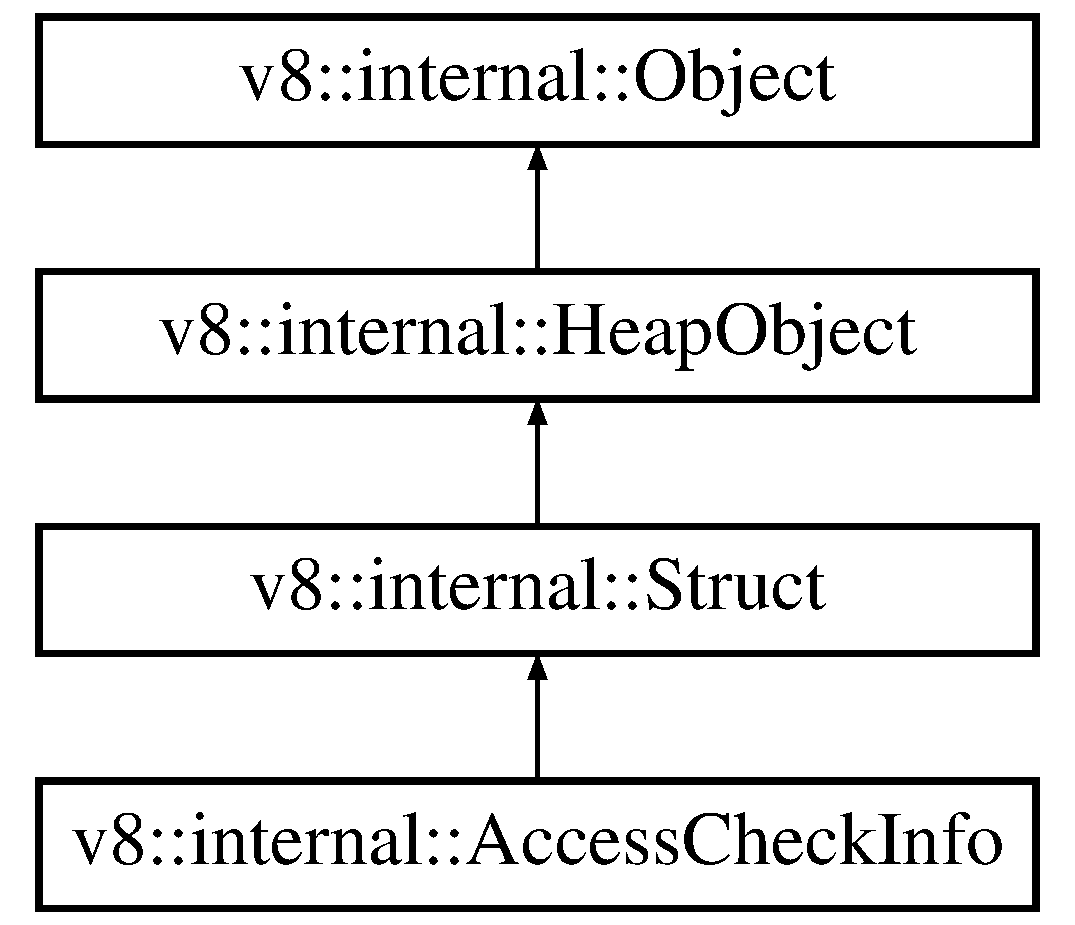
\includegraphics[height=4.000000cm]{classv8_1_1internal_1_1_access_check_info}
\end{center}
\end{figure}
\subsection*{Static Public Attributes}
\begin{DoxyCompactItemize}
\item 
\hypertarget{classv8_1_1internal_1_1_access_check_info_a6cbd64c953819b14e3944340ad05e048}{}static const int {\bfseries k\+Named\+Callback\+Offset} = Heap\+Object\+::k\+Header\+Size\label{classv8_1_1internal_1_1_access_check_info_a6cbd64c953819b14e3944340ad05e048}

\item 
\hypertarget{classv8_1_1internal_1_1_access_check_info_a5bcd567490f425a95da4a3dae4e73e11}{}static const int {\bfseries k\+Indexed\+Callback\+Offset} = k\+Named\+Callback\+Offset + k\+Pointer\+Size\label{classv8_1_1internal_1_1_access_check_info_a5bcd567490f425a95da4a3dae4e73e11}

\item 
\hypertarget{classv8_1_1internal_1_1_access_check_info_a1739da947958ae7735ac674e2aac415b}{}static const int {\bfseries k\+Data\+Offset} = k\+Indexed\+Callback\+Offset + k\+Pointer\+Size\label{classv8_1_1internal_1_1_access_check_info_a1739da947958ae7735ac674e2aac415b}

\item 
\hypertarget{classv8_1_1internal_1_1_access_check_info_a30e7585ebfa4c24c214bc5a9f77ad0c3}{}static const int {\bfseries k\+Size} = k\+Data\+Offset + k\+Pointer\+Size\label{classv8_1_1internal_1_1_access_check_info_a30e7585ebfa4c24c214bc5a9f77ad0c3}

\end{DoxyCompactItemize}
\subsection*{Additional Inherited Members}


The documentation for this class was generated from the following file\+:\begin{DoxyCompactItemize}
\item 
src/objects.\+h\end{DoxyCompactItemize}

\hypertarget{structv8_1_1internal_1_1_accessor_descriptor}{}\section{v8\+:\+:internal\+:\+:Accessor\+Descriptor Struct Reference}
\label{structv8_1_1internal_1_1_accessor_descriptor}\index{v8\+::internal\+::\+Accessor\+Descriptor@{v8\+::internal\+::\+Accessor\+Descriptor}}
\subsection*{Public Attributes}
\begin{DoxyCompactItemize}
\item 
\hypertarget{structv8_1_1internal_1_1_accessor_descriptor_a0fd4975f95e4accee711fe7144fcd91c}{}\hyperlink{classv8_1_1internal_1_1_object}{Object} $\ast$($\ast$ {\bfseries getter} )(\hyperlink{classv8_1_1internal_1_1_isolate}{Isolate} $\ast$isolate, \hyperlink{classv8_1_1internal_1_1_object}{Object} $\ast$object, void $\ast$data)\label{structv8_1_1internal_1_1_accessor_descriptor_a0fd4975f95e4accee711fe7144fcd91c}

\item 
\hypertarget{structv8_1_1internal_1_1_accessor_descriptor_abe99f0b12d8048825a324b575b837dca}{}\hyperlink{classv8_1_1internal_1_1_object}{Object} $\ast$($\ast$ {\bfseries setter} )(\hyperlink{classv8_1_1internal_1_1_isolate}{Isolate} $\ast$isolate, \hyperlink{classv8_1_1internal_1_1_j_s_object}{J\+S\+Object} $\ast$object, \hyperlink{classv8_1_1internal_1_1_object}{Object} $\ast$value, void $\ast$data)\label{structv8_1_1internal_1_1_accessor_descriptor_abe99f0b12d8048825a324b575b837dca}

\item 
\hypertarget{structv8_1_1internal_1_1_accessor_descriptor_acc4fa03840c10eea3f97798ea0cfc632}{}void $\ast$ {\bfseries data}\label{structv8_1_1internal_1_1_accessor_descriptor_acc4fa03840c10eea3f97798ea0cfc632}

\end{DoxyCompactItemize}


The documentation for this struct was generated from the following file\+:\begin{DoxyCompactItemize}
\item 
src/globals.\+h\end{DoxyCompactItemize}

\hypertarget{classv8_1_1internal_1_1_accessor_info}{}\section{v8\+:\+:internal\+:\+:Accessor\+Info Class Reference}
\label{classv8_1_1internal_1_1_accessor_info}\index{v8\+::internal\+::\+Accessor\+Info@{v8\+::internal\+::\+Accessor\+Info}}
Inheritance diagram for v8\+:\+:internal\+:\+:Accessor\+Info\+:\begin{figure}[H]
\begin{center}
\leavevmode
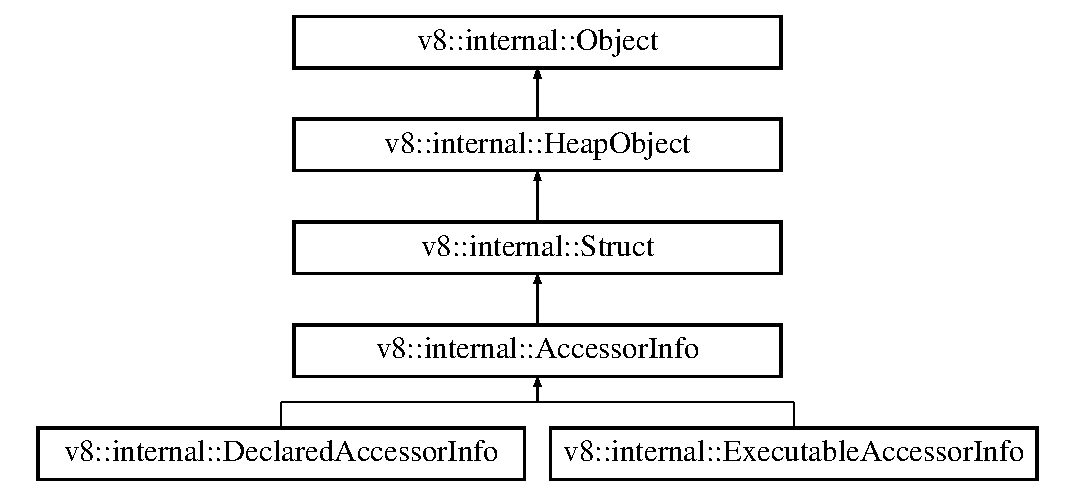
\includegraphics[height=5.000000cm]{classv8_1_1internal_1_1_accessor_info}
\end{center}
\end{figure}
\subsection*{Public Member Functions}
\begin{DoxyCompactItemize}
\item 
\hypertarget{classv8_1_1internal_1_1_accessor_info_a15ee717df70fd30880f5a3e15a90b02a}{}bool {\bfseries all\+\_\+can\+\_\+read} ()\label{classv8_1_1internal_1_1_accessor_info_a15ee717df70fd30880f5a3e15a90b02a}

\item 
\hypertarget{classv8_1_1internal_1_1_accessor_info_afc007f500afa962d19ef75d52de03c89}{}void {\bfseries set\+\_\+all\+\_\+can\+\_\+read} (bool value)\label{classv8_1_1internal_1_1_accessor_info_afc007f500afa962d19ef75d52de03c89}

\item 
\hypertarget{classv8_1_1internal_1_1_accessor_info_acb963c18a2b77d7b79ebca64b8192a12}{}bool {\bfseries all\+\_\+can\+\_\+write} ()\label{classv8_1_1internal_1_1_accessor_info_acb963c18a2b77d7b79ebca64b8192a12}

\item 
\hypertarget{classv8_1_1internal_1_1_accessor_info_a7845e45a30b59305f606d8b3dbbabb13}{}void {\bfseries set\+\_\+all\+\_\+can\+\_\+write} (bool value)\label{classv8_1_1internal_1_1_accessor_info_a7845e45a30b59305f606d8b3dbbabb13}

\item 
\hypertarget{classv8_1_1internal_1_1_accessor_info_a13c8eb4416eee0482ef82e32c7df4ea6}{}Property\+Attributes {\bfseries property\+\_\+attributes} ()\label{classv8_1_1internal_1_1_accessor_info_a13c8eb4416eee0482ef82e32c7df4ea6}

\item 
\hypertarget{classv8_1_1internal_1_1_accessor_info_ad7d09993c5975f13a58aced7e1b482eb}{}void {\bfseries set\+\_\+property\+\_\+attributes} (Property\+Attributes attributes)\label{classv8_1_1internal_1_1_accessor_info_ad7d09993c5975f13a58aced7e1b482eb}

\item 
\hypertarget{classv8_1_1internal_1_1_accessor_info_af90ccc9b509016f749a5d69a29cebdf4}{}bool {\bfseries Is\+Compatible\+Receiver} (\hyperlink{classv8_1_1internal_1_1_object}{Object} $\ast$receiver)\label{classv8_1_1internal_1_1_accessor_info_af90ccc9b509016f749a5d69a29cebdf4}

\end{DoxyCompactItemize}
\subsection*{Static Public Member Functions}
\begin{DoxyCompactItemize}
\item 
\hypertarget{classv8_1_1internal_1_1_accessor_info_aa6b34e4e6f27b0073de22fb28ad22b65}{}static bool {\bfseries Is\+Compatible\+Receiver\+Type} (\hyperlink{classv8_1_1internal_1_1_isolate}{Isolate} $\ast$isolate, \hyperlink{classv8_1_1internal_1_1_handle}{Handle}$<$ \hyperlink{classv8_1_1internal_1_1_accessor_info}{Accessor\+Info} $>$ info, \hyperlink{classv8_1_1internal_1_1_handle}{Handle}$<$ \hyperlink{classv8_1_1internal_1_1_type_impl}{Heap\+Type} $>$ type)\label{classv8_1_1internal_1_1_accessor_info_aa6b34e4e6f27b0073de22fb28ad22b65}

\item 
\hypertarget{classv8_1_1internal_1_1_accessor_info_a10dfefe3dc1780c1ca553aec96177b1b}{}static int {\bfseries Append\+Unique} (\hyperlink{classv8_1_1internal_1_1_handle}{Handle}$<$ \hyperlink{classv8_1_1internal_1_1_object}{Object} $>$ descriptors, \hyperlink{classv8_1_1internal_1_1_handle}{Handle}$<$ \hyperlink{classv8_1_1internal_1_1_fixed_array}{Fixed\+Array} $>$ array, int valid\+\_\+descriptors)\label{classv8_1_1internal_1_1_accessor_info_a10dfefe3dc1780c1ca553aec96177b1b}

\end{DoxyCompactItemize}
\subsection*{Static Public Attributes}
\begin{DoxyCompactItemize}
\item 
\hypertarget{classv8_1_1internal_1_1_accessor_info_a75d3700bea71b63895455a5d5cc5dae9}{}static const int {\bfseries k\+Name\+Offset} = Heap\+Object\+::k\+Header\+Size\label{classv8_1_1internal_1_1_accessor_info_a75d3700bea71b63895455a5d5cc5dae9}

\item 
\hypertarget{classv8_1_1internal_1_1_accessor_info_abc6115491f2bb799141ce228267cdeb9}{}static const int {\bfseries k\+Flag\+Offset} = k\+Name\+Offset + k\+Pointer\+Size\label{classv8_1_1internal_1_1_accessor_info_abc6115491f2bb799141ce228267cdeb9}

\item 
\hypertarget{classv8_1_1internal_1_1_accessor_info_a5f52bf6fac49df3619209bcda5e68824}{}static const int {\bfseries k\+Expected\+Receiver\+Type\+Offset} = k\+Flag\+Offset + k\+Pointer\+Size\label{classv8_1_1internal_1_1_accessor_info_a5f52bf6fac49df3619209bcda5e68824}

\item 
\hypertarget{classv8_1_1internal_1_1_accessor_info_a0fbd2218bb9f31efd29c8b17d4f1908a}{}static const int {\bfseries k\+Size} = k\+Expected\+Receiver\+Type\+Offset + k\+Pointer\+Size\label{classv8_1_1internal_1_1_accessor_info_a0fbd2218bb9f31efd29c8b17d4f1908a}

\end{DoxyCompactItemize}
\subsection*{Additional Inherited Members}


The documentation for this class was generated from the following files\+:\begin{DoxyCompactItemize}
\item 
src/objects.\+h\item 
src/objects-\/inl.\+h\item 
src/objects.\+cc\end{DoxyCompactItemize}

\hypertarget{classv8_1_1internal_1_1_accessor_pair}{}\section{v8\+:\+:internal\+:\+:Accessor\+Pair Class Reference}
\label{classv8_1_1internal_1_1_accessor_pair}\index{v8\+::internal\+::\+Accessor\+Pair@{v8\+::internal\+::\+Accessor\+Pair}}
Inheritance diagram for v8\+:\+:internal\+:\+:Accessor\+Pair\+:\begin{figure}[H]
\begin{center}
\leavevmode
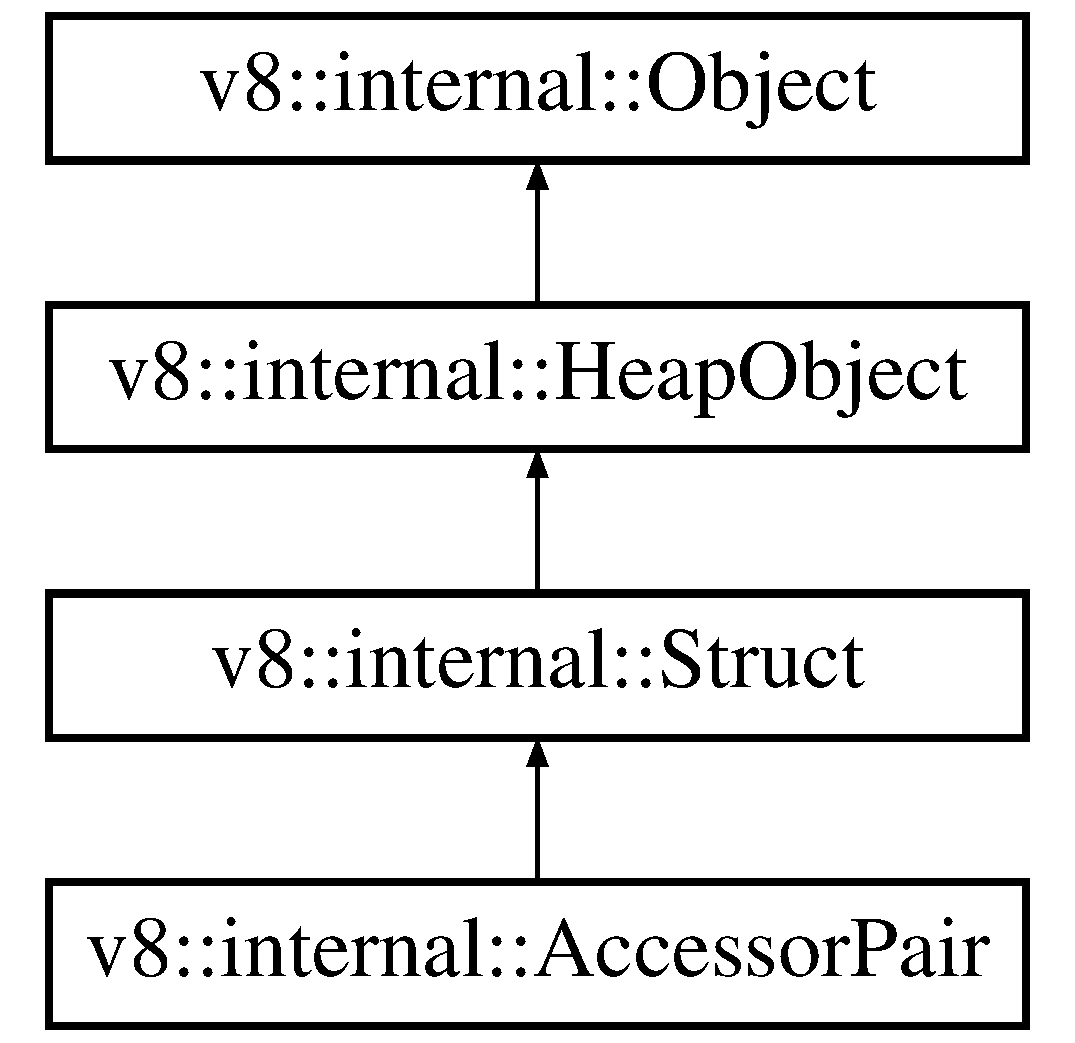
\includegraphics[height=4.000000cm]{classv8_1_1internal_1_1_accessor_pair}
\end{center}
\end{figure}
\subsection*{Public Member Functions}
\begin{DoxyCompactItemize}
\item 
\hypertarget{classv8_1_1internal_1_1_accessor_pair_acbfdc7c28139840e1a2e41a49a66e4e6}{}\hyperlink{classv8_1_1internal_1_1_object}{Object} $\ast$ {\bfseries get} (Accessor\+Component component)\label{classv8_1_1internal_1_1_accessor_pair_acbfdc7c28139840e1a2e41a49a66e4e6}

\item 
\hypertarget{classv8_1_1internal_1_1_accessor_pair_ad2a9c19f26306e325c88a48431f1f2c1}{}void {\bfseries set} (Accessor\+Component component, \hyperlink{classv8_1_1internal_1_1_object}{Object} $\ast$value)\label{classv8_1_1internal_1_1_accessor_pair_ad2a9c19f26306e325c88a48431f1f2c1}

\item 
\hypertarget{classv8_1_1internal_1_1_accessor_pair_a5f990eda86ea9c93400f176be34e2871}{}\hyperlink{classv8_1_1internal_1_1_object}{Object} $\ast$ {\bfseries Get\+Component} (Accessor\+Component component)\label{classv8_1_1internal_1_1_accessor_pair_a5f990eda86ea9c93400f176be34e2871}

\item 
\hypertarget{classv8_1_1internal_1_1_accessor_pair_a6e5a2de9676c59e75ff73635f152a27d}{}void {\bfseries Set\+Components} (\hyperlink{classv8_1_1internal_1_1_object}{Object} $\ast$getter, \hyperlink{classv8_1_1internal_1_1_object}{Object} $\ast$setter)\label{classv8_1_1internal_1_1_accessor_pair_a6e5a2de9676c59e75ff73635f152a27d}

\item 
\hypertarget{classv8_1_1internal_1_1_accessor_pair_a3776e1f65c6612d9cb544747211bd3f0}{}bool {\bfseries Contains\+Accessor} ()\label{classv8_1_1internal_1_1_accessor_pair_a3776e1f65c6612d9cb544747211bd3f0}

\end{DoxyCompactItemize}
\subsection*{Static Public Member Functions}
\begin{DoxyCompactItemize}
\item 
\hypertarget{classv8_1_1internal_1_1_accessor_pair_a9030ddc2b46863a79de840206d6c549c}{}static \hyperlink{classv8_1_1internal_1_1_handle}{Handle}$<$ \hyperlink{classv8_1_1internal_1_1_accessor_pair}{Accessor\+Pair} $>$ {\bfseries Copy} (\hyperlink{classv8_1_1internal_1_1_handle}{Handle}$<$ \hyperlink{classv8_1_1internal_1_1_accessor_pair}{Accessor\+Pair} $>$ pair)\label{classv8_1_1internal_1_1_accessor_pair_a9030ddc2b46863a79de840206d6c549c}

\end{DoxyCompactItemize}
\subsection*{Static Public Attributes}
\begin{DoxyCompactItemize}
\item 
\hypertarget{classv8_1_1internal_1_1_accessor_pair_aa7ee07b7098a35f0e1340c33dadb90db}{}static const int {\bfseries k\+Getter\+Offset} = Heap\+Object\+::k\+Header\+Size\label{classv8_1_1internal_1_1_accessor_pair_aa7ee07b7098a35f0e1340c33dadb90db}

\item 
\hypertarget{classv8_1_1internal_1_1_accessor_pair_adaca2d4fb0dfcf2e29fd37fc5549737b}{}static const int {\bfseries k\+Setter\+Offset} = k\+Getter\+Offset + k\+Pointer\+Size\label{classv8_1_1internal_1_1_accessor_pair_adaca2d4fb0dfcf2e29fd37fc5549737b}

\item 
\hypertarget{classv8_1_1internal_1_1_accessor_pair_a89c0268865b5203f29820f82b5e46cb5}{}static const int {\bfseries k\+Size} = k\+Setter\+Offset + k\+Pointer\+Size\label{classv8_1_1internal_1_1_accessor_pair_a89c0268865b5203f29820f82b5e46cb5}

\end{DoxyCompactItemize}
\subsection*{Additional Inherited Members}


The documentation for this class was generated from the following files\+:\begin{DoxyCompactItemize}
\item 
src/objects.\+h\item 
src/objects.\+cc\end{DoxyCompactItemize}

\hypertarget{classv8_1_1internal_1_1_accessors}{}\section{v8\+:\+:internal\+:\+:Accessors Class Reference}
\label{classv8_1_1internal_1_1_accessors}\index{v8\+::internal\+::\+Accessors@{v8\+::internal\+::\+Accessors}}
Inheritance diagram for v8\+:\+:internal\+:\+:Accessors\+:\begin{figure}[H]
\begin{center}
\leavevmode
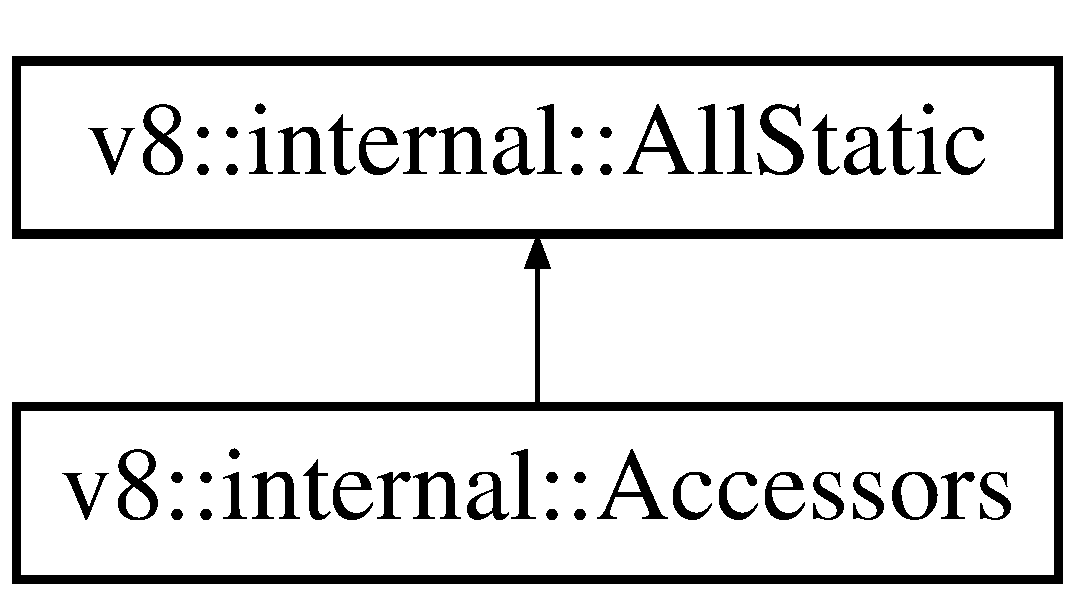
\includegraphics[height=2.000000cm]{classv8_1_1internal_1_1_accessors}
\end{center}
\end{figure}
\subsection*{Public Types}
\begin{DoxyCompactItemize}
\item 
\hypertarget{classv8_1_1internal_1_1_accessors_a1c466e7b9e4df52b9cd44f01d41faf3b}{}enum {\bfseries Descriptor\+Id} \{ {\bfseries descriptor\+Count}
 \}\label{classv8_1_1internal_1_1_accessors_a1c466e7b9e4df52b9cd44f01d41faf3b}

\end{DoxyCompactItemize}
\subsection*{Static Public Member Functions}
\begin{DoxyCompactItemize}
\item 
\hypertarget{classv8_1_1internal_1_1_accessors_a53f587f18838e892db4f653aa1731ead}{}static \hyperlink{classv8_1_1internal_1_1_handle}{Handle}$<$ \hyperlink{classv8_1_1internal_1_1_object}{Object} $>$ {\bfseries Function\+Set\+Prototype} (\hyperlink{classv8_1_1internal_1_1_handle}{Handle}$<$ \hyperlink{classv8_1_1internal_1_1_j_s_function}{J\+S\+Function} $>$ object, \hyperlink{classv8_1_1internal_1_1_handle}{Handle}$<$ \hyperlink{classv8_1_1internal_1_1_object}{Object} $>$ value)\label{classv8_1_1internal_1_1_accessors_a53f587f18838e892db4f653aa1731ead}

\item 
\hypertarget{classv8_1_1internal_1_1_accessors_acf9265d60f5dacad8df93a69f56e3e4f}{}static \hyperlink{classv8_1_1internal_1_1_handle}{Handle}$<$ \hyperlink{classv8_1_1internal_1_1_object}{Object} $>$ {\bfseries Function\+Get\+Prototype} (\hyperlink{classv8_1_1internal_1_1_handle}{Handle}$<$ \hyperlink{classv8_1_1internal_1_1_j_s_function}{J\+S\+Function} $>$ object)\label{classv8_1_1internal_1_1_accessors_acf9265d60f5dacad8df93a69f56e3e4f}

\item 
\hypertarget{classv8_1_1internal_1_1_accessors_ae3b6c92c1e7c9db932c5f6247408514c}{}static \hyperlink{classv8_1_1internal_1_1_handle}{Handle}$<$ \hyperlink{classv8_1_1internal_1_1_object}{Object} $>$ {\bfseries Function\+Get\+Arguments} (\hyperlink{classv8_1_1internal_1_1_handle}{Handle}$<$ \hyperlink{classv8_1_1internal_1_1_j_s_function}{J\+S\+Function} $>$ object)\label{classv8_1_1internal_1_1_accessors_ae3b6c92c1e7c9db932c5f6247408514c}

\item 
\hypertarget{classv8_1_1internal_1_1_accessors_a659f5cfdc0ce5805f19fd0fe320e4e5c}{}static \hyperlink{classv8_1_1internal_1_1_handle}{Handle}$<$ \hyperlink{classv8_1_1internal_1_1_accessor_info}{Accessor\+Info} $>$ {\bfseries Make\+Module\+Export} (\hyperlink{classv8_1_1internal_1_1_handle}{Handle}$<$ \hyperlink{classv8_1_1internal_1_1_string}{String} $>$ name, int index, Property\+Attributes attributes)\label{classv8_1_1internal_1_1_accessors_a659f5cfdc0ce5805f19fd0fe320e4e5c}

\item 
\hypertarget{classv8_1_1internal_1_1_accessors_afa5feef994ec0e612298407860c2b472}{}{\footnotesize template$<$class T $>$ }\\static bool {\bfseries Is\+J\+S\+Object\+Field\+Accessor} (typename T\+::\+Type\+Handle type, \hyperlink{classv8_1_1internal_1_1_handle}{Handle}$<$ \hyperlink{classv8_1_1internal_1_1_name}{Name} $>$ name, int $\ast$object\+\_\+offset)\label{classv8_1_1internal_1_1_accessors_afa5feef994ec0e612298407860c2b472}

\item 
\hypertarget{classv8_1_1internal_1_1_accessors_ac32befe4995c436c8d26edfd100a79cb}{}static \hyperlink{classv8_1_1internal_1_1_handle}{Handle}$<$ \hyperlink{classv8_1_1internal_1_1_accessor_info}{Accessor\+Info} $>$ {\bfseries Make\+Accessor} (\hyperlink{classv8_1_1internal_1_1_isolate}{Isolate} $\ast$isolate, \hyperlink{classv8_1_1internal_1_1_handle}{Handle}$<$ \hyperlink{classv8_1_1internal_1_1_string}{String} $>$ name, Accessor\+Getter\+Callback getter, Accessor\+Setter\+Callback setter, Property\+Attributes attributes)\label{classv8_1_1internal_1_1_accessors_ac32befe4995c436c8d26edfd100a79cb}

\item 
\hypertarget{classv8_1_1internal_1_1_accessors_a44b854a4d5c9fc44c37a9a2bafbd8d9e}{}static \hyperlink{classv8_1_1internal_1_1_handle}{Handle}$<$ \hyperlink{classv8_1_1internal_1_1_executable_accessor_info}{Executable\+Accessor\+Info} $>$ {\bfseries Clone\+Accessor} (\hyperlink{classv8_1_1internal_1_1_isolate}{Isolate} $\ast$isolate, \hyperlink{classv8_1_1internal_1_1_handle}{Handle}$<$ \hyperlink{classv8_1_1internal_1_1_executable_accessor_info}{Executable\+Accessor\+Info} $>$ accessor)\label{classv8_1_1internal_1_1_accessors_a44b854a4d5c9fc44c37a9a2bafbd8d9e}

\end{DoxyCompactItemize}


The documentation for this class was generated from the following files\+:\begin{DoxyCompactItemize}
\item 
src/accessors.\+h\item 
src/accessors.\+cc\end{DoxyCompactItemize}

\hypertarget{structv8_1_1internal_1_1_v8___f_i_n_a_l_1_1_accessors}{}\section{v8\+:\+:internal\+:\+:V8\+\_\+\+F\+I\+N\+A\+L$<$ k\+Operand\+Kind, k\+Num\+Cached\+Operands $>$\+:\+:Accessors Struct Reference}
\label{structv8_1_1internal_1_1_v8___f_i_n_a_l_1_1_accessors}\index{v8\+::internal\+::\+V8\+\_\+\+F\+I\+N\+A\+L$<$ k\+Operand\+Kind, k\+Num\+Cached\+Operands $>$\+::\+Accessors@{v8\+::internal\+::\+V8\+\_\+\+F\+I\+N\+A\+L$<$ k\+Operand\+Kind, k\+Num\+Cached\+Operands $>$\+::\+Accessors}}
Inheritance diagram for v8\+:\+:internal\+:\+:V8\+\_\+\+F\+I\+N\+A\+L$<$ k\+Operand\+Kind, k\+Num\+Cached\+Operands $>$\+:\+:Accessors\+:\begin{figure}[H]
\begin{center}
\leavevmode
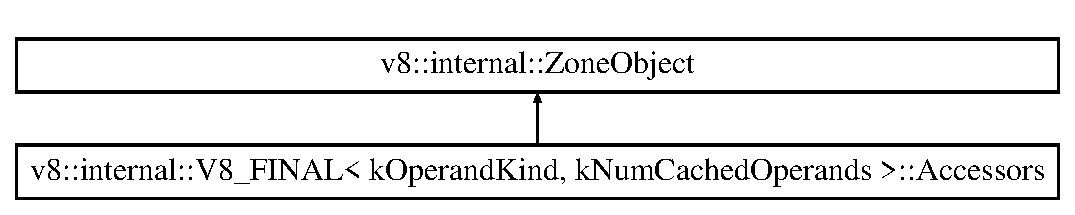
\includegraphics[height=2.000000cm]{structv8_1_1internal_1_1_v8___f_i_n_a_l_1_1_accessors}
\end{center}
\end{figure}
\subsection*{Public Attributes}
\begin{DoxyCompactItemize}
\item 
\hypertarget{structv8_1_1internal_1_1_v8___f_i_n_a_l_1_1_accessors_a3c057b76e7fe2d13f1a55fae47dbdfd2}{}\hyperlink{classv8_1_1internal_1_1_expression}{Expression} $\ast$ {\bfseries getter}\label{structv8_1_1internal_1_1_v8___f_i_n_a_l_1_1_accessors_a3c057b76e7fe2d13f1a55fae47dbdfd2}

\item 
\hypertarget{structv8_1_1internal_1_1_v8___f_i_n_a_l_1_1_accessors_a0c0dec1b16e90df419e5762dfe419ade}{}\hyperlink{classv8_1_1internal_1_1_expression}{Expression} $\ast$ {\bfseries setter}\label{structv8_1_1internal_1_1_v8___f_i_n_a_l_1_1_accessors_a0c0dec1b16e90df419e5762dfe419ade}

\end{DoxyCompactItemize}
\subsection*{Additional Inherited Members}


The documentation for this struct was generated from the following file\+:\begin{DoxyCompactItemize}
\item 
src/ast.\+h\end{DoxyCompactItemize}

\hypertarget{classv8_1_1internal_1_1_accessor_table}{}\section{v8\+:\+:internal\+:\+:Accessor\+Table Class Reference}
\label{classv8_1_1internal_1_1_accessor_table}\index{v8\+::internal\+::\+Accessor\+Table@{v8\+::internal\+::\+Accessor\+Table}}
Inheritance diagram for v8\+:\+:internal\+:\+:Accessor\+Table\+:\begin{figure}[H]
\begin{center}
\leavevmode
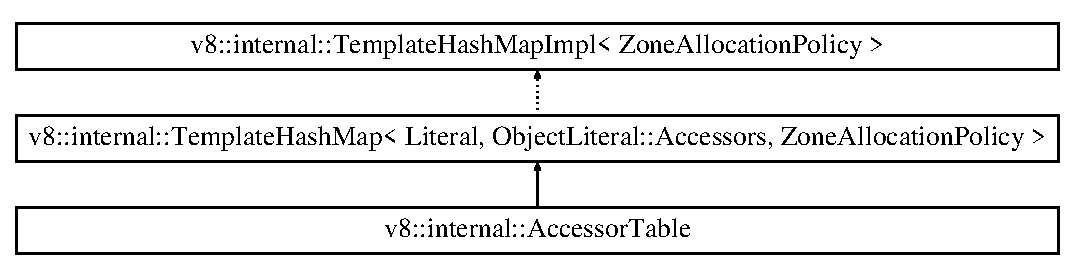
\includegraphics[height=3.000000cm]{classv8_1_1internal_1_1_accessor_table}
\end{center}
\end{figure}
\subsection*{Public Member Functions}
\begin{DoxyCompactItemize}
\item 
\hypertarget{classv8_1_1internal_1_1_accessor_table_adcee86ad1000d3d63e7360d0895fc2ae}{}{\bfseries Accessor\+Table} (\hyperlink{classv8_1_1internal_1_1_zone}{Zone} $\ast$zone)\label{classv8_1_1internal_1_1_accessor_table_adcee86ad1000d3d63e7360d0895fc2ae}

\item 
\hypertarget{classv8_1_1internal_1_1_accessor_table_a064e2528f1da85829d8742c69adaba19}{}Iterator {\bfseries lookup} (Literal $\ast$literal)\label{classv8_1_1internal_1_1_accessor_table_a064e2528f1da85829d8742c69adaba19}

\end{DoxyCompactItemize}


The documentation for this class was generated from the following file\+:\begin{DoxyCompactItemize}
\item 
src/full-\/codegen.\+h\end{DoxyCompactItemize}

\hypertarget{classv8_1_1internal_1_1_action_node}{}\section{v8\+:\+:internal\+:\+:Action\+Node Class Reference}
\label{classv8_1_1internal_1_1_action_node}\index{v8\+::internal\+::\+Action\+Node@{v8\+::internal\+::\+Action\+Node}}
Inheritance diagram for v8\+:\+:internal\+:\+:Action\+Node\+:\begin{figure}[H]
\begin{center}
\leavevmode
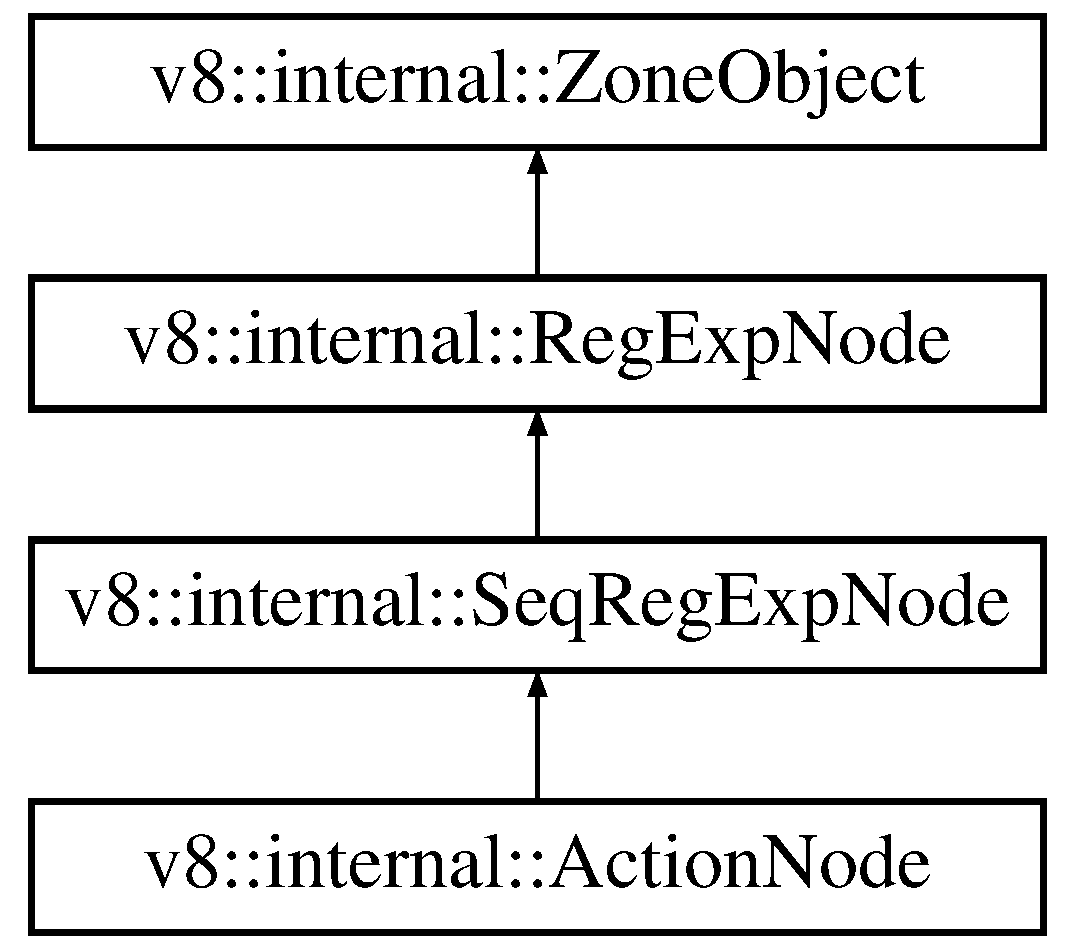
\includegraphics[height=4.000000cm]{classv8_1_1internal_1_1_action_node}
\end{center}
\end{figure}
\subsection*{Public Types}
\begin{DoxyCompactItemize}
\item 
\hypertarget{classv8_1_1internal_1_1_action_node_ab695380c09977f360b2d4f817f9124bc}{}enum {\bfseries Action\+Type} \{ \\*
{\bfseries S\+E\+T\+\_\+\+R\+E\+G\+I\+S\+T\+E\+R}, 
{\bfseries I\+N\+C\+R\+E\+M\+E\+N\+T\+\_\+\+R\+E\+G\+I\+S\+T\+E\+R}, 
{\bfseries S\+T\+O\+R\+E\+\_\+\+P\+O\+S\+I\+T\+I\+O\+N}, 
{\bfseries B\+E\+G\+I\+N\+\_\+\+S\+U\+B\+M\+A\+T\+C\+H}, 
\\*
{\bfseries P\+O\+S\+I\+T\+I\+V\+E\+\_\+\+S\+U\+B\+M\+A\+T\+C\+H\+\_\+\+S\+U\+C\+C\+E\+S\+S}, 
{\bfseries E\+M\+P\+T\+Y\+\_\+\+M\+A\+T\+C\+H\+\_\+\+C\+H\+E\+C\+K}, 
{\bfseries C\+L\+E\+A\+R\+\_\+\+C\+A\+P\+T\+U\+R\+E\+S}
 \}\label{classv8_1_1internal_1_1_action_node_ab695380c09977f360b2d4f817f9124bc}

\end{DoxyCompactItemize}
\subsection*{Public Member Functions}
\begin{DoxyCompactItemize}
\item 
\hypertarget{classv8_1_1internal_1_1_action_node_acd110b20896658ef66be07589828c835}{}virtual void {\bfseries Accept} (\hyperlink{classv8_1_1internal_1_1_node_visitor}{Node\+Visitor} $\ast$visitor)\label{classv8_1_1internal_1_1_action_node_acd110b20896658ef66be07589828c835}

\item 
\hypertarget{classv8_1_1internal_1_1_action_node_afac185d923c63324c4f18a2f0a23769d}{}virtual void {\bfseries Emit} (\hyperlink{classv8_1_1internal_1_1_reg_exp_compiler}{Reg\+Exp\+Compiler} $\ast$compiler, \hyperlink{classv8_1_1internal_1_1_trace}{Trace} $\ast$trace)\label{classv8_1_1internal_1_1_action_node_afac185d923c63324c4f18a2f0a23769d}

\item 
\hypertarget{classv8_1_1internal_1_1_action_node_ab36ade74ae2623b654002605bb0c5144}{}virtual int {\bfseries Eats\+At\+Least} (int still\+\_\+to\+\_\+find, int budget, bool not\+\_\+at\+\_\+start)\label{classv8_1_1internal_1_1_action_node_ab36ade74ae2623b654002605bb0c5144}

\item 
\hypertarget{classv8_1_1internal_1_1_action_node_abc51b0f5a4a393425181f6a0583e6b0a}{}virtual void {\bfseries Get\+Quick\+Check\+Details} (\hyperlink{classv8_1_1internal_1_1_quick_check_details}{Quick\+Check\+Details} $\ast$details, \hyperlink{classv8_1_1internal_1_1_reg_exp_compiler}{Reg\+Exp\+Compiler} $\ast$compiler, int filled\+\_\+in, bool not\+\_\+at\+\_\+start)\label{classv8_1_1internal_1_1_action_node_abc51b0f5a4a393425181f6a0583e6b0a}

\item 
\hypertarget{classv8_1_1internal_1_1_action_node_a0903fcf481793c0ffed3b875476fb592}{}virtual void {\bfseries Fill\+In\+B\+M\+Info} (int offset, int budget, \hyperlink{classv8_1_1internal_1_1_boyer_moore_lookahead}{Boyer\+Moore\+Lookahead} $\ast$bm, bool not\+\_\+at\+\_\+start)\label{classv8_1_1internal_1_1_action_node_a0903fcf481793c0ffed3b875476fb592}

\item 
\hypertarget{classv8_1_1internal_1_1_action_node_ae848c71b17d244a67f3f34afe142fac8}{}Action\+Type {\bfseries action\+\_\+type} ()\label{classv8_1_1internal_1_1_action_node_ae848c71b17d244a67f3f34afe142fac8}

\item 
\hypertarget{classv8_1_1internal_1_1_action_node_a22be07519e46e566272847427d939793}{}virtual int {\bfseries Greedy\+Loop\+Text\+Length} ()\label{classv8_1_1internal_1_1_action_node_a22be07519e46e566272847427d939793}

\end{DoxyCompactItemize}
\subsection*{Static Public Member Functions}
\begin{DoxyCompactItemize}
\item 
\hypertarget{classv8_1_1internal_1_1_action_node_ab0232aafb29641c830970993c18ca5a7}{}static \hyperlink{classv8_1_1internal_1_1_action_node}{Action\+Node} $\ast$ {\bfseries Set\+Register} (int reg, int val, \hyperlink{classv8_1_1internal_1_1_reg_exp_node}{Reg\+Exp\+Node} $\ast$on\+\_\+success)\label{classv8_1_1internal_1_1_action_node_ab0232aafb29641c830970993c18ca5a7}

\item 
\hypertarget{classv8_1_1internal_1_1_action_node_ac2fea920241e4412a3bba2d10acb91ef}{}static \hyperlink{classv8_1_1internal_1_1_action_node}{Action\+Node} $\ast$ {\bfseries Increment\+Register} (int reg, \hyperlink{classv8_1_1internal_1_1_reg_exp_node}{Reg\+Exp\+Node} $\ast$on\+\_\+success)\label{classv8_1_1internal_1_1_action_node_ac2fea920241e4412a3bba2d10acb91ef}

\item 
\hypertarget{classv8_1_1internal_1_1_action_node_a7b7c1ea99df9360c97a7e73e2672a834}{}static \hyperlink{classv8_1_1internal_1_1_action_node}{Action\+Node} $\ast$ {\bfseries Store\+Position} (int reg, bool is\+\_\+capture, \hyperlink{classv8_1_1internal_1_1_reg_exp_node}{Reg\+Exp\+Node} $\ast$on\+\_\+success)\label{classv8_1_1internal_1_1_action_node_a7b7c1ea99df9360c97a7e73e2672a834}

\item 
\hypertarget{classv8_1_1internal_1_1_action_node_af5c152a32e7afbe31390f57c07eed05a}{}static \hyperlink{classv8_1_1internal_1_1_action_node}{Action\+Node} $\ast$ {\bfseries Clear\+Captures} (\hyperlink{classv8_1_1internal_1_1_interval}{Interval} range, \hyperlink{classv8_1_1internal_1_1_reg_exp_node}{Reg\+Exp\+Node} $\ast$on\+\_\+success)\label{classv8_1_1internal_1_1_action_node_af5c152a32e7afbe31390f57c07eed05a}

\item 
\hypertarget{classv8_1_1internal_1_1_action_node_a84297f33bee6dffd0cc7a6b5341fb106}{}static \hyperlink{classv8_1_1internal_1_1_action_node}{Action\+Node} $\ast$ {\bfseries Begin\+Submatch} (int stack\+\_\+pointer\+\_\+reg, int position\+\_\+reg, \hyperlink{classv8_1_1internal_1_1_reg_exp_node}{Reg\+Exp\+Node} $\ast$on\+\_\+success)\label{classv8_1_1internal_1_1_action_node_a84297f33bee6dffd0cc7a6b5341fb106}

\item 
\hypertarget{classv8_1_1internal_1_1_action_node_a89bed32eadb39ad776f7e5523d8d152b}{}static \hyperlink{classv8_1_1internal_1_1_action_node}{Action\+Node} $\ast$ {\bfseries Positive\+Submatch\+Success} (int stack\+\_\+pointer\+\_\+reg, int restore\+\_\+reg, int clear\+\_\+capture\+\_\+count, int clear\+\_\+capture\+\_\+from, \hyperlink{classv8_1_1internal_1_1_reg_exp_node}{Reg\+Exp\+Node} $\ast$on\+\_\+success)\label{classv8_1_1internal_1_1_action_node_a89bed32eadb39ad776f7e5523d8d152b}

\item 
\hypertarget{classv8_1_1internal_1_1_action_node_a1f8492811dde72cce77b5b7f8d083292}{}static \hyperlink{classv8_1_1internal_1_1_action_node}{Action\+Node} $\ast$ {\bfseries Empty\+Match\+Check} (int start\+\_\+register, int repetition\+\_\+register, int repetition\+\_\+limit, \hyperlink{classv8_1_1internal_1_1_reg_exp_node}{Reg\+Exp\+Node} $\ast$on\+\_\+success)\label{classv8_1_1internal_1_1_action_node_a1f8492811dde72cce77b5b7f8d083292}

\end{DoxyCompactItemize}
\subsection*{Friends}
\begin{DoxyCompactItemize}
\item 
\hypertarget{classv8_1_1internal_1_1_action_node_a9c19d4d6fc300c029ba554cbe4d3d2e0}{}class {\bfseries Dot\+Printer}\label{classv8_1_1internal_1_1_action_node_a9c19d4d6fc300c029ba554cbe4d3d2e0}

\end{DoxyCompactItemize}
\subsection*{Additional Inherited Members}


The documentation for this class was generated from the following files\+:\begin{DoxyCompactItemize}
\item 
src/jsregexp.\+h\item 
src/jsregexp.\+cc\end{DoxyCompactItemize}

\hypertarget{classv8_1_1internal_1_1_activations_finder}{}\section{v8\+:\+:internal\+:\+:Activations\+Finder Class Reference}
\label{classv8_1_1internal_1_1_activations_finder}\index{v8\+::internal\+::\+Activations\+Finder@{v8\+::internal\+::\+Activations\+Finder}}
Inheritance diagram for v8\+:\+:internal\+:\+:Activations\+Finder\+:\begin{figure}[H]
\begin{center}
\leavevmode
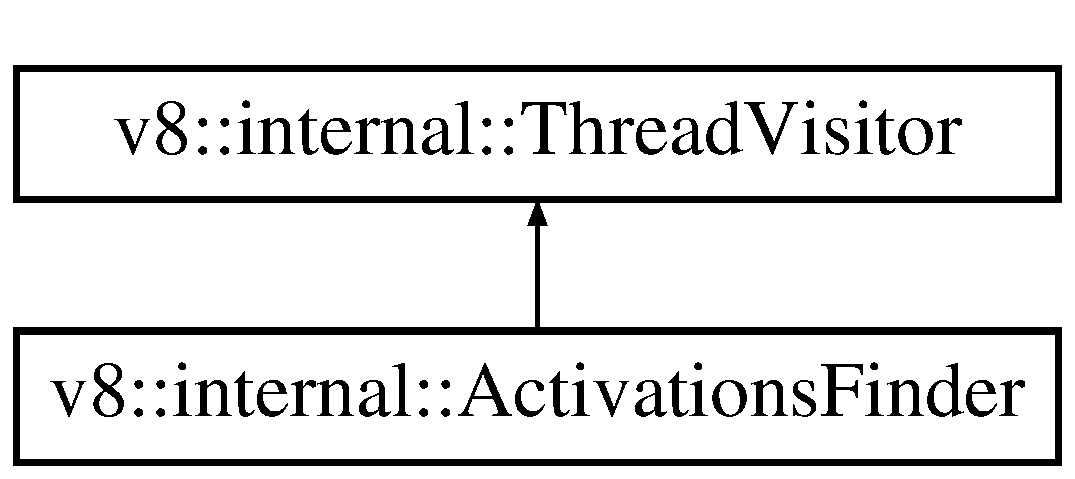
\includegraphics[height=2.000000cm]{classv8_1_1internal_1_1_activations_finder}
\end{center}
\end{figure}
\subsection*{Public Member Functions}
\begin{DoxyCompactItemize}
\item 
\hypertarget{classv8_1_1internal_1_1_activations_finder_a60e1f2fc90f683fe1e4d5f1a190dde8f}{}{\bfseries Activations\+Finder} (\hyperlink{classv8_1_1internal_1_1_code}{Code} $\ast$code)\label{classv8_1_1internal_1_1_activations_finder_a60e1f2fc90f683fe1e4d5f1a190dde8f}

\item 
\hypertarget{classv8_1_1internal_1_1_activations_finder_a7eadc771094bec59bd76f6e5ff713a2c}{}void {\bfseries Visit\+Thread} (\hyperlink{classv8_1_1internal_1_1_isolate}{Isolate} $\ast$isolate, Thread\+Local\+Top $\ast$top)\label{classv8_1_1internal_1_1_activations_finder_a7eadc771094bec59bd76f6e5ff713a2c}

\item 
\hypertarget{classv8_1_1internal_1_1_activations_finder_a421dbf4202e15a9c29ed94354ea57a8c}{}void {\bfseries Visit\+Frames} (Java\+Script\+Frame\+Iterator $\ast$it)\label{classv8_1_1internal_1_1_activations_finder_a421dbf4202e15a9c29ed94354ea57a8c}

\end{DoxyCompactItemize}
\subsection*{Public Attributes}
\begin{DoxyCompactItemize}
\item 
\hypertarget{classv8_1_1internal_1_1_activations_finder_ac6ed1ea07a59270aae7aaf32f23cb537}{}\hyperlink{classv8_1_1internal_1_1_code}{Code} $\ast$ {\bfseries code\+\_\+}\label{classv8_1_1internal_1_1_activations_finder_ac6ed1ea07a59270aae7aaf32f23cb537}

\item 
\hypertarget{classv8_1_1internal_1_1_activations_finder_a0faceafe43a03036d7d86c6aaf231fdf}{}bool {\bfseries has\+\_\+code\+\_\+activations\+\_\+}\label{classv8_1_1internal_1_1_activations_finder_a0faceafe43a03036d7d86c6aaf231fdf}

\end{DoxyCompactItemize}


The documentation for this class was generated from the following file\+:\begin{DoxyCompactItemize}
\item 
src/runtime.\+cc\end{DoxyCompactItemize}

\hypertarget{classv8_1_1internal_1_1_active_functions_collector}{}\section{v8\+:\+:internal\+:\+:Active\+Functions\+Collector Class Reference}
\label{classv8_1_1internal_1_1_active_functions_collector}\index{v8\+::internal\+::\+Active\+Functions\+Collector@{v8\+::internal\+::\+Active\+Functions\+Collector}}
Inheritance diagram for v8\+:\+:internal\+:\+:Active\+Functions\+Collector\+:\begin{figure}[H]
\begin{center}
\leavevmode
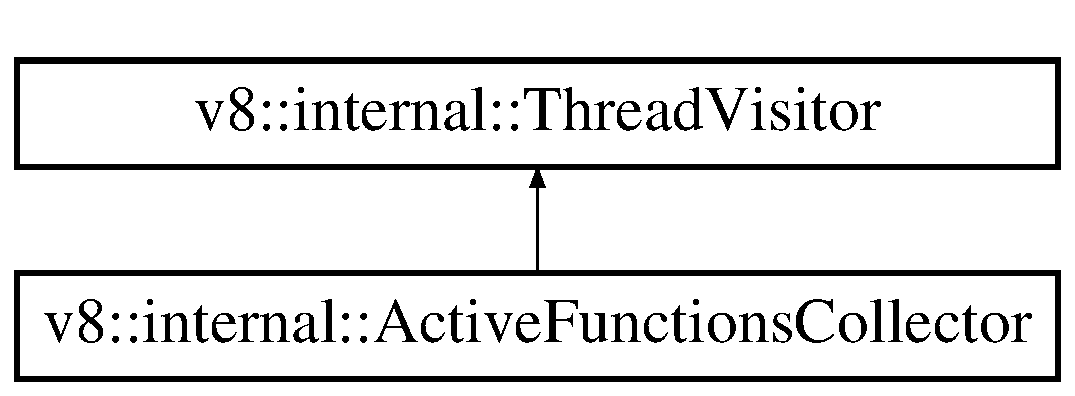
\includegraphics[height=2.000000cm]{classv8_1_1internal_1_1_active_functions_collector}
\end{center}
\end{figure}
\subsection*{Public Member Functions}
\begin{DoxyCompactItemize}
\item 
\hypertarget{classv8_1_1internal_1_1_active_functions_collector_a331bc8ac57fd311da9df7ac111166fb7}{}{\bfseries Active\+Functions\+Collector} (\hyperlink{classv8_1_1internal_1_1_list}{List}$<$ \hyperlink{classv8_1_1internal_1_1_handle}{Handle}$<$ \hyperlink{classv8_1_1internal_1_1_j_s_function}{J\+S\+Function} $>$ $>$ $\ast$active\+\_\+functions, \hyperlink{classv8_1_1internal_1_1_object}{Object} $\ast$active\+\_\+code\+\_\+marker)\label{classv8_1_1internal_1_1_active_functions_collector_a331bc8ac57fd311da9df7ac111166fb7}

\item 
\hypertarget{classv8_1_1internal_1_1_active_functions_collector_ab963c00d3974baab41b31cf969da76a7}{}void {\bfseries Visit\+Thread} (\hyperlink{classv8_1_1internal_1_1_isolate}{Isolate} $\ast$isolate, Thread\+Local\+Top $\ast$top)\label{classv8_1_1internal_1_1_active_functions_collector_ab963c00d3974baab41b31cf969da76a7}

\end{DoxyCompactItemize}


The documentation for this class was generated from the following file\+:\begin{DoxyCompactItemize}
\item 
src/debug.\+cc\end{DoxyCompactItemize}

\hypertarget{classv8_1_1internal_1_1_active_functions_redirector}{}\section{v8\+:\+:internal\+:\+:Active\+Functions\+Redirector Class Reference}
\label{classv8_1_1internal_1_1_active_functions_redirector}\index{v8\+::internal\+::\+Active\+Functions\+Redirector@{v8\+::internal\+::\+Active\+Functions\+Redirector}}
Inheritance diagram for v8\+:\+:internal\+:\+:Active\+Functions\+Redirector\+:\begin{figure}[H]
\begin{center}
\leavevmode
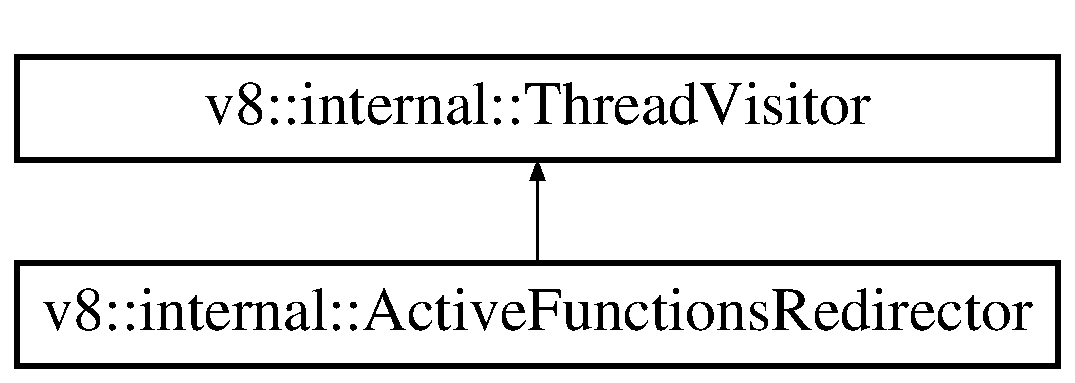
\includegraphics[height=2.000000cm]{classv8_1_1internal_1_1_active_functions_redirector}
\end{center}
\end{figure}
\subsection*{Public Member Functions}
\begin{DoxyCompactItemize}
\item 
\hypertarget{classv8_1_1internal_1_1_active_functions_redirector_ae928f040839bf092dedde73493d1f89b}{}void {\bfseries Visit\+Thread} (\hyperlink{classv8_1_1internal_1_1_isolate}{Isolate} $\ast$isolate, Thread\+Local\+Top $\ast$top)\label{classv8_1_1internal_1_1_active_functions_redirector_ae928f040839bf092dedde73493d1f89b}

\end{DoxyCompactItemize}


The documentation for this class was generated from the following file\+:\begin{DoxyCompactItemize}
\item 
src/debug.\+cc\end{DoxyCompactItemize}

\hypertarget{classv8_1_1internal_1_1_add_dispatch_range}{}\section{v8\+:\+:internal\+:\+:Add\+Dispatch\+Range Class Reference}
\label{classv8_1_1internal_1_1_add_dispatch_range}\index{v8\+::internal\+::\+Add\+Dispatch\+Range@{v8\+::internal\+::\+Add\+Dispatch\+Range}}
\subsection*{Public Member Functions}
\begin{DoxyCompactItemize}
\item 
\hypertarget{classv8_1_1internal_1_1_add_dispatch_range_aabb3eb748f5a566349ae5946fef1103b}{}{\bfseries Add\+Dispatch\+Range} (\hyperlink{classv8_1_1internal_1_1_dispatch_table_constructor}{Dispatch\+Table\+Constructor} $\ast$constructor)\label{classv8_1_1internal_1_1_add_dispatch_range_aabb3eb748f5a566349ae5946fef1103b}

\item 
\hypertarget{classv8_1_1internal_1_1_add_dispatch_range_a17e1406e159be04ef2b1fcc36d94c888}{}void {\bfseries Call} (uc32 from, \hyperlink{classv8_1_1internal_1_1_dispatch_table_1_1_entry}{Dispatch\+Table\+::\+Entry} entry)\label{classv8_1_1internal_1_1_add_dispatch_range_a17e1406e159be04ef2b1fcc36d94c888}

\end{DoxyCompactItemize}


The documentation for this class was generated from the following file\+:\begin{DoxyCompactItemize}
\item 
src/jsregexp.\+cc\end{DoxyCompactItemize}

\hypertarget{classv8_1_1internal_1_1_address_to_trace_map}{}\section{v8\+:\+:internal\+:\+:Address\+To\+Trace\+Map Class Reference}
\label{classv8_1_1internal_1_1_address_to_trace_map}\index{v8\+::internal\+::\+Address\+To\+Trace\+Map@{v8\+::internal\+::\+Address\+To\+Trace\+Map}}
\subsection*{Public Member Functions}
\begin{DoxyCompactItemize}
\item 
\hypertarget{classv8_1_1internal_1_1_address_to_trace_map_a3b1bc8f1abc6f072a660d2b689852838}{}void {\bfseries Add\+Range} (Address addr, int size, unsigned node\+\_\+id)\label{classv8_1_1internal_1_1_address_to_trace_map_a3b1bc8f1abc6f072a660d2b689852838}

\item 
\hypertarget{classv8_1_1internal_1_1_address_to_trace_map_ab76fa587a105ae24f300f171d8cb22a6}{}unsigned {\bfseries Get\+Trace\+Node\+Id} (Address addr)\label{classv8_1_1internal_1_1_address_to_trace_map_ab76fa587a105ae24f300f171d8cb22a6}

\item 
\hypertarget{classv8_1_1internal_1_1_address_to_trace_map_a02c96d03b3486527aeb46a461c43cf15}{}void {\bfseries Move\+Object} (Address from, Address to, int size)\label{classv8_1_1internal_1_1_address_to_trace_map_a02c96d03b3486527aeb46a461c43cf15}

\item 
\hypertarget{classv8_1_1internal_1_1_address_to_trace_map_aa705b7b0e3c00645af20ff4d61140f02}{}void {\bfseries Clear} ()\label{classv8_1_1internal_1_1_address_to_trace_map_aa705b7b0e3c00645af20ff4d61140f02}

\item 
\hypertarget{classv8_1_1internal_1_1_address_to_trace_map_a6acf57cbb1975fe242c744f4ad5669f3}{}size\+\_\+t {\bfseries size} ()\label{classv8_1_1internal_1_1_address_to_trace_map_a6acf57cbb1975fe242c744f4ad5669f3}

\item 
\hypertarget{classv8_1_1internal_1_1_address_to_trace_map_a8aa12b1b9b85be5aba73b0631d1ea389}{}void {\bfseries Print} ()\label{classv8_1_1internal_1_1_address_to_trace_map_a8aa12b1b9b85be5aba73b0631d1ea389}

\end{DoxyCompactItemize}


The documentation for this class was generated from the following files\+:\begin{DoxyCompactItemize}
\item 
src/allocation-\/tracker.\+h\item 
src/allocation-\/tracker.\+cc\end{DoxyCompactItemize}

\hypertarget{classv8_1_1internal_1_1_aliased_arguments_entry}{}\section{v8\+:\+:internal\+:\+:Aliased\+Arguments\+Entry Class Reference}
\label{classv8_1_1internal_1_1_aliased_arguments_entry}\index{v8\+::internal\+::\+Aliased\+Arguments\+Entry@{v8\+::internal\+::\+Aliased\+Arguments\+Entry}}
Inheritance diagram for v8\+:\+:internal\+:\+:Aliased\+Arguments\+Entry\+:\begin{figure}[H]
\begin{center}
\leavevmode
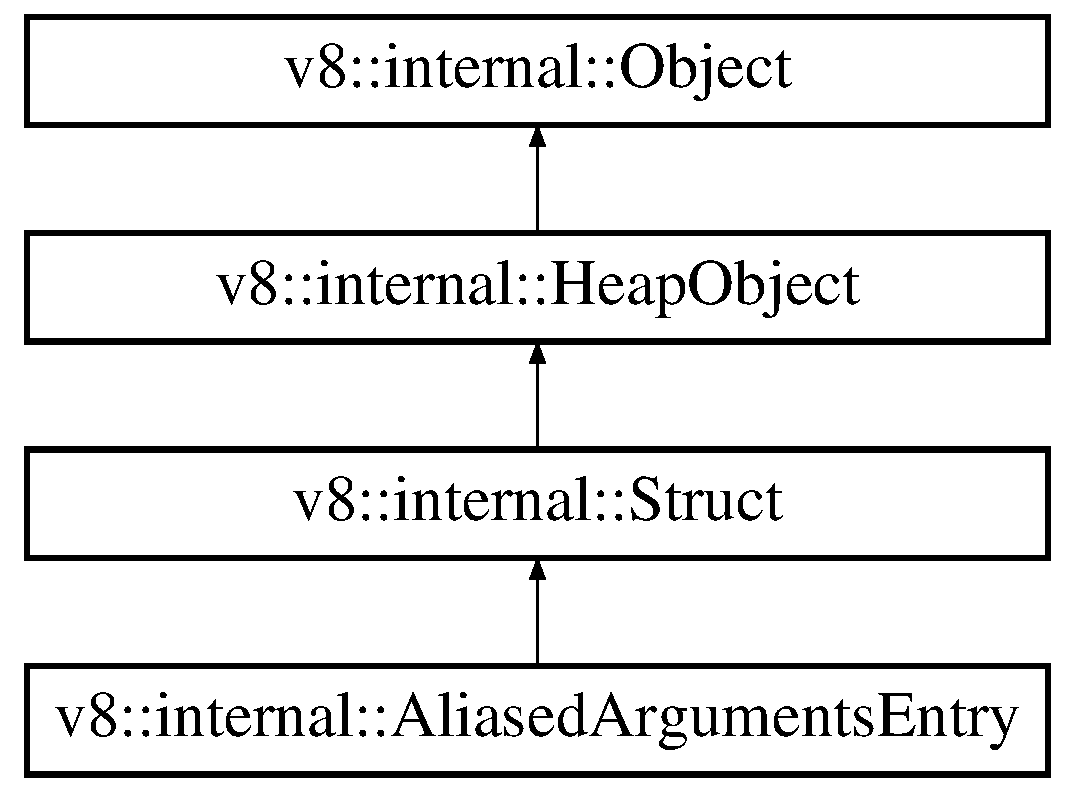
\includegraphics[height=4.000000cm]{classv8_1_1internal_1_1_aliased_arguments_entry}
\end{center}
\end{figure}
\subsection*{Public Member Functions}
\begin{DoxyCompactItemize}
\item 
\hypertarget{classv8_1_1internal_1_1_aliased_arguments_entry_a5362f3a14badae7882341093623de3fb}{}int {\bfseries aliased\+\_\+context\+\_\+slot} () const \label{classv8_1_1internal_1_1_aliased_arguments_entry_a5362f3a14badae7882341093623de3fb}

\item 
\hypertarget{classv8_1_1internal_1_1_aliased_arguments_entry_ad2f671a7089a9e775abd7e1c039aeee7}{}void {\bfseries set\+\_\+aliased\+\_\+context\+\_\+slot} (int count)\label{classv8_1_1internal_1_1_aliased_arguments_entry_ad2f671a7089a9e775abd7e1c039aeee7}

\end{DoxyCompactItemize}
\subsection*{Static Public Attributes}
\begin{DoxyCompactItemize}
\item 
\hypertarget{classv8_1_1internal_1_1_aliased_arguments_entry_a176665f23529fbe29ad19856967a7ee7}{}static const int {\bfseries k\+Aliased\+Context\+Slot} = Heap\+Object\+::k\+Header\+Size\label{classv8_1_1internal_1_1_aliased_arguments_entry_a176665f23529fbe29ad19856967a7ee7}

\item 
\hypertarget{classv8_1_1internal_1_1_aliased_arguments_entry_ad9980e02f526db5b9f4e095848a2d325}{}static const int {\bfseries k\+Size} = k\+Aliased\+Context\+Slot + k\+Pointer\+Size\label{classv8_1_1internal_1_1_aliased_arguments_entry_ad9980e02f526db5b9f4e095848a2d325}

\end{DoxyCompactItemize}
\subsection*{Additional Inherited Members}


The documentation for this class was generated from the following file\+:\begin{DoxyCompactItemize}
\item 
src/objects.\+h\end{DoxyCompactItemize}

\hypertarget{classv8_1_1internal_1_1_allocate_double_align_flag}{}\section{v8\+:\+:internal\+:\+:Allocate\+Double\+Align\+Flag Class Reference}
\label{classv8_1_1internal_1_1_allocate_double_align_flag}\index{v8\+::internal\+::\+Allocate\+Double\+Align\+Flag@{v8\+::internal\+::\+Allocate\+Double\+Align\+Flag}}
Inheritance diagram for v8\+:\+:internal\+:\+:Allocate\+Double\+Align\+Flag\+:\begin{figure}[H]
\begin{center}
\leavevmode
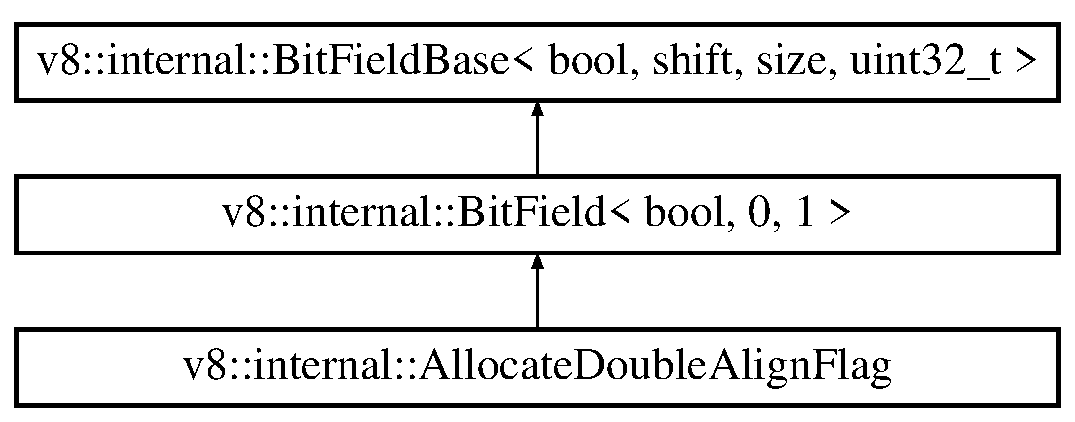
\includegraphics[height=3.000000cm]{classv8_1_1internal_1_1_allocate_double_align_flag}
\end{center}
\end{figure}
\subsection*{Additional Inherited Members}


The documentation for this class was generated from the following file\+:\begin{DoxyCompactItemize}
\item 
src/runtime.\+h\end{DoxyCompactItemize}

\hypertarget{classv8_1_1internal_1_1_allocate_target_space}{}\section{v8\+:\+:internal\+:\+:Allocate\+Target\+Space Class Reference}
\label{classv8_1_1internal_1_1_allocate_target_space}\index{v8\+::internal\+::\+Allocate\+Target\+Space@{v8\+::internal\+::\+Allocate\+Target\+Space}}
Inheritance diagram for v8\+:\+:internal\+:\+:Allocate\+Target\+Space\+:\begin{figure}[H]
\begin{center}
\leavevmode
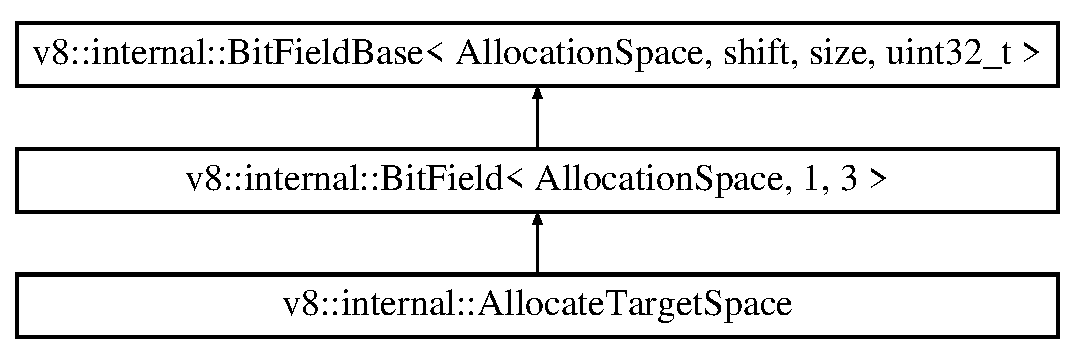
\includegraphics[height=3.000000cm]{classv8_1_1internal_1_1_allocate_target_space}
\end{center}
\end{figure}
\subsection*{Additional Inherited Members}


The documentation for this class was generated from the following file\+:\begin{DoxyCompactItemize}
\item 
src/runtime.\+h\end{DoxyCompactItemize}

\hypertarget{classv8_1_1internal_1_1_allocation_memento}{}\section{v8\+:\+:internal\+:\+:Allocation\+Memento Class Reference}
\label{classv8_1_1internal_1_1_allocation_memento}\index{v8\+::internal\+::\+Allocation\+Memento@{v8\+::internal\+::\+Allocation\+Memento}}
Inheritance diagram for v8\+:\+:internal\+:\+:Allocation\+Memento\+:\begin{figure}[H]
\begin{center}
\leavevmode
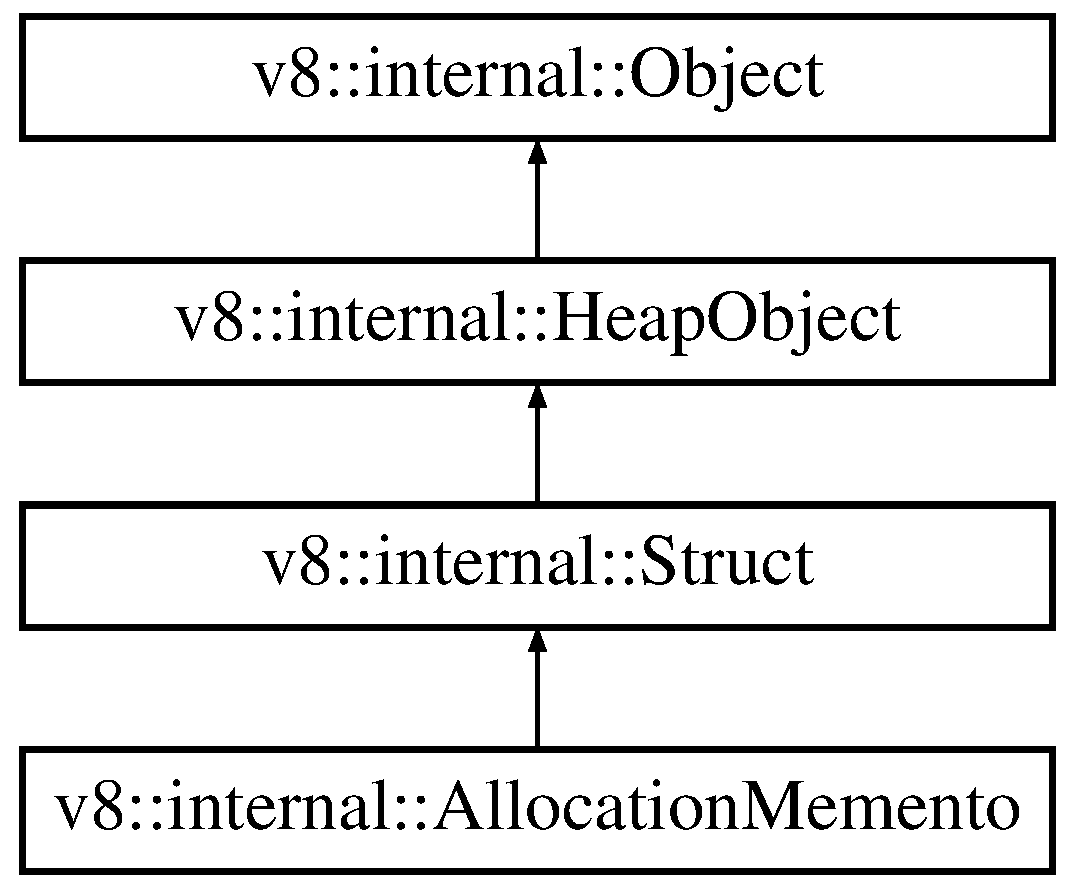
\includegraphics[height=4.000000cm]{classv8_1_1internal_1_1_allocation_memento}
\end{center}
\end{figure}
\subsection*{Public Member Functions}
\begin{DoxyCompactItemize}
\item 
\hypertarget{classv8_1_1internal_1_1_allocation_memento_add097e221c27cfdae3cc58466d9decab}{}bool {\bfseries Is\+Valid} ()\label{classv8_1_1internal_1_1_allocation_memento_add097e221c27cfdae3cc58466d9decab}

\item 
\hypertarget{classv8_1_1internal_1_1_allocation_memento_a41f3677993cad4023761d6a0e4cf6df8}{}\hyperlink{classv8_1_1internal_1_1_allocation_site}{Allocation\+Site} $\ast$ {\bfseries Get\+Allocation\+Site} ()\label{classv8_1_1internal_1_1_allocation_memento_a41f3677993cad4023761d6a0e4cf6df8}

\end{DoxyCompactItemize}
\subsection*{Static Public Attributes}
\begin{DoxyCompactItemize}
\item 
\hypertarget{classv8_1_1internal_1_1_allocation_memento_ab07187e61f49dfb2c298a49b5aea49d7}{}static const int {\bfseries k\+Allocation\+Site\+Offset} = Heap\+Object\+::k\+Header\+Size\label{classv8_1_1internal_1_1_allocation_memento_ab07187e61f49dfb2c298a49b5aea49d7}

\item 
\hypertarget{classv8_1_1internal_1_1_allocation_memento_acf92166b75198263c67253249c64edf1}{}static const int {\bfseries k\+Size} = k\+Allocation\+Site\+Offset + k\+Pointer\+Size\label{classv8_1_1internal_1_1_allocation_memento_acf92166b75198263c67253249c64edf1}

\end{DoxyCompactItemize}
\subsection*{Additional Inherited Members}


The documentation for this class was generated from the following file\+:\begin{DoxyCompactItemize}
\item 
src/objects.\+h\end{DoxyCompactItemize}

\hypertarget{classv8_1_1internal_1_1_allocation_site}{}\section{v8\+:\+:internal\+:\+:Allocation\+Site Class Reference}
\label{classv8_1_1internal_1_1_allocation_site}\index{v8\+::internal\+::\+Allocation\+Site@{v8\+::internal\+::\+Allocation\+Site}}
Inheritance diagram for v8\+:\+:internal\+:\+:Allocation\+Site\+:\begin{figure}[H]
\begin{center}
\leavevmode
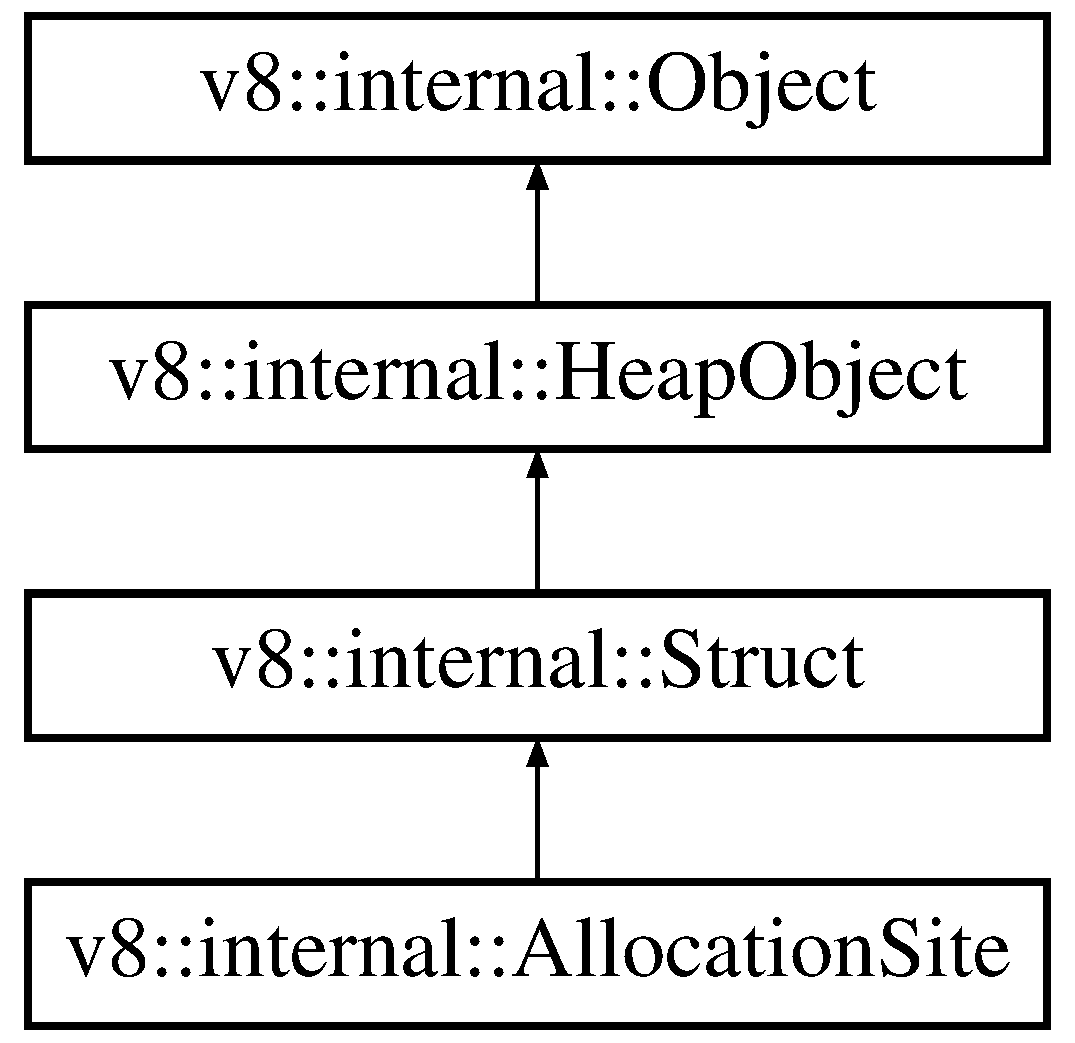
\includegraphics[height=4.000000cm]{classv8_1_1internal_1_1_allocation_site}
\end{center}
\end{figure}
\subsection*{Classes}
\begin{DoxyCompactItemize}
\item 
class \hyperlink{classv8_1_1internal_1_1_allocation_site_1_1_deopt_dependent_code_bit}{Deopt\+Dependent\+Code\+Bit}
\item 
class \hyperlink{classv8_1_1internal_1_1_allocation_site_1_1_do_not_inline_bit}{Do\+Not\+Inline\+Bit}
\item 
class \hyperlink{classv8_1_1internal_1_1_allocation_site_1_1_elements_kind_bits}{Elements\+Kind\+Bits}
\item 
class \hyperlink{classv8_1_1internal_1_1_allocation_site_1_1_memento_found_count_bits}{Memento\+Found\+Count\+Bits}
\item 
class \hyperlink{classv8_1_1internal_1_1_allocation_site_1_1_pretenure_decision_bits}{Pretenure\+Decision\+Bits}
\item 
class \hyperlink{classv8_1_1internal_1_1_allocation_site_1_1_unused_bits}{Unused\+Bits}
\end{DoxyCompactItemize}
\subsection*{Public Types}
\begin{DoxyCompactItemize}
\item 
\hypertarget{classv8_1_1internal_1_1_allocation_site_a90e0736002b73f20d96abede63a5395b}{}enum {\bfseries Pretenure\+Decision} \{ \\*
{\bfseries k\+Undecided} = 0, 
{\bfseries k\+Dont\+Tenure} = 1, 
{\bfseries k\+Maybe\+Tenure} = 2, 
{\bfseries k\+Tenure} = 3, 
\\*
{\bfseries k\+Zombie} = 4, 
{\bfseries k\+Last\+Pretenure\+Decision\+Value} = k\+Zombie
 \}\label{classv8_1_1internal_1_1_allocation_site_a90e0736002b73f20d96abede63a5395b}

\item 
\hypertarget{classv8_1_1internal_1_1_allocation_site_ab9c1b2d67cd67409bfe0cba3735e2aed}{}enum {\bfseries Reason} \{ {\bfseries T\+E\+N\+U\+R\+I\+N\+G}, 
{\bfseries T\+R\+A\+N\+S\+I\+T\+I\+O\+N\+S}
 \}\label{classv8_1_1internal_1_1_allocation_site_ab9c1b2d67cd67409bfe0cba3735e2aed}

\item 
\hypertarget{classv8_1_1internal_1_1_allocation_site_a368925e7d7e139cfdf582b93418f9527}{}typedef \hyperlink{classv8_1_1internal_1_1_fixed_body_descriptor}{Fixed\+Body\+Descriptor}$<$ Heap\+Object\+::k\+Header\+Size, k\+Dependent\+Code\+Offset+k\+Pointer\+Size, k\+Size $>$ {\bfseries Body\+Descriptor}\label{classv8_1_1internal_1_1_allocation_site_a368925e7d7e139cfdf582b93418f9527}

\end{DoxyCompactItemize}
\subsection*{Public Member Functions}
\begin{DoxyCompactItemize}
\item 
\hypertarget{classv8_1_1internal_1_1_allocation_site_a015895d2a527877f98749eb13b16a38f}{}const char $\ast$ {\bfseries Pretenure\+Decision\+Name} (Pretenure\+Decision decision)\label{classv8_1_1internal_1_1_allocation_site_a015895d2a527877f98749eb13b16a38f}

\item 
\hypertarget{classv8_1_1internal_1_1_allocation_site_a81f61008e147366d1eea6cdbae9d5ded}{}void {\bfseries Initialize} ()\label{classv8_1_1internal_1_1_allocation_site_a81f61008e147366d1eea6cdbae9d5ded}

\item 
\hypertarget{classv8_1_1internal_1_1_allocation_site_ab9a3fce3780154b3da48ae09cb0b8d46}{}bool {\bfseries Is\+Nested\+Site} ()\label{classv8_1_1internal_1_1_allocation_site_ab9a3fce3780154b3da48ae09cb0b8d46}

\item 
\hypertarget{classv8_1_1internal_1_1_allocation_site_ad1c0e4e32b7e2db1483fa7a518bec030}{}{\bfseries S\+T\+A\+T\+I\+C\+\_\+\+A\+S\+S\+E\+R\+T} (Pretenure\+Decision\+Bits\+::k\+Max $>$=k\+Last\+Pretenure\+Decision\+Value)\label{classv8_1_1internal_1_1_allocation_site_ad1c0e4e32b7e2db1483fa7a518bec030}

\item 
\hypertarget{classv8_1_1internal_1_1_allocation_site_ac623c7ec4eb8500c272828a539d61632}{}bool {\bfseries Increment\+Memento\+Found\+Count} ()\label{classv8_1_1internal_1_1_allocation_site_ac623c7ec4eb8500c272828a539d61632}

\item 
\hypertarget{classv8_1_1internal_1_1_allocation_site_ac32fcfb926ce03239f5df6aca880f18c}{}void {\bfseries Increment\+Memento\+Create\+Count} ()\label{classv8_1_1internal_1_1_allocation_site_ac32fcfb926ce03239f5df6aca880f18c}

\item 
\hypertarget{classv8_1_1internal_1_1_allocation_site_a06aadcce1164186ecce0962c359abb0c}{}Pretenure\+Flag {\bfseries Get\+Pretenure\+Mode} ()\label{classv8_1_1internal_1_1_allocation_site_a06aadcce1164186ecce0962c359abb0c}

\item 
\hypertarget{classv8_1_1internal_1_1_allocation_site_aa1b323951edb619dd9078164b9fabd5c}{}void {\bfseries Reset\+Pretenure\+Decision} ()\label{classv8_1_1internal_1_1_allocation_site_aa1b323951edb619dd9078164b9fabd5c}

\item 
\hypertarget{classv8_1_1internal_1_1_allocation_site_a858cfe6ed6ee70029b3a23c4e186c3ba}{}Pretenure\+Decision {\bfseries pretenure\+\_\+decision} ()\label{classv8_1_1internal_1_1_allocation_site_a858cfe6ed6ee70029b3a23c4e186c3ba}

\item 
\hypertarget{classv8_1_1internal_1_1_allocation_site_a3eb7bfb649894bc1ea0875152aff118e}{}void {\bfseries set\+\_\+pretenure\+\_\+decision} (Pretenure\+Decision decision)\label{classv8_1_1internal_1_1_allocation_site_a3eb7bfb649894bc1ea0875152aff118e}

\item 
\hypertarget{classv8_1_1internal_1_1_allocation_site_ad346c72b5d5c204cbb5ca3c5d42de25b}{}bool {\bfseries deopt\+\_\+dependent\+\_\+code} ()\label{classv8_1_1internal_1_1_allocation_site_ad346c72b5d5c204cbb5ca3c5d42de25b}

\item 
\hypertarget{classv8_1_1internal_1_1_allocation_site_a6b6321178dbb71e389194b39a6ee51ee}{}void {\bfseries set\+\_\+deopt\+\_\+dependent\+\_\+code} (bool deopt)\label{classv8_1_1internal_1_1_allocation_site_a6b6321178dbb71e389194b39a6ee51ee}

\item 
\hypertarget{classv8_1_1internal_1_1_allocation_site_a09e237ddea93fe5f26592f3f4d86d73b}{}int {\bfseries memento\+\_\+found\+\_\+count} ()\label{classv8_1_1internal_1_1_allocation_site_a09e237ddea93fe5f26592f3f4d86d73b}

\item 
\hypertarget{classv8_1_1internal_1_1_allocation_site_ad74c42dccc41adcc6d7f2dd22fa56176}{}void {\bfseries set\+\_\+memento\+\_\+found\+\_\+count} (int count)\label{classv8_1_1internal_1_1_allocation_site_ad74c42dccc41adcc6d7f2dd22fa56176}

\item 
\hypertarget{classv8_1_1internal_1_1_allocation_site_aa5dae1f833730f55ab548a2981c577fd}{}int {\bfseries memento\+\_\+create\+\_\+count} ()\label{classv8_1_1internal_1_1_allocation_site_aa5dae1f833730f55ab548a2981c577fd}

\item 
\hypertarget{classv8_1_1internal_1_1_allocation_site_ab95f8e888faad709405944f3f5223378}{}void {\bfseries set\+\_\+memento\+\_\+create\+\_\+count} (int count)\label{classv8_1_1internal_1_1_allocation_site_ab95f8e888faad709405944f3f5223378}

\item 
\hypertarget{classv8_1_1internal_1_1_allocation_site_ab43e6d803b8a1f9b160936060e487542}{}bool {\bfseries Is\+Zombie} ()\label{classv8_1_1internal_1_1_allocation_site_ab43e6d803b8a1f9b160936060e487542}

\item 
\hypertarget{classv8_1_1internal_1_1_allocation_site_aa1870a70bef3585f613d95509e3c026e}{}bool {\bfseries Is\+Maybe\+Tenure} ()\label{classv8_1_1internal_1_1_allocation_site_aa1870a70bef3585f613d95509e3c026e}

\item 
\hypertarget{classv8_1_1internal_1_1_allocation_site_af432e0790ebdfc00d36c9a6234e98389}{}void {\bfseries Mark\+Zombie} ()\label{classv8_1_1internal_1_1_allocation_site_af432e0790ebdfc00d36c9a6234e98389}

\item 
\hypertarget{classv8_1_1internal_1_1_allocation_site_ac56e44521833202855156f6c8f06101f}{}bool {\bfseries Make\+Pretenure\+Decision} (Pretenure\+Decision current\+\_\+decision, double ratio, bool maximum\+\_\+size\+\_\+scavenge)\label{classv8_1_1internal_1_1_allocation_site_ac56e44521833202855156f6c8f06101f}

\item 
\hypertarget{classv8_1_1internal_1_1_allocation_site_ab06a9db3e9fa8256f8cd97cc5cefeff5}{}bool {\bfseries Digest\+Pretenuring\+Feedback} (bool maximum\+\_\+size\+\_\+scavenge)\label{classv8_1_1internal_1_1_allocation_site_ab06a9db3e9fa8256f8cd97cc5cefeff5}

\item 
\hypertarget{classv8_1_1internal_1_1_allocation_site_ad32f0453a6a51c271b6207227ec2959d}{}Elements\+Kind {\bfseries Get\+Elements\+Kind} ()\label{classv8_1_1internal_1_1_allocation_site_ad32f0453a6a51c271b6207227ec2959d}

\item 
\hypertarget{classv8_1_1internal_1_1_allocation_site_adf1136948311998f7ead14bcf8f2cfd8}{}void {\bfseries Set\+Elements\+Kind} (Elements\+Kind kind)\label{classv8_1_1internal_1_1_allocation_site_adf1136948311998f7ead14bcf8f2cfd8}

\item 
\hypertarget{classv8_1_1internal_1_1_allocation_site_aeb29ad379adc7425340ae3b2e38f72f3}{}bool {\bfseries Can\+Inline\+Call} ()\label{classv8_1_1internal_1_1_allocation_site_aeb29ad379adc7425340ae3b2e38f72f3}

\item 
\hypertarget{classv8_1_1internal_1_1_allocation_site_a3e9fcf250995d87d2c31e05c6e4e6ce5}{}void {\bfseries Set\+Do\+Not\+Inline\+Call} ()\label{classv8_1_1internal_1_1_allocation_site_a3e9fcf250995d87d2c31e05c6e4e6ce5}

\item 
\hypertarget{classv8_1_1internal_1_1_allocation_site_adca3580eb9a8d18cf1becc2b9a1995bb}{}bool {\bfseries Site\+Points\+To\+Literal} ()\label{classv8_1_1internal_1_1_allocation_site_adca3580eb9a8d18cf1becc2b9a1995bb}

\end{DoxyCompactItemize}
\subsection*{Static Public Member Functions}
\begin{DoxyCompactItemize}
\item 
\hypertarget{classv8_1_1internal_1_1_allocation_site_a0bfecad8387c5d8ce19551d9ec7326ce}{}static void {\bfseries Digest\+Transition\+Feedback} (\hyperlink{classv8_1_1internal_1_1_handle}{Handle}$<$ \hyperlink{classv8_1_1internal_1_1_allocation_site}{Allocation\+Site} $>$ site, Elements\+Kind to\+\_\+kind)\label{classv8_1_1internal_1_1_allocation_site_a0bfecad8387c5d8ce19551d9ec7326ce}

\item 
\hypertarget{classv8_1_1internal_1_1_allocation_site_a8d34a33c5cc89177a9c6959578487dc9}{}static void {\bfseries Add\+Dependent\+Compilation\+Info} (\hyperlink{classv8_1_1internal_1_1_handle}{Handle}$<$ \hyperlink{classv8_1_1internal_1_1_allocation_site}{Allocation\+Site} $>$ site, Reason reason, \hyperlink{classv8_1_1internal_1_1_compilation_info}{Compilation\+Info} $\ast$info)\label{classv8_1_1internal_1_1_allocation_site_a8d34a33c5cc89177a9c6959578487dc9}

\item 
\hypertarget{classv8_1_1internal_1_1_allocation_site_a6ac30d18f89c9a43eaff3ca894671851}{}static Allocation\+Site\+Mode {\bfseries Get\+Mode} (Elements\+Kind boilerplate\+\_\+elements\+\_\+kind)\label{classv8_1_1internal_1_1_allocation_site_a6ac30d18f89c9a43eaff3ca894671851}

\item 
\hypertarget{classv8_1_1internal_1_1_allocation_site_a4c5f330f48db33d18eaa5346fd89130c}{}static Allocation\+Site\+Mode {\bfseries Get\+Mode} (Elements\+Kind from, Elements\+Kind to)\label{classv8_1_1internal_1_1_allocation_site_a4c5f330f48db33d18eaa5346fd89130c}

\item 
\hypertarget{classv8_1_1internal_1_1_allocation_site_a5bce0a6a275e0f9a9c8a3e87babab0d9}{}static bool {\bfseries Can\+Track} (Instance\+Type type)\label{classv8_1_1internal_1_1_allocation_site_a5bce0a6a275e0f9a9c8a3e87babab0d9}

\end{DoxyCompactItemize}
\subsection*{Static Public Attributes}
\begin{DoxyCompactItemize}
\item 
\hypertarget{classv8_1_1internal_1_1_allocation_site_aeead57f97b16bf614a5631349d0bc7f1}{}static const uint32\+\_\+t {\bfseries k\+Maximum\+Array\+Bytes\+To\+Pretransition} = 8 $\ast$ 1024\label{classv8_1_1internal_1_1_allocation_site_aeead57f97b16bf614a5631349d0bc7f1}

\item 
\hypertarget{classv8_1_1internal_1_1_allocation_site_a45d58b4d64823e7d33eeb2291b26fb3a}{}static const double {\bfseries k\+Pretenure\+Ratio} = 0.\+85\label{classv8_1_1internal_1_1_allocation_site_a45d58b4d64823e7d33eeb2291b26fb3a}

\item 
\hypertarget{classv8_1_1internal_1_1_allocation_site_a60cc20b9d1f816783e6c112029776861}{}static const int {\bfseries k\+Pretenure\+Minimum\+Created} = 100\label{classv8_1_1internal_1_1_allocation_site_a60cc20b9d1f816783e6c112029776861}

\item 
\hypertarget{classv8_1_1internal_1_1_allocation_site_ab16a1b6151317cfa89ad5ff7d49f7f23}{}static const int {\bfseries k\+Transition\+Info\+Offset} = Heap\+Object\+::k\+Header\+Size\label{classv8_1_1internal_1_1_allocation_site_ab16a1b6151317cfa89ad5ff7d49f7f23}

\item 
\hypertarget{classv8_1_1internal_1_1_allocation_site_af3315748586cedda1896811766e0f944}{}static const int {\bfseries k\+Nested\+Site\+Offset} = k\+Transition\+Info\+Offset + k\+Pointer\+Size\label{classv8_1_1internal_1_1_allocation_site_af3315748586cedda1896811766e0f944}

\item 
\hypertarget{classv8_1_1internal_1_1_allocation_site_a1700918589b01582d697f3e1b4916e8b}{}static const int {\bfseries k\+Pretenure\+Data\+Offset} = k\+Nested\+Site\+Offset + k\+Pointer\+Size\label{classv8_1_1internal_1_1_allocation_site_a1700918589b01582d697f3e1b4916e8b}

\item 
static const int {\bfseries k\+Pretenure\+Create\+Count\+Offset}
\item 
static const int {\bfseries k\+Dependent\+Code\+Offset}
\item 
\hypertarget{classv8_1_1internal_1_1_allocation_site_a455b0be20fe32fd7e81fcdc4ca510484}{}static const int {\bfseries k\+Weak\+Next\+Offset} = k\+Dependent\+Code\+Offset + k\+Pointer\+Size\label{classv8_1_1internal_1_1_allocation_site_a455b0be20fe32fd7e81fcdc4ca510484}

\item 
\hypertarget{classv8_1_1internal_1_1_allocation_site_a8563fdab6231c9e2d1346a3d2a726d9c}{}static const int {\bfseries k\+Size} = k\+Weak\+Next\+Offset + k\+Pointer\+Size\label{classv8_1_1internal_1_1_allocation_site_a8563fdab6231c9e2d1346a3d2a726d9c}

\item 
\hypertarget{classv8_1_1internal_1_1_allocation_site_a0a718e12a1ec05d53dde6dd61835db66}{}static const int {\bfseries k\+Pointer\+Fields\+Begin\+Offset} = k\+Transition\+Info\+Offset\label{classv8_1_1internal_1_1_allocation_site_a0a718e12a1ec05d53dde6dd61835db66}

\item 
\hypertarget{classv8_1_1internal_1_1_allocation_site_a8f06e59d25cc4c6946f902d3c79ebbc5}{}static const int {\bfseries k\+Pointer\+Fields\+End\+Offset} = k\+Dependent\+Code\+Offset\label{classv8_1_1internal_1_1_allocation_site_a8f06e59d25cc4c6946f902d3c79ebbc5}

\end{DoxyCompactItemize}
\subsection*{Additional Inherited Members}


\subsection{Member Data Documentation}
\hypertarget{classv8_1_1internal_1_1_allocation_site_a4c5455657e57dde03629911e0c1fba19}{}\index{v8\+::internal\+::\+Allocation\+Site@{v8\+::internal\+::\+Allocation\+Site}!k\+Dependent\+Code\+Offset@{k\+Dependent\+Code\+Offset}}
\index{k\+Dependent\+Code\+Offset@{k\+Dependent\+Code\+Offset}!v8\+::internal\+::\+Allocation\+Site@{v8\+::internal\+::\+Allocation\+Site}}
\subsubsection[{k\+Dependent\+Code\+Offset}]{\setlength{\rightskip}{0pt plus 5cm}const int v8\+::internal\+::\+Allocation\+Site\+::k\+Dependent\+Code\+Offset\hspace{0.3cm}{\ttfamily [static]}}\label{classv8_1_1internal_1_1_allocation_site_a4c5455657e57dde03629911e0c1fba19}
{\bfseries Initial value\+:}
\begin{DoxyCode}
=
      kPretenureCreateCountOffset + kPointerSize
\end{DoxyCode}
\hypertarget{classv8_1_1internal_1_1_allocation_site_ad4371d69986a9a4dad979104ed388710}{}\index{v8\+::internal\+::\+Allocation\+Site@{v8\+::internal\+::\+Allocation\+Site}!k\+Pretenure\+Create\+Count\+Offset@{k\+Pretenure\+Create\+Count\+Offset}}
\index{k\+Pretenure\+Create\+Count\+Offset@{k\+Pretenure\+Create\+Count\+Offset}!v8\+::internal\+::\+Allocation\+Site@{v8\+::internal\+::\+Allocation\+Site}}
\subsubsection[{k\+Pretenure\+Create\+Count\+Offset}]{\setlength{\rightskip}{0pt plus 5cm}const int v8\+::internal\+::\+Allocation\+Site\+::k\+Pretenure\+Create\+Count\+Offset\hspace{0.3cm}{\ttfamily [static]}}\label{classv8_1_1internal_1_1_allocation_site_ad4371d69986a9a4dad979104ed388710}
{\bfseries Initial value\+:}
\begin{DoxyCode}
=
      kPretenureDataOffset + kPointerSize
\end{DoxyCode}


The documentation for this class was generated from the following files\+:\begin{DoxyCompactItemize}
\item 
src/objects.\+h\item 
src/objects-\/inl.\+h\item 
src/objects.\+cc\end{DoxyCompactItemize}

\hypertarget{classv8_1_1internal_1_1_allocation_site_context}{}\section{v8\+:\+:internal\+:\+:Allocation\+Site\+Context Class Reference}
\label{classv8_1_1internal_1_1_allocation_site_context}\index{v8\+::internal\+::\+Allocation\+Site\+Context@{v8\+::internal\+::\+Allocation\+Site\+Context}}
Inheritance diagram for v8\+:\+:internal\+:\+:Allocation\+Site\+Context\+:\begin{figure}[H]
\begin{center}
\leavevmode
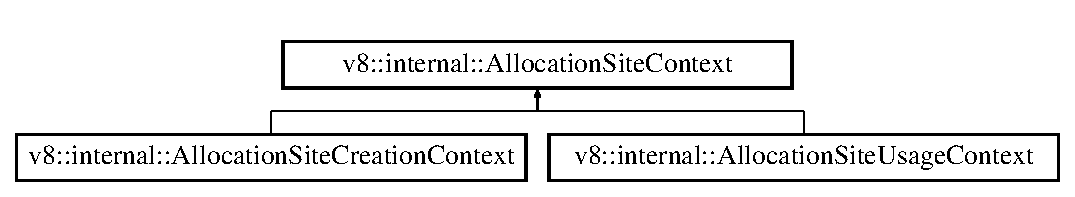
\includegraphics[height=2.000000cm]{classv8_1_1internal_1_1_allocation_site_context}
\end{center}
\end{figure}
\subsection*{Public Member Functions}
\begin{DoxyCompactItemize}
\item 
\hypertarget{classv8_1_1internal_1_1_allocation_site_context_acad3aa6b62e34d542b6fd6c9b87e2093}{}{\bfseries Allocation\+Site\+Context} (\hyperlink{classv8_1_1internal_1_1_isolate}{Isolate} $\ast$isolate)\label{classv8_1_1internal_1_1_allocation_site_context_acad3aa6b62e34d542b6fd6c9b87e2093}

\item 
\hypertarget{classv8_1_1internal_1_1_allocation_site_context_a76427a09d8c0eef6794ecfd804ca8eea}{}\hyperlink{classv8_1_1internal_1_1_handle}{Handle}$<$ \hyperlink{classv8_1_1internal_1_1_allocation_site}{Allocation\+Site} $>$ {\bfseries top} ()\label{classv8_1_1internal_1_1_allocation_site_context_a76427a09d8c0eef6794ecfd804ca8eea}

\item 
\hypertarget{classv8_1_1internal_1_1_allocation_site_context_a20943342b9c850bc0f1c3fd0aef56e9a}{}\hyperlink{classv8_1_1internal_1_1_handle}{Handle}$<$ \hyperlink{classv8_1_1internal_1_1_allocation_site}{Allocation\+Site} $>$ {\bfseries current} ()\label{classv8_1_1internal_1_1_allocation_site_context_a20943342b9c850bc0f1c3fd0aef56e9a}

\item 
\hypertarget{classv8_1_1internal_1_1_allocation_site_context_adfa2a2817414d94fd00728a2c163d7b0}{}bool {\bfseries Should\+Create\+Memento} (\hyperlink{classv8_1_1internal_1_1_handle}{Handle}$<$ \hyperlink{classv8_1_1internal_1_1_j_s_object}{J\+S\+Object} $>$ object)\label{classv8_1_1internal_1_1_allocation_site_context_adfa2a2817414d94fd00728a2c163d7b0}

\item 
\hypertarget{classv8_1_1internal_1_1_allocation_site_context_a8adcb0b60cf5fbda807b0a11c128ab4a}{}\hyperlink{classv8_1_1internal_1_1_isolate}{Isolate} $\ast$ {\bfseries isolate} ()\label{classv8_1_1internal_1_1_allocation_site_context_a8adcb0b60cf5fbda807b0a11c128ab4a}

\end{DoxyCompactItemize}
\subsection*{Protected Member Functions}
\begin{DoxyCompactItemize}
\item 
\hypertarget{classv8_1_1internal_1_1_allocation_site_context_a2e094902dbadc8931c82eb04333807c0}{}void {\bfseries update\+\_\+current\+\_\+site} (\hyperlink{classv8_1_1internal_1_1_allocation_site}{Allocation\+Site} $\ast$site)\label{classv8_1_1internal_1_1_allocation_site_context_a2e094902dbadc8931c82eb04333807c0}

\item 
\hypertarget{classv8_1_1internal_1_1_allocation_site_context_a2ae0994fc850605cbea75aeddf980b44}{}void {\bfseries Initialize\+Traversal} (\hyperlink{classv8_1_1internal_1_1_handle}{Handle}$<$ \hyperlink{classv8_1_1internal_1_1_allocation_site}{Allocation\+Site} $>$ site)\label{classv8_1_1internal_1_1_allocation_site_context_a2ae0994fc850605cbea75aeddf980b44}

\end{DoxyCompactItemize}


The documentation for this class was generated from the following file\+:\begin{DoxyCompactItemize}
\item 
src/allocation-\/site-\/scopes.\+h\end{DoxyCompactItemize}

\hypertarget{classv8_1_1internal_1_1_allocation_site_creation_context}{}\section{v8\+:\+:internal\+:\+:Allocation\+Site\+Creation\+Context Class Reference}
\label{classv8_1_1internal_1_1_allocation_site_creation_context}\index{v8\+::internal\+::\+Allocation\+Site\+Creation\+Context@{v8\+::internal\+::\+Allocation\+Site\+Creation\+Context}}
Inheritance diagram for v8\+:\+:internal\+:\+:Allocation\+Site\+Creation\+Context\+:\begin{figure}[H]
\begin{center}
\leavevmode
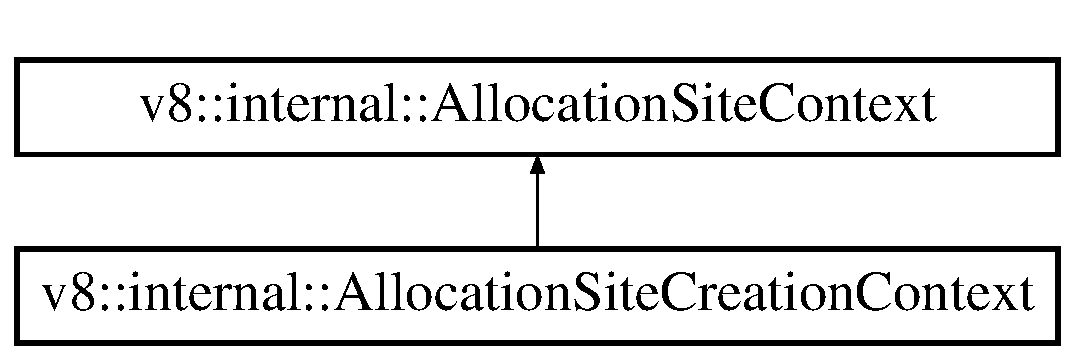
\includegraphics[height=2.000000cm]{classv8_1_1internal_1_1_allocation_site_creation_context}
\end{center}
\end{figure}
\subsection*{Public Member Functions}
\begin{DoxyCompactItemize}
\item 
\hypertarget{classv8_1_1internal_1_1_allocation_site_creation_context_a159a45da25ad238b0b67ec380121780e}{}{\bfseries Allocation\+Site\+Creation\+Context} (\hyperlink{classv8_1_1internal_1_1_isolate}{Isolate} $\ast$isolate)\label{classv8_1_1internal_1_1_allocation_site_creation_context_a159a45da25ad238b0b67ec380121780e}

\item 
\hypertarget{classv8_1_1internal_1_1_allocation_site_creation_context_ac01c9bd1361ef78f22c301bdfdcb2076}{}\hyperlink{classv8_1_1internal_1_1_handle}{Handle}$<$ \hyperlink{classv8_1_1internal_1_1_allocation_site}{Allocation\+Site} $>$ {\bfseries Enter\+New\+Scope} ()\label{classv8_1_1internal_1_1_allocation_site_creation_context_ac01c9bd1361ef78f22c301bdfdcb2076}

\item 
\hypertarget{classv8_1_1internal_1_1_allocation_site_creation_context_a42deb3f83fd733f54d1a0c32a74f2f46}{}void {\bfseries Exit\+Scope} (\hyperlink{classv8_1_1internal_1_1_handle}{Handle}$<$ \hyperlink{classv8_1_1internal_1_1_allocation_site}{Allocation\+Site} $>$ site, \hyperlink{classv8_1_1internal_1_1_handle}{Handle}$<$ \hyperlink{classv8_1_1internal_1_1_j_s_object}{J\+S\+Object} $>$ object)\label{classv8_1_1internal_1_1_allocation_site_creation_context_a42deb3f83fd733f54d1a0c32a74f2f46}

\end{DoxyCompactItemize}
\subsection*{Additional Inherited Members}


The documentation for this class was generated from the following files\+:\begin{DoxyCompactItemize}
\item 
src/allocation-\/site-\/scopes.\+h\item 
src/allocation-\/site-\/scopes.\+cc\end{DoxyCompactItemize}

\hypertarget{classv8_1_1internal_1_1_allocation_site_usage_context}{}\section{v8\+:\+:internal\+:\+:Allocation\+Site\+Usage\+Context Class Reference}
\label{classv8_1_1internal_1_1_allocation_site_usage_context}\index{v8\+::internal\+::\+Allocation\+Site\+Usage\+Context@{v8\+::internal\+::\+Allocation\+Site\+Usage\+Context}}
Inheritance diagram for v8\+:\+:internal\+:\+:Allocation\+Site\+Usage\+Context\+:\begin{figure}[H]
\begin{center}
\leavevmode
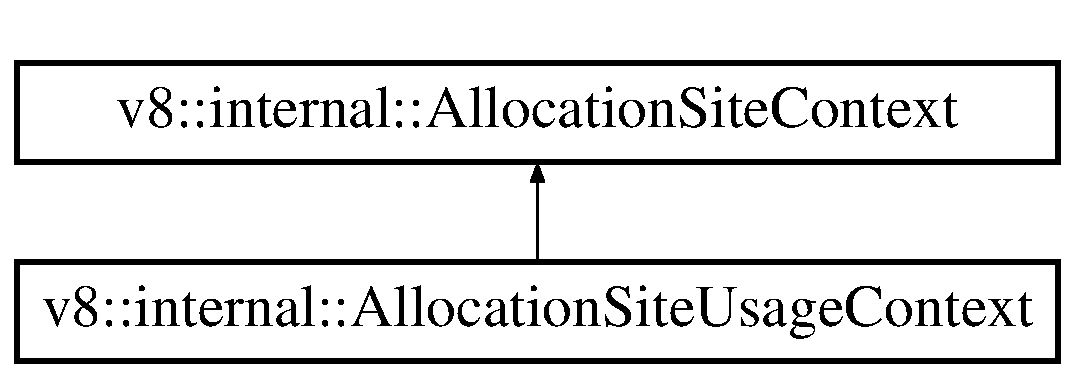
\includegraphics[height=2.000000cm]{classv8_1_1internal_1_1_allocation_site_usage_context}
\end{center}
\end{figure}
\subsection*{Public Member Functions}
\begin{DoxyCompactItemize}
\item 
\hypertarget{classv8_1_1internal_1_1_allocation_site_usage_context_aa9b5b62dbc43c89fbb14b22f32d3f68e}{}{\bfseries Allocation\+Site\+Usage\+Context} (\hyperlink{classv8_1_1internal_1_1_isolate}{Isolate} $\ast$isolate, \hyperlink{classv8_1_1internal_1_1_handle}{Handle}$<$ \hyperlink{classv8_1_1internal_1_1_allocation_site}{Allocation\+Site} $>$ site, bool activated)\label{classv8_1_1internal_1_1_allocation_site_usage_context_aa9b5b62dbc43c89fbb14b22f32d3f68e}

\item 
\hypertarget{classv8_1_1internal_1_1_allocation_site_usage_context_a7155f90f38a179371cbd03d42d3311a4}{}\hyperlink{classv8_1_1internal_1_1_handle}{Handle}$<$ \hyperlink{classv8_1_1internal_1_1_allocation_site}{Allocation\+Site} $>$ {\bfseries Enter\+New\+Scope} ()\label{classv8_1_1internal_1_1_allocation_site_usage_context_a7155f90f38a179371cbd03d42d3311a4}

\item 
\hypertarget{classv8_1_1internal_1_1_allocation_site_usage_context_a27c29c9de5fb9a5afdc56a262b7d095d}{}void {\bfseries Exit\+Scope} (\hyperlink{classv8_1_1internal_1_1_handle}{Handle}$<$ \hyperlink{classv8_1_1internal_1_1_allocation_site}{Allocation\+Site} $>$ scope\+\_\+site, \hyperlink{classv8_1_1internal_1_1_handle}{Handle}$<$ \hyperlink{classv8_1_1internal_1_1_j_s_object}{J\+S\+Object} $>$ object)\label{classv8_1_1internal_1_1_allocation_site_usage_context_a27c29c9de5fb9a5afdc56a262b7d095d}

\item 
\hypertarget{classv8_1_1internal_1_1_allocation_site_usage_context_a9b8b4f20046612a1dc28823efe000043}{}bool {\bfseries Should\+Create\+Memento} (\hyperlink{classv8_1_1internal_1_1_handle}{Handle}$<$ \hyperlink{classv8_1_1internal_1_1_j_s_object}{J\+S\+Object} $>$ object)\label{classv8_1_1internal_1_1_allocation_site_usage_context_a9b8b4f20046612a1dc28823efe000043}

\end{DoxyCompactItemize}
\subsection*{Additional Inherited Members}


The documentation for this class was generated from the following files\+:\begin{DoxyCompactItemize}
\item 
src/allocation-\/site-\/scopes.\+h\item 
src/allocation-\/site-\/scopes.\+cc\end{DoxyCompactItemize}

\hypertarget{classv8_1_1internal_1_1_allocation_trace_node}{}\section{v8\+:\+:internal\+:\+:Allocation\+Trace\+Node Class Reference}
\label{classv8_1_1internal_1_1_allocation_trace_node}\index{v8\+::internal\+::\+Allocation\+Trace\+Node@{v8\+::internal\+::\+Allocation\+Trace\+Node}}
\subsection*{Public Member Functions}
\begin{DoxyCompactItemize}
\item 
\hypertarget{classv8_1_1internal_1_1_allocation_trace_node_aca8caa93d6a5309e2fc2529b71a5a70a}{}{\bfseries Allocation\+Trace\+Node} (\hyperlink{classv8_1_1internal_1_1_allocation_trace_tree}{Allocation\+Trace\+Tree} $\ast$tree, unsigned function\+\_\+info\+\_\+index)\label{classv8_1_1internal_1_1_allocation_trace_node_aca8caa93d6a5309e2fc2529b71a5a70a}

\item 
\hypertarget{classv8_1_1internal_1_1_allocation_trace_node_afbb942277677c19a257ff8781f034c1d}{}\hyperlink{classv8_1_1internal_1_1_allocation_trace_node}{Allocation\+Trace\+Node} $\ast$ {\bfseries Find\+Child} (unsigned function\+\_\+info\+\_\+index)\label{classv8_1_1internal_1_1_allocation_trace_node_afbb942277677c19a257ff8781f034c1d}

\item 
\hypertarget{classv8_1_1internal_1_1_allocation_trace_node_a780262d490b639c1782e3a7212297709}{}\hyperlink{classv8_1_1internal_1_1_allocation_trace_node}{Allocation\+Trace\+Node} $\ast$ {\bfseries Find\+Or\+Add\+Child} (unsigned function\+\_\+info\+\_\+index)\label{classv8_1_1internal_1_1_allocation_trace_node_a780262d490b639c1782e3a7212297709}

\item 
\hypertarget{classv8_1_1internal_1_1_allocation_trace_node_ab3952f0610968cabfdb6a6134395f4a8}{}void {\bfseries Add\+Allocation} (unsigned size)\label{classv8_1_1internal_1_1_allocation_trace_node_ab3952f0610968cabfdb6a6134395f4a8}

\item 
\hypertarget{classv8_1_1internal_1_1_allocation_trace_node_a7615a9d517ad2c292ef197fa5178afef}{}unsigned {\bfseries function\+\_\+info\+\_\+index} () const \label{classv8_1_1internal_1_1_allocation_trace_node_a7615a9d517ad2c292ef197fa5178afef}

\item 
\hypertarget{classv8_1_1internal_1_1_allocation_trace_node_aaecc079598de291e9411b0b1143338bb}{}unsigned {\bfseries allocation\+\_\+size} () const \label{classv8_1_1internal_1_1_allocation_trace_node_aaecc079598de291e9411b0b1143338bb}

\item 
\hypertarget{classv8_1_1internal_1_1_allocation_trace_node_a2a31df2800608396686f67576477c648}{}unsigned {\bfseries allocation\+\_\+count} () const \label{classv8_1_1internal_1_1_allocation_trace_node_a2a31df2800608396686f67576477c648}

\item 
\hypertarget{classv8_1_1internal_1_1_allocation_trace_node_a9f11563e9cbd3d46a0bd9eee2d8e0f3c}{}unsigned {\bfseries id} () const \label{classv8_1_1internal_1_1_allocation_trace_node_a9f11563e9cbd3d46a0bd9eee2d8e0f3c}

\item 
\hypertarget{classv8_1_1internal_1_1_allocation_trace_node_a81a9b60b273378fff6eee02960e44bea}{}\hyperlink{classv8_1_1internal_1_1_vector}{Vector}$<$ \hyperlink{classv8_1_1internal_1_1_allocation_trace_node}{Allocation\+Trace\+Node} $\ast$ $>$ {\bfseries children} () const \label{classv8_1_1internal_1_1_allocation_trace_node_a81a9b60b273378fff6eee02960e44bea}

\item 
\hypertarget{classv8_1_1internal_1_1_allocation_trace_node_acfba1229f80910c5746758f8afdff7af}{}void {\bfseries Print} (int indent, \hyperlink{classv8_1_1internal_1_1_allocation_tracker}{Allocation\+Tracker} $\ast$tracker)\label{classv8_1_1internal_1_1_allocation_trace_node_acfba1229f80910c5746758f8afdff7af}

\end{DoxyCompactItemize}


The documentation for this class was generated from the following files\+:\begin{DoxyCompactItemize}
\item 
src/allocation-\/tracker.\+h\item 
src/allocation-\/tracker.\+cc\end{DoxyCompactItemize}

\hypertarget{classv8_1_1internal_1_1_allocation_trace_tree}{}\section{v8\+:\+:internal\+:\+:Allocation\+Trace\+Tree Class Reference}
\label{classv8_1_1internal_1_1_allocation_trace_tree}\index{v8\+::internal\+::\+Allocation\+Trace\+Tree@{v8\+::internal\+::\+Allocation\+Trace\+Tree}}
\subsection*{Public Member Functions}
\begin{DoxyCompactItemize}
\item 
\hypertarget{classv8_1_1internal_1_1_allocation_trace_tree_ac5d8e76d5c1250e5a0c0453d79fc656e}{}\hyperlink{classv8_1_1internal_1_1_allocation_trace_node}{Allocation\+Trace\+Node} $\ast$ {\bfseries Add\+Path\+From\+End} (const \hyperlink{classv8_1_1internal_1_1_vector}{Vector}$<$ unsigned $>$ \&path)\label{classv8_1_1internal_1_1_allocation_trace_tree_ac5d8e76d5c1250e5a0c0453d79fc656e}

\item 
\hypertarget{classv8_1_1internal_1_1_allocation_trace_tree_af36cd4ae9797ba6e8681349f3db7d0b0}{}\hyperlink{classv8_1_1internal_1_1_allocation_trace_node}{Allocation\+Trace\+Node} $\ast$ {\bfseries root} ()\label{classv8_1_1internal_1_1_allocation_trace_tree_af36cd4ae9797ba6e8681349f3db7d0b0}

\item 
\hypertarget{classv8_1_1internal_1_1_allocation_trace_tree_aed92bbd12c4ca3ea8dfabf9f3ce16d9e}{}unsigned {\bfseries next\+\_\+node\+\_\+id} ()\label{classv8_1_1internal_1_1_allocation_trace_tree_aed92bbd12c4ca3ea8dfabf9f3ce16d9e}

\item 
\hypertarget{classv8_1_1internal_1_1_allocation_trace_tree_a37ac3b1e978232c6150a1d3edf4da9ce}{}void {\bfseries Print} (\hyperlink{classv8_1_1internal_1_1_allocation_tracker}{Allocation\+Tracker} $\ast$tracker)\label{classv8_1_1internal_1_1_allocation_trace_tree_a37ac3b1e978232c6150a1d3edf4da9ce}

\end{DoxyCompactItemize}


The documentation for this class was generated from the following files\+:\begin{DoxyCompactItemize}
\item 
src/allocation-\/tracker.\+h\item 
src/allocation-\/tracker.\+cc\end{DoxyCompactItemize}

\hypertarget{classv8_1_1internal_1_1_allocation_tracker}{}\section{v8\+:\+:internal\+:\+:Allocation\+Tracker Class Reference}
\label{classv8_1_1internal_1_1_allocation_tracker}\index{v8\+::internal\+::\+Allocation\+Tracker@{v8\+::internal\+::\+Allocation\+Tracker}}
\subsection*{Classes}
\begin{DoxyCompactItemize}
\item 
struct \hyperlink{structv8_1_1internal_1_1_allocation_tracker_1_1_function_info}{Function\+Info}
\end{DoxyCompactItemize}
\subsection*{Public Member Functions}
\begin{DoxyCompactItemize}
\item 
\hypertarget{classv8_1_1internal_1_1_allocation_tracker_ae705bae00ff323c41efc0b1d50afc62c}{}{\bfseries Allocation\+Tracker} (\hyperlink{classv8_1_1internal_1_1_heap_objects_map}{Heap\+Objects\+Map} $\ast$ids, \hyperlink{classv8_1_1internal_1_1_strings_storage}{Strings\+Storage} $\ast$names)\label{classv8_1_1internal_1_1_allocation_tracker_ae705bae00ff323c41efc0b1d50afc62c}

\item 
\hypertarget{classv8_1_1internal_1_1_allocation_tracker_a06984664822efec67f15cfc200f9c1c8}{}void {\bfseries Prepare\+For\+Serialization} ()\label{classv8_1_1internal_1_1_allocation_tracker_a06984664822efec67f15cfc200f9c1c8}

\item 
\hypertarget{classv8_1_1internal_1_1_allocation_tracker_af59e0f4c414b6fe00ff0729e616ae219}{}void {\bfseries Allocation\+Event} (Address addr, int size)\label{classv8_1_1internal_1_1_allocation_tracker_af59e0f4c414b6fe00ff0729e616ae219}

\item 
\hypertarget{classv8_1_1internal_1_1_allocation_tracker_aa0471186f074acec90232839b6e22431}{}\hyperlink{classv8_1_1internal_1_1_allocation_trace_tree}{Allocation\+Trace\+Tree} $\ast$ {\bfseries trace\+\_\+tree} ()\label{classv8_1_1internal_1_1_allocation_tracker_aa0471186f074acec90232839b6e22431}

\item 
\hypertarget{classv8_1_1internal_1_1_allocation_tracker_a25d10af2d1bde8601599623c34754b2e}{}const \hyperlink{classv8_1_1internal_1_1_list}{List}$<$ \hyperlink{structv8_1_1internal_1_1_allocation_tracker_1_1_function_info}{Function\+Info} $\ast$ $>$ \& {\bfseries function\+\_\+info\+\_\+list} () const \label{classv8_1_1internal_1_1_allocation_tracker_a25d10af2d1bde8601599623c34754b2e}

\item 
\hypertarget{classv8_1_1internal_1_1_allocation_tracker_adacf25ec6310501fb4d9ae02c1737621}{}\hyperlink{classv8_1_1internal_1_1_address_to_trace_map}{Address\+To\+Trace\+Map} $\ast$ {\bfseries address\+\_\+to\+\_\+trace} ()\label{classv8_1_1internal_1_1_allocation_tracker_adacf25ec6310501fb4d9ae02c1737621}

\end{DoxyCompactItemize}


The documentation for this class was generated from the following files\+:\begin{DoxyCompactItemize}
\item 
src/allocation-\/tracker.\+h\item 
src/allocation-\/tracker.\+cc\end{DoxyCompactItemize}

\hypertarget{classv8_1_1internal_1_1_allocation_utils}{}\section{v8\+:\+:internal\+:\+:Allocation\+Utils Class Reference}
\label{classv8_1_1internal_1_1_allocation_utils}\index{v8\+::internal\+::\+Allocation\+Utils@{v8\+::internal\+::\+Allocation\+Utils}}
\subsection*{Static Public Member Functions}
\begin{DoxyCompactItemize}
\item 
\hypertarget{classv8_1_1internal_1_1_allocation_utils_a5aea70b8a44c214a3638c585c4a342d1}{}static External\+Reference {\bfseries Get\+Allocation\+Top\+Reference} (\hyperlink{classv8_1_1internal_1_1_isolate}{Isolate} $\ast$isolate, Allocation\+Flags flags)\label{classv8_1_1internal_1_1_allocation_utils_a5aea70b8a44c214a3638c585c4a342d1}

\item 
\hypertarget{classv8_1_1internal_1_1_allocation_utils_a6a4322d4278ca1f666fdcee2c9eecfca}{}static External\+Reference {\bfseries Get\+Allocation\+Limit\+Reference} (\hyperlink{classv8_1_1internal_1_1_isolate}{Isolate} $\ast$isolate, Allocation\+Flags flags)\label{classv8_1_1internal_1_1_allocation_utils_a6a4322d4278ca1f666fdcee2c9eecfca}

\end{DoxyCompactItemize}


The documentation for this class was generated from the following file\+:\begin{DoxyCompactItemize}
\item 
src/macro-\/assembler.\+h\end{DoxyCompactItemize}

\hypertarget{classv8_1_1internal_1_1_allow_external_call_that_cant_cause_g_c}{}\section{v8\+:\+:internal\+:\+:Allow\+External\+Call\+That\+Cant\+Cause\+G\+C Class Reference}
\label{classv8_1_1internal_1_1_allow_external_call_that_cant_cause_g_c}\index{v8\+::internal\+::\+Allow\+External\+Call\+That\+Cant\+Cause\+G\+C@{v8\+::internal\+::\+Allow\+External\+Call\+That\+Cant\+Cause\+G\+C}}
Inheritance diagram for v8\+:\+:internal\+:\+:Allow\+External\+Call\+That\+Cant\+Cause\+G\+C\+:\begin{figure}[H]
\begin{center}
\leavevmode
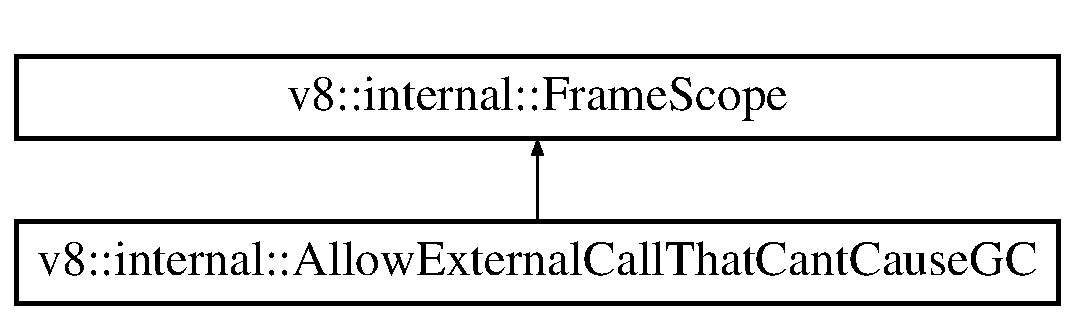
\includegraphics[height=2.000000cm]{classv8_1_1internal_1_1_allow_external_call_that_cant_cause_g_c}
\end{center}
\end{figure}
\subsection*{Public Member Functions}
\begin{DoxyCompactItemize}
\item 
\hypertarget{classv8_1_1internal_1_1_allow_external_call_that_cant_cause_g_c_ae136159f715f0afd4a7f76629f7bca48}{}{\bfseries Allow\+External\+Call\+That\+Cant\+Cause\+G\+C} (Macro\+Assembler $\ast$masm)\label{classv8_1_1internal_1_1_allow_external_call_that_cant_cause_g_c_ae136159f715f0afd4a7f76629f7bca48}

\end{DoxyCompactItemize}


The documentation for this class was generated from the following file\+:\begin{DoxyCompactItemize}
\item 
src/macro-\/assembler.\+h\end{DoxyCompactItemize}

\hypertarget{classv8_1_1internal_1_1_code_1_1_allow_o_s_r_at_loop_nesting_level_field}{}\section{v8\+:\+:internal\+:\+:Code\+:\+:Allow\+O\+S\+R\+At\+Loop\+Nesting\+Level\+Field Class Reference}
\label{classv8_1_1internal_1_1_code_1_1_allow_o_s_r_at_loop_nesting_level_field}\index{v8\+::internal\+::\+Code\+::\+Allow\+O\+S\+R\+At\+Loop\+Nesting\+Level\+Field@{v8\+::internal\+::\+Code\+::\+Allow\+O\+S\+R\+At\+Loop\+Nesting\+Level\+Field}}
Inheritance diagram for v8\+:\+:internal\+:\+:Code\+:\+:Allow\+O\+S\+R\+At\+Loop\+Nesting\+Level\+Field\+:\begin{figure}[H]
\begin{center}
\leavevmode
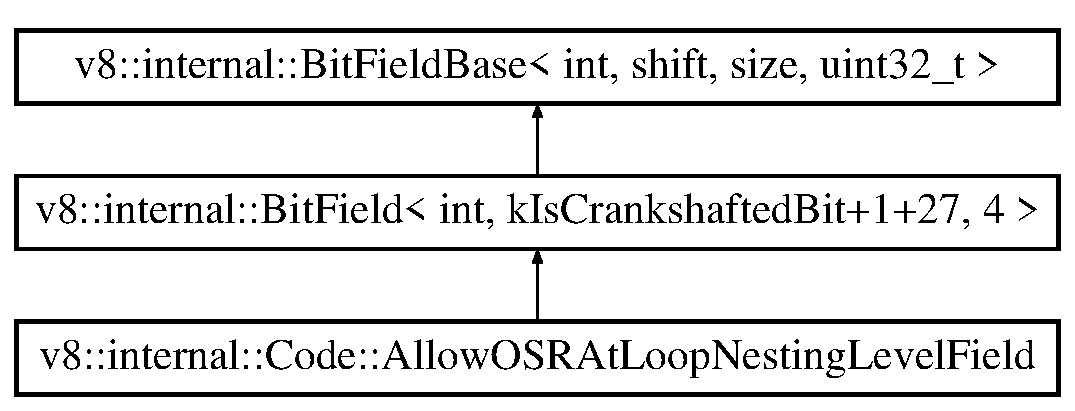
\includegraphics[height=3.000000cm]{classv8_1_1internal_1_1_code_1_1_allow_o_s_r_at_loop_nesting_level_field}
\end{center}
\end{figure}
\subsection*{Additional Inherited Members}


The documentation for this class was generated from the following file\+:\begin{DoxyCompactItemize}
\item 
src/objects.\+h\end{DoxyCompactItemize}

\hypertarget{classv8_1_1internal_1_1_all_static}{}\section{v8\+:\+:internal\+:\+:All\+Static Class Reference}
\label{classv8_1_1internal_1_1_all_static}\index{v8\+::internal\+::\+All\+Static@{v8\+::internal\+::\+All\+Static}}
Inheritance diagram for v8\+:\+:internal\+:\+:All\+Static\+:\begin{figure}[H]
\begin{center}
\leavevmode
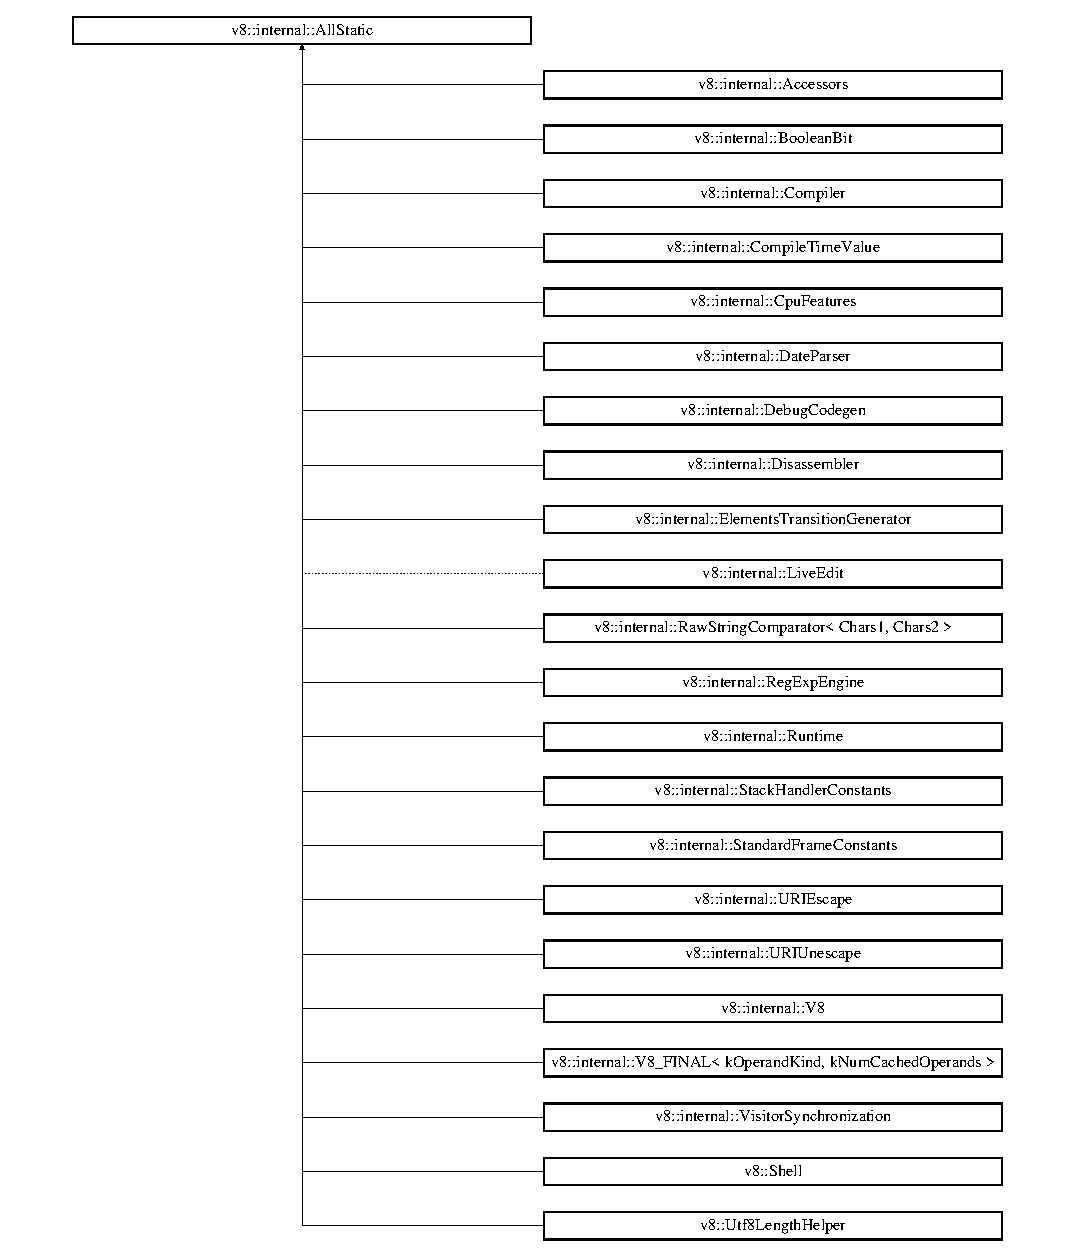
\includegraphics[height=12.000000cm]{classv8_1_1internal_1_1_all_static}
\end{center}
\end{figure}


The documentation for this class was generated from the following file\+:\begin{DoxyCompactItemize}
\item 
src/allocation.\+h\end{DoxyCompactItemize}

\hypertarget{classv8_1_1internal_1_1_alternative_generation}{}\section{v8\+:\+:internal\+:\+:Alternative\+Generation Class Reference}
\label{classv8_1_1internal_1_1_alternative_generation}\index{v8\+::internal\+::\+Alternative\+Generation@{v8\+::internal\+::\+Alternative\+Generation}}
Inheritance diagram for v8\+:\+:internal\+:\+:Alternative\+Generation\+:\begin{figure}[H]
\begin{center}
\leavevmode
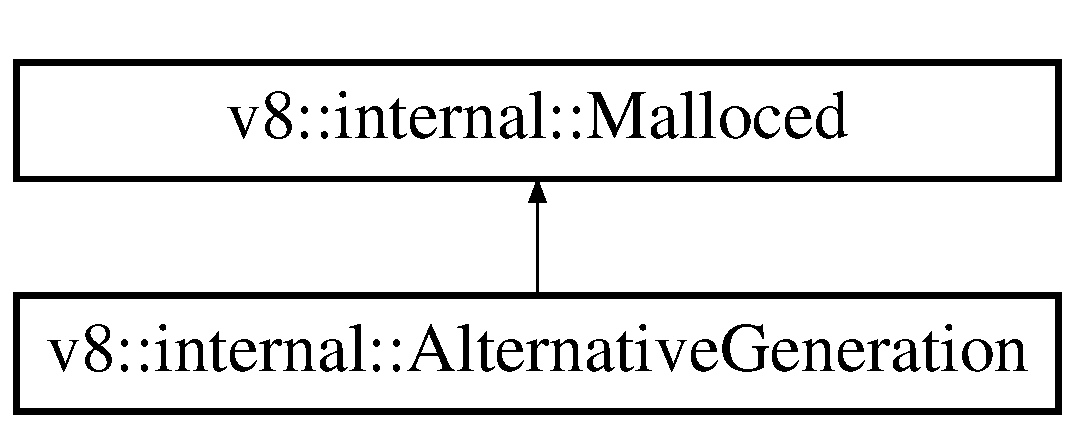
\includegraphics[height=2.000000cm]{classv8_1_1internal_1_1_alternative_generation}
\end{center}
\end{figure}
\subsection*{Public Attributes}
\begin{DoxyCompactItemize}
\item 
\hypertarget{classv8_1_1internal_1_1_alternative_generation_a6b2881c2cd1292cb0423fd4dab2ca823}{}Label {\bfseries possible\+\_\+success}\label{classv8_1_1internal_1_1_alternative_generation_a6b2881c2cd1292cb0423fd4dab2ca823}

\item 
\hypertarget{classv8_1_1internal_1_1_alternative_generation_a71eb17f16f4e5201f9f251c9fe74a507}{}bool {\bfseries expects\+\_\+preload}\label{classv8_1_1internal_1_1_alternative_generation_a71eb17f16f4e5201f9f251c9fe74a507}

\item 
\hypertarget{classv8_1_1internal_1_1_alternative_generation_a5640bb3e3f745d0b4705cd21ae741361}{}Label {\bfseries after}\label{classv8_1_1internal_1_1_alternative_generation_a5640bb3e3f745d0b4705cd21ae741361}

\item 
\hypertarget{classv8_1_1internal_1_1_alternative_generation_a727fcad75b108bd5288f5771aae86831}{}\hyperlink{classv8_1_1internal_1_1_quick_check_details}{Quick\+Check\+Details} {\bfseries quick\+\_\+check\+\_\+details}\label{classv8_1_1internal_1_1_alternative_generation_a727fcad75b108bd5288f5771aae86831}

\end{DoxyCompactItemize}
\subsection*{Additional Inherited Members}


The documentation for this class was generated from the following file\+:\begin{DoxyCompactItemize}
\item 
src/jsregexp.\+cc\end{DoxyCompactItemize}

\hypertarget{classv8_1_1internal_1_1_alternative_generation_list}{}\section{v8\+:\+:internal\+:\+:Alternative\+Generation\+List Class Reference}
\label{classv8_1_1internal_1_1_alternative_generation_list}\index{v8\+::internal\+::\+Alternative\+Generation\+List@{v8\+::internal\+::\+Alternative\+Generation\+List}}
\subsection*{Public Member Functions}
\begin{DoxyCompactItemize}
\item 
\hypertarget{classv8_1_1internal_1_1_alternative_generation_list_a12e31ade267f3b97c25bf9201fe3b65a}{}{\bfseries Alternative\+Generation\+List} (int count, \hyperlink{classv8_1_1internal_1_1_zone}{Zone} $\ast$zone)\label{classv8_1_1internal_1_1_alternative_generation_list_a12e31ade267f3b97c25bf9201fe3b65a}

\item 
\hypertarget{classv8_1_1internal_1_1_alternative_generation_list_a074eac77994a3714b4214b777fce5b2a}{}\hyperlink{classv8_1_1internal_1_1_alternative_generation}{Alternative\+Generation} $\ast$ {\bfseries at} (int i)\label{classv8_1_1internal_1_1_alternative_generation_list_a074eac77994a3714b4214b777fce5b2a}

\end{DoxyCompactItemize}


The documentation for this class was generated from the following file\+:\begin{DoxyCompactItemize}
\item 
src/jsregexp.\+cc\end{DoxyCompactItemize}

\hypertarget{structv8_1_1internal_1_1_effects_mixin_1_1_alt_merger}{}\section{v8\+:\+:internal\+:\+:Effects\+Mixin$<$ Var, Base, Effects $>$\+:\+:Alt\+Merger$<$ Self $>$ Struct Template Reference}
\label{structv8_1_1internal_1_1_effects_mixin_1_1_alt_merger}\index{v8\+::internal\+::\+Effects\+Mixin$<$ Var, Base, Effects $>$\+::\+Alt\+Merger$<$ Self $>$@{v8\+::internal\+::\+Effects\+Mixin$<$ Var, Base, Effects $>$\+::\+Alt\+Merger$<$ Self $>$}}
\subsection*{Public Member Functions}
\begin{DoxyCompactItemize}
\item 
\hypertarget{structv8_1_1internal_1_1_effects_mixin_1_1_alt_merger_af4a6516fe49c9b9287f1618f37d357b3}{}void {\bfseries Call} (Var var, \hyperlink{structv8_1_1internal_1_1_effect}{Effect} effect)\label{structv8_1_1internal_1_1_effects_mixin_1_1_alt_merger_af4a6516fe49c9b9287f1618f37d357b3}

\end{DoxyCompactItemize}
\subsection*{Public Attributes}
\begin{DoxyCompactItemize}
\item 
\hypertarget{structv8_1_1internal_1_1_effects_mixin_1_1_alt_merger_a89a5575969d2cbfab82bd8726165e2ac}{}Self {\bfseries self}\label{structv8_1_1internal_1_1_effects_mixin_1_1_alt_merger_a89a5575969d2cbfab82bd8726165e2ac}

\end{DoxyCompactItemize}


The documentation for this struct was generated from the following file\+:\begin{DoxyCompactItemize}
\item 
src/effects.\+h\end{DoxyCompactItemize}

\hypertarget{structv8_1_1internal_1_1_effects_mixin_1_1_alt_weakener}{}\section{v8\+:\+:internal\+:\+:Effects\+Mixin$<$ Var, Base, Effects $>$\+:\+:Alt\+Weakener$<$ Self $>$ Struct Template Reference}
\label{structv8_1_1internal_1_1_effects_mixin_1_1_alt_weakener}\index{v8\+::internal\+::\+Effects\+Mixin$<$ Var, Base, Effects $>$\+::\+Alt\+Weakener$<$ Self $>$@{v8\+::internal\+::\+Effects\+Mixin$<$ Var, Base, Effects $>$\+::\+Alt\+Weakener$<$ Self $>$}}
\subsection*{Public Member Functions}
\begin{DoxyCompactItemize}
\item 
\hypertarget{structv8_1_1internal_1_1_effects_mixin_1_1_alt_weakener_a651cd436a421f5b78abc43754e8309a3}{}void {\bfseries Call} (Var var, \hyperlink{structv8_1_1internal_1_1_effect}{Effect} effect)\label{structv8_1_1internal_1_1_effects_mixin_1_1_alt_weakener_a651cd436a421f5b78abc43754e8309a3}

\end{DoxyCompactItemize}
\subsection*{Public Attributes}
\begin{DoxyCompactItemize}
\item 
\hypertarget{structv8_1_1internal_1_1_effects_mixin_1_1_alt_weakener_ae73da3655748ec9da62f755efd66633a}{}Self {\bfseries self}\label{structv8_1_1internal_1_1_effects_mixin_1_1_alt_weakener_ae73da3655748ec9da62f755efd66633a}

\item 
\hypertarget{structv8_1_1internal_1_1_effects_mixin_1_1_alt_weakener_adde1918061d0bb8bd6148becfeef5e84}{}\hyperlink{classv8_1_1internal_1_1_effects}{Effects} {\bfseries other}\label{structv8_1_1internal_1_1_effects_mixin_1_1_alt_weakener_adde1918061d0bb8bd6148becfeef5e84}

\end{DoxyCompactItemize}


The documentation for this struct was generated from the following file\+:\begin{DoxyCompactItemize}
\item 
src/effects.\+h\end{DoxyCompactItemize}

\hypertarget{classv8_1_1internal_1_1_analysis}{}\section{v8\+:\+:internal\+:\+:Analysis Class Reference}
\label{classv8_1_1internal_1_1_analysis}\index{v8\+::internal\+::\+Analysis@{v8\+::internal\+::\+Analysis}}
Inheritance diagram for v8\+:\+:internal\+:\+:Analysis\+:\begin{figure}[H]
\begin{center}
\leavevmode
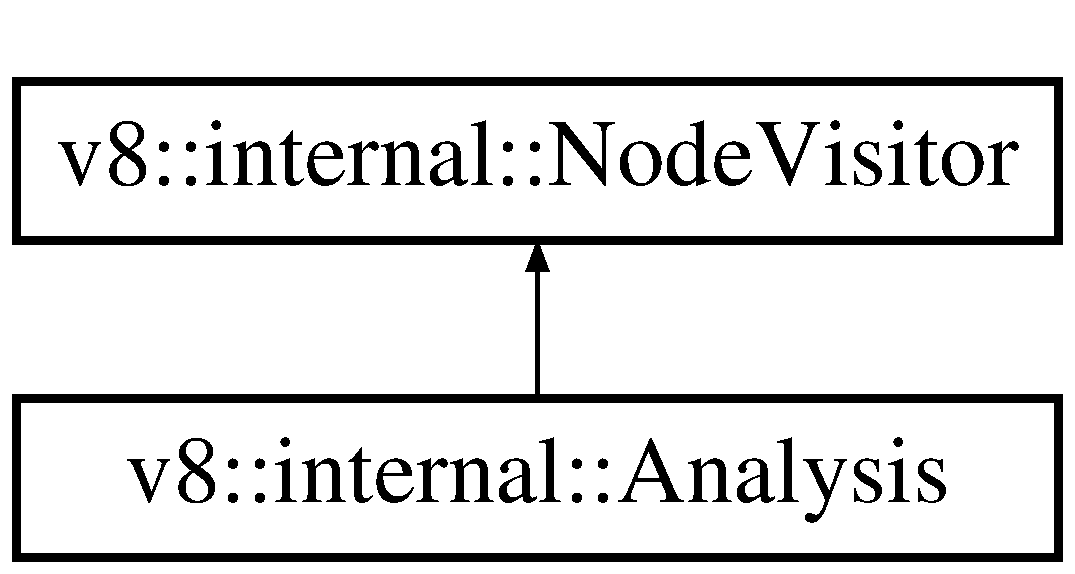
\includegraphics[height=2.000000cm]{classv8_1_1internal_1_1_analysis}
\end{center}
\end{figure}
\subsection*{Public Member Functions}
\begin{DoxyCompactItemize}
\item 
\hypertarget{classv8_1_1internal_1_1_analysis_a90d7b97c1fa821b017667f542031f9ae}{}{\bfseries Analysis} (bool ignore\+\_\+case, bool is\+\_\+ascii)\label{classv8_1_1internal_1_1_analysis_a90d7b97c1fa821b017667f542031f9ae}

\item 
\hypertarget{classv8_1_1internal_1_1_analysis_a91ea9ab34a0b720e4ba0414997e6f978}{}void {\bfseries Ensure\+Analyzed} (\hyperlink{classv8_1_1internal_1_1_reg_exp_node}{Reg\+Exp\+Node} $\ast$node)\label{classv8_1_1internal_1_1_analysis_a91ea9ab34a0b720e4ba0414997e6f978}

\item 
\hypertarget{classv8_1_1internal_1_1_analysis_aa6a0b113e9b8a9268a3af41dbdc24ff6}{}virtual void {\bfseries Visit\+Loop\+Choice} (\hyperlink{classv8_1_1internal_1_1_loop_choice_node}{Loop\+Choice\+Node} $\ast$that)\label{classv8_1_1internal_1_1_analysis_aa6a0b113e9b8a9268a3af41dbdc24ff6}

\item 
\hypertarget{classv8_1_1internal_1_1_analysis_a49fb801db5532a96bc0c078e3c928910}{}bool {\bfseries has\+\_\+failed} ()\label{classv8_1_1internal_1_1_analysis_a49fb801db5532a96bc0c078e3c928910}

\item 
\hypertarget{classv8_1_1internal_1_1_analysis_a70729ef89c68f6ba50909873d438fe47}{}const char $\ast$ {\bfseries error\+\_\+message} ()\label{classv8_1_1internal_1_1_analysis_a70729ef89c68f6ba50909873d438fe47}

\item 
\hypertarget{classv8_1_1internal_1_1_analysis_ae430a167d7e2e6cf98834465c537a64e}{}void {\bfseries fail} (const char $\ast$error\+\_\+message)\label{classv8_1_1internal_1_1_analysis_ae430a167d7e2e6cf98834465c537a64e}

\end{DoxyCompactItemize}


The documentation for this class was generated from the following files\+:\begin{DoxyCompactItemize}
\item 
src/jsregexp.\+h\item 
src/jsregexp.\+cc\end{DoxyCompactItemize}

\hypertarget{classv8_1_1_api_function}{}\section{v8\+:\+:Api\+Function Class Reference}
\label{classv8_1_1_api_function}\index{v8\+::\+Api\+Function@{v8\+::\+Api\+Function}}
\subsection*{Public Member Functions}
\begin{DoxyCompactItemize}
\item 
\hypertarget{classv8_1_1_api_function_a711c062e7328b2cd864a755290ccc70c}{}{\bfseries Api\+Function} (v8\+::internal\+::\+Address addr)\label{classv8_1_1_api_function_a711c062e7328b2cd864a755290ccc70c}

\item 
\hypertarget{classv8_1_1_api_function_ae3168a2d34c3c799c4aae32a9c3bdba2}{}v8\+::internal\+::\+Address {\bfseries address} ()\label{classv8_1_1_api_function_ae3168a2d34c3c799c4aae32a9c3bdba2}

\end{DoxyCompactItemize}


The documentation for this class was generated from the following file\+:\begin{DoxyCompactItemize}
\item 
src/api.\+h\end{DoxyCompactItemize}

\hypertarget{classv8_1_1internal_1_1_arguments_access_stub}{}\section{v8\+:\+:internal\+:\+:Arguments\+Access\+Stub Class Reference}
\label{classv8_1_1internal_1_1_arguments_access_stub}\index{v8\+::internal\+::\+Arguments\+Access\+Stub@{v8\+::internal\+::\+Arguments\+Access\+Stub}}
Inheritance diagram for v8\+:\+:internal\+:\+:Arguments\+Access\+Stub\+:\begin{figure}[H]
\begin{center}
\leavevmode
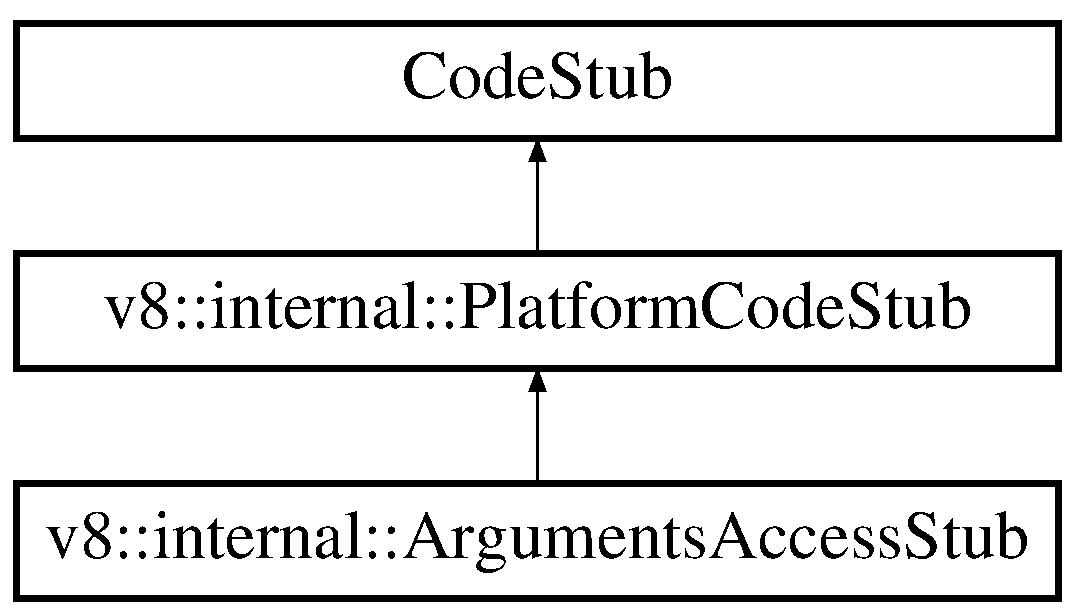
\includegraphics[height=3.000000cm]{classv8_1_1internal_1_1_arguments_access_stub}
\end{center}
\end{figure}
\subsection*{Public Types}
\begin{DoxyCompactItemize}
\item 
\hypertarget{classv8_1_1internal_1_1_arguments_access_stub_a5b0ef2969a63a5eba537d5d0955686ee}{}enum {\bfseries Type} \{ {\bfseries R\+E\+A\+D\+\_\+\+E\+L\+E\+M\+E\+N\+T}, 
{\bfseries N\+E\+W\+\_\+\+S\+L\+O\+P\+P\+Y\+\_\+\+F\+A\+S\+T}, 
{\bfseries N\+E\+W\+\_\+\+S\+L\+O\+P\+P\+Y\+\_\+\+S\+L\+O\+W}, 
{\bfseries N\+E\+W\+\_\+\+S\+T\+R\+I\+C\+T}
 \}\label{classv8_1_1internal_1_1_arguments_access_stub_a5b0ef2969a63a5eba537d5d0955686ee}

\end{DoxyCompactItemize}
\subsection*{Public Member Functions}
\begin{DoxyCompactItemize}
\item 
\hypertarget{classv8_1_1internal_1_1_arguments_access_stub_ac83e90029dbc7049ef495f847d6198b2}{}{\bfseries Arguments\+Access\+Stub} (\hyperlink{classv8_1_1internal_1_1_isolate}{Isolate} $\ast$isolate, Type type)\label{classv8_1_1internal_1_1_arguments_access_stub_ac83e90029dbc7049ef495f847d6198b2}

\end{DoxyCompactItemize}
\subsection*{Additional Inherited Members}


The documentation for this class was generated from the following files\+:\begin{DoxyCompactItemize}
\item 
src/code-\/stubs.\+h\item 
src/code-\/stubs.\+cc\item 
src/codegen.\+cc\end{DoxyCompactItemize}

\hypertarget{classv8_1_1internal_1_1_arguments_adaptor_frame}{}\section{v8\+:\+:internal\+:\+:Arguments\+Adaptor\+Frame Class Reference}
\label{classv8_1_1internal_1_1_arguments_adaptor_frame}\index{v8\+::internal\+::\+Arguments\+Adaptor\+Frame@{v8\+::internal\+::\+Arguments\+Adaptor\+Frame}}
Inheritance diagram for v8\+:\+:internal\+:\+:Arguments\+Adaptor\+Frame\+:\begin{figure}[H]
\begin{center}
\leavevmode
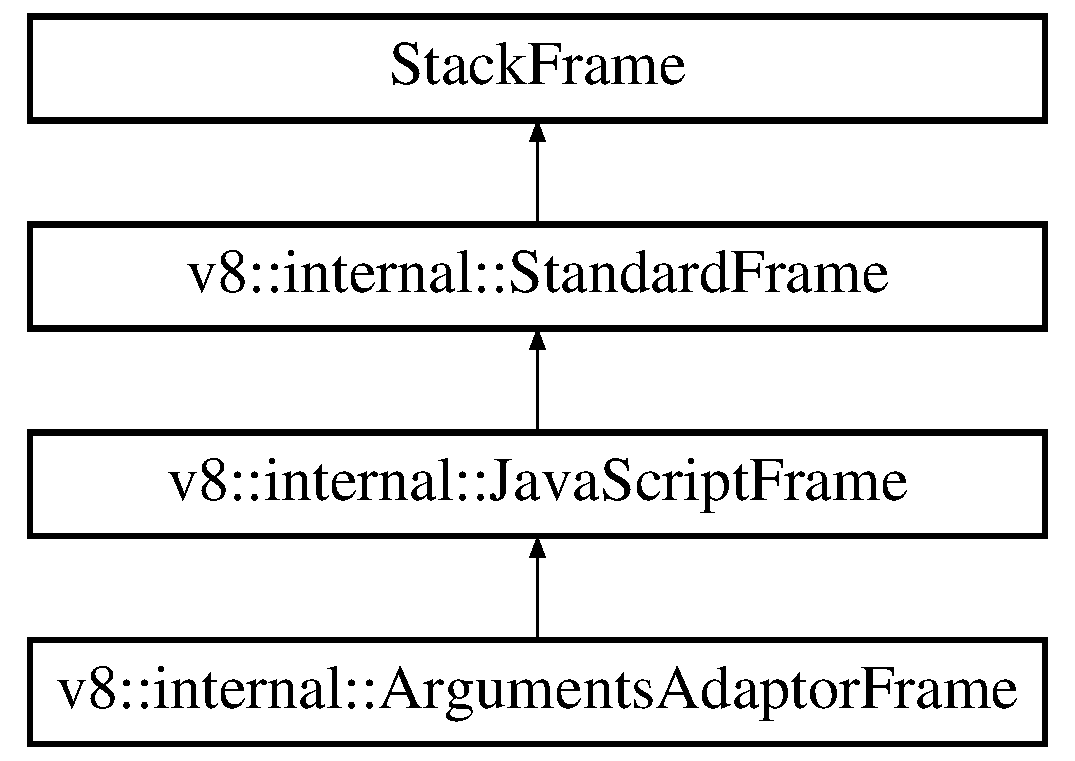
\includegraphics[height=4.000000cm]{classv8_1_1internal_1_1_arguments_adaptor_frame}
\end{center}
\end{figure}
\subsection*{Public Member Functions}
\begin{DoxyCompactItemize}
\item 
\hypertarget{classv8_1_1internal_1_1_arguments_adaptor_frame_a857a8f2c67d69acfe6ab5aa251c4acd2}{}virtual \hyperlink{classv8_1_1internal_1_1_type_impl}{Type} {\bfseries type} () const \label{classv8_1_1internal_1_1_arguments_adaptor_frame_a857a8f2c67d69acfe6ab5aa251c4acd2}

\item 
\hypertarget{classv8_1_1internal_1_1_arguments_adaptor_frame_a7957757e8f971b3cfc216bb4de8313aa}{}virtual \hyperlink{classv8_1_1internal_1_1_code}{Code} $\ast$ {\bfseries unchecked\+\_\+code} () const \label{classv8_1_1internal_1_1_arguments_adaptor_frame_a7957757e8f971b3cfc216bb4de8313aa}

\item 
\hypertarget{classv8_1_1internal_1_1_arguments_adaptor_frame_a0f3df5c6dcb8a76a7f52ae47adb5ae22}{}virtual void {\bfseries Print} (String\+Stream $\ast$accumulator, Print\+Mode mode, int index) const \label{classv8_1_1internal_1_1_arguments_adaptor_frame_a0f3df5c6dcb8a76a7f52ae47adb5ae22}

\end{DoxyCompactItemize}
\subsection*{Static Public Member Functions}
\begin{DoxyCompactItemize}
\item 
\hypertarget{classv8_1_1internal_1_1_arguments_adaptor_frame_a6b8283fe3991c88663621fdf586b67ca}{}static \hyperlink{classv8_1_1internal_1_1_arguments_adaptor_frame}{Arguments\+Adaptor\+Frame} $\ast$ {\bfseries cast} (Stack\+Frame $\ast$frame)\label{classv8_1_1internal_1_1_arguments_adaptor_frame_a6b8283fe3991c88663621fdf586b67ca}

\end{DoxyCompactItemize}
\subsection*{Protected Member Functions}
\begin{DoxyCompactItemize}
\item 
\hypertarget{classv8_1_1internal_1_1_arguments_adaptor_frame_ac2681526413000e2f5879bc2c0b0fd2f}{}{\bfseries Arguments\+Adaptor\+Frame} (Stack\+Frame\+Iterator\+Base $\ast$iterator)\label{classv8_1_1internal_1_1_arguments_adaptor_frame_ac2681526413000e2f5879bc2c0b0fd2f}

\item 
\hypertarget{classv8_1_1internal_1_1_arguments_adaptor_frame_ab8ccfd535f4db6dc07f17f9b43921571}{}virtual int {\bfseries Get\+Number\+Of\+Incoming\+Arguments} () const \label{classv8_1_1internal_1_1_arguments_adaptor_frame_ab8ccfd535f4db6dc07f17f9b43921571}

\item 
\hypertarget{classv8_1_1internal_1_1_arguments_adaptor_frame_aaf7fa9756e23315f0c1343cb7c3ea2e6}{}virtual Address {\bfseries Get\+Caller\+Stack\+Pointer} () const \label{classv8_1_1internal_1_1_arguments_adaptor_frame_aaf7fa9756e23315f0c1343cb7c3ea2e6}

\end{DoxyCompactItemize}
\subsection*{Friends}
\begin{DoxyCompactItemize}
\item 
\hypertarget{classv8_1_1internal_1_1_arguments_adaptor_frame_ac7310421866976ca454bbe11c5f926c3}{}class {\bfseries Stack\+Frame\+Iterator\+Base}\label{classv8_1_1internal_1_1_arguments_adaptor_frame_ac7310421866976ca454bbe11c5f926c3}

\end{DoxyCompactItemize}
\subsection*{Additional Inherited Members}


The documentation for this class was generated from the following files\+:\begin{DoxyCompactItemize}
\item 
src/frames.\+h\item 
src/frames-\/inl.\+h\item 
src/frames.\+cc\end{DoxyCompactItemize}

\hypertarget{classv8_1_1internal_1_1_b_a_s_e___e_m_b_e_d_d_e_d_1_1_arguments_field}{}\section{v8\+:\+:internal\+:\+:B\+A\+S\+E\+\_\+\+E\+M\+B\+E\+D\+D\+E\+D$<$ Visitor $>$\+:\+:Arguments\+Field Class Reference}
\label{classv8_1_1internal_1_1_b_a_s_e___e_m_b_e_d_d_e_d_1_1_arguments_field}\index{v8\+::internal\+::\+B\+A\+S\+E\+\_\+\+E\+M\+B\+E\+D\+D\+E\+D$<$ Visitor $>$\+::\+Arguments\+Field@{v8\+::internal\+::\+B\+A\+S\+E\+\_\+\+E\+M\+B\+E\+D\+D\+E\+D$<$ Visitor $>$\+::\+Arguments\+Field}}
Inheritance diagram for v8\+:\+:internal\+:\+:B\+A\+S\+E\+\_\+\+E\+M\+B\+E\+D\+D\+E\+D$<$ Visitor $>$\+:\+:Arguments\+Field\+:\begin{figure}[H]
\begin{center}
\leavevmode
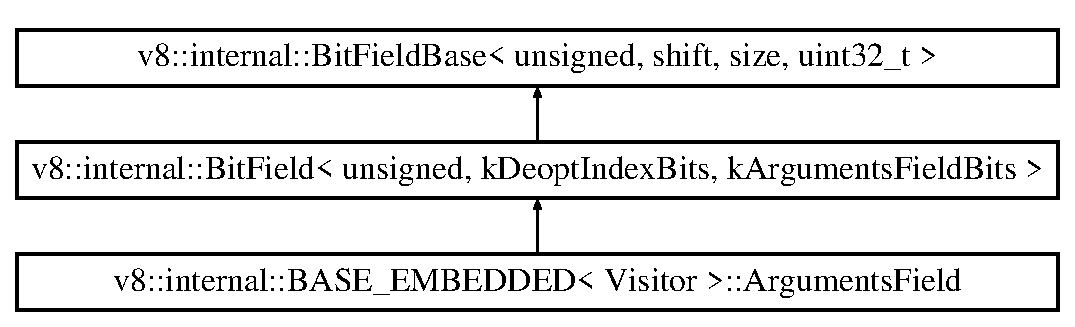
\includegraphics[height=3.000000cm]{classv8_1_1internal_1_1_b_a_s_e___e_m_b_e_d_d_e_d_1_1_arguments_field}
\end{center}
\end{figure}
\subsection*{Additional Inherited Members}


The documentation for this class was generated from the following file\+:\begin{DoxyCompactItemize}
\item 
src/safepoint-\/table.\+h\end{DoxyCompactItemize}

\hypertarget{classv8_1_1internal_1_1_array_concat_visitor}{}\section{v8\+:\+:internal\+:\+:Array\+Concat\+Visitor Class Reference}
\label{classv8_1_1internal_1_1_array_concat_visitor}\index{v8\+::internal\+::\+Array\+Concat\+Visitor@{v8\+::internal\+::\+Array\+Concat\+Visitor}}
\subsection*{Public Member Functions}
\begin{DoxyCompactItemize}
\item 
\hypertarget{classv8_1_1internal_1_1_array_concat_visitor_a6c0a40ee619a009eb147d5b64e3e67e9}{}{\bfseries Array\+Concat\+Visitor} (\hyperlink{classv8_1_1internal_1_1_isolate}{Isolate} $\ast$isolate, \hyperlink{classv8_1_1internal_1_1_handle}{Handle}$<$ \hyperlink{classv8_1_1internal_1_1_fixed_array}{Fixed\+Array} $>$ storage, bool fast\+\_\+elements)\label{classv8_1_1internal_1_1_array_concat_visitor_a6c0a40ee619a009eb147d5b64e3e67e9}

\item 
\hypertarget{classv8_1_1internal_1_1_array_concat_visitor_a40760600be9819cccc809177bd5b093e}{}void {\bfseries visit} (uint32\+\_\+t i, \hyperlink{classv8_1_1internal_1_1_handle}{Handle}$<$ \hyperlink{classv8_1_1internal_1_1_object}{Object} $>$ elm)\label{classv8_1_1internal_1_1_array_concat_visitor_a40760600be9819cccc809177bd5b093e}

\item 
\hypertarget{classv8_1_1internal_1_1_array_concat_visitor_a6e0c776e6fca2519d21308a5304759c7}{}void {\bfseries increase\+\_\+index\+\_\+offset} (uint32\+\_\+t delta)\label{classv8_1_1internal_1_1_array_concat_visitor_a6e0c776e6fca2519d21308a5304759c7}

\item 
\hypertarget{classv8_1_1internal_1_1_array_concat_visitor_a49bd86c6d367951c0505dda656c2c702}{}bool {\bfseries exceeds\+\_\+array\+\_\+limit} ()\label{classv8_1_1internal_1_1_array_concat_visitor_a49bd86c6d367951c0505dda656c2c702}

\item 
\hypertarget{classv8_1_1internal_1_1_array_concat_visitor_a71132108509a36a9a8f9f7530ef063ee}{}\hyperlink{classv8_1_1internal_1_1_handle}{Handle}$<$ \hyperlink{classv8_1_1internal_1_1_j_s_array}{J\+S\+Array} $>$ {\bfseries To\+Array} ()\label{classv8_1_1internal_1_1_array_concat_visitor_a71132108509a36a9a8f9f7530ef063ee}

\end{DoxyCompactItemize}


\subsection{Detailed Description}
A simple visitor visits every element of Array\textquotesingle{}s. The backend storage can be a fixed array for fast elements case, or a dictionary for sparse array. Since \hyperlink{classv8_1_1internal_1_1_dictionary}{Dictionary} is a subtype of \hyperlink{classv8_1_1internal_1_1_fixed_array}{Fixed\+Array}, the class can be used by both fast and slow cases. The second parameter of the constructor, fast\+\_\+elements, specifies whether the storage is a \hyperlink{classv8_1_1internal_1_1_fixed_array}{Fixed\+Array} or \hyperlink{classv8_1_1internal_1_1_dictionary}{Dictionary}.

An index limit is used to deal with the situation that a result array length overflows 32-\/bit non-\/negative integer. 

The documentation for this class was generated from the following file\+:\begin{DoxyCompactItemize}
\item 
src/runtime.\+cc\end{DoxyCompactItemize}

\hypertarget{classv8_1_1internal_1_1_array_constructor_stub}{}\section{v8\+:\+:internal\+:\+:Array\+Constructor\+Stub Class Reference}
\label{classv8_1_1internal_1_1_array_constructor_stub}\index{v8\+::internal\+::\+Array\+Constructor\+Stub@{v8\+::internal\+::\+Array\+Constructor\+Stub}}
Inheritance diagram for v8\+:\+:internal\+:\+:Array\+Constructor\+Stub\+:\begin{figure}[H]
\begin{center}
\leavevmode
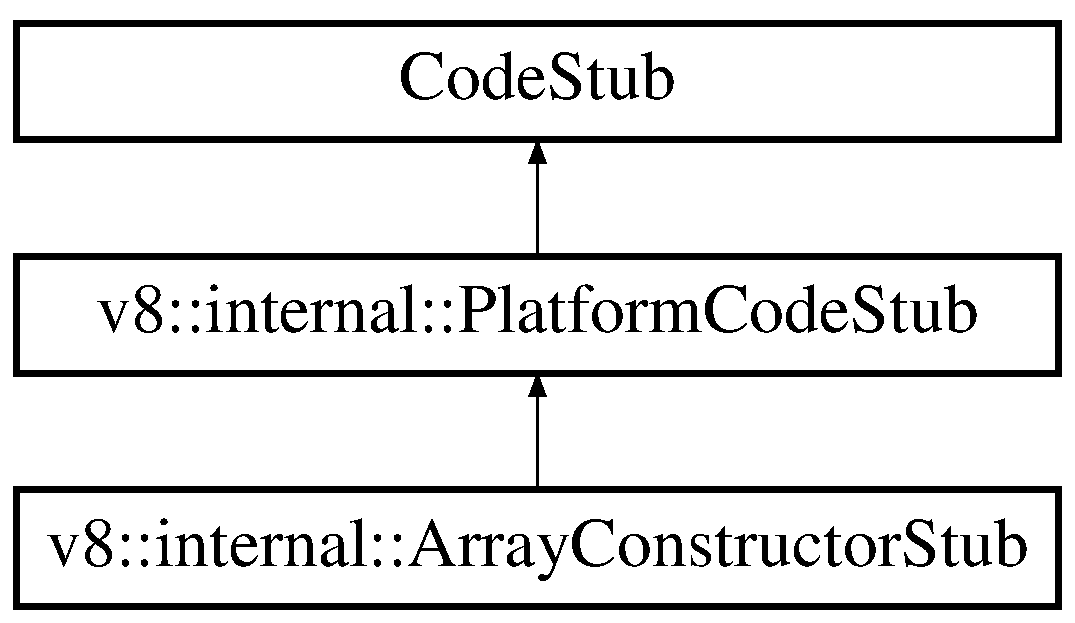
\includegraphics[height=3.000000cm]{classv8_1_1internal_1_1_array_constructor_stub}
\end{center}
\end{figure}
\subsection*{Public Types}
\begin{DoxyCompactItemize}
\item 
\hypertarget{classv8_1_1internal_1_1_array_constructor_stub_ad22d0f4b8c460b9c3cd6f1f96222a05f}{}enum {\bfseries Argument\+Count\+Key} \{ {\bfseries A\+N\+Y}, 
{\bfseries N\+O\+N\+E}, 
{\bfseries O\+N\+E}, 
{\bfseries M\+O\+R\+E\+\_\+\+T\+H\+A\+N\+\_\+\+O\+N\+E}
 \}\label{classv8_1_1internal_1_1_array_constructor_stub_ad22d0f4b8c460b9c3cd6f1f96222a05f}

\end{DoxyCompactItemize}
\subsection*{Public Member Functions}
\begin{DoxyCompactItemize}
\item 
\hypertarget{classv8_1_1internal_1_1_array_constructor_stub_ace8064ca0370fc661e2c52326016d7df}{}{\bfseries Array\+Constructor\+Stub} (\hyperlink{classv8_1_1internal_1_1_isolate}{Isolate} $\ast$isolate, int argument\+\_\+count)\label{classv8_1_1internal_1_1_array_constructor_stub_ace8064ca0370fc661e2c52326016d7df}

\item 
\hypertarget{classv8_1_1internal_1_1_array_constructor_stub_a091aa6dc4cd77eb388afaea10ea0a0d1}{}{\bfseries Array\+Constructor\+Stub} (\hyperlink{classv8_1_1internal_1_1_isolate}{Isolate} $\ast$isolate)\label{classv8_1_1internal_1_1_array_constructor_stub_a091aa6dc4cd77eb388afaea10ea0a0d1}

\item 
\hypertarget{classv8_1_1internal_1_1_array_constructor_stub_afe9c35f76257c57c434f1ae1e375d9f8}{}void {\bfseries Generate} (Macro\+Assembler $\ast$masm)\label{classv8_1_1internal_1_1_array_constructor_stub_afe9c35f76257c57c434f1ae1e375d9f8}

\end{DoxyCompactItemize}
\subsection*{Additional Inherited Members}


The documentation for this class was generated from the following files\+:\begin{DoxyCompactItemize}
\item 
src/code-\/stubs.\+h\item 
src/code-\/stubs.\+cc\end{DoxyCompactItemize}

\hypertarget{classv8_1_1internal_1_1_array_constructor_stub_base}{}\section{v8\+:\+:internal\+:\+:Array\+Constructor\+Stub\+Base Class Reference}
\label{classv8_1_1internal_1_1_array_constructor_stub_base}\index{v8\+::internal\+::\+Array\+Constructor\+Stub\+Base@{v8\+::internal\+::\+Array\+Constructor\+Stub\+Base}}
Inheritance diagram for v8\+:\+:internal\+:\+:Array\+Constructor\+Stub\+Base\+:\begin{figure}[H]
\begin{center}
\leavevmode
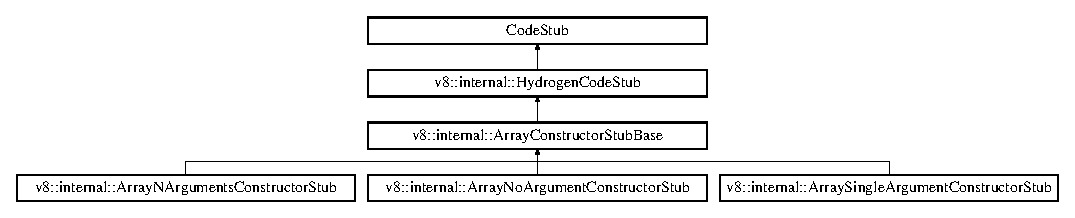
\includegraphics[height=2.480620cm]{classv8_1_1internal_1_1_array_constructor_stub_base}
\end{center}
\end{figure}
\subsection*{Public Member Functions}
\begin{DoxyCompactItemize}
\item 
\hypertarget{classv8_1_1internal_1_1_array_constructor_stub_base_a5f0e0ca83fe21bfce0f2504fd44cedc5}{}{\bfseries Array\+Constructor\+Stub\+Base} (\hyperlink{classv8_1_1internal_1_1_isolate}{Isolate} $\ast$isolate, Elements\+Kind kind, Allocation\+Site\+Override\+Mode override\+\_\+mode)\label{classv8_1_1internal_1_1_array_constructor_stub_base_a5f0e0ca83fe21bfce0f2504fd44cedc5}

\item 
\hypertarget{classv8_1_1internal_1_1_array_constructor_stub_base_ac736069b779982eb6c1e8c6049a419a4}{}Elements\+Kind {\bfseries elements\+\_\+kind} () const \label{classv8_1_1internal_1_1_array_constructor_stub_base_ac736069b779982eb6c1e8c6049a419a4}

\item 
\hypertarget{classv8_1_1internal_1_1_array_constructor_stub_base_a0d4e21d13752ba4a649c4b12c5beb8b3}{}Allocation\+Site\+Override\+Mode {\bfseries override\+\_\+mode} () const \label{classv8_1_1internal_1_1_array_constructor_stub_base_a0d4e21d13752ba4a649c4b12c5beb8b3}

\end{DoxyCompactItemize}
\subsection*{Static Public Member Functions}
\begin{DoxyCompactItemize}
\item 
\hypertarget{classv8_1_1internal_1_1_array_constructor_stub_base_a2a1630e7b51bd5b96b1b742cd57f0225}{}static void {\bfseries Generate\+Stubs\+Ahead\+Of\+Time} (\hyperlink{classv8_1_1internal_1_1_isolate}{Isolate} $\ast$isolate)\label{classv8_1_1internal_1_1_array_constructor_stub_base_a2a1630e7b51bd5b96b1b742cd57f0225}

\item 
\hypertarget{classv8_1_1internal_1_1_array_constructor_stub_base_a317016e4c8c76f21711e8ca541109dc6}{}static void {\bfseries Install\+Descriptors} (\hyperlink{classv8_1_1internal_1_1_isolate}{Isolate} $\ast$isolate)\label{classv8_1_1internal_1_1_array_constructor_stub_base_a317016e4c8c76f21711e8ca541109dc6}

\end{DoxyCompactItemize}
\subsection*{Static Public Attributes}
\begin{DoxyCompactItemize}
\item 
\hypertarget{classv8_1_1internal_1_1_array_constructor_stub_base_a1f996ab3d2ddf2b485379945f126708d}{}static const int {\bfseries k\+Constructor} = 0\label{classv8_1_1internal_1_1_array_constructor_stub_base_a1f996ab3d2ddf2b485379945f126708d}

\item 
\hypertarget{classv8_1_1internal_1_1_array_constructor_stub_base_a95c8024ef3984c0a3862451761ea4226}{}static const int {\bfseries k\+Allocation\+Site} = 1\label{classv8_1_1internal_1_1_array_constructor_stub_base_a95c8024ef3984c0a3862451761ea4226}

\end{DoxyCompactItemize}
\subsection*{Protected Member Functions}
\begin{DoxyCompactItemize}
\item 
\hypertarget{classv8_1_1internal_1_1_array_constructor_stub_base_a2a491cf0c6beb60a323fc0d2ea03c035}{}\hyperlink{classv8_1_1internal_1_1_o_stream}{O\+Stream} \& {\bfseries Base\+Print\+Name} (\hyperlink{classv8_1_1internal_1_1_o_stream}{O\+Stream} \&os, const char $\ast$name) const \label{classv8_1_1internal_1_1_array_constructor_stub_base_a2a491cf0c6beb60a323fc0d2ea03c035}

\end{DoxyCompactItemize}
\subsection*{Additional Inherited Members}


The documentation for this class was generated from the following files\+:\begin{DoxyCompactItemize}
\item 
src/code-\/stubs.\+h\item 
src/code-\/stubs.\+cc\end{DoxyCompactItemize}

\hypertarget{structv8_1_1internal_1_1_array_deallocator}{}\section{v8\+:\+:internal\+:\+:Array\+Deallocator$<$ T $>$ Struct Template Reference}
\label{structv8_1_1internal_1_1_array_deallocator}\index{v8\+::internal\+::\+Array\+Deallocator$<$ T $>$@{v8\+::internal\+::\+Array\+Deallocator$<$ T $>$}}
\subsection*{Static Public Member Functions}
\begin{DoxyCompactItemize}
\item 
\hypertarget{structv8_1_1internal_1_1_array_deallocator_a9bbfd873370a246a77ec445644ffa058}{}static void {\bfseries Delete} (T $\ast$array)\label{structv8_1_1internal_1_1_array_deallocator_a9bbfd873370a246a77ec445644ffa058}

\end{DoxyCompactItemize}


The documentation for this struct was generated from the following file\+:\begin{DoxyCompactItemize}
\item 
src/smart-\/pointers.\+h\end{DoxyCompactItemize}

\hypertarget{classv8_1_1internal_1_1_name_1_1_array_index_length_bits}{}\section{v8\+:\+:internal\+:\+:Name\+:\+:Array\+Index\+Length\+Bits Class Reference}
\label{classv8_1_1internal_1_1_name_1_1_array_index_length_bits}\index{v8\+::internal\+::\+Name\+::\+Array\+Index\+Length\+Bits@{v8\+::internal\+::\+Name\+::\+Array\+Index\+Length\+Bits}}
Inheritance diagram for v8\+:\+:internal\+:\+:Name\+:\+:Array\+Index\+Length\+Bits\+:\begin{figure}[H]
\begin{center}
\leavevmode
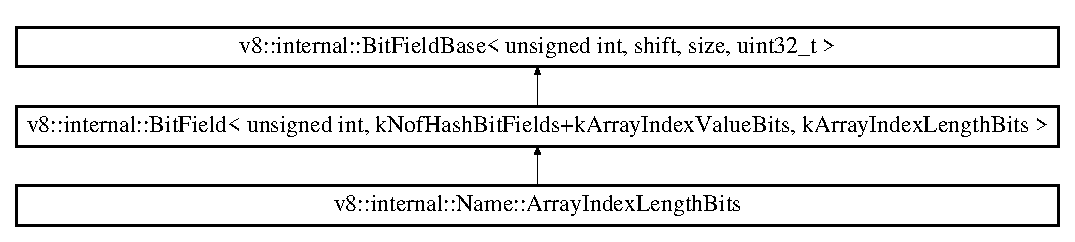
\includegraphics[height=2.800000cm]{classv8_1_1internal_1_1_name_1_1_array_index_length_bits}
\end{center}
\end{figure}
\subsection*{Additional Inherited Members}


The documentation for this class was generated from the following file\+:\begin{DoxyCompactItemize}
\item 
src/objects.\+h\end{DoxyCompactItemize}

\hypertarget{classv8_1_1internal_1_1_string_1_1_array_index_length_bits}{}\section{v8\+:\+:internal\+:\+:String\+:\+:Array\+Index\+Length\+Bits Class Reference}
\label{classv8_1_1internal_1_1_string_1_1_array_index_length_bits}\index{v8\+::internal\+::\+String\+::\+Array\+Index\+Length\+Bits@{v8\+::internal\+::\+String\+::\+Array\+Index\+Length\+Bits}}
Inheritance diagram for v8\+:\+:internal\+:\+:String\+:\+:Array\+Index\+Length\+Bits\+:\begin{figure}[H]
\begin{center}
\leavevmode
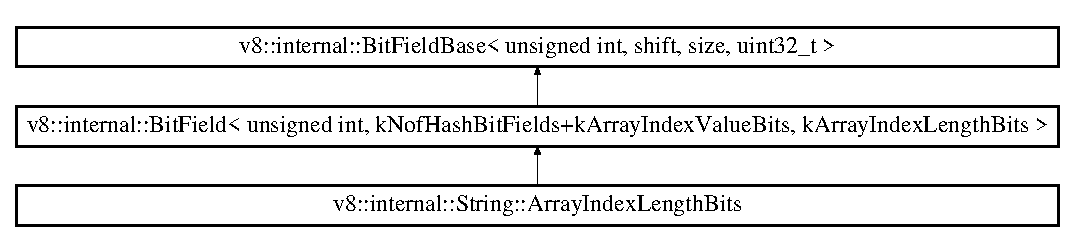
\includegraphics[height=2.800000cm]{classv8_1_1internal_1_1_string_1_1_array_index_length_bits}
\end{center}
\end{figure}
\subsection*{Additional Inherited Members}


The documentation for this class was generated from the following file\+:\begin{DoxyCompactItemize}
\item 
src/objects.\+h\end{DoxyCompactItemize}

\hypertarget{classv8_1_1internal_1_1_name_1_1_array_index_value_bits}{}\section{v8\+:\+:internal\+:\+:Name\+:\+:Array\+Index\+Value\+Bits Class Reference}
\label{classv8_1_1internal_1_1_name_1_1_array_index_value_bits}\index{v8\+::internal\+::\+Name\+::\+Array\+Index\+Value\+Bits@{v8\+::internal\+::\+Name\+::\+Array\+Index\+Value\+Bits}}
Inheritance diagram for v8\+:\+:internal\+:\+:Name\+:\+:Array\+Index\+Value\+Bits\+:\begin{figure}[H]
\begin{center}
\leavevmode
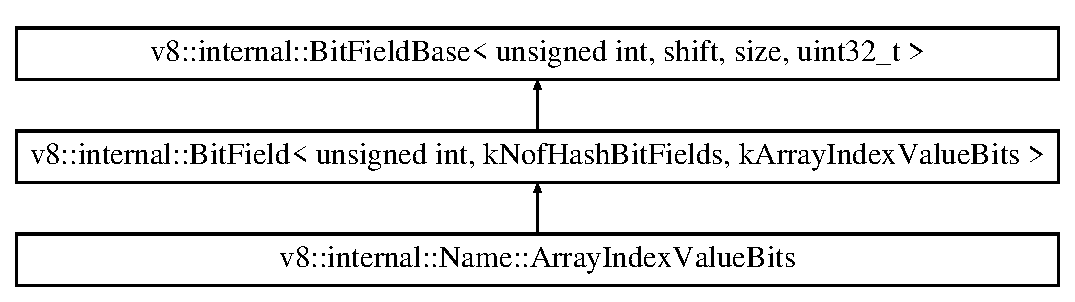
\includegraphics[height=3.000000cm]{classv8_1_1internal_1_1_name_1_1_array_index_value_bits}
\end{center}
\end{figure}
\subsection*{Additional Inherited Members}


The documentation for this class was generated from the following file\+:\begin{DoxyCompactItemize}
\item 
src/objects.\+h\end{DoxyCompactItemize}

\hypertarget{classv8_1_1internal_1_1_string_1_1_array_index_value_bits}{}\section{v8\+:\+:internal\+:\+:String\+:\+:Array\+Index\+Value\+Bits Class Reference}
\label{classv8_1_1internal_1_1_string_1_1_array_index_value_bits}\index{v8\+::internal\+::\+String\+::\+Array\+Index\+Value\+Bits@{v8\+::internal\+::\+String\+::\+Array\+Index\+Value\+Bits}}
Inheritance diagram for v8\+:\+:internal\+:\+:String\+:\+:Array\+Index\+Value\+Bits\+:\begin{figure}[H]
\begin{center}
\leavevmode
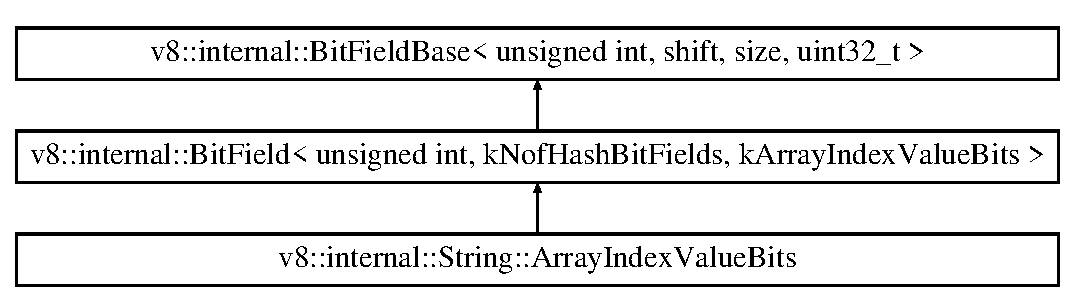
\includegraphics[height=3.000000cm]{classv8_1_1internal_1_1_string_1_1_array_index_value_bits}
\end{center}
\end{figure}
\subsection*{Additional Inherited Members}


The documentation for this class was generated from the following file\+:\begin{DoxyCompactItemize}
\item 
src/objects.\+h\end{DoxyCompactItemize}

\hypertarget{classv8_1_1internal_1_1_array_instruction_interface}{}\section{v8\+:\+:internal\+:\+:Array\+Instruction\+Interface Class Reference}
\label{classv8_1_1internal_1_1_array_instruction_interface}\index{v8\+::internal\+::\+Array\+Instruction\+Interface@{v8\+::internal\+::\+Array\+Instruction\+Interface}}
Inheritance diagram for v8\+:\+:internal\+:\+:Array\+Instruction\+Interface\+:\begin{figure}[H]
\begin{center}
\leavevmode
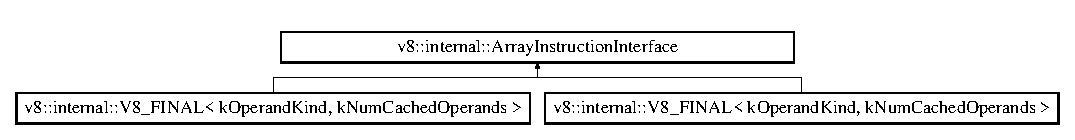
\includegraphics[height=1.428571cm]{classv8_1_1internal_1_1_array_instruction_interface}
\end{center}
\end{figure}
\subsection*{Public Member Functions}
\begin{DoxyCompactItemize}
\item 
\hypertarget{classv8_1_1internal_1_1_array_instruction_interface_a3b00965803a4aa2d245049e197386bb9}{}virtual \hyperlink{classv8_1_1internal_1_1_h_value}{H\+Value} $\ast$ {\bfseries Get\+Key} ()=0\label{classv8_1_1internal_1_1_array_instruction_interface_a3b00965803a4aa2d245049e197386bb9}

\item 
\hypertarget{classv8_1_1internal_1_1_array_instruction_interface_a69d53bd082b5e37c7921cedcfcec11ca}{}virtual void {\bfseries Set\+Key} (\hyperlink{classv8_1_1internal_1_1_h_value}{H\+Value} $\ast$key)=0\label{classv8_1_1internal_1_1_array_instruction_interface_a69d53bd082b5e37c7921cedcfcec11ca}

\item 
\hypertarget{classv8_1_1internal_1_1_array_instruction_interface_aac09602c5f8429516b4ec69a671c9c32}{}virtual Elements\+Kind {\bfseries elements\+\_\+kind} () const =0\label{classv8_1_1internal_1_1_array_instruction_interface_aac09602c5f8429516b4ec69a671c9c32}

\item 
\hypertarget{classv8_1_1internal_1_1_array_instruction_interface_a5413df5ba2cb580d7687ae5a44f43123}{}virtual bool {\bfseries Try\+Increase\+Base\+Offset} (uint32\+\_\+t increase\+\_\+by\+\_\+value)=0\label{classv8_1_1internal_1_1_array_instruction_interface_a5413df5ba2cb580d7687ae5a44f43123}

\item 
\hypertarget{classv8_1_1internal_1_1_array_instruction_interface_aeb68f8c83fb80f901517fb90237a1bca}{}virtual bool {\bfseries Is\+Dehoisted} () const =0\label{classv8_1_1internal_1_1_array_instruction_interface_aeb68f8c83fb80f901517fb90237a1bca}

\item 
\hypertarget{classv8_1_1internal_1_1_array_instruction_interface_a83bec181df124504e55948b6847f60ac}{}virtual void {\bfseries Set\+Dehoisted} (bool is\+\_\+dehoisted)=0\label{classv8_1_1internal_1_1_array_instruction_interface_a83bec181df124504e55948b6847f60ac}

\end{DoxyCompactItemize}
\subsection*{Static Public Member Functions}
\begin{DoxyCompactItemize}
\item 
\hypertarget{classv8_1_1internal_1_1_array_instruction_interface_a3e05ea86b4cb765cfb92f4b5f5b504f5}{}static \hyperlink{classv8_1_1internal_1_1_representation}{Representation} {\bfseries Keyed\+Access\+Index\+Requirement} (\hyperlink{classv8_1_1internal_1_1_representation}{Representation} r)\label{classv8_1_1internal_1_1_array_instruction_interface_a3e05ea86b4cb765cfb92f4b5f5b504f5}

\end{DoxyCompactItemize}


The documentation for this class was generated from the following file\+:\begin{DoxyCompactItemize}
\item 
src/hydrogen-\/instructions.\+h\end{DoxyCompactItemize}

\hypertarget{classv8_1_1internal_1_1_array_n_arguments_constructor_stub}{}\section{v8\+:\+:internal\+:\+:Array\+N\+Arguments\+Constructor\+Stub Class Reference}
\label{classv8_1_1internal_1_1_array_n_arguments_constructor_stub}\index{v8\+::internal\+::\+Array\+N\+Arguments\+Constructor\+Stub@{v8\+::internal\+::\+Array\+N\+Arguments\+Constructor\+Stub}}
Inheritance diagram for v8\+:\+:internal\+:\+:Array\+N\+Arguments\+Constructor\+Stub\+:\begin{figure}[H]
\begin{center}
\leavevmode
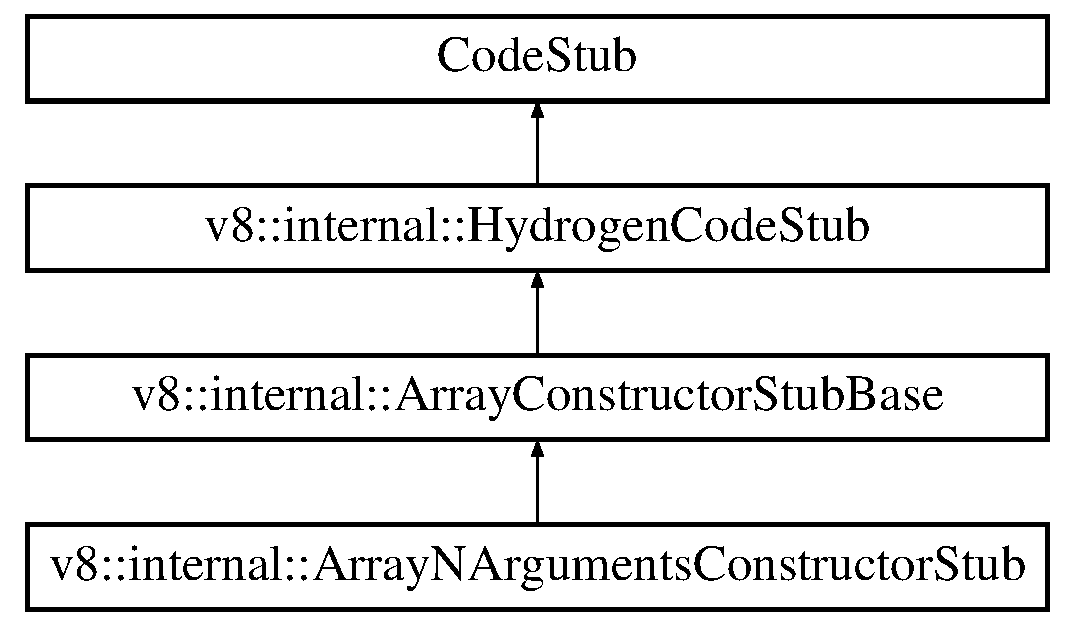
\includegraphics[height=4.000000cm]{classv8_1_1internal_1_1_array_n_arguments_constructor_stub}
\end{center}
\end{figure}
\subsection*{Public Member Functions}
\begin{DoxyCompactItemize}
\item 
\hypertarget{classv8_1_1internal_1_1_array_n_arguments_constructor_stub_a9ec2931b8761a2b39a5c9b569d404a47}{}{\bfseries Array\+N\+Arguments\+Constructor\+Stub} (\hyperlink{classv8_1_1internal_1_1_isolate}{Isolate} $\ast$isolate, Elements\+Kind kind, Allocation\+Site\+Override\+Mode override\+\_\+mode=D\+O\+N\+T\+\_\+\+O\+V\+E\+R\+R\+I\+D\+E)\label{classv8_1_1internal_1_1_array_n_arguments_constructor_stub_a9ec2931b8761a2b39a5c9b569d404a47}

\item 
\hypertarget{classv8_1_1internal_1_1_array_n_arguments_constructor_stub_afedf940551e906ecc410be1bf2a3f4ad}{}virtual \hyperlink{classv8_1_1internal_1_1_handle}{Handle}$<$ \hyperlink{classv8_1_1internal_1_1_code}{Code} $>$ {\bfseries Generate\+Code} () V8\+\_\+\+O\+V\+E\+R\+R\+I\+D\+E\label{classv8_1_1internal_1_1_array_n_arguments_constructor_stub_afedf940551e906ecc410be1bf2a3f4ad}

\item 
\hypertarget{classv8_1_1internal_1_1_array_n_arguments_constructor_stub_a2e4a946b9c0315bb62fd6940d4f5ad7f}{}virtual void {\bfseries Initialize\+Interface\+Descriptor} (\hyperlink{classv8_1_1internal_1_1_code_stub_interface_descriptor}{Code\+Stub\+Interface\+Descriptor} $\ast$descriptor) V8\+\_\+\+O\+V\+E\+R\+R\+I\+D\+E\label{classv8_1_1internal_1_1_array_n_arguments_constructor_stub_a2e4a946b9c0315bb62fd6940d4f5ad7f}

\end{DoxyCompactItemize}
\subsection*{Additional Inherited Members}


The documentation for this class was generated from the following files\+:\begin{DoxyCompactItemize}
\item 
src/code-\/stubs.\+h\item 
src/code-\/stubs-\/hydrogen.\+cc\end{DoxyCompactItemize}

\hypertarget{classv8_1_1internal_1_1_array_no_argument_constructor_stub}{}\section{v8\+:\+:internal\+:\+:Array\+No\+Argument\+Constructor\+Stub Class Reference}
\label{classv8_1_1internal_1_1_array_no_argument_constructor_stub}\index{v8\+::internal\+::\+Array\+No\+Argument\+Constructor\+Stub@{v8\+::internal\+::\+Array\+No\+Argument\+Constructor\+Stub}}
Inheritance diagram for v8\+:\+:internal\+:\+:Array\+No\+Argument\+Constructor\+Stub\+:\begin{figure}[H]
\begin{center}
\leavevmode
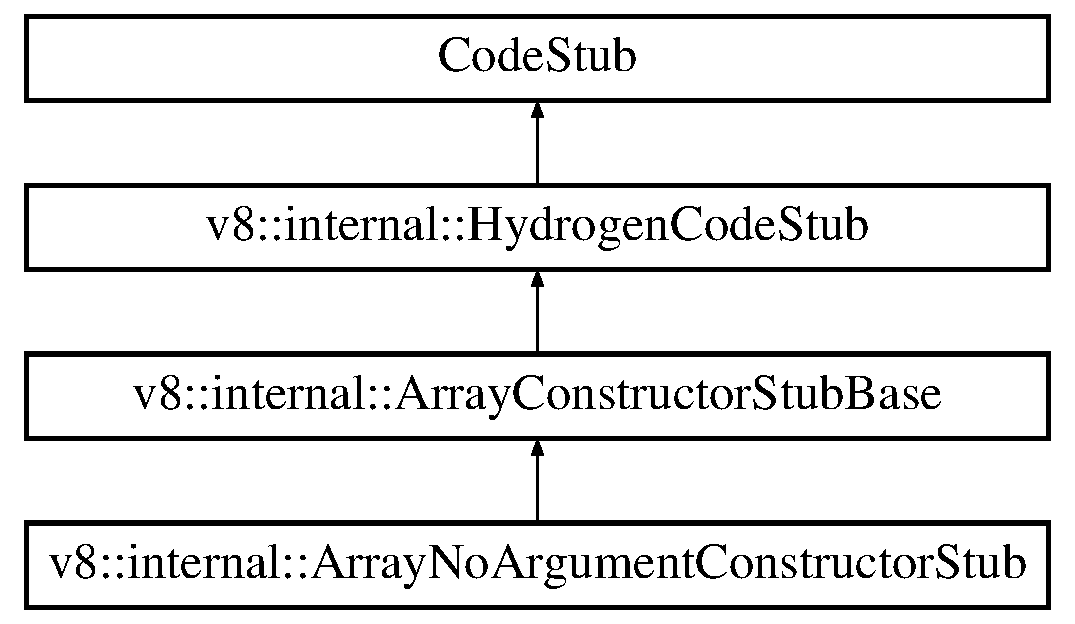
\includegraphics[height=4.000000cm]{classv8_1_1internal_1_1_array_no_argument_constructor_stub}
\end{center}
\end{figure}
\subsection*{Public Member Functions}
\begin{DoxyCompactItemize}
\item 
\hypertarget{classv8_1_1internal_1_1_array_no_argument_constructor_stub_a4b397b510eb1fa18711048d7ffb4b2ca}{}{\bfseries Array\+No\+Argument\+Constructor\+Stub} (\hyperlink{classv8_1_1internal_1_1_isolate}{Isolate} $\ast$isolate, Elements\+Kind kind, Allocation\+Site\+Override\+Mode override\+\_\+mode=D\+O\+N\+T\+\_\+\+O\+V\+E\+R\+R\+I\+D\+E)\label{classv8_1_1internal_1_1_array_no_argument_constructor_stub_a4b397b510eb1fa18711048d7ffb4b2ca}

\item 
\hypertarget{classv8_1_1internal_1_1_array_no_argument_constructor_stub_a94a42fc3f23a48e607a9a2f4948db761}{}virtual \hyperlink{classv8_1_1internal_1_1_handle}{Handle}$<$ \hyperlink{classv8_1_1internal_1_1_code}{Code} $>$ {\bfseries Generate\+Code} () V8\+\_\+\+O\+V\+E\+R\+R\+I\+D\+E\label{classv8_1_1internal_1_1_array_no_argument_constructor_stub_a94a42fc3f23a48e607a9a2f4948db761}

\item 
\hypertarget{classv8_1_1internal_1_1_array_no_argument_constructor_stub_a6ba9b3916d4f8c1b492c9eed29388872}{}virtual void {\bfseries Initialize\+Interface\+Descriptor} (\hyperlink{classv8_1_1internal_1_1_code_stub_interface_descriptor}{Code\+Stub\+Interface\+Descriptor} $\ast$descriptor) V8\+\_\+\+O\+V\+E\+R\+R\+I\+D\+E\label{classv8_1_1internal_1_1_array_no_argument_constructor_stub_a6ba9b3916d4f8c1b492c9eed29388872}

\end{DoxyCompactItemize}
\subsection*{Additional Inherited Members}


The documentation for this class was generated from the following files\+:\begin{DoxyCompactItemize}
\item 
src/code-\/stubs.\+h\item 
src/code-\/stubs-\/hydrogen.\+cc\end{DoxyCompactItemize}

\hypertarget{classv8_1_1internal_1_1_array_single_argument_constructor_stub}{}\section{v8\+:\+:internal\+:\+:Array\+Single\+Argument\+Constructor\+Stub Class Reference}
\label{classv8_1_1internal_1_1_array_single_argument_constructor_stub}\index{v8\+::internal\+::\+Array\+Single\+Argument\+Constructor\+Stub@{v8\+::internal\+::\+Array\+Single\+Argument\+Constructor\+Stub}}
Inheritance diagram for v8\+:\+:internal\+:\+:Array\+Single\+Argument\+Constructor\+Stub\+:\begin{figure}[H]
\begin{center}
\leavevmode
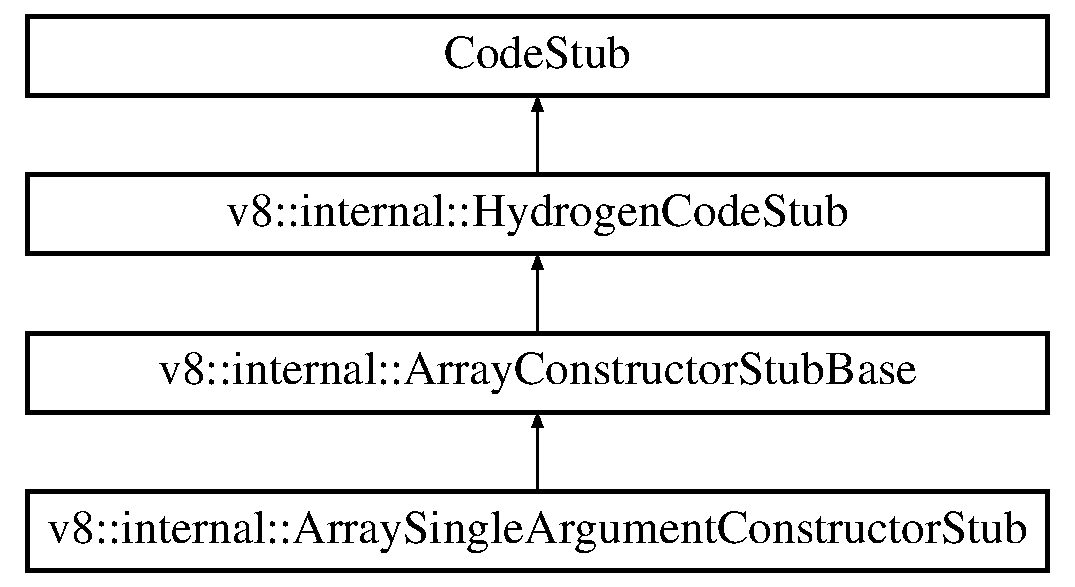
\includegraphics[height=4.000000cm]{classv8_1_1internal_1_1_array_single_argument_constructor_stub}
\end{center}
\end{figure}
\subsection*{Public Member Functions}
\begin{DoxyCompactItemize}
\item 
\hypertarget{classv8_1_1internal_1_1_array_single_argument_constructor_stub_a0cd99a369645effeaa12c445b17084bc}{}{\bfseries Array\+Single\+Argument\+Constructor\+Stub} (\hyperlink{classv8_1_1internal_1_1_isolate}{Isolate} $\ast$isolate, Elements\+Kind kind, Allocation\+Site\+Override\+Mode override\+\_\+mode=D\+O\+N\+T\+\_\+\+O\+V\+E\+R\+R\+I\+D\+E)\label{classv8_1_1internal_1_1_array_single_argument_constructor_stub_a0cd99a369645effeaa12c445b17084bc}

\item 
\hypertarget{classv8_1_1internal_1_1_array_single_argument_constructor_stub_aea6bf06235f89ea4f16f8059ae13b72d}{}virtual \hyperlink{classv8_1_1internal_1_1_handle}{Handle}$<$ \hyperlink{classv8_1_1internal_1_1_code}{Code} $>$ {\bfseries Generate\+Code} () V8\+\_\+\+O\+V\+E\+R\+R\+I\+D\+E\label{classv8_1_1internal_1_1_array_single_argument_constructor_stub_aea6bf06235f89ea4f16f8059ae13b72d}

\item 
\hypertarget{classv8_1_1internal_1_1_array_single_argument_constructor_stub_a33d2afc327f85d7cb96c7b1f49c8bb4f}{}virtual void {\bfseries Initialize\+Interface\+Descriptor} (\hyperlink{classv8_1_1internal_1_1_code_stub_interface_descriptor}{Code\+Stub\+Interface\+Descriptor} $\ast$descriptor) V8\+\_\+\+O\+V\+E\+R\+R\+I\+D\+E\label{classv8_1_1internal_1_1_array_single_argument_constructor_stub_a33d2afc327f85d7cb96c7b1f49c8bb4f}

\end{DoxyCompactItemize}
\subsection*{Additional Inherited Members}


The documentation for this class was generated from the following files\+:\begin{DoxyCompactItemize}
\item 
src/code-\/stubs.\+h\item 
src/code-\/stubs-\/hydrogen.\+cc\end{DoxyCompactItemize}

\hypertarget{classv8_1_1internal_1_1_type_impl_1_1_array_type}{}\section{v8\+:\+:internal\+:\+:Type\+Impl$<$ Config $>$\+:\+:Array\+Type Class Reference}
\label{classv8_1_1internal_1_1_type_impl_1_1_array_type}\index{v8\+::internal\+::\+Type\+Impl$<$ Config $>$\+::\+Array\+Type@{v8\+::internal\+::\+Type\+Impl$<$ Config $>$\+::\+Array\+Type}}
Inheritance diagram for v8\+:\+:internal\+:\+:Type\+Impl$<$ Config $>$\+:\+:Array\+Type\+:\begin{figure}[H]
\begin{center}
\leavevmode
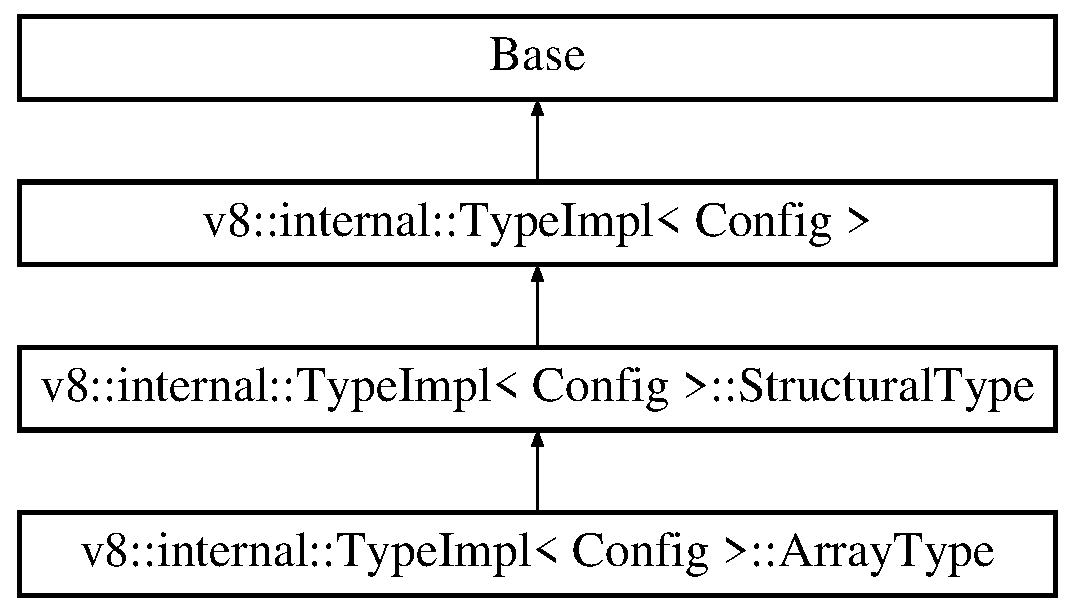
\includegraphics[height=4.000000cm]{classv8_1_1internal_1_1_type_impl_1_1_array_type}
\end{center}
\end{figure}
\subsection*{Public Member Functions}
\begin{DoxyCompactItemize}
\item 
\hypertarget{classv8_1_1internal_1_1_type_impl_1_1_array_type_aa923052efd22ee66049a7203dc8fea49}{}Type\+Handle {\bfseries Bound} ()\label{classv8_1_1internal_1_1_type_impl_1_1_array_type_aa923052efd22ee66049a7203dc8fea49}

\item 
\hypertarget{classv8_1_1internal_1_1_type_impl_1_1_array_type_acbaea05ea518a412f0a08bde6d0ec36d}{}Type\+Handle {\bfseries Element} ()\label{classv8_1_1internal_1_1_type_impl_1_1_array_type_acbaea05ea518a412f0a08bde6d0ec36d}

\end{DoxyCompactItemize}
\subsection*{Static Public Member Functions}
\begin{DoxyCompactItemize}
\item 
\hypertarget{classv8_1_1internal_1_1_type_impl_1_1_array_type_a49f031f505e5a6305d17fb0a9a2e0e80}{}static Array\+Handle {\bfseries New} (Type\+Handle element, Type\+Handle bound, Region $\ast$region)\label{classv8_1_1internal_1_1_type_impl_1_1_array_type_a49f031f505e5a6305d17fb0a9a2e0e80}

\item 
\hypertarget{classv8_1_1internal_1_1_type_impl_1_1_array_type_acea9c7a04d6c7e4be5599f73488c4a29}{}static Array\+Handle {\bfseries New} (Type\+Handle element, Region $\ast$region)\label{classv8_1_1internal_1_1_type_impl_1_1_array_type_acea9c7a04d6c7e4be5599f73488c4a29}

\item 
\hypertarget{classv8_1_1internal_1_1_type_impl_1_1_array_type_a8c1acef02cb705804eacb69591356c04}{}static \hyperlink{classv8_1_1internal_1_1_type_impl_1_1_array_type}{Array\+Type} $\ast$ {\bfseries cast} (\hyperlink{classv8_1_1internal_1_1_type_impl}{Type\+Impl} $\ast$type)\label{classv8_1_1internal_1_1_type_impl_1_1_array_type_a8c1acef02cb705804eacb69591356c04}

\end{DoxyCompactItemize}
\subsection*{Additional Inherited Members}


The documentation for this class was generated from the following file\+:\begin{DoxyCompactItemize}
\item 
src/types.\+h\end{DoxyCompactItemize}

\hypertarget{classv8_1_1internal_1_1_ascii_string_adapter}{}\section{v8\+:\+:internal\+:\+:Ascii\+String\+Adapter Class Reference}
\label{classv8_1_1internal_1_1_ascii_string_adapter}\index{v8\+::internal\+::\+Ascii\+String\+Adapter@{v8\+::internal\+::\+Ascii\+String\+Adapter}}
Inheritance diagram for v8\+:\+:internal\+:\+:Ascii\+String\+Adapter\+:\begin{figure}[H]
\begin{center}
\leavevmode
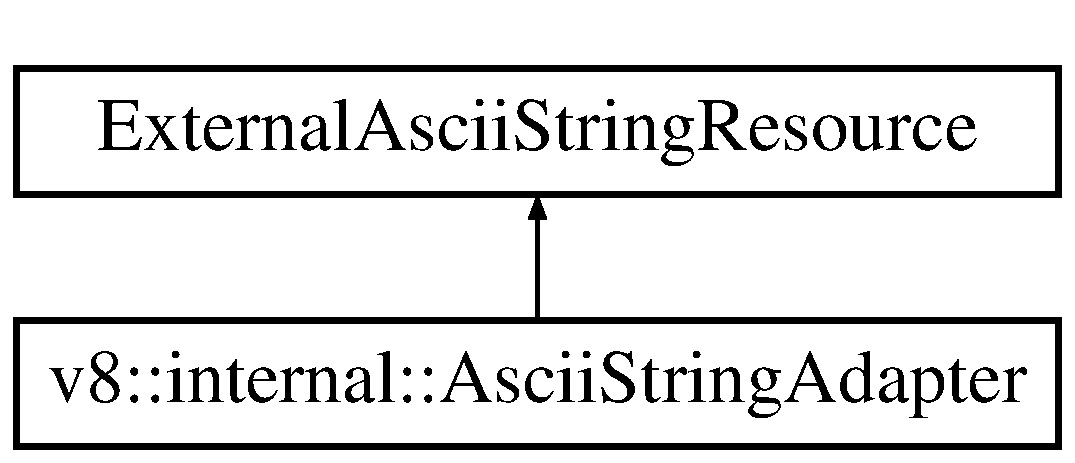
\includegraphics[height=2.000000cm]{classv8_1_1internal_1_1_ascii_string_adapter}
\end{center}
\end{figure}
\subsection*{Public Member Functions}
\begin{DoxyCompactItemize}
\item 
\hypertarget{classv8_1_1internal_1_1_ascii_string_adapter_a4d3a708be36d7605118f215633a9dd79}{}{\bfseries Ascii\+String\+Adapter} (\hyperlink{classv8_1_1internal_1_1_vector}{Vector}$<$ const char $>$ data)\label{classv8_1_1internal_1_1_ascii_string_adapter_a4d3a708be36d7605118f215633a9dd79}

\item 
\hypertarget{classv8_1_1internal_1_1_ascii_string_adapter_a0a6d9e189adfd85bab3480279012c225}{}virtual const char $\ast$ {\bfseries data} () const \label{classv8_1_1internal_1_1_ascii_string_adapter_a0a6d9e189adfd85bab3480279012c225}

\item 
\hypertarget{classv8_1_1internal_1_1_ascii_string_adapter_a5c08984324c9d18fbb5bdb802e5f9b90}{}virtual size\+\_\+t {\bfseries length} () const \label{classv8_1_1internal_1_1_ascii_string_adapter_a5c08984324c9d18fbb5bdb802e5f9b90}

\end{DoxyCompactItemize}


The documentation for this class was generated from the following file\+:\begin{DoxyCompactItemize}
\item 
src/utils.\+h\end{DoxyCompactItemize}

\hypertarget{classv8_1_1internal_1_1_assembler_base}{}\section{v8\+:\+:internal\+:\+:Assembler\+Base Class Reference}
\label{classv8_1_1internal_1_1_assembler_base}\index{v8\+::internal\+::\+Assembler\+Base@{v8\+::internal\+::\+Assembler\+Base}}
Inheritance diagram for v8\+:\+:internal\+:\+:Assembler\+Base\+:\begin{figure}[H]
\begin{center}
\leavevmode
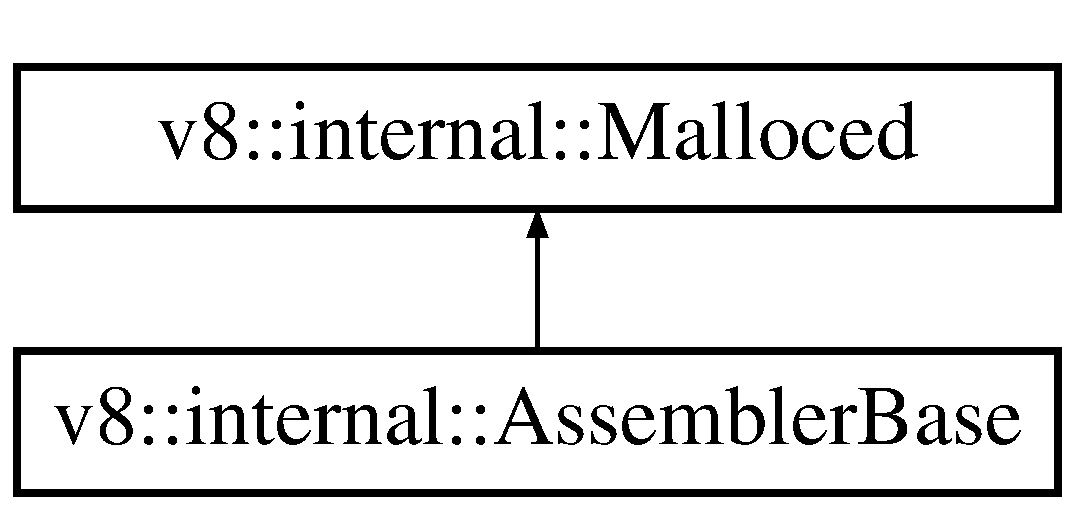
\includegraphics[height=2.000000cm]{classv8_1_1internal_1_1_assembler_base}
\end{center}
\end{figure}
\subsection*{Public Member Functions}
\begin{DoxyCompactItemize}
\item 
\hypertarget{classv8_1_1internal_1_1_assembler_base_a7ffa22cc463c9ee16ed46bfa38a5cd5b}{}{\bfseries Assembler\+Base} (\hyperlink{classv8_1_1internal_1_1_isolate}{Isolate} $\ast$isolate, void $\ast$buffer, int buffer\+\_\+size)\label{classv8_1_1internal_1_1_assembler_base_a7ffa22cc463c9ee16ed46bfa38a5cd5b}

\item 
\hypertarget{classv8_1_1internal_1_1_assembler_base_a51294386a61dda31ed1488228c48211a}{}\hyperlink{classv8_1_1internal_1_1_isolate}{Isolate} $\ast$ {\bfseries isolate} () const \label{classv8_1_1internal_1_1_assembler_base_a51294386a61dda31ed1488228c48211a}

\item 
\hypertarget{classv8_1_1internal_1_1_assembler_base_a47d3778081925b5ecf685b1a475c8057}{}int {\bfseries jit\+\_\+cookie} () const \label{classv8_1_1internal_1_1_assembler_base_a47d3778081925b5ecf685b1a475c8057}

\item 
\hypertarget{classv8_1_1internal_1_1_assembler_base_afc598637650acda081c8ebedb21ae3fc}{}bool {\bfseries emit\+\_\+debug\+\_\+code} () const \label{classv8_1_1internal_1_1_assembler_base_afc598637650acda081c8ebedb21ae3fc}

\item 
\hypertarget{classv8_1_1internal_1_1_assembler_base_a1bcbeda264b5026c463490820c91ffab}{}void {\bfseries set\+\_\+emit\+\_\+debug\+\_\+code} (bool value)\label{classv8_1_1internal_1_1_assembler_base_a1bcbeda264b5026c463490820c91ffab}

\item 
\hypertarget{classv8_1_1internal_1_1_assembler_base_a43270aa31fe8878c96b1cb2f07e11c17}{}bool {\bfseries serializer\+\_\+enabled} () const \label{classv8_1_1internal_1_1_assembler_base_a43270aa31fe8878c96b1cb2f07e11c17}

\item 
\hypertarget{classv8_1_1internal_1_1_assembler_base_a602b8f228f5491bdf8d02e7f3a55fdc9}{}void {\bfseries enable\+\_\+serializer} ()\label{classv8_1_1internal_1_1_assembler_base_a602b8f228f5491bdf8d02e7f3a55fdc9}

\item 
\hypertarget{classv8_1_1internal_1_1_assembler_base_afdc8e88acea34bc05e20f10a7e511264}{}bool {\bfseries predictable\+\_\+code\+\_\+size} () const \label{classv8_1_1internal_1_1_assembler_base_afdc8e88acea34bc05e20f10a7e511264}

\item 
\hypertarget{classv8_1_1internal_1_1_assembler_base_a8fb65d4cafef633546c2143aac9d090d}{}void {\bfseries set\+\_\+predictable\+\_\+code\+\_\+size} (bool value)\label{classv8_1_1internal_1_1_assembler_base_a8fb65d4cafef633546c2143aac9d090d}

\item 
\hypertarget{classv8_1_1internal_1_1_assembler_base_a4037253a85548558ccb31c87f27c8401}{}uint64\+\_\+t {\bfseries enabled\+\_\+cpu\+\_\+features} () const \label{classv8_1_1internal_1_1_assembler_base_a4037253a85548558ccb31c87f27c8401}

\item 
\hypertarget{classv8_1_1internal_1_1_assembler_base_a042d7907d4097ff5f4bc4cb0685b47a7}{}void {\bfseries set\+\_\+enabled\+\_\+cpu\+\_\+features} (uint64\+\_\+t features)\label{classv8_1_1internal_1_1_assembler_base_a042d7907d4097ff5f4bc4cb0685b47a7}

\item 
\hypertarget{classv8_1_1internal_1_1_assembler_base_a1eaf5b9a9d0998b6bc3104cf32c08d7c}{}bool {\bfseries Is\+Enabled} (Cpu\+Feature f)\label{classv8_1_1internal_1_1_assembler_base_a1eaf5b9a9d0998b6bc3104cf32c08d7c}

\item 
\hypertarget{classv8_1_1internal_1_1_assembler_base_a956cd6617b0ebddba1df67bfe6b138cd}{}int {\bfseries pc\+\_\+offset} () const \label{classv8_1_1internal_1_1_assembler_base_a956cd6617b0ebddba1df67bfe6b138cd}

\item 
\hypertarget{classv8_1_1internal_1_1_assembler_base_aa5bf23c158a9df7762e8529aeda8e25e}{}virtual void {\bfseries Aborted\+Code\+Generation} ()\label{classv8_1_1internal_1_1_assembler_base_aa5bf23c158a9df7762e8529aeda8e25e}

\end{DoxyCompactItemize}
\subsection*{Static Public Member Functions}
\begin{DoxyCompactItemize}
\item 
\hypertarget{classv8_1_1internal_1_1_assembler_base_a11f5cc896549fe763ac528492f16111e}{}static void {\bfseries Quiet\+Na\+N} (\hyperlink{classv8_1_1internal_1_1_heap_object}{Heap\+Object} $\ast$nan)\label{classv8_1_1internal_1_1_assembler_base_a11f5cc896549fe763ac528492f16111e}

\end{DoxyCompactItemize}
\subsection*{Static Public Attributes}
\begin{DoxyCompactItemize}
\item 
\hypertarget{classv8_1_1internal_1_1_assembler_base_a58ac353bfad9e4a1206864e76baec7f8}{}static const int {\bfseries k\+Minimal\+Buffer\+Size} = 4$\ast$K\+B\label{classv8_1_1internal_1_1_assembler_base_a58ac353bfad9e4a1206864e76baec7f8}

\end{DoxyCompactItemize}
\subsection*{Protected Attributes}
\begin{DoxyCompactItemize}
\item 
\hypertarget{classv8_1_1internal_1_1_assembler_base_ad344ab4ee5927986bb2c17e63aa5a976}{}byte $\ast$ {\bfseries buffer\+\_\+}\label{classv8_1_1internal_1_1_assembler_base_ad344ab4ee5927986bb2c17e63aa5a976}

\item 
\hypertarget{classv8_1_1internal_1_1_assembler_base_a83cced380ff671163b1969b2ed2aa33c}{}int {\bfseries buffer\+\_\+size\+\_\+}\label{classv8_1_1internal_1_1_assembler_base_a83cced380ff671163b1969b2ed2aa33c}

\item 
\hypertarget{classv8_1_1internal_1_1_assembler_base_a9ec9983a6ada967f6b1d03551b2615d2}{}bool {\bfseries own\+\_\+buffer\+\_\+}\label{classv8_1_1internal_1_1_assembler_base_a9ec9983a6ada967f6b1d03551b2615d2}

\item 
\hypertarget{classv8_1_1internal_1_1_assembler_base_ae4d9536957f5e1b5336125b9c5c4d2f8}{}byte $\ast$ {\bfseries pc\+\_\+}\label{classv8_1_1internal_1_1_assembler_base_ae4d9536957f5e1b5336125b9c5c4d2f8}

\end{DoxyCompactItemize}


The documentation for this class was generated from the following files\+:\begin{DoxyCompactItemize}
\item 
src/assembler.\+h\item 
src/assembler.\+cc\end{DoxyCompactItemize}

\hypertarget{classv8_1_1internal_1_1_assertion_node}{}\section{v8\+:\+:internal\+:\+:Assertion\+Node Class Reference}
\label{classv8_1_1internal_1_1_assertion_node}\index{v8\+::internal\+::\+Assertion\+Node@{v8\+::internal\+::\+Assertion\+Node}}
Inheritance diagram for v8\+:\+:internal\+:\+:Assertion\+Node\+:\begin{figure}[H]
\begin{center}
\leavevmode
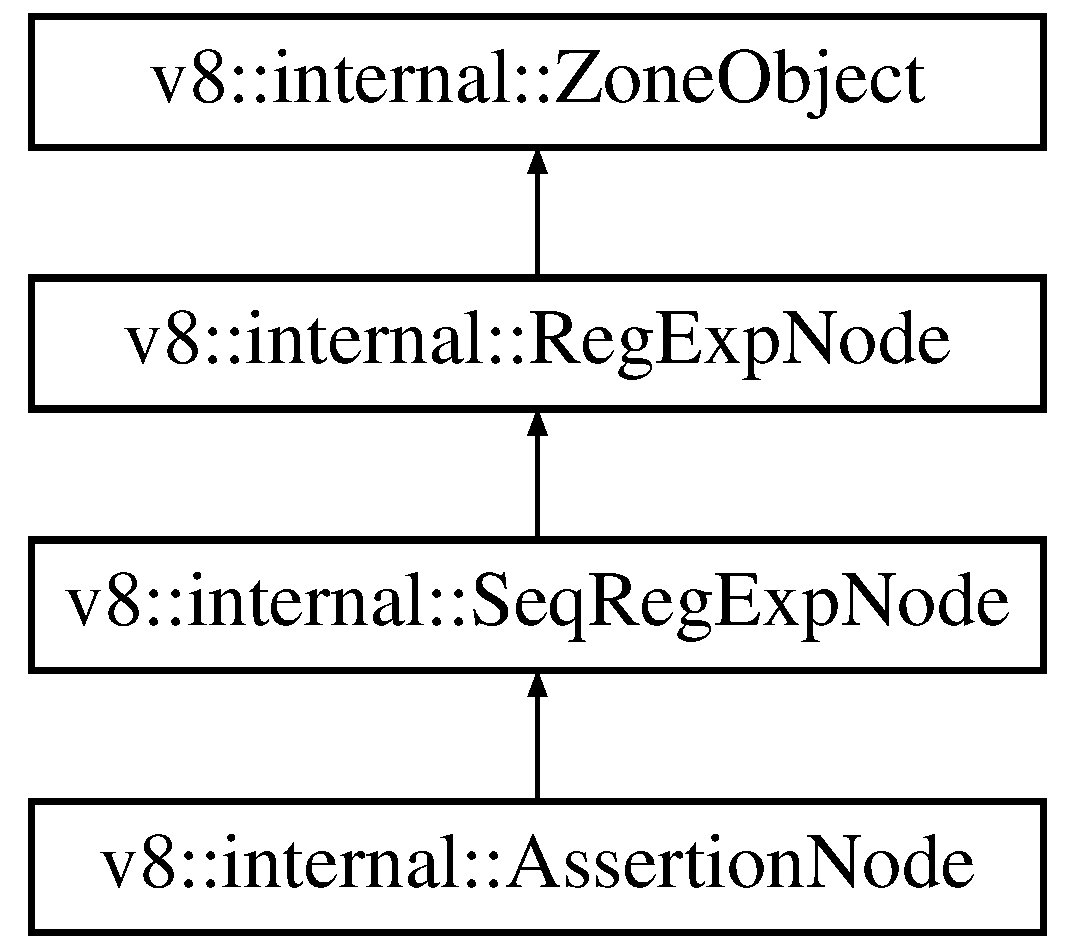
\includegraphics[height=4.000000cm]{classv8_1_1internal_1_1_assertion_node}
\end{center}
\end{figure}
\subsection*{Public Types}
\begin{DoxyCompactItemize}
\item 
\hypertarget{classv8_1_1internal_1_1_assertion_node_aa677ff26097f7ecb13c9283478981035}{}enum {\bfseries Assertion\+Type} \{ \\*
{\bfseries A\+T\+\_\+\+E\+N\+D}, 
{\bfseries A\+T\+\_\+\+S\+T\+A\+R\+T}, 
{\bfseries A\+T\+\_\+\+B\+O\+U\+N\+D\+A\+R\+Y}, 
{\bfseries A\+T\+\_\+\+N\+O\+N\+\_\+\+B\+O\+U\+N\+D\+A\+R\+Y}, 
\\*
{\bfseries A\+F\+T\+E\+R\+\_\+\+N\+E\+W\+L\+I\+N\+E}
 \}\label{classv8_1_1internal_1_1_assertion_node_aa677ff26097f7ecb13c9283478981035}

\end{DoxyCompactItemize}
\subsection*{Public Member Functions}
\begin{DoxyCompactItemize}
\item 
\hypertarget{classv8_1_1internal_1_1_assertion_node_a76eda020ebd409df34ec748dfbbc02bc}{}virtual void {\bfseries Accept} (\hyperlink{classv8_1_1internal_1_1_node_visitor}{Node\+Visitor} $\ast$visitor)\label{classv8_1_1internal_1_1_assertion_node_a76eda020ebd409df34ec748dfbbc02bc}

\item 
\hypertarget{classv8_1_1internal_1_1_assertion_node_a17e2a023a3d233b767f5222087e85672}{}virtual void {\bfseries Emit} (\hyperlink{classv8_1_1internal_1_1_reg_exp_compiler}{Reg\+Exp\+Compiler} $\ast$compiler, \hyperlink{classv8_1_1internal_1_1_trace}{Trace} $\ast$trace)\label{classv8_1_1internal_1_1_assertion_node_a17e2a023a3d233b767f5222087e85672}

\item 
\hypertarget{classv8_1_1internal_1_1_assertion_node_a1524215fa69f2427d08dc13c0bce27d1}{}virtual int {\bfseries Eats\+At\+Least} (int still\+\_\+to\+\_\+find, int budget, bool not\+\_\+at\+\_\+start)\label{classv8_1_1internal_1_1_assertion_node_a1524215fa69f2427d08dc13c0bce27d1}

\item 
\hypertarget{classv8_1_1internal_1_1_assertion_node_ad7ff94c39e2c1ce7660583e2d958c81f}{}virtual void {\bfseries Get\+Quick\+Check\+Details} (\hyperlink{classv8_1_1internal_1_1_quick_check_details}{Quick\+Check\+Details} $\ast$details, \hyperlink{classv8_1_1internal_1_1_reg_exp_compiler}{Reg\+Exp\+Compiler} $\ast$compiler, int filled\+\_\+in, bool not\+\_\+at\+\_\+start)\label{classv8_1_1internal_1_1_assertion_node_ad7ff94c39e2c1ce7660583e2d958c81f}

\item 
\hypertarget{classv8_1_1internal_1_1_assertion_node_a05b210612adc489b4749e6dcb99e8514}{}virtual void {\bfseries Fill\+In\+B\+M\+Info} (int offset, int budget, \hyperlink{classv8_1_1internal_1_1_boyer_moore_lookahead}{Boyer\+Moore\+Lookahead} $\ast$bm, bool not\+\_\+at\+\_\+start)\label{classv8_1_1internal_1_1_assertion_node_a05b210612adc489b4749e6dcb99e8514}

\item 
\hypertarget{classv8_1_1internal_1_1_assertion_node_a1c1279600bc32129daf91cb75c982e09}{}Assertion\+Type {\bfseries assertion\+\_\+type} ()\label{classv8_1_1internal_1_1_assertion_node_a1c1279600bc32129daf91cb75c982e09}

\end{DoxyCompactItemize}
\subsection*{Static Public Member Functions}
\begin{DoxyCompactItemize}
\item 
\hypertarget{classv8_1_1internal_1_1_assertion_node_a7663a6a9a51975492c0bfe7b5a61a832}{}static \hyperlink{classv8_1_1internal_1_1_assertion_node}{Assertion\+Node} $\ast$ {\bfseries At\+End} (\hyperlink{classv8_1_1internal_1_1_reg_exp_node}{Reg\+Exp\+Node} $\ast$on\+\_\+success)\label{classv8_1_1internal_1_1_assertion_node_a7663a6a9a51975492c0bfe7b5a61a832}

\item 
\hypertarget{classv8_1_1internal_1_1_assertion_node_ac3c21366bba17cf86759c0cdea7ae035}{}static \hyperlink{classv8_1_1internal_1_1_assertion_node}{Assertion\+Node} $\ast$ {\bfseries At\+Start} (\hyperlink{classv8_1_1internal_1_1_reg_exp_node}{Reg\+Exp\+Node} $\ast$on\+\_\+success)\label{classv8_1_1internal_1_1_assertion_node_ac3c21366bba17cf86759c0cdea7ae035}

\item 
\hypertarget{classv8_1_1internal_1_1_assertion_node_ac281096ab369662a023267aac4117bfd}{}static \hyperlink{classv8_1_1internal_1_1_assertion_node}{Assertion\+Node} $\ast$ {\bfseries At\+Boundary} (\hyperlink{classv8_1_1internal_1_1_reg_exp_node}{Reg\+Exp\+Node} $\ast$on\+\_\+success)\label{classv8_1_1internal_1_1_assertion_node_ac281096ab369662a023267aac4117bfd}

\item 
\hypertarget{classv8_1_1internal_1_1_assertion_node_ad6d20cd648da9b791ca9f35367f2470e}{}static \hyperlink{classv8_1_1internal_1_1_assertion_node}{Assertion\+Node} $\ast$ {\bfseries At\+Non\+Boundary} (\hyperlink{classv8_1_1internal_1_1_reg_exp_node}{Reg\+Exp\+Node} $\ast$on\+\_\+success)\label{classv8_1_1internal_1_1_assertion_node_ad6d20cd648da9b791ca9f35367f2470e}

\item 
\hypertarget{classv8_1_1internal_1_1_assertion_node_aa84ccd02ac323be278e3cb07633793b0}{}static \hyperlink{classv8_1_1internal_1_1_assertion_node}{Assertion\+Node} $\ast$ {\bfseries After\+Newline} (\hyperlink{classv8_1_1internal_1_1_reg_exp_node}{Reg\+Exp\+Node} $\ast$on\+\_\+success)\label{classv8_1_1internal_1_1_assertion_node_aa84ccd02ac323be278e3cb07633793b0}

\end{DoxyCompactItemize}
\subsection*{Additional Inherited Members}


The documentation for this class was generated from the following files\+:\begin{DoxyCompactItemize}
\item 
src/jsregexp.\+h\item 
src/jsregexp.\+cc\end{DoxyCompactItemize}

\hypertarget{classv8_1_1internal_1_1_ast_cons_string}{}\section{v8\+:\+:internal\+:\+:Ast\+Cons\+String Class Reference}
\label{classv8_1_1internal_1_1_ast_cons_string}\index{v8\+::internal\+::\+Ast\+Cons\+String@{v8\+::internal\+::\+Ast\+Cons\+String}}
Inheritance diagram for v8\+:\+:internal\+:\+:Ast\+Cons\+String\+:\begin{figure}[H]
\begin{center}
\leavevmode
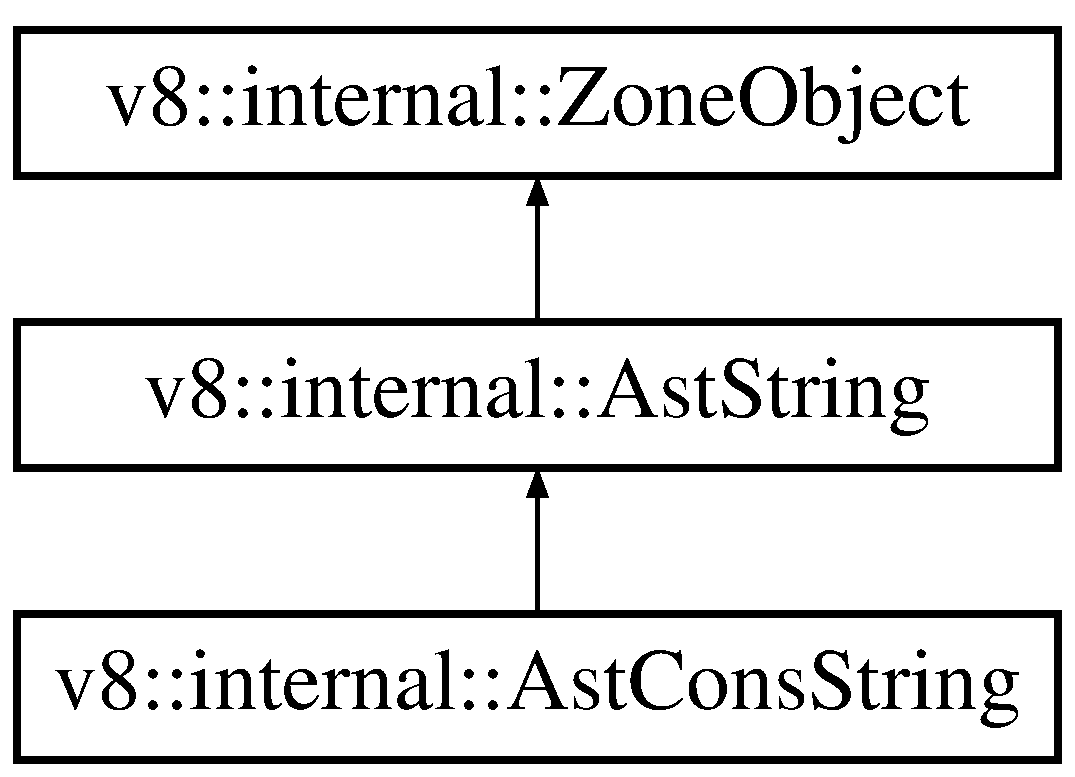
\includegraphics[height=3.000000cm]{classv8_1_1internal_1_1_ast_cons_string}
\end{center}
\end{figure}
\subsection*{Public Member Functions}
\begin{DoxyCompactItemize}
\item 
\hypertarget{classv8_1_1internal_1_1_ast_cons_string_a63b072d83d50c6bfe1e7d3ae7720856b}{}{\bfseries Ast\+Cons\+String} (const \hyperlink{classv8_1_1internal_1_1_ast_string}{Ast\+String} $\ast$left, const \hyperlink{classv8_1_1internal_1_1_ast_string}{Ast\+String} $\ast$right)\label{classv8_1_1internal_1_1_ast_cons_string_a63b072d83d50c6bfe1e7d3ae7720856b}

\item 
\hypertarget{classv8_1_1internal_1_1_ast_cons_string_abb376ec996cb33221fd44d218984dfa6}{}virtual int {\bfseries length} () const V8\+\_\+\+O\+V\+E\+R\+R\+I\+D\+E\label{classv8_1_1internal_1_1_ast_cons_string_abb376ec996cb33221fd44d218984dfa6}

\item 
\hypertarget{classv8_1_1internal_1_1_ast_cons_string_a77fa23320ebc0d09e0f9e021dfd5fdc7}{}virtual void {\bfseries Internalize} (\hyperlink{classv8_1_1internal_1_1_isolate}{Isolate} $\ast$isolate) V8\+\_\+\+O\+V\+E\+R\+R\+I\+D\+E\label{classv8_1_1internal_1_1_ast_cons_string_a77fa23320ebc0d09e0f9e021dfd5fdc7}

\end{DoxyCompactItemize}
\subsection*{Friends}
\begin{DoxyCompactItemize}
\item 
\hypertarget{classv8_1_1internal_1_1_ast_cons_string_a1d507e13f196677ce9bdd7b29efd96c0}{}class {\bfseries Ast\+Value\+Factory}\label{classv8_1_1internal_1_1_ast_cons_string_a1d507e13f196677ce9bdd7b29efd96c0}

\end{DoxyCompactItemize}
\subsection*{Additional Inherited Members}


The documentation for this class was generated from the following files\+:\begin{DoxyCompactItemize}
\item 
src/ast-\/value-\/factory.\+h\item 
src/ast-\/value-\/factory.\+cc\end{DoxyCompactItemize}

\hypertarget{classv8_1_1internal_1_1_ast_context}{}\section{v8\+:\+:internal\+:\+:Ast\+Context Class Reference}
\label{classv8_1_1internal_1_1_ast_context}\index{v8\+::internal\+::\+Ast\+Context@{v8\+::internal\+::\+Ast\+Context}}
Inheritance diagram for v8\+:\+:internal\+:\+:Ast\+Context\+:\begin{figure}[H]
\begin{center}
\leavevmode
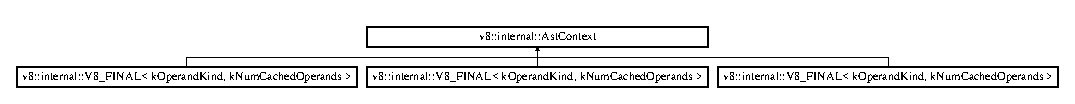
\includegraphics[height=0.952381cm]{classv8_1_1internal_1_1_ast_context}
\end{center}
\end{figure}
\subsection*{Public Member Functions}
\begin{DoxyCompactItemize}
\item 
\hypertarget{classv8_1_1internal_1_1_ast_context_a9ef7dcdc0fc4878eac2fba9ec899cf74}{}bool {\bfseries Is\+Effect} () const \label{classv8_1_1internal_1_1_ast_context_a9ef7dcdc0fc4878eac2fba9ec899cf74}

\item 
\hypertarget{classv8_1_1internal_1_1_ast_context_abab34ae1d1f4f30554e402981a9c8b41}{}bool {\bfseries Is\+Value} () const \label{classv8_1_1internal_1_1_ast_context_abab34ae1d1f4f30554e402981a9c8b41}

\item 
\hypertarget{classv8_1_1internal_1_1_ast_context_a745e8856780d7325898ee9ae28036876}{}bool {\bfseries Is\+Test} () const \label{classv8_1_1internal_1_1_ast_context_a745e8856780d7325898ee9ae28036876}

\item 
\hypertarget{classv8_1_1internal_1_1_ast_context_a02a778cd8697728b1d65c7784e81a708}{}virtual void {\bfseries Return\+Value} (\hyperlink{classv8_1_1internal_1_1_h_value}{H\+Value} $\ast$value)=0\label{classv8_1_1internal_1_1_ast_context_a02a778cd8697728b1d65c7784e81a708}

\item 
\hypertarget{classv8_1_1internal_1_1_ast_context_ac382417ecde5e65dd502ba717dfeb573}{}virtual void {\bfseries Return\+Instruction} (\hyperlink{classv8_1_1internal_1_1_h_instruction}{H\+Instruction} $\ast$instr, \hyperlink{classv8_1_1internal_1_1_bailout_id}{Bailout\+Id} ast\+\_\+id)=0\label{classv8_1_1internal_1_1_ast_context_ac382417ecde5e65dd502ba717dfeb573}

\item 
\hypertarget{classv8_1_1internal_1_1_ast_context_a0d14d70c6f23b3ed5a0b093546da90f7}{}virtual void {\bfseries Return\+Control} (\hyperlink{classv8_1_1internal_1_1_h_control_instruction}{H\+Control\+Instruction} $\ast$instr, \hyperlink{classv8_1_1internal_1_1_bailout_id}{Bailout\+Id} ast\+\_\+id)=0\label{classv8_1_1internal_1_1_ast_context_a0d14d70c6f23b3ed5a0b093546da90f7}

\item 
\hypertarget{classv8_1_1internal_1_1_ast_context_a31ce4d727e6c5c4476c385b53418aba9}{}virtual void {\bfseries Return\+Continuation} (H\+If\+Continuation $\ast$continuation, \hyperlink{classv8_1_1internal_1_1_bailout_id}{Bailout\+Id} ast\+\_\+id)=0\label{classv8_1_1internal_1_1_ast_context_a31ce4d727e6c5c4476c385b53418aba9}

\item 
\hypertarget{classv8_1_1internal_1_1_ast_context_ae4193388341ec815f47796b8fe05ae6e}{}void {\bfseries set\+\_\+for\+\_\+typeof} (bool for\+\_\+typeof)\label{classv8_1_1internal_1_1_ast_context_ae4193388341ec815f47796b8fe05ae6e}

\item 
\hypertarget{classv8_1_1internal_1_1_ast_context_a1cc6d5c355706470d71e63c994006029}{}bool {\bfseries is\+\_\+for\+\_\+typeof} ()\label{classv8_1_1internal_1_1_ast_context_a1cc6d5c355706470d71e63c994006029}

\end{DoxyCompactItemize}
\subsection*{Protected Member Functions}
\begin{DoxyCompactItemize}
\item 
\hypertarget{classv8_1_1internal_1_1_ast_context_a2f95ba98943cf65575eb4fde31afe7fb}{}{\bfseries Ast\+Context} (\hyperlink{classv8_1_1internal_1_1_h_optimized_graph_builder}{H\+Optimized\+Graph\+Builder} $\ast$owner, Expression\+::\+Context kind)\label{classv8_1_1internal_1_1_ast_context_a2f95ba98943cf65575eb4fde31afe7fb}

\item 
\hypertarget{classv8_1_1internal_1_1_ast_context_a0faad2f9a48cd43801a1d84e9a0b0988}{}\hyperlink{classv8_1_1internal_1_1_h_optimized_graph_builder}{H\+Optimized\+Graph\+Builder} $\ast$ {\bfseries owner} () const \label{classv8_1_1internal_1_1_ast_context_a0faad2f9a48cd43801a1d84e9a0b0988}

\item 
\hypertarget{classv8_1_1internal_1_1_ast_context_abea1ff333fcef5a2057297c917f1fe9b}{}\hyperlink{classv8_1_1internal_1_1_zone}{Zone} $\ast$ {\bfseries zone} () const \label{classv8_1_1internal_1_1_ast_context_abea1ff333fcef5a2057297c917f1fe9b}

\end{DoxyCompactItemize}


The documentation for this class was generated from the following files\+:\begin{DoxyCompactItemize}
\item 
src/hydrogen.\+h\item 
src/hydrogen.\+cc\end{DoxyCompactItemize}

\hypertarget{classv8_1_1internal_1_1_ast_node}{}\section{v8\+:\+:internal\+:\+:Ast\+Node Class Reference}
\label{classv8_1_1internal_1_1_ast_node}\index{v8\+::internal\+::\+Ast\+Node@{v8\+::internal\+::\+Ast\+Node}}
Inheritance diagram for v8\+:\+:internal\+:\+:Ast\+Node\+:\begin{figure}[H]
\begin{center}
\leavevmode
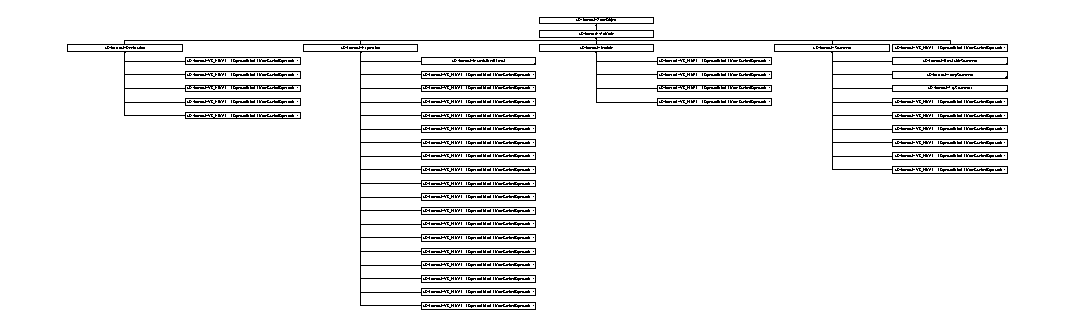
\includegraphics[height=3.928571cm]{classv8_1_1internal_1_1_ast_node}
\end{center}
\end{figure}
\subsection*{Public Types}
\begin{DoxyCompactItemize}
\item 
\hypertarget{classv8_1_1internal_1_1_ast_node_ab81d3ee3986451cb591842b06c4ee3bc}{}enum {\bfseries Node\+Type} \{ {\bfseries k\+Invalid} = -\/1
 \}\label{classv8_1_1internal_1_1_ast_node_ab81d3ee3986451cb591842b06c4ee3bc}

\end{DoxyCompactItemize}
\subsection*{Public Member Functions}
\begin{DoxyCompactItemize}
\item 
\hypertarget{classv8_1_1internal_1_1_ast_node_a3b42cf9e8f0c9685573ab0f445d30856}{}void $\ast$ {\bfseries operator new} (size\+\_\+t size, \hyperlink{classv8_1_1internal_1_1_zone}{Zone} $\ast$zone)\label{classv8_1_1internal_1_1_ast_node_a3b42cf9e8f0c9685573ab0f445d30856}

\item 
\hypertarget{classv8_1_1internal_1_1_ast_node_a68e77a52aeaab6205eed81558e39b51b}{}{\bfseries Ast\+Node} (int position)\label{classv8_1_1internal_1_1_ast_node_a68e77a52aeaab6205eed81558e39b51b}

\item 
\hypertarget{classv8_1_1internal_1_1_ast_node_a997460b9c5bb89418e5e2a3e760598bd}{}virtual void {\bfseries Accept} (Ast\+Visitor $\ast$v)=0\label{classv8_1_1internal_1_1_ast_node_a997460b9c5bb89418e5e2a3e760598bd}

\item 
\hypertarget{classv8_1_1internal_1_1_ast_node_a324bb4fe66bf389e5aa7c4941dd66a14}{}virtual Node\+Type {\bfseries node\+\_\+type} () const =0\label{classv8_1_1internal_1_1_ast_node_a324bb4fe66bf389e5aa7c4941dd66a14}

\item 
\hypertarget{classv8_1_1internal_1_1_ast_node_ac0e91623e58fe05cab42baa305244763}{}int {\bfseries position} () const \label{classv8_1_1internal_1_1_ast_node_ac0e91623e58fe05cab42baa305244763}

\item 
\hypertarget{classv8_1_1internal_1_1_ast_node_a48629ff0b786509f881e2ce51de4cffe}{}virtual Target\+Collector $\ast$ {\bfseries As\+Target\+Collector} ()\label{classv8_1_1internal_1_1_ast_node_a48629ff0b786509f881e2ce51de4cffe}

\item 
\hypertarget{classv8_1_1internal_1_1_ast_node_abe218efc9b25b70a3b41dae3c770be66}{}virtual \hyperlink{classv8_1_1internal_1_1_breakable_statement}{Breakable\+Statement} $\ast$ {\bfseries As\+Breakable\+Statement} ()\label{classv8_1_1internal_1_1_ast_node_abe218efc9b25b70a3b41dae3c770be66}

\item 
\hypertarget{classv8_1_1internal_1_1_ast_node_aaa1521749945a0854c729246a1661132}{}virtual \hyperlink{classv8_1_1internal_1_1_iteration_statement}{Iteration\+Statement} $\ast$ {\bfseries As\+Iteration\+Statement} ()\label{classv8_1_1internal_1_1_ast_node_aaa1521749945a0854c729246a1661132}

\item 
\hypertarget{classv8_1_1internal_1_1_ast_node_a7025f31bbb7c7df1d753d06d2efd31fa}{}virtual \hyperlink{classv8_1_1internal_1_1_materialized_literal}{Materialized\+Literal} $\ast$ {\bfseries As\+Materialized\+Literal} ()\label{classv8_1_1internal_1_1_ast_node_a7025f31bbb7c7df1d753d06d2efd31fa}

\end{DoxyCompactItemize}
\subsection*{Static Protected Member Functions}
\begin{DoxyCompactItemize}
\item 
\hypertarget{classv8_1_1internal_1_1_ast_node_ad4b6491530b5494b7b28d799f3f72d66}{}static int {\bfseries Get\+Next\+Id} (\hyperlink{classv8_1_1internal_1_1_zone}{Zone} $\ast$zone)\label{classv8_1_1internal_1_1_ast_node_ad4b6491530b5494b7b28d799f3f72d66}

\item 
\hypertarget{classv8_1_1internal_1_1_ast_node_a3b30c5cbd3332634f452dbebe5f1ffc2}{}static int {\bfseries Reserve\+Id\+Range} (\hyperlink{classv8_1_1internal_1_1_zone}{Zone} $\ast$zone, int n)\label{classv8_1_1internal_1_1_ast_node_a3b30c5cbd3332634f452dbebe5f1ffc2}

\item 
\hypertarget{classv8_1_1internal_1_1_ast_node_a60ba1b9f98ba84982363f4f462021834}{}static \hyperlink{classv8_1_1internal_1_1_type_feedback_id}{Type\+Feedback\+Id} {\bfseries reuse} (\hyperlink{classv8_1_1internal_1_1_bailout_id}{Bailout\+Id} id)\label{classv8_1_1internal_1_1_ast_node_a60ba1b9f98ba84982363f4f462021834}

\end{DoxyCompactItemize}
\subsection*{Friends}
\begin{DoxyCompactItemize}
\item 
\hypertarget{classv8_1_1internal_1_1_ast_node_a9d0fc316f19a46adb02ecfc40558a027}{}class {\bfseries Case\+Clause}\label{classv8_1_1internal_1_1_ast_node_a9d0fc316f19a46adb02ecfc40558a027}

\end{DoxyCompactItemize}


The documentation for this class was generated from the following file\+:\begin{DoxyCompactItemize}
\item 
src/ast.\+h\end{DoxyCompactItemize}

\hypertarget{classv8_1_1internal_1_1_ast_node_factory}{}\section{v8\+:\+:internal\+:\+:Ast\+Node\+Factory$<$ class $>$ Class Template Reference}
\label{classv8_1_1internal_1_1_ast_node_factory}\index{v8\+::internal\+::\+Ast\+Node\+Factory$<$ class $>$@{v8\+::internal\+::\+Ast\+Node\+Factory$<$ class $>$}}


The documentation for this class was generated from the following file\+:\begin{DoxyCompactItemize}
\item 
src/ast.\+h\end{DoxyCompactItemize}

\hypertarget{classv8_1_1internal_1_1_ast_raw_string}{}\section{v8\+:\+:internal\+:\+:Ast\+Raw\+String Class Reference}
\label{classv8_1_1internal_1_1_ast_raw_string}\index{v8\+::internal\+::\+Ast\+Raw\+String@{v8\+::internal\+::\+Ast\+Raw\+String}}
Inheritance diagram for v8\+:\+:internal\+:\+:Ast\+Raw\+String\+:\begin{figure}[H]
\begin{center}
\leavevmode
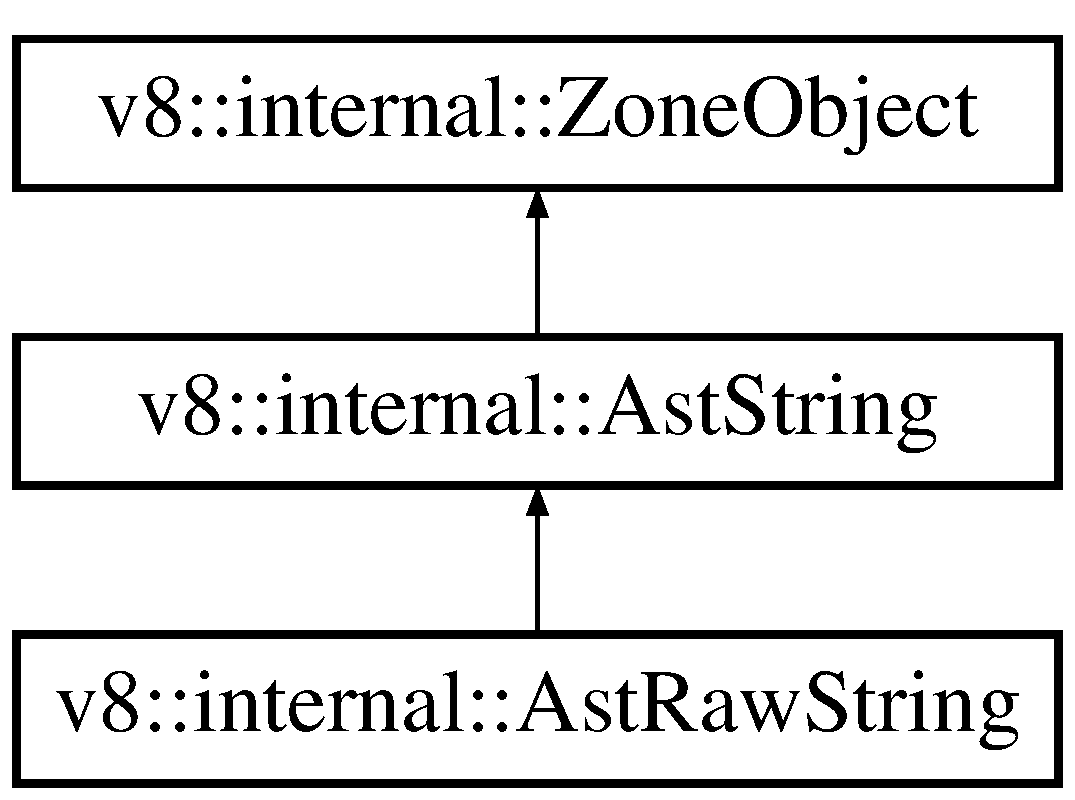
\includegraphics[height=3.000000cm]{classv8_1_1internal_1_1_ast_raw_string}
\end{center}
\end{figure}
\subsection*{Public Member Functions}
\begin{DoxyCompactItemize}
\item 
\hypertarget{classv8_1_1internal_1_1_ast_raw_string_ac33af36ba73a2c8f921675ba2c618092}{}virtual int {\bfseries length} () const V8\+\_\+\+O\+V\+E\+R\+R\+I\+D\+E\label{classv8_1_1internal_1_1_ast_raw_string_ac33af36ba73a2c8f921675ba2c618092}

\item 
\hypertarget{classv8_1_1internal_1_1_ast_raw_string_ab8aa03cf4e49bdc41f0cc4d1c665fbd5}{}virtual void {\bfseries Internalize} (\hyperlink{classv8_1_1internal_1_1_isolate}{Isolate} $\ast$isolate) V8\+\_\+\+O\+V\+E\+R\+R\+I\+D\+E\label{classv8_1_1internal_1_1_ast_raw_string_ab8aa03cf4e49bdc41f0cc4d1c665fbd5}

\item 
\hypertarget{classv8_1_1internal_1_1_ast_raw_string_a3d50a9463da53958aad96da0729eda13}{}bool {\bfseries As\+Array\+Index} (uint32\+\_\+t $\ast$index) const \label{classv8_1_1internal_1_1_ast_raw_string_a3d50a9463da53958aad96da0729eda13}

\item 
\hypertarget{classv8_1_1internal_1_1_ast_raw_string_a19b4f332aee9c58ebccf9130576828f0}{}const unsigned char $\ast$ {\bfseries raw\+\_\+data} () const \label{classv8_1_1internal_1_1_ast_raw_string_a19b4f332aee9c58ebccf9130576828f0}

\item 
\hypertarget{classv8_1_1internal_1_1_ast_raw_string_af8f3bf741a731825048c0ade6dfc4b14}{}bool {\bfseries is\+\_\+one\+\_\+byte} () const \label{classv8_1_1internal_1_1_ast_raw_string_af8f3bf741a731825048c0ade6dfc4b14}

\item 
\hypertarget{classv8_1_1internal_1_1_ast_raw_string_a447f234bce2635272c0ce6e3d65247d0}{}bool {\bfseries Is\+One\+Byte\+Equal\+To} (const char $\ast$data) const \label{classv8_1_1internal_1_1_ast_raw_string_a447f234bce2635272c0ce6e3d65247d0}

\item 
\hypertarget{classv8_1_1internal_1_1_ast_raw_string_a913e377b7afff07dc27fbd81932a2cb4}{}uint16\+\_\+t {\bfseries First\+Character} () const \label{classv8_1_1internal_1_1_ast_raw_string_a913e377b7afff07dc27fbd81932a2cb4}

\item 
\hypertarget{classv8_1_1internal_1_1_ast_raw_string_a0e285ff9f228e2cb92cda7dc2461e2de}{}uint32\+\_\+t {\bfseries hash} () const \label{classv8_1_1internal_1_1_ast_raw_string_a0e285ff9f228e2cb92cda7dc2461e2de}

\end{DoxyCompactItemize}
\subsection*{Static Public Member Functions}
\begin{DoxyCompactItemize}
\item 
\hypertarget{classv8_1_1internal_1_1_ast_raw_string_a963812b8beb8ac3bfad3b87b3a4647b1}{}static bool {\bfseries Compare} (void $\ast$a, void $\ast$b)\label{classv8_1_1internal_1_1_ast_raw_string_a963812b8beb8ac3bfad3b87b3a4647b1}

\end{DoxyCompactItemize}
\subsection*{Friends}
\begin{DoxyCompactItemize}
\item 
\hypertarget{classv8_1_1internal_1_1_ast_raw_string_a1d507e13f196677ce9bdd7b29efd96c0}{}class {\bfseries Ast\+Value\+Factory}\label{classv8_1_1internal_1_1_ast_raw_string_a1d507e13f196677ce9bdd7b29efd96c0}

\item 
\hypertarget{classv8_1_1internal_1_1_ast_raw_string_aa99ea383a648693891f30539a9b5faad}{}class {\bfseries Ast\+Raw\+String\+Internalization\+Key}\label{classv8_1_1internal_1_1_ast_raw_string_aa99ea383a648693891f30539a9b5faad}

\end{DoxyCompactItemize}
\subsection*{Additional Inherited Members}


The documentation for this class was generated from the following files\+:\begin{DoxyCompactItemize}
\item 
src/ast-\/value-\/factory.\+h\item 
src/ast-\/value-\/factory.\+cc\end{DoxyCompactItemize}

\hypertarget{classv8_1_1internal_1_1_ast_raw_string_internalization_key}{}\section{v8\+:\+:internal\+:\+:Ast\+Raw\+String\+Internalization\+Key Class Reference}
\label{classv8_1_1internal_1_1_ast_raw_string_internalization_key}\index{v8\+::internal\+::\+Ast\+Raw\+String\+Internalization\+Key@{v8\+::internal\+::\+Ast\+Raw\+String\+Internalization\+Key}}
Inheritance diagram for v8\+:\+:internal\+:\+:Ast\+Raw\+String\+Internalization\+Key\+:\begin{figure}[H]
\begin{center}
\leavevmode
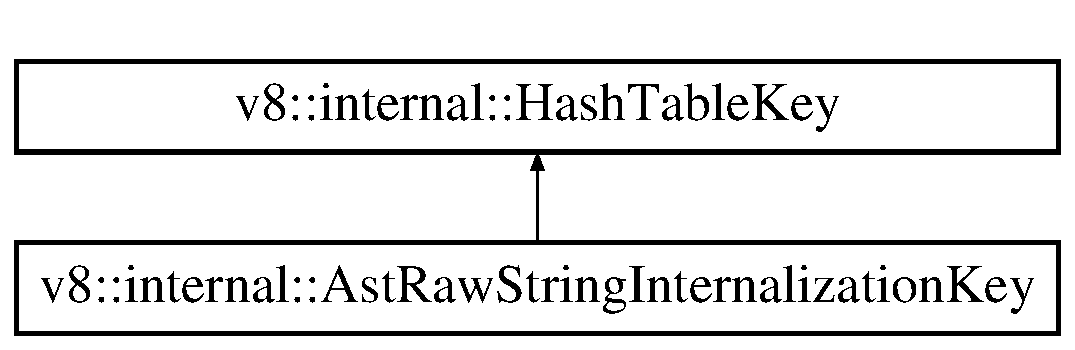
\includegraphics[height=2.000000cm]{classv8_1_1internal_1_1_ast_raw_string_internalization_key}
\end{center}
\end{figure}
\subsection*{Public Member Functions}
\begin{DoxyCompactItemize}
\item 
\hypertarget{classv8_1_1internal_1_1_ast_raw_string_internalization_key_af3086b894b997d1556f3501bcca631e1}{}{\bfseries Ast\+Raw\+String\+Internalization\+Key} (const \hyperlink{classv8_1_1internal_1_1_ast_raw_string}{Ast\+Raw\+String} $\ast$string)\label{classv8_1_1internal_1_1_ast_raw_string_internalization_key_af3086b894b997d1556f3501bcca631e1}

\item 
\hypertarget{classv8_1_1internal_1_1_ast_raw_string_internalization_key_ad8778f490117aefc02fcc966d34a82e7}{}virtual bool {\bfseries Is\+Match} (\hyperlink{classv8_1_1internal_1_1_object}{Object} $\ast$other) V8\+\_\+\+O\+V\+E\+R\+R\+I\+D\+E\label{classv8_1_1internal_1_1_ast_raw_string_internalization_key_ad8778f490117aefc02fcc966d34a82e7}

\item 
\hypertarget{classv8_1_1internal_1_1_ast_raw_string_internalization_key_af334b41b8220d50499b971f620606d25}{}virtual uint32\+\_\+t {\bfseries Hash} () V8\+\_\+\+O\+V\+E\+R\+R\+I\+D\+E\label{classv8_1_1internal_1_1_ast_raw_string_internalization_key_af334b41b8220d50499b971f620606d25}

\item 
\hypertarget{classv8_1_1internal_1_1_ast_raw_string_internalization_key_a468578799c232d5217bc63ba361b38a5}{}virtual uint32\+\_\+t {\bfseries Hash\+For\+Object} (\hyperlink{classv8_1_1internal_1_1_object}{Object} $\ast$key) V8\+\_\+\+O\+V\+E\+R\+R\+I\+D\+E\label{classv8_1_1internal_1_1_ast_raw_string_internalization_key_a468578799c232d5217bc63ba361b38a5}

\item 
\hypertarget{classv8_1_1internal_1_1_ast_raw_string_internalization_key_ac25b4acc4ef92b04de543aced3d31cda}{}virtual \hyperlink{classv8_1_1internal_1_1_handle}{Handle}$<$ \hyperlink{classv8_1_1internal_1_1_object}{Object} $>$ {\bfseries As\+Handle} (\hyperlink{classv8_1_1internal_1_1_isolate}{Isolate} $\ast$isolate) V8\+\_\+\+O\+V\+E\+R\+R\+I\+D\+E\label{classv8_1_1internal_1_1_ast_raw_string_internalization_key_ac25b4acc4ef92b04de543aced3d31cda}

\end{DoxyCompactItemize}


The documentation for this class was generated from the following file\+:\begin{DoxyCompactItemize}
\item 
src/ast-\/value-\/factory.\+cc\end{DoxyCompactItemize}

\hypertarget{classv8_1_1internal_1_1_ast_string}{}\section{v8\+:\+:internal\+:\+:Ast\+String Class Reference}
\label{classv8_1_1internal_1_1_ast_string}\index{v8\+::internal\+::\+Ast\+String@{v8\+::internal\+::\+Ast\+String}}
Inheritance diagram for v8\+:\+:internal\+:\+:Ast\+String\+:\begin{figure}[H]
\begin{center}
\leavevmode
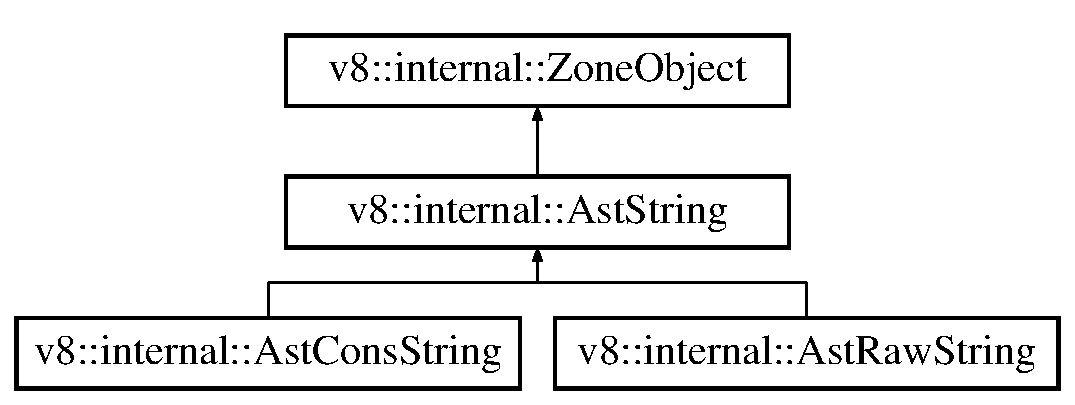
\includegraphics[height=3.000000cm]{classv8_1_1internal_1_1_ast_string}
\end{center}
\end{figure}
\subsection*{Public Member Functions}
\begin{DoxyCompactItemize}
\item 
\hypertarget{classv8_1_1internal_1_1_ast_string_a9a0be304251448c197840e6e3a2de4db}{}virtual int {\bfseries length} () const =0\label{classv8_1_1internal_1_1_ast_string_a9a0be304251448c197840e6e3a2de4db}

\item 
\hypertarget{classv8_1_1internal_1_1_ast_string_a9012cbd49b91d14842777274e713b068}{}bool {\bfseries Is\+Empty} () const \label{classv8_1_1internal_1_1_ast_string_a9012cbd49b91d14842777274e713b068}

\item 
\hypertarget{classv8_1_1internal_1_1_ast_string_a7781994a37eb574c340844cfb235dd25}{}virtual void {\bfseries Internalize} (\hyperlink{classv8_1_1internal_1_1_isolate}{Isolate} $\ast$isolate)=0\label{classv8_1_1internal_1_1_ast_string_a7781994a37eb574c340844cfb235dd25}

\item 
\hypertarget{classv8_1_1internal_1_1_ast_string_a44a57fccc07afe69c83171d66a334291}{}V8\+\_\+\+I\+N\+L\+I\+N\+E \hyperlink{classv8_1_1internal_1_1_handle}{Handle}$<$ \hyperlink{classv8_1_1internal_1_1_string}{String} $>$ {\bfseries string} () const \label{classv8_1_1internal_1_1_ast_string_a44a57fccc07afe69c83171d66a334291}

\end{DoxyCompactItemize}
\subsection*{Protected Attributes}
\begin{DoxyCompactItemize}
\item 
\hypertarget{classv8_1_1internal_1_1_ast_string_a031e411435d4c2749b7391eb9b3e18ae}{}\hyperlink{classv8_1_1internal_1_1_handle}{Handle}$<$ \hyperlink{classv8_1_1internal_1_1_string}{String} $>$ {\bfseries string\+\_\+}\label{classv8_1_1internal_1_1_ast_string_a031e411435d4c2749b7391eb9b3e18ae}

\end{DoxyCompactItemize}


The documentation for this class was generated from the following file\+:\begin{DoxyCompactItemize}
\item 
src/ast-\/value-\/factory.\+h\end{DoxyCompactItemize}

\hypertarget{classv8_1_1internal_1_1_ast_typer}{}\section{v8\+:\+:internal\+:\+:Ast\+Typer Class Reference}
\label{classv8_1_1internal_1_1_ast_typer}\index{v8\+::internal\+::\+Ast\+Typer@{v8\+::internal\+::\+Ast\+Typer}}
Inheritance diagram for v8\+:\+:internal\+:\+:Ast\+Typer\+:\begin{figure}[H]
\begin{center}
\leavevmode
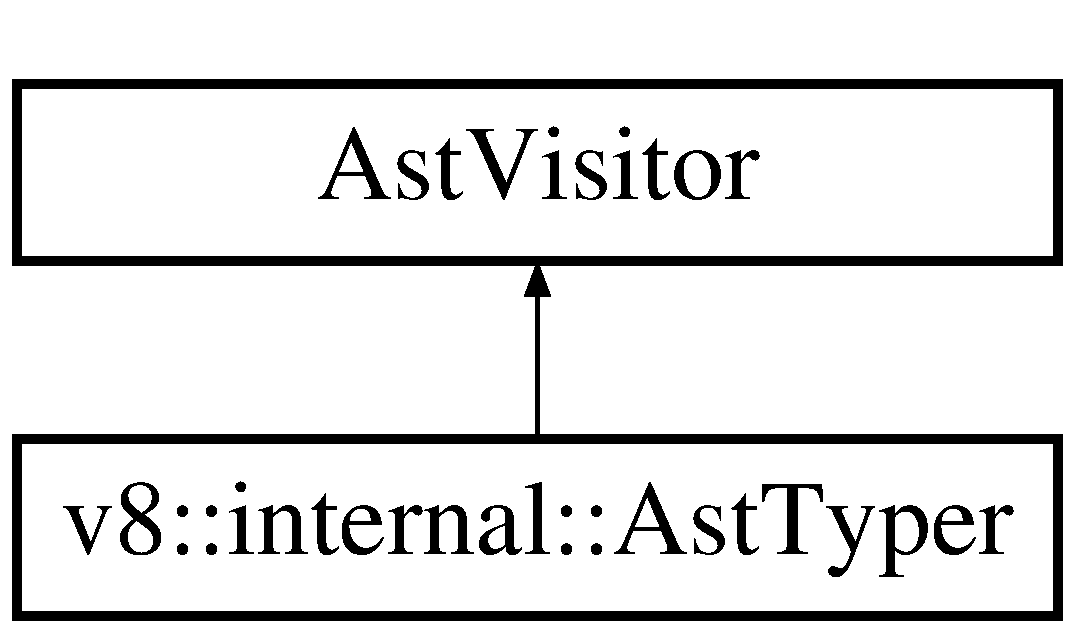
\includegraphics[height=2.000000cm]{classv8_1_1internal_1_1_ast_typer}
\end{center}
\end{figure}
\subsection*{Public Member Functions}
\begin{DoxyCompactItemize}
\item 
\hypertarget{classv8_1_1internal_1_1_ast_typer_ad459e1e5801cf414325cb1e35613ba14}{}void $\ast$ {\bfseries operator new} (size\+\_\+t size, \hyperlink{classv8_1_1internal_1_1_zone}{Zone} $\ast$zone)\label{classv8_1_1internal_1_1_ast_typer_ad459e1e5801cf414325cb1e35613ba14}

\item 
\hypertarget{classv8_1_1internal_1_1_ast_typer_af065f25a66647fac4827b0bede816afb}{}void {\bfseries operator delete} (void $\ast$pointer, \hyperlink{classv8_1_1internal_1_1_zone}{Zone} $\ast$zone)\label{classv8_1_1internal_1_1_ast_typer_af065f25a66647fac4827b0bede816afb}

\item 
\hypertarget{classv8_1_1internal_1_1_ast_typer_a63a58bc443b7927d52831ee95edf0fdb}{}void {\bfseries operator delete} (void $\ast$pointer)\label{classv8_1_1internal_1_1_ast_typer_a63a58bc443b7927d52831ee95edf0fdb}

\item 
\hypertarget{classv8_1_1internal_1_1_ast_typer_a911921c74252f2efa0cc6c0120706767}{}{\bfseries D\+E\+F\+I\+N\+E\+\_\+\+A\+S\+T\+\_\+\+V\+I\+S\+I\+T\+O\+R\+\_\+\+S\+U\+B\+C\+L\+A\+S\+S\+\_\+\+M\+E\+M\+B\+E\+R\+S} ()\label{classv8_1_1internal_1_1_ast_typer_a911921c74252f2efa0cc6c0120706767}

\end{DoxyCompactItemize}
\subsection*{Static Public Member Functions}
\begin{DoxyCompactItemize}
\item 
\hypertarget{classv8_1_1internal_1_1_ast_typer_aafa5f5ac0e6ee1af07c03fcb4bc58603}{}static void {\bfseries Run} (\hyperlink{classv8_1_1internal_1_1_compilation_info}{Compilation\+Info} $\ast$info)\label{classv8_1_1internal_1_1_ast_typer_aafa5f5ac0e6ee1af07c03fcb4bc58603}

\end{DoxyCompactItemize}


The documentation for this class was generated from the following files\+:\begin{DoxyCompactItemize}
\item 
src/typing.\+h\item 
src/typing.\+cc\end{DoxyCompactItemize}

\hypertarget{classv8_1_1internal_1_1_ast_value}{}\section{v8\+:\+:internal\+:\+:Ast\+Value Class Reference}
\label{classv8_1_1internal_1_1_ast_value}\index{v8\+::internal\+::\+Ast\+Value@{v8\+::internal\+::\+Ast\+Value}}
Inheritance diagram for v8\+:\+:internal\+:\+:Ast\+Value\+:\begin{figure}[H]
\begin{center}
\leavevmode
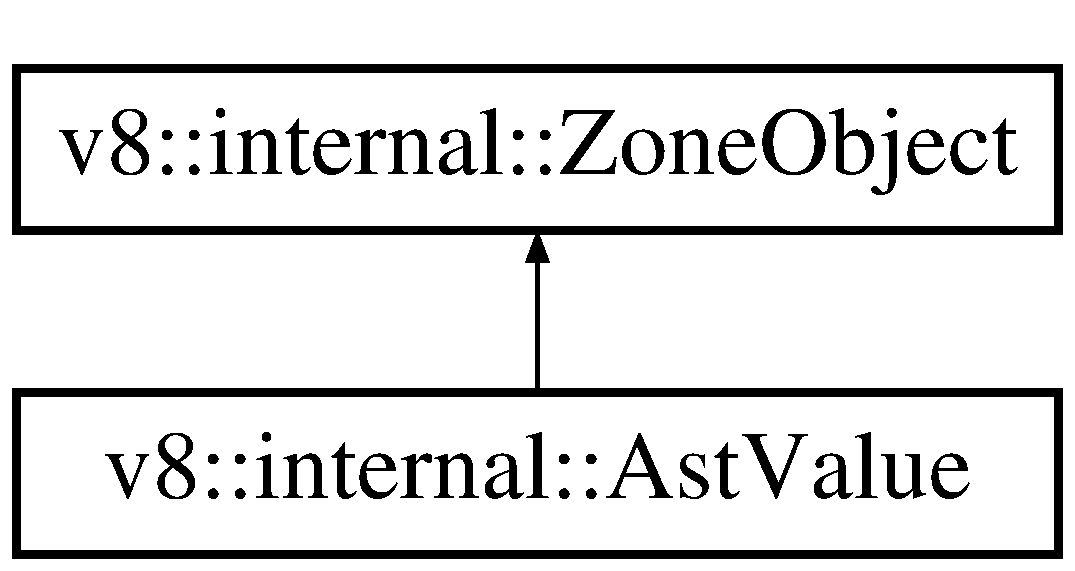
\includegraphics[height=2.000000cm]{classv8_1_1internal_1_1_ast_value}
\end{center}
\end{figure}
\subsection*{Public Member Functions}
\begin{DoxyCompactItemize}
\item 
\hypertarget{classv8_1_1internal_1_1_ast_value_ab70bfc634e17e29db259a26a757a05c9}{}bool {\bfseries Is\+String} () const \label{classv8_1_1internal_1_1_ast_value_ab70bfc634e17e29db259a26a757a05c9}

\item 
\hypertarget{classv8_1_1internal_1_1_ast_value_a399b9f14cff4101983a3d2842d62c911}{}bool {\bfseries Is\+Number} () const \label{classv8_1_1internal_1_1_ast_value_a399b9f14cff4101983a3d2842d62c911}

\item 
\hypertarget{classv8_1_1internal_1_1_ast_value_a80e071eba4956e10a281194df8a8668d}{}const \hyperlink{classv8_1_1internal_1_1_ast_raw_string}{Ast\+Raw\+String} $\ast$ {\bfseries As\+String} () const \label{classv8_1_1internal_1_1_ast_value_a80e071eba4956e10a281194df8a8668d}

\item 
\hypertarget{classv8_1_1internal_1_1_ast_value_aa99e007e6191e0790578ed7addd4e182}{}double {\bfseries As\+Number} () const \label{classv8_1_1internal_1_1_ast_value_aa99e007e6191e0790578ed7addd4e182}

\item 
\hypertarget{classv8_1_1internal_1_1_ast_value_a57648a16dba0de8154a5a6690a556bf9}{}bool {\bfseries Equals\+String} (const \hyperlink{classv8_1_1internal_1_1_ast_raw_string}{Ast\+Raw\+String} $\ast$string) const \label{classv8_1_1internal_1_1_ast_value_a57648a16dba0de8154a5a6690a556bf9}

\item 
\hypertarget{classv8_1_1internal_1_1_ast_value_a42d04cc428b13f93d30262e298565a83}{}bool {\bfseries Is\+Property\+Name} () const \label{classv8_1_1internal_1_1_ast_value_a42d04cc428b13f93d30262e298565a83}

\item 
\hypertarget{classv8_1_1internal_1_1_ast_value_ab4be5ef2b7f23e682672333fed29f0f2}{}bool {\bfseries Boolean\+Value} () const \label{classv8_1_1internal_1_1_ast_value_ab4be5ef2b7f23e682672333fed29f0f2}

\item 
\hypertarget{classv8_1_1internal_1_1_ast_value_a71b8e2275ef7875e0ca7b48e4eaa2650}{}void {\bfseries Internalize} (\hyperlink{classv8_1_1internal_1_1_isolate}{Isolate} $\ast$isolate)\label{classv8_1_1internal_1_1_ast_value_a71b8e2275ef7875e0ca7b48e4eaa2650}

\item 
\hypertarget{classv8_1_1internal_1_1_ast_value_a2c1bb2b42997f4dbc59919f38e013e09}{}V8\+\_\+\+I\+N\+L\+I\+N\+E \hyperlink{classv8_1_1internal_1_1_handle}{Handle}$<$ \hyperlink{classv8_1_1internal_1_1_object}{Object} $>$ {\bfseries value} () const \label{classv8_1_1internal_1_1_ast_value_a2c1bb2b42997f4dbc59919f38e013e09}

\end{DoxyCompactItemize}
\subsection*{Friends}
\begin{DoxyCompactItemize}
\item 
\hypertarget{classv8_1_1internal_1_1_ast_value_a1d507e13f196677ce9bdd7b29efd96c0}{}class {\bfseries Ast\+Value\+Factory}\label{classv8_1_1internal_1_1_ast_value_a1d507e13f196677ce9bdd7b29efd96c0}

\end{DoxyCompactItemize}


The documentation for this class was generated from the following files\+:\begin{DoxyCompactItemize}
\item 
src/ast-\/value-\/factory.\+h\item 
src/ast-\/value-\/factory.\+cc\end{DoxyCompactItemize}

\hypertarget{classv8_1_1internal_1_1_ast_value_factory}{}\section{v8\+:\+:internal\+:\+:Ast\+Value\+Factory Class Reference}
\label{classv8_1_1internal_1_1_ast_value_factory}\index{v8\+::internal\+::\+Ast\+Value\+Factory@{v8\+::internal\+::\+Ast\+Value\+Factory}}
\subsection*{Public Member Functions}
\begin{DoxyCompactItemize}
\item 
\hypertarget{classv8_1_1internal_1_1_ast_value_factory_a70127bc521314ac55105a1725819c8c1}{}{\bfseries Ast\+Value\+Factory} (\hyperlink{classv8_1_1internal_1_1_zone}{Zone} $\ast$zone, uint32\+\_\+t hash\+\_\+seed)\label{classv8_1_1internal_1_1_ast_value_factory_a70127bc521314ac55105a1725819c8c1}

\item 
\hypertarget{classv8_1_1internal_1_1_ast_value_factory_a8b185da53432ca85bb3b6d46556c0d75}{}const \hyperlink{classv8_1_1internal_1_1_ast_raw_string}{Ast\+Raw\+String} $\ast$ {\bfseries Get\+One\+Byte\+String} (\hyperlink{classv8_1_1internal_1_1_vector}{Vector}$<$ const uint8\+\_\+t $>$ literal)\label{classv8_1_1internal_1_1_ast_value_factory_a8b185da53432ca85bb3b6d46556c0d75}

\item 
\hypertarget{classv8_1_1internal_1_1_ast_value_factory_a4de86ce5c6002dec8cd8e441a36871ac}{}const \hyperlink{classv8_1_1internal_1_1_ast_raw_string}{Ast\+Raw\+String} $\ast$ {\bfseries Get\+One\+Byte\+String} (const char $\ast$string)\label{classv8_1_1internal_1_1_ast_value_factory_a4de86ce5c6002dec8cd8e441a36871ac}

\item 
\hypertarget{classv8_1_1internal_1_1_ast_value_factory_a7de761f4c43839504dbcbbea2950854a}{}const \hyperlink{classv8_1_1internal_1_1_ast_raw_string}{Ast\+Raw\+String} $\ast$ {\bfseries Get\+Two\+Byte\+String} (\hyperlink{classv8_1_1internal_1_1_vector}{Vector}$<$ const uint16\+\_\+t $>$ literal)\label{classv8_1_1internal_1_1_ast_value_factory_a7de761f4c43839504dbcbbea2950854a}

\item 
\hypertarget{classv8_1_1internal_1_1_ast_value_factory_aaf364273b48895f490ec1008ecd29bed}{}const \hyperlink{classv8_1_1internal_1_1_ast_raw_string}{Ast\+Raw\+String} $\ast$ {\bfseries Get\+String} (\hyperlink{classv8_1_1internal_1_1_handle}{Handle}$<$ \hyperlink{classv8_1_1internal_1_1_string}{String} $>$ literal)\label{classv8_1_1internal_1_1_ast_value_factory_aaf364273b48895f490ec1008ecd29bed}

\item 
\hypertarget{classv8_1_1internal_1_1_ast_value_factory_a97eccad8901b4bdfa0cc00d4a133f6f3}{}const \hyperlink{classv8_1_1internal_1_1_ast_cons_string}{Ast\+Cons\+String} $\ast$ {\bfseries New\+Cons\+String} (const \hyperlink{classv8_1_1internal_1_1_ast_string}{Ast\+String} $\ast$left, const \hyperlink{classv8_1_1internal_1_1_ast_string}{Ast\+String} $\ast$right)\label{classv8_1_1internal_1_1_ast_value_factory_a97eccad8901b4bdfa0cc00d4a133f6f3}

\item 
\hypertarget{classv8_1_1internal_1_1_ast_value_factory_a5deb8e954fe78ec1910d5fe494e602d3}{}void {\bfseries Internalize} (\hyperlink{classv8_1_1internal_1_1_isolate}{Isolate} $\ast$isolate)\label{classv8_1_1internal_1_1_ast_value_factory_a5deb8e954fe78ec1910d5fe494e602d3}

\item 
\hypertarget{classv8_1_1internal_1_1_ast_value_factory_ad4d40aa31bd431a57a985f9c87242ed9}{}bool {\bfseries Is\+Internalized} ()\label{classv8_1_1internal_1_1_ast_value_factory_ad4d40aa31bd431a57a985f9c87242ed9}

\item 
\hypertarget{classv8_1_1internal_1_1_ast_value_factory_acc10654c4900ddf6c9df0eb0db570c5d}{}const \hyperlink{classv8_1_1internal_1_1_ast_value}{Ast\+Value} $\ast$ {\bfseries New\+String} (const \hyperlink{classv8_1_1internal_1_1_ast_raw_string}{Ast\+Raw\+String} $\ast$string)\label{classv8_1_1internal_1_1_ast_value_factory_acc10654c4900ddf6c9df0eb0db570c5d}

\item 
\hypertarget{classv8_1_1internal_1_1_ast_value_factory_ae532fb5eee98a9b1aca33b08241b4798}{}const \hyperlink{classv8_1_1internal_1_1_ast_value}{Ast\+Value} $\ast$ {\bfseries New\+Symbol} (const char $\ast$name)\label{classv8_1_1internal_1_1_ast_value_factory_ae532fb5eee98a9b1aca33b08241b4798}

\item 
\hypertarget{classv8_1_1internal_1_1_ast_value_factory_a8f65cf3651fb792b1c3551c7b29a5b9b}{}const \hyperlink{classv8_1_1internal_1_1_ast_value}{Ast\+Value} $\ast$ {\bfseries New\+Number} (double number)\label{classv8_1_1internal_1_1_ast_value_factory_a8f65cf3651fb792b1c3551c7b29a5b9b}

\item 
\hypertarget{classv8_1_1internal_1_1_ast_value_factory_a946e0af513192f073660d80e03a904d8}{}const \hyperlink{classv8_1_1internal_1_1_ast_value}{Ast\+Value} $\ast$ {\bfseries New\+Smi} (int number)\label{classv8_1_1internal_1_1_ast_value_factory_a946e0af513192f073660d80e03a904d8}

\item 
\hypertarget{classv8_1_1internal_1_1_ast_value_factory_ae03a5d1347d22306588b0e5709ccfc82}{}const \hyperlink{classv8_1_1internal_1_1_ast_value}{Ast\+Value} $\ast$ {\bfseries New\+Boolean} (bool b)\label{classv8_1_1internal_1_1_ast_value_factory_ae03a5d1347d22306588b0e5709ccfc82}

\item 
\hypertarget{classv8_1_1internal_1_1_ast_value_factory_a7bee5a9a03b03f59d2a6c62ab52045ed}{}const \hyperlink{classv8_1_1internal_1_1_ast_value}{Ast\+Value} $\ast$ {\bfseries New\+String\+List} (\hyperlink{classv8_1_1internal_1_1_zone_list}{Zone\+List}$<$ const \hyperlink{classv8_1_1internal_1_1_ast_raw_string}{Ast\+Raw\+String} $\ast$ $>$ $\ast$strings)\label{classv8_1_1internal_1_1_ast_value_factory_a7bee5a9a03b03f59d2a6c62ab52045ed}

\item 
\hypertarget{classv8_1_1internal_1_1_ast_value_factory_a93026a40389b24fda775956f218248b8}{}const \hyperlink{classv8_1_1internal_1_1_ast_value}{Ast\+Value} $\ast$ {\bfseries New\+Null} ()\label{classv8_1_1internal_1_1_ast_value_factory_a93026a40389b24fda775956f218248b8}

\item 
\hypertarget{classv8_1_1internal_1_1_ast_value_factory_a8822771d32f8a55049f7698cc936b495}{}const \hyperlink{classv8_1_1internal_1_1_ast_value}{Ast\+Value} $\ast$ {\bfseries New\+Undefined} ()\label{classv8_1_1internal_1_1_ast_value_factory_a8822771d32f8a55049f7698cc936b495}

\item 
\hypertarget{classv8_1_1internal_1_1_ast_value_factory_acb9d0ab346a47b869034be56f9fda62d}{}const \hyperlink{classv8_1_1internal_1_1_ast_value}{Ast\+Value} $\ast$ {\bfseries New\+The\+Hole} ()\label{classv8_1_1internal_1_1_ast_value_factory_acb9d0ab346a47b869034be56f9fda62d}

\end{DoxyCompactItemize}


The documentation for this class was generated from the following files\+:\begin{DoxyCompactItemize}
\item 
src/ast-\/value-\/factory.\+h\item 
src/ast-\/value-\/factory.\+cc\end{DoxyCompactItemize}

\hypertarget{structv8_1_1internal_1_1_as_u_c16}{}\section{v8\+:\+:internal\+:\+:As\+U\+C16 Struct Reference}
\label{structv8_1_1internal_1_1_as_u_c16}\index{v8\+::internal\+::\+As\+U\+C16@{v8\+::internal\+::\+As\+U\+C16}}
\subsection*{Public Member Functions}
\begin{DoxyCompactItemize}
\item 
\hypertarget{structv8_1_1internal_1_1_as_u_c16_a3e5320cfba0c7a9db5b53ea51badb725}{}{\bfseries As\+U\+C16} (uint16\+\_\+t v)\label{structv8_1_1internal_1_1_as_u_c16_a3e5320cfba0c7a9db5b53ea51badb725}

\end{DoxyCompactItemize}
\subsection*{Public Attributes}
\begin{DoxyCompactItemize}
\item 
\hypertarget{structv8_1_1internal_1_1_as_u_c16_a47b40c52eca0f02200a80f480afe07d5}{}uint16\+\_\+t {\bfseries value}\label{structv8_1_1internal_1_1_as_u_c16_a47b40c52eca0f02200a80f480afe07d5}

\end{DoxyCompactItemize}


The documentation for this struct was generated from the following file\+:\begin{DoxyCompactItemize}
\item 
src/ostreams.\+h\end{DoxyCompactItemize}

\hypertarget{classv8_1_1internal_1_1_b_a_s_e___e_m_b_e_d_d_e_d_1_1_attributes_field}{}\section{v8\+:\+:internal\+:\+:B\+A\+S\+E\+\_\+\+E\+M\+B\+E\+D\+D\+E\+D$<$ Visitor $>$\+:\+:Attributes\+Field Class Reference}
\label{classv8_1_1internal_1_1_b_a_s_e___e_m_b_e_d_d_e_d_1_1_attributes_field}\index{v8\+::internal\+::\+B\+A\+S\+E\+\_\+\+E\+M\+B\+E\+D\+D\+E\+D$<$ Visitor $>$\+::\+Attributes\+Field@{v8\+::internal\+::\+B\+A\+S\+E\+\_\+\+E\+M\+B\+E\+D\+D\+E\+D$<$ Visitor $>$\+::\+Attributes\+Field}}
Inheritance diagram for v8\+:\+:internal\+:\+:B\+A\+S\+E\+\_\+\+E\+M\+B\+E\+D\+D\+E\+D$<$ Visitor $>$\+:\+:Attributes\+Field\+:\begin{figure}[H]
\begin{center}
\leavevmode
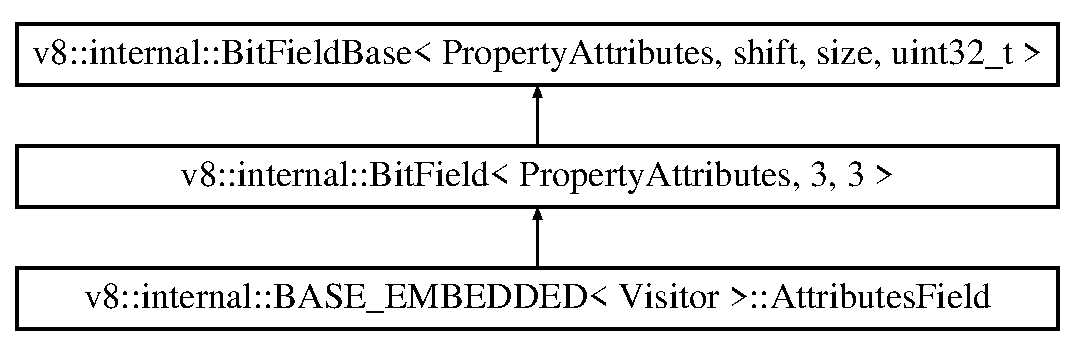
\includegraphics[height=3.000000cm]{classv8_1_1internal_1_1_b_a_s_e___e_m_b_e_d_d_e_d_1_1_attributes_field}
\end{center}
\end{figure}
\subsection*{Additional Inherited Members}


The documentation for this class was generated from the following file\+:\begin{DoxyCompactItemize}
\item 
src/property-\/details.\+h\end{DoxyCompactItemize}

\hypertarget{classv8_1_1internal_1_1_back_edge_table}{}\section{v8\+:\+:internal\+:\+:Back\+Edge\+Table Class Reference}
\label{classv8_1_1internal_1_1_back_edge_table}\index{v8\+::internal\+::\+Back\+Edge\+Table@{v8\+::internal\+::\+Back\+Edge\+Table}}
\subsection*{Public Types}
\begin{DoxyCompactItemize}
\item 
\hypertarget{classv8_1_1internal_1_1_back_edge_table_a5fdd294b989ae7d9c3c08deecd60efa2}{}enum {\bfseries Back\+Edge\+State} \{ {\bfseries I\+N\+T\+E\+R\+R\+U\+P\+T}, 
{\bfseries O\+N\+\_\+\+S\+T\+A\+C\+K\+\_\+\+R\+E\+P\+L\+A\+C\+E\+M\+E\+N\+T}, 
{\bfseries O\+S\+R\+\_\+\+A\+F\+T\+E\+R\+\_\+\+S\+T\+A\+C\+K\+\_\+\+C\+H\+E\+C\+K}
 \}\label{classv8_1_1internal_1_1_back_edge_table_a5fdd294b989ae7d9c3c08deecd60efa2}

\end{DoxyCompactItemize}
\subsection*{Public Member Functions}
\begin{DoxyCompactItemize}
\item 
\hypertarget{classv8_1_1internal_1_1_back_edge_table_a7db2b9b7aa7720c9ed264ad8514f590e}{}{\bfseries Back\+Edge\+Table} (\hyperlink{classv8_1_1internal_1_1_code}{Code} $\ast$code, \hyperlink{classv8_1_1internal_1_1_per_thread_assert_scope_debug_only}{Disallow\+Heap\+Allocation} $\ast$required)\label{classv8_1_1internal_1_1_back_edge_table_a7db2b9b7aa7720c9ed264ad8514f590e}

\item 
\hypertarget{classv8_1_1internal_1_1_back_edge_table_a56b23e90b541646f83902eb5e8653205}{}uint32\+\_\+t {\bfseries length} ()\label{classv8_1_1internal_1_1_back_edge_table_a56b23e90b541646f83902eb5e8653205}

\item 
\hypertarget{classv8_1_1internal_1_1_back_edge_table_ad2833701689e96f451ab733f1fea52a3}{}\hyperlink{classv8_1_1internal_1_1_bailout_id}{Bailout\+Id} {\bfseries ast\+\_\+id} (uint32\+\_\+t index)\label{classv8_1_1internal_1_1_back_edge_table_ad2833701689e96f451ab733f1fea52a3}

\item 
\hypertarget{classv8_1_1internal_1_1_back_edge_table_a4385d5f565fb0623ec77a3e150f5b770}{}uint32\+\_\+t {\bfseries loop\+\_\+depth} (uint32\+\_\+t index)\label{classv8_1_1internal_1_1_back_edge_table_a4385d5f565fb0623ec77a3e150f5b770}

\item 
\hypertarget{classv8_1_1internal_1_1_back_edge_table_a287333d13fd7c286ff7751a1c0465d75}{}uint32\+\_\+t {\bfseries pc\+\_\+offset} (uint32\+\_\+t index)\label{classv8_1_1internal_1_1_back_edge_table_a287333d13fd7c286ff7751a1c0465d75}

\item 
\hypertarget{classv8_1_1internal_1_1_back_edge_table_aea67e907fbd52b3fe1762f8a6c333259}{}Address {\bfseries pc} (uint32\+\_\+t index)\label{classv8_1_1internal_1_1_back_edge_table_aea67e907fbd52b3fe1762f8a6c333259}

\end{DoxyCompactItemize}
\subsection*{Static Public Member Functions}
\begin{DoxyCompactItemize}
\item 
\hypertarget{classv8_1_1internal_1_1_back_edge_table_a948f9633cd9b7de2c75db208b687329a}{}static void {\bfseries Patch} (\hyperlink{classv8_1_1internal_1_1_isolate}{Isolate} $\ast$isolate, \hyperlink{classv8_1_1internal_1_1_code}{Code} $\ast$unoptimized\+\_\+code)\label{classv8_1_1internal_1_1_back_edge_table_a948f9633cd9b7de2c75db208b687329a}

\item 
\hypertarget{classv8_1_1internal_1_1_back_edge_table_a6c051f1b5eca4c03f8f3147c71ac051c}{}static void {\bfseries Patch\+At} (\hyperlink{classv8_1_1internal_1_1_code}{Code} $\ast$unoptimized\+\_\+code, Address pc, Back\+Edge\+State target\+\_\+state, \hyperlink{classv8_1_1internal_1_1_code}{Code} $\ast$replacement\+\_\+code)\label{classv8_1_1internal_1_1_back_edge_table_a6c051f1b5eca4c03f8f3147c71ac051c}

\item 
\hypertarget{classv8_1_1internal_1_1_back_edge_table_aa4a8da5df024f0696f8be96ec8f5dbec}{}static void {\bfseries Revert} (\hyperlink{classv8_1_1internal_1_1_isolate}{Isolate} $\ast$isolate, \hyperlink{classv8_1_1internal_1_1_code}{Code} $\ast$unoptimized\+\_\+code)\label{classv8_1_1internal_1_1_back_edge_table_aa4a8da5df024f0696f8be96ec8f5dbec}

\item 
\hypertarget{classv8_1_1internal_1_1_back_edge_table_ae5dbef1c3dd27f0ccf34f8d22563aa8e}{}static void {\bfseries Add\+Stack\+Check} (\hyperlink{classv8_1_1internal_1_1_handle}{Handle}$<$ \hyperlink{classv8_1_1internal_1_1_code}{Code} $>$ code, uint32\+\_\+t pc\+\_\+offset)\label{classv8_1_1internal_1_1_back_edge_table_ae5dbef1c3dd27f0ccf34f8d22563aa8e}

\item 
\hypertarget{classv8_1_1internal_1_1_back_edge_table_a384f587613951eb9271c2320131f3ed8}{}static void {\bfseries Remove\+Stack\+Check} (\hyperlink{classv8_1_1internal_1_1_handle}{Handle}$<$ \hyperlink{classv8_1_1internal_1_1_code}{Code} $>$ code, uint32\+\_\+t pc\+\_\+offset)\label{classv8_1_1internal_1_1_back_edge_table_a384f587613951eb9271c2320131f3ed8}

\item 
\hypertarget{classv8_1_1internal_1_1_back_edge_table_ae4104ee5562bfe57be87eb6ce940ed73}{}static Back\+Edge\+State {\bfseries Get\+Back\+Edge\+State} (\hyperlink{classv8_1_1internal_1_1_isolate}{Isolate} $\ast$isolate, \hyperlink{classv8_1_1internal_1_1_code}{Code} $\ast$unoptimized\+\_\+code, Address pc\+\_\+after)\label{classv8_1_1internal_1_1_back_edge_table_ae4104ee5562bfe57be87eb6ce940ed73}

\end{DoxyCompactItemize}


The documentation for this class was generated from the following files\+:\begin{DoxyCompactItemize}
\item 
src/full-\/codegen.\+h\item 
src/full-\/codegen.\+cc\end{DoxyCompactItemize}

\hypertarget{classv8_1_1internal_1_1_code_1_1_back_edge_table_offset_field}{}\section{v8\+:\+:internal\+:\+:Code\+:\+:Back\+Edge\+Table\+Offset\+Field Class Reference}
\label{classv8_1_1internal_1_1_code_1_1_back_edge_table_offset_field}\index{v8\+::internal\+::\+Code\+::\+Back\+Edge\+Table\+Offset\+Field@{v8\+::internal\+::\+Code\+::\+Back\+Edge\+Table\+Offset\+Field}}
Inheritance diagram for v8\+:\+:internal\+:\+:Code\+:\+:Back\+Edge\+Table\+Offset\+Field\+:\begin{figure}[H]
\begin{center}
\leavevmode
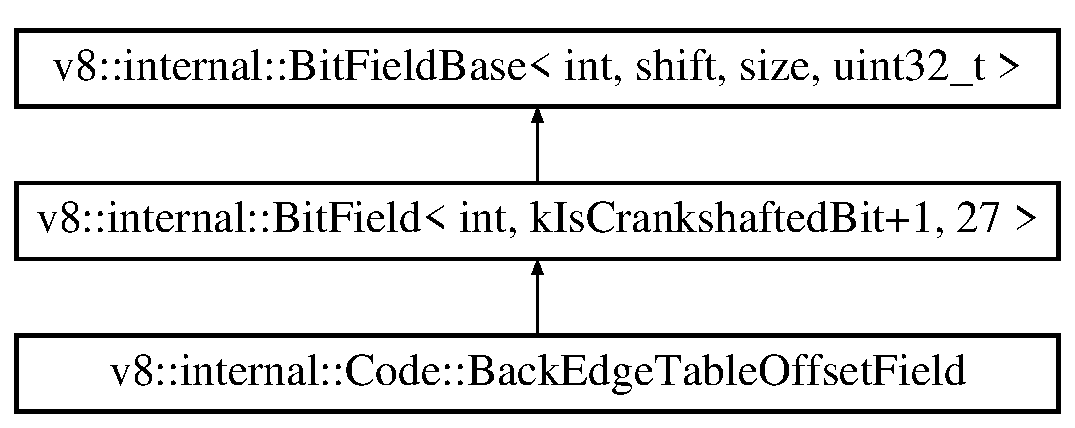
\includegraphics[height=3.000000cm]{classv8_1_1internal_1_1_code_1_1_back_edge_table_offset_field}
\end{center}
\end{figure}
\subsection*{Additional Inherited Members}


The documentation for this class was generated from the following file\+:\begin{DoxyCompactItemize}
\item 
src/objects.\+h\end{DoxyCompactItemize}

\hypertarget{classv8_1_1internal_1_1_back_reference_node}{}\section{v8\+:\+:internal\+:\+:Back\+Reference\+Node Class Reference}
\label{classv8_1_1internal_1_1_back_reference_node}\index{v8\+::internal\+::\+Back\+Reference\+Node@{v8\+::internal\+::\+Back\+Reference\+Node}}
Inheritance diagram for v8\+:\+:internal\+:\+:Back\+Reference\+Node\+:\begin{figure}[H]
\begin{center}
\leavevmode
\includegraphics[height=4.000000cm]{classv8_1_1internal_1_1_back_reference_node}
\end{center}
\end{figure}
\subsection*{Public Member Functions}
\begin{DoxyCompactItemize}
\item 
\hypertarget{classv8_1_1internal_1_1_back_reference_node_aecafde1109f696d1eb80499c9cd04b08}{}{\bfseries Back\+Reference\+Node} (int start\+\_\+reg, int end\+\_\+reg, \hyperlink{classv8_1_1internal_1_1_reg_exp_node}{Reg\+Exp\+Node} $\ast$on\+\_\+success)\label{classv8_1_1internal_1_1_back_reference_node_aecafde1109f696d1eb80499c9cd04b08}

\item 
\hypertarget{classv8_1_1internal_1_1_back_reference_node_af0f0870c3f4113d8ad375a7c9436ddff}{}virtual void {\bfseries Accept} (\hyperlink{classv8_1_1internal_1_1_node_visitor}{Node\+Visitor} $\ast$visitor)\label{classv8_1_1internal_1_1_back_reference_node_af0f0870c3f4113d8ad375a7c9436ddff}

\item 
\hypertarget{classv8_1_1internal_1_1_back_reference_node_a5898f97fe856e743638d8a4db8aae160}{}int {\bfseries start\+\_\+register} ()\label{classv8_1_1internal_1_1_back_reference_node_a5898f97fe856e743638d8a4db8aae160}

\item 
\hypertarget{classv8_1_1internal_1_1_back_reference_node_a9cc793e4e2defe8937482aa8d3462047}{}int {\bfseries end\+\_\+register} ()\label{classv8_1_1internal_1_1_back_reference_node_a9cc793e4e2defe8937482aa8d3462047}

\item 
\hypertarget{classv8_1_1internal_1_1_back_reference_node_a3d835aa391ea61ddde7ac75ba0ee9536}{}virtual void {\bfseries Emit} (\hyperlink{classv8_1_1internal_1_1_reg_exp_compiler}{Reg\+Exp\+Compiler} $\ast$compiler, \hyperlink{classv8_1_1internal_1_1_trace}{Trace} $\ast$trace)\label{classv8_1_1internal_1_1_back_reference_node_a3d835aa391ea61ddde7ac75ba0ee9536}

\item 
\hypertarget{classv8_1_1internal_1_1_back_reference_node_ae4b888f1d81c4a136c4b2a17e3bb6c62}{}virtual int {\bfseries Eats\+At\+Least} (int still\+\_\+to\+\_\+find, int recursion\+\_\+depth, bool not\+\_\+at\+\_\+start)\label{classv8_1_1internal_1_1_back_reference_node_ae4b888f1d81c4a136c4b2a17e3bb6c62}

\item 
\hypertarget{classv8_1_1internal_1_1_back_reference_node_a3df1913104dfd6615350926bdbfa2a73}{}virtual void {\bfseries Get\+Quick\+Check\+Details} (\hyperlink{classv8_1_1internal_1_1_quick_check_details}{Quick\+Check\+Details} $\ast$details, \hyperlink{classv8_1_1internal_1_1_reg_exp_compiler}{Reg\+Exp\+Compiler} $\ast$compiler, int characters\+\_\+filled\+\_\+in, bool not\+\_\+at\+\_\+start)\label{classv8_1_1internal_1_1_back_reference_node_a3df1913104dfd6615350926bdbfa2a73}

\item 
\hypertarget{classv8_1_1internal_1_1_back_reference_node_a1e9e17f26810c11345529edbf4d106ae}{}virtual void {\bfseries Fill\+In\+B\+M\+Info} (int offset, int budget, \hyperlink{classv8_1_1internal_1_1_boyer_moore_lookahead}{Boyer\+Moore\+Lookahead} $\ast$bm, bool not\+\_\+at\+\_\+start)\label{classv8_1_1internal_1_1_back_reference_node_a1e9e17f26810c11345529edbf4d106ae}

\end{DoxyCompactItemize}
\subsection*{Additional Inherited Members}


The documentation for this class was generated from the following files\+:\begin{DoxyCompactItemize}
\item 
src/jsregexp.\+h\item 
src/jsregexp.\+cc\end{DoxyCompactItemize}

\hypertarget{classv8_1_1internal_1_1_backtrack_stack}{}\section{v8\+:\+:internal\+:\+:Backtrack\+Stack Class Reference}
\label{classv8_1_1internal_1_1_backtrack_stack}\index{v8\+::internal\+::\+Backtrack\+Stack@{v8\+::internal\+::\+Backtrack\+Stack}}
\subsection*{Public Member Functions}
\begin{DoxyCompactItemize}
\item 
\hypertarget{classv8_1_1internal_1_1_backtrack_stack_adf8f617c1064c3a4a1f1a3fe3684be9c}{}int $\ast$ {\bfseries data} () const \label{classv8_1_1internal_1_1_backtrack_stack_adf8f617c1064c3a4a1f1a3fe3684be9c}

\item 
\hypertarget{classv8_1_1internal_1_1_backtrack_stack_ac3e94a3e619d1ce97cfa473354baa469}{}int {\bfseries max\+\_\+size} () const \label{classv8_1_1internal_1_1_backtrack_stack_ac3e94a3e619d1ce97cfa473354baa469}

\end{DoxyCompactItemize}


The documentation for this class was generated from the following file\+:\begin{DoxyCompactItemize}
\item 
src/interpreter-\/irregexp.\+cc\end{DoxyCompactItemize}

\hypertarget{classv8_1_1internal_1_1_bailout_id}{}\section{v8\+:\+:internal\+:\+:Bailout\+Id Class Reference}
\label{classv8_1_1internal_1_1_bailout_id}\index{v8\+::internal\+::\+Bailout\+Id@{v8\+::internal\+::\+Bailout\+Id}}
\subsection*{Public Member Functions}
\begin{DoxyCompactItemize}
\item 
\hypertarget{classv8_1_1internal_1_1_bailout_id_a29bee41095d1f83d33c1e519877b324e}{}{\bfseries Bailout\+Id} (int id)\label{classv8_1_1internal_1_1_bailout_id_a29bee41095d1f83d33c1e519877b324e}

\item 
\hypertarget{classv8_1_1internal_1_1_bailout_id_a28600772827dde89522328e18caaef0c}{}int {\bfseries To\+Int} () const \label{classv8_1_1internal_1_1_bailout_id_a28600772827dde89522328e18caaef0c}

\item 
\hypertarget{classv8_1_1internal_1_1_bailout_id_abaa5f387538060e4229834dd611b8a17}{}bool {\bfseries Is\+None} () const \label{classv8_1_1internal_1_1_bailout_id_abaa5f387538060e4229834dd611b8a17}

\item 
\hypertarget{classv8_1_1internal_1_1_bailout_id_ad56f5e5bca475897e778003958c1fc8a}{}bool {\bfseries operator==} (const \hyperlink{classv8_1_1internal_1_1_bailout_id}{Bailout\+Id} \&other) const \label{classv8_1_1internal_1_1_bailout_id_ad56f5e5bca475897e778003958c1fc8a}

\item 
\hypertarget{classv8_1_1internal_1_1_bailout_id_a70b9c565a2c63cb954189ed581767f36}{}bool {\bfseries operator!=} (const \hyperlink{classv8_1_1internal_1_1_bailout_id}{Bailout\+Id} \&other) const \label{classv8_1_1internal_1_1_bailout_id_a70b9c565a2c63cb954189ed581767f36}

\end{DoxyCompactItemize}
\subsection*{Static Public Member Functions}
\begin{DoxyCompactItemize}
\item 
\hypertarget{classv8_1_1internal_1_1_bailout_id_ae28ec2edaa82bbe4857e4e56e709ab33}{}static \hyperlink{classv8_1_1internal_1_1_bailout_id}{Bailout\+Id} {\bfseries None} ()\label{classv8_1_1internal_1_1_bailout_id_ae28ec2edaa82bbe4857e4e56e709ab33}

\item 
\hypertarget{classv8_1_1internal_1_1_bailout_id_a92ecb683edac7021e0430f3800aab6e1}{}static \hyperlink{classv8_1_1internal_1_1_bailout_id}{Bailout\+Id} {\bfseries Function\+Entry} ()\label{classv8_1_1internal_1_1_bailout_id_a92ecb683edac7021e0430f3800aab6e1}

\item 
\hypertarget{classv8_1_1internal_1_1_bailout_id_a3cf70d09c511d9d723b08f7786b1c897}{}static \hyperlink{classv8_1_1internal_1_1_bailout_id}{Bailout\+Id} {\bfseries Declarations} ()\label{classv8_1_1internal_1_1_bailout_id_a3cf70d09c511d9d723b08f7786b1c897}

\item 
\hypertarget{classv8_1_1internal_1_1_bailout_id_a7fe9eca0a53d668361894dadd7a5f29b}{}static \hyperlink{classv8_1_1internal_1_1_bailout_id}{Bailout\+Id} {\bfseries First\+Usable} ()\label{classv8_1_1internal_1_1_bailout_id_a7fe9eca0a53d668361894dadd7a5f29b}

\item 
\hypertarget{classv8_1_1internal_1_1_bailout_id_a40e64c2d4e63153746fe3f1ae62ebc59}{}static \hyperlink{classv8_1_1internal_1_1_bailout_id}{Bailout\+Id} {\bfseries Stub\+Entry} ()\label{classv8_1_1internal_1_1_bailout_id_a40e64c2d4e63153746fe3f1ae62ebc59}

\end{DoxyCompactItemize}


The documentation for this class was generated from the following file\+:\begin{DoxyCompactItemize}
\item 
src/utils.\+h\end{DoxyCompactItemize}

\hypertarget{classv8_1_1internal_1_1_zone_type_config_1_1_base}{}\section{v8\+:\+:internal\+:\+:Zone\+Type\+Config\+:\+:Base Class Reference}
\label{classv8_1_1internal_1_1_zone_type_config_1_1_base}\index{v8\+::internal\+::\+Zone\+Type\+Config\+::\+Base@{v8\+::internal\+::\+Zone\+Type\+Config\+::\+Base}}
Inheritance diagram for v8\+:\+:internal\+:\+:Zone\+Type\+Config\+:\+:Base\+:\begin{figure}[H]
\begin{center}
\leavevmode
\includegraphics[height=2.000000cm]{classv8_1_1internal_1_1_zone_type_config_1_1_base}
\end{center}
\end{figure}


The documentation for this class was generated from the following file\+:\begin{DoxyCompactItemize}
\item 
src/types.\+h\end{DoxyCompactItemize}

\hypertarget{classv8_1_1internal_1_1_parser_traits_1_1_type_1_1_b_a_s_e___e_m_b_e_d_d_e_d}{}\section{v8\+:\+:internal\+:\+:Parser\+Traits\+:\+:Type\+:\+:B\+A\+S\+E\+\_\+\+E\+M\+B\+E\+D\+D\+E\+D Class Reference}
\label{classv8_1_1internal_1_1_parser_traits_1_1_type_1_1_b_a_s_e___e_m_b_e_d_d_e_d}\index{v8\+::internal\+::\+Parser\+Traits\+::\+Type\+::\+B\+A\+S\+E\+\_\+\+E\+M\+B\+E\+D\+D\+E\+D@{v8\+::internal\+::\+Parser\+Traits\+::\+Type\+::\+B\+A\+S\+E\+\_\+\+E\+M\+B\+E\+D\+D\+E\+D}}
\subsection*{Public Member Functions}
\begin{DoxyCompactItemize}
\item 
\hypertarget{classv8_1_1internal_1_1_parser_traits_1_1_type_1_1_b_a_s_e___e_m_b_e_d_d_e_d_ac7cc52b5749108b183d72020613ef4ff}{}{\footnotesize template$<$typename Parser $>$ }\\{\bfseries Checkpoint} (\hyperlink{classv8_1_1internal_1_1_parser}{Parser} $\ast$parser)\label{classv8_1_1internal_1_1_parser_traits_1_1_type_1_1_b_a_s_e___e_m_b_e_d_d_e_d_ac7cc52b5749108b183d72020613ef4ff}

\item 
\hypertarget{classv8_1_1internal_1_1_parser_traits_1_1_type_1_1_b_a_s_e___e_m_b_e_d_d_e_d_adcf972541129bd48fe7891bfa78c422e}{}void {\bfseries Restore} ()\label{classv8_1_1internal_1_1_parser_traits_1_1_type_1_1_b_a_s_e___e_m_b_e_d_d_e_d_adcf972541129bd48fe7891bfa78c422e}

\end{DoxyCompactItemize}


The documentation for this class was generated from the following file\+:\begin{DoxyCompactItemize}
\item 
src/parser.\+h\end{DoxyCompactItemize}

\hypertarget{classv8_1_1internal_1_1_parser_base_1_1_b_a_s_e___e_m_b_e_d_d_e_d}{}\section{v8\+:\+:internal\+:\+:Parser\+Base$<$ Traits $>$\+:\+:B\+A\+S\+E\+\_\+\+E\+M\+B\+E\+D\+D\+E\+D Class Reference}
\label{classv8_1_1internal_1_1_parser_base_1_1_b_a_s_e___e_m_b_e_d_d_e_d}\index{v8\+::internal\+::\+Parser\+Base$<$ Traits $>$\+::\+B\+A\+S\+E\+\_\+\+E\+M\+B\+E\+D\+D\+E\+D@{v8\+::internal\+::\+Parser\+Base$<$ Traits $>$\+::\+B\+A\+S\+E\+\_\+\+E\+M\+B\+E\+D\+D\+E\+D}}
\subsection*{Public Member Functions}
\begin{DoxyCompactItemize}
\item 
\hypertarget{classv8_1_1internal_1_1_parser_base_1_1_b_a_s_e___e_m_b_e_d_d_e_d_a0ef253e8b3c94f7fc93423ad885d3486}{}{\bfseries Block\+State} (typename Traits\+::\+Type\+::\+Scope $\ast$$\ast$scope\+\_\+stack, typename Traits\+::\+Type\+::\+Scope $\ast$scope)\label{classv8_1_1internal_1_1_parser_base_1_1_b_a_s_e___e_m_b_e_d_d_e_d_a0ef253e8b3c94f7fc93423ad885d3486}

\item 
\hypertarget{classv8_1_1internal_1_1_parser_base_1_1_b_a_s_e___e_m_b_e_d_d_e_d_a02075172691be9b987b64dd7b3b9541d}{}{\bfseries Function\+State} (Function\+State $\ast$$\ast$function\+\_\+state\+\_\+stack, typename Traits\+::\+Type\+::\+Scope $\ast$$\ast$scope\+\_\+stack, typename Traits\+::\+Type\+::\+Scope $\ast$scope, typename Traits\+::\+Type\+::\+Zone $\ast$zone=N\+U\+L\+L, \hyperlink{classv8_1_1internal_1_1_ast_value_factory}{Ast\+Value\+Factory} $\ast$ast\+\_\+value\+\_\+factory=N\+U\+L\+L)\label{classv8_1_1internal_1_1_parser_base_1_1_b_a_s_e___e_m_b_e_d_d_e_d_a02075172691be9b987b64dd7b3b9541d}

\item 
\hypertarget{classv8_1_1internal_1_1_parser_base_1_1_b_a_s_e___e_m_b_e_d_d_e_d_ade7f7217aebe225b046c2518c246d7f4}{}{\bfseries Function\+State} (Function\+State $\ast$$\ast$function\+\_\+state\+\_\+stack, typename Traits\+::\+Type\+::\+Scope $\ast$$\ast$scope\+\_\+stack, typename Traits\+::\+Type\+::\+Scope $\ast$$\ast$scope, typename Traits\+::\+Type\+::\+Zone $\ast$zone=N\+U\+L\+L, \hyperlink{classv8_1_1internal_1_1_ast_value_factory}{Ast\+Value\+Factory} $\ast$ast\+\_\+value\+\_\+factory=N\+U\+L\+L)\label{classv8_1_1internal_1_1_parser_base_1_1_b_a_s_e___e_m_b_e_d_d_e_d_ade7f7217aebe225b046c2518c246d7f4}

\item 
\hypertarget{classv8_1_1internal_1_1_parser_base_1_1_b_a_s_e___e_m_b_e_d_d_e_d_af00b51fa11ef142ca72114db8c07899b}{}int {\bfseries Next\+Materialized\+Literal\+Index} ()\label{classv8_1_1internal_1_1_parser_base_1_1_b_a_s_e___e_m_b_e_d_d_e_d_af00b51fa11ef142ca72114db8c07899b}

\item 
\hypertarget{classv8_1_1internal_1_1_parser_base_1_1_b_a_s_e___e_m_b_e_d_d_e_d_a15cc1aa75cdcbb090f4c6f07241501a6}{}int {\bfseries materialized\+\_\+literal\+\_\+count} ()\label{classv8_1_1internal_1_1_parser_base_1_1_b_a_s_e___e_m_b_e_d_d_e_d_a15cc1aa75cdcbb090f4c6f07241501a6}

\item 
\hypertarget{classv8_1_1internal_1_1_parser_base_1_1_b_a_s_e___e_m_b_e_d_d_e_d_a22c2897e9d83394784200af1ba90235d}{}int {\bfseries Next\+Handler\+Index} ()\label{classv8_1_1internal_1_1_parser_base_1_1_b_a_s_e___e_m_b_e_d_d_e_d_a22c2897e9d83394784200af1ba90235d}

\item 
\hypertarget{classv8_1_1internal_1_1_parser_base_1_1_b_a_s_e___e_m_b_e_d_d_e_d_ae56580ae33c0531763712b2f4167da07}{}int {\bfseries handler\+\_\+count} ()\label{classv8_1_1internal_1_1_parser_base_1_1_b_a_s_e___e_m_b_e_d_d_e_d_ae56580ae33c0531763712b2f4167da07}

\item 
\hypertarget{classv8_1_1internal_1_1_parser_base_1_1_b_a_s_e___e_m_b_e_d_d_e_d_afbefeeabe007ff2f5444b7309e2458ff}{}void {\bfseries Add\+Property} ()\label{classv8_1_1internal_1_1_parser_base_1_1_b_a_s_e___e_m_b_e_d_d_e_d_afbefeeabe007ff2f5444b7309e2458ff}

\item 
\hypertarget{classv8_1_1internal_1_1_parser_base_1_1_b_a_s_e___e_m_b_e_d_d_e_d_a9ca6c72c27f439d995aa34dc93526ec8}{}int {\bfseries expected\+\_\+property\+\_\+count} ()\label{classv8_1_1internal_1_1_parser_base_1_1_b_a_s_e___e_m_b_e_d_d_e_d_a9ca6c72c27f439d995aa34dc93526ec8}

\item 
\hypertarget{classv8_1_1internal_1_1_parser_base_1_1_b_a_s_e___e_m_b_e_d_d_e_d_adac4f4d4215e0e2a6311b4db076bef7b}{}void {\bfseries set\+\_\+is\+\_\+generator} (bool is\+\_\+generator)\label{classv8_1_1internal_1_1_parser_base_1_1_b_a_s_e___e_m_b_e_d_d_e_d_adac4f4d4215e0e2a6311b4db076bef7b}

\item 
\hypertarget{classv8_1_1internal_1_1_parser_base_1_1_b_a_s_e___e_m_b_e_d_d_e_d_a47a9d82c53032671ba31fa7bd2981a20}{}bool {\bfseries is\+\_\+generator} () const \label{classv8_1_1internal_1_1_parser_base_1_1_b_a_s_e___e_m_b_e_d_d_e_d_a47a9d82c53032671ba31fa7bd2981a20}

\item 
\hypertarget{classv8_1_1internal_1_1_parser_base_1_1_b_a_s_e___e_m_b_e_d_d_e_d_a093589069385eb98d8fa30899e994b1f}{}void {\bfseries set\+\_\+generator\+\_\+object\+\_\+variable} (typename Traits\+::\+Type\+::\+Generator\+Variable $\ast$variable)\label{classv8_1_1internal_1_1_parser_base_1_1_b_a_s_e___e_m_b_e_d_d_e_d_a093589069385eb98d8fa30899e994b1f}

\item 
\hypertarget{classv8_1_1internal_1_1_parser_base_1_1_b_a_s_e___e_m_b_e_d_d_e_d_a1ca19792b3ccd1d09341844c5f9fd4b8}{}Traits\+::\+Type\+::\+Generator\+Variable $\ast$ {\bfseries generator\+\_\+object\+\_\+variable} () const \label{classv8_1_1internal_1_1_parser_base_1_1_b_a_s_e___e_m_b_e_d_d_e_d_a1ca19792b3ccd1d09341844c5f9fd4b8}

\item 
\hypertarget{classv8_1_1internal_1_1_parser_base_1_1_b_a_s_e___e_m_b_e_d_d_e_d_a53daa944fc570bb12e50b64bd7051cf0}{}Traits\+::\+Type\+::\+Factory $\ast$ {\bfseries factory} ()\label{classv8_1_1internal_1_1_parser_base_1_1_b_a_s_e___e_m_b_e_d_d_e_d_a53daa944fc570bb12e50b64bd7051cf0}

\item 
\hypertarget{classv8_1_1internal_1_1_parser_base_1_1_b_a_s_e___e_m_b_e_d_d_e_d_a194c39f59c32c9d0d4bbc73229a0853a}{}{\bfseries Parsing\+Mode\+Scope} (\hyperlink{classv8_1_1internal_1_1_parser_base}{Parser\+Base} $\ast$parser, Mode mode)\label{classv8_1_1internal_1_1_parser_base_1_1_b_a_s_e___e_m_b_e_d_d_e_d_a194c39f59c32c9d0d4bbc73229a0853a}

\end{DoxyCompactItemize}
\subsection*{Friends}
\begin{DoxyCompactItemize}
\item 
\hypertarget{classv8_1_1internal_1_1_parser_base_1_1_b_a_s_e___e_m_b_e_d_d_e_d_a5f14c645eff20b2a5bad62347cde341c}{}class {\bfseries Parser\+Traits}\label{classv8_1_1internal_1_1_parser_base_1_1_b_a_s_e___e_m_b_e_d_d_e_d_a5f14c645eff20b2a5bad62347cde341c}

\item 
\hypertarget{classv8_1_1internal_1_1_parser_base_1_1_b_a_s_e___e_m_b_e_d_d_e_d_a36ba09a5b76b5aa08057abbe746dc439}{}class {\bfseries Parser\+Checkpoint}\label{classv8_1_1internal_1_1_parser_base_1_1_b_a_s_e___e_m_b_e_d_d_e_d_a36ba09a5b76b5aa08057abbe746dc439}

\end{DoxyCompactItemize}


The documentation for this class was generated from the following file\+:\begin{DoxyCompactItemize}
\item 
src/preparser.\+h\end{DoxyCompactItemize}

\hypertarget{classv8_1_1internal_1_1_pre_parser_traits_1_1_type_1_1_b_a_s_e___e_m_b_e_d_d_e_d}{}\section{v8\+:\+:internal\+:\+:Pre\+Parser\+Traits\+:\+:Type\+:\+:B\+A\+S\+E\+\_\+\+E\+M\+B\+E\+D\+D\+E\+D Class Reference}
\label{classv8_1_1internal_1_1_pre_parser_traits_1_1_type_1_1_b_a_s_e___e_m_b_e_d_d_e_d}\index{v8\+::internal\+::\+Pre\+Parser\+Traits\+::\+Type\+::\+B\+A\+S\+E\+\_\+\+E\+M\+B\+E\+D\+D\+E\+D@{v8\+::internal\+::\+Pre\+Parser\+Traits\+::\+Type\+::\+B\+A\+S\+E\+\_\+\+E\+M\+B\+E\+D\+D\+E\+D}}
\subsection*{Public Member Functions}
\begin{DoxyCompactItemize}
\item 
\hypertarget{classv8_1_1internal_1_1_pre_parser_traits_1_1_type_1_1_b_a_s_e___e_m_b_e_d_d_e_d_a12010dcb42c1b9f24a8497e3a2361d39}{}{\footnotesize template$<$typename Parser $>$ }\\{\bfseries Checkpoint} (\hyperlink{classv8_1_1internal_1_1_pre_parser}{Parser} $\ast$parser)\label{classv8_1_1internal_1_1_pre_parser_traits_1_1_type_1_1_b_a_s_e___e_m_b_e_d_d_e_d_a12010dcb42c1b9f24a8497e3a2361d39}

\item 
\hypertarget{classv8_1_1internal_1_1_pre_parser_traits_1_1_type_1_1_b_a_s_e___e_m_b_e_d_d_e_d_af72fc1eb4b2c3e50a46fa1474e90861d}{}void {\bfseries Restore} ()\label{classv8_1_1internal_1_1_pre_parser_traits_1_1_type_1_1_b_a_s_e___e_m_b_e_d_d_e_d_af72fc1eb4b2c3e50a46fa1474e90861d}

\end{DoxyCompactItemize}


The documentation for this class was generated from the following file\+:\begin{DoxyCompactItemize}
\item 
src/preparser.\+h\end{DoxyCompactItemize}

\hypertarget{classv8_1_1internal_1_1_splay_tree_1_1_b_a_s_e___e_m_b_e_d_d_e_d}{}\section{v8\+:\+:internal\+:\+:Splay\+Tree$<$ Config, Allocation\+Policy $>$\+:\+:B\+A\+S\+E\+\_\+\+E\+M\+B\+E\+D\+D\+E\+D$<$ Callback $>$ Class Template Reference}
\label{classv8_1_1internal_1_1_splay_tree_1_1_b_a_s_e___e_m_b_e_d_d_e_d}\index{v8\+::internal\+::\+Splay\+Tree$<$ Config, Allocation\+Policy $>$\+::\+B\+A\+S\+E\+\_\+\+E\+M\+B\+E\+D\+D\+E\+D$<$ Callback $>$@{v8\+::internal\+::\+Splay\+Tree$<$ Config, Allocation\+Policy $>$\+::\+B\+A\+S\+E\+\_\+\+E\+M\+B\+E\+D\+D\+E\+D$<$ Callback $>$}}
\subsection*{Public Member Functions}
\begin{DoxyCompactItemize}
\item 
\hypertarget{classv8_1_1internal_1_1_splay_tree_1_1_b_a_s_e___e_m_b_e_d_d_e_d_a19a57c9a69ed16044f4bfa4b3da70bb7}{}{\bfseries Locator} (\hyperlink{classv8_1_1internal_1_1_splay_tree_1_1_node}{Node} $\ast$node)\label{classv8_1_1internal_1_1_splay_tree_1_1_b_a_s_e___e_m_b_e_d_d_e_d_a19a57c9a69ed16044f4bfa4b3da70bb7}

\item 
\hypertarget{classv8_1_1internal_1_1_splay_tree_1_1_b_a_s_e___e_m_b_e_d_d_e_d_a177e6f18907a22432c91adca8b30339d}{}{\bfseries Locator} ()\label{classv8_1_1internal_1_1_splay_tree_1_1_b_a_s_e___e_m_b_e_d_d_e_d_a177e6f18907a22432c91adca8b30339d}

\item 
\hypertarget{classv8_1_1internal_1_1_splay_tree_1_1_b_a_s_e___e_m_b_e_d_d_e_d_aaef940c26374118c5a8d9156aea37ac7}{}const Key \& {\bfseries key} ()\label{classv8_1_1internal_1_1_splay_tree_1_1_b_a_s_e___e_m_b_e_d_d_e_d_aaef940c26374118c5a8d9156aea37ac7}

\item 
\hypertarget{classv8_1_1internal_1_1_splay_tree_1_1_b_a_s_e___e_m_b_e_d_d_e_d_a143a0948ed7f887ccede5fa486bef2d1}{}Value \& {\bfseries value} ()\label{classv8_1_1internal_1_1_splay_tree_1_1_b_a_s_e___e_m_b_e_d_d_e_d_a143a0948ed7f887ccede5fa486bef2d1}

\item 
\hypertarget{classv8_1_1internal_1_1_splay_tree_1_1_b_a_s_e___e_m_b_e_d_d_e_d_a2b7bfeb6c98e916d3282b3b4e19a55c0}{}void {\bfseries set\+\_\+value} (const Value \&value)\label{classv8_1_1internal_1_1_splay_tree_1_1_b_a_s_e___e_m_b_e_d_d_e_d_a2b7bfeb6c98e916d3282b3b4e19a55c0}

\item 
\hypertarget{classv8_1_1internal_1_1_splay_tree_1_1_b_a_s_e___e_m_b_e_d_d_e_d_ad88b47084dfd693e0c663b58b037ee6f}{}void {\bfseries bind} (\hyperlink{classv8_1_1internal_1_1_splay_tree_1_1_node}{Node} $\ast$node)\label{classv8_1_1internal_1_1_splay_tree_1_1_b_a_s_e___e_m_b_e_d_d_e_d_ad88b47084dfd693e0c663b58b037ee6f}

\item 
\hypertarget{classv8_1_1internal_1_1_splay_tree_1_1_b_a_s_e___e_m_b_e_d_d_e_d_a3b441e2bfadadbbe083ba0f5f638486d}{}{\bfseries Node\+To\+Pair\+Adaptor} (Callback $\ast$callback)\label{classv8_1_1internal_1_1_splay_tree_1_1_b_a_s_e___e_m_b_e_d_d_e_d_a3b441e2bfadadbbe083ba0f5f638486d}

\item 
\hypertarget{classv8_1_1internal_1_1_splay_tree_1_1_b_a_s_e___e_m_b_e_d_d_e_d_a07a0fd21214268a9b1f8bcbce2fd6c22}{}void {\bfseries Call} (\hyperlink{classv8_1_1internal_1_1_splay_tree_1_1_node}{Node} $\ast$node)\label{classv8_1_1internal_1_1_splay_tree_1_1_b_a_s_e___e_m_b_e_d_d_e_d_a07a0fd21214268a9b1f8bcbce2fd6c22}

\item 
\hypertarget{classv8_1_1internal_1_1_splay_tree_1_1_b_a_s_e___e_m_b_e_d_d_e_d_a4d2a7a81b4f4bb4282a44978855b5b0a}{}{\bfseries Node\+Deleter} ()\label{classv8_1_1internal_1_1_splay_tree_1_1_b_a_s_e___e_m_b_e_d_d_e_d_a4d2a7a81b4f4bb4282a44978855b5b0a}

\item 
\hypertarget{classv8_1_1internal_1_1_splay_tree_1_1_b_a_s_e___e_m_b_e_d_d_e_d_a07a0fd21214268a9b1f8bcbce2fd6c22}{}void {\bfseries Call} (\hyperlink{classv8_1_1internal_1_1_splay_tree_1_1_node}{Node} $\ast$node)\label{classv8_1_1internal_1_1_splay_tree_1_1_b_a_s_e___e_m_b_e_d_d_e_d_a07a0fd21214268a9b1f8bcbce2fd6c22}

\end{DoxyCompactItemize}


The documentation for this class was generated from the following file\+:\begin{DoxyCompactItemize}
\item 
src/splay-\/tree.\+h\end{DoxyCompactItemize}

\hypertarget{classv8_1_1internal_1_1_b_a_s_e___e_m_b_e_d_d_e_d}{}\section{v8\+:\+:internal\+:\+:B\+A\+S\+E\+\_\+\+E\+M\+B\+E\+D\+D\+E\+D$<$ Visitor $>$ Class Template Reference}
\label{classv8_1_1internal_1_1_b_a_s_e___e_m_b_e_d_d_e_d}\index{v8\+::internal\+::\+B\+A\+S\+E\+\_\+\+E\+M\+B\+E\+D\+D\+E\+D$<$ Visitor $>$@{v8\+::internal\+::\+B\+A\+S\+E\+\_\+\+E\+M\+B\+E\+D\+D\+E\+D$<$ Visitor $>$}}
\subsection*{Classes}
\begin{DoxyCompactItemize}
\item 
class \hyperlink{classv8_1_1internal_1_1_b_a_s_e___e_m_b_e_d_d_e_d_1_1_arguments_field}{Arguments\+Field}
\item 
class \hyperlink{classv8_1_1internal_1_1_b_a_s_e___e_m_b_e_d_d_e_d_1_1_attributes_field}{Attributes\+Field}
\item 
class \hyperlink{classv8_1_1internal_1_1_b_a_s_e___e_m_b_e_d_d_e_d_1_1_b_a_s_e___e_m_b_e_d_d_e_d}{B\+A\+S\+E\+\_\+\+E\+M\+B\+E\+D\+D\+E\+D}
\item 
class \hyperlink{classv8_1_1internal_1_1_b_a_s_e___e_m_b_e_d_d_e_d_1_1_deleted_field}{Deleted\+Field}
\item 
class \hyperlink{classv8_1_1internal_1_1_b_a_s_e___e_m_b_e_d_d_e_d_1_1_deoptimization_index_field}{Deoptimization\+Index\+Field}
\item 
class \hyperlink{classv8_1_1internal_1_1_b_a_s_e___e_m_b_e_d_d_e_d_1_1_descriptor_pointer}{Descriptor\+Pointer}
\item 
class \hyperlink{classv8_1_1internal_1_1_b_a_s_e___e_m_b_e_d_d_e_d_1_1_dictionary_storage_field}{Dictionary\+Storage\+Field}
\item 
class \hyperlink{classv8_1_1internal_1_1_b_a_s_e___e_m_b_e_d_d_e_d_1_1_element}{Element}
\item 
class \hyperlink{classv8_1_1internal_1_1_b_a_s_e___e_m_b_e_d_d_e_d_1_1_field_index_field}{Field\+Index\+Field}
\item 
class \hyperlink{classv8_1_1internal_1_1_b_a_s_e___e_m_b_e_d_d_e_d_1_1_flags}{Flags}
\item 
class \hyperlink{classv8_1_1internal_1_1_b_a_s_e___e_m_b_e_d_d_e_d_1_1_index_field}{Index\+Field}
\item 
class \hyperlink{classv8_1_1internal_1_1_b_a_s_e___e_m_b_e_d_d_e_d_1_1_kind_field}{Kind\+Field}
\item 
class \hyperlink{classv8_1_1internal_1_1_b_a_s_e___e_m_b_e_d_d_e_d_1_1_representation_field}{Representation\+Field}
\item 
class \hyperlink{classv8_1_1internal_1_1_b_a_s_e___e_m_b_e_d_d_e_d_1_1_save_doubles_field}{Save\+Doubles\+Field}
\item 
struct \hyperlink{structv8_1_1internal_1_1_b_a_s_e___e_m_b_e_d_d_e_d_1_1_state}{State}
\item 
class \hyperlink{classv8_1_1internal_1_1_b_a_s_e___e_m_b_e_d_d_e_d_1_1_type_field}{Type\+Field}
\end{DoxyCompactItemize}
\subsection*{Public Types}
\begin{DoxyCompactItemize}
\item 
\hypertarget{classv8_1_1internal_1_1_b_a_s_e___e_m_b_e_d_d_e_d_a0b1f7845f671653888eb673912c88af4}{}enum {\bfseries Distance} \{ {\bfseries k\+Near}, 
{\bfseries k\+Far}
 \}\label{classv8_1_1internal_1_1_b_a_s_e___e_m_b_e_d_d_e_d_a0b1f7845f671653888eb673912c88af4}

\item 
\hypertarget{classv8_1_1internal_1_1_b_a_s_e___e_m_b_e_d_d_e_d_a86d4e2d8815ac6f9c09a8ff25971ffb9}{}enum {\bfseries Type} \{ \\*
{\bfseries B\+U\+I\+L\+T\+I\+N\+\_\+\+C\+A\+L\+L}, 
{\bfseries B\+U\+I\+L\+T\+I\+N\+\_\+\+C\+O\+M\+P\+A\+R\+E\+\_\+\+C\+A\+L\+L}, 
{\bfseries B\+U\+I\+L\+T\+I\+N\+\_\+\+F\+P\+\_\+\+F\+P\+\_\+\+C\+A\+L\+L}, 
{\bfseries B\+U\+I\+L\+T\+I\+N\+\_\+\+F\+P\+\_\+\+C\+A\+L\+L}, 
\\*
{\bfseries B\+U\+I\+L\+T\+I\+N\+\_\+\+F\+P\+\_\+\+I\+N\+T\+\_\+\+C\+A\+L\+L}, 
{\bfseries D\+I\+R\+E\+C\+T\+\_\+\+A\+P\+I\+\_\+\+C\+A\+L\+L}, 
{\bfseries P\+R\+O\+F\+I\+L\+I\+N\+G\+\_\+\+A\+P\+I\+\_\+\+C\+A\+L\+L}, 
{\bfseries D\+I\+R\+E\+C\+T\+\_\+\+G\+E\+T\+T\+E\+R\+\_\+\+C\+A\+L\+L}, 
\\*
{\bfseries P\+R\+O\+F\+I\+L\+I\+N\+G\+\_\+\+G\+E\+T\+T\+E\+R\+\_\+\+C\+A\+L\+L}, 
{\bfseries N\+O\+N\+E} = 0, 
{\bfseries N\+U\+M\+B\+E\+R\+\_\+\+O\+F\+\_\+\+T\+Y\+P\+E\+S}, 
{\bfseries M\+A\+N\+U\+A\+L}, 
\\*
{\bfseries k\+Context\+Variable} = v8\+:\+:Heap\+Graph\+Edge\+:\+:k\+Context\+Variable, 
{\bfseries k\+Element} = v8\+:\+:Heap\+Graph\+Edge\+:\+:k\+Element, 
{\bfseries k\+Property} = v8\+:\+:Heap\+Graph\+Edge\+:\+:k\+Property, 
{\bfseries k\+Internal} = v8\+:\+:Heap\+Graph\+Edge\+:\+:k\+Internal, 
\\*
{\bfseries k\+Hidden} = v8\+:\+:Heap\+Graph\+Edge\+:\+:k\+Hidden, 
{\bfseries k\+Shortcut} = v8\+:\+:Heap\+Graph\+Edge\+:\+:k\+Shortcut, 
{\bfseries k\+Weak} = v8\+:\+:Heap\+Graph\+Edge\+:\+:k\+Weak, 
{\bfseries k\+Hidden} = v8\+:\+:Heap\+Graph\+Edge\+:\+:k\+Hidden, 
\\*
{\bfseries k\+Array} = v8\+:\+:Heap\+Graph\+Node\+:\+:k\+Array, 
{\bfseries k\+String} = v8\+:\+:Heap\+Graph\+Node\+:\+:k\+String, 
{\bfseries k\+Object} = v8\+:\+:Heap\+Graph\+Node\+:\+:k\+Object, 
{\bfseries k\+Code} = v8\+:\+:Heap\+Graph\+Node\+:\+:k\+Code, 
\\*
{\bfseries k\+Closure} = v8\+:\+:Heap\+Graph\+Node\+:\+:k\+Closure, 
{\bfseries k\+Reg\+Exp} = v8\+:\+:Heap\+Graph\+Node\+:\+:k\+Reg\+Exp, 
{\bfseries k\+Heap\+Number} = v8\+:\+:Heap\+Graph\+Node\+:\+:k\+Heap\+Number, 
{\bfseries k\+Native} = v8\+:\+:Heap\+Graph\+Node\+:\+:k\+Native, 
\\*
{\bfseries k\+Synthetic} = v8\+:\+:Heap\+Graph\+Node\+:\+:k\+Synthetic, 
{\bfseries k\+Cons\+String} = v8\+:\+:Heap\+Graph\+Node\+:\+:k\+Cons\+String, 
{\bfseries k\+Sliced\+String} = v8\+:\+:Heap\+Graph\+Node\+:\+:k\+Sliced\+String, 
{\bfseries k\+Symbol} = v8\+:\+:Heap\+Graph\+Node\+:\+:k\+Symbol
 \}\label{classv8_1_1internal_1_1_b_a_s_e___e_m_b_e_d_d_e_d_a86d4e2d8815ac6f9c09a8ff25971ffb9}

\item 
\hypertarget{classv8_1_1internal_1_1_b_a_s_e___e_m_b_e_d_d_e_d_ac2849b502d70e20d5d6567fbd119c8f9}{}enum {\bfseries Major} \{ {\bfseries Uninitialized\+Major\+Key} = 0, 
{\bfseries No\+Cache}, 
{\bfseries N\+U\+M\+B\+E\+R\+\_\+\+O\+F\+\_\+\+I\+D\+S}
 \}\label{classv8_1_1internal_1_1_b_a_s_e___e_m_b_e_d_d_e_d_ac2849b502d70e20d5d6567fbd119c8f9}

\item 
\hypertarget{classv8_1_1internal_1_1_b_a_s_e___e_m_b_e_d_d_e_d_a796e8c3cc9a53628565341f982d2afc9}{}enum {\bfseries Opcode} \{ {\bfseries L\+A\+S\+T} = L\+I\+T\+E\+R\+A\+L
 \}\label{classv8_1_1internal_1_1_b_a_s_e___e_m_b_e_d_d_e_d_a796e8c3cc9a53628565341f982d2afc9}

\item 
\hypertarget{classv8_1_1internal_1_1_b_a_s_e___e_m_b_e_d_d_e_d_a0a4a22b0347663cb13591a3a0750ba79}{}enum {\bfseries Slot\+Representation} \{ \\*
{\bfseries U\+N\+K\+N\+O\+W\+N}, 
{\bfseries T\+A\+G\+G\+E\+D}, 
{\bfseries I\+N\+T32}, 
{\bfseries U\+I\+N\+T32}, 
\\*
{\bfseries D\+O\+U\+B\+L\+E}, 
{\bfseries L\+I\+T\+E\+R\+A\+L}, 
{\bfseries D\+E\+F\+E\+R\+R\+E\+D\+\_\+\+O\+B\+J\+E\+C\+T}, 
{\bfseries D\+U\+P\+L\+I\+C\+A\+T\+E\+\_\+\+O\+B\+J\+E\+C\+T}, 
\\*
{\bfseries A\+R\+G\+U\+M\+E\+N\+T\+S\+\_\+\+O\+B\+J\+E\+C\+T}
 \}\label{classv8_1_1internal_1_1_b_a_s_e___e_m_b_e_d_d_e_d_a0a4a22b0347663cb13591a3a0750ba79}

\item 
\hypertarget{classv8_1_1internal_1_1_b_a_s_e___e_m_b_e_d_d_e_d_a597b8e57ea3ef503b8b2b9e3a70f42fa}{}enum {\bfseries Kind} \{ \\*
{\bfseries J\+S\+\_\+\+E\+N\+T\+R\+Y}, 
{\bfseries C\+A\+T\+C\+H}, 
{\bfseries F\+I\+N\+A\+L\+L\+Y}, 
{\bfseries L\+A\+S\+T\+\_\+\+K\+I\+N\+D} = F\+I\+N\+A\+L\+L\+Y, 
\\*
{\bfseries k\+Simple} = 0, 
{\bfseries k\+With\+Registers} = 1 $<$$<$ 0, 
{\bfseries k\+With\+Doubles} = 1 $<$$<$ 1, 
{\bfseries k\+With\+Registers\+And\+Doubles} = k\+With\+Registers $\vert$ k\+With\+Doubles
 \}\label{classv8_1_1internal_1_1_b_a_s_e___e_m_b_e_d_d_e_d_a597b8e57ea3ef503b8b2b9e3a70f42fa}

\item 
\hypertarget{classv8_1_1internal_1_1_b_a_s_e___e_m_b_e_d_d_e_d_a86d4e2d8815ac6f9c09a8ff25971ffb9}{}enum {\bfseries Type} \{ \\*
{\bfseries B\+U\+I\+L\+T\+I\+N\+\_\+\+C\+A\+L\+L}, 
{\bfseries B\+U\+I\+L\+T\+I\+N\+\_\+\+C\+O\+M\+P\+A\+R\+E\+\_\+\+C\+A\+L\+L}, 
{\bfseries B\+U\+I\+L\+T\+I\+N\+\_\+\+F\+P\+\_\+\+F\+P\+\_\+\+C\+A\+L\+L}, 
{\bfseries B\+U\+I\+L\+T\+I\+N\+\_\+\+F\+P\+\_\+\+C\+A\+L\+L}, 
\\*
{\bfseries B\+U\+I\+L\+T\+I\+N\+\_\+\+F\+P\+\_\+\+I\+N\+T\+\_\+\+C\+A\+L\+L}, 
{\bfseries D\+I\+R\+E\+C\+T\+\_\+\+A\+P\+I\+\_\+\+C\+A\+L\+L}, 
{\bfseries P\+R\+O\+F\+I\+L\+I\+N\+G\+\_\+\+A\+P\+I\+\_\+\+C\+A\+L\+L}, 
{\bfseries D\+I\+R\+E\+C\+T\+\_\+\+G\+E\+T\+T\+E\+R\+\_\+\+C\+A\+L\+L}, 
\\*
{\bfseries P\+R\+O\+F\+I\+L\+I\+N\+G\+\_\+\+G\+E\+T\+T\+E\+R\+\_\+\+C\+A\+L\+L}, 
{\bfseries N\+O\+N\+E} = 0, 
{\bfseries N\+U\+M\+B\+E\+R\+\_\+\+O\+F\+\_\+\+T\+Y\+P\+E\+S}, 
{\bfseries M\+A\+N\+U\+A\+L}, 
\\*
{\bfseries k\+Context\+Variable} = v8\+:\+:Heap\+Graph\+Edge\+:\+:k\+Context\+Variable, 
{\bfseries k\+Element} = v8\+:\+:Heap\+Graph\+Edge\+:\+:k\+Element, 
{\bfseries k\+Property} = v8\+:\+:Heap\+Graph\+Edge\+:\+:k\+Property, 
{\bfseries k\+Internal} = v8\+:\+:Heap\+Graph\+Edge\+:\+:k\+Internal, 
\\*
{\bfseries k\+Hidden} = v8\+:\+:Heap\+Graph\+Edge\+:\+:k\+Hidden, 
{\bfseries k\+Shortcut} = v8\+:\+:Heap\+Graph\+Edge\+:\+:k\+Shortcut, 
{\bfseries k\+Weak} = v8\+:\+:Heap\+Graph\+Edge\+:\+:k\+Weak, 
{\bfseries k\+Hidden} = v8\+:\+:Heap\+Graph\+Edge\+:\+:k\+Hidden, 
\\*
{\bfseries k\+Array} = v8\+:\+:Heap\+Graph\+Node\+:\+:k\+Array, 
{\bfseries k\+String} = v8\+:\+:Heap\+Graph\+Node\+:\+:k\+String, 
{\bfseries k\+Object} = v8\+:\+:Heap\+Graph\+Node\+:\+:k\+Object, 
{\bfseries k\+Code} = v8\+:\+:Heap\+Graph\+Node\+:\+:k\+Code, 
\\*
{\bfseries k\+Closure} = v8\+:\+:Heap\+Graph\+Node\+:\+:k\+Closure, 
{\bfseries k\+Reg\+Exp} = v8\+:\+:Heap\+Graph\+Node\+:\+:k\+Reg\+Exp, 
{\bfseries k\+Heap\+Number} = v8\+:\+:Heap\+Graph\+Node\+:\+:k\+Heap\+Number, 
{\bfseries k\+Native} = v8\+:\+:Heap\+Graph\+Node\+:\+:k\+Native, 
\\*
{\bfseries k\+Synthetic} = v8\+:\+:Heap\+Graph\+Node\+:\+:k\+Synthetic, 
{\bfseries k\+Cons\+String} = v8\+:\+:Heap\+Graph\+Node\+:\+:k\+Cons\+String, 
{\bfseries k\+Sliced\+String} = v8\+:\+:Heap\+Graph\+Node\+:\+:k\+Sliced\+String, 
{\bfseries k\+Symbol} = v8\+:\+:Heap\+Graph\+Node\+:\+:k\+Symbol
 \}\label{classv8_1_1internal_1_1_b_a_s_e___e_m_b_e_d_d_e_d_a86d4e2d8815ac6f9c09a8ff25971ffb9}

\item 
\hypertarget{classv8_1_1internal_1_1_b_a_s_e___e_m_b_e_d_d_e_d_aaaee46232f5b050c6f414648c7c9188c}{}enum {\bfseries Id} \{ {\bfseries I\+D\+\_\+\+M\+I\+N\+\_\+\+V\+A\+L\+U\+E} = k\+Min\+Int, 
{\bfseries I\+D\+\_\+\+M\+A\+X\+\_\+\+V\+A\+L\+U\+E} = k\+Max\+Int, 
{\bfseries N\+O\+\_\+\+I\+D} = 0
 \}\label{classv8_1_1internal_1_1_b_a_s_e___e_m_b_e_d_d_e_d_aaaee46232f5b050c6f414648c7c9188c}

\item 
\hypertarget{classv8_1_1internal_1_1_b_a_s_e___e_m_b_e_d_d_e_d_a6e8f0f08e4e94d957675dd02223a8c1a}{}enum {\bfseries Js\+Frame\+Marker} \{ {\bfseries I\+N\+N\+E\+R\+\_\+\+J\+S\+E\+N\+T\+R\+Y\+\_\+\+F\+R\+A\+M\+E} = 0, 
{\bfseries O\+U\+T\+E\+R\+M\+O\+S\+T\+\_\+\+J\+S\+E\+N\+T\+R\+Y\+\_\+\+F\+R\+A\+M\+E} = 1
 \}\label{classv8_1_1internal_1_1_b_a_s_e___e_m_b_e_d_d_e_d_a6e8f0f08e4e94d957675dd02223a8c1a}

\item 
\hypertarget{classv8_1_1internal_1_1_b_a_s_e___e_m_b_e_d_d_e_d_a7db761bcaf86c69d87422f9740db001b}{}enum {\bfseries Print\+Mode} \{ {\bfseries O\+V\+E\+R\+V\+I\+E\+W}, 
{\bfseries D\+E\+T\+A\+I\+L\+S}
 \}\label{classv8_1_1internal_1_1_b_a_s_e___e_m_b_e_d_d_e_d_a7db761bcaf86c69d87422f9740db001b}

\item 
\hypertarget{classv8_1_1internal_1_1_b_a_s_e___e_m_b_e_d_d_e_d_a86d4e2d8815ac6f9c09a8ff25971ffb9}{}enum {\bfseries Type} \{ \\*
{\bfseries B\+U\+I\+L\+T\+I\+N\+\_\+\+C\+A\+L\+L}, 
{\bfseries B\+U\+I\+L\+T\+I\+N\+\_\+\+C\+O\+M\+P\+A\+R\+E\+\_\+\+C\+A\+L\+L}, 
{\bfseries B\+U\+I\+L\+T\+I\+N\+\_\+\+F\+P\+\_\+\+F\+P\+\_\+\+C\+A\+L\+L}, 
{\bfseries B\+U\+I\+L\+T\+I\+N\+\_\+\+F\+P\+\_\+\+C\+A\+L\+L}, 
\\*
{\bfseries B\+U\+I\+L\+T\+I\+N\+\_\+\+F\+P\+\_\+\+I\+N\+T\+\_\+\+C\+A\+L\+L}, 
{\bfseries D\+I\+R\+E\+C\+T\+\_\+\+A\+P\+I\+\_\+\+C\+A\+L\+L}, 
{\bfseries P\+R\+O\+F\+I\+L\+I\+N\+G\+\_\+\+A\+P\+I\+\_\+\+C\+A\+L\+L}, 
{\bfseries D\+I\+R\+E\+C\+T\+\_\+\+G\+E\+T\+T\+E\+R\+\_\+\+C\+A\+L\+L}, 
\\*
{\bfseries P\+R\+O\+F\+I\+L\+I\+N\+G\+\_\+\+G\+E\+T\+T\+E\+R\+\_\+\+C\+A\+L\+L}, 
{\bfseries N\+O\+N\+E} = 0, 
{\bfseries N\+U\+M\+B\+E\+R\+\_\+\+O\+F\+\_\+\+T\+Y\+P\+E\+S}, 
{\bfseries M\+A\+N\+U\+A\+L}, 
\\*
{\bfseries k\+Context\+Variable} = v8\+:\+:Heap\+Graph\+Edge\+:\+:k\+Context\+Variable, 
{\bfseries k\+Element} = v8\+:\+:Heap\+Graph\+Edge\+:\+:k\+Element, 
{\bfseries k\+Property} = v8\+:\+:Heap\+Graph\+Edge\+:\+:k\+Property, 
{\bfseries k\+Internal} = v8\+:\+:Heap\+Graph\+Edge\+:\+:k\+Internal, 
\\*
{\bfseries k\+Hidden} = v8\+:\+:Heap\+Graph\+Edge\+:\+:k\+Hidden, 
{\bfseries k\+Shortcut} = v8\+:\+:Heap\+Graph\+Edge\+:\+:k\+Shortcut, 
{\bfseries k\+Weak} = v8\+:\+:Heap\+Graph\+Edge\+:\+:k\+Weak, 
{\bfseries k\+Hidden} = v8\+:\+:Heap\+Graph\+Edge\+:\+:k\+Hidden, 
\\*
{\bfseries k\+Array} = v8\+:\+:Heap\+Graph\+Node\+:\+:k\+Array, 
{\bfseries k\+String} = v8\+:\+:Heap\+Graph\+Node\+:\+:k\+String, 
{\bfseries k\+Object} = v8\+:\+:Heap\+Graph\+Node\+:\+:k\+Object, 
{\bfseries k\+Code} = v8\+:\+:Heap\+Graph\+Node\+:\+:k\+Code, 
\\*
{\bfseries k\+Closure} = v8\+:\+:Heap\+Graph\+Node\+:\+:k\+Closure, 
{\bfseries k\+Reg\+Exp} = v8\+:\+:Heap\+Graph\+Node\+:\+:k\+Reg\+Exp, 
{\bfseries k\+Heap\+Number} = v8\+:\+:Heap\+Graph\+Node\+:\+:k\+Heap\+Number, 
{\bfseries k\+Native} = v8\+:\+:Heap\+Graph\+Node\+:\+:k\+Native, 
\\*
{\bfseries k\+Synthetic} = v8\+:\+:Heap\+Graph\+Node\+:\+:k\+Synthetic, 
{\bfseries k\+Cons\+String} = v8\+:\+:Heap\+Graph\+Node\+:\+:k\+Cons\+String, 
{\bfseries k\+Sliced\+String} = v8\+:\+:Heap\+Graph\+Node\+:\+:k\+Sliced\+String, 
{\bfseries k\+Symbol} = v8\+:\+:Heap\+Graph\+Node\+:\+:k\+Symbol
 \}\label{classv8_1_1internal_1_1_b_a_s_e___e_m_b_e_d_d_e_d_a86d4e2d8815ac6f9c09a8ff25971ffb9}

\item 
\hypertarget{classv8_1_1internal_1_1_b_a_s_e___e_m_b_e_d_d_e_d_a86d4e2d8815ac6f9c09a8ff25971ffb9}{}enum {\bfseries Type} \{ \\*
{\bfseries B\+U\+I\+L\+T\+I\+N\+\_\+\+C\+A\+L\+L}, 
{\bfseries B\+U\+I\+L\+T\+I\+N\+\_\+\+C\+O\+M\+P\+A\+R\+E\+\_\+\+C\+A\+L\+L}, 
{\bfseries B\+U\+I\+L\+T\+I\+N\+\_\+\+F\+P\+\_\+\+F\+P\+\_\+\+C\+A\+L\+L}, 
{\bfseries B\+U\+I\+L\+T\+I\+N\+\_\+\+F\+P\+\_\+\+C\+A\+L\+L}, 
\\*
{\bfseries B\+U\+I\+L\+T\+I\+N\+\_\+\+F\+P\+\_\+\+I\+N\+T\+\_\+\+C\+A\+L\+L}, 
{\bfseries D\+I\+R\+E\+C\+T\+\_\+\+A\+P\+I\+\_\+\+C\+A\+L\+L}, 
{\bfseries P\+R\+O\+F\+I\+L\+I\+N\+G\+\_\+\+A\+P\+I\+\_\+\+C\+A\+L\+L}, 
{\bfseries D\+I\+R\+E\+C\+T\+\_\+\+G\+E\+T\+T\+E\+R\+\_\+\+C\+A\+L\+L}, 
\\*
{\bfseries P\+R\+O\+F\+I\+L\+I\+N\+G\+\_\+\+G\+E\+T\+T\+E\+R\+\_\+\+C\+A\+L\+L}, 
{\bfseries N\+O\+N\+E} = 0, 
{\bfseries N\+U\+M\+B\+E\+R\+\_\+\+O\+F\+\_\+\+T\+Y\+P\+E\+S}, 
{\bfseries M\+A\+N\+U\+A\+L}, 
\\*
{\bfseries k\+Context\+Variable} = v8\+:\+:Heap\+Graph\+Edge\+:\+:k\+Context\+Variable, 
{\bfseries k\+Element} = v8\+:\+:Heap\+Graph\+Edge\+:\+:k\+Element, 
{\bfseries k\+Property} = v8\+:\+:Heap\+Graph\+Edge\+:\+:k\+Property, 
{\bfseries k\+Internal} = v8\+:\+:Heap\+Graph\+Edge\+:\+:k\+Internal, 
\\*
{\bfseries k\+Hidden} = v8\+:\+:Heap\+Graph\+Edge\+:\+:k\+Hidden, 
{\bfseries k\+Shortcut} = v8\+:\+:Heap\+Graph\+Edge\+:\+:k\+Shortcut, 
{\bfseries k\+Weak} = v8\+:\+:Heap\+Graph\+Edge\+:\+:k\+Weak, 
{\bfseries k\+Hidden} = v8\+:\+:Heap\+Graph\+Edge\+:\+:k\+Hidden, 
\\*
{\bfseries k\+Array} = v8\+:\+:Heap\+Graph\+Node\+:\+:k\+Array, 
{\bfseries k\+String} = v8\+:\+:Heap\+Graph\+Node\+:\+:k\+String, 
{\bfseries k\+Object} = v8\+:\+:Heap\+Graph\+Node\+:\+:k\+Object, 
{\bfseries k\+Code} = v8\+:\+:Heap\+Graph\+Node\+:\+:k\+Code, 
\\*
{\bfseries k\+Closure} = v8\+:\+:Heap\+Graph\+Node\+:\+:k\+Closure, 
{\bfseries k\+Reg\+Exp} = v8\+:\+:Heap\+Graph\+Node\+:\+:k\+Reg\+Exp, 
{\bfseries k\+Heap\+Number} = v8\+:\+:Heap\+Graph\+Node\+:\+:k\+Heap\+Number, 
{\bfseries k\+Native} = v8\+:\+:Heap\+Graph\+Node\+:\+:k\+Native, 
\\*
{\bfseries k\+Synthetic} = v8\+:\+:Heap\+Graph\+Node\+:\+:k\+Synthetic, 
{\bfseries k\+Cons\+String} = v8\+:\+:Heap\+Graph\+Node\+:\+:k\+Cons\+String, 
{\bfseries k\+Sliced\+String} = v8\+:\+:Heap\+Graph\+Node\+:\+:k\+Sliced\+String, 
{\bfseries k\+Symbol} = v8\+:\+:Heap\+Graph\+Node\+:\+:k\+Symbol
 \}\label{classv8_1_1internal_1_1_b_a_s_e___e_m_b_e_d_d_e_d_a86d4e2d8815ac6f9c09a8ff25971ffb9}

\item 
\hypertarget{classv8_1_1internal_1_1_b_a_s_e___e_m_b_e_d_d_e_d_aa09619c6a12a554417df97fe40eab745}{}enum {\bfseries Hoistability} \{ {\bfseries H\+O\+I\+S\+T\+A\+B\+L\+E}, 
{\bfseries O\+P\+T\+I\+M\+I\+S\+T\+I\+C\+A\+L\+L\+Y\+\_\+\+H\+O\+I\+S\+T\+A\+B\+L\+E}, 
{\bfseries N\+O\+T\+\_\+\+H\+O\+I\+S\+T\+A\+B\+L\+E}
 \}\label{classv8_1_1internal_1_1_b_a_s_e___e_m_b_e_d_d_e_d_aa09619c6a12a554417df97fe40eab745}

\item 
\hypertarget{classv8_1_1internal_1_1_b_a_s_e___e_m_b_e_d_d_e_d_adff2dd6e8aec0ffdabe2135301a1dbb6}{}enum {\bfseries Text\+Type} \{ {\bfseries A\+T\+O\+M}, 
{\bfseries C\+H\+A\+R\+\_\+\+C\+L\+A\+S\+S}
 \}\label{classv8_1_1internal_1_1_b_a_s_e___e_m_b_e_d_d_e_d_adff2dd6e8aec0ffdabe2135301a1dbb6}

\item 
\hypertarget{classv8_1_1internal_1_1_b_a_s_e___e_m_b_e_d_d_e_d_ad8a2e468fa3dc4653942cd4be018625a}{}enum {\bfseries Configuration} \{ \\*
{\bfseries C\+H\+E\+C\+K\+\_\+\+O\+W\+N\+\_\+\+R\+E\+A\+L} = 0, 
{\bfseries C\+H\+E\+C\+K\+\_\+\+H\+I\+D\+D\+E\+N} = 1 $<$$<$ 0, 
{\bfseries C\+H\+E\+C\+K\+\_\+\+D\+E\+R\+I\+V\+E\+D} = 1 $<$$<$ 1, 
{\bfseries C\+H\+E\+C\+K\+\_\+\+I\+N\+T\+E\+R\+C\+E\+P\+T\+O\+R} = 1 $<$$<$ 2, 
\\*
{\bfseries C\+H\+E\+C\+K\+\_\+\+A\+C\+C\+E\+S\+S\+\_\+\+C\+H\+E\+C\+K} = 1 $<$$<$ 3, 
{\bfseries C\+H\+E\+C\+K\+\_\+\+A\+L\+L}, 
{\bfseries S\+K\+I\+P\+\_\+\+I\+N\+T\+E\+R\+C\+E\+P\+T\+O\+R} = C\+H\+E\+C\+K\+\_\+\+A\+L\+L $^\wedge$ C\+H\+E\+C\+K\+\_\+\+I\+N\+T\+E\+R\+C\+E\+P\+T\+O\+R, 
{\bfseries C\+H\+E\+C\+K\+\_\+\+O\+W\+N} = C\+H\+E\+C\+K\+\_\+\+A\+L\+L $^\wedge$ C\+H\+E\+C\+K\+\_\+\+D\+E\+R\+I\+V\+E\+D
 \}\label{classv8_1_1internal_1_1_b_a_s_e___e_m_b_e_d_d_e_d_ad8a2e468fa3dc4653942cd4be018625a}

\item 
\hypertarget{classv8_1_1internal_1_1_b_a_s_e___e_m_b_e_d_d_e_d_aea5e836b2c351dd71777783bbf36881f}{}enum {\bfseries State} \{ \\*
{\bfseries N\+O\+T\+\_\+\+F\+O\+U\+N\+D}, 
{\bfseries P\+R\+O\+P\+E\+R\+T\+Y}, 
{\bfseries I\+N\+T\+E\+R\+C\+E\+P\+T\+O\+R}, 
{\bfseries A\+C\+C\+E\+S\+S\+\_\+\+C\+H\+E\+C\+K}, 
\\*
{\bfseries J\+S\+P\+R\+O\+X\+Y}
 \}\label{classv8_1_1internal_1_1_b_a_s_e___e_m_b_e_d_d_e_d_aea5e836b2c351dd71777783bbf36881f}

\item 
\hypertarget{classv8_1_1internal_1_1_b_a_s_e___e_m_b_e_d_d_e_d_a086765593c89c2d75154f11ad7d86671}{}enum {\bfseries Property\+Kind} \{ {\bfseries D\+A\+T\+A}, 
{\bfseries A\+C\+C\+E\+S\+S\+O\+R}
 \}\label{classv8_1_1internal_1_1_b_a_s_e___e_m_b_e_d_d_e_d_a086765593c89c2d75154f11ad7d86671}

\item 
\hypertarget{classv8_1_1internal_1_1_b_a_s_e___e_m_b_e_d_d_e_d_ae7293a56a291983addcee044f0c34a2d}{}enum {\bfseries Property\+Encoding} \{ {\bfseries D\+I\+C\+T\+I\+O\+N\+A\+R\+Y}, 
{\bfseries D\+E\+S\+C\+R\+I\+P\+T\+O\+R}
 \}\label{classv8_1_1internal_1_1_b_a_s_e___e_m_b_e_d_d_e_d_ae7293a56a291983addcee044f0c34a2d}

\item 
\hypertarget{classv8_1_1internal_1_1_b_a_s_e___e_m_b_e_d_d_e_d_abb4fbac19c550e2428ec75bb8b28f5a9}{}enum \{ \\*
{\bfseries k\+Start\+Position\+Index}, 
{\bfseries k\+End\+Position\+Index}, 
{\bfseries k\+Literal\+Count\+Index}, 
{\bfseries k\+Property\+Count\+Index}, 
\\*
{\bfseries k\+Strict\+Mode\+Index}, 
{\bfseries k\+Size}
 \}\label{classv8_1_1internal_1_1_b_a_s_e___e_m_b_e_d_d_e_d_abb4fbac19c550e2428ec75bb8b28f5a9}

\item 
\hypertarget{classv8_1_1internal_1_1_b_a_s_e___e_m_b_e_d_d_e_d_a597b8e57ea3ef503b8b2b9e3a70f42fa}{}enum {\bfseries Kind} \{ \\*
{\bfseries J\+S\+\_\+\+E\+N\+T\+R\+Y}, 
{\bfseries C\+A\+T\+C\+H}, 
{\bfseries F\+I\+N\+A\+L\+L\+Y}, 
{\bfseries L\+A\+S\+T\+\_\+\+K\+I\+N\+D} = F\+I\+N\+A\+L\+L\+Y, 
\\*
{\bfseries k\+Simple} = 0, 
{\bfseries k\+With\+Registers} = 1 $<$$<$ 0, 
{\bfseries k\+With\+Doubles} = 1 $<$$<$ 1, 
{\bfseries k\+With\+Registers\+And\+Doubles} = k\+With\+Registers $\vert$ k\+With\+Doubles
 \}\label{classv8_1_1internal_1_1_b_a_s_e___e_m_b_e_d_d_e_d_a597b8e57ea3ef503b8b2b9e3a70f42fa}

\item 
\hypertarget{classv8_1_1internal_1_1_b_a_s_e___e_m_b_e_d_d_e_d_ae197182bf039524422c58a5eedc95670}{}enum {\bfseries Deopt\+Mode} \{ {\bfseries k\+No\+Lazy\+Deopt}, 
{\bfseries k\+Lazy\+Deopt}
 \}\label{classv8_1_1internal_1_1_b_a_s_e___e_m_b_e_d_d_e_d_ae197182bf039524422c58a5eedc95670}

\item 
\hypertarget{classv8_1_1internal_1_1_b_a_s_e___e_m_b_e_d_d_e_d_a574780580d55298af45d52077d3422fe}{}enum {\bfseries Holder\+Lookup} \{ {\bfseries k\+Holder\+Not\+Found}, 
{\bfseries k\+Holder\+Is\+Receiver}, 
{\bfseries k\+Holder\+Found}
 \}\label{classv8_1_1internal_1_1_b_a_s_e___e_m_b_e_d_d_e_d_a574780580d55298af45d52077d3422fe}

\item 
\hypertarget{classv8_1_1internal_1_1_b_a_s_e___e_m_b_e_d_d_e_d_a3d20e152a0054ebd26b81817ba35280b}{}typedef void $\ast$ {\bfseries External\+Reference\+Redirector}(void $\ast$original, Type type)\label{classv8_1_1internal_1_1_b_a_s_e___e_m_b_e_d_d_e_d_a3d20e152a0054ebd26b81817ba35280b}

\end{DoxyCompactItemize}
\subsection*{Public Member Functions}
\begin{DoxyCompactItemize}
\item 
\hypertarget{classv8_1_1internal_1_1_b_a_s_e___e_m_b_e_d_d_e_d_add33908956d9bed09a8bca6b0d740f15}{}{\bfseries Arguments} (int length, \hyperlink{classv8_1_1internal_1_1_object}{Object} $\ast$$\ast$arguments)\label{classv8_1_1internal_1_1_b_a_s_e___e_m_b_e_d_d_e_d_add33908956d9bed09a8bca6b0d740f15}

\item 
\hypertarget{classv8_1_1internal_1_1_b_a_s_e___e_m_b_e_d_d_e_d_abc66cea105fe88e86c3d7b8dde50a580}{}\hyperlink{classv8_1_1internal_1_1_object}{Object} $\ast$\& {\bfseries operator\mbox{[}$\,$\mbox{]}} (int index)\label{classv8_1_1internal_1_1_b_a_s_e___e_m_b_e_d_d_e_d_abc66cea105fe88e86c3d7b8dde50a580}

\item 
\hypertarget{classv8_1_1internal_1_1_b_a_s_e___e_m_b_e_d_d_e_d_a798750e6054524ded89f7e3aae595cc9}{}{\footnotesize template$<$class S $>$ }\\\hyperlink{classv8_1_1internal_1_1_handle}{Handle}$<$ S $>$ {\bfseries at} (int index)\label{classv8_1_1internal_1_1_b_a_s_e___e_m_b_e_d_d_e_d_a798750e6054524ded89f7e3aae595cc9}

\item 
\hypertarget{classv8_1_1internal_1_1_b_a_s_e___e_m_b_e_d_d_e_d_a0baf7dbae1e7fffaaf243aafc160ef2c}{}int {\bfseries smi\+\_\+at} (int index)\label{classv8_1_1internal_1_1_b_a_s_e___e_m_b_e_d_d_e_d_a0baf7dbae1e7fffaaf243aafc160ef2c}

\item 
\hypertarget{classv8_1_1internal_1_1_b_a_s_e___e_m_b_e_d_d_e_d_a96a0211888c152b4db1c32fd169fab7b}{}double {\bfseries number\+\_\+at} (int index)\label{classv8_1_1internal_1_1_b_a_s_e___e_m_b_e_d_d_e_d_a96a0211888c152b4db1c32fd169fab7b}

\item 
\hypertarget{classv8_1_1internal_1_1_b_a_s_e___e_m_b_e_d_d_e_d_aaf57eaaeae1bbeb27a8d033b1b889f3c}{}int {\bfseries length} () const \label{classv8_1_1internal_1_1_b_a_s_e___e_m_b_e_d_d_e_d_aaf57eaaeae1bbeb27a8d033b1b889f3c}

\item 
\hypertarget{classv8_1_1internal_1_1_b_a_s_e___e_m_b_e_d_d_e_d_a6d5c730dd16865e031579f10f478caaa}{}\hyperlink{classv8_1_1internal_1_1_object}{Object} $\ast$$\ast$ {\bfseries arguments} ()\label{classv8_1_1internal_1_1_b_a_s_e___e_m_b_e_d_d_e_d_a6d5c730dd16865e031579f10f478caaa}

\item 
\hypertarget{classv8_1_1internal_1_1_b_a_s_e___e_m_b_e_d_d_e_d_addd11b8e48d02cd0f0c3ffc479164df7}{}{\bfseries Dont\+Emit\+Debug\+Code\+Scope} (\hyperlink{classv8_1_1internal_1_1_assembler_base}{Assembler\+Base} $\ast$assembler)\label{classv8_1_1internal_1_1_b_a_s_e___e_m_b_e_d_d_e_d_addd11b8e48d02cd0f0c3ffc479164df7}

\item 
\hypertarget{classv8_1_1internal_1_1_b_a_s_e___e_m_b_e_d_d_e_d_af4370e266a511099cb16732746d6b04a}{}{\bfseries Cpu\+Feature\+Scope} (\hyperlink{classv8_1_1internal_1_1_assembler_base}{Assembler\+Base} $\ast$assembler, Cpu\+Feature f)\label{classv8_1_1internal_1_1_b_a_s_e___e_m_b_e_d_d_e_d_af4370e266a511099cb16732746d6b04a}

\item 
\hypertarget{classv8_1_1internal_1_1_b_a_s_e___e_m_b_e_d_d_e_d_a18e1d3f1a56925cad9fca70c3a5710a4}{}{\bfseries I\+N\+L\+I\+N\+E} (Label())\label{classv8_1_1internal_1_1_b_a_s_e___e_m_b_e_d_d_e_d_a18e1d3f1a56925cad9fca70c3a5710a4}

\item 
\hypertarget{classv8_1_1internal_1_1_b_a_s_e___e_m_b_e_d_d_e_d_aa236b757410c690856757ee03f4ca2e2}{}{\bfseries I\+N\+L\+I\+N\+E} ($\sim$Label())\label{classv8_1_1internal_1_1_b_a_s_e___e_m_b_e_d_d_e_d_aa236b757410c690856757ee03f4ca2e2}

\item 
\hypertarget{classv8_1_1internal_1_1_b_a_s_e___e_m_b_e_d_d_e_d_ac72eadcf599fbb1d1877a550b3f86f81}{}{\bfseries I\+N\+L\+I\+N\+E} (void Unuse())\label{classv8_1_1internal_1_1_b_a_s_e___e_m_b_e_d_d_e_d_ac72eadcf599fbb1d1877a550b3f86f81}

\item 
\hypertarget{classv8_1_1internal_1_1_b_a_s_e___e_m_b_e_d_d_e_d_ad3ba4ec7acc4b645efa4ec663d133ee0}{}{\bfseries I\+N\+L\+I\+N\+E} (void Unuse\+Near())\label{classv8_1_1internal_1_1_b_a_s_e___e_m_b_e_d_d_e_d_ad3ba4ec7acc4b645efa4ec663d133ee0}

\item 
\hypertarget{classv8_1_1internal_1_1_b_a_s_e___e_m_b_e_d_d_e_d_a1bfd941cb699dc5e9f796afcec0693d2}{}{\bfseries I\+N\+L\+I\+N\+E} (bool is\+\_\+bound() const)\label{classv8_1_1internal_1_1_b_a_s_e___e_m_b_e_d_d_e_d_a1bfd941cb699dc5e9f796afcec0693d2}

\item 
\hypertarget{classv8_1_1internal_1_1_b_a_s_e___e_m_b_e_d_d_e_d_aa9b517b2df0abd17bf9a33aeca7672ba}{}{\bfseries I\+N\+L\+I\+N\+E} (bool is\+\_\+unused() const)\label{classv8_1_1internal_1_1_b_a_s_e___e_m_b_e_d_d_e_d_aa9b517b2df0abd17bf9a33aeca7672ba}

\item 
\hypertarget{classv8_1_1internal_1_1_b_a_s_e___e_m_b_e_d_d_e_d_a4751b649f03328a550ce75ad0283d38f}{}{\bfseries I\+N\+L\+I\+N\+E} (bool is\+\_\+linked() const)\label{classv8_1_1internal_1_1_b_a_s_e___e_m_b_e_d_d_e_d_a4751b649f03328a550ce75ad0283d38f}

\item 
\hypertarget{classv8_1_1internal_1_1_b_a_s_e___e_m_b_e_d_d_e_d_aeb0c6c916b136e5186562d4ee9b4d421}{}{\bfseries I\+N\+L\+I\+N\+E} (bool is\+\_\+near\+\_\+linked() const)\label{classv8_1_1internal_1_1_b_a_s_e___e_m_b_e_d_d_e_d_aeb0c6c916b136e5186562d4ee9b4d421}

\item 
\hypertarget{classv8_1_1internal_1_1_b_a_s_e___e_m_b_e_d_d_e_d_a0738b4111a7f236ad805c2f3b56fda7d}{}int {\bfseries pos} () const \label{classv8_1_1internal_1_1_b_a_s_e___e_m_b_e_d_d_e_d_a0738b4111a7f236ad805c2f3b56fda7d}

\item 
\hypertarget{classv8_1_1internal_1_1_b_a_s_e___e_m_b_e_d_d_e_d_a9aa8b32d0178286b643dab3a51e928bc}{}int {\bfseries near\+\_\+link\+\_\+pos} () const \label{classv8_1_1internal_1_1_b_a_s_e___e_m_b_e_d_d_e_d_a9aa8b32d0178286b643dab3a51e928bc}

\item 
\hypertarget{classv8_1_1internal_1_1_b_a_s_e___e_m_b_e_d_d_e_d_a4d02785a2928c688cb350a9640fb3872}{}{\bfseries Reloc\+Info\+Writer} ()\label{classv8_1_1internal_1_1_b_a_s_e___e_m_b_e_d_d_e_d_a4d02785a2928c688cb350a9640fb3872}

\item 
\hypertarget{classv8_1_1internal_1_1_b_a_s_e___e_m_b_e_d_d_e_d_a345c7d02647a0cd5c0a0053b74a5abd6}{}{\bfseries Reloc\+Info\+Writer} (byte $\ast$pos, byte $\ast$pc)\label{classv8_1_1internal_1_1_b_a_s_e___e_m_b_e_d_d_e_d_a345c7d02647a0cd5c0a0053b74a5abd6}

\item 
\hypertarget{classv8_1_1internal_1_1_b_a_s_e___e_m_b_e_d_d_e_d_a62e6c187e45dc1109ae0e2dd9ca4329b}{}byte $\ast$ {\bfseries pos} () const \label{classv8_1_1internal_1_1_b_a_s_e___e_m_b_e_d_d_e_d_a62e6c187e45dc1109ae0e2dd9ca4329b}

\item 
\hypertarget{classv8_1_1internal_1_1_b_a_s_e___e_m_b_e_d_d_e_d_a93cab2cda44abae3b8d37d8e4f4d411b}{}byte $\ast$ {\bfseries last\+\_\+pc} () const \label{classv8_1_1internal_1_1_b_a_s_e___e_m_b_e_d_d_e_d_a93cab2cda44abae3b8d37d8e4f4d411b}

\item 
\hypertarget{classv8_1_1internal_1_1_b_a_s_e___e_m_b_e_d_d_e_d_a8886e1565720fda562dfe4c17c83ca67}{}void {\bfseries Write} (const \hyperlink{classv8_1_1internal_1_1_reloc_info}{Reloc\+Info} $\ast$rinfo)\label{classv8_1_1internal_1_1_b_a_s_e___e_m_b_e_d_d_e_d_a8886e1565720fda562dfe4c17c83ca67}

\item 
\hypertarget{classv8_1_1internal_1_1_b_a_s_e___e_m_b_e_d_d_e_d_a4702d949eb49d67812c76eb6b1b03c7a}{}void {\bfseries Reposition} (byte $\ast$pos, byte $\ast$pc)\label{classv8_1_1internal_1_1_b_a_s_e___e_m_b_e_d_d_e_d_a4702d949eb49d67812c76eb6b1b03c7a}

\item 
\hypertarget{classv8_1_1internal_1_1_b_a_s_e___e_m_b_e_d_d_e_d_a0e38547f60fb33307b61d3638b52b566}{}{\bfseries External\+Reference} ()\label{classv8_1_1internal_1_1_b_a_s_e___e_m_b_e_d_d_e_d_a0e38547f60fb33307b61d3638b52b566}

\item 
\hypertarget{classv8_1_1internal_1_1_b_a_s_e___e_m_b_e_d_d_e_d_ad5ca73c8e7eb64fdd3498bb2069e047e}{}{\bfseries External\+Reference} (Builtins\+::\+C\+Function\+Id id, \hyperlink{classv8_1_1internal_1_1_isolate}{Isolate} $\ast$isolate)\label{classv8_1_1internal_1_1_b_a_s_e___e_m_b_e_d_d_e_d_ad5ca73c8e7eb64fdd3498bb2069e047e}

\item 
\hypertarget{classv8_1_1internal_1_1_b_a_s_e___e_m_b_e_d_d_e_d_af55ca1b7fc0441ef43d9d0994e01eef9}{}{\bfseries External\+Reference} (\hyperlink{classv8_1_1_api_function}{Api\+Function} $\ast$ptr, Type type, \hyperlink{classv8_1_1internal_1_1_isolate}{Isolate} $\ast$isolate)\label{classv8_1_1internal_1_1_b_a_s_e___e_m_b_e_d_d_e_d_af55ca1b7fc0441ef43d9d0994e01eef9}

\item 
\hypertarget{classv8_1_1internal_1_1_b_a_s_e___e_m_b_e_d_d_e_d_a5bc8d69cca852f0df7d01f1ae53a1e84}{}{\bfseries External\+Reference} (Builtins\+::\+Name name, \hyperlink{classv8_1_1internal_1_1_isolate}{Isolate} $\ast$isolate)\label{classv8_1_1internal_1_1_b_a_s_e___e_m_b_e_d_d_e_d_a5bc8d69cca852f0df7d01f1ae53a1e84}

\item 
\hypertarget{classv8_1_1internal_1_1_b_a_s_e___e_m_b_e_d_d_e_d_a31ba0940e025a8df40d17b8866d54112}{}{\bfseries External\+Reference} (Runtime\+::\+Function\+Id id, \hyperlink{classv8_1_1internal_1_1_isolate}{Isolate} $\ast$isolate)\label{classv8_1_1internal_1_1_b_a_s_e___e_m_b_e_d_d_e_d_a31ba0940e025a8df40d17b8866d54112}

\item 
\hypertarget{classv8_1_1internal_1_1_b_a_s_e___e_m_b_e_d_d_e_d_a21c61fa37e976e14c1afbc5c36e29cde}{}{\bfseries External\+Reference} (const \hyperlink{structv8_1_1internal_1_1_runtime_1_1_function}{Runtime\+::\+Function} $\ast$f, \hyperlink{classv8_1_1internal_1_1_isolate}{Isolate} $\ast$isolate)\label{classv8_1_1internal_1_1_b_a_s_e___e_m_b_e_d_d_e_d_a21c61fa37e976e14c1afbc5c36e29cde}

\item 
\hypertarget{classv8_1_1internal_1_1_b_a_s_e___e_m_b_e_d_d_e_d_a9895ed23d6170703f529a745220c61a4}{}{\bfseries External\+Reference} (const \hyperlink{classv8_1_1internal_1_1_i_c___utility}{I\+C\+\_\+\+Utility} \&ic\+\_\+utility, \hyperlink{classv8_1_1internal_1_1_isolate}{Isolate} $\ast$isolate)\label{classv8_1_1internal_1_1_b_a_s_e___e_m_b_e_d_d_e_d_a9895ed23d6170703f529a745220c61a4}

\item 
\hypertarget{classv8_1_1internal_1_1_b_a_s_e___e_m_b_e_d_d_e_d_a0a96e31c35f646d63bfca1135fb102d0}{}{\bfseries External\+Reference} (\hyperlink{classv8_1_1internal_1_1_stats_counter}{Stats\+Counter} $\ast$counter)\label{classv8_1_1internal_1_1_b_a_s_e___e_m_b_e_d_d_e_d_a0a96e31c35f646d63bfca1135fb102d0}

\item 
\hypertarget{classv8_1_1internal_1_1_b_a_s_e___e_m_b_e_d_d_e_d_a1c95c3f4a8190c0f598df63955afe8aa}{}{\bfseries External\+Reference} (Isolate\+::\+Address\+Id id, \hyperlink{classv8_1_1internal_1_1_isolate}{Isolate} $\ast$isolate)\label{classv8_1_1internal_1_1_b_a_s_e___e_m_b_e_d_d_e_d_a1c95c3f4a8190c0f598df63955afe8aa}

\item 
\hypertarget{classv8_1_1internal_1_1_b_a_s_e___e_m_b_e_d_d_e_d_a8a79a228d62abeb36bf1d0b8517c3bc1}{}{\bfseries External\+Reference} (const \hyperlink{classv8_1_1internal_1_1_s_c_table_reference}{S\+C\+Table\+Reference} \&table\+\_\+ref)\label{classv8_1_1internal_1_1_b_a_s_e___e_m_b_e_d_d_e_d_a8a79a228d62abeb36bf1d0b8517c3bc1}

\item 
\hypertarget{classv8_1_1internal_1_1_b_a_s_e___e_m_b_e_d_d_e_d_a1920403567fc80185c82da2b19917d5a}{}Address {\bfseries address} () const \label{classv8_1_1internal_1_1_b_a_s_e___e_m_b_e_d_d_e_d_a1920403567fc80185c82da2b19917d5a}

\item 
\hypertarget{classv8_1_1internal_1_1_b_a_s_e___e_m_b_e_d_d_e_d_a718417be6b66d88839666c9a786ba2c7}{}bool {\bfseries operator==} (const External\+Reference \&other) const \label{classv8_1_1internal_1_1_b_a_s_e___e_m_b_e_d_d_e_d_a718417be6b66d88839666c9a786ba2c7}

\item 
\hypertarget{classv8_1_1internal_1_1_b_a_s_e___e_m_b_e_d_d_e_d_a1551c456b1b6ebd43b7623b477bc90b9}{}bool {\bfseries operator!=} (const External\+Reference \&other) const \label{classv8_1_1internal_1_1_b_a_s_e___e_m_b_e_d_d_e_d_a1551c456b1b6ebd43b7623b477bc90b9}

\item 
\hypertarget{classv8_1_1internal_1_1_b_a_s_e___e_m_b_e_d_d_e_d_a0c356f4963667488a48ec74ba77f5d85}{}{\bfseries Positions\+Recorder} (Assembler $\ast$assembler)\label{classv8_1_1internal_1_1_b_a_s_e___e_m_b_e_d_d_e_d_a0c356f4963667488a48ec74ba77f5d85}

\item 
\hypertarget{classv8_1_1internal_1_1_b_a_s_e___e_m_b_e_d_d_e_d_a4f9fedb7d55414a54555f6be203bd776}{}void {\bfseries Attach\+J\+I\+T\+Handler\+Data} (void $\ast$user\+\_\+data)\label{classv8_1_1internal_1_1_b_a_s_e___e_m_b_e_d_d_e_d_a4f9fedb7d55414a54555f6be203bd776}

\item 
\hypertarget{classv8_1_1internal_1_1_b_a_s_e___e_m_b_e_d_d_e_d_a1789c1c786ba836ffd2d492e5503b024}{}void $\ast$ {\bfseries Detach\+J\+I\+T\+Handler\+Data} ()\label{classv8_1_1internal_1_1_b_a_s_e___e_m_b_e_d_d_e_d_a1789c1c786ba836ffd2d492e5503b024}

\item 
\hypertarget{classv8_1_1internal_1_1_b_a_s_e___e_m_b_e_d_d_e_d_af9aef8c349726d5e650fe7c5cff0cdfa}{}void {\bfseries Record\+Position} (int pos)\label{classv8_1_1internal_1_1_b_a_s_e___e_m_b_e_d_d_e_d_af9aef8c349726d5e650fe7c5cff0cdfa}

\item 
\hypertarget{classv8_1_1internal_1_1_b_a_s_e___e_m_b_e_d_d_e_d_a9c5d6790b1fca24dfa9b5dd881a82980}{}void {\bfseries Record\+Statement\+Position} (int pos)\label{classv8_1_1internal_1_1_b_a_s_e___e_m_b_e_d_d_e_d_a9c5d6790b1fca24dfa9b5dd881a82980}

\item 
\hypertarget{classv8_1_1internal_1_1_b_a_s_e___e_m_b_e_d_d_e_d_a7ff662873c444126357bcd4b43f0c3e6}{}bool {\bfseries Write\+Recorded\+Positions} ()\label{classv8_1_1internal_1_1_b_a_s_e___e_m_b_e_d_d_e_d_a7ff662873c444126357bcd4b43f0c3e6}

\item 
\hypertarget{classv8_1_1internal_1_1_b_a_s_e___e_m_b_e_d_d_e_d_a9228dc23aa43a2c3da2266d623787397}{}int {\bfseries current\+\_\+position} () const \label{classv8_1_1internal_1_1_b_a_s_e___e_m_b_e_d_d_e_d_a9228dc23aa43a2c3da2266d623787397}

\item 
\hypertarget{classv8_1_1internal_1_1_b_a_s_e___e_m_b_e_d_d_e_d_a4b5b4a6f6e017f6e4eed945a4b3d59dd}{}int {\bfseries current\+\_\+statement\+\_\+position} () const \label{classv8_1_1internal_1_1_b_a_s_e___e_m_b_e_d_d_e_d_a4b5b4a6f6e017f6e4eed945a4b3d59dd}

\item 
\hypertarget{classv8_1_1internal_1_1_b_a_s_e___e_m_b_e_d_d_e_d_adcb6a749895e4f49ce37dc964f4239ea}{}{\bfseries Preserve\+Position\+Scope} (Positions\+Recorder $\ast$positions\+\_\+recorder)\label{classv8_1_1internal_1_1_b_a_s_e___e_m_b_e_d_d_e_d_adcb6a749895e4f49ce37dc964f4239ea}

\item 
\hypertarget{classv8_1_1internal_1_1_b_a_s_e___e_m_b_e_d_d_e_d_a1ab46cdc73535df1d57aa945c2aac453}{}{\bfseries Ast\+Properties} ()\label{classv8_1_1internal_1_1_b_a_s_e___e_m_b_e_d_d_e_d_a1ab46cdc73535df1d57aa945c2aac453}

\item 
\hypertarget{classv8_1_1internal_1_1_b_a_s_e___e_m_b_e_d_d_e_d_a9ef90cdf6525913c0c79c674cc2921e3}{}\hyperlink{classv8_1_1internal_1_1_b_a_s_e___e_m_b_e_d_d_e_d_1_1_flags}{Flags} $\ast$ {\bfseries flags} ()\label{classv8_1_1internal_1_1_b_a_s_e___e_m_b_e_d_d_e_d_a9ef90cdf6525913c0c79c674cc2921e3}

\item 
\hypertarget{classv8_1_1internal_1_1_b_a_s_e___e_m_b_e_d_d_e_d_a5a0619fb2187f9b2bd53c32b646b0bec}{}int {\bfseries node\+\_\+count} ()\label{classv8_1_1internal_1_1_b_a_s_e___e_m_b_e_d_d_e_d_a5a0619fb2187f9b2bd53c32b646b0bec}

\item 
\hypertarget{classv8_1_1internal_1_1_b_a_s_e___e_m_b_e_d_d_e_d_af50144630cae92fab16fd2c1f701467c}{}void {\bfseries add\+\_\+node\+\_\+count} (int count)\label{classv8_1_1internal_1_1_b_a_s_e___e_m_b_e_d_d_e_d_af50144630cae92fab16fd2c1f701467c}

\item 
\hypertarget{classv8_1_1internal_1_1_b_a_s_e___e_m_b_e_d_d_e_d_af9cec0a003da4314faa215bec80a0598}{}int {\bfseries feedback\+\_\+slots} () const \label{classv8_1_1internal_1_1_b_a_s_e___e_m_b_e_d_d_e_d_af9cec0a003da4314faa215bec80a0598}

\item 
\hypertarget{classv8_1_1internal_1_1_b_a_s_e___e_m_b_e_d_d_e_d_ad9b25554bfafe868ad21304db461801b}{}void {\bfseries increase\+\_\+feedback\+\_\+slots} (int count)\label{classv8_1_1internal_1_1_b_a_s_e___e_m_b_e_d_d_e_d_ad9b25554bfafe868ad21304db461801b}

\item 
\hypertarget{classv8_1_1internal_1_1_b_a_s_e___e_m_b_e_d_d_e_d_a4e94bb4d354284b5ff31b0620f0601cd}{}{\bfseries Character\+Set} (uc16 standard\+\_\+set\+\_\+type)\label{classv8_1_1internal_1_1_b_a_s_e___e_m_b_e_d_d_e_d_a4e94bb4d354284b5ff31b0620f0601cd}

\item 
\hypertarget{classv8_1_1internal_1_1_b_a_s_e___e_m_b_e_d_d_e_d_ab2701fed11822cf2e403c17b9299d6b2}{}{\bfseries Character\+Set} (\hyperlink{classv8_1_1internal_1_1_zone_list}{Zone\+List}$<$ \hyperlink{classv8_1_1internal_1_1_character_range}{Character\+Range} $>$ $\ast$ranges)\label{classv8_1_1internal_1_1_b_a_s_e___e_m_b_e_d_d_e_d_ab2701fed11822cf2e403c17b9299d6b2}

\item 
\hypertarget{classv8_1_1internal_1_1_b_a_s_e___e_m_b_e_d_d_e_d_a4068dd1aa75ab55a74fc13fb1baa935d}{}\hyperlink{classv8_1_1internal_1_1_zone_list}{Zone\+List}$<$ \hyperlink{classv8_1_1internal_1_1_character_range}{Character\+Range} $>$ $\ast$ {\bfseries ranges} (\hyperlink{classv8_1_1internal_1_1_zone}{Zone} $\ast$zone)\label{classv8_1_1internal_1_1_b_a_s_e___e_m_b_e_d_d_e_d_a4068dd1aa75ab55a74fc13fb1baa935d}

\item 
\hypertarget{classv8_1_1internal_1_1_b_a_s_e___e_m_b_e_d_d_e_d_a11ca47b5c8f1be65bbe957ff0b38bd64}{}uc16 {\bfseries standard\+\_\+set\+\_\+type} ()\label{classv8_1_1internal_1_1_b_a_s_e___e_m_b_e_d_d_e_d_a11ca47b5c8f1be65bbe957ff0b38bd64}

\item 
\hypertarget{classv8_1_1internal_1_1_b_a_s_e___e_m_b_e_d_d_e_d_a9a9f61442ff359b4a39f4f4364f9a8a4}{}void {\bfseries set\+\_\+standard\+\_\+set\+\_\+type} (uc16 special\+\_\+set\+\_\+type)\label{classv8_1_1internal_1_1_b_a_s_e___e_m_b_e_d_d_e_d_a9a9f61442ff359b4a39f4f4364f9a8a4}

\item 
\hypertarget{classv8_1_1internal_1_1_b_a_s_e___e_m_b_e_d_d_e_d_af8425e25fc9e1ee947165f6f01df0920}{}bool {\bfseries is\+\_\+standard} ()\label{classv8_1_1internal_1_1_b_a_s_e___e_m_b_e_d_d_e_d_af8425e25fc9e1ee947165f6f01df0920}

\item 
\hypertarget{classv8_1_1internal_1_1_b_a_s_e___e_m_b_e_d_d_e_d_ad5e040c1e2b934d2c1e88af5b39cf027}{}void {\bfseries Canonicalize} ()\label{classv8_1_1internal_1_1_b_a_s_e___e_m_b_e_d_d_e_d_ad5e040c1e2b934d2c1e88af5b39cf027}

\item 
\hypertarget{classv8_1_1internal_1_1_b_a_s_e___e_m_b_e_d_d_e_d_a62e8976b2c7786582ac98a68392d3f0e}{}{\bfseries Ast\+Visitor} ()\label{classv8_1_1internal_1_1_b_a_s_e___e_m_b_e_d_d_e_d_a62e8976b2c7786582ac98a68392d3f0e}

\item 
\hypertarget{classv8_1_1internal_1_1_b_a_s_e___e_m_b_e_d_d_e_d_ae24846bd7a0c4f0ccf25ae5b4db6b52a}{}virtual void {\bfseries Visit} (\hyperlink{classv8_1_1internal_1_1_ast_node}{Ast\+Node} $\ast$node)=0\label{classv8_1_1internal_1_1_b_a_s_e___e_m_b_e_d_d_e_d_ae24846bd7a0c4f0ccf25ae5b4db6b52a}

\item 
\hypertarget{classv8_1_1internal_1_1_b_a_s_e___e_m_b_e_d_d_e_d_a2c684414be175ed4c48c19eb48103f84}{}virtual void {\bfseries Visit\+Declarations} (\hyperlink{classv8_1_1internal_1_1_zone_list}{Zone\+List}$<$ \hyperlink{classv8_1_1internal_1_1_declaration}{Declaration} $\ast$ $>$ $\ast$declarations)\label{classv8_1_1internal_1_1_b_a_s_e___e_m_b_e_d_d_e_d_a2c684414be175ed4c48c19eb48103f84}

\item 
\hypertarget{classv8_1_1internal_1_1_b_a_s_e___e_m_b_e_d_d_e_d_a0cdb5d2925c5039dee2c605f5de64230}{}virtual void {\bfseries Visit\+Statements} (\hyperlink{classv8_1_1internal_1_1_zone_list}{Zone\+List}$<$ \hyperlink{classv8_1_1internal_1_1_statement}{Statement} $\ast$ $>$ $\ast$statements)\label{classv8_1_1internal_1_1_b_a_s_e___e_m_b_e_d_d_e_d_a0cdb5d2925c5039dee2c605f5de64230}

\item 
\hypertarget{classv8_1_1internal_1_1_b_a_s_e___e_m_b_e_d_d_e_d_aca46980072a9930f0f6c991c2632eb2b}{}virtual void {\bfseries Visit\+Expressions} (\hyperlink{classv8_1_1internal_1_1_zone_list}{Zone\+List}$<$ \hyperlink{classv8_1_1internal_1_1_expression}{Expression} $\ast$ $>$ $\ast$expressions)\label{classv8_1_1internal_1_1_b_a_s_e___e_m_b_e_d_d_e_d_aca46980072a9930f0f6c991c2632eb2b}

\item 
\hypertarget{classv8_1_1internal_1_1_b_a_s_e___e_m_b_e_d_d_e_d_aa970be99858fd32470c2657c0a89069e}{}{\bfseries Ast\+Construction\+Visitor} ()\label{classv8_1_1internal_1_1_b_a_s_e___e_m_b_e_d_d_e_d_aa970be99858fd32470c2657c0a89069e}

\item 
\hypertarget{classv8_1_1internal_1_1_b_a_s_e___e_m_b_e_d_d_e_d_ac121a3080c4a5e7f0d944d95db723bed}{}Ast\+Properties $\ast$ {\bfseries ast\+\_\+properties} ()\label{classv8_1_1internal_1_1_b_a_s_e___e_m_b_e_d_d_e_d_ac121a3080c4a5e7f0d944d95db723bed}

\item 
\hypertarget{classv8_1_1internal_1_1_b_a_s_e___e_m_b_e_d_d_e_d_a058573490f3700a7aab7f398d0f55f27}{}Bailout\+Reason {\bfseries dont\+\_\+optimize\+\_\+reason} ()\label{classv8_1_1internal_1_1_b_a_s_e___e_m_b_e_d_d_e_d_a058573490f3700a7aab7f398d0f55f27}

\item 
\hypertarget{classv8_1_1internal_1_1_b_a_s_e___e_m_b_e_d_d_e_d_a682c091836b5b50ce6357a6b355c0a75}{}{\bfseries Ast\+Node\+Factory} (\hyperlink{classv8_1_1internal_1_1_zone}{Zone} $\ast$zone, \hyperlink{classv8_1_1internal_1_1_ast_value_factory}{Ast\+Value\+Factory} $\ast$ast\+\_\+value\+\_\+factory)\label{classv8_1_1internal_1_1_b_a_s_e___e_m_b_e_d_d_e_d_a682c091836b5b50ce6357a6b355c0a75}

\item 
\hypertarget{classv8_1_1internal_1_1_b_a_s_e___e_m_b_e_d_d_e_d_a4f3606c906ffb933c8c202e2565dea9d}{}Visitor $\ast$ {\bfseries visitor} ()\label{classv8_1_1internal_1_1_b_a_s_e___e_m_b_e_d_d_e_d_a4f3606c906ffb933c8c202e2565dea9d}

\item 
\hypertarget{classv8_1_1internal_1_1_b_a_s_e___e_m_b_e_d_d_e_d_a51d6f4d74c9323b232d6ec5fdc914657}{}Variable\+Declaration $\ast$ {\bfseries New\+Variable\+Declaration} (Variable\+Proxy $\ast$proxy, Variable\+Mode mode, \hyperlink{classv8_1_1internal_1_1_scope}{Scope} $\ast$scope, int pos)\label{classv8_1_1internal_1_1_b_a_s_e___e_m_b_e_d_d_e_d_a51d6f4d74c9323b232d6ec5fdc914657}

\item 
\hypertarget{classv8_1_1internal_1_1_b_a_s_e___e_m_b_e_d_d_e_d_aeb454801e908e2aa7333a76c6922cf18}{}Function\+Declaration $\ast$ {\bfseries New\+Function\+Declaration} (Variable\+Proxy $\ast$proxy, Variable\+Mode mode, Function\+Literal $\ast$fun, \hyperlink{classv8_1_1internal_1_1_scope}{Scope} $\ast$scope, int pos)\label{classv8_1_1internal_1_1_b_a_s_e___e_m_b_e_d_d_e_d_aeb454801e908e2aa7333a76c6922cf18}

\item 
\hypertarget{classv8_1_1internal_1_1_b_a_s_e___e_m_b_e_d_d_e_d_a22806cf6290956ced9962a9514b3acf8}{}Module\+Declaration $\ast$ {\bfseries New\+Module\+Declaration} (Variable\+Proxy $\ast$proxy, \hyperlink{classv8_1_1internal_1_1_module}{Module} $\ast$module, \hyperlink{classv8_1_1internal_1_1_scope}{Scope} $\ast$scope, int pos)\label{classv8_1_1internal_1_1_b_a_s_e___e_m_b_e_d_d_e_d_a22806cf6290956ced9962a9514b3acf8}

\item 
\hypertarget{classv8_1_1internal_1_1_b_a_s_e___e_m_b_e_d_d_e_d_ab585dc550e5e501727b1307e472b2406}{}Import\+Declaration $\ast$ {\bfseries New\+Import\+Declaration} (Variable\+Proxy $\ast$proxy, \hyperlink{classv8_1_1internal_1_1_module}{Module} $\ast$module, \hyperlink{classv8_1_1internal_1_1_scope}{Scope} $\ast$scope, int pos)\label{classv8_1_1internal_1_1_b_a_s_e___e_m_b_e_d_d_e_d_ab585dc550e5e501727b1307e472b2406}

\item 
\hypertarget{classv8_1_1internal_1_1_b_a_s_e___e_m_b_e_d_d_e_d_a85abf50c096757e46357df03a163d2e8}{}Export\+Declaration $\ast$ {\bfseries New\+Export\+Declaration} (Variable\+Proxy $\ast$proxy, \hyperlink{classv8_1_1internal_1_1_scope}{Scope} $\ast$scope, int pos)\label{classv8_1_1internal_1_1_b_a_s_e___e_m_b_e_d_d_e_d_a85abf50c096757e46357df03a163d2e8}

\item 
\hypertarget{classv8_1_1internal_1_1_b_a_s_e___e_m_b_e_d_d_e_d_a9282644ad8078de75b8a0bbe4506925c}{}Module\+Literal $\ast$ {\bfseries New\+Module\+Literal} (Block $\ast$body, \hyperlink{classv8_1_1internal_1_1_interface}{Interface} $\ast$interface, int pos)\label{classv8_1_1internal_1_1_b_a_s_e___e_m_b_e_d_d_e_d_a9282644ad8078de75b8a0bbe4506925c}

\item 
\hypertarget{classv8_1_1internal_1_1_b_a_s_e___e_m_b_e_d_d_e_d_a2349e48573a4d6991ad8c5c226d3040e}{}Module\+Variable $\ast$ {\bfseries New\+Module\+Variable} (Variable\+Proxy $\ast$proxy, int pos)\label{classv8_1_1internal_1_1_b_a_s_e___e_m_b_e_d_d_e_d_a2349e48573a4d6991ad8c5c226d3040e}

\item 
\hypertarget{classv8_1_1internal_1_1_b_a_s_e___e_m_b_e_d_d_e_d_ab8d81bcff95e8b1748aabf2bc3d9178c}{}Module\+Path $\ast$ {\bfseries New\+Module\+Path} (\hyperlink{classv8_1_1internal_1_1_module}{Module} $\ast$origin, const \hyperlink{classv8_1_1internal_1_1_ast_raw_string}{Ast\+Raw\+String} $\ast$name, int pos)\label{classv8_1_1internal_1_1_b_a_s_e___e_m_b_e_d_d_e_d_ab8d81bcff95e8b1748aabf2bc3d9178c}

\item 
\hypertarget{classv8_1_1internal_1_1_b_a_s_e___e_m_b_e_d_d_e_d_a041a7e4362d638d757daa2123e39a2c8}{}Module\+Url $\ast$ {\bfseries New\+Module\+Url} (\hyperlink{classv8_1_1internal_1_1_handle}{Handle}$<$ \hyperlink{classv8_1_1internal_1_1_string}{String} $>$ url, int pos)\label{classv8_1_1internal_1_1_b_a_s_e___e_m_b_e_d_d_e_d_a041a7e4362d638d757daa2123e39a2c8}

\item 
\hypertarget{classv8_1_1internal_1_1_b_a_s_e___e_m_b_e_d_d_e_d_ada74dbfe2d3c5bd1fd94e27edf7b8cfc}{}Block $\ast$ {\bfseries New\+Block} (\hyperlink{classv8_1_1internal_1_1_zone_list}{Zone\+List}$<$ const \hyperlink{classv8_1_1internal_1_1_ast_raw_string}{Ast\+Raw\+String} $\ast$ $>$ $\ast$labels, int capacity, bool is\+\_\+initializer\+\_\+block, int pos)\label{classv8_1_1internal_1_1_b_a_s_e___e_m_b_e_d_d_e_d_ada74dbfe2d3c5bd1fd94e27edf7b8cfc}

\item 
\hypertarget{classv8_1_1internal_1_1_b_a_s_e___e_m_b_e_d_d_e_d_ae61ef56ca174bf5da89bb76298bcc253}{}\hyperlink{classv8_1_1internal_1_1_for_each_statement}{For\+Each\+Statement} $\ast$ {\bfseries New\+For\+Each\+Statement} (For\+Each\+Statement\+::\+Visit\+Mode visit\+\_\+mode, \hyperlink{classv8_1_1internal_1_1_zone_list}{Zone\+List}$<$ const \hyperlink{classv8_1_1internal_1_1_ast_raw_string}{Ast\+Raw\+String} $\ast$ $>$ $\ast$labels, int pos)\label{classv8_1_1internal_1_1_b_a_s_e___e_m_b_e_d_d_e_d_ae61ef56ca174bf5da89bb76298bcc253}

\item 
\hypertarget{classv8_1_1internal_1_1_b_a_s_e___e_m_b_e_d_d_e_d_a1b1ccf56e53cd2f6368150c4a7778ac3}{}Module\+Statement $\ast$ {\bfseries New\+Module\+Statement} (Variable\+Proxy $\ast$proxy, Block $\ast$body, int pos)\label{classv8_1_1internal_1_1_b_a_s_e___e_m_b_e_d_d_e_d_a1b1ccf56e53cd2f6368150c4a7778ac3}

\item 
\hypertarget{classv8_1_1internal_1_1_b_a_s_e___e_m_b_e_d_d_e_d_ad6d74dd75f8b86e4770c7be6798eb06c}{}Expression\+Statement $\ast$ {\bfseries New\+Expression\+Statement} (\hyperlink{classv8_1_1internal_1_1_expression}{Expression} $\ast$expression, int pos)\label{classv8_1_1internal_1_1_b_a_s_e___e_m_b_e_d_d_e_d_ad6d74dd75f8b86e4770c7be6798eb06c}

\item 
\hypertarget{classv8_1_1internal_1_1_b_a_s_e___e_m_b_e_d_d_e_d_a40fdf859aaf731bca4611f910d95bebf}{}Continue\+Statement $\ast$ {\bfseries New\+Continue\+Statement} (\hyperlink{classv8_1_1internal_1_1_iteration_statement}{Iteration\+Statement} $\ast$target, int pos)\label{classv8_1_1internal_1_1_b_a_s_e___e_m_b_e_d_d_e_d_a40fdf859aaf731bca4611f910d95bebf}

\item 
\hypertarget{classv8_1_1internal_1_1_b_a_s_e___e_m_b_e_d_d_e_d_ad9204890c9ff18e9b6752ca50c76d3cc}{}Break\+Statement $\ast$ {\bfseries New\+Break\+Statement} (\hyperlink{classv8_1_1internal_1_1_breakable_statement}{Breakable\+Statement} $\ast$target, int pos)\label{classv8_1_1internal_1_1_b_a_s_e___e_m_b_e_d_d_e_d_ad9204890c9ff18e9b6752ca50c76d3cc}

\item 
\hypertarget{classv8_1_1internal_1_1_b_a_s_e___e_m_b_e_d_d_e_d_a441b97f9cf0e5c1990ef99f8ab41a306}{}Return\+Statement $\ast$ {\bfseries New\+Return\+Statement} (\hyperlink{classv8_1_1internal_1_1_expression}{Expression} $\ast$expression, int pos)\label{classv8_1_1internal_1_1_b_a_s_e___e_m_b_e_d_d_e_d_a441b97f9cf0e5c1990ef99f8ab41a306}

\item 
\hypertarget{classv8_1_1internal_1_1_b_a_s_e___e_m_b_e_d_d_e_d_a5e1f36bf312fe08b75c92e23bb684468}{}With\+Statement $\ast$ {\bfseries New\+With\+Statement} (\hyperlink{classv8_1_1internal_1_1_scope}{Scope} $\ast$scope, \hyperlink{classv8_1_1internal_1_1_expression}{Expression} $\ast$expression, \hyperlink{classv8_1_1internal_1_1_statement}{Statement} $\ast$statement, int pos)\label{classv8_1_1internal_1_1_b_a_s_e___e_m_b_e_d_d_e_d_a5e1f36bf312fe08b75c92e23bb684468}

\item 
\hypertarget{classv8_1_1internal_1_1_b_a_s_e___e_m_b_e_d_d_e_d_a6adc8166b1ef49f849aa1123f83e1431}{}If\+Statement $\ast$ {\bfseries New\+If\+Statement} (\hyperlink{classv8_1_1internal_1_1_expression}{Expression} $\ast$condition, \hyperlink{classv8_1_1internal_1_1_statement}{Statement} $\ast$then\+\_\+statement, \hyperlink{classv8_1_1internal_1_1_statement}{Statement} $\ast$else\+\_\+statement, int pos)\label{classv8_1_1internal_1_1_b_a_s_e___e_m_b_e_d_d_e_d_a6adc8166b1ef49f849aa1123f83e1431}

\item 
\hypertarget{classv8_1_1internal_1_1_b_a_s_e___e_m_b_e_d_d_e_d_a424380ee11c3af693db6619dcf192029}{}Try\+Catch\+Statement $\ast$ {\bfseries New\+Try\+Catch\+Statement} (int index, Block $\ast$try\+\_\+block, \hyperlink{classv8_1_1internal_1_1_scope}{Scope} $\ast$scope, \hyperlink{classv8_1_1internal_1_1_variable}{Variable} $\ast$variable, Block $\ast$catch\+\_\+block, int pos)\label{classv8_1_1internal_1_1_b_a_s_e___e_m_b_e_d_d_e_d_a424380ee11c3af693db6619dcf192029}

\item 
\hypertarget{classv8_1_1internal_1_1_b_a_s_e___e_m_b_e_d_d_e_d_ae87d539575030644f5daf65ae22aa448}{}Try\+Finally\+Statement $\ast$ {\bfseries New\+Try\+Finally\+Statement} (int index, Block $\ast$try\+\_\+block, Block $\ast$finally\+\_\+block, int pos)\label{classv8_1_1internal_1_1_b_a_s_e___e_m_b_e_d_d_e_d_ae87d539575030644f5daf65ae22aa448}

\item 
\hypertarget{classv8_1_1internal_1_1_b_a_s_e___e_m_b_e_d_d_e_d_af02025f491e4bfd120fffcfefbf4e080}{}Debugger\+Statement $\ast$ {\bfseries New\+Debugger\+Statement} (int pos)\label{classv8_1_1internal_1_1_b_a_s_e___e_m_b_e_d_d_e_d_af02025f491e4bfd120fffcfefbf4e080}

\item 
\hypertarget{classv8_1_1internal_1_1_b_a_s_e___e_m_b_e_d_d_e_d_ac1c3f985a8f1873c4bc495dda095d997}{}Empty\+Statement $\ast$ {\bfseries New\+Empty\+Statement} (int pos)\label{classv8_1_1internal_1_1_b_a_s_e___e_m_b_e_d_d_e_d_ac1c3f985a8f1873c4bc495dda095d997}

\item 
\hypertarget{classv8_1_1internal_1_1_b_a_s_e___e_m_b_e_d_d_e_d_a7fad773708214a66d2c1ed0cf44f918c}{}Case\+Clause $\ast$ {\bfseries New\+Case\+Clause} (\hyperlink{classv8_1_1internal_1_1_expression}{Expression} $\ast$label, \hyperlink{classv8_1_1internal_1_1_zone_list}{Zone\+List}$<$ \hyperlink{classv8_1_1internal_1_1_statement}{Statement} $\ast$ $>$ $\ast$statements, int pos)\label{classv8_1_1internal_1_1_b_a_s_e___e_m_b_e_d_d_e_d_a7fad773708214a66d2c1ed0cf44f918c}

\item 
\hypertarget{classv8_1_1internal_1_1_b_a_s_e___e_m_b_e_d_d_e_d_abae2a957303231de6f37a85738b05b2a}{}Literal $\ast$ {\bfseries New\+String\+Literal} (const \hyperlink{classv8_1_1internal_1_1_ast_raw_string}{Ast\+Raw\+String} $\ast$string, int pos)\label{classv8_1_1internal_1_1_b_a_s_e___e_m_b_e_d_d_e_d_abae2a957303231de6f37a85738b05b2a}

\item 
\hypertarget{classv8_1_1internal_1_1_b_a_s_e___e_m_b_e_d_d_e_d_ad11006c3217b7ba7d872631cfad431f3}{}Literal $\ast$ {\bfseries New\+Symbol\+Literal} (const char $\ast$name, int pos)\label{classv8_1_1internal_1_1_b_a_s_e___e_m_b_e_d_d_e_d_ad11006c3217b7ba7d872631cfad431f3}

\item 
\hypertarget{classv8_1_1internal_1_1_b_a_s_e___e_m_b_e_d_d_e_d_a553def29f8d0bd61164e26748cb2b910}{}Literal $\ast$ {\bfseries New\+Number\+Literal} (double number, int pos)\label{classv8_1_1internal_1_1_b_a_s_e___e_m_b_e_d_d_e_d_a553def29f8d0bd61164e26748cb2b910}

\item 
\hypertarget{classv8_1_1internal_1_1_b_a_s_e___e_m_b_e_d_d_e_d_a70fa503b33cf286c872ff219d4f6b366}{}Literal $\ast$ {\bfseries New\+Smi\+Literal} (int number, int pos)\label{classv8_1_1internal_1_1_b_a_s_e___e_m_b_e_d_d_e_d_a70fa503b33cf286c872ff219d4f6b366}

\item 
\hypertarget{classv8_1_1internal_1_1_b_a_s_e___e_m_b_e_d_d_e_d_a37efdc204e16329f90aea21fc5259e63}{}Literal $\ast$ {\bfseries New\+Boolean\+Literal} (bool b, int pos)\label{classv8_1_1internal_1_1_b_a_s_e___e_m_b_e_d_d_e_d_a37efdc204e16329f90aea21fc5259e63}

\item 
\hypertarget{classv8_1_1internal_1_1_b_a_s_e___e_m_b_e_d_d_e_d_a6e5697c460beeb5a662b969000090519}{}Literal $\ast$ {\bfseries New\+String\+List\+Literal} (\hyperlink{classv8_1_1internal_1_1_zone_list}{Zone\+List}$<$ const \hyperlink{classv8_1_1internal_1_1_ast_raw_string}{Ast\+Raw\+String} $\ast$ $>$ $\ast$strings, int pos)\label{classv8_1_1internal_1_1_b_a_s_e___e_m_b_e_d_d_e_d_a6e5697c460beeb5a662b969000090519}

\item 
\hypertarget{classv8_1_1internal_1_1_b_a_s_e___e_m_b_e_d_d_e_d_a3deda1d60109daa8ab3ad9dd49c9cea1}{}Literal $\ast$ {\bfseries New\+Null\+Literal} (int pos)\label{classv8_1_1internal_1_1_b_a_s_e___e_m_b_e_d_d_e_d_a3deda1d60109daa8ab3ad9dd49c9cea1}

\item 
\hypertarget{classv8_1_1internal_1_1_b_a_s_e___e_m_b_e_d_d_e_d_a9f776af99f0c772ea6223ce067d1d2d1}{}Literal $\ast$ {\bfseries New\+Undefined\+Literal} (int pos)\label{classv8_1_1internal_1_1_b_a_s_e___e_m_b_e_d_d_e_d_a9f776af99f0c772ea6223ce067d1d2d1}

\item 
\hypertarget{classv8_1_1internal_1_1_b_a_s_e___e_m_b_e_d_d_e_d_a531acecf071dd5ab1b12e0e9c0d2bac4}{}Literal $\ast$ {\bfseries New\+The\+Hole\+Literal} (int pos)\label{classv8_1_1internal_1_1_b_a_s_e___e_m_b_e_d_d_e_d_a531acecf071dd5ab1b12e0e9c0d2bac4}

\item 
\hypertarget{classv8_1_1internal_1_1_b_a_s_e___e_m_b_e_d_d_e_d_aade0b3403d03a1efa53b676cbab709d4}{}Object\+Literal $\ast$ {\bfseries New\+Object\+Literal} (\hyperlink{classv8_1_1internal_1_1_zone_list}{Zone\+List}$<$ Object\+Literal\+::\+Property $\ast$ $>$ $\ast$properties, int literal\+\_\+index, int boilerplate\+\_\+properties, bool has\+\_\+function, int pos)\label{classv8_1_1internal_1_1_b_a_s_e___e_m_b_e_d_d_e_d_aade0b3403d03a1efa53b676cbab709d4}

\item 
\hypertarget{classv8_1_1internal_1_1_b_a_s_e___e_m_b_e_d_d_e_d_a5a23b13605c23a0d5c1ca3e9bd8f1893}{}Object\+Literal\+::\+Property $\ast$ {\bfseries New\+Object\+Literal\+Property} (Literal $\ast$key, \hyperlink{classv8_1_1internal_1_1_expression}{Expression} $\ast$value)\label{classv8_1_1internal_1_1_b_a_s_e___e_m_b_e_d_d_e_d_a5a23b13605c23a0d5c1ca3e9bd8f1893}

\item 
\hypertarget{classv8_1_1internal_1_1_b_a_s_e___e_m_b_e_d_d_e_d_aec7d14fa6753643c514b04798f2fcce5}{}Object\+Literal\+::\+Property $\ast$ {\bfseries New\+Object\+Literal\+Property} (bool is\+\_\+getter, Function\+Literal $\ast$value, int pos)\label{classv8_1_1internal_1_1_b_a_s_e___e_m_b_e_d_d_e_d_aec7d14fa6753643c514b04798f2fcce5}

\item 
\hypertarget{classv8_1_1internal_1_1_b_a_s_e___e_m_b_e_d_d_e_d_ab6e9aba1e4afb0fd0fb6e917236c6bfb}{}Reg\+Exp\+Literal $\ast$ {\bfseries New\+Reg\+Exp\+Literal} (const \hyperlink{classv8_1_1internal_1_1_ast_raw_string}{Ast\+Raw\+String} $\ast$pattern, const \hyperlink{classv8_1_1internal_1_1_ast_raw_string}{Ast\+Raw\+String} $\ast$flags, int literal\+\_\+index, int pos)\label{classv8_1_1internal_1_1_b_a_s_e___e_m_b_e_d_d_e_d_ab6e9aba1e4afb0fd0fb6e917236c6bfb}

\item 
\hypertarget{classv8_1_1internal_1_1_b_a_s_e___e_m_b_e_d_d_e_d_a1dddbc9e12538a4716e391f60c0dcd10}{}Array\+Literal $\ast$ {\bfseries New\+Array\+Literal} (\hyperlink{classv8_1_1internal_1_1_zone_list}{Zone\+List}$<$ \hyperlink{classv8_1_1internal_1_1_expression}{Expression} $\ast$ $>$ $\ast$values, int literal\+\_\+index, int pos)\label{classv8_1_1internal_1_1_b_a_s_e___e_m_b_e_d_d_e_d_a1dddbc9e12538a4716e391f60c0dcd10}

\item 
\hypertarget{classv8_1_1internal_1_1_b_a_s_e___e_m_b_e_d_d_e_d_a77fe4f5aabfe212aa3b8c3072c879761}{}Variable\+Proxy $\ast$ {\bfseries New\+Variable\+Proxy} (\hyperlink{classv8_1_1internal_1_1_variable}{Variable} $\ast$var, int pos=Reloc\+Info\+::k\+No\+Position)\label{classv8_1_1internal_1_1_b_a_s_e___e_m_b_e_d_d_e_d_a77fe4f5aabfe212aa3b8c3072c879761}

\item 
\hypertarget{classv8_1_1internal_1_1_b_a_s_e___e_m_b_e_d_d_e_d_a329a1aae27293a18dd0bbacd421323cc}{}Variable\+Proxy $\ast$ {\bfseries New\+Variable\+Proxy} (const \hyperlink{classv8_1_1internal_1_1_ast_raw_string}{Ast\+Raw\+String} $\ast$name, bool is\+\_\+this, \hyperlink{classv8_1_1internal_1_1_interface}{Interface} $\ast$interface=Interface\+::\+New\+Value(), int position=Reloc\+Info\+::k\+No\+Position)\label{classv8_1_1internal_1_1_b_a_s_e___e_m_b_e_d_d_e_d_a329a1aae27293a18dd0bbacd421323cc}

\item 
\hypertarget{classv8_1_1internal_1_1_b_a_s_e___e_m_b_e_d_d_e_d_af87000a986e20271bd364fdd36252343}{}Property $\ast$ {\bfseries New\+Property} (\hyperlink{classv8_1_1internal_1_1_expression}{Expression} $\ast$obj, \hyperlink{classv8_1_1internal_1_1_expression}{Expression} $\ast$key, int pos)\label{classv8_1_1internal_1_1_b_a_s_e___e_m_b_e_d_d_e_d_af87000a986e20271bd364fdd36252343}

\item 
\hypertarget{classv8_1_1internal_1_1_b_a_s_e___e_m_b_e_d_d_e_d_aeb20abc7685c344185ed21045e4be098}{}Call $\ast$ {\bfseries New\+Call} (\hyperlink{classv8_1_1internal_1_1_expression}{Expression} $\ast$expression, \hyperlink{classv8_1_1internal_1_1_zone_list}{Zone\+List}$<$ \hyperlink{classv8_1_1internal_1_1_expression}{Expression} $\ast$ $>$ $\ast$arguments, int pos)\label{classv8_1_1internal_1_1_b_a_s_e___e_m_b_e_d_d_e_d_aeb20abc7685c344185ed21045e4be098}

\item 
\hypertarget{classv8_1_1internal_1_1_b_a_s_e___e_m_b_e_d_d_e_d_a0fea6560068488abb49575169aa443d8}{}Call\+New $\ast$ {\bfseries New\+Call\+New} (\hyperlink{classv8_1_1internal_1_1_expression}{Expression} $\ast$expression, \hyperlink{classv8_1_1internal_1_1_zone_list}{Zone\+List}$<$ \hyperlink{classv8_1_1internal_1_1_expression}{Expression} $\ast$ $>$ $\ast$arguments, int pos)\label{classv8_1_1internal_1_1_b_a_s_e___e_m_b_e_d_d_e_d_a0fea6560068488abb49575169aa443d8}

\item 
\hypertarget{classv8_1_1internal_1_1_b_a_s_e___e_m_b_e_d_d_e_d_af0773d1ebe64cc3542f2dc4f26b3c871}{}Call\+Runtime $\ast$ {\bfseries New\+Call\+Runtime} (const \hyperlink{classv8_1_1internal_1_1_ast_raw_string}{Ast\+Raw\+String} $\ast$name, const \hyperlink{structv8_1_1internal_1_1_runtime_1_1_function}{Runtime\+::\+Function} $\ast$function, \hyperlink{classv8_1_1internal_1_1_zone_list}{Zone\+List}$<$ \hyperlink{classv8_1_1internal_1_1_expression}{Expression} $\ast$ $>$ $\ast$arguments, int pos)\label{classv8_1_1internal_1_1_b_a_s_e___e_m_b_e_d_d_e_d_af0773d1ebe64cc3542f2dc4f26b3c871}

\item 
\hypertarget{classv8_1_1internal_1_1_b_a_s_e___e_m_b_e_d_d_e_d_a0e654d127115b89ded629b80ec4d37b5}{}Unary\+Operation $\ast$ {\bfseries New\+Unary\+Operation} (Token\+::\+Value op, \hyperlink{classv8_1_1internal_1_1_expression}{Expression} $\ast$expression, int pos)\label{classv8_1_1internal_1_1_b_a_s_e___e_m_b_e_d_d_e_d_a0e654d127115b89ded629b80ec4d37b5}

\item 
\hypertarget{classv8_1_1internal_1_1_b_a_s_e___e_m_b_e_d_d_e_d_afbdf0f3d689c727283644a15a9d7a5d7}{}Binary\+Operation $\ast$ {\bfseries New\+Binary\+Operation} (Token\+::\+Value op, \hyperlink{classv8_1_1internal_1_1_expression}{Expression} $\ast$left, \hyperlink{classv8_1_1internal_1_1_expression}{Expression} $\ast$right, int pos)\label{classv8_1_1internal_1_1_b_a_s_e___e_m_b_e_d_d_e_d_afbdf0f3d689c727283644a15a9d7a5d7}

\item 
\hypertarget{classv8_1_1internal_1_1_b_a_s_e___e_m_b_e_d_d_e_d_a0778517a1227915536c5e7e16153a2f9}{}Count\+Operation $\ast$ {\bfseries New\+Count\+Operation} (Token\+::\+Value op, bool is\+\_\+prefix, \hyperlink{classv8_1_1internal_1_1_expression}{Expression} $\ast$expr, int pos)\label{classv8_1_1internal_1_1_b_a_s_e___e_m_b_e_d_d_e_d_a0778517a1227915536c5e7e16153a2f9}

\item 
\hypertarget{classv8_1_1internal_1_1_b_a_s_e___e_m_b_e_d_d_e_d_a62375b5a78241f4e936d3eab880c30ca}{}Compare\+Operation $\ast$ {\bfseries New\+Compare\+Operation} (Token\+::\+Value op, \hyperlink{classv8_1_1internal_1_1_expression}{Expression} $\ast$left, \hyperlink{classv8_1_1internal_1_1_expression}{Expression} $\ast$right, int pos)\label{classv8_1_1internal_1_1_b_a_s_e___e_m_b_e_d_d_e_d_a62375b5a78241f4e936d3eab880c30ca}

\item 
\hypertarget{classv8_1_1internal_1_1_b_a_s_e___e_m_b_e_d_d_e_d_a4c1293d51375010bf0f24421e2ce2c76}{}Conditional $\ast$ {\bfseries New\+Conditional} (\hyperlink{classv8_1_1internal_1_1_expression}{Expression} $\ast$condition, \hyperlink{classv8_1_1internal_1_1_expression}{Expression} $\ast$then\+\_\+expression, \hyperlink{classv8_1_1internal_1_1_expression}{Expression} $\ast$else\+\_\+expression, int position)\label{classv8_1_1internal_1_1_b_a_s_e___e_m_b_e_d_d_e_d_a4c1293d51375010bf0f24421e2ce2c76}

\item 
\hypertarget{classv8_1_1internal_1_1_b_a_s_e___e_m_b_e_d_d_e_d_abe43772accefd79934f57f45d8f77799}{}Assignment $\ast$ {\bfseries New\+Assignment} (Token\+::\+Value op, \hyperlink{classv8_1_1internal_1_1_expression}{Expression} $\ast$target, \hyperlink{classv8_1_1internal_1_1_expression}{Expression} $\ast$value, int pos)\label{classv8_1_1internal_1_1_b_a_s_e___e_m_b_e_d_d_e_d_abe43772accefd79934f57f45d8f77799}

\item 
\hypertarget{classv8_1_1internal_1_1_b_a_s_e___e_m_b_e_d_d_e_d_a0955b8286da435d5ccd95f40922fe5e4}{}Yield $\ast$ {\bfseries New\+Yield} (\hyperlink{classv8_1_1internal_1_1_expression}{Expression} $\ast$generator\+\_\+object, \hyperlink{classv8_1_1internal_1_1_expression}{Expression} $\ast$expression, Yield\+::\+Kind yield\+\_\+kind, int pos)\label{classv8_1_1internal_1_1_b_a_s_e___e_m_b_e_d_d_e_d_a0955b8286da435d5ccd95f40922fe5e4}

\item 
\hypertarget{classv8_1_1internal_1_1_b_a_s_e___e_m_b_e_d_d_e_d_aa9c9a4ab2d2a9f4a2868242f8850a3e3}{}Throw $\ast$ {\bfseries New\+Throw} (\hyperlink{classv8_1_1internal_1_1_expression}{Expression} $\ast$exception, int pos)\label{classv8_1_1internal_1_1_b_a_s_e___e_m_b_e_d_d_e_d_aa9c9a4ab2d2a9f4a2868242f8850a3e3}

\item 
\hypertarget{classv8_1_1internal_1_1_b_a_s_e___e_m_b_e_d_d_e_d_a292c05480797ee7a57ba43cb46ac6a87}{}Function\+Literal $\ast$ {\bfseries New\+Function\+Literal} (const \hyperlink{classv8_1_1internal_1_1_ast_raw_string}{Ast\+Raw\+String} $\ast$name, \hyperlink{classv8_1_1internal_1_1_ast_value_factory}{Ast\+Value\+Factory} $\ast$ast\+\_\+value\+\_\+factory, \hyperlink{classv8_1_1internal_1_1_scope}{Scope} $\ast$scope, \hyperlink{classv8_1_1internal_1_1_zone_list}{Zone\+List}$<$ \hyperlink{classv8_1_1internal_1_1_statement}{Statement} $\ast$ $>$ $\ast$body, int materialized\+\_\+literal\+\_\+count, int expected\+\_\+property\+\_\+count, int handler\+\_\+count, int parameter\+\_\+count, Function\+Literal\+::\+Parameter\+Flag has\+\_\+duplicate\+\_\+parameters, Function\+Literal\+::\+Function\+Type function\+\_\+type, Function\+Literal\+::\+Is\+Function\+Flag is\+\_\+function, Function\+Literal\+::\+Is\+Parenthesized\+Flag is\+\_\+parenthesized, Function\+Literal\+::\+Kind\+Flag kind, int position)\label{classv8_1_1internal_1_1_b_a_s_e___e_m_b_e_d_d_e_d_a292c05480797ee7a57ba43cb46ac6a87}

\item 
\hypertarget{classv8_1_1internal_1_1_b_a_s_e___e_m_b_e_d_d_e_d_a02d1063bfec4b4050fb947b86ed22334}{}Native\+Function\+Literal $\ast$ {\bfseries New\+Native\+Function\+Literal} (const \hyperlink{classv8_1_1internal_1_1_ast_raw_string}{Ast\+Raw\+String} $\ast$name, v8\+::\+Extension $\ast$extension, int pos)\label{classv8_1_1internal_1_1_b_a_s_e___e_m_b_e_d_d_e_d_a02d1063bfec4b4050fb947b86ed22334}

\item 
\hypertarget{classv8_1_1internal_1_1_b_a_s_e___e_m_b_e_d_d_e_d_a6fab2e30f0408e373d0f7bcc812089e9}{}This\+Function $\ast$ {\bfseries New\+This\+Function} (int pos)\label{classv8_1_1internal_1_1_b_a_s_e___e_m_b_e_d_d_e_d_a6fab2e30f0408e373d0f7bcc812089e9}

\item 
\hypertarget{classv8_1_1internal_1_1_b_a_s_e___e_m_b_e_d_d_e_d_a5a5bd9399f1314a3749b5b3dcc88f475}{}{\bfseries Genesis} (\hyperlink{classv8_1_1internal_1_1_isolate}{Isolate} $\ast$isolate, \hyperlink{classv8_1_1internal_1_1_maybe_handle}{Maybe\+Handle}$<$ \hyperlink{classv8_1_1internal_1_1_j_s_global_proxy}{J\+S\+Global\+Proxy} $>$ maybe\+\_\+global\+\_\+proxy, \hyperlink{classv8_1_1_handle}{v8\+::\+Handle}$<$ v8\+::\+Object\+Template $>$ global\+\_\+proxy\+\_\+template, v8\+::\+Extension\+Configuration $\ast$extensions)\label{classv8_1_1internal_1_1_b_a_s_e___e_m_b_e_d_d_e_d_a5a5bd9399f1314a3749b5b3dcc88f475}

\item 
\hypertarget{classv8_1_1internal_1_1_b_a_s_e___e_m_b_e_d_d_e_d_aafca7727b44748c75ff39a90282dfb8d}{}\hyperlink{classv8_1_1internal_1_1_isolate}{Isolate} $\ast$ {\bfseries isolate} () const \label{classv8_1_1internal_1_1_b_a_s_e___e_m_b_e_d_d_e_d_aafca7727b44748c75ff39a90282dfb8d}

\item 
\hypertarget{classv8_1_1internal_1_1_b_a_s_e___e_m_b_e_d_d_e_d_ac1997ab9dd7c081779a7e0999ef4713d}{}Factory $\ast$ {\bfseries factory} () const \label{classv8_1_1internal_1_1_b_a_s_e___e_m_b_e_d_d_e_d_ac1997ab9dd7c081779a7e0999ef4713d}

\item 
\hypertarget{classv8_1_1internal_1_1_b_a_s_e___e_m_b_e_d_d_e_d_acae6ee69fbbd8ecbc4327360b64f2ed1}{}Heap $\ast$ {\bfseries heap} () const \label{classv8_1_1internal_1_1_b_a_s_e___e_m_b_e_d_d_e_d_acae6ee69fbbd8ecbc4327360b64f2ed1}

\item 
\hypertarget{classv8_1_1internal_1_1_b_a_s_e___e_m_b_e_d_d_e_d_aa56e4d1b2bf22d809b9872eb8934800f}{}\hyperlink{classv8_1_1internal_1_1_handle}{Handle}$<$ \hyperlink{classv8_1_1internal_1_1_context}{Context} $>$ {\bfseries result} ()\label{classv8_1_1internal_1_1_b_a_s_e___e_m_b_e_d_d_e_d_aa56e4d1b2bf22d809b9872eb8934800f}

\item 
\hypertarget{classv8_1_1internal_1_1_b_a_s_e___e_m_b_e_d_d_e_d_a00040f88682aea4912c913419b62baf3}{}{\bfseries Source\+Code\+Cache} (Script\+::\+Type type)\label{classv8_1_1internal_1_1_b_a_s_e___e_m_b_e_d_d_e_d_a00040f88682aea4912c913419b62baf3}

\item 
\hypertarget{classv8_1_1internal_1_1_b_a_s_e___e_m_b_e_d_d_e_d_a0d5adaacfd2999131d569cb5f9d5af78}{}void {\bfseries Initialize} (\hyperlink{classv8_1_1internal_1_1_isolate}{Isolate} $\ast$isolate, bool create\+\_\+heap\+\_\+objects)\label{classv8_1_1internal_1_1_b_a_s_e___e_m_b_e_d_d_e_d_a0d5adaacfd2999131d569cb5f9d5af78}

\item 
\hypertarget{classv8_1_1internal_1_1_b_a_s_e___e_m_b_e_d_d_e_d_ac230b60216dbf133ae0238c502dd0dd9}{}void {\bfseries Iterate} (Object\+Visitor $\ast$v)\label{classv8_1_1internal_1_1_b_a_s_e___e_m_b_e_d_d_e_d_ac230b60216dbf133ae0238c502dd0dd9}

\item 
\hypertarget{classv8_1_1internal_1_1_b_a_s_e___e_m_b_e_d_d_e_d_aa921c590f47e51cee28d78361f7d4cb0}{}bool {\bfseries Lookup} (\hyperlink{classv8_1_1internal_1_1_vector}{Vector}$<$ const char $>$ name, \hyperlink{classv8_1_1internal_1_1_handle}{Handle}$<$ \hyperlink{classv8_1_1internal_1_1_shared_function_info}{Shared\+Function\+Info} $>$ $\ast$handle)\label{classv8_1_1internal_1_1_b_a_s_e___e_m_b_e_d_d_e_d_aa921c590f47e51cee28d78361f7d4cb0}

\item 
\hypertarget{classv8_1_1internal_1_1_b_a_s_e___e_m_b_e_d_d_e_d_ab396dba36d09233198da2ed532d75694}{}void {\bfseries Add} (\hyperlink{classv8_1_1internal_1_1_vector}{Vector}$<$ const char $>$ name, \hyperlink{classv8_1_1internal_1_1_handle}{Handle}$<$ \hyperlink{classv8_1_1internal_1_1_shared_function_info}{Shared\+Function\+Info} $>$ shared)\label{classv8_1_1internal_1_1_b_a_s_e___e_m_b_e_d_d_e_d_ab396dba36d09233198da2ed532d75694}

\item 
\hypertarget{classv8_1_1internal_1_1_b_a_s_e___e_m_b_e_d_d_e_d_ace40f6857afa9c64ee18baef4cd77375}{}{\bfseries Bootstrapper\+Active} (Bootstrapper $\ast$bootstrapper)\label{classv8_1_1internal_1_1_b_a_s_e___e_m_b_e_d_d_e_d_ace40f6857afa9c64ee18baef4cd77375}

\item 
\hypertarget{classv8_1_1internal_1_1_b_a_s_e___e_m_b_e_d_d_e_d_ac7064d45a7a1b9de2538c20da2b4ac4b}{}\hyperlink{classv8_1_1internal_1_1_handle}{Handle}$<$ \hyperlink{classv8_1_1internal_1_1_code}{Code} $>$ {\bfseries Get\+Code} ()\label{classv8_1_1internal_1_1_b_a_s_e___e_m_b_e_d_d_e_d_ac7064d45a7a1b9de2538c20da2b4ac4b}

\item 
\hypertarget{classv8_1_1internal_1_1_b_a_s_e___e_m_b_e_d_d_e_d_a2dd99eccac7dd4910b2dd3db0c7c1242}{}\hyperlink{classv8_1_1internal_1_1_handle}{Handle}$<$ \hyperlink{classv8_1_1internal_1_1_code}{Code} $>$ {\bfseries Get\+Code\+Copy} (const \hyperlink{classv8_1_1internal_1_1_code_1_1_find_and_replace_pattern}{Code\+::\+Find\+And\+Replace\+Pattern} \&pattern)\label{classv8_1_1internal_1_1_b_a_s_e___e_m_b_e_d_d_e_d_a2dd99eccac7dd4910b2dd3db0c7c1242}

\item 
\hypertarget{classv8_1_1internal_1_1_b_a_s_e___e_m_b_e_d_d_e_d_a2d87f79a8709398a18df1a9963ed1295}{}{\bfseries Code\+Stub} (\hyperlink{classv8_1_1internal_1_1_isolate}{Isolate} $\ast$isolate)\label{classv8_1_1internal_1_1_b_a_s_e___e_m_b_e_d_d_e_d_a2d87f79a8709398a18df1a9963ed1295}

\item 
\hypertarget{classv8_1_1internal_1_1_b_a_s_e___e_m_b_e_d_d_e_d_ae6aba92227693567f5b567831f50f440}{}virtual bool {\bfseries Sometimes\+Sets\+Up\+A\+Frame} ()\label{classv8_1_1internal_1_1_b_a_s_e___e_m_b_e_d_d_e_d_ae6aba92227693567f5b567831f50f440}

\item 
\hypertarget{classv8_1_1internal_1_1_b_a_s_e___e_m_b_e_d_d_e_d_a2ff99eda7f7b44a4f7eb3b4fcfa95bbe}{}bool {\bfseries Find\+Code\+In\+Cache} (\hyperlink{classv8_1_1internal_1_1_code}{Code} $\ast$$\ast$code\+\_\+out)\label{classv8_1_1internal_1_1_b_a_s_e___e_m_b_e_d_d_e_d_a2ff99eda7f7b44a4f7eb3b4fcfa95bbe}

\item 
\hypertarget{classv8_1_1internal_1_1_b_a_s_e___e_m_b_e_d_d_e_d_a12d79229ffcfed7ff0b7fd47e3efcb14}{}virtual Major {\bfseries Major\+Key} () const =0\label{classv8_1_1internal_1_1_b_a_s_e___e_m_b_e_d_d_e_d_a12d79229ffcfed7ff0b7fd47e3efcb14}

\item 
\hypertarget{classv8_1_1internal_1_1_b_a_s_e___e_m_b_e_d_d_e_d_a012032e389db03b31824e78d3b56b68e}{}virtual int {\bfseries Minor\+Key} () const =0\label{classv8_1_1internal_1_1_b_a_s_e___e_m_b_e_d_d_e_d_a012032e389db03b31824e78d3b56b68e}

\item 
\hypertarget{classv8_1_1internal_1_1_b_a_s_e___e_m_b_e_d_d_e_d_acf7a08cb2aa56abffd16eb338baf34f1}{}virtual Inline\+Cache\+State {\bfseries Get\+I\+C\+State} () const \label{classv8_1_1internal_1_1_b_a_s_e___e_m_b_e_d_d_e_d_acf7a08cb2aa56abffd16eb338baf34f1}

\item 
\hypertarget{classv8_1_1internal_1_1_b_a_s_e___e_m_b_e_d_d_e_d_aecc62cf1a9a35a390f8f6029e7dff3a3}{}virtual Extra\+I\+C\+State {\bfseries Get\+Extra\+I\+C\+State} () const \label{classv8_1_1internal_1_1_b_a_s_e___e_m_b_e_d_d_e_d_aecc62cf1a9a35a390f8f6029e7dff3a3}

\item 
\hypertarget{classv8_1_1internal_1_1_b_a_s_e___e_m_b_e_d_d_e_d_a198f7b4621f74195084e1e0941748840}{}virtual Code\+::\+Stub\+Type {\bfseries Get\+Stub\+Type} ()\label{classv8_1_1internal_1_1_b_a_s_e___e_m_b_e_d_d_e_d_a198f7b4621f74195084e1e0941748840}

\item 
\hypertarget{classv8_1_1internal_1_1_b_a_s_e___e_m_b_e_d_d_e_d_aafca7727b44748c75ff39a90282dfb8d}{}\hyperlink{classv8_1_1internal_1_1_isolate}{Isolate} $\ast$ {\bfseries isolate} () const \label{classv8_1_1internal_1_1_b_a_s_e___e_m_b_e_d_d_e_d_aafca7727b44748c75ff39a90282dfb8d}

\item 
\hypertarget{classv8_1_1internal_1_1_b_a_s_e___e_m_b_e_d_d_e_d_a578b15c3be0138b12aa3028c8d682d3c}{}{\bfseries Parameter\+Count} (Register reg)\label{classv8_1_1internal_1_1_b_a_s_e___e_m_b_e_d_d_e_d_a578b15c3be0138b12aa3028c8d682d3c}

\item 
\hypertarget{classv8_1_1internal_1_1_b_a_s_e___e_m_b_e_d_d_e_d_a83f718f561a0d90c4ce2df0315cae146}{}{\bfseries Parameter\+Count} (int immediate)\label{classv8_1_1internal_1_1_b_a_s_e___e_m_b_e_d_d_e_d_a83f718f561a0d90c4ce2df0315cae146}

\item 
\hypertarget{classv8_1_1internal_1_1_b_a_s_e___e_m_b_e_d_d_e_d_ad4dbaa506dca01ef983391681a78d824}{}{\bfseries Parameter\+Count} (\hyperlink{classv8_1_1internal_1_1_handle}{Handle}$<$ \hyperlink{classv8_1_1internal_1_1_j_s_function}{J\+S\+Function} $>$ f)\label{classv8_1_1internal_1_1_b_a_s_e___e_m_b_e_d_d_e_d_ad4dbaa506dca01ef983391681a78d824}

\item 
\hypertarget{classv8_1_1internal_1_1_b_a_s_e___e_m_b_e_d_d_e_d_afa0752341d63c9dd4fa0df809a94cac8}{}bool {\bfseries is\+\_\+reg} () const \label{classv8_1_1internal_1_1_b_a_s_e___e_m_b_e_d_d_e_d_afa0752341d63c9dd4fa0df809a94cac8}

\item 
\hypertarget{classv8_1_1internal_1_1_b_a_s_e___e_m_b_e_d_d_e_d_a38d082af20d9a1e9916b64d9d7475d0d}{}bool {\bfseries is\+\_\+immediate} () const \label{classv8_1_1internal_1_1_b_a_s_e___e_m_b_e_d_d_e_d_a38d082af20d9a1e9916b64d9d7475d0d}

\item 
\hypertarget{classv8_1_1internal_1_1_b_a_s_e___e_m_b_e_d_d_e_d_af06978bb03b2f81202d261671fa093f1}{}Register {\bfseries reg} () const \label{classv8_1_1internal_1_1_b_a_s_e___e_m_b_e_d_d_e_d_af06978bb03b2f81202d261671fa093f1}

\item 
\hypertarget{classv8_1_1internal_1_1_b_a_s_e___e_m_b_e_d_d_e_d_a2071c2cc70e162f7403743033aab5c5f}{}int {\bfseries immediate} () const \label{classv8_1_1internal_1_1_b_a_s_e___e_m_b_e_d_d_e_d_a2071c2cc70e162f7403743033aab5c5f}

\item 
\hypertarget{classv8_1_1internal_1_1_b_a_s_e___e_m_b_e_d_d_e_d_a7acf6313f55c9db6593f33899723bfa3}{}{\bfseries Compilation\+Handle\+Scope} (\hyperlink{classv8_1_1internal_1_1_compilation_info}{Compilation\+Info} $\ast$info)\label{classv8_1_1internal_1_1_b_a_s_e___e_m_b_e_d_d_e_d_a7acf6313f55c9db6593f33899723bfa3}

\item 
\hypertarget{classv8_1_1internal_1_1_b_a_s_e___e_m_b_e_d_d_e_d_aa73b168a78718fc7f1e8df436de9dc77}{}{\bfseries Compilation\+Phase} (const char $\ast$name, \hyperlink{classv8_1_1internal_1_1_compilation_info}{Compilation\+Info} $\ast$info)\label{classv8_1_1internal_1_1_b_a_s_e___e_m_b_e_d_d_e_d_aa73b168a78718fc7f1e8df436de9dc77}

\item 
\hypertarget{classv8_1_1internal_1_1_b_a_s_e___e_m_b_e_d_d_e_d_a3406eaeac2c3fc03f6ddb0e5a2f05d27}{}{\bfseries Histogram\+Timer\+Scope} (\hyperlink{classv8_1_1internal_1_1_histogram_timer}{Histogram\+Timer} $\ast$timer, bool allow\+\_\+nesting=false)\label{classv8_1_1internal_1_1_b_a_s_e___e_m_b_e_d_d_e_d_a3406eaeac2c3fc03f6ddb0e5a2f05d27}

\item 
\hypertarget{classv8_1_1internal_1_1_b_a_s_e___e_m_b_e_d_d_e_d_a21f6e6506780503ed723ff0941220478}{}{\bfseries Growable\+Bit\+Vector} ()\label{classv8_1_1internal_1_1_b_a_s_e___e_m_b_e_d_d_e_d_a21f6e6506780503ed723ff0941220478}

\item 
\hypertarget{classv8_1_1internal_1_1_b_a_s_e___e_m_b_e_d_d_e_d_aebb57d7125f51a9e736261fb71fcdda0}{}{\bfseries Growable\+Bit\+Vector} (int length, \hyperlink{classv8_1_1internal_1_1_zone}{Zone} $\ast$zone)\label{classv8_1_1internal_1_1_b_a_s_e___e_m_b_e_d_d_e_d_aebb57d7125f51a9e736261fb71fcdda0}

\item 
\hypertarget{classv8_1_1internal_1_1_b_a_s_e___e_m_b_e_d_d_e_d_a42a5eb418f1c37a97255e75d8f32c674}{}bool {\bfseries Contains} (int value) const \label{classv8_1_1internal_1_1_b_a_s_e___e_m_b_e_d_d_e_d_a42a5eb418f1c37a97255e75d8f32c674}

\item 
\hypertarget{classv8_1_1internal_1_1_b_a_s_e___e_m_b_e_d_d_e_d_af49704e7c28352d30460a37d105dc34f}{}void {\bfseries Add} (int value, \hyperlink{classv8_1_1internal_1_1_zone}{Zone} $\ast$zone)\label{classv8_1_1internal_1_1_b_a_s_e___e_m_b_e_d_d_e_d_af49704e7c28352d30460a37d105dc34f}

\item 
\hypertarget{classv8_1_1internal_1_1_b_a_s_e___e_m_b_e_d_d_e_d_a4c6ebe56c1557b14edddb16e4e1cae58}{}void {\bfseries Union} (const Growable\+Bit\+Vector \&other, \hyperlink{classv8_1_1internal_1_1_zone}{Zone} $\ast$zone)\label{classv8_1_1internal_1_1_b_a_s_e___e_m_b_e_d_d_e_d_a4c6ebe56c1557b14edddb16e4e1cae58}

\item 
\hypertarget{classv8_1_1internal_1_1_b_a_s_e___e_m_b_e_d_d_e_d_ac459434b795d52e3e98af829a58254ab}{}void {\bfseries Clear} ()\label{classv8_1_1internal_1_1_b_a_s_e___e_m_b_e_d_d_e_d_ac459434b795d52e3e98af829a58254ab}

\item 
\hypertarget{classv8_1_1internal_1_1_b_a_s_e___e_m_b_e_d_d_e_d_aedc6c9199a455d527bb5b16ab1ba916c}{}{\bfseries Command\+Message\+Queue} (int size)\label{classv8_1_1internal_1_1_b_a_s_e___e_m_b_e_d_d_e_d_aedc6c9199a455d527bb5b16ab1ba916c}

\item 
\hypertarget{classv8_1_1internal_1_1_b_a_s_e___e_m_b_e_d_d_e_d_a73fac08bafbeb8e39059e17d4e7db0b7}{}bool {\bfseries Is\+Empty} () const \label{classv8_1_1internal_1_1_b_a_s_e___e_m_b_e_d_d_e_d_a73fac08bafbeb8e39059e17d4e7db0b7}

\item 
\hypertarget{classv8_1_1internal_1_1_b_a_s_e___e_m_b_e_d_d_e_d_a5069d6fc426f8f9f4c45ace57895ae77}{}\hyperlink{classv8_1_1internal_1_1_command_message}{Command\+Message} {\bfseries Get} ()\label{classv8_1_1internal_1_1_b_a_s_e___e_m_b_e_d_d_e_d_a5069d6fc426f8f9f4c45ace57895ae77}

\item 
\hypertarget{classv8_1_1internal_1_1_b_a_s_e___e_m_b_e_d_d_e_d_a84bd59f322257d07c738da8ba6c5fdc5}{}void {\bfseries Put} (const \hyperlink{classv8_1_1internal_1_1_command_message}{Command\+Message} \&message)\label{classv8_1_1internal_1_1_b_a_s_e___e_m_b_e_d_d_e_d_a84bd59f322257d07c738da8ba6c5fdc5}

\item 
\hypertarget{classv8_1_1internal_1_1_b_a_s_e___e_m_b_e_d_d_e_d_ac459434b795d52e3e98af829a58254ab}{}void {\bfseries Clear} ()\label{classv8_1_1internal_1_1_b_a_s_e___e_m_b_e_d_d_e_d_ac459434b795d52e3e98af829a58254ab}

\item 
\hypertarget{classv8_1_1internal_1_1_b_a_s_e___e_m_b_e_d_d_e_d_a8e8a936f231dbb9c45662a6045eb8ddb}{}{\bfseries Locking\+Command\+Message\+Queue} (\hyperlink{classv8_1_1internal_1_1_logger}{Logger} $\ast$logger, int size)\label{classv8_1_1internal_1_1_b_a_s_e___e_m_b_e_d_d_e_d_a8e8a936f231dbb9c45662a6045eb8ddb}

\item 
\hypertarget{classv8_1_1internal_1_1_b_a_s_e___e_m_b_e_d_d_e_d_a73fac08bafbeb8e39059e17d4e7db0b7}{}bool {\bfseries Is\+Empty} () const \label{classv8_1_1internal_1_1_b_a_s_e___e_m_b_e_d_d_e_d_a73fac08bafbeb8e39059e17d4e7db0b7}

\item 
\hypertarget{classv8_1_1internal_1_1_b_a_s_e___e_m_b_e_d_d_e_d_a5069d6fc426f8f9f4c45ace57895ae77}{}\hyperlink{classv8_1_1internal_1_1_command_message}{Command\+Message} {\bfseries Get} ()\label{classv8_1_1internal_1_1_b_a_s_e___e_m_b_e_d_d_e_d_a5069d6fc426f8f9f4c45ace57895ae77}

\item 
\hypertarget{classv8_1_1internal_1_1_b_a_s_e___e_m_b_e_d_d_e_d_a84bd59f322257d07c738da8ba6c5fdc5}{}void {\bfseries Put} (const \hyperlink{classv8_1_1internal_1_1_command_message}{Command\+Message} \&message)\label{classv8_1_1internal_1_1_b_a_s_e___e_m_b_e_d_d_e_d_a84bd59f322257d07c738da8ba6c5fdc5}

\item 
\hypertarget{classv8_1_1internal_1_1_b_a_s_e___e_m_b_e_d_d_e_d_ac459434b795d52e3e98af829a58254ab}{}void {\bfseries Clear} ()\label{classv8_1_1internal_1_1_b_a_s_e___e_m_b_e_d_d_e_d_ac459434b795d52e3e98af829a58254ab}

\item 
\hypertarget{classv8_1_1internal_1_1_b_a_s_e___e_m_b_e_d_d_e_d_a5208011644f2b508e9492ed7a3a978f5}{}{\bfseries Debug\+Scope} (\hyperlink{classv8_1_1internal_1_1_debug}{Debug} $\ast$debug)\label{classv8_1_1internal_1_1_b_a_s_e___e_m_b_e_d_d_e_d_a5208011644f2b508e9492ed7a3a978f5}

\item 
\hypertarget{classv8_1_1internal_1_1_b_a_s_e___e_m_b_e_d_d_e_d_a38e784e404590942d2dbd3033fda86fc}{}bool {\bfseries failed} ()\label{classv8_1_1internal_1_1_b_a_s_e___e_m_b_e_d_d_e_d_a38e784e404590942d2dbd3033fda86fc}

\item 
\hypertarget{classv8_1_1internal_1_1_b_a_s_e___e_m_b_e_d_d_e_d_a24e5e3e91e4c67eff6a1dda3dd95ec6d}{}\hyperlink{classv8_1_1internal_1_1_handle}{Handle}$<$ \hyperlink{classv8_1_1internal_1_1_context}{Context} $>$ {\bfseries Get\+Context} ()\label{classv8_1_1internal_1_1_b_a_s_e___e_m_b_e_d_d_e_d_a24e5e3e91e4c67eff6a1dda3dd95ec6d}

\item 
\hypertarget{classv8_1_1internal_1_1_b_a_s_e___e_m_b_e_d_d_e_d_a04f9303b830ae5fb0635b9cedce09676}{}{\bfseries Disable\+Break} (\hyperlink{classv8_1_1internal_1_1_debug}{Debug} $\ast$debug, bool disable\+\_\+break)\label{classv8_1_1internal_1_1_b_a_s_e___e_m_b_e_d_d_e_d_a04f9303b830ae5fb0635b9cedce09676}

\item 
\hypertarget{classv8_1_1internal_1_1_b_a_s_e___e_m_b_e_d_d_e_d_ae816836ce78f209bf4a468993cb777a2}{}{\bfseries Suppress\+Debug} (\hyperlink{classv8_1_1internal_1_1_debug}{Debug} $\ast$debug)\label{classv8_1_1internal_1_1_b_a_s_e___e_m_b_e_d_d_e_d_ae816836ce78f209bf4a468993cb777a2}

\item 
\hypertarget{classv8_1_1internal_1_1_b_a_s_e___e_m_b_e_d_d_e_d_a45e9294caadc0a7ae09a11f426b28d1f}{}{\bfseries Heap\+Number\+Materialization\+Descriptor} (T destination, double value)\label{classv8_1_1internal_1_1_b_a_s_e___e_m_b_e_d_d_e_d_a45e9294caadc0a7ae09a11f426b28d1f}

\item 
\hypertarget{classv8_1_1internal_1_1_b_a_s_e___e_m_b_e_d_d_e_d_aea595d6aa92c4ee8759a1318762e3bde}{}T {\bfseries destination} () const \label{classv8_1_1internal_1_1_b_a_s_e___e_m_b_e_d_d_e_d_aea595d6aa92c4ee8759a1318762e3bde}

\item 
\hypertarget{classv8_1_1internal_1_1_b_a_s_e___e_m_b_e_d_d_e_d_ac7556c4065978ceb5d2d7442aae4e82e}{}double {\bfseries value} () const \label{classv8_1_1internal_1_1_b_a_s_e___e_m_b_e_d_d_e_d_ac7556c4065978ceb5d2d7442aae4e82e}

\item 
\hypertarget{classv8_1_1internal_1_1_b_a_s_e___e_m_b_e_d_d_e_d_a9157f8a5bfeab25d90e0b8b8ab8eb5d2}{}{\bfseries Object\+Materialization\+Descriptor} (Address slot\+\_\+address, int frame, int length, int duplicate, bool is\+\_\+args)\label{classv8_1_1internal_1_1_b_a_s_e___e_m_b_e_d_d_e_d_a9157f8a5bfeab25d90e0b8b8ab8eb5d2}

\item 
\hypertarget{classv8_1_1internal_1_1_b_a_s_e___e_m_b_e_d_d_e_d_a1d2e02c60a438367bec78a4a820a92b0}{}Address {\bfseries slot\+\_\+address} () const \label{classv8_1_1internal_1_1_b_a_s_e___e_m_b_e_d_d_e_d_a1d2e02c60a438367bec78a4a820a92b0}

\item 
\hypertarget{classv8_1_1internal_1_1_b_a_s_e___e_m_b_e_d_d_e_d_a68f18f67aeeb77ef4589dac0b7421cb0}{}int {\bfseries jsframe\+\_\+index} () const \label{classv8_1_1internal_1_1_b_a_s_e___e_m_b_e_d_d_e_d_a68f18f67aeeb77ef4589dac0b7421cb0}

\item 
\hypertarget{classv8_1_1internal_1_1_b_a_s_e___e_m_b_e_d_d_e_d_a57e08a9e20fe3f165cf21ad33ad596ba}{}int {\bfseries object\+\_\+length} () const \label{classv8_1_1internal_1_1_b_a_s_e___e_m_b_e_d_d_e_d_a57e08a9e20fe3f165cf21ad33ad596ba}

\item 
\hypertarget{classv8_1_1internal_1_1_b_a_s_e___e_m_b_e_d_d_e_d_a43a860802472ee228a92d0944bc6a871}{}int {\bfseries duplicate\+\_\+object} () const \label{classv8_1_1internal_1_1_b_a_s_e___e_m_b_e_d_d_e_d_a43a860802472ee228a92d0944bc6a871}

\item 
\hypertarget{classv8_1_1internal_1_1_b_a_s_e___e_m_b_e_d_d_e_d_ae4e24cbdea6788e52ab06fea8abcb4f2}{}bool {\bfseries is\+\_\+arguments} () const \label{classv8_1_1internal_1_1_b_a_s_e___e_m_b_e_d_d_e_d_ae4e24cbdea6788e52ab06fea8abcb4f2}

\item 
\hypertarget{classv8_1_1internal_1_1_b_a_s_e___e_m_b_e_d_d_e_d_a3574badca385f68b2f20cc9775e17094}{}void {\bfseries patch\+\_\+slot\+\_\+address} (intptr\+\_\+t slot)\label{classv8_1_1internal_1_1_b_a_s_e___e_m_b_e_d_d_e_d_a3574badca385f68b2f20cc9775e17094}

\item 
\hypertarget{classv8_1_1internal_1_1_b_a_s_e___e_m_b_e_d_d_e_d_a6d58b81fc01834b815693453f9547342}{}virtual void {\bfseries Enter\+Context} (\hyperlink{classv8_1_1internal_1_1_context}{Context} $\ast$context)=0\label{classv8_1_1internal_1_1_b_a_s_e___e_m_b_e_d_d_e_d_a6d58b81fc01834b815693453f9547342}

\item 
\hypertarget{classv8_1_1internal_1_1_b_a_s_e___e_m_b_e_d_d_e_d_a80e2fc4f1143dc2ff4b0afb596b1dcb5}{}virtual void {\bfseries Visit\+Function} (\hyperlink{classv8_1_1internal_1_1_j_s_function}{J\+S\+Function} $\ast$function)=0\label{classv8_1_1internal_1_1_b_a_s_e___e_m_b_e_d_d_e_d_a80e2fc4f1143dc2ff4b0afb596b1dcb5}

\item 
\hypertarget{classv8_1_1internal_1_1_b_a_s_e___e_m_b_e_d_d_e_d_a7f049ab0b09c36c63b6ef2e98b5d34b2}{}virtual void {\bfseries Leave\+Context} (\hyperlink{classv8_1_1internal_1_1_context}{Context} $\ast$context)=0\label{classv8_1_1internal_1_1_b_a_s_e___e_m_b_e_d_d_e_d_a7f049ab0b09c36c63b6ef2e98b5d34b2}

\item 
\hypertarget{classv8_1_1internal_1_1_b_a_s_e___e_m_b_e_d_d_e_d_a3908f10b7ccc634f241cd887f15d5463}{}{\bfseries Translation\+Buffer} (\hyperlink{classv8_1_1internal_1_1_zone}{Zone} $\ast$zone)\label{classv8_1_1internal_1_1_b_a_s_e___e_m_b_e_d_d_e_d_a3908f10b7ccc634f241cd887f15d5463}

\item 
\hypertarget{classv8_1_1internal_1_1_b_a_s_e___e_m_b_e_d_d_e_d_a32a969c79ae9055ddfad6fed536752b3}{}int {\bfseries Current\+Index} () const \label{classv8_1_1internal_1_1_b_a_s_e___e_m_b_e_d_d_e_d_a32a969c79ae9055ddfad6fed536752b3}

\item 
\hypertarget{classv8_1_1internal_1_1_b_a_s_e___e_m_b_e_d_d_e_d_a4bb326fc4bfd2863aa055d5b9c9ca9ed}{}void {\bfseries Add} (int32\+\_\+t value, \hyperlink{classv8_1_1internal_1_1_zone}{Zone} $\ast$zone)\label{classv8_1_1internal_1_1_b_a_s_e___e_m_b_e_d_d_e_d_a4bb326fc4bfd2863aa055d5b9c9ca9ed}

\item 
\hypertarget{classv8_1_1internal_1_1_b_a_s_e___e_m_b_e_d_d_e_d_a670864a04c01d63327ab752665018144}{}\hyperlink{classv8_1_1internal_1_1_handle}{Handle}$<$ \hyperlink{classv8_1_1internal_1_1_byte_array}{Byte\+Array} $>$ {\bfseries Create\+Byte\+Array} (Factory $\ast$factory)\label{classv8_1_1internal_1_1_b_a_s_e___e_m_b_e_d_d_e_d_a670864a04c01d63327ab752665018144}

\item 
\hypertarget{classv8_1_1internal_1_1_b_a_s_e___e_m_b_e_d_d_e_d_aadf59f3ce7625862d0abcb819748852f}{}{\bfseries Translation\+Iterator} (\hyperlink{classv8_1_1internal_1_1_byte_array}{Byte\+Array} $\ast$buffer, int index)\label{classv8_1_1internal_1_1_b_a_s_e___e_m_b_e_d_d_e_d_aadf59f3ce7625862d0abcb819748852f}

\item 
\hypertarget{classv8_1_1internal_1_1_b_a_s_e___e_m_b_e_d_d_e_d_a4ecc6394f92c4ed61a338b619db3bca0}{}int32\+\_\+t {\bfseries Next} ()\label{classv8_1_1internal_1_1_b_a_s_e___e_m_b_e_d_d_e_d_a4ecc6394f92c4ed61a338b619db3bca0}

\item 
\hypertarget{classv8_1_1internal_1_1_b_a_s_e___e_m_b_e_d_d_e_d_ac0b29094eb9052e601792fa67b0e3751}{}bool {\bfseries Has\+Next} () const \label{classv8_1_1internal_1_1_b_a_s_e___e_m_b_e_d_d_e_d_ac0b29094eb9052e601792fa67b0e3751}

\item 
\hypertarget{classv8_1_1internal_1_1_b_a_s_e___e_m_b_e_d_d_e_d_a778cf7d9b2915e845667b0044bfd4b7b}{}void {\bfseries Skip} (int n)\label{classv8_1_1internal_1_1_b_a_s_e___e_m_b_e_d_d_e_d_a778cf7d9b2915e845667b0044bfd4b7b}

\item 
\hypertarget{classv8_1_1internal_1_1_b_a_s_e___e_m_b_e_d_d_e_d_aa23f0aba8f5f7d1d02a966ca89f8f655}{}{\bfseries Translation} (Translation\+Buffer $\ast$buffer, int frame\+\_\+count, int jsframe\+\_\+count, \hyperlink{classv8_1_1internal_1_1_zone}{Zone} $\ast$zone)\label{classv8_1_1internal_1_1_b_a_s_e___e_m_b_e_d_d_e_d_aa23f0aba8f5f7d1d02a966ca89f8f655}

\item 
\hypertarget{classv8_1_1internal_1_1_b_a_s_e___e_m_b_e_d_d_e_d_a96c5297cf77a89dca171ef93fcd51b01}{}int {\bfseries index} () const \label{classv8_1_1internal_1_1_b_a_s_e___e_m_b_e_d_d_e_d_a96c5297cf77a89dca171ef93fcd51b01}

\item 
\hypertarget{classv8_1_1internal_1_1_b_a_s_e___e_m_b_e_d_d_e_d_a63340bacc1bfd6cbce41f50ce27a4f82}{}void {\bfseries Begin\+J\+S\+Frame} (\hyperlink{classv8_1_1internal_1_1_bailout_id}{Bailout\+Id} node\+\_\+id, int literal\+\_\+id, unsigned height)\label{classv8_1_1internal_1_1_b_a_s_e___e_m_b_e_d_d_e_d_a63340bacc1bfd6cbce41f50ce27a4f82}

\item 
\hypertarget{classv8_1_1internal_1_1_b_a_s_e___e_m_b_e_d_d_e_d_a084d85aaeb59bfe3e57387b56433a979}{}void {\bfseries Begin\+Compiled\+Stub\+Frame} ()\label{classv8_1_1internal_1_1_b_a_s_e___e_m_b_e_d_d_e_d_a084d85aaeb59bfe3e57387b56433a979}

\item 
\hypertarget{classv8_1_1internal_1_1_b_a_s_e___e_m_b_e_d_d_e_d_a5753ee466fe480fd15a5660dbf67c586}{}void {\bfseries Begin\+Arguments\+Adaptor\+Frame} (int literal\+\_\+id, unsigned height)\label{classv8_1_1internal_1_1_b_a_s_e___e_m_b_e_d_d_e_d_a5753ee466fe480fd15a5660dbf67c586}

\item 
\hypertarget{classv8_1_1internal_1_1_b_a_s_e___e_m_b_e_d_d_e_d_a4cc8d46f743e4fe19c004ec45fa5a1fe}{}void {\bfseries Begin\+Construct\+Stub\+Frame} (int literal\+\_\+id, unsigned height)\label{classv8_1_1internal_1_1_b_a_s_e___e_m_b_e_d_d_e_d_a4cc8d46f743e4fe19c004ec45fa5a1fe}

\item 
\hypertarget{classv8_1_1internal_1_1_b_a_s_e___e_m_b_e_d_d_e_d_a82326287db1eb603eb1b30f6e9b99da4}{}void {\bfseries Begin\+Getter\+Stub\+Frame} (int literal\+\_\+id)\label{classv8_1_1internal_1_1_b_a_s_e___e_m_b_e_d_d_e_d_a82326287db1eb603eb1b30f6e9b99da4}

\item 
\hypertarget{classv8_1_1internal_1_1_b_a_s_e___e_m_b_e_d_d_e_d_ae364bfe39a18dedd281150cad1f2a849}{}void {\bfseries Begin\+Setter\+Stub\+Frame} (int literal\+\_\+id)\label{classv8_1_1internal_1_1_b_a_s_e___e_m_b_e_d_d_e_d_ae364bfe39a18dedd281150cad1f2a849}

\item 
\hypertarget{classv8_1_1internal_1_1_b_a_s_e___e_m_b_e_d_d_e_d_ad642d537743a8dd450bf70527bd9ae25}{}void {\bfseries Begin\+Arguments\+Object} (int args\+\_\+length)\label{classv8_1_1internal_1_1_b_a_s_e___e_m_b_e_d_d_e_d_ad642d537743a8dd450bf70527bd9ae25}

\item 
\hypertarget{classv8_1_1internal_1_1_b_a_s_e___e_m_b_e_d_d_e_d_af2f9e644f32f77d44910dd00cdba1505}{}void {\bfseries Begin\+Captured\+Object} (int length)\label{classv8_1_1internal_1_1_b_a_s_e___e_m_b_e_d_d_e_d_af2f9e644f32f77d44910dd00cdba1505}

\item 
\hypertarget{classv8_1_1internal_1_1_b_a_s_e___e_m_b_e_d_d_e_d_a9a2fe45f576099b407eec4dcc510a61a}{}void {\bfseries Duplicate\+Object} (int object\+\_\+index)\label{classv8_1_1internal_1_1_b_a_s_e___e_m_b_e_d_d_e_d_a9a2fe45f576099b407eec4dcc510a61a}

\item 
\hypertarget{classv8_1_1internal_1_1_b_a_s_e___e_m_b_e_d_d_e_d_a7375e4237ae82bce7be264d48999e382}{}void {\bfseries Store\+Register} (Register reg)\label{classv8_1_1internal_1_1_b_a_s_e___e_m_b_e_d_d_e_d_a7375e4237ae82bce7be264d48999e382}

\item 
\hypertarget{classv8_1_1internal_1_1_b_a_s_e___e_m_b_e_d_d_e_d_a7ec8ba71dc9dfdb7df70be68a4f5aed8}{}void {\bfseries Store\+Int32\+Register} (Register reg)\label{classv8_1_1internal_1_1_b_a_s_e___e_m_b_e_d_d_e_d_a7ec8ba71dc9dfdb7df70be68a4f5aed8}

\item 
\hypertarget{classv8_1_1internal_1_1_b_a_s_e___e_m_b_e_d_d_e_d_ab6509c159adde46c440439dfa8b35c98}{}void {\bfseries Store\+Uint32\+Register} (Register reg)\label{classv8_1_1internal_1_1_b_a_s_e___e_m_b_e_d_d_e_d_ab6509c159adde46c440439dfa8b35c98}

\item 
\hypertarget{classv8_1_1internal_1_1_b_a_s_e___e_m_b_e_d_d_e_d_ad8372021d1770c97dc07ba9d78a77111}{}void {\bfseries Store\+Double\+Register} (Double\+Register reg)\label{classv8_1_1internal_1_1_b_a_s_e___e_m_b_e_d_d_e_d_ad8372021d1770c97dc07ba9d78a77111}

\item 
\hypertarget{classv8_1_1internal_1_1_b_a_s_e___e_m_b_e_d_d_e_d_ab9a3c2f46e37d322973ab44aa7abb583}{}void {\bfseries Store\+Stack\+Slot} (int index)\label{classv8_1_1internal_1_1_b_a_s_e___e_m_b_e_d_d_e_d_ab9a3c2f46e37d322973ab44aa7abb583}

\item 
\hypertarget{classv8_1_1internal_1_1_b_a_s_e___e_m_b_e_d_d_e_d_afcbec8abe370e618e77fa4cba655e98b}{}void {\bfseries Store\+Int32\+Stack\+Slot} (int index)\label{classv8_1_1internal_1_1_b_a_s_e___e_m_b_e_d_d_e_d_afcbec8abe370e618e77fa4cba655e98b}

\item 
\hypertarget{classv8_1_1internal_1_1_b_a_s_e___e_m_b_e_d_d_e_d_a8896c1e82d4e473a9266bb8ed2939856}{}void {\bfseries Store\+Uint32\+Stack\+Slot} (int index)\label{classv8_1_1internal_1_1_b_a_s_e___e_m_b_e_d_d_e_d_a8896c1e82d4e473a9266bb8ed2939856}

\item 
\hypertarget{classv8_1_1internal_1_1_b_a_s_e___e_m_b_e_d_d_e_d_a729f6c7a7b2b206a63acfd09559aadda}{}void {\bfseries Store\+Double\+Stack\+Slot} (int index)\label{classv8_1_1internal_1_1_b_a_s_e___e_m_b_e_d_d_e_d_a729f6c7a7b2b206a63acfd09559aadda}

\item 
\hypertarget{classv8_1_1internal_1_1_b_a_s_e___e_m_b_e_d_d_e_d_a1ba935c417f13c054e301406de87fbcf}{}void {\bfseries Store\+Literal} (int literal\+\_\+id)\label{classv8_1_1internal_1_1_b_a_s_e___e_m_b_e_d_d_e_d_a1ba935c417f13c054e301406de87fbcf}

\item 
\hypertarget{classv8_1_1internal_1_1_b_a_s_e___e_m_b_e_d_d_e_d_a5fd89849ea53f641240c2b9368d9b059}{}void {\bfseries Store\+Arguments\+Object} (bool args\+\_\+known, int args\+\_\+index, int args\+\_\+length)\label{classv8_1_1internal_1_1_b_a_s_e___e_m_b_e_d_d_e_d_a5fd89849ea53f641240c2b9368d9b059}

\item 
\hypertarget{classv8_1_1internal_1_1_b_a_s_e___e_m_b_e_d_d_e_d_a406592e627cf3e71a3062ce90f9b75dc}{}\hyperlink{classv8_1_1internal_1_1_zone}{Zone} $\ast$ {\bfseries zone} () const \label{classv8_1_1internal_1_1_b_a_s_e___e_m_b_e_d_d_e_d_a406592e627cf3e71a3062ce90f9b75dc}

\item 
\hypertarget{classv8_1_1internal_1_1_b_a_s_e___e_m_b_e_d_d_e_d_a63ff5cdc5ca28c6f6b80004dc6eada89}{}{\bfseries Slot\+Ref} ()\label{classv8_1_1internal_1_1_b_a_s_e___e_m_b_e_d_d_e_d_a63ff5cdc5ca28c6f6b80004dc6eada89}

\item 
\hypertarget{classv8_1_1internal_1_1_b_a_s_e___e_m_b_e_d_d_e_d_a70729921674724c451ebdf8948a556dc}{}{\bfseries Slot\+Ref} (Address addr, Slot\+Representation representation)\label{classv8_1_1internal_1_1_b_a_s_e___e_m_b_e_d_d_e_d_a70729921674724c451ebdf8948a556dc}

\item 
\hypertarget{classv8_1_1internal_1_1_b_a_s_e___e_m_b_e_d_d_e_d_a251a6f8a03ff13d0508247c2c1a23182}{}{\bfseries Slot\+Ref} (\hyperlink{classv8_1_1internal_1_1_isolate}{Isolate} $\ast$isolate, \hyperlink{classv8_1_1internal_1_1_object}{Object} $\ast$literal)\label{classv8_1_1internal_1_1_b_a_s_e___e_m_b_e_d_d_e_d_a251a6f8a03ff13d0508247c2c1a23182}

\item 
\hypertarget{classv8_1_1internal_1_1_b_a_s_e___e_m_b_e_d_d_e_d_af1fd51a55949e8310b8b1447730c34b3}{}Slot\+Representation {\bfseries Representation} ()\label{classv8_1_1internal_1_1_b_a_s_e___e_m_b_e_d_d_e_d_af1fd51a55949e8310b8b1447730c34b3}

\item 
\hypertarget{classv8_1_1internal_1_1_b_a_s_e___e_m_b_e_d_d_e_d_aa173ce0a824eaaf57263ca4bec40022c}{}int {\bfseries Get\+Children\+Count} ()\label{classv8_1_1internal_1_1_b_a_s_e___e_m_b_e_d_d_e_d_aa173ce0a824eaaf57263ca4bec40022c}

\item 
\hypertarget{classv8_1_1internal_1_1_b_a_s_e___e_m_b_e_d_d_e_d_a8d847c95315f808ac1e2e8ea7dab904e}{}int {\bfseries Duplicate\+Object\+Id} ()\label{classv8_1_1internal_1_1_b_a_s_e___e_m_b_e_d_d_e_d_a8d847c95315f808ac1e2e8ea7dab904e}

\item 
\hypertarget{classv8_1_1internal_1_1_b_a_s_e___e_m_b_e_d_d_e_d_aba9d4aa60e443c74e682c3fc4b48db6b}{}\hyperlink{classv8_1_1internal_1_1_handle}{Handle}$<$ \hyperlink{classv8_1_1internal_1_1_object}{Object} $>$ {\bfseries Get\+Value} (\hyperlink{classv8_1_1internal_1_1_isolate}{Isolate} $\ast$isolate)\label{classv8_1_1internal_1_1_b_a_s_e___e_m_b_e_d_d_e_d_aba9d4aa60e443c74e682c3fc4b48db6b}

\item 
\hypertarget{classv8_1_1internal_1_1_b_a_s_e___e_m_b_e_d_d_e_d_af619a61adc81bc0aa3c89e66fc47ed1e}{}{\bfseries Slot\+Ref\+Value\+Builder} (\hyperlink{classv8_1_1internal_1_1_java_script_frame}{Java\+Script\+Frame} $\ast$frame, int inlined\+\_\+frame\+\_\+index, int formal\+\_\+parameter\+\_\+count)\label{classv8_1_1internal_1_1_b_a_s_e___e_m_b_e_d_d_e_d_af619a61adc81bc0aa3c89e66fc47ed1e}

\item 
\hypertarget{classv8_1_1internal_1_1_b_a_s_e___e_m_b_e_d_d_e_d_a4ac8c420e596eef402739fcb3de40d30}{}void {\bfseries Prepare} (\hyperlink{classv8_1_1internal_1_1_isolate}{Isolate} $\ast$isolate)\label{classv8_1_1internal_1_1_b_a_s_e___e_m_b_e_d_d_e_d_a4ac8c420e596eef402739fcb3de40d30}

\item 
\hypertarget{classv8_1_1internal_1_1_b_a_s_e___e_m_b_e_d_d_e_d_a7dce8998a2b33644d9c5da6ea133e5b6}{}\hyperlink{classv8_1_1internal_1_1_handle}{Handle}$<$ \hyperlink{classv8_1_1internal_1_1_object}{Object} $>$ {\bfseries Get\+Next} (\hyperlink{classv8_1_1internal_1_1_isolate}{Isolate} $\ast$isolate, int level)\label{classv8_1_1internal_1_1_b_a_s_e___e_m_b_e_d_d_e_d_a7dce8998a2b33644d9c5da6ea133e5b6}

\item 
\hypertarget{classv8_1_1internal_1_1_b_a_s_e___e_m_b_e_d_d_e_d_af557707fdaae16571c5902565f900505}{}void {\bfseries Finish} (\hyperlink{classv8_1_1internal_1_1_isolate}{Isolate} $\ast$isolate)\label{classv8_1_1internal_1_1_b_a_s_e___e_m_b_e_d_d_e_d_af557707fdaae16571c5902565f900505}

\item 
\hypertarget{classv8_1_1internal_1_1_b_a_s_e___e_m_b_e_d_d_e_d_acaeae5b6c5e71fcbda049b338c16b4d4}{}int {\bfseries args\+\_\+length} ()\label{classv8_1_1internal_1_1_b_a_s_e___e_m_b_e_d_d_e_d_acaeae5b6c5e71fcbda049b338c16b4d4}

\item 
\hypertarget{classv8_1_1internal_1_1_b_a_s_e___e_m_b_e_d_d_e_d_a90598e08b585026ee62a878375e486df}{}{\bfseries Stack\+Handler\+Iterator} (const Stack\+Frame $\ast$frame, Stack\+Handler $\ast$handler)\label{classv8_1_1internal_1_1_b_a_s_e___e_m_b_e_d_d_e_d_a90598e08b585026ee62a878375e486df}

\item 
\hypertarget{classv8_1_1internal_1_1_b_a_s_e___e_m_b_e_d_d_e_d_a5ad5d39de125dd9706a54356457900a2}{}Stack\+Handler $\ast$ {\bfseries handler} () const \label{classv8_1_1internal_1_1_b_a_s_e___e_m_b_e_d_d_e_d_a5ad5d39de125dd9706a54356457900a2}

\item 
\hypertarget{classv8_1_1internal_1_1_b_a_s_e___e_m_b_e_d_d_e_d_a2c3784acfb2f6c0daf399b0c8ef1798f}{}bool {\bfseries done} ()\label{classv8_1_1internal_1_1_b_a_s_e___e_m_b_e_d_d_e_d_a2c3784acfb2f6c0daf399b0c8ef1798f}

\item 
\hypertarget{classv8_1_1internal_1_1_b_a_s_e___e_m_b_e_d_d_e_d_a4b06fdbbb29fc7d6641a995803b6d7ec}{}void {\bfseries Advance} ()\label{classv8_1_1internal_1_1_b_a_s_e___e_m_b_e_d_d_e_d_a4b06fdbbb29fc7d6641a995803b6d7ec}

\item 
\hypertarget{classv8_1_1internal_1_1_b_a_s_e___e_m_b_e_d_d_e_d_a53e0a75c5778e05538f577e4279d6128}{}{\bfseries S\+T\+A\+T\+I\+C\+\_\+\+A\+S\+S\+E\+R\+T} (L\+A\+S\+T\+\_\+\+K\+I\+N\+D$<$ (1$<$$<$ k\+Kind\+Width))\label{classv8_1_1internal_1_1_b_a_s_e___e_m_b_e_d_d_e_d_a53e0a75c5778e05538f577e4279d6128}

\item 
\hypertarget{classv8_1_1internal_1_1_b_a_s_e___e_m_b_e_d_d_e_d_a1920403567fc80185c82da2b19917d5a}{}Address {\bfseries address} () const \label{classv8_1_1internal_1_1_b_a_s_e___e_m_b_e_d_d_e_d_a1920403567fc80185c82da2b19917d5a}

\item 
\hypertarget{classv8_1_1internal_1_1_b_a_s_e___e_m_b_e_d_d_e_d_a46f7b598557ec760c6fad88613b37aed}{}Stack\+Handler $\ast$ {\bfseries next} () const \label{classv8_1_1internal_1_1_b_a_s_e___e_m_b_e_d_d_e_d_a46f7b598557ec760c6fad88613b37aed}

\item 
\hypertarget{classv8_1_1internal_1_1_b_a_s_e___e_m_b_e_d_d_e_d_ac41fcccf5c18eca218f220d07495e507}{}bool {\bfseries includes} (Address address) const \label{classv8_1_1internal_1_1_b_a_s_e___e_m_b_e_d_d_e_d_ac41fcccf5c18eca218f220d07495e507}

\item 
\hypertarget{classv8_1_1internal_1_1_b_a_s_e___e_m_b_e_d_d_e_d_a7866aa786fe6073c90eb1269fdb903a9}{}void {\bfseries Iterate} (Object\+Visitor $\ast$v, \hyperlink{classv8_1_1internal_1_1_code}{Code} $\ast$holder) const \label{classv8_1_1internal_1_1_b_a_s_e___e_m_b_e_d_d_e_d_a7866aa786fe6073c90eb1269fdb903a9}

\item 
\hypertarget{classv8_1_1internal_1_1_b_a_s_e___e_m_b_e_d_d_e_d_af7099c43d87196ce3610b49826a66e9b}{}bool {\bfseries is\+\_\+js\+\_\+entry} () const \label{classv8_1_1internal_1_1_b_a_s_e___e_m_b_e_d_d_e_d_af7099c43d87196ce3610b49826a66e9b}

\item 
\hypertarget{classv8_1_1internal_1_1_b_a_s_e___e_m_b_e_d_d_e_d_a91e38d9e75cf50cfc9f2754dc8fc9676}{}bool {\bfseries is\+\_\+catch} () const \label{classv8_1_1internal_1_1_b_a_s_e___e_m_b_e_d_d_e_d_a91e38d9e75cf50cfc9f2754dc8fc9676}

\item 
\hypertarget{classv8_1_1internal_1_1_b_a_s_e___e_m_b_e_d_d_e_d_afa07d147cc4f52b9699d2c8d60335f71}{}bool {\bfseries is\+\_\+finally} () const \label{classv8_1_1internal_1_1_b_a_s_e___e_m_b_e_d_d_e_d_afa07d147cc4f52b9699d2c8d60335f71}

\item 
\hypertarget{classv8_1_1internal_1_1_b_a_s_e___e_m_b_e_d_d_e_d_ab1dad048d5e5b2b2c95cfc92915362c3}{}void {\bfseries Unwind} (\hyperlink{classv8_1_1internal_1_1_isolate}{Isolate} $\ast$isolate, \hyperlink{classv8_1_1internal_1_1_fixed_array}{Fixed\+Array} $\ast$array, int offset, int previous\+\_\+handler\+\_\+offset) const \label{classv8_1_1internal_1_1_b_a_s_e___e_m_b_e_d_d_e_d_ab1dad048d5e5b2b2c95cfc92915362c3}

\item 
\hypertarget{classv8_1_1internal_1_1_b_a_s_e___e_m_b_e_d_d_e_d_a60d63dc40186a4932ea56d9786e2e2de}{}int {\bfseries Rewind} (\hyperlink{classv8_1_1internal_1_1_isolate}{Isolate} $\ast$isolate, \hyperlink{classv8_1_1internal_1_1_fixed_array}{Fixed\+Array} $\ast$array, int offset, Address fp)\label{classv8_1_1internal_1_1_b_a_s_e___e_m_b_e_d_d_e_d_a60d63dc40186a4932ea56d9786e2e2de}

\item 
\hypertarget{classv8_1_1internal_1_1_b_a_s_e___e_m_b_e_d_d_e_d_ab5844e07cd342a6f01c374cf1fd97460}{}{\bfseries Stack\+Frame} (const Stack\+Frame \&original)\label{classv8_1_1internal_1_1_b_a_s_e___e_m_b_e_d_d_e_d_ab5844e07cd342a6f01c374cf1fd97460}

\item 
\hypertarget{classv8_1_1internal_1_1_b_a_s_e___e_m_b_e_d_d_e_d_aee04e4b60e7679a5fc6e954052704102}{}bool {\bfseries is\+\_\+entry} () const \label{classv8_1_1internal_1_1_b_a_s_e___e_m_b_e_d_d_e_d_aee04e4b60e7679a5fc6e954052704102}

\item 
\hypertarget{classv8_1_1internal_1_1_b_a_s_e___e_m_b_e_d_d_e_d_a6b7a9b087e698e428cdc796e8e8ffc2b}{}bool {\bfseries is\+\_\+entry\+\_\+construct} () const \label{classv8_1_1internal_1_1_b_a_s_e___e_m_b_e_d_d_e_d_a6b7a9b087e698e428cdc796e8e8ffc2b}

\item 
\hypertarget{classv8_1_1internal_1_1_b_a_s_e___e_m_b_e_d_d_e_d_a7080f1c19e67935ce125e66bc525bd1c}{}bool {\bfseries is\+\_\+exit} () const \label{classv8_1_1internal_1_1_b_a_s_e___e_m_b_e_d_d_e_d_a7080f1c19e67935ce125e66bc525bd1c}

\item 
\hypertarget{classv8_1_1internal_1_1_b_a_s_e___e_m_b_e_d_d_e_d_a03557beba7d0c1c5f3c3c9b899868488}{}bool {\bfseries is\+\_\+optimized} () const \label{classv8_1_1internal_1_1_b_a_s_e___e_m_b_e_d_d_e_d_a03557beba7d0c1c5f3c3c9b899868488}

\item 
\hypertarget{classv8_1_1internal_1_1_b_a_s_e___e_m_b_e_d_d_e_d_a968e9d366bfc0f65eb57c5279d9939d3}{}bool {\bfseries is\+\_\+arguments\+\_\+adaptor} () const \label{classv8_1_1internal_1_1_b_a_s_e___e_m_b_e_d_d_e_d_a968e9d366bfc0f65eb57c5279d9939d3}

\item 
\hypertarget{classv8_1_1internal_1_1_b_a_s_e___e_m_b_e_d_d_e_d_ad7251214e313ce45365e6569365b8977}{}bool {\bfseries is\+\_\+internal} () const \label{classv8_1_1internal_1_1_b_a_s_e___e_m_b_e_d_d_e_d_ad7251214e313ce45365e6569365b8977}

\item 
\hypertarget{classv8_1_1internal_1_1_b_a_s_e___e_m_b_e_d_d_e_d_a5d5dbef64f1e2ac1b40d673c650ae080}{}bool {\bfseries is\+\_\+stub\+\_\+failure\+\_\+trampoline} () const \label{classv8_1_1internal_1_1_b_a_s_e___e_m_b_e_d_d_e_d_a5d5dbef64f1e2ac1b40d673c650ae080}

\item 
\hypertarget{classv8_1_1internal_1_1_b_a_s_e___e_m_b_e_d_d_e_d_acb61722fcd0dbbff5a69e43c66031a84}{}bool {\bfseries is\+\_\+construct} () const \label{classv8_1_1internal_1_1_b_a_s_e___e_m_b_e_d_d_e_d_acb61722fcd0dbbff5a69e43c66031a84}

\item 
\hypertarget{classv8_1_1internal_1_1_b_a_s_e___e_m_b_e_d_d_e_d_a07bab70010a64c4517721dd951a992e0}{}virtual bool {\bfseries is\+\_\+standard} () const \label{classv8_1_1internal_1_1_b_a_s_e___e_m_b_e_d_d_e_d_a07bab70010a64c4517721dd951a992e0}

\item 
\hypertarget{classv8_1_1internal_1_1_b_a_s_e___e_m_b_e_d_d_e_d_a316b873071f3533ec0bc5f920d99f699}{}bool {\bfseries is\+\_\+java\+\_\+script} () const \label{classv8_1_1internal_1_1_b_a_s_e___e_m_b_e_d_d_e_d_a316b873071f3533ec0bc5f920d99f699}

\item 
\hypertarget{classv8_1_1internal_1_1_b_a_s_e___e_m_b_e_d_d_e_d_a86a49e3478edf95dec2cb5577666db76}{}Address {\bfseries sp} () const \label{classv8_1_1internal_1_1_b_a_s_e___e_m_b_e_d_d_e_d_a86a49e3478edf95dec2cb5577666db76}

\item 
\hypertarget{classv8_1_1internal_1_1_b_a_s_e___e_m_b_e_d_d_e_d_aebb65c7cef7990d4eff12e5fd8be7251}{}Address {\bfseries fp} () const \label{classv8_1_1internal_1_1_b_a_s_e___e_m_b_e_d_d_e_d_aebb65c7cef7990d4eff12e5fd8be7251}

\item 
\hypertarget{classv8_1_1internal_1_1_b_a_s_e___e_m_b_e_d_d_e_d_a9fba42781815d5b24f05f8175e6b5872}{}Address {\bfseries caller\+\_\+sp} () const \label{classv8_1_1internal_1_1_b_a_s_e___e_m_b_e_d_d_e_d_a9fba42781815d5b24f05f8175e6b5872}

\item 
\hypertarget{classv8_1_1internal_1_1_b_a_s_e___e_m_b_e_d_d_e_d_aa25b1bd3574ba5ed14a0ef801ad4af65}{}Address {\bfseries Unpadded\+F\+P} () const \label{classv8_1_1internal_1_1_b_a_s_e___e_m_b_e_d_d_e_d_aa25b1bd3574ba5ed14a0ef801ad4af65}

\item 
\hypertarget{classv8_1_1internal_1_1_b_a_s_e___e_m_b_e_d_d_e_d_aaf79b626ec2d7ff785ed9fd3df02cb74}{}Address {\bfseries pc} () const \label{classv8_1_1internal_1_1_b_a_s_e___e_m_b_e_d_d_e_d_aaf79b626ec2d7ff785ed9fd3df02cb74}

\item 
\hypertarget{classv8_1_1internal_1_1_b_a_s_e___e_m_b_e_d_d_e_d_ab588af4e3990531069e857c3910b42cc}{}void {\bfseries set\+\_\+pc} (Address pc)\label{classv8_1_1internal_1_1_b_a_s_e___e_m_b_e_d_d_e_d_ab588af4e3990531069e857c3910b42cc}

\item 
\hypertarget{classv8_1_1internal_1_1_b_a_s_e___e_m_b_e_d_d_e_d_af4fc9ca2ff63e7cf684a1981f468903c}{}Address {\bfseries constant\+\_\+pool} () const \label{classv8_1_1internal_1_1_b_a_s_e___e_m_b_e_d_d_e_d_af4fc9ca2ff63e7cf684a1981f468903c}

\item 
\hypertarget{classv8_1_1internal_1_1_b_a_s_e___e_m_b_e_d_d_e_d_a5e72744911819097d641c961c0a0bb46}{}void {\bfseries set\+\_\+constant\+\_\+pool} (\hyperlink{classv8_1_1internal_1_1_constant_pool_array}{Constant\+Pool\+Array} $\ast$constant\+\_\+pool)\label{classv8_1_1internal_1_1_b_a_s_e___e_m_b_e_d_d_e_d_a5e72744911819097d641c961c0a0bb46}

\item 
\hypertarget{classv8_1_1internal_1_1_b_a_s_e___e_m_b_e_d_d_e_d_aa392fbc1561ac8053a60858acf0e6544}{}virtual void {\bfseries Set\+Caller\+Fp} (Address caller\+\_\+fp)=0\label{classv8_1_1internal_1_1_b_a_s_e___e_m_b_e_d_d_e_d_aa392fbc1561ac8053a60858acf0e6544}

\item 
\hypertarget{classv8_1_1internal_1_1_b_a_s_e___e_m_b_e_d_d_e_d_ab62e8954ef4fc71a71ca12c340604312}{}void {\bfseries Update\+Fp} (Address fp)\label{classv8_1_1internal_1_1_b_a_s_e___e_m_b_e_d_d_e_d_ab62e8954ef4fc71a71ca12c340604312}

\item 
\hypertarget{classv8_1_1internal_1_1_b_a_s_e___e_m_b_e_d_d_e_d_addd57b9946ba8182118fe86ab77188cd}{}Address $\ast$ {\bfseries pc\+\_\+address} () const \label{classv8_1_1internal_1_1_b_a_s_e___e_m_b_e_d_d_e_d_addd57b9946ba8182118fe86ab77188cd}

\item 
\hypertarget{classv8_1_1internal_1_1_b_a_s_e___e_m_b_e_d_d_e_d_a21e66022a9c675730aed15527db00190}{}Address $\ast$ {\bfseries constant\+\_\+pool\+\_\+address} () const \label{classv8_1_1internal_1_1_b_a_s_e___e_m_b_e_d_d_e_d_a21e66022a9c675730aed15527db00190}

\item 
\hypertarget{classv8_1_1internal_1_1_b_a_s_e___e_m_b_e_d_d_e_d_afcd2849c701db7730c8741e6a450345f}{}Id {\bfseries id} () const \label{classv8_1_1internal_1_1_b_a_s_e___e_m_b_e_d_d_e_d_afcd2849c701db7730c8741e6a450345f}

\item 
\hypertarget{classv8_1_1internal_1_1_b_a_s_e___e_m_b_e_d_d_e_d_af350bf686a39583bf23c6fef005bde07}{}bool {\bfseries Has\+Handler} () const \label{classv8_1_1internal_1_1_b_a_s_e___e_m_b_e_d_d_e_d_af350bf686a39583bf23c6fef005bde07}

\item 
\hypertarget{classv8_1_1internal_1_1_b_a_s_e___e_m_b_e_d_d_e_d_a81402b4f9889bdade1ea1e9633f8b202}{}virtual Type {\bfseries type} () const =0\label{classv8_1_1internal_1_1_b_a_s_e___e_m_b_e_d_d_e_d_a81402b4f9889bdade1ea1e9633f8b202}

\item 
\hypertarget{classv8_1_1internal_1_1_b_a_s_e___e_m_b_e_d_d_e_d_a254602271709541568512a2965ce5b72}{}virtual \hyperlink{classv8_1_1internal_1_1_code}{Code} $\ast$ {\bfseries unchecked\+\_\+code} () const =0\label{classv8_1_1internal_1_1_b_a_s_e___e_m_b_e_d_d_e_d_a254602271709541568512a2965ce5b72}

\item 
\hypertarget{classv8_1_1internal_1_1_b_a_s_e___e_m_b_e_d_d_e_d_abf83e3a58f31f6a562d0e6f198af1cc4}{}\hyperlink{classv8_1_1internal_1_1_code}{Code} $\ast$ {\bfseries Lookup\+Code} () const \label{classv8_1_1internal_1_1_b_a_s_e___e_m_b_e_d_d_e_d_abf83e3a58f31f6a562d0e6f198af1cc4}

\item 
\hypertarget{classv8_1_1internal_1_1_b_a_s_e___e_m_b_e_d_d_e_d_a7f20c2d4f764ba93b599cd01349d0435}{}virtual void {\bfseries Iterate} (Object\+Visitor $\ast$v) const =0\label{classv8_1_1internal_1_1_b_a_s_e___e_m_b_e_d_d_e_d_a7f20c2d4f764ba93b599cd01349d0435}

\item 
\hypertarget{classv8_1_1internal_1_1_b_a_s_e___e_m_b_e_d_d_e_d_a2f98a596e8fee44b5df663e2d884f7a1}{}virtual void {\bfseries Print} (String\+Stream $\ast$accumulator, Print\+Mode mode, int index) const \label{classv8_1_1internal_1_1_b_a_s_e___e_m_b_e_d_d_e_d_a2f98a596e8fee44b5df663e2d884f7a1}

\item 
\hypertarget{classv8_1_1internal_1_1_b_a_s_e___e_m_b_e_d_d_e_d_aafca7727b44748c75ff39a90282dfb8d}{}\hyperlink{classv8_1_1internal_1_1_isolate}{Isolate} $\ast$ {\bfseries isolate} () const \label{classv8_1_1internal_1_1_b_a_s_e___e_m_b_e_d_d_e_d_aafca7727b44748c75ff39a90282dfb8d}

\item 
\hypertarget{classv8_1_1internal_1_1_b_a_s_e___e_m_b_e_d_d_e_d_aaff9a4f02f471a6f19c91b4364f7bd69}{}{\bfseries Frame\+Summary} (\hyperlink{classv8_1_1internal_1_1_object}{Object} $\ast$receiver, \hyperlink{classv8_1_1internal_1_1_j_s_function}{J\+S\+Function} $\ast$function, \hyperlink{classv8_1_1internal_1_1_code}{Code} $\ast$code, int offset, bool is\+\_\+constructor)\label{classv8_1_1internal_1_1_b_a_s_e___e_m_b_e_d_d_e_d_aaff9a4f02f471a6f19c91b4364f7bd69}

\item 
\hypertarget{classv8_1_1internal_1_1_b_a_s_e___e_m_b_e_d_d_e_d_a78e60580a4ca77a9ac4617c91dd55841}{}\hyperlink{classv8_1_1internal_1_1_handle}{Handle}$<$ \hyperlink{classv8_1_1internal_1_1_object}{Object} $>$ {\bfseries receiver} ()\label{classv8_1_1internal_1_1_b_a_s_e___e_m_b_e_d_d_e_d_a78e60580a4ca77a9ac4617c91dd55841}

\item 
\hypertarget{classv8_1_1internal_1_1_b_a_s_e___e_m_b_e_d_d_e_d_ad0987f07faca70ec86f7a13bc8698386}{}\hyperlink{classv8_1_1internal_1_1_handle}{Handle}$<$ \hyperlink{classv8_1_1internal_1_1_j_s_function}{J\+S\+Function} $>$ {\bfseries function} ()\label{classv8_1_1internal_1_1_b_a_s_e___e_m_b_e_d_d_e_d_ad0987f07faca70ec86f7a13bc8698386}

\item 
\hypertarget{classv8_1_1internal_1_1_b_a_s_e___e_m_b_e_d_d_e_d_a5c9b5053042b0a7fba482cac10942823}{}\hyperlink{classv8_1_1internal_1_1_handle}{Handle}$<$ \hyperlink{classv8_1_1internal_1_1_code}{Code} $>$ {\bfseries code} ()\label{classv8_1_1internal_1_1_b_a_s_e___e_m_b_e_d_d_e_d_a5c9b5053042b0a7fba482cac10942823}

\item 
\hypertarget{classv8_1_1internal_1_1_b_a_s_e___e_m_b_e_d_d_e_d_a1636aade45934b2812b545b2d6c45143}{}Address {\bfseries pc} ()\label{classv8_1_1internal_1_1_b_a_s_e___e_m_b_e_d_d_e_d_a1636aade45934b2812b545b2d6c45143}

\item 
\hypertarget{classv8_1_1internal_1_1_b_a_s_e___e_m_b_e_d_d_e_d_a1460be4dc2aead25ce74b3d9b161d451}{}int {\bfseries offset} ()\label{classv8_1_1internal_1_1_b_a_s_e___e_m_b_e_d_d_e_d_a1460be4dc2aead25ce74b3d9b161d451}

\item 
\hypertarget{classv8_1_1internal_1_1_b_a_s_e___e_m_b_e_d_d_e_d_a8a685bdadc22067239af31abbf7b8f93}{}bool {\bfseries is\+\_\+constructor} ()\label{classv8_1_1internal_1_1_b_a_s_e___e_m_b_e_d_d_e_d_a8a685bdadc22067239af31abbf7b8f93}

\item 
\hypertarget{classv8_1_1internal_1_1_b_a_s_e___e_m_b_e_d_d_e_d_adc9cd2f790237c63d8e2dc38aade1c32}{}void {\bfseries Print} ()\label{classv8_1_1internal_1_1_b_a_s_e___e_m_b_e_d_d_e_d_adc9cd2f790237c63d8e2dc38aade1c32}

\item 
\hypertarget{classv8_1_1internal_1_1_b_a_s_e___e_m_b_e_d_d_e_d_aafca7727b44748c75ff39a90282dfb8d}{}\hyperlink{classv8_1_1internal_1_1_isolate}{Isolate} $\ast$ {\bfseries isolate} () const \label{classv8_1_1internal_1_1_b_a_s_e___e_m_b_e_d_d_e_d_aafca7727b44748c75ff39a90282dfb8d}

\item 
\hypertarget{classv8_1_1internal_1_1_b_a_s_e___e_m_b_e_d_d_e_d_ad9fdb6cfd2406541e703f9d0719ef6d6}{}bool {\bfseries done} () const \label{classv8_1_1internal_1_1_b_a_s_e___e_m_b_e_d_d_e_d_ad9fdb6cfd2406541e703f9d0719ef6d6}

\item 
\hypertarget{classv8_1_1internal_1_1_b_a_s_e___e_m_b_e_d_d_e_d_a6e08910d2357d5b602ac551a3dfcf8c4}{}{\bfseries Java\+Script\+Frame\+Iterator} (\hyperlink{classv8_1_1internal_1_1_isolate}{Isolate} $\ast$isolate)\label{classv8_1_1internal_1_1_b_a_s_e___e_m_b_e_d_d_e_d_a6e08910d2357d5b602ac551a3dfcf8c4}

\item 
\hypertarget{classv8_1_1internal_1_1_b_a_s_e___e_m_b_e_d_d_e_d_a95dfa5734e74d4a43c74f9ec9d7a13b6}{}{\bfseries Java\+Script\+Frame\+Iterator} (\hyperlink{classv8_1_1internal_1_1_isolate}{Isolate} $\ast$isolate, Thread\+Local\+Top $\ast$top)\label{classv8_1_1internal_1_1_b_a_s_e___e_m_b_e_d_d_e_d_a95dfa5734e74d4a43c74f9ec9d7a13b6}

\item 
\hypertarget{classv8_1_1internal_1_1_b_a_s_e___e_m_b_e_d_d_e_d_aa3a4c7a3703d5ef721fe1609bcf5c790}{}{\bfseries Java\+Script\+Frame\+Iterator} (\hyperlink{classv8_1_1internal_1_1_isolate}{Isolate} $\ast$isolate, Stack\+Frame\+::\+Id id)\label{classv8_1_1internal_1_1_b_a_s_e___e_m_b_e_d_d_e_d_aa3a4c7a3703d5ef721fe1609bcf5c790}

\item 
\hypertarget{classv8_1_1internal_1_1_b_a_s_e___e_m_b_e_d_d_e_d_aea088b4f4a123cb42876c73cad29e69a}{}\hyperlink{classv8_1_1internal_1_1_java_script_frame}{Java\+Script\+Frame} $\ast$ {\bfseries frame} () const \label{classv8_1_1internal_1_1_b_a_s_e___e_m_b_e_d_d_e_d_aea088b4f4a123cb42876c73cad29e69a}

\item 
\hypertarget{classv8_1_1internal_1_1_b_a_s_e___e_m_b_e_d_d_e_d_ad9fdb6cfd2406541e703f9d0719ef6d6}{}bool {\bfseries done} () const \label{classv8_1_1internal_1_1_b_a_s_e___e_m_b_e_d_d_e_d_ad9fdb6cfd2406541e703f9d0719ef6d6}

\item 
\hypertarget{classv8_1_1internal_1_1_b_a_s_e___e_m_b_e_d_d_e_d_a4b06fdbbb29fc7d6641a995803b6d7ec}{}void {\bfseries Advance} ()\label{classv8_1_1internal_1_1_b_a_s_e___e_m_b_e_d_d_e_d_a4b06fdbbb29fc7d6641a995803b6d7ec}

\item 
\hypertarget{classv8_1_1internal_1_1_b_a_s_e___e_m_b_e_d_d_e_d_ab709bbf6ee2cb89338f56142a7657d91}{}void {\bfseries Advance\+To\+Arguments\+Frame} ()\label{classv8_1_1internal_1_1_b_a_s_e___e_m_b_e_d_d_e_d_ab709bbf6ee2cb89338f56142a7657d91}

\item 
\hypertarget{classv8_1_1internal_1_1_b_a_s_e___e_m_b_e_d_d_e_d_ad4e726e3766b0b106ceaff82b6fbf826}{}{\bfseries Stack\+Frame\+Locator} (\hyperlink{classv8_1_1internal_1_1_isolate}{Isolate} $\ast$isolate)\label{classv8_1_1internal_1_1_b_a_s_e___e_m_b_e_d_d_e_d_ad4e726e3766b0b106ceaff82b6fbf826}

\item 
\hypertarget{classv8_1_1internal_1_1_b_a_s_e___e_m_b_e_d_d_e_d_a1c8959de68e7483ea82d6e986f189056}{}\hyperlink{classv8_1_1internal_1_1_java_script_frame}{Java\+Script\+Frame} $\ast$ {\bfseries Find\+Java\+Script\+Frame} (int n)\label{classv8_1_1internal_1_1_b_a_s_e___e_m_b_e_d_d_e_d_a1c8959de68e7483ea82d6e986f189056}

\item 
\hypertarget{classv8_1_1internal_1_1_b_a_s_e___e_m_b_e_d_d_e_d_aa82defd61d9d54912fc43646cc65bf7e}{}{\bfseries Seal\+Handle\+Scope} (\hyperlink{classv8_1_1internal_1_1_isolate}{Isolate} $\ast$isolate)\label{classv8_1_1internal_1_1_b_a_s_e___e_m_b_e_d_d_e_d_aa82defd61d9d54912fc43646cc65bf7e}

\item 
\hypertarget{classv8_1_1internal_1_1_b_a_s_e___e_m_b_e_d_d_e_d_abfb5b377b85af30dbf51905018babbae}{}{\bfseries Heap\+Graph\+Edge} ()\label{classv8_1_1internal_1_1_b_a_s_e___e_m_b_e_d_d_e_d_abfb5b377b85af30dbf51905018babbae}

\item 
\hypertarget{classv8_1_1internal_1_1_b_a_s_e___e_m_b_e_d_d_e_d_a8effbfbe025e4aac94e79313e226767c}{}{\bfseries Heap\+Graph\+Edge} (Type type, const char $\ast$name, int from, int to)\label{classv8_1_1internal_1_1_b_a_s_e___e_m_b_e_d_d_e_d_a8effbfbe025e4aac94e79313e226767c}

\item 
\hypertarget{classv8_1_1internal_1_1_b_a_s_e___e_m_b_e_d_d_e_d_a2c8b45bc3dd356019332e4edbdce0dce}{}{\bfseries Heap\+Graph\+Edge} (Type type, int index, int from, int to)\label{classv8_1_1internal_1_1_b_a_s_e___e_m_b_e_d_d_e_d_a2c8b45bc3dd356019332e4edbdce0dce}

\item 
\hypertarget{classv8_1_1internal_1_1_b_a_s_e___e_m_b_e_d_d_e_d_a25cac79ae7e67c3e61a3be6478c7f68d}{}void {\bfseries Replace\+To\+Index\+With\+Entry} (\hyperlink{classv8_1_1internal_1_1_heap_snapshot}{Heap\+Snapshot} $\ast$snapshot)\label{classv8_1_1internal_1_1_b_a_s_e___e_m_b_e_d_d_e_d_a25cac79ae7e67c3e61a3be6478c7f68d}

\item 
\hypertarget{classv8_1_1internal_1_1_b_a_s_e___e_m_b_e_d_d_e_d_af98803058cf036665f3ce080428503e3}{}Type {\bfseries type} () const \label{classv8_1_1internal_1_1_b_a_s_e___e_m_b_e_d_d_e_d_af98803058cf036665f3ce080428503e3}

\item 
\hypertarget{classv8_1_1internal_1_1_b_a_s_e___e_m_b_e_d_d_e_d_a96c5297cf77a89dca171ef93fcd51b01}{}int {\bfseries index} () const \label{classv8_1_1internal_1_1_b_a_s_e___e_m_b_e_d_d_e_d_a96c5297cf77a89dca171ef93fcd51b01}

\item 
\hypertarget{classv8_1_1internal_1_1_b_a_s_e___e_m_b_e_d_d_e_d_aa902f4e67ef51143901a2fced6f4a23f}{}const char $\ast$ {\bfseries name} () const \label{classv8_1_1internal_1_1_b_a_s_e___e_m_b_e_d_d_e_d_aa902f4e67ef51143901a2fced6f4a23f}

\item 
\hypertarget{classv8_1_1internal_1_1_b_a_s_e___e_m_b_e_d_d_e_d_a5219cfd86bae6ceac9426b3bbff72b22}{}{\bfseries I\+N\+L\+I\+N\+E} (Heap\+Entry $\ast$from() const)\label{classv8_1_1internal_1_1_b_a_s_e___e_m_b_e_d_d_e_d_a5219cfd86bae6ceac9426b3bbff72b22}

\item 
\hypertarget{classv8_1_1internal_1_1_b_a_s_e___e_m_b_e_d_d_e_d_a9a669b2c3713f05359908e69c09da8e7}{}Heap\+Entry $\ast$ {\bfseries to} () const \label{classv8_1_1internal_1_1_b_a_s_e___e_m_b_e_d_d_e_d_a9a669b2c3713f05359908e69c09da8e7}

\item 
\hypertarget{classv8_1_1internal_1_1_b_a_s_e___e_m_b_e_d_d_e_d_a3fac8db81409c92ff20fd1690fb765dd}{}{\bfseries Heap\+Entry} ()\label{classv8_1_1internal_1_1_b_a_s_e___e_m_b_e_d_d_e_d_a3fac8db81409c92ff20fd1690fb765dd}

\item 
\hypertarget{classv8_1_1internal_1_1_b_a_s_e___e_m_b_e_d_d_e_d_ad42485558c0afa7d7cb77628861d939b}{}{\bfseries Heap\+Entry} (\hyperlink{classv8_1_1internal_1_1_heap_snapshot}{Heap\+Snapshot} $\ast$snapshot, Type type, const char $\ast$name, Snapshot\+Object\+Id id, size\+\_\+t self\+\_\+size, unsigned trace\+\_\+node\+\_\+id)\label{classv8_1_1internal_1_1_b_a_s_e___e_m_b_e_d_d_e_d_ad42485558c0afa7d7cb77628861d939b}

\item 
\hypertarget{classv8_1_1internal_1_1_b_a_s_e___e_m_b_e_d_d_e_d_a13b246d84ee5ebad0979a0f3a1224bf5}{}\hyperlink{classv8_1_1internal_1_1_heap_snapshot}{Heap\+Snapshot} $\ast$ {\bfseries snapshot} ()\label{classv8_1_1internal_1_1_b_a_s_e___e_m_b_e_d_d_e_d_a13b246d84ee5ebad0979a0f3a1224bf5}

\item 
\hypertarget{classv8_1_1internal_1_1_b_a_s_e___e_m_b_e_d_d_e_d_a558c37801333d66d6cd0b02b8253acd3}{}Type {\bfseries type} ()\label{classv8_1_1internal_1_1_b_a_s_e___e_m_b_e_d_d_e_d_a558c37801333d66d6cd0b02b8253acd3}

\item 
\hypertarget{classv8_1_1internal_1_1_b_a_s_e___e_m_b_e_d_d_e_d_a7eddec1ce86ceae411c915acaa4a82e3}{}const char $\ast$ {\bfseries name} ()\label{classv8_1_1internal_1_1_b_a_s_e___e_m_b_e_d_d_e_d_a7eddec1ce86ceae411c915acaa4a82e3}

\item 
\hypertarget{classv8_1_1internal_1_1_b_a_s_e___e_m_b_e_d_d_e_d_a66f2f47d835c720caf79dd1a5b43dce1}{}void {\bfseries set\+\_\+name} (const char $\ast$name)\label{classv8_1_1internal_1_1_b_a_s_e___e_m_b_e_d_d_e_d_a66f2f47d835c720caf79dd1a5b43dce1}

\item 
\hypertarget{classv8_1_1internal_1_1_b_a_s_e___e_m_b_e_d_d_e_d_a338e794537bff31d540ec142fe3c6744}{}Snapshot\+Object\+Id {\bfseries id} ()\label{classv8_1_1internal_1_1_b_a_s_e___e_m_b_e_d_d_e_d_a338e794537bff31d540ec142fe3c6744}

\item 
\hypertarget{classv8_1_1internal_1_1_b_a_s_e___e_m_b_e_d_d_e_d_a367160b7d65eba813b67d85c11fc9db3}{}size\+\_\+t {\bfseries self\+\_\+size} ()\label{classv8_1_1internal_1_1_b_a_s_e___e_m_b_e_d_d_e_d_a367160b7d65eba813b67d85c11fc9db3}

\item 
\hypertarget{classv8_1_1internal_1_1_b_a_s_e___e_m_b_e_d_d_e_d_a13084470c807fc33153433ff379cc142}{}unsigned {\bfseries trace\+\_\+node\+\_\+id} () const \label{classv8_1_1internal_1_1_b_a_s_e___e_m_b_e_d_d_e_d_a13084470c807fc33153433ff379cc142}

\item 
\hypertarget{classv8_1_1internal_1_1_b_a_s_e___e_m_b_e_d_d_e_d_a0efa1f152b0f4af84aa4f438aa9604cd}{}{\bfseries I\+N\+L\+I\+N\+E} (int index() const)\label{classv8_1_1internal_1_1_b_a_s_e___e_m_b_e_d_d_e_d_a0efa1f152b0f4af84aa4f438aa9604cd}

\item 
\hypertarget{classv8_1_1internal_1_1_b_a_s_e___e_m_b_e_d_d_e_d_aa54acb68916794d0ecbfe61c385df5b5}{}int {\bfseries children\+\_\+count} () const \label{classv8_1_1internal_1_1_b_a_s_e___e_m_b_e_d_d_e_d_aa54acb68916794d0ecbfe61c385df5b5}

\item 
\hypertarget{classv8_1_1internal_1_1_b_a_s_e___e_m_b_e_d_d_e_d_a19f07a4d1586d11d49e2b4ea7746899d}{}{\bfseries I\+N\+L\+I\+N\+E} (int set\+\_\+children\+\_\+index(int index))\label{classv8_1_1internal_1_1_b_a_s_e___e_m_b_e_d_d_e_d_a19f07a4d1586d11d49e2b4ea7746899d}

\item 
\hypertarget{classv8_1_1internal_1_1_b_a_s_e___e_m_b_e_d_d_e_d_a4bcd2b4ecf739cdb1529e60f0cd31ca6}{}void {\bfseries add\+\_\+child} (Heap\+Graph\+Edge $\ast$edge)\label{classv8_1_1internal_1_1_b_a_s_e___e_m_b_e_d_d_e_d_a4bcd2b4ecf739cdb1529e60f0cd31ca6}

\item 
\hypertarget{classv8_1_1internal_1_1_b_a_s_e___e_m_b_e_d_d_e_d_aa5b16f18e240ff0036c3528f741e2870}{}\hyperlink{classv8_1_1internal_1_1_vector}{Vector}$<$ Heap\+Graph\+Edge $\ast$ $>$ {\bfseries children} ()\label{classv8_1_1internal_1_1_b_a_s_e___e_m_b_e_d_d_e_d_aa5b16f18e240ff0036c3528f741e2870}

\item 
\hypertarget{classv8_1_1internal_1_1_b_a_s_e___e_m_b_e_d_d_e_d_a4a35fe6e32a869862da78762ed93acc9}{}void {\bfseries Set\+Indexed\+Reference} (Heap\+Graph\+Edge\+::\+Type type, int index, Heap\+Entry $\ast$entry)\label{classv8_1_1internal_1_1_b_a_s_e___e_m_b_e_d_d_e_d_a4a35fe6e32a869862da78762ed93acc9}

\item 
\hypertarget{classv8_1_1internal_1_1_b_a_s_e___e_m_b_e_d_d_e_d_a7b46e4d76169f1f95740f096760eaa5f}{}void {\bfseries Set\+Named\+Reference} (Heap\+Graph\+Edge\+::\+Type type, const char $\ast$name, Heap\+Entry $\ast$entry)\label{classv8_1_1internal_1_1_b_a_s_e___e_m_b_e_d_d_e_d_a7b46e4d76169f1f95740f096760eaa5f}

\item 
\hypertarget{classv8_1_1internal_1_1_b_a_s_e___e_m_b_e_d_d_e_d_a2e226396cafd804daba5c33a68d66fe9}{}void {\bfseries Print} (const char $\ast$prefix, const char $\ast$edge\+\_\+name, int max\+\_\+depth, int indent)\label{classv8_1_1internal_1_1_b_a_s_e___e_m_b_e_d_d_e_d_a2e226396cafd804daba5c33a68d66fe9}

\item 
\hypertarget{classv8_1_1internal_1_1_b_a_s_e___e_m_b_e_d_d_e_d_a586a8eaff2221ab14e3b55d7c67cb96f}{}H\+Graph $\ast$ {\bfseries graph} () const \label{classv8_1_1internal_1_1_b_a_s_e___e_m_b_e_d_d_e_d_a586a8eaff2221ab14e3b55d7c67cb96f}

\item 
\hypertarget{classv8_1_1internal_1_1_b_a_s_e___e_m_b_e_d_d_e_d_a7000aae4fa8500fbfcc0ab49b77a9bc4}{}\hyperlink{classv8_1_1internal_1_1_counters}{Counters} $\ast$ {\bfseries counters} () const \label{classv8_1_1internal_1_1_b_a_s_e___e_m_b_e_d_d_e_d_a7000aae4fa8500fbfcc0ab49b77a9bc4}

\item 
\hypertarget{classv8_1_1internal_1_1_b_a_s_e___e_m_b_e_d_d_e_d_afc037675c8f31bc2752d2ea343512a22}{}H\+Basic\+Block $\ast$ {\bfseries loop\+\_\+header} () const \label{classv8_1_1internal_1_1_b_a_s_e___e_m_b_e_d_d_e_d_afc037675c8f31bc2752d2ea343512a22}

\item 
\hypertarget{classv8_1_1internal_1_1_b_a_s_e___e_m_b_e_d_d_e_d_ae259307b278347c66d326da73f200650}{}\hyperlink{classv8_1_1internal_1_1_b_a_s_e___e_m_b_e_d_d_e_d_1_1_element}{Element} $\ast$ {\bfseries at} (int index) const \label{classv8_1_1internal_1_1_b_a_s_e___e_m_b_e_d_d_e_d_ae259307b278347c66d326da73f200650}

\item 
\hypertarget{classv8_1_1internal_1_1_b_a_s_e___e_m_b_e_d_d_e_d_a29356f86fee9ea6235f75eb6220fcc75}{}\hyperlink{classv8_1_1internal_1_1_b_a_s_e___e_m_b_e_d_d_e_d_1_1_element}{Element} $\ast$ {\bfseries at} (H\+Basic\+Block $\ast$block) const \label{classv8_1_1internal_1_1_b_a_s_e___e_m_b_e_d_d_e_d_a29356f86fee9ea6235f75eb6220fcc75}

\item 
\hypertarget{classv8_1_1internal_1_1_b_a_s_e___e_m_b_e_d_d_e_d_a4676c72160ffffdd607d34067965cebf}{}void {\bfseries Add\+Check\+At} (H\+Basic\+Block $\ast$block)\label{classv8_1_1internal_1_1_b_a_s_e___e_m_b_e_d_d_e_d_a4676c72160ffffdd607d34067965cebf}

\item 
\hypertarget{classv8_1_1internal_1_1_b_a_s_e___e_m_b_e_d_d_e_d_ab8a3ee34ac37e21fa1211d735db176d5}{}void {\bfseries Initialize\+Loop} (Induction\+Variable\+Data $\ast$data)\label{classv8_1_1internal_1_1_b_a_s_e___e_m_b_e_d_d_e_d_ab8a3ee34ac37e21fa1211d735db176d5}

\item 
\hypertarget{classv8_1_1internal_1_1_b_a_s_e___e_m_b_e_d_d_e_d_a738c5dd071c5ee4cba1b168240a8a5e5}{}Hoistability {\bfseries Check\+Hoistability} ()\label{classv8_1_1internal_1_1_b_a_s_e___e_m_b_e_d_d_e_d_a738c5dd071c5ee4cba1b168240a8a5e5}

\item 
\hypertarget{classv8_1_1internal_1_1_b_a_s_e___e_m_b_e_d_d_e_d_a3d0287a2407cdc343ddc4c486a888abe}{}{\bfseries Induction\+Variable\+Blocks\+Table} (H\+Graph $\ast$graph)\label{classv8_1_1internal_1_1_b_a_s_e___e_m_b_e_d_d_e_d_a3d0287a2407cdc343ddc4c486a888abe}

\item 
\hypertarget{classv8_1_1internal_1_1_b_a_s_e___e_m_b_e_d_d_e_d_aba0babac77e7a97f3760d2df89114413}{}void {\bfseries Process\+Related\+Checks} (Induction\+Variable\+Data\+::\+Induction\+Variable\+Check $\ast$check, Induction\+Variable\+Data $\ast$data)\label{classv8_1_1internal_1_1_b_a_s_e___e_m_b_e_d_d_e_d_aba0babac77e7a97f3760d2df89114413}

\item 
\hypertarget{classv8_1_1internal_1_1_b_a_s_e___e_m_b_e_d_d_e_d_ac7ed98f5ce8b4d46a2b998c6d0b36192}{}void {\bfseries Collect\+Induction\+Variable\+Data} (H\+Basic\+Block $\ast$bb)\label{classv8_1_1internal_1_1_b_a_s_e___e_m_b_e_d_d_e_d_ac7ed98f5ce8b4d46a2b998c6d0b36192}

\item 
\hypertarget{classv8_1_1internal_1_1_b_a_s_e___e_m_b_e_d_d_e_d_aef915f6866821857cf4d75e5fce5c295}{}void {\bfseries Eliminate\+Redundant\+Bounds\+Checks} (H\+Basic\+Block $\ast$bb)\label{classv8_1_1internal_1_1_b_a_s_e___e_m_b_e_d_d_e_d_aef915f6866821857cf4d75e5fce5c295}

\item 
\hypertarget{classv8_1_1internal_1_1_b_a_s_e___e_m_b_e_d_d_e_d_ad03b7d21080e79d30b306aa2f08e7726}{}{\bfseries H\+Side\+Effect\+Map} ()\label{classv8_1_1internal_1_1_b_a_s_e___e_m_b_e_d_d_e_d_ad03b7d21080e79d30b306aa2f08e7726}

\item 
\hypertarget{classv8_1_1internal_1_1_b_a_s_e___e_m_b_e_d_d_e_d_ae8b7c9e37779ef046adef2d0b1124ca8}{}{\bfseries H\+Side\+Effect\+Map} (H\+Side\+Effect\+Map $\ast$other)\label{classv8_1_1internal_1_1_b_a_s_e___e_m_b_e_d_d_e_d_ae8b7c9e37779ef046adef2d0b1124ca8}

\item 
\hypertarget{classv8_1_1internal_1_1_b_a_s_e___e_m_b_e_d_d_e_d_a8600599a076a13fd18bd855ee2720283}{}H\+Side\+Effect\+Map \& {\bfseries operator=} (const H\+Side\+Effect\+Map \&other)\label{classv8_1_1internal_1_1_b_a_s_e___e_m_b_e_d_d_e_d_a8600599a076a13fd18bd855ee2720283}

\item 
\hypertarget{classv8_1_1internal_1_1_b_a_s_e___e_m_b_e_d_d_e_d_acfebfb0a7452a2905af5069ea209c153}{}void {\bfseries Kill} (Side\+Effects side\+\_\+effects)\label{classv8_1_1internal_1_1_b_a_s_e___e_m_b_e_d_d_e_d_acfebfb0a7452a2905af5069ea209c153}

\item 
\hypertarget{classv8_1_1internal_1_1_b_a_s_e___e_m_b_e_d_d_e_d_ab1652a0302b9ad6a62dc984cf05f22aa}{}void {\bfseries Store} (Side\+Effects side\+\_\+effects, \hyperlink{classv8_1_1internal_1_1_h_instruction}{H\+Instruction} $\ast$instr)\label{classv8_1_1internal_1_1_b_a_s_e___e_m_b_e_d_d_e_d_ab1652a0302b9ad6a62dc984cf05f22aa}

\item 
\hypertarget{classv8_1_1internal_1_1_b_a_s_e___e_m_b_e_d_d_e_d_a73fac08bafbeb8e39059e17d4e7db0b7}{}bool {\bfseries Is\+Empty} () const \label{classv8_1_1internal_1_1_b_a_s_e___e_m_b_e_d_d_e_d_a73fac08bafbeb8e39059e17d4e7db0b7}

\item 
\hypertarget{classv8_1_1internal_1_1_b_a_s_e___e_m_b_e_d_d_e_d_a594fb759cccf97d9df4f472ef9f06185}{}\hyperlink{classv8_1_1internal_1_1_h_instruction}{H\+Instruction} $\ast$ {\bfseries operator\mbox{[}$\,$\mbox{]}} (int i) const \label{classv8_1_1internal_1_1_b_a_s_e___e_m_b_e_d_d_e_d_a594fb759cccf97d9df4f472ef9f06185}

\item 
\hypertarget{classv8_1_1internal_1_1_b_a_s_e___e_m_b_e_d_d_e_d_ab748f172bf9bb220fe73db25f3111525}{}\hyperlink{classv8_1_1internal_1_1_h_instruction}{H\+Instruction} $\ast$ {\bfseries at} (int i) const \label{classv8_1_1internal_1_1_b_a_s_e___e_m_b_e_d_d_e_d_ab748f172bf9bb220fe73db25f3111525}

\item 
\hypertarget{classv8_1_1internal_1_1_b_a_s_e___e_m_b_e_d_d_e_d_a5e8b58f4f19ec163ad1ac4769f68964c}{}{\bfseries Side\+Effects\+Tracker} ()\label{classv8_1_1internal_1_1_b_a_s_e___e_m_b_e_d_d_e_d_a5e8b58f4f19ec163ad1ac4769f68964c}

\item 
\hypertarget{classv8_1_1internal_1_1_b_a_s_e___e_m_b_e_d_d_e_d_a892a0092cb1d6982d7a4a14548a7c954}{}Side\+Effects {\bfseries Compute\+Changes} (\hyperlink{classv8_1_1internal_1_1_h_instruction}{H\+Instruction} $\ast$instr)\label{classv8_1_1internal_1_1_b_a_s_e___e_m_b_e_d_d_e_d_a892a0092cb1d6982d7a4a14548a7c954}

\item 
\hypertarget{classv8_1_1internal_1_1_b_a_s_e___e_m_b_e_d_d_e_d_ae6af9cfa8654a8111a91641920fc814f}{}Side\+Effects {\bfseries Compute\+Depends\+On} (\hyperlink{classv8_1_1internal_1_1_h_instruction}{H\+Instruction} $\ast$instr)\label{classv8_1_1internal_1_1_b_a_s_e___e_m_b_e_d_d_e_d_ae6af9cfa8654a8111a91641920fc814f}

\item 
\hypertarget{classv8_1_1internal_1_1_b_a_s_e___e_m_b_e_d_d_e_d_a7f0cde988076e056138a7a4b88b73023}{}bool {\bfseries Done} ()\label{classv8_1_1internal_1_1_b_a_s_e___e_m_b_e_d_d_e_d_a7f0cde988076e056138a7a4b88b73023}

\item 
\hypertarget{classv8_1_1internal_1_1_b_a_s_e___e_m_b_e_d_d_e_d_a4b06fdbbb29fc7d6641a995803b6d7ec}{}void {\bfseries Advance} ()\label{classv8_1_1internal_1_1_b_a_s_e___e_m_b_e_d_d_e_d_a4b06fdbbb29fc7d6641a995803b6d7ec}

\item 
\hypertarget{classv8_1_1internal_1_1_b_a_s_e___e_m_b_e_d_d_e_d_adcee0b929323785495892b771adcb8bd}{}\hyperlink{classv8_1_1internal_1_1_h_value}{H\+Value} $\ast$ {\bfseries value} ()\label{classv8_1_1internal_1_1_b_a_s_e___e_m_b_e_d_d_e_d_adcee0b929323785495892b771adcb8bd}

\item 
\hypertarget{classv8_1_1internal_1_1_b_a_s_e___e_m_b_e_d_d_e_d_a3d699c6dc9f1efc948ba49b5a1af850b}{}int {\bfseries index} ()\label{classv8_1_1internal_1_1_b_a_s_e___e_m_b_e_d_d_e_d_a3d699c6dc9f1efc948ba49b5a1af850b}

\item 
\hypertarget{classv8_1_1internal_1_1_b_a_s_e___e_m_b_e_d_d_e_d_a0d41b3f8d0c4135155c8922179486265}{}{\bfseries Decomposition\+Result} ()\label{classv8_1_1internal_1_1_b_a_s_e___e_m_b_e_d_d_e_d_a0d41b3f8d0c4135155c8922179486265}

\item 
\hypertarget{classv8_1_1internal_1_1_b_a_s_e___e_m_b_e_d_d_e_d_a5c599cd2cd9f8e0f8bb97deb60325eba}{}\hyperlink{classv8_1_1internal_1_1_h_value}{H\+Value} $\ast$ {\bfseries base} ()\label{classv8_1_1internal_1_1_b_a_s_e___e_m_b_e_d_d_e_d_a5c599cd2cd9f8e0f8bb97deb60325eba}

\item 
\hypertarget{classv8_1_1internal_1_1_b_a_s_e___e_m_b_e_d_d_e_d_a1460be4dc2aead25ce74b3d9b161d451}{}int {\bfseries offset} ()\label{classv8_1_1internal_1_1_b_a_s_e___e_m_b_e_d_d_e_d_a1460be4dc2aead25ce74b3d9b161d451}

\item 
\hypertarget{classv8_1_1internal_1_1_b_a_s_e___e_m_b_e_d_d_e_d_a17279970787403f65eca69d4619be0f3}{}int {\bfseries scale} ()\label{classv8_1_1internal_1_1_b_a_s_e___e_m_b_e_d_d_e_d_a17279970787403f65eca69d4619be0f3}

\item 
\hypertarget{classv8_1_1internal_1_1_b_a_s_e___e_m_b_e_d_d_e_d_a9ab51c25a1e1b182679bf5fc6a8fa685}{}bool {\bfseries Apply} (\hyperlink{classv8_1_1internal_1_1_h_value}{H\+Value} $\ast$other\+\_\+base, int other\+\_\+offset, int other\+\_\+scale=0)\label{classv8_1_1internal_1_1_b_a_s_e___e_m_b_e_d_d_e_d_a9ab51c25a1e1b182679bf5fc6a8fa685}

\item 
\hypertarget{classv8_1_1internal_1_1_b_a_s_e___e_m_b_e_d_d_e_d_ab3eb7930c69f729c66b1a42116fb2865}{}void {\bfseries Swap\+Values} (\hyperlink{classv8_1_1internal_1_1_h_value}{H\+Value} $\ast$$\ast$other\+\_\+base, int $\ast$other\+\_\+offset, int $\ast$other\+\_\+scale)\label{classv8_1_1internal_1_1_b_a_s_e___e_m_b_e_d_d_e_d_ab3eb7930c69f729c66b1a42116fb2865}

\item 
\hypertarget{classv8_1_1internal_1_1_b_a_s_e___e_m_b_e_d_d_e_d_aebe812f2300ce5010c5a783f57808821}{}{\bfseries H\+Successor\+Iterator} (const \hyperlink{classv8_1_1internal_1_1_h_control_instruction}{H\+Control\+Instruction} $\ast$instr)\label{classv8_1_1internal_1_1_b_a_s_e___e_m_b_e_d_d_e_d_aebe812f2300ce5010c5a783f57808821}

\item 
\hypertarget{classv8_1_1internal_1_1_b_a_s_e___e_m_b_e_d_d_e_d_a7f0cde988076e056138a7a4b88b73023}{}bool {\bfseries Done} ()\label{classv8_1_1internal_1_1_b_a_s_e___e_m_b_e_d_d_e_d_a7f0cde988076e056138a7a4b88b73023}

\item 
\hypertarget{classv8_1_1internal_1_1_b_a_s_e___e_m_b_e_d_d_e_d_a188d7ec2be395babd2071b5414028a83}{}H\+Basic\+Block $\ast$ {\bfseries Current} ()\label{classv8_1_1internal_1_1_b_a_s_e___e_m_b_e_d_d_e_d_a188d7ec2be395babd2071b5414028a83}

\item 
\hypertarget{classv8_1_1internal_1_1_b_a_s_e___e_m_b_e_d_d_e_d_a4b06fdbbb29fc7d6641a995803b6d7ec}{}void {\bfseries Advance} ()\label{classv8_1_1internal_1_1_b_a_s_e___e_m_b_e_d_d_e_d_a4b06fdbbb29fc7d6641a995803b6d7ec}

\item 
\hypertarget{classv8_1_1internal_1_1_b_a_s_e___e_m_b_e_d_d_e_d_adfddd4b6fcc5d1d4471d327ce1946dab}{}{\bfseries H\+Predecessor\+Iterator} (H\+Basic\+Block $\ast$block)\label{classv8_1_1internal_1_1_b_a_s_e___e_m_b_e_d_d_e_d_adfddd4b6fcc5d1d4471d327ce1946dab}

\item 
\hypertarget{classv8_1_1internal_1_1_b_a_s_e___e_m_b_e_d_d_e_d_a7f0cde988076e056138a7a4b88b73023}{}bool {\bfseries Done} ()\label{classv8_1_1internal_1_1_b_a_s_e___e_m_b_e_d_d_e_d_a7f0cde988076e056138a7a4b88b73023}

\item 
\hypertarget{classv8_1_1internal_1_1_b_a_s_e___e_m_b_e_d_d_e_d_a188d7ec2be395babd2071b5414028a83}{}H\+Basic\+Block $\ast$ {\bfseries Current} ()\label{classv8_1_1internal_1_1_b_a_s_e___e_m_b_e_d_d_e_d_a188d7ec2be395babd2071b5414028a83}

\item 
\hypertarget{classv8_1_1internal_1_1_b_a_s_e___e_m_b_e_d_d_e_d_a4b06fdbbb29fc7d6641a995803b6d7ec}{}void {\bfseries Advance} ()\label{classv8_1_1internal_1_1_b_a_s_e___e_m_b_e_d_d_e_d_a4b06fdbbb29fc7d6641a995803b6d7ec}

\item 
\hypertarget{classv8_1_1internal_1_1_b_a_s_e___e_m_b_e_d_d_e_d_a2c6a5a494db5e24c0594003efc238590}{}{\bfseries H\+Instruction\+Iterator} (H\+Basic\+Block $\ast$block)\label{classv8_1_1internal_1_1_b_a_s_e___e_m_b_e_d_d_e_d_a2c6a5a494db5e24c0594003efc238590}

\item 
\hypertarget{classv8_1_1internal_1_1_b_a_s_e___e_m_b_e_d_d_e_d_a1d7379ea2986ba0aa8376792b581fd77}{}bool {\bfseries Done} () const \label{classv8_1_1internal_1_1_b_a_s_e___e_m_b_e_d_d_e_d_a1d7379ea2986ba0aa8376792b581fd77}

\item 
\hypertarget{classv8_1_1internal_1_1_b_a_s_e___e_m_b_e_d_d_e_d_a13d42598dc564e1118075ebc0bf9fd07}{}\hyperlink{classv8_1_1internal_1_1_h_instruction}{H\+Instruction} $\ast$ {\bfseries Current} ()\label{classv8_1_1internal_1_1_b_a_s_e___e_m_b_e_d_d_e_d_a13d42598dc564e1118075ebc0bf9fd07}

\item 
\hypertarget{classv8_1_1internal_1_1_b_a_s_e___e_m_b_e_d_d_e_d_a4b06fdbbb29fc7d6641a995803b6d7ec}{}void {\bfseries Advance} ()\label{classv8_1_1internal_1_1_b_a_s_e___e_m_b_e_d_d_e_d_a4b06fdbbb29fc7d6641a995803b6d7ec}

\item 
\hypertarget{classv8_1_1internal_1_1_b_a_s_e___e_m_b_e_d_d_e_d_a0dffc75e1bed909e6597642502c4df79}{}{\bfseries H\+Allocation\+Mode} (\hyperlink{classv8_1_1internal_1_1_handle}{Handle}$<$ \hyperlink{classv8_1_1internal_1_1_allocation_site}{Allocation\+Site} $>$ feedback\+\_\+site)\label{classv8_1_1internal_1_1_b_a_s_e___e_m_b_e_d_d_e_d_a0dffc75e1bed909e6597642502c4df79}

\item 
\hypertarget{classv8_1_1internal_1_1_b_a_s_e___e_m_b_e_d_d_e_d_a4cca33cea9fb568478c40f6e2913b4a3}{}{\bfseries H\+Allocation\+Mode} (\hyperlink{classv8_1_1internal_1_1_h_value}{H\+Value} $\ast$current\+\_\+site)\label{classv8_1_1internal_1_1_b_a_s_e___e_m_b_e_d_d_e_d_a4cca33cea9fb568478c40f6e2913b4a3}

\item 
\hypertarget{classv8_1_1internal_1_1_b_a_s_e___e_m_b_e_d_d_e_d_a3d2dc2541dfb63d0025ca44ec56ea7d5}{}{\bfseries H\+Allocation\+Mode} (Pretenure\+Flag pretenure\+\_\+flag)\label{classv8_1_1internal_1_1_b_a_s_e___e_m_b_e_d_d_e_d_a3d2dc2541dfb63d0025ca44ec56ea7d5}

\item 
\hypertarget{classv8_1_1internal_1_1_b_a_s_e___e_m_b_e_d_d_e_d_a8182f526f7c5a8420cdf38bd3350a7e6}{}{\bfseries H\+Allocation\+Mode} ()\label{classv8_1_1internal_1_1_b_a_s_e___e_m_b_e_d_d_e_d_a8182f526f7c5a8420cdf38bd3350a7e6}

\item 
\hypertarget{classv8_1_1internal_1_1_b_a_s_e___e_m_b_e_d_d_e_d_a28ea17f84866440051abfcf5f6bbb5d4}{}\hyperlink{classv8_1_1internal_1_1_h_value}{H\+Value} $\ast$ {\bfseries current\+\_\+site} () const \label{classv8_1_1internal_1_1_b_a_s_e___e_m_b_e_d_d_e_d_a28ea17f84866440051abfcf5f6bbb5d4}

\item 
\hypertarget{classv8_1_1internal_1_1_b_a_s_e___e_m_b_e_d_d_e_d_a0540f7a417ec4cbca37c804bc82b2319}{}\hyperlink{classv8_1_1internal_1_1_handle}{Handle}$<$ \hyperlink{classv8_1_1internal_1_1_allocation_site}{Allocation\+Site} $>$ {\bfseries feedback\+\_\+site} () const \label{classv8_1_1internal_1_1_b_a_s_e___e_m_b_e_d_d_e_d_a0540f7a417ec4cbca37c804bc82b2319}

\item 
\hypertarget{classv8_1_1internal_1_1_b_a_s_e___e_m_b_e_d_d_e_d_a6adbd51fede50633c5325ca59f6d1510}{}bool {\bfseries Create\+Allocation\+Mementos} () const V8\+\_\+\+W\+A\+R\+N\+\_\+\+U\+N\+U\+S\+E\+D\+\_\+\+R\+E\+S\+U\+L\+T\label{classv8_1_1internal_1_1_b_a_s_e___e_m_b_e_d_d_e_d_a6adbd51fede50633c5325ca59f6d1510}

\item 
\hypertarget{classv8_1_1internal_1_1_b_a_s_e___e_m_b_e_d_d_e_d_a54f40f76e3e136763781cf35722ba455}{}Pretenure\+Flag {\bfseries Get\+Pretenure\+Mode} () const V8\+\_\+\+W\+A\+R\+N\+\_\+\+U\+N\+U\+S\+E\+D\+\_\+\+R\+E\+S\+U\+L\+T\label{classv8_1_1internal_1_1_b_a_s_e___e_m_b_e_d_d_e_d_a54f40f76e3e136763781cf35722ba455}

\item 
\hypertarget{classv8_1_1internal_1_1_b_a_s_e___e_m_b_e_d_d_e_d_af7535d5c0d3f68e799c52730190ba2d9}{}{\bfseries Thread\+Local\+Top} ()\label{classv8_1_1internal_1_1_b_a_s_e___e_m_b_e_d_d_e_d_af7535d5c0d3f68e799c52730190ba2d9}

\item 
\hypertarget{classv8_1_1internal_1_1_b_a_s_e___e_m_b_e_d_d_e_d_aef7e9906a6ec8528d66c9d4eaab943a9}{}void {\bfseries Initialize} ()\label{classv8_1_1internal_1_1_b_a_s_e___e_m_b_e_d_d_e_d_aef7e9906a6ec8528d66c9d4eaab943a9}

\item 
\hypertarget{classv8_1_1internal_1_1_b_a_s_e___e_m_b_e_d_d_e_d_ac9a7877f5d882c025cecc03e7f195b64}{}Address {\bfseries try\+\_\+catch\+\_\+handler\+\_\+address} ()\label{classv8_1_1internal_1_1_b_a_s_e___e_m_b_e_d_d_e_d_ac9a7877f5d882c025cecc03e7f195b64}

\item 
\hypertarget{classv8_1_1internal_1_1_b_a_s_e___e_m_b_e_d_d_e_d_a1d46a228244fa7ca2055dffcc3983f63}{}void {\bfseries Free} ()\label{classv8_1_1internal_1_1_b_a_s_e___e_m_b_e_d_d_e_d_a1d46a228244fa7ca2055dffcc3983f63}

\item 
\hypertarget{classv8_1_1internal_1_1_b_a_s_e___e_m_b_e_d_d_e_d_aa387fc50f5339e3ff87cb8ff43ab531e}{}{\bfseries Save\+Context} (\hyperlink{classv8_1_1internal_1_1_isolate}{Isolate} $\ast$isolate)\label{classv8_1_1internal_1_1_b_a_s_e___e_m_b_e_d_d_e_d_aa387fc50f5339e3ff87cb8ff43ab531e}

\item 
\hypertarget{classv8_1_1internal_1_1_b_a_s_e___e_m_b_e_d_d_e_d_af1a974f385979f7fa48292bf3379cc17}{}\hyperlink{classv8_1_1internal_1_1_handle}{Handle}$<$ \hyperlink{classv8_1_1internal_1_1_context}{Context} $>$ {\bfseries context} ()\label{classv8_1_1internal_1_1_b_a_s_e___e_m_b_e_d_d_e_d_af1a974f385979f7fa48292bf3379cc17}

\item 
\hypertarget{classv8_1_1internal_1_1_b_a_s_e___e_m_b_e_d_d_e_d_a5ab5b72558d62b06acfeb3fe5a993ac7}{}Save\+Context $\ast$ {\bfseries prev} ()\label{classv8_1_1internal_1_1_b_a_s_e___e_m_b_e_d_d_e_d_a5ab5b72558d62b06acfeb3fe5a993ac7}

\item 
\hypertarget{classv8_1_1internal_1_1_b_a_s_e___e_m_b_e_d_d_e_d_a3bbd111f417f1b776c5c8dd5f78e475e}{}bool {\bfseries Is\+Below\+Frame} (\hyperlink{classv8_1_1internal_1_1_java_script_frame}{Java\+Script\+Frame} $\ast$frame)\label{classv8_1_1internal_1_1_b_a_s_e___e_m_b_e_d_d_e_d_a3bbd111f417f1b776c5c8dd5f78e475e}

\item 
\hypertarget{classv8_1_1internal_1_1_b_a_s_e___e_m_b_e_d_d_e_d_a5ae096d4c6fc898ec1fc5ec5e2a029a5}{}{\bfseries Assert\+No\+Context\+Change} (\hyperlink{classv8_1_1internal_1_1_isolate}{Isolate} $\ast$isolate)\label{classv8_1_1internal_1_1_b_a_s_e___e_m_b_e_d_d_e_d_a5ae096d4c6fc898ec1fc5ec5e2a029a5}

\item 
\hypertarget{classv8_1_1internal_1_1_b_a_s_e___e_m_b_e_d_d_e_d_a4b81347f4e792d094b02f497048e5b77}{}{\bfseries Execution\+Access} (\hyperlink{classv8_1_1internal_1_1_isolate}{Isolate} $\ast$isolate)\label{classv8_1_1internal_1_1_b_a_s_e___e_m_b_e_d_d_e_d_a4b81347f4e792d094b02f497048e5b77}

\item 
\hypertarget{classv8_1_1internal_1_1_b_a_s_e___e_m_b_e_d_d_e_d_a7351aa0a6b81177b20809c1c69bbd82c}{}{\bfseries Stack\+Limit\+Check} (\hyperlink{classv8_1_1internal_1_1_isolate}{Isolate} $\ast$isolate)\label{classv8_1_1internal_1_1_b_a_s_e___e_m_b_e_d_d_e_d_a7351aa0a6b81177b20809c1c69bbd82c}

\item 
\hypertarget{classv8_1_1internal_1_1_b_a_s_e___e_m_b_e_d_d_e_d_abc2372d0bdc8007f4b039bcb64dbaab3}{}bool {\bfseries Has\+Overflowed} () const \label{classv8_1_1internal_1_1_b_a_s_e___e_m_b_e_d_d_e_d_abc2372d0bdc8007f4b039bcb64dbaab3}

\item 
\hypertarget{classv8_1_1internal_1_1_b_a_s_e___e_m_b_e_d_d_e_d_a5c70980568e4eb553ea6664c196e2c43}{}bool {\bfseries Js\+Has\+Overflowed} () const \label{classv8_1_1internal_1_1_b_a_s_e___e_m_b_e_d_d_e_d_a5c70980568e4eb553ea6664c196e2c43}

\item 
\hypertarget{classv8_1_1internal_1_1_b_a_s_e___e_m_b_e_d_d_e_d_a564861d41e50375f21a81d64e797187a}{}{\bfseries Postpone\+Interrupts\+Scope} (\hyperlink{classv8_1_1internal_1_1_isolate}{Isolate} $\ast$isolate, int intercept\+\_\+mask=Stack\+Guard\+::\+A\+L\+L\+\_\+\+I\+N\+T\+E\+R\+R\+U\+P\+T\+S)\label{classv8_1_1internal_1_1_b_a_s_e___e_m_b_e_d_d_e_d_a564861d41e50375f21a81d64e797187a}

\item 
\hypertarget{classv8_1_1internal_1_1_b_a_s_e___e_m_b_e_d_d_e_d_a62647187b79952d9ce23c2abdaf280db}{}bool {\bfseries Intercept} (Stack\+Guard\+::\+Interrupt\+Flag flag)\label{classv8_1_1internal_1_1_b_a_s_e___e_m_b_e_d_d_e_d_a62647187b79952d9ce23c2abdaf280db}

\item 
\hypertarget{classv8_1_1internal_1_1_b_a_s_e___e_m_b_e_d_d_e_d_af322579aaf94c57bab280d32e452e7e9}{}{\bfseries Basic\+Json\+Stringifier} (\hyperlink{classv8_1_1internal_1_1_isolate}{Isolate} $\ast$isolate)\label{classv8_1_1internal_1_1_b_a_s_e___e_m_b_e_d_d_e_d_af322579aaf94c57bab280d32e452e7e9}

\item 
\hypertarget{classv8_1_1internal_1_1_b_a_s_e___e_m_b_e_d_d_e_d_a522095c096a6597a920a3064b99abb99}{}M\+U\+S\+T\+\_\+\+U\+S\+E\+\_\+\+R\+E\+S\+U\+L\+T \hyperlink{classv8_1_1internal_1_1_maybe_handle}{Maybe\+Handle}$<$ \hyperlink{classv8_1_1internal_1_1_object}{Object} $>$ {\bfseries Stringify} (\hyperlink{classv8_1_1internal_1_1_handle}{Handle}$<$ \hyperlink{classv8_1_1internal_1_1_object}{Object} $>$ object)\label{classv8_1_1internal_1_1_b_a_s_e___e_m_b_e_d_d_e_d_a522095c096a6597a920a3064b99abb99}

\item 
\hypertarget{classv8_1_1internal_1_1_b_a_s_e___e_m_b_e_d_d_e_d_af2ee61c84a0bbbeac24f3cbaf8147a6f}{}M\+U\+S\+T\+\_\+\+U\+S\+E\+\_\+\+R\+E\+S\+U\+L\+T {\bfseries I\+N\+L\+I\+N\+E} (static \hyperlink{classv8_1_1internal_1_1_maybe_handle}{Maybe\+Handle}$<$ \hyperlink{classv8_1_1internal_1_1_object}{Object} $>$ Stringify\+String(\hyperlink{classv8_1_1internal_1_1_isolate}{Isolate} $\ast$isolate, \hyperlink{classv8_1_1internal_1_1_handle}{Handle}$<$ \hyperlink{classv8_1_1internal_1_1_string}{String} $>$ object))\label{classv8_1_1internal_1_1_b_a_s_e___e_m_b_e_d_d_e_d_af2ee61c84a0bbbeac24f3cbaf8147a6f}

\item 
\hypertarget{classv8_1_1internal_1_1_b_a_s_e___e_m_b_e_d_d_e_d_a0add067d0c2da26b9c023b7ed1bff204}{}int {\bfseries cp\+\_\+offset} () const \label{classv8_1_1internal_1_1_b_a_s_e___e_m_b_e_d_d_e_d_a0add067d0c2da26b9c023b7ed1bff204}

\item 
\hypertarget{classv8_1_1internal_1_1_b_a_s_e___e_m_b_e_d_d_e_d_ade167046e00128d347b64f219c9fb61e}{}void {\bfseries set\+\_\+cp\+\_\+offset} (int cp\+\_\+offset)\label{classv8_1_1internal_1_1_b_a_s_e___e_m_b_e_d_d_e_d_ade167046e00128d347b64f219c9fb61e}

\item 
\hypertarget{classv8_1_1internal_1_1_b_a_s_e___e_m_b_e_d_d_e_d_aaf57eaaeae1bbeb27a8d033b1b889f3c}{}int {\bfseries length} () const \label{classv8_1_1internal_1_1_b_a_s_e___e_m_b_e_d_d_e_d_aaf57eaaeae1bbeb27a8d033b1b889f3c}

\item 
\hypertarget{classv8_1_1internal_1_1_b_a_s_e___e_m_b_e_d_d_e_d_ab9bcb8b02ca4979cda9b864b2f154478}{}Text\+Type {\bfseries text\+\_\+type} () const \label{classv8_1_1internal_1_1_b_a_s_e___e_m_b_e_d_d_e_d_ab9bcb8b02ca4979cda9b864b2f154478}

\item 
\hypertarget{classv8_1_1internal_1_1_b_a_s_e___e_m_b_e_d_d_e_d_ace2e17e4d3c9fc1502f527e83da5bc5c}{}\hyperlink{classv8_1_1internal_1_1_reg_exp_tree}{Reg\+Exp\+Tree} $\ast$ {\bfseries tree} () const \label{classv8_1_1internal_1_1_b_a_s_e___e_m_b_e_d_d_e_d_ace2e17e4d3c9fc1502f527e83da5bc5c}

\item 
\hypertarget{classv8_1_1internal_1_1_b_a_s_e___e_m_b_e_d_d_e_d_a1a107bcb7b5719406b25c3343f754e3c}{}Reg\+Exp\+Atom $\ast$ {\bfseries atom} () const \label{classv8_1_1internal_1_1_b_a_s_e___e_m_b_e_d_d_e_d_a1a107bcb7b5719406b25c3343f754e3c}

\item 
\hypertarget{classv8_1_1internal_1_1_b_a_s_e___e_m_b_e_d_d_e_d_a925aa03ed5fa5525883975c940598dc0}{}Reg\+Exp\+Character\+Class $\ast$ {\bfseries char\+\_\+class} () const \label{classv8_1_1internal_1_1_b_a_s_e___e_m_b_e_d_d_e_d_a925aa03ed5fa5525883975c940598dc0}

\item 
\hypertarget{classv8_1_1internal_1_1_b_a_s_e___e_m_b_e_d_d_e_d_a8a847b54317b83763d0fecddca1f78da}{}{\bfseries L\+Allocator} (int first\+\_\+virtual\+\_\+register, H\+Graph $\ast$graph)\label{classv8_1_1internal_1_1_b_a_s_e___e_m_b_e_d_d_e_d_a8a847b54317b83763d0fecddca1f78da}

\item 
\hypertarget{classv8_1_1internal_1_1_b_a_s_e___e_m_b_e_d_d_e_d_a9df42fce71b6ad7415cc40dbf5789e19}{}bool {\bfseries Has\+Tagged\+Value} (int virtual\+\_\+register) const \label{classv8_1_1internal_1_1_b_a_s_e___e_m_b_e_d_d_e_d_a9df42fce71b6ad7415cc40dbf5789e19}

\item 
\hypertarget{classv8_1_1internal_1_1_b_a_s_e___e_m_b_e_d_d_e_d_aae14b0cb0ab38e96a6df8f5253df5997}{}Register\+Kind {\bfseries Required\+Register\+Kind} (int virtual\+\_\+register) const \label{classv8_1_1internal_1_1_b_a_s_e___e_m_b_e_d_d_e_d_aae14b0cb0ab38e96a6df8f5253df5997}

\item 
\hypertarget{classv8_1_1internal_1_1_b_a_s_e___e_m_b_e_d_d_e_d_ade894e1c464fff491bb883da52069ca4}{}bool {\bfseries Allocate} (\hyperlink{classv8_1_1internal_1_1_l_chunk}{L\+Chunk} $\ast$chunk)\label{classv8_1_1internal_1_1_b_a_s_e___e_m_b_e_d_d_e_d_ade894e1c464fff491bb883da52069ca4}

\item 
\hypertarget{classv8_1_1internal_1_1_b_a_s_e___e_m_b_e_d_d_e_d_af975ec4d874d105dfad57d4833929e5f}{}const \hyperlink{classv8_1_1internal_1_1_zone_list}{Zone\+List}$<$ \hyperlink{classv8_1_1internal_1_1_live_range}{Live\+Range} $\ast$ $>$ $\ast$ {\bfseries live\+\_\+ranges} () const \label{classv8_1_1internal_1_1_b_a_s_e___e_m_b_e_d_d_e_d_af975ec4d874d105dfad57d4833929e5f}

\item 
\hypertarget{classv8_1_1internal_1_1_b_a_s_e___e_m_b_e_d_d_e_d_a93ea2d75fcc8dec5687e6f4282085c57}{}const \hyperlink{classv8_1_1internal_1_1_vector}{Vector}$<$ \hyperlink{classv8_1_1internal_1_1_live_range}{Live\+Range} $\ast$ $>$ $\ast$ {\bfseries fixed\+\_\+live\+\_\+ranges} () const \label{classv8_1_1internal_1_1_b_a_s_e___e_m_b_e_d_d_e_d_a93ea2d75fcc8dec5687e6f4282085c57}

\item 
\hypertarget{classv8_1_1internal_1_1_b_a_s_e___e_m_b_e_d_d_e_d_abe811cf54b7b58f6f9466f7e698bfeb1}{}const \hyperlink{classv8_1_1internal_1_1_vector}{Vector}$<$ \hyperlink{classv8_1_1internal_1_1_live_range}{Live\+Range} $\ast$ $>$ $\ast$ {\bfseries fixed\+\_\+double\+\_\+live\+\_\+ranges} () const \label{classv8_1_1internal_1_1_b_a_s_e___e_m_b_e_d_d_e_d_abe811cf54b7b58f6f9466f7e698bfeb1}

\item 
\hypertarget{classv8_1_1internal_1_1_b_a_s_e___e_m_b_e_d_d_e_d_a488d2db75f9c82308f9034b79b4f950a}{}L\+Platform\+Chunk $\ast$ {\bfseries chunk} () const \label{classv8_1_1internal_1_1_b_a_s_e___e_m_b_e_d_d_e_d_a488d2db75f9c82308f9034b79b4f950a}

\item 
\hypertarget{classv8_1_1internal_1_1_b_a_s_e___e_m_b_e_d_d_e_d_a586a8eaff2221ab14e3b55d7c67cb96f}{}H\+Graph $\ast$ {\bfseries graph} () const \label{classv8_1_1internal_1_1_b_a_s_e___e_m_b_e_d_d_e_d_a586a8eaff2221ab14e3b55d7c67cb96f}

\item 
\hypertarget{classv8_1_1internal_1_1_b_a_s_e___e_m_b_e_d_d_e_d_aafca7727b44748c75ff39a90282dfb8d}{}\hyperlink{classv8_1_1internal_1_1_isolate}{Isolate} $\ast$ {\bfseries isolate} () const \label{classv8_1_1internal_1_1_b_a_s_e___e_m_b_e_d_d_e_d_aafca7727b44748c75ff39a90282dfb8d}

\item 
\hypertarget{classv8_1_1internal_1_1_b_a_s_e___e_m_b_e_d_d_e_d_a24414c9eceec7debdc37dfbbf7265db0}{}\hyperlink{classv8_1_1internal_1_1_zone}{Zone} $\ast$ {\bfseries zone} ()\label{classv8_1_1internal_1_1_b_a_s_e___e_m_b_e_d_d_e_d_a24414c9eceec7debdc37dfbbf7265db0}

\item 
\hypertarget{classv8_1_1internal_1_1_b_a_s_e___e_m_b_e_d_d_e_d_a4496f816450e1aacab09a369fab537c7}{}int {\bfseries Get\+Virtual\+Register} ()\label{classv8_1_1internal_1_1_b_a_s_e___e_m_b_e_d_d_e_d_a4496f816450e1aacab09a369fab537c7}

\item 
\hypertarget{classv8_1_1internal_1_1_b_a_s_e___e_m_b_e_d_d_e_d_a35843d8df9c2b7e2a6f5185a6b62f657}{}bool {\bfseries Allocation\+Ok} ()\label{classv8_1_1internal_1_1_b_a_s_e___e_m_b_e_d_d_e_d_a35843d8df9c2b7e2a6f5185a6b62f657}

\item 
\hypertarget{classv8_1_1internal_1_1_b_a_s_e___e_m_b_e_d_d_e_d_ab159039531b0a6c920af1ef8600a81e0}{}void {\bfseries Mark\+As\+Osr\+Entry} ()\label{classv8_1_1internal_1_1_b_a_s_e___e_m_b_e_d_d_e_d_ab159039531b0a6c920af1ef8600a81e0}

\item 
\hypertarget{classv8_1_1internal_1_1_b_a_s_e___e_m_b_e_d_d_e_d_a5c90b98d26a0530ae4c2bf238f7ac5f4}{}\hyperlink{classv8_1_1internal_1_1_bit_vector}{Bit\+Vector} $\ast$ {\bfseries assigned\+\_\+registers} ()\label{classv8_1_1internal_1_1_b_a_s_e___e_m_b_e_d_d_e_d_a5c90b98d26a0530ae4c2bf238f7ac5f4}

\item 
\hypertarget{classv8_1_1internal_1_1_b_a_s_e___e_m_b_e_d_d_e_d_aee6adf90cd993224601b4c38bcad3983}{}\hyperlink{classv8_1_1internal_1_1_bit_vector}{Bit\+Vector} $\ast$ {\bfseries assigned\+\_\+double\+\_\+registers} ()\label{classv8_1_1internal_1_1_b_a_s_e___e_m_b_e_d_d_e_d_aee6adf90cd993224601b4c38bcad3983}

\item 
\hypertarget{classv8_1_1internal_1_1_b_a_s_e___e_m_b_e_d_d_e_d_a7f80fd731306f5f725e860aa158088b9}{}{\bfseries L\+Code\+Gen\+Base} (\hyperlink{classv8_1_1internal_1_1_l_chunk}{L\+Chunk} $\ast$chunk, Macro\+Assembler $\ast$assembler, \hyperlink{classv8_1_1internal_1_1_compilation_info}{Compilation\+Info} $\ast$info)\label{classv8_1_1internal_1_1_b_a_s_e___e_m_b_e_d_d_e_d_a7f80fd731306f5f725e860aa158088b9}

\item 
\hypertarget{classv8_1_1internal_1_1_b_a_s_e___e_m_b_e_d_d_e_d_aaf336e08bf77333a99e2d9239c76af98}{}Macro\+Assembler $\ast$ {\bfseries masm} () const \label{classv8_1_1internal_1_1_b_a_s_e___e_m_b_e_d_d_e_d_aaf336e08bf77333a99e2d9239c76af98}

\item 
\hypertarget{classv8_1_1internal_1_1_b_a_s_e___e_m_b_e_d_d_e_d_a833b0a16798da46ea7deff29fa4cc98b}{}\hyperlink{classv8_1_1internal_1_1_compilation_info}{Compilation\+Info} $\ast$ {\bfseries info} () const \label{classv8_1_1internal_1_1_b_a_s_e___e_m_b_e_d_d_e_d_a833b0a16798da46ea7deff29fa4cc98b}

\item 
\hypertarget{classv8_1_1internal_1_1_b_a_s_e___e_m_b_e_d_d_e_d_aafca7727b44748c75ff39a90282dfb8d}{}\hyperlink{classv8_1_1internal_1_1_isolate}{Isolate} $\ast$ {\bfseries isolate} () const \label{classv8_1_1internal_1_1_b_a_s_e___e_m_b_e_d_d_e_d_aafca7727b44748c75ff39a90282dfb8d}

\item 
\hypertarget{classv8_1_1internal_1_1_b_a_s_e___e_m_b_e_d_d_e_d_ac1997ab9dd7c081779a7e0999ef4713d}{}Factory $\ast$ {\bfseries factory} () const \label{classv8_1_1internal_1_1_b_a_s_e___e_m_b_e_d_d_e_d_ac1997ab9dd7c081779a7e0999ef4713d}

\item 
\hypertarget{classv8_1_1internal_1_1_b_a_s_e___e_m_b_e_d_d_e_d_acae6ee69fbbd8ecbc4327360b64f2ed1}{}Heap $\ast$ {\bfseries heap} () const \label{classv8_1_1internal_1_1_b_a_s_e___e_m_b_e_d_d_e_d_acae6ee69fbbd8ecbc4327360b64f2ed1}

\item 
\hypertarget{classv8_1_1internal_1_1_b_a_s_e___e_m_b_e_d_d_e_d_a406592e627cf3e71a3062ce90f9b75dc}{}\hyperlink{classv8_1_1internal_1_1_zone}{Zone} $\ast$ {\bfseries zone} () const \label{classv8_1_1internal_1_1_b_a_s_e___e_m_b_e_d_d_e_d_a406592e627cf3e71a3062ce90f9b75dc}

\item 
\hypertarget{classv8_1_1internal_1_1_b_a_s_e___e_m_b_e_d_d_e_d_a488d2db75f9c82308f9034b79b4f950a}{}L\+Platform\+Chunk $\ast$ {\bfseries chunk} () const \label{classv8_1_1internal_1_1_b_a_s_e___e_m_b_e_d_d_e_d_a488d2db75f9c82308f9034b79b4f950a}

\item 
\hypertarget{classv8_1_1internal_1_1_b_a_s_e___e_m_b_e_d_d_e_d_a586a8eaff2221ab14e3b55d7c67cb96f}{}H\+Graph $\ast$ {\bfseries graph} () const \label{classv8_1_1internal_1_1_b_a_s_e___e_m_b_e_d_d_e_d_a586a8eaff2221ab14e3b55d7c67cb96f}

\item 
\hypertarget{classv8_1_1internal_1_1_b_a_s_e___e_m_b_e_d_d_e_d_a71b22d3d58aee5b4b1aebfc7ac455dc1}{}void F\+P\+R\+I\+N\+T\+F\+\_\+\+C\+H\+E\+C\+K\+I\+N\+G {\bfseries Comment} (const char $\ast$format,...)\label{classv8_1_1internal_1_1_b_a_s_e___e_m_b_e_d_d_e_d_a71b22d3d58aee5b4b1aebfc7ac455dc1}

\item 
\hypertarget{classv8_1_1internal_1_1_b_a_s_e___e_m_b_e_d_d_e_d_a0db546d561999eb4f53c6d857ad6bc71}{}bool {\bfseries Generate\+Body} ()\label{classv8_1_1internal_1_1_b_a_s_e___e_m_b_e_d_d_e_d_a0db546d561999eb4f53c6d857ad6bc71}

\item 
\hypertarget{classv8_1_1internal_1_1_b_a_s_e___e_m_b_e_d_d_e_d_a84df4a40b0e1ff07ae1f37fd99f7ddd7}{}virtual void {\bfseries Generate\+Body\+Instruction\+Pre} (L\+Instruction $\ast$instr)\label{classv8_1_1internal_1_1_b_a_s_e___e_m_b_e_d_d_e_d_a84df4a40b0e1ff07ae1f37fd99f7ddd7}

\item 
\hypertarget{classv8_1_1internal_1_1_b_a_s_e___e_m_b_e_d_d_e_d_ad78397d15dee6aacc484a0302eee4d38}{}virtual void {\bfseries Generate\+Body\+Instruction\+Post} (L\+Instruction $\ast$instr)\label{classv8_1_1internal_1_1_b_a_s_e___e_m_b_e_d_d_e_d_ad78397d15dee6aacc484a0302eee4d38}

\item 
\hypertarget{classv8_1_1internal_1_1_b_a_s_e___e_m_b_e_d_d_e_d_a5421e777348da79d2a29ad796a0c1a95}{}virtual void {\bfseries Ensure\+Space\+For\+Lazy\+Deopt} (int space\+\_\+needed)=0\label{classv8_1_1internal_1_1_b_a_s_e___e_m_b_e_d_d_e_d_a5421e777348da79d2a29ad796a0c1a95}

\item 
\hypertarget{classv8_1_1internal_1_1_b_a_s_e___e_m_b_e_d_d_e_d_afe30c1a13c53c2df1864eab52323ea48}{}virtual void {\bfseries Record\+And\+Write\+Position} (int position)=0\label{classv8_1_1internal_1_1_b_a_s_e___e_m_b_e_d_d_e_d_afe30c1a13c53c2df1864eab52323ea48}

\item 
\hypertarget{classv8_1_1internal_1_1_b_a_s_e___e_m_b_e_d_d_e_d_a7490f8aef83ee316306aeab18bb198d5}{}int {\bfseries Get\+Next\+Emitted\+Block} () const \label{classv8_1_1internal_1_1_b_a_s_e___e_m_b_e_d_d_e_d_a7490f8aef83ee316306aeab18bb198d5}

\item 
\hypertarget{classv8_1_1internal_1_1_b_a_s_e___e_m_b_e_d_d_e_d_ab8e3e2000fcf1823370a7f9fbba5a718}{}void {\bfseries Register\+Weak\+Objects\+In\+Optimized\+Code} (\hyperlink{classv8_1_1internal_1_1_handle}{Handle}$<$ \hyperlink{classv8_1_1internal_1_1_code}{Code} $>$ code)\label{classv8_1_1internal_1_1_b_a_s_e___e_m_b_e_d_d_e_d_ab8e3e2000fcf1823370a7f9fbba5a718}

\item 
\hypertarget{classv8_1_1internal_1_1_b_a_s_e___e_m_b_e_d_d_e_d_a6462f0a0d134871adab89c017c5a1e5f}{}void {\bfseries Check\+Environment\+Usage} ()\label{classv8_1_1internal_1_1_b_a_s_e___e_m_b_e_d_d_e_d_a6462f0a0d134871adab89c017c5a1e5f}

\item 
\hypertarget{classv8_1_1internal_1_1_b_a_s_e___e_m_b_e_d_d_e_d_aa5de986e1bafbd58ac6bc87e8727a64f}{}{\bfseries L\+Move\+Operands} (\hyperlink{classv8_1_1internal_1_1_l_operand}{L\+Operand} $\ast$source, \hyperlink{classv8_1_1internal_1_1_l_operand}{L\+Operand} $\ast$destination)\label{classv8_1_1internal_1_1_b_a_s_e___e_m_b_e_d_d_e_d_aa5de986e1bafbd58ac6bc87e8727a64f}

\item 
\hypertarget{classv8_1_1internal_1_1_b_a_s_e___e_m_b_e_d_d_e_d_a1bea43b28e26f02076f96e8e64d67e7e}{}\hyperlink{classv8_1_1internal_1_1_l_operand}{L\+Operand} $\ast$ {\bfseries source} () const \label{classv8_1_1internal_1_1_b_a_s_e___e_m_b_e_d_d_e_d_a1bea43b28e26f02076f96e8e64d67e7e}

\item 
\hypertarget{classv8_1_1internal_1_1_b_a_s_e___e_m_b_e_d_d_e_d_aa2e42aeacb67218da9a38c79b6b5a169}{}void {\bfseries set\+\_\+source} (\hyperlink{classv8_1_1internal_1_1_l_operand}{L\+Operand} $\ast$operand)\label{classv8_1_1internal_1_1_b_a_s_e___e_m_b_e_d_d_e_d_aa2e42aeacb67218da9a38c79b6b5a169}

\item 
\hypertarget{classv8_1_1internal_1_1_b_a_s_e___e_m_b_e_d_d_e_d_af7ac0fd215ecb8c839a896463638e1a6}{}\hyperlink{classv8_1_1internal_1_1_l_operand}{L\+Operand} $\ast$ {\bfseries destination} () const \label{classv8_1_1internal_1_1_b_a_s_e___e_m_b_e_d_d_e_d_af7ac0fd215ecb8c839a896463638e1a6}

\item 
\hypertarget{classv8_1_1internal_1_1_b_a_s_e___e_m_b_e_d_d_e_d_a1b7a51be46b004daf6b10b1b9a1bc241}{}void {\bfseries set\+\_\+destination} (\hyperlink{classv8_1_1internal_1_1_l_operand}{L\+Operand} $\ast$operand)\label{classv8_1_1internal_1_1_b_a_s_e___e_m_b_e_d_d_e_d_a1b7a51be46b004daf6b10b1b9a1bc241}

\item 
\hypertarget{classv8_1_1internal_1_1_b_a_s_e___e_m_b_e_d_d_e_d_a6f9ca2da0a0e77b0f6a1826e081a3996}{}bool {\bfseries Is\+Pending} () const \label{classv8_1_1internal_1_1_b_a_s_e___e_m_b_e_d_d_e_d_a6f9ca2da0a0e77b0f6a1826e081a3996}

\item 
\hypertarget{classv8_1_1internal_1_1_b_a_s_e___e_m_b_e_d_d_e_d_abb0f8c269b346579934d86b5b2b28a05}{}bool {\bfseries Blocks} (\hyperlink{classv8_1_1internal_1_1_l_operand}{L\+Operand} $\ast$operand) const \label{classv8_1_1internal_1_1_b_a_s_e___e_m_b_e_d_d_e_d_abb0f8c269b346579934d86b5b2b28a05}

\item 
\hypertarget{classv8_1_1internal_1_1_b_a_s_e___e_m_b_e_d_d_e_d_a45057e59de0b8a676ec67b6c688fe45e}{}bool {\bfseries Is\+Redundant} () const \label{classv8_1_1internal_1_1_b_a_s_e___e_m_b_e_d_d_e_d_a45057e59de0b8a676ec67b6c688fe45e}

\item 
\hypertarget{classv8_1_1internal_1_1_b_a_s_e___e_m_b_e_d_d_e_d_ab655990ca30cbe033c0be3b3dc774249}{}bool {\bfseries Is\+Ignored} () const \label{classv8_1_1internal_1_1_b_a_s_e___e_m_b_e_d_d_e_d_ab655990ca30cbe033c0be3b3dc774249}

\item 
\hypertarget{classv8_1_1internal_1_1_b_a_s_e___e_m_b_e_d_d_e_d_ae46a56089109c275097520c79f54df1f}{}void {\bfseries Eliminate} ()\label{classv8_1_1internal_1_1_b_a_s_e___e_m_b_e_d_d_e_d_ae46a56089109c275097520c79f54df1f}

\item 
\hypertarget{classv8_1_1internal_1_1_b_a_s_e___e_m_b_e_d_d_e_d_a06d9a0f2310e4a60dd7281dab6e4fc2e}{}bool {\bfseries Is\+Eliminated} () const \label{classv8_1_1internal_1_1_b_a_s_e___e_m_b_e_d_d_e_d_a06d9a0f2310e4a60dd7281dab6e4fc2e}

\item 
\hypertarget{classv8_1_1internal_1_1_b_a_s_e___e_m_b_e_d_d_e_d_a81448e249e28bdbd95bdaa64feb80ecf}{}{\bfseries Shallow\+Iterator} (L\+Environment $\ast$env)\label{classv8_1_1internal_1_1_b_a_s_e___e_m_b_e_d_d_e_d_a81448e249e28bdbd95bdaa64feb80ecf}

\item 
\hypertarget{classv8_1_1internal_1_1_b_a_s_e___e_m_b_e_d_d_e_d_a7f0cde988076e056138a7a4b88b73023}{}bool {\bfseries Done} ()\label{classv8_1_1internal_1_1_b_a_s_e___e_m_b_e_d_d_e_d_a7f0cde988076e056138a7a4b88b73023}

\item 
\hypertarget{classv8_1_1internal_1_1_b_a_s_e___e_m_b_e_d_d_e_d_a30258b2b8247f6c2c6175c20b2bf6c6a}{}\hyperlink{classv8_1_1internal_1_1_l_operand}{L\+Operand} $\ast$ {\bfseries Current} ()\label{classv8_1_1internal_1_1_b_a_s_e___e_m_b_e_d_d_e_d_a30258b2b8247f6c2c6175c20b2bf6c6a}

\item 
\hypertarget{classv8_1_1internal_1_1_b_a_s_e___e_m_b_e_d_d_e_d_a4b06fdbbb29fc7d6641a995803b6d7ec}{}void {\bfseries Advance} ()\label{classv8_1_1internal_1_1_b_a_s_e___e_m_b_e_d_d_e_d_a4b06fdbbb29fc7d6641a995803b6d7ec}

\item 
\hypertarget{classv8_1_1internal_1_1_b_a_s_e___e_m_b_e_d_d_e_d_af209eea0c57a0a8d4cb32d4655945ccd}{}L\+Environment $\ast$ {\bfseries env} ()\label{classv8_1_1internal_1_1_b_a_s_e___e_m_b_e_d_d_e_d_af209eea0c57a0a8d4cb32d4655945ccd}

\item 
\hypertarget{classv8_1_1internal_1_1_b_a_s_e___e_m_b_e_d_d_e_d_ab9f97d9aa6cc0205065d97ead15aca92}{}{\bfseries Deep\+Iterator} (L\+Environment $\ast$env)\label{classv8_1_1internal_1_1_b_a_s_e___e_m_b_e_d_d_e_d_ab9f97d9aa6cc0205065d97ead15aca92}

\item 
\hypertarget{classv8_1_1internal_1_1_b_a_s_e___e_m_b_e_d_d_e_d_a7f0cde988076e056138a7a4b88b73023}{}bool {\bfseries Done} ()\label{classv8_1_1internal_1_1_b_a_s_e___e_m_b_e_d_d_e_d_a7f0cde988076e056138a7a4b88b73023}

\item 
\hypertarget{classv8_1_1internal_1_1_b_a_s_e___e_m_b_e_d_d_e_d_a30258b2b8247f6c2c6175c20b2bf6c6a}{}\hyperlink{classv8_1_1internal_1_1_l_operand}{L\+Operand} $\ast$ {\bfseries Current} ()\label{classv8_1_1internal_1_1_b_a_s_e___e_m_b_e_d_d_e_d_a30258b2b8247f6c2c6175c20b2bf6c6a}

\item 
\hypertarget{classv8_1_1internal_1_1_b_a_s_e___e_m_b_e_d_d_e_d_a4b06fdbbb29fc7d6641a995803b6d7ec}{}void {\bfseries Advance} ()\label{classv8_1_1internal_1_1_b_a_s_e___e_m_b_e_d_d_e_d_a4b06fdbbb29fc7d6641a995803b6d7ec}

\item 
\hypertarget{classv8_1_1internal_1_1_b_a_s_e___e_m_b_e_d_d_e_d_ae47e2139458370b502810e0fb5c5fc4d}{}{\bfseries L\+Chunk\+Builder\+Base} (\hyperlink{classv8_1_1internal_1_1_zone}{Zone} $\ast$zone)\label{classv8_1_1internal_1_1_b_a_s_e___e_m_b_e_d_d_e_d_ae47e2139458370b502810e0fb5c5fc4d}

\item 
\hypertarget{classv8_1_1internal_1_1_b_a_s_e___e_m_b_e_d_d_e_d_a0d1dc0c18e5d13eccfe96e577cd7559c}{}{\bfseries Temp\+Iterator} (L\+Instruction $\ast$instr)\label{classv8_1_1internal_1_1_b_a_s_e___e_m_b_e_d_d_e_d_a0d1dc0c18e5d13eccfe96e577cd7559c}

\item 
\hypertarget{classv8_1_1internal_1_1_b_a_s_e___e_m_b_e_d_d_e_d_a7f0cde988076e056138a7a4b88b73023}{}bool {\bfseries Done} ()\label{classv8_1_1internal_1_1_b_a_s_e___e_m_b_e_d_d_e_d_a7f0cde988076e056138a7a4b88b73023}

\item 
\hypertarget{classv8_1_1internal_1_1_b_a_s_e___e_m_b_e_d_d_e_d_a30258b2b8247f6c2c6175c20b2bf6c6a}{}\hyperlink{classv8_1_1internal_1_1_l_operand}{L\+Operand} $\ast$ {\bfseries Current} ()\label{classv8_1_1internal_1_1_b_a_s_e___e_m_b_e_d_d_e_d_a30258b2b8247f6c2c6175c20b2bf6c6a}

\item 
\hypertarget{classv8_1_1internal_1_1_b_a_s_e___e_m_b_e_d_d_e_d_a4b06fdbbb29fc7d6641a995803b6d7ec}{}void {\bfseries Advance} ()\label{classv8_1_1internal_1_1_b_a_s_e___e_m_b_e_d_d_e_d_a4b06fdbbb29fc7d6641a995803b6d7ec}

\item 
\hypertarget{classv8_1_1internal_1_1_b_a_s_e___e_m_b_e_d_d_e_d_a79a62f70eef0fb216396c5c0d6d90751}{}{\bfseries Input\+Iterator} (L\+Instruction $\ast$instr)\label{classv8_1_1internal_1_1_b_a_s_e___e_m_b_e_d_d_e_d_a79a62f70eef0fb216396c5c0d6d90751}

\item 
\hypertarget{classv8_1_1internal_1_1_b_a_s_e___e_m_b_e_d_d_e_d_a7f0cde988076e056138a7a4b88b73023}{}bool {\bfseries Done} ()\label{classv8_1_1internal_1_1_b_a_s_e___e_m_b_e_d_d_e_d_a7f0cde988076e056138a7a4b88b73023}

\item 
\hypertarget{classv8_1_1internal_1_1_b_a_s_e___e_m_b_e_d_d_e_d_a30258b2b8247f6c2c6175c20b2bf6c6a}{}\hyperlink{classv8_1_1internal_1_1_l_operand}{L\+Operand} $\ast$ {\bfseries Current} ()\label{classv8_1_1internal_1_1_b_a_s_e___e_m_b_e_d_d_e_d_a30258b2b8247f6c2c6175c20b2bf6c6a}

\item 
\hypertarget{classv8_1_1internal_1_1_b_a_s_e___e_m_b_e_d_d_e_d_a4b06fdbbb29fc7d6641a995803b6d7ec}{}void {\bfseries Advance} ()\label{classv8_1_1internal_1_1_b_a_s_e___e_m_b_e_d_d_e_d_a4b06fdbbb29fc7d6641a995803b6d7ec}

\item 
\hypertarget{classv8_1_1internal_1_1_b_a_s_e___e_m_b_e_d_d_e_d_a6011ba4fb5eb8d00d460bd6fa2fcd82e}{}{\bfseries Use\+Iterator} (L\+Instruction $\ast$instr)\label{classv8_1_1internal_1_1_b_a_s_e___e_m_b_e_d_d_e_d_a6011ba4fb5eb8d00d460bd6fa2fcd82e}

\item 
\hypertarget{classv8_1_1internal_1_1_b_a_s_e___e_m_b_e_d_d_e_d_a7f0cde988076e056138a7a4b88b73023}{}bool {\bfseries Done} ()\label{classv8_1_1internal_1_1_b_a_s_e___e_m_b_e_d_d_e_d_a7f0cde988076e056138a7a4b88b73023}

\item 
\hypertarget{classv8_1_1internal_1_1_b_a_s_e___e_m_b_e_d_d_e_d_a30258b2b8247f6c2c6175c20b2bf6c6a}{}\hyperlink{classv8_1_1internal_1_1_l_operand}{L\+Operand} $\ast$ {\bfseries Current} ()\label{classv8_1_1internal_1_1_b_a_s_e___e_m_b_e_d_d_e_d_a30258b2b8247f6c2c6175c20b2bf6c6a}

\item 
\hypertarget{classv8_1_1internal_1_1_b_a_s_e___e_m_b_e_d_d_e_d_a4b06fdbbb29fc7d6641a995803b6d7ec}{}void {\bfseries Advance} ()\label{classv8_1_1internal_1_1_b_a_s_e___e_m_b_e_d_d_e_d_a4b06fdbbb29fc7d6641a995803b6d7ec}

\item 
\hypertarget{classv8_1_1internal_1_1_b_a_s_e___e_m_b_e_d_d_e_d_a44ebb2ef2c964f874dacb1503f0c613d}{}{\bfseries Lookup\+Iterator} (\hyperlink{classv8_1_1internal_1_1_handle}{Handle}$<$ \hyperlink{classv8_1_1internal_1_1_object}{Object} $>$ receiver, \hyperlink{classv8_1_1internal_1_1_handle}{Handle}$<$ \hyperlink{classv8_1_1internal_1_1_name}{Name} $>$ name, Configuration configuration=C\+H\+E\+C\+K\+\_\+\+A\+L\+L)\label{classv8_1_1internal_1_1_b_a_s_e___e_m_b_e_d_d_e_d_a44ebb2ef2c964f874dacb1503f0c613d}

\item 
\hypertarget{classv8_1_1internal_1_1_b_a_s_e___e_m_b_e_d_d_e_d_ab6f4527277c06ae6a62ae694e052e155}{}{\bfseries Lookup\+Iterator} (\hyperlink{classv8_1_1internal_1_1_handle}{Handle}$<$ \hyperlink{classv8_1_1internal_1_1_object}{Object} $>$ receiver, \hyperlink{classv8_1_1internal_1_1_handle}{Handle}$<$ \hyperlink{classv8_1_1internal_1_1_name}{Name} $>$ name, \hyperlink{classv8_1_1internal_1_1_handle}{Handle}$<$ \hyperlink{classv8_1_1internal_1_1_j_s_receiver}{J\+S\+Receiver} $>$ holder, Configuration configuration=C\+H\+E\+C\+K\+\_\+\+A\+L\+L)\label{classv8_1_1internal_1_1_b_a_s_e___e_m_b_e_d_d_e_d_ab6f4527277c06ae6a62ae694e052e155}

\item 
\hypertarget{classv8_1_1internal_1_1_b_a_s_e___e_m_b_e_d_d_e_d_aafca7727b44748c75ff39a90282dfb8d}{}\hyperlink{classv8_1_1internal_1_1_isolate}{Isolate} $\ast$ {\bfseries isolate} () const \label{classv8_1_1internal_1_1_b_a_s_e___e_m_b_e_d_d_e_d_aafca7727b44748c75ff39a90282dfb8d}

\item 
\hypertarget{classv8_1_1internal_1_1_b_a_s_e___e_m_b_e_d_d_e_d_a6aff3a07409478069efc68088440baf1}{}\hyperlink{structv8_1_1internal_1_1_b_a_s_e___e_m_b_e_d_d_e_d_1_1_state}{State} {\bfseries state} () const \label{classv8_1_1internal_1_1_b_a_s_e___e_m_b_e_d_d_e_d_a6aff3a07409478069efc68088440baf1}

\item 
\hypertarget{classv8_1_1internal_1_1_b_a_s_e___e_m_b_e_d_d_e_d_aff9bf84ff846b1692e177395d87d5eb5}{}\hyperlink{classv8_1_1internal_1_1_handle}{Handle}$<$ \hyperlink{classv8_1_1internal_1_1_name}{Name} $>$ {\bfseries name} () const \label{classv8_1_1internal_1_1_b_a_s_e___e_m_b_e_d_d_e_d_aff9bf84ff846b1692e177395d87d5eb5}

\item 
\hypertarget{classv8_1_1internal_1_1_b_a_s_e___e_m_b_e_d_d_e_d_a8bcde245c4306707a30dd5716236f923}{}bool {\bfseries Is\+Found} () const \label{classv8_1_1internal_1_1_b_a_s_e___e_m_b_e_d_d_e_d_a8bcde245c4306707a30dd5716236f923}

\item 
\hypertarget{classv8_1_1internal_1_1_b_a_s_e___e_m_b_e_d_d_e_d_a2baf6f621f482cc274fa45ec919e04dc}{}void {\bfseries Next} ()\label{classv8_1_1internal_1_1_b_a_s_e___e_m_b_e_d_d_e_d_a2baf6f621f482cc274fa45ec919e04dc}

\item 
\hypertarget{classv8_1_1internal_1_1_b_a_s_e___e_m_b_e_d_d_e_d_acae6ee69fbbd8ecbc4327360b64f2ed1}{}Heap $\ast$ {\bfseries heap} () const \label{classv8_1_1internal_1_1_b_a_s_e___e_m_b_e_d_d_e_d_acae6ee69fbbd8ecbc4327360b64f2ed1}

\item 
\hypertarget{classv8_1_1internal_1_1_b_a_s_e___e_m_b_e_d_d_e_d_ac1997ab9dd7c081779a7e0999ef4713d}{}Factory $\ast$ {\bfseries factory} () const \label{classv8_1_1internal_1_1_b_a_s_e___e_m_b_e_d_d_e_d_ac1997ab9dd7c081779a7e0999ef4713d}

\item 
\hypertarget{classv8_1_1internal_1_1_b_a_s_e___e_m_b_e_d_d_e_d_ad344be25bcc018389776ceffe5941916}{}\hyperlink{classv8_1_1internal_1_1_handle}{Handle}$<$ \hyperlink{classv8_1_1internal_1_1_object}{Object} $>$ {\bfseries Get\+Receiver} () const \label{classv8_1_1internal_1_1_b_a_s_e___e_m_b_e_d_d_e_d_ad344be25bcc018389776ceffe5941916}

\item 
\hypertarget{classv8_1_1internal_1_1_b_a_s_e___e_m_b_e_d_d_e_d_adcace6bde6c062869be06b32acf369cf}{}\hyperlink{classv8_1_1internal_1_1_handle}{Handle}$<$ \hyperlink{classv8_1_1internal_1_1_map}{Map} $>$ {\bfseries holder\+\_\+map} () const \label{classv8_1_1internal_1_1_b_a_s_e___e_m_b_e_d_d_e_d_adcace6bde6c062869be06b32acf369cf}

\item 
\hypertarget{classv8_1_1internal_1_1_b_a_s_e___e_m_b_e_d_d_e_d_add5cbaf686d5c8857932d99c1d68f100}{}{\footnotesize template$<$class T $>$ }\\\hyperlink{classv8_1_1internal_1_1_handle}{Handle}$<$ T $>$ {\bfseries Get\+Holder} () const \label{classv8_1_1internal_1_1_b_a_s_e___e_m_b_e_d_d_e_d_add5cbaf686d5c8857932d99c1d68f100}

\item 
\hypertarget{classv8_1_1internal_1_1_b_a_s_e___e_m_b_e_d_d_e_d_ac4ebe995a7b24f88a731551c723e0d68}{}\hyperlink{classv8_1_1internal_1_1_handle}{Handle}$<$ \hyperlink{classv8_1_1internal_1_1_j_s_receiver}{J\+S\+Receiver} $>$ {\bfseries Get\+Root} () const \label{classv8_1_1internal_1_1_b_a_s_e___e_m_b_e_d_d_e_d_ac4ebe995a7b24f88a731551c723e0d68}

\item 
\hypertarget{classv8_1_1internal_1_1_b_a_s_e___e_m_b_e_d_d_e_d_a518f043a2517c9be58a02e3dd13f8344}{}bool {\bfseries Holder\+Is\+Receiver\+Or\+Hidden\+Prototype} () const \label{classv8_1_1internal_1_1_b_a_s_e___e_m_b_e_d_d_e_d_a518f043a2517c9be58a02e3dd13f8344}

\item 
\hypertarget{classv8_1_1internal_1_1_b_a_s_e___e_m_b_e_d_d_e_d_ab388071435ba28ad320b38fad0021f2d}{}void {\bfseries skip\+\_\+interceptor} ()\label{classv8_1_1internal_1_1_b_a_s_e___e_m_b_e_d_d_e_d_ab388071435ba28ad320b38fad0021f2d}

\item 
\hypertarget{classv8_1_1internal_1_1_b_a_s_e___e_m_b_e_d_d_e_d_a97de1c4be8056f9182e43a54b8fcf2ce}{}void {\bfseries skip\+\_\+access\+\_\+check} ()\label{classv8_1_1internal_1_1_b_a_s_e___e_m_b_e_d_d_e_d_a97de1c4be8056f9182e43a54b8fcf2ce}

\item 
\hypertarget{classv8_1_1internal_1_1_b_a_s_e___e_m_b_e_d_d_e_d_a3835fd02a8c31a55e4650e6ae8750699}{}bool {\bfseries Has\+Access} (v8\+::\+Access\+Type access\+\_\+type) const \label{classv8_1_1internal_1_1_b_a_s_e___e_m_b_e_d_d_e_d_a3835fd02a8c31a55e4650e6ae8750699}

\item 
\hypertarget{classv8_1_1internal_1_1_b_a_s_e___e_m_b_e_d_d_e_d_a4d9137f3c7581900c0d84df5c76c70b7}{}bool {\bfseries Has\+Property} ()\label{classv8_1_1internal_1_1_b_a_s_e___e_m_b_e_d_d_e_d_a4d9137f3c7581900c0d84df5c76c70b7}

\item 
\hypertarget{classv8_1_1internal_1_1_b_a_s_e___e_m_b_e_d_d_e_d_a8c07aa36ed1c5f4080020d2851c31417}{}void {\bfseries Prepare\+For\+Data\+Property} (\hyperlink{classv8_1_1internal_1_1_handle}{Handle}$<$ \hyperlink{classv8_1_1internal_1_1_object}{Object} $>$ value)\label{classv8_1_1internal_1_1_b_a_s_e___e_m_b_e_d_d_e_d_a8c07aa36ed1c5f4080020d2851c31417}

\item 
\hypertarget{classv8_1_1internal_1_1_b_a_s_e___e_m_b_e_d_d_e_d_ab8a557561b87d596b425e693fac028a3}{}void {\bfseries Transition\+To\+Data\+Property} (\hyperlink{classv8_1_1internal_1_1_handle}{Handle}$<$ \hyperlink{classv8_1_1internal_1_1_object}{Object} $>$ value, Property\+Attributes attributes, Object\+::\+Store\+From\+Keyed store\+\_\+mode)\label{classv8_1_1internal_1_1_b_a_s_e___e_m_b_e_d_d_e_d_ab8a557561b87d596b425e693fac028a3}

\item 
\hypertarget{classv8_1_1internal_1_1_b_a_s_e___e_m_b_e_d_d_e_d_a56f82207f537d02d69c05c5e2c824679}{}Property\+Kind {\bfseries property\+\_\+kind} () const \label{classv8_1_1internal_1_1_b_a_s_e___e_m_b_e_d_d_e_d_a56f82207f537d02d69c05c5e2c824679}

\item 
\hypertarget{classv8_1_1internal_1_1_b_a_s_e___e_m_b_e_d_d_e_d_a9ab4460f3386f0187d298f2cbbe0f08d}{}Property\+Encoding {\bfseries property\+\_\+encoding} () const \label{classv8_1_1internal_1_1_b_a_s_e___e_m_b_e_d_d_e_d_a9ab4460f3386f0187d298f2cbbe0f08d}

\item 
\hypertarget{classv8_1_1internal_1_1_b_a_s_e___e_m_b_e_d_d_e_d_a91184704c5a2a3a9ddbfbba7498f0462}{}Property\+Details {\bfseries property\+\_\+details} () const \label{classv8_1_1internal_1_1_b_a_s_e___e_m_b_e_d_d_e_d_a91184704c5a2a3a9ddbfbba7498f0462}

\item 
\hypertarget{classv8_1_1internal_1_1_b_a_s_e___e_m_b_e_d_d_e_d_a787d6bd541ce8b14fa5c054a0af63a92}{}bool {\bfseries Is\+Configurable} () const \label{classv8_1_1internal_1_1_b_a_s_e___e_m_b_e_d_d_e_d_a787d6bd541ce8b14fa5c054a0af63a92}

\item 
\hypertarget{classv8_1_1internal_1_1_b_a_s_e___e_m_b_e_d_d_e_d_a4e1cc1b8cf8630914f4a2974f1ea5b56}{}\hyperlink{classv8_1_1internal_1_1_representation}{Representation} {\bfseries representation} () const \label{classv8_1_1internal_1_1_b_a_s_e___e_m_b_e_d_d_e_d_a4e1cc1b8cf8630914f4a2974f1ea5b56}

\item 
\hypertarget{classv8_1_1internal_1_1_b_a_s_e___e_m_b_e_d_d_e_d_a65f928d9a6363c99a085708f70c4387b}{}Field\+Index {\bfseries Get\+Field\+Index} () const \label{classv8_1_1internal_1_1_b_a_s_e___e_m_b_e_d_d_e_d_a65f928d9a6363c99a085708f70c4387b}

\item 
\hypertarget{classv8_1_1internal_1_1_b_a_s_e___e_m_b_e_d_d_e_d_a450b00b2c25d502af785d1ba6e72359d}{}int {\bfseries Get\+Constant\+Index} () const \label{classv8_1_1internal_1_1_b_a_s_e___e_m_b_e_d_d_e_d_a450b00b2c25d502af785d1ba6e72359d}

\item 
\hypertarget{classv8_1_1internal_1_1_b_a_s_e___e_m_b_e_d_d_e_d_a522aa1fd0375baaa5a80cee1d37f8568}{}\hyperlink{classv8_1_1internal_1_1_handle}{Handle}$<$ \hyperlink{classv8_1_1internal_1_1_property_cell}{Property\+Cell} $>$ {\bfseries Get\+Property\+Cell} () const \label{classv8_1_1internal_1_1_b_a_s_e___e_m_b_e_d_d_e_d_a522aa1fd0375baaa5a80cee1d37f8568}

\item 
\hypertarget{classv8_1_1internal_1_1_b_a_s_e___e_m_b_e_d_d_e_d_a3311094d4c41ad06eb45ecc1507872d1}{}\hyperlink{classv8_1_1internal_1_1_handle}{Handle}$<$ \hyperlink{classv8_1_1internal_1_1_object}{Object} $>$ {\bfseries Get\+Accessors} () const \label{classv8_1_1internal_1_1_b_a_s_e___e_m_b_e_d_d_e_d_a3311094d4c41ad06eb45ecc1507872d1}

\item 
\hypertarget{classv8_1_1internal_1_1_b_a_s_e___e_m_b_e_d_d_e_d_aa136b8eb220b228d1b0c3c8868c2f562}{}\hyperlink{classv8_1_1internal_1_1_handle}{Handle}$<$ \hyperlink{classv8_1_1internal_1_1_object}{Object} $>$ {\bfseries Get\+Data\+Value} () const \label{classv8_1_1internal_1_1_b_a_s_e___e_m_b_e_d_d_e_d_aa136b8eb220b228d1b0c3c8868c2f562}

\item 
\hypertarget{classv8_1_1internal_1_1_b_a_s_e___e_m_b_e_d_d_e_d_a83be59bf630a2cd8886cf79cf0bd380b}{}void {\bfseries Write\+Data\+Value} (\hyperlink{classv8_1_1internal_1_1_handle}{Handle}$<$ \hyperlink{classv8_1_1internal_1_1_object}{Object} $>$ value)\label{classv8_1_1internal_1_1_b_a_s_e___e_m_b_e_d_d_e_d_a83be59bf630a2cd8886cf79cf0bd380b}

\item 
\hypertarget{classv8_1_1internal_1_1_b_a_s_e___e_m_b_e_d_d_e_d_a3c72da844629949b1d219e56239cc895}{}void {\bfseries Internalize\+Name} ()\label{classv8_1_1internal_1_1_b_a_s_e___e_m_b_e_d_d_e_d_a3c72da844629949b1d219e56239cc895}

\item 
\hypertarget{classv8_1_1internal_1_1_b_a_s_e___e_m_b_e_d_d_e_d_a386d5e70c76a2ea5331427bd0771be60}{}\hyperlink{classv8_1_1internal_1_1_map}{Map} $\ast$ {\bfseries To\+Map} ()\label{classv8_1_1internal_1_1_b_a_s_e___e_m_b_e_d_d_e_d_a386d5e70c76a2ea5331427bd0771be60}

\item 
\hypertarget{classv8_1_1internal_1_1_b_a_s_e___e_m_b_e_d_d_e_d_aac5f45162373ac0aaaab9818961680d2}{}bool {\bfseries Is\+Forwarding\+Address} ()\label{classv8_1_1internal_1_1_b_a_s_e___e_m_b_e_d_d_e_d_aac5f45162373ac0aaaab9818961680d2}

\item 
\hypertarget{classv8_1_1internal_1_1_b_a_s_e___e_m_b_e_d_d_e_d_a8454487f07f11ca05575c5a17271c79d}{}\hyperlink{classv8_1_1internal_1_1_heap_object}{Heap\+Object} $\ast$ {\bfseries To\+Forwarding\+Address} ()\label{classv8_1_1internal_1_1_b_a_s_e___e_m_b_e_d_d_e_d_a8454487f07f11ca05575c5a17271c79d}

\item 
\hypertarget{classv8_1_1internal_1_1_b_a_s_e___e_m_b_e_d_d_e_d_a817b159c4af1285aecd71e5451a4119d}{}uintptr\+\_\+t {\bfseries To\+Raw\+Value} ()\label{classv8_1_1internal_1_1_b_a_s_e___e_m_b_e_d_d_e_d_a817b159c4af1285aecd71e5451a4119d}

\item 
\hypertarget{classv8_1_1internal_1_1_b_a_s_e___e_m_b_e_d_d_e_d_a8ac957afb8c8b6082b335fb12a64f898}{}{\bfseries String\+Shape} (const \hyperlink{classv8_1_1internal_1_1_string}{String} $\ast$s)\label{classv8_1_1internal_1_1_b_a_s_e___e_m_b_e_d_d_e_d_a8ac957afb8c8b6082b335fb12a64f898}

\item 
\hypertarget{classv8_1_1internal_1_1_b_a_s_e___e_m_b_e_d_d_e_d_aa9059751e5f9003ad4e1a156735c6765}{}{\bfseries String\+Shape} (\hyperlink{classv8_1_1internal_1_1_map}{Map} $\ast$s)\label{classv8_1_1internal_1_1_b_a_s_e___e_m_b_e_d_d_e_d_aa9059751e5f9003ad4e1a156735c6765}

\item 
\hypertarget{classv8_1_1internal_1_1_b_a_s_e___e_m_b_e_d_d_e_d_a6a8e6d855f5f6c288c437fa72253c349}{}{\bfseries String\+Shape} (Instance\+Type t)\label{classv8_1_1internal_1_1_b_a_s_e___e_m_b_e_d_d_e_d_a6a8e6d855f5f6c288c437fa72253c349}

\item 
\hypertarget{classv8_1_1internal_1_1_b_a_s_e___e_m_b_e_d_d_e_d_af2f2b58fe481c5c5c8205115a5396f4b}{}bool {\bfseries Is\+Sequential} ()\label{classv8_1_1internal_1_1_b_a_s_e___e_m_b_e_d_d_e_d_af2f2b58fe481c5c5c8205115a5396f4b}

\item 
\hypertarget{classv8_1_1internal_1_1_b_a_s_e___e_m_b_e_d_d_e_d_a775148454f7c868382321234a3bc6cb6}{}bool {\bfseries Is\+External} ()\label{classv8_1_1internal_1_1_b_a_s_e___e_m_b_e_d_d_e_d_a775148454f7c868382321234a3bc6cb6}

\item 
\hypertarget{classv8_1_1internal_1_1_b_a_s_e___e_m_b_e_d_d_e_d_abd378210d57a9d1274ad31ca2f8a4c52}{}bool {\bfseries Is\+Cons} ()\label{classv8_1_1internal_1_1_b_a_s_e___e_m_b_e_d_d_e_d_abd378210d57a9d1274ad31ca2f8a4c52}

\item 
\hypertarget{classv8_1_1internal_1_1_b_a_s_e___e_m_b_e_d_d_e_d_ad366f59890fd1813c641e44657c34343}{}bool {\bfseries Is\+Sliced} ()\label{classv8_1_1internal_1_1_b_a_s_e___e_m_b_e_d_d_e_d_ad366f59890fd1813c641e44657c34343}

\item 
\hypertarget{classv8_1_1internal_1_1_b_a_s_e___e_m_b_e_d_d_e_d_ad52de8fcece7821e6603af79d411e269}{}bool {\bfseries Is\+Indirect} ()\label{classv8_1_1internal_1_1_b_a_s_e___e_m_b_e_d_d_e_d_ad52de8fcece7821e6603af79d411e269}

\item 
\hypertarget{classv8_1_1internal_1_1_b_a_s_e___e_m_b_e_d_d_e_d_a2975cc503bfb38a99b8ffb1a7d25ab11}{}bool {\bfseries Is\+External\+Ascii} ()\label{classv8_1_1internal_1_1_b_a_s_e___e_m_b_e_d_d_e_d_a2975cc503bfb38a99b8ffb1a7d25ab11}

\item 
\hypertarget{classv8_1_1internal_1_1_b_a_s_e___e_m_b_e_d_d_e_d_a22d6e30d60c89478b17b6c669481a43b}{}bool {\bfseries Is\+External\+Two\+Byte} ()\label{classv8_1_1internal_1_1_b_a_s_e___e_m_b_e_d_d_e_d_a22d6e30d60c89478b17b6c669481a43b}

\item 
\hypertarget{classv8_1_1internal_1_1_b_a_s_e___e_m_b_e_d_d_e_d_ae14f2f0d1be9c4c7122034571bd543f6}{}bool {\bfseries Is\+Sequential\+Ascii} ()\label{classv8_1_1internal_1_1_b_a_s_e___e_m_b_e_d_d_e_d_ae14f2f0d1be9c4c7122034571bd543f6}

\item 
\hypertarget{classv8_1_1internal_1_1_b_a_s_e___e_m_b_e_d_d_e_d_a9d7a130264143909e1a1ba23e72269c8}{}bool {\bfseries Is\+Sequential\+Two\+Byte} ()\label{classv8_1_1internal_1_1_b_a_s_e___e_m_b_e_d_d_e_d_a9d7a130264143909e1a1ba23e72269c8}

\item 
\hypertarget{classv8_1_1internal_1_1_b_a_s_e___e_m_b_e_d_d_e_d_ac87df36f5682dfbfbaab506fb1a4a153}{}bool {\bfseries Is\+Internalized} ()\label{classv8_1_1internal_1_1_b_a_s_e___e_m_b_e_d_d_e_d_ac87df36f5682dfbfbaab506fb1a4a153}

\item 
\hypertarget{classv8_1_1internal_1_1_b_a_s_e___e_m_b_e_d_d_e_d_a4e0306fae53aaeb3fb71cf9b9a440d18}{}String\+Representation\+Tag {\bfseries representation\+\_\+tag} ()\label{classv8_1_1internal_1_1_b_a_s_e___e_m_b_e_d_d_e_d_a4e0306fae53aaeb3fb71cf9b9a440d18}

\item 
\hypertarget{classv8_1_1internal_1_1_b_a_s_e___e_m_b_e_d_d_e_d_a0a51a3f47d2a6ef599df38ffbcbe9fae}{}uint32\+\_\+t {\bfseries encoding\+\_\+tag} ()\label{classv8_1_1internal_1_1_b_a_s_e___e_m_b_e_d_d_e_d_a0a51a3f47d2a6ef599df38ffbcbe9fae}

\item 
\hypertarget{classv8_1_1internal_1_1_b_a_s_e___e_m_b_e_d_d_e_d_ac31eee349424b9d1f23b9519c0271654}{}uint32\+\_\+t {\bfseries full\+\_\+representation\+\_\+tag} ()\label{classv8_1_1internal_1_1_b_a_s_e___e_m_b_e_d_d_e_d_ac31eee349424b9d1f23b9519c0271654}

\item 
\hypertarget{classv8_1_1internal_1_1_b_a_s_e___e_m_b_e_d_d_e_d_a808c81fe03691dfabc4f8539790e0923}{}uint32\+\_\+t {\bfseries size\+\_\+tag} ()\label{classv8_1_1internal_1_1_b_a_s_e___e_m_b_e_d_d_e_d_a808c81fe03691dfabc4f8539790e0923}

\item 
\hypertarget{classv8_1_1internal_1_1_b_a_s_e___e_m_b_e_d_d_e_d_accd99bb892ef538cac67bb49acc9ef9e}{}void {\bfseries invalidate} ()\label{classv8_1_1internal_1_1_b_a_s_e___e_m_b_e_d_d_e_d_accd99bb892ef538cac67bb49acc9ef9e}

\item 
\hypertarget{classv8_1_1internal_1_1_b_a_s_e___e_m_b_e_d_d_e_d_ad10a017d493f27f3d8d5b989bac324bb}{}{\bfseries Relocatable} (\hyperlink{classv8_1_1internal_1_1_isolate}{Isolate} $\ast$isolate)\label{classv8_1_1internal_1_1_b_a_s_e___e_m_b_e_d_d_e_d_ad10a017d493f27f3d8d5b989bac324bb}

\item 
\hypertarget{classv8_1_1internal_1_1_b_a_s_e___e_m_b_e_d_d_e_d_a01898b35021399be9a23489ea8d45cbb}{}virtual void {\bfseries Iterate\+Instance} (Object\+Visitor $\ast$v)\label{classv8_1_1internal_1_1_b_a_s_e___e_m_b_e_d_d_e_d_a01898b35021399be9a23489ea8d45cbb}

\item 
\hypertarget{classv8_1_1internal_1_1_b_a_s_e___e_m_b_e_d_d_e_d_a3423a94727f01cf7c4b232e5245081fe}{}virtual void {\bfseries Post\+Garbage\+Collection} ()\label{classv8_1_1internal_1_1_b_a_s_e___e_m_b_e_d_d_e_d_a3423a94727f01cf7c4b232e5245081fe}

\item 
\hypertarget{classv8_1_1internal_1_1_b_a_s_e___e_m_b_e_d_d_e_d_ab2b29c0023181994eb89c436d8ec3835}{}virtual void {\bfseries Visit\+Pointers} (\hyperlink{classv8_1_1internal_1_1_object}{Object} $\ast$$\ast$start, \hyperlink{classv8_1_1internal_1_1_object}{Object} $\ast$$\ast$end)=0\label{classv8_1_1internal_1_1_b_a_s_e___e_m_b_e_d_d_e_d_ab2b29c0023181994eb89c436d8ec3835}

\item 
\hypertarget{classv8_1_1internal_1_1_b_a_s_e___e_m_b_e_d_d_e_d_a6c79eb72fc76548cd257170c37d75a89}{}virtual void {\bfseries Visit\+Pointer} (\hyperlink{classv8_1_1internal_1_1_object}{Object} $\ast$$\ast$p)\label{classv8_1_1internal_1_1_b_a_s_e___e_m_b_e_d_d_e_d_a6c79eb72fc76548cd257170c37d75a89}

\item 
\hypertarget{classv8_1_1internal_1_1_b_a_s_e___e_m_b_e_d_d_e_d_a8594a25f995086eefb87905659b5da76}{}virtual void {\bfseries Visit\+Next\+Code\+Link} (\hyperlink{classv8_1_1internal_1_1_object}{Object} $\ast$$\ast$p)\label{classv8_1_1internal_1_1_b_a_s_e___e_m_b_e_d_d_e_d_a8594a25f995086eefb87905659b5da76}

\item 
\hypertarget{classv8_1_1internal_1_1_b_a_s_e___e_m_b_e_d_d_e_d_a78f706b383d4fee35bb728e3673d5270}{}virtual void {\bfseries Visit\+Code\+Target} (\hyperlink{classv8_1_1internal_1_1_reloc_info}{Reloc\+Info} $\ast$rinfo)\label{classv8_1_1internal_1_1_b_a_s_e___e_m_b_e_d_d_e_d_a78f706b383d4fee35bb728e3673d5270}

\item 
\hypertarget{classv8_1_1internal_1_1_b_a_s_e___e_m_b_e_d_d_e_d_a35ed1792280290969663f82a36fb153e}{}virtual void {\bfseries Visit\+Code\+Entry} (Address entry\+\_\+address)\label{classv8_1_1internal_1_1_b_a_s_e___e_m_b_e_d_d_e_d_a35ed1792280290969663f82a36fb153e}

\item 
\hypertarget{classv8_1_1internal_1_1_b_a_s_e___e_m_b_e_d_d_e_d_ae893d974f9b34768a19dfffb1414e548}{}virtual void {\bfseries Visit\+Cell} (\hyperlink{classv8_1_1internal_1_1_reloc_info}{Reloc\+Info} $\ast$rinfo)\label{classv8_1_1internal_1_1_b_a_s_e___e_m_b_e_d_d_e_d_ae893d974f9b34768a19dfffb1414e548}

\item 
\hypertarget{classv8_1_1internal_1_1_b_a_s_e___e_m_b_e_d_d_e_d_a6ff1d011dcbcd31da437868c53a983d4}{}virtual void {\bfseries Visit\+Runtime\+Entry} (\hyperlink{classv8_1_1internal_1_1_reloc_info}{Reloc\+Info} $\ast$rinfo)\label{classv8_1_1internal_1_1_b_a_s_e___e_m_b_e_d_d_e_d_a6ff1d011dcbcd31da437868c53a983d4}

\item 
\hypertarget{classv8_1_1internal_1_1_b_a_s_e___e_m_b_e_d_d_e_d_ab1f565dbdf36867e700daa33e7ea12a3}{}virtual void {\bfseries Visit\+External\+Ascii\+String} (v8\+::\+String\+::\+External\+Ascii\+String\+Resource $\ast$$\ast$resource)\label{classv8_1_1internal_1_1_b_a_s_e___e_m_b_e_d_d_e_d_ab1f565dbdf36867e700daa33e7ea12a3}

\item 
\hypertarget{classv8_1_1internal_1_1_b_a_s_e___e_m_b_e_d_d_e_d_a6039f90e16871c79474b2d0826f3ad66}{}virtual void {\bfseries Visit\+External\+Two\+Byte\+String} (v8\+::\+String\+::\+External\+String\+Resource $\ast$$\ast$resource)\label{classv8_1_1internal_1_1_b_a_s_e___e_m_b_e_d_d_e_d_a6039f90e16871c79474b2d0826f3ad66}

\item 
\hypertarget{classv8_1_1internal_1_1_b_a_s_e___e_m_b_e_d_d_e_d_aab493085a86ef1c2e9e4a6eb8846d5c8}{}virtual void {\bfseries Visit\+Debug\+Target} (\hyperlink{classv8_1_1internal_1_1_reloc_info}{Reloc\+Info} $\ast$rinfo)\label{classv8_1_1internal_1_1_b_a_s_e___e_m_b_e_d_d_e_d_aab493085a86ef1c2e9e4a6eb8846d5c8}

\item 
\hypertarget{classv8_1_1internal_1_1_b_a_s_e___e_m_b_e_d_d_e_d_a784f217135268a1d65a614da296acf48}{}virtual void {\bfseries Visit\+Code\+Age\+Sequence} (\hyperlink{classv8_1_1internal_1_1_reloc_info}{Reloc\+Info} $\ast$rinfo)\label{classv8_1_1internal_1_1_b_a_s_e___e_m_b_e_d_d_e_d_a784f217135268a1d65a614da296acf48}

\item 
\hypertarget{classv8_1_1internal_1_1_b_a_s_e___e_m_b_e_d_d_e_d_af78b91de0e0d247404746211121b8a2e}{}virtual void {\bfseries Visit\+Embedded\+Pointer} (\hyperlink{classv8_1_1internal_1_1_reloc_info}{Reloc\+Info} $\ast$rinfo)\label{classv8_1_1internal_1_1_b_a_s_e___e_m_b_e_d_d_e_d_af78b91de0e0d247404746211121b8a2e}

\item 
\hypertarget{classv8_1_1internal_1_1_b_a_s_e___e_m_b_e_d_d_e_d_ae9355013687e3d39c76d4559bc3f508e}{}virtual void {\bfseries Visit\+External\+Reference} (\hyperlink{classv8_1_1internal_1_1_reloc_info}{Reloc\+Info} $\ast$rinfo)\label{classv8_1_1internal_1_1_b_a_s_e___e_m_b_e_d_d_e_d_ae9355013687e3d39c76d4559bc3f508e}

\item 
\hypertarget{classv8_1_1internal_1_1_b_a_s_e___e_m_b_e_d_d_e_d_a292f3fb5ff0cf55e0fd5fc94e221cbaf}{}virtual void {\bfseries Visit\+External\+Reference} (Address $\ast$p)\label{classv8_1_1internal_1_1_b_a_s_e___e_m_b_e_d_d_e_d_a292f3fb5ff0cf55e0fd5fc94e221cbaf}

\item 
\hypertarget{classv8_1_1internal_1_1_b_a_s_e___e_m_b_e_d_d_e_d_a0f65817da23d7b5280df2482d18adae3}{}virtual void {\bfseries Visit\+Embedder\+Reference} (\hyperlink{classv8_1_1internal_1_1_object}{Object} $\ast$$\ast$p, uint16\+\_\+t class\+\_\+id)\label{classv8_1_1internal_1_1_b_a_s_e___e_m_b_e_d_d_e_d_a0f65817da23d7b5280df2482d18adae3}

\item 
\hypertarget{classv8_1_1internal_1_1_b_a_s_e___e_m_b_e_d_d_e_d_a7af03d57b82b0d3a6602fb6579934b88}{}virtual void {\bfseries Synchronize} (Visitor\+Synchronization\+::\+Sync\+Tag tag)\label{classv8_1_1internal_1_1_b_a_s_e___e_m_b_e_d_d_e_d_a7af03d57b82b0d3a6602fb6579934b88}

\item 
\hypertarget{classv8_1_1internal_1_1_b_a_s_e___e_m_b_e_d_d_e_d_a03fb67788c8ae6926f995d829888aa33}{}{\bfseries Target} (Target $\ast$$\ast$variable, \hyperlink{classv8_1_1internal_1_1_ast_node}{Ast\+Node} $\ast$node)\label{classv8_1_1internal_1_1_b_a_s_e___e_m_b_e_d_d_e_d_a03fb67788c8ae6926f995d829888aa33}

\item 
\hypertarget{classv8_1_1internal_1_1_b_a_s_e___e_m_b_e_d_d_e_d_a77e8eab94ad377c77e441b8147795b3f}{}Target $\ast$ {\bfseries previous} ()\label{classv8_1_1internal_1_1_b_a_s_e___e_m_b_e_d_d_e_d_a77e8eab94ad377c77e441b8147795b3f}

\item 
\hypertarget{classv8_1_1internal_1_1_b_a_s_e___e_m_b_e_d_d_e_d_a916b16f42d631cb1044e3f32b3cb8f35}{}\hyperlink{classv8_1_1internal_1_1_ast_node}{Ast\+Node} $\ast$ {\bfseries node} ()\label{classv8_1_1internal_1_1_b_a_s_e___e_m_b_e_d_d_e_d_a916b16f42d631cb1044e3f32b3cb8f35}

\item 
\hypertarget{classv8_1_1internal_1_1_b_a_s_e___e_m_b_e_d_d_e_d_ab4a590d4f04d140c85f81200e2c612a8}{}{\bfseries Target\+Scope} (Target $\ast$$\ast$variable)\label{classv8_1_1internal_1_1_b_a_s_e___e_m_b_e_d_d_e_d_ab4a590d4f04d140c85f81200e2c612a8}

\item 
\hypertarget{classv8_1_1internal_1_1_b_a_s_e___e_m_b_e_d_d_e_d_af1f20948ed29838384fd949f9c9ca0af}{}{\bfseries Function\+Entry} (\hyperlink{classv8_1_1internal_1_1_vector}{Vector}$<$ unsigned $>$ backing)\label{classv8_1_1internal_1_1_b_a_s_e___e_m_b_e_d_d_e_d_af1f20948ed29838384fd949f9c9ca0af}

\item 
\hypertarget{classv8_1_1internal_1_1_b_a_s_e___e_m_b_e_d_d_e_d_a5d3ffee885d78a0c6e7d7b9e96c62063}{}{\bfseries Function\+Entry} ()\label{classv8_1_1internal_1_1_b_a_s_e___e_m_b_e_d_d_e_d_a5d3ffee885d78a0c6e7d7b9e96c62063}

\item 
\hypertarget{classv8_1_1internal_1_1_b_a_s_e___e_m_b_e_d_d_e_d_adb867926001764b96eebc6f93fe746d9}{}int {\bfseries start\+\_\+pos} ()\label{classv8_1_1internal_1_1_b_a_s_e___e_m_b_e_d_d_e_d_adb867926001764b96eebc6f93fe746d9}

\item 
\hypertarget{classv8_1_1internal_1_1_b_a_s_e___e_m_b_e_d_d_e_d_a631499d977689f1484b57ff9afc74e80}{}int {\bfseries end\+\_\+pos} ()\label{classv8_1_1internal_1_1_b_a_s_e___e_m_b_e_d_d_e_d_a631499d977689f1484b57ff9afc74e80}

\item 
\hypertarget{classv8_1_1internal_1_1_b_a_s_e___e_m_b_e_d_d_e_d_ab4b7ede051122c6778218d2dc43c8d2a}{}int {\bfseries literal\+\_\+count} ()\label{classv8_1_1internal_1_1_b_a_s_e___e_m_b_e_d_d_e_d_ab4b7ede051122c6778218d2dc43c8d2a}

\item 
\hypertarget{classv8_1_1internal_1_1_b_a_s_e___e_m_b_e_d_d_e_d_a3166e5d450946a453ff9ba16be0af570}{}int {\bfseries property\+\_\+count} ()\label{classv8_1_1internal_1_1_b_a_s_e___e_m_b_e_d_d_e_d_a3166e5d450946a453ff9ba16be0af570}

\item 
\hypertarget{classv8_1_1internal_1_1_b_a_s_e___e_m_b_e_d_d_e_d_a9ee96e9fc69a4495f080eda2defdd8be}{}Strict\+Mode {\bfseries strict\+\_\+mode} ()\label{classv8_1_1internal_1_1_b_a_s_e___e_m_b_e_d_d_e_d_a9ee96e9fc69a4495f080eda2defdd8be}

\item 
\hypertarget{classv8_1_1internal_1_1_b_a_s_e___e_m_b_e_d_d_e_d_ab016c3bc38fe6f894798b65dd14e281a}{}bool {\bfseries is\+\_\+valid} ()\label{classv8_1_1internal_1_1_b_a_s_e___e_m_b_e_d_d_e_d_ab016c3bc38fe6f894798b65dd14e281a}

\item 
\hypertarget{classv8_1_1internal_1_1_b_a_s_e___e_m_b_e_d_d_e_d_a1d959be6ff2be208b736bc1c327e93aa}{}{\bfseries Reg\+Exp\+Parser} (\hyperlink{classv8_1_1internal_1_1_flat_string_reader}{Flat\+String\+Reader} $\ast$in, \hyperlink{classv8_1_1internal_1_1_handle}{Handle}$<$ \hyperlink{classv8_1_1internal_1_1_string}{String} $>$ $\ast$error, bool multiline\+\_\+mode, \hyperlink{classv8_1_1internal_1_1_zone}{Zone} $\ast$zone)\label{classv8_1_1internal_1_1_b_a_s_e___e_m_b_e_d_d_e_d_a1d959be6ff2be208b736bc1c327e93aa}

\item 
\hypertarget{classv8_1_1internal_1_1_b_a_s_e___e_m_b_e_d_d_e_d_a4afe8cc429332894c8a8c86c5a2bea10}{}\hyperlink{classv8_1_1internal_1_1_reg_exp_tree}{Reg\+Exp\+Tree} $\ast$ {\bfseries Parse\+Pattern} ()\label{classv8_1_1internal_1_1_b_a_s_e___e_m_b_e_d_d_e_d_a4afe8cc429332894c8a8c86c5a2bea10}

\item 
\hypertarget{classv8_1_1internal_1_1_b_a_s_e___e_m_b_e_d_d_e_d_a5f59f2f94c8bc3cc713ec96189596576}{}\hyperlink{classv8_1_1internal_1_1_reg_exp_tree}{Reg\+Exp\+Tree} $\ast$ {\bfseries Parse\+Disjunction} ()\label{classv8_1_1internal_1_1_b_a_s_e___e_m_b_e_d_d_e_d_a5f59f2f94c8bc3cc713ec96189596576}

\item 
\hypertarget{classv8_1_1internal_1_1_b_a_s_e___e_m_b_e_d_d_e_d_a8999b77f02fced28e3a7f76ac240d0aa}{}\hyperlink{classv8_1_1internal_1_1_reg_exp_tree}{Reg\+Exp\+Tree} $\ast$ {\bfseries Parse\+Group} ()\label{classv8_1_1internal_1_1_b_a_s_e___e_m_b_e_d_d_e_d_a8999b77f02fced28e3a7f76ac240d0aa}

\item 
\hypertarget{classv8_1_1internal_1_1_b_a_s_e___e_m_b_e_d_d_e_d_a1d87556e721200a155bb2d81ecec43ac}{}\hyperlink{classv8_1_1internal_1_1_reg_exp_tree}{Reg\+Exp\+Tree} $\ast$ {\bfseries Parse\+Character\+Class} ()\label{classv8_1_1internal_1_1_b_a_s_e___e_m_b_e_d_d_e_d_a1d87556e721200a155bb2d81ecec43ac}

\item 
\hypertarget{classv8_1_1internal_1_1_b_a_s_e___e_m_b_e_d_d_e_d_af9e53e14f3c16ca70a4bd64128e5b106}{}bool {\bfseries Parse\+Interval\+Quantifier} (int $\ast$min\+\_\+out, int $\ast$max\+\_\+out)\label{classv8_1_1internal_1_1_b_a_s_e___e_m_b_e_d_d_e_d_af9e53e14f3c16ca70a4bd64128e5b106}

\item 
\hypertarget{classv8_1_1internal_1_1_b_a_s_e___e_m_b_e_d_d_e_d_a6637316353f91d69a66fa359f1846a57}{}uc32 {\bfseries Parse\+Class\+Character\+Escape} ()\label{classv8_1_1internal_1_1_b_a_s_e___e_m_b_e_d_d_e_d_a6637316353f91d69a66fa359f1846a57}

\item 
\hypertarget{classv8_1_1internal_1_1_b_a_s_e___e_m_b_e_d_d_e_d_aeef963e0c33741d18f95cf1eb22c207a}{}bool {\bfseries Parse\+Hex\+Escape} (int length, uc32 $\ast$value)\label{classv8_1_1internal_1_1_b_a_s_e___e_m_b_e_d_d_e_d_aeef963e0c33741d18f95cf1eb22c207a}

\item 
\hypertarget{classv8_1_1internal_1_1_b_a_s_e___e_m_b_e_d_d_e_d_a63ccd6c56403922e00fb72a232345192}{}uc32 {\bfseries Parse\+Octal\+Literal} ()\label{classv8_1_1internal_1_1_b_a_s_e___e_m_b_e_d_d_e_d_a63ccd6c56403922e00fb72a232345192}

\item 
\hypertarget{classv8_1_1internal_1_1_b_a_s_e___e_m_b_e_d_d_e_d_af2948ef3c333ebbe5b77cc883e7ef58d}{}bool {\bfseries Parse\+Back\+Reference\+Index} (int $\ast$index\+\_\+out)\label{classv8_1_1internal_1_1_b_a_s_e___e_m_b_e_d_d_e_d_af2948ef3c333ebbe5b77cc883e7ef58d}

\item 
\hypertarget{classv8_1_1internal_1_1_b_a_s_e___e_m_b_e_d_d_e_d_ad7e3333d02046cf2fb8cad2a87536b5a}{}\hyperlink{classv8_1_1internal_1_1_character_range}{Character\+Range} {\bfseries Parse\+Class\+Atom} (uc16 $\ast$char\+\_\+class)\label{classv8_1_1internal_1_1_b_a_s_e___e_m_b_e_d_d_e_d_ad7e3333d02046cf2fb8cad2a87536b5a}

\item 
\hypertarget{classv8_1_1internal_1_1_b_a_s_e___e_m_b_e_d_d_e_d_af7ea948004311de7387e487e57e1250f}{}\hyperlink{classv8_1_1internal_1_1_reg_exp_tree}{Reg\+Exp\+Tree} $\ast$ {\bfseries Report\+Error} (\hyperlink{classv8_1_1internal_1_1_vector}{Vector}$<$ const char $>$ message)\label{classv8_1_1internal_1_1_b_a_s_e___e_m_b_e_d_d_e_d_af7ea948004311de7387e487e57e1250f}

\item 
\hypertarget{classv8_1_1internal_1_1_b_a_s_e___e_m_b_e_d_d_e_d_a4b06fdbbb29fc7d6641a995803b6d7ec}{}void {\bfseries Advance} ()\label{classv8_1_1internal_1_1_b_a_s_e___e_m_b_e_d_d_e_d_a4b06fdbbb29fc7d6641a995803b6d7ec}

\item 
\hypertarget{classv8_1_1internal_1_1_b_a_s_e___e_m_b_e_d_d_e_d_aeffdef6fe09b5185e9d2e86221047d7c}{}void {\bfseries Advance} (int dist)\label{classv8_1_1internal_1_1_b_a_s_e___e_m_b_e_d_d_e_d_aeffdef6fe09b5185e9d2e86221047d7c}

\item 
\hypertarget{classv8_1_1internal_1_1_b_a_s_e___e_m_b_e_d_d_e_d_aa21ff220771443ad767453c3fb41e1c0}{}void {\bfseries Reset} (int pos)\label{classv8_1_1internal_1_1_b_a_s_e___e_m_b_e_d_d_e_d_aa21ff220771443ad767453c3fb41e1c0}

\item 
\hypertarget{classv8_1_1internal_1_1_b_a_s_e___e_m_b_e_d_d_e_d_a84780c51e24edc570bacd5ad7f0a8d0d}{}bool {\bfseries simple} ()\label{classv8_1_1internal_1_1_b_a_s_e___e_m_b_e_d_d_e_d_a84780c51e24edc570bacd5ad7f0a8d0d}

\item 
\hypertarget{classv8_1_1internal_1_1_b_a_s_e___e_m_b_e_d_d_e_d_a92c1909c675c6c9e9ea5fd677e541a4a}{}bool {\bfseries contains\+\_\+anchor} ()\label{classv8_1_1internal_1_1_b_a_s_e___e_m_b_e_d_d_e_d_a92c1909c675c6c9e9ea5fd677e541a4a}

\item 
\hypertarget{classv8_1_1internal_1_1_b_a_s_e___e_m_b_e_d_d_e_d_ab168587f03ba0ef693b947d0783415d7}{}void {\bfseries set\+\_\+contains\+\_\+anchor} ()\label{classv8_1_1internal_1_1_b_a_s_e___e_m_b_e_d_d_e_d_ab168587f03ba0ef693b947d0783415d7}

\item 
\hypertarget{classv8_1_1internal_1_1_b_a_s_e___e_m_b_e_d_d_e_d_a5e760797d78159a26e6765d6a37edfe9}{}int {\bfseries captures\+\_\+started} ()\label{classv8_1_1internal_1_1_b_a_s_e___e_m_b_e_d_d_e_d_a5e760797d78159a26e6765d6a37edfe9}

\item 
\hypertarget{classv8_1_1internal_1_1_b_a_s_e___e_m_b_e_d_d_e_d_a0cd2b565b3e9a214463c0d29df6f52c1}{}int {\bfseries position} ()\label{classv8_1_1internal_1_1_b_a_s_e___e_m_b_e_d_d_e_d_a0cd2b565b3e9a214463c0d29df6f52c1}

\item 
\hypertarget{classv8_1_1internal_1_1_b_a_s_e___e_m_b_e_d_d_e_d_a38e784e404590942d2dbd3033fda86fc}{}bool {\bfseries failed} ()\label{classv8_1_1internal_1_1_b_a_s_e___e_m_b_e_d_d_e_d_a38e784e404590942d2dbd3033fda86fc}

\item 
\hypertarget{classv8_1_1internal_1_1_b_a_s_e___e_m_b_e_d_d_e_d_a5d2c599943ed0aaee04e2c9c50d77e0e}{}{\bfseries Property\+Details} (Property\+Attributes attributes, Property\+Type type, int index)\label{classv8_1_1internal_1_1_b_a_s_e___e_m_b_e_d_d_e_d_a5d2c599943ed0aaee04e2c9c50d77e0e}

\item 
\hypertarget{classv8_1_1internal_1_1_b_a_s_e___e_m_b_e_d_d_e_d_a8583b4f8d5ab92f0a08dc3f83997a9de}{}{\bfseries Property\+Details} (Property\+Attributes attributes, Property\+Type type, \hyperlink{classv8_1_1internal_1_1_representation}{Representation} representation, int field\+\_\+index=0)\label{classv8_1_1internal_1_1_b_a_s_e___e_m_b_e_d_d_e_d_a8583b4f8d5ab92f0a08dc3f83997a9de}

\item 
\hypertarget{classv8_1_1internal_1_1_b_a_s_e___e_m_b_e_d_d_e_d_a7651ca4c784735d915442262f761173d}{}int {\bfseries pointer} () const \label{classv8_1_1internal_1_1_b_a_s_e___e_m_b_e_d_d_e_d_a7651ca4c784735d915442262f761173d}

\item 
\hypertarget{classv8_1_1internal_1_1_b_a_s_e___e_m_b_e_d_d_e_d_a9a2b046dbb61564637974d907a92b8b5}{}Property\+Details {\bfseries set\+\_\+pointer} (int i)\label{classv8_1_1internal_1_1_b_a_s_e___e_m_b_e_d_d_e_d_a9a2b046dbb61564637974d907a92b8b5}

\item 
\hypertarget{classv8_1_1internal_1_1_b_a_s_e___e_m_b_e_d_d_e_d_a53a40a9515a5874125f9bd32081a8b8d}{}Property\+Details {\bfseries Copy\+With\+Representation} (\hyperlink{classv8_1_1internal_1_1_representation}{Representation} representation) const \label{classv8_1_1internal_1_1_b_a_s_e___e_m_b_e_d_d_e_d_a53a40a9515a5874125f9bd32081a8b8d}

\item 
\hypertarget{classv8_1_1internal_1_1_b_a_s_e___e_m_b_e_d_d_e_d_a085c88b3c1e59400c44cffac0c51cb9c}{}Property\+Details {\bfseries Copy\+Add\+Attributes} (Property\+Attributes new\+\_\+attributes)\label{classv8_1_1internal_1_1_b_a_s_e___e_m_b_e_d_d_e_d_a085c88b3c1e59400c44cffac0c51cb9c}

\item 
\hypertarget{classv8_1_1internal_1_1_b_a_s_e___e_m_b_e_d_d_e_d_a039542175d1798e12d5c9c7e899f4b6e}{}{\bfseries Property\+Details} (\hyperlink{classv8_1_1internal_1_1_smi}{Smi} $\ast$smi)\label{classv8_1_1internal_1_1_b_a_s_e___e_m_b_e_d_d_e_d_a039542175d1798e12d5c9c7e899f4b6e}

\item 
\hypertarget{classv8_1_1internal_1_1_b_a_s_e___e_m_b_e_d_d_e_d_a76db2ec8be68db05e01f56d9575fcb31}{}\hyperlink{classv8_1_1internal_1_1_smi}{Smi} $\ast$ {\bfseries As\+Smi} () const \label{classv8_1_1internal_1_1_b_a_s_e___e_m_b_e_d_d_e_d_a76db2ec8be68db05e01f56d9575fcb31}

\item 
\hypertarget{classv8_1_1internal_1_1_b_a_s_e___e_m_b_e_d_d_e_d_a5b6e6549a7b6f55ad889ff05e11d906c}{}Property\+Type {\bfseries type} () const \label{classv8_1_1internal_1_1_b_a_s_e___e_m_b_e_d_d_e_d_a5b6e6549a7b6f55ad889ff05e11d906c}

\item 
\hypertarget{classv8_1_1internal_1_1_b_a_s_e___e_m_b_e_d_d_e_d_a2de17e4c80f5fa1d7ea418c8477aa23e}{}Property\+Attributes {\bfseries attributes} () const \label{classv8_1_1internal_1_1_b_a_s_e___e_m_b_e_d_d_e_d_a2de17e4c80f5fa1d7ea418c8477aa23e}

\item 
\hypertarget{classv8_1_1internal_1_1_b_a_s_e___e_m_b_e_d_d_e_d_a91774a4bd2529ddcd110bdfbe73a2025}{}int {\bfseries dictionary\+\_\+index} () const \label{classv8_1_1internal_1_1_b_a_s_e___e_m_b_e_d_d_e_d_a91774a4bd2529ddcd110bdfbe73a2025}

\item 
\hypertarget{classv8_1_1internal_1_1_b_a_s_e___e_m_b_e_d_d_e_d_a4e1cc1b8cf8630914f4a2974f1ea5b56}{}\hyperlink{classv8_1_1internal_1_1_representation}{Representation} {\bfseries representation} () const \label{classv8_1_1internal_1_1_b_a_s_e___e_m_b_e_d_d_e_d_a4e1cc1b8cf8630914f4a2974f1ea5b56}

\item 
\hypertarget{classv8_1_1internal_1_1_b_a_s_e___e_m_b_e_d_d_e_d_a5c8c900863e253634520af04ec3c0c74}{}int {\bfseries field\+\_\+index} () const \label{classv8_1_1internal_1_1_b_a_s_e___e_m_b_e_d_d_e_d_a5c8c900863e253634520af04ec3c0c74}

\item 
\hypertarget{classv8_1_1internal_1_1_b_a_s_e___e_m_b_e_d_d_e_d_aa8f1471d4cb6c16f7e3154a5895a5ec7}{}Property\+Details {\bfseries As\+Deleted} () const \label{classv8_1_1internal_1_1_b_a_s_e___e_m_b_e_d_d_e_d_aa8f1471d4cb6c16f7e3154a5895a5ec7}

\item 
\hypertarget{classv8_1_1internal_1_1_b_a_s_e___e_m_b_e_d_d_e_d_a60b76127f25767c212ef93e41f4fcd19}{}bool {\bfseries Is\+Read\+Only} () const \label{classv8_1_1internal_1_1_b_a_s_e___e_m_b_e_d_d_e_d_a60b76127f25767c212ef93e41f4fcd19}

\item 
\hypertarget{classv8_1_1internal_1_1_b_a_s_e___e_m_b_e_d_d_e_d_ab8fa05349dbf543ba826f71e9d7ff540}{}bool {\bfseries Is\+Dont\+Delete} () const \label{classv8_1_1internal_1_1_b_a_s_e___e_m_b_e_d_d_e_d_ab8fa05349dbf543ba826f71e9d7ff540}

\item 
\hypertarget{classv8_1_1internal_1_1_b_a_s_e___e_m_b_e_d_d_e_d_a14dfbdfd2e852ed211038d1fb5ed2d7f}{}bool {\bfseries Is\+Dont\+Enum} () const \label{classv8_1_1internal_1_1_b_a_s_e___e_m_b_e_d_d_e_d_a14dfbdfd2e852ed211038d1fb5ed2d7f}

\item 
\hypertarget{classv8_1_1internal_1_1_b_a_s_e___e_m_b_e_d_d_e_d_abfabeaa60f39faf2cbb13921f70e30ef}{}bool {\bfseries Is\+Deleted} () const \label{classv8_1_1internal_1_1_b_a_s_e___e_m_b_e_d_d_e_d_abfabeaa60f39faf2cbb13921f70e30ef}

\item 
\hypertarget{classv8_1_1internal_1_1_b_a_s_e___e_m_b_e_d_d_e_d_adaf71753674e998b97f0f87c9e6dadc7}{}{\bfseries S\+T\+A\+T\+I\+C\+\_\+\+A\+S\+S\+E\+R\+T} (10+k\+Descriptor\+Index\+Bit\+Count+k\+Descriptor\+Index\+Bit\+Count$<$=31)\label{classv8_1_1internal_1_1_b_a_s_e___e_m_b_e_d_d_e_d_adaf71753674e998b97f0f87c9e6dadc7}

\item 
\hypertarget{classv8_1_1internal_1_1_b_a_s_e___e_m_b_e_d_d_e_d_a814e9d5938ad316d3a5574b5ecf4313f}{}void {\bfseries Key\+To\+Unique\+Name} ()\label{classv8_1_1internal_1_1_b_a_s_e___e_m_b_e_d_d_e_d_a814e9d5938ad316d3a5574b5ecf4313f}

\item 
\hypertarget{classv8_1_1internal_1_1_b_a_s_e___e_m_b_e_d_d_e_d_ab17aa290f4df064c367566c54d6488a9}{}\hyperlink{classv8_1_1internal_1_1_handle}{Handle}$<$ \hyperlink{classv8_1_1internal_1_1_name}{Name} $>$ {\bfseries Get\+Key} () const \label{classv8_1_1internal_1_1_b_a_s_e___e_m_b_e_d_d_e_d_ab17aa290f4df064c367566c54d6488a9}

\item 
\hypertarget{classv8_1_1internal_1_1_b_a_s_e___e_m_b_e_d_d_e_d_ab2dd9b80d9dd1a4ede1271fcb79f0a30}{}\hyperlink{classv8_1_1internal_1_1_handle}{Handle}$<$ \hyperlink{classv8_1_1internal_1_1_object}{Object} $>$ {\bfseries Get\+Value} () const \label{classv8_1_1internal_1_1_b_a_s_e___e_m_b_e_d_d_e_d_ab2dd9b80d9dd1a4ede1271fcb79f0a30}

\item 
\hypertarget{classv8_1_1internal_1_1_b_a_s_e___e_m_b_e_d_d_e_d_a282ab8816d1168d35d089a58eef508ee}{}Property\+Details {\bfseries Get\+Details} () const \label{classv8_1_1internal_1_1_b_a_s_e___e_m_b_e_d_d_e_d_a282ab8816d1168d35d089a58eef508ee}

\item 
\hypertarget{classv8_1_1internal_1_1_b_a_s_e___e_m_b_e_d_d_e_d_ac13edd8001b14420413a3e3c31a78f5e}{}void {\bfseries Set\+Sorted\+Key\+Index} (int index)\label{classv8_1_1internal_1_1_b_a_s_e___e_m_b_e_d_d_e_d_ac13edd8001b14420413a3e3c31a78f5e}

\item 
\hypertarget{classv8_1_1internal_1_1_b_a_s_e___e_m_b_e_d_d_e_d_aef8132ff275e9af50d3ce545c39a870b}{}{\bfseries Lookup\+Result} (\hyperlink{classv8_1_1internal_1_1_isolate}{Isolate} $\ast$isolate)\label{classv8_1_1internal_1_1_b_a_s_e___e_m_b_e_d_d_e_d_aef8132ff275e9af50d3ce545c39a870b}

\item 
\hypertarget{classv8_1_1internal_1_1_b_a_s_e___e_m_b_e_d_d_e_d_aafca7727b44748c75ff39a90282dfb8d}{}\hyperlink{classv8_1_1internal_1_1_isolate}{Isolate} $\ast$ {\bfseries isolate} () const \label{classv8_1_1internal_1_1_b_a_s_e___e_m_b_e_d_d_e_d_aafca7727b44748c75ff39a90282dfb8d}

\item 
\hypertarget{classv8_1_1internal_1_1_b_a_s_e___e_m_b_e_d_d_e_d_aee2f66efc1a5d405bda56df52de3964e}{}void {\bfseries Descriptor\+Result} (\hyperlink{classv8_1_1internal_1_1_j_s_object}{J\+S\+Object} $\ast$holder, Property\+Details details, int number)\label{classv8_1_1internal_1_1_b_a_s_e___e_m_b_e_d_d_e_d_aee2f66efc1a5d405bda56df52de3964e}

\item 
\hypertarget{classv8_1_1internal_1_1_b_a_s_e___e_m_b_e_d_d_e_d_aa8b470c1eec1bc3f421e685a657f0775}{}bool {\bfseries Can\+Hold\+Value} (\hyperlink{classv8_1_1internal_1_1_handle}{Handle}$<$ \hyperlink{classv8_1_1internal_1_1_object}{Object} $>$ value) const \label{classv8_1_1internal_1_1_b_a_s_e___e_m_b_e_d_d_e_d_aa8b470c1eec1bc3f421e685a657f0775}

\item 
\hypertarget{classv8_1_1internal_1_1_b_a_s_e___e_m_b_e_d_d_e_d_aec5458f3601d6bcd89b2a75c6e4b282b}{}void {\bfseries Transition\+Result} (\hyperlink{classv8_1_1internal_1_1_j_s_object}{J\+S\+Object} $\ast$holder, \hyperlink{classv8_1_1internal_1_1_map}{Map} $\ast$target)\label{classv8_1_1internal_1_1_b_a_s_e___e_m_b_e_d_d_e_d_aec5458f3601d6bcd89b2a75c6e4b282b}

\item 
\hypertarget{classv8_1_1internal_1_1_b_a_s_e___e_m_b_e_d_d_e_d_a61f70f78b08f0da42e4ffae3052d515a}{}void {\bfseries Dictionary\+Result} (\hyperlink{classv8_1_1internal_1_1_j_s_object}{J\+S\+Object} $\ast$holder, int entry)\label{classv8_1_1internal_1_1_b_a_s_e___e_m_b_e_d_d_e_d_a61f70f78b08f0da42e4ffae3052d515a}

\item 
\hypertarget{classv8_1_1internal_1_1_b_a_s_e___e_m_b_e_d_d_e_d_a693a86d6c4727abac3915a41408264b0}{}void {\bfseries Handler\+Result} (\hyperlink{classv8_1_1internal_1_1_j_s_proxy}{J\+S\+Proxy} $\ast$proxy)\label{classv8_1_1internal_1_1_b_a_s_e___e_m_b_e_d_d_e_d_a693a86d6c4727abac3915a41408264b0}

\item 
\hypertarget{classv8_1_1internal_1_1_b_a_s_e___e_m_b_e_d_d_e_d_a82be3055020450bb7d8be9a1d16d4e21}{}void {\bfseries Interceptor\+Result} (\hyperlink{classv8_1_1internal_1_1_j_s_object}{J\+S\+Object} $\ast$holder)\label{classv8_1_1internal_1_1_b_a_s_e___e_m_b_e_d_d_e_d_a82be3055020450bb7d8be9a1d16d4e21}

\item 
\hypertarget{classv8_1_1internal_1_1_b_a_s_e___e_m_b_e_d_d_e_d_a719a9439cc26f3fab73a54777f0fb94e}{}void {\bfseries Not\+Found} ()\label{classv8_1_1internal_1_1_b_a_s_e___e_m_b_e_d_d_e_d_a719a9439cc26f3fab73a54777f0fb94e}

\item 
\hypertarget{classv8_1_1internal_1_1_b_a_s_e___e_m_b_e_d_d_e_d_a6664bb2575b4cce1266b7bab4c8b48e5}{}\hyperlink{classv8_1_1internal_1_1_j_s_object}{J\+S\+Object} $\ast$ {\bfseries holder} () const \label{classv8_1_1internal_1_1_b_a_s_e___e_m_b_e_d_d_e_d_a6664bb2575b4cce1266b7bab4c8b48e5}

\item 
\hypertarget{classv8_1_1internal_1_1_b_a_s_e___e_m_b_e_d_d_e_d_a0f22e11fd3b3d97aef810ba2e1b07925}{}\hyperlink{classv8_1_1internal_1_1_j_s_proxy}{J\+S\+Proxy} $\ast$ {\bfseries proxy} () const \label{classv8_1_1internal_1_1_b_a_s_e___e_m_b_e_d_d_e_d_a0f22e11fd3b3d97aef810ba2e1b07925}

\item 
\hypertarget{classv8_1_1internal_1_1_b_a_s_e___e_m_b_e_d_d_e_d_a5b6e6549a7b6f55ad889ff05e11d906c}{}Property\+Type {\bfseries type} () const \label{classv8_1_1internal_1_1_b_a_s_e___e_m_b_e_d_d_e_d_a5b6e6549a7b6f55ad889ff05e11d906c}

\item 
\hypertarget{classv8_1_1internal_1_1_b_a_s_e___e_m_b_e_d_d_e_d_a4e1cc1b8cf8630914f4a2974f1ea5b56}{}\hyperlink{classv8_1_1internal_1_1_representation}{Representation} {\bfseries representation} () const \label{classv8_1_1internal_1_1_b_a_s_e___e_m_b_e_d_d_e_d_a4e1cc1b8cf8630914f4a2974f1ea5b56}

\item 
\hypertarget{classv8_1_1internal_1_1_b_a_s_e___e_m_b_e_d_d_e_d_a8cf5cd46769f10af57be0013742e6528}{}Property\+Attributes {\bfseries Get\+Attributes} () const \label{classv8_1_1internal_1_1_b_a_s_e___e_m_b_e_d_d_e_d_a8cf5cd46769f10af57be0013742e6528}

\item 
\hypertarget{classv8_1_1internal_1_1_b_a_s_e___e_m_b_e_d_d_e_d_a29f6ebb9f506bbed905951f0cf4724f6}{}Property\+Details {\bfseries Get\+Property\+Details} () const \label{classv8_1_1internal_1_1_b_a_s_e___e_m_b_e_d_d_e_d_a29f6ebb9f506bbed905951f0cf4724f6}

\item 
\hypertarget{classv8_1_1internal_1_1_b_a_s_e___e_m_b_e_d_d_e_d_acf5da2ecfd04f55c89ad900a76154270}{}bool {\bfseries Is\+Fast\+Property\+Type} () const \label{classv8_1_1internal_1_1_b_a_s_e___e_m_b_e_d_d_e_d_acf5da2ecfd04f55c89ad900a76154270}

\item 
\hypertarget{classv8_1_1internal_1_1_b_a_s_e___e_m_b_e_d_d_e_d_a27132118abd43c1f983f4ba076822106}{}bool {\bfseries Is\+Property\+Callbacks} () const \label{classv8_1_1internal_1_1_b_a_s_e___e_m_b_e_d_d_e_d_a27132118abd43c1f983f4ba076822106}

\item 
\hypertarget{classv8_1_1internal_1_1_b_a_s_e___e_m_b_e_d_d_e_d_a60b76127f25767c212ef93e41f4fcd19}{}bool {\bfseries Is\+Read\+Only} () const \label{classv8_1_1internal_1_1_b_a_s_e___e_m_b_e_d_d_e_d_a60b76127f25767c212ef93e41f4fcd19}

\item 
\hypertarget{classv8_1_1internal_1_1_b_a_s_e___e_m_b_e_d_d_e_d_a86fcd33e4729a8695c62ba2f8241551d}{}bool {\bfseries Is\+Field} () const \label{classv8_1_1internal_1_1_b_a_s_e___e_m_b_e_d_d_e_d_a86fcd33e4729a8695c62ba2f8241551d}

\item 
\hypertarget{classv8_1_1internal_1_1_b_a_s_e___e_m_b_e_d_d_e_d_a104af795e478d3559fd5ad6eb71e61a6}{}bool {\bfseries Is\+Normal} () const \label{classv8_1_1internal_1_1_b_a_s_e___e_m_b_e_d_d_e_d_a104af795e478d3559fd5ad6eb71e61a6}

\item 
\hypertarget{classv8_1_1internal_1_1_b_a_s_e___e_m_b_e_d_d_e_d_a22dc263c1a866833685f05a45eac2780}{}bool {\bfseries Is\+Constant} () const \label{classv8_1_1internal_1_1_b_a_s_e___e_m_b_e_d_d_e_d_a22dc263c1a866833685f05a45eac2780}

\item 
\hypertarget{classv8_1_1internal_1_1_b_a_s_e___e_m_b_e_d_d_e_d_a485ba4abde2b9cc1c887a879782a9162}{}bool {\bfseries Is\+Constant\+Function} () const \label{classv8_1_1internal_1_1_b_a_s_e___e_m_b_e_d_d_e_d_a485ba4abde2b9cc1c887a879782a9162}

\item 
\hypertarget{classv8_1_1internal_1_1_b_a_s_e___e_m_b_e_d_d_e_d_ab8fa05349dbf543ba826f71e9d7ff540}{}bool {\bfseries Is\+Dont\+Delete} () const \label{classv8_1_1internal_1_1_b_a_s_e___e_m_b_e_d_d_e_d_ab8fa05349dbf543ba826f71e9d7ff540}

\item 
\hypertarget{classv8_1_1internal_1_1_b_a_s_e___e_m_b_e_d_d_e_d_a14dfbdfd2e852ed211038d1fb5ed2d7f}{}bool {\bfseries Is\+Dont\+Enum} () const \label{classv8_1_1internal_1_1_b_a_s_e___e_m_b_e_d_d_e_d_a14dfbdfd2e852ed211038d1fb5ed2d7f}

\item 
\hypertarget{classv8_1_1internal_1_1_b_a_s_e___e_m_b_e_d_d_e_d_a8bcde245c4306707a30dd5716236f923}{}bool {\bfseries Is\+Found} () const \label{classv8_1_1internal_1_1_b_a_s_e___e_m_b_e_d_d_e_d_a8bcde245c4306707a30dd5716236f923}

\item 
\hypertarget{classv8_1_1internal_1_1_b_a_s_e___e_m_b_e_d_d_e_d_a5ea07ae91cebffc4058bdd692ab595a6}{}bool {\bfseries Is\+Descriptor\+Or\+Dictionary} () const \label{classv8_1_1internal_1_1_b_a_s_e___e_m_b_e_d_d_e_d_a5ea07ae91cebffc4058bdd692ab595a6}

\item 
\hypertarget{classv8_1_1internal_1_1_b_a_s_e___e_m_b_e_d_d_e_d_a1cdc82f9554ea0221bf46a2725f65979}{}bool {\bfseries Is\+Transition} () const \label{classv8_1_1internal_1_1_b_a_s_e___e_m_b_e_d_d_e_d_a1cdc82f9554ea0221bf46a2725f65979}

\item 
\hypertarget{classv8_1_1internal_1_1_b_a_s_e___e_m_b_e_d_d_e_d_a137f5f17eb8d21d33fe1ec8297d46fed}{}bool {\bfseries Is\+Handler} () const \label{classv8_1_1internal_1_1_b_a_s_e___e_m_b_e_d_d_e_d_a137f5f17eb8d21d33fe1ec8297d46fed}

\item 
\hypertarget{classv8_1_1internal_1_1_b_a_s_e___e_m_b_e_d_d_e_d_aed4c0e2eb141e953a16bb920abae6178}{}bool {\bfseries Is\+Interceptor} () const \label{classv8_1_1internal_1_1_b_a_s_e___e_m_b_e_d_d_e_d_aed4c0e2eb141e953a16bb920abae6178}

\item 
\hypertarget{classv8_1_1internal_1_1_b_a_s_e___e_m_b_e_d_d_e_d_a6a11b64bc9205da61fff3a0a4431b6a5}{}bool {\bfseries Is\+Property} () const \label{classv8_1_1internal_1_1_b_a_s_e___e_m_b_e_d_d_e_d_a6a11b64bc9205da61fff3a0a4431b6a5}

\item 
\hypertarget{classv8_1_1internal_1_1_b_a_s_e___e_m_b_e_d_d_e_d_ab7a5ab4f15d25b222e56c2449e864ca1}{}bool {\bfseries Is\+Data\+Property} () const \label{classv8_1_1internal_1_1_b_a_s_e___e_m_b_e_d_d_e_d_ab7a5ab4f15d25b222e56c2449e864ca1}

\item 
\hypertarget{classv8_1_1internal_1_1_b_a_s_e___e_m_b_e_d_d_e_d_a1e7679853eba046e7c3f7200c01533f4}{}bool {\bfseries Is\+Cacheable} () const \label{classv8_1_1internal_1_1_b_a_s_e___e_m_b_e_d_d_e_d_a1e7679853eba046e7c3f7200c01533f4}

\item 
\hypertarget{classv8_1_1internal_1_1_b_a_s_e___e_m_b_e_d_d_e_d_a5b1ce94275e5e8d5bf9c57a0828aea06}{}void {\bfseries Disallow\+Caching} ()\label{classv8_1_1internal_1_1_b_a_s_e___e_m_b_e_d_d_e_d_a5b1ce94275e5e8d5bf9c57a0828aea06}

\item 
\hypertarget{classv8_1_1internal_1_1_b_a_s_e___e_m_b_e_d_d_e_d_a8c431c12bb2c2323f6e1f7904bd6f46c}{}\hyperlink{classv8_1_1internal_1_1_object}{Object} $\ast$ {\bfseries Get\+Lazy\+Value} () const \label{classv8_1_1internal_1_1_b_a_s_e___e_m_b_e_d_d_e_d_a8c431c12bb2c2323f6e1f7904bd6f46c}

\item 
\hypertarget{classv8_1_1internal_1_1_b_a_s_e___e_m_b_e_d_d_e_d_a40a0d0908d08c91c3c380453c7490242}{}\hyperlink{classv8_1_1internal_1_1_map}{Map} $\ast$ {\bfseries Get\+Transition\+Target} () const \label{classv8_1_1internal_1_1_b_a_s_e___e_m_b_e_d_d_e_d_a40a0d0908d08c91c3c380453c7490242}

\item 
\hypertarget{classv8_1_1internal_1_1_b_a_s_e___e_m_b_e_d_d_e_d_a0e8ae615a7619a61c963d66706ff7d11}{}bool {\bfseries Is\+Transition\+To\+Field} () const \label{classv8_1_1internal_1_1_b_a_s_e___e_m_b_e_d_d_e_d_a0e8ae615a7619a61c963d66706ff7d11}

\item 
\hypertarget{classv8_1_1internal_1_1_b_a_s_e___e_m_b_e_d_d_e_d_a816f5ef9ccfbc6b683bf055a28f83d25}{}bool {\bfseries Is\+Transition\+To\+Constant} () const \label{classv8_1_1internal_1_1_b_a_s_e___e_m_b_e_d_d_e_d_a816f5ef9ccfbc6b683bf055a28f83d25}

\item 
\hypertarget{classv8_1_1internal_1_1_b_a_s_e___e_m_b_e_d_d_e_d_a0641d6d96ee2b5f9ed22c38db4a9e8c9}{}int {\bfseries Get\+Descriptor\+Index} () const \label{classv8_1_1internal_1_1_b_a_s_e___e_m_b_e_d_d_e_d_a0641d6d96ee2b5f9ed22c38db4a9e8c9}

\item 
\hypertarget{classv8_1_1internal_1_1_b_a_s_e___e_m_b_e_d_d_e_d_a65f928d9a6363c99a085708f70c4387b}{}Field\+Index {\bfseries Get\+Field\+Index} () const \label{classv8_1_1internal_1_1_b_a_s_e___e_m_b_e_d_d_e_d_a65f928d9a6363c99a085708f70c4387b}

\item 
\hypertarget{classv8_1_1internal_1_1_b_a_s_e___e_m_b_e_d_d_e_d_ae005329932be828b120e4e5f4704dff4}{}int {\bfseries Get\+Local\+Field\+Index\+From\+Map} (\hyperlink{classv8_1_1internal_1_1_map}{Map} $\ast$map) const \label{classv8_1_1internal_1_1_b_a_s_e___e_m_b_e_d_d_e_d_ae005329932be828b120e4e5f4704dff4}

\item 
\hypertarget{classv8_1_1internal_1_1_b_a_s_e___e_m_b_e_d_d_e_d_a0081d6986b13e93f3fa487ce162f3f08}{}int {\bfseries Get\+Dictionary\+Entry} () const \label{classv8_1_1internal_1_1_b_a_s_e___e_m_b_e_d_d_e_d_a0081d6986b13e93f3fa487ce162f3f08}

\item 
\hypertarget{classv8_1_1internal_1_1_b_a_s_e___e_m_b_e_d_d_e_d_ac3b603ccf2e836ff7e6d44de3343b879}{}\hyperlink{classv8_1_1internal_1_1_j_s_function}{J\+S\+Function} $\ast$ {\bfseries Get\+Constant\+Function} () const \label{classv8_1_1internal_1_1_b_a_s_e___e_m_b_e_d_d_e_d_ac3b603ccf2e836ff7e6d44de3343b879}

\item 
\hypertarget{classv8_1_1internal_1_1_b_a_s_e___e_m_b_e_d_d_e_d_a9348b97b9ced069c30b87cb03065f64e}{}\hyperlink{classv8_1_1internal_1_1_object}{Object} $\ast$ {\bfseries Get\+Constant\+From\+Map} (\hyperlink{classv8_1_1internal_1_1_map}{Map} $\ast$map) const \label{classv8_1_1internal_1_1_b_a_s_e___e_m_b_e_d_d_e_d_a9348b97b9ced069c30b87cb03065f64e}

\item 
\hypertarget{classv8_1_1internal_1_1_b_a_s_e___e_m_b_e_d_d_e_d_a570bfab97c78cb90607b07a4ffd095c4}{}\hyperlink{classv8_1_1internal_1_1_j_s_function}{J\+S\+Function} $\ast$ {\bfseries Get\+Constant\+Function\+From\+Map} (\hyperlink{classv8_1_1internal_1_1_map}{Map} $\ast$map) const \label{classv8_1_1internal_1_1_b_a_s_e___e_m_b_e_d_d_e_d_a570bfab97c78cb90607b07a4ffd095c4}

\item 
\hypertarget{classv8_1_1internal_1_1_b_a_s_e___e_m_b_e_d_d_e_d_a992a0a6f652230c025d050533f88de9d}{}\hyperlink{classv8_1_1internal_1_1_object}{Object} $\ast$ {\bfseries Get\+Constant} () const \label{classv8_1_1internal_1_1_b_a_s_e___e_m_b_e_d_d_e_d_a992a0a6f652230c025d050533f88de9d}

\item 
\hypertarget{classv8_1_1internal_1_1_b_a_s_e___e_m_b_e_d_d_e_d_a27d1ac2718119ecd07239393d7a8c9c8}{}\hyperlink{classv8_1_1internal_1_1_object}{Object} $\ast$ {\bfseries Get\+Callback\+Object} () const \label{classv8_1_1internal_1_1_b_a_s_e___e_m_b_e_d_d_e_d_a27d1ac2718119ecd07239393d7a8c9c8}

\item 
\hypertarget{classv8_1_1internal_1_1_b_a_s_e___e_m_b_e_d_d_e_d_a0239aa90ba633001e55f2209d2cef086}{}\hyperlink{classv8_1_1internal_1_1_object}{Object} $\ast$ {\bfseries Get\+Value} () const \label{classv8_1_1internal_1_1_b_a_s_e___e_m_b_e_d_d_e_d_a0239aa90ba633001e55f2209d2cef086}

\item 
\hypertarget{classv8_1_1internal_1_1_b_a_s_e___e_m_b_e_d_d_e_d_a962163915730022bf789ba459bf0dd02}{}\hyperlink{classv8_1_1internal_1_1_object}{Object} $\ast$ {\bfseries Get\+Value\+From\+Map} (\hyperlink{classv8_1_1internal_1_1_map}{Map} $\ast$map) const \label{classv8_1_1internal_1_1_b_a_s_e___e_m_b_e_d_d_e_d_a962163915730022bf789ba459bf0dd02}

\item 
\hypertarget{classv8_1_1internal_1_1_b_a_s_e___e_m_b_e_d_d_e_d_a2c3d463d6da5d5ff16c5da5d107ee3ca}{}int {\bfseries Get\+Field\+Index\+From\+Map} (\hyperlink{classv8_1_1internal_1_1_map}{Map} $\ast$map) const \label{classv8_1_1internal_1_1_b_a_s_e___e_m_b_e_d_d_e_d_a2c3d463d6da5d5ff16c5da5d107ee3ca}

\item 
\hypertarget{classv8_1_1internal_1_1_b_a_s_e___e_m_b_e_d_d_e_d_a098b7eac39da385b6a3705c610e9a9ee}{}\hyperlink{classv8_1_1internal_1_1_type_impl}{Heap\+Type} $\ast$ {\bfseries Get\+Field\+Type} () const \label{classv8_1_1internal_1_1_b_a_s_e___e_m_b_e_d_d_e_d_a098b7eac39da385b6a3705c610e9a9ee}

\item 
\hypertarget{classv8_1_1internal_1_1_b_a_s_e___e_m_b_e_d_d_e_d_ad2e31c1b52e6e29f24a660ff9582ddde}{}\hyperlink{classv8_1_1internal_1_1_type_impl}{Heap\+Type} $\ast$ {\bfseries Get\+Field\+Type\+From\+Map} (\hyperlink{classv8_1_1internal_1_1_map}{Map} $\ast$map) const \label{classv8_1_1internal_1_1_b_a_s_e___e_m_b_e_d_d_e_d_ad2e31c1b52e6e29f24a660ff9582ddde}

\item 
\hypertarget{classv8_1_1internal_1_1_b_a_s_e___e_m_b_e_d_d_e_d_abec8f3490fa2ecb48c7837299ffab05a}{}\hyperlink{classv8_1_1internal_1_1_map}{Map} $\ast$ {\bfseries Get\+Field\+Owner} () const \label{classv8_1_1internal_1_1_b_a_s_e___e_m_b_e_d_d_e_d_abec8f3490fa2ecb48c7837299ffab05a}

\item 
\hypertarget{classv8_1_1internal_1_1_b_a_s_e___e_m_b_e_d_d_e_d_ab560071ed3af282ce8c9d39a8b59b950}{}\hyperlink{classv8_1_1internal_1_1_map}{Map} $\ast$ {\bfseries Get\+Field\+Owner\+From\+Map} (\hyperlink{classv8_1_1internal_1_1_map}{Map} $\ast$map) const \label{classv8_1_1internal_1_1_b_a_s_e___e_m_b_e_d_d_e_d_ab560071ed3af282ce8c9d39a8b59b950}

\item 
\hypertarget{classv8_1_1internal_1_1_b_a_s_e___e_m_b_e_d_d_e_d_a5d64589a6b738c158f9cb917f2a33695}{}bool {\bfseries Receiver\+Is\+Holder} (\hyperlink{classv8_1_1internal_1_1_handle}{Handle}$<$ \hyperlink{classv8_1_1internal_1_1_object}{Object} $>$ receiver)\label{classv8_1_1internal_1_1_b_a_s_e___e_m_b_e_d_d_e_d_a5d64589a6b738c158f9cb917f2a33695}

\item 
\hypertarget{classv8_1_1internal_1_1_b_a_s_e___e_m_b_e_d_d_e_d_a7bef56b55b2f44a2623f0aca418d776b}{}void {\bfseries Iterate} (Object\+Visitor $\ast$visitor)\label{classv8_1_1internal_1_1_b_a_s_e___e_m_b_e_d_d_e_d_a7bef56b55b2f44a2623f0aca418d776b}

\item 
\hypertarget{classv8_1_1internal_1_1_b_a_s_e___e_m_b_e_d_d_e_d_afcbe1cf1ae5e861eab322601dfcc468b}{}{\bfseries Safepoint\+Entry} ()\label{classv8_1_1internal_1_1_b_a_s_e___e_m_b_e_d_d_e_d_afcbe1cf1ae5e861eab322601dfcc468b}

\item 
\hypertarget{classv8_1_1internal_1_1_b_a_s_e___e_m_b_e_d_d_e_d_a95ab69f1b3b477b917d95f48b0d4b635}{}{\bfseries Safepoint\+Entry} (unsigned info, uint8\+\_\+t $\ast$bits)\label{classv8_1_1internal_1_1_b_a_s_e___e_m_b_e_d_d_e_d_a95ab69f1b3b477b917d95f48b0d4b635}

\item 
\hypertarget{classv8_1_1internal_1_1_b_a_s_e___e_m_b_e_d_d_e_d_a60f05533142df2b0f39e94d5b2d7379f}{}bool {\bfseries is\+\_\+valid} () const \label{classv8_1_1internal_1_1_b_a_s_e___e_m_b_e_d_d_e_d_a60f05533142df2b0f39e94d5b2d7379f}

\item 
\hypertarget{classv8_1_1internal_1_1_b_a_s_e___e_m_b_e_d_d_e_d_a40f0bfdbaf999f2a95b2a3fc2f526164}{}bool {\bfseries Equals} (const Safepoint\+Entry \&other) const \label{classv8_1_1internal_1_1_b_a_s_e___e_m_b_e_d_d_e_d_a40f0bfdbaf999f2a95b2a3fc2f526164}

\item 
\hypertarget{classv8_1_1internal_1_1_b_a_s_e___e_m_b_e_d_d_e_d_aa6e0831165e93fd92107fd6b8f65d006}{}void {\bfseries Reset} ()\label{classv8_1_1internal_1_1_b_a_s_e___e_m_b_e_d_d_e_d_aa6e0831165e93fd92107fd6b8f65d006}

\item 
\hypertarget{classv8_1_1internal_1_1_b_a_s_e___e_m_b_e_d_d_e_d_a6665fdd8dd10505bd5c664325d42a2b9}{}int {\bfseries deoptimization\+\_\+index} () const \label{classv8_1_1internal_1_1_b_a_s_e___e_m_b_e_d_d_e_d_a6665fdd8dd10505bd5c664325d42a2b9}

\item 
\hypertarget{classv8_1_1internal_1_1_b_a_s_e___e_m_b_e_d_d_e_d_a68fd64b2db0359af184fc7c958f73ab6}{}int {\bfseries argument\+\_\+count} () const \label{classv8_1_1internal_1_1_b_a_s_e___e_m_b_e_d_d_e_d_a68fd64b2db0359af184fc7c958f73ab6}

\item 
\hypertarget{classv8_1_1internal_1_1_b_a_s_e___e_m_b_e_d_d_e_d_a9571693cb8fac758c30e7c0a65f24de1}{}bool {\bfseries has\+\_\+doubles} () const \label{classv8_1_1internal_1_1_b_a_s_e___e_m_b_e_d_d_e_d_a9571693cb8fac758c30e7c0a65f24de1}

\item 
\hypertarget{classv8_1_1internal_1_1_b_a_s_e___e_m_b_e_d_d_e_d_ab0642ae43d268e56ffea71fc2626e5e0}{}uint8\+\_\+t $\ast$ {\bfseries bits} ()\label{classv8_1_1internal_1_1_b_a_s_e___e_m_b_e_d_d_e_d_ab0642ae43d268e56ffea71fc2626e5e0}

\item 
\hypertarget{classv8_1_1internal_1_1_b_a_s_e___e_m_b_e_d_d_e_d_a1522b9df8854a02ec14cb353ad30d378}{}bool {\bfseries Has\+Registers} () const \label{classv8_1_1internal_1_1_b_a_s_e___e_m_b_e_d_d_e_d_a1522b9df8854a02ec14cb353ad30d378}

\item 
\hypertarget{classv8_1_1internal_1_1_b_a_s_e___e_m_b_e_d_d_e_d_a2b8116c0c12035f52bc97e1530c82327}{}bool {\bfseries Has\+Register\+At} (int reg\+\_\+index) const \label{classv8_1_1internal_1_1_b_a_s_e___e_m_b_e_d_d_e_d_a2b8116c0c12035f52bc97e1530c82327}

\item 
\hypertarget{classv8_1_1internal_1_1_b_a_s_e___e_m_b_e_d_d_e_d_aa25dd9b62a90541e5fe744aa8eae2cc2}{}{\bfseries Safepoint\+Table} (\hyperlink{classv8_1_1internal_1_1_code}{Code} $\ast$code)\label{classv8_1_1internal_1_1_b_a_s_e___e_m_b_e_d_d_e_d_aa25dd9b62a90541e5fe744aa8eae2cc2}

\item 
\hypertarget{classv8_1_1internal_1_1_b_a_s_e___e_m_b_e_d_d_e_d_a95b834c7bebe11061517088381d710fa}{}int {\bfseries size} () const \label{classv8_1_1internal_1_1_b_a_s_e___e_m_b_e_d_d_e_d_a95b834c7bebe11061517088381d710fa}

\item 
\hypertarget{classv8_1_1internal_1_1_b_a_s_e___e_m_b_e_d_d_e_d_ac2c13b9695df430b7fe3b8a5bb6d2c15}{}unsigned {\bfseries length} () const \label{classv8_1_1internal_1_1_b_a_s_e___e_m_b_e_d_d_e_d_ac2c13b9695df430b7fe3b8a5bb6d2c15}

\item 
\hypertarget{classv8_1_1internal_1_1_b_a_s_e___e_m_b_e_d_d_e_d_a0de082a8098a8bf734a783345827cb5d}{}unsigned {\bfseries entry\+\_\+size} () const \label{classv8_1_1internal_1_1_b_a_s_e___e_m_b_e_d_d_e_d_a0de082a8098a8bf734a783345827cb5d}

\item 
\hypertarget{classv8_1_1internal_1_1_b_a_s_e___e_m_b_e_d_d_e_d_a0adbf9f7f06e1d3049f8a63b7433f55d}{}unsigned {\bfseries Get\+Pc\+Offset} (unsigned index) const \label{classv8_1_1internal_1_1_b_a_s_e___e_m_b_e_d_d_e_d_a0adbf9f7f06e1d3049f8a63b7433f55d}

\item 
\hypertarget{classv8_1_1internal_1_1_b_a_s_e___e_m_b_e_d_d_e_d_aefd116cc92fc909d1d67bd5b9593dc37}{}Safepoint\+Entry {\bfseries Get\+Entry} (unsigned index) const \label{classv8_1_1internal_1_1_b_a_s_e___e_m_b_e_d_d_e_d_aefd116cc92fc909d1d67bd5b9593dc37}

\item 
\hypertarget{classv8_1_1internal_1_1_b_a_s_e___e_m_b_e_d_d_e_d_aea17d424942ff01db40f0a7663e0c7f5}{}Safepoint\+Entry {\bfseries Find\+Entry} (Address pc) const \label{classv8_1_1internal_1_1_b_a_s_e___e_m_b_e_d_d_e_d_aea17d424942ff01db40f0a7663e0c7f5}

\item 
\hypertarget{classv8_1_1internal_1_1_b_a_s_e___e_m_b_e_d_d_e_d_ad9892f04f22f176ae4d08e1f5aa3d186}{}void {\bfseries Print\+Entry} (unsigned index, \hyperlink{classv8_1_1internal_1_1_o_stream}{O\+Stream} \&os) const \label{classv8_1_1internal_1_1_b_a_s_e___e_m_b_e_d_d_e_d_ad9892f04f22f176ae4d08e1f5aa3d186}

\item 
\hypertarget{classv8_1_1internal_1_1_b_a_s_e___e_m_b_e_d_d_e_d_ae7f1b5500a707234d6903732db5166ff}{}void {\bfseries Define\+Pointer\+Slot} (int index, \hyperlink{classv8_1_1internal_1_1_zone}{Zone} $\ast$zone)\label{classv8_1_1internal_1_1_b_a_s_e___e_m_b_e_d_d_e_d_ae7f1b5500a707234d6903732db5166ff}

\item 
\hypertarget{classv8_1_1internal_1_1_b_a_s_e___e_m_b_e_d_d_e_d_afa709c21c621fdb1d5d993d7a4230e3d}{}void {\bfseries Define\+Pointer\+Register} (Register reg, \hyperlink{classv8_1_1internal_1_1_zone}{Zone} $\ast$zone)\label{classv8_1_1internal_1_1_b_a_s_e___e_m_b_e_d_d_e_d_afa709c21c621fdb1d5d993d7a4230e3d}

\item 
\hypertarget{classv8_1_1internal_1_1_b_a_s_e___e_m_b_e_d_d_e_d_a251b52d815b29e562cce86bd0574423a}{}{\bfseries Safepoint\+Table\+Builder} (\hyperlink{classv8_1_1internal_1_1_zone}{Zone} $\ast$zone)\label{classv8_1_1internal_1_1_b_a_s_e___e_m_b_e_d_d_e_d_a251b52d815b29e562cce86bd0574423a}

\item 
\hypertarget{classv8_1_1internal_1_1_b_a_s_e___e_m_b_e_d_d_e_d_a35a1b7306031777ee90d5582a281a0a1}{}unsigned {\bfseries Get\+Code\+Offset} () const \label{classv8_1_1internal_1_1_b_a_s_e___e_m_b_e_d_d_e_d_a35a1b7306031777ee90d5582a281a0a1}

\item 
\hypertarget{classv8_1_1internal_1_1_b_a_s_e___e_m_b_e_d_d_e_d_a199371fa9064d8f14e54e867fc290939}{}Safepoint {\bfseries Define\+Safepoint} (Assembler $\ast$assembler, Safepoint\+::\+Kind kind, int arguments, Safepoint\+::\+Deopt\+Mode mode)\label{classv8_1_1internal_1_1_b_a_s_e___e_m_b_e_d_d_e_d_a199371fa9064d8f14e54e867fc290939}

\item 
\hypertarget{classv8_1_1internal_1_1_b_a_s_e___e_m_b_e_d_d_e_d_aef6efd1d0a77a9088027c9235d65779d}{}void {\bfseries Record\+Lazy\+Deoptimization\+Index} (int index)\label{classv8_1_1internal_1_1_b_a_s_e___e_m_b_e_d_d_e_d_aef6efd1d0a77a9088027c9235d65779d}

\item 
\hypertarget{classv8_1_1internal_1_1_b_a_s_e___e_m_b_e_d_d_e_d_a894dab836a0969768cea255f5390750c}{}void {\bfseries Bump\+Last\+Lazy\+Safepoint\+Index} ()\label{classv8_1_1internal_1_1_b_a_s_e___e_m_b_e_d_d_e_d_a894dab836a0969768cea255f5390750c}

\item 
\hypertarget{classv8_1_1internal_1_1_b_a_s_e___e_m_b_e_d_d_e_d_afbf37e9fb9ff18332aab8cc3db3b98c3}{}void {\bfseries Emit} (Assembler $\ast$assembler, int bits\+\_\+per\+\_\+entry)\label{classv8_1_1internal_1_1_b_a_s_e___e_m_b_e_d_d_e_d_afbf37e9fb9ff18332aab8cc3db3b98c3}

\item 
\hypertarget{classv8_1_1internal_1_1_b_a_s_e___e_m_b_e_d_d_e_d_a25bc06003dbd22fe07b0d04d88474ca1}{}{\bfseries Call\+Optimization} (Lookup\+Result $\ast$lookup)\label{classv8_1_1internal_1_1_b_a_s_e___e_m_b_e_d_d_e_d_a25bc06003dbd22fe07b0d04d88474ca1}

\item 
\hypertarget{classv8_1_1internal_1_1_b_a_s_e___e_m_b_e_d_d_e_d_a1342c73eadec0b2272ab1360e8be1cc6}{}{\bfseries Call\+Optimization} (\hyperlink{classv8_1_1internal_1_1_handle}{Handle}$<$ \hyperlink{classv8_1_1internal_1_1_j_s_function}{J\+S\+Function} $>$ function)\label{classv8_1_1internal_1_1_b_a_s_e___e_m_b_e_d_d_e_d_a1342c73eadec0b2272ab1360e8be1cc6}

\item 
\hypertarget{classv8_1_1internal_1_1_b_a_s_e___e_m_b_e_d_d_e_d_a30c692f0c433d068f5af11c5133a3c34}{}bool {\bfseries is\+\_\+constant\+\_\+call} () const \label{classv8_1_1internal_1_1_b_a_s_e___e_m_b_e_d_d_e_d_a30c692f0c433d068f5af11c5133a3c34}

\item 
\hypertarget{classv8_1_1internal_1_1_b_a_s_e___e_m_b_e_d_d_e_d_abd8fe7a6b8e53dea4df8d5ff52a94e25}{}\hyperlink{classv8_1_1internal_1_1_handle}{Handle}$<$ \hyperlink{classv8_1_1internal_1_1_j_s_function}{J\+S\+Function} $>$ {\bfseries constant\+\_\+function} () const \label{classv8_1_1internal_1_1_b_a_s_e___e_m_b_e_d_d_e_d_abd8fe7a6b8e53dea4df8d5ff52a94e25}

\item 
\hypertarget{classv8_1_1internal_1_1_b_a_s_e___e_m_b_e_d_d_e_d_a96012bd51cb5d3c44e4e91ed927d1d52}{}bool {\bfseries is\+\_\+simple\+\_\+api\+\_\+call} () const \label{classv8_1_1internal_1_1_b_a_s_e___e_m_b_e_d_d_e_d_a96012bd51cb5d3c44e4e91ed927d1d52}

\item 
\hypertarget{classv8_1_1internal_1_1_b_a_s_e___e_m_b_e_d_d_e_d_a6fe8e647893d089e6a357b21e5086095}{}\hyperlink{classv8_1_1internal_1_1_handle}{Handle}$<$ \hyperlink{classv8_1_1internal_1_1_function_template_info}{Function\+Template\+Info} $>$ {\bfseries expected\+\_\+receiver\+\_\+type} () const \label{classv8_1_1internal_1_1_b_a_s_e___e_m_b_e_d_d_e_d_a6fe8e647893d089e6a357b21e5086095}

\item 
\hypertarget{classv8_1_1internal_1_1_b_a_s_e___e_m_b_e_d_d_e_d_acc855c7de2606e20a8813605114d4fe5}{}\hyperlink{classv8_1_1internal_1_1_handle}{Handle}$<$ \hyperlink{classv8_1_1internal_1_1_call_handler_info}{Call\+Handler\+Info} $>$ {\bfseries api\+\_\+call\+\_\+info} () const \label{classv8_1_1internal_1_1_b_a_s_e___e_m_b_e_d_d_e_d_acc855c7de2606e20a8813605114d4fe5}

\item 
\hypertarget{classv8_1_1internal_1_1_b_a_s_e___e_m_b_e_d_d_e_d_af74f0d8ea742757c554a08e8287a0415}{}\hyperlink{classv8_1_1internal_1_1_handle}{Handle}$<$ \hyperlink{classv8_1_1internal_1_1_j_s_object}{J\+S\+Object} $>$ {\bfseries Lookup\+Holder\+Of\+Expected\+Type} (\hyperlink{classv8_1_1internal_1_1_handle}{Handle}$<$ \hyperlink{classv8_1_1internal_1_1_map}{Map} $>$ receiver\+\_\+map, Holder\+Lookup $\ast$holder\+\_\+lookup) const \label{classv8_1_1internal_1_1_b_a_s_e___e_m_b_e_d_d_e_d_af74f0d8ea742757c554a08e8287a0415}

\item 
\hypertarget{classv8_1_1internal_1_1_b_a_s_e___e_m_b_e_d_d_e_d_a0de7995c16405f518cd21104e6bd5108}{}bool {\bfseries Is\+Compatible\+Receiver} (\hyperlink{classv8_1_1internal_1_1_handle}{Handle}$<$ \hyperlink{classv8_1_1internal_1_1_object}{Object} $>$ receiver, \hyperlink{classv8_1_1internal_1_1_handle}{Handle}$<$ \hyperlink{classv8_1_1internal_1_1_j_s_object}{J\+S\+Object} $>$ holder) const \label{classv8_1_1internal_1_1_b_a_s_e___e_m_b_e_d_d_e_d_a0de7995c16405f518cd21104e6bd5108}

\item 
\hypertarget{classv8_1_1internal_1_1_b_a_s_e___e_m_b_e_d_d_e_d_a7d3dd2afac2f9078f337b1a6611570af}{}{\bfseries Unbound\+Queue} ()\label{classv8_1_1internal_1_1_b_a_s_e___e_m_b_e_d_d_e_d_a7d3dd2afac2f9078f337b1a6611570af}

\item 
\hypertarget{classv8_1_1internal_1_1_b_a_s_e___e_m_b_e_d_d_e_d_aef824c3518e458f78453d4411fa13506}{}{\bfseries I\+N\+L\+I\+N\+E} (bool Dequeue(Record $\ast$rec))\label{classv8_1_1internal_1_1_b_a_s_e___e_m_b_e_d_d_e_d_aef824c3518e458f78453d4411fa13506}

\item 
\hypertarget{classv8_1_1internal_1_1_b_a_s_e___e_m_b_e_d_d_e_d_a88bd08ad68d4123e4cb879cd97bbbca2}{}{\bfseries I\+N\+L\+I\+N\+E} (void Enqueue(const Record \&rec))\label{classv8_1_1internal_1_1_b_a_s_e___e_m_b_e_d_d_e_d_a88bd08ad68d4123e4cb879cd97bbbca2}

\item 
\hypertarget{classv8_1_1internal_1_1_b_a_s_e___e_m_b_e_d_d_e_d_af2249fffca0874ecc67ea0967f191615}{}{\bfseries I\+N\+L\+I\+N\+E} (bool Is\+Empty() const)\label{classv8_1_1internal_1_1_b_a_s_e___e_m_b_e_d_d_e_d_af2249fffca0874ecc67ea0967f191615}

\item 
\hypertarget{classv8_1_1internal_1_1_b_a_s_e___e_m_b_e_d_d_e_d_a4947bbfad3c24aed7956dd612ee75b25}{}{\bfseries I\+N\+L\+I\+N\+E} (Record $\ast$Peek() const)\label{classv8_1_1internal_1_1_b_a_s_e___e_m_b_e_d_d_e_d_a4947bbfad3c24aed7956dd612ee75b25}

\item 
\hypertarget{classv8_1_1internal_1_1_b_a_s_e___e_m_b_e_d_d_e_d_a2538f9d418fda6abd28c54bc6ae3c9ae}{}{\bfseries V\+M\+State} (\hyperlink{classv8_1_1internal_1_1_isolate}{Isolate} $\ast$isolate)\label{classv8_1_1internal_1_1_b_a_s_e___e_m_b_e_d_d_e_d_a2538f9d418fda6abd28c54bc6ae3c9ae}

\item 
\hypertarget{classv8_1_1internal_1_1_b_a_s_e___e_m_b_e_d_d_e_d_a19859af169553b44163bdaa766516c32}{}{\bfseries External\+Callback\+Scope} (\hyperlink{classv8_1_1internal_1_1_isolate}{Isolate} $\ast$isolate, Address callback)\label{classv8_1_1internal_1_1_b_a_s_e___e_m_b_e_d_d_e_d_a19859af169553b44163bdaa766516c32}

\item 
\hypertarget{classv8_1_1internal_1_1_b_a_s_e___e_m_b_e_d_d_e_d_aa4942df0d30d465c2fa57a7dd5a3b9f9}{}Address {\bfseries callback} ()\label{classv8_1_1internal_1_1_b_a_s_e___e_m_b_e_d_d_e_d_aa4942df0d30d465c2fa57a7dd5a3b9f9}

\item 
\hypertarget{classv8_1_1internal_1_1_b_a_s_e___e_m_b_e_d_d_e_d_a33647f94221caac945ccd3f9fd1adc54}{}Address $\ast$ {\bfseries callback\+\_\+address} ()\label{classv8_1_1internal_1_1_b_a_s_e___e_m_b_e_d_d_e_d_a33647f94221caac945ccd3f9fd1adc54}

\item 
\hypertarget{classv8_1_1internal_1_1_b_a_s_e___e_m_b_e_d_d_e_d_a8f27d89bd1a04e88c0ad56d974857f4f}{}External\+Callback\+Scope $\ast$ {\bfseries previous} ()\label{classv8_1_1internal_1_1_b_a_s_e___e_m_b_e_d_d_e_d_a8f27d89bd1a04e88c0ad56d974857f4f}

\item 
\hypertarget{classv8_1_1internal_1_1_b_a_s_e___e_m_b_e_d_d_e_d_ab58c01f59c50f64a8f5503de1d07640f}{}Address {\bfseries scope\+\_\+address} ()\label{classv8_1_1internal_1_1_b_a_s_e___e_m_b_e_d_d_e_d_ab58c01f59c50f64a8f5503de1d07640f}

\end{DoxyCompactItemize}
\subsection*{Static Public Member Functions}
\begin{DoxyCompactItemize}
\item 
\hypertarget{classv8_1_1internal_1_1_b_a_s_e___e_m_b_e_d_d_e_d_a7b09d8b359025676828c7d987b70bccc}{}static void {\bfseries Set\+Up} ()\label{classv8_1_1internal_1_1_b_a_s_e___e_m_b_e_d_d_e_d_a7b09d8b359025676828c7d987b70bccc}

\item 
\hypertarget{classv8_1_1internal_1_1_b_a_s_e___e_m_b_e_d_d_e_d_a5f80569b68747bcd742399ced7f8e102}{}static void {\bfseries Initialize\+Math\+Exp\+Data} ()\label{classv8_1_1internal_1_1_b_a_s_e___e_m_b_e_d_d_e_d_a5f80569b68747bcd742399ced7f8e102}

\item 
\hypertarget{classv8_1_1internal_1_1_b_a_s_e___e_m_b_e_d_d_e_d_a6b47efdadd166b058753497bcba2777e}{}static void {\bfseries Tear\+Down\+Math\+Exp\+Data} ()\label{classv8_1_1internal_1_1_b_a_s_e___e_m_b_e_d_d_e_d_a6b47efdadd166b058753497bcba2777e}

\item 
\hypertarget{classv8_1_1internal_1_1_b_a_s_e___e_m_b_e_d_d_e_d_ac1301b96ad1fd920794cbee9aacdc902}{}static External\+Reference {\bfseries isolate\+\_\+address} (\hyperlink{classv8_1_1internal_1_1_isolate}{Isolate} $\ast$isolate)\label{classv8_1_1internal_1_1_b_a_s_e___e_m_b_e_d_d_e_d_ac1301b96ad1fd920794cbee9aacdc902}

\item 
\hypertarget{classv8_1_1internal_1_1_b_a_s_e___e_m_b_e_d_d_e_d_ad20357e6426ed3f6813225cc99117e29}{}static External\+Reference {\bfseries incremental\+\_\+marking\+\_\+record\+\_\+write\+\_\+function} (\hyperlink{classv8_1_1internal_1_1_isolate}{Isolate} $\ast$isolate)\label{classv8_1_1internal_1_1_b_a_s_e___e_m_b_e_d_d_e_d_ad20357e6426ed3f6813225cc99117e29}

\item 
\hypertarget{classv8_1_1internal_1_1_b_a_s_e___e_m_b_e_d_d_e_d_adea5781f7465e45fc015bac0b51f3576}{}static External\+Reference {\bfseries store\+\_\+buffer\+\_\+overflow\+\_\+function} (\hyperlink{classv8_1_1internal_1_1_isolate}{Isolate} $\ast$isolate)\label{classv8_1_1internal_1_1_b_a_s_e___e_m_b_e_d_d_e_d_adea5781f7465e45fc015bac0b51f3576}

\item 
\hypertarget{classv8_1_1internal_1_1_b_a_s_e___e_m_b_e_d_d_e_d_a4b8161420f55e9b2c36815d6358fde91}{}static External\+Reference {\bfseries flush\+\_\+icache\+\_\+function} (\hyperlink{classv8_1_1internal_1_1_isolate}{Isolate} $\ast$isolate)\label{classv8_1_1internal_1_1_b_a_s_e___e_m_b_e_d_d_e_d_a4b8161420f55e9b2c36815d6358fde91}

\item 
\hypertarget{classv8_1_1internal_1_1_b_a_s_e___e_m_b_e_d_d_e_d_a871632b491851295ce80d03e27381e6e}{}static External\+Reference {\bfseries delete\+\_\+handle\+\_\+scope\+\_\+extensions} (\hyperlink{classv8_1_1internal_1_1_isolate}{Isolate} $\ast$isolate)\label{classv8_1_1internal_1_1_b_a_s_e___e_m_b_e_d_d_e_d_a871632b491851295ce80d03e27381e6e}

\item 
\hypertarget{classv8_1_1internal_1_1_b_a_s_e___e_m_b_e_d_d_e_d_ac026934de4a91082cd070cdad32ae75a}{}static External\+Reference {\bfseries get\+\_\+date\+\_\+field\+\_\+function} (\hyperlink{classv8_1_1internal_1_1_isolate}{Isolate} $\ast$isolate)\label{classv8_1_1internal_1_1_b_a_s_e___e_m_b_e_d_d_e_d_ac026934de4a91082cd070cdad32ae75a}

\item 
\hypertarget{classv8_1_1internal_1_1_b_a_s_e___e_m_b_e_d_d_e_d_a1dac1734a87b8109138efa5dfefecce6}{}static External\+Reference {\bfseries date\+\_\+cache\+\_\+stamp} (\hyperlink{classv8_1_1internal_1_1_isolate}{Isolate} $\ast$isolate)\label{classv8_1_1internal_1_1_b_a_s_e___e_m_b_e_d_d_e_d_a1dac1734a87b8109138efa5dfefecce6}

\item 
\hypertarget{classv8_1_1internal_1_1_b_a_s_e___e_m_b_e_d_d_e_d_a3b9a95c85e2aa993ab68f698bf340680}{}static External\+Reference {\bfseries get\+\_\+make\+\_\+code\+\_\+young\+\_\+function} (\hyperlink{classv8_1_1internal_1_1_isolate}{Isolate} $\ast$isolate)\label{classv8_1_1internal_1_1_b_a_s_e___e_m_b_e_d_d_e_d_a3b9a95c85e2aa993ab68f698bf340680}

\item 
\hypertarget{classv8_1_1internal_1_1_b_a_s_e___e_m_b_e_d_d_e_d_a10d437f80e0bc9841efcbb7bb789164e}{}static External\+Reference {\bfseries get\+\_\+mark\+\_\+code\+\_\+as\+\_\+executed\+\_\+function} (\hyperlink{classv8_1_1internal_1_1_isolate}{Isolate} $\ast$isolate)\label{classv8_1_1internal_1_1_b_a_s_e___e_m_b_e_d_d_e_d_a10d437f80e0bc9841efcbb7bb789164e}

\item 
\hypertarget{classv8_1_1internal_1_1_b_a_s_e___e_m_b_e_d_d_e_d_abe942a15bef5c42c18e2ce53e4c8aad8}{}static External\+Reference {\bfseries new\+\_\+deoptimizer\+\_\+function} (\hyperlink{classv8_1_1internal_1_1_isolate}{Isolate} $\ast$isolate)\label{classv8_1_1internal_1_1_b_a_s_e___e_m_b_e_d_d_e_d_abe942a15bef5c42c18e2ce53e4c8aad8}

\item 
\hypertarget{classv8_1_1internal_1_1_b_a_s_e___e_m_b_e_d_d_e_d_a52b7cc6ea9dd83dcc93a5839594ab861}{}static External\+Reference {\bfseries compute\+\_\+output\+\_\+frames\+\_\+function} (\hyperlink{classv8_1_1internal_1_1_isolate}{Isolate} $\ast$isolate)\label{classv8_1_1internal_1_1_b_a_s_e___e_m_b_e_d_d_e_d_a52b7cc6ea9dd83dcc93a5839594ab861}

\item 
\hypertarget{classv8_1_1internal_1_1_b_a_s_e___e_m_b_e_d_d_e_d_a237d49d6bab3dec80fe7886edf7c234e}{}static External\+Reference {\bfseries log\+\_\+enter\+\_\+external\+\_\+function} (\hyperlink{classv8_1_1internal_1_1_isolate}{Isolate} $\ast$isolate)\label{classv8_1_1internal_1_1_b_a_s_e___e_m_b_e_d_d_e_d_a237d49d6bab3dec80fe7886edf7c234e}

\item 
\hypertarget{classv8_1_1internal_1_1_b_a_s_e___e_m_b_e_d_d_e_d_a901132e0a01dee61cf37860329a7c852}{}static External\+Reference {\bfseries log\+\_\+leave\+\_\+external\+\_\+function} (\hyperlink{classv8_1_1internal_1_1_isolate}{Isolate} $\ast$isolate)\label{classv8_1_1internal_1_1_b_a_s_e___e_m_b_e_d_d_e_d_a901132e0a01dee61cf37860329a7c852}

\item 
\hypertarget{classv8_1_1internal_1_1_b_a_s_e___e_m_b_e_d_d_e_d_ab6540b990ab969af8b312e831a23a3c8}{}static External\+Reference {\bfseries keyed\+\_\+lookup\+\_\+cache\+\_\+keys} (\hyperlink{classv8_1_1internal_1_1_isolate}{Isolate} $\ast$isolate)\label{classv8_1_1internal_1_1_b_a_s_e___e_m_b_e_d_d_e_d_ab6540b990ab969af8b312e831a23a3c8}

\item 
\hypertarget{classv8_1_1internal_1_1_b_a_s_e___e_m_b_e_d_d_e_d_ae6c396b5630c867f586fd02f2043e8ae}{}static External\+Reference {\bfseries keyed\+\_\+lookup\+\_\+cache\+\_\+field\+\_\+offsets} (\hyperlink{classv8_1_1internal_1_1_isolate}{Isolate} $\ast$isolate)\label{classv8_1_1internal_1_1_b_a_s_e___e_m_b_e_d_d_e_d_ae6c396b5630c867f586fd02f2043e8ae}

\item 
\hypertarget{classv8_1_1internal_1_1_b_a_s_e___e_m_b_e_d_d_e_d_a6fae0ff3eb36e6227773f181557d59e2}{}static External\+Reference {\bfseries roots\+\_\+array\+\_\+start} (\hyperlink{classv8_1_1internal_1_1_isolate}{Isolate} $\ast$isolate)\label{classv8_1_1internal_1_1_b_a_s_e___e_m_b_e_d_d_e_d_a6fae0ff3eb36e6227773f181557d59e2}

\item 
\hypertarget{classv8_1_1internal_1_1_b_a_s_e___e_m_b_e_d_d_e_d_a929cba3a1ad522be283724c5968211f4}{}static External\+Reference {\bfseries allocation\+\_\+sites\+\_\+list\+\_\+address} (\hyperlink{classv8_1_1internal_1_1_isolate}{Isolate} $\ast$isolate)\label{classv8_1_1internal_1_1_b_a_s_e___e_m_b_e_d_d_e_d_a929cba3a1ad522be283724c5968211f4}

\item 
\hypertarget{classv8_1_1internal_1_1_b_a_s_e___e_m_b_e_d_d_e_d_a6f7ea2755cbedf672f1898921a29e5a0}{}static External\+Reference {\bfseries address\+\_\+of\+\_\+stack\+\_\+limit} (\hyperlink{classv8_1_1internal_1_1_isolate}{Isolate} $\ast$isolate)\label{classv8_1_1internal_1_1_b_a_s_e___e_m_b_e_d_d_e_d_a6f7ea2755cbedf672f1898921a29e5a0}

\item 
\hypertarget{classv8_1_1internal_1_1_b_a_s_e___e_m_b_e_d_d_e_d_ab1563c770d9c8fdeefb4f8ba8cf6aab0}{}static External\+Reference {\bfseries address\+\_\+of\+\_\+real\+\_\+stack\+\_\+limit} (\hyperlink{classv8_1_1internal_1_1_isolate}{Isolate} $\ast$isolate)\label{classv8_1_1internal_1_1_b_a_s_e___e_m_b_e_d_d_e_d_ab1563c770d9c8fdeefb4f8ba8cf6aab0}

\item 
\hypertarget{classv8_1_1internal_1_1_b_a_s_e___e_m_b_e_d_d_e_d_abe7d2bf25889b5ddbfeae7cd4667f322}{}static External\+Reference {\bfseries address\+\_\+of\+\_\+regexp\+\_\+stack\+\_\+limit} (\hyperlink{classv8_1_1internal_1_1_isolate}{Isolate} $\ast$isolate)\label{classv8_1_1internal_1_1_b_a_s_e___e_m_b_e_d_d_e_d_abe7d2bf25889b5ddbfeae7cd4667f322}

\item 
\hypertarget{classv8_1_1internal_1_1_b_a_s_e___e_m_b_e_d_d_e_d_a00f5a0f064d549f472914638d068fc37}{}static External\+Reference {\bfseries address\+\_\+of\+\_\+static\+\_\+offsets\+\_\+vector} (\hyperlink{classv8_1_1internal_1_1_isolate}{Isolate} $\ast$isolate)\label{classv8_1_1internal_1_1_b_a_s_e___e_m_b_e_d_d_e_d_a00f5a0f064d549f472914638d068fc37}

\item 
\hypertarget{classv8_1_1internal_1_1_b_a_s_e___e_m_b_e_d_d_e_d_a78097b5d109e046fd2c22ce6f7438e7b}{}static External\+Reference {\bfseries address\+\_\+of\+\_\+regexp\+\_\+stack\+\_\+memory\+\_\+address} (\hyperlink{classv8_1_1internal_1_1_isolate}{Isolate} $\ast$isolate)\label{classv8_1_1internal_1_1_b_a_s_e___e_m_b_e_d_d_e_d_a78097b5d109e046fd2c22ce6f7438e7b}

\item 
\hypertarget{classv8_1_1internal_1_1_b_a_s_e___e_m_b_e_d_d_e_d_a7bba663e898a092e9e8007014b96f27b}{}static External\+Reference {\bfseries address\+\_\+of\+\_\+regexp\+\_\+stack\+\_\+memory\+\_\+size} (\hyperlink{classv8_1_1internal_1_1_isolate}{Isolate} $\ast$isolate)\label{classv8_1_1internal_1_1_b_a_s_e___e_m_b_e_d_d_e_d_a7bba663e898a092e9e8007014b96f27b}

\item 
\hypertarget{classv8_1_1internal_1_1_b_a_s_e___e_m_b_e_d_d_e_d_ac8d0985d4f570b57794aad1109da7674}{}static External\+Reference {\bfseries new\+\_\+space\+\_\+start} (\hyperlink{classv8_1_1internal_1_1_isolate}{Isolate} $\ast$isolate)\label{classv8_1_1internal_1_1_b_a_s_e___e_m_b_e_d_d_e_d_ac8d0985d4f570b57794aad1109da7674}

\item 
\hypertarget{classv8_1_1internal_1_1_b_a_s_e___e_m_b_e_d_d_e_d_a2ff150af433baf90fcafd27d9d82ebe6}{}static External\+Reference {\bfseries new\+\_\+space\+\_\+mask} (\hyperlink{classv8_1_1internal_1_1_isolate}{Isolate} $\ast$isolate)\label{classv8_1_1internal_1_1_b_a_s_e___e_m_b_e_d_d_e_d_a2ff150af433baf90fcafd27d9d82ebe6}

\item 
\hypertarget{classv8_1_1internal_1_1_b_a_s_e___e_m_b_e_d_d_e_d_aa5bd6ce77ceafc59eea4a2803522c730}{}static External\+Reference {\bfseries store\+\_\+buffer\+\_\+top} (\hyperlink{classv8_1_1internal_1_1_isolate}{Isolate} $\ast$isolate)\label{classv8_1_1internal_1_1_b_a_s_e___e_m_b_e_d_d_e_d_aa5bd6ce77ceafc59eea4a2803522c730}

\item 
\hypertarget{classv8_1_1internal_1_1_b_a_s_e___e_m_b_e_d_d_e_d_acd4af758398a3228c4c437e5bdce9d8d}{}static External\+Reference {\bfseries new\+\_\+space\+\_\+allocation\+\_\+top\+\_\+address} (\hyperlink{classv8_1_1internal_1_1_isolate}{Isolate} $\ast$isolate)\label{classv8_1_1internal_1_1_b_a_s_e___e_m_b_e_d_d_e_d_acd4af758398a3228c4c437e5bdce9d8d}

\item 
\hypertarget{classv8_1_1internal_1_1_b_a_s_e___e_m_b_e_d_d_e_d_a57fcd041123aa105c86427d2b57a3255}{}static External\+Reference {\bfseries new\+\_\+space\+\_\+allocation\+\_\+limit\+\_\+address} (\hyperlink{classv8_1_1internal_1_1_isolate}{Isolate} $\ast$isolate)\label{classv8_1_1internal_1_1_b_a_s_e___e_m_b_e_d_d_e_d_a57fcd041123aa105c86427d2b57a3255}

\item 
\hypertarget{classv8_1_1internal_1_1_b_a_s_e___e_m_b_e_d_d_e_d_a631337b9ba523eb84e40b311478101a8}{}static External\+Reference {\bfseries old\+\_\+pointer\+\_\+space\+\_\+allocation\+\_\+top\+\_\+address} (\hyperlink{classv8_1_1internal_1_1_isolate}{Isolate} $\ast$isolate)\label{classv8_1_1internal_1_1_b_a_s_e___e_m_b_e_d_d_e_d_a631337b9ba523eb84e40b311478101a8}

\item 
\hypertarget{classv8_1_1internal_1_1_b_a_s_e___e_m_b_e_d_d_e_d_ab6a1a69a22d3cad581bec234d0826472}{}static External\+Reference {\bfseries old\+\_\+pointer\+\_\+space\+\_\+allocation\+\_\+limit\+\_\+address} (\hyperlink{classv8_1_1internal_1_1_isolate}{Isolate} $\ast$isolate)\label{classv8_1_1internal_1_1_b_a_s_e___e_m_b_e_d_d_e_d_ab6a1a69a22d3cad581bec234d0826472}

\item 
\hypertarget{classv8_1_1internal_1_1_b_a_s_e___e_m_b_e_d_d_e_d_a942984857e5337d7c42f8c46a2c7ce72}{}static External\+Reference {\bfseries old\+\_\+data\+\_\+space\+\_\+allocation\+\_\+top\+\_\+address} (\hyperlink{classv8_1_1internal_1_1_isolate}{Isolate} $\ast$isolate)\label{classv8_1_1internal_1_1_b_a_s_e___e_m_b_e_d_d_e_d_a942984857e5337d7c42f8c46a2c7ce72}

\item 
\hypertarget{classv8_1_1internal_1_1_b_a_s_e___e_m_b_e_d_d_e_d_a997b6a6749403f587c2a98901a559fda}{}static External\+Reference {\bfseries old\+\_\+data\+\_\+space\+\_\+allocation\+\_\+limit\+\_\+address} (\hyperlink{classv8_1_1internal_1_1_isolate}{Isolate} $\ast$isolate)\label{classv8_1_1internal_1_1_b_a_s_e___e_m_b_e_d_d_e_d_a997b6a6749403f587c2a98901a559fda}

\item 
\hypertarget{classv8_1_1internal_1_1_b_a_s_e___e_m_b_e_d_d_e_d_afcd485b57431a72f941f38e4b14450f5}{}static External\+Reference {\bfseries mod\+\_\+two\+\_\+doubles\+\_\+operation} (\hyperlink{classv8_1_1internal_1_1_isolate}{Isolate} $\ast$isolate)\label{classv8_1_1internal_1_1_b_a_s_e___e_m_b_e_d_d_e_d_afcd485b57431a72f941f38e4b14450f5}

\item 
\hypertarget{classv8_1_1internal_1_1_b_a_s_e___e_m_b_e_d_d_e_d_a2d62b10a13ad4d099f9acfdf1f4956a8}{}static External\+Reference {\bfseries power\+\_\+double\+\_\+double\+\_\+function} (\hyperlink{classv8_1_1internal_1_1_isolate}{Isolate} $\ast$isolate)\label{classv8_1_1internal_1_1_b_a_s_e___e_m_b_e_d_d_e_d_a2d62b10a13ad4d099f9acfdf1f4956a8}

\item 
\hypertarget{classv8_1_1internal_1_1_b_a_s_e___e_m_b_e_d_d_e_d_a3664689d2802210f6426d4c8259df23e}{}static External\+Reference {\bfseries power\+\_\+double\+\_\+int\+\_\+function} (\hyperlink{classv8_1_1internal_1_1_isolate}{Isolate} $\ast$isolate)\label{classv8_1_1internal_1_1_b_a_s_e___e_m_b_e_d_d_e_d_a3664689d2802210f6426d4c8259df23e}

\item 
\hypertarget{classv8_1_1internal_1_1_b_a_s_e___e_m_b_e_d_d_e_d_a48f07788b4be8fe888a31d595bbf64e6}{}static External\+Reference {\bfseries handle\+\_\+scope\+\_\+next\+\_\+address} (\hyperlink{classv8_1_1internal_1_1_isolate}{Isolate} $\ast$isolate)\label{classv8_1_1internal_1_1_b_a_s_e___e_m_b_e_d_d_e_d_a48f07788b4be8fe888a31d595bbf64e6}

\item 
\hypertarget{classv8_1_1internal_1_1_b_a_s_e___e_m_b_e_d_d_e_d_a5a244a4789e1d20bbe09debba8d5d174}{}static External\+Reference {\bfseries handle\+\_\+scope\+\_\+limit\+\_\+address} (\hyperlink{classv8_1_1internal_1_1_isolate}{Isolate} $\ast$isolate)\label{classv8_1_1internal_1_1_b_a_s_e___e_m_b_e_d_d_e_d_a5a244a4789e1d20bbe09debba8d5d174}

\item 
\hypertarget{classv8_1_1internal_1_1_b_a_s_e___e_m_b_e_d_d_e_d_afd264d1c80531731c8ad36781b09e7fb}{}static External\+Reference {\bfseries handle\+\_\+scope\+\_\+level\+\_\+address} (\hyperlink{classv8_1_1internal_1_1_isolate}{Isolate} $\ast$isolate)\label{classv8_1_1internal_1_1_b_a_s_e___e_m_b_e_d_d_e_d_afd264d1c80531731c8ad36781b09e7fb}

\item 
\hypertarget{classv8_1_1internal_1_1_b_a_s_e___e_m_b_e_d_d_e_d_aabedf7ad526f35f31066bf40488291b0}{}static External\+Reference {\bfseries scheduled\+\_\+exception\+\_\+address} (\hyperlink{classv8_1_1internal_1_1_isolate}{Isolate} $\ast$isolate)\label{classv8_1_1internal_1_1_b_a_s_e___e_m_b_e_d_d_e_d_aabedf7ad526f35f31066bf40488291b0}

\item 
\hypertarget{classv8_1_1internal_1_1_b_a_s_e___e_m_b_e_d_d_e_d_a6709ca0913e3c100534fb043b99290c7}{}static External\+Reference {\bfseries address\+\_\+of\+\_\+pending\+\_\+message\+\_\+obj} (\hyperlink{classv8_1_1internal_1_1_isolate}{Isolate} $\ast$isolate)\label{classv8_1_1internal_1_1_b_a_s_e___e_m_b_e_d_d_e_d_a6709ca0913e3c100534fb043b99290c7}

\item 
\hypertarget{classv8_1_1internal_1_1_b_a_s_e___e_m_b_e_d_d_e_d_a5899d9584f6c16cb42efad1df6f49b18}{}static External\+Reference {\bfseries address\+\_\+of\+\_\+has\+\_\+pending\+\_\+message} (\hyperlink{classv8_1_1internal_1_1_isolate}{Isolate} $\ast$isolate)\label{classv8_1_1internal_1_1_b_a_s_e___e_m_b_e_d_d_e_d_a5899d9584f6c16cb42efad1df6f49b18}

\item 
\hypertarget{classv8_1_1internal_1_1_b_a_s_e___e_m_b_e_d_d_e_d_a25288dd1ccb18552dafe33671007fb97}{}static External\+Reference {\bfseries address\+\_\+of\+\_\+pending\+\_\+message\+\_\+script} (\hyperlink{classv8_1_1internal_1_1_isolate}{Isolate} $\ast$isolate)\label{classv8_1_1internal_1_1_b_a_s_e___e_m_b_e_d_d_e_d_a25288dd1ccb18552dafe33671007fb97}

\item 
\hypertarget{classv8_1_1internal_1_1_b_a_s_e___e_m_b_e_d_d_e_d_a080d2e880869c6ee68e4794e7abe2160}{}static External\+Reference {\bfseries address\+\_\+of\+\_\+min\+\_\+int} ()\label{classv8_1_1internal_1_1_b_a_s_e___e_m_b_e_d_d_e_d_a080d2e880869c6ee68e4794e7abe2160}

\item 
\hypertarget{classv8_1_1internal_1_1_b_a_s_e___e_m_b_e_d_d_e_d_a2bcaaf146bda96ebfb6eddde1612e7d2}{}static External\+Reference {\bfseries address\+\_\+of\+\_\+one\+\_\+half} ()\label{classv8_1_1internal_1_1_b_a_s_e___e_m_b_e_d_d_e_d_a2bcaaf146bda96ebfb6eddde1612e7d2}

\item 
\hypertarget{classv8_1_1internal_1_1_b_a_s_e___e_m_b_e_d_d_e_d_afccee5c33343d06389dc528f663cd028}{}static External\+Reference {\bfseries address\+\_\+of\+\_\+minus\+\_\+one\+\_\+half} ()\label{classv8_1_1internal_1_1_b_a_s_e___e_m_b_e_d_d_e_d_afccee5c33343d06389dc528f663cd028}

\item 
\hypertarget{classv8_1_1internal_1_1_b_a_s_e___e_m_b_e_d_d_e_d_aff012a972299f545b58aa3f13dd92dd1}{}static External\+Reference {\bfseries address\+\_\+of\+\_\+negative\+\_\+infinity} ()\label{classv8_1_1internal_1_1_b_a_s_e___e_m_b_e_d_d_e_d_aff012a972299f545b58aa3f13dd92dd1}

\item 
\hypertarget{classv8_1_1internal_1_1_b_a_s_e___e_m_b_e_d_d_e_d_a915ebc47489b90f8c4487bcf330b6d6f}{}static External\+Reference {\bfseries address\+\_\+of\+\_\+canonical\+\_\+non\+\_\+hole\+\_\+nan} ()\label{classv8_1_1internal_1_1_b_a_s_e___e_m_b_e_d_d_e_d_a915ebc47489b90f8c4487bcf330b6d6f}

\item 
\hypertarget{classv8_1_1internal_1_1_b_a_s_e___e_m_b_e_d_d_e_d_a6f58740fea1d08a36250e5b25bb49d53}{}static External\+Reference {\bfseries address\+\_\+of\+\_\+the\+\_\+hole\+\_\+nan} ()\label{classv8_1_1internal_1_1_b_a_s_e___e_m_b_e_d_d_e_d_a6f58740fea1d08a36250e5b25bb49d53}

\item 
\hypertarget{classv8_1_1internal_1_1_b_a_s_e___e_m_b_e_d_d_e_d_ab3fedf783b4ebb1e44c85961972b5f0b}{}static External\+Reference {\bfseries address\+\_\+of\+\_\+uint32\+\_\+bias} ()\label{classv8_1_1internal_1_1_b_a_s_e___e_m_b_e_d_d_e_d_ab3fedf783b4ebb1e44c85961972b5f0b}

\item 
\hypertarget{classv8_1_1internal_1_1_b_a_s_e___e_m_b_e_d_d_e_d_a9fc27110b6c5a15537987b9584bfe366}{}static External\+Reference {\bfseries math\+\_\+log\+\_\+double\+\_\+function} (\hyperlink{classv8_1_1internal_1_1_isolate}{Isolate} $\ast$isolate)\label{classv8_1_1internal_1_1_b_a_s_e___e_m_b_e_d_d_e_d_a9fc27110b6c5a15537987b9584bfe366}

\item 
\hypertarget{classv8_1_1internal_1_1_b_a_s_e___e_m_b_e_d_d_e_d_a0c95d3091b1824067b8a249db51afa7a}{}static External\+Reference {\bfseries math\+\_\+exp\+\_\+constants} (int constant\+\_\+index)\label{classv8_1_1internal_1_1_b_a_s_e___e_m_b_e_d_d_e_d_a0c95d3091b1824067b8a249db51afa7a}

\item 
\hypertarget{classv8_1_1internal_1_1_b_a_s_e___e_m_b_e_d_d_e_d_a3942f651083a6f76849c065931d11040}{}static External\+Reference {\bfseries math\+\_\+exp\+\_\+log\+\_\+table} ()\label{classv8_1_1internal_1_1_b_a_s_e___e_m_b_e_d_d_e_d_a3942f651083a6f76849c065931d11040}

\item 
\hypertarget{classv8_1_1internal_1_1_b_a_s_e___e_m_b_e_d_d_e_d_a01dedf4ad028c646f5df35876b912674}{}static External\+Reference {\bfseries page\+\_\+flags} (Page $\ast$page)\label{classv8_1_1internal_1_1_b_a_s_e___e_m_b_e_d_d_e_d_a01dedf4ad028c646f5df35876b912674}

\item 
\hypertarget{classv8_1_1internal_1_1_b_a_s_e___e_m_b_e_d_d_e_d_ab1ff83bab2c3d06196a25b94e54cf0dd}{}static External\+Reference {\bfseries For\+Deopt\+Entry} (Address entry)\label{classv8_1_1internal_1_1_b_a_s_e___e_m_b_e_d_d_e_d_ab1ff83bab2c3d06196a25b94e54cf0dd}

\item 
\hypertarget{classv8_1_1internal_1_1_b_a_s_e___e_m_b_e_d_d_e_d_a07fbafa6bcc67aa4756645b0a977ea93}{}static External\+Reference {\bfseries cpu\+\_\+features} ()\label{classv8_1_1internal_1_1_b_a_s_e___e_m_b_e_d_d_e_d_a07fbafa6bcc67aa4756645b0a977ea93}

\item 
\hypertarget{classv8_1_1internal_1_1_b_a_s_e___e_m_b_e_d_d_e_d_ad927b4f11290850b59157aff105c3b4d}{}static External\+Reference {\bfseries debug\+\_\+is\+\_\+active\+\_\+address} (\hyperlink{classv8_1_1internal_1_1_isolate}{Isolate} $\ast$isolate)\label{classv8_1_1internal_1_1_b_a_s_e___e_m_b_e_d_d_e_d_ad927b4f11290850b59157aff105c3b4d}

\item 
\hypertarget{classv8_1_1internal_1_1_b_a_s_e___e_m_b_e_d_d_e_d_ab8c0bc06f00270e66a116df470c8661f}{}static External\+Reference {\bfseries debug\+\_\+after\+\_\+break\+\_\+target\+\_\+address} (\hyperlink{classv8_1_1internal_1_1_isolate}{Isolate} $\ast$isolate)\label{classv8_1_1internal_1_1_b_a_s_e___e_m_b_e_d_d_e_d_ab8c0bc06f00270e66a116df470c8661f}

\item 
\hypertarget{classv8_1_1internal_1_1_b_a_s_e___e_m_b_e_d_d_e_d_afda2dbbaf1c8637f8002b804dcf5faf5}{}static External\+Reference {\bfseries debug\+\_\+restarter\+\_\+frame\+\_\+function\+\_\+pointer\+\_\+address} (\hyperlink{classv8_1_1internal_1_1_isolate}{Isolate} $\ast$isolate)\label{classv8_1_1internal_1_1_b_a_s_e___e_m_b_e_d_d_e_d_afda2dbbaf1c8637f8002b804dcf5faf5}

\item 
\hypertarget{classv8_1_1internal_1_1_b_a_s_e___e_m_b_e_d_d_e_d_a537c787af232dd7f6682a6a2af894610}{}static External\+Reference {\bfseries is\+\_\+profiling\+\_\+address} (\hyperlink{classv8_1_1internal_1_1_isolate}{Isolate} $\ast$isolate)\label{classv8_1_1internal_1_1_b_a_s_e___e_m_b_e_d_d_e_d_a537c787af232dd7f6682a6a2af894610}

\item 
\hypertarget{classv8_1_1internal_1_1_b_a_s_e___e_m_b_e_d_d_e_d_a82bb29e1b2ddf06dae44016c5eb98f09}{}static External\+Reference {\bfseries invoke\+\_\+function\+\_\+callback} (\hyperlink{classv8_1_1internal_1_1_isolate}{Isolate} $\ast$isolate)\label{classv8_1_1internal_1_1_b_a_s_e___e_m_b_e_d_d_e_d_a82bb29e1b2ddf06dae44016c5eb98f09}

\item 
\hypertarget{classv8_1_1internal_1_1_b_a_s_e___e_m_b_e_d_d_e_d_a2f4f8fce7dacf3a3061f037daa258719}{}static External\+Reference {\bfseries invoke\+\_\+accessor\+\_\+getter\+\_\+callback} (\hyperlink{classv8_1_1internal_1_1_isolate}{Isolate} $\ast$isolate)\label{classv8_1_1internal_1_1_b_a_s_e___e_m_b_e_d_d_e_d_a2f4f8fce7dacf3a3061f037daa258719}

\item 
\hypertarget{classv8_1_1internal_1_1_b_a_s_e___e_m_b_e_d_d_e_d_a12fbf4516f1e815e0a2e859115b36240}{}static External\+Reference {\bfseries debug\+\_\+break} (\hyperlink{classv8_1_1internal_1_1_isolate}{Isolate} $\ast$isolate)\label{classv8_1_1internal_1_1_b_a_s_e___e_m_b_e_d_d_e_d_a12fbf4516f1e815e0a2e859115b36240}

\item 
\hypertarget{classv8_1_1internal_1_1_b_a_s_e___e_m_b_e_d_d_e_d_a263d319c78a9dbbbb13d42374cf21647}{}static External\+Reference {\bfseries debug\+\_\+step\+\_\+in\+\_\+fp\+\_\+address} (\hyperlink{classv8_1_1internal_1_1_isolate}{Isolate} $\ast$isolate)\label{classv8_1_1internal_1_1_b_a_s_e___e_m_b_e_d_d_e_d_a263d319c78a9dbbbb13d42374cf21647}

\item 
\hypertarget{classv8_1_1internal_1_1_b_a_s_e___e_m_b_e_d_d_e_d_acec61db6a0261a315a02978e9255ea2f}{}static External\+Reference {\bfseries re\+\_\+case\+\_\+insensitive\+\_\+compare\+\_\+uc16} (\hyperlink{classv8_1_1internal_1_1_isolate}{Isolate} $\ast$isolate)\label{classv8_1_1internal_1_1_b_a_s_e___e_m_b_e_d_d_e_d_acec61db6a0261a315a02978e9255ea2f}

\item 
\hypertarget{classv8_1_1internal_1_1_b_a_s_e___e_m_b_e_d_d_e_d_a45703b4f5362d959e29d07c489e05f10}{}static External\+Reference {\bfseries re\+\_\+check\+\_\+stack\+\_\+guard\+\_\+state} (\hyperlink{classv8_1_1internal_1_1_isolate}{Isolate} $\ast$isolate)\label{classv8_1_1internal_1_1_b_a_s_e___e_m_b_e_d_d_e_d_a45703b4f5362d959e29d07c489e05f10}

\item 
\hypertarget{classv8_1_1internal_1_1_b_a_s_e___e_m_b_e_d_d_e_d_aae46c3d8c8640f2687f7d6bf447b0768}{}static External\+Reference {\bfseries re\+\_\+grow\+\_\+stack} (\hyperlink{classv8_1_1internal_1_1_isolate}{Isolate} $\ast$isolate)\label{classv8_1_1internal_1_1_b_a_s_e___e_m_b_e_d_d_e_d_aae46c3d8c8640f2687f7d6bf447b0768}

\item 
\hypertarget{classv8_1_1internal_1_1_b_a_s_e___e_m_b_e_d_d_e_d_a5cc4870c8e0e019f3768f198f29194af}{}static External\+Reference {\bfseries re\+\_\+word\+\_\+character\+\_\+map} ()\label{classv8_1_1internal_1_1_b_a_s_e___e_m_b_e_d_d_e_d_a5cc4870c8e0e019f3768f198f29194af}

\item 
\hypertarget{classv8_1_1internal_1_1_b_a_s_e___e_m_b_e_d_d_e_d_abcb97ad057257dd217436fb413e1e421}{}static void {\bfseries set\+\_\+redirector} (\hyperlink{classv8_1_1internal_1_1_isolate}{Isolate} $\ast$isolate, External\+Reference\+Redirector $\ast$redirector)\label{classv8_1_1internal_1_1_b_a_s_e___e_m_b_e_d_d_e_d_abcb97ad057257dd217436fb413e1e421}

\item 
\hypertarget{classv8_1_1internal_1_1_b_a_s_e___e_m_b_e_d_d_e_d_a13191f384cc746276c4fef7ffaef0778}{}static External\+Reference {\bfseries stress\+\_\+deopt\+\_\+count} (\hyperlink{classv8_1_1internal_1_1_isolate}{Isolate} $\ast$isolate)\label{classv8_1_1internal_1_1_b_a_s_e___e_m_b_e_d_d_e_d_a13191f384cc746276c4fef7ffaef0778}

\item 
\hypertarget{classv8_1_1internal_1_1_b_a_s_e___e_m_b_e_d_d_e_d_a7decc3e58f8f18f9d8736cead781cfe6}{}static Major {\bfseries Major\+Key\+From\+Key} (uint32\+\_\+t key)\label{classv8_1_1internal_1_1_b_a_s_e___e_m_b_e_d_d_e_d_a7decc3e58f8f18f9d8736cead781cfe6}

\item 
\hypertarget{classv8_1_1internal_1_1_b_a_s_e___e_m_b_e_d_d_e_d_a38354ecdc8de21714aeac9f311b6eb68}{}static int {\bfseries Minor\+Key\+From\+Key} (uint32\+\_\+t key)\label{classv8_1_1internal_1_1_b_a_s_e___e_m_b_e_d_d_e_d_a38354ecdc8de21714aeac9f311b6eb68}

\item 
\hypertarget{classv8_1_1internal_1_1_b_a_s_e___e_m_b_e_d_d_e_d_a75976d5ec22cbd48d646ba4826d24729}{}static Major {\bfseries Get\+Major\+Key} (\hyperlink{classv8_1_1internal_1_1_code}{Code} $\ast$code\+\_\+stub)\label{classv8_1_1internal_1_1_b_a_s_e___e_m_b_e_d_d_e_d_a75976d5ec22cbd48d646ba4826d24729}

\item 
\hypertarget{classv8_1_1internal_1_1_b_a_s_e___e_m_b_e_d_d_e_d_a09fabf1be6b09faace6f76d183e371c2}{}static uint32\+\_\+t {\bfseries No\+Cache\+Key} ()\label{classv8_1_1internal_1_1_b_a_s_e___e_m_b_e_d_d_e_d_a09fabf1be6b09faace6f76d183e371c2}

\item 
\hypertarget{classv8_1_1internal_1_1_b_a_s_e___e_m_b_e_d_d_e_d_a78549822620b4917e8ab72d85d5469c9}{}static const char $\ast$ {\bfseries Major\+Name} (Major major\+\_\+key, bool allow\+\_\+unknown\+\_\+keys)\label{classv8_1_1internal_1_1_b_a_s_e___e_m_b_e_d_d_e_d_a78549822620b4917e8ab72d85d5469c9}

\item 
\hypertarget{classv8_1_1internal_1_1_b_a_s_e___e_m_b_e_d_d_e_d_a4937d19f03912fcf8ef8d76767ca92cb}{}static void {\bfseries Generate\+Stubs\+Ahead\+Of\+Time} (\hyperlink{classv8_1_1internal_1_1_isolate}{Isolate} $\ast$isolate)\label{classv8_1_1internal_1_1_b_a_s_e___e_m_b_e_d_d_e_d_a4937d19f03912fcf8ef8d76767ca92cb}

\item 
\hypertarget{classv8_1_1internal_1_1_b_a_s_e___e_m_b_e_d_d_e_d_a441a795b40103a14deea7464aeb148e3}{}static void {\bfseries Generate\+F\+P\+Stubs} (\hyperlink{classv8_1_1internal_1_1_isolate}{Isolate} $\ast$isolate)\label{classv8_1_1internal_1_1_b_a_s_e___e_m_b_e_d_d_e_d_a441a795b40103a14deea7464aeb148e3}

\item 
\hypertarget{classv8_1_1internal_1_1_b_a_s_e___e_m_b_e_d_d_e_d_aa7e7d11044a8614b1a2abee0e6904e26}{}static int {\bfseries Number\+Of\+Operands\+For} (Opcode opcode)\label{classv8_1_1internal_1_1_b_a_s_e___e_m_b_e_d_d_e_d_aa7e7d11044a8614b1a2abee0e6904e26}

\item 
\hypertarget{classv8_1_1internal_1_1_b_a_s_e___e_m_b_e_d_d_e_d_ab08e5448d98d58ed280e4c6ead980786}{}static Slot\+Ref {\bfseries New\+Arguments\+Object} (int length)\label{classv8_1_1internal_1_1_b_a_s_e___e_m_b_e_d_d_e_d_ab08e5448d98d58ed280e4c6ead980786}

\item 
\hypertarget{classv8_1_1internal_1_1_b_a_s_e___e_m_b_e_d_d_e_d_a9dc5f11ee8fdc2dad3ef9c262ff5f9dc}{}static Slot\+Ref {\bfseries New\+Deferred\+Object} (int length)\label{classv8_1_1internal_1_1_b_a_s_e___e_m_b_e_d_d_e_d_a9dc5f11ee8fdc2dad3ef9c262ff5f9dc}

\item 
\hypertarget{classv8_1_1internal_1_1_b_a_s_e___e_m_b_e_d_d_e_d_aefb25ee8940cfdeecfd2be5a1ed50fcb}{}static Slot\+Ref {\bfseries New\+Duplicate\+Object} (int id)\label{classv8_1_1internal_1_1_b_a_s_e___e_m_b_e_d_d_e_d_aefb25ee8940cfdeecfd2be5a1ed50fcb}

\item 
\hypertarget{classv8_1_1internal_1_1_b_a_s_e___e_m_b_e_d_d_e_d_adafec0a28c4676c6e284f6749c2ca956}{}static Stack\+Handler $\ast$ {\bfseries From\+Address} (Address address)\label{classv8_1_1internal_1_1_b_a_s_e___e_m_b_e_d_d_e_d_adafec0a28c4676c6e284f6749c2ca956}

\item 
\hypertarget{classv8_1_1internal_1_1_b_a_s_e___e_m_b_e_d_d_e_d_abe2fac7239887381acac77a66bab880a}{}static \hyperlink{classv8_1_1internal_1_1_code}{Code} $\ast$ {\bfseries Get\+Containing\+Code} (\hyperlink{classv8_1_1internal_1_1_isolate}{Isolate} $\ast$isolate, Address pc)\label{classv8_1_1internal_1_1_b_a_s_e___e_m_b_e_d_d_e_d_abe2fac7239887381acac77a66bab880a}

\item 
\hypertarget{classv8_1_1internal_1_1_b_a_s_e___e_m_b_e_d_d_e_d_a0fc558b8fa76eaed5057ff7401317ea4}{}static \hyperlink{classv8_1_1internal_1_1_code}{Code} $\ast$ {\bfseries Get\+Safepoint\+Data} (\hyperlink{classv8_1_1internal_1_1_isolate}{Isolate} $\ast$isolate, Address pc, Safepoint\+Entry $\ast$safepoint\+\_\+entry, unsigned $\ast$stack\+\_\+slots)\label{classv8_1_1internal_1_1_b_a_s_e___e_m_b_e_d_d_e_d_a0fc558b8fa76eaed5057ff7401317ea4}

\item 
\hypertarget{classv8_1_1internal_1_1_b_a_s_e___e_m_b_e_d_d_e_d_a664878f1e80203ab0efcfe8142622c89}{}static void {\bfseries Iterate\+Pc} (Object\+Visitor $\ast$v, Address $\ast$pc\+\_\+address, \hyperlink{classv8_1_1internal_1_1_code}{Code} $\ast$holder)\label{classv8_1_1internal_1_1_b_a_s_e___e_m_b_e_d_d_e_d_a664878f1e80203ab0efcfe8142622c89}

\item 
\hypertarget{classv8_1_1internal_1_1_b_a_s_e___e_m_b_e_d_d_e_d_a094de96cef9f714b902a459e3cef367c}{}static void {\bfseries Set\+Return\+Address\+Location\+Resolver} (Return\+Address\+Location\+Resolver resolver)\label{classv8_1_1internal_1_1_b_a_s_e___e_m_b_e_d_d_e_d_a094de96cef9f714b902a459e3cef367c}

\item 
\hypertarget{classv8_1_1internal_1_1_b_a_s_e___e_m_b_e_d_d_e_d_a4e29fb4201c840e4b83c4ebf3562a049}{}static Address $\ast$ {\bfseries Resolve\+Return\+Address\+Location} (Address $\ast$pc\+\_\+address)\label{classv8_1_1internal_1_1_b_a_s_e___e_m_b_e_d_d_e_d_a4e29fb4201c840e4b83c4ebf3562a049}

\item 
\hypertarget{classv8_1_1internal_1_1_b_a_s_e___e_m_b_e_d_d_e_d_aeaef508a9c7831c2ee5808905b28fa5d}{}static void {\bfseries Lock} (\hyperlink{classv8_1_1internal_1_1_isolate}{Isolate} $\ast$isolate)\label{classv8_1_1internal_1_1_b_a_s_e___e_m_b_e_d_d_e_d_aeaef508a9c7831c2ee5808905b28fa5d}

\item 
\hypertarget{classv8_1_1internal_1_1_b_a_s_e___e_m_b_e_d_d_e_d_a3bc3448b66fc2e5364b532e9a29d4b60}{}static void {\bfseries Unlock} (\hyperlink{classv8_1_1internal_1_1_isolate}{Isolate} $\ast$isolate)\label{classv8_1_1internal_1_1_b_a_s_e___e_m_b_e_d_d_e_d_a3bc3448b66fc2e5364b532e9a29d4b60}

\item 
\hypertarget{classv8_1_1internal_1_1_b_a_s_e___e_m_b_e_d_d_e_d_a3d88e6711536c4b333e0b022d42dc0ae}{}static bool {\bfseries Try\+Lock} (\hyperlink{classv8_1_1internal_1_1_isolate}{Isolate} $\ast$isolate)\label{classv8_1_1internal_1_1_b_a_s_e___e_m_b_e_d_d_e_d_a3d88e6711536c4b333e0b022d42dc0ae}

\item 
\hypertarget{classv8_1_1internal_1_1_b_a_s_e___e_m_b_e_d_d_e_d_ad74927d60a6db495102b0d714ccbbaf4}{}static M\+U\+S\+T\+\_\+\+U\+S\+E\+\_\+\+R\+E\+S\+U\+L\+T \hyperlink{classv8_1_1internal_1_1_maybe_handle}{Maybe\+Handle}$<$ \hyperlink{classv8_1_1internal_1_1_object}{Object} $>$ {\bfseries Parse} (\hyperlink{classv8_1_1internal_1_1_handle}{Handle}$<$ \hyperlink{classv8_1_1internal_1_1_string}{String} $>$ source)\label{classv8_1_1internal_1_1_b_a_s_e___e_m_b_e_d_d_e_d_ad74927d60a6db495102b0d714ccbbaf4}

\item 
\hypertarget{classv8_1_1internal_1_1_b_a_s_e___e_m_b_e_d_d_e_d_a3bf856d7ead412d4a0e95ffb1fdef419}{}static Text\+Element {\bfseries Atom} (Reg\+Exp\+Atom $\ast$atom)\label{classv8_1_1internal_1_1_b_a_s_e___e_m_b_e_d_d_e_d_a3bf856d7ead412d4a0e95ffb1fdef419}

\item 
\hypertarget{classv8_1_1internal_1_1_b_a_s_e___e_m_b_e_d_d_e_d_a6e3db58fd967a37c15787cc778b57719}{}static Text\+Element {\bfseries Char\+Class} (Reg\+Exp\+Character\+Class $\ast$char\+\_\+class)\label{classv8_1_1internal_1_1_b_a_s_e___e_m_b_e_d_d_e_d_a6e3db58fd967a37c15787cc778b57719}

\item 
\hypertarget{classv8_1_1internal_1_1_b_a_s_e___e_m_b_e_d_d_e_d_abe87c14f6039a373b8bb92d8fcc464f6}{}static void {\bfseries Trace\+Alloc} (const char $\ast$msg,...)\label{classv8_1_1internal_1_1_b_a_s_e___e_m_b_e_d_d_e_d_abe87c14f6039a373b8bb92d8fcc464f6}

\item 
\hypertarget{classv8_1_1internal_1_1_b_a_s_e___e_m_b_e_d_d_e_d_aaaaa3610f247135644c673d03c286aaf}{}static Map\+Word {\bfseries From\+Map} (const \hyperlink{classv8_1_1internal_1_1_map}{Map} $\ast$map)\label{classv8_1_1internal_1_1_b_a_s_e___e_m_b_e_d_d_e_d_aaaaa3610f247135644c673d03c286aaf}

\item 
\hypertarget{classv8_1_1internal_1_1_b_a_s_e___e_m_b_e_d_d_e_d_a67614adf686a75f3632da1424d26cacf}{}static Map\+Word {\bfseries From\+Forwarding\+Address} (\hyperlink{classv8_1_1internal_1_1_heap_object}{Heap\+Object} $\ast$object)\label{classv8_1_1internal_1_1_b_a_s_e___e_m_b_e_d_d_e_d_a67614adf686a75f3632da1424d26cacf}

\item 
\hypertarget{classv8_1_1internal_1_1_b_a_s_e___e_m_b_e_d_d_e_d_a2ce3170aca80e659b7944e8dfb2a6e80}{}static Map\+Word {\bfseries From\+Raw\+Value} (uintptr\+\_\+t value)\label{classv8_1_1internal_1_1_b_a_s_e___e_m_b_e_d_d_e_d_a2ce3170aca80e659b7944e8dfb2a6e80}

\item 
\hypertarget{classv8_1_1internal_1_1_b_a_s_e___e_m_b_e_d_d_e_d_a53c5b6d001799400bdca74b7b78ba32d}{}static void {\bfseries Post\+Garbage\+Collection\+Processing} (\hyperlink{classv8_1_1internal_1_1_isolate}{Isolate} $\ast$isolate)\label{classv8_1_1internal_1_1_b_a_s_e___e_m_b_e_d_d_e_d_a53c5b6d001799400bdca74b7b78ba32d}

\item 
\hypertarget{classv8_1_1internal_1_1_b_a_s_e___e_m_b_e_d_d_e_d_aacef84781229ed27eba62a1fcf76feda}{}static int {\bfseries Archive\+Space\+Per\+Thread} ()\label{classv8_1_1internal_1_1_b_a_s_e___e_m_b_e_d_d_e_d_aacef84781229ed27eba62a1fcf76feda}

\item 
\hypertarget{classv8_1_1internal_1_1_b_a_s_e___e_m_b_e_d_d_e_d_a873bd1dbd203cc19b75756d7a7f7e925}{}static char $\ast$ {\bfseries Archive\+State} (\hyperlink{classv8_1_1internal_1_1_isolate}{Isolate} $\ast$isolate, char $\ast$to)\label{classv8_1_1internal_1_1_b_a_s_e___e_m_b_e_d_d_e_d_a873bd1dbd203cc19b75756d7a7f7e925}

\item 
\hypertarget{classv8_1_1internal_1_1_b_a_s_e___e_m_b_e_d_d_e_d_a3ff9496e748c02fd002ad537db3512b6}{}static char $\ast$ {\bfseries Restore\+State} (\hyperlink{classv8_1_1internal_1_1_isolate}{Isolate} $\ast$isolate, char $\ast$from)\label{classv8_1_1internal_1_1_b_a_s_e___e_m_b_e_d_d_e_d_a3ff9496e748c02fd002ad537db3512b6}

\item 
\hypertarget{classv8_1_1internal_1_1_b_a_s_e___e_m_b_e_d_d_e_d_a3c9e1252c183e0f791b54a72ef8f3670}{}static void {\bfseries Iterate} (\hyperlink{classv8_1_1internal_1_1_isolate}{Isolate} $\ast$isolate, Object\+Visitor $\ast$v)\label{classv8_1_1internal_1_1_b_a_s_e___e_m_b_e_d_d_e_d_a3c9e1252c183e0f791b54a72ef8f3670}

\item 
\hypertarget{classv8_1_1internal_1_1_b_a_s_e___e_m_b_e_d_d_e_d_ab469cc06b487d927a506431a6022b166}{}static void {\bfseries Iterate} (Object\+Visitor $\ast$v, Relocatable $\ast$top)\label{classv8_1_1internal_1_1_b_a_s_e___e_m_b_e_d_d_e_d_ab469cc06b487d927a506431a6022b166}

\item 
\hypertarget{classv8_1_1internal_1_1_b_a_s_e___e_m_b_e_d_d_e_d_a9b5c2456ab6613786ae22ca7edc4357c}{}static char $\ast$ {\bfseries Iterate} (Object\+Visitor $\ast$v, char $\ast$t)\label{classv8_1_1internal_1_1_b_a_s_e___e_m_b_e_d_d_e_d_a9b5c2456ab6613786ae22ca7edc4357c}

\item 
\hypertarget{classv8_1_1internal_1_1_b_a_s_e___e_m_b_e_d_d_e_d_a1b6427d4e72df401f26856a653456ea7}{}static bool {\bfseries Parse\+Reg\+Exp} (\hyperlink{classv8_1_1internal_1_1_flat_string_reader}{Flat\+String\+Reader} $\ast$input, bool multiline, \hyperlink{structv8_1_1internal_1_1_reg_exp_compile_data}{Reg\+Exp\+Compile\+Data} $\ast$result, \hyperlink{classv8_1_1internal_1_1_zone}{Zone} $\ast$zone)\label{classv8_1_1internal_1_1_b_a_s_e___e_m_b_e_d_d_e_d_a1b6427d4e72df401f26856a653456ea7}

\item 
\hypertarget{classv8_1_1internal_1_1_b_a_s_e___e_m_b_e_d_d_e_d_a32547b80b9e0b530de324e494a846618}{}static uint8\+\_\+t {\bfseries Encode\+Representation} (\hyperlink{classv8_1_1internal_1_1_representation}{Representation} representation)\label{classv8_1_1internal_1_1_b_a_s_e___e_m_b_e_d_d_e_d_a32547b80b9e0b530de324e494a846618}

\item 
\hypertarget{classv8_1_1internal_1_1_b_a_s_e___e_m_b_e_d_d_e_d_ab4ccbd094102e50ee3f7cddde14932a6}{}static \hyperlink{classv8_1_1internal_1_1_representation}{Representation} {\bfseries Decode\+Representation} (uint32\+\_\+t bits)\label{classv8_1_1internal_1_1_b_a_s_e___e_m_b_e_d_d_e_d_ab4ccbd094102e50ee3f7cddde14932a6}

\item 
\hypertarget{classv8_1_1internal_1_1_b_a_s_e___e_m_b_e_d_d_e_d_aa472bfe28747bf7a2f5d7305a7ca2226}{}static bool {\bfseries Is\+Valid\+Index} (int index)\label{classv8_1_1internal_1_1_b_a_s_e___e_m_b_e_d_d_e_d_aa472bfe28747bf7a2f5d7305a7ca2226}

\item 
\hypertarget{classv8_1_1internal_1_1_b_a_s_e___e_m_b_e_d_d_e_d_a89dd517af26654033170006d6e56b572}{}static Builtins\+::\+Name {\bfseries Miss\+Builtin} (Code\+::\+Kind kind)\label{classv8_1_1internal_1_1_b_a_s_e___e_m_b_e_d_d_e_d_a89dd517af26654033170006d6e56b572}

\item 
\hypertarget{classv8_1_1internal_1_1_b_a_s_e___e_m_b_e_d_d_e_d_a954ba4854d51fcd4cea99cb85b206027}{}static void {\bfseries Tail\+Call\+Builtin} (Macro\+Assembler $\ast$masm, Builtins\+::\+Name name)\label{classv8_1_1internal_1_1_b_a_s_e___e_m_b_e_d_d_e_d_a954ba4854d51fcd4cea99cb85b206027}

\end{DoxyCompactItemize}
\subsection*{Public Attributes}
\begin{DoxyCompactItemize}
\item 
\hypertarget{classv8_1_1internal_1_1_b_a_s_e___e_m_b_e_d_d_e_d_a2beb7d141fed9d2a5e09a3cdb52a7401}{}double {\bfseries min\+\_\+int}\label{classv8_1_1internal_1_1_b_a_s_e___e_m_b_e_d_d_e_d_a2beb7d141fed9d2a5e09a3cdb52a7401}

\item 
\hypertarget{classv8_1_1internal_1_1_b_a_s_e___e_m_b_e_d_d_e_d_a6c2bb0f12c79b9bccbf3b4a6c1f82c8c}{}double {\bfseries one\+\_\+half}\label{classv8_1_1internal_1_1_b_a_s_e___e_m_b_e_d_d_e_d_a6c2bb0f12c79b9bccbf3b4a6c1f82c8c}

\item 
\hypertarget{classv8_1_1internal_1_1_b_a_s_e___e_m_b_e_d_d_e_d_a6a584422667261066bdedddff8dae53d}{}double {\bfseries minus\+\_\+one\+\_\+half}\label{classv8_1_1internal_1_1_b_a_s_e___e_m_b_e_d_d_e_d_a6a584422667261066bdedddff8dae53d}

\item 
\hypertarget{classv8_1_1internal_1_1_b_a_s_e___e_m_b_e_d_d_e_d_a497db84b389fcf4ff5a0cdf30cf68ff7}{}double {\bfseries negative\+\_\+infinity}\label{classv8_1_1internal_1_1_b_a_s_e___e_m_b_e_d_d_e_d_a497db84b389fcf4ff5a0cdf30cf68ff7}

\item 
\hypertarget{classv8_1_1internal_1_1_b_a_s_e___e_m_b_e_d_d_e_d_ac8029b959e310ff86f161eb769af4eac}{}double {\bfseries canonical\+\_\+non\+\_\+hole\+\_\+nan}\label{classv8_1_1internal_1_1_b_a_s_e___e_m_b_e_d_d_e_d_ac8029b959e310ff86f161eb769af4eac}

\item 
\hypertarget{classv8_1_1internal_1_1_b_a_s_e___e_m_b_e_d_d_e_d_aa5977ce0d1a3ba78f34cc2ba681633e0}{}double {\bfseries the\+\_\+hole\+\_\+nan}\label{classv8_1_1internal_1_1_b_a_s_e___e_m_b_e_d_d_e_d_aa5977ce0d1a3ba78f34cc2ba681633e0}

\item 
\hypertarget{classv8_1_1internal_1_1_b_a_s_e___e_m_b_e_d_d_e_d_abf7dd66343efe5ed8b44569d8bb77b8b}{}double {\bfseries uint32\+\_\+bias}\label{classv8_1_1internal_1_1_b_a_s_e___e_m_b_e_d_d_e_d_abf7dd66343efe5ed8b44569d8bb77b8b}

\item 
\hypertarget{classv8_1_1internal_1_1_b_a_s_e___e_m_b_e_d_d_e_d_af965abd0ecefdbba828a54a5128b83b1}{}\hyperlink{classv8_1_1internal_1_1_context}{Context} $\ast$ {\bfseries context\+\_\+}\label{classv8_1_1internal_1_1_b_a_s_e___e_m_b_e_d_d_e_d_af965abd0ecefdbba828a54a5128b83b1}

\item 
\hypertarget{classv8_1_1internal_1_1_b_a_s_e___e_m_b_e_d_d_e_d_a73168003457b9df22f8eb57911f4c8f0}{}\hyperlink{classv8_1_1internal_1_1_thread_id}{Thread\+Id} {\bfseries thread\+\_\+id\+\_\+}\label{classv8_1_1internal_1_1_b_a_s_e___e_m_b_e_d_d_e_d_a73168003457b9df22f8eb57911f4c8f0}

\item 
\hypertarget{classv8_1_1internal_1_1_b_a_s_e___e_m_b_e_d_d_e_d_a0d6a2bb64a5bb272857f3d0381fa3dc3}{}\hyperlink{classv8_1_1internal_1_1_object}{Object} $\ast$ {\bfseries pending\+\_\+exception\+\_\+}\label{classv8_1_1internal_1_1_b_a_s_e___e_m_b_e_d_d_e_d_a0d6a2bb64a5bb272857f3d0381fa3dc3}

\item 
\hypertarget{classv8_1_1internal_1_1_b_a_s_e___e_m_b_e_d_d_e_d_a401713709edd3be8203148fcca356244}{}bool {\bfseries has\+\_\+pending\+\_\+message\+\_\+}\label{classv8_1_1internal_1_1_b_a_s_e___e_m_b_e_d_d_e_d_a401713709edd3be8203148fcca356244}

\item 
\hypertarget{classv8_1_1internal_1_1_b_a_s_e___e_m_b_e_d_d_e_d_a3bfa8103ba660a21fe281fc9389bbf7a}{}bool {\bfseries rethrowing\+\_\+message\+\_\+}\label{classv8_1_1internal_1_1_b_a_s_e___e_m_b_e_d_d_e_d_a3bfa8103ba660a21fe281fc9389bbf7a}

\item 
\hypertarget{classv8_1_1internal_1_1_b_a_s_e___e_m_b_e_d_d_e_d_a4ef172cea63b34e1bbf3346ea7d2bae6}{}\hyperlink{classv8_1_1internal_1_1_object}{Object} $\ast$ {\bfseries pending\+\_\+message\+\_\+obj\+\_\+}\label{classv8_1_1internal_1_1_b_a_s_e___e_m_b_e_d_d_e_d_a4ef172cea63b34e1bbf3346ea7d2bae6}

\item 
\hypertarget{classv8_1_1internal_1_1_b_a_s_e___e_m_b_e_d_d_e_d_a704c99c0d14672a065e000efa3e22b22}{}\hyperlink{classv8_1_1internal_1_1_object}{Object} $\ast$ {\bfseries pending\+\_\+message\+\_\+script\+\_\+}\label{classv8_1_1internal_1_1_b_a_s_e___e_m_b_e_d_d_e_d_a704c99c0d14672a065e000efa3e22b22}

\item 
\hypertarget{classv8_1_1internal_1_1_b_a_s_e___e_m_b_e_d_d_e_d_a61dfa2ce885b4cc96e7e2bed8f06bc3c}{}int {\bfseries pending\+\_\+message\+\_\+start\+\_\+pos\+\_\+}\label{classv8_1_1internal_1_1_b_a_s_e___e_m_b_e_d_d_e_d_a61dfa2ce885b4cc96e7e2bed8f06bc3c}

\item 
\hypertarget{classv8_1_1internal_1_1_b_a_s_e___e_m_b_e_d_d_e_d_a2ef83eda6b712fa38b1003d158415f6a}{}int {\bfseries pending\+\_\+message\+\_\+end\+\_\+pos\+\_\+}\label{classv8_1_1internal_1_1_b_a_s_e___e_m_b_e_d_d_e_d_a2ef83eda6b712fa38b1003d158415f6a}

\item 
\hypertarget{classv8_1_1internal_1_1_b_a_s_e___e_m_b_e_d_d_e_d_a6b872551adc18cc89a654d23652a4671}{}\hyperlink{classv8_1_1internal_1_1_object}{Object} $\ast$ {\bfseries scheduled\+\_\+exception\+\_\+}\label{classv8_1_1internal_1_1_b_a_s_e___e_m_b_e_d_d_e_d_a6b872551adc18cc89a654d23652a4671}

\item 
\hypertarget{classv8_1_1internal_1_1_b_a_s_e___e_m_b_e_d_d_e_d_a260b082d8ce8bb003140f1bd4114d0d1}{}bool {\bfseries external\+\_\+caught\+\_\+exception\+\_\+}\label{classv8_1_1internal_1_1_b_a_s_e___e_m_b_e_d_d_e_d_a260b082d8ce8bb003140f1bd4114d0d1}

\item 
\hypertarget{classv8_1_1internal_1_1_b_a_s_e___e_m_b_e_d_d_e_d_af2286ee567ea403474e6ec55151eb3cf}{}Save\+Context $\ast$ {\bfseries save\+\_\+context\+\_\+}\label{classv8_1_1internal_1_1_b_a_s_e___e_m_b_e_d_d_e_d_af2286ee567ea403474e6ec55151eb3cf}

\item 
\hypertarget{classv8_1_1internal_1_1_b_a_s_e___e_m_b_e_d_d_e_d_a14e6d8b91991ae3deeaf780ee8a4a670}{}v8\+::\+Try\+Catch $\ast$ {\bfseries catcher\+\_\+}\label{classv8_1_1internal_1_1_b_a_s_e___e_m_b_e_d_d_e_d_a14e6d8b91991ae3deeaf780ee8a4a670}

\item 
\hypertarget{classv8_1_1internal_1_1_b_a_s_e___e_m_b_e_d_d_e_d_afbdea098edac45f15436b8a44231a4c5}{}Address {\bfseries c\+\_\+entry\+\_\+fp\+\_\+}\label{classv8_1_1internal_1_1_b_a_s_e___e_m_b_e_d_d_e_d_afbdea098edac45f15436b8a44231a4c5}

\item 
\hypertarget{classv8_1_1internal_1_1_b_a_s_e___e_m_b_e_d_d_e_d_af1be0aa8db77e0ced0fcdd3c26ab3b5e}{}Address {\bfseries handler\+\_\+}\label{classv8_1_1internal_1_1_b_a_s_e___e_m_b_e_d_d_e_d_af1be0aa8db77e0ced0fcdd3c26ab3b5e}

\item 
\hypertarget{classv8_1_1internal_1_1_b_a_s_e___e_m_b_e_d_d_e_d_a21375aee643eb2717effaf1a075ba0b7}{}Address {\bfseries js\+\_\+entry\+\_\+sp\+\_\+}\label{classv8_1_1internal_1_1_b_a_s_e___e_m_b_e_d_d_e_d_a21375aee643eb2717effaf1a075ba0b7}

\item 
\hypertarget{classv8_1_1internal_1_1_b_a_s_e___e_m_b_e_d_d_e_d_a2addbdc9478d7eb6e734c068b2f4864f}{}External\+Callback\+Scope $\ast$ {\bfseries external\+\_\+callback\+\_\+scope\+\_\+}\label{classv8_1_1internal_1_1_b_a_s_e___e_m_b_e_d_d_e_d_a2addbdc9478d7eb6e734c068b2f4864f}

\item 
\hypertarget{classv8_1_1internal_1_1_b_a_s_e___e_m_b_e_d_d_e_d_ab9bf9fdcc8449ee757d4358d13e948af}{}State\+Tag {\bfseries current\+\_\+vm\+\_\+state\+\_\+}\label{classv8_1_1internal_1_1_b_a_s_e___e_m_b_e_d_d_e_d_ab9bf9fdcc8449ee757d4358d13e948af}

\item 
\hypertarget{classv8_1_1internal_1_1_b_a_s_e___e_m_b_e_d_d_e_d_a0bbb8681afd01225ea3105056232d07b}{}int32\+\_\+t {\bfseries formal\+\_\+count\+\_\+}\label{classv8_1_1internal_1_1_b_a_s_e___e_m_b_e_d_d_e_d_a0bbb8681afd01225ea3105056232d07b}

\item 
\hypertarget{classv8_1_1internal_1_1_b_a_s_e___e_m_b_e_d_d_e_d_a7323f0bd95ca34778b1c4fc6b9c4dd73}{}v8\+::\+Failed\+Access\+Check\+Callback {\bfseries failed\+\_\+access\+\_\+check\+\_\+callback\+\_\+}\label{classv8_1_1internal_1_1_b_a_s_e___e_m_b_e_d_d_e_d_a7323f0bd95ca34778b1c4fc6b9c4dd73}

\item 
\hypertarget{classv8_1_1internal_1_1_b_a_s_e___e_m_b_e_d_d_e_d_af19cac009b8fec26bd80c52189d3617e}{}Lookup\+Result $\ast$ {\bfseries top\+\_\+lookup\+\_\+result\+\_\+}\label{classv8_1_1internal_1_1_b_a_s_e___e_m_b_e_d_d_e_d_af19cac009b8fec26bd80c52189d3617e}

\item 
\hypertarget{classv8_1_1internal_1_1_b_a_s_e___e_m_b_e_d_d_e_d_ab6949618d182722ab889f5fbcd7f457a}{}int {\bfseries to\+\_\+index\+\_\+}\label{classv8_1_1internal_1_1_b_a_s_e___e_m_b_e_d_d_e_d_ab6949618d182722ab889f5fbcd7f457a}

\item 
\hypertarget{classv8_1_1internal_1_1_b_a_s_e___e_m_b_e_d_d_e_d_a90bff3c4154489eb012f100c57e0823b}{}Heap\+Entry $\ast$ {\bfseries to\+\_\+entry\+\_\+}\label{classv8_1_1internal_1_1_b_a_s_e___e_m_b_e_d_d_e_d_a90bff3c4154489eb012f100c57e0823b}

\end{DoxyCompactItemize}
\subsection*{Static Public Attributes}
\begin{DoxyCompactItemize}
\item 
\hypertarget{classv8_1_1internal_1_1_b_a_s_e___e_m_b_e_d_d_e_d_a2af78026c0356a81edeba9cd81aa5420}{}static const int {\bfseries k\+Max\+Size} = 16\label{classv8_1_1internal_1_1_b_a_s_e___e_m_b_e_d_d_e_d_a2af78026c0356a81edeba9cd81aa5420}

\item 
\hypertarget{classv8_1_1internal_1_1_b_a_s_e___e_m_b_e_d_d_e_d_a36be764c5b8742715ce0503621bb04b3}{}static const int {\bfseries k\+Self\+Literal\+Id} = -\/239\label{classv8_1_1internal_1_1_b_a_s_e___e_m_b_e_d_d_e_d_a36be764c5b8742715ce0503621bb04b3}

\item 
\hypertarget{classv8_1_1internal_1_1_b_a_s_e___e_m_b_e_d_d_e_d_ab1c8f443d2857c8f3750cd20287f6946}{}static const int {\bfseries k\+Kind\+Width} = 2\label{classv8_1_1internal_1_1_b_a_s_e___e_m_b_e_d_d_e_d_ab1c8f443d2857c8f3750cd20287f6946}

\item 
\hypertarget{classv8_1_1internal_1_1_b_a_s_e___e_m_b_e_d_d_e_d_a563b9073dcf597bed803b7aab2af336c}{}static const int {\bfseries k\+Index\+Width} = 32 -\/ k\+Kind\+Width\label{classv8_1_1internal_1_1_b_a_s_e___e_m_b_e_d_d_e_d_a563b9073dcf597bed803b7aab2af336c}

\item 
\hypertarget{classv8_1_1internal_1_1_b_a_s_e___e_m_b_e_d_d_e_d_aa5c10d78037a5f712ae259f8869f3f53}{}static const int {\bfseries k\+No\+Entry}\label{classv8_1_1internal_1_1_b_a_s_e___e_m_b_e_d_d_e_d_aa5c10d78037a5f712ae259f8869f3f53}

\item 
\hypertarget{classv8_1_1internal_1_1_b_a_s_e___e_m_b_e_d_d_e_d_ad9abeaca725931f118ad7917697d45e5}{}static const int {\bfseries k\+End\+Of\+String} = -\/1\label{classv8_1_1internal_1_1_b_a_s_e___e_m_b_e_d_d_e_d_ad9abeaca725931f118ad7917697d45e5}

\item 
\hypertarget{classv8_1_1internal_1_1_b_a_s_e___e_m_b_e_d_d_e_d_a91977245be3d8e520e857bf1e8a4e402}{}static const int {\bfseries k\+Max\+Captures} = 1 $<$$<$ 16\label{classv8_1_1internal_1_1_b_a_s_e___e_m_b_e_d_d_e_d_a91977245be3d8e520e857bf1e8a4e402}

\item 
\hypertarget{classv8_1_1internal_1_1_b_a_s_e___e_m_b_e_d_d_e_d_ab0489b2e3bda2b5c5e585405f4c58f6f}{}static const uc32 {\bfseries k\+End\+Marker} = (1 $<$$<$ 21)\label{classv8_1_1internal_1_1_b_a_s_e___e_m_b_e_d_d_e_d_ab0489b2e3bda2b5c5e585405f4c58f6f}

\item 
\hypertarget{classv8_1_1internal_1_1_b_a_s_e___e_m_b_e_d_d_e_d_a69cc562a0ddcb0c83bfbd617384e39d9}{}static const int {\bfseries k\+Initial\+Index} = 1\label{classv8_1_1internal_1_1_b_a_s_e___e_m_b_e_d_d_e_d_a69cc562a0ddcb0c83bfbd617384e39d9}

\item 
\hypertarget{classv8_1_1internal_1_1_b_a_s_e___e_m_b_e_d_d_e_d_a7a8441089ee72681130bad72cfb9e464}{}static const int {\bfseries k\+Arguments\+Field\+Bits} = 3\label{classv8_1_1internal_1_1_b_a_s_e___e_m_b_e_d_d_e_d_a7a8441089ee72681130bad72cfb9e464}

\item 
\hypertarget{classv8_1_1internal_1_1_b_a_s_e___e_m_b_e_d_d_e_d_a413b937954e1e7413164351acc16e663}{}static const int {\bfseries k\+Save\+Doubles\+Field\+Bits} = 1\label{classv8_1_1internal_1_1_b_a_s_e___e_m_b_e_d_d_e_d_a413b937954e1e7413164351acc16e663}

\item 
static const int {\bfseries k\+Deopt\+Index\+Bits}
\item 
static const int {\bfseries k\+No\+Deoptimization\+Index}
\end{DoxyCompactItemize}
\subsection*{Protected Types}
\begin{DoxyCompactItemize}
\item 
\hypertarget{classv8_1_1internal_1_1_b_a_s_e___e_m_b_e_d_d_e_d_aa41d955c5807de96ccb4819b0f79ce78}{}enum {\bfseries Status} \{ {\bfseries U\+N\+U\+S\+E\+D}, 
{\bfseries G\+E\+N\+E\+R\+A\+T\+I\+N\+G}, 
{\bfseries D\+O\+N\+E}, 
{\bfseries A\+B\+O\+R\+T\+E\+D}
 \}\label{classv8_1_1internal_1_1_b_a_s_e___e_m_b_e_d_d_e_d_aa41d955c5807de96ccb4819b0f79ce78}

\end{DoxyCompactItemize}
\subsection*{Protected Member Functions}
\begin{DoxyCompactItemize}
\item 
\hypertarget{classv8_1_1internal_1_1_b_a_s_e___e_m_b_e_d_d_e_d_a9c0ee8151268dacd3bf3d21a9d1d55c3}{}virtual \hyperlink{classv8_1_1internal_1_1_handle}{Handle}$<$ \hyperlink{classv8_1_1internal_1_1_code}{Code} $>$ {\bfseries Generate\+Code} ()=0\label{classv8_1_1internal_1_1_b_a_s_e___e_m_b_e_d_d_e_d_a9c0ee8151268dacd3bf3d21a9d1d55c3}

\item 
\hypertarget{classv8_1_1internal_1_1_b_a_s_e___e_m_b_e_d_d_e_d_a112c1adeb857d3dda0f61dbf7e5f0552}{}virtual bool {\bfseries Needs\+Immovable\+Code} ()\label{classv8_1_1internal_1_1_b_a_s_e___e_m_b_e_d_d_e_d_a112c1adeb857d3dda0f61dbf7e5f0552}

\item 
\hypertarget{classv8_1_1internal_1_1_b_a_s_e___e_m_b_e_d_d_e_d_ad890a759d49ddc023670dd3ef4766ab9}{}virtual void {\bfseries Print\+Name} (\hyperlink{classv8_1_1internal_1_1_o_stream}{O\+Stream} \&os) const \label{classv8_1_1internal_1_1_b_a_s_e___e_m_b_e_d_d_e_d_ad890a759d49ddc023670dd3ef4766ab9}

\item 
\hypertarget{classv8_1_1internal_1_1_b_a_s_e___e_m_b_e_d_d_e_d_a162aa1ffcd153c5dd7b17c4e91a7443b}{}virtual void {\bfseries Print\+Base\+Name} (\hyperlink{classv8_1_1internal_1_1_o_stream}{O\+Stream} \&os) const \label{classv8_1_1internal_1_1_b_a_s_e___e_m_b_e_d_d_e_d_a162aa1ffcd153c5dd7b17c4e91a7443b}

\item 
\hypertarget{classv8_1_1internal_1_1_b_a_s_e___e_m_b_e_d_d_e_d_ad2d76e7df08562e0306dea36a9abc738}{}virtual void {\bfseries Print\+State} (\hyperlink{classv8_1_1internal_1_1_o_stream}{O\+Stream} \&os) const \label{classv8_1_1internal_1_1_b_a_s_e___e_m_b_e_d_d_e_d_ad2d76e7df08562e0306dea36a9abc738}

\item 
\hypertarget{classv8_1_1internal_1_1_b_a_s_e___e_m_b_e_d_d_e_d_ab730ff46da12e960795290c9b2a7f7a4}{}uint32\+\_\+t {\bfseries Get\+Key} ()\label{classv8_1_1internal_1_1_b_a_s_e___e_m_b_e_d_d_e_d_ab730ff46da12e960795290c9b2a7f7a4}

\item 
\hypertarget{classv8_1_1internal_1_1_b_a_s_e___e_m_b_e_d_d_e_d_a0b6e9bf7c6afa4ffbbd41b95dd4e87d4}{}bool {\bfseries Should\+Produce\+Trace\+Output} () const \label{classv8_1_1internal_1_1_b_a_s_e___e_m_b_e_d_d_e_d_a0b6e9bf7c6afa4ffbbd41b95dd4e87d4}

\item 
\hypertarget{classv8_1_1internal_1_1_b_a_s_e___e_m_b_e_d_d_e_d_aa902f4e67ef51143901a2fced6f4a23f}{}const char $\ast$ {\bfseries name} () const \label{classv8_1_1internal_1_1_b_a_s_e___e_m_b_e_d_d_e_d_aa902f4e67ef51143901a2fced6f4a23f}

\item 
\hypertarget{classv8_1_1internal_1_1_b_a_s_e___e_m_b_e_d_d_e_d_a833b0a16798da46ea7deff29fa4cc98b}{}\hyperlink{classv8_1_1internal_1_1_compilation_info}{Compilation\+Info} $\ast$ {\bfseries info} () const \label{classv8_1_1internal_1_1_b_a_s_e___e_m_b_e_d_d_e_d_a833b0a16798da46ea7deff29fa4cc98b}

\item 
\hypertarget{classv8_1_1internal_1_1_b_a_s_e___e_m_b_e_d_d_e_d_aafca7727b44748c75ff39a90282dfb8d}{}\hyperlink{classv8_1_1internal_1_1_isolate}{Isolate} $\ast$ {\bfseries isolate} () const \label{classv8_1_1internal_1_1_b_a_s_e___e_m_b_e_d_d_e_d_aafca7727b44748c75ff39a90282dfb8d}

\item 
\hypertarget{classv8_1_1internal_1_1_b_a_s_e___e_m_b_e_d_d_e_d_a24414c9eceec7debdc37dfbbf7265db0}{}\hyperlink{classv8_1_1internal_1_1_zone}{Zone} $\ast$ {\bfseries zone} ()\label{classv8_1_1internal_1_1_b_a_s_e___e_m_b_e_d_d_e_d_a24414c9eceec7debdc37dfbbf7265db0}

\item 
\hypertarget{classv8_1_1internal_1_1_b_a_s_e___e_m_b_e_d_d_e_d_a00c5db928a07713ce350f53605d86d4b}{}{\bfseries Stack\+Frame} (Stack\+Frame\+Iterator\+Base $\ast$iterator)\label{classv8_1_1internal_1_1_b_a_s_e___e_m_b_e_d_d_e_d_a00c5db928a07713ce350f53605d86d4b}

\item 
\hypertarget{classv8_1_1internal_1_1_b_a_s_e___e_m_b_e_d_d_e_d_af15d7f32ff67c77a54e2b19e60304315}{}virtual Address {\bfseries Get\+Caller\+Stack\+Pointer} () const =0\label{classv8_1_1internal_1_1_b_a_s_e___e_m_b_e_d_d_e_d_af15d7f32ff67c77a54e2b19e60304315}

\item 
\hypertarget{classv8_1_1internal_1_1_b_a_s_e___e_m_b_e_d_d_e_d_aaf5fc66d4ca76820a9700a7997b03335}{}Stack\+Handler $\ast$ {\bfseries top\+\_\+handler} () const \label{classv8_1_1internal_1_1_b_a_s_e___e_m_b_e_d_d_e_d_aaf5fc66d4ca76820a9700a7997b03335}

\item 
\hypertarget{classv8_1_1internal_1_1_b_a_s_e___e_m_b_e_d_d_e_d_aa04ed24662679f93f257c6a1fc6efa41}{}{\bfseries Stack\+Frame\+Iterator\+Base} (\hyperlink{classv8_1_1internal_1_1_isolate}{Isolate} $\ast$isolate, bool can\+\_\+access\+\_\+heap\+\_\+objects)\label{classv8_1_1internal_1_1_b_a_s_e___e_m_b_e_d_d_e_d_aa04ed24662679f93f257c6a1fc6efa41}

\item 
\hypertarget{classv8_1_1internal_1_1_b_a_s_e___e_m_b_e_d_d_e_d_a5ad5d39de125dd9706a54356457900a2}{}Stack\+Handler $\ast$ {\bfseries handler} () const \label{classv8_1_1internal_1_1_b_a_s_e___e_m_b_e_d_d_e_d_a5ad5d39de125dd9706a54356457900a2}

\item 
\hypertarget{classv8_1_1internal_1_1_b_a_s_e___e_m_b_e_d_d_e_d_ac0563273aa277f823c337fd2a2a33883}{}Stack\+Frame $\ast$ {\bfseries Singleton\+For} (Stack\+Frame\+::\+Type type, Stack\+Frame\+::\+State $\ast$state)\label{classv8_1_1internal_1_1_b_a_s_e___e_m_b_e_d_d_e_d_ac0563273aa277f823c337fd2a2a33883}

\item 
\hypertarget{classv8_1_1internal_1_1_b_a_s_e___e_m_b_e_d_d_e_d_ad29172ee3b0bd0da60aac9ab262c4735}{}Stack\+Frame $\ast$ {\bfseries Singleton\+For} (Stack\+Frame\+::\+Type type)\label{classv8_1_1internal_1_1_b_a_s_e___e_m_b_e_d_d_e_d_ad29172ee3b0bd0da60aac9ab262c4735}

\item 
\hypertarget{classv8_1_1internal_1_1_b_a_s_e___e_m_b_e_d_d_e_d_afa38f3c187668ae20f3e9d28c93b0083}{}bool {\bfseries is\+\_\+unused} () const \label{classv8_1_1internal_1_1_b_a_s_e___e_m_b_e_d_d_e_d_afa38f3c187668ae20f3e9d28c93b0083}

\item 
\hypertarget{classv8_1_1internal_1_1_b_a_s_e___e_m_b_e_d_d_e_d_a9724c04e305c8c1fc3c6fa91cc2153b9}{}bool {\bfseries is\+\_\+generating} () const \label{classv8_1_1internal_1_1_b_a_s_e___e_m_b_e_d_d_e_d_a9724c04e305c8c1fc3c6fa91cc2153b9}

\item 
\hypertarget{classv8_1_1internal_1_1_b_a_s_e___e_m_b_e_d_d_e_d_ae48e47aca20d6a87f31e6f12d666f3af}{}bool {\bfseries is\+\_\+done} () const \label{classv8_1_1internal_1_1_b_a_s_e___e_m_b_e_d_d_e_d_ae48e47aca20d6a87f31e6f12d666f3af}

\item 
\hypertarget{classv8_1_1internal_1_1_b_a_s_e___e_m_b_e_d_d_e_d_a8608d3cb9b1b65d7d58fcec7a50baa02}{}bool {\bfseries is\+\_\+aborted} () const \label{classv8_1_1internal_1_1_b_a_s_e___e_m_b_e_d_d_e_d_a8608d3cb9b1b65d7d58fcec7a50baa02}

\item 
\hypertarget{classv8_1_1internal_1_1_b_a_s_e___e_m_b_e_d_d_e_d_a83154f669f8b0e09d2d7c29c063283cb}{}void {\bfseries Abort} (Bailout\+Reason reason)\label{classv8_1_1internal_1_1_b_a_s_e___e_m_b_e_d_d_e_d_a83154f669f8b0e09d2d7c29c063283cb}

\item 
\hypertarget{classv8_1_1internal_1_1_b_a_s_e___e_m_b_e_d_d_e_d_a3f6832ee206ec4389d05c617f239ec95}{}void {\bfseries Add\+Deprecation\+Dependency} (\hyperlink{classv8_1_1internal_1_1_handle}{Handle}$<$ \hyperlink{classv8_1_1internal_1_1_map}{Map} $>$ map)\label{classv8_1_1internal_1_1_b_a_s_e___e_m_b_e_d_d_e_d_a3f6832ee206ec4389d05c617f239ec95}

\item 
\hypertarget{classv8_1_1internal_1_1_b_a_s_e___e_m_b_e_d_d_e_d_a24d34f214a279739a9a70dda07b01c08}{}void {\bfseries Add\+Stability\+Dependency} (\hyperlink{classv8_1_1internal_1_1_handle}{Handle}$<$ \hyperlink{classv8_1_1internal_1_1_map}{Map} $>$ map)\label{classv8_1_1internal_1_1_b_a_s_e___e_m_b_e_d_d_e_d_a24d34f214a279739a9a70dda07b01c08}

\item 
\hypertarget{classv8_1_1internal_1_1_b_a_s_e___e_m_b_e_d_d_e_d_a212065ca2bef70dafb1ae9f62402fe43}{}virtual M\+U\+S\+T\+\_\+\+U\+S\+E\+\_\+\+R\+E\+S\+U\+L\+T \hyperlink{classv8_1_1internal_1_1_l_operand}{L\+Operand} $\ast$ {\bfseries Use\+Any} (\hyperlink{classv8_1_1internal_1_1_h_value}{H\+Value} $\ast$value)=0\label{classv8_1_1internal_1_1_b_a_s_e___e_m_b_e_d_d_e_d_a212065ca2bef70dafb1ae9f62402fe43}

\item 
\hypertarget{classv8_1_1internal_1_1_b_a_s_e___e_m_b_e_d_d_e_d_aede42a20e226c9e2f9eb1efb5190b1e3}{}L\+Environment $\ast$ {\bfseries Create\+Environment} (H\+Environment $\ast$hydrogen\+\_\+env, int $\ast$argument\+\_\+index\+\_\+accumulator, \hyperlink{classv8_1_1internal_1_1_zone_list}{Zone\+List}$<$ \hyperlink{classv8_1_1internal_1_1_h_value}{H\+Value} $\ast$ $>$ $\ast$objects\+\_\+to\+\_\+materialize)\label{classv8_1_1internal_1_1_b_a_s_e___e_m_b_e_d_d_e_d_aede42a20e226c9e2f9eb1efb5190b1e3}

\item 
\hypertarget{classv8_1_1internal_1_1_b_a_s_e___e_m_b_e_d_d_e_d_a2c0d14fbd40e60e47419c7266756bb6e}{}void {\bfseries Add\+Object\+To\+Materialize} (\hyperlink{classv8_1_1internal_1_1_h_value}{H\+Value} $\ast$value, \hyperlink{classv8_1_1internal_1_1_zone_list}{Zone\+List}$<$ \hyperlink{classv8_1_1internal_1_1_h_value}{H\+Value} $\ast$ $>$ $\ast$objects\+\_\+to\+\_\+materialize, L\+Environment $\ast$result)\label{classv8_1_1internal_1_1_b_a_s_e___e_m_b_e_d_d_e_d_a2c0d14fbd40e60e47419c7266756bb6e}

\item 
\hypertarget{classv8_1_1internal_1_1_b_a_s_e___e_m_b_e_d_d_e_d_a406592e627cf3e71a3062ce90f9b75dc}{}\hyperlink{classv8_1_1internal_1_1_zone}{Zone} $\ast$ {\bfseries zone} () const \label{classv8_1_1internal_1_1_b_a_s_e___e_m_b_e_d_d_e_d_a406592e627cf3e71a3062ce90f9b75dc}

\item 
\hypertarget{classv8_1_1internal_1_1_b_a_s_e___e_m_b_e_d_d_e_d_a34045e8b9a3e30fc998a960c888c4ce8}{}{\bfseries Descriptor} ()\label{classv8_1_1internal_1_1_b_a_s_e___e_m_b_e_d_d_e_d_a34045e8b9a3e30fc998a960c888c4ce8}

\item 
\hypertarget{classv8_1_1internal_1_1_b_a_s_e___e_m_b_e_d_d_e_d_afd210f633928398ef2d4a1404431e195}{}void {\bfseries Init} (\hyperlink{classv8_1_1internal_1_1_handle}{Handle}$<$ \hyperlink{classv8_1_1internal_1_1_name}{Name} $>$ key, \hyperlink{classv8_1_1internal_1_1_handle}{Handle}$<$ \hyperlink{classv8_1_1internal_1_1_object}{Object} $>$ value, Property\+Details details)\label{classv8_1_1internal_1_1_b_a_s_e___e_m_b_e_d_d_e_d_afd210f633928398ef2d4a1404431e195}

\item 
\hypertarget{classv8_1_1internal_1_1_b_a_s_e___e_m_b_e_d_d_e_d_a702dcad16c0c87c87be780f99085d314}{}{\bfseries Descriptor} (\hyperlink{classv8_1_1internal_1_1_handle}{Handle}$<$ \hyperlink{classv8_1_1internal_1_1_name}{Name} $>$ key, \hyperlink{classv8_1_1internal_1_1_handle}{Handle}$<$ \hyperlink{classv8_1_1internal_1_1_object}{Object} $>$ value, Property\+Details details)\label{classv8_1_1internal_1_1_b_a_s_e___e_m_b_e_d_d_e_d_a702dcad16c0c87c87be780f99085d314}

\item 
\hypertarget{classv8_1_1internal_1_1_b_a_s_e___e_m_b_e_d_d_e_d_a88c4a3982977a643fdd2be0a912cfb93}{}{\bfseries Descriptor} (\hyperlink{classv8_1_1internal_1_1_handle}{Handle}$<$ \hyperlink{classv8_1_1internal_1_1_name}{Name} $>$ key, \hyperlink{classv8_1_1internal_1_1_handle}{Handle}$<$ \hyperlink{classv8_1_1internal_1_1_object}{Object} $>$ value, Property\+Attributes attributes, Property\+Type type, \hyperlink{classv8_1_1internal_1_1_representation}{Representation} representation, int field\+\_\+index=0)\label{classv8_1_1internal_1_1_b_a_s_e___e_m_b_e_d_d_e_d_a88c4a3982977a643fdd2be0a912cfb93}

\item 
\hypertarget{classv8_1_1internal_1_1_b_a_s_e___e_m_b_e_d_d_e_d_aa75fc47b1811da3a317668727879cd17}{}{\bfseries Property\+Access\+Compiler} (\hyperlink{classv8_1_1internal_1_1_isolate}{Isolate} $\ast$isolate, Code\+::\+Kind kind, Cache\+Holder\+Flag cache\+\_\+holder)\label{classv8_1_1internal_1_1_b_a_s_e___e_m_b_e_d_d_e_d_aa75fc47b1811da3a317668727879cd17}

\item 
\hypertarget{classv8_1_1internal_1_1_b_a_s_e___e_m_b_e_d_d_e_d_a53a70992d05e31c081bddce6fb01577e}{}Code\+::\+Kind {\bfseries kind} () const \label{classv8_1_1internal_1_1_b_a_s_e___e_m_b_e_d_d_e_d_a53a70992d05e31c081bddce6fb01577e}

\item 
\hypertarget{classv8_1_1internal_1_1_b_a_s_e___e_m_b_e_d_d_e_d_ad495aa690eec27062ce3c965d07df36e}{}Cache\+Holder\+Flag {\bfseries cache\+\_\+holder} () const \label{classv8_1_1internal_1_1_b_a_s_e___e_m_b_e_d_d_e_d_ad495aa690eec27062ce3c965d07df36e}

\item 
\hypertarget{classv8_1_1internal_1_1_b_a_s_e___e_m_b_e_d_d_e_d_a71059adb8cb37222523bc22486d1e621}{}Macro\+Assembler $\ast$ {\bfseries masm} ()\label{classv8_1_1internal_1_1_b_a_s_e___e_m_b_e_d_d_e_d_a71059adb8cb37222523bc22486d1e621}

\item 
\hypertarget{classv8_1_1internal_1_1_b_a_s_e___e_m_b_e_d_d_e_d_aafca7727b44748c75ff39a90282dfb8d}{}\hyperlink{classv8_1_1internal_1_1_isolate}{Isolate} $\ast$ {\bfseries isolate} () const \label{classv8_1_1internal_1_1_b_a_s_e___e_m_b_e_d_d_e_d_aafca7727b44748c75ff39a90282dfb8d}

\item 
\hypertarget{classv8_1_1internal_1_1_b_a_s_e___e_m_b_e_d_d_e_d_acae6ee69fbbd8ecbc4327360b64f2ed1}{}Heap $\ast$ {\bfseries heap} () const \label{classv8_1_1internal_1_1_b_a_s_e___e_m_b_e_d_d_e_d_acae6ee69fbbd8ecbc4327360b64f2ed1}

\item 
\hypertarget{classv8_1_1internal_1_1_b_a_s_e___e_m_b_e_d_d_e_d_ac1997ab9dd7c081779a7e0999ef4713d}{}Factory $\ast$ {\bfseries factory} () const \label{classv8_1_1internal_1_1_b_a_s_e___e_m_b_e_d_d_e_d_ac1997ab9dd7c081779a7e0999ef4713d}

\item 
\hypertarget{classv8_1_1internal_1_1_b_a_s_e___e_m_b_e_d_d_e_d_ad93627fdc8b41a94a6512bb27aa32d1d}{}Register {\bfseries receiver} () const \label{classv8_1_1internal_1_1_b_a_s_e___e_m_b_e_d_d_e_d_ad93627fdc8b41a94a6512bb27aa32d1d}

\item 
\hypertarget{classv8_1_1internal_1_1_b_a_s_e___e_m_b_e_d_d_e_d_ad9b40251d2ec653f36f6ed9b48d737d0}{}Register {\bfseries name} () const \label{classv8_1_1internal_1_1_b_a_s_e___e_m_b_e_d_d_e_d_ad9b40251d2ec653f36f6ed9b48d737d0}

\item 
\hypertarget{classv8_1_1internal_1_1_b_a_s_e___e_m_b_e_d_d_e_d_a53c9caa032be10d93fa2bb593a778de7}{}Register {\bfseries scratch1} () const \label{classv8_1_1internal_1_1_b_a_s_e___e_m_b_e_d_d_e_d_a53c9caa032be10d93fa2bb593a778de7}

\item 
\hypertarget{classv8_1_1internal_1_1_b_a_s_e___e_m_b_e_d_d_e_d_a0042d62c61596277d9d25b856cc3270a}{}Register {\bfseries scratch2} () const \label{classv8_1_1internal_1_1_b_a_s_e___e_m_b_e_d_d_e_d_a0042d62c61596277d9d25b856cc3270a}

\item 
\hypertarget{classv8_1_1internal_1_1_b_a_s_e___e_m_b_e_d_d_e_d_a190105a6d2d1472f7d915a52293e7088}{}Register {\bfseries scratch3} () const \label{classv8_1_1internal_1_1_b_a_s_e___e_m_b_e_d_d_e_d_a190105a6d2d1472f7d915a52293e7088}

\item 
\hypertarget{classv8_1_1internal_1_1_b_a_s_e___e_m_b_e_d_d_e_d_a13889fd845bbe90f26b411509fcc05f8}{}Register {\bfseries transition\+\_\+map} () const \label{classv8_1_1internal_1_1_b_a_s_e___e_m_b_e_d_d_e_d_a13889fd845bbe90f26b411509fcc05f8}

\item 
\hypertarget{classv8_1_1internal_1_1_b_a_s_e___e_m_b_e_d_d_e_d_a080774130a4664613a52ebd17275994c}{}\hyperlink{classv8_1_1internal_1_1_handle}{Handle}$<$ \hyperlink{classv8_1_1internal_1_1_code}{Code} $>$ {\bfseries Get\+Code\+With\+Flags} (Code\+::\+Flags flags, const char $\ast$name)\label{classv8_1_1internal_1_1_b_a_s_e___e_m_b_e_d_d_e_d_a080774130a4664613a52ebd17275994c}

\item 
\hypertarget{classv8_1_1internal_1_1_b_a_s_e___e_m_b_e_d_d_e_d_a312d1f5d621035fab70bfc0bb42c18d8}{}\hyperlink{classv8_1_1internal_1_1_handle}{Handle}$<$ \hyperlink{classv8_1_1internal_1_1_code}{Code} $>$ {\bfseries Get\+Code\+With\+Flags} (Code\+::\+Flags flags, \hyperlink{classv8_1_1internal_1_1_handle}{Handle}$<$ \hyperlink{classv8_1_1internal_1_1_name}{Name} $>$ name)\label{classv8_1_1internal_1_1_b_a_s_e___e_m_b_e_d_d_e_d_a312d1f5d621035fab70bfc0bb42c18d8}

\end{DoxyCompactItemize}
\subsection*{Static Protected Member Functions}
\begin{DoxyCompactItemize}
\item 
\hypertarget{classv8_1_1internal_1_1_b_a_s_e___e_m_b_e_d_d_e_d_aab76dbe1bb677123a44e6769b1d1e58d}{}static void {\bfseries Print\+Index} (String\+Stream $\ast$accumulator, Print\+Mode mode, int index)\label{classv8_1_1internal_1_1_b_a_s_e___e_m_b_e_d_d_e_d_aab76dbe1bb677123a44e6769b1d1e58d}

\item 
\hypertarget{classv8_1_1internal_1_1_b_a_s_e___e_m_b_e_d_d_e_d_a44687861763a26f8e234de0679d29984}{}static Type {\bfseries Compute\+Type} (const Stack\+Frame\+Iterator\+Base $\ast$iterator, \hyperlink{structv8_1_1internal_1_1_b_a_s_e___e_m_b_e_d_d_e_d_1_1_state}{State} $\ast$state)\label{classv8_1_1internal_1_1_b_a_s_e___e_m_b_e_d_d_e_d_a44687861763a26f8e234de0679d29984}

\item 
\hypertarget{classv8_1_1internal_1_1_b_a_s_e___e_m_b_e_d_d_e_d_a8c9b9cbb55eb8f98222c86e745d16bd5}{}static Register $\ast$ {\bfseries Get\+Calling\+Convention} (Code\+::\+Kind)\label{classv8_1_1internal_1_1_b_a_s_e___e_m_b_e_d_d_e_d_a8c9b9cbb55eb8f98222c86e745d16bd5}

\item 
\hypertarget{classv8_1_1internal_1_1_b_a_s_e___e_m_b_e_d_d_e_d_a25dffe6eca20f7e917e54063860c5fad}{}static Register $\ast$ {\bfseries load\+\_\+calling\+\_\+convention} ()\label{classv8_1_1internal_1_1_b_a_s_e___e_m_b_e_d_d_e_d_a25dffe6eca20f7e917e54063860c5fad}

\item 
\hypertarget{classv8_1_1internal_1_1_b_a_s_e___e_m_b_e_d_d_e_d_afc8b4c7938eece51e57a1f03fe00aeda}{}static Register $\ast$ {\bfseries store\+\_\+calling\+\_\+convention} ()\label{classv8_1_1internal_1_1_b_a_s_e___e_m_b_e_d_d_e_d_afc8b4c7938eece51e57a1f03fe00aeda}

\item 
\hypertarget{classv8_1_1internal_1_1_b_a_s_e___e_m_b_e_d_d_e_d_ad84c51504d273066145e3f9cb1928ba1}{}static Register $\ast$ {\bfseries keyed\+\_\+store\+\_\+calling\+\_\+convention} ()\label{classv8_1_1internal_1_1_b_a_s_e___e_m_b_e_d_d_e_d_ad84c51504d273066145e3f9cb1928ba1}

\item 
\hypertarget{classv8_1_1internal_1_1_b_a_s_e___e_m_b_e_d_d_e_d_a5b15dfad519e750b245b1285062d5c92}{}static void {\bfseries Generate\+Tail\+Call} (Macro\+Assembler $\ast$masm, \hyperlink{classv8_1_1internal_1_1_handle}{Handle}$<$ \hyperlink{classv8_1_1internal_1_1_code}{Code} $>$ code)\label{classv8_1_1internal_1_1_b_a_s_e___e_m_b_e_d_d_e_d_a5b15dfad519e750b245b1285062d5c92}

\end{DoxyCompactItemize}
\subsection*{Protected Attributes}
\begin{DoxyCompactItemize}
\item 
\hypertarget{classv8_1_1internal_1_1_b_a_s_e___e_m_b_e_d_d_e_d_a7583d49df70145fe22a51b20309a7181}{}Stack\+Frame $\ast$ {\bfseries frame\+\_\+}\label{classv8_1_1internal_1_1_b_a_s_e___e_m_b_e_d_d_e_d_a7583d49df70145fe22a51b20309a7181}

\item 
\hypertarget{classv8_1_1internal_1_1_b_a_s_e___e_m_b_e_d_d_e_d_abe4bcce11ae61627cb76592485830eff}{}const bool {\bfseries can\+\_\+access\+\_\+heap\+\_\+objects\+\_\+}\label{classv8_1_1internal_1_1_b_a_s_e___e_m_b_e_d_d_e_d_abe4bcce11ae61627cb76592485830eff}

\item 
\hypertarget{classv8_1_1internal_1_1_b_a_s_e___e_m_b_e_d_d_e_d_a5f71f25d1e186b30107459ae4dfd4456}{}L\+Platform\+Chunk $\ast$const {\bfseries chunk\+\_\+}\label{classv8_1_1internal_1_1_b_a_s_e___e_m_b_e_d_d_e_d_a5f71f25d1e186b30107459ae4dfd4456}

\item 
\hypertarget{classv8_1_1internal_1_1_b_a_s_e___e_m_b_e_d_d_e_d_ac6feb07ce006ef39d435997df2b07f7e}{}Macro\+Assembler $\ast$const {\bfseries masm\+\_\+}\label{classv8_1_1internal_1_1_b_a_s_e___e_m_b_e_d_d_e_d_ac6feb07ce006ef39d435997df2b07f7e}

\item 
\hypertarget{classv8_1_1internal_1_1_b_a_s_e___e_m_b_e_d_d_e_d_a5d3f429653375004dd1fb9e00bcdbaf5}{}\hyperlink{classv8_1_1internal_1_1_compilation_info}{Compilation\+Info} $\ast$const {\bfseries info\+\_\+}\label{classv8_1_1internal_1_1_b_a_s_e___e_m_b_e_d_d_e_d_a5d3f429653375004dd1fb9e00bcdbaf5}

\item 
\hypertarget{classv8_1_1internal_1_1_b_a_s_e___e_m_b_e_d_d_e_d_a64ec41bb822ba675d18006ca5cb8a88f}{}Status {\bfseries status\+\_\+}\label{classv8_1_1internal_1_1_b_a_s_e___e_m_b_e_d_d_e_d_a64ec41bb822ba675d18006ca5cb8a88f}

\item 
\hypertarget{classv8_1_1internal_1_1_b_a_s_e___e_m_b_e_d_d_e_d_a5e626d43e22cbd070eeca3a2e3f7069f}{}int {\bfseries current\+\_\+block\+\_\+}\label{classv8_1_1internal_1_1_b_a_s_e___e_m_b_e_d_d_e_d_a5e626d43e22cbd070eeca3a2e3f7069f}

\item 
\hypertarget{classv8_1_1internal_1_1_b_a_s_e___e_m_b_e_d_d_e_d_a63330107e528f40aef9c05d464b14b98}{}int {\bfseries current\+\_\+instruction\+\_\+}\label{classv8_1_1internal_1_1_b_a_s_e___e_m_b_e_d_d_e_d_a63330107e528f40aef9c05d464b14b98}

\item 
\hypertarget{classv8_1_1internal_1_1_b_a_s_e___e_m_b_e_d_d_e_d_ae3bc6d5335d0b4b24a5b180aa49d96a2}{}const \hyperlink{classv8_1_1internal_1_1_zone_list}{Zone\+List}$<$ L\+Instruction $\ast$ $>$ $\ast$ {\bfseries instructions\+\_\+}\label{classv8_1_1internal_1_1_b_a_s_e___e_m_b_e_d_d_e_d_ae3bc6d5335d0b4b24a5b180aa49d96a2}

\item 
\hypertarget{classv8_1_1internal_1_1_b_a_s_e___e_m_b_e_d_d_e_d_a52db3ec32fdd15a02230cf8dd6dd9d25}{}int {\bfseries last\+\_\+lazy\+\_\+deopt\+\_\+pc\+\_\+}\label{classv8_1_1internal_1_1_b_a_s_e___e_m_b_e_d_d_e_d_a52db3ec32fdd15a02230cf8dd6dd9d25}

\item 
\hypertarget{classv8_1_1internal_1_1_b_a_s_e___e_m_b_e_d_d_e_d_adb1b1aa147eb077ad369643449b33416}{}int {\bfseries argument\+\_\+count\+\_\+}\label{classv8_1_1internal_1_1_b_a_s_e___e_m_b_e_d_d_e_d_adb1b1aa147eb077ad369643449b33416}

\item 
\hypertarget{classv8_1_1internal_1_1_b_a_s_e___e_m_b_e_d_d_e_d_a6943f653507509c6d275a6a3d7653b76}{}Register $\ast$ {\bfseries registers\+\_\+}\label{classv8_1_1internal_1_1_b_a_s_e___e_m_b_e_d_d_e_d_a6943f653507509c6d275a6a3d7653b76}

\end{DoxyCompactItemize}
\subsection*{Friends}
\begin{DoxyCompactItemize}
\item 
\hypertarget{classv8_1_1internal_1_1_b_a_s_e___e_m_b_e_d_d_e_d_a08829e094e460cdd0df495c883c39ce2}{}class {\bfseries Assembler}\label{classv8_1_1internal_1_1_b_a_s_e___e_m_b_e_d_d_e_d_a08829e094e460cdd0df495c883c39ce2}

\item 
\hypertarget{classv8_1_1internal_1_1_b_a_s_e___e_m_b_e_d_d_e_d_a14d5cd48e152856eb738eaee8144d357}{}class {\bfseries Displacement}\label{classv8_1_1internal_1_1_b_a_s_e___e_m_b_e_d_d_e_d_a14d5cd48e152856eb738eaee8144d357}

\item 
\hypertarget{classv8_1_1internal_1_1_b_a_s_e___e_m_b_e_d_d_e_d_a759a5177df4b99390b15abe3f6636449}{}class {\bfseries Reg\+Exp\+Macro\+Assembler\+Irregexp}\label{classv8_1_1internal_1_1_b_a_s_e___e_m_b_e_d_d_e_d_a759a5177df4b99390b15abe3f6636449}

\item 
\hypertarget{classv8_1_1internal_1_1_b_a_s_e___e_m_b_e_d_d_e_d_a483b906741855031773ade5ee7548b56}{}class {\bfseries Preserve\+Position\+Scope}\label{classv8_1_1internal_1_1_b_a_s_e___e_m_b_e_d_d_e_d_a483b906741855031773ade5ee7548b56}

\item 
\hypertarget{classv8_1_1internal_1_1_b_a_s_e___e_m_b_e_d_d_e_d_a364577e430004f74753a2a2ead71eddc}{}{\footnotesize template$<$class $>$ }\\class {\bfseries Ast\+Node\+Factory}\label{classv8_1_1internal_1_1_b_a_s_e___e_m_b_e_d_d_e_d_a364577e430004f74753a2a2ead71eddc}

\item 
\hypertarget{classv8_1_1internal_1_1_b_a_s_e___e_m_b_e_d_d_e_d_a9f6287f965eb4e105f67d204f94d55d2}{}class {\bfseries Bootstrapper}\label{classv8_1_1internal_1_1_b_a_s_e___e_m_b_e_d_d_e_d_a9f6287f965eb4e105f67d204f94d55d2}

\item 
\hypertarget{classv8_1_1internal_1_1_b_a_s_e___e_m_b_e_d_d_e_d_a096b3a9009a783c1025b73df216fa85f}{}class {\bfseries Break\+Point\+Iterator}\label{classv8_1_1internal_1_1_b_a_s_e___e_m_b_e_d_d_e_d_a096b3a9009a783c1025b73df216fa85f}

\item 
\hypertarget{classv8_1_1internal_1_1_b_a_s_e___e_m_b_e_d_d_e_d_a71cc3464740f5b07cfcdda465b494567}{}class {\bfseries Stack\+Frame\+Iterator}\label{classv8_1_1internal_1_1_b_a_s_e___e_m_b_e_d_d_e_d_a71cc3464740f5b07cfcdda465b494567}

\item 
\hypertarget{classv8_1_1internal_1_1_b_a_s_e___e_m_b_e_d_d_e_d_ac7310421866976ca454bbe11c5f926c3}{}class {\bfseries Stack\+Frame\+Iterator\+Base}\label{classv8_1_1internal_1_1_b_a_s_e___e_m_b_e_d_d_e_d_ac7310421866976ca454bbe11c5f926c3}

\item 
\hypertarget{classv8_1_1internal_1_1_b_a_s_e___e_m_b_e_d_d_e_d_a3781b5e70cd04856f8ecda880742e298}{}class {\bfseries Stack\+Handler\+Iterator}\label{classv8_1_1internal_1_1_b_a_s_e___e_m_b_e_d_d_e_d_a3781b5e70cd04856f8ecda880742e298}

\item 
\hypertarget{classv8_1_1internal_1_1_b_a_s_e___e_m_b_e_d_d_e_d_aa1c3e6274807549ee11be5be6cd1ae62}{}class {\bfseries Safe\+Stack\+Frame\+Iterator}\label{classv8_1_1internal_1_1_b_a_s_e___e_m_b_e_d_d_e_d_aa1c3e6274807549ee11be5be6cd1ae62}

\item 
\hypertarget{classv8_1_1internal_1_1_b_a_s_e___e_m_b_e_d_d_e_d_a97d8ed08ddcf9dcc973f7e29b74a992f}{}class {\bfseries Stack\+Frame}\label{classv8_1_1internal_1_1_b_a_s_e___e_m_b_e_d_d_e_d_a97d8ed08ddcf9dcc973f7e29b74a992f}

\item 
\hypertarget{classv8_1_1internal_1_1_b_a_s_e___e_m_b_e_d_d_e_d_a4467b90dcf3fd55251a1691bf1072ac5}{}class {\bfseries H\+Value}\label{classv8_1_1internal_1_1_b_a_s_e___e_m_b_e_d_d_e_d_a4467b90dcf3fd55251a1691bf1072ac5}

\item 
\hypertarget{classv8_1_1internal_1_1_b_a_s_e___e_m_b_e_d_d_e_d_a006f03b7efe2d351d5832ca878e89506}{}class {\bfseries Stack\+Guard}\label{classv8_1_1internal_1_1_b_a_s_e___e_m_b_e_d_d_e_d_a006f03b7efe2d351d5832ca878e89506}

\item 
\hypertarget{classv8_1_1internal_1_1_b_a_s_e___e_m_b_e_d_d_e_d_a4ae334d69f930be0e066fd52730366d3}{}class {\bfseries Heap\+Object}\label{classv8_1_1internal_1_1_b_a_s_e___e_m_b_e_d_d_e_d_a4ae334d69f930be0e066fd52730366d3}

\item 
\hypertarget{classv8_1_1internal_1_1_b_a_s_e___e_m_b_e_d_d_e_d_ad019d63a4cbfe29960e223a5843728a3}{}class {\bfseries Descriptor\+Array}\label{classv8_1_1internal_1_1_b_a_s_e___e_m_b_e_d_d_e_d_ad019d63a4cbfe29960e223a5843728a3}

\item 
\hypertarget{classv8_1_1internal_1_1_b_a_s_e___e_m_b_e_d_d_e_d_ad2f32e921244459f7cc6d50355429cc6}{}class {\bfseries Map}\label{classv8_1_1internal_1_1_b_a_s_e___e_m_b_e_d_d_e_d_ad2f32e921244459f7cc6d50355429cc6}

\item 
\hypertarget{classv8_1_1internal_1_1_b_a_s_e___e_m_b_e_d_d_e_d_a80164e1819afb6538494093a89669a5e}{}class {\bfseries Safepoint\+Table\+Builder}\label{classv8_1_1internal_1_1_b_a_s_e___e_m_b_e_d_d_e_d_a80164e1819afb6538494093a89669a5e}

\item 
\hypertarget{classv8_1_1internal_1_1_b_a_s_e___e_m_b_e_d_d_e_d_aa1dc7cacd9db879099a26b9e27b6918b}{}class {\bfseries Safepoint\+Entry}\label{classv8_1_1internal_1_1_b_a_s_e___e_m_b_e_d_d_e_d_aa1dc7cacd9db879099a26b9e27b6918b}

\item 
\hypertarget{classv8_1_1internal_1_1_b_a_s_e___e_m_b_e_d_d_e_d_a81da1e432fedadbcf4a50c5b8b1c086d}{}\hyperlink{classv8_1_1internal_1_1_o_stream}{O\+Stream} \& {\bfseries operator$<$$<$} (\hyperlink{classv8_1_1internal_1_1_o_stream}{O\+Stream} \&os, const Code\+Stub \&s)\label{classv8_1_1internal_1_1_b_a_s_e___e_m_b_e_d_d_e_d_a81da1e432fedadbcf4a50c5b8b1c086d}

\item 
\hypertarget{classv8_1_1internal_1_1_b_a_s_e___e_m_b_e_d_d_e_d_aebd9be4061efd9305a2be5ae1267ad46}{}\hyperlink{classv8_1_1internal_1_1_o_stream}{O\+Stream} \& {\bfseries operator$<$$<$} (\hyperlink{classv8_1_1internal_1_1_o_stream}{O\+Stream} \&os, const \hyperlink{structv8_1_1internal_1_1_tracked_effects}{Tracked\+Effects} \&f)\label{classv8_1_1internal_1_1_b_a_s_e___e_m_b_e_d_d_e_d_aebd9be4061efd9305a2be5ae1267ad46}

\end{DoxyCompactItemize}


\subsection{Member Data Documentation}
\hypertarget{classv8_1_1internal_1_1_b_a_s_e___e_m_b_e_d_d_e_d_af85a710280f70479850faf4cd23ef57b}{}\index{v8\+::internal\+::\+B\+A\+S\+E\+\_\+\+E\+M\+B\+E\+D\+D\+E\+D@{v8\+::internal\+::\+B\+A\+S\+E\+\_\+\+E\+M\+B\+E\+D\+D\+E\+D}!k\+Deopt\+Index\+Bits@{k\+Deopt\+Index\+Bits}}
\index{k\+Deopt\+Index\+Bits@{k\+Deopt\+Index\+Bits}!v8\+::internal\+::\+B\+A\+S\+E\+\_\+\+E\+M\+B\+E\+D\+D\+E\+D@{v8\+::internal\+::\+B\+A\+S\+E\+\_\+\+E\+M\+B\+E\+D\+D\+E\+D}}
\subsubsection[{k\+Deopt\+Index\+Bits}]{\setlength{\rightskip}{0pt plus 5cm}template$<$class Visitor $>$ const int {\bf v8\+::internal\+::\+B\+A\+S\+E\+\_\+\+E\+M\+B\+E\+D\+D\+E\+D}$<$ Visitor $>$\+::k\+Deopt\+Index\+Bits\hspace{0.3cm}{\ttfamily [static]}}\label{classv8_1_1internal_1_1_b_a_s_e___e_m_b_e_d_d_e_d_af85a710280f70479850faf4cd23ef57b}
{\bfseries Initial value\+:}
\begin{DoxyCode}
=
      32 - kArgumentsFieldBits - kSaveDoublesFieldBits
\end{DoxyCode}
\hypertarget{classv8_1_1internal_1_1_b_a_s_e___e_m_b_e_d_d_e_d_ac10255be30e7a0d3249a12f3419e2756}{}\index{v8\+::internal\+::\+B\+A\+S\+E\+\_\+\+E\+M\+B\+E\+D\+D\+E\+D@{v8\+::internal\+::\+B\+A\+S\+E\+\_\+\+E\+M\+B\+E\+D\+D\+E\+D}!k\+No\+Deoptimization\+Index@{k\+No\+Deoptimization\+Index}}
\index{k\+No\+Deoptimization\+Index@{k\+No\+Deoptimization\+Index}!v8\+::internal\+::\+B\+A\+S\+E\+\_\+\+E\+M\+B\+E\+D\+D\+E\+D@{v8\+::internal\+::\+B\+A\+S\+E\+\_\+\+E\+M\+B\+E\+D\+D\+E\+D}}
\subsubsection[{k\+No\+Deoptimization\+Index}]{\setlength{\rightskip}{0pt plus 5cm}template$<$class Visitor $>$ const int {\bf v8\+::internal\+::\+B\+A\+S\+E\+\_\+\+E\+M\+B\+E\+D\+D\+E\+D}$<$ Visitor $>$\+::k\+No\+Deoptimization\+Index\hspace{0.3cm}{\ttfamily [static]}}\label{classv8_1_1internal_1_1_b_a_s_e___e_m_b_e_d_d_e_d_ac10255be30e7a0d3249a12f3419e2756}
{\bfseries Initial value\+:}
\begin{DoxyCode}
=
      (1 << (SafepointEntry::kDeoptIndexBits)) - 1
\end{DoxyCode}


The documentation for this class was generated from the following files\+:\begin{DoxyCompactItemize}
\item 
src/arguments.\+h\item 
src/assembler.\+h\item 
src/assembler.\+cc\item 
src/ast.\+h\item 
src/bootstrapper.\+cc\item 
src/bootstrapper.\+h\item 
src/code-\/stubs.\+h\item 
src/code.\+h\item 
src/compiler.\+h\item 
src/counters.\+h\item 
src/data-\/flow.\+h\item 
src/debug.\+h\item 
src/deoptimizer.\+h\item 
src/frames.\+cc\item 
src/frames.\+h\item 
src/heap-\/snapshot-\/generator.\+h\item 
src/hydrogen-\/bch.\+cc\item 
src/hydrogen-\/gvn.\+cc\item 
src/hydrogen-\/gvn.\+h\item 
src/hydrogen-\/instructions.\+h\item 
src/hydrogen.\+h\item 
src/isolate.\+h\item 
src/json-\/parser.\+h\item 
src/json-\/stringifier.\+h\item 
src/jsregexp.\+h\item 
src/lithium-\/allocator.\+h\item 
src/lithium-\/codegen.\+h\item 
src/lithium.\+h\item 
src/lookup.\+h\item 
src/objects.\+h\item 
src/parser.\+cc\item 
src/parser.\+h\item 
src/property-\/details.\+h\item 
src/property.\+h\item 
src/safepoint-\/table.\+h\item 
src/stub-\/cache.\+h\item 
src/unbound-\/queue.\+h\item 
src/vm-\/state.\+h\item 
src/handles.\+h\end{DoxyCompactItemize}

\hypertarget{classv8_1_1internal_1_1_h_optimized_graph_builder_1_1_b_a_s_e___e_m_b_e_d_d_e_d}{}\section{v8\+:\+:internal\+:\+:H\+Optimized\+Graph\+Builder\+:\+:B\+A\+S\+E\+\_\+\+E\+M\+B\+E\+D\+D\+E\+D Class Reference}
\label{classv8_1_1internal_1_1_h_optimized_graph_builder_1_1_b_a_s_e___e_m_b_e_d_d_e_d}\index{v8\+::internal\+::\+H\+Optimized\+Graph\+Builder\+::\+B\+A\+S\+E\+\_\+\+E\+M\+B\+E\+D\+D\+E\+D@{v8\+::internal\+::\+H\+Optimized\+Graph\+Builder\+::\+B\+A\+S\+E\+\_\+\+E\+M\+B\+E\+D\+D\+E\+D}}
\subsection*{Public Types}
\begin{DoxyCompactItemize}
\item 
\hypertarget{classv8_1_1internal_1_1_h_optimized_graph_builder_1_1_b_a_s_e___e_m_b_e_d_d_e_d_a464807e62018ec427bd7b0723c17879b}{}enum {\bfseries Break\+Type} \{ {\bfseries B\+R\+E\+A\+K}, 
{\bfseries C\+O\+N\+T\+I\+N\+U\+E}
 \}\label{classv8_1_1internal_1_1_h_optimized_graph_builder_1_1_b_a_s_e___e_m_b_e_d_d_e_d_a464807e62018ec427bd7b0723c17879b}

\end{DoxyCompactItemize}
\subsection*{Public Member Functions}
\begin{DoxyCompactItemize}
\item 
\hypertarget{classv8_1_1internal_1_1_h_optimized_graph_builder_1_1_b_a_s_e___e_m_b_e_d_d_e_d_aef83fb7c53d81beab748011bc5772e0e}{}{\bfseries Break\+And\+Continue\+Info} (\hyperlink{classv8_1_1internal_1_1_breakable_statement}{Breakable\+Statement} $\ast$target, \hyperlink{classv8_1_1internal_1_1_scope}{Scope} $\ast$scope, int drop\+\_\+extra=0)\label{classv8_1_1internal_1_1_h_optimized_graph_builder_1_1_b_a_s_e___e_m_b_e_d_d_e_d_aef83fb7c53d81beab748011bc5772e0e}

\item 
\hypertarget{classv8_1_1internal_1_1_h_optimized_graph_builder_1_1_b_a_s_e___e_m_b_e_d_d_e_d_a6c4001e02d6f674bd9d4c4567add0b4e}{}\hyperlink{classv8_1_1internal_1_1_breakable_statement}{Breakable\+Statement} $\ast$ {\bfseries target} ()\label{classv8_1_1internal_1_1_h_optimized_graph_builder_1_1_b_a_s_e___e_m_b_e_d_d_e_d_a6c4001e02d6f674bd9d4c4567add0b4e}

\item 
\hypertarget{classv8_1_1internal_1_1_h_optimized_graph_builder_1_1_b_a_s_e___e_m_b_e_d_d_e_d_a3d3682e4f540cfd7c5bb7c29604cc6b0}{}H\+Basic\+Block $\ast$ {\bfseries break\+\_\+block} ()\label{classv8_1_1internal_1_1_h_optimized_graph_builder_1_1_b_a_s_e___e_m_b_e_d_d_e_d_a3d3682e4f540cfd7c5bb7c29604cc6b0}

\item 
\hypertarget{classv8_1_1internal_1_1_h_optimized_graph_builder_1_1_b_a_s_e___e_m_b_e_d_d_e_d_a32f668cfad8d4bc29bdfdcf9812e8056}{}void {\bfseries set\+\_\+break\+\_\+block} (H\+Basic\+Block $\ast$block)\label{classv8_1_1internal_1_1_h_optimized_graph_builder_1_1_b_a_s_e___e_m_b_e_d_d_e_d_a32f668cfad8d4bc29bdfdcf9812e8056}

\item 
\hypertarget{classv8_1_1internal_1_1_h_optimized_graph_builder_1_1_b_a_s_e___e_m_b_e_d_d_e_d_ae34bdcbe95c2cab606146153142832bb}{}H\+Basic\+Block $\ast$ {\bfseries continue\+\_\+block} ()\label{classv8_1_1internal_1_1_h_optimized_graph_builder_1_1_b_a_s_e___e_m_b_e_d_d_e_d_ae34bdcbe95c2cab606146153142832bb}

\item 
\hypertarget{classv8_1_1internal_1_1_h_optimized_graph_builder_1_1_b_a_s_e___e_m_b_e_d_d_e_d_a2b9ab0868564c0b2adda14a37408cfea}{}void {\bfseries set\+\_\+continue\+\_\+block} (H\+Basic\+Block $\ast$block)\label{classv8_1_1internal_1_1_h_optimized_graph_builder_1_1_b_a_s_e___e_m_b_e_d_d_e_d_a2b9ab0868564c0b2adda14a37408cfea}

\item 
\hypertarget{classv8_1_1internal_1_1_h_optimized_graph_builder_1_1_b_a_s_e___e_m_b_e_d_d_e_d_ae61a48f47986f29910992c8ccb191250}{}\hyperlink{classv8_1_1internal_1_1_scope}{Scope} $\ast$ {\bfseries scope} ()\label{classv8_1_1internal_1_1_h_optimized_graph_builder_1_1_b_a_s_e___e_m_b_e_d_d_e_d_ae61a48f47986f29910992c8ccb191250}

\item 
\hypertarget{classv8_1_1internal_1_1_h_optimized_graph_builder_1_1_b_a_s_e___e_m_b_e_d_d_e_d_a6dcb12d018ae5be197875449d5ee311a}{}int {\bfseries drop\+\_\+extra} ()\label{classv8_1_1internal_1_1_h_optimized_graph_builder_1_1_b_a_s_e___e_m_b_e_d_d_e_d_a6dcb12d018ae5be197875449d5ee311a}

\item 
\hypertarget{classv8_1_1internal_1_1_h_optimized_graph_builder_1_1_b_a_s_e___e_m_b_e_d_d_e_d_a4753dea76d64594c6f57f22257a7dffe}{}{\bfseries Break\+And\+Continue\+Scope} (Break\+And\+Continue\+Info $\ast$info, \hyperlink{classv8_1_1internal_1_1_h_optimized_graph_builder}{H\+Optimized\+Graph\+Builder} $\ast$owner)\label{classv8_1_1internal_1_1_h_optimized_graph_builder_1_1_b_a_s_e___e_m_b_e_d_d_e_d_a4753dea76d64594c6f57f22257a7dffe}

\item 
\hypertarget{classv8_1_1internal_1_1_h_optimized_graph_builder_1_1_b_a_s_e___e_m_b_e_d_d_e_d_a57a5151cca7d09d120ef027093b2c5bf}{}Break\+And\+Continue\+Info $\ast$ {\bfseries info} ()\label{classv8_1_1internal_1_1_h_optimized_graph_builder_1_1_b_a_s_e___e_m_b_e_d_d_e_d_a57a5151cca7d09d120ef027093b2c5bf}

\item 
\hypertarget{classv8_1_1internal_1_1_h_optimized_graph_builder_1_1_b_a_s_e___e_m_b_e_d_d_e_d_ae6fb8f247b099fa6d32fc4aee1d22b80}{}\hyperlink{classv8_1_1internal_1_1_h_optimized_graph_builder}{H\+Optimized\+Graph\+Builder} $\ast$ {\bfseries owner} ()\label{classv8_1_1internal_1_1_h_optimized_graph_builder_1_1_b_a_s_e___e_m_b_e_d_d_e_d_ae6fb8f247b099fa6d32fc4aee1d22b80}

\item 
\hypertarget{classv8_1_1internal_1_1_h_optimized_graph_builder_1_1_b_a_s_e___e_m_b_e_d_d_e_d_a8df3ee059b066aa9ced62ce7a863dba5}{}Break\+And\+Continue\+Scope $\ast$ {\bfseries next} ()\label{classv8_1_1internal_1_1_h_optimized_graph_builder_1_1_b_a_s_e___e_m_b_e_d_d_e_d_a8df3ee059b066aa9ced62ce7a863dba5}

\item 
\hypertarget{classv8_1_1internal_1_1_h_optimized_graph_builder_1_1_b_a_s_e___e_m_b_e_d_d_e_d_a45d989f82f1d8f1f7de8731914d79c5c}{}H\+Basic\+Block $\ast$ {\bfseries Get} (\hyperlink{classv8_1_1internal_1_1_breakable_statement}{Breakable\+Statement} $\ast$stmt, Break\+Type type, \hyperlink{classv8_1_1internal_1_1_scope}{Scope} $\ast$$\ast$scope, int $\ast$drop\+\_\+extra)\label{classv8_1_1internal_1_1_h_optimized_graph_builder_1_1_b_a_s_e___e_m_b_e_d_d_e_d_a45d989f82f1d8f1f7de8731914d79c5c}

\end{DoxyCompactItemize}


The documentation for this class was generated from the following file\+:\begin{DoxyCompactItemize}
\item 
src/hydrogen.\+h\end{DoxyCompactItemize}

\hypertarget{classv8_1_1internal_1_1_call_i_c_1_1_b_a_s_e___e_m_b_e_d_d_e_d}{}\section{v8\+:\+:internal\+:\+:Call\+I\+C\+:\+:B\+A\+S\+E\+\_\+\+E\+M\+B\+E\+D\+D\+E\+D Class Reference}
\label{classv8_1_1internal_1_1_call_i_c_1_1_b_a_s_e___e_m_b_e_d_d_e_d}\index{v8\+::internal\+::\+Call\+I\+C\+::\+B\+A\+S\+E\+\_\+\+E\+M\+B\+E\+D\+D\+E\+D@{v8\+::internal\+::\+Call\+I\+C\+::\+B\+A\+S\+E\+\_\+\+E\+M\+B\+E\+D\+D\+E\+D}}
\subsection*{Public Member Functions}
\begin{DoxyCompactItemize}
\item 
\hypertarget{classv8_1_1internal_1_1_call_i_c_1_1_b_a_s_e___e_m_b_e_d_d_e_d_ad639395b275f776e9ffd26d2161813a4}{}{\bfseries State} (Extra\+I\+C\+State extra\+\_\+ic\+\_\+state)\label{classv8_1_1internal_1_1_call_i_c_1_1_b_a_s_e___e_m_b_e_d_d_e_d_ad639395b275f776e9ffd26d2161813a4}

\item 
\hypertarget{classv8_1_1internal_1_1_call_i_c_1_1_b_a_s_e___e_m_b_e_d_d_e_d_a3d54e2b1ef62d6a363c391895e3b5e58}{}{\bfseries State} (int argc, Call\+Type call\+\_\+type)\label{classv8_1_1internal_1_1_call_i_c_1_1_b_a_s_e___e_m_b_e_d_d_e_d_a3d54e2b1ef62d6a363c391895e3b5e58}

\item 
\hypertarget{classv8_1_1internal_1_1_call_i_c_1_1_b_a_s_e___e_m_b_e_d_d_e_d_a552af445cb53b51d60b082c4bfbbf709}{}Extra\+I\+C\+State {\bfseries Get\+Extra\+I\+C\+State} () const \label{classv8_1_1internal_1_1_call_i_c_1_1_b_a_s_e___e_m_b_e_d_d_e_d_a552af445cb53b51d60b082c4bfbbf709}

\item 
\hypertarget{classv8_1_1internal_1_1_call_i_c_1_1_b_a_s_e___e_m_b_e_d_d_e_d_abf7b91587a4bbf9949710da953b38456}{}int {\bfseries arg\+\_\+count} () const \label{classv8_1_1internal_1_1_call_i_c_1_1_b_a_s_e___e_m_b_e_d_d_e_d_abf7b91587a4bbf9949710da953b38456}

\item 
\hypertarget{classv8_1_1internal_1_1_call_i_c_1_1_b_a_s_e___e_m_b_e_d_d_e_d_a001d24da84c639d0b4f3e712540cdfdb}{}Call\+Type {\bfseries call\+\_\+type} () const \label{classv8_1_1internal_1_1_call_i_c_1_1_b_a_s_e___e_m_b_e_d_d_e_d_a001d24da84c639d0b4f3e712540cdfdb}

\item 
\hypertarget{classv8_1_1internal_1_1_call_i_c_1_1_b_a_s_e___e_m_b_e_d_d_e_d_a6b86418aba95d02f7846927f4c2d441e}{}bool {\bfseries Call\+As\+Method} () const \label{classv8_1_1internal_1_1_call_i_c_1_1_b_a_s_e___e_m_b_e_d_d_e_d_a6b86418aba95d02f7846927f4c2d441e}

\end{DoxyCompactItemize}
\subsection*{Static Public Member Functions}
\begin{DoxyCompactItemize}
\item 
\hypertarget{classv8_1_1internal_1_1_call_i_c_1_1_b_a_s_e___e_m_b_e_d_d_e_d_aa49f326def395497f9da53d7e453f03e}{}static void {\bfseries Generate\+Ahead\+Of\+Time} (\hyperlink{classv8_1_1internal_1_1_isolate}{Isolate} $\ast$, void($\ast$Generate)(\hyperlink{classv8_1_1internal_1_1_isolate}{Isolate} $\ast$, const State \&))\label{classv8_1_1internal_1_1_call_i_c_1_1_b_a_s_e___e_m_b_e_d_d_e_d_aa49f326def395497f9da53d7e453f03e}

\end{DoxyCompactItemize}


The documentation for this class was generated from the following file\+:\begin{DoxyCompactItemize}
\item 
src/ic.\+h\end{DoxyCompactItemize}

\hypertarget{classv8_1_1internal_1_1_load_i_c_1_1_b_a_s_e___e_m_b_e_d_d_e_d}{}\section{v8\+:\+:internal\+:\+:Load\+I\+C\+:\+:B\+A\+S\+E\+\_\+\+E\+M\+B\+E\+D\+D\+E\+D Class Reference}
\label{classv8_1_1internal_1_1_load_i_c_1_1_b_a_s_e___e_m_b_e_d_d_e_d}\index{v8\+::internal\+::\+Load\+I\+C\+::\+B\+A\+S\+E\+\_\+\+E\+M\+B\+E\+D\+D\+E\+D@{v8\+::internal\+::\+Load\+I\+C\+::\+B\+A\+S\+E\+\_\+\+E\+M\+B\+E\+D\+D\+E\+D}}
\subsection*{Public Member Functions}
\begin{DoxyCompactItemize}
\item 
\hypertarget{classv8_1_1internal_1_1_load_i_c_1_1_b_a_s_e___e_m_b_e_d_d_e_d_ad191154541daa1c4b76dcaefb069f71d}{}{\bfseries State} (Extra\+I\+C\+State extra\+\_\+ic\+\_\+state)\label{classv8_1_1internal_1_1_load_i_c_1_1_b_a_s_e___e_m_b_e_d_d_e_d_ad191154541daa1c4b76dcaefb069f71d}

\item 
\hypertarget{classv8_1_1internal_1_1_load_i_c_1_1_b_a_s_e___e_m_b_e_d_d_e_d_a279d7db9bb66396cdfe481f65eacd586}{}{\bfseries State} (Contextual\+Mode mode)\label{classv8_1_1internal_1_1_load_i_c_1_1_b_a_s_e___e_m_b_e_d_d_e_d_a279d7db9bb66396cdfe481f65eacd586}

\item 
\hypertarget{classv8_1_1internal_1_1_load_i_c_1_1_b_a_s_e___e_m_b_e_d_d_e_d_a06abb279c52c22df57399d72723f1ee5}{}Extra\+I\+C\+State {\bfseries Get\+Extra\+I\+C\+State} () const \label{classv8_1_1internal_1_1_load_i_c_1_1_b_a_s_e___e_m_b_e_d_d_e_d_a06abb279c52c22df57399d72723f1ee5}

\item 
\hypertarget{classv8_1_1internal_1_1_load_i_c_1_1_b_a_s_e___e_m_b_e_d_d_e_d_a82839f6bf4d52c45ff3d345fa7b6997b}{}Contextual\+Mode {\bfseries contextual\+\_\+mode} () const \label{classv8_1_1internal_1_1_load_i_c_1_1_b_a_s_e___e_m_b_e_d_d_e_d_a82839f6bf4d52c45ff3d345fa7b6997b}

\end{DoxyCompactItemize}


The documentation for this class was generated from the following file\+:\begin{DoxyCompactItemize}
\item 
src/ic.\+h\end{DoxyCompactItemize}

\hypertarget{classv8_1_1internal_1_1_binary_op_i_c_1_1_b_a_s_e___e_m_b_e_d_d_e_d}{}\section{v8\+:\+:internal\+:\+:Binary\+Op\+I\+C\+:\+:B\+A\+S\+E\+\_\+\+E\+M\+B\+E\+D\+D\+E\+D Class Reference}
\label{classv8_1_1internal_1_1_binary_op_i_c_1_1_b_a_s_e___e_m_b_e_d_d_e_d}\index{v8\+::internal\+::\+Binary\+Op\+I\+C\+::\+B\+A\+S\+E\+\_\+\+E\+M\+B\+E\+D\+D\+E\+D@{v8\+::internal\+::\+Binary\+Op\+I\+C\+::\+B\+A\+S\+E\+\_\+\+E\+M\+B\+E\+D\+D\+E\+D}}
\subsection*{Public Member Functions}
\begin{DoxyCompactItemize}
\item 
\hypertarget{classv8_1_1internal_1_1_binary_op_i_c_1_1_b_a_s_e___e_m_b_e_d_d_e_d_a4e3067f4cfab344404553404f9500a9a}{}{\bfseries State} (\hyperlink{classv8_1_1internal_1_1_isolate}{Isolate} $\ast$isolate, Extra\+I\+C\+State extra\+\_\+ic\+\_\+state)\label{classv8_1_1internal_1_1_binary_op_i_c_1_1_b_a_s_e___e_m_b_e_d_d_e_d_a4e3067f4cfab344404553404f9500a9a}

\item 
\hypertarget{classv8_1_1internal_1_1_binary_op_i_c_1_1_b_a_s_e___e_m_b_e_d_d_e_d_a0c7decf7f6cfe35986a55600c3b40f9e}{}{\bfseries State} (\hyperlink{classv8_1_1internal_1_1_isolate}{Isolate} $\ast$isolate, Token\+::\+Value op, Overwrite\+Mode mode)\label{classv8_1_1internal_1_1_binary_op_i_c_1_1_b_a_s_e___e_m_b_e_d_d_e_d_a0c7decf7f6cfe35986a55600c3b40f9e}

\item 
\hypertarget{classv8_1_1internal_1_1_binary_op_i_c_1_1_b_a_s_e___e_m_b_e_d_d_e_d_a03a4dbe316fbc415337703f78e8c656f}{}Inline\+Cache\+State {\bfseries Get\+I\+C\+State} () const \label{classv8_1_1internal_1_1_binary_op_i_c_1_1_b_a_s_e___e_m_b_e_d_d_e_d_a03a4dbe316fbc415337703f78e8c656f}

\item 
\hypertarget{classv8_1_1internal_1_1_binary_op_i_c_1_1_b_a_s_e___e_m_b_e_d_d_e_d_aacdd06b36bf1ef3898b856888dc3aaee}{}Extra\+I\+C\+State {\bfseries Get\+Extra\+I\+C\+State} () const \label{classv8_1_1internal_1_1_binary_op_i_c_1_1_b_a_s_e___e_m_b_e_d_d_e_d_aacdd06b36bf1ef3898b856888dc3aaee}

\item 
\hypertarget{classv8_1_1internal_1_1_binary_op_i_c_1_1_b_a_s_e___e_m_b_e_d_d_e_d_a2f409cc2e2aa7ccc660cf88b049fd8c2}{}bool {\bfseries Can\+Reuse\+Double\+Box} () const \label{classv8_1_1internal_1_1_binary_op_i_c_1_1_b_a_s_e___e_m_b_e_d_d_e_d_a2f409cc2e2aa7ccc660cf88b049fd8c2}

\item 
\hypertarget{classv8_1_1internal_1_1_binary_op_i_c_1_1_b_a_s_e___e_m_b_e_d_d_e_d_abc179d43dc4c962f4cfafc5057dd0172}{}bool {\bfseries Could\+Create\+Allocation\+Mementos} () const \label{classv8_1_1internal_1_1_binary_op_i_c_1_1_b_a_s_e___e_m_b_e_d_d_e_d_abc179d43dc4c962f4cfafc5057dd0172}

\item 
\hypertarget{classv8_1_1internal_1_1_binary_op_i_c_1_1_b_a_s_e___e_m_b_e_d_d_e_d_a8d8475174de124df5955b10d296db13d}{}bool {\bfseries Should\+Create\+Allocation\+Mementos} () const \label{classv8_1_1internal_1_1_binary_op_i_c_1_1_b_a_s_e___e_m_b_e_d_d_e_d_a8d8475174de124df5955b10d296db13d}

\item 
\hypertarget{classv8_1_1internal_1_1_binary_op_i_c_1_1_b_a_s_e___e_m_b_e_d_d_e_d_afb0676a17e1ce255c47428c1097322b0}{}bool {\bfseries Has\+Side\+Effects} () const \label{classv8_1_1internal_1_1_binary_op_i_c_1_1_b_a_s_e___e_m_b_e_d_d_e_d_afb0676a17e1ce255c47428c1097322b0}

\item 
\hypertarget{classv8_1_1internal_1_1_binary_op_i_c_1_1_b_a_s_e___e_m_b_e_d_d_e_d_affe7f971c11e524cdf4cc5c8f72b365b}{}bool {\bfseries Use\+Inlined\+Smi\+Code} () const \label{classv8_1_1internal_1_1_binary_op_i_c_1_1_b_a_s_e___e_m_b_e_d_d_e_d_affe7f971c11e524cdf4cc5c8f72b365b}

\item 
\hypertarget{classv8_1_1internal_1_1_binary_op_i_c_1_1_b_a_s_e___e_m_b_e_d_d_e_d_a1b786d3c44c130de98a5da16192f7f66}{}Token\+::\+Value {\bfseries op} () const \label{classv8_1_1internal_1_1_binary_op_i_c_1_1_b_a_s_e___e_m_b_e_d_d_e_d_a1b786d3c44c130de98a5da16192f7f66}

\item 
\hypertarget{classv8_1_1internal_1_1_binary_op_i_c_1_1_b_a_s_e___e_m_b_e_d_d_e_d_a8c03d1f3c8fab28e7110e0cfade6da30}{}Overwrite\+Mode {\bfseries mode} () const \label{classv8_1_1internal_1_1_binary_op_i_c_1_1_b_a_s_e___e_m_b_e_d_d_e_d_a8c03d1f3c8fab28e7110e0cfade6da30}

\item 
\hypertarget{classv8_1_1internal_1_1_binary_op_i_c_1_1_b_a_s_e___e_m_b_e_d_d_e_d_a9c9fc16b676cddce92fa7aa8b6a45de4}{}Maybe$<$ int $>$ {\bfseries fixed\+\_\+right\+\_\+arg} () const \label{classv8_1_1internal_1_1_binary_op_i_c_1_1_b_a_s_e___e_m_b_e_d_d_e_d_a9c9fc16b676cddce92fa7aa8b6a45de4}

\item 
\hypertarget{classv8_1_1internal_1_1_binary_op_i_c_1_1_b_a_s_e___e_m_b_e_d_d_e_d_a56e87f3d4168109a0284c401565008a5}{}\hyperlink{classv8_1_1internal_1_1_type_impl}{Type} $\ast$ {\bfseries Get\+Left\+Type} (\hyperlink{classv8_1_1internal_1_1_zone}{Zone} $\ast$zone) const \label{classv8_1_1internal_1_1_binary_op_i_c_1_1_b_a_s_e___e_m_b_e_d_d_e_d_a56e87f3d4168109a0284c401565008a5}

\item 
\hypertarget{classv8_1_1internal_1_1_binary_op_i_c_1_1_b_a_s_e___e_m_b_e_d_d_e_d_abeee6e6f029794df98147c17698c182a}{}\hyperlink{classv8_1_1internal_1_1_type_impl}{Type} $\ast$ {\bfseries Get\+Right\+Type} (\hyperlink{classv8_1_1internal_1_1_zone}{Zone} $\ast$zone) const \label{classv8_1_1internal_1_1_binary_op_i_c_1_1_b_a_s_e___e_m_b_e_d_d_e_d_abeee6e6f029794df98147c17698c182a}

\item 
\hypertarget{classv8_1_1internal_1_1_binary_op_i_c_1_1_b_a_s_e___e_m_b_e_d_d_e_d_a12508cb3a6b74b5451b5554e5286f3d5}{}\hyperlink{classv8_1_1internal_1_1_type_impl}{Type} $\ast$ {\bfseries Get\+Result\+Type} (\hyperlink{classv8_1_1internal_1_1_zone}{Zone} $\ast$zone) const \label{classv8_1_1internal_1_1_binary_op_i_c_1_1_b_a_s_e___e_m_b_e_d_d_e_d_a12508cb3a6b74b5451b5554e5286f3d5}

\item 
\hypertarget{classv8_1_1internal_1_1_binary_op_i_c_1_1_b_a_s_e___e_m_b_e_d_d_e_d_aba7d02ece8ba31537f7a2210dffc602f}{}void {\bfseries Update} (\hyperlink{classv8_1_1internal_1_1_handle}{Handle}$<$ \hyperlink{classv8_1_1internal_1_1_object}{Object} $>$ left, \hyperlink{classv8_1_1internal_1_1_handle}{Handle}$<$ \hyperlink{classv8_1_1internal_1_1_object}{Object} $>$ right, \hyperlink{classv8_1_1internal_1_1_handle}{Handle}$<$ \hyperlink{classv8_1_1internal_1_1_object}{Object} $>$ result)\label{classv8_1_1internal_1_1_binary_op_i_c_1_1_b_a_s_e___e_m_b_e_d_d_e_d_aba7d02ece8ba31537f7a2210dffc602f}

\item 
\hypertarget{classv8_1_1internal_1_1_binary_op_i_c_1_1_b_a_s_e___e_m_b_e_d_d_e_d_af42cb973a219d8a333492200094a2c79}{}\hyperlink{classv8_1_1internal_1_1_isolate}{Isolate} $\ast$ {\bfseries isolate} () const \label{classv8_1_1internal_1_1_binary_op_i_c_1_1_b_a_s_e___e_m_b_e_d_d_e_d_af42cb973a219d8a333492200094a2c79}

\end{DoxyCompactItemize}
\subsection*{Static Public Member Functions}
\begin{DoxyCompactItemize}
\item 
\hypertarget{classv8_1_1internal_1_1_binary_op_i_c_1_1_b_a_s_e___e_m_b_e_d_d_e_d_a5af222cdfb398168e09375305e4bd86d}{}static void {\bfseries Generate\+Ahead\+Of\+Time} (\hyperlink{classv8_1_1internal_1_1_isolate}{Isolate} $\ast$, void($\ast$Generate)(\hyperlink{classv8_1_1internal_1_1_isolate}{Isolate} $\ast$, const State \&))\label{classv8_1_1internal_1_1_binary_op_i_c_1_1_b_a_s_e___e_m_b_e_d_d_e_d_a5af222cdfb398168e09375305e4bd86d}

\end{DoxyCompactItemize}
\subsection*{Static Public Attributes}
\begin{DoxyCompactItemize}
\item 
\hypertarget{classv8_1_1internal_1_1_binary_op_i_c_1_1_b_a_s_e___e_m_b_e_d_d_e_d_a7dfcc487faf7e59e21df07fe2307d61b}{}static const int {\bfseries F\+I\+R\+S\+T\+\_\+\+T\+O\+K\+E\+N} = Token\+::\+B\+I\+T\+\_\+\+O\+R\label{classv8_1_1internal_1_1_binary_op_i_c_1_1_b_a_s_e___e_m_b_e_d_d_e_d_a7dfcc487faf7e59e21df07fe2307d61b}

\item 
\hypertarget{classv8_1_1internal_1_1_binary_op_i_c_1_1_b_a_s_e___e_m_b_e_d_d_e_d_af62bb11c9b6e2a5283f68b660b18616a}{}static const int {\bfseries L\+A\+S\+T\+\_\+\+T\+O\+K\+E\+N} = Token\+::\+M\+O\+D\label{classv8_1_1internal_1_1_binary_op_i_c_1_1_b_a_s_e___e_m_b_e_d_d_e_d_af62bb11c9b6e2a5283f68b660b18616a}

\end{DoxyCompactItemize}
\subsection*{Friends}
\begin{DoxyCompactItemize}
\item 
\hypertarget{classv8_1_1internal_1_1_binary_op_i_c_1_1_b_a_s_e___e_m_b_e_d_d_e_d_a1ae2345d024853c247c62e6057fbc12e}{}\hyperlink{classv8_1_1internal_1_1_o_stream}{O\+Stream} \& {\bfseries operator$<$$<$} (\hyperlink{classv8_1_1internal_1_1_o_stream}{O\+Stream} \&os, const Binary\+Op\+I\+C\+::\+State \&s)\label{classv8_1_1internal_1_1_binary_op_i_c_1_1_b_a_s_e___e_m_b_e_d_d_e_d_a1ae2345d024853c247c62e6057fbc12e}

\end{DoxyCompactItemize}


The documentation for this class was generated from the following file\+:\begin{DoxyCompactItemize}
\item 
src/ic.\+h\end{DoxyCompactItemize}

\hypertarget{classv8_1_1internal_1_1_b_a_s_e___e_m_b_e_d_d_e_d_1_1_b_a_s_e___e_m_b_e_d_d_e_d}{}\section{v8\+:\+:internal\+:\+:B\+A\+S\+E\+\_\+\+E\+M\+B\+E\+D\+D\+E\+D$<$ Visitor $>$\+:\+:B\+A\+S\+E\+\_\+\+E\+M\+B\+E\+D\+D\+E\+D Class Reference}
\label{classv8_1_1internal_1_1_b_a_s_e___e_m_b_e_d_d_e_d_1_1_b_a_s_e___e_m_b_e_d_d_e_d}\index{v8\+::internal\+::\+B\+A\+S\+E\+\_\+\+E\+M\+B\+E\+D\+D\+E\+D$<$ Visitor $>$\+::\+B\+A\+S\+E\+\_\+\+E\+M\+B\+E\+D\+D\+E\+D@{v8\+::internal\+::\+B\+A\+S\+E\+\_\+\+E\+M\+B\+E\+D\+D\+E\+D$<$ Visitor $>$\+::\+B\+A\+S\+E\+\_\+\+E\+M\+B\+E\+D\+D\+E\+D}}
\subsection*{Public Member Functions}
\begin{DoxyCompactItemize}
\item 
\hypertarget{classv8_1_1internal_1_1_b_a_s_e___e_m_b_e_d_d_e_d_1_1_b_a_s_e___e_m_b_e_d_d_e_d_a594cd416e2bbaa226996690e9f377de5}{}{\bfseries Iterator} (const Growable\+Bit\+Vector $\ast$target, \hyperlink{classv8_1_1internal_1_1_zone}{Zone} $\ast$zone)\label{classv8_1_1internal_1_1_b_a_s_e___e_m_b_e_d_d_e_d_1_1_b_a_s_e___e_m_b_e_d_d_e_d_a594cd416e2bbaa226996690e9f377de5}

\item 
\hypertarget{classv8_1_1internal_1_1_b_a_s_e___e_m_b_e_d_d_e_d_1_1_b_a_s_e___e_m_b_e_d_d_e_d_aa0f0b4d947b63fd1682ad97dd0aa9c45}{}bool {\bfseries Done} () const \label{classv8_1_1internal_1_1_b_a_s_e___e_m_b_e_d_d_e_d_1_1_b_a_s_e___e_m_b_e_d_d_e_d_aa0f0b4d947b63fd1682ad97dd0aa9c45}

\item 
\hypertarget{classv8_1_1internal_1_1_b_a_s_e___e_m_b_e_d_d_e_d_1_1_b_a_s_e___e_m_b_e_d_d_e_d_a1ceeecc599f6f035185cfe4949a84194}{}void {\bfseries Advance} ()\label{classv8_1_1internal_1_1_b_a_s_e___e_m_b_e_d_d_e_d_1_1_b_a_s_e___e_m_b_e_d_d_e_d_a1ceeecc599f6f035185cfe4949a84194}

\item 
\hypertarget{classv8_1_1internal_1_1_b_a_s_e___e_m_b_e_d_d_e_d_1_1_b_a_s_e___e_m_b_e_d_d_e_d_a43ef3ab848b1bdd16120c387a57d6927}{}int {\bfseries Current} () const \label{classv8_1_1internal_1_1_b_a_s_e___e_m_b_e_d_d_e_d_1_1_b_a_s_e___e_m_b_e_d_d_e_d_a43ef3ab848b1bdd16120c387a57d6927}

\end{DoxyCompactItemize}


The documentation for this class was generated from the following file\+:\begin{DoxyCompactItemize}
\item 
src/data-\/flow.\+h\end{DoxyCompactItemize}

\hypertarget{classv8_1_1internal_1_1_log_1_1_b_a_s_e___e_m_b_e_d_d_e_d}{}\section{v8\+:\+:internal\+:\+:Log\+:\+:B\+A\+S\+E\+\_\+\+E\+M\+B\+E\+D\+D\+E\+D Class Reference}
\label{classv8_1_1internal_1_1_log_1_1_b_a_s_e___e_m_b_e_d_d_e_d}\index{v8\+::internal\+::\+Log\+::\+B\+A\+S\+E\+\_\+\+E\+M\+B\+E\+D\+D\+E\+D@{v8\+::internal\+::\+Log\+::\+B\+A\+S\+E\+\_\+\+E\+M\+B\+E\+D\+D\+E\+D}}
\subsection*{Public Member Functions}
\begin{DoxyCompactItemize}
\item 
\hypertarget{classv8_1_1internal_1_1_log_1_1_b_a_s_e___e_m_b_e_d_d_e_d_a5cd1e2e5253b4bb18d76abd5b3be545f}{}{\bfseries Message\+Builder} (\hyperlink{classv8_1_1internal_1_1_log}{Log} $\ast$log)\label{classv8_1_1internal_1_1_log_1_1_b_a_s_e___e_m_b_e_d_d_e_d_a5cd1e2e5253b4bb18d76abd5b3be545f}

\item 
\hypertarget{classv8_1_1internal_1_1_log_1_1_b_a_s_e___e_m_b_e_d_d_e_d_a6c7a832a19d180085c3760d9a2ea12d4}{}void {\bfseries Append} (const char $\ast$format,...)\label{classv8_1_1internal_1_1_log_1_1_b_a_s_e___e_m_b_e_d_d_e_d_a6c7a832a19d180085c3760d9a2ea12d4}

\item 
\hypertarget{classv8_1_1internal_1_1_log_1_1_b_a_s_e___e_m_b_e_d_d_e_d_a2e7f589ec1a25bbd4e9019d230e45cff}{}void {\bfseries Append\+V\+A} (const char $\ast$format, va\+\_\+list args)\label{classv8_1_1internal_1_1_log_1_1_b_a_s_e___e_m_b_e_d_d_e_d_a2e7f589ec1a25bbd4e9019d230e45cff}

\item 
\hypertarget{classv8_1_1internal_1_1_log_1_1_b_a_s_e___e_m_b_e_d_d_e_d_a5cfb7887d4ab3e292d0f662dee92a14b}{}void {\bfseries Append} (const char c)\label{classv8_1_1internal_1_1_log_1_1_b_a_s_e___e_m_b_e_d_d_e_d_a5cfb7887d4ab3e292d0f662dee92a14b}

\item 
\hypertarget{classv8_1_1internal_1_1_log_1_1_b_a_s_e___e_m_b_e_d_d_e_d_a27f32f415acfd6b4587d0444eb83adc2}{}void {\bfseries Append\+Double\+Quoted\+String} (const char $\ast$string)\label{classv8_1_1internal_1_1_log_1_1_b_a_s_e___e_m_b_e_d_d_e_d_a27f32f415acfd6b4587d0444eb83adc2}

\item 
\hypertarget{classv8_1_1internal_1_1_log_1_1_b_a_s_e___e_m_b_e_d_d_e_d_abac8ca72f987e2c57fa475a5ce06d1f2}{}void {\bfseries Append} (\hyperlink{classv8_1_1internal_1_1_string}{String} $\ast$str)\label{classv8_1_1internal_1_1_log_1_1_b_a_s_e___e_m_b_e_d_d_e_d_abac8ca72f987e2c57fa475a5ce06d1f2}

\item 
\hypertarget{classv8_1_1internal_1_1_log_1_1_b_a_s_e___e_m_b_e_d_d_e_d_a012f003f168ced14529e1b49b93aef6d}{}void {\bfseries Append\+Address} (Address addr)\label{classv8_1_1internal_1_1_log_1_1_b_a_s_e___e_m_b_e_d_d_e_d_a012f003f168ced14529e1b49b93aef6d}

\item 
\hypertarget{classv8_1_1internal_1_1_log_1_1_b_a_s_e___e_m_b_e_d_d_e_d_aef171f48186258ec5e7a268f0b3d2f2d}{}void {\bfseries Append\+Symbol\+Name} (\hyperlink{classv8_1_1internal_1_1_symbol}{Symbol} $\ast$symbol)\label{classv8_1_1internal_1_1_log_1_1_b_a_s_e___e_m_b_e_d_d_e_d_aef171f48186258ec5e7a268f0b3d2f2d}

\item 
\hypertarget{classv8_1_1internal_1_1_log_1_1_b_a_s_e___e_m_b_e_d_d_e_d_a38a3fa294739ab23d3655f0f708e43d7}{}void {\bfseries Append\+Detailed} (\hyperlink{classv8_1_1internal_1_1_string}{String} $\ast$str, bool show\+\_\+impl\+\_\+info)\label{classv8_1_1internal_1_1_log_1_1_b_a_s_e___e_m_b_e_d_d_e_d_a38a3fa294739ab23d3655f0f708e43d7}

\item 
\hypertarget{classv8_1_1internal_1_1_log_1_1_b_a_s_e___e_m_b_e_d_d_e_d_ac6780f6731458ef1567e2adc37a91cf4}{}void {\bfseries Append\+String\+Part} (const char $\ast$str, int len)\label{classv8_1_1internal_1_1_log_1_1_b_a_s_e___e_m_b_e_d_d_e_d_ac6780f6731458ef1567e2adc37a91cf4}

\item 
\hypertarget{classv8_1_1internal_1_1_log_1_1_b_a_s_e___e_m_b_e_d_d_e_d_a7e6f38e7cddc4f4c652fc654283cd7d0}{}void {\bfseries Write\+To\+Log\+File} ()\label{classv8_1_1internal_1_1_log_1_1_b_a_s_e___e_m_b_e_d_d_e_d_a7e6f38e7cddc4f4c652fc654283cd7d0}

\end{DoxyCompactItemize}


The documentation for this class was generated from the following file\+:\begin{DoxyCompactItemize}
\item 
src/log-\/utils.\+h\end{DoxyCompactItemize}

\hypertarget{classv8_1_1internal_1_1_bit_vector_1_1_b_a_s_e___e_m_b_e_d_d_e_d}{}\section{v8\+:\+:internal\+:\+:Bit\+Vector\+:\+:B\+A\+S\+E\+\_\+\+E\+M\+B\+E\+D\+D\+E\+D Class Reference}
\label{classv8_1_1internal_1_1_bit_vector_1_1_b_a_s_e___e_m_b_e_d_d_e_d}\index{v8\+::internal\+::\+Bit\+Vector\+::\+B\+A\+S\+E\+\_\+\+E\+M\+B\+E\+D\+D\+E\+D@{v8\+::internal\+::\+Bit\+Vector\+::\+B\+A\+S\+E\+\_\+\+E\+M\+B\+E\+D\+D\+E\+D}}
\subsection*{Public Member Functions}
\begin{DoxyCompactItemize}
\item 
\hypertarget{classv8_1_1internal_1_1_bit_vector_1_1_b_a_s_e___e_m_b_e_d_d_e_d_adaf9ef5c42e0c648c060f8ab3e4235c3}{}{\bfseries Iterator} (\hyperlink{classv8_1_1internal_1_1_bit_vector}{Bit\+Vector} $\ast$target)\label{classv8_1_1internal_1_1_bit_vector_1_1_b_a_s_e___e_m_b_e_d_d_e_d_adaf9ef5c42e0c648c060f8ab3e4235c3}

\item 
\hypertarget{classv8_1_1internal_1_1_bit_vector_1_1_b_a_s_e___e_m_b_e_d_d_e_d_ae6988869cfebb29b17c07bfcb65c1694}{}bool {\bfseries Done} () const \label{classv8_1_1internal_1_1_bit_vector_1_1_b_a_s_e___e_m_b_e_d_d_e_d_ae6988869cfebb29b17c07bfcb65c1694}

\item 
\hypertarget{classv8_1_1internal_1_1_bit_vector_1_1_b_a_s_e___e_m_b_e_d_d_e_d_a03c56bde179c06cec962c2cb05eaa08b}{}void {\bfseries Advance} ()\label{classv8_1_1internal_1_1_bit_vector_1_1_b_a_s_e___e_m_b_e_d_d_e_d_a03c56bde179c06cec962c2cb05eaa08b}

\item 
\hypertarget{classv8_1_1internal_1_1_bit_vector_1_1_b_a_s_e___e_m_b_e_d_d_e_d_a8297bcf5e98da19cb8b3de091f85838b}{}int {\bfseries Current} () const \label{classv8_1_1internal_1_1_bit_vector_1_1_b_a_s_e___e_m_b_e_d_d_e_d_a8297bcf5e98da19cb8b3de091f85838b}

\end{DoxyCompactItemize}
\subsection*{Friends}
\begin{DoxyCompactItemize}
\item 
\hypertarget{classv8_1_1internal_1_1_bit_vector_1_1_b_a_s_e___e_m_b_e_d_d_e_d_a36e8ce805d9208092c1351bd2d513e2d}{}class {\bfseries Bit\+Vector}\label{classv8_1_1internal_1_1_bit_vector_1_1_b_a_s_e___e_m_b_e_d_d_e_d_a36e8ce805d9208092c1351bd2d513e2d}

\end{DoxyCompactItemize}


The documentation for this class was generated from the following file\+:\begin{DoxyCompactItemize}
\item 
src/data-\/flow.\+h\end{DoxyCompactItemize}

\hypertarget{classv8_1_1internal_1_1_constant_pool_array_1_1_b_a_s_e___e_m_b_e_d_d_e_d}{}\section{v8\+:\+:internal\+:\+:Constant\+Pool\+Array\+:\+:B\+A\+S\+E\+\_\+\+E\+M\+B\+E\+D\+D\+E\+D Class Reference}
\label{classv8_1_1internal_1_1_constant_pool_array_1_1_b_a_s_e___e_m_b_e_d_d_e_d}\index{v8\+::internal\+::\+Constant\+Pool\+Array\+::\+B\+A\+S\+E\+\_\+\+E\+M\+B\+E\+D\+D\+E\+D@{v8\+::internal\+::\+Constant\+Pool\+Array\+::\+B\+A\+S\+E\+\_\+\+E\+M\+B\+E\+D\+D\+E\+D}}
\subsection*{Public Member Functions}
\begin{DoxyCompactItemize}
\item 
\hypertarget{classv8_1_1internal_1_1_constant_pool_array_1_1_b_a_s_e___e_m_b_e_d_d_e_d_a872fb80f0713ed16f76a48bbe5df5a45}{}{\bfseries Number\+Of\+Entries} ()\label{classv8_1_1internal_1_1_constant_pool_array_1_1_b_a_s_e___e_m_b_e_d_d_e_d_a872fb80f0713ed16f76a48bbe5df5a45}

\item 
\hypertarget{classv8_1_1internal_1_1_constant_pool_array_1_1_b_a_s_e___e_m_b_e_d_d_e_d_a22c34ec6444952732ff9b3b5e4195897}{}{\bfseries Number\+Of\+Entries} (int int64\+\_\+count, int code\+\_\+ptr\+\_\+count, int heap\+\_\+ptr\+\_\+count, int int32\+\_\+count)\label{classv8_1_1internal_1_1_constant_pool_array_1_1_b_a_s_e___e_m_b_e_d_d_e_d_a22c34ec6444952732ff9b3b5e4195897}

\item 
\hypertarget{classv8_1_1internal_1_1_constant_pool_array_1_1_b_a_s_e___e_m_b_e_d_d_e_d_a41bf63dfcc1b0464439301a28a550c86}{}{\bfseries Number\+Of\+Entries} (\hyperlink{classv8_1_1internal_1_1_constant_pool_array}{Constant\+Pool\+Array} $\ast$array, Layout\+Section section)\label{classv8_1_1internal_1_1_constant_pool_array_1_1_b_a_s_e___e_m_b_e_d_d_e_d_a41bf63dfcc1b0464439301a28a550c86}

\item 
\hypertarget{classv8_1_1internal_1_1_constant_pool_array_1_1_b_a_s_e___e_m_b_e_d_d_e_d_a9d92a3186045789b915851e4fcb97f3d}{}void {\bfseries increment} (Type type)\label{classv8_1_1internal_1_1_constant_pool_array_1_1_b_a_s_e___e_m_b_e_d_d_e_d_a9d92a3186045789b915851e4fcb97f3d}

\item 
\hypertarget{classv8_1_1internal_1_1_constant_pool_array_1_1_b_a_s_e___e_m_b_e_d_d_e_d_a0d1af7689156782d44d238e7ced91110}{}int {\bfseries equals} (const Number\+Of\+Entries \&other) const \label{classv8_1_1internal_1_1_constant_pool_array_1_1_b_a_s_e___e_m_b_e_d_d_e_d_a0d1af7689156782d44d238e7ced91110}

\item 
\hypertarget{classv8_1_1internal_1_1_constant_pool_array_1_1_b_a_s_e___e_m_b_e_d_d_e_d_aef857b7d8765f26626cc341cf49f1578}{}bool {\bfseries is\+\_\+empty} () const \label{classv8_1_1internal_1_1_constant_pool_array_1_1_b_a_s_e___e_m_b_e_d_d_e_d_aef857b7d8765f26626cc341cf49f1578}

\item 
\hypertarget{classv8_1_1internal_1_1_constant_pool_array_1_1_b_a_s_e___e_m_b_e_d_d_e_d_aba6866eb837754b3c02573980bdd0345}{}int {\bfseries count\+\_\+of} (Type type) const \label{classv8_1_1internal_1_1_constant_pool_array_1_1_b_a_s_e___e_m_b_e_d_d_e_d_aba6866eb837754b3c02573980bdd0345}

\item 
\hypertarget{classv8_1_1internal_1_1_constant_pool_array_1_1_b_a_s_e___e_m_b_e_d_d_e_d_ac530db406f0110ab6c735ac22629d202}{}int {\bfseries base\+\_\+of} (Type type) const \label{classv8_1_1internal_1_1_constant_pool_array_1_1_b_a_s_e___e_m_b_e_d_d_e_d_ac530db406f0110ab6c735ac22629d202}

\item 
\hypertarget{classv8_1_1internal_1_1_constant_pool_array_1_1_b_a_s_e___e_m_b_e_d_d_e_d_a3b1ff6f3dbb6258f0b26c8a41a5f5aeb}{}int {\bfseries total\+\_\+count} () const \label{classv8_1_1internal_1_1_constant_pool_array_1_1_b_a_s_e___e_m_b_e_d_d_e_d_a3b1ff6f3dbb6258f0b26c8a41a5f5aeb}

\item 
\hypertarget{classv8_1_1internal_1_1_constant_pool_array_1_1_b_a_s_e___e_m_b_e_d_d_e_d_a46117385c19d858f8837b0598f9e4e24}{}int {\bfseries are\+\_\+in\+\_\+range} (int min, int max) const \label{classv8_1_1internal_1_1_constant_pool_array_1_1_b_a_s_e___e_m_b_e_d_d_e_d_a46117385c19d858f8837b0598f9e4e24}

\item 
\hypertarget{classv8_1_1internal_1_1_constant_pool_array_1_1_b_a_s_e___e_m_b_e_d_d_e_d_a29b07ac764360f872b00de58b3cd6dfb}{}{\bfseries Iterator} (\hyperlink{classv8_1_1internal_1_1_constant_pool_array}{Constant\+Pool\+Array} $\ast$array, Type type)\label{classv8_1_1internal_1_1_constant_pool_array_1_1_b_a_s_e___e_m_b_e_d_d_e_d_a29b07ac764360f872b00de58b3cd6dfb}

\item 
\hypertarget{classv8_1_1internal_1_1_constant_pool_array_1_1_b_a_s_e___e_m_b_e_d_d_e_d_aa15beca9d48fdf77877da4ff5bf84bdc}{}{\bfseries Iterator} (\hyperlink{classv8_1_1internal_1_1_constant_pool_array}{Constant\+Pool\+Array} $\ast$array, Type type, Layout\+Section section)\label{classv8_1_1internal_1_1_constant_pool_array_1_1_b_a_s_e___e_m_b_e_d_d_e_d_aa15beca9d48fdf77877da4ff5bf84bdc}

\item 
\hypertarget{classv8_1_1internal_1_1_constant_pool_array_1_1_b_a_s_e___e_m_b_e_d_d_e_d_ac9256a6cd51d3249d112d54f383c9428}{}int {\bfseries next\+\_\+index} ()\label{classv8_1_1internal_1_1_constant_pool_array_1_1_b_a_s_e___e_m_b_e_d_d_e_d_ac9256a6cd51d3249d112d54f383c9428}

\item 
\hypertarget{classv8_1_1internal_1_1_constant_pool_array_1_1_b_a_s_e___e_m_b_e_d_d_e_d_a7944336a3bef39c6cbf288e91e711d02}{}bool {\bfseries is\+\_\+finished} ()\label{classv8_1_1internal_1_1_constant_pool_array_1_1_b_a_s_e___e_m_b_e_d_d_e_d_a7944336a3bef39c6cbf288e91e711d02}

\end{DoxyCompactItemize}


The documentation for this class was generated from the following file\+:\begin{DoxyCompactItemize}
\item 
src/objects.\+h\end{DoxyCompactItemize}

\hypertarget{classv8_1_1internal_1_1_deoptimizer_1_1_b_a_s_e___e_m_b_e_d_d_e_d}{}\section{v8\+:\+:internal\+:\+:Deoptimizer\+:\+:B\+A\+S\+E\+\_\+\+E\+M\+B\+E\+D\+D\+E\+D Class Reference}
\label{classv8_1_1internal_1_1_deoptimizer_1_1_b_a_s_e___e_m_b_e_d_d_e_d}\index{v8\+::internal\+::\+Deoptimizer\+::\+B\+A\+S\+E\+\_\+\+E\+M\+B\+E\+D\+D\+E\+D@{v8\+::internal\+::\+Deoptimizer\+::\+B\+A\+S\+E\+\_\+\+E\+M\+B\+E\+D\+D\+E\+D}}
\subsection*{Public Member Functions}
\begin{DoxyCompactItemize}
\item 
\hypertarget{classv8_1_1internal_1_1_deoptimizer_1_1_b_a_s_e___e_m_b_e_d_d_e_d_aae25089beddd785710a1bfaedfc42078}{}{\bfseries Entry\+Generator} (Macro\+Assembler $\ast$masm, Bailout\+Type type)\label{classv8_1_1internal_1_1_deoptimizer_1_1_b_a_s_e___e_m_b_e_d_d_e_d_aae25089beddd785710a1bfaedfc42078}

\item 
\hypertarget{classv8_1_1internal_1_1_deoptimizer_1_1_b_a_s_e___e_m_b_e_d_d_e_d_a1dcd8665286dd61a5cb6e02fe6e8b68f}{}void {\bfseries Generate} ()\label{classv8_1_1internal_1_1_deoptimizer_1_1_b_a_s_e___e_m_b_e_d_d_e_d_a1dcd8665286dd61a5cb6e02fe6e8b68f}

\end{DoxyCompactItemize}
\subsection*{Protected Member Functions}
\begin{DoxyCompactItemize}
\item 
\hypertarget{classv8_1_1internal_1_1_deoptimizer_1_1_b_a_s_e___e_m_b_e_d_d_e_d_ae11d3fa7d6c126b35985e6da88818b4a}{}Macro\+Assembler $\ast$ {\bfseries masm} () const \label{classv8_1_1internal_1_1_deoptimizer_1_1_b_a_s_e___e_m_b_e_d_d_e_d_ae11d3fa7d6c126b35985e6da88818b4a}

\item 
\hypertarget{classv8_1_1internal_1_1_deoptimizer_1_1_b_a_s_e___e_m_b_e_d_d_e_d_a1ee53b32318046535c5d383eb719001e}{}Bailout\+Type {\bfseries type} () const \label{classv8_1_1internal_1_1_deoptimizer_1_1_b_a_s_e___e_m_b_e_d_d_e_d_a1ee53b32318046535c5d383eb719001e}

\item 
\hypertarget{classv8_1_1internal_1_1_deoptimizer_1_1_b_a_s_e___e_m_b_e_d_d_e_d_a2e1b1ebd94291e1b8d890a3079a79dc3}{}\hyperlink{classv8_1_1internal_1_1_isolate}{Isolate} $\ast$ {\bfseries isolate} () const \label{classv8_1_1internal_1_1_deoptimizer_1_1_b_a_s_e___e_m_b_e_d_d_e_d_a2e1b1ebd94291e1b8d890a3079a79dc3}

\item 
\hypertarget{classv8_1_1internal_1_1_deoptimizer_1_1_b_a_s_e___e_m_b_e_d_d_e_d_ad94d456560c0c35abc036ca2785f4e43}{}virtual void {\bfseries Generate\+Prologue} ()\label{classv8_1_1internal_1_1_deoptimizer_1_1_b_a_s_e___e_m_b_e_d_d_e_d_ad94d456560c0c35abc036ca2785f4e43}

\end{DoxyCompactItemize}


The documentation for this class was generated from the following file\+:\begin{DoxyCompactItemize}
\item 
src/deoptimizer.\+h\end{DoxyCompactItemize}

\hypertarget{classv8_1_1internal_1_1_base_shape}{}\section{v8\+:\+:internal\+:\+:Base\+Shape$<$ Key $>$ Class Template Reference}
\label{classv8_1_1internal_1_1_base_shape}\index{v8\+::internal\+::\+Base\+Shape$<$ Key $>$@{v8\+::internal\+::\+Base\+Shape$<$ Key $>$}}
\subsection*{Static Public Member Functions}
\begin{DoxyCompactItemize}
\item 
\hypertarget{classv8_1_1internal_1_1_base_shape_a8111960b11712048e3e15179ad2b9fda}{}static uint32\+\_\+t {\bfseries Hash} (Key key)\label{classv8_1_1internal_1_1_base_shape_a8111960b11712048e3e15179ad2b9fda}

\item 
\hypertarget{classv8_1_1internal_1_1_base_shape_a2d348acd6f23c45cc155cf7bcb788a15}{}static uint32\+\_\+t {\bfseries Seeded\+Hash} (Key key, uint32\+\_\+t seed)\label{classv8_1_1internal_1_1_base_shape_a2d348acd6f23c45cc155cf7bcb788a15}

\item 
\hypertarget{classv8_1_1internal_1_1_base_shape_ab025c536a6b030fab39f62934b25edce}{}static uint32\+\_\+t {\bfseries Hash\+For\+Object} (Key key, \hyperlink{classv8_1_1internal_1_1_object}{Object} $\ast$object)\label{classv8_1_1internal_1_1_base_shape_ab025c536a6b030fab39f62934b25edce}

\item 
\hypertarget{classv8_1_1internal_1_1_base_shape_ae3cd2d2f821c879f0deea40def681bd1}{}static uint32\+\_\+t {\bfseries Seeded\+Hash\+For\+Object} (Key key, uint32\+\_\+t seed, \hyperlink{classv8_1_1internal_1_1_object}{Object} $\ast$object)\label{classv8_1_1internal_1_1_base_shape_ae3cd2d2f821c879f0deea40def681bd1}

\end{DoxyCompactItemize}
\subsection*{Static Public Attributes}
\begin{DoxyCompactItemize}
\item 
\hypertarget{classv8_1_1internal_1_1_base_shape_a544eca693001174d4f4be9dec8b5b7aa}{}static const bool {\bfseries Uses\+Seed} = false\label{classv8_1_1internal_1_1_base_shape_a544eca693001174d4f4be9dec8b5b7aa}

\end{DoxyCompactItemize}


The documentation for this class was generated from the following file\+:\begin{DoxyCompactItemize}
\item 
src/objects.\+h\end{DoxyCompactItemize}

\hypertarget{classv8_1_1internal_1_1_basic_heap_entries_allocator}{}\section{v8\+:\+:internal\+:\+:Basic\+Heap\+Entries\+Allocator Class Reference}
\label{classv8_1_1internal_1_1_basic_heap_entries_allocator}\index{v8\+::internal\+::\+Basic\+Heap\+Entries\+Allocator@{v8\+::internal\+::\+Basic\+Heap\+Entries\+Allocator}}
Inheritance diagram for v8\+:\+:internal\+:\+:Basic\+Heap\+Entries\+Allocator\+:\begin{figure}[H]
\begin{center}
\leavevmode
\includegraphics[height=2.000000cm]{classv8_1_1internal_1_1_basic_heap_entries_allocator}
\end{center}
\end{figure}
\subsection*{Public Member Functions}
\begin{DoxyCompactItemize}
\item 
\hypertarget{classv8_1_1internal_1_1_basic_heap_entries_allocator_a7a9fdb15588f5afce77f8794367f57ba}{}{\bfseries Basic\+Heap\+Entries\+Allocator} (\hyperlink{classv8_1_1internal_1_1_heap_snapshot}{Heap\+Snapshot} $\ast$snapshot, Heap\+Entry\+::\+Type entries\+\_\+type)\label{classv8_1_1internal_1_1_basic_heap_entries_allocator_a7a9fdb15588f5afce77f8794367f57ba}

\item 
\hypertarget{classv8_1_1internal_1_1_basic_heap_entries_allocator_a23cc88e3401573d35d129fc477a16018}{}virtual Heap\+Entry $\ast$ {\bfseries Allocate\+Entry} (Heap\+Thing ptr)\label{classv8_1_1internal_1_1_basic_heap_entries_allocator_a23cc88e3401573d35d129fc477a16018}

\end{DoxyCompactItemize}


The documentation for this class was generated from the following file\+:\begin{DoxyCompactItemize}
\item 
src/heap-\/snapshot-\/generator.\+cc\end{DoxyCompactItemize}

\hypertarget{classv8_1_1internal_1_1_l_unallocated_1_1_basic_policy_field}{}\section{v8\+:\+:internal\+:\+:L\+Unallocated\+:\+:Basic\+Policy\+Field Class Reference}
\label{classv8_1_1internal_1_1_l_unallocated_1_1_basic_policy_field}\index{v8\+::internal\+::\+L\+Unallocated\+::\+Basic\+Policy\+Field@{v8\+::internal\+::\+L\+Unallocated\+::\+Basic\+Policy\+Field}}
Inheritance diagram for v8\+:\+:internal\+:\+:L\+Unallocated\+:\+:Basic\+Policy\+Field\+:\begin{figure}[H]
\begin{center}
\leavevmode
\includegraphics[height=3.000000cm]{classv8_1_1internal_1_1_l_unallocated_1_1_basic_policy_field}
\end{center}
\end{figure}
\subsection*{Additional Inherited Members}


The documentation for this class was generated from the following file\+:\begin{DoxyCompactItemize}
\item 
src/lithium.\+h\end{DoxyCompactItemize}

\hypertarget{classv8_1_1internal_1_1_bignum}{}\section{v8\+:\+:internal\+:\+:Bignum Class Reference}
\label{classv8_1_1internal_1_1_bignum}\index{v8\+::internal\+::\+Bignum@{v8\+::internal\+::\+Bignum}}
\subsection*{Public Member Functions}
\begin{DoxyCompactItemize}
\item 
\hypertarget{classv8_1_1internal_1_1_bignum_a4494bf1b9c7019cbf4e4f68e5db6530f}{}void {\bfseries Assign\+U\+Int16} (uint16\+\_\+t value)\label{classv8_1_1internal_1_1_bignum_a4494bf1b9c7019cbf4e4f68e5db6530f}

\item 
\hypertarget{classv8_1_1internal_1_1_bignum_aa6b480a8b87a4d88f12c70e5e5e29cc9}{}void {\bfseries Assign\+U\+Int64} (uint64\+\_\+t value)\label{classv8_1_1internal_1_1_bignum_aa6b480a8b87a4d88f12c70e5e5e29cc9}

\item 
\hypertarget{classv8_1_1internal_1_1_bignum_a579dd1d065e3dd01c596b230c150b6b0}{}void {\bfseries Assign\+Bignum} (const \hyperlink{classv8_1_1internal_1_1_bignum}{Bignum} \&other)\label{classv8_1_1internal_1_1_bignum_a579dd1d065e3dd01c596b230c150b6b0}

\item 
\hypertarget{classv8_1_1internal_1_1_bignum_a7815f04f794492a92c30a495e1a1f9ab}{}void {\bfseries Assign\+Decimal\+String} (\hyperlink{classv8_1_1internal_1_1_vector}{Vector}$<$ const char $>$ value)\label{classv8_1_1internal_1_1_bignum_a7815f04f794492a92c30a495e1a1f9ab}

\item 
\hypertarget{classv8_1_1internal_1_1_bignum_a6768408361ec5bf75c6be7bfc06de11a}{}void {\bfseries Assign\+Hex\+String} (\hyperlink{classv8_1_1internal_1_1_vector}{Vector}$<$ const char $>$ value)\label{classv8_1_1internal_1_1_bignum_a6768408361ec5bf75c6be7bfc06de11a}

\item 
\hypertarget{classv8_1_1internal_1_1_bignum_a780344bc5af94ce23ad33cd2a7a9d497}{}void {\bfseries Assign\+Power\+U\+Int16} (uint16\+\_\+t base, int exponent)\label{classv8_1_1internal_1_1_bignum_a780344bc5af94ce23ad33cd2a7a9d497}

\item 
\hypertarget{classv8_1_1internal_1_1_bignum_ac7ff62980b1599577a60d292076fd0df}{}void {\bfseries Add\+U\+Int16} (uint16\+\_\+t operand)\label{classv8_1_1internal_1_1_bignum_ac7ff62980b1599577a60d292076fd0df}

\item 
\hypertarget{classv8_1_1internal_1_1_bignum_aade1d40c20f9c0a61aecd00c87b51559}{}void {\bfseries Add\+U\+Int64} (uint64\+\_\+t operand)\label{classv8_1_1internal_1_1_bignum_aade1d40c20f9c0a61aecd00c87b51559}

\item 
\hypertarget{classv8_1_1internal_1_1_bignum_a251cb303ef462c9ecf55c8fac5e77714}{}void {\bfseries Add\+Bignum} (const \hyperlink{classv8_1_1internal_1_1_bignum}{Bignum} \&other)\label{classv8_1_1internal_1_1_bignum_a251cb303ef462c9ecf55c8fac5e77714}

\item 
\hypertarget{classv8_1_1internal_1_1_bignum_a3f24980cdff9e5af960d6be7572a8c4d}{}void {\bfseries Subtract\+Bignum} (const \hyperlink{classv8_1_1internal_1_1_bignum}{Bignum} \&other)\label{classv8_1_1internal_1_1_bignum_a3f24980cdff9e5af960d6be7572a8c4d}

\item 
\hypertarget{classv8_1_1internal_1_1_bignum_af42cbac59b0578bda611ae8161682b27}{}void {\bfseries Square} ()\label{classv8_1_1internal_1_1_bignum_af42cbac59b0578bda611ae8161682b27}

\item 
\hypertarget{classv8_1_1internal_1_1_bignum_a002a34b6b5c3dc148c7dfb02acfbd0aa}{}void {\bfseries Shift\+Left} (int shift\+\_\+amount)\label{classv8_1_1internal_1_1_bignum_a002a34b6b5c3dc148c7dfb02acfbd0aa}

\item 
\hypertarget{classv8_1_1internal_1_1_bignum_ac5e3c1517936f1afbf9c8794edda4fef}{}void {\bfseries Multiply\+By\+U\+Int32} (uint32\+\_\+t factor)\label{classv8_1_1internal_1_1_bignum_ac5e3c1517936f1afbf9c8794edda4fef}

\item 
\hypertarget{classv8_1_1internal_1_1_bignum_aa2b613067a91bf46aa86e1bae6cfa6b7}{}void {\bfseries Multiply\+By\+U\+Int64} (uint64\+\_\+t factor)\label{classv8_1_1internal_1_1_bignum_aa2b613067a91bf46aa86e1bae6cfa6b7}

\item 
\hypertarget{classv8_1_1internal_1_1_bignum_a68a03a369b954e5911cfd3252d4fff91}{}void {\bfseries Multiply\+By\+Power\+Of\+Ten} (int exponent)\label{classv8_1_1internal_1_1_bignum_a68a03a369b954e5911cfd3252d4fff91}

\item 
\hypertarget{classv8_1_1internal_1_1_bignum_ad3fbf70dea9eb59ebac651e99c1ecc77}{}void {\bfseries Times10} ()\label{classv8_1_1internal_1_1_bignum_ad3fbf70dea9eb59ebac651e99c1ecc77}

\item 
\hypertarget{classv8_1_1internal_1_1_bignum_a7632eadb7f993623a031ba700c5d4ca1}{}uint16\+\_\+t {\bfseries Divide\+Modulo\+Int\+Bignum} (const \hyperlink{classv8_1_1internal_1_1_bignum}{Bignum} \&other)\label{classv8_1_1internal_1_1_bignum_a7632eadb7f993623a031ba700c5d4ca1}

\item 
\hypertarget{classv8_1_1internal_1_1_bignum_a655807878ae634cb6b3935325734fb7d}{}bool {\bfseries To\+Hex\+String} (char $\ast$buffer, int buffer\+\_\+size) const \label{classv8_1_1internal_1_1_bignum_a655807878ae634cb6b3935325734fb7d}

\end{DoxyCompactItemize}
\subsection*{Static Public Member Functions}
\begin{DoxyCompactItemize}
\item 
\hypertarget{classv8_1_1internal_1_1_bignum_abd9070a6a20568f1d8cd3a08aef2b83e}{}static int {\bfseries Compare} (const \hyperlink{classv8_1_1internal_1_1_bignum}{Bignum} \&a, const \hyperlink{classv8_1_1internal_1_1_bignum}{Bignum} \&b)\label{classv8_1_1internal_1_1_bignum_abd9070a6a20568f1d8cd3a08aef2b83e}

\item 
\hypertarget{classv8_1_1internal_1_1_bignum_a59b3c8a39ea9d736d20360cffe274acb}{}static bool {\bfseries Equal} (const \hyperlink{classv8_1_1internal_1_1_bignum}{Bignum} \&a, const \hyperlink{classv8_1_1internal_1_1_bignum}{Bignum} \&b)\label{classv8_1_1internal_1_1_bignum_a59b3c8a39ea9d736d20360cffe274acb}

\item 
\hypertarget{classv8_1_1internal_1_1_bignum_a6b79c599b480768a071b4c78953d1377}{}static bool {\bfseries Less\+Equal} (const \hyperlink{classv8_1_1internal_1_1_bignum}{Bignum} \&a, const \hyperlink{classv8_1_1internal_1_1_bignum}{Bignum} \&b)\label{classv8_1_1internal_1_1_bignum_a6b79c599b480768a071b4c78953d1377}

\item 
\hypertarget{classv8_1_1internal_1_1_bignum_a8ac355faefc238fb7896d9f9b8f92a14}{}static bool {\bfseries Less} (const \hyperlink{classv8_1_1internal_1_1_bignum}{Bignum} \&a, const \hyperlink{classv8_1_1internal_1_1_bignum}{Bignum} \&b)\label{classv8_1_1internal_1_1_bignum_a8ac355faefc238fb7896d9f9b8f92a14}

\item 
\hypertarget{classv8_1_1internal_1_1_bignum_abcc8a3bef0ecc80e0fdf91cf3525930f}{}static int {\bfseries Plus\+Compare} (const \hyperlink{classv8_1_1internal_1_1_bignum}{Bignum} \&a, const \hyperlink{classv8_1_1internal_1_1_bignum}{Bignum} \&b, const \hyperlink{classv8_1_1internal_1_1_bignum}{Bignum} \&c)\label{classv8_1_1internal_1_1_bignum_abcc8a3bef0ecc80e0fdf91cf3525930f}

\item 
\hypertarget{classv8_1_1internal_1_1_bignum_aee160e99c96f72218c024a094f5fa9f4}{}static bool {\bfseries Plus\+Equal} (const \hyperlink{classv8_1_1internal_1_1_bignum}{Bignum} \&a, const \hyperlink{classv8_1_1internal_1_1_bignum}{Bignum} \&b, const \hyperlink{classv8_1_1internal_1_1_bignum}{Bignum} \&c)\label{classv8_1_1internal_1_1_bignum_aee160e99c96f72218c024a094f5fa9f4}

\item 
\hypertarget{classv8_1_1internal_1_1_bignum_a3c1bd429a2efc47c8ddf0b94db3718ff}{}static bool {\bfseries Plus\+Less\+Equal} (const \hyperlink{classv8_1_1internal_1_1_bignum}{Bignum} \&a, const \hyperlink{classv8_1_1internal_1_1_bignum}{Bignum} \&b, const \hyperlink{classv8_1_1internal_1_1_bignum}{Bignum} \&c)\label{classv8_1_1internal_1_1_bignum_a3c1bd429a2efc47c8ddf0b94db3718ff}

\item 
\hypertarget{classv8_1_1internal_1_1_bignum_afe71a5ec7c5f2cfdd617941b5a3942f6}{}static bool {\bfseries Plus\+Less} (const \hyperlink{classv8_1_1internal_1_1_bignum}{Bignum} \&a, const \hyperlink{classv8_1_1internal_1_1_bignum}{Bignum} \&b, const \hyperlink{classv8_1_1internal_1_1_bignum}{Bignum} \&c)\label{classv8_1_1internal_1_1_bignum_afe71a5ec7c5f2cfdd617941b5a3942f6}

\end{DoxyCompactItemize}
\subsection*{Static Public Attributes}
\begin{DoxyCompactItemize}
\item 
\hypertarget{classv8_1_1internal_1_1_bignum_a39b4483fcc51510126697c3111aae021}{}static const int {\bfseries k\+Max\+Significant\+Bits} = 3584\label{classv8_1_1internal_1_1_bignum_a39b4483fcc51510126697c3111aae021}

\end{DoxyCompactItemize}


The documentation for this class was generated from the following files\+:\begin{DoxyCompactItemize}
\item 
src/bignum.\+h\item 
src/bignum.\+cc\end{DoxyCompactItemize}

\hypertarget{classv8_1_1internal_1_1_binary_op_i_c}{}\section{v8\+:\+:internal\+:\+:Binary\+Op\+I\+C Class Reference}
\label{classv8_1_1internal_1_1_binary_op_i_c}\index{v8\+::internal\+::\+Binary\+Op\+I\+C@{v8\+::internal\+::\+Binary\+Op\+I\+C}}
Inheritance diagram for v8\+:\+:internal\+:\+:Binary\+Op\+I\+C\+:\begin{figure}[H]
\begin{center}
\leavevmode
\includegraphics[height=2.000000cm]{classv8_1_1internal_1_1_binary_op_i_c}
\end{center}
\end{figure}
\subsection*{Classes}
\begin{DoxyCompactItemize}
\item 
class \hyperlink{classv8_1_1internal_1_1_binary_op_i_c_1_1_b_a_s_e___e_m_b_e_d_d_e_d}{B\+A\+S\+E\+\_\+\+E\+M\+B\+E\+D\+D\+E\+D}
\end{DoxyCompactItemize}
\subsection*{Public Member Functions}
\begin{DoxyCompactItemize}
\item 
\hypertarget{classv8_1_1internal_1_1_binary_op_i_c_ae4f88986c6728e0ce24b2d1e4a7c9eee}{}{\bfseries Binary\+Op\+I\+C} (\hyperlink{classv8_1_1internal_1_1_isolate}{Isolate} $\ast$isolate)\label{classv8_1_1internal_1_1_binary_op_i_c_ae4f88986c6728e0ce24b2d1e4a7c9eee}

\item 
\hypertarget{classv8_1_1internal_1_1_binary_op_i_c_a9705646d9e97765a4f1ec2808510c99b}{}\hyperlink{classv8_1_1internal_1_1_maybe_handle}{Maybe\+Handle}$<$ \hyperlink{classv8_1_1internal_1_1_object}{Object} $>$ {\bfseries Transition} (\hyperlink{classv8_1_1internal_1_1_handle}{Handle}$<$ \hyperlink{classv8_1_1internal_1_1_allocation_site}{Allocation\+Site} $>$ allocation\+\_\+site, \hyperlink{classv8_1_1internal_1_1_handle}{Handle}$<$ \hyperlink{classv8_1_1internal_1_1_object}{Object} $>$ left, \hyperlink{classv8_1_1internal_1_1_handle}{Handle}$<$ \hyperlink{classv8_1_1internal_1_1_object}{Object} $>$ right) V8\+\_\+\+W\+A\+R\+N\+\_\+\+U\+N\+U\+S\+E\+D\+\_\+\+R\+E\+S\+U\+L\+T\label{classv8_1_1internal_1_1_binary_op_i_c_a9705646d9e97765a4f1ec2808510c99b}

\end{DoxyCompactItemize}
\subsection*{Static Public Member Functions}
\begin{DoxyCompactItemize}
\item 
\hypertarget{classv8_1_1internal_1_1_binary_op_i_c_aa2895299ae163dc441fa63eb8aa44b10}{}static Builtins\+::\+Java\+Script {\bfseries Token\+To\+J\+S\+Builtin} (Token\+::\+Value op)\label{classv8_1_1internal_1_1_binary_op_i_c_aa2895299ae163dc441fa63eb8aa44b10}

\end{DoxyCompactItemize}
\subsection*{Additional Inherited Members}


The documentation for this class was generated from the following files\+:\begin{DoxyCompactItemize}
\item 
src/ic.\+h\item 
src/ic.\+cc\end{DoxyCompactItemize}

\hypertarget{classv8_1_1internal_1_1_binary_op_i_c_stub}{}\section{v8\+:\+:internal\+:\+:Binary\+Op\+I\+C\+Stub Class Reference}
\label{classv8_1_1internal_1_1_binary_op_i_c_stub}\index{v8\+::internal\+::\+Binary\+Op\+I\+C\+Stub@{v8\+::internal\+::\+Binary\+Op\+I\+C\+Stub}}
Inheritance diagram for v8\+:\+:internal\+:\+:Binary\+Op\+I\+C\+Stub\+:\begin{figure}[H]
\begin{center}
\leavevmode
\includegraphics[height=4.000000cm]{classv8_1_1internal_1_1_binary_op_i_c_stub}
\end{center}
\end{figure}
\subsection*{Public Member Functions}
\begin{DoxyCompactItemize}
\item 
\hypertarget{classv8_1_1internal_1_1_binary_op_i_c_stub_a2634e67cbebfef33d26e69def754bf5e}{}{\bfseries Binary\+Op\+I\+C\+Stub} (\hyperlink{classv8_1_1internal_1_1_isolate}{Isolate} $\ast$isolate, Token\+::\+Value op, Overwrite\+Mode mode=N\+O\+\_\+\+O\+V\+E\+R\+W\+R\+I\+T\+E)\label{classv8_1_1internal_1_1_binary_op_i_c_stub_a2634e67cbebfef33d26e69def754bf5e}

\item 
\hypertarget{classv8_1_1internal_1_1_binary_op_i_c_stub_a8b5f87ff34ff8b30236a2759f33ee438}{}{\bfseries Binary\+Op\+I\+C\+Stub} (\hyperlink{classv8_1_1internal_1_1_isolate}{Isolate} $\ast$isolate, const Binary\+Op\+I\+C\+::\+State \&state)\label{classv8_1_1internal_1_1_binary_op_i_c_stub_a8b5f87ff34ff8b30236a2759f33ee438}

\item 
\hypertarget{classv8_1_1internal_1_1_binary_op_i_c_stub_a7fe465121673070b5a7b4cffbea6eed8}{}virtual void {\bfseries Initialize\+Interface\+Descriptor} (\hyperlink{classv8_1_1internal_1_1_code_stub_interface_descriptor}{Code\+Stub\+Interface\+Descriptor} $\ast$descriptor) V8\+\_\+\+O\+V\+E\+R\+R\+I\+D\+E\label{classv8_1_1internal_1_1_binary_op_i_c_stub_a7fe465121673070b5a7b4cffbea6eed8}

\item 
\hypertarget{classv8_1_1internal_1_1_binary_op_i_c_stub_a8c2767994da2bcbebb8bae6cd01b203c}{}virtual Code\+::\+Kind {\bfseries Get\+Code\+Kind} () const V8\+\_\+\+O\+V\+E\+R\+R\+I\+D\+E\label{classv8_1_1internal_1_1_binary_op_i_c_stub_a8c2767994da2bcbebb8bae6cd01b203c}

\item 
\hypertarget{classv8_1_1internal_1_1_binary_op_i_c_stub_a77747ca2913a5cb164ea0d9d94be3bf6}{}virtual Inline\+Cache\+State {\bfseries Get\+I\+C\+State} () const \hyperlink{classv8_1_1internal_1_1_v8___f_i_n_a_l}{V8\+\_\+\+F\+I\+N\+A\+L} V8\+\_\+\+O\+V\+E\+R\+R\+I\+D\+E\label{classv8_1_1internal_1_1_binary_op_i_c_stub_a77747ca2913a5cb164ea0d9d94be3bf6}

\item 
\hypertarget{classv8_1_1internal_1_1_binary_op_i_c_stub_abe7cc165871de065c92b95091af071b7}{}virtual Extra\+I\+C\+State {\bfseries Get\+Extra\+I\+C\+State} () const \hyperlink{classv8_1_1internal_1_1_v8___f_i_n_a_l}{V8\+\_\+\+F\+I\+N\+A\+L} V8\+\_\+\+O\+V\+E\+R\+R\+I\+D\+E\label{classv8_1_1internal_1_1_binary_op_i_c_stub_abe7cc165871de065c92b95091af071b7}

\item 
\hypertarget{classv8_1_1internal_1_1_binary_op_i_c_stub_aeae316532939b888b8f550effdb2020e}{}virtual \hyperlink{classv8_1_1internal_1_1_handle}{Handle}$<$ \hyperlink{classv8_1_1internal_1_1_code}{Code} $>$ {\bfseries Generate\+Code} () V8\+\_\+\+O\+V\+E\+R\+R\+I\+D\+E\label{classv8_1_1internal_1_1_binary_op_i_c_stub_aeae316532939b888b8f550effdb2020e}

\item 
\hypertarget{classv8_1_1internal_1_1_binary_op_i_c_stub_a760d050edc3611237ea006b87ae38338}{}const Binary\+Op\+I\+C\+::\+State \& {\bfseries state} () const \label{classv8_1_1internal_1_1_binary_op_i_c_stub_a760d050edc3611237ea006b87ae38338}

\item 
\hypertarget{classv8_1_1internal_1_1_binary_op_i_c_stub_a5581011ea4868dc31ba38999c6d233e8}{}virtual void {\bfseries Print\+State} (\hyperlink{classv8_1_1internal_1_1_o_stream}{O\+Stream} \&os) const \hyperlink{classv8_1_1internal_1_1_v8___f_i_n_a_l}{V8\+\_\+\+F\+I\+N\+A\+L} V8\+\_\+\+O\+V\+E\+R\+R\+I\+D\+E\label{classv8_1_1internal_1_1_binary_op_i_c_stub_a5581011ea4868dc31ba38999c6d233e8}

\item 
\hypertarget{classv8_1_1internal_1_1_binary_op_i_c_stub_acf2d710f430c0a109c730957f920a9b2}{}virtual Major {\bfseries Major\+Key} () const V8\+\_\+\+O\+V\+E\+R\+R\+I\+D\+E\label{classv8_1_1internal_1_1_binary_op_i_c_stub_acf2d710f430c0a109c730957f920a9b2}

\item 
\hypertarget{classv8_1_1internal_1_1_binary_op_i_c_stub_aff638ce32679ee4b4f688e3a80a1af5a}{}virtual int {\bfseries Not\+Miss\+Minor\+Key} () const \hyperlink{classv8_1_1internal_1_1_v8___f_i_n_a_l}{V8\+\_\+\+F\+I\+N\+A\+L} V8\+\_\+\+O\+V\+E\+R\+R\+I\+D\+E\label{classv8_1_1internal_1_1_binary_op_i_c_stub_aff638ce32679ee4b4f688e3a80a1af5a}

\end{DoxyCompactItemize}
\subsection*{Static Public Member Functions}
\begin{DoxyCompactItemize}
\item 
\hypertarget{classv8_1_1internal_1_1_binary_op_i_c_stub_a827c2ea3029cb673819c7f633b357ac6}{}static void {\bfseries Generate\+Ahead\+Of\+Time} (\hyperlink{classv8_1_1internal_1_1_isolate}{Isolate} $\ast$isolate)\label{classv8_1_1internal_1_1_binary_op_i_c_stub_a827c2ea3029cb673819c7f633b357ac6}

\item 
\hypertarget{classv8_1_1internal_1_1_binary_op_i_c_stub_a2af38fe7b39d08a92c3dd5a69fdaa4ee}{}static void {\bfseries Install\+Descriptors} (\hyperlink{classv8_1_1internal_1_1_isolate}{Isolate} $\ast$isolate)\label{classv8_1_1internal_1_1_binary_op_i_c_stub_a2af38fe7b39d08a92c3dd5a69fdaa4ee}

\end{DoxyCompactItemize}
\subsection*{Static Public Attributes}
\begin{DoxyCompactItemize}
\item 
\hypertarget{classv8_1_1internal_1_1_binary_op_i_c_stub_a4b6bc058ea73c9f688e388a9a381809a}{}static const int {\bfseries k\+Left} = 0\label{classv8_1_1internal_1_1_binary_op_i_c_stub_a4b6bc058ea73c9f688e388a9a381809a}

\item 
\hypertarget{classv8_1_1internal_1_1_binary_op_i_c_stub_a1eacdcdd63ace6ece659bba90fe9119c}{}static const int {\bfseries k\+Right} = 1\label{classv8_1_1internal_1_1_binary_op_i_c_stub_a1eacdcdd63ace6ece659bba90fe9119c}

\end{DoxyCompactItemize}
\subsection*{Additional Inherited Members}


The documentation for this class was generated from the following files\+:\begin{DoxyCompactItemize}
\item 
src/code-\/stubs.\+h\item 
src/code-\/stubs-\/hydrogen.\+cc\item 
src/code-\/stubs.\+cc\end{DoxyCompactItemize}

\hypertarget{classv8_1_1_binary_resource}{}\section{v8\+:\+:Binary\+Resource Class Reference}
\label{classv8_1_1_binary_resource}\index{v8\+::\+Binary\+Resource@{v8\+::\+Binary\+Resource}}
Inheritance diagram for v8\+:\+:Binary\+Resource\+:\begin{figure}[H]
\begin{center}
\leavevmode
\includegraphics[height=2.000000cm]{classv8_1_1_binary_resource}
\end{center}
\end{figure}
\subsection*{Public Member Functions}
\begin{DoxyCompactItemize}
\item 
\hypertarget{classv8_1_1_binary_resource_a67574a5abcc9965da77c8b6d5a283f25}{}{\bfseries Binary\+Resource} (const char $\ast$string, int length)\label{classv8_1_1_binary_resource_a67574a5abcc9965da77c8b6d5a283f25}

\item 
\hypertarget{classv8_1_1_binary_resource_a535d6d5178e5e206404b20c1aeec9987}{}virtual const char $\ast$ {\bfseries data} () const \label{classv8_1_1_binary_resource_a535d6d5178e5e206404b20c1aeec9987}

\item 
\hypertarget{classv8_1_1_binary_resource_af2d43aff7b1e0ed40e632f062ee4526b}{}virtual size\+\_\+t {\bfseries length} () const \label{classv8_1_1_binary_resource_af2d43aff7b1e0ed40e632f062ee4526b}

\end{DoxyCompactItemize}


The documentation for this class was generated from the following file\+:\begin{DoxyCompactItemize}
\item 
src/d8.\+h\end{DoxyCompactItemize}

\hypertarget{structv8_1_1internal_1_1_bit_cast_helper}{}\section{v8\+:\+:internal\+:\+:Bit\+Cast\+Helper$<$ Dest, Source $>$ Struct Template Reference}
\label{structv8_1_1internal_1_1_bit_cast_helper}\index{v8\+::internal\+::\+Bit\+Cast\+Helper$<$ Dest, Source $>$@{v8\+::internal\+::\+Bit\+Cast\+Helper$<$ Dest, Source $>$}}
\subsection*{Public Member Functions}
\begin{DoxyCompactItemize}
\item 
\hypertarget{structv8_1_1internal_1_1_bit_cast_helper_a27e5a915040bf3d72ad82acc3c31f26d}{}{\bfseries S\+T\+A\+T\+I\+C\+\_\+\+A\+S\+S\+E\+R\+T} (sizeof(Dest)==sizeof(Source))\label{structv8_1_1internal_1_1_bit_cast_helper_a27e5a915040bf3d72ad82acc3c31f26d}

\item 
\hypertarget{structv8_1_1internal_1_1_bit_cast_helper_a254db2a6c172dd8af4b4f508c45869d4}{}{\bfseries I\+N\+L\+I\+N\+E} (static Dest cast(const Source \&source))\label{structv8_1_1internal_1_1_bit_cast_helper_a254db2a6c172dd8af4b4f508c45869d4}

\end{DoxyCompactItemize}


The documentation for this struct was generated from the following file\+:\begin{DoxyCompactItemize}
\item 
src/utils.\+h\end{DoxyCompactItemize}

\hypertarget{structv8_1_1internal_1_1_bit_cast_helper_3_01_dest_00_01_source_01_5_01_4}{}\section{v8\+:\+:internal\+:\+:Bit\+Cast\+Helper$<$ Dest, Source $\ast$ $>$ Struct Template Reference}
\label{structv8_1_1internal_1_1_bit_cast_helper_3_01_dest_00_01_source_01_5_01_4}\index{v8\+::internal\+::\+Bit\+Cast\+Helper$<$ Dest, Source $\ast$ $>$@{v8\+::internal\+::\+Bit\+Cast\+Helper$<$ Dest, Source $\ast$ $>$}}
\subsection*{Public Member Functions}
\begin{DoxyCompactItemize}
\item 
\hypertarget{structv8_1_1internal_1_1_bit_cast_helper_3_01_dest_00_01_source_01_5_01_4_aa253022f15b09c032583c87b8817d353}{}{\bfseries I\+N\+L\+I\+N\+E} (static Dest cast(Source $\ast$source))\label{structv8_1_1internal_1_1_bit_cast_helper_3_01_dest_00_01_source_01_5_01_4_aa253022f15b09c032583c87b8817d353}

\end{DoxyCompactItemize}


The documentation for this struct was generated from the following file\+:\begin{DoxyCompactItemize}
\item 
src/utils.\+h\end{DoxyCompactItemize}

\hypertarget{classv8_1_1internal_1_1_bit_field}{}\section{v8\+:\+:internal\+:\+:Bit\+Field$<$ T, shift, size $>$ Class Template Reference}
\label{classv8_1_1internal_1_1_bit_field}\index{v8\+::internal\+::\+Bit\+Field$<$ T, shift, size $>$@{v8\+::internal\+::\+Bit\+Field$<$ T, shift, size $>$}}
Inheritance diagram for v8\+:\+:internal\+:\+:Bit\+Field$<$ T, shift, size $>$\+:\begin{figure}[H]
\begin{center}
\leavevmode
\includegraphics[height=2.000000cm]{classv8_1_1internal_1_1_bit_field}
\end{center}
\end{figure}
\subsection*{Additional Inherited Members}


The documentation for this class was generated from the following file\+:\begin{DoxyCompactItemize}
\item 
src/utils.\+h\end{DoxyCompactItemize}

\hypertarget{classv8_1_1internal_1_1_bit_field64}{}\section{v8\+:\+:internal\+:\+:Bit\+Field64$<$ T, shift, size $>$ Class Template Reference}
\label{classv8_1_1internal_1_1_bit_field64}\index{v8\+::internal\+::\+Bit\+Field64$<$ T, shift, size $>$@{v8\+::internal\+::\+Bit\+Field64$<$ T, shift, size $>$}}
Inheritance diagram for v8\+:\+:internal\+:\+:Bit\+Field64$<$ T, shift, size $>$\+:\begin{figure}[H]
\begin{center}
\leavevmode
\includegraphics[height=2.000000cm]{classv8_1_1internal_1_1_bit_field64}
\end{center}
\end{figure}
\subsection*{Additional Inherited Members}


The documentation for this class was generated from the following file\+:\begin{DoxyCompactItemize}
\item 
src/utils.\+h\end{DoxyCompactItemize}

\hypertarget{classv8_1_1internal_1_1_bit_field_base}{}\section{v8\+:\+:internal\+:\+:Bit\+Field\+Base$<$ T, shift, size, U $>$ Class Template Reference}
\label{classv8_1_1internal_1_1_bit_field_base}\index{v8\+::internal\+::\+Bit\+Field\+Base$<$ T, shift, size, U $>$@{v8\+::internal\+::\+Bit\+Field\+Base$<$ T, shift, size, U $>$}}
\subsection*{Static Public Member Functions}
\begin{DoxyCompactItemize}
\item 
\hypertarget{classv8_1_1internal_1_1_bit_field_base_a2bdc1abbe7bcef7acf38a7862eb1b591}{}static bool {\bfseries is\+\_\+valid} (T value)\label{classv8_1_1internal_1_1_bit_field_base_a2bdc1abbe7bcef7acf38a7862eb1b591}

\item 
\hypertarget{classv8_1_1internal_1_1_bit_field_base_aa162659173f7f724b50e31d89c0f3fa8}{}static U {\bfseries encode} (T value)\label{classv8_1_1internal_1_1_bit_field_base_aa162659173f7f724b50e31d89c0f3fa8}

\item 
\hypertarget{classv8_1_1internal_1_1_bit_field_base_a0ce53f2db72ce51d96606fc0c9f353db}{}static U {\bfseries update} (U previous, T value)\label{classv8_1_1internal_1_1_bit_field_base_a0ce53f2db72ce51d96606fc0c9f353db}

\item 
\hypertarget{classv8_1_1internal_1_1_bit_field_base_aa251f75c99718dea15a4f90ad42db161}{}static T {\bfseries decode} (U value)\label{classv8_1_1internal_1_1_bit_field_base_aa251f75c99718dea15a4f90ad42db161}

\end{DoxyCompactItemize}
\subsection*{Static Public Attributes}
\begin{DoxyCompactItemize}
\item 
\hypertarget{classv8_1_1internal_1_1_bit_field_base_af2b0229ffee57c76f39b6a3aad6d22bb}{}static const U {\bfseries k\+One} = static\+\_\+cast$<$U$>$(1\+U)\label{classv8_1_1internal_1_1_bit_field_base_af2b0229ffee57c76f39b6a3aad6d22bb}

\item 
\hypertarget{classv8_1_1internal_1_1_bit_field_base_a26880a1aa7d61fe08bcf77de9ca46b6f}{}static const U {\bfseries k\+Mask} = ((k\+One $<$$<$ shift) $<$$<$ size) -\/ (k\+One $<$$<$ shift)\label{classv8_1_1internal_1_1_bit_field_base_a26880a1aa7d61fe08bcf77de9ca46b6f}

\item 
\hypertarget{classv8_1_1internal_1_1_bit_field_base_a0b0c87744aa976ba62aadb4552e633ef}{}static const U {\bfseries k\+Shift} = shift\label{classv8_1_1internal_1_1_bit_field_base_a0b0c87744aa976ba62aadb4552e633ef}

\item 
\hypertarget{classv8_1_1internal_1_1_bit_field_base_a73ac861af5e2f043ea3ef16bc102571b}{}static const U {\bfseries k\+Size} = size\label{classv8_1_1internal_1_1_bit_field_base_a73ac861af5e2f043ea3ef16bc102571b}

\item 
\hypertarget{classv8_1_1internal_1_1_bit_field_base_ac924450272ea6ed882a43eba783d3488}{}static const U {\bfseries k\+Next} = k\+Shift + k\+Size\label{classv8_1_1internal_1_1_bit_field_base_ac924450272ea6ed882a43eba783d3488}

\item 
\hypertarget{classv8_1_1internal_1_1_bit_field_base_a82aada63ffb94bf07ba4702ec9fc1525}{}static const T {\bfseries k\+Max} = static\+\_\+cast$<$T$>$((1\+U $<$$<$ size) -\/ 1)\label{classv8_1_1internal_1_1_bit_field_base_a82aada63ffb94bf07ba4702ec9fc1525}

\end{DoxyCompactItemize}


The documentation for this class was generated from the following file\+:\begin{DoxyCompactItemize}
\item 
src/utils.\+h\end{DoxyCompactItemize}

\hypertarget{structv8_1_1internal_1_1_bitmask_compare_descriptor}{}\section{v8\+:\+:internal\+:\+:Bitmask\+Compare\+Descriptor Struct Reference}
\label{structv8_1_1internal_1_1_bitmask_compare_descriptor}\index{v8\+::internal\+::\+Bitmask\+Compare\+Descriptor@{v8\+::internal\+::\+Bitmask\+Compare\+Descriptor}}
\subsection*{Public Attributes}
\begin{DoxyCompactItemize}
\item 
\hypertarget{structv8_1_1internal_1_1_bitmask_compare_descriptor_ac1ac0327edc3ec648aaef9cc30a21a49}{}uint32\+\_\+t {\bfseries bitmask}\label{structv8_1_1internal_1_1_bitmask_compare_descriptor_ac1ac0327edc3ec648aaef9cc30a21a49}

\item 
\hypertarget{structv8_1_1internal_1_1_bitmask_compare_descriptor_ab70db12b905fdd8e477869efcc7aee0a}{}uint32\+\_\+t {\bfseries compare\+\_\+value}\label{structv8_1_1internal_1_1_bitmask_compare_descriptor_ab70db12b905fdd8e477869efcc7aee0a}

\item 
\hypertarget{structv8_1_1internal_1_1_bitmask_compare_descriptor_a5874ef711efa555a9d5b9b5b33a46ad6}{}uint8\+\_\+t {\bfseries size}\label{structv8_1_1internal_1_1_bitmask_compare_descriptor_a5874ef711efa555a9d5b9b5b33a46ad6}

\end{DoxyCompactItemize}


The documentation for this struct was generated from the following file\+:\begin{DoxyCompactItemize}
\item 
src/objects.\+h\end{DoxyCompactItemize}

\hypertarget{classv8_1_1internal_1_1_type_impl_1_1_bitset_type}{}\section{v8\+:\+:internal\+:\+:Type\+Impl$<$ Config $>$\+:\+:Bitset\+Type Class Reference}
\label{classv8_1_1internal_1_1_type_impl_1_1_bitset_type}\index{v8\+::internal\+::\+Type\+Impl$<$ Config $>$\+::\+Bitset\+Type@{v8\+::internal\+::\+Type\+Impl$<$ Config $>$\+::\+Bitset\+Type}}
Inheritance diagram for v8\+:\+:internal\+:\+:Type\+Impl$<$ Config $>$\+:\+:Bitset\+Type\+:\begin{figure}[H]
\begin{center}
\leavevmode
\includegraphics[height=3.000000cm]{classv8_1_1internal_1_1_type_impl_1_1_bitset_type}
\end{center}
\end{figure}
\subsection*{Protected Member Functions}
\begin{DoxyCompactItemize}
\item 
\hypertarget{classv8_1_1internal_1_1_type_impl_1_1_bitset_type_a4e5037f347896eb2e75554e8f323263e}{}int {\bfseries Bitset} ()\label{classv8_1_1internal_1_1_type_impl_1_1_bitset_type_a4e5037f347896eb2e75554e8f323263e}

\end{DoxyCompactItemize}
\subsection*{Static Protected Member Functions}
\begin{DoxyCompactItemize}
\item 
\hypertarget{classv8_1_1internal_1_1_type_impl_1_1_bitset_type_a64c890ba302843c00f89b6a2ae66a6e2}{}static \hyperlink{classv8_1_1internal_1_1_type_impl}{Type\+Impl} $\ast$ {\bfseries New} (int bitset)\label{classv8_1_1internal_1_1_type_impl_1_1_bitset_type_a64c890ba302843c00f89b6a2ae66a6e2}

\item 
\hypertarget{classv8_1_1internal_1_1_type_impl_1_1_bitset_type_aeed5ad67c2f7de6d4056c15ffe27da05}{}static Type\+Handle {\bfseries New} (int bitset, Region $\ast$region)\label{classv8_1_1internal_1_1_type_impl_1_1_bitset_type_aeed5ad67c2f7de6d4056c15ffe27da05}

\item 
\hypertarget{classv8_1_1internal_1_1_type_impl_1_1_bitset_type_a2bd1ac3f1ebf7b698d857ecd44e2186d}{}static bool {\bfseries Is\+Inhabited} (int bitset)\label{classv8_1_1internal_1_1_type_impl_1_1_bitset_type_a2bd1ac3f1ebf7b698d857ecd44e2186d}

\item 
\hypertarget{classv8_1_1internal_1_1_type_impl_1_1_bitset_type_abfe887676ab4f44a60ce788eaf3d482f}{}static bool {\bfseries Is} (int bitset1, int bitset2)\label{classv8_1_1internal_1_1_type_impl_1_1_bitset_type_abfe887676ab4f44a60ce788eaf3d482f}

\item 
\hypertarget{classv8_1_1internal_1_1_type_impl_1_1_bitset_type_a9d0f978d5d316b328204f9e44eb9d4b1}{}static int {\bfseries Glb} (\hyperlink{classv8_1_1internal_1_1_type_impl}{Type\+Impl} $\ast$type)\label{classv8_1_1internal_1_1_type_impl_1_1_bitset_type_a9d0f978d5d316b328204f9e44eb9d4b1}

\item 
\hypertarget{classv8_1_1internal_1_1_type_impl_1_1_bitset_type_a8ae6d70c9e77fe0543b6256252415280}{}static int {\bfseries Lub} (\hyperlink{classv8_1_1internal_1_1_type_impl}{Type\+Impl} $\ast$type)\label{classv8_1_1internal_1_1_type_impl_1_1_bitset_type_a8ae6d70c9e77fe0543b6256252415280}

\item 
\hypertarget{classv8_1_1internal_1_1_type_impl_1_1_bitset_type_a80ee0122529f57651523b62a0a13d0ef}{}static int {\bfseries Lub} (\hyperlink{classv8_1_1internal_1_1_object}{i\+::\+Object} $\ast$value)\label{classv8_1_1internal_1_1_type_impl_1_1_bitset_type_a80ee0122529f57651523b62a0a13d0ef}

\item 
\hypertarget{classv8_1_1internal_1_1_type_impl_1_1_bitset_type_ac2c39c6eafced4320f9580c5c640670e}{}static int {\bfseries Lub} (double value)\label{classv8_1_1internal_1_1_type_impl_1_1_bitset_type_ac2c39c6eafced4320f9580c5c640670e}

\item 
\hypertarget{classv8_1_1internal_1_1_type_impl_1_1_bitset_type_a332bc43d6de92797528775fee49cbf0b}{}static int {\bfseries Lub} (int32\+\_\+t value)\label{classv8_1_1internal_1_1_type_impl_1_1_bitset_type_a332bc43d6de92797528775fee49cbf0b}

\item 
\hypertarget{classv8_1_1internal_1_1_type_impl_1_1_bitset_type_aa3f503de8b15443e43ced61f6eb8977d}{}static int {\bfseries Lub} (uint32\+\_\+t value)\label{classv8_1_1internal_1_1_type_impl_1_1_bitset_type_aa3f503de8b15443e43ced61f6eb8977d}

\item 
\hypertarget{classv8_1_1internal_1_1_type_impl_1_1_bitset_type_ad4df31b14c1186f075b4f397466f1bf3}{}static int {\bfseries Lub} (\hyperlink{classv8_1_1internal_1_1_map}{i\+::\+Map} $\ast$map)\label{classv8_1_1internal_1_1_type_impl_1_1_bitset_type_ad4df31b14c1186f075b4f397466f1bf3}

\item 
\hypertarget{classv8_1_1internal_1_1_type_impl_1_1_bitset_type_a1c99022b404e06116cbe89f19c458b8e}{}static int {\bfseries Lub} (double min, double max)\label{classv8_1_1internal_1_1_type_impl_1_1_bitset_type_a1c99022b404e06116cbe89f19c458b8e}

\item 
\hypertarget{classv8_1_1internal_1_1_type_impl_1_1_bitset_type_ae23700c93768ea813bda9eb1b550a86f}{}static int {\bfseries Inherent\+Lub} (\hyperlink{classv8_1_1internal_1_1_type_impl}{Type\+Impl} $\ast$type)\label{classv8_1_1internal_1_1_type_impl_1_1_bitset_type_ae23700c93768ea813bda9eb1b550a86f}

\item 
\hypertarget{classv8_1_1internal_1_1_type_impl_1_1_bitset_type_a7b7bc89522135d7830d9858a935818e5}{}static const char $\ast$ {\bfseries Name} (int bitset)\label{classv8_1_1internal_1_1_type_impl_1_1_bitset_type_a7b7bc89522135d7830d9858a935818e5}

\item 
\hypertarget{classv8_1_1internal_1_1_type_impl_1_1_bitset_type_a77acf1a2a38b749f3117ddb0229a568f}{}static void {\bfseries Print} (\hyperlink{classv8_1_1internal_1_1_o_stream}{O\+Stream} \&os, int bitset)\label{classv8_1_1internal_1_1_type_impl_1_1_bitset_type_a77acf1a2a38b749f3117ddb0229a568f}

\end{DoxyCompactItemize}
\subsection*{Friends}
\begin{DoxyCompactItemize}
\item 
\hypertarget{classv8_1_1internal_1_1_type_impl_1_1_bitset_type_aa392ea7d8c94dab30c3aaf8430e0a8af}{}class {\bfseries Type\+Impl$<$ Config $>$}\label{classv8_1_1internal_1_1_type_impl_1_1_bitset_type_aa392ea7d8c94dab30c3aaf8430e0a8af}

\end{DoxyCompactItemize}
\subsection*{Additional Inherited Members}


The documentation for this class was generated from the following files\+:\begin{DoxyCompactItemize}
\item 
src/types.\+h\item 
src/types.\+cc\end{DoxyCompactItemize}

\hypertarget{classv8_1_1internal_1_1_bit_vector}{}\section{v8\+:\+:internal\+:\+:Bit\+Vector Class Reference}
\label{classv8_1_1internal_1_1_bit_vector}\index{v8\+::internal\+::\+Bit\+Vector@{v8\+::internal\+::\+Bit\+Vector}}
Inheritance diagram for v8\+:\+:internal\+:\+:Bit\+Vector\+:\begin{figure}[H]
\begin{center}
\leavevmode
\includegraphics[height=2.000000cm]{classv8_1_1internal_1_1_bit_vector}
\end{center}
\end{figure}
\subsection*{Classes}
\begin{DoxyCompactItemize}
\item 
class \hyperlink{classv8_1_1internal_1_1_bit_vector_1_1_b_a_s_e___e_m_b_e_d_d_e_d}{B\+A\+S\+E\+\_\+\+E\+M\+B\+E\+D\+D\+E\+D}
\end{DoxyCompactItemize}
\subsection*{Public Member Functions}
\begin{DoxyCompactItemize}
\item 
\hypertarget{classv8_1_1internal_1_1_bit_vector_af544ed726491e87d70f462496b19d05f}{}{\bfseries Bit\+Vector} (int length, \hyperlink{classv8_1_1internal_1_1_zone}{Zone} $\ast$zone)\label{classv8_1_1internal_1_1_bit_vector_af544ed726491e87d70f462496b19d05f}

\item 
\hypertarget{classv8_1_1internal_1_1_bit_vector_a8d67c80e211724af1a7e869c7c635762}{}{\bfseries Bit\+Vector} (const \hyperlink{classv8_1_1internal_1_1_bit_vector}{Bit\+Vector} \&other, \hyperlink{classv8_1_1internal_1_1_zone}{Zone} $\ast$zone)\label{classv8_1_1internal_1_1_bit_vector_a8d67c80e211724af1a7e869c7c635762}

\item 
\hypertarget{classv8_1_1internal_1_1_bit_vector_a2874d6aa93ced196f026d7d11b2a230d}{}\hyperlink{classv8_1_1internal_1_1_bit_vector}{Bit\+Vector} \& {\bfseries operator=} (const \hyperlink{classv8_1_1internal_1_1_bit_vector}{Bit\+Vector} \&rhs)\label{classv8_1_1internal_1_1_bit_vector_a2874d6aa93ced196f026d7d11b2a230d}

\item 
\hypertarget{classv8_1_1internal_1_1_bit_vector_a5494f246d07fa844a5e56a06c56bc036}{}void {\bfseries Copy\+From} (const \hyperlink{classv8_1_1internal_1_1_bit_vector}{Bit\+Vector} \&other)\label{classv8_1_1internal_1_1_bit_vector_a5494f246d07fa844a5e56a06c56bc036}

\item 
\hypertarget{classv8_1_1internal_1_1_bit_vector_a25e5f17e7d35dd555c3d31661ae4d653}{}bool {\bfseries Contains} (int i) const \label{classv8_1_1internal_1_1_bit_vector_a25e5f17e7d35dd555c3d31661ae4d653}

\item 
\hypertarget{classv8_1_1internal_1_1_bit_vector_a4446fcb95f6c07eee24b939ad888d77a}{}void {\bfseries Add} (int i)\label{classv8_1_1internal_1_1_bit_vector_a4446fcb95f6c07eee24b939ad888d77a}

\item 
\hypertarget{classv8_1_1internal_1_1_bit_vector_a15eb481a0e248448c21c6f6d3ddd3904}{}void {\bfseries Remove} (int i)\label{classv8_1_1internal_1_1_bit_vector_a15eb481a0e248448c21c6f6d3ddd3904}

\item 
\hypertarget{classv8_1_1internal_1_1_bit_vector_ab583aee18185d9c0f683943e19a2150f}{}void {\bfseries Union} (const \hyperlink{classv8_1_1internal_1_1_bit_vector}{Bit\+Vector} \&other)\label{classv8_1_1internal_1_1_bit_vector_ab583aee18185d9c0f683943e19a2150f}

\item 
\hypertarget{classv8_1_1internal_1_1_bit_vector_a4bcf5e8797dc3e7c11090fd6f54bfa7f}{}bool {\bfseries Union\+Is\+Changed} (const \hyperlink{classv8_1_1internal_1_1_bit_vector}{Bit\+Vector} \&other)\label{classv8_1_1internal_1_1_bit_vector_a4bcf5e8797dc3e7c11090fd6f54bfa7f}

\item 
\hypertarget{classv8_1_1internal_1_1_bit_vector_a5b468bd284791716ad897fc27cf07395}{}void {\bfseries Intersect} (const \hyperlink{classv8_1_1internal_1_1_bit_vector}{Bit\+Vector} \&other)\label{classv8_1_1internal_1_1_bit_vector_a5b468bd284791716ad897fc27cf07395}

\item 
\hypertarget{classv8_1_1internal_1_1_bit_vector_a07b8b9969692ffedff9b1b00259ca16b}{}void {\bfseries Subtract} (const \hyperlink{classv8_1_1internal_1_1_bit_vector}{Bit\+Vector} \&other)\label{classv8_1_1internal_1_1_bit_vector_a07b8b9969692ffedff9b1b00259ca16b}

\item 
\hypertarget{classv8_1_1internal_1_1_bit_vector_a2564bb9fd70855dd9766f1f77e5ef6c9}{}void {\bfseries Clear} ()\label{classv8_1_1internal_1_1_bit_vector_a2564bb9fd70855dd9766f1f77e5ef6c9}

\item 
\hypertarget{classv8_1_1internal_1_1_bit_vector_a245d52443ef0b881e341bcfcf5750d3b}{}bool {\bfseries Is\+Empty} () const \label{classv8_1_1internal_1_1_bit_vector_a245d52443ef0b881e341bcfcf5750d3b}

\item 
\hypertarget{classv8_1_1internal_1_1_bit_vector_ad68821d701a8528ca02ff5ea500a249c}{}bool {\bfseries Equals} (const \hyperlink{classv8_1_1internal_1_1_bit_vector}{Bit\+Vector} \&other)\label{classv8_1_1internal_1_1_bit_vector_ad68821d701a8528ca02ff5ea500a249c}

\item 
\hypertarget{classv8_1_1internal_1_1_bit_vector_a06a25cba7358096185757b24e9797b0d}{}int {\bfseries Count} () const \label{classv8_1_1internal_1_1_bit_vector_a06a25cba7358096185757b24e9797b0d}

\item 
\hypertarget{classv8_1_1internal_1_1_bit_vector_ab102d047c108f0394a0949c9ca8d3488}{}int {\bfseries length} () const \label{classv8_1_1internal_1_1_bit_vector_ab102d047c108f0394a0949c9ca8d3488}

\end{DoxyCompactItemize}
\subsection*{Static Public Member Functions}
\begin{DoxyCompactItemize}
\item 
\hypertarget{classv8_1_1internal_1_1_bit_vector_adc077289e0cf2fa2744184695a771c6c}{}static int {\bfseries Size\+For} (int length)\label{classv8_1_1internal_1_1_bit_vector_adc077289e0cf2fa2744184695a771c6c}

\end{DoxyCompactItemize}


The documentation for this class was generated from the following file\+:\begin{DoxyCompactItemize}
\item 
src/data-\/flow.\+h\end{DoxyCompactItemize}

\hypertarget{structv8_1_1internal_1_1_v8___f_i_n_a_l_1_1_bitwise_decomposition_result}{}\section{v8\+:\+:internal\+:\+:V8\+\_\+\+F\+I\+N\+A\+L$<$ k\+Operand\+Kind, k\+Num\+Cached\+Operands $>$\+:\+:Bitwise\+Decomposition\+Result Struct Reference}
\label{structv8_1_1internal_1_1_v8___f_i_n_a_l_1_1_bitwise_decomposition_result}\index{v8\+::internal\+::\+V8\+\_\+\+F\+I\+N\+A\+L$<$ k\+Operand\+Kind, k\+Num\+Cached\+Operands $>$\+::\+Bitwise\+Decomposition\+Result@{v8\+::internal\+::\+V8\+\_\+\+F\+I\+N\+A\+L$<$ k\+Operand\+Kind, k\+Num\+Cached\+Operands $>$\+::\+Bitwise\+Decomposition\+Result}}
\subsection*{Public Attributes}
\begin{DoxyCompactItemize}
\item 
\hypertarget{structv8_1_1internal_1_1_v8___f_i_n_a_l_1_1_bitwise_decomposition_result_a7e8ccd6e8a7c164dde97995628c37af2}{}\hyperlink{classv8_1_1internal_1_1_h_value}{H\+Value} $\ast$ {\bfseries base}\label{structv8_1_1internal_1_1_v8___f_i_n_a_l_1_1_bitwise_decomposition_result_a7e8ccd6e8a7c164dde97995628c37af2}

\item 
\hypertarget{structv8_1_1internal_1_1_v8___f_i_n_a_l_1_1_bitwise_decomposition_result_a9c1a0b0b6126cf8ef25598983918fcc7}{}int32\+\_\+t {\bfseries and\+\_\+mask}\label{structv8_1_1internal_1_1_v8___f_i_n_a_l_1_1_bitwise_decomposition_result_a9c1a0b0b6126cf8ef25598983918fcc7}

\item 
\hypertarget{structv8_1_1internal_1_1_v8___f_i_n_a_l_1_1_bitwise_decomposition_result_a5032ea7c2a4560fde68dcfe4ac5b1214}{}int32\+\_\+t {\bfseries or\+\_\+mask}\label{structv8_1_1internal_1_1_v8___f_i_n_a_l_1_1_bitwise_decomposition_result_a5032ea7c2a4560fde68dcfe4ac5b1214}

\item 
\hypertarget{structv8_1_1internal_1_1_v8___f_i_n_a_l_1_1_bitwise_decomposition_result_a5e516207eafbc1b5e0ea3a4bf62e3039}{}\hyperlink{classv8_1_1internal_1_1_h_value}{H\+Value} $\ast$ {\bfseries context}\label{structv8_1_1internal_1_1_v8___f_i_n_a_l_1_1_bitwise_decomposition_result_a5e516207eafbc1b5e0ea3a4bf62e3039}

\end{DoxyCompactItemize}


The documentation for this struct was generated from the following file\+:\begin{DoxyCompactItemize}
\item 
src/hydrogen-\/instructions.\+h\end{DoxyCompactItemize}

\hypertarget{classv8_1_1internal_1_1_fixed_array_1_1_body_descriptor}{}\section{v8\+:\+:internal\+:\+:Fixed\+Array\+:\+:Body\+Descriptor Class Reference}
\label{classv8_1_1internal_1_1_fixed_array_1_1_body_descriptor}\index{v8\+::internal\+::\+Fixed\+Array\+::\+Body\+Descriptor@{v8\+::internal\+::\+Fixed\+Array\+::\+Body\+Descriptor}}
Inheritance diagram for v8\+:\+:internal\+:\+:Fixed\+Array\+:\+:Body\+Descriptor\+:\begin{figure}[H]
\begin{center}
\leavevmode
\includegraphics[height=2.000000cm]{classv8_1_1internal_1_1_fixed_array_1_1_body_descriptor}
\end{center}
\end{figure}
\subsection*{Static Public Member Functions}
\begin{DoxyCompactItemize}
\item 
\hypertarget{classv8_1_1internal_1_1_fixed_array_1_1_body_descriptor_a2612eea7a90969d0d64ba8f347ee5ec6}{}static int {\bfseries Size\+Of} (\hyperlink{classv8_1_1internal_1_1_map}{Map} $\ast$map, \hyperlink{classv8_1_1internal_1_1_heap_object}{Heap\+Object} $\ast$object)\label{classv8_1_1internal_1_1_fixed_array_1_1_body_descriptor_a2612eea7a90969d0d64ba8f347ee5ec6}

\end{DoxyCompactItemize}
\subsection*{Additional Inherited Members}


The documentation for this class was generated from the following file\+:\begin{DoxyCompactItemize}
\item 
src/objects.\+h\end{DoxyCompactItemize}

\hypertarget{classv8_1_1internal_1_1_j_s_object_1_1_body_descriptor}{}\section{v8\+:\+:internal\+:\+:J\+S\+Object\+:\+:Body\+Descriptor Class Reference}
\label{classv8_1_1internal_1_1_j_s_object_1_1_body_descriptor}\index{v8\+::internal\+::\+J\+S\+Object\+::\+Body\+Descriptor@{v8\+::internal\+::\+J\+S\+Object\+::\+Body\+Descriptor}}
Inheritance diagram for v8\+:\+:internal\+:\+:J\+S\+Object\+:\+:Body\+Descriptor\+:\begin{figure}[H]
\begin{center}
\leavevmode
\includegraphics[height=2.000000cm]{classv8_1_1internal_1_1_j_s_object_1_1_body_descriptor}
\end{center}
\end{figure}
\subsection*{Static Public Member Functions}
\begin{DoxyCompactItemize}
\item 
\hypertarget{classv8_1_1internal_1_1_j_s_object_1_1_body_descriptor_a69b9ca35c3bee05cc8fb35330b9c2d0e}{}static int {\bfseries Size\+Of} (\hyperlink{classv8_1_1internal_1_1_map}{Map} $\ast$map, \hyperlink{classv8_1_1internal_1_1_heap_object}{Heap\+Object} $\ast$object)\label{classv8_1_1internal_1_1_j_s_object_1_1_body_descriptor_a69b9ca35c3bee05cc8fb35330b9c2d0e}

\end{DoxyCompactItemize}
\subsection*{Additional Inherited Members}


The documentation for this class was generated from the following files\+:\begin{DoxyCompactItemize}
\item 
src/objects.\+h\item 
src/objects-\/inl.\+h\end{DoxyCompactItemize}

\hypertarget{classv8_1_1internal_1_1_boolean_bit}{}\section{v8\+:\+:internal\+:\+:Boolean\+Bit Class Reference}
\label{classv8_1_1internal_1_1_boolean_bit}\index{v8\+::internal\+::\+Boolean\+Bit@{v8\+::internal\+::\+Boolean\+Bit}}
Inheritance diagram for v8\+:\+:internal\+:\+:Boolean\+Bit\+:\begin{figure}[H]
\begin{center}
\leavevmode
\includegraphics[height=2.000000cm]{classv8_1_1internal_1_1_boolean_bit}
\end{center}
\end{figure}
\subsection*{Static Public Member Functions}
\begin{DoxyCompactItemize}
\item 
\hypertarget{classv8_1_1internal_1_1_boolean_bit_a2d8d2bc008ec849731a3443c44cb9560}{}static bool {\bfseries get} (\hyperlink{classv8_1_1internal_1_1_smi}{Smi} $\ast$smi, int bit\+\_\+position)\label{classv8_1_1internal_1_1_boolean_bit_a2d8d2bc008ec849731a3443c44cb9560}

\item 
\hypertarget{classv8_1_1internal_1_1_boolean_bit_a0021135995e316cd5abd7d024da90f3b}{}static bool {\bfseries get} (int value, int bit\+\_\+position)\label{classv8_1_1internal_1_1_boolean_bit_a0021135995e316cd5abd7d024da90f3b}

\item 
\hypertarget{classv8_1_1internal_1_1_boolean_bit_a67fea84c12d1a39e2dccc59fa59a5d63}{}static \hyperlink{classv8_1_1internal_1_1_smi}{Smi} $\ast$ {\bfseries set} (\hyperlink{classv8_1_1internal_1_1_smi}{Smi} $\ast$smi, int bit\+\_\+position, bool v)\label{classv8_1_1internal_1_1_boolean_bit_a67fea84c12d1a39e2dccc59fa59a5d63}

\item 
\hypertarget{classv8_1_1internal_1_1_boolean_bit_afbfebc642ff88f009b5097ab8374dc64}{}static int {\bfseries set} (int value, int bit\+\_\+position, bool v)\label{classv8_1_1internal_1_1_boolean_bit_afbfebc642ff88f009b5097ab8374dc64}

\end{DoxyCompactItemize}


The documentation for this class was generated from the following file\+:\begin{DoxyCompactItemize}
\item 
src/objects.\+h\end{DoxyCompactItemize}

\hypertarget{classv8_1_1internal_1_1_bounds_check_bb_data}{}\section{v8\+:\+:internal\+:\+:Bounds\+Check\+Bb\+Data Class Reference}
\label{classv8_1_1internal_1_1_bounds_check_bb_data}\index{v8\+::internal\+::\+Bounds\+Check\+Bb\+Data@{v8\+::internal\+::\+Bounds\+Check\+Bb\+Data}}
Inheritance diagram for v8\+:\+:internal\+:\+:Bounds\+Check\+Bb\+Data\+:\begin{figure}[H]
\begin{center}
\leavevmode
\includegraphics[height=2.000000cm]{classv8_1_1internal_1_1_bounds_check_bb_data}
\end{center}
\end{figure}
\subsection*{Public Member Functions}
\begin{DoxyCompactItemize}
\item 
\hypertarget{classv8_1_1internal_1_1_bounds_check_bb_data_a7b3d5d8de22ca1b4841933f419a23f1d}{}\hyperlink{classv8_1_1internal_1_1_bounds_check_key}{Bounds\+Check\+Key} $\ast$ {\bfseries Key} () const \label{classv8_1_1internal_1_1_bounds_check_bb_data_a7b3d5d8de22ca1b4841933f419a23f1d}

\item 
\hypertarget{classv8_1_1internal_1_1_bounds_check_bb_data_a00a7a117fd9fadfad54adb61d34e2c4d}{}int32\+\_\+t {\bfseries Lower\+Offset} () const \label{classv8_1_1internal_1_1_bounds_check_bb_data_a00a7a117fd9fadfad54adb61d34e2c4d}

\item 
\hypertarget{classv8_1_1internal_1_1_bounds_check_bb_data_abc2cb4b4eaa91817cd3931f8fdbc4108}{}int32\+\_\+t {\bfseries Upper\+Offset} () const \label{classv8_1_1internal_1_1_bounds_check_bb_data_abc2cb4b4eaa91817cd3931f8fdbc4108}

\item 
\hypertarget{classv8_1_1internal_1_1_bounds_check_bb_data_aa926c9b8b56376984c043887752edc6b}{}H\+Basic\+Block $\ast$ {\bfseries Basic\+Block} () const \label{classv8_1_1internal_1_1_bounds_check_bb_data_aa926c9b8b56376984c043887752edc6b}

\item 
\hypertarget{classv8_1_1internal_1_1_bounds_check_bb_data_a06575926542e1ce8fddbafb986c27537}{}H\+Bounds\+Check $\ast$ {\bfseries Lower\+Check} () const \label{classv8_1_1internal_1_1_bounds_check_bb_data_a06575926542e1ce8fddbafb986c27537}

\item 
\hypertarget{classv8_1_1internal_1_1_bounds_check_bb_data_a54187bc9859ecde619cfd4f437bb92d2}{}H\+Bounds\+Check $\ast$ {\bfseries Upper\+Check} () const \label{classv8_1_1internal_1_1_bounds_check_bb_data_a54187bc9859ecde619cfd4f437bb92d2}

\item 
\hypertarget{classv8_1_1internal_1_1_bounds_check_bb_data_abddbde7da0ab8852c2a511c890fe9c0d}{}\hyperlink{classv8_1_1internal_1_1_bounds_check_bb_data}{Bounds\+Check\+Bb\+Data} $\ast$ {\bfseries Next\+In\+Basic\+Block} () const \label{classv8_1_1internal_1_1_bounds_check_bb_data_abddbde7da0ab8852c2a511c890fe9c0d}

\item 
\hypertarget{classv8_1_1internal_1_1_bounds_check_bb_data_a7b30a1ec519b9c7eb193f4d62ace7134}{}\hyperlink{classv8_1_1internal_1_1_bounds_check_bb_data}{Bounds\+Check\+Bb\+Data} $\ast$ {\bfseries Father\+In\+Dominator\+Tree} () const \label{classv8_1_1internal_1_1_bounds_check_bb_data_a7b30a1ec519b9c7eb193f4d62ace7134}

\item 
\hypertarget{classv8_1_1internal_1_1_bounds_check_bb_data_a31b01a11fc7dc91f9f730cd846964f69}{}bool {\bfseries Offset\+Is\+Covered} (int32\+\_\+t offset) const \label{classv8_1_1internal_1_1_bounds_check_bb_data_a31b01a11fc7dc91f9f730cd846964f69}

\item 
\hypertarget{classv8_1_1internal_1_1_bounds_check_bb_data_a60a84a1534069c8392d4f4d2c1a10661}{}bool {\bfseries Has\+Single\+Check} ()\label{classv8_1_1internal_1_1_bounds_check_bb_data_a60a84a1534069c8392d4f4d2c1a10661}

\item 
\hypertarget{classv8_1_1internal_1_1_bounds_check_bb_data_ab8e202b743f598acfc51cedfed93f825}{}void {\bfseries Update\+Upper\+Offsets} (H\+Bounds\+Check $\ast$check, int32\+\_\+t offset)\label{classv8_1_1internal_1_1_bounds_check_bb_data_ab8e202b743f598acfc51cedfed93f825}

\item 
\hypertarget{classv8_1_1internal_1_1_bounds_check_bb_data_a1294e4625db8756b987d83191dfda9ea}{}void {\bfseries Update\+Lower\+Offsets} (H\+Bounds\+Check $\ast$check, int32\+\_\+t offset)\label{classv8_1_1internal_1_1_bounds_check_bb_data_a1294e4625db8756b987d83191dfda9ea}

\item 
\hypertarget{classv8_1_1internal_1_1_bounds_check_bb_data_a08bbd685e9d4b2268114719cdea4d6d3}{}void {\bfseries Cover\+Check} (H\+Bounds\+Check $\ast$new\+\_\+check, int32\+\_\+t new\+\_\+offset)\label{classv8_1_1internal_1_1_bounds_check_bb_data_a08bbd685e9d4b2268114719cdea4d6d3}

\item 
\hypertarget{classv8_1_1internal_1_1_bounds_check_bb_data_a80784e614dd0f96c7dd278e50346c960}{}{\bfseries Bounds\+Check\+Bb\+Data} (\hyperlink{classv8_1_1internal_1_1_bounds_check_key}{Bounds\+Check\+Key} $\ast$key, int32\+\_\+t lower\+\_\+offset, int32\+\_\+t upper\+\_\+offset, H\+Basic\+Block $\ast$bb, H\+Bounds\+Check $\ast$lower\+\_\+check, H\+Bounds\+Check $\ast$upper\+\_\+check, \hyperlink{classv8_1_1internal_1_1_bounds_check_bb_data}{Bounds\+Check\+Bb\+Data} $\ast$next\+\_\+in\+\_\+bb, \hyperlink{classv8_1_1internal_1_1_bounds_check_bb_data}{Bounds\+Check\+Bb\+Data} $\ast$father\+\_\+in\+\_\+dt)\label{classv8_1_1internal_1_1_bounds_check_bb_data_a80784e614dd0f96c7dd278e50346c960}

\end{DoxyCompactItemize}


The documentation for this class was generated from the following file\+:\begin{DoxyCompactItemize}
\item 
src/hydrogen-\/bce.\+cc\end{DoxyCompactItemize}

\hypertarget{classv8_1_1internal_1_1_bounds_check_key}{}\section{v8\+:\+:internal\+:\+:Bounds\+Check\+Key Class Reference}
\label{classv8_1_1internal_1_1_bounds_check_key}\index{v8\+::internal\+::\+Bounds\+Check\+Key@{v8\+::internal\+::\+Bounds\+Check\+Key}}
Inheritance diagram for v8\+:\+:internal\+:\+:Bounds\+Check\+Key\+:\begin{figure}[H]
\begin{center}
\leavevmode
\includegraphics[height=2.000000cm]{classv8_1_1internal_1_1_bounds_check_key}
\end{center}
\end{figure}
\subsection*{Public Member Functions}
\begin{DoxyCompactItemize}
\item 
\hypertarget{classv8_1_1internal_1_1_bounds_check_key_aeb1db461583e7055f141afc96ba1180a}{}\hyperlink{classv8_1_1internal_1_1_h_value}{H\+Value} $\ast$ {\bfseries Index\+Base} () const \label{classv8_1_1internal_1_1_bounds_check_key_aeb1db461583e7055f141afc96ba1180a}

\item 
\hypertarget{classv8_1_1internal_1_1_bounds_check_key_a3a10a7211da00964908fea5db326e9a1}{}\hyperlink{classv8_1_1internal_1_1_h_value}{H\+Value} $\ast$ {\bfseries Length} () const \label{classv8_1_1internal_1_1_bounds_check_key_a3a10a7211da00964908fea5db326e9a1}

\item 
\hypertarget{classv8_1_1internal_1_1_bounds_check_key_a0eec34fbaaf08be0e30937895419e58a}{}uint32\+\_\+t {\bfseries Hash} ()\label{classv8_1_1internal_1_1_bounds_check_key_a0eec34fbaaf08be0e30937895419e58a}

\end{DoxyCompactItemize}
\subsection*{Static Public Member Functions}
\begin{DoxyCompactItemize}
\item 
\hypertarget{classv8_1_1internal_1_1_bounds_check_key_aa50c37a0be21326cf120f4734f4f0867}{}static \hyperlink{classv8_1_1internal_1_1_bounds_check_key}{Bounds\+Check\+Key} $\ast$ {\bfseries Create} (\hyperlink{classv8_1_1internal_1_1_zone}{Zone} $\ast$zone, H\+Bounds\+Check $\ast$check, int32\+\_\+t $\ast$offset)\label{classv8_1_1internal_1_1_bounds_check_key_aa50c37a0be21326cf120f4734f4f0867}

\end{DoxyCompactItemize}


The documentation for this class was generated from the following file\+:\begin{DoxyCompactItemize}
\item 
src/hydrogen-\/bce.\+cc\end{DoxyCompactItemize}

\hypertarget{classv8_1_1internal_1_1_bounds_check_table}{}\section{v8\+:\+:internal\+:\+:Bounds\+Check\+Table Class Reference}
\label{classv8_1_1internal_1_1_bounds_check_table}\index{v8\+::internal\+::\+Bounds\+Check\+Table@{v8\+::internal\+::\+Bounds\+Check\+Table}}
Inheritance diagram for v8\+:\+:internal\+:\+:Bounds\+Check\+Table\+:\begin{figure}[H]
\begin{center}
\leavevmode
\includegraphics[height=2.000000cm]{classv8_1_1internal_1_1_bounds_check_table}
\end{center}
\end{figure}
\subsection*{Public Member Functions}
\begin{DoxyCompactItemize}
\item 
\hypertarget{classv8_1_1internal_1_1_bounds_check_table_a249f9d0429a2642e46ee9839ed1592e8}{}{\bfseries Bounds\+Check\+Table} (\hyperlink{classv8_1_1internal_1_1_zone}{Zone} $\ast$zone)\label{classv8_1_1internal_1_1_bounds_check_table_a249f9d0429a2642e46ee9839ed1592e8}

\item 
\hypertarget{classv8_1_1internal_1_1_bounds_check_table_a0186a5444b781e695ea4f6bd85db9e2a}{}{\bfseries I\+N\+L\+I\+N\+E} (\hyperlink{classv8_1_1internal_1_1_bounds_check_bb_data}{Bounds\+Check\+Bb\+Data} $\ast$$\ast$Lookup\+Or\+Insert(\hyperlink{classv8_1_1internal_1_1_bounds_check_key}{Bounds\+Check\+Key} $\ast$key, \hyperlink{classv8_1_1internal_1_1_zone}{Zone} $\ast$zone))\label{classv8_1_1internal_1_1_bounds_check_table_a0186a5444b781e695ea4f6bd85db9e2a}

\item 
\hypertarget{classv8_1_1internal_1_1_bounds_check_table_a83d7e49a7bc1ed829d5601f26e6b584b}{}{\bfseries I\+N\+L\+I\+N\+E} (void Insert(\hyperlink{classv8_1_1internal_1_1_bounds_check_key}{Bounds\+Check\+Key} $\ast$key, \hyperlink{classv8_1_1internal_1_1_bounds_check_bb_data}{Bounds\+Check\+Bb\+Data} $\ast$data, \hyperlink{classv8_1_1internal_1_1_zone}{Zone} $\ast$zone))\label{classv8_1_1internal_1_1_bounds_check_table_a83d7e49a7bc1ed829d5601f26e6b584b}

\item 
\hypertarget{classv8_1_1internal_1_1_bounds_check_table_a4730123adb93e99d7501d8d4e9d3953f}{}{\bfseries I\+N\+L\+I\+N\+E} (void Delete(\hyperlink{classv8_1_1internal_1_1_bounds_check_key}{Bounds\+Check\+Key} $\ast$key))\label{classv8_1_1internal_1_1_bounds_check_table_a4730123adb93e99d7501d8d4e9d3953f}

\end{DoxyCompactItemize}


The documentation for this class was generated from the following files\+:\begin{DoxyCompactItemize}
\item 
src/hydrogen-\/bce.\+h\item 
src/hydrogen-\/bce.\+cc\end{DoxyCompactItemize}

\hypertarget{structv8_1_1internal_1_1_bounds_impl}{}\section{v8\+:\+:internal\+:\+:Bounds\+Impl$<$ Config $>$ Struct Template Reference}
\label{structv8_1_1internal_1_1_bounds_impl}\index{v8\+::internal\+::\+Bounds\+Impl$<$ Config $>$@{v8\+::internal\+::\+Bounds\+Impl$<$ Config $>$}}
\subsection*{Public Types}
\begin{DoxyCompactItemize}
\item 
\hypertarget{structv8_1_1internal_1_1_bounds_impl_a934636d91c5cdf7dd0d79ab335785e9c}{}typedef \hyperlink{classv8_1_1internal_1_1_type_impl}{Type\+Impl}$<$ Config $>$ {\bfseries Type}\label{structv8_1_1internal_1_1_bounds_impl_a934636d91c5cdf7dd0d79ab335785e9c}

\item 
\hypertarget{structv8_1_1internal_1_1_bounds_impl_a5785ddd04663cd63a61e3c9834e39ae8}{}typedef Type\+::\+Type\+Handle {\bfseries Type\+Handle}\label{structv8_1_1internal_1_1_bounds_impl_a5785ddd04663cd63a61e3c9834e39ae8}

\item 
\hypertarget{structv8_1_1internal_1_1_bounds_impl_a13288e891a385b88a8f645399daafd3f}{}typedef Type\+::\+Region {\bfseries Region}\label{structv8_1_1internal_1_1_bounds_impl_a13288e891a385b88a8f645399daafd3f}

\end{DoxyCompactItemize}
\subsection*{Public Member Functions}
\begin{DoxyCompactItemize}
\item 
\hypertarget{structv8_1_1internal_1_1_bounds_impl_a2fa08ce90535e3cb78145a1a0e54e9fd}{}{\bfseries Bounds\+Impl} (Type\+Handle t)\label{structv8_1_1internal_1_1_bounds_impl_a2fa08ce90535e3cb78145a1a0e54e9fd}

\item 
\hypertarget{structv8_1_1internal_1_1_bounds_impl_a246e6cf03fac25321cbeae99a86f2aef}{}{\bfseries Bounds\+Impl} (Type\+Handle l, Type\+Handle u)\label{structv8_1_1internal_1_1_bounds_impl_a246e6cf03fac25321cbeae99a86f2aef}

\item 
\hypertarget{structv8_1_1internal_1_1_bounds_impl_ac4ad41a7bfada311b28f426c50425711}{}bool {\bfseries Narrows} (\hyperlink{structv8_1_1internal_1_1_bounds_impl}{Bounds\+Impl} that)\label{structv8_1_1internal_1_1_bounds_impl_ac4ad41a7bfada311b28f426c50425711}

\end{DoxyCompactItemize}
\subsection*{Static Public Member Functions}
\begin{DoxyCompactItemize}
\item 
\hypertarget{structv8_1_1internal_1_1_bounds_impl_abb12ca29dd00a64e7edcffa7bd17d492}{}static \hyperlink{structv8_1_1internal_1_1_bounds_impl}{Bounds\+Impl} {\bfseries Unbounded} (Region $\ast$region)\label{structv8_1_1internal_1_1_bounds_impl_abb12ca29dd00a64e7edcffa7bd17d492}

\item 
\hypertarget{structv8_1_1internal_1_1_bounds_impl_a1616307121ef7a63b4069ebe0c9f8c1c}{}static \hyperlink{structv8_1_1internal_1_1_bounds_impl}{Bounds\+Impl} {\bfseries Both} (\hyperlink{structv8_1_1internal_1_1_bounds_impl}{Bounds\+Impl} b1, \hyperlink{structv8_1_1internal_1_1_bounds_impl}{Bounds\+Impl} b2, Region $\ast$region)\label{structv8_1_1internal_1_1_bounds_impl_a1616307121ef7a63b4069ebe0c9f8c1c}

\item 
\hypertarget{structv8_1_1internal_1_1_bounds_impl_afda06a1fe7974e54aa5eb2cfe5cf518f}{}static \hyperlink{structv8_1_1internal_1_1_bounds_impl}{Bounds\+Impl} {\bfseries Either} (\hyperlink{structv8_1_1internal_1_1_bounds_impl}{Bounds\+Impl} b1, \hyperlink{structv8_1_1internal_1_1_bounds_impl}{Bounds\+Impl} b2, Region $\ast$region)\label{structv8_1_1internal_1_1_bounds_impl_afda06a1fe7974e54aa5eb2cfe5cf518f}

\item 
\hypertarget{structv8_1_1internal_1_1_bounds_impl_a059b623d5bb3927121824b055d5f55fb}{}static \hyperlink{structv8_1_1internal_1_1_bounds_impl}{Bounds\+Impl} {\bfseries Narrow\+Lower} (\hyperlink{structv8_1_1internal_1_1_bounds_impl}{Bounds\+Impl} b, Type\+Handle t, Region $\ast$region)\label{structv8_1_1internal_1_1_bounds_impl_a059b623d5bb3927121824b055d5f55fb}

\item 
\hypertarget{structv8_1_1internal_1_1_bounds_impl_a24f1231317eb27591fcc5b2934befb3d}{}static \hyperlink{structv8_1_1internal_1_1_bounds_impl}{Bounds\+Impl} {\bfseries Narrow\+Upper} (\hyperlink{structv8_1_1internal_1_1_bounds_impl}{Bounds\+Impl} b, Type\+Handle t, Region $\ast$region)\label{structv8_1_1internal_1_1_bounds_impl_a24f1231317eb27591fcc5b2934befb3d}

\end{DoxyCompactItemize}
\subsection*{Public Attributes}
\begin{DoxyCompactItemize}
\item 
\hypertarget{structv8_1_1internal_1_1_bounds_impl_aac854c13587f0688751bf35254f746eb}{}Type\+Handle {\bfseries lower}\label{structv8_1_1internal_1_1_bounds_impl_aac854c13587f0688751bf35254f746eb}

\item 
\hypertarget{structv8_1_1internal_1_1_bounds_impl_abdabba77770b14836a3e5e974282c50a}{}Type\+Handle {\bfseries upper}\label{structv8_1_1internal_1_1_bounds_impl_abdabba77770b14836a3e5e974282c50a}

\end{DoxyCompactItemize}


The documentation for this struct was generated from the following file\+:\begin{DoxyCompactItemize}
\item 
src/types.\+h\end{DoxyCompactItemize}

\hypertarget{classv8_1_1internal_1_1_box}{}\section{v8\+:\+:internal\+:\+:Box Class Reference}
\label{classv8_1_1internal_1_1_box}\index{v8\+::internal\+::\+Box@{v8\+::internal\+::\+Box}}
Inheritance diagram for v8\+:\+:internal\+:\+:Box\+:\begin{figure}[H]
\begin{center}
\leavevmode
\includegraphics[height=4.000000cm]{classv8_1_1internal_1_1_box}
\end{center}
\end{figure}
\subsection*{Static Public Attributes}
\begin{DoxyCompactItemize}
\item 
\hypertarget{classv8_1_1internal_1_1_box_a703da82ac4f3b707516cc087c41a45a8}{}static const int {\bfseries k\+Value\+Offset} = Heap\+Object\+::k\+Header\+Size\label{classv8_1_1internal_1_1_box_a703da82ac4f3b707516cc087c41a45a8}

\item 
\hypertarget{classv8_1_1internal_1_1_box_ad798c06e045dacc8a43dec11e06e42a6}{}static const int {\bfseries k\+Size} = k\+Value\+Offset + k\+Pointer\+Size\label{classv8_1_1internal_1_1_box_ad798c06e045dacc8a43dec11e06e42a6}

\end{DoxyCompactItemize}
\subsection*{Additional Inherited Members}


The documentation for this class was generated from the following file\+:\begin{DoxyCompactItemize}
\item 
src/objects.\+h\end{DoxyCompactItemize}

\hypertarget{classv8_1_1internal_1_1_boyer_moore_lookahead}{}\section{v8\+:\+:internal\+:\+:Boyer\+Moore\+Lookahead Class Reference}
\label{classv8_1_1internal_1_1_boyer_moore_lookahead}\index{v8\+::internal\+::\+Boyer\+Moore\+Lookahead@{v8\+::internal\+::\+Boyer\+Moore\+Lookahead}}
Inheritance diagram for v8\+:\+:internal\+:\+:Boyer\+Moore\+Lookahead\+:\begin{figure}[H]
\begin{center}
\leavevmode
\includegraphics[height=2.000000cm]{classv8_1_1internal_1_1_boyer_moore_lookahead}
\end{center}
\end{figure}
\subsection*{Public Member Functions}
\begin{DoxyCompactItemize}
\item 
\hypertarget{classv8_1_1internal_1_1_boyer_moore_lookahead_ab6a48b1e2e6882f08b2b6675ff8df09c}{}{\bfseries Boyer\+Moore\+Lookahead} (int length, \hyperlink{classv8_1_1internal_1_1_reg_exp_compiler}{Reg\+Exp\+Compiler} $\ast$compiler, \hyperlink{classv8_1_1internal_1_1_zone}{Zone} $\ast$zone)\label{classv8_1_1internal_1_1_boyer_moore_lookahead_ab6a48b1e2e6882f08b2b6675ff8df09c}

\item 
\hypertarget{classv8_1_1internal_1_1_boyer_moore_lookahead_adf8931d50830d985a1423b6b1b8612db}{}int {\bfseries length} ()\label{classv8_1_1internal_1_1_boyer_moore_lookahead_adf8931d50830d985a1423b6b1b8612db}

\item 
\hypertarget{classv8_1_1internal_1_1_boyer_moore_lookahead_aa29b6ac73eb53c5bfce5be63b0a7ebd5}{}int {\bfseries max\+\_\+char} ()\label{classv8_1_1internal_1_1_boyer_moore_lookahead_aa29b6ac73eb53c5bfce5be63b0a7ebd5}

\item 
\hypertarget{classv8_1_1internal_1_1_boyer_moore_lookahead_aa9e74726e490b7e55d846bfbf9117b74}{}\hyperlink{classv8_1_1internal_1_1_reg_exp_compiler}{Reg\+Exp\+Compiler} $\ast$ {\bfseries compiler} ()\label{classv8_1_1internal_1_1_boyer_moore_lookahead_aa9e74726e490b7e55d846bfbf9117b74}

\item 
\hypertarget{classv8_1_1internal_1_1_boyer_moore_lookahead_a59acc100fba6e91982d56037e23430a2}{}int {\bfseries Count} (int map\+\_\+number)\label{classv8_1_1internal_1_1_boyer_moore_lookahead_a59acc100fba6e91982d56037e23430a2}

\item 
\hypertarget{classv8_1_1internal_1_1_boyer_moore_lookahead_a966ed7328590844feb533c01078ad12f}{}\hyperlink{classv8_1_1internal_1_1_boyer_moore_position_info}{Boyer\+Moore\+Position\+Info} $\ast$ {\bfseries at} (int i)\label{classv8_1_1internal_1_1_boyer_moore_lookahead_a966ed7328590844feb533c01078ad12f}

\item 
\hypertarget{classv8_1_1internal_1_1_boyer_moore_lookahead_af4c7e21eb752bb01e83017365c1f9df0}{}void {\bfseries Set} (int map\+\_\+number, int character)\label{classv8_1_1internal_1_1_boyer_moore_lookahead_af4c7e21eb752bb01e83017365c1f9df0}

\item 
\hypertarget{classv8_1_1internal_1_1_boyer_moore_lookahead_a10f6403132f37e64c3ea5b02e1476b1c}{}void {\bfseries Set\+Interval} (int map\+\_\+number, const \hyperlink{classv8_1_1internal_1_1_interval}{Interval} \&interval)\label{classv8_1_1internal_1_1_boyer_moore_lookahead_a10f6403132f37e64c3ea5b02e1476b1c}

\item 
\hypertarget{classv8_1_1internal_1_1_boyer_moore_lookahead_a36418e6a797298179b6386f16462b7d8}{}void {\bfseries Set\+All} (int map\+\_\+number)\label{classv8_1_1internal_1_1_boyer_moore_lookahead_a36418e6a797298179b6386f16462b7d8}

\item 
\hypertarget{classv8_1_1internal_1_1_boyer_moore_lookahead_aa0c55e2cb8b8bb1c6781fead233fb37f}{}void {\bfseries Set\+Rest} (int from\+\_\+map)\label{classv8_1_1internal_1_1_boyer_moore_lookahead_aa0c55e2cb8b8bb1c6781fead233fb37f}

\item 
\hypertarget{classv8_1_1internal_1_1_boyer_moore_lookahead_af1de2c6a1712a581af0bc816870a7728}{}bool {\bfseries Emit\+Skip\+Instructions} (\hyperlink{classv8_1_1internal_1_1_reg_exp_macro_assembler}{Reg\+Exp\+Macro\+Assembler} $\ast$masm)\label{classv8_1_1internal_1_1_boyer_moore_lookahead_af1de2c6a1712a581af0bc816870a7728}

\end{DoxyCompactItemize}


The documentation for this class was generated from the following files\+:\begin{DoxyCompactItemize}
\item 
src/jsregexp.\+h\item 
src/jsregexp.\+cc\end{DoxyCompactItemize}

\hypertarget{classv8_1_1internal_1_1_boyer_moore_position_info}{}\section{v8\+:\+:internal\+:\+:Boyer\+Moore\+Position\+Info Class Reference}
\label{classv8_1_1internal_1_1_boyer_moore_position_info}\index{v8\+::internal\+::\+Boyer\+Moore\+Position\+Info@{v8\+::internal\+::\+Boyer\+Moore\+Position\+Info}}
Inheritance diagram for v8\+:\+:internal\+:\+:Boyer\+Moore\+Position\+Info\+:\begin{figure}[H]
\begin{center}
\leavevmode
\includegraphics[height=2.000000cm]{classv8_1_1internal_1_1_boyer_moore_position_info}
\end{center}
\end{figure}
\subsection*{Public Member Functions}
\begin{DoxyCompactItemize}
\item 
\hypertarget{classv8_1_1internal_1_1_boyer_moore_position_info_ac9916d3df3d4321e00a1c5b3fc474275}{}{\bfseries Boyer\+Moore\+Position\+Info} (\hyperlink{classv8_1_1internal_1_1_zone}{Zone} $\ast$zone)\label{classv8_1_1internal_1_1_boyer_moore_position_info_ac9916d3df3d4321e00a1c5b3fc474275}

\item 
\hypertarget{classv8_1_1internal_1_1_boyer_moore_position_info_ac21bd77951aaffab3319277e6ba7664b}{}bool \& {\bfseries at} (int i)\label{classv8_1_1internal_1_1_boyer_moore_position_info_ac21bd77951aaffab3319277e6ba7664b}

\item 
\hypertarget{classv8_1_1internal_1_1_boyer_moore_position_info_a054a3c57dd437eccf0ce0e2b2ed36bb7}{}int {\bfseries map\+\_\+count} () const \label{classv8_1_1internal_1_1_boyer_moore_position_info_a054a3c57dd437eccf0ce0e2b2ed36bb7}

\item 
\hypertarget{classv8_1_1internal_1_1_boyer_moore_position_info_a18adf42a94077863370eb95c3a22724b}{}void {\bfseries Set} (int character)\label{classv8_1_1internal_1_1_boyer_moore_position_info_a18adf42a94077863370eb95c3a22724b}

\item 
\hypertarget{classv8_1_1internal_1_1_boyer_moore_position_info_a58892430013a753962bda28430f7daf8}{}void {\bfseries Set\+Interval} (const \hyperlink{classv8_1_1internal_1_1_interval}{Interval} \&interval)\label{classv8_1_1internal_1_1_boyer_moore_position_info_a58892430013a753962bda28430f7daf8}

\item 
\hypertarget{classv8_1_1internal_1_1_boyer_moore_position_info_a68eb37dd42e93e681118b5a238220edb}{}void {\bfseries Set\+All} ()\label{classv8_1_1internal_1_1_boyer_moore_position_info_a68eb37dd42e93e681118b5a238220edb}

\item 
\hypertarget{classv8_1_1internal_1_1_boyer_moore_position_info_a6b116f0e702e5df07309c00d086f172f}{}bool {\bfseries is\+\_\+non\+\_\+word} ()\label{classv8_1_1internal_1_1_boyer_moore_position_info_a6b116f0e702e5df07309c00d086f172f}

\item 
\hypertarget{classv8_1_1internal_1_1_boyer_moore_position_info_a8a6d74242f066edf77cf1ac66d6e808d}{}bool {\bfseries is\+\_\+word} ()\label{classv8_1_1internal_1_1_boyer_moore_position_info_a8a6d74242f066edf77cf1ac66d6e808d}

\end{DoxyCompactItemize}
\subsection*{Static Public Attributes}
\begin{DoxyCompactItemize}
\item 
\hypertarget{classv8_1_1internal_1_1_boyer_moore_position_info_ab8b1a1e04adfde8ed8c5706d6dc2a9e0}{}static const int {\bfseries k\+Map\+Size} = 128\label{classv8_1_1internal_1_1_boyer_moore_position_info_ab8b1a1e04adfde8ed8c5706d6dc2a9e0}

\item 
\hypertarget{classv8_1_1internal_1_1_boyer_moore_position_info_a4750e1206c312d908d4b503c8efdc3a8}{}static const int {\bfseries k\+Mask} = k\+Map\+Size -\/ 1\label{classv8_1_1internal_1_1_boyer_moore_position_info_a4750e1206c312d908d4b503c8efdc3a8}

\end{DoxyCompactItemize}


The documentation for this class was generated from the following files\+:\begin{DoxyCompactItemize}
\item 
src/jsregexp.\+h\item 
src/jsregexp.\+cc\end{DoxyCompactItemize}

\hypertarget{classv8_1_1internal_1_1_breakable_statement}{}\section{v8\+:\+:internal\+:\+:Breakable\+Statement Class Reference}
\label{classv8_1_1internal_1_1_breakable_statement}\index{v8\+::internal\+::\+Breakable\+Statement@{v8\+::internal\+::\+Breakable\+Statement}}
Inheritance diagram for v8\+:\+:internal\+:\+:Breakable\+Statement\+:\begin{figure}[H]
\begin{center}
\leavevmode
\includegraphics[height=2.000000cm]{classv8_1_1internal_1_1_breakable_statement}
\end{center}
\end{figure}
\subsection*{Public Types}
\begin{DoxyCompactItemize}
\item 
\hypertarget{classv8_1_1internal_1_1_breakable_statement_a52c50b4c3f6fd7f2ee085a03d6ab0f5d}{}enum {\bfseries Breakable\+Type} \{ {\bfseries T\+A\+R\+G\+E\+T\+\_\+\+F\+O\+R\+\_\+\+A\+N\+O\+N\+Y\+M\+O\+U\+S}, 
{\bfseries T\+A\+R\+G\+E\+T\+\_\+\+F\+O\+R\+\_\+\+N\+A\+M\+E\+D\+\_\+\+O\+N\+L\+Y}
 \}\label{classv8_1_1internal_1_1_breakable_statement_a52c50b4c3f6fd7f2ee085a03d6ab0f5d}

\end{DoxyCompactItemize}
\subsection*{Public Member Functions}
\begin{DoxyCompactItemize}
\item 
\hypertarget{classv8_1_1internal_1_1_breakable_statement_a617d1f438ecd5e785ee73626504a8ace}{}\hyperlink{classv8_1_1internal_1_1_zone_list}{Zone\+List}$<$ const \hyperlink{classv8_1_1internal_1_1_ast_raw_string}{Ast\+Raw\+String} $\ast$ $>$ $\ast$ {\bfseries labels} () const \label{classv8_1_1internal_1_1_breakable_statement_a617d1f438ecd5e785ee73626504a8ace}

\item 
\hypertarget{classv8_1_1internal_1_1_breakable_statement_a9cfbf8bcb8b8bfd9b2841da0981a9afe}{}virtual \hyperlink{classv8_1_1internal_1_1_breakable_statement}{Breakable\+Statement} $\ast$ {\bfseries As\+Breakable\+Statement} () \hyperlink{classv8_1_1internal_1_1_v8___f_i_n_a_l}{V8\+\_\+\+F\+I\+N\+A\+L} V8\+\_\+\+O\+V\+E\+R\+R\+I\+D\+E\label{classv8_1_1internal_1_1_breakable_statement_a9cfbf8bcb8b8bfd9b2841da0981a9afe}

\item 
\hypertarget{classv8_1_1internal_1_1_breakable_statement_af68546685f7b853b37c7972f3f4553f5}{}Label $\ast$ {\bfseries break\+\_\+target} ()\label{classv8_1_1internal_1_1_breakable_statement_af68546685f7b853b37c7972f3f4553f5}

\item 
\hypertarget{classv8_1_1internal_1_1_breakable_statement_a5a5968a2aab89f8490235ae8ce9fe412}{}bool {\bfseries is\+\_\+target\+\_\+for\+\_\+anonymous} () const \label{classv8_1_1internal_1_1_breakable_statement_a5a5968a2aab89f8490235ae8ce9fe412}

\item 
\hypertarget{classv8_1_1internal_1_1_breakable_statement_a27d7524229a6795fff6ea260768e36f4}{}\hyperlink{classv8_1_1internal_1_1_bailout_id}{Bailout\+Id} {\bfseries Entry\+Id} () const \label{classv8_1_1internal_1_1_breakable_statement_a27d7524229a6795fff6ea260768e36f4}

\item 
\hypertarget{classv8_1_1internal_1_1_breakable_statement_a1cc6c711474d567958b3dd994a2dc745}{}\hyperlink{classv8_1_1internal_1_1_bailout_id}{Bailout\+Id} {\bfseries Exit\+Id} () const \label{classv8_1_1internal_1_1_breakable_statement_a1cc6c711474d567958b3dd994a2dc745}

\end{DoxyCompactItemize}
\subsection*{Protected Member Functions}
\begin{DoxyCompactItemize}
\item 
\hypertarget{classv8_1_1internal_1_1_breakable_statement_a36d138d79514db4e82326cf7db7612b2}{}{\bfseries Breakable\+Statement} (\hyperlink{classv8_1_1internal_1_1_zone}{Zone} $\ast$zone, \hyperlink{classv8_1_1internal_1_1_zone_list}{Zone\+List}$<$ const \hyperlink{classv8_1_1internal_1_1_ast_raw_string}{Ast\+Raw\+String} $\ast$ $>$ $\ast$labels, Breakable\+Type breakable\+\_\+type, int position)\label{classv8_1_1internal_1_1_breakable_statement_a36d138d79514db4e82326cf7db7612b2}

\end{DoxyCompactItemize}
\subsection*{Additional Inherited Members}


The documentation for this class was generated from the following file\+:\begin{DoxyCompactItemize}
\item 
src/ast.\+h\end{DoxyCompactItemize}

\hypertarget{classv8_1_1internal_1_1_breakable_statement_checker}{}\section{v8\+:\+:internal\+:\+:Breakable\+Statement\+Checker Class Reference}
\label{classv8_1_1internal_1_1_breakable_statement_checker}\index{v8\+::internal\+::\+Breakable\+Statement\+Checker@{v8\+::internal\+::\+Breakable\+Statement\+Checker}}
Inheritance diagram for v8\+:\+:internal\+:\+:Breakable\+Statement\+Checker\+:\begin{figure}[H]
\begin{center}
\leavevmode
\includegraphics[height=2.000000cm]{classv8_1_1internal_1_1_breakable_statement_checker}
\end{center}
\end{figure}
\subsection*{Public Member Functions}
\begin{DoxyCompactItemize}
\item 
\hypertarget{classv8_1_1internal_1_1_breakable_statement_checker_ac2379eac72f141623e516bfeb4c4a4fa}{}{\bfseries Breakable\+Statement\+Checker} (\hyperlink{classv8_1_1internal_1_1_zone}{Zone} $\ast$zone)\label{classv8_1_1internal_1_1_breakable_statement_checker_ac2379eac72f141623e516bfeb4c4a4fa}

\item 
\hypertarget{classv8_1_1internal_1_1_breakable_statement_checker_a99db34beb5528b3a608b20f946edb01c}{}void {\bfseries Check} (\hyperlink{classv8_1_1internal_1_1_statement}{Statement} $\ast$stmt)\label{classv8_1_1internal_1_1_breakable_statement_checker_a99db34beb5528b3a608b20f946edb01c}

\item 
\hypertarget{classv8_1_1internal_1_1_breakable_statement_checker_a47615f87cfef7a783545cfff0afc1441}{}void {\bfseries Check} (\hyperlink{classv8_1_1internal_1_1_expression}{Expression} $\ast$stmt)\label{classv8_1_1internal_1_1_breakable_statement_checker_a47615f87cfef7a783545cfff0afc1441}

\item 
\hypertarget{classv8_1_1internal_1_1_breakable_statement_checker_ae074a6c37f1eaae39fa4dff7fa99511a}{}bool {\bfseries is\+\_\+breakable} ()\label{classv8_1_1internal_1_1_breakable_statement_checker_ae074a6c37f1eaae39fa4dff7fa99511a}

\end{DoxyCompactItemize}


The documentation for this class was generated from the following files\+:\begin{DoxyCompactItemize}
\item 
src/full-\/codegen.\+h\item 
src/full-\/codegen.\+cc\end{DoxyCompactItemize}

\hypertarget{classv8_1_1internal_1_1_break_iterator}{}\section{v8\+:\+:internal\+:\+:Break\+Iterator Class Reference}
\label{classv8_1_1internal_1_1_break_iterator}\index{v8\+::internal\+::\+Break\+Iterator@{v8\+::internal\+::\+Break\+Iterator}}
\subsection*{Static Public Member Functions}
\begin{DoxyCompactItemize}
\item 
\hypertarget{classv8_1_1internal_1_1_break_iterator_a1d623cf9da436f7d6d10e5c3e723618d}{}static icu\+::\+Break\+Iterator $\ast$ {\bfseries Initialize\+Break\+Iterator} (\hyperlink{classv8_1_1internal_1_1_isolate}{Isolate} $\ast$isolate, \hyperlink{classv8_1_1internal_1_1_handle}{Handle}$<$ \hyperlink{classv8_1_1internal_1_1_string}{String} $>$ locale, \hyperlink{classv8_1_1internal_1_1_handle}{Handle}$<$ \hyperlink{classv8_1_1internal_1_1_j_s_object}{J\+S\+Object} $>$ options, \hyperlink{classv8_1_1internal_1_1_handle}{Handle}$<$ \hyperlink{classv8_1_1internal_1_1_j_s_object}{J\+S\+Object} $>$ resolved)\label{classv8_1_1internal_1_1_break_iterator_a1d623cf9da436f7d6d10e5c3e723618d}

\item 
\hypertarget{classv8_1_1internal_1_1_break_iterator_a1d4d6ca04ef88722131f56b727967eea}{}static icu\+::\+Break\+Iterator $\ast$ {\bfseries Unpack\+Break\+Iterator} (\hyperlink{classv8_1_1internal_1_1_isolate}{Isolate} $\ast$isolate, \hyperlink{classv8_1_1internal_1_1_handle}{Handle}$<$ \hyperlink{classv8_1_1internal_1_1_j_s_object}{J\+S\+Object} $>$ obj)\label{classv8_1_1internal_1_1_break_iterator_a1d4d6ca04ef88722131f56b727967eea}

\item 
\hypertarget{classv8_1_1internal_1_1_break_iterator_aed441e8a20ba6d650d05dbe1710308fa}{}static void {\bfseries Delete\+Break\+Iterator} (const v8\+::\+Weak\+Callback\+Data$<$ v8\+::\+Value, void $>$ \&data)\label{classv8_1_1internal_1_1_break_iterator_aed441e8a20ba6d650d05dbe1710308fa}

\end{DoxyCompactItemize}


The documentation for this class was generated from the following files\+:\begin{DoxyCompactItemize}
\item 
src/i18n.\+h\item 
src/i18n.\+cc\end{DoxyCompactItemize}

\hypertarget{classv8_1_1internal_1_1_break_location_iterator}{}\section{v8\+:\+:internal\+:\+:Break\+Location\+Iterator Class Reference}
\label{classv8_1_1internal_1_1_break_location_iterator}\index{v8\+::internal\+::\+Break\+Location\+Iterator@{v8\+::internal\+::\+Break\+Location\+Iterator}}
\subsection*{Public Member Functions}
\begin{DoxyCompactItemize}
\item 
\hypertarget{classv8_1_1internal_1_1_break_location_iterator_a53764c5a0ba5c8cf531778d4bfbca323}{}{\bfseries Break\+Location\+Iterator} (\hyperlink{classv8_1_1internal_1_1_handle}{Handle}$<$ \hyperlink{classv8_1_1internal_1_1_debug_info}{Debug\+Info} $>$ debug\+\_\+info, Break\+Locator\+Type type)\label{classv8_1_1internal_1_1_break_location_iterator_a53764c5a0ba5c8cf531778d4bfbca323}

\item 
\hypertarget{classv8_1_1internal_1_1_break_location_iterator_a3ea16caeb590310fbd665d7aaaf9a8ad}{}void {\bfseries Next} ()\label{classv8_1_1internal_1_1_break_location_iterator_a3ea16caeb590310fbd665d7aaaf9a8ad}

\item 
\hypertarget{classv8_1_1internal_1_1_break_location_iterator_a37f805534b06b3969c50baf1188c3612}{}void {\bfseries Next} (int count)\label{classv8_1_1internal_1_1_break_location_iterator_a37f805534b06b3969c50baf1188c3612}

\item 
\hypertarget{classv8_1_1internal_1_1_break_location_iterator_a3034f86d4b89b287799ec68458d3fb24}{}void {\bfseries Find\+Break\+Location\+From\+Address} (Address pc)\label{classv8_1_1internal_1_1_break_location_iterator_a3034f86d4b89b287799ec68458d3fb24}

\item 
\hypertarget{classv8_1_1internal_1_1_break_location_iterator_ad97d90cee3442a62711491e92ffdcc39}{}void {\bfseries Find\+Break\+Location\+From\+Position} (int position, Break\+Position\+Alignment alignment)\label{classv8_1_1internal_1_1_break_location_iterator_ad97d90cee3442a62711491e92ffdcc39}

\item 
\hypertarget{classv8_1_1internal_1_1_break_location_iterator_a5b8267b93cbd44e097f4c5d1ec5f520f}{}void {\bfseries Reset} ()\label{classv8_1_1internal_1_1_break_location_iterator_a5b8267b93cbd44e097f4c5d1ec5f520f}

\item 
\hypertarget{classv8_1_1internal_1_1_break_location_iterator_a0d00e131563e16ced03920ced149dc39}{}bool {\bfseries Done} () const \label{classv8_1_1internal_1_1_break_location_iterator_a0d00e131563e16ced03920ced149dc39}

\item 
\hypertarget{classv8_1_1internal_1_1_break_location_iterator_a7dbf51add37d7ec4df4a681a4522cd28}{}void {\bfseries Set\+Break\+Point} (\hyperlink{classv8_1_1internal_1_1_handle}{Handle}$<$ \hyperlink{classv8_1_1internal_1_1_object}{Object} $>$ break\+\_\+point\+\_\+object)\label{classv8_1_1internal_1_1_break_location_iterator_a7dbf51add37d7ec4df4a681a4522cd28}

\item 
\hypertarget{classv8_1_1internal_1_1_break_location_iterator_a1373fe615e1fc5386b0617c2d611a6e4}{}void {\bfseries Clear\+Break\+Point} (\hyperlink{classv8_1_1internal_1_1_handle}{Handle}$<$ \hyperlink{classv8_1_1internal_1_1_object}{Object} $>$ break\+\_\+point\+\_\+object)\label{classv8_1_1internal_1_1_break_location_iterator_a1373fe615e1fc5386b0617c2d611a6e4}

\item 
\hypertarget{classv8_1_1internal_1_1_break_location_iterator_afe2727b78b8f61e70f6eb8b22de0ccd8}{}void {\bfseries Set\+One\+Shot} ()\label{classv8_1_1internal_1_1_break_location_iterator_afe2727b78b8f61e70f6eb8b22de0ccd8}

\item 
\hypertarget{classv8_1_1internal_1_1_break_location_iterator_a12f4389ca96efcd3fa859ef92197fbc6}{}void {\bfseries Clear\+One\+Shot} ()\label{classv8_1_1internal_1_1_break_location_iterator_a12f4389ca96efcd3fa859ef92197fbc6}

\item 
\hypertarget{classv8_1_1internal_1_1_break_location_iterator_a8883ff068a5173c5b3ba2daf9cbc6272}{}bool {\bfseries Is\+Step\+In\+Location} (\hyperlink{classv8_1_1internal_1_1_isolate}{Isolate} $\ast$isolate)\label{classv8_1_1internal_1_1_break_location_iterator_a8883ff068a5173c5b3ba2daf9cbc6272}

\item 
\hypertarget{classv8_1_1internal_1_1_break_location_iterator_ab15d60d1700c65cc57614a27fc48dae0}{}void {\bfseries Prepare\+Step\+In} (\hyperlink{classv8_1_1internal_1_1_isolate}{Isolate} $\ast$isolate)\label{classv8_1_1internal_1_1_break_location_iterator_ab15d60d1700c65cc57614a27fc48dae0}

\item 
\hypertarget{classv8_1_1internal_1_1_break_location_iterator_ae3a14377310186b42b3b9700c6d1e2d2}{}bool {\bfseries Is\+Exit} () const \label{classv8_1_1internal_1_1_break_location_iterator_ae3a14377310186b42b3b9700c6d1e2d2}

\item 
\hypertarget{classv8_1_1internal_1_1_break_location_iterator_a3190a941766fb98903e7a402589861c6}{}bool {\bfseries Has\+Break\+Point} ()\label{classv8_1_1internal_1_1_break_location_iterator_a3190a941766fb98903e7a402589861c6}

\item 
\hypertarget{classv8_1_1internal_1_1_break_location_iterator_a132f7cb1417cd1fe1c9280b0da0c9478}{}bool {\bfseries Is\+Debug\+Break} ()\label{classv8_1_1internal_1_1_break_location_iterator_a132f7cb1417cd1fe1c9280b0da0c9478}

\item 
\hypertarget{classv8_1_1internal_1_1_break_location_iterator_ad1d8378d0173220b81fcf77beb49f3e1}{}\hyperlink{classv8_1_1internal_1_1_object}{Object} $\ast$ {\bfseries Break\+Point\+Objects} ()\label{classv8_1_1internal_1_1_break_location_iterator_ad1d8378d0173220b81fcf77beb49f3e1}

\item 
\hypertarget{classv8_1_1internal_1_1_break_location_iterator_ab76cb9a6dd475026dbdab1f371f6ebfe}{}void {\bfseries Clear\+All\+Debug\+Break} ()\label{classv8_1_1internal_1_1_break_location_iterator_ab76cb9a6dd475026dbdab1f371f6ebfe}

\item 
\hypertarget{classv8_1_1internal_1_1_break_location_iterator_aedaef21dda8c7838d002a5cd1bca932a}{}int {\bfseries code\+\_\+position} ()\label{classv8_1_1internal_1_1_break_location_iterator_aedaef21dda8c7838d002a5cd1bca932a}

\item 
\hypertarget{classv8_1_1internal_1_1_break_location_iterator_a02b5c23c2e4557c088dffdb83494347e}{}int {\bfseries break\+\_\+point} ()\label{classv8_1_1internal_1_1_break_location_iterator_a02b5c23c2e4557c088dffdb83494347e}

\item 
\hypertarget{classv8_1_1internal_1_1_break_location_iterator_a0a83a2b4545535fe6b6d27d4e00bc616}{}int {\bfseries position} ()\label{classv8_1_1internal_1_1_break_location_iterator_a0a83a2b4545535fe6b6d27d4e00bc616}

\item 
\hypertarget{classv8_1_1internal_1_1_break_location_iterator_a1455f4b21b6593bd1e587db6d51fcb5c}{}int {\bfseries statement\+\_\+position} ()\label{classv8_1_1internal_1_1_break_location_iterator_a1455f4b21b6593bd1e587db6d51fcb5c}

\item 
\hypertarget{classv8_1_1internal_1_1_break_location_iterator_a10a2adc45d4b4c6a0ee4ac7afeeedb93}{}Address {\bfseries pc} ()\label{classv8_1_1internal_1_1_break_location_iterator_a10a2adc45d4b4c6a0ee4ac7afeeedb93}

\item 
\hypertarget{classv8_1_1internal_1_1_break_location_iterator_a399d925b5f4e846268d384e13d6a417d}{}\hyperlink{classv8_1_1internal_1_1_code}{Code} $\ast$ {\bfseries code} ()\label{classv8_1_1internal_1_1_break_location_iterator_a399d925b5f4e846268d384e13d6a417d}

\item 
\hypertarget{classv8_1_1internal_1_1_break_location_iterator_a4b7e78dee6bf4e97175739048ff3ac04}{}\hyperlink{classv8_1_1internal_1_1_reloc_info}{Reloc\+Info} $\ast$ {\bfseries rinfo} ()\label{classv8_1_1internal_1_1_break_location_iterator_a4b7e78dee6bf4e97175739048ff3ac04}

\item 
\hypertarget{classv8_1_1internal_1_1_break_location_iterator_a3a5545f92e5400be6be96e6721dca225}{}Reloc\+Info\+::\+Mode {\bfseries rmode} () const \label{classv8_1_1internal_1_1_break_location_iterator_a3a5545f92e5400be6be96e6721dca225}

\item 
\hypertarget{classv8_1_1internal_1_1_break_location_iterator_ac15005c79a50c0a27304dc90eb917629}{}\hyperlink{classv8_1_1internal_1_1_reloc_info}{Reloc\+Info} $\ast$ {\bfseries original\+\_\+rinfo} ()\label{classv8_1_1internal_1_1_break_location_iterator_ac15005c79a50c0a27304dc90eb917629}

\item 
\hypertarget{classv8_1_1internal_1_1_break_location_iterator_abf3de73959b173271036c95556df851b}{}Reloc\+Info\+::\+Mode {\bfseries original\+\_\+rmode} () const \label{classv8_1_1internal_1_1_break_location_iterator_abf3de73959b173271036c95556df851b}

\item 
\hypertarget{classv8_1_1internal_1_1_break_location_iterator_adcaa78ae011c8ee5662b0437a3b25d02}{}bool {\bfseries Is\+Debugger\+Statement} ()\label{classv8_1_1internal_1_1_break_location_iterator_adcaa78ae011c8ee5662b0437a3b25d02}

\end{DoxyCompactItemize}
\subsection*{Protected Member Functions}
\begin{DoxyCompactItemize}
\item 
\hypertarget{classv8_1_1internal_1_1_break_location_iterator_a304d54cd6f58d3a5e459d286e45570e0}{}bool {\bfseries Rinfo\+Done} () const \label{classv8_1_1internal_1_1_break_location_iterator_a304d54cd6f58d3a5e459d286e45570e0}

\item 
\hypertarget{classv8_1_1internal_1_1_break_location_iterator_a54cb34e7e967baf6f4265e0bf833491d}{}void {\bfseries Rinfo\+Next} ()\label{classv8_1_1internal_1_1_break_location_iterator_a54cb34e7e967baf6f4265e0bf833491d}

\end{DoxyCompactItemize}
\subsection*{Protected Attributes}
\begin{DoxyCompactItemize}
\item 
\hypertarget{classv8_1_1internal_1_1_break_location_iterator_ac126b8a353a7e956516a207587734bf9}{}Break\+Locator\+Type {\bfseries type\+\_\+}\label{classv8_1_1internal_1_1_break_location_iterator_ac126b8a353a7e956516a207587734bf9}

\item 
\hypertarget{classv8_1_1internal_1_1_break_location_iterator_ac0c6967408f990999dc89463d2510319}{}int {\bfseries break\+\_\+point\+\_\+}\label{classv8_1_1internal_1_1_break_location_iterator_ac0c6967408f990999dc89463d2510319}

\item 
\hypertarget{classv8_1_1internal_1_1_break_location_iterator_a3318006fbece586ebe3aa963bf59aa7d}{}int {\bfseries position\+\_\+}\label{classv8_1_1internal_1_1_break_location_iterator_a3318006fbece586ebe3aa963bf59aa7d}

\item 
\hypertarget{classv8_1_1internal_1_1_break_location_iterator_af526907057b119ab62c34b642265e8e4}{}int {\bfseries statement\+\_\+position\+\_\+}\label{classv8_1_1internal_1_1_break_location_iterator_af526907057b119ab62c34b642265e8e4}

\item 
\hypertarget{classv8_1_1internal_1_1_break_location_iterator_a00fa72ce32d26ee04d00466598d1bb7f}{}\hyperlink{classv8_1_1internal_1_1_handle}{Handle}$<$ \hyperlink{classv8_1_1internal_1_1_debug_info}{Debug\+Info} $>$ {\bfseries debug\+\_\+info\+\_\+}\label{classv8_1_1internal_1_1_break_location_iterator_a00fa72ce32d26ee04d00466598d1bb7f}

\item 
\hypertarget{classv8_1_1internal_1_1_break_location_iterator_a726207fd38b00af0247682333bcf92b5}{}\hyperlink{classv8_1_1internal_1_1_reloc_iterator}{Reloc\+Iterator} $\ast$ {\bfseries reloc\+\_\+iterator\+\_\+}\label{classv8_1_1internal_1_1_break_location_iterator_a726207fd38b00af0247682333bcf92b5}

\item 
\hypertarget{classv8_1_1internal_1_1_break_location_iterator_a861e0b261c8ddaa0f926c6691cc1f90e}{}\hyperlink{classv8_1_1internal_1_1_reloc_iterator}{Reloc\+Iterator} $\ast$ {\bfseries reloc\+\_\+iterator\+\_\+original\+\_\+}\label{classv8_1_1internal_1_1_break_location_iterator_a861e0b261c8ddaa0f926c6691cc1f90e}

\end{DoxyCompactItemize}


The documentation for this class was generated from the following files\+:\begin{DoxyCompactItemize}
\item 
src/debug.\+h\item 
src/debug.\+cc\end{DoxyCompactItemize}

\hypertarget{classv8_1_1internal_1_1_break_point_info}{}\section{v8\+:\+:internal\+:\+:Break\+Point\+Info Class Reference}
\label{classv8_1_1internal_1_1_break_point_info}\index{v8\+::internal\+::\+Break\+Point\+Info@{v8\+::internal\+::\+Break\+Point\+Info}}
Inheritance diagram for v8\+:\+:internal\+:\+:Break\+Point\+Info\+:\begin{figure}[H]
\begin{center}
\leavevmode
\includegraphics[height=4.000000cm]{classv8_1_1internal_1_1_break_point_info}
\end{center}
\end{figure}
\subsection*{Public Member Functions}
\begin{DoxyCompactItemize}
\item 
\hypertarget{classv8_1_1internal_1_1_break_point_info_afef5eea1b97cdc1c1a52ecbabc22e900}{}int {\bfseries Get\+Break\+Point\+Count} ()\label{classv8_1_1internal_1_1_break_point_info_afef5eea1b97cdc1c1a52ecbabc22e900}

\end{DoxyCompactItemize}
\subsection*{Static Public Member Functions}
\begin{DoxyCompactItemize}
\item 
\hypertarget{classv8_1_1internal_1_1_break_point_info_ad36403b6aef5c298a27971fef29f845a}{}static void {\bfseries Clear\+Break\+Point} (\hyperlink{classv8_1_1internal_1_1_handle}{Handle}$<$ \hyperlink{classv8_1_1internal_1_1_break_point_info}{Break\+Point\+Info} $>$ info, \hyperlink{classv8_1_1internal_1_1_handle}{Handle}$<$ \hyperlink{classv8_1_1internal_1_1_object}{Object} $>$ break\+\_\+point\+\_\+object)\label{classv8_1_1internal_1_1_break_point_info_ad36403b6aef5c298a27971fef29f845a}

\item 
\hypertarget{classv8_1_1internal_1_1_break_point_info_ad9496b6de8a915c671c353d1ef3d379c}{}static void {\bfseries Set\+Break\+Point} (\hyperlink{classv8_1_1internal_1_1_handle}{Handle}$<$ \hyperlink{classv8_1_1internal_1_1_break_point_info}{Break\+Point\+Info} $>$ info, \hyperlink{classv8_1_1internal_1_1_handle}{Handle}$<$ \hyperlink{classv8_1_1internal_1_1_object}{Object} $>$ break\+\_\+point\+\_\+object)\label{classv8_1_1internal_1_1_break_point_info_ad9496b6de8a915c671c353d1ef3d379c}

\item 
\hypertarget{classv8_1_1internal_1_1_break_point_info_aa79786626248be34e202c696c7c10eeb}{}static bool {\bfseries Has\+Break\+Point\+Object} (\hyperlink{classv8_1_1internal_1_1_handle}{Handle}$<$ \hyperlink{classv8_1_1internal_1_1_break_point_info}{Break\+Point\+Info} $>$ info, \hyperlink{classv8_1_1internal_1_1_handle}{Handle}$<$ \hyperlink{classv8_1_1internal_1_1_object}{Object} $>$ break\+\_\+point\+\_\+object)\label{classv8_1_1internal_1_1_break_point_info_aa79786626248be34e202c696c7c10eeb}

\end{DoxyCompactItemize}
\subsection*{Static Public Attributes}
\begin{DoxyCompactItemize}
\item 
\hypertarget{classv8_1_1internal_1_1_break_point_info_aab11782a8a2cefb3488f9122fff2df1d}{}static const int {\bfseries k\+Code\+Position\+Index} = Struct\+::k\+Header\+Size\label{classv8_1_1internal_1_1_break_point_info_aab11782a8a2cefb3488f9122fff2df1d}

\item 
\hypertarget{classv8_1_1internal_1_1_break_point_info_a276bc6e4b8c20c6e1e2a9478500fc592}{}static const int {\bfseries k\+Source\+Position\+Index} = k\+Code\+Position\+Index + k\+Pointer\+Size\label{classv8_1_1internal_1_1_break_point_info_a276bc6e4b8c20c6e1e2a9478500fc592}

\item 
static const int {\bfseries k\+Statement\+Position\+Index}
\item 
static const int {\bfseries k\+Break\+Point\+Objects\+Index}
\item 
\hypertarget{classv8_1_1internal_1_1_break_point_info_a50c4c77b2856170fe150ee0e1a1e5d28}{}static const int {\bfseries k\+Size} = k\+Break\+Point\+Objects\+Index + k\+Pointer\+Size\label{classv8_1_1internal_1_1_break_point_info_a50c4c77b2856170fe150ee0e1a1e5d28}

\end{DoxyCompactItemize}
\subsection*{Additional Inherited Members}


\subsection{Member Data Documentation}
\hypertarget{classv8_1_1internal_1_1_break_point_info_ae4ecacd32915b48357a34430c701256f}{}\index{v8\+::internal\+::\+Break\+Point\+Info@{v8\+::internal\+::\+Break\+Point\+Info}!k\+Break\+Point\+Objects\+Index@{k\+Break\+Point\+Objects\+Index}}
\index{k\+Break\+Point\+Objects\+Index@{k\+Break\+Point\+Objects\+Index}!v8\+::internal\+::\+Break\+Point\+Info@{v8\+::internal\+::\+Break\+Point\+Info}}
\subsubsection[{k\+Break\+Point\+Objects\+Index}]{\setlength{\rightskip}{0pt plus 5cm}const int v8\+::internal\+::\+Break\+Point\+Info\+::k\+Break\+Point\+Objects\+Index\hspace{0.3cm}{\ttfamily [static]}}\label{classv8_1_1internal_1_1_break_point_info_ae4ecacd32915b48357a34430c701256f}
{\bfseries Initial value\+:}
\begin{DoxyCode}
=
      kStatementPositionIndex + kPointerSize
\end{DoxyCode}
\hypertarget{classv8_1_1internal_1_1_break_point_info_a4faddc22ed2545a08c99fae693c638cf}{}\index{v8\+::internal\+::\+Break\+Point\+Info@{v8\+::internal\+::\+Break\+Point\+Info}!k\+Statement\+Position\+Index@{k\+Statement\+Position\+Index}}
\index{k\+Statement\+Position\+Index@{k\+Statement\+Position\+Index}!v8\+::internal\+::\+Break\+Point\+Info@{v8\+::internal\+::\+Break\+Point\+Info}}
\subsubsection[{k\+Statement\+Position\+Index}]{\setlength{\rightskip}{0pt plus 5cm}const int v8\+::internal\+::\+Break\+Point\+Info\+::k\+Statement\+Position\+Index\hspace{0.3cm}{\ttfamily [static]}}\label{classv8_1_1internal_1_1_break_point_info_a4faddc22ed2545a08c99fae693c638cf}
{\bfseries Initial value\+:}
\begin{DoxyCode}
=
      kSourcePositionIndex + kPointerSize
\end{DoxyCode}


The documentation for this class was generated from the following files\+:\begin{DoxyCompactItemize}
\item 
src/objects.\+h\item 
src/objects.\+cc\end{DoxyCompactItemize}

\hypertarget{structv8_1_1internal_1_1_brief}{}\section{v8\+:\+:internal\+:\+:Brief Struct Reference}
\label{structv8_1_1internal_1_1_brief}\index{v8\+::internal\+::\+Brief@{v8\+::internal\+::\+Brief}}
\subsection*{Public Member Functions}
\begin{DoxyCompactItemize}
\item 
\hypertarget{structv8_1_1internal_1_1_brief_ad8c36e6895604d507dff45fbc0e48b6d}{}{\bfseries Brief} (const \hyperlink{classv8_1_1internal_1_1_object}{Object} $\ast$const v)\label{structv8_1_1internal_1_1_brief_ad8c36e6895604d507dff45fbc0e48b6d}

\end{DoxyCompactItemize}
\subsection*{Public Attributes}
\begin{DoxyCompactItemize}
\item 
\hypertarget{structv8_1_1internal_1_1_brief_aa8fb3f951c2e4f16023e5bf8d4addc91}{}const \hyperlink{classv8_1_1internal_1_1_object}{Object} $\ast$ {\bfseries value}\label{structv8_1_1internal_1_1_brief_aa8fb3f951c2e4f16023e5bf8d4addc91}

\end{DoxyCompactItemize}


The documentation for this struct was generated from the following file\+:\begin{DoxyCompactItemize}
\item 
src/objects.\+h\end{DoxyCompactItemize}

\hypertarget{classv8_1_1internal_1_1_buffered_utf16_character_stream}{}\section{v8\+:\+:internal\+:\+:Buffered\+Utf16\+Character\+Stream Class Reference}
\label{classv8_1_1internal_1_1_buffered_utf16_character_stream}\index{v8\+::internal\+::\+Buffered\+Utf16\+Character\+Stream@{v8\+::internal\+::\+Buffered\+Utf16\+Character\+Stream}}
Inheritance diagram for v8\+:\+:internal\+:\+:Buffered\+Utf16\+Character\+Stream\+:\begin{figure}[H]
\begin{center}
\leavevmode
\includegraphics[height=2.886598cm]{classv8_1_1internal_1_1_buffered_utf16_character_stream}
\end{center}
\end{figure}
\subsection*{Public Member Functions}
\begin{DoxyCompactItemize}
\item 
\hypertarget{classv8_1_1internal_1_1_buffered_utf16_character_stream_af4d1f6e6c36835c0704c4ed2e3babbcf}{}virtual void {\bfseries Push\+Back} (uc32 character)\label{classv8_1_1internal_1_1_buffered_utf16_character_stream_af4d1f6e6c36835c0704c4ed2e3babbcf}

\end{DoxyCompactItemize}
\subsection*{Protected Member Functions}
\begin{DoxyCompactItemize}
\item 
\hypertarget{classv8_1_1internal_1_1_buffered_utf16_character_stream_aa06eadc2d97e240677224f3a7dd2e77c}{}virtual unsigned {\bfseries Slow\+Seek\+Forward} (unsigned delta)\label{classv8_1_1internal_1_1_buffered_utf16_character_stream_aa06eadc2d97e240677224f3a7dd2e77c}

\item 
\hypertarget{classv8_1_1internal_1_1_buffered_utf16_character_stream_ac1c7fa15478b1937ca8a02471ec2fbf6}{}virtual bool {\bfseries Read\+Block} ()\label{classv8_1_1internal_1_1_buffered_utf16_character_stream_ac1c7fa15478b1937ca8a02471ec2fbf6}

\item 
\hypertarget{classv8_1_1internal_1_1_buffered_utf16_character_stream_a1f213deb00e34d6ae575b9b0c7538295}{}virtual void {\bfseries Slow\+Push\+Back} (uc16 character)\label{classv8_1_1internal_1_1_buffered_utf16_character_stream_a1f213deb00e34d6ae575b9b0c7538295}

\item 
\hypertarget{classv8_1_1internal_1_1_buffered_utf16_character_stream_a09fa05edefd32a000945a3dbb0c050b4}{}virtual unsigned {\bfseries Buffer\+Seek\+Forward} (unsigned delta)=0\label{classv8_1_1internal_1_1_buffered_utf16_character_stream_a09fa05edefd32a000945a3dbb0c050b4}

\item 
\hypertarget{classv8_1_1internal_1_1_buffered_utf16_character_stream_ae16805735fbb8851f9897962b5a4066c}{}virtual unsigned {\bfseries Fill\+Buffer} (unsigned position)=0\label{classv8_1_1internal_1_1_buffered_utf16_character_stream_ae16805735fbb8851f9897962b5a4066c}

\end{DoxyCompactItemize}
\subsection*{Protected Attributes}
\begin{DoxyCompactItemize}
\item 
\hypertarget{classv8_1_1internal_1_1_buffered_utf16_character_stream_a31f75aab15c72728ec42cde8be258b02}{}const uc16 $\ast$ {\bfseries pushback\+\_\+limit\+\_\+}\label{classv8_1_1internal_1_1_buffered_utf16_character_stream_a31f75aab15c72728ec42cde8be258b02}

\item 
\hypertarget{classv8_1_1internal_1_1_buffered_utf16_character_stream_a05943ea5a34bca700e4e8ce7308c7b55}{}uc16 {\bfseries buffer\+\_\+} \mbox{[}k\+Buffer\+Size\mbox{]}\label{classv8_1_1internal_1_1_buffered_utf16_character_stream_a05943ea5a34bca700e4e8ce7308c7b55}

\end{DoxyCompactItemize}
\subsection*{Static Protected Attributes}
\begin{DoxyCompactItemize}
\item 
\hypertarget{classv8_1_1internal_1_1_buffered_utf16_character_stream_ab492f005bfd4cd5ce91e9ff0aa41e2b0}{}static const unsigned {\bfseries k\+Buffer\+Size} = 512\label{classv8_1_1internal_1_1_buffered_utf16_character_stream_ab492f005bfd4cd5ce91e9ff0aa41e2b0}

\item 
\hypertarget{classv8_1_1internal_1_1_buffered_utf16_character_stream_a60305f04307c3b129b492c1f31c0e648}{}static const unsigned {\bfseries k\+Push\+Back\+Step\+Size} = 16\label{classv8_1_1internal_1_1_buffered_utf16_character_stream_a60305f04307c3b129b492c1f31c0e648}

\end{DoxyCompactItemize}


The documentation for this class was generated from the following files\+:\begin{DoxyCompactItemize}
\item 
src/scanner-\/character-\/streams.\+h\item 
src/scanner-\/character-\/streams.\+cc\end{DoxyCompactItemize}

\hypertarget{classv8_1_1internal_1_1_buffered_zone_list}{}\section{v8\+:\+:internal\+:\+:Buffered\+Zone\+List$<$ T, initial\+\_\+size $>$ Class Template Reference}
\label{classv8_1_1internal_1_1_buffered_zone_list}\index{v8\+::internal\+::\+Buffered\+Zone\+List$<$ T, initial\+\_\+size $>$@{v8\+::internal\+::\+Buffered\+Zone\+List$<$ T, initial\+\_\+size $>$}}
\subsection*{Public Member Functions}
\begin{DoxyCompactItemize}
\item 
\hypertarget{classv8_1_1internal_1_1_buffered_zone_list_a3de4c84270cb42702572ced51d30d26f}{}void {\bfseries Add} (T $\ast$value, \hyperlink{classv8_1_1internal_1_1_zone}{Zone} $\ast$zone)\label{classv8_1_1internal_1_1_buffered_zone_list_a3de4c84270cb42702572ced51d30d26f}

\item 
\hypertarget{classv8_1_1internal_1_1_buffered_zone_list_acc8665e024d0570dfef2847261822236}{}T $\ast$ {\bfseries last} ()\label{classv8_1_1internal_1_1_buffered_zone_list_acc8665e024d0570dfef2847261822236}

\item 
\hypertarget{classv8_1_1internal_1_1_buffered_zone_list_a1f06b478c7304885877438e715bf9305}{}T $\ast$ {\bfseries Remove\+Last} ()\label{classv8_1_1internal_1_1_buffered_zone_list_a1f06b478c7304885877438e715bf9305}

\item 
\hypertarget{classv8_1_1internal_1_1_buffered_zone_list_a3101d8115fdbd13dee7caa1d9bdcde63}{}T $\ast$ {\bfseries Get} (int i)\label{classv8_1_1internal_1_1_buffered_zone_list_a3101d8115fdbd13dee7caa1d9bdcde63}

\item 
\hypertarget{classv8_1_1internal_1_1_buffered_zone_list_aa6708f8a2bfc60b2e4fc53868519ff49}{}void {\bfseries Clear} ()\label{classv8_1_1internal_1_1_buffered_zone_list_aa6708f8a2bfc60b2e4fc53868519ff49}

\item 
\hypertarget{classv8_1_1internal_1_1_buffered_zone_list_ab563a66475d19eae0dbf063c3e3f928a}{}int {\bfseries length} ()\label{classv8_1_1internal_1_1_buffered_zone_list_ab563a66475d19eae0dbf063c3e3f928a}

\item 
\hypertarget{classv8_1_1internal_1_1_buffered_zone_list_a0b4985b4ddc528e77143003a03afabae}{}\hyperlink{classv8_1_1internal_1_1_zone_list}{Zone\+List}$<$ T $\ast$ $>$ $\ast$ {\bfseries Get\+List} (\hyperlink{classv8_1_1internal_1_1_zone}{Zone} $\ast$zone)\label{classv8_1_1internal_1_1_buffered_zone_list_a0b4985b4ddc528e77143003a03afabae}

\end{DoxyCompactItemize}


The documentation for this class was generated from the following file\+:\begin{DoxyCompactItemize}
\item 
src/parser.\+h\end{DoxyCompactItemize}

\hypertarget{structv8_1_1internal_1_1_builtin_desc}{}\section{v8\+:\+:internal\+:\+:Builtin\+Desc Struct Reference}
\label{structv8_1_1internal_1_1_builtin_desc}\index{v8\+::internal\+::\+Builtin\+Desc@{v8\+::internal\+::\+Builtin\+Desc}}
\subsection*{Public Attributes}
\begin{DoxyCompactItemize}
\item 
\hypertarget{structv8_1_1internal_1_1_builtin_desc_a8d9840427cd826f45dec70609105ba37}{}byte $\ast$ {\bfseries generator}\label{structv8_1_1internal_1_1_builtin_desc_a8d9840427cd826f45dec70609105ba37}

\item 
\hypertarget{structv8_1_1internal_1_1_builtin_desc_a166adea6c36f33103818b4e4f1f2e79e}{}byte $\ast$ {\bfseries c\+\_\+code}\label{structv8_1_1internal_1_1_builtin_desc_a166adea6c36f33103818b4e4f1f2e79e}

\item 
\hypertarget{structv8_1_1internal_1_1_builtin_desc_a2d6009bad9ff4adcd8a5ed9d5b9bf81a}{}const char $\ast$ {\bfseries s\+\_\+name}\label{structv8_1_1internal_1_1_builtin_desc_a2d6009bad9ff4adcd8a5ed9d5b9bf81a}

\item 
\hypertarget{structv8_1_1internal_1_1_builtin_desc_ac5f39ddcf768e3708f9be037d8cb2d3c}{}int {\bfseries name}\label{structv8_1_1internal_1_1_builtin_desc_ac5f39ddcf768e3708f9be037d8cb2d3c}

\item 
\hypertarget{structv8_1_1internal_1_1_builtin_desc_a43b6bda5f3635c550f28b68083399e0d}{}Code\+::\+Flags {\bfseries flags}\label{structv8_1_1internal_1_1_builtin_desc_a43b6bda5f3635c550f28b68083399e0d}

\item 
\hypertarget{structv8_1_1internal_1_1_builtin_desc_a5e6594d6eee0954262806528f6b629d5}{}Builtin\+Extra\+Arguments {\bfseries extra\+\_\+args}\label{structv8_1_1internal_1_1_builtin_desc_a5e6594d6eee0954262806528f6b629d5}

\end{DoxyCompactItemize}


The documentation for this struct was generated from the following file\+:\begin{DoxyCompactItemize}
\item 
src/builtins.\+cc\end{DoxyCompactItemize}

\hypertarget{classv8_1_1internal_1_1_builtin_function_table}{}\section{v8\+:\+:internal\+:\+:Builtin\+Function\+Table Class Reference}
\label{classv8_1_1internal_1_1_builtin_function_table}\index{v8\+::internal\+::\+Builtin\+Function\+Table@{v8\+::internal\+::\+Builtin\+Function\+Table}}
\subsection*{Public Member Functions}
\begin{DoxyCompactItemize}
\item 
\hypertarget{classv8_1_1internal_1_1_builtin_function_table_a10ec52c395d6924f6474b076298106b4}{}\hyperlink{structv8_1_1internal_1_1_builtin_desc}{Builtin\+Desc} $\ast$ {\bfseries functions} ()\label{classv8_1_1internal_1_1_builtin_function_table_a10ec52c395d6924f6474b076298106b4}

\end{DoxyCompactItemize}
\subsection*{Public Attributes}
\begin{DoxyCompactItemize}
\item 
\hypertarget{classv8_1_1internal_1_1_builtin_function_table_a1a9fe672f4e4d2e9ad88f62c63d8d461}{}base\+::\+Once\+Type {\bfseries once\+\_\+}\label{classv8_1_1internal_1_1_builtin_function_table_a1a9fe672f4e4d2e9ad88f62c63d8d461}

\item 
\hypertarget{classv8_1_1internal_1_1_builtin_function_table_a362e4df9c4683bf2e2575590d29f7bb8}{}\hyperlink{structv8_1_1internal_1_1_builtin_desc}{Builtin\+Desc} {\bfseries functions\+\_\+} \mbox{[}Builtins\+::builtin\+\_\+count+1\mbox{]}\label{classv8_1_1internal_1_1_builtin_function_table_a362e4df9c4683bf2e2575590d29f7bb8}

\end{DoxyCompactItemize}
\subsection*{Friends}
\begin{DoxyCompactItemize}
\item 
\hypertarget{classv8_1_1internal_1_1_builtin_function_table_afb9273054bbf7171a46b35cebb4d4b34}{}class {\bfseries Builtins}\label{classv8_1_1internal_1_1_builtin_function_table_afb9273054bbf7171a46b35cebb4d4b34}

\end{DoxyCompactItemize}


The documentation for this class was generated from the following file\+:\begin{DoxyCompactItemize}
\item 
src/builtins.\+cc\end{DoxyCompactItemize}

\hypertarget{classv8_1_1internal_1_1_builtins}{}\section{v8\+:\+:internal\+:\+:Builtins Class Reference}
\label{classv8_1_1internal_1_1_builtins}\index{v8\+::internal\+::\+Builtins@{v8\+::internal\+::\+Builtins}}
\subsection*{Public Types}
\begin{DoxyCompactItemize}
\item 
\hypertarget{classv8_1_1internal_1_1_builtins_af0fa18b8b976be56ea5cba1f88a5720e}{}enum {\bfseries Name} \{ {\bfseries builtin\+\_\+count}
 \}\label{classv8_1_1internal_1_1_builtins_af0fa18b8b976be56ea5cba1f88a5720e}

\item 
\hypertarget{classv8_1_1internal_1_1_builtins_a4b8719d456ae0289285e542440d1ad9e}{}enum {\bfseries C\+Function\+Id} \{ {\bfseries cfunction\+\_\+count}
 \}\label{classv8_1_1internal_1_1_builtins_a4b8719d456ae0289285e542440d1ad9e}

\item 
\hypertarget{classv8_1_1internal_1_1_builtins_a0f02160f66bb9a9dee9f8f0cda538c1d}{}enum {\bfseries Java\+Script} \{ {\bfseries id\+\_\+count}
 \}\label{classv8_1_1internal_1_1_builtins_a0f02160f66bb9a9dee9f8f0cda538c1d}

\end{DoxyCompactItemize}
\subsection*{Public Member Functions}
\begin{DoxyCompactItemize}
\item 
\hypertarget{classv8_1_1internal_1_1_builtins_a75e1d9f48247554cfe5523c1daf71371}{}void {\bfseries Set\+Up} (\hyperlink{classv8_1_1internal_1_1_isolate}{Isolate} $\ast$isolate, bool create\+\_\+heap\+\_\+objects)\label{classv8_1_1internal_1_1_builtins_a75e1d9f48247554cfe5523c1daf71371}

\item 
\hypertarget{classv8_1_1internal_1_1_builtins_a0dd5f6b191e420297c6e6cfa801df51e}{}void {\bfseries Tear\+Down} ()\label{classv8_1_1internal_1_1_builtins_a0dd5f6b191e420297c6e6cfa801df51e}

\item 
\hypertarget{classv8_1_1internal_1_1_builtins_a0da2dcc2e4d1c551beef7576b1f7f5c5}{}void {\bfseries Iterate\+Builtins} (Object\+Visitor $\ast$v)\label{classv8_1_1internal_1_1_builtins_a0da2dcc2e4d1c551beef7576b1f7f5c5}

\item 
\hypertarget{classv8_1_1internal_1_1_builtins_a22c3b1cfab8e834234d728c03e332e26}{}const char $\ast$ {\bfseries Lookup} (byte $\ast$pc)\label{classv8_1_1internal_1_1_builtins_a22c3b1cfab8e834234d728c03e332e26}

\item 
\hypertarget{classv8_1_1internal_1_1_builtins_a7c2862becc6cf484e05195a4f180b04f}{}\hyperlink{classv8_1_1internal_1_1_code}{Code} $\ast$ {\bfseries builtin} (Name name)\label{classv8_1_1internal_1_1_builtins_a7c2862becc6cf484e05195a4f180b04f}

\item 
\hypertarget{classv8_1_1internal_1_1_builtins_a7f2c4c5fa584b481598b346f42ac9a7e}{}Address {\bfseries builtin\+\_\+address} (Name name)\label{classv8_1_1internal_1_1_builtins_a7f2c4c5fa584b481598b346f42ac9a7e}

\item 
\hypertarget{classv8_1_1internal_1_1_builtins_a91b89e9e3abd524b033e20105c67243a}{}const char $\ast$ {\bfseries name} (int index)\label{classv8_1_1internal_1_1_builtins_a91b89e9e3abd524b033e20105c67243a}

\item 
\hypertarget{classv8_1_1internal_1_1_builtins_a165fd1f5b1cb27a378fe333f0ba485bf}{}\hyperlink{classv8_1_1internal_1_1_handle}{Handle}$<$ \hyperlink{classv8_1_1internal_1_1_code}{Code} $>$ {\bfseries Get\+Code} (Java\+Script id, bool $\ast$resolved)\label{classv8_1_1internal_1_1_builtins_a165fd1f5b1cb27a378fe333f0ba485bf}

\item 
\hypertarget{classv8_1_1internal_1_1_builtins_a764c94df78f2579f0afc3023a8a4bf2f}{}bool {\bfseries is\+\_\+initialized} () const \label{classv8_1_1internal_1_1_builtins_a764c94df78f2579f0afc3023a8a4bf2f}

\end{DoxyCompactItemize}
\subsection*{Static Public Member Functions}
\begin{DoxyCompactItemize}
\item 
\hypertarget{classv8_1_1internal_1_1_builtins_a025a6664443f93abe1cb67d45d2845f8}{}static Address {\bfseries c\+\_\+function\+\_\+address} (C\+Function\+Id id)\label{classv8_1_1internal_1_1_builtins_a025a6664443f93abe1cb67d45d2845f8}

\item 
\hypertarget{classv8_1_1internal_1_1_builtins_ae238a93c60137e19bbe4989d18258de8}{}static const char $\ast$ {\bfseries Get\+Name} (Java\+Script id)\label{classv8_1_1internal_1_1_builtins_ae238a93c60137e19bbe4989d18258de8}

\item 
\hypertarget{classv8_1_1internal_1_1_builtins_afb983983c64c15a2ab0b5e1abbfdbff7}{}static int {\bfseries Get\+Arguments\+Count} (Java\+Script id)\label{classv8_1_1internal_1_1_builtins_afb983983c64c15a2ab0b5e1abbfdbff7}

\item 
\hypertarget{classv8_1_1internal_1_1_builtins_a2a062555a2f09307ae8b73bec2964b6c}{}static int {\bfseries Number\+Of\+Java\+Script\+Builtins} ()\label{classv8_1_1internal_1_1_builtins_a2a062555a2f09307ae8b73bec2964b6c}

\end{DoxyCompactItemize}
\subsection*{Friends}
\begin{DoxyCompactItemize}
\item 
\hypertarget{classv8_1_1internal_1_1_builtins_a6bf55384c2c77dfdeecf52210335713e}{}class {\bfseries Builtin\+Function\+Table}\label{classv8_1_1internal_1_1_builtins_a6bf55384c2c77dfdeecf52210335713e}

\item 
\hypertarget{classv8_1_1internal_1_1_builtins_aba4f0964bdacf2bbf62cf876e5d28d0a}{}class {\bfseries Isolate}\label{classv8_1_1internal_1_1_builtins_aba4f0964bdacf2bbf62cf876e5d28d0a}

\end{DoxyCompactItemize}


The documentation for this class was generated from the following files\+:\begin{DoxyCompactItemize}
\item 
src/builtins.\+h\item 
src/builtins.\+cc\end{DoxyCompactItemize}

\hypertarget{classv8_1_1internal_1_1_byte_array}{}\section{v8\+:\+:internal\+:\+:Byte\+Array Class Reference}
\label{classv8_1_1internal_1_1_byte_array}\index{v8\+::internal\+::\+Byte\+Array@{v8\+::internal\+::\+Byte\+Array}}
Inheritance diagram for v8\+:\+:internal\+:\+:Byte\+Array\+:\begin{figure}[H]
\begin{center}
\leavevmode
\includegraphics[height=4.000000cm]{classv8_1_1internal_1_1_byte_array}
\end{center}
\end{figure}
\subsection*{Public Member Functions}
\begin{DoxyCompactItemize}
\item 
\hypertarget{classv8_1_1internal_1_1_byte_array_a738020faf50daf7fb95d4d0ef9fc8731}{}int {\bfseries Size} ()\label{classv8_1_1internal_1_1_byte_array_a738020faf50daf7fb95d4d0ef9fc8731}

\item 
\hypertarget{classv8_1_1internal_1_1_byte_array_aef7f1d8ba217aaa3c4b4e690928f8d4f}{}byte {\bfseries get} (int index)\label{classv8_1_1internal_1_1_byte_array_aef7f1d8ba217aaa3c4b4e690928f8d4f}

\item 
\hypertarget{classv8_1_1internal_1_1_byte_array_ad008d43b0348efd99a740d495808ad6c}{}void {\bfseries set} (int index, byte value)\label{classv8_1_1internal_1_1_byte_array_ad008d43b0348efd99a740d495808ad6c}

\item 
\hypertarget{classv8_1_1internal_1_1_byte_array_a451a1d97de1b1dbba8a8dd238d28d0dd}{}int {\bfseries get\+\_\+int} (int index)\label{classv8_1_1internal_1_1_byte_array_a451a1d97de1b1dbba8a8dd238d28d0dd}

\item 
\hypertarget{classv8_1_1internal_1_1_byte_array_adff402fb5d35ec6b54583c9cad16c462}{}Address {\bfseries Get\+Data\+Start\+Address} ()\label{classv8_1_1internal_1_1_byte_array_adff402fb5d35ec6b54583c9cad16c462}

\item 
\hypertarget{classv8_1_1internal_1_1_byte_array_a64c9a5f6345c629889a3ddc101514e2a}{}int {\bfseries Byte\+Array\+Size} ()\label{classv8_1_1internal_1_1_byte_array_a64c9a5f6345c629889a3ddc101514e2a}

\end{DoxyCompactItemize}
\subsection*{Static Public Member Functions}
\begin{DoxyCompactItemize}
\item 
\hypertarget{classv8_1_1internal_1_1_byte_array_a0b2f58c92d17d1f72c82bf1116f79c62}{}static int {\bfseries Size\+For} (int length)\label{classv8_1_1internal_1_1_byte_array_a0b2f58c92d17d1f72c82bf1116f79c62}

\item 
\hypertarget{classv8_1_1internal_1_1_byte_array_a59dfeddc28a37ee47271562bdfa3f97b}{}static int {\bfseries Length\+For} (int size\+\_\+in\+\_\+bytes)\label{classv8_1_1internal_1_1_byte_array_a59dfeddc28a37ee47271562bdfa3f97b}

\item 
\hypertarget{classv8_1_1internal_1_1_byte_array_a9397eff4c1809d93e046473f57a30adc}{}static \hyperlink{classv8_1_1internal_1_1_byte_array}{Byte\+Array} $\ast$ {\bfseries From\+Data\+Start\+Address} (Address address)\label{classv8_1_1internal_1_1_byte_array_a9397eff4c1809d93e046473f57a30adc}

\end{DoxyCompactItemize}
\subsection*{Static Public Attributes}
\begin{DoxyCompactItemize}
\item 
\hypertarget{classv8_1_1internal_1_1_byte_array_a2eff4f9abade4d922dd6f82df8c24387}{}static const int {\bfseries k\+Aligned\+Size} = O\+B\+J\+E\+C\+T\+\_\+\+P\+O\+I\+N\+T\+E\+R\+\_\+\+A\+L\+I\+G\+N(k\+Header\+Size)\label{classv8_1_1internal_1_1_byte_array_a2eff4f9abade4d922dd6f82df8c24387}

\item 
\hypertarget{classv8_1_1internal_1_1_byte_array_a3efea1a92b13163d8948ff121732b8ad}{}static const int {\bfseries k\+Max\+Size} = 512 $\ast$ M\+B\label{classv8_1_1internal_1_1_byte_array_a3efea1a92b13163d8948ff121732b8ad}

\item 
\hypertarget{classv8_1_1internal_1_1_byte_array_abb6e4506197d4155b8c9509fd49f13cb}{}static const int {\bfseries k\+Max\+Length} = k\+Max\+Size -\/ k\+Header\+Size\label{classv8_1_1internal_1_1_byte_array_abb6e4506197d4155b8c9509fd49f13cb}

\end{DoxyCompactItemize}
\subsection*{Additional Inherited Members}


The documentation for this class was generated from the following files\+:\begin{DoxyCompactItemize}
\item 
src/objects.\+h\item 
src/objects-\/inl.\+h\end{DoxyCompactItemize}

\hypertarget{structv8_1_1internal_1_1_cached_power}{}\section{v8\+:\+:internal\+:\+:Cached\+Power Struct Reference}
\label{structv8_1_1internal_1_1_cached_power}\index{v8\+::internal\+::\+Cached\+Power@{v8\+::internal\+::\+Cached\+Power}}
\subsection*{Public Attributes}
\begin{DoxyCompactItemize}
\item 
\hypertarget{structv8_1_1internal_1_1_cached_power_a36c4e942b0d8b3c5b7905d31781f5622}{}uint64\+\_\+t {\bfseries significand}\label{structv8_1_1internal_1_1_cached_power_a36c4e942b0d8b3c5b7905d31781f5622}

\item 
\hypertarget{structv8_1_1internal_1_1_cached_power_a6259fc585c893b3372cbc393de4d73ad}{}int16\+\_\+t {\bfseries binary\+\_\+exponent}\label{structv8_1_1internal_1_1_cached_power_a6259fc585c893b3372cbc393de4d73ad}

\item 
\hypertarget{structv8_1_1internal_1_1_cached_power_af8c120ffc417e47e2cc809b8beea2c6f}{}int16\+\_\+t {\bfseries decimal\+\_\+exponent}\label{structv8_1_1internal_1_1_cached_power_af8c120ffc417e47e2cc809b8beea2c6f}

\end{DoxyCompactItemize}


The documentation for this struct was generated from the following file\+:\begin{DoxyCompactItemize}
\item 
src/cached-\/powers.\+cc\end{DoxyCompactItemize}

\hypertarget{classv8_1_1internal_1_1_code_1_1_cache_holder_field}{}\section{v8\+:\+:internal\+:\+:Code\+:\+:Cache\+Holder\+Field Class Reference}
\label{classv8_1_1internal_1_1_code_1_1_cache_holder_field}\index{v8\+::internal\+::\+Code\+::\+Cache\+Holder\+Field@{v8\+::internal\+::\+Code\+::\+Cache\+Holder\+Field}}
Inheritance diagram for v8\+:\+:internal\+:\+:Code\+:\+:Cache\+Holder\+Field\+:\begin{figure}[H]
\begin{center}
\leavevmode
\includegraphics[height=3.000000cm]{classv8_1_1internal_1_1_code_1_1_cache_holder_field}
\end{center}
\end{figure}
\subsection*{Additional Inherited Members}


The documentation for this class was generated from the following file\+:\begin{DoxyCompactItemize}
\item 
src/objects.\+h\end{DoxyCompactItemize}

\hypertarget{classv8_1_1internal_1_1_call_api_function_stub}{}\section{v8\+:\+:internal\+:\+:Call\+Api\+Function\+Stub Class Reference}
\label{classv8_1_1internal_1_1_call_api_function_stub}\index{v8\+::internal\+::\+Call\+Api\+Function\+Stub@{v8\+::internal\+::\+Call\+Api\+Function\+Stub}}
Inheritance diagram for v8\+:\+:internal\+:\+:Call\+Api\+Function\+Stub\+:\begin{figure}[H]
\begin{center}
\leavevmode
\includegraphics[height=3.000000cm]{classv8_1_1internal_1_1_call_api_function_stub}
\end{center}
\end{figure}
\subsection*{Public Member Functions}
\begin{DoxyCompactItemize}
\item 
\hypertarget{classv8_1_1internal_1_1_call_api_function_stub_a944c435181ee95b66eec91027f31589a}{}{\bfseries Call\+Api\+Function\+Stub} (\hyperlink{classv8_1_1internal_1_1_isolate}{Isolate} $\ast$isolate, bool is\+\_\+store, bool call\+\_\+data\+\_\+undefined, int argc)\label{classv8_1_1internal_1_1_call_api_function_stub_a944c435181ee95b66eec91027f31589a}

\end{DoxyCompactItemize}
\subsection*{Additional Inherited Members}


The documentation for this class was generated from the following file\+:\begin{DoxyCompactItemize}
\item 
src/code-\/stubs.\+h\end{DoxyCompactItemize}

\hypertarget{classv8_1_1internal_1_1_call_api_getter_stub}{}\section{v8\+:\+:internal\+:\+:Call\+Api\+Getter\+Stub Class Reference}
\label{classv8_1_1internal_1_1_call_api_getter_stub}\index{v8\+::internal\+::\+Call\+Api\+Getter\+Stub@{v8\+::internal\+::\+Call\+Api\+Getter\+Stub}}
Inheritance diagram for v8\+:\+:internal\+:\+:Call\+Api\+Getter\+Stub\+:\begin{figure}[H]
\begin{center}
\leavevmode
\includegraphics[height=3.000000cm]{classv8_1_1internal_1_1_call_api_getter_stub}
\end{center}
\end{figure}
\subsection*{Public Member Functions}
\begin{DoxyCompactItemize}
\item 
\hypertarget{classv8_1_1internal_1_1_call_api_getter_stub_aed59e1641ccf8d40b949d0193542d638}{}{\bfseries Call\+Api\+Getter\+Stub} (\hyperlink{classv8_1_1internal_1_1_isolate}{Isolate} $\ast$isolate)\label{classv8_1_1internal_1_1_call_api_getter_stub_aed59e1641ccf8d40b949d0193542d638}

\end{DoxyCompactItemize}
\subsection*{Additional Inherited Members}


The documentation for this class was generated from the following file\+:\begin{DoxyCompactItemize}
\item 
src/code-\/stubs.\+h\end{DoxyCompactItemize}

\hypertarget{classv8_1_1internal_1_1_call_construct_stub}{}\section{v8\+:\+:internal\+:\+:Call\+Construct\+Stub Class Reference}
\label{classv8_1_1internal_1_1_call_construct_stub}\index{v8\+::internal\+::\+Call\+Construct\+Stub@{v8\+::internal\+::\+Call\+Construct\+Stub}}
Inheritance diagram for v8\+:\+:internal\+:\+:Call\+Construct\+Stub\+:\begin{figure}[H]
\begin{center}
\leavevmode
\includegraphics[height=3.000000cm]{classv8_1_1internal_1_1_call_construct_stub}
\end{center}
\end{figure}
\subsection*{Public Member Functions}
\begin{DoxyCompactItemize}
\item 
\hypertarget{classv8_1_1internal_1_1_call_construct_stub_a60bf0ce16afad54e058bb5dc1e34bfa0}{}{\bfseries Call\+Construct\+Stub} (\hyperlink{classv8_1_1internal_1_1_isolate}{Isolate} $\ast$isolate, Call\+Constructor\+Flags flags)\label{classv8_1_1internal_1_1_call_construct_stub_a60bf0ce16afad54e058bb5dc1e34bfa0}

\item 
\hypertarget{classv8_1_1internal_1_1_call_construct_stub_acbed2d59402eb04291d9bf5ebc4e07d4}{}void {\bfseries Generate} (Macro\+Assembler $\ast$masm)\label{classv8_1_1internal_1_1_call_construct_stub_acbed2d59402eb04291d9bf5ebc4e07d4}

\item 
\hypertarget{classv8_1_1internal_1_1_call_construct_stub_a25e78a6f6319350d3482e5da83dbe3e2}{}virtual void {\bfseries Finish\+Code} (\hyperlink{classv8_1_1internal_1_1_handle}{Handle}$<$ \hyperlink{classv8_1_1internal_1_1_code}{Code} $>$ code)\label{classv8_1_1internal_1_1_call_construct_stub_a25e78a6f6319350d3482e5da83dbe3e2}

\item 
\hypertarget{classv8_1_1internal_1_1_call_construct_stub_ae8f287cef84cdb19f81028584cb4a7ad}{}virtual void {\bfseries Initialize\+Interface\+Descriptor} (\hyperlink{classv8_1_1internal_1_1_code_stub_interface_descriptor}{Code\+Stub\+Interface\+Descriptor} $\ast$descriptor)\label{classv8_1_1internal_1_1_call_construct_stub_ae8f287cef84cdb19f81028584cb4a7ad}

\end{DoxyCompactItemize}
\subsection*{Additional Inherited Members}


The documentation for this class was generated from the following files\+:\begin{DoxyCompactItemize}
\item 
src/code-\/stubs.\+h\item 
src/code-\/stubs.\+cc\end{DoxyCompactItemize}

\hypertarget{classv8_1_1internal_1_1_call_descriptors}{}\section{v8\+:\+:internal\+:\+:Call\+Descriptors Class Reference}
\label{classv8_1_1internal_1_1_call_descriptors}\index{v8\+::internal\+::\+Call\+Descriptors@{v8\+::internal\+::\+Call\+Descriptors}}
\subsection*{Static Public Member Functions}
\begin{DoxyCompactItemize}
\item 
\hypertarget{classv8_1_1internal_1_1_call_descriptors_a0bbaabc00f849c11f954a51d89937a62}{}static void {\bfseries Initialize\+For\+Isolate} (\hyperlink{classv8_1_1internal_1_1_isolate}{Isolate} $\ast$isolate)\label{classv8_1_1internal_1_1_call_descriptors_a0bbaabc00f849c11f954a51d89937a62}

\end{DoxyCompactItemize}


The documentation for this class was generated from the following file\+:\begin{DoxyCompactItemize}
\item 
src/code-\/stubs.\+h\end{DoxyCompactItemize}

\hypertarget{classv8_1_1internal_1_1_call_function_stub}{}\section{v8\+:\+:internal\+:\+:Call\+Function\+Stub Class Reference}
\label{classv8_1_1internal_1_1_call_function_stub}\index{v8\+::internal\+::\+Call\+Function\+Stub@{v8\+::internal\+::\+Call\+Function\+Stub}}
Inheritance diagram for v8\+:\+:internal\+:\+:Call\+Function\+Stub\+:\begin{figure}[H]
\begin{center}
\leavevmode
\includegraphics[height=3.000000cm]{classv8_1_1internal_1_1_call_function_stub}
\end{center}
\end{figure}
\subsection*{Public Member Functions}
\begin{DoxyCompactItemize}
\item 
\hypertarget{classv8_1_1internal_1_1_call_function_stub_a66230f97fd1c3b6f540285189d700de6}{}{\bfseries Call\+Function\+Stub} (\hyperlink{classv8_1_1internal_1_1_isolate}{Isolate} $\ast$isolate, int argc, Call\+Function\+Flags flags)\label{classv8_1_1internal_1_1_call_function_stub_a66230f97fd1c3b6f540285189d700de6}

\item 
\hypertarget{classv8_1_1internal_1_1_call_function_stub_abe051591383ef2084875caac3854b1c0}{}void {\bfseries Generate} (Macro\+Assembler $\ast$masm)\label{classv8_1_1internal_1_1_call_function_stub_abe051591383ef2084875caac3854b1c0}

\item 
\hypertarget{classv8_1_1internal_1_1_call_function_stub_afd1e4259f150395181ab5661e92e874b}{}virtual void {\bfseries Initialize\+Interface\+Descriptor} (\hyperlink{classv8_1_1internal_1_1_code_stub_interface_descriptor}{Code\+Stub\+Interface\+Descriptor} $\ast$descriptor)\label{classv8_1_1internal_1_1_call_function_stub_afd1e4259f150395181ab5661e92e874b}

\end{DoxyCompactItemize}
\subsection*{Static Public Member Functions}
\begin{DoxyCompactItemize}
\item 
\hypertarget{classv8_1_1internal_1_1_call_function_stub_aeb724203baf486956699f6567b827ab8}{}static int {\bfseries Extract\+Argc\+From\+Minor\+Key} (int minor\+\_\+key)\label{classv8_1_1internal_1_1_call_function_stub_aeb724203baf486956699f6567b827ab8}

\end{DoxyCompactItemize}
\subsection*{Additional Inherited Members}


The documentation for this class was generated from the following files\+:\begin{DoxyCompactItemize}
\item 
src/code-\/stubs.\+h\item 
src/code-\/stubs.\+cc\end{DoxyCompactItemize}

\hypertarget{classv8_1_1internal_1_1_call_handler_info}{}\section{v8\+:\+:internal\+:\+:Call\+Handler\+Info Class Reference}
\label{classv8_1_1internal_1_1_call_handler_info}\index{v8\+::internal\+::\+Call\+Handler\+Info@{v8\+::internal\+::\+Call\+Handler\+Info}}
Inheritance diagram for v8\+:\+:internal\+:\+:Call\+Handler\+Info\+:\begin{figure}[H]
\begin{center}
\leavevmode
\includegraphics[height=4.000000cm]{classv8_1_1internal_1_1_call_handler_info}
\end{center}
\end{figure}
\subsection*{Static Public Attributes}
\begin{DoxyCompactItemize}
\item 
\hypertarget{classv8_1_1internal_1_1_call_handler_info_ad9aed9fb5614164f1b8d192b302790b5}{}static const int {\bfseries k\+Callback\+Offset} = Heap\+Object\+::k\+Header\+Size\label{classv8_1_1internal_1_1_call_handler_info_ad9aed9fb5614164f1b8d192b302790b5}

\item 
\hypertarget{classv8_1_1internal_1_1_call_handler_info_aa561bcb66c855ae71541ccd05e8ba070}{}static const int {\bfseries k\+Data\+Offset} = k\+Callback\+Offset + k\+Pointer\+Size\label{classv8_1_1internal_1_1_call_handler_info_aa561bcb66c855ae71541ccd05e8ba070}

\item 
\hypertarget{classv8_1_1internal_1_1_call_handler_info_a0a3fbe1ab2ae6a37784983ece1b01d5d}{}static const int {\bfseries k\+Size} = k\+Data\+Offset + k\+Pointer\+Size\label{classv8_1_1internal_1_1_call_handler_info_a0a3fbe1ab2ae6a37784983ece1b01d5d}

\end{DoxyCompactItemize}
\subsection*{Additional Inherited Members}


The documentation for this class was generated from the following file\+:\begin{DoxyCompactItemize}
\item 
src/objects.\+h\end{DoxyCompactItemize}

\hypertarget{classv8_1_1internal_1_1_call_i_c}{}\section{v8\+:\+:internal\+:\+:Call\+I\+C Class Reference}
\label{classv8_1_1internal_1_1_call_i_c}\index{v8\+::internal\+::\+Call\+I\+C@{v8\+::internal\+::\+Call\+I\+C}}
Inheritance diagram for v8\+:\+:internal\+:\+:Call\+I\+C\+:\begin{figure}[H]
\begin{center}
\leavevmode
\includegraphics[height=2.000000cm]{classv8_1_1internal_1_1_call_i_c}
\end{center}
\end{figure}
\subsection*{Classes}
\begin{DoxyCompactItemize}
\item 
class \hyperlink{classv8_1_1internal_1_1_call_i_c_1_1_b_a_s_e___e_m_b_e_d_d_e_d}{B\+A\+S\+E\+\_\+\+E\+M\+B\+E\+D\+D\+E\+D}
\end{DoxyCompactItemize}
\subsection*{Public Types}
\begin{DoxyCompactItemize}
\item 
\hypertarget{classv8_1_1internal_1_1_call_i_c_a2479b33e456da6239fe91f8e5d017fde}{}enum {\bfseries Call\+Type} \{ {\bfseries M\+E\+T\+H\+O\+D}, 
{\bfseries F\+U\+N\+C\+T\+I\+O\+N}
 \}\label{classv8_1_1internal_1_1_call_i_c_a2479b33e456da6239fe91f8e5d017fde}

\end{DoxyCompactItemize}
\subsection*{Public Member Functions}
\begin{DoxyCompactItemize}
\item 
\hypertarget{classv8_1_1internal_1_1_call_i_c_ad6d7d05e19218aa378057855930e7385}{}{\bfseries Call\+I\+C} (\hyperlink{classv8_1_1internal_1_1_isolate}{Isolate} $\ast$isolate)\label{classv8_1_1internal_1_1_call_i_c_ad6d7d05e19218aa378057855930e7385}

\item 
\hypertarget{classv8_1_1internal_1_1_call_i_c_ab8106613d486f5750ea5971e9f7618aa}{}void {\bfseries Patch\+Megamorphic} (\hyperlink{classv8_1_1internal_1_1_handle}{Handle}$<$ \hyperlink{classv8_1_1internal_1_1_object}{Object} $>$ function, \hyperlink{classv8_1_1internal_1_1_handle}{Handle}$<$ \hyperlink{classv8_1_1internal_1_1_fixed_array}{Fixed\+Array} $>$ vector, \hyperlink{classv8_1_1internal_1_1_handle}{Handle}$<$ \hyperlink{classv8_1_1internal_1_1_smi}{Smi} $>$ slot)\label{classv8_1_1internal_1_1_call_i_c_ab8106613d486f5750ea5971e9f7618aa}

\item 
\hypertarget{classv8_1_1internal_1_1_call_i_c_a4c217561e5491073af2e13041adb4848}{}void {\bfseries Handle\+Miss} (\hyperlink{classv8_1_1internal_1_1_handle}{Handle}$<$ \hyperlink{classv8_1_1internal_1_1_object}{Object} $>$ receiver, \hyperlink{classv8_1_1internal_1_1_handle}{Handle}$<$ \hyperlink{classv8_1_1internal_1_1_object}{Object} $>$ function, \hyperlink{classv8_1_1internal_1_1_handle}{Handle}$<$ \hyperlink{classv8_1_1internal_1_1_fixed_array}{Fixed\+Array} $>$ vector, \hyperlink{classv8_1_1internal_1_1_handle}{Handle}$<$ \hyperlink{classv8_1_1internal_1_1_smi}{Smi} $>$ slot)\label{classv8_1_1internal_1_1_call_i_c_a4c217561e5491073af2e13041adb4848}

\item 
\hypertarget{classv8_1_1internal_1_1_call_i_c_a6fc1985a0776d9885480632b6766093b}{}bool {\bfseries Do\+Custom\+Handler} (\hyperlink{classv8_1_1internal_1_1_handle}{Handle}$<$ \hyperlink{classv8_1_1internal_1_1_object}{Object} $>$ receiver, \hyperlink{classv8_1_1internal_1_1_handle}{Handle}$<$ \hyperlink{classv8_1_1internal_1_1_object}{Object} $>$ function, \hyperlink{classv8_1_1internal_1_1_handle}{Handle}$<$ \hyperlink{classv8_1_1internal_1_1_fixed_array}{Fixed\+Array} $>$ vector, \hyperlink{classv8_1_1internal_1_1_handle}{Handle}$<$ \hyperlink{classv8_1_1internal_1_1_smi}{Smi} $>$ slot, const State \&state)\label{classv8_1_1internal_1_1_call_i_c_a6fc1985a0776d9885480632b6766093b}

\end{DoxyCompactItemize}
\subsection*{Static Public Member Functions}
\begin{DoxyCompactItemize}
\item 
\hypertarget{classv8_1_1internal_1_1_call_i_c_a627b387e7ff68ffdcaa9739ea1648aaa}{}static \hyperlink{classv8_1_1internal_1_1_handle}{Handle}$<$ \hyperlink{classv8_1_1internal_1_1_code}{Code} $>$ {\bfseries initialize\+\_\+stub} (\hyperlink{classv8_1_1internal_1_1_isolate}{Isolate} $\ast$isolate, int argc, Call\+Type call\+\_\+type)\label{classv8_1_1internal_1_1_call_i_c_a627b387e7ff68ffdcaa9739ea1648aaa}

\item 
\hypertarget{classv8_1_1internal_1_1_call_i_c_a5ffce3305f7d0f67647a839be167a8b1}{}static void {\bfseries Clear} (\hyperlink{classv8_1_1internal_1_1_isolate}{Isolate} $\ast$isolate, Address address, \hyperlink{classv8_1_1internal_1_1_code}{Code} $\ast$target, \hyperlink{classv8_1_1internal_1_1_constant_pool_array}{Constant\+Pool\+Array} $\ast$constant\+\_\+pool)\label{classv8_1_1internal_1_1_call_i_c_a5ffce3305f7d0f67647a839be167a8b1}

\end{DoxyCompactItemize}
\subsection*{Additional Inherited Members}


The documentation for this class was generated from the following files\+:\begin{DoxyCompactItemize}
\item 
src/ic.\+h\item 
src/ic-\/inl.\+h\item 
src/ic.\+cc\end{DoxyCompactItemize}

\hypertarget{classv8_1_1internal_1_1_call_i_c___array_stub}{}\section{v8\+:\+:internal\+:\+:Call\+I\+C\+\_\+\+Array\+Stub Class Reference}
\label{classv8_1_1internal_1_1_call_i_c___array_stub}\index{v8\+::internal\+::\+Call\+I\+C\+\_\+\+Array\+Stub@{v8\+::internal\+::\+Call\+I\+C\+\_\+\+Array\+Stub}}
Inheritance diagram for v8\+:\+:internal\+:\+:Call\+I\+C\+\_\+\+Array\+Stub\+:\begin{figure}[H]
\begin{center}
\leavevmode
\includegraphics[height=4.000000cm]{classv8_1_1internal_1_1_call_i_c___array_stub}
\end{center}
\end{figure}
\subsection*{Public Member Functions}
\begin{DoxyCompactItemize}
\item 
\hypertarget{classv8_1_1internal_1_1_call_i_c___array_stub_a715945a1510c83ae7fe95620cc3bcc17}{}{\bfseries Call\+I\+C\+\_\+\+Array\+Stub} (\hyperlink{classv8_1_1internal_1_1_isolate}{Isolate} $\ast$isolate, const Call\+I\+C\+::\+State \&state\+\_\+in)\label{classv8_1_1internal_1_1_call_i_c___array_stub_a715945a1510c83ae7fe95620cc3bcc17}

\item 
\hypertarget{classv8_1_1internal_1_1_call_i_c___array_stub_ab3d84baf42900d24993635e4afce7dd1}{}virtual void {\bfseries Generate} (Macro\+Assembler $\ast$masm)\label{classv8_1_1internal_1_1_call_i_c___array_stub_ab3d84baf42900d24993635e4afce7dd1}

\item 
\hypertarget{classv8_1_1internal_1_1_call_i_c___array_stub_a5750274e12120be8da061775afeaacf8}{}virtual Inline\+Cache\+State {\bfseries Get\+I\+C\+State} () const \hyperlink{classv8_1_1internal_1_1_v8___f_i_n_a_l}{V8\+\_\+\+F\+I\+N\+A\+L} V8\+\_\+\+O\+V\+E\+R\+R\+I\+D\+E\label{classv8_1_1internal_1_1_call_i_c___array_stub_a5750274e12120be8da061775afeaacf8}

\end{DoxyCompactItemize}
\subsection*{Protected Member Functions}
\begin{DoxyCompactItemize}
\item 
\hypertarget{classv8_1_1internal_1_1_call_i_c___array_stub_a5ab560886fb7a21313ece6e1a81e5136}{}virtual void {\bfseries Print\+State} (\hyperlink{classv8_1_1internal_1_1_o_stream}{O\+Stream} \&os) const V8\+\_\+\+O\+V\+E\+R\+R\+I\+D\+E\label{classv8_1_1internal_1_1_call_i_c___array_stub_a5ab560886fb7a21313ece6e1a81e5136}

\item 
\hypertarget{classv8_1_1internal_1_1_call_i_c___array_stub_a418ef6e0987e5170ef6034afb4891e4e}{}virtual Code\+Stub\+::\+Major {\bfseries Major\+Key} () const \label{classv8_1_1internal_1_1_call_i_c___array_stub_a418ef6e0987e5170ef6034afb4891e4e}

\end{DoxyCompactItemize}
\subsection*{Additional Inherited Members}


The documentation for this class was generated from the following files\+:\begin{DoxyCompactItemize}
\item 
src/code-\/stubs.\+h\item 
src/code-\/stubs.\+cc\end{DoxyCompactItemize}

\hypertarget{classv8_1_1internal_1_1_call_i_c_stub}{}\section{v8\+:\+:internal\+:\+:Call\+I\+C\+Stub Class Reference}
\label{classv8_1_1internal_1_1_call_i_c_stub}\index{v8\+::internal\+::\+Call\+I\+C\+Stub@{v8\+::internal\+::\+Call\+I\+C\+Stub}}
Inheritance diagram for v8\+:\+:internal\+:\+:Call\+I\+C\+Stub\+:\begin{figure}[H]
\begin{center}
\leavevmode
\includegraphics[height=4.000000cm]{classv8_1_1internal_1_1_call_i_c_stub}
\end{center}
\end{figure}
\subsection*{Public Member Functions}
\begin{DoxyCompactItemize}
\item 
\hypertarget{classv8_1_1internal_1_1_call_i_c_stub_a676ac2f91985af8f2d3f71c739f16aa2}{}{\bfseries Call\+I\+C\+Stub} (\hyperlink{classv8_1_1internal_1_1_isolate}{Isolate} $\ast$isolate, const Call\+I\+C\+::\+State \&state)\label{classv8_1_1internal_1_1_call_i_c_stub_a676ac2f91985af8f2d3f71c739f16aa2}

\item 
\hypertarget{classv8_1_1internal_1_1_call_i_c_stub_ab41eb50186cacef5b962178019c24e0f}{}bool {\bfseries Call\+As\+Method} () const \label{classv8_1_1internal_1_1_call_i_c_stub_ab41eb50186cacef5b962178019c24e0f}

\item 
\hypertarget{classv8_1_1internal_1_1_call_i_c_stub_a9a128edc28aa0996564f0ada3fb37010}{}int {\bfseries arg\+\_\+count} () const \label{classv8_1_1internal_1_1_call_i_c_stub_a9a128edc28aa0996564f0ada3fb37010}

\item 
\hypertarget{classv8_1_1internal_1_1_call_i_c_stub_a598300329bbe1b1c1692ffb5f81a92f4}{}virtual void {\bfseries Generate} (Macro\+Assembler $\ast$masm)\label{classv8_1_1internal_1_1_call_i_c_stub_a598300329bbe1b1c1692ffb5f81a92f4}

\item 
\hypertarget{classv8_1_1internal_1_1_call_i_c_stub_afe53795d39065bca95cfb5c16332d6aa}{}virtual Code\+::\+Kind {\bfseries Get\+Code\+Kind} () const V8\+\_\+\+O\+V\+E\+R\+R\+I\+D\+E\label{classv8_1_1internal_1_1_call_i_c_stub_afe53795d39065bca95cfb5c16332d6aa}

\item 
\hypertarget{classv8_1_1internal_1_1_call_i_c_stub_acb4cfb4156d9dba7b7a789ad8d17ea0f}{}virtual Inline\+Cache\+State {\bfseries Get\+I\+C\+State} () const V8\+\_\+\+O\+V\+E\+R\+R\+I\+D\+E\label{classv8_1_1internal_1_1_call_i_c_stub_acb4cfb4156d9dba7b7a789ad8d17ea0f}

\item 
\hypertarget{classv8_1_1internal_1_1_call_i_c_stub_a6af2c0b9fd3eb48d0dc0df01a3446864}{}virtual Extra\+I\+C\+State {\bfseries Get\+Extra\+I\+C\+State} () const \hyperlink{classv8_1_1internal_1_1_v8___f_i_n_a_l}{V8\+\_\+\+F\+I\+N\+A\+L} V8\+\_\+\+O\+V\+E\+R\+R\+I\+D\+E\label{classv8_1_1internal_1_1_call_i_c_stub_a6af2c0b9fd3eb48d0dc0df01a3446864}

\end{DoxyCompactItemize}
\subsection*{Static Public Member Functions}
\begin{DoxyCompactItemize}
\item 
\hypertarget{classv8_1_1internal_1_1_call_i_c_stub_aa2f1578945dc547b9581d461ea64340e}{}static int {\bfseries Extract\+Argc\+From\+Minor\+Key} (int minor\+\_\+key)\label{classv8_1_1internal_1_1_call_i_c_stub_aa2f1578945dc547b9581d461ea64340e}

\end{DoxyCompactItemize}
\subsection*{Protected Member Functions}
\begin{DoxyCompactItemize}
\item 
\hypertarget{classv8_1_1internal_1_1_call_i_c_stub_a1b798e5778b05f4c2f0bb34c377fc9a5}{}virtual int {\bfseries Minor\+Key} () const \label{classv8_1_1internal_1_1_call_i_c_stub_a1b798e5778b05f4c2f0bb34c377fc9a5}

\item 
\hypertarget{classv8_1_1internal_1_1_call_i_c_stub_a551f7ab2e61a398643a186fab5b19a75}{}virtual void {\bfseries Print\+State} (\hyperlink{classv8_1_1internal_1_1_o_stream}{O\+Stream} \&os) const V8\+\_\+\+O\+V\+E\+R\+R\+I\+D\+E\label{classv8_1_1internal_1_1_call_i_c_stub_a551f7ab2e61a398643a186fab5b19a75}

\item 
\hypertarget{classv8_1_1internal_1_1_call_i_c_stub_addb33f1d12e72427900206af5993bb7e}{}virtual Code\+Stub\+::\+Major {\bfseries Major\+Key} () const \label{classv8_1_1internal_1_1_call_i_c_stub_addb33f1d12e72427900206af5993bb7e}

\item 
\hypertarget{classv8_1_1internal_1_1_call_i_c_stub_a7b2cb49faef467214ad0d4f9b7eb62a4}{}void {\bfseries Generate\+Miss} (Macro\+Assembler $\ast$masm, I\+C\+::\+Utility\+Id id)\label{classv8_1_1internal_1_1_call_i_c_stub_a7b2cb49faef467214ad0d4f9b7eb62a4}

\end{DoxyCompactItemize}
\subsection*{Protected Attributes}
\begin{DoxyCompactItemize}
\item 
\hypertarget{classv8_1_1internal_1_1_call_i_c_stub_aab0234a8ec377d0b1fe5d797eb8eb809}{}const Call\+I\+C\+::\+State {\bfseries state\+\_\+}\label{classv8_1_1internal_1_1_call_i_c_stub_aab0234a8ec377d0b1fe5d797eb8eb809}

\end{DoxyCompactItemize}


The documentation for this class was generated from the following files\+:\begin{DoxyCompactItemize}
\item 
src/code-\/stubs.\+h\item 
src/code-\/stubs.\+cc\end{DoxyCompactItemize}

\hypertarget{classv8_1_1internal_1_1_call_interface_descriptor}{}\section{v8\+:\+:internal\+:\+:Call\+Interface\+Descriptor Class Reference}
\label{classv8_1_1internal_1_1_call_interface_descriptor}\index{v8\+::internal\+::\+Call\+Interface\+Descriptor@{v8\+::internal\+::\+Call\+Interface\+Descriptor}}
Inheritance diagram for v8\+:\+:internal\+:\+:Call\+Interface\+Descriptor\+:\begin{figure}[H]
\begin{center}
\leavevmode
\includegraphics[height=2.000000cm]{classv8_1_1internal_1_1_call_interface_descriptor}
\end{center}
\end{figure}
\subsection*{Public Member Functions}
\begin{DoxyCompactItemize}
\item 
\hypertarget{classv8_1_1internal_1_1_call_interface_descriptor_a4bc3777ff0ce41c01a5695f3d72068eb}{}void {\bfseries Initialize} (int register\+\_\+parameter\+\_\+count, Register $\ast$registers, \hyperlink{classv8_1_1internal_1_1_representation}{Representation} $\ast$param\+\_\+representations, Platform\+Interface\+Descriptor $\ast$platform\+\_\+descriptor=N\+U\+L\+L)\label{classv8_1_1internal_1_1_call_interface_descriptor_a4bc3777ff0ce41c01a5695f3d72068eb}

\end{DoxyCompactItemize}
\subsection*{Additional Inherited Members}


The documentation for this class was generated from the following files\+:\begin{DoxyCompactItemize}
\item 
src/code-\/stubs.\+h\item 
src/code-\/stubs.\+cc\end{DoxyCompactItemize}

\hypertarget{classv8_1_1internal_1_1_call_wrapper}{}\section{v8\+:\+:internal\+:\+:Call\+Wrapper Class Reference}
\label{classv8_1_1internal_1_1_call_wrapper}\index{v8\+::internal\+::\+Call\+Wrapper@{v8\+::internal\+::\+Call\+Wrapper}}
Inheritance diagram for v8\+:\+:internal\+:\+:Call\+Wrapper\+:\begin{figure}[H]
\begin{center}
\leavevmode
\includegraphics[height=2.000000cm]{classv8_1_1internal_1_1_call_wrapper}
\end{center}
\end{figure}
\subsection*{Public Member Functions}
\begin{DoxyCompactItemize}
\item 
\hypertarget{classv8_1_1internal_1_1_call_wrapper_abd7fdb2212c8fe4a64cd850428ae54a0}{}virtual void {\bfseries Before\+Call} (int call\+\_\+size) const =0\label{classv8_1_1internal_1_1_call_wrapper_abd7fdb2212c8fe4a64cd850428ae54a0}

\item 
\hypertarget{classv8_1_1internal_1_1_call_wrapper_adb4927b4d316ec47a0b65f6c1ff04883}{}virtual void {\bfseries After\+Call} () const =0\label{classv8_1_1internal_1_1_call_wrapper_adb4927b4d316ec47a0b65f6c1ff04883}

\end{DoxyCompactItemize}


The documentation for this class was generated from the following file\+:\begin{DoxyCompactItemize}
\item 
src/assembler.\+h\end{DoxyCompactItemize}

\hypertarget{structunibrow_1_1_canonicalization_range}{}\section{unibrow\+:\+:Canonicalization\+Range Struct Reference}
\label{structunibrow_1_1_canonicalization_range}\index{unibrow\+::\+Canonicalization\+Range@{unibrow\+::\+Canonicalization\+Range}}
\subsection*{Static Public Member Functions}
\begin{DoxyCompactItemize}
\item 
\hypertarget{structunibrow_1_1_canonicalization_range_a61fdb751fa4e4206a9e649177c219da4}{}static int {\bfseries Convert} (uchar c, uchar n, uchar $\ast$result, bool $\ast$allow\+\_\+caching\+\_\+ptr)\label{structunibrow_1_1_canonicalization_range_a61fdb751fa4e4206a9e649177c219da4}

\end{DoxyCompactItemize}
\subsection*{Static Public Attributes}
\begin{DoxyCompactItemize}
\item 
\hypertarget{structunibrow_1_1_canonicalization_range_a00a80bc3e640dab47c411eb8876bc872}{}static const int {\bfseries k\+Max\+Width} = 1\label{structunibrow_1_1_canonicalization_range_a00a80bc3e640dab47c411eb8876bc872}

\end{DoxyCompactItemize}


The documentation for this struct was generated from the following files\+:\begin{DoxyCompactItemize}
\item 
src/\hyperlink{unicode_8h}{unicode.\+h}\item 
src/\hyperlink{unicode_8cc}{unicode.\+cc}\end{DoxyCompactItemize}

\hypertarget{classv8_1_1internal_1_1_cell}{}\section{v8\+:\+:internal\+:\+:Cell Class Reference}
\label{classv8_1_1internal_1_1_cell}\index{v8\+::internal\+::\+Cell@{v8\+::internal\+::\+Cell}}
Inheritance diagram for v8\+:\+:internal\+:\+:Cell\+:\begin{figure}[H]
\begin{center}
\leavevmode
\includegraphics[height=4.000000cm]{classv8_1_1internal_1_1_cell}
\end{center}
\end{figure}
\subsection*{Public Types}
\begin{DoxyCompactItemize}
\item 
\hypertarget{classv8_1_1internal_1_1_cell_aab877bcc5c92876e1a09e984428a63fb}{}typedef \hyperlink{classv8_1_1internal_1_1_fixed_body_descriptor}{Fixed\+Body\+Descriptor}$<$ k\+Value\+Offset, k\+Value\+Offset+k\+Pointer\+Size, k\+Size $>$ {\bfseries Body\+Descriptor}\label{classv8_1_1internal_1_1_cell_aab877bcc5c92876e1a09e984428a63fb}

\end{DoxyCompactItemize}
\subsection*{Public Member Functions}
\begin{DoxyCompactItemize}
\item 
\hypertarget{classv8_1_1internal_1_1_cell_a118c6eaad39cc63e6468b83a4697edee}{}Address {\bfseries Value\+Address} ()\label{classv8_1_1internal_1_1_cell_a118c6eaad39cc63e6468b83a4697edee}

\end{DoxyCompactItemize}
\subsection*{Static Public Member Functions}
\begin{DoxyCompactItemize}
\item 
\hypertarget{classv8_1_1internal_1_1_cell_ae7cb48a49636c3389d4dbfa21c06e340}{}static \hyperlink{classv8_1_1internal_1_1_cell}{Cell} $\ast$ {\bfseries From\+Value\+Address} (Address value)\label{classv8_1_1internal_1_1_cell_ae7cb48a49636c3389d4dbfa21c06e340}

\end{DoxyCompactItemize}
\subsection*{Static Public Attributes}
\begin{DoxyCompactItemize}
\item 
\hypertarget{classv8_1_1internal_1_1_cell_acfd85eb2807c5733f141824831db579a}{}static const int {\bfseries k\+Value\+Offset} = Heap\+Object\+::k\+Header\+Size\label{classv8_1_1internal_1_1_cell_acfd85eb2807c5733f141824831db579a}

\item 
\hypertarget{classv8_1_1internal_1_1_cell_a89511edf4b516f88407a31344483d897}{}static const int {\bfseries k\+Size} = k\+Value\+Offset + k\+Pointer\+Size\label{classv8_1_1internal_1_1_cell_a89511edf4b516f88407a31344483d897}

\end{DoxyCompactItemize}
\subsection*{Additional Inherited Members}


The documentation for this class was generated from the following file\+:\begin{DoxyCompactItemize}
\item 
src/objects.\+h\end{DoxyCompactItemize}

\hypertarget{classv8_1_1internal_1_1_c_entry_stub}{}\section{v8\+:\+:internal\+:\+:C\+Entry\+Stub Class Reference}
\label{classv8_1_1internal_1_1_c_entry_stub}\index{v8\+::internal\+::\+C\+Entry\+Stub@{v8\+::internal\+::\+C\+Entry\+Stub}}
Inheritance diagram for v8\+:\+:internal\+:\+:C\+Entry\+Stub\+:\begin{figure}[H]
\begin{center}
\leavevmode
\includegraphics[height=3.000000cm]{classv8_1_1internal_1_1_c_entry_stub}
\end{center}
\end{figure}
\subsection*{Public Member Functions}
\begin{DoxyCompactItemize}
\item 
\hypertarget{classv8_1_1internal_1_1_c_entry_stub_ae5cf98b3d3f7389b80f51149a8e3b3c6}{}{\bfseries C\+Entry\+Stub} (\hyperlink{classv8_1_1internal_1_1_isolate}{Isolate} $\ast$isolate, int result\+\_\+size, Save\+F\+P\+Regs\+Mode save\+\_\+doubles=k\+Dont\+Save\+F\+P\+Regs)\label{classv8_1_1internal_1_1_c_entry_stub_ae5cf98b3d3f7389b80f51149a8e3b3c6}

\item 
\hypertarget{classv8_1_1internal_1_1_c_entry_stub_ae2034c995d85fec0256126e4d3eb7843}{}void {\bfseries Generate} (Macro\+Assembler $\ast$masm)\label{classv8_1_1internal_1_1_c_entry_stub_ae2034c995d85fec0256126e4d3eb7843}

\end{DoxyCompactItemize}
\subsection*{Static Public Member Functions}
\begin{DoxyCompactItemize}
\item 
\hypertarget{classv8_1_1internal_1_1_c_entry_stub_a745be7efd2cfdffd043bc90a1a2e6aea}{}static void {\bfseries Generate\+Ahead\+Of\+Time} (\hyperlink{classv8_1_1internal_1_1_isolate}{Isolate} $\ast$isolate)\label{classv8_1_1internal_1_1_c_entry_stub_a745be7efd2cfdffd043bc90a1a2e6aea}

\end{DoxyCompactItemize}
\subsection*{Additional Inherited Members}


The documentation for this class was generated from the following files\+:\begin{DoxyCompactItemize}
\item 
src/code-\/stubs.\+h\item 
src/codegen.\+cc\end{DoxyCompactItemize}

\hypertarget{structv8_1_1internal_1_1_changes_of}{}\section{v8\+:\+:internal\+:\+:Changes\+Of Struct Reference}
\label{structv8_1_1internal_1_1_changes_of}\index{v8\+::internal\+::\+Changes\+Of@{v8\+::internal\+::\+Changes\+Of}}
\subsection*{Public Member Functions}
\begin{DoxyCompactItemize}
\item 
\hypertarget{structv8_1_1internal_1_1_changes_of_aa1c661bbd92bcabc8d6185d51ec2d776}{}{\bfseries Changes\+Of} (const \hyperlink{classv8_1_1internal_1_1_h_value}{H\+Value} $\ast$const v)\label{structv8_1_1internal_1_1_changes_of_aa1c661bbd92bcabc8d6185d51ec2d776}

\end{DoxyCompactItemize}
\subsection*{Public Attributes}
\begin{DoxyCompactItemize}
\item 
\hypertarget{structv8_1_1internal_1_1_changes_of_a89b2136ab2622bb87d43e26b86da0d10}{}const \hyperlink{classv8_1_1internal_1_1_h_value}{H\+Value} $\ast$ {\bfseries value}\label{structv8_1_1internal_1_1_changes_of_a89b2136ab2622bb87d43e26b86da0d10}

\end{DoxyCompactItemize}


The documentation for this struct was generated from the following file\+:\begin{DoxyCompactItemize}
\item 
src/hydrogen-\/instructions.\+h\end{DoxyCompactItemize}

\hypertarget{classv8_1_1internal_1_1_character_range}{}\section{v8\+:\+:internal\+:\+:Character\+Range Class Reference}
\label{classv8_1_1internal_1_1_character_range}\index{v8\+::internal\+::\+Character\+Range@{v8\+::internal\+::\+Character\+Range}}
\subsection*{Public Member Functions}
\begin{DoxyCompactItemize}
\item 
\hypertarget{classv8_1_1internal_1_1_character_range_a1c257176d47561b468f2d9fcba3768ee}{}{\bfseries Character\+Range} (void $\ast$null)\label{classv8_1_1internal_1_1_character_range_a1c257176d47561b468f2d9fcba3768ee}

\item 
\hypertarget{classv8_1_1internal_1_1_character_range_a583aebc6df8610da61fef84f4c872e81}{}{\bfseries Character\+Range} (uc16 from, uc16 to)\label{classv8_1_1internal_1_1_character_range_a583aebc6df8610da61fef84f4c872e81}

\item 
\hypertarget{classv8_1_1internal_1_1_character_range_a37312a8d39b8f38fbe0dfd9f5931d08e}{}bool {\bfseries Contains} (uc16 i)\label{classv8_1_1internal_1_1_character_range_a37312a8d39b8f38fbe0dfd9f5931d08e}

\item 
\hypertarget{classv8_1_1internal_1_1_character_range_ad9792ba2ab9618890143e2b0507a78de}{}uc16 {\bfseries from} () const \label{classv8_1_1internal_1_1_character_range_ad9792ba2ab9618890143e2b0507a78de}

\item 
\hypertarget{classv8_1_1internal_1_1_character_range_a45c58e57326a141659a68fe0d2440fd9}{}void {\bfseries set\+\_\+from} (uc16 value)\label{classv8_1_1internal_1_1_character_range_a45c58e57326a141659a68fe0d2440fd9}

\item 
\hypertarget{classv8_1_1internal_1_1_character_range_a77f4a9930d38299cc4ef6d08b9cccf06}{}uc16 {\bfseries to} () const \label{classv8_1_1internal_1_1_character_range_a77f4a9930d38299cc4ef6d08b9cccf06}

\item 
\hypertarget{classv8_1_1internal_1_1_character_range_a569b84040aea21af2928197e0ee900d6}{}void {\bfseries set\+\_\+to} (uc16 value)\label{classv8_1_1internal_1_1_character_range_a569b84040aea21af2928197e0ee900d6}

\item 
\hypertarget{classv8_1_1internal_1_1_character_range_a291c287ee7cb98c102dc433db3aac1e6}{}bool {\bfseries is\+\_\+valid} ()\label{classv8_1_1internal_1_1_character_range_a291c287ee7cb98c102dc433db3aac1e6}

\item 
\hypertarget{classv8_1_1internal_1_1_character_range_ada7f7e22bf26b62a0dfa8d7c65f5469e}{}bool {\bfseries Is\+Everything} (uc16 max)\label{classv8_1_1internal_1_1_character_range_ada7f7e22bf26b62a0dfa8d7c65f5469e}

\item 
\hypertarget{classv8_1_1internal_1_1_character_range_aef36eef7241d9380d60df9a8bbaf71ec}{}bool {\bfseries Is\+Singleton} ()\label{classv8_1_1internal_1_1_character_range_aef36eef7241d9380d60df9a8bbaf71ec}

\item 
\hypertarget{classv8_1_1internal_1_1_character_range_a4e51530ff07723d03f0516cca14db76c}{}void {\bfseries Add\+Case\+Equivalents} (\hyperlink{classv8_1_1internal_1_1_zone_list}{Zone\+List}$<$ \hyperlink{classv8_1_1internal_1_1_character_range}{Character\+Range} $>$ $\ast$ranges, bool is\+\_\+ascii, \hyperlink{classv8_1_1internal_1_1_zone}{Zone} $\ast$zone)\label{classv8_1_1internal_1_1_character_range_a4e51530ff07723d03f0516cca14db76c}

\end{DoxyCompactItemize}
\subsection*{Static Public Member Functions}
\begin{DoxyCompactItemize}
\item 
\hypertarget{classv8_1_1internal_1_1_character_range_af235025c780c569dddf7d9213ea1751d}{}static void {\bfseries Add\+Class\+Escape} (uc16 type, \hyperlink{classv8_1_1internal_1_1_zone_list}{Zone\+List}$<$ \hyperlink{classv8_1_1internal_1_1_character_range}{Character\+Range} $>$ $\ast$ranges, \hyperlink{classv8_1_1internal_1_1_zone}{Zone} $\ast$zone)\label{classv8_1_1internal_1_1_character_range_af235025c780c569dddf7d9213ea1751d}

\item 
\hypertarget{classv8_1_1internal_1_1_character_range_a6bfe19b63871347a50b077122d9dc8c2}{}static \hyperlink{classv8_1_1internal_1_1_vector}{Vector}$<$ const int $>$ {\bfseries Get\+Word\+Bounds} ()\label{classv8_1_1internal_1_1_character_range_a6bfe19b63871347a50b077122d9dc8c2}

\item 
\hypertarget{classv8_1_1internal_1_1_character_range_a83e5e285f0b0f095b8d43a1259e7cb2f}{}static \hyperlink{classv8_1_1internal_1_1_character_range}{Character\+Range} {\bfseries Singleton} (uc16 value)\label{classv8_1_1internal_1_1_character_range_a83e5e285f0b0f095b8d43a1259e7cb2f}

\item 
\hypertarget{classv8_1_1internal_1_1_character_range_a0e8db916f35bc040f15e5dee8f7f1f12}{}static \hyperlink{classv8_1_1internal_1_1_character_range}{Character\+Range} {\bfseries Range} (uc16 from, uc16 to)\label{classv8_1_1internal_1_1_character_range_a0e8db916f35bc040f15e5dee8f7f1f12}

\item 
\hypertarget{classv8_1_1internal_1_1_character_range_ad9b69fc9e62b3eaae9d56d57ffe1ed08}{}static \hyperlink{classv8_1_1internal_1_1_character_range}{Character\+Range} {\bfseries Everything} ()\label{classv8_1_1internal_1_1_character_range_ad9b69fc9e62b3eaae9d56d57ffe1ed08}

\item 
\hypertarget{classv8_1_1internal_1_1_character_range_a09ab13826ccb422ba5b4792f2793dc98}{}static void {\bfseries Split} (\hyperlink{classv8_1_1internal_1_1_zone_list}{Zone\+List}$<$ \hyperlink{classv8_1_1internal_1_1_character_range}{Character\+Range} $>$ $\ast$base, \hyperlink{classv8_1_1internal_1_1_vector}{Vector}$<$ const int $>$ overlay, \hyperlink{classv8_1_1internal_1_1_zone_list}{Zone\+List}$<$ \hyperlink{classv8_1_1internal_1_1_character_range}{Character\+Range} $>$ $\ast$$\ast$included, \hyperlink{classv8_1_1internal_1_1_zone_list}{Zone\+List}$<$ \hyperlink{classv8_1_1internal_1_1_character_range}{Character\+Range} $>$ $\ast$$\ast$excluded, \hyperlink{classv8_1_1internal_1_1_zone}{Zone} $\ast$zone)\label{classv8_1_1internal_1_1_character_range_a09ab13826ccb422ba5b4792f2793dc98}

\item 
\hypertarget{classv8_1_1internal_1_1_character_range_ad10e80af3f62972193297b904469cc06}{}static bool {\bfseries Is\+Canonical} (\hyperlink{classv8_1_1internal_1_1_zone_list}{Zone\+List}$<$ \hyperlink{classv8_1_1internal_1_1_character_range}{Character\+Range} $>$ $\ast$ranges)\label{classv8_1_1internal_1_1_character_range_ad10e80af3f62972193297b904469cc06}

\item 
\hypertarget{classv8_1_1internal_1_1_character_range_a0fc9872753da38b12f6dc6faaee66f9a}{}static void {\bfseries Canonicalize} (\hyperlink{classv8_1_1internal_1_1_zone_list}{Zone\+List}$<$ \hyperlink{classv8_1_1internal_1_1_character_range}{Character\+Range} $>$ $\ast$ranges)\label{classv8_1_1internal_1_1_character_range_a0fc9872753da38b12f6dc6faaee66f9a}

\item 
\hypertarget{classv8_1_1internal_1_1_character_range_a91a4a22eb1abca8e998f6a004a120c4f}{}static void {\bfseries Negate} (\hyperlink{classv8_1_1internal_1_1_zone_list}{Zone\+List}$<$ \hyperlink{classv8_1_1internal_1_1_character_range}{Character\+Range} $>$ $\ast$src, \hyperlink{classv8_1_1internal_1_1_zone_list}{Zone\+List}$<$ \hyperlink{classv8_1_1internal_1_1_character_range}{Character\+Range} $>$ $\ast$dst, \hyperlink{classv8_1_1internal_1_1_zone}{Zone} $\ast$zone)\label{classv8_1_1internal_1_1_character_range_a91a4a22eb1abca8e998f6a004a120c4f}

\end{DoxyCompactItemize}
\subsection*{Static Public Attributes}
\begin{DoxyCompactItemize}
\item 
\hypertarget{classv8_1_1internal_1_1_character_range_af71c0127ae30da61d62047b96dfa1804}{}static const int {\bfseries k\+Start\+Marker} = (1 $<$$<$ 24)\label{classv8_1_1internal_1_1_character_range_af71c0127ae30da61d62047b96dfa1804}

\item 
\hypertarget{classv8_1_1internal_1_1_character_range_a9bd1ec7131c945c2d221c4d43dec04fb}{}static const int {\bfseries k\+Payload\+Mask} = (1 $<$$<$ 24) -\/ 1\label{classv8_1_1internal_1_1_character_range_a9bd1ec7131c945c2d221c4d43dec04fb}

\end{DoxyCompactItemize}


The documentation for this class was generated from the following files\+:\begin{DoxyCompactItemize}
\item 
src/jsregexp.\+h\item 
src/jsregexp.\+cc\end{DoxyCompactItemize}

\hypertarget{classv8_1_1internal_1_1_character_range_splitter}{}\section{v8\+:\+:internal\+:\+:Character\+Range\+Splitter Class Reference}
\label{classv8_1_1internal_1_1_character_range_splitter}\index{v8\+::internal\+::\+Character\+Range\+Splitter@{v8\+::internal\+::\+Character\+Range\+Splitter}}
\subsection*{Public Member Functions}
\begin{DoxyCompactItemize}
\item 
\hypertarget{classv8_1_1internal_1_1_character_range_splitter_a468e04f06e609af91a96576e373ab079}{}{\bfseries Character\+Range\+Splitter} (\hyperlink{classv8_1_1internal_1_1_zone_list}{Zone\+List}$<$ \hyperlink{classv8_1_1internal_1_1_character_range}{Character\+Range} $>$ $\ast$$\ast$included, \hyperlink{classv8_1_1internal_1_1_zone_list}{Zone\+List}$<$ \hyperlink{classv8_1_1internal_1_1_character_range}{Character\+Range} $>$ $\ast$$\ast$excluded, \hyperlink{classv8_1_1internal_1_1_zone}{Zone} $\ast$zone)\label{classv8_1_1internal_1_1_character_range_splitter_a468e04f06e609af91a96576e373ab079}

\item 
\hypertarget{classv8_1_1internal_1_1_character_range_splitter_a0517acfb32798acf1ac80583b0e47a19}{}void {\bfseries Call} (uc16 from, \hyperlink{classv8_1_1internal_1_1_dispatch_table_1_1_entry}{Dispatch\+Table\+::\+Entry} entry)\label{classv8_1_1internal_1_1_character_range_splitter_a0517acfb32798acf1ac80583b0e47a19}

\end{DoxyCompactItemize}
\subsection*{Static Public Attributes}
\begin{DoxyCompactItemize}
\item 
\hypertarget{classv8_1_1internal_1_1_character_range_splitter_acafe6c6125f72d6171464d9dca464b9b}{}static const int {\bfseries k\+In\+Base} = 0\label{classv8_1_1internal_1_1_character_range_splitter_acafe6c6125f72d6171464d9dca464b9b}

\item 
\hypertarget{classv8_1_1internal_1_1_character_range_splitter_ad3c6c0468b47947ffe046dc2dcf4300d}{}static const int {\bfseries k\+In\+Overlay} = 1\label{classv8_1_1internal_1_1_character_range_splitter_ad3c6c0468b47947ffe046dc2dcf4300d}

\end{DoxyCompactItemize}


The documentation for this class was generated from the following file\+:\begin{DoxyCompactItemize}
\item 
src/jsregexp.\+cc\end{DoxyCompactItemize}

\hypertarget{classv8_1_1internal_1_1_v8___f_i_n_a_l_1_1_checks_related_to_length}{}\section{v8\+:\+:internal\+:\+:V8\+\_\+\+F\+I\+N\+A\+L$<$ k\+Operand\+Kind, k\+Num\+Cached\+Operands $>$\+:\+:Checks\+Related\+To\+Length Class Reference}
\label{classv8_1_1internal_1_1_v8___f_i_n_a_l_1_1_checks_related_to_length}\index{v8\+::internal\+::\+V8\+\_\+\+F\+I\+N\+A\+L$<$ k\+Operand\+Kind, k\+Num\+Cached\+Operands $>$\+::\+Checks\+Related\+To\+Length@{v8\+::internal\+::\+V8\+\_\+\+F\+I\+N\+A\+L$<$ k\+Operand\+Kind, k\+Num\+Cached\+Operands $>$\+::\+Checks\+Related\+To\+Length}}
Inheritance diagram for v8\+:\+:internal\+:\+:V8\+\_\+\+F\+I\+N\+A\+L$<$ k\+Operand\+Kind, k\+Num\+Cached\+Operands $>$\+:\+:Checks\+Related\+To\+Length\+:\begin{figure}[H]
\begin{center}
\leavevmode
\includegraphics[height=2.000000cm]{classv8_1_1internal_1_1_v8___f_i_n_a_l_1_1_checks_related_to_length}
\end{center}
\end{figure}
\subsection*{Public Member Functions}
\begin{DoxyCompactItemize}
\item 
\hypertarget{classv8_1_1internal_1_1_v8___f_i_n_a_l_1_1_checks_related_to_length_af00341167f262a2944df003fd3e2f033}{}\hyperlink{classv8_1_1internal_1_1_h_value}{H\+Value} $\ast$ {\bfseries length} ()\label{classv8_1_1internal_1_1_v8___f_i_n_a_l_1_1_checks_related_to_length_af00341167f262a2944df003fd3e2f033}

\item 
\hypertarget{classv8_1_1internal_1_1_v8___f_i_n_a_l_1_1_checks_related_to_length_ada6cdb8c12b9237b077abebebe12fe1e}{}\hyperlink{classv8_1_1internal_1_1_v8___f_i_n_a_l_1_1_checks_related_to_length}{Checks\+Related\+To\+Length} $\ast$ {\bfseries next} ()\label{classv8_1_1internal_1_1_v8___f_i_n_a_l_1_1_checks_related_to_length_ada6cdb8c12b9237b077abebebe12fe1e}

\item 
\hypertarget{classv8_1_1internal_1_1_v8___f_i_n_a_l_1_1_checks_related_to_length_aa0ef884890c4902801897d9c48629aab}{}\hyperlink{classv8_1_1internal_1_1_v8___f_i_n_a_l_1_1_induction_variable_check}{Induction\+Variable\+Check} $\ast$ {\bfseries checks} ()\label{classv8_1_1internal_1_1_v8___f_i_n_a_l_1_1_checks_related_to_length_aa0ef884890c4902801897d9c48629aab}

\item 
\hypertarget{classv8_1_1internal_1_1_v8___f_i_n_a_l_1_1_checks_related_to_length_ae422953c8a49d2a53933175da9c981de}{}void {\bfseries Add\+Check} (H\+Bounds\+Check $\ast$check, int32\+\_\+t upper\+\_\+limit=k\+No\+Limit)\label{classv8_1_1internal_1_1_v8___f_i_n_a_l_1_1_checks_related_to_length_ae422953c8a49d2a53933175da9c981de}

\item 
\hypertarget{classv8_1_1internal_1_1_v8___f_i_n_a_l_1_1_checks_related_to_length_a1b2ca95f780bf6177183056857ca18b3}{}void {\bfseries Close\+Current\+Block} ()\label{classv8_1_1internal_1_1_v8___f_i_n_a_l_1_1_checks_related_to_length_a1b2ca95f780bf6177183056857ca18b3}

\item 
\hypertarget{classv8_1_1internal_1_1_v8___f_i_n_a_l_1_1_checks_related_to_length_aed42c9ce6e2ced7cbfcf6555cc878da7}{}{\bfseries Checks\+Related\+To\+Length} (\hyperlink{classv8_1_1internal_1_1_h_value}{H\+Value} $\ast$length, \hyperlink{classv8_1_1internal_1_1_v8___f_i_n_a_l_1_1_checks_related_to_length}{Checks\+Related\+To\+Length} $\ast$next)\label{classv8_1_1internal_1_1_v8___f_i_n_a_l_1_1_checks_related_to_length_aed42c9ce6e2ced7cbfcf6555cc878da7}

\end{DoxyCompactItemize}


The documentation for this class was generated from the following file\+:\begin{DoxyCompactItemize}
\item 
src/hydrogen-\/instructions.\+h\end{DoxyCompactItemize}

\hypertarget{classv8_1_1internal_1_1_choice_node}{}\section{v8\+:\+:internal\+:\+:Choice\+Node Class Reference}
\label{classv8_1_1internal_1_1_choice_node}\index{v8\+::internal\+::\+Choice\+Node@{v8\+::internal\+::\+Choice\+Node}}
Inheritance diagram for v8\+:\+:internal\+:\+:Choice\+Node\+:\begin{figure}[H]
\begin{center}
\leavevmode
\includegraphics[height=4.000000cm]{classv8_1_1internal_1_1_choice_node}
\end{center}
\end{figure}
\subsection*{Public Member Functions}
\begin{DoxyCompactItemize}
\item 
\hypertarget{classv8_1_1internal_1_1_choice_node_a018fa28745789e0eb28b243570ed025c}{}{\bfseries Choice\+Node} (int expected\+\_\+size, \hyperlink{classv8_1_1internal_1_1_zone}{Zone} $\ast$zone)\label{classv8_1_1internal_1_1_choice_node_a018fa28745789e0eb28b243570ed025c}

\item 
\hypertarget{classv8_1_1internal_1_1_choice_node_a53d7cb491441f0469f69073aab9de65e}{}virtual void {\bfseries Accept} (\hyperlink{classv8_1_1internal_1_1_node_visitor}{Node\+Visitor} $\ast$visitor)\label{classv8_1_1internal_1_1_choice_node_a53d7cb491441f0469f69073aab9de65e}

\item 
\hypertarget{classv8_1_1internal_1_1_choice_node_a43dcb33c0c050a62d779d8d7c82ab868}{}void {\bfseries Add\+Alternative} (\hyperlink{classv8_1_1internal_1_1_guarded_alternative}{Guarded\+Alternative} node)\label{classv8_1_1internal_1_1_choice_node_a43dcb33c0c050a62d779d8d7c82ab868}

\item 
\hypertarget{classv8_1_1internal_1_1_choice_node_a2e4d4b33b955dfbef9722332f9209906}{}\hyperlink{classv8_1_1internal_1_1_zone_list}{Zone\+List}$<$ \hyperlink{classv8_1_1internal_1_1_guarded_alternative}{Guarded\+Alternative} $>$ $\ast$ {\bfseries alternatives} ()\label{classv8_1_1internal_1_1_choice_node_a2e4d4b33b955dfbef9722332f9209906}

\item 
\hypertarget{classv8_1_1internal_1_1_choice_node_a0e140854cd34988a22154bca49ead44c}{}\hyperlink{classv8_1_1internal_1_1_dispatch_table}{Dispatch\+Table} $\ast$ {\bfseries Get\+Table} (bool ignore\+\_\+case)\label{classv8_1_1internal_1_1_choice_node_a0e140854cd34988a22154bca49ead44c}

\item 
\hypertarget{classv8_1_1internal_1_1_choice_node_afdb66d254862379b9ee921a0bf85077d}{}virtual void {\bfseries Emit} (\hyperlink{classv8_1_1internal_1_1_reg_exp_compiler}{Reg\+Exp\+Compiler} $\ast$compiler, \hyperlink{classv8_1_1internal_1_1_trace}{Trace} $\ast$trace)\label{classv8_1_1internal_1_1_choice_node_afdb66d254862379b9ee921a0bf85077d}

\item 
\hypertarget{classv8_1_1internal_1_1_choice_node_ab757cf462efb1b94601ee36bae019536}{}virtual int {\bfseries Eats\+At\+Least} (int still\+\_\+to\+\_\+find, int budget, bool not\+\_\+at\+\_\+start)\label{classv8_1_1internal_1_1_choice_node_ab757cf462efb1b94601ee36bae019536}

\item 
\hypertarget{classv8_1_1internal_1_1_choice_node_afcd5ff9141d54e2d163a60a66cb3abbd}{}int {\bfseries Eats\+At\+Least\+Helper} (int still\+\_\+to\+\_\+find, int budget, \hyperlink{classv8_1_1internal_1_1_reg_exp_node}{Reg\+Exp\+Node} $\ast$ignore\+\_\+this\+\_\+node, bool not\+\_\+at\+\_\+start)\label{classv8_1_1internal_1_1_choice_node_afcd5ff9141d54e2d163a60a66cb3abbd}

\item 
\hypertarget{classv8_1_1internal_1_1_choice_node_a7e49411bc661f7902bc9c8d048fbc265}{}virtual void {\bfseries Get\+Quick\+Check\+Details} (\hyperlink{classv8_1_1internal_1_1_quick_check_details}{Quick\+Check\+Details} $\ast$details, \hyperlink{classv8_1_1internal_1_1_reg_exp_compiler}{Reg\+Exp\+Compiler} $\ast$compiler, int characters\+\_\+filled\+\_\+in, bool not\+\_\+at\+\_\+start)\label{classv8_1_1internal_1_1_choice_node_a7e49411bc661f7902bc9c8d048fbc265}

\item 
\hypertarget{classv8_1_1internal_1_1_choice_node_a7b08dcfb510c57af423f70c5a175885f}{}virtual void {\bfseries Fill\+In\+B\+M\+Info} (int offset, int budget, \hyperlink{classv8_1_1internal_1_1_boyer_moore_lookahead}{Boyer\+Moore\+Lookahead} $\ast$bm, bool not\+\_\+at\+\_\+start)\label{classv8_1_1internal_1_1_choice_node_a7b08dcfb510c57af423f70c5a175885f}

\item 
\hypertarget{classv8_1_1internal_1_1_choice_node_a424ff01754676f5bac9b7e5356332dc3}{}bool {\bfseries being\+\_\+calculated} ()\label{classv8_1_1internal_1_1_choice_node_a424ff01754676f5bac9b7e5356332dc3}

\item 
\hypertarget{classv8_1_1internal_1_1_choice_node_ac196fd8c0df4d1676a23fed33ad460c6}{}bool {\bfseries not\+\_\+at\+\_\+start} ()\label{classv8_1_1internal_1_1_choice_node_ac196fd8c0df4d1676a23fed33ad460c6}

\item 
\hypertarget{classv8_1_1internal_1_1_choice_node_a43edce21f575aebdb5417794138043be}{}void {\bfseries set\+\_\+not\+\_\+at\+\_\+start} ()\label{classv8_1_1internal_1_1_choice_node_a43edce21f575aebdb5417794138043be}

\item 
\hypertarget{classv8_1_1internal_1_1_choice_node_a756fc92efb374945d6584a8f68ba9e1f}{}void {\bfseries set\+\_\+being\+\_\+calculated} (bool b)\label{classv8_1_1internal_1_1_choice_node_a756fc92efb374945d6584a8f68ba9e1f}

\item 
\hypertarget{classv8_1_1internal_1_1_choice_node_aeffa466aec1c019bebfeb833e05c4ae6}{}virtual bool {\bfseries try\+\_\+to\+\_\+emit\+\_\+quick\+\_\+check\+\_\+for\+\_\+alternative} (int i)\label{classv8_1_1internal_1_1_choice_node_aeffa466aec1c019bebfeb833e05c4ae6}

\item 
\hypertarget{classv8_1_1internal_1_1_choice_node_a9ef837737cc368710655184a4b91b762}{}virtual \hyperlink{classv8_1_1internal_1_1_reg_exp_node}{Reg\+Exp\+Node} $\ast$ {\bfseries Filter\+A\+S\+C\+I\+I} (int depth, bool ignore\+\_\+case)\label{classv8_1_1internal_1_1_choice_node_a9ef837737cc368710655184a4b91b762}

\end{DoxyCompactItemize}
\subsection*{Protected Member Functions}
\begin{DoxyCompactItemize}
\item 
\hypertarget{classv8_1_1internal_1_1_choice_node_a4c728774f51d6874a8894a444486f10e}{}int {\bfseries Greedy\+Loop\+Text\+Length\+For\+Alternative} (\hyperlink{classv8_1_1internal_1_1_guarded_alternative}{Guarded\+Alternative} $\ast$alternative)\label{classv8_1_1internal_1_1_choice_node_a4c728774f51d6874a8894a444486f10e}

\end{DoxyCompactItemize}
\subsection*{Protected Attributes}
\begin{DoxyCompactItemize}
\item 
\hypertarget{classv8_1_1internal_1_1_choice_node_a3820e11ba725590ffc4e1d5d3a2b19ad}{}\hyperlink{classv8_1_1internal_1_1_zone_list}{Zone\+List}$<$ \hyperlink{classv8_1_1internal_1_1_guarded_alternative}{Guarded\+Alternative} $>$ $\ast$ {\bfseries alternatives\+\_\+}\label{classv8_1_1internal_1_1_choice_node_a3820e11ba725590ffc4e1d5d3a2b19ad}

\end{DoxyCompactItemize}
\subsection*{Friends}
\begin{DoxyCompactItemize}
\item 
\hypertarget{classv8_1_1internal_1_1_choice_node_ab1c57f90b7cb7e0e0c0a088d6a0f8f6c}{}class {\bfseries Dispatch\+Table\+Constructor}\label{classv8_1_1internal_1_1_choice_node_ab1c57f90b7cb7e0e0c0a088d6a0f8f6c}

\item 
\hypertarget{classv8_1_1internal_1_1_choice_node_a1e23f70a55de946d03c863586003862d}{}class {\bfseries Analysis}\label{classv8_1_1internal_1_1_choice_node_a1e23f70a55de946d03c863586003862d}

\end{DoxyCompactItemize}
\subsection*{Additional Inherited Members}


The documentation for this class was generated from the following files\+:\begin{DoxyCompactItemize}
\item 
src/jsregexp.\+h\item 
src/jsregexp.\+cc\end{DoxyCompactItemize}

\hypertarget{classv8_1_1internal_1_1_type_impl_1_1_class_type}{}\section{v8\+:\+:internal\+:\+:Type\+Impl$<$ Config $>$\+:\+:Class\+Type Class Reference}
\label{classv8_1_1internal_1_1_type_impl_1_1_class_type}\index{v8\+::internal\+::\+Type\+Impl$<$ Config $>$\+::\+Class\+Type@{v8\+::internal\+::\+Type\+Impl$<$ Config $>$\+::\+Class\+Type}}
Inheritance diagram for v8\+:\+:internal\+:\+:Type\+Impl$<$ Config $>$\+:\+:Class\+Type\+:\begin{figure}[H]
\begin{center}
\leavevmode
\includegraphics[height=4.000000cm]{classv8_1_1internal_1_1_type_impl_1_1_class_type}
\end{center}
\end{figure}
\subsection*{Public Member Functions}
\begin{DoxyCompactItemize}
\item 
\hypertarget{classv8_1_1internal_1_1_type_impl_1_1_class_type_a78c416da550df2be762bf345fd998965}{}Type\+Handle {\bfseries Bound} (Region $\ast$region)\label{classv8_1_1internal_1_1_type_impl_1_1_class_type_a78c416da550df2be762bf345fd998965}

\item 
\hypertarget{classv8_1_1internal_1_1_type_impl_1_1_class_type_a0b79b217661205fe948e819d04b8d2d7}{}\hyperlink{classv8_1_1internal_1_1_handle}{i\+::\+Handle}$<$ \hyperlink{classv8_1_1internal_1_1_map}{i\+::\+Map} $>$ {\bfseries Map} ()\label{classv8_1_1internal_1_1_type_impl_1_1_class_type_a0b79b217661205fe948e819d04b8d2d7}

\end{DoxyCompactItemize}
\subsection*{Static Public Member Functions}
\begin{DoxyCompactItemize}
\item 
\hypertarget{classv8_1_1internal_1_1_type_impl_1_1_class_type_a3f15fc86faa01b8a700aeb4d9713fe7d}{}static Class\+Handle {\bfseries New} (\hyperlink{classv8_1_1internal_1_1_handle}{i\+::\+Handle}$<$ \hyperlink{classv8_1_1internal_1_1_map}{i\+::\+Map} $>$ map, Type\+Handle bound, Region $\ast$region)\label{classv8_1_1internal_1_1_type_impl_1_1_class_type_a3f15fc86faa01b8a700aeb4d9713fe7d}

\item 
\hypertarget{classv8_1_1internal_1_1_type_impl_1_1_class_type_a6bf01072a2d612de60f83b61ec887751}{}static Class\+Handle {\bfseries New} (\hyperlink{classv8_1_1internal_1_1_handle}{i\+::\+Handle}$<$ \hyperlink{classv8_1_1internal_1_1_map}{i\+::\+Map} $>$ map, Region $\ast$region)\label{classv8_1_1internal_1_1_type_impl_1_1_class_type_a6bf01072a2d612de60f83b61ec887751}

\item 
\hypertarget{classv8_1_1internal_1_1_type_impl_1_1_class_type_af55d5306ccc4599c6f80442e6d5365cd}{}static \hyperlink{classv8_1_1internal_1_1_type_impl_1_1_class_type}{Class\+Type} $\ast$ {\bfseries cast} (\hyperlink{classv8_1_1internal_1_1_type_impl}{Type\+Impl} $\ast$type)\label{classv8_1_1internal_1_1_type_impl_1_1_class_type_af55d5306ccc4599c6f80442e6d5365cd}

\end{DoxyCompactItemize}
\subsection*{Additional Inherited Members}


The documentation for this class was generated from the following file\+:\begin{DoxyCompactItemize}
\item 
src/types.\+h\end{DoxyCompactItemize}

\hypertarget{classv8_1_1internal_1_1_code}{}\section{v8\+:\+:internal\+:\+:Code Class Reference}
\label{classv8_1_1internal_1_1_code}\index{v8\+::internal\+::\+Code@{v8\+::internal\+::\+Code}}
Inheritance diagram for v8\+:\+:internal\+:\+:Code\+:\begin{figure}[H]
\begin{center}
\leavevmode
\includegraphics[height=3.000000cm]{classv8_1_1internal_1_1_code}
\end{center}
\end{figure}
\subsection*{Classes}
\begin{DoxyCompactItemize}
\item 
class \hyperlink{classv8_1_1internal_1_1_code_1_1_allow_o_s_r_at_loop_nesting_level_field}{Allow\+O\+S\+R\+At\+Loop\+Nesting\+Level\+Field}
\item 
class \hyperlink{classv8_1_1internal_1_1_code_1_1_back_edge_table_offset_field}{Back\+Edge\+Table\+Offset\+Field}
\item 
class \hyperlink{classv8_1_1internal_1_1_code_1_1_cache_holder_field}{Cache\+Holder\+Field}
\item 
class \hyperlink{classv8_1_1internal_1_1_code_1_1_extra_i_c_state_field}{Extra\+I\+C\+State\+Field}
\item 
class \hyperlink{classv8_1_1internal_1_1_code_1_1_find_and_replace_pattern}{Find\+And\+Replace\+Pattern}
\item 
class \hyperlink{classv8_1_1internal_1_1_code_1_1_full_code_flags_has_debug_break_slots_field}{Full\+Code\+Flags\+Has\+Debug\+Break\+Slots\+Field}
\item 
class \hyperlink{classv8_1_1internal_1_1_code_1_1_full_code_flags_has_deoptimization_support_field}{Full\+Code\+Flags\+Has\+Deoptimization\+Support\+Field}
\item 
class \hyperlink{classv8_1_1internal_1_1_code_1_1_full_code_flags_is_compiled_optimizable}{Full\+Code\+Flags\+Is\+Compiled\+Optimizable}
\item 
class \hyperlink{classv8_1_1internal_1_1_code_1_1_has_function_cache_field}{Has\+Function\+Cache\+Field}
\item 
class \hyperlink{classv8_1_1internal_1_1_code_1_1_i_c_state_field}{I\+C\+State\+Field}
\item 
class \hyperlink{classv8_1_1internal_1_1_code_1_1_invalidated_weak_stub_field}{Invalidated\+Weak\+Stub\+Field}
\item 
class \hyperlink{classv8_1_1internal_1_1_code_1_1_is_crankshafted_field}{Is\+Crankshafted\+Field}
\item 
class \hyperlink{classv8_1_1internal_1_1_code_1_1_is_turbofanned_field}{Is\+Turbofanned\+Field}
\item 
class \hyperlink{classv8_1_1internal_1_1_code_1_1_kind_field}{Kind\+Field}
\item 
class \hyperlink{classv8_1_1internal_1_1_code_1_1_marked_for_deoptimization_field}{Marked\+For\+Deoptimization\+Field}
\item 
class \hyperlink{classv8_1_1internal_1_1_code_1_1_safepoint_table_offset_field}{Safepoint\+Table\+Offset\+Field}
\item 
class \hyperlink{classv8_1_1internal_1_1_code_1_1_stack_slots_field}{Stack\+Slots\+Field}
\item 
class \hyperlink{classv8_1_1internal_1_1_code_1_1_type_field}{Type\+Field}
\item 
class \hyperlink{classv8_1_1internal_1_1_code_1_1_weak_stub_field}{Weak\+Stub\+Field}
\end{DoxyCompactItemize}
\subsection*{Public Types}
\begin{DoxyCompactItemize}
\item 
\hypertarget{classv8_1_1internal_1_1_code_aabd99abf83167f429b6ad4f0b761466e}{}enum {\bfseries Kind} \{ {\bfseries N\+U\+M\+B\+E\+R\+\_\+\+O\+F\+\_\+\+K\+I\+N\+D\+S}
 \}\label{classv8_1_1internal_1_1_code_aabd99abf83167f429b6ad4f0b761466e}

\item 
\hypertarget{classv8_1_1internal_1_1_code_aeefd5a99746704e2462066e034de0fe0}{}enum {\bfseries Stub\+Type} \{ {\bfseries N\+O\+R\+M\+A\+L}, 
{\bfseries F\+A\+S\+T}
 \}\label{classv8_1_1internal_1_1_code_aeefd5a99746704e2462066e034de0fe0}

\item 
\hypertarget{classv8_1_1internal_1_1_code_aedb41249ceba49f469a868063c9cd822}{}enum {\bfseries Age} \{ \\*
{\bfseries k\+Not\+Executed\+Code\+Age} = -\/2, 
{\bfseries k\+Executed\+Once\+Code\+Age} = -\/1, 
{\bfseries k\+No\+Age\+Code\+Age} = 0, 
{\bfseries k\+After\+Last\+Code\+Age}, 
\\*
{\bfseries k\+First\+Code\+Age} = k\+Not\+Executed\+Code\+Age, 
{\bfseries k\+Last\+Code\+Age} = k\+After\+Last\+Code\+Age -\/ 1, 
{\bfseries k\+Code\+Age\+Count} = k\+After\+Last\+Code\+Age -\/ k\+Not\+Executed\+Code\+Age -\/ 1, 
{\bfseries k\+Is\+Old\+Code\+Age} = k\+Sexagenarian\+Code\+Age, 
\\*
{\bfseries k\+Pre\+Aged\+Code\+Age} = k\+Is\+Old\+Code\+Age -\/ 1
 \}\label{classv8_1_1internal_1_1_code_aedb41249ceba49f469a868063c9cd822}

\item 
\hypertarget{classv8_1_1internal_1_1_code_ada0a3caecc8e7743a43e919dc3f80bfa}{}typedef uint32\+\_\+t {\bfseries Flags}\label{classv8_1_1internal_1_1_code_ada0a3caecc8e7743a43e919dc3f80bfa}

\end{DoxyCompactItemize}
\subsection*{Public Member Functions}
\begin{DoxyCompactItemize}
\item 
\hypertarget{classv8_1_1internal_1_1_code_a87b97e6e0e073c55c13035f8bae18eba}{}{\bfseries S\+T\+A\+T\+I\+C\+\_\+\+A\+S\+S\+E\+R\+T} (N\+U\+M\+B\+E\+R\+\_\+\+O\+F\+\_\+\+K\+I\+N\+D\+S$<$=16)\label{classv8_1_1internal_1_1_code_a87b97e6e0e073c55c13035f8bae18eba}

\item 
\hypertarget{classv8_1_1internal_1_1_code_a64a307fdd94b4f88bc9d5cd72ddc97f0}{}int {\bfseries instruction\+\_\+size} () const \label{classv8_1_1internal_1_1_code_a64a307fdd94b4f88bc9d5cd72ddc97f0}

\item 
\hypertarget{classv8_1_1internal_1_1_code_ae7cbcbe577a5cc5fc05afed65bc1f2e1}{}void {\bfseries set\+\_\+instruction\+\_\+size} (int value)\label{classv8_1_1internal_1_1_code_ae7cbcbe577a5cc5fc05afed65bc1f2e1}

\item 
\hypertarget{classv8_1_1internal_1_1_code_a2b5f8b6232a03f5abdf614eb02ad4bab}{}void {\bfseries Invalidate\+Relocation} ()\label{classv8_1_1internal_1_1_code_a2b5f8b6232a03f5abdf614eb02ad4bab}

\item 
\hypertarget{classv8_1_1internal_1_1_code_afd6545476f93acf9e3e4dfce8753c4df}{}void {\bfseries Invalidate\+Embedded\+Objects} ()\label{classv8_1_1internal_1_1_code_afd6545476f93acf9e3e4dfce8753c4df}

\item 
\hypertarget{classv8_1_1internal_1_1_code_ad6d8f45df325424a3ae7793afed6996c}{}\hyperlink{classv8_1_1internal_1_1_object}{Object} $\ast$ {\bfseries type\+\_\+feedback\+\_\+info} ()\label{classv8_1_1internal_1_1_code_ad6d8f45df325424a3ae7793afed6996c}

\item 
\hypertarget{classv8_1_1internal_1_1_code_aef2634ec3d04c0c444c9ece4b21bc4ff}{}void {\bfseries set\+\_\+type\+\_\+feedback\+\_\+info} (\hyperlink{classv8_1_1internal_1_1_object}{Object} $\ast$value, Write\+Barrier\+Mode mode=U\+P\+D\+A\+T\+E\+\_\+\+W\+R\+I\+T\+E\+\_\+\+B\+A\+R\+R\+I\+E\+R)\label{classv8_1_1internal_1_1_code_aef2634ec3d04c0c444c9ece4b21bc4ff}

\item 
\hypertarget{classv8_1_1internal_1_1_code_ace6405ba7f87cdd53bfc23c014aaa15c}{}uint32\+\_\+t {\bfseries stub\+\_\+key} ()\label{classv8_1_1internal_1_1_code_ace6405ba7f87cdd53bfc23c014aaa15c}

\item 
\hypertarget{classv8_1_1internal_1_1_code_a5f8644029aaed028071607613724dfc6}{}void {\bfseries set\+\_\+stub\+\_\+key} (uint32\+\_\+t key)\label{classv8_1_1internal_1_1_code_a5f8644029aaed028071607613724dfc6}

\item 
\hypertarget{classv8_1_1internal_1_1_code_aabed210e2a1bdb37f1f9c3b20e2ffbe4}{}void {\bfseries set\+\_\+ic\+\_\+age} (int count)\label{classv8_1_1internal_1_1_code_aabed210e2a1bdb37f1f9c3b20e2ffbe4}

\item 
\hypertarget{classv8_1_1internal_1_1_code_ad30099a12af5186987c023dfea44c77c}{}int {\bfseries ic\+\_\+age} () const \label{classv8_1_1internal_1_1_code_ad30099a12af5186987c023dfea44c77c}

\item 
\hypertarget{classv8_1_1internal_1_1_code_acac7e1b399e01ea4e4de0bc9eeaa2a2e}{}int {\bfseries prologue\+\_\+offset} () const \label{classv8_1_1internal_1_1_code_acac7e1b399e01ea4e4de0bc9eeaa2a2e}

\item 
\hypertarget{classv8_1_1internal_1_1_code_a27ba37db73543137a58e9dacfa1bb04d}{}void {\bfseries set\+\_\+prologue\+\_\+offset} (int offset)\label{classv8_1_1internal_1_1_code_a27ba37db73543137a58e9dacfa1bb04d}

\item 
\hypertarget{classv8_1_1internal_1_1_code_a97765b75be185d56e32333fe37ac0b0e}{}\hyperlink{classv8_1_1internal_1_1_byte_array}{Byte\+Array} $\ast$ {\bfseries unchecked\+\_\+relocation\+\_\+info} ()\label{classv8_1_1internal_1_1_code_a97765b75be185d56e32333fe37ac0b0e}

\item 
\hypertarget{classv8_1_1internal_1_1_code_a923789081a0a5b3d0de5865fdbd85a43}{}int {\bfseries relocation\+\_\+size} ()\label{classv8_1_1internal_1_1_code_a923789081a0a5b3d0de5865fdbd85a43}

\item 
\hypertarget{classv8_1_1internal_1_1_code_a2156647eb348e1218b41407198839657}{}Flags {\bfseries flags} ()\label{classv8_1_1internal_1_1_code_a2156647eb348e1218b41407198839657}

\item 
\hypertarget{classv8_1_1internal_1_1_code_a8da96cc4816a510d984e8a5ca412d2ca}{}void {\bfseries set\+\_\+flags} (Flags flags)\label{classv8_1_1internal_1_1_code_a8da96cc4816a510d984e8a5ca412d2ca}

\item 
\hypertarget{classv8_1_1internal_1_1_code_a60de88e7a6cec963f4a288be21b578fc}{}Kind {\bfseries kind} ()\label{classv8_1_1internal_1_1_code_a60de88e7a6cec963f4a288be21b578fc}

\item 
\hypertarget{classv8_1_1internal_1_1_code_aba8d5757dc2b9b5051ff7aac1352570a}{}Inline\+Cache\+State {\bfseries ic\+\_\+state} ()\label{classv8_1_1internal_1_1_code_aba8d5757dc2b9b5051ff7aac1352570a}

\item 
\hypertarget{classv8_1_1internal_1_1_code_a358c924715db00bf8462d5e34d0e3152}{}Extra\+I\+C\+State {\bfseries extra\+\_\+ic\+\_\+state} ()\label{classv8_1_1internal_1_1_code_a358c924715db00bf8462d5e34d0e3152}

\item 
\hypertarget{classv8_1_1internal_1_1_code_aee7cfd2937e4a616714349af0ad1c4bc}{}Stub\+Type {\bfseries type} ()\label{classv8_1_1internal_1_1_code_aee7cfd2937e4a616714349af0ad1c4bc}

\item 
\hypertarget{classv8_1_1internal_1_1_code_a54a2482aa36cb4e1730c61579f358c30}{}bool {\bfseries is\+\_\+inline\+\_\+cache\+\_\+stub} ()\label{classv8_1_1internal_1_1_code_a54a2482aa36cb4e1730c61579f358c30}

\item 
\hypertarget{classv8_1_1internal_1_1_code_a6fb454e8454df6322f658cf3cbb8aa98}{}bool {\bfseries is\+\_\+debug\+\_\+stub} ()\label{classv8_1_1internal_1_1_code_a6fb454e8454df6322f658cf3cbb8aa98}

\item 
\hypertarget{classv8_1_1internal_1_1_code_a13f154014d71ce33e0243d02de1d4aa6}{}bool {\bfseries is\+\_\+handler} ()\label{classv8_1_1internal_1_1_code_a13f154014d71ce33e0243d02de1d4aa6}

\item 
\hypertarget{classv8_1_1internal_1_1_code_a6a7db56fe07dec1352283741512e812e}{}bool {\bfseries is\+\_\+load\+\_\+stub} ()\label{classv8_1_1internal_1_1_code_a6a7db56fe07dec1352283741512e812e}

\item 
\hypertarget{classv8_1_1internal_1_1_code_a8f6bf944db7bbda293c8249dc337804c}{}bool {\bfseries is\+\_\+keyed\+\_\+load\+\_\+stub} ()\label{classv8_1_1internal_1_1_code_a8f6bf944db7bbda293c8249dc337804c}

\item 
\hypertarget{classv8_1_1internal_1_1_code_a2ce8295581569f0d5cbb229631264f02}{}bool {\bfseries is\+\_\+store\+\_\+stub} ()\label{classv8_1_1internal_1_1_code_a2ce8295581569f0d5cbb229631264f02}

\item 
\hypertarget{classv8_1_1internal_1_1_code_a8ab268069104a4962fcd1ee828e7d0b3}{}bool {\bfseries is\+\_\+keyed\+\_\+store\+\_\+stub} ()\label{classv8_1_1internal_1_1_code_a8ab268069104a4962fcd1ee828e7d0b3}

\item 
\hypertarget{classv8_1_1internal_1_1_code_a83a0e8e329b0e29de1cb40b987553594}{}bool {\bfseries is\+\_\+call\+\_\+stub} ()\label{classv8_1_1internal_1_1_code_a83a0e8e329b0e29de1cb40b987553594}

\item 
\hypertarget{classv8_1_1internal_1_1_code_aa51538445b03e34b6e366a0943fae334}{}bool {\bfseries is\+\_\+binary\+\_\+op\+\_\+stub} ()\label{classv8_1_1internal_1_1_code_aa51538445b03e34b6e366a0943fae334}

\item 
\hypertarget{classv8_1_1internal_1_1_code_a2f486b0f8fd557b581527f930a32dfdd}{}bool {\bfseries is\+\_\+compare\+\_\+ic\+\_\+stub} ()\label{classv8_1_1internal_1_1_code_a2f486b0f8fd557b581527f930a32dfdd}

\item 
\hypertarget{classv8_1_1internal_1_1_code_afd6cc13c508b81e48441da4750c9dd34}{}bool {\bfseries is\+\_\+compare\+\_\+nil\+\_\+ic\+\_\+stub} ()\label{classv8_1_1internal_1_1_code_afd6cc13c508b81e48441da4750c9dd34}

\item 
\hypertarget{classv8_1_1internal_1_1_code_aca10ecba49409b4f28a951138dc24458}{}bool {\bfseries is\+\_\+to\+\_\+boolean\+\_\+ic\+\_\+stub} ()\label{classv8_1_1internal_1_1_code_aca10ecba49409b4f28a951138dc24458}

\item 
\hypertarget{classv8_1_1internal_1_1_code_a812797f024fa05afb92b93589fb94e34}{}bool {\bfseries is\+\_\+keyed\+\_\+stub} ()\label{classv8_1_1internal_1_1_code_a812797f024fa05afb92b93589fb94e34}

\item 
\hypertarget{classv8_1_1internal_1_1_code_ab4ca5e08abbe160aef3eb3bebddc16b8}{}bool {\bfseries is\+\_\+optimized\+\_\+code} ()\label{classv8_1_1internal_1_1_code_ab4ca5e08abbe160aef3eb3bebddc16b8}

\item 
\hypertarget{classv8_1_1internal_1_1_code_a97e7102f774f85aaa875be99ff701a92}{}bool {\bfseries is\+\_\+weak\+\_\+stub} ()\label{classv8_1_1internal_1_1_code_a97e7102f774f85aaa875be99ff701a92}

\item 
\hypertarget{classv8_1_1internal_1_1_code_a9705921da3009b157b1ca275908a2010}{}void {\bfseries mark\+\_\+as\+\_\+weak\+\_\+stub} ()\label{classv8_1_1internal_1_1_code_a9705921da3009b157b1ca275908a2010}

\item 
\hypertarget{classv8_1_1internal_1_1_code_ab9f9f86b23c3a9f203e7eda2513816ab}{}bool {\bfseries is\+\_\+invalidated\+\_\+weak\+\_\+stub} ()\label{classv8_1_1internal_1_1_code_ab9f9f86b23c3a9f203e7eda2513816ab}

\item 
\hypertarget{classv8_1_1internal_1_1_code_ab8650a227d539122011b0d6487cbfe1d}{}void {\bfseries mark\+\_\+as\+\_\+invalidated\+\_\+weak\+\_\+stub} ()\label{classv8_1_1internal_1_1_code_ab8650a227d539122011b0d6487cbfe1d}

\item 
\hypertarget{classv8_1_1internal_1_1_code_aed3fa1f72172dac9dacdb1b4c7b4d947}{}bool {\bfseries Can\+Be\+Weak\+Stub} ()\label{classv8_1_1internal_1_1_code_aed3fa1f72172dac9dacdb1b4c7b4d947}

\item 
\hypertarget{classv8_1_1internal_1_1_code_a1c2f8f4399bbbc5c12e66d5a6276619c}{}bool {\bfseries Is\+Code\+Stub\+Or\+I\+C} ()\label{classv8_1_1internal_1_1_code_a1c2f8f4399bbbc5c12e66d5a6276619c}

\item 
\hypertarget{classv8_1_1internal_1_1_code_a1cfaa27bb25be863d031725ca5449556}{}void {\bfseries set\+\_\+raw\+\_\+kind\+\_\+specific\+\_\+flags1} (int value)\label{classv8_1_1internal_1_1_code_a1cfaa27bb25be863d031725ca5449556}

\item 
\hypertarget{classv8_1_1internal_1_1_code_adf467d7a944656df2f95b6489badab52}{}void {\bfseries set\+\_\+raw\+\_\+kind\+\_\+specific\+\_\+flags2} (int value)\label{classv8_1_1internal_1_1_code_adf467d7a944656df2f95b6489badab52}

\item 
\hypertarget{classv8_1_1internal_1_1_code_ab4a2f17928fc93c6e76e17c07cf212e1}{}bool {\bfseries is\+\_\+crankshafted} ()\label{classv8_1_1internal_1_1_code_ab4a2f17928fc93c6e76e17c07cf212e1}

\item 
\hypertarget{classv8_1_1internal_1_1_code_ae2a6962a1fa9eb5f18831eddbb8009ab}{}bool {\bfseries is\+\_\+hydrogen\+\_\+stub} ()\label{classv8_1_1internal_1_1_code_ae2a6962a1fa9eb5f18831eddbb8009ab}

\item 
\hypertarget{classv8_1_1internal_1_1_code_aae0224409dee97755ba3c34da113460b}{}void {\bfseries set\+\_\+is\+\_\+crankshafted} (bool value)\label{classv8_1_1internal_1_1_code_aae0224409dee97755ba3c34da113460b}

\item 
\hypertarget{classv8_1_1internal_1_1_code_a1f72676b62785515ee109814b7317789}{}bool {\bfseries is\+\_\+turbofanned} ()\label{classv8_1_1internal_1_1_code_a1f72676b62785515ee109814b7317789}

\item 
\hypertarget{classv8_1_1internal_1_1_code_aeb6d94da8edb5b58c72aa8c9f4027767}{}void {\bfseries set\+\_\+is\+\_\+turbofanned} (bool value)\label{classv8_1_1internal_1_1_code_aeb6d94da8edb5b58c72aa8c9f4027767}

\item 
\hypertarget{classv8_1_1internal_1_1_code_a103a742a66d69fb842fcc9260157f161}{}bool {\bfseries optimizable} ()\label{classv8_1_1internal_1_1_code_a103a742a66d69fb842fcc9260157f161}

\item 
\hypertarget{classv8_1_1internal_1_1_code_add7155d73f662df281113a94974136cd}{}void {\bfseries set\+\_\+optimizable} (bool value)\label{classv8_1_1internal_1_1_code_add7155d73f662df281113a94974136cd}

\item 
\hypertarget{classv8_1_1internal_1_1_code_af910471a060e0a44761ea7d978fe7d18}{}bool {\bfseries has\+\_\+deoptimization\+\_\+support} ()\label{classv8_1_1internal_1_1_code_af910471a060e0a44761ea7d978fe7d18}

\item 
\hypertarget{classv8_1_1internal_1_1_code_a1b007b91233b6ec9cde3e58fffc8359f}{}void {\bfseries set\+\_\+has\+\_\+deoptimization\+\_\+support} (bool value)\label{classv8_1_1internal_1_1_code_a1b007b91233b6ec9cde3e58fffc8359f}

\item 
\hypertarget{classv8_1_1internal_1_1_code_ae050554eef86b81a008a524e74fc4ff5}{}bool {\bfseries has\+\_\+debug\+\_\+break\+\_\+slots} ()\label{classv8_1_1internal_1_1_code_ae050554eef86b81a008a524e74fc4ff5}

\item 
\hypertarget{classv8_1_1internal_1_1_code_a20c64788311647f1dc94c6a82c733835}{}void {\bfseries set\+\_\+has\+\_\+debug\+\_\+break\+\_\+slots} (bool value)\label{classv8_1_1internal_1_1_code_a20c64788311647f1dc94c6a82c733835}

\item 
\hypertarget{classv8_1_1internal_1_1_code_a1ed2d56b0486163c305cb64f2d77350e}{}bool {\bfseries is\+\_\+compiled\+\_\+optimizable} ()\label{classv8_1_1internal_1_1_code_a1ed2d56b0486163c305cb64f2d77350e}

\item 
\hypertarget{classv8_1_1internal_1_1_code_a0b80f17b87c990babfb594075002d83a}{}void {\bfseries set\+\_\+compiled\+\_\+optimizable} (bool value)\label{classv8_1_1internal_1_1_code_a0b80f17b87c990babfb594075002d83a}

\item 
\hypertarget{classv8_1_1internal_1_1_code_a083beb6172cea8e743f3c04fae6dfeb9}{}void {\bfseries set\+\_\+allow\+\_\+osr\+\_\+at\+\_\+loop\+\_\+nesting\+\_\+level} (int level)\label{classv8_1_1internal_1_1_code_a083beb6172cea8e743f3c04fae6dfeb9}

\item 
\hypertarget{classv8_1_1internal_1_1_code_a3d72d19d658d733c078932e5f659f6e2}{}int {\bfseries allow\+\_\+osr\+\_\+at\+\_\+loop\+\_\+nesting\+\_\+level} ()\label{classv8_1_1internal_1_1_code_a3d72d19d658d733c078932e5f659f6e2}

\item 
\hypertarget{classv8_1_1internal_1_1_code_a858f3bf9bba2ec680e6f558b586c72b0}{}int {\bfseries profiler\+\_\+ticks} ()\label{classv8_1_1internal_1_1_code_a858f3bf9bba2ec680e6f558b586c72b0}

\item 
\hypertarget{classv8_1_1internal_1_1_code_a2c300beee37a7a8268a8ff63b6e41579}{}void {\bfseries set\+\_\+profiler\+\_\+ticks} (int ticks)\label{classv8_1_1internal_1_1_code_a2c300beee37a7a8268a8ff63b6e41579}

\item 
\hypertarget{classv8_1_1internal_1_1_code_aad03e3d8f814849147c8ce49f77c9e2d}{}int {\bfseries builtin\+\_\+index} ()\label{classv8_1_1internal_1_1_code_aad03e3d8f814849147c8ce49f77c9e2d}

\item 
\hypertarget{classv8_1_1internal_1_1_code_a987c4cb0f7dd6ed7d6e00342be26df9d}{}void {\bfseries set\+\_\+builtin\+\_\+index} (int id)\label{classv8_1_1internal_1_1_code_a987c4cb0f7dd6ed7d6e00342be26df9d}

\item 
\hypertarget{classv8_1_1internal_1_1_code_a06e268e34e4f06ae063011200cf5b4dd}{}unsigned {\bfseries stack\+\_\+slots} ()\label{classv8_1_1internal_1_1_code_a06e268e34e4f06ae063011200cf5b4dd}

\item 
\hypertarget{classv8_1_1internal_1_1_code_ad0aa1c89b7f113da0000fc953adee62c}{}void {\bfseries set\+\_\+stack\+\_\+slots} (unsigned slots)\label{classv8_1_1internal_1_1_code_ad0aa1c89b7f113da0000fc953adee62c}

\item 
\hypertarget{classv8_1_1internal_1_1_code_a1e5fc5ff12afabdbcac911aed304004d}{}unsigned {\bfseries safepoint\+\_\+table\+\_\+offset} ()\label{classv8_1_1internal_1_1_code_a1e5fc5ff12afabdbcac911aed304004d}

\item 
\hypertarget{classv8_1_1internal_1_1_code_aa8cc331093fa8205a998d8ca5fd5c865}{}void {\bfseries set\+\_\+safepoint\+\_\+table\+\_\+offset} (unsigned offset)\label{classv8_1_1internal_1_1_code_aa8cc331093fa8205a998d8ca5fd5c865}

\item 
\hypertarget{classv8_1_1internal_1_1_code_ad592e3265a49a2888496818936fafa98}{}unsigned {\bfseries back\+\_\+edge\+\_\+table\+\_\+offset} ()\label{classv8_1_1internal_1_1_code_ad592e3265a49a2888496818936fafa98}

\item 
\hypertarget{classv8_1_1internal_1_1_code_a29cd5577ecfc9518ca2f93da18487cd2}{}void {\bfseries set\+\_\+back\+\_\+edge\+\_\+table\+\_\+offset} (unsigned offset)\label{classv8_1_1internal_1_1_code_a29cd5577ecfc9518ca2f93da18487cd2}

\item 
\hypertarget{classv8_1_1internal_1_1_code_ae1edf47fbb5a89705b2630d2d37870ba}{}bool {\bfseries back\+\_\+edges\+\_\+patched\+\_\+for\+\_\+osr} ()\label{classv8_1_1internal_1_1_code_ae1edf47fbb5a89705b2630d2d37870ba}

\item 
\hypertarget{classv8_1_1internal_1_1_code_a134d0c8567e2afcda376a58897ea2468}{}byte {\bfseries to\+\_\+boolean\+\_\+state} ()\label{classv8_1_1internal_1_1_code_a134d0c8567e2afcda376a58897ea2468}

\item 
\hypertarget{classv8_1_1internal_1_1_code_a3c27b547e32431a8e937741c1d76bb67}{}bool {\bfseries has\+\_\+function\+\_\+cache} ()\label{classv8_1_1internal_1_1_code_a3c27b547e32431a8e937741c1d76bb67}

\item 
\hypertarget{classv8_1_1internal_1_1_code_a3974caacaa5349b6e32f140a89162459}{}void {\bfseries set\+\_\+has\+\_\+function\+\_\+cache} (bool flag)\label{classv8_1_1internal_1_1_code_a3974caacaa5349b6e32f140a89162459}

\item 
\hypertarget{classv8_1_1internal_1_1_code_a5d277000c4f328977af13b188359678b}{}bool {\bfseries marked\+\_\+for\+\_\+deoptimization} ()\label{classv8_1_1internal_1_1_code_a5d277000c4f328977af13b188359678b}

\item 
\hypertarget{classv8_1_1internal_1_1_code_ab2986a526209fffee3cb7dd6d23aed60}{}void {\bfseries set\+\_\+marked\+\_\+for\+\_\+deoptimization} (bool flag)\label{classv8_1_1internal_1_1_code_ab2986a526209fffee3cb7dd6d23aed60}

\item 
\hypertarget{classv8_1_1internal_1_1_code_a0da7fe31ee90d5f04a1cac42c3ee7a36}{}\hyperlink{classv8_1_1internal_1_1_constant_pool_array}{Constant\+Pool\+Array} $\ast$ {\bfseries constant\+\_\+pool} ()\label{classv8_1_1internal_1_1_code_a0da7fe31ee90d5f04a1cac42c3ee7a36}

\item 
\hypertarget{classv8_1_1internal_1_1_code_a28643c90186445f9dcfedad0be69cc2f}{}void {\bfseries set\+\_\+constant\+\_\+pool} (\hyperlink{classv8_1_1internal_1_1_object}{Object} $\ast$constant\+\_\+pool)\label{classv8_1_1internal_1_1_code_a28643c90186445f9dcfedad0be69cc2f}

\item 
\hypertarget{classv8_1_1internal_1_1_code_a90570278867fd86303764b8551e6d1e6}{}Safepoint\+Entry {\bfseries Get\+Safepoint\+Entry} (Address pc)\label{classv8_1_1internal_1_1_code_a90570278867fd86303764b8551e6d1e6}

\item 
\hypertarget{classv8_1_1internal_1_1_code_a5e0663f404057d09ffbef8875e9efa06}{}\hyperlink{classv8_1_1internal_1_1_object}{Object} $\ast$ {\bfseries Find\+Nth\+Object} (int n, \hyperlink{classv8_1_1internal_1_1_map}{Map} $\ast$match\+\_\+map)\label{classv8_1_1internal_1_1_code_a5e0663f404057d09ffbef8875e9efa06}

\item 
\hypertarget{classv8_1_1internal_1_1_code_a08c716827bc2aa2dda5c123a898d2745}{}\hyperlink{classv8_1_1internal_1_1_allocation_site}{Allocation\+Site} $\ast$ {\bfseries Find\+First\+Allocation\+Site} ()\label{classv8_1_1internal_1_1_code_a08c716827bc2aa2dda5c123a898d2745}

\item 
\hypertarget{classv8_1_1internal_1_1_code_a25056a97d5912e64fc8af544e212abe6}{}\hyperlink{classv8_1_1internal_1_1_map}{Map} $\ast$ {\bfseries Find\+First\+Map} ()\label{classv8_1_1internal_1_1_code_a25056a97d5912e64fc8af544e212abe6}

\item 
\hypertarget{classv8_1_1internal_1_1_code_a614c512c8a7dd7c974e9fa182b0d99b2}{}void {\bfseries Find\+All\+Maps} (\hyperlink{classv8_1_1internal_1_1_list}{Map\+Handle\+List} $\ast$maps)\label{classv8_1_1internal_1_1_code_a614c512c8a7dd7c974e9fa182b0d99b2}

\item 
\hypertarget{classv8_1_1internal_1_1_code_a802957d7f5a974c3b12a06b5ff968139}{}\hyperlink{classv8_1_1internal_1_1_code}{Code} $\ast$ {\bfseries Find\+First\+Handler} ()\label{classv8_1_1internal_1_1_code_a802957d7f5a974c3b12a06b5ff968139}

\item 
\hypertarget{classv8_1_1internal_1_1_code_a8148eca6e1bb8ee0df42bbc9d40e2e7b}{}bool {\bfseries Find\+Handlers} (\hyperlink{classv8_1_1internal_1_1_list}{Code\+Handle\+List} $\ast$code\+\_\+list, int length=-\/1)\label{classv8_1_1internal_1_1_code_a8148eca6e1bb8ee0df42bbc9d40e2e7b}

\item 
\hypertarget{classv8_1_1internal_1_1_code_abeaf71e20566acc56ab7b2c1ff3ca889}{}\hyperlink{classv8_1_1internal_1_1_maybe_handle}{Maybe\+Handle}$<$ \hyperlink{classv8_1_1internal_1_1_code}{Code} $>$ {\bfseries Find\+Handler\+For\+Map} (\hyperlink{classv8_1_1internal_1_1_map}{Map} $\ast$map)\label{classv8_1_1internal_1_1_code_abeaf71e20566acc56ab7b2c1ff3ca889}

\item 
\hypertarget{classv8_1_1internal_1_1_code_ae5f26cb764426268325d90f6fc53fb77}{}\hyperlink{classv8_1_1internal_1_1_name}{Name} $\ast$ {\bfseries Find\+First\+Name} ()\label{classv8_1_1internal_1_1_code_ae5f26cb764426268325d90f6fc53fb77}

\item 
\hypertarget{classv8_1_1internal_1_1_code_abb8cdd75f4e13a6cb8ffbe940253a5cc}{}void {\bfseries Find\+And\+Replace} (const \hyperlink{classv8_1_1internal_1_1_code_1_1_find_and_replace_pattern}{Find\+And\+Replace\+Pattern} \&pattern)\label{classv8_1_1internal_1_1_code_abb8cdd75f4e13a6cb8ffbe940253a5cc}

\item 
\hypertarget{classv8_1_1internal_1_1_code_adb5e049c29724f76c81113f3f2f7ec85}{}void {\bfseries Wipe\+Out\+Header} ()\label{classv8_1_1internal_1_1_code_adb5e049c29724f76c81113f3f2f7ec85}

\item 
\hypertarget{classv8_1_1internal_1_1_code_ab6c25848a714426ab9ed8f7501e89cb2}{}byte $\ast$ {\bfseries instruction\+\_\+start} ()\label{classv8_1_1internal_1_1_code_ab6c25848a714426ab9ed8f7501e89cb2}

\item 
\hypertarget{classv8_1_1internal_1_1_code_a98f72bddd264e2f7645594a73fe374ff}{}byte $\ast$ {\bfseries instruction\+\_\+end} ()\label{classv8_1_1internal_1_1_code_a98f72bddd264e2f7645594a73fe374ff}

\item 
\hypertarget{classv8_1_1internal_1_1_code_a8f2cd5232c81c51dad77870371197dcc}{}int {\bfseries body\+\_\+size} ()\label{classv8_1_1internal_1_1_code_a8f2cd5232c81c51dad77870371197dcc}

\item 
\hypertarget{classv8_1_1internal_1_1_code_a6ac75555a8bf3ce9abd409244fc4b0d7}{}byte $\ast$ {\bfseries relocation\+\_\+start} ()\label{classv8_1_1internal_1_1_code_a6ac75555a8bf3ce9abd409244fc4b0d7}

\item 
\hypertarget{classv8_1_1internal_1_1_code_a18ae4b2fd404251b3c24de0a7e138c9f}{}byte $\ast$ {\bfseries entry} ()\label{classv8_1_1internal_1_1_code_a18ae4b2fd404251b3c24de0a7e138c9f}

\item 
\hypertarget{classv8_1_1internal_1_1_code_aa3507b7581c11299214b4ab69704db76}{}bool {\bfseries contains} (byte $\ast$pc)\label{classv8_1_1internal_1_1_code_aa3507b7581c11299214b4ab69704db76}

\item 
\hypertarget{classv8_1_1internal_1_1_code_a1e871f321b98ede8b77db33826a2b1c1}{}void {\bfseries Relocate} (intptr\+\_\+t delta)\label{classv8_1_1internal_1_1_code_a1e871f321b98ede8b77db33826a2b1c1}

\item 
\hypertarget{classv8_1_1internal_1_1_code_a070b438428dcfba2657304cf154ad408}{}void {\bfseries Copy\+From} (const \hyperlink{structv8_1_1internal_1_1_code_desc}{Code\+Desc} \&desc)\label{classv8_1_1internal_1_1_code_a070b438428dcfba2657304cf154ad408}

\item 
\hypertarget{classv8_1_1internal_1_1_code_a4be90b2cf174cc356edba9e06c83a569}{}int {\bfseries Executable\+Size} ()\label{classv8_1_1internal_1_1_code_a4be90b2cf174cc356edba9e06c83a569}

\item 
\hypertarget{classv8_1_1internal_1_1_code_acae1f0dc9000be586a304180d8be9a96}{}int {\bfseries Source\+Position} (Address pc)\label{classv8_1_1internal_1_1_code_acae1f0dc9000be586a304180d8be9a96}

\item 
\hypertarget{classv8_1_1internal_1_1_code_a7356f13930874c2425a3d8f0b2b9ea02}{}int {\bfseries Source\+Statement\+Position} (Address pc)\label{classv8_1_1internal_1_1_code_a7356f13930874c2425a3d8f0b2b9ea02}

\item 
\hypertarget{classv8_1_1internal_1_1_code_a470d5feff99f57f2327150c5cbb582aa}{}int {\bfseries Code\+Size} ()\label{classv8_1_1internal_1_1_code_a470d5feff99f57f2327150c5cbb582aa}

\item 
\hypertarget{classv8_1_1internal_1_1_code_a0dc23e278f512ff503c5633ace5ff30f}{}void {\bfseries Code\+Iterate\+Body} (Object\+Visitor $\ast$v)\label{classv8_1_1internal_1_1_code_a0dc23e278f512ff503c5633ace5ff30f}

\item 
\hypertarget{classv8_1_1internal_1_1_code_ae0a47e1956edc2a57570b6c5b1468e7e}{}{\footnotesize template$<$typename Static\+Visitor $>$ }\\void {\bfseries Code\+Iterate\+Body} (Heap $\ast$heap)\label{classv8_1_1internal_1_1_code_ae0a47e1956edc2a57570b6c5b1468e7e}

\item 
\hypertarget{classv8_1_1internal_1_1_code_aaf76a2343d83049d637d9d5915321cfa}{}void {\bfseries Clear\+Inline\+Caches} ()\label{classv8_1_1internal_1_1_code_aaf76a2343d83049d637d9d5915321cfa}

\item 
\hypertarget{classv8_1_1internal_1_1_code_ac438877d9af4ad22e98d1ce71fdc690a}{}void {\bfseries Clear\+Inline\+Caches} (Kind kind)\label{classv8_1_1internal_1_1_code_ac438877d9af4ad22e98d1ce71fdc690a}

\item 
\hypertarget{classv8_1_1internal_1_1_code_a346509df67531778e571d32b031a687f}{}\hyperlink{classv8_1_1internal_1_1_bailout_id}{Bailout\+Id} {\bfseries Translate\+Pc\+Offset\+To\+Ast\+Id} (uint32\+\_\+t pc\+\_\+offset)\label{classv8_1_1internal_1_1_code_a346509df67531778e571d32b031a687f}

\item 
\hypertarget{classv8_1_1internal_1_1_code_a100bbeaf8fcf8e8608d20ce2b364ad2e}{}uint32\+\_\+t {\bfseries Translate\+Ast\+Id\+To\+Pc\+Offset} (\hyperlink{classv8_1_1internal_1_1_bailout_id}{Bailout\+Id} ast\+\_\+id)\label{classv8_1_1internal_1_1_code_a100bbeaf8fcf8e8608d20ce2b364ad2e}

\item 
\hypertarget{classv8_1_1internal_1_1_code_ad2d4b186e030ab198fff770927e8b9e4}{}void {\bfseries Make\+Older} (Marking\+Parity)\label{classv8_1_1internal_1_1_code_ad2d4b186e030ab198fff770927e8b9e4}

\item 
\hypertarget{classv8_1_1internal_1_1_code_a296aa0b99e4fc0d279fbd4a5a78f63d7}{}bool {\bfseries Is\+Old} ()\label{classv8_1_1internal_1_1_code_a296aa0b99e4fc0d279fbd4a5a78f63d7}

\item 
\hypertarget{classv8_1_1internal_1_1_code_ab94cecb2c3cd1b3de780ea9c8d2d0606}{}Age {\bfseries Get\+Age} ()\label{classv8_1_1internal_1_1_code_ab94cecb2c3cd1b3de780ea9c8d2d0606}

\item 
\hypertarget{classv8_1_1internal_1_1_code_a2f1574e315468b97aa67ddaac6d841f9}{}Age {\bfseries Get\+Raw\+Age} ()\label{classv8_1_1internal_1_1_code_a2f1574e315468b97aa67ddaac6d841f9}

\item 
\hypertarget{classv8_1_1internal_1_1_code_a693859845aed19cd5a5e2999bbcb9ab3}{}void {\bfseries Print\+Deopt\+Location} (F\+I\+L\+E $\ast$out, int bailout\+\_\+id)\label{classv8_1_1internal_1_1_code_a693859845aed19cd5a5e2999bbcb9ab3}

\item 
\hypertarget{classv8_1_1internal_1_1_code_a9fec9635426df94d27beabb15ab45dd6}{}bool {\bfseries Can\+Deopt\+At} (Address pc)\label{classv8_1_1internal_1_1_code_a9fec9635426df94d27beabb15ab45dd6}

\item 
\hypertarget{classv8_1_1internal_1_1_code_a11b116ebb4cbb076b68a27c5c28ec997}{}bool {\bfseries Can\+Contain\+Weak\+Objects} ()\label{classv8_1_1internal_1_1_code_a11b116ebb4cbb076b68a27c5c28ec997}

\item 
\hypertarget{classv8_1_1internal_1_1_code_aae581c0f6d5931987c3f35850d7ba08e}{}bool {\bfseries Is\+Weak\+Object} (\hyperlink{classv8_1_1internal_1_1_object}{Object} $\ast$object)\label{classv8_1_1internal_1_1_code_aae581c0f6d5931987c3f35850d7ba08e}

\item 
\hypertarget{classv8_1_1internal_1_1_code_a4c802c523021aa6d359193d1cdcce0fe}{}{\bfseries S\+T\+A\+T\+I\+C\+\_\+\+A\+S\+S\+E\+R\+T} (k\+Stack\+Slots\+First\+Bit+k\+Stack\+Slots\+Bit\+Count$<$=32)\label{classv8_1_1internal_1_1_code_a4c802c523021aa6d359193d1cdcce0fe}

\item 
\hypertarget{classv8_1_1internal_1_1_code_abfb9b6569ecdd29d32f3d65bb29f061f}{}{\bfseries S\+T\+A\+T\+I\+C\+\_\+\+A\+S\+S\+E\+R\+T} (k\+Is\+Turbofanned\+Bit+1$<$=32)\label{classv8_1_1internal_1_1_code_abfb9b6569ecdd29d32f3d65bb29f061f}

\item 
\hypertarget{classv8_1_1internal_1_1_code_a8d3c51b70402e4c101c632bacab6e9b9}{}{\bfseries S\+T\+A\+T\+I\+C\+\_\+\+A\+S\+S\+E\+R\+T} (k\+Safepoint\+Table\+Offset\+First\+Bit+k\+Safepoint\+Table\+Offset\+Bit\+Count$<$=32)\label{classv8_1_1internal_1_1_code_a8d3c51b70402e4c101c632bacab6e9b9}

\item 
\hypertarget{classv8_1_1internal_1_1_code_acd3578a6cab988b1caf816a5eb77a70d}{}{\bfseries S\+T\+A\+T\+I\+C\+\_\+\+A\+S\+S\+E\+R\+T} (1+k\+Safepoint\+Table\+Offset\+Bit\+Count$<$=32)\label{classv8_1_1internal_1_1_code_acd3578a6cab988b1caf816a5eb77a70d}

\item 
\hypertarget{classv8_1_1internal_1_1_code_afcc714273822ccf8e1fcf759c7b03298}{}{\bfseries S\+T\+A\+T\+I\+C\+\_\+\+A\+S\+S\+E\+R\+T} (Allow\+O\+S\+R\+At\+Loop\+Nesting\+Level\+Field\+::k\+Max $>$=k\+Max\+Loop\+Nesting\+Marker)\label{classv8_1_1internal_1_1_code_afcc714273822ccf8e1fcf759c7b03298}

\end{DoxyCompactItemize}
\subsection*{Static Public Member Functions}
\begin{DoxyCompactItemize}
\item 
\hypertarget{classv8_1_1internal_1_1_code_a4f341eb1728094338978e676ba787bac}{}static const char $\ast$ {\bfseries Kind2\+String} (Kind kind)\label{classv8_1_1internal_1_1_code_a4f341eb1728094338978e676ba787bac}

\item 
\hypertarget{classv8_1_1internal_1_1_code_a4cce7152c487fca7d248619a9af794a6}{}static Flags {\bfseries Compute\+Flags} (Kind kind, Inline\+Cache\+State ic\+\_\+state=U\+N\+I\+N\+I\+T\+I\+A\+L\+I\+Z\+E\+D, Extra\+I\+C\+State extra\+\_\+ic\+\_\+state=k\+No\+Extra\+I\+C\+State, Stub\+Type type=N\+O\+R\+M\+A\+L, Cache\+Holder\+Flag holder=k\+Cache\+On\+Receiver)\label{classv8_1_1internal_1_1_code_a4cce7152c487fca7d248619a9af794a6}

\item 
\hypertarget{classv8_1_1internal_1_1_code_ae10e7544fbfc8b6b96b4e957a0c37fcf}{}static Flags {\bfseries Compute\+Monomorphic\+Flags} (Kind kind, Extra\+I\+C\+State extra\+\_\+ic\+\_\+state=k\+No\+Extra\+I\+C\+State, Cache\+Holder\+Flag holder=k\+Cache\+On\+Receiver, Stub\+Type type=N\+O\+R\+M\+A\+L)\label{classv8_1_1internal_1_1_code_ae10e7544fbfc8b6b96b4e957a0c37fcf}

\item 
\hypertarget{classv8_1_1internal_1_1_code_a1f9cf9be67fec5092b512a5934a7ebcf}{}static Flags {\bfseries Compute\+Handler\+Flags} (Kind handler\+\_\+kind, Stub\+Type type=N\+O\+R\+M\+A\+L, Cache\+Holder\+Flag holder=k\+Cache\+On\+Receiver)\label{classv8_1_1internal_1_1_code_a1f9cf9be67fec5092b512a5934a7ebcf}

\item 
\hypertarget{classv8_1_1internal_1_1_code_a9f3e7c286012b8719d4a105c35a22a5e}{}static Inline\+Cache\+State {\bfseries Extract\+I\+C\+State\+From\+Flags} (Flags flags)\label{classv8_1_1internal_1_1_code_a9f3e7c286012b8719d4a105c35a22a5e}

\item 
\hypertarget{classv8_1_1internal_1_1_code_a3e1dd33679c8b76d50c8b57a759d4c53}{}static Stub\+Type {\bfseries Extract\+Type\+From\+Flags} (Flags flags)\label{classv8_1_1internal_1_1_code_a3e1dd33679c8b76d50c8b57a759d4c53}

\item 
\hypertarget{classv8_1_1internal_1_1_code_ac2f8f96d02753c6c2a84afd8fe8c2639}{}static Cache\+Holder\+Flag {\bfseries Extract\+Cache\+Holder\+From\+Flags} (Flags flags)\label{classv8_1_1internal_1_1_code_ac2f8f96d02753c6c2a84afd8fe8c2639}

\item 
\hypertarget{classv8_1_1internal_1_1_code_aa0ad62b9d5593fe9ae36d9952cfe812a}{}static Kind {\bfseries Extract\+Kind\+From\+Flags} (Flags flags)\label{classv8_1_1internal_1_1_code_aa0ad62b9d5593fe9ae36d9952cfe812a}

\item 
\hypertarget{classv8_1_1internal_1_1_code_aee2182492672bc97ccb8b64061ca346f}{}static Extra\+I\+C\+State {\bfseries Extract\+Extra\+I\+C\+State\+From\+Flags} (Flags flags)\label{classv8_1_1internal_1_1_code_aee2182492672bc97ccb8b64061ca346f}

\item 
\hypertarget{classv8_1_1internal_1_1_code_aea1c114e4e68b161376e82009f7a6f61}{}static Flags {\bfseries Remove\+Type\+From\+Flags} (Flags flags)\label{classv8_1_1internal_1_1_code_aea1c114e4e68b161376e82009f7a6f61}

\item 
\hypertarget{classv8_1_1internal_1_1_code_a798b8020d679b41b4e5b62ab5960f87d}{}static Flags {\bfseries Remove\+Type\+And\+Holder\+From\+Flags} (Flags flags)\label{classv8_1_1internal_1_1_code_a798b8020d679b41b4e5b62ab5960f87d}

\item 
\hypertarget{classv8_1_1internal_1_1_code_a2f9d00c94ce780d060b933318a78e118}{}static \hyperlink{classv8_1_1internal_1_1_code}{Code} $\ast$ {\bfseries Get\+Code\+From\+Target\+Address} (Address address)\label{classv8_1_1internal_1_1_code_a2f9d00c94ce780d060b933318a78e118}

\item 
\hypertarget{classv8_1_1internal_1_1_code_ab848ed45a70efa2b3c2e3a30050f22d9}{}static \hyperlink{classv8_1_1internal_1_1_object}{Object} $\ast$ {\bfseries Get\+Object\+From\+Entry\+Address} (Address location\+\_\+of\+\_\+address)\label{classv8_1_1internal_1_1_code_ab848ed45a70efa2b3c2e3a30050f22d9}

\item 
\hypertarget{classv8_1_1internal_1_1_code_acad887ee43af2a9777cd0569940d54e1}{}static int {\bfseries Size\+For} (int body\+\_\+size)\label{classv8_1_1internal_1_1_code_acad887ee43af2a9777cd0569940d54e1}

\item 
\hypertarget{classv8_1_1internal_1_1_code_a819cb6b55450a6d6f995736672ced5ed}{}static void {\bfseries Make\+Code\+Age\+Sequence\+Young} (byte $\ast$sequence, \hyperlink{classv8_1_1internal_1_1_isolate}{Isolate} $\ast$isolate)\label{classv8_1_1internal_1_1_code_a819cb6b55450a6d6f995736672ced5ed}

\item 
\hypertarget{classv8_1_1internal_1_1_code_a53811e4aff8fc8ebc6f9953d0781e449}{}static void {\bfseries Mark\+Code\+As\+Executed} (byte $\ast$sequence, \hyperlink{classv8_1_1internal_1_1_isolate}{Isolate} $\ast$isolate)\label{classv8_1_1internal_1_1_code_a53811e4aff8fc8ebc6f9953d0781e449}

\item 
\hypertarget{classv8_1_1internal_1_1_code_a4b5476efb1b3a65708c8ee1958e80b3a}{}static bool {\bfseries Is\+Young\+Sequence} (\hyperlink{classv8_1_1internal_1_1_isolate}{Isolate} $\ast$isolate, byte $\ast$sequence)\label{classv8_1_1internal_1_1_code_a4b5476efb1b3a65708c8ee1958e80b3a}

\item 
\hypertarget{classv8_1_1internal_1_1_code_addf72af1609d2e5a159744f586513f11}{}static \hyperlink{classv8_1_1internal_1_1_code}{Code} $\ast$ {\bfseries Get\+Pre\+Aged\+Code\+Age\+Stub} (\hyperlink{classv8_1_1internal_1_1_isolate}{Isolate} $\ast$isolate)\label{classv8_1_1internal_1_1_code_addf72af1609d2e5a159744f586513f11}

\item 
\hypertarget{classv8_1_1internal_1_1_code_a438717a5b3e05f739ad009250a4a1f76}{}static bool {\bfseries Is\+Weak\+Object\+In\+Optimized\+Code} (\hyperlink{classv8_1_1internal_1_1_object}{Object} $\ast$object)\label{classv8_1_1internal_1_1_code_a438717a5b3e05f739ad009250a4a1f76}

\item 
\hypertarget{classv8_1_1internal_1_1_code_aeabe51bd83436966cefdcdd0d6078dd9}{}static bool {\bfseries Is\+Weak\+Object\+In\+I\+C} (\hyperlink{classv8_1_1internal_1_1_object}{Object} $\ast$object)\label{classv8_1_1internal_1_1_code_aeabe51bd83436966cefdcdd0d6078dd9}

\end{DoxyCompactItemize}
\subsection*{Static Public Attributes}
\begin{DoxyCompactItemize}
\item 
\hypertarget{classv8_1_1internal_1_1_code_af29d8cba6d0ad254e8495cf93f3eb17f}{}static const int {\bfseries k\+Prologue\+Offset\+Not\+Set} = -\/1\label{classv8_1_1internal_1_1_code_af29d8cba6d0ad254e8495cf93f3eb17f}

\item 
\hypertarget{classv8_1_1internal_1_1_code_af68a87cf29bd9a110d9daedc1fcfd349}{}static const int {\bfseries k\+Max\+Loop\+Nesting\+Marker} = 6\label{classv8_1_1internal_1_1_code_af68a87cf29bd9a110d9daedc1fcfd349}

\item 
\hypertarget{classv8_1_1internal_1_1_code_a3e586e823b9236fabe55611465c30846}{}static const int {\bfseries k\+Instruction\+Size\+Offset} = Heap\+Object\+::k\+Header\+Size\label{classv8_1_1internal_1_1_code_a3e586e823b9236fabe55611465c30846}

\item 
\hypertarget{classv8_1_1internal_1_1_code_abc5dee556e430a443fa8e9740a68b5dc}{}static const int {\bfseries k\+Relocation\+Info\+Offset} = k\+Instruction\+Size\+Offset + k\+Int\+Size\label{classv8_1_1internal_1_1_code_abc5dee556e430a443fa8e9740a68b5dc}

\item 
\hypertarget{classv8_1_1internal_1_1_code_a63498b53776675a50af64ed19375a581}{}static const int {\bfseries k\+Handler\+Table\+Offset} = k\+Relocation\+Info\+Offset + k\+Pointer\+Size\label{classv8_1_1internal_1_1_code_a63498b53776675a50af64ed19375a581}

\item 
static const int {\bfseries k\+Deoptimization\+Data\+Offset}
\item 
static const int {\bfseries k\+Type\+Feedback\+Info\+Offset}
\item 
\hypertarget{classv8_1_1internal_1_1_code_a17ceb66548832c3a579cac433ce5d8c8}{}static const int {\bfseries k\+Next\+Code\+Link\+Offset} = k\+Type\+Feedback\+Info\+Offset + k\+Pointer\+Size\label{classv8_1_1internal_1_1_code_a17ceb66548832c3a579cac433ce5d8c8}

\item 
\hypertarget{classv8_1_1internal_1_1_code_afaea58c28ff9bb0fc3090025bc6682b8}{}static const int {\bfseries k\+G\+C\+Metadata\+Offset} = k\+Next\+Code\+Link\+Offset + k\+Pointer\+Size\label{classv8_1_1internal_1_1_code_afaea58c28ff9bb0fc3090025bc6682b8}

\item 
static const int {\bfseries k\+I\+C\+Age\+Offset}
\item 
\hypertarget{classv8_1_1internal_1_1_code_a23fd16742a1176874d656c92b7ae7508}{}static const int {\bfseries k\+Flags\+Offset} = k\+I\+C\+Age\+Offset + k\+Int\+Size\label{classv8_1_1internal_1_1_code_a23fd16742a1176874d656c92b7ae7508}

\item 
\hypertarget{classv8_1_1internal_1_1_code_a4e602360adfc0e3ef37632b9931a67e8}{}static const int {\bfseries k\+Kind\+Specific\+Flags1\+Offset} = k\+Flags\+Offset + k\+Int\+Size\label{classv8_1_1internal_1_1_code_a4e602360adfc0e3ef37632b9931a67e8}

\item 
static const int {\bfseries k\+Kind\+Specific\+Flags2\+Offset}
\item 
\hypertarget{classv8_1_1internal_1_1_code_a8fb13656a444b42f2cd723b2cf8cbbae}{}static const int {\bfseries k\+Prologue\+Offset} = k\+Kind\+Specific\+Flags2\+Offset + k\+Int\+Size\label{classv8_1_1internal_1_1_code_a8fb13656a444b42f2cd723b2cf8cbbae}

\item 
\hypertarget{classv8_1_1internal_1_1_code_a52c00f1abff6940d618ed458c322f113}{}static const int {\bfseries k\+Constant\+Pool\+Offset} = k\+Prologue\+Offset + k\+Pointer\+Size\label{classv8_1_1internal_1_1_code_a52c00f1abff6940d618ed458c322f113}

\item 
\hypertarget{classv8_1_1internal_1_1_code_a84ec3741772ff38c7efa6001523ff3b8}{}static const int {\bfseries k\+Header\+Padding\+Start} = k\+Constant\+Pool\+Offset + k\+Int\+Size\label{classv8_1_1internal_1_1_code_a84ec3741772ff38c7efa6001523ff3b8}

\item 
static const int {\bfseries k\+Header\+Size}
\item 
\hypertarget{classv8_1_1internal_1_1_code_a1b5e5322587c1df215dbd6bffae595aa}{}static const int {\bfseries k\+Optimizable\+Offset} = k\+Kind\+Specific\+Flags1\+Offset\label{classv8_1_1internal_1_1_code_a1b5e5322587c1df215dbd6bffae595aa}

\item 
\hypertarget{classv8_1_1internal_1_1_code_ad599b35e9cb80eaaea242597f5799a07}{}static const int {\bfseries k\+Full\+Code\+Flags} = k\+Optimizable\+Offset + 1\label{classv8_1_1internal_1_1_code_ad599b35e9cb80eaaea242597f5799a07}

\item 
\hypertarget{classv8_1_1internal_1_1_code_af8bf1a33f4c8b234e3bb9b704f49b7b2}{}static const int {\bfseries k\+Profiler\+Ticks\+Offset} = k\+Full\+Code\+Flags + 1\label{classv8_1_1internal_1_1_code_af8bf1a33f4c8b234e3bb9b704f49b7b2}

\item 
\hypertarget{classv8_1_1internal_1_1_code_a03a270ff255c59702aa8358d304951c3}{}static const int {\bfseries k\+Stack\+Slots\+First\+Bit} = 0\label{classv8_1_1internal_1_1_code_a03a270ff255c59702aa8358d304951c3}

\item 
\hypertarget{classv8_1_1internal_1_1_code_af38fae3df9a17adb0c9e17400c98aa61}{}static const int {\bfseries k\+Stack\+Slots\+Bit\+Count} = 24\label{classv8_1_1internal_1_1_code_af38fae3df9a17adb0c9e17400c98aa61}

\item 
static const int {\bfseries k\+Has\+Function\+Cache\+Bit}
\item 
\hypertarget{classv8_1_1internal_1_1_code_a407472d202e070f89c3bd23a485d67be}{}static const int {\bfseries k\+Marked\+For\+Deoptimization\+Bit} = k\+Has\+Function\+Cache\+Bit + 1\label{classv8_1_1internal_1_1_code_a407472d202e070f89c3bd23a485d67be}

\item 
\hypertarget{classv8_1_1internal_1_1_code_a9a15128f9107628c3cff09d3002fb999}{}static const int {\bfseries k\+Weak\+Stub\+Bit} = k\+Marked\+For\+Deoptimization\+Bit + 1\label{classv8_1_1internal_1_1_code_a9a15128f9107628c3cff09d3002fb999}

\item 
\hypertarget{classv8_1_1internal_1_1_code_a4b64277e3490deb90f3a50d7f8b437b2}{}static const int {\bfseries k\+Invalidated\+Weak\+Stub\+Bit} = k\+Weak\+Stub\+Bit + 1\label{classv8_1_1internal_1_1_code_a4b64277e3490deb90f3a50d7f8b437b2}

\item 
\hypertarget{classv8_1_1internal_1_1_code_a2fb5e36f79d2194b5ea3d032c48a817b}{}static const int {\bfseries k\+Is\+Turbofanned\+Bit} = k\+Invalidated\+Weak\+Stub\+Bit + 1\label{classv8_1_1internal_1_1_code_a2fb5e36f79d2194b5ea3d032c48a817b}

\item 
\hypertarget{classv8_1_1internal_1_1_code_ac60d8a948757ebf178d6a8e92d7808f1}{}static const int {\bfseries k\+Is\+Crankshafted\+Bit} = 0\label{classv8_1_1internal_1_1_code_ac60d8a948757ebf178d6a8e92d7808f1}

\item 
\hypertarget{classv8_1_1internal_1_1_code_ac4e59439f2a880983728c9b63a00108d}{}static const int {\bfseries k\+Safepoint\+Table\+Offset\+First\+Bit} = k\+Is\+Crankshafted\+Bit + 1\label{classv8_1_1internal_1_1_code_ac4e59439f2a880983728c9b63a00108d}

\item 
\hypertarget{classv8_1_1internal_1_1_code_abde606dd75a661d8662f0e253721ead5}{}static const int {\bfseries k\+Safepoint\+Table\+Offset\+Bit\+Count} = 24\label{classv8_1_1internal_1_1_code_abde606dd75a661d8662f0e253721ead5}

\item 
\hypertarget{classv8_1_1internal_1_1_code_afc85158e43b6593d59c6438ce9ddf8ab}{}static const int {\bfseries k\+Arguments\+Bits} = 16\label{classv8_1_1internal_1_1_code_afc85158e43b6593d59c6438ce9ddf8ab}

\item 
\hypertarget{classv8_1_1internal_1_1_code_a9115cb13cc6486de35b21a2bb82aee65}{}static const int {\bfseries k\+Max\+Arguments} = (1 $<$$<$ k\+Arguments\+Bits) -\/ 1\label{classv8_1_1internal_1_1_code_a9115cb13cc6486de35b21a2bb82aee65}

\item 
static const int {\bfseries k\+Flags\+Not\+Used\+In\+Lookup}
\end{DoxyCompactItemize}
\subsection*{Friends}
\begin{DoxyCompactItemize}
\item 
\hypertarget{classv8_1_1internal_1_1_code_a9ff673d9f08f4ce3738760e4e66dc88a}{}class {\bfseries Reloc\+Iterator}\label{classv8_1_1internal_1_1_code_a9ff673d9f08f4ce3738760e4e66dc88a}

\item 
\hypertarget{classv8_1_1internal_1_1_code_aa89911581cd6ded032f998021aef9e5c}{}class {\bfseries Deoptimizer}\label{classv8_1_1internal_1_1_code_aa89911581cd6ded032f998021aef9e5c}

\end{DoxyCompactItemize}
\subsection*{Additional Inherited Members}


\subsection{Member Data Documentation}
\hypertarget{classv8_1_1internal_1_1_code_ae96feb908e13cef0ff94020a8b3d2692}{}\index{v8\+::internal\+::\+Code@{v8\+::internal\+::\+Code}!k\+Deoptimization\+Data\+Offset@{k\+Deoptimization\+Data\+Offset}}
\index{k\+Deoptimization\+Data\+Offset@{k\+Deoptimization\+Data\+Offset}!v8\+::internal\+::\+Code@{v8\+::internal\+::\+Code}}
\subsubsection[{k\+Deoptimization\+Data\+Offset}]{\setlength{\rightskip}{0pt plus 5cm}const int v8\+::internal\+::\+Code\+::k\+Deoptimization\+Data\+Offset\hspace{0.3cm}{\ttfamily [static]}}\label{classv8_1_1internal_1_1_code_ae96feb908e13cef0ff94020a8b3d2692}
{\bfseries Initial value\+:}
\begin{DoxyCode}
=
      kHandlerTableOffset + kPointerSize
\end{DoxyCode}
\hypertarget{classv8_1_1internal_1_1_code_a9adebc0535aeb461df71fa7ca03f2fed}{}\index{v8\+::internal\+::\+Code@{v8\+::internal\+::\+Code}!k\+Flags\+Not\+Used\+In\+Lookup@{k\+Flags\+Not\+Used\+In\+Lookup}}
\index{k\+Flags\+Not\+Used\+In\+Lookup@{k\+Flags\+Not\+Used\+In\+Lookup}!v8\+::internal\+::\+Code@{v8\+::internal\+::\+Code}}
\subsubsection[{k\+Flags\+Not\+Used\+In\+Lookup}]{\setlength{\rightskip}{0pt plus 5cm}const int v8\+::internal\+::\+Code\+::k\+Flags\+Not\+Used\+In\+Lookup\hspace{0.3cm}{\ttfamily [static]}}\label{classv8_1_1internal_1_1_code_a9adebc0535aeb461df71fa7ca03f2fed}
{\bfseries Initial value\+:}
\begin{DoxyCode}
=
      TypeField::kMask | CacheHolderField::kMask
\end{DoxyCode}
\hypertarget{classv8_1_1internal_1_1_code_a36e5de3003e5ff3c60477ca4741b410a}{}\index{v8\+::internal\+::\+Code@{v8\+::internal\+::\+Code}!k\+Has\+Function\+Cache\+Bit@{k\+Has\+Function\+Cache\+Bit}}
\index{k\+Has\+Function\+Cache\+Bit@{k\+Has\+Function\+Cache\+Bit}!v8\+::internal\+::\+Code@{v8\+::internal\+::\+Code}}
\subsubsection[{k\+Has\+Function\+Cache\+Bit}]{\setlength{\rightskip}{0pt plus 5cm}const int v8\+::internal\+::\+Code\+::k\+Has\+Function\+Cache\+Bit\hspace{0.3cm}{\ttfamily [static]}}\label{classv8_1_1internal_1_1_code_a36e5de3003e5ff3c60477ca4741b410a}
{\bfseries Initial value\+:}
\begin{DoxyCode}
=
      kStackSlotsFirstBit + kStackSlotsBitCount
\end{DoxyCode}
\hypertarget{classv8_1_1internal_1_1_code_abfc7192bae05436fc229b94bbab81648}{}\index{v8\+::internal\+::\+Code@{v8\+::internal\+::\+Code}!k\+Header\+Size@{k\+Header\+Size}}
\index{k\+Header\+Size@{k\+Header\+Size}!v8\+::internal\+::\+Code@{v8\+::internal\+::\+Code}}
\subsubsection[{k\+Header\+Size}]{\setlength{\rightskip}{0pt plus 5cm}const int v8\+::internal\+::\+Code\+::k\+Header\+Size\hspace{0.3cm}{\ttfamily [static]}}\label{classv8_1_1internal_1_1_code_abfc7192bae05436fc229b94bbab81648}
{\bfseries Initial value\+:}
\begin{DoxyCode}
=
      (kHeaderPaddingStart + kCodeAlignmentMask) & ~kCodeAlignmentMask
\end{DoxyCode}
\hypertarget{classv8_1_1internal_1_1_code_ace642a40217f211270408faf1790f7f2}{}\index{v8\+::internal\+::\+Code@{v8\+::internal\+::\+Code}!k\+I\+C\+Age\+Offset@{k\+I\+C\+Age\+Offset}}
\index{k\+I\+C\+Age\+Offset@{k\+I\+C\+Age\+Offset}!v8\+::internal\+::\+Code@{v8\+::internal\+::\+Code}}
\subsubsection[{k\+I\+C\+Age\+Offset}]{\setlength{\rightskip}{0pt plus 5cm}const int v8\+::internal\+::\+Code\+::k\+I\+C\+Age\+Offset\hspace{0.3cm}{\ttfamily [static]}}\label{classv8_1_1internal_1_1_code_ace642a40217f211270408faf1790f7f2}
{\bfseries Initial value\+:}
\begin{DoxyCode}
=
      kGCMetadataOffset + kPointerSize
\end{DoxyCode}
\hypertarget{classv8_1_1internal_1_1_code_a312ff3415cd017ab9871db506fa39b6d}{}\index{v8\+::internal\+::\+Code@{v8\+::internal\+::\+Code}!k\+Kind\+Specific\+Flags2\+Offset@{k\+Kind\+Specific\+Flags2\+Offset}}
\index{k\+Kind\+Specific\+Flags2\+Offset@{k\+Kind\+Specific\+Flags2\+Offset}!v8\+::internal\+::\+Code@{v8\+::internal\+::\+Code}}
\subsubsection[{k\+Kind\+Specific\+Flags2\+Offset}]{\setlength{\rightskip}{0pt plus 5cm}const int v8\+::internal\+::\+Code\+::k\+Kind\+Specific\+Flags2\+Offset\hspace{0.3cm}{\ttfamily [static]}}\label{classv8_1_1internal_1_1_code_a312ff3415cd017ab9871db506fa39b6d}
{\bfseries Initial value\+:}
\begin{DoxyCode}
=
      kKindSpecificFlags1Offset + kIntSize
\end{DoxyCode}
\hypertarget{classv8_1_1internal_1_1_code_a5ec9f802ed75109281eb87650ba00e6d}{}\index{v8\+::internal\+::\+Code@{v8\+::internal\+::\+Code}!k\+Type\+Feedback\+Info\+Offset@{k\+Type\+Feedback\+Info\+Offset}}
\index{k\+Type\+Feedback\+Info\+Offset@{k\+Type\+Feedback\+Info\+Offset}!v8\+::internal\+::\+Code@{v8\+::internal\+::\+Code}}
\subsubsection[{k\+Type\+Feedback\+Info\+Offset}]{\setlength{\rightskip}{0pt plus 5cm}const int v8\+::internal\+::\+Code\+::k\+Type\+Feedback\+Info\+Offset\hspace{0.3cm}{\ttfamily [static]}}\label{classv8_1_1internal_1_1_code_a5ec9f802ed75109281eb87650ba00e6d}
{\bfseries Initial value\+:}
\begin{DoxyCode}
=
      kDeoptimizationDataOffset + kPointerSize
\end{DoxyCode}


The documentation for this class was generated from the following files\+:\begin{DoxyCompactItemize}
\item 
src/objects.\+h\item 
src/objects-\/inl.\+h\item 
src/objects.\+cc\end{DoxyCompactItemize}

\hypertarget{classv8_1_1internal_1_1_code_address_map}{}\section{v8\+:\+:internal\+:\+:Code\+Address\+Map Class Reference}
\label{classv8_1_1internal_1_1_code_address_map}\index{v8\+::internal\+::\+Code\+Address\+Map@{v8\+::internal\+::\+Code\+Address\+Map}}
Inheritance diagram for v8\+:\+:internal\+:\+:Code\+Address\+Map\+:\begin{figure}[H]
\begin{center}
\leavevmode
\includegraphics[height=3.000000cm]{classv8_1_1internal_1_1_code_address_map}
\end{center}
\end{figure}
\subsection*{Public Member Functions}
\begin{DoxyCompactItemize}
\item 
\hypertarget{classv8_1_1internal_1_1_code_address_map_ae6049c6139e77f95124fbf0d03b1738b}{}{\bfseries Code\+Address\+Map} (\hyperlink{classv8_1_1internal_1_1_isolate}{Isolate} $\ast$isolate)\label{classv8_1_1internal_1_1_code_address_map_ae6049c6139e77f95124fbf0d03b1738b}

\item 
\hypertarget{classv8_1_1internal_1_1_code_address_map_adbb528974267582ee3465f8a88997bfa}{}virtual void {\bfseries Code\+Move\+Event} (Address from, Address to)\label{classv8_1_1internal_1_1_code_address_map_adbb528974267582ee3465f8a88997bfa}

\item 
\hypertarget{classv8_1_1internal_1_1_code_address_map_a67693248df7b49535269a0ebccc3d0bb}{}virtual void {\bfseries Code\+Disable\+Opt\+Event} (\hyperlink{classv8_1_1internal_1_1_code}{Code} $\ast$code, \hyperlink{classv8_1_1internal_1_1_shared_function_info}{Shared\+Function\+Info} $\ast$shared)\label{classv8_1_1internal_1_1_code_address_map_a67693248df7b49535269a0ebccc3d0bb}

\item 
\hypertarget{classv8_1_1internal_1_1_code_address_map_a475b65ecba426849a858605d1783862b}{}virtual void {\bfseries Code\+Delete\+Event} (Address from)\label{classv8_1_1internal_1_1_code_address_map_a475b65ecba426849a858605d1783862b}

\item 
\hypertarget{classv8_1_1internal_1_1_code_address_map_a7390ba26a90e3c63b006d79b874d59a4}{}const char $\ast$ {\bfseries Lookup} (Address address)\label{classv8_1_1internal_1_1_code_address_map_a7390ba26a90e3c63b006d79b874d59a4}

\end{DoxyCompactItemize}


The documentation for this class was generated from the following file\+:\begin{DoxyCompactItemize}
\item 
src/serialize.\+cc\end{DoxyCompactItemize}

\hypertarget{classv8_1_1internal_1_1_code_aging_helper}{}\section{v8\+:\+:internal\+:\+:Code\+Aging\+Helper Class Reference}
\label{classv8_1_1internal_1_1_code_aging_helper}\index{v8\+::internal\+::\+Code\+Aging\+Helper@{v8\+::internal\+::\+Code\+Aging\+Helper}}
\subsection*{Public Member Functions}
\begin{DoxyCompactItemize}
\item 
\hypertarget{classv8_1_1internal_1_1_code_aging_helper_a22f4324a74141eb95ca45caf83c30133}{}uint32\+\_\+t {\bfseries young\+\_\+sequence\+\_\+length} () const \label{classv8_1_1internal_1_1_code_aging_helper_a22f4324a74141eb95ca45caf83c30133}

\item 
\hypertarget{classv8_1_1internal_1_1_code_aging_helper_aed9d12b1e54be66604ccadade0728c9f}{}bool {\bfseries Is\+Young} (byte $\ast$candidate) const \label{classv8_1_1internal_1_1_code_aging_helper_aed9d12b1e54be66604ccadade0728c9f}

\item 
\hypertarget{classv8_1_1internal_1_1_code_aging_helper_af6fb5448eebff54dcdeabe36752e900e}{}void {\bfseries Copy\+Young\+Sequence\+To} (byte $\ast$new\+\_\+buffer) const \label{classv8_1_1internal_1_1_code_aging_helper_af6fb5448eebff54dcdeabe36752e900e}

\end{DoxyCompactItemize}
\subsection*{Protected Attributes}
\begin{DoxyCompactItemize}
\item 
\hypertarget{classv8_1_1internal_1_1_code_aging_helper_a3b3c8139df06ad8b2849de74b05f5497}{}const \hyperlink{classv8_1_1internal_1_1_embedded_vector}{Embedded\+Vector}$<$ byte, k\+No\+Code\+Age\+Sequence\+Length $>$ {\bfseries young\+\_\+sequence\+\_\+}\label{classv8_1_1internal_1_1_code_aging_helper_a3b3c8139df06ad8b2849de74b05f5497}

\end{DoxyCompactItemize}


The documentation for this class was generated from the following file\+:\begin{DoxyCompactItemize}
\item 
src/codegen.\+h\end{DoxyCompactItemize}

\hypertarget{classv8_1_1internal_1_1_code_cache}{}\section{v8\+:\+:internal\+:\+:Code\+Cache Class Reference}
\label{classv8_1_1internal_1_1_code_cache}\index{v8\+::internal\+::\+Code\+Cache@{v8\+::internal\+::\+Code\+Cache}}
Inheritance diagram for v8\+:\+:internal\+:\+:Code\+Cache\+:\begin{figure}[H]
\begin{center}
\leavevmode
\includegraphics[height=4.000000cm]{classv8_1_1internal_1_1_code_cache}
\end{center}
\end{figure}
\subsection*{Public Member Functions}
\begin{DoxyCompactItemize}
\item 
\hypertarget{classv8_1_1internal_1_1_code_cache_a2556398e3b2d679d2425456e772b115a}{}\hyperlink{classv8_1_1internal_1_1_object}{Object} $\ast$ {\bfseries Lookup} (\hyperlink{classv8_1_1internal_1_1_name}{Name} $\ast$name, Code\+::\+Flags flags)\label{classv8_1_1internal_1_1_code_cache_a2556398e3b2d679d2425456e772b115a}

\item 
\hypertarget{classv8_1_1internal_1_1_code_cache_a957581909501e59540d95104753f615e}{}int {\bfseries Get\+Index} (\hyperlink{classv8_1_1internal_1_1_object}{Object} $\ast$name, \hyperlink{classv8_1_1internal_1_1_code}{Code} $\ast$code)\label{classv8_1_1internal_1_1_code_cache_a957581909501e59540d95104753f615e}

\item 
\hypertarget{classv8_1_1internal_1_1_code_cache_ac677eaf3af2863990a66d7c55c9c4cf0}{}void {\bfseries Remove\+By\+Index} (\hyperlink{classv8_1_1internal_1_1_object}{Object} $\ast$name, \hyperlink{classv8_1_1internal_1_1_code}{Code} $\ast$code, int index)\label{classv8_1_1internal_1_1_code_cache_ac677eaf3af2863990a66d7c55c9c4cf0}

\end{DoxyCompactItemize}
\subsection*{Static Public Member Functions}
\begin{DoxyCompactItemize}
\item 
\hypertarget{classv8_1_1internal_1_1_code_cache_ab431ebb86c5163634be72919de32d0b2}{}static void {\bfseries Update} (\hyperlink{classv8_1_1internal_1_1_handle}{Handle}$<$ \hyperlink{classv8_1_1internal_1_1_code_cache}{Code\+Cache} $>$ cache, \hyperlink{classv8_1_1internal_1_1_handle}{Handle}$<$ \hyperlink{classv8_1_1internal_1_1_name}{Name} $>$ name, \hyperlink{classv8_1_1internal_1_1_handle}{Handle}$<$ \hyperlink{classv8_1_1internal_1_1_code}{Code} $>$ code)\label{classv8_1_1internal_1_1_code_cache_ab431ebb86c5163634be72919de32d0b2}

\end{DoxyCompactItemize}
\subsection*{Static Public Attributes}
\begin{DoxyCompactItemize}
\item 
\hypertarget{classv8_1_1internal_1_1_code_cache_a2d041e5a845b96160078bd54e14cc133}{}static const int {\bfseries k\+Default\+Cache\+Offset} = Heap\+Object\+::k\+Header\+Size\label{classv8_1_1internal_1_1_code_cache_a2d041e5a845b96160078bd54e14cc133}

\item 
static const int {\bfseries k\+Normal\+Type\+Cache\+Offset}
\item 
\hypertarget{classv8_1_1internal_1_1_code_cache_a2c42fa87808dacbb4e63f8c1e9222c28}{}static const int {\bfseries k\+Size} = k\+Normal\+Type\+Cache\+Offset + k\+Pointer\+Size\label{classv8_1_1internal_1_1_code_cache_a2c42fa87808dacbb4e63f8c1e9222c28}

\end{DoxyCompactItemize}
\subsection*{Additional Inherited Members}


\subsection{Member Data Documentation}
\hypertarget{classv8_1_1internal_1_1_code_cache_ad3de5d24f972e67003a07d1a0848d37c}{}\index{v8\+::internal\+::\+Code\+Cache@{v8\+::internal\+::\+Code\+Cache}!k\+Normal\+Type\+Cache\+Offset@{k\+Normal\+Type\+Cache\+Offset}}
\index{k\+Normal\+Type\+Cache\+Offset@{k\+Normal\+Type\+Cache\+Offset}!v8\+::internal\+::\+Code\+Cache@{v8\+::internal\+::\+Code\+Cache}}
\subsubsection[{k\+Normal\+Type\+Cache\+Offset}]{\setlength{\rightskip}{0pt plus 5cm}const int v8\+::internal\+::\+Code\+Cache\+::k\+Normal\+Type\+Cache\+Offset\hspace{0.3cm}{\ttfamily [static]}}\label{classv8_1_1internal_1_1_code_cache_ad3de5d24f972e67003a07d1a0848d37c}
{\bfseries Initial value\+:}
\begin{DoxyCode}
=
      kDefaultCacheOffset + kPointerSize
\end{DoxyCode}


The documentation for this class was generated from the following files\+:\begin{DoxyCompactItemize}
\item 
src/objects.\+h\item 
src/objects.\+cc\end{DoxyCompactItemize}

\hypertarget{classv8_1_1internal_1_1_code_cache_hash_table}{}\section{v8\+:\+:internal\+:\+:Code\+Cache\+Hash\+Table Class Reference}
\label{classv8_1_1internal_1_1_code_cache_hash_table}\index{v8\+::internal\+::\+Code\+Cache\+Hash\+Table@{v8\+::internal\+::\+Code\+Cache\+Hash\+Table}}
Inheritance diagram for v8\+:\+:internal\+:\+:Code\+Cache\+Hash\+Table\+:\begin{figure}[H]
\begin{center}
\leavevmode
\includegraphics[height=5.853658cm]{classv8_1_1internal_1_1_code_cache_hash_table}
\end{center}
\end{figure}
\subsection*{Public Member Functions}
\begin{DoxyCompactItemize}
\item 
\hypertarget{classv8_1_1internal_1_1_code_cache_hash_table_a8ef6843c0b9725d77b24efdcb156057e}{}\hyperlink{classv8_1_1internal_1_1_object}{Object} $\ast$ {\bfseries Lookup} (\hyperlink{classv8_1_1internal_1_1_name}{Name} $\ast$name, Code\+::\+Flags flags)\label{classv8_1_1internal_1_1_code_cache_hash_table_a8ef6843c0b9725d77b24efdcb156057e}

\item 
\hypertarget{classv8_1_1internal_1_1_code_cache_hash_table_a13f648f723f47f5ec4158746378212d0}{}int {\bfseries Get\+Index} (\hyperlink{classv8_1_1internal_1_1_name}{Name} $\ast$name, Code\+::\+Flags flags)\label{classv8_1_1internal_1_1_code_cache_hash_table_a13f648f723f47f5ec4158746378212d0}

\item 
\hypertarget{classv8_1_1internal_1_1_code_cache_hash_table_a83c876a66afc14481cb4b2dc32e8769d}{}void {\bfseries Remove\+By\+Index} (int index)\label{classv8_1_1internal_1_1_code_cache_hash_table_a83c876a66afc14481cb4b2dc32e8769d}

\end{DoxyCompactItemize}
\subsection*{Static Public Member Functions}
\begin{DoxyCompactItemize}
\item 
\hypertarget{classv8_1_1internal_1_1_code_cache_hash_table_a7e3d0aee89a7456b78ce953c1209cc70}{}static \hyperlink{classv8_1_1internal_1_1_handle}{Handle}$<$ \hyperlink{classv8_1_1internal_1_1_code_cache_hash_table}{Code\+Cache\+Hash\+Table} $>$ {\bfseries Put} (\hyperlink{classv8_1_1internal_1_1_handle}{Handle}$<$ \hyperlink{classv8_1_1internal_1_1_code_cache_hash_table}{Code\+Cache\+Hash\+Table} $>$ table, \hyperlink{classv8_1_1internal_1_1_handle}{Handle}$<$ \hyperlink{classv8_1_1internal_1_1_name}{Name} $>$ name, \hyperlink{classv8_1_1internal_1_1_handle}{Handle}$<$ \hyperlink{classv8_1_1internal_1_1_code}{Code} $>$ code)\label{classv8_1_1internal_1_1_code_cache_hash_table_a7e3d0aee89a7456b78ce953c1209cc70}

\end{DoxyCompactItemize}
\subsection*{Static Public Attributes}
\begin{DoxyCompactItemize}
\item 
\hypertarget{classv8_1_1internal_1_1_code_cache_hash_table_a5b69b933f2a8fb5726b8bd88e309dadf}{}static const int {\bfseries k\+Initial\+Size} = 64\label{classv8_1_1internal_1_1_code_cache_hash_table_a5b69b933f2a8fb5726b8bd88e309dadf}

\end{DoxyCompactItemize}
\subsection*{Additional Inherited Members}


The documentation for this class was generated from the following files\+:\begin{DoxyCompactItemize}
\item 
src/objects.\+h\item 
src/objects.\+cc\end{DoxyCompactItemize}

\hypertarget{classv8_1_1internal_1_1_code_cache_hash_table_key}{}\section{v8\+:\+:internal\+:\+:Code\+Cache\+Hash\+Table\+Key Class Reference}
\label{classv8_1_1internal_1_1_code_cache_hash_table_key}\index{v8\+::internal\+::\+Code\+Cache\+Hash\+Table\+Key@{v8\+::internal\+::\+Code\+Cache\+Hash\+Table\+Key}}
Inheritance diagram for v8\+:\+:internal\+:\+:Code\+Cache\+Hash\+Table\+Key\+:\begin{figure}[H]
\begin{center}
\leavevmode
\includegraphics[height=2.000000cm]{classv8_1_1internal_1_1_code_cache_hash_table_key}
\end{center}
\end{figure}
\subsection*{Public Member Functions}
\begin{DoxyCompactItemize}
\item 
\hypertarget{classv8_1_1internal_1_1_code_cache_hash_table_key_a9db3b32dd54b1b58aa819c7d97c80a9f}{}{\bfseries Code\+Cache\+Hash\+Table\+Key} (\hyperlink{classv8_1_1internal_1_1_handle}{Handle}$<$ \hyperlink{classv8_1_1internal_1_1_name}{Name} $>$ name, Code\+::\+Flags flags)\label{classv8_1_1internal_1_1_code_cache_hash_table_key_a9db3b32dd54b1b58aa819c7d97c80a9f}

\item 
\hypertarget{classv8_1_1internal_1_1_code_cache_hash_table_key_ab77301648a515b6214cebdbed170aff3}{}{\bfseries Code\+Cache\+Hash\+Table\+Key} (\hyperlink{classv8_1_1internal_1_1_handle}{Handle}$<$ \hyperlink{classv8_1_1internal_1_1_name}{Name} $>$ name, \hyperlink{classv8_1_1internal_1_1_handle}{Handle}$<$ \hyperlink{classv8_1_1internal_1_1_code}{Code} $>$ code)\label{classv8_1_1internal_1_1_code_cache_hash_table_key_ab77301648a515b6214cebdbed170aff3}

\item 
\hypertarget{classv8_1_1internal_1_1_code_cache_hash_table_key_aaf5167f758d14a6b1bd25174e8af1071}{}bool {\bfseries Is\+Match} (\hyperlink{classv8_1_1internal_1_1_object}{Object} $\ast$other) V8\+\_\+\+O\+V\+E\+R\+R\+I\+D\+E\label{classv8_1_1internal_1_1_code_cache_hash_table_key_aaf5167f758d14a6b1bd25174e8af1071}

\item 
\hypertarget{classv8_1_1internal_1_1_code_cache_hash_table_key_a5a44cd577477cc84954c75e94b0cc9ee}{}uint32\+\_\+t {\bfseries Hash} () V8\+\_\+\+O\+V\+E\+R\+R\+I\+D\+E\label{classv8_1_1internal_1_1_code_cache_hash_table_key_a5a44cd577477cc84954c75e94b0cc9ee}

\item 
\hypertarget{classv8_1_1internal_1_1_code_cache_hash_table_key_a960bc210556302788a596efbad393908}{}uint32\+\_\+t {\bfseries Hash\+For\+Object} (\hyperlink{classv8_1_1internal_1_1_object}{Object} $\ast$obj) V8\+\_\+\+O\+V\+E\+R\+R\+I\+D\+E\label{classv8_1_1internal_1_1_code_cache_hash_table_key_a960bc210556302788a596efbad393908}

\item 
\hypertarget{classv8_1_1internal_1_1_code_cache_hash_table_key_a81e439f179bfd0f6fb9ec4275df6835a}{}M\+U\+S\+T\+\_\+\+U\+S\+E\+\_\+\+R\+E\+S\+U\+L\+T \hyperlink{classv8_1_1internal_1_1_handle}{Handle}$<$ \hyperlink{classv8_1_1internal_1_1_object}{Object} $>$ {\bfseries As\+Handle} (\hyperlink{classv8_1_1internal_1_1_isolate}{Isolate} $\ast$isolate) V8\+\_\+\+O\+V\+E\+R\+R\+I\+D\+E\label{classv8_1_1internal_1_1_code_cache_hash_table_key_a81e439f179bfd0f6fb9ec4275df6835a}

\end{DoxyCompactItemize}
\subsection*{Static Public Member Functions}
\begin{DoxyCompactItemize}
\item 
\hypertarget{classv8_1_1internal_1_1_code_cache_hash_table_key_a02223a374cae60f793d50dfaa6f99a9c}{}static uint32\+\_\+t {\bfseries Name\+Flags\+Hash\+Helper} (\hyperlink{classv8_1_1internal_1_1_name}{Name} $\ast$name, Code\+::\+Flags flags)\label{classv8_1_1internal_1_1_code_cache_hash_table_key_a02223a374cae60f793d50dfaa6f99a9c}

\end{DoxyCompactItemize}


The documentation for this class was generated from the following file\+:\begin{DoxyCompactItemize}
\item 
src/objects.\+cc\end{DoxyCompactItemize}

\hypertarget{classv8_1_1internal_1_1_code_cache_hash_table_shape}{}\section{v8\+:\+:internal\+:\+:Code\+Cache\+Hash\+Table\+Shape Class Reference}
\label{classv8_1_1internal_1_1_code_cache_hash_table_shape}\index{v8\+::internal\+::\+Code\+Cache\+Hash\+Table\+Shape@{v8\+::internal\+::\+Code\+Cache\+Hash\+Table\+Shape}}
Inheritance diagram for v8\+:\+:internal\+:\+:Code\+Cache\+Hash\+Table\+Shape\+:\begin{figure}[H]
\begin{center}
\leavevmode
\includegraphics[height=2.000000cm]{classv8_1_1internal_1_1_code_cache_hash_table_shape}
\end{center}
\end{figure}
\subsection*{Static Public Member Functions}
\begin{DoxyCompactItemize}
\item 
\hypertarget{classv8_1_1internal_1_1_code_cache_hash_table_shape_a65ae88e72ba1a36856b9e99e7bf598d0}{}static bool {\bfseries Is\+Match} (\hyperlink{classv8_1_1internal_1_1_hash_table_key}{Hash\+Table\+Key} $\ast$key, \hyperlink{classv8_1_1internal_1_1_object}{Object} $\ast$value)\label{classv8_1_1internal_1_1_code_cache_hash_table_shape_a65ae88e72ba1a36856b9e99e7bf598d0}

\item 
\hypertarget{classv8_1_1internal_1_1_code_cache_hash_table_shape_a7493323254a2011e99d4d52fa4a97596}{}static uint32\+\_\+t {\bfseries Hash} (\hyperlink{classv8_1_1internal_1_1_hash_table_key}{Hash\+Table\+Key} $\ast$key)\label{classv8_1_1internal_1_1_code_cache_hash_table_shape_a7493323254a2011e99d4d52fa4a97596}

\item 
\hypertarget{classv8_1_1internal_1_1_code_cache_hash_table_shape_aa80bc42c1326645e7e75d99e436c4f3c}{}static uint32\+\_\+t {\bfseries Hash\+For\+Object} (\hyperlink{classv8_1_1internal_1_1_hash_table_key}{Hash\+Table\+Key} $\ast$key, \hyperlink{classv8_1_1internal_1_1_object}{Object} $\ast$object)\label{classv8_1_1internal_1_1_code_cache_hash_table_shape_aa80bc42c1326645e7e75d99e436c4f3c}

\item 
\hypertarget{classv8_1_1internal_1_1_code_cache_hash_table_shape_ab9a2d1ce5a124589a3baeeae7c373f73}{}static \hyperlink{classv8_1_1internal_1_1_handle}{Handle}$<$ \hyperlink{classv8_1_1internal_1_1_object}{Object} $>$ {\bfseries As\+Handle} (\hyperlink{classv8_1_1internal_1_1_isolate}{Isolate} $\ast$isolate, \hyperlink{classv8_1_1internal_1_1_hash_table_key}{Hash\+Table\+Key} $\ast$key)\label{classv8_1_1internal_1_1_code_cache_hash_table_shape_ab9a2d1ce5a124589a3baeeae7c373f73}

\end{DoxyCompactItemize}
\subsection*{Static Public Attributes}
\begin{DoxyCompactItemize}
\item 
\hypertarget{classv8_1_1internal_1_1_code_cache_hash_table_shape_aa2f11607e2661069e3d5c171ee31b67b}{}static const int {\bfseries k\+Prefix\+Size} = 0\label{classv8_1_1internal_1_1_code_cache_hash_table_shape_aa2f11607e2661069e3d5c171ee31b67b}

\item 
\hypertarget{classv8_1_1internal_1_1_code_cache_hash_table_shape_ae861890d81cead1a91253cd1f9e16dcc}{}static const int {\bfseries k\+Entry\+Size} = 2\label{classv8_1_1internal_1_1_code_cache_hash_table_shape_ae861890d81cead1a91253cd1f9e16dcc}

\end{DoxyCompactItemize}


The documentation for this class was generated from the following files\+:\begin{DoxyCompactItemize}
\item 
src/objects.\+h\item 
src/objects-\/inl.\+h\end{DoxyCompactItemize}

\hypertarget{classv8_1_1internal_1_1_code_create_event_record}{}\section{v8\+:\+:internal\+:\+:Code\+Create\+Event\+Record Class Reference}
\label{classv8_1_1internal_1_1_code_create_event_record}\index{v8\+::internal\+::\+Code\+Create\+Event\+Record@{v8\+::internal\+::\+Code\+Create\+Event\+Record}}
Inheritance diagram for v8\+:\+:internal\+:\+:Code\+Create\+Event\+Record\+:\begin{figure}[H]
\begin{center}
\leavevmode
\includegraphics[height=2.000000cm]{classv8_1_1internal_1_1_code_create_event_record}
\end{center}
\end{figure}
\subsection*{Public Member Functions}
\begin{DoxyCompactItemize}
\item 
\hypertarget{classv8_1_1internal_1_1_code_create_event_record_ae675504aefc7776a63c37ca8749b389f}{}{\bfseries I\+N\+L\+I\+N\+E} (void Update\+Code\+Map(\hyperlink{classv8_1_1internal_1_1_code_map}{Code\+Map} $\ast$code\+\_\+map))\label{classv8_1_1internal_1_1_code_create_event_record_ae675504aefc7776a63c37ca8749b389f}

\end{DoxyCompactItemize}
\subsection*{Public Attributes}
\begin{DoxyCompactItemize}
\item 
\hypertarget{classv8_1_1internal_1_1_code_create_event_record_af06d7e7b3f1a499b439eab478c1a9f83}{}Address {\bfseries start}\label{classv8_1_1internal_1_1_code_create_event_record_af06d7e7b3f1a499b439eab478c1a9f83}

\item 
\hypertarget{classv8_1_1internal_1_1_code_create_event_record_a958cee637aef8a57947e19850e8e75c9}{}\hyperlink{classv8_1_1internal_1_1_code_entry}{Code\+Entry} $\ast$ {\bfseries entry}\label{classv8_1_1internal_1_1_code_create_event_record_a958cee637aef8a57947e19850e8e75c9}

\item 
\hypertarget{classv8_1_1internal_1_1_code_create_event_record_a5135428e86169e1ec2e2a9dc4572e547}{}unsigned {\bfseries size}\label{classv8_1_1internal_1_1_code_create_event_record_a5135428e86169e1ec2e2a9dc4572e547}

\item 
\hypertarget{classv8_1_1internal_1_1_code_create_event_record_a4cf476baf61c7777d850c78d8b77d74e}{}Address {\bfseries shared}\label{classv8_1_1internal_1_1_code_create_event_record_a4cf476baf61c7777d850c78d8b77d74e}

\end{DoxyCompactItemize}
\subsection*{Additional Inherited Members}


The documentation for this class was generated from the following file\+:\begin{DoxyCompactItemize}
\item 
src/cpu-\/profiler.\+h\end{DoxyCompactItemize}

\hypertarget{structv8_1_1internal_1_1_code_desc}{}\section{v8\+:\+:internal\+:\+:Code\+Desc Struct Reference}
\label{structv8_1_1internal_1_1_code_desc}\index{v8\+::internal\+::\+Code\+Desc@{v8\+::internal\+::\+Code\+Desc}}
\subsection*{Public Attributes}
\begin{DoxyCompactItemize}
\item 
\hypertarget{structv8_1_1internal_1_1_code_desc_a7f81b61966443cefdb7d66bbb0da57bf}{}byte $\ast$ {\bfseries buffer}\label{structv8_1_1internal_1_1_code_desc_a7f81b61966443cefdb7d66bbb0da57bf}

\item 
\hypertarget{structv8_1_1internal_1_1_code_desc_ab886efa479651e14e7e6bc708a4be521}{}int {\bfseries buffer\+\_\+size}\label{structv8_1_1internal_1_1_code_desc_ab886efa479651e14e7e6bc708a4be521}

\item 
\hypertarget{structv8_1_1internal_1_1_code_desc_af887603bc5c17ab365f80879c2660727}{}int {\bfseries instr\+\_\+size}\label{structv8_1_1internal_1_1_code_desc_af887603bc5c17ab365f80879c2660727}

\item 
\hypertarget{structv8_1_1internal_1_1_code_desc_a4ec6827a7510122e162e8849e387f33b}{}int {\bfseries reloc\+\_\+size}\label{structv8_1_1internal_1_1_code_desc_a4ec6827a7510122e162e8849e387f33b}

\item 
\hypertarget{structv8_1_1internal_1_1_code_desc_a5ea7fab993fb8dbcc98653be2d9792e3}{}Assembler $\ast$ {\bfseries origin}\label{structv8_1_1internal_1_1_code_desc_a5ea7fab993fb8dbcc98653be2d9792e3}

\end{DoxyCompactItemize}


The documentation for this struct was generated from the following file\+:\begin{DoxyCompactItemize}
\item 
src/globals.\+h\end{DoxyCompactItemize}

\hypertarget{classv8_1_1internal_1_1_code_disable_opt_event_record}{}\section{v8\+:\+:internal\+:\+:Code\+Disable\+Opt\+Event\+Record Class Reference}
\label{classv8_1_1internal_1_1_code_disable_opt_event_record}\index{v8\+::internal\+::\+Code\+Disable\+Opt\+Event\+Record@{v8\+::internal\+::\+Code\+Disable\+Opt\+Event\+Record}}
Inheritance diagram for v8\+:\+:internal\+:\+:Code\+Disable\+Opt\+Event\+Record\+:\begin{figure}[H]
\begin{center}
\leavevmode
\includegraphics[height=2.000000cm]{classv8_1_1internal_1_1_code_disable_opt_event_record}
\end{center}
\end{figure}
\subsection*{Public Member Functions}
\begin{DoxyCompactItemize}
\item 
\hypertarget{classv8_1_1internal_1_1_code_disable_opt_event_record_a70643a3c26f2b4c708182222eb7f705d}{}{\bfseries I\+N\+L\+I\+N\+E} (void Update\+Code\+Map(\hyperlink{classv8_1_1internal_1_1_code_map}{Code\+Map} $\ast$code\+\_\+map))\label{classv8_1_1internal_1_1_code_disable_opt_event_record_a70643a3c26f2b4c708182222eb7f705d}

\end{DoxyCompactItemize}
\subsection*{Public Attributes}
\begin{DoxyCompactItemize}
\item 
\hypertarget{classv8_1_1internal_1_1_code_disable_opt_event_record_a8fd92214fb6babcc3550e137fc4bbf7a}{}Address {\bfseries start}\label{classv8_1_1internal_1_1_code_disable_opt_event_record_a8fd92214fb6babcc3550e137fc4bbf7a}

\item 
\hypertarget{classv8_1_1internal_1_1_code_disable_opt_event_record_a2d72d8a8d6cf252077195aad743bb42d}{}const char $\ast$ {\bfseries bailout\+\_\+reason}\label{classv8_1_1internal_1_1_code_disable_opt_event_record_a2d72d8a8d6cf252077195aad743bb42d}

\end{DoxyCompactItemize}
\subsection*{Additional Inherited Members}


The documentation for this class was generated from the following file\+:\begin{DoxyCompactItemize}
\item 
src/cpu-\/profiler.\+h\end{DoxyCompactItemize}

\hypertarget{classv8_1_1internal_1_1_code_entry}{}\section{v8\+:\+:internal\+:\+:Code\+Entry Class Reference}
\label{classv8_1_1internal_1_1_code_entry}\index{v8\+::internal\+::\+Code\+Entry@{v8\+::internal\+::\+Code\+Entry}}
\subsection*{Public Member Functions}
\begin{DoxyCompactItemize}
\item 
\hypertarget{classv8_1_1internal_1_1_code_entry_ad4734c9561d11690fc9d135d0683e2f8}{}{\bfseries Code\+Entry} (Logger\+::\+Log\+Events\+And\+Tags tag, const char $\ast$name, const char $\ast$name\+\_\+prefix=Code\+Entry\+::k\+Empty\+Name\+Prefix, const char $\ast$resource\+\_\+name=Code\+Entry\+::k\+Empty\+Resource\+Name, int line\+\_\+number=v8\+::\+Cpu\+Profile\+Node\+::k\+No\+Line\+Number\+Info, int column\+\_\+number=v8\+::\+Cpu\+Profile\+Node\+::k\+No\+Column\+Number\+Info)\label{classv8_1_1internal_1_1_code_entry_ad4734c9561d11690fc9d135d0683e2f8}

\item 
\hypertarget{classv8_1_1internal_1_1_code_entry_afff2c5d04fd633be4c2e76675dc2f208}{}bool {\bfseries is\+\_\+js\+\_\+function} () const \label{classv8_1_1internal_1_1_code_entry_afff2c5d04fd633be4c2e76675dc2f208}

\item 
\hypertarget{classv8_1_1internal_1_1_code_entry_aeebf1e565b958ea8392e5ca300c363c9}{}const char $\ast$ {\bfseries name\+\_\+prefix} () const \label{classv8_1_1internal_1_1_code_entry_aeebf1e565b958ea8392e5ca300c363c9}

\item 
\hypertarget{classv8_1_1internal_1_1_code_entry_a880727acffb491d0b8ddf0d383b5c1af}{}bool {\bfseries has\+\_\+name\+\_\+prefix} () const \label{classv8_1_1internal_1_1_code_entry_a880727acffb491d0b8ddf0d383b5c1af}

\item 
\hypertarget{classv8_1_1internal_1_1_code_entry_ab1909db2ac67812339659a7334e67306}{}const char $\ast$ {\bfseries name} () const \label{classv8_1_1internal_1_1_code_entry_ab1909db2ac67812339659a7334e67306}

\item 
\hypertarget{classv8_1_1internal_1_1_code_entry_a9f71cda7e74daf7c82dc9211f9a3710b}{}const char $\ast$ {\bfseries resource\+\_\+name} () const \label{classv8_1_1internal_1_1_code_entry_a9f71cda7e74daf7c82dc9211f9a3710b}

\item 
\hypertarget{classv8_1_1internal_1_1_code_entry_a194b7482348ab3bf1a272a3e2cb728bd}{}int {\bfseries line\+\_\+number} () const \label{classv8_1_1internal_1_1_code_entry_a194b7482348ab3bf1a272a3e2cb728bd}

\item 
\hypertarget{classv8_1_1internal_1_1_code_entry_a2329e0ce8c4221f170a65c93556a66d9}{}int {\bfseries column\+\_\+number} () const \label{classv8_1_1internal_1_1_code_entry_a2329e0ce8c4221f170a65c93556a66d9}

\item 
\hypertarget{classv8_1_1internal_1_1_code_entry_a669e4b03d29f4f5ad1941e130c04e21a}{}void {\bfseries set\+\_\+shared\+\_\+id} (int shared\+\_\+id)\label{classv8_1_1internal_1_1_code_entry_a669e4b03d29f4f5ad1941e130c04e21a}

\item 
\hypertarget{classv8_1_1internal_1_1_code_entry_aa218e865e0ce407f5a23b0da8bbf8882}{}int {\bfseries script\+\_\+id} () const \label{classv8_1_1internal_1_1_code_entry_aa218e865e0ce407f5a23b0da8bbf8882}

\item 
\hypertarget{classv8_1_1internal_1_1_code_entry_a52937aac42b99caaa1f5956706a6565c}{}void {\bfseries set\+\_\+script\+\_\+id} (int script\+\_\+id)\label{classv8_1_1internal_1_1_code_entry_a52937aac42b99caaa1f5956706a6565c}

\item 
\hypertarget{classv8_1_1internal_1_1_code_entry_a6c5b09de8c11f72b63c95f086bddb489}{}void {\bfseries set\+\_\+bailout\+\_\+reason} (const char $\ast$bailout\+\_\+reason)\label{classv8_1_1internal_1_1_code_entry_a6c5b09de8c11f72b63c95f086bddb489}

\item 
\hypertarget{classv8_1_1internal_1_1_code_entry_a07e1931379626282df827e4a31bd337a}{}const char $\ast$ {\bfseries bailout\+\_\+reason} () const \label{classv8_1_1internal_1_1_code_entry_a07e1931379626282df827e4a31bd337a}

\item 
\hypertarget{classv8_1_1internal_1_1_code_entry_a7756d07d3094d1da7830e113a508010f}{}\hyperlink{classv8_1_1internal_1_1_list}{List}$<$ \hyperlink{structv8_1_1internal_1_1_offset_range}{Offset\+Range} $>$ $\ast$ {\bfseries no\+\_\+frame\+\_\+ranges} () const \label{classv8_1_1internal_1_1_code_entry_a7756d07d3094d1da7830e113a508010f}

\item 
\hypertarget{classv8_1_1internal_1_1_code_entry_ae9067725e466464865af267748699a3b}{}void {\bfseries set\+\_\+no\+\_\+frame\+\_\+ranges} (\hyperlink{classv8_1_1internal_1_1_list}{List}$<$ \hyperlink{structv8_1_1internal_1_1_offset_range}{Offset\+Range} $>$ $\ast$ranges)\label{classv8_1_1internal_1_1_code_entry_ae9067725e466464865af267748699a3b}

\item 
\hypertarget{classv8_1_1internal_1_1_code_entry_a059bc6a8c10ba7ef846f7c11b592784d}{}void {\bfseries Set\+Builtin\+Id} (Builtins\+::\+Name id)\label{classv8_1_1internal_1_1_code_entry_a059bc6a8c10ba7ef846f7c11b592784d}

\item 
\hypertarget{classv8_1_1internal_1_1_code_entry_a5be3a3fbdfd5d1e972f4a1d49a7034b6}{}Builtins\+::\+Name {\bfseries builtin\+\_\+id} () const \label{classv8_1_1internal_1_1_code_entry_a5be3a3fbdfd5d1e972f4a1d49a7034b6}

\item 
\hypertarget{classv8_1_1internal_1_1_code_entry_a759e71055edb59c571461abdf56fbbc9}{}uint32\+\_\+t {\bfseries Get\+Call\+Uid} () const \label{classv8_1_1internal_1_1_code_entry_a759e71055edb59c571461abdf56fbbc9}

\item 
\hypertarget{classv8_1_1internal_1_1_code_entry_ad95d09ee3fa5039bdde137ff7e4e6db5}{}bool {\bfseries Is\+Same\+As} (\hyperlink{classv8_1_1internal_1_1_code_entry}{Code\+Entry} $\ast$entry) const \label{classv8_1_1internal_1_1_code_entry_ad95d09ee3fa5039bdde137ff7e4e6db5}

\end{DoxyCompactItemize}
\subsection*{Static Public Member Functions}
\begin{DoxyCompactItemize}
\item 
\hypertarget{classv8_1_1internal_1_1_code_entry_a89f5494f717285be1380d65dbb17a214}{}static bool {\bfseries is\+\_\+js\+\_\+function\+\_\+tag} (Logger\+::\+Log\+Events\+And\+Tags tag)\label{classv8_1_1internal_1_1_code_entry_a89f5494f717285be1380d65dbb17a214}

\end{DoxyCompactItemize}
\subsection*{Static Public Attributes}
\begin{DoxyCompactItemize}
\item 
\hypertarget{classv8_1_1internal_1_1_code_entry_ab7782a3e7e086bb6aef3262f85382bf0}{}static const char $\ast$const {\bfseries k\+Empty\+Name\+Prefix} = \char`\"{}\char`\"{}\label{classv8_1_1internal_1_1_code_entry_ab7782a3e7e086bb6aef3262f85382bf0}

\item 
\hypertarget{classv8_1_1internal_1_1_code_entry_a8252e4f992350bf1a093c275694332cb}{}static const char $\ast$const {\bfseries k\+Empty\+Resource\+Name} = \char`\"{}\char`\"{}\label{classv8_1_1internal_1_1_code_entry_a8252e4f992350bf1a093c275694332cb}

\item 
\hypertarget{classv8_1_1internal_1_1_code_entry_ab3288c79f50d86af34c09214795aa2f2}{}static const char $\ast$const {\bfseries k\+Empty\+Bailout\+Reason} = \char`\"{}\char`\"{}\label{classv8_1_1internal_1_1_code_entry_ab3288c79f50d86af34c09214795aa2f2}

\end{DoxyCompactItemize}


The documentation for this class was generated from the following files\+:\begin{DoxyCompactItemize}
\item 
src/profile-\/generator.\+h\item 
src/profile-\/generator-\/inl.\+h\item 
src/profile-\/generator.\+cc\end{DoxyCompactItemize}

\hypertarget{classv8_1_1internal_1_1_code_event_listener}{}\section{v8\+:\+:internal\+:\+:Code\+Event\+Listener Class Reference}
\label{classv8_1_1internal_1_1_code_event_listener}\index{v8\+::internal\+::\+Code\+Event\+Listener@{v8\+::internal\+::\+Code\+Event\+Listener}}
Inheritance diagram for v8\+:\+:internal\+:\+:Code\+Event\+Listener\+:\begin{figure}[H]
\begin{center}
\leavevmode
\includegraphics[height=1.723077cm]{classv8_1_1internal_1_1_code_event_listener}
\end{center}
\end{figure}
\subsection*{Public Member Functions}
\begin{DoxyCompactItemize}
\item 
\hypertarget{classv8_1_1internal_1_1_code_event_listener_a7cce66baa492be6302d3d78cd3408134}{}virtual void {\bfseries Code\+Create\+Event} (Logger\+::\+Log\+Events\+And\+Tags tag, \hyperlink{classv8_1_1internal_1_1_code}{Code} $\ast$code, const char $\ast$comment)=0\label{classv8_1_1internal_1_1_code_event_listener_a7cce66baa492be6302d3d78cd3408134}

\item 
\hypertarget{classv8_1_1internal_1_1_code_event_listener_a1b546ff644b593ab5fbc3fb032c4b21f}{}virtual void {\bfseries Code\+Create\+Event} (Logger\+::\+Log\+Events\+And\+Tags tag, \hyperlink{classv8_1_1internal_1_1_code}{Code} $\ast$code, \hyperlink{classv8_1_1internal_1_1_name}{Name} $\ast$name)=0\label{classv8_1_1internal_1_1_code_event_listener_a1b546ff644b593ab5fbc3fb032c4b21f}

\item 
\hypertarget{classv8_1_1internal_1_1_code_event_listener_a6d315fe66dcdefd93335724e8841d707}{}virtual void {\bfseries Code\+Create\+Event} (Logger\+::\+Log\+Events\+And\+Tags tag, \hyperlink{classv8_1_1internal_1_1_code}{Code} $\ast$code, \hyperlink{classv8_1_1internal_1_1_shared_function_info}{Shared\+Function\+Info} $\ast$shared, \hyperlink{classv8_1_1internal_1_1_compilation_info}{Compilation\+Info} $\ast$info, \hyperlink{classv8_1_1internal_1_1_name}{Name} $\ast$name)=0\label{classv8_1_1internal_1_1_code_event_listener_a6d315fe66dcdefd93335724e8841d707}

\item 
\hypertarget{classv8_1_1internal_1_1_code_event_listener_a869ad05c06183a3c2c957d09b17a7082}{}virtual void {\bfseries Code\+Create\+Event} (Logger\+::\+Log\+Events\+And\+Tags tag, \hyperlink{classv8_1_1internal_1_1_code}{Code} $\ast$code, \hyperlink{classv8_1_1internal_1_1_shared_function_info}{Shared\+Function\+Info} $\ast$shared, \hyperlink{classv8_1_1internal_1_1_compilation_info}{Compilation\+Info} $\ast$info, \hyperlink{classv8_1_1internal_1_1_name}{Name} $\ast$source, int line, int column)=0\label{classv8_1_1internal_1_1_code_event_listener_a869ad05c06183a3c2c957d09b17a7082}

\item 
\hypertarget{classv8_1_1internal_1_1_code_event_listener_a4122dec151d2b3f9f97b1b6ff6716ed5}{}virtual void {\bfseries Code\+Create\+Event} (Logger\+::\+Log\+Events\+And\+Tags tag, \hyperlink{classv8_1_1internal_1_1_code}{Code} $\ast$code, int args\+\_\+count)=0\label{classv8_1_1internal_1_1_code_event_listener_a4122dec151d2b3f9f97b1b6ff6716ed5}

\item 
\hypertarget{classv8_1_1internal_1_1_code_event_listener_a6196afb9679f746e0b87ca6f818daf87}{}virtual void {\bfseries Callback\+Event} (\hyperlink{classv8_1_1internal_1_1_name}{Name} $\ast$name, Address entry\+\_\+point)=0\label{classv8_1_1internal_1_1_code_event_listener_a6196afb9679f746e0b87ca6f818daf87}

\item 
\hypertarget{classv8_1_1internal_1_1_code_event_listener_a75ddb9c2237e17f9cced780be7934d26}{}virtual void {\bfseries Getter\+Callback\+Event} (\hyperlink{classv8_1_1internal_1_1_name}{Name} $\ast$name, Address entry\+\_\+point)=0\label{classv8_1_1internal_1_1_code_event_listener_a75ddb9c2237e17f9cced780be7934d26}

\item 
\hypertarget{classv8_1_1internal_1_1_code_event_listener_a84eb541598ca417e605faf8da02aa93b}{}virtual void {\bfseries Setter\+Callback\+Event} (\hyperlink{classv8_1_1internal_1_1_name}{Name} $\ast$name, Address entry\+\_\+point)=0\label{classv8_1_1internal_1_1_code_event_listener_a84eb541598ca417e605faf8da02aa93b}

\item 
\hypertarget{classv8_1_1internal_1_1_code_event_listener_a9d4cb748ff60e1b70fe3e1efe50ab2a3}{}virtual void {\bfseries Reg\+Exp\+Code\+Create\+Event} (\hyperlink{classv8_1_1internal_1_1_code}{Code} $\ast$code, \hyperlink{classv8_1_1internal_1_1_string}{String} $\ast$source)=0\label{classv8_1_1internal_1_1_code_event_listener_a9d4cb748ff60e1b70fe3e1efe50ab2a3}

\item 
\hypertarget{classv8_1_1internal_1_1_code_event_listener_a25f5f49064b5a57b868b9e1b9fa2e281}{}virtual void {\bfseries Code\+Move\+Event} (Address from, Address to)=0\label{classv8_1_1internal_1_1_code_event_listener_a25f5f49064b5a57b868b9e1b9fa2e281}

\item 
\hypertarget{classv8_1_1internal_1_1_code_event_listener_a540bc181c7b442d127e40170cb507bc6}{}virtual void {\bfseries Code\+Delete\+Event} (Address from)=0\label{classv8_1_1internal_1_1_code_event_listener_a540bc181c7b442d127e40170cb507bc6}

\item 
\hypertarget{classv8_1_1internal_1_1_code_event_listener_a77afc22a53334cc9c5c789483bae6529}{}virtual void {\bfseries Shared\+Function\+Info\+Move\+Event} (Address from, Address to)=0\label{classv8_1_1internal_1_1_code_event_listener_a77afc22a53334cc9c5c789483bae6529}

\item 
\hypertarget{classv8_1_1internal_1_1_code_event_listener_a26220ae93a543e9ead1267ee1d91882b}{}virtual void {\bfseries Code\+Moving\+G\+C\+Event} ()=0\label{classv8_1_1internal_1_1_code_event_listener_a26220ae93a543e9ead1267ee1d91882b}

\item 
\hypertarget{classv8_1_1internal_1_1_code_event_listener_a53cb1596ba73bdce284d510805020de7}{}virtual void {\bfseries Code\+Disable\+Opt\+Event} (\hyperlink{classv8_1_1internal_1_1_code}{Code} $\ast$code, \hyperlink{classv8_1_1internal_1_1_shared_function_info}{Shared\+Function\+Info} $\ast$shared)=0\label{classv8_1_1internal_1_1_code_event_listener_a53cb1596ba73bdce284d510805020de7}

\end{DoxyCompactItemize}


The documentation for this class was generated from the following file\+:\begin{DoxyCompactItemize}
\item 
src/log.\+h\end{DoxyCompactItemize}

\hypertarget{classv8_1_1internal_1_1_code_event_logger}{}\section{v8\+:\+:internal\+:\+:Code\+Event\+Logger Class Reference}
\label{classv8_1_1internal_1_1_code_event_logger}\index{v8\+::internal\+::\+Code\+Event\+Logger@{v8\+::internal\+::\+Code\+Event\+Logger}}
Inheritance diagram for v8\+:\+:internal\+:\+:Code\+Event\+Logger\+:\begin{figure}[H]
\begin{center}
\leavevmode
\includegraphics[height=1.723077cm]{classv8_1_1internal_1_1_code_event_logger}
\end{center}
\end{figure}
\subsection*{Classes}
\begin{DoxyCompactItemize}
\item 
class \hyperlink{classv8_1_1internal_1_1_code_event_logger_1_1_name_buffer}{Name\+Buffer}
\end{DoxyCompactItemize}
\subsection*{Public Member Functions}
\begin{DoxyCompactItemize}
\item 
\hypertarget{classv8_1_1internal_1_1_code_event_logger_a3c7de243aec2baed1e5af7281a91f72f}{}virtual void {\bfseries Code\+Create\+Event} (Logger\+::\+Log\+Events\+And\+Tags tag, \hyperlink{classv8_1_1internal_1_1_code}{Code} $\ast$code, const char $\ast$comment)\label{classv8_1_1internal_1_1_code_event_logger_a3c7de243aec2baed1e5af7281a91f72f}

\item 
\hypertarget{classv8_1_1internal_1_1_code_event_logger_a7c0a0ddc7a7ab6f6f36100daa8c590fa}{}virtual void {\bfseries Code\+Create\+Event} (Logger\+::\+Log\+Events\+And\+Tags tag, \hyperlink{classv8_1_1internal_1_1_code}{Code} $\ast$code, \hyperlink{classv8_1_1internal_1_1_name}{Name} $\ast$name)\label{classv8_1_1internal_1_1_code_event_logger_a7c0a0ddc7a7ab6f6f36100daa8c590fa}

\item 
\hypertarget{classv8_1_1internal_1_1_code_event_logger_a060e641ffbce6204ac319f9d66c9a4b7}{}virtual void {\bfseries Code\+Create\+Event} (Logger\+::\+Log\+Events\+And\+Tags tag, \hyperlink{classv8_1_1internal_1_1_code}{Code} $\ast$code, int args\+\_\+count)\label{classv8_1_1internal_1_1_code_event_logger_a060e641ffbce6204ac319f9d66c9a4b7}

\item 
\hypertarget{classv8_1_1internal_1_1_code_event_logger_a93b1334a05efbb0e47921abc6f898af1}{}virtual void {\bfseries Code\+Create\+Event} (Logger\+::\+Log\+Events\+And\+Tags tag, \hyperlink{classv8_1_1internal_1_1_code}{Code} $\ast$code, \hyperlink{classv8_1_1internal_1_1_shared_function_info}{Shared\+Function\+Info} $\ast$shared, \hyperlink{classv8_1_1internal_1_1_compilation_info}{Compilation\+Info} $\ast$info, \hyperlink{classv8_1_1internal_1_1_name}{Name} $\ast$name)\label{classv8_1_1internal_1_1_code_event_logger_a93b1334a05efbb0e47921abc6f898af1}

\item 
\hypertarget{classv8_1_1internal_1_1_code_event_logger_a0862492f930f02a95970ca2aa683488c}{}virtual void {\bfseries Code\+Create\+Event} (Logger\+::\+Log\+Events\+And\+Tags tag, \hyperlink{classv8_1_1internal_1_1_code}{Code} $\ast$code, \hyperlink{classv8_1_1internal_1_1_shared_function_info}{Shared\+Function\+Info} $\ast$shared, \hyperlink{classv8_1_1internal_1_1_compilation_info}{Compilation\+Info} $\ast$info, \hyperlink{classv8_1_1internal_1_1_name}{Name} $\ast$source, int line, int column)\label{classv8_1_1internal_1_1_code_event_logger_a0862492f930f02a95970ca2aa683488c}

\item 
\hypertarget{classv8_1_1internal_1_1_code_event_logger_a97192e4d354e3263d8138e408952b689}{}virtual void {\bfseries Reg\+Exp\+Code\+Create\+Event} (\hyperlink{classv8_1_1internal_1_1_code}{Code} $\ast$code, \hyperlink{classv8_1_1internal_1_1_string}{String} $\ast$source)\label{classv8_1_1internal_1_1_code_event_logger_a97192e4d354e3263d8138e408952b689}

\item 
\hypertarget{classv8_1_1internal_1_1_code_event_logger_affe112ece42632db531f3d3a08adeb08}{}virtual void {\bfseries Callback\+Event} (\hyperlink{classv8_1_1internal_1_1_name}{Name} $\ast$name, Address entry\+\_\+point)\label{classv8_1_1internal_1_1_code_event_logger_affe112ece42632db531f3d3a08adeb08}

\item 
\hypertarget{classv8_1_1internal_1_1_code_event_logger_afd251b4c5be8d1c1b131b2174fa888d6}{}virtual void {\bfseries Getter\+Callback\+Event} (\hyperlink{classv8_1_1internal_1_1_name}{Name} $\ast$name, Address entry\+\_\+point)\label{classv8_1_1internal_1_1_code_event_logger_afd251b4c5be8d1c1b131b2174fa888d6}

\item 
\hypertarget{classv8_1_1internal_1_1_code_event_logger_a52604fd4ab5cde3c85c79bb7f68e0e15}{}virtual void {\bfseries Setter\+Callback\+Event} (\hyperlink{classv8_1_1internal_1_1_name}{Name} $\ast$name, Address entry\+\_\+point)\label{classv8_1_1internal_1_1_code_event_logger_a52604fd4ab5cde3c85c79bb7f68e0e15}

\item 
\hypertarget{classv8_1_1internal_1_1_code_event_logger_a9f033f8366fc261a6effdf0a5ffa3391}{}virtual void {\bfseries Shared\+Function\+Info\+Move\+Event} (Address from, Address to)\label{classv8_1_1internal_1_1_code_event_logger_a9f033f8366fc261a6effdf0a5ffa3391}

\item 
\hypertarget{classv8_1_1internal_1_1_code_event_logger_aed83aa3be36c369aee99908a15f404c1}{}virtual void {\bfseries Code\+Moving\+G\+C\+Event} ()\label{classv8_1_1internal_1_1_code_event_logger_aed83aa3be36c369aee99908a15f404c1}

\end{DoxyCompactItemize}


The documentation for this class was generated from the following files\+:\begin{DoxyCompactItemize}
\item 
src/log.\+h\item 
src/log.\+cc\end{DoxyCompactItemize}

\hypertarget{classv8_1_1internal_1_1_code_event_record}{}\section{v8\+:\+:internal\+:\+:Code\+Event\+Record Class Reference}
\label{classv8_1_1internal_1_1_code_event_record}\index{v8\+::internal\+::\+Code\+Event\+Record@{v8\+::internal\+::\+Code\+Event\+Record}}
Inheritance diagram for v8\+:\+:internal\+:\+:Code\+Event\+Record\+:\begin{figure}[H]
\begin{center}
\leavevmode
\includegraphics[height=0.736842cm]{classv8_1_1internal_1_1_code_event_record}
\end{center}
\end{figure}
\subsection*{Public Types}
\begin{DoxyCompactItemize}
\item 
\hypertarget{classv8_1_1internal_1_1_code_event_record_ad95141a659db53d824d82e91f357d7bc}{}enum {\bfseries Type} \{ {\bfseries N\+O\+N\+E} = 0, 
{\bfseries N\+U\+M\+B\+E\+R\+\_\+\+O\+F\+\_\+\+T\+Y\+P\+E\+S}
 \}\label{classv8_1_1internal_1_1_code_event_record_ad95141a659db53d824d82e91f357d7bc}

\end{DoxyCompactItemize}
\subsection*{Public Attributes}
\begin{DoxyCompactItemize}
\item 
\hypertarget{classv8_1_1internal_1_1_code_event_record_a2ef08c576ec1178cdf525e1823b24762}{}Type {\bfseries type}\label{classv8_1_1internal_1_1_code_event_record_a2ef08c576ec1178cdf525e1823b24762}

\item 
\hypertarget{classv8_1_1internal_1_1_code_event_record_aeee2145d3bfcdb0120d2a915839548a0}{}unsigned {\bfseries order}\label{classv8_1_1internal_1_1_code_event_record_aeee2145d3bfcdb0120d2a915839548a0}

\end{DoxyCompactItemize}


The documentation for this class was generated from the following file\+:\begin{DoxyCompactItemize}
\item 
src/cpu-\/profiler.\+h\end{DoxyCompactItemize}

\hypertarget{classv8_1_1internal_1_1_code_events_container}{}\section{v8\+:\+:internal\+:\+:Code\+Events\+Container Class Reference}
\label{classv8_1_1internal_1_1_code_events_container}\index{v8\+::internal\+::\+Code\+Events\+Container@{v8\+::internal\+::\+Code\+Events\+Container}}
\subsection*{Public Member Functions}
\begin{DoxyCompactItemize}
\item 
\hypertarget{classv8_1_1internal_1_1_code_events_container_a577663fbea6f921aa1a7054eaf4c98b1}{}{\bfseries Code\+Events\+Container} (Code\+Event\+Record\+::\+Type type=Code\+Event\+Record\+::\+N\+O\+N\+E)\label{classv8_1_1internal_1_1_code_events_container_a577663fbea6f921aa1a7054eaf4c98b1}

\end{DoxyCompactItemize}
\subsection*{Public Attributes}
\begin{DoxyCompactItemize}
\item 
\hypertarget{classv8_1_1internal_1_1_code_events_container_aa1c6487bb88a7300c0857a28ec1c9f10}{}\begin{tabbing}
xx\=xx\=xx\=xx\=xx\=xx\=xx\=xx\=xx\=\kill
union \{\\
\>\hyperlink{classv8_1_1internal_1_1_code_event_record}{CodeEventRecord} {\bfseries generic}\\
\}; \label{classv8_1_1internal_1_1_code_events_container_aa1c6487bb88a7300c0857a28ec1c9f10}
\\

\end{tabbing}\end{DoxyCompactItemize}


The documentation for this class was generated from the following file\+:\begin{DoxyCompactItemize}
\item 
src/cpu-\/profiler.\+h\end{DoxyCompactItemize}

\hypertarget{classv8_1_1internal_1_1_code_generator}{}\section{v8\+:\+:internal\+:\+:Code\+Generator Class Reference}
\label{classv8_1_1internal_1_1_code_generator}\index{v8\+::internal\+::\+Code\+Generator@{v8\+::internal\+::\+Code\+Generator}}
\subsection*{Static Public Member Functions}
\begin{DoxyCompactItemize}
\item 
\hypertarget{classv8_1_1internal_1_1_code_generator_a931dbe0924d277d6a48d11e756fbaa9f}{}static void {\bfseries Make\+Code\+Prologue} (\hyperlink{classv8_1_1internal_1_1_compilation_info}{Compilation\+Info} $\ast$info, const char $\ast$kind)\label{classv8_1_1internal_1_1_code_generator_a931dbe0924d277d6a48d11e756fbaa9f}

\item 
\hypertarget{classv8_1_1internal_1_1_code_generator_aa87da632c9adea4c2419c7756e485b47}{}static \hyperlink{classv8_1_1internal_1_1_handle}{Handle}$<$ \hyperlink{classv8_1_1internal_1_1_code}{Code} $>$ {\bfseries Make\+Code\+Epilogue} (Macro\+Assembler $\ast$masm, Code\+::\+Flags flags, \hyperlink{classv8_1_1internal_1_1_compilation_info}{Compilation\+Info} $\ast$info)\label{classv8_1_1internal_1_1_code_generator_aa87da632c9adea4c2419c7756e485b47}

\item 
\hypertarget{classv8_1_1internal_1_1_code_generator_a1fa768e3e0686b6dbd5bcf2b50f05023}{}static void {\bfseries Print\+Code} (\hyperlink{classv8_1_1internal_1_1_handle}{Handle}$<$ \hyperlink{classv8_1_1internal_1_1_code}{Code} $>$ code, \hyperlink{classv8_1_1internal_1_1_compilation_info}{Compilation\+Info} $\ast$info)\label{classv8_1_1internal_1_1_code_generator_a1fa768e3e0686b6dbd5bcf2b50f05023}

\item 
\hypertarget{classv8_1_1internal_1_1_code_generator_a2c35613e52c402ea3d13bc6d6ad03989}{}static bool {\bfseries Record\+Positions} (Macro\+Assembler $\ast$masm, int pos, bool right\+\_\+here=false)\label{classv8_1_1internal_1_1_code_generator_a2c35613e52c402ea3d13bc6d6ad03989}

\end{DoxyCompactItemize}


The documentation for this class was generated from the following files\+:\begin{DoxyCompactItemize}
\item 
src/codegen.\+h\item 
src/codegen.\+cc\end{DoxyCompactItemize}

\hypertarget{classv8_1_1internal_1_1_code_map}{}\section{v8\+:\+:internal\+:\+:Code\+Map Class Reference}
\label{classv8_1_1internal_1_1_code_map}\index{v8\+::internal\+::\+Code\+Map@{v8\+::internal\+::\+Code\+Map}}
\subsection*{Public Member Functions}
\begin{DoxyCompactItemize}
\item 
\hypertarget{classv8_1_1internal_1_1_code_map_a09abba5047e41a0f239c14ac12e7dcb1}{}void {\bfseries Add\+Code} (Address addr, \hyperlink{classv8_1_1internal_1_1_code_entry}{Code\+Entry} $\ast$entry, unsigned size)\label{classv8_1_1internal_1_1_code_map_a09abba5047e41a0f239c14ac12e7dcb1}

\item 
\hypertarget{classv8_1_1internal_1_1_code_map_a9f88e4c00aa5ff6288414fbdfcad9372}{}void {\bfseries Move\+Code} (Address from, Address to)\label{classv8_1_1internal_1_1_code_map_a9f88e4c00aa5ff6288414fbdfcad9372}

\item 
\hypertarget{classv8_1_1internal_1_1_code_map_adff1728fc3c8408017a9d265e79bbe85}{}\hyperlink{classv8_1_1internal_1_1_code_entry}{Code\+Entry} $\ast$ {\bfseries Find\+Entry} (Address addr, Address $\ast$start=N\+U\+L\+L)\label{classv8_1_1internal_1_1_code_map_adff1728fc3c8408017a9d265e79bbe85}

\item 
\hypertarget{classv8_1_1internal_1_1_code_map_a656b435e8b25629135cdc857c4256fd9}{}int {\bfseries Get\+Shared\+Id} (Address addr)\label{classv8_1_1internal_1_1_code_map_a656b435e8b25629135cdc857c4256fd9}

\item 
\hypertarget{classv8_1_1internal_1_1_code_map_a452c676567eb04e227bd0ee4ba1a090d}{}void {\bfseries Print} ()\label{classv8_1_1internal_1_1_code_map_a452c676567eb04e227bd0ee4ba1a090d}

\end{DoxyCompactItemize}


The documentation for this class was generated from the following files\+:\begin{DoxyCompactItemize}
\item 
src/profile-\/generator.\+h\item 
src/profile-\/generator.\+cc\end{DoxyCompactItemize}

\hypertarget{classv8_1_1internal_1_1_code_move_event_record}{}\section{v8\+:\+:internal\+:\+:Code\+Move\+Event\+Record Class Reference}
\label{classv8_1_1internal_1_1_code_move_event_record}\index{v8\+::internal\+::\+Code\+Move\+Event\+Record@{v8\+::internal\+::\+Code\+Move\+Event\+Record}}
Inheritance diagram for v8\+:\+:internal\+:\+:Code\+Move\+Event\+Record\+:\begin{figure}[H]
\begin{center}
\leavevmode
\includegraphics[height=2.000000cm]{classv8_1_1internal_1_1_code_move_event_record}
\end{center}
\end{figure}
\subsection*{Public Member Functions}
\begin{DoxyCompactItemize}
\item 
\hypertarget{classv8_1_1internal_1_1_code_move_event_record_a4f4e0621e8588af0558cba8221180164}{}{\bfseries I\+N\+L\+I\+N\+E} (void Update\+Code\+Map(\hyperlink{classv8_1_1internal_1_1_code_map}{Code\+Map} $\ast$code\+\_\+map))\label{classv8_1_1internal_1_1_code_move_event_record_a4f4e0621e8588af0558cba8221180164}

\end{DoxyCompactItemize}
\subsection*{Public Attributes}
\begin{DoxyCompactItemize}
\item 
\hypertarget{classv8_1_1internal_1_1_code_move_event_record_a706eb1c919e9762fbce40b16422495cf}{}Address {\bfseries from}\label{classv8_1_1internal_1_1_code_move_event_record_a706eb1c919e9762fbce40b16422495cf}

\item 
\hypertarget{classv8_1_1internal_1_1_code_move_event_record_a09d5ae47ce69f2db80de5384e54521c4}{}Address {\bfseries to}\label{classv8_1_1internal_1_1_code_move_event_record_a09d5ae47ce69f2db80de5384e54521c4}

\end{DoxyCompactItemize}
\subsection*{Additional Inherited Members}


The documentation for this class was generated from the following file\+:\begin{DoxyCompactItemize}
\item 
src/cpu-\/profiler.\+h\end{DoxyCompactItemize}

\hypertarget{classv8_1_1internal_1_1_constant_pool_array_1_1_code_ptr_count_field}{}\section{v8\+:\+:internal\+:\+:Constant\+Pool\+Array\+:\+:Code\+Ptr\+Count\+Field Class Reference}
\label{classv8_1_1internal_1_1_constant_pool_array_1_1_code_ptr_count_field}\index{v8\+::internal\+::\+Constant\+Pool\+Array\+::\+Code\+Ptr\+Count\+Field@{v8\+::internal\+::\+Constant\+Pool\+Array\+::\+Code\+Ptr\+Count\+Field}}
Inheritance diagram for v8\+:\+:internal\+:\+:Constant\+Pool\+Array\+:\+:Code\+Ptr\+Count\+Field\+:\begin{figure}[H]
\begin{center}
\leavevmode
\includegraphics[height=3.000000cm]{classv8_1_1internal_1_1_constant_pool_array_1_1_code_ptr_count_field}
\end{center}
\end{figure}
\subsection*{Additional Inherited Members}


The documentation for this class was generated from the following file\+:\begin{DoxyCompactItemize}
\item 
src/objects.\+h\end{DoxyCompactItemize}

\hypertarget{classv8_1_1internal_1_1_code_serializer}{}\section{v8\+:\+:internal\+:\+:Code\+Serializer Class Reference}
\label{classv8_1_1internal_1_1_code_serializer}\index{v8\+::internal\+::\+Code\+Serializer@{v8\+::internal\+::\+Code\+Serializer}}
Inheritance diagram for v8\+:\+:internal\+:\+:Code\+Serializer\+:\begin{figure}[H]
\begin{center}
\leavevmode
\includegraphics[height=4.000000cm]{classv8_1_1internal_1_1_code_serializer}
\end{center}
\end{figure}
\subsection*{Public Member Functions}
\begin{DoxyCompactItemize}
\item 
\hypertarget{classv8_1_1internal_1_1_code_serializer_a2fd176322fe454f1a88e7e145fa96cbb}{}{\bfseries Code\+Serializer} (\hyperlink{classv8_1_1internal_1_1_isolate}{Isolate} $\ast$isolate, \hyperlink{classv8_1_1internal_1_1_snapshot_byte_sink}{Snapshot\+Byte\+Sink} $\ast$sink, \hyperlink{classv8_1_1internal_1_1_string}{String} $\ast$source)\label{classv8_1_1internal_1_1_code_serializer_a2fd176322fe454f1a88e7e145fa96cbb}

\item 
\hypertarget{classv8_1_1internal_1_1_code_serializer_ab1cf5d60d6f871a2165d1afb9c96c2b1}{}virtual void {\bfseries Serialize\+Object} (\hyperlink{classv8_1_1internal_1_1_object}{Object} $\ast$o, How\+To\+Code how\+\_\+to\+\_\+code, Where\+To\+Point where\+\_\+to\+\_\+point, int skip)\label{classv8_1_1internal_1_1_code_serializer_ab1cf5d60d6f871a2165d1afb9c96c2b1}

\item 
\hypertarget{classv8_1_1internal_1_1_code_serializer_a82aedc0b7fdb113d775000d0d95b92fe}{}\hyperlink{classv8_1_1internal_1_1_string}{String} $\ast$ {\bfseries source} ()\label{classv8_1_1internal_1_1_code_serializer_a82aedc0b7fdb113d775000d0d95b92fe}

\end{DoxyCompactItemize}
\subsection*{Static Public Member Functions}
\begin{DoxyCompactItemize}
\item 
\hypertarget{classv8_1_1internal_1_1_code_serializer_a50ee2c69501e7cbac4400369ac2d88d6}{}static \hyperlink{classv8_1_1internal_1_1_script_data}{Script\+Data} $\ast$ {\bfseries Serialize} (\hyperlink{classv8_1_1internal_1_1_isolate}{Isolate} $\ast$isolate, \hyperlink{classv8_1_1internal_1_1_handle}{Handle}$<$ \hyperlink{classv8_1_1internal_1_1_shared_function_info}{Shared\+Function\+Info} $>$ info, \hyperlink{classv8_1_1internal_1_1_handle}{Handle}$<$ \hyperlink{classv8_1_1internal_1_1_string}{String} $>$ source)\label{classv8_1_1internal_1_1_code_serializer_a50ee2c69501e7cbac4400369ac2d88d6}

\item 
\hypertarget{classv8_1_1internal_1_1_code_serializer_ab8416a1971c2012355075bfefd659383}{}static \hyperlink{classv8_1_1internal_1_1_handle}{Handle}$<$ \hyperlink{classv8_1_1internal_1_1_shared_function_info}{Shared\+Function\+Info} $>$ {\bfseries Deserialize} (\hyperlink{classv8_1_1internal_1_1_isolate}{Isolate} $\ast$isolate, \hyperlink{classv8_1_1internal_1_1_script_data}{Script\+Data} $\ast$data, \hyperlink{classv8_1_1internal_1_1_handle}{Handle}$<$ \hyperlink{classv8_1_1internal_1_1_string}{String} $>$ source)\label{classv8_1_1internal_1_1_code_serializer_ab8416a1971c2012355075bfefd659383}

\end{DoxyCompactItemize}
\subsection*{Static Public Attributes}
\begin{DoxyCompactItemize}
\item 
\hypertarget{classv8_1_1internal_1_1_code_serializer_af522f36416ca441547ad26be622b850a}{}static const int {\bfseries k\+Source\+Object\+Index} = 0\label{classv8_1_1internal_1_1_code_serializer_af522f36416ca441547ad26be622b850a}

\end{DoxyCompactItemize}
\subsection*{Additional Inherited Members}


The documentation for this class was generated from the following files\+:\begin{DoxyCompactItemize}
\item 
src/serialize.\+h\item 
src/serialize.\+cc\end{DoxyCompactItemize}

\hypertarget{classv8_1_1internal_1_1_code_stub_graph_builder}{}\section{v8\+:\+:internal\+:\+:Code\+Stub\+Graph\+Builder$<$ Stub $>$ Class Template Reference}
\label{classv8_1_1internal_1_1_code_stub_graph_builder}\index{v8\+::internal\+::\+Code\+Stub\+Graph\+Builder$<$ Stub $>$@{v8\+::internal\+::\+Code\+Stub\+Graph\+Builder$<$ Stub $>$}}
Inheritance diagram for v8\+:\+:internal\+:\+:Code\+Stub\+Graph\+Builder$<$ Stub $>$\+:\begin{figure}[H]
\begin{center}
\leavevmode
\includegraphics[height=3.000000cm]{classv8_1_1internal_1_1_code_stub_graph_builder}
\end{center}
\end{figure}
\subsection*{Public Member Functions}
\begin{DoxyCompactItemize}
\item 
\hypertarget{classv8_1_1internal_1_1_code_stub_graph_builder_afc27e8f47bb0c5994bc1c0d113be4dcb}{}{\bfseries Code\+Stub\+Graph\+Builder} (\hyperlink{classv8_1_1internal_1_1_isolate}{Isolate} $\ast$isolate, Stub $\ast$stub)\label{classv8_1_1internal_1_1_code_stub_graph_builder_afc27e8f47bb0c5994bc1c0d113be4dcb}

\end{DoxyCompactItemize}
\subsection*{Protected Member Functions}
\begin{DoxyCompactItemize}
\item 
\hypertarget{classv8_1_1internal_1_1_code_stub_graph_builder_aa95c2e46b376237c77ecb1fe26fe6945}{}virtual \hyperlink{classv8_1_1internal_1_1_h_value}{H\+Value} $\ast$ {\bfseries Build\+Code\+Stub} ()\label{classv8_1_1internal_1_1_code_stub_graph_builder_aa95c2e46b376237c77ecb1fe26fe6945}

\item 
\hypertarget{classv8_1_1internal_1_1_code_stub_graph_builder_a326e25bb79fa03fb3feef4281462e6cf}{}virtual \hyperlink{classv8_1_1internal_1_1_h_value}{H\+Value} $\ast$ {\bfseries Build\+Code\+Initialized\+Stub} ()\label{classv8_1_1internal_1_1_code_stub_graph_builder_a326e25bb79fa03fb3feef4281462e6cf}

\item 
\hypertarget{classv8_1_1internal_1_1_code_stub_graph_builder_ada64084a6723f763ea9c8bc534ef08ec}{}virtual \hyperlink{classv8_1_1internal_1_1_h_value}{H\+Value} $\ast$ {\bfseries Build\+Code\+Uninitialized\+Stub} ()\label{classv8_1_1internal_1_1_code_stub_graph_builder_ada64084a6723f763ea9c8bc534ef08ec}

\item 
\hypertarget{classv8_1_1internal_1_1_code_stub_graph_builder_a86a5f776b83d893110bee92b9374249a}{}Stub $\ast$ {\bfseries casted\+\_\+stub} ()\label{classv8_1_1internal_1_1_code_stub_graph_builder_a86a5f776b83d893110bee92b9374249a}

\item 
\hypertarget{classv8_1_1internal_1_1_code_stub_graph_builder_aa33f725f489fc7e8b66c2fe14a27392f}{}{\footnotesize template$<$$>$ }\\\hyperlink{classv8_1_1internal_1_1_h_value}{H\+Value} $\ast$ {\bfseries Build\+Code\+Stub} ()\label{classv8_1_1internal_1_1_code_stub_graph_builder_aa33f725f489fc7e8b66c2fe14a27392f}

\item 
\hypertarget{classv8_1_1internal_1_1_code_stub_graph_builder_a92c5dff1a95b5f0c1e76d586d895da52}{}{\footnotesize template$<$$>$ }\\\hyperlink{classv8_1_1internal_1_1_h_value}{H\+Value} $\ast$ {\bfseries Build\+Code\+Stub} ()\label{classv8_1_1internal_1_1_code_stub_graph_builder_a92c5dff1a95b5f0c1e76d586d895da52}

\item 
\hypertarget{classv8_1_1internal_1_1_code_stub_graph_builder_a1b579c3fbb80dbada2df267784634758}{}{\footnotesize template$<$$>$ }\\\hyperlink{classv8_1_1internal_1_1_h_value}{H\+Value} $\ast$ {\bfseries Build\+Code\+Stub} ()\label{classv8_1_1internal_1_1_code_stub_graph_builder_a1b579c3fbb80dbada2df267784634758}

\item 
\hypertarget{classv8_1_1internal_1_1_code_stub_graph_builder_aad129b5f4d2dc2b7252fbf1095d61049}{}{\footnotesize template$<$$>$ }\\\hyperlink{classv8_1_1internal_1_1_h_value}{H\+Value} $\ast$ {\bfseries Build\+Code\+Stub} ()\label{classv8_1_1internal_1_1_code_stub_graph_builder_aad129b5f4d2dc2b7252fbf1095d61049}

\item 
\hypertarget{classv8_1_1internal_1_1_code_stub_graph_builder_ac449d080c679449edafbe771f6e60310}{}{\footnotesize template$<$$>$ }\\\hyperlink{classv8_1_1internal_1_1_h_value}{H\+Value} $\ast$ {\bfseries Build\+Code\+Stub} ()\label{classv8_1_1internal_1_1_code_stub_graph_builder_ac449d080c679449edafbe771f6e60310}

\item 
\hypertarget{classv8_1_1internal_1_1_code_stub_graph_builder_a9371044bbf7b90b8494b034f5180b9dd}{}{\footnotesize template$<$$>$ }\\\hyperlink{classv8_1_1internal_1_1_h_value}{H\+Value} $\ast$ {\bfseries Build\+Code\+Stub} ()\label{classv8_1_1internal_1_1_code_stub_graph_builder_a9371044bbf7b90b8494b034f5180b9dd}

\item 
\hypertarget{classv8_1_1internal_1_1_code_stub_graph_builder_a47a00015fa726d6f506e2835dd5d64a3}{}{\footnotesize template$<$$>$ }\\\hyperlink{classv8_1_1internal_1_1_h_value}{H\+Value} $\ast$ {\bfseries Build\+Code\+Stub} ()\label{classv8_1_1internal_1_1_code_stub_graph_builder_a47a00015fa726d6f506e2835dd5d64a3}

\item 
\hypertarget{classv8_1_1internal_1_1_code_stub_graph_builder_a949ef40b3d56569ac9bdd10020cbd303}{}{\footnotesize template$<$$>$ }\\\hyperlink{classv8_1_1internal_1_1_h_value}{H\+Value} $\ast$ {\bfseries Build\+Code\+Stub} ()\label{classv8_1_1internal_1_1_code_stub_graph_builder_a949ef40b3d56569ac9bdd10020cbd303}

\item 
\hypertarget{classv8_1_1internal_1_1_code_stub_graph_builder_a4aeb1bb0b770d4105692ce7477060ba6}{}{\footnotesize template$<$$>$ }\\\hyperlink{classv8_1_1internal_1_1_h_value}{H\+Value} $\ast$ {\bfseries Build\+Code\+Stub} ()\label{classv8_1_1internal_1_1_code_stub_graph_builder_a4aeb1bb0b770d4105692ce7477060ba6}

\item 
\hypertarget{classv8_1_1internal_1_1_code_stub_graph_builder_a57c759817c7bdf8088eb0ee0208ac4ea}{}{\footnotesize template$<$$>$ }\\\hyperlink{classv8_1_1internal_1_1_h_value}{H\+Value} $\ast$ {\bfseries Build\+Code\+Stub} ()\label{classv8_1_1internal_1_1_code_stub_graph_builder_a57c759817c7bdf8088eb0ee0208ac4ea}

\item 
\hypertarget{classv8_1_1internal_1_1_code_stub_graph_builder_accd94353b73543c4809f358e4e3895aa}{}{\footnotesize template$<$$>$ }\\\hyperlink{classv8_1_1internal_1_1_h_value}{H\+Value} $\ast$ {\bfseries Build\+Code\+Stub} ()\label{classv8_1_1internal_1_1_code_stub_graph_builder_accd94353b73543c4809f358e4e3895aa}

\item 
\hypertarget{classv8_1_1internal_1_1_code_stub_graph_builder_a38780db6955bb7849df1ed87a4efb37f}{}{\footnotesize template$<$$>$ }\\\hyperlink{classv8_1_1internal_1_1_h_value}{H\+Value} $\ast$ {\bfseries Build\+Code\+Stub} ()\label{classv8_1_1internal_1_1_code_stub_graph_builder_a38780db6955bb7849df1ed87a4efb37f}

\item 
\hypertarget{classv8_1_1internal_1_1_code_stub_graph_builder_a69376bd30dc4c77f15f92a81d5fa97a3}{}{\footnotesize template$<$$>$ }\\\hyperlink{classv8_1_1internal_1_1_h_value}{H\+Value} $\ast$ {\bfseries Build\+Code\+Stub} ()\label{classv8_1_1internal_1_1_code_stub_graph_builder_a69376bd30dc4c77f15f92a81d5fa97a3}

\item 
\hypertarget{classv8_1_1internal_1_1_code_stub_graph_builder_a3f3ec45c15daa78f094f79e857eb971b}{}{\footnotesize template$<$$>$ }\\\hyperlink{classv8_1_1internal_1_1_h_value}{H\+Value} $\ast$ {\bfseries Build\+Code\+Stub} ()\label{classv8_1_1internal_1_1_code_stub_graph_builder_a3f3ec45c15daa78f094f79e857eb971b}

\item 
\hypertarget{classv8_1_1internal_1_1_code_stub_graph_builder_a8e8cb857e20d59c38c0949760300043a}{}{\footnotesize template$<$$>$ }\\\hyperlink{classv8_1_1internal_1_1_h_value}{H\+Value} $\ast$ {\bfseries Build\+Code\+Stub} ()\label{classv8_1_1internal_1_1_code_stub_graph_builder_a8e8cb857e20d59c38c0949760300043a}

\item 
\hypertarget{classv8_1_1internal_1_1_code_stub_graph_builder_a3b9d6ff8bc5cd1436c6a818d8fc222c2}{}{\footnotesize template$<$$>$ }\\\hyperlink{classv8_1_1internal_1_1_h_value}{H\+Value} $\ast$ {\bfseries Build\+Code\+Stub} ()\label{classv8_1_1internal_1_1_code_stub_graph_builder_a3b9d6ff8bc5cd1436c6a818d8fc222c2}

\item 
\hypertarget{classv8_1_1internal_1_1_code_stub_graph_builder_a1bd255b766e1bee2abfb796055559d24}{}{\footnotesize template$<$$>$ }\\\hyperlink{classv8_1_1internal_1_1_h_value}{H\+Value} $\ast$ {\bfseries Build\+Code\+Stub} ()\label{classv8_1_1internal_1_1_code_stub_graph_builder_a1bd255b766e1bee2abfb796055559d24}

\item 
\hypertarget{classv8_1_1internal_1_1_code_stub_graph_builder_a1751bb665d86d9bf6969113d6a4059cd}{}{\footnotesize template$<$$>$ }\\\hyperlink{classv8_1_1internal_1_1_h_value}{H\+Value} $\ast$ {\bfseries Build\+Code\+Stub} ()\label{classv8_1_1internal_1_1_code_stub_graph_builder_a1751bb665d86d9bf6969113d6a4059cd}

\item 
\hypertarget{classv8_1_1internal_1_1_code_stub_graph_builder_a7f9421317df0b2e6aec9e6d864b5b561}{}{\footnotesize template$<$$>$ }\\\hyperlink{classv8_1_1internal_1_1_h_value}{H\+Value} $\ast$ {\bfseries Build\+Code\+Initialized\+Stub} ()\label{classv8_1_1internal_1_1_code_stub_graph_builder_a7f9421317df0b2e6aec9e6d864b5b561}

\item 
\hypertarget{classv8_1_1internal_1_1_code_stub_graph_builder_a46a5d2e17832582fbddfabce7abc9b85}{}{\footnotesize template$<$$>$ }\\\hyperlink{classv8_1_1internal_1_1_h_value}{H\+Value} $\ast$ {\bfseries Build\+Code\+Initialized\+Stub} ()\label{classv8_1_1internal_1_1_code_stub_graph_builder_a46a5d2e17832582fbddfabce7abc9b85}

\item 
\hypertarget{classv8_1_1internal_1_1_code_stub_graph_builder_af16d6cbf4c8b9bf7b9d6774ba9d34884}{}{\footnotesize template$<$$>$ }\\\hyperlink{classv8_1_1internal_1_1_h_value}{H\+Value} $\ast$ {\bfseries Build\+Code\+Stub} ()\label{classv8_1_1internal_1_1_code_stub_graph_builder_af16d6cbf4c8b9bf7b9d6774ba9d34884}

\item 
\hypertarget{classv8_1_1internal_1_1_code_stub_graph_builder_a3f6fb69816ea6196ec046ea3825b80a4}{}{\footnotesize template$<$$>$ }\\\hyperlink{classv8_1_1internal_1_1_h_value}{H\+Value} $\ast$ {\bfseries Build\+Code\+Initialized\+Stub} ()\label{classv8_1_1internal_1_1_code_stub_graph_builder_a3f6fb69816ea6196ec046ea3825b80a4}

\item 
\hypertarget{classv8_1_1internal_1_1_code_stub_graph_builder_a46fd3b2c294f6556ba7c8b60dafa69bc}{}{\footnotesize template$<$$>$ }\\\hyperlink{classv8_1_1internal_1_1_h_value}{H\+Value} $\ast$ {\bfseries Build\+Code\+Initialized\+Stub} ()\label{classv8_1_1internal_1_1_code_stub_graph_builder_a46fd3b2c294f6556ba7c8b60dafa69bc}

\item 
\hypertarget{classv8_1_1internal_1_1_code_stub_graph_builder_acd0fadfd4aeae95c4d98892c6a37b298}{}{\footnotesize template$<$$>$ }\\\hyperlink{classv8_1_1internal_1_1_h_value}{H\+Value} $\ast$ {\bfseries Build\+Code\+Initialized\+Stub} ()\label{classv8_1_1internal_1_1_code_stub_graph_builder_acd0fadfd4aeae95c4d98892c6a37b298}

\item 
\hypertarget{classv8_1_1internal_1_1_code_stub_graph_builder_a0f26e583336adf5a85cb3e33012b638a}{}{\footnotesize template$<$$>$ }\\\hyperlink{classv8_1_1internal_1_1_h_value}{H\+Value} $\ast$ {\bfseries Build\+Code\+Stub} ()\label{classv8_1_1internal_1_1_code_stub_graph_builder_a0f26e583336adf5a85cb3e33012b638a}

\item 
\hypertarget{classv8_1_1internal_1_1_code_stub_graph_builder_a3ec2034ca7129af08730d4409d6539b1}{}{\footnotesize template$<$$>$ }\\\hyperlink{classv8_1_1internal_1_1_h_value}{H\+Value} $\ast$ {\bfseries Build\+Code\+Stub} ()\label{classv8_1_1internal_1_1_code_stub_graph_builder_a3ec2034ca7129af08730d4409d6539b1}

\item 
\hypertarget{classv8_1_1internal_1_1_code_stub_graph_builder_a35d188bc90b5c27746518bd1acbc04dd}{}{\footnotesize template$<$$>$ }\\\hyperlink{classv8_1_1internal_1_1_h_value}{H\+Value} $\ast$ {\bfseries Build\+Code\+Stub} ()\label{classv8_1_1internal_1_1_code_stub_graph_builder_a35d188bc90b5c27746518bd1acbc04dd}

\item 
\hypertarget{classv8_1_1internal_1_1_code_stub_graph_builder_a3848e416aa7f2524d20c4d360264f375}{}{\footnotesize template$<$$>$ }\\\hyperlink{classv8_1_1internal_1_1_h_value}{H\+Value} $\ast$ {\bfseries Build\+Code\+Stub} ()\label{classv8_1_1internal_1_1_code_stub_graph_builder_a3848e416aa7f2524d20c4d360264f375}

\item 
\hypertarget{classv8_1_1internal_1_1_code_stub_graph_builder_a3d986afa454d1cdf22f25f9de5aeb0f2}{}{\footnotesize template$<$$>$ }\\\hyperlink{classv8_1_1internal_1_1_h_value}{H\+Value} $\ast$ {\bfseries Build\+Code\+Stub} ()\label{classv8_1_1internal_1_1_code_stub_graph_builder_a3d986afa454d1cdf22f25f9de5aeb0f2}

\end{DoxyCompactItemize}
\subsection*{Additional Inherited Members}


The documentation for this class was generated from the following file\+:\begin{DoxyCompactItemize}
\item 
src/code-\/stubs-\/hydrogen.\+cc\end{DoxyCompactItemize}

\hypertarget{classv8_1_1internal_1_1_code_stub_graph_builder_3_01_keyed_load_generic_stub_01_4}{}\section{v8\+:\+:internal\+:\+:Code\+Stub\+Graph\+Builder$<$ Keyed\+Load\+Generic\+Stub $>$ Class Template Reference}
\label{classv8_1_1internal_1_1_code_stub_graph_builder_3_01_keyed_load_generic_stub_01_4}\index{v8\+::internal\+::\+Code\+Stub\+Graph\+Builder$<$ Keyed\+Load\+Generic\+Stub $>$@{v8\+::internal\+::\+Code\+Stub\+Graph\+Builder$<$ Keyed\+Load\+Generic\+Stub $>$}}
Inheritance diagram for v8\+:\+:internal\+:\+:Code\+Stub\+Graph\+Builder$<$ Keyed\+Load\+Generic\+Stub $>$\+:\begin{figure}[H]
\begin{center}
\leavevmode
\includegraphics[height=3.000000cm]{classv8_1_1internal_1_1_code_stub_graph_builder_3_01_keyed_load_generic_stub_01_4}
\end{center}
\end{figure}
\subsection*{Public Member Functions}
\begin{DoxyCompactItemize}
\item 
\hypertarget{classv8_1_1internal_1_1_code_stub_graph_builder_3_01_keyed_load_generic_stub_01_4_aba7bd668105758d97f8ed6629462f0c5}{}{\bfseries Code\+Stub\+Graph\+Builder} (\hyperlink{classv8_1_1internal_1_1_isolate}{Isolate} $\ast$isolate, \hyperlink{classv8_1_1internal_1_1_keyed_load_generic_stub}{Keyed\+Load\+Generic\+Stub} $\ast$stub)\label{classv8_1_1internal_1_1_code_stub_graph_builder_3_01_keyed_load_generic_stub_01_4_aba7bd668105758d97f8ed6629462f0c5}

\end{DoxyCompactItemize}
\subsection*{Protected Member Functions}
\begin{DoxyCompactItemize}
\item 
\hypertarget{classv8_1_1internal_1_1_code_stub_graph_builder_3_01_keyed_load_generic_stub_01_4_aec62f80b6aa80c7c03d47ff8e81c4ea2}{}virtual \hyperlink{classv8_1_1internal_1_1_h_value}{H\+Value} $\ast$ {\bfseries Build\+Code\+Stub} ()\label{classv8_1_1internal_1_1_code_stub_graph_builder_3_01_keyed_load_generic_stub_01_4_aec62f80b6aa80c7c03d47ff8e81c4ea2}

\item 
\hypertarget{classv8_1_1internal_1_1_code_stub_graph_builder_3_01_keyed_load_generic_stub_01_4_a0a528a2dd74d7ee9b798222b658b8624}{}void {\bfseries Build\+Elements\+Kind\+Limit\+Check} (H\+Graph\+Builder\+::\+If\+Builder $\ast$if\+\_\+builder, \hyperlink{classv8_1_1internal_1_1_h_value}{H\+Value} $\ast$bit\+\_\+field2, Elements\+Kind kind)\label{classv8_1_1internal_1_1_code_stub_graph_builder_3_01_keyed_load_generic_stub_01_4_a0a528a2dd74d7ee9b798222b658b8624}

\item 
\hypertarget{classv8_1_1internal_1_1_code_stub_graph_builder_3_01_keyed_load_generic_stub_01_4_a978e3de8fcac8d5b029e50180d987026}{}void {\bfseries Build\+Fast\+Element\+Load} (H\+Graph\+Builder\+::\+If\+Builder $\ast$if\+\_\+builder, \hyperlink{classv8_1_1internal_1_1_h_value}{H\+Value} $\ast$receiver, \hyperlink{classv8_1_1internal_1_1_h_value}{H\+Value} $\ast$key, \hyperlink{classv8_1_1internal_1_1_h_value}{H\+Value} $\ast$instance\+\_\+type, \hyperlink{classv8_1_1internal_1_1_h_value}{H\+Value} $\ast$bit\+\_\+field2, Elements\+Kind kind)\label{classv8_1_1internal_1_1_code_stub_graph_builder_3_01_keyed_load_generic_stub_01_4_a978e3de8fcac8d5b029e50180d987026}

\item 
\hypertarget{classv8_1_1internal_1_1_code_stub_graph_builder_3_01_keyed_load_generic_stub_01_4_a5ec814793a3550f1dad7877421bcf7df}{}void {\bfseries Build\+External\+Element\+Load} (H\+Graph\+Builder\+::\+If\+Builder $\ast$if\+\_\+builder, \hyperlink{classv8_1_1internal_1_1_h_value}{H\+Value} $\ast$receiver, \hyperlink{classv8_1_1internal_1_1_h_value}{H\+Value} $\ast$key, \hyperlink{classv8_1_1internal_1_1_h_value}{H\+Value} $\ast$instance\+\_\+type, \hyperlink{classv8_1_1internal_1_1_h_value}{H\+Value} $\ast$bit\+\_\+field2, Elements\+Kind kind)\label{classv8_1_1internal_1_1_code_stub_graph_builder_3_01_keyed_load_generic_stub_01_4_a5ec814793a3550f1dad7877421bcf7df}

\item 
\hypertarget{classv8_1_1internal_1_1_code_stub_graph_builder_3_01_keyed_load_generic_stub_01_4_a9098de215df8d6832950d22690c88729}{}\hyperlink{classv8_1_1internal_1_1_keyed_load_generic_stub}{Keyed\+Load\+Generic\+Stub} $\ast$ {\bfseries casted\+\_\+stub} ()\label{classv8_1_1internal_1_1_code_stub_graph_builder_3_01_keyed_load_generic_stub_01_4_a9098de215df8d6832950d22690c88729}

\end{DoxyCompactItemize}
\subsection*{Additional Inherited Members}


The documentation for this class was generated from the following file\+:\begin{DoxyCompactItemize}
\item 
src/code-\/stubs-\/hydrogen.\+cc\end{DoxyCompactItemize}

\hypertarget{classv8_1_1internal_1_1_code_stub_graph_builder_base}{}\section{v8\+:\+:internal\+:\+:Code\+Stub\+Graph\+Builder\+Base Class Reference}
\label{classv8_1_1internal_1_1_code_stub_graph_builder_base}\index{v8\+::internal\+::\+Code\+Stub\+Graph\+Builder\+Base@{v8\+::internal\+::\+Code\+Stub\+Graph\+Builder\+Base}}
Inheritance diagram for v8\+:\+:internal\+:\+:Code\+Stub\+Graph\+Builder\+Base\+:\begin{figure}[H]
\begin{center}
\leavevmode
\includegraphics[height=2.234043cm]{classv8_1_1internal_1_1_code_stub_graph_builder_base}
\end{center}
\end{figure}
\subsection*{Public Member Functions}
\begin{DoxyCompactItemize}
\item 
\hypertarget{classv8_1_1internal_1_1_code_stub_graph_builder_base_a2f1866fca7977a3b222abb615d3e8f4f}{}{\bfseries Code\+Stub\+Graph\+Builder\+Base} (\hyperlink{classv8_1_1internal_1_1_isolate}{Isolate} $\ast$isolate, \hyperlink{classv8_1_1internal_1_1_hydrogen_code_stub}{Hydrogen\+Code\+Stub} $\ast$stub)\label{classv8_1_1internal_1_1_code_stub_graph_builder_base_a2f1866fca7977a3b222abb615d3e8f4f}

\item 
\hypertarget{classv8_1_1internal_1_1_code_stub_graph_builder_base_adb8f28c53e03631c88ecb2c0ebfb3951}{}virtual bool {\bfseries Build\+Graph} ()\label{classv8_1_1internal_1_1_code_stub_graph_builder_base_adb8f28c53e03631c88ecb2c0ebfb3951}

\end{DoxyCompactItemize}
\subsection*{Protected Types}
\begin{DoxyCompactItemize}
\item 
\hypertarget{classv8_1_1internal_1_1_code_stub_graph_builder_base_a0bb263d66bbbaf563618e4b55759a855}{}enum {\bfseries Argument\+Class} \{ {\bfseries N\+O\+N\+E}, 
{\bfseries S\+I\+N\+G\+L\+E}, 
{\bfseries M\+U\+L\+T\+I\+P\+L\+E}
 \}\label{classv8_1_1internal_1_1_code_stub_graph_builder_base_a0bb263d66bbbaf563618e4b55759a855}

\end{DoxyCompactItemize}
\subsection*{Protected Member Functions}
\begin{DoxyCompactItemize}
\item 
\hypertarget{classv8_1_1internal_1_1_code_stub_graph_builder_base_ac35068c39769b28e698535add3de7f25}{}virtual \hyperlink{classv8_1_1internal_1_1_h_value}{H\+Value} $\ast$ {\bfseries Build\+Code\+Stub} ()=0\label{classv8_1_1internal_1_1_code_stub_graph_builder_base_ac35068c39769b28e698535add3de7f25}

\item 
\hypertarget{classv8_1_1internal_1_1_code_stub_graph_builder_base_aef5c5814c912c939ae8b5a30a696ca04}{}H\+Parameter $\ast$ {\bfseries Get\+Parameter} (int parameter)\label{classv8_1_1internal_1_1_code_stub_graph_builder_base_aef5c5814c912c939ae8b5a30a696ca04}

\item 
\hypertarget{classv8_1_1internal_1_1_code_stub_graph_builder_base_a1c4a228c2f07db87dade6565af160e81}{}\hyperlink{classv8_1_1internal_1_1_h_value}{H\+Value} $\ast$ {\bfseries Get\+Arguments\+Length} ()\label{classv8_1_1internal_1_1_code_stub_graph_builder_base_a1c4a228c2f07db87dade6565af160e81}

\item 
\hypertarget{classv8_1_1internal_1_1_code_stub_graph_builder_base_a8044e4cb18e93af955c07caea6405b01}{}\hyperlink{classv8_1_1internal_1_1_compilation_info}{Compilation\+Info} $\ast$ {\bfseries info} ()\label{classv8_1_1internal_1_1_code_stub_graph_builder_base_a8044e4cb18e93af955c07caea6405b01}

\item 
\hypertarget{classv8_1_1internal_1_1_code_stub_graph_builder_base_a56b58f9cb1d86023ad4f950a63edaeab}{}\hyperlink{classv8_1_1internal_1_1_hydrogen_code_stub}{Hydrogen\+Code\+Stub} $\ast$ {\bfseries stub} ()\label{classv8_1_1internal_1_1_code_stub_graph_builder_base_a56b58f9cb1d86023ad4f950a63edaeab}

\item 
\hypertarget{classv8_1_1internal_1_1_code_stub_graph_builder_base_a480fcb4281ea8f6c9aa2bd1614cc93e3}{}H\+Context $\ast$ {\bfseries context} ()\label{classv8_1_1internal_1_1_code_stub_graph_builder_base_a480fcb4281ea8f6c9aa2bd1614cc93e3}

\item 
\hypertarget{classv8_1_1internal_1_1_code_stub_graph_builder_base_ae6251bb36a75ce9037af01f27c601dee}{}\hyperlink{classv8_1_1internal_1_1_isolate}{Isolate} $\ast$ {\bfseries isolate} ()\label{classv8_1_1internal_1_1_code_stub_graph_builder_base_ae6251bb36a75ce9037af01f27c601dee}

\item 
\hypertarget{classv8_1_1internal_1_1_code_stub_graph_builder_base_a8547e90b4aa5429d61314a57c22efafb}{}H\+Load\+Named\+Field $\ast$ {\bfseries Build\+Load\+Named\+Field} (\hyperlink{classv8_1_1internal_1_1_h_value}{H\+Value} $\ast$object, Field\+Index index)\label{classv8_1_1internal_1_1_code_stub_graph_builder_base_a8547e90b4aa5429d61314a57c22efafb}

\item 
\hypertarget{classv8_1_1internal_1_1_code_stub_graph_builder_base_a6f02996d34035ca4608fc4b778e391c7}{}void {\bfseries Build\+Store\+Named\+Field} (\hyperlink{classv8_1_1internal_1_1_h_value}{H\+Value} $\ast$object, \hyperlink{classv8_1_1internal_1_1_h_value}{H\+Value} $\ast$value, Field\+Index index, \hyperlink{classv8_1_1internal_1_1_representation}{Representation} representation)\label{classv8_1_1internal_1_1_code_stub_graph_builder_base_a6f02996d34035ca4608fc4b778e391c7}

\item 
\hypertarget{classv8_1_1internal_1_1_code_stub_graph_builder_base_a1e89846ec8bb2472f128fbb2747eb5a8}{}\hyperlink{classv8_1_1internal_1_1_h_value}{H\+Value} $\ast$ {\bfseries Build\+Array\+Constructor} (Elements\+Kind kind, Allocation\+Site\+Override\+Mode override\+\_\+mode, Argument\+Class argument\+\_\+class)\label{classv8_1_1internal_1_1_code_stub_graph_builder_base_a1e89846ec8bb2472f128fbb2747eb5a8}

\item 
\hypertarget{classv8_1_1internal_1_1_code_stub_graph_builder_base_ac388d641a2841562823693a3611052a5}{}\hyperlink{classv8_1_1internal_1_1_h_value}{H\+Value} $\ast$ {\bfseries Build\+Internal\+Array\+Constructor} (Elements\+Kind kind, Argument\+Class argument\+\_\+class)\label{classv8_1_1internal_1_1_code_stub_graph_builder_base_ac388d641a2841562823693a3611052a5}

\item 
\hypertarget{classv8_1_1internal_1_1_code_stub_graph_builder_base_ab2af07e7dfda0b6a3d510d73deaff723}{}void {\bfseries Build\+Check\+And\+Install\+Optimized\+Code} (\hyperlink{classv8_1_1internal_1_1_h_value}{H\+Value} $\ast$js\+\_\+function, \hyperlink{classv8_1_1internal_1_1_h_value}{H\+Value} $\ast$native\+\_\+context, If\+Builder $\ast$builder, \hyperlink{classv8_1_1internal_1_1_h_value}{H\+Value} $\ast$optimized\+\_\+map, \hyperlink{classv8_1_1internal_1_1_h_value}{H\+Value} $\ast$map\+\_\+index)\label{classv8_1_1internal_1_1_code_stub_graph_builder_base_ab2af07e7dfda0b6a3d510d73deaff723}

\item 
\hypertarget{classv8_1_1internal_1_1_code_stub_graph_builder_base_aaec7ae278ca671a00341b0de7a83525a}{}void {\bfseries Build\+Install\+Code} (\hyperlink{classv8_1_1internal_1_1_h_value}{H\+Value} $\ast$js\+\_\+function, \hyperlink{classv8_1_1internal_1_1_h_value}{H\+Value} $\ast$shared\+\_\+info)\label{classv8_1_1internal_1_1_code_stub_graph_builder_base_aaec7ae278ca671a00341b0de7a83525a}

\item 
\hypertarget{classv8_1_1internal_1_1_code_stub_graph_builder_base_ab6e5a94129e1a7ef9408eb4af53e8e54}{}\hyperlink{classv8_1_1internal_1_1_h_instruction}{H\+Instruction} $\ast$ {\bfseries Load\+From\+Optimized\+Code\+Map} (\hyperlink{classv8_1_1internal_1_1_h_value}{H\+Value} $\ast$optimized\+\_\+map, \hyperlink{classv8_1_1internal_1_1_h_value}{H\+Value} $\ast$iterator, int field\+\_\+offset)\label{classv8_1_1internal_1_1_code_stub_graph_builder_base_ab6e5a94129e1a7ef9408eb4af53e8e54}

\item 
\hypertarget{classv8_1_1internal_1_1_code_stub_graph_builder_base_a8a93ab235de57f489c5c222e4373ba89}{}void {\bfseries Build\+Install\+From\+Optimized\+Code\+Map} (\hyperlink{classv8_1_1internal_1_1_h_value}{H\+Value} $\ast$js\+\_\+function, \hyperlink{classv8_1_1internal_1_1_h_value}{H\+Value} $\ast$shared\+\_\+info, \hyperlink{classv8_1_1internal_1_1_h_value}{H\+Value} $\ast$native\+\_\+context)\label{classv8_1_1internal_1_1_code_stub_graph_builder_base_a8a93ab235de57f489c5c222e4373ba89}

\end{DoxyCompactItemize}
\subsection*{Additional Inherited Members}


The documentation for this class was generated from the following file\+:\begin{DoxyCompactItemize}
\item 
src/code-\/stubs-\/hydrogen.\+cc\end{DoxyCompactItemize}

\hypertarget{classv8_1_1internal_1_1_code_stub_interface_descriptor}{}\section{v8\+:\+:internal\+:\+:Code\+Stub\+Interface\+Descriptor Class Reference}
\label{classv8_1_1internal_1_1_code_stub_interface_descriptor}\index{v8\+::internal\+::\+Code\+Stub\+Interface\+Descriptor@{v8\+::internal\+::\+Code\+Stub\+Interface\+Descriptor}}
Inheritance diagram for v8\+:\+:internal\+:\+:Code\+Stub\+Interface\+Descriptor\+:\begin{figure}[H]
\begin{center}
\leavevmode
\includegraphics[height=2.000000cm]{classv8_1_1internal_1_1_code_stub_interface_descriptor}
\end{center}
\end{figure}
\subsection*{Public Member Functions}
\begin{DoxyCompactItemize}
\item 
\hypertarget{classv8_1_1internal_1_1_code_stub_interface_descriptor_acdbad76e82c81f97c34d60ee9f524932}{}void {\bfseries Initialize} (Code\+Stub\+::\+Major major, int register\+\_\+parameter\+\_\+count, Register $\ast$registers, Address deoptimization\+\_\+handler=N\+U\+L\+L, \hyperlink{classv8_1_1internal_1_1_representation}{Representation} $\ast$register\+\_\+param\+\_\+representations=N\+U\+L\+L, int hint\+\_\+stack\+\_\+parameter\+\_\+count=-\/1, Stub\+Function\+Mode function\+\_\+mode=N\+O\+T\+\_\+\+J\+S\+\_\+\+F\+U\+N\+C\+T\+I\+O\+N\+\_\+\+S\+T\+U\+B\+\_\+\+M\+O\+D\+E)\label{classv8_1_1internal_1_1_code_stub_interface_descriptor_acdbad76e82c81f97c34d60ee9f524932}

\item 
\hypertarget{classv8_1_1internal_1_1_code_stub_interface_descriptor_ad1d413a4ac753bcf417d583632cc2f86}{}void {\bfseries Initialize} (Code\+Stub\+::\+Major major, int register\+\_\+parameter\+\_\+count, Register $\ast$registers, Register stack\+\_\+parameter\+\_\+count, Address deoptimization\+\_\+handler=N\+U\+L\+L, \hyperlink{classv8_1_1internal_1_1_representation}{Representation} $\ast$register\+\_\+param\+\_\+representations=N\+U\+L\+L, int hint\+\_\+stack\+\_\+parameter\+\_\+count=-\/1, Stub\+Function\+Mode function\+\_\+mode=N\+O\+T\+\_\+\+J\+S\+\_\+\+F\+U\+N\+C\+T\+I\+O\+N\+\_\+\+S\+T\+U\+B\+\_\+\+M\+O\+D\+E, Handler\+Arguments\+Mode handler\+\_\+mode=D\+O\+N\+T\+\_\+\+P\+A\+S\+S\+\_\+\+A\+R\+G\+U\+M\+E\+N\+T\+S)\label{classv8_1_1internal_1_1_code_stub_interface_descriptor_ad1d413a4ac753bcf417d583632cc2f86}

\item 
\hypertarget{classv8_1_1internal_1_1_code_stub_interface_descriptor_a616c925bf4a1109766f9c443b3a96afc}{}void {\bfseries Set\+Miss\+Handler} (External\+Reference handler)\label{classv8_1_1internal_1_1_code_stub_interface_descriptor_a616c925bf4a1109766f9c443b3a96afc}

\item 
\hypertarget{classv8_1_1internal_1_1_code_stub_interface_descriptor_a1583dd5e8e41abc9e36174571095f823}{}External\+Reference {\bfseries miss\+\_\+handler} () const \label{classv8_1_1internal_1_1_code_stub_interface_descriptor_a1583dd5e8e41abc9e36174571095f823}

\item 
\hypertarget{classv8_1_1internal_1_1_code_stub_interface_descriptor_a41ed38ad62478ef74f3f8d10e7fcfc91}{}bool {\bfseries has\+\_\+miss\+\_\+handler} () const \label{classv8_1_1internal_1_1_code_stub_interface_descriptor_a41ed38ad62478ef74f3f8d10e7fcfc91}

\item 
\hypertarget{classv8_1_1internal_1_1_code_stub_interface_descriptor_af489867e242f79f09e6e3fe93dc6df62}{}bool {\bfseries Is\+Environment\+Parameter\+Count\+Register} (int index) const \label{classv8_1_1internal_1_1_code_stub_interface_descriptor_af489867e242f79f09e6e3fe93dc6df62}

\item 
\hypertarget{classv8_1_1internal_1_1_code_stub_interface_descriptor_a706fd538c44ed9936effb4619e79f78a}{}int {\bfseries Get\+Handler\+Parameter\+Count} () const \label{classv8_1_1internal_1_1_code_stub_interface_descriptor_a706fd538c44ed9936effb4619e79f78a}

\item 
\hypertarget{classv8_1_1internal_1_1_code_stub_interface_descriptor_ab5dc1809d2e72370375103b5cff952af}{}int {\bfseries hint\+\_\+stack\+\_\+parameter\+\_\+count} () const \label{classv8_1_1internal_1_1_code_stub_interface_descriptor_ab5dc1809d2e72370375103b5cff952af}

\item 
\hypertarget{classv8_1_1internal_1_1_code_stub_interface_descriptor_a2c93cf33753c87a0035fe35d9f04306a}{}Register {\bfseries stack\+\_\+parameter\+\_\+count} () const \label{classv8_1_1internal_1_1_code_stub_interface_descriptor_a2c93cf33753c87a0035fe35d9f04306a}

\item 
\hypertarget{classv8_1_1internal_1_1_code_stub_interface_descriptor_a57f2b8f80cc8f029ec7c5993964acf8b}{}Stub\+Function\+Mode {\bfseries function\+\_\+mode} () const \label{classv8_1_1internal_1_1_code_stub_interface_descriptor_a57f2b8f80cc8f029ec7c5993964acf8b}

\item 
\hypertarget{classv8_1_1internal_1_1_code_stub_interface_descriptor_a2ee8de4fa88f2b3df404075cba8563bb}{}Address {\bfseries deoptimization\+\_\+handler} () const \label{classv8_1_1internal_1_1_code_stub_interface_descriptor_a2ee8de4fa88f2b3df404075cba8563bb}

\item 
\hypertarget{classv8_1_1internal_1_1_code_stub_interface_descriptor_a0002f84320919e1859f8e7c58bb92afb}{}Code\+Stub\+::\+Major {\bfseries Major\+Key} () const \label{classv8_1_1internal_1_1_code_stub_interface_descriptor_a0002f84320919e1859f8e7c58bb92afb}

\end{DoxyCompactItemize}
\subsection*{Additional Inherited Members}


The documentation for this class was generated from the following files\+:\begin{DoxyCompactItemize}
\item 
src/code-\/stubs.\+h\item 
src/code-\/stubs.\+cc\end{DoxyCompactItemize}

\hypertarget{classv8_1_1internal_1_1_collator}{}\section{v8\+:\+:internal\+:\+:Collator Class Reference}
\label{classv8_1_1internal_1_1_collator}\index{v8\+::internal\+::\+Collator@{v8\+::internal\+::\+Collator}}
\subsection*{Static Public Member Functions}
\begin{DoxyCompactItemize}
\item 
\hypertarget{classv8_1_1internal_1_1_collator_ac7bf407efae3cfa2bfc11818086e3ef0}{}static icu\+::\+Collator $\ast$ {\bfseries Initialize\+Collator} (\hyperlink{classv8_1_1internal_1_1_isolate}{Isolate} $\ast$isolate, \hyperlink{classv8_1_1internal_1_1_handle}{Handle}$<$ \hyperlink{classv8_1_1internal_1_1_string}{String} $>$ locale, \hyperlink{classv8_1_1internal_1_1_handle}{Handle}$<$ \hyperlink{classv8_1_1internal_1_1_j_s_object}{J\+S\+Object} $>$ options, \hyperlink{classv8_1_1internal_1_1_handle}{Handle}$<$ \hyperlink{classv8_1_1internal_1_1_j_s_object}{J\+S\+Object} $>$ resolved)\label{classv8_1_1internal_1_1_collator_ac7bf407efae3cfa2bfc11818086e3ef0}

\item 
\hypertarget{classv8_1_1internal_1_1_collator_a19c7973ff5c7de06271df8bf52b8dfe5}{}static icu\+::\+Collator $\ast$ {\bfseries Unpack\+Collator} (\hyperlink{classv8_1_1internal_1_1_isolate}{Isolate} $\ast$isolate, \hyperlink{classv8_1_1internal_1_1_handle}{Handle}$<$ \hyperlink{classv8_1_1internal_1_1_j_s_object}{J\+S\+Object} $>$ obj)\label{classv8_1_1internal_1_1_collator_a19c7973ff5c7de06271df8bf52b8dfe5}

\item 
\hypertarget{classv8_1_1internal_1_1_collator_aab1e9b6510389a727bde190225ad2916}{}static void {\bfseries Delete\+Collator} (const v8\+::\+Weak\+Callback\+Data$<$ v8\+::\+Value, void $>$ \&data)\label{classv8_1_1internal_1_1_collator_aab1e9b6510389a727bde190225ad2916}

\end{DoxyCompactItemize}


The documentation for this class was generated from the following files\+:\begin{DoxyCompactItemize}
\item 
src/i18n.\+h\item 
src/i18n.\+cc\end{DoxyCompactItemize}

\hypertarget{classv8_1_1internal_1_1_collector}{}\section{v8\+:\+:internal\+:\+:Collector$<$ T, growth\+\_\+factor, max\+\_\+growth $>$ Class Template Reference}
\label{classv8_1_1internal_1_1_collector}\index{v8\+::internal\+::\+Collector$<$ T, growth\+\_\+factor, max\+\_\+growth $>$@{v8\+::internal\+::\+Collector$<$ T, growth\+\_\+factor, max\+\_\+growth $>$}}
Inheritance diagram for v8\+:\+:internal\+:\+:Collector$<$ T, growth\+\_\+factor, max\+\_\+growth $>$\+:\begin{figure}[H]
\begin{center}
\leavevmode
\includegraphics[height=2.000000cm]{classv8_1_1internal_1_1_collector}
\end{center}
\end{figure}
\subsection*{Public Member Functions}
\begin{DoxyCompactItemize}
\item 
\hypertarget{classv8_1_1internal_1_1_collector_a3838b4dcbb90f36d647f824ad5fa0eb1}{}{\bfseries Collector} (int initial\+\_\+capacity=k\+Min\+Capacity)\label{classv8_1_1internal_1_1_collector_a3838b4dcbb90f36d647f824ad5fa0eb1}

\item 
\hypertarget{classv8_1_1internal_1_1_collector_acaac9bfd2e8781d32027df2c9f93e1b5}{}void {\bfseries Add} (T value)\label{classv8_1_1internal_1_1_collector_acaac9bfd2e8781d32027df2c9f93e1b5}

\item 
\hypertarget{classv8_1_1internal_1_1_collector_a3470f0a3600e437fbdee51a73300b19d}{}\hyperlink{classv8_1_1internal_1_1_vector}{Vector}$<$ T $>$ {\bfseries Add\+Block} (int size, T initial\+\_\+value)\label{classv8_1_1internal_1_1_collector_a3470f0a3600e437fbdee51a73300b19d}

\item 
\hypertarget{classv8_1_1internal_1_1_collector_aa2745d1f45025ce3450802841ad7c353}{}\hyperlink{classv8_1_1internal_1_1_vector}{Vector}$<$ T $>$ {\bfseries Add\+Block} (\hyperlink{classv8_1_1internal_1_1_vector}{Vector}$<$ const T $>$ source)\label{classv8_1_1internal_1_1_collector_aa2745d1f45025ce3450802841ad7c353}

\item 
\hypertarget{classv8_1_1internal_1_1_collector_a2f49f357b0782e14e3e2435123768322}{}void {\bfseries Write\+To} (\hyperlink{classv8_1_1internal_1_1_vector}{Vector}$<$ T $>$ destination)\label{classv8_1_1internal_1_1_collector_a2f49f357b0782e14e3e2435123768322}

\item 
\hypertarget{classv8_1_1internal_1_1_collector_ac5d8e65cff7970930aa9d0444057d31f}{}\hyperlink{classv8_1_1internal_1_1_vector}{Vector}$<$ T $>$ {\bfseries To\+Vector} ()\label{classv8_1_1internal_1_1_collector_ac5d8e65cff7970930aa9d0444057d31f}

\item 
\hypertarget{classv8_1_1internal_1_1_collector_a10426104ab971294f59d63db58300442}{}virtual void {\bfseries Reset} ()\label{classv8_1_1internal_1_1_collector_a10426104ab971294f59d63db58300442}

\item 
\hypertarget{classv8_1_1internal_1_1_collector_a63d78fce1c0b6ee317f13bb07f8fdfcc}{}int {\bfseries size} ()\label{classv8_1_1internal_1_1_collector_a63d78fce1c0b6ee317f13bb07f8fdfcc}

\end{DoxyCompactItemize}
\subsection*{Protected Member Functions}
\begin{DoxyCompactItemize}
\item 
\hypertarget{classv8_1_1internal_1_1_collector_a64538c3871b9027c063536b7422e4934}{}void {\bfseries Grow} (int min\+\_\+capacity)\label{classv8_1_1internal_1_1_collector_a64538c3871b9027c063536b7422e4934}

\item 
\hypertarget{classv8_1_1internal_1_1_collector_ae5c13b4d64ac101f050251ce9b9f633e}{}virtual void {\bfseries New\+Chunk} (int new\+\_\+capacity)\label{classv8_1_1internal_1_1_collector_ae5c13b4d64ac101f050251ce9b9f633e}

\end{DoxyCompactItemize}
\subsection*{Protected Attributes}
\begin{DoxyCompactItemize}
\item 
\hypertarget{classv8_1_1internal_1_1_collector_ab31539f889091d726729e118118fcbb5}{}\hyperlink{classv8_1_1internal_1_1_list}{List}$<$ \hyperlink{classv8_1_1internal_1_1_vector}{Vector}$<$ T $>$ $>$ {\bfseries chunks\+\_\+}\label{classv8_1_1internal_1_1_collector_ab31539f889091d726729e118118fcbb5}

\item 
\hypertarget{classv8_1_1internal_1_1_collector_ae18ddaaf7f76b38ad5fc776374f8e54b}{}\hyperlink{classv8_1_1internal_1_1_vector}{Vector}$<$ T $>$ {\bfseries current\+\_\+chunk\+\_\+}\label{classv8_1_1internal_1_1_collector_ae18ddaaf7f76b38ad5fc776374f8e54b}

\item 
\hypertarget{classv8_1_1internal_1_1_collector_a450843df09b65a6b00a2dbd1df9f6dd1}{}int {\bfseries index\+\_\+}\label{classv8_1_1internal_1_1_collector_a450843df09b65a6b00a2dbd1df9f6dd1}

\item 
\hypertarget{classv8_1_1internal_1_1_collector_a18fc8b51241e805a2980ba8aaacc1c5b}{}int {\bfseries size\+\_\+}\label{classv8_1_1internal_1_1_collector_a18fc8b51241e805a2980ba8aaacc1c5b}

\end{DoxyCompactItemize}
\subsection*{Static Protected Attributes}
\begin{DoxyCompactItemize}
\item 
\hypertarget{classv8_1_1internal_1_1_collector_a559be84477f49672e512b636e6b6d8bb}{}static const int {\bfseries k\+Min\+Capacity} = 16\label{classv8_1_1internal_1_1_collector_a559be84477f49672e512b636e6b6d8bb}

\end{DoxyCompactItemize}


The documentation for this class was generated from the following files\+:\begin{DoxyCompactItemize}
\item 
src/utils.\+h\item 
src/utils-\/inl.\+h\end{DoxyCompactItemize}

\hypertarget{structunibrow_1_1_combining_mark}{}\section{unibrow\+:\+:Combining\+Mark Struct Reference}
\label{structunibrow_1_1_combining_mark}\index{unibrow\+::\+Combining\+Mark@{unibrow\+::\+Combining\+Mark}}
\subsection*{Static Public Member Functions}
\begin{DoxyCompactItemize}
\item 
\hypertarget{structunibrow_1_1_combining_mark_a4b8f070f6e53e728a73c78801b338d2e}{}static bool {\bfseries Is} (uchar c)\label{structunibrow_1_1_combining_mark_a4b8f070f6e53e728a73c78801b338d2e}

\end{DoxyCompactItemize}


The documentation for this struct was generated from the following files\+:\begin{DoxyCompactItemize}
\item 
src/\hyperlink{unicode_8h}{unicode.\+h}\item 
src/\hyperlink{unicode_8cc}{unicode.\+cc}\end{DoxyCompactItemize}

\hypertarget{classv8_1_1internal_1_1_command_message}{}\section{v8\+:\+:internal\+:\+:Command\+Message Class Reference}
\label{classv8_1_1internal_1_1_command_message}\index{v8\+::internal\+::\+Command\+Message@{v8\+::internal\+::\+Command\+Message}}
\subsection*{Public Member Functions}
\begin{DoxyCompactItemize}
\item 
\hypertarget{classv8_1_1internal_1_1_command_message_adb4792d62ed12fa1594353a077b4329a}{}void {\bfseries Dispose} ()\label{classv8_1_1internal_1_1_command_message_adb4792d62ed12fa1594353a077b4329a}

\item 
\hypertarget{classv8_1_1internal_1_1_command_message_a506f0213b13f1ee5fee9fb7c8e5f773e}{}\hyperlink{classv8_1_1internal_1_1_vector}{Vector}$<$ uint16\+\_\+t $>$ {\bfseries text} () const \label{classv8_1_1internal_1_1_command_message_a506f0213b13f1ee5fee9fb7c8e5f773e}

\item 
\hypertarget{classv8_1_1internal_1_1_command_message_a3ff8e0988df7f2dfbc42688d9445b8c3}{}v8\+::\+Debug\+::\+Client\+Data $\ast$ {\bfseries client\+\_\+data} () const \label{classv8_1_1internal_1_1_command_message_a3ff8e0988df7f2dfbc42688d9445b8c3}

\end{DoxyCompactItemize}
\subsection*{Static Public Member Functions}
\begin{DoxyCompactItemize}
\item 
\hypertarget{classv8_1_1internal_1_1_command_message_a2ac430ea24de777d5c241791eae663e7}{}static \hyperlink{classv8_1_1internal_1_1_command_message}{Command\+Message} {\bfseries New} (const \hyperlink{classv8_1_1internal_1_1_vector}{Vector}$<$ uint16\+\_\+t $>$ \&command, v8\+::\+Debug\+::\+Client\+Data $\ast$data)\label{classv8_1_1internal_1_1_command_message_a2ac430ea24de777d5c241791eae663e7}

\end{DoxyCompactItemize}


The documentation for this class was generated from the following files\+:\begin{DoxyCompactItemize}
\item 
src/debug.\+h\item 
src/debug.\+cc\end{DoxyCompactItemize}

\hypertarget{classv8_1_1internal_1_1_comment}{}\section{v8\+:\+:internal\+:\+:Comment Class Reference}
\label{classv8_1_1internal_1_1_comment}\index{v8\+::internal\+::\+Comment@{v8\+::internal\+::\+Comment}}
\subsection*{Public Member Functions}
\begin{DoxyCompactItemize}
\item 
\hypertarget{classv8_1_1internal_1_1_comment_a16a065506583a049cfa0203da42d268e}{}{\bfseries Comment} (Macro\+Assembler $\ast$, const char $\ast$)\label{classv8_1_1internal_1_1_comment_a16a065506583a049cfa0203da42d268e}

\end{DoxyCompactItemize}


The documentation for this class was generated from the following file\+:\begin{DoxyCompactItemize}
\item 
src/macro-\/assembler.\+h\end{DoxyCompactItemize}

\hypertarget{classv8_1_1internal_1_1_comparator}{}\section{v8\+:\+:internal\+:\+:Comparator Class Reference}
\label{classv8_1_1internal_1_1_comparator}\index{v8\+::internal\+::\+Comparator@{v8\+::internal\+::\+Comparator}}
\subsection*{Classes}
\begin{DoxyCompactItemize}
\item 
class \hyperlink{classv8_1_1internal_1_1_comparator_1_1_input}{Input}
\item 
class \hyperlink{classv8_1_1internal_1_1_comparator_1_1_output}{Output}
\end{DoxyCompactItemize}
\subsection*{Static Public Member Functions}
\begin{DoxyCompactItemize}
\item 
\hypertarget{classv8_1_1internal_1_1_comparator_a89c50d6f12242f6aed16be0efa54e9e6}{}static void {\bfseries Calculate\+Difference} (\hyperlink{classv8_1_1internal_1_1_comparator_1_1_input}{Input} $\ast$input, \hyperlink{classv8_1_1internal_1_1_comparator_1_1_output}{Output} $\ast$result\+\_\+writer)\label{classv8_1_1internal_1_1_comparator_a89c50d6f12242f6aed16be0efa54e9e6}

\end{DoxyCompactItemize}


The documentation for this class was generated from the following files\+:\begin{DoxyCompactItemize}
\item 
src/liveedit.\+h\item 
src/liveedit.\+cc\end{DoxyCompactItemize}

\hypertarget{classv8_1_1internal_1_1_compare_i_c}{}\section{v8\+:\+:internal\+:\+:Compare\+I\+C Class Reference}
\label{classv8_1_1internal_1_1_compare_i_c}\index{v8\+::internal\+::\+Compare\+I\+C@{v8\+::internal\+::\+Compare\+I\+C}}
Inheritance diagram for v8\+:\+:internal\+:\+:Compare\+I\+C\+:\begin{figure}[H]
\begin{center}
\leavevmode
\includegraphics[height=2.000000cm]{classv8_1_1internal_1_1_compare_i_c}
\end{center}
\end{figure}
\subsection*{Public Types}
\begin{DoxyCompactItemize}
\item 
\hypertarget{classv8_1_1internal_1_1_compare_i_c_a575853ef8da2dcef09be7b8e327a2ee9}{}enum {\bfseries State} \{ \\*
{\bfseries U\+N\+I\+N\+I\+T\+I\+A\+L\+I\+Z\+E\+D}, 
{\bfseries S\+M\+I}, 
{\bfseries N\+U\+M\+B\+E\+R}, 
{\bfseries S\+T\+R\+I\+N\+G}, 
\\*
{\bfseries I\+N\+T\+E\+R\+N\+A\+L\+I\+Z\+E\+D\+\_\+\+S\+T\+R\+I\+N\+G}, 
{\bfseries U\+N\+I\+Q\+U\+E\+\_\+\+N\+A\+M\+E}, 
{\bfseries O\+B\+J\+E\+C\+T}, 
{\bfseries K\+N\+O\+W\+N\+\_\+\+O\+B\+J\+E\+C\+T}, 
\\*
{\bfseries G\+E\+N\+E\+R\+I\+C}
 \}\label{classv8_1_1internal_1_1_compare_i_c_a575853ef8da2dcef09be7b8e327a2ee9}

\end{DoxyCompactItemize}
\subsection*{Public Member Functions}
\begin{DoxyCompactItemize}
\item 
\hypertarget{classv8_1_1internal_1_1_compare_i_c_a5e8d9e7f8a97a3bac684944775f51316}{}{\bfseries Compare\+I\+C} (\hyperlink{classv8_1_1internal_1_1_isolate}{Isolate} $\ast$isolate, Token\+::\+Value op)\label{classv8_1_1internal_1_1_compare_i_c_a5e8d9e7f8a97a3bac684944775f51316}

\item 
\hypertarget{classv8_1_1internal_1_1_compare_i_c_a74a0a050b279c5d7d2d862fa28d7d594}{}\hyperlink{classv8_1_1internal_1_1_code}{Code} $\ast$ {\bfseries Update\+Caches} (\hyperlink{classv8_1_1internal_1_1_handle}{Handle}$<$ \hyperlink{classv8_1_1internal_1_1_object}{Object} $>$ x, \hyperlink{classv8_1_1internal_1_1_handle}{Handle}$<$ \hyperlink{classv8_1_1internal_1_1_object}{Object} $>$ y)\label{classv8_1_1internal_1_1_compare_i_c_a74a0a050b279c5d7d2d862fa28d7d594}

\end{DoxyCompactItemize}
\subsection*{Static Public Member Functions}
\begin{DoxyCompactItemize}
\item 
\hypertarget{classv8_1_1internal_1_1_compare_i_c_a3216fa2a3c1a39236c4b56c15f5e32d5}{}static State {\bfseries New\+Input\+State} (State old\+\_\+state, \hyperlink{classv8_1_1internal_1_1_handle}{Handle}$<$ \hyperlink{classv8_1_1internal_1_1_object}{Object} $>$ value)\label{classv8_1_1internal_1_1_compare_i_c_a3216fa2a3c1a39236c4b56c15f5e32d5}

\item 
\hypertarget{classv8_1_1internal_1_1_compare_i_c_ad815f46d0c91f7bf9968726728d0efed}{}static \hyperlink{classv8_1_1internal_1_1_type_impl}{Type} $\ast$ {\bfseries State\+To\+Type} (\hyperlink{classv8_1_1internal_1_1_zone}{Zone} $\ast$zone, State state, \hyperlink{classv8_1_1internal_1_1_handle}{Handle}$<$ \hyperlink{classv8_1_1internal_1_1_map}{Map} $>$ map=\hyperlink{classv8_1_1internal_1_1_handle}{Handle}$<$ \hyperlink{classv8_1_1internal_1_1_map}{Map} $>$())\label{classv8_1_1internal_1_1_compare_i_c_ad815f46d0c91f7bf9968726728d0efed}

\item 
\hypertarget{classv8_1_1internal_1_1_compare_i_c_a33f61762cf45afebe6d4bb87b8e04c8f}{}static void {\bfseries Stub\+Info\+To\+Type} (uint32\+\_\+t stub\+\_\+key, \hyperlink{classv8_1_1internal_1_1_type_impl}{Type} $\ast$$\ast$left\+\_\+type, \hyperlink{classv8_1_1internal_1_1_type_impl}{Type} $\ast$$\ast$right\+\_\+type, \hyperlink{classv8_1_1internal_1_1_type_impl}{Type} $\ast$$\ast$overall\+\_\+type, \hyperlink{classv8_1_1internal_1_1_handle}{Handle}$<$ \hyperlink{classv8_1_1internal_1_1_map}{Map} $>$ map, \hyperlink{classv8_1_1internal_1_1_zone}{Zone} $\ast$zone)\label{classv8_1_1internal_1_1_compare_i_c_a33f61762cf45afebe6d4bb87b8e04c8f}

\item 
\hypertarget{classv8_1_1internal_1_1_compare_i_c_a8002e3bdb5de3f4dbbf9a20c1a9b94c3}{}static \hyperlink{classv8_1_1internal_1_1_handle}{Handle}$<$ \hyperlink{classv8_1_1internal_1_1_code}{Code} $>$ {\bfseries Get\+Uninitialized} (\hyperlink{classv8_1_1internal_1_1_isolate}{Isolate} $\ast$isolate, Token\+::\+Value op)\label{classv8_1_1internal_1_1_compare_i_c_a8002e3bdb5de3f4dbbf9a20c1a9b94c3}

\item 
\hypertarget{classv8_1_1internal_1_1_compare_i_c_a67d9907f5802e582d5cf5487d7adca59}{}static Condition {\bfseries Compute\+Condition} (Token\+::\+Value op)\label{classv8_1_1internal_1_1_compare_i_c_a67d9907f5802e582d5cf5487d7adca59}

\item 
\hypertarget{classv8_1_1internal_1_1_compare_i_c_a45344065fe070a4870de48faaf027032}{}static const char $\ast$ {\bfseries Get\+State\+Name} (State state)\label{classv8_1_1internal_1_1_compare_i_c_a45344065fe070a4870de48faaf027032}

\end{DoxyCompactItemize}
\subsection*{Friends}
\begin{DoxyCompactItemize}
\item 
\hypertarget{classv8_1_1internal_1_1_compare_i_c_ae59e849648858af1fd22081890d47b78}{}class {\bfseries I\+C}\label{classv8_1_1internal_1_1_compare_i_c_ae59e849648858af1fd22081890d47b78}

\end{DoxyCompactItemize}
\subsection*{Additional Inherited Members}


The documentation for this class was generated from the following files\+:\begin{DoxyCompactItemize}
\item 
src/ic.\+h\item 
src/ic.\+cc\end{DoxyCompactItemize}

\hypertarget{classv8_1_1internal_1_1_compare_nil_i_c}{}\section{v8\+:\+:internal\+:\+:Compare\+Nil\+I\+C Class Reference}
\label{classv8_1_1internal_1_1_compare_nil_i_c}\index{v8\+::internal\+::\+Compare\+Nil\+I\+C@{v8\+::internal\+::\+Compare\+Nil\+I\+C}}
Inheritance diagram for v8\+:\+:internal\+:\+:Compare\+Nil\+I\+C\+:\begin{figure}[H]
\begin{center}
\leavevmode
\includegraphics[height=2.000000cm]{classv8_1_1internal_1_1_compare_nil_i_c}
\end{center}
\end{figure}
\subsection*{Public Member Functions}
\begin{DoxyCompactItemize}
\item 
\hypertarget{classv8_1_1internal_1_1_compare_nil_i_c_a265cfa5a3a2106081e67b23daff45206}{}{\bfseries Compare\+Nil\+I\+C} (\hyperlink{classv8_1_1internal_1_1_isolate}{Isolate} $\ast$isolate)\label{classv8_1_1internal_1_1_compare_nil_i_c_a265cfa5a3a2106081e67b23daff45206}

\item 
\hypertarget{classv8_1_1internal_1_1_compare_nil_i_c_a572f0beca63e8a9c629d30c88027ad12}{}\hyperlink{classv8_1_1internal_1_1_handle}{Handle}$<$ \hyperlink{classv8_1_1internal_1_1_object}{Object} $>$ {\bfseries Compare\+Nil} (\hyperlink{classv8_1_1internal_1_1_handle}{Handle}$<$ \hyperlink{classv8_1_1internal_1_1_object}{Object} $>$ object)\label{classv8_1_1internal_1_1_compare_nil_i_c_a572f0beca63e8a9c629d30c88027ad12}

\end{DoxyCompactItemize}
\subsection*{Static Public Member Functions}
\begin{DoxyCompactItemize}
\item 
\hypertarget{classv8_1_1internal_1_1_compare_nil_i_c_af06ccbb67db5dc295326ac2ec142d22c}{}static \hyperlink{classv8_1_1internal_1_1_handle}{Handle}$<$ \hyperlink{classv8_1_1internal_1_1_code}{Code} $>$ {\bfseries Get\+Uninitialized} ()\label{classv8_1_1internal_1_1_compare_nil_i_c_af06ccbb67db5dc295326ac2ec142d22c}

\item 
\hypertarget{classv8_1_1internal_1_1_compare_nil_i_c_aa949035bb53d735005a45da0748d225d}{}static void {\bfseries Clear} (Address address, \hyperlink{classv8_1_1internal_1_1_code}{Code} $\ast$target, \hyperlink{classv8_1_1internal_1_1_constant_pool_array}{Constant\+Pool\+Array} $\ast$constant\+\_\+pool)\label{classv8_1_1internal_1_1_compare_nil_i_c_aa949035bb53d735005a45da0748d225d}

\item 
\hypertarget{classv8_1_1internal_1_1_compare_nil_i_c_a27345dd7dcef9b9ec6e5195854911ffe}{}static \hyperlink{classv8_1_1internal_1_1_handle}{Handle}$<$ \hyperlink{classv8_1_1internal_1_1_object}{Object} $>$ {\bfseries Do\+Compare\+Nil\+Slow} (\hyperlink{classv8_1_1internal_1_1_isolate}{Isolate} $\ast$isolate, Nil\+Value nil, \hyperlink{classv8_1_1internal_1_1_handle}{Handle}$<$ \hyperlink{classv8_1_1internal_1_1_object}{Object} $>$ object)\label{classv8_1_1internal_1_1_compare_nil_i_c_a27345dd7dcef9b9ec6e5195854911ffe}

\end{DoxyCompactItemize}
\subsection*{Additional Inherited Members}


The documentation for this class was generated from the following files\+:\begin{DoxyCompactItemize}
\item 
src/ic.\+h\item 
src/ic.\+cc\end{DoxyCompactItemize}

\hypertarget{classv8_1_1internal_1_1_compare_nil_i_c_stub}{}\section{v8\+:\+:internal\+:\+:Compare\+Nil\+I\+C\+Stub Class Reference}
\label{classv8_1_1internal_1_1_compare_nil_i_c_stub}\index{v8\+::internal\+::\+Compare\+Nil\+I\+C\+Stub@{v8\+::internal\+::\+Compare\+Nil\+I\+C\+Stub}}
Inheritance diagram for v8\+:\+:internal\+:\+:Compare\+Nil\+I\+C\+Stub\+:\begin{figure}[H]
\begin{center}
\leavevmode
\includegraphics[height=3.000000cm]{classv8_1_1internal_1_1_compare_nil_i_c_stub}
\end{center}
\end{figure}
\subsection*{Public Member Functions}
\begin{DoxyCompactItemize}
\item 
\hypertarget{classv8_1_1internal_1_1_compare_nil_i_c_stub_ac47cfe7e13a66c5e1d8f3c46b5d899b4}{}\hyperlink{classv8_1_1internal_1_1_type_impl}{Type} $\ast$ {\bfseries Get\+Type} (\hyperlink{classv8_1_1internal_1_1_zone}{Zone} $\ast$zone, \hyperlink{classv8_1_1internal_1_1_handle}{Handle}$<$ \hyperlink{classv8_1_1internal_1_1_map}{Map} $>$ map=\hyperlink{classv8_1_1internal_1_1_handle}{Handle}$<$ \hyperlink{classv8_1_1internal_1_1_map}{Map} $>$())\label{classv8_1_1internal_1_1_compare_nil_i_c_stub_ac47cfe7e13a66c5e1d8f3c46b5d899b4}

\item 
\hypertarget{classv8_1_1internal_1_1_compare_nil_i_c_stub_a3bbd68068f086e350119dbd0fa41b714}{}\hyperlink{classv8_1_1internal_1_1_type_impl}{Type} $\ast$ {\bfseries Get\+Input\+Type} (\hyperlink{classv8_1_1internal_1_1_zone}{Zone} $\ast$zone, \hyperlink{classv8_1_1internal_1_1_handle}{Handle}$<$ \hyperlink{classv8_1_1internal_1_1_map}{Map} $>$ map)\label{classv8_1_1internal_1_1_compare_nil_i_c_stub_a3bbd68068f086e350119dbd0fa41b714}

\item 
\hypertarget{classv8_1_1internal_1_1_compare_nil_i_c_stub_ae1a3fe1e60528d1c9611b261e5e50cf9}{}{\bfseries Compare\+Nil\+I\+C\+Stub} (\hyperlink{classv8_1_1internal_1_1_isolate}{Isolate} $\ast$isolate, Nil\+Value nil)\label{classv8_1_1internal_1_1_compare_nil_i_c_stub_ae1a3fe1e60528d1c9611b261e5e50cf9}

\item 
\hypertarget{classv8_1_1internal_1_1_compare_nil_i_c_stub_a0042fcebbb2d8fc29a68c833f30b688a}{}{\bfseries Compare\+Nil\+I\+C\+Stub} (\hyperlink{classv8_1_1internal_1_1_isolate}{Isolate} $\ast$isolate, Extra\+I\+C\+State ic\+\_\+state, Initialization\+State init\+\_\+state=I\+N\+I\+T\+I\+A\+L\+I\+Z\+E\+D)\label{classv8_1_1internal_1_1_compare_nil_i_c_stub_a0042fcebbb2d8fc29a68c833f30b688a}

\item 
\hypertarget{classv8_1_1internal_1_1_compare_nil_i_c_stub_a696d48819383374ea7ea66209187f09a}{}virtual void {\bfseries Initialize\+Interface\+Descriptor} (\hyperlink{classv8_1_1internal_1_1_code_stub_interface_descriptor}{Code\+Stub\+Interface\+Descriptor} $\ast$descriptor) V8\+\_\+\+O\+V\+E\+R\+R\+I\+D\+E\label{classv8_1_1internal_1_1_compare_nil_i_c_stub_a696d48819383374ea7ea66209187f09a}

\item 
\hypertarget{classv8_1_1internal_1_1_compare_nil_i_c_stub_a122fc37f091e53494ef7ba7b8e274e63}{}virtual Inline\+Cache\+State {\bfseries Get\+I\+C\+State} () const \label{classv8_1_1internal_1_1_compare_nil_i_c_stub_a122fc37f091e53494ef7ba7b8e274e63}

\item 
\hypertarget{classv8_1_1internal_1_1_compare_nil_i_c_stub_ae87a01f45511bacf1432e4b621041369}{}virtual Code\+::\+Kind {\bfseries Get\+Code\+Kind} () const \label{classv8_1_1internal_1_1_compare_nil_i_c_stub_ae87a01f45511bacf1432e4b621041369}

\item 
\hypertarget{classv8_1_1internal_1_1_compare_nil_i_c_stub_a668011d51050ffd53f5154a46773c630}{}virtual \hyperlink{classv8_1_1internal_1_1_handle}{Handle}$<$ \hyperlink{classv8_1_1internal_1_1_code}{Code} $>$ {\bfseries Generate\+Code} () V8\+\_\+\+O\+V\+E\+R\+R\+I\+D\+E\label{classv8_1_1internal_1_1_compare_nil_i_c_stub_a668011d51050ffd53f5154a46773c630}

\item 
\hypertarget{classv8_1_1internal_1_1_compare_nil_i_c_stub_a3128ef0d61d9802a21124183ddfc49b1}{}virtual Extra\+I\+C\+State {\bfseries Get\+Extra\+I\+C\+State} () const \label{classv8_1_1internal_1_1_compare_nil_i_c_stub_a3128ef0d61d9802a21124183ddfc49b1}

\item 
\hypertarget{classv8_1_1internal_1_1_compare_nil_i_c_stub_a25e814e1eb95f8d2aa9ab376fddf84cc}{}void {\bfseries Update\+Status} (\hyperlink{classv8_1_1internal_1_1_handle}{Handle}$<$ \hyperlink{classv8_1_1internal_1_1_object}{Object} $>$ object)\label{classv8_1_1internal_1_1_compare_nil_i_c_stub_a25e814e1eb95f8d2aa9ab376fddf84cc}

\item 
\hypertarget{classv8_1_1internal_1_1_compare_nil_i_c_stub_a2d371e815838b60009f3afedf3d0fe9f}{}bool {\bfseries Is\+Monomorphic} () const \label{classv8_1_1internal_1_1_compare_nil_i_c_stub_a2d371e815838b60009f3afedf3d0fe9f}

\item 
\hypertarget{classv8_1_1internal_1_1_compare_nil_i_c_stub_aa4fe9855ad7106855b8cb6634b2cbcbf}{}Nil\+Value {\bfseries Get\+Nil\+Value} () const \label{classv8_1_1internal_1_1_compare_nil_i_c_stub_aa4fe9855ad7106855b8cb6634b2cbcbf}

\item 
\hypertarget{classv8_1_1internal_1_1_compare_nil_i_c_stub_af2ecbdf4f7c90fc99af615af50e64ff9}{}void {\bfseries Clear\+State} ()\label{classv8_1_1internal_1_1_compare_nil_i_c_stub_af2ecbdf4f7c90fc99af615af50e64ff9}

\item 
\hypertarget{classv8_1_1internal_1_1_compare_nil_i_c_stub_ae59e9c89dc1b5711054d5765a535a564}{}virtual void {\bfseries Print\+State} (\hyperlink{classv8_1_1internal_1_1_o_stream}{O\+Stream} \&os) const V8\+\_\+\+O\+V\+E\+R\+R\+I\+D\+E\label{classv8_1_1internal_1_1_compare_nil_i_c_stub_ae59e9c89dc1b5711054d5765a535a564}

\item 
\hypertarget{classv8_1_1internal_1_1_compare_nil_i_c_stub_a5c1877eb47a477f98056172202da551d}{}virtual void {\bfseries Print\+Base\+Name} (\hyperlink{classv8_1_1internal_1_1_o_stream}{O\+Stream} \&os) const V8\+\_\+\+O\+V\+E\+R\+R\+I\+D\+E\label{classv8_1_1internal_1_1_compare_nil_i_c_stub_a5c1877eb47a477f98056172202da551d}

\end{DoxyCompactItemize}
\subsection*{Static Public Member Functions}
\begin{DoxyCompactItemize}
\item 
\hypertarget{classv8_1_1internal_1_1_compare_nil_i_c_stub_a6b3a66e9697615c496cb9129de19c9d8}{}static \hyperlink{classv8_1_1internal_1_1_handle}{Handle}$<$ \hyperlink{classv8_1_1internal_1_1_code}{Code} $>$ {\bfseries Get\+Uninitialized} (\hyperlink{classv8_1_1internal_1_1_isolate}{Isolate} $\ast$isolate, Nil\+Value nil)\label{classv8_1_1internal_1_1_compare_nil_i_c_stub_a6b3a66e9697615c496cb9129de19c9d8}

\item 
\hypertarget{classv8_1_1internal_1_1_compare_nil_i_c_stub_a360bbff9f51975e91eddea9a915ed936}{}static void {\bfseries Install\+Descriptors} (\hyperlink{classv8_1_1internal_1_1_isolate}{Isolate} $\ast$isolate)\label{classv8_1_1internal_1_1_compare_nil_i_c_stub_a360bbff9f51975e91eddea9a915ed936}

\end{DoxyCompactItemize}
\subsection*{Friends}
\begin{DoxyCompactItemize}
\item 
\hypertarget{classv8_1_1internal_1_1_compare_nil_i_c_stub_aa2877cde80980679dac64ddfa462149f}{}class {\bfseries Compare\+Nil\+I\+C}\label{classv8_1_1internal_1_1_compare_nil_i_c_stub_aa2877cde80980679dac64ddfa462149f}

\item 
\hypertarget{classv8_1_1internal_1_1_compare_nil_i_c_stub_a1948acbc8828e8acfacff13f2505e8b0}{}\hyperlink{classv8_1_1internal_1_1_o_stream}{O\+Stream} \& {\bfseries operator$<$$<$} (\hyperlink{classv8_1_1internal_1_1_o_stream}{O\+Stream} \&os, const State \&s)\label{classv8_1_1internal_1_1_compare_nil_i_c_stub_a1948acbc8828e8acfacff13f2505e8b0}

\end{DoxyCompactItemize}
\subsection*{Additional Inherited Members}


The documentation for this class was generated from the following files\+:\begin{DoxyCompactItemize}
\item 
src/code-\/stubs.\+h\item 
src/code-\/stubs-\/hydrogen.\+cc\item 
src/code-\/stubs.\+cc\end{DoxyCompactItemize}

\hypertarget{classv8_1_1internal_1_1_compare_output_array_writer}{}\section{v8\+:\+:internal\+:\+:Compare\+Output\+Array\+Writer Class Reference}
\label{classv8_1_1internal_1_1_compare_output_array_writer}\index{v8\+::internal\+::\+Compare\+Output\+Array\+Writer@{v8\+::internal\+::\+Compare\+Output\+Array\+Writer}}
\subsection*{Public Member Functions}
\begin{DoxyCompactItemize}
\item 
\hypertarget{classv8_1_1internal_1_1_compare_output_array_writer_a737c1515098817584e9e10c7fb77f09c}{}{\bfseries Compare\+Output\+Array\+Writer} (\hyperlink{classv8_1_1internal_1_1_isolate}{Isolate} $\ast$isolate)\label{classv8_1_1internal_1_1_compare_output_array_writer_a737c1515098817584e9e10c7fb77f09c}

\item 
\hypertarget{classv8_1_1internal_1_1_compare_output_array_writer_ac19f607dc9c18b1d3b0828cabfee8c6c}{}\hyperlink{classv8_1_1internal_1_1_handle}{Handle}$<$ \hyperlink{classv8_1_1internal_1_1_j_s_array}{J\+S\+Array} $>$ {\bfseries Get\+Result} ()\label{classv8_1_1internal_1_1_compare_output_array_writer_ac19f607dc9c18b1d3b0828cabfee8c6c}

\item 
\hypertarget{classv8_1_1internal_1_1_compare_output_array_writer_a3e5e5b33af60cec3f3da87f24703fe5f}{}void {\bfseries Write\+Chunk} (int char\+\_\+pos1, int char\+\_\+pos2, int char\+\_\+len1, int char\+\_\+len2)\label{classv8_1_1internal_1_1_compare_output_array_writer_a3e5e5b33af60cec3f3da87f24703fe5f}

\end{DoxyCompactItemize}


The documentation for this class was generated from the following file\+:\begin{DoxyCompactItemize}
\item 
src/liveedit.\+cc\end{DoxyCompactItemize}

\hypertarget{classv8_1_1internal_1_1_compilation_cache}{}\section{v8\+:\+:internal\+:\+:Compilation\+Cache Class Reference}
\label{classv8_1_1internal_1_1_compilation_cache}\index{v8\+::internal\+::\+Compilation\+Cache@{v8\+::internal\+::\+Compilation\+Cache}}
\subsection*{Public Member Functions}
\begin{DoxyCompactItemize}
\item 
\hypertarget{classv8_1_1internal_1_1_compilation_cache_a57a5d9ecada584bb628d576083a6de5a}{}\hyperlink{classv8_1_1internal_1_1_maybe_handle}{Maybe\+Handle}$<$ \hyperlink{classv8_1_1internal_1_1_shared_function_info}{Shared\+Function\+Info} $>$ {\bfseries Lookup\+Script} (\hyperlink{classv8_1_1internal_1_1_handle}{Handle}$<$ \hyperlink{classv8_1_1internal_1_1_string}{String} $>$ source, \hyperlink{classv8_1_1internal_1_1_handle}{Handle}$<$ \hyperlink{classv8_1_1internal_1_1_object}{Object} $>$ name, int line\+\_\+offset, int column\+\_\+offset, bool is\+\_\+shared\+\_\+cross\+\_\+origin, \hyperlink{classv8_1_1internal_1_1_handle}{Handle}$<$ \hyperlink{classv8_1_1internal_1_1_context}{Context} $>$ context)\label{classv8_1_1internal_1_1_compilation_cache_a57a5d9ecada584bb628d576083a6de5a}

\item 
\hypertarget{classv8_1_1internal_1_1_compilation_cache_a70553c1dc7dffc5eeb77ab66135f9d3b}{}\hyperlink{classv8_1_1internal_1_1_maybe_handle}{Maybe\+Handle}$<$ \hyperlink{classv8_1_1internal_1_1_shared_function_info}{Shared\+Function\+Info} $>$ {\bfseries Lookup\+Eval} (\hyperlink{classv8_1_1internal_1_1_handle}{Handle}$<$ \hyperlink{classv8_1_1internal_1_1_string}{String} $>$ source, \hyperlink{classv8_1_1internal_1_1_handle}{Handle}$<$ \hyperlink{classv8_1_1internal_1_1_context}{Context} $>$ context, Strict\+Mode strict\+\_\+mode, int scope\+\_\+position)\label{classv8_1_1internal_1_1_compilation_cache_a70553c1dc7dffc5eeb77ab66135f9d3b}

\item 
\hypertarget{classv8_1_1internal_1_1_compilation_cache_a3936c774ccd71fa0be44b4c01c234e9b}{}\hyperlink{classv8_1_1internal_1_1_maybe_handle}{Maybe\+Handle}$<$ \hyperlink{classv8_1_1internal_1_1_fixed_array}{Fixed\+Array} $>$ {\bfseries Lookup\+Reg\+Exp} (\hyperlink{classv8_1_1internal_1_1_handle}{Handle}$<$ \hyperlink{classv8_1_1internal_1_1_string}{String} $>$ source, \hyperlink{classv8_1_1internal_1_1_j_s_reg_exp_1_1_flags}{J\+S\+Reg\+Exp\+::\+Flags} flags)\label{classv8_1_1internal_1_1_compilation_cache_a3936c774ccd71fa0be44b4c01c234e9b}

\item 
\hypertarget{classv8_1_1internal_1_1_compilation_cache_a712463103fc157d8375dbd08fe480fd5}{}void {\bfseries Put\+Script} (\hyperlink{classv8_1_1internal_1_1_handle}{Handle}$<$ \hyperlink{classv8_1_1internal_1_1_string}{String} $>$ source, \hyperlink{classv8_1_1internal_1_1_handle}{Handle}$<$ \hyperlink{classv8_1_1internal_1_1_context}{Context} $>$ context, \hyperlink{classv8_1_1internal_1_1_handle}{Handle}$<$ \hyperlink{classv8_1_1internal_1_1_shared_function_info}{Shared\+Function\+Info} $>$ function\+\_\+info)\label{classv8_1_1internal_1_1_compilation_cache_a712463103fc157d8375dbd08fe480fd5}

\item 
\hypertarget{classv8_1_1internal_1_1_compilation_cache_a552bebd983af013e20798c1921b93bab}{}void {\bfseries Put\+Eval} (\hyperlink{classv8_1_1internal_1_1_handle}{Handle}$<$ \hyperlink{classv8_1_1internal_1_1_string}{String} $>$ source, \hyperlink{classv8_1_1internal_1_1_handle}{Handle}$<$ \hyperlink{classv8_1_1internal_1_1_context}{Context} $>$ context, \hyperlink{classv8_1_1internal_1_1_handle}{Handle}$<$ \hyperlink{classv8_1_1internal_1_1_shared_function_info}{Shared\+Function\+Info} $>$ function\+\_\+info, int scope\+\_\+position)\label{classv8_1_1internal_1_1_compilation_cache_a552bebd983af013e20798c1921b93bab}

\item 
\hypertarget{classv8_1_1internal_1_1_compilation_cache_a9db56d1ad2334deec904f4e8617805d1}{}void {\bfseries Put\+Reg\+Exp} (\hyperlink{classv8_1_1internal_1_1_handle}{Handle}$<$ \hyperlink{classv8_1_1internal_1_1_string}{String} $>$ source, \hyperlink{classv8_1_1internal_1_1_j_s_reg_exp_1_1_flags}{J\+S\+Reg\+Exp\+::\+Flags} flags, \hyperlink{classv8_1_1internal_1_1_handle}{Handle}$<$ \hyperlink{classv8_1_1internal_1_1_fixed_array}{Fixed\+Array} $>$ data)\label{classv8_1_1internal_1_1_compilation_cache_a9db56d1ad2334deec904f4e8617805d1}

\item 
\hypertarget{classv8_1_1internal_1_1_compilation_cache_acef1c5d4de3a72dff9ed45578087bec3}{}void {\bfseries Clear} ()\label{classv8_1_1internal_1_1_compilation_cache_acef1c5d4de3a72dff9ed45578087bec3}

\item 
\hypertarget{classv8_1_1internal_1_1_compilation_cache_a870250701c54985a59a2fc6bed4a2323}{}void {\bfseries Remove} (\hyperlink{classv8_1_1internal_1_1_handle}{Handle}$<$ \hyperlink{classv8_1_1internal_1_1_shared_function_info}{Shared\+Function\+Info} $>$ function\+\_\+info)\label{classv8_1_1internal_1_1_compilation_cache_a870250701c54985a59a2fc6bed4a2323}

\item 
\hypertarget{classv8_1_1internal_1_1_compilation_cache_a07786e494a1dab1a751c2f2ef0219142}{}void {\bfseries Iterate} (Object\+Visitor $\ast$v)\label{classv8_1_1internal_1_1_compilation_cache_a07786e494a1dab1a751c2f2ef0219142}

\item 
\hypertarget{classv8_1_1internal_1_1_compilation_cache_a2f5fac4c5b1e4e7af8a92144f0e6ca50}{}void {\bfseries Iterate\+Functions} (Object\+Visitor $\ast$v)\label{classv8_1_1internal_1_1_compilation_cache_a2f5fac4c5b1e4e7af8a92144f0e6ca50}

\item 
\hypertarget{classv8_1_1internal_1_1_compilation_cache_a6c6f1bec5e0eeb46801ff0f051fd381a}{}void {\bfseries Mark\+Compact\+Prologue} ()\label{classv8_1_1internal_1_1_compilation_cache_a6c6f1bec5e0eeb46801ff0f051fd381a}

\item 
\hypertarget{classv8_1_1internal_1_1_compilation_cache_a6d0cf1b1046d4d5cc267b0c5283f3184}{}void {\bfseries Enable} ()\label{classv8_1_1internal_1_1_compilation_cache_a6d0cf1b1046d4d5cc267b0c5283f3184}

\item 
\hypertarget{classv8_1_1internal_1_1_compilation_cache_a819ae9c9a4c7d9761173b96bae5494e4}{}void {\bfseries Disable} ()\label{classv8_1_1internal_1_1_compilation_cache_a819ae9c9a4c7d9761173b96bae5494e4}

\end{DoxyCompactItemize}
\subsection*{Friends}
\begin{DoxyCompactItemize}
\item 
\hypertarget{classv8_1_1internal_1_1_compilation_cache_aba4f0964bdacf2bbf62cf876e5d28d0a}{}class {\bfseries Isolate}\label{classv8_1_1internal_1_1_compilation_cache_aba4f0964bdacf2bbf62cf876e5d28d0a}

\end{DoxyCompactItemize}


The documentation for this class was generated from the following files\+:\begin{DoxyCompactItemize}
\item 
src/compilation-\/cache.\+h\item 
src/compilation-\/cache.\+cc\end{DoxyCompactItemize}

\hypertarget{classv8_1_1internal_1_1_compilation_cache_eval}{}\section{v8\+:\+:internal\+:\+:Compilation\+Cache\+Eval Class Reference}
\label{classv8_1_1internal_1_1_compilation_cache_eval}\index{v8\+::internal\+::\+Compilation\+Cache\+Eval@{v8\+::internal\+::\+Compilation\+Cache\+Eval}}
Inheritance diagram for v8\+:\+:internal\+:\+:Compilation\+Cache\+Eval\+:\begin{figure}[H]
\begin{center}
\leavevmode
\includegraphics[height=2.000000cm]{classv8_1_1internal_1_1_compilation_cache_eval}
\end{center}
\end{figure}
\subsection*{Public Member Functions}
\begin{DoxyCompactItemize}
\item 
\hypertarget{classv8_1_1internal_1_1_compilation_cache_eval_a992bb47844f5dd0372ef595c20fabbf9}{}{\bfseries Compilation\+Cache\+Eval} (\hyperlink{classv8_1_1internal_1_1_isolate}{Isolate} $\ast$isolate, int generations)\label{classv8_1_1internal_1_1_compilation_cache_eval_a992bb47844f5dd0372ef595c20fabbf9}

\item 
\hypertarget{classv8_1_1internal_1_1_compilation_cache_eval_acf40953d788dc5a39d2c5ed970e7652b}{}\hyperlink{classv8_1_1internal_1_1_maybe_handle}{Maybe\+Handle}$<$ \hyperlink{classv8_1_1internal_1_1_shared_function_info}{Shared\+Function\+Info} $>$ {\bfseries Lookup} (\hyperlink{classv8_1_1internal_1_1_handle}{Handle}$<$ \hyperlink{classv8_1_1internal_1_1_string}{String} $>$ source, \hyperlink{classv8_1_1internal_1_1_handle}{Handle}$<$ \hyperlink{classv8_1_1internal_1_1_context}{Context} $>$ context, Strict\+Mode strict\+\_\+mode, int scope\+\_\+position)\label{classv8_1_1internal_1_1_compilation_cache_eval_acf40953d788dc5a39d2c5ed970e7652b}

\item 
\hypertarget{classv8_1_1internal_1_1_compilation_cache_eval_a92dfe17df272394ce1fc0a38dfb809b2}{}void {\bfseries Put} (\hyperlink{classv8_1_1internal_1_1_handle}{Handle}$<$ \hyperlink{classv8_1_1internal_1_1_string}{String} $>$ source, \hyperlink{classv8_1_1internal_1_1_handle}{Handle}$<$ \hyperlink{classv8_1_1internal_1_1_context}{Context} $>$ context, \hyperlink{classv8_1_1internal_1_1_handle}{Handle}$<$ \hyperlink{classv8_1_1internal_1_1_shared_function_info}{Shared\+Function\+Info} $>$ function\+\_\+info, int scope\+\_\+position)\label{classv8_1_1internal_1_1_compilation_cache_eval_a92dfe17df272394ce1fc0a38dfb809b2}

\end{DoxyCompactItemize}
\subsection*{Additional Inherited Members}


The documentation for this class was generated from the following files\+:\begin{DoxyCompactItemize}
\item 
src/compilation-\/cache.\+h\item 
src/compilation-\/cache.\+cc\end{DoxyCompactItemize}

\hypertarget{classv8_1_1internal_1_1_compilation_cache_reg_exp}{}\section{v8\+:\+:internal\+:\+:Compilation\+Cache\+Reg\+Exp Class Reference}
\label{classv8_1_1internal_1_1_compilation_cache_reg_exp}\index{v8\+::internal\+::\+Compilation\+Cache\+Reg\+Exp@{v8\+::internal\+::\+Compilation\+Cache\+Reg\+Exp}}
Inheritance diagram for v8\+:\+:internal\+:\+:Compilation\+Cache\+Reg\+Exp\+:\begin{figure}[H]
\begin{center}
\leavevmode
\includegraphics[height=2.000000cm]{classv8_1_1internal_1_1_compilation_cache_reg_exp}
\end{center}
\end{figure}
\subsection*{Public Member Functions}
\begin{DoxyCompactItemize}
\item 
\hypertarget{classv8_1_1internal_1_1_compilation_cache_reg_exp_ada53fa1cf4c913dba298fc11f491324b}{}{\bfseries Compilation\+Cache\+Reg\+Exp} (\hyperlink{classv8_1_1internal_1_1_isolate}{Isolate} $\ast$isolate, int generations)\label{classv8_1_1internal_1_1_compilation_cache_reg_exp_ada53fa1cf4c913dba298fc11f491324b}

\item 
\hypertarget{classv8_1_1internal_1_1_compilation_cache_reg_exp_a0bb213af930b7215707b5da49f142ba8}{}\hyperlink{classv8_1_1internal_1_1_maybe_handle}{Maybe\+Handle}$<$ \hyperlink{classv8_1_1internal_1_1_fixed_array}{Fixed\+Array} $>$ {\bfseries Lookup} (\hyperlink{classv8_1_1internal_1_1_handle}{Handle}$<$ \hyperlink{classv8_1_1internal_1_1_string}{String} $>$ source, \hyperlink{classv8_1_1internal_1_1_j_s_reg_exp_1_1_flags}{J\+S\+Reg\+Exp\+::\+Flags} flags)\label{classv8_1_1internal_1_1_compilation_cache_reg_exp_a0bb213af930b7215707b5da49f142ba8}

\item 
\hypertarget{classv8_1_1internal_1_1_compilation_cache_reg_exp_aba3d849c1552a2c1327504221f81279c}{}void {\bfseries Put} (\hyperlink{classv8_1_1internal_1_1_handle}{Handle}$<$ \hyperlink{classv8_1_1internal_1_1_string}{String} $>$ source, \hyperlink{classv8_1_1internal_1_1_j_s_reg_exp_1_1_flags}{J\+S\+Reg\+Exp\+::\+Flags} flags, \hyperlink{classv8_1_1internal_1_1_handle}{Handle}$<$ \hyperlink{classv8_1_1internal_1_1_fixed_array}{Fixed\+Array} $>$ data)\label{classv8_1_1internal_1_1_compilation_cache_reg_exp_aba3d849c1552a2c1327504221f81279c}

\end{DoxyCompactItemize}
\subsection*{Additional Inherited Members}


The documentation for this class was generated from the following files\+:\begin{DoxyCompactItemize}
\item 
src/compilation-\/cache.\+h\item 
src/compilation-\/cache.\+cc\end{DoxyCompactItemize}

\hypertarget{classv8_1_1internal_1_1_compilation_cache_script}{}\section{v8\+:\+:internal\+:\+:Compilation\+Cache\+Script Class Reference}
\label{classv8_1_1internal_1_1_compilation_cache_script}\index{v8\+::internal\+::\+Compilation\+Cache\+Script@{v8\+::internal\+::\+Compilation\+Cache\+Script}}
Inheritance diagram for v8\+:\+:internal\+:\+:Compilation\+Cache\+Script\+:\begin{figure}[H]
\begin{center}
\leavevmode
\includegraphics[height=2.000000cm]{classv8_1_1internal_1_1_compilation_cache_script}
\end{center}
\end{figure}
\subsection*{Public Member Functions}
\begin{DoxyCompactItemize}
\item 
\hypertarget{classv8_1_1internal_1_1_compilation_cache_script_aabe1ee606027fc5b1fbff216c090ae4f}{}{\bfseries Compilation\+Cache\+Script} (\hyperlink{classv8_1_1internal_1_1_isolate}{Isolate} $\ast$isolate, int generations)\label{classv8_1_1internal_1_1_compilation_cache_script_aabe1ee606027fc5b1fbff216c090ae4f}

\item 
\hypertarget{classv8_1_1internal_1_1_compilation_cache_script_a65e67eb73bac8c2e269597af8d19b3ed}{}\hyperlink{classv8_1_1internal_1_1_handle}{Handle}$<$ \hyperlink{classv8_1_1internal_1_1_shared_function_info}{Shared\+Function\+Info} $>$ {\bfseries Lookup} (\hyperlink{classv8_1_1internal_1_1_handle}{Handle}$<$ \hyperlink{classv8_1_1internal_1_1_string}{String} $>$ source, \hyperlink{classv8_1_1internal_1_1_handle}{Handle}$<$ \hyperlink{classv8_1_1internal_1_1_object}{Object} $>$ name, int line\+\_\+offset, int column\+\_\+offset, bool is\+\_\+shared\+\_\+cross\+\_\+origin, \hyperlink{classv8_1_1internal_1_1_handle}{Handle}$<$ \hyperlink{classv8_1_1internal_1_1_context}{Context} $>$ context)\label{classv8_1_1internal_1_1_compilation_cache_script_a65e67eb73bac8c2e269597af8d19b3ed}

\item 
\hypertarget{classv8_1_1internal_1_1_compilation_cache_script_a73ae3ff089a3d86d6d62e2300bbb6719}{}void {\bfseries Put} (\hyperlink{classv8_1_1internal_1_1_handle}{Handle}$<$ \hyperlink{classv8_1_1internal_1_1_string}{String} $>$ source, \hyperlink{classv8_1_1internal_1_1_handle}{Handle}$<$ \hyperlink{classv8_1_1internal_1_1_context}{Context} $>$ context, \hyperlink{classv8_1_1internal_1_1_handle}{Handle}$<$ \hyperlink{classv8_1_1internal_1_1_shared_function_info}{Shared\+Function\+Info} $>$ function\+\_\+info)\label{classv8_1_1internal_1_1_compilation_cache_script_a73ae3ff089a3d86d6d62e2300bbb6719}

\end{DoxyCompactItemize}
\subsection*{Additional Inherited Members}


The documentation for this class was generated from the following files\+:\begin{DoxyCompactItemize}
\item 
src/compilation-\/cache.\+h\item 
src/compilation-\/cache.\+cc\end{DoxyCompactItemize}

\hypertarget{classv8_1_1internal_1_1_compilation_cache_shape}{}\section{v8\+:\+:internal\+:\+:Compilation\+Cache\+Shape Class Reference}
\label{classv8_1_1internal_1_1_compilation_cache_shape}\index{v8\+::internal\+::\+Compilation\+Cache\+Shape@{v8\+::internal\+::\+Compilation\+Cache\+Shape}}
Inheritance diagram for v8\+:\+:internal\+:\+:Compilation\+Cache\+Shape\+:\begin{figure}[H]
\begin{center}
\leavevmode
\includegraphics[height=2.000000cm]{classv8_1_1internal_1_1_compilation_cache_shape}
\end{center}
\end{figure}
\subsection*{Static Public Member Functions}
\begin{DoxyCompactItemize}
\item 
\hypertarget{classv8_1_1internal_1_1_compilation_cache_shape_a613407fc3120722d21293dfe69f34521}{}static bool {\bfseries Is\+Match} (\hyperlink{classv8_1_1internal_1_1_hash_table_key}{Hash\+Table\+Key} $\ast$key, \hyperlink{classv8_1_1internal_1_1_object}{Object} $\ast$value)\label{classv8_1_1internal_1_1_compilation_cache_shape_a613407fc3120722d21293dfe69f34521}

\item 
\hypertarget{classv8_1_1internal_1_1_compilation_cache_shape_acf5dcd22e8ab7845ab33d4f0401bb312}{}static uint32\+\_\+t {\bfseries Hash} (\hyperlink{classv8_1_1internal_1_1_hash_table_key}{Hash\+Table\+Key} $\ast$key)\label{classv8_1_1internal_1_1_compilation_cache_shape_acf5dcd22e8ab7845ab33d4f0401bb312}

\item 
\hypertarget{classv8_1_1internal_1_1_compilation_cache_shape_a92530449c3ec57237cc140519cb66130}{}static uint32\+\_\+t {\bfseries Hash\+For\+Object} (\hyperlink{classv8_1_1internal_1_1_hash_table_key}{Hash\+Table\+Key} $\ast$key, \hyperlink{classv8_1_1internal_1_1_object}{Object} $\ast$object)\label{classv8_1_1internal_1_1_compilation_cache_shape_a92530449c3ec57237cc140519cb66130}

\item 
\hypertarget{classv8_1_1internal_1_1_compilation_cache_shape_a272f412497695e4cb08f4c04063c6714}{}static \hyperlink{classv8_1_1internal_1_1_handle}{Handle}$<$ \hyperlink{classv8_1_1internal_1_1_object}{Object} $>$ {\bfseries As\+Handle} (\hyperlink{classv8_1_1internal_1_1_isolate}{Isolate} $\ast$isolate, \hyperlink{classv8_1_1internal_1_1_hash_table_key}{Hash\+Table\+Key} $\ast$key)\label{classv8_1_1internal_1_1_compilation_cache_shape_a272f412497695e4cb08f4c04063c6714}

\end{DoxyCompactItemize}
\subsection*{Static Public Attributes}
\begin{DoxyCompactItemize}
\item 
\hypertarget{classv8_1_1internal_1_1_compilation_cache_shape_a2854205f345fada271ceb5dcc695cd05}{}static const int {\bfseries k\+Prefix\+Size} = 0\label{classv8_1_1internal_1_1_compilation_cache_shape_a2854205f345fada271ceb5dcc695cd05}

\item 
\hypertarget{classv8_1_1internal_1_1_compilation_cache_shape_a9644cdffa86339e9b0e5694affd27a3b}{}static const int {\bfseries k\+Entry\+Size} = 2\label{classv8_1_1internal_1_1_compilation_cache_shape_a9644cdffa86339e9b0e5694affd27a3b}

\end{DoxyCompactItemize}


The documentation for this class was generated from the following files\+:\begin{DoxyCompactItemize}
\item 
src/objects.\+h\item 
src/objects-\/inl.\+h\end{DoxyCompactItemize}

\hypertarget{classv8_1_1internal_1_1_compilation_cache_table}{}\section{v8\+:\+:internal\+:\+:Compilation\+Cache\+Table Class Reference}
\label{classv8_1_1internal_1_1_compilation_cache_table}\index{v8\+::internal\+::\+Compilation\+Cache\+Table@{v8\+::internal\+::\+Compilation\+Cache\+Table}}
Inheritance diagram for v8\+:\+:internal\+:\+:Compilation\+Cache\+Table\+:\begin{figure}[H]
\begin{center}
\leavevmode
\includegraphics[height=6.000000cm]{classv8_1_1internal_1_1_compilation_cache_table}
\end{center}
\end{figure}
\subsection*{Public Member Functions}
\begin{DoxyCompactItemize}
\item 
\hypertarget{classv8_1_1internal_1_1_compilation_cache_table_afdef7655e42bd8229bbf0019369a4860}{}\hyperlink{classv8_1_1internal_1_1_handle}{Handle}$<$ \hyperlink{classv8_1_1internal_1_1_object}{Object} $>$ {\bfseries Lookup} (\hyperlink{classv8_1_1internal_1_1_handle}{Handle}$<$ \hyperlink{classv8_1_1internal_1_1_string}{String} $>$ src, \hyperlink{classv8_1_1internal_1_1_handle}{Handle}$<$ \hyperlink{classv8_1_1internal_1_1_context}{Context} $>$ context)\label{classv8_1_1internal_1_1_compilation_cache_table_afdef7655e42bd8229bbf0019369a4860}

\item 
\hypertarget{classv8_1_1internal_1_1_compilation_cache_table_ad9e85f64f6abb506e3c6f12086c9195b}{}\hyperlink{classv8_1_1internal_1_1_handle}{Handle}$<$ \hyperlink{classv8_1_1internal_1_1_object}{Object} $>$ {\bfseries Lookup\+Eval} (\hyperlink{classv8_1_1internal_1_1_handle}{Handle}$<$ \hyperlink{classv8_1_1internal_1_1_string}{String} $>$ src, \hyperlink{classv8_1_1internal_1_1_handle}{Handle}$<$ \hyperlink{classv8_1_1internal_1_1_context}{Context} $>$ context, Strict\+Mode strict\+\_\+mode, int scope\+\_\+position)\label{classv8_1_1internal_1_1_compilation_cache_table_ad9e85f64f6abb506e3c6f12086c9195b}

\item 
\hypertarget{classv8_1_1internal_1_1_compilation_cache_table_a3cddd5ab9d8f79df18a17a244da11904}{}\hyperlink{classv8_1_1internal_1_1_handle}{Handle}$<$ \hyperlink{classv8_1_1internal_1_1_object}{Object} $>$ {\bfseries Lookup\+Reg\+Exp} (\hyperlink{classv8_1_1internal_1_1_handle}{Handle}$<$ \hyperlink{classv8_1_1internal_1_1_string}{String} $>$ source, \hyperlink{classv8_1_1internal_1_1_j_s_reg_exp_1_1_flags}{J\+S\+Reg\+Exp\+::\+Flags} flags)\label{classv8_1_1internal_1_1_compilation_cache_table_a3cddd5ab9d8f79df18a17a244da11904}

\item 
\hypertarget{classv8_1_1internal_1_1_compilation_cache_table_aaa1a061ec7d89c45fe7901eedb7d8e4c}{}void {\bfseries Remove} (\hyperlink{classv8_1_1internal_1_1_object}{Object} $\ast$value)\label{classv8_1_1internal_1_1_compilation_cache_table_aaa1a061ec7d89c45fe7901eedb7d8e4c}

\end{DoxyCompactItemize}
\subsection*{Static Public Member Functions}
\begin{DoxyCompactItemize}
\item 
\hypertarget{classv8_1_1internal_1_1_compilation_cache_table_abf5860bf29d269be1cc3876fe891e8f7}{}static \hyperlink{classv8_1_1internal_1_1_handle}{Handle}$<$ \hyperlink{classv8_1_1internal_1_1_compilation_cache_table}{Compilation\+Cache\+Table} $>$ {\bfseries Put} (\hyperlink{classv8_1_1internal_1_1_handle}{Handle}$<$ \hyperlink{classv8_1_1internal_1_1_compilation_cache_table}{Compilation\+Cache\+Table} $>$ cache, \hyperlink{classv8_1_1internal_1_1_handle}{Handle}$<$ \hyperlink{classv8_1_1internal_1_1_string}{String} $>$ src, \hyperlink{classv8_1_1internal_1_1_handle}{Handle}$<$ \hyperlink{classv8_1_1internal_1_1_context}{Context} $>$ context, \hyperlink{classv8_1_1internal_1_1_handle}{Handle}$<$ \hyperlink{classv8_1_1internal_1_1_object}{Object} $>$ value)\label{classv8_1_1internal_1_1_compilation_cache_table_abf5860bf29d269be1cc3876fe891e8f7}

\item 
\hypertarget{classv8_1_1internal_1_1_compilation_cache_table_a4e1c1f54a3ad00eda721b8d5577b75d4}{}static \hyperlink{classv8_1_1internal_1_1_handle}{Handle}$<$ \hyperlink{classv8_1_1internal_1_1_compilation_cache_table}{Compilation\+Cache\+Table} $>$ {\bfseries Put\+Eval} (\hyperlink{classv8_1_1internal_1_1_handle}{Handle}$<$ \hyperlink{classv8_1_1internal_1_1_compilation_cache_table}{Compilation\+Cache\+Table} $>$ cache, \hyperlink{classv8_1_1internal_1_1_handle}{Handle}$<$ \hyperlink{classv8_1_1internal_1_1_string}{String} $>$ src, \hyperlink{classv8_1_1internal_1_1_handle}{Handle}$<$ \hyperlink{classv8_1_1internal_1_1_context}{Context} $>$ context, \hyperlink{classv8_1_1internal_1_1_handle}{Handle}$<$ \hyperlink{classv8_1_1internal_1_1_shared_function_info}{Shared\+Function\+Info} $>$ value, int scope\+\_\+position)\label{classv8_1_1internal_1_1_compilation_cache_table_a4e1c1f54a3ad00eda721b8d5577b75d4}

\item 
\hypertarget{classv8_1_1internal_1_1_compilation_cache_table_a0d5ff6bcfd3d4b9e5305b99fe8dfe33e}{}static \hyperlink{classv8_1_1internal_1_1_handle}{Handle}$<$ \hyperlink{classv8_1_1internal_1_1_compilation_cache_table}{Compilation\+Cache\+Table} $>$ {\bfseries Put\+Reg\+Exp} (\hyperlink{classv8_1_1internal_1_1_handle}{Handle}$<$ \hyperlink{classv8_1_1internal_1_1_compilation_cache_table}{Compilation\+Cache\+Table} $>$ cache, \hyperlink{classv8_1_1internal_1_1_handle}{Handle}$<$ \hyperlink{classv8_1_1internal_1_1_string}{String} $>$ src, \hyperlink{classv8_1_1internal_1_1_j_s_reg_exp_1_1_flags}{J\+S\+Reg\+Exp\+::\+Flags} flags, \hyperlink{classv8_1_1internal_1_1_handle}{Handle}$<$ \hyperlink{classv8_1_1internal_1_1_fixed_array}{Fixed\+Array} $>$ value)\label{classv8_1_1internal_1_1_compilation_cache_table_a0d5ff6bcfd3d4b9e5305b99fe8dfe33e}

\end{DoxyCompactItemize}
\subsection*{Additional Inherited Members}


The documentation for this class was generated from the following files\+:\begin{DoxyCompactItemize}
\item 
src/objects.\+h\item 
src/objects.\+cc\end{DoxyCompactItemize}

\hypertarget{classv8_1_1internal_1_1_compilation_info}{}\section{v8\+:\+:internal\+:\+:Compilation\+Info Class Reference}
\label{classv8_1_1internal_1_1_compilation_info}\index{v8\+::internal\+::\+Compilation\+Info@{v8\+::internal\+::\+Compilation\+Info}}
Inheritance diagram for v8\+:\+:internal\+:\+:Compilation\+Info\+:\begin{figure}[H]
\begin{center}
\leavevmode
\includegraphics[height=2.000000cm]{classv8_1_1internal_1_1_compilation_info}
\end{center}
\end{figure}
\subsection*{Public Member Functions}
\begin{DoxyCompactItemize}
\item 
\hypertarget{classv8_1_1internal_1_1_compilation_info_af9b9a697bf174826c8c5060abcab94bf}{}{\bfseries Compilation\+Info} (\hyperlink{classv8_1_1internal_1_1_handle}{Handle}$<$ \hyperlink{classv8_1_1internal_1_1_j_s_function}{J\+S\+Function} $>$ closure, \hyperlink{classv8_1_1internal_1_1_zone}{Zone} $\ast$zone)\label{classv8_1_1internal_1_1_compilation_info_af9b9a697bf174826c8c5060abcab94bf}

\item 
\hypertarget{classv8_1_1internal_1_1_compilation_info_a80bf85f4c4d1c6f84c80abb56f3c890e}{}{\bfseries Compilation\+Info} (\hyperlink{classv8_1_1internal_1_1_isolate}{Isolate} $\ast$isolate, \hyperlink{classv8_1_1internal_1_1_zone}{Zone} $\ast$zone)\label{classv8_1_1internal_1_1_compilation_info_a80bf85f4c4d1c6f84c80abb56f3c890e}

\item 
\hypertarget{classv8_1_1internal_1_1_compilation_info_a2680ca8c04e2bac0aeaa768d1a61e3b3}{}\hyperlink{classv8_1_1internal_1_1_isolate}{Isolate} $\ast$ {\bfseries isolate} () const \label{classv8_1_1internal_1_1_compilation_info_a2680ca8c04e2bac0aeaa768d1a61e3b3}

\item 
\hypertarget{classv8_1_1internal_1_1_compilation_info_a2416ca850931efb9851086113e736420}{}\hyperlink{classv8_1_1internal_1_1_zone}{Zone} $\ast$ {\bfseries zone} ()\label{classv8_1_1internal_1_1_compilation_info_a2416ca850931efb9851086113e736420}

\item 
\hypertarget{classv8_1_1internal_1_1_compilation_info_ab5394def68b42add8b9c47fc831c828e}{}bool {\bfseries is\+\_\+osr} () const \label{classv8_1_1internal_1_1_compilation_info_ab5394def68b42add8b9c47fc831c828e}

\item 
\hypertarget{classv8_1_1internal_1_1_compilation_info_a7e4699d22f26dbe3c5a014da48a95efd}{}bool {\bfseries is\+\_\+lazy} () const \label{classv8_1_1internal_1_1_compilation_info_a7e4699d22f26dbe3c5a014da48a95efd}

\item 
\hypertarget{classv8_1_1internal_1_1_compilation_info_a264b7d0274b0273ce768c6a584accfa9}{}bool {\bfseries is\+\_\+eval} () const \label{classv8_1_1internal_1_1_compilation_info_a264b7d0274b0273ce768c6a584accfa9}

\item 
\hypertarget{classv8_1_1internal_1_1_compilation_info_a7841e91c2c9a0180231e674c4ae3212f}{}bool {\bfseries is\+\_\+global} () const \label{classv8_1_1internal_1_1_compilation_info_a7841e91c2c9a0180231e674c4ae3212f}

\item 
\hypertarget{classv8_1_1internal_1_1_compilation_info_a02c82455e38345acd0df9634fcf73e57}{}Strict\+Mode {\bfseries strict\+\_\+mode} () const \label{classv8_1_1internal_1_1_compilation_info_a02c82455e38345acd0df9634fcf73e57}

\item 
\hypertarget{classv8_1_1internal_1_1_compilation_info_adae03f714bcf15002da20b597c064036}{}Function\+Literal $\ast$ {\bfseries function} () const \label{classv8_1_1internal_1_1_compilation_info_adae03f714bcf15002da20b597c064036}

\item 
\hypertarget{classv8_1_1internal_1_1_compilation_info_af4d767ed84e91bd7fdd05807178f2888}{}\hyperlink{classv8_1_1internal_1_1_scope}{Scope} $\ast$ {\bfseries scope} () const \label{classv8_1_1internal_1_1_compilation_info_af4d767ed84e91bd7fdd05807178f2888}

\item 
\hypertarget{classv8_1_1internal_1_1_compilation_info_a4cc12c3e2cc960741fd938ec34c94f44}{}\hyperlink{classv8_1_1internal_1_1_scope}{Scope} $\ast$ {\bfseries global\+\_\+scope} () const \label{classv8_1_1internal_1_1_compilation_info_a4cc12c3e2cc960741fd938ec34c94f44}

\item 
\hypertarget{classv8_1_1internal_1_1_compilation_info_a9594e7db0d8fe7dee7d8454c4939124c}{}\hyperlink{classv8_1_1internal_1_1_handle}{Handle}$<$ \hyperlink{classv8_1_1internal_1_1_code}{Code} $>$ {\bfseries code} () const \label{classv8_1_1internal_1_1_compilation_info_a9594e7db0d8fe7dee7d8454c4939124c}

\item 
\hypertarget{classv8_1_1internal_1_1_compilation_info_ad122c5261a6bc23a54cbd01a27e00d15}{}\hyperlink{classv8_1_1internal_1_1_handle}{Handle}$<$ \hyperlink{classv8_1_1internal_1_1_j_s_function}{J\+S\+Function} $>$ {\bfseries closure} () const \label{classv8_1_1internal_1_1_compilation_info_ad122c5261a6bc23a54cbd01a27e00d15}

\item 
\hypertarget{classv8_1_1internal_1_1_compilation_info_a9315e23bce011968dd388d46631f7658}{}\hyperlink{classv8_1_1internal_1_1_handle}{Handle}$<$ \hyperlink{classv8_1_1internal_1_1_shared_function_info}{Shared\+Function\+Info} $>$ {\bfseries shared\+\_\+info} () const \label{classv8_1_1internal_1_1_compilation_info_a9315e23bce011968dd388d46631f7658}

\item 
\hypertarget{classv8_1_1internal_1_1_compilation_info_a997d0d15d1175bf61948716b9fba9855}{}\hyperlink{classv8_1_1internal_1_1_handle}{Handle}$<$ \hyperlink{classv8_1_1internal_1_1_script}{Script} $>$ {\bfseries script} () const \label{classv8_1_1internal_1_1_compilation_info_a997d0d15d1175bf61948716b9fba9855}

\item 
\hypertarget{classv8_1_1internal_1_1_compilation_info_a9ac6f44b269944c58f2036dd662185fe}{}\hyperlink{classv8_1_1internal_1_1_hydrogen_code_stub}{Hydrogen\+Code\+Stub} $\ast$ {\bfseries code\+\_\+stub} () const \label{classv8_1_1internal_1_1_compilation_info_a9ac6f44b269944c58f2036dd662185fe}

\item 
\hypertarget{classv8_1_1internal_1_1_compilation_info_a6f3322990b63e7b7dc0bc10e79e1bcfc}{}v8\+::\+Extension $\ast$ {\bfseries extension} () const \label{classv8_1_1internal_1_1_compilation_info_a6f3322990b63e7b7dc0bc10e79e1bcfc}

\item 
\hypertarget{classv8_1_1internal_1_1_compilation_info_ac9047523149b58a19c43a656c939c193}{}\hyperlink{classv8_1_1internal_1_1_script_data}{Script\+Data} $\ast$$\ast$ {\bfseries cached\+\_\+data} () const \label{classv8_1_1internal_1_1_compilation_info_ac9047523149b58a19c43a656c939c193}

\item 
\hypertarget{classv8_1_1internal_1_1_compilation_info_ad0bcfff3e33b9f227316731e47b9fee1}{}Script\+Compiler\+::\+Compile\+Options {\bfseries compile\+\_\+options} () const \label{classv8_1_1internal_1_1_compilation_info_ad0bcfff3e33b9f227316731e47b9fee1}

\item 
\hypertarget{classv8_1_1internal_1_1_compilation_info_af2ff71c05157eb1bef37b9e3911a54b2}{}\hyperlink{classv8_1_1internal_1_1_handle}{Handle}$<$ \hyperlink{classv8_1_1internal_1_1_context}{Context} $>$ {\bfseries context} () const \label{classv8_1_1internal_1_1_compilation_info_af2ff71c05157eb1bef37b9e3911a54b2}

\item 
\hypertarget{classv8_1_1internal_1_1_compilation_info_a89d785b190c82667f632f48ebdfe9d40}{}\hyperlink{classv8_1_1internal_1_1_bailout_id}{Bailout\+Id} {\bfseries osr\+\_\+ast\+\_\+id} () const \label{classv8_1_1internal_1_1_compilation_info_a89d785b190c82667f632f48ebdfe9d40}

\item 
\hypertarget{classv8_1_1internal_1_1_compilation_info_a093b011bba0247deb919c2b8c3f2adf1}{}\hyperlink{classv8_1_1internal_1_1_handle}{Handle}$<$ \hyperlink{classv8_1_1internal_1_1_code}{Code} $>$ {\bfseries unoptimized\+\_\+code} () const \label{classv8_1_1internal_1_1_compilation_info_a093b011bba0247deb919c2b8c3f2adf1}

\item 
\hypertarget{classv8_1_1internal_1_1_compilation_info_aab7d234bcbfabaa6fdb861de020862a0}{}int {\bfseries opt\+\_\+count} () const \label{classv8_1_1internal_1_1_compilation_info_aab7d234bcbfabaa6fdb861de020862a0}

\item 
\hypertarget{classv8_1_1internal_1_1_compilation_info_a74b9b95605330f46c822bddb1ce62969}{}int {\bfseries num\+\_\+parameters} () const \label{classv8_1_1internal_1_1_compilation_info_a74b9b95605330f46c822bddb1ce62969}

\item 
\hypertarget{classv8_1_1internal_1_1_compilation_info_ade144dd596e4f73f7950d815bf71f3fb}{}int {\bfseries num\+\_\+heap\+\_\+slots} () const \label{classv8_1_1internal_1_1_compilation_info_ade144dd596e4f73f7950d815bf71f3fb}

\item 
\hypertarget{classv8_1_1internal_1_1_compilation_info_a0fde2a4145fa246096a3f0bc729b1d15}{}Code\+::\+Flags {\bfseries flags} () const \label{classv8_1_1internal_1_1_compilation_info_a0fde2a4145fa246096a3f0bc729b1d15}

\item 
\hypertarget{classv8_1_1internal_1_1_compilation_info_ad26774c11aea08777c9f6d78e3076653}{}void {\bfseries Mark\+As\+Eval} ()\label{classv8_1_1internal_1_1_compilation_info_ad26774c11aea08777c9f6d78e3076653}

\item 
\hypertarget{classv8_1_1internal_1_1_compilation_info_a2fb6b9d14916323dacdecf134cb2b548}{}void {\bfseries Mark\+As\+Global} ()\label{classv8_1_1internal_1_1_compilation_info_a2fb6b9d14916323dacdecf134cb2b548}

\item 
\hypertarget{classv8_1_1internal_1_1_compilation_info_ae8f9afeea03184d582a7ed4e3c4b2377}{}void {\bfseries set\+\_\+parameter\+\_\+count} (int parameter\+\_\+count)\label{classv8_1_1internal_1_1_compilation_info_ae8f9afeea03184d582a7ed4e3c4b2377}

\item 
\hypertarget{classv8_1_1internal_1_1_compilation_info_a92d04c1bb70fca1efc47b14b28e3b1ca}{}void {\bfseries set\+\_\+this\+\_\+has\+\_\+uses} (bool has\+\_\+no\+\_\+uses)\label{classv8_1_1internal_1_1_compilation_info_a92d04c1bb70fca1efc47b14b28e3b1ca}

\item 
\hypertarget{classv8_1_1internal_1_1_compilation_info_a740c27ecd992785c0734dd7de0b9fe69}{}bool {\bfseries this\+\_\+has\+\_\+uses} ()\label{classv8_1_1internal_1_1_compilation_info_a740c27ecd992785c0734dd7de0b9fe69}

\item 
\hypertarget{classv8_1_1internal_1_1_compilation_info_a9062735fb9c59b895546e1022714e122}{}void {\bfseries Set\+Strict\+Mode} (Strict\+Mode strict\+\_\+mode)\label{classv8_1_1internal_1_1_compilation_info_a9062735fb9c59b895546e1022714e122}

\item 
\hypertarget{classv8_1_1internal_1_1_compilation_info_ad5cf5e22fea57d6e2739cc979d71e0a3}{}void {\bfseries Mark\+As\+Native} ()\label{classv8_1_1internal_1_1_compilation_info_ad5cf5e22fea57d6e2739cc979d71e0a3}

\item 
\hypertarget{classv8_1_1internal_1_1_compilation_info_afcab8ac11ad6f1f8294878387c58cfdb}{}bool {\bfseries is\+\_\+native} () const \label{classv8_1_1internal_1_1_compilation_info_afcab8ac11ad6f1f8294878387c58cfdb}

\item 
\hypertarget{classv8_1_1internal_1_1_compilation_info_a2de07eb2c956822c9ae0450fa6a558d9}{}bool {\bfseries is\+\_\+calling} () const \label{classv8_1_1internal_1_1_compilation_info_a2de07eb2c956822c9ae0450fa6a558d9}

\item 
\hypertarget{classv8_1_1internal_1_1_compilation_info_aec9469d63cfb1c4bfb2397805c4e5d63}{}void {\bfseries Mark\+As\+Deferred\+Calling} ()\label{classv8_1_1internal_1_1_compilation_info_aec9469d63cfb1c4bfb2397805c4e5d63}

\item 
\hypertarget{classv8_1_1internal_1_1_compilation_info_a0255ac6ff4e5b0010707066fb8051666}{}bool {\bfseries is\+\_\+deferred\+\_\+calling} () const \label{classv8_1_1internal_1_1_compilation_info_a0255ac6ff4e5b0010707066fb8051666}

\item 
\hypertarget{classv8_1_1internal_1_1_compilation_info_a03799847770687113c07aa7b4a0b6687}{}void {\bfseries Mark\+As\+Non\+Deferred\+Calling} ()\label{classv8_1_1internal_1_1_compilation_info_a03799847770687113c07aa7b4a0b6687}

\item 
\hypertarget{classv8_1_1internal_1_1_compilation_info_ab208f0860587f9df53b5c212991fa861}{}bool {\bfseries is\+\_\+non\+\_\+deferred\+\_\+calling} () const \label{classv8_1_1internal_1_1_compilation_info_ab208f0860587f9df53b5c212991fa861}

\item 
\hypertarget{classv8_1_1internal_1_1_compilation_info_aeaa5eb4f71d8f5922b0c5bebe8e19b9e}{}void {\bfseries Mark\+As\+Saves\+Caller\+Doubles} ()\label{classv8_1_1internal_1_1_compilation_info_aeaa5eb4f71d8f5922b0c5bebe8e19b9e}

\item 
\hypertarget{classv8_1_1internal_1_1_compilation_info_a63806190f756638a27ba1d2c5793f91e}{}bool {\bfseries saves\+\_\+caller\+\_\+doubles} () const \label{classv8_1_1internal_1_1_compilation_info_a63806190f756638a27ba1d2c5793f91e}

\item 
\hypertarget{classv8_1_1internal_1_1_compilation_info_a29069d8940f321ae100e34d944bbf6aa}{}void {\bfseries Mark\+As\+Requires\+Frame} ()\label{classv8_1_1internal_1_1_compilation_info_a29069d8940f321ae100e34d944bbf6aa}

\item 
\hypertarget{classv8_1_1internal_1_1_compilation_info_a540cf1db7458f39a3555ffc69cc27be0}{}bool {\bfseries requires\+\_\+frame} () const \label{classv8_1_1internal_1_1_compilation_info_a540cf1db7458f39a3555ffc69cc27be0}

\item 
\hypertarget{classv8_1_1internal_1_1_compilation_info_a9a0dc63850d6b445d5c2f8e0c327cb2e}{}void {\bfseries Mark\+Must\+Not\+Have\+Eager\+Frame} ()\label{classv8_1_1internal_1_1_compilation_info_a9a0dc63850d6b445d5c2f8e0c327cb2e}

\item 
\hypertarget{classv8_1_1internal_1_1_compilation_info_a39b2f2ac7bbca73b9873ecdffd2e25af}{}bool {\bfseries Get\+Must\+Not\+Have\+Eager\+Frame} () const \label{classv8_1_1internal_1_1_compilation_info_a39b2f2ac7bbca73b9873ecdffd2e25af}

\item 
\hypertarget{classv8_1_1internal_1_1_compilation_info_a5c6d86805f85d57c05b6733498c92e5d}{}void {\bfseries Mark\+As\+Debug} ()\label{classv8_1_1internal_1_1_compilation_info_a5c6d86805f85d57c05b6733498c92e5d}

\item 
\hypertarget{classv8_1_1internal_1_1_compilation_info_abb60227ef3dfe6c03c6aee3387c4955c}{}bool {\bfseries is\+\_\+debug} () const \label{classv8_1_1internal_1_1_compilation_info_abb60227ef3dfe6c03c6aee3387c4955c}

\item 
\hypertarget{classv8_1_1internal_1_1_compilation_info_a05957caf50e0121ba95ad4c43501d6de}{}void {\bfseries Prepare\+For\+Serializing} ()\label{classv8_1_1internal_1_1_compilation_info_a05957caf50e0121ba95ad4c43501d6de}

\item 
\hypertarget{classv8_1_1internal_1_1_compilation_info_a05b68c5ed9f62fe7240ff1a102cbde41}{}bool {\bfseries will\+\_\+serialize} () const \label{classv8_1_1internal_1_1_compilation_info_a05b68c5ed9f62fe7240ff1a102cbde41}

\item 
\hypertarget{classv8_1_1internal_1_1_compilation_info_a048a478cac0fd24d570a734dbd50c64e}{}bool {\bfseries Is\+Code\+Pre\+Aging\+Active} () const \label{classv8_1_1internal_1_1_compilation_info_a048a478cac0fd24d570a734dbd50c64e}

\item 
\hypertarget{classv8_1_1internal_1_1_compilation_info_ad077a51953a99b44abc985bb38152eaf}{}void {\bfseries Set\+Parse\+Restriction} (Parse\+Restriction restriction)\label{classv8_1_1internal_1_1_compilation_info_ad077a51953a99b44abc985bb38152eaf}

\item 
\hypertarget{classv8_1_1internal_1_1_compilation_info_ad06caa5475144014bdd650b6cbb53543}{}Parse\+Restriction {\bfseries parse\+\_\+restriction} () const \label{classv8_1_1internal_1_1_compilation_info_ad06caa5475144014bdd650b6cbb53543}

\item 
\hypertarget{classv8_1_1internal_1_1_compilation_info_a830181c38ad7f1c97f24da62e2c08a3e}{}void {\bfseries Set\+Function} (Function\+Literal $\ast$literal)\label{classv8_1_1internal_1_1_compilation_info_a830181c38ad7f1c97f24da62e2c08a3e}

\item 
\hypertarget{classv8_1_1internal_1_1_compilation_info_a3a9dc13bdc362f46b7a4acef6a2ffc26}{}void {\bfseries Prepare\+For\+Compilation} (\hyperlink{classv8_1_1internal_1_1_scope}{Scope} $\ast$scope)\label{classv8_1_1internal_1_1_compilation_info_a3a9dc13bdc362f46b7a4acef6a2ffc26}

\item 
\hypertarget{classv8_1_1internal_1_1_compilation_info_a6d0322ddf7adf454bafdd9cb9a926ce8}{}void {\bfseries Set\+Global\+Scope} (\hyperlink{classv8_1_1internal_1_1_scope}{Scope} $\ast$global\+\_\+scope)\label{classv8_1_1internal_1_1_compilation_info_a6d0322ddf7adf454bafdd9cb9a926ce8}

\item 
\hypertarget{classv8_1_1internal_1_1_compilation_info_afac9e0b4a5218e02cb59c6d815eb4738}{}\hyperlink{classv8_1_1internal_1_1_handle}{Handle}$<$ \hyperlink{classv8_1_1internal_1_1_fixed_array}{Fixed\+Array} $>$ {\bfseries feedback\+\_\+vector} () const \label{classv8_1_1internal_1_1_compilation_info_afac9e0b4a5218e02cb59c6d815eb4738}

\item 
\hypertarget{classv8_1_1internal_1_1_compilation_info_a0dbcb301a24305d54b2d6fe70cbaa5d0}{}void {\bfseries Set\+Code} (\hyperlink{classv8_1_1internal_1_1_handle}{Handle}$<$ \hyperlink{classv8_1_1internal_1_1_code}{Code} $>$ code)\label{classv8_1_1internal_1_1_compilation_info_a0dbcb301a24305d54b2d6fe70cbaa5d0}

\item 
\hypertarget{classv8_1_1internal_1_1_compilation_info_a6863c6a8423deff3e88b6027c5bddc0e}{}void {\bfseries Set\+Extension} (v8\+::\+Extension $\ast$extension)\label{classv8_1_1internal_1_1_compilation_info_a6863c6a8423deff3e88b6027c5bddc0e}

\item 
\hypertarget{classv8_1_1internal_1_1_compilation_info_a1f88559b97b8a518fc443f7f1c4f981b}{}void {\bfseries Set\+Cached\+Data} (\hyperlink{classv8_1_1internal_1_1_script_data}{Script\+Data} $\ast$$\ast$cached\+\_\+data, Script\+Compiler\+::\+Compile\+Options compile\+\_\+options)\label{classv8_1_1internal_1_1_compilation_info_a1f88559b97b8a518fc443f7f1c4f981b}

\item 
\hypertarget{classv8_1_1internal_1_1_compilation_info_a965dc94171a2aa88d07ab17f1629e989}{}void {\bfseries Set\+Context} (\hyperlink{classv8_1_1internal_1_1_handle}{Handle}$<$ \hyperlink{classv8_1_1internal_1_1_context}{Context} $>$ context)\label{classv8_1_1internal_1_1_compilation_info_a965dc94171a2aa88d07ab17f1629e989}

\item 
\hypertarget{classv8_1_1internal_1_1_compilation_info_a17c185a1d63e1962fed559a5e5004f88}{}void {\bfseries Mark\+Compiling\+For\+Debugging} ()\label{classv8_1_1internal_1_1_compilation_info_a17c185a1d63e1962fed559a5e5004f88}

\item 
\hypertarget{classv8_1_1internal_1_1_compilation_info_a4cffd40b95575714eaa5e1791ffdad8b}{}bool {\bfseries Is\+Compiling\+For\+Debugging} ()\label{classv8_1_1internal_1_1_compilation_info_a4cffd40b95575714eaa5e1791ffdad8b}

\item 
\hypertarget{classv8_1_1internal_1_1_compilation_info_a50fe4a72b68f725d3302c483b1386b7d}{}void {\bfseries Mark\+Non\+Optimizable} ()\label{classv8_1_1internal_1_1_compilation_info_a50fe4a72b68f725d3302c483b1386b7d}

\item 
\hypertarget{classv8_1_1internal_1_1_compilation_info_adafe18d28ae75ae7dd20396156ba4b12}{}bool {\bfseries Should\+Trap\+On\+Deopt} () const \label{classv8_1_1internal_1_1_compilation_info_adafe18d28ae75ae7dd20396156ba4b12}

\item 
\hypertarget{classv8_1_1internal_1_1_compilation_info_a1da53a21b6f2882b45633fd06f364c89}{}bool {\bfseries has\+\_\+global\+\_\+object} () const \label{classv8_1_1internal_1_1_compilation_info_a1da53a21b6f2882b45633fd06f364c89}

\item 
\hypertarget{classv8_1_1internal_1_1_compilation_info_a76a6ede87560cb59411c41b96654c63d}{}\hyperlink{classv8_1_1internal_1_1_global_object}{Global\+Object} $\ast$ {\bfseries global\+\_\+object} () const \label{classv8_1_1internal_1_1_compilation_info_a76a6ede87560cb59411c41b96654c63d}

\item 
\hypertarget{classv8_1_1internal_1_1_compilation_info_adc73261da340781b8b628ee26ed3bcb3}{}bool {\bfseries Is\+Optimizing} () const \label{classv8_1_1internal_1_1_compilation_info_adc73261da340781b8b628ee26ed3bcb3}

\item 
\hypertarget{classv8_1_1internal_1_1_compilation_info_a0d5b1d65d5cfad937f4ff060b2535983}{}bool {\bfseries Is\+Optimizable} () const \label{classv8_1_1internal_1_1_compilation_info_a0d5b1d65d5cfad937f4ff060b2535983}

\item 
\hypertarget{classv8_1_1internal_1_1_compilation_info_a82cef8b697accb2cd81e2ec5402c5855}{}bool {\bfseries Is\+Stub} () const \label{classv8_1_1internal_1_1_compilation_info_a82cef8b697accb2cd81e2ec5402c5855}

\item 
\hypertarget{classv8_1_1internal_1_1_compilation_info_a83f7a3a265c269da611625159c835032}{}void {\bfseries Set\+Optimizing} (\hyperlink{classv8_1_1internal_1_1_bailout_id}{Bailout\+Id} osr\+\_\+ast\+\_\+id, \hyperlink{classv8_1_1internal_1_1_handle}{Handle}$<$ \hyperlink{classv8_1_1internal_1_1_code}{Code} $>$ unoptimized)\label{classv8_1_1internal_1_1_compilation_info_a83f7a3a265c269da611625159c835032}

\item 
\hypertarget{classv8_1_1internal_1_1_compilation_info_af839ed6b5521731909ea648e19c95c36}{}void {\bfseries Disable\+Optimization} ()\label{classv8_1_1internal_1_1_compilation_info_af839ed6b5521731909ea648e19c95c36}

\item 
\hypertarget{classv8_1_1internal_1_1_compilation_info_ae22ffec25c42c1f64eb0d72dea45c6ea}{}bool {\bfseries Has\+Deoptimization\+Support} () const \label{classv8_1_1internal_1_1_compilation_info_ae22ffec25c42c1f64eb0d72dea45c6ea}

\item 
\hypertarget{classv8_1_1internal_1_1_compilation_info_a2a6e12c34281ac4239fa5a40ea4b5a53}{}void {\bfseries Enable\+Deoptimization\+Support} ()\label{classv8_1_1internal_1_1_compilation_info_a2a6e12c34281ac4239fa5a40ea4b5a53}

\item 
\hypertarget{classv8_1_1internal_1_1_compilation_info_a3a2d1b5893b3341ab37f1cc7b043bb7b}{}bool {\bfseries Should\+Self\+Optimize} ()\label{classv8_1_1internal_1_1_compilation_info_a3a2d1b5893b3341ab37f1cc7b043bb7b}

\item 
\hypertarget{classv8_1_1internal_1_1_compilation_info_af28c1f04691ebb55c5d6bd6e963bf073}{}void {\bfseries set\+\_\+deferred\+\_\+handles} (\hyperlink{classv8_1_1internal_1_1_deferred_handles}{Deferred\+Handles} $\ast$deferred\+\_\+handles)\label{classv8_1_1internal_1_1_compilation_info_af28c1f04691ebb55c5d6bd6e963bf073}

\item 
\hypertarget{classv8_1_1internal_1_1_compilation_info_a6484bfbe03f779d96b0822169557e3e8}{}\hyperlink{classv8_1_1internal_1_1_zone_list}{Zone\+List}$<$ \hyperlink{classv8_1_1internal_1_1_handle}{Handle}$<$ \hyperlink{classv8_1_1internal_1_1_heap_object}{Heap\+Object} $>$ $>$ $\ast$ {\bfseries dependencies} (Dependent\+Code\+::\+Dependency\+Group group)\label{classv8_1_1internal_1_1_compilation_info_a6484bfbe03f779d96b0822169557e3e8}

\item 
\hypertarget{classv8_1_1internal_1_1_compilation_info_aa209a03c7483c8e687b01ecc9a7f6708}{}void {\bfseries Commit\+Dependencies} (\hyperlink{classv8_1_1internal_1_1_handle}{Handle}$<$ \hyperlink{classv8_1_1internal_1_1_code}{Code} $>$ code)\label{classv8_1_1internal_1_1_compilation_info_aa209a03c7483c8e687b01ecc9a7f6708}

\item 
\hypertarget{classv8_1_1internal_1_1_compilation_info_abbe1aeabc7b7cc4d1a31f3ce7a23a821}{}void {\bfseries Rollback\+Dependencies} ()\label{classv8_1_1internal_1_1_compilation_info_abbe1aeabc7b7cc4d1a31f3ce7a23a821}

\item 
\hypertarget{classv8_1_1internal_1_1_compilation_info_a821bbecb736b27cc6838b89c111f5ee3}{}void {\bfseries Save\+Handles} ()\label{classv8_1_1internal_1_1_compilation_info_a821bbecb736b27cc6838b89c111f5ee3}

\item 
\hypertarget{classv8_1_1internal_1_1_compilation_info_ac77f6aea1c883a9653919a977d8474f1}{}Bailout\+Reason {\bfseries bailout\+\_\+reason} () const \label{classv8_1_1internal_1_1_compilation_info_ac77f6aea1c883a9653919a977d8474f1}

\item 
\hypertarget{classv8_1_1internal_1_1_compilation_info_a17751b019514d5445706508c5bc038f6}{}void {\bfseries set\+\_\+bailout\+\_\+reason} (Bailout\+Reason reason)\label{classv8_1_1internal_1_1_compilation_info_a17751b019514d5445706508c5bc038f6}

\item 
\hypertarget{classv8_1_1internal_1_1_compilation_info_a9e43975d9d2b1f354d4fc0960686812c}{}int {\bfseries prologue\+\_\+offset} () const \label{classv8_1_1internal_1_1_compilation_info_a9e43975d9d2b1f354d4fc0960686812c}

\item 
\hypertarget{classv8_1_1internal_1_1_compilation_info_a4f79f6d655aaac63f51751efa7ef6e5a}{}void {\bfseries set\+\_\+prologue\+\_\+offset} (int prologue\+\_\+offset)\label{classv8_1_1internal_1_1_compilation_info_a4f79f6d655aaac63f51751efa7ef6e5a}

\item 
\hypertarget{classv8_1_1internal_1_1_compilation_info_a7cdb1edb777c7ff54d596be00673004f}{}void {\bfseries Add\+No\+Frame\+Range} (int from, int to)\label{classv8_1_1internal_1_1_compilation_info_a7cdb1edb777c7ff54d596be00673004f}

\item 
\hypertarget{classv8_1_1internal_1_1_compilation_info_a3b5e068efabf70746688e9e6dd5b835f}{}\hyperlink{classv8_1_1internal_1_1_list}{List}$<$ \hyperlink{structv8_1_1internal_1_1_offset_range}{Offset\+Range} $>$ $\ast$ {\bfseries Release\+No\+Frame\+Ranges} ()\label{classv8_1_1internal_1_1_compilation_info_a3b5e068efabf70746688e9e6dd5b835f}

\item 
\hypertarget{classv8_1_1internal_1_1_compilation_info_a9e6a601ceeab13bfe09ae2153a49d384}{}\hyperlink{classv8_1_1internal_1_1_handle}{Handle}$<$ \hyperlink{classv8_1_1internal_1_1_foreign}{Foreign} $>$ {\bfseries object\+\_\+wrapper} ()\label{classv8_1_1internal_1_1_compilation_info_a9e6a601ceeab13bfe09ae2153a49d384}

\item 
\hypertarget{classv8_1_1internal_1_1_compilation_info_a4f97576fc5a469a3db10c3308b9a8f94}{}void {\bfseries Abort\+Due\+To\+Dependency\+Change} ()\label{classv8_1_1internal_1_1_compilation_info_a4f97576fc5a469a3db10c3308b9a8f94}

\item 
\hypertarget{classv8_1_1internal_1_1_compilation_info_a7008134e3a75c38a911bb553128afc30}{}bool {\bfseries Has\+Aborted\+Due\+To\+Dependency\+Change} ()\label{classv8_1_1internal_1_1_compilation_info_a7008134e3a75c38a911bb553128afc30}

\item 
\hypertarget{classv8_1_1internal_1_1_compilation_info_aa5cfd2659137f69732afb039fdac49b0}{}bool {\bfseries Has\+Same\+Osr\+Entry} (\hyperlink{classv8_1_1internal_1_1_handle}{Handle}$<$ \hyperlink{classv8_1_1internal_1_1_j_s_function}{J\+S\+Function} $>$ function, \hyperlink{classv8_1_1internal_1_1_bailout_id}{Bailout\+Id} osr\+\_\+ast\+\_\+id)\label{classv8_1_1internal_1_1_compilation_info_aa5cfd2659137f69732afb039fdac49b0}

\item 
\hypertarget{classv8_1_1internal_1_1_compilation_info_a30b55d1964eed6b6ac7c5cb49f2aac5d}{}int {\bfseries optimization\+\_\+id} () const \label{classv8_1_1internal_1_1_compilation_info_a30b55d1964eed6b6ac7c5cb49f2aac5d}

\item 
\hypertarget{classv8_1_1internal_1_1_compilation_info_a12bc800e4091eb37fec2a2350bb91d19}{}\hyperlink{classv8_1_1internal_1_1_ast_value_factory}{Ast\+Value\+Factory} $\ast$ {\bfseries ast\+\_\+value\+\_\+factory} () const \label{classv8_1_1internal_1_1_compilation_info_a12bc800e4091eb37fec2a2350bb91d19}

\item 
\hypertarget{classv8_1_1internal_1_1_compilation_info_ab6e290fe2ebd529b09e201263bba98c1}{}void {\bfseries Set\+Ast\+Value\+Factory} (\hyperlink{classv8_1_1internal_1_1_ast_value_factory}{Ast\+Value\+Factory} $\ast$ast\+\_\+value\+\_\+factory, bool owned=true)\label{classv8_1_1internal_1_1_compilation_info_ab6e290fe2ebd529b09e201263bba98c1}

\end{DoxyCompactItemize}
\subsection*{Protected Member Functions}
\begin{DoxyCompactItemize}
\item 
\hypertarget{classv8_1_1internal_1_1_compilation_info_aa75fe813f345a6469c23a80be31bcfe0}{}{\bfseries Compilation\+Info} (\hyperlink{classv8_1_1internal_1_1_handle}{Handle}$<$ \hyperlink{classv8_1_1internal_1_1_script}{Script} $>$ script, \hyperlink{classv8_1_1internal_1_1_zone}{Zone} $\ast$zone)\label{classv8_1_1internal_1_1_compilation_info_aa75fe813f345a6469c23a80be31bcfe0}

\item 
\hypertarget{classv8_1_1internal_1_1_compilation_info_a610c070d65a099568a6e2bdcd3591780}{}{\bfseries Compilation\+Info} (\hyperlink{classv8_1_1internal_1_1_handle}{Handle}$<$ \hyperlink{classv8_1_1internal_1_1_shared_function_info}{Shared\+Function\+Info} $>$ shared\+\_\+info, \hyperlink{classv8_1_1internal_1_1_zone}{Zone} $\ast$zone)\label{classv8_1_1internal_1_1_compilation_info_a610c070d65a099568a6e2bdcd3591780}

\item 
\hypertarget{classv8_1_1internal_1_1_compilation_info_a9e4332450f2950d59cc87b5b37ee7850}{}{\bfseries Compilation\+Info} (\hyperlink{classv8_1_1internal_1_1_hydrogen_code_stub}{Hydrogen\+Code\+Stub} $\ast$stub, \hyperlink{classv8_1_1internal_1_1_isolate}{Isolate} $\ast$isolate, \hyperlink{classv8_1_1internal_1_1_zone}{Zone} $\ast$zone)\label{classv8_1_1internal_1_1_compilation_info_a9e4332450f2950d59cc87b5b37ee7850}

\end{DoxyCompactItemize}


The documentation for this class was generated from the following files\+:\begin{DoxyCompactItemize}
\item 
src/compiler.\+h\item 
src/compiler.\+cc\end{DoxyCompactItemize}

\hypertarget{classv8_1_1internal_1_1_compilation_info_with_zone}{}\section{v8\+:\+:internal\+:\+:Compilation\+Info\+With\+Zone Class Reference}
\label{classv8_1_1internal_1_1_compilation_info_with_zone}\index{v8\+::internal\+::\+Compilation\+Info\+With\+Zone@{v8\+::internal\+::\+Compilation\+Info\+With\+Zone}}
Inheritance diagram for v8\+:\+:internal\+:\+:Compilation\+Info\+With\+Zone\+:\begin{figure}[H]
\begin{center}
\leavevmode
\includegraphics[height=2.000000cm]{classv8_1_1internal_1_1_compilation_info_with_zone}
\end{center}
\end{figure}
\subsection*{Public Member Functions}
\begin{DoxyCompactItemize}
\item 
\hypertarget{classv8_1_1internal_1_1_compilation_info_with_zone_a3ec9c3e13f480666091a43a62eab909f}{}{\bfseries Compilation\+Info\+With\+Zone} (\hyperlink{classv8_1_1internal_1_1_handle}{Handle}$<$ \hyperlink{classv8_1_1internal_1_1_script}{Script} $>$ script)\label{classv8_1_1internal_1_1_compilation_info_with_zone_a3ec9c3e13f480666091a43a62eab909f}

\item 
\hypertarget{classv8_1_1internal_1_1_compilation_info_with_zone_aedc0ba81fab672fe86486e7279692b0a}{}{\bfseries Compilation\+Info\+With\+Zone} (\hyperlink{classv8_1_1internal_1_1_handle}{Handle}$<$ \hyperlink{classv8_1_1internal_1_1_shared_function_info}{Shared\+Function\+Info} $>$ shared\+\_\+info)\label{classv8_1_1internal_1_1_compilation_info_with_zone_aedc0ba81fab672fe86486e7279692b0a}

\item 
\hypertarget{classv8_1_1internal_1_1_compilation_info_with_zone_a6042e4e168c0a51250206dfd08220116}{}{\bfseries Compilation\+Info\+With\+Zone} (\hyperlink{classv8_1_1internal_1_1_handle}{Handle}$<$ \hyperlink{classv8_1_1internal_1_1_j_s_function}{J\+S\+Function} $>$ closure)\label{classv8_1_1internal_1_1_compilation_info_with_zone_a6042e4e168c0a51250206dfd08220116}

\item 
\hypertarget{classv8_1_1internal_1_1_compilation_info_with_zone_ae7e9276dbdc02f0bd0481eb055e5e0ba}{}{\bfseries Compilation\+Info\+With\+Zone} (\hyperlink{classv8_1_1internal_1_1_hydrogen_code_stub}{Hydrogen\+Code\+Stub} $\ast$stub, \hyperlink{classv8_1_1internal_1_1_isolate}{Isolate} $\ast$isolate)\label{classv8_1_1internal_1_1_compilation_info_with_zone_ae7e9276dbdc02f0bd0481eb055e5e0ba}

\end{DoxyCompactItemize}
\subsection*{Additional Inherited Members}


The documentation for this class was generated from the following file\+:\begin{DoxyCompactItemize}
\item 
src/compiler.\+h\end{DoxyCompactItemize}

\hypertarget{structv8_1_1internal_1_1_reg_exp_engine_1_1_compilation_result}{}\section{v8\+:\+:internal\+:\+:Reg\+Exp\+Engine\+:\+:Compilation\+Result Struct Reference}
\label{structv8_1_1internal_1_1_reg_exp_engine_1_1_compilation_result}\index{v8\+::internal\+::\+Reg\+Exp\+Engine\+::\+Compilation\+Result@{v8\+::internal\+::\+Reg\+Exp\+Engine\+::\+Compilation\+Result}}
\subsection*{Public Member Functions}
\begin{DoxyCompactItemize}
\item 
\hypertarget{structv8_1_1internal_1_1_reg_exp_engine_1_1_compilation_result_ae09fb0e61981b463c8e0bd3dc7e0d7a0}{}{\bfseries Compilation\+Result} (\hyperlink{classv8_1_1internal_1_1_isolate}{Isolate} $\ast$isolate, const char $\ast$error\+\_\+message)\label{structv8_1_1internal_1_1_reg_exp_engine_1_1_compilation_result_ae09fb0e61981b463c8e0bd3dc7e0d7a0}

\item 
\hypertarget{structv8_1_1internal_1_1_reg_exp_engine_1_1_compilation_result_add8747981b5647a04f2fec660508c893}{}{\bfseries Compilation\+Result} (\hyperlink{classv8_1_1internal_1_1_object}{Object} $\ast$code, int registers)\label{structv8_1_1internal_1_1_reg_exp_engine_1_1_compilation_result_add8747981b5647a04f2fec660508c893}

\end{DoxyCompactItemize}
\subsection*{Public Attributes}
\begin{DoxyCompactItemize}
\item 
\hypertarget{structv8_1_1internal_1_1_reg_exp_engine_1_1_compilation_result_ad87d97fff0bf6049606dbd0e85e58648}{}const char $\ast$ {\bfseries error\+\_\+message}\label{structv8_1_1internal_1_1_reg_exp_engine_1_1_compilation_result_ad87d97fff0bf6049606dbd0e85e58648}

\item 
\hypertarget{structv8_1_1internal_1_1_reg_exp_engine_1_1_compilation_result_a13957b8f71d31e21b4ff5f5add20f283}{}\hyperlink{classv8_1_1internal_1_1_object}{Object} $\ast$ {\bfseries code}\label{structv8_1_1internal_1_1_reg_exp_engine_1_1_compilation_result_a13957b8f71d31e21b4ff5f5add20f283}

\item 
\hypertarget{structv8_1_1internal_1_1_reg_exp_engine_1_1_compilation_result_ae0cb9918f7a58118e48f3709483f6a29}{}int {\bfseries num\+\_\+registers}\label{structv8_1_1internal_1_1_reg_exp_engine_1_1_compilation_result_ae0cb9918f7a58118e48f3709483f6a29}

\end{DoxyCompactItemize}


The documentation for this struct was generated from the following file\+:\begin{DoxyCompactItemize}
\item 
src/jsregexp.\+h\end{DoxyCompactItemize}

\hypertarget{classv8_1_1internal_1_1_compilation_sub_cache}{}\section{v8\+:\+:internal\+:\+:Compilation\+Sub\+Cache Class Reference}
\label{classv8_1_1internal_1_1_compilation_sub_cache}\index{v8\+::internal\+::\+Compilation\+Sub\+Cache@{v8\+::internal\+::\+Compilation\+Sub\+Cache}}
Inheritance diagram for v8\+:\+:internal\+:\+:Compilation\+Sub\+Cache\+:\begin{figure}[H]
\begin{center}
\leavevmode
\includegraphics[height=1.602289cm]{classv8_1_1internal_1_1_compilation_sub_cache}
\end{center}
\end{figure}
\subsection*{Public Member Functions}
\begin{DoxyCompactItemize}
\item 
\hypertarget{classv8_1_1internal_1_1_compilation_sub_cache_a33089004169c56ebb3bcb3d52c17da1f}{}{\bfseries Compilation\+Sub\+Cache} (\hyperlink{classv8_1_1internal_1_1_isolate}{Isolate} $\ast$isolate, int generations)\label{classv8_1_1internal_1_1_compilation_sub_cache_a33089004169c56ebb3bcb3d52c17da1f}

\item 
\hypertarget{classv8_1_1internal_1_1_compilation_sub_cache_a022b165acb35e9396529db1b8890c12b}{}\hyperlink{classv8_1_1internal_1_1_handle}{Handle}$<$ \hyperlink{classv8_1_1internal_1_1_compilation_cache_table}{Compilation\+Cache\+Table} $>$ {\bfseries Get\+Table} (int generation)\label{classv8_1_1internal_1_1_compilation_sub_cache_a022b165acb35e9396529db1b8890c12b}

\item 
\hypertarget{classv8_1_1internal_1_1_compilation_sub_cache_ae3ea21dea1eae5c6a87757a3b22bd580}{}\hyperlink{classv8_1_1internal_1_1_handle}{Handle}$<$ \hyperlink{classv8_1_1internal_1_1_compilation_cache_table}{Compilation\+Cache\+Table} $>$ {\bfseries Get\+First\+Table} ()\label{classv8_1_1internal_1_1_compilation_sub_cache_ae3ea21dea1eae5c6a87757a3b22bd580}

\item 
\hypertarget{classv8_1_1internal_1_1_compilation_sub_cache_ae7a8d0f24eed9faee92379512444c68b}{}void {\bfseries Set\+First\+Table} (\hyperlink{classv8_1_1internal_1_1_handle}{Handle}$<$ \hyperlink{classv8_1_1internal_1_1_compilation_cache_table}{Compilation\+Cache\+Table} $>$ value)\label{classv8_1_1internal_1_1_compilation_sub_cache_ae7a8d0f24eed9faee92379512444c68b}

\item 
\hypertarget{classv8_1_1internal_1_1_compilation_sub_cache_a5cce5a7f798869e8f075334d11a04fa5}{}void {\bfseries Age} ()\label{classv8_1_1internal_1_1_compilation_sub_cache_a5cce5a7f798869e8f075334d11a04fa5}

\item 
\hypertarget{classv8_1_1internal_1_1_compilation_sub_cache_a7dd2c58e4cb9d6404b0d176ce526ad37}{}void {\bfseries Iterate} (Object\+Visitor $\ast$v)\label{classv8_1_1internal_1_1_compilation_sub_cache_a7dd2c58e4cb9d6404b0d176ce526ad37}

\item 
\hypertarget{classv8_1_1internal_1_1_compilation_sub_cache_abe652de54c8b1abb6210ddfc513b28cb}{}void {\bfseries Iterate\+Functions} (Object\+Visitor $\ast$v)\label{classv8_1_1internal_1_1_compilation_sub_cache_abe652de54c8b1abb6210ddfc513b28cb}

\item 
\hypertarget{classv8_1_1internal_1_1_compilation_sub_cache_a9d3e099a1911e1e7a836b7df82d2e03b}{}void {\bfseries Clear} ()\label{classv8_1_1internal_1_1_compilation_sub_cache_a9d3e099a1911e1e7a836b7df82d2e03b}

\item 
\hypertarget{classv8_1_1internal_1_1_compilation_sub_cache_a3fd0a729c12e76a804fc2fe3145ffd56}{}void {\bfseries Remove} (\hyperlink{classv8_1_1internal_1_1_handle}{Handle}$<$ \hyperlink{classv8_1_1internal_1_1_shared_function_info}{Shared\+Function\+Info} $>$ function\+\_\+info)\label{classv8_1_1internal_1_1_compilation_sub_cache_a3fd0a729c12e76a804fc2fe3145ffd56}

\item 
\hypertarget{classv8_1_1internal_1_1_compilation_sub_cache_aa52ea32923a9315f2737467f210b8704}{}int {\bfseries generations} ()\label{classv8_1_1internal_1_1_compilation_sub_cache_aa52ea32923a9315f2737467f210b8704}

\end{DoxyCompactItemize}
\subsection*{Static Public Attributes}
\begin{DoxyCompactItemize}
\item 
\hypertarget{classv8_1_1internal_1_1_compilation_sub_cache_ac9d60da247fabc94383eabd9825fc203}{}static const int {\bfseries k\+First\+Generation} = 0\label{classv8_1_1internal_1_1_compilation_sub_cache_ac9d60da247fabc94383eabd9825fc203}

\end{DoxyCompactItemize}
\subsection*{Protected Member Functions}
\begin{DoxyCompactItemize}
\item 
\hypertarget{classv8_1_1internal_1_1_compilation_sub_cache_ade6feffbd1eb87a71e3bcfabe1d675d6}{}\hyperlink{classv8_1_1internal_1_1_isolate}{Isolate} $\ast$ {\bfseries isolate} ()\label{classv8_1_1internal_1_1_compilation_sub_cache_ade6feffbd1eb87a71e3bcfabe1d675d6}

\end{DoxyCompactItemize}


The documentation for this class was generated from the following files\+:\begin{DoxyCompactItemize}
\item 
src/compilation-\/cache.\+h\item 
src/compilation-\/cache.\+cc\end{DoxyCompactItemize}

\hypertarget{classv8_1_1internal_1_1_compiled_replacement}{}\section{v8\+:\+:internal\+:\+:Compiled\+Replacement Class Reference}
\label{classv8_1_1internal_1_1_compiled_replacement}\index{v8\+::internal\+::\+Compiled\+Replacement@{v8\+::internal\+::\+Compiled\+Replacement}}
\subsection*{Public Member Functions}
\begin{DoxyCompactItemize}
\item 
\hypertarget{classv8_1_1internal_1_1_compiled_replacement_af765df3b9de1cb70e4e76fe1852152aa}{}{\bfseries Compiled\+Replacement} (\hyperlink{classv8_1_1internal_1_1_zone}{Zone} $\ast$zone)\label{classv8_1_1internal_1_1_compiled_replacement_af765df3b9de1cb70e4e76fe1852152aa}

\item 
\hypertarget{classv8_1_1internal_1_1_compiled_replacement_a6bbbb9e7adf3f4c001030aed4c1f73b5}{}bool {\bfseries Compile} (\hyperlink{classv8_1_1internal_1_1_handle}{Handle}$<$ \hyperlink{classv8_1_1internal_1_1_string}{String} $>$ replacement, int capture\+\_\+count, int subject\+\_\+length)\label{classv8_1_1internal_1_1_compiled_replacement_a6bbbb9e7adf3f4c001030aed4c1f73b5}

\item 
\hypertarget{classv8_1_1internal_1_1_compiled_replacement_af54fff6c76ff6a26e3d57fa97cded113}{}void {\bfseries Apply} (\hyperlink{classv8_1_1internal_1_1_replacement_string_builder}{Replacement\+String\+Builder} $\ast$builder, int match\+\_\+from, int match\+\_\+to, int32\+\_\+t $\ast$match)\label{classv8_1_1internal_1_1_compiled_replacement_af54fff6c76ff6a26e3d57fa97cded113}

\item 
\hypertarget{classv8_1_1internal_1_1_compiled_replacement_a89a5f2e577223ea684b32d007383748b}{}int {\bfseries parts} ()\label{classv8_1_1internal_1_1_compiled_replacement_a89a5f2e577223ea684b32d007383748b}

\item 
\hypertarget{classv8_1_1internal_1_1_compiled_replacement_ac7ab3d4e9f1d0cb3a8ed38bd9c23e8f6}{}\hyperlink{classv8_1_1internal_1_1_zone}{Zone} $\ast$ {\bfseries zone} () const \label{classv8_1_1internal_1_1_compiled_replacement_ac7ab3d4e9f1d0cb3a8ed38bd9c23e8f6}

\end{DoxyCompactItemize}


The documentation for this class was generated from the following file\+:\begin{DoxyCompactItemize}
\item 
src/runtime.\+cc\end{DoxyCompactItemize}

\hypertarget{classv8_1_1internal_1_1_compiler}{}\section{v8\+:\+:internal\+:\+:Compiler Class Reference}
\label{classv8_1_1internal_1_1_compiler}\index{v8\+::internal\+::\+Compiler@{v8\+::internal\+::\+Compiler}}
Inheritance diagram for v8\+:\+:internal\+:\+:Compiler\+:\begin{figure}[H]
\begin{center}
\leavevmode
\includegraphics[height=2.000000cm]{classv8_1_1internal_1_1_compiler}
\end{center}
\end{figure}
\subsection*{Public Types}
\begin{DoxyCompactItemize}
\item 
\hypertarget{classv8_1_1internal_1_1_compiler_a72baa3ba6b839cadb501c8bdf76ad7b8}{}enum {\bfseries Concurrency\+Mode} \{ {\bfseries N\+O\+T\+\_\+\+C\+O\+N\+C\+U\+R\+R\+E\+N\+T}, 
{\bfseries C\+O\+N\+C\+U\+R\+R\+E\+N\+T}
 \}\label{classv8_1_1internal_1_1_compiler_a72baa3ba6b839cadb501c8bdf76ad7b8}

\end{DoxyCompactItemize}
\subsection*{Static Public Member Functions}
\begin{DoxyCompactItemize}
\item 
\hypertarget{classv8_1_1internal_1_1_compiler_aa1f7d71e408b642e1e30578c1fd6aed4}{}static M\+U\+S\+T\+\_\+\+U\+S\+E\+\_\+\+R\+E\+S\+U\+L\+T \hyperlink{classv8_1_1internal_1_1_maybe_handle}{Maybe\+Handle}$<$ \hyperlink{classv8_1_1internal_1_1_code}{Code} $>$ {\bfseries Get\+Unoptimized\+Code} (\hyperlink{classv8_1_1internal_1_1_handle}{Handle}$<$ \hyperlink{classv8_1_1internal_1_1_j_s_function}{J\+S\+Function} $>$ function)\label{classv8_1_1internal_1_1_compiler_aa1f7d71e408b642e1e30578c1fd6aed4}

\item 
\hypertarget{classv8_1_1internal_1_1_compiler_a98ad83545963f5bc71feb16f303b19a5}{}static M\+U\+S\+T\+\_\+\+U\+S\+E\+\_\+\+R\+E\+S\+U\+L\+T \hyperlink{classv8_1_1internal_1_1_maybe_handle}{Maybe\+Handle}$<$ \hyperlink{classv8_1_1internal_1_1_code}{Code} $>$ {\bfseries Get\+Unoptimized\+Code} (\hyperlink{classv8_1_1internal_1_1_handle}{Handle}$<$ \hyperlink{classv8_1_1internal_1_1_shared_function_info}{Shared\+Function\+Info} $>$ shared)\label{classv8_1_1internal_1_1_compiler_a98ad83545963f5bc71feb16f303b19a5}

\item 
\hypertarget{classv8_1_1internal_1_1_compiler_a9e7cf35d77fa2a0819c9b18082bf3760}{}static bool {\bfseries Ensure\+Compiled} (\hyperlink{classv8_1_1internal_1_1_handle}{Handle}$<$ \hyperlink{classv8_1_1internal_1_1_j_s_function}{J\+S\+Function} $>$ function, Clear\+Exception\+Flag flag)\label{classv8_1_1internal_1_1_compiler_a9e7cf35d77fa2a0819c9b18082bf3760}

\item 
\hypertarget{classv8_1_1internal_1_1_compiler_ad56509e22298e9e9c3e1cccf5f2847bb}{}static M\+U\+S\+T\+\_\+\+U\+S\+E\+\_\+\+R\+E\+S\+U\+L\+T \hyperlink{classv8_1_1internal_1_1_maybe_handle}{Maybe\+Handle}$<$ \hyperlink{classv8_1_1internal_1_1_code}{Code} $>$ {\bfseries Get\+Code\+For\+Debugging} (\hyperlink{classv8_1_1internal_1_1_handle}{Handle}$<$ \hyperlink{classv8_1_1internal_1_1_j_s_function}{J\+S\+Function} $>$ function)\label{classv8_1_1internal_1_1_compiler_ad56509e22298e9e9c3e1cccf5f2847bb}

\item 
\hypertarget{classv8_1_1internal_1_1_compiler_abceb28bb354bb38a248392d9df0d262d}{}static void {\bfseries Compile\+For\+Live\+Edit} (\hyperlink{classv8_1_1internal_1_1_handle}{Handle}$<$ \hyperlink{classv8_1_1internal_1_1_script}{Script} $>$ script)\label{classv8_1_1internal_1_1_compiler_abceb28bb354bb38a248392d9df0d262d}

\item 
\hypertarget{classv8_1_1internal_1_1_compiler_a0034d1268cc42e79d3e862dd31579515}{}static M\+U\+S\+T\+\_\+\+U\+S\+E\+\_\+\+R\+E\+S\+U\+L\+T \hyperlink{classv8_1_1internal_1_1_maybe_handle}{Maybe\+Handle}$<$ \hyperlink{classv8_1_1internal_1_1_j_s_function}{J\+S\+Function} $>$ {\bfseries Get\+Function\+From\+Eval} (\hyperlink{classv8_1_1internal_1_1_handle}{Handle}$<$ \hyperlink{classv8_1_1internal_1_1_string}{String} $>$ source, \hyperlink{classv8_1_1internal_1_1_handle}{Handle}$<$ \hyperlink{classv8_1_1internal_1_1_context}{Context} $>$ context, Strict\+Mode strict\+\_\+mode, Parse\+Restriction restriction, int scope\+\_\+position)\label{classv8_1_1internal_1_1_compiler_a0034d1268cc42e79d3e862dd31579515}

\item 
\hypertarget{classv8_1_1internal_1_1_compiler_ad8eaacb99d5e7d2f8fe414794a89f82a}{}static \hyperlink{classv8_1_1internal_1_1_handle}{Handle}$<$ \hyperlink{classv8_1_1internal_1_1_shared_function_info}{Shared\+Function\+Info} $>$ {\bfseries Compile\+Script} (\hyperlink{classv8_1_1internal_1_1_handle}{Handle}$<$ \hyperlink{classv8_1_1internal_1_1_string}{String} $>$ source, \hyperlink{classv8_1_1internal_1_1_handle}{Handle}$<$ \hyperlink{classv8_1_1internal_1_1_object}{Object} $>$ script\+\_\+name, int line\+\_\+offset, int column\+\_\+offset, bool is\+\_\+shared\+\_\+cross\+\_\+origin, \hyperlink{classv8_1_1internal_1_1_handle}{Handle}$<$ \hyperlink{classv8_1_1internal_1_1_context}{Context} $>$ context, v8\+::\+Extension $\ast$extension, \hyperlink{classv8_1_1internal_1_1_script_data}{Script\+Data} $\ast$$\ast$cached\+\_\+data, Script\+Compiler\+::\+Compile\+Options compile\+\_\+options, Natives\+Flag is\+\_\+natives\+\_\+code)\label{classv8_1_1internal_1_1_compiler_ad8eaacb99d5e7d2f8fe414794a89f82a}

\item 
\hypertarget{classv8_1_1internal_1_1_compiler_af94d45cd7074f7b4628ce91248b3a514}{}static \hyperlink{classv8_1_1internal_1_1_handle}{Handle}$<$ \hyperlink{classv8_1_1internal_1_1_shared_function_info}{Shared\+Function\+Info} $>$ {\bfseries Build\+Function\+Info} (Function\+Literal $\ast$node, \hyperlink{classv8_1_1internal_1_1_handle}{Handle}$<$ \hyperlink{classv8_1_1internal_1_1_script}{Script} $>$ script, \hyperlink{classv8_1_1internal_1_1_compilation_info}{Compilation\+Info} $\ast$outer)\label{classv8_1_1internal_1_1_compiler_af94d45cd7074f7b4628ce91248b3a514}

\item 
\hypertarget{classv8_1_1internal_1_1_compiler_a78f5cd23cabe184d97cd4091171b77b4}{}static M\+U\+S\+T\+\_\+\+U\+S\+E\+\_\+\+R\+E\+S\+U\+L\+T \hyperlink{classv8_1_1internal_1_1_maybe_handle}{Maybe\+Handle}$<$ \hyperlink{classv8_1_1internal_1_1_code}{Code} $>$ {\bfseries Get\+Optimized\+Code} (\hyperlink{classv8_1_1internal_1_1_handle}{Handle}$<$ \hyperlink{classv8_1_1internal_1_1_j_s_function}{J\+S\+Function} $>$ function, \hyperlink{classv8_1_1internal_1_1_handle}{Handle}$<$ \hyperlink{classv8_1_1internal_1_1_code}{Code} $>$ current\+\_\+code, Concurrency\+Mode mode, \hyperlink{classv8_1_1internal_1_1_bailout_id}{Bailout\+Id} osr\+\_\+ast\+\_\+id=Bailout\+Id\+::\+None())\label{classv8_1_1internal_1_1_compiler_a78f5cd23cabe184d97cd4091171b77b4}

\item 
\hypertarget{classv8_1_1internal_1_1_compiler_a972a81378f6f8ff345c13421e7b21b4f}{}static \hyperlink{classv8_1_1internal_1_1_handle}{Handle}$<$ \hyperlink{classv8_1_1internal_1_1_code}{Code} $>$ {\bfseries Get\+Concurrently\+Optimized\+Code} (\hyperlink{classv8_1_1internal_1_1_optimized_compile_job}{Optimized\+Compile\+Job} $\ast$job)\label{classv8_1_1internal_1_1_compiler_a972a81378f6f8ff345c13421e7b21b4f}

\item 
\hypertarget{classv8_1_1internal_1_1_compiler_ae52e0acb7a1d67ff493f627f3f1aaea7}{}static void {\bfseries Record\+Function\+Compilation} (Logger\+::\+Log\+Events\+And\+Tags tag, \hyperlink{classv8_1_1internal_1_1_compilation_info}{Compilation\+Info} $\ast$info, \hyperlink{classv8_1_1internal_1_1_handle}{Handle}$<$ \hyperlink{classv8_1_1internal_1_1_shared_function_info}{Shared\+Function\+Info} $>$ shared)\label{classv8_1_1internal_1_1_compiler_ae52e0acb7a1d67ff493f627f3f1aaea7}

\end{DoxyCompactItemize}


The documentation for this class was generated from the following files\+:\begin{DoxyCompactItemize}
\item 
src/compiler.\+h\item 
src/compiler.\+cc\end{DoxyCompactItemize}

\hypertarget{classv8_1_1internal_1_1_compiler_intrinsics}{}\section{v8\+:\+:internal\+:\+:Compiler\+Intrinsics Class Reference}
\label{classv8_1_1internal_1_1_compiler_intrinsics}\index{v8\+::internal\+::\+Compiler\+Intrinsics@{v8\+::internal\+::\+Compiler\+Intrinsics}}
\subsection*{Public Member Functions}
\begin{DoxyCompactItemize}
\item 
\hypertarget{classv8_1_1internal_1_1_compiler_intrinsics_ad61d732e322da791f38d0287982e2bba}{}{\bfseries I\+N\+L\+I\+N\+E} (static int Count\+Trailing\+Zeros(uint32\+\_\+t value))\label{classv8_1_1internal_1_1_compiler_intrinsics_ad61d732e322da791f38d0287982e2bba}

\item 
\hypertarget{classv8_1_1internal_1_1_compiler_intrinsics_aebf02785debc3ae88d7a28a7d788e4c2}{}{\bfseries I\+N\+L\+I\+N\+E} (static int Count\+Leading\+Zeros(uint32\+\_\+t value))\label{classv8_1_1internal_1_1_compiler_intrinsics_aebf02785debc3ae88d7a28a7d788e4c2}

\item 
\hypertarget{classv8_1_1internal_1_1_compiler_intrinsics_a11d617d786e6b9f5a07bae2f35be8e15}{}{\bfseries I\+N\+L\+I\+N\+E} (static int Count\+Set\+Bits(uint32\+\_\+t value))\label{classv8_1_1internal_1_1_compiler_intrinsics_a11d617d786e6b9f5a07bae2f35be8e15}

\end{DoxyCompactItemize}


The documentation for this class was generated from the following file\+:\begin{DoxyCompactItemize}
\item 
src/compiler-\/intrinsics.\+h\end{DoxyCompactItemize}

\hypertarget{classv8_1_1internal_1_1_compile_time_value}{}\section{v8\+:\+:internal\+:\+:Compile\+Time\+Value Class Reference}
\label{classv8_1_1internal_1_1_compile_time_value}\index{v8\+::internal\+::\+Compile\+Time\+Value@{v8\+::internal\+::\+Compile\+Time\+Value}}
Inheritance diagram for v8\+:\+:internal\+:\+:Compile\+Time\+Value\+:\begin{figure}[H]
\begin{center}
\leavevmode
\includegraphics[height=2.000000cm]{classv8_1_1internal_1_1_compile_time_value}
\end{center}
\end{figure}
\subsection*{Public Types}
\begin{DoxyCompactItemize}
\item 
\hypertarget{classv8_1_1internal_1_1_compile_time_value_a7a47587d35656f957544909d0b5e4fb5}{}enum {\bfseries Literal\+Type} \{ {\bfseries O\+B\+J\+E\+C\+T\+\_\+\+L\+I\+T\+E\+R\+A\+L\+\_\+\+F\+A\+S\+T\+\_\+\+E\+L\+E\+M\+E\+N\+T\+S}, 
{\bfseries O\+B\+J\+E\+C\+T\+\_\+\+L\+I\+T\+E\+R\+A\+L\+\_\+\+S\+L\+O\+W\+\_\+\+E\+L\+E\+M\+E\+N\+T\+S}, 
{\bfseries A\+R\+R\+A\+Y\+\_\+\+L\+I\+T\+E\+R\+A\+L}
 \}\label{classv8_1_1internal_1_1_compile_time_value_a7a47587d35656f957544909d0b5e4fb5}

\end{DoxyCompactItemize}
\subsection*{Static Public Member Functions}
\begin{DoxyCompactItemize}
\item 
\hypertarget{classv8_1_1internal_1_1_compile_time_value_a42f388c360e1cdce36059fd5001ace81}{}static bool {\bfseries Is\+Compile\+Time\+Value} (\hyperlink{classv8_1_1internal_1_1_expression}{Expression} $\ast$expression)\label{classv8_1_1internal_1_1_compile_time_value_a42f388c360e1cdce36059fd5001ace81}

\item 
\hypertarget{classv8_1_1internal_1_1_compile_time_value_af62ef6f13fc7d3eff0f30e127357a283}{}static \hyperlink{classv8_1_1internal_1_1_handle}{Handle}$<$ \hyperlink{classv8_1_1internal_1_1_fixed_array}{Fixed\+Array} $>$ {\bfseries Get\+Value} (\hyperlink{classv8_1_1internal_1_1_isolate}{Isolate} $\ast$isolate, \hyperlink{classv8_1_1internal_1_1_expression}{Expression} $\ast$expression)\label{classv8_1_1internal_1_1_compile_time_value_af62ef6f13fc7d3eff0f30e127357a283}

\item 
\hypertarget{classv8_1_1internal_1_1_compile_time_value_a3316cc02e00bf91885f42a91e66b7dd8}{}static Literal\+Type {\bfseries Get\+Literal\+Type} (\hyperlink{classv8_1_1internal_1_1_handle}{Handle}$<$ \hyperlink{classv8_1_1internal_1_1_fixed_array}{Fixed\+Array} $>$ value)\label{classv8_1_1internal_1_1_compile_time_value_a3316cc02e00bf91885f42a91e66b7dd8}

\item 
\hypertarget{classv8_1_1internal_1_1_compile_time_value_a0593049ea35745c8f75de40ebd995888}{}static \hyperlink{classv8_1_1internal_1_1_handle}{Handle}$<$ \hyperlink{classv8_1_1internal_1_1_fixed_array}{Fixed\+Array} $>$ {\bfseries Get\+Elements} (\hyperlink{classv8_1_1internal_1_1_handle}{Handle}$<$ \hyperlink{classv8_1_1internal_1_1_fixed_array}{Fixed\+Array} $>$ value)\label{classv8_1_1internal_1_1_compile_time_value_a0593049ea35745c8f75de40ebd995888}

\end{DoxyCompactItemize}


The documentation for this class was generated from the following files\+:\begin{DoxyCompactItemize}
\item 
src/parser.\+h\item 
src/parser.\+cc\end{DoxyCompactItemize}

\hypertarget{classv8_1_1internal_1_1_complete_parser_recorder}{}\section{v8\+:\+:internal\+:\+:Complete\+Parser\+Recorder Class Reference}
\label{classv8_1_1internal_1_1_complete_parser_recorder}\index{v8\+::internal\+::\+Complete\+Parser\+Recorder@{v8\+::internal\+::\+Complete\+Parser\+Recorder}}
Inheritance diagram for v8\+:\+:internal\+:\+:Complete\+Parser\+Recorder\+:\begin{figure}[H]
\begin{center}
\leavevmode
\includegraphics[height=2.000000cm]{classv8_1_1internal_1_1_complete_parser_recorder}
\end{center}
\end{figure}
\subsection*{Classes}
\begin{DoxyCompactItemize}
\item 
struct \hyperlink{structv8_1_1internal_1_1_complete_parser_recorder_1_1_key}{Key}
\end{DoxyCompactItemize}
\subsection*{Public Member Functions}
\begin{DoxyCompactItemize}
\item 
\hypertarget{classv8_1_1internal_1_1_complete_parser_recorder_a87d5de0471a71bb659e4e155561b6c41}{}virtual void {\bfseries Log\+Function} (int start, int end, int literals, int properties, Strict\+Mode strict\+\_\+mode)\label{classv8_1_1internal_1_1_complete_parser_recorder_a87d5de0471a71bb659e4e155561b6c41}

\item 
\hypertarget{classv8_1_1internal_1_1_complete_parser_recorder_a7b52123519268ee59302a7b34a68c6d4}{}virtual void {\bfseries Log\+Message} (int start, int end, const char $\ast$message, const char $\ast$argument\+\_\+opt, bool is\+\_\+reference\+\_\+error\+\_\+)\label{classv8_1_1internal_1_1_complete_parser_recorder_a7b52123519268ee59302a7b34a68c6d4}

\item 
\hypertarget{classv8_1_1internal_1_1_complete_parser_recorder_a250c61a627236e468121e873908b3d88}{}\hyperlink{classv8_1_1internal_1_1_script_data}{Script\+Data} $\ast$ {\bfseries Get\+Script\+Data} ()\label{classv8_1_1internal_1_1_complete_parser_recorder_a250c61a627236e468121e873908b3d88}

\item 
\hypertarget{classv8_1_1internal_1_1_complete_parser_recorder_a3c2eaa9eb33dc6709c9fad1fa5492cca}{}bool {\bfseries Has\+Error} ()\label{classv8_1_1internal_1_1_complete_parser_recorder_a3c2eaa9eb33dc6709c9fad1fa5492cca}

\item 
\hypertarget{classv8_1_1internal_1_1_complete_parser_recorder_a190d770c5a6c4e684085d8b14ff39dab}{}\hyperlink{classv8_1_1internal_1_1_vector}{Vector}$<$ unsigned $>$ {\bfseries Error\+Message\+Data} ()\label{classv8_1_1internal_1_1_complete_parser_recorder_a190d770c5a6c4e684085d8b14ff39dab}

\end{DoxyCompactItemize}


The documentation for this class was generated from the following files\+:\begin{DoxyCompactItemize}
\item 
src/preparse-\/data.\+h\item 
src/preparse-\/data.\+cc\end{DoxyCompactItemize}

\hypertarget{class_compressor}{}\section{Compressor Class Reference}
\label{class_compressor}\index{Compressor@{Compressor}}
\subsection*{Public Member Functions}
\begin{DoxyCompactItemize}
\item 
\hypertarget{class_compressor_af15254cf677c6669214362b456cf34ac}{}virtual bool {\bfseries Compress} (\hyperlink{classv8_1_1internal_1_1_vector}{i\+::\+Vector}$<$ i\+::byte $>$ input)=0\label{class_compressor_af15254cf677c6669214362b456cf34ac}

\item 
\hypertarget{class_compressor_aedc467a3ea66a9424918c01d00b93dae}{}virtual \hyperlink{classv8_1_1internal_1_1_vector}{i\+::\+Vector}$<$ i\+::byte $>$ $\ast$ {\bfseries output} ()=0\label{class_compressor_aedc467a3ea66a9424918c01d00b93dae}

\end{DoxyCompactItemize}


The documentation for this class was generated from the following file\+:\begin{DoxyCompactItemize}
\item 
src/mksnapshot.\+cc\end{DoxyCompactItemize}

\hypertarget{classv8_1_1internal_1_1_dispatch_table_1_1_config}{}\section{v8\+:\+:internal\+:\+:Dispatch\+Table\+:\+:Config Class Reference}
\label{classv8_1_1internal_1_1_dispatch_table_1_1_config}\index{v8\+::internal\+::\+Dispatch\+Table\+::\+Config@{v8\+::internal\+::\+Dispatch\+Table\+::\+Config}}
\subsection*{Public Types}
\begin{DoxyCompactItemize}
\item 
\hypertarget{classv8_1_1internal_1_1_dispatch_table_1_1_config_a576c1143313a99d9103de05263aa22e5}{}typedef uc16 {\bfseries Key}\label{classv8_1_1internal_1_1_dispatch_table_1_1_config_a576c1143313a99d9103de05263aa22e5}

\item 
\hypertarget{classv8_1_1internal_1_1_dispatch_table_1_1_config_ac29a7427f5a168fed9eda9780321c7d6}{}typedef \hyperlink{classv8_1_1internal_1_1_dispatch_table_1_1_entry}{Entry} {\bfseries Value}\label{classv8_1_1internal_1_1_dispatch_table_1_1_config_ac29a7427f5a168fed9eda9780321c7d6}

\end{DoxyCompactItemize}
\subsection*{Static Public Member Functions}
\begin{DoxyCompactItemize}
\item 
\hypertarget{classv8_1_1internal_1_1_dispatch_table_1_1_config_a1ce800a2b555281b74ad8d63416358aa}{}static const \hyperlink{classv8_1_1internal_1_1_dispatch_table_1_1_entry}{Entry} {\bfseries No\+Value} ()\label{classv8_1_1internal_1_1_dispatch_table_1_1_config_a1ce800a2b555281b74ad8d63416358aa}

\item 
\hypertarget{classv8_1_1internal_1_1_dispatch_table_1_1_config_a7519ef9b34aa8c447a5102f3ac934e75}{}static int {\bfseries Compare} (uc16 a, uc16 b)\label{classv8_1_1internal_1_1_dispatch_table_1_1_config_a7519ef9b34aa8c447a5102f3ac934e75}

\end{DoxyCompactItemize}
\subsection*{Static Public Attributes}
\begin{DoxyCompactItemize}
\item 
\hypertarget{classv8_1_1internal_1_1_dispatch_table_1_1_config_af77505af3e9f7566079aeab32b1bfa87}{}static const uc16 {\bfseries k\+No\+Key} = unibrow\+::\+Utf8\+::k\+Bad\+Char\label{classv8_1_1internal_1_1_dispatch_table_1_1_config_af77505af3e9f7566079aeab32b1bfa87}

\end{DoxyCompactItemize}


The documentation for this class was generated from the following files\+:\begin{DoxyCompactItemize}
\item 
src/jsregexp.\+h\item 
src/jsregexp.\+cc\end{DoxyCompactItemize}

\hypertarget{structunibrow_1_1_connector_punctuation}{}\section{unibrow\+:\+:Connector\+Punctuation Struct Reference}
\label{structunibrow_1_1_connector_punctuation}\index{unibrow\+::\+Connector\+Punctuation@{unibrow\+::\+Connector\+Punctuation}}
\subsection*{Static Public Member Functions}
\begin{DoxyCompactItemize}
\item 
\hypertarget{structunibrow_1_1_connector_punctuation_a08c42338042c41ba9ff52c026eec8af2}{}static bool {\bfseries Is} (uchar c)\label{structunibrow_1_1_connector_punctuation_a08c42338042c41ba9ff52c026eec8af2}

\end{DoxyCompactItemize}


The documentation for this struct was generated from the following files\+:\begin{DoxyCompactItemize}
\item 
src/\hyperlink{unicode_8h}{unicode.\+h}\item 
src/\hyperlink{unicode_8cc}{unicode.\+cc}\end{DoxyCompactItemize}

\hypertarget{classv8_1_1internal_1_1_cons_string}{}\section{v8\+:\+:internal\+:\+:Cons\+String Class Reference}
\label{classv8_1_1internal_1_1_cons_string}\index{v8\+::internal\+::\+Cons\+String@{v8\+::internal\+::\+Cons\+String}}
Inheritance diagram for v8\+:\+:internal\+:\+:Cons\+String\+:\begin{figure}[H]
\begin{center}
\leavevmode
\includegraphics[height=5.000000cm]{classv8_1_1internal_1_1_cons_string}
\end{center}
\end{figure}
\subsection*{Public Types}
\begin{DoxyCompactItemize}
\item 
\hypertarget{classv8_1_1internal_1_1_cons_string_a9605778fa02003dffc396b8a7842d380}{}typedef \hyperlink{classv8_1_1internal_1_1_fixed_body_descriptor}{Fixed\+Body\+Descriptor}$<$ k\+First\+Offset, k\+Second\+Offset+k\+Pointer\+Size, k\+Size $>$ {\bfseries Body\+Descriptor}\label{classv8_1_1internal_1_1_cons_string_a9605778fa02003dffc396b8a7842d380}

\end{DoxyCompactItemize}
\subsection*{Public Member Functions}
\begin{DoxyCompactItemize}
\item 
\hypertarget{classv8_1_1internal_1_1_cons_string_ab6540b105bc383ade7c48f8cc12d2339}{}\hyperlink{classv8_1_1internal_1_1_string}{String} $\ast$ {\bfseries first} ()\label{classv8_1_1internal_1_1_cons_string_ab6540b105bc383ade7c48f8cc12d2339}

\item 
\hypertarget{classv8_1_1internal_1_1_cons_string_ac2ec1588574736752932d69bedf1d050}{}\hyperlink{classv8_1_1internal_1_1_object}{Object} $\ast$ {\bfseries unchecked\+\_\+first} ()\label{classv8_1_1internal_1_1_cons_string_ac2ec1588574736752932d69bedf1d050}

\item 
\hypertarget{classv8_1_1internal_1_1_cons_string_a457af0dfca59a313e41d7d630612337b}{}void {\bfseries set\+\_\+first} (\hyperlink{classv8_1_1internal_1_1_string}{String} $\ast$first, Write\+Barrier\+Mode mode=U\+P\+D\+A\+T\+E\+\_\+\+W\+R\+I\+T\+E\+\_\+\+B\+A\+R\+R\+I\+E\+R)\label{classv8_1_1internal_1_1_cons_string_a457af0dfca59a313e41d7d630612337b}

\item 
\hypertarget{classv8_1_1internal_1_1_cons_string_a9d0134684950323df6720beab31f6ad4}{}\hyperlink{classv8_1_1internal_1_1_string}{String} $\ast$ {\bfseries second} ()\label{classv8_1_1internal_1_1_cons_string_a9d0134684950323df6720beab31f6ad4}

\item 
\hypertarget{classv8_1_1internal_1_1_cons_string_a68c3b0092484be42ba7681d62a5ede12}{}\hyperlink{classv8_1_1internal_1_1_object}{Object} $\ast$ {\bfseries unchecked\+\_\+second} ()\label{classv8_1_1internal_1_1_cons_string_a68c3b0092484be42ba7681d62a5ede12}

\item 
\hypertarget{classv8_1_1internal_1_1_cons_string_ade98aa98d6128c06586734a67c164d41}{}void {\bfseries set\+\_\+second} (\hyperlink{classv8_1_1internal_1_1_string}{String} $\ast$second, Write\+Barrier\+Mode mode=U\+P\+D\+A\+T\+E\+\_\+\+W\+R\+I\+T\+E\+\_\+\+B\+A\+R\+R\+I\+E\+R)\label{classv8_1_1internal_1_1_cons_string_ade98aa98d6128c06586734a67c164d41}

\item 
\hypertarget{classv8_1_1internal_1_1_cons_string_a4599e754c6c77c4f814f5d53246e78b0}{}uint16\+\_\+t {\bfseries Cons\+String\+Get} (int index)\label{classv8_1_1internal_1_1_cons_string_a4599e754c6c77c4f814f5d53246e78b0}

\end{DoxyCompactItemize}
\subsection*{Static Public Attributes}
\begin{DoxyCompactItemize}
\item 
\hypertarget{classv8_1_1internal_1_1_cons_string_a95a124eb7efeaba961e787defc3646ee}{}static const int {\bfseries k\+First\+Offset} = P\+O\+I\+N\+T\+E\+R\+\_\+\+S\+I\+Z\+E\+\_\+\+A\+L\+I\+G\+N(String\+::k\+Size)\label{classv8_1_1internal_1_1_cons_string_a95a124eb7efeaba961e787defc3646ee}

\item 
\hypertarget{classv8_1_1internal_1_1_cons_string_ad54aec7d731f2c13af79a6a57774370f}{}static const int {\bfseries k\+Second\+Offset} = k\+First\+Offset + k\+Pointer\+Size\label{classv8_1_1internal_1_1_cons_string_ad54aec7d731f2c13af79a6a57774370f}

\item 
\hypertarget{classv8_1_1internal_1_1_cons_string_a998544a7ba1a51c4803544dc17cb7882}{}static const int {\bfseries k\+Size} = k\+Second\+Offset + k\+Pointer\+Size\label{classv8_1_1internal_1_1_cons_string_a998544a7ba1a51c4803544dc17cb7882}

\item 
\hypertarget{classv8_1_1internal_1_1_cons_string_aa2d9a5efa6f974193d3b56fdc2d33044}{}static const int {\bfseries k\+Min\+Length} = 13\label{classv8_1_1internal_1_1_cons_string_aa2d9a5efa6f974193d3b56fdc2d33044}

\end{DoxyCompactItemize}
\subsection*{Additional Inherited Members}


The documentation for this class was generated from the following files\+:\begin{DoxyCompactItemize}
\item 
src/objects.\+h\item 
src/objects-\/inl.\+h\item 
src/objects.\+cc\end{DoxyCompactItemize}

\hypertarget{classv8_1_1internal_1_1_cons_string_iterator_op}{}\section{v8\+:\+:internal\+:\+:Cons\+String\+Iterator\+Op Class Reference}
\label{classv8_1_1internal_1_1_cons_string_iterator_op}\index{v8\+::internal\+::\+Cons\+String\+Iterator\+Op@{v8\+::internal\+::\+Cons\+String\+Iterator\+Op}}
\subsection*{Public Member Functions}
\begin{DoxyCompactItemize}
\item 
\hypertarget{classv8_1_1internal_1_1_cons_string_iterator_op_a8a5843984459c0413c09700361da2d8a}{}{\bfseries Cons\+String\+Iterator\+Op} (\hyperlink{classv8_1_1internal_1_1_cons_string}{Cons\+String} $\ast$cons\+\_\+string, int offset=0)\label{classv8_1_1internal_1_1_cons_string_iterator_op_a8a5843984459c0413c09700361da2d8a}

\item 
\hypertarget{classv8_1_1internal_1_1_cons_string_iterator_op_a3f62387c81ea8e8140fbe9350ddcf6ec}{}void {\bfseries Reset} (\hyperlink{classv8_1_1internal_1_1_cons_string}{Cons\+String} $\ast$cons\+\_\+string, int offset=0)\label{classv8_1_1internal_1_1_cons_string_iterator_op_a3f62387c81ea8e8140fbe9350ddcf6ec}

\item 
\hypertarget{classv8_1_1internal_1_1_cons_string_iterator_op_a82f916ea4e7cc29bf4bf47408367fca9}{}\hyperlink{classv8_1_1internal_1_1_string}{String} $\ast$ {\bfseries Next} (int $\ast$offset\+\_\+out)\label{classv8_1_1internal_1_1_cons_string_iterator_op_a82f916ea4e7cc29bf4bf47408367fca9}

\end{DoxyCompactItemize}


The documentation for this class was generated from the following files\+:\begin{DoxyCompactItemize}
\item 
src/objects.\+h\item 
src/objects-\/inl.\+h\item 
src/objects.\+cc\end{DoxyCompactItemize}

\hypertarget{classv8_1_1internal_1_1_cons_string_null_op}{}\section{v8\+:\+:internal\+:\+:Cons\+String\+Null\+Op Class Reference}
\label{classv8_1_1internal_1_1_cons_string_null_op}\index{v8\+::internal\+::\+Cons\+String\+Null\+Op@{v8\+::internal\+::\+Cons\+String\+Null\+Op}}
\subsection*{Static Public Member Functions}
\begin{DoxyCompactItemize}
\item 
\hypertarget{classv8_1_1internal_1_1_cons_string_null_op_a6adc240bf9eed5ce9fb87484982fd852}{}static \hyperlink{classv8_1_1internal_1_1_string}{String} $\ast$ {\bfseries Operate} (\hyperlink{classv8_1_1internal_1_1_string}{String} $\ast$, unsigned $\ast$, int32\+\_\+t $\ast$, unsigned $\ast$)\label{classv8_1_1internal_1_1_cons_string_null_op_a6adc240bf9eed5ce9fb87484982fd852}

\end{DoxyCompactItemize}


The documentation for this class was generated from the following file\+:\begin{DoxyCompactItemize}
\item 
src/objects.\+h\end{DoxyCompactItemize}

\hypertarget{classv8_1_1internal_1_1_constant_pool_array}{}\section{v8\+:\+:internal\+:\+:Constant\+Pool\+Array Class Reference}
\label{classv8_1_1internal_1_1_constant_pool_array}\index{v8\+::internal\+::\+Constant\+Pool\+Array@{v8\+::internal\+::\+Constant\+Pool\+Array}}
Inheritance diagram for v8\+:\+:internal\+:\+:Constant\+Pool\+Array\+:\begin{figure}[H]
\begin{center}
\leavevmode
\includegraphics[height=3.000000cm]{classv8_1_1internal_1_1_constant_pool_array}
\end{center}
\end{figure}
\subsection*{Classes}
\begin{DoxyCompactItemize}
\item 
class \hyperlink{classv8_1_1internal_1_1_constant_pool_array_1_1_b_a_s_e___e_m_b_e_d_d_e_d}{B\+A\+S\+E\+\_\+\+E\+M\+B\+E\+D\+D\+E\+D}
\item 
class \hyperlink{classv8_1_1internal_1_1_constant_pool_array_1_1_code_ptr_count_field}{Code\+Ptr\+Count\+Field}
\item 
class \hyperlink{classv8_1_1internal_1_1_constant_pool_array_1_1_heap_ptr_count_field}{Heap\+Ptr\+Count\+Field}
\item 
class \hyperlink{classv8_1_1internal_1_1_constant_pool_array_1_1_int32_count_field}{Int32\+Count\+Field}
\item 
class \hyperlink{classv8_1_1internal_1_1_constant_pool_array_1_1_int64_count_field}{Int64\+Count\+Field}
\item 
class \hyperlink{classv8_1_1internal_1_1_constant_pool_array_1_1_is_extended_field}{Is\+Extended\+Field}
\item 
class \hyperlink{classv8_1_1internal_1_1_constant_pool_array_1_1_total_count_field}{Total\+Count\+Field}
\item 
class \hyperlink{classv8_1_1internal_1_1_constant_pool_array_1_1_weak_object_state_field}{Weak\+Object\+State\+Field}
\end{DoxyCompactItemize}
\subsection*{Public Types}
\begin{DoxyCompactItemize}
\item 
\hypertarget{classv8_1_1internal_1_1_constant_pool_array_a49ff6e581179686154b4232a7b2741e1}{}enum {\bfseries Weak\+Object\+State} \{ {\bfseries N\+O\+\_\+\+W\+E\+A\+K\+\_\+\+O\+B\+J\+E\+C\+T\+S}, 
{\bfseries W\+E\+A\+K\+\_\+\+O\+B\+J\+E\+C\+T\+S\+\_\+\+I\+N\+\_\+\+O\+P\+T\+I\+M\+I\+Z\+E\+D\+\_\+\+C\+O\+D\+E}, 
{\bfseries W\+E\+A\+K\+\_\+\+O\+B\+J\+E\+C\+T\+S\+\_\+\+I\+N\+\_\+\+I\+C}
 \}\label{classv8_1_1internal_1_1_constant_pool_array_a49ff6e581179686154b4232a7b2741e1}

\item 
\hypertarget{classv8_1_1internal_1_1_constant_pool_array_a088dcb20bcc02c24e76b651d0b01ec81}{}enum {\bfseries Type} \{ \\*
{\bfseries I\+N\+T64} = 0, 
{\bfseries C\+O\+D\+E\+\_\+\+P\+T\+R}, 
{\bfseries H\+E\+A\+P\+\_\+\+P\+T\+R}, 
{\bfseries I\+N\+T32}, 
\\*
{\bfseries N\+U\+M\+B\+E\+R\+\_\+\+O\+F\+\_\+\+T\+Y\+P\+E\+S}, 
{\bfseries F\+I\+R\+S\+T\+\_\+\+T\+Y\+P\+E} = I\+N\+T64, 
{\bfseries L\+A\+S\+T\+\_\+\+T\+Y\+P\+E} = I\+N\+T32
 \}\label{classv8_1_1internal_1_1_constant_pool_array_a088dcb20bcc02c24e76b651d0b01ec81}

\item 
\hypertarget{classv8_1_1internal_1_1_constant_pool_array_abb4d5d4476b1c5f85110f660338e9172}{}enum {\bfseries Layout\+Section} \{ {\bfseries S\+M\+A\+L\+L\+\_\+\+S\+E\+C\+T\+I\+O\+N} = 0, 
{\bfseries E\+X\+T\+E\+N\+D\+E\+D\+\_\+\+S\+E\+C\+T\+I\+O\+N}, 
{\bfseries N\+U\+M\+B\+E\+R\+\_\+\+O\+F\+\_\+\+L\+A\+Y\+O\+U\+T\+\_\+\+S\+E\+C\+T\+I\+O\+N\+S}
 \}\label{classv8_1_1internal_1_1_constant_pool_array_abb4d5d4476b1c5f85110f660338e9172}

\end{DoxyCompactItemize}
\subsection*{Public Member Functions}
\begin{DoxyCompactItemize}
\item 
\hypertarget{classv8_1_1internal_1_1_constant_pool_array_abfb9dc91f5b8c7702143d120f732b099}{}int {\bfseries first\+\_\+index} (Type type, Layout\+Section layout\+\_\+section)\label{classv8_1_1internal_1_1_constant_pool_array_abfb9dc91f5b8c7702143d120f732b099}

\item 
\hypertarget{classv8_1_1internal_1_1_constant_pool_array_a8bdac43bbf6e797eb68ee5f513d65243}{}int {\bfseries last\+\_\+index} (Type type, Layout\+Section layout\+\_\+section)\label{classv8_1_1internal_1_1_constant_pool_array_a8bdac43bbf6e797eb68ee5f513d65243}

\item 
\hypertarget{classv8_1_1internal_1_1_constant_pool_array_ac9a39042facc203f9b96bec7151191d1}{}int {\bfseries number\+\_\+of\+\_\+entries} (Type type, Layout\+Section layout\+\_\+section)\label{classv8_1_1internal_1_1_constant_pool_array_ac9a39042facc203f9b96bec7151191d1}

\item 
\hypertarget{classv8_1_1internal_1_1_constant_pool_array_a37bf9e39c608365d2a57ac1e38f4091a}{}Type {\bfseries get\+\_\+type} (int index)\label{classv8_1_1internal_1_1_constant_pool_array_a37bf9e39c608365d2a57ac1e38f4091a}

\item 
\hypertarget{classv8_1_1internal_1_1_constant_pool_array_a3c92490ac6d53e8c0e9d9ea24365d426}{}bool {\bfseries offset\+\_\+is\+\_\+type} (int offset, Type type)\label{classv8_1_1internal_1_1_constant_pool_array_a3c92490ac6d53e8c0e9d9ea24365d426}

\item 
\hypertarget{classv8_1_1internal_1_1_constant_pool_array_a181d29369e2ad7914e612713f85623b2}{}Address {\bfseries get\+\_\+code\+\_\+ptr\+\_\+entry} (int index)\label{classv8_1_1internal_1_1_constant_pool_array_a181d29369e2ad7914e612713f85623b2}

\item 
\hypertarget{classv8_1_1internal_1_1_constant_pool_array_a5d77361c6b0926085fc5521f8d4c4184}{}\hyperlink{classv8_1_1internal_1_1_object}{Object} $\ast$ {\bfseries get\+\_\+heap\+\_\+ptr\+\_\+entry} (int index)\label{classv8_1_1internal_1_1_constant_pool_array_a5d77361c6b0926085fc5521f8d4c4184}

\item 
\hypertarget{classv8_1_1internal_1_1_constant_pool_array_a0fcef280514f89fd6831a0c0657b1062}{}int64\+\_\+t {\bfseries get\+\_\+int64\+\_\+entry} (int index)\label{classv8_1_1internal_1_1_constant_pool_array_a0fcef280514f89fd6831a0c0657b1062}

\item 
\hypertarget{classv8_1_1internal_1_1_constant_pool_array_a2d755dd9bfd22b7f33ce2838b6aa691a}{}int32\+\_\+t {\bfseries get\+\_\+int32\+\_\+entry} (int index)\label{classv8_1_1internal_1_1_constant_pool_array_a2d755dd9bfd22b7f33ce2838b6aa691a}

\item 
\hypertarget{classv8_1_1internal_1_1_constant_pool_array_acc59cb8f84c4eb770ea48471e78eefe5}{}double {\bfseries get\+\_\+int64\+\_\+entry\+\_\+as\+\_\+double} (int index)\label{classv8_1_1internal_1_1_constant_pool_array_acc59cb8f84c4eb770ea48471e78eefe5}

\item 
\hypertarget{classv8_1_1internal_1_1_constant_pool_array_a937d70e3de4515ac868bf0f04b5650f1}{}void {\bfseries set} (int index, Address value)\label{classv8_1_1internal_1_1_constant_pool_array_a937d70e3de4515ac868bf0f04b5650f1}

\item 
\hypertarget{classv8_1_1internal_1_1_constant_pool_array_a609501295b42a77bcdf06888d77e0666}{}void {\bfseries set} (int index, \hyperlink{classv8_1_1internal_1_1_object}{Object} $\ast$value)\label{classv8_1_1internal_1_1_constant_pool_array_a609501295b42a77bcdf06888d77e0666}

\item 
\hypertarget{classv8_1_1internal_1_1_constant_pool_array_a26947f8f154102b9cf795510de1915c2}{}void {\bfseries set} (int index, int64\+\_\+t value)\label{classv8_1_1internal_1_1_constant_pool_array_a26947f8f154102b9cf795510de1915c2}

\item 
\hypertarget{classv8_1_1internal_1_1_constant_pool_array_a6d434fcd344dbd2cf559f5ae4a0de01e}{}void {\bfseries set} (int index, double value)\label{classv8_1_1internal_1_1_constant_pool_array_a6d434fcd344dbd2cf559f5ae4a0de01e}

\item 
\hypertarget{classv8_1_1internal_1_1_constant_pool_array_a091af1887bdb1dd9bcb226a6806b5e27}{}void {\bfseries set} (int index, int32\+\_\+t value)\label{classv8_1_1internal_1_1_constant_pool_array_a091af1887bdb1dd9bcb226a6806b5e27}

\item 
\hypertarget{classv8_1_1internal_1_1_constant_pool_array_a47402d016a046f81bb4d007fdc7cb6ac}{}void {\bfseries set\+\_\+at\+\_\+offset} (int offset, int32\+\_\+t value)\label{classv8_1_1internal_1_1_constant_pool_array_a47402d016a046f81bb4d007fdc7cb6ac}

\item 
\hypertarget{classv8_1_1internal_1_1_constant_pool_array_a14ef9fdafa1fd35526693e6c560429db}{}void {\bfseries set\+\_\+at\+\_\+offset} (int offset, int64\+\_\+t value)\label{classv8_1_1internal_1_1_constant_pool_array_a14ef9fdafa1fd35526693e6c560429db}

\item 
\hypertarget{classv8_1_1internal_1_1_constant_pool_array_abb29f779715cc0855f83d33f01a25cb9}{}void {\bfseries set\+\_\+at\+\_\+offset} (int offset, double value)\label{classv8_1_1internal_1_1_constant_pool_array_abb29f779715cc0855f83d33f01a25cb9}

\item 
\hypertarget{classv8_1_1internal_1_1_constant_pool_array_ab0e528f9a43fcada9f17c5966266f8a7}{}void {\bfseries set\+\_\+at\+\_\+offset} (int offset, Address value)\label{classv8_1_1internal_1_1_constant_pool_array_ab0e528f9a43fcada9f17c5966266f8a7}

\item 
\hypertarget{classv8_1_1internal_1_1_constant_pool_array_a21a2d70b77f4f08ee78a6abaaa8a4b6e}{}void {\bfseries set\+\_\+at\+\_\+offset} (int offset, \hyperlink{classv8_1_1internal_1_1_object}{Object} $\ast$value)\label{classv8_1_1internal_1_1_constant_pool_array_a21a2d70b77f4f08ee78a6abaaa8a4b6e}

\item 
\hypertarget{classv8_1_1internal_1_1_constant_pool_array_aa9dc301922ba9dc8222eb8b33de7d1cd}{}void {\bfseries set\+\_\+weak\+\_\+object\+\_\+state} (Weak\+Object\+State state)\label{classv8_1_1internal_1_1_constant_pool_array_aa9dc301922ba9dc8222eb8b33de7d1cd}

\item 
\hypertarget{classv8_1_1internal_1_1_constant_pool_array_a3a5431bbdad5ee3aa5a0d23100aa02d6}{}Weak\+Object\+State {\bfseries get\+\_\+weak\+\_\+object\+\_\+state} ()\label{classv8_1_1internal_1_1_constant_pool_array_a3a5431bbdad5ee3aa5a0d23100aa02d6}

\item 
\hypertarget{classv8_1_1internal_1_1_constant_pool_array_abf4930bbe1f1d0cd4d77a3f39573a37e}{}bool {\bfseries is\+\_\+extended\+\_\+layout} ()\label{classv8_1_1internal_1_1_constant_pool_array_abf4930bbe1f1d0cd4d77a3f39573a37e}

\item 
\hypertarget{classv8_1_1internal_1_1_constant_pool_array_a09aede0f9a9558c5621dddb7de2e76e9}{}Layout\+Section {\bfseries final\+\_\+section} ()\label{classv8_1_1internal_1_1_constant_pool_array_a09aede0f9a9558c5621dddb7de2e76e9}

\item 
\hypertarget{classv8_1_1internal_1_1_constant_pool_array_aa887a0e6d181ea1885c4e08356b143c8}{}void {\bfseries Init} (const Number\+Of\+Entries \&small)\label{classv8_1_1internal_1_1_constant_pool_array_aa887a0e6d181ea1885c4e08356b143c8}

\item 
\hypertarget{classv8_1_1internal_1_1_constant_pool_array_a5e0f27c91bd60cec83bef536ea4549df}{}void {\bfseries Init\+Extended} (const Number\+Of\+Entries \&small, const Number\+Of\+Entries \&extended)\label{classv8_1_1internal_1_1_constant_pool_array_a5e0f27c91bd60cec83bef536ea4549df}

\item 
\hypertarget{classv8_1_1internal_1_1_constant_pool_array_a4c3909b0553040be37bc5984b8108db9}{}void {\bfseries Clear\+Ptr\+Entries} (\hyperlink{classv8_1_1internal_1_1_isolate}{Isolate} $\ast$isolate)\label{classv8_1_1internal_1_1_constant_pool_array_a4c3909b0553040be37bc5984b8108db9}

\item 
\hypertarget{classv8_1_1internal_1_1_constant_pool_array_a337ab66e461e32b8a9e4252d39d09c88}{}int {\bfseries length} ()\label{classv8_1_1internal_1_1_constant_pool_array_a337ab66e461e32b8a9e4252d39d09c88}

\item 
\hypertarget{classv8_1_1internal_1_1_constant_pool_array_a32cec2f2c8f0ee8825e2454985e9e29d}{}int {\bfseries size} ()\label{classv8_1_1internal_1_1_constant_pool_array_a32cec2f2c8f0ee8825e2454985e9e29d}

\item 
\hypertarget{classv8_1_1internal_1_1_constant_pool_array_a90e86eff7d0765e0c5e4b8bc2bddc4e7}{}int {\bfseries Offset\+Of\+Element\+At} (int index)\label{classv8_1_1internal_1_1_constant_pool_array_a90e86eff7d0765e0c5e4b8bc2bddc4e7}

\item 
\hypertarget{classv8_1_1internal_1_1_constant_pool_array_a760f1bcb0a37ad6a1f9b19e21a7bc406}{}\hyperlink{classv8_1_1internal_1_1_object}{Object} $\ast$$\ast$ {\bfseries Raw\+Field\+Of\+Element\+At} (int index)\label{classv8_1_1internal_1_1_constant_pool_array_a760f1bcb0a37ad6a1f9b19e21a7bc406}

\item 
\hypertarget{classv8_1_1internal_1_1_constant_pool_array_ab89be13a36a320df7c482eaf623bcf6f}{}void {\bfseries Constant\+Pool\+Iterate\+Body} (Object\+Visitor $\ast$v)\label{classv8_1_1internal_1_1_constant_pool_array_ab89be13a36a320df7c482eaf623bcf6f}

\end{DoxyCompactItemize}
\subsection*{Static Public Member Functions}
\begin{DoxyCompactItemize}
\item 
\hypertarget{classv8_1_1internal_1_1_constant_pool_array_a694aa488d4e04cd492713caaadd03ca0}{}static int {\bfseries Max\+Int64\+Offset} (int number\+\_\+of\+\_\+int64)\label{classv8_1_1internal_1_1_constant_pool_array_a694aa488d4e04cd492713caaadd03ca0}

\item 
\hypertarget{classv8_1_1internal_1_1_constant_pool_array_aa9d41d8bed9aec428eab5bd420193815}{}static int {\bfseries Size\+For} (const Number\+Of\+Entries \&small)\label{classv8_1_1internal_1_1_constant_pool_array_aa9d41d8bed9aec428eab5bd420193815}

\item 
\hypertarget{classv8_1_1internal_1_1_constant_pool_array_ad2d6dded3f2f2fdc909842d4aa2dcb72}{}static int {\bfseries Size\+For\+Extended} (const Number\+Of\+Entries \&small, const Number\+Of\+Entries \&extended)\label{classv8_1_1internal_1_1_constant_pool_array_ad2d6dded3f2f2fdc909842d4aa2dcb72}

\item 
\hypertarget{classv8_1_1internal_1_1_constant_pool_array_ad0410289fd70c0d4b529e8f780af641a}{}static int {\bfseries entry\+\_\+size} (Type type)\label{classv8_1_1internal_1_1_constant_pool_array_ad0410289fd70c0d4b529e8f780af641a}

\end{DoxyCompactItemize}
\subsection*{Static Public Attributes}
\begin{DoxyCompactItemize}
\item 
\hypertarget{classv8_1_1internal_1_1_constant_pool_array_aaadcbe2fd2e2130321d4bc4dfa47c873}{}static const int {\bfseries k\+Small\+Layout1\+Offset} = Heap\+Object\+::k\+Header\+Size\label{classv8_1_1internal_1_1_constant_pool_array_aaadcbe2fd2e2130321d4bc4dfa47c873}

\item 
\hypertarget{classv8_1_1internal_1_1_constant_pool_array_abea0f84484951106772bc0776de3e9fd}{}static const int {\bfseries k\+Small\+Layout2\+Offset} = k\+Small\+Layout1\+Offset + k\+Int32\+Size\label{classv8_1_1internal_1_1_constant_pool_array_abea0f84484951106772bc0776de3e9fd}

\item 
\hypertarget{classv8_1_1internal_1_1_constant_pool_array_a6d47c1a4fee3892d09d7adfdf50a2369}{}static const int {\bfseries k\+Header\+Size} = k\+Small\+Layout2\+Offset + k\+Int32\+Size\label{classv8_1_1internal_1_1_constant_pool_array_a6d47c1a4fee3892d09d7adfdf50a2369}

\item 
\hypertarget{classv8_1_1internal_1_1_constant_pool_array_a3846c6ff07244f8fe64a531dcaa7b5a0}{}static const int {\bfseries k\+First\+Entry\+Offset} = R\+O\+U\+N\+D\+\_\+\+U\+P(k\+Header\+Size, k\+Int64\+Size)\label{classv8_1_1internal_1_1_constant_pool_array_a3846c6ff07244f8fe64a531dcaa7b5a0}

\item 
\hypertarget{classv8_1_1internal_1_1_constant_pool_array_a04366d12cfc107120e57fca85c1d175f}{}static const int {\bfseries k\+Small\+Layout\+Count\+Bits} = 10\label{classv8_1_1internal_1_1_constant_pool_array_a04366d12cfc107120e57fca85c1d175f}

\item 
\hypertarget{classv8_1_1internal_1_1_constant_pool_array_aa2c9713d2df86c747f4652671f2cd4f9}{}static const int {\bfseries k\+Max\+Small\+Entries\+Per\+Type} = (1 $<$$<$ k\+Small\+Layout\+Count\+Bits) -\/ 1\label{classv8_1_1internal_1_1_constant_pool_array_aa2c9713d2df86c747f4652671f2cd4f9}

\item 
\hypertarget{classv8_1_1internal_1_1_constant_pool_array_a5943a336c420c881321f2df98c2d5af6}{}static const int {\bfseries k\+Extended\+Int64\+Count\+Offset} = 0\label{classv8_1_1internal_1_1_constant_pool_array_a5943a336c420c881321f2df98c2d5af6}

\item 
static const int {\bfseries k\+Extended\+Code\+Ptr\+Count\+Offset}
\item 
static const int {\bfseries k\+Extended\+Heap\+Ptr\+Count\+Offset}
\item 
static const int {\bfseries k\+Extended\+Int32\+Count\+Offset}
\item 
static const int {\bfseries k\+Extended\+First\+Offset}
\end{DoxyCompactItemize}
\subsection*{Additional Inherited Members}


\subsection{Member Data Documentation}
\hypertarget{classv8_1_1internal_1_1_constant_pool_array_a9a91803cca120edf2b1053f69b69989b}{}\index{v8\+::internal\+::\+Constant\+Pool\+Array@{v8\+::internal\+::\+Constant\+Pool\+Array}!k\+Extended\+Code\+Ptr\+Count\+Offset@{k\+Extended\+Code\+Ptr\+Count\+Offset}}
\index{k\+Extended\+Code\+Ptr\+Count\+Offset@{k\+Extended\+Code\+Ptr\+Count\+Offset}!v8\+::internal\+::\+Constant\+Pool\+Array@{v8\+::internal\+::\+Constant\+Pool\+Array}}
\subsubsection[{k\+Extended\+Code\+Ptr\+Count\+Offset}]{\setlength{\rightskip}{0pt plus 5cm}const int v8\+::internal\+::\+Constant\+Pool\+Array\+::k\+Extended\+Code\+Ptr\+Count\+Offset\hspace{0.3cm}{\ttfamily [static]}}\label{classv8_1_1internal_1_1_constant_pool_array_a9a91803cca120edf2b1053f69b69989b}
{\bfseries Initial value\+:}
\begin{DoxyCode}
=
      kExtendedInt64CountOffset + kPointerSize
\end{DoxyCode}
\hypertarget{classv8_1_1internal_1_1_constant_pool_array_a1b6ce98ac1688b5567dbcd9906535473}{}\index{v8\+::internal\+::\+Constant\+Pool\+Array@{v8\+::internal\+::\+Constant\+Pool\+Array}!k\+Extended\+First\+Offset@{k\+Extended\+First\+Offset}}
\index{k\+Extended\+First\+Offset@{k\+Extended\+First\+Offset}!v8\+::internal\+::\+Constant\+Pool\+Array@{v8\+::internal\+::\+Constant\+Pool\+Array}}
\subsubsection[{k\+Extended\+First\+Offset}]{\setlength{\rightskip}{0pt plus 5cm}const int v8\+::internal\+::\+Constant\+Pool\+Array\+::k\+Extended\+First\+Offset\hspace{0.3cm}{\ttfamily [static]}}\label{classv8_1_1internal_1_1_constant_pool_array_a1b6ce98ac1688b5567dbcd9906535473}
{\bfseries Initial value\+:}
\begin{DoxyCode}
=
      kExtendedInt32CountOffset + kPointerSize
\end{DoxyCode}
\hypertarget{classv8_1_1internal_1_1_constant_pool_array_af84df1f1925a7338ff51f4468c04d276}{}\index{v8\+::internal\+::\+Constant\+Pool\+Array@{v8\+::internal\+::\+Constant\+Pool\+Array}!k\+Extended\+Heap\+Ptr\+Count\+Offset@{k\+Extended\+Heap\+Ptr\+Count\+Offset}}
\index{k\+Extended\+Heap\+Ptr\+Count\+Offset@{k\+Extended\+Heap\+Ptr\+Count\+Offset}!v8\+::internal\+::\+Constant\+Pool\+Array@{v8\+::internal\+::\+Constant\+Pool\+Array}}
\subsubsection[{k\+Extended\+Heap\+Ptr\+Count\+Offset}]{\setlength{\rightskip}{0pt plus 5cm}const int v8\+::internal\+::\+Constant\+Pool\+Array\+::k\+Extended\+Heap\+Ptr\+Count\+Offset\hspace{0.3cm}{\ttfamily [static]}}\label{classv8_1_1internal_1_1_constant_pool_array_af84df1f1925a7338ff51f4468c04d276}
{\bfseries Initial value\+:}
\begin{DoxyCode}
=
      kExtendedCodePtrCountOffset + kPointerSize
\end{DoxyCode}
\hypertarget{classv8_1_1internal_1_1_constant_pool_array_a68ff9c9a7c9bf48cae22f40e6c9f22ed}{}\index{v8\+::internal\+::\+Constant\+Pool\+Array@{v8\+::internal\+::\+Constant\+Pool\+Array}!k\+Extended\+Int32\+Count\+Offset@{k\+Extended\+Int32\+Count\+Offset}}
\index{k\+Extended\+Int32\+Count\+Offset@{k\+Extended\+Int32\+Count\+Offset}!v8\+::internal\+::\+Constant\+Pool\+Array@{v8\+::internal\+::\+Constant\+Pool\+Array}}
\subsubsection[{k\+Extended\+Int32\+Count\+Offset}]{\setlength{\rightskip}{0pt plus 5cm}const int v8\+::internal\+::\+Constant\+Pool\+Array\+::k\+Extended\+Int32\+Count\+Offset\hspace{0.3cm}{\ttfamily [static]}}\label{classv8_1_1internal_1_1_constant_pool_array_a68ff9c9a7c9bf48cae22f40e6c9f22ed}
{\bfseries Initial value\+:}
\begin{DoxyCode}
=
      kExtendedHeapPtrCountOffset + kPointerSize
\end{DoxyCode}


The documentation for this class was generated from the following files\+:\begin{DoxyCompactItemize}
\item 
src/objects.\+h\item 
src/objects-\/inl.\+h\item 
src/objects.\+cc\end{DoxyCompactItemize}

\hypertarget{classv8_1_1internal_1_1_type_impl_1_1_constant_type}{}\section{v8\+:\+:internal\+:\+:Type\+Impl$<$ Config $>$\+:\+:Constant\+Type Class Reference}
\label{classv8_1_1internal_1_1_type_impl_1_1_constant_type}\index{v8\+::internal\+::\+Type\+Impl$<$ Config $>$\+::\+Constant\+Type@{v8\+::internal\+::\+Type\+Impl$<$ Config $>$\+::\+Constant\+Type}}
Inheritance diagram for v8\+:\+:internal\+:\+:Type\+Impl$<$ Config $>$\+:\+:Constant\+Type\+:\begin{figure}[H]
\begin{center}
\leavevmode
\includegraphics[height=4.000000cm]{classv8_1_1internal_1_1_type_impl_1_1_constant_type}
\end{center}
\end{figure}
\subsection*{Public Member Functions}
\begin{DoxyCompactItemize}
\item 
\hypertarget{classv8_1_1internal_1_1_type_impl_1_1_constant_type_aa4a82f272e18fa4c70ea45e845ceb011}{}Type\+Handle {\bfseries Bound} ()\label{classv8_1_1internal_1_1_type_impl_1_1_constant_type_aa4a82f272e18fa4c70ea45e845ceb011}

\item 
\hypertarget{classv8_1_1internal_1_1_type_impl_1_1_constant_type_a74deff5c404904952c7538578f2ecb3e}{}\hyperlink{classv8_1_1internal_1_1_handle}{i\+::\+Handle}$<$ \hyperlink{classv8_1_1internal_1_1_object}{i\+::\+Object} $>$ {\bfseries Value} ()\label{classv8_1_1internal_1_1_type_impl_1_1_constant_type_a74deff5c404904952c7538578f2ecb3e}

\end{DoxyCompactItemize}
\subsection*{Static Public Member Functions}
\begin{DoxyCompactItemize}
\item 
\hypertarget{classv8_1_1internal_1_1_type_impl_1_1_constant_type_abc1f2d93c5ceda8d11547da610d86c4a}{}static Constant\+Handle {\bfseries New} (\hyperlink{classv8_1_1internal_1_1_handle}{i\+::\+Handle}$<$ \hyperlink{classv8_1_1internal_1_1_object}{i\+::\+Object} $>$ value, Type\+Handle bound, Region $\ast$region)\label{classv8_1_1internal_1_1_type_impl_1_1_constant_type_abc1f2d93c5ceda8d11547da610d86c4a}

\item 
\hypertarget{classv8_1_1internal_1_1_type_impl_1_1_constant_type_a500122f35535539395bf59a3a0acb93b}{}static Constant\+Handle {\bfseries New} (\hyperlink{classv8_1_1internal_1_1_handle}{i\+::\+Handle}$<$ \hyperlink{classv8_1_1internal_1_1_object}{i\+::\+Object} $>$ value, Region $\ast$region)\label{classv8_1_1internal_1_1_type_impl_1_1_constant_type_a500122f35535539395bf59a3a0acb93b}

\item 
\hypertarget{classv8_1_1internal_1_1_type_impl_1_1_constant_type_aa446b5494e1edee16f650a00bf98117d}{}static \hyperlink{classv8_1_1internal_1_1_type_impl_1_1_constant_type}{Constant\+Type} $\ast$ {\bfseries cast} (\hyperlink{classv8_1_1internal_1_1_type_impl}{Type\+Impl} $\ast$type)\label{classv8_1_1internal_1_1_type_impl_1_1_constant_type_aa446b5494e1edee16f650a00bf98117d}

\end{DoxyCompactItemize}
\subsection*{Additional Inherited Members}


The documentation for this class was generated from the following file\+:\begin{DoxyCompactItemize}
\item 
src/types.\+h\end{DoxyCompactItemize}

\hypertarget{classv8_1_1internal_1_1_construct_frame}{}\section{v8\+:\+:internal\+:\+:Construct\+Frame Class Reference}
\label{classv8_1_1internal_1_1_construct_frame}\index{v8\+::internal\+::\+Construct\+Frame@{v8\+::internal\+::\+Construct\+Frame}}
Inheritance diagram for v8\+:\+:internal\+:\+:Construct\+Frame\+:\begin{figure}[H]
\begin{center}
\leavevmode
\includegraphics[height=4.000000cm]{classv8_1_1internal_1_1_construct_frame}
\end{center}
\end{figure}
\subsection*{Public Member Functions}
\begin{DoxyCompactItemize}
\item 
\hypertarget{classv8_1_1internal_1_1_construct_frame_a9fd1ef50d85581aa8fad921a26d3efdd}{}virtual \hyperlink{classv8_1_1internal_1_1_type_impl}{Type} {\bfseries type} () const \label{classv8_1_1internal_1_1_construct_frame_a9fd1ef50d85581aa8fad921a26d3efdd}

\end{DoxyCompactItemize}
\subsection*{Static Public Member Functions}
\begin{DoxyCompactItemize}
\item 
\hypertarget{classv8_1_1internal_1_1_construct_frame_a605f22c838c4e877e620d070898d219c}{}static \hyperlink{classv8_1_1internal_1_1_construct_frame}{Construct\+Frame} $\ast$ {\bfseries cast} (Stack\+Frame $\ast$frame)\label{classv8_1_1internal_1_1_construct_frame_a605f22c838c4e877e620d070898d219c}

\end{DoxyCompactItemize}
\subsection*{Protected Member Functions}
\begin{DoxyCompactItemize}
\item 
\hypertarget{classv8_1_1internal_1_1_construct_frame_ac4c5d9185272361659321552533290c2}{}{\bfseries Construct\+Frame} (Stack\+Frame\+Iterator\+Base $\ast$iterator)\label{classv8_1_1internal_1_1_construct_frame_ac4c5d9185272361659321552533290c2}

\end{DoxyCompactItemize}
\subsection*{Friends}
\begin{DoxyCompactItemize}
\item 
\hypertarget{classv8_1_1internal_1_1_construct_frame_ac7310421866976ca454bbe11c5f926c3}{}class {\bfseries Stack\+Frame\+Iterator\+Base}\label{classv8_1_1internal_1_1_construct_frame_ac7310421866976ca454bbe11c5f926c3}

\end{DoxyCompactItemize}
\subsection*{Additional Inherited Members}


The documentation for this class was generated from the following files\+:\begin{DoxyCompactItemize}
\item 
src/frames.\+h\item 
src/frames-\/inl.\+h\end{DoxyCompactItemize}

\hypertarget{classv8_1_1internal_1_1_map_1_1_construction_count}{}\section{v8\+:\+:internal\+:\+:Map\+:\+:Construction\+Count Class Reference}
\label{classv8_1_1internal_1_1_map_1_1_construction_count}\index{v8\+::internal\+::\+Map\+::\+Construction\+Count@{v8\+::internal\+::\+Map\+::\+Construction\+Count}}
Inheritance diagram for v8\+:\+:internal\+:\+:Map\+:\+:Construction\+Count\+:\begin{figure}[H]
\begin{center}
\leavevmode
\includegraphics[height=3.000000cm]{classv8_1_1internal_1_1_map_1_1_construction_count}
\end{center}
\end{figure}
\subsection*{Additional Inherited Members}


The documentation for this class was generated from the following file\+:\begin{DoxyCompactItemize}
\item 
src/objects.\+h\end{DoxyCompactItemize}

\hypertarget{classv8_1_1_consts}{}\section{v8\+:\+:Consts Class Reference}
\label{classv8_1_1_consts}\index{v8\+::\+Consts@{v8\+::\+Consts}}
\subsection*{Public Types}
\begin{DoxyCompactItemize}
\item 
\hypertarget{classv8_1_1_consts_afcb83e41645c657b000300603982965c}{}enum {\bfseries Template\+Type} \{ {\bfseries F\+U\+N\+C\+T\+I\+O\+N\+\_\+\+T\+E\+M\+P\+L\+A\+T\+E} = 0, 
{\bfseries O\+B\+J\+E\+C\+T\+\_\+\+T\+E\+M\+P\+L\+A\+T\+E} = 1
 \}\label{classv8_1_1_consts_afcb83e41645c657b000300603982965c}

\end{DoxyCompactItemize}


The documentation for this class was generated from the following file\+:\begin{DoxyCompactItemize}
\item 
src/api.\+h\end{DoxyCompactItemize}

\hypertarget{classv8_1_1internal_1_1_container_pointer_wrapper}{}\section{v8\+:\+:internal\+:\+:Container\+Pointer\+Wrapper$<$ C $>$ Class Template Reference}
\label{classv8_1_1internal_1_1_container_pointer_wrapper}\index{v8\+::internal\+::\+Container\+Pointer\+Wrapper$<$ C $>$@{v8\+::internal\+::\+Container\+Pointer\+Wrapper$<$ C $>$}}
\subsection*{Public Types}
\begin{DoxyCompactItemize}
\item 
\hypertarget{classv8_1_1internal_1_1_container_pointer_wrapper_a8ce3e575ab3909b036507e84c247fcc4}{}typedef C\+::iterator {\bfseries iterator}\label{classv8_1_1internal_1_1_container_pointer_wrapper_a8ce3e575ab3909b036507e84c247fcc4}

\item 
\hypertarget{classv8_1_1internal_1_1_container_pointer_wrapper_a931f0daac106cb752cc0cceb578489c9}{}typedef C\+::reverse\+\_\+iterator {\bfseries reverse\+\_\+iterator}\label{classv8_1_1internal_1_1_container_pointer_wrapper_a931f0daac106cb752cc0cceb578489c9}

\end{DoxyCompactItemize}
\subsection*{Public Member Functions}
\begin{DoxyCompactItemize}
\item 
\hypertarget{classv8_1_1internal_1_1_container_pointer_wrapper_a42e8d763ac8c248f1d691b44f24d027d}{}{\bfseries Container\+Pointer\+Wrapper} (C $\ast$container)\label{classv8_1_1internal_1_1_container_pointer_wrapper_a42e8d763ac8c248f1d691b44f24d027d}

\item 
\hypertarget{classv8_1_1internal_1_1_container_pointer_wrapper_a7428d83a7ed448222fbb05c83883f88c}{}iterator {\bfseries begin} ()\label{classv8_1_1internal_1_1_container_pointer_wrapper_a7428d83a7ed448222fbb05c83883f88c}

\item 
\hypertarget{classv8_1_1internal_1_1_container_pointer_wrapper_aff211e5a08e2fa08945806955dc7d71b}{}iterator {\bfseries end} ()\label{classv8_1_1internal_1_1_container_pointer_wrapper_aff211e5a08e2fa08945806955dc7d71b}

\item 
\hypertarget{classv8_1_1internal_1_1_container_pointer_wrapper_a3ce6f3e2bdba0ddea8d91451bf1a9fc8}{}reverse\+\_\+iterator {\bfseries rbegin} ()\label{classv8_1_1internal_1_1_container_pointer_wrapper_a3ce6f3e2bdba0ddea8d91451bf1a9fc8}

\item 
\hypertarget{classv8_1_1internal_1_1_container_pointer_wrapper_a98b395b29d890fb1affea87f620bb381}{}reverse\+\_\+iterator {\bfseries rend} ()\label{classv8_1_1internal_1_1_container_pointer_wrapper_a98b395b29d890fb1affea87f620bb381}

\end{DoxyCompactItemize}


The documentation for this class was generated from the following file\+:\begin{DoxyCompactItemize}
\item 
src/utils.\+h\end{DoxyCompactItemize}

\hypertarget{classv8_1_1_contains_only_one_byte_helper}{}\section{v8\+:\+:Contains\+Only\+One\+Byte\+Helper Class Reference}
\label{classv8_1_1_contains_only_one_byte_helper}\index{v8\+::\+Contains\+Only\+One\+Byte\+Helper@{v8\+::\+Contains\+Only\+One\+Byte\+Helper}}
\subsection*{Public Member Functions}
\begin{DoxyCompactItemize}
\item 
\hypertarget{classv8_1_1_contains_only_one_byte_helper_a9b25131dc12e92aa8299bf0ca8bfc805}{}bool {\bfseries Check} (\hyperlink{classv8_1_1internal_1_1_string}{i\+::\+String} $\ast$string)\label{classv8_1_1_contains_only_one_byte_helper_a9b25131dc12e92aa8299bf0ca8bfc805}

\item 
\hypertarget{classv8_1_1_contains_only_one_byte_helper_a0dce1e691846cc44ad0e03c69297cd65}{}void {\bfseries Visit\+One\+Byte\+String} (const uint8\+\_\+t $\ast$chars, int length)\label{classv8_1_1_contains_only_one_byte_helper_a0dce1e691846cc44ad0e03c69297cd65}

\item 
\hypertarget{classv8_1_1_contains_only_one_byte_helper_a2ce6fa752fda1b8cb58c00e32a5bae70}{}void {\bfseries Visit\+Two\+Byte\+String} (const uint16\+\_\+t $\ast$chars, int length)\label{classv8_1_1_contains_only_one_byte_helper_a2ce6fa752fda1b8cb58c00e32a5bae70}

\end{DoxyCompactItemize}


The documentation for this class was generated from the following file\+:\begin{DoxyCompactItemize}
\item 
src/api.\+cc\end{DoxyCompactItemize}

\hypertarget{classv8_1_1internal_1_1_context}{}\section{v8\+:\+:internal\+:\+:Context Class Reference}
\label{classv8_1_1internal_1_1_context}\index{v8\+::internal\+::\+Context@{v8\+::internal\+::\+Context}}
Inheritance diagram for v8\+:\+:internal\+:\+:Context\+:\begin{figure}[H]
\begin{center}
\leavevmode
\includegraphics[height=5.000000cm]{classv8_1_1internal_1_1_context}
\end{center}
\end{figure}
\subsection*{Public Types}
\begin{DoxyCompactItemize}
\item 
\hypertarget{classv8_1_1internal_1_1_context_a30cccf11faad7c04f0675ea03e533ef6}{}enum \{ \\*
{\bfseries C\+L\+O\+S\+U\+R\+E\+\_\+\+I\+N\+D\+E\+X}, 
{\bfseries P\+R\+E\+V\+I\+O\+U\+S\+\_\+\+I\+N\+D\+E\+X}, 
{\bfseries E\+X\+T\+E\+N\+S\+I\+O\+N\+\_\+\+I\+N\+D\+E\+X}, 
{\bfseries G\+L\+O\+B\+A\+L\+\_\+\+O\+B\+J\+E\+C\+T\+\_\+\+I\+N\+D\+E\+X}, 
\\*
{\bfseries M\+I\+N\+\_\+\+C\+O\+N\+T\+E\+X\+T\+\_\+\+S\+L\+O\+T\+S}, 
{\bfseries T\+H\+R\+O\+W\+N\+\_\+\+O\+B\+J\+E\+C\+T\+\_\+\+I\+N\+D\+E\+X} = M\+I\+N\+\_\+\+C\+O\+N\+T\+E\+X\+T\+\_\+\+S\+L\+O\+T\+S, 
{\bfseries G\+L\+O\+B\+A\+L\+\_\+\+P\+R\+O\+X\+Y\+\_\+\+I\+N\+D\+E\+X} = M\+I\+N\+\_\+\+C\+O\+N\+T\+E\+X\+T\+\_\+\+S\+L\+O\+T\+S, 
{\bfseries S\+E\+C\+U\+R\+I\+T\+Y\+\_\+\+T\+O\+K\+E\+N\+\_\+\+I\+N\+D\+E\+X}, 
\\*
{\bfseries S\+L\+O\+P\+P\+Y\+\_\+\+A\+R\+G\+U\+M\+E\+N\+T\+S\+\_\+\+M\+A\+P\+\_\+\+I\+N\+D\+E\+X}, 
{\bfseries A\+L\+I\+A\+S\+E\+D\+\_\+\+A\+R\+G\+U\+M\+E\+N\+T\+S\+\_\+\+M\+A\+P\+\_\+\+I\+N\+D\+E\+X}, 
{\bfseries S\+T\+R\+I\+C\+T\+\_\+\+A\+R\+G\+U\+M\+E\+N\+T\+S\+\_\+\+M\+A\+P\+\_\+\+I\+N\+D\+E\+X}, 
{\bfseries R\+E\+G\+E\+X\+P\+\_\+\+R\+E\+S\+U\+L\+T\+\_\+\+M\+A\+P\+\_\+\+I\+N\+D\+E\+X}, 
\\*
{\bfseries S\+L\+O\+P\+P\+Y\+\_\+\+F\+U\+N\+C\+T\+I\+O\+N\+\_\+\+M\+A\+P\+\_\+\+I\+N\+D\+E\+X}, 
{\bfseries S\+L\+O\+P\+P\+Y\+\_\+\+F\+U\+N\+C\+T\+I\+O\+N\+\_\+\+W\+I\+T\+H\+\_\+\+R\+E\+A\+D\+O\+N\+L\+Y\+\_\+\+P\+R\+O\+T\+O\+T\+Y\+P\+E\+\_\+\+M\+A\+P\+\_\+\+I\+N\+D\+E\+X}, 
{\bfseries S\+T\+R\+I\+C\+T\+\_\+\+F\+U\+N\+C\+T\+I\+O\+N\+\_\+\+M\+A\+P\+\_\+\+I\+N\+D\+E\+X}, 
{\bfseries S\+L\+O\+P\+P\+Y\+\_\+\+F\+U\+N\+C\+T\+I\+O\+N\+\_\+\+W\+I\+T\+H\+O\+U\+T\+\_\+\+P\+R\+O\+T\+O\+T\+Y\+P\+E\+\_\+\+M\+A\+P\+\_\+\+I\+N\+D\+E\+X}, 
\\*
{\bfseries S\+T\+R\+I\+C\+T\+\_\+\+F\+U\+N\+C\+T\+I\+O\+N\+\_\+\+W\+I\+T\+H\+O\+U\+T\+\_\+\+P\+R\+O\+T\+O\+T\+Y\+P\+E\+\_\+\+M\+A\+P\+\_\+\+I\+N\+D\+E\+X}, 
{\bfseries B\+O\+U\+N\+D\+\_\+\+F\+U\+N\+C\+T\+I\+O\+N\+\_\+\+M\+A\+P\+\_\+\+I\+N\+D\+E\+X}, 
{\bfseries I\+N\+I\+T\+I\+A\+L\+\_\+\+O\+B\+J\+E\+C\+T\+\_\+\+P\+R\+O\+T\+O\+T\+Y\+P\+E\+\_\+\+I\+N\+D\+E\+X}, 
{\bfseries I\+N\+I\+T\+I\+A\+L\+\_\+\+A\+R\+R\+A\+Y\+\_\+\+P\+R\+O\+T\+O\+T\+Y\+P\+E\+\_\+\+I\+N\+D\+E\+X}, 
\\*
{\bfseries B\+O\+O\+L\+E\+A\+N\+\_\+\+F\+U\+N\+C\+T\+I\+O\+N\+\_\+\+I\+N\+D\+E\+X}, 
{\bfseries N\+U\+M\+B\+E\+R\+\_\+\+F\+U\+N\+C\+T\+I\+O\+N\+\_\+\+I\+N\+D\+E\+X}, 
{\bfseries S\+T\+R\+I\+N\+G\+\_\+\+F\+U\+N\+C\+T\+I\+O\+N\+\_\+\+I\+N\+D\+E\+X}, 
{\bfseries S\+T\+R\+I\+N\+G\+\_\+\+F\+U\+N\+C\+T\+I\+O\+N\+\_\+\+P\+R\+O\+T\+O\+T\+Y\+P\+E\+\_\+\+M\+A\+P\+\_\+\+I\+N\+D\+E\+X}, 
\\*
{\bfseries S\+Y\+M\+B\+O\+L\+\_\+\+F\+U\+N\+C\+T\+I\+O\+N\+\_\+\+I\+N\+D\+E\+X}, 
{\bfseries O\+B\+J\+E\+C\+T\+\_\+\+F\+U\+N\+C\+T\+I\+O\+N\+\_\+\+I\+N\+D\+E\+X}, 
{\bfseries I\+N\+T\+E\+R\+N\+A\+L\+\_\+\+A\+R\+R\+A\+Y\+\_\+\+F\+U\+N\+C\+T\+I\+O\+N\+\_\+\+I\+N\+D\+E\+X}, 
{\bfseries A\+R\+R\+A\+Y\+\_\+\+F\+U\+N\+C\+T\+I\+O\+N\+\_\+\+I\+N\+D\+E\+X}, 
\\*
{\bfseries J\+S\+\_\+\+A\+R\+R\+A\+Y\+\_\+\+M\+A\+P\+S\+\_\+\+I\+N\+D\+E\+X}, 
{\bfseries D\+A\+T\+E\+\_\+\+F\+U\+N\+C\+T\+I\+O\+N\+\_\+\+I\+N\+D\+E\+X}, 
{\bfseries J\+S\+O\+N\+\_\+\+O\+B\+J\+E\+C\+T\+\_\+\+I\+N\+D\+E\+X}, 
{\bfseries R\+E\+G\+E\+X\+P\+\_\+\+F\+U\+N\+C\+T\+I\+O\+N\+\_\+\+I\+N\+D\+E\+X}, 
\\*
{\bfseries C\+R\+E\+A\+T\+E\+\_\+\+D\+A\+T\+E\+\_\+\+F\+U\+N\+\_\+\+I\+N\+D\+E\+X}, 
{\bfseries T\+O\+\_\+\+N\+U\+M\+B\+E\+R\+\_\+\+F\+U\+N\+\_\+\+I\+N\+D\+E\+X}, 
{\bfseries T\+O\+\_\+\+S\+T\+R\+I\+N\+G\+\_\+\+F\+U\+N\+\_\+\+I\+N\+D\+E\+X}, 
{\bfseries T\+O\+\_\+\+D\+E\+T\+A\+I\+L\+\_\+\+S\+T\+R\+I\+N\+G\+\_\+\+F\+U\+N\+\_\+\+I\+N\+D\+E\+X}, 
\\*
{\bfseries T\+O\+\_\+\+O\+B\+J\+E\+C\+T\+\_\+\+F\+U\+N\+\_\+\+I\+N\+D\+E\+X}, 
{\bfseries T\+O\+\_\+\+I\+N\+T\+E\+G\+E\+R\+\_\+\+F\+U\+N\+\_\+\+I\+N\+D\+E\+X}, 
{\bfseries T\+O\+\_\+\+U\+I\+N\+T32\+\_\+\+F\+U\+N\+\_\+\+I\+N\+D\+E\+X}, 
{\bfseries T\+O\+\_\+\+I\+N\+T32\+\_\+\+F\+U\+N\+\_\+\+I\+N\+D\+E\+X}, 
\\*
{\bfseries T\+O\+\_\+\+B\+O\+O\+L\+E\+A\+N\+\_\+\+F\+U\+N\+\_\+\+I\+N\+D\+E\+X}, 
{\bfseries G\+L\+O\+B\+A\+L\+\_\+\+E\+V\+A\+L\+\_\+\+F\+U\+N\+\_\+\+I\+N\+D\+E\+X}, 
{\bfseries I\+N\+S\+T\+A\+N\+T\+I\+A\+T\+E\+\_\+\+F\+U\+N\+\_\+\+I\+N\+D\+E\+X}, 
{\bfseries C\+O\+N\+F\+I\+G\+U\+R\+E\+\_\+\+I\+N\+S\+T\+A\+N\+C\+E\+\_\+\+F\+U\+N\+\_\+\+I\+N\+D\+E\+X}, 
\\*
{\bfseries M\+A\+T\+H\+\_\+\+A\+B\+S\+\_\+\+F\+U\+N\+\_\+\+I\+N\+D\+E\+X}, 
{\bfseries M\+A\+T\+H\+\_\+\+A\+C\+O\+S\+\_\+\+F\+U\+N\+\_\+\+I\+N\+D\+E\+X}, 
{\bfseries M\+A\+T\+H\+\_\+\+A\+S\+I\+N\+\_\+\+F\+U\+N\+\_\+\+I\+N\+D\+E\+X}, 
{\bfseries M\+A\+T\+H\+\_\+\+A\+T\+A\+N\+\_\+\+F\+U\+N\+\_\+\+I\+N\+D\+E\+X}, 
\\*
{\bfseries M\+A\+T\+H\+\_\+\+A\+T\+A\+N2\+\_\+\+F\+U\+N\+\_\+\+I\+N\+D\+E\+X}, 
{\bfseries M\+A\+T\+H\+\_\+\+C\+E\+I\+L\+\_\+\+F\+U\+N\+\_\+\+I\+N\+D\+E\+X}, 
{\bfseries M\+A\+T\+H\+\_\+\+C\+O\+S\+\_\+\+F\+U\+N\+\_\+\+I\+N\+D\+E\+X}, 
{\bfseries M\+A\+T\+H\+\_\+\+E\+X\+P\+\_\+\+F\+U\+N\+\_\+\+I\+N\+D\+E\+X}, 
\\*
{\bfseries M\+A\+T\+H\+\_\+\+F\+L\+O\+O\+R\+\_\+\+F\+U\+N\+\_\+\+I\+N\+D\+E\+X}, 
{\bfseries M\+A\+T\+H\+\_\+\+I\+M\+U\+L\+\_\+\+F\+U\+N\+\_\+\+I\+N\+D\+E\+X}, 
{\bfseries M\+A\+T\+H\+\_\+\+L\+O\+G\+\_\+\+F\+U\+N\+\_\+\+I\+N\+D\+E\+X}, 
{\bfseries M\+A\+T\+H\+\_\+\+M\+A\+X\+\_\+\+F\+U\+N\+\_\+\+I\+N\+D\+E\+X}, 
\\*
{\bfseries M\+A\+T\+H\+\_\+\+M\+I\+N\+\_\+\+F\+U\+N\+\_\+\+I\+N\+D\+E\+X}, 
{\bfseries M\+A\+T\+H\+\_\+\+P\+O\+W\+\_\+\+F\+U\+N\+\_\+\+I\+N\+D\+E\+X}, 
{\bfseries M\+A\+T\+H\+\_\+\+R\+A\+N\+D\+O\+M\+\_\+\+F\+U\+N\+\_\+\+I\+N\+D\+E\+X}, 
{\bfseries M\+A\+T\+H\+\_\+\+R\+O\+U\+N\+D\+\_\+\+F\+U\+N\+\_\+\+I\+N\+D\+E\+X}, 
\\*
{\bfseries M\+A\+T\+H\+\_\+\+S\+I\+N\+\_\+\+F\+U\+N\+\_\+\+I\+N\+D\+E\+X}, 
{\bfseries M\+A\+T\+H\+\_\+\+S\+Q\+R\+T\+\_\+\+F\+U\+N\+\_\+\+I\+N\+D\+E\+X}, 
{\bfseries M\+A\+T\+H\+\_\+\+T\+A\+N\+\_\+\+F\+U\+N\+\_\+\+I\+N\+D\+E\+X}, 
{\bfseries A\+R\+R\+A\+Y\+\_\+\+B\+U\+F\+F\+E\+R\+\_\+\+F\+U\+N\+\_\+\+I\+N\+D\+E\+X}, 
\\*
{\bfseries U\+I\+N\+T8\+\_\+\+A\+R\+R\+A\+Y\+\_\+\+F\+U\+N\+\_\+\+I\+N\+D\+E\+X}, 
{\bfseries I\+N\+T8\+\_\+\+A\+R\+R\+A\+Y\+\_\+\+F\+U\+N\+\_\+\+I\+N\+D\+E\+X}, 
{\bfseries U\+I\+N\+T16\+\_\+\+A\+R\+R\+A\+Y\+\_\+\+F\+U\+N\+\_\+\+I\+N\+D\+E\+X}, 
{\bfseries I\+N\+T16\+\_\+\+A\+R\+R\+A\+Y\+\_\+\+F\+U\+N\+\_\+\+I\+N\+D\+E\+X}, 
\\*
{\bfseries U\+I\+N\+T32\+\_\+\+A\+R\+R\+A\+Y\+\_\+\+F\+U\+N\+\_\+\+I\+N\+D\+E\+X}, 
{\bfseries I\+N\+T32\+\_\+\+A\+R\+R\+A\+Y\+\_\+\+F\+U\+N\+\_\+\+I\+N\+D\+E\+X}, 
{\bfseries F\+L\+O\+A\+T32\+\_\+\+A\+R\+R\+A\+Y\+\_\+\+F\+U\+N\+\_\+\+I\+N\+D\+E\+X}, 
{\bfseries F\+L\+O\+A\+T64\+\_\+\+A\+R\+R\+A\+Y\+\_\+\+F\+U\+N\+\_\+\+I\+N\+D\+E\+X}, 
\\*
{\bfseries U\+I\+N\+T8\+\_\+\+C\+L\+A\+M\+P\+E\+D\+\_\+\+A\+R\+R\+A\+Y\+\_\+\+F\+U\+N\+\_\+\+I\+N\+D\+E\+X}, 
{\bfseries I\+N\+T8\+\_\+\+A\+R\+R\+A\+Y\+\_\+\+E\+X\+T\+E\+R\+N\+A\+L\+\_\+\+M\+A\+P\+\_\+\+I\+N\+D\+E\+X}, 
{\bfseries U\+I\+N\+T8\+\_\+\+A\+R\+R\+A\+Y\+\_\+\+E\+X\+T\+E\+R\+N\+A\+L\+\_\+\+M\+A\+P\+\_\+\+I\+N\+D\+E\+X}, 
{\bfseries I\+N\+T16\+\_\+\+A\+R\+R\+A\+Y\+\_\+\+E\+X\+T\+E\+R\+N\+A\+L\+\_\+\+M\+A\+P\+\_\+\+I\+N\+D\+E\+X}, 
\\*
{\bfseries U\+I\+N\+T16\+\_\+\+A\+R\+R\+A\+Y\+\_\+\+E\+X\+T\+E\+R\+N\+A\+L\+\_\+\+M\+A\+P\+\_\+\+I\+N\+D\+E\+X}, 
{\bfseries I\+N\+T32\+\_\+\+A\+R\+R\+A\+Y\+\_\+\+E\+X\+T\+E\+R\+N\+A\+L\+\_\+\+M\+A\+P\+\_\+\+I\+N\+D\+E\+X}, 
{\bfseries U\+I\+N\+T32\+\_\+\+A\+R\+R\+A\+Y\+\_\+\+E\+X\+T\+E\+R\+N\+A\+L\+\_\+\+M\+A\+P\+\_\+\+I\+N\+D\+E\+X}, 
{\bfseries F\+L\+O\+A\+T32\+\_\+\+A\+R\+R\+A\+Y\+\_\+\+E\+X\+T\+E\+R\+N\+A\+L\+\_\+\+M\+A\+P\+\_\+\+I\+N\+D\+E\+X}, 
\\*
{\bfseries F\+L\+O\+A\+T64\+\_\+\+A\+R\+R\+A\+Y\+\_\+\+E\+X\+T\+E\+R\+N\+A\+L\+\_\+\+M\+A\+P\+\_\+\+I\+N\+D\+E\+X}, 
{\bfseries U\+I\+N\+T8\+\_\+\+C\+L\+A\+M\+P\+E\+D\+\_\+\+A\+R\+R\+A\+Y\+\_\+\+E\+X\+T\+E\+R\+N\+A\+L\+\_\+\+M\+A\+P\+\_\+\+I\+N\+D\+E\+X}, 
{\bfseries D\+A\+T\+A\+\_\+\+V\+I\+E\+W\+\_\+\+F\+U\+N\+\_\+\+I\+N\+D\+E\+X}, 
{\bfseries M\+E\+S\+S\+A\+G\+E\+\_\+\+L\+I\+S\+T\+E\+N\+E\+R\+S\+\_\+\+I\+N\+D\+E\+X}, 
\\*
{\bfseries M\+A\+K\+E\+\_\+\+M\+E\+S\+S\+A\+G\+E\+\_\+\+F\+U\+N\+\_\+\+I\+N\+D\+E\+X}, 
{\bfseries G\+E\+T\+\_\+\+S\+T\+A\+C\+K\+\_\+\+T\+R\+A\+C\+E\+\_\+\+L\+I\+N\+E\+\_\+\+I\+N\+D\+E\+X}, 
{\bfseries C\+O\+N\+F\+I\+G\+U\+R\+E\+\_\+\+G\+L\+O\+B\+A\+L\+\_\+\+I\+N\+D\+E\+X}, 
{\bfseries F\+U\+N\+C\+T\+I\+O\+N\+\_\+\+C\+A\+C\+H\+E\+\_\+\+I\+N\+D\+E\+X}, 
\\*
{\bfseries J\+S\+F\+U\+N\+C\+T\+I\+O\+N\+\_\+\+R\+E\+S\+U\+L\+T\+\_\+\+C\+A\+C\+H\+E\+S\+\_\+\+I\+N\+D\+E\+X}, 
{\bfseries N\+O\+R\+M\+A\+L\+I\+Z\+E\+D\+\_\+\+M\+A\+P\+\_\+\+C\+A\+C\+H\+E\+\_\+\+I\+N\+D\+E\+X}, 
{\bfseries R\+U\+N\+T\+I\+M\+E\+\_\+\+C\+O\+N\+T\+E\+X\+T\+\_\+\+I\+N\+D\+E\+X}, 
{\bfseries C\+A\+L\+L\+\_\+\+A\+S\+\_\+\+F\+U\+N\+C\+T\+I\+O\+N\+\_\+\+D\+E\+L\+E\+G\+A\+T\+E\+\_\+\+I\+N\+D\+E\+X}, 
\\*
{\bfseries C\+A\+L\+L\+\_\+\+A\+S\+\_\+\+C\+O\+N\+S\+T\+R\+U\+C\+T\+O\+R\+\_\+\+D\+E\+L\+E\+G\+A\+T\+E\+\_\+\+I\+N\+D\+E\+X}, 
{\bfseries S\+C\+R\+I\+P\+T\+\_\+\+F\+U\+N\+C\+T\+I\+O\+N\+\_\+\+I\+N\+D\+E\+X}, 
{\bfseries O\+P\+A\+Q\+U\+E\+\_\+\+R\+E\+F\+E\+R\+E\+N\+C\+E\+\_\+\+F\+U\+N\+C\+T\+I\+O\+N\+\_\+\+I\+N\+D\+E\+X}, 
{\bfseries C\+O\+N\+T\+E\+X\+T\+\_\+\+E\+X\+T\+E\+N\+S\+I\+O\+N\+\_\+\+F\+U\+N\+C\+T\+I\+O\+N\+\_\+\+I\+N\+D\+E\+X}, 
\\*
{\bfseries O\+U\+T\+\_\+\+O\+F\+\_\+\+M\+E\+M\+O\+R\+Y\+\_\+\+I\+N\+D\+E\+X}, 
{\bfseries E\+M\+B\+E\+D\+D\+E\+R\+\_\+\+D\+A\+T\+A\+\_\+\+I\+N\+D\+E\+X}, 
{\bfseries A\+L\+L\+O\+W\+\_\+\+C\+O\+D\+E\+\_\+\+G\+E\+N\+\_\+\+F\+R\+O\+M\+\_\+\+S\+T\+R\+I\+N\+G\+S\+\_\+\+I\+N\+D\+E\+X}, 
{\bfseries E\+R\+R\+O\+R\+\_\+\+M\+E\+S\+S\+A\+G\+E\+\_\+\+F\+O\+R\+\_\+\+C\+O\+D\+E\+\_\+\+G\+E\+N\+\_\+\+F\+R\+O\+M\+\_\+\+S\+T\+R\+I\+N\+G\+S\+\_\+\+I\+N\+D\+E\+X}, 
\\*
{\bfseries R\+U\+N\+\_\+\+M\+I\+C\+R\+O\+T\+A\+S\+K\+S\+\_\+\+I\+N\+D\+E\+X}, 
{\bfseries E\+N\+Q\+U\+E\+U\+E\+\_\+\+M\+I\+C\+R\+O\+T\+A\+S\+K\+\_\+\+I\+N\+D\+E\+X}, 
{\bfseries I\+S\+\_\+\+P\+R\+O\+M\+I\+S\+E\+\_\+\+I\+N\+D\+E\+X}, 
{\bfseries P\+R\+O\+M\+I\+S\+E\+\_\+\+C\+R\+E\+A\+T\+E\+\_\+\+I\+N\+D\+E\+X}, 
\\*
{\bfseries P\+R\+O\+M\+I\+S\+E\+\_\+\+R\+E\+S\+O\+L\+V\+E\+\_\+\+I\+N\+D\+E\+X}, 
{\bfseries P\+R\+O\+M\+I\+S\+E\+\_\+\+R\+E\+J\+E\+C\+T\+\_\+\+I\+N\+D\+E\+X}, 
{\bfseries P\+R\+O\+M\+I\+S\+E\+\_\+\+C\+H\+A\+I\+N\+\_\+\+I\+N\+D\+E\+X}, 
{\bfseries P\+R\+O\+M\+I\+S\+E\+\_\+\+C\+A\+T\+C\+H\+\_\+\+I\+N\+D\+E\+X}, 
\\*
{\bfseries P\+R\+O\+M\+I\+S\+E\+\_\+\+T\+H\+E\+N\+\_\+\+I\+N\+D\+E\+X}, 
{\bfseries T\+O\+\_\+\+C\+O\+M\+P\+L\+E\+T\+E\+\_\+\+P\+R\+O\+P\+E\+R\+T\+Y\+\_\+\+D\+E\+S\+C\+R\+I\+P\+T\+O\+R\+\_\+\+I\+N\+D\+E\+X}, 
{\bfseries D\+E\+R\+I\+V\+E\+D\+\_\+\+H\+A\+S\+\_\+\+T\+R\+A\+P\+\_\+\+I\+N\+D\+E\+X}, 
{\bfseries D\+E\+R\+I\+V\+E\+D\+\_\+\+G\+E\+T\+\_\+\+T\+R\+A\+P\+\_\+\+I\+N\+D\+E\+X}, 
\\*
{\bfseries D\+E\+R\+I\+V\+E\+D\+\_\+\+S\+E\+T\+\_\+\+T\+R\+A\+P\+\_\+\+I\+N\+D\+E\+X}, 
{\bfseries P\+R\+O\+X\+Y\+\_\+\+E\+N\+U\+M\+E\+R\+A\+T\+E\+\_\+\+I\+N\+D\+E\+X}, 
{\bfseries O\+B\+S\+E\+R\+V\+E\+R\+S\+\_\+\+N\+O\+T\+I\+F\+Y\+\_\+\+C\+H\+A\+N\+G\+E\+\_\+\+I\+N\+D\+E\+X}, 
{\bfseries O\+B\+S\+E\+R\+V\+E\+R\+S\+\_\+\+E\+N\+Q\+U\+E\+U\+E\+\_\+\+S\+P\+L\+I\+C\+E\+\_\+\+I\+N\+D\+E\+X}, 
\\*
{\bfseries O\+B\+S\+E\+R\+V\+E\+R\+S\+\_\+\+B\+E\+G\+I\+N\+\_\+\+S\+P\+L\+I\+C\+E\+\_\+\+I\+N\+D\+E\+X}, 
{\bfseries O\+B\+S\+E\+R\+V\+E\+R\+S\+\_\+\+E\+N\+D\+\_\+\+S\+P\+L\+I\+C\+E\+\_\+\+I\+N\+D\+E\+X}, 
{\bfseries N\+A\+T\+I\+V\+E\+\_\+\+O\+B\+J\+E\+C\+T\+\_\+\+O\+B\+S\+E\+R\+V\+E\+\_\+\+I\+N\+D\+E\+X}, 
{\bfseries N\+A\+T\+I\+V\+E\+\_\+\+O\+B\+J\+E\+C\+T\+\_\+\+G\+E\+T\+\_\+\+N\+O\+T\+I\+F\+I\+E\+R\+\_\+\+I\+N\+D\+E\+X}, 
\\*
{\bfseries N\+A\+T\+I\+V\+E\+\_\+\+O\+B\+J\+E\+C\+T\+\_\+\+N\+O\+T\+I\+F\+I\+E\+R\+\_\+\+P\+E\+R\+F\+O\+R\+M\+\_\+\+C\+H\+A\+N\+G\+E}, 
{\bfseries S\+L\+O\+P\+P\+Y\+\_\+\+G\+E\+N\+E\+R\+A\+T\+O\+R\+\_\+\+F\+U\+N\+C\+T\+I\+O\+N\+\_\+\+M\+A\+P\+\_\+\+I\+N\+D\+E\+X}, 
{\bfseries S\+T\+R\+I\+C\+T\+\_\+\+G\+E\+N\+E\+R\+A\+T\+O\+R\+\_\+\+F\+U\+N\+C\+T\+I\+O\+N\+\_\+\+M\+A\+P\+\_\+\+I\+N\+D\+E\+X}, 
{\bfseries G\+E\+N\+E\+R\+A\+T\+O\+R\+\_\+\+O\+B\+J\+E\+C\+T\+\_\+\+P\+R\+O\+T\+O\+T\+Y\+P\+E\+\_\+\+M\+A\+P\+\_\+\+I\+N\+D\+E\+X}, 
\\*
{\bfseries I\+T\+E\+R\+A\+T\+O\+R\+\_\+\+R\+E\+S\+U\+L\+T\+\_\+\+M\+A\+P\+\_\+\+I\+N\+D\+E\+X}, 
{\bfseries M\+A\+P\+\_\+\+I\+T\+E\+R\+A\+T\+O\+R\+\_\+\+M\+A\+P\+\_\+\+I\+N\+D\+E\+X}, 
{\bfseries S\+E\+T\+\_\+\+I\+T\+E\+R\+A\+T\+O\+R\+\_\+\+M\+A\+P\+\_\+\+I\+N\+D\+E\+X}, 
{\bfseries I\+T\+E\+R\+A\+T\+O\+R\+\_\+\+S\+Y\+M\+B\+O\+L\+\_\+\+I\+N\+D\+E\+X}, 
\\*
{\bfseries U\+N\+S\+C\+O\+P\+A\+B\+L\+E\+S\+\_\+\+S\+Y\+M\+B\+O\+L\+\_\+\+I\+N\+D\+E\+X}, 
{\bfseries O\+P\+T\+I\+M\+I\+Z\+E\+D\+\_\+\+F\+U\+N\+C\+T\+I\+O\+N\+S\+\_\+\+L\+I\+S\+T}, 
{\bfseries O\+P\+T\+I\+M\+I\+Z\+E\+D\+\_\+\+C\+O\+D\+E\+\_\+\+L\+I\+S\+T}, 
{\bfseries D\+E\+O\+P\+T\+I\+M\+I\+Z\+E\+D\+\_\+\+C\+O\+D\+E\+\_\+\+L\+I\+S\+T}, 
\\*
{\bfseries M\+A\+P\+\_\+\+C\+A\+C\+H\+E\+\_\+\+I\+N\+D\+E\+X}, 
{\bfseries N\+E\+X\+T\+\_\+\+C\+O\+N\+T\+E\+X\+T\+\_\+\+L\+I\+N\+K}, 
{\bfseries N\+A\+T\+I\+V\+E\+\_\+\+C\+O\+N\+T\+E\+X\+T\+\_\+\+S\+L\+O\+T\+S}, 
{\bfseries F\+I\+R\+S\+T\+\_\+\+W\+E\+A\+K\+\_\+\+S\+L\+O\+T} = O\+P\+T\+I\+M\+I\+Z\+E\+D\+\_\+\+F\+U\+N\+C\+T\+I\+O\+N\+S\+\_\+\+L\+I\+S\+T
 \}\label{classv8_1_1internal_1_1_context_a30cccf11faad7c04f0675ea03e533ef6}

\item 
\hypertarget{classv8_1_1internal_1_1_context_a5ac8f9571a52ad9278ddfdf3d1eb6dc4}{}typedef \hyperlink{classv8_1_1internal_1_1_fixed_body_descriptor}{Fixed\+Body\+Descriptor}$<$ k\+Header\+Size, k\+Size, k\+Size $>$ {\bfseries Scavenge\+Body\+Descriptor}\label{classv8_1_1internal_1_1_context_a5ac8f9571a52ad9278ddfdf3d1eb6dc4}

\item 
\hypertarget{classv8_1_1internal_1_1_context_add51c233d5f787faaf5bc97e861db07e}{}typedef \hyperlink{classv8_1_1internal_1_1_fixed_body_descriptor}{Fixed\+Body\+Descriptor}$<$ k\+Header\+Size, k\+Header\+Size+F\+I\+R\+S\+T\+\_\+\+W\+E\+A\+K\+\_\+\+S\+L\+O\+T $\ast$k\+Pointer\+Size, k\+Size $>$ {\bfseries Mark\+Compact\+Body\+Descriptor}\label{classv8_1_1internal_1_1_context_add51c233d5f787faaf5bc97e861db07e}

\end{DoxyCompactItemize}
\subsection*{Public Member Functions}
\begin{DoxyCompactItemize}
\item 
\hypertarget{classv8_1_1internal_1_1_context_aee965650f04576f3487b085818abfe66}{}\hyperlink{classv8_1_1internal_1_1_j_s_function}{J\+S\+Function} $\ast$ {\bfseries closure} ()\label{classv8_1_1internal_1_1_context_aee965650f04576f3487b085818abfe66}

\item 
\hypertarget{classv8_1_1internal_1_1_context_adfa11e7929bd355867f8e0f1bf552901}{}void {\bfseries set\+\_\+closure} (\hyperlink{classv8_1_1internal_1_1_j_s_function}{J\+S\+Function} $\ast$closure)\label{classv8_1_1internal_1_1_context_adfa11e7929bd355867f8e0f1bf552901}

\item 
\hypertarget{classv8_1_1internal_1_1_context_a6b6380fc36f00cfeb33ebb9857d3d91a}{}\hyperlink{classv8_1_1internal_1_1_context}{Context} $\ast$ {\bfseries previous} ()\label{classv8_1_1internal_1_1_context_a6b6380fc36f00cfeb33ebb9857d3d91a}

\item 
\hypertarget{classv8_1_1internal_1_1_context_a4b2f339e95685f31f42bb18e01074a7f}{}void {\bfseries set\+\_\+previous} (\hyperlink{classv8_1_1internal_1_1_context}{Context} $\ast$context)\label{classv8_1_1internal_1_1_context_a4b2f339e95685f31f42bb18e01074a7f}

\item 
\hypertarget{classv8_1_1internal_1_1_context_ab1257270e4d2e651aaf3d4ae2f07e836}{}bool {\bfseries has\+\_\+extension} ()\label{classv8_1_1internal_1_1_context_ab1257270e4d2e651aaf3d4ae2f07e836}

\item 
\hypertarget{classv8_1_1internal_1_1_context_a45bcf81d3415712c2afd2e16e9faa12e}{}\hyperlink{classv8_1_1internal_1_1_object}{Object} $\ast$ {\bfseries extension} ()\label{classv8_1_1internal_1_1_context_a45bcf81d3415712c2afd2e16e9faa12e}

\item 
\hypertarget{classv8_1_1internal_1_1_context_a5784805decdbf3dd8d3e7796d3d61cc3}{}void {\bfseries set\+\_\+extension} (\hyperlink{classv8_1_1internal_1_1_object}{Object} $\ast$object)\label{classv8_1_1internal_1_1_context_a5784805decdbf3dd8d3e7796d3d61cc3}

\item 
\hypertarget{classv8_1_1internal_1_1_context_ad48c6c66ae6b5f69d227c6daa5f98869}{}\hyperlink{classv8_1_1internal_1_1_j_s_module}{J\+S\+Module} $\ast$ {\bfseries module} ()\label{classv8_1_1internal_1_1_context_ad48c6c66ae6b5f69d227c6daa5f98869}

\item 
\hypertarget{classv8_1_1internal_1_1_context_ab44584b3ee039e34900e6c2f46fcbfbf}{}void {\bfseries set\+\_\+module} (\hyperlink{classv8_1_1internal_1_1_j_s_module}{J\+S\+Module} $\ast$module)\label{classv8_1_1internal_1_1_context_ab44584b3ee039e34900e6c2f46fcbfbf}

\item 
\hypertarget{classv8_1_1internal_1_1_context_ae7e825977a01487effa0f723d0a51748}{}\hyperlink{classv8_1_1internal_1_1_context}{Context} $\ast$ {\bfseries declaration\+\_\+context} ()\label{classv8_1_1internal_1_1_context_ae7e825977a01487effa0f723d0a51748}

\item 
\hypertarget{classv8_1_1internal_1_1_context_ad40cf9aa09fca8062f282168b3d2644d}{}\hyperlink{classv8_1_1internal_1_1_global_object}{Global\+Object} $\ast$ {\bfseries global\+\_\+object} ()\label{classv8_1_1internal_1_1_context_ad40cf9aa09fca8062f282168b3d2644d}

\item 
\hypertarget{classv8_1_1internal_1_1_context_a479eac68885fd227d4c2c16c7b51a5c7}{}void {\bfseries set\+\_\+global\+\_\+object} (\hyperlink{classv8_1_1internal_1_1_global_object}{Global\+Object} $\ast$object)\label{classv8_1_1internal_1_1_context_a479eac68885fd227d4c2c16c7b51a5c7}

\item 
\hypertarget{classv8_1_1internal_1_1_context_a00c2903fbbdc76f5f290f249d89074c6}{}\hyperlink{classv8_1_1internal_1_1_j_s_object}{J\+S\+Object} $\ast$ {\bfseries global\+\_\+proxy} ()\label{classv8_1_1internal_1_1_context_a00c2903fbbdc76f5f290f249d89074c6}

\item 
\hypertarget{classv8_1_1internal_1_1_context_a06264ace4f8b4dae5a91c565dd446349}{}void {\bfseries set\+\_\+global\+\_\+proxy} (\hyperlink{classv8_1_1internal_1_1_j_s_object}{J\+S\+Object} $\ast$global)\label{classv8_1_1internal_1_1_context_a06264ace4f8b4dae5a91c565dd446349}

\item 
\hypertarget{classv8_1_1internal_1_1_context_aa8bc0be23f5b1f93a24426e27992ce10}{}\hyperlink{classv8_1_1internal_1_1_j_s_builtins_object}{J\+S\+Builtins\+Object} $\ast$ {\bfseries builtins} ()\label{classv8_1_1internal_1_1_context_aa8bc0be23f5b1f93a24426e27992ce10}

\item 
\hypertarget{classv8_1_1internal_1_1_context_abe9d3d5e71923c13e45b581204a7c0f5}{}\hyperlink{classv8_1_1internal_1_1_context}{Context} $\ast$ {\bfseries global\+\_\+context} ()\label{classv8_1_1internal_1_1_context_abe9d3d5e71923c13e45b581204a7c0f5}

\item 
\hypertarget{classv8_1_1internal_1_1_context_a932151f0b9b404bf7731294a0639399b}{}\hyperlink{classv8_1_1internal_1_1_context}{Context} $\ast$ {\bfseries native\+\_\+context} ()\label{classv8_1_1internal_1_1_context_a932151f0b9b404bf7731294a0639399b}

\item 
\hypertarget{classv8_1_1internal_1_1_context_a3c1dc7d83a558bb508f062821821e499}{}bool {\bfseries Is\+Native\+Context} ()\label{classv8_1_1internal_1_1_context_a3c1dc7d83a558bb508f062821821e499}

\item 
\hypertarget{classv8_1_1internal_1_1_context_ad6c48b6346d3914ece1b8a84979bc188}{}bool {\bfseries Is\+Function\+Context} ()\label{classv8_1_1internal_1_1_context_ad6c48b6346d3914ece1b8a84979bc188}

\item 
\hypertarget{classv8_1_1internal_1_1_context_acd9e4ea343c0680ffc6b2edb9724d7e0}{}bool {\bfseries Is\+Catch\+Context} ()\label{classv8_1_1internal_1_1_context_acd9e4ea343c0680ffc6b2edb9724d7e0}

\item 
\hypertarget{classv8_1_1internal_1_1_context_ad2f6f05429ffa28117936bbc818962f3}{}bool {\bfseries Is\+With\+Context} ()\label{classv8_1_1internal_1_1_context_ad2f6f05429ffa28117936bbc818962f3}

\item 
\hypertarget{classv8_1_1internal_1_1_context_a9cd820060e28954fc3f5760b178e37c5}{}bool {\bfseries Is\+Block\+Context} ()\label{classv8_1_1internal_1_1_context_a9cd820060e28954fc3f5760b178e37c5}

\item 
\hypertarget{classv8_1_1internal_1_1_context_a39d217bf4164d61ce611540e7ad8bce3}{}bool {\bfseries Is\+Module\+Context} ()\label{classv8_1_1internal_1_1_context_a39d217bf4164d61ce611540e7ad8bce3}

\item 
\hypertarget{classv8_1_1internal_1_1_context_a13077fe296efb14c13171ab620a17cb8}{}bool {\bfseries Is\+Global\+Context} ()\label{classv8_1_1internal_1_1_context_a13077fe296efb14c13171ab620a17cb8}

\item 
\hypertarget{classv8_1_1internal_1_1_context_ac51c33cefa50030e4346ce03d844e0b8}{}bool {\bfseries Has\+Same\+Security\+Token\+As} (\hyperlink{classv8_1_1internal_1_1_context}{Context} $\ast$that)\label{classv8_1_1internal_1_1_context_ac51c33cefa50030e4346ce03d844e0b8}

\item 
\hypertarget{classv8_1_1internal_1_1_context_ac078489362c8667ceea35fd2cb77b4c5}{}void {\bfseries Add\+Optimized\+Function} (\hyperlink{classv8_1_1internal_1_1_j_s_function}{J\+S\+Function} $\ast$function)\label{classv8_1_1internal_1_1_context_ac078489362c8667ceea35fd2cb77b4c5}

\item 
\hypertarget{classv8_1_1internal_1_1_context_ac5c5c506021eab2d32a497c2565ffc01}{}void {\bfseries Remove\+Optimized\+Function} (\hyperlink{classv8_1_1internal_1_1_j_s_function}{J\+S\+Function} $\ast$function)\label{classv8_1_1internal_1_1_context_ac5c5c506021eab2d32a497c2565ffc01}

\item 
\hypertarget{classv8_1_1internal_1_1_context_a95708a6e03cdfa4add6361180b721e91}{}void {\bfseries Set\+Optimized\+Functions\+List\+Head} (\hyperlink{classv8_1_1internal_1_1_object}{Object} $\ast$head)\label{classv8_1_1internal_1_1_context_a95708a6e03cdfa4add6361180b721e91}

\item 
\hypertarget{classv8_1_1internal_1_1_context_a157204bad7eb44795f52d574102d1adb}{}\hyperlink{classv8_1_1internal_1_1_object}{Object} $\ast$ {\bfseries Optimized\+Functions\+List\+Head} ()\label{classv8_1_1internal_1_1_context_a157204bad7eb44795f52d574102d1adb}

\item 
\hypertarget{classv8_1_1internal_1_1_context_a21db87b54e9fa11ce8746d291f43f324}{}void {\bfseries Add\+Optimized\+Code} (\hyperlink{classv8_1_1internal_1_1_code}{Code} $\ast$code)\label{classv8_1_1internal_1_1_context_a21db87b54e9fa11ce8746d291f43f324}

\item 
\hypertarget{classv8_1_1internal_1_1_context_a7449d0303fdbe22fee2cc38526febb4c}{}void {\bfseries Set\+Optimized\+Code\+List\+Head} (\hyperlink{classv8_1_1internal_1_1_object}{Object} $\ast$head)\label{classv8_1_1internal_1_1_context_a7449d0303fdbe22fee2cc38526febb4c}

\item 
\hypertarget{classv8_1_1internal_1_1_context_a00aed66d6e9f41312a3634ba3fb7dc96}{}\hyperlink{classv8_1_1internal_1_1_object}{Object} $\ast$ {\bfseries Optimized\+Code\+List\+Head} ()\label{classv8_1_1internal_1_1_context_a00aed66d6e9f41312a3634ba3fb7dc96}

\item 
\hypertarget{classv8_1_1internal_1_1_context_ae902424ecfd83e8bdc92b25528625960}{}void {\bfseries Set\+Deoptimized\+Code\+List\+Head} (\hyperlink{classv8_1_1internal_1_1_object}{Object} $\ast$head)\label{classv8_1_1internal_1_1_context_ae902424ecfd83e8bdc92b25528625960}

\item 
\hypertarget{classv8_1_1internal_1_1_context_acd39dde9e75a0164771dff091f81eddd}{}\hyperlink{classv8_1_1internal_1_1_object}{Object} $\ast$ {\bfseries Deoptimized\+Code\+List\+Head} ()\label{classv8_1_1internal_1_1_context_acd39dde9e75a0164771dff091f81eddd}

\item 
\hypertarget{classv8_1_1internal_1_1_context_a74c1859a9dab38be17728aaaa4d33285}{}\hyperlink{classv8_1_1internal_1_1_handle}{Handle}$<$ \hyperlink{classv8_1_1internal_1_1_object}{Object} $>$ {\bfseries Error\+Message\+For\+Code\+Generation\+From\+Strings} ()\label{classv8_1_1internal_1_1_context_a74c1859a9dab38be17728aaaa4d33285}

\item 
\hypertarget{classv8_1_1internal_1_1_context_a87f11b1b843d961340a289812875d128}{}\hyperlink{classv8_1_1internal_1_1_handle}{Handle}$<$ \hyperlink{classv8_1_1internal_1_1_object}{Object} $>$ {\bfseries Lookup} (\hyperlink{classv8_1_1internal_1_1_handle}{Handle}$<$ \hyperlink{classv8_1_1internal_1_1_string}{String} $>$ name, Context\+Lookup\+Flags flags, int $\ast$index, Property\+Attributes $\ast$attributes, Binding\+Flags $\ast$binding\+\_\+flags)\label{classv8_1_1internal_1_1_context_a87f11b1b843d961340a289812875d128}

\end{DoxyCompactItemize}
\subsection*{Static Public Member Functions}
\begin{DoxyCompactItemize}
\item 
\hypertarget{classv8_1_1internal_1_1_context_a1bbe293c82de1e308d583e2b292b3433}{}static \hyperlink{classv8_1_1internal_1_1_context}{Context} $\ast$ {\bfseries cast} (\hyperlink{classv8_1_1internal_1_1_object}{Object} $\ast$context)\label{classv8_1_1internal_1_1_context_a1bbe293c82de1e308d583e2b292b3433}

\item 
\hypertarget{classv8_1_1internal_1_1_context_ac0da2ec757ff29e9e8b41d2febce8656}{}static int {\bfseries Slot\+Offset} (int index)\label{classv8_1_1internal_1_1_context_ac0da2ec757ff29e9e8b41d2febce8656}

\item 
\hypertarget{classv8_1_1internal_1_1_context_a888dec47c913b3b09d3d6a5ac82e71cd}{}static int {\bfseries Function\+Map\+Index} (Strict\+Mode strict\+\_\+mode, bool is\+\_\+generator)\label{classv8_1_1internal_1_1_context_a888dec47c913b3b09d3d6a5ac82e71cd}

\end{DoxyCompactItemize}
\subsection*{Static Public Attributes}
\begin{DoxyCompactItemize}
\item 
\hypertarget{classv8_1_1internal_1_1_context_a52fad0297ec32fa9316e57396873d347}{}static const int {\bfseries k\+Size} = k\+Header\+Size + N\+A\+T\+I\+V\+E\+\_\+\+C\+O\+N\+T\+E\+X\+T\+\_\+\+S\+L\+O\+T\+S $\ast$ k\+Pointer\+Size\label{classv8_1_1internal_1_1_context_a52fad0297ec32fa9316e57396873d347}

\end{DoxyCompactItemize}
\subsection*{Additional Inherited Members}


The documentation for this class was generated from the following files\+:\begin{DoxyCompactItemize}
\item 
src/contexts.\+h\item 
src/contexts.\+cc\end{DoxyCompactItemize}

\hypertarget{classv8_1_1internal_1_1_context_slot_cache}{}\section{v8\+:\+:internal\+:\+:Context\+Slot\+Cache Class Reference}
\label{classv8_1_1internal_1_1_context_slot_cache}\index{v8\+::internal\+::\+Context\+Slot\+Cache@{v8\+::internal\+::\+Context\+Slot\+Cache}}
\subsection*{Public Member Functions}
\begin{DoxyCompactItemize}
\item 
\hypertarget{classv8_1_1internal_1_1_context_slot_cache_a4ebdedd69d39ba5289812097be813f75}{}int {\bfseries Lookup} (\hyperlink{classv8_1_1internal_1_1_object}{Object} $\ast$data, \hyperlink{classv8_1_1internal_1_1_string}{String} $\ast$name, Variable\+Mode $\ast$mode, Initialization\+Flag $\ast$init\+\_\+flag, Maybe\+Assigned\+Flag $\ast$maybe\+\_\+assigned\+\_\+flag)\label{classv8_1_1internal_1_1_context_slot_cache_a4ebdedd69d39ba5289812097be813f75}

\item 
\hypertarget{classv8_1_1internal_1_1_context_slot_cache_ac136190bbd844c5ccc249b59b4b811bb}{}void {\bfseries Update} (\hyperlink{classv8_1_1internal_1_1_handle}{Handle}$<$ \hyperlink{classv8_1_1internal_1_1_object}{Object} $>$ data, \hyperlink{classv8_1_1internal_1_1_handle}{Handle}$<$ \hyperlink{classv8_1_1internal_1_1_string}{String} $>$ name, Variable\+Mode mode, Initialization\+Flag init\+\_\+flag, Maybe\+Assigned\+Flag maybe\+\_\+assigned\+\_\+flag, int slot\+\_\+index)\label{classv8_1_1internal_1_1_context_slot_cache_ac136190bbd844c5ccc249b59b4b811bb}

\item 
\hypertarget{classv8_1_1internal_1_1_context_slot_cache_aad0a26c9e44aa6ad4568327171644375}{}void {\bfseries Clear} ()\label{classv8_1_1internal_1_1_context_slot_cache_aad0a26c9e44aa6ad4568327171644375}

\end{DoxyCompactItemize}
\subsection*{Static Public Attributes}
\begin{DoxyCompactItemize}
\item 
\hypertarget{classv8_1_1internal_1_1_context_slot_cache_a596b1217f2c589e46a4327d567c336c2}{}static const int {\bfseries k\+Not\+Found} = -\/2\label{classv8_1_1internal_1_1_context_slot_cache_a596b1217f2c589e46a4327d567c336c2}

\end{DoxyCompactItemize}
\subsection*{Friends}
\begin{DoxyCompactItemize}
\item 
\hypertarget{classv8_1_1internal_1_1_context_slot_cache_aba4f0964bdacf2bbf62cf876e5d28d0a}{}class {\bfseries Isolate}\label{classv8_1_1internal_1_1_context_slot_cache_aba4f0964bdacf2bbf62cf876e5d28d0a}

\end{DoxyCompactItemize}


The documentation for this class was generated from the following files\+:\begin{DoxyCompactItemize}
\item 
src/scopeinfo.\+h\item 
src/scopeinfo.\+cc\end{DoxyCompactItemize}

\hypertarget{classv8_1_1internal_1_1_type_impl_1_1_context_type}{}\section{v8\+:\+:internal\+:\+:Type\+Impl$<$ Config $>$\+:\+:Context\+Type Class Reference}
\label{classv8_1_1internal_1_1_type_impl_1_1_context_type}\index{v8\+::internal\+::\+Type\+Impl$<$ Config $>$\+::\+Context\+Type@{v8\+::internal\+::\+Type\+Impl$<$ Config $>$\+::\+Context\+Type}}
Inheritance diagram for v8\+:\+:internal\+:\+:Type\+Impl$<$ Config $>$\+:\+:Context\+Type\+:\begin{figure}[H]
\begin{center}
\leavevmode
\includegraphics[height=4.000000cm]{classv8_1_1internal_1_1_type_impl_1_1_context_type}
\end{center}
\end{figure}
\subsection*{Public Member Functions}
\begin{DoxyCompactItemize}
\item 
\hypertarget{classv8_1_1internal_1_1_type_impl_1_1_context_type_a7b8d581a812b366231db85f61625f240}{}Type\+Handle {\bfseries Bound} ()\label{classv8_1_1internal_1_1_type_impl_1_1_context_type_a7b8d581a812b366231db85f61625f240}

\item 
\hypertarget{classv8_1_1internal_1_1_type_impl_1_1_context_type_ac291495f47d47d4ff17175b723a962a1}{}Type\+Handle {\bfseries Outer} ()\label{classv8_1_1internal_1_1_type_impl_1_1_context_type_ac291495f47d47d4ff17175b723a962a1}

\end{DoxyCompactItemize}
\subsection*{Static Public Member Functions}
\begin{DoxyCompactItemize}
\item 
\hypertarget{classv8_1_1internal_1_1_type_impl_1_1_context_type_a39feb60078ba2b15633c83dcdb28568d}{}static Context\+Handle {\bfseries New} (Type\+Handle outer, Type\+Handle bound, Region $\ast$region)\label{classv8_1_1internal_1_1_type_impl_1_1_context_type_a39feb60078ba2b15633c83dcdb28568d}

\item 
\hypertarget{classv8_1_1internal_1_1_type_impl_1_1_context_type_a60c843793ef3c0f0c06ded8d068697d0}{}static Context\+Handle {\bfseries New} (Type\+Handle outer, Region $\ast$region)\label{classv8_1_1internal_1_1_type_impl_1_1_context_type_a60c843793ef3c0f0c06ded8d068697d0}

\item 
\hypertarget{classv8_1_1internal_1_1_type_impl_1_1_context_type_a9142dd9cdf03e397d4597f67aa183de8}{}static \hyperlink{classv8_1_1internal_1_1_type_impl_1_1_context_type}{Context\+Type} $\ast$ {\bfseries cast} (\hyperlink{classv8_1_1internal_1_1_type_impl}{Type\+Impl} $\ast$type)\label{classv8_1_1internal_1_1_type_impl_1_1_context_type_a9142dd9cdf03e397d4597f67aa183de8}

\end{DoxyCompactItemize}
\subsection*{Additional Inherited Members}


The documentation for this class was generated from the following file\+:\begin{DoxyCompactItemize}
\item 
src/types.\+h\end{DoxyCompactItemize}

\hypertarget{classv8_1_1_counter}{}\section{v8\+:\+:Counter Class Reference}
\label{classv8_1_1_counter}\index{v8\+::\+Counter@{v8\+::\+Counter}}
\subsection*{Public Member Functions}
\begin{DoxyCompactItemize}
\item 
\hypertarget{classv8_1_1_counter_a3d5c1db6f1a16fb30682fe0872d1850b}{}int32\+\_\+t $\ast$ {\bfseries Bind} (const char $\ast$name, bool histogram)\label{classv8_1_1_counter_a3d5c1db6f1a16fb30682fe0872d1850b}

\item 
\hypertarget{classv8_1_1_counter_a9b621d24818a32d04673b4f3abc55603}{}int32\+\_\+t $\ast$ {\bfseries ptr} ()\label{classv8_1_1_counter_a9b621d24818a32d04673b4f3abc55603}

\item 
\hypertarget{classv8_1_1_counter_abb91bdeaa89a1055f5566414d42ac7cb}{}int32\+\_\+t {\bfseries count} ()\label{classv8_1_1_counter_abb91bdeaa89a1055f5566414d42ac7cb}

\item 
\hypertarget{classv8_1_1_counter_a932e1cf3d4e1ad83ec279f14e9df3453}{}int32\+\_\+t {\bfseries sample\+\_\+total} ()\label{classv8_1_1_counter_a932e1cf3d4e1ad83ec279f14e9df3453}

\item 
\hypertarget{classv8_1_1_counter_abec9d55ada4b4407b00edbc02e2ab74e}{}bool {\bfseries is\+\_\+histogram} ()\label{classv8_1_1_counter_abec9d55ada4b4407b00edbc02e2ab74e}

\item 
\hypertarget{classv8_1_1_counter_ae66b172d2409a791fdcb9836037b8a1b}{}void {\bfseries Add\+Sample} (int32\+\_\+t sample)\label{classv8_1_1_counter_ae66b172d2409a791fdcb9836037b8a1b}

\end{DoxyCompactItemize}
\subsection*{Static Public Attributes}
\begin{DoxyCompactItemize}
\item 
\hypertarget{classv8_1_1_counter_a706545f71074bdbebc9def4f07c76c85}{}static const int {\bfseries k\+Max\+Name\+Size} = 64\label{classv8_1_1_counter_a706545f71074bdbebc9def4f07c76c85}

\end{DoxyCompactItemize}


The documentation for this class was generated from the following files\+:\begin{DoxyCompactItemize}
\item 
src/d8.\+h\item 
src/d8.\+cc\end{DoxyCompactItemize}

\hypertarget{structv8_1_1_counter_and_key}{}\section{v8\+:\+:Counter\+And\+Key Struct Reference}
\label{structv8_1_1_counter_and_key}\index{v8\+::\+Counter\+And\+Key@{v8\+::\+Counter\+And\+Key}}
\subsection*{Public Attributes}
\begin{DoxyCompactItemize}
\item 
\hypertarget{structv8_1_1_counter_and_key_aa2d9bb18791cf1e45607f17b3dc48d36}{}\hyperlink{classv8_1_1_counter}{Counter} $\ast$ {\bfseries counter}\label{structv8_1_1_counter_and_key_aa2d9bb18791cf1e45607f17b3dc48d36}

\item 
\hypertarget{structv8_1_1_counter_and_key_af22129bbaba86a7188a30995db746bb9}{}const char $\ast$ {\bfseries key}\label{structv8_1_1_counter_and_key_af22129bbaba86a7188a30995db746bb9}

\end{DoxyCompactItemize}


The documentation for this struct was generated from the following file\+:\begin{DoxyCompactItemize}
\item 
src/d8.\+cc\end{DoxyCompactItemize}

\hypertarget{classv8_1_1_counter_collection}{}\section{v8\+:\+:Counter\+Collection Class Reference}
\label{classv8_1_1_counter_collection}\index{v8\+::\+Counter\+Collection@{v8\+::\+Counter\+Collection}}
\subsection*{Public Member Functions}
\begin{DoxyCompactItemize}
\item 
\hypertarget{classv8_1_1_counter_collection_a8233c61ab7e4db3d340be7ab7c1bbc1c}{}\hyperlink{classv8_1_1_counter}{Counter} $\ast$ {\bfseries Get\+Next\+Counter} ()\label{classv8_1_1_counter_collection_a8233c61ab7e4db3d340be7ab7c1bbc1c}

\end{DoxyCompactItemize}


The documentation for this class was generated from the following files\+:\begin{DoxyCompactItemize}
\item 
src/d8.\+h\item 
src/d8.\+cc\end{DoxyCompactItemize}

\hypertarget{classv8_1_1_counter_map}{}\section{v8\+:\+:Counter\+Map Class Reference}
\label{classv8_1_1_counter_map}\index{v8\+::\+Counter\+Map@{v8\+::\+Counter\+Map}}
\subsection*{Classes}
\begin{DoxyCompactItemize}
\item 
class \hyperlink{classv8_1_1_counter_map_1_1_iterator}{Iterator}
\end{DoxyCompactItemize}
\subsection*{Public Member Functions}
\begin{DoxyCompactItemize}
\item 
\hypertarget{classv8_1_1_counter_map_a9f591297e34d28b0e0e8f19e0629cc70}{}\hyperlink{classv8_1_1_counter}{Counter} $\ast$ {\bfseries Lookup} (const char $\ast$name)\label{classv8_1_1_counter_map_a9f591297e34d28b0e0e8f19e0629cc70}

\item 
\hypertarget{classv8_1_1_counter_map_a9a16f9691b16fd40e6fa6b1d5f3cf799}{}void {\bfseries Set} (const char $\ast$name, \hyperlink{classv8_1_1_counter}{Counter} $\ast$value)\label{classv8_1_1_counter_map_a9a16f9691b16fd40e6fa6b1d5f3cf799}

\end{DoxyCompactItemize}


The documentation for this class was generated from the following files\+:\begin{DoxyCompactItemize}
\item 
src/d8.\+h\item 
src/d8.\+cc\end{DoxyCompactItemize}

\hypertarget{classv8_1_1internal_1_1_counters}{}\section{v8\+:\+:internal\+:\+:Counters Class Reference}
\label{classv8_1_1internal_1_1_counters}\index{v8\+::internal\+::\+Counters@{v8\+::internal\+::\+Counters}}
\subsection*{Public Types}
\begin{DoxyCompactItemize}
\item 
\hypertarget{classv8_1_1internal_1_1_counters_a77f5e90ac882f961ab168d691da5057c}{}enum {\bfseries Id} \{ {\bfseries stats\+\_\+counter\+\_\+count}
 \}\label{classv8_1_1internal_1_1_counters_a77f5e90ac882f961ab168d691da5057c}

\end{DoxyCompactItemize}
\subsection*{Public Member Functions}
\begin{DoxyCompactItemize}
\item 
\hypertarget{classv8_1_1internal_1_1_counters_acb6463bd09a4e95031ab7c601803403e}{}void {\bfseries Reset\+Counters} ()\label{classv8_1_1internal_1_1_counters_acb6463bd09a4e95031ab7c601803403e}

\item 
\hypertarget{classv8_1_1internal_1_1_counters_ac8b9a827af33b6e3b284c9111b53b3f8}{}void {\bfseries Reset\+Histograms} ()\label{classv8_1_1internal_1_1_counters_ac8b9a827af33b6e3b284c9111b53b3f8}

\end{DoxyCompactItemize}
\subsection*{Friends}
\begin{DoxyCompactItemize}
\item 
\hypertarget{classv8_1_1internal_1_1_counters_aba4f0964bdacf2bbf62cf876e5d28d0a}{}class {\bfseries Isolate}\label{classv8_1_1internal_1_1_counters_aba4f0964bdacf2bbf62cf876e5d28d0a}

\end{DoxyCompactItemize}


The documentation for this class was generated from the following files\+:\begin{DoxyCompactItemize}
\item 
src/counters.\+h\item 
src/counters.\+cc\end{DoxyCompactItemize}

\hypertarget{classv8_1_1internal_1_1_cpu_features}{}\section{v8\+:\+:internal\+:\+:Cpu\+Features Class Reference}
\label{classv8_1_1internal_1_1_cpu_features}\index{v8\+::internal\+::\+Cpu\+Features@{v8\+::internal\+::\+Cpu\+Features}}
Inheritance diagram for v8\+:\+:internal\+:\+:Cpu\+Features\+:\begin{figure}[H]
\begin{center}
\leavevmode
\includegraphics[height=2.000000cm]{classv8_1_1internal_1_1_cpu_features}
\end{center}
\end{figure}
\subsection*{Static Public Member Functions}
\begin{DoxyCompactItemize}
\item 
\hypertarget{classv8_1_1internal_1_1_cpu_features_a81ae78f6f799c911bf55ca0e4099b6aa}{}static void {\bfseries Probe} (bool cross\+\_\+compile)\label{classv8_1_1internal_1_1_cpu_features_a81ae78f6f799c911bf55ca0e4099b6aa}

\item 
\hypertarget{classv8_1_1internal_1_1_cpu_features_a481a85a8743cc9ef2303e3d9d58d4869}{}static unsigned {\bfseries Supported\+Features} ()\label{classv8_1_1internal_1_1_cpu_features_a481a85a8743cc9ef2303e3d9d58d4869}

\item 
\hypertarget{classv8_1_1internal_1_1_cpu_features_a44305c4c7840c90b5cf4a0b6ebd791af}{}static bool {\bfseries Is\+Supported} (Cpu\+Feature f)\label{classv8_1_1internal_1_1_cpu_features_a44305c4c7840c90b5cf4a0b6ebd791af}

\item 
\hypertarget{classv8_1_1internal_1_1_cpu_features_a5157408e45df8e061006ec0dbe6292e1}{}static bool {\bfseries Supports\+Crankshaft} ()\label{classv8_1_1internal_1_1_cpu_features_a5157408e45df8e061006ec0dbe6292e1}

\item 
\hypertarget{classv8_1_1internal_1_1_cpu_features_add8eac7ac035ec3e6eda772a7a951bf4}{}static unsigned {\bfseries cache\+\_\+line\+\_\+size} ()\label{classv8_1_1internal_1_1_cpu_features_add8eac7ac035ec3e6eda772a7a951bf4}

\item 
\hypertarget{classv8_1_1internal_1_1_cpu_features_a9db700f7f56524d827e19fd44ef7a07e}{}static void {\bfseries Print\+Target} ()\label{classv8_1_1internal_1_1_cpu_features_a9db700f7f56524d827e19fd44ef7a07e}

\item 
\hypertarget{classv8_1_1internal_1_1_cpu_features_a9b099faa5af8ce6e4e6d455590c14189}{}static void {\bfseries Print\+Features} ()\label{classv8_1_1internal_1_1_cpu_features_a9b099faa5af8ce6e4e6d455590c14189}

\item 
\hypertarget{classv8_1_1internal_1_1_cpu_features_a3c49200d3b4432aee11586ed15cd49b7}{}static void {\bfseries Flush\+I\+Cache} (void $\ast$start, size\+\_\+t size)\label{classv8_1_1internal_1_1_cpu_features_a3c49200d3b4432aee11586ed15cd49b7}

\end{DoxyCompactItemize}
\subsection*{Friends}
\begin{DoxyCompactItemize}
\item 
\hypertarget{classv8_1_1internal_1_1_cpu_features_a6cad52a007e84a78f169131b667e2d49}{}class {\bfseries External\+Reference}\label{classv8_1_1internal_1_1_cpu_features_a6cad52a007e84a78f169131b667e2d49}

\end{DoxyCompactItemize}


The documentation for this class was generated from the following files\+:\begin{DoxyCompactItemize}
\item 
src/assembler.\+h\item 
src/assembler.\+cc\end{DoxyCompactItemize}

\hypertarget{classv8_1_1internal_1_1_cpu_profile}{}\section{v8\+:\+:internal\+:\+:Cpu\+Profile Class Reference}
\label{classv8_1_1internal_1_1_cpu_profile}\index{v8\+::internal\+::\+Cpu\+Profile@{v8\+::internal\+::\+Cpu\+Profile}}
\subsection*{Public Member Functions}
\begin{DoxyCompactItemize}
\item 
\hypertarget{classv8_1_1internal_1_1_cpu_profile_a49007315194c4795f3e111021adfcbef}{}{\bfseries Cpu\+Profile} (const char $\ast$title, bool record\+\_\+samples)\label{classv8_1_1internal_1_1_cpu_profile_a49007315194c4795f3e111021adfcbef}

\item 
\hypertarget{classv8_1_1internal_1_1_cpu_profile_aa6f41fb79097c071d1a7af6497590e5c}{}void {\bfseries Add\+Path} (base\+::\+Time\+Ticks timestamp, const \hyperlink{classv8_1_1internal_1_1_vector}{Vector}$<$ \hyperlink{classv8_1_1internal_1_1_code_entry}{Code\+Entry} $\ast$ $>$ \&path)\label{classv8_1_1internal_1_1_cpu_profile_aa6f41fb79097c071d1a7af6497590e5c}

\item 
\hypertarget{classv8_1_1internal_1_1_cpu_profile_a67be15ade6a71de1c77bb568e9180d03}{}void {\bfseries Calculate\+Total\+Ticks\+And\+Sampling\+Rate} ()\label{classv8_1_1internal_1_1_cpu_profile_a67be15ade6a71de1c77bb568e9180d03}

\item 
\hypertarget{classv8_1_1internal_1_1_cpu_profile_a0634fcde82c4f1699dc026034438f46b}{}const char $\ast$ {\bfseries title} () const \label{classv8_1_1internal_1_1_cpu_profile_a0634fcde82c4f1699dc026034438f46b}

\item 
\hypertarget{classv8_1_1internal_1_1_cpu_profile_a220ed4be019cefa14c9efcacbcf1e0d4}{}const \hyperlink{classv8_1_1internal_1_1_profile_tree}{Profile\+Tree} $\ast$ {\bfseries top\+\_\+down} () const \label{classv8_1_1internal_1_1_cpu_profile_a220ed4be019cefa14c9efcacbcf1e0d4}

\item 
\hypertarget{classv8_1_1internal_1_1_cpu_profile_a4ef585c002c36e0ca8aaa8ec41ab5821}{}int {\bfseries samples\+\_\+count} () const \label{classv8_1_1internal_1_1_cpu_profile_a4ef585c002c36e0ca8aaa8ec41ab5821}

\item 
\hypertarget{classv8_1_1internal_1_1_cpu_profile_a82ca9b7c41faa9bec21e5d200c7eb19b}{}\hyperlink{classv8_1_1internal_1_1_profile_node}{Profile\+Node} $\ast$ {\bfseries sample} (int index) const \label{classv8_1_1internal_1_1_cpu_profile_a82ca9b7c41faa9bec21e5d200c7eb19b}

\item 
\hypertarget{classv8_1_1internal_1_1_cpu_profile_a5401725d0db6602b03ffd4201aec25e7}{}base\+::\+Time\+Ticks {\bfseries sample\+\_\+timestamp} (int index) const \label{classv8_1_1internal_1_1_cpu_profile_a5401725d0db6602b03ffd4201aec25e7}

\item 
\hypertarget{classv8_1_1internal_1_1_cpu_profile_a0dceabcb534acd77df948f741dfaae2f}{}base\+::\+Time\+Ticks {\bfseries start\+\_\+time} () const \label{classv8_1_1internal_1_1_cpu_profile_a0dceabcb534acd77df948f741dfaae2f}

\item 
\hypertarget{classv8_1_1internal_1_1_cpu_profile_ac39a426d7cd0308d018e8264ac3cb403}{}base\+::\+Time\+Ticks {\bfseries end\+\_\+time} () const \label{classv8_1_1internal_1_1_cpu_profile_ac39a426d7cd0308d018e8264ac3cb403}

\item 
\hypertarget{classv8_1_1internal_1_1_cpu_profile_a66f5b3ad5fe0fcf040e8274e5238441d}{}void {\bfseries Update\+Ticks\+Scale} ()\label{classv8_1_1internal_1_1_cpu_profile_a66f5b3ad5fe0fcf040e8274e5238441d}

\item 
\hypertarget{classv8_1_1internal_1_1_cpu_profile_a5dc2db626ffd25bf1db98cc0aa9ca906}{}void {\bfseries Print} ()\label{classv8_1_1internal_1_1_cpu_profile_a5dc2db626ffd25bf1db98cc0aa9ca906}

\end{DoxyCompactItemize}


The documentation for this class was generated from the following files\+:\begin{DoxyCompactItemize}
\item 
src/profile-\/generator.\+h\item 
src/profile-\/generator.\+cc\end{DoxyCompactItemize}

\hypertarget{classv8_1_1internal_1_1_cpu_profiler}{}\section{v8\+:\+:internal\+:\+:Cpu\+Profiler Class Reference}
\label{classv8_1_1internal_1_1_cpu_profiler}\index{v8\+::internal\+::\+Cpu\+Profiler@{v8\+::internal\+::\+Cpu\+Profiler}}
Inheritance diagram for v8\+:\+:internal\+:\+:Cpu\+Profiler\+:\begin{figure}[H]
\begin{center}
\leavevmode
\includegraphics[height=2.000000cm]{classv8_1_1internal_1_1_cpu_profiler}
\end{center}
\end{figure}
\subsection*{Public Member Functions}
\begin{DoxyCompactItemize}
\item 
\hypertarget{classv8_1_1internal_1_1_cpu_profiler_a58e54bb45700330634856222e2f1dffd}{}{\bfseries Cpu\+Profiler} (\hyperlink{classv8_1_1internal_1_1_isolate}{Isolate} $\ast$isolate)\label{classv8_1_1internal_1_1_cpu_profiler_a58e54bb45700330634856222e2f1dffd}

\item 
\hypertarget{classv8_1_1internal_1_1_cpu_profiler_ae40aa7336ead1bb03ccd469b2fcc22ab}{}{\bfseries Cpu\+Profiler} (\hyperlink{classv8_1_1internal_1_1_isolate}{Isolate} $\ast$isolate, \hyperlink{classv8_1_1internal_1_1_cpu_profiles_collection}{Cpu\+Profiles\+Collection} $\ast$test\+\_\+collection, \hyperlink{classv8_1_1internal_1_1_profile_generator}{Profile\+Generator} $\ast$test\+\_\+generator, \hyperlink{classv8_1_1internal_1_1_profiler_events_processor}{Profiler\+Events\+Processor} $\ast$test\+\_\+processor)\label{classv8_1_1internal_1_1_cpu_profiler_ae40aa7336ead1bb03ccd469b2fcc22ab}

\item 
\hypertarget{classv8_1_1internal_1_1_cpu_profiler_a967c226a0cbbcd9244269645ad3a1c0d}{}void {\bfseries set\+\_\+sampling\+\_\+interval} (base\+::\+Time\+Delta value)\label{classv8_1_1internal_1_1_cpu_profiler_a967c226a0cbbcd9244269645ad3a1c0d}

\item 
\hypertarget{classv8_1_1internal_1_1_cpu_profiler_a07966800ae6687084824875b3083260f}{}void {\bfseries Start\+Profiling} (const char $\ast$title, bool record\+\_\+samples=false)\label{classv8_1_1internal_1_1_cpu_profiler_a07966800ae6687084824875b3083260f}

\item 
\hypertarget{classv8_1_1internal_1_1_cpu_profiler_ace77f1bf133803efcd8925e3891c5bec}{}void {\bfseries Start\+Profiling} (\hyperlink{classv8_1_1internal_1_1_string}{String} $\ast$title, bool record\+\_\+samples)\label{classv8_1_1internal_1_1_cpu_profiler_ace77f1bf133803efcd8925e3891c5bec}

\item 
\hypertarget{classv8_1_1internal_1_1_cpu_profiler_a1ce853fee2c3e8959ac78d2c8af24ac1}{}\hyperlink{classv8_1_1internal_1_1_cpu_profile}{Cpu\+Profile} $\ast$ {\bfseries Stop\+Profiling} (const char $\ast$title)\label{classv8_1_1internal_1_1_cpu_profiler_a1ce853fee2c3e8959ac78d2c8af24ac1}

\item 
\hypertarget{classv8_1_1internal_1_1_cpu_profiler_a996e1a7b3a9ec4397e4a35cc2e427089}{}\hyperlink{classv8_1_1internal_1_1_cpu_profile}{Cpu\+Profile} $\ast$ {\bfseries Stop\+Profiling} (\hyperlink{classv8_1_1internal_1_1_string}{String} $\ast$title)\label{classv8_1_1internal_1_1_cpu_profiler_a996e1a7b3a9ec4397e4a35cc2e427089}

\item 
\hypertarget{classv8_1_1internal_1_1_cpu_profiler_a90fbf0a71839b8d0839a17ee368f3f8b}{}int {\bfseries Get\+Profiles\+Count} ()\label{classv8_1_1internal_1_1_cpu_profiler_a90fbf0a71839b8d0839a17ee368f3f8b}

\item 
\hypertarget{classv8_1_1internal_1_1_cpu_profiler_a2461e90f11f7197a17ac783770794daf}{}\hyperlink{classv8_1_1internal_1_1_cpu_profile}{Cpu\+Profile} $\ast$ {\bfseries Get\+Profile} (int index)\label{classv8_1_1internal_1_1_cpu_profiler_a2461e90f11f7197a17ac783770794daf}

\item 
\hypertarget{classv8_1_1internal_1_1_cpu_profiler_abf236281634b032566ef3e1153319892}{}void {\bfseries Delete\+All\+Profiles} ()\label{classv8_1_1internal_1_1_cpu_profiler_abf236281634b032566ef3e1153319892}

\item 
\hypertarget{classv8_1_1internal_1_1_cpu_profiler_af88e6831fb01b203b0a110077f1260f0}{}void {\bfseries Delete\+Profile} (\hyperlink{classv8_1_1internal_1_1_cpu_profile}{Cpu\+Profile} $\ast$profile)\label{classv8_1_1internal_1_1_cpu_profiler_af88e6831fb01b203b0a110077f1260f0}

\item 
\hypertarget{classv8_1_1internal_1_1_cpu_profiler_a41a15d3b6abbc14884d4d60ee70d2718}{}\hyperlink{structv8_1_1internal_1_1_tick_sample}{Tick\+Sample} $\ast$ {\bfseries Start\+Tick\+Sample} ()\label{classv8_1_1internal_1_1_cpu_profiler_a41a15d3b6abbc14884d4d60ee70d2718}

\item 
\hypertarget{classv8_1_1internal_1_1_cpu_profiler_a3e8d41e0a442925fcbf1d8b67a3589ea}{}void {\bfseries Finish\+Tick\+Sample} ()\label{classv8_1_1internal_1_1_cpu_profiler_a3e8d41e0a442925fcbf1d8b67a3589ea}

\item 
\hypertarget{classv8_1_1internal_1_1_cpu_profiler_a7370854afaffd0a92ceb21cab25c8794}{}virtual void {\bfseries Callback\+Event} (\hyperlink{classv8_1_1internal_1_1_name}{Name} $\ast$name, Address entry\+\_\+point)\label{classv8_1_1internal_1_1_cpu_profiler_a7370854afaffd0a92ceb21cab25c8794}

\item 
\hypertarget{classv8_1_1internal_1_1_cpu_profiler_ad002de6565ce9d12e4b6e1acdc3b8f1f}{}virtual void {\bfseries Code\+Create\+Event} (Logger\+::\+Log\+Events\+And\+Tags tag, \hyperlink{classv8_1_1internal_1_1_code}{Code} $\ast$code, const char $\ast$comment)\label{classv8_1_1internal_1_1_cpu_profiler_ad002de6565ce9d12e4b6e1acdc3b8f1f}

\item 
\hypertarget{classv8_1_1internal_1_1_cpu_profiler_a15312700903335ca7f3dab2548d5517b}{}virtual void {\bfseries Code\+Create\+Event} (Logger\+::\+Log\+Events\+And\+Tags tag, \hyperlink{classv8_1_1internal_1_1_code}{Code} $\ast$code, \hyperlink{classv8_1_1internal_1_1_name}{Name} $\ast$name)\label{classv8_1_1internal_1_1_cpu_profiler_a15312700903335ca7f3dab2548d5517b}

\item 
\hypertarget{classv8_1_1internal_1_1_cpu_profiler_a8792c746f0bcc66e6f78735eaf297219}{}virtual void {\bfseries Code\+Create\+Event} (Logger\+::\+Log\+Events\+And\+Tags tag, \hyperlink{classv8_1_1internal_1_1_code}{Code} $\ast$code, \hyperlink{classv8_1_1internal_1_1_shared_function_info}{Shared\+Function\+Info} $\ast$shared, \hyperlink{classv8_1_1internal_1_1_compilation_info}{Compilation\+Info} $\ast$info, \hyperlink{classv8_1_1internal_1_1_name}{Name} $\ast$script\+\_\+name)\label{classv8_1_1internal_1_1_cpu_profiler_a8792c746f0bcc66e6f78735eaf297219}

\item 
\hypertarget{classv8_1_1internal_1_1_cpu_profiler_a228cde2f07d62d796850ae8ca797fbff}{}virtual void {\bfseries Code\+Create\+Event} (Logger\+::\+Log\+Events\+And\+Tags tag, \hyperlink{classv8_1_1internal_1_1_code}{Code} $\ast$code, \hyperlink{classv8_1_1internal_1_1_shared_function_info}{Shared\+Function\+Info} $\ast$shared, \hyperlink{classv8_1_1internal_1_1_compilation_info}{Compilation\+Info} $\ast$info, \hyperlink{classv8_1_1internal_1_1_name}{Name} $\ast$script\+\_\+name, int line, int column)\label{classv8_1_1internal_1_1_cpu_profiler_a228cde2f07d62d796850ae8ca797fbff}

\item 
\hypertarget{classv8_1_1internal_1_1_cpu_profiler_a50504f240e6b66fdb5e9d0955896b554}{}virtual void {\bfseries Code\+Create\+Event} (Logger\+::\+Log\+Events\+And\+Tags tag, \hyperlink{classv8_1_1internal_1_1_code}{Code} $\ast$code, int args\+\_\+count)\label{classv8_1_1internal_1_1_cpu_profiler_a50504f240e6b66fdb5e9d0955896b554}

\item 
\hypertarget{classv8_1_1internal_1_1_cpu_profiler_ac2e5e32c36ddee7b1e67fbd7d3185112}{}virtual void {\bfseries Code\+Moving\+G\+C\+Event} ()\label{classv8_1_1internal_1_1_cpu_profiler_ac2e5e32c36ddee7b1e67fbd7d3185112}

\item 
\hypertarget{classv8_1_1internal_1_1_cpu_profiler_abddef1449b269670a404f5caf70d40a1}{}virtual void {\bfseries Code\+Move\+Event} (Address from, Address to)\label{classv8_1_1internal_1_1_cpu_profiler_abddef1449b269670a404f5caf70d40a1}

\item 
\hypertarget{classv8_1_1internal_1_1_cpu_profiler_aa1946c65ac4965927c5f8c4aa6b49a41}{}virtual void {\bfseries Code\+Disable\+Opt\+Event} (\hyperlink{classv8_1_1internal_1_1_code}{Code} $\ast$code, \hyperlink{classv8_1_1internal_1_1_shared_function_info}{Shared\+Function\+Info} $\ast$shared)\label{classv8_1_1internal_1_1_cpu_profiler_aa1946c65ac4965927c5f8c4aa6b49a41}

\item 
\hypertarget{classv8_1_1internal_1_1_cpu_profiler_ac8b29baed3949af61343725b23b3c2dc}{}virtual void {\bfseries Code\+Delete\+Event} (Address from)\label{classv8_1_1internal_1_1_cpu_profiler_ac8b29baed3949af61343725b23b3c2dc}

\item 
\hypertarget{classv8_1_1internal_1_1_cpu_profiler_a911b7d335462d52e5a0d80d976a5a12a}{}virtual void {\bfseries Getter\+Callback\+Event} (\hyperlink{classv8_1_1internal_1_1_name}{Name} $\ast$name, Address entry\+\_\+point)\label{classv8_1_1internal_1_1_cpu_profiler_a911b7d335462d52e5a0d80d976a5a12a}

\item 
\hypertarget{classv8_1_1internal_1_1_cpu_profiler_ad5fcd588f127c47fd922c7a24671d642}{}virtual void {\bfseries Reg\+Exp\+Code\+Create\+Event} (\hyperlink{classv8_1_1internal_1_1_code}{Code} $\ast$code, \hyperlink{classv8_1_1internal_1_1_string}{String} $\ast$source)\label{classv8_1_1internal_1_1_cpu_profiler_ad5fcd588f127c47fd922c7a24671d642}

\item 
\hypertarget{classv8_1_1internal_1_1_cpu_profiler_afef25c8d6e8ed6c6023a25bdd37b3a82}{}virtual void {\bfseries Setter\+Callback\+Event} (\hyperlink{classv8_1_1internal_1_1_name}{Name} $\ast$name, Address entry\+\_\+point)\label{classv8_1_1internal_1_1_cpu_profiler_afef25c8d6e8ed6c6023a25bdd37b3a82}

\item 
\hypertarget{classv8_1_1internal_1_1_cpu_profiler_af0d7e731c7911fa3c241ed3590570ede}{}virtual void {\bfseries Shared\+Function\+Info\+Move\+Event} (Address from, Address to)\label{classv8_1_1internal_1_1_cpu_profiler_af0d7e731c7911fa3c241ed3590570ede}

\item 
\hypertarget{classv8_1_1internal_1_1_cpu_profiler_aa86e82e0bcbbb1b8cc386a539f543493}{}{\bfseries I\+N\+L\+I\+N\+E} (bool is\+\_\+profiling() const)\label{classv8_1_1internal_1_1_cpu_profiler_aa86e82e0bcbbb1b8cc386a539f543493}

\item 
\hypertarget{classv8_1_1internal_1_1_cpu_profiler_a272a447ab3258f3643aaee44a1990655}{}bool $\ast$ {\bfseries is\+\_\+profiling\+\_\+address} ()\label{classv8_1_1internal_1_1_cpu_profiler_a272a447ab3258f3643aaee44a1990655}

\item 
\hypertarget{classv8_1_1internal_1_1_cpu_profiler_a460b95c00fd76f316c9b2bc1b8fbe249}{}\hyperlink{classv8_1_1internal_1_1_profile_generator}{Profile\+Generator} $\ast$ {\bfseries generator} () const \label{classv8_1_1internal_1_1_cpu_profiler_a460b95c00fd76f316c9b2bc1b8fbe249}

\item 
\hypertarget{classv8_1_1internal_1_1_cpu_profiler_a9d411d096228db93e7e8c41023f279a4}{}\hyperlink{classv8_1_1internal_1_1_profiler_events_processor}{Profiler\+Events\+Processor} $\ast$ {\bfseries processor} () const \label{classv8_1_1internal_1_1_cpu_profiler_a9d411d096228db93e7e8c41023f279a4}

\item 
\hypertarget{classv8_1_1internal_1_1_cpu_profiler_a294dc8fbe0a2d94fe807160acc8dee3d}{}\hyperlink{classv8_1_1internal_1_1_isolate}{Isolate} $\ast$ {\bfseries isolate} () const \label{classv8_1_1internal_1_1_cpu_profiler_a294dc8fbe0a2d94fe807160acc8dee3d}

\end{DoxyCompactItemize}


The documentation for this class was generated from the following files\+:\begin{DoxyCompactItemize}
\item 
src/cpu-\/profiler.\+h\item 
src/cpu-\/profiler-\/inl.\+h\item 
src/cpu-\/profiler.\+cc\end{DoxyCompactItemize}

\hypertarget{classv8_1_1internal_1_1_cpu_profiles_collection}{}\section{v8\+:\+:internal\+:\+:Cpu\+Profiles\+Collection Class Reference}
\label{classv8_1_1internal_1_1_cpu_profiles_collection}\index{v8\+::internal\+::\+Cpu\+Profiles\+Collection@{v8\+::internal\+::\+Cpu\+Profiles\+Collection}}
\subsection*{Public Member Functions}
\begin{DoxyCompactItemize}
\item 
\hypertarget{classv8_1_1internal_1_1_cpu_profiles_collection_a61625974306812831897143ea5dc3e0e}{}{\bfseries Cpu\+Profiles\+Collection} (Heap $\ast$heap)\label{classv8_1_1internal_1_1_cpu_profiles_collection_a61625974306812831897143ea5dc3e0e}

\item 
\hypertarget{classv8_1_1internal_1_1_cpu_profiles_collection_a3b3d660ce79d37aba5ba7479d2f03f2b}{}bool {\bfseries Start\+Profiling} (const char $\ast$title, bool record\+\_\+samples)\label{classv8_1_1internal_1_1_cpu_profiles_collection_a3b3d660ce79d37aba5ba7479d2f03f2b}

\item 
\hypertarget{classv8_1_1internal_1_1_cpu_profiles_collection_ae11f54582389f8e972760151438df330}{}\hyperlink{classv8_1_1internal_1_1_cpu_profile}{Cpu\+Profile} $\ast$ {\bfseries Stop\+Profiling} (const char $\ast$title)\label{classv8_1_1internal_1_1_cpu_profiles_collection_ae11f54582389f8e972760151438df330}

\item 
\hypertarget{classv8_1_1internal_1_1_cpu_profiles_collection_a891193b036afc4dd4f032fa4088b9916}{}\hyperlink{classv8_1_1internal_1_1_list}{List}$<$ \hyperlink{classv8_1_1internal_1_1_cpu_profile}{Cpu\+Profile} $\ast$ $>$ $\ast$ {\bfseries profiles} ()\label{classv8_1_1internal_1_1_cpu_profiles_collection_a891193b036afc4dd4f032fa4088b9916}

\item 
\hypertarget{classv8_1_1internal_1_1_cpu_profiles_collection_a3013fbd52896673bb93ec1ed8f5a4e01}{}const char $\ast$ {\bfseries Get\+Name} (\hyperlink{classv8_1_1internal_1_1_name}{Name} $\ast$name)\label{classv8_1_1internal_1_1_cpu_profiles_collection_a3013fbd52896673bb93ec1ed8f5a4e01}

\item 
\hypertarget{classv8_1_1internal_1_1_cpu_profiles_collection_a1e6314d9d094fef12d5dfaf8342636a9}{}const char $\ast$ {\bfseries Get\+Name} (int args\+\_\+count)\label{classv8_1_1internal_1_1_cpu_profiles_collection_a1e6314d9d094fef12d5dfaf8342636a9}

\item 
\hypertarget{classv8_1_1internal_1_1_cpu_profiles_collection_a42312f9ef00d25758325a14afe1d695a}{}const char $\ast$ {\bfseries Get\+Function\+Name} (\hyperlink{classv8_1_1internal_1_1_name}{Name} $\ast$name)\label{classv8_1_1internal_1_1_cpu_profiles_collection_a42312f9ef00d25758325a14afe1d695a}

\item 
\hypertarget{classv8_1_1internal_1_1_cpu_profiles_collection_aeb63cb9ff59e5585d9c0c82396c6f82d}{}const char $\ast$ {\bfseries Get\+Function\+Name} (const char $\ast$name)\label{classv8_1_1internal_1_1_cpu_profiles_collection_aeb63cb9ff59e5585d9c0c82396c6f82d}

\item 
\hypertarget{classv8_1_1internal_1_1_cpu_profiles_collection_ac5981b296e5fdb7fb06c22dab3548d64}{}bool {\bfseries Is\+Last\+Profile} (const char $\ast$title)\label{classv8_1_1internal_1_1_cpu_profiles_collection_ac5981b296e5fdb7fb06c22dab3548d64}

\item 
\hypertarget{classv8_1_1internal_1_1_cpu_profiles_collection_a4c4bf98364eb1a14e61667f1893faeb4}{}void {\bfseries Remove\+Profile} (\hyperlink{classv8_1_1internal_1_1_cpu_profile}{Cpu\+Profile} $\ast$profile)\label{classv8_1_1internal_1_1_cpu_profiles_collection_a4c4bf98364eb1a14e61667f1893faeb4}

\item 
\hypertarget{classv8_1_1internal_1_1_cpu_profiles_collection_a20e8b2a7d9040a3f2c7a46863c2aecea}{}\hyperlink{classv8_1_1internal_1_1_code_entry}{Code\+Entry} $\ast$ {\bfseries New\+Code\+Entry} (Logger\+::\+Log\+Events\+And\+Tags tag, const char $\ast$name, const char $\ast$name\+\_\+prefix=Code\+Entry\+::k\+Empty\+Name\+Prefix, const char $\ast$resource\+\_\+name=Code\+Entry\+::k\+Empty\+Resource\+Name, int line\+\_\+number=v8\+::\+Cpu\+Profile\+Node\+::k\+No\+Line\+Number\+Info, int column\+\_\+number=v8\+::\+Cpu\+Profile\+Node\+::k\+No\+Column\+Number\+Info)\label{classv8_1_1internal_1_1_cpu_profiles_collection_a20e8b2a7d9040a3f2c7a46863c2aecea}

\item 
\hypertarget{classv8_1_1internal_1_1_cpu_profiles_collection_a3fc09548045fa69ba6f4b0737efa1680}{}void {\bfseries Add\+Path\+To\+Current\+Profiles} (base\+::\+Time\+Ticks timestamp, const \hyperlink{classv8_1_1internal_1_1_vector}{Vector}$<$ \hyperlink{classv8_1_1internal_1_1_code_entry}{Code\+Entry} $\ast$ $>$ \&path)\label{classv8_1_1internal_1_1_cpu_profiles_collection_a3fc09548045fa69ba6f4b0737efa1680}

\end{DoxyCompactItemize}
\subsection*{Static Public Attributes}
\begin{DoxyCompactItemize}
\item 
\hypertarget{classv8_1_1internal_1_1_cpu_profiles_collection_a3c8efd32f53f7fa8fe100cc188d60be7}{}static const int {\bfseries k\+Max\+Simultaneous\+Profiles} = 100\label{classv8_1_1internal_1_1_cpu_profiles_collection_a3c8efd32f53f7fa8fe100cc188d60be7}

\end{DoxyCompactItemize}


The documentation for this class was generated from the following files\+:\begin{DoxyCompactItemize}
\item 
src/profile-\/generator.\+h\item 
src/profile-\/generator.\+cc\end{DoxyCompactItemize}

\hypertarget{classv8_1_1internal_1_1_create_allocation_site_stub}{}\section{v8\+:\+:internal\+:\+:Create\+Allocation\+Site\+Stub Class Reference}
\label{classv8_1_1internal_1_1_create_allocation_site_stub}\index{v8\+::internal\+::\+Create\+Allocation\+Site\+Stub@{v8\+::internal\+::\+Create\+Allocation\+Site\+Stub}}
Inheritance diagram for v8\+:\+:internal\+:\+:Create\+Allocation\+Site\+Stub\+:\begin{figure}[H]
\begin{center}
\leavevmode
\includegraphics[height=3.000000cm]{classv8_1_1internal_1_1_create_allocation_site_stub}
\end{center}
\end{figure}
\subsection*{Public Member Functions}
\begin{DoxyCompactItemize}
\item 
\hypertarget{classv8_1_1internal_1_1_create_allocation_site_stub_a2cac23344adfceefcfd0169163a7f2fc}{}{\bfseries Create\+Allocation\+Site\+Stub} (\hyperlink{classv8_1_1internal_1_1_isolate}{Isolate} $\ast$isolate)\label{classv8_1_1internal_1_1_create_allocation_site_stub_a2cac23344adfceefcfd0169163a7f2fc}

\item 
\hypertarget{classv8_1_1internal_1_1_create_allocation_site_stub_afc0d934e29a0e9ae672fa731f8d56289}{}virtual \hyperlink{classv8_1_1internal_1_1_handle}{Handle}$<$ \hyperlink{classv8_1_1internal_1_1_code}{Code} $>$ {\bfseries Generate\+Code} () V8\+\_\+\+O\+V\+E\+R\+R\+I\+D\+E\label{classv8_1_1internal_1_1_create_allocation_site_stub_afc0d934e29a0e9ae672fa731f8d56289}

\item 
\hypertarget{classv8_1_1internal_1_1_create_allocation_site_stub_a780abaf9545cb74990a497d4c47f0985}{}virtual void {\bfseries Initialize\+Interface\+Descriptor} (\hyperlink{classv8_1_1internal_1_1_code_stub_interface_descriptor}{Code\+Stub\+Interface\+Descriptor} $\ast$descriptor) V8\+\_\+\+O\+V\+E\+R\+R\+I\+D\+E\label{classv8_1_1internal_1_1_create_allocation_site_stub_a780abaf9545cb74990a497d4c47f0985}

\end{DoxyCompactItemize}
\subsection*{Static Public Member Functions}
\begin{DoxyCompactItemize}
\item 
\hypertarget{classv8_1_1internal_1_1_create_allocation_site_stub_a4bcfe6fa5638dbcabd3309abe7e7a8d4}{}static void {\bfseries Generate\+Ahead\+Of\+Time} (\hyperlink{classv8_1_1internal_1_1_isolate}{Isolate} $\ast$isolate)\label{classv8_1_1internal_1_1_create_allocation_site_stub_a4bcfe6fa5638dbcabd3309abe7e7a8d4}

\end{DoxyCompactItemize}
\subsection*{Additional Inherited Members}


The documentation for this class was generated from the following files\+:\begin{DoxyCompactItemize}
\item 
src/code-\/stubs.\+h\item 
src/code-\/stubs-\/hydrogen.\+cc\item 
src/code-\/stubs.\+cc\end{DoxyCompactItemize}

\hypertarget{classv8_1_1internal_1_1_custom_arguments}{}\section{v8\+:\+:internal\+:\+:Custom\+Arguments$<$ T $>$ Class Template Reference}
\label{classv8_1_1internal_1_1_custom_arguments}\index{v8\+::internal\+::\+Custom\+Arguments$<$ T $>$@{v8\+::internal\+::\+Custom\+Arguments$<$ T $>$}}
Inheritance diagram for v8\+:\+:internal\+:\+:Custom\+Arguments$<$ T $>$\+:\begin{figure}[H]
\begin{center}
\leavevmode
\includegraphics[height=3.000000cm]{classv8_1_1internal_1_1_custom_arguments}
\end{center}
\end{figure}
\subsection*{Public Types}
\begin{DoxyCompactItemize}
\item 
\hypertarget{classv8_1_1internal_1_1_custom_arguments_a7f75869df8dba5698105acfe6dd1b39c}{}typedef \hyperlink{classv8_1_1internal_1_1_custom_arguments_base}{Custom\+Arguments\+Base}$<$ T\+::k\+Args\+Length $>$ {\bfseries Super}\label{classv8_1_1internal_1_1_custom_arguments_a7f75869df8dba5698105acfe6dd1b39c}

\end{DoxyCompactItemize}
\subsection*{Static Public Attributes}
\begin{DoxyCompactItemize}
\item 
\hypertarget{classv8_1_1internal_1_1_custom_arguments_a4665e0b15cda8ed07911cbb4a000f5cc}{}static const int {\bfseries k\+Return\+Value\+Offset} = T\+::k\+Return\+Value\+Index\label{classv8_1_1internal_1_1_custom_arguments_a4665e0b15cda8ed07911cbb4a000f5cc}

\end{DoxyCompactItemize}
\subsection*{Protected Member Functions}
\begin{DoxyCompactItemize}
\item 
\hypertarget{classv8_1_1internal_1_1_custom_arguments_a4269b099942f91e5ce1deaff371e1330}{}{\bfseries Custom\+Arguments} (\hyperlink{classv8_1_1internal_1_1_isolate}{Isolate} $\ast$isolate)\label{classv8_1_1internal_1_1_custom_arguments_a4269b099942f91e5ce1deaff371e1330}

\item 
\hypertarget{classv8_1_1internal_1_1_custom_arguments_ab9152b2f904decfabc799d863fa74bac}{}{\footnotesize template$<$typename V $>$ }\\\hyperlink{classv8_1_1_handle}{v8\+::\+Handle}$<$ V $>$ {\bfseries Get\+Return\+Value} (\hyperlink{classv8_1_1internal_1_1_isolate}{Isolate} $\ast$isolate)\label{classv8_1_1internal_1_1_custom_arguments_ab9152b2f904decfabc799d863fa74bac}

\item 
\hypertarget{classv8_1_1internal_1_1_custom_arguments_a144347b17b87f729468c79c88a0b7686}{}\hyperlink{classv8_1_1internal_1_1_isolate}{Isolate} $\ast$ {\bfseries isolate} ()\label{classv8_1_1internal_1_1_custom_arguments_a144347b17b87f729468c79c88a0b7686}

\end{DoxyCompactItemize}
\subsection*{Additional Inherited Members}


The documentation for this class was generated from the following files\+:\begin{DoxyCompactItemize}
\item 
src/arguments.\+h\item 
src/arguments.\+cc\end{DoxyCompactItemize}

\hypertarget{classv8_1_1internal_1_1_custom_arguments_base}{}\section{v8\+:\+:internal\+:\+:Custom\+Arguments\+Base$<$ k\+Array\+Length $>$ Class Template Reference}
\label{classv8_1_1internal_1_1_custom_arguments_base}\index{v8\+::internal\+::\+Custom\+Arguments\+Base$<$ k\+Array\+Length $>$@{v8\+::internal\+::\+Custom\+Arguments\+Base$<$ k\+Array\+Length $>$}}
Inheritance diagram for v8\+:\+:internal\+:\+:Custom\+Arguments\+Base$<$ k\+Array\+Length $>$\+:\begin{figure}[H]
\begin{center}
\leavevmode
\includegraphics[height=2.000000cm]{classv8_1_1internal_1_1_custom_arguments_base}
\end{center}
\end{figure}
\subsection*{Public Member Functions}
\begin{DoxyCompactItemize}
\item 
\hypertarget{classv8_1_1internal_1_1_custom_arguments_base_a906d0eea154ca3abda0979512657c8d4}{}virtual void {\bfseries Iterate\+Instance} (Object\+Visitor $\ast$v)\label{classv8_1_1internal_1_1_custom_arguments_base_a906d0eea154ca3abda0979512657c8d4}

\end{DoxyCompactItemize}
\subsection*{Protected Member Functions}
\begin{DoxyCompactItemize}
\item 
\hypertarget{classv8_1_1internal_1_1_custom_arguments_base_a98ea9f40f92ccb6ce53a96f1e919a622}{}\hyperlink{classv8_1_1internal_1_1_object}{Object} $\ast$$\ast$ {\bfseries begin} ()\label{classv8_1_1internal_1_1_custom_arguments_base_a98ea9f40f92ccb6ce53a96f1e919a622}

\item 
\hypertarget{classv8_1_1internal_1_1_custom_arguments_base_a9ecca64feb2b74edd6d49116ea6f46b5}{}{\bfseries Custom\+Arguments\+Base} (\hyperlink{classv8_1_1internal_1_1_isolate}{Isolate} $\ast$isolate)\label{classv8_1_1internal_1_1_custom_arguments_base_a9ecca64feb2b74edd6d49116ea6f46b5}

\end{DoxyCompactItemize}
\subsection*{Protected Attributes}
\begin{DoxyCompactItemize}
\item 
\hypertarget{classv8_1_1internal_1_1_custom_arguments_base_a1a42a0ba080930803cec7eb99ab30b9f}{}\hyperlink{classv8_1_1internal_1_1_object}{Object} $\ast$ {\bfseries values\+\_\+} \mbox{[}k\+Array\+Length\mbox{]}\label{classv8_1_1internal_1_1_custom_arguments_base_a1a42a0ba080930803cec7eb99ab30b9f}

\end{DoxyCompactItemize}


The documentation for this class was generated from the following file\+:\begin{DoxyCompactItemize}
\item 
src/arguments.\+h\end{DoxyCompactItemize}

\hypertarget{structv8_1_1_data_and_persistent}{}\section{v8\+:\+:Data\+And\+Persistent Struct Reference}
\label{structv8_1_1_data_and_persistent}\index{v8\+::\+Data\+And\+Persistent@{v8\+::\+Data\+And\+Persistent}}
\subsection*{Public Attributes}
\begin{DoxyCompactItemize}
\item 
\hypertarget{structv8_1_1_data_and_persistent_a56a66b5345eabc97cf7535b9c2f35e83}{}uint8\+\_\+t $\ast$ {\bfseries data}\label{structv8_1_1_data_and_persistent_a56a66b5345eabc97cf7535b9c2f35e83}

\item 
\hypertarget{structv8_1_1_data_and_persistent_a917e10f61189fdc4a3eeb1c5b4946c98}{}Persistent$<$ Array\+Buffer $>$ {\bfseries handle}\label{structv8_1_1_data_and_persistent_a917e10f61189fdc4a3eeb1c5b4946c98}

\end{DoxyCompactItemize}


The documentation for this struct was generated from the following file\+:\begin{DoxyCompactItemize}
\item 
src/d8.\+cc\end{DoxyCompactItemize}

\hypertarget{classv8_1_1internal_1_1_date_cache}{}\section{v8\+:\+:internal\+:\+:Date\+Cache Class Reference}
\label{classv8_1_1internal_1_1_date_cache}\index{v8\+::internal\+::\+Date\+Cache@{v8\+::internal\+::\+Date\+Cache}}
\subsection*{Public Member Functions}
\begin{DoxyCompactItemize}
\item 
\hypertarget{classv8_1_1internal_1_1_date_cache_a234d6747df82eeccae3686cc030d6877}{}void {\bfseries Reset\+Date\+Cache} ()\label{classv8_1_1internal_1_1_date_cache_a234d6747df82eeccae3686cc030d6877}

\item 
\hypertarget{classv8_1_1internal_1_1_date_cache_aa83122db4a93e0492adaad825749a689}{}int {\bfseries Weekday} (int days)\label{classv8_1_1internal_1_1_date_cache_aa83122db4a93e0492adaad825749a689}

\item 
\hypertarget{classv8_1_1internal_1_1_date_cache_a215a3a32269cfc00a9f682acaf52593c}{}bool {\bfseries Is\+Leap} (int year)\label{classv8_1_1internal_1_1_date_cache_a215a3a32269cfc00a9f682acaf52593c}

\item 
\hypertarget{classv8_1_1internal_1_1_date_cache_a1705ad54413c08e5a8fd1e7e0588b022}{}int {\bfseries Local\+Offset\+In\+Ms} ()\label{classv8_1_1internal_1_1_date_cache_a1705ad54413c08e5a8fd1e7e0588b022}

\item 
\hypertarget{classv8_1_1internal_1_1_date_cache_a72f75a025482ea24097a84680ea692e6}{}const char $\ast$ {\bfseries Local\+Timezone} (int64\+\_\+t time\+\_\+ms)\label{classv8_1_1internal_1_1_date_cache_a72f75a025482ea24097a84680ea692e6}

\item 
\hypertarget{classv8_1_1internal_1_1_date_cache_acdfa35aaa92db20cffd304ffb6bf1e45}{}int {\bfseries Timezone\+Offset} (int64\+\_\+t time\+\_\+ms)\label{classv8_1_1internal_1_1_date_cache_acdfa35aaa92db20cffd304ffb6bf1e45}

\item 
\hypertarget{classv8_1_1internal_1_1_date_cache_a8deadbe8d0a827ed155d396ef3c4e164}{}int64\+\_\+t {\bfseries To\+Local} (int64\+\_\+t time\+\_\+ms)\label{classv8_1_1internal_1_1_date_cache_a8deadbe8d0a827ed155d396ef3c4e164}

\item 
\hypertarget{classv8_1_1internal_1_1_date_cache_aa9c27e444fd19db8bd922f49510906e4}{}int64\+\_\+t {\bfseries To\+U\+T\+C} (int64\+\_\+t time\+\_\+ms)\label{classv8_1_1internal_1_1_date_cache_aa9c27e444fd19db8bd922f49510906e4}

\item 
\hypertarget{classv8_1_1internal_1_1_date_cache_af3dd4e80a7ac5044eeb20817d6134bd1}{}int64\+\_\+t {\bfseries Equivalent\+Time} (int64\+\_\+t time\+\_\+ms)\label{classv8_1_1internal_1_1_date_cache_af3dd4e80a7ac5044eeb20817d6134bd1}

\item 
\hypertarget{classv8_1_1internal_1_1_date_cache_a0c170e47eb85e4d7ee1a991290571685}{}int {\bfseries Equivalent\+Year} (int year)\label{classv8_1_1internal_1_1_date_cache_a0c170e47eb85e4d7ee1a991290571685}

\item 
\hypertarget{classv8_1_1internal_1_1_date_cache_a5aa2a0800947deeb859a1392cb4e050d}{}void {\bfseries Year\+Month\+Day\+From\+Days} (int days, int $\ast$year, int $\ast$month, int $\ast$day)\label{classv8_1_1internal_1_1_date_cache_a5aa2a0800947deeb859a1392cb4e050d}

\item 
\hypertarget{classv8_1_1internal_1_1_date_cache_a1eab5288c1b1da6639e14bf4e93509d3}{}int {\bfseries Days\+From\+Year\+Month} (int year, int month)\label{classv8_1_1internal_1_1_date_cache_a1eab5288c1b1da6639e14bf4e93509d3}

\item 
\hypertarget{classv8_1_1internal_1_1_date_cache_a300296627a0a914acde15d6c8b92a047}{}\hyperlink{classv8_1_1internal_1_1_smi}{Smi} $\ast$ {\bfseries stamp} ()\label{classv8_1_1internal_1_1_date_cache_a300296627a0a914acde15d6c8b92a047}

\item 
\hypertarget{classv8_1_1internal_1_1_date_cache_ae977601d5642d31a9b6ed482fb5bc869}{}void $\ast$ {\bfseries stamp\+\_\+address} ()\label{classv8_1_1internal_1_1_date_cache_ae977601d5642d31a9b6ed482fb5bc869}

\item 
\hypertarget{classv8_1_1internal_1_1_date_cache_a0414713d5ff25ceba3e28895eac1a11d}{}virtual int {\bfseries Get\+Daylight\+Savings\+Offset\+From\+O\+S} (int64\+\_\+t time\+\_\+sec)\label{classv8_1_1internal_1_1_date_cache_a0414713d5ff25ceba3e28895eac1a11d}

\item 
\hypertarget{classv8_1_1internal_1_1_date_cache_a18150386224c00b71e53bf68a28b25f1}{}virtual int {\bfseries Get\+Local\+Offset\+From\+O\+S} ()\label{classv8_1_1internal_1_1_date_cache_a18150386224c00b71e53bf68a28b25f1}

\end{DoxyCompactItemize}
\subsection*{Static Public Member Functions}
\begin{DoxyCompactItemize}
\item 
\hypertarget{classv8_1_1internal_1_1_date_cache_aad8fb01f0a57bc43277def6da5993aae}{}static int {\bfseries Days\+From\+Time} (int64\+\_\+t time\+\_\+ms)\label{classv8_1_1internal_1_1_date_cache_aad8fb01f0a57bc43277def6da5993aae}

\item 
\hypertarget{classv8_1_1internal_1_1_date_cache_a3027a581b156086c088deca2a2a5f768}{}static int {\bfseries Time\+In\+Day} (int64\+\_\+t time\+\_\+ms, int days)\label{classv8_1_1internal_1_1_date_cache_a3027a581b156086c088deca2a2a5f768}

\end{DoxyCompactItemize}
\subsection*{Static Public Attributes}
\begin{DoxyCompactItemize}
\item 
\hypertarget{classv8_1_1internal_1_1_date_cache_a3c761028d118de4a4d1e48b61cf4d349}{}static const int {\bfseries k\+Ms\+Per\+Min} = 60 $\ast$ 1000\label{classv8_1_1internal_1_1_date_cache_a3c761028d118de4a4d1e48b61cf4d349}

\item 
\hypertarget{classv8_1_1internal_1_1_date_cache_a79dad318641797f0763f3ec7c29f206f}{}static const int {\bfseries k\+Sec\+Per\+Day} = 24 $\ast$ 60 $\ast$ 60\label{classv8_1_1internal_1_1_date_cache_a79dad318641797f0763f3ec7c29f206f}

\item 
\hypertarget{classv8_1_1internal_1_1_date_cache_aba1f60dee0b7f7d1b7e0b99323e6d613}{}static const int64\+\_\+t {\bfseries k\+Ms\+Per\+Day} = k\+Sec\+Per\+Day $\ast$ 1000\label{classv8_1_1internal_1_1_date_cache_aba1f60dee0b7f7d1b7e0b99323e6d613}

\item 
\hypertarget{classv8_1_1internal_1_1_date_cache_a9b0e9e5f19fd9e849462123954e0557d}{}static const int {\bfseries k\+Max\+Epoch\+Time\+In\+Sec} = k\+Max\+Int\label{classv8_1_1internal_1_1_date_cache_a9b0e9e5f19fd9e849462123954e0557d}

\item 
static const int64\+\_\+t {\bfseries k\+Max\+Epoch\+Time\+In\+Ms}
\item 
static const int64\+\_\+t {\bfseries k\+Max\+Time\+In\+Ms}
\item 
static const int64\+\_\+t {\bfseries k\+Max\+Time\+Before\+U\+T\+C\+In\+Ms}
\item 
\hypertarget{classv8_1_1internal_1_1_date_cache_ab1f3dcb4895b2e277589cce9d025c104}{}static const int {\bfseries k\+Invalid\+Local\+Offset\+In\+Ms} = k\+Max\+Int\label{classv8_1_1internal_1_1_date_cache_ab1f3dcb4895b2e277589cce9d025c104}

\item 
\hypertarget{classv8_1_1internal_1_1_date_cache_a672aa540aa45bd02ac9eea74a1536841}{}static const int {\bfseries k\+Invalid\+Stamp} = -\/1\label{classv8_1_1internal_1_1_date_cache_a672aa540aa45bd02ac9eea74a1536841}

\end{DoxyCompactItemize}


\subsection{Member Data Documentation}
\hypertarget{classv8_1_1internal_1_1_date_cache_a86951568799478d24f7a082a282fb950}{}\index{v8\+::internal\+::\+Date\+Cache@{v8\+::internal\+::\+Date\+Cache}!k\+Max\+Epoch\+Time\+In\+Ms@{k\+Max\+Epoch\+Time\+In\+Ms}}
\index{k\+Max\+Epoch\+Time\+In\+Ms@{k\+Max\+Epoch\+Time\+In\+Ms}!v8\+::internal\+::\+Date\+Cache@{v8\+::internal\+::\+Date\+Cache}}
\subsubsection[{k\+Max\+Epoch\+Time\+In\+Ms}]{\setlength{\rightskip}{0pt plus 5cm}const int64\+\_\+t v8\+::internal\+::\+Date\+Cache\+::k\+Max\+Epoch\+Time\+In\+Ms\hspace{0.3cm}{\ttfamily [static]}}\label{classv8_1_1internal_1_1_date_cache_a86951568799478d24f7a082a282fb950}
{\bfseries Initial value\+:}
\begin{DoxyCode}
=
      \textcolor{keyword}{static\_cast<}int64\_t\textcolor{keyword}{>}(kMaxInt) * 1000
\end{DoxyCode}
\hypertarget{classv8_1_1internal_1_1_date_cache_aeda61b9cbafe90e99870516c0ce10bcc}{}\index{v8\+::internal\+::\+Date\+Cache@{v8\+::internal\+::\+Date\+Cache}!k\+Max\+Time\+Before\+U\+T\+C\+In\+Ms@{k\+Max\+Time\+Before\+U\+T\+C\+In\+Ms}}
\index{k\+Max\+Time\+Before\+U\+T\+C\+In\+Ms@{k\+Max\+Time\+Before\+U\+T\+C\+In\+Ms}!v8\+::internal\+::\+Date\+Cache@{v8\+::internal\+::\+Date\+Cache}}
\subsubsection[{k\+Max\+Time\+Before\+U\+T\+C\+In\+Ms}]{\setlength{\rightskip}{0pt plus 5cm}const int64\+\_\+t v8\+::internal\+::\+Date\+Cache\+::k\+Max\+Time\+Before\+U\+T\+C\+In\+Ms\hspace{0.3cm}{\ttfamily [static]}}\label{classv8_1_1internal_1_1_date_cache_aeda61b9cbafe90e99870516c0ce10bcc}
{\bfseries Initial value\+:}
\begin{DoxyCode}
=
      kMaxTimeInMs + 10 * kMsPerDay
\end{DoxyCode}
\hypertarget{classv8_1_1internal_1_1_date_cache_a9b5d4e427df84cc594d6a541f9ea309e}{}\index{v8\+::internal\+::\+Date\+Cache@{v8\+::internal\+::\+Date\+Cache}!k\+Max\+Time\+In\+Ms@{k\+Max\+Time\+In\+Ms}}
\index{k\+Max\+Time\+In\+Ms@{k\+Max\+Time\+In\+Ms}!v8\+::internal\+::\+Date\+Cache@{v8\+::internal\+::\+Date\+Cache}}
\subsubsection[{k\+Max\+Time\+In\+Ms}]{\setlength{\rightskip}{0pt plus 5cm}const int64\+\_\+t v8\+::internal\+::\+Date\+Cache\+::k\+Max\+Time\+In\+Ms\hspace{0.3cm}{\ttfamily [static]}}\label{classv8_1_1internal_1_1_date_cache_a9b5d4e427df84cc594d6a541f9ea309e}
{\bfseries Initial value\+:}
\begin{DoxyCode}
=
      \textcolor{keyword}{static\_cast<}int64\_t\textcolor{keyword}{>}(864000000) * 10000000
\end{DoxyCode}


The documentation for this class was generated from the following files\+:\begin{DoxyCompactItemize}
\item 
src/date.\+h\item 
src/date.\+cc\end{DoxyCompactItemize}

\hypertarget{classv8_1_1internal_1_1_date_format}{}\section{v8\+:\+:internal\+:\+:Date\+Format Class Reference}
\label{classv8_1_1internal_1_1_date_format}\index{v8\+::internal\+::\+Date\+Format@{v8\+::internal\+::\+Date\+Format}}
\subsection*{Static Public Member Functions}
\begin{DoxyCompactItemize}
\item 
\hypertarget{classv8_1_1internal_1_1_date_format_ada7946193453b488f277068a8c72f699}{}static icu\+::\+Simple\+Date\+Format $\ast$ {\bfseries Initialize\+Date\+Time\+Format} (\hyperlink{classv8_1_1internal_1_1_isolate}{Isolate} $\ast$isolate, \hyperlink{classv8_1_1internal_1_1_handle}{Handle}$<$ \hyperlink{classv8_1_1internal_1_1_string}{String} $>$ locale, \hyperlink{classv8_1_1internal_1_1_handle}{Handle}$<$ \hyperlink{classv8_1_1internal_1_1_j_s_object}{J\+S\+Object} $>$ options, \hyperlink{classv8_1_1internal_1_1_handle}{Handle}$<$ \hyperlink{classv8_1_1internal_1_1_j_s_object}{J\+S\+Object} $>$ resolved)\label{classv8_1_1internal_1_1_date_format_ada7946193453b488f277068a8c72f699}

\item 
\hypertarget{classv8_1_1internal_1_1_date_format_a0741eb0ed1e156d88d02a24a7133c4f2}{}static icu\+::\+Simple\+Date\+Format $\ast$ {\bfseries Unpack\+Date\+Format} (\hyperlink{classv8_1_1internal_1_1_isolate}{Isolate} $\ast$isolate, \hyperlink{classv8_1_1internal_1_1_handle}{Handle}$<$ \hyperlink{classv8_1_1internal_1_1_j_s_object}{J\+S\+Object} $>$ obj)\label{classv8_1_1internal_1_1_date_format_a0741eb0ed1e156d88d02a24a7133c4f2}

\item 
\hypertarget{classv8_1_1internal_1_1_date_format_a79757a0f61188eec67f7586cdd44aff1}{}static void {\bfseries Delete\+Date\+Format} (const v8\+::\+Weak\+Callback\+Data$<$ v8\+::\+Value, void $>$ \&data)\label{classv8_1_1internal_1_1_date_format_a79757a0f61188eec67f7586cdd44aff1}

\end{DoxyCompactItemize}


The documentation for this class was generated from the following files\+:\begin{DoxyCompactItemize}
\item 
src/i18n.\+h\item 
src/i18n.\+cc\end{DoxyCompactItemize}

\hypertarget{classv8_1_1internal_1_1_date_parser}{}\section{v8\+:\+:internal\+:\+:Date\+Parser Class Reference}
\label{classv8_1_1internal_1_1_date_parser}\index{v8\+::internal\+::\+Date\+Parser@{v8\+::internal\+::\+Date\+Parser}}
Inheritance diagram for v8\+:\+:internal\+:\+:Date\+Parser\+:\begin{figure}[H]
\begin{center}
\leavevmode
\includegraphics[height=2.000000cm]{classv8_1_1internal_1_1_date_parser}
\end{center}
\end{figure}
\subsection*{Public Types}
\begin{DoxyCompactItemize}
\item 
\hypertarget{classv8_1_1internal_1_1_date_parser_aa133e11fd2394383984417e863f4b1ef}{}enum \{ \\*
{\bfseries Y\+E\+A\+R}, 
{\bfseries M\+O\+N\+T\+H}, 
{\bfseries D\+A\+Y}, 
{\bfseries H\+O\+U\+R}, 
\\*
{\bfseries M\+I\+N\+U\+T\+E}, 
{\bfseries S\+E\+C\+O\+N\+D}, 
{\bfseries M\+I\+L\+L\+I\+S\+E\+C\+O\+N\+D}, 
{\bfseries U\+T\+C\+\_\+\+O\+F\+F\+S\+E\+T}, 
\\*
{\bfseries O\+U\+T\+P\+U\+T\+\_\+\+S\+I\+Z\+E}
 \}\label{classv8_1_1internal_1_1_date_parser_aa133e11fd2394383984417e863f4b1ef}

\end{DoxyCompactItemize}
\subsection*{Public Member Functions}
\begin{DoxyCompactItemize}
\item 
\hypertarget{classv8_1_1internal_1_1_date_parser_a702f10e026bf1779606ac1ad4846c571}{}{\footnotesize template$<$typename Char $>$ }\\Date\+Parser\+::\+Date\+Token {\bfseries Parse\+E\+S5\+Date\+Time} (Date\+String\+Tokenizer$<$ Char $>$ $\ast$scanner, Day\+Composer $\ast$day, Time\+Composer $\ast$time, Time\+Zone\+Composer $\ast$tz)\label{classv8_1_1internal_1_1_date_parser_a702f10e026bf1779606ac1ad4846c571}

\end{DoxyCompactItemize}
\subsection*{Static Public Member Functions}
\begin{DoxyCompactItemize}
\item 
\hypertarget{classv8_1_1internal_1_1_date_parser_a326f56b8caa5cffeec10711b1d354e11}{}{\footnotesize template$<$typename Char $>$ }\\static bool {\bfseries Parse} (\hyperlink{classv8_1_1internal_1_1_vector}{Vector}$<$ Char $>$ str, \hyperlink{classv8_1_1internal_1_1_fixed_array}{Fixed\+Array} $\ast$output, \hyperlink{classv8_1_1internal_1_1_unicode_cache}{Unicode\+Cache} $\ast$cache)\label{classv8_1_1internal_1_1_date_parser_a326f56b8caa5cffeec10711b1d354e11}

\end{DoxyCompactItemize}


The documentation for this class was generated from the following files\+:\begin{DoxyCompactItemize}
\item 
src/dateparser.\+h\item 
src/dateparser-\/inl.\+h\item 
src/dateparser.\+cc\end{DoxyCompactItemize}

\hypertarget{classv8_1_1internal_1_1_debug}{}\section{v8\+:\+:internal\+:\+:Debug Class Reference}
\label{classv8_1_1internal_1_1_debug}\index{v8\+::internal\+::\+Debug@{v8\+::internal\+::\+Debug}}
\subsection*{Public Member Functions}
\begin{DoxyCompactItemize}
\item 
\hypertarget{classv8_1_1internal_1_1_debug_a9ce419d2374da2fe084aa95de446e941}{}void {\bfseries On\+Debug\+Break} (\hyperlink{classv8_1_1internal_1_1_handle}{Handle}$<$ \hyperlink{classv8_1_1internal_1_1_object}{Object} $>$ break\+\_\+points\+\_\+hit, bool auto\+\_\+continue)\label{classv8_1_1internal_1_1_debug_a9ce419d2374da2fe084aa95de446e941}

\item 
\hypertarget{classv8_1_1internal_1_1_debug_a1c0731e78d9e4ef58b2e65cddee14ea5}{}void {\bfseries On\+Throw} (\hyperlink{classv8_1_1internal_1_1_handle}{Handle}$<$ \hyperlink{classv8_1_1internal_1_1_object}{Object} $>$ exception, bool uncaught)\label{classv8_1_1internal_1_1_debug_a1c0731e78d9e4ef58b2e65cddee14ea5}

\item 
\hypertarget{classv8_1_1internal_1_1_debug_ac82385427ea17ba4d1e910a57cf1a7c8}{}void {\bfseries On\+Promise\+Reject} (\hyperlink{classv8_1_1internal_1_1_handle}{Handle}$<$ \hyperlink{classv8_1_1internal_1_1_j_s_object}{J\+S\+Object} $>$ promise, \hyperlink{classv8_1_1internal_1_1_handle}{Handle}$<$ \hyperlink{classv8_1_1internal_1_1_object}{Object} $>$ value)\label{classv8_1_1internal_1_1_debug_ac82385427ea17ba4d1e910a57cf1a7c8}

\item 
\hypertarget{classv8_1_1internal_1_1_debug_a9ac90b1fd7b555a797c838f97e083ea6}{}void {\bfseries On\+Compile\+Error} (\hyperlink{classv8_1_1internal_1_1_handle}{Handle}$<$ \hyperlink{classv8_1_1internal_1_1_script}{Script} $>$ script)\label{classv8_1_1internal_1_1_debug_a9ac90b1fd7b555a797c838f97e083ea6}

\item 
\hypertarget{classv8_1_1internal_1_1_debug_abecd206e99e0880cee0053a839deaf3e}{}void {\bfseries On\+Before\+Compile} (\hyperlink{classv8_1_1internal_1_1_handle}{Handle}$<$ \hyperlink{classv8_1_1internal_1_1_script}{Script} $>$ script)\label{classv8_1_1internal_1_1_debug_abecd206e99e0880cee0053a839deaf3e}

\item 
\hypertarget{classv8_1_1internal_1_1_debug_a93c2f89ac79abb686b6d3ee02074339d}{}void {\bfseries On\+After\+Compile} (\hyperlink{classv8_1_1internal_1_1_handle}{Handle}$<$ \hyperlink{classv8_1_1internal_1_1_script}{Script} $>$ script)\label{classv8_1_1internal_1_1_debug_a93c2f89ac79abb686b6d3ee02074339d}

\item 
\hypertarget{classv8_1_1internal_1_1_debug_ace1a9052d54990ac0d850ea471f731e7}{}void {\bfseries On\+Promise\+Event} (\hyperlink{classv8_1_1internal_1_1_handle}{Handle}$<$ \hyperlink{classv8_1_1internal_1_1_j_s_object}{J\+S\+Object} $>$ data)\label{classv8_1_1internal_1_1_debug_ace1a9052d54990ac0d850ea471f731e7}

\item 
\hypertarget{classv8_1_1internal_1_1_debug_a3cfb85d71cae2e42513bcf539d303a74}{}void {\bfseries On\+Async\+Task\+Event} (\hyperlink{classv8_1_1internal_1_1_handle}{Handle}$<$ \hyperlink{classv8_1_1internal_1_1_j_s_object}{J\+S\+Object} $>$ data)\label{classv8_1_1internal_1_1_debug_a3cfb85d71cae2e42513bcf539d303a74}

\item 
\hypertarget{classv8_1_1internal_1_1_debug_aa1b17c10ac21e9fe519e06ab5185000d}{}void {\bfseries Set\+Event\+Listener} (\hyperlink{classv8_1_1internal_1_1_handle}{Handle}$<$ \hyperlink{classv8_1_1internal_1_1_object}{Object} $>$ callback, \hyperlink{classv8_1_1internal_1_1_handle}{Handle}$<$ \hyperlink{classv8_1_1internal_1_1_object}{Object} $>$ data)\label{classv8_1_1internal_1_1_debug_aa1b17c10ac21e9fe519e06ab5185000d}

\item 
\hypertarget{classv8_1_1internal_1_1_debug_a5d583889f8f94fd13fa4a5de12c35788}{}void {\bfseries Set\+Message\+Handler} (v8\+::\+Debug\+::\+Message\+Handler handler)\label{classv8_1_1internal_1_1_debug_a5d583889f8f94fd13fa4a5de12c35788}

\item 
\hypertarget{classv8_1_1internal_1_1_debug_a2270b45d81c0021c5c2e209c6c5a076d}{}void {\bfseries Enqueue\+Command\+Message} (\hyperlink{classv8_1_1internal_1_1_vector}{Vector}$<$ const uint16\+\_\+t $>$ command, v8\+::\+Debug\+::\+Client\+Data $\ast$client\+\_\+data=N\+U\+L\+L)\label{classv8_1_1internal_1_1_debug_a2270b45d81c0021c5c2e209c6c5a076d}

\item 
\hypertarget{classv8_1_1internal_1_1_debug_af67c24a8f3726f6011177f1bee7d16ab}{}void {\bfseries Enqueue\+Debug\+Command} (v8\+::\+Debug\+::\+Client\+Data $\ast$client\+\_\+data=N\+U\+L\+L)\label{classv8_1_1internal_1_1_debug_af67c24a8f3726f6011177f1bee7d16ab}

\item 
\hypertarget{classv8_1_1internal_1_1_debug_a4b9937084a2b005a33a4a6991414d9eb}{}M\+U\+S\+T\+\_\+\+U\+S\+E\+\_\+\+R\+E\+S\+U\+L\+T \hyperlink{classv8_1_1internal_1_1_maybe_handle}{Maybe\+Handle}$<$ \hyperlink{classv8_1_1internal_1_1_object}{Object} $>$ {\bfseries Call} (\hyperlink{classv8_1_1internal_1_1_handle}{Handle}$<$ \hyperlink{classv8_1_1internal_1_1_j_s_function}{J\+S\+Function} $>$ fun, \hyperlink{classv8_1_1internal_1_1_handle}{Handle}$<$ \hyperlink{classv8_1_1internal_1_1_object}{Object} $>$ data)\label{classv8_1_1internal_1_1_debug_a4b9937084a2b005a33a4a6991414d9eb}

\item 
\hypertarget{classv8_1_1internal_1_1_debug_a061d85033a27029cee4a89941795b93b}{}\hyperlink{classv8_1_1internal_1_1_handle}{Handle}$<$ \hyperlink{classv8_1_1internal_1_1_context}{Context} $>$ {\bfseries Get\+Debug\+Context} ()\label{classv8_1_1internal_1_1_debug_a061d85033a27029cee4a89941795b93b}

\item 
\hypertarget{classv8_1_1internal_1_1_debug_a886aab9f010b49880ffe22dd3ebfe192}{}void {\bfseries Handle\+Debug\+Break} ()\label{classv8_1_1internal_1_1_debug_a886aab9f010b49880ffe22dd3ebfe192}

\item 
\hypertarget{classv8_1_1internal_1_1_debug_aba6da5c23836a3d3dd2a5a02a57df0d3}{}void {\bfseries Process\+Debug\+Messages} (bool debug\+\_\+command\+\_\+only)\label{classv8_1_1internal_1_1_debug_aba6da5c23836a3d3dd2a5a02a57df0d3}

\item 
\hypertarget{classv8_1_1internal_1_1_debug_a24f38cc4dba4a003dea1aad6a0031ec8}{}bool {\bfseries Load} ()\label{classv8_1_1internal_1_1_debug_a24f38cc4dba4a003dea1aad6a0031ec8}

\item 
\hypertarget{classv8_1_1internal_1_1_debug_a4d85029c17da5a3b66d73e573397eeea}{}void {\bfseries Break} (Arguments args, \hyperlink{classv8_1_1internal_1_1_java_script_frame}{Java\+Script\+Frame} $\ast$)\label{classv8_1_1internal_1_1_debug_a4d85029c17da5a3b66d73e573397eeea}

\item 
\hypertarget{classv8_1_1internal_1_1_debug_ac19235bcda6fb191a5e496de2213fc70}{}void {\bfseries Set\+After\+Break\+Target} (\hyperlink{classv8_1_1internal_1_1_java_script_frame}{Java\+Script\+Frame} $\ast$frame)\label{classv8_1_1internal_1_1_debug_ac19235bcda6fb191a5e496de2213fc70}

\item 
\hypertarget{classv8_1_1internal_1_1_debug_aede9b294a7515c5c79e3b3c53ac1706e}{}\hyperlink{classv8_1_1internal_1_1_handle}{Handle}$<$ \hyperlink{classv8_1_1internal_1_1_fixed_array}{Fixed\+Array} $>$ {\bfseries Get\+Loaded\+Scripts} ()\label{classv8_1_1internal_1_1_debug_aede9b294a7515c5c79e3b3c53ac1706e}

\item 
\hypertarget{classv8_1_1internal_1_1_debug_aa047b66d72a7082e5eee6e9d91ac9424}{}bool {\bfseries Set\+Break\+Point} (\hyperlink{classv8_1_1internal_1_1_handle}{Handle}$<$ \hyperlink{classv8_1_1internal_1_1_j_s_function}{J\+S\+Function} $>$ function, \hyperlink{classv8_1_1internal_1_1_handle}{Handle}$<$ \hyperlink{classv8_1_1internal_1_1_object}{Object} $>$ break\+\_\+point\+\_\+object, int $\ast$source\+\_\+position)\label{classv8_1_1internal_1_1_debug_aa047b66d72a7082e5eee6e9d91ac9424}

\item 
\hypertarget{classv8_1_1internal_1_1_debug_aacfd725386e9637b2434202125c51db7}{}bool {\bfseries Set\+Break\+Point\+For\+Script} (\hyperlink{classv8_1_1internal_1_1_handle}{Handle}$<$ \hyperlink{classv8_1_1internal_1_1_script}{Script} $>$ script, \hyperlink{classv8_1_1internal_1_1_handle}{Handle}$<$ \hyperlink{classv8_1_1internal_1_1_object}{Object} $>$ break\+\_\+point\+\_\+object, int $\ast$source\+\_\+position, Break\+Position\+Alignment alignment)\label{classv8_1_1internal_1_1_debug_aacfd725386e9637b2434202125c51db7}

\item 
\hypertarget{classv8_1_1internal_1_1_debug_aa8fadbecef2c2a6f8020c9da58153a38}{}void {\bfseries Clear\+Break\+Point} (\hyperlink{classv8_1_1internal_1_1_handle}{Handle}$<$ \hyperlink{classv8_1_1internal_1_1_object}{Object} $>$ break\+\_\+point\+\_\+object)\label{classv8_1_1internal_1_1_debug_aa8fadbecef2c2a6f8020c9da58153a38}

\item 
\hypertarget{classv8_1_1internal_1_1_debug_a324006627d768db3535d7913d469e643}{}void {\bfseries Clear\+All\+Break\+Points} ()\label{classv8_1_1internal_1_1_debug_a324006627d768db3535d7913d469e643}

\item 
\hypertarget{classv8_1_1internal_1_1_debug_a9cb718fee7207c99107fb008ec8df6b4}{}void {\bfseries Flood\+With\+One\+Shot} (\hyperlink{classv8_1_1internal_1_1_handle}{Handle}$<$ \hyperlink{classv8_1_1internal_1_1_j_s_function}{J\+S\+Function} $>$ function)\label{classv8_1_1internal_1_1_debug_a9cb718fee7207c99107fb008ec8df6b4}

\item 
\hypertarget{classv8_1_1internal_1_1_debug_a96577bbf059c8827a2f5ec48dd110e28}{}void {\bfseries Flood\+Bound\+Function\+With\+One\+Shot} (\hyperlink{classv8_1_1internal_1_1_handle}{Handle}$<$ \hyperlink{classv8_1_1internal_1_1_j_s_function}{J\+S\+Function} $>$ function)\label{classv8_1_1internal_1_1_debug_a96577bbf059c8827a2f5ec48dd110e28}

\item 
\hypertarget{classv8_1_1internal_1_1_debug_acd5192c4ea33555dbd5eaadbaccf39c5}{}void {\bfseries Flood\+Handler\+With\+One\+Shot} ()\label{classv8_1_1internal_1_1_debug_acd5192c4ea33555dbd5eaadbaccf39c5}

\item 
\hypertarget{classv8_1_1internal_1_1_debug_a7bee600841fe83a2dc539856cbfe5ec6}{}void {\bfseries Change\+Break\+On\+Exception} (Exception\+Break\+Type type, bool enable)\label{classv8_1_1internal_1_1_debug_a7bee600841fe83a2dc539856cbfe5ec6}

\item 
\hypertarget{classv8_1_1internal_1_1_debug_aea86b5daed3f01383f1a0ee2330a466e}{}bool {\bfseries Is\+Break\+On\+Exception} (Exception\+Break\+Type type)\label{classv8_1_1internal_1_1_debug_aea86b5daed3f01383f1a0ee2330a466e}

\item 
\hypertarget{classv8_1_1internal_1_1_debug_ac5fb3177ca81eed5768b98a9b39d95d6}{}void {\bfseries Prepare\+Step} (Step\+Action step\+\_\+action, int step\+\_\+count, Stack\+Frame\+::\+Id frame\+\_\+id)\label{classv8_1_1internal_1_1_debug_ac5fb3177ca81eed5768b98a9b39d95d6}

\item 
\hypertarget{classv8_1_1internal_1_1_debug_adcd9304fbc680273541c9a4d78109dab}{}void {\bfseries Clear\+Stepping} ()\label{classv8_1_1internal_1_1_debug_adcd9304fbc680273541c9a4d78109dab}

\item 
\hypertarget{classv8_1_1internal_1_1_debug_af5090ea1782837407d64a584904c11d0}{}void {\bfseries Clear\+Step\+Out} ()\label{classv8_1_1internal_1_1_debug_af5090ea1782837407d64a584904c11d0}

\item 
\hypertarget{classv8_1_1internal_1_1_debug_a45b4c696b560f085ad0cea2c340eb4c0}{}bool {\bfseries Is\+Stepping} ()\label{classv8_1_1internal_1_1_debug_a45b4c696b560f085ad0cea2c340eb4c0}

\item 
\hypertarget{classv8_1_1internal_1_1_debug_af709f1b79dbedf6a2e826dcc6fdebd89}{}bool {\bfseries Step\+Next\+Continue} (\hyperlink{classv8_1_1internal_1_1_break_location_iterator}{Break\+Location\+Iterator} $\ast$break\+\_\+location\+\_\+iterator, \hyperlink{classv8_1_1internal_1_1_java_script_frame}{Java\+Script\+Frame} $\ast$frame)\label{classv8_1_1internal_1_1_debug_af709f1b79dbedf6a2e826dcc6fdebd89}

\item 
\hypertarget{classv8_1_1internal_1_1_debug_a18e1343b7654d628803fc59844511f32}{}bool {\bfseries Step\+In\+Active} ()\label{classv8_1_1internal_1_1_debug_a18e1343b7654d628803fc59844511f32}

\item 
\hypertarget{classv8_1_1internal_1_1_debug_a32df281218164fd26c777cf83c7a75f3}{}void {\bfseries Handle\+Step\+In} (\hyperlink{classv8_1_1internal_1_1_handle}{Handle}$<$ \hyperlink{classv8_1_1internal_1_1_j_s_function}{J\+S\+Function} $>$ function, \hyperlink{classv8_1_1internal_1_1_handle}{Handle}$<$ \hyperlink{classv8_1_1internal_1_1_object}{Object} $>$ holder, Address fp, bool is\+\_\+constructor)\label{classv8_1_1internal_1_1_debug_a32df281218164fd26c777cf83c7a75f3}

\item 
\hypertarget{classv8_1_1internal_1_1_debug_a202df0ad5685f6cb13a5d5159cac8c69}{}bool {\bfseries Step\+Out\+Active} ()\label{classv8_1_1internal_1_1_debug_a202df0ad5685f6cb13a5d5159cac8c69}

\item 
\hypertarget{classv8_1_1internal_1_1_debug_a2fc6fee54c6aa15de9fc118393848d64}{}void {\bfseries Prepare\+For\+Break\+Points} ()\label{classv8_1_1internal_1_1_debug_a2fc6fee54c6aa15de9fc118393848d64}

\item 
\hypertarget{classv8_1_1internal_1_1_debug_a2b5827bbb925b95345d16a10c827b791}{}bool {\bfseries Ensure\+Debug\+Info} (\hyperlink{classv8_1_1internal_1_1_handle}{Handle}$<$ \hyperlink{classv8_1_1internal_1_1_shared_function_info}{Shared\+Function\+Info} $>$ shared, \hyperlink{classv8_1_1internal_1_1_handle}{Handle}$<$ \hyperlink{classv8_1_1internal_1_1_j_s_function}{J\+S\+Function} $>$ function)\label{classv8_1_1internal_1_1_debug_a2b5827bbb925b95345d16a10c827b791}

\item 
\hypertarget{classv8_1_1internal_1_1_debug_a84506797e261e46161d928ccf3b66f04}{}\hyperlink{classv8_1_1internal_1_1_object}{Object} $\ast$ {\bfseries Find\+Shared\+Function\+Info\+In\+Script} (\hyperlink{classv8_1_1internal_1_1_handle}{Handle}$<$ \hyperlink{classv8_1_1internal_1_1_script}{Script} $>$ script, int position)\label{classv8_1_1internal_1_1_debug_a84506797e261e46161d928ccf3b66f04}

\item 
\hypertarget{classv8_1_1internal_1_1_debug_ab2b6c98fb4da95b6991c97be22ee9fe5}{}bool {\bfseries Is\+Debug\+Global} (\hyperlink{classv8_1_1internal_1_1_global_object}{Global\+Object} $\ast$global)\label{classv8_1_1internal_1_1_debug_ab2b6c98fb4da95b6991c97be22ee9fe5}

\item 
\hypertarget{classv8_1_1internal_1_1_debug_af5fc31cb9511b4fcf59263b3c30ab670}{}bool {\bfseries Is\+Break\+At\+Return} (\hyperlink{classv8_1_1internal_1_1_java_script_frame}{Java\+Script\+Frame} $\ast$frame)\label{classv8_1_1internal_1_1_debug_af5fc31cb9511b4fcf59263b3c30ab670}

\item 
\hypertarget{classv8_1_1internal_1_1_debug_ae3c015a004b9355d59274664a2a49cdc}{}void {\bfseries Push\+Promise} (\hyperlink{classv8_1_1internal_1_1_handle}{Handle}$<$ \hyperlink{classv8_1_1internal_1_1_j_s_object}{J\+S\+Object} $>$ promise)\label{classv8_1_1internal_1_1_debug_ae3c015a004b9355d59274664a2a49cdc}

\item 
\hypertarget{classv8_1_1internal_1_1_debug_a7fc85e83d5c78fa1c1c607ebd5fd977c}{}void {\bfseries Pop\+Promise} ()\label{classv8_1_1internal_1_1_debug_a7fc85e83d5c78fa1c1c607ebd5fd977c}

\item 
\hypertarget{classv8_1_1internal_1_1_debug_ae77cb28107b3855bcc8463789fb0d761}{}void {\bfseries Frames\+Have\+Been\+Dropped} (Stack\+Frame\+::\+Id new\+\_\+break\+\_\+frame\+\_\+id, Live\+Edit\+::\+Frame\+Drop\+Mode mode, \hyperlink{classv8_1_1internal_1_1_object}{Object} $\ast$$\ast$restarter\+\_\+frame\+\_\+function\+\_\+pointer)\label{classv8_1_1internal_1_1_debug_ae77cb28107b3855bcc8463789fb0d761}

\item 
\hypertarget{classv8_1_1internal_1_1_debug_a728b6f78ff43400533ea5c0c5ac00f19}{}char $\ast$ {\bfseries Archive\+Debug} (char $\ast$to)\label{classv8_1_1internal_1_1_debug_a728b6f78ff43400533ea5c0c5ac00f19}

\item 
\hypertarget{classv8_1_1internal_1_1_debug_adecb3c22088fc338ea44d910ae2158aa}{}char $\ast$ {\bfseries Restore\+Debug} (char $\ast$from)\label{classv8_1_1internal_1_1_debug_adecb3c22088fc338ea44d910ae2158aa}

\item 
\hypertarget{classv8_1_1internal_1_1_debug_a85b2eb55cc26c9140c90a82c73f45da8}{}void {\bfseries Free\+Thread\+Resources} ()\label{classv8_1_1internal_1_1_debug_a85b2eb55cc26c9140c90a82c73f45da8}

\item 
\hypertarget{classv8_1_1internal_1_1_debug_a60efa0af2facab244e6179d65658fff5}{}Debug\+Scope $\ast$ {\bfseries debugger\+\_\+entry} ()\label{classv8_1_1internal_1_1_debug_a60efa0af2facab244e6179d65658fff5}

\item 
\hypertarget{classv8_1_1internal_1_1_debug_ae815bc254bfa4edbc453f942d0c9a0dd}{}\hyperlink{classv8_1_1internal_1_1_handle}{Handle}$<$ \hyperlink{classv8_1_1internal_1_1_context}{Context} $>$ {\bfseries debug\+\_\+context} ()\label{classv8_1_1internal_1_1_debug_ae815bc254bfa4edbc453f942d0c9a0dd}

\item 
\hypertarget{classv8_1_1internal_1_1_debug_acf1403259b2431bbf104cbea80abbbe0}{}void {\bfseries set\+\_\+live\+\_\+edit\+\_\+enabled} (bool v)\label{classv8_1_1internal_1_1_debug_acf1403259b2431bbf104cbea80abbbe0}

\item 
\hypertarget{classv8_1_1internal_1_1_debug_a431e7cd3c46eaaa5b71240ae1d918831}{}bool {\bfseries live\+\_\+edit\+\_\+enabled} () const \label{classv8_1_1internal_1_1_debug_a431e7cd3c46eaaa5b71240ae1d918831}

\item 
\hypertarget{classv8_1_1internal_1_1_debug_a1dda2a3fe75e6c9c2d1099e447354cf7}{}bool {\bfseries is\+\_\+active} () const \label{classv8_1_1internal_1_1_debug_a1dda2a3fe75e6c9c2d1099e447354cf7}

\item 
\hypertarget{classv8_1_1internal_1_1_debug_aa6e2470f5af0d5f7f875b304e3f79584}{}bool {\bfseries is\+\_\+loaded} () const \label{classv8_1_1internal_1_1_debug_aa6e2470f5af0d5f7f875b304e3f79584}

\item 
\hypertarget{classv8_1_1internal_1_1_debug_a9e53034706e39cd3d61eb911bc0dfd89}{}bool {\bfseries has\+\_\+break\+\_\+points} () const \label{classv8_1_1internal_1_1_debug_a9e53034706e39cd3d61eb911bc0dfd89}

\item 
\hypertarget{classv8_1_1internal_1_1_debug_acb860fe3261899caa8ccf36045b9b959}{}bool {\bfseries in\+\_\+debug\+\_\+scope} () const \label{classv8_1_1internal_1_1_debug_acb860fe3261899caa8ccf36045b9b959}

\item 
\hypertarget{classv8_1_1internal_1_1_debug_afe623fd24f08b1809300e91b042f7fe3}{}void {\bfseries set\+\_\+disable\+\_\+break} (bool v)\label{classv8_1_1internal_1_1_debug_afe623fd24f08b1809300e91b042f7fe3}

\item 
\hypertarget{classv8_1_1internal_1_1_debug_a6eb3c329a5730e3de1a836659fab737f}{}Stack\+Frame\+::\+Id {\bfseries break\+\_\+frame\+\_\+id} ()\label{classv8_1_1internal_1_1_debug_a6eb3c329a5730e3de1a836659fab737f}

\item 
\hypertarget{classv8_1_1internal_1_1_debug_ab5d835a2fc440cf4695c03f0cca6c969}{}int {\bfseries break\+\_\+id} ()\label{classv8_1_1internal_1_1_debug_ab5d835a2fc440cf4695c03f0cca6c969}

\item 
\hypertarget{classv8_1_1internal_1_1_debug_a77b55241314326418891e2f890dd5718}{}Address {\bfseries is\+\_\+active\+\_\+address} ()\label{classv8_1_1internal_1_1_debug_a77b55241314326418891e2f890dd5718}

\item 
\hypertarget{classv8_1_1internal_1_1_debug_aca4cb431f84d131c6f54c86d9ba6a353}{}Address {\bfseries after\+\_\+break\+\_\+target\+\_\+address} ()\label{classv8_1_1internal_1_1_debug_aca4cb431f84d131c6f54c86d9ba6a353}

\item 
\hypertarget{classv8_1_1internal_1_1_debug_a88eb6801f8d385dfd34575777d382c8f}{}Address {\bfseries restarter\+\_\+frame\+\_\+function\+\_\+pointer\+\_\+address} ()\label{classv8_1_1internal_1_1_debug_a88eb6801f8d385dfd34575777d382c8f}

\item 
\hypertarget{classv8_1_1internal_1_1_debug_a5d45b3267015bfa02233d101907af2e6}{}Address {\bfseries step\+\_\+in\+\_\+fp\+\_\+addr} ()\label{classv8_1_1internal_1_1_debug_a5d45b3267015bfa02233d101907af2e6}

\end{DoxyCompactItemize}
\subsection*{Static Public Member Functions}
\begin{DoxyCompactItemize}
\item 
\hypertarget{classv8_1_1internal_1_1_debug_a732834d10097d43e4749831ee72abff4}{}static \hyperlink{classv8_1_1internal_1_1_handle}{Handle}$<$ \hyperlink{classv8_1_1internal_1_1_debug_info}{Debug\+Info} $>$ {\bfseries Get\+Debug\+Info} (\hyperlink{classv8_1_1internal_1_1_handle}{Handle}$<$ \hyperlink{classv8_1_1internal_1_1_shared_function_info}{Shared\+Function\+Info} $>$ shared)\label{classv8_1_1internal_1_1_debug_a732834d10097d43e4749831ee72abff4}

\item 
\hypertarget{classv8_1_1internal_1_1_debug_a020ad271aa9e8144b3bdcd22e9be236d}{}static bool {\bfseries Has\+Debug\+Info} (\hyperlink{classv8_1_1internal_1_1_handle}{Handle}$<$ \hyperlink{classv8_1_1internal_1_1_shared_function_info}{Shared\+Function\+Info} $>$ shared)\label{classv8_1_1internal_1_1_debug_a020ad271aa9e8144b3bdcd22e9be236d}

\item 
\hypertarget{classv8_1_1internal_1_1_debug_af46bd8efb2250aa9f1ba5013e689b78b}{}static bool {\bfseries Is\+Debug\+Break} (Address addr)\label{classv8_1_1internal_1_1_debug_af46bd8efb2250aa9f1ba5013e689b78b}

\item 
\hypertarget{classv8_1_1internal_1_1_debug_a7401b26b7e285f4cd10bec4f360a5ac0}{}static bool {\bfseries Is\+Debug\+Break\+At\+Return} (\hyperlink{classv8_1_1internal_1_1_reloc_info}{Reloc\+Info} $\ast$rinfo)\label{classv8_1_1internal_1_1_debug_a7401b26b7e285f4cd10bec4f360a5ac0}

\item 
\hypertarget{classv8_1_1internal_1_1_debug_a8f37369d2f082eee77b87b25df95c037}{}static \hyperlink{classv8_1_1internal_1_1_handle}{Handle}$<$ \hyperlink{classv8_1_1internal_1_1_object}{Object} $>$ {\bfseries Get\+Source\+Break\+Locations} (\hyperlink{classv8_1_1internal_1_1_handle}{Handle}$<$ \hyperlink{classv8_1_1internal_1_1_shared_function_info}{Shared\+Function\+Info} $>$ shared, Break\+Position\+Alignment position\+\_\+aligment)\label{classv8_1_1internal_1_1_debug_a8f37369d2f082eee77b87b25df95c037}

\item 
\hypertarget{classv8_1_1internal_1_1_debug_a17d3d442e6bd2778edd5db9afbf19f8e}{}static void {\bfseries Handle\+Weak\+Debug\+Info} (const v8\+::\+Weak\+Callback\+Data$<$ v8\+::\+Value, void $>$ \&data)\label{classv8_1_1internal_1_1_debug_a17d3d442e6bd2778edd5db9afbf19f8e}

\item 
\hypertarget{classv8_1_1internal_1_1_debug_adb09bdbce4e9edfc915eef0b59574825}{}static int {\bfseries Archive\+Space\+Per\+Thread} ()\label{classv8_1_1internal_1_1_debug_adb09bdbce4e9edfc915eef0b59574825}

\item 
\hypertarget{classv8_1_1internal_1_1_debug_a3b38134f1850b59f3d0f169ea96bbd47}{}static void {\bfseries Record\+Eval\+Caller} (\hyperlink{classv8_1_1internal_1_1_handle}{Handle}$<$ \hyperlink{classv8_1_1internal_1_1_script}{Script} $>$ script)\label{classv8_1_1internal_1_1_debug_a3b38134f1850b59f3d0f169ea96bbd47}

\end{DoxyCompactItemize}
\subsection*{Friends}
\begin{DoxyCompactItemize}
\item 
\hypertarget{classv8_1_1internal_1_1_debug_aba4f0964bdacf2bbf62cf876e5d28d0a}{}class {\bfseries Isolate}\label{classv8_1_1internal_1_1_debug_aba4f0964bdacf2bbf62cf876e5d28d0a}

\item 
\hypertarget{classv8_1_1internal_1_1_debug_a6cfbb0b64c1cf8e4443dc7e5900d8391}{}class {\bfseries Debug\+Scope}\label{classv8_1_1internal_1_1_debug_a6cfbb0b64c1cf8e4443dc7e5900d8391}

\item 
\hypertarget{classv8_1_1internal_1_1_debug_ab05c0a5dd1563dece5579c13b74f5011}{}class {\bfseries Disable\+Break}\label{classv8_1_1internal_1_1_debug_ab05c0a5dd1563dece5579c13b74f5011}

\item 
\hypertarget{classv8_1_1internal_1_1_debug_a8ec7b8802068537635d90721ff6dc475}{}class {\bfseries Live\+Edit}\label{classv8_1_1internal_1_1_debug_a8ec7b8802068537635d90721ff6dc475}

\item 
\hypertarget{classv8_1_1internal_1_1_debug_a63087cbd2f6e778d5ceeb41df0a0bdc7}{}class {\bfseries Suppress\+Debug}\label{classv8_1_1internal_1_1_debug_a63087cbd2f6e778d5ceeb41df0a0bdc7}

\item 
\hypertarget{classv8_1_1internal_1_1_debug_a478527a61be7002487ff08de6f4294c9}{}\hyperlink{classv8_1_1internal_1_1_handle}{Handle}$<$ \hyperlink{classv8_1_1internal_1_1_fixed_array}{Fixed\+Array} $>$ {\bfseries Get\+Debugged\+Functions} ()\label{classv8_1_1internal_1_1_debug_a478527a61be7002487ff08de6f4294c9}

\item 
\hypertarget{classv8_1_1internal_1_1_debug_a888c57a1d2bd5a7cc369bd47d97b0d45}{}void {\bfseries Check\+Debugger\+Unloaded} (bool check\+\_\+functions)\label{classv8_1_1internal_1_1_debug_a888c57a1d2bd5a7cc369bd47d97b0d45}

\end{DoxyCompactItemize}


The documentation for this class was generated from the following files\+:\begin{DoxyCompactItemize}
\item 
src/debug.\+h\item 
src/api.\+cc\item 
src/debug.\+cc\end{DoxyCompactItemize}

\hypertarget{classv8_1_1internal_1_1_debug_codegen}{}\section{v8\+:\+:internal\+:\+:Debug\+Codegen Class Reference}
\label{classv8_1_1internal_1_1_debug_codegen}\index{v8\+::internal\+::\+Debug\+Codegen@{v8\+::internal\+::\+Debug\+Codegen}}
Inheritance diagram for v8\+:\+:internal\+:\+:Debug\+Codegen\+:\begin{figure}[H]
\begin{center}
\leavevmode
\includegraphics[height=2.000000cm]{classv8_1_1internal_1_1_debug_codegen}
\end{center}
\end{figure}
\subsection*{Static Public Member Functions}
\begin{DoxyCompactItemize}
\item 
\hypertarget{classv8_1_1internal_1_1_debug_codegen_a1824903aed6576ada41756c80c44bea7}{}static void {\bfseries Generate\+Slot} (Macro\+Assembler $\ast$masm)\label{classv8_1_1internal_1_1_debug_codegen_a1824903aed6576ada41756c80c44bea7}

\item 
\hypertarget{classv8_1_1internal_1_1_debug_codegen_a94e5891e0863618956e1b48a8dbb1e55}{}static void {\bfseries Generate\+Call\+I\+C\+Stub\+Debug\+Break} (Macro\+Assembler $\ast$masm)\label{classv8_1_1internal_1_1_debug_codegen_a94e5891e0863618956e1b48a8dbb1e55}

\item 
\hypertarget{classv8_1_1internal_1_1_debug_codegen_a4d5cfd768cf858ab34210d53d67c8ea7}{}static void {\bfseries Generate\+Load\+I\+C\+Debug\+Break} (Macro\+Assembler $\ast$masm)\label{classv8_1_1internal_1_1_debug_codegen_a4d5cfd768cf858ab34210d53d67c8ea7}

\item 
\hypertarget{classv8_1_1internal_1_1_debug_codegen_a1d99bc4c602716778a00065d8e62f575}{}static void {\bfseries Generate\+Store\+I\+C\+Debug\+Break} (Macro\+Assembler $\ast$masm)\label{classv8_1_1internal_1_1_debug_codegen_a1d99bc4c602716778a00065d8e62f575}

\item 
\hypertarget{classv8_1_1internal_1_1_debug_codegen_aefc79f1dff39509338c2f6ddb2501bb9}{}static void {\bfseries Generate\+Keyed\+Load\+I\+C\+Debug\+Break} (Macro\+Assembler $\ast$masm)\label{classv8_1_1internal_1_1_debug_codegen_aefc79f1dff39509338c2f6ddb2501bb9}

\item 
\hypertarget{classv8_1_1internal_1_1_debug_codegen_a85f9ad0f67dfd02d6dcc7f3272261c64}{}static void {\bfseries Generate\+Keyed\+Store\+I\+C\+Debug\+Break} (Macro\+Assembler $\ast$masm)\label{classv8_1_1internal_1_1_debug_codegen_a85f9ad0f67dfd02d6dcc7f3272261c64}

\item 
\hypertarget{classv8_1_1internal_1_1_debug_codegen_a8321a474f915a226f3beb972c724b096}{}static void {\bfseries Generate\+Compare\+Nil\+I\+C\+Debug\+Break} (Macro\+Assembler $\ast$masm)\label{classv8_1_1internal_1_1_debug_codegen_a8321a474f915a226f3beb972c724b096}

\item 
\hypertarget{classv8_1_1internal_1_1_debug_codegen_af0aa8077cc1d14ff28585d992521f821}{}static void {\bfseries Generate\+Return\+Debug\+Break} (Macro\+Assembler $\ast$masm)\label{classv8_1_1internal_1_1_debug_codegen_af0aa8077cc1d14ff28585d992521f821}

\item 
\hypertarget{classv8_1_1internal_1_1_debug_codegen_a627b253e405ec045b3c6303ad61ecae6}{}static void {\bfseries Generate\+Call\+Function\+Stub\+Debug\+Break} (Macro\+Assembler $\ast$masm)\label{classv8_1_1internal_1_1_debug_codegen_a627b253e405ec045b3c6303ad61ecae6}

\item 
\hypertarget{classv8_1_1internal_1_1_debug_codegen_a5dc486166948b9305d092051148c6f28}{}static void {\bfseries Generate\+Call\+Construct\+Stub\+Debug\+Break} (Macro\+Assembler $\ast$masm)\label{classv8_1_1internal_1_1_debug_codegen_a5dc486166948b9305d092051148c6f28}

\item 
\hypertarget{classv8_1_1internal_1_1_debug_codegen_a606cc42a526f2c0989de8109edcad7a6}{}static void {\bfseries Generate\+Call\+Construct\+Stub\+Record\+Debug\+Break} (Macro\+Assembler $\ast$masm)\label{classv8_1_1internal_1_1_debug_codegen_a606cc42a526f2c0989de8109edcad7a6}

\item 
\hypertarget{classv8_1_1internal_1_1_debug_codegen_afa995f884a51b11ce975ab0e962eb6a8}{}static void {\bfseries Generate\+Slot\+Debug\+Break} (Macro\+Assembler $\ast$masm)\label{classv8_1_1internal_1_1_debug_codegen_afa995f884a51b11ce975ab0e962eb6a8}

\item 
\hypertarget{classv8_1_1internal_1_1_debug_codegen_a541ec9db52b3241de2e0df58ebc9a6c4}{}static void {\bfseries Generate\+Plain\+Return\+Live\+Edit} (Macro\+Assembler $\ast$masm)\label{classv8_1_1internal_1_1_debug_codegen_a541ec9db52b3241de2e0df58ebc9a6c4}

\item 
\hypertarget{classv8_1_1internal_1_1_debug_codegen_ac1cc4eccb6ae5d0a62f953cbee1e4d06}{}static void {\bfseries Generate\+Frame\+Dropper\+Live\+Edit} (Macro\+Assembler $\ast$masm)\label{classv8_1_1internal_1_1_debug_codegen_ac1cc4eccb6ae5d0a62f953cbee1e4d06}

\end{DoxyCompactItemize}


The documentation for this class was generated from the following file\+:\begin{DoxyCompactItemize}
\item 
src/debug.\+h\end{DoxyCompactItemize}

\hypertarget{classv8_1_1internal_1_1_debug_info}{}\section{v8\+:\+:internal\+:\+:Debug\+Info Class Reference}
\label{classv8_1_1internal_1_1_debug_info}\index{v8\+::internal\+::\+Debug\+Info@{v8\+::internal\+::\+Debug\+Info}}
Inheritance diagram for v8\+:\+:internal\+:\+:Debug\+Info\+:\begin{figure}[H]
\begin{center}
\leavevmode
\includegraphics[height=4.000000cm]{classv8_1_1internal_1_1_debug_info}
\end{center}
\end{figure}
\subsection*{Public Member Functions}
\begin{DoxyCompactItemize}
\item 
\hypertarget{classv8_1_1internal_1_1_debug_info_af3a19de45a83584bfaeb19f8b3b18897}{}bool {\bfseries Has\+Break\+Point} (int code\+\_\+position)\label{classv8_1_1internal_1_1_debug_info_af3a19de45a83584bfaeb19f8b3b18897}

\item 
\hypertarget{classv8_1_1internal_1_1_debug_info_a9aafcbb152c46a6f0c04a7319a2e086c}{}\hyperlink{classv8_1_1internal_1_1_object}{Object} $\ast$ {\bfseries Get\+Break\+Point\+Info} (int code\+\_\+position)\label{classv8_1_1internal_1_1_debug_info_a9aafcbb152c46a6f0c04a7319a2e086c}

\item 
\hypertarget{classv8_1_1internal_1_1_debug_info_aef6302d3b6449797e10ca4359b418704}{}\hyperlink{classv8_1_1internal_1_1_object}{Object} $\ast$ {\bfseries Get\+Break\+Point\+Objects} (int code\+\_\+position)\label{classv8_1_1internal_1_1_debug_info_aef6302d3b6449797e10ca4359b418704}

\item 
\hypertarget{classv8_1_1internal_1_1_debug_info_ae63dfb49054ac553acfd8cb94bab6bba}{}int {\bfseries Get\+Break\+Point\+Count} ()\label{classv8_1_1internal_1_1_debug_info_ae63dfb49054ac553acfd8cb94bab6bba}

\end{DoxyCompactItemize}
\subsection*{Static Public Member Functions}
\begin{DoxyCompactItemize}
\item 
\hypertarget{classv8_1_1internal_1_1_debug_info_a1de3e002af547004c0680ef95d09972a}{}static void {\bfseries Clear\+Break\+Point} (\hyperlink{classv8_1_1internal_1_1_handle}{Handle}$<$ \hyperlink{classv8_1_1internal_1_1_debug_info}{Debug\+Info} $>$ debug\+\_\+info, int code\+\_\+position, \hyperlink{classv8_1_1internal_1_1_handle}{Handle}$<$ \hyperlink{classv8_1_1internal_1_1_object}{Object} $>$ break\+\_\+point\+\_\+object)\label{classv8_1_1internal_1_1_debug_info_a1de3e002af547004c0680ef95d09972a}

\item 
\hypertarget{classv8_1_1internal_1_1_debug_info_a42cd43f662458f49074e753567306a71}{}static void {\bfseries Set\+Break\+Point} (\hyperlink{classv8_1_1internal_1_1_handle}{Handle}$<$ \hyperlink{classv8_1_1internal_1_1_debug_info}{Debug\+Info} $>$ debug\+\_\+info, int code\+\_\+position, int source\+\_\+position, int statement\+\_\+position, \hyperlink{classv8_1_1internal_1_1_handle}{Handle}$<$ \hyperlink{classv8_1_1internal_1_1_object}{Object} $>$ break\+\_\+point\+\_\+object)\label{classv8_1_1internal_1_1_debug_info_a42cd43f662458f49074e753567306a71}

\item 
\hypertarget{classv8_1_1internal_1_1_debug_info_a1c5334807745bfdf7c4771f178bc13d9}{}static \hyperlink{classv8_1_1internal_1_1_object}{Object} $\ast$ {\bfseries Find\+Break\+Point\+Info} (\hyperlink{classv8_1_1internal_1_1_handle}{Handle}$<$ \hyperlink{classv8_1_1internal_1_1_debug_info}{Debug\+Info} $>$ debug\+\_\+info, \hyperlink{classv8_1_1internal_1_1_handle}{Handle}$<$ \hyperlink{classv8_1_1internal_1_1_object}{Object} $>$ break\+\_\+point\+\_\+object)\label{classv8_1_1internal_1_1_debug_info_a1c5334807745bfdf7c4771f178bc13d9}

\end{DoxyCompactItemize}
\subsection*{Static Public Attributes}
\begin{DoxyCompactItemize}
\item 
\hypertarget{classv8_1_1internal_1_1_debug_info_ac18e2f70bcdf450c4755ec31e64e1c2a}{}static const int {\bfseries k\+Shared\+Function\+Info\+Index} = Struct\+::k\+Header\+Size\label{classv8_1_1internal_1_1_debug_info_ac18e2f70bcdf450c4755ec31e64e1c2a}

\item 
\hypertarget{classv8_1_1internal_1_1_debug_info_a4d78c0f277bb0e884913bc0a82d411d7}{}static const int {\bfseries k\+Original\+Code\+Index} = k\+Shared\+Function\+Info\+Index + k\+Pointer\+Size\label{classv8_1_1internal_1_1_debug_info_a4d78c0f277bb0e884913bc0a82d411d7}

\item 
\hypertarget{classv8_1_1internal_1_1_debug_info_ad4c7b048ca57e2b503cf7b84932b8e2d}{}static const int {\bfseries k\+Patched\+Code\+Index} = k\+Original\+Code\+Index + k\+Pointer\+Size\label{classv8_1_1internal_1_1_debug_info_ad4c7b048ca57e2b503cf7b84932b8e2d}

\item 
static const int {\bfseries k\+Active\+Break\+Points\+Count\+Index}
\item 
static const int {\bfseries k\+Break\+Points\+State\+Index}
\item 
\hypertarget{classv8_1_1internal_1_1_debug_info_a1c7cf51674bd009e80b4e9fbd7e53cd3}{}static const int {\bfseries k\+Size} = k\+Break\+Points\+State\+Index + k\+Pointer\+Size\label{classv8_1_1internal_1_1_debug_info_a1c7cf51674bd009e80b4e9fbd7e53cd3}

\item 
\hypertarget{classv8_1_1internal_1_1_debug_info_a0b1600830cc1002be957fe793f3cf28c}{}static const int {\bfseries k\+Estimated\+Nof\+Break\+Points\+In\+Function} = 16\label{classv8_1_1internal_1_1_debug_info_a0b1600830cc1002be957fe793f3cf28c}

\end{DoxyCompactItemize}
\subsection*{Additional Inherited Members}


\subsection{Member Data Documentation}
\hypertarget{classv8_1_1internal_1_1_debug_info_a8485069bf33e7b36f9979f6e16bb9758}{}\index{v8\+::internal\+::\+Debug\+Info@{v8\+::internal\+::\+Debug\+Info}!k\+Active\+Break\+Points\+Count\+Index@{k\+Active\+Break\+Points\+Count\+Index}}
\index{k\+Active\+Break\+Points\+Count\+Index@{k\+Active\+Break\+Points\+Count\+Index}!v8\+::internal\+::\+Debug\+Info@{v8\+::internal\+::\+Debug\+Info}}
\subsubsection[{k\+Active\+Break\+Points\+Count\+Index}]{\setlength{\rightskip}{0pt plus 5cm}const int v8\+::internal\+::\+Debug\+Info\+::k\+Active\+Break\+Points\+Count\+Index\hspace{0.3cm}{\ttfamily [static]}}\label{classv8_1_1internal_1_1_debug_info_a8485069bf33e7b36f9979f6e16bb9758}
{\bfseries Initial value\+:}
\begin{DoxyCode}
=
      kPatchedCodeIndex + kPointerSize
\end{DoxyCode}
\hypertarget{classv8_1_1internal_1_1_debug_info_a52dd29dcab3707ffd1fbbbc979d76cd3}{}\index{v8\+::internal\+::\+Debug\+Info@{v8\+::internal\+::\+Debug\+Info}!k\+Break\+Points\+State\+Index@{k\+Break\+Points\+State\+Index}}
\index{k\+Break\+Points\+State\+Index@{k\+Break\+Points\+State\+Index}!v8\+::internal\+::\+Debug\+Info@{v8\+::internal\+::\+Debug\+Info}}
\subsubsection[{k\+Break\+Points\+State\+Index}]{\setlength{\rightskip}{0pt plus 5cm}const int v8\+::internal\+::\+Debug\+Info\+::k\+Break\+Points\+State\+Index\hspace{0.3cm}{\ttfamily [static]}}\label{classv8_1_1internal_1_1_debug_info_a52dd29dcab3707ffd1fbbbc979d76cd3}
{\bfseries Initial value\+:}
\begin{DoxyCode}
=
      kActiveBreakPointsCountIndex + kPointerSize
\end{DoxyCode}


The documentation for this class was generated from the following files\+:\begin{DoxyCompactItemize}
\item 
src/objects.\+h\item 
src/objects.\+cc\end{DoxyCompactItemize}

\hypertarget{classv8_1_1internal_1_1_debug_info_list_node}{}\section{v8\+:\+:internal\+:\+:Debug\+Info\+List\+Node Class Reference}
\label{classv8_1_1internal_1_1_debug_info_list_node}\index{v8\+::internal\+::\+Debug\+Info\+List\+Node@{v8\+::internal\+::\+Debug\+Info\+List\+Node}}
\subsection*{Public Member Functions}
\begin{DoxyCompactItemize}
\item 
\hypertarget{classv8_1_1internal_1_1_debug_info_list_node_ae87ed88d8d1688aef91989956562a798}{}{\bfseries Debug\+Info\+List\+Node} (\hyperlink{classv8_1_1internal_1_1_debug_info}{Debug\+Info} $\ast$debug\+\_\+info)\label{classv8_1_1internal_1_1_debug_info_list_node_ae87ed88d8d1688aef91989956562a798}

\item 
\hypertarget{classv8_1_1internal_1_1_debug_info_list_node_a94d33d31212f6abebe43b36662bbc6c0}{}\hyperlink{classv8_1_1internal_1_1_debug_info_list_node}{Debug\+Info\+List\+Node} $\ast$ {\bfseries next} ()\label{classv8_1_1internal_1_1_debug_info_list_node_a94d33d31212f6abebe43b36662bbc6c0}

\item 
\hypertarget{classv8_1_1internal_1_1_debug_info_list_node_a736b7fd7b611bdc285125fa76ede956b}{}void {\bfseries set\+\_\+next} (\hyperlink{classv8_1_1internal_1_1_debug_info_list_node}{Debug\+Info\+List\+Node} $\ast$next)\label{classv8_1_1internal_1_1_debug_info_list_node_a736b7fd7b611bdc285125fa76ede956b}

\item 
\hypertarget{classv8_1_1internal_1_1_debug_info_list_node_ad815860a8e9b66ba266340e4870f4489}{}\hyperlink{classv8_1_1internal_1_1_handle}{Handle}$<$ \hyperlink{classv8_1_1internal_1_1_debug_info}{Debug\+Info} $>$ {\bfseries debug\+\_\+info} ()\label{classv8_1_1internal_1_1_debug_info_list_node_ad815860a8e9b66ba266340e4870f4489}

\end{DoxyCompactItemize}


The documentation for this class was generated from the following files\+:\begin{DoxyCompactItemize}
\item 
src/debug.\+h\item 
src/debug.\+cc\end{DoxyCompactItemize}

\hypertarget{classv8_1_1internal_1_1_debug_snapshot_sink}{}\section{v8\+:\+:internal\+:\+:Debug\+Snapshot\+Sink Class Reference}
\label{classv8_1_1internal_1_1_debug_snapshot_sink}\index{v8\+::internal\+::\+Debug\+Snapshot\+Sink@{v8\+::internal\+::\+Debug\+Snapshot\+Sink}}
Inheritance diagram for v8\+:\+:internal\+:\+:Debug\+Snapshot\+Sink\+:\begin{figure}[H]
\begin{center}
\leavevmode
\includegraphics[height=2.000000cm]{classv8_1_1internal_1_1_debug_snapshot_sink}
\end{center}
\end{figure}
\subsection*{Public Member Functions}
\begin{DoxyCompactItemize}
\item 
\hypertarget{classv8_1_1internal_1_1_debug_snapshot_sink_af4a383752f5af109a4c61cac7467467e}{}{\bfseries Debug\+Snapshot\+Sink} (\hyperlink{classv8_1_1internal_1_1_snapshot_byte_sink}{Snapshot\+Byte\+Sink} $\ast$chained)\label{classv8_1_1internal_1_1_debug_snapshot_sink_af4a383752f5af109a4c61cac7467467e}

\item 
\hypertarget{classv8_1_1internal_1_1_debug_snapshot_sink_a831a0d54364c5ec1857d91735f035c5d}{}virtual void {\bfseries Put} (byte b, const char $\ast$description) V8\+\_\+\+O\+V\+E\+R\+R\+I\+D\+E\label{classv8_1_1internal_1_1_debug_snapshot_sink_a831a0d54364c5ec1857d91735f035c5d}

\item 
\hypertarget{classv8_1_1internal_1_1_debug_snapshot_sink_a8b6ed59c3fabc33251658c89c2b9ed28}{}virtual int {\bfseries Position} () V8\+\_\+\+O\+V\+E\+R\+R\+I\+D\+E\label{classv8_1_1internal_1_1_debug_snapshot_sink_a8b6ed59c3fabc33251658c89c2b9ed28}

\end{DoxyCompactItemize}


The documentation for this class was generated from the following files\+:\begin{DoxyCompactItemize}
\item 
src/snapshot-\/source-\/sink.\+h\item 
src/snapshot-\/source-\/sink.\+cc\end{DoxyCompactItemize}

\hypertarget{classv8_1_1internal_1_1_declaration}{}\section{v8\+:\+:internal\+:\+:Declaration Class Reference}
\label{classv8_1_1internal_1_1_declaration}\index{v8\+::internal\+::\+Declaration@{v8\+::internal\+::\+Declaration}}
Inheritance diagram for v8\+:\+:internal\+:\+:Declaration\+:\begin{figure}[H]
\begin{center}
\leavevmode
\includegraphics[height=1.142857cm]{classv8_1_1internal_1_1_declaration}
\end{center}
\end{figure}
\subsection*{Public Member Functions}
\begin{DoxyCompactItemize}
\item 
\hypertarget{classv8_1_1internal_1_1_declaration_ac38c424c7a06cf9b40743b5596ee738a}{}Variable\+Proxy $\ast$ {\bfseries proxy} () const \label{classv8_1_1internal_1_1_declaration_ac38c424c7a06cf9b40743b5596ee738a}

\item 
\hypertarget{classv8_1_1internal_1_1_declaration_a51759159732384f2d654c3c1127e65aa}{}Variable\+Mode {\bfseries mode} () const \label{classv8_1_1internal_1_1_declaration_a51759159732384f2d654c3c1127e65aa}

\item 
\hypertarget{classv8_1_1internal_1_1_declaration_a28dac848ccf71d6e3dd9392410ebe830}{}\hyperlink{classv8_1_1internal_1_1_scope}{Scope} $\ast$ {\bfseries scope} () const \label{classv8_1_1internal_1_1_declaration_a28dac848ccf71d6e3dd9392410ebe830}

\item 
\hypertarget{classv8_1_1internal_1_1_declaration_aa6dfbbaa640e5902d9ca6f6ced617da9}{}virtual Initialization\+Flag {\bfseries initialization} () const =0\label{classv8_1_1internal_1_1_declaration_aa6dfbbaa640e5902d9ca6f6ced617da9}

\item 
\hypertarget{classv8_1_1internal_1_1_declaration_a3b4b8154ebe29c955b84e28736487973}{}virtual bool {\bfseries Is\+Inlineable} () const \label{classv8_1_1internal_1_1_declaration_a3b4b8154ebe29c955b84e28736487973}

\end{DoxyCompactItemize}
\subsection*{Protected Member Functions}
\begin{DoxyCompactItemize}
\item 
\hypertarget{classv8_1_1internal_1_1_declaration_a222d6f7ae3b291f5e00249cca9fec476}{}{\bfseries Declaration} (\hyperlink{classv8_1_1internal_1_1_zone}{Zone} $\ast$zone, Variable\+Proxy $\ast$proxy, Variable\+Mode mode, \hyperlink{classv8_1_1internal_1_1_scope}{Scope} $\ast$scope, int pos)\label{classv8_1_1internal_1_1_declaration_a222d6f7ae3b291f5e00249cca9fec476}

\end{DoxyCompactItemize}
\subsection*{Additional Inherited Members}


The documentation for this class was generated from the following files\+:\begin{DoxyCompactItemize}
\item 
src/ast.\+h\item 
src/ast.\+cc\end{DoxyCompactItemize}

\hypertarget{classv8_1_1internal_1_1_declared_accessor_descriptor}{}\section{v8\+:\+:internal\+:\+:Declared\+Accessor\+Descriptor Class Reference}
\label{classv8_1_1internal_1_1_declared_accessor_descriptor}\index{v8\+::internal\+::\+Declared\+Accessor\+Descriptor@{v8\+::internal\+::\+Declared\+Accessor\+Descriptor}}
Inheritance diagram for v8\+:\+:internal\+:\+:Declared\+Accessor\+Descriptor\+:\begin{figure}[H]
\begin{center}
\leavevmode
\includegraphics[height=4.000000cm]{classv8_1_1internal_1_1_declared_accessor_descriptor}
\end{center}
\end{figure}
\subsection*{Static Public Member Functions}
\begin{DoxyCompactItemize}
\item 
\hypertarget{classv8_1_1internal_1_1_declared_accessor_descriptor_a32e6dea9e3a726de0f1b1e08d01119fb}{}static \hyperlink{classv8_1_1internal_1_1_handle}{Handle}$<$ \hyperlink{classv8_1_1internal_1_1_declared_accessor_descriptor}{Declared\+Accessor\+Descriptor} $>$ {\bfseries Create} (\hyperlink{classv8_1_1internal_1_1_isolate}{Isolate} $\ast$isolate, const \hyperlink{structv8_1_1internal_1_1_declared_accessor_descriptor_data}{Declared\+Accessor\+Descriptor\+Data} \&data, \hyperlink{classv8_1_1internal_1_1_handle}{Handle}$<$ \hyperlink{classv8_1_1internal_1_1_declared_accessor_descriptor}{Declared\+Accessor\+Descriptor} $>$ previous)\label{classv8_1_1internal_1_1_declared_accessor_descriptor_a32e6dea9e3a726de0f1b1e08d01119fb}

\end{DoxyCompactItemize}
\subsection*{Static Public Attributes}
\begin{DoxyCompactItemize}
\item 
\hypertarget{classv8_1_1internal_1_1_declared_accessor_descriptor_aa03565a6c0406a50f59aaea5b9928fec}{}static const int {\bfseries k\+Serialized\+Data\+Offset} = Heap\+Object\+::k\+Header\+Size\label{classv8_1_1internal_1_1_declared_accessor_descriptor_aa03565a6c0406a50f59aaea5b9928fec}

\item 
\hypertarget{classv8_1_1internal_1_1_declared_accessor_descriptor_a9a3d760fddb6ec7aef6458b4ae4a501c}{}static const int {\bfseries k\+Size} = k\+Serialized\+Data\+Offset + k\+Pointer\+Size\label{classv8_1_1internal_1_1_declared_accessor_descriptor_a9a3d760fddb6ec7aef6458b4ae4a501c}

\end{DoxyCompactItemize}
\subsection*{Additional Inherited Members}


The documentation for this class was generated from the following files\+:\begin{DoxyCompactItemize}
\item 
src/objects.\+h\item 
src/objects.\+cc\end{DoxyCompactItemize}

\hypertarget{structv8_1_1internal_1_1_declared_accessor_descriptor_data}{}\section{v8\+:\+:internal\+:\+:Declared\+Accessor\+Descriptor\+Data Struct Reference}
\label{structv8_1_1internal_1_1_declared_accessor_descriptor_data}\index{v8\+::internal\+::\+Declared\+Accessor\+Descriptor\+Data@{v8\+::internal\+::\+Declared\+Accessor\+Descriptor\+Data}}
\subsection*{Public Attributes}
\begin{DoxyCompactItemize}
\item 
\hypertarget{structv8_1_1internal_1_1_declared_accessor_descriptor_data_a7fa9ca3aab013cb7a3d2f372fa4b2f1f}{}Accessor\+Descriptor\+Type {\bfseries type}\label{structv8_1_1internal_1_1_declared_accessor_descriptor_data_a7fa9ca3aab013cb7a3d2f372fa4b2f1f}

\item 
\hypertarget{structv8_1_1internal_1_1_declared_accessor_descriptor_data_ae2ff5c2ed8442879f5947f9d41fedd40}{}\begin{tabbing}
xx\=xx\=xx\=xx\=xx\=xx\=xx\=xx\=xx\=\kill
union \{\\
\>struct \hyperlink{structv8_1_1internal_1_1_bitmask_compare_descriptor}{BitmaskCompareDescriptor} {\bfseries bitmask\_compare\_descriptor}\\
\>struct \hyperlink{structv8_1_1internal_1_1_pointer_compare_descriptor}{PointerCompareDescriptor} {\bfseries pointer\_compare\_descriptor}\\
\>struct \hyperlink{structv8_1_1internal_1_1_primitive_value_descriptor}{PrimitiveValueDescriptor} {\bfseries primitive\_value\_descriptor}\\
\>struct \hyperlink{structv8_1_1internal_1_1_object_derefence_descriptor}{ObjectDerefenceDescriptor} {\bfseries object\_dereference\_descriptor}\\
\>struct \hyperlink{structv8_1_1internal_1_1_pointer_shift_descriptor}{PointerShiftDescriptor} {\bfseries pointer\_shift\_descriptor}\\
\}; \label{structv8_1_1internal_1_1_declared_accessor_descriptor_data_ae2ff5c2ed8442879f5947f9d41fedd40}
\\

\end{tabbing}\end{DoxyCompactItemize}


The documentation for this struct was generated from the following file\+:\begin{DoxyCompactItemize}
\item 
src/objects.\+h\end{DoxyCompactItemize}

\hypertarget{classv8_1_1internal_1_1_declared_accessor_descriptor_iterator}{}\section{v8\+:\+:internal\+:\+:Declared\+Accessor\+Descriptor\+Iterator Class Reference}
\label{classv8_1_1internal_1_1_declared_accessor_descriptor_iterator}\index{v8\+::internal\+::\+Declared\+Accessor\+Descriptor\+Iterator@{v8\+::internal\+::\+Declared\+Accessor\+Descriptor\+Iterator}}
\subsection*{Public Member Functions}
\begin{DoxyCompactItemize}
\item 
\hypertarget{classv8_1_1internal_1_1_declared_accessor_descriptor_iterator_a13f9f659dde11b6e0f5188957ec587e1}{}{\bfseries Declared\+Accessor\+Descriptor\+Iterator} (\hyperlink{classv8_1_1internal_1_1_declared_accessor_descriptor}{Declared\+Accessor\+Descriptor} $\ast$descriptor)\label{classv8_1_1internal_1_1_declared_accessor_descriptor_iterator_a13f9f659dde11b6e0f5188957ec587e1}

\item 
\hypertarget{classv8_1_1internal_1_1_declared_accessor_descriptor_iterator_abc49ea16759454a613cd554591fa8169}{}const \hyperlink{structv8_1_1internal_1_1_declared_accessor_descriptor_data}{Declared\+Accessor\+Descriptor\+Data} $\ast$ {\bfseries Next} ()\label{classv8_1_1internal_1_1_declared_accessor_descriptor_iterator_abc49ea16759454a613cd554591fa8169}

\item 
\hypertarget{classv8_1_1internal_1_1_declared_accessor_descriptor_iterator_af5ad95ca159631955cdef3731983554e}{}bool {\bfseries Complete} () const \label{classv8_1_1internal_1_1_declared_accessor_descriptor_iterator_af5ad95ca159631955cdef3731983554e}

\end{DoxyCompactItemize}


The documentation for this class was generated from the following files\+:\begin{DoxyCompactItemize}
\item 
src/objects.\+h\item 
src/objects.\+cc\end{DoxyCompactItemize}

\hypertarget{classv8_1_1internal_1_1_declared_accessor_info}{}\section{v8\+:\+:internal\+:\+:Declared\+Accessor\+Info Class Reference}
\label{classv8_1_1internal_1_1_declared_accessor_info}\index{v8\+::internal\+::\+Declared\+Accessor\+Info@{v8\+::internal\+::\+Declared\+Accessor\+Info}}
Inheritance diagram for v8\+:\+:internal\+:\+:Declared\+Accessor\+Info\+:\begin{figure}[H]
\begin{center}
\leavevmode
\includegraphics[height=5.000000cm]{classv8_1_1internal_1_1_declared_accessor_info}
\end{center}
\end{figure}
\subsection*{Static Public Attributes}
\begin{DoxyCompactItemize}
\item 
\hypertarget{classv8_1_1internal_1_1_declared_accessor_info_a4e5c231ebfda3b4fa8d2887476b25184}{}static const int {\bfseries k\+Descriptor\+Offset} = Accessor\+Info\+::k\+Size\label{classv8_1_1internal_1_1_declared_accessor_info_a4e5c231ebfda3b4fa8d2887476b25184}

\item 
\hypertarget{classv8_1_1internal_1_1_declared_accessor_info_a218cdc7d726f6768d6ab66ea2e788dcc}{}static const int {\bfseries k\+Size} = k\+Descriptor\+Offset + k\+Pointer\+Size\label{classv8_1_1internal_1_1_declared_accessor_info_a218cdc7d726f6768d6ab66ea2e788dcc}

\end{DoxyCompactItemize}
\subsection*{Additional Inherited Members}


The documentation for this class was generated from the following file\+:\begin{DoxyCompactItemize}
\item 
src/objects.\+h\end{DoxyCompactItemize}

\hypertarget{classv8_1_1internal_1_1_declare_globals_eval_flag}{}\section{v8\+:\+:internal\+:\+:Declare\+Globals\+Eval\+Flag Class Reference}
\label{classv8_1_1internal_1_1_declare_globals_eval_flag}\index{v8\+::internal\+::\+Declare\+Globals\+Eval\+Flag@{v8\+::internal\+::\+Declare\+Globals\+Eval\+Flag}}
Inheritance diagram for v8\+:\+:internal\+:\+:Declare\+Globals\+Eval\+Flag\+:\begin{figure}[H]
\begin{center}
\leavevmode
\includegraphics[height=3.000000cm]{classv8_1_1internal_1_1_declare_globals_eval_flag}
\end{center}
\end{figure}
\subsection*{Additional Inherited Members}


The documentation for this class was generated from the following file\+:\begin{DoxyCompactItemize}
\item 
src/runtime.\+h\end{DoxyCompactItemize}

\hypertarget{classv8_1_1internal_1_1_declare_globals_native_flag}{}\section{v8\+:\+:internal\+:\+:Declare\+Globals\+Native\+Flag Class Reference}
\label{classv8_1_1internal_1_1_declare_globals_native_flag}\index{v8\+::internal\+::\+Declare\+Globals\+Native\+Flag@{v8\+::internal\+::\+Declare\+Globals\+Native\+Flag}}
Inheritance diagram for v8\+:\+:internal\+:\+:Declare\+Globals\+Native\+Flag\+:\begin{figure}[H]
\begin{center}
\leavevmode
\includegraphics[height=3.000000cm]{classv8_1_1internal_1_1_declare_globals_native_flag}
\end{center}
\end{figure}
\subsection*{Additional Inherited Members}


The documentation for this class was generated from the following file\+:\begin{DoxyCompactItemize}
\item 
src/runtime.\+h\end{DoxyCompactItemize}

\hypertarget{classv8_1_1internal_1_1_declare_globals_strict_mode}{}\section{v8\+:\+:internal\+:\+:Declare\+Globals\+Strict\+Mode Class Reference}
\label{classv8_1_1internal_1_1_declare_globals_strict_mode}\index{v8\+::internal\+::\+Declare\+Globals\+Strict\+Mode@{v8\+::internal\+::\+Declare\+Globals\+Strict\+Mode}}
Inheritance diagram for v8\+:\+:internal\+:\+:Declare\+Globals\+Strict\+Mode\+:\begin{figure}[H]
\begin{center}
\leavevmode
\includegraphics[height=3.000000cm]{classv8_1_1internal_1_1_declare_globals_strict_mode}
\end{center}
\end{figure}
\subsection*{Additional Inherited Members}


The documentation for this class was generated from the following file\+:\begin{DoxyCompactItemize}
\item 
src/runtime.\+h\end{DoxyCompactItemize}

\hypertarget{classv8_1_1internal_1_1_trace_1_1_deferred_action}{}\section{v8\+:\+:internal\+:\+:Trace\+:\+:Deferred\+Action Class Reference}
\label{classv8_1_1internal_1_1_trace_1_1_deferred_action}\index{v8\+::internal\+::\+Trace\+::\+Deferred\+Action@{v8\+::internal\+::\+Trace\+::\+Deferred\+Action}}
Inheritance diagram for v8\+:\+:internal\+:\+:Trace\+:\+:Deferred\+Action\+:\begin{figure}[H]
\begin{center}
\leavevmode
\includegraphics[height=1.003584cm]{classv8_1_1internal_1_1_trace_1_1_deferred_action}
\end{center}
\end{figure}
\subsection*{Public Member Functions}
\begin{DoxyCompactItemize}
\item 
\hypertarget{classv8_1_1internal_1_1_trace_1_1_deferred_action_a780db5684ee3c089249f0e3a706ec980}{}{\bfseries Deferred\+Action} (Action\+Node\+::\+Action\+Type action\+\_\+type, int reg)\label{classv8_1_1internal_1_1_trace_1_1_deferred_action_a780db5684ee3c089249f0e3a706ec980}

\item 
\hypertarget{classv8_1_1internal_1_1_trace_1_1_deferred_action_acd45c461c5e1ed04f88be43d0c8219bf}{}\hyperlink{classv8_1_1internal_1_1_trace_1_1_deferred_action}{Deferred\+Action} $\ast$ {\bfseries next} ()\label{classv8_1_1internal_1_1_trace_1_1_deferred_action_acd45c461c5e1ed04f88be43d0c8219bf}

\item 
\hypertarget{classv8_1_1internal_1_1_trace_1_1_deferred_action_a21dc8aabaf396310ae95c56477bf55bd}{}bool {\bfseries Mentions} (int reg)\label{classv8_1_1internal_1_1_trace_1_1_deferred_action_a21dc8aabaf396310ae95c56477bf55bd}

\item 
\hypertarget{classv8_1_1internal_1_1_trace_1_1_deferred_action_af1d99354c745bba3171ad4f7f2203246}{}int {\bfseries reg} ()\label{classv8_1_1internal_1_1_trace_1_1_deferred_action_af1d99354c745bba3171ad4f7f2203246}

\item 
\hypertarget{classv8_1_1internal_1_1_trace_1_1_deferred_action_a7b2e8c58b919f2462e71c1e592a37582}{}Action\+Node\+::\+Action\+Type {\bfseries action\+\_\+type} ()\label{classv8_1_1internal_1_1_trace_1_1_deferred_action_a7b2e8c58b919f2462e71c1e592a37582}

\end{DoxyCompactItemize}
\subsection*{Friends}
\begin{DoxyCompactItemize}
\item 
\hypertarget{classv8_1_1internal_1_1_trace_1_1_deferred_action_a9a7aa541dbcfdac34b25b49217ec39d7}{}class {\bfseries Trace}\label{classv8_1_1internal_1_1_trace_1_1_deferred_action_a9a7aa541dbcfdac34b25b49217ec39d7}

\end{DoxyCompactItemize}


The documentation for this class was generated from the following files\+:\begin{DoxyCompactItemize}
\item 
src/jsregexp.\+h\item 
src/jsregexp.\+cc\end{DoxyCompactItemize}

\hypertarget{classv8_1_1internal_1_1_trace_1_1_deferred_capture}{}\section{v8\+:\+:internal\+:\+:Trace\+:\+:Deferred\+Capture Class Reference}
\label{classv8_1_1internal_1_1_trace_1_1_deferred_capture}\index{v8\+::internal\+::\+Trace\+::\+Deferred\+Capture@{v8\+::internal\+::\+Trace\+::\+Deferred\+Capture}}
Inheritance diagram for v8\+:\+:internal\+:\+:Trace\+:\+:Deferred\+Capture\+:\begin{figure}[H]
\begin{center}
\leavevmode
\includegraphics[height=2.000000cm]{classv8_1_1internal_1_1_trace_1_1_deferred_capture}
\end{center}
\end{figure}
\subsection*{Public Member Functions}
\begin{DoxyCompactItemize}
\item 
\hypertarget{classv8_1_1internal_1_1_trace_1_1_deferred_capture_a20de459c31ae73a99b96e89a0364337f}{}{\bfseries Deferred\+Capture} (int reg, bool is\+\_\+capture, \hyperlink{classv8_1_1internal_1_1_trace}{Trace} $\ast$trace)\label{classv8_1_1internal_1_1_trace_1_1_deferred_capture_a20de459c31ae73a99b96e89a0364337f}

\item 
\hypertarget{classv8_1_1internal_1_1_trace_1_1_deferred_capture_ada13388019075f6a61a6da2cdfb617ad}{}int {\bfseries cp\+\_\+offset} ()\label{classv8_1_1internal_1_1_trace_1_1_deferred_capture_ada13388019075f6a61a6da2cdfb617ad}

\item 
\hypertarget{classv8_1_1internal_1_1_trace_1_1_deferred_capture_aad6bc18b74d133664b9eb67212ec8f0f}{}bool {\bfseries is\+\_\+capture} ()\label{classv8_1_1internal_1_1_trace_1_1_deferred_capture_aad6bc18b74d133664b9eb67212ec8f0f}

\end{DoxyCompactItemize}


The documentation for this class was generated from the following file\+:\begin{DoxyCompactItemize}
\item 
src/jsregexp.\+h\end{DoxyCompactItemize}

\hypertarget{classv8_1_1internal_1_1_trace_1_1_deferred_clear_captures}{}\section{v8\+:\+:internal\+:\+:Trace\+:\+:Deferred\+Clear\+Captures Class Reference}
\label{classv8_1_1internal_1_1_trace_1_1_deferred_clear_captures}\index{v8\+::internal\+::\+Trace\+::\+Deferred\+Clear\+Captures@{v8\+::internal\+::\+Trace\+::\+Deferred\+Clear\+Captures}}
Inheritance diagram for v8\+:\+:internal\+:\+:Trace\+:\+:Deferred\+Clear\+Captures\+:\begin{figure}[H]
\begin{center}
\leavevmode
\includegraphics[height=2.000000cm]{classv8_1_1internal_1_1_trace_1_1_deferred_clear_captures}
\end{center}
\end{figure}
\subsection*{Public Member Functions}
\begin{DoxyCompactItemize}
\item 
\hypertarget{classv8_1_1internal_1_1_trace_1_1_deferred_clear_captures_a1449af3c613a25426e4dd99d5ee496d4}{}{\bfseries Deferred\+Clear\+Captures} (\hyperlink{classv8_1_1internal_1_1_interval}{Interval} range)\label{classv8_1_1internal_1_1_trace_1_1_deferred_clear_captures_a1449af3c613a25426e4dd99d5ee496d4}

\item 
\hypertarget{classv8_1_1internal_1_1_trace_1_1_deferred_clear_captures_a195b6197459bcdc53ecc6b8f3818bbd4}{}\hyperlink{classv8_1_1internal_1_1_interval}{Interval} {\bfseries range} ()\label{classv8_1_1internal_1_1_trace_1_1_deferred_clear_captures_a195b6197459bcdc53ecc6b8f3818bbd4}

\end{DoxyCompactItemize}


The documentation for this class was generated from the following file\+:\begin{DoxyCompactItemize}
\item 
src/jsregexp.\+h\end{DoxyCompactItemize}

\hypertarget{classv8_1_1internal_1_1_deferred_handles}{}\section{v8\+:\+:internal\+:\+:Deferred\+Handles Class Reference}
\label{classv8_1_1internal_1_1_deferred_handles}\index{v8\+::internal\+::\+Deferred\+Handles@{v8\+::internal\+::\+Deferred\+Handles}}
\subsection*{Friends}
\begin{DoxyCompactItemize}
\item 
\hypertarget{classv8_1_1internal_1_1_deferred_handles_a4212b6d1addb496cb92d67a2e399a1f3}{}class {\bfseries Handle\+Scope\+Implementer}\label{classv8_1_1internal_1_1_deferred_handles_a4212b6d1addb496cb92d67a2e399a1f3}

\item 
\hypertarget{classv8_1_1internal_1_1_deferred_handles_aba4f0964bdacf2bbf62cf876e5d28d0a}{}class {\bfseries Isolate}\label{classv8_1_1internal_1_1_deferred_handles_aba4f0964bdacf2bbf62cf876e5d28d0a}

\end{DoxyCompactItemize}


The documentation for this class was generated from the following files\+:\begin{DoxyCompactItemize}
\item 
src/api.\+h\item 
src/api.\+cc\end{DoxyCompactItemize}

\hypertarget{classv8_1_1internal_1_1_deferred_handle_scope}{}\section{v8\+:\+:internal\+:\+:Deferred\+Handle\+Scope Class Reference}
\label{classv8_1_1internal_1_1_deferred_handle_scope}\index{v8\+::internal\+::\+Deferred\+Handle\+Scope@{v8\+::internal\+::\+Deferred\+Handle\+Scope}}
\subsection*{Public Member Functions}
\begin{DoxyCompactItemize}
\item 
\hypertarget{classv8_1_1internal_1_1_deferred_handle_scope_a2a9abeb6fc8fa52bedb8a4de7d8d502a}{}{\bfseries Deferred\+Handle\+Scope} (\hyperlink{classv8_1_1internal_1_1_isolate}{Isolate} $\ast$isolate)\label{classv8_1_1internal_1_1_deferred_handle_scope_a2a9abeb6fc8fa52bedb8a4de7d8d502a}

\item 
\hypertarget{classv8_1_1internal_1_1_deferred_handle_scope_a5aa6f8468dd39ead6bc36caec86db65f}{}\hyperlink{classv8_1_1internal_1_1_deferred_handles}{Deferred\+Handles} $\ast$ {\bfseries Detach} ()\label{classv8_1_1internal_1_1_deferred_handle_scope_a5aa6f8468dd39ead6bc36caec86db65f}

\end{DoxyCompactItemize}
\subsection*{Friends}
\begin{DoxyCompactItemize}
\item 
\hypertarget{classv8_1_1internal_1_1_deferred_handle_scope_a4212b6d1addb496cb92d67a2e399a1f3}{}class {\bfseries Handle\+Scope\+Implementer}\label{classv8_1_1internal_1_1_deferred_handle_scope_a4212b6d1addb496cb92d67a2e399a1f3}

\end{DoxyCompactItemize}


The documentation for this class was generated from the following files\+:\begin{DoxyCompactItemize}
\item 
src/handles.\+h\item 
src/handles.\+cc\end{DoxyCompactItemize}

\hypertarget{classv8_1_1internal_1_1_trace_1_1_deferred_increment_register}{}\section{v8\+:\+:internal\+:\+:Trace\+:\+:Deferred\+Increment\+Register Class Reference}
\label{classv8_1_1internal_1_1_trace_1_1_deferred_increment_register}\index{v8\+::internal\+::\+Trace\+::\+Deferred\+Increment\+Register@{v8\+::internal\+::\+Trace\+::\+Deferred\+Increment\+Register}}
Inheritance diagram for v8\+:\+:internal\+:\+:Trace\+:\+:Deferred\+Increment\+Register\+:\begin{figure}[H]
\begin{center}
\leavevmode
\includegraphics[height=2.000000cm]{classv8_1_1internal_1_1_trace_1_1_deferred_increment_register}
\end{center}
\end{figure}
\subsection*{Public Member Functions}
\begin{DoxyCompactItemize}
\item 
\hypertarget{classv8_1_1internal_1_1_trace_1_1_deferred_increment_register_a0e35fad1c635f9dc35105672d964b4e3}{}{\bfseries Deferred\+Increment\+Register} (int reg)\label{classv8_1_1internal_1_1_trace_1_1_deferred_increment_register_a0e35fad1c635f9dc35105672d964b4e3}

\end{DoxyCompactItemize}


The documentation for this class was generated from the following file\+:\begin{DoxyCompactItemize}
\item 
src/jsregexp.\+h\end{DoxyCompactItemize}

\hypertarget{classv8_1_1internal_1_1_trace_1_1_deferred_set_register}{}\section{v8\+:\+:internal\+:\+:Trace\+:\+:Deferred\+Set\+Register Class Reference}
\label{classv8_1_1internal_1_1_trace_1_1_deferred_set_register}\index{v8\+::internal\+::\+Trace\+::\+Deferred\+Set\+Register@{v8\+::internal\+::\+Trace\+::\+Deferred\+Set\+Register}}
Inheritance diagram for v8\+:\+:internal\+:\+:Trace\+:\+:Deferred\+Set\+Register\+:\begin{figure}[H]
\begin{center}
\leavevmode
\includegraphics[height=2.000000cm]{classv8_1_1internal_1_1_trace_1_1_deferred_set_register}
\end{center}
\end{figure}
\subsection*{Public Member Functions}
\begin{DoxyCompactItemize}
\item 
\hypertarget{classv8_1_1internal_1_1_trace_1_1_deferred_set_register_a04d1c5f24542781c0fb02301b52a3643}{}{\bfseries Deferred\+Set\+Register} (int reg, int value)\label{classv8_1_1internal_1_1_trace_1_1_deferred_set_register_a04d1c5f24542781c0fb02301b52a3643}

\item 
\hypertarget{classv8_1_1internal_1_1_trace_1_1_deferred_set_register_ac96ce7953b4e0299586de0dcbc674fc6}{}int {\bfseries value} ()\label{classv8_1_1internal_1_1_trace_1_1_deferred_set_register_ac96ce7953b4e0299586de0dcbc674fc6}

\end{DoxyCompactItemize}


The documentation for this class was generated from the following file\+:\begin{DoxyCompactItemize}
\item 
src/jsregexp.\+h\end{DoxyCompactItemize}

\hypertarget{classv8_1_1internal_1_1_b_a_s_e___e_m_b_e_d_d_e_d_1_1_deleted_field}{}\section{v8\+:\+:internal\+:\+:B\+A\+S\+E\+\_\+\+E\+M\+B\+E\+D\+D\+E\+D$<$ Visitor $>$\+:\+:Deleted\+Field Class Reference}
\label{classv8_1_1internal_1_1_b_a_s_e___e_m_b_e_d_d_e_d_1_1_deleted_field}\index{v8\+::internal\+::\+B\+A\+S\+E\+\_\+\+E\+M\+B\+E\+D\+D\+E\+D$<$ Visitor $>$\+::\+Deleted\+Field@{v8\+::internal\+::\+B\+A\+S\+E\+\_\+\+E\+M\+B\+E\+D\+D\+E\+D$<$ Visitor $>$\+::\+Deleted\+Field}}
Inheritance diagram for v8\+:\+:internal\+:\+:B\+A\+S\+E\+\_\+\+E\+M\+B\+E\+D\+D\+E\+D$<$ Visitor $>$\+:\+:Deleted\+Field\+:\begin{figure}[H]
\begin{center}
\leavevmode
\includegraphics[height=3.000000cm]{classv8_1_1internal_1_1_b_a_s_e___e_m_b_e_d_d_e_d_1_1_deleted_field}
\end{center}
\end{figure}
\subsection*{Additional Inherited Members}


The documentation for this class was generated from the following file\+:\begin{DoxyCompactItemize}
\item 
src/property-\/details.\+h\end{DoxyCompactItemize}

\hypertarget{classv8_1_1internal_1_1_delete_nodes_callback}{}\section{v8\+:\+:internal\+:\+:Delete\+Nodes\+Callback Class Reference}
\label{classv8_1_1internal_1_1_delete_nodes_callback}\index{v8\+::internal\+::\+Delete\+Nodes\+Callback@{v8\+::internal\+::\+Delete\+Nodes\+Callback}}
\subsection*{Public Member Functions}
\begin{DoxyCompactItemize}
\item 
\hypertarget{classv8_1_1internal_1_1_delete_nodes_callback_abedf62098500aa0f61137db8e47430fe}{}void {\bfseries Before\+Traversing\+Child} (\hyperlink{classv8_1_1internal_1_1_profile_node}{Profile\+Node} $\ast$, \hyperlink{classv8_1_1internal_1_1_profile_node}{Profile\+Node} $\ast$)\label{classv8_1_1internal_1_1_delete_nodes_callback_abedf62098500aa0f61137db8e47430fe}

\item 
\hypertarget{classv8_1_1internal_1_1_delete_nodes_callback_aaf4155f73f4855c26b2ecee5740eadbb}{}void {\bfseries After\+All\+Children\+Traversed} (\hyperlink{classv8_1_1internal_1_1_profile_node}{Profile\+Node} $\ast$node)\label{classv8_1_1internal_1_1_delete_nodes_callback_aaf4155f73f4855c26b2ecee5740eadbb}

\item 
\hypertarget{classv8_1_1internal_1_1_delete_nodes_callback_a59823e985d117a4d8429e0d198f288bf}{}void {\bfseries After\+Child\+Traversed} (\hyperlink{classv8_1_1internal_1_1_profile_node}{Profile\+Node} $\ast$, \hyperlink{classv8_1_1internal_1_1_profile_node}{Profile\+Node} $\ast$)\label{classv8_1_1internal_1_1_delete_nodes_callback_a59823e985d117a4d8429e0d198f288bf}

\end{DoxyCompactItemize}


The documentation for this class was generated from the following file\+:\begin{DoxyCompactItemize}
\item 
src/profile-\/generator.\+cc\end{DoxyCompactItemize}

\hypertarget{classv8_1_1internal_1_1_shared_function_info_1_1_deopt_count_bits}{}\section{v8\+:\+:internal\+:\+:Shared\+Function\+Info\+:\+:Deopt\+Count\+Bits Class Reference}
\label{classv8_1_1internal_1_1_shared_function_info_1_1_deopt_count_bits}\index{v8\+::internal\+::\+Shared\+Function\+Info\+::\+Deopt\+Count\+Bits@{v8\+::internal\+::\+Shared\+Function\+Info\+::\+Deopt\+Count\+Bits}}
Inheritance diagram for v8\+:\+:internal\+:\+:Shared\+Function\+Info\+:\+:Deopt\+Count\+Bits\+:\begin{figure}[H]
\begin{center}
\leavevmode
\includegraphics[height=3.000000cm]{classv8_1_1internal_1_1_shared_function_info_1_1_deopt_count_bits}
\end{center}
\end{figure}
\subsection*{Additional Inherited Members}


The documentation for this class was generated from the following file\+:\begin{DoxyCompactItemize}
\item 
src/objects.\+h\end{DoxyCompactItemize}

\hypertarget{classv8_1_1internal_1_1_allocation_site_1_1_deopt_dependent_code_bit}{}\section{v8\+:\+:internal\+:\+:Allocation\+Site\+:\+:Deopt\+Dependent\+Code\+Bit Class Reference}
\label{classv8_1_1internal_1_1_allocation_site_1_1_deopt_dependent_code_bit}\index{v8\+::internal\+::\+Allocation\+Site\+::\+Deopt\+Dependent\+Code\+Bit@{v8\+::internal\+::\+Allocation\+Site\+::\+Deopt\+Dependent\+Code\+Bit}}
Inheritance diagram for v8\+:\+:internal\+:\+:Allocation\+Site\+:\+:Deopt\+Dependent\+Code\+Bit\+:\begin{figure}[H]
\begin{center}
\leavevmode
\includegraphics[height=3.000000cm]{classv8_1_1internal_1_1_allocation_site_1_1_deopt_dependent_code_bit}
\end{center}
\end{figure}
\subsection*{Additional Inherited Members}


The documentation for this class was generated from the following file\+:\begin{DoxyCompactItemize}
\item 
src/objects.\+h\end{DoxyCompactItemize}

\hypertarget{classv8_1_1internal_1_1_b_a_s_e___e_m_b_e_d_d_e_d_1_1_deoptimization_index_field}{}\section{v8\+:\+:internal\+:\+:B\+A\+S\+E\+\_\+\+E\+M\+B\+E\+D\+D\+E\+D$<$ Visitor $>$\+:\+:Deoptimization\+Index\+Field Class Reference}
\label{classv8_1_1internal_1_1_b_a_s_e___e_m_b_e_d_d_e_d_1_1_deoptimization_index_field}\index{v8\+::internal\+::\+B\+A\+S\+E\+\_\+\+E\+M\+B\+E\+D\+D\+E\+D$<$ Visitor $>$\+::\+Deoptimization\+Index\+Field@{v8\+::internal\+::\+B\+A\+S\+E\+\_\+\+E\+M\+B\+E\+D\+D\+E\+D$<$ Visitor $>$\+::\+Deoptimization\+Index\+Field}}
Inheritance diagram for v8\+:\+:internal\+:\+:B\+A\+S\+E\+\_\+\+E\+M\+B\+E\+D\+D\+E\+D$<$ Visitor $>$\+:\+:Deoptimization\+Index\+Field\+:\begin{figure}[H]
\begin{center}
\leavevmode
\includegraphics[height=3.000000cm]{classv8_1_1internal_1_1_b_a_s_e___e_m_b_e_d_d_e_d_1_1_deoptimization_index_field}
\end{center}
\end{figure}
\subsection*{Additional Inherited Members}


The documentation for this class was generated from the following file\+:\begin{DoxyCompactItemize}
\item 
src/safepoint-\/table.\+h\end{DoxyCompactItemize}

\hypertarget{classv8_1_1internal_1_1_deoptimization_input_data}{}\section{v8\+:\+:internal\+:\+:Deoptimization\+Input\+Data Class Reference}
\label{classv8_1_1internal_1_1_deoptimization_input_data}\index{v8\+::internal\+::\+Deoptimization\+Input\+Data@{v8\+::internal\+::\+Deoptimization\+Input\+Data}}
Inheritance diagram for v8\+:\+:internal\+:\+:Deoptimization\+Input\+Data\+:\begin{figure}[H]
\begin{center}
\leavevmode
\includegraphics[height=5.000000cm]{classv8_1_1internal_1_1_deoptimization_input_data}
\end{center}
\end{figure}
\subsection*{Public Member Functions}
\begin{DoxyCompactItemize}
\item 
\hypertarget{classv8_1_1internal_1_1_deoptimization_input_data_a6e55f0971340b1c28b951a930438db2a}{}\hyperlink{classv8_1_1internal_1_1_bailout_id}{Bailout\+Id} {\bfseries Ast\+Id} (int i)\label{classv8_1_1internal_1_1_deoptimization_input_data_a6e55f0971340b1c28b951a930438db2a}

\item 
\hypertarget{classv8_1_1internal_1_1_deoptimization_input_data_a798ba9707bc798f3da80f8dd422609e3}{}void {\bfseries Set\+Ast\+Id} (int i, \hyperlink{classv8_1_1internal_1_1_bailout_id}{Bailout\+Id} value)\label{classv8_1_1internal_1_1_deoptimization_input_data_a798ba9707bc798f3da80f8dd422609e3}

\item 
\hypertarget{classv8_1_1internal_1_1_deoptimization_input_data_a863833fedc035ce852640d71a51b8ca7}{}int {\bfseries Deopt\+Count} ()\label{classv8_1_1internal_1_1_deoptimization_input_data_a863833fedc035ce852640d71a51b8ca7}

\item 
\hypertarget{classv8_1_1internal_1_1_deoptimization_input_data_a9531787083a3dae8e916a8205bc749c3}{}int {\bfseries Return\+Address\+Patch\+Count} ()\label{classv8_1_1internal_1_1_deoptimization_input_data_a9531787083a3dae8e916a8205bc749c3}

\end{DoxyCompactItemize}
\subsection*{Static Public Member Functions}
\begin{DoxyCompactItemize}
\item 
\hypertarget{classv8_1_1internal_1_1_deoptimization_input_data_a6608ef864bd3af52af0ffd189893303a}{}static \hyperlink{classv8_1_1internal_1_1_handle}{Handle}$<$ \hyperlink{classv8_1_1internal_1_1_deoptimization_input_data}{Deoptimization\+Input\+Data} $>$ {\bfseries New} (\hyperlink{classv8_1_1internal_1_1_isolate}{Isolate} $\ast$isolate, int deopt\+\_\+entry\+\_\+count, int return\+\_\+address\+\_\+patch\+\_\+count, Pretenure\+Flag pretenure)\label{classv8_1_1internal_1_1_deoptimization_input_data_a6608ef864bd3af52af0ffd189893303a}

\end{DoxyCompactItemize}
\subsection*{Static Public Attributes}
\begin{DoxyCompactItemize}
\item 
\hypertarget{classv8_1_1internal_1_1_deoptimization_input_data_aa65d3e99e36c5d7eaac73bc4df5df4b0}{}static const int {\bfseries k\+Deopt\+Entry\+Count\+Index} = 0\label{classv8_1_1internal_1_1_deoptimization_input_data_aa65d3e99e36c5d7eaac73bc4df5df4b0}

\item 
\hypertarget{classv8_1_1internal_1_1_deoptimization_input_data_a23037e946bdf1d4087d946268f0d6ddc}{}static const int {\bfseries k\+Return\+Address\+Patch\+Entry\+Count\+Index} = 1\label{classv8_1_1internal_1_1_deoptimization_input_data_a23037e946bdf1d4087d946268f0d6ddc}

\item 
\hypertarget{classv8_1_1internal_1_1_deoptimization_input_data_a9414a7454edca2152a1558c5e0b1206d}{}static const int {\bfseries k\+Translation\+Byte\+Array\+Index} = 2\label{classv8_1_1internal_1_1_deoptimization_input_data_a9414a7454edca2152a1558c5e0b1206d}

\item 
\hypertarget{classv8_1_1internal_1_1_deoptimization_input_data_a0907e7b8c2dc48bfa5ea7f118a9a7e42}{}static const int {\bfseries k\+Inlined\+Function\+Count\+Index} = 3\label{classv8_1_1internal_1_1_deoptimization_input_data_a0907e7b8c2dc48bfa5ea7f118a9a7e42}

\item 
\hypertarget{classv8_1_1internal_1_1_deoptimization_input_data_ac0fd200633e64854fcdb28c648f468c5}{}static const int {\bfseries k\+Literal\+Array\+Index} = 4\label{classv8_1_1internal_1_1_deoptimization_input_data_ac0fd200633e64854fcdb28c648f468c5}

\item 
\hypertarget{classv8_1_1internal_1_1_deoptimization_input_data_abe96762c20c854160796daedb0abb89e}{}static const int {\bfseries k\+Osr\+Ast\+Id\+Index} = 5\label{classv8_1_1internal_1_1_deoptimization_input_data_abe96762c20c854160796daedb0abb89e}

\item 
\hypertarget{classv8_1_1internal_1_1_deoptimization_input_data_ae1ebe178aed6e2ab48964da6bd5baad4}{}static const int {\bfseries k\+Osr\+Pc\+Offset\+Index} = 6\label{classv8_1_1internal_1_1_deoptimization_input_data_ae1ebe178aed6e2ab48964da6bd5baad4}

\item 
\hypertarget{classv8_1_1internal_1_1_deoptimization_input_data_aea7930795e8aa5247baf1ae88c3a4924}{}static const int {\bfseries k\+Optimization\+Id\+Index} = 7\label{classv8_1_1internal_1_1_deoptimization_input_data_aea7930795e8aa5247baf1ae88c3a4924}

\item 
\hypertarget{classv8_1_1internal_1_1_deoptimization_input_data_ad07b5c67e3af17ab904386fb69106dd7}{}static const int {\bfseries k\+Shared\+Function\+Info\+Index} = 8\label{classv8_1_1internal_1_1_deoptimization_input_data_ad07b5c67e3af17ab904386fb69106dd7}

\item 
\hypertarget{classv8_1_1internal_1_1_deoptimization_input_data_ac3336088afb999adaf987aec93410185}{}static const int {\bfseries k\+First\+Deopt\+Entry\+Index} = 9\label{classv8_1_1internal_1_1_deoptimization_input_data_ac3336088afb999adaf987aec93410185}

\item 
\hypertarget{classv8_1_1internal_1_1_deoptimization_input_data_a9438ff7cdc0092e41eb35e288b23e1d2}{}static const int {\bfseries k\+Ast\+Id\+Raw\+Offset} = 0\label{classv8_1_1internal_1_1_deoptimization_input_data_a9438ff7cdc0092e41eb35e288b23e1d2}

\item 
\hypertarget{classv8_1_1internal_1_1_deoptimization_input_data_a0755ff2d38cf3902ba96620888fe3934}{}static const int {\bfseries k\+Translation\+Index\+Offset} = 1\label{classv8_1_1internal_1_1_deoptimization_input_data_a0755ff2d38cf3902ba96620888fe3934}

\item 
\hypertarget{classv8_1_1internal_1_1_deoptimization_input_data_ad32d4cd01d304693859ce1f0d256ca71}{}static const int {\bfseries k\+Arguments\+Stack\+Height\+Offset} = 2\label{classv8_1_1internal_1_1_deoptimization_input_data_ad32d4cd01d304693859ce1f0d256ca71}

\item 
\hypertarget{classv8_1_1internal_1_1_deoptimization_input_data_a7fbef008447e82e2f00c115bb31eef92}{}static const int {\bfseries k\+Pc\+Offset} = 3\label{classv8_1_1internal_1_1_deoptimization_input_data_a7fbef008447e82e2f00c115bb31eef92}

\item 
\hypertarget{classv8_1_1internal_1_1_deoptimization_input_data_a67c0ac7c7d3be98ffe4e76cb583d4988}{}static const int {\bfseries k\+Deopt\+Entry\+Size} = 4\label{classv8_1_1internal_1_1_deoptimization_input_data_a67c0ac7c7d3be98ffe4e76cb583d4988}

\item 
\hypertarget{classv8_1_1internal_1_1_deoptimization_input_data_a6d2e37051bf19fa8716891ea18ba747a}{}static const int {\bfseries k\+Return\+Address\+Pc\+Offset} = 0\label{classv8_1_1internal_1_1_deoptimization_input_data_a6d2e37051bf19fa8716891ea18ba747a}

\item 
\hypertarget{classv8_1_1internal_1_1_deoptimization_input_data_aaf7e72d9574966d80993a30283ae24d7}{}static const int {\bfseries k\+Patched\+Address\+Pc\+Offset} = 1\label{classv8_1_1internal_1_1_deoptimization_input_data_aaf7e72d9574966d80993a30283ae24d7}

\item 
\hypertarget{classv8_1_1internal_1_1_deoptimization_input_data_a18618d0b6823ee692ee99ee778104bf0}{}static const int {\bfseries k\+Return\+Address\+Patch\+Entry\+Size} = 2\label{classv8_1_1internal_1_1_deoptimization_input_data_a18618d0b6823ee692ee99ee778104bf0}

\end{DoxyCompactItemize}
\subsection*{Friends}
\begin{DoxyCompactItemize}
\item 
\hypertarget{classv8_1_1internal_1_1_deoptimization_input_data_a0720b5f434e636e22a3ed34f847eec57}{}class {\bfseries Object}\label{classv8_1_1internal_1_1_deoptimization_input_data_a0720b5f434e636e22a3ed34f847eec57}

\end{DoxyCompactItemize}
\subsection*{Additional Inherited Members}


The documentation for this class was generated from the following files\+:\begin{DoxyCompactItemize}
\item 
src/objects.\+h\item 
src/objects.\+cc\end{DoxyCompactItemize}

\hypertarget{classv8_1_1internal_1_1_deoptimization_output_data}{}\section{v8\+:\+:internal\+:\+:Deoptimization\+Output\+Data Class Reference}
\label{classv8_1_1internal_1_1_deoptimization_output_data}\index{v8\+::internal\+::\+Deoptimization\+Output\+Data@{v8\+::internal\+::\+Deoptimization\+Output\+Data}}
Inheritance diagram for v8\+:\+:internal\+:\+:Deoptimization\+Output\+Data\+:\begin{figure}[H]
\begin{center}
\leavevmode
\includegraphics[height=5.000000cm]{classv8_1_1internal_1_1_deoptimization_output_data}
\end{center}
\end{figure}
\subsection*{Public Member Functions}
\begin{DoxyCompactItemize}
\item 
\hypertarget{classv8_1_1internal_1_1_deoptimization_output_data_a577b2aca597e636ebbd0df81b4e30406}{}int {\bfseries Deopt\+Points} ()\label{classv8_1_1internal_1_1_deoptimization_output_data_a577b2aca597e636ebbd0df81b4e30406}

\item 
\hypertarget{classv8_1_1internal_1_1_deoptimization_output_data_a79c168b4af2b5f082be31cee4cd041f7}{}\hyperlink{classv8_1_1internal_1_1_bailout_id}{Bailout\+Id} {\bfseries Ast\+Id} (int index)\label{classv8_1_1internal_1_1_deoptimization_output_data_a79c168b4af2b5f082be31cee4cd041f7}

\item 
\hypertarget{classv8_1_1internal_1_1_deoptimization_output_data_a6dba73b581aea2338ad9981cd541da53}{}void {\bfseries Set\+Ast\+Id} (int index, \hyperlink{classv8_1_1internal_1_1_bailout_id}{Bailout\+Id} id)\label{classv8_1_1internal_1_1_deoptimization_output_data_a6dba73b581aea2338ad9981cd541da53}

\item 
\hypertarget{classv8_1_1internal_1_1_deoptimization_output_data_a28df67779e4002f52662626a3fee9a68}{}\hyperlink{classv8_1_1internal_1_1_smi}{Smi} $\ast$ {\bfseries Pc\+And\+State} (int index)\label{classv8_1_1internal_1_1_deoptimization_output_data_a28df67779e4002f52662626a3fee9a68}

\item 
\hypertarget{classv8_1_1internal_1_1_deoptimization_output_data_aad0f0e555be6dc8509d475b8371b364e}{}void {\bfseries Set\+Pc\+And\+State} (int index, \hyperlink{classv8_1_1internal_1_1_smi}{Smi} $\ast$offset)\label{classv8_1_1internal_1_1_deoptimization_output_data_aad0f0e555be6dc8509d475b8371b364e}

\end{DoxyCompactItemize}
\subsection*{Static Public Member Functions}
\begin{DoxyCompactItemize}
\item 
\hypertarget{classv8_1_1internal_1_1_deoptimization_output_data_aa706aa8c56eb61a7df6bed0379bf2021}{}static int {\bfseries Length\+Of\+Fixed\+Array} (int deopt\+\_\+points)\label{classv8_1_1internal_1_1_deoptimization_output_data_aa706aa8c56eb61a7df6bed0379bf2021}

\item 
\hypertarget{classv8_1_1internal_1_1_deoptimization_output_data_aff5aa51b25b9b9d419acd8d6e777c7f0}{}static \hyperlink{classv8_1_1internal_1_1_handle}{Handle}$<$ \hyperlink{classv8_1_1internal_1_1_deoptimization_output_data}{Deoptimization\+Output\+Data} $>$ {\bfseries New} (\hyperlink{classv8_1_1internal_1_1_isolate}{Isolate} $\ast$isolate, int number\+\_\+of\+\_\+deopt\+\_\+points, Pretenure\+Flag pretenure)\label{classv8_1_1internal_1_1_deoptimization_output_data_aff5aa51b25b9b9d419acd8d6e777c7f0}

\end{DoxyCompactItemize}
\subsection*{Additional Inherited Members}


The documentation for this class was generated from the following files\+:\begin{DoxyCompactItemize}
\item 
src/objects.\+h\item 
src/objects.\+cc\end{DoxyCompactItemize}

\hypertarget{classv8_1_1internal_1_1_deoptimized_frame_info}{}\section{v8\+:\+:internal\+:\+:Deoptimized\+Frame\+Info Class Reference}
\label{classv8_1_1internal_1_1_deoptimized_frame_info}\index{v8\+::internal\+::\+Deoptimized\+Frame\+Info@{v8\+::internal\+::\+Deoptimized\+Frame\+Info}}
Inheritance diagram for v8\+:\+:internal\+:\+:Deoptimized\+Frame\+Info\+:\begin{figure}[H]
\begin{center}
\leavevmode
\includegraphics[height=2.000000cm]{classv8_1_1internal_1_1_deoptimized_frame_info}
\end{center}
\end{figure}
\subsection*{Public Member Functions}
\begin{DoxyCompactItemize}
\item 
\hypertarget{classv8_1_1internal_1_1_deoptimized_frame_info_a63cf2848fcb2f34abae933c682b67767}{}{\bfseries Deoptimized\+Frame\+Info} (\hyperlink{classv8_1_1internal_1_1_deoptimizer}{Deoptimizer} $\ast$deoptimizer, int frame\+\_\+index, bool has\+\_\+arguments\+\_\+adaptor, bool has\+\_\+construct\+\_\+stub)\label{classv8_1_1internal_1_1_deoptimized_frame_info_a63cf2848fcb2f34abae933c682b67767}

\item 
\hypertarget{classv8_1_1internal_1_1_deoptimized_frame_info_a4f249339b2f63d9239ff3b7891d47956}{}void {\bfseries Iterate} (Object\+Visitor $\ast$v)\label{classv8_1_1internal_1_1_deoptimized_frame_info_a4f249339b2f63d9239ff3b7891d47956}

\item 
\hypertarget{classv8_1_1internal_1_1_deoptimized_frame_info_ace9c74d42d04b117979611044f6adc68}{}int {\bfseries parameters\+\_\+count} ()\label{classv8_1_1internal_1_1_deoptimized_frame_info_ace9c74d42d04b117979611044f6adc68}

\item 
\hypertarget{classv8_1_1internal_1_1_deoptimized_frame_info_a86000b47a892ff78f37787ed131e61c9}{}int {\bfseries expression\+\_\+count} ()\label{classv8_1_1internal_1_1_deoptimized_frame_info_a86000b47a892ff78f37787ed131e61c9}

\item 
\hypertarget{classv8_1_1internal_1_1_deoptimized_frame_info_a6b0f857296fac71ac2e00942ced00c48}{}\hyperlink{classv8_1_1internal_1_1_j_s_function}{J\+S\+Function} $\ast$ {\bfseries Get\+Function} ()\label{classv8_1_1internal_1_1_deoptimized_frame_info_a6b0f857296fac71ac2e00942ced00c48}

\item 
\hypertarget{classv8_1_1internal_1_1_deoptimized_frame_info_a89e933d5994a7a794280d8d56f749369}{}bool {\bfseries Has\+Construct\+Stub} ()\label{classv8_1_1internal_1_1_deoptimized_frame_info_a89e933d5994a7a794280d8d56f749369}

\item 
\hypertarget{classv8_1_1internal_1_1_deoptimized_frame_info_a79ce7962cb7d2bc10af4f59644923643}{}\hyperlink{classv8_1_1internal_1_1_object}{Object} $\ast$ {\bfseries Get\+Parameter} (int index)\label{classv8_1_1internal_1_1_deoptimized_frame_info_a79ce7962cb7d2bc10af4f59644923643}

\item 
\hypertarget{classv8_1_1internal_1_1_deoptimized_frame_info_a764008b227ff299ca4246b63eb4ecb90}{}\hyperlink{classv8_1_1internal_1_1_object}{Object} $\ast$ {\bfseries Get\+Expression} (int index)\label{classv8_1_1internal_1_1_deoptimized_frame_info_a764008b227ff299ca4246b63eb4ecb90}

\item 
\hypertarget{classv8_1_1internal_1_1_deoptimized_frame_info_a1f7e7515df0cf92d77692f3861eeab5a}{}int {\bfseries Get\+Source\+Position} ()\label{classv8_1_1internal_1_1_deoptimized_frame_info_a1f7e7515df0cf92d77692f3861eeab5a}

\end{DoxyCompactItemize}
\subsection*{Friends}
\begin{DoxyCompactItemize}
\item 
\hypertarget{classv8_1_1internal_1_1_deoptimized_frame_info_aa89911581cd6ded032f998021aef9e5c}{}class {\bfseries Deoptimizer}\label{classv8_1_1internal_1_1_deoptimized_frame_info_aa89911581cd6ded032f998021aef9e5c}

\end{DoxyCompactItemize}
\subsection*{Additional Inherited Members}


The documentation for this class was generated from the following files\+:\begin{DoxyCompactItemize}
\item 
src/deoptimizer.\+h\item 
src/deoptimizer.\+cc\end{DoxyCompactItemize}

\hypertarget{classv8_1_1internal_1_1_deoptimizer}{}\section{v8\+:\+:internal\+:\+:Deoptimizer Class Reference}
\label{classv8_1_1internal_1_1_deoptimizer}\index{v8\+::internal\+::\+Deoptimizer@{v8\+::internal\+::\+Deoptimizer}}
Inheritance diagram for v8\+:\+:internal\+:\+:Deoptimizer\+:\begin{figure}[H]
\begin{center}
\leavevmode
\includegraphics[height=2.000000cm]{classv8_1_1internal_1_1_deoptimizer}
\end{center}
\end{figure}
\subsection*{Classes}
\begin{DoxyCompactItemize}
\item 
class \hyperlink{classv8_1_1internal_1_1_deoptimizer_1_1_b_a_s_e___e_m_b_e_d_d_e_d}{B\+A\+S\+E\+\_\+\+E\+M\+B\+E\+D\+D\+E\+D}
\item 
struct \hyperlink{structv8_1_1internal_1_1_deoptimizer_1_1_jump_table_entry}{Jump\+Table\+Entry}
\item 
class \hyperlink{classv8_1_1internal_1_1_deoptimizer_1_1_table_entry_generator}{Table\+Entry\+Generator}
\end{DoxyCompactItemize}
\subsection*{Public Types}
\begin{DoxyCompactItemize}
\item 
\hypertarget{classv8_1_1internal_1_1_deoptimizer_a25e154e5dc24b78aa0bd15b207eb3be7}{}enum {\bfseries Bailout\+Type} \{ {\bfseries E\+A\+G\+E\+R}, 
{\bfseries L\+A\+Z\+Y}, 
{\bfseries S\+O\+F\+T}, 
{\bfseries D\+E\+B\+U\+G\+G\+E\+R}
 \}\label{classv8_1_1internal_1_1_deoptimizer_a25e154e5dc24b78aa0bd15b207eb3be7}

\item 
\hypertarget{classv8_1_1internal_1_1_deoptimizer_a63a30dbded23ad47438ed06d9d7eb3ac}{}enum {\bfseries Get\+Entry\+Mode} \{ {\bfseries C\+A\+L\+C\+U\+L\+A\+T\+E\+\_\+\+E\+N\+T\+R\+Y\+\_\+\+A\+D\+D\+R\+E\+S\+S}, 
{\bfseries E\+N\+S\+U\+R\+E\+\_\+\+E\+N\+T\+R\+Y\+\_\+\+C\+O\+D\+E}
 \}\label{classv8_1_1internal_1_1_deoptimizer_a63a30dbded23ad47438ed06d9d7eb3ac}

\end{DoxyCompactItemize}
\subsection*{Public Member Functions}
\begin{DoxyCompactItemize}
\item 
\hypertarget{classv8_1_1internal_1_1_deoptimizer_a9d094f3a522f8ade8b6616045354ca9d}{}int {\bfseries output\+\_\+count} () const \label{classv8_1_1internal_1_1_deoptimizer_a9d094f3a522f8ade8b6616045354ca9d}

\item 
\hypertarget{classv8_1_1internal_1_1_deoptimizer_a9599e6c218c79de5ce5399ac137181c4}{}\hyperlink{classv8_1_1internal_1_1_handle}{Handle}$<$ \hyperlink{classv8_1_1internal_1_1_j_s_function}{J\+S\+Function} $>$ {\bfseries function} () const \label{classv8_1_1internal_1_1_deoptimizer_a9599e6c218c79de5ce5399ac137181c4}

\item 
\hypertarget{classv8_1_1internal_1_1_deoptimizer_a5efa915656110fd0b24db9472a23ed05}{}\hyperlink{classv8_1_1internal_1_1_handle}{Handle}$<$ \hyperlink{classv8_1_1internal_1_1_code}{Code} $>$ {\bfseries compiled\+\_\+code} () const \label{classv8_1_1internal_1_1_deoptimizer_a5efa915656110fd0b24db9472a23ed05}

\item 
\hypertarget{classv8_1_1internal_1_1_deoptimizer_a574e1be55b702fcd905c593e88a4e220}{}Bailout\+Type {\bfseries bailout\+\_\+type} () const \label{classv8_1_1internal_1_1_deoptimizer_a574e1be55b702fcd905c593e88a4e220}

\item 
\hypertarget{classv8_1_1internal_1_1_deoptimizer_aca6d326518745b46fad81099cf2bba12}{}int {\bfseries jsframe\+\_\+count} () const \label{classv8_1_1internal_1_1_deoptimizer_aca6d326518745b46fad81099cf2bba12}

\item 
\hypertarget{classv8_1_1internal_1_1_deoptimizer_a18582e80dbab1ed0c1f5950fd0b2da3b}{}void {\bfseries Materialize\+Heap\+Objects} (Java\+Script\+Frame\+Iterator $\ast$it)\label{classv8_1_1internal_1_1_deoptimizer_a18582e80dbab1ed0c1f5950fd0b2da3b}

\item 
\hypertarget{classv8_1_1internal_1_1_deoptimizer_a2678b2aa6f6fb54217573cd9b2b68a78}{}void {\bfseries Materialize\+Heap\+Numbers\+For\+Debugger\+Inspectable\+Frame} (Address parameters\+\_\+top, uint32\+\_\+t parameters\+\_\+size, Address expressions\+\_\+top, uint32\+\_\+t expressions\+\_\+size, \hyperlink{classv8_1_1internal_1_1_deoptimized_frame_info}{Deoptimized\+Frame\+Info} $\ast$info)\label{classv8_1_1internal_1_1_deoptimizer_a2678b2aa6f6fb54217573cd9b2b68a78}

\item 
\hypertarget{classv8_1_1internal_1_1_deoptimizer_a1223f29e38a82108ea65481efce7b517}{}int {\bfseries Convert\+J\+S\+Frame\+Index\+To\+Frame\+Index} (int jsframe\+\_\+index)\label{classv8_1_1internal_1_1_deoptimizer_a1223f29e38a82108ea65481efce7b517}

\item 
\hypertarget{classv8_1_1internal_1_1_deoptimizer_a071c35abe4dcc0c67202a0c2f3908993}{}\hyperlink{classv8_1_1internal_1_1_isolate}{Isolate} $\ast$ {\bfseries isolate} () const \label{classv8_1_1internal_1_1_deoptimizer_a071c35abe4dcc0c67202a0c2f3908993}

\end{DoxyCompactItemize}
\subsection*{Static Public Member Functions}
\begin{DoxyCompactItemize}
\item 
\hypertarget{classv8_1_1internal_1_1_deoptimizer_a66cf8bee838088cb18f415178128ddff}{}static bool {\bfseries Trace\+Enabled\+For} (Bailout\+Type deopt\+\_\+type, Stack\+Frame\+::\+Type frame\+\_\+type)\label{classv8_1_1internal_1_1_deoptimizer_a66cf8bee838088cb18f415178128ddff}

\item 
\hypertarget{classv8_1_1internal_1_1_deoptimizer_a5b3d6461cb9a96ceefeabd262ee476f1}{}static const char $\ast$ {\bfseries Message\+For} (Bailout\+Type type)\label{classv8_1_1internal_1_1_deoptimizer_a5b3d6461cb9a96ceefeabd262ee476f1}

\item 
\hypertarget{classv8_1_1internal_1_1_deoptimizer_a2ba617cb5ef7bc82cc0c30c041ae6b00}{}static \hyperlink{classv8_1_1internal_1_1_deoptimizer}{Deoptimizer} $\ast$ {\bfseries New} (\hyperlink{classv8_1_1internal_1_1_j_s_function}{J\+S\+Function} $\ast$function, Bailout\+Type type, unsigned bailout\+\_\+id, Address from, int fp\+\_\+to\+\_\+sp\+\_\+delta, \hyperlink{classv8_1_1internal_1_1_isolate}{Isolate} $\ast$isolate)\label{classv8_1_1internal_1_1_deoptimizer_a2ba617cb5ef7bc82cc0c30c041ae6b00}

\item 
\hypertarget{classv8_1_1internal_1_1_deoptimizer_a078aeb9b54269abe7f5f922c2ca540e8}{}static \hyperlink{classv8_1_1internal_1_1_deoptimizer}{Deoptimizer} $\ast$ {\bfseries Grab} (\hyperlink{classv8_1_1internal_1_1_isolate}{Isolate} $\ast$isolate)\label{classv8_1_1internal_1_1_deoptimizer_a078aeb9b54269abe7f5f922c2ca540e8}

\item 
\hypertarget{classv8_1_1internal_1_1_deoptimizer_a5f129cfaa014424fd6ae474e49c76764}{}static \hyperlink{classv8_1_1internal_1_1_deoptimized_frame_info}{Deoptimized\+Frame\+Info} $\ast$ {\bfseries Debugger\+Inspectable\+Frame} (\hyperlink{classv8_1_1internal_1_1_java_script_frame}{Java\+Script\+Frame} $\ast$frame, int jsframe\+\_\+index, \hyperlink{classv8_1_1internal_1_1_isolate}{Isolate} $\ast$isolate)\label{classv8_1_1internal_1_1_deoptimizer_a5f129cfaa014424fd6ae474e49c76764}

\item 
\hypertarget{classv8_1_1internal_1_1_deoptimizer_afe982e02dcb401a5d2a9e91741b03370}{}static void {\bfseries Delete\+Debugger\+Inspectable\+Frame} (\hyperlink{classv8_1_1internal_1_1_deoptimized_frame_info}{Deoptimized\+Frame\+Info} $\ast$info, \hyperlink{classv8_1_1internal_1_1_isolate}{Isolate} $\ast$isolate)\label{classv8_1_1internal_1_1_deoptimizer_afe982e02dcb401a5d2a9e91741b03370}

\item 
\hypertarget{classv8_1_1internal_1_1_deoptimizer_a24bf34f5595b88f37234a55fdb4491a3}{}static void {\bfseries Ensure\+Reloc\+Space\+For\+Lazy\+Deoptimization} (\hyperlink{classv8_1_1internal_1_1_handle}{Handle}$<$ \hyperlink{classv8_1_1internal_1_1_code}{Code} $>$ code)\label{classv8_1_1internal_1_1_deoptimizer_a24bf34f5595b88f37234a55fdb4491a3}

\item 
\hypertarget{classv8_1_1internal_1_1_deoptimizer_a37eeae721317de053d14471471235308}{}static void {\bfseries Deoptimize\+Function} (\hyperlink{classv8_1_1internal_1_1_j_s_function}{J\+S\+Function} $\ast$function)\label{classv8_1_1internal_1_1_deoptimizer_a37eeae721317de053d14471471235308}

\item 
\hypertarget{classv8_1_1internal_1_1_deoptimizer_a6bb35276c37391b101bba2759894c2d0}{}static void {\bfseries Deoptimize\+All} (\hyperlink{classv8_1_1internal_1_1_isolate}{Isolate} $\ast$isolate)\label{classv8_1_1internal_1_1_deoptimizer_a6bb35276c37391b101bba2759894c2d0}

\item 
\hypertarget{classv8_1_1internal_1_1_deoptimizer_a58cf995255d734234820c8c5e8dc6fea}{}static void {\bfseries Deoptimize\+Global\+Object} (\hyperlink{classv8_1_1internal_1_1_j_s_object}{J\+S\+Object} $\ast$object)\label{classv8_1_1internal_1_1_deoptimizer_a58cf995255d734234820c8c5e8dc6fea}

\item 
\hypertarget{classv8_1_1internal_1_1_deoptimizer_a7cbb81963c0529cc90612511d408db06}{}static void {\bfseries Deoptimize\+Marked\+Code} (\hyperlink{classv8_1_1internal_1_1_isolate}{Isolate} $\ast$isolate)\label{classv8_1_1internal_1_1_deoptimizer_a7cbb81963c0529cc90612511d408db06}

\item 
\hypertarget{classv8_1_1internal_1_1_deoptimizer_abdc9ab961cae11eb8ce635a012781233}{}static void {\bfseries Patch\+Stack\+For\+Marked\+Code} (\hyperlink{classv8_1_1internal_1_1_isolate}{Isolate} $\ast$isolate)\label{classv8_1_1internal_1_1_deoptimizer_abdc9ab961cae11eb8ce635a012781233}

\item 
\hypertarget{classv8_1_1internal_1_1_deoptimizer_a6576089abc90944777e264ecb983dcce}{}static void {\bfseries Visit\+All\+Optimized\+Functions} (\hyperlink{classv8_1_1internal_1_1_isolate}{Isolate} $\ast$isolate, Optimized\+Function\+Visitor $\ast$visitor)\label{classv8_1_1internal_1_1_deoptimizer_a6576089abc90944777e264ecb983dcce}

\item 
\hypertarget{classv8_1_1internal_1_1_deoptimizer_a5bc349a59230deadd81b5e2c223fad38}{}static int {\bfseries patch\+\_\+size} ()\label{classv8_1_1internal_1_1_deoptimizer_a5bc349a59230deadd81b5e2c223fad38}

\item 
\hypertarget{classv8_1_1internal_1_1_deoptimizer_a27cf077b48bd6ef6ff9905b2ebccc6c1}{}static void {\bfseries Compute\+Output\+Frames} (\hyperlink{classv8_1_1internal_1_1_deoptimizer}{Deoptimizer} $\ast$deoptimizer)\label{classv8_1_1internal_1_1_deoptimizer_a27cf077b48bd6ef6ff9905b2ebccc6c1}

\item 
\hypertarget{classv8_1_1internal_1_1_deoptimizer_a580a91a489454504e540524af2f6fe8b}{}static Address {\bfseries Get\+Deoptimization\+Entry} (\hyperlink{classv8_1_1internal_1_1_isolate}{Isolate} $\ast$isolate, int id, Bailout\+Type type, Get\+Entry\+Mode mode=E\+N\+S\+U\+R\+E\+\_\+\+E\+N\+T\+R\+Y\+\_\+\+C\+O\+D\+E)\label{classv8_1_1internal_1_1_deoptimizer_a580a91a489454504e540524af2f6fe8b}

\item 
\hypertarget{classv8_1_1internal_1_1_deoptimizer_aecabaf25305bc863b7ab363b184fde4d}{}static int {\bfseries Get\+Deoptimization\+Id} (\hyperlink{classv8_1_1internal_1_1_isolate}{Isolate} $\ast$isolate, Address addr, Bailout\+Type type)\label{classv8_1_1internal_1_1_deoptimizer_aecabaf25305bc863b7ab363b184fde4d}

\item 
\hypertarget{classv8_1_1internal_1_1_deoptimizer_aa373a2817b667cc5ed376ada3f9ce3a8}{}static int {\bfseries Get\+Output\+Info} (\hyperlink{classv8_1_1internal_1_1_deoptimization_output_data}{Deoptimization\+Output\+Data} $\ast$data, \hyperlink{classv8_1_1internal_1_1_bailout_id}{Bailout\+Id} node\+\_\+id, \hyperlink{classv8_1_1internal_1_1_shared_function_info}{Shared\+Function\+Info} $\ast$shared)\label{classv8_1_1internal_1_1_deoptimizer_aa373a2817b667cc5ed376ada3f9ce3a8}

\item 
\hypertarget{classv8_1_1internal_1_1_deoptimizer_a596fc3bd6f8ae86360b9aecb5a240ce6}{}static int {\bfseries input\+\_\+offset} ()\label{classv8_1_1internal_1_1_deoptimizer_a596fc3bd6f8ae86360b9aecb5a240ce6}

\item 
\hypertarget{classv8_1_1internal_1_1_deoptimizer_a76a3faf66ccb1821e439a49f206b51bf}{}static int {\bfseries output\+\_\+count\+\_\+offset} ()\label{classv8_1_1internal_1_1_deoptimizer_a76a3faf66ccb1821e439a49f206b51bf}

\item 
\hypertarget{classv8_1_1internal_1_1_deoptimizer_a210da11b9db7b0d1fab095ff6d9d122d}{}static int {\bfseries output\+\_\+offset} ()\label{classv8_1_1internal_1_1_deoptimizer_a210da11b9db7b0d1fab095ff6d9d122d}

\item 
\hypertarget{classv8_1_1internal_1_1_deoptimizer_a1e2ac92a8ffc4e6724089385134b4cd7}{}static int {\bfseries has\+\_\+alignment\+\_\+padding\+\_\+offset} ()\label{classv8_1_1internal_1_1_deoptimizer_a1e2ac92a8ffc4e6724089385134b4cd7}

\item 
\hypertarget{classv8_1_1internal_1_1_deoptimizer_a880004c229c7157a3d87ce9ea312f889}{}static int {\bfseries Get\+Deoptimized\+Code\+Count} (\hyperlink{classv8_1_1internal_1_1_isolate}{Isolate} $\ast$isolate)\label{classv8_1_1internal_1_1_deoptimizer_a880004c229c7157a3d87ce9ea312f889}

\item 
\hypertarget{classv8_1_1internal_1_1_deoptimizer_aebc80140c294c7bb1a5ddb6c562148f2}{}static size\+\_\+t {\bfseries Get\+Max\+Deopt\+Table\+Size} ()\label{classv8_1_1internal_1_1_deoptimizer_aebc80140c294c7bb1a5ddb6c562148f2}

\item 
\hypertarget{classv8_1_1internal_1_1_deoptimizer_a5a550dbf313047056fc3d1bf6ebe36e9}{}static void {\bfseries Ensure\+Code\+For\+Deoptimization\+Entry} (\hyperlink{classv8_1_1internal_1_1_isolate}{Isolate} $\ast$isolate, Bailout\+Type type, int max\+\_\+entry\+\_\+id)\label{classv8_1_1internal_1_1_deoptimizer_a5a550dbf313047056fc3d1bf6ebe36e9}

\end{DoxyCompactItemize}
\subsection*{Static Public Attributes}
\begin{DoxyCompactItemize}
\item 
\hypertarget{classv8_1_1internal_1_1_deoptimizer_a1141631c683a0efa5b0f3b0c3e1c70a5}{}static const int {\bfseries k\+Bailout\+Types\+With\+Code\+Entry} = S\+O\+F\+T + 1\label{classv8_1_1internal_1_1_deoptimizer_a1141631c683a0efa5b0f3b0c3e1c70a5}

\item 
\hypertarget{classv8_1_1internal_1_1_deoptimizer_a670edfccf46146bdfbb870239c84f0a9}{}static const int {\bfseries k\+Not\+Deoptimization\+Entry} = -\/1\label{classv8_1_1internal_1_1_deoptimizer_a670edfccf46146bdfbb870239c84f0a9}

\end{DoxyCompactItemize}
\subsection*{Friends}
\begin{DoxyCompactItemize}
\item 
\hypertarget{classv8_1_1internal_1_1_deoptimizer_a224be72dc184a8c14bfe381aba312774}{}class {\bfseries Frame\+Description}\label{classv8_1_1internal_1_1_deoptimizer_a224be72dc184a8c14bfe381aba312774}

\item 
\hypertarget{classv8_1_1internal_1_1_deoptimizer_ad768f50809f35947f37316cdfe284e92}{}class {\bfseries Deoptimized\+Frame\+Info}\label{classv8_1_1internal_1_1_deoptimizer_ad768f50809f35947f37316cdfe284e92}

\end{DoxyCompactItemize}


The documentation for this class was generated from the following files\+:\begin{DoxyCompactItemize}
\item 
src/deoptimizer.\+h\item 
src/deoptimizer.\+cc\end{DoxyCompactItemize}

\hypertarget{classv8_1_1internal_1_1_deoptimizer_data}{}\section{v8\+:\+:internal\+:\+:Deoptimizer\+Data Class Reference}
\label{classv8_1_1internal_1_1_deoptimizer_data}\index{v8\+::internal\+::\+Deoptimizer\+Data@{v8\+::internal\+::\+Deoptimizer\+Data}}
\subsection*{Public Member Functions}
\begin{DoxyCompactItemize}
\item 
\hypertarget{classv8_1_1internal_1_1_deoptimizer_data_a498a0e445b21af454871f88b8d6a3a64}{}{\bfseries Deoptimizer\+Data} (Memory\+Allocator $\ast$allocator)\label{classv8_1_1internal_1_1_deoptimizer_data_a498a0e445b21af454871f88b8d6a3a64}

\item 
\hypertarget{classv8_1_1internal_1_1_deoptimizer_data_ae23624ee03c81be016584dc8567f3141}{}void {\bfseries Iterate} (Object\+Visitor $\ast$v)\label{classv8_1_1internal_1_1_deoptimizer_data_ae23624ee03c81be016584dc8567f3141}

\end{DoxyCompactItemize}
\subsection*{Friends}
\begin{DoxyCompactItemize}
\item 
\hypertarget{classv8_1_1internal_1_1_deoptimizer_data_aa89911581cd6ded032f998021aef9e5c}{}class {\bfseries Deoptimizer}\label{classv8_1_1internal_1_1_deoptimizer_data_aa89911581cd6ded032f998021aef9e5c}

\end{DoxyCompactItemize}


The documentation for this class was generated from the following files\+:\begin{DoxyCompactItemize}
\item 
src/deoptimizer.\+h\item 
src/deoptimizer.\+cc\end{DoxyCompactItemize}

\hypertarget{classv8_1_1internal_1_1_dependent_code}{}\section{v8\+:\+:internal\+:\+:Dependent\+Code Class Reference}
\label{classv8_1_1internal_1_1_dependent_code}\index{v8\+::internal\+::\+Dependent\+Code@{v8\+::internal\+::\+Dependent\+Code}}
Inheritance diagram for v8\+:\+:internal\+:\+:Dependent\+Code\+:\begin{figure}[H]
\begin{center}
\leavevmode
\includegraphics[height=5.000000cm]{classv8_1_1internal_1_1_dependent_code}
\end{center}
\end{figure}
\subsection*{Classes}
\begin{DoxyCompactItemize}
\item 
class \hyperlink{classv8_1_1internal_1_1_dependent_code_1_1_group_start_indexes}{Group\+Start\+Indexes}
\end{DoxyCompactItemize}
\subsection*{Public Types}
\begin{DoxyCompactItemize}
\item 
\hypertarget{classv8_1_1internal_1_1_dependent_code_a6ddeb27b4e6f458ce2257036e3f364ae}{}enum {\bfseries Dependency\+Group} \{ \\*
{\bfseries k\+Weak\+I\+C\+Group}, 
{\bfseries k\+Weak\+Code\+Group}, 
{\bfseries k\+Transition\+Group}, 
{\bfseries k\+Prototype\+Check\+Group}, 
\\*
{\bfseries k\+Elements\+Cant\+Be\+Added\+Group}, 
{\bfseries k\+Property\+Cell\+Changed\+Group}, 
{\bfseries k\+Field\+Type\+Group}, 
{\bfseries k\+Initial\+Map\+Changed\+Group}, 
\\*
{\bfseries k\+Allocation\+Site\+Tenuring\+Changed\+Group}, 
{\bfseries k\+Allocation\+Site\+Transition\+Changed\+Group}, 
{\bfseries k\+Group\+Count} = k\+Allocation\+Site\+Transition\+Changed\+Group + 1
 \}\label{classv8_1_1internal_1_1_dependent_code_a6ddeb27b4e6f458ce2257036e3f364ae}

\end{DoxyCompactItemize}
\subsection*{Public Member Functions}
\begin{DoxyCompactItemize}
\item 
\hypertarget{classv8_1_1internal_1_1_dependent_code_aef81cb78eaacbaad5015b73496506ce1}{}bool {\bfseries Contains} (Dependency\+Group group, \hyperlink{classv8_1_1internal_1_1_code}{Code} $\ast$code)\label{classv8_1_1internal_1_1_dependent_code_aef81cb78eaacbaad5015b73496506ce1}

\item 
\hypertarget{classv8_1_1internal_1_1_dependent_code_a6ca65e7e3557ddf9051ee09c0d70f3d8}{}void {\bfseries Update\+To\+Finished\+Code} (Dependency\+Group group, \hyperlink{classv8_1_1internal_1_1_compilation_info}{Compilation\+Info} $\ast$info, \hyperlink{classv8_1_1internal_1_1_code}{Code} $\ast$code)\label{classv8_1_1internal_1_1_dependent_code_a6ca65e7e3557ddf9051ee09c0d70f3d8}

\item 
\hypertarget{classv8_1_1internal_1_1_dependent_code_ad9df74a9e265aa0df7a405589af79a62}{}void {\bfseries Remove\+Compilation\+Info} (Dependent\+Code\+::\+Dependency\+Group group, \hyperlink{classv8_1_1internal_1_1_compilation_info}{Compilation\+Info} $\ast$info)\label{classv8_1_1internal_1_1_dependent_code_ad9df74a9e265aa0df7a405589af79a62}

\item 
\hypertarget{classv8_1_1internal_1_1_dependent_code_a7b464250df1b523af5da5685b0f403ec}{}void {\bfseries Deoptimize\+Dependent\+Code\+Group} (\hyperlink{classv8_1_1internal_1_1_isolate}{Isolate} $\ast$isolate, Dependent\+Code\+::\+Dependency\+Group group)\label{classv8_1_1internal_1_1_dependent_code_a7b464250df1b523af5da5685b0f403ec}

\item 
\hypertarget{classv8_1_1internal_1_1_dependent_code_a4b3a68aba1af3c6ea427ec412fa606ab}{}bool {\bfseries Mark\+Code\+For\+Deoptimization} (\hyperlink{classv8_1_1internal_1_1_isolate}{Isolate} $\ast$isolate, Dependent\+Code\+::\+Dependency\+Group group)\label{classv8_1_1internal_1_1_dependent_code_a4b3a68aba1af3c6ea427ec412fa606ab}

\item 
\hypertarget{classv8_1_1internal_1_1_dependent_code_ae00f794d5badfedd368042837df3d00c}{}void {\bfseries Add\+To\+Dependent\+I\+C\+List} (\hyperlink{classv8_1_1internal_1_1_handle}{Handle}$<$ \hyperlink{classv8_1_1internal_1_1_code}{Code} $>$ stub)\label{classv8_1_1internal_1_1_dependent_code_ae00f794d5badfedd368042837df3d00c}

\item 
\hypertarget{classv8_1_1internal_1_1_dependent_code_a5a4ef9a3583a46c03e72a270ffc4fce6}{}int {\bfseries number\+\_\+of\+\_\+entries} (Dependency\+Group group)\label{classv8_1_1internal_1_1_dependent_code_a5a4ef9a3583a46c03e72a270ffc4fce6}

\item 
\hypertarget{classv8_1_1internal_1_1_dependent_code_aa8a5be522fdba3a6c9ecb72f6018c8d4}{}void {\bfseries set\+\_\+number\+\_\+of\+\_\+entries} (Dependency\+Group group, int value)\label{classv8_1_1internal_1_1_dependent_code_aa8a5be522fdba3a6c9ecb72f6018c8d4}

\item 
\hypertarget{classv8_1_1internal_1_1_dependent_code_a65873fd9ab65e2df9a5b4d30865dd266}{}bool {\bfseries is\+\_\+code\+\_\+at} (int i)\label{classv8_1_1internal_1_1_dependent_code_a65873fd9ab65e2df9a5b4d30865dd266}

\item 
\hypertarget{classv8_1_1internal_1_1_dependent_code_a8bd8ec2159c0acf25ed0e50131693b42}{}\hyperlink{classv8_1_1internal_1_1_code}{Code} $\ast$ {\bfseries code\+\_\+at} (int i)\label{classv8_1_1internal_1_1_dependent_code_a8bd8ec2159c0acf25ed0e50131693b42}

\item 
\hypertarget{classv8_1_1internal_1_1_dependent_code_ae1a8735d60fb77860d2c0f6362f6817c}{}\hyperlink{classv8_1_1internal_1_1_compilation_info}{Compilation\+Info} $\ast$ {\bfseries compilation\+\_\+info\+\_\+at} (int i)\label{classv8_1_1internal_1_1_dependent_code_ae1a8735d60fb77860d2c0f6362f6817c}

\item 
\hypertarget{classv8_1_1internal_1_1_dependent_code_ac608d263f628033461154520d25c2eec}{}void {\bfseries set\+\_\+object\+\_\+at} (int i, \hyperlink{classv8_1_1internal_1_1_object}{Object} $\ast$object)\label{classv8_1_1internal_1_1_dependent_code_ac608d263f628033461154520d25c2eec}

\item 
\hypertarget{classv8_1_1internal_1_1_dependent_code_a5e773c6d8c52cdba6642093a8080fa2f}{}\hyperlink{classv8_1_1internal_1_1_object}{Object} $\ast$$\ast$ {\bfseries slot\+\_\+at} (int i)\label{classv8_1_1internal_1_1_dependent_code_a5e773c6d8c52cdba6642093a8080fa2f}

\item 
\hypertarget{classv8_1_1internal_1_1_dependent_code_a2f04992abf39e020ea6e945e5310230b}{}\hyperlink{classv8_1_1internal_1_1_object}{Object} $\ast$ {\bfseries object\+\_\+at} (int i)\label{classv8_1_1internal_1_1_dependent_code_a2f04992abf39e020ea6e945e5310230b}

\item 
\hypertarget{classv8_1_1internal_1_1_dependent_code_a0b3afc1373869425880b23a13a434372}{}void {\bfseries clear\+\_\+at} (int i)\label{classv8_1_1internal_1_1_dependent_code_a0b3afc1373869425880b23a13a434372}

\item 
\hypertarget{classv8_1_1internal_1_1_dependent_code_aea3012f66cd29269db756ce10f1900d5}{}void {\bfseries copy} (int from, int to)\label{classv8_1_1internal_1_1_dependent_code_aea3012f66cd29269db756ce10f1900d5}

\end{DoxyCompactItemize}
\subsection*{Static Public Member Functions}
\begin{DoxyCompactItemize}
\item 
\hypertarget{classv8_1_1internal_1_1_dependent_code_a23717ee6c4ba14388e055eb1e6f874b6}{}static \hyperlink{classv8_1_1internal_1_1_handle}{Handle}$<$ \hyperlink{classv8_1_1internal_1_1_dependent_code}{Dependent\+Code} $>$ {\bfseries Insert} (\hyperlink{classv8_1_1internal_1_1_handle}{Handle}$<$ \hyperlink{classv8_1_1internal_1_1_dependent_code}{Dependent\+Code} $>$ entries, Dependency\+Group group, \hyperlink{classv8_1_1internal_1_1_handle}{Handle}$<$ \hyperlink{classv8_1_1internal_1_1_object}{Object} $>$ object)\label{classv8_1_1internal_1_1_dependent_code_a23717ee6c4ba14388e055eb1e6f874b6}

\item 
\hypertarget{classv8_1_1internal_1_1_dependent_code_ab16952c5ac8db22e9c69d5a2fe8c0a72}{}static \hyperlink{classv8_1_1internal_1_1_dependent_code}{Dependent\+Code} $\ast$ {\bfseries For\+Object} (\hyperlink{classv8_1_1internal_1_1_handle}{Handle}$<$ \hyperlink{classv8_1_1internal_1_1_heap_object}{Heap\+Object} $>$ object, Dependency\+Group group)\label{classv8_1_1internal_1_1_dependent_code_ab16952c5ac8db22e9c69d5a2fe8c0a72}

\end{DoxyCompactItemize}
\subsection*{Additional Inherited Members}


The documentation for this class was generated from the following files\+:\begin{DoxyCompactItemize}
\item 
src/objects.\+h\item 
src/objects-\/inl.\+h\item 
src/objects.\+cc\end{DoxyCompactItemize}

\hypertarget{classv8_1_1internal_1_1_dependent_function_marker}{}\section{v8\+:\+:internal\+:\+:Dependent\+Function\+Marker Class Reference}
\label{classv8_1_1internal_1_1_dependent_function_marker}\index{v8\+::internal\+::\+Dependent\+Function\+Marker@{v8\+::internal\+::\+Dependent\+Function\+Marker}}
Inheritance diagram for v8\+:\+:internal\+:\+:Dependent\+Function\+Marker\+:\begin{figure}[H]
\begin{center}
\leavevmode
\includegraphics[height=2.000000cm]{classv8_1_1internal_1_1_dependent_function_marker}
\end{center}
\end{figure}
\subsection*{Public Member Functions}
\begin{DoxyCompactItemize}
\item 
\hypertarget{classv8_1_1internal_1_1_dependent_function_marker_ad359f825843bdf536d88a0ceec4d645a}{}{\bfseries Dependent\+Function\+Marker} (\hyperlink{classv8_1_1internal_1_1_shared_function_info}{Shared\+Function\+Info} $\ast$shared\+\_\+info)\label{classv8_1_1internal_1_1_dependent_function_marker_ad359f825843bdf536d88a0ceec4d645a}

\item 
\hypertarget{classv8_1_1internal_1_1_dependent_function_marker_af9e56f6a2bb6003e950f3e9293a72731}{}virtual void {\bfseries Enter\+Context} (\hyperlink{classv8_1_1internal_1_1_context}{Context} $\ast$context)\label{classv8_1_1internal_1_1_dependent_function_marker_af9e56f6a2bb6003e950f3e9293a72731}

\item 
\hypertarget{classv8_1_1internal_1_1_dependent_function_marker_aca050ad932c28e1955c47a27557a6ddf}{}virtual void {\bfseries Leave\+Context} (\hyperlink{classv8_1_1internal_1_1_context}{Context} $\ast$context)\label{classv8_1_1internal_1_1_dependent_function_marker_aca050ad932c28e1955c47a27557a6ddf}

\item 
\hypertarget{classv8_1_1internal_1_1_dependent_function_marker_a51887c50f4dff6af26d014570a8fa90f}{}virtual void {\bfseries Visit\+Function} (\hyperlink{classv8_1_1internal_1_1_j_s_function}{J\+S\+Function} $\ast$function)\label{classv8_1_1internal_1_1_dependent_function_marker_a51887c50f4dff6af26d014570a8fa90f}

\end{DoxyCompactItemize}
\subsection*{Public Attributes}
\begin{DoxyCompactItemize}
\item 
\hypertarget{classv8_1_1internal_1_1_dependent_function_marker_a1aaf31b42c378b1b17e0c855f8ea4dd8}{}\hyperlink{classv8_1_1internal_1_1_shared_function_info}{Shared\+Function\+Info} $\ast$ {\bfseries shared\+\_\+info\+\_\+}\label{classv8_1_1internal_1_1_dependent_function_marker_a1aaf31b42c378b1b17e0c855f8ea4dd8}

\item 
\hypertarget{classv8_1_1internal_1_1_dependent_function_marker_a9ace0cfb707a5e92d407e09fc9611581}{}bool {\bfseries found\+\_\+}\label{classv8_1_1internal_1_1_dependent_function_marker_a9ace0cfb707a5e92d407e09fc9611581}

\end{DoxyCompactItemize}


The documentation for this class was generated from the following file\+:\begin{DoxyCompactItemize}
\item 
src/liveedit.\+cc\end{DoxyCompactItemize}

\hypertarget{classv8_1_1internal_1_1_map_1_1_deprecated}{}\section{v8\+:\+:internal\+:\+:Map\+:\+:Deprecated Class Reference}
\label{classv8_1_1internal_1_1_map_1_1_deprecated}\index{v8\+::internal\+::\+Map\+::\+Deprecated@{v8\+::internal\+::\+Map\+::\+Deprecated}}
Inheritance diagram for v8\+:\+:internal\+:\+:Map\+:\+:Deprecated\+:\begin{figure}[H]
\begin{center}
\leavevmode
\includegraphics[height=3.000000cm]{classv8_1_1internal_1_1_map_1_1_deprecated}
\end{center}
\end{figure}
\subsection*{Additional Inherited Members}


The documentation for this class was generated from the following file\+:\begin{DoxyCompactItemize}
\item 
src/objects.\+h\end{DoxyCompactItemize}

\hypertarget{classv8_1_1internal_1_1_descriptor_array}{}\section{v8\+:\+:internal\+:\+:Descriptor\+Array Class Reference}
\label{classv8_1_1internal_1_1_descriptor_array}\index{v8\+::internal\+::\+Descriptor\+Array@{v8\+::internal\+::\+Descriptor\+Array}}
Inheritance diagram for v8\+:\+:internal\+:\+:Descriptor\+Array\+:\begin{figure}[H]
\begin{center}
\leavevmode
\includegraphics[height=5.000000cm]{classv8_1_1internal_1_1_descriptor_array}
\end{center}
\end{figure}
\subsection*{Public Member Functions}
\begin{DoxyCompactItemize}
\item 
\hypertarget{classv8_1_1internal_1_1_descriptor_array_a93a755f37dc42fc8f2f8938680d16966}{}bool {\bfseries Is\+Empty} ()\label{classv8_1_1internal_1_1_descriptor_array_a93a755f37dc42fc8f2f8938680d16966}

\item 
\hypertarget{classv8_1_1internal_1_1_descriptor_array_af3ee66fb355520b97356bf38834c7ce3}{}int {\bfseries number\+\_\+of\+\_\+descriptors} ()\label{classv8_1_1internal_1_1_descriptor_array_af3ee66fb355520b97356bf38834c7ce3}

\item 
\hypertarget{classv8_1_1internal_1_1_descriptor_array_aa6e4fbd791916a444b31516bbc92b4b1}{}int {\bfseries number\+\_\+of\+\_\+descriptors\+\_\+storage} ()\label{classv8_1_1internal_1_1_descriptor_array_aa6e4fbd791916a444b31516bbc92b4b1}

\item 
\hypertarget{classv8_1_1internal_1_1_descriptor_array_adbef2e580eec6a97c9b1ac293f33cc6b}{}int {\bfseries Number\+Of\+Slack\+Descriptors} ()\label{classv8_1_1internal_1_1_descriptor_array_adbef2e580eec6a97c9b1ac293f33cc6b}

\item 
\hypertarget{classv8_1_1internal_1_1_descriptor_array_a81fde9ba08db81204710253378cf7966}{}void {\bfseries Set\+Number\+Of\+Descriptors} (int number\+\_\+of\+\_\+descriptors)\label{classv8_1_1internal_1_1_descriptor_array_a81fde9ba08db81204710253378cf7966}

\item 
\hypertarget{classv8_1_1internal_1_1_descriptor_array_a5199aeed899ac434631be78f47c1788d}{}int {\bfseries number\+\_\+of\+\_\+entries} ()\label{classv8_1_1internal_1_1_descriptor_array_a5199aeed899ac434631be78f47c1788d}

\item 
\hypertarget{classv8_1_1internal_1_1_descriptor_array_a84574d4917be57101999d94f040c0d57}{}bool {\bfseries Has\+Enum\+Cache} ()\label{classv8_1_1internal_1_1_descriptor_array_a84574d4917be57101999d94f040c0d57}

\item 
\hypertarget{classv8_1_1internal_1_1_descriptor_array_a09154797491f69013d2318dd2ef5d1fc}{}void {\bfseries Copy\+Enum\+Cache\+From} (\hyperlink{classv8_1_1internal_1_1_descriptor_array}{Descriptor\+Array} $\ast$array)\label{classv8_1_1internal_1_1_descriptor_array_a09154797491f69013d2318dd2ef5d1fc}

\item 
\hypertarget{classv8_1_1internal_1_1_descriptor_array_a6c870120c0438ddd3b90026bf8aa6b6f}{}\hyperlink{classv8_1_1internal_1_1_fixed_array}{Fixed\+Array} $\ast$ {\bfseries Get\+Enum\+Cache} ()\label{classv8_1_1internal_1_1_descriptor_array_a6c870120c0438ddd3b90026bf8aa6b6f}

\item 
\hypertarget{classv8_1_1internal_1_1_descriptor_array_abf06e6c9fa4b566644d6b1e1ee754c75}{}bool {\bfseries Has\+Enum\+Indices\+Cache} ()\label{classv8_1_1internal_1_1_descriptor_array_abf06e6c9fa4b566644d6b1e1ee754c75}

\item 
\hypertarget{classv8_1_1internal_1_1_descriptor_array_aedd217bdb207205e21bf5db4f8b09b7e}{}\hyperlink{classv8_1_1internal_1_1_fixed_array}{Fixed\+Array} $\ast$ {\bfseries Get\+Enum\+Indices\+Cache} ()\label{classv8_1_1internal_1_1_descriptor_array_aedd217bdb207205e21bf5db4f8b09b7e}

\item 
\hypertarget{classv8_1_1internal_1_1_descriptor_array_af4e7f7ccbf7d9f2d70ab81a37f1eae4e}{}\hyperlink{classv8_1_1internal_1_1_object}{Object} $\ast$$\ast$ {\bfseries Get\+Enum\+Cache\+Slot} ()\label{classv8_1_1internal_1_1_descriptor_array_af4e7f7ccbf7d9f2d70ab81a37f1eae4e}

\item 
\hypertarget{classv8_1_1internal_1_1_descriptor_array_aa8edc28abe70c5fe3050e6b87593e0d0}{}void {\bfseries Clear\+Enum\+Cache} ()\label{classv8_1_1internal_1_1_descriptor_array_aa8edc28abe70c5fe3050e6b87593e0d0}

\item 
\hypertarget{classv8_1_1internal_1_1_descriptor_array_a1fc5efb543349c3fac835c0615da88d0}{}void {\bfseries Set\+Enum\+Cache} (\hyperlink{classv8_1_1internal_1_1_fixed_array}{Fixed\+Array} $\ast$bridge\+\_\+storage, \hyperlink{classv8_1_1internal_1_1_fixed_array}{Fixed\+Array} $\ast$new\+\_\+cache, \hyperlink{classv8_1_1internal_1_1_object}{Object} $\ast$new\+\_\+index\+\_\+cache)\label{classv8_1_1internal_1_1_descriptor_array_a1fc5efb543349c3fac835c0615da88d0}

\item 
\hypertarget{classv8_1_1internal_1_1_descriptor_array_a6dbb0ac328db19938d6904df564f4a6a}{}bool {\bfseries Can\+Hold\+Value} (int descriptor, \hyperlink{classv8_1_1internal_1_1_object}{Object} $\ast$value)\label{classv8_1_1internal_1_1_descriptor_array_a6dbb0ac328db19938d6904df564f4a6a}

\item 
\hypertarget{classv8_1_1internal_1_1_descriptor_array_a61304c37e1d38fa2fbba9e2af7b94dbe}{}\hyperlink{classv8_1_1internal_1_1_name}{Name} $\ast$ {\bfseries Get\+Key} (int descriptor\+\_\+number)\label{classv8_1_1internal_1_1_descriptor_array_a61304c37e1d38fa2fbba9e2af7b94dbe}

\item 
\hypertarget{classv8_1_1internal_1_1_descriptor_array_ad0dcd3c798eb33fce8857d522cad544f}{}\hyperlink{classv8_1_1internal_1_1_object}{Object} $\ast$$\ast$ {\bfseries Get\+Key\+Slot} (int descriptor\+\_\+number)\label{classv8_1_1internal_1_1_descriptor_array_ad0dcd3c798eb33fce8857d522cad544f}

\item 
\hypertarget{classv8_1_1internal_1_1_descriptor_array_a864deee5918961b48b047bd3b0547ddc}{}\hyperlink{classv8_1_1internal_1_1_object}{Object} $\ast$ {\bfseries Get\+Value} (int descriptor\+\_\+number)\label{classv8_1_1internal_1_1_descriptor_array_a864deee5918961b48b047bd3b0547ddc}

\item 
\hypertarget{classv8_1_1internal_1_1_descriptor_array_a22627b8e5855846c0e943877ec4eaf8e}{}void {\bfseries Set\+Value} (int descriptor\+\_\+number, \hyperlink{classv8_1_1internal_1_1_object}{Object} $\ast$value)\label{classv8_1_1internal_1_1_descriptor_array_a22627b8e5855846c0e943877ec4eaf8e}

\item 
\hypertarget{classv8_1_1internal_1_1_descriptor_array_a69db7f020ddaf9c579393aef6f1a7eba}{}\hyperlink{classv8_1_1internal_1_1_object}{Object} $\ast$$\ast$ {\bfseries Get\+Value\+Slot} (int descriptor\+\_\+number)\label{classv8_1_1internal_1_1_descriptor_array_a69db7f020ddaf9c579393aef6f1a7eba}

\item 
\hypertarget{classv8_1_1internal_1_1_descriptor_array_a15b0aff9b36eeb44aade51442fc652e5}{}\hyperlink{classv8_1_1internal_1_1_object}{Object} $\ast$$\ast$ {\bfseries Get\+Descriptor\+Start\+Slot} (int descriptor\+\_\+number)\label{classv8_1_1internal_1_1_descriptor_array_a15b0aff9b36eeb44aade51442fc652e5}

\item 
\hypertarget{classv8_1_1internal_1_1_descriptor_array_a98785fbe3e645aafdfc012e2cb14a1ea}{}\hyperlink{classv8_1_1internal_1_1_object}{Object} $\ast$$\ast$ {\bfseries Get\+Descriptor\+End\+Slot} (int descriptor\+\_\+number)\label{classv8_1_1internal_1_1_descriptor_array_a98785fbe3e645aafdfc012e2cb14a1ea}

\item 
\hypertarget{classv8_1_1internal_1_1_descriptor_array_a6a577bcadcf2005e3b4faf6c86644f03}{}Property\+Details {\bfseries Get\+Details} (int descriptor\+\_\+number)\label{classv8_1_1internal_1_1_descriptor_array_a6a577bcadcf2005e3b4faf6c86644f03}

\item 
\hypertarget{classv8_1_1internal_1_1_descriptor_array_a9dfc0fb00f1871a8a9c31668fa231a38}{}Property\+Type {\bfseries Get\+Type} (int descriptor\+\_\+number)\label{classv8_1_1internal_1_1_descriptor_array_a9dfc0fb00f1871a8a9c31668fa231a38}

\item 
\hypertarget{classv8_1_1internal_1_1_descriptor_array_a8cc771d88cae79ff7148edb1fea8480e}{}int {\bfseries Get\+Field\+Index} (int descriptor\+\_\+number)\label{classv8_1_1internal_1_1_descriptor_array_a8cc771d88cae79ff7148edb1fea8480e}

\item 
\hypertarget{classv8_1_1internal_1_1_descriptor_array_afcfb5cfe057d92248c4c085733873c88}{}\hyperlink{classv8_1_1internal_1_1_type_impl}{Heap\+Type} $\ast$ {\bfseries Get\+Field\+Type} (int descriptor\+\_\+number)\label{classv8_1_1internal_1_1_descriptor_array_afcfb5cfe057d92248c4c085733873c88}

\item 
\hypertarget{classv8_1_1internal_1_1_descriptor_array_ab822082a28de000bed2d98b7360035c0}{}\hyperlink{classv8_1_1internal_1_1_object}{Object} $\ast$ {\bfseries Get\+Constant} (int descriptor\+\_\+number)\label{classv8_1_1internal_1_1_descriptor_array_ab822082a28de000bed2d98b7360035c0}

\item 
\hypertarget{classv8_1_1internal_1_1_descriptor_array_adb31a9e628a6bfb4ccb7c977970a1310}{}\hyperlink{classv8_1_1internal_1_1_object}{Object} $\ast$ {\bfseries Get\+Callbacks\+Object} (int descriptor\+\_\+number)\label{classv8_1_1internal_1_1_descriptor_array_adb31a9e628a6bfb4ccb7c977970a1310}

\item 
\hypertarget{classv8_1_1internal_1_1_descriptor_array_a720de734fef0a0710d9c3f950acd224b}{}\hyperlink{structv8_1_1internal_1_1_accessor_descriptor}{Accessor\+Descriptor} $\ast$ {\bfseries Get\+Callbacks} (int descriptor\+\_\+number)\label{classv8_1_1internal_1_1_descriptor_array_a720de734fef0a0710d9c3f950acd224b}

\item 
\hypertarget{classv8_1_1internal_1_1_descriptor_array_ab4b3c4256d1359e058535e8a3ab9a62e}{}\hyperlink{classv8_1_1internal_1_1_name}{Name} $\ast$ {\bfseries Get\+Sorted\+Key} (int descriptor\+\_\+number)\label{classv8_1_1internal_1_1_descriptor_array_ab4b3c4256d1359e058535e8a3ab9a62e}

\item 
\hypertarget{classv8_1_1internal_1_1_descriptor_array_a36c2656a9bf52ef6bb516cfd1ab79cb7}{}int {\bfseries Get\+Sorted\+Key\+Index} (int descriptor\+\_\+number)\label{classv8_1_1internal_1_1_descriptor_array_a36c2656a9bf52ef6bb516cfd1ab79cb7}

\item 
\hypertarget{classv8_1_1internal_1_1_descriptor_array_a621c6edb83af3d30bccefbfee213df39}{}void {\bfseries Set\+Sorted\+Key} (int pointer, int descriptor\+\_\+number)\label{classv8_1_1internal_1_1_descriptor_array_a621c6edb83af3d30bccefbfee213df39}

\item 
\hypertarget{classv8_1_1internal_1_1_descriptor_array_a3a00920b2822302d03addd2bc48536a1}{}void {\bfseries Set\+Representation} (int descriptor\+\_\+number, \hyperlink{classv8_1_1internal_1_1_representation}{Representation} representation)\label{classv8_1_1internal_1_1_descriptor_array_a3a00920b2822302d03addd2bc48536a1}

\item 
\hypertarget{classv8_1_1internal_1_1_descriptor_array_a7e737fcd90f03235f423623c9fdf1ce7}{}void {\bfseries Get} (int descriptor\+\_\+number, Descriptor $\ast$desc)\label{classv8_1_1internal_1_1_descriptor_array_a7e737fcd90f03235f423623c9fdf1ce7}

\item 
\hypertarget{classv8_1_1internal_1_1_descriptor_array_a950665afb85bdb2fb375e0ea684fc2e2}{}void {\bfseries Set} (int descriptor\+\_\+number, Descriptor $\ast$desc)\label{classv8_1_1internal_1_1_descriptor_array_a950665afb85bdb2fb375e0ea684fc2e2}

\item 
\hypertarget{classv8_1_1internal_1_1_descriptor_array_a077c7152dd11617df87f9b272b70a97c}{}void {\bfseries Replace} (int descriptor\+\_\+number, Descriptor $\ast$descriptor)\label{classv8_1_1internal_1_1_descriptor_array_a077c7152dd11617df87f9b272b70a97c}

\item 
\hypertarget{classv8_1_1internal_1_1_descriptor_array_aca6d89b775bf9bf687ba9a654521eb49}{}void {\bfseries Append} (Descriptor $\ast$desc)\label{classv8_1_1internal_1_1_descriptor_array_aca6d89b775bf9bf687ba9a654521eb49}

\item 
\hypertarget{classv8_1_1internal_1_1_descriptor_array_a5ef83bcfde45529ee36e444ed17e4dde}{}void {\bfseries Sort} ()\label{classv8_1_1internal_1_1_descriptor_array_a5ef83bcfde45529ee36e444ed17e4dde}

\item 
\hypertarget{classv8_1_1internal_1_1_descriptor_array_a3d925fe807d8d30295cacb2f0c83d851}{}{\bfseries I\+N\+L\+I\+N\+E} (int Search(\hyperlink{classv8_1_1internal_1_1_name}{Name} $\ast$name, int number\+\_\+of\+\_\+own\+\_\+descriptors))\label{classv8_1_1internal_1_1_descriptor_array_a3d925fe807d8d30295cacb2f0c83d851}

\item 
\hypertarget{classv8_1_1internal_1_1_descriptor_array_a72d22ab7472119ece92e57e497566930}{}{\bfseries I\+N\+L\+I\+N\+E} (int Search\+With\+Cache(\hyperlink{classv8_1_1internal_1_1_name}{Name} $\ast$name, \hyperlink{classv8_1_1internal_1_1_map}{Map} $\ast$map))\label{classv8_1_1internal_1_1_descriptor_array_a72d22ab7472119ece92e57e497566930}

\end{DoxyCompactItemize}
\subsection*{Static Public Member Functions}
\begin{DoxyCompactItemize}
\item 
\hypertarget{classv8_1_1internal_1_1_descriptor_array_a876b8f24ff519e21c86f03ddcc5ef6e7}{}static int {\bfseries Get\+Value\+Offset} (int descriptor\+\_\+number)\label{classv8_1_1internal_1_1_descriptor_array_a876b8f24ff519e21c86f03ddcc5ef6e7}

\item 
\hypertarget{classv8_1_1internal_1_1_descriptor_array_a3dbea7e3516fe8d5f48f68b33c265111}{}static \hyperlink{classv8_1_1internal_1_1_handle}{Handle}$<$ \hyperlink{classv8_1_1internal_1_1_descriptor_array}{Descriptor\+Array} $>$ {\bfseries Copy\+Up\+To} (\hyperlink{classv8_1_1internal_1_1_handle}{Handle}$<$ \hyperlink{classv8_1_1internal_1_1_descriptor_array}{Descriptor\+Array} $>$ desc, int enumeration\+\_\+index, int slack=0)\label{classv8_1_1internal_1_1_descriptor_array_a3dbea7e3516fe8d5f48f68b33c265111}

\item 
\hypertarget{classv8_1_1internal_1_1_descriptor_array_ac84a052a1341d4c0ece48bfc166379c7}{}static \hyperlink{classv8_1_1internal_1_1_handle}{Handle}$<$ \hyperlink{classv8_1_1internal_1_1_descriptor_array}{Descriptor\+Array} $>$ {\bfseries Copy\+Up\+To\+Add\+Attributes} (\hyperlink{classv8_1_1internal_1_1_handle}{Handle}$<$ \hyperlink{classv8_1_1internal_1_1_descriptor_array}{Descriptor\+Array} $>$ desc, int enumeration\+\_\+index, Property\+Attributes attributes, int slack=0)\label{classv8_1_1internal_1_1_descriptor_array_ac84a052a1341d4c0ece48bfc166379c7}

\item 
\hypertarget{classv8_1_1internal_1_1_descriptor_array_a48a10144387880a780e47fd0553b4503}{}static \hyperlink{classv8_1_1internal_1_1_handle}{Handle}$<$ \hyperlink{classv8_1_1internal_1_1_descriptor_array}{Descriptor\+Array} $>$ {\bfseries Allocate} (\hyperlink{classv8_1_1internal_1_1_isolate}{Isolate} $\ast$isolate, int number\+\_\+of\+\_\+descriptors, int slack=0)\label{classv8_1_1internal_1_1_descriptor_array_a48a10144387880a780e47fd0553b4503}

\item 
\hypertarget{classv8_1_1internal_1_1_descriptor_array_a181ace210a7829d08ca133afcceb8ea5}{}static int {\bfseries Length\+For} (int number\+\_\+of\+\_\+descriptors)\label{classv8_1_1internal_1_1_descriptor_array_a181ace210a7829d08ca133afcceb8ea5}

\end{DoxyCompactItemize}
\subsection*{Static Public Attributes}
\begin{DoxyCompactItemize}
\item 
\hypertarget{classv8_1_1internal_1_1_descriptor_array_a616314d46969c56bb8a8586f97173624}{}static const int {\bfseries k\+Not\+Found} = -\/1\label{classv8_1_1internal_1_1_descriptor_array_a616314d46969c56bb8a8586f97173624}

\item 
\hypertarget{classv8_1_1internal_1_1_descriptor_array_afd2a103ec4261706423457393dcce941}{}static const int {\bfseries k\+Descriptor\+Length\+Index} = 0\label{classv8_1_1internal_1_1_descriptor_array_afd2a103ec4261706423457393dcce941}

\item 
\hypertarget{classv8_1_1internal_1_1_descriptor_array_a5cf9108a849b7b726bfb37eed4db2f75}{}static const int {\bfseries k\+Enum\+Cache\+Index} = 1\label{classv8_1_1internal_1_1_descriptor_array_a5cf9108a849b7b726bfb37eed4db2f75}

\item 
\hypertarget{classv8_1_1internal_1_1_descriptor_array_ade15110ea3f85740688adf93973e6fe0}{}static const int {\bfseries k\+First\+Index} = 2\label{classv8_1_1internal_1_1_descriptor_array_ade15110ea3f85740688adf93973e6fe0}

\item 
\hypertarget{classv8_1_1internal_1_1_descriptor_array_ac6ec69727df78fd0383c2868996298eb}{}static const int {\bfseries k\+Enum\+Cache\+Bridge\+Length} = 2\label{classv8_1_1internal_1_1_descriptor_array_ac6ec69727df78fd0383c2868996298eb}

\item 
\hypertarget{classv8_1_1internal_1_1_descriptor_array_a2258b1456fdde910ff2dd05e0c49ac1d}{}static const int {\bfseries k\+Enum\+Cache\+Bridge\+Cache\+Index} = 0\label{classv8_1_1internal_1_1_descriptor_array_a2258b1456fdde910ff2dd05e0c49ac1d}

\item 
\hypertarget{classv8_1_1internal_1_1_descriptor_array_a1547950e97d668f894eadc6f4cdbe802}{}static const int {\bfseries k\+Enum\+Cache\+Bridge\+Indices\+Cache\+Index} = 1\label{classv8_1_1internal_1_1_descriptor_array_a1547950e97d668f894eadc6f4cdbe802}

\item 
\hypertarget{classv8_1_1internal_1_1_descriptor_array_a5e7e4ba18cc797ff4520421e76e38db8}{}static const int {\bfseries k\+Descriptor\+Length\+Offset} = Fixed\+Array\+::k\+Header\+Size\label{classv8_1_1internal_1_1_descriptor_array_a5e7e4ba18cc797ff4520421e76e38db8}

\item 
\hypertarget{classv8_1_1internal_1_1_descriptor_array_ae113d24b60ad38967081035eeac6814c}{}static const int {\bfseries k\+Enum\+Cache\+Offset} = k\+Descriptor\+Length\+Offset + k\+Pointer\+Size\label{classv8_1_1internal_1_1_descriptor_array_ae113d24b60ad38967081035eeac6814c}

\item 
\hypertarget{classv8_1_1internal_1_1_descriptor_array_af13deaee1d816c14f74112c3400e3aff}{}static const int {\bfseries k\+First\+Offset} = k\+Enum\+Cache\+Offset + k\+Pointer\+Size\label{classv8_1_1internal_1_1_descriptor_array_af13deaee1d816c14f74112c3400e3aff}

\item 
\hypertarget{classv8_1_1internal_1_1_descriptor_array_aa51c4630bb6cafb0b90b91ad6ef76544}{}static const int {\bfseries k\+Enum\+Cache\+Bridge\+Cache\+Offset} = Fixed\+Array\+::k\+Header\+Size\label{classv8_1_1internal_1_1_descriptor_array_aa51c4630bb6cafb0b90b91ad6ef76544}

\item 
\hypertarget{classv8_1_1internal_1_1_descriptor_array_a6587e89cced93cbd6b336639350363f1}{}static const int {\bfseries k\+Descriptor\+Key} = 0\label{classv8_1_1internal_1_1_descriptor_array_a6587e89cced93cbd6b336639350363f1}

\item 
\hypertarget{classv8_1_1internal_1_1_descriptor_array_a0ba69adacdf93ff512c22c3ae2e144ff}{}static const int {\bfseries k\+Descriptor\+Details} = 1\label{classv8_1_1internal_1_1_descriptor_array_a0ba69adacdf93ff512c22c3ae2e144ff}

\item 
\hypertarget{classv8_1_1internal_1_1_descriptor_array_a8882801aface5ebfa806fea3b9933fe8}{}static const int {\bfseries k\+Descriptor\+Value} = 2\label{classv8_1_1internal_1_1_descriptor_array_a8882801aface5ebfa806fea3b9933fe8}

\item 
\hypertarget{classv8_1_1internal_1_1_descriptor_array_a410254caab1893829034a59370066eed}{}static const int {\bfseries k\+Descriptor\+Size} = 3\label{classv8_1_1internal_1_1_descriptor_array_a410254caab1893829034a59370066eed}

\end{DoxyCompactItemize}
\subsection*{Additional Inherited Members}


The documentation for this class was generated from the following files\+:\begin{DoxyCompactItemize}
\item 
src/objects.\+h\item 
src/objects-\/inl.\+h\item 
src/objects.\+cc\end{DoxyCompactItemize}

\hypertarget{structv8_1_1internal_1_1_descriptor_array_appender}{}\section{v8\+:\+:internal\+:\+:Descriptor\+Array\+Appender Struct Reference}
\label{structv8_1_1internal_1_1_descriptor_array_appender}\index{v8\+::internal\+::\+Descriptor\+Array\+Appender@{v8\+::internal\+::\+Descriptor\+Array\+Appender}}
\subsection*{Public Types}
\begin{DoxyCompactItemize}
\item 
\hypertarget{structv8_1_1internal_1_1_descriptor_array_appender_a4732e727119c2c3045101f2bd9f44ecb}{}typedef \hyperlink{classv8_1_1internal_1_1_descriptor_array}{Descriptor\+Array} {\bfseries Array}\label{structv8_1_1internal_1_1_descriptor_array_appender_a4732e727119c2c3045101f2bd9f44ecb}

\end{DoxyCompactItemize}
\subsection*{Static Public Member Functions}
\begin{DoxyCompactItemize}
\item 
\hypertarget{structv8_1_1internal_1_1_descriptor_array_appender_a36eb28bee1c75ac294d609a2f3aa410b}{}static bool {\bfseries Contains} (\hyperlink{classv8_1_1internal_1_1_handle}{Handle}$<$ \hyperlink{classv8_1_1internal_1_1_name}{Name} $>$ key, \hyperlink{classv8_1_1internal_1_1_handle}{Handle}$<$ \hyperlink{classv8_1_1internal_1_1_accessor_info}{Accessor\+Info} $>$ entry, int valid\+\_\+descriptors, \hyperlink{classv8_1_1internal_1_1_handle}{Handle}$<$ \hyperlink{classv8_1_1internal_1_1_descriptor_array}{Descriptor\+Array} $>$ array)\label{structv8_1_1internal_1_1_descriptor_array_appender_a36eb28bee1c75ac294d609a2f3aa410b}

\item 
\hypertarget{structv8_1_1internal_1_1_descriptor_array_appender_a007017803de89d0b1f2a2cbf9f69f97f}{}static void {\bfseries Insert} (\hyperlink{classv8_1_1internal_1_1_handle}{Handle}$<$ \hyperlink{classv8_1_1internal_1_1_name}{Name} $>$ key, \hyperlink{classv8_1_1internal_1_1_handle}{Handle}$<$ \hyperlink{classv8_1_1internal_1_1_accessor_info}{Accessor\+Info} $>$ entry, int valid\+\_\+descriptors, \hyperlink{classv8_1_1internal_1_1_handle}{Handle}$<$ \hyperlink{classv8_1_1internal_1_1_descriptor_array}{Descriptor\+Array} $>$ array)\label{structv8_1_1internal_1_1_descriptor_array_appender_a007017803de89d0b1f2a2cbf9f69f97f}

\end{DoxyCompactItemize}


The documentation for this struct was generated from the following file\+:\begin{DoxyCompactItemize}
\item 
src/objects.\+cc\end{DoxyCompactItemize}

\hypertarget{classv8_1_1internal_1_1_b_a_s_e___e_m_b_e_d_d_e_d_1_1_descriptor_pointer}{}\section{v8\+:\+:internal\+:\+:B\+A\+S\+E\+\_\+\+E\+M\+B\+E\+D\+D\+E\+D$<$ Visitor $>$\+:\+:Descriptor\+Pointer Class Reference}
\label{classv8_1_1internal_1_1_b_a_s_e___e_m_b_e_d_d_e_d_1_1_descriptor_pointer}\index{v8\+::internal\+::\+B\+A\+S\+E\+\_\+\+E\+M\+B\+E\+D\+D\+E\+D$<$ Visitor $>$\+::\+Descriptor\+Pointer@{v8\+::internal\+::\+B\+A\+S\+E\+\_\+\+E\+M\+B\+E\+D\+D\+E\+D$<$ Visitor $>$\+::\+Descriptor\+Pointer}}
Inheritance diagram for v8\+:\+:internal\+:\+:B\+A\+S\+E\+\_\+\+E\+M\+B\+E\+D\+D\+E\+D$<$ Visitor $>$\+:\+:Descriptor\+Pointer\+:\begin{figure}[H]
\begin{center}
\leavevmode
\includegraphics[height=3.000000cm]{classv8_1_1internal_1_1_b_a_s_e___e_m_b_e_d_d_e_d_1_1_descriptor_pointer}
\end{center}
\end{figure}
\subsection*{Additional Inherited Members}


The documentation for this class was generated from the following file\+:\begin{DoxyCompactItemize}
\item 
src/property-\/details.\+h\end{DoxyCompactItemize}

\hypertarget{classv8_1_1internal_1_1_deserializer}{}\section{v8\+:\+:internal\+:\+:Deserializer Class Reference}
\label{classv8_1_1internal_1_1_deserializer}\index{v8\+::internal\+::\+Deserializer@{v8\+::internal\+::\+Deserializer}}
Inheritance diagram for v8\+:\+:internal\+:\+:Deserializer\+:\begin{figure}[H]
\begin{center}
\leavevmode
\includegraphics[height=3.000000cm]{classv8_1_1internal_1_1_deserializer}
\end{center}
\end{figure}
\subsection*{Public Member Functions}
\begin{DoxyCompactItemize}
\item 
\hypertarget{classv8_1_1internal_1_1_deserializer_aa20ab49ca928c75053b89d40d49b2d2d}{}{\bfseries Deserializer} (Snapshot\+Byte\+Source $\ast$source)\label{classv8_1_1internal_1_1_deserializer_aa20ab49ca928c75053b89d40d49b2d2d}

\item 
\hypertarget{classv8_1_1internal_1_1_deserializer_a92f49a4e6c3ac1798069c2f3b1c49a1d}{}void {\bfseries Deserialize} (\hyperlink{classv8_1_1internal_1_1_isolate}{Isolate} $\ast$isolate)\label{classv8_1_1internal_1_1_deserializer_a92f49a4e6c3ac1798069c2f3b1c49a1d}

\item 
\hypertarget{classv8_1_1internal_1_1_deserializer_a8a8bdcf05a49d603241be744d049e0f6}{}void {\bfseries Deserialize\+Partial} (\hyperlink{classv8_1_1internal_1_1_isolate}{Isolate} $\ast$isolate, \hyperlink{classv8_1_1internal_1_1_object}{Object} $\ast$$\ast$root)\label{classv8_1_1internal_1_1_deserializer_a8a8bdcf05a49d603241be744d049e0f6}

\item 
\hypertarget{classv8_1_1internal_1_1_deserializer_ae967257a8f13d98d540e646af4fd9ec6}{}void {\bfseries set\+\_\+reservation} (int space\+\_\+number, int reservation)\label{classv8_1_1internal_1_1_deserializer_ae967257a8f13d98d540e646af4fd9ec6}

\item 
\hypertarget{classv8_1_1internal_1_1_deserializer_afd13530e71f5186f86ec04cc367cece1}{}void {\bfseries Flush\+I\+Cache\+For\+New\+Code\+Objects} ()\label{classv8_1_1internal_1_1_deserializer_afd13530e71f5186f86ec04cc367cece1}

\item 
\hypertarget{classv8_1_1internal_1_1_deserializer_aa3d2756063164d0c102a0d30c6b05631}{}void {\bfseries Set\+Attached\+Objects} (\hyperlink{classv8_1_1internal_1_1_vector}{Vector}$<$ \hyperlink{classv8_1_1internal_1_1_object}{Object} $\ast$ $>$ $\ast$attached\+\_\+objects)\label{classv8_1_1internal_1_1_deserializer_aa3d2756063164d0c102a0d30c6b05631}

\item 
\hypertarget{classv8_1_1internal_1_1_deserializer_aa457da1f0bedc45ec1d253aa5027f7a7}{}bool {\bfseries deserializing\+\_\+user\+\_\+code} ()\label{classv8_1_1internal_1_1_deserializer_aa457da1f0bedc45ec1d253aa5027f7a7}

\end{DoxyCompactItemize}
\subsection*{Additional Inherited Members}


The documentation for this class was generated from the following files\+:\begin{DoxyCompactItemize}
\item 
src/serialize.\+h\item 
src/serialize.\+cc\end{DoxyCompactItemize}

\hypertarget{classv8_1_1internal_1_1_dictionary}{}\section{v8\+:\+:internal\+:\+:Dictionary$<$ Derived, Shape, Key $>$ Class Template Reference}
\label{classv8_1_1internal_1_1_dictionary}\index{v8\+::internal\+::\+Dictionary$<$ Derived, Shape, Key $>$@{v8\+::internal\+::\+Dictionary$<$ Derived, Shape, Key $>$}}
Inheritance diagram for v8\+:\+:internal\+:\+:Dictionary$<$ Derived, Shape, Key $>$\+:\begin{figure}[H]
\begin{center}
\leavevmode
\includegraphics[height=6.000000cm]{classv8_1_1internal_1_1_dictionary}
\end{center}
\end{figure}
\subsection*{Public Types}
\begin{DoxyCompactItemize}
\item 
\hypertarget{classv8_1_1internal_1_1_dictionary_a0090026b780259a31ce767ac796c6200}{}enum {\bfseries Sort\+Mode} \{ {\bfseries U\+N\+S\+O\+R\+T\+E\+D}, 
{\bfseries S\+O\+R\+T\+E\+D}
 \}\label{classv8_1_1internal_1_1_dictionary_a0090026b780259a31ce767ac796c6200}

\end{DoxyCompactItemize}
\subsection*{Public Member Functions}
\begin{DoxyCompactItemize}
\item 
\hypertarget{classv8_1_1internal_1_1_dictionary_a51c4bded7e6db0ddf3a4e97edf2127d5}{}\hyperlink{classv8_1_1internal_1_1_object}{Object} $\ast$ {\bfseries Value\+At} (int entry)\label{classv8_1_1internal_1_1_dictionary_a51c4bded7e6db0ddf3a4e97edf2127d5}

\item 
\hypertarget{classv8_1_1internal_1_1_dictionary_abbcb17081750bfa03a130632306d6f51}{}void {\bfseries Value\+At\+Put} (int entry, \hyperlink{classv8_1_1internal_1_1_object}{Object} $\ast$value)\label{classv8_1_1internal_1_1_dictionary_abbcb17081750bfa03a130632306d6f51}

\item 
\hypertarget{classv8_1_1internal_1_1_dictionary_ab21eae90f16085474df143d165453d15}{}Property\+Details {\bfseries Details\+At} (int entry)\label{classv8_1_1internal_1_1_dictionary_ab21eae90f16085474df143d165453d15}

\item 
\hypertarget{classv8_1_1internal_1_1_dictionary_ac7ca3816f19a4ce1daeb3f5de1f3855b}{}void {\bfseries Details\+At\+Put} (int entry, Property\+Details value)\label{classv8_1_1internal_1_1_dictionary_ac7ca3816f19a4ce1daeb3f5de1f3855b}

\item 
\hypertarget{classv8_1_1internal_1_1_dictionary_aeb39c4273e0be7d10b8cfa017bd4c6f5}{}void {\bfseries Copy\+Values\+To} (\hyperlink{classv8_1_1internal_1_1_fixed_array}{Fixed\+Array} $\ast$elements)\label{classv8_1_1internal_1_1_dictionary_aeb39c4273e0be7d10b8cfa017bd4c6f5}

\item 
\hypertarget{classv8_1_1internal_1_1_dictionary_ae91f9bb36c882b6df4aa3e13da66f021}{}int {\bfseries Number\+Of\+Elements\+Filter\+Attributes} (Property\+Attributes filter)\label{classv8_1_1internal_1_1_dictionary_ae91f9bb36c882b6df4aa3e13da66f021}

\item 
\hypertarget{classv8_1_1internal_1_1_dictionary_a704fbe365b3bcd68e9e59c272a30fe23}{}int {\bfseries Number\+Of\+Enum\+Elements} ()\label{classv8_1_1internal_1_1_dictionary_a704fbe365b3bcd68e9e59c272a30fe23}

\item 
\hypertarget{classv8_1_1internal_1_1_dictionary_a3dc429406fad2f6bd553b5e415c35ada}{}void {\bfseries Copy\+Keys\+To} (\hyperlink{classv8_1_1internal_1_1_fixed_array}{Fixed\+Array} $\ast$storage, Property\+Attributes filter, Sort\+Mode sort\+\_\+mode)\label{classv8_1_1internal_1_1_dictionary_a3dc429406fad2f6bd553b5e415c35ada}

\item 
\hypertarget{classv8_1_1internal_1_1_dictionary_a0ecb5aac775a8723cd88bb5cbca04d72}{}void {\bfseries Copy\+Keys\+To} (\hyperlink{classv8_1_1internal_1_1_fixed_array}{Fixed\+Array} $\ast$storage, int index, Property\+Attributes filter, Sort\+Mode sort\+\_\+mode)\label{classv8_1_1internal_1_1_dictionary_a0ecb5aac775a8723cd88bb5cbca04d72}

\item 
\hypertarget{classv8_1_1internal_1_1_dictionary_a77837a47ebe1937fd3b0cccc2b2fbd4b}{}void {\bfseries Set\+Next\+Enumeration\+Index} (int index)\label{classv8_1_1internal_1_1_dictionary_a77837a47ebe1937fd3b0cccc2b2fbd4b}

\item 
\hypertarget{classv8_1_1internal_1_1_dictionary_af1df140b75b3e96cb9211faca31c7f8f}{}int {\bfseries Next\+Enumeration\+Index} ()\label{classv8_1_1internal_1_1_dictionary_af1df140b75b3e96cb9211faca31c7f8f}

\item 
\hypertarget{classv8_1_1internal_1_1_dictionary_ac4e09479a5db5eeb3fc72b24c5af1325}{}\hyperlink{classv8_1_1internal_1_1_object}{Object} $\ast$ {\bfseries Slow\+Reverse\+Lookup} (\hyperlink{classv8_1_1internal_1_1_object}{Object} $\ast$value)\label{classv8_1_1internal_1_1_dictionary_ac4e09479a5db5eeb3fc72b24c5af1325}

\item 
\hypertarget{classv8_1_1internal_1_1_dictionary_a7c06c3dbd747928f8f7f93ffbebc331a}{}void {\bfseries Set\+Entry} (int entry, \hyperlink{classv8_1_1internal_1_1_handle}{Handle}$<$ \hyperlink{classv8_1_1internal_1_1_object}{Object} $>$ key, \hyperlink{classv8_1_1internal_1_1_handle}{Handle}$<$ \hyperlink{classv8_1_1internal_1_1_object}{Object} $>$ value)\label{classv8_1_1internal_1_1_dictionary_a7c06c3dbd747928f8f7f93ffbebc331a}

\item 
\hypertarget{classv8_1_1internal_1_1_dictionary_a5ffecfeed3054083564312029b8b0dd0}{}void {\bfseries Set\+Entry} (int entry, \hyperlink{classv8_1_1internal_1_1_handle}{Handle}$<$ \hyperlink{classv8_1_1internal_1_1_object}{Object} $>$ key, \hyperlink{classv8_1_1internal_1_1_handle}{Handle}$<$ \hyperlink{classv8_1_1internal_1_1_object}{Object} $>$ value, Property\+Details details)\label{classv8_1_1internal_1_1_dictionary_a5ffecfeed3054083564312029b8b0dd0}

\end{DoxyCompactItemize}
\subsection*{Static Public Member Functions}
\begin{DoxyCompactItemize}
\item 
\hypertarget{classv8_1_1internal_1_1_dictionary_a6d4544dc2986c581c3f2592e3b4bc36f}{}static \hyperlink{classv8_1_1internal_1_1_handle}{Handle}$<$ \hyperlink{classv8_1_1internal_1_1_object}{Object} $>$ {\bfseries Delete\+Property} (\hyperlink{classv8_1_1internal_1_1_handle}{Handle}$<$ Derived $>$ dictionary, int entry, J\+S\+Object\+::\+Delete\+Mode mode)\label{classv8_1_1internal_1_1_dictionary_a6d4544dc2986c581c3f2592e3b4bc36f}

\item 
\hypertarget{classv8_1_1internal_1_1_dictionary_aae05e9e26a511fba0d89a0d83d801b4d}{}static M\+U\+S\+T\+\_\+\+U\+S\+E\+\_\+\+R\+E\+S\+U\+L\+T \hyperlink{classv8_1_1internal_1_1_handle}{Handle}$<$ Derived $>$ {\bfseries Shrink} (\hyperlink{classv8_1_1internal_1_1_handle}{Handle}$<$ Derived $>$ dictionary, Key key)\label{classv8_1_1internal_1_1_dictionary_aae05e9e26a511fba0d89a0d83d801b4d}

\item 
\hypertarget{classv8_1_1internal_1_1_dictionary_a1e58e4d3d15a70c2065fac79b8bff262}{}static M\+U\+S\+T\+\_\+\+U\+S\+E\+\_\+\+R\+E\+S\+U\+L\+T \hyperlink{classv8_1_1internal_1_1_handle}{Handle}$<$ Derived $>$ {\bfseries New} (\hyperlink{classv8_1_1internal_1_1_isolate}{Isolate} $\ast$isolate, int at\+\_\+least\+\_\+space\+\_\+for, Pretenure\+Flag pretenure=N\+O\+T\+\_\+\+T\+E\+N\+U\+R\+E\+D)\label{classv8_1_1internal_1_1_dictionary_a1e58e4d3d15a70c2065fac79b8bff262}

\item 
\hypertarget{classv8_1_1internal_1_1_dictionary_a3278fe262a0a67f04c43fdca7079b288}{}static \hyperlink{classv8_1_1internal_1_1_handle}{Handle}$<$ Derived $>$ {\bfseries Ensure\+Capacity} (\hyperlink{classv8_1_1internal_1_1_handle}{Handle}$<$ Derived $>$ obj, int n, Key key)\label{classv8_1_1internal_1_1_dictionary_a3278fe262a0a67f04c43fdca7079b288}

\item 
\hypertarget{classv8_1_1internal_1_1_dictionary_a6888a0be89612ae10da310bae830517d}{}static M\+U\+S\+T\+\_\+\+U\+S\+E\+\_\+\+R\+E\+S\+U\+L\+T \hyperlink{classv8_1_1internal_1_1_handle}{Handle}$<$ Derived $>$ {\bfseries Add} (\hyperlink{classv8_1_1internal_1_1_handle}{Handle}$<$ Derived $>$ dictionary, Key key, \hyperlink{classv8_1_1internal_1_1_handle}{Handle}$<$ \hyperlink{classv8_1_1internal_1_1_object}{Object} $>$ value, Property\+Details details)\label{classv8_1_1internal_1_1_dictionary_a6888a0be89612ae10da310bae830517d}

\end{DoxyCompactItemize}
\subsection*{Protected Types}
\begin{DoxyCompactItemize}
\item 
\hypertarget{classv8_1_1internal_1_1_dictionary_a78e6772820ab06a86a4a940e6b1242ee}{}typedef \hyperlink{classv8_1_1internal_1_1_hash_table}{Hash\+Table}$<$ Derived, Shape, Key $>$ {\bfseries Derived\+Hash\+Table}\label{classv8_1_1internal_1_1_dictionary_a78e6772820ab06a86a4a940e6b1242ee}

\end{DoxyCompactItemize}
\subsection*{Static Protected Member Functions}
\begin{DoxyCompactItemize}
\item 
\hypertarget{classv8_1_1internal_1_1_dictionary_a600bf7c2263f46de39c7ffcf7b9f0446}{}static M\+U\+S\+T\+\_\+\+U\+S\+E\+\_\+\+R\+E\+S\+U\+L\+T \hyperlink{classv8_1_1internal_1_1_handle}{Handle}$<$ Derived $>$ {\bfseries At\+Put} (\hyperlink{classv8_1_1internal_1_1_handle}{Handle}$<$ Derived $>$ dictionary, Key key, \hyperlink{classv8_1_1internal_1_1_handle}{Handle}$<$ \hyperlink{classv8_1_1internal_1_1_object}{Object} $>$ value)\label{classv8_1_1internal_1_1_dictionary_a600bf7c2263f46de39c7ffcf7b9f0446}

\item 
\hypertarget{classv8_1_1internal_1_1_dictionary_ae20fc319658ca31c6c045487f8096f1b}{}static void {\bfseries Add\+Entry} (\hyperlink{classv8_1_1internal_1_1_handle}{Handle}$<$ Derived $>$ dictionary, Key key, \hyperlink{classv8_1_1internal_1_1_handle}{Handle}$<$ \hyperlink{classv8_1_1internal_1_1_object}{Object} $>$ value, Property\+Details details, uint32\+\_\+t hash)\label{classv8_1_1internal_1_1_dictionary_ae20fc319658ca31c6c045487f8096f1b}

\item 
\hypertarget{classv8_1_1internal_1_1_dictionary_a5f6ab26364c64ad9ffeac946a6b0253e}{}static void {\bfseries Generate\+New\+Enumeration\+Indices} (\hyperlink{classv8_1_1internal_1_1_handle}{Handle}$<$ Derived $>$ dictionary)\label{classv8_1_1internal_1_1_dictionary_a5f6ab26364c64ad9ffeac946a6b0253e}

\end{DoxyCompactItemize}
\subsection*{Static Protected Attributes}
\begin{DoxyCompactItemize}
\item 
\hypertarget{classv8_1_1internal_1_1_dictionary_a7a69bd868bc49dfac48d810d96477fd0}{}static const int {\bfseries k\+Max\+Number\+Key\+Index} = Derived\+Hash\+Table\+::k\+Prefix\+Start\+Index\label{classv8_1_1internal_1_1_dictionary_a7a69bd868bc49dfac48d810d96477fd0}

\item 
\hypertarget{classv8_1_1internal_1_1_dictionary_a533fe267328e05aaa345589cc5ae69eb}{}static const int {\bfseries k\+Next\+Enumeration\+Index\+Index} = k\+Max\+Number\+Key\+Index + 1\label{classv8_1_1internal_1_1_dictionary_a533fe267328e05aaa345589cc5ae69eb}

\end{DoxyCompactItemize}
\subsection*{Additional Inherited Members}


The documentation for this class was generated from the following files\+:\begin{DoxyCompactItemize}
\item 
src/objects.\+h\item 
src/objects-\/inl.\+h\item 
src/objects.\+cc\end{DoxyCompactItemize}

\hypertarget{classv8_1_1internal_1_1_dictionary_elements_accessor}{}\section{v8\+:\+:internal\+:\+:Dictionary\+Elements\+Accessor Class Reference}
\label{classv8_1_1internal_1_1_dictionary_elements_accessor}\index{v8\+::internal\+::\+Dictionary\+Elements\+Accessor@{v8\+::internal\+::\+Dictionary\+Elements\+Accessor}}
Inheritance diagram for v8\+:\+:internal\+:\+:Dictionary\+Elements\+Accessor\+:\begin{figure}[H]
\begin{center}
\leavevmode
\includegraphics[height=2.420749cm]{classv8_1_1internal_1_1_dictionary_elements_accessor}
\end{center}
\end{figure}
\subsection*{Public Member Functions}
\begin{DoxyCompactItemize}
\item 
\hypertarget{classv8_1_1internal_1_1_dictionary_elements_accessor_a2086b95eee2799dcba212b3127fdf5d7}{}{\bfseries Dictionary\+Elements\+Accessor} (const char $\ast$name)\label{classv8_1_1internal_1_1_dictionary_elements_accessor_a2086b95eee2799dcba212b3127fdf5d7}

\end{DoxyCompactItemize}
\subsection*{Static Public Member Functions}
\begin{DoxyCompactItemize}
\item 
\hypertarget{classv8_1_1internal_1_1_dictionary_elements_accessor_a3508fe9aa67980b8bcce804f64645b59}{}static \hyperlink{classv8_1_1internal_1_1_handle}{Handle}$<$ \hyperlink{classv8_1_1internal_1_1_object}{Object} $>$ {\bfseries Set\+Length\+Without\+Normalize} (\hyperlink{classv8_1_1internal_1_1_handle}{Handle}$<$ \hyperlink{classv8_1_1internal_1_1_fixed_array_base}{Fixed\+Array\+Base} $>$ store, \hyperlink{classv8_1_1internal_1_1_handle}{Handle}$<$ \hyperlink{classv8_1_1internal_1_1_j_s_array}{J\+S\+Array} $>$ array, \hyperlink{classv8_1_1internal_1_1_handle}{Handle}$<$ \hyperlink{classv8_1_1internal_1_1_object}{Object} $>$ length\+\_\+object, uint32\+\_\+t length)\label{classv8_1_1internal_1_1_dictionary_elements_accessor_a3508fe9aa67980b8bcce804f64645b59}

\item 
\hypertarget{classv8_1_1internal_1_1_dictionary_elements_accessor_a24b792eba0d6e9057de7faebf2be9c65}{}static M\+U\+S\+T\+\_\+\+U\+S\+E\+\_\+\+R\+E\+S\+U\+L\+T \hyperlink{classv8_1_1internal_1_1_maybe_handle}{Maybe\+Handle}$<$ \hyperlink{classv8_1_1internal_1_1_object}{Object} $>$ {\bfseries Delete\+Common} (\hyperlink{classv8_1_1internal_1_1_handle}{Handle}$<$ \hyperlink{classv8_1_1internal_1_1_j_s_object}{J\+S\+Object} $>$ obj, uint32\+\_\+t key, J\+S\+Receiver\+::\+Delete\+Mode mode)\label{classv8_1_1internal_1_1_dictionary_elements_accessor_a24b792eba0d6e9057de7faebf2be9c65}

\item 
\hypertarget{classv8_1_1internal_1_1_dictionary_elements_accessor_ac19fe956a3f279e81d467fc0af48edaf}{}static void {\bfseries Copy\+Elements\+Impl} (\hyperlink{classv8_1_1internal_1_1_handle}{Handle}$<$ \hyperlink{classv8_1_1internal_1_1_fixed_array_base}{Fixed\+Array\+Base} $>$ from, uint32\+\_\+t from\+\_\+start, \hyperlink{classv8_1_1internal_1_1_handle}{Handle}$<$ \hyperlink{classv8_1_1internal_1_1_fixed_array_base}{Fixed\+Array\+Base} $>$ to, Elements\+Kind from\+\_\+kind, uint32\+\_\+t to\+\_\+start, int packed\+\_\+size, int copy\+\_\+size)\label{classv8_1_1internal_1_1_dictionary_elements_accessor_ac19fe956a3f279e81d467fc0af48edaf}

\end{DoxyCompactItemize}
\subsection*{Protected Member Functions}
\begin{DoxyCompactItemize}
\item 
\hypertarget{classv8_1_1internal_1_1_dictionary_elements_accessor_a32ea3cfee2d352fe45070254311fb2e2}{}virtual M\+U\+S\+T\+\_\+\+U\+S\+E\+\_\+\+R\+E\+S\+U\+L\+T \hyperlink{classv8_1_1internal_1_1_maybe_handle}{Maybe\+Handle}$<$ \hyperlink{classv8_1_1internal_1_1_object}{Object} $>$ {\bfseries Delete} (\hyperlink{classv8_1_1internal_1_1_handle}{Handle}$<$ \hyperlink{classv8_1_1internal_1_1_j_s_object}{J\+S\+Object} $>$ obj, uint32\+\_\+t key, J\+S\+Receiver\+::\+Delete\+Mode mode) \hyperlink{classv8_1_1internal_1_1_v8___f_i_n_a_l}{V8\+\_\+\+F\+I\+N\+A\+L} V8\+\_\+\+O\+V\+E\+R\+R\+I\+D\+E\label{classv8_1_1internal_1_1_dictionary_elements_accessor_a32ea3cfee2d352fe45070254311fb2e2}

\end{DoxyCompactItemize}
\subsection*{Static Protected Member Functions}
\begin{DoxyCompactItemize}
\item 
\hypertarget{classv8_1_1internal_1_1_dictionary_elements_accessor_ab1b19bd7122b87612f965f9c15d98573}{}static M\+U\+S\+T\+\_\+\+U\+S\+E\+\_\+\+R\+E\+S\+U\+L\+T \hyperlink{classv8_1_1internal_1_1_maybe_handle}{Maybe\+Handle}$<$ \hyperlink{classv8_1_1internal_1_1_object}{Object} $>$ {\bfseries Get\+Impl} (\hyperlink{classv8_1_1internal_1_1_handle}{Handle}$<$ \hyperlink{classv8_1_1internal_1_1_object}{Object} $>$ receiver, \hyperlink{classv8_1_1internal_1_1_handle}{Handle}$<$ \hyperlink{classv8_1_1internal_1_1_j_s_object}{J\+S\+Object} $>$ obj, uint32\+\_\+t key, \hyperlink{classv8_1_1internal_1_1_handle}{Handle}$<$ \hyperlink{classv8_1_1internal_1_1_fixed_array_base}{Fixed\+Array\+Base} $>$ store)\label{classv8_1_1internal_1_1_dictionary_elements_accessor_ab1b19bd7122b87612f965f9c15d98573}

\item 
\hypertarget{classv8_1_1internal_1_1_dictionary_elements_accessor_a38a4ec8d361f54fedeca24cd44f1d358}{}static M\+U\+S\+T\+\_\+\+U\+S\+E\+\_\+\+R\+E\+S\+U\+L\+T Property\+Attributes {\bfseries Get\+Attributes\+Impl} (\hyperlink{classv8_1_1internal_1_1_handle}{Handle}$<$ \hyperlink{classv8_1_1internal_1_1_object}{Object} $>$ receiver, \hyperlink{classv8_1_1internal_1_1_handle}{Handle}$<$ \hyperlink{classv8_1_1internal_1_1_j_s_object}{J\+S\+Object} $>$ obj, uint32\+\_\+t key, \hyperlink{classv8_1_1internal_1_1_handle}{Handle}$<$ \hyperlink{classv8_1_1internal_1_1_fixed_array_base}{Fixed\+Array\+Base} $>$ backing\+\_\+store)\label{classv8_1_1internal_1_1_dictionary_elements_accessor_a38a4ec8d361f54fedeca24cd44f1d358}

\item 
\hypertarget{classv8_1_1internal_1_1_dictionary_elements_accessor_a9a53036d6da9b3a12def06fc7e88d31b}{}static M\+U\+S\+T\+\_\+\+U\+S\+E\+\_\+\+R\+E\+S\+U\+L\+T Property\+Type {\bfseries Get\+Type\+Impl} (\hyperlink{classv8_1_1internal_1_1_handle}{Handle}$<$ \hyperlink{classv8_1_1internal_1_1_object}{Object} $>$ receiver, \hyperlink{classv8_1_1internal_1_1_handle}{Handle}$<$ \hyperlink{classv8_1_1internal_1_1_j_s_object}{J\+S\+Object} $>$ obj, uint32\+\_\+t key, \hyperlink{classv8_1_1internal_1_1_handle}{Handle}$<$ \hyperlink{classv8_1_1internal_1_1_fixed_array_base}{Fixed\+Array\+Base} $>$ store)\label{classv8_1_1internal_1_1_dictionary_elements_accessor_a9a53036d6da9b3a12def06fc7e88d31b}

\item 
\hypertarget{classv8_1_1internal_1_1_dictionary_elements_accessor_ac4f260607851d7925bca425894ea9f19}{}static M\+U\+S\+T\+\_\+\+U\+S\+E\+\_\+\+R\+E\+S\+U\+L\+T \hyperlink{classv8_1_1internal_1_1_maybe_handle}{Maybe\+Handle}$<$ \hyperlink{classv8_1_1internal_1_1_accessor_pair}{Accessor\+Pair} $>$ {\bfseries Get\+Accessor\+Pair\+Impl} (\hyperlink{classv8_1_1internal_1_1_handle}{Handle}$<$ \hyperlink{classv8_1_1internal_1_1_object}{Object} $>$ receiver, \hyperlink{classv8_1_1internal_1_1_handle}{Handle}$<$ \hyperlink{classv8_1_1internal_1_1_j_s_object}{J\+S\+Object} $>$ obj, uint32\+\_\+t key, \hyperlink{classv8_1_1internal_1_1_handle}{Handle}$<$ \hyperlink{classv8_1_1internal_1_1_fixed_array_base}{Fixed\+Array\+Base} $>$ store)\label{classv8_1_1internal_1_1_dictionary_elements_accessor_ac4f260607851d7925bca425894ea9f19}

\item 
\hypertarget{classv8_1_1internal_1_1_dictionary_elements_accessor_a183aff4dd257ef0f281e3dfd9932623c}{}static bool {\bfseries Has\+Element\+Impl} (\hyperlink{classv8_1_1internal_1_1_handle}{Handle}$<$ \hyperlink{classv8_1_1internal_1_1_object}{Object} $>$ receiver, \hyperlink{classv8_1_1internal_1_1_handle}{Handle}$<$ \hyperlink{classv8_1_1internal_1_1_j_s_object}{J\+S\+Object} $>$ holder, uint32\+\_\+t key, \hyperlink{classv8_1_1internal_1_1_handle}{Handle}$<$ \hyperlink{classv8_1_1internal_1_1_fixed_array_base}{Fixed\+Array\+Base} $>$ store)\label{classv8_1_1internal_1_1_dictionary_elements_accessor_a183aff4dd257ef0f281e3dfd9932623c}

\item 
\hypertarget{classv8_1_1internal_1_1_dictionary_elements_accessor_ab775a84fa5fbff894609c15c6e18edde}{}static uint32\+\_\+t {\bfseries Get\+Key\+For\+Index\+Impl} (\hyperlink{classv8_1_1internal_1_1_handle}{Handle}$<$ \hyperlink{classv8_1_1internal_1_1_fixed_array_base}{Fixed\+Array\+Base} $>$ store, uint32\+\_\+t index)\label{classv8_1_1internal_1_1_dictionary_elements_accessor_ab775a84fa5fbff894609c15c6e18edde}

\end{DoxyCompactItemize}
\subsection*{Friends}
\begin{DoxyCompactItemize}
\item 
\hypertarget{classv8_1_1internal_1_1_dictionary_elements_accessor_aa7f284737539c01b9df5d38517340ba3}{}class {\bfseries Elements\+Accessor\+Base$<$ Dictionary\+Elements\+Accessor, Elements\+Kind\+Traits$<$ D\+I\+C\+T\+I\+O\+N\+A\+R\+Y\+\_\+\+E\+L\+E\+M\+E\+N\+T\+S $>$ $>$}\label{classv8_1_1internal_1_1_dictionary_elements_accessor_aa7f284737539c01b9df5d38517340ba3}

\end{DoxyCompactItemize}
\subsection*{Additional Inherited Members}


The documentation for this class was generated from the following file\+:\begin{DoxyCompactItemize}
\item 
src/elements.\+cc\end{DoxyCompactItemize}

\hypertarget{classv8_1_1internal_1_1_map_1_1_dictionary_map}{}\section{v8\+:\+:internal\+:\+:Map\+:\+:Dictionary\+Map Class Reference}
\label{classv8_1_1internal_1_1_map_1_1_dictionary_map}\index{v8\+::internal\+::\+Map\+::\+Dictionary\+Map@{v8\+::internal\+::\+Map\+::\+Dictionary\+Map}}
Inheritance diagram for v8\+:\+:internal\+:\+:Map\+:\+:Dictionary\+Map\+:\begin{figure}[H]
\begin{center}
\leavevmode
\includegraphics[height=3.000000cm]{classv8_1_1internal_1_1_map_1_1_dictionary_map}
\end{center}
\end{figure}
\subsection*{Additional Inherited Members}


The documentation for this class was generated from the following file\+:\begin{DoxyCompactItemize}
\item 
src/objects.\+h\end{DoxyCompactItemize}

\hypertarget{classv8_1_1internal_1_1_b_a_s_e___e_m_b_e_d_d_e_d_1_1_dictionary_storage_field}{}\section{v8\+:\+:internal\+:\+:B\+A\+S\+E\+\_\+\+E\+M\+B\+E\+D\+D\+E\+D$<$ Visitor $>$\+:\+:Dictionary\+Storage\+Field Class Reference}
\label{classv8_1_1internal_1_1_b_a_s_e___e_m_b_e_d_d_e_d_1_1_dictionary_storage_field}\index{v8\+::internal\+::\+B\+A\+S\+E\+\_\+\+E\+M\+B\+E\+D\+D\+E\+D$<$ Visitor $>$\+::\+Dictionary\+Storage\+Field@{v8\+::internal\+::\+B\+A\+S\+E\+\_\+\+E\+M\+B\+E\+D\+D\+E\+D$<$ Visitor $>$\+::\+Dictionary\+Storage\+Field}}
Inheritance diagram for v8\+:\+:internal\+:\+:B\+A\+S\+E\+\_\+\+E\+M\+B\+E\+D\+D\+E\+D$<$ Visitor $>$\+:\+:Dictionary\+Storage\+Field\+:\begin{figure}[H]
\begin{center}
\leavevmode
\includegraphics[height=3.000000cm]{classv8_1_1internal_1_1_b_a_s_e___e_m_b_e_d_d_e_d_1_1_dictionary_storage_field}
\end{center}
\end{figure}
\subsection*{Additional Inherited Members}


The documentation for this class was generated from the following file\+:\begin{DoxyCompactItemize}
\item 
src/property-\/details.\+h\end{DoxyCompactItemize}

\hypertarget{classv8_1_1internal_1_1_differencer}{}\section{v8\+:\+:internal\+:\+:Differencer Class Reference}
\label{classv8_1_1internal_1_1_differencer}\index{v8\+::internal\+::\+Differencer@{v8\+::internal\+::\+Differencer}}
\subsection*{Public Member Functions}
\begin{DoxyCompactItemize}
\item 
\hypertarget{classv8_1_1internal_1_1_differencer_a1b5fd7095c8e88a767f3b70588ef280f}{}{\bfseries Differencer} (\hyperlink{classv8_1_1internal_1_1_comparator_1_1_input}{Comparator\+::\+Input} $\ast$input)\label{classv8_1_1internal_1_1_differencer_a1b5fd7095c8e88a767f3b70588ef280f}

\item 
\hypertarget{classv8_1_1internal_1_1_differencer_a859b793f1857bd6102101001afc1b7a9}{}void {\bfseries Initialize} ()\label{classv8_1_1internal_1_1_differencer_a859b793f1857bd6102101001afc1b7a9}

\item 
\hypertarget{classv8_1_1internal_1_1_differencer_aebab5489905a379f5435ba6b47d6bba6}{}void {\bfseries Fill\+Table} ()\label{classv8_1_1internal_1_1_differencer_aebab5489905a379f5435ba6b47d6bba6}

\item 
\hypertarget{classv8_1_1internal_1_1_differencer_a7c42ce28fa7cad5218ec9b5221924962}{}void {\bfseries Save\+Result} (\hyperlink{classv8_1_1internal_1_1_comparator_1_1_output}{Comparator\+::\+Output} $\ast$chunk\+\_\+writer)\label{classv8_1_1internal_1_1_differencer_a7c42ce28fa7cad5218ec9b5221924962}

\end{DoxyCompactItemize}


The documentation for this class was generated from the following file\+:\begin{DoxyCompactItemize}
\item 
src/liveedit.\+cc\end{DoxyCompactItemize}

\hypertarget{classv8_1_1internal_1_1_shared_function_info_1_1_disabled_optimization_reason_bits}{}\section{v8\+:\+:internal\+:\+:Shared\+Function\+Info\+:\+:Disabled\+Optimization\+Reason\+Bits Class Reference}
\label{classv8_1_1internal_1_1_shared_function_info_1_1_disabled_optimization_reason_bits}\index{v8\+::internal\+::\+Shared\+Function\+Info\+::\+Disabled\+Optimization\+Reason\+Bits@{v8\+::internal\+::\+Shared\+Function\+Info\+::\+Disabled\+Optimization\+Reason\+Bits}}
Inheritance diagram for v8\+:\+:internal\+:\+:Shared\+Function\+Info\+:\+:Disabled\+Optimization\+Reason\+Bits\+:\begin{figure}[H]
\begin{center}
\leavevmode
\includegraphics[height=3.000000cm]{classv8_1_1internal_1_1_shared_function_info_1_1_disabled_optimization_reason_bits}
\end{center}
\end{figure}
\subsection*{Additional Inherited Members}


The documentation for this class was generated from the following file\+:\begin{DoxyCompactItemize}
\item 
src/objects.\+h\end{DoxyCompactItemize}

\hypertarget{classv8_1_1internal_1_1_disassembler}{}\section{v8\+:\+:internal\+:\+:Disassembler Class Reference}
\label{classv8_1_1internal_1_1_disassembler}\index{v8\+::internal\+::\+Disassembler@{v8\+::internal\+::\+Disassembler}}
Inheritance diagram for v8\+:\+:internal\+:\+:Disassembler\+:\begin{figure}[H]
\begin{center}
\leavevmode
\includegraphics[height=2.000000cm]{classv8_1_1internal_1_1_disassembler}
\end{center}
\end{figure}
\subsection*{Static Public Member Functions}
\begin{DoxyCompactItemize}
\item 
\hypertarget{classv8_1_1internal_1_1_disassembler_af698f3e8cf69521b9db72caa8c40c577}{}static void {\bfseries Dump} (F\+I\+L\+E $\ast$f, byte $\ast$begin, byte $\ast$end)\label{classv8_1_1internal_1_1_disassembler_af698f3e8cf69521b9db72caa8c40c577}

\item 
\hypertarget{classv8_1_1internal_1_1_disassembler_a4d3c64c0d912cb1e795e7e9dddb4abc3}{}static int {\bfseries Decode} (\hyperlink{classv8_1_1internal_1_1_isolate}{Isolate} $\ast$isolate, F\+I\+L\+E $\ast$f, byte $\ast$begin, byte $\ast$end)\label{classv8_1_1internal_1_1_disassembler_a4d3c64c0d912cb1e795e7e9dddb4abc3}

\item 
\hypertarget{classv8_1_1internal_1_1_disassembler_a15a916d9622861552be12d215f4448eb}{}static void {\bfseries Decode} (F\+I\+L\+E $\ast$f, \hyperlink{classv8_1_1internal_1_1_code}{Code} $\ast$code)\label{classv8_1_1internal_1_1_disassembler_a15a916d9622861552be12d215f4448eb}

\end{DoxyCompactItemize}


The documentation for this class was generated from the following files\+:\begin{DoxyCompactItemize}
\item 
src/disassembler.\+h\item 
src/disassembler.\+cc\end{DoxyCompactItemize}

\hypertarget{classdisasm_1_1_disassembler}{}\section{disasm\+:\+:Disassembler Class Reference}
\label{classdisasm_1_1_disassembler}\index{disasm\+::\+Disassembler@{disasm\+::\+Disassembler}}
\subsection*{Public Member Functions}
\begin{DoxyCompactItemize}
\item 
\hypertarget{classdisasm_1_1_disassembler_a316f56d6b74b4785b50e61ee1586e9a0}{}{\bfseries Disassembler} (const \hyperlink{classdisasm_1_1_name_converter}{Name\+Converter} \&converter)\label{classdisasm_1_1_disassembler_a316f56d6b74b4785b50e61ee1586e9a0}

\item 
\hypertarget{classdisasm_1_1_disassembler_ad9cd04c72d0e03d72f0620a67dc95b8f}{}int {\bfseries Instruction\+Decode} (\hyperlink{classv8_1_1internal_1_1_vector}{v8\+::internal\+::\+Vector}$<$ char $>$ buffer, byte $\ast$instruction)\label{classdisasm_1_1_disassembler_ad9cd04c72d0e03d72f0620a67dc95b8f}

\item 
\hypertarget{classdisasm_1_1_disassembler_afb85ab5c4d646b7a1aeea00797c05b30}{}int {\bfseries Constant\+Pool\+Size\+At} (byte $\ast$instruction)\label{classdisasm_1_1_disassembler_afb85ab5c4d646b7a1aeea00797c05b30}

\end{DoxyCompactItemize}
\subsection*{Static Public Member Functions}
\begin{DoxyCompactItemize}
\item 
\hypertarget{classdisasm_1_1_disassembler_a53c900eb1da29da0e2828f9fa809bfb6}{}static void {\bfseries Disassemble} (F\+I\+L\+E $\ast$f, byte $\ast$begin, byte $\ast$end)\label{classdisasm_1_1_disassembler_a53c900eb1da29da0e2828f9fa809bfb6}

\end{DoxyCompactItemize}


The documentation for this class was generated from the following file\+:\begin{DoxyCompactItemize}
\item 
src/disasm.\+h\end{DoxyCompactItemize}

\hypertarget{structv8_1_1internal_1_1_disjunct_decision_row}{}\section{v8\+:\+:internal\+:\+:Disjunct\+Decision\+Row Struct Reference}
\label{structv8_1_1internal_1_1_disjunct_decision_row}\index{v8\+::internal\+::\+Disjunct\+Decision\+Row@{v8\+::internal\+::\+Disjunct\+Decision\+Row}}
\subsection*{Public Attributes}
\begin{DoxyCompactItemize}
\item 
\hypertarget{structv8_1_1internal_1_1_disjunct_decision_row_a00ccd419406cacc950f0bebaec37b155}{}Reg\+Exp\+Character\+Class {\bfseries cc}\label{structv8_1_1internal_1_1_disjunct_decision_row_a00ccd419406cacc950f0bebaec37b155}

\item 
\hypertarget{structv8_1_1internal_1_1_disjunct_decision_row_ace085ac637c04fa532662369dcede45e}{}Label $\ast$ {\bfseries on\+\_\+match}\label{structv8_1_1internal_1_1_disjunct_decision_row_ace085ac637c04fa532662369dcede45e}

\end{DoxyCompactItemize}


The documentation for this struct was generated from the following file\+:\begin{DoxyCompactItemize}
\item 
src/regexp-\/macro-\/assembler.\+h\end{DoxyCompactItemize}

\hypertarget{classv8_1_1internal_1_1_dispatch_table}{}\section{v8\+:\+:internal\+:\+:Dispatch\+Table Class Reference}
\label{classv8_1_1internal_1_1_dispatch_table}\index{v8\+::internal\+::\+Dispatch\+Table@{v8\+::internal\+::\+Dispatch\+Table}}
Inheritance diagram for v8\+:\+:internal\+:\+:Dispatch\+Table\+:\begin{figure}[H]
\begin{center}
\leavevmode
\includegraphics[height=2.000000cm]{classv8_1_1internal_1_1_dispatch_table}
\end{center}
\end{figure}
\subsection*{Classes}
\begin{DoxyCompactItemize}
\item 
class \hyperlink{classv8_1_1internal_1_1_dispatch_table_1_1_config}{Config}
\item 
class \hyperlink{classv8_1_1internal_1_1_dispatch_table_1_1_entry}{Entry}
\end{DoxyCompactItemize}
\subsection*{Public Member Functions}
\begin{DoxyCompactItemize}
\item 
\hypertarget{classv8_1_1internal_1_1_dispatch_table_af4b64bc044ec5e385de4b27324604264}{}{\bfseries Dispatch\+Table} (\hyperlink{classv8_1_1internal_1_1_zone}{Zone} $\ast$zone)\label{classv8_1_1internal_1_1_dispatch_table_af4b64bc044ec5e385de4b27324604264}

\item 
\hypertarget{classv8_1_1internal_1_1_dispatch_table_a09e154202a1c257ae7a020333366c211}{}void {\bfseries Add\+Range} (\hyperlink{classv8_1_1internal_1_1_character_range}{Character\+Range} range, int value, \hyperlink{classv8_1_1internal_1_1_zone}{Zone} $\ast$zone)\label{classv8_1_1internal_1_1_dispatch_table_a09e154202a1c257ae7a020333366c211}

\item 
\hypertarget{classv8_1_1internal_1_1_dispatch_table_a4316210f600c6834dd57d63e6de4872a}{}\hyperlink{classv8_1_1internal_1_1_out_set}{Out\+Set} $\ast$ {\bfseries Get} (uc16 value)\label{classv8_1_1internal_1_1_dispatch_table_a4316210f600c6834dd57d63e6de4872a}

\item 
\hypertarget{classv8_1_1internal_1_1_dispatch_table_ae34f706102818431e69470a710ce64c4}{}void {\bfseries Dump} ()\label{classv8_1_1internal_1_1_dispatch_table_ae34f706102818431e69470a710ce64c4}

\item 
\hypertarget{classv8_1_1internal_1_1_dispatch_table_a600e5582b3e05d456c423454d61b0eba}{}{\footnotesize template$<$typename Callback $>$ }\\void {\bfseries For\+Each} (Callback $\ast$callback)\label{classv8_1_1internal_1_1_dispatch_table_a600e5582b3e05d456c423454d61b0eba}

\end{DoxyCompactItemize}


The documentation for this class was generated from the following files\+:\begin{DoxyCompactItemize}
\item 
src/jsregexp.\+h\item 
src/jsregexp.\+cc\end{DoxyCompactItemize}

\hypertarget{classv8_1_1internal_1_1_dispatch_table_constructor}{}\section{v8\+:\+:internal\+:\+:Dispatch\+Table\+Constructor Class Reference}
\label{classv8_1_1internal_1_1_dispatch_table_constructor}\index{v8\+::internal\+::\+Dispatch\+Table\+Constructor@{v8\+::internal\+::\+Dispatch\+Table\+Constructor}}
Inheritance diagram for v8\+:\+:internal\+:\+:Dispatch\+Table\+Constructor\+:\begin{figure}[H]
\begin{center}
\leavevmode
\includegraphics[height=2.000000cm]{classv8_1_1internal_1_1_dispatch_table_constructor}
\end{center}
\end{figure}
\subsection*{Public Member Functions}
\begin{DoxyCompactItemize}
\item 
\hypertarget{classv8_1_1internal_1_1_dispatch_table_constructor_a6b77a705962e90834c94f3bb955c13e0}{}{\bfseries Dispatch\+Table\+Constructor} (\hyperlink{classv8_1_1internal_1_1_dispatch_table}{Dispatch\+Table} $\ast$table, bool ignore\+\_\+case, \hyperlink{classv8_1_1internal_1_1_zone}{Zone} $\ast$zone)\label{classv8_1_1internal_1_1_dispatch_table_constructor_a6b77a705962e90834c94f3bb955c13e0}

\item 
\hypertarget{classv8_1_1internal_1_1_dispatch_table_constructor_a1b76a50e582a68e269cb890eedf6d589}{}void {\bfseries Build\+Table} (\hyperlink{classv8_1_1internal_1_1_choice_node}{Choice\+Node} $\ast$node)\label{classv8_1_1internal_1_1_dispatch_table_constructor_a1b76a50e582a68e269cb890eedf6d589}

\item 
\hypertarget{classv8_1_1internal_1_1_dispatch_table_constructor_a1548155ab04ff6b6e9dd66604dedb40d}{}void {\bfseries Add\+Range} (\hyperlink{classv8_1_1internal_1_1_character_range}{Character\+Range} range)\label{classv8_1_1internal_1_1_dispatch_table_constructor_a1548155ab04ff6b6e9dd66604dedb40d}

\item 
\hypertarget{classv8_1_1internal_1_1_dispatch_table_constructor_af12d73b2803161628f8a173f2c659b03}{}void {\bfseries Add\+Inverse} (\hyperlink{classv8_1_1internal_1_1_zone_list}{Zone\+List}$<$ \hyperlink{classv8_1_1internal_1_1_character_range}{Character\+Range} $>$ $\ast$ranges)\label{classv8_1_1internal_1_1_dispatch_table_constructor_af12d73b2803161628f8a173f2c659b03}

\item 
\hypertarget{classv8_1_1internal_1_1_dispatch_table_constructor_a77523bbe347cbbbead2638b05779bf8c}{}\hyperlink{classv8_1_1internal_1_1_dispatch_table}{Dispatch\+Table} $\ast$ {\bfseries table} ()\label{classv8_1_1internal_1_1_dispatch_table_constructor_a77523bbe347cbbbead2638b05779bf8c}

\item 
\hypertarget{classv8_1_1internal_1_1_dispatch_table_constructor_af140ecca6eb06039a4a4b25f93a3379e}{}void {\bfseries set\+\_\+choice\+\_\+index} (int value)\label{classv8_1_1internal_1_1_dispatch_table_constructor_af140ecca6eb06039a4a4b25f93a3379e}

\end{DoxyCompactItemize}
\subsection*{Protected Attributes}
\begin{DoxyCompactItemize}
\item 
\hypertarget{classv8_1_1internal_1_1_dispatch_table_constructor_ac24136ab00d4fba0fc0077970832842d}{}\hyperlink{classv8_1_1internal_1_1_dispatch_table}{Dispatch\+Table} $\ast$ {\bfseries table\+\_\+}\label{classv8_1_1internal_1_1_dispatch_table_constructor_ac24136ab00d4fba0fc0077970832842d}

\item 
\hypertarget{classv8_1_1internal_1_1_dispatch_table_constructor_a5e4b4a8a541c0d4743049ad864812ec2}{}int {\bfseries choice\+\_\+index\+\_\+}\label{classv8_1_1internal_1_1_dispatch_table_constructor_a5e4b4a8a541c0d4743049ad864812ec2}

\item 
\hypertarget{classv8_1_1internal_1_1_dispatch_table_constructor_a5d2858b027b6417237daaaff21070656}{}bool {\bfseries ignore\+\_\+case\+\_\+}\label{classv8_1_1internal_1_1_dispatch_table_constructor_a5d2858b027b6417237daaaff21070656}

\item 
\hypertarget{classv8_1_1internal_1_1_dispatch_table_constructor_aa66c09c6c54e03b653d344c2c172c396}{}\hyperlink{classv8_1_1internal_1_1_zone}{Zone} $\ast$ {\bfseries zone\+\_\+}\label{classv8_1_1internal_1_1_dispatch_table_constructor_aa66c09c6c54e03b653d344c2c172c396}

\end{DoxyCompactItemize}


The documentation for this class was generated from the following files\+:\begin{DoxyCompactItemize}
\item 
src/jsregexp.\+h\item 
src/jsregexp.\+cc\end{DoxyCompactItemize}

\hypertarget{classv8_1_1internal_1_1_diy_fp}{}\section{v8\+:\+:internal\+:\+:Diy\+Fp Class Reference}
\label{classv8_1_1internal_1_1_diy_fp}\index{v8\+::internal\+::\+Diy\+Fp@{v8\+::internal\+::\+Diy\+Fp}}
\subsection*{Public Member Functions}
\begin{DoxyCompactItemize}
\item 
\hypertarget{classv8_1_1internal_1_1_diy_fp_a706c119a6d9aa35dcf0781f2e2a283a0}{}{\bfseries Diy\+Fp} (uint64\+\_\+t f, int e)\label{classv8_1_1internal_1_1_diy_fp_a706c119a6d9aa35dcf0781f2e2a283a0}

\item 
\hypertarget{classv8_1_1internal_1_1_diy_fp_ad59641acca06e61296ab5b9436bcbe85}{}void {\bfseries Subtract} (const \hyperlink{classv8_1_1internal_1_1_diy_fp}{Diy\+Fp} \&other)\label{classv8_1_1internal_1_1_diy_fp_ad59641acca06e61296ab5b9436bcbe85}

\item 
\hypertarget{classv8_1_1internal_1_1_diy_fp_a50c7369cc4e9d7e9c3add0f7a4818645}{}void {\bfseries Multiply} (const \hyperlink{classv8_1_1internal_1_1_diy_fp}{Diy\+Fp} \&other)\label{classv8_1_1internal_1_1_diy_fp_a50c7369cc4e9d7e9c3add0f7a4818645}

\item 
\hypertarget{classv8_1_1internal_1_1_diy_fp_a39ba5a89a07fe9feaa4de5695da55310}{}void {\bfseries Normalize} ()\label{classv8_1_1internal_1_1_diy_fp_a39ba5a89a07fe9feaa4de5695da55310}

\item 
\hypertarget{classv8_1_1internal_1_1_diy_fp_aa67842c9f9223032303d8088436027bd}{}uint64\+\_\+t {\bfseries f} () const \label{classv8_1_1internal_1_1_diy_fp_aa67842c9f9223032303d8088436027bd}

\item 
\hypertarget{classv8_1_1internal_1_1_diy_fp_a8812342f7d608411992e55fd6f51c84e}{}int {\bfseries e} () const \label{classv8_1_1internal_1_1_diy_fp_a8812342f7d608411992e55fd6f51c84e}

\item 
\hypertarget{classv8_1_1internal_1_1_diy_fp_a95098aea05a2339189be1547512423e1}{}void {\bfseries set\+\_\+f} (uint64\+\_\+t new\+\_\+value)\label{classv8_1_1internal_1_1_diy_fp_a95098aea05a2339189be1547512423e1}

\item 
\hypertarget{classv8_1_1internal_1_1_diy_fp_a64c435e55ebd3bfd48b1a5b00d9be055}{}void {\bfseries set\+\_\+e} (int new\+\_\+value)\label{classv8_1_1internal_1_1_diy_fp_a64c435e55ebd3bfd48b1a5b00d9be055}

\end{DoxyCompactItemize}
\subsection*{Static Public Member Functions}
\begin{DoxyCompactItemize}
\item 
\hypertarget{classv8_1_1internal_1_1_diy_fp_a3f8e81ff6c13ae8b5935a0ec5acfcf2f}{}static \hyperlink{classv8_1_1internal_1_1_diy_fp}{Diy\+Fp} {\bfseries Minus} (const \hyperlink{classv8_1_1internal_1_1_diy_fp}{Diy\+Fp} \&a, const \hyperlink{classv8_1_1internal_1_1_diy_fp}{Diy\+Fp} \&b)\label{classv8_1_1internal_1_1_diy_fp_a3f8e81ff6c13ae8b5935a0ec5acfcf2f}

\item 
\hypertarget{classv8_1_1internal_1_1_diy_fp_a92c31f86fc66d3f38b210dd116bc444a}{}static \hyperlink{classv8_1_1internal_1_1_diy_fp}{Diy\+Fp} {\bfseries Times} (const \hyperlink{classv8_1_1internal_1_1_diy_fp}{Diy\+Fp} \&a, const \hyperlink{classv8_1_1internal_1_1_diy_fp}{Diy\+Fp} \&b)\label{classv8_1_1internal_1_1_diy_fp_a92c31f86fc66d3f38b210dd116bc444a}

\item 
\hypertarget{classv8_1_1internal_1_1_diy_fp_a379331248231f685a0c4c039f4bd4173}{}static \hyperlink{classv8_1_1internal_1_1_diy_fp}{Diy\+Fp} {\bfseries Normalize} (const \hyperlink{classv8_1_1internal_1_1_diy_fp}{Diy\+Fp} \&a)\label{classv8_1_1internal_1_1_diy_fp_a379331248231f685a0c4c039f4bd4173}

\end{DoxyCompactItemize}
\subsection*{Static Public Attributes}
\begin{DoxyCompactItemize}
\item 
\hypertarget{classv8_1_1internal_1_1_diy_fp_a751e7d05584e45570106af4828453393}{}static const int {\bfseries k\+Significand\+Size} = 64\label{classv8_1_1internal_1_1_diy_fp_a751e7d05584e45570106af4828453393}

\end{DoxyCompactItemize}


The documentation for this class was generated from the following files\+:\begin{DoxyCompactItemize}
\item 
src/diy-\/fp.\+h\item 
src/diy-\/fp.\+cc\end{DoxyCompactItemize}

\hypertarget{classv8_1_1internal_1_1_map_1_1_done_inobject_slack_tracking}{}\section{v8\+:\+:internal\+:\+:Map\+:\+:Done\+Inobject\+Slack\+Tracking Class Reference}
\label{classv8_1_1internal_1_1_map_1_1_done_inobject_slack_tracking}\index{v8\+::internal\+::\+Map\+::\+Done\+Inobject\+Slack\+Tracking@{v8\+::internal\+::\+Map\+::\+Done\+Inobject\+Slack\+Tracking}}
Inheritance diagram for v8\+:\+:internal\+:\+:Map\+:\+:Done\+Inobject\+Slack\+Tracking\+:\begin{figure}[H]
\begin{center}
\leavevmode
\includegraphics[height=3.000000cm]{classv8_1_1internal_1_1_map_1_1_done_inobject_slack_tracking}
\end{center}
\end{figure}
\subsection*{Additional Inherited Members}


The documentation for this class was generated from the following file\+:\begin{DoxyCompactItemize}
\item 
src/objects.\+h\end{DoxyCompactItemize}

\hypertarget{classv8_1_1internal_1_1_allocation_site_1_1_do_not_inline_bit}{}\section{v8\+:\+:internal\+:\+:Allocation\+Site\+:\+:Do\+Not\+Inline\+Bit Class Reference}
\label{classv8_1_1internal_1_1_allocation_site_1_1_do_not_inline_bit}\index{v8\+::internal\+::\+Allocation\+Site\+::\+Do\+Not\+Inline\+Bit@{v8\+::internal\+::\+Allocation\+Site\+::\+Do\+Not\+Inline\+Bit}}
Inheritance diagram for v8\+:\+:internal\+:\+:Allocation\+Site\+:\+:Do\+Not\+Inline\+Bit\+:\begin{figure}[H]
\begin{center}
\leavevmode
\includegraphics[height=3.000000cm]{classv8_1_1internal_1_1_allocation_site_1_1_do_not_inline_bit}
\end{center}
\end{figure}
\subsection*{Additional Inherited Members}


The documentation for this class was generated from the following file\+:\begin{DoxyCompactItemize}
\item 
src/objects.\+h\end{DoxyCompactItemize}

\hypertarget{classv8_1_1internal_1_1_double}{}\section{v8\+:\+:internal\+:\+:Double Class Reference}
\label{classv8_1_1internal_1_1_double}\index{v8\+::internal\+::\+Double@{v8\+::internal\+::\+Double}}
\subsection*{Public Member Functions}
\begin{DoxyCompactItemize}
\item 
\hypertarget{classv8_1_1internal_1_1_double_a306ef1251ad7211861e8ed459b5ac05f}{}{\bfseries Double} (double d)\label{classv8_1_1internal_1_1_double_a306ef1251ad7211861e8ed459b5ac05f}

\item 
\hypertarget{classv8_1_1internal_1_1_double_ab33a18ed188a60354efb691e9a7b6a8f}{}{\bfseries Double} (uint64\+\_\+t d64)\label{classv8_1_1internal_1_1_double_ab33a18ed188a60354efb691e9a7b6a8f}

\item 
\hypertarget{classv8_1_1internal_1_1_double_a0e2c30c87ca4a9142fbc22cd9dc837b0}{}{\bfseries Double} (\hyperlink{classv8_1_1internal_1_1_diy_fp}{Diy\+Fp} diy\+\_\+fp)\label{classv8_1_1internal_1_1_double_a0e2c30c87ca4a9142fbc22cd9dc837b0}

\item 
\hypertarget{classv8_1_1internal_1_1_double_afa74b53dfb822ba5e9cf922e19fc2a8d}{}\hyperlink{classv8_1_1internal_1_1_diy_fp}{Diy\+Fp} {\bfseries As\+Diy\+Fp} () const \label{classv8_1_1internal_1_1_double_afa74b53dfb822ba5e9cf922e19fc2a8d}

\item 
\hypertarget{classv8_1_1internal_1_1_double_aa20cd5baad8e9bb21ee7abc836688a30}{}\hyperlink{classv8_1_1internal_1_1_diy_fp}{Diy\+Fp} {\bfseries As\+Normalized\+Diy\+Fp} () const \label{classv8_1_1internal_1_1_double_aa20cd5baad8e9bb21ee7abc836688a30}

\item 
\hypertarget{classv8_1_1internal_1_1_double_a22df77746f05fe0b39975fdb0f4c63e5}{}uint64\+\_\+t {\bfseries As\+Uint64} () const \label{classv8_1_1internal_1_1_double_a22df77746f05fe0b39975fdb0f4c63e5}

\item 
\hypertarget{classv8_1_1internal_1_1_double_aa19e3c058b666dd3c94ad877e1744822}{}double {\bfseries Next\+Double} () const \label{classv8_1_1internal_1_1_double_aa19e3c058b666dd3c94ad877e1744822}

\item 
\hypertarget{classv8_1_1internal_1_1_double_ab9695306713296276c93561af462b7d3}{}int {\bfseries Exponent} () const \label{classv8_1_1internal_1_1_double_ab9695306713296276c93561af462b7d3}

\item 
\hypertarget{classv8_1_1internal_1_1_double_aab2ba17924404388a43b18356fb96cd8}{}uint64\+\_\+t {\bfseries Significand} () const \label{classv8_1_1internal_1_1_double_aab2ba17924404388a43b18356fb96cd8}

\item 
\hypertarget{classv8_1_1internal_1_1_double_a2bd3977ee8b66067a0f6724643f18268}{}bool {\bfseries Is\+Denormal} () const \label{classv8_1_1internal_1_1_double_a2bd3977ee8b66067a0f6724643f18268}

\item 
\hypertarget{classv8_1_1internal_1_1_double_a75c994211c852906f1fe88772fc271ac}{}bool {\bfseries Is\+Special} () const \label{classv8_1_1internal_1_1_double_a75c994211c852906f1fe88772fc271ac}

\item 
\hypertarget{classv8_1_1internal_1_1_double_a4614a72d0bdc52f54b25246449f86496}{}bool {\bfseries Is\+Infinite} () const \label{classv8_1_1internal_1_1_double_a4614a72d0bdc52f54b25246449f86496}

\item 
\hypertarget{classv8_1_1internal_1_1_double_ac72f0af8be136a54328315083cdf4314}{}int {\bfseries Sign} () const \label{classv8_1_1internal_1_1_double_ac72f0af8be136a54328315083cdf4314}

\item 
\hypertarget{classv8_1_1internal_1_1_double_a29e22dbcea8dc7c99c5c0e7c3423eca7}{}\hyperlink{classv8_1_1internal_1_1_diy_fp}{Diy\+Fp} {\bfseries Upper\+Boundary} () const \label{classv8_1_1internal_1_1_double_a29e22dbcea8dc7c99c5c0e7c3423eca7}

\item 
\hypertarget{classv8_1_1internal_1_1_double_a210b004181bc1b4aa2251676888ef3a8}{}void {\bfseries Normalized\+Boundaries} (\hyperlink{classv8_1_1internal_1_1_diy_fp}{Diy\+Fp} $\ast$out\+\_\+m\+\_\+minus, \hyperlink{classv8_1_1internal_1_1_diy_fp}{Diy\+Fp} $\ast$out\+\_\+m\+\_\+plus) const \label{classv8_1_1internal_1_1_double_a210b004181bc1b4aa2251676888ef3a8}

\item 
\hypertarget{classv8_1_1internal_1_1_double_ac46d9514c6833c1c8ebd51aa354b05cf}{}double {\bfseries value} () const \label{classv8_1_1internal_1_1_double_ac46d9514c6833c1c8ebd51aa354b05cf}

\end{DoxyCompactItemize}
\subsection*{Static Public Member Functions}
\begin{DoxyCompactItemize}
\item 
\hypertarget{classv8_1_1internal_1_1_double_a8ac372d485499fb0e73db067852254c9}{}static int {\bfseries Significand\+Size\+For\+Order\+Of\+Magnitude} (int order)\label{classv8_1_1internal_1_1_double_a8ac372d485499fb0e73db067852254c9}

\end{DoxyCompactItemize}
\subsection*{Static Public Attributes}
\begin{DoxyCompactItemize}
\item 
\hypertarget{classv8_1_1internal_1_1_double_a2a622add63c0f1bd18fee16bfa4da795}{}static const uint64\+\_\+t {\bfseries k\+Sign\+Mask} = V8\+\_\+2\+P\+A\+R\+T\+\_\+\+U\+I\+N\+T64\+\_\+\+C(0x80000000, 00000000)\label{classv8_1_1internal_1_1_double_a2a622add63c0f1bd18fee16bfa4da795}

\item 
\hypertarget{classv8_1_1internal_1_1_double_a9bc757b9cbafdf3183528389566cd821}{}static const uint64\+\_\+t {\bfseries k\+Exponent\+Mask} = V8\+\_\+2\+P\+A\+R\+T\+\_\+\+U\+I\+N\+T64\+\_\+\+C(0x7\+F\+F00000, 00000000)\label{classv8_1_1internal_1_1_double_a9bc757b9cbafdf3183528389566cd821}

\item 
static const uint64\+\_\+t {\bfseries k\+Significand\+Mask}
\item 
\hypertarget{classv8_1_1internal_1_1_double_ab15f4c1adda942586c7cbe1d6fcc3a1e}{}static const uint64\+\_\+t {\bfseries k\+Hidden\+Bit} = V8\+\_\+2\+P\+A\+R\+T\+\_\+\+U\+I\+N\+T64\+\_\+\+C(0x00100000, 00000000)\label{classv8_1_1internal_1_1_double_ab15f4c1adda942586c7cbe1d6fcc3a1e}

\item 
\hypertarget{classv8_1_1internal_1_1_double_af1de6a87841d6548de222fa61d0c2628}{}static const int {\bfseries k\+Physical\+Significand\+Size} = 52\label{classv8_1_1internal_1_1_double_af1de6a87841d6548de222fa61d0c2628}

\item 
\hypertarget{classv8_1_1internal_1_1_double_acc8c3c2f7019f20ae83771473d2c7547}{}static const int {\bfseries k\+Significand\+Size} = 53\label{classv8_1_1internal_1_1_double_acc8c3c2f7019f20ae83771473d2c7547}

\end{DoxyCompactItemize}


\subsection{Member Data Documentation}
\hypertarget{classv8_1_1internal_1_1_double_a556ce351853d566d0f8a266981c00447}{}\index{v8\+::internal\+::\+Double@{v8\+::internal\+::\+Double}!k\+Significand\+Mask@{k\+Significand\+Mask}}
\index{k\+Significand\+Mask@{k\+Significand\+Mask}!v8\+::internal\+::\+Double@{v8\+::internal\+::\+Double}}
\subsubsection[{k\+Significand\+Mask}]{\setlength{\rightskip}{0pt plus 5cm}const uint64\+\_\+t v8\+::internal\+::\+Double\+::k\+Significand\+Mask\hspace{0.3cm}{\ttfamily [static]}}\label{classv8_1_1internal_1_1_double_a556ce351853d566d0f8a266981c00447}
{\bfseries Initial value\+:}
\begin{DoxyCode}
=
      V8\_2PART\_UINT64\_C(0x000FFFFF, FFFFFFFF)
\end{DoxyCode}


The documentation for this class was generated from the following file\+:\begin{DoxyCompactItemize}
\item 
src/double.\+h\end{DoxyCompactItemize}

\hypertarget{unionv8_1_1internal_1_1_double_representation}{}\section{v8\+:\+:internal\+:\+:Double\+Representation Union Reference}
\label{unionv8_1_1internal_1_1_double_representation}\index{v8\+::internal\+::\+Double\+Representation@{v8\+::internal\+::\+Double\+Representation}}
\subsection*{Public Member Functions}
\begin{DoxyCompactItemize}
\item 
\hypertarget{unionv8_1_1internal_1_1_double_representation_a3f7fee6e49a095f811723cdfc720fa78}{}{\bfseries Double\+Representation} (double x)\label{unionv8_1_1internal_1_1_double_representation_a3f7fee6e49a095f811723cdfc720fa78}

\item 
\hypertarget{unionv8_1_1internal_1_1_double_representation_a2a0850fc9ffd822d1c2eae8c6375f26a}{}bool {\bfseries operator==} (const \hyperlink{unionv8_1_1internal_1_1_double_representation}{Double\+Representation} \&other) const \label{unionv8_1_1internal_1_1_double_representation_a2a0850fc9ffd822d1c2eae8c6375f26a}

\end{DoxyCompactItemize}
\subsection*{Public Attributes}
\begin{DoxyCompactItemize}
\item 
\hypertarget{unionv8_1_1internal_1_1_double_representation_a95997c7237a215ff86b1d023eaac3fbc}{}double {\bfseries value}\label{unionv8_1_1internal_1_1_double_representation_a95997c7237a215ff86b1d023eaac3fbc}

\item 
\hypertarget{unionv8_1_1internal_1_1_double_representation_a540b62c358b6661dea96c1769a048bbf}{}int64\+\_\+t {\bfseries bits}\label{unionv8_1_1internal_1_1_double_representation_a540b62c358b6661dea96c1769a048bbf}

\end{DoxyCompactItemize}


The documentation for this union was generated from the following file\+:\begin{DoxyCompactItemize}
\item 
src/globals.\+h\end{DoxyCompactItemize}

\hypertarget{classv8_1_1internal_1_1_double_to_i_stub}{}\section{v8\+:\+:internal\+:\+:Double\+To\+I\+Stub Class Reference}
\label{classv8_1_1internal_1_1_double_to_i_stub}\index{v8\+::internal\+::\+Double\+To\+I\+Stub@{v8\+::internal\+::\+Double\+To\+I\+Stub}}
Inheritance diagram for v8\+:\+:internal\+:\+:Double\+To\+I\+Stub\+:\begin{figure}[H]
\begin{center}
\leavevmode
\includegraphics[height=3.000000cm]{classv8_1_1internal_1_1_double_to_i_stub}
\end{center}
\end{figure}
\subsection*{Public Member Functions}
\begin{DoxyCompactItemize}
\item 
\hypertarget{classv8_1_1internal_1_1_double_to_i_stub_aea39032084ac79a9ee7f48ea34a993d5}{}{\bfseries Double\+To\+I\+Stub} (\hyperlink{classv8_1_1internal_1_1_isolate}{Isolate} $\ast$isolate, Register source, Register destination, int offset, bool is\+\_\+truncating, bool skip\+\_\+fastpath=false)\label{classv8_1_1internal_1_1_double_to_i_stub_aea39032084ac79a9ee7f48ea34a993d5}

\item 
\hypertarget{classv8_1_1internal_1_1_double_to_i_stub_af5b01ea1fe9efed9949cc5b407bd0a32}{}Register {\bfseries source} ()\label{classv8_1_1internal_1_1_double_to_i_stub_af5b01ea1fe9efed9949cc5b407bd0a32}

\item 
\hypertarget{classv8_1_1internal_1_1_double_to_i_stub_a16964642e29f24bbdc655e7d3abe2295}{}Register {\bfseries destination} ()\label{classv8_1_1internal_1_1_double_to_i_stub_a16964642e29f24bbdc655e7d3abe2295}

\item 
\hypertarget{classv8_1_1internal_1_1_double_to_i_stub_a2ff5292c028f603a4d0617bb946c5517}{}bool {\bfseries is\+\_\+truncating} ()\label{classv8_1_1internal_1_1_double_to_i_stub_a2ff5292c028f603a4d0617bb946c5517}

\item 
\hypertarget{classv8_1_1internal_1_1_double_to_i_stub_a24533329bfcc2dbee303157173855526}{}bool {\bfseries skip\+\_\+fastpath} ()\label{classv8_1_1internal_1_1_double_to_i_stub_a24533329bfcc2dbee303157173855526}

\item 
\hypertarget{classv8_1_1internal_1_1_double_to_i_stub_aef41c67f3e0cd8ddf707dc15eb092436}{}int {\bfseries offset} ()\label{classv8_1_1internal_1_1_double_to_i_stub_aef41c67f3e0cd8ddf707dc15eb092436}

\item 
\hypertarget{classv8_1_1internal_1_1_double_to_i_stub_acbb5b8e0111b804d10a82565dd2ae91f}{}void {\bfseries Generate} (Macro\+Assembler $\ast$masm)\label{classv8_1_1internal_1_1_double_to_i_stub_acbb5b8e0111b804d10a82565dd2ae91f}

\item 
\hypertarget{classv8_1_1internal_1_1_double_to_i_stub_abac537fe037494aba7a481e16eee6db2}{}virtual bool {\bfseries Sometimes\+Sets\+Up\+A\+Frame} ()\label{classv8_1_1internal_1_1_double_to_i_stub_abac537fe037494aba7a481e16eee6db2}

\end{DoxyCompactItemize}
\subsection*{Additional Inherited Members}


The documentation for this class was generated from the following file\+:\begin{DoxyCompactItemize}
\item 
src/code-\/stubs.\+h\end{DoxyCompactItemize}

\hypertarget{classv8_1_1_dumb_line_editor}{}\section{v8\+:\+:Dumb\+Line\+Editor Class Reference}
\label{classv8_1_1_dumb_line_editor}\index{v8\+::\+Dumb\+Line\+Editor@{v8\+::\+Dumb\+Line\+Editor}}
Inheritance diagram for v8\+:\+:Dumb\+Line\+Editor\+:\begin{figure}[H]
\begin{center}
\leavevmode
\includegraphics[height=2.000000cm]{classv8_1_1_dumb_line_editor}
\end{center}
\end{figure}
\subsection*{Public Member Functions}
\begin{DoxyCompactItemize}
\item 
\hypertarget{classv8_1_1_dumb_line_editor_ace21e73e8e28f41059ac7f1529fa7285}{}{\bfseries Dumb\+Line\+Editor} (Isolate $\ast$isolate)\label{classv8_1_1_dumb_line_editor_ace21e73e8e28f41059ac7f1529fa7285}

\item 
\hypertarget{classv8_1_1_dumb_line_editor_a9343d45c41e6b5d1776a3d439484f6d4}{}virtual \hyperlink{classv8_1_1_handle}{Handle}$<$ String $>$ {\bfseries Prompt} (const char $\ast$prompt)\label{classv8_1_1_dumb_line_editor_a9343d45c41e6b5d1776a3d439484f6d4}

\end{DoxyCompactItemize}
\subsection*{Additional Inherited Members}


The documentation for this class was generated from the following file\+:\begin{DoxyCompactItemize}
\item 
src/d8.\+cc\end{DoxyCompactItemize}

\hypertarget{classv8_1_1internal_1_1_dummy_snapshot_sink}{}\section{v8\+:\+:internal\+:\+:Dummy\+Snapshot\+Sink Class Reference}
\label{classv8_1_1internal_1_1_dummy_snapshot_sink}\index{v8\+::internal\+::\+Dummy\+Snapshot\+Sink@{v8\+::internal\+::\+Dummy\+Snapshot\+Sink}}
Inheritance diagram for v8\+:\+:internal\+:\+:Dummy\+Snapshot\+Sink\+:\begin{figure}[H]
\begin{center}
\leavevmode
\includegraphics[height=2.000000cm]{classv8_1_1internal_1_1_dummy_snapshot_sink}
\end{center}
\end{figure}
\subsection*{Public Member Functions}
\begin{DoxyCompactItemize}
\item 
\hypertarget{classv8_1_1internal_1_1_dummy_snapshot_sink_a4a9f6828c8cac15ae0dabcdaca0768e7}{}virtual void {\bfseries Put} (byte b, const char $\ast$description)\label{classv8_1_1internal_1_1_dummy_snapshot_sink_a4a9f6828c8cac15ae0dabcdaca0768e7}

\item 
\hypertarget{classv8_1_1internal_1_1_dummy_snapshot_sink_af796116451ffd253d80d15812b1b74f3}{}virtual int {\bfseries Position} ()\label{classv8_1_1internal_1_1_dummy_snapshot_sink_af796116451ffd253d80d15812b1b74f3}

\end{DoxyCompactItemize}


The documentation for this class was generated from the following file\+:\begin{DoxyCompactItemize}
\item 
src/snapshot-\/source-\/sink.\+h\end{DoxyCompactItemize}

\hypertarget{classv8_1_1internal_1_1_duplicate_finder}{}\section{v8\+:\+:internal\+:\+:Duplicate\+Finder Class Reference}
\label{classv8_1_1internal_1_1_duplicate_finder}\index{v8\+::internal\+::\+Duplicate\+Finder@{v8\+::internal\+::\+Duplicate\+Finder}}
\subsection*{Public Member Functions}
\begin{DoxyCompactItemize}
\item 
\hypertarget{classv8_1_1internal_1_1_duplicate_finder_a927b48956e82ff809b782a602987d4e3}{}{\bfseries Duplicate\+Finder} (\hyperlink{classv8_1_1internal_1_1_unicode_cache}{Unicode\+Cache} $\ast$constants)\label{classv8_1_1internal_1_1_duplicate_finder_a927b48956e82ff809b782a602987d4e3}

\item 
\hypertarget{classv8_1_1internal_1_1_duplicate_finder_a347c1166134c068ac1239f54a452c4fe}{}int {\bfseries Add\+One\+Byte\+Symbol} (\hyperlink{classv8_1_1internal_1_1_vector}{Vector}$<$ const uint8\+\_\+t $>$ key, int value)\label{classv8_1_1internal_1_1_duplicate_finder_a347c1166134c068ac1239f54a452c4fe}

\item 
\hypertarget{classv8_1_1internal_1_1_duplicate_finder_a1b859971d4bdf0574b7e2b312eb1a764}{}int {\bfseries Add\+Two\+Byte\+Symbol} (\hyperlink{classv8_1_1internal_1_1_vector}{Vector}$<$ const uint16\+\_\+t $>$ key, int value)\label{classv8_1_1internal_1_1_duplicate_finder_a1b859971d4bdf0574b7e2b312eb1a764}

\item 
\hypertarget{classv8_1_1internal_1_1_duplicate_finder_a0a998fcfa8e1b5bf821110102c7fe2d4}{}int {\bfseries Add\+Number} (\hyperlink{classv8_1_1internal_1_1_vector}{Vector}$<$ const uint8\+\_\+t $>$ key, int value)\label{classv8_1_1internal_1_1_duplicate_finder_a0a998fcfa8e1b5bf821110102c7fe2d4}

\end{DoxyCompactItemize}


The documentation for this class was generated from the following files\+:\begin{DoxyCompactItemize}
\item 
src/scanner.\+h\item 
src/scanner.\+cc\end{DoxyCompactItemize}

\hypertarget{classv8_1_1internal_1_1_dynamic_scope_part}{}\section{v8\+:\+:internal\+:\+:Dynamic\+Scope\+Part Class Reference}
\label{classv8_1_1internal_1_1_dynamic_scope_part}\index{v8\+::internal\+::\+Dynamic\+Scope\+Part@{v8\+::internal\+::\+Dynamic\+Scope\+Part}}
Inheritance diagram for v8\+:\+:internal\+:\+:Dynamic\+Scope\+Part\+:\begin{figure}[H]
\begin{center}
\leavevmode
\includegraphics[height=2.000000cm]{classv8_1_1internal_1_1_dynamic_scope_part}
\end{center}
\end{figure}
\subsection*{Public Member Functions}
\begin{DoxyCompactItemize}
\item 
\hypertarget{classv8_1_1internal_1_1_dynamic_scope_part_a3c5113ac321bc9169b56cb20ad8d5f13}{}{\bfseries Dynamic\+Scope\+Part} (\hyperlink{classv8_1_1internal_1_1_zone}{Zone} $\ast$zone)\label{classv8_1_1internal_1_1_dynamic_scope_part_a3c5113ac321bc9169b56cb20ad8d5f13}

\item 
\hypertarget{classv8_1_1internal_1_1_dynamic_scope_part_ac1b3bda0729b6d8e3443442557465b85}{}\hyperlink{classv8_1_1internal_1_1_variable_map}{Variable\+Map} $\ast$ {\bfseries Get\+Map} (Variable\+Mode mode)\label{classv8_1_1internal_1_1_dynamic_scope_part_ac1b3bda0729b6d8e3443442557465b85}

\end{DoxyCompactItemize}


The documentation for this class was generated from the following file\+:\begin{DoxyCompactItemize}
\item 
src/scopes.\+h\end{DoxyCompactItemize}

\hypertarget{structunibrow_1_1_ecma262_canonicalize}{}\section{unibrow\+:\+:Ecma262\+Canonicalize Struct Reference}
\label{structunibrow_1_1_ecma262_canonicalize}\index{unibrow\+::\+Ecma262\+Canonicalize@{unibrow\+::\+Ecma262\+Canonicalize}}
\subsection*{Static Public Member Functions}
\begin{DoxyCompactItemize}
\item 
\hypertarget{structunibrow_1_1_ecma262_canonicalize_accc7f53059012c585aea3345818e1c8b}{}static int {\bfseries Convert} (uchar c, uchar n, uchar $\ast$result, bool $\ast$allow\+\_\+caching\+\_\+ptr)\label{structunibrow_1_1_ecma262_canonicalize_accc7f53059012c585aea3345818e1c8b}

\end{DoxyCompactItemize}
\subsection*{Static Public Attributes}
\begin{DoxyCompactItemize}
\item 
\hypertarget{structunibrow_1_1_ecma262_canonicalize_a5df94ac0193e614eae5cef7ca74c2763}{}static const int {\bfseries k\+Max\+Width} = 1\label{structunibrow_1_1_ecma262_canonicalize_a5df94ac0193e614eae5cef7ca74c2763}

\end{DoxyCompactItemize}


The documentation for this struct was generated from the following files\+:\begin{DoxyCompactItemize}
\item 
src/\hyperlink{unicode_8h}{unicode.\+h}\item 
src/\hyperlink{unicode_8cc}{unicode.\+cc}\end{DoxyCompactItemize}

\hypertarget{structunibrow_1_1_ecma262_un_canonicalize}{}\section{unibrow\+:\+:Ecma262\+Un\+Canonicalize Struct Reference}
\label{structunibrow_1_1_ecma262_un_canonicalize}\index{unibrow\+::\+Ecma262\+Un\+Canonicalize@{unibrow\+::\+Ecma262\+Un\+Canonicalize}}
\subsection*{Static Public Member Functions}
\begin{DoxyCompactItemize}
\item 
\hypertarget{structunibrow_1_1_ecma262_un_canonicalize_a1740c097b65e6f7d1f191460d140b8b0}{}static int {\bfseries Convert} (uchar c, uchar n, uchar $\ast$result, bool $\ast$allow\+\_\+caching\+\_\+ptr)\label{structunibrow_1_1_ecma262_un_canonicalize_a1740c097b65e6f7d1f191460d140b8b0}

\end{DoxyCompactItemize}
\subsection*{Static Public Attributes}
\begin{DoxyCompactItemize}
\item 
\hypertarget{structunibrow_1_1_ecma262_un_canonicalize_a3c53472528136e8a9e0d10ac29ee2456}{}static const int {\bfseries k\+Max\+Width} = 4\label{structunibrow_1_1_ecma262_un_canonicalize_a3c53472528136e8a9e0d10ac29ee2456}

\end{DoxyCompactItemize}


The documentation for this struct was generated from the following files\+:\begin{DoxyCompactItemize}
\item 
src/\hyperlink{unicode_8h}{unicode.\+h}\item 
src/\hyperlink{unicode_8cc}{unicode.\+cc}\end{DoxyCompactItemize}

\hypertarget{structv8_1_1internal_1_1_effect}{}\section{v8\+:\+:internal\+:\+:Effect Struct Reference}
\label{structv8_1_1internal_1_1_effect}\index{v8\+::internal\+::\+Effect@{v8\+::internal\+::\+Effect}}
\subsection*{Public Types}
\begin{DoxyCompactItemize}
\item 
\hypertarget{structv8_1_1internal_1_1_effect_a7aef27ba32afed47786abc4e2256a4ca}{}enum {\bfseries Modality} \{ {\bfseries P\+O\+S\+S\+I\+B\+L\+E}, 
{\bfseries D\+E\+F\+I\+N\+I\+T\+E}
 \}\label{structv8_1_1internal_1_1_effect_a7aef27ba32afed47786abc4e2256a4ca}

\end{DoxyCompactItemize}
\subsection*{Public Member Functions}
\begin{DoxyCompactItemize}
\item 
\hypertarget{structv8_1_1internal_1_1_effect_a7fed26ff89a13353eae5d9cbdc15f76b}{}{\bfseries Effect} (\hyperlink{structv8_1_1internal_1_1_bounds_impl}{Bounds} b, Modality m=D\+E\+F\+I\+N\+I\+T\+E)\label{structv8_1_1internal_1_1_effect_a7fed26ff89a13353eae5d9cbdc15f76b}

\end{DoxyCompactItemize}
\subsection*{Static Public Member Functions}
\begin{DoxyCompactItemize}
\item 
\hypertarget{structv8_1_1internal_1_1_effect_a11668ede7c29f4ad9d20bee2825c914f}{}static \hyperlink{structv8_1_1internal_1_1_effect}{Effect} {\bfseries Unknown} (\hyperlink{classv8_1_1internal_1_1_zone}{Zone} $\ast$zone)\label{structv8_1_1internal_1_1_effect_a11668ede7c29f4ad9d20bee2825c914f}

\item 
\hypertarget{structv8_1_1internal_1_1_effect_ada297ee6768879616eef3714bc6d4259}{}static \hyperlink{structv8_1_1internal_1_1_effect}{Effect} {\bfseries Forget} (\hyperlink{classv8_1_1internal_1_1_zone}{Zone} $\ast$zone)\label{structv8_1_1internal_1_1_effect_ada297ee6768879616eef3714bc6d4259}

\item 
\hypertarget{structv8_1_1internal_1_1_effect_af468c95d1e4a6e1b51322e0fcf281cd4}{}static \hyperlink{structv8_1_1internal_1_1_effect}{Effect} {\bfseries Seq} (\hyperlink{structv8_1_1internal_1_1_effect}{Effect} e1, \hyperlink{structv8_1_1internal_1_1_effect}{Effect} e2, \hyperlink{classv8_1_1internal_1_1_zone}{Zone} $\ast$zone)\label{structv8_1_1internal_1_1_effect_af468c95d1e4a6e1b51322e0fcf281cd4}

\item 
\hypertarget{structv8_1_1internal_1_1_effect_a92fbb9d3d35cd46d45e9541e0c1ba3cf}{}static \hyperlink{structv8_1_1internal_1_1_effect}{Effect} {\bfseries Alt} (\hyperlink{structv8_1_1internal_1_1_effect}{Effect} e1, \hyperlink{structv8_1_1internal_1_1_effect}{Effect} e2, \hyperlink{classv8_1_1internal_1_1_zone}{Zone} $\ast$zone)\label{structv8_1_1internal_1_1_effect_a92fbb9d3d35cd46d45e9541e0c1ba3cf}

\end{DoxyCompactItemize}
\subsection*{Public Attributes}
\begin{DoxyCompactItemize}
\item 
\hypertarget{structv8_1_1internal_1_1_effect_a28b51f74c7f1ed7dbe7219474d3406d5}{}Modality {\bfseries modality}\label{structv8_1_1internal_1_1_effect_a28b51f74c7f1ed7dbe7219474d3406d5}

\item 
\hypertarget{structv8_1_1internal_1_1_effect_a3cc31d9ea8b9f00de94ca13068ecdf0a}{}\hyperlink{structv8_1_1internal_1_1_bounds_impl}{Bounds} {\bfseries bounds}\label{structv8_1_1internal_1_1_effect_a3cc31d9ea8b9f00de94ca13068ecdf0a}

\end{DoxyCompactItemize}


The documentation for this struct was generated from the following file\+:\begin{DoxyCompactItemize}
\item 
src/effects.\+h\end{DoxyCompactItemize}

\hypertarget{classv8_1_1internal_1_1_effects}{}\section{v8\+:\+:internal\+:\+:Effects$<$ Var, k\+No\+Var $>$ Class Template Reference}
\label{classv8_1_1internal_1_1_effects}\index{v8\+::internal\+::\+Effects$<$ Var, k\+No\+Var $>$@{v8\+::internal\+::\+Effects$<$ Var, k\+No\+Var $>$}}
Inheritance diagram for v8\+:\+:internal\+:\+:Effects$<$ Var, k\+No\+Var $>$\+:\begin{figure}[H]
\begin{center}
\leavevmode
\includegraphics[height=1.615385cm]{classv8_1_1internal_1_1_effects}
\end{center}
\end{figure}
\subsection*{Public Member Functions}
\begin{DoxyCompactItemize}
\item 
\hypertarget{classv8_1_1internal_1_1_effects_abf02ef877195c8d0045fd0b9e694c4bf}{}{\bfseries Effects} (\hyperlink{classv8_1_1internal_1_1_zone}{Zone} $\ast$zone)\label{classv8_1_1internal_1_1_effects_abf02ef877195c8d0045fd0b9e694c4bf}

\item 
\hypertarget{classv8_1_1internal_1_1_effects_abf02ef877195c8d0045fd0b9e694c4bf}{}{\bfseries Effects} (\hyperlink{classv8_1_1internal_1_1_zone}{Zone} $\ast$zone)\label{classv8_1_1internal_1_1_effects_abf02ef877195c8d0045fd0b9e694c4bf}

\item 
\hypertarget{classv8_1_1internal_1_1_effects_a96c11797850446c3efc68d8b1d549009}{}bool {\bfseries Disabled} ()\label{classv8_1_1internal_1_1_effects_a96c11797850446c3efc68d8b1d549009}

\item 
\hypertarget{classv8_1_1internal_1_1_effects_acef86469bea1fe2748eb2ddfe35cfba8}{}void {\bfseries Process} (\hyperlink{classv8_1_1internal_1_1_h_instruction}{H\+Instruction} $\ast$instr, \hyperlink{classv8_1_1internal_1_1_zone}{Zone} $\ast$zone)\label{classv8_1_1internal_1_1_effects_acef86469bea1fe2748eb2ddfe35cfba8}

\item 
\hypertarget{classv8_1_1internal_1_1_effects_a3ee94c927da461866aff23a3346674df}{}void {\bfseries Apply} (\hyperlink{classv8_1_1internal_1_1_state}{State} $\ast$state)\label{classv8_1_1internal_1_1_effects_a3ee94c927da461866aff23a3346674df}

\item 
\hypertarget{classv8_1_1internal_1_1_effects_a21244823e081f2fefaea4bdbd2375a0b}{}void {\bfseries Union} (\hyperlink{classv8_1_1internal_1_1_effects}{Effects} $\ast$that, \hyperlink{classv8_1_1internal_1_1_zone}{Zone} $\ast$zone)\label{classv8_1_1internal_1_1_effects_a21244823e081f2fefaea4bdbd2375a0b}

\end{DoxyCompactItemize}
\subsection*{Additional Inherited Members}


The documentation for this class was generated from the following files\+:\begin{DoxyCompactItemize}
\item 
src/effects.\+h\item 
src/hydrogen-\/removable-\/simulates.\+cc\end{DoxyCompactItemize}

\hypertarget{classv8_1_1internal_1_1_effects_base}{}\section{v8\+:\+:internal\+:\+:Effects\+Base$<$ Var, k\+No\+Var $>$ Class Template Reference}
\label{classv8_1_1internal_1_1_effects_base}\index{v8\+::internal\+::\+Effects\+Base$<$ Var, k\+No\+Var $>$@{v8\+::internal\+::\+Effects\+Base$<$ Var, k\+No\+Var $>$}}
Inheritance diagram for v8\+:\+:internal\+:\+:Effects\+Base$<$ Var, k\+No\+Var $>$\+:\begin{figure}[H]
\begin{center}
\leavevmode
\includegraphics[height=3.000000cm]{classv8_1_1internal_1_1_effects_base}
\end{center}
\end{figure}
\subsection*{Classes}
\begin{DoxyCompactItemize}
\item 
struct \hyperlink{structv8_1_1internal_1_1_effects_base_1_1_splay_tree_config}{Splay\+Tree\+Config}
\end{DoxyCompactItemize}
\subsection*{Public Member Functions}
\begin{DoxyCompactItemize}
\item 
\hypertarget{classv8_1_1internal_1_1_effects_base_ac3781c83b3530c7b4d44fe9a55e6c915}{}{\bfseries Effects\+Base} (\hyperlink{classv8_1_1internal_1_1_zone}{Zone} $\ast$zone)\label{classv8_1_1internal_1_1_effects_base_ac3781c83b3530c7b4d44fe9a55e6c915}

\item 
\hypertarget{classv8_1_1internal_1_1_effects_base_a3b07d4248fa729245d591aa40df3eee7}{}bool {\bfseries Is\+Empty} ()\label{classv8_1_1internal_1_1_effects_base_a3b07d4248fa729245d591aa40df3eee7}

\end{DoxyCompactItemize}
\subsection*{Protected Types}
\begin{DoxyCompactItemize}
\item 
\hypertarget{classv8_1_1internal_1_1_effects_base_a9d50f78598972d7746c825a0699079d8}{}typedef \hyperlink{classv8_1_1internal_1_1_zone_splay_tree}{Zone\+Splay\+Tree}$<$ \hyperlink{structv8_1_1internal_1_1_effects_base_1_1_splay_tree_config}{Splay\+Tree\+Config} $>$ {\bfseries Mapping}\label{classv8_1_1internal_1_1_effects_base_a9d50f78598972d7746c825a0699079d8}

\item 
\hypertarget{classv8_1_1internal_1_1_effects_base_a2eec985884f11293e0b4c7612061713b}{}typedef Mapping\+::\+Locator {\bfseries Locator}\label{classv8_1_1internal_1_1_effects_base_a2eec985884f11293e0b4c7612061713b}

\end{DoxyCompactItemize}
\subsection*{Protected Member Functions}
\begin{DoxyCompactItemize}
\item 
\hypertarget{classv8_1_1internal_1_1_effects_base_a3f6f6d32a2b6b2ed41a1abe9cbf5e959}{}\hyperlink{classv8_1_1internal_1_1_zone}{Zone} $\ast$ {\bfseries zone} ()\label{classv8_1_1internal_1_1_effects_base_a3f6f6d32a2b6b2ed41a1abe9cbf5e959}

\item 
\hypertarget{classv8_1_1internal_1_1_effects_base_a092dba675cad8f4a054a35cf20e7d0da}{}bool {\bfseries Contains} (Var var)\label{classv8_1_1internal_1_1_effects_base_a092dba675cad8f4a054a35cf20e7d0da}

\item 
\hypertarget{classv8_1_1internal_1_1_effects_base_a11ee6a83a9148623f3426ea6f411ee31}{}bool {\bfseries Find} (Var var, Locator $\ast$locator)\label{classv8_1_1internal_1_1_effects_base_a11ee6a83a9148623f3426ea6f411ee31}

\item 
\hypertarget{classv8_1_1internal_1_1_effects_base_a1bf65f3f0fe10656820159faf058bc6d}{}bool {\bfseries Insert} (Var var, Locator $\ast$locator)\label{classv8_1_1internal_1_1_effects_base_a1bf65f3f0fe10656820159faf058bc6d}

\item 
\hypertarget{classv8_1_1internal_1_1_effects_base_ae01d9d6c0a2374be8ae05c05dc9450fe}{}{\footnotesize template$<$class Callback $>$ }\\void {\bfseries For\+Each} (Callback $\ast$callback)\label{classv8_1_1internal_1_1_effects_base_ae01d9d6c0a2374be8ae05c05dc9450fe}

\end{DoxyCompactItemize}
\subsection*{Friends}
\begin{DoxyCompactItemize}
\item 
\hypertarget{classv8_1_1internal_1_1_effects_base_ab162a9ef7065fbbada1e8cba47e4431d}{}class {\bfseries Nested\+Effects\+Base$<$ Var, k\+No\+Var $>$}\label{classv8_1_1internal_1_1_effects_base_ab162a9ef7065fbbada1e8cba47e4431d}

\item 
\hypertarget{classv8_1_1internal_1_1_effects_base_a4453a632029cb5c80a2df00b9b2adb67}{}class {\bfseries Effects\+Mixin$<$ Var, Nested\+Effects\+Base$<$ Var, k\+No\+Var $>$, Effects$<$ Var, k\+No\+Var $>$ $>$}\label{classv8_1_1internal_1_1_effects_base_a4453a632029cb5c80a2df00b9b2adb67}

\end{DoxyCompactItemize}


The documentation for this class was generated from the following file\+:\begin{DoxyCompactItemize}
\item 
src/effects.\+h\end{DoxyCompactItemize}

\hypertarget{classv8_1_1internal_1_1_effects_mixin}{}\section{v8\+:\+:internal\+:\+:Effects\+Mixin$<$ Var, Base, Effects $>$ Class Template Reference}
\label{classv8_1_1internal_1_1_effects_mixin}\index{v8\+::internal\+::\+Effects\+Mixin$<$ Var, Base, Effects $>$@{v8\+::internal\+::\+Effects\+Mixin$<$ Var, Base, Effects $>$}}
Inheritance diagram for v8\+:\+:internal\+:\+:Effects\+Mixin$<$ Var, Base, Effects $>$\+:\begin{figure}[H]
\begin{center}
\leavevmode
\includegraphics[height=3.000000cm]{classv8_1_1internal_1_1_effects_mixin}
\end{center}
\end{figure}
\subsection*{Classes}
\begin{DoxyCompactItemize}
\item 
struct \hyperlink{structv8_1_1internal_1_1_effects_mixin_1_1_alt_merger}{Alt\+Merger}
\item 
struct \hyperlink{structv8_1_1internal_1_1_effects_mixin_1_1_alt_weakener}{Alt\+Weakener}
\item 
struct \hyperlink{structv8_1_1internal_1_1_effects_mixin_1_1_overrider}{Overrider}
\item 
struct \hyperlink{structv8_1_1internal_1_1_effects_mixin_1_1_seq_merger}{Seq\+Merger}
\end{DoxyCompactItemize}
\subsection*{Public Member Functions}
\begin{DoxyCompactItemize}
\item 
\hypertarget{classv8_1_1internal_1_1_effects_mixin_aa09b471d534e934debca2b5be8e17e9f}{}{\bfseries Effects\+Mixin} (\hyperlink{classv8_1_1internal_1_1_zone}{Zone} $\ast$zone)\label{classv8_1_1internal_1_1_effects_mixin_aa09b471d534e934debca2b5be8e17e9f}

\item 
\hypertarget{classv8_1_1internal_1_1_effects_mixin_a4171810254cfd0d39d018b01582f46be}{}\hyperlink{structv8_1_1internal_1_1_effect}{Effect} {\bfseries Lookup} (Var var)\label{classv8_1_1internal_1_1_effects_mixin_a4171810254cfd0d39d018b01582f46be}

\item 
\hypertarget{classv8_1_1internal_1_1_effects_mixin_ad439e918ed4c3e27a651e88617336944}{}\hyperlink{structv8_1_1internal_1_1_bounds_impl}{Bounds} {\bfseries Lookup\+Bounds} (Var var)\label{classv8_1_1internal_1_1_effects_mixin_ad439e918ed4c3e27a651e88617336944}

\item 
\hypertarget{classv8_1_1internal_1_1_effects_mixin_a1bf813bc3db9cf8878ae92c79cc184f9}{}void {\bfseries Seq} (Var var, \hyperlink{structv8_1_1internal_1_1_effect}{Effect} effect)\label{classv8_1_1internal_1_1_effects_mixin_a1bf813bc3db9cf8878ae92c79cc184f9}

\item 
\hypertarget{classv8_1_1internal_1_1_effects_mixin_a29df6eaf41ba12e4da906af2bbda6fc1}{}void {\bfseries Seq} (\hyperlink{classv8_1_1internal_1_1_effects}{Effects} that)\label{classv8_1_1internal_1_1_effects_mixin_a29df6eaf41ba12e4da906af2bbda6fc1}

\item 
\hypertarget{classv8_1_1internal_1_1_effects_mixin_a4ade4510b4b57a5edad89802371e94f2}{}void {\bfseries Alt} (Var var, \hyperlink{structv8_1_1internal_1_1_effect}{Effect} effect)\label{classv8_1_1internal_1_1_effects_mixin_a4ade4510b4b57a5edad89802371e94f2}

\item 
\hypertarget{classv8_1_1internal_1_1_effects_mixin_a3a298d7a804803818b92d0647fa1af9e}{}void {\bfseries Alt} (\hyperlink{classv8_1_1internal_1_1_effects}{Effects} that)\label{classv8_1_1internal_1_1_effects_mixin_a3a298d7a804803818b92d0647fa1af9e}

\item 
\hypertarget{classv8_1_1internal_1_1_effects_mixin_a27612eb060757d547db8d32fd76e9b91}{}void {\bfseries Forget} ()\label{classv8_1_1internal_1_1_effects_mixin_a27612eb060757d547db8d32fd76e9b91}

\end{DoxyCompactItemize}
\subsection*{Protected Types}
\begin{DoxyCompactItemize}
\item 
\hypertarget{classv8_1_1internal_1_1_effects_mixin_adef436e550ff90b867f2697f1ff9b7e5}{}typedef Base\+::\+Locator {\bfseries Locator}\label{classv8_1_1internal_1_1_effects_mixin_adef436e550ff90b867f2697f1ff9b7e5}

\end{DoxyCompactItemize}


The documentation for this class was generated from the following file\+:\begin{DoxyCompactItemize}
\item 
src/effects.\+h\end{DoxyCompactItemize}

\hypertarget{classv8_1_1internal_1_1_b_a_s_e___e_m_b_e_d_d_e_d_1_1_element}{}\section{v8\+:\+:internal\+:\+:B\+A\+S\+E\+\_\+\+E\+M\+B\+E\+D\+D\+E\+D$<$ Visitor $>$\+:\+:Element Class Reference}
\label{classv8_1_1internal_1_1_b_a_s_e___e_m_b_e_d_d_e_d_1_1_element}\index{v8\+::internal\+::\+B\+A\+S\+E\+\_\+\+E\+M\+B\+E\+D\+D\+E\+D$<$ Visitor $>$\+::\+Element@{v8\+::internal\+::\+B\+A\+S\+E\+\_\+\+E\+M\+B\+E\+D\+D\+E\+D$<$ Visitor $>$\+::\+Element}}
\subsection*{Public Member Functions}
\begin{DoxyCompactItemize}
\item 
\hypertarget{classv8_1_1internal_1_1_b_a_s_e___e_m_b_e_d_d_e_d_1_1_element_aead3b514c237421a51b116601ed3a702}{}H\+Basic\+Block $\ast$ {\bfseries block} ()\label{classv8_1_1internal_1_1_b_a_s_e___e_m_b_e_d_d_e_d_1_1_element_aead3b514c237421a51b116601ed3a702}

\item 
\hypertarget{classv8_1_1internal_1_1_b_a_s_e___e_m_b_e_d_d_e_d_1_1_element_a4bd396f145da8141412b1c6e0ed9ca31}{}void {\bfseries set\+\_\+block} (H\+Basic\+Block $\ast$block)\label{classv8_1_1internal_1_1_b_a_s_e___e_m_b_e_d_d_e_d_1_1_element_a4bd396f145da8141412b1c6e0ed9ca31}

\item 
\hypertarget{classv8_1_1internal_1_1_b_a_s_e___e_m_b_e_d_d_e_d_1_1_element_adc79898f4518665e57ee99bd7953eb37}{}bool {\bfseries is\+\_\+start} ()\label{classv8_1_1internal_1_1_b_a_s_e___e_m_b_e_d_d_e_d_1_1_element_adc79898f4518665e57ee99bd7953eb37}

\item 
\hypertarget{classv8_1_1internal_1_1_b_a_s_e___e_m_b_e_d_d_e_d_1_1_element_ac1e427eb2d72f08495ef664656a9249f}{}bool {\bfseries is\+\_\+proper\+\_\+exit} ()\label{classv8_1_1internal_1_1_b_a_s_e___e_m_b_e_d_d_e_d_1_1_element_ac1e427eb2d72f08495ef664656a9249f}

\item 
\hypertarget{classv8_1_1internal_1_1_b_a_s_e___e_m_b_e_d_d_e_d_1_1_element_aa935226c5e36fa12487b5aab60c62233}{}bool {\bfseries is\+\_\+in\+\_\+loop} ()\label{classv8_1_1internal_1_1_b_a_s_e___e_m_b_e_d_d_e_d_1_1_element_aa935226c5e36fa12487b5aab60c62233}

\item 
\hypertarget{classv8_1_1internal_1_1_b_a_s_e___e_m_b_e_d_d_e_d_1_1_element_a3c1b320dcbb8d335c9b3a021b5e478f0}{}bool {\bfseries has\+\_\+check} ()\label{classv8_1_1internal_1_1_b_a_s_e___e_m_b_e_d_d_e_d_1_1_element_a3c1b320dcbb8d335c9b3a021b5e478f0}

\item 
\hypertarget{classv8_1_1internal_1_1_b_a_s_e___e_m_b_e_d_d_e_d_1_1_element_a104a8995334417d20ba7c88d33902752}{}void {\bfseries set\+\_\+has\+\_\+check} ()\label{classv8_1_1internal_1_1_b_a_s_e___e_m_b_e_d_d_e_d_1_1_element_a104a8995334417d20ba7c88d33902752}

\item 
\hypertarget{classv8_1_1internal_1_1_b_a_s_e___e_m_b_e_d_d_e_d_1_1_element_aa1657430dab75386e43f9bb0f64f6657}{}\hyperlink{structv8_1_1internal_1_1_induction_variable_limit_update}{Induction\+Variable\+Limit\+Update} $\ast$ {\bfseries additional\+\_\+limit} ()\label{classv8_1_1internal_1_1_b_a_s_e___e_m_b_e_d_d_e_d_1_1_element_aa1657430dab75386e43f9bb0f64f6657}

\item 
\hypertarget{classv8_1_1internal_1_1_b_a_s_e___e_m_b_e_d_d_e_d_1_1_element_ae05e2e1faa180e864afe6902d09e7eb1}{}void {\bfseries Initialize\+Loop} (Induction\+Variable\+Data $\ast$data)\label{classv8_1_1internal_1_1_b_a_s_e___e_m_b_e_d_d_e_d_1_1_element_ae05e2e1faa180e864afe6902d09e7eb1}

\item 
\hypertarget{classv8_1_1internal_1_1_b_a_s_e___e_m_b_e_d_d_e_d_1_1_element_a422303ca0fb95e3c3e69e9a09a7b67b1}{}void {\bfseries Reset\+Current\+Dominated\+Block} ()\label{classv8_1_1internal_1_1_b_a_s_e___e_m_b_e_d_d_e_d_1_1_element_a422303ca0fb95e3c3e69e9a09a7b67b1}

\item 
\hypertarget{classv8_1_1internal_1_1_b_a_s_e___e_m_b_e_d_d_e_d_1_1_element_a82d598be7502f35304835266b656c7dd}{}H\+Basic\+Block $\ast$ {\bfseries Current\+Dominated\+Block} ()\label{classv8_1_1internal_1_1_b_a_s_e___e_m_b_e_d_d_e_d_1_1_element_a82d598be7502f35304835266b656c7dd}

\item 
\hypertarget{classv8_1_1internal_1_1_b_a_s_e___e_m_b_e_d_d_e_d_1_1_element_a70ba438160e9e7db27d2ca990b36bf90}{}H\+Basic\+Block $\ast$ {\bfseries Next\+Dominated\+Block} ()\label{classv8_1_1internal_1_1_b_a_s_e___e_m_b_e_d_d_e_d_1_1_element_a70ba438160e9e7db27d2ca990b36bf90}

\end{DoxyCompactItemize}
\subsection*{Static Public Attributes}
\begin{DoxyCompactItemize}
\item 
\hypertarget{classv8_1_1internal_1_1_b_a_s_e___e_m_b_e_d_d_e_d_1_1_element_a6ec6b7de3e5470d5c7a334559959e1a8}{}static const int {\bfseries k\+No\+Block} = -\/1\label{classv8_1_1internal_1_1_b_a_s_e___e_m_b_e_d_d_e_d_1_1_element_a6ec6b7de3e5470d5c7a334559959e1a8}

\end{DoxyCompactItemize}


The documentation for this class was generated from the following file\+:\begin{DoxyCompactItemize}
\item 
src/hydrogen-\/bch.\+cc\end{DoxyCompactItemize}

\hypertarget{classv8_1_1internal_1_1_element_cmp}{}\section{v8\+:\+:internal\+:\+:Element\+Cmp$<$ T $>$ Class Template Reference}
\label{classv8_1_1internal_1_1_element_cmp}\index{v8\+::internal\+::\+Element\+Cmp$<$ T $>$@{v8\+::internal\+::\+Element\+Cmp$<$ T $>$}}
\subsection*{Public Member Functions}
\begin{DoxyCompactItemize}
\item 
\hypertarget{classv8_1_1internal_1_1_element_cmp_aecd8238a4888d4967062f6e2bdb86827}{}{\bfseries Element\+Cmp} (T e)\label{classv8_1_1internal_1_1_element_cmp_aecd8238a4888d4967062f6e2bdb86827}

\item 
\hypertarget{classv8_1_1internal_1_1_element_cmp_a9f140837259f8ff80943669ff9c9fe51}{}int {\bfseries operator()} (const T $\ast$other)\label{classv8_1_1internal_1_1_element_cmp_a9f140837259f8ff80943669ff9c9fe51}

\end{DoxyCompactItemize}


The documentation for this class was generated from the following file\+:\begin{DoxyCompactItemize}
\item 
src/list-\/inl.\+h\end{DoxyCompactItemize}

\hypertarget{classv8_1_1internal_1_1_element_handler_compiler}{}\section{v8\+:\+:internal\+:\+:Element\+Handler\+Compiler Class Reference}
\label{classv8_1_1internal_1_1_element_handler_compiler}\index{v8\+::internal\+::\+Element\+Handler\+Compiler@{v8\+::internal\+::\+Element\+Handler\+Compiler}}
Inheritance diagram for v8\+:\+:internal\+:\+:Element\+Handler\+Compiler\+:\begin{figure}[H]
\begin{center}
\leavevmode
\includegraphics[height=3.000000cm]{classv8_1_1internal_1_1_element_handler_compiler}
\end{center}
\end{figure}
\subsection*{Public Member Functions}
\begin{DoxyCompactItemize}
\item 
\hypertarget{classv8_1_1internal_1_1_element_handler_compiler_a569a52f5bcd937f283efe631758dc3bf}{}{\bfseries Element\+Handler\+Compiler} (\hyperlink{classv8_1_1internal_1_1_isolate}{Isolate} $\ast$isolate)\label{classv8_1_1internal_1_1_element_handler_compiler_a569a52f5bcd937f283efe631758dc3bf}

\item 
\hypertarget{classv8_1_1internal_1_1_element_handler_compiler_ae66502cca58d0f0f1eee553c020c9ead}{}void {\bfseries Compile\+Element\+Handlers} (\hyperlink{classv8_1_1internal_1_1_list}{Map\+Handle\+List} $\ast$receiver\+\_\+maps, \hyperlink{classv8_1_1internal_1_1_list}{Code\+Handle\+List} $\ast$handlers)\label{classv8_1_1internal_1_1_element_handler_compiler_ae66502cca58d0f0f1eee553c020c9ead}

\end{DoxyCompactItemize}
\subsection*{Static Public Member Functions}
\begin{DoxyCompactItemize}
\item 
\hypertarget{classv8_1_1internal_1_1_element_handler_compiler_aaaaae055325bda472661bc7ac6f383d6}{}static void {\bfseries Generate\+Load\+Dictionary\+Element} (Macro\+Assembler $\ast$masm)\label{classv8_1_1internal_1_1_element_handler_compiler_aaaaae055325bda472661bc7ac6f383d6}

\item 
\hypertarget{classv8_1_1internal_1_1_element_handler_compiler_a322d6d57e4f21e663f1f8c84626ef347}{}static void {\bfseries Generate\+Store\+Dictionary\+Element} (Macro\+Assembler $\ast$masm)\label{classv8_1_1internal_1_1_element_handler_compiler_a322d6d57e4f21e663f1f8c84626ef347}

\end{DoxyCompactItemize}
\subsection*{Additional Inherited Members}


The documentation for this class was generated from the following files\+:\begin{DoxyCompactItemize}
\item 
src/stub-\/cache.\+h\item 
src/stub-\/cache.\+cc\end{DoxyCompactItemize}

\hypertarget{classv8_1_1internal_1_1_elements_accessor}{}\section{v8\+:\+:internal\+:\+:Elements\+Accessor Class Reference}
\label{classv8_1_1internal_1_1_elements_accessor}\index{v8\+::internal\+::\+Elements\+Accessor@{v8\+::internal\+::\+Elements\+Accessor}}
Inheritance diagram for v8\+:\+:internal\+:\+:Elements\+Accessor\+:\begin{figure}[H]
\begin{center}
\leavevmode
\includegraphics[height=4.221106cm]{classv8_1_1internal_1_1_elements_accessor}
\end{center}
\end{figure}
\subsection*{Public Member Functions}
\begin{DoxyCompactItemize}
\item 
\hypertarget{classv8_1_1internal_1_1_elements_accessor_afd173d3eec2fdc84c886bce26c4066ab}{}{\bfseries Elements\+Accessor} (const char $\ast$name)\label{classv8_1_1internal_1_1_elements_accessor_afd173d3eec2fdc84c886bce26c4066ab}

\item 
\hypertarget{classv8_1_1internal_1_1_elements_accessor_a7003cf233f77388cfda6e20af7b5f6ac}{}virtual Elements\+Kind {\bfseries kind} () const =0\label{classv8_1_1internal_1_1_elements_accessor_a7003cf233f77388cfda6e20af7b5f6ac}

\item 
\hypertarget{classv8_1_1internal_1_1_elements_accessor_ab475578277c9dbd4fb1ef558ab6203d8}{}const char $\ast$ {\bfseries name} () const \label{classv8_1_1internal_1_1_elements_accessor_ab475578277c9dbd4fb1ef558ab6203d8}

\item 
\hypertarget{classv8_1_1internal_1_1_elements_accessor_a67084696f2a29ae768cb2ac452ab0816}{}virtual void {\bfseries Validate} (\hyperlink{classv8_1_1internal_1_1_handle}{Handle}$<$ \hyperlink{classv8_1_1internal_1_1_j_s_object}{J\+S\+Object} $>$ obj)=0\label{classv8_1_1internal_1_1_elements_accessor_a67084696f2a29ae768cb2ac452ab0816}

\item 
\hypertarget{classv8_1_1internal_1_1_elements_accessor_a439d3092bcce93a430fe05ab8e6b1e23}{}virtual bool {\bfseries Has\+Element} (\hyperlink{classv8_1_1internal_1_1_handle}{Handle}$<$ \hyperlink{classv8_1_1internal_1_1_object}{Object} $>$ receiver, \hyperlink{classv8_1_1internal_1_1_handle}{Handle}$<$ \hyperlink{classv8_1_1internal_1_1_j_s_object}{J\+S\+Object} $>$ holder, uint32\+\_\+t key, \hyperlink{classv8_1_1internal_1_1_handle}{Handle}$<$ \hyperlink{classv8_1_1internal_1_1_fixed_array_base}{Fixed\+Array\+Base} $>$ backing\+\_\+store)=0\label{classv8_1_1internal_1_1_elements_accessor_a439d3092bcce93a430fe05ab8e6b1e23}

\item 
\hypertarget{classv8_1_1internal_1_1_elements_accessor_ad556de15190d1e0fe8a46fe5f99cba83}{}bool {\bfseries Has\+Element} (\hyperlink{classv8_1_1internal_1_1_handle}{Handle}$<$ \hyperlink{classv8_1_1internal_1_1_object}{Object} $>$ receiver, \hyperlink{classv8_1_1internal_1_1_handle}{Handle}$<$ \hyperlink{classv8_1_1internal_1_1_j_s_object}{J\+S\+Object} $>$ holder, uint32\+\_\+t key)\label{classv8_1_1internal_1_1_elements_accessor_ad556de15190d1e0fe8a46fe5f99cba83}

\item 
\hypertarget{classv8_1_1internal_1_1_elements_accessor_a6cebd304f8688a27ddd046ebd3f75d64}{}virtual M\+U\+S\+T\+\_\+\+U\+S\+E\+\_\+\+R\+E\+S\+U\+L\+T \hyperlink{classv8_1_1internal_1_1_maybe_handle}{Maybe\+Handle}$<$ \hyperlink{classv8_1_1internal_1_1_object}{Object} $>$ {\bfseries Get} (\hyperlink{classv8_1_1internal_1_1_handle}{Handle}$<$ \hyperlink{classv8_1_1internal_1_1_object}{Object} $>$ receiver, \hyperlink{classv8_1_1internal_1_1_handle}{Handle}$<$ \hyperlink{classv8_1_1internal_1_1_j_s_object}{J\+S\+Object} $>$ holder, uint32\+\_\+t key, \hyperlink{classv8_1_1internal_1_1_handle}{Handle}$<$ \hyperlink{classv8_1_1internal_1_1_fixed_array_base}{Fixed\+Array\+Base} $>$ backing\+\_\+store)=0\label{classv8_1_1internal_1_1_elements_accessor_a6cebd304f8688a27ddd046ebd3f75d64}

\item 
\hypertarget{classv8_1_1internal_1_1_elements_accessor_a2728a529d0ce2610ca5efa14340026e2}{}M\+U\+S\+T\+\_\+\+U\+S\+E\+\_\+\+R\+E\+S\+U\+L\+T \hyperlink{classv8_1_1internal_1_1_maybe_handle}{Maybe\+Handle}$<$ \hyperlink{classv8_1_1internal_1_1_object}{Object} $>$ {\bfseries Get} (\hyperlink{classv8_1_1internal_1_1_handle}{Handle}$<$ \hyperlink{classv8_1_1internal_1_1_object}{Object} $>$ receiver, \hyperlink{classv8_1_1internal_1_1_handle}{Handle}$<$ \hyperlink{classv8_1_1internal_1_1_j_s_object}{J\+S\+Object} $>$ holder, uint32\+\_\+t key)\label{classv8_1_1internal_1_1_elements_accessor_a2728a529d0ce2610ca5efa14340026e2}

\item 
\hypertarget{classv8_1_1internal_1_1_elements_accessor_a3fcad6dfa9e3e24ededdadacc53ffdcc}{}virtual M\+U\+S\+T\+\_\+\+U\+S\+E\+\_\+\+R\+E\+S\+U\+L\+T Property\+Attributes {\bfseries Get\+Attributes} (\hyperlink{classv8_1_1internal_1_1_handle}{Handle}$<$ \hyperlink{classv8_1_1internal_1_1_object}{Object} $>$ receiver, \hyperlink{classv8_1_1internal_1_1_handle}{Handle}$<$ \hyperlink{classv8_1_1internal_1_1_j_s_object}{J\+S\+Object} $>$ holder, uint32\+\_\+t key, \hyperlink{classv8_1_1internal_1_1_handle}{Handle}$<$ \hyperlink{classv8_1_1internal_1_1_fixed_array_base}{Fixed\+Array\+Base} $>$ backing\+\_\+store)=0\label{classv8_1_1internal_1_1_elements_accessor_a3fcad6dfa9e3e24ededdadacc53ffdcc}

\item 
\hypertarget{classv8_1_1internal_1_1_elements_accessor_ab5e803891508118bce2dc492c0cc73c4}{}M\+U\+S\+T\+\_\+\+U\+S\+E\+\_\+\+R\+E\+S\+U\+L\+T Property\+Attributes {\bfseries Get\+Attributes} (\hyperlink{classv8_1_1internal_1_1_handle}{Handle}$<$ \hyperlink{classv8_1_1internal_1_1_object}{Object} $>$ receiver, \hyperlink{classv8_1_1internal_1_1_handle}{Handle}$<$ \hyperlink{classv8_1_1internal_1_1_j_s_object}{J\+S\+Object} $>$ holder, uint32\+\_\+t key)\label{classv8_1_1internal_1_1_elements_accessor_ab5e803891508118bce2dc492c0cc73c4}

\item 
\hypertarget{classv8_1_1internal_1_1_elements_accessor_ae97f7d14f30a065894c3f3dbf33f43be}{}virtual M\+U\+S\+T\+\_\+\+U\+S\+E\+\_\+\+R\+E\+S\+U\+L\+T Property\+Type {\bfseries Get\+Type} (\hyperlink{classv8_1_1internal_1_1_handle}{Handle}$<$ \hyperlink{classv8_1_1internal_1_1_object}{Object} $>$ receiver, \hyperlink{classv8_1_1internal_1_1_handle}{Handle}$<$ \hyperlink{classv8_1_1internal_1_1_j_s_object}{J\+S\+Object} $>$ holder, uint32\+\_\+t key, \hyperlink{classv8_1_1internal_1_1_handle}{Handle}$<$ \hyperlink{classv8_1_1internal_1_1_fixed_array_base}{Fixed\+Array\+Base} $>$ backing\+\_\+store)=0\label{classv8_1_1internal_1_1_elements_accessor_ae97f7d14f30a065894c3f3dbf33f43be}

\item 
\hypertarget{classv8_1_1internal_1_1_elements_accessor_a1d9ca511d56c5555f85b06f3e14239f8}{}M\+U\+S\+T\+\_\+\+U\+S\+E\+\_\+\+R\+E\+S\+U\+L\+T Property\+Type {\bfseries Get\+Type} (\hyperlink{classv8_1_1internal_1_1_handle}{Handle}$<$ \hyperlink{classv8_1_1internal_1_1_object}{Object} $>$ receiver, \hyperlink{classv8_1_1internal_1_1_handle}{Handle}$<$ \hyperlink{classv8_1_1internal_1_1_j_s_object}{J\+S\+Object} $>$ holder, uint32\+\_\+t key)\label{classv8_1_1internal_1_1_elements_accessor_a1d9ca511d56c5555f85b06f3e14239f8}

\item 
\hypertarget{classv8_1_1internal_1_1_elements_accessor_adc7be6e92c189fe356efb55260dad72e}{}virtual M\+U\+S\+T\+\_\+\+U\+S\+E\+\_\+\+R\+E\+S\+U\+L\+T \hyperlink{classv8_1_1internal_1_1_maybe_handle}{Maybe\+Handle}$<$ \hyperlink{classv8_1_1internal_1_1_accessor_pair}{Accessor\+Pair} $>$ {\bfseries Get\+Accessor\+Pair} (\hyperlink{classv8_1_1internal_1_1_handle}{Handle}$<$ \hyperlink{classv8_1_1internal_1_1_object}{Object} $>$ receiver, \hyperlink{classv8_1_1internal_1_1_handle}{Handle}$<$ \hyperlink{classv8_1_1internal_1_1_j_s_object}{J\+S\+Object} $>$ holder, uint32\+\_\+t key, \hyperlink{classv8_1_1internal_1_1_handle}{Handle}$<$ \hyperlink{classv8_1_1internal_1_1_fixed_array_base}{Fixed\+Array\+Base} $>$ backing\+\_\+store)=0\label{classv8_1_1internal_1_1_elements_accessor_adc7be6e92c189fe356efb55260dad72e}

\item 
\hypertarget{classv8_1_1internal_1_1_elements_accessor_aab67127bd3542cfcf62ed799d96bf3c3}{}M\+U\+S\+T\+\_\+\+U\+S\+E\+\_\+\+R\+E\+S\+U\+L\+T \hyperlink{classv8_1_1internal_1_1_maybe_handle}{Maybe\+Handle}$<$ \hyperlink{classv8_1_1internal_1_1_accessor_pair}{Accessor\+Pair} $>$ {\bfseries Get\+Accessor\+Pair} (\hyperlink{classv8_1_1internal_1_1_handle}{Handle}$<$ \hyperlink{classv8_1_1internal_1_1_object}{Object} $>$ receiver, \hyperlink{classv8_1_1internal_1_1_handle}{Handle}$<$ \hyperlink{classv8_1_1internal_1_1_j_s_object}{J\+S\+Object} $>$ holder, uint32\+\_\+t key)\label{classv8_1_1internal_1_1_elements_accessor_aab67127bd3542cfcf62ed799d96bf3c3}

\item 
\hypertarget{classv8_1_1internal_1_1_elements_accessor_afa60fd372dee6f0bc7cfd81db267abf0}{}virtual M\+U\+S\+T\+\_\+\+U\+S\+E\+\_\+\+R\+E\+S\+U\+L\+T \hyperlink{classv8_1_1internal_1_1_maybe_handle}{Maybe\+Handle}$<$ \hyperlink{classv8_1_1internal_1_1_object}{Object} $>$ {\bfseries Set\+Length} (\hyperlink{classv8_1_1internal_1_1_handle}{Handle}$<$ \hyperlink{classv8_1_1internal_1_1_j_s_array}{J\+S\+Array} $>$ holder, \hyperlink{classv8_1_1internal_1_1_handle}{Handle}$<$ \hyperlink{classv8_1_1internal_1_1_object}{Object} $>$ new\+\_\+length)=0\label{classv8_1_1internal_1_1_elements_accessor_afa60fd372dee6f0bc7cfd81db267abf0}

\item 
\hypertarget{classv8_1_1internal_1_1_elements_accessor_a346352866dbb18d50e0b4747b66eccde}{}virtual void {\bfseries Set\+Capacity\+And\+Length} (\hyperlink{classv8_1_1internal_1_1_handle}{Handle}$<$ \hyperlink{classv8_1_1internal_1_1_j_s_array}{J\+S\+Array} $>$ array, int capacity, int length)=0\label{classv8_1_1internal_1_1_elements_accessor_a346352866dbb18d50e0b4747b66eccde}

\item 
\hypertarget{classv8_1_1internal_1_1_elements_accessor_a9f3e3c20a5b56e844fd6adb13d3a919c}{}virtual M\+U\+S\+T\+\_\+\+U\+S\+E\+\_\+\+R\+E\+S\+U\+L\+T \hyperlink{classv8_1_1internal_1_1_maybe_handle}{Maybe\+Handle}$<$ \hyperlink{classv8_1_1internal_1_1_object}{Object} $>$ {\bfseries Delete} (\hyperlink{classv8_1_1internal_1_1_handle}{Handle}$<$ \hyperlink{classv8_1_1internal_1_1_j_s_object}{J\+S\+Object} $>$ holder, uint32\+\_\+t key, J\+S\+Receiver\+::\+Delete\+Mode mode)=0\label{classv8_1_1internal_1_1_elements_accessor_a9f3e3c20a5b56e844fd6adb13d3a919c}

\item 
\hypertarget{classv8_1_1internal_1_1_elements_accessor_a011ca92e34b6b032e69142c4f3fc186f}{}virtual void {\bfseries Copy\+Elements} (\hyperlink{classv8_1_1internal_1_1_handle}{Handle}$<$ \hyperlink{classv8_1_1internal_1_1_fixed_array_base}{Fixed\+Array\+Base} $>$ source, uint32\+\_\+t source\+\_\+start, Elements\+Kind source\+\_\+kind, \hyperlink{classv8_1_1internal_1_1_handle}{Handle}$<$ \hyperlink{classv8_1_1internal_1_1_fixed_array_base}{Fixed\+Array\+Base} $>$ destination, uint32\+\_\+t destination\+\_\+start, int copy\+\_\+size)=0\label{classv8_1_1internal_1_1_elements_accessor_a011ca92e34b6b032e69142c4f3fc186f}

\item 
\hypertarget{classv8_1_1internal_1_1_elements_accessor_abb137b592fd9ed5338425d843b41188f}{}virtual void {\bfseries Copy\+Elements} (\hyperlink{classv8_1_1internal_1_1_j_s_object}{J\+S\+Object} $\ast$source\+\_\+holder, uint32\+\_\+t source\+\_\+start, Elements\+Kind source\+\_\+kind, \hyperlink{classv8_1_1internal_1_1_handle}{Handle}$<$ \hyperlink{classv8_1_1internal_1_1_fixed_array_base}{Fixed\+Array\+Base} $>$ destination, uint32\+\_\+t destination\+\_\+start, int copy\+\_\+size)=0\label{classv8_1_1internal_1_1_elements_accessor_abb137b592fd9ed5338425d843b41188f}

\item 
\hypertarget{classv8_1_1internal_1_1_elements_accessor_a478b5ddc17e0e9166f9b5298fa11d75c}{}void {\bfseries Copy\+Elements} (\hyperlink{classv8_1_1internal_1_1_handle}{Handle}$<$ \hyperlink{classv8_1_1internal_1_1_j_s_object}{J\+S\+Object} $>$ from\+\_\+holder, \hyperlink{classv8_1_1internal_1_1_handle}{Handle}$<$ \hyperlink{classv8_1_1internal_1_1_fixed_array_base}{Fixed\+Array\+Base} $>$ to, Elements\+Kind from\+\_\+kind)\label{classv8_1_1internal_1_1_elements_accessor_a478b5ddc17e0e9166f9b5298fa11d75c}

\item 
\hypertarget{classv8_1_1internal_1_1_elements_accessor_a5dd64499a500d74eef1463ed7583ff4a}{}virtual M\+U\+S\+T\+\_\+\+U\+S\+E\+\_\+\+R\+E\+S\+U\+L\+T \hyperlink{classv8_1_1internal_1_1_maybe_handle}{Maybe\+Handle}$<$ \hyperlink{classv8_1_1internal_1_1_fixed_array}{Fixed\+Array} $>$ {\bfseries Add\+Elements\+To\+Fixed\+Array} (\hyperlink{classv8_1_1internal_1_1_handle}{Handle}$<$ \hyperlink{classv8_1_1internal_1_1_object}{Object} $>$ receiver, \hyperlink{classv8_1_1internal_1_1_handle}{Handle}$<$ \hyperlink{classv8_1_1internal_1_1_j_s_object}{J\+S\+Object} $>$ holder, \hyperlink{classv8_1_1internal_1_1_handle}{Handle}$<$ \hyperlink{classv8_1_1internal_1_1_fixed_array}{Fixed\+Array} $>$ to, \hyperlink{classv8_1_1internal_1_1_handle}{Handle}$<$ \hyperlink{classv8_1_1internal_1_1_fixed_array_base}{Fixed\+Array\+Base} $>$ from)=0\label{classv8_1_1internal_1_1_elements_accessor_a5dd64499a500d74eef1463ed7583ff4a}

\item 
\hypertarget{classv8_1_1internal_1_1_elements_accessor_a70a9f12bce02f0d4179b1f4588556fd1}{}M\+U\+S\+T\+\_\+\+U\+S\+E\+\_\+\+R\+E\+S\+U\+L\+T \hyperlink{classv8_1_1internal_1_1_maybe_handle}{Maybe\+Handle}$<$ \hyperlink{classv8_1_1internal_1_1_fixed_array}{Fixed\+Array} $>$ {\bfseries Add\+Elements\+To\+Fixed\+Array} (\hyperlink{classv8_1_1internal_1_1_handle}{Handle}$<$ \hyperlink{classv8_1_1internal_1_1_object}{Object} $>$ receiver, \hyperlink{classv8_1_1internal_1_1_handle}{Handle}$<$ \hyperlink{classv8_1_1internal_1_1_j_s_object}{J\+S\+Object} $>$ holder, \hyperlink{classv8_1_1internal_1_1_handle}{Handle}$<$ \hyperlink{classv8_1_1internal_1_1_fixed_array}{Fixed\+Array} $>$ to)\label{classv8_1_1internal_1_1_elements_accessor_a70a9f12bce02f0d4179b1f4588556fd1}

\end{DoxyCompactItemize}
\subsection*{Static Public Member Functions}
\begin{DoxyCompactItemize}
\item 
\hypertarget{classv8_1_1internal_1_1_elements_accessor_af880d16ed39d123746b68f9510956872}{}static \hyperlink{classv8_1_1internal_1_1_elements_accessor}{Elements\+Accessor} $\ast$ {\bfseries For\+Kind} (Elements\+Kind elements\+\_\+kind)\label{classv8_1_1internal_1_1_elements_accessor_af880d16ed39d123746b68f9510956872}

\item 
\hypertarget{classv8_1_1internal_1_1_elements_accessor_adbe296c49b265f7f2b08d5afe67398f0}{}static \hyperlink{classv8_1_1internal_1_1_elements_accessor}{Elements\+Accessor} $\ast$ {\bfseries For\+Array} (\hyperlink{classv8_1_1internal_1_1_handle}{Handle}$<$ \hyperlink{classv8_1_1internal_1_1_fixed_array_base}{Fixed\+Array\+Base} $>$ array)\label{classv8_1_1internal_1_1_elements_accessor_adbe296c49b265f7f2b08d5afe67398f0}

\item 
\hypertarget{classv8_1_1internal_1_1_elements_accessor_a7d9e3760dd5aad13d53c3ad1e15a8cad}{}static void {\bfseries Initialize\+Once\+Per\+Process} ()\label{classv8_1_1internal_1_1_elements_accessor_a7d9e3760dd5aad13d53c3ad1e15a8cad}

\item 
\hypertarget{classv8_1_1internal_1_1_elements_accessor_acf8472f5ad7353960fa3564b575231c2}{}static void {\bfseries Tear\+Down} ()\label{classv8_1_1internal_1_1_elements_accessor_acf8472f5ad7353960fa3564b575231c2}

\end{DoxyCompactItemize}
\subsection*{Static Public Attributes}
\begin{DoxyCompactItemize}
\item 
\hypertarget{classv8_1_1internal_1_1_elements_accessor_a8f8b80e6b69040c509a1ce7774ee48b1}{}static const int {\bfseries k\+Copy\+To\+End} = -\/1\label{classv8_1_1internal_1_1_elements_accessor_a8f8b80e6b69040c509a1ce7774ee48b1}

\item 
\hypertarget{classv8_1_1internal_1_1_elements_accessor_a323719573cd6be900ebf66af3244cc97}{}static const int {\bfseries k\+Copy\+To\+End\+And\+Initialize\+To\+Hole} = -\/2\label{classv8_1_1internal_1_1_elements_accessor_a323719573cd6be900ebf66af3244cc97}

\end{DoxyCompactItemize}
\subsection*{Protected Member Functions}
\begin{DoxyCompactItemize}
\item 
\hypertarget{classv8_1_1internal_1_1_elements_accessor_a91cf975ac8fde13c6ebc17b3d3765804}{}virtual uint32\+\_\+t {\bfseries Get\+Capacity} (\hyperlink{classv8_1_1internal_1_1_handle}{Handle}$<$ \hyperlink{classv8_1_1internal_1_1_fixed_array_base}{Fixed\+Array\+Base} $>$ backing\+\_\+store)=0\label{classv8_1_1internal_1_1_elements_accessor_a91cf975ac8fde13c6ebc17b3d3765804}

\item 
\hypertarget{classv8_1_1internal_1_1_elements_accessor_ac038d2421a6eb120ac2c9c05e54e6061}{}virtual uint32\+\_\+t {\bfseries Get\+Key\+For\+Index} (\hyperlink{classv8_1_1internal_1_1_handle}{Handle}$<$ \hyperlink{classv8_1_1internal_1_1_fixed_array_base}{Fixed\+Array\+Base} $>$ backing\+\_\+store, uint32\+\_\+t index)=0\label{classv8_1_1internal_1_1_elements_accessor_ac038d2421a6eb120ac2c9c05e54e6061}

\end{DoxyCompactItemize}
\subsection*{Friends}
\begin{DoxyCompactItemize}
\item 
\hypertarget{classv8_1_1internal_1_1_elements_accessor_a9bed0841dc26dd4da2ab63034744726f}{}class {\bfseries Sloppy\+Arguments\+Elements\+Accessor}\label{classv8_1_1internal_1_1_elements_accessor_a9bed0841dc26dd4da2ab63034744726f}

\end{DoxyCompactItemize}


The documentation for this class was generated from the following files\+:\begin{DoxyCompactItemize}
\item 
src/elements.\+h\item 
src/elements.\+cc\end{DoxyCompactItemize}

\hypertarget{classv8_1_1internal_1_1_elements_accessor_base}{}\section{v8\+:\+:internal\+:\+:Elements\+Accessor\+Base$<$ Elements\+Accessor\+Subclass, Elements\+Traits\+Param $>$ Class Template Reference}
\label{classv8_1_1internal_1_1_elements_accessor_base}\index{v8\+::internal\+::\+Elements\+Accessor\+Base$<$ Elements\+Accessor\+Subclass, Elements\+Traits\+Param $>$@{v8\+::internal\+::\+Elements\+Accessor\+Base$<$ Elements\+Accessor\+Subclass, Elements\+Traits\+Param $>$}}
Inheritance diagram for v8\+:\+:internal\+:\+:Elements\+Accessor\+Base$<$ Elements\+Accessor\+Subclass, Elements\+Traits\+Param $>$\+:\begin{figure}[H]
\begin{center}
\leavevmode
\includegraphics[height=2.000000cm]{classv8_1_1internal_1_1_elements_accessor_base}
\end{center}
\end{figure}
\subsection*{Protected Types}
\begin{DoxyCompactItemize}
\item 
\hypertarget{classv8_1_1internal_1_1_elements_accessor_base_aaaf6d11057b56b88ec440f2afbef3fd4}{}typedef Elements\+Traits\+Param {\bfseries Elements\+Traits}\label{classv8_1_1internal_1_1_elements_accessor_base_aaaf6d11057b56b88ec440f2afbef3fd4}

\item 
\hypertarget{classv8_1_1internal_1_1_elements_accessor_base_a3a8acebd50846fbbaea4aa3f39dc5444}{}typedef Elements\+Traits\+Param\+::\+Backing\+Store {\bfseries Backing\+Store}\label{classv8_1_1internal_1_1_elements_accessor_base_a3a8acebd50846fbbaea4aa3f39dc5444}

\end{DoxyCompactItemize}
\subsection*{Protected Member Functions}
\begin{DoxyCompactItemize}
\item 
\hypertarget{classv8_1_1internal_1_1_elements_accessor_base_a352dd4a811d0d2c7e0e99cd2a478d595}{}{\bfseries Elements\+Accessor\+Base} (const char $\ast$name)\label{classv8_1_1internal_1_1_elements_accessor_base_a352dd4a811d0d2c7e0e99cd2a478d595}

\item 
\hypertarget{classv8_1_1internal_1_1_elements_accessor_base_ac0a59b64f99a53f4a184b3462321cd6f}{}virtual Elements\+Kind {\bfseries kind} () const \hyperlink{classv8_1_1internal_1_1_v8___f_i_n_a_l}{V8\+\_\+\+F\+I\+N\+A\+L} V8\+\_\+\+O\+V\+E\+R\+R\+I\+D\+E\label{classv8_1_1internal_1_1_elements_accessor_base_ac0a59b64f99a53f4a184b3462321cd6f}

\item 
\hypertarget{classv8_1_1internal_1_1_elements_accessor_base_af310c27f9393476e013d872b4a6e18ac}{}virtual void {\bfseries Validate} (\hyperlink{classv8_1_1internal_1_1_handle}{Handle}$<$ \hyperlink{classv8_1_1internal_1_1_j_s_object}{J\+S\+Object} $>$ holder) \hyperlink{classv8_1_1internal_1_1_v8___f_i_n_a_l}{V8\+\_\+\+F\+I\+N\+A\+L} V8\+\_\+\+O\+V\+E\+R\+R\+I\+D\+E\label{classv8_1_1internal_1_1_elements_accessor_base_af310c27f9393476e013d872b4a6e18ac}

\item 
\hypertarget{classv8_1_1internal_1_1_elements_accessor_base_ae034523ee9de30a96942818ab029308c}{}virtual bool {\bfseries Has\+Element} (\hyperlink{classv8_1_1internal_1_1_handle}{Handle}$<$ \hyperlink{classv8_1_1internal_1_1_object}{Object} $>$ receiver, \hyperlink{classv8_1_1internal_1_1_handle}{Handle}$<$ \hyperlink{classv8_1_1internal_1_1_j_s_object}{J\+S\+Object} $>$ holder, uint32\+\_\+t key, \hyperlink{classv8_1_1internal_1_1_handle}{Handle}$<$ \hyperlink{classv8_1_1internal_1_1_fixed_array_base}{Fixed\+Array\+Base} $>$ backing\+\_\+store) \hyperlink{classv8_1_1internal_1_1_v8___f_i_n_a_l}{V8\+\_\+\+F\+I\+N\+A\+L} V8\+\_\+\+O\+V\+E\+R\+R\+I\+D\+E\label{classv8_1_1internal_1_1_elements_accessor_base_ae034523ee9de30a96942818ab029308c}

\item 
\hypertarget{classv8_1_1internal_1_1_elements_accessor_base_a8b3d13ae1d77fe32ae7509854fde0a6a}{}virtual M\+U\+S\+T\+\_\+\+U\+S\+E\+\_\+\+R\+E\+S\+U\+L\+T \hyperlink{classv8_1_1internal_1_1_maybe_handle}{Maybe\+Handle}$<$ \hyperlink{classv8_1_1internal_1_1_object}{Object} $>$ {\bfseries Get} (\hyperlink{classv8_1_1internal_1_1_handle}{Handle}$<$ \hyperlink{classv8_1_1internal_1_1_object}{Object} $>$ receiver, \hyperlink{classv8_1_1internal_1_1_handle}{Handle}$<$ \hyperlink{classv8_1_1internal_1_1_j_s_object}{J\+S\+Object} $>$ holder, uint32\+\_\+t key, \hyperlink{classv8_1_1internal_1_1_handle}{Handle}$<$ \hyperlink{classv8_1_1internal_1_1_fixed_array_base}{Fixed\+Array\+Base} $>$ backing\+\_\+store) \hyperlink{classv8_1_1internal_1_1_v8___f_i_n_a_l}{V8\+\_\+\+F\+I\+N\+A\+L} V8\+\_\+\+O\+V\+E\+R\+R\+I\+D\+E\label{classv8_1_1internal_1_1_elements_accessor_base_a8b3d13ae1d77fe32ae7509854fde0a6a}

\item 
\hypertarget{classv8_1_1internal_1_1_elements_accessor_base_a4a324ca921113e105f95cff3099788ab}{}virtual M\+U\+S\+T\+\_\+\+U\+S\+E\+\_\+\+R\+E\+S\+U\+L\+T Property\+Attributes {\bfseries Get\+Attributes} (\hyperlink{classv8_1_1internal_1_1_handle}{Handle}$<$ \hyperlink{classv8_1_1internal_1_1_object}{Object} $>$ receiver, \hyperlink{classv8_1_1internal_1_1_handle}{Handle}$<$ \hyperlink{classv8_1_1internal_1_1_j_s_object}{J\+S\+Object} $>$ holder, uint32\+\_\+t key, \hyperlink{classv8_1_1internal_1_1_handle}{Handle}$<$ \hyperlink{classv8_1_1internal_1_1_fixed_array_base}{Fixed\+Array\+Base} $>$ backing\+\_\+store) \hyperlink{classv8_1_1internal_1_1_v8___f_i_n_a_l}{V8\+\_\+\+F\+I\+N\+A\+L} V8\+\_\+\+O\+V\+E\+R\+R\+I\+D\+E\label{classv8_1_1internal_1_1_elements_accessor_base_a4a324ca921113e105f95cff3099788ab}

\item 
\hypertarget{classv8_1_1internal_1_1_elements_accessor_base_ad709891df443aa59e266fd3fa10c5b9b}{}virtual M\+U\+S\+T\+\_\+\+U\+S\+E\+\_\+\+R\+E\+S\+U\+L\+T Property\+Type {\bfseries Get\+Type} (\hyperlink{classv8_1_1internal_1_1_handle}{Handle}$<$ \hyperlink{classv8_1_1internal_1_1_object}{Object} $>$ receiver, \hyperlink{classv8_1_1internal_1_1_handle}{Handle}$<$ \hyperlink{classv8_1_1internal_1_1_j_s_object}{J\+S\+Object} $>$ holder, uint32\+\_\+t key, \hyperlink{classv8_1_1internal_1_1_handle}{Handle}$<$ \hyperlink{classv8_1_1internal_1_1_fixed_array_base}{Fixed\+Array\+Base} $>$ backing\+\_\+store) \hyperlink{classv8_1_1internal_1_1_v8___f_i_n_a_l}{V8\+\_\+\+F\+I\+N\+A\+L} V8\+\_\+\+O\+V\+E\+R\+R\+I\+D\+E\label{classv8_1_1internal_1_1_elements_accessor_base_ad709891df443aa59e266fd3fa10c5b9b}

\item 
\hypertarget{classv8_1_1internal_1_1_elements_accessor_base_a012b1308512fd6c5b33b668361619f7a}{}virtual M\+U\+S\+T\+\_\+\+U\+S\+E\+\_\+\+R\+E\+S\+U\+L\+T \hyperlink{classv8_1_1internal_1_1_maybe_handle}{Maybe\+Handle}$<$ \hyperlink{classv8_1_1internal_1_1_accessor_pair}{Accessor\+Pair} $>$ {\bfseries Get\+Accessor\+Pair} (\hyperlink{classv8_1_1internal_1_1_handle}{Handle}$<$ \hyperlink{classv8_1_1internal_1_1_object}{Object} $>$ receiver, \hyperlink{classv8_1_1internal_1_1_handle}{Handle}$<$ \hyperlink{classv8_1_1internal_1_1_j_s_object}{J\+S\+Object} $>$ holder, uint32\+\_\+t key, \hyperlink{classv8_1_1internal_1_1_handle}{Handle}$<$ \hyperlink{classv8_1_1internal_1_1_fixed_array_base}{Fixed\+Array\+Base} $>$ backing\+\_\+store) \hyperlink{classv8_1_1internal_1_1_v8___f_i_n_a_l}{V8\+\_\+\+F\+I\+N\+A\+L} V8\+\_\+\+O\+V\+E\+R\+R\+I\+D\+E\label{classv8_1_1internal_1_1_elements_accessor_base_a012b1308512fd6c5b33b668361619f7a}

\item 
\hypertarget{classv8_1_1internal_1_1_elements_accessor_base_a8d565c3d7cd4f8a6e5b2713cbfef5928}{}virtual M\+U\+S\+T\+\_\+\+U\+S\+E\+\_\+\+R\+E\+S\+U\+L\+T \hyperlink{classv8_1_1internal_1_1_maybe_handle}{Maybe\+Handle}$<$ \hyperlink{classv8_1_1internal_1_1_object}{Object} $>$ {\bfseries Set\+Length} (\hyperlink{classv8_1_1internal_1_1_handle}{Handle}$<$ \hyperlink{classv8_1_1internal_1_1_j_s_array}{J\+S\+Array} $>$ array, \hyperlink{classv8_1_1internal_1_1_handle}{Handle}$<$ \hyperlink{classv8_1_1internal_1_1_object}{Object} $>$ length) \hyperlink{classv8_1_1internal_1_1_v8___f_i_n_a_l}{V8\+\_\+\+F\+I\+N\+A\+L} V8\+\_\+\+O\+V\+E\+R\+R\+I\+D\+E\label{classv8_1_1internal_1_1_elements_accessor_base_a8d565c3d7cd4f8a6e5b2713cbfef5928}

\item 
\hypertarget{classv8_1_1internal_1_1_elements_accessor_base_a8712f3c0ae8dcbf2bad4ab42abc5f76c}{}virtual void {\bfseries Set\+Capacity\+And\+Length} (\hyperlink{classv8_1_1internal_1_1_handle}{Handle}$<$ \hyperlink{classv8_1_1internal_1_1_j_s_array}{J\+S\+Array} $>$ array, int capacity, int length) \hyperlink{classv8_1_1internal_1_1_v8___f_i_n_a_l}{V8\+\_\+\+F\+I\+N\+A\+L} V8\+\_\+\+O\+V\+E\+R\+R\+I\+D\+E\label{classv8_1_1internal_1_1_elements_accessor_base_a8712f3c0ae8dcbf2bad4ab42abc5f76c}

\item 
\hypertarget{classv8_1_1internal_1_1_elements_accessor_base_a1fdc525e8e9738f231386e5bf1be5a4c}{}virtual M\+U\+S\+T\+\_\+\+U\+S\+E\+\_\+\+R\+E\+S\+U\+L\+T \hyperlink{classv8_1_1internal_1_1_maybe_handle}{Maybe\+Handle}$<$ \hyperlink{classv8_1_1internal_1_1_object}{Object} $>$ {\bfseries Delete} (\hyperlink{classv8_1_1internal_1_1_handle}{Handle}$<$ \hyperlink{classv8_1_1internal_1_1_j_s_object}{J\+S\+Object} $>$ obj, uint32\+\_\+t key, J\+S\+Receiver\+::\+Delete\+Mode mode) V8\+\_\+\+O\+V\+E\+R\+R\+I\+D\+E=0\label{classv8_1_1internal_1_1_elements_accessor_base_a1fdc525e8e9738f231386e5bf1be5a4c}

\item 
\hypertarget{classv8_1_1internal_1_1_elements_accessor_base_acb3445ed23a0e77b2af790deb9ecacb8}{}virtual void {\bfseries Copy\+Elements} (\hyperlink{classv8_1_1internal_1_1_handle}{Handle}$<$ \hyperlink{classv8_1_1internal_1_1_fixed_array_base}{Fixed\+Array\+Base} $>$ from, uint32\+\_\+t from\+\_\+start, Elements\+Kind from\+\_\+kind, \hyperlink{classv8_1_1internal_1_1_handle}{Handle}$<$ \hyperlink{classv8_1_1internal_1_1_fixed_array_base}{Fixed\+Array\+Base} $>$ to, uint32\+\_\+t to\+\_\+start, int copy\+\_\+size) \hyperlink{classv8_1_1internal_1_1_v8___f_i_n_a_l}{V8\+\_\+\+F\+I\+N\+A\+L} V8\+\_\+\+O\+V\+E\+R\+R\+I\+D\+E\label{classv8_1_1internal_1_1_elements_accessor_base_acb3445ed23a0e77b2af790deb9ecacb8}

\item 
\hypertarget{classv8_1_1internal_1_1_elements_accessor_base_a336017aada65a3a426eac05c1e281bdc}{}virtual void {\bfseries Copy\+Elements} (\hyperlink{classv8_1_1internal_1_1_j_s_object}{J\+S\+Object} $\ast$from\+\_\+holder, uint32\+\_\+t from\+\_\+start, Elements\+Kind from\+\_\+kind, \hyperlink{classv8_1_1internal_1_1_handle}{Handle}$<$ \hyperlink{classv8_1_1internal_1_1_fixed_array_base}{Fixed\+Array\+Base} $>$ to, uint32\+\_\+t to\+\_\+start, int copy\+\_\+size) \hyperlink{classv8_1_1internal_1_1_v8___f_i_n_a_l}{V8\+\_\+\+F\+I\+N\+A\+L} V8\+\_\+\+O\+V\+E\+R\+R\+I\+D\+E\label{classv8_1_1internal_1_1_elements_accessor_base_a336017aada65a3a426eac05c1e281bdc}

\item 
\hypertarget{classv8_1_1internal_1_1_elements_accessor_base_a667dd597f6f451de6660a5efb65a9670}{}virtual \hyperlink{classv8_1_1internal_1_1_maybe_handle}{Maybe\+Handle}$<$ \hyperlink{classv8_1_1internal_1_1_fixed_array}{Fixed\+Array} $>$ {\bfseries Add\+Elements\+To\+Fixed\+Array} (\hyperlink{classv8_1_1internal_1_1_handle}{Handle}$<$ \hyperlink{classv8_1_1internal_1_1_object}{Object} $>$ receiver, \hyperlink{classv8_1_1internal_1_1_handle}{Handle}$<$ \hyperlink{classv8_1_1internal_1_1_j_s_object}{J\+S\+Object} $>$ holder, \hyperlink{classv8_1_1internal_1_1_handle}{Handle}$<$ \hyperlink{classv8_1_1internal_1_1_fixed_array}{Fixed\+Array} $>$ to, \hyperlink{classv8_1_1internal_1_1_handle}{Handle}$<$ \hyperlink{classv8_1_1internal_1_1_fixed_array_base}{Fixed\+Array\+Base} $>$ from) \hyperlink{classv8_1_1internal_1_1_v8___f_i_n_a_l}{V8\+\_\+\+F\+I\+N\+A\+L} V8\+\_\+\+O\+V\+E\+R\+R\+I\+D\+E\label{classv8_1_1internal_1_1_elements_accessor_base_a667dd597f6f451de6660a5efb65a9670}

\item 
\hypertarget{classv8_1_1internal_1_1_elements_accessor_base_aec88f1b096ce4a49c4b9154ad52f4b2e}{}virtual uint32\+\_\+t {\bfseries Get\+Capacity} (\hyperlink{classv8_1_1internal_1_1_handle}{Handle}$<$ \hyperlink{classv8_1_1internal_1_1_fixed_array_base}{Fixed\+Array\+Base} $>$ backing\+\_\+store) \hyperlink{classv8_1_1internal_1_1_v8___f_i_n_a_l}{V8\+\_\+\+F\+I\+N\+A\+L} V8\+\_\+\+O\+V\+E\+R\+R\+I\+D\+E\label{classv8_1_1internal_1_1_elements_accessor_base_aec88f1b096ce4a49c4b9154ad52f4b2e}

\item 
\hypertarget{classv8_1_1internal_1_1_elements_accessor_base_a052ed7a6aff6c521dd8180d49d9da5af}{}virtual uint32\+\_\+t {\bfseries Get\+Key\+For\+Index} (\hyperlink{classv8_1_1internal_1_1_handle}{Handle}$<$ \hyperlink{classv8_1_1internal_1_1_fixed_array_base}{Fixed\+Array\+Base} $>$ backing\+\_\+store, uint32\+\_\+t index) \hyperlink{classv8_1_1internal_1_1_v8___f_i_n_a_l}{V8\+\_\+\+F\+I\+N\+A\+L} V8\+\_\+\+O\+V\+E\+R\+R\+I\+D\+E\label{classv8_1_1internal_1_1_elements_accessor_base_a052ed7a6aff6c521dd8180d49d9da5af}

\end{DoxyCompactItemize}
\subsection*{Static Protected Member Functions}
\begin{DoxyCompactItemize}
\item 
\hypertarget{classv8_1_1internal_1_1_elements_accessor_base_a2c07a0e8b5e9771dd8a7735a65f78ab1}{}static void {\bfseries Validate\+Contents} (\hyperlink{classv8_1_1internal_1_1_handle}{Handle}$<$ \hyperlink{classv8_1_1internal_1_1_j_s_object}{J\+S\+Object} $>$ holder, int length)\label{classv8_1_1internal_1_1_elements_accessor_base_a2c07a0e8b5e9771dd8a7735a65f78ab1}

\item 
\hypertarget{classv8_1_1internal_1_1_elements_accessor_base_a82998be27cda73f12f74ddfd4e43d4d2}{}static void {\bfseries Validate\+Impl} (\hyperlink{classv8_1_1internal_1_1_handle}{Handle}$<$ \hyperlink{classv8_1_1internal_1_1_j_s_object}{J\+S\+Object} $>$ holder)\label{classv8_1_1internal_1_1_elements_accessor_base_a82998be27cda73f12f74ddfd4e43d4d2}

\item 
\hypertarget{classv8_1_1internal_1_1_elements_accessor_base_a3266bd59a879ab43950e2d9a8aad11b3}{}static bool {\bfseries Has\+Element\+Impl} (\hyperlink{classv8_1_1internal_1_1_handle}{Handle}$<$ \hyperlink{classv8_1_1internal_1_1_object}{Object} $>$ receiver, \hyperlink{classv8_1_1internal_1_1_handle}{Handle}$<$ \hyperlink{classv8_1_1internal_1_1_j_s_object}{J\+S\+Object} $>$ holder, uint32\+\_\+t key, \hyperlink{classv8_1_1internal_1_1_handle}{Handle}$<$ \hyperlink{classv8_1_1internal_1_1_fixed_array_base}{Fixed\+Array\+Base} $>$ backing\+\_\+store)\label{classv8_1_1internal_1_1_elements_accessor_base_a3266bd59a879ab43950e2d9a8aad11b3}

\item 
\hypertarget{classv8_1_1internal_1_1_elements_accessor_base_afb8cc55ca29bb1b935404984ef2f71b2}{}static M\+U\+S\+T\+\_\+\+U\+S\+E\+\_\+\+R\+E\+S\+U\+L\+T \hyperlink{classv8_1_1internal_1_1_maybe_handle}{Maybe\+Handle}$<$ \hyperlink{classv8_1_1internal_1_1_object}{Object} $>$ {\bfseries Get\+Impl} (\hyperlink{classv8_1_1internal_1_1_handle}{Handle}$<$ \hyperlink{classv8_1_1internal_1_1_object}{Object} $>$ receiver, \hyperlink{classv8_1_1internal_1_1_handle}{Handle}$<$ \hyperlink{classv8_1_1internal_1_1_j_s_object}{J\+S\+Object} $>$ obj, uint32\+\_\+t key, \hyperlink{classv8_1_1internal_1_1_handle}{Handle}$<$ \hyperlink{classv8_1_1internal_1_1_fixed_array_base}{Fixed\+Array\+Base} $>$ backing\+\_\+store)\label{classv8_1_1internal_1_1_elements_accessor_base_afb8cc55ca29bb1b935404984ef2f71b2}

\item 
\hypertarget{classv8_1_1internal_1_1_elements_accessor_base_a5f2f237edc867f2d70341f6517c60666}{}static M\+U\+S\+T\+\_\+\+U\+S\+E\+\_\+\+R\+E\+S\+U\+L\+T Property\+Attributes {\bfseries Get\+Attributes\+Impl} (\hyperlink{classv8_1_1internal_1_1_handle}{Handle}$<$ \hyperlink{classv8_1_1internal_1_1_object}{Object} $>$ receiver, \hyperlink{classv8_1_1internal_1_1_handle}{Handle}$<$ \hyperlink{classv8_1_1internal_1_1_j_s_object}{J\+S\+Object} $>$ obj, uint32\+\_\+t key, \hyperlink{classv8_1_1internal_1_1_handle}{Handle}$<$ \hyperlink{classv8_1_1internal_1_1_fixed_array_base}{Fixed\+Array\+Base} $>$ backing\+\_\+store)\label{classv8_1_1internal_1_1_elements_accessor_base_a5f2f237edc867f2d70341f6517c60666}

\item 
\hypertarget{classv8_1_1internal_1_1_elements_accessor_base_a558abe494eed21571bf45b1b003e7635}{}static M\+U\+S\+T\+\_\+\+U\+S\+E\+\_\+\+R\+E\+S\+U\+L\+T Property\+Type {\bfseries Get\+Type\+Impl} (\hyperlink{classv8_1_1internal_1_1_handle}{Handle}$<$ \hyperlink{classv8_1_1internal_1_1_object}{Object} $>$ receiver, \hyperlink{classv8_1_1internal_1_1_handle}{Handle}$<$ \hyperlink{classv8_1_1internal_1_1_j_s_object}{J\+S\+Object} $>$ obj, uint32\+\_\+t key, \hyperlink{classv8_1_1internal_1_1_handle}{Handle}$<$ \hyperlink{classv8_1_1internal_1_1_fixed_array_base}{Fixed\+Array\+Base} $>$ backing\+\_\+store)\label{classv8_1_1internal_1_1_elements_accessor_base_a558abe494eed21571bf45b1b003e7635}

\item 
\hypertarget{classv8_1_1internal_1_1_elements_accessor_base_a93f3fe18a37cfd527c2b077683a01147}{}static M\+U\+S\+T\+\_\+\+U\+S\+E\+\_\+\+R\+E\+S\+U\+L\+T \hyperlink{classv8_1_1internal_1_1_maybe_handle}{Maybe\+Handle}$<$ \hyperlink{classv8_1_1internal_1_1_accessor_pair}{Accessor\+Pair} $>$ {\bfseries Get\+Accessor\+Pair\+Impl} (\hyperlink{classv8_1_1internal_1_1_handle}{Handle}$<$ \hyperlink{classv8_1_1internal_1_1_object}{Object} $>$ receiver, \hyperlink{classv8_1_1internal_1_1_handle}{Handle}$<$ \hyperlink{classv8_1_1internal_1_1_j_s_object}{J\+S\+Object} $>$ obj, uint32\+\_\+t key, \hyperlink{classv8_1_1internal_1_1_handle}{Handle}$<$ \hyperlink{classv8_1_1internal_1_1_fixed_array_base}{Fixed\+Array\+Base} $>$ backing\+\_\+store)\label{classv8_1_1internal_1_1_elements_accessor_base_a93f3fe18a37cfd527c2b077683a01147}

\item 
\hypertarget{classv8_1_1internal_1_1_elements_accessor_base_ac2c15b95e2700cd2e8441011d1347d96}{}static M\+U\+S\+T\+\_\+\+U\+S\+E\+\_\+\+R\+E\+S\+U\+L\+T \hyperlink{classv8_1_1internal_1_1_maybe_handle}{Maybe\+Handle}$<$ \hyperlink{classv8_1_1internal_1_1_object}{Object} $>$ {\bfseries Set\+Length\+Impl} (\hyperlink{classv8_1_1internal_1_1_handle}{Handle}$<$ \hyperlink{classv8_1_1internal_1_1_j_s_object}{J\+S\+Object} $>$ obj, \hyperlink{classv8_1_1internal_1_1_handle}{Handle}$<$ \hyperlink{classv8_1_1internal_1_1_object}{Object} $>$ length, \hyperlink{classv8_1_1internal_1_1_handle}{Handle}$<$ \hyperlink{classv8_1_1internal_1_1_fixed_array_base}{Fixed\+Array\+Base} $>$ backing\+\_\+store)\label{classv8_1_1internal_1_1_elements_accessor_base_ac2c15b95e2700cd2e8441011d1347d96}

\item 
\hypertarget{classv8_1_1internal_1_1_elements_accessor_base_a0995c733f37f0fd2317efc48dc145bc6}{}static void {\bfseries Set\+Fast\+Elements\+Capacity\+And\+Length} (\hyperlink{classv8_1_1internal_1_1_handle}{Handle}$<$ \hyperlink{classv8_1_1internal_1_1_j_s_object}{J\+S\+Object} $>$ obj, int capacity, int length)\label{classv8_1_1internal_1_1_elements_accessor_base_a0995c733f37f0fd2317efc48dc145bc6}

\item 
\hypertarget{classv8_1_1internal_1_1_elements_accessor_base_a4572ad073143e585cede1aa1d5df5706}{}static void {\bfseries Copy\+Elements\+Impl} (\hyperlink{classv8_1_1internal_1_1_handle}{Handle}$<$ \hyperlink{classv8_1_1internal_1_1_fixed_array_base}{Fixed\+Array\+Base} $>$ from, uint32\+\_\+t from\+\_\+start, \hyperlink{classv8_1_1internal_1_1_handle}{Handle}$<$ \hyperlink{classv8_1_1internal_1_1_fixed_array_base}{Fixed\+Array\+Base} $>$ to, Elements\+Kind from\+\_\+kind, uint32\+\_\+t to\+\_\+start, int packed\+\_\+size, int copy\+\_\+size)\label{classv8_1_1internal_1_1_elements_accessor_base_a4572ad073143e585cede1aa1d5df5706}

\item 
\hypertarget{classv8_1_1internal_1_1_elements_accessor_base_a53f0b4465e08c70be7521c619f0eae7b}{}static uint32\+\_\+t {\bfseries Get\+Capacity\+Impl} (\hyperlink{classv8_1_1internal_1_1_handle}{Handle}$<$ \hyperlink{classv8_1_1internal_1_1_fixed_array_base}{Fixed\+Array\+Base} $>$ backing\+\_\+store)\label{classv8_1_1internal_1_1_elements_accessor_base_a53f0b4465e08c70be7521c619f0eae7b}

\item 
\hypertarget{classv8_1_1internal_1_1_elements_accessor_base_a15da950f9e4e98722f52648e047b6511}{}static uint32\+\_\+t {\bfseries Get\+Key\+For\+Index\+Impl} (\hyperlink{classv8_1_1internal_1_1_handle}{Handle}$<$ \hyperlink{classv8_1_1internal_1_1_fixed_array_base}{Fixed\+Array\+Base} $>$ backing\+\_\+store, uint32\+\_\+t index)\label{classv8_1_1internal_1_1_elements_accessor_base_a15da950f9e4e98722f52648e047b6511}

\end{DoxyCompactItemize}
\subsection*{Additional Inherited Members}


The documentation for this class was generated from the following file\+:\begin{DoxyCompactItemize}
\item 
src/elements.\+cc\end{DoxyCompactItemize}

\hypertarget{classv8_1_1internal_1_1_map_1_1_elements_kind_bits}{}\section{v8\+:\+:internal\+:\+:Map\+:\+:Elements\+Kind\+Bits Class Reference}
\label{classv8_1_1internal_1_1_map_1_1_elements_kind_bits}\index{v8\+::internal\+::\+Map\+::\+Elements\+Kind\+Bits@{v8\+::internal\+::\+Map\+::\+Elements\+Kind\+Bits}}
Inheritance diagram for v8\+:\+:internal\+:\+:Map\+:\+:Elements\+Kind\+Bits\+:\begin{figure}[H]
\begin{center}
\leavevmode
\includegraphics[height=3.000000cm]{classv8_1_1internal_1_1_map_1_1_elements_kind_bits}
\end{center}
\end{figure}
\subsection*{Additional Inherited Members}


The documentation for this class was generated from the following file\+:\begin{DoxyCompactItemize}
\item 
src/objects.\+h\end{DoxyCompactItemize}

\hypertarget{classv8_1_1internal_1_1_allocation_site_1_1_elements_kind_bits}{}\section{v8\+:\+:internal\+:\+:Allocation\+Site\+:\+:Elements\+Kind\+Bits Class Reference}
\label{classv8_1_1internal_1_1_allocation_site_1_1_elements_kind_bits}\index{v8\+::internal\+::\+Allocation\+Site\+::\+Elements\+Kind\+Bits@{v8\+::internal\+::\+Allocation\+Site\+::\+Elements\+Kind\+Bits}}
Inheritance diagram for v8\+:\+:internal\+:\+:Allocation\+Site\+:\+:Elements\+Kind\+Bits\+:\begin{figure}[H]
\begin{center}
\leavevmode
\includegraphics[height=3.000000cm]{classv8_1_1internal_1_1_allocation_site_1_1_elements_kind_bits}
\end{center}
\end{figure}
\subsection*{Additional Inherited Members}


The documentation for this class was generated from the following file\+:\begin{DoxyCompactItemize}
\item 
src/objects.\+h\end{DoxyCompactItemize}

\hypertarget{classv8_1_1internal_1_1_elements_kind_traits}{}\section{v8\+:\+:internal\+:\+:Elements\+Kind\+Traits$<$ Kind $>$ Class Template Reference}
\label{classv8_1_1internal_1_1_elements_kind_traits}\index{v8\+::internal\+::\+Elements\+Kind\+Traits$<$ Kind $>$@{v8\+::internal\+::\+Elements\+Kind\+Traits$<$ Kind $>$}}
\subsection*{Public Types}
\begin{DoxyCompactItemize}
\item 
\hypertarget{classv8_1_1internal_1_1_elements_kind_traits_ae4014774fed9c85484fef6ab04d35c96}{}typedef \hyperlink{classv8_1_1internal_1_1_fixed_array_base}{Fixed\+Array\+Base} {\bfseries Backing\+Store}\label{classv8_1_1internal_1_1_elements_kind_traits_ae4014774fed9c85484fef6ab04d35c96}

\end{DoxyCompactItemize}


The documentation for this class was generated from the following file\+:\begin{DoxyCompactItemize}
\item 
src/elements.\+cc\end{DoxyCompactItemize}

\hypertarget{classv8_1_1internal_1_1_elements_transition_and_store_stub}{}\section{v8\+:\+:internal\+:\+:Elements\+Transition\+And\+Store\+Stub Class Reference}
\label{classv8_1_1internal_1_1_elements_transition_and_store_stub}\index{v8\+::internal\+::\+Elements\+Transition\+And\+Store\+Stub@{v8\+::internal\+::\+Elements\+Transition\+And\+Store\+Stub}}
Inheritance diagram for v8\+:\+:internal\+:\+:Elements\+Transition\+And\+Store\+Stub\+:\begin{figure}[H]
\begin{center}
\leavevmode
\includegraphics[height=3.000000cm]{classv8_1_1internal_1_1_elements_transition_and_store_stub}
\end{center}
\end{figure}
\subsection*{Public Types}
\begin{DoxyCompactItemize}
\item 
\hypertarget{classv8_1_1internal_1_1_elements_transition_and_store_stub_aca723ce150c2a513ba5ed6fec3fe1189}{}enum {\bfseries Parameter\+Indices} \{ \\*
{\bfseries k\+Value\+Index}, 
{\bfseries k\+Map\+Index}, 
{\bfseries k\+Key\+Index}, 
{\bfseries k\+Object\+Index}, 
\\*
{\bfseries k\+Parameter\+Count}
 \}\label{classv8_1_1internal_1_1_elements_transition_and_store_stub_aca723ce150c2a513ba5ed6fec3fe1189}

\end{DoxyCompactItemize}
\subsection*{Public Member Functions}
\begin{DoxyCompactItemize}
\item 
\hypertarget{classv8_1_1internal_1_1_elements_transition_and_store_stub_ace3e5e07d0a87fbf0b5afc2d0585009f}{}{\bfseries Elements\+Transition\+And\+Store\+Stub} (\hyperlink{classv8_1_1internal_1_1_isolate}{Isolate} $\ast$isolate, Elements\+Kind from\+\_\+kind, Elements\+Kind to\+\_\+kind, bool is\+\_\+jsarray, Keyed\+Access\+Store\+Mode store\+\_\+mode)\label{classv8_1_1internal_1_1_elements_transition_and_store_stub_ace3e5e07d0a87fbf0b5afc2d0585009f}

\item 
\hypertarget{classv8_1_1internal_1_1_elements_transition_and_store_stub_af81fb9add5f200ab96a5aefc16539d5d}{}Elements\+Kind {\bfseries from\+\_\+kind} () const \label{classv8_1_1internal_1_1_elements_transition_and_store_stub_af81fb9add5f200ab96a5aefc16539d5d}

\item 
\hypertarget{classv8_1_1internal_1_1_elements_transition_and_store_stub_a84cfb3c4c43c0ebbf5e70d6078034bd5}{}Elements\+Kind {\bfseries to\+\_\+kind} () const \label{classv8_1_1internal_1_1_elements_transition_and_store_stub_a84cfb3c4c43c0ebbf5e70d6078034bd5}

\item 
\hypertarget{classv8_1_1internal_1_1_elements_transition_and_store_stub_afba39f4b23e594f88a086d5b12be7849}{}bool {\bfseries is\+\_\+jsarray} () const \label{classv8_1_1internal_1_1_elements_transition_and_store_stub_afba39f4b23e594f88a086d5b12be7849}

\item 
\hypertarget{classv8_1_1internal_1_1_elements_transition_and_store_stub_a47df304f041db24143bad998472cfafd}{}Keyed\+Access\+Store\+Mode {\bfseries store\+\_\+mode} () const \label{classv8_1_1internal_1_1_elements_transition_and_store_stub_a47df304f041db24143bad998472cfafd}

\item 
\hypertarget{classv8_1_1internal_1_1_elements_transition_and_store_stub_acdb8b8d0525f600175d7d67403da152a}{}virtual \hyperlink{classv8_1_1internal_1_1_handle}{Handle}$<$ \hyperlink{classv8_1_1internal_1_1_code}{Code} $>$ {\bfseries Generate\+Code} () V8\+\_\+\+O\+V\+E\+R\+R\+I\+D\+E\label{classv8_1_1internal_1_1_elements_transition_and_store_stub_acdb8b8d0525f600175d7d67403da152a}

\item 
\hypertarget{classv8_1_1internal_1_1_elements_transition_and_store_stub_a4977ec1bccb3d3e9319bbdf07dab86e2}{}virtual void {\bfseries Initialize\+Interface\+Descriptor} (\hyperlink{classv8_1_1internal_1_1_code_stub_interface_descriptor}{Code\+Stub\+Interface\+Descriptor} $\ast$descriptor) V8\+\_\+\+O\+V\+E\+R\+R\+I\+D\+E\label{classv8_1_1internal_1_1_elements_transition_and_store_stub_a4977ec1bccb3d3e9319bbdf07dab86e2}

\end{DoxyCompactItemize}
\subsection*{Static Public Member Functions}
\begin{DoxyCompactItemize}
\item 
\hypertarget{classv8_1_1internal_1_1_elements_transition_and_store_stub_abeefc882483fc71ab32a012ee29ea082}{}static const Register {\bfseries Value\+Register} ()\label{classv8_1_1internal_1_1_elements_transition_and_store_stub_abeefc882483fc71ab32a012ee29ea082}

\item 
\hypertarget{classv8_1_1internal_1_1_elements_transition_and_store_stub_abc1e29a946366ea11bf8c4dca4b1b46b}{}static const Register {\bfseries Map\+Register} ()\label{classv8_1_1internal_1_1_elements_transition_and_store_stub_abc1e29a946366ea11bf8c4dca4b1b46b}

\item 
\hypertarget{classv8_1_1internal_1_1_elements_transition_and_store_stub_a45e9d2158f7426393e2606b736e20657}{}static const Register {\bfseries Key\+Register} ()\label{classv8_1_1internal_1_1_elements_transition_and_store_stub_a45e9d2158f7426393e2606b736e20657}

\item 
\hypertarget{classv8_1_1internal_1_1_elements_transition_and_store_stub_a5e9e8b04dc2833250f92a83be5c06a26}{}static const Register {\bfseries Object\+Register} ()\label{classv8_1_1internal_1_1_elements_transition_and_store_stub_a5e9e8b04dc2833250f92a83be5c06a26}

\end{DoxyCompactItemize}


The documentation for this class was generated from the following files\+:\begin{DoxyCompactItemize}
\item 
src/code-\/stubs.\+h\item 
src/code-\/stubs-\/hydrogen.\+cc\item 
src/code-\/stubs.\+cc\end{DoxyCompactItemize}

\hypertarget{classv8_1_1internal_1_1_elements_transition_generator}{}\section{v8\+:\+:internal\+:\+:Elements\+Transition\+Generator Class Reference}
\label{classv8_1_1internal_1_1_elements_transition_generator}\index{v8\+::internal\+::\+Elements\+Transition\+Generator@{v8\+::internal\+::\+Elements\+Transition\+Generator}}
Inheritance diagram for v8\+:\+:internal\+:\+:Elements\+Transition\+Generator\+:\begin{figure}[H]
\begin{center}
\leavevmode
\includegraphics[height=2.000000cm]{classv8_1_1internal_1_1_elements_transition_generator}
\end{center}
\end{figure}
\subsection*{Static Public Member Functions}
\begin{DoxyCompactItemize}
\item 
\hypertarget{classv8_1_1internal_1_1_elements_transition_generator_a911b2631ec80409c2038f11df1e8a2b5}{}static void {\bfseries Generate\+Map\+Change\+Elements\+Transition} (Macro\+Assembler $\ast$masm, Register receiver, Register key, Register value, Register target\+\_\+map, Allocation\+Site\+Mode mode, Label $\ast$allocation\+\_\+memento\+\_\+found)\label{classv8_1_1internal_1_1_elements_transition_generator_a911b2631ec80409c2038f11df1e8a2b5}

\item 
\hypertarget{classv8_1_1internal_1_1_elements_transition_generator_a69f00e6bde4e084ccfed2a4905f0bf1d}{}static void {\bfseries Generate\+Smi\+To\+Double} (Macro\+Assembler $\ast$masm, Register receiver, Register key, Register value, Register target\+\_\+map, Allocation\+Site\+Mode mode, Label $\ast$fail)\label{classv8_1_1internal_1_1_elements_transition_generator_a69f00e6bde4e084ccfed2a4905f0bf1d}

\item 
\hypertarget{classv8_1_1internal_1_1_elements_transition_generator_aa9fe2794bc101acf06608aa26109615a}{}static void {\bfseries Generate\+Double\+To\+Object} (Macro\+Assembler $\ast$masm, Register receiver, Register key, Register value, Register target\+\_\+map, Allocation\+Site\+Mode mode, Label $\ast$fail)\label{classv8_1_1internal_1_1_elements_transition_generator_aa9fe2794bc101acf06608aa26109615a}

\end{DoxyCompactItemize}


The documentation for this class was generated from the following file\+:\begin{DoxyCompactItemize}
\item 
src/codegen.\+h\end{DoxyCompactItemize}

\hypertarget{classv8_1_1internal_1_1_embedded_container}{}\section{v8\+:\+:internal\+:\+:Embedded\+Container$<$ Element\+Type, Num\+Elements $>$ Class Template Reference}
\label{classv8_1_1internal_1_1_embedded_container}\index{v8\+::internal\+::\+Embedded\+Container$<$ Element\+Type, Num\+Elements $>$@{v8\+::internal\+::\+Embedded\+Container$<$ Element\+Type, Num\+Elements $>$}}
\subsection*{Public Member Functions}
\begin{DoxyCompactItemize}
\item 
\hypertarget{classv8_1_1internal_1_1_embedded_container_a4974384f3a7533af4314498377d153d0}{}int {\bfseries length} () const \label{classv8_1_1internal_1_1_embedded_container_a4974384f3a7533af4314498377d153d0}

\item 
\hypertarget{classv8_1_1internal_1_1_embedded_container_a25cb752548c298f0f2659e04aa9da9dc}{}const Element\+Type \& {\bfseries operator\mbox{[}$\,$\mbox{]}} (int i) const \label{classv8_1_1internal_1_1_embedded_container_a25cb752548c298f0f2659e04aa9da9dc}

\item 
\hypertarget{classv8_1_1internal_1_1_embedded_container_a30ea902e600baaf5e21457d790102f8f}{}Element\+Type \& {\bfseries operator\mbox{[}$\,$\mbox{]}} (int i)\label{classv8_1_1internal_1_1_embedded_container_a30ea902e600baaf5e21457d790102f8f}

\end{DoxyCompactItemize}


The documentation for this class was generated from the following file\+:\begin{DoxyCompactItemize}
\item 
src/utils.\+h\end{DoxyCompactItemize}

\hypertarget{classv8_1_1internal_1_1_embedded_container_3_01_element_type_00_010_01_4}{}\section{v8\+:\+:internal\+:\+:Embedded\+Container$<$ Element\+Type, 0 $>$ Class Template Reference}
\label{classv8_1_1internal_1_1_embedded_container_3_01_element_type_00_010_01_4}\index{v8\+::internal\+::\+Embedded\+Container$<$ Element\+Type, 0 $>$@{v8\+::internal\+::\+Embedded\+Container$<$ Element\+Type, 0 $>$}}
\subsection*{Public Member Functions}
\begin{DoxyCompactItemize}
\item 
\hypertarget{classv8_1_1internal_1_1_embedded_container_3_01_element_type_00_010_01_4_acd6978a5a99d0930017c275addf3474c}{}int {\bfseries length} () const \label{classv8_1_1internal_1_1_embedded_container_3_01_element_type_00_010_01_4_acd6978a5a99d0930017c275addf3474c}

\item 
\hypertarget{classv8_1_1internal_1_1_embedded_container_3_01_element_type_00_010_01_4_a8c61a28e064c368ff83540db79b2252f}{}const Element\+Type \& {\bfseries operator\mbox{[}$\,$\mbox{]}} (int i) const \label{classv8_1_1internal_1_1_embedded_container_3_01_element_type_00_010_01_4_a8c61a28e064c368ff83540db79b2252f}

\item 
\hypertarget{classv8_1_1internal_1_1_embedded_container_3_01_element_type_00_010_01_4_a2e68b4ec3f24b76990d72948a30e110f}{}Element\+Type \& {\bfseries operator\mbox{[}$\,$\mbox{]}} (int i)\label{classv8_1_1internal_1_1_embedded_container_3_01_element_type_00_010_01_4_a2e68b4ec3f24b76990d72948a30e110f}

\end{DoxyCompactItemize}


The documentation for this class was generated from the following file\+:\begin{DoxyCompactItemize}
\item 
src/utils.\+h\end{DoxyCompactItemize}

\hypertarget{classv8_1_1internal_1_1_embedded_vector}{}\section{v8\+:\+:internal\+:\+:Embedded\+Vector$<$ T, k\+Size $>$ Class Template Reference}
\label{classv8_1_1internal_1_1_embedded_vector}\index{v8\+::internal\+::\+Embedded\+Vector$<$ T, k\+Size $>$@{v8\+::internal\+::\+Embedded\+Vector$<$ T, k\+Size $>$}}
Inheritance diagram for v8\+:\+:internal\+:\+:Embedded\+Vector$<$ T, k\+Size $>$\+:\begin{figure}[H]
\begin{center}
\leavevmode
\includegraphics[height=2.000000cm]{classv8_1_1internal_1_1_embedded_vector}
\end{center}
\end{figure}
\subsection*{Public Member Functions}
\begin{DoxyCompactItemize}
\item 
\hypertarget{classv8_1_1internal_1_1_embedded_vector_a083ff24cfe7d3a2d079045eb8818fbdd}{}{\bfseries Embedded\+Vector} (T initial\+\_\+value)\label{classv8_1_1internal_1_1_embedded_vector_a083ff24cfe7d3a2d079045eb8818fbdd}

\item 
\hypertarget{classv8_1_1internal_1_1_embedded_vector_a4060b1a3ad19ff94e059bc0e7916fc05}{}{\bfseries Embedded\+Vector} (const \hyperlink{classv8_1_1internal_1_1_embedded_vector}{Embedded\+Vector} \&rhs)\label{classv8_1_1internal_1_1_embedded_vector_a4060b1a3ad19ff94e059bc0e7916fc05}

\item 
\hypertarget{classv8_1_1internal_1_1_embedded_vector_a5f6d10806a8caa0f6876ee09ca23f0e7}{}\hyperlink{classv8_1_1internal_1_1_embedded_vector}{Embedded\+Vector} \& {\bfseries operator=} (const \hyperlink{classv8_1_1internal_1_1_embedded_vector}{Embedded\+Vector} \&rhs)\label{classv8_1_1internal_1_1_embedded_vector_a5f6d10806a8caa0f6876ee09ca23f0e7}

\end{DoxyCompactItemize}
\subsection*{Additional Inherited Members}


The documentation for this class was generated from the following file\+:\begin{DoxyCompactItemize}
\item 
src/utils.\+h\end{DoxyCompactItemize}

\hypertarget{classv8_1_1internal_1_1_end_node}{}\section{v8\+:\+:internal\+:\+:End\+Node Class Reference}
\label{classv8_1_1internal_1_1_end_node}\index{v8\+::internal\+::\+End\+Node@{v8\+::internal\+::\+End\+Node}}
Inheritance diagram for v8\+:\+:internal\+:\+:End\+Node\+:\begin{figure}[H]
\begin{center}
\leavevmode
\includegraphics[height=4.000000cm]{classv8_1_1internal_1_1_end_node}
\end{center}
\end{figure}
\subsection*{Public Types}
\begin{DoxyCompactItemize}
\item 
\hypertarget{classv8_1_1internal_1_1_end_node_abac30d22b1fc00be81e100180e4ca83a}{}enum {\bfseries Action} \{ {\bfseries A\+C\+C\+E\+P\+T}, 
{\bfseries B\+A\+C\+K\+T\+R\+A\+C\+K}, 
{\bfseries N\+E\+G\+A\+T\+I\+V\+E\+\_\+\+S\+U\+B\+M\+A\+T\+C\+H\+\_\+\+S\+U\+C\+C\+E\+S\+S}
 \}\label{classv8_1_1internal_1_1_end_node_abac30d22b1fc00be81e100180e4ca83a}

\end{DoxyCompactItemize}
\subsection*{Public Member Functions}
\begin{DoxyCompactItemize}
\item 
\hypertarget{classv8_1_1internal_1_1_end_node_a83274b03e3eb90631e8e6cbe6304bd7b}{}{\bfseries End\+Node} (Action action, \hyperlink{classv8_1_1internal_1_1_zone}{Zone} $\ast$zone)\label{classv8_1_1internal_1_1_end_node_a83274b03e3eb90631e8e6cbe6304bd7b}

\item 
\hypertarget{classv8_1_1internal_1_1_end_node_aae062820adcd18e8a4a37cc0a6a87fc8}{}virtual void {\bfseries Accept} (\hyperlink{classv8_1_1internal_1_1_node_visitor}{Node\+Visitor} $\ast$visitor)\label{classv8_1_1internal_1_1_end_node_aae062820adcd18e8a4a37cc0a6a87fc8}

\item 
\hypertarget{classv8_1_1internal_1_1_end_node_aa9766fcddb47db9257ab45eaf7bdeb6c}{}virtual void {\bfseries Emit} (\hyperlink{classv8_1_1internal_1_1_reg_exp_compiler}{Reg\+Exp\+Compiler} $\ast$compiler, \hyperlink{classv8_1_1internal_1_1_trace}{Trace} $\ast$trace)\label{classv8_1_1internal_1_1_end_node_aa9766fcddb47db9257ab45eaf7bdeb6c}

\item 
\hypertarget{classv8_1_1internal_1_1_end_node_aa7a860f395270790bc252f5fa2d65598}{}virtual int {\bfseries Eats\+At\+Least} (int still\+\_\+to\+\_\+find, int recursion\+\_\+depth, bool not\+\_\+at\+\_\+start)\label{classv8_1_1internal_1_1_end_node_aa7a860f395270790bc252f5fa2d65598}

\item 
\hypertarget{classv8_1_1internal_1_1_end_node_a2d41abdd7fd0c170241068499dba41b9}{}virtual void {\bfseries Get\+Quick\+Check\+Details} (\hyperlink{classv8_1_1internal_1_1_quick_check_details}{Quick\+Check\+Details} $\ast$details, \hyperlink{classv8_1_1internal_1_1_reg_exp_compiler}{Reg\+Exp\+Compiler} $\ast$compiler, int characters\+\_\+filled\+\_\+in, bool not\+\_\+at\+\_\+start)\label{classv8_1_1internal_1_1_end_node_a2d41abdd7fd0c170241068499dba41b9}

\item 
\hypertarget{classv8_1_1internal_1_1_end_node_abc8072d026249da0d031a7bc37ad9470}{}virtual void {\bfseries Fill\+In\+B\+M\+Info} (int offset, int budget, \hyperlink{classv8_1_1internal_1_1_boyer_moore_lookahead}{Boyer\+Moore\+Lookahead} $\ast$bm, bool not\+\_\+at\+\_\+start)\label{classv8_1_1internal_1_1_end_node_abc8072d026249da0d031a7bc37ad9470}

\end{DoxyCompactItemize}
\subsection*{Additional Inherited Members}


The documentation for this class was generated from the following files\+:\begin{DoxyCompactItemize}
\item 
src/jsregexp.\+h\item 
src/jsregexp.\+cc\end{DoxyCompactItemize}

\hypertarget{structv8_1_1internal_1_1_template_hash_map_impl_1_1_entry}{}\section{v8\+:\+:internal\+:\+:Template\+Hash\+Map\+Impl$<$ Allocation\+Policy $>$\+:\+:Entry Struct Reference}
\label{structv8_1_1internal_1_1_template_hash_map_impl_1_1_entry}\index{v8\+::internal\+::\+Template\+Hash\+Map\+Impl$<$ Allocation\+Policy $>$\+::\+Entry@{v8\+::internal\+::\+Template\+Hash\+Map\+Impl$<$ Allocation\+Policy $>$\+::\+Entry}}
\subsection*{Public Attributes}
\begin{DoxyCompactItemize}
\item 
\hypertarget{structv8_1_1internal_1_1_template_hash_map_impl_1_1_entry_ac1ea76644b61f79e68ecb194304ee061}{}void $\ast$ {\bfseries key}\label{structv8_1_1internal_1_1_template_hash_map_impl_1_1_entry_ac1ea76644b61f79e68ecb194304ee061}

\item 
\hypertarget{structv8_1_1internal_1_1_template_hash_map_impl_1_1_entry_ace4064a198d7ff4973271b4f55760cef}{}void $\ast$ {\bfseries value}\label{structv8_1_1internal_1_1_template_hash_map_impl_1_1_entry_ace4064a198d7ff4973271b4f55760cef}

\item 
\hypertarget{structv8_1_1internal_1_1_template_hash_map_impl_1_1_entry_a91e5f43b7e0ad093500c9bfb440e918e}{}uint32\+\_\+t {\bfseries hash}\label{structv8_1_1internal_1_1_template_hash_map_impl_1_1_entry_a91e5f43b7e0ad093500c9bfb440e918e}

\item 
\hypertarget{structv8_1_1internal_1_1_template_hash_map_impl_1_1_entry_aa5e8b361e3c5d19caceda476f1f8f1d4}{}int {\bfseries order}\label{structv8_1_1internal_1_1_template_hash_map_impl_1_1_entry_aa5e8b361e3c5d19caceda476f1f8f1d4}

\end{DoxyCompactItemize}


The documentation for this struct was generated from the following file\+:\begin{DoxyCompactItemize}
\item 
src/hashmap.\+h\end{DoxyCompactItemize}

\hypertarget{structv8_1_1internal_1_1_stub_cache_1_1_entry}{}\section{v8\+:\+:internal\+:\+:Stub\+Cache\+:\+:Entry Struct Reference}
\label{structv8_1_1internal_1_1_stub_cache_1_1_entry}\index{v8\+::internal\+::\+Stub\+Cache\+::\+Entry@{v8\+::internal\+::\+Stub\+Cache\+::\+Entry}}
\subsection*{Public Attributes}
\begin{DoxyCompactItemize}
\item 
\hypertarget{structv8_1_1internal_1_1_stub_cache_1_1_entry_afb66c61baba5124c3e9925fb95eb82ec}{}\hyperlink{classv8_1_1internal_1_1_name}{Name} $\ast$ {\bfseries key}\label{structv8_1_1internal_1_1_stub_cache_1_1_entry_afb66c61baba5124c3e9925fb95eb82ec}

\item 
\hypertarget{structv8_1_1internal_1_1_stub_cache_1_1_entry_ae31a6f7c9bc6e721095dc7a3e4b7c8a2}{}\hyperlink{classv8_1_1internal_1_1_code}{Code} $\ast$ {\bfseries value}\label{structv8_1_1internal_1_1_stub_cache_1_1_entry_ae31a6f7c9bc6e721095dc7a3e4b7c8a2}

\item 
\hypertarget{structv8_1_1internal_1_1_stub_cache_1_1_entry_a439778e1e715dc39104cd6841ceb168a}{}\hyperlink{classv8_1_1internal_1_1_map}{Map} $\ast$ {\bfseries map}\label{structv8_1_1internal_1_1_stub_cache_1_1_entry_a439778e1e715dc39104cd6841ceb168a}

\end{DoxyCompactItemize}


The documentation for this struct was generated from the following file\+:\begin{DoxyCompactItemize}
\item 
src/stub-\/cache.\+h\end{DoxyCompactItemize}

\hypertarget{classv8_1_1internal_1_1_dispatch_table_1_1_entry}{}\section{v8\+:\+:internal\+:\+:Dispatch\+Table\+:\+:Entry Class Reference}
\label{classv8_1_1internal_1_1_dispatch_table_1_1_entry}\index{v8\+::internal\+::\+Dispatch\+Table\+::\+Entry@{v8\+::internal\+::\+Dispatch\+Table\+::\+Entry}}
\subsection*{Public Member Functions}
\begin{DoxyCompactItemize}
\item 
\hypertarget{classv8_1_1internal_1_1_dispatch_table_1_1_entry_ae6c3ea78a9218835db9e10a1756a48c3}{}{\bfseries Entry} (uc16 from, uc16 to, \hyperlink{classv8_1_1internal_1_1_out_set}{Out\+Set} $\ast$out\+\_\+set)\label{classv8_1_1internal_1_1_dispatch_table_1_1_entry_ae6c3ea78a9218835db9e10a1756a48c3}

\item 
\hypertarget{classv8_1_1internal_1_1_dispatch_table_1_1_entry_a3788aa7f523199c0ab4621f611410c36}{}uc16 {\bfseries from} ()\label{classv8_1_1internal_1_1_dispatch_table_1_1_entry_a3788aa7f523199c0ab4621f611410c36}

\item 
\hypertarget{classv8_1_1internal_1_1_dispatch_table_1_1_entry_a7edd80a2ca980ada5bdc9c467dbce69c}{}uc16 {\bfseries to} ()\label{classv8_1_1internal_1_1_dispatch_table_1_1_entry_a7edd80a2ca980ada5bdc9c467dbce69c}

\item 
\hypertarget{classv8_1_1internal_1_1_dispatch_table_1_1_entry_a9abcae35a0d4fb05a08ff61835d1a70c}{}void {\bfseries set\+\_\+to} (uc16 value)\label{classv8_1_1internal_1_1_dispatch_table_1_1_entry_a9abcae35a0d4fb05a08ff61835d1a70c}

\item 
\hypertarget{classv8_1_1internal_1_1_dispatch_table_1_1_entry_a8fa8b735da68812c171572d669c6965e}{}void {\bfseries Add\+Value} (int value, \hyperlink{classv8_1_1internal_1_1_zone}{Zone} $\ast$zone)\label{classv8_1_1internal_1_1_dispatch_table_1_1_entry_a8fa8b735da68812c171572d669c6965e}

\item 
\hypertarget{classv8_1_1internal_1_1_dispatch_table_1_1_entry_ad0ba8c0ec934677a57c37f6f4eb9b1b0}{}\hyperlink{classv8_1_1internal_1_1_out_set}{Out\+Set} $\ast$ {\bfseries out\+\_\+set} ()\label{classv8_1_1internal_1_1_dispatch_table_1_1_entry_ad0ba8c0ec934677a57c37f6f4eb9b1b0}

\end{DoxyCompactItemize}


The documentation for this class was generated from the following file\+:\begin{DoxyCompactItemize}
\item 
src/jsregexp.\+h\end{DoxyCompactItemize}

\hypertarget{classv8_1_1internal_1_1_entry_construct_frame}{}\section{v8\+:\+:internal\+:\+:Entry\+Construct\+Frame Class Reference}
\label{classv8_1_1internal_1_1_entry_construct_frame}\index{v8\+::internal\+::\+Entry\+Construct\+Frame@{v8\+::internal\+::\+Entry\+Construct\+Frame}}
Inheritance diagram for v8\+:\+:internal\+:\+:Entry\+Construct\+Frame\+:\begin{figure}[H]
\begin{center}
\leavevmode
\includegraphics[height=3.000000cm]{classv8_1_1internal_1_1_entry_construct_frame}
\end{center}
\end{figure}
\subsection*{Public Member Functions}
\begin{DoxyCompactItemize}
\item 
\hypertarget{classv8_1_1internal_1_1_entry_construct_frame_a72cc372e3c31dd523756acfbfbe36437}{}virtual \hyperlink{classv8_1_1internal_1_1_type_impl}{Type} {\bfseries type} () const \label{classv8_1_1internal_1_1_entry_construct_frame_a72cc372e3c31dd523756acfbfbe36437}

\item 
\hypertarget{classv8_1_1internal_1_1_entry_construct_frame_a97f39bcc4721f8330c8404c13f35a753}{}virtual \hyperlink{classv8_1_1internal_1_1_code}{Code} $\ast$ {\bfseries unchecked\+\_\+code} () const \label{classv8_1_1internal_1_1_entry_construct_frame_a97f39bcc4721f8330c8404c13f35a753}

\end{DoxyCompactItemize}
\subsection*{Static Public Member Functions}
\begin{DoxyCompactItemize}
\item 
\hypertarget{classv8_1_1internal_1_1_entry_construct_frame_af89d5ce7d4889800e2f5ce7ce015c457}{}static \hyperlink{classv8_1_1internal_1_1_entry_construct_frame}{Entry\+Construct\+Frame} $\ast$ {\bfseries cast} (Stack\+Frame $\ast$frame)\label{classv8_1_1internal_1_1_entry_construct_frame_af89d5ce7d4889800e2f5ce7ce015c457}

\end{DoxyCompactItemize}
\subsection*{Protected Member Functions}
\begin{DoxyCompactItemize}
\item 
\hypertarget{classv8_1_1internal_1_1_entry_construct_frame_a31ed14256685bf54ecc3285b5f537dc3}{}{\bfseries Entry\+Construct\+Frame} (Stack\+Frame\+Iterator\+Base $\ast$iterator)\label{classv8_1_1internal_1_1_entry_construct_frame_a31ed14256685bf54ecc3285b5f537dc3}

\end{DoxyCompactItemize}
\subsection*{Friends}
\begin{DoxyCompactItemize}
\item 
\hypertarget{classv8_1_1internal_1_1_entry_construct_frame_ac7310421866976ca454bbe11c5f926c3}{}class {\bfseries Stack\+Frame\+Iterator\+Base}\label{classv8_1_1internal_1_1_entry_construct_frame_ac7310421866976ca454bbe11c5f926c3}

\end{DoxyCompactItemize}


The documentation for this class was generated from the following files\+:\begin{DoxyCompactItemize}
\item 
src/frames.\+h\item 
src/frames-\/inl.\+h\item 
src/frames.\+cc\end{DoxyCompactItemize}

\hypertarget{classv8_1_1internal_1_1_entry_frame}{}\section{v8\+:\+:internal\+:\+:Entry\+Frame Class Reference}
\label{classv8_1_1internal_1_1_entry_frame}\index{v8\+::internal\+::\+Entry\+Frame@{v8\+::internal\+::\+Entry\+Frame}}
Inheritance diagram for v8\+:\+:internal\+:\+:Entry\+Frame\+:\begin{figure}[H]
\begin{center}
\leavevmode
\includegraphics[height=3.000000cm]{classv8_1_1internal_1_1_entry_frame}
\end{center}
\end{figure}
\subsection*{Public Member Functions}
\begin{DoxyCompactItemize}
\item 
\hypertarget{classv8_1_1internal_1_1_entry_frame_aad6584c2acca7e4d6b2834abc7079aad}{}virtual \hyperlink{classv8_1_1internal_1_1_type_impl}{Type} {\bfseries type} () const \label{classv8_1_1internal_1_1_entry_frame_aad6584c2acca7e4d6b2834abc7079aad}

\item 
\hypertarget{classv8_1_1internal_1_1_entry_frame_a44be3194a22eeaf2c1eadfa5a78f30dc}{}virtual \hyperlink{classv8_1_1internal_1_1_code}{Code} $\ast$ {\bfseries unchecked\+\_\+code} () const \label{classv8_1_1internal_1_1_entry_frame_a44be3194a22eeaf2c1eadfa5a78f30dc}

\item 
\hypertarget{classv8_1_1internal_1_1_entry_frame_abd0693ce8e7b0527ea490fc7972e2390}{}virtual void {\bfseries Iterate} (Object\+Visitor $\ast$v) const \label{classv8_1_1internal_1_1_entry_frame_abd0693ce8e7b0527ea490fc7972e2390}

\item 
\hypertarget{classv8_1_1internal_1_1_entry_frame_a1e515873222fed37be9611abc91ea0ab}{}virtual void {\bfseries Set\+Caller\+Fp} (Address caller\+\_\+fp)\label{classv8_1_1internal_1_1_entry_frame_a1e515873222fed37be9611abc91ea0ab}

\end{DoxyCompactItemize}
\subsection*{Static Public Member Functions}
\begin{DoxyCompactItemize}
\item 
\hypertarget{classv8_1_1internal_1_1_entry_frame_a099b83b55ccf792d0c7a9efb9b58a688}{}static \hyperlink{classv8_1_1internal_1_1_entry_frame}{Entry\+Frame} $\ast$ {\bfseries cast} (Stack\+Frame $\ast$frame)\label{classv8_1_1internal_1_1_entry_frame_a099b83b55ccf792d0c7a9efb9b58a688}

\end{DoxyCompactItemize}
\subsection*{Protected Member Functions}
\begin{DoxyCompactItemize}
\item 
\hypertarget{classv8_1_1internal_1_1_entry_frame_a785f12a4457418661ccaa5f616aac5c9}{}{\bfseries Entry\+Frame} (Stack\+Frame\+Iterator\+Base $\ast$iterator)\label{classv8_1_1internal_1_1_entry_frame_a785f12a4457418661ccaa5f616aac5c9}

\item 
\hypertarget{classv8_1_1internal_1_1_entry_frame_a3abd2acae0f490a60e9e1ddfc1affdd6}{}virtual Address {\bfseries Get\+Caller\+Stack\+Pointer} () const \label{classv8_1_1internal_1_1_entry_frame_a3abd2acae0f490a60e9e1ddfc1affdd6}

\end{DoxyCompactItemize}
\subsection*{Friends}
\begin{DoxyCompactItemize}
\item 
\hypertarget{classv8_1_1internal_1_1_entry_frame_ac7310421866976ca454bbe11c5f926c3}{}class {\bfseries Stack\+Frame\+Iterator\+Base}\label{classv8_1_1internal_1_1_entry_frame_ac7310421866976ca454bbe11c5f926c3}

\end{DoxyCompactItemize}


The documentation for this class was generated from the following files\+:\begin{DoxyCompactItemize}
\item 
src/frames.\+h\item 
src/frames-\/inl.\+h\item 
src/frames.\+cc\end{DoxyCompactItemize}

\hypertarget{classv8_1_1internal_1_1_enumerate_optimized_functions_visitor}{}\section{v8\+:\+:internal\+:\+:Enumerate\+Optimized\+Functions\+Visitor Class Reference}
\label{classv8_1_1internal_1_1_enumerate_optimized_functions_visitor}\index{v8\+::internal\+::\+Enumerate\+Optimized\+Functions\+Visitor@{v8\+::internal\+::\+Enumerate\+Optimized\+Functions\+Visitor}}
Inheritance diagram for v8\+:\+:internal\+:\+:Enumerate\+Optimized\+Functions\+Visitor\+:\begin{figure}[H]
\begin{center}
\leavevmode
\includegraphics[height=2.000000cm]{classv8_1_1internal_1_1_enumerate_optimized_functions_visitor}
\end{center}
\end{figure}
\subsection*{Public Member Functions}
\begin{DoxyCompactItemize}
\item 
\hypertarget{classv8_1_1internal_1_1_enumerate_optimized_functions_visitor_ae40a329a977879eafbcef74547eb22cc}{}{\bfseries Enumerate\+Optimized\+Functions\+Visitor} (\hyperlink{classv8_1_1internal_1_1_handle}{Handle}$<$ \hyperlink{classv8_1_1internal_1_1_shared_function_info}{Shared\+Function\+Info} $>$ $\ast$sfis, \hyperlink{classv8_1_1internal_1_1_handle}{Handle}$<$ \hyperlink{classv8_1_1internal_1_1_code}{Code} $>$ $\ast$code\+\_\+objects, int $\ast$count)\label{classv8_1_1internal_1_1_enumerate_optimized_functions_visitor_ae40a329a977879eafbcef74547eb22cc}

\item 
\hypertarget{classv8_1_1internal_1_1_enumerate_optimized_functions_visitor_ad77518ea6c427f1e07b38fa55b73dadd}{}virtual void {\bfseries Enter\+Context} (\hyperlink{classv8_1_1internal_1_1_context}{Context} $\ast$context)\label{classv8_1_1internal_1_1_enumerate_optimized_functions_visitor_ad77518ea6c427f1e07b38fa55b73dadd}

\item 
\hypertarget{classv8_1_1internal_1_1_enumerate_optimized_functions_visitor_a1821ab118e0a7030801ee3b75f699f77}{}virtual void {\bfseries Leave\+Context} (\hyperlink{classv8_1_1internal_1_1_context}{Context} $\ast$context)\label{classv8_1_1internal_1_1_enumerate_optimized_functions_visitor_a1821ab118e0a7030801ee3b75f699f77}

\item 
\hypertarget{classv8_1_1internal_1_1_enumerate_optimized_functions_visitor_a72a2b7ddfe10eccf5991f66313be44fd}{}virtual void {\bfseries Visit\+Function} (\hyperlink{classv8_1_1internal_1_1_j_s_function}{J\+S\+Function} $\ast$function)\label{classv8_1_1internal_1_1_enumerate_optimized_functions_visitor_a72a2b7ddfe10eccf5991f66313be44fd}

\end{DoxyCompactItemize}


The documentation for this class was generated from the following file\+:\begin{DoxyCompactItemize}
\item 
src/log.\+cc\end{DoxyCompactItemize}

\hypertarget{structv8_1_1internal_1_1_enum_index_comparator}{}\section{v8\+:\+:internal\+:\+:Enum\+Index\+Comparator Struct Reference}
\label{structv8_1_1internal_1_1_enum_index_comparator}\index{v8\+::internal\+::\+Enum\+Index\+Comparator@{v8\+::internal\+::\+Enum\+Index\+Comparator}}
\subsection*{Public Member Functions}
\begin{DoxyCompactItemize}
\item 
\hypertarget{structv8_1_1internal_1_1_enum_index_comparator_ac30a048389498f7927d92a6bcc1b2d97}{}{\bfseries Enum\+Index\+Comparator} (\hyperlink{classv8_1_1internal_1_1_name_dictionary}{Name\+Dictionary} $\ast$dict)\label{structv8_1_1internal_1_1_enum_index_comparator_ac30a048389498f7927d92a6bcc1b2d97}

\item 
\hypertarget{structv8_1_1internal_1_1_enum_index_comparator_a5c4e448648c04dddaf0384d92f014812}{}bool {\bfseries operator()} (\hyperlink{classv8_1_1internal_1_1_smi}{Smi} $\ast$a, \hyperlink{classv8_1_1internal_1_1_smi}{Smi} $\ast$b)\label{structv8_1_1internal_1_1_enum_index_comparator_a5c4e448648c04dddaf0384d92f014812}

\end{DoxyCompactItemize}
\subsection*{Public Attributes}
\begin{DoxyCompactItemize}
\item 
\hypertarget{structv8_1_1internal_1_1_enum_index_comparator_ac550209ffc012a81e62ffc6cc14b9a2b}{}\hyperlink{classv8_1_1internal_1_1_name_dictionary}{Name\+Dictionary} $\ast$ {\bfseries dict}\label{structv8_1_1internal_1_1_enum_index_comparator_ac550209ffc012a81e62ffc6cc14b9a2b}

\end{DoxyCompactItemize}


The documentation for this struct was generated from the following file\+:\begin{DoxyCompactItemize}
\item 
src/objects.\+cc\end{DoxyCompactItemize}

\hypertarget{classv8_1_1internal_1_1_map_1_1_enum_length_bits}{}\section{v8\+:\+:internal\+:\+:Map\+:\+:Enum\+Length\+Bits Class Reference}
\label{classv8_1_1internal_1_1_map_1_1_enum_length_bits}\index{v8\+::internal\+::\+Map\+::\+Enum\+Length\+Bits@{v8\+::internal\+::\+Map\+::\+Enum\+Length\+Bits}}
Inheritance diagram for v8\+:\+:internal\+:\+:Map\+:\+:Enum\+Length\+Bits\+:\begin{figure}[H]
\begin{center}
\leavevmode
\includegraphics[height=3.000000cm]{classv8_1_1internal_1_1_map_1_1_enum_length_bits}
\end{center}
\end{figure}
\subsection*{Additional Inherited Members}


The documentation for this class was generated from the following file\+:\begin{DoxyCompactItemize}
\item 
src/objects.\+h\end{DoxyCompactItemize}

\hypertarget{classv8_1_1internal_1_1_enum_set}{}\section{v8\+:\+:internal\+:\+:Enum\+Set$<$ E, T $>$ Class Template Reference}
\label{classv8_1_1internal_1_1_enum_set}\index{v8\+::internal\+::\+Enum\+Set$<$ E, T $>$@{v8\+::internal\+::\+Enum\+Set$<$ E, T $>$}}
\subsection*{Public Member Functions}
\begin{DoxyCompactItemize}
\item 
\hypertarget{classv8_1_1internal_1_1_enum_set_aa49d5338228eb356b622f7e0f2f0d154}{}{\bfseries Enum\+Set} (T bits=0)\label{classv8_1_1internal_1_1_enum_set_aa49d5338228eb356b622f7e0f2f0d154}

\item 
\hypertarget{classv8_1_1internal_1_1_enum_set_ac2585f979c8889937f2a6ee0533379de}{}bool {\bfseries Is\+Empty} () const \label{classv8_1_1internal_1_1_enum_set_ac2585f979c8889937f2a6ee0533379de}

\item 
\hypertarget{classv8_1_1internal_1_1_enum_set_a8699967dac5219fa0891c333a13bae93}{}bool {\bfseries Contains} (E element) const \label{classv8_1_1internal_1_1_enum_set_a8699967dac5219fa0891c333a13bae93}

\item 
\hypertarget{classv8_1_1internal_1_1_enum_set_a78895bcbbca5f4713e3734619c7d9085}{}bool {\bfseries Contains\+Any\+Of} (const \hyperlink{classv8_1_1internal_1_1_enum_set}{Enum\+Set} \&set) const \label{classv8_1_1internal_1_1_enum_set_a78895bcbbca5f4713e3734619c7d9085}

\item 
\hypertarget{classv8_1_1internal_1_1_enum_set_af854cc88381481e5fe5e6550b12fe11d}{}void {\bfseries Add} (E element)\label{classv8_1_1internal_1_1_enum_set_af854cc88381481e5fe5e6550b12fe11d}

\item 
\hypertarget{classv8_1_1internal_1_1_enum_set_a6b035c820d2141ea9da9696becdaaa20}{}void {\bfseries Add} (const \hyperlink{classv8_1_1internal_1_1_enum_set}{Enum\+Set} \&set)\label{classv8_1_1internal_1_1_enum_set_a6b035c820d2141ea9da9696becdaaa20}

\item 
\hypertarget{classv8_1_1internal_1_1_enum_set_a2ebc5126eedda032e601eea6d0024b18}{}void {\bfseries Remove} (E element)\label{classv8_1_1internal_1_1_enum_set_a2ebc5126eedda032e601eea6d0024b18}

\item 
\hypertarget{classv8_1_1internal_1_1_enum_set_a06cae32ab5465dc2c5676c7ef2617e6a}{}void {\bfseries Remove} (const \hyperlink{classv8_1_1internal_1_1_enum_set}{Enum\+Set} \&set)\label{classv8_1_1internal_1_1_enum_set_a06cae32ab5465dc2c5676c7ef2617e6a}

\item 
\hypertarget{classv8_1_1internal_1_1_enum_set_a43cbbc3281c551f18b3d156005272a34}{}void {\bfseries Remove\+All} ()\label{classv8_1_1internal_1_1_enum_set_a43cbbc3281c551f18b3d156005272a34}

\item 
\hypertarget{classv8_1_1internal_1_1_enum_set_aa04525460c1a2f5967bd65979e8c29a7}{}void {\bfseries Intersect} (const \hyperlink{classv8_1_1internal_1_1_enum_set}{Enum\+Set} \&set)\label{classv8_1_1internal_1_1_enum_set_aa04525460c1a2f5967bd65979e8c29a7}

\item 
\hypertarget{classv8_1_1internal_1_1_enum_set_a5c4ea283f611fd20cf3e217ff4f86262}{}T {\bfseries To\+Integral} () const \label{classv8_1_1internal_1_1_enum_set_a5c4ea283f611fd20cf3e217ff4f86262}

\item 
\hypertarget{classv8_1_1internal_1_1_enum_set_a77b1d6ab479998ace55f445a9b517e09}{}bool {\bfseries operator==} (const \hyperlink{classv8_1_1internal_1_1_enum_set}{Enum\+Set} \&set)\label{classv8_1_1internal_1_1_enum_set_a77b1d6ab479998ace55f445a9b517e09}

\item 
\hypertarget{classv8_1_1internal_1_1_enum_set_a8fa403add1ad907344e9f4f86abec24f}{}bool {\bfseries operator!=} (const \hyperlink{classv8_1_1internal_1_1_enum_set}{Enum\+Set} \&set)\label{classv8_1_1internal_1_1_enum_set_a8fa403add1ad907344e9f4f86abec24f}

\item 
\hypertarget{classv8_1_1internal_1_1_enum_set_ac1e911226bcaa21e72bc344fced8c24d}{}\hyperlink{classv8_1_1internal_1_1_enum_set}{Enum\+Set}$<$ E, T $>$ {\bfseries operator$\vert$} (const \hyperlink{classv8_1_1internal_1_1_enum_set}{Enum\+Set} \&set) const \label{classv8_1_1internal_1_1_enum_set_ac1e911226bcaa21e72bc344fced8c24d}

\end{DoxyCompactItemize}


The documentation for this class was generated from the following file\+:\begin{DoxyCompactItemize}
\item 
src/utils.\+h\end{DoxyCompactItemize}

\hypertarget{classv8_1_1internal_1_1_eternal_handles}{}\section{v8\+:\+:internal\+:\+:Eternal\+Handles Class Reference}
\label{classv8_1_1internal_1_1_eternal_handles}\index{v8\+::internal\+::\+Eternal\+Handles@{v8\+::internal\+::\+Eternal\+Handles}}
\subsection*{Public Types}
\begin{DoxyCompactItemize}
\item 
\hypertarget{classv8_1_1internal_1_1_eternal_handles_acbe0f0927e10f28f93e1eceeb84bc66d}{}enum {\bfseries Singleton\+Handle} \{ {\bfseries I18\+N\+\_\+\+T\+E\+M\+P\+L\+A\+T\+E\+\_\+\+O\+N\+E}, 
{\bfseries I18\+N\+\_\+\+T\+E\+M\+P\+L\+A\+T\+E\+\_\+\+T\+W\+O}, 
{\bfseries D\+A\+T\+E\+\_\+\+C\+A\+C\+H\+E\+\_\+\+V\+E\+R\+S\+I\+O\+N}, 
{\bfseries N\+U\+M\+B\+E\+R\+\_\+\+O\+F\+\_\+\+S\+I\+N\+G\+L\+E\+T\+O\+N\+\_\+\+H\+A\+N\+D\+L\+E\+S}
 \}\label{classv8_1_1internal_1_1_eternal_handles_acbe0f0927e10f28f93e1eceeb84bc66d}

\end{DoxyCompactItemize}
\subsection*{Public Member Functions}
\begin{DoxyCompactItemize}
\item 
\hypertarget{classv8_1_1internal_1_1_eternal_handles_a2831b3a300390e2cb714f4dc1909d46b}{}int {\bfseries Number\+Of\+Handles} ()\label{classv8_1_1internal_1_1_eternal_handles_a2831b3a300390e2cb714f4dc1909d46b}

\item 
\hypertarget{classv8_1_1internal_1_1_eternal_handles_acf384364f5e06b605be609f0323b6c9a}{}void {\bfseries Create} (\hyperlink{classv8_1_1internal_1_1_isolate}{Isolate} $\ast$isolate, \hyperlink{classv8_1_1internal_1_1_object}{Object} $\ast$object, int $\ast$index)\label{classv8_1_1internal_1_1_eternal_handles_acf384364f5e06b605be609f0323b6c9a}

\item 
\hypertarget{classv8_1_1internal_1_1_eternal_handles_a5ddad5d646481d8b7a3bd966ad44d2f7}{}\hyperlink{classv8_1_1internal_1_1_handle}{Handle}$<$ \hyperlink{classv8_1_1internal_1_1_object}{Object} $>$ {\bfseries Get} (int index)\label{classv8_1_1internal_1_1_eternal_handles_a5ddad5d646481d8b7a3bd966ad44d2f7}

\item 
\hypertarget{classv8_1_1internal_1_1_eternal_handles_af981c2866ed0a695436eea4c437d0fc4}{}\hyperlink{classv8_1_1internal_1_1_handle}{Handle}$<$ \hyperlink{classv8_1_1internal_1_1_object}{Object} $>$ {\bfseries Get\+Singleton} (Singleton\+Handle singleton)\label{classv8_1_1internal_1_1_eternal_handles_af981c2866ed0a695436eea4c437d0fc4}

\item 
\hypertarget{classv8_1_1internal_1_1_eternal_handles_a00bf7bf1b63a9f22de5385e7c8bccf2a}{}bool {\bfseries Exists} (Singleton\+Handle singleton)\label{classv8_1_1internal_1_1_eternal_handles_a00bf7bf1b63a9f22de5385e7c8bccf2a}

\item 
\hypertarget{classv8_1_1internal_1_1_eternal_handles_a1e9372860584dde0598dc98500184d12}{}\hyperlink{classv8_1_1internal_1_1_handle}{Handle}$<$ \hyperlink{classv8_1_1internal_1_1_object}{Object} $>$ {\bfseries Create\+Singleton} (\hyperlink{classv8_1_1internal_1_1_isolate}{Isolate} $\ast$isolate, \hyperlink{classv8_1_1internal_1_1_object}{Object} $\ast$object, Singleton\+Handle singleton)\label{classv8_1_1internal_1_1_eternal_handles_a1e9372860584dde0598dc98500184d12}

\item 
\hypertarget{classv8_1_1internal_1_1_eternal_handles_a9f411f6a9b612dacf6e40bba71a91796}{}void {\bfseries Iterate\+All\+Roots} (Object\+Visitor $\ast$visitor)\label{classv8_1_1internal_1_1_eternal_handles_a9f411f6a9b612dacf6e40bba71a91796}

\item 
\hypertarget{classv8_1_1internal_1_1_eternal_handles_aea775603d28824996a43ca0e2781f7aa}{}void {\bfseries Iterate\+New\+Space\+Roots} (Object\+Visitor $\ast$visitor)\label{classv8_1_1internal_1_1_eternal_handles_aea775603d28824996a43ca0e2781f7aa}

\item 
\hypertarget{classv8_1_1internal_1_1_eternal_handles_a895a3eeda0f0942c67b78e3cf049010d}{}void {\bfseries Post\+Garbage\+Collection\+Processing} (Heap $\ast$heap)\label{classv8_1_1internal_1_1_eternal_handles_a895a3eeda0f0942c67b78e3cf049010d}

\end{DoxyCompactItemize}


The documentation for this class was generated from the following files\+:\begin{DoxyCompactItemize}
\item 
src/global-\/handles.\+h\item 
src/global-\/handles.\+cc\end{DoxyCompactItemize}

\hypertarget{classv8_1_1internal_1_1_event_details_impl}{}\section{v8\+:\+:internal\+:\+:Event\+Details\+Impl Class Reference}
\label{classv8_1_1internal_1_1_event_details_impl}\index{v8\+::internal\+::\+Event\+Details\+Impl@{v8\+::internal\+::\+Event\+Details\+Impl}}
Inheritance diagram for v8\+:\+:internal\+:\+:Event\+Details\+Impl\+:\begin{figure}[H]
\begin{center}
\leavevmode
\includegraphics[height=2.000000cm]{classv8_1_1internal_1_1_event_details_impl}
\end{center}
\end{figure}
\subsection*{Public Member Functions}
\begin{DoxyCompactItemize}
\item 
\hypertarget{classv8_1_1internal_1_1_event_details_impl_a036fc63c4a28bcc137400a11deba3424}{}{\bfseries Event\+Details\+Impl} (Debug\+Event event, \hyperlink{classv8_1_1internal_1_1_handle}{Handle}$<$ \hyperlink{classv8_1_1internal_1_1_j_s_object}{J\+S\+Object} $>$ exec\+\_\+state, \hyperlink{classv8_1_1internal_1_1_handle}{Handle}$<$ \hyperlink{classv8_1_1internal_1_1_j_s_object}{J\+S\+Object} $>$ event\+\_\+data, \hyperlink{classv8_1_1internal_1_1_handle}{Handle}$<$ \hyperlink{classv8_1_1internal_1_1_object}{Object} $>$ callback\+\_\+data, v8\+::\+Debug\+::\+Client\+Data $\ast$client\+\_\+data)\label{classv8_1_1internal_1_1_event_details_impl_a036fc63c4a28bcc137400a11deba3424}

\item 
\hypertarget{classv8_1_1internal_1_1_event_details_impl_a135085e7265cc9932ad6065649d6ffef}{}virtual Debug\+Event {\bfseries Get\+Event} () const \label{classv8_1_1internal_1_1_event_details_impl_a135085e7265cc9932ad6065649d6ffef}

\item 
\hypertarget{classv8_1_1internal_1_1_event_details_impl_a1958dc5acb7c238ce300b56d6a721c47}{}virtual \hyperlink{classv8_1_1_handle}{v8\+::\+Handle}$<$ v8\+::\+Object $>$ {\bfseries Get\+Execution\+State} () const \label{classv8_1_1internal_1_1_event_details_impl_a1958dc5acb7c238ce300b56d6a721c47}

\item 
\hypertarget{classv8_1_1internal_1_1_event_details_impl_a3c4e8a5df6a10b59d4476b04bf829f3f}{}virtual \hyperlink{classv8_1_1_handle}{v8\+::\+Handle}$<$ v8\+::\+Object $>$ {\bfseries Get\+Event\+Data} () const \label{classv8_1_1internal_1_1_event_details_impl_a3c4e8a5df6a10b59d4476b04bf829f3f}

\item 
\hypertarget{classv8_1_1internal_1_1_event_details_impl_ac0454267c61e87839a369739720cbd11}{}virtual \hyperlink{classv8_1_1_handle}{v8\+::\+Handle}$<$ v8\+::\+Context $>$ {\bfseries Get\+Event\+Context} () const \label{classv8_1_1internal_1_1_event_details_impl_ac0454267c61e87839a369739720cbd11}

\item 
\hypertarget{classv8_1_1internal_1_1_event_details_impl_a8f216b8e2e5d1448b6db17c38d4792a3}{}virtual \hyperlink{classv8_1_1_handle}{v8\+::\+Handle}$<$ v8\+::\+Value $>$ {\bfseries Get\+Callback\+Data} () const \label{classv8_1_1internal_1_1_event_details_impl_a8f216b8e2e5d1448b6db17c38d4792a3}

\item 
\hypertarget{classv8_1_1internal_1_1_event_details_impl_a562a0107f0d37a400eaf92031d829218}{}virtual v8\+::\+Debug\+::\+Client\+Data $\ast$ {\bfseries Get\+Client\+Data} () const \label{classv8_1_1internal_1_1_event_details_impl_a562a0107f0d37a400eaf92031d829218}

\end{DoxyCompactItemize}


The documentation for this class was generated from the following files\+:\begin{DoxyCompactItemize}
\item 
src/debug.\+h\item 
src/debug.\+cc\end{DoxyCompactItemize}

\hypertarget{classv8_1_1internal_1_1_isolate_1_1_exception_scope}{}\section{v8\+:\+:internal\+:\+:Isolate\+:\+:Exception\+Scope Class Reference}
\label{classv8_1_1internal_1_1_isolate_1_1_exception_scope}\index{v8\+::internal\+::\+Isolate\+::\+Exception\+Scope@{v8\+::internal\+::\+Isolate\+::\+Exception\+Scope}}
\subsection*{Public Member Functions}
\begin{DoxyCompactItemize}
\item 
\hypertarget{classv8_1_1internal_1_1_isolate_1_1_exception_scope_a513f450377f5c44b9aa2c271ad3e4b3a}{}{\bfseries Exception\+Scope} (\hyperlink{classv8_1_1internal_1_1_isolate}{Isolate} $\ast$isolate)\label{classv8_1_1internal_1_1_isolate_1_1_exception_scope_a513f450377f5c44b9aa2c271ad3e4b3a}

\end{DoxyCompactItemize}


The documentation for this class was generated from the following file\+:\begin{DoxyCompactItemize}
\item 
src/isolate.\+h\end{DoxyCompactItemize}

\hypertarget{classv8_1_1_exec_args}{}\section{v8\+:\+:Exec\+Args Class Reference}
\label{classv8_1_1_exec_args}\index{v8\+::\+Exec\+Args@{v8\+::\+Exec\+Args}}
\subsection*{Public Member Functions}
\begin{DoxyCompactItemize}
\item 
\hypertarget{classv8_1_1_exec_args_af64b8dad4900e0b8a187ab11fee2a242}{}bool {\bfseries Init} (Isolate $\ast$isolate, \hyperlink{classv8_1_1_handle}{Handle}$<$ Value $>$ arg0, \hyperlink{classv8_1_1_handle}{Handle}$<$ Array $>$ command\+\_\+args)\label{classv8_1_1_exec_args_af64b8dad4900e0b8a187ab11fee2a242}

\item 
\hypertarget{classv8_1_1_exec_args_ac1f9ee5843647f471b7c6c889b30c55c}{}char $\ast$const $\ast$ {\bfseries arg\+\_\+array} () const \label{classv8_1_1_exec_args_ac1f9ee5843647f471b7c6c889b30c55c}

\item 
\hypertarget{classv8_1_1_exec_args_ab9048917a6d14f4e9f7327f2a257d973}{}const char $\ast$ {\bfseries arg0} () const \label{classv8_1_1_exec_args_ab9048917a6d14f4e9f7327f2a257d973}

\end{DoxyCompactItemize}
\subsection*{Static Public Attributes}
\begin{DoxyCompactItemize}
\item 
\hypertarget{classv8_1_1_exec_args_acef444e061c4104eb8810fd0d5ae366d}{}static const unsigned {\bfseries k\+Max\+Args} = 1000\label{classv8_1_1_exec_args_acef444e061c4104eb8810fd0d5ae366d}

\end{DoxyCompactItemize}


The documentation for this class was generated from the following file\+:\begin{DoxyCompactItemize}
\item 
src/d8-\/posix.\+cc\end{DoxyCompactItemize}

\hypertarget{classv8_1_1internal_1_1_executable_accessor_info}{}\section{v8\+:\+:internal\+:\+:Executable\+Accessor\+Info Class Reference}
\label{classv8_1_1internal_1_1_executable_accessor_info}\index{v8\+::internal\+::\+Executable\+Accessor\+Info@{v8\+::internal\+::\+Executable\+Accessor\+Info}}
Inheritance diagram for v8\+:\+:internal\+:\+:Executable\+Accessor\+Info\+:\begin{figure}[H]
\begin{center}
\leavevmode
\includegraphics[height=5.000000cm]{classv8_1_1internal_1_1_executable_accessor_info}
\end{center}
\end{figure}
\subsection*{Public Member Functions}
\begin{DoxyCompactItemize}
\item 
\hypertarget{classv8_1_1internal_1_1_executable_accessor_info_a2947509dc06e8fcc9dc06f64fd5d621f}{}void {\bfseries clear\+\_\+setter} ()\label{classv8_1_1internal_1_1_executable_accessor_info_a2947509dc06e8fcc9dc06f64fd5d621f}

\end{DoxyCompactItemize}
\subsection*{Static Public Attributes}
\begin{DoxyCompactItemize}
\item 
\hypertarget{classv8_1_1internal_1_1_executable_accessor_info_a9b9a4505ec267627dee62b95867e772e}{}static const int {\bfseries k\+Getter\+Offset} = Accessor\+Info\+::k\+Size\label{classv8_1_1internal_1_1_executable_accessor_info_a9b9a4505ec267627dee62b95867e772e}

\item 
\hypertarget{classv8_1_1internal_1_1_executable_accessor_info_a32d5a88aee1215ef9cad9a6d6dc5acdd}{}static const int {\bfseries k\+Setter\+Offset} = k\+Getter\+Offset + k\+Pointer\+Size\label{classv8_1_1internal_1_1_executable_accessor_info_a32d5a88aee1215ef9cad9a6d6dc5acdd}

\item 
\hypertarget{classv8_1_1internal_1_1_executable_accessor_info_a3cbe873b93a5d46b08a95300380c3865}{}static const int {\bfseries k\+Data\+Offset} = k\+Setter\+Offset + k\+Pointer\+Size\label{classv8_1_1internal_1_1_executable_accessor_info_a3cbe873b93a5d46b08a95300380c3865}

\item 
\hypertarget{classv8_1_1internal_1_1_executable_accessor_info_ae66647060d46f894a8e858e6b0ff8212}{}static const int {\bfseries k\+Size} = k\+Data\+Offset + k\+Pointer\+Size\label{classv8_1_1internal_1_1_executable_accessor_info_ae66647060d46f894a8e858e6b0ff8212}

\end{DoxyCompactItemize}
\subsection*{Additional Inherited Members}


The documentation for this class was generated from the following files\+:\begin{DoxyCompactItemize}
\item 
src/objects.\+h\item 
src/objects-\/inl.\+h\end{DoxyCompactItemize}

\hypertarget{classv8_1_1internal_1_1_exit_frame}{}\section{v8\+:\+:internal\+:\+:Exit\+Frame Class Reference}
\label{classv8_1_1internal_1_1_exit_frame}\index{v8\+::internal\+::\+Exit\+Frame@{v8\+::internal\+::\+Exit\+Frame}}
Inheritance diagram for v8\+:\+:internal\+:\+:Exit\+Frame\+:\begin{figure}[H]
\begin{center}
\leavevmode
\includegraphics[height=2.000000cm]{classv8_1_1internal_1_1_exit_frame}
\end{center}
\end{figure}
\subsection*{Public Member Functions}
\begin{DoxyCompactItemize}
\item 
\hypertarget{classv8_1_1internal_1_1_exit_frame_aa8e1ddd656c8fa0057a4a0a682252625}{}virtual \hyperlink{classv8_1_1internal_1_1_type_impl}{Type} {\bfseries type} () const \label{classv8_1_1internal_1_1_exit_frame_aa8e1ddd656c8fa0057a4a0a682252625}

\item 
\hypertarget{classv8_1_1internal_1_1_exit_frame_a65d3f3b3cc9a22462c134e09bad7e8b3}{}virtual \hyperlink{classv8_1_1internal_1_1_code}{Code} $\ast$ {\bfseries unchecked\+\_\+code} () const \label{classv8_1_1internal_1_1_exit_frame_a65d3f3b3cc9a22462c134e09bad7e8b3}

\item 
\hypertarget{classv8_1_1internal_1_1_exit_frame_a537e0bc85afb3cb1ca71240a519c2185}{}\hyperlink{classv8_1_1internal_1_1_object}{Object} $\ast$\& {\bfseries code\+\_\+slot} () const \label{classv8_1_1internal_1_1_exit_frame_a537e0bc85afb3cb1ca71240a519c2185}

\item 
\hypertarget{classv8_1_1internal_1_1_exit_frame_a54dbac985b8771ebd6ed590db25cb9cb}{}\hyperlink{classv8_1_1internal_1_1_object}{Object} $\ast$\& {\bfseries constant\+\_\+pool\+\_\+slot} () const \label{classv8_1_1internal_1_1_exit_frame_a54dbac985b8771ebd6ed590db25cb9cb}

\item 
\hypertarget{classv8_1_1internal_1_1_exit_frame_a8ae8ee4e21da2dba0187fea5c1f45efa}{}virtual void {\bfseries Iterate} (Object\+Visitor $\ast$v) const \label{classv8_1_1internal_1_1_exit_frame_a8ae8ee4e21da2dba0187fea5c1f45efa}

\item 
\hypertarget{classv8_1_1internal_1_1_exit_frame_a881c056c5ab5269176c1ed708227fb05}{}virtual void {\bfseries Set\+Caller\+Fp} (Address caller\+\_\+fp)\label{classv8_1_1internal_1_1_exit_frame_a881c056c5ab5269176c1ed708227fb05}

\end{DoxyCompactItemize}
\subsection*{Static Public Member Functions}
\begin{DoxyCompactItemize}
\item 
\hypertarget{classv8_1_1internal_1_1_exit_frame_a6cfb53b1f5eb6913010c446e7813f825}{}static \hyperlink{classv8_1_1internal_1_1_exit_frame}{Exit\+Frame} $\ast$ {\bfseries cast} (Stack\+Frame $\ast$frame)\label{classv8_1_1internal_1_1_exit_frame_a6cfb53b1f5eb6913010c446e7813f825}

\item 
\hypertarget{classv8_1_1internal_1_1_exit_frame_af0f367c49f10592cba56310be5d6f7b6}{}static \hyperlink{classv8_1_1internal_1_1_type_impl}{Type} {\bfseries Get\+State\+For\+Frame\+Pointer} (Address fp, \hyperlink{classv8_1_1internal_1_1_state}{State} $\ast$state)\label{classv8_1_1internal_1_1_exit_frame_af0f367c49f10592cba56310be5d6f7b6}

\item 
\hypertarget{classv8_1_1internal_1_1_exit_frame_a68645e1e5b7b6014d97a50dd8434ac29}{}static Address {\bfseries Compute\+Stack\+Pointer} (Address fp)\label{classv8_1_1internal_1_1_exit_frame_a68645e1e5b7b6014d97a50dd8434ac29}

\item 
\hypertarget{classv8_1_1internal_1_1_exit_frame_a1c3835075d1f0f6b8b31896ca89f1a77}{}static void {\bfseries Fill\+State} (Address fp, Address sp, \hyperlink{classv8_1_1internal_1_1_state}{State} $\ast$state)\label{classv8_1_1internal_1_1_exit_frame_a1c3835075d1f0f6b8b31896ca89f1a77}

\end{DoxyCompactItemize}
\subsection*{Protected Member Functions}
\begin{DoxyCompactItemize}
\item 
\hypertarget{classv8_1_1internal_1_1_exit_frame_a0664071bd3448a6cd032da63b6fafbe5}{}{\bfseries Exit\+Frame} (Stack\+Frame\+Iterator\+Base $\ast$iterator)\label{classv8_1_1internal_1_1_exit_frame_a0664071bd3448a6cd032da63b6fafbe5}

\item 
\hypertarget{classv8_1_1internal_1_1_exit_frame_a8368ff8bf83a2598f6d7e6a320ca6060}{}virtual Address {\bfseries Get\+Caller\+Stack\+Pointer} () const \label{classv8_1_1internal_1_1_exit_frame_a8368ff8bf83a2598f6d7e6a320ca6060}

\end{DoxyCompactItemize}
\subsection*{Friends}
\begin{DoxyCompactItemize}
\item 
\hypertarget{classv8_1_1internal_1_1_exit_frame_ac7310421866976ca454bbe11c5f926c3}{}class {\bfseries Stack\+Frame\+Iterator\+Base}\label{classv8_1_1internal_1_1_exit_frame_ac7310421866976ca454bbe11c5f926c3}

\end{DoxyCompactItemize}


The documentation for this class was generated from the following files\+:\begin{DoxyCompactItemize}
\item 
src/frames.\+h\item 
src/frames-\/inl.\+h\item 
src/frames.\+cc\end{DoxyCompactItemize}

\hypertarget{classv8_1_1internal_1_1_expression}{}\section{v8\+:\+:internal\+:\+:Expression Class Reference}
\label{classv8_1_1internal_1_1_expression}\index{v8\+::internal\+::\+Expression@{v8\+::internal\+::\+Expression}}
Inheritance diagram for v8\+:\+:internal\+:\+:Expression\+:\begin{figure}[H]
\begin{center}
\leavevmode
\includegraphics[height=12.000000cm]{classv8_1_1internal_1_1_expression}
\end{center}
\end{figure}
\subsection*{Public Types}
\begin{DoxyCompactItemize}
\item 
\hypertarget{classv8_1_1internal_1_1_expression_a04f7abd80505ef4b9e813324d2fb37a9}{}enum {\bfseries Context} \{ {\bfseries k\+Uninitialized}, 
{\bfseries k\+Effect}, 
{\bfseries k\+Value}, 
{\bfseries k\+Test}
 \}\label{classv8_1_1internal_1_1_expression_a04f7abd80505ef4b9e813324d2fb37a9}

\end{DoxyCompactItemize}
\subsection*{Public Member Functions}
\begin{DoxyCompactItemize}
\item 
\hypertarget{classv8_1_1internal_1_1_expression_aa55f2c783cd95bc83a5993f514b99b0f}{}virtual bool {\bfseries Is\+Valid\+Reference\+Expression} () const \label{classv8_1_1internal_1_1_expression_aa55f2c783cd95bc83a5993f514b99b0f}

\item 
\hypertarget{classv8_1_1internal_1_1_expression_aaac1281d6505dd5b04859de4c68f99e5}{}virtual bool {\bfseries To\+Boolean\+Is\+True} () const \label{classv8_1_1internal_1_1_expression_aaac1281d6505dd5b04859de4c68f99e5}

\item 
\hypertarget{classv8_1_1internal_1_1_expression_a5fcd433a0f4cf5f91c50721e86efc62b}{}virtual bool {\bfseries To\+Boolean\+Is\+False} () const \label{classv8_1_1internal_1_1_expression_a5fcd433a0f4cf5f91c50721e86efc62b}

\item 
\hypertarget{classv8_1_1internal_1_1_expression_a2e652520da345dbe002e406fd235839b}{}virtual bool {\bfseries Is\+Property\+Name} () const \label{classv8_1_1internal_1_1_expression_a2e652520da345dbe002e406fd235839b}

\item 
\hypertarget{classv8_1_1internal_1_1_expression_a0e4e1b87aa095ccf0095db282cb9775f}{}virtual bool {\bfseries Result\+Overwrite\+Allowed} () const \label{classv8_1_1internal_1_1_expression_a0e4e1b87aa095ccf0095db282cb9775f}

\item 
\hypertarget{classv8_1_1internal_1_1_expression_aa57ffa44f31f9b27600f4e52ba9648db}{}bool {\bfseries Is\+Smi\+Literal} () const \label{classv8_1_1internal_1_1_expression_aa57ffa44f31f9b27600f4e52ba9648db}

\item 
\hypertarget{classv8_1_1internal_1_1_expression_a6b82dadf4112207b9f9ead42db8fb6f9}{}bool {\bfseries Is\+String\+Literal} () const \label{classv8_1_1internal_1_1_expression_a6b82dadf4112207b9f9ead42db8fb6f9}

\item 
\hypertarget{classv8_1_1internal_1_1_expression_a3d4dd9709eeec8ef75d03ec021c9bc80}{}bool {\bfseries Is\+Null\+Literal} () const \label{classv8_1_1internal_1_1_expression_a3d4dd9709eeec8ef75d03ec021c9bc80}

\item 
\hypertarget{classv8_1_1internal_1_1_expression_aebbe97119d05503d9a3a06645e69dadb}{}bool {\bfseries Is\+Undefined\+Literal} (\hyperlink{classv8_1_1internal_1_1_isolate}{Isolate} $\ast$isolate) const \label{classv8_1_1internal_1_1_expression_aebbe97119d05503d9a3a06645e69dadb}

\item 
\hypertarget{classv8_1_1internal_1_1_expression_af9e426a9697a0bcb508668f39eb965a9}{}\hyperlink{structv8_1_1internal_1_1_bounds_impl}{Bounds} {\bfseries bounds} () const \label{classv8_1_1internal_1_1_expression_af9e426a9697a0bcb508668f39eb965a9}

\item 
\hypertarget{classv8_1_1internal_1_1_expression_a78b5d2a50d9e5587c0c39ed2bcda1d3a}{}void {\bfseries set\+\_\+bounds} (\hyperlink{structv8_1_1internal_1_1_bounds_impl}{Bounds} bounds)\label{classv8_1_1internal_1_1_expression_a78b5d2a50d9e5587c0c39ed2bcda1d3a}

\item 
\hypertarget{classv8_1_1internal_1_1_expression_abbb438a24e32c85f6e04152d5a79ffb0}{}unsigned {\bfseries parenthesization\+\_\+level} () const \label{classv8_1_1internal_1_1_expression_abbb438a24e32c85f6e04152d5a79ffb0}

\item 
\hypertarget{classv8_1_1internal_1_1_expression_a956e9b5475b57f920f72e93c641014a1}{}bool {\bfseries is\+\_\+parenthesized} () const \label{classv8_1_1internal_1_1_expression_a956e9b5475b57f920f72e93c641014a1}

\item 
\hypertarget{classv8_1_1internal_1_1_expression_a2de4c80d77d26de7e4b0d12c820d9fc8}{}void {\bfseries increase\+\_\+parenthesization\+\_\+level} ()\label{classv8_1_1internal_1_1_expression_a2de4c80d77d26de7e4b0d12c820d9fc8}

\item 
\hypertarget{classv8_1_1internal_1_1_expression_a7d327b01132275e31863c98414928798}{}virtual bool {\bfseries Is\+Monomorphic} ()\label{classv8_1_1internal_1_1_expression_a7d327b01132275e31863c98414928798}

\item 
\hypertarget{classv8_1_1internal_1_1_expression_ab58f0336d4bd123fc1ad0a1e9d789865}{}virtual Small\+Map\+List $\ast$ {\bfseries Get\+Receiver\+Types} ()\label{classv8_1_1internal_1_1_expression_ab58f0336d4bd123fc1ad0a1e9d789865}

\item 
\hypertarget{classv8_1_1internal_1_1_expression_a661379219fbafbbe208e4c2a4299abfd}{}virtual Keyed\+Access\+Store\+Mode {\bfseries Get\+Store\+Mode} ()\label{classv8_1_1internal_1_1_expression_a661379219fbafbbe208e4c2a4299abfd}

\item 
\hypertarget{classv8_1_1internal_1_1_expression_a2d0193f5251cfe78478331420c758bff}{}virtual void {\bfseries Record\+To\+Boolean\+Type\+Feedback} (\hyperlink{classv8_1_1internal_1_1_type_feedback_oracle}{Type\+Feedback\+Oracle} $\ast$oracle)\label{classv8_1_1internal_1_1_expression_a2d0193f5251cfe78478331420c758bff}

\item 
\hypertarget{classv8_1_1internal_1_1_expression_a86a9152bd4143010575a238106527f20}{}byte {\bfseries to\+\_\+boolean\+\_\+types} () const \label{classv8_1_1internal_1_1_expression_a86a9152bd4143010575a238106527f20}

\item 
\hypertarget{classv8_1_1internal_1_1_expression_afc64c0e0bef05c44204e1c302fa44117}{}\hyperlink{classv8_1_1internal_1_1_bailout_id}{Bailout\+Id} {\bfseries id} () const \label{classv8_1_1internal_1_1_expression_afc64c0e0bef05c44204e1c302fa44117}

\item 
\hypertarget{classv8_1_1internal_1_1_expression_a8d03a18cbeee4debbe709e242c05dfc8}{}\hyperlink{classv8_1_1internal_1_1_type_feedback_id}{Type\+Feedback\+Id} {\bfseries test\+\_\+id} () const \label{classv8_1_1internal_1_1_expression_a8d03a18cbeee4debbe709e242c05dfc8}

\end{DoxyCompactItemize}
\subsection*{Protected Member Functions}
\begin{DoxyCompactItemize}
\item 
\hypertarget{classv8_1_1internal_1_1_expression_a46d9647e4fed591b56c34685f53c6a1d}{}{\bfseries Expression} (\hyperlink{classv8_1_1internal_1_1_zone}{Zone} $\ast$zone, int pos)\label{classv8_1_1internal_1_1_expression_a46d9647e4fed591b56c34685f53c6a1d}

\item 
\hypertarget{classv8_1_1internal_1_1_expression_a37b214a937b147afb5180e518379cb2e}{}void {\bfseries set\+\_\+to\+\_\+boolean\+\_\+types} (byte types)\label{classv8_1_1internal_1_1_expression_a37b214a937b147afb5180e518379cb2e}

\end{DoxyCompactItemize}
\subsection*{Protected Attributes}
\begin{DoxyCompactItemize}
\item 
\hypertarget{classv8_1_1internal_1_1_expression_a6ff35dfd23465ea89b58a6bfb10a4ac0}{}\hyperlink{classv8_1_1internal_1_1_zone}{Zone} $\ast$ {\bfseries zone\+\_\+}\label{classv8_1_1internal_1_1_expression_a6ff35dfd23465ea89b58a6bfb10a4ac0}

\end{DoxyCompactItemize}
\subsection*{Additional Inherited Members}


The documentation for this class was generated from the following files\+:\begin{DoxyCompactItemize}
\item 
src/ast.\+h\item 
src/ast.\+cc\end{DoxyCompactItemize}

\hypertarget{classv8_1_1internal_1_1_l_unallocated_1_1_extended_policy_field}{}\section{v8\+:\+:internal\+:\+:L\+Unallocated\+:\+:Extended\+Policy\+Field Class Reference}
\label{classv8_1_1internal_1_1_l_unallocated_1_1_extended_policy_field}\index{v8\+::internal\+::\+L\+Unallocated\+::\+Extended\+Policy\+Field@{v8\+::internal\+::\+L\+Unallocated\+::\+Extended\+Policy\+Field}}
Inheritance diagram for v8\+:\+:internal\+:\+:L\+Unallocated\+:\+:Extended\+Policy\+Field\+:\begin{figure}[H]
\begin{center}
\leavevmode
\includegraphics[height=3.000000cm]{classv8_1_1internal_1_1_l_unallocated_1_1_extended_policy_field}
\end{center}
\end{figure}
\subsection*{Additional Inherited Members}


The documentation for this class was generated from the following file\+:\begin{DoxyCompactItemize}
\item 
src/lithium.\+h\end{DoxyCompactItemize}

\hypertarget{classv8_1_1internal_1_1_external_array}{}\section{v8\+:\+:internal\+:\+:External\+Array Class Reference}
\label{classv8_1_1internal_1_1_external_array}\index{v8\+::internal\+::\+External\+Array@{v8\+::internal\+::\+External\+Array}}
Inheritance diagram for v8\+:\+:internal\+:\+:External\+Array\+:\begin{figure}[H]
\begin{center}
\leavevmode
\includegraphics[height=12.000000cm]{classv8_1_1internal_1_1_external_array}
\end{center}
\end{figure}
\subsection*{Public Member Functions}
\begin{DoxyCompactItemize}
\item 
\hypertarget{classv8_1_1internal_1_1_external_array_a8a60cc282409b779e747dbcfe3d23015}{}bool {\bfseries is\+\_\+the\+\_\+hole} (int index)\label{classv8_1_1internal_1_1_external_array_a8a60cc282409b779e747dbcfe3d23015}

\item 
\hypertarget{classv8_1_1internal_1_1_external_array_ae885012924ed465ccb24879998807bbe}{}{\bfseries D\+E\+C\+L\+\_\+\+A\+C\+C\+E\+S\+S\+O\+R\+S} (external\+\_\+pointer, void) static const int k\+Max\+Length=0x3fffffff\label{classv8_1_1internal_1_1_external_array_ae885012924ed465ccb24879998807bbe}

\end{DoxyCompactItemize}
\subsection*{Static Public Attributes}
\begin{DoxyCompactItemize}
\item 
static const int {\bfseries k\+External\+Pointer\+Offset}
\item 
\hypertarget{classv8_1_1internal_1_1_external_array_a0dd207d630899d66c462211b807fe0cd}{}static const int {\bfseries k\+Header\+Size} = k\+External\+Pointer\+Offset + k\+Pointer\+Size\label{classv8_1_1internal_1_1_external_array_a0dd207d630899d66c462211b807fe0cd}

\item 
\hypertarget{classv8_1_1internal_1_1_external_array_ae3cba510811934c6569daf48e874dd21}{}static const int {\bfseries k\+Aligned\+Size} = O\+B\+J\+E\+C\+T\+\_\+\+P\+O\+I\+N\+T\+E\+R\+\_\+\+A\+L\+I\+G\+N(k\+Header\+Size)\label{classv8_1_1internal_1_1_external_array_ae3cba510811934c6569daf48e874dd21}

\end{DoxyCompactItemize}
\subsection*{Additional Inherited Members}


\subsection{Member Data Documentation}
\hypertarget{classv8_1_1internal_1_1_external_array_ac5904813cf360de5d436873c4bd9f524}{}\index{v8\+::internal\+::\+External\+Array@{v8\+::internal\+::\+External\+Array}!k\+External\+Pointer\+Offset@{k\+External\+Pointer\+Offset}}
\index{k\+External\+Pointer\+Offset@{k\+External\+Pointer\+Offset}!v8\+::internal\+::\+External\+Array@{v8\+::internal\+::\+External\+Array}}
\subsubsection[{k\+External\+Pointer\+Offset}]{\setlength{\rightskip}{0pt plus 5cm}const int v8\+::internal\+::\+External\+Array\+::k\+External\+Pointer\+Offset\hspace{0.3cm}{\ttfamily [static]}}\label{classv8_1_1internal_1_1_external_array_ac5904813cf360de5d436873c4bd9f524}
{\bfseries Initial value\+:}
\begin{DoxyCode}
=
      POINTER\_SIZE\_ALIGN(FixedArrayBase::kLengthOffset + kPointerSize)
\end{DoxyCode}


The documentation for this class was generated from the following file\+:\begin{DoxyCompactItemize}
\item 
src/objects.\+h\end{DoxyCompactItemize}

\hypertarget{classv8_1_1internal_1_1_external_ascii_string}{}\section{v8\+:\+:internal\+:\+:External\+Ascii\+String Class Reference}
\label{classv8_1_1internal_1_1_external_ascii_string}\index{v8\+::internal\+::\+External\+Ascii\+String@{v8\+::internal\+::\+External\+Ascii\+String}}
Inheritance diagram for v8\+:\+:internal\+:\+:External\+Ascii\+String\+:\begin{figure}[H]
\begin{center}
\leavevmode
\includegraphics[height=6.000000cm]{classv8_1_1internal_1_1_external_ascii_string}
\end{center}
\end{figure}
\subsection*{Public Types}
\begin{DoxyCompactItemize}
\item 
\hypertarget{classv8_1_1internal_1_1_external_ascii_string_a59ed6979e934fff70e416e70860cdb21}{}typedef v8\+::\+String\+::\+External\+Ascii\+String\+Resource {\bfseries Resource}\label{classv8_1_1internal_1_1_external_ascii_string_a59ed6979e934fff70e416e70860cdb21}

\end{DoxyCompactItemize}
\subsection*{Public Member Functions}
\begin{DoxyCompactItemize}
\item 
\hypertarget{classv8_1_1internal_1_1_external_ascii_string_a69ee4d00b6ee691bffcbe4ed3ecfabe4}{}const Resource $\ast$ {\bfseries resource} ()\label{classv8_1_1internal_1_1_external_ascii_string_a69ee4d00b6ee691bffcbe4ed3ecfabe4}

\item 
\hypertarget{classv8_1_1internal_1_1_external_ascii_string_ae0b1e7ddb1532e834b97ebb112222d33}{}void {\bfseries set\+\_\+resource} (const Resource $\ast$buffer)\label{classv8_1_1internal_1_1_external_ascii_string_ae0b1e7ddb1532e834b97ebb112222d33}

\item 
\hypertarget{classv8_1_1internal_1_1_external_ascii_string_a7f0abd557d2a4a4232f23bd9aff34b15}{}void {\bfseries update\+\_\+data\+\_\+cache} ()\label{classv8_1_1internal_1_1_external_ascii_string_a7f0abd557d2a4a4232f23bd9aff34b15}

\item 
\hypertarget{classv8_1_1internal_1_1_external_ascii_string_a3e3feef73f29186fc1bc897f936a4021}{}const uint8\+\_\+t $\ast$ {\bfseries Get\+Chars} ()\label{classv8_1_1internal_1_1_external_ascii_string_a3e3feef73f29186fc1bc897f936a4021}

\item 
\hypertarget{classv8_1_1internal_1_1_external_ascii_string_ac2087a5aac89f6b173bc902246528fa6}{}uint16\+\_\+t {\bfseries External\+Ascii\+String\+Get} (int index)\label{classv8_1_1internal_1_1_external_ascii_string_ac2087a5aac89f6b173bc902246528fa6}

\item 
\hypertarget{classv8_1_1internal_1_1_external_ascii_string_a4d8dc9837e06a312c7faebd9f8083c7e}{}void {\bfseries External\+Ascii\+String\+Iterate\+Body} (Object\+Visitor $\ast$v)\label{classv8_1_1internal_1_1_external_ascii_string_a4d8dc9837e06a312c7faebd9f8083c7e}

\item 
\hypertarget{classv8_1_1internal_1_1_external_ascii_string_a1badfb54e13751a1bc67ac55766cb89c}{}{\footnotesize template$<$typename Static\+Visitor $>$ }\\void {\bfseries External\+Ascii\+String\+Iterate\+Body} ()\label{classv8_1_1internal_1_1_external_ascii_string_a1badfb54e13751a1bc67ac55766cb89c}

\end{DoxyCompactItemize}
\subsection*{Static Public Attributes}
\begin{DoxyCompactItemize}
\item 
\hypertarget{classv8_1_1internal_1_1_external_ascii_string_a7121017f5c49ab5f1b6406503a8d94f9}{}static const bool {\bfseries k\+Has\+Ascii\+Encoding} = true\label{classv8_1_1internal_1_1_external_ascii_string_a7121017f5c49ab5f1b6406503a8d94f9}

\end{DoxyCompactItemize}
\subsection*{Additional Inherited Members}


The documentation for this class was generated from the following files\+:\begin{DoxyCompactItemize}
\item 
src/objects.\+h\item 
src/objects-\/inl.\+h\end{DoxyCompactItemize}

\hypertarget{classv8_1_1internal_1_1_external_float32_array}{}\section{v8\+:\+:internal\+:\+:External\+Float32\+Array Class Reference}
\label{classv8_1_1internal_1_1_external_float32_array}\index{v8\+::internal\+::\+External\+Float32\+Array@{v8\+::internal\+::\+External\+Float32\+Array}}
Inheritance diagram for v8\+:\+:internal\+:\+:External\+Float32\+Array\+:\begin{figure}[H]
\begin{center}
\leavevmode
\includegraphics[height=5.000000cm]{classv8_1_1internal_1_1_external_float32_array}
\end{center}
\end{figure}
\subsection*{Public Member Functions}
\begin{DoxyCompactItemize}
\item 
\hypertarget{classv8_1_1internal_1_1_external_float32_array_a726291a21ec09ee83879e8f0a7d8cf5e}{}float {\bfseries get\+\_\+scalar} (int index)\label{classv8_1_1internal_1_1_external_float32_array_a726291a21ec09ee83879e8f0a7d8cf5e}

\item 
\hypertarget{classv8_1_1internal_1_1_external_float32_array_ad533b930bf30284321ccda1ef3f961a7}{}void {\bfseries set} (int index, float value)\label{classv8_1_1internal_1_1_external_float32_array_ad533b930bf30284321ccda1ef3f961a7}

\end{DoxyCompactItemize}
\subsection*{Static Public Member Functions}
\begin{DoxyCompactItemize}
\item 
\hypertarget{classv8_1_1internal_1_1_external_float32_array_a43f850e51d9363c74600111aa61cd9d5}{}static \hyperlink{classv8_1_1internal_1_1_handle}{Handle}$<$ \hyperlink{classv8_1_1internal_1_1_object}{Object} $>$ {\bfseries get} (\hyperlink{classv8_1_1internal_1_1_handle}{Handle}$<$ \hyperlink{classv8_1_1internal_1_1_external_float32_array}{External\+Float32\+Array} $>$ array, int index)\label{classv8_1_1internal_1_1_external_float32_array_a43f850e51d9363c74600111aa61cd9d5}

\item 
\hypertarget{classv8_1_1internal_1_1_external_float32_array_afe0e63ae949d45d9073085813b55f558}{}static \hyperlink{classv8_1_1internal_1_1_handle}{Handle}$<$ \hyperlink{classv8_1_1internal_1_1_object}{Object} $>$ {\bfseries Set\+Value} (\hyperlink{classv8_1_1internal_1_1_handle}{Handle}$<$ \hyperlink{classv8_1_1internal_1_1_external_float32_array}{External\+Float32\+Array} $>$ array, uint32\+\_\+t index, \hyperlink{classv8_1_1internal_1_1_handle}{Handle}$<$ \hyperlink{classv8_1_1internal_1_1_object}{Object} $>$ value)\label{classv8_1_1internal_1_1_external_float32_array_afe0e63ae949d45d9073085813b55f558}

\end{DoxyCompactItemize}
\subsection*{Additional Inherited Members}


The documentation for this class was generated from the following files\+:\begin{DoxyCompactItemize}
\item 
src/objects.\+h\item 
src/objects-\/inl.\+h\item 
src/objects.\+cc\end{DoxyCompactItemize}

\hypertarget{classv8_1_1internal_1_1_external_float64_array}{}\section{v8\+:\+:internal\+:\+:External\+Float64\+Array Class Reference}
\label{classv8_1_1internal_1_1_external_float64_array}\index{v8\+::internal\+::\+External\+Float64\+Array@{v8\+::internal\+::\+External\+Float64\+Array}}
Inheritance diagram for v8\+:\+:internal\+:\+:External\+Float64\+Array\+:\begin{figure}[H]
\begin{center}
\leavevmode
\includegraphics[height=5.000000cm]{classv8_1_1internal_1_1_external_float64_array}
\end{center}
\end{figure}
\subsection*{Public Member Functions}
\begin{DoxyCompactItemize}
\item 
\hypertarget{classv8_1_1internal_1_1_external_float64_array_a73ad30a1cb9ffc53a3eaa04a6afa6401}{}double {\bfseries get\+\_\+scalar} (int index)\label{classv8_1_1internal_1_1_external_float64_array_a73ad30a1cb9ffc53a3eaa04a6afa6401}

\item 
\hypertarget{classv8_1_1internal_1_1_external_float64_array_afc102324281130a1a7444e3b8b3dc0c5}{}void {\bfseries set} (int index, double value)\label{classv8_1_1internal_1_1_external_float64_array_afc102324281130a1a7444e3b8b3dc0c5}

\end{DoxyCompactItemize}
\subsection*{Static Public Member Functions}
\begin{DoxyCompactItemize}
\item 
\hypertarget{classv8_1_1internal_1_1_external_float64_array_a41397e223a5d4127d8f76373907dac59}{}static \hyperlink{classv8_1_1internal_1_1_handle}{Handle}$<$ \hyperlink{classv8_1_1internal_1_1_object}{Object} $>$ {\bfseries get} (\hyperlink{classv8_1_1internal_1_1_handle}{Handle}$<$ \hyperlink{classv8_1_1internal_1_1_external_float64_array}{External\+Float64\+Array} $>$ array, int index)\label{classv8_1_1internal_1_1_external_float64_array_a41397e223a5d4127d8f76373907dac59}

\item 
\hypertarget{classv8_1_1internal_1_1_external_float64_array_a12a75e91b857b5e5428393da4167b706}{}static \hyperlink{classv8_1_1internal_1_1_handle}{Handle}$<$ \hyperlink{classv8_1_1internal_1_1_object}{Object} $>$ {\bfseries Set\+Value} (\hyperlink{classv8_1_1internal_1_1_handle}{Handle}$<$ \hyperlink{classv8_1_1internal_1_1_external_float64_array}{External\+Float64\+Array} $>$ array, uint32\+\_\+t index, \hyperlink{classv8_1_1internal_1_1_handle}{Handle}$<$ \hyperlink{classv8_1_1internal_1_1_object}{Object} $>$ value)\label{classv8_1_1internal_1_1_external_float64_array_a12a75e91b857b5e5428393da4167b706}

\end{DoxyCompactItemize}
\subsection*{Additional Inherited Members}


The documentation for this class was generated from the following files\+:\begin{DoxyCompactItemize}
\item 
src/objects.\+h\item 
src/objects-\/inl.\+h\item 
src/objects.\+cc\end{DoxyCompactItemize}

\hypertarget{classv8_1_1internal_1_1_external_int16_array}{}\section{v8\+:\+:internal\+:\+:External\+Int16\+Array Class Reference}
\label{classv8_1_1internal_1_1_external_int16_array}\index{v8\+::internal\+::\+External\+Int16\+Array@{v8\+::internal\+::\+External\+Int16\+Array}}
Inheritance diagram for v8\+:\+:internal\+:\+:External\+Int16\+Array\+:\begin{figure}[H]
\begin{center}
\leavevmode
\includegraphics[height=5.000000cm]{classv8_1_1internal_1_1_external_int16_array}
\end{center}
\end{figure}
\subsection*{Public Member Functions}
\begin{DoxyCompactItemize}
\item 
\hypertarget{classv8_1_1internal_1_1_external_int16_array_a46a8889799b93417b5874711916f27ec}{}int16\+\_\+t {\bfseries get\+\_\+scalar} (int index)\label{classv8_1_1internal_1_1_external_int16_array_a46a8889799b93417b5874711916f27ec}

\item 
\hypertarget{classv8_1_1internal_1_1_external_int16_array_a67f29a5f465340c0296c1f86e39d2e66}{}void {\bfseries set} (int index, int16\+\_\+t value)\label{classv8_1_1internal_1_1_external_int16_array_a67f29a5f465340c0296c1f86e39d2e66}

\end{DoxyCompactItemize}
\subsection*{Static Public Member Functions}
\begin{DoxyCompactItemize}
\item 
\hypertarget{classv8_1_1internal_1_1_external_int16_array_abefc4673177d57623f6d93048d93df2c}{}static \hyperlink{classv8_1_1internal_1_1_handle}{Handle}$<$ \hyperlink{classv8_1_1internal_1_1_object}{Object} $>$ {\bfseries get} (\hyperlink{classv8_1_1internal_1_1_handle}{Handle}$<$ \hyperlink{classv8_1_1internal_1_1_external_int16_array}{External\+Int16\+Array} $>$ array, int index)\label{classv8_1_1internal_1_1_external_int16_array_abefc4673177d57623f6d93048d93df2c}

\item 
\hypertarget{classv8_1_1internal_1_1_external_int16_array_a5992c0440839319977117c3dd95ac533}{}static \hyperlink{classv8_1_1internal_1_1_handle}{Handle}$<$ \hyperlink{classv8_1_1internal_1_1_object}{Object} $>$ {\bfseries Set\+Value} (\hyperlink{classv8_1_1internal_1_1_handle}{Handle}$<$ \hyperlink{classv8_1_1internal_1_1_external_int16_array}{External\+Int16\+Array} $>$ array, uint32\+\_\+t index, \hyperlink{classv8_1_1internal_1_1_handle}{Handle}$<$ \hyperlink{classv8_1_1internal_1_1_object}{Object} $>$ value)\label{classv8_1_1internal_1_1_external_int16_array_a5992c0440839319977117c3dd95ac533}

\end{DoxyCompactItemize}
\subsection*{Additional Inherited Members}


The documentation for this class was generated from the following files\+:\begin{DoxyCompactItemize}
\item 
src/objects.\+h\item 
src/objects-\/inl.\+h\item 
src/objects.\+cc\end{DoxyCompactItemize}

\hypertarget{classv8_1_1internal_1_1_external_int32_array}{}\section{v8\+:\+:internal\+:\+:External\+Int32\+Array Class Reference}
\label{classv8_1_1internal_1_1_external_int32_array}\index{v8\+::internal\+::\+External\+Int32\+Array@{v8\+::internal\+::\+External\+Int32\+Array}}
Inheritance diagram for v8\+:\+:internal\+:\+:External\+Int32\+Array\+:\begin{figure}[H]
\begin{center}
\leavevmode
\includegraphics[height=5.000000cm]{classv8_1_1internal_1_1_external_int32_array}
\end{center}
\end{figure}
\subsection*{Public Member Functions}
\begin{DoxyCompactItemize}
\item 
\hypertarget{classv8_1_1internal_1_1_external_int32_array_a09f2e466b55506f793af91329ae67e13}{}int32\+\_\+t {\bfseries get\+\_\+scalar} (int index)\label{classv8_1_1internal_1_1_external_int32_array_a09f2e466b55506f793af91329ae67e13}

\item 
\hypertarget{classv8_1_1internal_1_1_external_int32_array_a4355d58d56a6ccd74af3e7c1e3a92d16}{}void {\bfseries set} (int index, int32\+\_\+t value)\label{classv8_1_1internal_1_1_external_int32_array_a4355d58d56a6ccd74af3e7c1e3a92d16}

\end{DoxyCompactItemize}
\subsection*{Static Public Member Functions}
\begin{DoxyCompactItemize}
\item 
\hypertarget{classv8_1_1internal_1_1_external_int32_array_a1563becd3c62af476ac6065abd9c1ea0}{}static \hyperlink{classv8_1_1internal_1_1_handle}{Handle}$<$ \hyperlink{classv8_1_1internal_1_1_object}{Object} $>$ {\bfseries get} (\hyperlink{classv8_1_1internal_1_1_handle}{Handle}$<$ \hyperlink{classv8_1_1internal_1_1_external_int32_array}{External\+Int32\+Array} $>$ array, int index)\label{classv8_1_1internal_1_1_external_int32_array_a1563becd3c62af476ac6065abd9c1ea0}

\item 
\hypertarget{classv8_1_1internal_1_1_external_int32_array_a0bcb35ff5a6f0b565a704d24a91ee08b}{}static \hyperlink{classv8_1_1internal_1_1_handle}{Handle}$<$ \hyperlink{classv8_1_1internal_1_1_object}{Object} $>$ {\bfseries Set\+Value} (\hyperlink{classv8_1_1internal_1_1_handle}{Handle}$<$ \hyperlink{classv8_1_1internal_1_1_external_int32_array}{External\+Int32\+Array} $>$ array, uint32\+\_\+t index, \hyperlink{classv8_1_1internal_1_1_handle}{Handle}$<$ \hyperlink{classv8_1_1internal_1_1_object}{Object} $>$ value)\label{classv8_1_1internal_1_1_external_int32_array_a0bcb35ff5a6f0b565a704d24a91ee08b}

\end{DoxyCompactItemize}
\subsection*{Additional Inherited Members}


The documentation for this class was generated from the following files\+:\begin{DoxyCompactItemize}
\item 
src/objects.\+h\item 
src/objects-\/inl.\+h\item 
src/objects.\+cc\end{DoxyCompactItemize}

\hypertarget{classv8_1_1internal_1_1_external_int8_array}{}\section{v8\+:\+:internal\+:\+:External\+Int8\+Array Class Reference}
\label{classv8_1_1internal_1_1_external_int8_array}\index{v8\+::internal\+::\+External\+Int8\+Array@{v8\+::internal\+::\+External\+Int8\+Array}}
Inheritance diagram for v8\+:\+:internal\+:\+:External\+Int8\+Array\+:\begin{figure}[H]
\begin{center}
\leavevmode
\includegraphics[height=5.000000cm]{classv8_1_1internal_1_1_external_int8_array}
\end{center}
\end{figure}
\subsection*{Public Member Functions}
\begin{DoxyCompactItemize}
\item 
\hypertarget{classv8_1_1internal_1_1_external_int8_array_ab5e9e157b8e0b68493c6c487b7484dd9}{}int8\+\_\+t {\bfseries get\+\_\+scalar} (int index)\label{classv8_1_1internal_1_1_external_int8_array_ab5e9e157b8e0b68493c6c487b7484dd9}

\item 
\hypertarget{classv8_1_1internal_1_1_external_int8_array_a8cfb96d900a794c3f5562e34f606e5a6}{}void {\bfseries set} (int index, int8\+\_\+t value)\label{classv8_1_1internal_1_1_external_int8_array_a8cfb96d900a794c3f5562e34f606e5a6}

\end{DoxyCompactItemize}
\subsection*{Static Public Member Functions}
\begin{DoxyCompactItemize}
\item 
\hypertarget{classv8_1_1internal_1_1_external_int8_array_aeb294a7b0b963dba59b4cd7687e7cb5a}{}static \hyperlink{classv8_1_1internal_1_1_handle}{Handle}$<$ \hyperlink{classv8_1_1internal_1_1_object}{Object} $>$ {\bfseries get} (\hyperlink{classv8_1_1internal_1_1_handle}{Handle}$<$ \hyperlink{classv8_1_1internal_1_1_external_int8_array}{External\+Int8\+Array} $>$ array, int index)\label{classv8_1_1internal_1_1_external_int8_array_aeb294a7b0b963dba59b4cd7687e7cb5a}

\item 
\hypertarget{classv8_1_1internal_1_1_external_int8_array_a7348f2f3b35ebe636f29cf5737a1fde2}{}static \hyperlink{classv8_1_1internal_1_1_handle}{Handle}$<$ \hyperlink{classv8_1_1internal_1_1_object}{Object} $>$ {\bfseries Set\+Value} (\hyperlink{classv8_1_1internal_1_1_handle}{Handle}$<$ \hyperlink{classv8_1_1internal_1_1_external_int8_array}{External\+Int8\+Array} $>$ array, uint32\+\_\+t index, \hyperlink{classv8_1_1internal_1_1_handle}{Handle}$<$ \hyperlink{classv8_1_1internal_1_1_object}{Object} $>$ value)\label{classv8_1_1internal_1_1_external_int8_array_a7348f2f3b35ebe636f29cf5737a1fde2}

\end{DoxyCompactItemize}
\subsection*{Additional Inherited Members}


The documentation for this class was generated from the following files\+:\begin{DoxyCompactItemize}
\item 
src/objects.\+h\item 
src/objects-\/inl.\+h\item 
src/objects.\+cc\end{DoxyCompactItemize}

\hypertarget{classv8_1_1internal_1_1_external_reference_decoder}{}\section{v8\+:\+:internal\+:\+:External\+Reference\+Decoder Class Reference}
\label{classv8_1_1internal_1_1_external_reference_decoder}\index{v8\+::internal\+::\+External\+Reference\+Decoder@{v8\+::internal\+::\+External\+Reference\+Decoder}}
\subsection*{Public Member Functions}
\begin{DoxyCompactItemize}
\item 
\hypertarget{classv8_1_1internal_1_1_external_reference_decoder_a99e130a76068f5c29023636bf6dbf1ce}{}{\bfseries External\+Reference\+Decoder} (\hyperlink{classv8_1_1internal_1_1_isolate}{Isolate} $\ast$isolate)\label{classv8_1_1internal_1_1_external_reference_decoder_a99e130a76068f5c29023636bf6dbf1ce}

\item 
\hypertarget{classv8_1_1internal_1_1_external_reference_decoder_a413a43b0e6a1dfa552139a55ca266467}{}Address {\bfseries Decode} (uint32\+\_\+t key) const \label{classv8_1_1internal_1_1_external_reference_decoder_a413a43b0e6a1dfa552139a55ca266467}

\end{DoxyCompactItemize}


The documentation for this class was generated from the following files\+:\begin{DoxyCompactItemize}
\item 
src/serialize.\+h\item 
src/serialize.\+cc\end{DoxyCompactItemize}

\hypertarget{classv8_1_1internal_1_1_external_reference_encoder}{}\section{v8\+:\+:internal\+:\+:External\+Reference\+Encoder Class Reference}
\label{classv8_1_1internal_1_1_external_reference_encoder}\index{v8\+::internal\+::\+External\+Reference\+Encoder@{v8\+::internal\+::\+External\+Reference\+Encoder}}
\subsection*{Public Member Functions}
\begin{DoxyCompactItemize}
\item 
\hypertarget{classv8_1_1internal_1_1_external_reference_encoder_a6a214ce4f5b34106c1147943237aee2e}{}{\bfseries External\+Reference\+Encoder} (\hyperlink{classv8_1_1internal_1_1_isolate}{Isolate} $\ast$isolate)\label{classv8_1_1internal_1_1_external_reference_encoder_a6a214ce4f5b34106c1147943237aee2e}

\item 
\hypertarget{classv8_1_1internal_1_1_external_reference_encoder_af7f9a581682c421992278061622bbbc5}{}uint32\+\_\+t {\bfseries Encode} (Address key) const \label{classv8_1_1internal_1_1_external_reference_encoder_af7f9a581682c421992278061622bbbc5}

\item 
\hypertarget{classv8_1_1internal_1_1_external_reference_encoder_af0425e12270e349533b55f1afc9cb59d}{}const char $\ast$ {\bfseries Name\+Of\+Address} (Address key) const \label{classv8_1_1internal_1_1_external_reference_encoder_af0425e12270e349533b55f1afc9cb59d}

\end{DoxyCompactItemize}


The documentation for this class was generated from the following files\+:\begin{DoxyCompactItemize}
\item 
src/serialize.\+h\item 
src/serialize.\+cc\end{DoxyCompactItemize}

\hypertarget{classv8_1_1internal_1_1_external_reference_table}{}\section{v8\+:\+:internal\+:\+:External\+Reference\+Table Class Reference}
\label{classv8_1_1internal_1_1_external_reference_table}\index{v8\+::internal\+::\+External\+Reference\+Table@{v8\+::internal\+::\+External\+Reference\+Table}}
\subsection*{Public Member Functions}
\begin{DoxyCompactItemize}
\item 
\hypertarget{classv8_1_1internal_1_1_external_reference_table_a31ed81fd24ee078331b448fa62d7bbfe}{}int {\bfseries size} () const \label{classv8_1_1internal_1_1_external_reference_table_a31ed81fd24ee078331b448fa62d7bbfe}

\item 
\hypertarget{classv8_1_1internal_1_1_external_reference_table_a50b3170564dc57ee820f3f4f65494fac}{}Address {\bfseries address} (int i)\label{classv8_1_1internal_1_1_external_reference_table_a50b3170564dc57ee820f3f4f65494fac}

\item 
\hypertarget{classv8_1_1internal_1_1_external_reference_table_abf9095a478145e1c4bc3de9e0c259f04}{}uint32\+\_\+t {\bfseries code} (int i)\label{classv8_1_1internal_1_1_external_reference_table_abf9095a478145e1c4bc3de9e0c259f04}

\item 
\hypertarget{classv8_1_1internal_1_1_external_reference_table_a2c161796d916c906e6b1530376f89e5b}{}const char $\ast$ {\bfseries name} (int i)\label{classv8_1_1internal_1_1_external_reference_table_a2c161796d916c906e6b1530376f89e5b}

\item 
\hypertarget{classv8_1_1internal_1_1_external_reference_table_ab4971badbb2bc53583bbf987bb833203}{}int {\bfseries max\+\_\+id} (int code)\label{classv8_1_1internal_1_1_external_reference_table_ab4971badbb2bc53583bbf987bb833203}

\end{DoxyCompactItemize}
\subsection*{Static Public Member Functions}
\begin{DoxyCompactItemize}
\item 
\hypertarget{classv8_1_1internal_1_1_external_reference_table_a9424724def9b186059ce07339921c3a2}{}static \hyperlink{classv8_1_1internal_1_1_external_reference_table}{External\+Reference\+Table} $\ast$ {\bfseries instance} (\hyperlink{classv8_1_1internal_1_1_isolate}{Isolate} $\ast$isolate)\label{classv8_1_1internal_1_1_external_reference_table_a9424724def9b186059ce07339921c3a2}

\end{DoxyCompactItemize}


The documentation for this class was generated from the following files\+:\begin{DoxyCompactItemize}
\item 
src/serialize.\+h\item 
src/serialize.\+cc\end{DoxyCompactItemize}

\hypertarget{classv8_1_1internal_1_1_external_string}{}\section{v8\+:\+:internal\+:\+:External\+String Class Reference}
\label{classv8_1_1internal_1_1_external_string}\index{v8\+::internal\+::\+External\+String@{v8\+::internal\+::\+External\+String}}
Inheritance diagram for v8\+:\+:internal\+:\+:External\+String\+:\begin{figure}[H]
\begin{center}
\leavevmode
\includegraphics[height=6.000000cm]{classv8_1_1internal_1_1_external_string}
\end{center}
\end{figure}
\subsection*{Public Member Functions}
\begin{DoxyCompactItemize}
\item 
\hypertarget{classv8_1_1internal_1_1_external_string_aa01265ee74be4036b44f3b86865ff222}{}bool {\bfseries is\+\_\+short} ()\label{classv8_1_1internal_1_1_external_string_aa01265ee74be4036b44f3b86865ff222}

\item 
\hypertarget{classv8_1_1internal_1_1_external_string_aedeea945a222ae1a66308dbfecb8d970}{}{\bfseries S\+T\+A\+T\+I\+C\+\_\+\+A\+S\+S\+E\+R\+T} (k\+Resource\+Offset==Internals\+::k\+String\+Resource\+Offset)\label{classv8_1_1internal_1_1_external_string_aedeea945a222ae1a66308dbfecb8d970}

\end{DoxyCompactItemize}
\subsection*{Static Public Attributes}
\begin{DoxyCompactItemize}
\item 
\hypertarget{classv8_1_1internal_1_1_external_string_ac5251d51ad59028573e1e5f8e534318a}{}static const int {\bfseries k\+Resource\+Offset} = P\+O\+I\+N\+T\+E\+R\+\_\+\+S\+I\+Z\+E\+\_\+\+A\+L\+I\+G\+N(String\+::k\+Size)\label{classv8_1_1internal_1_1_external_string_ac5251d51ad59028573e1e5f8e534318a}

\item 
\hypertarget{classv8_1_1internal_1_1_external_string_abb06b1e195bf54477442ee1b79c535db}{}static const int {\bfseries k\+Short\+Size} = k\+Resource\+Offset + k\+Pointer\+Size\label{classv8_1_1internal_1_1_external_string_abb06b1e195bf54477442ee1b79c535db}

\item 
\hypertarget{classv8_1_1internal_1_1_external_string_a4348137b1eb1eb30d93dea886db3b572}{}static const int {\bfseries k\+Resource\+Data\+Offset} = k\+Resource\+Offset + k\+Pointer\+Size\label{classv8_1_1internal_1_1_external_string_a4348137b1eb1eb30d93dea886db3b572}

\item 
\hypertarget{classv8_1_1internal_1_1_external_string_a461b89e75b8747480b89e871ab38a3fb}{}static const int {\bfseries k\+Size} = k\+Resource\+Data\+Offset + k\+Pointer\+Size\label{classv8_1_1internal_1_1_external_string_a461b89e75b8747480b89e871ab38a3fb}

\item 
static const int {\bfseries k\+Max\+Short\+Length}
\end{DoxyCompactItemize}
\subsection*{Additional Inherited Members}


\subsection{Member Data Documentation}
\hypertarget{classv8_1_1internal_1_1_external_string_a30d05419acd085c38505ab284e04e69b}{}\index{v8\+::internal\+::\+External\+String@{v8\+::internal\+::\+External\+String}!k\+Max\+Short\+Length@{k\+Max\+Short\+Length}}
\index{k\+Max\+Short\+Length@{k\+Max\+Short\+Length}!v8\+::internal\+::\+External\+String@{v8\+::internal\+::\+External\+String}}
\subsubsection[{k\+Max\+Short\+Length}]{\setlength{\rightskip}{0pt plus 5cm}const int v8\+::internal\+::\+External\+String\+::k\+Max\+Short\+Length\hspace{0.3cm}{\ttfamily [static]}}\label{classv8_1_1internal_1_1_external_string_a30d05419acd085c38505ab284e04e69b}
{\bfseries Initial value\+:}
\begin{DoxyCode}
=
      (kShortSize - SeqString::kHeaderSize) / kCharSize
\end{DoxyCode}


The documentation for this class was generated from the following files\+:\begin{DoxyCompactItemize}
\item 
src/objects.\+h\item 
src/objects-\/inl.\+h\end{DoxyCompactItemize}

\hypertarget{classv8_1_1internal_1_1_external_two_byte_string}{}\section{v8\+:\+:internal\+:\+:External\+Two\+Byte\+String Class Reference}
\label{classv8_1_1internal_1_1_external_two_byte_string}\index{v8\+::internal\+::\+External\+Two\+Byte\+String@{v8\+::internal\+::\+External\+Two\+Byte\+String}}
Inheritance diagram for v8\+:\+:internal\+:\+:External\+Two\+Byte\+String\+:\begin{figure}[H]
\begin{center}
\leavevmode
\includegraphics[height=6.000000cm]{classv8_1_1internal_1_1_external_two_byte_string}
\end{center}
\end{figure}
\subsection*{Public Types}
\begin{DoxyCompactItemize}
\item 
\hypertarget{classv8_1_1internal_1_1_external_two_byte_string_a5a74ee8539e114d51940dc69c742880b}{}typedef v8\+::\+String\+::\+External\+String\+Resource {\bfseries Resource}\label{classv8_1_1internal_1_1_external_two_byte_string_a5a74ee8539e114d51940dc69c742880b}

\end{DoxyCompactItemize}
\subsection*{Public Member Functions}
\begin{DoxyCompactItemize}
\item 
\hypertarget{classv8_1_1internal_1_1_external_two_byte_string_ab264ae7edf3e8a176f700425292a6b51}{}const Resource $\ast$ {\bfseries resource} ()\label{classv8_1_1internal_1_1_external_two_byte_string_ab264ae7edf3e8a176f700425292a6b51}

\item 
\hypertarget{classv8_1_1internal_1_1_external_two_byte_string_a672e75f8c2877dca940d6a06ccfb7adf}{}void {\bfseries set\+\_\+resource} (const Resource $\ast$buffer)\label{classv8_1_1internal_1_1_external_two_byte_string_a672e75f8c2877dca940d6a06ccfb7adf}

\item 
\hypertarget{classv8_1_1internal_1_1_external_two_byte_string_adf35077c4982dd62d5e86d3bb098a8f3}{}void {\bfseries update\+\_\+data\+\_\+cache} ()\label{classv8_1_1internal_1_1_external_two_byte_string_adf35077c4982dd62d5e86d3bb098a8f3}

\item 
\hypertarget{classv8_1_1internal_1_1_external_two_byte_string_aa22bc19a94d3ee8f88e11a6e7b6302c0}{}const uint16\+\_\+t $\ast$ {\bfseries Get\+Chars} ()\label{classv8_1_1internal_1_1_external_two_byte_string_aa22bc19a94d3ee8f88e11a6e7b6302c0}

\item 
\hypertarget{classv8_1_1internal_1_1_external_two_byte_string_a0c20e537dbe5a24ae5ef7228291c4d6c}{}uint16\+\_\+t {\bfseries External\+Two\+Byte\+String\+Get} (int index)\label{classv8_1_1internal_1_1_external_two_byte_string_a0c20e537dbe5a24ae5ef7228291c4d6c}

\item 
\hypertarget{classv8_1_1internal_1_1_external_two_byte_string_a2d7f982e7a525a42261b0e9696e35991}{}const uint16\+\_\+t $\ast$ {\bfseries External\+Two\+Byte\+String\+Get\+Data} (unsigned start)\label{classv8_1_1internal_1_1_external_two_byte_string_a2d7f982e7a525a42261b0e9696e35991}

\item 
\hypertarget{classv8_1_1internal_1_1_external_two_byte_string_a82744449074cdaa0b6e581a7a826a63e}{}void {\bfseries External\+Two\+Byte\+String\+Iterate\+Body} (Object\+Visitor $\ast$v)\label{classv8_1_1internal_1_1_external_two_byte_string_a82744449074cdaa0b6e581a7a826a63e}

\item 
\hypertarget{classv8_1_1internal_1_1_external_two_byte_string_ada2899c76f0d3e2ff0b3d67a4ca7aef5}{}{\footnotesize template$<$typename Static\+Visitor $>$ }\\void {\bfseries External\+Two\+Byte\+String\+Iterate\+Body} ()\label{classv8_1_1internal_1_1_external_two_byte_string_ada2899c76f0d3e2ff0b3d67a4ca7aef5}

\end{DoxyCompactItemize}
\subsection*{Static Public Attributes}
\begin{DoxyCompactItemize}
\item 
\hypertarget{classv8_1_1internal_1_1_external_two_byte_string_a5a552ce81c00ca65f3d40d2c32c8d0d4}{}static const bool {\bfseries k\+Has\+Ascii\+Encoding} = false\label{classv8_1_1internal_1_1_external_two_byte_string_a5a552ce81c00ca65f3d40d2c32c8d0d4}

\end{DoxyCompactItemize}
\subsection*{Additional Inherited Members}


The documentation for this class was generated from the following files\+:\begin{DoxyCompactItemize}
\item 
src/objects.\+h\item 
src/objects-\/inl.\+h\end{DoxyCompactItemize}

\hypertarget{classv8_1_1internal_1_1_external_two_byte_string_utf16_character_stream}{}\section{v8\+:\+:internal\+:\+:External\+Two\+Byte\+String\+Utf16\+Character\+Stream Class Reference}
\label{classv8_1_1internal_1_1_external_two_byte_string_utf16_character_stream}\index{v8\+::internal\+::\+External\+Two\+Byte\+String\+Utf16\+Character\+Stream@{v8\+::internal\+::\+External\+Two\+Byte\+String\+Utf16\+Character\+Stream}}
Inheritance diagram for v8\+:\+:internal\+:\+:External\+Two\+Byte\+String\+Utf16\+Character\+Stream\+:\begin{figure}[H]
\begin{center}
\leavevmode
\includegraphics[height=2.000000cm]{classv8_1_1internal_1_1_external_two_byte_string_utf16_character_stream}
\end{center}
\end{figure}
\subsection*{Public Member Functions}
\begin{DoxyCompactItemize}
\item 
\hypertarget{classv8_1_1internal_1_1_external_two_byte_string_utf16_character_stream_a610de706475becc6bacd2f40bf2a08c9}{}{\bfseries External\+Two\+Byte\+String\+Utf16\+Character\+Stream} (\hyperlink{classv8_1_1internal_1_1_handle}{Handle}$<$ \hyperlink{classv8_1_1internal_1_1_external_two_byte_string}{External\+Two\+Byte\+String} $>$ data, int start\+\_\+position, int end\+\_\+position)\label{classv8_1_1internal_1_1_external_two_byte_string_utf16_character_stream_a610de706475becc6bacd2f40bf2a08c9}

\item 
\hypertarget{classv8_1_1internal_1_1_external_two_byte_string_utf16_character_stream_a6b9e314ed7c0fb50d28ab95d1aaa08cb}{}virtual void {\bfseries Push\+Back} (uc32 character)\label{classv8_1_1internal_1_1_external_two_byte_string_utf16_character_stream_a6b9e314ed7c0fb50d28ab95d1aaa08cb}

\end{DoxyCompactItemize}
\subsection*{Protected Member Functions}
\begin{DoxyCompactItemize}
\item 
\hypertarget{classv8_1_1internal_1_1_external_two_byte_string_utf16_character_stream_ae346a24392faa9c4ce50d504f6460f60}{}virtual unsigned {\bfseries Slow\+Seek\+Forward} (unsigned delta)\label{classv8_1_1internal_1_1_external_two_byte_string_utf16_character_stream_ae346a24392faa9c4ce50d504f6460f60}

\item 
\hypertarget{classv8_1_1internal_1_1_external_two_byte_string_utf16_character_stream_ab3b6ee98c7b77c8a11bc9fed19befacc}{}virtual bool {\bfseries Read\+Block} ()\label{classv8_1_1internal_1_1_external_two_byte_string_utf16_character_stream_ab3b6ee98c7b77c8a11bc9fed19befacc}

\end{DoxyCompactItemize}
\subsection*{Protected Attributes}
\begin{DoxyCompactItemize}
\item 
\hypertarget{classv8_1_1internal_1_1_external_two_byte_string_utf16_character_stream_a09eb9109a053bf71a42d3830e5b9e9c2}{}\hyperlink{classv8_1_1internal_1_1_handle}{Handle}$<$ \hyperlink{classv8_1_1internal_1_1_external_two_byte_string}{External\+Two\+Byte\+String} $>$ {\bfseries source\+\_\+}\label{classv8_1_1internal_1_1_external_two_byte_string_utf16_character_stream_a09eb9109a053bf71a42d3830e5b9e9c2}

\item 
\hypertarget{classv8_1_1internal_1_1_external_two_byte_string_utf16_character_stream_afd50205c07147770b784f86ba3b09929}{}const uc16 $\ast$ {\bfseries raw\+\_\+data\+\_\+}\label{classv8_1_1internal_1_1_external_two_byte_string_utf16_character_stream_afd50205c07147770b784f86ba3b09929}

\end{DoxyCompactItemize}
\subsection*{Additional Inherited Members}


The documentation for this class was generated from the following files\+:\begin{DoxyCompactItemize}
\item 
src/scanner-\/character-\/streams.\+h\item 
src/scanner-\/character-\/streams.\+cc\end{DoxyCompactItemize}

\hypertarget{classv8_1_1internal_1_1_external_uint16_array}{}\section{v8\+:\+:internal\+:\+:External\+Uint16\+Array Class Reference}
\label{classv8_1_1internal_1_1_external_uint16_array}\index{v8\+::internal\+::\+External\+Uint16\+Array@{v8\+::internal\+::\+External\+Uint16\+Array}}
Inheritance diagram for v8\+:\+:internal\+:\+:External\+Uint16\+Array\+:\begin{figure}[H]
\begin{center}
\leavevmode
\includegraphics[height=5.000000cm]{classv8_1_1internal_1_1_external_uint16_array}
\end{center}
\end{figure}
\subsection*{Public Member Functions}
\begin{DoxyCompactItemize}
\item 
\hypertarget{classv8_1_1internal_1_1_external_uint16_array_a454180370c8f6ee32c4d682b0c43ee2d}{}uint16\+\_\+t {\bfseries get\+\_\+scalar} (int index)\label{classv8_1_1internal_1_1_external_uint16_array_a454180370c8f6ee32c4d682b0c43ee2d}

\item 
\hypertarget{classv8_1_1internal_1_1_external_uint16_array_af5f12e15974198e8289c186c57019dd7}{}void {\bfseries set} (int index, uint16\+\_\+t value)\label{classv8_1_1internal_1_1_external_uint16_array_af5f12e15974198e8289c186c57019dd7}

\end{DoxyCompactItemize}
\subsection*{Static Public Member Functions}
\begin{DoxyCompactItemize}
\item 
\hypertarget{classv8_1_1internal_1_1_external_uint16_array_ad4630adf33f8d8701b42ea9b345cff10}{}static \hyperlink{classv8_1_1internal_1_1_handle}{Handle}$<$ \hyperlink{classv8_1_1internal_1_1_object}{Object} $>$ {\bfseries get} (\hyperlink{classv8_1_1internal_1_1_handle}{Handle}$<$ \hyperlink{classv8_1_1internal_1_1_external_uint16_array}{External\+Uint16\+Array} $>$ array, int index)\label{classv8_1_1internal_1_1_external_uint16_array_ad4630adf33f8d8701b42ea9b345cff10}

\item 
\hypertarget{classv8_1_1internal_1_1_external_uint16_array_a12a0d96ac2dd97cc3bd8ee16193a9537}{}static \hyperlink{classv8_1_1internal_1_1_handle}{Handle}$<$ \hyperlink{classv8_1_1internal_1_1_object}{Object} $>$ {\bfseries Set\+Value} (\hyperlink{classv8_1_1internal_1_1_handle}{Handle}$<$ \hyperlink{classv8_1_1internal_1_1_external_uint16_array}{External\+Uint16\+Array} $>$ array, uint32\+\_\+t index, \hyperlink{classv8_1_1internal_1_1_handle}{Handle}$<$ \hyperlink{classv8_1_1internal_1_1_object}{Object} $>$ value)\label{classv8_1_1internal_1_1_external_uint16_array_a12a0d96ac2dd97cc3bd8ee16193a9537}

\end{DoxyCompactItemize}
\subsection*{Additional Inherited Members}


The documentation for this class was generated from the following files\+:\begin{DoxyCompactItemize}
\item 
src/objects.\+h\item 
src/objects-\/inl.\+h\item 
src/objects.\+cc\end{DoxyCompactItemize}

\hypertarget{classv8_1_1internal_1_1_external_uint32_array}{}\section{v8\+:\+:internal\+:\+:External\+Uint32\+Array Class Reference}
\label{classv8_1_1internal_1_1_external_uint32_array}\index{v8\+::internal\+::\+External\+Uint32\+Array@{v8\+::internal\+::\+External\+Uint32\+Array}}
Inheritance diagram for v8\+:\+:internal\+:\+:External\+Uint32\+Array\+:\begin{figure}[H]
\begin{center}
\leavevmode
\includegraphics[height=5.000000cm]{classv8_1_1internal_1_1_external_uint32_array}
\end{center}
\end{figure}
\subsection*{Public Member Functions}
\begin{DoxyCompactItemize}
\item 
\hypertarget{classv8_1_1internal_1_1_external_uint32_array_a9ab8385ef037fcfc5ff15a0c43087b76}{}uint32\+\_\+t {\bfseries get\+\_\+scalar} (int index)\label{classv8_1_1internal_1_1_external_uint32_array_a9ab8385ef037fcfc5ff15a0c43087b76}

\item 
\hypertarget{classv8_1_1internal_1_1_external_uint32_array_ae07c04857f7ed9b9009647b8489ef8c2}{}void {\bfseries set} (int index, uint32\+\_\+t value)\label{classv8_1_1internal_1_1_external_uint32_array_ae07c04857f7ed9b9009647b8489ef8c2}

\end{DoxyCompactItemize}
\subsection*{Static Public Member Functions}
\begin{DoxyCompactItemize}
\item 
\hypertarget{classv8_1_1internal_1_1_external_uint32_array_a7691e3b930cafe7a3005048ed5c29bf6}{}static \hyperlink{classv8_1_1internal_1_1_handle}{Handle}$<$ \hyperlink{classv8_1_1internal_1_1_object}{Object} $>$ {\bfseries get} (\hyperlink{classv8_1_1internal_1_1_handle}{Handle}$<$ \hyperlink{classv8_1_1internal_1_1_external_uint32_array}{External\+Uint32\+Array} $>$ array, int index)\label{classv8_1_1internal_1_1_external_uint32_array_a7691e3b930cafe7a3005048ed5c29bf6}

\item 
\hypertarget{classv8_1_1internal_1_1_external_uint32_array_a2d6f8a703586f86e5df9eacd665a66a3}{}static \hyperlink{classv8_1_1internal_1_1_handle}{Handle}$<$ \hyperlink{classv8_1_1internal_1_1_object}{Object} $>$ {\bfseries Set\+Value} (\hyperlink{classv8_1_1internal_1_1_handle}{Handle}$<$ \hyperlink{classv8_1_1internal_1_1_external_uint32_array}{External\+Uint32\+Array} $>$ array, uint32\+\_\+t index, \hyperlink{classv8_1_1internal_1_1_handle}{Handle}$<$ \hyperlink{classv8_1_1internal_1_1_object}{Object} $>$ value)\label{classv8_1_1internal_1_1_external_uint32_array_a2d6f8a703586f86e5df9eacd665a66a3}

\end{DoxyCompactItemize}
\subsection*{Additional Inherited Members}


The documentation for this class was generated from the following files\+:\begin{DoxyCompactItemize}
\item 
src/objects.\+h\item 
src/objects-\/inl.\+h\item 
src/objects.\+cc\end{DoxyCompactItemize}

\hypertarget{classv8_1_1internal_1_1_external_uint8_array}{}\section{v8\+:\+:internal\+:\+:External\+Uint8\+Array Class Reference}
\label{classv8_1_1internal_1_1_external_uint8_array}\index{v8\+::internal\+::\+External\+Uint8\+Array@{v8\+::internal\+::\+External\+Uint8\+Array}}
Inheritance diagram for v8\+:\+:internal\+:\+:External\+Uint8\+Array\+:\begin{figure}[H]
\begin{center}
\leavevmode
\includegraphics[height=5.000000cm]{classv8_1_1internal_1_1_external_uint8_array}
\end{center}
\end{figure}
\subsection*{Public Member Functions}
\begin{DoxyCompactItemize}
\item 
\hypertarget{classv8_1_1internal_1_1_external_uint8_array_ae574b1d778bbf37044019b8b14a50479}{}uint8\+\_\+t {\bfseries get\+\_\+scalar} (int index)\label{classv8_1_1internal_1_1_external_uint8_array_ae574b1d778bbf37044019b8b14a50479}

\item 
\hypertarget{classv8_1_1internal_1_1_external_uint8_array_a23f47a87f586a79bb9e2aaa1a44559d2}{}void {\bfseries set} (int index, uint8\+\_\+t value)\label{classv8_1_1internal_1_1_external_uint8_array_a23f47a87f586a79bb9e2aaa1a44559d2}

\end{DoxyCompactItemize}
\subsection*{Static Public Member Functions}
\begin{DoxyCompactItemize}
\item 
\hypertarget{classv8_1_1internal_1_1_external_uint8_array_a7c627c446a61e719738f4f8dad8eae22}{}static \hyperlink{classv8_1_1internal_1_1_handle}{Handle}$<$ \hyperlink{classv8_1_1internal_1_1_object}{Object} $>$ {\bfseries get} (\hyperlink{classv8_1_1internal_1_1_handle}{Handle}$<$ \hyperlink{classv8_1_1internal_1_1_external_uint8_array}{External\+Uint8\+Array} $>$ array, int index)\label{classv8_1_1internal_1_1_external_uint8_array_a7c627c446a61e719738f4f8dad8eae22}

\item 
\hypertarget{classv8_1_1internal_1_1_external_uint8_array_aa90b46656c77418c73cf463b9cf1f6a4}{}static \hyperlink{classv8_1_1internal_1_1_handle}{Handle}$<$ \hyperlink{classv8_1_1internal_1_1_object}{Object} $>$ {\bfseries Set\+Value} (\hyperlink{classv8_1_1internal_1_1_handle}{Handle}$<$ \hyperlink{classv8_1_1internal_1_1_external_uint8_array}{External\+Uint8\+Array} $>$ array, uint32\+\_\+t index, \hyperlink{classv8_1_1internal_1_1_handle}{Handle}$<$ \hyperlink{classv8_1_1internal_1_1_object}{Object} $>$ value)\label{classv8_1_1internal_1_1_external_uint8_array_aa90b46656c77418c73cf463b9cf1f6a4}

\end{DoxyCompactItemize}
\subsection*{Additional Inherited Members}


The documentation for this class was generated from the following files\+:\begin{DoxyCompactItemize}
\item 
src/objects.\+h\item 
src/objects-\/inl.\+h\item 
src/objects.\+cc\end{DoxyCompactItemize}

\hypertarget{classv8_1_1internal_1_1_external_uint8_clamped_array}{}\section{v8\+:\+:internal\+:\+:External\+Uint8\+Clamped\+Array Class Reference}
\label{classv8_1_1internal_1_1_external_uint8_clamped_array}\index{v8\+::internal\+::\+External\+Uint8\+Clamped\+Array@{v8\+::internal\+::\+External\+Uint8\+Clamped\+Array}}
Inheritance diagram for v8\+:\+:internal\+:\+:External\+Uint8\+Clamped\+Array\+:\begin{figure}[H]
\begin{center}
\leavevmode
\includegraphics[height=5.000000cm]{classv8_1_1internal_1_1_external_uint8_clamped_array}
\end{center}
\end{figure}
\subsection*{Public Member Functions}
\begin{DoxyCompactItemize}
\item 
\hypertarget{classv8_1_1internal_1_1_external_uint8_clamped_array_a1ddba30744b8a04de60d765b83094cd9}{}uint8\+\_\+t $\ast$ {\bfseries external\+\_\+uint8\+\_\+clamped\+\_\+pointer} ()\label{classv8_1_1internal_1_1_external_uint8_clamped_array_a1ddba30744b8a04de60d765b83094cd9}

\item 
\hypertarget{classv8_1_1internal_1_1_external_uint8_clamped_array_aeedb0c96950989858f2966cab27440c3}{}uint8\+\_\+t {\bfseries get\+\_\+scalar} (int index)\label{classv8_1_1internal_1_1_external_uint8_clamped_array_aeedb0c96950989858f2966cab27440c3}

\item 
\hypertarget{classv8_1_1internal_1_1_external_uint8_clamped_array_aeebebec94512a743620031808e7a86f3}{}void {\bfseries set} (int index, uint8\+\_\+t value)\label{classv8_1_1internal_1_1_external_uint8_clamped_array_aeebebec94512a743620031808e7a86f3}

\end{DoxyCompactItemize}
\subsection*{Static Public Member Functions}
\begin{DoxyCompactItemize}
\item 
\hypertarget{classv8_1_1internal_1_1_external_uint8_clamped_array_a837e9d745e5a04b0f11f2576d182b090}{}static \hyperlink{classv8_1_1internal_1_1_handle}{Handle}$<$ \hyperlink{classv8_1_1internal_1_1_object}{Object} $>$ {\bfseries get} (\hyperlink{classv8_1_1internal_1_1_handle}{Handle}$<$ \hyperlink{classv8_1_1internal_1_1_external_uint8_clamped_array}{External\+Uint8\+Clamped\+Array} $>$ array, int index)\label{classv8_1_1internal_1_1_external_uint8_clamped_array_a837e9d745e5a04b0f11f2576d182b090}

\item 
\hypertarget{classv8_1_1internal_1_1_external_uint8_clamped_array_adafd9dc0f396b82145e6d558786518fa}{}static \hyperlink{classv8_1_1internal_1_1_handle}{Handle}$<$ \hyperlink{classv8_1_1internal_1_1_object}{Object} $>$ {\bfseries Set\+Value} (\hyperlink{classv8_1_1internal_1_1_handle}{Handle}$<$ \hyperlink{classv8_1_1internal_1_1_external_uint8_clamped_array}{External\+Uint8\+Clamped\+Array} $>$ array, uint32\+\_\+t index, \hyperlink{classv8_1_1internal_1_1_handle}{Handle}$<$ \hyperlink{classv8_1_1internal_1_1_object}{Object} $>$ value)\label{classv8_1_1internal_1_1_external_uint8_clamped_array_adafd9dc0f396b82145e6d558786518fa}

\end{DoxyCompactItemize}
\subsection*{Additional Inherited Members}


The documentation for this class was generated from the following files\+:\begin{DoxyCompactItemize}
\item 
src/objects.\+h\item 
src/objects-\/inl.\+h\item 
src/objects.\+cc\end{DoxyCompactItemize}

\hypertarget{classv8_1_1internal_1_1_code_1_1_extra_i_c_state_field}{}\section{v8\+:\+:internal\+:\+:Code\+:\+:Extra\+I\+C\+State\+Field Class Reference}
\label{classv8_1_1internal_1_1_code_1_1_extra_i_c_state_field}\index{v8\+::internal\+::\+Code\+::\+Extra\+I\+C\+State\+Field@{v8\+::internal\+::\+Code\+::\+Extra\+I\+C\+State\+Field}}
Inheritance diagram for v8\+:\+:internal\+:\+:Code\+:\+:Extra\+I\+C\+State\+Field\+:\begin{figure}[H]
\begin{center}
\leavevmode
\includegraphics[height=3.000000cm]{classv8_1_1internal_1_1_code_1_1_extra_i_c_state_field}
\end{center}
\end{figure}
\subsection*{Additional Inherited Members}


The documentation for this class was generated from the following file\+:\begin{DoxyCompactItemize}
\item 
src/objects.\+h\end{DoxyCompactItemize}

\hypertarget{classv8_1_1internal_1_1_keyed_store_i_c_1_1_extra_i_c_state_keyed_access_store_mode}{}\section{v8\+:\+:internal\+:\+:Keyed\+Store\+I\+C\+:\+:Extra\+I\+C\+State\+Keyed\+Access\+Store\+Mode Class Reference}
\label{classv8_1_1internal_1_1_keyed_store_i_c_1_1_extra_i_c_state_keyed_access_store_mode}\index{v8\+::internal\+::\+Keyed\+Store\+I\+C\+::\+Extra\+I\+C\+State\+Keyed\+Access\+Store\+Mode@{v8\+::internal\+::\+Keyed\+Store\+I\+C\+::\+Extra\+I\+C\+State\+Keyed\+Access\+Store\+Mode}}
Inheritance diagram for v8\+:\+:internal\+:\+:Keyed\+Store\+I\+C\+:\+:Extra\+I\+C\+State\+Keyed\+Access\+Store\+Mode\+:\begin{figure}[H]
\begin{center}
\leavevmode
\includegraphics[height=3.000000cm]{classv8_1_1internal_1_1_keyed_store_i_c_1_1_extra_i_c_state_keyed_access_store_mode}
\end{center}
\end{figure}
\subsection*{Additional Inherited Members}


The documentation for this class was generated from the following file\+:\begin{DoxyCompactItemize}
\item 
src/ic.\+h\end{DoxyCompactItemize}

\hypertarget{classv8_1_1internal_1_1_fast_clone_shallow_array_stub}{}\section{v8\+:\+:internal\+:\+:Fast\+Clone\+Shallow\+Array\+Stub Class Reference}
\label{classv8_1_1internal_1_1_fast_clone_shallow_array_stub}\index{v8\+::internal\+::\+Fast\+Clone\+Shallow\+Array\+Stub@{v8\+::internal\+::\+Fast\+Clone\+Shallow\+Array\+Stub}}
Inheritance diagram for v8\+:\+:internal\+:\+:Fast\+Clone\+Shallow\+Array\+Stub\+:\begin{figure}[H]
\begin{center}
\leavevmode
\includegraphics[height=3.000000cm]{classv8_1_1internal_1_1_fast_clone_shallow_array_stub}
\end{center}
\end{figure}
\subsection*{Public Member Functions}
\begin{DoxyCompactItemize}
\item 
\hypertarget{classv8_1_1internal_1_1_fast_clone_shallow_array_stub_a75d87f7d859717e1cab296cf7cc80683}{}{\bfseries Fast\+Clone\+Shallow\+Array\+Stub} (\hyperlink{classv8_1_1internal_1_1_isolate}{Isolate} $\ast$isolate, Allocation\+Site\+Mode allocation\+\_\+site\+\_\+mode)\label{classv8_1_1internal_1_1_fast_clone_shallow_array_stub_a75d87f7d859717e1cab296cf7cc80683}

\item 
\hypertarget{classv8_1_1internal_1_1_fast_clone_shallow_array_stub_abc7195147d757a7b56f21ef191ea9c1f}{}Allocation\+Site\+Mode {\bfseries allocation\+\_\+site\+\_\+mode} () const \label{classv8_1_1internal_1_1_fast_clone_shallow_array_stub_abc7195147d757a7b56f21ef191ea9c1f}

\item 
\hypertarget{classv8_1_1internal_1_1_fast_clone_shallow_array_stub_acdb59bcf37025a6a03209b66558945a6}{}virtual \hyperlink{classv8_1_1internal_1_1_handle}{Handle}$<$ \hyperlink{classv8_1_1internal_1_1_code}{Code} $>$ {\bfseries Generate\+Code} ()\label{classv8_1_1internal_1_1_fast_clone_shallow_array_stub_acdb59bcf37025a6a03209b66558945a6}

\item 
\hypertarget{classv8_1_1internal_1_1_fast_clone_shallow_array_stub_a80695f8d403a659d44122883d4406d19}{}virtual void {\bfseries Initialize\+Interface\+Descriptor} (\hyperlink{classv8_1_1internal_1_1_code_stub_interface_descriptor}{Code\+Stub\+Interface\+Descriptor} $\ast$descriptor) V8\+\_\+\+O\+V\+E\+R\+R\+I\+D\+E\label{classv8_1_1internal_1_1_fast_clone_shallow_array_stub_a80695f8d403a659d44122883d4406d19}

\end{DoxyCompactItemize}
\subsection*{Static Public Member Functions}
\begin{DoxyCompactItemize}
\item 
\hypertarget{classv8_1_1internal_1_1_fast_clone_shallow_array_stub_ac132aee792163441b7f7fd97c29a48ce}{}static void {\bfseries Install\+Descriptors} (\hyperlink{classv8_1_1internal_1_1_isolate}{Isolate} $\ast$isolate)\label{classv8_1_1internal_1_1_fast_clone_shallow_array_stub_ac132aee792163441b7f7fd97c29a48ce}

\end{DoxyCompactItemize}
\subsection*{Additional Inherited Members}


The documentation for this class was generated from the following files\+:\begin{DoxyCompactItemize}
\item 
src/code-\/stubs.\+h\item 
src/code-\/stubs-\/hydrogen.\+cc\item 
src/code-\/stubs.\+cc\end{DoxyCompactItemize}

\hypertarget{classv8_1_1internal_1_1_fast_clone_shallow_object_stub}{}\section{v8\+:\+:internal\+:\+:Fast\+Clone\+Shallow\+Object\+Stub Class Reference}
\label{classv8_1_1internal_1_1_fast_clone_shallow_object_stub}\index{v8\+::internal\+::\+Fast\+Clone\+Shallow\+Object\+Stub@{v8\+::internal\+::\+Fast\+Clone\+Shallow\+Object\+Stub}}
Inheritance diagram for v8\+:\+:internal\+:\+:Fast\+Clone\+Shallow\+Object\+Stub\+:\begin{figure}[H]
\begin{center}
\leavevmode
\includegraphics[height=3.000000cm]{classv8_1_1internal_1_1_fast_clone_shallow_object_stub}
\end{center}
\end{figure}
\subsection*{Public Member Functions}
\begin{DoxyCompactItemize}
\item 
\hypertarget{classv8_1_1internal_1_1_fast_clone_shallow_object_stub_a239d172f31642cae167ee732745d65e4}{}{\bfseries Fast\+Clone\+Shallow\+Object\+Stub} (\hyperlink{classv8_1_1internal_1_1_isolate}{Isolate} $\ast$isolate, int length)\label{classv8_1_1internal_1_1_fast_clone_shallow_object_stub_a239d172f31642cae167ee732745d65e4}

\item 
\hypertarget{classv8_1_1internal_1_1_fast_clone_shallow_object_stub_a346a73565eb143b68cdeab68c5b553d4}{}int {\bfseries length} () const \label{classv8_1_1internal_1_1_fast_clone_shallow_object_stub_a346a73565eb143b68cdeab68c5b553d4}

\item 
\hypertarget{classv8_1_1internal_1_1_fast_clone_shallow_object_stub_ae436be15178d56f6a78800476c0ec05f}{}virtual \hyperlink{classv8_1_1internal_1_1_handle}{Handle}$<$ \hyperlink{classv8_1_1internal_1_1_code}{Code} $>$ {\bfseries Generate\+Code} () V8\+\_\+\+O\+V\+E\+R\+R\+I\+D\+E\label{classv8_1_1internal_1_1_fast_clone_shallow_object_stub_ae436be15178d56f6a78800476c0ec05f}

\item 
\hypertarget{classv8_1_1internal_1_1_fast_clone_shallow_object_stub_a31d3102f9eee79446f7ea2d220bbe7f5}{}virtual void {\bfseries Initialize\+Interface\+Descriptor} (\hyperlink{classv8_1_1internal_1_1_code_stub_interface_descriptor}{Code\+Stub\+Interface\+Descriptor} $\ast$descriptor) V8\+\_\+\+O\+V\+E\+R\+R\+I\+D\+E\label{classv8_1_1internal_1_1_fast_clone_shallow_object_stub_a31d3102f9eee79446f7ea2d220bbe7f5}

\end{DoxyCompactItemize}
\subsection*{Static Public Attributes}
\begin{DoxyCompactItemize}
\item 
\hypertarget{classv8_1_1internal_1_1_fast_clone_shallow_object_stub_aef6426a2b2b460eac45ba180dbef7f9b}{}static const int {\bfseries k\+Maximum\+Cloned\+Properties} = 6\label{classv8_1_1internal_1_1_fast_clone_shallow_object_stub_aef6426a2b2b460eac45ba180dbef7f9b}

\end{DoxyCompactItemize}
\subsection*{Additional Inherited Members}


The documentation for this class was generated from the following files\+:\begin{DoxyCompactItemize}
\item 
src/code-\/stubs.\+h\item 
src/code-\/stubs-\/hydrogen.\+cc\end{DoxyCompactItemize}

\hypertarget{classv8_1_1internal_1_1_fast_double_elements_accessor}{}\section{v8\+:\+:internal\+:\+:Fast\+Double\+Elements\+Accessor$<$ Fast\+Elements\+Accessor\+Subclass, Kind\+Traits $>$ Class Template Reference}
\label{classv8_1_1internal_1_1_fast_double_elements_accessor}\index{v8\+::internal\+::\+Fast\+Double\+Elements\+Accessor$<$ Fast\+Elements\+Accessor\+Subclass, Kind\+Traits $>$@{v8\+::internal\+::\+Fast\+Double\+Elements\+Accessor$<$ Fast\+Elements\+Accessor\+Subclass, Kind\+Traits $>$}}
Inheritance diagram for v8\+:\+:internal\+:\+:Fast\+Double\+Elements\+Accessor$<$ Fast\+Elements\+Accessor\+Subclass, Kind\+Traits $>$\+:\begin{figure}[H]
\begin{center}
\leavevmode
\includegraphics[height=4.000000cm]{classv8_1_1internal_1_1_fast_double_elements_accessor}
\end{center}
\end{figure}
\subsection*{Public Member Functions}
\begin{DoxyCompactItemize}
\item 
\hypertarget{classv8_1_1internal_1_1_fast_double_elements_accessor_a2bb5bbffd0b2753f5879e6b92bbd0056}{}{\bfseries Fast\+Double\+Elements\+Accessor} (const char $\ast$name)\label{classv8_1_1internal_1_1_fast_double_elements_accessor_a2bb5bbffd0b2753f5879e6b92bbd0056}

\end{DoxyCompactItemize}
\subsection*{Static Public Member Functions}
\begin{DoxyCompactItemize}
\item 
\hypertarget{classv8_1_1internal_1_1_fast_double_elements_accessor_ad1252940d25047f44aa411de3f987c8d}{}static void {\bfseries Set\+Fast\+Elements\+Capacity\+And\+Length} (\hyperlink{classv8_1_1internal_1_1_handle}{Handle}$<$ \hyperlink{classv8_1_1internal_1_1_j_s_object}{J\+S\+Object} $>$ obj, uint32\+\_\+t capacity, uint32\+\_\+t length)\label{classv8_1_1internal_1_1_fast_double_elements_accessor_ad1252940d25047f44aa411de3f987c8d}

\end{DoxyCompactItemize}
\subsection*{Static Protected Member Functions}
\begin{DoxyCompactItemize}
\item 
\hypertarget{classv8_1_1internal_1_1_fast_double_elements_accessor_aa5927c756bcfaf071b9ecf11462bff9d}{}static void {\bfseries Copy\+Elements\+Impl} (\hyperlink{classv8_1_1internal_1_1_handle}{Handle}$<$ \hyperlink{classv8_1_1internal_1_1_fixed_array_base}{Fixed\+Array\+Base} $>$ from, uint32\+\_\+t from\+\_\+start, \hyperlink{classv8_1_1internal_1_1_handle}{Handle}$<$ \hyperlink{classv8_1_1internal_1_1_fixed_array_base}{Fixed\+Array\+Base} $>$ to, Elements\+Kind from\+\_\+kind, uint32\+\_\+t to\+\_\+start, int packed\+\_\+size, int copy\+\_\+size)\label{classv8_1_1internal_1_1_fast_double_elements_accessor_aa5927c756bcfaf071b9ecf11462bff9d}

\end{DoxyCompactItemize}
\subsection*{Additional Inherited Members}


The documentation for this class was generated from the following file\+:\begin{DoxyCompactItemize}
\item 
src/elements.\+cc\end{DoxyCompactItemize}

\hypertarget{classv8_1_1internal_1_1_fast_elements_accessor}{}\section{v8\+:\+:internal\+:\+:Fast\+Elements\+Accessor$<$ Fast\+Elements\+Accessor\+Subclass, Kind\+Traits $>$ Class Template Reference}
\label{classv8_1_1internal_1_1_fast_elements_accessor}\index{v8\+::internal\+::\+Fast\+Elements\+Accessor$<$ Fast\+Elements\+Accessor\+Subclass, Kind\+Traits $>$@{v8\+::internal\+::\+Fast\+Elements\+Accessor$<$ Fast\+Elements\+Accessor\+Subclass, Kind\+Traits $>$}}
Inheritance diagram for v8\+:\+:internal\+:\+:Fast\+Elements\+Accessor$<$ Fast\+Elements\+Accessor\+Subclass, Kind\+Traits $>$\+:\begin{figure}[H]
\begin{center}
\leavevmode
\includegraphics[height=2.014389cm]{classv8_1_1internal_1_1_fast_elements_accessor}
\end{center}
\end{figure}
\subsection*{Public Member Functions}
\begin{DoxyCompactItemize}
\item 
\hypertarget{classv8_1_1internal_1_1_fast_elements_accessor_a7ca008d8d17bf8d6bcc6e6eb44bc93d0}{}{\bfseries Fast\+Elements\+Accessor} (const char $\ast$name)\label{classv8_1_1internal_1_1_fast_elements_accessor_a7ca008d8d17bf8d6bcc6e6eb44bc93d0}

\end{DoxyCompactItemize}
\subsection*{Protected Types}
\begin{DoxyCompactItemize}
\item 
\hypertarget{classv8_1_1internal_1_1_fast_elements_accessor_af1151fcf00ba8d5ef5e2c5181d94d5fb}{}typedef Kind\+Traits\+::\+Backing\+Store {\bfseries Backing\+Store}\label{classv8_1_1internal_1_1_fast_elements_accessor_af1151fcf00ba8d5ef5e2c5181d94d5fb}

\end{DoxyCompactItemize}
\subsection*{Protected Member Functions}
\begin{DoxyCompactItemize}
\item 
\hypertarget{classv8_1_1internal_1_1_fast_elements_accessor_af575f5c4776fd98a00a9c7c1e781ecab}{}virtual \hyperlink{classv8_1_1internal_1_1_maybe_handle}{Maybe\+Handle}$<$ \hyperlink{classv8_1_1internal_1_1_object}{Object} $>$ {\bfseries Delete} (\hyperlink{classv8_1_1internal_1_1_handle}{Handle}$<$ \hyperlink{classv8_1_1internal_1_1_j_s_object}{J\+S\+Object} $>$ obj, uint32\+\_\+t key, J\+S\+Receiver\+::\+Delete\+Mode mode) \hyperlink{classv8_1_1internal_1_1_v8___f_i_n_a_l}{V8\+\_\+\+F\+I\+N\+A\+L} V8\+\_\+\+O\+V\+E\+R\+R\+I\+D\+E\label{classv8_1_1internal_1_1_fast_elements_accessor_af575f5c4776fd98a00a9c7c1e781ecab}

\end{DoxyCompactItemize}
\subsection*{Static Protected Member Functions}
\begin{DoxyCompactItemize}
\item 
\hypertarget{classv8_1_1internal_1_1_fast_elements_accessor_a2391e35e8bedbd20af482b51082a78cc}{}static \hyperlink{classv8_1_1internal_1_1_handle}{Handle}$<$ \hyperlink{classv8_1_1internal_1_1_object}{Object} $>$ {\bfseries Set\+Length\+Without\+Normalize} (\hyperlink{classv8_1_1internal_1_1_handle}{Handle}$<$ \hyperlink{classv8_1_1internal_1_1_fixed_array_base}{Fixed\+Array\+Base} $>$ backing\+\_\+store, \hyperlink{classv8_1_1internal_1_1_handle}{Handle}$<$ \hyperlink{classv8_1_1internal_1_1_j_s_array}{J\+S\+Array} $>$ array, \hyperlink{classv8_1_1internal_1_1_handle}{Handle}$<$ \hyperlink{classv8_1_1internal_1_1_object}{Object} $>$ length\+\_\+object, uint32\+\_\+t length)\label{classv8_1_1internal_1_1_fast_elements_accessor_a2391e35e8bedbd20af482b51082a78cc}

\item 
\hypertarget{classv8_1_1internal_1_1_fast_elements_accessor_adaac2b54b54be4fb20a1bc414d65389b}{}static \hyperlink{classv8_1_1internal_1_1_handle}{Handle}$<$ \hyperlink{classv8_1_1internal_1_1_object}{Object} $>$ {\bfseries Delete\+Common} (\hyperlink{classv8_1_1internal_1_1_handle}{Handle}$<$ \hyperlink{classv8_1_1internal_1_1_j_s_object}{J\+S\+Object} $>$ obj, uint32\+\_\+t key, J\+S\+Receiver\+::\+Delete\+Mode mode)\label{classv8_1_1internal_1_1_fast_elements_accessor_adaac2b54b54be4fb20a1bc414d65389b}

\item 
\hypertarget{classv8_1_1internal_1_1_fast_elements_accessor_ae8df256ce4b8d445b71c44fa3ac3c119}{}static bool {\bfseries Has\+Element\+Impl} (\hyperlink{classv8_1_1internal_1_1_handle}{Handle}$<$ \hyperlink{classv8_1_1internal_1_1_object}{Object} $>$ receiver, \hyperlink{classv8_1_1internal_1_1_handle}{Handle}$<$ \hyperlink{classv8_1_1internal_1_1_j_s_object}{J\+S\+Object} $>$ holder, uint32\+\_\+t key, \hyperlink{classv8_1_1internal_1_1_handle}{Handle}$<$ \hyperlink{classv8_1_1internal_1_1_fixed_array_base}{Fixed\+Array\+Base} $>$ backing\+\_\+store)\label{classv8_1_1internal_1_1_fast_elements_accessor_ae8df256ce4b8d445b71c44fa3ac3c119}

\item 
\hypertarget{classv8_1_1internal_1_1_fast_elements_accessor_a054075977f057b6ab523e15074577767}{}static void {\bfseries Validate\+Contents} (\hyperlink{classv8_1_1internal_1_1_handle}{Handle}$<$ \hyperlink{classv8_1_1internal_1_1_j_s_object}{J\+S\+Object} $>$ holder, int length)\label{classv8_1_1internal_1_1_fast_elements_accessor_a054075977f057b6ab523e15074577767}

\end{DoxyCompactItemize}
\subsection*{Friends}
\begin{DoxyCompactItemize}
\item 
\hypertarget{classv8_1_1internal_1_1_fast_elements_accessor_acdef8793a5fd7e2ee5e0f499c182ba10}{}class {\bfseries Elements\+Accessor\+Base$<$ Fast\+Elements\+Accessor\+Subclass, Kind\+Traits $>$}\label{classv8_1_1internal_1_1_fast_elements_accessor_acdef8793a5fd7e2ee5e0f499c182ba10}

\item 
\hypertarget{classv8_1_1internal_1_1_fast_elements_accessor_a9bed0841dc26dd4da2ab63034744726f}{}class {\bfseries Sloppy\+Arguments\+Elements\+Accessor}\label{classv8_1_1internal_1_1_fast_elements_accessor_a9bed0841dc26dd4da2ab63034744726f}

\end{DoxyCompactItemize}
\subsection*{Additional Inherited Members}


The documentation for this class was generated from the following file\+:\begin{DoxyCompactItemize}
\item 
src/elements.\+cc\end{DoxyCompactItemize}

\hypertarget{classv8_1_1internal_1_1_fast_holey_double_elements_accessor}{}\section{v8\+:\+:internal\+:\+:Fast\+Holey\+Double\+Elements\+Accessor Class Reference}
\label{classv8_1_1internal_1_1_fast_holey_double_elements_accessor}\index{v8\+::internal\+::\+Fast\+Holey\+Double\+Elements\+Accessor@{v8\+::internal\+::\+Fast\+Holey\+Double\+Elements\+Accessor}}
Inheritance diagram for v8\+:\+:internal\+:\+:Fast\+Holey\+Double\+Elements\+Accessor\+:\begin{figure}[H]
\begin{center}
\leavevmode
\includegraphics[height=3.365385cm]{classv8_1_1internal_1_1_fast_holey_double_elements_accessor}
\end{center}
\end{figure}
\subsection*{Public Member Functions}
\begin{DoxyCompactItemize}
\item 
\hypertarget{classv8_1_1internal_1_1_fast_holey_double_elements_accessor_acf0406506c7d6f0dc536721726ff7542}{}{\bfseries Fast\+Holey\+Double\+Elements\+Accessor} (const char $\ast$name)\label{classv8_1_1internal_1_1_fast_holey_double_elements_accessor_acf0406506c7d6f0dc536721726ff7542}

\end{DoxyCompactItemize}
\subsection*{Friends}
\begin{DoxyCompactItemize}
\item 
\hypertarget{classv8_1_1internal_1_1_fast_holey_double_elements_accessor_a9aa8c532c09f4e12e57bf2663f1e596f}{}class {\bfseries Elements\+Accessor\+Base$<$ Fast\+Holey\+Double\+Elements\+Accessor, Elements\+Kind\+Traits$<$ F\+A\+S\+T\+\_\+\+H\+O\+L\+E\+Y\+\_\+\+D\+O\+U\+B\+L\+E\+\_\+\+E\+L\+E\+M\+E\+N\+T\+S $>$ $>$}\label{classv8_1_1internal_1_1_fast_holey_double_elements_accessor_a9aa8c532c09f4e12e57bf2663f1e596f}

\end{DoxyCompactItemize}
\subsection*{Additional Inherited Members}


The documentation for this class was generated from the following file\+:\begin{DoxyCompactItemize}
\item 
src/elements.\+cc\end{DoxyCompactItemize}

\hypertarget{classv8_1_1internal_1_1_fast_holey_object_elements_accessor}{}\section{v8\+:\+:internal\+:\+:Fast\+Holey\+Object\+Elements\+Accessor Class Reference}
\label{classv8_1_1internal_1_1_fast_holey_object_elements_accessor}\index{v8\+::internal\+::\+Fast\+Holey\+Object\+Elements\+Accessor@{v8\+::internal\+::\+Fast\+Holey\+Object\+Elements\+Accessor}}
Inheritance diagram for v8\+:\+:internal\+:\+:Fast\+Holey\+Object\+Elements\+Accessor\+:\begin{figure}[H]
\begin{center}
\leavevmode
\includegraphics[height=3.482587cm]{classv8_1_1internal_1_1_fast_holey_object_elements_accessor}
\end{center}
\end{figure}
\subsection*{Public Member Functions}
\begin{DoxyCompactItemize}
\item 
\hypertarget{classv8_1_1internal_1_1_fast_holey_object_elements_accessor_abd564867e95afe846ce5b8142f255627}{}{\bfseries Fast\+Holey\+Object\+Elements\+Accessor} (const char $\ast$name)\label{classv8_1_1internal_1_1_fast_holey_object_elements_accessor_abd564867e95afe846ce5b8142f255627}

\end{DoxyCompactItemize}
\subsection*{Additional Inherited Members}


The documentation for this class was generated from the following file\+:\begin{DoxyCompactItemize}
\item 
src/elements.\+cc\end{DoxyCompactItemize}

\hypertarget{classv8_1_1internal_1_1_fast_holey_smi_elements_accessor}{}\section{v8\+:\+:internal\+:\+:Fast\+Holey\+Smi\+Elements\+Accessor Class Reference}
\label{classv8_1_1internal_1_1_fast_holey_smi_elements_accessor}\index{v8\+::internal\+::\+Fast\+Holey\+Smi\+Elements\+Accessor@{v8\+::internal\+::\+Fast\+Holey\+Smi\+Elements\+Accessor}}
Inheritance diagram for v8\+:\+:internal\+:\+:Fast\+Holey\+Smi\+Elements\+Accessor\+:\begin{figure}[H]
\begin{center}
\leavevmode
\includegraphics[height=3.431373cm]{classv8_1_1internal_1_1_fast_holey_smi_elements_accessor}
\end{center}
\end{figure}
\subsection*{Public Member Functions}
\begin{DoxyCompactItemize}
\item 
\hypertarget{classv8_1_1internal_1_1_fast_holey_smi_elements_accessor_ad5b949112499564927dc43e14795df08}{}{\bfseries Fast\+Holey\+Smi\+Elements\+Accessor} (const char $\ast$name)\label{classv8_1_1internal_1_1_fast_holey_smi_elements_accessor_ad5b949112499564927dc43e14795df08}

\end{DoxyCompactItemize}
\subsection*{Additional Inherited Members}


The documentation for this class was generated from the following file\+:\begin{DoxyCompactItemize}
\item 
src/elements.\+cc\end{DoxyCompactItemize}

\hypertarget{classv8_1_1internal_1_1_fast_new_closure_stub}{}\section{v8\+:\+:internal\+:\+:Fast\+New\+Closure\+Stub Class Reference}
\label{classv8_1_1internal_1_1_fast_new_closure_stub}\index{v8\+::internal\+::\+Fast\+New\+Closure\+Stub@{v8\+::internal\+::\+Fast\+New\+Closure\+Stub}}
Inheritance diagram for v8\+:\+:internal\+:\+:Fast\+New\+Closure\+Stub\+:\begin{figure}[H]
\begin{center}
\leavevmode
\includegraphics[height=3.000000cm]{classv8_1_1internal_1_1_fast_new_closure_stub}
\end{center}
\end{figure}
\subsection*{Public Member Functions}
\begin{DoxyCompactItemize}
\item 
\hypertarget{classv8_1_1internal_1_1_fast_new_closure_stub_a0e0270e0b99ecd630006e2011632c1dc}{}{\bfseries Fast\+New\+Closure\+Stub} (\hyperlink{classv8_1_1internal_1_1_isolate}{Isolate} $\ast$isolate, Strict\+Mode strict\+\_\+mode, bool is\+\_\+generator)\label{classv8_1_1internal_1_1_fast_new_closure_stub_a0e0270e0b99ecd630006e2011632c1dc}

\item 
\hypertarget{classv8_1_1internal_1_1_fast_new_closure_stub_a4017004f39fd3dea997434ac0b26f3a3}{}virtual \hyperlink{classv8_1_1internal_1_1_handle}{Handle}$<$ \hyperlink{classv8_1_1internal_1_1_code}{Code} $>$ {\bfseries Generate\+Code} () V8\+\_\+\+O\+V\+E\+R\+R\+I\+D\+E\label{classv8_1_1internal_1_1_fast_new_closure_stub_a4017004f39fd3dea997434ac0b26f3a3}

\item 
\hypertarget{classv8_1_1internal_1_1_fast_new_closure_stub_aa2b88726e4629503e2888c5036225aec}{}virtual void {\bfseries Initialize\+Interface\+Descriptor} (\hyperlink{classv8_1_1internal_1_1_code_stub_interface_descriptor}{Code\+Stub\+Interface\+Descriptor} $\ast$descriptor) V8\+\_\+\+O\+V\+E\+R\+R\+I\+D\+E\label{classv8_1_1internal_1_1_fast_new_closure_stub_aa2b88726e4629503e2888c5036225aec}

\item 
\hypertarget{classv8_1_1internal_1_1_fast_new_closure_stub_a6f34fd7c66de2d7723d96904475d8473}{}Strict\+Mode {\bfseries strict\+\_\+mode} () const \label{classv8_1_1internal_1_1_fast_new_closure_stub_a6f34fd7c66de2d7723d96904475d8473}

\item 
\hypertarget{classv8_1_1internal_1_1_fast_new_closure_stub_a98fcbb3d45f512f97ff77510b900b745}{}bool {\bfseries is\+\_\+generator} () const \label{classv8_1_1internal_1_1_fast_new_closure_stub_a98fcbb3d45f512f97ff77510b900b745}

\end{DoxyCompactItemize}
\subsection*{Static Public Member Functions}
\begin{DoxyCompactItemize}
\item 
\hypertarget{classv8_1_1internal_1_1_fast_new_closure_stub_affde2643d37e042875f29d9f7a978dab}{}static void {\bfseries Install\+Descriptors} (\hyperlink{classv8_1_1internal_1_1_isolate}{Isolate} $\ast$isolate)\label{classv8_1_1internal_1_1_fast_new_closure_stub_affde2643d37e042875f29d9f7a978dab}

\end{DoxyCompactItemize}
\subsection*{Additional Inherited Members}


The documentation for this class was generated from the following files\+:\begin{DoxyCompactItemize}
\item 
src/code-\/stubs.\+h\item 
src/code-\/stubs-\/hydrogen.\+cc\item 
src/code-\/stubs.\+cc\end{DoxyCompactItemize}

\hypertarget{classv8_1_1internal_1_1_fast_packed_double_elements_accessor}{}\section{v8\+:\+:internal\+:\+:Fast\+Packed\+Double\+Elements\+Accessor Class Reference}
\label{classv8_1_1internal_1_1_fast_packed_double_elements_accessor}\index{v8\+::internal\+::\+Fast\+Packed\+Double\+Elements\+Accessor@{v8\+::internal\+::\+Fast\+Packed\+Double\+Elements\+Accessor}}
Inheritance diagram for v8\+:\+:internal\+:\+:Fast\+Packed\+Double\+Elements\+Accessor\+:\begin{figure}[H]
\begin{center}
\leavevmode
\includegraphics[height=3.539823cm]{classv8_1_1internal_1_1_fast_packed_double_elements_accessor}
\end{center}
\end{figure}
\subsection*{Public Member Functions}
\begin{DoxyCompactItemize}
\item 
\hypertarget{classv8_1_1internal_1_1_fast_packed_double_elements_accessor_a31fbb9038f9b1720d9137332aa2ba7bb}{}{\bfseries Fast\+Packed\+Double\+Elements\+Accessor} (const char $\ast$name)\label{classv8_1_1internal_1_1_fast_packed_double_elements_accessor_a31fbb9038f9b1720d9137332aa2ba7bb}

\end{DoxyCompactItemize}
\subsection*{Friends}
\begin{DoxyCompactItemize}
\item 
\hypertarget{classv8_1_1internal_1_1_fast_packed_double_elements_accessor_a3e6a26e14aac8e76d5d987ed3b666cbe}{}class {\bfseries Elements\+Accessor\+Base$<$ Fast\+Packed\+Double\+Elements\+Accessor, Elements\+Kind\+Traits$<$ F\+A\+S\+T\+\_\+\+D\+O\+U\+B\+L\+E\+\_\+\+E\+L\+E\+M\+E\+N\+T\+S $>$ $>$}\label{classv8_1_1internal_1_1_fast_packed_double_elements_accessor_a3e6a26e14aac8e76d5d987ed3b666cbe}

\end{DoxyCompactItemize}
\subsection*{Additional Inherited Members}


The documentation for this class was generated from the following file\+:\begin{DoxyCompactItemize}
\item 
src/elements.\+cc\end{DoxyCompactItemize}

\hypertarget{classv8_1_1internal_1_1_fast_packed_object_elements_accessor}{}\section{v8\+:\+:internal\+:\+:Fast\+Packed\+Object\+Elements\+Accessor Class Reference}
\label{classv8_1_1internal_1_1_fast_packed_object_elements_accessor}\index{v8\+::internal\+::\+Fast\+Packed\+Object\+Elements\+Accessor@{v8\+::internal\+::\+Fast\+Packed\+Object\+Elements\+Accessor}}
Inheritance diagram for v8\+:\+:internal\+:\+:Fast\+Packed\+Object\+Elements\+Accessor\+:\begin{figure}[H]
\begin{center}
\leavevmode
\includegraphics[height=3.669725cm]{classv8_1_1internal_1_1_fast_packed_object_elements_accessor}
\end{center}
\end{figure}
\subsection*{Public Member Functions}
\begin{DoxyCompactItemize}
\item 
\hypertarget{classv8_1_1internal_1_1_fast_packed_object_elements_accessor_a650cc360bf524563b88beeefd2770040}{}{\bfseries Fast\+Packed\+Object\+Elements\+Accessor} (const char $\ast$name)\label{classv8_1_1internal_1_1_fast_packed_object_elements_accessor_a650cc360bf524563b88beeefd2770040}

\end{DoxyCompactItemize}
\subsection*{Additional Inherited Members}


The documentation for this class was generated from the following file\+:\begin{DoxyCompactItemize}
\item 
src/elements.\+cc\end{DoxyCompactItemize}

\hypertarget{classv8_1_1internal_1_1_fast_packed_smi_elements_accessor}{}\section{v8\+:\+:internal\+:\+:Fast\+Packed\+Smi\+Elements\+Accessor Class Reference}
\label{classv8_1_1internal_1_1_fast_packed_smi_elements_accessor}\index{v8\+::internal\+::\+Fast\+Packed\+Smi\+Elements\+Accessor@{v8\+::internal\+::\+Fast\+Packed\+Smi\+Elements\+Accessor}}
Inheritance diagram for v8\+:\+:internal\+:\+:Fast\+Packed\+Smi\+Elements\+Accessor\+:\begin{figure}[H]
\begin{center}
\leavevmode
\includegraphics[height=3.612903cm]{classv8_1_1internal_1_1_fast_packed_smi_elements_accessor}
\end{center}
\end{figure}
\subsection*{Public Member Functions}
\begin{DoxyCompactItemize}
\item 
\hypertarget{classv8_1_1internal_1_1_fast_packed_smi_elements_accessor_aeb9432cea46c4c66108c31bf3de812fd}{}{\bfseries Fast\+Packed\+Smi\+Elements\+Accessor} (const char $\ast$name)\label{classv8_1_1internal_1_1_fast_packed_smi_elements_accessor_aeb9432cea46c4c66108c31bf3de812fd}

\end{DoxyCompactItemize}
\subsection*{Additional Inherited Members}


The documentation for this class was generated from the following file\+:\begin{DoxyCompactItemize}
\item 
src/elements.\+cc\end{DoxyCompactItemize}

\hypertarget{classv8_1_1internal_1_1_fast_smi_or_object_elements_accessor}{}\section{v8\+:\+:internal\+:\+:Fast\+Smi\+Or\+Object\+Elements\+Accessor$<$ Fast\+Elements\+Accessor\+Subclass, Kind\+Traits $>$ Class Template Reference}
\label{classv8_1_1internal_1_1_fast_smi_or_object_elements_accessor}\index{v8\+::internal\+::\+Fast\+Smi\+Or\+Object\+Elements\+Accessor$<$ Fast\+Elements\+Accessor\+Subclass, Kind\+Traits $>$@{v8\+::internal\+::\+Fast\+Smi\+Or\+Object\+Elements\+Accessor$<$ Fast\+Elements\+Accessor\+Subclass, Kind\+Traits $>$}}
Inheritance diagram for v8\+:\+:internal\+:\+:Fast\+Smi\+Or\+Object\+Elements\+Accessor$<$ Fast\+Elements\+Accessor\+Subclass, Kind\+Traits $>$\+:\begin{figure}[H]
\begin{center}
\leavevmode
\includegraphics[height=4.000000cm]{classv8_1_1internal_1_1_fast_smi_or_object_elements_accessor}
\end{center}
\end{figure}
\subsection*{Public Member Functions}
\begin{DoxyCompactItemize}
\item 
\hypertarget{classv8_1_1internal_1_1_fast_smi_or_object_elements_accessor_a6cf8f5f9bb6262f5e63928e720adc84e}{}{\bfseries Fast\+Smi\+Or\+Object\+Elements\+Accessor} (const char $\ast$name)\label{classv8_1_1internal_1_1_fast_smi_or_object_elements_accessor_a6cf8f5f9bb6262f5e63928e720adc84e}

\end{DoxyCompactItemize}
\subsection*{Static Public Member Functions}
\begin{DoxyCompactItemize}
\item 
\hypertarget{classv8_1_1internal_1_1_fast_smi_or_object_elements_accessor_ac52a998140ecde6215c3544cc7ebdd46}{}static void {\bfseries Copy\+Elements\+Impl} (\hyperlink{classv8_1_1internal_1_1_handle}{Handle}$<$ \hyperlink{classv8_1_1internal_1_1_fixed_array_base}{Fixed\+Array\+Base} $>$ from, uint32\+\_\+t from\+\_\+start, \hyperlink{classv8_1_1internal_1_1_handle}{Handle}$<$ \hyperlink{classv8_1_1internal_1_1_fixed_array_base}{Fixed\+Array\+Base} $>$ to, Elements\+Kind from\+\_\+kind, uint32\+\_\+t to\+\_\+start, int packed\+\_\+size, int copy\+\_\+size)\label{classv8_1_1internal_1_1_fast_smi_or_object_elements_accessor_ac52a998140ecde6215c3544cc7ebdd46}

\item 
\hypertarget{classv8_1_1internal_1_1_fast_smi_or_object_elements_accessor_a68839b6b2e1542ae19c842eb6b648ad6}{}static void {\bfseries Set\+Fast\+Elements\+Capacity\+And\+Length} (\hyperlink{classv8_1_1internal_1_1_handle}{Handle}$<$ \hyperlink{classv8_1_1internal_1_1_j_s_object}{J\+S\+Object} $>$ obj, uint32\+\_\+t capacity, uint32\+\_\+t length)\label{classv8_1_1internal_1_1_fast_smi_or_object_elements_accessor_a68839b6b2e1542ae19c842eb6b648ad6}

\end{DoxyCompactItemize}
\subsection*{Additional Inherited Members}


The documentation for this class was generated from the following file\+:\begin{DoxyCompactItemize}
\item 
src/elements.\+cc\end{DoxyCompactItemize}

\hypertarget{classv8_1_1internal_1_1_feedback_slot_interface}{}\section{v8\+:\+:internal\+:\+:Feedback\+Slot\+Interface Class Reference}
\label{classv8_1_1internal_1_1_feedback_slot_interface}\index{v8\+::internal\+::\+Feedback\+Slot\+Interface@{v8\+::internal\+::\+Feedback\+Slot\+Interface}}
Inheritance diagram for v8\+:\+:internal\+:\+:Feedback\+Slot\+Interface\+:\begin{figure}[H]
\begin{center}
\leavevmode
\includegraphics[height=0.408163cm]{classv8_1_1internal_1_1_feedback_slot_interface}
\end{center}
\end{figure}
\subsection*{Public Member Functions}
\begin{DoxyCompactItemize}
\item 
\hypertarget{classv8_1_1internal_1_1_feedback_slot_interface_a8d5458be36bf053cd446a6126f3f93d9}{}virtual int {\bfseries Compute\+Feedback\+Slot\+Count} ()=0\label{classv8_1_1internal_1_1_feedback_slot_interface_a8d5458be36bf053cd446a6126f3f93d9}

\item 
\hypertarget{classv8_1_1internal_1_1_feedback_slot_interface_a69db4fab9a3f04b249cee62eb16b489a}{}virtual void {\bfseries Set\+First\+Feedback\+Slot} (int slot)=0\label{classv8_1_1internal_1_1_feedback_slot_interface_a69db4fab9a3f04b249cee62eb16b489a}

\end{DoxyCompactItemize}
\subsection*{Static Public Attributes}
\begin{DoxyCompactItemize}
\item 
\hypertarget{classv8_1_1internal_1_1_feedback_slot_interface_a1490ea6e7078f7b287ef5083aca9e4cf}{}static const int {\bfseries k\+Invalid\+Feedback\+Slot} = -\/1\label{classv8_1_1internal_1_1_feedback_slot_interface_a1490ea6e7078f7b287ef5083aca9e4cf}

\end{DoxyCompactItemize}


The documentation for this class was generated from the following file\+:\begin{DoxyCompactItemize}
\item 
src/feedback-\/slots.\+h\end{DoxyCompactItemize}

\hypertarget{classv8_1_1internal_1_1_b_a_s_e___e_m_b_e_d_d_e_d_1_1_field_index_field}{}\section{v8\+:\+:internal\+:\+:B\+A\+S\+E\+\_\+\+E\+M\+B\+E\+D\+D\+E\+D$<$ Visitor $>$\+:\+:Field\+Index\+Field Class Reference}
\label{classv8_1_1internal_1_1_b_a_s_e___e_m_b_e_d_d_e_d_1_1_field_index_field}\index{v8\+::internal\+::\+B\+A\+S\+E\+\_\+\+E\+M\+B\+E\+D\+D\+E\+D$<$ Visitor $>$\+::\+Field\+Index\+Field@{v8\+::internal\+::\+B\+A\+S\+E\+\_\+\+E\+M\+B\+E\+D\+D\+E\+D$<$ Visitor $>$\+::\+Field\+Index\+Field}}
Inheritance diagram for v8\+:\+:internal\+:\+:B\+A\+S\+E\+\_\+\+E\+M\+B\+E\+D\+D\+E\+D$<$ Visitor $>$\+:\+:Field\+Index\+Field\+:\begin{figure}[H]
\begin{center}
\leavevmode
\includegraphics[height=3.000000cm]{classv8_1_1internal_1_1_b_a_s_e___e_m_b_e_d_d_e_d_1_1_field_index_field}
\end{center}
\end{figure}
\subsection*{Additional Inherited Members}


The documentation for this class was generated from the following file\+:\begin{DoxyCompactItemize}
\item 
src/property-\/details.\+h\end{DoxyCompactItemize}

\hypertarget{classv8_1_1internal_1_1_code_1_1_find_and_replace_pattern}{}\section{v8\+:\+:internal\+:\+:Code\+:\+:Find\+And\+Replace\+Pattern Class Reference}
\label{classv8_1_1internal_1_1_code_1_1_find_and_replace_pattern}\index{v8\+::internal\+::\+Code\+::\+Find\+And\+Replace\+Pattern@{v8\+::internal\+::\+Code\+::\+Find\+And\+Replace\+Pattern}}
\subsection*{Public Member Functions}
\begin{DoxyCompactItemize}
\item 
\hypertarget{classv8_1_1internal_1_1_code_1_1_find_and_replace_pattern_a0974183977f76457b00b85ab22a32984}{}void {\bfseries Add} (\hyperlink{classv8_1_1internal_1_1_handle}{Handle}$<$ \hyperlink{classv8_1_1internal_1_1_map}{Map} $>$ map\+\_\+to\+\_\+find, \hyperlink{classv8_1_1internal_1_1_handle}{Handle}$<$ \hyperlink{classv8_1_1internal_1_1_object}{Object} $>$ obj\+\_\+to\+\_\+replace)\label{classv8_1_1internal_1_1_code_1_1_find_and_replace_pattern_a0974183977f76457b00b85ab22a32984}

\end{DoxyCompactItemize}
\subsection*{Friends}
\begin{DoxyCompactItemize}
\item 
\hypertarget{classv8_1_1internal_1_1_code_1_1_find_and_replace_pattern_aedc338bfccace8e957c4170e741fd43a}{}class {\bfseries Code}\label{classv8_1_1internal_1_1_code_1_1_find_and_replace_pattern_aedc338bfccace8e957c4170e741fd43a}

\end{DoxyCompactItemize}


The documentation for this class was generated from the following file\+:\begin{DoxyCompactItemize}
\item 
src/objects-\/inl.\+h\end{DoxyCompactItemize}

\hypertarget{classv8_1_1internal_1_1_find_entry_by_id}{}\section{v8\+:\+:internal\+:\+:Find\+Entry\+By\+Id Class Reference}
\label{classv8_1_1internal_1_1_find_entry_by_id}\index{v8\+::internal\+::\+Find\+Entry\+By\+Id@{v8\+::internal\+::\+Find\+Entry\+By\+Id}}
\subsection*{Public Member Functions}
\begin{DoxyCompactItemize}
\item 
\hypertarget{classv8_1_1internal_1_1_find_entry_by_id_ac6a391bb6eb3d715857eed651ddc43d8}{}{\bfseries Find\+Entry\+By\+Id} (Snapshot\+Object\+Id id)\label{classv8_1_1internal_1_1_find_entry_by_id_ac6a391bb6eb3d715857eed651ddc43d8}

\item 
\hypertarget{classv8_1_1internal_1_1_find_entry_by_id_a341a173ff06bf66fd71c0fa5c1c80be3}{}int {\bfseries operator()} (Heap\+Entry $\ast$const $\ast$entry)\label{classv8_1_1internal_1_1_find_entry_by_id_a341a173ff06bf66fd71c0fa5c1c80be3}

\end{DoxyCompactItemize}


The documentation for this class was generated from the following file\+:\begin{DoxyCompactItemize}
\item 
src/heap-\/snapshot-\/generator.\+cc\end{DoxyCompactItemize}

\hypertarget{classv8_1_1internal_1_1_fixed_array}{}\section{v8\+:\+:internal\+:\+:Fixed\+Array Class Reference}
\label{classv8_1_1internal_1_1_fixed_array}\index{v8\+::internal\+::\+Fixed\+Array@{v8\+::internal\+::\+Fixed\+Array}}
Inheritance diagram for v8\+:\+:internal\+:\+:Fixed\+Array\+:\begin{figure}[H]
\begin{center}
\leavevmode
\includegraphics[height=12.000000cm]{classv8_1_1internal_1_1_fixed_array}
\end{center}
\end{figure}
\subsection*{Classes}
\begin{DoxyCompactItemize}
\item 
class \hyperlink{classv8_1_1internal_1_1_fixed_array_1_1_body_descriptor}{Body\+Descriptor}
\end{DoxyCompactItemize}
\subsection*{Public Member Functions}
\begin{DoxyCompactItemize}
\item 
\hypertarget{classv8_1_1internal_1_1_fixed_array_a44361ce215ec75f98ba22f84f7d4b360}{}\hyperlink{classv8_1_1internal_1_1_object}{Object} $\ast$ {\bfseries get} (int index)\label{classv8_1_1internal_1_1_fixed_array_a44361ce215ec75f98ba22f84f7d4b360}

\item 
\hypertarget{classv8_1_1internal_1_1_fixed_array_aafab6314d4f31024b9251909d1d88291}{}void {\bfseries set} (int index, \hyperlink{classv8_1_1internal_1_1_object}{Object} $\ast$value)\label{classv8_1_1internal_1_1_fixed_array_aafab6314d4f31024b9251909d1d88291}

\item 
\hypertarget{classv8_1_1internal_1_1_fixed_array_a7fe86da7c98e5930aa00d0df1b71feff}{}bool {\bfseries is\+\_\+the\+\_\+hole} (int index)\label{classv8_1_1internal_1_1_fixed_array_a7fe86da7c98e5930aa00d0df1b71feff}

\item 
\hypertarget{classv8_1_1internal_1_1_fixed_array_a0138e25841551aff834de2d631a91bfc}{}void {\bfseries set} (int index, \hyperlink{classv8_1_1internal_1_1_smi}{Smi} $\ast$value)\label{classv8_1_1internal_1_1_fixed_array_a0138e25841551aff834de2d631a91bfc}

\item 
\hypertarget{classv8_1_1internal_1_1_fixed_array_a4fbeb8596dd1226bd16018707e3989b4}{}void {\bfseries set} (int index, \hyperlink{classv8_1_1internal_1_1_object}{Object} $\ast$value, Write\+Barrier\+Mode mode)\label{classv8_1_1internal_1_1_fixed_array_a4fbeb8596dd1226bd16018707e3989b4}

\item 
\hypertarget{classv8_1_1internal_1_1_fixed_array_ace6f77f62936b9d34d3e6ea66d2a0c28}{}void {\bfseries set\+\_\+undefined} (int index)\label{classv8_1_1internal_1_1_fixed_array_ace6f77f62936b9d34d3e6ea66d2a0c28}

\item 
\hypertarget{classv8_1_1internal_1_1_fixed_array_a22a91c71f2f6ccbe56a7bf2aad86c64d}{}void {\bfseries set\+\_\+null} (int index)\label{classv8_1_1internal_1_1_fixed_array_a22a91c71f2f6ccbe56a7bf2aad86c64d}

\item 
\hypertarget{classv8_1_1internal_1_1_fixed_array_af5387df4a82963ca41ebc6bb6890368a}{}void {\bfseries set\+\_\+the\+\_\+hole} (int index)\label{classv8_1_1internal_1_1_fixed_array_af5387df4a82963ca41ebc6bb6890368a}

\item 
\hypertarget{classv8_1_1internal_1_1_fixed_array_a764d034ed48aafab5f2652650539430c}{}\hyperlink{classv8_1_1internal_1_1_object}{Object} $\ast$$\ast$ {\bfseries Get\+First\+Element\+Address} ()\label{classv8_1_1internal_1_1_fixed_array_a764d034ed48aafab5f2652650539430c}

\item 
\hypertarget{classv8_1_1internal_1_1_fixed_array_a22676358d865881a11d55fdcc2cb8a8d}{}bool {\bfseries Contains\+Only\+Smis\+Or\+Holes} ()\label{classv8_1_1internal_1_1_fixed_array_a22676358d865881a11d55fdcc2cb8a8d}

\item 
\hypertarget{classv8_1_1internal_1_1_fixed_array_a58637e5c3f9578918deeb899b6976734}{}\hyperlink{classv8_1_1internal_1_1_object}{Object} $\ast$$\ast$ {\bfseries data\+\_\+start} ()\label{classv8_1_1internal_1_1_fixed_array_a58637e5c3f9578918deeb899b6976734}

\item 
\hypertarget{classv8_1_1internal_1_1_fixed_array_aad3f35474e49dd5143b5f2334926ce33}{}void {\bfseries Fill\+With\+Holes} (int from, int to)\label{classv8_1_1internal_1_1_fixed_array_aad3f35474e49dd5143b5f2334926ce33}

\item 
\hypertarget{classv8_1_1internal_1_1_fixed_array_a0365d2e06f63bcfe4acaace5b0eca1a0}{}void {\bfseries Shrink} (int length)\label{classv8_1_1internal_1_1_fixed_array_a0365d2e06f63bcfe4acaace5b0eca1a0}

\item 
\hypertarget{classv8_1_1internal_1_1_fixed_array_a946fb06002793ff6e12c78f207f4b2a5}{}void {\bfseries Copy\+To} (int pos, \hyperlink{classv8_1_1internal_1_1_fixed_array}{Fixed\+Array} $\ast$dest, int dest\+\_\+pos, int len)\label{classv8_1_1internal_1_1_fixed_array_a946fb06002793ff6e12c78f207f4b2a5}

\item 
\hypertarget{classv8_1_1internal_1_1_fixed_array_a0d5ff78618607209005accae447ff629}{}\hyperlink{classv8_1_1internal_1_1_object}{Object} $\ast$$\ast$ {\bfseries Raw\+Field\+Of\+Element\+At} (int index)\label{classv8_1_1internal_1_1_fixed_array_a0d5ff78618607209005accae447ff629}

\item 
\hypertarget{classv8_1_1internal_1_1_fixed_array_a1aeb180f8d130d58f4dd67bb65a0d1bb}{}void {\bfseries Swap\+Pairs} (\hyperlink{classv8_1_1internal_1_1_fixed_array}{Fixed\+Array} $\ast$numbers, int i, int j)\label{classv8_1_1internal_1_1_fixed_array_a1aeb180f8d130d58f4dd67bb65a0d1bb}

\item 
\hypertarget{classv8_1_1internal_1_1_fixed_array_a2ac505844e9cd989edc007b75dca925e}{}void {\bfseries Sort\+Pairs} (\hyperlink{classv8_1_1internal_1_1_fixed_array}{Fixed\+Array} $\ast$numbers, uint32\+\_\+t len)\label{classv8_1_1internal_1_1_fixed_array_a2ac505844e9cd989edc007b75dca925e}

\end{DoxyCompactItemize}
\subsection*{Static Public Member Functions}
\begin{DoxyCompactItemize}
\item 
\hypertarget{classv8_1_1internal_1_1_fixed_array_aa1b74b92dc115a729d5dc2f6d2e67c83}{}static \hyperlink{classv8_1_1internal_1_1_handle}{Handle}$<$ \hyperlink{classv8_1_1internal_1_1_object}{Object} $>$ {\bfseries get} (\hyperlink{classv8_1_1internal_1_1_handle}{Handle}$<$ \hyperlink{classv8_1_1internal_1_1_fixed_array}{Fixed\+Array} $>$ array, int index)\label{classv8_1_1internal_1_1_fixed_array_aa1b74b92dc115a729d5dc2f6d2e67c83}

\item 
\hypertarget{classv8_1_1internal_1_1_fixed_array_a30ef1c5fd120cd16338315cf5c25a0fd}{}static \hyperlink{classv8_1_1internal_1_1_handle}{Handle}$<$ \hyperlink{classv8_1_1internal_1_1_fixed_array}{Fixed\+Array} $>$ {\bfseries Copy\+Size} (\hyperlink{classv8_1_1internal_1_1_handle}{Handle}$<$ \hyperlink{classv8_1_1internal_1_1_fixed_array}{Fixed\+Array} $>$ array, int new\+\_\+length, Pretenure\+Flag pretenure=N\+O\+T\+\_\+\+T\+E\+N\+U\+R\+E\+D)\label{classv8_1_1internal_1_1_fixed_array_a30ef1c5fd120cd16338315cf5c25a0fd}

\item 
\hypertarget{classv8_1_1internal_1_1_fixed_array_a48415e42dbfdbf5e0fe00b98c8797610}{}static M\+U\+S\+T\+\_\+\+U\+S\+E\+\_\+\+R\+E\+S\+U\+L\+T \hyperlink{classv8_1_1internal_1_1_maybe_handle}{Maybe\+Handle}$<$ \hyperlink{classv8_1_1internal_1_1_fixed_array}{Fixed\+Array} $>$ {\bfseries Add\+Keys\+From\+Array\+Like} (\hyperlink{classv8_1_1internal_1_1_handle}{Handle}$<$ \hyperlink{classv8_1_1internal_1_1_fixed_array}{Fixed\+Array} $>$ content, \hyperlink{classv8_1_1internal_1_1_handle}{Handle}$<$ \hyperlink{classv8_1_1internal_1_1_j_s_object}{J\+S\+Object} $>$ array)\label{classv8_1_1internal_1_1_fixed_array_a48415e42dbfdbf5e0fe00b98c8797610}

\item 
\hypertarget{classv8_1_1internal_1_1_fixed_array_ac690c68aca5dd1877008c401db2d728d}{}static M\+U\+S\+T\+\_\+\+U\+S\+E\+\_\+\+R\+E\+S\+U\+L\+T \hyperlink{classv8_1_1internal_1_1_maybe_handle}{Maybe\+Handle}$<$ \hyperlink{classv8_1_1internal_1_1_fixed_array}{Fixed\+Array} $>$ {\bfseries Union\+Of\+Keys} (\hyperlink{classv8_1_1internal_1_1_handle}{Handle}$<$ \hyperlink{classv8_1_1internal_1_1_fixed_array}{Fixed\+Array} $>$ first, \hyperlink{classv8_1_1internal_1_1_handle}{Handle}$<$ \hyperlink{classv8_1_1internal_1_1_fixed_array}{Fixed\+Array} $>$ second)\label{classv8_1_1internal_1_1_fixed_array_ac690c68aca5dd1877008c401db2d728d}

\item 
\hypertarget{classv8_1_1internal_1_1_fixed_array_aac41d653d6c61ad3a0fd907c2a52fd92}{}static int {\bfseries Size\+For} (int length)\label{classv8_1_1internal_1_1_fixed_array_aac41d653d6c61ad3a0fd907c2a52fd92}

\item 
\hypertarget{classv8_1_1internal_1_1_fixed_array_a40b2c3d748284f90693919d8119a14fb}{}static int {\bfseries Offset\+Of\+Element\+At} (int index)\label{classv8_1_1internal_1_1_fixed_array_a40b2c3d748284f90693919d8119a14fb}

\end{DoxyCompactItemize}
\subsection*{Static Public Attributes}
\begin{DoxyCompactItemize}
\item 
\hypertarget{classv8_1_1internal_1_1_fixed_array_a8c4e197164657e0b412e83afcab550ae}{}static const int {\bfseries k\+Max\+Size} = 128 $\ast$ M\+B $\ast$ k\+Pointer\+Size\label{classv8_1_1internal_1_1_fixed_array_a8c4e197164657e0b412e83afcab550ae}

\item 
\hypertarget{classv8_1_1internal_1_1_fixed_array_affb031e7f10c06f0dd174029fc56efe2}{}static const int {\bfseries k\+Max\+Length} = (k\+Max\+Size -\/ k\+Header\+Size) / k\+Pointer\+Size\label{classv8_1_1internal_1_1_fixed_array_affb031e7f10c06f0dd174029fc56efe2}

\end{DoxyCompactItemize}
\subsection*{Static Protected Member Functions}
\begin{DoxyCompactItemize}
\item 
\hypertarget{classv8_1_1internal_1_1_fixed_array_a522aa22b6c539f4427e80b2178a96197}{}static void {\bfseries No\+Write\+Barrier\+Set} (\hyperlink{classv8_1_1internal_1_1_fixed_array}{Fixed\+Array} $\ast$array, int index, \hyperlink{classv8_1_1internal_1_1_object}{Object} $\ast$value)\label{classv8_1_1internal_1_1_fixed_array_a522aa22b6c539f4427e80b2178a96197}

\item 
\hypertarget{classv8_1_1internal_1_1_fixed_array_a5fbc2c3658dcf1c15afdb285714774da}{}static void {\bfseries No\+Incremental\+Write\+Barrier\+Set} (\hyperlink{classv8_1_1internal_1_1_fixed_array}{Fixed\+Array} $\ast$array, int index, \hyperlink{classv8_1_1internal_1_1_object}{Object} $\ast$value)\label{classv8_1_1internal_1_1_fixed_array_a5fbc2c3658dcf1c15afdb285714774da}

\end{DoxyCompactItemize}
\subsection*{Additional Inherited Members}


The documentation for this class was generated from the following files\+:\begin{DoxyCompactItemize}
\item 
src/objects.\+h\item 
src/objects-\/inl.\+h\item 
src/objects.\+cc\end{DoxyCompactItemize}

\hypertarget{structv8_1_1internal_1_1_fixed_array_appender}{}\section{v8\+:\+:internal\+:\+:Fixed\+Array\+Appender Struct Reference}
\label{structv8_1_1internal_1_1_fixed_array_appender}\index{v8\+::internal\+::\+Fixed\+Array\+Appender@{v8\+::internal\+::\+Fixed\+Array\+Appender}}
\subsection*{Public Types}
\begin{DoxyCompactItemize}
\item 
\hypertarget{structv8_1_1internal_1_1_fixed_array_appender_adb3f59da224416e436b53ec67a601bd1}{}typedef \hyperlink{classv8_1_1internal_1_1_fixed_array}{Fixed\+Array} {\bfseries Array}\label{structv8_1_1internal_1_1_fixed_array_appender_adb3f59da224416e436b53ec67a601bd1}

\end{DoxyCompactItemize}
\subsection*{Static Public Member Functions}
\begin{DoxyCompactItemize}
\item 
\hypertarget{structv8_1_1internal_1_1_fixed_array_appender_a70f29f6facceb66de5ea74bda9af2cc3}{}static bool {\bfseries Contains} (\hyperlink{classv8_1_1internal_1_1_handle}{Handle}$<$ \hyperlink{classv8_1_1internal_1_1_name}{Name} $>$ key, \hyperlink{classv8_1_1internal_1_1_handle}{Handle}$<$ \hyperlink{classv8_1_1internal_1_1_accessor_info}{Accessor\+Info} $>$ entry, int valid\+\_\+descriptors, \hyperlink{classv8_1_1internal_1_1_handle}{Handle}$<$ \hyperlink{classv8_1_1internal_1_1_fixed_array}{Fixed\+Array} $>$ array)\label{structv8_1_1internal_1_1_fixed_array_appender_a70f29f6facceb66de5ea74bda9af2cc3}

\item 
\hypertarget{structv8_1_1internal_1_1_fixed_array_appender_ac4fd1ec46faaefbcb8bd9200687986df}{}static void {\bfseries Insert} (\hyperlink{classv8_1_1internal_1_1_handle}{Handle}$<$ \hyperlink{classv8_1_1internal_1_1_name}{Name} $>$ key, \hyperlink{classv8_1_1internal_1_1_handle}{Handle}$<$ \hyperlink{classv8_1_1internal_1_1_accessor_info}{Accessor\+Info} $>$ entry, int valid\+\_\+descriptors, \hyperlink{classv8_1_1internal_1_1_handle}{Handle}$<$ \hyperlink{classv8_1_1internal_1_1_fixed_array}{Fixed\+Array} $>$ array)\label{structv8_1_1internal_1_1_fixed_array_appender_ac4fd1ec46faaefbcb8bd9200687986df}

\end{DoxyCompactItemize}


The documentation for this struct was generated from the following file\+:\begin{DoxyCompactItemize}
\item 
src/objects.\+cc\end{DoxyCompactItemize}

\hypertarget{classv8_1_1internal_1_1_fixed_array_base}{}\section{v8\+:\+:internal\+:\+:Fixed\+Array\+Base Class Reference}
\label{classv8_1_1internal_1_1_fixed_array_base}\index{v8\+::internal\+::\+Fixed\+Array\+Base@{v8\+::internal\+::\+Fixed\+Array\+Base}}
Inheritance diagram for v8\+:\+:internal\+:\+:Fixed\+Array\+Base\+:\begin{figure}[H]
\begin{center}
\leavevmode
\includegraphics[height=4.057971cm]{classv8_1_1internal_1_1_fixed_array_base}
\end{center}
\end{figure}
\subsection*{Public Member Functions}
\begin{DoxyCompactItemize}
\item 
\hypertarget{classv8_1_1internal_1_1_fixed_array_base_a2c3e68e799dd129e03ad376e4129ba6b}{}int {\bfseries length} () const \label{classv8_1_1internal_1_1_fixed_array_base_a2c3e68e799dd129e03ad376e4129ba6b}

\item 
\hypertarget{classv8_1_1internal_1_1_fixed_array_base_a67b8eea4413f1651bfe1a8b4c74f53d1}{}void {\bfseries set\+\_\+length} (int value)\label{classv8_1_1internal_1_1_fixed_array_base_a67b8eea4413f1651bfe1a8b4c74f53d1}

\item 
\hypertarget{classv8_1_1internal_1_1_fixed_array_base_af299c5ebae56695bf60c5cb56e16fa83}{}int {\bfseries synchronized\+\_\+length} () const \label{classv8_1_1internal_1_1_fixed_array_base_af299c5ebae56695bf60c5cb56e16fa83}

\item 
\hypertarget{classv8_1_1internal_1_1_fixed_array_base_ac4a59d797d382670634fa9b046eba1cc}{}void {\bfseries synchronized\+\_\+set\+\_\+length} (int value)\label{classv8_1_1internal_1_1_fixed_array_base_ac4a59d797d382670634fa9b046eba1cc}

\end{DoxyCompactItemize}
\subsection*{Static Public Attributes}
\begin{DoxyCompactItemize}
\item 
\hypertarget{classv8_1_1internal_1_1_fixed_array_base_a3ef7eb2b8624eacb7386592f0d0e3412}{}static const int {\bfseries k\+Length\+Offset} = Heap\+Object\+::k\+Header\+Size\label{classv8_1_1internal_1_1_fixed_array_base_a3ef7eb2b8624eacb7386592f0d0e3412}

\item 
\hypertarget{classv8_1_1internal_1_1_fixed_array_base_a9cdeef0942628b14b8ec523e8898b6d1}{}static const int {\bfseries k\+Header\+Size} = k\+Length\+Offset + k\+Pointer\+Size\label{classv8_1_1internal_1_1_fixed_array_base_a9cdeef0942628b14b8ec523e8898b6d1}

\end{DoxyCompactItemize}
\subsection*{Additional Inherited Members}


The documentation for this class was generated from the following file\+:\begin{DoxyCompactItemize}
\item 
src/objects.\+h\end{DoxyCompactItemize}

\hypertarget{classv8_1_1internal_1_1_fixed_array_builder}{}\section{v8\+:\+:internal\+:\+:Fixed\+Array\+Builder Class Reference}
\label{classv8_1_1internal_1_1_fixed_array_builder}\index{v8\+::internal\+::\+Fixed\+Array\+Builder@{v8\+::internal\+::\+Fixed\+Array\+Builder}}
\subsection*{Public Member Functions}
\begin{DoxyCompactItemize}
\item 
\hypertarget{classv8_1_1internal_1_1_fixed_array_builder_a462566e1ff69ae42b59bc374a2692147}{}{\bfseries Fixed\+Array\+Builder} (\hyperlink{classv8_1_1internal_1_1_isolate}{Isolate} $\ast$isolate, int initial\+\_\+capacity)\label{classv8_1_1internal_1_1_fixed_array_builder_a462566e1ff69ae42b59bc374a2692147}

\item 
\hypertarget{classv8_1_1internal_1_1_fixed_array_builder_a6a1999869a5363ea5ba6b8586b2aeb1b}{}{\bfseries Fixed\+Array\+Builder} (\hyperlink{classv8_1_1internal_1_1_handle}{Handle}$<$ \hyperlink{classv8_1_1internal_1_1_fixed_array}{Fixed\+Array} $>$ backing\+\_\+store)\label{classv8_1_1internal_1_1_fixed_array_builder_a6a1999869a5363ea5ba6b8586b2aeb1b}

\item 
\hypertarget{classv8_1_1internal_1_1_fixed_array_builder_aa610027ce4b3aca54fdb05cbb9492aed}{}bool {\bfseries Has\+Capacity} (int elements)\label{classv8_1_1internal_1_1_fixed_array_builder_aa610027ce4b3aca54fdb05cbb9492aed}

\item 
\hypertarget{classv8_1_1internal_1_1_fixed_array_builder_aee1eb4bc66302d781316a09ca53d796f}{}void {\bfseries Ensure\+Capacity} (int elements)\label{classv8_1_1internal_1_1_fixed_array_builder_aee1eb4bc66302d781316a09ca53d796f}

\item 
\hypertarget{classv8_1_1internal_1_1_fixed_array_builder_afbadceee85a2b4bbe7db9a5479f92bc1}{}void {\bfseries Add} (\hyperlink{classv8_1_1internal_1_1_object}{Object} $\ast$value)\label{classv8_1_1internal_1_1_fixed_array_builder_afbadceee85a2b4bbe7db9a5479f92bc1}

\item 
\hypertarget{classv8_1_1internal_1_1_fixed_array_builder_a48ba6549ebfdb7e2163aa21fb901f08d}{}void {\bfseries Add} (\hyperlink{classv8_1_1internal_1_1_smi}{Smi} $\ast$value)\label{classv8_1_1internal_1_1_fixed_array_builder_a48ba6549ebfdb7e2163aa21fb901f08d}

\item 
\hypertarget{classv8_1_1internal_1_1_fixed_array_builder_aeb2d267be0c5e6e2e0255d33066729b5}{}\hyperlink{classv8_1_1internal_1_1_handle}{Handle}$<$ \hyperlink{classv8_1_1internal_1_1_fixed_array}{Fixed\+Array} $>$ {\bfseries array} ()\label{classv8_1_1internal_1_1_fixed_array_builder_aeb2d267be0c5e6e2e0255d33066729b5}

\item 
\hypertarget{classv8_1_1internal_1_1_fixed_array_builder_a329de6f0aa5c2c1d7fc52f4e1598401f}{}int {\bfseries length} ()\label{classv8_1_1internal_1_1_fixed_array_builder_a329de6f0aa5c2c1d7fc52f4e1598401f}

\item 
\hypertarget{classv8_1_1internal_1_1_fixed_array_builder_a624838799277a1948401049e00084525}{}int {\bfseries capacity} ()\label{classv8_1_1internal_1_1_fixed_array_builder_a624838799277a1948401049e00084525}

\item 
\hypertarget{classv8_1_1internal_1_1_fixed_array_builder_a3b89ea4964b24b673fe02c05c7274b23}{}\hyperlink{classv8_1_1internal_1_1_handle}{Handle}$<$ \hyperlink{classv8_1_1internal_1_1_j_s_array}{J\+S\+Array} $>$ {\bfseries To\+J\+S\+Array} (\hyperlink{classv8_1_1internal_1_1_handle}{Handle}$<$ \hyperlink{classv8_1_1internal_1_1_j_s_array}{J\+S\+Array} $>$ target\+\_\+array)\label{classv8_1_1internal_1_1_fixed_array_builder_a3b89ea4964b24b673fe02c05c7274b23}

\end{DoxyCompactItemize}


The documentation for this class was generated from the following file\+:\begin{DoxyCompactItemize}
\item 
src/runtime.\+cc\end{DoxyCompactItemize}

\hypertarget{classv8_1_1internal_1_1_fixed_body_descriptor}{}\section{v8\+:\+:internal\+:\+:Fixed\+Body\+Descriptor$<$ start\+\_\+offset, end\+\_\+offset, size $>$ Class Template Reference}
\label{classv8_1_1internal_1_1_fixed_body_descriptor}\index{v8\+::internal\+::\+Fixed\+Body\+Descriptor$<$ start\+\_\+offset, end\+\_\+offset, size $>$@{v8\+::internal\+::\+Fixed\+Body\+Descriptor$<$ start\+\_\+offset, end\+\_\+offset, size $>$}}
\subsection*{Static Public Member Functions}
\begin{DoxyCompactItemize}
\item 
\hypertarget{classv8_1_1internal_1_1_fixed_body_descriptor_a09f2cb0fa168f74bca449c9ffd4a32f7}{}static void {\bfseries Iterate\+Body} (\hyperlink{classv8_1_1internal_1_1_heap_object}{Heap\+Object} $\ast$obj, Object\+Visitor $\ast$v)\label{classv8_1_1internal_1_1_fixed_body_descriptor_a09f2cb0fa168f74bca449c9ffd4a32f7}

\item 
\hypertarget{classv8_1_1internal_1_1_fixed_body_descriptor_a83ffec194bc75217d2178e3fad22dc73}{}{\footnotesize template$<$typename Static\+Visitor $>$ }\\static void {\bfseries Iterate\+Body} (\hyperlink{classv8_1_1internal_1_1_heap_object}{Heap\+Object} $\ast$obj)\label{classv8_1_1internal_1_1_fixed_body_descriptor_a83ffec194bc75217d2178e3fad22dc73}

\end{DoxyCompactItemize}
\subsection*{Static Public Attributes}
\begin{DoxyCompactItemize}
\item 
\hypertarget{classv8_1_1internal_1_1_fixed_body_descriptor_a1c2c5b9bd26b6d92dc7c86f4c54db927}{}static const int {\bfseries k\+Start\+Offset} = start\+\_\+offset\label{classv8_1_1internal_1_1_fixed_body_descriptor_a1c2c5b9bd26b6d92dc7c86f4c54db927}

\item 
\hypertarget{classv8_1_1internal_1_1_fixed_body_descriptor_a5cfa9c5d4e9f97129ac63145e583a7ae}{}static const int {\bfseries k\+End\+Offset} = end\+\_\+offset\label{classv8_1_1internal_1_1_fixed_body_descriptor_a5cfa9c5d4e9f97129ac63145e583a7ae}

\item 
\hypertarget{classv8_1_1internal_1_1_fixed_body_descriptor_a03c0893d55c2985366e4d64060bae196}{}static const int {\bfseries k\+Size} = size\label{classv8_1_1internal_1_1_fixed_body_descriptor_a03c0893d55c2985366e4d64060bae196}

\end{DoxyCompactItemize}


The documentation for this class was generated from the following files\+:\begin{DoxyCompactItemize}
\item 
src/objects.\+h\item 
src/objects-\/inl.\+h\end{DoxyCompactItemize}

\hypertarget{classv8_1_1internal_1_1_fixed_double_array}{}\section{v8\+:\+:internal\+:\+:Fixed\+Double\+Array Class Reference}
\label{classv8_1_1internal_1_1_fixed_double_array}\index{v8\+::internal\+::\+Fixed\+Double\+Array@{v8\+::internal\+::\+Fixed\+Double\+Array}}
Inheritance diagram for v8\+:\+:internal\+:\+:Fixed\+Double\+Array\+:\begin{figure}[H]
\begin{center}
\leavevmode
\includegraphics[height=4.000000cm]{classv8_1_1internal_1_1_fixed_double_array}
\end{center}
\end{figure}
\subsection*{Public Member Functions}
\begin{DoxyCompactItemize}
\item 
\hypertarget{classv8_1_1internal_1_1_fixed_double_array_ae6e3bf394ba1f81b492327e9f34b113a}{}double {\bfseries get\+\_\+scalar} (int index)\label{classv8_1_1internal_1_1_fixed_double_array_ae6e3bf394ba1f81b492327e9f34b113a}

\item 
\hypertarget{classv8_1_1internal_1_1_fixed_double_array_ad2f719770f3e758aee3bcf046123a9a7}{}int64\+\_\+t {\bfseries get\+\_\+representation} (int index)\label{classv8_1_1internal_1_1_fixed_double_array_ad2f719770f3e758aee3bcf046123a9a7}

\item 
\hypertarget{classv8_1_1internal_1_1_fixed_double_array_a6f5fbb4259d14d215c0b87ebadcf8004}{}void {\bfseries set} (int index, double value)\label{classv8_1_1internal_1_1_fixed_double_array_a6f5fbb4259d14d215c0b87ebadcf8004}

\item 
\hypertarget{classv8_1_1internal_1_1_fixed_double_array_aaae3696dea2160214010cb79e96930e2}{}void {\bfseries set\+\_\+the\+\_\+hole} (int index)\label{classv8_1_1internal_1_1_fixed_double_array_aaae3696dea2160214010cb79e96930e2}

\item 
\hypertarget{classv8_1_1internal_1_1_fixed_double_array_a4364352ae43ff6250bacc9cfc4467b59}{}bool {\bfseries is\+\_\+the\+\_\+hole} (int index)\label{classv8_1_1internal_1_1_fixed_double_array_a4364352ae43ff6250bacc9cfc4467b59}

\item 
\hypertarget{classv8_1_1internal_1_1_fixed_double_array_a95351113d9bfd733432ffdd50c368ca3}{}double $\ast$ {\bfseries data\+\_\+start} ()\label{classv8_1_1internal_1_1_fixed_double_array_a95351113d9bfd733432ffdd50c368ca3}

\item 
\hypertarget{classv8_1_1internal_1_1_fixed_double_array_aec3fa54db75885b5d2ce535add8d8193}{}void {\bfseries Fill\+With\+Holes} (int from, int to)\label{classv8_1_1internal_1_1_fixed_double_array_aec3fa54db75885b5d2ce535add8d8193}

\end{DoxyCompactItemize}
\subsection*{Static Public Member Functions}
\begin{DoxyCompactItemize}
\item 
\hypertarget{classv8_1_1internal_1_1_fixed_double_array_aeb86d79f163a49529a1b37594682d9dd}{}static \hyperlink{classv8_1_1internal_1_1_handle}{Handle}$<$ \hyperlink{classv8_1_1internal_1_1_object}{Object} $>$ {\bfseries get} (\hyperlink{classv8_1_1internal_1_1_handle}{Handle}$<$ \hyperlink{classv8_1_1internal_1_1_fixed_double_array}{Fixed\+Double\+Array} $>$ array, int index)\label{classv8_1_1internal_1_1_fixed_double_array_aeb86d79f163a49529a1b37594682d9dd}

\item 
\hypertarget{classv8_1_1internal_1_1_fixed_double_array_ad43d5cfebc4805de874b189cf2c94055}{}static int {\bfseries Size\+For} (int length)\label{classv8_1_1internal_1_1_fixed_double_array_ad43d5cfebc4805de874b189cf2c94055}

\item 
\hypertarget{classv8_1_1internal_1_1_fixed_double_array_aea74d64b36ea2275796e59287e418316}{}static int {\bfseries Offset\+Of\+Element\+At} (int index)\label{classv8_1_1internal_1_1_fixed_double_array_aea74d64b36ea2275796e59287e418316}

\item 
\hypertarget{classv8_1_1internal_1_1_fixed_double_array_a66a1f24312fad593c80f7927faad8abd}{}static bool {\bfseries is\+\_\+the\+\_\+hole\+\_\+nan} (double value)\label{classv8_1_1internal_1_1_fixed_double_array_a66a1f24312fad593c80f7927faad8abd}

\item 
\hypertarget{classv8_1_1internal_1_1_fixed_double_array_a2fa074e014854280c345f85fb4bdb85a}{}static double {\bfseries hole\+\_\+nan\+\_\+as\+\_\+double} ()\label{classv8_1_1internal_1_1_fixed_double_array_a2fa074e014854280c345f85fb4bdb85a}

\item 
\hypertarget{classv8_1_1internal_1_1_fixed_double_array_a1ba16717f43f27f13f1a9708098d03c8}{}static double {\bfseries canonical\+\_\+not\+\_\+the\+\_\+hole\+\_\+nan\+\_\+as\+\_\+double} ()\label{classv8_1_1internal_1_1_fixed_double_array_a1ba16717f43f27f13f1a9708098d03c8}

\end{DoxyCompactItemize}
\subsection*{Static Public Attributes}
\begin{DoxyCompactItemize}
\item 
\hypertarget{classv8_1_1internal_1_1_fixed_double_array_a857be21c642353c126dddfd6dd2e672b}{}static const int {\bfseries k\+Max\+Size} = 512 $\ast$ M\+B\label{classv8_1_1internal_1_1_fixed_double_array_a857be21c642353c126dddfd6dd2e672b}

\item 
\hypertarget{classv8_1_1internal_1_1_fixed_double_array_af65b3ad9319ef84e8ae0f878b7556d92}{}static const int {\bfseries k\+Max\+Length} = (k\+Max\+Size -\/ k\+Header\+Size) / k\+Double\+Size\label{classv8_1_1internal_1_1_fixed_double_array_af65b3ad9319ef84e8ae0f878b7556d92}

\end{DoxyCompactItemize}
\subsection*{Additional Inherited Members}


The documentation for this class was generated from the following files\+:\begin{DoxyCompactItemize}
\item 
src/objects.\+h\item 
src/objects-\/inl.\+h\end{DoxyCompactItemize}

\hypertarget{classv8_1_1internal_1_1_l_unallocated_1_1_fixed_register_field}{}\section{v8\+:\+:internal\+:\+:L\+Unallocated\+:\+:Fixed\+Register\+Field Class Reference}
\label{classv8_1_1internal_1_1_l_unallocated_1_1_fixed_register_field}\index{v8\+::internal\+::\+L\+Unallocated\+::\+Fixed\+Register\+Field@{v8\+::internal\+::\+L\+Unallocated\+::\+Fixed\+Register\+Field}}
Inheritance diagram for v8\+:\+:internal\+:\+:L\+Unallocated\+:\+:Fixed\+Register\+Field\+:\begin{figure}[H]
\begin{center}
\leavevmode
\includegraphics[height=3.000000cm]{classv8_1_1internal_1_1_l_unallocated_1_1_fixed_register_field}
\end{center}
\end{figure}
\subsection*{Additional Inherited Members}


The documentation for this class was generated from the following file\+:\begin{DoxyCompactItemize}
\item 
src/lithium.\+h\end{DoxyCompactItemize}

\hypertarget{classv8_1_1internal_1_1_l_unallocated_1_1_fixed_slot_index_field}{}\section{v8\+:\+:internal\+:\+:L\+Unallocated\+:\+:Fixed\+Slot\+Index\+Field Class Reference}
\label{classv8_1_1internal_1_1_l_unallocated_1_1_fixed_slot_index_field}\index{v8\+::internal\+::\+L\+Unallocated\+::\+Fixed\+Slot\+Index\+Field@{v8\+::internal\+::\+L\+Unallocated\+::\+Fixed\+Slot\+Index\+Field}}
Inheritance diagram for v8\+:\+:internal\+:\+:L\+Unallocated\+:\+:Fixed\+Slot\+Index\+Field\+:\begin{figure}[H]
\begin{center}
\leavevmode
\includegraphics[height=3.000000cm]{classv8_1_1internal_1_1_l_unallocated_1_1_fixed_slot_index_field}
\end{center}
\end{figure}
\subsection*{Additional Inherited Members}


The documentation for this class was generated from the following file\+:\begin{DoxyCompactItemize}
\item 
src/lithium.\+h\end{DoxyCompactItemize}

\hypertarget{classv8_1_1internal_1_1_fixed_typed_array}{}\section{v8\+:\+:internal\+:\+:Fixed\+Typed\+Array$<$ Traits $>$ Class Template Reference}
\label{classv8_1_1internal_1_1_fixed_typed_array}\index{v8\+::internal\+::\+Fixed\+Typed\+Array$<$ Traits $>$@{v8\+::internal\+::\+Fixed\+Typed\+Array$<$ Traits $>$}}
Inheritance diagram for v8\+:\+:internal\+:\+:Fixed\+Typed\+Array$<$ Traits $>$\+:\begin{figure}[H]
\begin{center}
\leavevmode
\includegraphics[height=5.000000cm]{classv8_1_1internal_1_1_fixed_typed_array}
\end{center}
\end{figure}
\subsection*{Public Types}
\begin{DoxyCompactItemize}
\item 
\hypertarget{classv8_1_1internal_1_1_fixed_typed_array_afa6365d991229911088bf53ea95efb70}{}typedef Traits\+::\+Element\+Type {\bfseries Element\+Type}\label{classv8_1_1internal_1_1_fixed_typed_array_afa6365d991229911088bf53ea95efb70}

\end{DoxyCompactItemize}
\subsection*{Public Member Functions}
\begin{DoxyCompactItemize}
\item 
\hypertarget{classv8_1_1internal_1_1_fixed_typed_array_a9b645785a671dab9ef26f1b7332ce643}{}Element\+Type {\bfseries get\+\_\+scalar} (int index)\label{classv8_1_1internal_1_1_fixed_typed_array_a9b645785a671dab9ef26f1b7332ce643}

\item 
\hypertarget{classv8_1_1internal_1_1_fixed_typed_array_a42f81163d59b755e257227b3f8bcf22e}{}void {\bfseries set} (int index, Element\+Type value)\label{classv8_1_1internal_1_1_fixed_typed_array_a42f81163d59b755e257227b3f8bcf22e}

\item 
\hypertarget{classv8_1_1internal_1_1_fixed_typed_array_abade4dbbf5f7cccaba9a5342dafabe11}{}{\footnotesize template$<$$>$ }\\\hyperlink{classv8_1_1internal_1_1_fixed_typed_array}{Fixed\+Typed\+Array}$<$ Float64\+Array\+Traits $>$\+::Element\+Type {\bfseries get\+\_\+scalar} (int index)\label{classv8_1_1internal_1_1_fixed_typed_array_abade4dbbf5f7cccaba9a5342dafabe11}

\item 
\hypertarget{classv8_1_1internal_1_1_fixed_typed_array_a887881588fdbf76f497af1cbd604d3f0}{}{\footnotesize template$<$$>$ }\\void {\bfseries set} (int index, Float64\+Array\+Traits\+::\+Element\+Type value)\label{classv8_1_1internal_1_1_fixed_typed_array_a887881588fdbf76f497af1cbd604d3f0}

\item 
\hypertarget{classv8_1_1internal_1_1_fixed_typed_array_a4a1669ff59ffbffee79c146093105157}{}{\footnotesize template$<$$>$ }\\uint8\+\_\+t {\bfseries from\+\_\+int} (int value)\label{classv8_1_1internal_1_1_fixed_typed_array_a4a1669ff59ffbffee79c146093105157}

\item 
\hypertarget{classv8_1_1internal_1_1_fixed_typed_array_a35a7dfad90f049ea4801bd747a528d7c}{}{\footnotesize template$<$$>$ }\\uint8\+\_\+t {\bfseries from\+\_\+double} (double value)\label{classv8_1_1internal_1_1_fixed_typed_array_a35a7dfad90f049ea4801bd747a528d7c}

\item 
\hypertarget{classv8_1_1internal_1_1_fixed_typed_array_a2cc4907615b08f33d6db162e07a33805}{}{\footnotesize template$<$$>$ }\\float {\bfseries from\+\_\+double} (double value)\label{classv8_1_1internal_1_1_fixed_typed_array_a2cc4907615b08f33d6db162e07a33805}

\item 
\hypertarget{classv8_1_1internal_1_1_fixed_typed_array_ad03739b3007907ead1f4ca3670ae271f}{}{\footnotesize template$<$$>$ }\\double {\bfseries from\+\_\+double} (double value)\label{classv8_1_1internal_1_1_fixed_typed_array_ad03739b3007907ead1f4ca3670ae271f}

\end{DoxyCompactItemize}
\subsection*{Static Public Member Functions}
\begin{DoxyCompactItemize}
\item 
\hypertarget{classv8_1_1internal_1_1_fixed_typed_array_aa81a595e84dd930addfc95724c7774de}{}static int {\bfseries Element\+Offset} (int index)\label{classv8_1_1internal_1_1_fixed_typed_array_aa81a595e84dd930addfc95724c7774de}

\item 
\hypertarget{classv8_1_1internal_1_1_fixed_typed_array_af5f30d45ca22520e71c38de5c3243431}{}static int {\bfseries Size\+For} (int length)\label{classv8_1_1internal_1_1_fixed_typed_array_af5f30d45ca22520e71c38de5c3243431}

\item 
\hypertarget{classv8_1_1internal_1_1_fixed_typed_array_a60f5083d5bb9ee3cef640c5b43db48e0}{}static \hyperlink{classv8_1_1internal_1_1_handle}{Handle}$<$ \hyperlink{classv8_1_1internal_1_1_object}{Object} $>$ {\bfseries get} (\hyperlink{classv8_1_1internal_1_1_handle}{Handle}$<$ \hyperlink{classv8_1_1internal_1_1_fixed_typed_array}{Fixed\+Typed\+Array} $>$ array, int index)\label{classv8_1_1internal_1_1_fixed_typed_array_a60f5083d5bb9ee3cef640c5b43db48e0}

\item 
\hypertarget{classv8_1_1internal_1_1_fixed_typed_array_a7272e38ae262442c1d512fd40400b8bd}{}static Element\+Type {\bfseries from\+\_\+int} (int value)\label{classv8_1_1internal_1_1_fixed_typed_array_a7272e38ae262442c1d512fd40400b8bd}

\item 
\hypertarget{classv8_1_1internal_1_1_fixed_typed_array_ad6a083f76c0290b768254c74fc5b6cf1}{}static Element\+Type {\bfseries from\+\_\+double} (double value)\label{classv8_1_1internal_1_1_fixed_typed_array_ad6a083f76c0290b768254c74fc5b6cf1}

\item 
\hypertarget{classv8_1_1internal_1_1_fixed_typed_array_a3f126d0353d0aec59a12ab23be9e2416}{}static \hyperlink{classv8_1_1internal_1_1_handle}{Handle}$<$ \hyperlink{classv8_1_1internal_1_1_object}{Object} $>$ {\bfseries Set\+Value} (\hyperlink{classv8_1_1internal_1_1_handle}{Handle}$<$ \hyperlink{classv8_1_1internal_1_1_fixed_typed_array}{Fixed\+Typed\+Array}$<$ Traits $>$ $>$ array, uint32\+\_\+t index, \hyperlink{classv8_1_1internal_1_1_handle}{Handle}$<$ \hyperlink{classv8_1_1internal_1_1_object}{Object} $>$ value)\label{classv8_1_1internal_1_1_fixed_typed_array_a3f126d0353d0aec59a12ab23be9e2416}

\end{DoxyCompactItemize}
\subsection*{Static Public Attributes}
\begin{DoxyCompactItemize}
\item 
\hypertarget{classv8_1_1internal_1_1_fixed_typed_array_a683d7488e8ff59a42f78a7fa20058d26}{}static const Instance\+Type {\bfseries k\+Instance\+Type} = Traits\+::k\+Instance\+Type\label{classv8_1_1internal_1_1_fixed_typed_array_a683d7488e8ff59a42f78a7fa20058d26}

\end{DoxyCompactItemize}
\subsection*{Additional Inherited Members}


The documentation for this class was generated from the following files\+:\begin{DoxyCompactItemize}
\item 
src/objects.\+h\item 
src/objects-\/inl.\+h\end{DoxyCompactItemize}

\hypertarget{classv8_1_1internal_1_1_fixed_typed_array_base}{}\section{v8\+:\+:internal\+:\+:Fixed\+Typed\+Array\+Base Class Reference}
\label{classv8_1_1internal_1_1_fixed_typed_array_base}\index{v8\+::internal\+::\+Fixed\+Typed\+Array\+Base@{v8\+::internal\+::\+Fixed\+Typed\+Array\+Base}}
Inheritance diagram for v8\+:\+:internal\+:\+:Fixed\+Typed\+Array\+Base\+:\begin{figure}[H]
\begin{center}
\leavevmode
\includegraphics[height=5.000000cm]{classv8_1_1internal_1_1_fixed_typed_array_base}
\end{center}
\end{figure}
\subsection*{Public Member Functions}
\begin{DoxyCompactItemize}
\item 
\hypertarget{classv8_1_1internal_1_1_fixed_typed_array_base_a8654be3c7948a5128d0747d9afc7d7a4}{}int {\bfseries size} ()\label{classv8_1_1internal_1_1_fixed_typed_array_base_a8654be3c7948a5128d0747d9afc7d7a4}

\item 
\hypertarget{classv8_1_1internal_1_1_fixed_typed_array_base_abeba9a1a849eed61d781b68734a1bcd1}{}int {\bfseries Typed\+Array\+Size} (Instance\+Type type)\label{classv8_1_1internal_1_1_fixed_typed_array_base_abeba9a1a849eed61d781b68734a1bcd1}

\item 
\hypertarget{classv8_1_1internal_1_1_fixed_typed_array_base_aee400ef42723b06367f5daf53bbcf89e}{}void $\ast$ {\bfseries Data\+Ptr} ()\label{classv8_1_1internal_1_1_fixed_typed_array_base_aee400ef42723b06367f5daf53bbcf89e}

\item 
\hypertarget{classv8_1_1internal_1_1_fixed_typed_array_base_a1f6f417d9de199d53788cbde53da222c}{}int {\bfseries Data\+Size} ()\label{classv8_1_1internal_1_1_fixed_typed_array_base_a1f6f417d9de199d53788cbde53da222c}

\end{DoxyCompactItemize}
\subsection*{Static Public Attributes}
\begin{DoxyCompactItemize}
\item 
\hypertarget{classv8_1_1internal_1_1_fixed_typed_array_base_a5fd5c68af6f41a1e5659e0523b2b9444}{}static const int {\bfseries k\+Data\+Offset} = k\+Header\+Size\label{classv8_1_1internal_1_1_fixed_typed_array_base_a5fd5c68af6f41a1e5659e0523b2b9444}

\end{DoxyCompactItemize}
\subsection*{Additional Inherited Members}


The documentation for this class was generated from the following files\+:\begin{DoxyCompactItemize}
\item 
src/objects.\+h\item 
src/objects-\/inl.\+h\end{DoxyCompactItemize}

\hypertarget{classv8_1_1internal_1_1_j_s_reg_exp_1_1_flags}{}\section{v8\+:\+:internal\+:\+:J\+S\+Reg\+Exp\+:\+:Flags Class Reference}
\label{classv8_1_1internal_1_1_j_s_reg_exp_1_1_flags}\index{v8\+::internal\+::\+J\+S\+Reg\+Exp\+::\+Flags@{v8\+::internal\+::\+J\+S\+Reg\+Exp\+::\+Flags}}
\subsection*{Public Member Functions}
\begin{DoxyCompactItemize}
\item 
\hypertarget{classv8_1_1internal_1_1_j_s_reg_exp_1_1_flags_a643375d4a5b390c1196a2324487d359c}{}{\bfseries Flags} (uint32\+\_\+t value)\label{classv8_1_1internal_1_1_j_s_reg_exp_1_1_flags_a643375d4a5b390c1196a2324487d359c}

\item 
\hypertarget{classv8_1_1internal_1_1_j_s_reg_exp_1_1_flags_a0618425512d031751f66d70e5e140791}{}bool {\bfseries is\+\_\+global} ()\label{classv8_1_1internal_1_1_j_s_reg_exp_1_1_flags_a0618425512d031751f66d70e5e140791}

\item 
\hypertarget{classv8_1_1internal_1_1_j_s_reg_exp_1_1_flags_a098c9a6558b2a28eb164a52d9433bd83}{}bool {\bfseries is\+\_\+ignore\+\_\+case} ()\label{classv8_1_1internal_1_1_j_s_reg_exp_1_1_flags_a098c9a6558b2a28eb164a52d9433bd83}

\item 
\hypertarget{classv8_1_1internal_1_1_j_s_reg_exp_1_1_flags_aa7f3a013c13044d99150a4b1abc54a05}{}bool {\bfseries is\+\_\+multiline} ()\label{classv8_1_1internal_1_1_j_s_reg_exp_1_1_flags_aa7f3a013c13044d99150a4b1abc54a05}

\item 
\hypertarget{classv8_1_1internal_1_1_j_s_reg_exp_1_1_flags_a03dcf58bb44487aa3b1516be0ceaf4a8}{}uint32\+\_\+t {\bfseries value} ()\label{classv8_1_1internal_1_1_j_s_reg_exp_1_1_flags_a03dcf58bb44487aa3b1516be0ceaf4a8}

\end{DoxyCompactItemize}


The documentation for this class was generated from the following file\+:\begin{DoxyCompactItemize}
\item 
src/objects.\+h\end{DoxyCompactItemize}

\hypertarget{classv8_1_1internal_1_1_b_a_s_e___e_m_b_e_d_d_e_d_1_1_flags}{}\section{v8\+:\+:internal\+:\+:B\+A\+S\+E\+\_\+\+E\+M\+B\+E\+D\+D\+E\+D$<$ Visitor $>$\+:\+:Flags Class Reference}
\label{classv8_1_1internal_1_1_b_a_s_e___e_m_b_e_d_d_e_d_1_1_flags}\index{v8\+::internal\+::\+B\+A\+S\+E\+\_\+\+E\+M\+B\+E\+D\+D\+E\+D$<$ Visitor $>$\+::\+Flags@{v8\+::internal\+::\+B\+A\+S\+E\+\_\+\+E\+M\+B\+E\+D\+D\+E\+D$<$ Visitor $>$\+::\+Flags}}
Inheritance diagram for v8\+:\+:internal\+:\+:B\+A\+S\+E\+\_\+\+E\+M\+B\+E\+D\+D\+E\+D$<$ Visitor $>$\+:\+:Flags\+:\begin{figure}[H]
\begin{center}
\leavevmode
\includegraphics[height=2.000000cm]{classv8_1_1internal_1_1_b_a_s_e___e_m_b_e_d_d_e_d_1_1_flags}
\end{center}
\end{figure}
\subsection*{Additional Inherited Members}


The documentation for this class was generated from the following file\+:\begin{DoxyCompactItemize}
\item 
src/ast.\+h\end{DoxyCompactItemize}

\hypertarget{classv8_1_1internal_1_1_string_1_1_flat_content}{}\section{v8\+:\+:internal\+:\+:String\+:\+:Flat\+Content Class Reference}
\label{classv8_1_1internal_1_1_string_1_1_flat_content}\index{v8\+::internal\+::\+String\+::\+Flat\+Content@{v8\+::internal\+::\+String\+::\+Flat\+Content}}
\subsection*{Public Member Functions}
\begin{DoxyCompactItemize}
\item 
\hypertarget{classv8_1_1internal_1_1_string_1_1_flat_content_a75210c93d9fcaeaa1a8862d34feef81d}{}bool {\bfseries Is\+Flat} ()\label{classv8_1_1internal_1_1_string_1_1_flat_content_a75210c93d9fcaeaa1a8862d34feef81d}

\item 
\hypertarget{classv8_1_1internal_1_1_string_1_1_flat_content_aa353bf17c30bfdb658d6b2dc0ec8682f}{}bool {\bfseries Is\+Ascii} ()\label{classv8_1_1internal_1_1_string_1_1_flat_content_aa353bf17c30bfdb658d6b2dc0ec8682f}

\item 
\hypertarget{classv8_1_1internal_1_1_string_1_1_flat_content_aca97c9ba0b87f12920bce7d70dc533a3}{}bool {\bfseries Is\+Two\+Byte} ()\label{classv8_1_1internal_1_1_string_1_1_flat_content_aca97c9ba0b87f12920bce7d70dc533a3}

\item 
\hypertarget{classv8_1_1internal_1_1_string_1_1_flat_content_a8d691831fa6f981faf9d370cc127ebd9}{}\hyperlink{classv8_1_1internal_1_1_vector}{Vector}$<$ const uint8\+\_\+t $>$ {\bfseries To\+One\+Byte\+Vector} ()\label{classv8_1_1internal_1_1_string_1_1_flat_content_a8d691831fa6f981faf9d370cc127ebd9}

\item 
\hypertarget{classv8_1_1internal_1_1_string_1_1_flat_content_ab3025edb4da7c559232dc5541fc209c5}{}\hyperlink{classv8_1_1internal_1_1_vector}{Vector}$<$ const uc16 $>$ {\bfseries To\+U\+C16\+Vector} ()\label{classv8_1_1internal_1_1_string_1_1_flat_content_ab3025edb4da7c559232dc5541fc209c5}

\item 
\hypertarget{classv8_1_1internal_1_1_string_1_1_flat_content_aa97ac376bf03bb3e0ceac041bf29ef61}{}uc16 {\bfseries Get} (int i)\label{classv8_1_1internal_1_1_string_1_1_flat_content_aa97ac376bf03bb3e0ceac041bf29ef61}

\end{DoxyCompactItemize}
\subsection*{Friends}
\begin{DoxyCompactItemize}
\item 
\hypertarget{classv8_1_1internal_1_1_string_1_1_flat_content_a7fb804f7dc96dd9f705c84095f37f1ca}{}class {\bfseries String}\label{classv8_1_1internal_1_1_string_1_1_flat_content_a7fb804f7dc96dd9f705c84095f37f1ca}

\end{DoxyCompactItemize}


The documentation for this class was generated from the following file\+:\begin{DoxyCompactItemize}
\item 
src/objects.\+h\end{DoxyCompactItemize}

\hypertarget{classv8_1_1internal_1_1_flat_string_reader}{}\section{v8\+:\+:internal\+:\+:Flat\+String\+Reader Class Reference}
\label{classv8_1_1internal_1_1_flat_string_reader}\index{v8\+::internal\+::\+Flat\+String\+Reader@{v8\+::internal\+::\+Flat\+String\+Reader}}
Inheritance diagram for v8\+:\+:internal\+:\+:Flat\+String\+Reader\+:\begin{figure}[H]
\begin{center}
\leavevmode
\includegraphics[height=2.000000cm]{classv8_1_1internal_1_1_flat_string_reader}
\end{center}
\end{figure}
\subsection*{Public Member Functions}
\begin{DoxyCompactItemize}
\item 
\hypertarget{classv8_1_1internal_1_1_flat_string_reader_ae2b7accc58c68221f7b45520b544cd64}{}{\bfseries Flat\+String\+Reader} (\hyperlink{classv8_1_1internal_1_1_isolate}{Isolate} $\ast$isolate, \hyperlink{classv8_1_1internal_1_1_handle}{Handle}$<$ \hyperlink{classv8_1_1internal_1_1_string}{String} $>$ str)\label{classv8_1_1internal_1_1_flat_string_reader_ae2b7accc58c68221f7b45520b544cd64}

\item 
\hypertarget{classv8_1_1internal_1_1_flat_string_reader_af3203553f086dd868b51f25b8bddbbcb}{}{\bfseries Flat\+String\+Reader} (\hyperlink{classv8_1_1internal_1_1_isolate}{Isolate} $\ast$isolate, \hyperlink{classv8_1_1internal_1_1_vector}{Vector}$<$ const char $>$ input)\label{classv8_1_1internal_1_1_flat_string_reader_af3203553f086dd868b51f25b8bddbbcb}

\item 
\hypertarget{classv8_1_1internal_1_1_flat_string_reader_a34cb461fd78aeaecc370c7583ce64589}{}void {\bfseries Post\+Garbage\+Collection} ()\label{classv8_1_1internal_1_1_flat_string_reader_a34cb461fd78aeaecc370c7583ce64589}

\item 
\hypertarget{classv8_1_1internal_1_1_flat_string_reader_a7499abcea8aef7a95d961141a1219db9}{}uc32 {\bfseries Get} (int index)\label{classv8_1_1internal_1_1_flat_string_reader_a7499abcea8aef7a95d961141a1219db9}

\item 
\hypertarget{classv8_1_1internal_1_1_flat_string_reader_af402065726c67b6223a3f09df2156a45}{}int {\bfseries length} ()\label{classv8_1_1internal_1_1_flat_string_reader_af402065726c67b6223a3f09df2156a45}

\end{DoxyCompactItemize}


The documentation for this class was generated from the following files\+:\begin{DoxyCompactItemize}
\item 
src/objects.\+h\item 
src/objects-\/inl.\+h\item 
src/objects.\+cc\end{DoxyCompactItemize}

\hypertarget{classv8_1_1internal_1_1_flexible_body_descriptor}{}\section{v8\+:\+:internal\+:\+:Flexible\+Body\+Descriptor$<$ start\+\_\+offset $>$ Class Template Reference}
\label{classv8_1_1internal_1_1_flexible_body_descriptor}\index{v8\+::internal\+::\+Flexible\+Body\+Descriptor$<$ start\+\_\+offset $>$@{v8\+::internal\+::\+Flexible\+Body\+Descriptor$<$ start\+\_\+offset $>$}}
\subsection*{Static Public Member Functions}
\begin{DoxyCompactItemize}
\item 
\hypertarget{classv8_1_1internal_1_1_flexible_body_descriptor_a389dbb15f0cf8b50a2e3a9fcff68b3cc}{}static void {\bfseries Iterate\+Body} (\hyperlink{classv8_1_1internal_1_1_heap_object}{Heap\+Object} $\ast$obj, int object\+\_\+size, Object\+Visitor $\ast$v)\label{classv8_1_1internal_1_1_flexible_body_descriptor_a389dbb15f0cf8b50a2e3a9fcff68b3cc}

\item 
\hypertarget{classv8_1_1internal_1_1_flexible_body_descriptor_a3b1c7942fbed459c907d8a72c40c3e9b}{}{\footnotesize template$<$typename Static\+Visitor $>$ }\\static void {\bfseries Iterate\+Body} (\hyperlink{classv8_1_1internal_1_1_heap_object}{Heap\+Object} $\ast$obj, int object\+\_\+size)\label{classv8_1_1internal_1_1_flexible_body_descriptor_a3b1c7942fbed459c907d8a72c40c3e9b}

\end{DoxyCompactItemize}
\subsection*{Static Public Attributes}
\begin{DoxyCompactItemize}
\item 
\hypertarget{classv8_1_1internal_1_1_flexible_body_descriptor_a27ad85d165e2d35360cf5150db132825}{}static const int {\bfseries k\+Start\+Offset} = start\+\_\+offset\label{classv8_1_1internal_1_1_flexible_body_descriptor_a27ad85d165e2d35360cf5150db132825}

\end{DoxyCompactItemize}


The documentation for this class was generated from the following files\+:\begin{DoxyCompactItemize}
\item 
src/objects.\+h\item 
src/objects-\/inl.\+h\end{DoxyCompactItemize}

\hypertarget{classv8_1_1internal_1_1_for_each_statement}{}\section{v8\+:\+:internal\+:\+:For\+Each\+Statement Class Reference}
\label{classv8_1_1internal_1_1_for_each_statement}\index{v8\+::internal\+::\+For\+Each\+Statement@{v8\+::internal\+::\+For\+Each\+Statement}}
Inheritance diagram for v8\+:\+:internal\+:\+:For\+Each\+Statement\+:\begin{figure}[H]
\begin{center}
\leavevmode
\includegraphics[height=5.000000cm]{classv8_1_1internal_1_1_for_each_statement}
\end{center}
\end{figure}
\subsection*{Public Types}
\begin{DoxyCompactItemize}
\item 
\hypertarget{classv8_1_1internal_1_1_for_each_statement_a082216e3ae801be313df6eb024ffa17f}{}enum {\bfseries Visit\+Mode} \{ {\bfseries E\+N\+U\+M\+E\+R\+A\+T\+E}, 
{\bfseries I\+T\+E\+R\+A\+T\+E}
 \}\label{classv8_1_1internal_1_1_for_each_statement_a082216e3ae801be313df6eb024ffa17f}

\end{DoxyCompactItemize}
\subsection*{Public Member Functions}
\begin{DoxyCompactItemize}
\item 
\hypertarget{classv8_1_1internal_1_1_for_each_statement_a313c15cf34ee25e46b38d29f98e2062c}{}void {\bfseries Initialize} (\hyperlink{classv8_1_1internal_1_1_expression}{Expression} $\ast$each, \hyperlink{classv8_1_1internal_1_1_expression}{Expression} $\ast$subject, \hyperlink{classv8_1_1internal_1_1_statement}{Statement} $\ast$body)\label{classv8_1_1internal_1_1_for_each_statement_a313c15cf34ee25e46b38d29f98e2062c}

\item 
\hypertarget{classv8_1_1internal_1_1_for_each_statement_a15dbcb73f9077dbad09fb8c3c945adda}{}\hyperlink{classv8_1_1internal_1_1_expression}{Expression} $\ast$ {\bfseries each} () const \label{classv8_1_1internal_1_1_for_each_statement_a15dbcb73f9077dbad09fb8c3c945adda}

\item 
\hypertarget{classv8_1_1internal_1_1_for_each_statement_af3cbbe56941d9c7c8f83456e3ee9189e}{}\hyperlink{classv8_1_1internal_1_1_expression}{Expression} $\ast$ {\bfseries subject} () const \label{classv8_1_1internal_1_1_for_each_statement_af3cbbe56941d9c7c8f83456e3ee9189e}

\end{DoxyCompactItemize}
\subsection*{Protected Member Functions}
\begin{DoxyCompactItemize}
\item 
\hypertarget{classv8_1_1internal_1_1_for_each_statement_abf06e12eaae648e6f694c45e1d8e60c9}{}{\bfseries For\+Each\+Statement} (\hyperlink{classv8_1_1internal_1_1_zone}{Zone} $\ast$zone, \hyperlink{classv8_1_1internal_1_1_zone_list}{Zone\+List}$<$ const \hyperlink{classv8_1_1internal_1_1_ast_raw_string}{Ast\+Raw\+String} $\ast$ $>$ $\ast$labels, int pos)\label{classv8_1_1internal_1_1_for_each_statement_abf06e12eaae648e6f694c45e1d8e60c9}

\end{DoxyCompactItemize}
\subsection*{Additional Inherited Members}


The documentation for this class was generated from the following file\+:\begin{DoxyCompactItemize}
\item 
src/ast.\+h\end{DoxyCompactItemize}

\hypertarget{classv8_1_1internal_1_1_foreign}{}\section{v8\+:\+:internal\+:\+:Foreign Class Reference}
\label{classv8_1_1internal_1_1_foreign}\index{v8\+::internal\+::\+Foreign@{v8\+::internal\+::\+Foreign}}
Inheritance diagram for v8\+:\+:internal\+:\+:Foreign\+:\begin{figure}[H]
\begin{center}
\leavevmode
\includegraphics[height=3.000000cm]{classv8_1_1internal_1_1_foreign}
\end{center}
\end{figure}
\subsection*{Public Member Functions}
\begin{DoxyCompactItemize}
\item 
\hypertarget{classv8_1_1internal_1_1_foreign_a83ec0799841a8ecfe8d629da4859b621}{}Address {\bfseries foreign\+\_\+address} ()\label{classv8_1_1internal_1_1_foreign_a83ec0799841a8ecfe8d629da4859b621}

\item 
\hypertarget{classv8_1_1internal_1_1_foreign_ace19e115c4f5c904eedf4ac4aca3feda}{}void {\bfseries set\+\_\+foreign\+\_\+address} (Address value)\label{classv8_1_1internal_1_1_foreign_ace19e115c4f5c904eedf4ac4aca3feda}

\item 
\hypertarget{classv8_1_1internal_1_1_foreign_ac89642dcd63e99bbd50a535203e92148}{}void {\bfseries Foreign\+Iterate\+Body} (Object\+Visitor $\ast$v)\label{classv8_1_1internal_1_1_foreign_ac89642dcd63e99bbd50a535203e92148}

\item 
\hypertarget{classv8_1_1internal_1_1_foreign_ad87ccdb16147542d763b5650e87dff4d}{}{\footnotesize template$<$typename Static\+Visitor $>$ }\\void {\bfseries Foreign\+Iterate\+Body} ()\label{classv8_1_1internal_1_1_foreign_ad87ccdb16147542d763b5650e87dff4d}

\item 
\hypertarget{classv8_1_1internal_1_1_foreign_a045665be8925ea25c51632d5502d713e}{}{\bfseries S\+T\+A\+T\+I\+C\+\_\+\+A\+S\+S\+E\+R\+T} (k\+Foreign\+Address\+Offset==Internals\+::k\+Foreign\+Address\+Offset)\label{classv8_1_1internal_1_1_foreign_a045665be8925ea25c51632d5502d713e}

\end{DoxyCompactItemize}
\subsection*{Static Public Attributes}
\begin{DoxyCompactItemize}
\item 
\hypertarget{classv8_1_1internal_1_1_foreign_af4241dc31655e2432335e9c5e9de11ff}{}static const int {\bfseries k\+Foreign\+Address\+Offset} = Heap\+Object\+::k\+Header\+Size\label{classv8_1_1internal_1_1_foreign_af4241dc31655e2432335e9c5e9de11ff}

\item 
\hypertarget{classv8_1_1internal_1_1_foreign_a4c89f141a3a79948c4f3b078cf6688cf}{}static const int {\bfseries k\+Size} = k\+Foreign\+Address\+Offset + k\+Pointer\+Size\label{classv8_1_1internal_1_1_foreign_a4c89f141a3a79948c4f3b078cf6688cf}

\end{DoxyCompactItemize}
\subsection*{Additional Inherited Members}


The documentation for this class was generated from the following files\+:\begin{DoxyCompactItemize}
\item 
src/objects.\+h\item 
src/objects-\/inl.\+h\end{DoxyCompactItemize}

\hypertarget{classv8_1_1internal_1_1_frame_description}{}\section{v8\+:\+:internal\+:\+:Frame\+Description Class Reference}
\label{classv8_1_1internal_1_1_frame_description}\index{v8\+::internal\+::\+Frame\+Description@{v8\+::internal\+::\+Frame\+Description}}
\subsection*{Public Member Functions}
\begin{DoxyCompactItemize}
\item 
\hypertarget{classv8_1_1internal_1_1_frame_description_ab045b4005ef63ed2e2e38f2aba4b2f4a}{}{\bfseries Frame\+Description} (uint32\+\_\+t frame\+\_\+size, \hyperlink{classv8_1_1internal_1_1_j_s_function}{J\+S\+Function} $\ast$function)\label{classv8_1_1internal_1_1_frame_description_ab045b4005ef63ed2e2e38f2aba4b2f4a}

\item 
\hypertarget{classv8_1_1internal_1_1_frame_description_adb31357a74efb87f90ea81886d4baa74}{}void $\ast$ {\bfseries operator new} (size\+\_\+t size, uint32\+\_\+t frame\+\_\+size)\label{classv8_1_1internal_1_1_frame_description_adb31357a74efb87f90ea81886d4baa74}

\item 
\hypertarget{classv8_1_1internal_1_1_frame_description_aee5885f86760273016b3e67405389c58}{}void {\bfseries operator delete} (void $\ast$pointer, uint32\+\_\+t frame\+\_\+size)\label{classv8_1_1internal_1_1_frame_description_aee5885f86760273016b3e67405389c58}

\item 
\hypertarget{classv8_1_1internal_1_1_frame_description_ab39a58e397a051f4b77eb31964790891}{}void {\bfseries operator delete} (void $\ast$description)\label{classv8_1_1internal_1_1_frame_description_ab39a58e397a051f4b77eb31964790891}

\item 
\hypertarget{classv8_1_1internal_1_1_frame_description_a72013fd7ea12656feaee3bddd2b5f57a}{}uint32\+\_\+t {\bfseries Get\+Frame\+Size} () const \label{classv8_1_1internal_1_1_frame_description_a72013fd7ea12656feaee3bddd2b5f57a}

\item 
\hypertarget{classv8_1_1internal_1_1_frame_description_a67112bd1da927e0ba7780bab778ddffd}{}\hyperlink{classv8_1_1internal_1_1_j_s_function}{J\+S\+Function} $\ast$ {\bfseries Get\+Function} () const \label{classv8_1_1internal_1_1_frame_description_a67112bd1da927e0ba7780bab778ddffd}

\item 
\hypertarget{classv8_1_1internal_1_1_frame_description_a11310120b9a6165d3e072840d8ab346c}{}unsigned {\bfseries Get\+Offset\+From\+Slot\+Index} (int slot\+\_\+index)\label{classv8_1_1internal_1_1_frame_description_a11310120b9a6165d3e072840d8ab346c}

\item 
\hypertarget{classv8_1_1internal_1_1_frame_description_ad0706670dac1b0c2b6452eff67946d1e}{}intptr\+\_\+t {\bfseries Get\+Frame\+Slot} (unsigned offset)\label{classv8_1_1internal_1_1_frame_description_ad0706670dac1b0c2b6452eff67946d1e}

\item 
\hypertarget{classv8_1_1internal_1_1_frame_description_a9ad39f89378cc4c0bc027fab2803e67e}{}double {\bfseries Get\+Double\+Frame\+Slot} (unsigned offset)\label{classv8_1_1internal_1_1_frame_description_a9ad39f89378cc4c0bc027fab2803e67e}

\item 
\hypertarget{classv8_1_1internal_1_1_frame_description_aee24b65bf66e1559372f8b386a91e66a}{}void {\bfseries Set\+Frame\+Slot} (unsigned offset, intptr\+\_\+t value)\label{classv8_1_1internal_1_1_frame_description_aee24b65bf66e1559372f8b386a91e66a}

\item 
\hypertarget{classv8_1_1internal_1_1_frame_description_ad6f98224311b82550cadc0b9f43ecb57}{}void {\bfseries Set\+Caller\+Pc} (unsigned offset, intptr\+\_\+t value)\label{classv8_1_1internal_1_1_frame_description_ad6f98224311b82550cadc0b9f43ecb57}

\item 
\hypertarget{classv8_1_1internal_1_1_frame_description_a4df1a37c3cbc09409320c6b82cb2e36b}{}void {\bfseries Set\+Caller\+Fp} (unsigned offset, intptr\+\_\+t value)\label{classv8_1_1internal_1_1_frame_description_a4df1a37c3cbc09409320c6b82cb2e36b}

\item 
\hypertarget{classv8_1_1internal_1_1_frame_description_a6805273bc3d1f3e6cd2289fb93a007ce}{}void {\bfseries Set\+Caller\+Constant\+Pool} (unsigned offset, intptr\+\_\+t value)\label{classv8_1_1internal_1_1_frame_description_a6805273bc3d1f3e6cd2289fb93a007ce}

\item 
\hypertarget{classv8_1_1internal_1_1_frame_description_a464042607a8ecfac1ab8828b5b4e07aa}{}intptr\+\_\+t {\bfseries Get\+Register} (unsigned n) const \label{classv8_1_1internal_1_1_frame_description_a464042607a8ecfac1ab8828b5b4e07aa}

\item 
\hypertarget{classv8_1_1internal_1_1_frame_description_abe31ff65790d30f949b2e4cebd344697}{}double {\bfseries Get\+Double\+Register} (unsigned n) const \label{classv8_1_1internal_1_1_frame_description_abe31ff65790d30f949b2e4cebd344697}

\item 
\hypertarget{classv8_1_1internal_1_1_frame_description_ad33b0f70e0f5546c8b3a2f959d9e18d4}{}void {\bfseries Set\+Register} (unsigned n, intptr\+\_\+t value)\label{classv8_1_1internal_1_1_frame_description_ad33b0f70e0f5546c8b3a2f959d9e18d4}

\item 
\hypertarget{classv8_1_1internal_1_1_frame_description_afc19d2102fcc6fbff3aec5555e019838}{}void {\bfseries Set\+Double\+Register} (unsigned n, double value)\label{classv8_1_1internal_1_1_frame_description_afc19d2102fcc6fbff3aec5555e019838}

\item 
\hypertarget{classv8_1_1internal_1_1_frame_description_a71dc3b43cff6cb49546f26913b86fa49}{}intptr\+\_\+t {\bfseries Get\+Top} () const \label{classv8_1_1internal_1_1_frame_description_a71dc3b43cff6cb49546f26913b86fa49}

\item 
\hypertarget{classv8_1_1internal_1_1_frame_description_a507805a514c01e31ab3f7da43c40ed76}{}void {\bfseries Set\+Top} (intptr\+\_\+t top)\label{classv8_1_1internal_1_1_frame_description_a507805a514c01e31ab3f7da43c40ed76}

\item 
\hypertarget{classv8_1_1internal_1_1_frame_description_a313f43d3ae30256f7142b88bdd5f33ad}{}intptr\+\_\+t {\bfseries Get\+Pc} () const \label{classv8_1_1internal_1_1_frame_description_a313f43d3ae30256f7142b88bdd5f33ad}

\item 
\hypertarget{classv8_1_1internal_1_1_frame_description_a60ffdebbc8aa595d7a2f018159387d4f}{}void {\bfseries Set\+Pc} (intptr\+\_\+t pc)\label{classv8_1_1internal_1_1_frame_description_a60ffdebbc8aa595d7a2f018159387d4f}

\item 
\hypertarget{classv8_1_1internal_1_1_frame_description_a58e14c806998cdb91140dd05593712e8}{}intptr\+\_\+t {\bfseries Get\+Fp} () const \label{classv8_1_1internal_1_1_frame_description_a58e14c806998cdb91140dd05593712e8}

\item 
\hypertarget{classv8_1_1internal_1_1_frame_description_ac2a6abd6017520e773baa025d97f8575}{}void {\bfseries Set\+Fp} (intptr\+\_\+t fp)\label{classv8_1_1internal_1_1_frame_description_ac2a6abd6017520e773baa025d97f8575}

\item 
\hypertarget{classv8_1_1internal_1_1_frame_description_ad1acd78235fbe965d2b548a150a74eb2}{}intptr\+\_\+t {\bfseries Get\+Context} () const \label{classv8_1_1internal_1_1_frame_description_ad1acd78235fbe965d2b548a150a74eb2}

\item 
\hypertarget{classv8_1_1internal_1_1_frame_description_a5fc78bc552024cec985c0f72f73b64b9}{}void {\bfseries Set\+Context} (intptr\+\_\+t context)\label{classv8_1_1internal_1_1_frame_description_a5fc78bc552024cec985c0f72f73b64b9}

\item 
\hypertarget{classv8_1_1internal_1_1_frame_description_abeb0ed4d6c1847f3bcdd1296bffa5a57}{}intptr\+\_\+t {\bfseries Get\+Constant\+Pool} () const \label{classv8_1_1internal_1_1_frame_description_abeb0ed4d6c1847f3bcdd1296bffa5a57}

\item 
\hypertarget{classv8_1_1internal_1_1_frame_description_ac80af45f15c74659a09ffa5fd7f0bc8d}{}void {\bfseries Set\+Constant\+Pool} (intptr\+\_\+t constant\+\_\+pool)\label{classv8_1_1internal_1_1_frame_description_ac80af45f15c74659a09ffa5fd7f0bc8d}

\item 
\hypertarget{classv8_1_1internal_1_1_frame_description_aec20e83b4f049b81cce18155d31f96b5}{}\hyperlink{classv8_1_1internal_1_1_smi}{Smi} $\ast$ {\bfseries Get\+State} () const \label{classv8_1_1internal_1_1_frame_description_aec20e83b4f049b81cce18155d31f96b5}

\item 
\hypertarget{classv8_1_1internal_1_1_frame_description_acc3588585217a35a61e2a25b7c8eb830}{}void {\bfseries Set\+State} (\hyperlink{classv8_1_1internal_1_1_smi}{Smi} $\ast$state)\label{classv8_1_1internal_1_1_frame_description_acc3588585217a35a61e2a25b7c8eb830}

\item 
\hypertarget{classv8_1_1internal_1_1_frame_description_af49bf55d8c0aaed488fa63be8a8437ab}{}void {\bfseries Set\+Continuation} (intptr\+\_\+t pc)\label{classv8_1_1internal_1_1_frame_description_af49bf55d8c0aaed488fa63be8a8437ab}

\item 
\hypertarget{classv8_1_1internal_1_1_frame_description_afc9664f529d60d00b063f86cd5b8ec44}{}Stack\+Frame\+::\+Type {\bfseries Get\+Frame\+Type} () const \label{classv8_1_1internal_1_1_frame_description_afc9664f529d60d00b063f86cd5b8ec44}

\item 
\hypertarget{classv8_1_1internal_1_1_frame_description_aacabcb7771af112f31d989cef656c240}{}void {\bfseries Set\+Frame\+Type} (Stack\+Frame\+::\+Type type)\label{classv8_1_1internal_1_1_frame_description_aacabcb7771af112f31d989cef656c240}

\item 
\hypertarget{classv8_1_1internal_1_1_frame_description_a1ba9b3a4c821408569b6073e78a4eaa0}{}int {\bfseries Compute\+Parameters\+Count} ()\label{classv8_1_1internal_1_1_frame_description_a1ba9b3a4c821408569b6073e78a4eaa0}

\item 
\hypertarget{classv8_1_1internal_1_1_frame_description_a9affbb5e0e3d815052267a1276cd0ed7}{}\hyperlink{classv8_1_1internal_1_1_object}{Object} $\ast$ {\bfseries Get\+Parameter} (int index)\label{classv8_1_1internal_1_1_frame_description_a9affbb5e0e3d815052267a1276cd0ed7}

\item 
\hypertarget{classv8_1_1internal_1_1_frame_description_ae43af919957e19cf424edadb7f53a8d1}{}unsigned {\bfseries Get\+Expression\+Count} ()\label{classv8_1_1internal_1_1_frame_description_ae43af919957e19cf424edadb7f53a8d1}

\item 
\hypertarget{classv8_1_1internal_1_1_frame_description_a8fc4596c5b6a6b4572504d61006868b5}{}\hyperlink{classv8_1_1internal_1_1_object}{Object} $\ast$ {\bfseries Get\+Expression} (int index)\label{classv8_1_1internal_1_1_frame_description_a8fc4596c5b6a6b4572504d61006868b5}

\end{DoxyCompactItemize}
\subsection*{Static Public Member Functions}
\begin{DoxyCompactItemize}
\item 
\hypertarget{classv8_1_1internal_1_1_frame_description_aca4e7553fe5d6b6ee5cde8e13ec0f83f}{}static int {\bfseries registers\+\_\+offset} ()\label{classv8_1_1internal_1_1_frame_description_aca4e7553fe5d6b6ee5cde8e13ec0f83f}

\item 
\hypertarget{classv8_1_1internal_1_1_frame_description_ad153c3c5f0a21b9bec32568e73d93d15}{}static int {\bfseries double\+\_\+registers\+\_\+offset} ()\label{classv8_1_1internal_1_1_frame_description_ad153c3c5f0a21b9bec32568e73d93d15}

\item 
\hypertarget{classv8_1_1internal_1_1_frame_description_a06dd3cd8ae0d2dfb9da60e5244ccce61}{}static int {\bfseries frame\+\_\+size\+\_\+offset} ()\label{classv8_1_1internal_1_1_frame_description_a06dd3cd8ae0d2dfb9da60e5244ccce61}

\item 
\hypertarget{classv8_1_1internal_1_1_frame_description_ade843b58760cc40ad09c3eb3d0376281}{}static int {\bfseries pc\+\_\+offset} ()\label{classv8_1_1internal_1_1_frame_description_ade843b58760cc40ad09c3eb3d0376281}

\item 
\hypertarget{classv8_1_1internal_1_1_frame_description_a885ed0fb1005c60ce5628571f605ef01}{}static int {\bfseries state\+\_\+offset} ()\label{classv8_1_1internal_1_1_frame_description_a885ed0fb1005c60ce5628571f605ef01}

\item 
\hypertarget{classv8_1_1internal_1_1_frame_description_a555ca7a3c4118a4bdff2936a7048754e}{}static int {\bfseries continuation\+\_\+offset} ()\label{classv8_1_1internal_1_1_frame_description_a555ca7a3c4118a4bdff2936a7048754e}

\item 
\hypertarget{classv8_1_1internal_1_1_frame_description_a6758b613b805fc441d2def08e7a5eabe}{}static int {\bfseries frame\+\_\+content\+\_\+offset} ()\label{classv8_1_1internal_1_1_frame_description_a6758b613b805fc441d2def08e7a5eabe}

\end{DoxyCompactItemize}


The documentation for this class was generated from the following files\+:\begin{DoxyCompactItemize}
\item 
src/deoptimizer.\+h\item 
src/deoptimizer.\+cc\end{DoxyCompactItemize}

\hypertarget{classv8_1_1internal_1_1_frame_function_iterator}{}\section{v8\+:\+:internal\+:\+:Frame\+Function\+Iterator Class Reference}
\label{classv8_1_1internal_1_1_frame_function_iterator}\index{v8\+::internal\+::\+Frame\+Function\+Iterator@{v8\+::internal\+::\+Frame\+Function\+Iterator}}
\subsection*{Public Member Functions}
\begin{DoxyCompactItemize}
\item 
\hypertarget{classv8_1_1internal_1_1_frame_function_iterator_a6779f983e3e413a198dc6e6e24820903}{}{\bfseries Frame\+Function\+Iterator} (\hyperlink{classv8_1_1internal_1_1_isolate}{Isolate} $\ast$isolate, const \hyperlink{classv8_1_1internal_1_1_per_thread_assert_scope_debug_only}{Disallow\+Heap\+Allocation} \&promise)\label{classv8_1_1internal_1_1_frame_function_iterator_a6779f983e3e413a198dc6e6e24820903}

\item 
\hypertarget{classv8_1_1internal_1_1_frame_function_iterator_ad9c0f74e2f1f16ddaf19736fc9eb4148}{}\hyperlink{classv8_1_1internal_1_1_j_s_function}{J\+S\+Function} $\ast$ {\bfseries next} ()\label{classv8_1_1internal_1_1_frame_function_iterator_ad9c0f74e2f1f16ddaf19736fc9eb4148}

\item 
\hypertarget{classv8_1_1internal_1_1_frame_function_iterator_a0f6b3608e8dd05045ad7376ba69b26b6}{}bool {\bfseries Find} (\hyperlink{classv8_1_1internal_1_1_j_s_function}{J\+S\+Function} $\ast$function)\label{classv8_1_1internal_1_1_frame_function_iterator_a0f6b3608e8dd05045ad7376ba69b26b6}

\end{DoxyCompactItemize}


The documentation for this class was generated from the following file\+:\begin{DoxyCompactItemize}
\item 
src/accessors.\+cc\end{DoxyCompactItemize}

\hypertarget{classv8_1_1internal_1_1_frame_inspector}{}\section{v8\+:\+:internal\+:\+:Frame\+Inspector Class Reference}
\label{classv8_1_1internal_1_1_frame_inspector}\index{v8\+::internal\+::\+Frame\+Inspector@{v8\+::internal\+::\+Frame\+Inspector}}
\subsection*{Public Member Functions}
\begin{DoxyCompactItemize}
\item 
\hypertarget{classv8_1_1internal_1_1_frame_inspector_acfb4607583dd9db87a771e5f0fe1a6bf}{}{\bfseries Frame\+Inspector} (\hyperlink{classv8_1_1internal_1_1_java_script_frame}{Java\+Script\+Frame} $\ast$frame, int inlined\+\_\+jsframe\+\_\+index, \hyperlink{classv8_1_1internal_1_1_isolate}{Isolate} $\ast$isolate)\label{classv8_1_1internal_1_1_frame_inspector_acfb4607583dd9db87a771e5f0fe1a6bf}

\item 
\hypertarget{classv8_1_1internal_1_1_frame_inspector_ae868bb8c10b97fe67ac25db4931acdf1}{}int {\bfseries Get\+Parameters\+Count} ()\label{classv8_1_1internal_1_1_frame_inspector_ae868bb8c10b97fe67ac25db4931acdf1}

\item 
\hypertarget{classv8_1_1internal_1_1_frame_inspector_ae2f92928233260b12ae25ec36a5c2fde}{}int {\bfseries expression\+\_\+count} ()\label{classv8_1_1internal_1_1_frame_inspector_ae2f92928233260b12ae25ec36a5c2fde}

\item 
\hypertarget{classv8_1_1internal_1_1_frame_inspector_a50f3f24f22f57c38b04ff24fea633c93}{}\hyperlink{classv8_1_1internal_1_1_object}{Object} $\ast$ {\bfseries Get\+Function} ()\label{classv8_1_1internal_1_1_frame_inspector_a50f3f24f22f57c38b04ff24fea633c93}

\item 
\hypertarget{classv8_1_1internal_1_1_frame_inspector_a37e108603426e7ea463af3ad6034f975}{}\hyperlink{classv8_1_1internal_1_1_object}{Object} $\ast$ {\bfseries Get\+Parameter} (int index)\label{classv8_1_1internal_1_1_frame_inspector_a37e108603426e7ea463af3ad6034f975}

\item 
\hypertarget{classv8_1_1internal_1_1_frame_inspector_ab6d6b00a75e41a9c732ec41639e1b0a2}{}\hyperlink{classv8_1_1internal_1_1_object}{Object} $\ast$ {\bfseries Get\+Expression} (int index)\label{classv8_1_1internal_1_1_frame_inspector_ab6d6b00a75e41a9c732ec41639e1b0a2}

\item 
\hypertarget{classv8_1_1internal_1_1_frame_inspector_a31b51923ecbf8f24b7bb7090b6655271}{}int {\bfseries Get\+Source\+Position} ()\label{classv8_1_1internal_1_1_frame_inspector_a31b51923ecbf8f24b7bb7090b6655271}

\item 
\hypertarget{classv8_1_1internal_1_1_frame_inspector_a7e4ed371c98867c2c81e7f567f216a7f}{}bool {\bfseries Is\+Constructor} ()\label{classv8_1_1internal_1_1_frame_inspector_a7e4ed371c98867c2c81e7f567f216a7f}

\item 
\hypertarget{classv8_1_1internal_1_1_frame_inspector_a154b259576f39ff2257386bb63231c9b}{}void {\bfseries Set\+Arguments\+Frame} (\hyperlink{classv8_1_1internal_1_1_java_script_frame}{Java\+Script\+Frame} $\ast$frame)\label{classv8_1_1internal_1_1_frame_inspector_a154b259576f39ff2257386bb63231c9b}

\end{DoxyCompactItemize}


The documentation for this class was generated from the following file\+:\begin{DoxyCompactItemize}
\item 
src/runtime.\+cc\end{DoxyCompactItemize}

\hypertarget{classv8_1_1internal_1_1_frame_scope}{}\section{v8\+:\+:internal\+:\+:Frame\+Scope Class Reference}
\label{classv8_1_1internal_1_1_frame_scope}\index{v8\+::internal\+::\+Frame\+Scope@{v8\+::internal\+::\+Frame\+Scope}}
Inheritance diagram for v8\+:\+:internal\+:\+:Frame\+Scope\+:\begin{figure}[H]
\begin{center}
\leavevmode
\includegraphics[height=2.000000cm]{classv8_1_1internal_1_1_frame_scope}
\end{center}
\end{figure}
\subsection*{Public Member Functions}
\begin{DoxyCompactItemize}
\item 
\hypertarget{classv8_1_1internal_1_1_frame_scope_aadd215270522f8ed1e3b0ae864be3df9}{}{\bfseries Frame\+Scope} (Macro\+Assembler $\ast$masm, Stack\+Frame\+::\+Type type)\label{classv8_1_1internal_1_1_frame_scope_aadd215270522f8ed1e3b0ae864be3df9}

\item 
\hypertarget{classv8_1_1internal_1_1_frame_scope_a9f06dab495ac41ce64f39d55a79452d4}{}void {\bfseries Generate\+Leave\+Frame} ()\label{classv8_1_1internal_1_1_frame_scope_a9f06dab495ac41ce64f39d55a79452d4}

\end{DoxyCompactItemize}


The documentation for this class was generated from the following file\+:\begin{DoxyCompactItemize}
\item 
src/macro-\/assembler.\+h\end{DoxyCompactItemize}

\hypertarget{classv8_1_1internal_1_1_free_space}{}\section{v8\+:\+:internal\+:\+:Free\+Space Class Reference}
\label{classv8_1_1internal_1_1_free_space}\index{v8\+::internal\+::\+Free\+Space@{v8\+::internal\+::\+Free\+Space}}
Inheritance diagram for v8\+:\+:internal\+:\+:Free\+Space\+:\begin{figure}[H]
\begin{center}
\leavevmode
\includegraphics[height=3.000000cm]{classv8_1_1internal_1_1_free_space}
\end{center}
\end{figure}
\subsection*{Public Member Functions}
\begin{DoxyCompactItemize}
\item 
\hypertarget{classv8_1_1internal_1_1_free_space_a083a8d11a9816c6fb13d6bbc8454294e}{}int {\bfseries size} () const \label{classv8_1_1internal_1_1_free_space_a083a8d11a9816c6fb13d6bbc8454294e}

\item 
\hypertarget{classv8_1_1internal_1_1_free_space_ae6e7329405deeb3d629da55f78a56a86}{}void {\bfseries set\+\_\+size} (int value)\label{classv8_1_1internal_1_1_free_space_ae6e7329405deeb3d629da55f78a56a86}

\item 
\hypertarget{classv8_1_1internal_1_1_free_space_a3f4419a93449d772251e418cbee60b81}{}int {\bfseries nobarrier\+\_\+size} () const \label{classv8_1_1internal_1_1_free_space_a3f4419a93449d772251e418cbee60b81}

\item 
\hypertarget{classv8_1_1internal_1_1_free_space_a756059d000a3aee50bc95ff823fe6255}{}void {\bfseries nobarrier\+\_\+set\+\_\+size} (int value)\label{classv8_1_1internal_1_1_free_space_a756059d000a3aee50bc95ff823fe6255}

\item 
\hypertarget{classv8_1_1internal_1_1_free_space_add46e42a33fdf2fca5a450f278f54f48}{}int {\bfseries Size} ()\label{classv8_1_1internal_1_1_free_space_add46e42a33fdf2fca5a450f278f54f48}

\end{DoxyCompactItemize}
\subsection*{Static Public Attributes}
\begin{DoxyCompactItemize}
\item 
\hypertarget{classv8_1_1internal_1_1_free_space_a7fd33f05c7a8d5417c28228c73f8608a}{}static const int {\bfseries k\+Size\+Offset} = Heap\+Object\+::k\+Header\+Size\label{classv8_1_1internal_1_1_free_space_a7fd33f05c7a8d5417c28228c73f8608a}

\item 
\hypertarget{classv8_1_1internal_1_1_free_space_aed2d0ffe285f32a2ec5bbc5d9821ba5e}{}static const int {\bfseries k\+Header\+Size} = k\+Size\+Offset + k\+Pointer\+Size\label{classv8_1_1internal_1_1_free_space_aed2d0ffe285f32a2ec5bbc5d9821ba5e}

\item 
\hypertarget{classv8_1_1internal_1_1_free_space_aec62349f79aba092dcb3e85f42a2de54}{}static const int {\bfseries k\+Aligned\+Size} = O\+B\+J\+E\+C\+T\+\_\+\+P\+O\+I\+N\+T\+E\+R\+\_\+\+A\+L\+I\+G\+N(k\+Header\+Size)\label{classv8_1_1internal_1_1_free_space_aec62349f79aba092dcb3e85f42a2de54}

\end{DoxyCompactItemize}
\subsection*{Additional Inherited Members}


The documentation for this class was generated from the following file\+:\begin{DoxyCompactItemize}
\item 
src/objects.\+h\end{DoxyCompactItemize}

\hypertarget{classv8_1_1internal_1_1_free_store_allocation_policy}{}\section{v8\+:\+:internal\+:\+:Free\+Store\+Allocation\+Policy Class Reference}
\label{classv8_1_1internal_1_1_free_store_allocation_policy}\index{v8\+::internal\+::\+Free\+Store\+Allocation\+Policy@{v8\+::internal\+::\+Free\+Store\+Allocation\+Policy}}
\subsection*{Public Member Functions}
\begin{DoxyCompactItemize}
\item 
\hypertarget{classv8_1_1internal_1_1_free_store_allocation_policy_ac35066005db1902291d2bff8aa5b9bf7}{}{\bfseries I\+N\+L\+I\+N\+E} (void $\ast$New(size\+\_\+t size))\label{classv8_1_1internal_1_1_free_store_allocation_policy_ac35066005db1902291d2bff8aa5b9bf7}

\item 
\hypertarget{classv8_1_1internal_1_1_free_store_allocation_policy_afbd9ff2bc07d94ff427d37c51476054a}{}{\bfseries I\+N\+L\+I\+N\+E} (static void Delete(void $\ast$p))\label{classv8_1_1internal_1_1_free_store_allocation_policy_afbd9ff2bc07d94ff427d37c51476054a}

\end{DoxyCompactItemize}


The documentation for this class was generated from the following file\+:\begin{DoxyCompactItemize}
\item 
src/allocation.\+h\end{DoxyCompactItemize}

\hypertarget{classv8_1_1internal_1_1_frequency_collator}{}\section{v8\+:\+:internal\+:\+:Frequency\+Collator Class Reference}
\label{classv8_1_1internal_1_1_frequency_collator}\index{v8\+::internal\+::\+Frequency\+Collator@{v8\+::internal\+::\+Frequency\+Collator}}
\subsection*{Public Member Functions}
\begin{DoxyCompactItemize}
\item 
\hypertarget{classv8_1_1internal_1_1_frequency_collator_ade011457b027caad1d56d84de9c182ff}{}void {\bfseries Count\+Character} (int character)\label{classv8_1_1internal_1_1_frequency_collator_ade011457b027caad1d56d84de9c182ff}

\item 
\hypertarget{classv8_1_1internal_1_1_frequency_collator_a30b9336ba6e9fc2a358408da97e5c107}{}int {\bfseries Frequency} (int in\+\_\+character)\label{classv8_1_1internal_1_1_frequency_collator_a30b9336ba6e9fc2a358408da97e5c107}

\end{DoxyCompactItemize}


The documentation for this class was generated from the following file\+:\begin{DoxyCompactItemize}
\item 
src/jsregexp.\+cc\end{DoxyCompactItemize}

\hypertarget{classv8_1_1internal_1_1_code_1_1_full_code_flags_has_debug_break_slots_field}{}\section{v8\+:\+:internal\+:\+:Code\+:\+:Full\+Code\+Flags\+Has\+Debug\+Break\+Slots\+Field Class Reference}
\label{classv8_1_1internal_1_1_code_1_1_full_code_flags_has_debug_break_slots_field}\index{v8\+::internal\+::\+Code\+::\+Full\+Code\+Flags\+Has\+Debug\+Break\+Slots\+Field@{v8\+::internal\+::\+Code\+::\+Full\+Code\+Flags\+Has\+Debug\+Break\+Slots\+Field}}
Inheritance diagram for v8\+:\+:internal\+:\+:Code\+:\+:Full\+Code\+Flags\+Has\+Debug\+Break\+Slots\+Field\+:\begin{figure}[H]
\begin{center}
\leavevmode
\includegraphics[height=3.000000cm]{classv8_1_1internal_1_1_code_1_1_full_code_flags_has_debug_break_slots_field}
\end{center}
\end{figure}
\subsection*{Additional Inherited Members}


The documentation for this class was generated from the following file\+:\begin{DoxyCompactItemize}
\item 
src/objects.\+h\end{DoxyCompactItemize}

\hypertarget{classv8_1_1internal_1_1_code_1_1_full_code_flags_has_deoptimization_support_field}{}\section{v8\+:\+:internal\+:\+:Code\+:\+:Full\+Code\+Flags\+Has\+Deoptimization\+Support\+Field Class Reference}
\label{classv8_1_1internal_1_1_code_1_1_full_code_flags_has_deoptimization_support_field}\index{v8\+::internal\+::\+Code\+::\+Full\+Code\+Flags\+Has\+Deoptimization\+Support\+Field@{v8\+::internal\+::\+Code\+::\+Full\+Code\+Flags\+Has\+Deoptimization\+Support\+Field}}
Inheritance diagram for v8\+:\+:internal\+:\+:Code\+:\+:Full\+Code\+Flags\+Has\+Deoptimization\+Support\+Field\+:\begin{figure}[H]
\begin{center}
\leavevmode
\includegraphics[height=3.000000cm]{classv8_1_1internal_1_1_code_1_1_full_code_flags_has_deoptimization_support_field}
\end{center}
\end{figure}
\subsection*{Additional Inherited Members}


The documentation for this class was generated from the following file\+:\begin{DoxyCompactItemize}
\item 
src/objects.\+h\end{DoxyCompactItemize}

\hypertarget{classv8_1_1internal_1_1_code_1_1_full_code_flags_is_compiled_optimizable}{}\section{v8\+:\+:internal\+:\+:Code\+:\+:Full\+Code\+Flags\+Is\+Compiled\+Optimizable Class Reference}
\label{classv8_1_1internal_1_1_code_1_1_full_code_flags_is_compiled_optimizable}\index{v8\+::internal\+::\+Code\+::\+Full\+Code\+Flags\+Is\+Compiled\+Optimizable@{v8\+::internal\+::\+Code\+::\+Full\+Code\+Flags\+Is\+Compiled\+Optimizable}}
Inheritance diagram for v8\+:\+:internal\+:\+:Code\+:\+:Full\+Code\+Flags\+Is\+Compiled\+Optimizable\+:\begin{figure}[H]
\begin{center}
\leavevmode
\includegraphics[height=3.000000cm]{classv8_1_1internal_1_1_code_1_1_full_code_flags_is_compiled_optimizable}
\end{center}
\end{figure}
\subsection*{Additional Inherited Members}


The documentation for this class was generated from the following file\+:\begin{DoxyCompactItemize}
\item 
src/objects.\+h\end{DoxyCompactItemize}

\hypertarget{classv8_1_1internal_1_1_full_code_generator}{}\section{v8\+:\+:internal\+:\+:Full\+Code\+Generator Class Reference}
\label{classv8_1_1internal_1_1_full_code_generator}\index{v8\+::internal\+::\+Full\+Code\+Generator@{v8\+::internal\+::\+Full\+Code\+Generator}}
Inheritance diagram for v8\+:\+:internal\+:\+:Full\+Code\+Generator\+:\begin{figure}[H]
\begin{center}
\leavevmode
\includegraphics[height=2.000000cm]{classv8_1_1internal_1_1_full_code_generator}
\end{center}
\end{figure}
\subsection*{Classes}
\begin{DoxyCompactItemize}
\item 
class \hyperlink{classv8_1_1internal_1_1_full_code_generator_1_1_pc_field}{Pc\+Field}
\item 
class \hyperlink{classv8_1_1internal_1_1_full_code_generator_1_1_state_field}{State\+Field}
\end{DoxyCompactItemize}
\subsection*{Public Types}
\begin{DoxyCompactItemize}
\item 
\hypertarget{classv8_1_1internal_1_1_full_code_generator_abccd621180f301a694c266a6e724d9d9}{}enum {\bfseries State} \{ {\bfseries N\+O\+\_\+\+R\+E\+G\+I\+S\+T\+E\+R\+S}, 
{\bfseries T\+O\+S\+\_\+\+R\+E\+G}
 \}\label{classv8_1_1internal_1_1_full_code_generator_abccd621180f301a694c266a6e724d9d9}

\end{DoxyCompactItemize}
\subsection*{Public Member Functions}
\begin{DoxyCompactItemize}
\item 
\hypertarget{classv8_1_1internal_1_1_full_code_generator_aca7a23314040488a80ea5ffdb95bdb1e}{}{\bfseries Full\+Code\+Generator} (Macro\+Assembler $\ast$masm, \hyperlink{classv8_1_1internal_1_1_compilation_info}{Compilation\+Info} $\ast$info)\label{classv8_1_1internal_1_1_full_code_generator_aca7a23314040488a80ea5ffdb95bdb1e}

\item 
\hypertarget{classv8_1_1internal_1_1_full_code_generator_ad877afd6ba30a8379c8f0ad49865d0c3}{}void {\bfseries Initialize} ()\label{classv8_1_1internal_1_1_full_code_generator_ad877afd6ba30a8379c8f0ad49865d0c3}

\end{DoxyCompactItemize}
\subsection*{Static Public Member Functions}
\begin{DoxyCompactItemize}
\item 
\hypertarget{classv8_1_1internal_1_1_full_code_generator_a37671dc542ebcb8c8f182ca4c697efda}{}static bool {\bfseries Make\+Code} (\hyperlink{classv8_1_1internal_1_1_compilation_info}{Compilation\+Info} $\ast$info)\label{classv8_1_1internal_1_1_full_code_generator_a37671dc542ebcb8c8f182ca4c697efda}

\item 
\hypertarget{classv8_1_1internal_1_1_full_code_generator_aa4207f08ba12f962f015b5cd82fc0993}{}static const char $\ast$ {\bfseries State2\+String} (State state)\label{classv8_1_1internal_1_1_full_code_generator_aa4207f08ba12f962f015b5cd82fc0993}

\end{DoxyCompactItemize}
\subsection*{Static Public Attributes}
\begin{DoxyCompactItemize}
\item 
\hypertarget{classv8_1_1internal_1_1_full_code_generator_a00b2d79958759123bf732ba47d12fc6d}{}static const int {\bfseries k\+Max\+Back\+Edge\+Weight} = 127\label{classv8_1_1internal_1_1_full_code_generator_a00b2d79958759123bf732ba47d12fc6d}

\end{DoxyCompactItemize}
\subsection*{Friends}
\begin{DoxyCompactItemize}
\item 
\hypertarget{classv8_1_1internal_1_1_full_code_generator_a37802c943aa0c4c8effa841248b479f2}{}class {\bfseries Nested\+Statement}\label{classv8_1_1internal_1_1_full_code_generator_a37802c943aa0c4c8effa841248b479f2}

\end{DoxyCompactItemize}


The documentation for this class was generated from the following files\+:\begin{DoxyCompactItemize}
\item 
src/full-\/codegen.\+h\item 
src/full-\/codegen.\+cc\end{DoxyCompactItemize}

\hypertarget{classv8_1_1internal_1_1_func_name_inferrer}{}\section{v8\+:\+:internal\+:\+:Func\+Name\+Inferrer Class Reference}
\label{classv8_1_1internal_1_1_func_name_inferrer}\index{v8\+::internal\+::\+Func\+Name\+Inferrer@{v8\+::internal\+::\+Func\+Name\+Inferrer}}
Inheritance diagram for v8\+:\+:internal\+:\+:Func\+Name\+Inferrer\+:\begin{figure}[H]
\begin{center}
\leavevmode
\includegraphics[height=2.000000cm]{classv8_1_1internal_1_1_func_name_inferrer}
\end{center}
\end{figure}
\subsection*{Public Member Functions}
\begin{DoxyCompactItemize}
\item 
\hypertarget{classv8_1_1internal_1_1_func_name_inferrer_abf5de4a300ebd2d7b400c1a6fd1dc50f}{}{\bfseries Func\+Name\+Inferrer} (\hyperlink{classv8_1_1internal_1_1_ast_value_factory}{Ast\+Value\+Factory} $\ast$ast\+\_\+value\+\_\+factory, \hyperlink{classv8_1_1internal_1_1_zone}{Zone} $\ast$zone)\label{classv8_1_1internal_1_1_func_name_inferrer_abf5de4a300ebd2d7b400c1a6fd1dc50f}

\item 
\hypertarget{classv8_1_1internal_1_1_func_name_inferrer_a3c626832f49fc0a40ebaa1cd1964c253}{}bool {\bfseries Is\+Open} () const \label{classv8_1_1internal_1_1_func_name_inferrer_a3c626832f49fc0a40ebaa1cd1964c253}

\item 
\hypertarget{classv8_1_1internal_1_1_func_name_inferrer_a71629cf92978a0fb0752b23fc9e0899b}{}void {\bfseries Push\+Enclosing\+Name} (const \hyperlink{classv8_1_1internal_1_1_ast_raw_string}{Ast\+Raw\+String} $\ast$name)\label{classv8_1_1internal_1_1_func_name_inferrer_a71629cf92978a0fb0752b23fc9e0899b}

\item 
\hypertarget{classv8_1_1internal_1_1_func_name_inferrer_a10f1720bb184779e004c31205c410827}{}void {\bfseries Enter} ()\label{classv8_1_1internal_1_1_func_name_inferrer_a10f1720bb184779e004c31205c410827}

\item 
\hypertarget{classv8_1_1internal_1_1_func_name_inferrer_ab2bfb7ed805afa622a93d011c7abffae}{}void {\bfseries Push\+Literal\+Name} (const \hyperlink{classv8_1_1internal_1_1_ast_raw_string}{Ast\+Raw\+String} $\ast$name)\label{classv8_1_1internal_1_1_func_name_inferrer_ab2bfb7ed805afa622a93d011c7abffae}

\item 
\hypertarget{classv8_1_1internal_1_1_func_name_inferrer_a0b9bd975bb3de9f0fb992d37191409fd}{}void {\bfseries Push\+Variable\+Name} (const \hyperlink{classv8_1_1internal_1_1_ast_raw_string}{Ast\+Raw\+String} $\ast$name)\label{classv8_1_1internal_1_1_func_name_inferrer_a0b9bd975bb3de9f0fb992d37191409fd}

\item 
\hypertarget{classv8_1_1internal_1_1_func_name_inferrer_a28e663e6a0d31f9aaa19dd9c16ce1089}{}void {\bfseries Add\+Function} (Function\+Literal $\ast$func\+\_\+to\+\_\+infer)\label{classv8_1_1internal_1_1_func_name_inferrer_a28e663e6a0d31f9aaa19dd9c16ce1089}

\item 
\hypertarget{classv8_1_1internal_1_1_func_name_inferrer_abc2f4a37cc46c2a8208475fb883db140}{}void {\bfseries Remove\+Last\+Function} ()\label{classv8_1_1internal_1_1_func_name_inferrer_abc2f4a37cc46c2a8208475fb883db140}

\item 
\hypertarget{classv8_1_1internal_1_1_func_name_inferrer_a7b3044baeb6bda1f317048e80dd2a8e9}{}void {\bfseries Infer} ()\label{classv8_1_1internal_1_1_func_name_inferrer_a7b3044baeb6bda1f317048e80dd2a8e9}

\item 
\hypertarget{classv8_1_1internal_1_1_func_name_inferrer_a2c2f99c7b0c11c4ffa389e919177377f}{}void {\bfseries Leave} ()\label{classv8_1_1internal_1_1_func_name_inferrer_a2c2f99c7b0c11c4ffa389e919177377f}

\end{DoxyCompactItemize}


The documentation for this class was generated from the following files\+:\begin{DoxyCompactItemize}
\item 
src/func-\/name-\/inferrer.\+h\item 
src/func-\/name-\/inferrer.\+cc\end{DoxyCompactItemize}

\hypertarget{structv8_1_1internal_1_1_runtime_1_1_function}{}\section{v8\+:\+:internal\+:\+:Runtime\+:\+:Function Struct Reference}
\label{structv8_1_1internal_1_1_runtime_1_1_function}\index{v8\+::internal\+::\+Runtime\+::\+Function@{v8\+::internal\+::\+Runtime\+::\+Function}}
\subsection*{Public Attributes}
\begin{DoxyCompactItemize}
\item 
\hypertarget{structv8_1_1internal_1_1_runtime_1_1_function_a713ac5d134215cd5c1e4e4414a530e63}{}Function\+Id {\bfseries function\+\_\+id}\label{structv8_1_1internal_1_1_runtime_1_1_function_a713ac5d134215cd5c1e4e4414a530e63}

\item 
\hypertarget{structv8_1_1internal_1_1_runtime_1_1_function_aa1d4b01b27002015b6148f7097cee1ad}{}Intrinsic\+Type {\bfseries intrinsic\+\_\+type}\label{structv8_1_1internal_1_1_runtime_1_1_function_aa1d4b01b27002015b6148f7097cee1ad}

\item 
\hypertarget{structv8_1_1internal_1_1_runtime_1_1_function_a8d7a71e9b81c63cef8006a5e8580745f}{}const char $\ast$ {\bfseries name}\label{structv8_1_1internal_1_1_runtime_1_1_function_a8d7a71e9b81c63cef8006a5e8580745f}

\item 
\hypertarget{structv8_1_1internal_1_1_runtime_1_1_function_af8da59e743ace0172f09dafade1543c1}{}byte $\ast$ {\bfseries entry}\label{structv8_1_1internal_1_1_runtime_1_1_function_af8da59e743ace0172f09dafade1543c1}

\item 
\hypertarget{structv8_1_1internal_1_1_runtime_1_1_function_a25d4fbcfb2326bf00de55840683ec3c0}{}int {\bfseries nargs}\label{structv8_1_1internal_1_1_runtime_1_1_function_a25d4fbcfb2326bf00de55840683ec3c0}

\item 
\hypertarget{structv8_1_1internal_1_1_runtime_1_1_function_aac92af3f9d0fd03c7609d664372872fb}{}int {\bfseries result\+\_\+size}\label{structv8_1_1internal_1_1_runtime_1_1_function_aac92af3f9d0fd03c7609d664372872fb}

\end{DoxyCompactItemize}


The documentation for this struct was generated from the following file\+:\begin{DoxyCompactItemize}
\item 
src/runtime.\+h\end{DoxyCompactItemize}

\hypertarget{classv8_1_1internal_1_1_function_callback_arguments}{}\section{v8\+:\+:internal\+:\+:Function\+Callback\+Arguments Class Reference}
\label{classv8_1_1internal_1_1_function_callback_arguments}\index{v8\+::internal\+::\+Function\+Callback\+Arguments@{v8\+::internal\+::\+Function\+Callback\+Arguments}}
Inheritance diagram for v8\+:\+:internal\+:\+:Function\+Callback\+Arguments\+:\begin{figure}[H]
\begin{center}
\leavevmode
\includegraphics[height=4.000000cm]{classv8_1_1internal_1_1_function_callback_arguments}
\end{center}
\end{figure}
\subsection*{Public Types}
\begin{DoxyCompactItemize}
\item 
\hypertarget{classv8_1_1internal_1_1_function_callback_arguments_a890c9aefecb1702b70b70b2f8dd9aa48}{}typedef Function\+Callback\+Info$<$ Value $>$ {\bfseries T}\label{classv8_1_1internal_1_1_function_callback_arguments_a890c9aefecb1702b70b70b2f8dd9aa48}

\item 
\hypertarget{classv8_1_1internal_1_1_function_callback_arguments_a9f38caba6a1d9692f7244e8f69f72a11}{}typedef \hyperlink{classv8_1_1internal_1_1_custom_arguments}{Custom\+Arguments}$<$ T $>$ {\bfseries Super}\label{classv8_1_1internal_1_1_function_callback_arguments_a9f38caba6a1d9692f7244e8f69f72a11}

\end{DoxyCompactItemize}
\subsection*{Public Member Functions}
\begin{DoxyCompactItemize}
\item 
\hypertarget{classv8_1_1internal_1_1_function_callback_arguments_ab46e8883f5d8eceea8a4a7a45b42a2f4}{}{\bfseries Function\+Callback\+Arguments} (\hyperlink{classv8_1_1internal_1_1_isolate}{internal\+::\+Isolate} $\ast$isolate, \hyperlink{classv8_1_1internal_1_1_object}{internal\+::\+Object} $\ast$data, \hyperlink{classv8_1_1internal_1_1_j_s_function}{internal\+::\+J\+S\+Function} $\ast$callee, \hyperlink{classv8_1_1internal_1_1_object}{internal\+::\+Object} $\ast$holder, \hyperlink{classv8_1_1internal_1_1_object}{internal\+::\+Object} $\ast$$\ast$argv, int argc, bool is\+\_\+construct\+\_\+call)\label{classv8_1_1internal_1_1_function_callback_arguments_ab46e8883f5d8eceea8a4a7a45b42a2f4}

\item 
\hypertarget{classv8_1_1internal_1_1_function_callback_arguments_ac0601d8330f2d81ffba8ec2cefa293e7}{}\hyperlink{classv8_1_1_handle}{v8\+::\+Handle}$<$ v8\+::\+Value $>$ {\bfseries Call} (Function\+Callback f)\label{classv8_1_1internal_1_1_function_callback_arguments_ac0601d8330f2d81ffba8ec2cefa293e7}

\end{DoxyCompactItemize}
\subsection*{Static Public Attributes}
\begin{DoxyCompactItemize}
\item 
\hypertarget{classv8_1_1internal_1_1_function_callback_arguments_a418aef384caf837dd281952afb2ae5a7}{}static const int {\bfseries k\+Args\+Length} = T\+::k\+Args\+Length\label{classv8_1_1internal_1_1_function_callback_arguments_a418aef384caf837dd281952afb2ae5a7}

\item 
\hypertarget{classv8_1_1internal_1_1_function_callback_arguments_a1b198f7e951f79e969f19a627250bc8f}{}static const int {\bfseries k\+Holder\+Index} = T\+::k\+Holder\+Index\label{classv8_1_1internal_1_1_function_callback_arguments_a1b198f7e951f79e969f19a627250bc8f}

\item 
\hypertarget{classv8_1_1internal_1_1_function_callback_arguments_a128ce8dd01b7536c09ac8424f656a627}{}static const int {\bfseries k\+Data\+Index} = T\+::k\+Data\+Index\label{classv8_1_1internal_1_1_function_callback_arguments_a128ce8dd01b7536c09ac8424f656a627}

\item 
static const int {\bfseries k\+Return\+Value\+Default\+Value\+Index}
\item 
\hypertarget{classv8_1_1internal_1_1_function_callback_arguments_a1381736593fe4d9bf415e577662ac8d9}{}static const int {\bfseries k\+Isolate\+Index} = T\+::k\+Isolate\+Index\label{classv8_1_1internal_1_1_function_callback_arguments_a1381736593fe4d9bf415e577662ac8d9}

\item 
\hypertarget{classv8_1_1internal_1_1_function_callback_arguments_a113666386ff34888b2da7a750e8336ba}{}static const int {\bfseries k\+Callee\+Index} = T\+::k\+Callee\+Index\label{classv8_1_1internal_1_1_function_callback_arguments_a113666386ff34888b2da7a750e8336ba}

\item 
\hypertarget{classv8_1_1internal_1_1_function_callback_arguments_acd7df7ab491d09c1332a2627da688a70}{}static const int {\bfseries k\+Context\+Save\+Index} = T\+::k\+Context\+Save\+Index\label{classv8_1_1internal_1_1_function_callback_arguments_acd7df7ab491d09c1332a2627da688a70}

\end{DoxyCompactItemize}
\subsection*{Additional Inherited Members}


\subsection{Member Data Documentation}
\hypertarget{classv8_1_1internal_1_1_function_callback_arguments_acea5b4f12674359f9dcfd43ab6be7795}{}\index{v8\+::internal\+::\+Function\+Callback\+Arguments@{v8\+::internal\+::\+Function\+Callback\+Arguments}!k\+Return\+Value\+Default\+Value\+Index@{k\+Return\+Value\+Default\+Value\+Index}}
\index{k\+Return\+Value\+Default\+Value\+Index@{k\+Return\+Value\+Default\+Value\+Index}!v8\+::internal\+::\+Function\+Callback\+Arguments@{v8\+::internal\+::\+Function\+Callback\+Arguments}}
\subsubsection[{k\+Return\+Value\+Default\+Value\+Index}]{\setlength{\rightskip}{0pt plus 5cm}const int v8\+::internal\+::\+Function\+Callback\+Arguments\+::k\+Return\+Value\+Default\+Value\+Index\hspace{0.3cm}{\ttfamily [static]}}\label{classv8_1_1internal_1_1_function_callback_arguments_acea5b4f12674359f9dcfd43ab6be7795}
{\bfseries Initial value\+:}
\begin{DoxyCode}
=
      T::kReturnValueDefaultValueIndex
\end{DoxyCode}


The documentation for this class was generated from the following files\+:\begin{DoxyCompactItemize}
\item 
src/arguments.\+h\item 
src/arguments.\+cc\end{DoxyCompactItemize}

\hypertarget{structv8_1_1internal_1_1_allocation_tracker_1_1_function_info}{}\section{v8\+:\+:internal\+:\+:Allocation\+Tracker\+:\+:Function\+Info Struct Reference}
\label{structv8_1_1internal_1_1_allocation_tracker_1_1_function_info}\index{v8\+::internal\+::\+Allocation\+Tracker\+::\+Function\+Info@{v8\+::internal\+::\+Allocation\+Tracker\+::\+Function\+Info}}
\subsection*{Public Attributes}
\begin{DoxyCompactItemize}
\item 
\hypertarget{structv8_1_1internal_1_1_allocation_tracker_1_1_function_info_ae33f02d99a3e461828e2656809c77b2f}{}const char $\ast$ {\bfseries name}\label{structv8_1_1internal_1_1_allocation_tracker_1_1_function_info_ae33f02d99a3e461828e2656809c77b2f}

\item 
\hypertarget{structv8_1_1internal_1_1_allocation_tracker_1_1_function_info_a5ba77f100a28524f998ba3efd87771f4}{}Snapshot\+Object\+Id {\bfseries function\+\_\+id}\label{structv8_1_1internal_1_1_allocation_tracker_1_1_function_info_a5ba77f100a28524f998ba3efd87771f4}

\item 
\hypertarget{structv8_1_1internal_1_1_allocation_tracker_1_1_function_info_a5e617e59a73c7aeb154eb48504f1e879}{}const char $\ast$ {\bfseries script\+\_\+name}\label{structv8_1_1internal_1_1_allocation_tracker_1_1_function_info_a5e617e59a73c7aeb154eb48504f1e879}

\item 
\hypertarget{structv8_1_1internal_1_1_allocation_tracker_1_1_function_info_a3a8b62dc5e0a9adac5805d16cdebd54a}{}int {\bfseries script\+\_\+id}\label{structv8_1_1internal_1_1_allocation_tracker_1_1_function_info_a3a8b62dc5e0a9adac5805d16cdebd54a}

\item 
\hypertarget{structv8_1_1internal_1_1_allocation_tracker_1_1_function_info_ac110826fbee56f72da27e835ec5b5150}{}int {\bfseries line}\label{structv8_1_1internal_1_1_allocation_tracker_1_1_function_info_ac110826fbee56f72da27e835ec5b5150}

\item 
\hypertarget{structv8_1_1internal_1_1_allocation_tracker_1_1_function_info_a71c34c3ca4aac838c46922665be8c856}{}int {\bfseries column}\label{structv8_1_1internal_1_1_allocation_tracker_1_1_function_info_a71c34c3ca4aac838c46922665be8c856}

\end{DoxyCompactItemize}


The documentation for this struct was generated from the following files\+:\begin{DoxyCompactItemize}
\item 
src/allocation-\/tracker.\+h\item 
src/allocation-\/tracker.\+cc\end{DoxyCompactItemize}

\hypertarget{classv8_1_1internal_1_1_function_info_listener}{}\section{v8\+:\+:internal\+:\+:Function\+Info\+Listener Class Reference}
\label{classv8_1_1internal_1_1_function_info_listener}\index{v8\+::internal\+::\+Function\+Info\+Listener@{v8\+::internal\+::\+Function\+Info\+Listener}}
\subsection*{Public Member Functions}
\begin{DoxyCompactItemize}
\item 
\hypertarget{classv8_1_1internal_1_1_function_info_listener_a49e145893a837c2421a322ca4b24fad4}{}{\bfseries Function\+Info\+Listener} (\hyperlink{classv8_1_1internal_1_1_isolate}{Isolate} $\ast$isolate)\label{classv8_1_1internal_1_1_function_info_listener_a49e145893a837c2421a322ca4b24fad4}

\item 
\hypertarget{classv8_1_1internal_1_1_function_info_listener_ad162ca599f015e500f6e84abc62709ef}{}void {\bfseries Function\+Started} (Function\+Literal $\ast$fun)\label{classv8_1_1internal_1_1_function_info_listener_ad162ca599f015e500f6e84abc62709ef}

\item 
\hypertarget{classv8_1_1internal_1_1_function_info_listener_ae1d65a484f3133c2c12ff9b789451245}{}void {\bfseries Function\+Done} ()\label{classv8_1_1internal_1_1_function_info_listener_ae1d65a484f3133c2c12ff9b789451245}

\item 
\hypertarget{classv8_1_1internal_1_1_function_info_listener_a4e311972395ad66d20c1679fd4fc9375}{}void {\bfseries Function\+Code} (\hyperlink{classv8_1_1internal_1_1_handle}{Handle}$<$ \hyperlink{classv8_1_1internal_1_1_code}{Code} $>$ function\+\_\+code)\label{classv8_1_1internal_1_1_function_info_listener_a4e311972395ad66d20c1679fd4fc9375}

\item 
\hypertarget{classv8_1_1internal_1_1_function_info_listener_a3eb9b56c0e96d996e68426593cae1e7a}{}void {\bfseries Function\+Info} (\hyperlink{classv8_1_1internal_1_1_handle}{Handle}$<$ \hyperlink{classv8_1_1internal_1_1_shared_function_info}{Shared\+Function\+Info} $>$ shared, \hyperlink{classv8_1_1internal_1_1_scope}{Scope} $\ast$scope, \hyperlink{classv8_1_1internal_1_1_zone}{Zone} $\ast$zone)\label{classv8_1_1internal_1_1_function_info_listener_a3eb9b56c0e96d996e68426593cae1e7a}

\item 
\hypertarget{classv8_1_1internal_1_1_function_info_listener_afd115427969fa4f177873046b0d8708f}{}\hyperlink{classv8_1_1internal_1_1_handle}{Handle}$<$ \hyperlink{classv8_1_1internal_1_1_j_s_array}{J\+S\+Array} $>$ {\bfseries Get\+Result} ()\label{classv8_1_1internal_1_1_function_info_listener_afd115427969fa4f177873046b0d8708f}

\end{DoxyCompactItemize}


The documentation for this class was generated from the following file\+:\begin{DoxyCompactItemize}
\item 
src/liveedit.\+cc\end{DoxyCompactItemize}

\hypertarget{classv8_1_1internal_1_1_function_info_wrapper}{}\section{v8\+:\+:internal\+:\+:Function\+Info\+Wrapper Class Reference}
\label{classv8_1_1internal_1_1_function_info_wrapper}\index{v8\+::internal\+::\+Function\+Info\+Wrapper@{v8\+::internal\+::\+Function\+Info\+Wrapper}}
Inheritance diagram for v8\+:\+:internal\+:\+:Function\+Info\+Wrapper\+:\begin{figure}[H]
\begin{center}
\leavevmode
\includegraphics[height=2.000000cm]{classv8_1_1internal_1_1_function_info_wrapper}
\end{center}
\end{figure}
\subsection*{Public Member Functions}
\begin{DoxyCompactItemize}
\item 
\hypertarget{classv8_1_1internal_1_1_function_info_wrapper_af1e72c029e4cd74114996cb24a108dc1}{}{\bfseries Function\+Info\+Wrapper} (\hyperlink{classv8_1_1internal_1_1_handle}{Handle}$<$ \hyperlink{classv8_1_1internal_1_1_j_s_array}{J\+S\+Array} $>$ array)\label{classv8_1_1internal_1_1_function_info_wrapper_af1e72c029e4cd74114996cb24a108dc1}

\item 
\hypertarget{classv8_1_1internal_1_1_function_info_wrapper_a6b2d9c5cf36689263ccad595f93ef503}{}void {\bfseries Set\+Initial\+Properties} (\hyperlink{classv8_1_1internal_1_1_handle}{Handle}$<$ \hyperlink{classv8_1_1internal_1_1_string}{String} $>$ name, int start\+\_\+position, int end\+\_\+position, int param\+\_\+num, int literal\+\_\+count, int slot\+\_\+count, int parent\+\_\+index)\label{classv8_1_1internal_1_1_function_info_wrapper_a6b2d9c5cf36689263ccad595f93ef503}

\item 
\hypertarget{classv8_1_1internal_1_1_function_info_wrapper_ad29316e6dc3bbb1bc1f1a20f21f62660}{}void {\bfseries Set\+Function\+Code} (\hyperlink{classv8_1_1internal_1_1_handle}{Handle}$<$ \hyperlink{classv8_1_1internal_1_1_code}{Code} $>$ function\+\_\+code, \hyperlink{classv8_1_1internal_1_1_handle}{Handle}$<$ \hyperlink{classv8_1_1internal_1_1_heap_object}{Heap\+Object} $>$ code\+\_\+scope\+\_\+info)\label{classv8_1_1internal_1_1_function_info_wrapper_ad29316e6dc3bbb1bc1f1a20f21f62660}

\item 
\hypertarget{classv8_1_1internal_1_1_function_info_wrapper_aadacecb4061d530343a76d8043034605}{}void {\bfseries Set\+Function\+Scope\+Info} (\hyperlink{classv8_1_1internal_1_1_handle}{Handle}$<$ \hyperlink{classv8_1_1internal_1_1_object}{Object} $>$ scope\+\_\+info\+\_\+array)\label{classv8_1_1internal_1_1_function_info_wrapper_aadacecb4061d530343a76d8043034605}

\item 
\hypertarget{classv8_1_1internal_1_1_function_info_wrapper_a6fec8707c10f873bb9273f907639254f}{}void {\bfseries Set\+Shared\+Function\+Info} (\hyperlink{classv8_1_1internal_1_1_handle}{Handle}$<$ \hyperlink{classv8_1_1internal_1_1_shared_function_info}{Shared\+Function\+Info} $>$ info)\label{classv8_1_1internal_1_1_function_info_wrapper_a6fec8707c10f873bb9273f907639254f}

\item 
\hypertarget{classv8_1_1internal_1_1_function_info_wrapper_a8e6890d255e00360984851dd35f433b6}{}int {\bfseries Get\+Literal\+Count} ()\label{classv8_1_1internal_1_1_function_info_wrapper_a8e6890d255e00360984851dd35f433b6}

\item 
\hypertarget{classv8_1_1internal_1_1_function_info_wrapper_ab22424b5da20f152118ad9ffb1f11182}{}int {\bfseries Get\+Parent\+Index} ()\label{classv8_1_1internal_1_1_function_info_wrapper_ab22424b5da20f152118ad9ffb1f11182}

\item 
\hypertarget{classv8_1_1internal_1_1_function_info_wrapper_ae152d0223c233556c870d66824ee3a99}{}\hyperlink{classv8_1_1internal_1_1_handle}{Handle}$<$ \hyperlink{classv8_1_1internal_1_1_code}{Code} $>$ {\bfseries Get\+Function\+Code} ()\label{classv8_1_1internal_1_1_function_info_wrapper_ae152d0223c233556c870d66824ee3a99}

\item 
\hypertarget{classv8_1_1internal_1_1_function_info_wrapper_abf53c3a163a841a537e9accbe1dee34b}{}\hyperlink{classv8_1_1internal_1_1_handle}{Handle}$<$ \hyperlink{classv8_1_1internal_1_1_fixed_array}{Fixed\+Array} $>$ {\bfseries Get\+Feedback\+Vector} ()\label{classv8_1_1internal_1_1_function_info_wrapper_abf53c3a163a841a537e9accbe1dee34b}

\item 
\hypertarget{classv8_1_1internal_1_1_function_info_wrapper_a4b499303b47ca2fa5cc987462dd55cf9}{}\hyperlink{classv8_1_1internal_1_1_handle}{Handle}$<$ \hyperlink{classv8_1_1internal_1_1_object}{Object} $>$ {\bfseries Get\+Code\+Scope\+Info} ()\label{classv8_1_1internal_1_1_function_info_wrapper_a4b499303b47ca2fa5cc987462dd55cf9}

\item 
\hypertarget{classv8_1_1internal_1_1_function_info_wrapper_abefb70c902e8876a47eae6d00a17064e}{}int {\bfseries Get\+Start\+Position} ()\label{classv8_1_1internal_1_1_function_info_wrapper_abefb70c902e8876a47eae6d00a17064e}

\item 
\hypertarget{classv8_1_1internal_1_1_function_info_wrapper_a98cd005845e93b62b4d36d73e15dbdc6}{}int {\bfseries Get\+End\+Position} ()\label{classv8_1_1internal_1_1_function_info_wrapper_a98cd005845e93b62b4d36d73e15dbdc6}

\item 
\hypertarget{classv8_1_1internal_1_1_function_info_wrapper_a1a9af7aeea18fe6f6acc6d26d8897df5}{}int {\bfseries Get\+Slot\+Count} ()\label{classv8_1_1internal_1_1_function_info_wrapper_a1a9af7aeea18fe6f6acc6d26d8897df5}

\end{DoxyCompactItemize}
\subsection*{Friends}
\begin{DoxyCompactItemize}
\item 
\hypertarget{classv8_1_1internal_1_1_function_info_wrapper_afa2900f7c737e92b2ae9ab216ea40a98}{}class {\bfseries J\+S\+Array\+Based\+Struct$<$ Function\+Info\+Wrapper $>$}\label{classv8_1_1internal_1_1_function_info_wrapper_afa2900f7c737e92b2ae9ab216ea40a98}

\end{DoxyCompactItemize}
\subsection*{Additional Inherited Members}


The documentation for this class was generated from the following files\+:\begin{DoxyCompactItemize}
\item 
src/liveedit.\+h\item 
src/liveedit.\+cc\end{DoxyCompactItemize}

\hypertarget{classv8_1_1internal_1_1_function_prototype_stub}{}\section{v8\+:\+:internal\+:\+:Function\+Prototype\+Stub Class Reference}
\label{classv8_1_1internal_1_1_function_prototype_stub}\index{v8\+::internal\+::\+Function\+Prototype\+Stub@{v8\+::internal\+::\+Function\+Prototype\+Stub}}
Inheritance diagram for v8\+:\+:internal\+:\+:Function\+Prototype\+Stub\+:\begin{figure}[H]
\begin{center}
\leavevmode
\includegraphics[height=3.000000cm]{classv8_1_1internal_1_1_function_prototype_stub}
\end{center}
\end{figure}
\subsection*{Public Member Functions}
\begin{DoxyCompactItemize}
\item 
\hypertarget{classv8_1_1internal_1_1_function_prototype_stub_aba2aa90e53a7fee729926fe827451f8b}{}{\bfseries Function\+Prototype\+Stub} (\hyperlink{classv8_1_1internal_1_1_isolate}{Isolate} $\ast$isolate)\label{classv8_1_1internal_1_1_function_prototype_stub_aba2aa90e53a7fee729926fe827451f8b}

\item 
\hypertarget{classv8_1_1internal_1_1_function_prototype_stub_abfe9b4acc2bcea40d3ce2403b5500e1e}{}virtual void {\bfseries Generate} (Macro\+Assembler $\ast$masm)\label{classv8_1_1internal_1_1_function_prototype_stub_abfe9b4acc2bcea40d3ce2403b5500e1e}

\item 
\hypertarget{classv8_1_1internal_1_1_function_prototype_stub_a9a52ac599d4a45a04eb7fb65c3cb20a9}{}virtual Code\+::\+Kind {\bfseries Get\+Code\+Kind} () const \label{classv8_1_1internal_1_1_function_prototype_stub_a9a52ac599d4a45a04eb7fb65c3cb20a9}

\end{DoxyCompactItemize}
\subsection*{Additional Inherited Members}


The documentation for this class was generated from the following file\+:\begin{DoxyCompactItemize}
\item 
src/code-\/stubs.\+h\end{DoxyCompactItemize}

\hypertarget{classv8_1_1internal_1_1_function_sorter}{}\section{v8\+:\+:internal\+:\+:Function\+Sorter Class Reference}
\label{classv8_1_1internal_1_1_function_sorter}\index{v8\+::internal\+::\+Function\+Sorter@{v8\+::internal\+::\+Function\+Sorter}}
\subsection*{Public Member Functions}
\begin{DoxyCompactItemize}
\item 
\hypertarget{classv8_1_1internal_1_1_function_sorter_afdc7d5a50d84bc201e4ae336ea784b32}{}{\bfseries Function\+Sorter} (int index=0, int ticks=0, int size=0)\label{classv8_1_1internal_1_1_function_sorter_afdc7d5a50d84bc201e4ae336ea784b32}

\item 
\hypertarget{classv8_1_1internal_1_1_function_sorter_a3f3707866f45a4bdfffa73f1330fe381}{}int {\bfseries index} () const \label{classv8_1_1internal_1_1_function_sorter_a3f3707866f45a4bdfffa73f1330fe381}

\item 
\hypertarget{classv8_1_1internal_1_1_function_sorter_a680d7d90ec3d9c7e82ffa20bb31e3127}{}int {\bfseries ticks} () const \label{classv8_1_1internal_1_1_function_sorter_a680d7d90ec3d9c7e82ffa20bb31e3127}

\item 
\hypertarget{classv8_1_1internal_1_1_function_sorter_a2b10c04d4ae0c5f007907aa9ed5ed05b}{}int {\bfseries size} () const \label{classv8_1_1internal_1_1_function_sorter_a2b10c04d4ae0c5f007907aa9ed5ed05b}

\end{DoxyCompactItemize}


The documentation for this class was generated from the following file\+:\begin{DoxyCompactItemize}
\item 
src/hydrogen.\+cc\end{DoxyCompactItemize}

\hypertarget{classv8_1_1internal_1_1_function_template_info}{}\section{v8\+:\+:internal\+:\+:Function\+Template\+Info Class Reference}
\label{classv8_1_1internal_1_1_function_template_info}\index{v8\+::internal\+::\+Function\+Template\+Info@{v8\+::internal\+::\+Function\+Template\+Info}}
Inheritance diagram for v8\+:\+:internal\+:\+:Function\+Template\+Info\+:\begin{figure}[H]
\begin{center}
\leavevmode
\includegraphics[height=5.000000cm]{classv8_1_1internal_1_1_function_template_info}
\end{center}
\end{figure}
\subsection*{Public Member Functions}
\begin{DoxyCompactItemize}
\item 
\hypertarget{classv8_1_1internal_1_1_function_template_info_a6d8bda16d223be7b324990226db7cadb}{}int {\bfseries length} () const \label{classv8_1_1internal_1_1_function_template_info_a6d8bda16d223be7b324990226db7cadb}

\item 
\hypertarget{classv8_1_1internal_1_1_function_template_info_a53eeebcf90c65b5dcfe97b7cb452f0bc}{}void {\bfseries set\+\_\+length} (int value)\label{classv8_1_1internal_1_1_function_template_info_a53eeebcf90c65b5dcfe97b7cb452f0bc}

\item 
\hypertarget{classv8_1_1internal_1_1_function_template_info_ac8ff72779008703bc0dd4f7ab12c56bb}{}bool {\bfseries Is\+Template\+For} (\hyperlink{classv8_1_1internal_1_1_object}{Object} $\ast$object)\label{classv8_1_1internal_1_1_function_template_info_ac8ff72779008703bc0dd4f7ab12c56bb}

\item 
\hypertarget{classv8_1_1internal_1_1_function_template_info_a4697f335fb987b0a42d1167b89ec330f}{}bool {\bfseries Is\+Template\+For} (\hyperlink{classv8_1_1internal_1_1_map}{Map} $\ast$map)\label{classv8_1_1internal_1_1_function_template_info_a4697f335fb987b0a42d1167b89ec330f}

\end{DoxyCompactItemize}
\subsection*{Static Public Attributes}
\begin{DoxyCompactItemize}
\item 
\hypertarget{classv8_1_1internal_1_1_function_template_info_a546ba76897d5fc9f51f3140e7bb4dbfa}{}static const int {\bfseries k\+Serial\+Number\+Offset} = Template\+Info\+::k\+Header\+Size\label{classv8_1_1internal_1_1_function_template_info_a546ba76897d5fc9f51f3140e7bb4dbfa}

\item 
\hypertarget{classv8_1_1internal_1_1_function_template_info_a64955d670817f4c46b8418a5e142093b}{}static const int {\bfseries k\+Call\+Code\+Offset} = k\+Serial\+Number\+Offset + k\+Pointer\+Size\label{classv8_1_1internal_1_1_function_template_info_a64955d670817f4c46b8418a5e142093b}

\item 
static const int {\bfseries k\+Prototype\+Template\+Offset}
\item 
static const int {\bfseries k\+Parent\+Template\+Offset}
\item 
static const int {\bfseries k\+Named\+Property\+Handler\+Offset}
\item 
static const int {\bfseries k\+Indexed\+Property\+Handler\+Offset}
\item 
static const int {\bfseries k\+Instance\+Template\+Offset}
\item 
\hypertarget{classv8_1_1internal_1_1_function_template_info_a7599e8be26fa10816008af1ca12a59c6}{}static const int {\bfseries k\+Class\+Name\+Offset} = k\+Instance\+Template\+Offset + k\+Pointer\+Size\label{classv8_1_1internal_1_1_function_template_info_a7599e8be26fa10816008af1ca12a59c6}

\item 
\hypertarget{classv8_1_1internal_1_1_function_template_info_a46ed1c6bf24edb069411dcd0a0773047}{}static const int {\bfseries k\+Signature\+Offset} = k\+Class\+Name\+Offset + k\+Pointer\+Size\label{classv8_1_1internal_1_1_function_template_info_a46ed1c6bf24edb069411dcd0a0773047}

\item 
\hypertarget{classv8_1_1internal_1_1_function_template_info_a56173d05992d27484b5782160f795588}{}static const int {\bfseries k\+Instance\+Call\+Handler\+Offset} = k\+Signature\+Offset + k\+Pointer\+Size\label{classv8_1_1internal_1_1_function_template_info_a56173d05992d27484b5782160f795588}

\item 
static const int {\bfseries k\+Access\+Check\+Info\+Offset}
\item 
\hypertarget{classv8_1_1internal_1_1_function_template_info_a9287109e0a19b92dd8ddcbd3e5d8aa89}{}static const int {\bfseries k\+Flag\+Offset} = k\+Access\+Check\+Info\+Offset + k\+Pointer\+Size\label{classv8_1_1internal_1_1_function_template_info_a9287109e0a19b92dd8ddcbd3e5d8aa89}

\item 
\hypertarget{classv8_1_1internal_1_1_function_template_info_a3486aacd2eec65a1118faa477ea213ea}{}static const int {\bfseries k\+Length\+Offset} = k\+Flag\+Offset + k\+Pointer\+Size\label{classv8_1_1internal_1_1_function_template_info_a3486aacd2eec65a1118faa477ea213ea}

\item 
\hypertarget{classv8_1_1internal_1_1_function_template_info_a3b835a83d17c1b75f9d619017e7d985b}{}static const int {\bfseries k\+Size} = k\+Length\+Offset + k\+Pointer\+Size\label{classv8_1_1internal_1_1_function_template_info_a3b835a83d17c1b75f9d619017e7d985b}

\end{DoxyCompactItemize}
\subsection*{Additional Inherited Members}


\subsection{Member Data Documentation}
\hypertarget{classv8_1_1internal_1_1_function_template_info_aeb29db7f860af834c77262bcc6384d57}{}\index{v8\+::internal\+::\+Function\+Template\+Info@{v8\+::internal\+::\+Function\+Template\+Info}!k\+Access\+Check\+Info\+Offset@{k\+Access\+Check\+Info\+Offset}}
\index{k\+Access\+Check\+Info\+Offset@{k\+Access\+Check\+Info\+Offset}!v8\+::internal\+::\+Function\+Template\+Info@{v8\+::internal\+::\+Function\+Template\+Info}}
\subsubsection[{k\+Access\+Check\+Info\+Offset}]{\setlength{\rightskip}{0pt plus 5cm}const int v8\+::internal\+::\+Function\+Template\+Info\+::k\+Access\+Check\+Info\+Offset\hspace{0.3cm}{\ttfamily [static]}}\label{classv8_1_1internal_1_1_function_template_info_aeb29db7f860af834c77262bcc6384d57}
{\bfseries Initial value\+:}
\begin{DoxyCode}
=
      kInstanceCallHandlerOffset + kPointerSize
\end{DoxyCode}
\hypertarget{classv8_1_1internal_1_1_function_template_info_a10153571866872320285f7f60686ce33}{}\index{v8\+::internal\+::\+Function\+Template\+Info@{v8\+::internal\+::\+Function\+Template\+Info}!k\+Indexed\+Property\+Handler\+Offset@{k\+Indexed\+Property\+Handler\+Offset}}
\index{k\+Indexed\+Property\+Handler\+Offset@{k\+Indexed\+Property\+Handler\+Offset}!v8\+::internal\+::\+Function\+Template\+Info@{v8\+::internal\+::\+Function\+Template\+Info}}
\subsubsection[{k\+Indexed\+Property\+Handler\+Offset}]{\setlength{\rightskip}{0pt plus 5cm}const int v8\+::internal\+::\+Function\+Template\+Info\+::k\+Indexed\+Property\+Handler\+Offset\hspace{0.3cm}{\ttfamily [static]}}\label{classv8_1_1internal_1_1_function_template_info_a10153571866872320285f7f60686ce33}
{\bfseries Initial value\+:}
\begin{DoxyCode}
=
      kNamedPropertyHandlerOffset + kPointerSize
\end{DoxyCode}
\hypertarget{classv8_1_1internal_1_1_function_template_info_a718d431c763bdeb6f9296f565917bcd5}{}\index{v8\+::internal\+::\+Function\+Template\+Info@{v8\+::internal\+::\+Function\+Template\+Info}!k\+Instance\+Template\+Offset@{k\+Instance\+Template\+Offset}}
\index{k\+Instance\+Template\+Offset@{k\+Instance\+Template\+Offset}!v8\+::internal\+::\+Function\+Template\+Info@{v8\+::internal\+::\+Function\+Template\+Info}}
\subsubsection[{k\+Instance\+Template\+Offset}]{\setlength{\rightskip}{0pt plus 5cm}const int v8\+::internal\+::\+Function\+Template\+Info\+::k\+Instance\+Template\+Offset\hspace{0.3cm}{\ttfamily [static]}}\label{classv8_1_1internal_1_1_function_template_info_a718d431c763bdeb6f9296f565917bcd5}
{\bfseries Initial value\+:}
\begin{DoxyCode}
=
      kIndexedPropertyHandlerOffset + kPointerSize
\end{DoxyCode}
\hypertarget{classv8_1_1internal_1_1_function_template_info_a80ab9a5f2c7652897ef9e13c41e8abc3}{}\index{v8\+::internal\+::\+Function\+Template\+Info@{v8\+::internal\+::\+Function\+Template\+Info}!k\+Named\+Property\+Handler\+Offset@{k\+Named\+Property\+Handler\+Offset}}
\index{k\+Named\+Property\+Handler\+Offset@{k\+Named\+Property\+Handler\+Offset}!v8\+::internal\+::\+Function\+Template\+Info@{v8\+::internal\+::\+Function\+Template\+Info}}
\subsubsection[{k\+Named\+Property\+Handler\+Offset}]{\setlength{\rightskip}{0pt plus 5cm}const int v8\+::internal\+::\+Function\+Template\+Info\+::k\+Named\+Property\+Handler\+Offset\hspace{0.3cm}{\ttfamily [static]}}\label{classv8_1_1internal_1_1_function_template_info_a80ab9a5f2c7652897ef9e13c41e8abc3}
{\bfseries Initial value\+:}
\begin{DoxyCode}
=
      kParentTemplateOffset + kPointerSize
\end{DoxyCode}
\hypertarget{classv8_1_1internal_1_1_function_template_info_a55c986ed16644ef6ed27d17c09f2ab3a}{}\index{v8\+::internal\+::\+Function\+Template\+Info@{v8\+::internal\+::\+Function\+Template\+Info}!k\+Parent\+Template\+Offset@{k\+Parent\+Template\+Offset}}
\index{k\+Parent\+Template\+Offset@{k\+Parent\+Template\+Offset}!v8\+::internal\+::\+Function\+Template\+Info@{v8\+::internal\+::\+Function\+Template\+Info}}
\subsubsection[{k\+Parent\+Template\+Offset}]{\setlength{\rightskip}{0pt plus 5cm}const int v8\+::internal\+::\+Function\+Template\+Info\+::k\+Parent\+Template\+Offset\hspace{0.3cm}{\ttfamily [static]}}\label{classv8_1_1internal_1_1_function_template_info_a55c986ed16644ef6ed27d17c09f2ab3a}
{\bfseries Initial value\+:}
\begin{DoxyCode}
=
      kPrototypeTemplateOffset + kPointerSize
\end{DoxyCode}
\hypertarget{classv8_1_1internal_1_1_function_template_info_adb0f454aeb8a89f2d58cb96fd79246a8}{}\index{v8\+::internal\+::\+Function\+Template\+Info@{v8\+::internal\+::\+Function\+Template\+Info}!k\+Prototype\+Template\+Offset@{k\+Prototype\+Template\+Offset}}
\index{k\+Prototype\+Template\+Offset@{k\+Prototype\+Template\+Offset}!v8\+::internal\+::\+Function\+Template\+Info@{v8\+::internal\+::\+Function\+Template\+Info}}
\subsubsection[{k\+Prototype\+Template\+Offset}]{\setlength{\rightskip}{0pt plus 5cm}const int v8\+::internal\+::\+Function\+Template\+Info\+::k\+Prototype\+Template\+Offset\hspace{0.3cm}{\ttfamily [static]}}\label{classv8_1_1internal_1_1_function_template_info_adb0f454aeb8a89f2d58cb96fd79246a8}
{\bfseries Initial value\+:}
\begin{DoxyCode}
=
      kCallCodeOffset + kPointerSize
\end{DoxyCode}


The documentation for this class was generated from the following files\+:\begin{DoxyCompactItemize}
\item 
src/objects.\+h\item 
src/objects.\+cc\end{DoxyCompactItemize}

\hypertarget{classv8_1_1internal_1_1_type_impl_1_1_function_type}{}\section{v8\+:\+:internal\+:\+:Type\+Impl$<$ Config $>$\+:\+:Function\+Type Class Reference}
\label{classv8_1_1internal_1_1_type_impl_1_1_function_type}\index{v8\+::internal\+::\+Type\+Impl$<$ Config $>$\+::\+Function\+Type@{v8\+::internal\+::\+Type\+Impl$<$ Config $>$\+::\+Function\+Type}}
Inheritance diagram for v8\+:\+:internal\+:\+:Type\+Impl$<$ Config $>$\+:\+:Function\+Type\+:\begin{figure}[H]
\begin{center}
\leavevmode
\includegraphics[height=4.000000cm]{classv8_1_1internal_1_1_type_impl_1_1_function_type}
\end{center}
\end{figure}
\subsection*{Public Member Functions}
\begin{DoxyCompactItemize}
\item 
\hypertarget{classv8_1_1internal_1_1_type_impl_1_1_function_type_a090e32ec856eb556d77bd20f9943f6ac}{}int {\bfseries Arity} ()\label{classv8_1_1internal_1_1_type_impl_1_1_function_type_a090e32ec856eb556d77bd20f9943f6ac}

\item 
\hypertarget{classv8_1_1internal_1_1_type_impl_1_1_function_type_a294c31a24dee2ad78b083906c3292419}{}Type\+Handle {\bfseries Bound} ()\label{classv8_1_1internal_1_1_type_impl_1_1_function_type_a294c31a24dee2ad78b083906c3292419}

\item 
\hypertarget{classv8_1_1internal_1_1_type_impl_1_1_function_type_a1e9b7d8b40717b1da17f74a19af2af4f}{}Type\+Handle {\bfseries Result} ()\label{classv8_1_1internal_1_1_type_impl_1_1_function_type_a1e9b7d8b40717b1da17f74a19af2af4f}

\item 
\hypertarget{classv8_1_1internal_1_1_type_impl_1_1_function_type_a9d94bced42516babf6becd737ed0ae8d}{}Type\+Handle {\bfseries Receiver} ()\label{classv8_1_1internal_1_1_type_impl_1_1_function_type_a9d94bced42516babf6becd737ed0ae8d}

\item 
\hypertarget{classv8_1_1internal_1_1_type_impl_1_1_function_type_ae8c82d05f15e7b288adb7fc6ce4bc4bd}{}Type\+Handle {\bfseries Parameter} (int i)\label{classv8_1_1internal_1_1_type_impl_1_1_function_type_ae8c82d05f15e7b288adb7fc6ce4bc4bd}

\item 
\hypertarget{classv8_1_1internal_1_1_type_impl_1_1_function_type_a333dfdd5fe44b76e1b725748fffafa46}{}void {\bfseries Init\+Parameter} (int i, Type\+Handle type)\label{classv8_1_1internal_1_1_type_impl_1_1_function_type_a333dfdd5fe44b76e1b725748fffafa46}

\end{DoxyCompactItemize}
\subsection*{Static Public Member Functions}
\begin{DoxyCompactItemize}
\item 
\hypertarget{classv8_1_1internal_1_1_type_impl_1_1_function_type_ae1fee4d1c327cc3a56c054e0a323b940}{}static Function\+Handle {\bfseries New} (Type\+Handle result, Type\+Handle receiver, Type\+Handle bound, int arity, Region $\ast$region)\label{classv8_1_1internal_1_1_type_impl_1_1_function_type_ae1fee4d1c327cc3a56c054e0a323b940}

\item 
\hypertarget{classv8_1_1internal_1_1_type_impl_1_1_function_type_a11dc9421057c61d92c63eea361ece576}{}static Function\+Handle {\bfseries New} (Type\+Handle result, Type\+Handle receiver, int arity, Region $\ast$region)\label{classv8_1_1internal_1_1_type_impl_1_1_function_type_a11dc9421057c61d92c63eea361ece576}

\item 
\hypertarget{classv8_1_1internal_1_1_type_impl_1_1_function_type_a749f1bf9c63c3d5e6d2848050252346f}{}static \hyperlink{classv8_1_1internal_1_1_type_impl_1_1_function_type}{Function\+Type} $\ast$ {\bfseries cast} (\hyperlink{classv8_1_1internal_1_1_type_impl}{Type\+Impl} $\ast$type)\label{classv8_1_1internal_1_1_type_impl_1_1_function_type_a749f1bf9c63c3d5e6d2848050252346f}

\end{DoxyCompactItemize}
\subsection*{Additional Inherited Members}


The documentation for this class was generated from the following file\+:\begin{DoxyCompactItemize}
\item 
src/types.\+h\end{DoxyCompactItemize}

\hypertarget{classv8_1_1internal_1_1_map_1_1_function_with_prototype}{}\section{v8\+:\+:internal\+:\+:Map\+:\+:Function\+With\+Prototype Class Reference}
\label{classv8_1_1internal_1_1_map_1_1_function_with_prototype}\index{v8\+::internal\+::\+Map\+::\+Function\+With\+Prototype@{v8\+::internal\+::\+Map\+::\+Function\+With\+Prototype}}
Inheritance diagram for v8\+:\+:internal\+:\+:Map\+:\+:Function\+With\+Prototype\+:\begin{figure}[H]
\begin{center}
\leavevmode
\includegraphics[height=3.000000cm]{classv8_1_1internal_1_1_map_1_1_function_with_prototype}
\end{center}
\end{figure}
\subsection*{Additional Inherited Members}


The documentation for this class was generated from the following file\+:\begin{DoxyCompactItemize}
\item 
src/objects.\+h\end{DoxyCompactItemize}

\hypertarget{classv8_1_1internal_1_1_gc_subroots_enumerator}{}\section{v8\+:\+:internal\+:\+:Gc\+Subroots\+Enumerator Class Reference}
\label{classv8_1_1internal_1_1_gc_subroots_enumerator}\index{v8\+::internal\+::\+Gc\+Subroots\+Enumerator@{v8\+::internal\+::\+Gc\+Subroots\+Enumerator}}
Inheritance diagram for v8\+:\+:internal\+:\+:Gc\+Subroots\+Enumerator\+:\begin{figure}[H]
\begin{center}
\leavevmode
\includegraphics[height=2.000000cm]{classv8_1_1internal_1_1_gc_subroots_enumerator}
\end{center}
\end{figure}
\subsection*{Public Member Functions}
\begin{DoxyCompactItemize}
\item 
\hypertarget{classv8_1_1internal_1_1_gc_subroots_enumerator_ac3066b5f31f0a60bf9fc475a54e70a7d}{}{\bfseries Gc\+Subroots\+Enumerator} (\hyperlink{classv8_1_1internal_1_1_snapshot_filler}{Snapshot\+Filler} $\ast$filler, \hyperlink{classv8_1_1internal_1_1_v8_heap_explorer}{V8\+Heap\+Explorer} $\ast$explorer)\label{classv8_1_1internal_1_1_gc_subroots_enumerator_ac3066b5f31f0a60bf9fc475a54e70a7d}

\item 
\hypertarget{classv8_1_1internal_1_1_gc_subroots_enumerator_a76e6292c58906bd61604b7726247e800}{}void {\bfseries Visit\+Pointers} (\hyperlink{classv8_1_1internal_1_1_object}{Object} $\ast$$\ast$start, \hyperlink{classv8_1_1internal_1_1_object}{Object} $\ast$$\ast$end)\label{classv8_1_1internal_1_1_gc_subroots_enumerator_a76e6292c58906bd61604b7726247e800}

\item 
\hypertarget{classv8_1_1internal_1_1_gc_subroots_enumerator_ac325a9d8300929323dd9338fa35d390b}{}void {\bfseries Synchronize} (Visitor\+Synchronization\+::\+Sync\+Tag tag)\label{classv8_1_1internal_1_1_gc_subroots_enumerator_ac325a9d8300929323dd9338fa35d390b}

\end{DoxyCompactItemize}


The documentation for this class was generated from the following file\+:\begin{DoxyCompactItemize}
\item 
src/heap-\/snapshot-\/generator.\+cc\end{DoxyCompactItemize}

\hypertarget{classv8_1_1internal_1_1_generic_string_utf16_character_stream}{}\section{v8\+:\+:internal\+:\+:Generic\+String\+Utf16\+Character\+Stream Class Reference}
\label{classv8_1_1internal_1_1_generic_string_utf16_character_stream}\index{v8\+::internal\+::\+Generic\+String\+Utf16\+Character\+Stream@{v8\+::internal\+::\+Generic\+String\+Utf16\+Character\+Stream}}
Inheritance diagram for v8\+:\+:internal\+:\+:Generic\+String\+Utf16\+Character\+Stream\+:\begin{figure}[H]
\begin{center}
\leavevmode
\includegraphics[height=3.000000cm]{classv8_1_1internal_1_1_generic_string_utf16_character_stream}
\end{center}
\end{figure}
\subsection*{Public Member Functions}
\begin{DoxyCompactItemize}
\item 
\hypertarget{classv8_1_1internal_1_1_generic_string_utf16_character_stream_aa1998ebc80d66ab386ec8ab0f749776a}{}{\bfseries Generic\+String\+Utf16\+Character\+Stream} (\hyperlink{classv8_1_1internal_1_1_handle}{Handle}$<$ \hyperlink{classv8_1_1internal_1_1_string}{String} $>$ data, unsigned start\+\_\+position, unsigned end\+\_\+position)\label{classv8_1_1internal_1_1_generic_string_utf16_character_stream_aa1998ebc80d66ab386ec8ab0f749776a}

\end{DoxyCompactItemize}
\subsection*{Protected Member Functions}
\begin{DoxyCompactItemize}
\item 
\hypertarget{classv8_1_1internal_1_1_generic_string_utf16_character_stream_a1f883152de47eb479a55a360410fdc95}{}virtual unsigned {\bfseries Buffer\+Seek\+Forward} (unsigned delta)\label{classv8_1_1internal_1_1_generic_string_utf16_character_stream_a1f883152de47eb479a55a360410fdc95}

\item 
\hypertarget{classv8_1_1internal_1_1_generic_string_utf16_character_stream_aaa394fadbc053bb6d787c00d05fb02fa}{}virtual unsigned {\bfseries Fill\+Buffer} (unsigned position)\label{classv8_1_1internal_1_1_generic_string_utf16_character_stream_aaa394fadbc053bb6d787c00d05fb02fa}

\end{DoxyCompactItemize}
\subsection*{Protected Attributes}
\begin{DoxyCompactItemize}
\item 
\hypertarget{classv8_1_1internal_1_1_generic_string_utf16_character_stream_a0c661cfae995c45e74c9a04c4fadf0f5}{}\hyperlink{classv8_1_1internal_1_1_handle}{Handle}$<$ \hyperlink{classv8_1_1internal_1_1_string}{String} $>$ {\bfseries string\+\_\+}\label{classv8_1_1internal_1_1_generic_string_utf16_character_stream_a0c661cfae995c45e74c9a04c4fadf0f5}

\item 
\hypertarget{classv8_1_1internal_1_1_generic_string_utf16_character_stream_a4a21ae22eed6b89085bb64bcde939a5f}{}unsigned {\bfseries length\+\_\+}\label{classv8_1_1internal_1_1_generic_string_utf16_character_stream_a4a21ae22eed6b89085bb64bcde939a5f}

\end{DoxyCompactItemize}
\subsection*{Additional Inherited Members}


The documentation for this class was generated from the following files\+:\begin{DoxyCompactItemize}
\item 
src/scanner-\/character-\/streams.\+h\item 
src/scanner-\/character-\/streams.\+cc\end{DoxyCompactItemize}

\hypertarget{classv8_1_1internal_1_1_reg_exp_impl_1_1_global_cache}{}\section{v8\+:\+:internal\+:\+:Reg\+Exp\+Impl\+:\+:Global\+Cache Class Reference}
\label{classv8_1_1internal_1_1_reg_exp_impl_1_1_global_cache}\index{v8\+::internal\+::\+Reg\+Exp\+Impl\+::\+Global\+Cache@{v8\+::internal\+::\+Reg\+Exp\+Impl\+::\+Global\+Cache}}
\subsection*{Public Member Functions}
\begin{DoxyCompactItemize}
\item 
\hypertarget{classv8_1_1internal_1_1_reg_exp_impl_1_1_global_cache_a8f4db37aea20d799bb2386e2271e7922}{}{\bfseries Global\+Cache} (\hyperlink{classv8_1_1internal_1_1_handle}{Handle}$<$ \hyperlink{classv8_1_1internal_1_1_j_s_reg_exp}{J\+S\+Reg\+Exp} $>$ regexp, \hyperlink{classv8_1_1internal_1_1_handle}{Handle}$<$ \hyperlink{classv8_1_1internal_1_1_string}{String} $>$ subject, bool is\+\_\+global, \hyperlink{classv8_1_1internal_1_1_isolate}{Isolate} $\ast$isolate)\label{classv8_1_1internal_1_1_reg_exp_impl_1_1_global_cache_a8f4db37aea20d799bb2386e2271e7922}

\item 
\hypertarget{classv8_1_1internal_1_1_reg_exp_impl_1_1_global_cache_a7d66100b3be114742bdfe955c6e4f861}{}{\bfseries I\+N\+L\+I\+N\+E} ($\sim$\hyperlink{classv8_1_1internal_1_1_reg_exp_impl_1_1_global_cache}{Global\+Cache}())\label{classv8_1_1internal_1_1_reg_exp_impl_1_1_global_cache_a7d66100b3be114742bdfe955c6e4f861}

\item 
\hypertarget{classv8_1_1internal_1_1_reg_exp_impl_1_1_global_cache_a1b2facfe08b530e688d947045cb41c31}{}{\bfseries I\+N\+L\+I\+N\+E} (int32\+\_\+t $\ast$Fetch\+Next())\label{classv8_1_1internal_1_1_reg_exp_impl_1_1_global_cache_a1b2facfe08b530e688d947045cb41c31}

\item 
\hypertarget{classv8_1_1internal_1_1_reg_exp_impl_1_1_global_cache_a70396bcf345974efd7d64a84f501d5dc}{}{\bfseries I\+N\+L\+I\+N\+E} (int32\+\_\+t $\ast$Last\+Successful\+Match())\label{classv8_1_1internal_1_1_reg_exp_impl_1_1_global_cache_a70396bcf345974efd7d64a84f501d5dc}

\item 
\hypertarget{classv8_1_1internal_1_1_reg_exp_impl_1_1_global_cache_a3039a1845cc2c971c770591de083f7d3}{}{\bfseries I\+N\+L\+I\+N\+E} (bool Has\+Exception())\label{classv8_1_1internal_1_1_reg_exp_impl_1_1_global_cache_a3039a1845cc2c971c770591de083f7d3}

\end{DoxyCompactItemize}


The documentation for this class was generated from the following files\+:\begin{DoxyCompactItemize}
\item 
src/jsregexp.\+h\item 
src/jsregexp.\+cc\end{DoxyCompactItemize}

\hypertarget{classv8_1_1internal_1_1_global_handles}{}\section{v8\+:\+:internal\+:\+:Global\+Handles Class Reference}
\label{classv8_1_1internal_1_1_global_handles}\index{v8\+::internal\+::\+Global\+Handles@{v8\+::internal\+::\+Global\+Handles}}
\subsection*{Classes}
\begin{DoxyCompactItemize}
\item 
class \hyperlink{classv8_1_1internal_1_1_global_handles_1_1_node}{Node}
\item 
class \hyperlink{classv8_1_1internal_1_1_global_handles_1_1_node_block}{Node\+Block}
\item 
class \hyperlink{classv8_1_1internal_1_1_global_handles_1_1_node_iterator}{Node\+Iterator}
\end{DoxyCompactItemize}
\subsection*{Public Types}
\begin{DoxyCompactItemize}
\item 
\hypertarget{classv8_1_1internal_1_1_global_handles_a0c98914e97d88cdc693a1ab28d472728}{}typedef Weak\+Callback\+Data$<$ v8\+::\+Value, void $>$\+::Callback {\bfseries Weak\+Callback}\label{classv8_1_1internal_1_1_global_handles_a0c98914e97d88cdc693a1ab28d472728}

\end{DoxyCompactItemize}
\subsection*{Public Member Functions}
\begin{DoxyCompactItemize}
\item 
\hypertarget{classv8_1_1internal_1_1_global_handles_af195ba8f98e17aab81b643cecbc60f0a}{}\hyperlink{classv8_1_1internal_1_1_handle}{Handle}$<$ \hyperlink{classv8_1_1internal_1_1_object}{Object} $>$ {\bfseries Create} (\hyperlink{classv8_1_1internal_1_1_object}{Object} $\ast$value)\label{classv8_1_1internal_1_1_global_handles_af195ba8f98e17aab81b643cecbc60f0a}

\item 
\hypertarget{classv8_1_1internal_1_1_global_handles_a0f347ad922f1883463494e754d702699}{}void {\bfseries Record\+Stats} (Heap\+Stats $\ast$stats)\label{classv8_1_1internal_1_1_global_handles_a0f347ad922f1883463494e754d702699}

\item 
\hypertarget{classv8_1_1internal_1_1_global_handles_a5dc0535cb6f4748bee2dd481d66c68d4}{}int {\bfseries Number\+Of\+Weak\+Handles} ()\label{classv8_1_1internal_1_1_global_handles_a5dc0535cb6f4748bee2dd481d66c68d4}

\item 
\hypertarget{classv8_1_1internal_1_1_global_handles_a847a0f050798a343f8f961cf6b0e9aea}{}int {\bfseries Number\+Of\+Global\+Object\+Weak\+Handles} ()\label{classv8_1_1internal_1_1_global_handles_a847a0f050798a343f8f961cf6b0e9aea}

\item 
\hypertarget{classv8_1_1internal_1_1_global_handles_a70def1becf756e921dd90918f964a443}{}int {\bfseries global\+\_\+handles\+\_\+count} () const \label{classv8_1_1internal_1_1_global_handles_a70def1becf756e921dd90918f964a443}

\item 
\hypertarget{classv8_1_1internal_1_1_global_handles_a6ef8aca4011c190d93c07c88f0f85845}{}int {\bfseries Post\+Garbage\+Collection\+Processing} (Garbage\+Collector collector)\label{classv8_1_1internal_1_1_global_handles_a6ef8aca4011c190d93c07c88f0f85845}

\item 
\hypertarget{classv8_1_1internal_1_1_global_handles_a882faa9f4089ce42b4ba2dd3b0aa3fdc}{}void {\bfseries Iterate\+Strong\+Roots} (Object\+Visitor $\ast$v)\label{classv8_1_1internal_1_1_global_handles_a882faa9f4089ce42b4ba2dd3b0aa3fdc}

\item 
\hypertarget{classv8_1_1internal_1_1_global_handles_a1e2bee589562848cc6612b8764946ae6}{}void {\bfseries Iterate\+All\+Roots} (Object\+Visitor $\ast$v)\label{classv8_1_1internal_1_1_global_handles_a1e2bee589562848cc6612b8764946ae6}

\item 
\hypertarget{classv8_1_1internal_1_1_global_handles_a6fd1a5b22e2bcd0ecb38b1472edc396b}{}void {\bfseries Iterate\+All\+Roots\+With\+Class\+Ids} (Object\+Visitor $\ast$v)\label{classv8_1_1internal_1_1_global_handles_a6fd1a5b22e2bcd0ecb38b1472edc396b}

\item 
\hypertarget{classv8_1_1internal_1_1_global_handles_a1d32005a16121ad732832c0e5fb04829}{}void {\bfseries Iterate\+All\+Roots\+In\+New\+Space\+With\+Class\+Ids} (Object\+Visitor $\ast$v)\label{classv8_1_1internal_1_1_global_handles_a1d32005a16121ad732832c0e5fb04829}

\item 
\hypertarget{classv8_1_1internal_1_1_global_handles_af7c5a6ae9af4f86ddd3288c000a447c9}{}void {\bfseries Iterate\+Weak\+Roots} (Object\+Visitor $\ast$v)\label{classv8_1_1internal_1_1_global_handles_af7c5a6ae9af4f86ddd3288c000a447c9}

\item 
\hypertarget{classv8_1_1internal_1_1_global_handles_ac3fff0215793e5709141755b9195a38c}{}void {\bfseries Identify\+Weak\+Handles} (Weak\+Slot\+Callback f)\label{classv8_1_1internal_1_1_global_handles_ac3fff0215793e5709141755b9195a38c}

\item 
\hypertarget{classv8_1_1internal_1_1_global_handles_a561e082207845938b4c552ac48e6e5f1}{}void {\bfseries Iterate\+New\+Space\+Strong\+And\+Dependent\+Roots} (Object\+Visitor $\ast$v)\label{classv8_1_1internal_1_1_global_handles_a561e082207845938b4c552ac48e6e5f1}

\item 
\hypertarget{classv8_1_1internal_1_1_global_handles_a863e33bb5a55dafda78a486babb6b69c}{}void {\bfseries Identify\+New\+Space\+Weak\+Independent\+Handles} (Weak\+Slot\+Callback\+With\+Heap f)\label{classv8_1_1internal_1_1_global_handles_a863e33bb5a55dafda78a486babb6b69c}

\item 
\hypertarget{classv8_1_1internal_1_1_global_handles_a2adb59e8962c02691b071d772a3f7b74}{}void {\bfseries Iterate\+New\+Space\+Weak\+Independent\+Roots} (Object\+Visitor $\ast$v)\label{classv8_1_1internal_1_1_global_handles_a2adb59e8962c02691b071d772a3f7b74}

\item 
\hypertarget{classv8_1_1internal_1_1_global_handles_a1d1e6e11c5dd6515d8d103856e36fb56}{}bool {\bfseries Iterate\+Object\+Groups} (Object\+Visitor $\ast$v, Weak\+Slot\+Callback\+With\+Heap can\+\_\+skip)\label{classv8_1_1internal_1_1_global_handles_a1d1e6e11c5dd6515d8d103856e36fb56}

\item 
\hypertarget{classv8_1_1internal_1_1_global_handles_a654887a9111563fa2c03c27516ee0526}{}void {\bfseries Add\+Object\+Group} (\hyperlink{classv8_1_1internal_1_1_object}{Object} $\ast$$\ast$$\ast$handles, size\+\_\+t length, v8\+::\+Retained\+Object\+Info $\ast$info)\label{classv8_1_1internal_1_1_global_handles_a654887a9111563fa2c03c27516ee0526}

\item 
\hypertarget{classv8_1_1internal_1_1_global_handles_acb1f05dff3d4cc6b668b4c159b7bf90d}{}void {\bfseries Set\+Object\+Group\+Id} (\hyperlink{classv8_1_1internal_1_1_object}{Object} $\ast$$\ast$handle, Unique\+Id id)\label{classv8_1_1internal_1_1_global_handles_acb1f05dff3d4cc6b668b4c159b7bf90d}

\item 
\hypertarget{classv8_1_1internal_1_1_global_handles_a3c149c9884e5f79fc74be0fbd2014804}{}void {\bfseries Set\+Retained\+Object\+Info} (Unique\+Id id, Retained\+Object\+Info $\ast$info)\label{classv8_1_1internal_1_1_global_handles_a3c149c9884e5f79fc74be0fbd2014804}

\item 
\hypertarget{classv8_1_1internal_1_1_global_handles_a8f7027d9154fa610e8422426e4d5728a}{}void {\bfseries Add\+Implicit\+References} (\hyperlink{classv8_1_1internal_1_1_heap_object}{Heap\+Object} $\ast$$\ast$parent, \hyperlink{classv8_1_1internal_1_1_object}{Object} $\ast$$\ast$$\ast$children, size\+\_\+t length)\label{classv8_1_1internal_1_1_global_handles_a8f7027d9154fa610e8422426e4d5728a}

\item 
\hypertarget{classv8_1_1internal_1_1_global_handles_a93627836fb862ad309bd00220d4d4b65}{}void {\bfseries Set\+Reference\+From\+Group} (Unique\+Id id, \hyperlink{classv8_1_1internal_1_1_object}{Object} $\ast$$\ast$child)\label{classv8_1_1internal_1_1_global_handles_a93627836fb862ad309bd00220d4d4b65}

\item 
\hypertarget{classv8_1_1internal_1_1_global_handles_a59567463377affca1ef633c746ab3b81}{}void {\bfseries Set\+Reference} (\hyperlink{classv8_1_1internal_1_1_heap_object}{Heap\+Object} $\ast$$\ast$parent, \hyperlink{classv8_1_1internal_1_1_object}{Object} $\ast$$\ast$child)\label{classv8_1_1internal_1_1_global_handles_a59567463377affca1ef633c746ab3b81}

\item 
\hypertarget{classv8_1_1internal_1_1_global_handles_a50583476eb57539a2c59465df4fe04aa}{}\hyperlink{classv8_1_1internal_1_1_list}{List}$<$ \hyperlink{structv8_1_1internal_1_1_object_group}{Object\+Group} $\ast$ $>$ $\ast$ {\bfseries object\+\_\+groups} ()\label{classv8_1_1internal_1_1_global_handles_a50583476eb57539a2c59465df4fe04aa}

\item 
\hypertarget{classv8_1_1internal_1_1_global_handles_ad222e8e2bea3ee2103cfcf14a59e68fa}{}\hyperlink{classv8_1_1internal_1_1_list}{List}$<$ \hyperlink{structv8_1_1internal_1_1_implicit_ref_group}{Implicit\+Ref\+Group} $\ast$ $>$ $\ast$ {\bfseries implicit\+\_\+ref\+\_\+groups} ()\label{classv8_1_1internal_1_1_global_handles_ad222e8e2bea3ee2103cfcf14a59e68fa}

\item 
\hypertarget{classv8_1_1internal_1_1_global_handles_a93408ebd6c6f94c17cd37124d1d12286}{}void {\bfseries Remove\+Object\+Groups} ()\label{classv8_1_1internal_1_1_global_handles_a93408ebd6c6f94c17cd37124d1d12286}

\item 
\hypertarget{classv8_1_1internal_1_1_global_handles_afc7687eb32313cbbb75822ecbc391224}{}void {\bfseries Remove\+Implicit\+Ref\+Groups} ()\label{classv8_1_1internal_1_1_global_handles_afc7687eb32313cbbb75822ecbc391224}

\item 
\hypertarget{classv8_1_1internal_1_1_global_handles_a08ae35c499746d53695855f3fa478777}{}void {\bfseries Tear\+Down} ()\label{classv8_1_1internal_1_1_global_handles_a08ae35c499746d53695855f3fa478777}

\item 
\hypertarget{classv8_1_1internal_1_1_global_handles_af52a3cdd14e9d051a3668250091305b1}{}\hyperlink{classv8_1_1internal_1_1_isolate}{Isolate} $\ast$ {\bfseries isolate} ()\label{classv8_1_1internal_1_1_global_handles_af52a3cdd14e9d051a3668250091305b1}

\end{DoxyCompactItemize}
\subsection*{Static Public Member Functions}
\begin{DoxyCompactItemize}
\item 
\hypertarget{classv8_1_1internal_1_1_global_handles_ac597513b32ed032832df59433dafbf16}{}static \hyperlink{classv8_1_1internal_1_1_handle}{Handle}$<$ \hyperlink{classv8_1_1internal_1_1_object}{Object} $>$ {\bfseries Copy\+Global} (\hyperlink{classv8_1_1internal_1_1_object}{Object} $\ast$$\ast$location)\label{classv8_1_1internal_1_1_global_handles_ac597513b32ed032832df59433dafbf16}

\item 
\hypertarget{classv8_1_1internal_1_1_global_handles_adfc22e35952c6df07ae8c8e1d1ac499a}{}static void {\bfseries Destroy} (\hyperlink{classv8_1_1internal_1_1_object}{Object} $\ast$$\ast$location)\label{classv8_1_1internal_1_1_global_handles_adfc22e35952c6df07ae8c8e1d1ac499a}

\item 
\hypertarget{classv8_1_1internal_1_1_global_handles_a21d3bdc56a5b213b53e9d12ecf2ca712}{}static void {\bfseries Make\+Weak} (\hyperlink{classv8_1_1internal_1_1_object}{Object} $\ast$$\ast$location, void $\ast$parameter, Weak\+Callback weak\+\_\+callback)\label{classv8_1_1internal_1_1_global_handles_a21d3bdc56a5b213b53e9d12ecf2ca712}

\item 
\hypertarget{classv8_1_1internal_1_1_global_handles_a2e009c5a6d7d5fff5d176961107571a9}{}static void $\ast$ {\bfseries Clear\+Weakness} (\hyperlink{classv8_1_1internal_1_1_object}{Object} $\ast$$\ast$location)\label{classv8_1_1internal_1_1_global_handles_a2e009c5a6d7d5fff5d176961107571a9}

\item 
\hypertarget{classv8_1_1internal_1_1_global_handles_a4096f08b9b8f947efcbb23310750f519}{}static void {\bfseries Mark\+Independent} (\hyperlink{classv8_1_1internal_1_1_object}{Object} $\ast$$\ast$location)\label{classv8_1_1internal_1_1_global_handles_a4096f08b9b8f947efcbb23310750f519}

\item 
\hypertarget{classv8_1_1internal_1_1_global_handles_a70677ac9e8d1b9cb61a80af4efd90655}{}static void {\bfseries Mark\+Partially\+Dependent} (\hyperlink{classv8_1_1internal_1_1_object}{Object} $\ast$$\ast$location)\label{classv8_1_1internal_1_1_global_handles_a70677ac9e8d1b9cb61a80af4efd90655}

\item 
\hypertarget{classv8_1_1internal_1_1_global_handles_a45abfac0bcbaec6fda52170874366149}{}static bool {\bfseries Is\+Independent} (\hyperlink{classv8_1_1internal_1_1_object}{Object} $\ast$$\ast$location)\label{classv8_1_1internal_1_1_global_handles_a45abfac0bcbaec6fda52170874366149}

\item 
\hypertarget{classv8_1_1internal_1_1_global_handles_a798d33f9c686920efb58b0ce72a9049f}{}static bool {\bfseries Is\+Near\+Death} (\hyperlink{classv8_1_1internal_1_1_object}{Object} $\ast$$\ast$location)\label{classv8_1_1internal_1_1_global_handles_a798d33f9c686920efb58b0ce72a9049f}

\item 
\hypertarget{classv8_1_1internal_1_1_global_handles_a35794e5e5f0363693440ca6b53c7e399}{}static bool {\bfseries Is\+Weak} (\hyperlink{classv8_1_1internal_1_1_object}{Object} $\ast$$\ast$location)\label{classv8_1_1internal_1_1_global_handles_a35794e5e5f0363693440ca6b53c7e399}

\end{DoxyCompactItemize}
\subsection*{Friends}
\begin{DoxyCompactItemize}
\item 
\hypertarget{classv8_1_1internal_1_1_global_handles_aba4f0964bdacf2bbf62cf876e5d28d0a}{}class {\bfseries Isolate}\label{classv8_1_1internal_1_1_global_handles_aba4f0964bdacf2bbf62cf876e5d28d0a}

\end{DoxyCompactItemize}


The documentation for this class was generated from the following files\+:\begin{DoxyCompactItemize}
\item 
src/global-\/handles.\+h\item 
src/global-\/handles.\+cc\end{DoxyCompactItemize}

\hypertarget{classv8_1_1internal_1_1_global_handles_extractor}{}\section{v8\+:\+:internal\+:\+:Global\+Handles\+Extractor Class Reference}
\label{classv8_1_1internal_1_1_global_handles_extractor}\index{v8\+::internal\+::\+Global\+Handles\+Extractor@{v8\+::internal\+::\+Global\+Handles\+Extractor}}
Inheritance diagram for v8\+:\+:internal\+:\+:Global\+Handles\+Extractor\+:\begin{figure}[H]
\begin{center}
\leavevmode
\includegraphics[height=2.000000cm]{classv8_1_1internal_1_1_global_handles_extractor}
\end{center}
\end{figure}
\subsection*{Public Member Functions}
\begin{DoxyCompactItemize}
\item 
\hypertarget{classv8_1_1internal_1_1_global_handles_extractor_a7bf2d1963cb622b0a74570723b6d43d4}{}{\bfseries Global\+Handles\+Extractor} (\hyperlink{classv8_1_1internal_1_1_native_objects_explorer}{Native\+Objects\+Explorer} $\ast$explorer)\label{classv8_1_1internal_1_1_global_handles_extractor_a7bf2d1963cb622b0a74570723b6d43d4}

\item 
\hypertarget{classv8_1_1internal_1_1_global_handles_extractor_a4923c9a4dd1bd597e568825823977782}{}virtual void {\bfseries Visit\+Pointers} (\hyperlink{classv8_1_1internal_1_1_object}{Object} $\ast$$\ast$start, \hyperlink{classv8_1_1internal_1_1_object}{Object} $\ast$$\ast$end)\label{classv8_1_1internal_1_1_global_handles_extractor_a4923c9a4dd1bd597e568825823977782}

\item 
\hypertarget{classv8_1_1internal_1_1_global_handles_extractor_a509caac5d2b8695016c5d90307b0bbfe}{}virtual void {\bfseries Visit\+Embedder\+Reference} (\hyperlink{classv8_1_1internal_1_1_object}{Object} $\ast$$\ast$p, uint16\+\_\+t class\+\_\+id)\label{classv8_1_1internal_1_1_global_handles_extractor_a509caac5d2b8695016c5d90307b0bbfe}

\end{DoxyCompactItemize}


The documentation for this class was generated from the following file\+:\begin{DoxyCompactItemize}
\item 
src/heap-\/snapshot-\/generator.\+cc\end{DoxyCompactItemize}

\hypertarget{classv8_1_1internal_1_1_global_object}{}\section{v8\+:\+:internal\+:\+:Global\+Object Class Reference}
\label{classv8_1_1internal_1_1_global_object}\index{v8\+::internal\+::\+Global\+Object@{v8\+::internal\+::\+Global\+Object}}
Inheritance diagram for v8\+:\+:internal\+:\+:Global\+Object\+:\begin{figure}[H]
\begin{center}
\leavevmode
\includegraphics[height=6.000000cm]{classv8_1_1internal_1_1_global_object}
\end{center}
\end{figure}
\subsection*{Public Member Functions}
\begin{DoxyCompactItemize}
\item 
\hypertarget{classv8_1_1internal_1_1_global_object_a2577a67be63427d793c68b87f6775eac}{}\hyperlink{classv8_1_1internal_1_1_property_cell}{Property\+Cell} $\ast$ {\bfseries Get\+Property\+Cell} (Lookup\+Result $\ast$result)\label{classv8_1_1internal_1_1_global_object_a2577a67be63427d793c68b87f6775eac}

\end{DoxyCompactItemize}
\subsection*{Static Public Attributes}
\begin{DoxyCompactItemize}
\item 
\hypertarget{classv8_1_1internal_1_1_global_object_a2b5b003d16982371980db54469ad02d9}{}static const int {\bfseries k\+Builtins\+Offset} = J\+S\+Object\+::k\+Header\+Size\label{classv8_1_1internal_1_1_global_object_a2b5b003d16982371980db54469ad02d9}

\item 
\hypertarget{classv8_1_1internal_1_1_global_object_a5e3450bc531470b6fc402a22194e4d47}{}static const int {\bfseries k\+Native\+Context\+Offset} = k\+Builtins\+Offset + k\+Pointer\+Size\label{classv8_1_1internal_1_1_global_object_a5e3450bc531470b6fc402a22194e4d47}

\item 
\hypertarget{classv8_1_1internal_1_1_global_object_a50eeb8c2e56067b678915f8f065b986e}{}static const int {\bfseries k\+Global\+Context\+Offset} = k\+Native\+Context\+Offset + k\+Pointer\+Size\label{classv8_1_1internal_1_1_global_object_a50eeb8c2e56067b678915f8f065b986e}

\item 
\hypertarget{classv8_1_1internal_1_1_global_object_ae4894390e20e273ff36d6c0116885703}{}static const int {\bfseries k\+Global\+Proxy\+Offset} = k\+Global\+Context\+Offset + k\+Pointer\+Size\label{classv8_1_1internal_1_1_global_object_ae4894390e20e273ff36d6c0116885703}

\item 
\hypertarget{classv8_1_1internal_1_1_global_object_a84d8bb870d814fe82540484cfc09f777}{}static const int {\bfseries k\+Header\+Size} = k\+Global\+Proxy\+Offset + k\+Pointer\+Size\label{classv8_1_1internal_1_1_global_object_a84d8bb870d814fe82540484cfc09f777}

\end{DoxyCompactItemize}
\subsection*{Additional Inherited Members}


The documentation for this class was generated from the following files\+:\begin{DoxyCompactItemize}
\item 
src/objects.\+h\item 
src/objects.\+cc\end{DoxyCompactItemize}

\hypertarget{classv8_1_1internal_1_1_global_objects_enumerator}{}\section{v8\+:\+:internal\+:\+:Global\+Objects\+Enumerator Class Reference}
\label{classv8_1_1internal_1_1_global_objects_enumerator}\index{v8\+::internal\+::\+Global\+Objects\+Enumerator@{v8\+::internal\+::\+Global\+Objects\+Enumerator}}
Inheritance diagram for v8\+:\+:internal\+:\+:Global\+Objects\+Enumerator\+:\begin{figure}[H]
\begin{center}
\leavevmode
\includegraphics[height=2.000000cm]{classv8_1_1internal_1_1_global_objects_enumerator}
\end{center}
\end{figure}
\subsection*{Public Member Functions}
\begin{DoxyCompactItemize}
\item 
\hypertarget{classv8_1_1internal_1_1_global_objects_enumerator_a9783b5ab354917e3d90390dc8a01f655}{}virtual void {\bfseries Visit\+Pointers} (\hyperlink{classv8_1_1internal_1_1_object}{Object} $\ast$$\ast$start, \hyperlink{classv8_1_1internal_1_1_object}{Object} $\ast$$\ast$end)\label{classv8_1_1internal_1_1_global_objects_enumerator_a9783b5ab354917e3d90390dc8a01f655}

\item 
\hypertarget{classv8_1_1internal_1_1_global_objects_enumerator_a83b8dbd90d400eb5b2d2bd6a53f1b848}{}int {\bfseries count} ()\label{classv8_1_1internal_1_1_global_objects_enumerator_a83b8dbd90d400eb5b2d2bd6a53f1b848}

\item 
\hypertarget{classv8_1_1internal_1_1_global_objects_enumerator_a5f6c11e23a0d9d4abe83af8b9abc2ec1}{}\hyperlink{classv8_1_1internal_1_1_handle}{Handle}$<$ \hyperlink{classv8_1_1internal_1_1_j_s_global_object}{J\+S\+Global\+Object} $>$ \& {\bfseries at} (int i)\label{classv8_1_1internal_1_1_global_objects_enumerator_a5f6c11e23a0d9d4abe83af8b9abc2ec1}

\end{DoxyCompactItemize}


The documentation for this class was generated from the following file\+:\begin{DoxyCompactItemize}
\item 
src/heap-\/snapshot-\/generator.\+cc\end{DoxyCompactItemize}

\hypertarget{classv8_1_1internal_1_1_dependent_code_1_1_group_start_indexes}{}\section{v8\+:\+:internal\+:\+:Dependent\+Code\+:\+:Group\+Start\+Indexes Class Reference}
\label{classv8_1_1internal_1_1_dependent_code_1_1_group_start_indexes}\index{v8\+::internal\+::\+Dependent\+Code\+::\+Group\+Start\+Indexes@{v8\+::internal\+::\+Dependent\+Code\+::\+Group\+Start\+Indexes}}
\subsection*{Public Member Functions}
\begin{DoxyCompactItemize}
\item 
\hypertarget{classv8_1_1internal_1_1_dependent_code_1_1_group_start_indexes_aed7d79eb113b9017d00dfab55aff4b2b}{}{\bfseries Group\+Start\+Indexes} (\hyperlink{classv8_1_1internal_1_1_dependent_code}{Dependent\+Code} $\ast$entries)\label{classv8_1_1internal_1_1_dependent_code_1_1_group_start_indexes_aed7d79eb113b9017d00dfab55aff4b2b}

\item 
\hypertarget{classv8_1_1internal_1_1_dependent_code_1_1_group_start_indexes_a21fce13b937cfeb5aad0db1186c7e86d}{}void {\bfseries Recompute} (\hyperlink{classv8_1_1internal_1_1_dependent_code}{Dependent\+Code} $\ast$entries)\label{classv8_1_1internal_1_1_dependent_code_1_1_group_start_indexes_a21fce13b937cfeb5aad0db1186c7e86d}

\item 
\hypertarget{classv8_1_1internal_1_1_dependent_code_1_1_group_start_indexes_ab8aac85a4732d75fefe86cf859795022}{}int {\bfseries at} (int i)\label{classv8_1_1internal_1_1_dependent_code_1_1_group_start_indexes_ab8aac85a4732d75fefe86cf859795022}

\item 
\hypertarget{classv8_1_1internal_1_1_dependent_code_1_1_group_start_indexes_a48d7ca1101c100d9f8be2fcc41a28150}{}int {\bfseries number\+\_\+of\+\_\+entries} ()\label{classv8_1_1internal_1_1_dependent_code_1_1_group_start_indexes_a48d7ca1101c100d9f8be2fcc41a28150}

\end{DoxyCompactItemize}


The documentation for this class was generated from the following files\+:\begin{DoxyCompactItemize}
\item 
src/objects.\+h\item 
src/objects.\+cc\end{DoxyCompactItemize}

\hypertarget{classv8_1_1internal_1_1_guard}{}\section{v8\+:\+:internal\+:\+:Guard Class Reference}
\label{classv8_1_1internal_1_1_guard}\index{v8\+::internal\+::\+Guard@{v8\+::internal\+::\+Guard}}
Inheritance diagram for v8\+:\+:internal\+:\+:Guard\+:\begin{figure}[H]
\begin{center}
\leavevmode
\includegraphics[height=2.000000cm]{classv8_1_1internal_1_1_guard}
\end{center}
\end{figure}
\subsection*{Public Types}
\begin{DoxyCompactItemize}
\item 
\hypertarget{classv8_1_1internal_1_1_guard_a44b79b60fa04620a19805724d7372284}{}enum {\bfseries Relation} \{ {\bfseries L\+T}, 
{\bfseries G\+E\+Q}
 \}\label{classv8_1_1internal_1_1_guard_a44b79b60fa04620a19805724d7372284}

\end{DoxyCompactItemize}
\subsection*{Public Member Functions}
\begin{DoxyCompactItemize}
\item 
\hypertarget{classv8_1_1internal_1_1_guard_a1852d4717d48fa87b5cc7cac576dd56d}{}{\bfseries Guard} (int reg, Relation op, int value)\label{classv8_1_1internal_1_1_guard_a1852d4717d48fa87b5cc7cac576dd56d}

\item 
\hypertarget{classv8_1_1internal_1_1_guard_adc12b180ae664af6f07fdc95c9f7c4a3}{}int {\bfseries reg} ()\label{classv8_1_1internal_1_1_guard_adc12b180ae664af6f07fdc95c9f7c4a3}

\item 
\hypertarget{classv8_1_1internal_1_1_guard_a5333a5b7ae284bfecb111dd6b1e59463}{}Relation {\bfseries op} ()\label{classv8_1_1internal_1_1_guard_a5333a5b7ae284bfecb111dd6b1e59463}

\item 
\hypertarget{classv8_1_1internal_1_1_guard_aaa76818527880f43a2bb9b7e9aa03fe1}{}int {\bfseries value} ()\label{classv8_1_1internal_1_1_guard_aaa76818527880f43a2bb9b7e9aa03fe1}

\end{DoxyCompactItemize}


The documentation for this class was generated from the following file\+:\begin{DoxyCompactItemize}
\item 
src/jsregexp.\+h\end{DoxyCompactItemize}

\hypertarget{classv8_1_1internal_1_1_guarded_alternative}{}\section{v8\+:\+:internal\+:\+:Guarded\+Alternative Class Reference}
\label{classv8_1_1internal_1_1_guarded_alternative}\index{v8\+::internal\+::\+Guarded\+Alternative@{v8\+::internal\+::\+Guarded\+Alternative}}
\subsection*{Public Member Functions}
\begin{DoxyCompactItemize}
\item 
\hypertarget{classv8_1_1internal_1_1_guarded_alternative_a9301c0773fc8f7eb8d3672ac455fef8d}{}{\bfseries Guarded\+Alternative} (\hyperlink{classv8_1_1internal_1_1_reg_exp_node}{Reg\+Exp\+Node} $\ast$node)\label{classv8_1_1internal_1_1_guarded_alternative_a9301c0773fc8f7eb8d3672ac455fef8d}

\item 
\hypertarget{classv8_1_1internal_1_1_guarded_alternative_a3434f11f5f3088a4398a455795c4d316}{}void {\bfseries Add\+Guard} (\hyperlink{classv8_1_1internal_1_1_guard}{Guard} $\ast$guard, \hyperlink{classv8_1_1internal_1_1_zone}{Zone} $\ast$zone)\label{classv8_1_1internal_1_1_guarded_alternative_a3434f11f5f3088a4398a455795c4d316}

\item 
\hypertarget{classv8_1_1internal_1_1_guarded_alternative_a19067cf32a9fe1de6d6b9e4ceb08592c}{}\hyperlink{classv8_1_1internal_1_1_reg_exp_node}{Reg\+Exp\+Node} $\ast$ {\bfseries node} ()\label{classv8_1_1internal_1_1_guarded_alternative_a19067cf32a9fe1de6d6b9e4ceb08592c}

\item 
\hypertarget{classv8_1_1internal_1_1_guarded_alternative_a44d556e4c3f0aaa9ebb23d57ec638409}{}void {\bfseries set\+\_\+node} (\hyperlink{classv8_1_1internal_1_1_reg_exp_node}{Reg\+Exp\+Node} $\ast$node)\label{classv8_1_1internal_1_1_guarded_alternative_a44d556e4c3f0aaa9ebb23d57ec638409}

\item 
\hypertarget{classv8_1_1internal_1_1_guarded_alternative_ace77bbc81d1cfb1c9b1dd9f71f98c7e6}{}\hyperlink{classv8_1_1internal_1_1_zone_list}{Zone\+List}$<$ \hyperlink{classv8_1_1internal_1_1_guard}{Guard} $\ast$ $>$ $\ast$ {\bfseries guards} ()\label{classv8_1_1internal_1_1_guarded_alternative_ace77bbc81d1cfb1c9b1dd9f71f98c7e6}

\end{DoxyCompactItemize}


The documentation for this class was generated from the following files\+:\begin{DoxyCompactItemize}
\item 
src/jsregexp.\+h\item 
src/jsregexp.\+cc\end{DoxyCompactItemize}

\hypertarget{classv8_1_1internal_1_1_gvn_basic_block_state}{}\section{v8\+:\+:internal\+:\+:Gvn\+Basic\+Block\+State Class Reference}
\label{classv8_1_1internal_1_1_gvn_basic_block_state}\index{v8\+::internal\+::\+Gvn\+Basic\+Block\+State@{v8\+::internal\+::\+Gvn\+Basic\+Block\+State}}
Inheritance diagram for v8\+:\+:internal\+:\+:Gvn\+Basic\+Block\+State\+:\begin{figure}[H]
\begin{center}
\leavevmode
\includegraphics[height=2.000000cm]{classv8_1_1internal_1_1_gvn_basic_block_state}
\end{center}
\end{figure}
\subsection*{Public Member Functions}
\begin{DoxyCompactItemize}
\item 
\hypertarget{classv8_1_1internal_1_1_gvn_basic_block_state_af243d97cb1c2d7f39c0dcce5a404a101}{}H\+Basic\+Block $\ast$ {\bfseries block} ()\label{classv8_1_1internal_1_1_gvn_basic_block_state_af243d97cb1c2d7f39c0dcce5a404a101}

\item 
\hypertarget{classv8_1_1internal_1_1_gvn_basic_block_state_a6f5961f87371e7727d95e30b14fb338b}{}H\+Instruction\+Map $\ast$ {\bfseries map} ()\label{classv8_1_1internal_1_1_gvn_basic_block_state_a6f5961f87371e7727d95e30b14fb338b}

\item 
\hypertarget{classv8_1_1internal_1_1_gvn_basic_block_state_a28a43fe653ea405cc2493748b8db3b33}{}H\+Side\+Effect\+Map $\ast$ {\bfseries dominators} ()\label{classv8_1_1internal_1_1_gvn_basic_block_state_a28a43fe653ea405cc2493748b8db3b33}

\item 
\hypertarget{classv8_1_1internal_1_1_gvn_basic_block_state_a4a094a126cafa4189acd01cdc3119fcb}{}\hyperlink{classv8_1_1internal_1_1_gvn_basic_block_state}{Gvn\+Basic\+Block\+State} $\ast$ {\bfseries next\+\_\+in\+\_\+dominator\+\_\+tree\+\_\+traversal} (\hyperlink{classv8_1_1internal_1_1_zone}{Zone} $\ast$zone, H\+Basic\+Block $\ast$$\ast$dominator)\label{classv8_1_1internal_1_1_gvn_basic_block_state_a4a094a126cafa4189acd01cdc3119fcb}

\end{DoxyCompactItemize}
\subsection*{Static Public Member Functions}
\begin{DoxyCompactItemize}
\item 
\hypertarget{classv8_1_1internal_1_1_gvn_basic_block_state_a1d9de2e87efd8ad965f528ee52d91af1}{}static \hyperlink{classv8_1_1internal_1_1_gvn_basic_block_state}{Gvn\+Basic\+Block\+State} $\ast$ {\bfseries Create\+Entry} (\hyperlink{classv8_1_1internal_1_1_zone}{Zone} $\ast$zone, H\+Basic\+Block $\ast$entry\+\_\+block, H\+Instruction\+Map $\ast$entry\+\_\+map)\label{classv8_1_1internal_1_1_gvn_basic_block_state_a1d9de2e87efd8ad965f528ee52d91af1}

\end{DoxyCompactItemize}


The documentation for this class was generated from the following file\+:\begin{DoxyCompactItemize}
\item 
src/hydrogen-\/gvn.\+cc\end{DoxyCompactItemize}

\hypertarget{classv8_1_1internal_1_1_h_alias_analyzer}{}\section{v8\+:\+:internal\+:\+:H\+Alias\+Analyzer Class Reference}
\label{classv8_1_1internal_1_1_h_alias_analyzer}\index{v8\+::internal\+::\+H\+Alias\+Analyzer@{v8\+::internal\+::\+H\+Alias\+Analyzer}}
Inheritance diagram for v8\+:\+:internal\+:\+:H\+Alias\+Analyzer\+:\begin{figure}[H]
\begin{center}
\leavevmode
\includegraphics[height=2.000000cm]{classv8_1_1internal_1_1_h_alias_analyzer}
\end{center}
\end{figure}
\subsection*{Public Member Functions}
\begin{DoxyCompactItemize}
\item 
\hypertarget{classv8_1_1internal_1_1_h_alias_analyzer_ad2d71024e2af0a08aaddf1a1dffd7bd0}{}H\+Aliasing {\bfseries Query} (\hyperlink{classv8_1_1internal_1_1_h_value}{H\+Value} $\ast$a, \hyperlink{classv8_1_1internal_1_1_h_value}{H\+Value} $\ast$b)\label{classv8_1_1internal_1_1_h_alias_analyzer_ad2d71024e2af0a08aaddf1a1dffd7bd0}

\item 
\hypertarget{classv8_1_1internal_1_1_h_alias_analyzer_abf51f74e8e1f0b8c9b2f0c52599c6ef8}{}bool {\bfseries May\+Alias} (\hyperlink{classv8_1_1internal_1_1_h_value}{H\+Value} $\ast$a, \hyperlink{classv8_1_1internal_1_1_h_value}{H\+Value} $\ast$b)\label{classv8_1_1internal_1_1_h_alias_analyzer_abf51f74e8e1f0b8c9b2f0c52599c6ef8}

\item 
\hypertarget{classv8_1_1internal_1_1_h_alias_analyzer_a3dd5a9de48296707c55649b4e5321e90}{}bool {\bfseries Must\+Alias} (\hyperlink{classv8_1_1internal_1_1_h_value}{H\+Value} $\ast$a, \hyperlink{classv8_1_1internal_1_1_h_value}{H\+Value} $\ast$b)\label{classv8_1_1internal_1_1_h_alias_analyzer_a3dd5a9de48296707c55649b4e5321e90}

\item 
\hypertarget{classv8_1_1internal_1_1_h_alias_analyzer_afbf1c6f713353d71032a10cd47a7529f}{}bool {\bfseries No\+Alias} (\hyperlink{classv8_1_1internal_1_1_h_value}{H\+Value} $\ast$a, \hyperlink{classv8_1_1internal_1_1_h_value}{H\+Value} $\ast$b)\label{classv8_1_1internal_1_1_h_alias_analyzer_afbf1c6f713353d71032a10cd47a7529f}

\end{DoxyCompactItemize}


The documentation for this class was generated from the following file\+:\begin{DoxyCompactItemize}
\item 
src/hydrogen-\/alias-\/analysis.\+h\end{DoxyCompactItemize}

\hypertarget{classv8_1_1internal_1_1_h_allocate_block_context}{}\section{v8\+:\+:internal\+:\+:H\+Allocate\+Block\+Context Class Reference}
\label{classv8_1_1internal_1_1_h_allocate_block_context}\index{v8\+::internal\+::\+H\+Allocate\+Block\+Context@{v8\+::internal\+::\+H\+Allocate\+Block\+Context}}
Inheritance diagram for v8\+:\+:internal\+:\+:H\+Allocate\+Block\+Context\+:\begin{figure}[H]
\begin{center}
\leavevmode
\includegraphics[height=5.000000cm]{classv8_1_1internal_1_1_h_allocate_block_context}
\end{center}
\end{figure}
\subsection*{Public Member Functions}
\begin{DoxyCompactItemize}
\item 
\hypertarget{classv8_1_1internal_1_1_h_allocate_block_context_a6c13957c48ff9395acc20f2cd81524e3}{}{\bfseries D\+E\+C\+L\+A\+R\+E\+\_\+\+I\+N\+S\+T\+R\+U\+C\+T\+I\+O\+N\+\_\+\+F\+A\+C\+T\+O\+R\+Y\+\_\+\+P3} (\hyperlink{classv8_1_1internal_1_1_h_allocate_block_context}{H\+Allocate\+Block\+Context}, \hyperlink{classv8_1_1internal_1_1_h_value}{H\+Value} $\ast$, \hyperlink{classv8_1_1internal_1_1_h_value}{H\+Value} $\ast$, \hyperlink{classv8_1_1internal_1_1_handle}{Handle}$<$ \hyperlink{classv8_1_1internal_1_1_scope_info}{Scope\+Info} $>$)\label{classv8_1_1internal_1_1_h_allocate_block_context_a6c13957c48ff9395acc20f2cd81524e3}

\item 
\hypertarget{classv8_1_1internal_1_1_h_allocate_block_context_a12c32beaa76f6288369fd7191bf69ab8}{}\hyperlink{classv8_1_1internal_1_1_h_value}{H\+Value} $\ast$ {\bfseries context} () const \label{classv8_1_1internal_1_1_h_allocate_block_context_a12c32beaa76f6288369fd7191bf69ab8}

\item 
\hypertarget{classv8_1_1internal_1_1_h_allocate_block_context_a31069317edc832ed0fd0230333846a25}{}\hyperlink{classv8_1_1internal_1_1_h_value}{H\+Value} $\ast$ {\bfseries function} () const \label{classv8_1_1internal_1_1_h_allocate_block_context_a31069317edc832ed0fd0230333846a25}

\item 
\hypertarget{classv8_1_1internal_1_1_h_allocate_block_context_ae21464ab3ebe3218c689bea2da28078c}{}\hyperlink{classv8_1_1internal_1_1_handle}{Handle}$<$ \hyperlink{classv8_1_1internal_1_1_scope_info}{Scope\+Info} $>$ {\bfseries scope\+\_\+info} () const \label{classv8_1_1internal_1_1_h_allocate_block_context_ae21464ab3ebe3218c689bea2da28078c}

\item 
\hypertarget{classv8_1_1internal_1_1_h_allocate_block_context_a8320c17f6711536531d7dc6e05723d92}{}virtual \hyperlink{classv8_1_1internal_1_1_representation}{Representation} {\bfseries Required\+Input\+Representation} (int index)\label{classv8_1_1internal_1_1_h_allocate_block_context_a8320c17f6711536531d7dc6e05723d92}

\item 
\hypertarget{classv8_1_1internal_1_1_h_allocate_block_context_a7c7b12433e51a8771f363311c2030b96}{}virtual \hyperlink{classv8_1_1internal_1_1_o_stream}{O\+Stream} \& {\bfseries Print\+Data\+To} (\hyperlink{classv8_1_1internal_1_1_o_stream}{O\+Stream} \&os) const \label{classv8_1_1internal_1_1_h_allocate_block_context_a7c7b12433e51a8771f363311c2030b96}

\end{DoxyCompactItemize}
\subsection*{Additional Inherited Members}


The documentation for this class was generated from the following files\+:\begin{DoxyCompactItemize}
\item 
src/hydrogen-\/instructions.\+h\item 
src/hydrogen-\/instructions.\+cc\end{DoxyCompactItemize}

\hypertarget{classv8_1_1internal_1_1_handle}{}\section{v8\+:\+:internal\+:\+:Handle$<$ T $>$ Class Template Reference}
\label{classv8_1_1internal_1_1_handle}\index{v8\+::internal\+::\+Handle$<$ T $>$@{v8\+::internal\+::\+Handle$<$ T $>$}}
\subsection*{Public Member Functions}
\begin{DoxyCompactItemize}
\item 
\hypertarget{classv8_1_1internal_1_1_handle_a2c87544db649ad86bd007cbc8c002b15}{}{\bfseries I\+N\+L\+I\+N\+E} (explicit \hyperlink{classv8_1_1internal_1_1_handle}{Handle}(T $\ast$$\ast$location))\label{classv8_1_1internal_1_1_handle_a2c87544db649ad86bd007cbc8c002b15}

\item 
\hypertarget{classv8_1_1internal_1_1_handle_aca0387a42ca8c0a82cb5b07cf97e394d}{}{\bfseries I\+N\+L\+I\+N\+E} (explicit \hyperlink{classv8_1_1internal_1_1_handle}{Handle}(T $\ast$obj))\label{classv8_1_1internal_1_1_handle_aca0387a42ca8c0a82cb5b07cf97e394d}

\item 
\hypertarget{classv8_1_1internal_1_1_handle_a2ac02a8e0b0e0363d5df75cefae815fe}{}{\bfseries I\+N\+L\+I\+N\+E} (\hyperlink{classv8_1_1internal_1_1_handle}{Handle}(T $\ast$obj, \hyperlink{classv8_1_1internal_1_1_isolate}{Isolate} $\ast$isolate))\label{classv8_1_1internal_1_1_handle_a2ac02a8e0b0e0363d5df75cefae815fe}

\item 
\hypertarget{classv8_1_1internal_1_1_handle_aea4a84d53f4af711671f40d69975a1ab}{}{\bfseries I\+N\+L\+I\+N\+E} (\hyperlink{classv8_1_1internal_1_1_handle}{Handle}())\label{classv8_1_1internal_1_1_handle_aea4a84d53f4af711671f40d69975a1ab}

\item 
\hypertarget{classv8_1_1internal_1_1_handle_a906383198d18756576955b6edf0ea26b}{}{\footnotesize template$<$class S $>$ }\\{\bfseries Handle} (\hyperlink{classv8_1_1internal_1_1_handle}{Handle}$<$ S $>$ handle)\label{classv8_1_1internal_1_1_handle_a906383198d18756576955b6edf0ea26b}

\item 
\hypertarget{classv8_1_1internal_1_1_handle_ac11c73d6b99ab19be0b78fbea6be8d80}{}{\bfseries I\+N\+L\+I\+N\+E} (T $\ast$operator-\/$>$() const)\label{classv8_1_1internal_1_1_handle_ac11c73d6b99ab19be0b78fbea6be8d80}

\item 
\hypertarget{classv8_1_1internal_1_1_handle_a7cc31780ceedc46b2d5de8218554cedb}{}{\bfseries I\+N\+L\+I\+N\+E} (bool is\+\_\+identical\+\_\+to(const \hyperlink{classv8_1_1internal_1_1_handle}{Handle}$<$ T $>$ other) const)\label{classv8_1_1internal_1_1_handle_a7cc31780ceedc46b2d5de8218554cedb}

\item 
\hypertarget{classv8_1_1internal_1_1_handle_ab9b90539f779b58f54401a1a201e2c39}{}{\bfseries I\+N\+L\+I\+N\+E} (T $\ast$operator$\ast$() const)\label{classv8_1_1internal_1_1_handle_ab9b90539f779b58f54401a1a201e2c39}

\item 
\hypertarget{classv8_1_1internal_1_1_handle_a1f80fb48339c47dcba61f9bb1208274f}{}{\bfseries I\+N\+L\+I\+N\+E} (T $\ast$$\ast$location() const)\label{classv8_1_1internal_1_1_handle_a1f80fb48339c47dcba61f9bb1208274f}

\item 
\hypertarget{classv8_1_1internal_1_1_handle_a43ac43769a369c13c6b477ee1ac86294}{}bool {\bfseries is\+\_\+null} () const \label{classv8_1_1internal_1_1_handle_a43ac43769a369c13c6b477ee1ac86294}

\item 
\hypertarget{classv8_1_1internal_1_1_handle_a53a0af13b302880b5d57d2cbdec12f77}{}\hyperlink{classv8_1_1internal_1_1_handle}{Handle}$<$ T $>$ {\bfseries Escape\+From} (v8\+::\+Escapable\+Handle\+Scope $\ast$scope)\label{classv8_1_1internal_1_1_handle_a53a0af13b302880b5d57d2cbdec12f77}

\item 
\hypertarget{classv8_1_1internal_1_1_handle_a37f54fd3a798d6eec7412f398cee451e}{}{\footnotesize template$<$typename T $>$ }\\{\bfseries Handle} (T $\ast$obj)\label{classv8_1_1internal_1_1_handle_a37f54fd3a798d6eec7412f398cee451e}

\item 
\hypertarget{classv8_1_1internal_1_1_handle_ab6bdd82cf0a3fa44d27771ece3c9bf1f}{}{\footnotesize template$<$typename T $>$ }\\{\bfseries Handle} (T $\ast$obj, \hyperlink{classv8_1_1internal_1_1_isolate}{Isolate} $\ast$isolate)\label{classv8_1_1internal_1_1_handle_ab6bdd82cf0a3fa44d27771ece3c9bf1f}

\end{DoxyCompactItemize}
\subsection*{Static Public Member Functions}
\begin{DoxyCompactItemize}
\item 
\hypertarget{classv8_1_1internal_1_1_handle_a2144b60894705914ecc244039d905b08}{}{\footnotesize template$<$class S $>$ }\\static \hyperlink{classv8_1_1internal_1_1_handle}{Handle}$<$ T $>$ {\bfseries cast} (\hyperlink{classv8_1_1internal_1_1_handle}{Handle}$<$ S $>$ that)\label{classv8_1_1internal_1_1_handle_a2144b60894705914ecc244039d905b08}

\item 
\hypertarget{classv8_1_1internal_1_1_handle_ae26f83fe2ce0d09c7453dd3317e56c97}{}static \hyperlink{classv8_1_1internal_1_1_handle}{Handle}$<$ T $>$ {\bfseries null} ()\label{classv8_1_1internal_1_1_handle_ae26f83fe2ce0d09c7453dd3317e56c97}

\end{DoxyCompactItemize}
\subsection*{Friends}
\begin{DoxyCompactItemize}
\item 
\hypertarget{classv8_1_1internal_1_1_handle_a67ca1a2d91273eaf85fb3d23ba8ce984}{}{\footnotesize template$<$class S $>$ }\\class {\bfseries Handle}\label{classv8_1_1internal_1_1_handle_a67ca1a2d91273eaf85fb3d23ba8ce984}

\end{DoxyCompactItemize}


The documentation for this class was generated from the following files\+:\begin{DoxyCompactItemize}
\item 
src/globals.\+h\item 
src/handles.\+h\item 
src/api.\+h\item 
src/handles-\/inl.\+h\end{DoxyCompactItemize}

\hypertarget{structv8_1_1internal_1_1_zone_type_config_1_1_handle}{}\section{v8\+:\+:internal\+:\+:Zone\+Type\+Config\+:\+:Handle$<$ T $>$ Struct Template Reference}
\label{structv8_1_1internal_1_1_zone_type_config_1_1_handle}\index{v8\+::internal\+::\+Zone\+Type\+Config\+::\+Handle$<$ T $>$@{v8\+::internal\+::\+Zone\+Type\+Config\+::\+Handle$<$ T $>$}}
\subsection*{Public Types}
\begin{DoxyCompactItemize}
\item 
\hypertarget{structv8_1_1internal_1_1_zone_type_config_1_1_handle_aa9685527ed78cebcf22caf755603cd1c}{}typedef T $\ast$ {\bfseries type}\label{structv8_1_1internal_1_1_zone_type_config_1_1_handle_aa9685527ed78cebcf22caf755603cd1c}

\end{DoxyCompactItemize}


The documentation for this struct was generated from the following file\+:\begin{DoxyCompactItemize}
\item 
src/types.\+h\end{DoxyCompactItemize}

\hypertarget{structv8_1_1internal_1_1_heap_type_config_1_1_handle}{}\section{v8\+:\+:internal\+:\+:Heap\+Type\+Config\+:\+:Handle$<$ T $>$ Struct Template Reference}
\label{structv8_1_1internal_1_1_heap_type_config_1_1_handle}\index{v8\+::internal\+::\+Heap\+Type\+Config\+::\+Handle$<$ T $>$@{v8\+::internal\+::\+Heap\+Type\+Config\+::\+Handle$<$ T $>$}}
\subsection*{Public Types}
\begin{DoxyCompactItemize}
\item 
\hypertarget{structv8_1_1internal_1_1_heap_type_config_1_1_handle_a88b12d7da5b493a92df7b9d3aba77378}{}typedef \hyperlink{classv8_1_1internal_1_1_handle}{i\+::\+Handle}$<$ T $>$ {\bfseries type}\label{structv8_1_1internal_1_1_heap_type_config_1_1_handle_a88b12d7da5b493a92df7b9d3aba77378}

\end{DoxyCompactItemize}


The documentation for this struct was generated from the following file\+:\begin{DoxyCompactItemize}
\item 
src/types.\+h\end{DoxyCompactItemize}

\hypertarget{classv8_1_1_handle}{}\section{v8\+:\+:Handle$<$ T $>$ Class Template Reference}
\label{classv8_1_1_handle}\index{v8\+::\+Handle$<$ T $>$@{v8\+::\+Handle$<$ T $>$}}


The documentation for this class was generated from the following file\+:\begin{DoxyCompactItemize}
\item 
src/checks.\+h\end{DoxyCompactItemize}

\hypertarget{classv8_1_1internal_1_1_handler_stub}{}\section{v8\+:\+:internal\+:\+:Handler\+Stub Class Reference}
\label{classv8_1_1internal_1_1_handler_stub}\index{v8\+::internal\+::\+Handler\+Stub@{v8\+::internal\+::\+Handler\+Stub}}
Inheritance diagram for v8\+:\+:internal\+:\+:Handler\+Stub\+:\begin{figure}[H]
\begin{center}
\leavevmode
\includegraphics[height=2.251256cm]{classv8_1_1internal_1_1_handler_stub}
\end{center}
\end{figure}
\subsection*{Public Member Functions}
\begin{DoxyCompactItemize}
\item 
\hypertarget{classv8_1_1internal_1_1_handler_stub_a8bca7678778786289d3e9d3306304033}{}virtual Code\+::\+Kind {\bfseries Get\+Code\+Kind} () const \label{classv8_1_1internal_1_1_handler_stub_a8bca7678778786289d3e9d3306304033}

\item 
\hypertarget{classv8_1_1internal_1_1_handler_stub_a0a4c253abf1a1d25477fdc3a44c098d3}{}virtual Extra\+I\+C\+State {\bfseries Get\+Extra\+I\+C\+State} () const \label{classv8_1_1internal_1_1_handler_stub_a0a4c253abf1a1d25477fdc3a44c098d3}

\item 
\hypertarget{classv8_1_1internal_1_1_handler_stub_abc955753dddd54c10097f2f6a42d3c02}{}virtual Inline\+Cache\+State {\bfseries Get\+I\+C\+State} () const \label{classv8_1_1internal_1_1_handler_stub_abc955753dddd54c10097f2f6a42d3c02}

\item 
\hypertarget{classv8_1_1internal_1_1_handler_stub_afbee79a607ac5fcea0801c950378cf3f}{}virtual void {\bfseries Initialize\+Interface\+Descriptor} (\hyperlink{classv8_1_1internal_1_1_code_stub_interface_descriptor}{Code\+Stub\+Interface\+Descriptor} $\ast$descriptor) V8\+\_\+\+O\+V\+E\+R\+R\+I\+D\+E\label{classv8_1_1internal_1_1_handler_stub_afbee79a607ac5fcea0801c950378cf3f}

\end{DoxyCompactItemize}
\subsection*{Protected Member Functions}
\begin{DoxyCompactItemize}
\item 
\hypertarget{classv8_1_1internal_1_1_handler_stub_ab270255ab1c2683a07692658637ac35e}{}{\bfseries Handler\+Stub} (\hyperlink{classv8_1_1internal_1_1_isolate}{Isolate} $\ast$isolate)\label{classv8_1_1internal_1_1_handler_stub_ab270255ab1c2683a07692658637ac35e}

\item 
\hypertarget{classv8_1_1internal_1_1_handler_stub_a248f53f548b68f135c530d4fabb94d7e}{}virtual int {\bfseries Not\+Miss\+Minor\+Key} () const \label{classv8_1_1internal_1_1_handler_stub_a248f53f548b68f135c530d4fabb94d7e}

\item 
\hypertarget{classv8_1_1internal_1_1_handler_stub_acdab0a399359a651a2958d442057bfce}{}virtual Code\+::\+Kind {\bfseries kind} () const =0\label{classv8_1_1internal_1_1_handler_stub_acdab0a399359a651a2958d442057bfce}

\end{DoxyCompactItemize}
\subsection*{Protected Attributes}
\begin{DoxyCompactItemize}
\item 
\hypertarget{classv8_1_1internal_1_1_handler_stub_a1addc61e729c1a793f21c55d67a959ba}{}int {\bfseries bit\+\_\+field\+\_\+}\label{classv8_1_1internal_1_1_handler_stub_a1addc61e729c1a793f21c55d67a959ba}

\end{DoxyCompactItemize}
\subsection*{Additional Inherited Members}


The documentation for this class was generated from the following files\+:\begin{DoxyCompactItemize}
\item 
src/code-\/stubs.\+h\item 
src/code-\/stubs.\+cc\end{DoxyCompactItemize}

\hypertarget{classv8_1_1internal_1_1_handle_scope}{}\section{v8\+:\+:internal\+:\+:Handle\+Scope Class Reference}
\label{classv8_1_1internal_1_1_handle_scope}\index{v8\+::internal\+::\+Handle\+Scope@{v8\+::internal\+::\+Handle\+Scope}}
\subsection*{Public Member Functions}
\begin{DoxyCompactItemize}
\item 
\hypertarget{classv8_1_1internal_1_1_handle_scope_a3742f18d5b401cc58fcf6168ebca077d}{}{\bfseries Handle\+Scope} (\hyperlink{classv8_1_1internal_1_1_isolate}{Isolate} $\ast$isolate)\label{classv8_1_1internal_1_1_handle_scope_a3742f18d5b401cc58fcf6168ebca077d}

\item 
\hypertarget{classv8_1_1internal_1_1_handle_scope_a37fa551b0621f759ebc0aed8d8061384}{}{\footnotesize template$<$typename T $>$ }\\\hyperlink{classv8_1_1internal_1_1_handle}{Handle}$<$ T $>$ {\bfseries Close\+And\+Escape} (\hyperlink{classv8_1_1internal_1_1_handle}{Handle}$<$ T $>$ handle\+\_\+value)\label{classv8_1_1internal_1_1_handle_scope_a37fa551b0621f759ebc0aed8d8061384}

\item 
\hypertarget{classv8_1_1internal_1_1_handle_scope_afebe38c26e4dad47b86d195898bd6400}{}\hyperlink{classv8_1_1internal_1_1_isolate}{Isolate} $\ast$ {\bfseries isolate} ()\label{classv8_1_1internal_1_1_handle_scope_afebe38c26e4dad47b86d195898bd6400}

\end{DoxyCompactItemize}
\subsection*{Static Public Member Functions}
\begin{DoxyCompactItemize}
\item 
\hypertarget{classv8_1_1internal_1_1_handle_scope_a24b3e5fe5858089d5f677b6e81fb17b4}{}static int {\bfseries Number\+Of\+Handles} (\hyperlink{classv8_1_1internal_1_1_isolate}{Isolate} $\ast$isolate)\label{classv8_1_1internal_1_1_handle_scope_a24b3e5fe5858089d5f677b6e81fb17b4}

\item 
\hypertarget{classv8_1_1internal_1_1_handle_scope_acc17699237920ca346db147980b0b2c4}{}{\footnotesize template$<$typename T $>$ }\\static T $\ast$$\ast$ {\bfseries Create\+Handle} (\hyperlink{classv8_1_1internal_1_1_isolate}{Isolate} $\ast$isolate, T $\ast$value)\label{classv8_1_1internal_1_1_handle_scope_acc17699237920ca346db147980b0b2c4}

\item 
\hypertarget{classv8_1_1internal_1_1_handle_scope_a49d50c5b71e4d3aed324e3ce63bb681d}{}static void {\bfseries Delete\+Extensions} (\hyperlink{classv8_1_1internal_1_1_isolate}{Isolate} $\ast$isolate)\label{classv8_1_1internal_1_1_handle_scope_a49d50c5b71e4d3aed324e3ce63bb681d}

\item 
\hypertarget{classv8_1_1internal_1_1_handle_scope_a4ab0caf3631e3b3f5aa40d20696ca6cc}{}static Address {\bfseries current\+\_\+next\+\_\+address} (\hyperlink{classv8_1_1internal_1_1_isolate}{Isolate} $\ast$isolate)\label{classv8_1_1internal_1_1_handle_scope_a4ab0caf3631e3b3f5aa40d20696ca6cc}

\item 
\hypertarget{classv8_1_1internal_1_1_handle_scope_a49204b2b24d948e6a4b2cec31f043a0c}{}static Address {\bfseries current\+\_\+limit\+\_\+address} (\hyperlink{classv8_1_1internal_1_1_isolate}{Isolate} $\ast$isolate)\label{classv8_1_1internal_1_1_handle_scope_a49204b2b24d948e6a4b2cec31f043a0c}

\item 
\hypertarget{classv8_1_1internal_1_1_handle_scope_ad8e3d2e7853cee42d7d255e45afb1f5e}{}static Address {\bfseries current\+\_\+level\+\_\+address} (\hyperlink{classv8_1_1internal_1_1_isolate}{Isolate} $\ast$isolate)\label{classv8_1_1internal_1_1_handle_scope_ad8e3d2e7853cee42d7d255e45afb1f5e}

\end{DoxyCompactItemize}
\subsection*{Friends}
\begin{DoxyCompactItemize}
\item 
\hypertarget{classv8_1_1internal_1_1_handle_scope_a8b16bf00a6bc5a91a76e86067d2f9dfc}{}class {\bfseries v8\+::\+Handle\+Scope}\label{classv8_1_1internal_1_1_handle_scope_a8b16bf00a6bc5a91a76e86067d2f9dfc}

\item 
\hypertarget{classv8_1_1internal_1_1_handle_scope_a26c0e2d50a587b78bd065f5170f72d71}{}class {\bfseries v8\+::internal\+::\+Deferred\+Handles}\label{classv8_1_1internal_1_1_handle_scope_a26c0e2d50a587b78bd065f5170f72d71}

\item 
\hypertarget{classv8_1_1internal_1_1_handle_scope_a9dbe140a95e39dc79a65ca755627ce60}{}class {\bfseries v8\+::internal\+::\+Handle\+Scope\+Implementer}\label{classv8_1_1internal_1_1_handle_scope_a9dbe140a95e39dc79a65ca755627ce60}

\item 
\hypertarget{classv8_1_1internal_1_1_handle_scope_acda8e558d20805fa72df899e935081aa}{}class {\bfseries v8\+::internal\+::\+Isolate}\label{classv8_1_1internal_1_1_handle_scope_acda8e558d20805fa72df899e935081aa}

\end{DoxyCompactItemize}


The documentation for this class was generated from the following files\+:\begin{DoxyCompactItemize}
\item 
src/handles.\+h\item 
src/api.\+cc\item 
src/handles-\/inl.\+h\item 
src/handles.\+cc\end{DoxyCompactItemize}

\hypertarget{structv8_1_1internal_1_1_handle_scope_data}{}\section{v8\+:\+:internal\+:\+:Handle\+Scope\+Data Struct Reference}
\label{structv8_1_1internal_1_1_handle_scope_data}\index{v8\+::internal\+::\+Handle\+Scope\+Data@{v8\+::internal\+::\+Handle\+Scope\+Data}}
\subsection*{Public Member Functions}
\begin{DoxyCompactItemize}
\item 
\hypertarget{structv8_1_1internal_1_1_handle_scope_data_aea891abe1d0d28f81e9fda6601e6e89b}{}void {\bfseries Initialize} ()\label{structv8_1_1internal_1_1_handle_scope_data_aea891abe1d0d28f81e9fda6601e6e89b}

\end{DoxyCompactItemize}
\subsection*{Public Attributes}
\begin{DoxyCompactItemize}
\item 
\hypertarget{structv8_1_1internal_1_1_handle_scope_data_a93aac6e8452bb513a4c3b48fe7c6d85b}{}\hyperlink{classv8_1_1internal_1_1_object}{internal\+::\+Object} $\ast$$\ast$ {\bfseries next}\label{structv8_1_1internal_1_1_handle_scope_data_a93aac6e8452bb513a4c3b48fe7c6d85b}

\item 
\hypertarget{structv8_1_1internal_1_1_handle_scope_data_a9d7a758c3c0bb723092b1bcfba7f17b7}{}\hyperlink{classv8_1_1internal_1_1_object}{internal\+::\+Object} $\ast$$\ast$ {\bfseries limit}\label{structv8_1_1internal_1_1_handle_scope_data_a9d7a758c3c0bb723092b1bcfba7f17b7}

\item 
\hypertarget{structv8_1_1internal_1_1_handle_scope_data_a3a33780c9478043e290d0e878ab5d485}{}int {\bfseries level}\label{structv8_1_1internal_1_1_handle_scope_data_a3a33780c9478043e290d0e878ab5d485}

\end{DoxyCompactItemize}


The documentation for this struct was generated from the following file\+:\begin{DoxyCompactItemize}
\item 
src/handles.\+h\end{DoxyCompactItemize}

\hypertarget{classv8_1_1internal_1_1_handle_scope_implementer}{}\section{v8\+:\+:internal\+:\+:Handle\+Scope\+Implementer Class Reference}
\label{classv8_1_1internal_1_1_handle_scope_implementer}\index{v8\+::internal\+::\+Handle\+Scope\+Implementer@{v8\+::internal\+::\+Handle\+Scope\+Implementer}}
\subsection*{Public Member Functions}
\begin{DoxyCompactItemize}
\item 
\hypertarget{classv8_1_1internal_1_1_handle_scope_implementer_a8a8b3601372eacaddfe9eae275e7bdc5}{}{\bfseries Handle\+Scope\+Implementer} (\hyperlink{classv8_1_1internal_1_1_isolate}{Isolate} $\ast$isolate)\label{classv8_1_1internal_1_1_handle_scope_implementer_a8a8b3601372eacaddfe9eae275e7bdc5}

\item 
\hypertarget{classv8_1_1internal_1_1_handle_scope_implementer_aba36eab4b28babfa77c6c4e033e588c7}{}char $\ast$ {\bfseries Restore\+Thread} (char $\ast$from)\label{classv8_1_1internal_1_1_handle_scope_implementer_aba36eab4b28babfa77c6c4e033e588c7}

\item 
\hypertarget{classv8_1_1internal_1_1_handle_scope_implementer_a62d016202e4b0555cea27a762608b275}{}char $\ast$ {\bfseries Archive\+Thread} (char $\ast$to)\label{classv8_1_1internal_1_1_handle_scope_implementer_a62d016202e4b0555cea27a762608b275}

\item 
\hypertarget{classv8_1_1internal_1_1_handle_scope_implementer_a3e23aca523c7e6549024c75f7985ea34}{}void {\bfseries Free\+Thread\+Resources} ()\label{classv8_1_1internal_1_1_handle_scope_implementer_a3e23aca523c7e6549024c75f7985ea34}

\item 
\hypertarget{classv8_1_1internal_1_1_handle_scope_implementer_a7d8cd9ab951e5aacf899920ce3511b69}{}void {\bfseries Iterate} (v8\+::internal\+::\+Object\+Visitor $\ast$v)\label{classv8_1_1internal_1_1_handle_scope_implementer_a7d8cd9ab951e5aacf899920ce3511b69}

\item 
\hypertarget{classv8_1_1internal_1_1_handle_scope_implementer_a550cf59642751039843ac5c054d6992f}{}\hyperlink{classv8_1_1internal_1_1_object}{internal\+::\+Object} $\ast$$\ast$ {\bfseries Get\+Spare\+Or\+New\+Block} ()\label{classv8_1_1internal_1_1_handle_scope_implementer_a550cf59642751039843ac5c054d6992f}

\item 
\hypertarget{classv8_1_1internal_1_1_handle_scope_implementer_a6c874fc21bbccc3d17fea1d0ae76b075}{}void {\bfseries Delete\+Extensions} (\hyperlink{classv8_1_1internal_1_1_object}{internal\+::\+Object} $\ast$$\ast$prev\+\_\+limit)\label{classv8_1_1internal_1_1_handle_scope_implementer_a6c874fc21bbccc3d17fea1d0ae76b075}

\item 
\hypertarget{classv8_1_1internal_1_1_handle_scope_implementer_ab91ad6a14a13c7dd0ee420e455272706}{}void {\bfseries Increment\+Call\+Depth} ()\label{classv8_1_1internal_1_1_handle_scope_implementer_ab91ad6a14a13c7dd0ee420e455272706}

\item 
\hypertarget{classv8_1_1internal_1_1_handle_scope_implementer_aa503b0fb753df9d57f5c8de2e384b2f6}{}void {\bfseries Decrement\+Call\+Depth} ()\label{classv8_1_1internal_1_1_handle_scope_implementer_aa503b0fb753df9d57f5c8de2e384b2f6}

\item 
\hypertarget{classv8_1_1internal_1_1_handle_scope_implementer_a5a051f1285f10d2f313a1315994a22ed}{}bool {\bfseries Call\+Depth\+Is\+Zero} ()\label{classv8_1_1internal_1_1_handle_scope_implementer_a5a051f1285f10d2f313a1315994a22ed}

\item 
\hypertarget{classv8_1_1internal_1_1_handle_scope_implementer_a10aa3efa1e5376006a96560480eadac2}{}void {\bfseries Enter\+Context} (\hyperlink{classv8_1_1internal_1_1_handle}{Handle}$<$ \hyperlink{classv8_1_1internal_1_1_context}{Context} $>$ context)\label{classv8_1_1internal_1_1_handle_scope_implementer_a10aa3efa1e5376006a96560480eadac2}

\item 
\hypertarget{classv8_1_1internal_1_1_handle_scope_implementer_a01b77adea5938074f429ce5b09a01957}{}void {\bfseries Leave\+Context} ()\label{classv8_1_1internal_1_1_handle_scope_implementer_a01b77adea5938074f429ce5b09a01957}

\item 
\hypertarget{classv8_1_1internal_1_1_handle_scope_implementer_a78cf5f905688f7d79127c652c7514138}{}bool {\bfseries Last\+Entered\+Context\+Was} (\hyperlink{classv8_1_1internal_1_1_handle}{Handle}$<$ \hyperlink{classv8_1_1internal_1_1_context}{Context} $>$ context)\label{classv8_1_1internal_1_1_handle_scope_implementer_a78cf5f905688f7d79127c652c7514138}

\item 
\hypertarget{classv8_1_1internal_1_1_handle_scope_implementer_a1c62a5fe2aab4f295b3b4c4ae4b540ee}{}\hyperlink{classv8_1_1internal_1_1_handle}{Handle}$<$ \hyperlink{classv8_1_1internal_1_1_context}{Context} $>$ {\bfseries Last\+Entered\+Context} ()\label{classv8_1_1internal_1_1_handle_scope_implementer_a1c62a5fe2aab4f295b3b4c4ae4b540ee}

\item 
\hypertarget{classv8_1_1internal_1_1_handle_scope_implementer_aef55d684ac1e967647e3c7c7fe88934e}{}void {\bfseries Save\+Context} (\hyperlink{classv8_1_1internal_1_1_context}{Context} $\ast$context)\label{classv8_1_1internal_1_1_handle_scope_implementer_aef55d684ac1e967647e3c7c7fe88934e}

\item 
\hypertarget{classv8_1_1internal_1_1_handle_scope_implementer_abe96edb9ee340526135c7411675263ae}{}\hyperlink{classv8_1_1internal_1_1_context}{Context} $\ast$ {\bfseries Restore\+Context} ()\label{classv8_1_1internal_1_1_handle_scope_implementer_abe96edb9ee340526135c7411675263ae}

\item 
\hypertarget{classv8_1_1internal_1_1_handle_scope_implementer_a75f22aaa7cfac21893a225cf11e33a44}{}bool {\bfseries Has\+Saved\+Contexts} ()\label{classv8_1_1internal_1_1_handle_scope_implementer_a75f22aaa7cfac21893a225cf11e33a44}

\item 
\hypertarget{classv8_1_1internal_1_1_handle_scope_implementer_a7c913f3c0323d6328bca5bc6d91a5770}{}\hyperlink{classv8_1_1internal_1_1_list}{List}$<$ \hyperlink{classv8_1_1internal_1_1_object}{internal\+::\+Object} $\ast$$\ast$ $>$ $\ast$ {\bfseries blocks} ()\label{classv8_1_1internal_1_1_handle_scope_implementer_a7c913f3c0323d6328bca5bc6d91a5770}

\item 
\hypertarget{classv8_1_1internal_1_1_handle_scope_implementer_a57dc904b458b9086519bea355b812ee8}{}\hyperlink{classv8_1_1internal_1_1_isolate}{Isolate} $\ast$ {\bfseries isolate} () const \label{classv8_1_1internal_1_1_handle_scope_implementer_a57dc904b458b9086519bea355b812ee8}

\item 
\hypertarget{classv8_1_1internal_1_1_handle_scope_implementer_ae0b1e391b793af16c9738d6ff0c5973e}{}void {\bfseries Return\+Block} (\hyperlink{classv8_1_1internal_1_1_object}{Object} $\ast$$\ast$block)\label{classv8_1_1internal_1_1_handle_scope_implementer_ae0b1e391b793af16c9738d6ff0c5973e}

\end{DoxyCompactItemize}
\subsection*{Static Public Member Functions}
\begin{DoxyCompactItemize}
\item 
\hypertarget{classv8_1_1internal_1_1_handle_scope_implementer_ae1a88c356c5413fc94977f71ef5915e7}{}static int {\bfseries Archive\+Space\+Per\+Thread} ()\label{classv8_1_1internal_1_1_handle_scope_implementer_ae1a88c356c5413fc94977f71ef5915e7}

\item 
\hypertarget{classv8_1_1internal_1_1_handle_scope_implementer_a752b290babe1b9cb958f60bf84f6ad09}{}static char $\ast$ {\bfseries Iterate} (v8\+::internal\+::\+Object\+Visitor $\ast$v, char $\ast$data)\label{classv8_1_1internal_1_1_handle_scope_implementer_a752b290babe1b9cb958f60bf84f6ad09}

\end{DoxyCompactItemize}
\subsection*{Friends}
\begin{DoxyCompactItemize}
\item 
\hypertarget{classv8_1_1internal_1_1_handle_scope_implementer_abf66bd266bd1fddbc859832c4838b436}{}class {\bfseries Deferred\+Handles}\label{classv8_1_1internal_1_1_handle_scope_implementer_abf66bd266bd1fddbc859832c4838b436}

\item 
\hypertarget{classv8_1_1internal_1_1_handle_scope_implementer_ab79a97e63b62ac3e95a40640e3e70f96}{}class {\bfseries Deferred\+Handle\+Scope}\label{classv8_1_1internal_1_1_handle_scope_implementer_ab79a97e63b62ac3e95a40640e3e70f96}

\end{DoxyCompactItemize}


The documentation for this class was generated from the following files\+:\begin{DoxyCompactItemize}
\item 
src/api.\+h\item 
src/api.\+cc\end{DoxyCompactItemize}

\hypertarget{classv8_1_1internal_1_1_h_arithmetic_binary_operation}{}\section{v8\+:\+:internal\+:\+:H\+Arithmetic\+Binary\+Operation Class Reference}
\label{classv8_1_1internal_1_1_h_arithmetic_binary_operation}\index{v8\+::internal\+::\+H\+Arithmetic\+Binary\+Operation@{v8\+::internal\+::\+H\+Arithmetic\+Binary\+Operation}}
Inheritance diagram for v8\+:\+:internal\+:\+:H\+Arithmetic\+Binary\+Operation\+:\begin{figure}[H]
\begin{center}
\leavevmode
\includegraphics[height=1.666667cm]{classv8_1_1internal_1_1_h_arithmetic_binary_operation}
\end{center}
\end{figure}
\subsection*{Public Member Functions}
\begin{DoxyCompactItemize}
\item 
\hypertarget{classv8_1_1internal_1_1_h_arithmetic_binary_operation_aa3b1ff5f8f327f2ad8c5ad744b30978a}{}{\bfseries H\+Arithmetic\+Binary\+Operation} (\hyperlink{classv8_1_1internal_1_1_h_value}{H\+Value} $\ast$context, \hyperlink{classv8_1_1internal_1_1_h_value}{H\+Value} $\ast$left, \hyperlink{classv8_1_1internal_1_1_h_value}{H\+Value} $\ast$right)\label{classv8_1_1internal_1_1_h_arithmetic_binary_operation_aa3b1ff5f8f327f2ad8c5ad744b30978a}

\item 
\hypertarget{classv8_1_1internal_1_1_h_arithmetic_binary_operation_af5fdf4b64a444da54de9d32c3baecd1e}{}virtual void {\bfseries Representation\+Changed} (\hyperlink{classv8_1_1internal_1_1_representation}{Representation} to) V8\+\_\+\+O\+V\+E\+R\+R\+I\+D\+E\label{classv8_1_1internal_1_1_h_arithmetic_binary_operation_af5fdf4b64a444da54de9d32c3baecd1e}

\end{DoxyCompactItemize}
\subsection*{Additional Inherited Members}


The documentation for this class was generated from the following file\+:\begin{DoxyCompactItemize}
\item 
src/hydrogen-\/instructions.\+h\end{DoxyCompactItemize}

\hypertarget{classv8_1_1internal_1_1_code_1_1_has_function_cache_field}{}\section{v8\+:\+:internal\+:\+:Code\+:\+:Has\+Function\+Cache\+Field Class Reference}
\label{classv8_1_1internal_1_1_code_1_1_has_function_cache_field}\index{v8\+::internal\+::\+Code\+::\+Has\+Function\+Cache\+Field@{v8\+::internal\+::\+Code\+::\+Has\+Function\+Cache\+Field}}
Inheritance diagram for v8\+:\+:internal\+:\+:Code\+:\+:Has\+Function\+Cache\+Field\+:\begin{figure}[H]
\begin{center}
\leavevmode
\includegraphics[height=3.000000cm]{classv8_1_1internal_1_1_code_1_1_has_function_cache_field}
\end{center}
\end{figure}
\subsection*{Additional Inherited Members}


The documentation for this class was generated from the following file\+:\begin{DoxyCompactItemize}
\item 
src/objects.\+h\end{DoxyCompactItemize}

\hypertarget{classv8_1_1internal_1_1_hash_table}{}\section{v8\+:\+:internal\+:\+:Hash\+Table$<$ Derived, Shape, Key $>$ Class Template Reference}
\label{classv8_1_1internal_1_1_hash_table}\index{v8\+::internal\+::\+Hash\+Table$<$ Derived, Shape, Key $>$@{v8\+::internal\+::\+Hash\+Table$<$ Derived, Shape, Key $>$}}
Inheritance diagram for v8\+:\+:internal\+:\+:Hash\+Table$<$ Derived, Shape, Key $>$\+:\begin{figure}[H]
\begin{center}
\leavevmode
\includegraphics[height=6.000000cm]{classv8_1_1internal_1_1_hash_table}
\end{center}
\end{figure}
\subsection*{Public Member Functions}
\begin{DoxyCompactItemize}
\item 
\hypertarget{classv8_1_1internal_1_1_hash_table_a79040f71245c3d19f0936bdd69028834}{}uint32\+\_\+t {\bfseries Hash} (Key key)\label{classv8_1_1internal_1_1_hash_table_a79040f71245c3d19f0936bdd69028834}

\item 
\hypertarget{classv8_1_1internal_1_1_hash_table_a7b871d5478daf0f214436ce99401b5fb}{}uint32\+\_\+t {\bfseries Hash\+For\+Object} (Key key, \hyperlink{classv8_1_1internal_1_1_object}{Object} $\ast$object)\label{classv8_1_1internal_1_1_hash_table_a7b871d5478daf0f214436ce99401b5fb}

\item 
\hypertarget{classv8_1_1internal_1_1_hash_table_aecb6c7546ed92f5a96dad038a897bafb}{}int {\bfseries Number\+Of\+Elements} ()\label{classv8_1_1internal_1_1_hash_table_aecb6c7546ed92f5a96dad038a897bafb}

\item 
\hypertarget{classv8_1_1internal_1_1_hash_table_a64ddc3cae67896d46de1b9e95f0351fb}{}int {\bfseries Number\+Of\+Deleted\+Elements} ()\label{classv8_1_1internal_1_1_hash_table_a64ddc3cae67896d46de1b9e95f0351fb}

\item 
\hypertarget{classv8_1_1internal_1_1_hash_table_a24d7c64fce515919fae69006c90bfef7}{}int {\bfseries Capacity} ()\label{classv8_1_1internal_1_1_hash_table_a24d7c64fce515919fae69006c90bfef7}

\item 
\hypertarget{classv8_1_1internal_1_1_hash_table_a44ea9f1a7eb8470d56bf1015d82d7c72}{}void {\bfseries Element\+Added} ()\label{classv8_1_1internal_1_1_hash_table_a44ea9f1a7eb8470d56bf1015d82d7c72}

\item 
\hypertarget{classv8_1_1internal_1_1_hash_table_adfa4875a7434c269d23bc1c3f7289304}{}void {\bfseries Element\+Removed} ()\label{classv8_1_1internal_1_1_hash_table_adfa4875a7434c269d23bc1c3f7289304}

\item 
\hypertarget{classv8_1_1internal_1_1_hash_table_ada08920d363bd3c05529d63414943d84}{}void {\bfseries Elements\+Removed} (int n)\label{classv8_1_1internal_1_1_hash_table_ada08920d363bd3c05529d63414943d84}

\item 
\hypertarget{classv8_1_1internal_1_1_hash_table_a2ed7d2eea2cfcf271002606e9ccf003c}{}\hyperlink{classv8_1_1internal_1_1_object}{Object} $\ast$ {\bfseries Key\+At} (int entry)\label{classv8_1_1internal_1_1_hash_table_a2ed7d2eea2cfcf271002606e9ccf003c}

\item 
\hypertarget{classv8_1_1internal_1_1_hash_table_a2a52f99734a8c7fa8bf2098906c79948}{}bool {\bfseries Is\+Key} (\hyperlink{classv8_1_1internal_1_1_object}{Object} $\ast$k)\label{classv8_1_1internal_1_1_hash_table_a2a52f99734a8c7fa8bf2098906c79948}

\item 
\hypertarget{classv8_1_1internal_1_1_hash_table_a835cf648c19ee8608823136bff338527}{}void {\bfseries Iterate\+Prefix} (Object\+Visitor $\ast$visitor)\label{classv8_1_1internal_1_1_hash_table_a835cf648c19ee8608823136bff338527}

\item 
\hypertarget{classv8_1_1internal_1_1_hash_table_ac4d068c9ee95b536a49aa6388d21a97a}{}void {\bfseries Iterate\+Elements} (Object\+Visitor $\ast$visitor)\label{classv8_1_1internal_1_1_hash_table_ac4d068c9ee95b536a49aa6388d21a97a}

\item 
\hypertarget{classv8_1_1internal_1_1_hash_table_a5751428d9c3a2db8f27d0f7ca430b8bc}{}{\bfseries I\+N\+L\+I\+N\+E} (static uint32\+\_\+t Get\+Probe\+Offset(uint32\+\_\+t n))\label{classv8_1_1internal_1_1_hash_table_a5751428d9c3a2db8f27d0f7ca430b8bc}

\item 
\hypertarget{classv8_1_1internal_1_1_hash_table_aebd11697b3709b8e33c273ccdea46133}{}int {\bfseries Find\+Entry} (Key key)\label{classv8_1_1internal_1_1_hash_table_aebd11697b3709b8e33c273ccdea46133}

\item 
\hypertarget{classv8_1_1internal_1_1_hash_table_aaea324054c41c8f16af82c8281b9096e}{}int {\bfseries Find\+Entry} (\hyperlink{classv8_1_1internal_1_1_isolate}{Isolate} $\ast$isolate, Key key)\label{classv8_1_1internal_1_1_hash_table_aaea324054c41c8f16af82c8281b9096e}

\item 
\hypertarget{classv8_1_1internal_1_1_hash_table_a8e2c6cf3cc16c95c4a6a2dd693db186c}{}void {\bfseries Rehash} (Key key)\label{classv8_1_1internal_1_1_hash_table_a8e2c6cf3cc16c95c4a6a2dd693db186c}

\end{DoxyCompactItemize}
\subsection*{Static Public Member Functions}
\begin{DoxyCompactItemize}
\item 
\hypertarget{classv8_1_1internal_1_1_hash_table_a5c1574b25a07f84761ee8f420102dbd5}{}static M\+U\+S\+T\+\_\+\+U\+S\+E\+\_\+\+R\+E\+S\+U\+L\+T \hyperlink{classv8_1_1internal_1_1_handle}{Handle}$<$ Derived $>$ {\bfseries New} (\hyperlink{classv8_1_1internal_1_1_isolate}{Isolate} $\ast$isolate, int at\+\_\+least\+\_\+space\+\_\+for, Minimum\+Capacity capacity\+\_\+option=U\+S\+E\+\_\+\+D\+E\+F\+A\+U\+L\+T\+\_\+\+M\+I\+N\+I\+M\+U\+M\+\_\+\+C\+A\+P\+A\+C\+I\+T\+Y, Pretenure\+Flag pretenure=N\+O\+T\+\_\+\+T\+E\+N\+U\+R\+E\+D)\label{classv8_1_1internal_1_1_hash_table_a5c1574b25a07f84761ee8f420102dbd5}

\item 
\hypertarget{classv8_1_1internal_1_1_hash_table_a0f4ec26bc035bd64d192af7127efb318}{}static int {\bfseries Compute\+Capacity} (int at\+\_\+least\+\_\+space\+\_\+for)\label{classv8_1_1internal_1_1_hash_table_a0f4ec26bc035bd64d192af7127efb318}

\end{DoxyCompactItemize}
\subsection*{Static Public Attributes}
\begin{DoxyCompactItemize}
\item 
\hypertarget{classv8_1_1internal_1_1_hash_table_afe952185c2fb01fd661eb0e92a1bcfd1}{}static const int {\bfseries k\+Number\+Of\+Elements\+Index} = 0\label{classv8_1_1internal_1_1_hash_table_afe952185c2fb01fd661eb0e92a1bcfd1}

\item 
\hypertarget{classv8_1_1internal_1_1_hash_table_ae515800ba4da4f135f342a43634fc9a5}{}static const int {\bfseries k\+Number\+Of\+Deleted\+Elements\+Index} = 1\label{classv8_1_1internal_1_1_hash_table_ae515800ba4da4f135f342a43634fc9a5}

\item 
\hypertarget{classv8_1_1internal_1_1_hash_table_a9489a4acf3b1c665300643412d43aeba}{}static const int {\bfseries k\+Capacity\+Index} = 2\label{classv8_1_1internal_1_1_hash_table_a9489a4acf3b1c665300643412d43aeba}

\item 
\hypertarget{classv8_1_1internal_1_1_hash_table_a36b32c729f1fbf093ac8c55e9479eb50}{}static const int {\bfseries k\+Prefix\+Start\+Index} = 3\label{classv8_1_1internal_1_1_hash_table_a36b32c729f1fbf093ac8c55e9479eb50}

\item 
static const int {\bfseries k\+Elements\+Start\+Index}
\item 
\hypertarget{classv8_1_1internal_1_1_hash_table_abdf5da3cbf7a54499e1c64e75de43857}{}static const int {\bfseries k\+Entry\+Size} = Shape\+::k\+Entry\+Size\label{classv8_1_1internal_1_1_hash_table_abdf5da3cbf7a54499e1c64e75de43857}

\item 
static const int {\bfseries k\+Elements\+Start\+Offset}
\item 
static const int {\bfseries k\+Capacity\+Offset}
\item 
\hypertarget{classv8_1_1internal_1_1_hash_table_a5554a4e4be4fa02d2b6b72ff4b5b8a90}{}static const int {\bfseries k\+Not\+Found} = -\/1\label{classv8_1_1internal_1_1_hash_table_a5554a4e4be4fa02d2b6b72ff4b5b8a90}

\item 
static const int {\bfseries k\+Max\+Capacity}
\end{DoxyCompactItemize}
\subsection*{Protected Member Functions}
\begin{DoxyCompactItemize}
\item 
\hypertarget{classv8_1_1internal_1_1_hash_table_ab5c5f8f269e12f80b7a9f4b3aed66d9d}{}uint32\+\_\+t {\bfseries Find\+Insertion\+Entry} (uint32\+\_\+t hash)\label{classv8_1_1internal_1_1_hash_table_ab5c5f8f269e12f80b7a9f4b3aed66d9d}

\item 
\hypertarget{classv8_1_1internal_1_1_hash_table_a00af303ae5587d2420ad73e07d9c29a0}{}void {\bfseries Set\+Number\+Of\+Elements} (int nof)\label{classv8_1_1internal_1_1_hash_table_a00af303ae5587d2420ad73e07d9c29a0}

\item 
\hypertarget{classv8_1_1internal_1_1_hash_table_a6e3f383bc186686fe8b02dab1eb24800}{}void {\bfseries Set\+Number\+Of\+Deleted\+Elements} (int nod)\label{classv8_1_1internal_1_1_hash_table_a6e3f383bc186686fe8b02dab1eb24800}

\item 
\hypertarget{classv8_1_1internal_1_1_hash_table_ae6e89723132098336b460a8f55bc6052}{}void {\bfseries Set\+Capacity} (int capacity)\label{classv8_1_1internal_1_1_hash_table_ae6e89723132098336b460a8f55bc6052}

\end{DoxyCompactItemize}
\subsection*{Static Protected Member Functions}
\begin{DoxyCompactItemize}
\item 
\hypertarget{classv8_1_1internal_1_1_hash_table_a82a15f40b786548448a96cde7486459e}{}static int {\bfseries Entry\+To\+Index} (int entry)\label{classv8_1_1internal_1_1_hash_table_a82a15f40b786548448a96cde7486459e}

\item 
\hypertarget{classv8_1_1internal_1_1_hash_table_a51696986cc87aa6cbe61d1a6188c905e}{}static uint32\+\_\+t {\bfseries Get\+Probe} (uint32\+\_\+t hash, uint32\+\_\+t number, uint32\+\_\+t size)\label{classv8_1_1internal_1_1_hash_table_a51696986cc87aa6cbe61d1a6188c905e}

\item 
\hypertarget{classv8_1_1internal_1_1_hash_table_a91210607366d3bc3c5ef8401bcf8c883}{}static uint32\+\_\+t {\bfseries First\+Probe} (uint32\+\_\+t hash, uint32\+\_\+t size)\label{classv8_1_1internal_1_1_hash_table_a91210607366d3bc3c5ef8401bcf8c883}

\item 
\hypertarget{classv8_1_1internal_1_1_hash_table_a2a5f185948292174b636fad2b3c5b021}{}static uint32\+\_\+t {\bfseries Next\+Probe} (uint32\+\_\+t last, uint32\+\_\+t number, uint32\+\_\+t size)\label{classv8_1_1internal_1_1_hash_table_a2a5f185948292174b636fad2b3c5b021}

\item 
\hypertarget{classv8_1_1internal_1_1_hash_table_af7f058d0398c45f7c6b7725911129548}{}static M\+U\+S\+T\+\_\+\+U\+S\+E\+\_\+\+R\+E\+S\+U\+L\+T \hyperlink{classv8_1_1internal_1_1_handle}{Handle}$<$ Derived $>$ {\bfseries Shrink} (\hyperlink{classv8_1_1internal_1_1_handle}{Handle}$<$ Derived $>$ table, Key key)\label{classv8_1_1internal_1_1_hash_table_af7f058d0398c45f7c6b7725911129548}

\item 
\hypertarget{classv8_1_1internal_1_1_hash_table_a2943c4720b6604cce17994f1b25ec7df}{}static M\+U\+S\+T\+\_\+\+U\+S\+E\+\_\+\+R\+E\+S\+U\+L\+T \hyperlink{classv8_1_1internal_1_1_handle}{Handle}$<$ Derived $>$ {\bfseries Ensure\+Capacity} (\hyperlink{classv8_1_1internal_1_1_handle}{Handle}$<$ Derived $>$ table, int n, Key key, Pretenure\+Flag pretenure=N\+O\+T\+\_\+\+T\+E\+N\+U\+R\+E\+D)\label{classv8_1_1internal_1_1_hash_table_a2943c4720b6604cce17994f1b25ec7df}

\end{DoxyCompactItemize}
\subsection*{Friends}
\begin{DoxyCompactItemize}
\item 
\hypertarget{classv8_1_1internal_1_1_hash_table_ac26f85b18a3d4e9b953069cc69ab9a9f}{}class {\bfseries Object\+Hash\+Table}\label{classv8_1_1internal_1_1_hash_table_ac26f85b18a3d4e9b953069cc69ab9a9f}

\end{DoxyCompactItemize}
\subsection*{Additional Inherited Members}


\subsection{Member Data Documentation}
\hypertarget{classv8_1_1internal_1_1_hash_table_a7ed978a6c4e826d387ef137a9734f88a}{}\index{v8\+::internal\+::\+Hash\+Table@{v8\+::internal\+::\+Hash\+Table}!k\+Capacity\+Offset@{k\+Capacity\+Offset}}
\index{k\+Capacity\+Offset@{k\+Capacity\+Offset}!v8\+::internal\+::\+Hash\+Table@{v8\+::internal\+::\+Hash\+Table}}
\subsubsection[{k\+Capacity\+Offset}]{\setlength{\rightskip}{0pt plus 5cm}template$<$typename Derived, typename Shape, typename Key$>$ const int {\bf v8\+::internal\+::\+Hash\+Table}$<$ Derived, Shape, Key $>$\+::k\+Capacity\+Offset\hspace{0.3cm}{\ttfamily [static]}}\label{classv8_1_1internal_1_1_hash_table_a7ed978a6c4e826d387ef137a9734f88a}
{\bfseries Initial value\+:}
\begin{DoxyCode}
=
      kHeaderSize + kCapacityIndex * kPointerSize
\end{DoxyCode}
\hypertarget{classv8_1_1internal_1_1_hash_table_a2e2b830482a0692ffc3ffd22dcfa07df}{}\index{v8\+::internal\+::\+Hash\+Table@{v8\+::internal\+::\+Hash\+Table}!k\+Elements\+Start\+Index@{k\+Elements\+Start\+Index}}
\index{k\+Elements\+Start\+Index@{k\+Elements\+Start\+Index}!v8\+::internal\+::\+Hash\+Table@{v8\+::internal\+::\+Hash\+Table}}
\subsubsection[{k\+Elements\+Start\+Index}]{\setlength{\rightskip}{0pt plus 5cm}template$<$typename Derived, typename Shape, typename Key$>$ const int {\bf v8\+::internal\+::\+Hash\+Table}$<$ Derived, Shape, Key $>$\+::k\+Elements\+Start\+Index\hspace{0.3cm}{\ttfamily [static]}}\label{classv8_1_1internal_1_1_hash_table_a2e2b830482a0692ffc3ffd22dcfa07df}
{\bfseries Initial value\+:}
\begin{DoxyCode}
=
      kPrefixStartIndex + Shape::kPrefixSize
\end{DoxyCode}
\hypertarget{classv8_1_1internal_1_1_hash_table_ae8624ace4a507ce7d6e0686a0aaf5718}{}\index{v8\+::internal\+::\+Hash\+Table@{v8\+::internal\+::\+Hash\+Table}!k\+Elements\+Start\+Offset@{k\+Elements\+Start\+Offset}}
\index{k\+Elements\+Start\+Offset@{k\+Elements\+Start\+Offset}!v8\+::internal\+::\+Hash\+Table@{v8\+::internal\+::\+Hash\+Table}}
\subsubsection[{k\+Elements\+Start\+Offset}]{\setlength{\rightskip}{0pt plus 5cm}template$<$typename Derived, typename Shape, typename Key$>$ const int {\bf v8\+::internal\+::\+Hash\+Table}$<$ Derived, Shape, Key $>$\+::k\+Elements\+Start\+Offset\hspace{0.3cm}{\ttfamily [static]}}\label{classv8_1_1internal_1_1_hash_table_ae8624ace4a507ce7d6e0686a0aaf5718}
{\bfseries Initial value\+:}
\begin{DoxyCode}
=
      kHeaderSize + kElementsStartIndex * kPointerSize
\end{DoxyCode}
\hypertarget{classv8_1_1internal_1_1_hash_table_ac08bac76e122c2738f8c15c21f8365dd}{}\index{v8\+::internal\+::\+Hash\+Table@{v8\+::internal\+::\+Hash\+Table}!k\+Max\+Capacity@{k\+Max\+Capacity}}
\index{k\+Max\+Capacity@{k\+Max\+Capacity}!v8\+::internal\+::\+Hash\+Table@{v8\+::internal\+::\+Hash\+Table}}
\subsubsection[{k\+Max\+Capacity}]{\setlength{\rightskip}{0pt plus 5cm}template$<$typename Derived, typename Shape, typename Key$>$ const int {\bf v8\+::internal\+::\+Hash\+Table}$<$ Derived, Shape, Key $>$\+::k\+Max\+Capacity\hspace{0.3cm}{\ttfamily [static]}}\label{classv8_1_1internal_1_1_hash_table_ac08bac76e122c2738f8c15c21f8365dd}
{\bfseries Initial value\+:}
\begin{DoxyCode}
=
      (FixedArray::kMaxLength - kElementsStartOffset) / kEntrySize
\end{DoxyCode}


The documentation for this class was generated from the following files\+:\begin{DoxyCompactItemize}
\item 
src/objects.\+h\item 
src/objects-\/inl.\+h\item 
src/objects.\+cc\end{DoxyCompactItemize}

\hypertarget{classv8_1_1internal_1_1_hash_table_key}{}\section{v8\+:\+:internal\+:\+:Hash\+Table\+Key Class Reference}
\label{classv8_1_1internal_1_1_hash_table_key}\index{v8\+::internal\+::\+Hash\+Table\+Key@{v8\+::internal\+::\+Hash\+Table\+Key}}
Inheritance diagram for v8\+:\+:internal\+:\+:Hash\+Table\+Key\+:\begin{figure}[H]
\begin{center}
\leavevmode
\includegraphics[height=12.000000cm]{classv8_1_1internal_1_1_hash_table_key}
\end{center}
\end{figure}
\subsection*{Public Member Functions}
\begin{DoxyCompactItemize}
\item 
\hypertarget{classv8_1_1internal_1_1_hash_table_key_a2ab80629572d6a06beea7d0f74cb5b20}{}virtual bool {\bfseries Is\+Match} (\hyperlink{classv8_1_1internal_1_1_object}{Object} $\ast$other)=0\label{classv8_1_1internal_1_1_hash_table_key_a2ab80629572d6a06beea7d0f74cb5b20}

\item 
\hypertarget{classv8_1_1internal_1_1_hash_table_key_a28f8ad09c53eac2bd5888d48f376a949}{}virtual uint32\+\_\+t {\bfseries Hash} ()=0\label{classv8_1_1internal_1_1_hash_table_key_a28f8ad09c53eac2bd5888d48f376a949}

\item 
\hypertarget{classv8_1_1internal_1_1_hash_table_key_ac2bd1e6c42749dcf182f9e9cf29b2ee2}{}virtual uint32\+\_\+t {\bfseries Hash\+For\+Object} (\hyperlink{classv8_1_1internal_1_1_object}{Object} $\ast$key)=0\label{classv8_1_1internal_1_1_hash_table_key_ac2bd1e6c42749dcf182f9e9cf29b2ee2}

\item 
\hypertarget{classv8_1_1internal_1_1_hash_table_key_aaac5f148b44febab48f06c302dc251a7}{}virtual M\+U\+S\+T\+\_\+\+U\+S\+E\+\_\+\+R\+E\+S\+U\+L\+T \hyperlink{classv8_1_1internal_1_1_handle}{Handle}$<$ \hyperlink{classv8_1_1internal_1_1_object}{Object} $>$ {\bfseries As\+Handle} (\hyperlink{classv8_1_1internal_1_1_isolate}{Isolate} $\ast$isolate)=0\label{classv8_1_1internal_1_1_hash_table_key_aaac5f148b44febab48f06c302dc251a7}

\end{DoxyCompactItemize}


The documentation for this class was generated from the following file\+:\begin{DoxyCompactItemize}
\item 
src/objects.\+h\end{DoxyCompactItemize}

\hypertarget{classv8_1_1internal_1_1_map_1_1_has_instance_call_handler}{}\section{v8\+:\+:internal\+:\+:Map\+:\+:Has\+Instance\+Call\+Handler Class Reference}
\label{classv8_1_1internal_1_1_map_1_1_has_instance_call_handler}\index{v8\+::internal\+::\+Map\+::\+Has\+Instance\+Call\+Handler@{v8\+::internal\+::\+Map\+::\+Has\+Instance\+Call\+Handler}}
Inheritance diagram for v8\+:\+:internal\+:\+:Map\+:\+:Has\+Instance\+Call\+Handler\+:\begin{figure}[H]
\begin{center}
\leavevmode
\includegraphics[height=3.000000cm]{classv8_1_1internal_1_1_map_1_1_has_instance_call_handler}
\end{center}
\end{figure}
\subsection*{Additional Inherited Members}


The documentation for this class was generated from the following file\+:\begin{DoxyCompactItemize}
\item 
src/objects.\+h\end{DoxyCompactItemize}

\hypertarget{classv8_1_1internal_1_1_h_binary_call}{}\section{v8\+:\+:internal\+:\+:H\+Binary\+Call Class Reference}
\label{classv8_1_1internal_1_1_h_binary_call}\index{v8\+::internal\+::\+H\+Binary\+Call@{v8\+::internal\+::\+H\+Binary\+Call}}
Inheritance diagram for v8\+:\+:internal\+:\+:H\+Binary\+Call\+:\begin{figure}[H]
\begin{center}
\leavevmode
\includegraphics[height=2.500000cm]{classv8_1_1internal_1_1_h_binary_call}
\end{center}
\end{figure}
\subsection*{Public Member Functions}
\begin{DoxyCompactItemize}
\item 
\hypertarget{classv8_1_1internal_1_1_h_binary_call_ab826c7aadd4a8ca53a6670b9f3a9cb20}{}{\bfseries H\+Binary\+Call} (\hyperlink{classv8_1_1internal_1_1_h_value}{H\+Value} $\ast$first, \hyperlink{classv8_1_1internal_1_1_h_value}{H\+Value} $\ast$second, int argument\+\_\+count)\label{classv8_1_1internal_1_1_h_binary_call_ab826c7aadd4a8ca53a6670b9f3a9cb20}

\item 
\hypertarget{classv8_1_1internal_1_1_h_binary_call_acba3807b71f8b241b2405368608e1fbd}{}virtual \hyperlink{classv8_1_1internal_1_1_o_stream}{O\+Stream} \& {\bfseries Print\+Data\+To} (\hyperlink{classv8_1_1internal_1_1_o_stream}{O\+Stream} \&os) const V8\+\_\+\+O\+V\+E\+R\+R\+I\+D\+E\label{classv8_1_1internal_1_1_h_binary_call_acba3807b71f8b241b2405368608e1fbd}

\item 
\hypertarget{classv8_1_1internal_1_1_h_binary_call_a30809bdeeaef294e42ef256356badd94}{}virtual \hyperlink{classv8_1_1internal_1_1_representation}{Representation} {\bfseries Required\+Input\+Representation} (int index) \hyperlink{classv8_1_1internal_1_1_v8___f_i_n_a_l}{V8\+\_\+\+F\+I\+N\+A\+L} V8\+\_\+\+O\+V\+E\+R\+R\+I\+D\+E\label{classv8_1_1internal_1_1_h_binary_call_a30809bdeeaef294e42ef256356badd94}

\item 
\hypertarget{classv8_1_1internal_1_1_h_binary_call_a612e65856e385927bb9649dfce373a85}{}\hyperlink{classv8_1_1internal_1_1_h_value}{H\+Value} $\ast$ {\bfseries first} () const \label{classv8_1_1internal_1_1_h_binary_call_a612e65856e385927bb9649dfce373a85}

\item 
\hypertarget{classv8_1_1internal_1_1_h_binary_call_a9f95766f11cd55df02257ca08663178f}{}\hyperlink{classv8_1_1internal_1_1_h_value}{H\+Value} $\ast$ {\bfseries second} () const \label{classv8_1_1internal_1_1_h_binary_call_a9f95766f11cd55df02257ca08663178f}

\end{DoxyCompactItemize}
\subsection*{Additional Inherited Members}


The documentation for this class was generated from the following files\+:\begin{DoxyCompactItemize}
\item 
src/hydrogen-\/instructions.\+h\item 
src/hydrogen-\/instructions.\+cc\end{DoxyCompactItemize}

\hypertarget{classv8_1_1internal_1_1_h_binary_operation}{}\section{v8\+:\+:internal\+:\+:H\+Binary\+Operation Class Reference}
\label{classv8_1_1internal_1_1_h_binary_operation}\index{v8\+::internal\+::\+H\+Binary\+Operation@{v8\+::internal\+::\+H\+Binary\+Operation}}
Inheritance diagram for v8\+:\+:internal\+:\+:H\+Binary\+Operation\+:\begin{figure}[H]
\begin{center}
\leavevmode
\includegraphics[height=2.448980cm]{classv8_1_1internal_1_1_h_binary_operation}
\end{center}
\end{figure}
\subsection*{Public Member Functions}
\begin{DoxyCompactItemize}
\item 
\hypertarget{classv8_1_1internal_1_1_h_binary_operation_a56faea075155f95059c1cb581bc20d59}{}{\bfseries H\+Binary\+Operation} (\hyperlink{classv8_1_1internal_1_1_h_value}{H\+Value} $\ast$context, \hyperlink{classv8_1_1internal_1_1_h_value}{H\+Value} $\ast$left, \hyperlink{classv8_1_1internal_1_1_h_value}{H\+Value} $\ast$right, H\+Type type=H\+Type\+::\+Tagged())\label{classv8_1_1internal_1_1_h_binary_operation_a56faea075155f95059c1cb581bc20d59}

\item 
\hypertarget{classv8_1_1internal_1_1_h_binary_operation_ab8f811855099ff11f8dd1c11ede5da26}{}\hyperlink{classv8_1_1internal_1_1_h_value}{H\+Value} $\ast$ {\bfseries context} () const \label{classv8_1_1internal_1_1_h_binary_operation_ab8f811855099ff11f8dd1c11ede5da26}

\item 
\hypertarget{classv8_1_1internal_1_1_h_binary_operation_a884245887fc3c60c5a98cd43219e2db8}{}\hyperlink{classv8_1_1internal_1_1_h_value}{H\+Value} $\ast$ {\bfseries left} () const \label{classv8_1_1internal_1_1_h_binary_operation_a884245887fc3c60c5a98cd43219e2db8}

\item 
\hypertarget{classv8_1_1internal_1_1_h_binary_operation_a64ea41aa271eff3dcebdf633b07c21ab}{}\hyperlink{classv8_1_1internal_1_1_h_value}{H\+Value} $\ast$ {\bfseries right} () const \label{classv8_1_1internal_1_1_h_binary_operation_a64ea41aa271eff3dcebdf633b07c21ab}

\item 
\hypertarget{classv8_1_1internal_1_1_h_binary_operation_abd65d8c23e876efc909fec628f5b4698}{}bool {\bfseries Are\+Operands\+Better\+Switched} ()\label{classv8_1_1internal_1_1_h_binary_operation_abd65d8c23e876efc909fec628f5b4698}

\item 
\hypertarget{classv8_1_1internal_1_1_h_binary_operation_a0472b9cc043d93ab89310680ad21803a}{}\hyperlink{classv8_1_1internal_1_1_h_value}{H\+Value} $\ast$ {\bfseries Better\+Left\+Operand} ()\label{classv8_1_1internal_1_1_h_binary_operation_a0472b9cc043d93ab89310680ad21803a}

\item 
\hypertarget{classv8_1_1internal_1_1_h_binary_operation_a3a779898407adae54e88df623d47169b}{}\hyperlink{classv8_1_1internal_1_1_h_value}{H\+Value} $\ast$ {\bfseries Better\+Right\+Operand} ()\label{classv8_1_1internal_1_1_h_binary_operation_a3a779898407adae54e88df623d47169b}

\item 
\hypertarget{classv8_1_1internal_1_1_h_binary_operation_a62f72952aaa2a8def3eab5bac00912c1}{}void {\bfseries set\+\_\+observed\+\_\+input\+\_\+representation} (int index, \hyperlink{classv8_1_1internal_1_1_representation}{Representation} rep)\label{classv8_1_1internal_1_1_h_binary_operation_a62f72952aaa2a8def3eab5bac00912c1}

\item 
\hypertarget{classv8_1_1internal_1_1_h_binary_operation_a6584822dd034320b1abb7a295d5d76b1}{}virtual void {\bfseries initialize\+\_\+output\+\_\+representation} (\hyperlink{classv8_1_1internal_1_1_representation}{Representation} observed)\label{classv8_1_1internal_1_1_h_binary_operation_a6584822dd034320b1abb7a295d5d76b1}

\item 
\hypertarget{classv8_1_1internal_1_1_h_binary_operation_ae85a511947f002dd6ab8ba0e1b2c5079}{}virtual \hyperlink{classv8_1_1internal_1_1_representation}{Representation} {\bfseries observed\+\_\+input\+\_\+representation} (int index) V8\+\_\+\+O\+V\+E\+R\+R\+I\+D\+E\label{classv8_1_1internal_1_1_h_binary_operation_ae85a511947f002dd6ab8ba0e1b2c5079}

\item 
\hypertarget{classv8_1_1internal_1_1_h_binary_operation_a18240dce85e772c280bc363cce27a96e}{}virtual void {\bfseries Update\+Representation} (\hyperlink{classv8_1_1internal_1_1_representation}{Representation} new\+\_\+rep, \hyperlink{classv8_1_1internal_1_1_h_infer_representation_phase}{H\+Infer\+Representation\+Phase} $\ast$h\+\_\+infer, const char $\ast$reason) V8\+\_\+\+O\+V\+E\+R\+R\+I\+D\+E\label{classv8_1_1internal_1_1_h_binary_operation_a18240dce85e772c280bc363cce27a96e}

\item 
\hypertarget{classv8_1_1internal_1_1_h_binary_operation_a19b55dcb9265e4d196bac3eb1ec1af78}{}virtual void {\bfseries Infer\+Representation} (\hyperlink{classv8_1_1internal_1_1_h_infer_representation_phase}{H\+Infer\+Representation\+Phase} $\ast$h\+\_\+infer) V8\+\_\+\+O\+V\+E\+R\+R\+I\+D\+E\label{classv8_1_1internal_1_1_h_binary_operation_a19b55dcb9265e4d196bac3eb1ec1af78}

\item 
\hypertarget{classv8_1_1internal_1_1_h_binary_operation_a38c5dcca33c6dd166b8d0366b45d55a0}{}virtual \hyperlink{classv8_1_1internal_1_1_representation}{Representation} {\bfseries Representation\+From\+Inputs} () V8\+\_\+\+O\+V\+E\+R\+R\+I\+D\+E\label{classv8_1_1internal_1_1_h_binary_operation_a38c5dcca33c6dd166b8d0366b45d55a0}

\item 
\hypertarget{classv8_1_1internal_1_1_h_binary_operation_aa9a29577fcf2d692c1c4be97e40a7436}{}\hyperlink{classv8_1_1internal_1_1_representation}{Representation} {\bfseries Representation\+From\+Output} ()\label{classv8_1_1internal_1_1_h_binary_operation_aa9a29577fcf2d692c1c4be97e40a7436}

\item 
\hypertarget{classv8_1_1internal_1_1_h_binary_operation_a91413e84f51c5c4af40821bbc3bbebbd}{}virtual void {\bfseries Assume\+Representation} (\hyperlink{classv8_1_1internal_1_1_representation}{Representation} r) V8\+\_\+\+O\+V\+E\+R\+R\+I\+D\+E\label{classv8_1_1internal_1_1_h_binary_operation_a91413e84f51c5c4af40821bbc3bbebbd}

\item 
\hypertarget{classv8_1_1internal_1_1_h_binary_operation_a7f40569aadfc98cb47ee646b4b736c4a}{}virtual bool {\bfseries Is\+Commutative} () const \label{classv8_1_1internal_1_1_h_binary_operation_a7f40569aadfc98cb47ee646b4b736c4a}

\item 
\hypertarget{classv8_1_1internal_1_1_h_binary_operation_a0e652927c9f1d864aedf952443c298ca}{}virtual \hyperlink{classv8_1_1internal_1_1_o_stream}{O\+Stream} \& {\bfseries Print\+Data\+To} (\hyperlink{classv8_1_1internal_1_1_o_stream}{O\+Stream} \&os) const V8\+\_\+\+O\+V\+E\+R\+R\+I\+D\+E\label{classv8_1_1internal_1_1_h_binary_operation_a0e652927c9f1d864aedf952443c298ca}

\item 
\hypertarget{classv8_1_1internal_1_1_h_binary_operation_aabdc2d41a17dbbf7f27f69b41c87893a}{}virtual \hyperlink{classv8_1_1internal_1_1_representation}{Representation} {\bfseries Required\+Input\+Representation} (int index) V8\+\_\+\+O\+V\+E\+R\+R\+I\+D\+E\label{classv8_1_1internal_1_1_h_binary_operation_aabdc2d41a17dbbf7f27f69b41c87893a}

\item 
\hypertarget{classv8_1_1internal_1_1_h_binary_operation_ad0c76c2e1b3b2b153be4dff41dd696ed}{}void {\bfseries Set\+Operand\+Positions} (\hyperlink{classv8_1_1internal_1_1_zone}{Zone} $\ast$zone, \hyperlink{classv8_1_1internal_1_1_h_source_position}{H\+Source\+Position} left\+\_\+pos, \hyperlink{classv8_1_1internal_1_1_h_source_position}{H\+Source\+Position} right\+\_\+pos)\label{classv8_1_1internal_1_1_h_binary_operation_ad0c76c2e1b3b2b153be4dff41dd696ed}

\item 
\hypertarget{classv8_1_1internal_1_1_h_binary_operation_ac367945e526aaac0e06b4dcef728a5c2}{}bool {\bfseries Right\+Is\+Power\+Of2} ()\label{classv8_1_1internal_1_1_h_binary_operation_ac367945e526aaac0e06b4dcef728a5c2}

\end{DoxyCompactItemize}
\subsection*{Additional Inherited Members}


The documentation for this class was generated from the following files\+:\begin{DoxyCompactItemize}
\item 
src/hydrogen-\/instructions.\+h\item 
src/hydrogen-\/instructions.\+cc\end{DoxyCompactItemize}

\hypertarget{classv8_1_1internal_1_1_h_bitwise_binary_operation}{}\section{v8\+:\+:internal\+:\+:H\+Bitwise\+Binary\+Operation Class Reference}
\label{classv8_1_1internal_1_1_h_bitwise_binary_operation}\index{v8\+::internal\+::\+H\+Bitwise\+Binary\+Operation@{v8\+::internal\+::\+H\+Bitwise\+Binary\+Operation}}
Inheritance diagram for v8\+:\+:internal\+:\+:H\+Bitwise\+Binary\+Operation\+:\begin{figure}[H]
\begin{center}
\leavevmode
\includegraphics[height=2.000000cm]{classv8_1_1internal_1_1_h_bitwise_binary_operation}
\end{center}
\end{figure}
\subsection*{Public Member Functions}
\begin{DoxyCompactItemize}
\item 
\hypertarget{classv8_1_1internal_1_1_h_bitwise_binary_operation_afc516f0c0ae3d5188e0b6e26acac3977}{}{\bfseries H\+Bitwise\+Binary\+Operation} (\hyperlink{classv8_1_1internal_1_1_h_value}{H\+Value} $\ast$context, \hyperlink{classv8_1_1internal_1_1_h_value}{H\+Value} $\ast$left, \hyperlink{classv8_1_1internal_1_1_h_value}{H\+Value} $\ast$right, H\+Type type=H\+Type\+::\+Tagged\+Number())\label{classv8_1_1internal_1_1_h_bitwise_binary_operation_afc516f0c0ae3d5188e0b6e26acac3977}

\item 
\hypertarget{classv8_1_1internal_1_1_h_bitwise_binary_operation_abd8b367dfddb347270c00024bb07bfcf}{}virtual void {\bfseries Representation\+Changed} (\hyperlink{classv8_1_1internal_1_1_representation}{Representation} to) V8\+\_\+\+O\+V\+E\+R\+R\+I\+D\+E\label{classv8_1_1internal_1_1_h_bitwise_binary_operation_abd8b367dfddb347270c00024bb07bfcf}

\item 
\hypertarget{classv8_1_1internal_1_1_h_bitwise_binary_operation_ae223c790de2249fd3c6c451475f3fc7d}{}virtual void {\bfseries Update\+Representation} (\hyperlink{classv8_1_1internal_1_1_representation}{Representation} new\+\_\+rep, \hyperlink{classv8_1_1internal_1_1_h_infer_representation_phase}{H\+Infer\+Representation\+Phase} $\ast$h\+\_\+infer, const char $\ast$reason) V8\+\_\+\+O\+V\+E\+R\+R\+I\+D\+E\label{classv8_1_1internal_1_1_h_bitwise_binary_operation_ae223c790de2249fd3c6c451475f3fc7d}

\item 
\hypertarget{classv8_1_1internal_1_1_h_bitwise_binary_operation_a9b5341816d204f607aef4e934cb775b9}{}virtual \hyperlink{classv8_1_1internal_1_1_representation}{Representation} {\bfseries observed\+\_\+input\+\_\+representation} (int index) V8\+\_\+\+O\+V\+E\+R\+R\+I\+D\+E\label{classv8_1_1internal_1_1_h_bitwise_binary_operation_a9b5341816d204f607aef4e934cb775b9}

\item 
\hypertarget{classv8_1_1internal_1_1_h_bitwise_binary_operation_afcd0110fe2dea0a3d75aabd5b8b9241b}{}virtual void {\bfseries initialize\+\_\+output\+\_\+representation} (\hyperlink{classv8_1_1internal_1_1_representation}{Representation} observed)\label{classv8_1_1internal_1_1_h_bitwise_binary_operation_afcd0110fe2dea0a3d75aabd5b8b9241b}

\end{DoxyCompactItemize}
\subsection*{Additional Inherited Members}


The documentation for this class was generated from the following file\+:\begin{DoxyCompactItemize}
\item 
src/hydrogen-\/instructions.\+h\end{DoxyCompactItemize}

\hypertarget{classv8_1_1internal_1_1_h_bounds_check_elimination_phase}{}\section{v8\+:\+:internal\+:\+:H\+Bounds\+Check\+Elimination\+Phase Class Reference}
\label{classv8_1_1internal_1_1_h_bounds_check_elimination_phase}\index{v8\+::internal\+::\+H\+Bounds\+Check\+Elimination\+Phase@{v8\+::internal\+::\+H\+Bounds\+Check\+Elimination\+Phase}}
Inheritance diagram for v8\+:\+:internal\+:\+:H\+Bounds\+Check\+Elimination\+Phase\+:\begin{figure}[H]
\begin{center}
\leavevmode
\includegraphics[height=3.000000cm]{classv8_1_1internal_1_1_h_bounds_check_elimination_phase}
\end{center}
\end{figure}
\subsection*{Public Member Functions}
\begin{DoxyCompactItemize}
\item 
\hypertarget{classv8_1_1internal_1_1_h_bounds_check_elimination_phase_aa43024e96cb37ceaefe177bf2fa892d1}{}{\bfseries H\+Bounds\+Check\+Elimination\+Phase} (H\+Graph $\ast$graph)\label{classv8_1_1internal_1_1_h_bounds_check_elimination_phase_aa43024e96cb37ceaefe177bf2fa892d1}

\item 
\hypertarget{classv8_1_1internal_1_1_h_bounds_check_elimination_phase_a9ffb33e5008a03fd456110ff184d722c}{}void {\bfseries Run} ()\label{classv8_1_1internal_1_1_h_bounds_check_elimination_phase_a9ffb33e5008a03fd456110ff184d722c}

\end{DoxyCompactItemize}
\subsection*{Additional Inherited Members}


The documentation for this class was generated from the following files\+:\begin{DoxyCompactItemize}
\item 
src/hydrogen-\/bce.\+h\item 
src/hydrogen-\/bce.\+cc\end{DoxyCompactItemize}

\hypertarget{classv8_1_1internal_1_1_h_bounds_check_elimination_state}{}\section{v8\+:\+:internal\+:\+:H\+Bounds\+Check\+Elimination\+State Class Reference}
\label{classv8_1_1internal_1_1_h_bounds_check_elimination_state}\index{v8\+::internal\+::\+H\+Bounds\+Check\+Elimination\+State@{v8\+::internal\+::\+H\+Bounds\+Check\+Elimination\+State}}
\subsection*{Public Attributes}
\begin{DoxyCompactItemize}
\item 
\hypertarget{classv8_1_1internal_1_1_h_bounds_check_elimination_state_a2e68854ceaa4e9812605c1156212e604}{}H\+Basic\+Block $\ast$ {\bfseries block\+\_\+}\label{classv8_1_1internal_1_1_h_bounds_check_elimination_state_a2e68854ceaa4e9812605c1156212e604}

\item 
\hypertarget{classv8_1_1internal_1_1_h_bounds_check_elimination_state_a634f9f88e7c3338108a8f7eff86b92a1}{}\hyperlink{classv8_1_1internal_1_1_bounds_check_bb_data}{Bounds\+Check\+Bb\+Data} $\ast$ {\bfseries bb\+\_\+data\+\_\+list\+\_\+}\label{classv8_1_1internal_1_1_h_bounds_check_elimination_state_a634f9f88e7c3338108a8f7eff86b92a1}

\item 
\hypertarget{classv8_1_1internal_1_1_h_bounds_check_elimination_state_af41f43d7f7013f9cf7158bdc865eebb1}{}int {\bfseries index\+\_\+}\label{classv8_1_1internal_1_1_h_bounds_check_elimination_state_af41f43d7f7013f9cf7158bdc865eebb1}

\end{DoxyCompactItemize}


The documentation for this class was generated from the following file\+:\begin{DoxyCompactItemize}
\item 
src/hydrogen-\/bce.\+cc\end{DoxyCompactItemize}

\hypertarget{classv8_1_1internal_1_1_h_bounds_check_hoisting_phase}{}\section{v8\+:\+:internal\+:\+:H\+Bounds\+Check\+Hoisting\+Phase Class Reference}
\label{classv8_1_1internal_1_1_h_bounds_check_hoisting_phase}\index{v8\+::internal\+::\+H\+Bounds\+Check\+Hoisting\+Phase@{v8\+::internal\+::\+H\+Bounds\+Check\+Hoisting\+Phase}}
Inheritance diagram for v8\+:\+:internal\+:\+:H\+Bounds\+Check\+Hoisting\+Phase\+:\begin{figure}[H]
\begin{center}
\leavevmode
\includegraphics[height=3.000000cm]{classv8_1_1internal_1_1_h_bounds_check_hoisting_phase}
\end{center}
\end{figure}
\subsection*{Public Member Functions}
\begin{DoxyCompactItemize}
\item 
\hypertarget{classv8_1_1internal_1_1_h_bounds_check_hoisting_phase_a5511ff9153204ae0a1dc67eb169e7510}{}{\bfseries H\+Bounds\+Check\+Hoisting\+Phase} (H\+Graph $\ast$graph)\label{classv8_1_1internal_1_1_h_bounds_check_hoisting_phase_a5511ff9153204ae0a1dc67eb169e7510}

\item 
\hypertarget{classv8_1_1internal_1_1_h_bounds_check_hoisting_phase_adee9f6f4141a162a73c647023f755705}{}void {\bfseries Run} ()\label{classv8_1_1internal_1_1_h_bounds_check_hoisting_phase_adee9f6f4141a162a73c647023f755705}

\end{DoxyCompactItemize}
\subsection*{Additional Inherited Members}


The documentation for this class was generated from the following files\+:\begin{DoxyCompactItemize}
\item 
src/hydrogen-\/bch.\+h\item 
src/hydrogen-\/bch.\+cc\end{DoxyCompactItemize}

\hypertarget{classv8_1_1internal_1_1_h_call}{}\section{v8\+:\+:internal\+:\+:H\+Call$<$ V $>$ Class Template Reference}
\label{classv8_1_1internal_1_1_h_call}\index{v8\+::internal\+::\+H\+Call$<$ V $>$@{v8\+::internal\+::\+H\+Call$<$ V $>$}}
Inheritance diagram for v8\+:\+:internal\+:\+:H\+Call$<$ V $>$\+:\begin{figure}[H]
\begin{center}
\leavevmode
\includegraphics[height=5.000000cm]{classv8_1_1internal_1_1_h_call}
\end{center}
\end{figure}
\subsection*{Public Member Functions}
\begin{DoxyCompactItemize}
\item 
\hypertarget{classv8_1_1internal_1_1_h_call_a7b635fa53717780c7a44b2a71b5b5cb0}{}{\bfseries H\+Call} (int argument\+\_\+count)\label{classv8_1_1internal_1_1_h_call_a7b635fa53717780c7a44b2a71b5b5cb0}

\item 
\hypertarget{classv8_1_1internal_1_1_h_call_a0eb753d84b7ee3d014ed610520cca6e8}{}virtual H\+Type {\bfseries Calculate\+Inferred\+Type} () \hyperlink{classv8_1_1internal_1_1_v8___f_i_n_a_l}{V8\+\_\+\+F\+I\+N\+A\+L} V8\+\_\+\+O\+V\+E\+R\+R\+I\+D\+E\label{classv8_1_1internal_1_1_h_call_a0eb753d84b7ee3d014ed610520cca6e8}

\item 
\hypertarget{classv8_1_1internal_1_1_h_call_ab0ce30c1b02fc12cbf77cbe4b03f6ffb}{}virtual int {\bfseries argument\+\_\+count} () const \label{classv8_1_1internal_1_1_h_call_ab0ce30c1b02fc12cbf77cbe4b03f6ffb}

\item 
\hypertarget{classv8_1_1internal_1_1_h_call_a0346ea9fc3d26d8d66e5de64c4615557}{}virtual int {\bfseries argument\+\_\+delta} () const V8\+\_\+\+O\+V\+E\+R\+R\+I\+D\+E\label{classv8_1_1internal_1_1_h_call_a0346ea9fc3d26d8d66e5de64c4615557}

\end{DoxyCompactItemize}
\subsection*{Additional Inherited Members}


The documentation for this class was generated from the following file\+:\begin{DoxyCompactItemize}
\item 
src/hydrogen-\/instructions.\+h\end{DoxyCompactItemize}

\hypertarget{classv8_1_1internal_1_1_h_canonicalize_phase}{}\section{v8\+:\+:internal\+:\+:H\+Canonicalize\+Phase Class Reference}
\label{classv8_1_1internal_1_1_h_canonicalize_phase}\index{v8\+::internal\+::\+H\+Canonicalize\+Phase@{v8\+::internal\+::\+H\+Canonicalize\+Phase}}
Inheritance diagram for v8\+:\+:internal\+:\+:H\+Canonicalize\+Phase\+:\begin{figure}[H]
\begin{center}
\leavevmode
\includegraphics[height=3.000000cm]{classv8_1_1internal_1_1_h_canonicalize_phase}
\end{center}
\end{figure}
\subsection*{Public Member Functions}
\begin{DoxyCompactItemize}
\item 
\hypertarget{classv8_1_1internal_1_1_h_canonicalize_phase_abdb64d64a05df04d5956d46668f59154}{}{\bfseries H\+Canonicalize\+Phase} (H\+Graph $\ast$graph)\label{classv8_1_1internal_1_1_h_canonicalize_phase_abdb64d64a05df04d5956d46668f59154}

\item 
\hypertarget{classv8_1_1internal_1_1_h_canonicalize_phase_a6feb1f0187b5fdd92f59375bca9ce920}{}void {\bfseries Run} ()\label{classv8_1_1internal_1_1_h_canonicalize_phase_a6feb1f0187b5fdd92f59375bca9ce920}

\end{DoxyCompactItemize}
\subsection*{Additional Inherited Members}


The documentation for this class was generated from the following files\+:\begin{DoxyCompactItemize}
\item 
src/hydrogen-\/canonicalize.\+h\item 
src/hydrogen-\/canonicalize.\+cc\end{DoxyCompactItemize}

\hypertarget{classv8_1_1internal_1_1_h_check_elimination_phase}{}\section{v8\+:\+:internal\+:\+:H\+Check\+Elimination\+Phase Class Reference}
\label{classv8_1_1internal_1_1_h_check_elimination_phase}\index{v8\+::internal\+::\+H\+Check\+Elimination\+Phase@{v8\+::internal\+::\+H\+Check\+Elimination\+Phase}}
Inheritance diagram for v8\+:\+:internal\+:\+:H\+Check\+Elimination\+Phase\+:\begin{figure}[H]
\begin{center}
\leavevmode
\includegraphics[height=3.000000cm]{classv8_1_1internal_1_1_h_check_elimination_phase}
\end{center}
\end{figure}
\subsection*{Public Member Functions}
\begin{DoxyCompactItemize}
\item 
\hypertarget{classv8_1_1internal_1_1_h_check_elimination_phase_ad634c6666701fcdb402546f6b4526314}{}{\bfseries H\+Check\+Elimination\+Phase} (H\+Graph $\ast$graph)\label{classv8_1_1internal_1_1_h_check_elimination_phase_ad634c6666701fcdb402546f6b4526314}

\item 
\hypertarget{classv8_1_1internal_1_1_h_check_elimination_phase_a5072143ff4e3fafbe6ab762551e35c3f}{}void {\bfseries Run} ()\label{classv8_1_1internal_1_1_h_check_elimination_phase_a5072143ff4e3fafbe6ab762551e35c3f}

\end{DoxyCompactItemize}
\subsection*{Friends}
\begin{DoxyCompactItemize}
\item 
\hypertarget{classv8_1_1internal_1_1_h_check_elimination_phase_ad1c00a02f5af9d4d62a6dbdc073b9402}{}class {\bfseries H\+Check\+Table}\label{classv8_1_1internal_1_1_h_check_elimination_phase_ad1c00a02f5af9d4d62a6dbdc073b9402}

\end{DoxyCompactItemize}
\subsection*{Additional Inherited Members}


The documentation for this class was generated from the following files\+:\begin{DoxyCompactItemize}
\item 
src/hydrogen-\/check-\/elimination.\+h\item 
src/hydrogen-\/check-\/elimination.\+cc\end{DoxyCompactItemize}

\hypertarget{classv8_1_1internal_1_1_h_check_maps_effects}{}\section{v8\+:\+:internal\+:\+:H\+Check\+Maps\+Effects Class Reference}
\label{classv8_1_1internal_1_1_h_check_maps_effects}\index{v8\+::internal\+::\+H\+Check\+Maps\+Effects@{v8\+::internal\+::\+H\+Check\+Maps\+Effects}}
Inheritance diagram for v8\+:\+:internal\+:\+:H\+Check\+Maps\+Effects\+:\begin{figure}[H]
\begin{center}
\leavevmode
\includegraphics[height=2.000000cm]{classv8_1_1internal_1_1_h_check_maps_effects}
\end{center}
\end{figure}
\subsection*{Public Member Functions}
\begin{DoxyCompactItemize}
\item 
\hypertarget{classv8_1_1internal_1_1_h_check_maps_effects_a4f3f3d6d4c24e321208ba9bd4ecd1cd6}{}{\bfseries H\+Check\+Maps\+Effects} (\hyperlink{classv8_1_1internal_1_1_zone}{Zone} $\ast$zone)\label{classv8_1_1internal_1_1_h_check_maps_effects_a4f3f3d6d4c24e321208ba9bd4ecd1cd6}

\item 
\hypertarget{classv8_1_1internal_1_1_h_check_maps_effects_a12d7a62b36691d9b019bab8e3d5f52fb}{}bool {\bfseries Disabled} () const \label{classv8_1_1internal_1_1_h_check_maps_effects_a12d7a62b36691d9b019bab8e3d5f52fb}

\item 
\hypertarget{classv8_1_1internal_1_1_h_check_maps_effects_adc100710ba231361ae11018ee8778c57}{}void {\bfseries Process} (\hyperlink{classv8_1_1internal_1_1_h_instruction}{H\+Instruction} $\ast$instr, \hyperlink{classv8_1_1internal_1_1_zone}{Zone} $\ast$zone)\label{classv8_1_1internal_1_1_h_check_maps_effects_adc100710ba231361ae11018ee8778c57}

\item 
\hypertarget{classv8_1_1internal_1_1_h_check_maps_effects_a8bde6a324d6de6da382f802a7c3fdaad}{}void {\bfseries Apply} (\hyperlink{classv8_1_1internal_1_1_h_check_table}{H\+Check\+Table} $\ast$table)\label{classv8_1_1internal_1_1_h_check_maps_effects_a8bde6a324d6de6da382f802a7c3fdaad}

\item 
\hypertarget{classv8_1_1internal_1_1_h_check_maps_effects_a39980a8d8c314c5f903f3074f7561ff5}{}void {\bfseries Union} (\hyperlink{classv8_1_1internal_1_1_h_check_maps_effects}{H\+Check\+Maps\+Effects} $\ast$that, \hyperlink{classv8_1_1internal_1_1_zone}{Zone} $\ast$zone)\label{classv8_1_1internal_1_1_h_check_maps_effects_a39980a8d8c314c5f903f3074f7561ff5}

\end{DoxyCompactItemize}


The documentation for this class was generated from the following file\+:\begin{DoxyCompactItemize}
\item 
src/hydrogen-\/check-\/elimination.\+cc\end{DoxyCompactItemize}

\hypertarget{classv8_1_1internal_1_1_h_check_table}{}\section{v8\+:\+:internal\+:\+:H\+Check\+Table Class Reference}
\label{classv8_1_1internal_1_1_h_check_table}\index{v8\+::internal\+::\+H\+Check\+Table@{v8\+::internal\+::\+H\+Check\+Table}}
Inheritance diagram for v8\+:\+:internal\+:\+:H\+Check\+Table\+:\begin{figure}[H]
\begin{center}
\leavevmode
\includegraphics[height=2.000000cm]{classv8_1_1internal_1_1_h_check_table}
\end{center}
\end{figure}
\subsection*{Public Member Functions}
\begin{DoxyCompactItemize}
\item 
\hypertarget{classv8_1_1internal_1_1_h_check_table_af9ddda8eac24c84d8b5cb41241868469}{}{\bfseries H\+Check\+Table} (\hyperlink{classv8_1_1internal_1_1_h_check_elimination_phase}{H\+Check\+Elimination\+Phase} $\ast$phase)\label{classv8_1_1internal_1_1_h_check_table_af9ddda8eac24c84d8b5cb41241868469}

\item 
\hypertarget{classv8_1_1internal_1_1_h_check_table_a3947bbc03f0e5b37b2dd54fc1064d95a}{}\hyperlink{classv8_1_1internal_1_1_h_check_table}{H\+Check\+Table} $\ast$ {\bfseries Process} (\hyperlink{classv8_1_1internal_1_1_h_instruction}{H\+Instruction} $\ast$instr, \hyperlink{classv8_1_1internal_1_1_zone}{Zone} $\ast$zone)\label{classv8_1_1internal_1_1_h_check_table_a3947bbc03f0e5b37b2dd54fc1064d95a}

\end{DoxyCompactItemize}
\subsection*{Static Public Member Functions}
\begin{DoxyCompactItemize}
\item 
\hypertarget{classv8_1_1internal_1_1_h_check_table_ace8ecfd098c7f4032d0c6d5932ff8f2a}{}static \hyperlink{classv8_1_1internal_1_1_h_check_table}{H\+Check\+Table} $\ast$ {\bfseries Merge} (\hyperlink{classv8_1_1internal_1_1_h_check_table}{H\+Check\+Table} $\ast$succ\+\_\+state, H\+Basic\+Block $\ast$succ\+\_\+block, \hyperlink{classv8_1_1internal_1_1_h_check_table}{H\+Check\+Table} $\ast$pred\+\_\+state, H\+Basic\+Block $\ast$pred\+\_\+block, \hyperlink{classv8_1_1internal_1_1_zone}{Zone} $\ast$zone)\label{classv8_1_1internal_1_1_h_check_table_ace8ecfd098c7f4032d0c6d5932ff8f2a}

\item 
\hypertarget{classv8_1_1internal_1_1_h_check_table_a13d5ec45a07cd17e8cbf3bd65d1dd1fe}{}static \hyperlink{classv8_1_1internal_1_1_h_check_table}{H\+Check\+Table} $\ast$ {\bfseries Finish} (\hyperlink{classv8_1_1internal_1_1_h_check_table}{H\+Check\+Table} $\ast$state, H\+Basic\+Block $\ast$block, \hyperlink{classv8_1_1internal_1_1_zone}{Zone} $\ast$zone)\label{classv8_1_1internal_1_1_h_check_table_a13d5ec45a07cd17e8cbf3bd65d1dd1fe}

\end{DoxyCompactItemize}
\subsection*{Static Public Attributes}
\begin{DoxyCompactItemize}
\item 
\hypertarget{classv8_1_1internal_1_1_h_check_table_aa0284688daf9067e1f30bb0a4d58bf4f}{}static const int {\bfseries k\+Max\+Tracked\+Objects} = 16\label{classv8_1_1internal_1_1_h_check_table_aa0284688daf9067e1f30bb0a4d58bf4f}

\end{DoxyCompactItemize}
\subsection*{Friends}
\begin{DoxyCompactItemize}
\item 
\hypertarget{classv8_1_1internal_1_1_h_check_table_a017edd7762a38d25c359804dc91a414d}{}class {\bfseries H\+Check\+Maps\+Effects}\label{classv8_1_1internal_1_1_h_check_table_a017edd7762a38d25c359804dc91a414d}

\item 
\hypertarget{classv8_1_1internal_1_1_h_check_table_ae9ebe4112a895f7615fe04f5d1cd0679}{}class {\bfseries H\+Check\+Elimination\+Phase}\label{classv8_1_1internal_1_1_h_check_table_ae9ebe4112a895f7615fe04f5d1cd0679}

\end{DoxyCompactItemize}


The documentation for this class was generated from the following file\+:\begin{DoxyCompactItemize}
\item 
src/hydrogen-\/check-\/elimination.\+cc\end{DoxyCompactItemize}

\hypertarget{structv8_1_1internal_1_1_h_check_table_entry}{}\section{v8\+:\+:internal\+:\+:H\+Check\+Table\+Entry Struct Reference}
\label{structv8_1_1internal_1_1_h_check_table_entry}\index{v8\+::internal\+::\+H\+Check\+Table\+Entry@{v8\+::internal\+::\+H\+Check\+Table\+Entry}}
\subsection*{Public Types}
\begin{DoxyCompactItemize}
\item 
\hypertarget{structv8_1_1internal_1_1_h_check_table_entry_a851b29f058c185cb8340eaf3376cf3f3}{}enum {\bfseries State} \{ {\bfseries C\+H\+E\+C\+K\+E\+D}, 
{\bfseries C\+H\+E\+C\+K\+E\+D\+\_\+\+S\+T\+A\+B\+L\+E}, 
{\bfseries U\+N\+C\+H\+E\+C\+K\+E\+D\+\_\+\+S\+T\+A\+B\+L\+E}
 \}\label{structv8_1_1internal_1_1_h_check_table_entry_a851b29f058c185cb8340eaf3376cf3f3}

\end{DoxyCompactItemize}
\subsection*{Static Public Member Functions}
\begin{DoxyCompactItemize}
\item 
\hypertarget{structv8_1_1internal_1_1_h_check_table_entry_a89c4964ddaa0108b4f2cfb754080ee3b}{}static const char $\ast$ {\bfseries State2\+String} (State state)\label{structv8_1_1internal_1_1_h_check_table_entry_a89c4964ddaa0108b4f2cfb754080ee3b}

\item 
\hypertarget{structv8_1_1internal_1_1_h_check_table_entry_aaaf037993cad2562f642e534145947b9}{}static State {\bfseries State\+Merge} (State state1, State state2)\label{structv8_1_1internal_1_1_h_check_table_entry_aaaf037993cad2562f642e534145947b9}

\end{DoxyCompactItemize}
\subsection*{Public Attributes}
\begin{DoxyCompactItemize}
\item 
\hypertarget{structv8_1_1internal_1_1_h_check_table_entry_af33fccf20bac5b13cdbc90dee9d46fa2}{}\hyperlink{classv8_1_1internal_1_1_h_value}{H\+Value} $\ast$ {\bfseries object\+\_\+}\label{structv8_1_1internal_1_1_h_check_table_entry_af33fccf20bac5b13cdbc90dee9d46fa2}

\item 
\hypertarget{structv8_1_1internal_1_1_h_check_table_entry_a7e3ebe8f88b340e06aa12de4150a2462}{}\hyperlink{classv8_1_1internal_1_1_h_instruction}{H\+Instruction} $\ast$ {\bfseries check\+\_\+}\label{structv8_1_1internal_1_1_h_check_table_entry_a7e3ebe8f88b340e06aa12de4150a2462}

\item 
\hypertarget{structv8_1_1internal_1_1_h_check_table_entry_ac07a54376511e4f3fa9c6d3aa378a668}{}\hyperlink{classv8_1_1internal_1_1_unique_set}{Map\+Set} {\bfseries maps\+\_\+}\label{structv8_1_1internal_1_1_h_check_table_entry_ac07a54376511e4f3fa9c6d3aa378a668}

\item 
\hypertarget{structv8_1_1internal_1_1_h_check_table_entry_ab4d54ec65ca1ff7456078a4710abd115}{}State {\bfseries state\+\_\+}\label{structv8_1_1internal_1_1_h_check_table_entry_ab4d54ec65ca1ff7456078a4710abd115}

\end{DoxyCompactItemize}


The documentation for this struct was generated from the following file\+:\begin{DoxyCompactItemize}
\item 
src/hydrogen-\/check-\/elimination.\+cc\end{DoxyCompactItemize}

\hypertarget{classv8_1_1internal_1_1_h_compare_numeric_and_branch}{}\section{v8\+:\+:internal\+:\+:H\+Compare\+Numeric\+And\+Branch Class Reference}
\label{classv8_1_1internal_1_1_h_compare_numeric_and_branch}\index{v8\+::internal\+::\+H\+Compare\+Numeric\+And\+Branch@{v8\+::internal\+::\+H\+Compare\+Numeric\+And\+Branch}}
Inheritance diagram for v8\+:\+:internal\+:\+:H\+Compare\+Numeric\+And\+Branch\+:\begin{figure}[H]
\begin{center}
\leavevmode
\includegraphics[height=6.000000cm]{classv8_1_1internal_1_1_h_compare_numeric_and_branch}
\end{center}
\end{figure}
\subsection*{Public Member Functions}
\begin{DoxyCompactItemize}
\item 
\hypertarget{classv8_1_1internal_1_1_h_compare_numeric_and_branch_a761fd5bcf1b1f6c5315ade0e35d8eec5}{}{\bfseries D\+E\+C\+L\+A\+R\+E\+\_\+\+I\+N\+S\+T\+R\+U\+C\+T\+I\+O\+N\+\_\+\+F\+A\+C\+T\+O\+R\+Y\+\_\+\+P3} (\hyperlink{classv8_1_1internal_1_1_h_compare_numeric_and_branch}{H\+Compare\+Numeric\+And\+Branch}, \hyperlink{classv8_1_1internal_1_1_h_value}{H\+Value} $\ast$, \hyperlink{classv8_1_1internal_1_1_h_value}{H\+Value} $\ast$, Token\+::\+Value)\label{classv8_1_1internal_1_1_h_compare_numeric_and_branch_a761fd5bcf1b1f6c5315ade0e35d8eec5}

\item 
\hypertarget{classv8_1_1internal_1_1_h_compare_numeric_and_branch_a1f4360f44b43462dd3e94aa4bc519ddd}{}{\bfseries D\+E\+C\+L\+A\+R\+E\+\_\+\+I\+N\+S\+T\+R\+U\+C\+T\+I\+O\+N\+\_\+\+F\+A\+C\+T\+O\+R\+Y\+\_\+\+P5} (\hyperlink{classv8_1_1internal_1_1_h_compare_numeric_and_branch}{H\+Compare\+Numeric\+And\+Branch}, \hyperlink{classv8_1_1internal_1_1_h_value}{H\+Value} $\ast$, \hyperlink{classv8_1_1internal_1_1_h_value}{H\+Value} $\ast$, Token\+::\+Value, H\+Basic\+Block $\ast$, H\+Basic\+Block $\ast$)\label{classv8_1_1internal_1_1_h_compare_numeric_and_branch_a1f4360f44b43462dd3e94aa4bc519ddd}

\item 
\hypertarget{classv8_1_1internal_1_1_h_compare_numeric_and_branch_a4a31f85adb3fa865634e6694d31007ec}{}\hyperlink{classv8_1_1internal_1_1_h_value}{H\+Value} $\ast$ {\bfseries left} () const \label{classv8_1_1internal_1_1_h_compare_numeric_and_branch_a4a31f85adb3fa865634e6694d31007ec}

\item 
\hypertarget{classv8_1_1internal_1_1_h_compare_numeric_and_branch_a4a9d4baf1b241c1e109ea24203945111}{}\hyperlink{classv8_1_1internal_1_1_h_value}{H\+Value} $\ast$ {\bfseries right} () const \label{classv8_1_1internal_1_1_h_compare_numeric_and_branch_a4a9d4baf1b241c1e109ea24203945111}

\item 
\hypertarget{classv8_1_1internal_1_1_h_compare_numeric_and_branch_a5035e9844eadd44ebbf630941b1049bc}{}Token\+::\+Value {\bfseries token} () const \label{classv8_1_1internal_1_1_h_compare_numeric_and_branch_a5035e9844eadd44ebbf630941b1049bc}

\item 
\hypertarget{classv8_1_1internal_1_1_h_compare_numeric_and_branch_a249003723415949ca1bb4a110fec595e}{}void {\bfseries set\+\_\+observed\+\_\+input\+\_\+representation} (\hyperlink{classv8_1_1internal_1_1_representation}{Representation} left, \hyperlink{classv8_1_1internal_1_1_representation}{Representation} right)\label{classv8_1_1internal_1_1_h_compare_numeric_and_branch_a249003723415949ca1bb4a110fec595e}

\item 
\hypertarget{classv8_1_1internal_1_1_h_compare_numeric_and_branch_ad7e1a31ce2781d274a4fd8c15196f1fb}{}virtual void {\bfseries Infer\+Representation} (\hyperlink{classv8_1_1internal_1_1_h_infer_representation_phase}{H\+Infer\+Representation\+Phase} $\ast$h\+\_\+infer) V8\+\_\+\+O\+V\+E\+R\+R\+I\+D\+E\label{classv8_1_1internal_1_1_h_compare_numeric_and_branch_ad7e1a31ce2781d274a4fd8c15196f1fb}

\item 
\hypertarget{classv8_1_1internal_1_1_h_compare_numeric_and_branch_a2aa53c694f6a07a7b8ff466fbdfe2d57}{}virtual \hyperlink{classv8_1_1internal_1_1_representation}{Representation} {\bfseries Required\+Input\+Representation} (int index) V8\+\_\+\+O\+V\+E\+R\+R\+I\+D\+E\label{classv8_1_1internal_1_1_h_compare_numeric_and_branch_a2aa53c694f6a07a7b8ff466fbdfe2d57}

\item 
\hypertarget{classv8_1_1internal_1_1_h_compare_numeric_and_branch_ad52a2deb13f9d2ebb7f06f1d06f80deb}{}virtual \hyperlink{classv8_1_1internal_1_1_representation}{Representation} {\bfseries observed\+\_\+input\+\_\+representation} (int index) V8\+\_\+\+O\+V\+E\+R\+R\+I\+D\+E\label{classv8_1_1internal_1_1_h_compare_numeric_and_branch_ad52a2deb13f9d2ebb7f06f1d06f80deb}

\item 
\hypertarget{classv8_1_1internal_1_1_h_compare_numeric_and_branch_a8068ae98deae958cb9eb2c6617c2b0d4}{}virtual bool {\bfseries Known\+Successor\+Block} (H\+Basic\+Block $\ast$$\ast$block) V8\+\_\+\+O\+V\+E\+R\+R\+I\+D\+E\label{classv8_1_1internal_1_1_h_compare_numeric_and_branch_a8068ae98deae958cb9eb2c6617c2b0d4}

\item 
\hypertarget{classv8_1_1internal_1_1_h_compare_numeric_and_branch_a27a95ac082a16c7cbdf0a80be84a31fa}{}virtual \hyperlink{classv8_1_1internal_1_1_o_stream}{O\+Stream} \& {\bfseries Print\+Data\+To} (\hyperlink{classv8_1_1internal_1_1_o_stream}{O\+Stream} \&os) const V8\+\_\+\+O\+V\+E\+R\+R\+I\+D\+E\label{classv8_1_1internal_1_1_h_compare_numeric_and_branch_a27a95ac082a16c7cbdf0a80be84a31fa}

\item 
\hypertarget{classv8_1_1internal_1_1_h_compare_numeric_and_branch_a9c91f1bb25cdc544062089cdc152d34b}{}void {\bfseries Set\+Operand\+Positions} (\hyperlink{classv8_1_1internal_1_1_zone}{Zone} $\ast$zone, \hyperlink{classv8_1_1internal_1_1_h_source_position}{H\+Source\+Position} left\+\_\+pos, \hyperlink{classv8_1_1internal_1_1_h_source_position}{H\+Source\+Position} right\+\_\+pos)\label{classv8_1_1internal_1_1_h_compare_numeric_and_branch_a9c91f1bb25cdc544062089cdc152d34b}

\end{DoxyCompactItemize}
\subsection*{Additional Inherited Members}


The documentation for this class was generated from the following files\+:\begin{DoxyCompactItemize}
\item 
src/hydrogen-\/instructions.\+h\item 
src/hydrogen-\/instructions.\+cc\end{DoxyCompactItemize}

\hypertarget{classv8_1_1internal_1_1_h_compare_object_eq_and_branch}{}\section{v8\+:\+:internal\+:\+:H\+Compare\+Object\+Eq\+And\+Branch Class Reference}
\label{classv8_1_1internal_1_1_h_compare_object_eq_and_branch}\index{v8\+::internal\+::\+H\+Compare\+Object\+Eq\+And\+Branch@{v8\+::internal\+::\+H\+Compare\+Object\+Eq\+And\+Branch}}
Inheritance diagram for v8\+:\+:internal\+:\+:H\+Compare\+Object\+Eq\+And\+Branch\+:\begin{figure}[H]
\begin{center}
\leavevmode
\includegraphics[height=6.000000cm]{classv8_1_1internal_1_1_h_compare_object_eq_and_branch}
\end{center}
\end{figure}
\subsection*{Public Member Functions}
\begin{DoxyCompactItemize}
\item 
\hypertarget{classv8_1_1internal_1_1_h_compare_object_eq_and_branch_aafed8dc44aec043a56bfbaae2db77e28}{}{\bfseries D\+E\+C\+L\+A\+R\+E\+\_\+\+I\+N\+S\+T\+R\+U\+C\+T\+I\+O\+N\+\_\+\+F\+A\+C\+T\+O\+R\+Y\+\_\+\+P2} (\hyperlink{classv8_1_1internal_1_1_h_compare_object_eq_and_branch}{H\+Compare\+Object\+Eq\+And\+Branch}, \hyperlink{classv8_1_1internal_1_1_h_value}{H\+Value} $\ast$, \hyperlink{classv8_1_1internal_1_1_h_value}{H\+Value} $\ast$)\label{classv8_1_1internal_1_1_h_compare_object_eq_and_branch_aafed8dc44aec043a56bfbaae2db77e28}

\item 
\hypertarget{classv8_1_1internal_1_1_h_compare_object_eq_and_branch_aaaab7f37bc8fe74d5ef61aba11b9099a}{}{\bfseries D\+E\+C\+L\+A\+R\+E\+\_\+\+I\+N\+S\+T\+R\+U\+C\+T\+I\+O\+N\+\_\+\+F\+A\+C\+T\+O\+R\+Y\+\_\+\+P4} (\hyperlink{classv8_1_1internal_1_1_h_compare_object_eq_and_branch}{H\+Compare\+Object\+Eq\+And\+Branch}, \hyperlink{classv8_1_1internal_1_1_h_value}{H\+Value} $\ast$, \hyperlink{classv8_1_1internal_1_1_h_value}{H\+Value} $\ast$, H\+Basic\+Block $\ast$, H\+Basic\+Block $\ast$)\label{classv8_1_1internal_1_1_h_compare_object_eq_and_branch_aaaab7f37bc8fe74d5ef61aba11b9099a}

\item 
\hypertarget{classv8_1_1internal_1_1_h_compare_object_eq_and_branch_a3e2f9e31e114601477582649e360c9b1}{}virtual bool {\bfseries Known\+Successor\+Block} (H\+Basic\+Block $\ast$$\ast$block) V8\+\_\+\+O\+V\+E\+R\+R\+I\+D\+E\label{classv8_1_1internal_1_1_h_compare_object_eq_and_branch_a3e2f9e31e114601477582649e360c9b1}

\item 
\hypertarget{classv8_1_1internal_1_1_h_compare_object_eq_and_branch_a116a09d3c3b51e058a7be77ee5067581}{}int {\bfseries known\+\_\+successor\+\_\+index} () const \label{classv8_1_1internal_1_1_h_compare_object_eq_and_branch_a116a09d3c3b51e058a7be77ee5067581}

\item 
\hypertarget{classv8_1_1internal_1_1_h_compare_object_eq_and_branch_a106d8525f647a497c940a25225712d1b}{}void {\bfseries set\+\_\+known\+\_\+successor\+\_\+index} (int known\+\_\+successor\+\_\+index)\label{classv8_1_1internal_1_1_h_compare_object_eq_and_branch_a106d8525f647a497c940a25225712d1b}

\item 
\hypertarget{classv8_1_1internal_1_1_h_compare_object_eq_and_branch_ab147ef5fc035e98b47bb22707d262366}{}\hyperlink{classv8_1_1internal_1_1_h_value}{H\+Value} $\ast$ {\bfseries left} () const \label{classv8_1_1internal_1_1_h_compare_object_eq_and_branch_ab147ef5fc035e98b47bb22707d262366}

\item 
\hypertarget{classv8_1_1internal_1_1_h_compare_object_eq_and_branch_a228710cccc67f3401d2658b02f2738a3}{}\hyperlink{classv8_1_1internal_1_1_h_value}{H\+Value} $\ast$ {\bfseries right} () const \label{classv8_1_1internal_1_1_h_compare_object_eq_and_branch_a228710cccc67f3401d2658b02f2738a3}

\item 
\hypertarget{classv8_1_1internal_1_1_h_compare_object_eq_and_branch_a93387c0302870c82a919bdc210a58df7}{}virtual \hyperlink{classv8_1_1internal_1_1_o_stream}{O\+Stream} \& {\bfseries Print\+Data\+To} (\hyperlink{classv8_1_1internal_1_1_o_stream}{O\+Stream} \&os) const V8\+\_\+\+O\+V\+E\+R\+R\+I\+D\+E\label{classv8_1_1internal_1_1_h_compare_object_eq_and_branch_a93387c0302870c82a919bdc210a58df7}

\item 
\hypertarget{classv8_1_1internal_1_1_h_compare_object_eq_and_branch_a5ee8641027b6645ee9fbdd0e93f8fddd}{}virtual \hyperlink{classv8_1_1internal_1_1_representation}{Representation} {\bfseries Required\+Input\+Representation} (int index) V8\+\_\+\+O\+V\+E\+R\+R\+I\+D\+E\label{classv8_1_1internal_1_1_h_compare_object_eq_and_branch_a5ee8641027b6645ee9fbdd0e93f8fddd}

\item 
\hypertarget{classv8_1_1internal_1_1_h_compare_object_eq_and_branch_aba56601c2f42f252fadbe7ffb0452ea1}{}virtual \hyperlink{classv8_1_1internal_1_1_representation}{Representation} {\bfseries observed\+\_\+input\+\_\+representation} (int index) V8\+\_\+\+O\+V\+E\+R\+R\+I\+D\+E\label{classv8_1_1internal_1_1_h_compare_object_eq_and_branch_aba56601c2f42f252fadbe7ffb0452ea1}

\end{DoxyCompactItemize}
\subsection*{Static Public Attributes}
\begin{DoxyCompactItemize}
\item 
\hypertarget{classv8_1_1internal_1_1_h_compare_object_eq_and_branch_a6def7a4539c92dbad898bf79976cc2ee}{}static const int {\bfseries k\+No\+Known\+Successor\+Index} = -\/1\label{classv8_1_1internal_1_1_h_compare_object_eq_and_branch_a6def7a4539c92dbad898bf79976cc2ee}

\end{DoxyCompactItemize}
\subsection*{Additional Inherited Members}


The documentation for this class was generated from the following files\+:\begin{DoxyCompactItemize}
\item 
src/hydrogen-\/instructions.\+h\item 
src/hydrogen-\/instructions.\+cc\end{DoxyCompactItemize}

\hypertarget{classv8_1_1internal_1_1_h_compute_change_undefined_to_na_n}{}\section{v8\+:\+:internal\+:\+:H\+Compute\+Change\+Undefined\+To\+Na\+N Class Reference}
\label{classv8_1_1internal_1_1_h_compute_change_undefined_to_na_n}\index{v8\+::internal\+::\+H\+Compute\+Change\+Undefined\+To\+Na\+N@{v8\+::internal\+::\+H\+Compute\+Change\+Undefined\+To\+Na\+N}}
Inheritance diagram for v8\+:\+:internal\+:\+:H\+Compute\+Change\+Undefined\+To\+Na\+N\+:\begin{figure}[H]
\begin{center}
\leavevmode
\includegraphics[height=3.000000cm]{classv8_1_1internal_1_1_h_compute_change_undefined_to_na_n}
\end{center}
\end{figure}
\subsection*{Public Member Functions}
\begin{DoxyCompactItemize}
\item 
\hypertarget{classv8_1_1internal_1_1_h_compute_change_undefined_to_na_n_a7106bf1ec5f7e78f2be71aadbcd0203b}{}{\bfseries H\+Compute\+Change\+Undefined\+To\+Na\+N} (H\+Graph $\ast$graph)\label{classv8_1_1internal_1_1_h_compute_change_undefined_to_na_n_a7106bf1ec5f7e78f2be71aadbcd0203b}

\item 
\hypertarget{classv8_1_1internal_1_1_h_compute_change_undefined_to_na_n_a73d617bad7cdfbf02588d797abc82dbf}{}void {\bfseries Run} ()\label{classv8_1_1internal_1_1_h_compute_change_undefined_to_na_n_a73d617bad7cdfbf02588d797abc82dbf}

\end{DoxyCompactItemize}
\subsection*{Additional Inherited Members}


The documentation for this class was generated from the following files\+:\begin{DoxyCompactItemize}
\item 
src/hydrogen-\/mark-\/deoptimize.\+h\item 
src/hydrogen-\/mark-\/deoptimize.\+cc\end{DoxyCompactItemize}

\hypertarget{classv8_1_1internal_1_1_h_control_instruction}{}\section{v8\+:\+:internal\+:\+:H\+Control\+Instruction Class Reference}
\label{classv8_1_1internal_1_1_h_control_instruction}\index{v8\+::internal\+::\+H\+Control\+Instruction@{v8\+::internal\+::\+H\+Control\+Instruction}}
Inheritance diagram for v8\+:\+:internal\+:\+:H\+Control\+Instruction\+:\begin{figure}[H]
\begin{center}
\leavevmode
\includegraphics[height=11.351351cm]{classv8_1_1internal_1_1_h_control_instruction}
\end{center}
\end{figure}
\subsection*{Public Member Functions}
\begin{DoxyCompactItemize}
\item 
\hypertarget{classv8_1_1internal_1_1_h_control_instruction_aed25812b4037d91f166ea66b65cb01b1}{}virtual H\+Basic\+Block $\ast$ {\bfseries Successor\+At} (int i) const =0\label{classv8_1_1internal_1_1_h_control_instruction_aed25812b4037d91f166ea66b65cb01b1}

\item 
\hypertarget{classv8_1_1internal_1_1_h_control_instruction_a93ccf5d704e8d4aa8288a02b5af6a8cf}{}virtual int {\bfseries Successor\+Count} () const =0\label{classv8_1_1internal_1_1_h_control_instruction_a93ccf5d704e8d4aa8288a02b5af6a8cf}

\item 
\hypertarget{classv8_1_1internal_1_1_h_control_instruction_aabba92a6ef39584c1060c2c136b3335a}{}virtual void {\bfseries Set\+Successor\+At} (int i, H\+Basic\+Block $\ast$block)=0\label{classv8_1_1internal_1_1_h_control_instruction_aabba92a6ef39584c1060c2c136b3335a}

\item 
\hypertarget{classv8_1_1internal_1_1_h_control_instruction_ac69343b7d4eab52a77dc539f5c77dee0}{}virtual \hyperlink{classv8_1_1internal_1_1_o_stream}{O\+Stream} \& {\bfseries Print\+Data\+To} (\hyperlink{classv8_1_1internal_1_1_o_stream}{O\+Stream} \&os) const V8\+\_\+\+O\+V\+E\+R\+R\+I\+D\+E\label{classv8_1_1internal_1_1_h_control_instruction_ac69343b7d4eab52a77dc539f5c77dee0}

\item 
\hypertarget{classv8_1_1internal_1_1_h_control_instruction_aa24cfcc45bc614df7cde6ae9683b1224}{}virtual bool {\bfseries Known\+Successor\+Block} (H\+Basic\+Block $\ast$$\ast$block)\label{classv8_1_1internal_1_1_h_control_instruction_aa24cfcc45bc614df7cde6ae9683b1224}

\item 
\hypertarget{classv8_1_1internal_1_1_h_control_instruction_a64596daff869b8baea9c9e7eb55498e3}{}H\+Basic\+Block $\ast$ {\bfseries First\+Successor} ()\label{classv8_1_1internal_1_1_h_control_instruction_a64596daff869b8baea9c9e7eb55498e3}

\item 
\hypertarget{classv8_1_1internal_1_1_h_control_instruction_a7a9cda2d41e43221518331e97b8e3cad}{}H\+Basic\+Block $\ast$ {\bfseries Second\+Successor} ()\label{classv8_1_1internal_1_1_h_control_instruction_a7a9cda2d41e43221518331e97b8e3cad}

\item 
\hypertarget{classv8_1_1internal_1_1_h_control_instruction_ae92847e23a38a930cb2c929722ec9bd3}{}void {\bfseries Not} ()\label{classv8_1_1internal_1_1_h_control_instruction_ae92847e23a38a930cb2c929722ec9bd3}

\end{DoxyCompactItemize}
\subsection*{Additional Inherited Members}


The documentation for this class was generated from the following files\+:\begin{DoxyCompactItemize}
\item 
src/hydrogen-\/instructions.\+h\item 
src/hydrogen-\/instructions.\+cc\end{DoxyCompactItemize}

\hypertarget{classv8_1_1internal_1_1_h_dead_code_elimination_phase}{}\section{v8\+:\+:internal\+:\+:H\+Dead\+Code\+Elimination\+Phase Class Reference}
\label{classv8_1_1internal_1_1_h_dead_code_elimination_phase}\index{v8\+::internal\+::\+H\+Dead\+Code\+Elimination\+Phase@{v8\+::internal\+::\+H\+Dead\+Code\+Elimination\+Phase}}
Inheritance diagram for v8\+:\+:internal\+:\+:H\+Dead\+Code\+Elimination\+Phase\+:\begin{figure}[H]
\begin{center}
\leavevmode
\includegraphics[height=3.000000cm]{classv8_1_1internal_1_1_h_dead_code_elimination_phase}
\end{center}
\end{figure}
\subsection*{Public Member Functions}
\begin{DoxyCompactItemize}
\item 
\hypertarget{classv8_1_1internal_1_1_h_dead_code_elimination_phase_a7fffb6b1cbfd8e7dbedad366aba5b69b}{}{\bfseries H\+Dead\+Code\+Elimination\+Phase} (H\+Graph $\ast$graph)\label{classv8_1_1internal_1_1_h_dead_code_elimination_phase_a7fffb6b1cbfd8e7dbedad366aba5b69b}

\item 
\hypertarget{classv8_1_1internal_1_1_h_dead_code_elimination_phase_a29fada16a710d5a6dcb6b0aa2af5d936}{}void {\bfseries Run} ()\label{classv8_1_1internal_1_1_h_dead_code_elimination_phase_a29fada16a710d5a6dcb6b0aa2af5d936}

\end{DoxyCompactItemize}
\subsection*{Additional Inherited Members}


The documentation for this class was generated from the following files\+:\begin{DoxyCompactItemize}
\item 
src/hydrogen-\/dce.\+h\item 
src/hydrogen-\/dce.\+cc\end{DoxyCompactItemize}

\hypertarget{classv8_1_1internal_1_1_h_dehoist_index_computations_phase}{}\section{v8\+:\+:internal\+:\+:H\+Dehoist\+Index\+Computations\+Phase Class Reference}
\label{classv8_1_1internal_1_1_h_dehoist_index_computations_phase}\index{v8\+::internal\+::\+H\+Dehoist\+Index\+Computations\+Phase@{v8\+::internal\+::\+H\+Dehoist\+Index\+Computations\+Phase}}
Inheritance diagram for v8\+:\+:internal\+:\+:H\+Dehoist\+Index\+Computations\+Phase\+:\begin{figure}[H]
\begin{center}
\leavevmode
\includegraphics[height=3.000000cm]{classv8_1_1internal_1_1_h_dehoist_index_computations_phase}
\end{center}
\end{figure}
\subsection*{Public Member Functions}
\begin{DoxyCompactItemize}
\item 
\hypertarget{classv8_1_1internal_1_1_h_dehoist_index_computations_phase_a91a58aca8baa306f4cf62dc5b66a36ed}{}{\bfseries H\+Dehoist\+Index\+Computations\+Phase} (H\+Graph $\ast$graph)\label{classv8_1_1internal_1_1_h_dehoist_index_computations_phase_a91a58aca8baa306f4cf62dc5b66a36ed}

\item 
\hypertarget{classv8_1_1internal_1_1_h_dehoist_index_computations_phase_a3ce3a283ea371cedf8c7c5e24598a29d}{}void {\bfseries Run} ()\label{classv8_1_1internal_1_1_h_dehoist_index_computations_phase_a3ce3a283ea371cedf8c7c5e24598a29d}

\end{DoxyCompactItemize}
\subsection*{Additional Inherited Members}


The documentation for this class was generated from the following files\+:\begin{DoxyCompactItemize}
\item 
src/hydrogen-\/dehoist.\+h\item 
src/hydrogen-\/dehoist.\+cc\end{DoxyCompactItemize}

\hypertarget{classv8_1_1internal_1_1_h_dematerialized_object}{}\section{v8\+:\+:internal\+:\+:H\+Dematerialized\+Object Class Reference}
\label{classv8_1_1internal_1_1_h_dematerialized_object}\index{v8\+::internal\+::\+H\+Dematerialized\+Object@{v8\+::internal\+::\+H\+Dematerialized\+Object}}
Inheritance diagram for v8\+:\+:internal\+:\+:H\+Dematerialized\+Object\+:\begin{figure}[H]
\begin{center}
\leavevmode
\includegraphics[height=3.571428cm]{classv8_1_1internal_1_1_h_dematerialized_object}
\end{center}
\end{figure}
\subsection*{Public Member Functions}
\begin{DoxyCompactItemize}
\item 
\hypertarget{classv8_1_1internal_1_1_h_dematerialized_object_a0d264866b1a482250547eb35a94d13ca}{}{\bfseries H\+Dematerialized\+Object} (int count, \hyperlink{classv8_1_1internal_1_1_zone}{Zone} $\ast$zone)\label{classv8_1_1internal_1_1_h_dematerialized_object_a0d264866b1a482250547eb35a94d13ca}

\item 
\hypertarget{classv8_1_1internal_1_1_h_dematerialized_object_a3e0d831fe08d3e3ef9680ad2befdf227}{}virtual int {\bfseries Operand\+Count} () const \hyperlink{classv8_1_1internal_1_1_v8___f_i_n_a_l}{V8\+\_\+\+F\+I\+N\+A\+L} V8\+\_\+\+O\+V\+E\+R\+R\+I\+D\+E\label{classv8_1_1internal_1_1_h_dematerialized_object_a3e0d831fe08d3e3ef9680ad2befdf227}

\item 
\hypertarget{classv8_1_1internal_1_1_h_dematerialized_object_a0096a95b86d6a718b3d4cfb7e511ab7e}{}virtual \hyperlink{classv8_1_1internal_1_1_h_value}{H\+Value} $\ast$ {\bfseries Operand\+At} (int index) const \hyperlink{classv8_1_1internal_1_1_v8___f_i_n_a_l}{V8\+\_\+\+F\+I\+N\+A\+L} V8\+\_\+\+O\+V\+E\+R\+R\+I\+D\+E\label{classv8_1_1internal_1_1_h_dematerialized_object_a0096a95b86d6a718b3d4cfb7e511ab7e}

\item 
\hypertarget{classv8_1_1internal_1_1_h_dematerialized_object_aecc00bb3dc1cb30b95a18c63e685ce5c}{}virtual bool {\bfseries Has\+Escaping\+Operand\+At} (int index) \hyperlink{classv8_1_1internal_1_1_v8___f_i_n_a_l}{V8\+\_\+\+F\+I\+N\+A\+L} V8\+\_\+\+O\+V\+E\+R\+R\+I\+D\+E\label{classv8_1_1internal_1_1_h_dematerialized_object_aecc00bb3dc1cb30b95a18c63e685ce5c}

\item 
\hypertarget{classv8_1_1internal_1_1_h_dematerialized_object_a9fe9dbbe09b8ec0e054de98a74ed6111}{}virtual \hyperlink{classv8_1_1internal_1_1_representation}{Representation} {\bfseries Required\+Input\+Representation} (int index) \hyperlink{classv8_1_1internal_1_1_v8___f_i_n_a_l}{V8\+\_\+\+F\+I\+N\+A\+L} V8\+\_\+\+O\+V\+E\+R\+R\+I\+D\+E\label{classv8_1_1internal_1_1_h_dematerialized_object_a9fe9dbbe09b8ec0e054de98a74ed6111}

\end{DoxyCompactItemize}
\subsection*{Protected Member Functions}
\begin{DoxyCompactItemize}
\item 
\hypertarget{classv8_1_1internal_1_1_h_dematerialized_object_ace56861e04f0b484819e7523559d3c84}{}virtual void {\bfseries Internal\+Set\+Operand\+At} (int index, \hyperlink{classv8_1_1internal_1_1_h_value}{H\+Value} $\ast$value) \hyperlink{classv8_1_1internal_1_1_v8___f_i_n_a_l}{V8\+\_\+\+F\+I\+N\+A\+L} V8\+\_\+\+O\+V\+E\+R\+R\+I\+D\+E\label{classv8_1_1internal_1_1_h_dematerialized_object_ace56861e04f0b484819e7523559d3c84}

\end{DoxyCompactItemize}
\subsection*{Protected Attributes}
\begin{DoxyCompactItemize}
\item 
\hypertarget{classv8_1_1internal_1_1_h_dematerialized_object_a9d4594d10a05051dac2f37690acac70c}{}\hyperlink{classv8_1_1internal_1_1_zone_list}{Zone\+List}$<$ \hyperlink{classv8_1_1internal_1_1_h_value}{H\+Value} $\ast$ $>$ {\bfseries values\+\_\+}\label{classv8_1_1internal_1_1_h_dematerialized_object_a9d4594d10a05051dac2f37690acac70c}

\end{DoxyCompactItemize}
\subsection*{Additional Inherited Members}


The documentation for this class was generated from the following file\+:\begin{DoxyCompactItemize}
\item 
src/hydrogen-\/instructions.\+h\end{DoxyCompactItemize}

\hypertarget{classv8_1_1internal_1_1_heap_entries_allocator}{}\section{v8\+:\+:internal\+:\+:Heap\+Entries\+Allocator Class Reference}
\label{classv8_1_1internal_1_1_heap_entries_allocator}\index{v8\+::internal\+::\+Heap\+Entries\+Allocator@{v8\+::internal\+::\+Heap\+Entries\+Allocator}}
Inheritance diagram for v8\+:\+:internal\+:\+:Heap\+Entries\+Allocator\+:\begin{figure}[H]
\begin{center}
\leavevmode
\includegraphics[height=1.342926cm]{classv8_1_1internal_1_1_heap_entries_allocator}
\end{center}
\end{figure}
\subsection*{Public Member Functions}
\begin{DoxyCompactItemize}
\item 
\hypertarget{classv8_1_1internal_1_1_heap_entries_allocator_a50db4f7564a26290843caffad619edbb}{}virtual Heap\+Entry $\ast$ {\bfseries Allocate\+Entry} (Heap\+Thing ptr)=0\label{classv8_1_1internal_1_1_heap_entries_allocator_a50db4f7564a26290843caffad619edbb}

\end{DoxyCompactItemize}


The documentation for this class was generated from the following file\+:\begin{DoxyCompactItemize}
\item 
src/heap-\/snapshot-\/generator.\+h\end{DoxyCompactItemize}

\hypertarget{classv8_1_1internal_1_1_heap_entries_map}{}\section{v8\+:\+:internal\+:\+:Heap\+Entries\+Map Class Reference}
\label{classv8_1_1internal_1_1_heap_entries_map}\index{v8\+::internal\+::\+Heap\+Entries\+Map@{v8\+::internal\+::\+Heap\+Entries\+Map}}
\subsection*{Public Member Functions}
\begin{DoxyCompactItemize}
\item 
\hypertarget{classv8_1_1internal_1_1_heap_entries_map_a8f21b0b962e46faf2ee21f2faff269fb}{}int {\bfseries Map} (Heap\+Thing thing)\label{classv8_1_1internal_1_1_heap_entries_map_a8f21b0b962e46faf2ee21f2faff269fb}

\item 
\hypertarget{classv8_1_1internal_1_1_heap_entries_map_a42f2dcdfaab17a8e5ce6358cdde4b856}{}void {\bfseries Pair} (Heap\+Thing thing, int entry)\label{classv8_1_1internal_1_1_heap_entries_map_a42f2dcdfaab17a8e5ce6358cdde4b856}

\end{DoxyCompactItemize}
\subsection*{Friends}
\begin{DoxyCompactItemize}
\item 
\hypertarget{classv8_1_1internal_1_1_heap_entries_map_aa92f9dd7ce94ea20ac88110127675abc}{}class {\bfseries Heap\+Objects\+Set}\label{classv8_1_1internal_1_1_heap_entries_map_aa92f9dd7ce94ea20ac88110127675abc}

\end{DoxyCompactItemize}


The documentation for this class was generated from the following files\+:\begin{DoxyCompactItemize}
\item 
src/heap-\/snapshot-\/generator.\+h\item 
src/heap-\/snapshot-\/generator.\+cc\end{DoxyCompactItemize}

\hypertarget{classv8_1_1internal_1_1_heap_number}{}\section{v8\+:\+:internal\+:\+:Heap\+Number Class Reference}
\label{classv8_1_1internal_1_1_heap_number}\index{v8\+::internal\+::\+Heap\+Number@{v8\+::internal\+::\+Heap\+Number}}
Inheritance diagram for v8\+:\+:internal\+:\+:Heap\+Number\+:\begin{figure}[H]
\begin{center}
\leavevmode
\includegraphics[height=3.000000cm]{classv8_1_1internal_1_1_heap_number}
\end{center}
\end{figure}
\subsection*{Public Member Functions}
\begin{DoxyCompactItemize}
\item 
\hypertarget{classv8_1_1internal_1_1_heap_number_a9d64b2e3b1c243fad7d9217ec63e4f6e}{}double {\bfseries value} () const \label{classv8_1_1internal_1_1_heap_number_a9d64b2e3b1c243fad7d9217ec63e4f6e}

\item 
\hypertarget{classv8_1_1internal_1_1_heap_number_ac6726d8db750c4b11885a6b6e724f640}{}void {\bfseries set\+\_\+value} (double value)\label{classv8_1_1internal_1_1_heap_number_ac6726d8db750c4b11885a6b6e724f640}

\item 
\hypertarget{classv8_1_1internal_1_1_heap_number_a2d2c0f1c6b28629c46aea753d3bb0bb6}{}bool {\bfseries Heap\+Number\+Boolean\+Value} ()\label{classv8_1_1internal_1_1_heap_number_a2d2c0f1c6b28629c46aea753d3bb0bb6}

\item 
\hypertarget{classv8_1_1internal_1_1_heap_number_aa86a13a217f97f05056950473043b9fb}{}void {\bfseries Heap\+Number\+Print} (\hyperlink{classv8_1_1internal_1_1_o_stream}{O\+Stream} \&os)\label{classv8_1_1internal_1_1_heap_number_aa86a13a217f97f05056950473043b9fb}

\item 
\hypertarget{classv8_1_1internal_1_1_heap_number_a90729bf6ec40a432cace27186f005584}{}int {\bfseries get\+\_\+exponent} ()\label{classv8_1_1internal_1_1_heap_number_a90729bf6ec40a432cace27186f005584}

\item 
\hypertarget{classv8_1_1internal_1_1_heap_number_abef98f476e59d21c329250c98330d986}{}int {\bfseries get\+\_\+sign} ()\label{classv8_1_1internal_1_1_heap_number_abef98f476e59d21c329250c98330d986}

\end{DoxyCompactItemize}
\subsection*{Static Public Attributes}
\begin{DoxyCompactItemize}
\item 
\hypertarget{classv8_1_1internal_1_1_heap_number_a52b57ba48e6335c63496c78cd666c88b}{}static const int {\bfseries k\+Value\+Offset} = Heap\+Object\+::k\+Header\+Size\label{classv8_1_1internal_1_1_heap_number_a52b57ba48e6335c63496c78cd666c88b}

\item 
\hypertarget{classv8_1_1internal_1_1_heap_number_ab06326529091d16f4421faa17e04fb2a}{}static const int {\bfseries k\+Size} = k\+Value\+Offset + k\+Double\+Size\label{classv8_1_1internal_1_1_heap_number_ab06326529091d16f4421faa17e04fb2a}

\item 
\hypertarget{classv8_1_1internal_1_1_heap_number_a50eaa87f7bf62832731d20f644d4a33e}{}static const uint32\+\_\+t {\bfseries k\+Sign\+Mask} = 0x80000000u\label{classv8_1_1internal_1_1_heap_number_a50eaa87f7bf62832731d20f644d4a33e}

\item 
\hypertarget{classv8_1_1internal_1_1_heap_number_a5fc3ecac0d194d03ccc4eabc9b3f5023}{}static const uint32\+\_\+t {\bfseries k\+Exponent\+Mask} = 0x7ff00000u\label{classv8_1_1internal_1_1_heap_number_a5fc3ecac0d194d03ccc4eabc9b3f5023}

\item 
\hypertarget{classv8_1_1internal_1_1_heap_number_a53057546a7ea98c7bfab2a274f06079f}{}static const uint32\+\_\+t {\bfseries k\+Mantissa\+Mask} = 0xfffffu\label{classv8_1_1internal_1_1_heap_number_a53057546a7ea98c7bfab2a274f06079f}

\item 
\hypertarget{classv8_1_1internal_1_1_heap_number_a3a9f18d204db4321136c3263b54eadbd}{}static const int {\bfseries k\+Mantissa\+Bits} = 52\label{classv8_1_1internal_1_1_heap_number_a3a9f18d204db4321136c3263b54eadbd}

\item 
\hypertarget{classv8_1_1internal_1_1_heap_number_a7badd159303921f42ed5c74ad7c9fa00}{}static const int {\bfseries k\+Exponent\+Bits} = 11\label{classv8_1_1internal_1_1_heap_number_a7badd159303921f42ed5c74ad7c9fa00}

\item 
\hypertarget{classv8_1_1internal_1_1_heap_number_a87eae572809064057a6641c6b5805b42}{}static const int {\bfseries k\+Exponent\+Bias} = 1023\label{classv8_1_1internal_1_1_heap_number_a87eae572809064057a6641c6b5805b42}

\item 
\hypertarget{classv8_1_1internal_1_1_heap_number_aa70a7fa7eb34d309e4cfac3c2954650b}{}static const int {\bfseries k\+Exponent\+Shift} = 20\label{classv8_1_1internal_1_1_heap_number_aa70a7fa7eb34d309e4cfac3c2954650b}

\item 
static const int {\bfseries k\+Infinity\+Or\+Nan\+Exponent}
\item 
\hypertarget{classv8_1_1internal_1_1_heap_number_a6198e16a781f4aa92fcc8babace8f5ea}{}static const int {\bfseries k\+Mantissa\+Bits\+In\+Top\+Word} = 20\label{classv8_1_1internal_1_1_heap_number_a6198e16a781f4aa92fcc8babace8f5ea}

\item 
\hypertarget{classv8_1_1internal_1_1_heap_number_af83833ed477b0b07a40419938d43e406}{}static const int {\bfseries k\+Non\+Mantissa\+Bits\+In\+Top\+Word} = 12\label{classv8_1_1internal_1_1_heap_number_af83833ed477b0b07a40419938d43e406}

\end{DoxyCompactItemize}
\subsection*{Additional Inherited Members}


\subsection{Member Data Documentation}
\hypertarget{classv8_1_1internal_1_1_heap_number_a35bb7c72d798b1e4c47339a61dfa1f33}{}\index{v8\+::internal\+::\+Heap\+Number@{v8\+::internal\+::\+Heap\+Number}!k\+Infinity\+Or\+Nan\+Exponent@{k\+Infinity\+Or\+Nan\+Exponent}}
\index{k\+Infinity\+Or\+Nan\+Exponent@{k\+Infinity\+Or\+Nan\+Exponent}!v8\+::internal\+::\+Heap\+Number@{v8\+::internal\+::\+Heap\+Number}}
\subsubsection[{k\+Infinity\+Or\+Nan\+Exponent}]{\setlength{\rightskip}{0pt plus 5cm}const int v8\+::internal\+::\+Heap\+Number\+::k\+Infinity\+Or\+Nan\+Exponent\hspace{0.3cm}{\ttfamily [static]}}\label{classv8_1_1internal_1_1_heap_number_a35bb7c72d798b1e4c47339a61dfa1f33}
{\bfseries Initial value\+:}
\begin{DoxyCode}
=
      (kExponentMask >> kExponentShift) - kExponentBias
\end{DoxyCode}


The documentation for this class was generated from the following files\+:\begin{DoxyCompactItemize}
\item 
src/objects.\+h\item 
src/objects-\/inl.\+h\item 
src/objects.\+cc\end{DoxyCompactItemize}

\hypertarget{classv8_1_1internal_1_1_heap_object}{}\section{v8\+:\+:internal\+:\+:Heap\+Object Class Reference}
\label{classv8_1_1internal_1_1_heap_object}\index{v8\+::internal\+::\+Heap\+Object@{v8\+::internal\+::\+Heap\+Object}}
Inheritance diagram for v8\+:\+:internal\+:\+:Heap\+Object\+:\begin{figure}[H]
\begin{center}
\leavevmode
\includegraphics[height=12.000000cm]{classv8_1_1internal_1_1_heap_object}
\end{center}
\end{figure}
\subsection*{Public Member Functions}
\begin{DoxyCompactItemize}
\item 
\hypertarget{classv8_1_1internal_1_1_heap_object_a5f10811ccf4f07be8349eba2f7265d9c}{}\hyperlink{classv8_1_1internal_1_1_map}{Map} $\ast$ {\bfseries map} () const \label{classv8_1_1internal_1_1_heap_object_a5f10811ccf4f07be8349eba2f7265d9c}

\item 
\hypertarget{classv8_1_1internal_1_1_heap_object_a238c1d2f833601734b2fb953fa8b4e0b}{}void {\bfseries set\+\_\+map} (\hyperlink{classv8_1_1internal_1_1_map}{Map} $\ast$value)\label{classv8_1_1internal_1_1_heap_object_a238c1d2f833601734b2fb953fa8b4e0b}

\item 
\hypertarget{classv8_1_1internal_1_1_heap_object_a09b55ec859f14abfa17b1112bf135632}{}void {\bfseries set\+\_\+map\+\_\+no\+\_\+write\+\_\+barrier} (\hyperlink{classv8_1_1internal_1_1_map}{Map} $\ast$value)\label{classv8_1_1internal_1_1_heap_object_a09b55ec859f14abfa17b1112bf135632}

\item 
\hypertarget{classv8_1_1internal_1_1_heap_object_aec25690bd5b29e515371699b01256c9a}{}\hyperlink{classv8_1_1internal_1_1_map}{Map} $\ast$ {\bfseries synchronized\+\_\+map} ()\label{classv8_1_1internal_1_1_heap_object_aec25690bd5b29e515371699b01256c9a}

\item 
\hypertarget{classv8_1_1internal_1_1_heap_object_a39c7cb7df22fd6bdfb33e26266620ed7}{}Map\+Word {\bfseries synchronized\+\_\+map\+\_\+word} () const \label{classv8_1_1internal_1_1_heap_object_a39c7cb7df22fd6bdfb33e26266620ed7}

\item 
\hypertarget{classv8_1_1internal_1_1_heap_object_aca15bae864522209d425f12d71d1c4dd}{}void {\bfseries synchronized\+\_\+set\+\_\+map} (\hyperlink{classv8_1_1internal_1_1_map}{Map} $\ast$value)\label{classv8_1_1internal_1_1_heap_object_aca15bae864522209d425f12d71d1c4dd}

\item 
\hypertarget{classv8_1_1internal_1_1_heap_object_a03f22b388bd784a49f4938ce1d944fd7}{}void {\bfseries synchronized\+\_\+set\+\_\+map\+\_\+no\+\_\+write\+\_\+barrier} (\hyperlink{classv8_1_1internal_1_1_map}{Map} $\ast$value)\label{classv8_1_1internal_1_1_heap_object_a03f22b388bd784a49f4938ce1d944fd7}

\item 
\hypertarget{classv8_1_1internal_1_1_heap_object_a5a925ad87d656bf9a6f714b1d1ac6a49}{}void {\bfseries synchronized\+\_\+set\+\_\+map\+\_\+word} (Map\+Word map\+\_\+word)\label{classv8_1_1internal_1_1_heap_object_a5a925ad87d656bf9a6f714b1d1ac6a49}

\item 
\hypertarget{classv8_1_1internal_1_1_heap_object_a33d0b5f67639225d2f3072001c181864}{}Map\+Word {\bfseries map\+\_\+word} () const \label{classv8_1_1internal_1_1_heap_object_a33d0b5f67639225d2f3072001c181864}

\item 
\hypertarget{classv8_1_1internal_1_1_heap_object_ac765f37bdbe72ec7ebf00483cfa1c8d5}{}void {\bfseries set\+\_\+map\+\_\+word} (Map\+Word map\+\_\+word)\label{classv8_1_1internal_1_1_heap_object_ac765f37bdbe72ec7ebf00483cfa1c8d5}

\item 
\hypertarget{classv8_1_1internal_1_1_heap_object_a8a7809cf288fc0097bfa232ce62a696e}{}Heap $\ast$ {\bfseries Get\+Heap} () const \label{classv8_1_1internal_1_1_heap_object_a8a7809cf288fc0097bfa232ce62a696e}

\item 
\hypertarget{classv8_1_1internal_1_1_heap_object_a844af926eaabef23dd65185c3c51f978}{}\hyperlink{classv8_1_1internal_1_1_isolate}{Isolate} $\ast$ {\bfseries Get\+Isolate} () const \label{classv8_1_1internal_1_1_heap_object_a844af926eaabef23dd65185c3c51f978}

\item 
\hypertarget{classv8_1_1internal_1_1_heap_object_a6969394bb5c9119fd1a23ec6bedda74d}{}Address {\bfseries address} ()\label{classv8_1_1internal_1_1_heap_object_a6969394bb5c9119fd1a23ec6bedda74d}

\item 
\hypertarget{classv8_1_1internal_1_1_heap_object_ad87e32c09e00dd3f4470bbb4db518968}{}void {\bfseries Iterate} (Object\+Visitor $\ast$v)\label{classv8_1_1internal_1_1_heap_object_ad87e32c09e00dd3f4470bbb4db518968}

\item 
\hypertarget{classv8_1_1internal_1_1_heap_object_a3e14da87e4be1ebc47aa8f2ee77ea1a4}{}void {\bfseries Iterate\+Body} (Instance\+Type type, int object\+\_\+size, Object\+Visitor $\ast$v)\label{classv8_1_1internal_1_1_heap_object_a3e14da87e4be1ebc47aa8f2ee77ea1a4}

\item 
\hypertarget{classv8_1_1internal_1_1_heap_object_a53f4a8784ede9710d87dec27abb0a91d}{}int {\bfseries Size} ()\label{classv8_1_1internal_1_1_heap_object_a53f4a8784ede9710d87dec27abb0a91d}

\item 
\hypertarget{classv8_1_1internal_1_1_heap_object_ae0f1dde9fd7f1d625f842d07c656643c}{}bool {\bfseries May\+Contain\+New\+Space\+Pointers} ()\label{classv8_1_1internal_1_1_heap_object_ae0f1dde9fd7f1d625f842d07c656643c}

\item 
\hypertarget{classv8_1_1internal_1_1_heap_object_af343e340194a7e19c9c7ff91bed7bf95}{}int {\bfseries Size\+From\+Map} (\hyperlink{classv8_1_1internal_1_1_map}{Map} $\ast$map)\label{classv8_1_1internal_1_1_heap_object_af343e340194a7e19c9c7ff91bed7bf95}

\item 
\hypertarget{classv8_1_1internal_1_1_heap_object_acfba4c3365f4b6c70caa7c0ec14e4244}{}Write\+Barrier\+Mode {\bfseries Get\+Write\+Barrier\+Mode} (const \hyperlink{classv8_1_1internal_1_1_per_thread_assert_scope_debug_only}{Disallow\+Heap\+Allocation} \&promise)\label{classv8_1_1internal_1_1_heap_object_acfba4c3365f4b6c70caa7c0ec14e4244}

\item 
\hypertarget{classv8_1_1internal_1_1_heap_object_af1696653bbe9fefc6bd9fc86cafe8440}{}void {\bfseries Heap\+Object\+Short\+Print} (\hyperlink{classv8_1_1internal_1_1_o_stream}{O\+Stream} \&os)\label{classv8_1_1internal_1_1_heap_object_af1696653bbe9fefc6bd9fc86cafe8440}

\item 
\hypertarget{classv8_1_1internal_1_1_heap_object_a1131daa4da3892fce29f1292aabafab3}{}{\bfseries S\+T\+A\+T\+I\+C\+\_\+\+A\+S\+S\+E\+R\+T} (k\+Map\+Offset==Internals\+::k\+Heap\+Object\+Map\+Offset)\label{classv8_1_1internal_1_1_heap_object_a1131daa4da3892fce29f1292aabafab3}

\end{DoxyCompactItemize}
\subsection*{Static Public Member Functions}
\begin{DoxyCompactItemize}
\item 
\hypertarget{classv8_1_1internal_1_1_heap_object_ac2dbe6768e6332fc90a987f23ca41ddb}{}static \hyperlink{classv8_1_1internal_1_1_heap_object}{Heap\+Object} $\ast$ {\bfseries From\+Address} (Address address)\label{classv8_1_1internal_1_1_heap_object_ac2dbe6768e6332fc90a987f23ca41ddb}

\item 
\hypertarget{classv8_1_1internal_1_1_heap_object_a41c3097b9cbd73e61cb1de6dd633f12c}{}static \hyperlink{classv8_1_1internal_1_1_object}{Object} $\ast$$\ast$ {\bfseries Raw\+Field} (\hyperlink{classv8_1_1internal_1_1_heap_object}{Heap\+Object} $\ast$obj, int offset)\label{classv8_1_1internal_1_1_heap_object_a41c3097b9cbd73e61cb1de6dd633f12c}

\item 
\hypertarget{classv8_1_1internal_1_1_heap_object_a811b269cf8b6a455b2717c6e50062c70}{}static void {\bfseries Update\+Map\+Code\+Cache} (\hyperlink{classv8_1_1internal_1_1_handle}{Handle}$<$ \hyperlink{classv8_1_1internal_1_1_heap_object}{Heap\+Object} $>$ object, \hyperlink{classv8_1_1internal_1_1_handle}{Handle}$<$ \hyperlink{classv8_1_1internal_1_1_name}{Name} $>$ name, \hyperlink{classv8_1_1internal_1_1_handle}{Handle}$<$ \hyperlink{classv8_1_1internal_1_1_code}{Code} $>$ code)\label{classv8_1_1internal_1_1_heap_object_a811b269cf8b6a455b2717c6e50062c70}

\end{DoxyCompactItemize}
\subsection*{Static Public Attributes}
\begin{DoxyCompactItemize}
\item 
\hypertarget{classv8_1_1internal_1_1_heap_object_a0c150f83dc5605634f591e84c8a8ce2a}{}static const int {\bfseries k\+Map\+Offset} = Object\+::k\+Header\+Size\label{classv8_1_1internal_1_1_heap_object_a0c150f83dc5605634f591e84c8a8ce2a}

\item 
\hypertarget{classv8_1_1internal_1_1_heap_object_ac3b060e34e0c5523cd8ad9d734a0a498}{}static const int {\bfseries k\+Header\+Size} = k\+Map\+Offset + k\+Pointer\+Size\label{classv8_1_1internal_1_1_heap_object_ac3b060e34e0c5523cd8ad9d734a0a498}

\end{DoxyCompactItemize}
\subsection*{Protected Member Functions}
\begin{DoxyCompactItemize}
\item 
\hypertarget{classv8_1_1internal_1_1_heap_object_ae43548b5f7944a135386eb7d60c8e034}{}void {\bfseries Iterate\+Pointers} (Object\+Visitor $\ast$v, int start, int end)\label{classv8_1_1internal_1_1_heap_object_ae43548b5f7944a135386eb7d60c8e034}

\item 
\hypertarget{classv8_1_1internal_1_1_heap_object_a92fc60174b53c22f7fdb936d99c1f9a5}{}void {\bfseries Iterate\+Pointer} (Object\+Visitor $\ast$v, int offset)\label{classv8_1_1internal_1_1_heap_object_a92fc60174b53c22f7fdb936d99c1f9a5}

\item 
\hypertarget{classv8_1_1internal_1_1_heap_object_a5d0b164a6ef2debdf573a72894120a45}{}void {\bfseries Iterate\+Next\+Code\+Link} (Object\+Visitor $\ast$v, int offset)\label{classv8_1_1internal_1_1_heap_object_a5d0b164a6ef2debdf573a72894120a45}

\end{DoxyCompactItemize}
\subsection*{Additional Inherited Members}


The documentation for this class was generated from the following files\+:\begin{DoxyCompactItemize}
\item 
src/objects.\+h\item 
src/objects-\/inl.\+h\item 
src/objects.\+cc\end{DoxyCompactItemize}

\hypertarget{classv8_1_1internal_1_1_heap_objects_map}{}\section{v8\+:\+:internal\+:\+:Heap\+Objects\+Map Class Reference}
\label{classv8_1_1internal_1_1_heap_objects_map}\index{v8\+::internal\+::\+Heap\+Objects\+Map@{v8\+::internal\+::\+Heap\+Objects\+Map}}
\subsection*{Public Member Functions}
\begin{DoxyCompactItemize}
\item 
\hypertarget{classv8_1_1internal_1_1_heap_objects_map_ae05dd1e9392b3a3389440228746546d2}{}{\bfseries Heap\+Objects\+Map} (Heap $\ast$heap)\label{classv8_1_1internal_1_1_heap_objects_map_ae05dd1e9392b3a3389440228746546d2}

\item 
\hypertarget{classv8_1_1internal_1_1_heap_objects_map_ad291335c6fcb82761fde7152a739ec0e}{}Heap $\ast$ {\bfseries heap} () const \label{classv8_1_1internal_1_1_heap_objects_map_ad291335c6fcb82761fde7152a739ec0e}

\item 
\hypertarget{classv8_1_1internal_1_1_heap_objects_map_ab5d737fbbba9b33cd3c853eb7b506cf4}{}Snapshot\+Object\+Id {\bfseries Find\+Entry} (Address addr)\label{classv8_1_1internal_1_1_heap_objects_map_ab5d737fbbba9b33cd3c853eb7b506cf4}

\item 
\hypertarget{classv8_1_1internal_1_1_heap_objects_map_a0782b8e7d38d2d3f8805bf9525b933c6}{}Snapshot\+Object\+Id {\bfseries Find\+Or\+Add\+Entry} (Address addr, unsigned int size, bool accessed=true)\label{classv8_1_1internal_1_1_heap_objects_map_a0782b8e7d38d2d3f8805bf9525b933c6}

\item 
\hypertarget{classv8_1_1internal_1_1_heap_objects_map_a4dbb05ebfb10dd823495d0802692a1f5}{}bool {\bfseries Move\+Object} (Address from, Address to, int size)\label{classv8_1_1internal_1_1_heap_objects_map_a4dbb05ebfb10dd823495d0802692a1f5}

\item 
\hypertarget{classv8_1_1internal_1_1_heap_objects_map_a15a31776da26230e3641837998095544}{}void {\bfseries Update\+Object\+Size} (Address addr, int size)\label{classv8_1_1internal_1_1_heap_objects_map_a15a31776da26230e3641837998095544}

\item 
\hypertarget{classv8_1_1internal_1_1_heap_objects_map_a173be928aaaa43dcdb94f97d39bb8a5a}{}Snapshot\+Object\+Id {\bfseries last\+\_\+assigned\+\_\+id} () const \label{classv8_1_1internal_1_1_heap_objects_map_a173be928aaaa43dcdb94f97d39bb8a5a}

\item 
\hypertarget{classv8_1_1internal_1_1_heap_objects_map_a73ec46f75f7c486e3fcec5643766c442}{}void {\bfseries Stop\+Heap\+Objects\+Tracking} ()\label{classv8_1_1internal_1_1_heap_objects_map_a73ec46f75f7c486e3fcec5643766c442}

\item 
\hypertarget{classv8_1_1internal_1_1_heap_objects_map_aefbc855927277af8f2b6924ded37890e}{}Snapshot\+Object\+Id {\bfseries Push\+Heap\+Objects\+Stats} (Output\+Stream $\ast$stream)\label{classv8_1_1internal_1_1_heap_objects_map_aefbc855927277af8f2b6924ded37890e}

\item 
\hypertarget{classv8_1_1internal_1_1_heap_objects_map_ac0ecf41525d2e97dd56303ece9f54edf}{}size\+\_\+t {\bfseries Get\+Used\+Memory\+Size} () const \label{classv8_1_1internal_1_1_heap_objects_map_ac0ecf41525d2e97dd56303ece9f54edf}

\item 
\hypertarget{classv8_1_1internal_1_1_heap_objects_map_a246be15ede06e7dd8211be57c67b140c}{}Snapshot\+Object\+Id {\bfseries Generate\+Id} (v8\+::\+Retained\+Object\+Info $\ast$info)\label{classv8_1_1internal_1_1_heap_objects_map_a246be15ede06e7dd8211be57c67b140c}

\item 
\hypertarget{classv8_1_1internal_1_1_heap_objects_map_a53220f38cefe35e6b7acf5da451ee2ff}{}int {\bfseries Find\+Untracked\+Objects} ()\label{classv8_1_1internal_1_1_heap_objects_map_a53220f38cefe35e6b7acf5da451ee2ff}

\item 
\hypertarget{classv8_1_1internal_1_1_heap_objects_map_af0743759fc64433e0a2b207168dfb566}{}void {\bfseries Update\+Heap\+Objects\+Map} ()\label{classv8_1_1internal_1_1_heap_objects_map_af0743759fc64433e0a2b207168dfb566}

\item 
\hypertarget{classv8_1_1internal_1_1_heap_objects_map_a11421eef0d71d30bee53d0112e19efeb}{}void {\bfseries Remove\+Dead\+Entries} ()\label{classv8_1_1internal_1_1_heap_objects_map_a11421eef0d71d30bee53d0112e19efeb}

\end{DoxyCompactItemize}
\subsection*{Static Public Member Functions}
\begin{DoxyCompactItemize}
\item 
\hypertarget{classv8_1_1internal_1_1_heap_objects_map_a78c61d0ce669d861cce8dd2660c91840}{}static Snapshot\+Object\+Id {\bfseries Get\+Nth\+Gc\+Subroot\+Id} (int delta)\label{classv8_1_1internal_1_1_heap_objects_map_a78c61d0ce669d861cce8dd2660c91840}

\end{DoxyCompactItemize}
\subsection*{Static Public Attributes}
\begin{DoxyCompactItemize}
\item 
\hypertarget{classv8_1_1internal_1_1_heap_objects_map_a11bef81d3f530538f97fc8dd362d2e2d}{}static const int {\bfseries k\+Object\+Id\+Step} = 2\label{classv8_1_1internal_1_1_heap_objects_map_a11bef81d3f530538f97fc8dd362d2e2d}

\item 
\hypertarget{classv8_1_1internal_1_1_heap_objects_map_a04fba906564af1ded2c829fe22b0f6d0}{}static const Snapshot\+Object\+Id {\bfseries k\+Internal\+Root\+Object\+Id} = 1\label{classv8_1_1internal_1_1_heap_objects_map_a04fba906564af1ded2c829fe22b0f6d0}

\item 
static const Snapshot\+Object\+Id {\bfseries k\+Gc\+Roots\+Object\+Id}
\item 
\hypertarget{classv8_1_1internal_1_1_heap_objects_map_a67cf55898a439febc464af8e097bb8b8}{}static const Snapshot\+Object\+Id {\bfseries k\+Natives\+Root\+Object\+Id}\label{classv8_1_1internal_1_1_heap_objects_map_a67cf55898a439febc464af8e097bb8b8}

\item 
static const Snapshot\+Object\+Id {\bfseries k\+Gc\+Roots\+First\+Subroot\+Id}
\item 
static const Snapshot\+Object\+Id {\bfseries k\+First\+Available\+Object\+Id}
\end{DoxyCompactItemize}


\subsection{Member Data Documentation}
\hypertarget{classv8_1_1internal_1_1_heap_objects_map_a0424e15b8207599ea3fae3c69eb0fa26}{}\index{v8\+::internal\+::\+Heap\+Objects\+Map@{v8\+::internal\+::\+Heap\+Objects\+Map}!k\+First\+Available\+Object\+Id@{k\+First\+Available\+Object\+Id}}
\index{k\+First\+Available\+Object\+Id@{k\+First\+Available\+Object\+Id}!v8\+::internal\+::\+Heap\+Objects\+Map@{v8\+::internal\+::\+Heap\+Objects\+Map}}
\subsubsection[{k\+First\+Available\+Object\+Id}]{\setlength{\rightskip}{0pt plus 5cm}const Snapshot\+Object\+Id v8\+::internal\+::\+Heap\+Objects\+Map\+::k\+First\+Available\+Object\+Id\hspace{0.3cm}{\ttfamily [static]}}\label{classv8_1_1internal_1_1_heap_objects_map_a0424e15b8207599ea3fae3c69eb0fa26}
{\bfseries Initial value\+:}
\begin{DoxyCode}
=
    HeapObjectsMap::kGcRootsFirstSubrootId +
    VisitorSynchronization::kNumberOfSyncTags * HeapObjectsMap::kObjectIdStep
\end{DoxyCode}
\hypertarget{classv8_1_1internal_1_1_heap_objects_map_a1328bc87783492d376630e24758bbc69}{}\index{v8\+::internal\+::\+Heap\+Objects\+Map@{v8\+::internal\+::\+Heap\+Objects\+Map}!k\+Gc\+Roots\+First\+Subroot\+Id@{k\+Gc\+Roots\+First\+Subroot\+Id}}
\index{k\+Gc\+Roots\+First\+Subroot\+Id@{k\+Gc\+Roots\+First\+Subroot\+Id}!v8\+::internal\+::\+Heap\+Objects\+Map@{v8\+::internal\+::\+Heap\+Objects\+Map}}
\subsubsection[{k\+Gc\+Roots\+First\+Subroot\+Id}]{\setlength{\rightskip}{0pt plus 5cm}const Snapshot\+Object\+Id v8\+::internal\+::\+Heap\+Objects\+Map\+::k\+Gc\+Roots\+First\+Subroot\+Id\hspace{0.3cm}{\ttfamily [static]}}\label{classv8_1_1internal_1_1_heap_objects_map_a1328bc87783492d376630e24758bbc69}
{\bfseries Initial value\+:}
\begin{DoxyCode}
=
    HeapObjectsMap::kGcRootsObjectId + HeapObjectsMap::kObjectIdStep
\end{DoxyCode}
\hypertarget{classv8_1_1internal_1_1_heap_objects_map_abf649a7b9e771c6b8dbe9ef581d5eaac}{}\index{v8\+::internal\+::\+Heap\+Objects\+Map@{v8\+::internal\+::\+Heap\+Objects\+Map}!k\+Gc\+Roots\+Object\+Id@{k\+Gc\+Roots\+Object\+Id}}
\index{k\+Gc\+Roots\+Object\+Id@{k\+Gc\+Roots\+Object\+Id}!v8\+::internal\+::\+Heap\+Objects\+Map@{v8\+::internal\+::\+Heap\+Objects\+Map}}
\subsubsection[{k\+Gc\+Roots\+Object\+Id}]{\setlength{\rightskip}{0pt plus 5cm}const Snapshot\+Object\+Id v8\+::internal\+::\+Heap\+Objects\+Map\+::k\+Gc\+Roots\+Object\+Id\hspace{0.3cm}{\ttfamily [static]}}\label{classv8_1_1internal_1_1_heap_objects_map_abf649a7b9e771c6b8dbe9ef581d5eaac}
{\bfseries Initial value\+:}
\begin{DoxyCode}
=
    HeapObjectsMap::kInternalRootObjectId + HeapObjectsMap::kObjectIdStep
\end{DoxyCode}


The documentation for this class was generated from the following files\+:\begin{DoxyCompactItemize}
\item 
src/heap-\/snapshot-\/generator.\+h\item 
src/heap-\/snapshot-\/generator-\/inl.\+h\item 
src/heap-\/snapshot-\/generator.\+cc\end{DoxyCompactItemize}

\hypertarget{classv8_1_1internal_1_1_heap_objects_set}{}\section{v8\+:\+:internal\+:\+:Heap\+Objects\+Set Class Reference}
\label{classv8_1_1internal_1_1_heap_objects_set}\index{v8\+::internal\+::\+Heap\+Objects\+Set@{v8\+::internal\+::\+Heap\+Objects\+Set}}
\subsection*{Public Member Functions}
\begin{DoxyCompactItemize}
\item 
\hypertarget{classv8_1_1internal_1_1_heap_objects_set_a6718f74f54fe69aa7f684838939d3fa8}{}void {\bfseries Clear} ()\label{classv8_1_1internal_1_1_heap_objects_set_a6718f74f54fe69aa7f684838939d3fa8}

\item 
\hypertarget{classv8_1_1internal_1_1_heap_objects_set_a03b79360ff3a229f2b4065a714fade8a}{}bool {\bfseries Contains} (\hyperlink{classv8_1_1internal_1_1_object}{Object} $\ast$object)\label{classv8_1_1internal_1_1_heap_objects_set_a03b79360ff3a229f2b4065a714fade8a}

\item 
\hypertarget{classv8_1_1internal_1_1_heap_objects_set_a51f62e781c408b48b9790f0a9b1bcb46}{}void {\bfseries Insert} (\hyperlink{classv8_1_1internal_1_1_object}{Object} $\ast$obj)\label{classv8_1_1internal_1_1_heap_objects_set_a51f62e781c408b48b9790f0a9b1bcb46}

\item 
\hypertarget{classv8_1_1internal_1_1_heap_objects_set_ab1b1310426df7a94540439298caf9887}{}const char $\ast$ {\bfseries Get\+Tag} (\hyperlink{classv8_1_1internal_1_1_object}{Object} $\ast$obj)\label{classv8_1_1internal_1_1_heap_objects_set_ab1b1310426df7a94540439298caf9887}

\item 
\hypertarget{classv8_1_1internal_1_1_heap_objects_set_a4d7936c9c8bcd19a50787a5c92fda851}{}void {\bfseries Set\+Tag} (\hyperlink{classv8_1_1internal_1_1_object}{Object} $\ast$obj, const char $\ast$tag)\label{classv8_1_1internal_1_1_heap_objects_set_a4d7936c9c8bcd19a50787a5c92fda851}

\item 
\hypertarget{classv8_1_1internal_1_1_heap_objects_set_a7e92066e51bef4f00b2de2d0d5fc5d4f}{}bool {\bfseries is\+\_\+empty} () const \label{classv8_1_1internal_1_1_heap_objects_set_a7e92066e51bef4f00b2de2d0d5fc5d4f}

\end{DoxyCompactItemize}


The documentation for this class was generated from the following files\+:\begin{DoxyCompactItemize}
\item 
src/heap-\/snapshot-\/generator.\+h\item 
src/heap-\/snapshot-\/generator.\+cc\end{DoxyCompactItemize}

\hypertarget{classv8_1_1internal_1_1_heap_profiler}{}\section{v8\+:\+:internal\+:\+:Heap\+Profiler Class Reference}
\label{classv8_1_1internal_1_1_heap_profiler}\index{v8\+::internal\+::\+Heap\+Profiler@{v8\+::internal\+::\+Heap\+Profiler}}
\subsection*{Public Member Functions}
\begin{DoxyCompactItemize}
\item 
\hypertarget{classv8_1_1internal_1_1_heap_profiler_a9db62c5fefbbac5e205b512ae91ab7a5}{}{\bfseries Heap\+Profiler} (Heap $\ast$heap)\label{classv8_1_1internal_1_1_heap_profiler_a9db62c5fefbbac5e205b512ae91ab7a5}

\item 
\hypertarget{classv8_1_1internal_1_1_heap_profiler_a48c63ad30599ec88e912f5404b3f467f}{}size\+\_\+t {\bfseries Get\+Memory\+Size\+Used\+By\+Profiler} ()\label{classv8_1_1internal_1_1_heap_profiler_a48c63ad30599ec88e912f5404b3f467f}

\item 
\hypertarget{classv8_1_1internal_1_1_heap_profiler_a00d4a155987247234db3e291b7683456}{}\hyperlink{classv8_1_1internal_1_1_heap_snapshot}{Heap\+Snapshot} $\ast$ {\bfseries Take\+Snapshot} (const char $\ast$name, v8\+::\+Activity\+Control $\ast$control, v8\+::\+Heap\+Profiler\+::\+Object\+Name\+Resolver $\ast$resolver)\label{classv8_1_1internal_1_1_heap_profiler_a00d4a155987247234db3e291b7683456}

\item 
\hypertarget{classv8_1_1internal_1_1_heap_profiler_abb8446e20c67c72e8c3131765648155a}{}\hyperlink{classv8_1_1internal_1_1_heap_snapshot}{Heap\+Snapshot} $\ast$ {\bfseries Take\+Snapshot} (\hyperlink{classv8_1_1internal_1_1_string}{String} $\ast$name, v8\+::\+Activity\+Control $\ast$control, v8\+::\+Heap\+Profiler\+::\+Object\+Name\+Resolver $\ast$resolver)\label{classv8_1_1internal_1_1_heap_profiler_abb8446e20c67c72e8c3131765648155a}

\item 
\hypertarget{classv8_1_1internal_1_1_heap_profiler_a7efaf5b020faba52d5006f6122977fb2}{}void {\bfseries Start\+Heap\+Objects\+Tracking} (bool track\+\_\+allocations)\label{classv8_1_1internal_1_1_heap_profiler_a7efaf5b020faba52d5006f6122977fb2}

\item 
\hypertarget{classv8_1_1internal_1_1_heap_profiler_a4ee8e40dc2d3ef72428da51cb7eafdee}{}void {\bfseries Stop\+Heap\+Objects\+Tracking} ()\label{classv8_1_1internal_1_1_heap_profiler_a4ee8e40dc2d3ef72428da51cb7eafdee}

\item 
\hypertarget{classv8_1_1internal_1_1_heap_profiler_a394aa6391103de6cb286676afab8382b}{}\hyperlink{classv8_1_1internal_1_1_allocation_tracker}{Allocation\+Tracker} $\ast$ {\bfseries allocation\+\_\+tracker} () const \label{classv8_1_1internal_1_1_heap_profiler_a394aa6391103de6cb286676afab8382b}

\item 
\hypertarget{classv8_1_1internal_1_1_heap_profiler_aa171a49c462515a4a41252f41d7533d5}{}\hyperlink{classv8_1_1internal_1_1_heap_objects_map}{Heap\+Objects\+Map} $\ast$ {\bfseries heap\+\_\+object\+\_\+map} () const \label{classv8_1_1internal_1_1_heap_profiler_aa171a49c462515a4a41252f41d7533d5}

\item 
\hypertarget{classv8_1_1internal_1_1_heap_profiler_ae02c1a69bde63936715ab463f1e4962c}{}\hyperlink{classv8_1_1internal_1_1_strings_storage}{Strings\+Storage} $\ast$ {\bfseries names} () const \label{classv8_1_1internal_1_1_heap_profiler_ae02c1a69bde63936715ab463f1e4962c}

\item 
\hypertarget{classv8_1_1internal_1_1_heap_profiler_a905d3759618720e81ac0dd066c7d57b6}{}Snapshot\+Object\+Id {\bfseries Push\+Heap\+Objects\+Stats} (Output\+Stream $\ast$stream)\label{classv8_1_1internal_1_1_heap_profiler_a905d3759618720e81ac0dd066c7d57b6}

\item 
\hypertarget{classv8_1_1internal_1_1_heap_profiler_a674d9a5803aa04e8c5091289aae7d562}{}int {\bfseries Get\+Snapshots\+Count} ()\label{classv8_1_1internal_1_1_heap_profiler_a674d9a5803aa04e8c5091289aae7d562}

\item 
\hypertarget{classv8_1_1internal_1_1_heap_profiler_a6e1700f861f6260c7e2ecc53c6b7f53b}{}\hyperlink{classv8_1_1internal_1_1_heap_snapshot}{Heap\+Snapshot} $\ast$ {\bfseries Get\+Snapshot} (int index)\label{classv8_1_1internal_1_1_heap_profiler_a6e1700f861f6260c7e2ecc53c6b7f53b}

\item 
\hypertarget{classv8_1_1internal_1_1_heap_profiler_aec86d7e69472ced74bd92574696b4a0e}{}Snapshot\+Object\+Id {\bfseries Get\+Snapshot\+Object\+Id} (\hyperlink{classv8_1_1internal_1_1_handle}{Handle}$<$ \hyperlink{classv8_1_1internal_1_1_object}{Object} $>$ obj)\label{classv8_1_1internal_1_1_heap_profiler_aec86d7e69472ced74bd92574696b4a0e}

\item 
\hypertarget{classv8_1_1internal_1_1_heap_profiler_a95d369db8e294e4eb4d8e931d1eebf8e}{}void {\bfseries Delete\+All\+Snapshots} ()\label{classv8_1_1internal_1_1_heap_profiler_a95d369db8e294e4eb4d8e931d1eebf8e}

\item 
\hypertarget{classv8_1_1internal_1_1_heap_profiler_abe0002601a7d13e03bf48713b7e2d3a0}{}void {\bfseries Remove\+Snapshot} (\hyperlink{classv8_1_1internal_1_1_heap_snapshot}{Heap\+Snapshot} $\ast$snapshot)\label{classv8_1_1internal_1_1_heap_profiler_abe0002601a7d13e03bf48713b7e2d3a0}

\item 
\hypertarget{classv8_1_1internal_1_1_heap_profiler_aef6308a35e96bc89e13295b9f08124f4}{}void {\bfseries Object\+Move\+Event} (Address from, Address to, int size)\label{classv8_1_1internal_1_1_heap_profiler_aef6308a35e96bc89e13295b9f08124f4}

\item 
\hypertarget{classv8_1_1internal_1_1_heap_profiler_a5466f54a13dc18ab7e90d41fccd5ef2b}{}void {\bfseries Allocation\+Event} (Address addr, int size)\label{classv8_1_1internal_1_1_heap_profiler_a5466f54a13dc18ab7e90d41fccd5ef2b}

\item 
\hypertarget{classv8_1_1internal_1_1_heap_profiler_afbf0ad802eff44e4d4574a75f4aec2a5}{}void {\bfseries Update\+Object\+Size\+Event} (Address addr, int size)\label{classv8_1_1internal_1_1_heap_profiler_afbf0ad802eff44e4d4574a75f4aec2a5}

\item 
\hypertarget{classv8_1_1internal_1_1_heap_profiler_a4e741b3c78bcfc59084d52ec8d0148d1}{}void {\bfseries Define\+Wrapper\+Class} (uint16\+\_\+t class\+\_\+id, v8\+::\+Heap\+Profiler\+::\+Wrapper\+Info\+Callback callback)\label{classv8_1_1internal_1_1_heap_profiler_a4e741b3c78bcfc59084d52ec8d0148d1}

\item 
\hypertarget{classv8_1_1internal_1_1_heap_profiler_a2c74f3148efb1f50112d7fc85174a1aa}{}v8\+::\+Retained\+Object\+Info $\ast$ {\bfseries Execute\+Wrapper\+Class\+Callback} (uint16\+\_\+t class\+\_\+id, \hyperlink{classv8_1_1internal_1_1_object}{Object} $\ast$$\ast$wrapper)\label{classv8_1_1internal_1_1_heap_profiler_a2c74f3148efb1f50112d7fc85174a1aa}

\item 
\hypertarget{classv8_1_1internal_1_1_heap_profiler_a4c52d185ebd72396c8dc516e57460712}{}void {\bfseries Set\+Retained\+Object\+Info} (Unique\+Id id, Retained\+Object\+Info $\ast$info)\label{classv8_1_1internal_1_1_heap_profiler_a4c52d185ebd72396c8dc516e57460712}

\item 
\hypertarget{classv8_1_1internal_1_1_heap_profiler_ade0e230273e763a248b5ee7ffdbf92ce}{}bool {\bfseries is\+\_\+tracking\+\_\+object\+\_\+moves} () const \label{classv8_1_1internal_1_1_heap_profiler_ade0e230273e763a248b5ee7ffdbf92ce}

\item 
\hypertarget{classv8_1_1internal_1_1_heap_profiler_a7e91fb5deacee6c270a6e0a0def9bd79}{}bool {\bfseries is\+\_\+tracking\+\_\+allocations} () const \label{classv8_1_1internal_1_1_heap_profiler_a7e91fb5deacee6c270a6e0a0def9bd79}

\item 
\hypertarget{classv8_1_1internal_1_1_heap_profiler_adf0791d9132710ee924b9e5c0bacd486}{}\hyperlink{classv8_1_1internal_1_1_handle}{Handle}$<$ \hyperlink{classv8_1_1internal_1_1_heap_object}{Heap\+Object} $>$ {\bfseries Find\+Heap\+Object\+By\+Id} (Snapshot\+Object\+Id id)\label{classv8_1_1internal_1_1_heap_profiler_adf0791d9132710ee924b9e5c0bacd486}

\item 
\hypertarget{classv8_1_1internal_1_1_heap_profiler_aabb83158ff4b7d07a8972e140217d696}{}void {\bfseries Clear\+Heap\+Object\+Map} ()\label{classv8_1_1internal_1_1_heap_profiler_aabb83158ff4b7d07a8972e140217d696}

\end{DoxyCompactItemize}


The documentation for this class was generated from the following files\+:\begin{DoxyCompactItemize}
\item 
src/heap-\/profiler.\+h\item 
src/api.\+cc\item 
src/heap-\/profiler.\+cc\end{DoxyCompactItemize}

\hypertarget{classv8_1_1internal_1_1_constant_pool_array_1_1_heap_ptr_count_field}{}\section{v8\+:\+:internal\+:\+:Constant\+Pool\+Array\+:\+:Heap\+Ptr\+Count\+Field Class Reference}
\label{classv8_1_1internal_1_1_constant_pool_array_1_1_heap_ptr_count_field}\index{v8\+::internal\+::\+Constant\+Pool\+Array\+::\+Heap\+Ptr\+Count\+Field@{v8\+::internal\+::\+Constant\+Pool\+Array\+::\+Heap\+Ptr\+Count\+Field}}
Inheritance diagram for v8\+:\+:internal\+:\+:Constant\+Pool\+Array\+:\+:Heap\+Ptr\+Count\+Field\+:\begin{figure}[H]
\begin{center}
\leavevmode
\includegraphics[height=3.000000cm]{classv8_1_1internal_1_1_constant_pool_array_1_1_heap_ptr_count_field}
\end{center}
\end{figure}
\subsection*{Additional Inherited Members}


The documentation for this class was generated from the following file\+:\begin{DoxyCompactItemize}
\item 
src/objects.\+h\end{DoxyCompactItemize}

\hypertarget{classv8_1_1internal_1_1_heap_snapshot}{}\section{v8\+:\+:internal\+:\+:Heap\+Snapshot Class Reference}
\label{classv8_1_1internal_1_1_heap_snapshot}\index{v8\+::internal\+::\+Heap\+Snapshot@{v8\+::internal\+::\+Heap\+Snapshot}}
\subsection*{Public Member Functions}
\begin{DoxyCompactItemize}
\item 
\hypertarget{classv8_1_1internal_1_1_heap_snapshot_ad3f3a72a4770da0ba4cb6208aa2e4519}{}{\bfseries Heap\+Snapshot} (\hyperlink{classv8_1_1internal_1_1_heap_profiler}{Heap\+Profiler} $\ast$profiler, const char $\ast$title, unsigned uid)\label{classv8_1_1internal_1_1_heap_snapshot_ad3f3a72a4770da0ba4cb6208aa2e4519}

\item 
\hypertarget{classv8_1_1internal_1_1_heap_snapshot_a92b437132b6ad4bafb6bd8edd5815554}{}void {\bfseries Delete} ()\label{classv8_1_1internal_1_1_heap_snapshot_a92b437132b6ad4bafb6bd8edd5815554}

\item 
\hypertarget{classv8_1_1internal_1_1_heap_snapshot_a21abc3ddeb0e56eff5e0059ef45921e1}{}\hyperlink{classv8_1_1internal_1_1_heap_profiler}{Heap\+Profiler} $\ast$ {\bfseries profiler} ()\label{classv8_1_1internal_1_1_heap_snapshot_a21abc3ddeb0e56eff5e0059ef45921e1}

\item 
\hypertarget{classv8_1_1internal_1_1_heap_snapshot_ad3591790dc6f168d9500431583c7b74b}{}const char $\ast$ {\bfseries title} ()\label{classv8_1_1internal_1_1_heap_snapshot_ad3591790dc6f168d9500431583c7b74b}

\item 
\hypertarget{classv8_1_1internal_1_1_heap_snapshot_ac69688c3d25ae73c6f25e8e748568161}{}unsigned {\bfseries uid} ()\label{classv8_1_1internal_1_1_heap_snapshot_ac69688c3d25ae73c6f25e8e748568161}

\item 
\hypertarget{classv8_1_1internal_1_1_heap_snapshot_a05be198159baab66122b65c25622e1d4}{}size\+\_\+t {\bfseries Raw\+Snapshot\+Size} () const \label{classv8_1_1internal_1_1_heap_snapshot_a05be198159baab66122b65c25622e1d4}

\item 
\hypertarget{classv8_1_1internal_1_1_heap_snapshot_af1eccb69f8d539b6fe95afc6c2038319}{}Heap\+Entry $\ast$ {\bfseries root} ()\label{classv8_1_1internal_1_1_heap_snapshot_af1eccb69f8d539b6fe95afc6c2038319}

\item 
\hypertarget{classv8_1_1internal_1_1_heap_snapshot_aa85f48da92de18a6e9eeb1097a80b4e3}{}Heap\+Entry $\ast$ {\bfseries gc\+\_\+roots} ()\label{classv8_1_1internal_1_1_heap_snapshot_aa85f48da92de18a6e9eeb1097a80b4e3}

\item 
\hypertarget{classv8_1_1internal_1_1_heap_snapshot_a70d42345de35bb53a65002f332d2719b}{}Heap\+Entry $\ast$ {\bfseries natives\+\_\+root} ()\label{classv8_1_1internal_1_1_heap_snapshot_a70d42345de35bb53a65002f332d2719b}

\item 
\hypertarget{classv8_1_1internal_1_1_heap_snapshot_ad9e130b78fcc810d3835752c1d069069}{}Heap\+Entry $\ast$ {\bfseries gc\+\_\+subroot} (int index)\label{classv8_1_1internal_1_1_heap_snapshot_ad9e130b78fcc810d3835752c1d069069}

\item 
\hypertarget{classv8_1_1internal_1_1_heap_snapshot_a3f1be573b72409ec46e2bb879722c8d9}{}\hyperlink{classv8_1_1internal_1_1_list}{List}$<$ Heap\+Entry $>$ \& {\bfseries entries} ()\label{classv8_1_1internal_1_1_heap_snapshot_a3f1be573b72409ec46e2bb879722c8d9}

\item 
\hypertarget{classv8_1_1internal_1_1_heap_snapshot_a95cb3d37dcc3cee74f57b6d7014047d5}{}\hyperlink{classv8_1_1internal_1_1_list}{List}$<$ Heap\+Graph\+Edge $>$ \& {\bfseries edges} ()\label{classv8_1_1internal_1_1_heap_snapshot_a95cb3d37dcc3cee74f57b6d7014047d5}

\item 
\hypertarget{classv8_1_1internal_1_1_heap_snapshot_a4a458a15c70397764060821cf9b27a39}{}\hyperlink{classv8_1_1internal_1_1_list}{List}$<$ Heap\+Graph\+Edge $\ast$ $>$ \& {\bfseries children} ()\label{classv8_1_1internal_1_1_heap_snapshot_a4a458a15c70397764060821cf9b27a39}

\item 
\hypertarget{classv8_1_1internal_1_1_heap_snapshot_a728b4c7878a21901a906fca5f0880d98}{}void {\bfseries Remember\+Last\+J\+S\+Object\+Id} ()\label{classv8_1_1internal_1_1_heap_snapshot_a728b4c7878a21901a906fca5f0880d98}

\item 
\hypertarget{classv8_1_1internal_1_1_heap_snapshot_a0f0380a6a599542acc0fa62b6223a059}{}Snapshot\+Object\+Id {\bfseries max\+\_\+snapshot\+\_\+js\+\_\+object\+\_\+id} () const \label{classv8_1_1internal_1_1_heap_snapshot_a0f0380a6a599542acc0fa62b6223a059}

\item 
\hypertarget{classv8_1_1internal_1_1_heap_snapshot_a9028b9fa71881d3260ef1b037d58d4f6}{}Heap\+Entry $\ast$ {\bfseries Add\+Entry} (Heap\+Entry\+::\+Type type, const char $\ast$name, Snapshot\+Object\+Id id, size\+\_\+t size, unsigned trace\+\_\+node\+\_\+id)\label{classv8_1_1internal_1_1_heap_snapshot_a9028b9fa71881d3260ef1b037d58d4f6}

\item 
\hypertarget{classv8_1_1internal_1_1_heap_snapshot_a5c776b850845839a7a1d2faa0ec68cda}{}Heap\+Entry $\ast$ {\bfseries Add\+Root\+Entry} ()\label{classv8_1_1internal_1_1_heap_snapshot_a5c776b850845839a7a1d2faa0ec68cda}

\item 
\hypertarget{classv8_1_1internal_1_1_heap_snapshot_a11461ab41ce2a57e6f44c0bca23811f7}{}Heap\+Entry $\ast$ {\bfseries Add\+Gc\+Roots\+Entry} ()\label{classv8_1_1internal_1_1_heap_snapshot_a11461ab41ce2a57e6f44c0bca23811f7}

\item 
\hypertarget{classv8_1_1internal_1_1_heap_snapshot_a187926be3f695d8260afce55c2888f3c}{}Heap\+Entry $\ast$ {\bfseries Add\+Gc\+Subroot\+Entry} (int tag)\label{classv8_1_1internal_1_1_heap_snapshot_a187926be3f695d8260afce55c2888f3c}

\item 
\hypertarget{classv8_1_1internal_1_1_heap_snapshot_a11a232390cf0115a975b4f0ca46979b3}{}Heap\+Entry $\ast$ {\bfseries Add\+Natives\+Root\+Entry} ()\label{classv8_1_1internal_1_1_heap_snapshot_a11a232390cf0115a975b4f0ca46979b3}

\item 
\hypertarget{classv8_1_1internal_1_1_heap_snapshot_aa8f063ba3910f5bfb9b324fc52a92cca}{}Heap\+Entry $\ast$ {\bfseries Get\+Entry\+By\+Id} (Snapshot\+Object\+Id id)\label{classv8_1_1internal_1_1_heap_snapshot_aa8f063ba3910f5bfb9b324fc52a92cca}

\item 
\hypertarget{classv8_1_1internal_1_1_heap_snapshot_a7b7b95d8cda3864b7115ca15a6fc5462}{}\hyperlink{classv8_1_1internal_1_1_list}{List}$<$ Heap\+Entry $\ast$ $>$ $\ast$ {\bfseries Get\+Sorted\+Entries\+List} ()\label{classv8_1_1internal_1_1_heap_snapshot_a7b7b95d8cda3864b7115ca15a6fc5462}

\item 
\hypertarget{classv8_1_1internal_1_1_heap_snapshot_afa5230c9502d22f7441b990892c91dd8}{}void {\bfseries Fill\+Children} ()\label{classv8_1_1internal_1_1_heap_snapshot_afa5230c9502d22f7441b990892c91dd8}

\item 
\hypertarget{classv8_1_1internal_1_1_heap_snapshot_a3c183f20e6935d16ec6a852cfb77b252}{}void {\bfseries Print} (int max\+\_\+depth)\label{classv8_1_1internal_1_1_heap_snapshot_a3c183f20e6935d16ec6a852cfb77b252}

\item 
\hypertarget{classv8_1_1internal_1_1_heap_snapshot_aceff3b1868bd174f0e80263595af8355}{}void {\bfseries Print\+Entries\+Size} ()\label{classv8_1_1internal_1_1_heap_snapshot_aceff3b1868bd174f0e80263595af8355}

\end{DoxyCompactItemize}
\subsection*{Friends}
\begin{DoxyCompactItemize}
\item 
\hypertarget{classv8_1_1internal_1_1_heap_snapshot_ab29592496458bcf1caa1bcb01dadb9c0}{}class {\bfseries Heap\+Snapshot\+Tester}\label{classv8_1_1internal_1_1_heap_snapshot_ab29592496458bcf1caa1bcb01dadb9c0}

\end{DoxyCompactItemize}


The documentation for this class was generated from the following files\+:\begin{DoxyCompactItemize}
\item 
src/heap-\/snapshot-\/generator.\+h\item 
src/api.\+cc\item 
src/heap-\/snapshot-\/generator.\+cc\end{DoxyCompactItemize}

\hypertarget{classv8_1_1internal_1_1_heap_snapshot_generator}{}\section{v8\+:\+:internal\+:\+:Heap\+Snapshot\+Generator Class Reference}
\label{classv8_1_1internal_1_1_heap_snapshot_generator}\index{v8\+::internal\+::\+Heap\+Snapshot\+Generator@{v8\+::internal\+::\+Heap\+Snapshot\+Generator}}
Inheritance diagram for v8\+:\+:internal\+:\+:Heap\+Snapshot\+Generator\+:\begin{figure}[H]
\begin{center}
\leavevmode
\includegraphics[height=2.000000cm]{classv8_1_1internal_1_1_heap_snapshot_generator}
\end{center}
\end{figure}
\subsection*{Public Member Functions}
\begin{DoxyCompactItemize}
\item 
\hypertarget{classv8_1_1internal_1_1_heap_snapshot_generator_a45c0f122b9dccf1bc08cac2de7c2b0e2}{}{\bfseries Heap\+Snapshot\+Generator} (\hyperlink{classv8_1_1internal_1_1_heap_snapshot}{Heap\+Snapshot} $\ast$snapshot, v8\+::\+Activity\+Control $\ast$control, v8\+::\+Heap\+Profiler\+::\+Object\+Name\+Resolver $\ast$resolver, Heap $\ast$heap)\label{classv8_1_1internal_1_1_heap_snapshot_generator_a45c0f122b9dccf1bc08cac2de7c2b0e2}

\item 
\hypertarget{classv8_1_1internal_1_1_heap_snapshot_generator_a5119a215e57adbedee69fde36570a0dc}{}bool {\bfseries Generate\+Snapshot} ()\label{classv8_1_1internal_1_1_heap_snapshot_generator_a5119a215e57adbedee69fde36570a0dc}

\end{DoxyCompactItemize}


The documentation for this class was generated from the following files\+:\begin{DoxyCompactItemize}
\item 
src/heap-\/snapshot-\/generator.\+h\item 
src/heap-\/snapshot-\/generator.\+cc\end{DoxyCompactItemize}

\hypertarget{classv8_1_1internal_1_1_heap_snapshot_j_s_o_n_serializer}{}\section{v8\+:\+:internal\+:\+:Heap\+Snapshot\+J\+S\+O\+N\+Serializer Class Reference}
\label{classv8_1_1internal_1_1_heap_snapshot_j_s_o_n_serializer}\index{v8\+::internal\+::\+Heap\+Snapshot\+J\+S\+O\+N\+Serializer@{v8\+::internal\+::\+Heap\+Snapshot\+J\+S\+O\+N\+Serializer}}
\subsection*{Public Member Functions}
\begin{DoxyCompactItemize}
\item 
\hypertarget{classv8_1_1internal_1_1_heap_snapshot_j_s_o_n_serializer_acc182676e6b29f094c62ecec8bb3ff5b}{}{\bfseries Heap\+Snapshot\+J\+S\+O\+N\+Serializer} (\hyperlink{classv8_1_1internal_1_1_heap_snapshot}{Heap\+Snapshot} $\ast$snapshot)\label{classv8_1_1internal_1_1_heap_snapshot_j_s_o_n_serializer_acc182676e6b29f094c62ecec8bb3ff5b}

\item 
\hypertarget{classv8_1_1internal_1_1_heap_snapshot_j_s_o_n_serializer_a0cc8e8e97d0a2df0df0f59342ec447a2}{}void {\bfseries Serialize} (v8\+::\+Output\+Stream $\ast$stream)\label{classv8_1_1internal_1_1_heap_snapshot_j_s_o_n_serializer_a0cc8e8e97d0a2df0df0f59342ec447a2}

\end{DoxyCompactItemize}
\subsection*{Friends}
\begin{DoxyCompactItemize}
\item 
\hypertarget{classv8_1_1internal_1_1_heap_snapshot_j_s_o_n_serializer_aa8f0fed181b2cbcc6d42bb03ef455db5}{}class {\bfseries Heap\+Snapshot\+J\+S\+O\+N\+Serializer\+Enumerator}\label{classv8_1_1internal_1_1_heap_snapshot_j_s_o_n_serializer_aa8f0fed181b2cbcc6d42bb03ef455db5}

\item 
\hypertarget{classv8_1_1internal_1_1_heap_snapshot_j_s_o_n_serializer_a8044648e3cab653e8d53f7d5d11eaa80}{}class {\bfseries Heap\+Snapshot\+J\+S\+O\+N\+Serializer\+Iterator}\label{classv8_1_1internal_1_1_heap_snapshot_j_s_o_n_serializer_a8044648e3cab653e8d53f7d5d11eaa80}

\end{DoxyCompactItemize}


The documentation for this class was generated from the following files\+:\begin{DoxyCompactItemize}
\item 
src/heap-\/snapshot-\/generator.\+h\item 
src/heap-\/snapshot-\/generator.\+cc\end{DoxyCompactItemize}

\hypertarget{structv8_1_1internal_1_1_heap_type_config}{}\section{v8\+:\+:internal\+:\+:Heap\+Type\+Config Struct Reference}
\label{structv8_1_1internal_1_1_heap_type_config}\index{v8\+::internal\+::\+Heap\+Type\+Config@{v8\+::internal\+::\+Heap\+Type\+Config}}
\subsection*{Classes}
\begin{DoxyCompactItemize}
\item 
struct \hyperlink{structv8_1_1internal_1_1_heap_type_config_1_1_handle}{Handle}
\end{DoxyCompactItemize}
\subsection*{Public Types}
\begin{DoxyCompactItemize}
\item 
\hypertarget{structv8_1_1internal_1_1_heap_type_config_a9da4c0cf84fdb26c97cb22e6a8f5b87d}{}typedef \hyperlink{classv8_1_1internal_1_1_type_impl}{Type\+Impl}$<$ \hyperlink{structv8_1_1internal_1_1_heap_type_config}{Heap\+Type\+Config} $>$ {\bfseries Type}\label{structv8_1_1internal_1_1_heap_type_config_a9da4c0cf84fdb26c97cb22e6a8f5b87d}

\item 
\hypertarget{structv8_1_1internal_1_1_heap_type_config_a16f81427d6e6fa7a2f0120daddb6e641}{}typedef \hyperlink{classv8_1_1internal_1_1_object}{i\+::\+Object} {\bfseries Base}\label{structv8_1_1internal_1_1_heap_type_config_a16f81427d6e6fa7a2f0120daddb6e641}

\item 
\hypertarget{structv8_1_1internal_1_1_heap_type_config_ae5a51afa3b055a9e8373d79151003080}{}typedef \hyperlink{classv8_1_1internal_1_1_fixed_array}{i\+::\+Fixed\+Array} {\bfseries Struct}\label{structv8_1_1internal_1_1_heap_type_config_ae5a51afa3b055a9e8373d79151003080}

\item 
\hypertarget{structv8_1_1internal_1_1_heap_type_config_ab0edd3383649e221702c340b5a4ead84}{}typedef \hyperlink{classv8_1_1internal_1_1_isolate}{i\+::\+Isolate} {\bfseries Region}\label{structv8_1_1internal_1_1_heap_type_config_ab0edd3383649e221702c340b5a4ead84}

\end{DoxyCompactItemize}
\subsection*{Static Public Member Functions}
\begin{DoxyCompactItemize}
\item 
\hypertarget{structv8_1_1internal_1_1_heap_type_config_a2b39d51e4abd87f38aaba0d02dfec5bb}{}static \hyperlink{classv8_1_1internal_1_1_isolate}{i\+::\+Isolate} $\ast$ {\bfseries isolate} (\hyperlink{classv8_1_1internal_1_1_isolate}{Region} $\ast$region)\label{structv8_1_1internal_1_1_heap_type_config_a2b39d51e4abd87f38aaba0d02dfec5bb}

\item 
\hypertarget{structv8_1_1internal_1_1_heap_type_config_ae106613fc32c6000b5ef790210caf804}{}{\footnotesize template$<$class T $>$ }\\static \hyperlink{classv8_1_1internal_1_1_handle}{i\+::\+Handle}$<$ T $>$ {\bfseries handle} (T $\ast$type)\label{structv8_1_1internal_1_1_heap_type_config_ae106613fc32c6000b5ef790210caf804}

\item 
\hypertarget{structv8_1_1internal_1_1_heap_type_config_af34017fd289017e326c03ee0837dcc12}{}{\footnotesize template$<$class T $>$ }\\static \hyperlink{classv8_1_1internal_1_1_handle}{i\+::\+Handle}$<$ T $>$ {\bfseries cast} (\hyperlink{classv8_1_1internal_1_1_handle}{i\+::\+Handle}$<$ \hyperlink{classv8_1_1internal_1_1_type_impl}{Type} $>$ type)\label{structv8_1_1internal_1_1_heap_type_config_af34017fd289017e326c03ee0837dcc12}

\item 
\hypertarget{structv8_1_1internal_1_1_heap_type_config_a55de87c7c34e3ac3b749b5b970c6a414}{}static bool {\bfseries is\+\_\+bitset} (\hyperlink{classv8_1_1internal_1_1_type_impl}{Type} $\ast$type)\label{structv8_1_1internal_1_1_heap_type_config_a55de87c7c34e3ac3b749b5b970c6a414}

\item 
\hypertarget{structv8_1_1internal_1_1_heap_type_config_aae90e4ffdb8331b308a1681c5c7a7401}{}static bool {\bfseries is\+\_\+class} (\hyperlink{classv8_1_1internal_1_1_type_impl}{Type} $\ast$type)\label{structv8_1_1internal_1_1_heap_type_config_aae90e4ffdb8331b308a1681c5c7a7401}

\item 
\hypertarget{structv8_1_1internal_1_1_heap_type_config_ab6965e1ff27b644fef3c10f43e1dccf3}{}static bool {\bfseries is\+\_\+struct} (\hyperlink{classv8_1_1internal_1_1_type_impl}{Type} $\ast$type, int tag)\label{structv8_1_1internal_1_1_heap_type_config_ab6965e1ff27b644fef3c10f43e1dccf3}

\item 
\hypertarget{structv8_1_1internal_1_1_heap_type_config_a5cb05680ba0fa5241853ec9bc4a7a214}{}static int {\bfseries as\+\_\+bitset} (\hyperlink{classv8_1_1internal_1_1_type_impl}{Type} $\ast$type)\label{structv8_1_1internal_1_1_heap_type_config_a5cb05680ba0fa5241853ec9bc4a7a214}

\item 
\hypertarget{structv8_1_1internal_1_1_heap_type_config_ad7c5f1ca8b299f310a5259ac13e14752}{}static \hyperlink{classv8_1_1internal_1_1_handle}{i\+::\+Handle}$<$ \hyperlink{classv8_1_1internal_1_1_map}{i\+::\+Map} $>$ {\bfseries as\+\_\+class} (\hyperlink{classv8_1_1internal_1_1_type_impl}{Type} $\ast$type)\label{structv8_1_1internal_1_1_heap_type_config_ad7c5f1ca8b299f310a5259ac13e14752}

\item 
\hypertarget{structv8_1_1internal_1_1_heap_type_config_a49c6fa37428a4584c30160a0e1fafb88}{}static \hyperlink{classv8_1_1internal_1_1_handle}{i\+::\+Handle}$<$ \hyperlink{classv8_1_1internal_1_1_fixed_array}{Struct} $>$ {\bfseries as\+\_\+struct} (\hyperlink{classv8_1_1internal_1_1_type_impl}{Type} $\ast$type)\label{structv8_1_1internal_1_1_heap_type_config_a49c6fa37428a4584c30160a0e1fafb88}

\item 
\hypertarget{structv8_1_1internal_1_1_heap_type_config_a5f5aebc9ebfebb0388474c6743c71dad}{}static \hyperlink{classv8_1_1internal_1_1_type_impl}{Type} $\ast$ {\bfseries from\+\_\+bitset} (int bitset)\label{structv8_1_1internal_1_1_heap_type_config_a5f5aebc9ebfebb0388474c6743c71dad}

\item 
\hypertarget{structv8_1_1internal_1_1_heap_type_config_a9eed0fee9e85259a91b689d8840275ce}{}static \hyperlink{classv8_1_1internal_1_1_handle}{i\+::\+Handle}$<$ \hyperlink{classv8_1_1internal_1_1_type_impl}{Type} $>$ {\bfseries from\+\_\+bitset} (int bitset, \hyperlink{classv8_1_1internal_1_1_isolate}{Isolate} $\ast$isolate)\label{structv8_1_1internal_1_1_heap_type_config_a9eed0fee9e85259a91b689d8840275ce}

\item 
\hypertarget{structv8_1_1internal_1_1_heap_type_config_ac4e33514711a448a276408c9b92de7dc}{}static \hyperlink{classv8_1_1internal_1_1_handle}{i\+::\+Handle}$<$ \hyperlink{classv8_1_1internal_1_1_type_impl}{Type} $>$ {\bfseries from\+\_\+class} (\hyperlink{classv8_1_1internal_1_1_handle}{i\+::\+Handle}$<$ \hyperlink{classv8_1_1internal_1_1_map}{i\+::\+Map} $>$ map, \hyperlink{classv8_1_1internal_1_1_isolate}{Isolate} $\ast$isolate)\label{structv8_1_1internal_1_1_heap_type_config_ac4e33514711a448a276408c9b92de7dc}

\item 
\hypertarget{structv8_1_1internal_1_1_heap_type_config_adbcc92d3bb26e2e00d722aa59cfd3f88}{}static \hyperlink{classv8_1_1internal_1_1_handle}{i\+::\+Handle}$<$ \hyperlink{classv8_1_1internal_1_1_type_impl}{Type} $>$ {\bfseries from\+\_\+struct} (\hyperlink{classv8_1_1internal_1_1_handle}{i\+::\+Handle}$<$ \hyperlink{classv8_1_1internal_1_1_fixed_array}{Struct} $>$ structure)\label{structv8_1_1internal_1_1_heap_type_config_adbcc92d3bb26e2e00d722aa59cfd3f88}

\item 
\hypertarget{structv8_1_1internal_1_1_heap_type_config_a6a1e6306b556bbec7858423c01f1d68f}{}static \hyperlink{classv8_1_1internal_1_1_handle}{i\+::\+Handle}$<$ \hyperlink{classv8_1_1internal_1_1_fixed_array}{Struct} $>$ {\bfseries struct\+\_\+create} (int tag, int length, \hyperlink{classv8_1_1internal_1_1_isolate}{Isolate} $\ast$isolate)\label{structv8_1_1internal_1_1_heap_type_config_a6a1e6306b556bbec7858423c01f1d68f}

\item 
\hypertarget{structv8_1_1internal_1_1_heap_type_config_adc465a7253d9a01737b9661bc28c22fe}{}static void {\bfseries struct\+\_\+shrink} (\hyperlink{classv8_1_1internal_1_1_handle}{i\+::\+Handle}$<$ \hyperlink{classv8_1_1internal_1_1_fixed_array}{Struct} $>$ structure, int length)\label{structv8_1_1internal_1_1_heap_type_config_adc465a7253d9a01737b9661bc28c22fe}

\item 
\hypertarget{structv8_1_1internal_1_1_heap_type_config_aa9ea95dd052897c8bb100255b49b3f5a}{}static int {\bfseries struct\+\_\+tag} (\hyperlink{classv8_1_1internal_1_1_handle}{i\+::\+Handle}$<$ \hyperlink{classv8_1_1internal_1_1_fixed_array}{Struct} $>$ structure)\label{structv8_1_1internal_1_1_heap_type_config_aa9ea95dd052897c8bb100255b49b3f5a}

\item 
\hypertarget{structv8_1_1internal_1_1_heap_type_config_a089efd294a389c6fd4341d28df3f2906}{}static int {\bfseries struct\+\_\+length} (\hyperlink{classv8_1_1internal_1_1_handle}{i\+::\+Handle}$<$ \hyperlink{classv8_1_1internal_1_1_fixed_array}{Struct} $>$ structure)\label{structv8_1_1internal_1_1_heap_type_config_a089efd294a389c6fd4341d28df3f2906}

\item 
\hypertarget{structv8_1_1internal_1_1_heap_type_config_a4b0dd5a75e5c63f26422cd5ad1c57111}{}static \hyperlink{classv8_1_1internal_1_1_handle}{i\+::\+Handle}$<$ \hyperlink{classv8_1_1internal_1_1_type_impl}{Type} $>$ {\bfseries struct\+\_\+get} (\hyperlink{classv8_1_1internal_1_1_handle}{i\+::\+Handle}$<$ \hyperlink{classv8_1_1internal_1_1_fixed_array}{Struct} $>$ structure, int i)\label{structv8_1_1internal_1_1_heap_type_config_a4b0dd5a75e5c63f26422cd5ad1c57111}

\item 
\hypertarget{structv8_1_1internal_1_1_heap_type_config_afb16febe48d0e735cc4fdd86c2335208}{}static void {\bfseries struct\+\_\+set} (\hyperlink{classv8_1_1internal_1_1_handle}{i\+::\+Handle}$<$ \hyperlink{classv8_1_1internal_1_1_fixed_array}{Struct} $>$ structure, int i, \hyperlink{classv8_1_1internal_1_1_handle}{i\+::\+Handle}$<$ \hyperlink{classv8_1_1internal_1_1_type_impl}{Type} $>$ type)\label{structv8_1_1internal_1_1_heap_type_config_afb16febe48d0e735cc4fdd86c2335208}

\item 
\hypertarget{structv8_1_1internal_1_1_heap_type_config_ae08619c642d084f452592ff1e520abef}{}{\footnotesize template$<$class V $>$ }\\static \hyperlink{classv8_1_1internal_1_1_handle}{i\+::\+Handle}$<$ V $>$ {\bfseries struct\+\_\+get\+\_\+value} (\hyperlink{classv8_1_1internal_1_1_handle}{i\+::\+Handle}$<$ \hyperlink{classv8_1_1internal_1_1_fixed_array}{Struct} $>$ structure, int i)\label{structv8_1_1internal_1_1_heap_type_config_ae08619c642d084f452592ff1e520abef}

\item 
\hypertarget{structv8_1_1internal_1_1_heap_type_config_aecb2ff7689c92cbc8386c9f3e42ab489}{}{\footnotesize template$<$class V $>$ }\\static void {\bfseries struct\+\_\+set\+\_\+value} (\hyperlink{classv8_1_1internal_1_1_handle}{i\+::\+Handle}$<$ \hyperlink{classv8_1_1internal_1_1_fixed_array}{Struct} $>$ structure, int i, \hyperlink{classv8_1_1internal_1_1_handle}{i\+::\+Handle}$<$ V $>$ x)\label{structv8_1_1internal_1_1_heap_type_config_aecb2ff7689c92cbc8386c9f3e42ab489}

\end{DoxyCompactItemize}


The documentation for this struct was generated from the following files\+:\begin{DoxyCompactItemize}
\item 
src/types.\+h\item 
src/types-\/inl.\+h\end{DoxyCompactItemize}

\hypertarget{classv8_1_1internal_1_1_h_environment_liveness_analysis_phase}{}\section{v8\+:\+:internal\+:\+:H\+Environment\+Liveness\+Analysis\+Phase Class Reference}
\label{classv8_1_1internal_1_1_h_environment_liveness_analysis_phase}\index{v8\+::internal\+::\+H\+Environment\+Liveness\+Analysis\+Phase@{v8\+::internal\+::\+H\+Environment\+Liveness\+Analysis\+Phase}}
Inheritance diagram for v8\+:\+:internal\+:\+:H\+Environment\+Liveness\+Analysis\+Phase\+:\begin{figure}[H]
\begin{center}
\leavevmode
\includegraphics[height=3.000000cm]{classv8_1_1internal_1_1_h_environment_liveness_analysis_phase}
\end{center}
\end{figure}
\subsection*{Public Member Functions}
\begin{DoxyCompactItemize}
\item 
\hypertarget{classv8_1_1internal_1_1_h_environment_liveness_analysis_phase_a70879649cd192269c10bc499852a4778}{}{\bfseries H\+Environment\+Liveness\+Analysis\+Phase} (H\+Graph $\ast$graph)\label{classv8_1_1internal_1_1_h_environment_liveness_analysis_phase_a70879649cd192269c10bc499852a4778}

\item 
\hypertarget{classv8_1_1internal_1_1_h_environment_liveness_analysis_phase_a6891181f8f2f51ca31f5936578939c49}{}void {\bfseries Run} ()\label{classv8_1_1internal_1_1_h_environment_liveness_analysis_phase_a6891181f8f2f51ca31f5936578939c49}

\end{DoxyCompactItemize}
\subsection*{Additional Inherited Members}


The documentation for this class was generated from the following files\+:\begin{DoxyCompactItemize}
\item 
src/hydrogen-\/environment-\/liveness.\+h\item 
src/hydrogen-\/environment-\/liveness.\+cc\end{DoxyCompactItemize}

\hypertarget{classv8_1_1internal_1_1_h_escape_analysis_phase}{}\section{v8\+:\+:internal\+:\+:H\+Escape\+Analysis\+Phase Class Reference}
\label{classv8_1_1internal_1_1_h_escape_analysis_phase}\index{v8\+::internal\+::\+H\+Escape\+Analysis\+Phase@{v8\+::internal\+::\+H\+Escape\+Analysis\+Phase}}
Inheritance diagram for v8\+:\+:internal\+:\+:H\+Escape\+Analysis\+Phase\+:\begin{figure}[H]
\begin{center}
\leavevmode
\includegraphics[height=3.000000cm]{classv8_1_1internal_1_1_h_escape_analysis_phase}
\end{center}
\end{figure}
\subsection*{Public Member Functions}
\begin{DoxyCompactItemize}
\item 
\hypertarget{classv8_1_1internal_1_1_h_escape_analysis_phase_ac66c85fedf2119f66dc528b466435938}{}{\bfseries H\+Escape\+Analysis\+Phase} (H\+Graph $\ast$graph)\label{classv8_1_1internal_1_1_h_escape_analysis_phase_ac66c85fedf2119f66dc528b466435938}

\item 
\hypertarget{classv8_1_1internal_1_1_h_escape_analysis_phase_a2f88b7156ec353b5590d1bc189f22061}{}void {\bfseries Run} ()\label{classv8_1_1internal_1_1_h_escape_analysis_phase_a2f88b7156ec353b5590d1bc189f22061}

\end{DoxyCompactItemize}
\subsection*{Additional Inherited Members}


The documentation for this class was generated from the following files\+:\begin{DoxyCompactItemize}
\item 
src/hydrogen-\/escape-\/analysis.\+h\item 
src/hydrogen-\/escape-\/analysis.\+cc\end{DoxyCompactItemize}

\hypertarget{classv8_1_1internal_1_1_h_field_approximation}{}\section{v8\+:\+:internal\+:\+:H\+Field\+Approximation Class Reference}
\label{classv8_1_1internal_1_1_h_field_approximation}\index{v8\+::internal\+::\+H\+Field\+Approximation@{v8\+::internal\+::\+H\+Field\+Approximation}}
Inheritance diagram for v8\+:\+:internal\+:\+:H\+Field\+Approximation\+:\begin{figure}[H]
\begin{center}
\leavevmode
\includegraphics[height=2.000000cm]{classv8_1_1internal_1_1_h_field_approximation}
\end{center}
\end{figure}
\subsection*{Public Member Functions}
\begin{DoxyCompactItemize}
\item 
\hypertarget{classv8_1_1internal_1_1_h_field_approximation_a670b121b7bc412e75ae29fb41433212a}{}\hyperlink{classv8_1_1internal_1_1_h_field_approximation}{H\+Field\+Approximation} $\ast$ {\bfseries Copy} (\hyperlink{classv8_1_1internal_1_1_zone}{Zone} $\ast$zone)\label{classv8_1_1internal_1_1_h_field_approximation_a670b121b7bc412e75ae29fb41433212a}

\end{DoxyCompactItemize}
\subsection*{Public Attributes}
\begin{DoxyCompactItemize}
\item 
\hypertarget{classv8_1_1internal_1_1_h_field_approximation_a6750e948b9c757737e93f69ac063bed7}{}\hyperlink{classv8_1_1internal_1_1_h_value}{H\+Value} $\ast$ {\bfseries object\+\_\+}\label{classv8_1_1internal_1_1_h_field_approximation_a6750e948b9c757737e93f69ac063bed7}

\item 
\hypertarget{classv8_1_1internal_1_1_h_field_approximation_aeaa585d0829deffb35302b975071f329}{}\hyperlink{classv8_1_1internal_1_1_h_value}{H\+Value} $\ast$ {\bfseries last\+\_\+value\+\_\+}\label{classv8_1_1internal_1_1_h_field_approximation_aeaa585d0829deffb35302b975071f329}

\item 
\hypertarget{classv8_1_1internal_1_1_h_field_approximation_ab61c7a4adb07c406f4de7f0273b2eaf9}{}\hyperlink{classv8_1_1internal_1_1_h_field_approximation}{H\+Field\+Approximation} $\ast$ {\bfseries next\+\_\+}\label{classv8_1_1internal_1_1_h_field_approximation_ab61c7a4adb07c406f4de7f0273b2eaf9}

\end{DoxyCompactItemize}


The documentation for this class was generated from the following file\+:\begin{DoxyCompactItemize}
\item 
src/hydrogen-\/load-\/elimination.\+cc\end{DoxyCompactItemize}

\hypertarget{classv8_1_1internal_1_1_h_flow_engine}{}\section{v8\+:\+:internal\+:\+:H\+Flow\+Engine$<$ State, Effects $>$ Class Template Reference}
\label{classv8_1_1internal_1_1_h_flow_engine}\index{v8\+::internal\+::\+H\+Flow\+Engine$<$ State, Effects $>$@{v8\+::internal\+::\+H\+Flow\+Engine$<$ State, Effects $>$}}
\subsection*{Public Member Functions}
\begin{DoxyCompactItemize}
\item 
\hypertarget{classv8_1_1internal_1_1_h_flow_engine_a6bc48f0a65c7b2bb720e2853ac0e88c0}{}{\bfseries H\+Flow\+Engine} (H\+Graph $\ast$graph, \hyperlink{classv8_1_1internal_1_1_zone}{Zone} $\ast$zone)\label{classv8_1_1internal_1_1_h_flow_engine_a6bc48f0a65c7b2bb720e2853ac0e88c0}

\item 
\hypertarget{classv8_1_1internal_1_1_h_flow_engine_a3118e6c3d5976252af3d83378ef2d6ef}{}\hyperlink{classv8_1_1internal_1_1_state}{State} $\ast$ {\bfseries Analyze\+One\+Block} (H\+Basic\+Block $\ast$block, \hyperlink{classv8_1_1internal_1_1_state}{State} $\ast$state)\label{classv8_1_1internal_1_1_h_flow_engine_a3118e6c3d5976252af3d83378ef2d6ef}

\item 
\hypertarget{classv8_1_1internal_1_1_h_flow_engine_a7edf559db3455737a9dcfbe17a288706}{}void {\bfseries Analyze\+Dominated\+Blocks} (H\+Basic\+Block $\ast$root, \hyperlink{classv8_1_1internal_1_1_state}{State} $\ast$initial)\label{classv8_1_1internal_1_1_h_flow_engine_a7edf559db3455737a9dcfbe17a288706}

\end{DoxyCompactItemize}


The documentation for this class was generated from the following file\+:\begin{DoxyCompactItemize}
\item 
src/hydrogen-\/flow-\/engine.\+h\end{DoxyCompactItemize}

\hypertarget{classv8_1_1internal_1_1_h_graph_builder}{}\section{v8\+:\+:internal\+:\+:H\+Graph\+Builder Class Reference}
\label{classv8_1_1internal_1_1_h_graph_builder}\index{v8\+::internal\+::\+H\+Graph\+Builder@{v8\+::internal\+::\+H\+Graph\+Builder}}
Inheritance diagram for v8\+:\+:internal\+:\+:H\+Graph\+Builder\+:\begin{figure}[H]
\begin{center}
\leavevmode
\includegraphics[height=1.489362cm]{classv8_1_1internal_1_1_h_graph_builder}
\end{center}
\end{figure}
\subsection*{Classes}
\begin{DoxyCompactItemize}
\item 
class \hyperlink{classv8_1_1internal_1_1_h_graph_builder_1_1_v8___f_i_n_a_l}{V8\+\_\+\+F\+I\+N\+A\+L}
\end{DoxyCompactItemize}
\subsection*{Public Member Functions}
\begin{DoxyCompactItemize}
\item 
\hypertarget{classv8_1_1internal_1_1_h_graph_builder_a5e7d3b6a54d1f4cb483c13480ef46cff}{}{\bfseries H\+Graph\+Builder} (\hyperlink{classv8_1_1internal_1_1_compilation_info}{Compilation\+Info} $\ast$info)\label{classv8_1_1internal_1_1_h_graph_builder_a5e7d3b6a54d1f4cb483c13480ef46cff}

\item 
\hypertarget{classv8_1_1internal_1_1_h_graph_builder_a0a465994ebb126f9b90d1898f91442aa}{}\hyperlink{classv8_1_1internal_1_1_scope}{Scope} $\ast$ {\bfseries scope} () const \label{classv8_1_1internal_1_1_h_graph_builder_a0a465994ebb126f9b90d1898f91442aa}

\item 
\hypertarget{classv8_1_1internal_1_1_h_graph_builder_a776be88cba46abad6c62cd37a5bd08ef}{}void {\bfseries set\+\_\+scope} (\hyperlink{classv8_1_1internal_1_1_scope}{Scope} $\ast$scope)\label{classv8_1_1internal_1_1_h_graph_builder_a776be88cba46abad6c62cd37a5bd08ef}

\item 
\hypertarget{classv8_1_1internal_1_1_h_graph_builder_a6b0d44a14bf0757687af734f79c764e9}{}H\+Basic\+Block $\ast$ {\bfseries current\+\_\+block} () const \label{classv8_1_1internal_1_1_h_graph_builder_a6b0d44a14bf0757687af734f79c764e9}

\item 
\hypertarget{classv8_1_1internal_1_1_h_graph_builder_a30bed3013c6b3f0aa896b66a7858f139}{}void {\bfseries set\+\_\+current\+\_\+block} (H\+Basic\+Block $\ast$block)\label{classv8_1_1internal_1_1_h_graph_builder_a30bed3013c6b3f0aa896b66a7858f139}

\item 
\hypertarget{classv8_1_1internal_1_1_h_graph_builder_ace09f39d064083cf3d464a3b333c8f1a}{}H\+Environment $\ast$ {\bfseries environment} () const \label{classv8_1_1internal_1_1_h_graph_builder_ace09f39d064083cf3d464a3b333c8f1a}

\item 
\hypertarget{classv8_1_1internal_1_1_h_graph_builder_a8151f3b70f260e3dafd70e6d3de4b771}{}\hyperlink{classv8_1_1internal_1_1_zone}{Zone} $\ast$ {\bfseries zone} () const \label{classv8_1_1internal_1_1_h_graph_builder_a8151f3b70f260e3dafd70e6d3de4b771}

\item 
\hypertarget{classv8_1_1internal_1_1_h_graph_builder_ab096344159983d27519eb267c84a4f86}{}H\+Graph $\ast$ {\bfseries graph} () const \label{classv8_1_1internal_1_1_h_graph_builder_ab096344159983d27519eb267c84a4f86}

\item 
\hypertarget{classv8_1_1internal_1_1_h_graph_builder_a7fa655c028337d96873a51b9c10980c4}{}\hyperlink{classv8_1_1internal_1_1_isolate}{Isolate} $\ast$ {\bfseries isolate} () const \label{classv8_1_1internal_1_1_h_graph_builder_a7fa655c028337d96873a51b9c10980c4}

\item 
\hypertarget{classv8_1_1internal_1_1_h_graph_builder_adfa9459fad8f99fdce3bde341d24d6b9}{}\hyperlink{classv8_1_1internal_1_1_compilation_info}{Compilation\+Info} $\ast$ {\bfseries top\+\_\+info} ()\label{classv8_1_1internal_1_1_h_graph_builder_adfa9459fad8f99fdce3bde341d24d6b9}

\item 
\hypertarget{classv8_1_1internal_1_1_h_graph_builder_af1e71b52b4467246993ee998b660dfb9}{}H\+Graph $\ast$ {\bfseries Create\+Graph} ()\label{classv8_1_1internal_1_1_h_graph_builder_af1e71b52b4467246993ee998b660dfb9}

\item 
\hypertarget{classv8_1_1internal_1_1_h_graph_builder_a4058fde4cb3a9b6431d75445c5871a16}{}void {\bfseries Push} (\hyperlink{classv8_1_1internal_1_1_h_value}{H\+Value} $\ast$value)\label{classv8_1_1internal_1_1_h_graph_builder_a4058fde4cb3a9b6431d75445c5871a16}

\item 
\hypertarget{classv8_1_1internal_1_1_h_graph_builder_a9837810213a3ae4dcd4e2bb40a8b9856}{}\hyperlink{classv8_1_1internal_1_1_h_value}{H\+Value} $\ast$ {\bfseries Pop} ()\label{classv8_1_1internal_1_1_h_graph_builder_a9837810213a3ae4dcd4e2bb40a8b9856}

\item 
\hypertarget{classv8_1_1internal_1_1_h_graph_builder_a623ae50d34c37fcc492cad8e1761eaa9}{}virtual \hyperlink{classv8_1_1internal_1_1_h_value}{H\+Value} $\ast$ {\bfseries context} ()=0\label{classv8_1_1internal_1_1_h_graph_builder_a623ae50d34c37fcc492cad8e1761eaa9}

\item 
\hypertarget{classv8_1_1internal_1_1_h_graph_builder_aa8262ee4476f567e7545dc5bcc99ceb0}{}\hyperlink{classv8_1_1internal_1_1_h_instruction}{H\+Instruction} $\ast$ {\bfseries Add\+Instruction} (\hyperlink{classv8_1_1internal_1_1_h_instruction}{H\+Instruction} $\ast$instr)\label{classv8_1_1internal_1_1_h_graph_builder_aa8262ee4476f567e7545dc5bcc99ceb0}

\item 
\hypertarget{classv8_1_1internal_1_1_h_graph_builder_afc18fd7c42bb215f4011e5ffcdc6f2c6}{}void {\bfseries Finish\+Current\+Block} (\hyperlink{classv8_1_1internal_1_1_h_control_instruction}{H\+Control\+Instruction} $\ast$last)\label{classv8_1_1internal_1_1_h_graph_builder_afc18fd7c42bb215f4011e5ffcdc6f2c6}

\item 
\hypertarget{classv8_1_1internal_1_1_h_graph_builder_aa9124a49444198fd4191b3c19e3ddf8c}{}void {\bfseries Finish\+Exit\+Current\+Block} (\hyperlink{classv8_1_1internal_1_1_h_control_instruction}{H\+Control\+Instruction} $\ast$instruction)\label{classv8_1_1internal_1_1_h_graph_builder_aa9124a49444198fd4191b3c19e3ddf8c}

\item 
\hypertarget{classv8_1_1internal_1_1_h_graph_builder_a876abe12fa00ec9814d67070fa5ecb65}{}void {\bfseries Goto} (H\+Basic\+Block $\ast$from, H\+Basic\+Block $\ast$target, Function\+State $\ast$state=N\+U\+L\+L, bool add\+\_\+simulate=true)\label{classv8_1_1internal_1_1_h_graph_builder_a876abe12fa00ec9814d67070fa5ecb65}

\item 
\hypertarget{classv8_1_1internal_1_1_h_graph_builder_afb6d8a887251a6f3df75da20e0890140}{}void {\bfseries Goto} (H\+Basic\+Block $\ast$target, Function\+State $\ast$state=N\+U\+L\+L, bool add\+\_\+simulate=true)\label{classv8_1_1internal_1_1_h_graph_builder_afb6d8a887251a6f3df75da20e0890140}

\item 
\hypertarget{classv8_1_1internal_1_1_h_graph_builder_a404c0c32a2cf8f2ea1f4f82a6232b3c3}{}void {\bfseries Goto\+No\+Simulate} (H\+Basic\+Block $\ast$from, H\+Basic\+Block $\ast$target)\label{classv8_1_1internal_1_1_h_graph_builder_a404c0c32a2cf8f2ea1f4f82a6232b3c3}

\item 
\hypertarget{classv8_1_1internal_1_1_h_graph_builder_a4564168b5850b52312084777addc961c}{}void {\bfseries Goto\+No\+Simulate} (H\+Basic\+Block $\ast$target)\label{classv8_1_1internal_1_1_h_graph_builder_a4564168b5850b52312084777addc961c}

\item 
\hypertarget{classv8_1_1internal_1_1_h_graph_builder_af52a2feef21c80ffd1f0d767e7ab64b3}{}void {\bfseries Add\+Leave\+Inlined} (H\+Basic\+Block $\ast$block, \hyperlink{classv8_1_1internal_1_1_h_value}{H\+Value} $\ast$return\+\_\+value, Function\+State $\ast$state)\label{classv8_1_1internal_1_1_h_graph_builder_af52a2feef21c80ffd1f0d767e7ab64b3}

\item 
\hypertarget{classv8_1_1internal_1_1_h_graph_builder_a50e208c659ee3412eca8d0bfb9496b9e}{}void {\bfseries Add\+Leave\+Inlined} (\hyperlink{classv8_1_1internal_1_1_h_value}{H\+Value} $\ast$return\+\_\+value, Function\+State $\ast$state)\label{classv8_1_1internal_1_1_h_graph_builder_a50e208c659ee3412eca8d0bfb9496b9e}

\item 
\hypertarget{classv8_1_1internal_1_1_h_graph_builder_aad1aec7021a863f7ee3063eace5e6bb1}{}{\footnotesize template$<$class I $>$ }\\\hyperlink{classv8_1_1internal_1_1_h_instruction}{H\+Instruction} $\ast$ {\bfseries New\+Uncasted} ()\label{classv8_1_1internal_1_1_h_graph_builder_aad1aec7021a863f7ee3063eace5e6bb1}

\item 
\hypertarget{classv8_1_1internal_1_1_h_graph_builder_a0d8a69b10a17d9a58d8a57522787470a}{}{\footnotesize template$<$class I $>$ }\\I $\ast$ {\bfseries New} ()\label{classv8_1_1internal_1_1_h_graph_builder_a0d8a69b10a17d9a58d8a57522787470a}

\item 
\hypertarget{classv8_1_1internal_1_1_h_graph_builder_aa3c94f36b42da5aadc5a4b670e059ecc}{}{\footnotesize template$<$class I $>$ }\\\hyperlink{classv8_1_1internal_1_1_h_instruction}{H\+Instruction} $\ast$ {\bfseries Add\+Uncasted} ()\label{classv8_1_1internal_1_1_h_graph_builder_aa3c94f36b42da5aadc5a4b670e059ecc}

\item 
\hypertarget{classv8_1_1internal_1_1_h_graph_builder_ac9903cf29b61067b844affba8e65f1ae}{}{\footnotesize template$<$class I $>$ }\\I $\ast$ {\bfseries Add} ()\label{classv8_1_1internal_1_1_h_graph_builder_ac9903cf29b61067b844affba8e65f1ae}

\item 
\hypertarget{classv8_1_1internal_1_1_h_graph_builder_ad2e27f0614e05c78dfb90d6520a278de}{}{\footnotesize template$<$class I , class P1 $>$ }\\\hyperlink{classv8_1_1internal_1_1_h_instruction}{H\+Instruction} $\ast$ {\bfseries New\+Uncasted} (P1 p1)\label{classv8_1_1internal_1_1_h_graph_builder_ad2e27f0614e05c78dfb90d6520a278de}

\item 
\hypertarget{classv8_1_1internal_1_1_h_graph_builder_af0bdf90d8159037ff8e4295a5a9eddfb}{}{\footnotesize template$<$class I , class P1 $>$ }\\I $\ast$ {\bfseries New} (P1 p1)\label{classv8_1_1internal_1_1_h_graph_builder_af0bdf90d8159037ff8e4295a5a9eddfb}

\item 
\hypertarget{classv8_1_1internal_1_1_h_graph_builder_a0a8366a2feb984425d6671cb78157e81}{}{\footnotesize template$<$class I , class P1 $>$ }\\\hyperlink{classv8_1_1internal_1_1_h_instruction}{H\+Instruction} $\ast$ {\bfseries Add\+Uncasted} (P1 p1)\label{classv8_1_1internal_1_1_h_graph_builder_a0a8366a2feb984425d6671cb78157e81}

\item 
\hypertarget{classv8_1_1internal_1_1_h_graph_builder_a7d6a298ab96376633d2cd8dd7cc1f618}{}{\footnotesize template$<$class I , class P1 $>$ }\\I $\ast$ {\bfseries Add} (P1 p1)\label{classv8_1_1internal_1_1_h_graph_builder_a7d6a298ab96376633d2cd8dd7cc1f618}

\item 
\hypertarget{classv8_1_1internal_1_1_h_graph_builder_a10cad3de4825148ab4c93b69416e819f}{}{\footnotesize template$<$class I , class P1 , class P2 $>$ }\\\hyperlink{classv8_1_1internal_1_1_h_instruction}{H\+Instruction} $\ast$ {\bfseries New\+Uncasted} (P1 p1, P2 p2)\label{classv8_1_1internal_1_1_h_graph_builder_a10cad3de4825148ab4c93b69416e819f}

\item 
\hypertarget{classv8_1_1internal_1_1_h_graph_builder_aae2acabd10188a0a55dd4840b29f6baf}{}{\footnotesize template$<$class I , class P1 , class P2 $>$ }\\I $\ast$ {\bfseries New} (P1 p1, P2 p2)\label{classv8_1_1internal_1_1_h_graph_builder_aae2acabd10188a0a55dd4840b29f6baf}

\item 
\hypertarget{classv8_1_1internal_1_1_h_graph_builder_a48a8c0ed3a6c2363a1cafba9b4223a37}{}{\footnotesize template$<$class I , class P1 , class P2 $>$ }\\\hyperlink{classv8_1_1internal_1_1_h_instruction}{H\+Instruction} $\ast$ {\bfseries Add\+Uncasted} (P1 p1, P2 p2)\label{classv8_1_1internal_1_1_h_graph_builder_a48a8c0ed3a6c2363a1cafba9b4223a37}

\item 
\hypertarget{classv8_1_1internal_1_1_h_graph_builder_a362f0202012ace8038a9c1cfe239ef12}{}{\footnotesize template$<$class I , class P1 , class P2 $>$ }\\I $\ast$ {\bfseries Add} (P1 p1, P2 p2)\label{classv8_1_1internal_1_1_h_graph_builder_a362f0202012ace8038a9c1cfe239ef12}

\item 
\hypertarget{classv8_1_1internal_1_1_h_graph_builder_a3881f206014cc74df55704065c7b27c1}{}{\footnotesize template$<$class I , class P1 , class P2 , class P3 $>$ }\\\hyperlink{classv8_1_1internal_1_1_h_instruction}{H\+Instruction} $\ast$ {\bfseries New\+Uncasted} (P1 p1, P2 p2, P3 p3)\label{classv8_1_1internal_1_1_h_graph_builder_a3881f206014cc74df55704065c7b27c1}

\item 
\hypertarget{classv8_1_1internal_1_1_h_graph_builder_ada350fd78c23c1fa3716ddd4ec312d4e}{}{\footnotesize template$<$class I , class P1 , class P2 , class P3 $>$ }\\I $\ast$ {\bfseries New} (P1 p1, P2 p2, P3 p3)\label{classv8_1_1internal_1_1_h_graph_builder_ada350fd78c23c1fa3716ddd4ec312d4e}

\item 
\hypertarget{classv8_1_1internal_1_1_h_graph_builder_aff2d81ad06ed7719007cfc326b884d72}{}{\footnotesize template$<$class I , class P1 , class P2 , class P3 $>$ }\\\hyperlink{classv8_1_1internal_1_1_h_instruction}{H\+Instruction} $\ast$ {\bfseries Add\+Uncasted} (P1 p1, P2 p2, P3 p3)\label{classv8_1_1internal_1_1_h_graph_builder_aff2d81ad06ed7719007cfc326b884d72}

\item 
\hypertarget{classv8_1_1internal_1_1_h_graph_builder_abd15e7596368f13569e6c3b050b7f884}{}{\footnotesize template$<$class I , class P1 , class P2 , class P3 $>$ }\\I $\ast$ {\bfseries Add} (P1 p1, P2 p2, P3 p3)\label{classv8_1_1internal_1_1_h_graph_builder_abd15e7596368f13569e6c3b050b7f884}

\item 
\hypertarget{classv8_1_1internal_1_1_h_graph_builder_a288d97c75872e441ed1084e05b203410}{}{\footnotesize template$<$class I , class P1 , class P2 , class P3 , class P4 $>$ }\\\hyperlink{classv8_1_1internal_1_1_h_instruction}{H\+Instruction} $\ast$ {\bfseries New\+Uncasted} (P1 p1, P2 p2, P3 p3, P4 p4)\label{classv8_1_1internal_1_1_h_graph_builder_a288d97c75872e441ed1084e05b203410}

\item 
\hypertarget{classv8_1_1internal_1_1_h_graph_builder_ad7f2e521d1197f68aa812228b8bac315}{}{\footnotesize template$<$class I , class P1 , class P2 , class P3 , class P4 $>$ }\\I $\ast$ {\bfseries New} (P1 p1, P2 p2, P3 p3, P4 p4)\label{classv8_1_1internal_1_1_h_graph_builder_ad7f2e521d1197f68aa812228b8bac315}

\item 
\hypertarget{classv8_1_1internal_1_1_h_graph_builder_a7e66f56c6ee19aada6a057d977bbe84b}{}{\footnotesize template$<$class I , class P1 , class P2 , class P3 , class P4 $>$ }\\\hyperlink{classv8_1_1internal_1_1_h_instruction}{H\+Instruction} $\ast$ {\bfseries Add\+Uncasted} (P1 p1, P2 p2, P3 p3, P4 p4)\label{classv8_1_1internal_1_1_h_graph_builder_a7e66f56c6ee19aada6a057d977bbe84b}

\item 
\hypertarget{classv8_1_1internal_1_1_h_graph_builder_a9dcd4e4fc37ede14981a0529dd443af3}{}{\footnotesize template$<$class I , class P1 , class P2 , class P3 , class P4 $>$ }\\I $\ast$ {\bfseries Add} (P1 p1, P2 p2, P3 p3, P4 p4)\label{classv8_1_1internal_1_1_h_graph_builder_a9dcd4e4fc37ede14981a0529dd443af3}

\item 
\hypertarget{classv8_1_1internal_1_1_h_graph_builder_a6c505a1dd7dc3477154ccdfd969714bf}{}{\footnotesize template$<$class I , class P1 , class P2 , class P3 , class P4 , class P5 $>$ }\\\hyperlink{classv8_1_1internal_1_1_h_instruction}{H\+Instruction} $\ast$ {\bfseries New\+Uncasted} (P1 p1, P2 p2, P3 p3, P4 p4, P5 p5)\label{classv8_1_1internal_1_1_h_graph_builder_a6c505a1dd7dc3477154ccdfd969714bf}

\item 
\hypertarget{classv8_1_1internal_1_1_h_graph_builder_a7295038551d619d0679f3343b3b787ce}{}{\footnotesize template$<$class I , class P1 , class P2 , class P3 , class P4 , class P5 $>$ }\\I $\ast$ {\bfseries New} (P1 p1, P2 p2, P3 p3, P4 p4, P5 p5)\label{classv8_1_1internal_1_1_h_graph_builder_a7295038551d619d0679f3343b3b787ce}

\item 
\hypertarget{classv8_1_1internal_1_1_h_graph_builder_a0c4b81ac0c9e8a6a57d633e5b0eec946}{}{\footnotesize template$<$class I , class P1 , class P2 , class P3 , class P4 , class P5 $>$ }\\\hyperlink{classv8_1_1internal_1_1_h_instruction}{H\+Instruction} $\ast$ {\bfseries Add\+Uncasted} (P1 p1, P2 p2, P3 p3, P4 p4, P5 p5)\label{classv8_1_1internal_1_1_h_graph_builder_a0c4b81ac0c9e8a6a57d633e5b0eec946}

\item 
\hypertarget{classv8_1_1internal_1_1_h_graph_builder_a24cb3477ef726cbccbe93ddec0b8894b}{}{\footnotesize template$<$class I , class P1 , class P2 , class P3 , class P4 , class P5 $>$ }\\I $\ast$ {\bfseries Add} (P1 p1, P2 p2, P3 p3, P4 p4, P5 p5)\label{classv8_1_1internal_1_1_h_graph_builder_a24cb3477ef726cbccbe93ddec0b8894b}

\item 
\hypertarget{classv8_1_1internal_1_1_h_graph_builder_a4d53a60ad9189df924c282a10cf5d73e}{}{\footnotesize template$<$class I , class P1 , class P2 , class P3 , class P4 , class P5 , class P6 $>$ }\\\hyperlink{classv8_1_1internal_1_1_h_instruction}{H\+Instruction} $\ast$ {\bfseries New\+Uncasted} (P1 p1, P2 p2, P3 p3, P4 p4, P5 p5, P6 p6)\label{classv8_1_1internal_1_1_h_graph_builder_a4d53a60ad9189df924c282a10cf5d73e}

\item 
\hypertarget{classv8_1_1internal_1_1_h_graph_builder_a610fa47d77c385921e3b3169d7834d6e}{}{\footnotesize template$<$class I , class P1 , class P2 , class P3 , class P4 , class P5 , class P6 $>$ }\\I $\ast$ {\bfseries New} (P1 p1, P2 p2, P3 p3, P4 p4, P5 p5, P6 p6)\label{classv8_1_1internal_1_1_h_graph_builder_a610fa47d77c385921e3b3169d7834d6e}

\item 
\hypertarget{classv8_1_1internal_1_1_h_graph_builder_acbd23499ba4112eb9334a42f2b2f9613}{}{\footnotesize template$<$class I , class P1 , class P2 , class P3 , class P4 , class P5 , class P6 $>$ }\\\hyperlink{classv8_1_1internal_1_1_h_instruction}{H\+Instruction} $\ast$ {\bfseries Add\+Uncasted} (P1 p1, P2 p2, P3 p3, P4 p4, P5 p5, P6 p6)\label{classv8_1_1internal_1_1_h_graph_builder_acbd23499ba4112eb9334a42f2b2f9613}

\item 
\hypertarget{classv8_1_1internal_1_1_h_graph_builder_a1b9325be14c1a3c406f12bc8c311b5a4}{}{\footnotesize template$<$class I , class P1 , class P2 , class P3 , class P4 , class P5 , class P6 $>$ }\\I $\ast$ {\bfseries Add} (P1 p1, P2 p2, P3 p3, P4 p4, P5 p5, P6 p6)\label{classv8_1_1internal_1_1_h_graph_builder_a1b9325be14c1a3c406f12bc8c311b5a4}

\item 
\hypertarget{classv8_1_1internal_1_1_h_graph_builder_af4d9a5f99ae44c76f79e69b3f372132a}{}{\footnotesize template$<$class I , class P1 , class P2 , class P3 , class P4 , class P5 , class P6 , class P7 $>$ }\\\hyperlink{classv8_1_1internal_1_1_h_instruction}{H\+Instruction} $\ast$ {\bfseries New\+Uncasted} (P1 p1, P2 p2, P3 p3, P4 p4, P5 p5, P6 p6, P7 p7)\label{classv8_1_1internal_1_1_h_graph_builder_af4d9a5f99ae44c76f79e69b3f372132a}

\item 
\hypertarget{classv8_1_1internal_1_1_h_graph_builder_a3fc0a007550890edb1b3cd59a1aacb75}{}{\footnotesize template$<$class I , class P1 , class P2 , class P3 , class P4 , class P5 , class P6 , class P7 $>$ }\\I $\ast$ {\bfseries New} (P1 p1, P2 p2, P3 p3, P4 p4, P5 p5, P6 p6, P7 p7)\label{classv8_1_1internal_1_1_h_graph_builder_a3fc0a007550890edb1b3cd59a1aacb75}

\item 
\hypertarget{classv8_1_1internal_1_1_h_graph_builder_aa718fe1dc95a7444fa2107df39686b67}{}{\footnotesize template$<$class I , class P1 , class P2 , class P3 , class P4 , class P5 , class P6 , class P7 $>$ }\\\hyperlink{classv8_1_1internal_1_1_h_instruction}{H\+Instruction} $\ast$ {\bfseries Add\+Uncasted} (P1 p1, P2 p2, P3 p3, P4 p4, P5 p5, P6 p6, P7 p7)\label{classv8_1_1internal_1_1_h_graph_builder_aa718fe1dc95a7444fa2107df39686b67}

\item 
\hypertarget{classv8_1_1internal_1_1_h_graph_builder_ac2839044c0a2fe5f7bd848c34a6ab991}{}{\footnotesize template$<$class I , class P1 , class P2 , class P3 , class P4 , class P5 , class P6 , class P7 $>$ }\\I $\ast$ {\bfseries Add} (P1 p1, P2 p2, P3 p3, P4 p4, P5 p5, P6 p6, P7 p7)\label{classv8_1_1internal_1_1_h_graph_builder_ac2839044c0a2fe5f7bd848c34a6ab991}

\item 
\hypertarget{classv8_1_1internal_1_1_h_graph_builder_a4cff9fb7728d794b326cc12ec3ca084c}{}{\footnotesize template$<$class I , class P1 , class P2 , class P3 , class P4 , class P5 , class P6 , class P7 , class P8 $>$ }\\\hyperlink{classv8_1_1internal_1_1_h_instruction}{H\+Instruction} $\ast$ {\bfseries New\+Uncasted} (P1 p1, P2 p2, P3 p3, P4 p4, P5 p5, P6 p6, P7 p7, P8 p8)\label{classv8_1_1internal_1_1_h_graph_builder_a4cff9fb7728d794b326cc12ec3ca084c}

\item 
\hypertarget{classv8_1_1internal_1_1_h_graph_builder_addca06fd25b3481255bc25e2adc1358c}{}{\footnotesize template$<$class I , class P1 , class P2 , class P3 , class P4 , class P5 , class P6 , class P7 , class P8 $>$ }\\I $\ast$ {\bfseries New} (P1 p1, P2 p2, P3 p3, P4 p4, P5 p5, P6 p6, P7 p7, P8 p8)\label{classv8_1_1internal_1_1_h_graph_builder_addca06fd25b3481255bc25e2adc1358c}

\item 
\hypertarget{classv8_1_1internal_1_1_h_graph_builder_aeaea143dd1e7af96ea1fc5dea0ebdf76}{}{\footnotesize template$<$class I , class P1 , class P2 , class P3 , class P4 , class P5 , class P6 , class P7 , class P8 $>$ }\\\hyperlink{classv8_1_1internal_1_1_h_instruction}{H\+Instruction} $\ast$ {\bfseries Add\+Uncasted} (P1 p1, P2 p2, P3 p3, P4 p4, P5 p5, P6 p6, P7 p7, P8 p8)\label{classv8_1_1internal_1_1_h_graph_builder_aeaea143dd1e7af96ea1fc5dea0ebdf76}

\item 
\hypertarget{classv8_1_1internal_1_1_h_graph_builder_a4a93858e92e98389a959d17e23eeb973}{}{\footnotesize template$<$class I , class P1 , class P2 , class P3 , class P4 , class P5 , class P6 , class P7 , class P8 $>$ }\\I $\ast$ {\bfseries Add} (P1 p1, P2 p2, P3 p3, P4 p4, P5 p5, P6 p6, P7 p7, P8 p8)\label{classv8_1_1internal_1_1_h_graph_builder_a4a93858e92e98389a959d17e23eeb973}

\item 
\hypertarget{classv8_1_1internal_1_1_h_graph_builder_a3c9c8f998d8d79f6329e2d39756522bd}{}void {\bfseries Add\+Simulate} (\hyperlink{classv8_1_1internal_1_1_bailout_id}{Bailout\+Id} id, Removable\+Simulate removable=F\+I\+X\+E\+D\+\_\+\+S\+I\+M\+U\+L\+A\+T\+E)\label{classv8_1_1internal_1_1_h_graph_builder_a3c9c8f998d8d79f6329e2d39756522bd}

\item 
\hypertarget{classv8_1_1internal_1_1_h_graph_builder_a28f8bd88422ed5c2f60ea84ed5368995}{}{\footnotesize template$<$$>$ }\\H\+Deoptimize $\ast$ {\bfseries Add} (const char $\ast$reason, Deoptimizer\+::\+Bailout\+Type type)\label{classv8_1_1internal_1_1_h_graph_builder_a28f8bd88422ed5c2f60ea84ed5368995}

\item 
\hypertarget{classv8_1_1internal_1_1_h_graph_builder_a940a8e705f4f122e2ac22280f3e400d4}{}{\footnotesize template$<$$>$ }\\\hyperlink{classv8_1_1internal_1_1_h_instruction}{H\+Instruction} $\ast$ {\bfseries Add\+Uncasted} (const char $\ast$reason, Deoptimizer\+::\+Bailout\+Type type)\label{classv8_1_1internal_1_1_h_graph_builder_a940a8e705f4f122e2ac22280f3e400d4}

\item 
\hypertarget{classv8_1_1internal_1_1_h_graph_builder_a2f9a5a6886f61b1c58224a248af1bc75}{}{\footnotesize template$<$$>$ }\\H\+Simulate $\ast$ {\bfseries Add} (\hyperlink{classv8_1_1internal_1_1_bailout_id}{Bailout\+Id} id, Removable\+Simulate removable)\label{classv8_1_1internal_1_1_h_graph_builder_a2f9a5a6886f61b1c58224a248af1bc75}

\item 
\hypertarget{classv8_1_1internal_1_1_h_graph_builder_a5a6dca5268760c271b73c16a3fbd568b}{}{\footnotesize template$<$$>$ }\\H\+Simulate $\ast$ {\bfseries Add} (\hyperlink{classv8_1_1internal_1_1_bailout_id}{Bailout\+Id} id)\label{classv8_1_1internal_1_1_h_graph_builder_a5a6dca5268760c271b73c16a3fbd568b}

\item 
\hypertarget{classv8_1_1internal_1_1_h_graph_builder_a1c0eef80951bfeab68d62778423e13ab}{}{\footnotesize template$<$$>$ }\\\hyperlink{classv8_1_1internal_1_1_h_instruction}{H\+Instruction} $\ast$ {\bfseries Add\+Uncasted} (\hyperlink{classv8_1_1internal_1_1_bailout_id}{Bailout\+Id} id)\label{classv8_1_1internal_1_1_h_graph_builder_a1c0eef80951bfeab68d62778423e13ab}

\item 
\hypertarget{classv8_1_1internal_1_1_h_graph_builder_a0b63c2c20363e038a8dcb583aafc1e29}{}{\footnotesize template$<$$>$ }\\H\+Return $\ast$ {\bfseries Add} (\hyperlink{classv8_1_1internal_1_1_h_value}{H\+Value} $\ast$value)\label{classv8_1_1internal_1_1_h_graph_builder_a0b63c2c20363e038a8dcb583aafc1e29}

\item 
\hypertarget{classv8_1_1internal_1_1_h_graph_builder_adef4b9accd8c6c944c875d06d3ce8ed3}{}{\footnotesize template$<$$>$ }\\H\+Return $\ast$ {\bfseries Add} (H\+Constant $\ast$value)\label{classv8_1_1internal_1_1_h_graph_builder_adef4b9accd8c6c944c875d06d3ce8ed3}

\item 
\hypertarget{classv8_1_1internal_1_1_h_graph_builder_a2643fcfbc06f7c3f9427bdb6d57069ab}{}{\footnotesize template$<$$>$ }\\\hyperlink{classv8_1_1internal_1_1_h_instruction}{H\+Instruction} $\ast$ {\bfseries Add\+Uncasted} (\hyperlink{classv8_1_1internal_1_1_h_value}{H\+Value} $\ast$value)\label{classv8_1_1internal_1_1_h_graph_builder_a2643fcfbc06f7c3f9427bdb6d57069ab}

\item 
\hypertarget{classv8_1_1internal_1_1_h_graph_builder_a50b6c3ff1e04842c5e61a49518d63861}{}{\footnotesize template$<$$>$ }\\\hyperlink{classv8_1_1internal_1_1_h_instruction}{H\+Instruction} $\ast$ {\bfseries Add\+Uncasted} (H\+Constant $\ast$value)\label{classv8_1_1internal_1_1_h_graph_builder_a50b6c3ff1e04842c5e61a49518d63861}

\item 
\hypertarget{classv8_1_1internal_1_1_h_graph_builder_a4a1a32933ac61222348eb2c91c29142a}{}{\footnotesize template$<$$>$ }\\H\+Call\+Runtime $\ast$ {\bfseries Add} (\hyperlink{classv8_1_1internal_1_1_handle}{Handle}$<$ \hyperlink{classv8_1_1internal_1_1_string}{String} $>$ name, const \hyperlink{structv8_1_1internal_1_1_runtime_1_1_function}{Runtime\+::\+Function} $\ast$c\+\_\+function, int argument\+\_\+count)\label{classv8_1_1internal_1_1_h_graph_builder_a4a1a32933ac61222348eb2c91c29142a}

\item 
\hypertarget{classv8_1_1internal_1_1_h_graph_builder_a497b5cf5f6df26e1d7f351d7a5884a7c}{}{\footnotesize template$<$$>$ }\\\hyperlink{classv8_1_1internal_1_1_h_instruction}{H\+Instruction} $\ast$ {\bfseries Add\+Uncasted} (\hyperlink{classv8_1_1internal_1_1_handle}{Handle}$<$ \hyperlink{classv8_1_1internal_1_1_string}{String} $>$ name, const \hyperlink{structv8_1_1internal_1_1_runtime_1_1_function}{Runtime\+::\+Function} $\ast$c\+\_\+function, int argument\+\_\+count)\label{classv8_1_1internal_1_1_h_graph_builder_a497b5cf5f6df26e1d7f351d7a5884a7c}

\item 
\hypertarget{classv8_1_1internal_1_1_h_graph_builder_ac8364a11e55f6e0ad3bbfbf306ff25b9}{}{\footnotesize template$<$$>$ }\\H\+Context $\ast$ {\bfseries New} ()\label{classv8_1_1internal_1_1_h_graph_builder_ac8364a11e55f6e0ad3bbfbf306ff25b9}

\item 
\hypertarget{classv8_1_1internal_1_1_h_graph_builder_a8f467345daad17a88529f6a1747798f2}{}{\footnotesize template$<$$>$ }\\\hyperlink{classv8_1_1internal_1_1_h_instruction}{H\+Instruction} $\ast$ {\bfseries New\+Uncasted} ()\label{classv8_1_1internal_1_1_h_graph_builder_a8f467345daad17a88529f6a1747798f2}

\end{DoxyCompactItemize}
\subsection*{Static Public Attributes}
\begin{DoxyCompactItemize}
\item 
\hypertarget{classv8_1_1internal_1_1_h_graph_builder_a2b5563939eadafc67bca2eb265e8bbac}{}static const int {\bfseries k\+Element\+Loop\+Unroll\+Threshold} = 8\label{classv8_1_1internal_1_1_h_graph_builder_a2b5563939eadafc67bca2eb265e8bbac}

\end{DoxyCompactItemize}
\subsection*{Protected Member Functions}
\begin{DoxyCompactItemize}
\item 
\hypertarget{classv8_1_1internal_1_1_h_graph_builder_aa19a143d4cb7c32470dbbdcba779e4fa}{}virtual bool {\bfseries Build\+Graph} ()=0\label{classv8_1_1internal_1_1_h_graph_builder_aa19a143d4cb7c32470dbbdcba779e4fa}

\item 
\hypertarget{classv8_1_1internal_1_1_h_graph_builder_a8f6a5e6dd76ebb1fdd185a397d1fbc9c}{}H\+Basic\+Block $\ast$ {\bfseries Create\+Basic\+Block} (H\+Environment $\ast$env)\label{classv8_1_1internal_1_1_h_graph_builder_a8f6a5e6dd76ebb1fdd185a397d1fbc9c}

\item 
\hypertarget{classv8_1_1internal_1_1_h_graph_builder_ab71ffdb40e1b709eb46fc952b68031b9}{}H\+Basic\+Block $\ast$ {\bfseries Create\+Loop\+Header\+Block} ()\label{classv8_1_1internal_1_1_h_graph_builder_ab71ffdb40e1b709eb46fc952b68031b9}

\item 
\hypertarget{classv8_1_1internal_1_1_h_graph_builder_a764d9af5f3d100ed14c397660b6b0735}{}{\footnotesize template$<$class Bit\+Field\+Class $>$ }\\\hyperlink{classv8_1_1internal_1_1_h_value}{H\+Value} $\ast$ {\bfseries Build\+Decode\+Field} (\hyperlink{classv8_1_1internal_1_1_h_value}{H\+Value} $\ast$encoded\+\_\+field)\label{classv8_1_1internal_1_1_h_graph_builder_a764d9af5f3d100ed14c397660b6b0735}

\item 
\hypertarget{classv8_1_1internal_1_1_h_graph_builder_a03c19286a098c5ce55a1877a09b3d5dc}{}\hyperlink{classv8_1_1internal_1_1_h_value}{H\+Value} $\ast$ {\bfseries Build\+Get\+Elements\+Kind} (\hyperlink{classv8_1_1internal_1_1_h_value}{H\+Value} $\ast$object)\label{classv8_1_1internal_1_1_h_graph_builder_a03c19286a098c5ce55a1877a09b3d5dc}

\item 
\hypertarget{classv8_1_1internal_1_1_h_graph_builder_a15cf43bf23ceecd5691159b05e6cbfab}{}\hyperlink{classv8_1_1internal_1_1_h_value}{H\+Value} $\ast$ {\bfseries Build\+Check\+Heap\+Object} (\hyperlink{classv8_1_1internal_1_1_h_value}{H\+Value} $\ast$object)\label{classv8_1_1internal_1_1_h_graph_builder_a15cf43bf23ceecd5691159b05e6cbfab}

\item 
\hypertarget{classv8_1_1internal_1_1_h_graph_builder_adf7d79b7d2ff42123208a4397690c27b}{}\hyperlink{classv8_1_1internal_1_1_h_value}{H\+Value} $\ast$ {\bfseries Build\+Check\+String} (\hyperlink{classv8_1_1internal_1_1_h_value}{H\+Value} $\ast$string)\label{classv8_1_1internal_1_1_h_graph_builder_adf7d79b7d2ff42123208a4397690c27b}

\item 
\hypertarget{classv8_1_1internal_1_1_h_graph_builder_aff9e094d9b835c137651097bbe66de8f}{}\hyperlink{classv8_1_1internal_1_1_h_value}{H\+Value} $\ast$ {\bfseries Build\+Wrap\+Receiver} (\hyperlink{classv8_1_1internal_1_1_h_value}{H\+Value} $\ast$object, \hyperlink{classv8_1_1internal_1_1_h_value}{H\+Value} $\ast$function)\label{classv8_1_1internal_1_1_h_graph_builder_aff9e094d9b835c137651097bbe66de8f}

\item 
\hypertarget{classv8_1_1internal_1_1_h_graph_builder_a7f03525a4e9463b96d8228ea366b336f}{}\hyperlink{classv8_1_1internal_1_1_h_value}{H\+Value} $\ast$ {\bfseries Build\+Check\+For\+Capacity\+Grow} (\hyperlink{classv8_1_1internal_1_1_h_value}{H\+Value} $\ast$object, \hyperlink{classv8_1_1internal_1_1_h_value}{H\+Value} $\ast$elements, Elements\+Kind kind, \hyperlink{classv8_1_1internal_1_1_h_value}{H\+Value} $\ast$length, \hyperlink{classv8_1_1internal_1_1_h_value}{H\+Value} $\ast$key, bool is\+\_\+js\+\_\+array, Property\+Access\+Type access\+\_\+type)\label{classv8_1_1internal_1_1_h_graph_builder_a7f03525a4e9463b96d8228ea366b336f}

\item 
\hypertarget{classv8_1_1internal_1_1_h_graph_builder_ac95722f346a3f07fc919a8daa37b2a26}{}\hyperlink{classv8_1_1internal_1_1_h_value}{H\+Value} $\ast$ {\bfseries Build\+Copy\+Elements\+On\+Write} (\hyperlink{classv8_1_1internal_1_1_h_value}{H\+Value} $\ast$object, \hyperlink{classv8_1_1internal_1_1_h_value}{H\+Value} $\ast$elements, Elements\+Kind kind, \hyperlink{classv8_1_1internal_1_1_h_value}{H\+Value} $\ast$length)\label{classv8_1_1internal_1_1_h_graph_builder_ac95722f346a3f07fc919a8daa37b2a26}

\item 
\hypertarget{classv8_1_1internal_1_1_h_graph_builder_a27138e81807f2ee30691c360a033774f}{}void {\bfseries Build\+Transition\+Elements\+Kind} (\hyperlink{classv8_1_1internal_1_1_h_value}{H\+Value} $\ast$object, \hyperlink{classv8_1_1internal_1_1_h_value}{H\+Value} $\ast$map, Elements\+Kind from\+\_\+kind, Elements\+Kind to\+\_\+kind, bool is\+\_\+jsarray)\label{classv8_1_1internal_1_1_h_graph_builder_a27138e81807f2ee30691c360a033774f}

\item 
\hypertarget{classv8_1_1internal_1_1_h_graph_builder_a81c75712f4359bb1c9bf57536116639d}{}\hyperlink{classv8_1_1internal_1_1_h_value}{H\+Value} $\ast$ {\bfseries Build\+Number\+To\+String} (\hyperlink{classv8_1_1internal_1_1_h_value}{H\+Value} $\ast$object, \hyperlink{classv8_1_1internal_1_1_type_impl}{Type} $\ast$type)\label{classv8_1_1internal_1_1_h_graph_builder_a81c75712f4359bb1c9bf57536116639d}

\item 
\hypertarget{classv8_1_1internal_1_1_h_graph_builder_a0567331adeff2f3f74acbe6ad06a1280}{}void {\bfseries Build\+J\+S\+Object\+Check} (\hyperlink{classv8_1_1internal_1_1_h_value}{H\+Value} $\ast$receiver, int bit\+\_\+field\+\_\+mask)\label{classv8_1_1internal_1_1_h_graph_builder_a0567331adeff2f3f74acbe6ad06a1280}

\item 
\hypertarget{classv8_1_1internal_1_1_h_graph_builder_a9dc6a61b97712f5bae1d2e2b6c6b75ff}{}void {\bfseries Build\+Keyed\+Index\+Check} (\hyperlink{classv8_1_1internal_1_1_h_value}{H\+Value} $\ast$key, H\+If\+Continuation $\ast$join\+\_\+continuation)\label{classv8_1_1internal_1_1_h_graph_builder_a9dc6a61b97712f5bae1d2e2b6c6b75ff}

\item 
\hypertarget{classv8_1_1internal_1_1_h_graph_builder_ae130cb7f3b8c74d84a46d2161bf643a6}{}void {\bfseries Build\+Test\+For\+Dictionary\+Properties} (\hyperlink{classv8_1_1internal_1_1_h_value}{H\+Value} $\ast$object, H\+If\+Continuation $\ast$continuation)\label{classv8_1_1internal_1_1_h_graph_builder_ae130cb7f3b8c74d84a46d2161bf643a6}

\item 
\hypertarget{classv8_1_1internal_1_1_h_graph_builder_a1c0cd4f82e51b7d9557ceb940501e7fc}{}void {\bfseries Build\+Non\+Global\+Object\+Check} (\hyperlink{classv8_1_1internal_1_1_h_value}{H\+Value} $\ast$receiver)\label{classv8_1_1internal_1_1_h_graph_builder_a1c0cd4f82e51b7d9557ceb940501e7fc}

\item 
\hypertarget{classv8_1_1internal_1_1_h_graph_builder_a61eb8e2b19749149f6f93a9832fa57e7}{}\hyperlink{classv8_1_1internal_1_1_h_value}{H\+Value} $\ast$ {\bfseries Build\+Keyed\+Lookup\+Cache\+Hash} (\hyperlink{classv8_1_1internal_1_1_h_value}{H\+Value} $\ast$object, \hyperlink{classv8_1_1internal_1_1_h_value}{H\+Value} $\ast$key)\label{classv8_1_1internal_1_1_h_graph_builder_a61eb8e2b19749149f6f93a9832fa57e7}

\item 
\hypertarget{classv8_1_1internal_1_1_h_graph_builder_a01201a4975c1ae58c5c0bab0b460cd6c}{}\hyperlink{classv8_1_1internal_1_1_h_value}{H\+Value} $\ast$ {\bfseries Build\+Unchecked\+Dictionary\+Element\+Load} (\hyperlink{classv8_1_1internal_1_1_h_value}{H\+Value} $\ast$receiver, \hyperlink{classv8_1_1internal_1_1_h_value}{H\+Value} $\ast$elements, \hyperlink{classv8_1_1internal_1_1_h_value}{H\+Value} $\ast$key, \hyperlink{classv8_1_1internal_1_1_h_value}{H\+Value} $\ast$hash)\label{classv8_1_1internal_1_1_h_graph_builder_a01201a4975c1ae58c5c0bab0b460cd6c}

\item 
\hypertarget{classv8_1_1internal_1_1_h_graph_builder_a75be3c6b0d898152e46a0301ab37342d}{}\hyperlink{classv8_1_1internal_1_1_h_value}{H\+Value} $\ast$ {\bfseries Build\+Reg\+Exp\+Construct\+Result} (\hyperlink{classv8_1_1internal_1_1_h_value}{H\+Value} $\ast$length, \hyperlink{classv8_1_1internal_1_1_h_value}{H\+Value} $\ast$index, \hyperlink{classv8_1_1internal_1_1_h_value}{H\+Value} $\ast$input)\label{classv8_1_1internal_1_1_h_graph_builder_a75be3c6b0d898152e46a0301ab37342d}

\item 
\hypertarget{classv8_1_1internal_1_1_h_graph_builder_a64ee0a1ef120b9a1f863ae7f6f6ede4d}{}H\+Allocate $\ast$ {\bfseries Build\+Allocate} (\hyperlink{classv8_1_1internal_1_1_h_value}{H\+Value} $\ast$object\+\_\+size, H\+Type type, Instance\+Type instance\+\_\+type, H\+Allocation\+Mode allocation\+\_\+mode)\label{classv8_1_1internal_1_1_h_graph_builder_a64ee0a1ef120b9a1f863ae7f6f6ede4d}

\item 
\hypertarget{classv8_1_1internal_1_1_h_graph_builder_a3447849b5059e96a3bd9a260dbda1bb2}{}\hyperlink{classv8_1_1internal_1_1_h_value}{H\+Value} $\ast$ {\bfseries Build\+Add\+String\+Lengths} (\hyperlink{classv8_1_1internal_1_1_h_value}{H\+Value} $\ast$left\+\_\+length, \hyperlink{classv8_1_1internal_1_1_h_value}{H\+Value} $\ast$right\+\_\+length)\label{classv8_1_1internal_1_1_h_graph_builder_a3447849b5059e96a3bd9a260dbda1bb2}

\item 
\hypertarget{classv8_1_1internal_1_1_h_graph_builder_a3c3834187bd8b281f39a9722ac424d12}{}\hyperlink{classv8_1_1internal_1_1_h_value}{H\+Value} $\ast$ {\bfseries Build\+Create\+Cons\+String} (\hyperlink{classv8_1_1internal_1_1_h_value}{H\+Value} $\ast$length, \hyperlink{classv8_1_1internal_1_1_h_value}{H\+Value} $\ast$left, \hyperlink{classv8_1_1internal_1_1_h_value}{H\+Value} $\ast$right, H\+Allocation\+Mode allocation\+\_\+mode)\label{classv8_1_1internal_1_1_h_graph_builder_a3c3834187bd8b281f39a9722ac424d12}

\item 
\hypertarget{classv8_1_1internal_1_1_h_graph_builder_a91159ab1a4e2532eec8ac03e445fe25b}{}void {\bfseries Build\+Copy\+Seq\+String\+Chars} (\hyperlink{classv8_1_1internal_1_1_h_value}{H\+Value} $\ast$src, \hyperlink{classv8_1_1internal_1_1_h_value}{H\+Value} $\ast$src\+\_\+offset, String\+::\+Encoding src\+\_\+encoding, \hyperlink{classv8_1_1internal_1_1_h_value}{H\+Value} $\ast$dst, \hyperlink{classv8_1_1internal_1_1_h_value}{H\+Value} $\ast$dst\+\_\+offset, String\+::\+Encoding dst\+\_\+encoding, \hyperlink{classv8_1_1internal_1_1_h_value}{H\+Value} $\ast$length)\label{classv8_1_1internal_1_1_h_graph_builder_a91159ab1a4e2532eec8ac03e445fe25b}

\item 
\hypertarget{classv8_1_1internal_1_1_h_graph_builder_af1a7dd376d381910a4a2dd7b678c6aa7}{}\hyperlink{classv8_1_1internal_1_1_h_value}{H\+Value} $\ast$ {\bfseries Build\+Object\+Size\+Alignment} (\hyperlink{classv8_1_1internal_1_1_h_value}{H\+Value} $\ast$unaligned\+\_\+size, int header\+\_\+size)\label{classv8_1_1internal_1_1_h_graph_builder_af1a7dd376d381910a4a2dd7b678c6aa7}

\item 
\hypertarget{classv8_1_1internal_1_1_h_graph_builder_a9c72ba390fb67dd90f7692ae53a2450e}{}\hyperlink{classv8_1_1internal_1_1_h_value}{H\+Value} $\ast$ {\bfseries Build\+Unchecked\+String\+Add} (\hyperlink{classv8_1_1internal_1_1_h_value}{H\+Value} $\ast$left, \hyperlink{classv8_1_1internal_1_1_h_value}{H\+Value} $\ast$right, H\+Allocation\+Mode allocation\+\_\+mode)\label{classv8_1_1internal_1_1_h_graph_builder_a9c72ba390fb67dd90f7692ae53a2450e}

\item 
\hypertarget{classv8_1_1internal_1_1_h_graph_builder_a26637e3f31db967d94388cf6a5f3299e}{}\hyperlink{classv8_1_1internal_1_1_h_value}{H\+Value} $\ast$ {\bfseries Build\+String\+Add} (\hyperlink{classv8_1_1internal_1_1_h_value}{H\+Value} $\ast$left, \hyperlink{classv8_1_1internal_1_1_h_value}{H\+Value} $\ast$right, H\+Allocation\+Mode allocation\+\_\+mode)\label{classv8_1_1internal_1_1_h_graph_builder_a26637e3f31db967d94388cf6a5f3299e}

\item 
\hypertarget{classv8_1_1internal_1_1_h_graph_builder_a31349bacb6b418d80b13464205bc1c77}{}\hyperlink{classv8_1_1internal_1_1_h_instruction}{H\+Instruction} $\ast$ {\bfseries Build\+Unchecked\+Monomorphic\+Element\+Access} (\hyperlink{classv8_1_1internal_1_1_h_value}{H\+Value} $\ast$checked\+\_\+object, \hyperlink{classv8_1_1internal_1_1_h_value}{H\+Value} $\ast$key, \hyperlink{classv8_1_1internal_1_1_h_value}{H\+Value} $\ast$val, bool is\+\_\+js\+\_\+array, Elements\+Kind elements\+\_\+kind, Property\+Access\+Type access\+\_\+type, Load\+Keyed\+Hole\+Mode load\+\_\+mode, Keyed\+Access\+Store\+Mode store\+\_\+mode)\label{classv8_1_1internal_1_1_h_graph_builder_a31349bacb6b418d80b13464205bc1c77}

\item 
\hypertarget{classv8_1_1internal_1_1_h_graph_builder_a8cdd69d96f435dc5ee72d4fecfe89a48}{}\hyperlink{classv8_1_1internal_1_1_h_instruction}{H\+Instruction} $\ast$ {\bfseries Add\+Element\+Access} (\hyperlink{classv8_1_1internal_1_1_h_value}{H\+Value} $\ast$elements, \hyperlink{classv8_1_1internal_1_1_h_value}{H\+Value} $\ast$checked\+\_\+key, \hyperlink{classv8_1_1internal_1_1_h_value}{H\+Value} $\ast$val, \hyperlink{classv8_1_1internal_1_1_h_value}{H\+Value} $\ast$dependency, Elements\+Kind elements\+\_\+kind, Property\+Access\+Type access\+\_\+type, Load\+Keyed\+Hole\+Mode load\+\_\+mode=N\+E\+V\+E\+R\+\_\+\+R\+E\+T\+U\+R\+N\+\_\+\+H\+O\+L\+E)\label{classv8_1_1internal_1_1_h_graph_builder_a8cdd69d96f435dc5ee72d4fecfe89a48}

\item 
\hypertarget{classv8_1_1internal_1_1_h_graph_builder_a81cbe5546c74a422efc24b88265ceb95}{}\hyperlink{classv8_1_1internal_1_1_h_instruction}{H\+Instruction} $\ast$ {\bfseries Add\+Load\+String\+Instance\+Type} (\hyperlink{classv8_1_1internal_1_1_h_value}{H\+Value} $\ast$string)\label{classv8_1_1internal_1_1_h_graph_builder_a81cbe5546c74a422efc24b88265ceb95}

\item 
\hypertarget{classv8_1_1internal_1_1_h_graph_builder_aeb778c809c8ca81cd1fe98fc886145a2}{}\hyperlink{classv8_1_1internal_1_1_h_instruction}{H\+Instruction} $\ast$ {\bfseries Add\+Load\+String\+Length} (\hyperlink{classv8_1_1internal_1_1_h_value}{H\+Value} $\ast$string)\label{classv8_1_1internal_1_1_h_graph_builder_aeb778c809c8ca81cd1fe98fc886145a2}

\item 
\hypertarget{classv8_1_1internal_1_1_h_graph_builder_a2be176baccb6ad1afd834f28d8e6d3b1}{}H\+Store\+Named\+Field $\ast$ {\bfseries Add\+Store\+Map\+Constant} (\hyperlink{classv8_1_1internal_1_1_h_value}{H\+Value} $\ast$object, \hyperlink{classv8_1_1internal_1_1_handle}{Handle}$<$ \hyperlink{classv8_1_1internal_1_1_map}{Map} $>$ map)\label{classv8_1_1internal_1_1_h_graph_builder_a2be176baccb6ad1afd834f28d8e6d3b1}

\item 
\hypertarget{classv8_1_1internal_1_1_h_graph_builder_a8e09bec89c5877176bc979dc48f21dd5}{}H\+Load\+Named\+Field $\ast$ {\bfseries Add\+Load\+Map} (\hyperlink{classv8_1_1internal_1_1_h_value}{H\+Value} $\ast$object, \hyperlink{classv8_1_1internal_1_1_h_value}{H\+Value} $\ast$dependency=N\+U\+L\+L)\label{classv8_1_1internal_1_1_h_graph_builder_a8e09bec89c5877176bc979dc48f21dd5}

\item 
\hypertarget{classv8_1_1internal_1_1_h_graph_builder_a5263be8a91458439fd1c27c3b83b74f1}{}H\+Load\+Named\+Field $\ast$ {\bfseries Add\+Load\+Elements} (\hyperlink{classv8_1_1internal_1_1_h_value}{H\+Value} $\ast$object, \hyperlink{classv8_1_1internal_1_1_h_value}{H\+Value} $\ast$dependency=N\+U\+L\+L)\label{classv8_1_1internal_1_1_h_graph_builder_a5263be8a91458439fd1c27c3b83b74f1}

\item 
\hypertarget{classv8_1_1internal_1_1_h_graph_builder_ae40e0a8433d23bb5d47bd2136357d590}{}bool {\bfseries Match\+Rotate\+Right} (\hyperlink{classv8_1_1internal_1_1_h_value}{H\+Value} $\ast$left, \hyperlink{classv8_1_1internal_1_1_h_value}{H\+Value} $\ast$right, \hyperlink{classv8_1_1internal_1_1_h_value}{H\+Value} $\ast$$\ast$operand, \hyperlink{classv8_1_1internal_1_1_h_value}{H\+Value} $\ast$$\ast$shift\+\_\+amount)\label{classv8_1_1internal_1_1_h_graph_builder_ae40e0a8433d23bb5d47bd2136357d590}

\item 
\hypertarget{classv8_1_1internal_1_1_h_graph_builder_a947f4bb0477092c2b3be3c7de2229d3a}{}\hyperlink{classv8_1_1internal_1_1_h_value}{H\+Value} $\ast$ {\bfseries Build\+Binary\+Operation} (Token\+::\+Value op, \hyperlink{classv8_1_1internal_1_1_h_value}{H\+Value} $\ast$left, \hyperlink{classv8_1_1internal_1_1_h_value}{H\+Value} $\ast$right, \hyperlink{classv8_1_1internal_1_1_type_impl}{Type} $\ast$left\+\_\+type, \hyperlink{classv8_1_1internal_1_1_type_impl}{Type} $\ast$right\+\_\+type, \hyperlink{classv8_1_1internal_1_1_type_impl}{Type} $\ast$result\+\_\+type, Maybe$<$ int $>$ fixed\+\_\+right\+\_\+arg, H\+Allocation\+Mode allocation\+\_\+mode)\label{classv8_1_1internal_1_1_h_graph_builder_a947f4bb0477092c2b3be3c7de2229d3a}

\item 
\hypertarget{classv8_1_1internal_1_1_h_graph_builder_a799a2cd15800045e3af54892e60959e3}{}H\+Load\+Named\+Field $\ast$ {\bfseries Add\+Load\+Fixed\+Array\+Length} (\hyperlink{classv8_1_1internal_1_1_h_value}{H\+Value} $\ast$object, \hyperlink{classv8_1_1internal_1_1_h_value}{H\+Value} $\ast$dependency=N\+U\+L\+L)\label{classv8_1_1internal_1_1_h_graph_builder_a799a2cd15800045e3af54892e60959e3}

\item 
\hypertarget{classv8_1_1internal_1_1_h_graph_builder_a97519307cdc5cfe24ec2446beff6183a}{}H\+Load\+Named\+Field $\ast$ {\bfseries Add\+Load\+Array\+Length} (\hyperlink{classv8_1_1internal_1_1_h_value}{H\+Value} $\ast$object, Elements\+Kind kind, \hyperlink{classv8_1_1internal_1_1_h_value}{H\+Value} $\ast$dependency=N\+U\+L\+L)\label{classv8_1_1internal_1_1_h_graph_builder_a97519307cdc5cfe24ec2446beff6183a}

\item 
\hypertarget{classv8_1_1internal_1_1_h_graph_builder_a3b52e583c74199a203865d54142ef993}{}\hyperlink{classv8_1_1internal_1_1_h_value}{H\+Value} $\ast$ {\bfseries Add\+Load\+J\+S\+Builtin} (Builtins\+::\+Java\+Script builtin)\label{classv8_1_1internal_1_1_h_graph_builder_a3b52e583c74199a203865d54142ef993}

\item 
\hypertarget{classv8_1_1internal_1_1_h_graph_builder_aa0318ed052ad3dde76828cc864ece24f}{}\hyperlink{classv8_1_1internal_1_1_h_value}{H\+Value} $\ast$ {\bfseries Enforce\+Number\+Type} (\hyperlink{classv8_1_1internal_1_1_h_value}{H\+Value} $\ast$number, \hyperlink{classv8_1_1internal_1_1_type_impl}{Type} $\ast$expected)\label{classv8_1_1internal_1_1_h_graph_builder_aa0318ed052ad3dde76828cc864ece24f}

\item 
\hypertarget{classv8_1_1internal_1_1_h_graph_builder_ad85f954e0270d90f5d078d607b5069ba}{}\hyperlink{classv8_1_1internal_1_1_h_value}{H\+Value} $\ast$ {\bfseries Truncate\+To\+Number} (\hyperlink{classv8_1_1internal_1_1_h_value}{H\+Value} $\ast$value, \hyperlink{classv8_1_1internal_1_1_type_impl}{Type} $\ast$$\ast$expected)\label{classv8_1_1internal_1_1_h_graph_builder_ad85f954e0270d90f5d078d607b5069ba}

\item 
\hypertarget{classv8_1_1internal_1_1_h_graph_builder_a0b1e9d2b9e640ecff306e5ca95e743fa}{}void {\bfseries Finish\+Exit\+With\+Hard\+Deoptimization} (const char $\ast$reason)\label{classv8_1_1internal_1_1_h_graph_builder_a0b1e9d2b9e640ecff306e5ca95e743fa}

\item 
\hypertarget{classv8_1_1internal_1_1_h_graph_builder_acffb06904a8374625c042229fa46d4a4}{}void {\bfseries Add\+Increment\+Counter} (\hyperlink{classv8_1_1internal_1_1_stats_counter}{Stats\+Counter} $\ast$counter)\label{classv8_1_1internal_1_1_h_graph_builder_acffb06904a8374625c042229fa46d4a4}

\item 
\hypertarget{classv8_1_1internal_1_1_h_graph_builder_ae1fe18291f0213f0d4e8bb25a9dd718b}{}{\footnotesize template$<$class A , class P1 $>$ }\\void {\bfseries Deoptimize\+If} (P1 p1, char $\ast$const reason)\label{classv8_1_1internal_1_1_h_graph_builder_ae1fe18291f0213f0d4e8bb25a9dd718b}

\item 
\hypertarget{classv8_1_1internal_1_1_h_graph_builder_ab95c8f0abe165519e0bf0b69758e0730}{}{\footnotesize template$<$class A , class P1 , class P2 $>$ }\\void {\bfseries Deoptimize\+If} (P1 p1, P2 p2, const char $\ast$reason)\label{classv8_1_1internal_1_1_h_graph_builder_ab95c8f0abe165519e0bf0b69758e0730}

\item 
\hypertarget{classv8_1_1internal_1_1_h_graph_builder_a66f8a692fe2de68eeace6a5cfad72efe}{}{\footnotesize template$<$class A , class P1 , class P2 , class P3 $>$ }\\void {\bfseries Deoptimize\+If} (P1 p1, P2 p2, P3 p3, const char $\ast$reason)\label{classv8_1_1internal_1_1_h_graph_builder_a66f8a692fe2de68eeace6a5cfad72efe}

\item 
\hypertarget{classv8_1_1internal_1_1_h_graph_builder_aae8a99189e14174540b8e6720b39fb76}{}\hyperlink{classv8_1_1internal_1_1_h_value}{H\+Value} $\ast$ {\bfseries Build\+New\+Elements\+Capacity} (\hyperlink{classv8_1_1internal_1_1_h_value}{H\+Value} $\ast$old\+\_\+capacity)\label{classv8_1_1internal_1_1_h_graph_builder_aae8a99189e14174540b8e6720b39fb76}

\item 
\hypertarget{classv8_1_1internal_1_1_h_graph_builder_a13b29de0ba2ac4d2683acec621ae783d}{}\hyperlink{classv8_1_1internal_1_1_h_value}{H\+Value} $\ast$ {\bfseries Build\+Allocate\+Array\+From\+Length} (J\+S\+Array\+Builder $\ast$array\+\_\+builder, \hyperlink{classv8_1_1internal_1_1_h_value}{H\+Value} $\ast$length\+\_\+argument)\label{classv8_1_1internal_1_1_h_graph_builder_a13b29de0ba2ac4d2683acec621ae783d}

\item 
\hypertarget{classv8_1_1internal_1_1_h_graph_builder_a993d18a4444924ee5dcee91fedfab723}{}\hyperlink{classv8_1_1internal_1_1_h_value}{H\+Value} $\ast$ {\bfseries Build\+Calculate\+Elements\+Size} (Elements\+Kind kind, \hyperlink{classv8_1_1internal_1_1_h_value}{H\+Value} $\ast$capacity)\label{classv8_1_1internal_1_1_h_graph_builder_a993d18a4444924ee5dcee91fedfab723}

\item 
\hypertarget{classv8_1_1internal_1_1_h_graph_builder_ab78c23015a1be8b65ed8e9ad8f370cac}{}H\+Allocate $\ast$ {\bfseries Allocate\+J\+S\+Array\+Object} (Allocation\+Site\+Mode mode)\label{classv8_1_1internal_1_1_h_graph_builder_ab78c23015a1be8b65ed8e9ad8f370cac}

\item 
\hypertarget{classv8_1_1internal_1_1_h_graph_builder_a5c1d8c722b0a399dbd0514dbabeb3c8a}{}H\+Constant $\ast$ {\bfseries Establish\+Elements\+Allocation\+Size} (Elements\+Kind kind, int capacity)\label{classv8_1_1internal_1_1_h_graph_builder_a5c1d8c722b0a399dbd0514dbabeb3c8a}

\item 
\hypertarget{classv8_1_1internal_1_1_h_graph_builder_a0aae5017ce562a06089659a4e6e60965}{}H\+Allocate $\ast$ {\bfseries Build\+Allocate\+Elements} (Elements\+Kind kind, \hyperlink{classv8_1_1internal_1_1_h_value}{H\+Value} $\ast$size\+\_\+in\+\_\+bytes)\label{classv8_1_1internal_1_1_h_graph_builder_a0aae5017ce562a06089659a4e6e60965}

\item 
\hypertarget{classv8_1_1internal_1_1_h_graph_builder_af62597c303c06ccfccfd7dbbae0a7af1}{}void {\bfseries Build\+Initialize\+Elements\+Header} (\hyperlink{classv8_1_1internal_1_1_h_value}{H\+Value} $\ast$elements, Elements\+Kind kind, \hyperlink{classv8_1_1internal_1_1_h_value}{H\+Value} $\ast$capacity)\label{classv8_1_1internal_1_1_h_graph_builder_af62597c303c06ccfccfd7dbbae0a7af1}

\item 
\hypertarget{classv8_1_1internal_1_1_h_graph_builder_ad5b91bc11267f5b0537491add49d3bd6}{}\hyperlink{classv8_1_1internal_1_1_h_value}{H\+Value} $\ast$ {\bfseries Build\+Allocate\+Elements\+And\+Initialize\+Elements\+Header} (Elements\+Kind kind, \hyperlink{classv8_1_1internal_1_1_h_value}{H\+Value} $\ast$capacity)\label{classv8_1_1internal_1_1_h_graph_builder_ad5b91bc11267f5b0537491add49d3bd6}

\item 
\hypertarget{classv8_1_1internal_1_1_h_graph_builder_a05ba217495e922f341d1b0e10becb4c5}{}void {\bfseries Build\+J\+S\+Array\+Header} (\hyperlink{classv8_1_1internal_1_1_h_value}{H\+Value} $\ast$array, \hyperlink{classv8_1_1internal_1_1_h_value}{H\+Value} $\ast$array\+\_\+map, \hyperlink{classv8_1_1internal_1_1_h_value}{H\+Value} $\ast$elements, Allocation\+Site\+Mode mode, Elements\+Kind elements\+\_\+kind, \hyperlink{classv8_1_1internal_1_1_h_value}{H\+Value} $\ast$allocation\+\_\+site\+\_\+payload, \hyperlink{classv8_1_1internal_1_1_h_value}{H\+Value} $\ast$length\+\_\+field)\label{classv8_1_1internal_1_1_h_graph_builder_a05ba217495e922f341d1b0e10becb4c5}

\item 
\hypertarget{classv8_1_1internal_1_1_h_graph_builder_ad715d3248b4df93594dfe926d9b4db94}{}\hyperlink{classv8_1_1internal_1_1_h_value}{H\+Value} $\ast$ {\bfseries Build\+Grow\+Elements\+Capacity} (\hyperlink{classv8_1_1internal_1_1_h_value}{H\+Value} $\ast$object, \hyperlink{classv8_1_1internal_1_1_h_value}{H\+Value} $\ast$elements, Elements\+Kind kind, Elements\+Kind new\+\_\+kind, \hyperlink{classv8_1_1internal_1_1_h_value}{H\+Value} $\ast$length, \hyperlink{classv8_1_1internal_1_1_h_value}{H\+Value} $\ast$new\+\_\+capacity)\label{classv8_1_1internal_1_1_h_graph_builder_ad715d3248b4df93594dfe926d9b4db94}

\item 
\hypertarget{classv8_1_1internal_1_1_h_graph_builder_a7136d9aa534d7b8cb7747528bf80a50b}{}void {\bfseries Build\+Fill\+Elements\+With\+Value} (\hyperlink{classv8_1_1internal_1_1_h_value}{H\+Value} $\ast$elements, Elements\+Kind elements\+\_\+kind, \hyperlink{classv8_1_1internal_1_1_h_value}{H\+Value} $\ast$from, \hyperlink{classv8_1_1internal_1_1_h_value}{H\+Value} $\ast$to, \hyperlink{classv8_1_1internal_1_1_h_value}{H\+Value} $\ast$value)\label{classv8_1_1internal_1_1_h_graph_builder_a7136d9aa534d7b8cb7747528bf80a50b}

\item 
\hypertarget{classv8_1_1internal_1_1_h_graph_builder_aa4021cd426c1d0f45e9e25140b238856}{}void {\bfseries Build\+Fill\+Elements\+With\+Hole} (\hyperlink{classv8_1_1internal_1_1_h_value}{H\+Value} $\ast$elements, Elements\+Kind elements\+\_\+kind, \hyperlink{classv8_1_1internal_1_1_h_value}{H\+Value} $\ast$from, \hyperlink{classv8_1_1internal_1_1_h_value}{H\+Value} $\ast$to)\label{classv8_1_1internal_1_1_h_graph_builder_aa4021cd426c1d0f45e9e25140b238856}

\item 
\hypertarget{classv8_1_1internal_1_1_h_graph_builder_a37b5be1f7c7022e2a76725ca868e5d90}{}void {\bfseries Build\+Copy\+Elements} (\hyperlink{classv8_1_1internal_1_1_h_value}{H\+Value} $\ast$from\+\_\+elements, Elements\+Kind from\+\_\+elements\+\_\+kind, \hyperlink{classv8_1_1internal_1_1_h_value}{H\+Value} $\ast$to\+\_\+elements, Elements\+Kind to\+\_\+elements\+\_\+kind, \hyperlink{classv8_1_1internal_1_1_h_value}{H\+Value} $\ast$length, \hyperlink{classv8_1_1internal_1_1_h_value}{H\+Value} $\ast$capacity)\label{classv8_1_1internal_1_1_h_graph_builder_a37b5be1f7c7022e2a76725ca868e5d90}

\item 
\hypertarget{classv8_1_1internal_1_1_h_graph_builder_ab5295ae9645f6b3c993226674181bcee}{}\hyperlink{classv8_1_1internal_1_1_h_value}{H\+Value} $\ast$ {\bfseries Build\+Clone\+Shallow\+Array\+Cow} (\hyperlink{classv8_1_1internal_1_1_h_value}{H\+Value} $\ast$boilerplate, \hyperlink{classv8_1_1internal_1_1_h_value}{H\+Value} $\ast$allocation\+\_\+site, Allocation\+Site\+Mode mode, Elements\+Kind kind)\label{classv8_1_1internal_1_1_h_graph_builder_ab5295ae9645f6b3c993226674181bcee}

\item 
\hypertarget{classv8_1_1internal_1_1_h_graph_builder_aa983c3ae8946fd9960bfa810d829790a}{}\hyperlink{classv8_1_1internal_1_1_h_value}{H\+Value} $\ast$ {\bfseries Build\+Clone\+Shallow\+Array\+Empty} (\hyperlink{classv8_1_1internal_1_1_h_value}{H\+Value} $\ast$boilerplate, \hyperlink{classv8_1_1internal_1_1_h_value}{H\+Value} $\ast$allocation\+\_\+site, Allocation\+Site\+Mode mode)\label{classv8_1_1internal_1_1_h_graph_builder_aa983c3ae8946fd9960bfa810d829790a}

\item 
\hypertarget{classv8_1_1internal_1_1_h_graph_builder_affe37995e06f744d1786487ef8c0d119}{}\hyperlink{classv8_1_1internal_1_1_h_value}{H\+Value} $\ast$ {\bfseries Build\+Clone\+Shallow\+Array\+Non\+Empty} (\hyperlink{classv8_1_1internal_1_1_h_value}{H\+Value} $\ast$boilerplate, \hyperlink{classv8_1_1internal_1_1_h_value}{H\+Value} $\ast$allocation\+\_\+site, Allocation\+Site\+Mode mode, Elements\+Kind kind)\label{classv8_1_1internal_1_1_h_graph_builder_affe37995e06f744d1786487ef8c0d119}

\item 
\hypertarget{classv8_1_1internal_1_1_h_graph_builder_a2aef5fb1df007ee7a930ca88ea9ebfd3}{}\hyperlink{classv8_1_1internal_1_1_h_value}{H\+Value} $\ast$ {\bfseries Build\+Element\+Index\+Hash} (\hyperlink{classv8_1_1internal_1_1_h_value}{H\+Value} $\ast$index)\label{classv8_1_1internal_1_1_h_graph_builder_a2aef5fb1df007ee7a930ca88ea9ebfd3}

\item 
\hypertarget{classv8_1_1internal_1_1_h_graph_builder_abb7b7398ff9e2352d44a8f07b7d81169}{}void {\bfseries Build\+Compare\+Nil} (\hyperlink{classv8_1_1internal_1_1_h_value}{H\+Value} $\ast$value, \hyperlink{classv8_1_1internal_1_1_type_impl}{Type} $\ast$type, H\+If\+Continuation $\ast$continuation)\label{classv8_1_1internal_1_1_h_graph_builder_abb7b7398ff9e2352d44a8f07b7d81169}

\item 
\hypertarget{classv8_1_1internal_1_1_h_graph_builder_a581229d30d640590339529d79a90dc47}{}void {\bfseries Build\+Create\+Allocation\+Memento} (\hyperlink{classv8_1_1internal_1_1_h_value}{H\+Value} $\ast$previous\+\_\+object, \hyperlink{classv8_1_1internal_1_1_h_value}{H\+Value} $\ast$previous\+\_\+object\+\_\+size, \hyperlink{classv8_1_1internal_1_1_h_value}{H\+Value} $\ast$payload)\label{classv8_1_1internal_1_1_h_graph_builder_a581229d30d640590339529d79a90dc47}

\item 
\hypertarget{classv8_1_1internal_1_1_h_graph_builder_ab081bd0afb68c40db6b629b24e6988e0}{}\hyperlink{classv8_1_1internal_1_1_h_instruction}{H\+Instruction} $\ast$ {\bfseries Build\+Constant\+Map\+Check} (\hyperlink{classv8_1_1internal_1_1_handle}{Handle}$<$ \hyperlink{classv8_1_1internal_1_1_j_s_object}{J\+S\+Object} $>$ constant)\label{classv8_1_1internal_1_1_h_graph_builder_ab081bd0afb68c40db6b629b24e6988e0}

\item 
\hypertarget{classv8_1_1internal_1_1_h_graph_builder_a6f475f92c21330451d9cdc37b4e3952a}{}\hyperlink{classv8_1_1internal_1_1_h_instruction}{H\+Instruction} $\ast$ {\bfseries Build\+Check\+Prototype\+Maps} (\hyperlink{classv8_1_1internal_1_1_handle}{Handle}$<$ \hyperlink{classv8_1_1internal_1_1_j_s_object}{J\+S\+Object} $>$ prototype, \hyperlink{classv8_1_1internal_1_1_handle}{Handle}$<$ \hyperlink{classv8_1_1internal_1_1_j_s_object}{J\+S\+Object} $>$ holder)\label{classv8_1_1internal_1_1_h_graph_builder_a6f475f92c21330451d9cdc37b4e3952a}

\item 
\hypertarget{classv8_1_1internal_1_1_h_graph_builder_a6e875339aaaa41090cddbf127dc14a4d}{}\hyperlink{classv8_1_1internal_1_1_h_instruction}{H\+Instruction} $\ast$ {\bfseries Build\+Get\+Native\+Context} (\hyperlink{classv8_1_1internal_1_1_h_value}{H\+Value} $\ast$closure)\label{classv8_1_1internal_1_1_h_graph_builder_a6e875339aaaa41090cddbf127dc14a4d}

\item 
\hypertarget{classv8_1_1internal_1_1_h_graph_builder_ae8fa222e5b82e7871d33e6b7480a273b}{}\hyperlink{classv8_1_1internal_1_1_h_instruction}{H\+Instruction} $\ast$ {\bfseries Build\+Get\+Native\+Context} ()\label{classv8_1_1internal_1_1_h_graph_builder_ae8fa222e5b82e7871d33e6b7480a273b}

\item 
\hypertarget{classv8_1_1internal_1_1_h_graph_builder_a0cffe26cdad67bac4fd40192d419ac1c}{}\hyperlink{classv8_1_1internal_1_1_h_instruction}{H\+Instruction} $\ast$ {\bfseries Build\+Get\+Array\+Function} ()\label{classv8_1_1internal_1_1_h_graph_builder_a0cffe26cdad67bac4fd40192d419ac1c}

\item 
\hypertarget{classv8_1_1internal_1_1_h_graph_builder_a341d6ca5e026323c79d5acbcc050f655}{}void {\bfseries Set\+Source\+Position} (int position)\label{classv8_1_1internal_1_1_h_graph_builder_a341d6ca5e026323c79d5acbcc050f655}

\item 
\hypertarget{classv8_1_1internal_1_1_h_graph_builder_a2a1bc7e9060908ced61ba3fbe2dc54a7}{}void {\bfseries Enter\+Inlined\+Source} (int start\+\_\+position, int id)\label{classv8_1_1internal_1_1_h_graph_builder_a2a1bc7e9060908ced61ba3fbe2dc54a7}

\item 
\hypertarget{classv8_1_1internal_1_1_h_graph_builder_a867e50da291c5c7b556979d137426130}{}\hyperlink{classv8_1_1internal_1_1_h_source_position}{H\+Source\+Position} {\bfseries Script\+Position\+To\+Source\+Position} (int position)\label{classv8_1_1internal_1_1_h_graph_builder_a867e50da291c5c7b556979d137426130}

\item 
\hypertarget{classv8_1_1internal_1_1_h_graph_builder_a4f2c24663ab1ad451f32809798743f5b}{}\hyperlink{classv8_1_1internal_1_1_h_source_position}{H\+Source\+Position} {\bfseries source\+\_\+position} ()\label{classv8_1_1internal_1_1_h_graph_builder_a4f2c24663ab1ad451f32809798743f5b}

\item 
\hypertarget{classv8_1_1internal_1_1_h_graph_builder_a1f545b7d08b6ab6b02d4af832f6cbb16}{}void {\bfseries set\+\_\+source\+\_\+position} (\hyperlink{classv8_1_1internal_1_1_h_source_position}{H\+Source\+Position} position)\label{classv8_1_1internal_1_1_h_graph_builder_a1f545b7d08b6ab6b02d4af832f6cbb16}

\item 
\hypertarget{classv8_1_1internal_1_1_h_graph_builder_a58038620b793b5af994a5bd5b601626e}{}{\footnotesize template$<$typename View\+Class $>$ }\\void {\bfseries Build\+Array\+Buffer\+View\+Initialization} (\hyperlink{classv8_1_1internal_1_1_h_value}{H\+Value} $\ast$obj, \hyperlink{classv8_1_1internal_1_1_h_value}{H\+Value} $\ast$buffer, \hyperlink{classv8_1_1internal_1_1_h_value}{H\+Value} $\ast$byte\+\_\+offset, \hyperlink{classv8_1_1internal_1_1_h_value}{H\+Value} $\ast$byte\+\_\+length)\label{classv8_1_1internal_1_1_h_graph_builder_a58038620b793b5af994a5bd5b601626e}

\end{DoxyCompactItemize}


The documentation for this class was generated from the following files\+:\begin{DoxyCompactItemize}
\item 
src/hydrogen.\+h\item 
src/hydrogen.\+cc\end{DoxyCompactItemize}

\hypertarget{classv8_1_1internal_1_1_h_infer_representation_phase}{}\section{v8\+:\+:internal\+:\+:H\+Infer\+Representation\+Phase Class Reference}
\label{classv8_1_1internal_1_1_h_infer_representation_phase}\index{v8\+::internal\+::\+H\+Infer\+Representation\+Phase@{v8\+::internal\+::\+H\+Infer\+Representation\+Phase}}
Inheritance diagram for v8\+:\+:internal\+:\+:H\+Infer\+Representation\+Phase\+:\begin{figure}[H]
\begin{center}
\leavevmode
\includegraphics[height=3.000000cm]{classv8_1_1internal_1_1_h_infer_representation_phase}
\end{center}
\end{figure}
\subsection*{Public Member Functions}
\begin{DoxyCompactItemize}
\item 
\hypertarget{classv8_1_1internal_1_1_h_infer_representation_phase_aeec58f517b7a54f65868d7a60be43746}{}{\bfseries H\+Infer\+Representation\+Phase} (H\+Graph $\ast$graph)\label{classv8_1_1internal_1_1_h_infer_representation_phase_aeec58f517b7a54f65868d7a60be43746}

\item 
\hypertarget{classv8_1_1internal_1_1_h_infer_representation_phase_a1685ed296ddec7bce7082ced23403d02}{}void {\bfseries Run} ()\label{classv8_1_1internal_1_1_h_infer_representation_phase_a1685ed296ddec7bce7082ced23403d02}

\item 
\hypertarget{classv8_1_1internal_1_1_h_infer_representation_phase_ad4a6a6199782065574ee1cfb6988d12b}{}void {\bfseries Add\+To\+Worklist} (\hyperlink{classv8_1_1internal_1_1_h_value}{H\+Value} $\ast$current)\label{classv8_1_1internal_1_1_h_infer_representation_phase_ad4a6a6199782065574ee1cfb6988d12b}

\end{DoxyCompactItemize}
\subsection*{Additional Inherited Members}


The documentation for this class was generated from the following files\+:\begin{DoxyCompactItemize}
\item 
src/hydrogen-\/infer-\/representation.\+h\item 
src/hydrogen-\/infer-\/representation.\+cc\end{DoxyCompactItemize}

\hypertarget{classv8_1_1internal_1_1_h_infer_types_phase}{}\section{v8\+:\+:internal\+:\+:H\+Infer\+Types\+Phase Class Reference}
\label{classv8_1_1internal_1_1_h_infer_types_phase}\index{v8\+::internal\+::\+H\+Infer\+Types\+Phase@{v8\+::internal\+::\+H\+Infer\+Types\+Phase}}
Inheritance diagram for v8\+:\+:internal\+:\+:H\+Infer\+Types\+Phase\+:\begin{figure}[H]
\begin{center}
\leavevmode
\includegraphics[height=3.000000cm]{classv8_1_1internal_1_1_h_infer_types_phase}
\end{center}
\end{figure}
\subsection*{Public Member Functions}
\begin{DoxyCompactItemize}
\item 
\hypertarget{classv8_1_1internal_1_1_h_infer_types_phase_aadd04d9c662b405789fd72d40baaeef0}{}{\bfseries H\+Infer\+Types\+Phase} (H\+Graph $\ast$graph)\label{classv8_1_1internal_1_1_h_infer_types_phase_aadd04d9c662b405789fd72d40baaeef0}

\item 
\hypertarget{classv8_1_1internal_1_1_h_infer_types_phase_a0cc612b8e99ba3c1afbb220c660e94a0}{}void {\bfseries Run} ()\label{classv8_1_1internal_1_1_h_infer_types_phase_a0cc612b8e99ba3c1afbb220c660e94a0}

\end{DoxyCompactItemize}
\subsection*{Additional Inherited Members}


The documentation for this class was generated from the following files\+:\begin{DoxyCompactItemize}
\item 
src/hydrogen-\/infer-\/types.\+h\item 
src/hydrogen-\/infer-\/types.\+cc\end{DoxyCompactItemize}

\hypertarget{classv8_1_1internal_1_1_h_instruction}{}\section{v8\+:\+:internal\+:\+:H\+Instruction Class Reference}
\label{classv8_1_1internal_1_1_h_instruction}\index{v8\+::internal\+::\+H\+Instruction@{v8\+::internal\+::\+H\+Instruction}}
Inheritance diagram for v8\+:\+:internal\+:\+:H\+Instruction\+:\begin{figure}[H]
\begin{center}
\leavevmode
\includegraphics[height=10.000000cm]{classv8_1_1internal_1_1_h_instruction}
\end{center}
\end{figure}
\subsection*{Public Member Functions}
\begin{DoxyCompactItemize}
\item 
\hypertarget{classv8_1_1internal_1_1_h_instruction_a9d29db127d6b84d78fd83c6210c67373}{}\hyperlink{classv8_1_1internal_1_1_h_instruction}{H\+Instruction} $\ast$ {\bfseries next} () const \label{classv8_1_1internal_1_1_h_instruction_a9d29db127d6b84d78fd83c6210c67373}

\item 
\hypertarget{classv8_1_1internal_1_1_h_instruction_aa317dc653ee98b47c0cc517785d4a8dc}{}\hyperlink{classv8_1_1internal_1_1_h_instruction}{H\+Instruction} $\ast$ {\bfseries previous} () const \label{classv8_1_1internal_1_1_h_instruction_aa317dc653ee98b47c0cc517785d4a8dc}

\item 
\hypertarget{classv8_1_1internal_1_1_h_instruction_adeb618ba2ad8bf7af71ba733b03d294a}{}virtual \hyperlink{classv8_1_1internal_1_1_o_stream}{O\+Stream} \& {\bfseries Print\+To} (\hyperlink{classv8_1_1internal_1_1_o_stream}{O\+Stream} \&os) const V8\+\_\+\+O\+V\+E\+R\+R\+I\+D\+E\label{classv8_1_1internal_1_1_h_instruction_adeb618ba2ad8bf7af71ba733b03d294a}

\item 
\hypertarget{classv8_1_1internal_1_1_h_instruction_abe6f5539297333581eb3d1320f94c730}{}virtual \hyperlink{classv8_1_1internal_1_1_o_stream}{O\+Stream} \& {\bfseries Print\+Data\+To} (\hyperlink{classv8_1_1internal_1_1_o_stream}{O\+Stream} \&os) const \label{classv8_1_1internal_1_1_h_instruction_abe6f5539297333581eb3d1320f94c730}

\item 
\hypertarget{classv8_1_1internal_1_1_h_instruction_a0737a8647d62e10cf5eb5edff24bbce6}{}bool {\bfseries Is\+Linked} () const \label{classv8_1_1internal_1_1_h_instruction_a0737a8647d62e10cf5eb5edff24bbce6}

\item 
\hypertarget{classv8_1_1internal_1_1_h_instruction_a8a41f7ab33dca87ccf47c3e8d0371fe0}{}void {\bfseries Unlink} ()\label{classv8_1_1internal_1_1_h_instruction_a8a41f7ab33dca87ccf47c3e8d0371fe0}

\item 
\hypertarget{classv8_1_1internal_1_1_h_instruction_aafa2427dae17803315948b5d7271dd39}{}void {\bfseries Insert\+Before} (\hyperlink{classv8_1_1internal_1_1_h_instruction}{H\+Instruction} $\ast$next)\label{classv8_1_1internal_1_1_h_instruction_aafa2427dae17803315948b5d7271dd39}

\item 
\hypertarget{classv8_1_1internal_1_1_h_instruction_af8ae4eebc5b54317669978c2f9d2b498}{}{\footnotesize template$<$class T $>$ }\\T $\ast$ {\bfseries Prepend} (T $\ast$instr)\label{classv8_1_1internal_1_1_h_instruction_af8ae4eebc5b54317669978c2f9d2b498}

\item 
\hypertarget{classv8_1_1internal_1_1_h_instruction_a400c1cad5a34fa123931d641721ae77f}{}void {\bfseries Insert\+After} (\hyperlink{classv8_1_1internal_1_1_h_instruction}{H\+Instruction} $\ast$previous)\label{classv8_1_1internal_1_1_h_instruction_a400c1cad5a34fa123931d641721ae77f}

\item 
\hypertarget{classv8_1_1internal_1_1_h_instruction_ad065b646bfd3bd2626eda41a82fe55ce}{}{\footnotesize template$<$class T $>$ }\\T $\ast$ {\bfseries Append} (T $\ast$instr)\label{classv8_1_1internal_1_1_h_instruction_ad065b646bfd3bd2626eda41a82fe55ce}

\item 
\hypertarget{classv8_1_1internal_1_1_h_instruction_a66c22eb0c27f5367b0ddf8de9c1ac5d9}{}virtual \hyperlink{classv8_1_1internal_1_1_h_source_position}{H\+Source\+Position} {\bfseries position} () const V8\+\_\+\+O\+V\+E\+R\+R\+I\+D\+E\label{classv8_1_1internal_1_1_h_instruction_a66c22eb0c27f5367b0ddf8de9c1ac5d9}

\item 
\hypertarget{classv8_1_1internal_1_1_h_instruction_a344ac3efbe9ec162686efc31d37c3b03}{}bool {\bfseries has\+\_\+position} () const \label{classv8_1_1internal_1_1_h_instruction_a344ac3efbe9ec162686efc31d37c3b03}

\item 
\hypertarget{classv8_1_1internal_1_1_h_instruction_a2dbad26a6922dee15004f02de3661f23}{}void {\bfseries set\+\_\+position} (\hyperlink{classv8_1_1internal_1_1_h_source_position}{H\+Source\+Position} position)\label{classv8_1_1internal_1_1_h_instruction_a2dbad26a6922dee15004f02de3661f23}

\item 
\hypertarget{classv8_1_1internal_1_1_h_instruction_a501a7f76e4c532d382968e53002f2025}{}virtual \hyperlink{classv8_1_1internal_1_1_h_source_position}{H\+Source\+Position} {\bfseries operand\+\_\+position} (int index) const V8\+\_\+\+O\+V\+E\+R\+R\+I\+D\+E\label{classv8_1_1internal_1_1_h_instruction_a501a7f76e4c532d382968e53002f2025}

\item 
\hypertarget{classv8_1_1internal_1_1_h_instruction_a0623f0bbb60a19d4165859b4e1190e71}{}void {\bfseries set\+\_\+operand\+\_\+position} (\hyperlink{classv8_1_1internal_1_1_zone}{Zone} $\ast$zone, int index, \hyperlink{classv8_1_1internal_1_1_h_source_position}{H\+Source\+Position} pos)\label{classv8_1_1internal_1_1_h_instruction_a0623f0bbb60a19d4165859b4e1190e71}

\item 
\hypertarget{classv8_1_1internal_1_1_h_instruction_a7cd697bfc5bdd48459eebcbd755b9242}{}bool {\bfseries Dominates} (\hyperlink{classv8_1_1internal_1_1_h_instruction}{H\+Instruction} $\ast$other)\label{classv8_1_1internal_1_1_h_instruction_a7cd697bfc5bdd48459eebcbd755b9242}

\item 
\hypertarget{classv8_1_1internal_1_1_h_instruction_acfd544bb90a73437660575233535b3ae}{}bool {\bfseries Can\+Truncate\+To\+Smi} () const \label{classv8_1_1internal_1_1_h_instruction_acfd544bb90a73437660575233535b3ae}

\item 
\hypertarget{classv8_1_1internal_1_1_h_instruction_af5a9f77ebff424833c6e25643743b32c}{}bool {\bfseries Can\+Truncate\+To\+Int32} () const \label{classv8_1_1internal_1_1_h_instruction_af5a9f77ebff424833c6e25643743b32c}

\item 
\hypertarget{classv8_1_1internal_1_1_h_instruction_a3428771211f74e7e291c6035503f35a2}{}virtual L\+Instruction $\ast$ {\bfseries Compile\+To\+Lithium} (L\+Chunk\+Builder $\ast$builder)=0\label{classv8_1_1internal_1_1_h_instruction_a3428771211f74e7e291c6035503f35a2}

\item 
\hypertarget{classv8_1_1internal_1_1_h_instruction_a1c8ab2a3554f77765809ef84915ba974}{}bool {\bfseries Can\+Deoptimize} ()\label{classv8_1_1internal_1_1_h_instruction_a1c8ab2a3554f77765809ef84915ba974}

\item 
\hypertarget{classv8_1_1internal_1_1_h_instruction_a0e461c3f454423764e87a9b2224bb518}{}virtual bool {\bfseries Has\+Stack\+Check} ()\label{classv8_1_1internal_1_1_h_instruction_a0e461c3f454423764e87a9b2224bb518}

\end{DoxyCompactItemize}
\subsection*{Protected Member Functions}
\begin{DoxyCompactItemize}
\item 
\hypertarget{classv8_1_1internal_1_1_h_instruction_a5e199eeb1213e9c24ce0056cc7660e73}{}{\bfseries H\+Instruction} (H\+Type type=H\+Type\+::\+Tagged())\label{classv8_1_1internal_1_1_h_instruction_a5e199eeb1213e9c24ce0056cc7660e73}

\item 
\hypertarget{classv8_1_1internal_1_1_h_instruction_ab4b30eb966bfca5d8df0a8596e00518e}{}virtual void {\bfseries Delete\+From\+Graph} () V8\+\_\+\+O\+V\+E\+R\+R\+I\+D\+E\label{classv8_1_1internal_1_1_h_instruction_ab4b30eb966bfca5d8df0a8596e00518e}

\end{DoxyCompactItemize}
\subsection*{Friends}
\begin{DoxyCompactItemize}
\item 
\hypertarget{classv8_1_1internal_1_1_h_instruction_a5478374b6d520142cfdd17f9f28605d3}{}class {\bfseries H\+Basic\+Block}\label{classv8_1_1internal_1_1_h_instruction_a5478374b6d520142cfdd17f9f28605d3}

\end{DoxyCompactItemize}
\subsection*{Additional Inherited Members}


The documentation for this class was generated from the following files\+:\begin{DoxyCompactItemize}
\item 
src/hydrogen-\/instructions.\+h\item 
src/hydrogen-\/instructions.\+cc\end{DoxyCompactItemize}

\hypertarget{classv8_1_1internal_1_1_h_is_construct_call_and_branch}{}\section{v8\+:\+:internal\+:\+:H\+Is\+Construct\+Call\+And\+Branch Class Reference}
\label{classv8_1_1internal_1_1_h_is_construct_call_and_branch}\index{v8\+::internal\+::\+H\+Is\+Construct\+Call\+And\+Branch@{v8\+::internal\+::\+H\+Is\+Construct\+Call\+And\+Branch}}
Inheritance diagram for v8\+:\+:internal\+:\+:H\+Is\+Construct\+Call\+And\+Branch\+:\begin{figure}[H]
\begin{center}
\leavevmode
\includegraphics[height=6.000000cm]{classv8_1_1internal_1_1_h_is_construct_call_and_branch}
\end{center}
\end{figure}
\subsection*{Public Member Functions}
\begin{DoxyCompactItemize}
\item 
\hypertarget{classv8_1_1internal_1_1_h_is_construct_call_and_branch_aeeb16aba89e0bfc5cfa10a5fbc4d72e8}{}{\bfseries D\+E\+C\+L\+A\+R\+E\+\_\+\+I\+N\+S\+T\+R\+U\+C\+T\+I\+O\+N\+\_\+\+F\+A\+C\+T\+O\+R\+Y\+\_\+\+P0} (\hyperlink{classv8_1_1internal_1_1_h_is_construct_call_and_branch}{H\+Is\+Construct\+Call\+And\+Branch})\label{classv8_1_1internal_1_1_h_is_construct_call_and_branch_aeeb16aba89e0bfc5cfa10a5fbc4d72e8}

\item 
\hypertarget{classv8_1_1internal_1_1_h_is_construct_call_and_branch_a961881423a9518264887da7873052a28}{}virtual \hyperlink{classv8_1_1internal_1_1_representation}{Representation} {\bfseries Required\+Input\+Representation} (int index) V8\+\_\+\+O\+V\+E\+R\+R\+I\+D\+E\label{classv8_1_1internal_1_1_h_is_construct_call_and_branch_a961881423a9518264887da7873052a28}

\end{DoxyCompactItemize}
\subsection*{Additional Inherited Members}


The documentation for this class was generated from the following file\+:\begin{DoxyCompactItemize}
\item 
src/hydrogen-\/instructions.\+h\end{DoxyCompactItemize}

\hypertarget{classv8_1_1internal_1_1_histogram}{}\section{v8\+:\+:internal\+:\+:Histogram Class Reference}
\label{classv8_1_1internal_1_1_histogram}\index{v8\+::internal\+::\+Histogram@{v8\+::internal\+::\+Histogram}}
Inheritance diagram for v8\+:\+:internal\+:\+:Histogram\+:\begin{figure}[H]
\begin{center}
\leavevmode
\includegraphics[height=2.000000cm]{classv8_1_1internal_1_1_histogram}
\end{center}
\end{figure}
\subsection*{Public Member Functions}
\begin{DoxyCompactItemize}
\item 
\hypertarget{classv8_1_1internal_1_1_histogram_a0c78098797ab2745d447867241391696}{}{\bfseries Histogram} (const char $\ast$name, int min, int max, int num\+\_\+buckets, \hyperlink{classv8_1_1internal_1_1_isolate}{Isolate} $\ast$isolate)\label{classv8_1_1internal_1_1_histogram_a0c78098797ab2745d447867241391696}

\item 
\hypertarget{classv8_1_1internal_1_1_histogram_a1fa018dc2756acdc3a1bb4fdbe97ae86}{}void {\bfseries Add\+Sample} (int sample)\label{classv8_1_1internal_1_1_histogram_a1fa018dc2756acdc3a1bb4fdbe97ae86}

\item 
\hypertarget{classv8_1_1internal_1_1_histogram_a8c6f22e6b5446dfc455a8af4e97eb21b}{}bool {\bfseries Enabled} ()\label{classv8_1_1internal_1_1_histogram_a8c6f22e6b5446dfc455a8af4e97eb21b}

\item 
\hypertarget{classv8_1_1internal_1_1_histogram_a74a1b1e9c261914088b73e0b36bbb737}{}void {\bfseries Reset} ()\label{classv8_1_1internal_1_1_histogram_a74a1b1e9c261914088b73e0b36bbb737}

\end{DoxyCompactItemize}
\subsection*{Protected Member Functions}
\begin{DoxyCompactItemize}
\item 
\hypertarget{classv8_1_1internal_1_1_histogram_a64814df2fbed982aab10659a38645a4c}{}void $\ast$ {\bfseries Get\+Histogram} ()\label{classv8_1_1internal_1_1_histogram_a64814df2fbed982aab10659a38645a4c}

\item 
\hypertarget{classv8_1_1internal_1_1_histogram_a22b3415f2c6489eb208ae2f742061e6c}{}const char $\ast$ {\bfseries name} ()\label{classv8_1_1internal_1_1_histogram_a22b3415f2c6489eb208ae2f742061e6c}

\item 
\hypertarget{classv8_1_1internal_1_1_histogram_aa26e393fdf6c7d2016ab312727cd68b9}{}\hyperlink{classv8_1_1internal_1_1_isolate}{Isolate} $\ast$ {\bfseries isolate} () const \label{classv8_1_1internal_1_1_histogram_aa26e393fdf6c7d2016ab312727cd68b9}

\end{DoxyCompactItemize}


The documentation for this class was generated from the following files\+:\begin{DoxyCompactItemize}
\item 
src/counters.\+h\item 
src/counters.\+cc\end{DoxyCompactItemize}

\hypertarget{classv8_1_1internal_1_1_histogram_timer}{}\section{v8\+:\+:internal\+:\+:Histogram\+Timer Class Reference}
\label{classv8_1_1internal_1_1_histogram_timer}\index{v8\+::internal\+::\+Histogram\+Timer@{v8\+::internal\+::\+Histogram\+Timer}}
Inheritance diagram for v8\+:\+:internal\+:\+:Histogram\+Timer\+:\begin{figure}[H]
\begin{center}
\leavevmode
\includegraphics[height=2.000000cm]{classv8_1_1internal_1_1_histogram_timer}
\end{center}
\end{figure}
\subsection*{Public Member Functions}
\begin{DoxyCompactItemize}
\item 
\hypertarget{classv8_1_1internal_1_1_histogram_timer_a25391af87ac18fcca5b2e2e943a7336e}{}{\bfseries Histogram\+Timer} (const char $\ast$name, int min, int max, int num\+\_\+buckets, \hyperlink{classv8_1_1internal_1_1_isolate}{Isolate} $\ast$isolate)\label{classv8_1_1internal_1_1_histogram_timer_a25391af87ac18fcca5b2e2e943a7336e}

\item 
\hypertarget{classv8_1_1internal_1_1_histogram_timer_ac979127ffb542e53c66dc5d700f4bd9e}{}void {\bfseries Start} ()\label{classv8_1_1internal_1_1_histogram_timer_ac979127ffb542e53c66dc5d700f4bd9e}

\item 
\hypertarget{classv8_1_1internal_1_1_histogram_timer_a890953c74235f44308230d445ebf9f1b}{}void {\bfseries Stop} ()\label{classv8_1_1internal_1_1_histogram_timer_a890953c74235f44308230d445ebf9f1b}

\item 
\hypertarget{classv8_1_1internal_1_1_histogram_timer_ae7e03caff0533d469e5abfcf4da70da2}{}bool {\bfseries Running} ()\label{classv8_1_1internal_1_1_histogram_timer_ae7e03caff0533d469e5abfcf4da70da2}

\end{DoxyCompactItemize}
\subsection*{Additional Inherited Members}


The documentation for this class was generated from the following files\+:\begin{DoxyCompactItemize}
\item 
src/counters.\+h\item 
src/counters.\+cc\end{DoxyCompactItemize}

\hypertarget{classv8_1_1internal_1_1_h_load_elimination_effects}{}\section{v8\+:\+:internal\+:\+:H\+Load\+Elimination\+Effects Class Reference}
\label{classv8_1_1internal_1_1_h_load_elimination_effects}\index{v8\+::internal\+::\+H\+Load\+Elimination\+Effects@{v8\+::internal\+::\+H\+Load\+Elimination\+Effects}}
Inheritance diagram for v8\+:\+:internal\+:\+:H\+Load\+Elimination\+Effects\+:\begin{figure}[H]
\begin{center}
\leavevmode
\includegraphics[height=2.000000cm]{classv8_1_1internal_1_1_h_load_elimination_effects}
\end{center}
\end{figure}
\subsection*{Public Member Functions}
\begin{DoxyCompactItemize}
\item 
\hypertarget{classv8_1_1internal_1_1_h_load_elimination_effects_a78b6820b2fdc4156cc2082a0761afc76}{}{\bfseries H\+Load\+Elimination\+Effects} (\hyperlink{classv8_1_1internal_1_1_zone}{Zone} $\ast$zone)\label{classv8_1_1internal_1_1_h_load_elimination_effects_a78b6820b2fdc4156cc2082a0761afc76}

\item 
\hypertarget{classv8_1_1internal_1_1_h_load_elimination_effects_a61fbae0d6ede77279eabd68e43002fc3}{}bool {\bfseries Disabled} ()\label{classv8_1_1internal_1_1_h_load_elimination_effects_a61fbae0d6ede77279eabd68e43002fc3}

\item 
\hypertarget{classv8_1_1internal_1_1_h_load_elimination_effects_a99dc0116f485f23ae600626a64968175}{}void {\bfseries Process} (\hyperlink{classv8_1_1internal_1_1_h_instruction}{H\+Instruction} $\ast$instr, \hyperlink{classv8_1_1internal_1_1_zone}{Zone} $\ast$zone)\label{classv8_1_1internal_1_1_h_load_elimination_effects_a99dc0116f485f23ae600626a64968175}

\item 
\hypertarget{classv8_1_1internal_1_1_h_load_elimination_effects_a8f16555266c0f6dbe2b11ea45ccdb996}{}void {\bfseries Apply} (\hyperlink{classv8_1_1internal_1_1_h_load_elimination_table}{H\+Load\+Elimination\+Table} $\ast$table)\label{classv8_1_1internal_1_1_h_load_elimination_effects_a8f16555266c0f6dbe2b11ea45ccdb996}

\item 
\hypertarget{classv8_1_1internal_1_1_h_load_elimination_effects_adbb84d299260a86fc02991022ab3a10b}{}void {\bfseries Union} (\hyperlink{classv8_1_1internal_1_1_h_load_elimination_effects}{H\+Load\+Elimination\+Effects} $\ast$that, \hyperlink{classv8_1_1internal_1_1_zone}{Zone} $\ast$zone)\label{classv8_1_1internal_1_1_h_load_elimination_effects_adbb84d299260a86fc02991022ab3a10b}

\end{DoxyCompactItemize}


The documentation for this class was generated from the following file\+:\begin{DoxyCompactItemize}
\item 
src/hydrogen-\/load-\/elimination.\+cc\end{DoxyCompactItemize}

\hypertarget{classv8_1_1internal_1_1_h_load_elimination_phase}{}\section{v8\+:\+:internal\+:\+:H\+Load\+Elimination\+Phase Class Reference}
\label{classv8_1_1internal_1_1_h_load_elimination_phase}\index{v8\+::internal\+::\+H\+Load\+Elimination\+Phase@{v8\+::internal\+::\+H\+Load\+Elimination\+Phase}}
Inheritance diagram for v8\+:\+:internal\+:\+:H\+Load\+Elimination\+Phase\+:\begin{figure}[H]
\begin{center}
\leavevmode
\includegraphics[height=3.000000cm]{classv8_1_1internal_1_1_h_load_elimination_phase}
\end{center}
\end{figure}
\subsection*{Public Member Functions}
\begin{DoxyCompactItemize}
\item 
\hypertarget{classv8_1_1internal_1_1_h_load_elimination_phase_a8b62a7c5c626d0aa54eb59aa84eb1648}{}{\bfseries H\+Load\+Elimination\+Phase} (H\+Graph $\ast$graph)\label{classv8_1_1internal_1_1_h_load_elimination_phase_a8b62a7c5c626d0aa54eb59aa84eb1648}

\item 
\hypertarget{classv8_1_1internal_1_1_h_load_elimination_phase_a7502b30075f94dd27f53a399b6fc9416}{}void {\bfseries Run} ()\label{classv8_1_1internal_1_1_h_load_elimination_phase_a7502b30075f94dd27f53a399b6fc9416}

\end{DoxyCompactItemize}
\subsection*{Additional Inherited Members}


The documentation for this class was generated from the following files\+:\begin{DoxyCompactItemize}
\item 
src/hydrogen-\/load-\/elimination.\+h\item 
src/hydrogen-\/load-\/elimination.\+cc\end{DoxyCompactItemize}

\hypertarget{classv8_1_1internal_1_1_h_load_elimination_table}{}\section{v8\+:\+:internal\+:\+:H\+Load\+Elimination\+Table Class Reference}
\label{classv8_1_1internal_1_1_h_load_elimination_table}\index{v8\+::internal\+::\+H\+Load\+Elimination\+Table@{v8\+::internal\+::\+H\+Load\+Elimination\+Table}}
Inheritance diagram for v8\+:\+:internal\+:\+:H\+Load\+Elimination\+Table\+:\begin{figure}[H]
\begin{center}
\leavevmode
\includegraphics[height=2.000000cm]{classv8_1_1internal_1_1_h_load_elimination_table}
\end{center}
\end{figure}
\subsection*{Public Member Functions}
\begin{DoxyCompactItemize}
\item 
\hypertarget{classv8_1_1internal_1_1_h_load_elimination_table_aa6c01ae747f01639ac6f860d651bda28}{}{\bfseries H\+Load\+Elimination\+Table} (\hyperlink{classv8_1_1internal_1_1_zone}{Zone} $\ast$zone, \hyperlink{classv8_1_1internal_1_1_h_alias_analyzer}{H\+Alias\+Analyzer} $\ast$aliasing)\label{classv8_1_1internal_1_1_h_load_elimination_table_aa6c01ae747f01639ac6f860d651bda28}

\item 
\hypertarget{classv8_1_1internal_1_1_h_load_elimination_table_ac18e4f7b207db6804915ecca4957eb4a}{}\hyperlink{classv8_1_1internal_1_1_h_load_elimination_table}{H\+Load\+Elimination\+Table} $\ast$ {\bfseries Process} (\hyperlink{classv8_1_1internal_1_1_h_instruction}{H\+Instruction} $\ast$instr, \hyperlink{classv8_1_1internal_1_1_zone}{Zone} $\ast$zone)\label{classv8_1_1internal_1_1_h_load_elimination_table_ac18e4f7b207db6804915ecca4957eb4a}

\end{DoxyCompactItemize}
\subsection*{Static Public Member Functions}
\begin{DoxyCompactItemize}
\item 
\hypertarget{classv8_1_1internal_1_1_h_load_elimination_table_a9001c21ba1ec2f88eeea97ce30b9e5a1}{}static \hyperlink{classv8_1_1internal_1_1_h_load_elimination_table}{H\+Load\+Elimination\+Table} $\ast$ {\bfseries Merge} (\hyperlink{classv8_1_1internal_1_1_h_load_elimination_table}{H\+Load\+Elimination\+Table} $\ast$succ\+\_\+state, H\+Basic\+Block $\ast$succ\+\_\+block, \hyperlink{classv8_1_1internal_1_1_h_load_elimination_table}{H\+Load\+Elimination\+Table} $\ast$pred\+\_\+state, H\+Basic\+Block $\ast$pred\+\_\+block, \hyperlink{classv8_1_1internal_1_1_zone}{Zone} $\ast$zone)\label{classv8_1_1internal_1_1_h_load_elimination_table_a9001c21ba1ec2f88eeea97ce30b9e5a1}

\item 
\hypertarget{classv8_1_1internal_1_1_h_load_elimination_table_a36e1240b3cbc2a9828f42e0c1b18fbcf}{}static \hyperlink{classv8_1_1internal_1_1_h_load_elimination_table}{H\+Load\+Elimination\+Table} $\ast$ {\bfseries Finish} (\hyperlink{classv8_1_1internal_1_1_h_load_elimination_table}{H\+Load\+Elimination\+Table} $\ast$state, H\+Basic\+Block $\ast$block, \hyperlink{classv8_1_1internal_1_1_zone}{Zone} $\ast$zone)\label{classv8_1_1internal_1_1_h_load_elimination_table_a36e1240b3cbc2a9828f42e0c1b18fbcf}

\end{DoxyCompactItemize}
\subsection*{Friends}
\begin{DoxyCompactItemize}
\item 
\hypertarget{classv8_1_1internal_1_1_h_load_elimination_table_a0ea56273a59d73214d283f82893e5705}{}class {\bfseries H\+Load\+Elimination\+Effects}\label{classv8_1_1internal_1_1_h_load_elimination_table_a0ea56273a59d73214d283f82893e5705}

\item 
\hypertarget{classv8_1_1internal_1_1_h_load_elimination_table_a731516ccfd3fc2a75f4c50eb591ec9df}{}class {\bfseries H\+Load\+Elimination\+Phase}\label{classv8_1_1internal_1_1_h_load_elimination_table_a731516ccfd3fc2a75f4c50eb591ec9df}

\end{DoxyCompactItemize}


The documentation for this class was generated from the following file\+:\begin{DoxyCompactItemize}
\item 
src/hydrogen-\/load-\/elimination.\+cc\end{DoxyCompactItemize}

\hypertarget{classv8_1_1internal_1_1_h_mark_deoptimize_on_undefined_phase}{}\section{v8\+:\+:internal\+:\+:H\+Mark\+Deoptimize\+On\+Undefined\+Phase Class Reference}
\label{classv8_1_1internal_1_1_h_mark_deoptimize_on_undefined_phase}\index{v8\+::internal\+::\+H\+Mark\+Deoptimize\+On\+Undefined\+Phase@{v8\+::internal\+::\+H\+Mark\+Deoptimize\+On\+Undefined\+Phase}}
Inheritance diagram for v8\+:\+:internal\+:\+:H\+Mark\+Deoptimize\+On\+Undefined\+Phase\+:\begin{figure}[H]
\begin{center}
\leavevmode
\includegraphics[height=3.000000cm]{classv8_1_1internal_1_1_h_mark_deoptimize_on_undefined_phase}
\end{center}
\end{figure}
\subsection*{Public Member Functions}
\begin{DoxyCompactItemize}
\item 
\hypertarget{classv8_1_1internal_1_1_h_mark_deoptimize_on_undefined_phase_a263830b1533263b51a21c97ac76d9e53}{}{\bfseries H\+Mark\+Deoptimize\+On\+Undefined\+Phase} (H\+Graph $\ast$graph)\label{classv8_1_1internal_1_1_h_mark_deoptimize_on_undefined_phase_a263830b1533263b51a21c97ac76d9e53}

\item 
\hypertarget{classv8_1_1internal_1_1_h_mark_deoptimize_on_undefined_phase_a236682051cc067b39a8bb7642a80bc11}{}void {\bfseries Run} ()\label{classv8_1_1internal_1_1_h_mark_deoptimize_on_undefined_phase_a236682051cc067b39a8bb7642a80bc11}

\end{DoxyCompactItemize}
\subsection*{Additional Inherited Members}


The documentation for this class was generated from the following files\+:\begin{DoxyCompactItemize}
\item 
src/hydrogen-\/mark-\/deoptimize.\+h\item 
src/hydrogen-\/mark-\/deoptimize.\+cc\end{DoxyCompactItemize}

\hypertarget{classv8_1_1internal_1_1_h_mark_unreachable_blocks_phase}{}\section{v8\+:\+:internal\+:\+:H\+Mark\+Unreachable\+Blocks\+Phase Class Reference}
\label{classv8_1_1internal_1_1_h_mark_unreachable_blocks_phase}\index{v8\+::internal\+::\+H\+Mark\+Unreachable\+Blocks\+Phase@{v8\+::internal\+::\+H\+Mark\+Unreachable\+Blocks\+Phase}}
Inheritance diagram for v8\+:\+:internal\+:\+:H\+Mark\+Unreachable\+Blocks\+Phase\+:\begin{figure}[H]
\begin{center}
\leavevmode
\includegraphics[height=3.000000cm]{classv8_1_1internal_1_1_h_mark_unreachable_blocks_phase}
\end{center}
\end{figure}
\subsection*{Public Member Functions}
\begin{DoxyCompactItemize}
\item 
\hypertarget{classv8_1_1internal_1_1_h_mark_unreachable_blocks_phase_a30a9df49e5dba6a7e215dd7a70204ee5}{}{\bfseries H\+Mark\+Unreachable\+Blocks\+Phase} (H\+Graph $\ast$graph)\label{classv8_1_1internal_1_1_h_mark_unreachable_blocks_phase_a30a9df49e5dba6a7e215dd7a70204ee5}

\item 
\hypertarget{classv8_1_1internal_1_1_h_mark_unreachable_blocks_phase_a4a32ce0344eda26d366967cf30c1ed58}{}void {\bfseries Run} ()\label{classv8_1_1internal_1_1_h_mark_unreachable_blocks_phase_a4a32ce0344eda26d366967cf30c1ed58}

\end{DoxyCompactItemize}
\subsection*{Additional Inherited Members}


The documentation for this class was generated from the following files\+:\begin{DoxyCompactItemize}
\item 
src/hydrogen-\/mark-\/unreachable.\+h\item 
src/hydrogen-\/mark-\/unreachable.\+cc\end{DoxyCompactItemize}

\hypertarget{classv8_1_1internal_1_1_h_materialized_literal}{}\section{v8\+:\+:internal\+:\+:H\+Materialized\+Literal$<$ V $>$ Class Template Reference}
\label{classv8_1_1internal_1_1_h_materialized_literal}\index{v8\+::internal\+::\+H\+Materialized\+Literal$<$ V $>$@{v8\+::internal\+::\+H\+Materialized\+Literal$<$ V $>$}}
Inheritance diagram for v8\+:\+:internal\+:\+:H\+Materialized\+Literal$<$ V $>$\+:\begin{figure}[H]
\begin{center}
\leavevmode
\includegraphics[height=5.000000cm]{classv8_1_1internal_1_1_h_materialized_literal}
\end{center}
\end{figure}
\subsection*{Public Member Functions}
\begin{DoxyCompactItemize}
\item 
\hypertarget{classv8_1_1internal_1_1_h_materialized_literal_ac87f4a8628c5a0be8d7d8ee8ddbb7abc}{}{\bfseries H\+Materialized\+Literal} (int index, int depth, Allocation\+Site\+Mode mode)\label{classv8_1_1internal_1_1_h_materialized_literal_ac87f4a8628c5a0be8d7d8ee8ddbb7abc}

\item 
\hypertarget{classv8_1_1internal_1_1_h_materialized_literal_a4cacf28ce2bb57506f3d4a9b01d8a1bd}{}{\bfseries H\+Materialized\+Literal} (int index, int depth)\label{classv8_1_1internal_1_1_h_materialized_literal_a4cacf28ce2bb57506f3d4a9b01d8a1bd}

\item 
\hypertarget{classv8_1_1internal_1_1_h_materialized_literal_add1b51c83730c28bfc4279fb006d078e}{}int {\bfseries literal\+\_\+index} () const \label{classv8_1_1internal_1_1_h_materialized_literal_add1b51c83730c28bfc4279fb006d078e}

\item 
\hypertarget{classv8_1_1internal_1_1_h_materialized_literal_a2fcf78dc689d6384411aa4f530230807}{}int {\bfseries depth} () const \label{classv8_1_1internal_1_1_h_materialized_literal_a2fcf78dc689d6384411aa4f530230807}

\item 
\hypertarget{classv8_1_1internal_1_1_h_materialized_literal_a310d3a231644d17083260e86e9a8d01a}{}Allocation\+Site\+Mode {\bfseries allocation\+\_\+site\+\_\+mode} () const \label{classv8_1_1internal_1_1_h_materialized_literal_a310d3a231644d17083260e86e9a8d01a}

\end{DoxyCompactItemize}
\subsection*{Additional Inherited Members}


The documentation for this class was generated from the following file\+:\begin{DoxyCompactItemize}
\item 
src/hydrogen-\/instructions.\+h\end{DoxyCompactItemize}

\hypertarget{classv8_1_1internal_1_1_h_merge_removable_simulates_phase}{}\section{v8\+:\+:internal\+:\+:H\+Merge\+Removable\+Simulates\+Phase Class Reference}
\label{classv8_1_1internal_1_1_h_merge_removable_simulates_phase}\index{v8\+::internal\+::\+H\+Merge\+Removable\+Simulates\+Phase@{v8\+::internal\+::\+H\+Merge\+Removable\+Simulates\+Phase}}
Inheritance diagram for v8\+:\+:internal\+:\+:H\+Merge\+Removable\+Simulates\+Phase\+:\begin{figure}[H]
\begin{center}
\leavevmode
\includegraphics[height=3.000000cm]{classv8_1_1internal_1_1_h_merge_removable_simulates_phase}
\end{center}
\end{figure}
\subsection*{Public Member Functions}
\begin{DoxyCompactItemize}
\item 
\hypertarget{classv8_1_1internal_1_1_h_merge_removable_simulates_phase_a0baf5548ff5d8ef6ad932c76bb611e62}{}{\bfseries H\+Merge\+Removable\+Simulates\+Phase} (H\+Graph $\ast$graph)\label{classv8_1_1internal_1_1_h_merge_removable_simulates_phase_a0baf5548ff5d8ef6ad932c76bb611e62}

\item 
\hypertarget{classv8_1_1internal_1_1_h_merge_removable_simulates_phase_a520b55839ccbf0def14f4799e4b7082b}{}void {\bfseries Run} ()\label{classv8_1_1internal_1_1_h_merge_removable_simulates_phase_a520b55839ccbf0def14f4799e4b7082b}

\end{DoxyCompactItemize}
\subsection*{Additional Inherited Members}


The documentation for this class was generated from the following files\+:\begin{DoxyCompactItemize}
\item 
src/hydrogen-\/removable-\/simulates.\+h\item 
src/hydrogen-\/removable-\/simulates.\+cc\end{DoxyCompactItemize}

\hypertarget{classv8_1_1internal_1_1_h_optimized_graph_builder}{}\section{v8\+:\+:internal\+:\+:H\+Optimized\+Graph\+Builder Class Reference}
\label{classv8_1_1internal_1_1_h_optimized_graph_builder}\index{v8\+::internal\+::\+H\+Optimized\+Graph\+Builder@{v8\+::internal\+::\+H\+Optimized\+Graph\+Builder}}
Inheritance diagram for v8\+:\+:internal\+:\+:H\+Optimized\+Graph\+Builder\+:\begin{figure}[H]
\begin{center}
\leavevmode
\includegraphics[height=2.790698cm]{classv8_1_1internal_1_1_h_optimized_graph_builder}
\end{center}
\end{figure}
\subsection*{Classes}
\begin{DoxyCompactItemize}
\item 
class \hyperlink{classv8_1_1internal_1_1_h_optimized_graph_builder_1_1_b_a_s_e___e_m_b_e_d_d_e_d}{B\+A\+S\+E\+\_\+\+E\+M\+B\+E\+D\+D\+E\+D}
\end{DoxyCompactItemize}
\subsection*{Public Member Functions}
\begin{DoxyCompactItemize}
\item 
\hypertarget{classv8_1_1internal_1_1_h_optimized_graph_builder_a38e496b79785a0f8e10335ce4280b95c}{}{\bfseries H\+Optimized\+Graph\+Builder} (\hyperlink{classv8_1_1internal_1_1_compilation_info}{Compilation\+Info} $\ast$info)\label{classv8_1_1internal_1_1_h_optimized_graph_builder_a38e496b79785a0f8e10335ce4280b95c}

\item 
\hypertarget{classv8_1_1internal_1_1_h_optimized_graph_builder_a0e9c62a71a3a4cfb0dde25efd71a8076}{}virtual bool {\bfseries Build\+Graph} () V8\+\_\+\+O\+V\+E\+R\+R\+I\+D\+E\label{classv8_1_1internal_1_1_h_optimized_graph_builder_a0e9c62a71a3a4cfb0dde25efd71a8076}

\item 
\hypertarget{classv8_1_1internal_1_1_h_optimized_graph_builder_a6480d2f7867f824dd075714f53b64993}{}Break\+And\+Continue\+Scope $\ast$ {\bfseries break\+\_\+scope} () const \label{classv8_1_1internal_1_1_h_optimized_graph_builder_a6480d2f7867f824dd075714f53b64993}

\item 
\hypertarget{classv8_1_1internal_1_1_h_optimized_graph_builder_a877c5a683bfcdfa9b40f7e4cb2b68d94}{}void {\bfseries set\+\_\+break\+\_\+scope} (Break\+And\+Continue\+Scope $\ast$head)\label{classv8_1_1internal_1_1_h_optimized_graph_builder_a877c5a683bfcdfa9b40f7e4cb2b68d94}

\item 
\hypertarget{classv8_1_1internal_1_1_h_optimized_graph_builder_aa4d8026dd5a4ff116a05e17474b27495}{}bool {\bfseries inline\+\_\+bailout} ()\label{classv8_1_1internal_1_1_h_optimized_graph_builder_aa4d8026dd5a4ff116a05e17474b27495}

\item 
\hypertarget{classv8_1_1internal_1_1_h_optimized_graph_builder_a5a47e8cf965f365eaffcbbad219c20f9}{}\hyperlink{classv8_1_1internal_1_1_h_value}{H\+Value} $\ast$ {\bfseries context} ()\label{classv8_1_1internal_1_1_h_optimized_graph_builder_a5a47e8cf965f365eaffcbbad219c20f9}

\item 
\hypertarget{classv8_1_1internal_1_1_h_optimized_graph_builder_a705239d69f3f4e7720cf1aad0541d2b4}{}\hyperlink{classv8_1_1internal_1_1_h_osr_builder}{H\+Osr\+Builder} $\ast$ {\bfseries osr} () const \label{classv8_1_1internal_1_1_h_optimized_graph_builder_a705239d69f3f4e7720cf1aad0541d2b4}

\item 
\hypertarget{classv8_1_1internal_1_1_h_optimized_graph_builder_af98057ce6d5ac2667c0f01c7cab692ed}{}void {\bfseries Bailout} (Bailout\+Reason reason)\label{classv8_1_1internal_1_1_h_optimized_graph_builder_af98057ce6d5ac2667c0f01c7cab692ed}

\item 
\hypertarget{classv8_1_1internal_1_1_h_optimized_graph_builder_a2116016b8dca57b3ae2fe6c69f822e85}{}H\+Basic\+Block $\ast$ {\bfseries Create\+Join} (H\+Basic\+Block $\ast$first, H\+Basic\+Block $\ast$second, \hyperlink{classv8_1_1internal_1_1_bailout_id}{Bailout\+Id} join\+\_\+id)\label{classv8_1_1internal_1_1_h_optimized_graph_builder_a2116016b8dca57b3ae2fe6c69f822e85}

\item 
\hypertarget{classv8_1_1internal_1_1_h_optimized_graph_builder_a7d9d56cc7e3d52edcd21871ca352592d}{}Function\+State $\ast$ {\bfseries function\+\_\+state} () const \label{classv8_1_1internal_1_1_h_optimized_graph_builder_a7d9d56cc7e3d52edcd21871ca352592d}

\item 
\hypertarget{classv8_1_1internal_1_1_h_optimized_graph_builder_a748bb747bc0cfa1d6512ee72cb337cfd}{}void {\bfseries Visit\+Declarations} (\hyperlink{classv8_1_1internal_1_1_zone_list}{Zone\+List}$<$ \hyperlink{classv8_1_1internal_1_1_declaration}{Declaration} $\ast$ $>$ $\ast$declarations)\label{classv8_1_1internal_1_1_h_optimized_graph_builder_a748bb747bc0cfa1d6512ee72cb337cfd}

\item 
\hypertarget{classv8_1_1internal_1_1_h_optimized_graph_builder_ab355eb3eac87f188f0f80bbd04d0bf0c}{}void $\ast$ {\bfseries operator new} (size\+\_\+t size, \hyperlink{classv8_1_1internal_1_1_zone}{Zone} $\ast$zone)\label{classv8_1_1internal_1_1_h_optimized_graph_builder_ab355eb3eac87f188f0f80bbd04d0bf0c}

\item 
\hypertarget{classv8_1_1internal_1_1_h_optimized_graph_builder_a7f726be397501d3f87ecf26a0f6d5edc}{}void {\bfseries operator delete} (void $\ast$pointer, \hyperlink{classv8_1_1internal_1_1_zone}{Zone} $\ast$zone)\label{classv8_1_1internal_1_1_h_optimized_graph_builder_a7f726be397501d3f87ecf26a0f6d5edc}

\item 
\hypertarget{classv8_1_1internal_1_1_h_optimized_graph_builder_a852e01517e9d8f200e799ce900b9bd14}{}void {\bfseries operator delete} (void $\ast$pointer)\label{classv8_1_1internal_1_1_h_optimized_graph_builder_a852e01517e9d8f200e799ce900b9bd14}

\item 
\hypertarget{classv8_1_1internal_1_1_h_optimized_graph_builder_ae7491f10a834982c6c4e2838c22af37b}{}{\bfseries D\+E\+F\+I\+N\+E\+\_\+\+A\+S\+T\+\_\+\+V\+I\+S\+I\+T\+O\+R\+\_\+\+S\+U\+B\+C\+L\+A\+S\+S\+\_\+\+M\+E\+M\+B\+E\+R\+S} ()\label{classv8_1_1internal_1_1_h_optimized_graph_builder_ae7491f10a834982c6c4e2838c22af37b}

\end{DoxyCompactItemize}
\subsection*{Protected Types}
\begin{DoxyCompactItemize}
\item 
\hypertarget{classv8_1_1internal_1_1_h_optimized_graph_builder_a1f947430a0d15bcd4bedf48c85bb4eb9}{}typedef void(H\+Optimized\+Graph\+Builder\+::$\ast$ {\bfseries Inline\+Function\+Generator}) (Call\+Runtime $\ast$call)\label{classv8_1_1internal_1_1_h_optimized_graph_builder_a1f947430a0d15bcd4bedf48c85bb4eb9}

\end{DoxyCompactItemize}
\subsection*{Protected Member Functions}
\begin{DoxyCompactItemize}
\item 
\hypertarget{classv8_1_1internal_1_1_h_optimized_graph_builder_a84fe79e2be6e0a5695a23fedd348171e}{}void {\bfseries set\+\_\+function\+\_\+state} (Function\+State $\ast$state)\label{classv8_1_1internal_1_1_h_optimized_graph_builder_a84fe79e2be6e0a5695a23fedd348171e}

\item 
\hypertarget{classv8_1_1internal_1_1_h_optimized_graph_builder_a9343b8a45707b1375aeadc40ccacda55}{}\hyperlink{classv8_1_1internal_1_1_ast_context}{Ast\+Context} $\ast$ {\bfseries ast\+\_\+context} () const \label{classv8_1_1internal_1_1_h_optimized_graph_builder_a9343b8a45707b1375aeadc40ccacda55}

\item 
\hypertarget{classv8_1_1internal_1_1_h_optimized_graph_builder_a7b0b9d98d83dc697454d5ad4b593908f}{}void {\bfseries set\+\_\+ast\+\_\+context} (\hyperlink{classv8_1_1internal_1_1_ast_context}{Ast\+Context} $\ast$context)\label{classv8_1_1internal_1_1_h_optimized_graph_builder_a7b0b9d98d83dc697454d5ad4b593908f}

\item 
\hypertarget{classv8_1_1internal_1_1_h_optimized_graph_builder_a7a6fea8e9e351de0bad77bd8428773d2}{}\hyperlink{classv8_1_1internal_1_1_compilation_info}{Compilation\+Info} $\ast$ {\bfseries current\+\_\+info} () const \label{classv8_1_1internal_1_1_h_optimized_graph_builder_a7a6fea8e9e351de0bad77bd8428773d2}

\item 
\hypertarget{classv8_1_1internal_1_1_h_optimized_graph_builder_a1d0b19ccc3f12f9c66ce5ba062b38904}{}\hyperlink{classv8_1_1internal_1_1_ast_context}{Ast\+Context} $\ast$ {\bfseries call\+\_\+context} () const \label{classv8_1_1internal_1_1_h_optimized_graph_builder_a1d0b19ccc3f12f9c66ce5ba062b38904}

\item 
\hypertarget{classv8_1_1internal_1_1_h_optimized_graph_builder_a208bbd7fb81b9434e8d84c185e16301a}{}H\+Basic\+Block $\ast$ {\bfseries function\+\_\+return} () const \label{classv8_1_1internal_1_1_h_optimized_graph_builder_a208bbd7fb81b9434e8d84c185e16301a}

\item 
\hypertarget{classv8_1_1internal_1_1_h_optimized_graph_builder_a45d93e85cddcc13bdf5b74ce551d9746}{}Test\+Context $\ast$ {\bfseries inlined\+\_\+test\+\_\+context} () const \label{classv8_1_1internal_1_1_h_optimized_graph_builder_a45d93e85cddcc13bdf5b74ce551d9746}

\item 
\hypertarget{classv8_1_1internal_1_1_h_optimized_graph_builder_a260b1564943e3887c267167f465163af}{}void {\bfseries Clear\+Inlined\+Test\+Context} ()\label{classv8_1_1internal_1_1_h_optimized_graph_builder_a260b1564943e3887c267167f465163af}

\item 
\hypertarget{classv8_1_1internal_1_1_h_optimized_graph_builder_a90b30a77c4545ed5dcdc4de76aad3cbf}{}Strict\+Mode {\bfseries function\+\_\+strict\+\_\+mode} ()\label{classv8_1_1internal_1_1_h_optimized_graph_builder_a90b30a77c4545ed5dcdc4de76aad3cbf}

\item 
\hypertarget{classv8_1_1internal_1_1_h_optimized_graph_builder_a991510a9fe725a1b52b32ca516803b20}{}void {\bfseries Visit\+Delete} (Unary\+Operation $\ast$expr)\label{classv8_1_1internal_1_1_h_optimized_graph_builder_a991510a9fe725a1b52b32ca516803b20}

\item 
\hypertarget{classv8_1_1internal_1_1_h_optimized_graph_builder_ac35432c6ee9f1c0f533ca9b8770a8f84}{}void {\bfseries Visit\+Void} (Unary\+Operation $\ast$expr)\label{classv8_1_1internal_1_1_h_optimized_graph_builder_ac35432c6ee9f1c0f533ca9b8770a8f84}

\item 
\hypertarget{classv8_1_1internal_1_1_h_optimized_graph_builder_aed9ce86153dcd97637ef498ba05d924a}{}void {\bfseries Visit\+Typeof} (Unary\+Operation $\ast$expr)\label{classv8_1_1internal_1_1_h_optimized_graph_builder_aed9ce86153dcd97637ef498ba05d924a}

\item 
\hypertarget{classv8_1_1internal_1_1_h_optimized_graph_builder_a1a3195ea42cd5549d5aa5a7954b2dff4}{}void {\bfseries Visit\+Not} (Unary\+Operation $\ast$expr)\label{classv8_1_1internal_1_1_h_optimized_graph_builder_a1a3195ea42cd5549d5aa5a7954b2dff4}

\item 
\hypertarget{classv8_1_1internal_1_1_h_optimized_graph_builder_a28367dd40feeb1cfb77b3cd3371ed133}{}void {\bfseries Visit\+Comma} (Binary\+Operation $\ast$expr)\label{classv8_1_1internal_1_1_h_optimized_graph_builder_a28367dd40feeb1cfb77b3cd3371ed133}

\item 
\hypertarget{classv8_1_1internal_1_1_h_optimized_graph_builder_ab59437bcd84ea97b0385af711bede24a}{}void {\bfseries Visit\+Logical\+Expression} (Binary\+Operation $\ast$expr)\label{classv8_1_1internal_1_1_h_optimized_graph_builder_ab59437bcd84ea97b0385af711bede24a}

\item 
\hypertarget{classv8_1_1internal_1_1_h_optimized_graph_builder_a9ddefb168b57344a8c97e8dedaaf2874}{}void {\bfseries Visit\+Arithmetic\+Expression} (Binary\+Operation $\ast$expr)\label{classv8_1_1internal_1_1_h_optimized_graph_builder_a9ddefb168b57344a8c97e8dedaaf2874}

\item 
\hypertarget{classv8_1_1internal_1_1_h_optimized_graph_builder_a8c52099159d5f74670c37848303d8299}{}bool {\bfseries Pre\+Process\+Osr\+Entry} (\hyperlink{classv8_1_1internal_1_1_iteration_statement}{Iteration\+Statement} $\ast$statement)\label{classv8_1_1internal_1_1_h_optimized_graph_builder_a8c52099159d5f74670c37848303d8299}

\item 
\hypertarget{classv8_1_1internal_1_1_h_optimized_graph_builder_adab2bc33ce9f240bdf539926048bd910}{}void {\bfseries Visit\+Loop\+Body} (\hyperlink{classv8_1_1internal_1_1_iteration_statement}{Iteration\+Statement} $\ast$stmt, H\+Basic\+Block $\ast$loop\+\_\+entry)\label{classv8_1_1internal_1_1_h_optimized_graph_builder_adab2bc33ce9f240bdf539926048bd910}

\item 
\hypertarget{classv8_1_1internal_1_1_h_optimized_graph_builder_a15a353c5405316b66c423badfa430274}{}H\+Basic\+Block $\ast$ {\bfseries Create\+Loop} (\hyperlink{classv8_1_1internal_1_1_iteration_statement}{Iteration\+Statement} $\ast$statement, H\+Basic\+Block $\ast$loop\+\_\+entry, H\+Basic\+Block $\ast$body\+\_\+exit, H\+Basic\+Block $\ast$loop\+\_\+successor, H\+Basic\+Block $\ast$break\+\_\+block)\label{classv8_1_1internal_1_1_h_optimized_graph_builder_a15a353c5405316b66c423badfa430274}

\item 
\hypertarget{classv8_1_1internal_1_1_h_optimized_graph_builder_a06d4ed721cfc82ca156775a0161392ea}{}H\+Basic\+Block $\ast$ {\bfseries Build\+Loop\+Entry} ()\label{classv8_1_1internal_1_1_h_optimized_graph_builder_a06d4ed721cfc82ca156775a0161392ea}

\item 
\hypertarget{classv8_1_1internal_1_1_h_optimized_graph_builder_a02be9d4c7de27264a2aaabd081a5ced0}{}H\+Basic\+Block $\ast$ {\bfseries Build\+Loop\+Entry} (\hyperlink{classv8_1_1internal_1_1_iteration_statement}{Iteration\+Statement} $\ast$statement)\label{classv8_1_1internal_1_1_h_optimized_graph_builder_a02be9d4c7de27264a2aaabd081a5ced0}

\item 
\hypertarget{classv8_1_1internal_1_1_h_optimized_graph_builder_af1297ac97988e0dce844a587722b1e94}{}H\+Basic\+Block $\ast$ {\bfseries Join\+Continue} (\hyperlink{classv8_1_1internal_1_1_iteration_statement}{Iteration\+Statement} $\ast$statement, H\+Basic\+Block $\ast$exit\+\_\+block, H\+Basic\+Block $\ast$continue\+\_\+block)\label{classv8_1_1internal_1_1_h_optimized_graph_builder_af1297ac97988e0dce844a587722b1e94}

\item 
\hypertarget{classv8_1_1internal_1_1_h_optimized_graph_builder_afe8c1f6d13c7c616c5e840181db6f23e}{}\hyperlink{classv8_1_1internal_1_1_h_value}{H\+Value} $\ast$ {\bfseries Top} () const \label{classv8_1_1internal_1_1_h_optimized_graph_builder_afe8c1f6d13c7c616c5e840181db6f23e}

\item 
\hypertarget{classv8_1_1internal_1_1_h_optimized_graph_builder_ae0b590e99749e2483a78cb7616b29213}{}void {\bfseries Drop} (int n)\label{classv8_1_1internal_1_1_h_optimized_graph_builder_ae0b590e99749e2483a78cb7616b29213}

\item 
\hypertarget{classv8_1_1internal_1_1_h_optimized_graph_builder_af118784358a7d98ccabcd369625adfcc}{}void {\bfseries Bind} (\hyperlink{classv8_1_1internal_1_1_variable}{Variable} $\ast$var, \hyperlink{classv8_1_1internal_1_1_h_value}{H\+Value} $\ast$value)\label{classv8_1_1internal_1_1_h_optimized_graph_builder_af118784358a7d98ccabcd369625adfcc}

\item 
\hypertarget{classv8_1_1internal_1_1_h_optimized_graph_builder_a5782939a23ee3b9ddd83ff267a9c69c8}{}bool {\bfseries Is\+Eligible\+For\+Environment\+Liveness\+Analysis} (\hyperlink{classv8_1_1internal_1_1_variable}{Variable} $\ast$var, int index, \hyperlink{classv8_1_1internal_1_1_h_value}{H\+Value} $\ast$value, H\+Environment $\ast$env)\label{classv8_1_1internal_1_1_h_optimized_graph_builder_a5782939a23ee3b9ddd83ff267a9c69c8}

\item 
\hypertarget{classv8_1_1internal_1_1_h_optimized_graph_builder_a7a976013440aefb89d4777bcd40910ed}{}void {\bfseries Bind\+If\+Live} (\hyperlink{classv8_1_1internal_1_1_variable}{Variable} $\ast$var, \hyperlink{classv8_1_1internal_1_1_h_value}{H\+Value} $\ast$value)\label{classv8_1_1internal_1_1_h_optimized_graph_builder_a7a976013440aefb89d4777bcd40910ed}

\item 
\hypertarget{classv8_1_1internal_1_1_h_optimized_graph_builder_aadc60a5cf1a97a20010bbb1ab3511a20}{}\hyperlink{classv8_1_1internal_1_1_h_value}{H\+Value} $\ast$ {\bfseries Lookup\+And\+Make\+Live} (\hyperlink{classv8_1_1internal_1_1_variable}{Variable} $\ast$var)\label{classv8_1_1internal_1_1_h_optimized_graph_builder_aadc60a5cf1a97a20010bbb1ab3511a20}

\item 
\hypertarget{classv8_1_1internal_1_1_h_optimized_graph_builder_ae8b3eed58ef6bcc740d9a7e47e35c15f}{}void {\bfseries Visit\+For\+Value} (\hyperlink{classv8_1_1internal_1_1_expression}{Expression} $\ast$expr, Arguments\+Allowed\+Flag flag=A\+R\+G\+U\+M\+E\+N\+T\+S\+\_\+\+N\+O\+T\+\_\+\+A\+L\+L\+O\+W\+E\+D)\label{classv8_1_1internal_1_1_h_optimized_graph_builder_ae8b3eed58ef6bcc740d9a7e47e35c15f}

\item 
\hypertarget{classv8_1_1internal_1_1_h_optimized_graph_builder_a29d49ae6c2388ca5dcc5a77c307abb6d}{}void {\bfseries Visit\+For\+Type\+Of} (\hyperlink{classv8_1_1internal_1_1_expression}{Expression} $\ast$expr)\label{classv8_1_1internal_1_1_h_optimized_graph_builder_a29d49ae6c2388ca5dcc5a77c307abb6d}

\item 
\hypertarget{classv8_1_1internal_1_1_h_optimized_graph_builder_ae5050fd03fa6ed908ab202038ac75259}{}void {\bfseries Visit\+For\+Effect} (\hyperlink{classv8_1_1internal_1_1_expression}{Expression} $\ast$expr)\label{classv8_1_1internal_1_1_h_optimized_graph_builder_ae5050fd03fa6ed908ab202038ac75259}

\item 
\hypertarget{classv8_1_1internal_1_1_h_optimized_graph_builder_a12e689463aa85cb2d40d3525533fab19}{}void {\bfseries Visit\+For\+Control} (\hyperlink{classv8_1_1internal_1_1_expression}{Expression} $\ast$expr, H\+Basic\+Block $\ast$true\+\_\+block, H\+Basic\+Block $\ast$false\+\_\+block)\label{classv8_1_1internal_1_1_h_optimized_graph_builder_a12e689463aa85cb2d40d3525533fab19}

\item 
\hypertarget{classv8_1_1internal_1_1_h_optimized_graph_builder_a4935776d929c0151ceb4bbbc69459bf0}{}void {\bfseries Visit\+Expressions} (\hyperlink{classv8_1_1internal_1_1_zone_list}{Zone\+List}$<$ \hyperlink{classv8_1_1internal_1_1_expression}{Expression} $\ast$ $>$ $\ast$exprs)\label{classv8_1_1internal_1_1_h_optimized_graph_builder_a4935776d929c0151ceb4bbbc69459bf0}

\item 
\hypertarget{classv8_1_1internal_1_1_h_optimized_graph_builder_ae3a68301b25bbe28b1d1038df302d5f2}{}{\footnotesize template$<$class Instruction $>$ }\\\hyperlink{classv8_1_1internal_1_1_h_instruction}{H\+Instruction} $\ast$ {\bfseries Pre\+Process\+Call} (Instruction $\ast$call)\label{classv8_1_1internal_1_1_h_optimized_graph_builder_ae3a68301b25bbe28b1d1038df302d5f2}

\item 
\hypertarget{classv8_1_1internal_1_1_h_optimized_graph_builder_a6c4f576fef680c4869d41bd262ef799e}{}void {\bfseries Push\+Arguments\+From\+Environment} (int count)\label{classv8_1_1internal_1_1_h_optimized_graph_builder_a6c4f576fef680c4869d41bd262ef799e}

\item 
\hypertarget{classv8_1_1internal_1_1_h_optimized_graph_builder_a68ee92e0626dcd53348495c9de6ac7a6}{}void {\bfseries Set\+Up\+Scope} (\hyperlink{classv8_1_1internal_1_1_scope}{Scope} $\ast$scope)\label{classv8_1_1internal_1_1_h_optimized_graph_builder_a68ee92e0626dcd53348495c9de6ac7a6}

\item 
\hypertarget{classv8_1_1internal_1_1_h_optimized_graph_builder_ac58525209ac9595729fc090c74586dc6}{}virtual void {\bfseries Visit\+Statements} (\hyperlink{classv8_1_1internal_1_1_zone_list}{Zone\+List}$<$ \hyperlink{classv8_1_1internal_1_1_statement}{Statement} $\ast$ $>$ $\ast$statements) V8\+\_\+\+O\+V\+E\+R\+R\+I\+D\+E\label{classv8_1_1internal_1_1_h_optimized_graph_builder_ac58525209ac9595729fc090c74586dc6}

\item 
\hypertarget{classv8_1_1internal_1_1_h_optimized_graph_builder_a4eb1ad5c1b456a99cc5601d729128a6f}{}\hyperlink{classv8_1_1internal_1_1_type_impl}{Type} $\ast$ {\bfseries To\+Type} (\hyperlink{classv8_1_1internal_1_1_handle}{Handle}$<$ \hyperlink{classv8_1_1internal_1_1_map}{Map} $>$ map)\label{classv8_1_1internal_1_1_h_optimized_graph_builder_a4eb1ad5c1b456a99cc5601d729128a6f}

\end{DoxyCompactItemize}
\subsection*{Static Protected Attributes}
\begin{DoxyCompactItemize}
\item 
static const Inline\+Function\+Generator {\bfseries k\+Inline\+Function\+Generators} \mbox{[}$\,$\mbox{]}
\item 
\hypertarget{classv8_1_1internal_1_1_h_optimized_graph_builder_a3712b01f930e17c9602736ba6a3fb92d}{}static const int {\bfseries k\+Max\+Call\+Polymorphism} = 4\label{classv8_1_1internal_1_1_h_optimized_graph_builder_a3712b01f930e17c9602736ba6a3fb92d}

\item 
\hypertarget{classv8_1_1internal_1_1_h_optimized_graph_builder_a5bf6385044d3a666aa37a7d1f3f9ed23}{}static const int {\bfseries k\+Max\+Load\+Polymorphism} = 4\label{classv8_1_1internal_1_1_h_optimized_graph_builder_a5bf6385044d3a666aa37a7d1f3f9ed23}

\item 
\hypertarget{classv8_1_1internal_1_1_h_optimized_graph_builder_a0f3561465592972e1f9bc03385675130}{}static const int {\bfseries k\+Max\+Store\+Polymorphism} = 4\label{classv8_1_1internal_1_1_h_optimized_graph_builder_a0f3561465592972e1f9bc03385675130}

\item 
\hypertarget{classv8_1_1internal_1_1_h_optimized_graph_builder_adeea843015bf89f5ed482d67fdfab410}{}static const int {\bfseries k\+Unlimited\+Max\+Inlined\+Source\+Size} = 100000\label{classv8_1_1internal_1_1_h_optimized_graph_builder_adeea843015bf89f5ed482d67fdfab410}

\item 
\hypertarget{classv8_1_1internal_1_1_h_optimized_graph_builder_a0d3ca7dd0450c227acbc02baf590780f}{}static const int {\bfseries k\+Unlimited\+Max\+Inlined\+Nodes} = 10000\label{classv8_1_1internal_1_1_h_optimized_graph_builder_a0d3ca7dd0450c227acbc02baf590780f}

\item 
\hypertarget{classv8_1_1internal_1_1_h_optimized_graph_builder_a76c96c836bf49c16b402f1df29a26f6b}{}static const int {\bfseries k\+Unlimited\+Max\+Inlined\+Nodes\+Cumulative} = 10000\label{classv8_1_1internal_1_1_h_optimized_graph_builder_a76c96c836bf49c16b402f1df29a26f6b}

\item 
\hypertarget{classv8_1_1internal_1_1_h_optimized_graph_builder_aebc314e5ae3c8a3c3e85ff1814ae2128}{}static const int {\bfseries k\+Max\+Fast\+Literal\+Depth} = 3\label{classv8_1_1internal_1_1_h_optimized_graph_builder_aebc314e5ae3c8a3c3e85ff1814ae2128}

\item 
\hypertarget{classv8_1_1internal_1_1_h_optimized_graph_builder_a7d51fbacedd0cefb0f48ee14b02fa274}{}static const int {\bfseries k\+Max\+Fast\+Literal\+Properties} = 8\label{classv8_1_1internal_1_1_h_optimized_graph_builder_a7d51fbacedd0cefb0f48ee14b02fa274}

\end{DoxyCompactItemize}
\subsection*{Friends}
\begin{DoxyCompactItemize}
\item 
\hypertarget{classv8_1_1internal_1_1_h_optimized_graph_builder_a4701e71c2466ba402928d2c2f816fb4a}{}class {\bfseries Function\+State}\label{classv8_1_1internal_1_1_h_optimized_graph_builder_a4701e71c2466ba402928d2c2f816fb4a}

\item 
\hypertarget{classv8_1_1internal_1_1_h_optimized_graph_builder_a5f4a1744fc5eb14be17a570d979868c4}{}class {\bfseries Ast\+Context}\label{classv8_1_1internal_1_1_h_optimized_graph_builder_a5f4a1744fc5eb14be17a570d979868c4}

\item 
\hypertarget{classv8_1_1internal_1_1_h_optimized_graph_builder_a895ad073b7b9d0a6d169080daf136fcf}{}class {\bfseries Keyed\+Load\+Fast\+Element\+Stub}\label{classv8_1_1internal_1_1_h_optimized_graph_builder_a895ad073b7b9d0a6d169080daf136fcf}

\item 
\hypertarget{classv8_1_1internal_1_1_h_optimized_graph_builder_a8ede90e072dedf7d7e7790653b851e14}{}class {\bfseries H\+Osr\+Builder}\label{classv8_1_1internal_1_1_h_optimized_graph_builder_a8ede90e072dedf7d7e7790653b851e14}

\end{DoxyCompactItemize}
\subsection*{Additional Inherited Members}


\subsection{Member Data Documentation}
\hypertarget{classv8_1_1internal_1_1_h_optimized_graph_builder_a007069d48a6a33b62791fa4a9f364088}{}\index{v8\+::internal\+::\+H\+Optimized\+Graph\+Builder@{v8\+::internal\+::\+H\+Optimized\+Graph\+Builder}!k\+Inline\+Function\+Generators@{k\+Inline\+Function\+Generators}}
\index{k\+Inline\+Function\+Generators@{k\+Inline\+Function\+Generators}!v8\+::internal\+::\+H\+Optimized\+Graph\+Builder@{v8\+::internal\+::\+H\+Optimized\+Graph\+Builder}}
\subsubsection[{k\+Inline\+Function\+Generators}]{\setlength{\rightskip}{0pt plus 5cm}const H\+Optimized\+Graph\+Builder\+::\+Inline\+Function\+Generator v8\+::internal\+::\+H\+Optimized\+Graph\+Builder\+::k\+Inline\+Function\+Generators\hspace{0.3cm}{\ttfamily [static]}, {\ttfamily [protected]}}\label{classv8_1_1internal_1_1_h_optimized_graph_builder_a007069d48a6a33b62791fa4a9f364088}
{\bfseries Initial value\+:}
\begin{DoxyCode}
= \{


\}
\end{DoxyCode}


The documentation for this class was generated from the following files\+:\begin{DoxyCompactItemize}
\item 
src/hydrogen.\+h\item 
src/hydrogen.\+cc\end{DoxyCompactItemize}

\hypertarget{classv8_1_1internal_1_1_h_optimized_graph_builder_with_positions}{}\section{v8\+:\+:internal\+:\+:H\+Optimized\+Graph\+Builder\+With\+Positions Class Reference}
\label{classv8_1_1internal_1_1_h_optimized_graph_builder_with_positions}\index{v8\+::internal\+::\+H\+Optimized\+Graph\+Builder\+With\+Positions@{v8\+::internal\+::\+H\+Optimized\+Graph\+Builder\+With\+Positions}}
Inheritance diagram for v8\+:\+:internal\+:\+:H\+Optimized\+Graph\+Builder\+With\+Positions\+:\begin{figure}[H]
\begin{center}
\leavevmode
\includegraphics[height=2.790698cm]{classv8_1_1internal_1_1_h_optimized_graph_builder_with_positions}
\end{center}
\end{figure}
\subsection*{Public Member Functions}
\begin{DoxyCompactItemize}
\item 
\hypertarget{classv8_1_1internal_1_1_h_optimized_graph_builder_with_positions_a60b07460a4997cc11321853e2b4bae35}{}{\bfseries H\+Optimized\+Graph\+Builder\+With\+Positions} (\hyperlink{classv8_1_1internal_1_1_compilation_info}{Compilation\+Info} $\ast$info)\label{classv8_1_1internal_1_1_h_optimized_graph_builder_with_positions_a60b07460a4997cc11321853e2b4bae35}

\end{DoxyCompactItemize}
\subsection*{Additional Inherited Members}


The documentation for this class was generated from the following file\+:\begin{DoxyCompactItemize}
\item 
src/compiler.\+cc\end{DoxyCompactItemize}

\hypertarget{classv8_1_1internal_1_1_h_osr_builder}{}\section{v8\+:\+:internal\+:\+:H\+Osr\+Builder Class Reference}
\label{classv8_1_1internal_1_1_h_osr_builder}\index{v8\+::internal\+::\+H\+Osr\+Builder@{v8\+::internal\+::\+H\+Osr\+Builder}}
Inheritance diagram for v8\+:\+:internal\+:\+:H\+Osr\+Builder\+:\begin{figure}[H]
\begin{center}
\leavevmode
\includegraphics[height=2.000000cm]{classv8_1_1internal_1_1_h_osr_builder}
\end{center}
\end{figure}
\subsection*{Public Member Functions}
\begin{DoxyCompactItemize}
\item 
\hypertarget{classv8_1_1internal_1_1_h_osr_builder_a50e93a01f42e02a6159e136b84476a9a}{}{\bfseries H\+Osr\+Builder} (\hyperlink{classv8_1_1internal_1_1_h_optimized_graph_builder}{H\+Optimized\+Graph\+Builder} $\ast$builder)\label{classv8_1_1internal_1_1_h_osr_builder_a50e93a01f42e02a6159e136b84476a9a}

\item 
\hypertarget{classv8_1_1internal_1_1_h_osr_builder_a162b1e038169ddc7da40528b1abf5e1a}{}H\+Basic\+Block $\ast$ {\bfseries Build\+Osr\+Loop\+Entry} (\hyperlink{classv8_1_1internal_1_1_iteration_statement}{Iteration\+Statement} $\ast$statement)\label{classv8_1_1internal_1_1_h_osr_builder_a162b1e038169ddc7da40528b1abf5e1a}

\item 
\hypertarget{classv8_1_1internal_1_1_h_osr_builder_a92e40fe3bf62dba381dbb1f824ebfb52}{}void {\bfseries Finish\+Graph} ()\label{classv8_1_1internal_1_1_h_osr_builder_a92e40fe3bf62dba381dbb1f824ebfb52}

\item 
\hypertarget{classv8_1_1internal_1_1_h_osr_builder_ab01514c8ab05f66167bbf9c8687eb14e}{}void {\bfseries Finish\+Osr\+Values} ()\label{classv8_1_1internal_1_1_h_osr_builder_ab01514c8ab05f66167bbf9c8687eb14e}

\item 
\hypertarget{classv8_1_1internal_1_1_h_osr_builder_af42314c459a1aecb58654d0bbafe163f}{}int {\bfseries Unoptimized\+Frame\+Slots} () const \label{classv8_1_1internal_1_1_h_osr_builder_af42314c459a1aecb58654d0bbafe163f}

\item 
\hypertarget{classv8_1_1internal_1_1_h_osr_builder_aee612515fffa7cee1dc131f66a6fe6db}{}bool {\bfseries Has\+Osr\+Entry\+At} (\hyperlink{classv8_1_1internal_1_1_iteration_statement}{Iteration\+Statement} $\ast$statement)\label{classv8_1_1internal_1_1_h_osr_builder_aee612515fffa7cee1dc131f66a6fe6db}

\end{DoxyCompactItemize}


The documentation for this class was generated from the following files\+:\begin{DoxyCompactItemize}
\item 
src/hydrogen-\/osr.\+h\item 
src/hydrogen-\/osr.\+cc\end{DoxyCompactItemize}

\hypertarget{classv8_1_1internal_1_1_h_phase}{}\section{v8\+:\+:internal\+:\+:H\+Phase Class Reference}
\label{classv8_1_1internal_1_1_h_phase}\index{v8\+::internal\+::\+H\+Phase@{v8\+::internal\+::\+H\+Phase}}
Inheritance diagram for v8\+:\+:internal\+:\+:H\+Phase\+:\begin{figure}[H]
\begin{center}
\leavevmode
\includegraphics[height=12.000000cm]{classv8_1_1internal_1_1_h_phase}
\end{center}
\end{figure}
\subsection*{Public Member Functions}
\begin{DoxyCompactItemize}
\item 
\hypertarget{classv8_1_1internal_1_1_h_phase_ab39235a15a89368c007c5c90e7bd470f}{}{\bfseries H\+Phase} (const char $\ast$name, H\+Graph $\ast$graph)\label{classv8_1_1internal_1_1_h_phase_ab39235a15a89368c007c5c90e7bd470f}

\end{DoxyCompactItemize}
\subsection*{Protected Member Functions}
\begin{DoxyCompactItemize}
\item 
\hypertarget{classv8_1_1internal_1_1_h_phase_aa95b948e95c56fbff4a36748d00a4d8c}{}H\+Graph $\ast$ {\bfseries graph} () const \label{classv8_1_1internal_1_1_h_phase_aa95b948e95c56fbff4a36748d00a4d8c}

\end{DoxyCompactItemize}


The documentation for this class was generated from the following files\+:\begin{DoxyCompactItemize}
\item 
src/hydrogen.\+h\item 
src/hydrogen.\+cc\end{DoxyCompactItemize}

\hypertarget{classv8_1_1internal_1_1_h_position_info}{}\section{v8\+:\+:internal\+:\+:H\+Position\+Info Class Reference}
\label{classv8_1_1internal_1_1_h_position_info}\index{v8\+::internal\+::\+H\+Position\+Info@{v8\+::internal\+::\+H\+Position\+Info}}
\subsection*{Public Member Functions}
\begin{DoxyCompactItemize}
\item 
\hypertarget{classv8_1_1internal_1_1_h_position_info_a825a7e9d2f7c56d4a5dc349f8d4dd99e}{}{\bfseries H\+Position\+Info} (int pos)\label{classv8_1_1internal_1_1_h_position_info_a825a7e9d2f7c56d4a5dc349f8d4dd99e}

\item 
\hypertarget{classv8_1_1internal_1_1_h_position_info_a688149bb65a3243ee5b59b163af003b3}{}\hyperlink{classv8_1_1internal_1_1_h_source_position}{H\+Source\+Position} {\bfseries position} () const \label{classv8_1_1internal_1_1_h_position_info_a688149bb65a3243ee5b59b163af003b3}

\item 
\hypertarget{classv8_1_1internal_1_1_h_position_info_ac43008058325a13808269a2b531410bd}{}void {\bfseries set\+\_\+position} (\hyperlink{classv8_1_1internal_1_1_h_source_position}{H\+Source\+Position} pos)\label{classv8_1_1internal_1_1_h_position_info_ac43008058325a13808269a2b531410bd}

\item 
\hypertarget{classv8_1_1internal_1_1_h_position_info_a95f12e935243315b0f34298b9826b473}{}void {\bfseries ensure\+\_\+storage\+\_\+for\+\_\+operand\+\_\+positions} (\hyperlink{classv8_1_1internal_1_1_zone}{Zone} $\ast$zone, int operand\+\_\+count)\label{classv8_1_1internal_1_1_h_position_info_a95f12e935243315b0f34298b9826b473}

\item 
\hypertarget{classv8_1_1internal_1_1_h_position_info_a4e618e479f84b6305f475839dc688f9d}{}\hyperlink{classv8_1_1internal_1_1_h_source_position}{H\+Source\+Position} {\bfseries operand\+\_\+position} (int idx) const \label{classv8_1_1internal_1_1_h_position_info_a4e618e479f84b6305f475839dc688f9d}

\item 
\hypertarget{classv8_1_1internal_1_1_h_position_info_a248071e578bfd2644b7aaca737b132ea}{}void {\bfseries set\+\_\+operand\+\_\+position} (int idx, \hyperlink{classv8_1_1internal_1_1_h_source_position}{H\+Source\+Position} pos)\label{classv8_1_1internal_1_1_h_position_info_a248071e578bfd2644b7aaca737b132ea}

\end{DoxyCompactItemize}


The documentation for this class was generated from the following file\+:\begin{DoxyCompactItemize}
\item 
src/hydrogen-\/instructions.\+h\end{DoxyCompactItemize}

\hypertarget{classv8_1_1internal_1_1_h_range_analysis_phase}{}\section{v8\+:\+:internal\+:\+:H\+Range\+Analysis\+Phase Class Reference}
\label{classv8_1_1internal_1_1_h_range_analysis_phase}\index{v8\+::internal\+::\+H\+Range\+Analysis\+Phase@{v8\+::internal\+::\+H\+Range\+Analysis\+Phase}}
Inheritance diagram for v8\+:\+:internal\+:\+:H\+Range\+Analysis\+Phase\+:\begin{figure}[H]
\begin{center}
\leavevmode
\includegraphics[height=3.000000cm]{classv8_1_1internal_1_1_h_range_analysis_phase}
\end{center}
\end{figure}
\subsection*{Public Member Functions}
\begin{DoxyCompactItemize}
\item 
\hypertarget{classv8_1_1internal_1_1_h_range_analysis_phase_aedf3f369c4c99b18c01974dbf1be898f}{}{\bfseries H\+Range\+Analysis\+Phase} (H\+Graph $\ast$graph)\label{classv8_1_1internal_1_1_h_range_analysis_phase_aedf3f369c4c99b18c01974dbf1be898f}

\item 
\hypertarget{classv8_1_1internal_1_1_h_range_analysis_phase_a0569cf1f523621c5c967baccc95c12e8}{}void {\bfseries Run} ()\label{classv8_1_1internal_1_1_h_range_analysis_phase_a0569cf1f523621c5c967baccc95c12e8}

\end{DoxyCompactItemize}
\subsection*{Additional Inherited Members}


The documentation for this class was generated from the following files\+:\begin{DoxyCompactItemize}
\item 
src/hydrogen-\/range-\/analysis.\+h\item 
src/hydrogen-\/range-\/analysis.\+cc\end{DoxyCompactItemize}

\hypertarget{classv8_1_1internal_1_1_h_redundant_phi_elimination_phase}{}\section{v8\+:\+:internal\+:\+:H\+Redundant\+Phi\+Elimination\+Phase Class Reference}
\label{classv8_1_1internal_1_1_h_redundant_phi_elimination_phase}\index{v8\+::internal\+::\+H\+Redundant\+Phi\+Elimination\+Phase@{v8\+::internal\+::\+H\+Redundant\+Phi\+Elimination\+Phase}}
Inheritance diagram for v8\+:\+:internal\+:\+:H\+Redundant\+Phi\+Elimination\+Phase\+:\begin{figure}[H]
\begin{center}
\leavevmode
\includegraphics[height=3.000000cm]{classv8_1_1internal_1_1_h_redundant_phi_elimination_phase}
\end{center}
\end{figure}
\subsection*{Public Member Functions}
\begin{DoxyCompactItemize}
\item 
\hypertarget{classv8_1_1internal_1_1_h_redundant_phi_elimination_phase_a945ae76c5666e27fc0e5fe93390a49c3}{}{\bfseries H\+Redundant\+Phi\+Elimination\+Phase} (H\+Graph $\ast$graph)\label{classv8_1_1internal_1_1_h_redundant_phi_elimination_phase_a945ae76c5666e27fc0e5fe93390a49c3}

\item 
\hypertarget{classv8_1_1internal_1_1_h_redundant_phi_elimination_phase_a2192fc7bbf79aa3a97c4f07c472c85fa}{}void {\bfseries Run} ()\label{classv8_1_1internal_1_1_h_redundant_phi_elimination_phase_a2192fc7bbf79aa3a97c4f07c472c85fa}

\item 
\hypertarget{classv8_1_1internal_1_1_h_redundant_phi_elimination_phase_a84e9bfcc9c7e075b8e90a5178ee7e765}{}void {\bfseries Process\+Block} (H\+Basic\+Block $\ast$block)\label{classv8_1_1internal_1_1_h_redundant_phi_elimination_phase_a84e9bfcc9c7e075b8e90a5178ee7e765}

\end{DoxyCompactItemize}
\subsection*{Additional Inherited Members}


The documentation for this class was generated from the following files\+:\begin{DoxyCompactItemize}
\item 
src/hydrogen-\/redundant-\/phi.\+h\item 
src/hydrogen-\/redundant-\/phi.\+cc\end{DoxyCompactItemize}

\hypertarget{classv8_1_1internal_1_1_h_representation_changes_phase}{}\section{v8\+:\+:internal\+:\+:H\+Representation\+Changes\+Phase Class Reference}
\label{classv8_1_1internal_1_1_h_representation_changes_phase}\index{v8\+::internal\+::\+H\+Representation\+Changes\+Phase@{v8\+::internal\+::\+H\+Representation\+Changes\+Phase}}
Inheritance diagram for v8\+:\+:internal\+:\+:H\+Representation\+Changes\+Phase\+:\begin{figure}[H]
\begin{center}
\leavevmode
\includegraphics[height=3.000000cm]{classv8_1_1internal_1_1_h_representation_changes_phase}
\end{center}
\end{figure}
\subsection*{Public Member Functions}
\begin{DoxyCompactItemize}
\item 
\hypertarget{classv8_1_1internal_1_1_h_representation_changes_phase_a1398be8a4e72282dabf2ebbe93a48f5b}{}{\bfseries H\+Representation\+Changes\+Phase} (H\+Graph $\ast$graph)\label{classv8_1_1internal_1_1_h_representation_changes_phase_a1398be8a4e72282dabf2ebbe93a48f5b}

\item 
\hypertarget{classv8_1_1internal_1_1_h_representation_changes_phase_a097d0c06bf0396fb0bfaeb93d7386089}{}void {\bfseries Run} ()\label{classv8_1_1internal_1_1_h_representation_changes_phase_a097d0c06bf0396fb0bfaeb93d7386089}

\end{DoxyCompactItemize}
\subsection*{Additional Inherited Members}


The documentation for this class was generated from the following files\+:\begin{DoxyCompactItemize}
\item 
src/hydrogen-\/representation-\/changes.\+h\item 
src/hydrogen-\/representation-\/changes.\+cc\end{DoxyCompactItemize}

\hypertarget{classv8_1_1internal_1_1_h_source_position}{}\section{v8\+:\+:internal\+:\+:H\+Source\+Position Class Reference}
\label{classv8_1_1internal_1_1_h_source_position}\index{v8\+::internal\+::\+H\+Source\+Position@{v8\+::internal\+::\+H\+Source\+Position}}
\subsection*{Public Member Functions}
\begin{DoxyCompactItemize}
\item 
\hypertarget{classv8_1_1internal_1_1_h_source_position_abb45077ddb8aa51030c14252afd096ec}{}{\bfseries H\+Source\+Position} (const \hyperlink{classv8_1_1internal_1_1_h_source_position}{H\+Source\+Position} \&other)\label{classv8_1_1internal_1_1_h_source_position_abb45077ddb8aa51030c14252afd096ec}

\item 
\hypertarget{classv8_1_1internal_1_1_h_source_position_ab4fcf4b61d1cf50e07358e27dbe14769}{}bool {\bfseries Is\+Unknown} () const \label{classv8_1_1internal_1_1_h_source_position_ab4fcf4b61d1cf50e07358e27dbe14769}

\item 
\hypertarget{classv8_1_1internal_1_1_h_source_position_a9a6eb80e059dcb26edc46919cd771251}{}int {\bfseries position} () const \label{classv8_1_1internal_1_1_h_source_position_a9a6eb80e059dcb26edc46919cd771251}

\item 
\hypertarget{classv8_1_1internal_1_1_h_source_position_a7256f591fde12c8427e24e1d4afd5116}{}void {\bfseries set\+\_\+position} (int position)\label{classv8_1_1internal_1_1_h_source_position_a7256f591fde12c8427e24e1d4afd5116}

\item 
\hypertarget{classv8_1_1internal_1_1_h_source_position_a2fb74c096fc09fef60a8a0f2ff407029}{}int {\bfseries inlining\+\_\+id} () const \label{classv8_1_1internal_1_1_h_source_position_a2fb74c096fc09fef60a8a0f2ff407029}

\item 
\hypertarget{classv8_1_1internal_1_1_h_source_position_ab9ff9d85f0b0d977eed82d3b9a41aaf4}{}void {\bfseries set\+\_\+inlining\+\_\+id} (int inlining\+\_\+id)\label{classv8_1_1internal_1_1_h_source_position_ab9ff9d85f0b0d977eed82d3b9a41aaf4}

\item 
\hypertarget{classv8_1_1internal_1_1_h_source_position_a5b84a2e364db2d2e91704f32e95236c3}{}int {\bfseries raw} () const \label{classv8_1_1internal_1_1_h_source_position_a5b84a2e364db2d2e91704f32e95236c3}

\end{DoxyCompactItemize}
\subsection*{Static Public Member Functions}
\begin{DoxyCompactItemize}
\item 
\hypertarget{classv8_1_1internal_1_1_h_source_position_aa5fe301ef3fa3932a478ea2deef6b7d6}{}static \hyperlink{classv8_1_1internal_1_1_h_source_position}{H\+Source\+Position} {\bfseries Unknown} ()\label{classv8_1_1internal_1_1_h_source_position_aa5fe301ef3fa3932a478ea2deef6b7d6}

\end{DoxyCompactItemize}
\subsection*{Friends}
\begin{DoxyCompactItemize}
\item 
\hypertarget{classv8_1_1internal_1_1_h_source_position_a603ac2edcbd20d89b6fe13b83ef98ceb}{}class {\bfseries H\+Position\+Info}\label{classv8_1_1internal_1_1_h_source_position_a603ac2edcbd20d89b6fe13b83ef98ceb}

\end{DoxyCompactItemize}


The documentation for this class was generated from the following file\+:\begin{DoxyCompactItemize}
\item 
src/hydrogen-\/instructions.\+h\end{DoxyCompactItemize}

\hypertarget{classv8_1_1internal_1_1_h_stack_check_elimination_phase}{}\section{v8\+:\+:internal\+:\+:H\+Stack\+Check\+Elimination\+Phase Class Reference}
\label{classv8_1_1internal_1_1_h_stack_check_elimination_phase}\index{v8\+::internal\+::\+H\+Stack\+Check\+Elimination\+Phase@{v8\+::internal\+::\+H\+Stack\+Check\+Elimination\+Phase}}
Inheritance diagram for v8\+:\+:internal\+:\+:H\+Stack\+Check\+Elimination\+Phase\+:\begin{figure}[H]
\begin{center}
\leavevmode
\includegraphics[height=3.000000cm]{classv8_1_1internal_1_1_h_stack_check_elimination_phase}
\end{center}
\end{figure}
\subsection*{Public Member Functions}
\begin{DoxyCompactItemize}
\item 
\hypertarget{classv8_1_1internal_1_1_h_stack_check_elimination_phase_a828611624c412eebc12e4c327e7f5ee2}{}{\bfseries H\+Stack\+Check\+Elimination\+Phase} (H\+Graph $\ast$graph)\label{classv8_1_1internal_1_1_h_stack_check_elimination_phase_a828611624c412eebc12e4c327e7f5ee2}

\item 
\hypertarget{classv8_1_1internal_1_1_h_stack_check_elimination_phase_a33292431e2c081975c7327b62a636c4b}{}void {\bfseries Run} ()\label{classv8_1_1internal_1_1_h_stack_check_elimination_phase_a33292431e2c081975c7327b62a636c4b}

\end{DoxyCompactItemize}
\subsection*{Additional Inherited Members}


The documentation for this class was generated from the following files\+:\begin{DoxyCompactItemize}
\item 
src/hydrogen-\/sce.\+h\item 
src/hydrogen-\/sce.\+cc\end{DoxyCompactItemize}

\hypertarget{classv8_1_1internal_1_1_h_store_elimination_phase}{}\section{v8\+:\+:internal\+:\+:H\+Store\+Elimination\+Phase Class Reference}
\label{classv8_1_1internal_1_1_h_store_elimination_phase}\index{v8\+::internal\+::\+H\+Store\+Elimination\+Phase@{v8\+::internal\+::\+H\+Store\+Elimination\+Phase}}
Inheritance diagram for v8\+:\+:internal\+:\+:H\+Store\+Elimination\+Phase\+:\begin{figure}[H]
\begin{center}
\leavevmode
\includegraphics[height=3.000000cm]{classv8_1_1internal_1_1_h_store_elimination_phase}
\end{center}
\end{figure}
\subsection*{Public Member Functions}
\begin{DoxyCompactItemize}
\item 
\hypertarget{classv8_1_1internal_1_1_h_store_elimination_phase_a4ebd679252c7a3a4f2af3c787a46d573}{}{\bfseries H\+Store\+Elimination\+Phase} (H\+Graph $\ast$graph)\label{classv8_1_1internal_1_1_h_store_elimination_phase_a4ebd679252c7a3a4f2af3c787a46d573}

\item 
\hypertarget{classv8_1_1internal_1_1_h_store_elimination_phase_ab6ed64dc56221ae3b84f15c082890529}{}void {\bfseries Run} ()\label{classv8_1_1internal_1_1_h_store_elimination_phase_ab6ed64dc56221ae3b84f15c082890529}

\end{DoxyCompactItemize}
\subsection*{Additional Inherited Members}


The documentation for this class was generated from the following files\+:\begin{DoxyCompactItemize}
\item 
src/hydrogen-\/store-\/elimination.\+h\item 
src/hydrogen-\/store-\/elimination.\+cc\end{DoxyCompactItemize}

\hypertarget{classv8_1_1internal_1_1_h_store_frame_context}{}\section{v8\+:\+:internal\+:\+:H\+Store\+Frame\+Context Class Reference}
\label{classv8_1_1internal_1_1_h_store_frame_context}\index{v8\+::internal\+::\+H\+Store\+Frame\+Context@{v8\+::internal\+::\+H\+Store\+Frame\+Context}}
Inheritance diagram for v8\+:\+:internal\+:\+:H\+Store\+Frame\+Context\+:\begin{figure}[H]
\begin{center}
\leavevmode
\includegraphics[height=6.000000cm]{classv8_1_1internal_1_1_h_store_frame_context}
\end{center}
\end{figure}
\subsection*{Public Member Functions}
\begin{DoxyCompactItemize}
\item 
\hypertarget{classv8_1_1internal_1_1_h_store_frame_context_a4f06926c8c232a14c868d1e74f2f6b41}{}{\bfseries D\+E\+C\+L\+A\+R\+E\+\_\+\+I\+N\+S\+T\+R\+U\+C\+T\+I\+O\+N\+\_\+\+F\+A\+C\+T\+O\+R\+Y\+\_\+\+P1} (\hyperlink{classv8_1_1internal_1_1_h_store_frame_context}{H\+Store\+Frame\+Context}, \hyperlink{classv8_1_1internal_1_1_h_value}{H\+Value} $\ast$)\label{classv8_1_1internal_1_1_h_store_frame_context_a4f06926c8c232a14c868d1e74f2f6b41}

\item 
\hypertarget{classv8_1_1internal_1_1_h_store_frame_context_ad8cf68316c9103cbf2cfb057be2164bd}{}\hyperlink{classv8_1_1internal_1_1_h_value}{H\+Value} $\ast$ {\bfseries context} ()\label{classv8_1_1internal_1_1_h_store_frame_context_ad8cf68316c9103cbf2cfb057be2164bd}

\item 
\hypertarget{classv8_1_1internal_1_1_h_store_frame_context_a422f62a62c6e7c96559aba6e28b279da}{}virtual \hyperlink{classv8_1_1internal_1_1_representation}{Representation} {\bfseries Required\+Input\+Representation} (int index)\label{classv8_1_1internal_1_1_h_store_frame_context_a422f62a62c6e7c96559aba6e28b279da}

\end{DoxyCompactItemize}
\subsection*{Additional Inherited Members}


The documentation for this class was generated from the following file\+:\begin{DoxyCompactItemize}
\item 
src/hydrogen-\/instructions.\+h\end{DoxyCompactItemize}

\hypertarget{classv8_1_1internal_1_1_h_string_compare_and_branch}{}\section{v8\+:\+:internal\+:\+:H\+String\+Compare\+And\+Branch Class Reference}
\label{classv8_1_1internal_1_1_h_string_compare_and_branch}\index{v8\+::internal\+::\+H\+String\+Compare\+And\+Branch@{v8\+::internal\+::\+H\+String\+Compare\+And\+Branch}}
Inheritance diagram for v8\+:\+:internal\+:\+:H\+String\+Compare\+And\+Branch\+:\begin{figure}[H]
\begin{center}
\leavevmode
\includegraphics[height=6.000000cm]{classv8_1_1internal_1_1_h_string_compare_and_branch}
\end{center}
\end{figure}
\subsection*{Public Member Functions}
\begin{DoxyCompactItemize}
\item 
\hypertarget{classv8_1_1internal_1_1_h_string_compare_and_branch_a2ed055214a9c022e038fad08145cbba7}{}{\bfseries D\+E\+C\+L\+A\+R\+E\+\_\+\+I\+N\+S\+T\+R\+U\+C\+T\+I\+O\+N\+\_\+\+W\+I\+T\+H\+\_\+\+C\+O\+N\+T\+E\+X\+T\+\_\+\+F\+A\+C\+T\+O\+R\+Y\+\_\+\+P3} (\hyperlink{classv8_1_1internal_1_1_h_string_compare_and_branch}{H\+String\+Compare\+And\+Branch}, \hyperlink{classv8_1_1internal_1_1_h_value}{H\+Value} $\ast$, \hyperlink{classv8_1_1internal_1_1_h_value}{H\+Value} $\ast$, Token\+::\+Value)\label{classv8_1_1internal_1_1_h_string_compare_and_branch_a2ed055214a9c022e038fad08145cbba7}

\item 
\hypertarget{classv8_1_1internal_1_1_h_string_compare_and_branch_aafeb58cc5e50446ac329fbc65d807d55}{}\hyperlink{classv8_1_1internal_1_1_h_value}{H\+Value} $\ast$ {\bfseries context} ()\label{classv8_1_1internal_1_1_h_string_compare_and_branch_aafeb58cc5e50446ac329fbc65d807d55}

\item 
\hypertarget{classv8_1_1internal_1_1_h_string_compare_and_branch_a1d4ff067285c45a0213e7e3c445e2c7f}{}\hyperlink{classv8_1_1internal_1_1_h_value}{H\+Value} $\ast$ {\bfseries left} ()\label{classv8_1_1internal_1_1_h_string_compare_and_branch_a1d4ff067285c45a0213e7e3c445e2c7f}

\item 
\hypertarget{classv8_1_1internal_1_1_h_string_compare_and_branch_a9b8b4e8a7510a5be8bb0cf7d8763bc8b}{}\hyperlink{classv8_1_1internal_1_1_h_value}{H\+Value} $\ast$ {\bfseries right} ()\label{classv8_1_1internal_1_1_h_string_compare_and_branch_a9b8b4e8a7510a5be8bb0cf7d8763bc8b}

\item 
\hypertarget{classv8_1_1internal_1_1_h_string_compare_and_branch_af2f29e557add0f11fe8507fef0273a8b}{}Token\+::\+Value {\bfseries token} () const \label{classv8_1_1internal_1_1_h_string_compare_and_branch_af2f29e557add0f11fe8507fef0273a8b}

\item 
\hypertarget{classv8_1_1internal_1_1_h_string_compare_and_branch_acc5fd0a0de0d0c70abbf860b1b323d74}{}virtual \hyperlink{classv8_1_1internal_1_1_o_stream}{O\+Stream} \& {\bfseries Print\+Data\+To} (\hyperlink{classv8_1_1internal_1_1_o_stream}{O\+Stream} \&os) const V8\+\_\+\+O\+V\+E\+R\+R\+I\+D\+E\label{classv8_1_1internal_1_1_h_string_compare_and_branch_acc5fd0a0de0d0c70abbf860b1b323d74}

\item 
\hypertarget{classv8_1_1internal_1_1_h_string_compare_and_branch_a897131f423dfa72b5fc81c89cb4649c0}{}virtual \hyperlink{classv8_1_1internal_1_1_representation}{Representation} {\bfseries Required\+Input\+Representation} (int index) V8\+\_\+\+O\+V\+E\+R\+R\+I\+D\+E\label{classv8_1_1internal_1_1_h_string_compare_and_branch_a897131f423dfa72b5fc81c89cb4649c0}

\item 
\hypertarget{classv8_1_1internal_1_1_h_string_compare_and_branch_a30faba1d69f166e854847e126b46d27e}{}\hyperlink{classv8_1_1internal_1_1_representation}{Representation} {\bfseries Get\+Input\+Representation} () const \label{classv8_1_1internal_1_1_h_string_compare_and_branch_a30faba1d69f166e854847e126b46d27e}

\end{DoxyCompactItemize}
\subsection*{Additional Inherited Members}


The documentation for this class was generated from the following files\+:\begin{DoxyCompactItemize}
\item 
src/hydrogen-\/instructions.\+h\item 
src/hydrogen-\/instructions.\+cc\end{DoxyCompactItemize}

\hypertarget{classv8_1_1internal_1_1_h_template_control_instruction}{}\section{v8\+:\+:internal\+:\+:H\+Template\+Control\+Instruction$<$ S, V $>$ Class Template Reference}
\label{classv8_1_1internal_1_1_h_template_control_instruction}\index{v8\+::internal\+::\+H\+Template\+Control\+Instruction$<$ S, V $>$@{v8\+::internal\+::\+H\+Template\+Control\+Instruction$<$ S, V $>$}}
Inheritance diagram for v8\+:\+:internal\+:\+:H\+Template\+Control\+Instruction$<$ S, V $>$\+:\begin{figure}[H]
\begin{center}
\leavevmode
\includegraphics[height=5.000000cm]{classv8_1_1internal_1_1_h_template_control_instruction}
\end{center}
\end{figure}
\subsection*{Public Member Functions}
\begin{DoxyCompactItemize}
\item 
\hypertarget{classv8_1_1internal_1_1_h_template_control_instruction_acdac81ca169a1b96efdbdea7b835a503}{}int {\bfseries Successor\+Count} () const V8\+\_\+\+O\+V\+E\+R\+R\+I\+D\+E\label{classv8_1_1internal_1_1_h_template_control_instruction_acdac81ca169a1b96efdbdea7b835a503}

\item 
\hypertarget{classv8_1_1internal_1_1_h_template_control_instruction_a0594d3ba5bd3118a89b14a082b179407}{}H\+Basic\+Block $\ast$ {\bfseries Successor\+At} (int i) const V8\+\_\+\+O\+V\+E\+R\+R\+I\+D\+E\label{classv8_1_1internal_1_1_h_template_control_instruction_a0594d3ba5bd3118a89b14a082b179407}

\item 
\hypertarget{classv8_1_1internal_1_1_h_template_control_instruction_a310afaf5b5b076b110d1168996643b4e}{}void {\bfseries Set\+Successor\+At} (int i, H\+Basic\+Block $\ast$block) V8\+\_\+\+O\+V\+E\+R\+R\+I\+D\+E\label{classv8_1_1internal_1_1_h_template_control_instruction_a310afaf5b5b076b110d1168996643b4e}

\item 
\hypertarget{classv8_1_1internal_1_1_h_template_control_instruction_a6c53efb11248447ebe4adbe166bff1d8}{}int {\bfseries Operand\+Count} () const V8\+\_\+\+O\+V\+E\+R\+R\+I\+D\+E\label{classv8_1_1internal_1_1_h_template_control_instruction_a6c53efb11248447ebe4adbe166bff1d8}

\item 
\hypertarget{classv8_1_1internal_1_1_h_template_control_instruction_a32a7182de377f0a8c884d0fc6a7eb691}{}\hyperlink{classv8_1_1internal_1_1_h_value}{H\+Value} $\ast$ {\bfseries Operand\+At} (int i) const V8\+\_\+\+O\+V\+E\+R\+R\+I\+D\+E\label{classv8_1_1internal_1_1_h_template_control_instruction_a32a7182de377f0a8c884d0fc6a7eb691}

\end{DoxyCompactItemize}
\subsection*{Protected Member Functions}
\begin{DoxyCompactItemize}
\item 
\hypertarget{classv8_1_1internal_1_1_h_template_control_instruction_ac39ae122171298866161b12ee4790f72}{}void {\bfseries Internal\+Set\+Operand\+At} (int i, \hyperlink{classv8_1_1internal_1_1_h_value}{H\+Value} $\ast$value) V8\+\_\+\+O\+V\+E\+R\+R\+I\+D\+E\label{classv8_1_1internal_1_1_h_template_control_instruction_ac39ae122171298866161b12ee4790f72}

\end{DoxyCompactItemize}
\subsection*{Additional Inherited Members}


The documentation for this class was generated from the following file\+:\begin{DoxyCompactItemize}
\item 
src/hydrogen-\/instructions.\+h\end{DoxyCompactItemize}

\hypertarget{classv8_1_1internal_1_1_h_template_instruction}{}\section{v8\+:\+:internal\+:\+:H\+Template\+Instruction$<$ V $>$ Class Template Reference}
\label{classv8_1_1internal_1_1_h_template_instruction}\index{v8\+::internal\+::\+H\+Template\+Instruction$<$ V $>$@{v8\+::internal\+::\+H\+Template\+Instruction$<$ V $>$}}
Inheritance diagram for v8\+:\+:internal\+:\+:H\+Template\+Instruction$<$ V $>$\+:\begin{figure}[H]
\begin{center}
\leavevmode
\includegraphics[height=1.428571cm]{classv8_1_1internal_1_1_h_template_instruction}
\end{center}
\end{figure}
\subsection*{Public Member Functions}
\begin{DoxyCompactItemize}
\item 
\hypertarget{classv8_1_1internal_1_1_h_template_instruction_ac95a245de362469ac7688e3a386e880c}{}virtual int {\bfseries Operand\+Count} () const \hyperlink{classv8_1_1internal_1_1_v8___f_i_n_a_l}{V8\+\_\+\+F\+I\+N\+A\+L} V8\+\_\+\+O\+V\+E\+R\+R\+I\+D\+E\label{classv8_1_1internal_1_1_h_template_instruction_ac95a245de362469ac7688e3a386e880c}

\item 
\hypertarget{classv8_1_1internal_1_1_h_template_instruction_a5369db94382a635dce9d3020a4e74c61}{}virtual \hyperlink{classv8_1_1internal_1_1_h_value}{H\+Value} $\ast$ {\bfseries Operand\+At} (int i) const \hyperlink{classv8_1_1internal_1_1_v8___f_i_n_a_l}{V8\+\_\+\+F\+I\+N\+A\+L} V8\+\_\+\+O\+V\+E\+R\+R\+I\+D\+E\label{classv8_1_1internal_1_1_h_template_instruction_a5369db94382a635dce9d3020a4e74c61}

\end{DoxyCompactItemize}
\subsection*{Protected Member Functions}
\begin{DoxyCompactItemize}
\item 
\hypertarget{classv8_1_1internal_1_1_h_template_instruction_a3f74fa24ebbb1ff18db94e4e65f7fefe}{}{\bfseries H\+Template\+Instruction} (H\+Type type=H\+Type\+::\+Tagged())\label{classv8_1_1internal_1_1_h_template_instruction_a3f74fa24ebbb1ff18db94e4e65f7fefe}

\item 
\hypertarget{classv8_1_1internal_1_1_h_template_instruction_a78ffc8dcd6201684010cd0d871584d3a}{}virtual void {\bfseries Internal\+Set\+Operand\+At} (int i, \hyperlink{classv8_1_1internal_1_1_h_value}{H\+Value} $\ast$value) \hyperlink{classv8_1_1internal_1_1_v8___f_i_n_a_l}{V8\+\_\+\+F\+I\+N\+A\+L} V8\+\_\+\+O\+V\+E\+R\+R\+I\+D\+E\label{classv8_1_1internal_1_1_h_template_instruction_a78ffc8dcd6201684010cd0d871584d3a}

\end{DoxyCompactItemize}
\subsection*{Additional Inherited Members}


The documentation for this class was generated from the following file\+:\begin{DoxyCompactItemize}
\item 
src/hydrogen-\/instructions.\+h\end{DoxyCompactItemize}

\hypertarget{classv8_1_1internal_1_1_h_uint32_analysis_phase}{}\section{v8\+:\+:internal\+:\+:H\+Uint32\+Analysis\+Phase Class Reference}
\label{classv8_1_1internal_1_1_h_uint32_analysis_phase}\index{v8\+::internal\+::\+H\+Uint32\+Analysis\+Phase@{v8\+::internal\+::\+H\+Uint32\+Analysis\+Phase}}
Inheritance diagram for v8\+:\+:internal\+:\+:H\+Uint32\+Analysis\+Phase\+:\begin{figure}[H]
\begin{center}
\leavevmode
\includegraphics[height=3.000000cm]{classv8_1_1internal_1_1_h_uint32_analysis_phase}
\end{center}
\end{figure}
\subsection*{Public Member Functions}
\begin{DoxyCompactItemize}
\item 
\hypertarget{classv8_1_1internal_1_1_h_uint32_analysis_phase_a7bcb34094c72261b94aa89ed61afa7ce}{}{\bfseries H\+Uint32\+Analysis\+Phase} (H\+Graph $\ast$graph)\label{classv8_1_1internal_1_1_h_uint32_analysis_phase_a7bcb34094c72261b94aa89ed61afa7ce}

\item 
\hypertarget{classv8_1_1internal_1_1_h_uint32_analysis_phase_a733477b631c72e34fdf845765efb826d}{}void {\bfseries Run} ()\label{classv8_1_1internal_1_1_h_uint32_analysis_phase_a733477b631c72e34fdf845765efb826d}

\end{DoxyCompactItemize}
\subsection*{Additional Inherited Members}


The documentation for this class was generated from the following files\+:\begin{DoxyCompactItemize}
\item 
src/hydrogen-\/uint32-\/analysis.\+h\item 
src/hydrogen-\/uint32-\/analysis.\+cc\end{DoxyCompactItemize}

\hypertarget{classv8_1_1internal_1_1_h_unary_call}{}\section{v8\+:\+:internal\+:\+:H\+Unary\+Call Class Reference}
\label{classv8_1_1internal_1_1_h_unary_call}\index{v8\+::internal\+::\+H\+Unary\+Call@{v8\+::internal\+::\+H\+Unary\+Call}}
Inheritance diagram for v8\+:\+:internal\+:\+:H\+Unary\+Call\+:\begin{figure}[H]
\begin{center}
\leavevmode
\includegraphics[height=7.000000cm]{classv8_1_1internal_1_1_h_unary_call}
\end{center}
\end{figure}
\subsection*{Public Member Functions}
\begin{DoxyCompactItemize}
\item 
\hypertarget{classv8_1_1internal_1_1_h_unary_call_a1ec7a4ef2ac15e9b37e5298e7ac0986b}{}{\bfseries H\+Unary\+Call} (\hyperlink{classv8_1_1internal_1_1_h_value}{H\+Value} $\ast$value, int argument\+\_\+count)\label{classv8_1_1internal_1_1_h_unary_call_a1ec7a4ef2ac15e9b37e5298e7ac0986b}

\item 
\hypertarget{classv8_1_1internal_1_1_h_unary_call_abf50896e7640a1ce82f0c94129e84c0e}{}virtual \hyperlink{classv8_1_1internal_1_1_representation}{Representation} {\bfseries Required\+Input\+Representation} (int index) \hyperlink{classv8_1_1internal_1_1_v8___f_i_n_a_l}{V8\+\_\+\+F\+I\+N\+A\+L} V8\+\_\+\+O\+V\+E\+R\+R\+I\+D\+E\label{classv8_1_1internal_1_1_h_unary_call_abf50896e7640a1ce82f0c94129e84c0e}

\item 
\hypertarget{classv8_1_1internal_1_1_h_unary_call_aceb8ec805560000701157e6fc3829b5b}{}virtual \hyperlink{classv8_1_1internal_1_1_o_stream}{O\+Stream} \& {\bfseries Print\+Data\+To} (\hyperlink{classv8_1_1internal_1_1_o_stream}{O\+Stream} \&os) const V8\+\_\+\+O\+V\+E\+R\+R\+I\+D\+E\label{classv8_1_1internal_1_1_h_unary_call_aceb8ec805560000701157e6fc3829b5b}

\item 
\hypertarget{classv8_1_1internal_1_1_h_unary_call_a3eb810291644e6c1f953ee144f7f7d9b}{}\hyperlink{classv8_1_1internal_1_1_h_value}{H\+Value} $\ast$ {\bfseries value} () const \label{classv8_1_1internal_1_1_h_unary_call_a3eb810291644e6c1f953ee144f7f7d9b}

\end{DoxyCompactItemize}
\subsection*{Additional Inherited Members}


The documentation for this class was generated from the following files\+:\begin{DoxyCompactItemize}
\item 
src/hydrogen-\/instructions.\+h\item 
src/hydrogen-\/instructions.\+cc\end{DoxyCompactItemize}

\hypertarget{classv8_1_1internal_1_1_h_unary_control_instruction}{}\section{v8\+:\+:internal\+:\+:H\+Unary\+Control\+Instruction Class Reference}
\label{classv8_1_1internal_1_1_h_unary_control_instruction}\index{v8\+::internal\+::\+H\+Unary\+Control\+Instruction@{v8\+::internal\+::\+H\+Unary\+Control\+Instruction}}
Inheritance diagram for v8\+:\+:internal\+:\+:H\+Unary\+Control\+Instruction\+:\begin{figure}[H]
\begin{center}
\leavevmode
\includegraphics[height=12.000000cm]{classv8_1_1internal_1_1_h_unary_control_instruction}
\end{center}
\end{figure}
\subsection*{Public Member Functions}
\begin{DoxyCompactItemize}
\item 
\hypertarget{classv8_1_1internal_1_1_h_unary_control_instruction_ab4ddc5db204a0f1eab21b57189dea958}{}{\bfseries H\+Unary\+Control\+Instruction} (\hyperlink{classv8_1_1internal_1_1_h_value}{H\+Value} $\ast$value, H\+Basic\+Block $\ast$true\+\_\+target, H\+Basic\+Block $\ast$false\+\_\+target)\label{classv8_1_1internal_1_1_h_unary_control_instruction_ab4ddc5db204a0f1eab21b57189dea958}

\item 
\hypertarget{classv8_1_1internal_1_1_h_unary_control_instruction_a36c2722a8b0a73511e78423b5ca4c117}{}virtual \hyperlink{classv8_1_1internal_1_1_o_stream}{O\+Stream} \& {\bfseries Print\+Data\+To} (\hyperlink{classv8_1_1internal_1_1_o_stream}{O\+Stream} \&os) const V8\+\_\+\+O\+V\+E\+R\+R\+I\+D\+E\label{classv8_1_1internal_1_1_h_unary_control_instruction_a36c2722a8b0a73511e78423b5ca4c117}

\item 
\hypertarget{classv8_1_1internal_1_1_h_unary_control_instruction_a03e228936bec17339a767bef42537821}{}\hyperlink{classv8_1_1internal_1_1_h_value}{H\+Value} $\ast$ {\bfseries value} () const \label{classv8_1_1internal_1_1_h_unary_control_instruction_a03e228936bec17339a767bef42537821}

\end{DoxyCompactItemize}
\subsection*{Additional Inherited Members}


The documentation for this class was generated from the following files\+:\begin{DoxyCompactItemize}
\item 
src/hydrogen-\/instructions.\+h\item 
src/hydrogen-\/instructions.\+cc\end{DoxyCompactItemize}

\hypertarget{classv8_1_1internal_1_1_h_unary_operation}{}\section{v8\+:\+:internal\+:\+:H\+Unary\+Operation Class Reference}
\label{classv8_1_1internal_1_1_h_unary_operation}\index{v8\+::internal\+::\+H\+Unary\+Operation@{v8\+::internal\+::\+H\+Unary\+Operation}}
Inheritance diagram for v8\+:\+:internal\+:\+:H\+Unary\+Operation\+:\begin{figure}[H]
\begin{center}
\leavevmode
\includegraphics[height=12.000000cm]{classv8_1_1internal_1_1_h_unary_operation}
\end{center}
\end{figure}
\subsection*{Public Member Functions}
\begin{DoxyCompactItemize}
\item 
\hypertarget{classv8_1_1internal_1_1_h_unary_operation_a1f6d02f9f6ce99c74d15915ba8b60aa2}{}{\bfseries H\+Unary\+Operation} (\hyperlink{classv8_1_1internal_1_1_h_value}{H\+Value} $\ast$value, H\+Type type=H\+Type\+::\+Tagged())\label{classv8_1_1internal_1_1_h_unary_operation_a1f6d02f9f6ce99c74d15915ba8b60aa2}

\item 
\hypertarget{classv8_1_1internal_1_1_h_unary_operation_af719639819236af58d79389ba54ec70c}{}\hyperlink{classv8_1_1internal_1_1_h_value}{H\+Value} $\ast$ {\bfseries value} () const \label{classv8_1_1internal_1_1_h_unary_operation_af719639819236af58d79389ba54ec70c}

\item 
\hypertarget{classv8_1_1internal_1_1_h_unary_operation_acdb0dfc9c1ba1e06a8923abea2802a2f}{}virtual \hyperlink{classv8_1_1internal_1_1_o_stream}{O\+Stream} \& {\bfseries Print\+Data\+To} (\hyperlink{classv8_1_1internal_1_1_o_stream}{O\+Stream} \&os) const V8\+\_\+\+O\+V\+E\+R\+R\+I\+D\+E\label{classv8_1_1internal_1_1_h_unary_operation_acdb0dfc9c1ba1e06a8923abea2802a2f}

\end{DoxyCompactItemize}
\subsection*{Static Public Member Functions}
\begin{DoxyCompactItemize}
\item 
\hypertarget{classv8_1_1internal_1_1_h_unary_operation_aa5104f29be9e17219c6032893ac4c468}{}static \hyperlink{classv8_1_1internal_1_1_h_unary_operation}{H\+Unary\+Operation} $\ast$ {\bfseries cast} (\hyperlink{classv8_1_1internal_1_1_h_value}{H\+Value} $\ast$value)\label{classv8_1_1internal_1_1_h_unary_operation_aa5104f29be9e17219c6032893ac4c468}

\end{DoxyCompactItemize}
\subsection*{Additional Inherited Members}


The documentation for this class was generated from the following files\+:\begin{DoxyCompactItemize}
\item 
src/hydrogen-\/instructions.\+h\item 
src/hydrogen-\/instructions.\+cc\end{DoxyCompactItemize}

\hypertarget{classv8_1_1internal_1_1_h_use_list_node}{}\section{v8\+:\+:internal\+:\+:H\+Use\+List\+Node Class Reference}
\label{classv8_1_1internal_1_1_h_use_list_node}\index{v8\+::internal\+::\+H\+Use\+List\+Node@{v8\+::internal\+::\+H\+Use\+List\+Node}}
Inheritance diagram for v8\+:\+:internal\+:\+:H\+Use\+List\+Node\+:\begin{figure}[H]
\begin{center}
\leavevmode
\includegraphics[height=2.000000cm]{classv8_1_1internal_1_1_h_use_list_node}
\end{center}
\end{figure}
\subsection*{Public Member Functions}
\begin{DoxyCompactItemize}
\item 
\hypertarget{classv8_1_1internal_1_1_h_use_list_node_a402e6b4e5106b4081069dee981c4813d}{}{\bfseries H\+Use\+List\+Node} (\hyperlink{classv8_1_1internal_1_1_h_value}{H\+Value} $\ast$value, int index, \hyperlink{classv8_1_1internal_1_1_h_use_list_node}{H\+Use\+List\+Node} $\ast$tail)\label{classv8_1_1internal_1_1_h_use_list_node_a402e6b4e5106b4081069dee981c4813d}

\item 
\hypertarget{classv8_1_1internal_1_1_h_use_list_node_a17ad25f823c9b4391cf3c6176b96604a}{}\hyperlink{classv8_1_1internal_1_1_h_use_list_node}{H\+Use\+List\+Node} $\ast$ {\bfseries tail} ()\label{classv8_1_1internal_1_1_h_use_list_node_a17ad25f823c9b4391cf3c6176b96604a}

\item 
\hypertarget{classv8_1_1internal_1_1_h_use_list_node_af95878151f6e452f6af433e3827b1e76}{}\hyperlink{classv8_1_1internal_1_1_h_value}{H\+Value} $\ast$ {\bfseries value} () const \label{classv8_1_1internal_1_1_h_use_list_node_af95878151f6e452f6af433e3827b1e76}

\item 
\hypertarget{classv8_1_1internal_1_1_h_use_list_node_aae5ae3407778866c9ce35d7cb2eaf386}{}int {\bfseries index} () const \label{classv8_1_1internal_1_1_h_use_list_node_aae5ae3407778866c9ce35d7cb2eaf386}

\item 
\hypertarget{classv8_1_1internal_1_1_h_use_list_node_ae889078e1f0421c1df1e9b581aa02277}{}void {\bfseries set\+\_\+tail} (\hyperlink{classv8_1_1internal_1_1_h_use_list_node}{H\+Use\+List\+Node} $\ast$list)\label{classv8_1_1internal_1_1_h_use_list_node_ae889078e1f0421c1df1e9b581aa02277}

\end{DoxyCompactItemize}


The documentation for this class was generated from the following files\+:\begin{DoxyCompactItemize}
\item 
src/hydrogen-\/instructions.\+h\item 
src/hydrogen-\/instructions.\+cc\end{DoxyCompactItemize}

\hypertarget{classv8_1_1internal_1_1_h_value}{}\section{v8\+:\+:internal\+:\+:H\+Value Class Reference}
\label{classv8_1_1internal_1_1_h_value}\index{v8\+::internal\+::\+H\+Value@{v8\+::internal\+::\+H\+Value}}
Inheritance diagram for v8\+:\+:internal\+:\+:H\+Value\+:\begin{figure}[H]
\begin{center}
\leavevmode
\includegraphics[height=10.000000cm]{classv8_1_1internal_1_1_h_value}
\end{center}
\end{figure}
\subsection*{Public Types}
\begin{DoxyCompactItemize}
\item 
\hypertarget{classv8_1_1internal_1_1_h_value_ad61d5dfb56d945f1ef7f245f78e9246b}{}enum {\bfseries Flag} \{ \\*
{\bfseries k\+Flexible\+Representation}, 
{\bfseries k\+Cannot\+Be\+Tagged}, 
{\bfseries k\+Use\+G\+V\+N}, 
{\bfseries k\+Track\+Side\+Effect\+Dominators}, 
\\*
{\bfseries k\+Can\+Overflow}, 
{\bfseries k\+Bailout\+On\+Minus\+Zero}, 
{\bfseries k\+Can\+Be\+Div\+By\+Zero}, 
{\bfseries k\+Left\+Can\+Be\+Min\+Int}, 
\\*
{\bfseries k\+Left\+Can\+Be\+Negative}, 
{\bfseries k\+Left\+Can\+Be\+Positive}, 
{\bfseries k\+Allow\+Undefined\+As\+Na\+N}, 
{\bfseries k\+Is\+Arguments}, 
\\*
{\bfseries k\+Truncating\+To\+Int32}, 
{\bfseries k\+All\+Uses\+Truncating\+To\+Int32}, 
{\bfseries k\+Truncating\+To\+Smi}, 
{\bfseries k\+All\+Uses\+Truncating\+To\+Smi}, 
\\*
{\bfseries k\+Is\+Dead}, 
{\bfseries k\+Uint32}, 
{\bfseries k\+Has\+No\+Observable\+Side\+Effects}, 
{\bfseries k\+Cant\+Be\+Replaced}, 
\\*
{\bfseries k\+Is\+Live}, 
{\bfseries k\+Ends\+Live\+Range} = k\+Is\+Live, 
{\bfseries k\+Last\+Flag} = k\+Is\+Live
 \}\label{classv8_1_1internal_1_1_h_value_ad61d5dfb56d945f1ef7f245f78e9246b}

\item 
\hypertarget{classv8_1_1internal_1_1_h_value_a823095afb3b6ca876edd3a259ff4088b}{}enum {\bfseries Opcode} \{ {\bfseries k\+Phi}
 \}\label{classv8_1_1internal_1_1_h_value_a823095afb3b6ca876edd3a259ff4088b}

\end{DoxyCompactItemize}
\subsection*{Public Member Functions}
\begin{DoxyCompactItemize}
\item 
\hypertarget{classv8_1_1internal_1_1_h_value_ac99b86fe722461f3979d675a15ef38ff}{}{\bfseries S\+T\+A\+T\+I\+C\+\_\+\+A\+S\+S\+E\+R\+T} (k\+Last\+Flag$<$ k\+Bits\+Per\+Int)\label{classv8_1_1internal_1_1_h_value_ac99b86fe722461f3979d675a15ef38ff}

\item 
\hypertarget{classv8_1_1internal_1_1_h_value_a44fc746cceae7b32e506a686a77c0b2a}{}virtual Opcode {\bfseries opcode} () const =0\label{classv8_1_1internal_1_1_h_value_a44fc746cceae7b32e506a686a77c0b2a}

\item 
\hypertarget{classv8_1_1internal_1_1_h_value_ade74fdf3cc621f6d81d5d5005a4783f3}{}bool {\bfseries Is\+Phi} () const \label{classv8_1_1internal_1_1_h_value_ade74fdf3cc621f6d81d5d5005a4783f3}

\item 
\hypertarget{classv8_1_1internal_1_1_h_value_acb00fedefa4b7bbe2cdda3dbbed9b392}{}bool {\bfseries Is\+Bitwise\+Binary\+Shift} ()\label{classv8_1_1internal_1_1_h_value_acb00fedefa4b7bbe2cdda3dbbed9b392}

\item 
\hypertarget{classv8_1_1internal_1_1_h_value_a0e4f64e9d8d319e0211ca68b7692696f}{}{\bfseries H\+Value} (H\+Type type=H\+Type\+::\+Tagged())\label{classv8_1_1internal_1_1_h_value_a0e4f64e9d8d319e0211ca68b7692696f}

\item 
\hypertarget{classv8_1_1internal_1_1_h_value_a736cd9dd31c817bb608655776384453c}{}virtual \hyperlink{classv8_1_1internal_1_1_h_source_position}{H\+Source\+Position} {\bfseries position} () const \label{classv8_1_1internal_1_1_h_value_a736cd9dd31c817bb608655776384453c}

\item 
\hypertarget{classv8_1_1internal_1_1_h_value_a172ab3e5d95f6c8dce71ab39b603c487}{}virtual \hyperlink{classv8_1_1internal_1_1_h_source_position}{H\+Source\+Position} {\bfseries operand\+\_\+position} (int index) const \label{classv8_1_1internal_1_1_h_value_a172ab3e5d95f6c8dce71ab39b603c487}

\item 
\hypertarget{classv8_1_1internal_1_1_h_value_a201313d2353082a0c3ff8e84bfd921bf}{}H\+Basic\+Block $\ast$ {\bfseries block} () const \label{classv8_1_1internal_1_1_h_value_a201313d2353082a0c3ff8e84bfd921bf}

\item 
\hypertarget{classv8_1_1internal_1_1_h_value_ad3063be7771a17420a827fcd56acd67e}{}void {\bfseries Set\+Block} (H\+Basic\+Block $\ast$block)\label{classv8_1_1internal_1_1_h_value_ad3063be7771a17420a827fcd56acd67e}

\item 
\hypertarget{classv8_1_1internal_1_1_h_value_a6414479c82d49fd1edb2b17d2fa42a0f}{}\hyperlink{classv8_1_1internal_1_1_isolate}{Isolate} $\ast$ {\bfseries isolate} () const \label{classv8_1_1internal_1_1_h_value_a6414479c82d49fd1edb2b17d2fa42a0f}

\item 
\hypertarget{classv8_1_1internal_1_1_h_value_a0111a91ef51b27d2aa7c498336fab254}{}int {\bfseries id} () const \label{classv8_1_1internal_1_1_h_value_a0111a91ef51b27d2aa7c498336fab254}

\item 
\hypertarget{classv8_1_1internal_1_1_h_value_ab5438bb2e24a64190d9befd4f7710bd6}{}void {\bfseries set\+\_\+id} (int id)\label{classv8_1_1internal_1_1_h_value_ab5438bb2e24a64190d9befd4f7710bd6}

\item 
\hypertarget{classv8_1_1internal_1_1_h_value_a86039f965901302ac35af6405319521a}{}H\+Use\+Iterator {\bfseries uses} () const \label{classv8_1_1internal_1_1_h_value_a86039f965901302ac35af6405319521a}

\item 
\hypertarget{classv8_1_1internal_1_1_h_value_a3aa6ef688379d6642267f19951b7fd11}{}virtual bool {\bfseries Emit\+At\+Uses} ()\label{classv8_1_1internal_1_1_h_value_a3aa6ef688379d6642267f19951b7fd11}

\item 
\hypertarget{classv8_1_1internal_1_1_h_value_a99cd37410471bb8fead728700e1cf02e}{}\hyperlink{classv8_1_1internal_1_1_representation}{Representation} {\bfseries representation} () const \label{classv8_1_1internal_1_1_h_value_a99cd37410471bb8fead728700e1cf02e}

\item 
\hypertarget{classv8_1_1internal_1_1_h_value_a61c73dfe70c6ca204e168b7d58152ae8}{}void {\bfseries Change\+Representation} (\hyperlink{classv8_1_1internal_1_1_representation}{Representation} r)\label{classv8_1_1internal_1_1_h_value_a61c73dfe70c6ca204e168b7d58152ae8}

\item 
\hypertarget{classv8_1_1internal_1_1_h_value_a6eedc25cb28d18fbab17b5bc5386293b}{}virtual void {\bfseries Assume\+Representation} (\hyperlink{classv8_1_1internal_1_1_representation}{Representation} r)\label{classv8_1_1internal_1_1_h_value_a6eedc25cb28d18fbab17b5bc5386293b}

\item 
\hypertarget{classv8_1_1internal_1_1_h_value_a1a9124133ef14af8191e77462be69046}{}virtual \hyperlink{classv8_1_1internal_1_1_representation}{Representation} {\bfseries Known\+Optimal\+Representation} ()\label{classv8_1_1internal_1_1_h_value_a1a9124133ef14af8191e77462be69046}

\item 
\hypertarget{classv8_1_1internal_1_1_h_value_a17fac9b0e7f989106d211e4f0195212f}{}H\+Type {\bfseries type} () const \label{classv8_1_1internal_1_1_h_value_a17fac9b0e7f989106d211e4f0195212f}

\item 
\hypertarget{classv8_1_1internal_1_1_h_value_a57a9f1c0433e823e48adaa392c80332e}{}void {\bfseries set\+\_\+type} (H\+Type new\+\_\+type)\label{classv8_1_1internal_1_1_h_value_a57a9f1c0433e823e48adaa392c80332e}

\item 
\hypertarget{classv8_1_1internal_1_1_h_value_ac971c53579e54bcbe2c56dc55a64d1c2}{}virtual int {\bfseries Redefined\+Operand\+Index} ()\label{classv8_1_1internal_1_1_h_value_ac971c53579e54bcbe2c56dc55a64d1c2}

\item 
\hypertarget{classv8_1_1internal_1_1_h_value_ae4a9a834b498e8a6cc3d2d13e6fcab7f}{}bool {\bfseries Is\+Informative\+Definition} ()\label{classv8_1_1internal_1_1_h_value_ae4a9a834b498e8a6cc3d2d13e6fcab7f}

\item 
\hypertarget{classv8_1_1internal_1_1_h_value_aa62dcb5ce1cba8b6a7fa5de865cba792}{}\hyperlink{classv8_1_1internal_1_1_h_value}{H\+Value} $\ast$ {\bfseries Redefined\+Operand} ()\label{classv8_1_1internal_1_1_h_value_aa62dcb5ce1cba8b6a7fa5de865cba792}

\item 
\hypertarget{classv8_1_1internal_1_1_h_value_ae88961ddb60ba63b489483abf7ac75c0}{}bool {\bfseries Can\+Replace\+With\+Dummy\+Uses} ()\label{classv8_1_1internal_1_1_h_value_ae88961ddb60ba63b489483abf7ac75c0}

\item 
\hypertarget{classv8_1_1internal_1_1_h_value_a523acb7587085f48f394100d98556ed8}{}virtual int {\bfseries argument\+\_\+delta} () const \label{classv8_1_1internal_1_1_h_value_a523acb7587085f48f394100d98556ed8}

\item 
\hypertarget{classv8_1_1internal_1_1_h_value_ac9ff17d1da66077ac69a3e2f10c18853}{}virtual bool {\bfseries Is\+Purely\+Informative\+Definition} ()\label{classv8_1_1internal_1_1_h_value_ac9ff17d1da66077ac69a3e2f10c18853}

\item 
\hypertarget{classv8_1_1internal_1_1_h_value_a619ce279d8191f7e26baf491ac97ef77}{}\hyperlink{classv8_1_1internal_1_1_h_value}{H\+Value} $\ast$ {\bfseries Actual\+Value} ()\label{classv8_1_1internal_1_1_h_value_a619ce279d8191f7e26baf491ac97ef77}

\item 
\hypertarget{classv8_1_1internal_1_1_h_value_a9102445e6411843dcc8d5453942aa974}{}bool {\bfseries Is\+Integer32\+Constant} ()\label{classv8_1_1internal_1_1_h_value_a9102445e6411843dcc8d5453942aa974}

\item 
\hypertarget{classv8_1_1internal_1_1_h_value_a5eee1f9c9cf0d49af169fc06cfdf3c04}{}int32\+\_\+t {\bfseries Get\+Integer32\+Constant} ()\label{classv8_1_1internal_1_1_h_value_a5eee1f9c9cf0d49af169fc06cfdf3c04}

\item 
\hypertarget{classv8_1_1internal_1_1_h_value_a6370467c9f32573457b2ed99f8a7fdad}{}bool {\bfseries Equals\+Integer32\+Constant} (int32\+\_\+t value)\label{classv8_1_1internal_1_1_h_value_a6370467c9f32573457b2ed99f8a7fdad}

\item 
\hypertarget{classv8_1_1internal_1_1_h_value_a0a41d3f6a69bf4ddd7df30ecd03f7dac}{}bool {\bfseries Is\+Defined\+After} (H\+Basic\+Block $\ast$other) const \label{classv8_1_1internal_1_1_h_value_a0a41d3f6a69bf4ddd7df30ecd03f7dac}

\item 
\hypertarget{classv8_1_1internal_1_1_h_value_a4e7e43fcec9dbb7700f8f6dcd5b16083}{}virtual int {\bfseries Operand\+Count} () const =0\label{classv8_1_1internal_1_1_h_value_a4e7e43fcec9dbb7700f8f6dcd5b16083}

\item 
\hypertarget{classv8_1_1internal_1_1_h_value_adaff41ae82a46cf61c9f47700a84810d}{}virtual \hyperlink{classv8_1_1internal_1_1_h_value}{H\+Value} $\ast$ {\bfseries Operand\+At} (int index) const =0\label{classv8_1_1internal_1_1_h_value_adaff41ae82a46cf61c9f47700a84810d}

\item 
\hypertarget{classv8_1_1internal_1_1_h_value_abcd43c25f92f1b69d9ad99d420dffffd}{}void {\bfseries Set\+Operand\+At} (int index, \hyperlink{classv8_1_1internal_1_1_h_value}{H\+Value} $\ast$value)\label{classv8_1_1internal_1_1_h_value_abcd43c25f92f1b69d9ad99d420dffffd}

\item 
\hypertarget{classv8_1_1internal_1_1_h_value_adbddcde80ac50f916b78d8e0b52b95ad}{}void {\bfseries Delete\+And\+Replace\+With} (\hyperlink{classv8_1_1internal_1_1_h_value}{H\+Value} $\ast$other)\label{classv8_1_1internal_1_1_h_value_adbddcde80ac50f916b78d8e0b52b95ad}

\item 
\hypertarget{classv8_1_1internal_1_1_h_value_a46f7f3f4a9d864fd79b7572c67025f20}{}void {\bfseries Replace\+All\+Uses\+With} (\hyperlink{classv8_1_1internal_1_1_h_value}{H\+Value} $\ast$other)\label{classv8_1_1internal_1_1_h_value_a46f7f3f4a9d864fd79b7572c67025f20}

\item 
\hypertarget{classv8_1_1internal_1_1_h_value_a0e15f1374a4cc1053ef3e431e514e948}{}bool {\bfseries Has\+No\+Uses} () const \label{classv8_1_1internal_1_1_h_value_a0e15f1374a4cc1053ef3e431e514e948}

\item 
\hypertarget{classv8_1_1internal_1_1_h_value_aca8005e635bab659da9d5e0bc474ddb3}{}bool {\bfseries Has\+One\+Use} () const \label{classv8_1_1internal_1_1_h_value_aca8005e635bab659da9d5e0bc474ddb3}

\item 
\hypertarget{classv8_1_1internal_1_1_h_value_a0e5dd0b58700c15d235136b4c4883b93}{}bool {\bfseries Has\+Multiple\+Uses} () const \label{classv8_1_1internal_1_1_h_value_a0e5dd0b58700c15d235136b4c4883b93}

\item 
\hypertarget{classv8_1_1internal_1_1_h_value_ad672d7cd31831d928eabe8328a8f7ed0}{}int {\bfseries Use\+Count} () const \label{classv8_1_1internal_1_1_h_value_ad672d7cd31831d928eabe8328a8f7ed0}

\item 
\hypertarget{classv8_1_1internal_1_1_h_value_a97c766fb195cbc39087311133cdf7441}{}void {\bfseries Kill} ()\label{classv8_1_1internal_1_1_h_value_a97c766fb195cbc39087311133cdf7441}

\item 
\hypertarget{classv8_1_1internal_1_1_h_value_ab17391b76b095e3348e01a186008c303}{}int {\bfseries flags} () const \label{classv8_1_1internal_1_1_h_value_ab17391b76b095e3348e01a186008c303}

\item 
\hypertarget{classv8_1_1internal_1_1_h_value_aa6949d0b702a87d481747fbb9d903c03}{}void {\bfseries Set\+Flag} (Flag f)\label{classv8_1_1internal_1_1_h_value_aa6949d0b702a87d481747fbb9d903c03}

\item 
\hypertarget{classv8_1_1internal_1_1_h_value_ac9b98285078e4c4e21c977049d9e7cce}{}void {\bfseries Clear\+Flag} (Flag f)\label{classv8_1_1internal_1_1_h_value_ac9b98285078e4c4e21c977049d9e7cce}

\item 
\hypertarget{classv8_1_1internal_1_1_h_value_a46882699ffbe53a705d1f77c03bae540}{}bool {\bfseries Check\+Flag} (Flag f) const \label{classv8_1_1internal_1_1_h_value_a46882699ffbe53a705d1f77c03bae540}

\item 
\hypertarget{classv8_1_1internal_1_1_h_value_a757b5f5801a6aa346e3427e2f3bda83f}{}void {\bfseries Copy\+Flag} (Flag f, \hyperlink{classv8_1_1internal_1_1_h_value}{H\+Value} $\ast$other)\label{classv8_1_1internal_1_1_h_value_a757b5f5801a6aa346e3427e2f3bda83f}

\item 
\hypertarget{classv8_1_1internal_1_1_h_value_a5354d77b3f1e58c8343fade63c628560}{}bool {\bfseries Check\+Uses\+For\+Flag} (Flag f) const \label{classv8_1_1internal_1_1_h_value_a5354d77b3f1e58c8343fade63c628560}

\item 
\hypertarget{classv8_1_1internal_1_1_h_value_a2d8c9f81670f39de49a5648804a0fed9}{}bool {\bfseries Check\+Uses\+For\+Flag} (Flag f, \hyperlink{classv8_1_1internal_1_1_h_value}{H\+Value} $\ast$$\ast$value) const \label{classv8_1_1internal_1_1_h_value_a2d8c9f81670f39de49a5648804a0fed9}

\item 
\hypertarget{classv8_1_1internal_1_1_h_value_ab00d27f5b0a7c4bd4d5afead95d72a7c}{}bool {\bfseries Has\+At\+Least\+One\+Use\+With\+Flag\+And\+None\+Without} (Flag f) const \label{classv8_1_1internal_1_1_h_value_ab00d27f5b0a7c4bd4d5afead95d72a7c}

\item 
\hypertarget{classv8_1_1internal_1_1_h_value_a684ce4b2cfe10ce46a1e9448b1910df6}{}\hyperlink{classv8_1_1internal_1_1_enum_set}{G\+V\+N\+Flag\+Set} {\bfseries Changes\+Flags} () const \label{classv8_1_1internal_1_1_h_value_a684ce4b2cfe10ce46a1e9448b1910df6}

\item 
\hypertarget{classv8_1_1internal_1_1_h_value_a09d654cd1140b559e210ece25be857f0}{}\hyperlink{classv8_1_1internal_1_1_enum_set}{G\+V\+N\+Flag\+Set} {\bfseries Depends\+On\+Flags} () const \label{classv8_1_1internal_1_1_h_value_a09d654cd1140b559e210ece25be857f0}

\item 
\hypertarget{classv8_1_1internal_1_1_h_value_a0f836c72d478f9036cc77f53a0b61758}{}void {\bfseries Set\+Changes\+Flag} (G\+V\+N\+Flag f)\label{classv8_1_1internal_1_1_h_value_a0f836c72d478f9036cc77f53a0b61758}

\item 
\hypertarget{classv8_1_1internal_1_1_h_value_aeb16dbd964c886fc3864d6d8f15c8068}{}void {\bfseries Set\+Depends\+On\+Flag} (G\+V\+N\+Flag f)\label{classv8_1_1internal_1_1_h_value_aeb16dbd964c886fc3864d6d8f15c8068}

\item 
\hypertarget{classv8_1_1internal_1_1_h_value_aa90978f5f5559498c2ad1917e3906d4e}{}void {\bfseries Clear\+Changes\+Flag} (G\+V\+N\+Flag f)\label{classv8_1_1internal_1_1_h_value_aa90978f5f5559498c2ad1917e3906d4e}

\item 
\hypertarget{classv8_1_1internal_1_1_h_value_a6e5d2b5e2c0c6164fcf5cc45765a5b0e}{}void {\bfseries Clear\+Depends\+On\+Flag} (G\+V\+N\+Flag f)\label{classv8_1_1internal_1_1_h_value_a6e5d2b5e2c0c6164fcf5cc45765a5b0e}

\item 
\hypertarget{classv8_1_1internal_1_1_h_value_a143d8914bc190c26811a11c901afaba2}{}bool {\bfseries Check\+Changes\+Flag} (G\+V\+N\+Flag f) const \label{classv8_1_1internal_1_1_h_value_a143d8914bc190c26811a11c901afaba2}

\item 
\hypertarget{classv8_1_1internal_1_1_h_value_acea784235ffe06b31e04b969c8790952}{}bool {\bfseries Check\+Depends\+On\+Flag} (G\+V\+N\+Flag f) const \label{classv8_1_1internal_1_1_h_value_acea784235ffe06b31e04b969c8790952}

\item 
\hypertarget{classv8_1_1internal_1_1_h_value_a0b44d53ed8f9a6c01a2baf0ff769943d}{}void {\bfseries Set\+All\+Side\+Effects} ()\label{classv8_1_1internal_1_1_h_value_a0b44d53ed8f9a6c01a2baf0ff769943d}

\item 
\hypertarget{classv8_1_1internal_1_1_h_value_a2f18db5226dab0bae88cee7e17742a6f}{}void {\bfseries Clear\+All\+Side\+Effects} ()\label{classv8_1_1internal_1_1_h_value_a2f18db5226dab0bae88cee7e17742a6f}

\item 
\hypertarget{classv8_1_1internal_1_1_h_value_a6c2a8997fb1c96f8a919780a89d2bd72}{}bool {\bfseries Has\+Side\+Effects} () const \label{classv8_1_1internal_1_1_h_value_a6c2a8997fb1c96f8a919780a89d2bd72}

\item 
\hypertarget{classv8_1_1internal_1_1_h_value_adabc73ef714d11ef52f081197a5c1eac}{}bool {\bfseries Has\+Observable\+Side\+Effects} () const \label{classv8_1_1internal_1_1_h_value_adabc73ef714d11ef52f081197a5c1eac}

\item 
\hypertarget{classv8_1_1internal_1_1_h_value_a984008c000a2e9ccf47e64ee2d5345a1}{}\hyperlink{classv8_1_1internal_1_1_enum_set}{G\+V\+N\+Flag\+Set} {\bfseries Side\+Effect\+Flags} () const \label{classv8_1_1internal_1_1_h_value_a984008c000a2e9ccf47e64ee2d5345a1}

\item 
\hypertarget{classv8_1_1internal_1_1_h_value_a204131ec03f3a397e9510d0de777b03e}{}\hyperlink{classv8_1_1internal_1_1_enum_set}{G\+V\+N\+Flag\+Set} {\bfseries Observable\+Changes\+Flags} () const \label{classv8_1_1internal_1_1_h_value_a204131ec03f3a397e9510d0de777b03e}

\item 
\hypertarget{classv8_1_1internal_1_1_h_value_a5bef369ba8d54762e3a8d30f581364ab}{}Range $\ast$ {\bfseries range} () const \label{classv8_1_1internal_1_1_h_value_a5bef369ba8d54762e3a8d30f581364ab}

\item 
\hypertarget{classv8_1_1internal_1_1_h_value_a45c979c5c12b992b388f2fcdcf685f8c}{}bool {\bfseries Has\+Range} () const \label{classv8_1_1internal_1_1_h_value_a45c979c5c12b992b388f2fcdcf685f8c}

\item 
\hypertarget{classv8_1_1internal_1_1_h_value_a503c08d0640bd54543cb73221e6701bb}{}void {\bfseries Add\+New\+Range} (Range $\ast$r, \hyperlink{classv8_1_1internal_1_1_zone}{Zone} $\ast$zone)\label{classv8_1_1internal_1_1_h_value_a503c08d0640bd54543cb73221e6701bb}

\item 
\hypertarget{classv8_1_1internal_1_1_h_value_a3540e96e8edb7b3cb8bc548703029c00}{}void {\bfseries Remove\+Last\+Added\+Range} ()\label{classv8_1_1internal_1_1_h_value_a3540e96e8edb7b3cb8bc548703029c00}

\item 
\hypertarget{classv8_1_1internal_1_1_h_value_af7f7ae914e9ab81c68801d6bd47563b3}{}void {\bfseries Compute\+Initial\+Range} (\hyperlink{classv8_1_1internal_1_1_zone}{Zone} $\ast$zone)\label{classv8_1_1internal_1_1_h_value_af7f7ae914e9ab81c68801d6bd47563b3}

\item 
\hypertarget{classv8_1_1internal_1_1_h_value_a7b6f3f9f02d1bc6d7ebf834cc0d7a5e9}{}virtual bool {\bfseries Has\+Escaping\+Operand\+At} (int index)\label{classv8_1_1internal_1_1_h_value_a7b6f3f9f02d1bc6d7ebf834cc0d7a5e9}

\item 
\hypertarget{classv8_1_1internal_1_1_h_value_a648f7643d459fba45b1d5cbb3b2a0e33}{}virtual bool {\bfseries Has\+Out\+Of\+Bounds\+Access} (int size)\label{classv8_1_1internal_1_1_h_value_a648f7643d459fba45b1d5cbb3b2a0e33}

\item 
\hypertarget{classv8_1_1internal_1_1_h_value_a454a8ece64d922ecc506dd4a16385767}{}virtual \hyperlink{classv8_1_1internal_1_1_representation}{Representation} {\bfseries observed\+\_\+input\+\_\+representation} (int index)\label{classv8_1_1internal_1_1_h_value_a454a8ece64d922ecc506dd4a16385767}

\item 
\hypertarget{classv8_1_1internal_1_1_h_value_aa6dd667b98d1a58fccbabe464cfd108e}{}virtual \hyperlink{classv8_1_1internal_1_1_representation}{Representation} {\bfseries Required\+Input\+Representation} (int index)=0\label{classv8_1_1internal_1_1_h_value_aa6dd667b98d1a58fccbabe464cfd108e}

\item 
\hypertarget{classv8_1_1internal_1_1_h_value_a23d1ce318079ac9964ef49cecc88640b}{}virtual void {\bfseries Infer\+Representation} (\hyperlink{classv8_1_1internal_1_1_h_infer_representation_phase}{H\+Infer\+Representation\+Phase} $\ast$h\+\_\+infer)\label{classv8_1_1internal_1_1_h_value_a23d1ce318079ac9964ef49cecc88640b}

\item 
\hypertarget{classv8_1_1internal_1_1_h_value_abe96699770827e0dc2404e954357630c}{}virtual \hyperlink{classv8_1_1internal_1_1_h_value}{H\+Value} $\ast$ {\bfseries Canonicalize} ()\label{classv8_1_1internal_1_1_h_value_abe96699770827e0dc2404e954357630c}

\item 
\hypertarget{classv8_1_1internal_1_1_h_value_a0daf995c06fb2c5d68db5f9c3830831a}{}bool {\bfseries Equals} (\hyperlink{classv8_1_1internal_1_1_h_value}{H\+Value} $\ast$other)\label{classv8_1_1internal_1_1_h_value_a0daf995c06fb2c5d68db5f9c3830831a}

\item 
\hypertarget{classv8_1_1internal_1_1_h_value_aaaddf433f006258ad1d88ed80a2066b1}{}virtual intptr\+\_\+t {\bfseries Hashcode} ()\label{classv8_1_1internal_1_1_h_value_aaaddf433f006258ad1d88ed80a2066b1}

\item 
\hypertarget{classv8_1_1internal_1_1_h_value_a678c14133c345e29116e35212da724da}{}virtual void {\bfseries Finalize\+Uniqueness} ()\label{classv8_1_1internal_1_1_h_value_a678c14133c345e29116e35212da724da}

\item 
\hypertarget{classv8_1_1internal_1_1_h_value_ab94c6b7653ec20e4a8b5096c77e99ddc}{}virtual \hyperlink{classv8_1_1internal_1_1_o_stream}{O\+Stream} \& {\bfseries Print\+To} (\hyperlink{classv8_1_1internal_1_1_o_stream}{O\+Stream} \&os) const =0\label{classv8_1_1internal_1_1_h_value_ab94c6b7653ec20e4a8b5096c77e99ddc}

\item 
\hypertarget{classv8_1_1internal_1_1_h_value_a4169d73d5ed7bb3398b34616ca2ac437}{}const char $\ast$ {\bfseries Mnemonic} () const \label{classv8_1_1internal_1_1_h_value_a4169d73d5ed7bb3398b34616ca2ac437}

\item 
\hypertarget{classv8_1_1internal_1_1_h_value_a69bd24f443ace9130981ce8b4242858d}{}bool {\bfseries Has\+Monomorphic\+J\+S\+Object\+Type} ()\label{classv8_1_1internal_1_1_h_value_a69bd24f443ace9130981ce8b4242858d}

\item 
\hypertarget{classv8_1_1internal_1_1_h_value_aa8abba867bf88874a71cfd1ed4850dfc}{}virtual \hyperlink{classv8_1_1internal_1_1_handle}{Handle}$<$ \hyperlink{classv8_1_1internal_1_1_map}{Map} $>$ {\bfseries Get\+Monomorphic\+J\+S\+Object\+Map} ()\label{classv8_1_1internal_1_1_h_value_aa8abba867bf88874a71cfd1ed4850dfc}

\item 
\hypertarget{classv8_1_1internal_1_1_h_value_a951602769c915fe79f0fc178499a5253}{}bool {\bfseries Update\+Inferred\+Type} ()\label{classv8_1_1internal_1_1_h_value_a951602769c915fe79f0fc178499a5253}

\item 
\hypertarget{classv8_1_1internal_1_1_h_value_a6b39baca39dad013ee37886610a0c607}{}virtual H\+Type {\bfseries Calculate\+Inferred\+Type} ()\label{classv8_1_1internal_1_1_h_value_a6b39baca39dad013ee37886610a0c607}

\item 
\hypertarget{classv8_1_1internal_1_1_h_value_afb16f5c1d149525102c04ac3a000a134}{}virtual bool {\bfseries Handle\+Side\+Effect\+Dominator} (G\+V\+N\+Flag side\+\_\+effect, \hyperlink{classv8_1_1internal_1_1_h_value}{H\+Value} $\ast$dominator)\label{classv8_1_1internal_1_1_h_value_afb16f5c1d149525102c04ac3a000a134}

\item 
\hypertarget{classv8_1_1internal_1_1_h_value_a58c0f1cdea8c3265ba8c8b56733d15e6}{}bool {\bfseries Cannot\+Be\+Eliminated} () const \label{classv8_1_1internal_1_1_h_value_a58c0f1cdea8c3265ba8c8b56733d15e6}

\item 
\hypertarget{classv8_1_1internal_1_1_h_value_a1695e8ff4cfb8b95b46c0eb87d3dfcea}{}virtual bool {\bfseries Try\+Decompose} (Decomposition\+Result $\ast$decomposition)\label{classv8_1_1internal_1_1_h_value_a1695e8ff4cfb8b95b46c0eb87d3dfcea}

\item 
\hypertarget{classv8_1_1internal_1_1_h_value_ad189dd3a2fbe2d9a7060fd1c1ad60383}{}bool {\bfseries To\+String\+Can\+Be\+Observed} () const \label{classv8_1_1internal_1_1_h_value_ad189dd3a2fbe2d9a7060fd1c1ad60383}

\item 
\hypertarget{classv8_1_1internal_1_1_h_value_aa6c1b49667bd5017b60e4f27b17c6ab2}{}bool {\bfseries To\+Number\+Can\+Be\+Observed} () const \label{classv8_1_1internal_1_1_h_value_aa6c1b49667bd5017b60e4f27b17c6ab2}

\item 
\hypertarget{classv8_1_1internal_1_1_h_value_a14b7f5ed562f405f6727d8109426c5ab}{}Minus\+Zero\+Mode {\bfseries Get\+Minus\+Zero\+Mode} ()\label{classv8_1_1internal_1_1_h_value_a14b7f5ed562f405f6727d8109426c5ab}

\end{DoxyCompactItemize}
\subsection*{Static Public Member Functions}
\begin{DoxyCompactItemize}
\item 
\hypertarget{classv8_1_1internal_1_1_h_value_a02515139f93e2d36d78e3df91486dd20}{}static \hyperlink{classv8_1_1internal_1_1_h_value}{H\+Value} $\ast$ {\bfseries cast} (\hyperlink{classv8_1_1internal_1_1_h_value}{H\+Value} $\ast$value)\label{classv8_1_1internal_1_1_h_value_a02515139f93e2d36d78e3df91486dd20}

\end{DoxyCompactItemize}
\subsection*{Static Public Attributes}
\begin{DoxyCompactItemize}
\item 
\hypertarget{classv8_1_1internal_1_1_h_value_aa214d3303d177f1cade823cce1ad8e69}{}static const int {\bfseries k\+No\+Number} = -\/1\label{classv8_1_1internal_1_1_h_value_aa214d3303d177f1cade823cce1ad8e69}

\item 
\hypertarget{classv8_1_1internal_1_1_h_value_a06b0ac46b10987c3b19a99211c61c355}{}static const int {\bfseries k\+No\+Redefined\+Operand} = -\/1\label{classv8_1_1internal_1_1_h_value_a06b0ac46b10987c3b19a99211c61c355}

\end{DoxyCompactItemize}
\subsection*{Protected Member Functions}
\begin{DoxyCompactItemize}
\item 
\hypertarget{classv8_1_1internal_1_1_h_value_a4638f99e18888fefa1c5507f697a1688}{}virtual bool {\bfseries Data\+Equals} (\hyperlink{classv8_1_1internal_1_1_h_value}{H\+Value} $\ast$other)\label{classv8_1_1internal_1_1_h_value_a4638f99e18888fefa1c5507f697a1688}

\item 
\hypertarget{classv8_1_1internal_1_1_h_value_aca9cf9d2cd1f8ac80902f6cb10ca2da7}{}bool {\bfseries To\+String\+Or\+To\+Number\+Can\+Be\+Observed} () const \label{classv8_1_1internal_1_1_h_value_aca9cf9d2cd1f8ac80902f6cb10ca2da7}

\item 
\hypertarget{classv8_1_1internal_1_1_h_value_a8f12630b6ec6b60327b96eb4341a3e54}{}virtual \hyperlink{classv8_1_1internal_1_1_representation}{Representation} {\bfseries Representation\+From\+Inputs} ()\label{classv8_1_1internal_1_1_h_value_a8f12630b6ec6b60327b96eb4341a3e54}

\item 
\hypertarget{classv8_1_1internal_1_1_h_value_ae2750cf90b326668da92608f7faaab07}{}virtual \hyperlink{classv8_1_1internal_1_1_representation}{Representation} {\bfseries Representation\+From\+Uses} ()\label{classv8_1_1internal_1_1_h_value_ae2750cf90b326668da92608f7faaab07}

\item 
\hypertarget{classv8_1_1internal_1_1_h_value_a6f41bd071712e658e9689831cb22f4bb}{}\hyperlink{classv8_1_1internal_1_1_representation}{Representation} {\bfseries Representation\+From\+Use\+Requirements} ()\label{classv8_1_1internal_1_1_h_value_a6f41bd071712e658e9689831cb22f4bb}

\item 
\hypertarget{classv8_1_1internal_1_1_h_value_a068705f1997b6948e980a4528a212b09}{}bool {\bfseries Has\+Non\+Smi\+Use} ()\label{classv8_1_1internal_1_1_h_value_a068705f1997b6948e980a4528a212b09}

\item 
\hypertarget{classv8_1_1internal_1_1_h_value_aef5debc65c52d39fc1cbabc925b7498a}{}virtual void {\bfseries Update\+Representation} (\hyperlink{classv8_1_1internal_1_1_representation}{Representation} new\+\_\+rep, \hyperlink{classv8_1_1internal_1_1_h_infer_representation_phase}{H\+Infer\+Representation\+Phase} $\ast$h\+\_\+infer, const char $\ast$reason)\label{classv8_1_1internal_1_1_h_value_aef5debc65c52d39fc1cbabc925b7498a}

\item 
\hypertarget{classv8_1_1internal_1_1_h_value_a9d62aefb96a2813e8ed35b87fbef4a7a}{}void {\bfseries Add\+Dependants\+To\+Worklist} (\hyperlink{classv8_1_1internal_1_1_h_infer_representation_phase}{H\+Infer\+Representation\+Phase} $\ast$h\+\_\+infer)\label{classv8_1_1internal_1_1_h_value_a9d62aefb96a2813e8ed35b87fbef4a7a}

\item 
\hypertarget{classv8_1_1internal_1_1_h_value_a03b2d55c6c003ee3116423455cd604dd}{}virtual void {\bfseries Representation\+Changed} (\hyperlink{classv8_1_1internal_1_1_representation}{Representation} to)\label{classv8_1_1internal_1_1_h_value_a03b2d55c6c003ee3116423455cd604dd}

\item 
\hypertarget{classv8_1_1internal_1_1_h_value_aafded10f81e80bbd2d2b52848476edf7}{}virtual Range $\ast$ {\bfseries Infer\+Range} (\hyperlink{classv8_1_1internal_1_1_zone}{Zone} $\ast$zone)\label{classv8_1_1internal_1_1_h_value_aafded10f81e80bbd2d2b52848476edf7}

\item 
\hypertarget{classv8_1_1internal_1_1_h_value_a48e355e95c0d9c7e6620b92ecfe1312e}{}virtual void {\bfseries Delete\+From\+Graph} ()=0\label{classv8_1_1internal_1_1_h_value_a48e355e95c0d9c7e6620b92ecfe1312e}

\item 
\hypertarget{classv8_1_1internal_1_1_h_value_a04561bfe2964422affeafae3c50e7f3f}{}virtual void {\bfseries Internal\+Set\+Operand\+At} (int index, \hyperlink{classv8_1_1internal_1_1_h_value}{H\+Value} $\ast$value)=0\label{classv8_1_1internal_1_1_h_value_a04561bfe2964422affeafae3c50e7f3f}

\item 
\hypertarget{classv8_1_1internal_1_1_h_value_a861273b417af7cf537b13e429d8a5576}{}void {\bfseries clear\+\_\+block} ()\label{classv8_1_1internal_1_1_h_value_a861273b417af7cf537b13e429d8a5576}

\item 
\hypertarget{classv8_1_1internal_1_1_h_value_ab865bf5ef1c94593216663bd940efc75}{}void {\bfseries set\+\_\+representation} (\hyperlink{classv8_1_1internal_1_1_representation}{Representation} r)\label{classv8_1_1internal_1_1_h_value_ab865bf5ef1c94593216663bd940efc75}

\item 
\hypertarget{classv8_1_1internal_1_1_h_value_aed821fc32659ee9bfaf8bdf7744f2bdf}{}\hyperlink{classv8_1_1internal_1_1_h_use_list_node}{H\+Use\+List\+Node} $\ast$ {\bfseries Remove\+Use} (\hyperlink{classv8_1_1internal_1_1_h_value}{H\+Value} $\ast$value, int index)\label{classv8_1_1internal_1_1_h_value_aed821fc32659ee9bfaf8bdf7744f2bdf}

\item 
\hypertarget{classv8_1_1internal_1_1_h_value_aabc095efe342a2a7d7997a01124887d1}{}void {\bfseries Register\+Use} (int index, \hyperlink{classv8_1_1internal_1_1_h_value}{H\+Value} $\ast$new\+\_\+value)\label{classv8_1_1internal_1_1_h_value_aabc095efe342a2a7d7997a01124887d1}

\end{DoxyCompactItemize}
\subsection*{Static Protected Member Functions}
\begin{DoxyCompactItemize}
\item 
\hypertarget{classv8_1_1internal_1_1_h_value_ab4c5d0e61acf3c9edf35545cfb3c78b1}{}static \hyperlink{classv8_1_1internal_1_1_enum_set}{G\+V\+N\+Flag\+Set} {\bfseries All\+Flag\+Set} ()\label{classv8_1_1internal_1_1_h_value_ab4c5d0e61acf3c9edf35545cfb3c78b1}

\item 
\hypertarget{classv8_1_1internal_1_1_h_value_ad9f87c0bc07ff6317b6fea3ee9896ecc}{}static \hyperlink{classv8_1_1internal_1_1_enum_set}{G\+V\+N\+Flag\+Set} {\bfseries All\+Side\+Effects\+Flag\+Set} ()\label{classv8_1_1internal_1_1_h_value_ad9f87c0bc07ff6317b6fea3ee9896ecc}

\item 
\hypertarget{classv8_1_1internal_1_1_h_value_a4fbae5809126b5aa755ae69841dda7fd}{}static \hyperlink{classv8_1_1internal_1_1_enum_set}{G\+V\+N\+Flag\+Set} {\bfseries All\+Observable\+Side\+Effects\+Flag\+Set} ()\label{classv8_1_1internal_1_1_h_value_a4fbae5809126b5aa755ae69841dda7fd}

\end{DoxyCompactItemize}
\subsection*{Protected Attributes}
\begin{DoxyCompactItemize}
\item 
\hypertarget{classv8_1_1internal_1_1_h_value_ad2544a009ca48496ac67d010054a5224}{}H\+Basic\+Block $\ast$ {\bfseries block\+\_\+}\label{classv8_1_1internal_1_1_h_value_ad2544a009ca48496ac67d010054a5224}

\item 
\hypertarget{classv8_1_1internal_1_1_h_value_a940c97f34864ffaee815067ee8f01855}{}int {\bfseries id\+\_\+}\label{classv8_1_1internal_1_1_h_value_a940c97f34864ffaee815067ee8f01855}

\item 
\hypertarget{classv8_1_1internal_1_1_h_value_a8c66e33b26c09e2fbaaf8b0f3cb4ae70}{}\hyperlink{classv8_1_1internal_1_1_representation}{Representation} {\bfseries representation\+\_\+}\label{classv8_1_1internal_1_1_h_value_a8c66e33b26c09e2fbaaf8b0f3cb4ae70}

\item 
\hypertarget{classv8_1_1internal_1_1_h_value_af74fad3e7393a51fa59e57276ab9649c}{}H\+Type {\bfseries type\+\_\+}\label{classv8_1_1internal_1_1_h_value_af74fad3e7393a51fa59e57276ab9649c}

\item 
\hypertarget{classv8_1_1internal_1_1_h_value_a76691688f0fa307f6c7c86b98df57520}{}\hyperlink{classv8_1_1internal_1_1_h_use_list_node}{H\+Use\+List\+Node} $\ast$ {\bfseries use\+\_\+list\+\_\+}\label{classv8_1_1internal_1_1_h_value_a76691688f0fa307f6c7c86b98df57520}

\item 
\hypertarget{classv8_1_1internal_1_1_h_value_ac586af60dfefae692ca68c0f10cf51d3}{}Range $\ast$ {\bfseries range\+\_\+}\label{classv8_1_1internal_1_1_h_value_ac586af60dfefae692ca68c0f10cf51d3}

\item 
\hypertarget{classv8_1_1internal_1_1_h_value_ae7baadd33d8e8f87bb88afb60d0fbd59}{}int {\bfseries flags\+\_\+}\label{classv8_1_1internal_1_1_h_value_ae7baadd33d8e8f87bb88afb60d0fbd59}

\item 
\hypertarget{classv8_1_1internal_1_1_h_value_ac887e3633f48c4a383f6dfe87d658015}{}\hyperlink{classv8_1_1internal_1_1_enum_set}{G\+V\+N\+Flag\+Set} {\bfseries changes\+\_\+flags\+\_\+}\label{classv8_1_1internal_1_1_h_value_ac887e3633f48c4a383f6dfe87d658015}

\item 
\hypertarget{classv8_1_1internal_1_1_h_value_aa4cb877464d4844d79ff0c8753a00f82}{}\hyperlink{classv8_1_1internal_1_1_enum_set}{G\+V\+N\+Flag\+Set} {\bfseries depends\+\_\+on\+\_\+flags\+\_\+}\label{classv8_1_1internal_1_1_h_value_aa4cb877464d4844d79ff0c8753a00f82}

\end{DoxyCompactItemize}
\subsection*{Friends}
\begin{DoxyCompactItemize}
\item 
\hypertarget{classv8_1_1internal_1_1_h_value_a3f3f16a9c379f98e04d6216d7ff9da1a}{}\hyperlink{classv8_1_1internal_1_1_o_stream}{O\+Stream} \& {\bfseries operator$<$$<$} (\hyperlink{classv8_1_1internal_1_1_o_stream}{O\+Stream} \&os, const \hyperlink{structv8_1_1internal_1_1_changes_of}{Changes\+Of} \&v)\label{classv8_1_1internal_1_1_h_value_a3f3f16a9c379f98e04d6216d7ff9da1a}

\end{DoxyCompactItemize}


The documentation for this class was generated from the following files\+:\begin{DoxyCompactItemize}
\item 
src/hydrogen-\/instructions.\+h\item 
src/hydrogen-\/instructions.\+cc\end{DoxyCompactItemize}

\hypertarget{classv8_1_1internal_1_1_hydrogen_code_stub}{}\section{v8\+:\+:internal\+:\+:Hydrogen\+Code\+Stub Class Reference}
\label{classv8_1_1internal_1_1_hydrogen_code_stub}\index{v8\+::internal\+::\+Hydrogen\+Code\+Stub@{v8\+::internal\+::\+Hydrogen\+Code\+Stub}}
Inheritance diagram for v8\+:\+:internal\+:\+:Hydrogen\+Code\+Stub\+:\begin{figure}[H]
\begin{center}
\leavevmode
\includegraphics[height=12.000000cm]{classv8_1_1internal_1_1_hydrogen_code_stub}
\end{center}
\end{figure}
\subsection*{Public Types}
\begin{DoxyCompactItemize}
\item 
\hypertarget{classv8_1_1internal_1_1_hydrogen_code_stub_a50c53ec58ef10a4a385cdce34301550b}{}enum {\bfseries Initialization\+State} \{ {\bfseries U\+N\+I\+N\+I\+T\+I\+A\+L\+I\+Z\+E\+D}, 
{\bfseries I\+N\+I\+T\+I\+A\+L\+I\+Z\+E\+D}
 \}\label{classv8_1_1internal_1_1_hydrogen_code_stub_a50c53ec58ef10a4a385cdce34301550b}

\end{DoxyCompactItemize}
\subsection*{Public Member Functions}
\begin{DoxyCompactItemize}
\item 
\hypertarget{classv8_1_1internal_1_1_hydrogen_code_stub_a7866dc5b5599a7898b5d1ee2d924e557}{}{\bfseries Hydrogen\+Code\+Stub} (\hyperlink{classv8_1_1internal_1_1_isolate}{Isolate} $\ast$isolate, Initialization\+State state=I\+N\+I\+T\+I\+A\+L\+I\+Z\+E\+D)\label{classv8_1_1internal_1_1_hydrogen_code_stub_a7866dc5b5599a7898b5d1ee2d924e557}

\item 
\hypertarget{classv8_1_1internal_1_1_hydrogen_code_stub_ac6306c6951dafe84bcb4bc8df8aac760}{}virtual Code\+::\+Kind {\bfseries Get\+Code\+Kind} () const \label{classv8_1_1internal_1_1_hydrogen_code_stub_ac6306c6951dafe84bcb4bc8df8aac760}

\item 
\hypertarget{classv8_1_1internal_1_1_hydrogen_code_stub_aa4b55e03ffee53cbfb819bdb175f1ae9}{}\hyperlink{classv8_1_1internal_1_1_code_stub_interface_descriptor}{Code\+Stub\+Interface\+Descriptor} $\ast$ {\bfseries Get\+Interface\+Descriptor} ()\label{classv8_1_1internal_1_1_hydrogen_code_stub_aa4b55e03ffee53cbfb819bdb175f1ae9}

\item 
\hypertarget{classv8_1_1internal_1_1_hydrogen_code_stub_afb9dea2db7f45f1d26f4ae13a8a8c893}{}bool {\bfseries Is\+Uninitialized} ()\label{classv8_1_1internal_1_1_hydrogen_code_stub_afb9dea2db7f45f1d26f4ae13a8a8c893}

\item 
\hypertarget{classv8_1_1internal_1_1_hydrogen_code_stub_a5e0e16335e37a536ff1fb29b78dbaf95}{}virtual void {\bfseries Initialize\+Interface\+Descriptor} (\hyperlink{classv8_1_1internal_1_1_code_stub_interface_descriptor}{Code\+Stub\+Interface\+Descriptor} $\ast$descriptor)=0\label{classv8_1_1internal_1_1_hydrogen_code_stub_a5e0e16335e37a536ff1fb29b78dbaf95}

\item 
\hypertarget{classv8_1_1internal_1_1_hydrogen_code_stub_a32998a2936674f69fb01bdc6d1fd3258}{}virtual \hyperlink{classv8_1_1internal_1_1_handle}{Handle}$<$ \hyperlink{classv8_1_1internal_1_1_code}{Code} $>$ {\bfseries Generate\+Code} ()=0\label{classv8_1_1internal_1_1_hydrogen_code_stub_a32998a2936674f69fb01bdc6d1fd3258}

\item 
\hypertarget{classv8_1_1internal_1_1_hydrogen_code_stub_aa497adb5445b7bc412971330f9cae5a0}{}virtual int {\bfseries Not\+Miss\+Minor\+Key} () const =0\label{classv8_1_1internal_1_1_hydrogen_code_stub_aa497adb5445b7bc412971330f9cae5a0}

\item 
\hypertarget{classv8_1_1internal_1_1_hydrogen_code_stub_a7018eb2c2ee29a4b5d2fdb67f80c65ff}{}\hyperlink{classv8_1_1internal_1_1_handle}{Handle}$<$ \hyperlink{classv8_1_1internal_1_1_code}{Code} $>$ {\bfseries Generate\+Lightweight\+Miss\+Code} ()\label{classv8_1_1internal_1_1_hydrogen_code_stub_a7018eb2c2ee29a4b5d2fdb67f80c65ff}

\item 
\hypertarget{classv8_1_1internal_1_1_hydrogen_code_stub_a3199a1593f7b097e096f2385b78b880e}{}{\footnotesize template$<$class State\+Type $>$ }\\void {\bfseries Trace\+Transition} (State\+Type from, State\+Type to)\label{classv8_1_1internal_1_1_hydrogen_code_stub_a3199a1593f7b097e096f2385b78b880e}

\end{DoxyCompactItemize}
\subsection*{Static Public Member Functions}
\begin{DoxyCompactItemize}
\item 
\hypertarget{classv8_1_1internal_1_1_hydrogen_code_stub_a03b41c5319d52cdac110d71007ee7c30}{}{\footnotesize template$<$class Sub\+Class $>$ }\\static \hyperlink{classv8_1_1internal_1_1_handle}{Handle}$<$ \hyperlink{classv8_1_1internal_1_1_code}{Code} $>$ {\bfseries Get\+Uninitialized} (\hyperlink{classv8_1_1internal_1_1_isolate}{Isolate} $\ast$isolate)\label{classv8_1_1internal_1_1_hydrogen_code_stub_a03b41c5319d52cdac110d71007ee7c30}

\end{DoxyCompactItemize}


The documentation for this class was generated from the following files\+:\begin{DoxyCompactItemize}
\item 
src/code-\/stubs.\+h\item 
src/code-\/stubs-\/hydrogen.\+cc\item 
src/code-\/stubs.\+cc\end{DoxyCompactItemize}

\hypertarget{classv8_1_1internal_1_1_i18_n}{}\section{v8\+:\+:internal\+:\+:I18\+N Class Reference}
\label{classv8_1_1internal_1_1_i18_n}\index{v8\+::internal\+::\+I18\+N@{v8\+::internal\+::\+I18\+N}}
\subsection*{Static Public Member Functions}
\begin{DoxyCompactItemize}
\item 
\hypertarget{classv8_1_1internal_1_1_i18_n_a54e221e24c3dac93c7fbe406d395c893}{}static \hyperlink{classv8_1_1internal_1_1_handle}{Handle}$<$ \hyperlink{classv8_1_1internal_1_1_object_template_info}{Object\+Template\+Info} $>$ {\bfseries Get\+Template} (\hyperlink{classv8_1_1internal_1_1_isolate}{Isolate} $\ast$isolate)\label{classv8_1_1internal_1_1_i18_n_a54e221e24c3dac93c7fbe406d395c893}

\item 
\hypertarget{classv8_1_1internal_1_1_i18_n_aa9bc46286cf0208bd8c0b85f90c4e936}{}static \hyperlink{classv8_1_1internal_1_1_handle}{Handle}$<$ \hyperlink{classv8_1_1internal_1_1_object_template_info}{Object\+Template\+Info} $>$ {\bfseries Get\+Template2} (\hyperlink{classv8_1_1internal_1_1_isolate}{Isolate} $\ast$isolate)\label{classv8_1_1internal_1_1_i18_n_aa9bc46286cf0208bd8c0b85f90c4e936}

\end{DoxyCompactItemize}


The documentation for this class was generated from the following files\+:\begin{DoxyCompactItemize}
\item 
src/i18n.\+h\item 
src/i18n.\+cc\end{DoxyCompactItemize}

\hypertarget{classv8_1_1internal_1_1_i_c}{}\section{v8\+:\+:internal\+:\+:I\+C Class Reference}
\label{classv8_1_1internal_1_1_i_c}\index{v8\+::internal\+::\+I\+C@{v8\+::internal\+::\+I\+C}}
Inheritance diagram for v8\+:\+:internal\+:\+:I\+C\+:\begin{figure}[H]
\begin{center}
\leavevmode
\includegraphics[height=1.445783cm]{classv8_1_1internal_1_1_i_c}
\end{center}
\end{figure}
\subsection*{Public Types}
\begin{DoxyCompactItemize}
\item 
\hypertarget{classv8_1_1internal_1_1_i_c_a3326f16adfe1ee39f892a6646ff7eb62}{}enum {\bfseries Utility\+Id} \{ {\bfseries k\+Utility\+Count}
 \}\label{classv8_1_1internal_1_1_i_c_a3326f16adfe1ee39f892a6646ff7eb62}

\item 
\hypertarget{classv8_1_1internal_1_1_i_c_aca6faa5726bfdbe4606466cc5ca2e0f7}{}enum {\bfseries Frame\+Depth} \{ {\bfseries N\+O\+\_\+\+E\+X\+T\+R\+A\+\_\+\+F\+R\+A\+M\+E} = 0, 
{\bfseries E\+X\+T\+R\+A\+\_\+\+C\+A\+L\+L\+\_\+\+F\+R\+A\+M\+E} = 1
 \}\label{classv8_1_1internal_1_1_i_c_aca6faa5726bfdbe4606466cc5ca2e0f7}

\item 
\hypertarget{classv8_1_1internal_1_1_i_c_ad746d8b0ce82eec3a86b4744ca50798a}{}typedef Inline\+Cache\+State {\bfseries State}\label{classv8_1_1internal_1_1_i_c_ad746d8b0ce82eec3a86b4744ca50798a}

\end{DoxyCompactItemize}
\subsection*{Public Member Functions}
\begin{DoxyCompactItemize}
\item 
\hypertarget{classv8_1_1internal_1_1_i_c_a89351b6dec3bb075e5070304d22a57c6}{}{\bfseries I\+C} (Frame\+Depth depth, \hyperlink{classv8_1_1internal_1_1_isolate}{Isolate} $\ast$isolate)\label{classv8_1_1internal_1_1_i_c_a89351b6dec3bb075e5070304d22a57c6}

\item 
\hypertarget{classv8_1_1internal_1_1_i_c_a7b761ceb22ab59700627daa4dc867c81}{}State {\bfseries state} () const \label{classv8_1_1internal_1_1_i_c_a7b761ceb22ab59700627daa4dc867c81}

\item 
\hypertarget{classv8_1_1internal_1_1_i_c_ad585094a01239a3c781c159706c822ed}{}Address {\bfseries address} () const \label{classv8_1_1internal_1_1_i_c_ad585094a01239a3c781c159706c822ed}

\item 
\hypertarget{classv8_1_1internal_1_1_i_c_a50579cded027ba2f7e5396ca5e3ad400}{}void {\bfseries Update\+State} (\hyperlink{classv8_1_1internal_1_1_handle}{Handle}$<$ \hyperlink{classv8_1_1internal_1_1_object}{Object} $>$ receiver, \hyperlink{classv8_1_1internal_1_1_handle}{Handle}$<$ \hyperlink{classv8_1_1internal_1_1_object}{Object} $>$ name)\label{classv8_1_1internal_1_1_i_c_a50579cded027ba2f7e5396ca5e3ad400}

\item 
\hypertarget{classv8_1_1internal_1_1_i_c_a3e0ca64ced7bf1ee74d4dfe42732ccd8}{}bool {\bfseries Is\+Name\+Compatible\+With\+Prototype\+Failure} (\hyperlink{classv8_1_1internal_1_1_handle}{Handle}$<$ \hyperlink{classv8_1_1internal_1_1_object}{Object} $>$ name)\label{classv8_1_1internal_1_1_i_c_a3e0ca64ced7bf1ee74d4dfe42732ccd8}

\item 
\hypertarget{classv8_1_1internal_1_1_i_c_a76287d2cbfd9270839fd11aae38c4bc1}{}void {\bfseries Mark\+Prototype\+Failure} (\hyperlink{classv8_1_1internal_1_1_handle}{Handle}$<$ \hyperlink{classv8_1_1internal_1_1_object}{Object} $>$ name)\label{classv8_1_1internal_1_1_i_c_a76287d2cbfd9270839fd11aae38c4bc1}

\end{DoxyCompactItemize}
\subsection*{Static Public Member Functions}
\begin{DoxyCompactItemize}
\item 
\hypertarget{classv8_1_1internal_1_1_i_c_a273017ed6884cdb1a736eb2a6c10a1e3}{}static Address {\bfseries Address\+From\+Utility\+Id} (Utility\+Id id)\label{classv8_1_1internal_1_1_i_c_a273017ed6884cdb1a736eb2a6c10a1e3}

\item 
\hypertarget{classv8_1_1internal_1_1_i_c_af0419e658b7f37e934578d83b9eafc3d}{}static void {\bfseries Register\+Weak\+Map\+Dependency} (\hyperlink{classv8_1_1internal_1_1_handle}{Handle}$<$ \hyperlink{classv8_1_1internal_1_1_code}{Code} $>$ stub)\label{classv8_1_1internal_1_1_i_c_af0419e658b7f37e934578d83b9eafc3d}

\item 
\hypertarget{classv8_1_1internal_1_1_i_c_afd601c1fc11f3b3f3f2dbca75377541a}{}static void {\bfseries Invalidate\+Maps} (\hyperlink{classv8_1_1internal_1_1_code}{Code} $\ast$stub)\label{classv8_1_1internal_1_1_i_c_afd601c1fc11f3b3f3f2dbca75377541a}

\item 
\hypertarget{classv8_1_1internal_1_1_i_c_a906522699853265312851301e75e5f3f}{}static void {\bfseries Clear} (\hyperlink{classv8_1_1internal_1_1_isolate}{Isolate} $\ast$isolate, Address address, \hyperlink{classv8_1_1internal_1_1_constant_pool_array}{Constant\+Pool\+Array} $\ast$constant\+\_\+pool)\label{classv8_1_1internal_1_1_i_c_a906522699853265312851301e75e5f3f}

\item 
\hypertarget{classv8_1_1internal_1_1_i_c_aa603f647d1d6918af8ac64dcd01d11af}{}{\footnotesize template$<$class Type\+Class $>$ }\\static \hyperlink{classv8_1_1internal_1_1_j_s_function}{J\+S\+Function} $\ast$ {\bfseries Get\+Root\+Constructor} (Type\+Class $\ast$type, \hyperlink{classv8_1_1internal_1_1_context}{Context} $\ast$native\+\_\+context)\label{classv8_1_1internal_1_1_i_c_aa603f647d1d6918af8ac64dcd01d11af}

\item 
\hypertarget{classv8_1_1internal_1_1_i_c_ae3e49af07c1ec1c98adc711cb587a57f}{}static \hyperlink{classv8_1_1internal_1_1_handle}{Handle}$<$ \hyperlink{classv8_1_1internal_1_1_map}{Map} $>$ {\bfseries Get\+Handler\+Cache\+Holder} (\hyperlink{classv8_1_1internal_1_1_type_impl}{Heap\+Type} $\ast$type, bool receiver\+\_\+is\+\_\+holder, \hyperlink{classv8_1_1internal_1_1_isolate}{Isolate} $\ast$isolate, Cache\+Holder\+Flag $\ast$flag)\label{classv8_1_1internal_1_1_i_c_ae3e49af07c1ec1c98adc711cb587a57f}

\item 
\hypertarget{classv8_1_1internal_1_1_i_c_aed8a8aab51c480cbcd2fa8c2592f4846}{}static \hyperlink{classv8_1_1internal_1_1_handle}{Handle}$<$ \hyperlink{classv8_1_1internal_1_1_map}{Map} $>$ {\bfseries Get\+I\+C\+Cache\+Holder} (\hyperlink{classv8_1_1internal_1_1_type_impl}{Heap\+Type} $\ast$type, \hyperlink{classv8_1_1internal_1_1_isolate}{Isolate} $\ast$isolate, Cache\+Holder\+Flag $\ast$flag)\label{classv8_1_1internal_1_1_i_c_aed8a8aab51c480cbcd2fa8c2592f4846}

\item 
\hypertarget{classv8_1_1internal_1_1_i_c_adc7afc0f4fc8f19853c3d8946c9a2056}{}static bool {\bfseries Is\+Cleared} (\hyperlink{classv8_1_1internal_1_1_code}{Code} $\ast$code)\label{classv8_1_1internal_1_1_i_c_adc7afc0f4fc8f19853c3d8946c9a2056}

\item 
\hypertarget{classv8_1_1internal_1_1_i_c_a2bc19703c56728e8d726b87638f44617}{}static \hyperlink{classv8_1_1internal_1_1_handle}{Handle}$<$ \hyperlink{classv8_1_1internal_1_1_map}{Map} $>$ {\bfseries Type\+To\+Map} (\hyperlink{classv8_1_1internal_1_1_type_impl}{Heap\+Type} $\ast$type, \hyperlink{classv8_1_1internal_1_1_isolate}{Isolate} $\ast$isolate)\label{classv8_1_1internal_1_1_i_c_a2bc19703c56728e8d726b87638f44617}

\item 
\hypertarget{classv8_1_1internal_1_1_i_c_a762a3ba301cc6b4d47c71bb7a2fbb3da}{}{\footnotesize template$<$class T $>$ }\\static T\+::\+Type\+Handle {\bfseries Map\+To\+Type} (\hyperlink{classv8_1_1internal_1_1_handle}{Handle}$<$ \hyperlink{classv8_1_1internal_1_1_map}{Map} $>$ map, typename T\+::\+Region $\ast$region)\label{classv8_1_1internal_1_1_i_c_a762a3ba301cc6b4d47c71bb7a2fbb3da}

\item 
\hypertarget{classv8_1_1internal_1_1_i_c_adbf7915e7def60a2d2b5d19c269202fa}{}static \hyperlink{classv8_1_1internal_1_1_handle}{Handle}$<$ \hyperlink{classv8_1_1internal_1_1_type_impl}{Heap\+Type} $>$ {\bfseries Current\+Type\+Of} (\hyperlink{classv8_1_1internal_1_1_handle}{Handle}$<$ \hyperlink{classv8_1_1internal_1_1_object}{Object} $>$ object, \hyperlink{classv8_1_1internal_1_1_isolate}{Isolate} $\ast$isolate)\label{classv8_1_1internal_1_1_i_c_adbf7915e7def60a2d2b5d19c269202fa}

\end{DoxyCompactItemize}
\subsection*{Protected Member Functions}
\begin{DoxyCompactItemize}
\item 
\hypertarget{classv8_1_1internal_1_1_i_c_a983e3d7612413581b92aa90e061ef92d}{}\hyperlink{classv8_1_1internal_1_1_handle}{Handle}$<$ \hyperlink{classv8_1_1internal_1_1_code}{Code} $>$ {\bfseries target} () const \label{classv8_1_1internal_1_1_i_c_a983e3d7612413581b92aa90e061ef92d}

\item 
\hypertarget{classv8_1_1internal_1_1_i_c_a07c151e2ed2ae7fba51c663fbacc4e41}{}Address {\bfseries fp} () const \label{classv8_1_1internal_1_1_i_c_a07c151e2ed2ae7fba51c663fbacc4e41}

\item 
\hypertarget{classv8_1_1internal_1_1_i_c_a43827552cd6d3b5e7c919658a37877e1}{}Address {\bfseries pc} () const \label{classv8_1_1internal_1_1_i_c_a43827552cd6d3b5e7c919658a37877e1}

\item 
\hypertarget{classv8_1_1internal_1_1_i_c_ad57d9e6e622dff87dfb692234f585517}{}\hyperlink{classv8_1_1internal_1_1_isolate}{Isolate} $\ast$ {\bfseries isolate} () const \label{classv8_1_1internal_1_1_i_c_ad57d9e6e622dff87dfb692234f585517}

\item 
\hypertarget{classv8_1_1internal_1_1_i_c_a392fca27e8e46939631bc70d8433ed67}{}\hyperlink{classv8_1_1internal_1_1_shared_function_info}{Shared\+Function\+Info} $\ast$ {\bfseries Get\+Shared\+Function\+Info} () const \label{classv8_1_1internal_1_1_i_c_a392fca27e8e46939631bc70d8433ed67}

\item 
\hypertarget{classv8_1_1internal_1_1_i_c_acf0accf763cc814eb2e8d2fc8951daf8}{}\hyperlink{classv8_1_1internal_1_1_code}{Code} $\ast$ {\bfseries Get\+Code} () const \label{classv8_1_1internal_1_1_i_c_acf0accf763cc814eb2e8d2fc8951daf8}

\item 
\hypertarget{classv8_1_1internal_1_1_i_c_ae633a9ea222f7ae0d786ac0579b13248}{}\hyperlink{classv8_1_1internal_1_1_code}{Code} $\ast$ {\bfseries Get\+Original\+Code} () const \label{classv8_1_1internal_1_1_i_c_ae633a9ea222f7ae0d786ac0579b13248}

\item 
\hypertarget{classv8_1_1internal_1_1_i_c_ad68fe519b2f184f3a241d731051066e7}{}void {\bfseries set\+\_\+target} (\hyperlink{classv8_1_1internal_1_1_code}{Code} $\ast$code)\label{classv8_1_1internal_1_1_i_c_ad68fe519b2f184f3a241d731051066e7}

\item 
\hypertarget{classv8_1_1internal_1_1_i_c_a432ad23b10baf0f2d407ee3b691cba02}{}bool {\bfseries is\+\_\+target\+\_\+set} ()\label{classv8_1_1internal_1_1_i_c_a432ad23b10baf0f2d407ee3b691cba02}

\item 
\hypertarget{classv8_1_1internal_1_1_i_c_ac4072f911634765d5b5777c71b9dd68a}{}char {\bfseries Transition\+Mark\+From\+State} (I\+C\+::\+State state)\label{classv8_1_1internal_1_1_i_c_ac4072f911634765d5b5777c71b9dd68a}

\item 
\hypertarget{classv8_1_1internal_1_1_i_c_af37837a5140c88c3179a970e690e091e}{}void {\bfseries Trace\+I\+C} (const char $\ast$type, \hyperlink{classv8_1_1internal_1_1_handle}{Handle}$<$ \hyperlink{classv8_1_1internal_1_1_object}{Object} $>$ name)\label{classv8_1_1internal_1_1_i_c_af37837a5140c88c3179a970e690e091e}

\item 
\hypertarget{classv8_1_1internal_1_1_i_c_a8576e14981ac1ce2ae476299799eb694}{}void {\bfseries Trace\+I\+C} (const char $\ast$type, \hyperlink{classv8_1_1internal_1_1_handle}{Handle}$<$ \hyperlink{classv8_1_1internal_1_1_object}{Object} $>$ name, State old\+\_\+state, State new\+\_\+state)\label{classv8_1_1internal_1_1_i_c_a8576e14981ac1ce2ae476299799eb694}

\item 
\hypertarget{classv8_1_1internal_1_1_i_c_a0e54123bf945632a0e3d037e1c5048cd}{}\hyperlink{classv8_1_1internal_1_1_maybe_handle}{Maybe\+Handle}$<$ \hyperlink{classv8_1_1internal_1_1_object}{Object} $>$ {\bfseries Type\+Error} (const char $\ast$type, \hyperlink{classv8_1_1internal_1_1_handle}{Handle}$<$ \hyperlink{classv8_1_1internal_1_1_object}{Object} $>$ object, \hyperlink{classv8_1_1internal_1_1_handle}{Handle}$<$ \hyperlink{classv8_1_1internal_1_1_object}{Object} $>$ key)\label{classv8_1_1internal_1_1_i_c_a0e54123bf945632a0e3d037e1c5048cd}

\item 
\hypertarget{classv8_1_1internal_1_1_i_c_a626771ce5538351653f530ffc624599d}{}\hyperlink{classv8_1_1internal_1_1_maybe_handle}{Maybe\+Handle}$<$ \hyperlink{classv8_1_1internal_1_1_object}{Object} $>$ {\bfseries Reference\+Error} (const char $\ast$type, \hyperlink{classv8_1_1internal_1_1_handle}{Handle}$<$ \hyperlink{classv8_1_1internal_1_1_name}{Name} $>$ name)\label{classv8_1_1internal_1_1_i_c_a626771ce5538351653f530ffc624599d}

\item 
\hypertarget{classv8_1_1internal_1_1_i_c_a003c5eae98ca167f8cc297ba098d18b1}{}\hyperlink{classv8_1_1internal_1_1_handle}{Handle}$<$ \hyperlink{classv8_1_1internal_1_1_code}{Code} $>$ {\bfseries Compute\+Handler} (Lookup\+Iterator $\ast$lookup, \hyperlink{classv8_1_1internal_1_1_handle}{Handle}$<$ \hyperlink{classv8_1_1internal_1_1_object}{Object} $>$ object, \hyperlink{classv8_1_1internal_1_1_handle}{Handle}$<$ \hyperlink{classv8_1_1internal_1_1_name}{Name} $>$ name, \hyperlink{classv8_1_1internal_1_1_handle}{Handle}$<$ \hyperlink{classv8_1_1internal_1_1_object}{Object} $>$ value=\hyperlink{classv8_1_1internal_1_1_handle}{Handle}$<$ \hyperlink{classv8_1_1internal_1_1_code}{Code} $>$\+::null())\label{classv8_1_1internal_1_1_i_c_a003c5eae98ca167f8cc297ba098d18b1}

\item 
\hypertarget{classv8_1_1internal_1_1_i_c_a886451651c9479a3e5e8aecf06befab0}{}virtual \hyperlink{classv8_1_1internal_1_1_handle}{Handle}$<$ \hyperlink{classv8_1_1internal_1_1_code}{Code} $>$ {\bfseries Compile\+Handler} (Lookup\+Iterator $\ast$lookup, \hyperlink{classv8_1_1internal_1_1_handle}{Handle}$<$ \hyperlink{classv8_1_1internal_1_1_object}{Object} $>$ object, \hyperlink{classv8_1_1internal_1_1_handle}{Handle}$<$ \hyperlink{classv8_1_1internal_1_1_name}{Name} $>$ name, \hyperlink{classv8_1_1internal_1_1_handle}{Handle}$<$ \hyperlink{classv8_1_1internal_1_1_object}{Object} $>$ value, Cache\+Holder\+Flag cache\+\_\+holder)\label{classv8_1_1internal_1_1_i_c_a886451651c9479a3e5e8aecf06befab0}

\item 
\hypertarget{classv8_1_1internal_1_1_i_c_af8229e802fd24e44d519f75450d883b7}{}\hyperlink{classv8_1_1internal_1_1_handle}{Handle}$<$ \hyperlink{classv8_1_1internal_1_1_code}{Code} $>$ {\bfseries Compute\+Store\+Handler} (Lookup\+Result $\ast$lookup, \hyperlink{classv8_1_1internal_1_1_handle}{Handle}$<$ \hyperlink{classv8_1_1internal_1_1_object}{Object} $>$ object, \hyperlink{classv8_1_1internal_1_1_handle}{Handle}$<$ \hyperlink{classv8_1_1internal_1_1_name}{Name} $>$ name, \hyperlink{classv8_1_1internal_1_1_handle}{Handle}$<$ \hyperlink{classv8_1_1internal_1_1_object}{Object} $>$ value=\hyperlink{classv8_1_1internal_1_1_handle}{Handle}$<$ \hyperlink{classv8_1_1internal_1_1_code}{Code} $>$\+::null())\label{classv8_1_1internal_1_1_i_c_af8229e802fd24e44d519f75450d883b7}

\item 
\hypertarget{classv8_1_1internal_1_1_i_c_a390c9f653ad732092a902aafe318e5ea}{}virtual \hyperlink{classv8_1_1internal_1_1_handle}{Handle}$<$ \hyperlink{classv8_1_1internal_1_1_code}{Code} $>$ {\bfseries Compile\+Store\+Handler} (Lookup\+Result $\ast$lookup, \hyperlink{classv8_1_1internal_1_1_handle}{Handle}$<$ \hyperlink{classv8_1_1internal_1_1_object}{Object} $>$ object, \hyperlink{classv8_1_1internal_1_1_handle}{Handle}$<$ \hyperlink{classv8_1_1internal_1_1_name}{Name} $>$ name, \hyperlink{classv8_1_1internal_1_1_handle}{Handle}$<$ \hyperlink{classv8_1_1internal_1_1_object}{Object} $>$ value, Cache\+Holder\+Flag cache\+\_\+holder)\label{classv8_1_1internal_1_1_i_c_a390c9f653ad732092a902aafe318e5ea}

\item 
\hypertarget{classv8_1_1internal_1_1_i_c_a9487c32a2748a45c4b35995ecbeb79c6}{}void {\bfseries Update\+Monomorphic\+I\+C} (\hyperlink{classv8_1_1internal_1_1_handle}{Handle}$<$ \hyperlink{classv8_1_1internal_1_1_code}{Code} $>$ handler, \hyperlink{classv8_1_1internal_1_1_handle}{Handle}$<$ \hyperlink{classv8_1_1internal_1_1_name}{Name} $>$ name)\label{classv8_1_1internal_1_1_i_c_a9487c32a2748a45c4b35995ecbeb79c6}

\item 
\hypertarget{classv8_1_1internal_1_1_i_c_adafd09efd250b79ba9358b7baa61dec1}{}bool {\bfseries Update\+Polymorphic\+I\+C} (\hyperlink{classv8_1_1internal_1_1_handle}{Handle}$<$ \hyperlink{classv8_1_1internal_1_1_name}{Name} $>$ name, \hyperlink{classv8_1_1internal_1_1_handle}{Handle}$<$ \hyperlink{classv8_1_1internal_1_1_code}{Code} $>$ code)\label{classv8_1_1internal_1_1_i_c_adafd09efd250b79ba9358b7baa61dec1}

\item 
\hypertarget{classv8_1_1internal_1_1_i_c_aea236ed0d63e844de5283ae3a04bb9ae}{}void {\bfseries Update\+Megamorphic\+Cache} (\hyperlink{classv8_1_1internal_1_1_type_impl}{Heap\+Type} $\ast$type, \hyperlink{classv8_1_1internal_1_1_name}{Name} $\ast$name, \hyperlink{classv8_1_1internal_1_1_code}{Code} $\ast$code)\label{classv8_1_1internal_1_1_i_c_aea236ed0d63e844de5283ae3a04bb9ae}

\item 
\hypertarget{classv8_1_1internal_1_1_i_c_aa7a45201b57aadcc703589595732dd27}{}void {\bfseries Copy\+I\+C\+To\+Megamorphic\+Cache} (\hyperlink{classv8_1_1internal_1_1_handle}{Handle}$<$ \hyperlink{classv8_1_1internal_1_1_name}{Name} $>$ name)\label{classv8_1_1internal_1_1_i_c_aa7a45201b57aadcc703589595732dd27}

\item 
\hypertarget{classv8_1_1internal_1_1_i_c_a83a598f66df33606287db27e536e652f}{}bool {\bfseries Is\+Transition\+Of\+Monomorphic\+Target} (\hyperlink{classv8_1_1internal_1_1_map}{Map} $\ast$source\+\_\+map, \hyperlink{classv8_1_1internal_1_1_map}{Map} $\ast$target\+\_\+map)\label{classv8_1_1internal_1_1_i_c_a83a598f66df33606287db27e536e652f}

\item 
\hypertarget{classv8_1_1internal_1_1_i_c_a9f433a14510c324fd859c5bff5e64527}{}void {\bfseries Patch\+Cache} (\hyperlink{classv8_1_1internal_1_1_handle}{Handle}$<$ \hyperlink{classv8_1_1internal_1_1_name}{Name} $>$ name, \hyperlink{classv8_1_1internal_1_1_handle}{Handle}$<$ \hyperlink{classv8_1_1internal_1_1_code}{Code} $>$ code)\label{classv8_1_1internal_1_1_i_c_a9f433a14510c324fd859c5bff5e64527}

\item 
\hypertarget{classv8_1_1internal_1_1_i_c_a53f7505b671156c1476725e8dc23e52a}{}Code\+::\+Kind {\bfseries kind} () const \label{classv8_1_1internal_1_1_i_c_a53f7505b671156c1476725e8dc23e52a}

\item 
\hypertarget{classv8_1_1internal_1_1_i_c_aeadc6a13c8bbc057b78aa4a2c3785f11}{}Code\+::\+Kind {\bfseries handler\+\_\+kind} () const \label{classv8_1_1internal_1_1_i_c_aeadc6a13c8bbc057b78aa4a2c3785f11}

\item 
\hypertarget{classv8_1_1internal_1_1_i_c_af1ad59ca3ddfd2115f080660f9e7ce04}{}virtual \hyperlink{classv8_1_1internal_1_1_handle}{Handle}$<$ \hyperlink{classv8_1_1internal_1_1_code}{Code} $>$ {\bfseries megamorphic\+\_\+stub} ()\label{classv8_1_1internal_1_1_i_c_af1ad59ca3ddfd2115f080660f9e7ce04}

\item 
\hypertarget{classv8_1_1internal_1_1_i_c_aeace1472509feffc8556371588f87f54}{}bool {\bfseries Try\+Remove\+Invalid\+Prototype\+Dependent\+Stub} (\hyperlink{classv8_1_1internal_1_1_handle}{Handle}$<$ \hyperlink{classv8_1_1internal_1_1_object}{Object} $>$ receiver, \hyperlink{classv8_1_1internal_1_1_handle}{Handle}$<$ \hyperlink{classv8_1_1internal_1_1_string}{String} $>$ name)\label{classv8_1_1internal_1_1_i_c_aeace1472509feffc8556371588f87f54}

\item 
\hypertarget{classv8_1_1internal_1_1_i_c_abebfb31fdaaf7bb946d9d3e002ccff92}{}Extra\+I\+C\+State {\bfseries extra\+\_\+ic\+\_\+state} () const \label{classv8_1_1internal_1_1_i_c_abebfb31fdaaf7bb946d9d3e002ccff92}

\item 
\hypertarget{classv8_1_1internal_1_1_i_c_a694f8ce2088d03c779e4e6358f2d3e95}{}void {\bfseries set\+\_\+extra\+\_\+ic\+\_\+state} (Extra\+I\+C\+State state)\label{classv8_1_1internal_1_1_i_c_a694f8ce2088d03c779e4e6358f2d3e95}

\item 
\hypertarget{classv8_1_1internal_1_1_i_c_a2e06888c198560ae9e69024ef36369f7}{}\hyperlink{classv8_1_1internal_1_1_handle}{Handle}$<$ \hyperlink{classv8_1_1internal_1_1_type_impl}{Heap\+Type} $>$ {\bfseries receiver\+\_\+type} ()\label{classv8_1_1internal_1_1_i_c_a2e06888c198560ae9e69024ef36369f7}

\item 
\hypertarget{classv8_1_1internal_1_1_i_c_a8ffc8d679e15e85ee41a98c2e2b93965}{}void {\bfseries Target\+Maps} (\hyperlink{classv8_1_1internal_1_1_list}{Map\+Handle\+List} $\ast$list)\label{classv8_1_1internal_1_1_i_c_a8ffc8d679e15e85ee41a98c2e2b93965}

\item 
\hypertarget{classv8_1_1internal_1_1_i_c_a73f266c6bb67a2c9253e4420c7940454}{}void {\bfseries Target\+Types} (\hyperlink{classv8_1_1internal_1_1_list}{Type\+Handle\+List} $\ast$list)\label{classv8_1_1internal_1_1_i_c_a73f266c6bb67a2c9253e4420c7940454}

\item 
\hypertarget{classv8_1_1internal_1_1_i_c_ab95e8372477b0f7148a28409e4b51f42}{}\hyperlink{classv8_1_1internal_1_1_map}{Map} $\ast$ {\bfseries First\+Target\+Map} ()\label{classv8_1_1internal_1_1_i_c_ab95e8372477b0f7148a28409e4b51f42}

\item 
\hypertarget{classv8_1_1internal_1_1_i_c_a30f33a0dd8587c23dff46317b0c9f028}{}void {\bfseries Update\+Target} ()\label{classv8_1_1internal_1_1_i_c_a30f33a0dd8587c23dff46317b0c9f028}

\end{DoxyCompactItemize}
\subsection*{Static Protected Member Functions}
\begin{DoxyCompactItemize}
\item 
\hypertarget{classv8_1_1internal_1_1_i_c_a3e6b6951bddfc0d8fe1441fb6c291d13}{}static \hyperlink{classv8_1_1internal_1_1_code}{Code} $\ast$ {\bfseries Get\+Target\+At\+Address} (Address address, \hyperlink{classv8_1_1internal_1_1_constant_pool_array}{Constant\+Pool\+Array} $\ast$constant\+\_\+pool)\label{classv8_1_1internal_1_1_i_c_a3e6b6951bddfc0d8fe1441fb6c291d13}

\item 
\hypertarget{classv8_1_1internal_1_1_i_c_a28ab7f30d8afc3d655e0a851361340f2}{}static void {\bfseries Set\+Target\+At\+Address} (Address address, \hyperlink{classv8_1_1internal_1_1_code}{Code} $\ast$target, \hyperlink{classv8_1_1internal_1_1_constant_pool_array}{Constant\+Pool\+Array} $\ast$constant\+\_\+pool)\label{classv8_1_1internal_1_1_i_c_a28ab7f30d8afc3d655e0a851361340f2}

\item 
\hypertarget{classv8_1_1internal_1_1_i_c_ad947e7475b62f79b20b9a3dbe31a163a}{}static void {\bfseries On\+Type\+Feedback\+Changed} (\hyperlink{classv8_1_1internal_1_1_isolate}{Isolate} $\ast$isolate, Address address, State old\+\_\+state, State new\+\_\+state, bool target\+\_\+remains\+\_\+ic\+\_\+stub)\label{classv8_1_1internal_1_1_i_c_ad947e7475b62f79b20b9a3dbe31a163a}

\item 
\hypertarget{classv8_1_1internal_1_1_i_c_a004c8aba9d7a441b923ec52cdc78c9a0}{}static void {\bfseries Post\+Patching} (Address address, \hyperlink{classv8_1_1internal_1_1_code}{Code} $\ast$target, \hyperlink{classv8_1_1internal_1_1_code}{Code} $\ast$old\+\_\+target)\label{classv8_1_1internal_1_1_i_c_a004c8aba9d7a441b923ec52cdc78c9a0}

\end{DoxyCompactItemize}


The documentation for this class was generated from the following files\+:\begin{DoxyCompactItemize}
\item 
src/ic.\+h\item 
src/ic-\/inl.\+h\item 
src/ic.\+cc\end{DoxyCompactItemize}

\hypertarget{classv8_1_1internal_1_1_i_c___utility}{}\section{v8\+:\+:internal\+:\+:I\+C\+\_\+\+Utility Class Reference}
\label{classv8_1_1internal_1_1_i_c___utility}\index{v8\+::internal\+::\+I\+C\+\_\+\+Utility@{v8\+::internal\+::\+I\+C\+\_\+\+Utility}}
\subsection*{Public Member Functions}
\begin{DoxyCompactItemize}
\item 
\hypertarget{classv8_1_1internal_1_1_i_c___utility_ab98f7276521e9da2617409fd40641fa2}{}{\bfseries I\+C\+\_\+\+Utility} (I\+C\+::\+Utility\+Id id)\label{classv8_1_1internal_1_1_i_c___utility_ab98f7276521e9da2617409fd40641fa2}

\item 
\hypertarget{classv8_1_1internal_1_1_i_c___utility_a3035f778fae6acb0f1fc5cfb9286b699}{}Address {\bfseries address} () const \label{classv8_1_1internal_1_1_i_c___utility_a3035f778fae6acb0f1fc5cfb9286b699}

\item 
\hypertarget{classv8_1_1internal_1_1_i_c___utility_a4f6ff19acd2b804617162313de9cca5a}{}I\+C\+::\+Utility\+Id {\bfseries id} () const \label{classv8_1_1internal_1_1_i_c___utility_a4f6ff19acd2b804617162313de9cca5a}

\end{DoxyCompactItemize}


The documentation for this class was generated from the following file\+:\begin{DoxyCompactItemize}
\item 
src/ic.\+h\end{DoxyCompactItemize}

\hypertarget{classv8_1_1internal_1_1_shared_function_info_1_1_i_c_age_bits}{}\section{v8\+:\+:internal\+:\+:Shared\+Function\+Info\+:\+:I\+C\+Age\+Bits Class Reference}
\label{classv8_1_1internal_1_1_shared_function_info_1_1_i_c_age_bits}\index{v8\+::internal\+::\+Shared\+Function\+Info\+::\+I\+C\+Age\+Bits@{v8\+::internal\+::\+Shared\+Function\+Info\+::\+I\+C\+Age\+Bits}}
Inheritance diagram for v8\+:\+:internal\+:\+:Shared\+Function\+Info\+:\+:I\+C\+Age\+Bits\+:\begin{figure}[H]
\begin{center}
\leavevmode
\includegraphics[height=3.000000cm]{classv8_1_1internal_1_1_shared_function_info_1_1_i_c_age_bits}
\end{center}
\end{figure}
\subsection*{Additional Inherited Members}


The documentation for this class was generated from the following file\+:\begin{DoxyCompactItemize}
\item 
src/objects.\+h\end{DoxyCompactItemize}

\hypertarget{classv8_1_1internal_1_1_i_c_compare_stub}{}\section{v8\+:\+:internal\+:\+:I\+C\+Compare\+Stub Class Reference}
\label{classv8_1_1internal_1_1_i_c_compare_stub}\index{v8\+::internal\+::\+I\+C\+Compare\+Stub@{v8\+::internal\+::\+I\+C\+Compare\+Stub}}
Inheritance diagram for v8\+:\+:internal\+:\+:I\+C\+Compare\+Stub\+:\begin{figure}[H]
\begin{center}
\leavevmode
\includegraphics[height=3.000000cm]{classv8_1_1internal_1_1_i_c_compare_stub}
\end{center}
\end{figure}
\subsection*{Public Member Functions}
\begin{DoxyCompactItemize}
\item 
\hypertarget{classv8_1_1internal_1_1_i_c_compare_stub_afb05daaf4b65fa6e61ac86fba22ed923}{}{\bfseries I\+C\+Compare\+Stub} (\hyperlink{classv8_1_1internal_1_1_isolate}{Isolate} $\ast$isolate, Token\+::\+Value op, Compare\+I\+C\+::\+State left, Compare\+I\+C\+::\+State right, Compare\+I\+C\+::\+State handler)\label{classv8_1_1internal_1_1_i_c_compare_stub_afb05daaf4b65fa6e61ac86fba22ed923}

\item 
\hypertarget{classv8_1_1internal_1_1_i_c_compare_stub_a6b23110a295f7e87c8bf96619c0b30d1}{}virtual void {\bfseries Generate} (Macro\+Assembler $\ast$masm)\label{classv8_1_1internal_1_1_i_c_compare_stub_a6b23110a295f7e87c8bf96619c0b30d1}

\item 
\hypertarget{classv8_1_1internal_1_1_i_c_compare_stub_abe3a99459cd0ba2d1f84931eca32dec2}{}void {\bfseries set\+\_\+known\+\_\+map} (\hyperlink{classv8_1_1internal_1_1_handle}{Handle}$<$ \hyperlink{classv8_1_1internal_1_1_map}{Map} $>$ map)\label{classv8_1_1internal_1_1_i_c_compare_stub_abe3a99459cd0ba2d1f84931eca32dec2}

\item 
\hypertarget{classv8_1_1internal_1_1_i_c_compare_stub_a99f6bdf1d90e08d45825e9276896f36d}{}virtual Inline\+Cache\+State {\bfseries Get\+I\+C\+State} () const \label{classv8_1_1internal_1_1_i_c_compare_stub_a99f6bdf1d90e08d45825e9276896f36d}

\end{DoxyCompactItemize}
\subsection*{Static Public Member Functions}
\begin{DoxyCompactItemize}
\item 
\hypertarget{classv8_1_1internal_1_1_i_c_compare_stub_ade99143cfa5453ef28799e7f36119f04}{}static void {\bfseries Decode\+Key} (uint32\+\_\+t stub\+\_\+key, Compare\+I\+C\+::\+State $\ast$left\+\_\+state, Compare\+I\+C\+::\+State $\ast$right\+\_\+state, Compare\+I\+C\+::\+State $\ast$handler\+\_\+state, Token\+::\+Value $\ast$op)\label{classv8_1_1internal_1_1_i_c_compare_stub_ade99143cfa5453ef28799e7f36119f04}

\end{DoxyCompactItemize}
\subsection*{Additional Inherited Members}


The documentation for this class was generated from the following files\+:\begin{DoxyCompactItemize}
\item 
src/code-\/stubs.\+h\item 
src/code-\/stubs.\+cc\end{DoxyCompactItemize}

\hypertarget{classv8_1_1internal_1_1_code_1_1_i_c_state_field}{}\section{v8\+:\+:internal\+:\+:Code\+:\+:I\+C\+State\+Field Class Reference}
\label{classv8_1_1internal_1_1_code_1_1_i_c_state_field}\index{v8\+::internal\+::\+Code\+::\+I\+C\+State\+Field@{v8\+::internal\+::\+Code\+::\+I\+C\+State\+Field}}
Inheritance diagram for v8\+:\+:internal\+:\+:Code\+:\+:I\+C\+State\+Field\+:\begin{figure}[H]
\begin{center}
\leavevmode
\includegraphics[height=3.000000cm]{classv8_1_1internal_1_1_code_1_1_i_c_state_field}
\end{center}
\end{figure}
\subsection*{Additional Inherited Members}


The documentation for this class was generated from the following file\+:\begin{DoxyCompactItemize}
\item 
src/objects.\+h\end{DoxyCompactItemize}

\hypertarget{structv8_1_1internal_1_1_identifier_part}{}\section{v8\+:\+:internal\+:\+:Identifier\+Part Struct Reference}
\label{structv8_1_1internal_1_1_identifier_part}\index{v8\+::internal\+::\+Identifier\+Part@{v8\+::internal\+::\+Identifier\+Part}}
\subsection*{Static Public Member Functions}
\begin{DoxyCompactItemize}
\item 
\hypertarget{structv8_1_1internal_1_1_identifier_part_aad25a6323106be19f2de741c31ba24a7}{}static bool {\bfseries Is} (uc32 c)\label{structv8_1_1internal_1_1_identifier_part_aad25a6323106be19f2de741c31ba24a7}

\end{DoxyCompactItemize}


The documentation for this struct was generated from the following file\+:\begin{DoxyCompactItemize}
\item 
src/char-\/predicates.\+h\end{DoxyCompactItemize}

\hypertarget{structv8_1_1internal_1_1_identifier_start}{}\section{v8\+:\+:internal\+:\+:Identifier\+Start Struct Reference}
\label{structv8_1_1internal_1_1_identifier_start}\index{v8\+::internal\+::\+Identifier\+Start@{v8\+::internal\+::\+Identifier\+Start}}
\subsection*{Static Public Member Functions}
\begin{DoxyCompactItemize}
\item 
\hypertarget{structv8_1_1internal_1_1_identifier_start_a21ff6b7890b45213d7841a8a571c3e39}{}static bool {\bfseries Is} (uc32 c)\label{structv8_1_1internal_1_1_identifier_start_a21ff6b7890b45213d7841a8a571c3e39}

\end{DoxyCompactItemize}


The documentation for this struct was generated from the following file\+:\begin{DoxyCompactItemize}
\item 
src/char-\/predicates.\+h\end{DoxyCompactItemize}

\hypertarget{unionv8_1_1internal_1_1_ieee_double_big_endian_arch_type}{}\section{v8\+:\+:internal\+:\+:Ieee\+Double\+Big\+Endian\+Arch\+Type Union Reference}
\label{unionv8_1_1internal_1_1_ieee_double_big_endian_arch_type}\index{v8\+::internal\+::\+Ieee\+Double\+Big\+Endian\+Arch\+Type@{v8\+::internal\+::\+Ieee\+Double\+Big\+Endian\+Arch\+Type}}
\subsection*{Public Attributes}
\begin{DoxyCompactItemize}
\item 
\hypertarget{unionv8_1_1internal_1_1_ieee_double_big_endian_arch_type_a08d5c0c44b46ddb10508790724f0f6a3}{}double {\bfseries d}\label{unionv8_1_1internal_1_1_ieee_double_big_endian_arch_type_a08d5c0c44b46ddb10508790724f0f6a3}

\item 
\hypertarget{unionv8_1_1internal_1_1_ieee_double_big_endian_arch_type_a89f481a918d15096ede31d0fe9bfbcdd}{}\begin{tabbing}
xx\=xx\=xx\=xx\=xx\=xx\=xx\=xx\=xx\=\kill
struct \{\\
\>unsigned int {\bfseries sign}:1\\
\>unsigned int {\bfseries exp}:11\\
\>unsigned int {\bfseries man\_high}:20\\
\>unsigned int {\bfseries man\_low}:32\\
\} {\bfseries bits}\label{unionv8_1_1internal_1_1_ieee_double_big_endian_arch_type_a89f481a918d15096ede31d0fe9bfbcdd}
\\

\end{tabbing}\end{DoxyCompactItemize}


The documentation for this union was generated from the following file\+:\begin{DoxyCompactItemize}
\item 
src/globals.\+h\end{DoxyCompactItemize}

\hypertarget{unionv8_1_1internal_1_1_ieee_double_little_endian_arch_type}{}\section{v8\+:\+:internal\+:\+:Ieee\+Double\+Little\+Endian\+Arch\+Type Union Reference}
\label{unionv8_1_1internal_1_1_ieee_double_little_endian_arch_type}\index{v8\+::internal\+::\+Ieee\+Double\+Little\+Endian\+Arch\+Type@{v8\+::internal\+::\+Ieee\+Double\+Little\+Endian\+Arch\+Type}}
\subsection*{Public Attributes}
\begin{DoxyCompactItemize}
\item 
\hypertarget{unionv8_1_1internal_1_1_ieee_double_little_endian_arch_type_aae1ea6412f669875160955735ed06f43}{}double {\bfseries d}\label{unionv8_1_1internal_1_1_ieee_double_little_endian_arch_type_aae1ea6412f669875160955735ed06f43}

\item 
\hypertarget{unionv8_1_1internal_1_1_ieee_double_little_endian_arch_type_aadefe190187964a98dfe7bd91ff894df}{}\begin{tabbing}
xx\=xx\=xx\=xx\=xx\=xx\=xx\=xx\=xx\=\kill
struct \{\\
\>unsigned int {\bfseries man\_low}:32\\
\>unsigned int {\bfseries man\_high}:20\\
\>unsigned int {\bfseries exp}:11\\
\>unsigned int {\bfseries sign}:1\\
\} {\bfseries bits}\label{unionv8_1_1internal_1_1_ieee_double_little_endian_arch_type_aadefe190187964a98dfe7bd91ff894df}
\\

\end{tabbing}\end{DoxyCompactItemize}


The documentation for this union was generated from the following file\+:\begin{DoxyCompactItemize}
\item 
src/globals.\+h\end{DoxyCompactItemize}

\hypertarget{structv8_1_1internal_1_1_implicit_ref_group}{}\section{v8\+:\+:internal\+:\+:Implicit\+Ref\+Group Struct Reference}
\label{structv8_1_1internal_1_1_implicit_ref_group}\index{v8\+::internal\+::\+Implicit\+Ref\+Group@{v8\+::internal\+::\+Implicit\+Ref\+Group}}
\subsection*{Public Member Functions}
\begin{DoxyCompactItemize}
\item 
\hypertarget{structv8_1_1internal_1_1_implicit_ref_group_a7b3cbfad70befcb621a04f53bf4d46e3}{}{\bfseries Implicit\+Ref\+Group} (\hyperlink{classv8_1_1internal_1_1_heap_object}{Heap\+Object} $\ast$$\ast$parent, size\+\_\+t length)\label{structv8_1_1internal_1_1_implicit_ref_group_a7b3cbfad70befcb621a04f53bf4d46e3}

\end{DoxyCompactItemize}
\subsection*{Public Attributes}
\begin{DoxyCompactItemize}
\item 
\hypertarget{structv8_1_1internal_1_1_implicit_ref_group_afdc019f1a6914fe8e30340bff29b3351}{}\hyperlink{classv8_1_1internal_1_1_heap_object}{Heap\+Object} $\ast$$\ast$ {\bfseries parent}\label{structv8_1_1internal_1_1_implicit_ref_group_afdc019f1a6914fe8e30340bff29b3351}

\item 
\hypertarget{structv8_1_1internal_1_1_implicit_ref_group_a963f060bdc11f2a0e9b9f4b6ce2940b4}{}\hyperlink{classv8_1_1internal_1_1_object}{Object} $\ast$$\ast$$\ast$ {\bfseries children}\label{structv8_1_1internal_1_1_implicit_ref_group_a963f060bdc11f2a0e9b9f4b6ce2940b4}

\item 
\hypertarget{structv8_1_1internal_1_1_implicit_ref_group_a94a3a7261fa8c21ca2942a907b5f917c}{}size\+\_\+t {\bfseries length}\label{structv8_1_1internal_1_1_implicit_ref_group_a94a3a7261fa8c21ca2942a907b5f917c}

\end{DoxyCompactItemize}


The documentation for this struct was generated from the following files\+:\begin{DoxyCompactItemize}
\item 
src/global-\/handles.\+h\item 
src/global-\/handles.\+cc\end{DoxyCompactItemize}

\hypertarget{classv8_1_1internal_1_1_inactive_thread_activations_checker}{}\section{v8\+:\+:internal\+:\+:Inactive\+Thread\+Activations\+Checker Class Reference}
\label{classv8_1_1internal_1_1_inactive_thread_activations_checker}\index{v8\+::internal\+::\+Inactive\+Thread\+Activations\+Checker@{v8\+::internal\+::\+Inactive\+Thread\+Activations\+Checker}}
Inheritance diagram for v8\+:\+:internal\+:\+:Inactive\+Thread\+Activations\+Checker\+:\begin{figure}[H]
\begin{center}
\leavevmode
\includegraphics[height=2.000000cm]{classv8_1_1internal_1_1_inactive_thread_activations_checker}
\end{center}
\end{figure}
\subsection*{Public Member Functions}
\begin{DoxyCompactItemize}
\item 
\hypertarget{classv8_1_1internal_1_1_inactive_thread_activations_checker_af3aa13330f00321ccde116ea5edd3cef}{}{\bfseries Inactive\+Thread\+Activations\+Checker} (\hyperlink{classv8_1_1internal_1_1_handle}{Handle}$<$ \hyperlink{classv8_1_1internal_1_1_j_s_array}{J\+S\+Array} $>$ shared\+\_\+info\+\_\+array, \hyperlink{classv8_1_1internal_1_1_handle}{Handle}$<$ \hyperlink{classv8_1_1internal_1_1_j_s_array}{J\+S\+Array} $>$ result)\label{classv8_1_1internal_1_1_inactive_thread_activations_checker_af3aa13330f00321ccde116ea5edd3cef}

\item 
\hypertarget{classv8_1_1internal_1_1_inactive_thread_activations_checker_a15193de7d26efb218fb033844f3e3f30}{}void {\bfseries Visit\+Thread} (\hyperlink{classv8_1_1internal_1_1_isolate}{Isolate} $\ast$isolate, Thread\+Local\+Top $\ast$top)\label{classv8_1_1internal_1_1_inactive_thread_activations_checker_a15193de7d26efb218fb033844f3e3f30}

\item 
\hypertarget{classv8_1_1internal_1_1_inactive_thread_activations_checker_a00e3f278075d637296a226c702904aec}{}bool {\bfseries Has\+Blocked\+Functions} ()\label{classv8_1_1internal_1_1_inactive_thread_activations_checker_a00e3f278075d637296a226c702904aec}

\end{DoxyCompactItemize}


The documentation for this class was generated from the following file\+:\begin{DoxyCompactItemize}
\item 
src/liveedit.\+cc\end{DoxyCompactItemize}

\hypertarget{classv8_1_1internal_1_1_indexed_references_extractor}{}\section{v8\+:\+:internal\+:\+:Indexed\+References\+Extractor Class Reference}
\label{classv8_1_1internal_1_1_indexed_references_extractor}\index{v8\+::internal\+::\+Indexed\+References\+Extractor@{v8\+::internal\+::\+Indexed\+References\+Extractor}}
Inheritance diagram for v8\+:\+:internal\+:\+:Indexed\+References\+Extractor\+:\begin{figure}[H]
\begin{center}
\leavevmode
\includegraphics[height=2.000000cm]{classv8_1_1internal_1_1_indexed_references_extractor}
\end{center}
\end{figure}
\subsection*{Public Member Functions}
\begin{DoxyCompactItemize}
\item 
\hypertarget{classv8_1_1internal_1_1_indexed_references_extractor_a97df6ae1d3126d4bb70ce2de2a3f295e}{}{\bfseries Indexed\+References\+Extractor} (\hyperlink{classv8_1_1internal_1_1_v8_heap_explorer}{V8\+Heap\+Explorer} $\ast$generator, \hyperlink{classv8_1_1internal_1_1_heap_object}{Heap\+Object} $\ast$parent\+\_\+obj, int parent)\label{classv8_1_1internal_1_1_indexed_references_extractor_a97df6ae1d3126d4bb70ce2de2a3f295e}

\item 
\hypertarget{classv8_1_1internal_1_1_indexed_references_extractor_a643bc7bf93a5f1b46b8b51e17f21c2cc}{}void {\bfseries Visit\+Code\+Entry} (Address entry\+\_\+address)\label{classv8_1_1internal_1_1_indexed_references_extractor_a643bc7bf93a5f1b46b8b51e17f21c2cc}

\item 
\hypertarget{classv8_1_1internal_1_1_indexed_references_extractor_aa4206c12ad999b1bbe69b37fee89ae75}{}void {\bfseries Visit\+Pointers} (\hyperlink{classv8_1_1internal_1_1_object}{Object} $\ast$$\ast$start, \hyperlink{classv8_1_1internal_1_1_object}{Object} $\ast$$\ast$end)\label{classv8_1_1internal_1_1_indexed_references_extractor_aa4206c12ad999b1bbe69b37fee89ae75}

\end{DoxyCompactItemize}
\subsection*{Static Public Member Functions}
\begin{DoxyCompactItemize}
\item 
\hypertarget{classv8_1_1internal_1_1_indexed_references_extractor_a0d87156e55cb3a18861cc1e50a70dac4}{}static void {\bfseries Mark\+Visited\+Field} (\hyperlink{classv8_1_1internal_1_1_heap_object}{Heap\+Object} $\ast$obj, int offset)\label{classv8_1_1internal_1_1_indexed_references_extractor_a0d87156e55cb3a18861cc1e50a70dac4}

\end{DoxyCompactItemize}


The documentation for this class was generated from the following file\+:\begin{DoxyCompactItemize}
\item 
src/heap-\/snapshot-\/generator.\+cc\end{DoxyCompactItemize}

\hypertarget{classv8_1_1internal_1_1_b_a_s_e___e_m_b_e_d_d_e_d_1_1_index_field}{}\section{v8\+:\+:internal\+:\+:B\+A\+S\+E\+\_\+\+E\+M\+B\+E\+D\+D\+E\+D$<$ Visitor $>$\+:\+:Index\+Field Class Reference}
\label{classv8_1_1internal_1_1_b_a_s_e___e_m_b_e_d_d_e_d_1_1_index_field}\index{v8\+::internal\+::\+B\+A\+S\+E\+\_\+\+E\+M\+B\+E\+D\+D\+E\+D$<$ Visitor $>$\+::\+Index\+Field@{v8\+::internal\+::\+B\+A\+S\+E\+\_\+\+E\+M\+B\+E\+D\+D\+E\+D$<$ Visitor $>$\+::\+Index\+Field}}
Inheritance diagram for v8\+:\+:internal\+:\+:B\+A\+S\+E\+\_\+\+E\+M\+B\+E\+D\+D\+E\+D$<$ Visitor $>$\+:\+:Index\+Field\+:\begin{figure}[H]
\begin{center}
\leavevmode
\includegraphics[height=3.000000cm]{classv8_1_1internal_1_1_b_a_s_e___e_m_b_e_d_d_e_d_1_1_index_field}
\end{center}
\end{figure}
\subsection*{Additional Inherited Members}


The documentation for this class was generated from the following file\+:\begin{DoxyCompactItemize}
\item 
src/frames.\+h\end{DoxyCompactItemize}

\hypertarget{classv8_1_1internal_1_1_context_slot_cache_1_1_value_1_1_index_field}{}\section{v8\+:\+:internal\+:\+:Context\+Slot\+Cache\+:\+:Value\+:\+:Index\+Field Class Reference}
\label{classv8_1_1internal_1_1_context_slot_cache_1_1_value_1_1_index_field}\index{v8\+::internal\+::\+Context\+Slot\+Cache\+::\+Value\+::\+Index\+Field@{v8\+::internal\+::\+Context\+Slot\+Cache\+::\+Value\+::\+Index\+Field}}
Inheritance diagram for v8\+:\+:internal\+:\+:Context\+Slot\+Cache\+:\+:Value\+:\+:Index\+Field\+:\begin{figure}[H]
\begin{center}
\leavevmode
\includegraphics[height=3.000000cm]{classv8_1_1internal_1_1_context_slot_cache_1_1_value_1_1_index_field}
\end{center}
\end{figure}
\subsection*{Additional Inherited Members}


The documentation for this class was generated from the following file\+:\begin{DoxyCompactItemize}
\item 
src/scopeinfo.\+h\end{DoxyCompactItemize}

\hypertarget{classv8_1_1internal_1_1_v8___f_i_n_a_l_1_1_induction_variable_check}{}\section{v8\+:\+:internal\+:\+:V8\+\_\+\+F\+I\+N\+A\+L$<$ k\+Operand\+Kind, k\+Num\+Cached\+Operands $>$\+:\+:Induction\+Variable\+Check Class Reference}
\label{classv8_1_1internal_1_1_v8___f_i_n_a_l_1_1_induction_variable_check}\index{v8\+::internal\+::\+V8\+\_\+\+F\+I\+N\+A\+L$<$ k\+Operand\+Kind, k\+Num\+Cached\+Operands $>$\+::\+Induction\+Variable\+Check@{v8\+::internal\+::\+V8\+\_\+\+F\+I\+N\+A\+L$<$ k\+Operand\+Kind, k\+Num\+Cached\+Operands $>$\+::\+Induction\+Variable\+Check}}
Inheritance diagram for v8\+:\+:internal\+:\+:V8\+\_\+\+F\+I\+N\+A\+L$<$ k\+Operand\+Kind, k\+Num\+Cached\+Operands $>$\+:\+:Induction\+Variable\+Check\+:\begin{figure}[H]
\begin{center}
\leavevmode
\includegraphics[height=2.000000cm]{classv8_1_1internal_1_1_v8___f_i_n_a_l_1_1_induction_variable_check}
\end{center}
\end{figure}
\subsection*{Public Member Functions}
\begin{DoxyCompactItemize}
\item 
\hypertarget{classv8_1_1internal_1_1_v8___f_i_n_a_l_1_1_induction_variable_check_a57ce1556f0143afe630bf8ccdb06f25b}{}H\+Bounds\+Check $\ast$ {\bfseries check} ()\label{classv8_1_1internal_1_1_v8___f_i_n_a_l_1_1_induction_variable_check_a57ce1556f0143afe630bf8ccdb06f25b}

\item 
\hypertarget{classv8_1_1internal_1_1_v8___f_i_n_a_l_1_1_induction_variable_check_a2c34831ccd0b9bfd5ef631465c81208b}{}\hyperlink{classv8_1_1internal_1_1_v8___f_i_n_a_l_1_1_induction_variable_check}{Induction\+Variable\+Check} $\ast$ {\bfseries next} ()\label{classv8_1_1internal_1_1_v8___f_i_n_a_l_1_1_induction_variable_check_a2c34831ccd0b9bfd5ef631465c81208b}

\item 
\hypertarget{classv8_1_1internal_1_1_v8___f_i_n_a_l_1_1_induction_variable_check_a9c6f08751c0c6f6ddaecccf95edc30ce}{}bool {\bfseries Has\+Upper\+Limit} ()\label{classv8_1_1internal_1_1_v8___f_i_n_a_l_1_1_induction_variable_check_a9c6f08751c0c6f6ddaecccf95edc30ce}

\item 
\hypertarget{classv8_1_1internal_1_1_v8___f_i_n_a_l_1_1_induction_variable_check_a896806582f22f7269f6f77844a8ebdc1}{}int32\+\_\+t {\bfseries upper\+\_\+limit} ()\label{classv8_1_1internal_1_1_v8___f_i_n_a_l_1_1_induction_variable_check_a896806582f22f7269f6f77844a8ebdc1}

\item 
\hypertarget{classv8_1_1internal_1_1_v8___f_i_n_a_l_1_1_induction_variable_check_af7f719571d2d45c4693ec73a2632d57b}{}void {\bfseries set\+\_\+upper\+\_\+limit} (int32\+\_\+t upper\+\_\+limit)\label{classv8_1_1internal_1_1_v8___f_i_n_a_l_1_1_induction_variable_check_af7f719571d2d45c4693ec73a2632d57b}

\item 
\hypertarget{classv8_1_1internal_1_1_v8___f_i_n_a_l_1_1_induction_variable_check_a823d7cd5d589364bcadaa422ebb828e1}{}bool {\bfseries processed} ()\label{classv8_1_1internal_1_1_v8___f_i_n_a_l_1_1_induction_variable_check_a823d7cd5d589364bcadaa422ebb828e1}

\item 
\hypertarget{classv8_1_1internal_1_1_v8___f_i_n_a_l_1_1_induction_variable_check_a99b79b7921af538cac2939a2f8691473}{}void {\bfseries set\+\_\+processed} ()\label{classv8_1_1internal_1_1_v8___f_i_n_a_l_1_1_induction_variable_check_a99b79b7921af538cac2939a2f8691473}

\item 
\hypertarget{classv8_1_1internal_1_1_v8___f_i_n_a_l_1_1_induction_variable_check_ad546790cb657fc4558a48adfe9b263ff}{}{\bfseries Induction\+Variable\+Check} (H\+Bounds\+Check $\ast$check, \hyperlink{classv8_1_1internal_1_1_v8___f_i_n_a_l_1_1_induction_variable_check}{Induction\+Variable\+Check} $\ast$next, int32\+\_\+t upper\+\_\+limit=k\+No\+Limit)\label{classv8_1_1internal_1_1_v8___f_i_n_a_l_1_1_induction_variable_check_ad546790cb657fc4558a48adfe9b263ff}

\end{DoxyCompactItemize}


The documentation for this class was generated from the following file\+:\begin{DoxyCompactItemize}
\item 
src/hydrogen-\/instructions.\+h\end{DoxyCompactItemize}

\hypertarget{structv8_1_1internal_1_1_induction_variable_limit_update}{}\section{v8\+:\+:internal\+:\+:Induction\+Variable\+Limit\+Update Struct Reference}
\label{structv8_1_1internal_1_1_induction_variable_limit_update}\index{v8\+::internal\+::\+Induction\+Variable\+Limit\+Update@{v8\+::internal\+::\+Induction\+Variable\+Limit\+Update}}
\subsection*{Public Attributes}
\begin{DoxyCompactItemize}
\item 
\hypertarget{structv8_1_1internal_1_1_induction_variable_limit_update_a77d9df2762ac0a7cfcfcbe148ea6a728}{}Induction\+Variable\+Data $\ast$ {\bfseries updated\+\_\+variable}\label{structv8_1_1internal_1_1_induction_variable_limit_update_a77d9df2762ac0a7cfcfcbe148ea6a728}

\item 
\hypertarget{structv8_1_1internal_1_1_induction_variable_limit_update_a67d708058b301f494701016769ba62dc}{}\hyperlink{classv8_1_1internal_1_1_h_value}{H\+Value} $\ast$ {\bfseries limit}\label{structv8_1_1internal_1_1_induction_variable_limit_update_a67d708058b301f494701016769ba62dc}

\item 
\hypertarget{structv8_1_1internal_1_1_induction_variable_limit_update_a93a96c066ff77eddbfd6f126ad6a8af2}{}bool {\bfseries limit\+\_\+is\+\_\+upper}\label{structv8_1_1internal_1_1_induction_variable_limit_update_a93a96c066ff77eddbfd6f126ad6a8af2}

\item 
\hypertarget{structv8_1_1internal_1_1_induction_variable_limit_update_a682410f2aad1d431799560b8dafefc09}{}bool {\bfseries limit\+\_\+is\+\_\+included}\label{structv8_1_1internal_1_1_induction_variable_limit_update_a682410f2aad1d431799560b8dafefc09}

\end{DoxyCompactItemize}


The documentation for this struct was generated from the following file\+:\begin{DoxyCompactItemize}
\item 
src/hydrogen-\/instructions.\+h\end{DoxyCompactItemize}

\hypertarget{classv8_1_1internal_1_1_context_slot_cache_1_1_value_1_1_init_field}{}\section{v8\+:\+:internal\+:\+:Context\+Slot\+Cache\+:\+:Value\+:\+:Init\+Field Class Reference}
\label{classv8_1_1internal_1_1_context_slot_cache_1_1_value_1_1_init_field}\index{v8\+::internal\+::\+Context\+Slot\+Cache\+::\+Value\+::\+Init\+Field@{v8\+::internal\+::\+Context\+Slot\+Cache\+::\+Value\+::\+Init\+Field}}
Inheritance diagram for v8\+:\+:internal\+:\+:Context\+Slot\+Cache\+:\+:Value\+:\+:Init\+Field\+:\begin{figure}[H]
\begin{center}
\leavevmode
\includegraphics[height=3.000000cm]{classv8_1_1internal_1_1_context_slot_cache_1_1_value_1_1_init_field}
\end{center}
\end{figure}
\subsection*{Additional Inherited Members}


The documentation for this class was generated from the following file\+:\begin{DoxyCompactItemize}
\item 
src/scopeinfo.\+h\end{DoxyCompactItemize}

\hypertarget{structv8_1_1internal_1_1_initialize_fast_elements_kind_sequence}{}\section{v8\+:\+:internal\+:\+:Initialize\+Fast\+Elements\+Kind\+Sequence Struct Reference}
\label{structv8_1_1internal_1_1_initialize_fast_elements_kind_sequence}\index{v8\+::internal\+::\+Initialize\+Fast\+Elements\+Kind\+Sequence@{v8\+::internal\+::\+Initialize\+Fast\+Elements\+Kind\+Sequence}}
\subsection*{Static Public Member Functions}
\begin{DoxyCompactItemize}
\item 
\hypertarget{structv8_1_1internal_1_1_initialize_fast_elements_kind_sequence_a38d945d0d5dd0ca49928625e503b7db4}{}static void {\bfseries Construct} (Elements\+Kind $\ast$$\ast$fast\+\_\+elements\+\_\+kind\+\_\+sequence\+\_\+ptr)\label{structv8_1_1internal_1_1_initialize_fast_elements_kind_sequence_a38d945d0d5dd0ca49928625e503b7db4}

\end{DoxyCompactItemize}


The documentation for this struct was generated from the following file\+:\begin{DoxyCompactItemize}
\item 
src/elements-\/kind.\+cc\end{DoxyCompactItemize}

\hypertarget{classv8_1_1internal_1_1_inner_pointer_to_code_cache}{}\section{v8\+:\+:internal\+:\+:Inner\+Pointer\+To\+Code\+Cache Class Reference}
\label{classv8_1_1internal_1_1_inner_pointer_to_code_cache}\index{v8\+::internal\+::\+Inner\+Pointer\+To\+Code\+Cache@{v8\+::internal\+::\+Inner\+Pointer\+To\+Code\+Cache}}
\subsection*{Classes}
\begin{DoxyCompactItemize}
\item 
struct \hyperlink{structv8_1_1internal_1_1_inner_pointer_to_code_cache_1_1_inner_pointer_to_code_cache_entry}{Inner\+Pointer\+To\+Code\+Cache\+Entry}
\end{DoxyCompactItemize}
\subsection*{Public Member Functions}
\begin{DoxyCompactItemize}
\item 
\hypertarget{classv8_1_1internal_1_1_inner_pointer_to_code_cache_aa5648205deaf18119d17308276caa507}{}{\bfseries Inner\+Pointer\+To\+Code\+Cache} (\hyperlink{classv8_1_1internal_1_1_isolate}{Isolate} $\ast$isolate)\label{classv8_1_1internal_1_1_inner_pointer_to_code_cache_aa5648205deaf18119d17308276caa507}

\item 
\hypertarget{classv8_1_1internal_1_1_inner_pointer_to_code_cache_a1df5ea3dd9db82fd4e5d59036f745f70}{}\hyperlink{classv8_1_1internal_1_1_code}{Code} $\ast$ {\bfseries Gc\+Safe\+Find\+Code\+For\+Inner\+Pointer} (Address inner\+\_\+pointer)\label{classv8_1_1internal_1_1_inner_pointer_to_code_cache_a1df5ea3dd9db82fd4e5d59036f745f70}

\item 
\hypertarget{classv8_1_1internal_1_1_inner_pointer_to_code_cache_ac65fa768c44e87a2ed6073f79903d2e6}{}\hyperlink{classv8_1_1internal_1_1_code}{Code} $\ast$ {\bfseries Gc\+Safe\+Cast\+To\+Code} (\hyperlink{classv8_1_1internal_1_1_heap_object}{Heap\+Object} $\ast$object, Address inner\+\_\+pointer)\label{classv8_1_1internal_1_1_inner_pointer_to_code_cache_ac65fa768c44e87a2ed6073f79903d2e6}

\item 
\hypertarget{classv8_1_1internal_1_1_inner_pointer_to_code_cache_a9a529de6174a47e94e76191e20e59830}{}void {\bfseries Flush} ()\label{classv8_1_1internal_1_1_inner_pointer_to_code_cache_a9a529de6174a47e94e76191e20e59830}

\item 
\hypertarget{classv8_1_1internal_1_1_inner_pointer_to_code_cache_a99ae60417d91f2a5504b40bfc55acc57}{}\hyperlink{structv8_1_1internal_1_1_inner_pointer_to_code_cache_1_1_inner_pointer_to_code_cache_entry}{Inner\+Pointer\+To\+Code\+Cache\+Entry} $\ast$ {\bfseries Get\+Cache\+Entry} (Address inner\+\_\+pointer)\label{classv8_1_1internal_1_1_inner_pointer_to_code_cache_a99ae60417d91f2a5504b40bfc55acc57}

\end{DoxyCompactItemize}


The documentation for this class was generated from the following files\+:\begin{DoxyCompactItemize}
\item 
src/frames.\+h\item 
src/frames.\+cc\end{DoxyCompactItemize}

\hypertarget{structv8_1_1internal_1_1_inner_pointer_to_code_cache_1_1_inner_pointer_to_code_cache_entry}{}\section{v8\+:\+:internal\+:\+:Inner\+Pointer\+To\+Code\+Cache\+:\+:Inner\+Pointer\+To\+Code\+Cache\+Entry Struct Reference}
\label{structv8_1_1internal_1_1_inner_pointer_to_code_cache_1_1_inner_pointer_to_code_cache_entry}\index{v8\+::internal\+::\+Inner\+Pointer\+To\+Code\+Cache\+::\+Inner\+Pointer\+To\+Code\+Cache\+Entry@{v8\+::internal\+::\+Inner\+Pointer\+To\+Code\+Cache\+::\+Inner\+Pointer\+To\+Code\+Cache\+Entry}}
\subsection*{Public Attributes}
\begin{DoxyCompactItemize}
\item 
\hypertarget{structv8_1_1internal_1_1_inner_pointer_to_code_cache_1_1_inner_pointer_to_code_cache_entry_aa31c0b698b8935a0a890cd550f3b61c1}{}Address {\bfseries inner\+\_\+pointer}\label{structv8_1_1internal_1_1_inner_pointer_to_code_cache_1_1_inner_pointer_to_code_cache_entry_aa31c0b698b8935a0a890cd550f3b61c1}

\item 
\hypertarget{structv8_1_1internal_1_1_inner_pointer_to_code_cache_1_1_inner_pointer_to_code_cache_entry_acaa0672bd9e3a8f5572ea7247ff890ac}{}\hyperlink{classv8_1_1internal_1_1_code}{Code} $\ast$ {\bfseries code}\label{structv8_1_1internal_1_1_inner_pointer_to_code_cache_1_1_inner_pointer_to_code_cache_entry_acaa0672bd9e3a8f5572ea7247ff890ac}

\item 
\hypertarget{structv8_1_1internal_1_1_inner_pointer_to_code_cache_1_1_inner_pointer_to_code_cache_entry_a16d432760b60d92721b309f0d01b8837}{}Safepoint\+Entry {\bfseries safepoint\+\_\+entry}\label{structv8_1_1internal_1_1_inner_pointer_to_code_cache_1_1_inner_pointer_to_code_cache_entry_a16d432760b60d92721b309f0d01b8837}

\end{DoxyCompactItemize}


The documentation for this struct was generated from the following file\+:\begin{DoxyCompactItemize}
\item 
src/frames.\+h\end{DoxyCompactItemize}

\hypertarget{classv8_1_1internal_1_1_comparator_1_1_input}{}\section{v8\+:\+:internal\+:\+:Comparator\+:\+:Input Class Reference}
\label{classv8_1_1internal_1_1_comparator_1_1_input}\index{v8\+::internal\+::\+Comparator\+::\+Input@{v8\+::internal\+::\+Comparator\+::\+Input}}
Inheritance diagram for v8\+:\+:internal\+:\+:Comparator\+:\+:Input\+:\begin{figure}[H]
\begin{center}
\leavevmode
\includegraphics[height=3.000000cm]{classv8_1_1internal_1_1_comparator_1_1_input}
\end{center}
\end{figure}
\subsection*{Public Member Functions}
\begin{DoxyCompactItemize}
\item 
\hypertarget{classv8_1_1internal_1_1_comparator_1_1_input_aafec821f76bae31fbc0d90787b87ee65}{}virtual int {\bfseries Get\+Length1} ()=0\label{classv8_1_1internal_1_1_comparator_1_1_input_aafec821f76bae31fbc0d90787b87ee65}

\item 
\hypertarget{classv8_1_1internal_1_1_comparator_1_1_input_a05e45844d9326262cb31459978e1198e}{}virtual int {\bfseries Get\+Length2} ()=0\label{classv8_1_1internal_1_1_comparator_1_1_input_a05e45844d9326262cb31459978e1198e}

\item 
\hypertarget{classv8_1_1internal_1_1_comparator_1_1_input_a4f03cc734488c64a27fe01bd57107cac}{}virtual bool {\bfseries Equals} (int index1, int index2)=0\label{classv8_1_1internal_1_1_comparator_1_1_input_a4f03cc734488c64a27fe01bd57107cac}

\end{DoxyCompactItemize}


The documentation for this class was generated from the following file\+:\begin{DoxyCompactItemize}
\item 
src/liveedit.\+h\end{DoxyCompactItemize}

\hypertarget{classv8_1_1internal_1_1_instanceof_stub}{}\section{v8\+:\+:internal\+:\+:Instanceof\+Stub Class Reference}
\label{classv8_1_1internal_1_1_instanceof_stub}\index{v8\+::internal\+::\+Instanceof\+Stub@{v8\+::internal\+::\+Instanceof\+Stub}}
Inheritance diagram for v8\+:\+:internal\+:\+:Instanceof\+Stub\+:\begin{figure}[H]
\begin{center}
\leavevmode
\includegraphics[height=3.000000cm]{classv8_1_1internal_1_1_instanceof_stub}
\end{center}
\end{figure}
\subsection*{Public Types}
\begin{DoxyCompactItemize}
\item 
\hypertarget{classv8_1_1internal_1_1_instanceof_stub_a81de4f188b6873e3ebba10158de75c90}{}enum {\bfseries Flags} \{ {\bfseries k\+No\+Flags} = 0, 
{\bfseries k\+Args\+In\+Registers} = 1 $<$$<$ 0, 
{\bfseries k\+Call\+Site\+Inline\+Check} = 1 $<$$<$ 1, 
{\bfseries k\+Return\+True\+False\+Object} = 1 $<$$<$ 2
 \}\label{classv8_1_1internal_1_1_instanceof_stub_a81de4f188b6873e3ebba10158de75c90}

\end{DoxyCompactItemize}
\subsection*{Public Member Functions}
\begin{DoxyCompactItemize}
\item 
\hypertarget{classv8_1_1internal_1_1_instanceof_stub_a2a43db952a7fd3d0fbcafa2135090d5b}{}{\bfseries Instanceof\+Stub} (\hyperlink{classv8_1_1internal_1_1_isolate}{Isolate} $\ast$isolate, Flags flags)\label{classv8_1_1internal_1_1_instanceof_stub_a2a43db952a7fd3d0fbcafa2135090d5b}

\item 
\hypertarget{classv8_1_1internal_1_1_instanceof_stub_aeb95c434d22afdf5ad8ce88fa63ad83d}{}void {\bfseries Generate} (Macro\+Assembler $\ast$masm)\label{classv8_1_1internal_1_1_instanceof_stub_aeb95c434d22afdf5ad8ce88fa63ad83d}

\item 
\hypertarget{classv8_1_1internal_1_1_instanceof_stub_aca7a9f869798fa246da08676f210c7f1}{}virtual void {\bfseries Initialize\+Interface\+Descriptor} (\hyperlink{classv8_1_1internal_1_1_code_stub_interface_descriptor}{Code\+Stub\+Interface\+Descriptor} $\ast$descriptor)\label{classv8_1_1internal_1_1_instanceof_stub_aca7a9f869798fa246da08676f210c7f1}

\end{DoxyCompactItemize}
\subsection*{Static Public Member Functions}
\begin{DoxyCompactItemize}
\item 
\hypertarget{classv8_1_1internal_1_1_instanceof_stub_ac31f8cae04dbdf7b1f823565209c0cac}{}static Register {\bfseries left} ()\label{classv8_1_1internal_1_1_instanceof_stub_ac31f8cae04dbdf7b1f823565209c0cac}

\item 
\hypertarget{classv8_1_1internal_1_1_instanceof_stub_a6c983ba73d3104d8ed2567130ee4ad04}{}static Register {\bfseries right} ()\label{classv8_1_1internal_1_1_instanceof_stub_a6c983ba73d3104d8ed2567130ee4ad04}

\end{DoxyCompactItemize}
\subsection*{Additional Inherited Members}


The documentation for this class was generated from the following files\+:\begin{DoxyCompactItemize}
\item 
src/code-\/stubs.\+h\item 
src/code-\/stubs.\+cc\end{DoxyCompactItemize}

\hypertarget{classv8_1_1internal_1_1_constant_pool_array_1_1_int32_count_field}{}\section{v8\+:\+:internal\+:\+:Constant\+Pool\+Array\+:\+:Int32\+Count\+Field Class Reference}
\label{classv8_1_1internal_1_1_constant_pool_array_1_1_int32_count_field}\index{v8\+::internal\+::\+Constant\+Pool\+Array\+::\+Int32\+Count\+Field@{v8\+::internal\+::\+Constant\+Pool\+Array\+::\+Int32\+Count\+Field}}
Inheritance diagram for v8\+:\+:internal\+:\+:Constant\+Pool\+Array\+:\+:Int32\+Count\+Field\+:\begin{figure}[H]
\begin{center}
\leavevmode
\includegraphics[height=3.000000cm]{classv8_1_1internal_1_1_constant_pool_array_1_1_int32_count_field}
\end{center}
\end{figure}
\subsection*{Additional Inherited Members}


The documentation for this class was generated from the following file\+:\begin{DoxyCompactItemize}
\item 
src/objects.\+h\end{DoxyCompactItemize}

\hypertarget{classv8_1_1internal_1_1_constant_pool_array_1_1_int64_count_field}{}\section{v8\+:\+:internal\+:\+:Constant\+Pool\+Array\+:\+:Int64\+Count\+Field Class Reference}
\label{classv8_1_1internal_1_1_constant_pool_array_1_1_int64_count_field}\index{v8\+::internal\+::\+Constant\+Pool\+Array\+::\+Int64\+Count\+Field@{v8\+::internal\+::\+Constant\+Pool\+Array\+::\+Int64\+Count\+Field}}
Inheritance diagram for v8\+:\+:internal\+:\+:Constant\+Pool\+Array\+:\+:Int64\+Count\+Field\+:\begin{figure}[H]
\begin{center}
\leavevmode
\includegraphics[height=3.000000cm]{classv8_1_1internal_1_1_constant_pool_array_1_1_int64_count_field}
\end{center}
\end{figure}
\subsection*{Additional Inherited Members}


The documentation for this class was generated from the following file\+:\begin{DoxyCompactItemize}
\item 
src/objects.\+h\end{DoxyCompactItemize}

\hypertarget{classv8_1_1internal_1_1_interceptor_info}{}\section{v8\+:\+:internal\+:\+:Interceptor\+Info Class Reference}
\label{classv8_1_1internal_1_1_interceptor_info}\index{v8\+::internal\+::\+Interceptor\+Info@{v8\+::internal\+::\+Interceptor\+Info}}
Inheritance diagram for v8\+:\+:internal\+:\+:Interceptor\+Info\+:\begin{figure}[H]
\begin{center}
\leavevmode
\includegraphics[height=4.000000cm]{classv8_1_1internal_1_1_interceptor_info}
\end{center}
\end{figure}
\subsection*{Static Public Attributes}
\begin{DoxyCompactItemize}
\item 
\hypertarget{classv8_1_1internal_1_1_interceptor_info_a5a7a09c21536e5bf9e681cb7471c1f93}{}static const int {\bfseries k\+Getter\+Offset} = Heap\+Object\+::k\+Header\+Size\label{classv8_1_1internal_1_1_interceptor_info_a5a7a09c21536e5bf9e681cb7471c1f93}

\item 
\hypertarget{classv8_1_1internal_1_1_interceptor_info_afaa43ccd4e8941f93886c882032b58e1}{}static const int {\bfseries k\+Setter\+Offset} = k\+Getter\+Offset + k\+Pointer\+Size\label{classv8_1_1internal_1_1_interceptor_info_afaa43ccd4e8941f93886c882032b58e1}

\item 
\hypertarget{classv8_1_1internal_1_1_interceptor_info_ad34aeb460b38822a4344a7124487a210}{}static const int {\bfseries k\+Query\+Offset} = k\+Setter\+Offset + k\+Pointer\+Size\label{classv8_1_1internal_1_1_interceptor_info_ad34aeb460b38822a4344a7124487a210}

\item 
\hypertarget{classv8_1_1internal_1_1_interceptor_info_a5df7acb53275aec9c83dc91565e9726a}{}static const int {\bfseries k\+Deleter\+Offset} = k\+Query\+Offset + k\+Pointer\+Size\label{classv8_1_1internal_1_1_interceptor_info_a5df7acb53275aec9c83dc91565e9726a}

\item 
\hypertarget{classv8_1_1internal_1_1_interceptor_info_aaf2708a4d9fa94ef7cd075ddcfb093eb}{}static const int {\bfseries k\+Enumerator\+Offset} = k\+Deleter\+Offset + k\+Pointer\+Size\label{classv8_1_1internal_1_1_interceptor_info_aaf2708a4d9fa94ef7cd075ddcfb093eb}

\item 
\hypertarget{classv8_1_1internal_1_1_interceptor_info_a83a9480c9ca7a458d77ad277a4f82b86}{}static const int {\bfseries k\+Data\+Offset} = k\+Enumerator\+Offset + k\+Pointer\+Size\label{classv8_1_1internal_1_1_interceptor_info_a83a9480c9ca7a458d77ad277a4f82b86}

\item 
\hypertarget{classv8_1_1internal_1_1_interceptor_info_afd549e28b30209ac6e61b2d6923142c2}{}static const int {\bfseries k\+Size} = k\+Data\+Offset + k\+Pointer\+Size\label{classv8_1_1internal_1_1_interceptor_info_afd549e28b30209ac6e61b2d6923142c2}

\end{DoxyCompactItemize}
\subsection*{Additional Inherited Members}


The documentation for this class was generated from the following file\+:\begin{DoxyCompactItemize}
\item 
src/objects.\+h\end{DoxyCompactItemize}

\hypertarget{classv8_1_1internal_1_1_interface}{}\section{v8\+:\+:internal\+:\+:Interface Class Reference}
\label{classv8_1_1internal_1_1_interface}\index{v8\+::internal\+::\+Interface@{v8\+::internal\+::\+Interface}}
Inheritance diagram for v8\+:\+:internal\+:\+:Interface\+:\begin{figure}[H]
\begin{center}
\leavevmode
\includegraphics[height=2.000000cm]{classv8_1_1internal_1_1_interface}
\end{center}
\end{figure}
\subsection*{Classes}
\begin{DoxyCompactItemize}
\item 
class \hyperlink{classv8_1_1internal_1_1_interface_1_1_iterator}{Iterator}
\end{DoxyCompactItemize}
\subsection*{Public Member Functions}
\begin{DoxyCompactItemize}
\item 
\hypertarget{classv8_1_1internal_1_1_interface_a177376a75bbb64bc2bc5812820bc0ca3}{}void {\bfseries Add} (const \hyperlink{classv8_1_1internal_1_1_ast_raw_string}{Ast\+Raw\+String} $\ast$name, \hyperlink{classv8_1_1internal_1_1_interface}{Interface} $\ast$interface, \hyperlink{classv8_1_1internal_1_1_zone}{Zone} $\ast$zone, bool $\ast$ok)\label{classv8_1_1internal_1_1_interface_a177376a75bbb64bc2bc5812820bc0ca3}

\item 
\hypertarget{classv8_1_1internal_1_1_interface_a5b5618b452e81199e9bc486ae34b5720}{}void {\bfseries Unify} (\hyperlink{classv8_1_1internal_1_1_interface}{Interface} $\ast$that, \hyperlink{classv8_1_1internal_1_1_zone}{Zone} $\ast$zone, bool $\ast$ok)\label{classv8_1_1internal_1_1_interface_a5b5618b452e81199e9bc486ae34b5720}

\item 
\hypertarget{classv8_1_1internal_1_1_interface_a11fec11b2d5619e10f1c7eacc47f2584}{}void {\bfseries Make\+Value} (bool $\ast$ok)\label{classv8_1_1internal_1_1_interface_a11fec11b2d5619e10f1c7eacc47f2584}

\item 
\hypertarget{classv8_1_1internal_1_1_interface_a5d90da8a149de1e1a57eda3000f9289b}{}void {\bfseries Make\+Const} (bool $\ast$ok)\label{classv8_1_1internal_1_1_interface_a5d90da8a149de1e1a57eda3000f9289b}

\item 
\hypertarget{classv8_1_1internal_1_1_interface_a6b57f6a20089ad65e18e5d4d4bc48411}{}void {\bfseries Make\+Module} (bool $\ast$ok)\label{classv8_1_1internal_1_1_interface_a6b57f6a20089ad65e18e5d4d4bc48411}

\item 
\hypertarget{classv8_1_1internal_1_1_interface_a21acac312056bf2af020f8cc7bae5270}{}void {\bfseries Freeze} (bool $\ast$ok)\label{classv8_1_1internal_1_1_interface_a21acac312056bf2af020f8cc7bae5270}

\item 
\hypertarget{classv8_1_1internal_1_1_interface_a0f8a11f5d35f869e56ee527d9c2144b5}{}void {\bfseries Allocate} (int index)\label{classv8_1_1internal_1_1_interface_a0f8a11f5d35f869e56ee527d9c2144b5}

\item 
\hypertarget{classv8_1_1internal_1_1_interface_a64d495e58cbca6ce84f6a3ebcbd4fc83}{}bool {\bfseries Is\+Unknown} ()\label{classv8_1_1internal_1_1_interface_a64d495e58cbca6ce84f6a3ebcbd4fc83}

\item 
\hypertarget{classv8_1_1internal_1_1_interface_a6a7d9a086086eaf42c9e50b8aa046313}{}bool {\bfseries Is\+Value} ()\label{classv8_1_1internal_1_1_interface_a6a7d9a086086eaf42c9e50b8aa046313}

\item 
\hypertarget{classv8_1_1internal_1_1_interface_ae621a022b3edcff0c683341308868ec5}{}bool {\bfseries Is\+Const} ()\label{classv8_1_1internal_1_1_interface_ae621a022b3edcff0c683341308868ec5}

\item 
\hypertarget{classv8_1_1internal_1_1_interface_a2dd73245d0086b31f57548b6e323e3dd}{}bool {\bfseries Is\+Module} ()\label{classv8_1_1internal_1_1_interface_a2dd73245d0086b31f57548b6e323e3dd}

\item 
\hypertarget{classv8_1_1internal_1_1_interface_a8551e57c077bd4ca9dd74973711a3140}{}bool {\bfseries Is\+Frozen} ()\label{classv8_1_1internal_1_1_interface_a8551e57c077bd4ca9dd74973711a3140}

\item 
\hypertarget{classv8_1_1internal_1_1_interface_a0ff6553f8f43c3f89fffc8714d5cd0cc}{}bool {\bfseries Is\+Unified} (\hyperlink{classv8_1_1internal_1_1_interface}{Interface} $\ast$that)\label{classv8_1_1internal_1_1_interface_a0ff6553f8f43c3f89fffc8714d5cd0cc}

\item 
\hypertarget{classv8_1_1internal_1_1_interface_ab7d172c9fae69b48ff83bd83ccc2fa6a}{}int {\bfseries Length} ()\label{classv8_1_1internal_1_1_interface_ab7d172c9fae69b48ff83bd83ccc2fa6a}

\item 
\hypertarget{classv8_1_1internal_1_1_interface_a397bc0dc8c12e5962dfb43e993dc9808}{}int {\bfseries Index} ()\label{classv8_1_1internal_1_1_interface_a397bc0dc8c12e5962dfb43e993dc9808}

\item 
\hypertarget{classv8_1_1internal_1_1_interface_aab6402757208cf4b86f472ab3aa0b34e}{}\hyperlink{classv8_1_1internal_1_1_interface}{Interface} $\ast$ {\bfseries Lookup} (\hyperlink{classv8_1_1internal_1_1_handle}{Handle}$<$ \hyperlink{classv8_1_1internal_1_1_string}{String} $>$ name, \hyperlink{classv8_1_1internal_1_1_zone}{Zone} $\ast$zone)\label{classv8_1_1internal_1_1_interface_aab6402757208cf4b86f472ab3aa0b34e}

\item 
\hypertarget{classv8_1_1internal_1_1_interface_a713f424d6fd280f1cf53e513b75870aa}{}\hyperlink{classv8_1_1internal_1_1_interface_1_1_iterator}{Iterator} {\bfseries iterator} () const \label{classv8_1_1internal_1_1_interface_a713f424d6fd280f1cf53e513b75870aa}

\end{DoxyCompactItemize}
\subsection*{Static Public Member Functions}
\begin{DoxyCompactItemize}
\item 
\hypertarget{classv8_1_1internal_1_1_interface_a8392aeef5f642e6472d4b8c5621197be}{}static \hyperlink{classv8_1_1internal_1_1_interface}{Interface} $\ast$ {\bfseries New\+Unknown} (\hyperlink{classv8_1_1internal_1_1_zone}{Zone} $\ast$zone)\label{classv8_1_1internal_1_1_interface_a8392aeef5f642e6472d4b8c5621197be}

\item 
\hypertarget{classv8_1_1internal_1_1_interface_a6f67d744b08d96c0b52d095f8444f689}{}static \hyperlink{classv8_1_1internal_1_1_interface}{Interface} $\ast$ {\bfseries New\+Value} ()\label{classv8_1_1internal_1_1_interface_a6f67d744b08d96c0b52d095f8444f689}

\item 
\hypertarget{classv8_1_1internal_1_1_interface_ac5c4dd1a524544c34d6d93115c0db43a}{}static \hyperlink{classv8_1_1internal_1_1_interface}{Interface} $\ast$ {\bfseries New\+Const} ()\label{classv8_1_1internal_1_1_interface_ac5c4dd1a524544c34d6d93115c0db43a}

\item 
\hypertarget{classv8_1_1internal_1_1_interface_a9cefe2a879969ac140371a15b91677c7}{}static \hyperlink{classv8_1_1internal_1_1_interface}{Interface} $\ast$ {\bfseries New\+Module} (\hyperlink{classv8_1_1internal_1_1_zone}{Zone} $\ast$zone)\label{classv8_1_1internal_1_1_interface_a9cefe2a879969ac140371a15b91677c7}

\end{DoxyCompactItemize}


The documentation for this class was generated from the following files\+:\begin{DoxyCompactItemize}
\item 
src/interface.\+h\item 
src/interface.\+cc\end{DoxyCompactItemize}

\hypertarget{classv8_1_1internal_1_1_interface_descriptor}{}\section{v8\+:\+:internal\+:\+:Interface\+Descriptor Class Reference}
\label{classv8_1_1internal_1_1_interface_descriptor}\index{v8\+::internal\+::\+Interface\+Descriptor@{v8\+::internal\+::\+Interface\+Descriptor}}
Inheritance diagram for v8\+:\+:internal\+:\+:Interface\+Descriptor\+:\begin{figure}[H]
\begin{center}
\leavevmode
\includegraphics[height=2.000000cm]{classv8_1_1internal_1_1_interface_descriptor}
\end{center}
\end{figure}
\subsection*{Public Member Functions}
\begin{DoxyCompactItemize}
\item 
\hypertarget{classv8_1_1internal_1_1_interface_descriptor_abb1320d43ab376fc7f4ef238a3bc0623}{}bool {\bfseries Is\+Initialized} () const \label{classv8_1_1internal_1_1_interface_descriptor_abb1320d43ab376fc7f4ef238a3bc0623}

\item 
\hypertarget{classv8_1_1internal_1_1_interface_descriptor_a6006e4d7e526ce25d7e0b73d98a9665c}{}int {\bfseries Get\+Environment\+Length} () const \label{classv8_1_1internal_1_1_interface_descriptor_a6006e4d7e526ce25d7e0b73d98a9665c}

\item 
\hypertarget{classv8_1_1internal_1_1_interface_descriptor_aa5181ef4e11e1f7f37af3ac003c922be}{}int {\bfseries Get\+Register\+Parameter\+Count} () const \label{classv8_1_1internal_1_1_interface_descriptor_aa5181ef4e11e1f7f37af3ac003c922be}

\item 
\hypertarget{classv8_1_1internal_1_1_interface_descriptor_a7f889f681d0a0bbd0d70a052fd1ca6cd}{}Register {\bfseries Get\+Parameter\+Register} (int index) const \label{classv8_1_1internal_1_1_interface_descriptor_a7f889f681d0a0bbd0d70a052fd1ca6cd}

\item 
\hypertarget{classv8_1_1internal_1_1_interface_descriptor_a9a4784b96a541bd6d443006d65e96a1d}{}\hyperlink{classv8_1_1internal_1_1_representation}{Representation} {\bfseries Get\+Parameter\+Representation} (int index) const \label{classv8_1_1internal_1_1_interface_descriptor_a9a4784b96a541bd6d443006d65e96a1d}

\item 
\hypertarget{classv8_1_1internal_1_1_interface_descriptor_aa6f7f47b1b53c6a23ff88d49c8ebfe5b}{}int {\bfseries Get\+Environment\+Parameter\+Count} () const \label{classv8_1_1internal_1_1_interface_descriptor_aa6f7f47b1b53c6a23ff88d49c8ebfe5b}

\item 
\hypertarget{classv8_1_1internal_1_1_interface_descriptor_a6bf5b1deb822e2b093cc470256f11193}{}Register {\bfseries Get\+Environment\+Parameter\+Register} (int index) const \label{classv8_1_1internal_1_1_interface_descriptor_a6bf5b1deb822e2b093cc470256f11193}

\item 
\hypertarget{classv8_1_1internal_1_1_interface_descriptor_aad943b5bb29d360ee7762f5a1153914b}{}\hyperlink{classv8_1_1internal_1_1_representation}{Representation} {\bfseries Get\+Environment\+Parameter\+Representation} (int index) const \label{classv8_1_1internal_1_1_interface_descriptor_aad943b5bb29d360ee7762f5a1153914b}

\item 
\hypertarget{classv8_1_1internal_1_1_interface_descriptor_a7b33060063730abb9183d458a96ce477}{}Platform\+Interface\+Descriptor $\ast$ {\bfseries platform\+\_\+specific\+\_\+descriptor} () const \label{classv8_1_1internal_1_1_interface_descriptor_a7b33060063730abb9183d458a96ce477}

\end{DoxyCompactItemize}
\subsection*{Static Public Member Functions}
\begin{DoxyCompactItemize}
\item 
\hypertarget{classv8_1_1internal_1_1_interface_descriptor_ab1375d0e8d28f0a3414dc3a25d7837fb}{}static const Register {\bfseries Context\+Register} ()\label{classv8_1_1internal_1_1_interface_descriptor_ab1375d0e8d28f0a3414dc3a25d7837fb}

\end{DoxyCompactItemize}
\subsection*{Protected Member Functions}
\begin{DoxyCompactItemize}
\item 
\hypertarget{classv8_1_1internal_1_1_interface_descriptor_ad44f92acc76abd0d4267a9c336d0b517}{}void {\bfseries Initialize} (int register\+\_\+parameter\+\_\+count, Register $\ast$registers, \hyperlink{classv8_1_1internal_1_1_representation}{Representation} $\ast$register\+\_\+param\+\_\+representations, Platform\+Interface\+Descriptor $\ast$platform\+\_\+descriptor=N\+U\+L\+L)\label{classv8_1_1internal_1_1_interface_descriptor_ad44f92acc76abd0d4267a9c336d0b517}

\end{DoxyCompactItemize}


The documentation for this class was generated from the following files\+:\begin{DoxyCompactItemize}
\item 
src/code-\/stubs.\+h\item 
src/code-\/stubs.\+cc\end{DoxyCompactItemize}

\hypertarget{classv8_1_1internal_1_1_internal_array_constructor_stub}{}\section{v8\+:\+:internal\+:\+:Internal\+Array\+Constructor\+Stub Class Reference}
\label{classv8_1_1internal_1_1_internal_array_constructor_stub}\index{v8\+::internal\+::\+Internal\+Array\+Constructor\+Stub@{v8\+::internal\+::\+Internal\+Array\+Constructor\+Stub}}
Inheritance diagram for v8\+:\+:internal\+:\+:Internal\+Array\+Constructor\+Stub\+:\begin{figure}[H]
\begin{center}
\leavevmode
\includegraphics[height=3.000000cm]{classv8_1_1internal_1_1_internal_array_constructor_stub}
\end{center}
\end{figure}
\subsection*{Public Member Functions}
\begin{DoxyCompactItemize}
\item 
\hypertarget{classv8_1_1internal_1_1_internal_array_constructor_stub_af11d51976f9c56f1b801e42f9e24b2e1}{}{\bfseries Internal\+Array\+Constructor\+Stub} (\hyperlink{classv8_1_1internal_1_1_isolate}{Isolate} $\ast$isolate)\label{classv8_1_1internal_1_1_internal_array_constructor_stub_af11d51976f9c56f1b801e42f9e24b2e1}

\item 
\hypertarget{classv8_1_1internal_1_1_internal_array_constructor_stub_a5916d40b2b85a63c295ed0b546aa3f93}{}void {\bfseries Generate} (Macro\+Assembler $\ast$masm)\label{classv8_1_1internal_1_1_internal_array_constructor_stub_a5916d40b2b85a63c295ed0b546aa3f93}

\end{DoxyCompactItemize}
\subsection*{Additional Inherited Members}


The documentation for this class was generated from the following files\+:\begin{DoxyCompactItemize}
\item 
src/code-\/stubs.\+h\item 
src/code-\/stubs.\+cc\end{DoxyCompactItemize}

\hypertarget{classv8_1_1internal_1_1_internal_array_constructor_stub_base}{}\section{v8\+:\+:internal\+:\+:Internal\+Array\+Constructor\+Stub\+Base Class Reference}
\label{classv8_1_1internal_1_1_internal_array_constructor_stub_base}\index{v8\+::internal\+::\+Internal\+Array\+Constructor\+Stub\+Base@{v8\+::internal\+::\+Internal\+Array\+Constructor\+Stub\+Base}}
Inheritance diagram for v8\+:\+:internal\+:\+:Internal\+Array\+Constructor\+Stub\+Base\+:\begin{figure}[H]
\begin{center}
\leavevmode
\includegraphics[height=2.176871cm]{classv8_1_1internal_1_1_internal_array_constructor_stub_base}
\end{center}
\end{figure}
\subsection*{Public Member Functions}
\begin{DoxyCompactItemize}
\item 
\hypertarget{classv8_1_1internal_1_1_internal_array_constructor_stub_base_a605f66a15ede898fefd5fe310c4c2860}{}{\bfseries Internal\+Array\+Constructor\+Stub\+Base} (\hyperlink{classv8_1_1internal_1_1_isolate}{Isolate} $\ast$isolate, Elements\+Kind kind)\label{classv8_1_1internal_1_1_internal_array_constructor_stub_base_a605f66a15ede898fefd5fe310c4c2860}

\item 
\hypertarget{classv8_1_1internal_1_1_internal_array_constructor_stub_base_ad1224e3313ec9f9179913ac544aee07a}{}Elements\+Kind {\bfseries elements\+\_\+kind} () const \label{classv8_1_1internal_1_1_internal_array_constructor_stub_base_ad1224e3313ec9f9179913ac544aee07a}

\end{DoxyCompactItemize}
\subsection*{Static Public Member Functions}
\begin{DoxyCompactItemize}
\item 
\hypertarget{classv8_1_1internal_1_1_internal_array_constructor_stub_base_a7eb1dafd46ef9adeba9ab1c5a24b5b5c}{}static void {\bfseries Generate\+Stubs\+Ahead\+Of\+Time} (\hyperlink{classv8_1_1internal_1_1_isolate}{Isolate} $\ast$isolate)\label{classv8_1_1internal_1_1_internal_array_constructor_stub_base_a7eb1dafd46ef9adeba9ab1c5a24b5b5c}

\item 
\hypertarget{classv8_1_1internal_1_1_internal_array_constructor_stub_base_aad553c44333ea1812178107711d4ca95}{}static void {\bfseries Install\+Descriptors} (\hyperlink{classv8_1_1internal_1_1_isolate}{Isolate} $\ast$isolate)\label{classv8_1_1internal_1_1_internal_array_constructor_stub_base_aad553c44333ea1812178107711d4ca95}

\end{DoxyCompactItemize}
\subsection*{Static Public Attributes}
\begin{DoxyCompactItemize}
\item 
\hypertarget{classv8_1_1internal_1_1_internal_array_constructor_stub_base_a65e4dc3b107482188f4cd806a9796add}{}static const int {\bfseries k\+Constructor} = 0\label{classv8_1_1internal_1_1_internal_array_constructor_stub_base_a65e4dc3b107482188f4cd806a9796add}

\end{DoxyCompactItemize}
\subsection*{Additional Inherited Members}


The documentation for this class was generated from the following files\+:\begin{DoxyCompactItemize}
\item 
src/code-\/stubs.\+h\item 
src/code-\/stubs.\+cc\end{DoxyCompactItemize}

\hypertarget{classv8_1_1internal_1_1_internal_array_n_arguments_constructor_stub}{}\section{v8\+:\+:internal\+:\+:Internal\+Array\+N\+Arguments\+Constructor\+Stub Class Reference}
\label{classv8_1_1internal_1_1_internal_array_n_arguments_constructor_stub}\index{v8\+::internal\+::\+Internal\+Array\+N\+Arguments\+Constructor\+Stub@{v8\+::internal\+::\+Internal\+Array\+N\+Arguments\+Constructor\+Stub}}
Inheritance diagram for v8\+:\+:internal\+:\+:Internal\+Array\+N\+Arguments\+Constructor\+Stub\+:\begin{figure}[H]
\begin{center}
\leavevmode
\includegraphics[height=4.000000cm]{classv8_1_1internal_1_1_internal_array_n_arguments_constructor_stub}
\end{center}
\end{figure}
\subsection*{Public Member Functions}
\begin{DoxyCompactItemize}
\item 
\hypertarget{classv8_1_1internal_1_1_internal_array_n_arguments_constructor_stub_af94b73d095ffded5b0cff059e72cbd9a}{}{\bfseries Internal\+Array\+N\+Arguments\+Constructor\+Stub} (\hyperlink{classv8_1_1internal_1_1_isolate}{Isolate} $\ast$isolate, Elements\+Kind kind)\label{classv8_1_1internal_1_1_internal_array_n_arguments_constructor_stub_af94b73d095ffded5b0cff059e72cbd9a}

\item 
\hypertarget{classv8_1_1internal_1_1_internal_array_n_arguments_constructor_stub_ae9d37419002afc731388adb9dbcad96d}{}virtual \hyperlink{classv8_1_1internal_1_1_handle}{Handle}$<$ \hyperlink{classv8_1_1internal_1_1_code}{Code} $>$ {\bfseries Generate\+Code} () V8\+\_\+\+O\+V\+E\+R\+R\+I\+D\+E\label{classv8_1_1internal_1_1_internal_array_n_arguments_constructor_stub_ae9d37419002afc731388adb9dbcad96d}

\item 
\hypertarget{classv8_1_1internal_1_1_internal_array_n_arguments_constructor_stub_a152eeb9b4dbc6d2ff1ab0620fc9ad3b1}{}virtual void {\bfseries Initialize\+Interface\+Descriptor} (\hyperlink{classv8_1_1internal_1_1_code_stub_interface_descriptor}{Code\+Stub\+Interface\+Descriptor} $\ast$descriptor) V8\+\_\+\+O\+V\+E\+R\+R\+I\+D\+E\label{classv8_1_1internal_1_1_internal_array_n_arguments_constructor_stub_a152eeb9b4dbc6d2ff1ab0620fc9ad3b1}

\end{DoxyCompactItemize}
\subsection*{Additional Inherited Members}


The documentation for this class was generated from the following files\+:\begin{DoxyCompactItemize}
\item 
src/code-\/stubs.\+h\item 
src/code-\/stubs-\/hydrogen.\+cc\end{DoxyCompactItemize}

\hypertarget{classv8_1_1internal_1_1_internal_array_no_argument_constructor_stub}{}\section{v8\+:\+:internal\+:\+:Internal\+Array\+No\+Argument\+Constructor\+Stub Class Reference}
\label{classv8_1_1internal_1_1_internal_array_no_argument_constructor_stub}\index{v8\+::internal\+::\+Internal\+Array\+No\+Argument\+Constructor\+Stub@{v8\+::internal\+::\+Internal\+Array\+No\+Argument\+Constructor\+Stub}}
Inheritance diagram for v8\+:\+:internal\+:\+:Internal\+Array\+No\+Argument\+Constructor\+Stub\+:\begin{figure}[H]
\begin{center}
\leavevmode
\includegraphics[height=4.000000cm]{classv8_1_1internal_1_1_internal_array_no_argument_constructor_stub}
\end{center}
\end{figure}
\subsection*{Public Member Functions}
\begin{DoxyCompactItemize}
\item 
\hypertarget{classv8_1_1internal_1_1_internal_array_no_argument_constructor_stub_a616841888b251fa41cca1505c9c341da}{}{\bfseries Internal\+Array\+No\+Argument\+Constructor\+Stub} (\hyperlink{classv8_1_1internal_1_1_isolate}{Isolate} $\ast$isolate, Elements\+Kind kind)\label{classv8_1_1internal_1_1_internal_array_no_argument_constructor_stub_a616841888b251fa41cca1505c9c341da}

\item 
\hypertarget{classv8_1_1internal_1_1_internal_array_no_argument_constructor_stub_aa45a4229ed47464e8d312358ddb458c5}{}virtual \hyperlink{classv8_1_1internal_1_1_handle}{Handle}$<$ \hyperlink{classv8_1_1internal_1_1_code}{Code} $>$ {\bfseries Generate\+Code} () V8\+\_\+\+O\+V\+E\+R\+R\+I\+D\+E\label{classv8_1_1internal_1_1_internal_array_no_argument_constructor_stub_aa45a4229ed47464e8d312358ddb458c5}

\item 
\hypertarget{classv8_1_1internal_1_1_internal_array_no_argument_constructor_stub_ac9ff1cbe7fd7c96d0402e07350324bcf}{}virtual void {\bfseries Initialize\+Interface\+Descriptor} (\hyperlink{classv8_1_1internal_1_1_code_stub_interface_descriptor}{Code\+Stub\+Interface\+Descriptor} $\ast$descriptor) V8\+\_\+\+O\+V\+E\+R\+R\+I\+D\+E\label{classv8_1_1internal_1_1_internal_array_no_argument_constructor_stub_ac9ff1cbe7fd7c96d0402e07350324bcf}

\end{DoxyCompactItemize}
\subsection*{Additional Inherited Members}


The documentation for this class was generated from the following files\+:\begin{DoxyCompactItemize}
\item 
src/code-\/stubs.\+h\item 
src/code-\/stubs-\/hydrogen.\+cc\end{DoxyCompactItemize}

\hypertarget{classv8_1_1internal_1_1_internal_array_single_argument_constructor_stub}{}\section{v8\+:\+:internal\+:\+:Internal\+Array\+Single\+Argument\+Constructor\+Stub Class Reference}
\label{classv8_1_1internal_1_1_internal_array_single_argument_constructor_stub}\index{v8\+::internal\+::\+Internal\+Array\+Single\+Argument\+Constructor\+Stub@{v8\+::internal\+::\+Internal\+Array\+Single\+Argument\+Constructor\+Stub}}
Inheritance diagram for v8\+:\+:internal\+:\+:Internal\+Array\+Single\+Argument\+Constructor\+Stub\+:\begin{figure}[H]
\begin{center}
\leavevmode
\includegraphics[height=4.000000cm]{classv8_1_1internal_1_1_internal_array_single_argument_constructor_stub}
\end{center}
\end{figure}
\subsection*{Public Member Functions}
\begin{DoxyCompactItemize}
\item 
\hypertarget{classv8_1_1internal_1_1_internal_array_single_argument_constructor_stub_acc7d7a17af98dfff458a10265d9e8c0e}{}{\bfseries Internal\+Array\+Single\+Argument\+Constructor\+Stub} (\hyperlink{classv8_1_1internal_1_1_isolate}{Isolate} $\ast$isolate, Elements\+Kind kind)\label{classv8_1_1internal_1_1_internal_array_single_argument_constructor_stub_acc7d7a17af98dfff458a10265d9e8c0e}

\item 
\hypertarget{classv8_1_1internal_1_1_internal_array_single_argument_constructor_stub_ac52162fc0e1f8c3a650ed2c53e92a463}{}virtual \hyperlink{classv8_1_1internal_1_1_handle}{Handle}$<$ \hyperlink{classv8_1_1internal_1_1_code}{Code} $>$ {\bfseries Generate\+Code} () V8\+\_\+\+O\+V\+E\+R\+R\+I\+D\+E\label{classv8_1_1internal_1_1_internal_array_single_argument_constructor_stub_ac52162fc0e1f8c3a650ed2c53e92a463}

\item 
\hypertarget{classv8_1_1internal_1_1_internal_array_single_argument_constructor_stub_a98a8f5cfd89e04cf00e92a9a223bd658}{}virtual void {\bfseries Initialize\+Interface\+Descriptor} (\hyperlink{classv8_1_1internal_1_1_code_stub_interface_descriptor}{Code\+Stub\+Interface\+Descriptor} $\ast$descriptor) V8\+\_\+\+O\+V\+E\+R\+R\+I\+D\+E\label{classv8_1_1internal_1_1_internal_array_single_argument_constructor_stub_a98a8f5cfd89e04cf00e92a9a223bd658}

\end{DoxyCompactItemize}
\subsection*{Additional Inherited Members}


The documentation for this class was generated from the following files\+:\begin{DoxyCompactItemize}
\item 
src/code-\/stubs.\+h\item 
src/code-\/stubs-\/hydrogen.\+cc\end{DoxyCompactItemize}

\hypertarget{classv8_1_1internal_1_1_internal_frame}{}\section{v8\+:\+:internal\+:\+:Internal\+Frame Class Reference}
\label{classv8_1_1internal_1_1_internal_frame}\index{v8\+::internal\+::\+Internal\+Frame@{v8\+::internal\+::\+Internal\+Frame}}
Inheritance diagram for v8\+:\+:internal\+:\+:Internal\+Frame\+:\begin{figure}[H]
\begin{center}
\leavevmode
\includegraphics[height=4.000000cm]{classv8_1_1internal_1_1_internal_frame}
\end{center}
\end{figure}
\subsection*{Public Member Functions}
\begin{DoxyCompactItemize}
\item 
\hypertarget{classv8_1_1internal_1_1_internal_frame_a019bf7f4868343bf35212c9271df3329}{}virtual \hyperlink{classv8_1_1internal_1_1_type_impl}{Type} {\bfseries type} () const \label{classv8_1_1internal_1_1_internal_frame_a019bf7f4868343bf35212c9271df3329}

\item 
\hypertarget{classv8_1_1internal_1_1_internal_frame_acc44dbd894912b36432d2ab68861bbbf}{}virtual void {\bfseries Iterate} (Object\+Visitor $\ast$v) const \label{classv8_1_1internal_1_1_internal_frame_acc44dbd894912b36432d2ab68861bbbf}

\item 
\hypertarget{classv8_1_1internal_1_1_internal_frame_abdf82c5119fe2f91888c74184bdae443}{}virtual \hyperlink{classv8_1_1internal_1_1_code}{Code} $\ast$ {\bfseries unchecked\+\_\+code} () const \label{classv8_1_1internal_1_1_internal_frame_abdf82c5119fe2f91888c74184bdae443}

\end{DoxyCompactItemize}
\subsection*{Static Public Member Functions}
\begin{DoxyCompactItemize}
\item 
\hypertarget{classv8_1_1internal_1_1_internal_frame_a2e3c28f5bfdf3f5387a5f774d0398271}{}static \hyperlink{classv8_1_1internal_1_1_internal_frame}{Internal\+Frame} $\ast$ {\bfseries cast} (Stack\+Frame $\ast$frame)\label{classv8_1_1internal_1_1_internal_frame_a2e3c28f5bfdf3f5387a5f774d0398271}

\end{DoxyCompactItemize}
\subsection*{Protected Member Functions}
\begin{DoxyCompactItemize}
\item 
\hypertarget{classv8_1_1internal_1_1_internal_frame_a9bdd4bb2a9b9f4806cd69cd78b11b438}{}{\bfseries Internal\+Frame} (Stack\+Frame\+Iterator\+Base $\ast$iterator)\label{classv8_1_1internal_1_1_internal_frame_a9bdd4bb2a9b9f4806cd69cd78b11b438}

\item 
\hypertarget{classv8_1_1internal_1_1_internal_frame_a941a7be4a6f2fe1142207417795a99a4}{}virtual Address {\bfseries Get\+Caller\+Stack\+Pointer} () const \label{classv8_1_1internal_1_1_internal_frame_a941a7be4a6f2fe1142207417795a99a4}

\end{DoxyCompactItemize}
\subsection*{Friends}
\begin{DoxyCompactItemize}
\item 
\hypertarget{classv8_1_1internal_1_1_internal_frame_ac7310421866976ca454bbe11c5f926c3}{}class {\bfseries Stack\+Frame\+Iterator\+Base}\label{classv8_1_1internal_1_1_internal_frame_ac7310421866976ca454bbe11c5f926c3}

\end{DoxyCompactItemize}
\subsection*{Additional Inherited Members}


The documentation for this class was generated from the following files\+:\begin{DoxyCompactItemize}
\item 
src/frames.\+h\item 
src/frames-\/inl.\+h\item 
src/frames.\+cc\end{DoxyCompactItemize}

\hypertarget{classv8_1_1internal_1_1_internalized_string_key}{}\section{v8\+:\+:internal\+:\+:Internalized\+String\+Key Class Reference}
\label{classv8_1_1internal_1_1_internalized_string_key}\index{v8\+::internal\+::\+Internalized\+String\+Key@{v8\+::internal\+::\+Internalized\+String\+Key}}
Inheritance diagram for v8\+:\+:internal\+:\+:Internalized\+String\+Key\+:\begin{figure}[H]
\begin{center}
\leavevmode
\includegraphics[height=2.000000cm]{classv8_1_1internal_1_1_internalized_string_key}
\end{center}
\end{figure}
\subsection*{Public Member Functions}
\begin{DoxyCompactItemize}
\item 
\hypertarget{classv8_1_1internal_1_1_internalized_string_key_aba358506b7265a8c8ac9b75a3d2394aa}{}{\bfseries Internalized\+String\+Key} (\hyperlink{classv8_1_1internal_1_1_handle}{Handle}$<$ \hyperlink{classv8_1_1internal_1_1_string}{String} $>$ string)\label{classv8_1_1internal_1_1_internalized_string_key_aba358506b7265a8c8ac9b75a3d2394aa}

\item 
\hypertarget{classv8_1_1internal_1_1_internalized_string_key_ad0f6202a29f9691c4c508e076bf12863}{}virtual bool {\bfseries Is\+Match} (\hyperlink{classv8_1_1internal_1_1_object}{Object} $\ast$string) V8\+\_\+\+O\+V\+E\+R\+R\+I\+D\+E\label{classv8_1_1internal_1_1_internalized_string_key_ad0f6202a29f9691c4c508e076bf12863}

\item 
\hypertarget{classv8_1_1internal_1_1_internalized_string_key_ad418e552381ac43169c918082b1aad9b}{}virtual uint32\+\_\+t {\bfseries Hash} () V8\+\_\+\+O\+V\+E\+R\+R\+I\+D\+E\label{classv8_1_1internal_1_1_internalized_string_key_ad418e552381ac43169c918082b1aad9b}

\item 
\hypertarget{classv8_1_1internal_1_1_internalized_string_key_a3a4c5c55d1e3958d394d95c5c7fc8970}{}virtual uint32\+\_\+t {\bfseries Hash\+For\+Object} (\hyperlink{classv8_1_1internal_1_1_object}{Object} $\ast$other) V8\+\_\+\+O\+V\+E\+R\+R\+I\+D\+E\label{classv8_1_1internal_1_1_internalized_string_key_a3a4c5c55d1e3958d394d95c5c7fc8970}

\item 
\hypertarget{classv8_1_1internal_1_1_internalized_string_key_a97c5f062b2380322615c862ff691a7b6}{}virtual \hyperlink{classv8_1_1internal_1_1_handle}{Handle}$<$ \hyperlink{classv8_1_1internal_1_1_object}{Object} $>$ {\bfseries As\+Handle} (\hyperlink{classv8_1_1internal_1_1_isolate}{Isolate} $\ast$isolate) V8\+\_\+\+O\+V\+E\+R\+R\+I\+D\+E\label{classv8_1_1internal_1_1_internalized_string_key_a97c5f062b2380322615c862ff691a7b6}

\end{DoxyCompactItemize}
\subsection*{Static Public Member Functions}
\begin{DoxyCompactItemize}
\item 
\hypertarget{classv8_1_1internal_1_1_internalized_string_key_a4164f452dfd9d4682a87f20fbea37be8}{}static uint32\+\_\+t {\bfseries String\+Hash} (\hyperlink{classv8_1_1internal_1_1_object}{Object} $\ast$obj)\label{classv8_1_1internal_1_1_internalized_string_key_a4164f452dfd9d4682a87f20fbea37be8}

\end{DoxyCompactItemize}
\subsection*{Public Attributes}
\begin{DoxyCompactItemize}
\item 
\hypertarget{classv8_1_1internal_1_1_internalized_string_key_a2a11ac2998b5260e60c74354f8f3a9f5}{}\hyperlink{classv8_1_1internal_1_1_handle}{Handle}$<$ \hyperlink{classv8_1_1internal_1_1_string}{String} $>$ {\bfseries string\+\_\+}\label{classv8_1_1internal_1_1_internalized_string_key_a2a11ac2998b5260e60c74354f8f3a9f5}

\end{DoxyCompactItemize}


The documentation for this class was generated from the following file\+:\begin{DoxyCompactItemize}
\item 
src/objects.\+cc\end{DoxyCompactItemize}

\hypertarget{classv8_1_1internal_1_1_interval}{}\section{v8\+:\+:internal\+:\+:Interval Class Reference}
\label{classv8_1_1internal_1_1_interval}\index{v8\+::internal\+::\+Interval@{v8\+::internal\+::\+Interval}}
\subsection*{Public Member Functions}
\begin{DoxyCompactItemize}
\item 
\hypertarget{classv8_1_1internal_1_1_interval_a1dd35e0358bb18930823d546ad01ac30}{}{\bfseries Interval} (int from, int to)\label{classv8_1_1internal_1_1_interval_a1dd35e0358bb18930823d546ad01ac30}

\item 
\hypertarget{classv8_1_1internal_1_1_interval_a8178f50f9964a63a34c2ac53c3732426}{}\hyperlink{classv8_1_1internal_1_1_interval}{Interval} {\bfseries Union} (\hyperlink{classv8_1_1internal_1_1_interval}{Interval} that)\label{classv8_1_1internal_1_1_interval_a8178f50f9964a63a34c2ac53c3732426}

\item 
\hypertarget{classv8_1_1internal_1_1_interval_ada3527bcada1af9754fbff580738ae20}{}bool {\bfseries Contains} (int value)\label{classv8_1_1internal_1_1_interval_ada3527bcada1af9754fbff580738ae20}

\item 
\hypertarget{classv8_1_1internal_1_1_interval_ad0a7a8fff4666d6de2e2989115752582}{}bool {\bfseries is\+\_\+empty} ()\label{classv8_1_1internal_1_1_interval_ad0a7a8fff4666d6de2e2989115752582}

\item 
\hypertarget{classv8_1_1internal_1_1_interval_a1a72362b822c8c8c185fc6d643166bfd}{}int {\bfseries from} () const \label{classv8_1_1internal_1_1_interval_a1a72362b822c8c8c185fc6d643166bfd}

\item 
\hypertarget{classv8_1_1internal_1_1_interval_a816dc198aca1bff99cf5703830a7abc3}{}int {\bfseries to} () const \label{classv8_1_1internal_1_1_interval_a816dc198aca1bff99cf5703830a7abc3}

\end{DoxyCompactItemize}
\subsection*{Static Public Member Functions}
\begin{DoxyCompactItemize}
\item 
\hypertarget{classv8_1_1internal_1_1_interval_a6131d294464930b38182ae30ac0e7bdf}{}static \hyperlink{classv8_1_1internal_1_1_interval}{Interval} {\bfseries Empty} ()\label{classv8_1_1internal_1_1_interval_a6131d294464930b38182ae30ac0e7bdf}

\end{DoxyCompactItemize}
\subsection*{Static Public Attributes}
\begin{DoxyCompactItemize}
\item 
\hypertarget{classv8_1_1internal_1_1_interval_a2927ae1d5748bc5d2313327d78dec69e}{}static const int {\bfseries k\+None} = -\/1\label{classv8_1_1internal_1_1_interval_a2927ae1d5748bc5d2313327d78dec69e}

\end{DoxyCompactItemize}


The documentation for this class was generated from the following file\+:\begin{DoxyCompactItemize}
\item 
src/jsregexp.\+h\end{DoxyCompactItemize}

\hypertarget{classv8_1_1internal_1_1_intrusive_map_transition_iterator}{}\section{v8\+:\+:internal\+:\+:Intrusive\+Map\+Transition\+Iterator Class Reference}
\label{classv8_1_1internal_1_1_intrusive_map_transition_iterator}\index{v8\+::internal\+::\+Intrusive\+Map\+Transition\+Iterator@{v8\+::internal\+::\+Intrusive\+Map\+Transition\+Iterator}}
\subsection*{Public Member Functions}
\begin{DoxyCompactItemize}
\item 
\hypertarget{classv8_1_1internal_1_1_intrusive_map_transition_iterator_a022749e4fe349b78f403b155f6a5df5d}{}{\bfseries Intrusive\+Map\+Transition\+Iterator} (\hyperlink{classv8_1_1internal_1_1_map}{Map} $\ast$map, \hyperlink{classv8_1_1internal_1_1_transition_array}{Transition\+Array} $\ast$transition\+\_\+array, \hyperlink{classv8_1_1internal_1_1_object}{Object} $\ast$constructor)\label{classv8_1_1internal_1_1_intrusive_map_transition_iterator_a022749e4fe349b78f403b155f6a5df5d}

\item 
\hypertarget{classv8_1_1internal_1_1_intrusive_map_transition_iterator_a77c3628a83875db88a70f42162877e1b}{}void {\bfseries Start\+If\+Not\+Started} ()\label{classv8_1_1internal_1_1_intrusive_map_transition_iterator_a77c3628a83875db88a70f42162877e1b}

\item 
\hypertarget{classv8_1_1internal_1_1_intrusive_map_transition_iterator_a35a88c777f626e0b877f2f5f601a8c22}{}bool {\bfseries Is\+Iterating} ()\label{classv8_1_1internal_1_1_intrusive_map_transition_iterator_a35a88c777f626e0b877f2f5f601a8c22}

\item 
\hypertarget{classv8_1_1internal_1_1_intrusive_map_transition_iterator_ae0d7a4e9e6e7c7beb02ebe8811eec93d}{}\hyperlink{classv8_1_1internal_1_1_map}{Map} $\ast$ {\bfseries Next} ()\label{classv8_1_1internal_1_1_intrusive_map_transition_iterator_ae0d7a4e9e6e7c7beb02ebe8811eec93d}

\end{DoxyCompactItemize}


The documentation for this class was generated from the following file\+:\begin{DoxyCompactItemize}
\item 
src/objects.\+cc\end{DoxyCompactItemize}

\hypertarget{classv8_1_1internal_1_1_intrusive_prototype_transition_iterator}{}\section{v8\+:\+:internal\+:\+:Intrusive\+Prototype\+Transition\+Iterator Class Reference}
\label{classv8_1_1internal_1_1_intrusive_prototype_transition_iterator}\index{v8\+::internal\+::\+Intrusive\+Prototype\+Transition\+Iterator@{v8\+::internal\+::\+Intrusive\+Prototype\+Transition\+Iterator}}
\subsection*{Public Member Functions}
\begin{DoxyCompactItemize}
\item 
\hypertarget{classv8_1_1internal_1_1_intrusive_prototype_transition_iterator_a01d6b3708366ff2fd15fffe590ed493f}{}{\bfseries Intrusive\+Prototype\+Transition\+Iterator} (\hyperlink{classv8_1_1internal_1_1_map}{Map} $\ast$map, \hyperlink{classv8_1_1internal_1_1_heap_object}{Heap\+Object} $\ast$proto\+\_\+trans, \hyperlink{classv8_1_1internal_1_1_object}{Object} $\ast$constructor)\label{classv8_1_1internal_1_1_intrusive_prototype_transition_iterator_a01d6b3708366ff2fd15fffe590ed493f}

\item 
\hypertarget{classv8_1_1internal_1_1_intrusive_prototype_transition_iterator_ae8ec5e684dddae8bbdaf249d4ff3a750}{}void {\bfseries Start\+If\+Not\+Started} ()\label{classv8_1_1internal_1_1_intrusive_prototype_transition_iterator_ae8ec5e684dddae8bbdaf249d4ff3a750}

\item 
\hypertarget{classv8_1_1internal_1_1_intrusive_prototype_transition_iterator_ad04e6ad5baa63ab4c66ef62d1e6443e4}{}bool {\bfseries Is\+Iterating} ()\label{classv8_1_1internal_1_1_intrusive_prototype_transition_iterator_ad04e6ad5baa63ab4c66ef62d1e6443e4}

\item 
\hypertarget{classv8_1_1internal_1_1_intrusive_prototype_transition_iterator_ab7013c88c2874037ce47e2c8f237facc}{}\hyperlink{classv8_1_1internal_1_1_map}{Map} $\ast$ {\bfseries Next} ()\label{classv8_1_1internal_1_1_intrusive_prototype_transition_iterator_ab7013c88c2874037ce47e2c8f237facc}

\end{DoxyCompactItemize}


The documentation for this class was generated from the following file\+:\begin{DoxyCompactItemize}
\item 
src/objects.\+cc\end{DoxyCompactItemize}

\hypertarget{classv8_1_1internal_1_1_code_1_1_invalidated_weak_stub_field}{}\section{v8\+:\+:internal\+:\+:Code\+:\+:Invalidated\+Weak\+Stub\+Field Class Reference}
\label{classv8_1_1internal_1_1_code_1_1_invalidated_weak_stub_field}\index{v8\+::internal\+::\+Code\+::\+Invalidated\+Weak\+Stub\+Field@{v8\+::internal\+::\+Code\+::\+Invalidated\+Weak\+Stub\+Field}}
Inheritance diagram for v8\+:\+:internal\+:\+:Code\+:\+:Invalidated\+Weak\+Stub\+Field\+:\begin{figure}[H]
\begin{center}
\leavevmode
\includegraphics[height=3.000000cm]{classv8_1_1internal_1_1_code_1_1_invalidated_weak_stub_field}
\end{center}
\end{figure}
\subsection*{Additional Inherited Members}


The documentation for this class was generated from the following file\+:\begin{DoxyCompactItemize}
\item 
src/objects.\+h\end{DoxyCompactItemize}

\hypertarget{classv8_1_1internal_1_1_irregexp_interpreter}{}\section{v8\+:\+:internal\+:\+:Irregexp\+Interpreter Class Reference}
\label{classv8_1_1internal_1_1_irregexp_interpreter}\index{v8\+::internal\+::\+Irregexp\+Interpreter@{v8\+::internal\+::\+Irregexp\+Interpreter}}
\subsection*{Static Public Member Functions}
\begin{DoxyCompactItemize}
\item 
\hypertarget{classv8_1_1internal_1_1_irregexp_interpreter_ab6c69638e4a2899e6682ffeec07b7e31}{}static Reg\+Exp\+Impl\+::\+Irregexp\+Result {\bfseries Match} (\hyperlink{classv8_1_1internal_1_1_isolate}{Isolate} $\ast$isolate, \hyperlink{classv8_1_1internal_1_1_handle}{Handle}$<$ \hyperlink{classv8_1_1internal_1_1_byte_array}{Byte\+Array} $>$ code, \hyperlink{classv8_1_1internal_1_1_handle}{Handle}$<$ \hyperlink{classv8_1_1internal_1_1_string}{String} $>$ subject, int $\ast$captures, int start\+\_\+position)\label{classv8_1_1internal_1_1_irregexp_interpreter_ab6c69638e4a2899e6682ffeec07b7e31}

\end{DoxyCompactItemize}


The documentation for this class was generated from the following files\+:\begin{DoxyCompactItemize}
\item 
src/interpreter-\/irregexp.\+h\item 
src/interpreter-\/irregexp.\+cc\end{DoxyCompactItemize}

\hypertarget{classv8_1_1internal_1_1_v8___f_i_n_a_l_1_1_is_arguments_field}{}\section{v8\+:\+:internal\+:\+:V8\+\_\+\+F\+I\+N\+A\+L$<$ k\+Operand\+Kind, k\+Num\+Cached\+Operands $>$\+:\+:Is\+Arguments\+Field Class Reference}
\label{classv8_1_1internal_1_1_v8___f_i_n_a_l_1_1_is_arguments_field}\index{v8\+::internal\+::\+V8\+\_\+\+F\+I\+N\+A\+L$<$ k\+Operand\+Kind, k\+Num\+Cached\+Operands $>$\+::\+Is\+Arguments\+Field@{v8\+::internal\+::\+V8\+\_\+\+F\+I\+N\+A\+L$<$ k\+Operand\+Kind, k\+Num\+Cached\+Operands $>$\+::\+Is\+Arguments\+Field}}
Inheritance diagram for v8\+:\+:internal\+:\+:V8\+\_\+\+F\+I\+N\+A\+L$<$ k\+Operand\+Kind, k\+Num\+Cached\+Operands $>$\+:\+:Is\+Arguments\+Field\+:\begin{figure}[H]
\begin{center}
\leavevmode
\includegraphics[height=3.000000cm]{classv8_1_1internal_1_1_v8___f_i_n_a_l_1_1_is_arguments_field}
\end{center}
\end{figure}
\subsection*{Additional Inherited Members}


The documentation for this class was generated from the following file\+:\begin{DoxyCompactItemize}
\item 
src/lithium.\+h\end{DoxyCompactItemize}

\hypertarget{classv8_1_1internal_1_1_code_1_1_is_crankshafted_field}{}\section{v8\+:\+:internal\+:\+:Code\+:\+:Is\+Crankshafted\+Field Class Reference}
\label{classv8_1_1internal_1_1_code_1_1_is_crankshafted_field}\index{v8\+::internal\+::\+Code\+::\+Is\+Crankshafted\+Field@{v8\+::internal\+::\+Code\+::\+Is\+Crankshafted\+Field}}
Inheritance diagram for v8\+:\+:internal\+:\+:Code\+:\+:Is\+Crankshafted\+Field\+:\begin{figure}[H]
\begin{center}
\leavevmode
\includegraphics[height=3.000000cm]{classv8_1_1internal_1_1_code_1_1_is_crankshafted_field}
\end{center}
\end{figure}
\subsection*{Additional Inherited Members}


The documentation for this class was generated from the following file\+:\begin{DoxyCompactItemize}
\item 
src/objects.\+h\end{DoxyCompactItemize}

\hypertarget{classv8_1_1internal_1_1_v8___f_i_n_a_l_1_1_is_duplicate_field}{}\section{v8\+:\+:internal\+:\+:V8\+\_\+\+F\+I\+N\+A\+L$<$ k\+Operand\+Kind, k\+Num\+Cached\+Operands $>$\+:\+:Is\+Duplicate\+Field Class Reference}
\label{classv8_1_1internal_1_1_v8___f_i_n_a_l_1_1_is_duplicate_field}\index{v8\+::internal\+::\+V8\+\_\+\+F\+I\+N\+A\+L$<$ k\+Operand\+Kind, k\+Num\+Cached\+Operands $>$\+::\+Is\+Duplicate\+Field@{v8\+::internal\+::\+V8\+\_\+\+F\+I\+N\+A\+L$<$ k\+Operand\+Kind, k\+Num\+Cached\+Operands $>$\+::\+Is\+Duplicate\+Field}}
Inheritance diagram for v8\+:\+:internal\+:\+:V8\+\_\+\+F\+I\+N\+A\+L$<$ k\+Operand\+Kind, k\+Num\+Cached\+Operands $>$\+:\+:Is\+Duplicate\+Field\+:\begin{figure}[H]
\begin{center}
\leavevmode
\includegraphics[height=3.000000cm]{classv8_1_1internal_1_1_v8___f_i_n_a_l_1_1_is_duplicate_field}
\end{center}
\end{figure}
\subsection*{Additional Inherited Members}


The documentation for this class was generated from the following file\+:\begin{DoxyCompactItemize}
\item 
src/lithium.\+h\end{DoxyCompactItemize}

\hypertarget{classv8_1_1internal_1_1_constant_pool_array_1_1_is_extended_field}{}\section{v8\+:\+:internal\+:\+:Constant\+Pool\+Array\+:\+:Is\+Extended\+Field Class Reference}
\label{classv8_1_1internal_1_1_constant_pool_array_1_1_is_extended_field}\index{v8\+::internal\+::\+Constant\+Pool\+Array\+::\+Is\+Extended\+Field@{v8\+::internal\+::\+Constant\+Pool\+Array\+::\+Is\+Extended\+Field}}
Inheritance diagram for v8\+:\+:internal\+:\+:Constant\+Pool\+Array\+:\+:Is\+Extended\+Field\+:\begin{figure}[H]
\begin{center}
\leavevmode
\includegraphics[height=3.000000cm]{classv8_1_1internal_1_1_constant_pool_array_1_1_is_extended_field}
\end{center}
\end{figure}
\subsection*{Additional Inherited Members}


The documentation for this class was generated from the following file\+:\begin{DoxyCompactItemize}
\item 
src/objects.\+h\end{DoxyCompactItemize}

\hypertarget{classv8_1_1internal_1_1_map_1_1_is_frozen}{}\section{v8\+:\+:internal\+:\+:Map\+:\+:Is\+Frozen Class Reference}
\label{classv8_1_1internal_1_1_map_1_1_is_frozen}\index{v8\+::internal\+::\+Map\+::\+Is\+Frozen@{v8\+::internal\+::\+Map\+::\+Is\+Frozen}}
Inheritance diagram for v8\+:\+:internal\+:\+:Map\+:\+:Is\+Frozen\+:\begin{figure}[H]
\begin{center}
\leavevmode
\includegraphics[height=3.000000cm]{classv8_1_1internal_1_1_map_1_1_is_frozen}
\end{center}
\end{figure}
\subsection*{Additional Inherited Members}


The documentation for this class was generated from the following file\+:\begin{DoxyCompactItemize}
\item 
src/objects.\+h\end{DoxyCompactItemize}

\hypertarget{classv8_1_1internal_1_1_map_1_1_is_migration_target}{}\section{v8\+:\+:internal\+:\+:Map\+:\+:Is\+Migration\+Target Class Reference}
\label{classv8_1_1internal_1_1_map_1_1_is_migration_target}\index{v8\+::internal\+::\+Map\+::\+Is\+Migration\+Target@{v8\+::internal\+::\+Map\+::\+Is\+Migration\+Target}}
Inheritance diagram for v8\+:\+:internal\+:\+:Map\+:\+:Is\+Migration\+Target\+:\begin{figure}[H]
\begin{center}
\leavevmode
\includegraphics[height=3.000000cm]{classv8_1_1internal_1_1_map_1_1_is_migration_target}
\end{center}
\end{figure}
\subsection*{Additional Inherited Members}


The documentation for this class was generated from the following file\+:\begin{DoxyCompactItemize}
\item 
src/objects.\+h\end{DoxyCompactItemize}

\hypertarget{classv8_1_1internal_1_1_isolate}{}\section{v8\+:\+:internal\+:\+:Isolate Class Reference}
\label{classv8_1_1internal_1_1_isolate}\index{v8\+::internal\+::\+Isolate@{v8\+::internal\+::\+Isolate}}
\subsection*{Classes}
\begin{DoxyCompactItemize}
\item 
class \hyperlink{classv8_1_1internal_1_1_isolate_1_1_exception_scope}{Exception\+Scope}
\item 
class \hyperlink{classv8_1_1internal_1_1_isolate_1_1_per_isolate_thread_data}{Per\+Isolate\+Thread\+Data}
\end{DoxyCompactItemize}
\subsection*{Public Types}
\begin{DoxyCompactItemize}
\item 
\hypertarget{classv8_1_1internal_1_1_isolate_a6ed9b2687bf08479f019e2cbb75503b2}{}enum {\bfseries Address\+Id} \{ {\bfseries k\+Isolate\+Address\+Count}
 \}\label{classv8_1_1internal_1_1_isolate_a6ed9b2687bf08479f019e2cbb75503b2}

\item 
\hypertarget{classv8_1_1internal_1_1_isolate_a697d151c6156b3dbc4bc765099f78fb0}{}enum {\bfseries Call\+Descriptor\+Key} \{ \\*
{\bfseries Keyed\+Call}, 
{\bfseries Named\+Call}, 
{\bfseries Call\+Handler}, 
{\bfseries Argument\+Adaptor\+Call}, 
\\*
{\bfseries Api\+Function\+Call}, 
{\bfseries N\+U\+M\+B\+E\+R\+\_\+\+O\+F\+\_\+\+C\+A\+L\+L\+\_\+\+D\+E\+S\+C\+R\+I\+P\+T\+O\+R\+S}
 \}\label{classv8_1_1internal_1_1_isolate_a697d151c6156b3dbc4bc765099f78fb0}

\end{DoxyCompactItemize}
\subsection*{Public Member Functions}
\begin{DoxyCompactItemize}
\item 
\hypertarget{classv8_1_1internal_1_1_isolate_acb7ecce9f1c6ded72f0b29ab37716733}{}{\bfseries I\+N\+L\+I\+N\+E} (static \hyperlink{classv8_1_1internal_1_1_isolate}{Isolate} $\ast$Current())\label{classv8_1_1internal_1_1_isolate_acb7ecce9f1c6ded72f0b29ab37716733}

\item 
\hypertarget{classv8_1_1internal_1_1_isolate_aa800bcbe10c0593181b2b231023f8786}{}{\bfseries I\+N\+L\+I\+N\+E} (static \hyperlink{classv8_1_1internal_1_1_isolate}{Isolate} $\ast$Unchecked\+Current())\label{classv8_1_1internal_1_1_isolate_aa800bcbe10c0593181b2b231023f8786}

\item 
\hypertarget{classv8_1_1internal_1_1_isolate_a2064052f82fd9f2e57465c6abfb4bcc1}{}{\bfseries I\+N\+L\+I\+N\+E} (static \hyperlink{classv8_1_1internal_1_1_isolate}{Isolate} $\ast$Unsafe\+Current())\label{classv8_1_1internal_1_1_isolate_a2064052f82fd9f2e57465c6abfb4bcc1}

\item 
\hypertarget{classv8_1_1internal_1_1_isolate_a85f6b664b0d7c6c8d93f8ded43cafb7f}{}void {\bfseries Initialize\+Logging\+And\+Counters} ()\label{classv8_1_1internal_1_1_isolate_a85f6b664b0d7c6c8d93f8ded43cafb7f}

\item 
\hypertarget{classv8_1_1internal_1_1_isolate_ad080de17991f7a18266f434d73c7bf97}{}bool {\bfseries Init} (\hyperlink{classv8_1_1internal_1_1_deserializer}{Deserializer} $\ast$des)\label{classv8_1_1internal_1_1_isolate_ad080de17991f7a18266f434d73c7bf97}

\item 
\hypertarget{classv8_1_1internal_1_1_isolate_ae3f95859d1ff3d3c0f4389c4da4dc085}{}bool {\bfseries Is\+Initialized} ()\label{classv8_1_1internal_1_1_isolate_ae3f95859d1ff3d3c0f4389c4da4dc085}

\item 
\hypertarget{classv8_1_1internal_1_1_isolate_a3bcf3323c5c0f0d0a2a94ff614db8be6}{}bool {\bfseries Is\+In\+Use} ()\label{classv8_1_1internal_1_1_isolate_a3bcf3323c5c0f0d0a2a94ff614db8be6}

\item 
\hypertarget{classv8_1_1internal_1_1_isolate_a63ae213ac973bf2904654138bbcddb85}{}void {\bfseries Tear\+Down} ()\label{classv8_1_1internal_1_1_isolate_a63ae213ac973bf2904654138bbcddb85}

\item 
\hypertarget{classv8_1_1internal_1_1_isolate_a67b9b549f88af4e2e59ccd65694a9c3b}{}\hyperlink{classv8_1_1internal_1_1_isolate_1_1_per_isolate_thread_data}{Per\+Isolate\+Thread\+Data} $\ast$ {\bfseries Find\+Per\+Thread\+Data\+For\+This\+Thread} ()\label{classv8_1_1internal_1_1_isolate_a67b9b549f88af4e2e59ccd65694a9c3b}

\item 
\hypertarget{classv8_1_1internal_1_1_isolate_a0038635b49c04ad3f746c0d6d149da4a}{}\hyperlink{classv8_1_1internal_1_1_isolate_1_1_per_isolate_thread_data}{Per\+Isolate\+Thread\+Data} $\ast$ {\bfseries Find\+Per\+Thread\+Data\+For\+Thread} (\hyperlink{classv8_1_1internal_1_1_thread_id}{Thread\+Id} thread\+\_\+id)\label{classv8_1_1internal_1_1_isolate_a0038635b49c04ad3f746c0d6d149da4a}

\item 
\hypertarget{classv8_1_1internal_1_1_isolate_aee63083185199159f3950d326c6ddffe}{}base\+::\+Recursive\+Mutex $\ast$ {\bfseries break\+\_\+access} ()\label{classv8_1_1internal_1_1_isolate_aee63083185199159f3950d326c6ddffe}

\item 
\hypertarget{classv8_1_1internal_1_1_isolate_aa007e047fe4ff7fa6f2e59c24cb8a47b}{}Address {\bfseries get\+\_\+address\+\_\+from\+\_\+id} (Address\+Id id)\label{classv8_1_1internal_1_1_isolate_aa007e047fe4ff7fa6f2e59c24cb8a47b}

\item 
\hypertarget{classv8_1_1internal_1_1_isolate_a8b9683af6d7e7565f2061120ad556bfb}{}\hyperlink{classv8_1_1internal_1_1_context}{Context} $\ast$ {\bfseries context} ()\label{classv8_1_1internal_1_1_isolate_a8b9683af6d7e7565f2061120ad556bfb}

\item 
\hypertarget{classv8_1_1internal_1_1_isolate_a7d8f52ec73bf79912973575e19ef1b54}{}void {\bfseries set\+\_\+context} (\hyperlink{classv8_1_1internal_1_1_context}{Context} $\ast$context)\label{classv8_1_1internal_1_1_isolate_a7d8f52ec73bf79912973575e19ef1b54}

\item 
\hypertarget{classv8_1_1internal_1_1_isolate_acfd88f787ab0d3cdac820d09fb83c802}{}\hyperlink{classv8_1_1internal_1_1_context}{Context} $\ast$$\ast$ {\bfseries context\+\_\+address} ()\label{classv8_1_1internal_1_1_isolate_acfd88f787ab0d3cdac820d09fb83c802}

\item 
\hypertarget{classv8_1_1internal_1_1_isolate_a54dbed52bdf4103d3d4265b380dee47a}{}\hyperlink{classv8_1_1internal_1_1_object}{Object} $\ast$ {\bfseries pending\+\_\+exception} ()\label{classv8_1_1internal_1_1_isolate_a54dbed52bdf4103d3d4265b380dee47a}

\item 
\hypertarget{classv8_1_1internal_1_1_isolate_ac42c972c4add5fdd2c3825cd83c67c42}{}void {\bfseries set\+\_\+pending\+\_\+exception} (\hyperlink{classv8_1_1internal_1_1_object}{Object} $\ast$exception\+\_\+obj)\label{classv8_1_1internal_1_1_isolate_ac42c972c4add5fdd2c3825cd83c67c42}

\item 
\hypertarget{classv8_1_1internal_1_1_isolate_ad3c825b0f46231c518ff0cbe9ef881d4}{}void {\bfseries clear\+\_\+pending\+\_\+exception} ()\label{classv8_1_1internal_1_1_isolate_ad3c825b0f46231c518ff0cbe9ef881d4}

\item 
\hypertarget{classv8_1_1internal_1_1_isolate_a3bcdd8ce6d52a125d52990d0fb81720b}{}\hyperlink{classv8_1_1internal_1_1_object}{Object} $\ast$$\ast$ {\bfseries pending\+\_\+exception\+\_\+address} ()\label{classv8_1_1internal_1_1_isolate_a3bcdd8ce6d52a125d52990d0fb81720b}

\item 
\hypertarget{classv8_1_1internal_1_1_isolate_afe40737e38f3a1af7bb7612e92c6c96f}{}bool {\bfseries has\+\_\+pending\+\_\+exception} ()\label{classv8_1_1internal_1_1_isolate_afe40737e38f3a1af7bb7612e92c6c96f}

\item 
\hypertarget{classv8_1_1internal_1_1_isolate_a3a2335d0d26d156ce3153e1237fd4075}{}void {\bfseries clear\+\_\+pending\+\_\+message} ()\label{classv8_1_1internal_1_1_isolate_a3a2335d0d26d156ce3153e1237fd4075}

\item 
\hypertarget{classv8_1_1internal_1_1_isolate_a94a97108717e97fa3c032710ca045bdf}{}v8\+::\+Try\+Catch $\ast$ {\bfseries try\+\_\+catch\+\_\+handler} ()\label{classv8_1_1internal_1_1_isolate_a94a97108717e97fa3c032710ca045bdf}

\item 
\hypertarget{classv8_1_1internal_1_1_isolate_abcf5e629e58a671b1f99d0a5fdaa1add}{}Address {\bfseries try\+\_\+catch\+\_\+handler\+\_\+address} ()\label{classv8_1_1internal_1_1_isolate_abcf5e629e58a671b1f99d0a5fdaa1add}

\item 
\hypertarget{classv8_1_1internal_1_1_isolate_a4cf9e1bfbe97317423eb10ed07dab043}{}bool $\ast$ {\bfseries external\+\_\+caught\+\_\+exception\+\_\+address} ()\label{classv8_1_1internal_1_1_isolate_a4cf9e1bfbe97317423eb10ed07dab043}

\item 
\hypertarget{classv8_1_1internal_1_1_isolate_a35ba7fb202b5e53f3dcfd73a7c16e0b6}{}\hyperlink{classv8_1_1internal_1_1_object}{Object} $\ast$$\ast$ {\bfseries scheduled\+\_\+exception\+\_\+address} ()\label{classv8_1_1internal_1_1_isolate_a35ba7fb202b5e53f3dcfd73a7c16e0b6}

\item 
\hypertarget{classv8_1_1internal_1_1_isolate_acbfb4b093ebe845fbf9eb1cc6c8eaa2e}{}Address {\bfseries pending\+\_\+message\+\_\+obj\+\_\+address} ()\label{classv8_1_1internal_1_1_isolate_acbfb4b093ebe845fbf9eb1cc6c8eaa2e}

\item 
\hypertarget{classv8_1_1internal_1_1_isolate_afa59843cb8765f9bfb3fac130b131204}{}Address {\bfseries has\+\_\+pending\+\_\+message\+\_\+address} ()\label{classv8_1_1internal_1_1_isolate_afa59843cb8765f9bfb3fac130b131204}

\item 
\hypertarget{classv8_1_1internal_1_1_isolate_ada3edde46e87f7ff1af7ed3d7abd0e6e}{}Address {\bfseries pending\+\_\+message\+\_\+script\+\_\+address} ()\label{classv8_1_1internal_1_1_isolate_ada3edde46e87f7ff1af7ed3d7abd0e6e}

\item 
\hypertarget{classv8_1_1internal_1_1_isolate_a29dbdaf15d5ab6522c07088916277b96}{}\hyperlink{classv8_1_1internal_1_1_object}{Object} $\ast$ {\bfseries scheduled\+\_\+exception} ()\label{classv8_1_1internal_1_1_isolate_a29dbdaf15d5ab6522c07088916277b96}

\item 
\hypertarget{classv8_1_1internal_1_1_isolate_a2601ee3df0f64de9b193648325c8e4ad}{}bool {\bfseries has\+\_\+scheduled\+\_\+exception} ()\label{classv8_1_1internal_1_1_isolate_a2601ee3df0f64de9b193648325c8e4ad}

\item 
\hypertarget{classv8_1_1internal_1_1_isolate_a1c210166a5d95dfb03d726684464bcb9}{}void {\bfseries clear\+\_\+scheduled\+\_\+exception} ()\label{classv8_1_1internal_1_1_isolate_a1c210166a5d95dfb03d726684464bcb9}

\item 
\hypertarget{classv8_1_1internal_1_1_isolate_aacf5e02aaba50b555aa658028365525b}{}bool {\bfseries Has\+External\+Try\+Catch} ()\label{classv8_1_1internal_1_1_isolate_aacf5e02aaba50b555aa658028365525b}

\item 
\hypertarget{classv8_1_1internal_1_1_isolate_a148e03b5b445a84ea8ccb1c9b1516460}{}bool {\bfseries Is\+Finally\+On\+Top} ()\label{classv8_1_1internal_1_1_isolate_a148e03b5b445a84ea8ccb1c9b1516460}

\item 
\hypertarget{classv8_1_1internal_1_1_isolate_a327acb0c7a2c9390eef6abc374a6aa05}{}bool {\bfseries is\+\_\+catchable\+\_\+by\+\_\+javascript} (\hyperlink{classv8_1_1internal_1_1_object}{Object} $\ast$exception)\label{classv8_1_1internal_1_1_isolate_a327acb0c7a2c9390eef6abc374a6aa05}

\item 
\hypertarget{classv8_1_1internal_1_1_isolate_a7608bd5fe63ca3672922303397b20bfe}{}void {\bfseries Push\+To\+Partial\+Snapshot\+Cache} (\hyperlink{classv8_1_1internal_1_1_object}{Object} $\ast$obj)\label{classv8_1_1internal_1_1_isolate_a7608bd5fe63ca3672922303397b20bfe}

\item 
\hypertarget{classv8_1_1internal_1_1_isolate_ae9cbe69b7bfa733e978bd2a83b4006a8}{}Address $\ast$ {\bfseries c\+\_\+entry\+\_\+fp\+\_\+address} ()\label{classv8_1_1internal_1_1_isolate_ae9cbe69b7bfa733e978bd2a83b4006a8}

\item 
\hypertarget{classv8_1_1internal_1_1_isolate_ad75476b8c6f76f3bb98257d48e578038}{}Address $\ast$ {\bfseries handler\+\_\+address} ()\label{classv8_1_1internal_1_1_isolate_ad75476b8c6f76f3bb98257d48e578038}

\item 
\hypertarget{classv8_1_1internal_1_1_isolate_a845886f051b159999c67dcba918b1154}{}Address {\bfseries js\+\_\+entry\+\_\+sp} ()\label{classv8_1_1internal_1_1_isolate_a845886f051b159999c67dcba918b1154}

\item 
\hypertarget{classv8_1_1internal_1_1_isolate_a1eb1d6e55ff7cfab3c696e16447fdde9}{}Address $\ast$ {\bfseries js\+\_\+entry\+\_\+sp\+\_\+address} ()\label{classv8_1_1internal_1_1_isolate_a1eb1d6e55ff7cfab3c696e16447fdde9}

\item 
\hypertarget{classv8_1_1internal_1_1_isolate_a834788ac4e6065b89e199fddc6c29165}{}void $\ast$ {\bfseries formal\+\_\+count\+\_\+address} ()\label{classv8_1_1internal_1_1_isolate_a834788ac4e6065b89e199fddc6c29165}

\item 
\hypertarget{classv8_1_1internal_1_1_isolate_a0bcc3a6ebdceb22b2d9898241c264584}{}\hyperlink{classv8_1_1internal_1_1_handle}{Handle}$<$ \hyperlink{classv8_1_1internal_1_1_global_object}{Global\+Object} $>$ {\bfseries global\+\_\+object} ()\label{classv8_1_1internal_1_1_isolate_a0bcc3a6ebdceb22b2d9898241c264584}

\item 
\hypertarget{classv8_1_1internal_1_1_isolate_ad040a0c6fe846fde42ed492dc10c5cd7}{}\hyperlink{classv8_1_1internal_1_1_j_s_object}{J\+S\+Object} $\ast$ {\bfseries global\+\_\+proxy} ()\label{classv8_1_1internal_1_1_isolate_ad040a0c6fe846fde42ed492dc10c5cd7}

\item 
\hypertarget{classv8_1_1internal_1_1_isolate_a8bc2e8690421441fff4dcdf1db806990}{}\hyperlink{classv8_1_1internal_1_1_handle}{Handle}$<$ \hyperlink{classv8_1_1internal_1_1_j_s_builtins_object}{J\+S\+Builtins\+Object} $>$ {\bfseries js\+\_\+builtins\+\_\+object} ()\label{classv8_1_1internal_1_1_isolate_a8bc2e8690421441fff4dcdf1db806990}

\item 
\hypertarget{classv8_1_1internal_1_1_isolate_a858345eefd66c1d3cc41334b6df8dae9}{}void {\bfseries Free\+Thread\+Resources} ()\label{classv8_1_1internal_1_1_isolate_a858345eefd66c1d3cc41334b6df8dae9}

\item 
\hypertarget{classv8_1_1internal_1_1_isolate_af1ebc122bf08aa361a5d73c0ea1b441d}{}bool {\bfseries Optional\+Reschedule\+Exception} (bool is\+\_\+bottom\+\_\+call)\label{classv8_1_1internal_1_1_isolate_af1ebc122bf08aa361a5d73c0ea1b441d}

\item 
\hypertarget{classv8_1_1internal_1_1_isolate_a78f604bee42e9628f7e2c0ff1e8601e8}{}void {\bfseries Set\+Capture\+Stack\+Trace\+For\+Uncaught\+Exceptions} (bool capture, int frame\+\_\+limit, Stack\+Trace\+::\+Stack\+Trace\+Options options)\label{classv8_1_1internal_1_1_isolate_a78f604bee42e9628f7e2c0ff1e8601e8}

\item 
\hypertarget{classv8_1_1internal_1_1_isolate_a2e087a2fe0e6578a42f02650507db595}{}void {\bfseries Print\+Current\+Stack\+Trace} (F\+I\+L\+E $\ast$out)\label{classv8_1_1internal_1_1_isolate_a2e087a2fe0e6578a42f02650507db595}

\item 
\hypertarget{classv8_1_1internal_1_1_isolate_a59c8ff304153ad2d58149359bdf07714}{}void {\bfseries Print\+Stack} (String\+Stream $\ast$accumulator)\label{classv8_1_1internal_1_1_isolate_a59c8ff304153ad2d58149359bdf07714}

\item 
\hypertarget{classv8_1_1internal_1_1_isolate_ae4dd8178bb11bc09b8c127853117d07c}{}void {\bfseries Print\+Stack} (F\+I\+L\+E $\ast$out)\label{classv8_1_1internal_1_1_isolate_ae4dd8178bb11bc09b8c127853117d07c}

\item 
\hypertarget{classv8_1_1internal_1_1_isolate_a6dcfa7a6999e4785cba91f25d2df7433}{}\hyperlink{classv8_1_1internal_1_1_handle}{Handle}$<$ \hyperlink{classv8_1_1internal_1_1_string}{String} $>$ {\bfseries Stack\+Trace\+String} ()\label{classv8_1_1internal_1_1_isolate_a6dcfa7a6999e4785cba91f25d2df7433}

\item 
\hypertarget{classv8_1_1internal_1_1_isolate_a0fa5a553bb3c38ffc7c824c9d5bd24c4}{}{\bfseries N\+O\+\_\+\+I\+N\+L\+I\+N\+E} (void Push\+Stack\+Trace\+And\+Die(unsigned int magic, \hyperlink{classv8_1_1internal_1_1_object}{Object} $\ast$object, \hyperlink{classv8_1_1internal_1_1_map}{Map} $\ast$map, unsigned int magic2))\label{classv8_1_1internal_1_1_isolate_a0fa5a553bb3c38ffc7c824c9d5bd24c4}

\item 
\hypertarget{classv8_1_1internal_1_1_isolate_abb32dfbd23281a600e08a714c1b6e873}{}\hyperlink{classv8_1_1internal_1_1_handle}{Handle}$<$ \hyperlink{classv8_1_1internal_1_1_j_s_array}{J\+S\+Array} $>$ {\bfseries Capture\+Current\+Stack\+Trace} (int frame\+\_\+limit, Stack\+Trace\+::\+Stack\+Trace\+Options options)\label{classv8_1_1internal_1_1_isolate_abb32dfbd23281a600e08a714c1b6e873}

\item 
\hypertarget{classv8_1_1internal_1_1_isolate_a1f4a39027e00ddf0849c9c7e78663316}{}\hyperlink{classv8_1_1internal_1_1_handle}{Handle}$<$ \hyperlink{classv8_1_1internal_1_1_object}{Object} $>$ {\bfseries Capture\+Simple\+Stack\+Trace} (\hyperlink{classv8_1_1internal_1_1_handle}{Handle}$<$ \hyperlink{classv8_1_1internal_1_1_j_s_object}{J\+S\+Object} $>$ error\+\_\+object, \hyperlink{classv8_1_1internal_1_1_handle}{Handle}$<$ \hyperlink{classv8_1_1internal_1_1_object}{Object} $>$ caller)\label{classv8_1_1internal_1_1_isolate_a1f4a39027e00ddf0849c9c7e78663316}

\item 
\hypertarget{classv8_1_1internal_1_1_isolate_aa93e54d80774d9817a625e70a47e3609}{}void {\bfseries Capture\+And\+Set\+Detailed\+Stack\+Trace} (\hyperlink{classv8_1_1internal_1_1_handle}{Handle}$<$ \hyperlink{classv8_1_1internal_1_1_j_s_object}{J\+S\+Object} $>$ error\+\_\+object)\label{classv8_1_1internal_1_1_isolate_aa93e54d80774d9817a625e70a47e3609}

\item 
\hypertarget{classv8_1_1internal_1_1_isolate_a43f5575d84dd78fbbd347b3a247a616a}{}void {\bfseries Capture\+And\+Set\+Simple\+Stack\+Trace} (\hyperlink{classv8_1_1internal_1_1_handle}{Handle}$<$ \hyperlink{classv8_1_1internal_1_1_j_s_object}{J\+S\+Object} $>$ error\+\_\+object, \hyperlink{classv8_1_1internal_1_1_handle}{Handle}$<$ \hyperlink{classv8_1_1internal_1_1_object}{Object} $>$ caller)\label{classv8_1_1internal_1_1_isolate_a43f5575d84dd78fbbd347b3a247a616a}

\item 
\hypertarget{classv8_1_1internal_1_1_isolate_ad8c8c8249b02c91d6ad23ef718a4533c}{}bool {\bfseries May\+Named\+Access} (\hyperlink{classv8_1_1internal_1_1_handle}{Handle}$<$ \hyperlink{classv8_1_1internal_1_1_j_s_object}{J\+S\+Object} $>$ receiver, \hyperlink{classv8_1_1internal_1_1_handle}{Handle}$<$ \hyperlink{classv8_1_1internal_1_1_object}{Object} $>$ key, v8\+::\+Access\+Type type)\label{classv8_1_1internal_1_1_isolate_ad8c8c8249b02c91d6ad23ef718a4533c}

\item 
\hypertarget{classv8_1_1internal_1_1_isolate_a40ebcaf514edf7d5377465ab9023aa18}{}bool {\bfseries May\+Indexed\+Access} (\hyperlink{classv8_1_1internal_1_1_handle}{Handle}$<$ \hyperlink{classv8_1_1internal_1_1_j_s_object}{J\+S\+Object} $>$ receiver, uint32\+\_\+t index, v8\+::\+Access\+Type type)\label{classv8_1_1internal_1_1_isolate_a40ebcaf514edf7d5377465ab9023aa18}

\item 
\hypertarget{classv8_1_1internal_1_1_isolate_a38513744361edd89febeaeb7bd77c2a0}{}void {\bfseries Set\+Failed\+Access\+Check\+Callback} (v8\+::\+Failed\+Access\+Check\+Callback callback)\label{classv8_1_1internal_1_1_isolate_a38513744361edd89febeaeb7bd77c2a0}

\item 
\hypertarget{classv8_1_1internal_1_1_isolate_a13f516ed5dbd4ea8d508e3f86febf04c}{}void {\bfseries Report\+Failed\+Access\+Check} (\hyperlink{classv8_1_1internal_1_1_handle}{Handle}$<$ \hyperlink{classv8_1_1internal_1_1_j_s_object}{J\+S\+Object} $>$ receiver, v8\+::\+Access\+Type type)\label{classv8_1_1internal_1_1_isolate_a13f516ed5dbd4ea8d508e3f86febf04c}

\item 
\hypertarget{classv8_1_1internal_1_1_isolate_a89faf8cf2d7ccf54daf3c837cf8b31f2}{}\hyperlink{classv8_1_1internal_1_1_object}{Object} $\ast$ {\bfseries Throw} (\hyperlink{classv8_1_1internal_1_1_object}{Object} $\ast$exception, \hyperlink{classv8_1_1internal_1_1_message_location}{Message\+Location} $\ast$location=N\+U\+L\+L)\label{classv8_1_1internal_1_1_isolate_a89faf8cf2d7ccf54daf3c837cf8b31f2}

\item 
\hypertarget{classv8_1_1internal_1_1_isolate_acd59c1e3ce445ab7e9fa463125867097}{}{\footnotesize template$<$typename T $>$ }\\M\+U\+S\+T\+\_\+\+U\+S\+E\+\_\+\+R\+E\+S\+U\+L\+T \hyperlink{classv8_1_1internal_1_1_maybe_handle}{Maybe\+Handle}$<$ T $>$ {\bfseries Throw} (\hyperlink{classv8_1_1internal_1_1_handle}{Handle}$<$ \hyperlink{classv8_1_1internal_1_1_object}{Object} $>$ exception, \hyperlink{classv8_1_1internal_1_1_message_location}{Message\+Location} $\ast$location=N\+U\+L\+L)\label{classv8_1_1internal_1_1_isolate_acd59c1e3ce445ab7e9fa463125867097}

\item 
\hypertarget{classv8_1_1internal_1_1_isolate_a6277e16778948b45994e81a6dbf08c35}{}\hyperlink{classv8_1_1internal_1_1_object}{Object} $\ast$ {\bfseries Re\+Throw} (\hyperlink{classv8_1_1internal_1_1_object}{Object} $\ast$exception)\label{classv8_1_1internal_1_1_isolate_a6277e16778948b45994e81a6dbf08c35}

\item 
\hypertarget{classv8_1_1internal_1_1_isolate_a6d92f29b935a66b2dfd1ba29d61bdb4c}{}void {\bfseries Schedule\+Throw} (\hyperlink{classv8_1_1internal_1_1_object}{Object} $\ast$exception)\label{classv8_1_1internal_1_1_isolate_a6d92f29b935a66b2dfd1ba29d61bdb4c}

\item 
\hypertarget{classv8_1_1internal_1_1_isolate_a00200c36d3b121d71867d3e0df34d500}{}void {\bfseries Restore\+Pending\+Message\+From\+Try\+Catch} (v8\+::\+Try\+Catch $\ast$handler)\label{classv8_1_1internal_1_1_isolate_a00200c36d3b121d71867d3e0df34d500}

\item 
\hypertarget{classv8_1_1internal_1_1_isolate_a6a66af297d92704cc10c86fd28278b18}{}void {\bfseries Cancel\+Scheduled\+Exception\+From\+Try\+Catch} (v8\+::\+Try\+Catch $\ast$handler)\label{classv8_1_1internal_1_1_isolate_a6a66af297d92704cc10c86fd28278b18}

\item 
\hypertarget{classv8_1_1internal_1_1_isolate_a9f24ef8c59fe3358df12e3310d03df08}{}void {\bfseries Report\+Pending\+Messages} ()\label{classv8_1_1internal_1_1_isolate_a9f24ef8c59fe3358df12e3310d03df08}

\item 
\hypertarget{classv8_1_1internal_1_1_isolate_aa250e39eefa86b3541a9aad23f46a15f}{}\hyperlink{classv8_1_1internal_1_1_message_location}{Message\+Location} {\bfseries Get\+Message\+Location} ()\label{classv8_1_1internal_1_1_isolate_aa250e39eefa86b3541a9aad23f46a15f}

\item 
\hypertarget{classv8_1_1internal_1_1_isolate_a1d294e4525d768e83637f9f49e76d9ee}{}\hyperlink{classv8_1_1internal_1_1_object}{Object} $\ast$ {\bfseries Throw\+Illegal\+Operation} ()\label{classv8_1_1internal_1_1_isolate_a1d294e4525d768e83637f9f49e76d9ee}

\item 
\hypertarget{classv8_1_1internal_1_1_isolate_ab92d869fd86ac4088457e6b7d89044c6}{}\hyperlink{classv8_1_1internal_1_1_object}{Object} $\ast$ {\bfseries Throw\+Invalid\+String\+Length} ()\label{classv8_1_1internal_1_1_isolate_ab92d869fd86ac4088457e6b7d89044c6}

\item 
\hypertarget{classv8_1_1internal_1_1_isolate_acf696e718d6b6d349ef51a5d6e890042}{}\hyperlink{classv8_1_1internal_1_1_object}{Object} $\ast$ {\bfseries Promote\+Scheduled\+Exception} ()\label{classv8_1_1internal_1_1_isolate_acf696e718d6b6d349ef51a5d6e890042}

\item 
\hypertarget{classv8_1_1internal_1_1_isolate_ad90bb8caa879f1118e9ab4bed52552d8}{}void {\bfseries Do\+Throw} (\hyperlink{classv8_1_1internal_1_1_object}{Object} $\ast$exception, \hyperlink{classv8_1_1internal_1_1_message_location}{Message\+Location} $\ast$location)\label{classv8_1_1internal_1_1_isolate_ad90bb8caa879f1118e9ab4bed52552d8}

\item 
\hypertarget{classv8_1_1internal_1_1_isolate_a1671c6a40e602595bfe07acbac2604af}{}bool {\bfseries Should\+Report\+Exception} (bool $\ast$can\+\_\+be\+\_\+caught\+\_\+externally, bool catchable\+\_\+by\+\_\+javascript)\label{classv8_1_1internal_1_1_isolate_a1671c6a40e602595bfe07acbac2604af}

\item 
\hypertarget{classv8_1_1internal_1_1_isolate_adca39004b165354b6352d96cd915c01c}{}void {\bfseries Compute\+Location} (\hyperlink{classv8_1_1internal_1_1_message_location}{Message\+Location} $\ast$target)\label{classv8_1_1internal_1_1_isolate_adca39004b165354b6352d96cd915c01c}

\item 
\hypertarget{classv8_1_1internal_1_1_isolate_aed0b4300eaf251291dadf3c93a8e507f}{}\hyperlink{classv8_1_1internal_1_1_object}{Object} $\ast$ {\bfseries Stack\+Overflow} ()\label{classv8_1_1internal_1_1_isolate_aed0b4300eaf251291dadf3c93a8e507f}

\item 
\hypertarget{classv8_1_1internal_1_1_isolate_a2e2c918ec2e8fa0efa312cff1306057a}{}\hyperlink{classv8_1_1internal_1_1_object}{Object} $\ast$ {\bfseries Terminate\+Execution} ()\label{classv8_1_1internal_1_1_isolate_a2e2c918ec2e8fa0efa312cff1306057a}

\item 
\hypertarget{classv8_1_1internal_1_1_isolate_a5cb7af73c1baa2d1036c632bf48c1a6a}{}void {\bfseries Cancel\+Terminate\+Execution} ()\label{classv8_1_1internal_1_1_isolate_a5cb7af73c1baa2d1036c632bf48c1a6a}

\item 
\hypertarget{classv8_1_1internal_1_1_isolate_af4522b767b8f01b66588f79e0ba76014}{}void {\bfseries Invoke\+Api\+Interrupt\+Callback} ()\label{classv8_1_1internal_1_1_isolate_af4522b767b8f01b66588f79e0ba76014}

\item 
\hypertarget{classv8_1_1internal_1_1_isolate_a858eb3b0ac0ee5d221bd6b0b72d0a4fd}{}void {\bfseries Iterate} (Object\+Visitor $\ast$v)\label{classv8_1_1internal_1_1_isolate_a858eb3b0ac0ee5d221bd6b0b72d0a4fd}

\item 
\hypertarget{classv8_1_1internal_1_1_isolate_aafa86eacb568c9a854e14bbd94383d7a}{}void {\bfseries Iterate} (Object\+Visitor $\ast$v, Thread\+Local\+Top $\ast$t)\label{classv8_1_1internal_1_1_isolate_aafa86eacb568c9a854e14bbd94383d7a}

\item 
\hypertarget{classv8_1_1internal_1_1_isolate_ae6f302d4450cdbc16ebc0e4edff8d2cf}{}char $\ast$ {\bfseries Iterate} (Object\+Visitor $\ast$v, char $\ast$t)\label{classv8_1_1internal_1_1_isolate_ae6f302d4450cdbc16ebc0e4edff8d2cf}

\item 
\hypertarget{classv8_1_1internal_1_1_isolate_a7bad9f07a0b0ef64f863ed73426c5f3c}{}void {\bfseries Iterate\+Thread} (\hyperlink{classv8_1_1internal_1_1_thread_visitor}{Thread\+Visitor} $\ast$v, char $\ast$t)\label{classv8_1_1internal_1_1_isolate_a7bad9f07a0b0ef64f863ed73426c5f3c}

\item 
\hypertarget{classv8_1_1internal_1_1_isolate_a54b748b42614851c02f40bae216a94ac}{}\hyperlink{classv8_1_1internal_1_1_handle}{Handle}$<$ \hyperlink{classv8_1_1internal_1_1_context}{Context} $>$ {\bfseries native\+\_\+context} ()\label{classv8_1_1internal_1_1_isolate_a54b748b42614851c02f40bae216a94ac}

\item 
\hypertarget{classv8_1_1internal_1_1_isolate_a8e9cd0db7b78fed4b3217a37599d5a00}{}\hyperlink{classv8_1_1internal_1_1_handle}{Handle}$<$ \hyperlink{classv8_1_1internal_1_1_context}{Context} $>$ {\bfseries global\+\_\+context} ()\label{classv8_1_1internal_1_1_isolate_a8e9cd0db7b78fed4b3217a37599d5a00}

\item 
\hypertarget{classv8_1_1internal_1_1_isolate_a3c913e66002e4780d0dbf3c6ec0de97d}{}\hyperlink{classv8_1_1internal_1_1_handle}{Handle}$<$ \hyperlink{classv8_1_1internal_1_1_context}{Context} $>$ {\bfseries Get\+Calling\+Native\+Context} ()\label{classv8_1_1internal_1_1_isolate_a3c913e66002e4780d0dbf3c6ec0de97d}

\item 
\hypertarget{classv8_1_1internal_1_1_isolate_af44fbb26816a718884f8e54a6e055c5e}{}void {\bfseries Register\+Try\+Catch\+Handler} (v8\+::\+Try\+Catch $\ast$that)\label{classv8_1_1internal_1_1_isolate_af44fbb26816a718884f8e54a6e055c5e}

\item 
\hypertarget{classv8_1_1internal_1_1_isolate_a54758a65365a4c4f48a945100b647584}{}void {\bfseries Unregister\+Try\+Catch\+Handler} (v8\+::\+Try\+Catch $\ast$that)\label{classv8_1_1internal_1_1_isolate_a54758a65365a4c4f48a945100b647584}

\item 
\hypertarget{classv8_1_1internal_1_1_isolate_a89c36ecb5eb634908ff843c0c644417c}{}char $\ast$ {\bfseries Archive\+Thread} (char $\ast$to)\label{classv8_1_1internal_1_1_isolate_a89c36ecb5eb634908ff843c0c644417c}

\item 
\hypertarget{classv8_1_1internal_1_1_isolate_a85401ba29d4f42d80729bb3e98537f95}{}char $\ast$ {\bfseries Restore\+Thread} (char $\ast$from)\label{classv8_1_1internal_1_1_isolate_a85401ba29d4f42d80729bb3e98537f95}

\item 
\hypertarget{classv8_1_1internal_1_1_isolate_afdec8e47c6d178bfb42aa203999cb707}{}Bootstrapper $\ast$ {\bfseries bootstrapper} ()\label{classv8_1_1internal_1_1_isolate_afdec8e47c6d178bfb42aa203999cb707}

\item 
\hypertarget{classv8_1_1internal_1_1_isolate_a9690b82e4f9b4c8a9160630396cde0b3}{}\hyperlink{classv8_1_1internal_1_1_counters}{Counters} $\ast$ {\bfseries counters} ()\label{classv8_1_1internal_1_1_isolate_a9690b82e4f9b4c8a9160630396cde0b3}

\item 
\hypertarget{classv8_1_1internal_1_1_isolate_a31cdcf16b38e1d11e39a20c2ca05b771}{}Code\+Range $\ast$ {\bfseries code\+\_\+range} ()\label{classv8_1_1internal_1_1_isolate_a31cdcf16b38e1d11e39a20c2ca05b771}

\item 
\hypertarget{classv8_1_1internal_1_1_isolate_a3c9e1c1d2ea87d0e1d1a693918d97799}{}\hyperlink{classv8_1_1internal_1_1_runtime_profiler}{Runtime\+Profiler} $\ast$ {\bfseries runtime\+\_\+profiler} ()\label{classv8_1_1internal_1_1_isolate_a3c9e1c1d2ea87d0e1d1a693918d97799}

\item 
\hypertarget{classv8_1_1internal_1_1_isolate_ad4c4bcd709b46ec7bb94b592e1421e06}{}\hyperlink{classv8_1_1internal_1_1_compilation_cache}{Compilation\+Cache} $\ast$ {\bfseries compilation\+\_\+cache} ()\label{classv8_1_1internal_1_1_isolate_ad4c4bcd709b46ec7bb94b592e1421e06}

\item 
\hypertarget{classv8_1_1internal_1_1_isolate_af512cacd6ee8144654d661f1ea2ae0e8}{}\hyperlink{classv8_1_1internal_1_1_logger}{Logger} $\ast$ {\bfseries logger} ()\label{classv8_1_1internal_1_1_isolate_af512cacd6ee8144654d661f1ea2ae0e8}

\item 
\hypertarget{classv8_1_1internal_1_1_isolate_a39a1d363e13113d1ca51a5c032312f3e}{}Stack\+Guard $\ast$ {\bfseries stack\+\_\+guard} ()\label{classv8_1_1internal_1_1_isolate_a39a1d363e13113d1ca51a5c032312f3e}

\item 
\hypertarget{classv8_1_1internal_1_1_isolate_ac74a11613906581a9989b1cb7f7b3275}{}Heap $\ast$ {\bfseries heap} ()\label{classv8_1_1internal_1_1_isolate_ac74a11613906581a9989b1cb7f7b3275}

\item 
\hypertarget{classv8_1_1internal_1_1_isolate_aebeedf77fcfe6267018f09a29848c87d}{}\hyperlink{classv8_1_1internal_1_1_stats_table}{Stats\+Table} $\ast$ {\bfseries stats\+\_\+table} ()\label{classv8_1_1internal_1_1_isolate_aebeedf77fcfe6267018f09a29848c87d}

\item 
\hypertarget{classv8_1_1internal_1_1_isolate_a0c337070588fc8c637569802c1aec462}{}\hyperlink{classv8_1_1internal_1_1_stub_cache}{Stub\+Cache} $\ast$ {\bfseries stub\+\_\+cache} ()\label{classv8_1_1internal_1_1_isolate_a0c337070588fc8c637569802c1aec462}

\item 
\hypertarget{classv8_1_1internal_1_1_isolate_a99f3b94d42e561684434a2d0c5b17ac9}{}\hyperlink{classv8_1_1internal_1_1_code_aging_helper}{Code\+Aging\+Helper} $\ast$ {\bfseries code\+\_\+aging\+\_\+helper} ()\label{classv8_1_1internal_1_1_isolate_a99f3b94d42e561684434a2d0c5b17ac9}

\item 
\hypertarget{classv8_1_1internal_1_1_isolate_a5aefcc1cffaeff1dcf78f4443757d8f6}{}\hyperlink{classv8_1_1internal_1_1_deoptimizer_data}{Deoptimizer\+Data} $\ast$ {\bfseries deoptimizer\+\_\+data} ()\label{classv8_1_1internal_1_1_isolate_a5aefcc1cffaeff1dcf78f4443757d8f6}

\item 
\hypertarget{classv8_1_1internal_1_1_isolate_aa3f53c9b9733db23efd7d26d2c854409}{}Thread\+Local\+Top $\ast$ {\bfseries thread\+\_\+local\+\_\+top} ()\label{classv8_1_1internal_1_1_isolate_aa3f53c9b9733db23efd7d26d2c854409}

\item 
\hypertarget{classv8_1_1internal_1_1_isolate_a0657945ae9e24555a66d76aae9acf536}{}\hyperlink{classv8_1_1internal_1_1_materialized_object_store}{Materialized\+Object\+Store} $\ast$ {\bfseries materialized\+\_\+object\+\_\+store} ()\label{classv8_1_1internal_1_1_isolate_a0657945ae9e24555a66d76aae9acf536}

\item 
\hypertarget{classv8_1_1internal_1_1_isolate_a6f14fd4171f8688a0feb0f587cc0f159}{}Memory\+Allocator $\ast$ {\bfseries memory\+\_\+allocator} ()\label{classv8_1_1internal_1_1_isolate_a6f14fd4171f8688a0feb0f587cc0f159}

\item 
\hypertarget{classv8_1_1internal_1_1_isolate_a6f1ad29ef38d3a0acca373294237d148}{}Keyed\+Lookup\+Cache $\ast$ {\bfseries keyed\+\_\+lookup\+\_\+cache} ()\label{classv8_1_1internal_1_1_isolate_a6f1ad29ef38d3a0acca373294237d148}

\item 
\hypertarget{classv8_1_1internal_1_1_isolate_a9b5e29875757a8dfa9d88ae120033a5b}{}\hyperlink{classv8_1_1internal_1_1_context_slot_cache}{Context\+Slot\+Cache} $\ast$ {\bfseries context\+\_\+slot\+\_\+cache} ()\label{classv8_1_1internal_1_1_isolate_a9b5e29875757a8dfa9d88ae120033a5b}

\item 
\hypertarget{classv8_1_1internal_1_1_isolate_a888616e5bc6b01b735b81db81b18f76e}{}Descriptor\+Lookup\+Cache $\ast$ {\bfseries descriptor\+\_\+lookup\+\_\+cache} ()\label{classv8_1_1internal_1_1_isolate_a888616e5bc6b01b735b81db81b18f76e}

\item 
\hypertarget{classv8_1_1internal_1_1_isolate_a89324c3550896825051b5db4ea1540b1}{}\hyperlink{structv8_1_1internal_1_1_handle_scope_data}{Handle\+Scope\+Data} $\ast$ {\bfseries handle\+\_\+scope\+\_\+data} ()\label{classv8_1_1internal_1_1_isolate_a89324c3550896825051b5db4ea1540b1}

\item 
\hypertarget{classv8_1_1internal_1_1_isolate_a324f1a0d4b1debe67ec40f05e0531cc0}{}\hyperlink{classv8_1_1internal_1_1_handle_scope_implementer}{Handle\+Scope\+Implementer} $\ast$ {\bfseries handle\+\_\+scope\+\_\+implementer} ()\label{classv8_1_1internal_1_1_isolate_a324f1a0d4b1debe67ec40f05e0531cc0}

\item 
\hypertarget{classv8_1_1internal_1_1_isolate_adb606ede4d19f0c7282d920907720dcc}{}\hyperlink{classv8_1_1internal_1_1_zone}{Zone} $\ast$ {\bfseries runtime\+\_\+zone} ()\label{classv8_1_1internal_1_1_isolate_adb606ede4d19f0c7282d920907720dcc}

\item 
\hypertarget{classv8_1_1internal_1_1_isolate_a804b7f6512081a2d8b761dea90320e53}{}\hyperlink{classv8_1_1internal_1_1_unicode_cache}{Unicode\+Cache} $\ast$ {\bfseries unicode\+\_\+cache} ()\label{classv8_1_1internal_1_1_isolate_a804b7f6512081a2d8b761dea90320e53}

\item 
\hypertarget{classv8_1_1internal_1_1_isolate_a99949749b070698fd4b2dab6a5bcf27d}{}\hyperlink{classv8_1_1internal_1_1_inner_pointer_to_code_cache}{Inner\+Pointer\+To\+Code\+Cache} $\ast$ {\bfseries inner\+\_\+pointer\+\_\+to\+\_\+code\+\_\+cache} ()\label{classv8_1_1internal_1_1_isolate_a99949749b070698fd4b2dab6a5bcf27d}

\item 
\hypertarget{classv8_1_1internal_1_1_isolate_ae025d0a2b9ee26758d62729683e7ab2b}{}\hyperlink{classv8_1_1internal_1_1_cons_string_iterator_op}{Cons\+String\+Iterator\+Op} $\ast$ {\bfseries write\+\_\+iterator} ()\label{classv8_1_1internal_1_1_isolate_ae025d0a2b9ee26758d62729683e7ab2b}

\item 
\hypertarget{classv8_1_1internal_1_1_isolate_af83dc55d6b6ac38086fa181d110eeba6}{}\hyperlink{classv8_1_1internal_1_1_global_handles}{Global\+Handles} $\ast$ {\bfseries global\+\_\+handles} ()\label{classv8_1_1internal_1_1_isolate_af83dc55d6b6ac38086fa181d110eeba6}

\item 
\hypertarget{classv8_1_1internal_1_1_isolate_af528177ab1bb312657f39ee64bb19518}{}\hyperlink{classv8_1_1internal_1_1_eternal_handles}{Eternal\+Handles} $\ast$ {\bfseries eternal\+\_\+handles} ()\label{classv8_1_1internal_1_1_isolate_af528177ab1bb312657f39ee64bb19518}

\item 
\hypertarget{classv8_1_1internal_1_1_isolate_aabc2be46fe8930ab6f44538d1eca456b}{}\hyperlink{classv8_1_1internal_1_1_thread_manager}{Thread\+Manager} $\ast$ {\bfseries thread\+\_\+manager} ()\label{classv8_1_1internal_1_1_isolate_aabc2be46fe8930ab6f44538d1eca456b}

\item 
\hypertarget{classv8_1_1internal_1_1_isolate_acf861f7ff7d7ed213e7dfa7c491cc650}{}\hyperlink{classv8_1_1internal_1_1_string_tracker}{String\+Tracker} $\ast$ {\bfseries string\+\_\+tracker} ()\label{classv8_1_1internal_1_1_isolate_acf861f7ff7d7ed213e7dfa7c491cc650}

\item 
\hypertarget{classv8_1_1internal_1_1_isolate_abb16bd94a89f5b53f63733cd88268dd1}{}\hyperlink{classunibrow_1_1_mapping}{unibrow\+::\+Mapping}$<$ \hyperlink{structunibrow_1_1_ecma262_un_canonicalize}{unibrow\+::\+Ecma262\+Un\+Canonicalize} $>$ $\ast$ {\bfseries jsregexp\+\_\+uncanonicalize} ()\label{classv8_1_1internal_1_1_isolate_abb16bd94a89f5b53f63733cd88268dd1}

\item 
\hypertarget{classv8_1_1internal_1_1_isolate_a3c7039fefe33dda66e6029c8d46cdef1}{}\hyperlink{classunibrow_1_1_mapping}{unibrow\+::\+Mapping}$<$ \hyperlink{structunibrow_1_1_canonicalization_range}{unibrow\+::\+Canonicalization\+Range} $>$ $\ast$ {\bfseries jsregexp\+\_\+canonrange} ()\label{classv8_1_1internal_1_1_isolate_a3c7039fefe33dda66e6029c8d46cdef1}

\item 
\hypertarget{classv8_1_1internal_1_1_isolate_ab2bded9ebd53efe2f4f00652a4b37ae1}{}\hyperlink{classv8_1_1internal_1_1_cons_string_iterator_op}{Cons\+String\+Iterator\+Op} $\ast$ {\bfseries objects\+\_\+string\+\_\+compare\+\_\+iterator\+\_\+a} ()\label{classv8_1_1internal_1_1_isolate_ab2bded9ebd53efe2f4f00652a4b37ae1}

\item 
\hypertarget{classv8_1_1internal_1_1_isolate_a237eee7a174077f8e8071fcb0d98b4d4}{}\hyperlink{classv8_1_1internal_1_1_cons_string_iterator_op}{Cons\+String\+Iterator\+Op} $\ast$ {\bfseries objects\+\_\+string\+\_\+compare\+\_\+iterator\+\_\+b} ()\label{classv8_1_1internal_1_1_isolate_a237eee7a174077f8e8071fcb0d98b4d4}

\item 
\hypertarget{classv8_1_1internal_1_1_isolate_a04400b06219f5392622c4ab9b05cdce7}{}\hyperlink{classv8_1_1internal_1_1_static_resource}{Static\+Resource}$<$ \hyperlink{classv8_1_1internal_1_1_cons_string_iterator_op}{Cons\+String\+Iterator\+Op} $>$ $\ast$ {\bfseries objects\+\_\+string\+\_\+iterator} ()\label{classv8_1_1internal_1_1_isolate_a04400b06219f5392622c4ab9b05cdce7}

\item 
\hypertarget{classv8_1_1internal_1_1_isolate_a22f364d364fb4d61f68aa25f06951305}{}\hyperlink{classv8_1_1internal_1_1_runtime_state}{Runtime\+State} $\ast$ {\bfseries runtime\+\_\+state} ()\label{classv8_1_1internal_1_1_isolate_a22f364d364fb4d61f68aa25f06951305}

\item 
\hypertarget{classv8_1_1internal_1_1_isolate_a6cb0edf57f829ea37a9a48a3e6bc007d}{}\hyperlink{classv8_1_1internal_1_1_builtins}{Builtins} $\ast$ {\bfseries builtins} ()\label{classv8_1_1internal_1_1_isolate_a6cb0edf57f829ea37a9a48a3e6bc007d}

\item 
\hypertarget{classv8_1_1internal_1_1_isolate_ad5d9dd051fe77c6320e22521c8a71a1d}{}void {\bfseries Notify\+Extension\+Installed} ()\label{classv8_1_1internal_1_1_isolate_ad5d9dd051fe77c6320e22521c8a71a1d}

\item 
\hypertarget{classv8_1_1internal_1_1_isolate_a250bee1953bc5af406e1178c175c7912}{}bool {\bfseries has\+\_\+installed\+\_\+extensions} ()\label{classv8_1_1internal_1_1_isolate_a250bee1953bc5af406e1178c175c7912}

\item 
\hypertarget{classv8_1_1internal_1_1_isolate_ac2eb3ba336b107b317155072ed447f1b}{}\hyperlink{classunibrow_1_1_mapping}{unibrow\+::\+Mapping}$<$ \hyperlink{structunibrow_1_1_ecma262_canonicalize}{unibrow\+::\+Ecma262\+Canonicalize} $>$ $\ast$ {\bfseries regexp\+\_\+macro\+\_\+assembler\+\_\+canonicalize} ()\label{classv8_1_1internal_1_1_isolate_ac2eb3ba336b107b317155072ed447f1b}

\item 
\hypertarget{classv8_1_1internal_1_1_isolate_a93ba4595a63e17be7f29ccd1d5231ee7}{}\hyperlink{classv8_1_1internal_1_1_reg_exp_stack}{Reg\+Exp\+Stack} $\ast$ {\bfseries regexp\+\_\+stack} ()\label{classv8_1_1internal_1_1_isolate_a93ba4595a63e17be7f29ccd1d5231ee7}

\item 
\hypertarget{classv8_1_1internal_1_1_isolate_ab3d2c09b64fcc90f1320c6b368f9e3f1}{}\hyperlink{classunibrow_1_1_mapping}{unibrow\+::\+Mapping}$<$ \hyperlink{structunibrow_1_1_ecma262_canonicalize}{unibrow\+::\+Ecma262\+Canonicalize} $>$ $\ast$ {\bfseries interp\+\_\+canonicalize\+\_\+mapping} ()\label{classv8_1_1internal_1_1_isolate_ab3d2c09b64fcc90f1320c6b368f9e3f1}

\item 
\hypertarget{classv8_1_1internal_1_1_isolate_a5dd8bb2f8e59eea510c69a2062c5032e}{}\hyperlink{classv8_1_1internal_1_1_debug}{Debug} $\ast$ {\bfseries debug} ()\label{classv8_1_1internal_1_1_isolate_a5dd8bb2f8e59eea510c69a2062c5032e}

\item 
\hypertarget{classv8_1_1internal_1_1_isolate_a35b45c9ea5f4d52f69777c0069ea0993}{}bool {\bfseries Debugger\+Has\+Break\+Points} ()\label{classv8_1_1internal_1_1_isolate_a35b45c9ea5f4d52f69777c0069ea0993}

\item 
\hypertarget{classv8_1_1internal_1_1_isolate_ada91c31eaf4c0816b99a2e5207d98989}{}\hyperlink{classv8_1_1internal_1_1_cpu_profiler}{Cpu\+Profiler} $\ast$ {\bfseries cpu\+\_\+profiler} () const \label{classv8_1_1internal_1_1_isolate_ada91c31eaf4c0816b99a2e5207d98989}

\item 
\hypertarget{classv8_1_1internal_1_1_isolate_a75f744e0609fb00cdb95838fe965a4c3}{}\hyperlink{classv8_1_1internal_1_1_heap_profiler}{Heap\+Profiler} $\ast$ {\bfseries heap\+\_\+profiler} () const \label{classv8_1_1internal_1_1_isolate_a75f744e0609fb00cdb95838fe965a4c3}

\item 
\hypertarget{classv8_1_1internal_1_1_isolate_af64b78f074da3809c636b9d3dce4d2d7}{}Factory $\ast$ {\bfseries factory} ()\label{classv8_1_1internal_1_1_isolate_af64b78f074da3809c636b9d3dce4d2d7}

\item 
\hypertarget{classv8_1_1internal_1_1_isolate_aaeb394d75f5a876203b380a110ada080}{}void {\bfseries Set\+Data} (uint32\+\_\+t slot, void $\ast$data)\label{classv8_1_1internal_1_1_isolate_aaeb394d75f5a876203b380a110ada080}

\item 
\hypertarget{classv8_1_1internal_1_1_isolate_a44144de1109d31f853dd1e8fb305c312}{}void $\ast$ {\bfseries Get\+Data} (uint32\+\_\+t slot)\label{classv8_1_1internal_1_1_isolate_a44144de1109d31f853dd1e8fb305c312}

\item 
\hypertarget{classv8_1_1internal_1_1_isolate_a5b421284f44ffb699ec73f01643d3cf1}{}void {\bfseries enable\+\_\+serializer} ()\label{classv8_1_1internal_1_1_isolate_a5b421284f44ffb699ec73f01643d3cf1}

\item 
\hypertarget{classv8_1_1internal_1_1_isolate_a26c2067e69d5bba635db5b7c1e3312a7}{}bool {\bfseries serializer\+\_\+enabled} () const \label{classv8_1_1internal_1_1_isolate_a26c2067e69d5bba635db5b7c1e3312a7}

\item 
\hypertarget{classv8_1_1internal_1_1_isolate_a59c50102b0d46a18086db16e7f4415ba}{}bool {\bfseries Is\+Dead} ()\label{classv8_1_1internal_1_1_isolate_a59c50102b0d46a18086db16e7f4415ba}

\item 
\hypertarget{classv8_1_1internal_1_1_isolate_a18952815b74f3997aea19ff764024199}{}void {\bfseries Signal\+Fatal\+Error} ()\label{classv8_1_1internal_1_1_isolate_a18952815b74f3997aea19ff764024199}

\item 
\hypertarget{classv8_1_1internal_1_1_isolate_ae6674c980681c7ea6f9da26fbe132b6c}{}bool {\bfseries use\+\_\+crankshaft} () const \label{classv8_1_1internal_1_1_isolate_ae6674c980681c7ea6f9da26fbe132b6c}

\item 
\hypertarget{classv8_1_1internal_1_1_isolate_a6e80a9209b48fcff29a72025a5e793a5}{}bool {\bfseries initialized\+\_\+from\+\_\+snapshot} ()\label{classv8_1_1internal_1_1_isolate_a6e80a9209b48fcff29a72025a5e793a5}

\item 
\hypertarget{classv8_1_1internal_1_1_isolate_a03d73dfe207ff9134265d619016fb29c}{}double {\bfseries time\+\_\+millis\+\_\+since\+\_\+init} ()\label{classv8_1_1internal_1_1_isolate_a03d73dfe207ff9134265d619016fb29c}

\item 
\hypertarget{classv8_1_1internal_1_1_isolate_a6c63d2b49f865326524ade383cb9f3c7}{}\hyperlink{classv8_1_1internal_1_1_date_cache}{Date\+Cache} $\ast$ {\bfseries date\+\_\+cache} ()\label{classv8_1_1internal_1_1_isolate_a6c63d2b49f865326524ade383cb9f3c7}

\item 
\hypertarget{classv8_1_1internal_1_1_isolate_a5aec58506808233f8f65f93d2959c5c6}{}void {\bfseries set\+\_\+date\+\_\+cache} (\hyperlink{classv8_1_1internal_1_1_date_cache}{Date\+Cache} $\ast$date\+\_\+cache)\label{classv8_1_1internal_1_1_isolate_a5aec58506808233f8f65f93d2959c5c6}

\item 
\hypertarget{classv8_1_1internal_1_1_isolate_af9d6a949cc6b4229b2046b53e472f10b}{}\hyperlink{classv8_1_1internal_1_1_map}{Map} $\ast$ {\bfseries get\+\_\+initial\+\_\+js\+\_\+array\+\_\+map} (Elements\+Kind kind)\label{classv8_1_1internal_1_1_isolate_af9d6a949cc6b4229b2046b53e472f10b}

\item 
\hypertarget{classv8_1_1internal_1_1_isolate_aead07811eb80fcfa9d3ab7deb4cdf2b2}{}bool {\bfseries Is\+Fast\+Array\+Constructor\+Prototype\+Chain\+Intact} ()\label{classv8_1_1internal_1_1_isolate_aead07811eb80fcfa9d3ab7deb4cdf2b2}

\item 
\hypertarget{classv8_1_1internal_1_1_isolate_a2a2da7f9101e2894d770d5bb7032eb2f}{}\hyperlink{classv8_1_1internal_1_1_code_stub_interface_descriptor}{Code\+Stub\+Interface\+Descriptor} $\ast$ {\bfseries code\+\_\+stub\+\_\+interface\+\_\+descriptor} (int index)\label{classv8_1_1internal_1_1_isolate_a2a2da7f9101e2894d770d5bb7032eb2f}

\item 
\hypertarget{classv8_1_1internal_1_1_isolate_a8823343a3e718a3e51c7c728a0384b65}{}\hyperlink{classv8_1_1internal_1_1_call_interface_descriptor}{Call\+Interface\+Descriptor} $\ast$ {\bfseries call\+\_\+descriptor} (Call\+Descriptor\+Key index)\label{classv8_1_1internal_1_1_isolate_a8823343a3e718a3e51c7c728a0384b65}

\item 
\hypertarget{classv8_1_1internal_1_1_isolate_a9bc0edc0ab832fc31e9383321cd83233}{}void {\bfseries Iterate\+Deferred\+Handles} (Object\+Visitor $\ast$visitor)\label{classv8_1_1internal_1_1_isolate_a9bc0edc0ab832fc31e9383321cd83233}

\item 
\hypertarget{classv8_1_1internal_1_1_isolate_ad40a0a2361ce9d4f44de9fbf9b7c9130}{}void {\bfseries Link\+Deferred\+Handles} (\hyperlink{classv8_1_1internal_1_1_deferred_handles}{Deferred\+Handles} $\ast$deferred\+\_\+handles)\label{classv8_1_1internal_1_1_isolate_ad40a0a2361ce9d4f44de9fbf9b7c9130}

\item 
\hypertarget{classv8_1_1internal_1_1_isolate_a07a4e40eb803a30794e372aca7f0ff11}{}void {\bfseries Unlink\+Deferred\+Handles} (\hyperlink{classv8_1_1internal_1_1_deferred_handles}{Deferred\+Handles} $\ast$deferred\+\_\+handles)\label{classv8_1_1internal_1_1_isolate_a07a4e40eb803a30794e372aca7f0ff11}

\item 
\hypertarget{classv8_1_1internal_1_1_isolate_ad2b367fff0549b42f75e6390d1729d68}{}bool {\bfseries concurrent\+\_\+recompilation\+\_\+enabled} ()\label{classv8_1_1internal_1_1_isolate_ad2b367fff0549b42f75e6390d1729d68}

\item 
\hypertarget{classv8_1_1internal_1_1_isolate_a670a4d19fd963abc4aa8b025ce60b166}{}bool {\bfseries concurrent\+\_\+osr\+\_\+enabled} () const \label{classv8_1_1internal_1_1_isolate_a670a4d19fd963abc4aa8b025ce60b166}

\item 
\hypertarget{classv8_1_1internal_1_1_isolate_aa26876126f1ab7d2aa964ac0eb334afe}{}\hyperlink{classv8_1_1internal_1_1_optimizing_compiler_thread}{Optimizing\+Compiler\+Thread} $\ast$ {\bfseries optimizing\+\_\+compiler\+\_\+thread} ()\label{classv8_1_1internal_1_1_isolate_aa26876126f1ab7d2aa964ac0eb334afe}

\item 
\hypertarget{classv8_1_1internal_1_1_isolate_a6c3a34efbf5c16d053b615d801613546}{}int {\bfseries num\+\_\+sweeper\+\_\+threads} () const \label{classv8_1_1internal_1_1_isolate_a6c3a34efbf5c16d053b615d801613546}

\item 
\hypertarget{classv8_1_1internal_1_1_isolate_af830944d7c4299722c113c38bc68f61f}{}Sweeper\+Thread $\ast$$\ast$ {\bfseries sweeper\+\_\+threads} ()\label{classv8_1_1internal_1_1_isolate_af830944d7c4299722c113c38bc68f61f}

\item 
\hypertarget{classv8_1_1internal_1_1_isolate_a6b9bfb2f48c9f9d8b76a127ee6664da8}{}int {\bfseries id} () const \label{classv8_1_1internal_1_1_isolate_a6b9bfb2f48c9f9d8b76a127ee6664da8}

\item 
\hypertarget{classv8_1_1internal_1_1_isolate_aadcfeeb09af677d9b2fcee360bfa3255}{}H\+Statistics $\ast$ {\bfseries Get\+H\+Statistics} ()\label{classv8_1_1internal_1_1_isolate_aadcfeeb09af677d9b2fcee360bfa3255}

\item 
\hypertarget{classv8_1_1internal_1_1_isolate_a7ac782ca3fe1854b1348c9078870e150}{}H\+Statistics $\ast$ {\bfseries Get\+T\+Statistics} ()\label{classv8_1_1internal_1_1_isolate_a7ac782ca3fe1854b1348c9078870e150}

\item 
\hypertarget{classv8_1_1internal_1_1_isolate_a83e239c42a0eb2c6ce424d38a51580f3}{}H\+Tracer $\ast$ {\bfseries Get\+H\+Tracer} ()\label{classv8_1_1internal_1_1_isolate_a83e239c42a0eb2c6ce424d38a51580f3}

\item 
\hypertarget{classv8_1_1internal_1_1_isolate_aae011e04ca5a2797e5ba70b298999c6c}{}Code\+Tracer $\ast$ {\bfseries Get\+Code\+Tracer} ()\label{classv8_1_1internal_1_1_isolate_aae011e04ca5a2797e5ba70b298999c6c}

\item 
\hypertarget{classv8_1_1internal_1_1_isolate_a4cb4122dc3aa3e140831332461ebcfa2}{}Function\+Entry\+Hook {\bfseries function\+\_\+entry\+\_\+hook} ()\label{classv8_1_1internal_1_1_isolate_a4cb4122dc3aa3e140831332461ebcfa2}

\item 
\hypertarget{classv8_1_1internal_1_1_isolate_acb73f9809c18826744761f5331dbcfd2}{}void {\bfseries set\+\_\+function\+\_\+entry\+\_\+hook} (Function\+Entry\+Hook function\+\_\+entry\+\_\+hook)\label{classv8_1_1internal_1_1_isolate_acb73f9809c18826744761f5331dbcfd2}

\item 
\hypertarget{classv8_1_1internal_1_1_isolate_a589c3f6e58352ba9ec247b59eafd27a8}{}void $\ast$ {\bfseries stress\+\_\+deopt\+\_\+count\+\_\+address} ()\label{classv8_1_1internal_1_1_isolate_a589c3f6e58352ba9ec247b59eafd27a8}

\item 
\hypertarget{classv8_1_1internal_1_1_isolate_aafb30a5fed0f8d9433be11ca8faefc8d}{}base\+::\+Random\+Number\+Generator $\ast$ {\bfseries random\+\_\+number\+\_\+generator} ()\label{classv8_1_1internal_1_1_isolate_aafb30a5fed0f8d9433be11ca8faefc8d}

\item 
\hypertarget{classv8_1_1internal_1_1_isolate_a4057faf8ad16397b1260633a12408660}{}\hyperlink{classv8_1_1internal_1_1_object}{Object} $\ast$ {\bfseries Find\+Code\+Object} (Address a)\label{classv8_1_1internal_1_1_isolate_a4057faf8ad16397b1260633a12408660}

\item 
\hypertarget{classv8_1_1internal_1_1_isolate_ae52f2af4504de1a6db0e798f2887ca2f}{}int {\bfseries Next\+Optimization\+Id} ()\label{classv8_1_1internal_1_1_isolate_ae52f2af4504de1a6db0e798f2887ca2f}

\item 
\hypertarget{classv8_1_1internal_1_1_isolate_ab8fb160ae28ebe2e3f9472139c2f4b12}{}\hyperlink{classv8_1_1internal_1_1_handle}{Handle}$<$ \hyperlink{classv8_1_1internal_1_1_j_s_object}{J\+S\+Object} $>$ {\bfseries Get\+Symbol\+Registry} ()\label{classv8_1_1internal_1_1_isolate_ab8fb160ae28ebe2e3f9472139c2f4b12}

\item 
\hypertarget{classv8_1_1internal_1_1_isolate_ab1e71528cbb0b79d44eb2dbc0a03c38b}{}void {\bfseries Add\+Call\+Completed\+Callback} (Call\+Completed\+Callback callback)\label{classv8_1_1internal_1_1_isolate_ab1e71528cbb0b79d44eb2dbc0a03c38b}

\item 
\hypertarget{classv8_1_1internal_1_1_isolate_a556b9cd41f26acd9577405a459d794c0}{}void {\bfseries Remove\+Call\+Completed\+Callback} (Call\+Completed\+Callback callback)\label{classv8_1_1internal_1_1_isolate_a556b9cd41f26acd9577405a459d794c0}

\item 
\hypertarget{classv8_1_1internal_1_1_isolate_a967a40b2fbb51dc3a14529f7a501c9bc}{}void {\bfseries Fire\+Call\+Completed\+Callback} ()\label{classv8_1_1internal_1_1_isolate_a967a40b2fbb51dc3a14529f7a501c9bc}

\item 
\hypertarget{classv8_1_1internal_1_1_isolate_a355acef471c0f83c18eae394a7cbca77}{}void {\bfseries Enqueue\+Microtask} (\hyperlink{classv8_1_1internal_1_1_handle}{Handle}$<$ \hyperlink{classv8_1_1internal_1_1_object}{Object} $>$ microtask)\label{classv8_1_1internal_1_1_isolate_a355acef471c0f83c18eae394a7cbca77}

\item 
\hypertarget{classv8_1_1internal_1_1_isolate_a955f88ef2775d35d39f8fe1c4f441d54}{}void {\bfseries Run\+Microtasks} ()\label{classv8_1_1internal_1_1_isolate_a955f88ef2775d35d39f8fe1c4f441d54}

\item 
\hypertarget{classv8_1_1internal_1_1_isolate_a774d9acf270e7e3145c40bb081413135}{}void {\bfseries Set\+Use\+Counter\+Callback} (v8\+::\+Isolate\+::\+Use\+Counter\+Callback callback)\label{classv8_1_1internal_1_1_isolate_a774d9acf270e7e3145c40bb081413135}

\item 
\hypertarget{classv8_1_1internal_1_1_isolate_a2fbd063d0fbd9a69e5e5adebceefddf1}{}void {\bfseries Count\+Usage} (v8\+::\+Isolate\+::\+Use\+Counter\+Feature feature)\label{classv8_1_1internal_1_1_isolate_a2fbd063d0fbd9a69e5e5adebceefddf1}

\end{DoxyCompactItemize}
\subsection*{Static Public Member Functions}
\begin{DoxyCompactItemize}
\item 
\hypertarget{classv8_1_1internal_1_1_isolate_a826750b3afeec400dcbc3091f7cbef84}{}static \hyperlink{classv8_1_1internal_1_1_isolate_1_1_per_isolate_thread_data}{Per\+Isolate\+Thread\+Data} $\ast$ {\bfseries Current\+Per\+Isolate\+Thread\+Data} ()\label{classv8_1_1internal_1_1_isolate_a826750b3afeec400dcbc3091f7cbef84}

\item 
\hypertarget{classv8_1_1internal_1_1_isolate_a58b2490f1aa72b15db0a7dabd81db0e2}{}static void {\bfseries Global\+Tear\+Down} ()\label{classv8_1_1internal_1_1_isolate_a58b2490f1aa72b15db0a7dabd81db0e2}

\item 
\hypertarget{classv8_1_1internal_1_1_isolate_a4e0d9e77cb3331ca8bc2dd0ae01b5a4c}{}static base\+::\+Thread\+::\+Local\+Storage\+Key {\bfseries isolate\+\_\+key} ()\label{classv8_1_1internal_1_1_isolate_a4e0d9e77cb3331ca8bc2dd0ae01b5a4c}

\item 
\hypertarget{classv8_1_1internal_1_1_isolate_a1ecc3a0f0812809ca5f9b97ae781dd09}{}static base\+::\+Thread\+::\+Local\+Storage\+Key {\bfseries thread\+\_\+id\+\_\+key} ()\label{classv8_1_1internal_1_1_isolate_a1ecc3a0f0812809ca5f9b97ae781dd09}

\item 
\hypertarget{classv8_1_1internal_1_1_isolate_addd1786f6d8285282b1f05a83b51869a}{}static base\+::\+Thread\+::\+Local\+Storage\+Key {\bfseries per\+\_\+isolate\+\_\+thread\+\_\+data\+\_\+key} ()\label{classv8_1_1internal_1_1_isolate_addd1786f6d8285282b1f05a83b51869a}

\item 
\hypertarget{classv8_1_1internal_1_1_isolate_a25b6042dc972873b942b76f31686c6e1}{}static Address {\bfseries c\+\_\+entry\+\_\+fp} (Thread\+Local\+Top $\ast$thread)\label{classv8_1_1internal_1_1_isolate_a25b6042dc972873b942b76f31686c6e1}

\item 
\hypertarget{classv8_1_1internal_1_1_isolate_ac37e0be2395f4f264decdc154993510d}{}static Address {\bfseries handler} (Thread\+Local\+Top $\ast$thread)\label{classv8_1_1internal_1_1_isolate_ac37e0be2395f4f264decdc154993510d}

\item 
\hypertarget{classv8_1_1internal_1_1_isolate_a7a165e2049a92057523bacbcaaadbeb4}{}static int {\bfseries Archive\+Space\+Per\+Thread} ()\label{classv8_1_1internal_1_1_isolate_a7a165e2049a92057523bacbcaaadbeb4}

\end{DoxyCompactItemize}
\subsection*{Static Public Attributes}
\begin{DoxyCompactItemize}
\item 
static const char $\ast$const {\bfseries k\+Stack\+Overflow\+Message}
\item 
\hypertarget{classv8_1_1internal_1_1_isolate_a3af6e148b51e8342a70d3c06e9cb837f}{}static const int {\bfseries k\+U\+C16\+Alphabet\+Size} = 256\label{classv8_1_1internal_1_1_isolate_a3af6e148b51e8342a70d3c06e9cb837f}

\item 
\hypertarget{classv8_1_1internal_1_1_isolate_a3d909a4000f32615b675f2007878d3fa}{}static const int {\bfseries k\+B\+M\+Max\+Shift} = 250\label{classv8_1_1internal_1_1_isolate_a3d909a4000f32615b675f2007878d3fa}

\item 
\hypertarget{classv8_1_1internal_1_1_isolate_ae21f1b76aadb93d7e1ac1c9eaaf07b6e}{}static const int {\bfseries k\+J\+S\+Regexp\+Static\+Offsets\+Vector\+Size} = 128\label{classv8_1_1internal_1_1_isolate_ae21f1b76aadb93d7e1ac1c9eaaf07b6e}

\end{DoxyCompactItemize}
\subsection*{Friends}
\begin{DoxyCompactItemize}
\item 
\hypertarget{classv8_1_1internal_1_1_isolate_aea53122ca2b0b59db264835b66f698b6}{}struct {\bfseries Global\+State}\label{classv8_1_1internal_1_1_isolate_aea53122ca2b0b59db264835b66f698b6}

\item 
\hypertarget{classv8_1_1internal_1_1_isolate_acb47ca8233c786cf6ba8d6d812dc037e}{}struct {\bfseries Initialize\+Global\+State}\label{classv8_1_1internal_1_1_isolate_acb47ca8233c786cf6ba8d6d812dc037e}

\item 
\hypertarget{classv8_1_1internal_1_1_isolate_add8e2756a1b91af7774e7497fb847f39}{}class {\bfseries Execution\+Access}\label{classv8_1_1internal_1_1_isolate_add8e2756a1b91af7774e7497fb847f39}

\item 
\hypertarget{classv8_1_1internal_1_1_isolate_a4212b6d1addb496cb92d67a2e399a1f3}{}class {\bfseries Handle\+Scope\+Implementer}\label{classv8_1_1internal_1_1_isolate_a4212b6d1addb496cb92d67a2e399a1f3}

\item 
\hypertarget{classv8_1_1internal_1_1_isolate_a7238934bc992a8f86baf0db6703db33d}{}class {\bfseries Isolate\+Initializer}\label{classv8_1_1internal_1_1_isolate_a7238934bc992a8f86baf0db6703db33d}

\item 
\hypertarget{classv8_1_1internal_1_1_isolate_ac4682b801ed278054bb84860deb28117}{}class {\bfseries Optimizing\+Compiler\+Thread}\label{classv8_1_1internal_1_1_isolate_ac4682b801ed278054bb84860deb28117}

\item 
\hypertarget{classv8_1_1internal_1_1_isolate_aeeda85dcd87b22e0e8708accb81cbd59}{}class {\bfseries Sweeper\+Thread}\label{classv8_1_1internal_1_1_isolate_aeeda85dcd87b22e0e8708accb81cbd59}

\item 
\hypertarget{classv8_1_1internal_1_1_isolate_a2a28fc3c6cee05204a42286ac77ace1a}{}class {\bfseries Thread\+Manager}\label{classv8_1_1internal_1_1_isolate_a2a28fc3c6cee05204a42286ac77ace1a}

\item 
\hypertarget{classv8_1_1internal_1_1_isolate_a4ba4278eee9a6776d60f4aa6b42c3a76}{}class {\bfseries Simulator}\label{classv8_1_1internal_1_1_isolate_a4ba4278eee9a6776d60f4aa6b42c3a76}

\item 
\hypertarget{classv8_1_1internal_1_1_isolate_a006f03b7efe2d351d5832ca878e89506}{}class {\bfseries Stack\+Guard}\label{classv8_1_1internal_1_1_isolate_a006f03b7efe2d351d5832ca878e89506}

\item 
\hypertarget{classv8_1_1internal_1_1_isolate_a3d7f08d995559e3358af66ef439e3490}{}class {\bfseries Thread\+Id}\label{classv8_1_1internal_1_1_isolate_a3d7f08d995559e3358af66ef439e3490}

\item 
\hypertarget{classv8_1_1internal_1_1_isolate_aec8272868361afdd8e9cd777f30198f9}{}class {\bfseries Test\+Memory\+Allocator\+Scope}\label{classv8_1_1internal_1_1_isolate_aec8272868361afdd8e9cd777f30198f9}

\item 
\hypertarget{classv8_1_1internal_1_1_isolate_ad80dbbca5b659bae6d1837b48e6df17f}{}class {\bfseries Test\+Code\+Range\+Scope}\label{classv8_1_1internal_1_1_isolate_ad80dbbca5b659bae6d1837b48e6df17f}

\item 
\hypertarget{classv8_1_1internal_1_1_isolate_aa4398493fc805d9e746396ecf8002375}{}class {\bfseries v8\+::\+Isolate}\label{classv8_1_1internal_1_1_isolate_aa4398493fc805d9e746396ecf8002375}

\item 
\hypertarget{classv8_1_1internal_1_1_isolate_a2a2550edf3d001d59bea4473ca370426}{}class {\bfseries v8\+::\+Locker}\label{classv8_1_1internal_1_1_isolate_a2a2550edf3d001d59bea4473ca370426}

\item 
\hypertarget{classv8_1_1internal_1_1_isolate_a9944a29aae4e98edfd36fdb0aa831ef0}{}class {\bfseries v8\+::\+Unlocker}\label{classv8_1_1internal_1_1_isolate_a9944a29aae4e98edfd36fdb0aa831ef0}

\end{DoxyCompactItemize}


\subsection{Member Data Documentation}
\hypertarget{classv8_1_1internal_1_1_isolate_a313c6fd713fcc52007667fd9fe2bf065}{}\index{v8\+::internal\+::\+Isolate@{v8\+::internal\+::\+Isolate}!k\+Stack\+Overflow\+Message@{k\+Stack\+Overflow\+Message}}
\index{k\+Stack\+Overflow\+Message@{k\+Stack\+Overflow\+Message}!v8\+::internal\+::\+Isolate@{v8\+::internal\+::\+Isolate}}
\subsubsection[{k\+Stack\+Overflow\+Message}]{\setlength{\rightskip}{0pt plus 5cm}const char $\ast$const v8\+::internal\+::\+Isolate\+::k\+Stack\+Overflow\+Message\hspace{0.3cm}{\ttfamily [static]}}\label{classv8_1_1internal_1_1_isolate_a313c6fd713fcc52007667fd9fe2bf065}
{\bfseries Initial value\+:}
\begin{DoxyCode}
=
  \textcolor{stringliteral}{"Uncaught RangeError: Maximum call stack size exceeded"}
\end{DoxyCode}


The documentation for this class was generated from the following files\+:\begin{DoxyCompactItemize}
\item 
src/isolate.\+h\item 
src/api.\+cc\item 
src/isolate-\/inl.\+h\item 
src/isolate.\+cc\end{DoxyCompactItemize}

\hypertarget{classv8_1_1internal_1_1_map_1_1_is_prototype_map_bits}{}\section{v8\+:\+:internal\+:\+:Map\+:\+:Is\+Prototype\+Map\+Bits Class Reference}
\label{classv8_1_1internal_1_1_map_1_1_is_prototype_map_bits}\index{v8\+::internal\+::\+Map\+::\+Is\+Prototype\+Map\+Bits@{v8\+::internal\+::\+Map\+::\+Is\+Prototype\+Map\+Bits}}
Inheritance diagram for v8\+:\+:internal\+:\+:Map\+:\+:Is\+Prototype\+Map\+Bits\+:\begin{figure}[H]
\begin{center}
\leavevmode
\includegraphics[height=3.000000cm]{classv8_1_1internal_1_1_map_1_1_is_prototype_map_bits}
\end{center}
\end{figure}
\subsection*{Additional Inherited Members}


The documentation for this class was generated from the following file\+:\begin{DoxyCompactItemize}
\item 
src/objects.\+h\end{DoxyCompactItemize}

\hypertarget{classv8_1_1internal_1_1_code_1_1_is_turbofanned_field}{}\section{v8\+:\+:internal\+:\+:Code\+:\+:Is\+Turbofanned\+Field Class Reference}
\label{classv8_1_1internal_1_1_code_1_1_is_turbofanned_field}\index{v8\+::internal\+::\+Code\+::\+Is\+Turbofanned\+Field@{v8\+::internal\+::\+Code\+::\+Is\+Turbofanned\+Field}}
Inheritance diagram for v8\+:\+:internal\+:\+:Code\+:\+:Is\+Turbofanned\+Field\+:\begin{figure}[H]
\begin{center}
\leavevmode
\includegraphics[height=3.000000cm]{classv8_1_1internal_1_1_code_1_1_is_turbofanned_field}
\end{center}
\end{figure}
\subsection*{Additional Inherited Members}


The documentation for this class was generated from the following file\+:\begin{DoxyCompactItemize}
\item 
src/objects.\+h\end{DoxyCompactItemize}

\hypertarget{classv8_1_1internal_1_1_map_1_1_is_unstable}{}\section{v8\+:\+:internal\+:\+:Map\+:\+:Is\+Unstable Class Reference}
\label{classv8_1_1internal_1_1_map_1_1_is_unstable}\index{v8\+::internal\+::\+Map\+::\+Is\+Unstable@{v8\+::internal\+::\+Map\+::\+Is\+Unstable}}
Inheritance diagram for v8\+:\+:internal\+:\+:Map\+:\+:Is\+Unstable\+:\begin{figure}[H]
\begin{center}
\leavevmode
\includegraphics[height=3.000000cm]{classv8_1_1internal_1_1_map_1_1_is_unstable}
\end{center}
\end{figure}
\subsection*{Additional Inherited Members}


The documentation for this class was generated from the following file\+:\begin{DoxyCompactItemize}
\item 
src/objects.\+h\end{DoxyCompactItemize}

\hypertarget{classv8_1_1internal_1_1_iterating_string_hasher}{}\section{v8\+:\+:internal\+:\+:Iterating\+String\+Hasher Class Reference}
\label{classv8_1_1internal_1_1_iterating_string_hasher}\index{v8\+::internal\+::\+Iterating\+String\+Hasher@{v8\+::internal\+::\+Iterating\+String\+Hasher}}
Inheritance diagram for v8\+:\+:internal\+:\+:Iterating\+String\+Hasher\+:\begin{figure}[H]
\begin{center}
\leavevmode
\includegraphics[height=2.000000cm]{classv8_1_1internal_1_1_iterating_string_hasher}
\end{center}
\end{figure}
\subsection*{Public Member Functions}
\begin{DoxyCompactItemize}
\item 
\hypertarget{classv8_1_1internal_1_1_iterating_string_hasher_a7be677eeced4b534a8f4b19a68fae449}{}void {\bfseries Visit\+One\+Byte\+String} (const uint8\+\_\+t $\ast$chars, int length)\label{classv8_1_1internal_1_1_iterating_string_hasher_a7be677eeced4b534a8f4b19a68fae449}

\item 
\hypertarget{classv8_1_1internal_1_1_iterating_string_hasher_a77569d7793ecc1e6c6b5a7286f96857d}{}void {\bfseries Visit\+Two\+Byte\+String} (const uint16\+\_\+t $\ast$chars, int length)\label{classv8_1_1internal_1_1_iterating_string_hasher_a77569d7793ecc1e6c6b5a7286f96857d}

\end{DoxyCompactItemize}
\subsection*{Static Public Member Functions}
\begin{DoxyCompactItemize}
\item 
\hypertarget{classv8_1_1internal_1_1_iterating_string_hasher_ad00dd25dd53b39583342e52494c251ae}{}static uint32\+\_\+t {\bfseries Hash} (\hyperlink{classv8_1_1internal_1_1_string}{String} $\ast$string, uint32\+\_\+t seed)\label{classv8_1_1internal_1_1_iterating_string_hasher_ad00dd25dd53b39583342e52494c251ae}

\end{DoxyCompactItemize}
\subsection*{Additional Inherited Members}


The documentation for this class was generated from the following files\+:\begin{DoxyCompactItemize}
\item 
src/objects.\+h\item 
src/objects-\/inl.\+h\end{DoxyCompactItemize}

\hypertarget{classv8_1_1internal_1_1_iteration_statement}{}\section{v8\+:\+:internal\+:\+:Iteration\+Statement Class Reference}
\label{classv8_1_1internal_1_1_iteration_statement}\index{v8\+::internal\+::\+Iteration\+Statement@{v8\+::internal\+::\+Iteration\+Statement}}
Inheritance diagram for v8\+:\+:internal\+:\+:Iteration\+Statement\+:\begin{figure}[H]
\begin{center}
\leavevmode
\includegraphics[height=2.000000cm]{classv8_1_1internal_1_1_iteration_statement}
\end{center}
\end{figure}
\subsection*{Public Member Functions}
\begin{DoxyCompactItemize}
\item 
\hypertarget{classv8_1_1internal_1_1_iteration_statement_a33d3528267615c8feed20c96723be815}{}virtual \hyperlink{classv8_1_1internal_1_1_iteration_statement}{Iteration\+Statement} $\ast$ {\bfseries As\+Iteration\+Statement} () \hyperlink{classv8_1_1internal_1_1_v8___f_i_n_a_l}{V8\+\_\+\+F\+I\+N\+A\+L} V8\+\_\+\+O\+V\+E\+R\+R\+I\+D\+E\label{classv8_1_1internal_1_1_iteration_statement_a33d3528267615c8feed20c96723be815}

\item 
\hypertarget{classv8_1_1internal_1_1_iteration_statement_aa215b5d870f4f4b3643a1a612816ce93}{}\hyperlink{classv8_1_1internal_1_1_statement}{Statement} $\ast$ {\bfseries body} () const \label{classv8_1_1internal_1_1_iteration_statement_aa215b5d870f4f4b3643a1a612816ce93}

\item 
\hypertarget{classv8_1_1internal_1_1_iteration_statement_a095235d0a9e508a2484a3a6a31abb655}{}\hyperlink{classv8_1_1internal_1_1_bailout_id}{Bailout\+Id} {\bfseries Osr\+Entry\+Id} () const \label{classv8_1_1internal_1_1_iteration_statement_a095235d0a9e508a2484a3a6a31abb655}

\item 
\hypertarget{classv8_1_1internal_1_1_iteration_statement_a733531d31ebaaa92af8848a5489394e9}{}virtual \hyperlink{classv8_1_1internal_1_1_bailout_id}{Bailout\+Id} {\bfseries Continue\+Id} () const =0\label{classv8_1_1internal_1_1_iteration_statement_a733531d31ebaaa92af8848a5489394e9}

\item 
\hypertarget{classv8_1_1internal_1_1_iteration_statement_af644260c854f6dec422e9bac39fd9351}{}virtual \hyperlink{classv8_1_1internal_1_1_bailout_id}{Bailout\+Id} {\bfseries Stack\+Check\+Id} () const =0\label{classv8_1_1internal_1_1_iteration_statement_af644260c854f6dec422e9bac39fd9351}

\item 
\hypertarget{classv8_1_1internal_1_1_iteration_statement_aa7abfb37a65b3f2812b88d8674ed7df0}{}Label $\ast$ {\bfseries continue\+\_\+target} ()\label{classv8_1_1internal_1_1_iteration_statement_aa7abfb37a65b3f2812b88d8674ed7df0}

\end{DoxyCompactItemize}
\subsection*{Protected Member Functions}
\begin{DoxyCompactItemize}
\item 
\hypertarget{classv8_1_1internal_1_1_iteration_statement_a7eb4203fde9d55c8a422f5f69256f3ad}{}{\bfseries Iteration\+Statement} (\hyperlink{classv8_1_1internal_1_1_zone}{Zone} $\ast$zone, \hyperlink{classv8_1_1internal_1_1_zone_list}{Zone\+List}$<$ const \hyperlink{classv8_1_1internal_1_1_ast_raw_string}{Ast\+Raw\+String} $\ast$ $>$ $\ast$labels, int pos)\label{classv8_1_1internal_1_1_iteration_statement_a7eb4203fde9d55c8a422f5f69256f3ad}

\item 
\hypertarget{classv8_1_1internal_1_1_iteration_statement_a6a313ad237f5b93a69bd3db590872865}{}void {\bfseries Initialize} (\hyperlink{classv8_1_1internal_1_1_statement}{Statement} $\ast$body)\label{classv8_1_1internal_1_1_iteration_statement_a6a313ad237f5b93a69bd3db590872865}

\end{DoxyCompactItemize}
\subsection*{Additional Inherited Members}


The documentation for this class was generated from the following file\+:\begin{DoxyCompactItemize}
\item 
src/ast.\+h\end{DoxyCompactItemize}

\hypertarget{classv8_1_1internal_1_1_template_hash_map_1_1_iterator}{}\section{v8\+:\+:internal\+:\+:Template\+Hash\+Map$<$ Key, Value, Allocation\+Policy $>$\+:\+:Iterator Class Reference}
\label{classv8_1_1internal_1_1_template_hash_map_1_1_iterator}\index{v8\+::internal\+::\+Template\+Hash\+Map$<$ Key, Value, Allocation\+Policy $>$\+::\+Iterator@{v8\+::internal\+::\+Template\+Hash\+Map$<$ Key, Value, Allocation\+Policy $>$\+::\+Iterator}}
\subsection*{Public Member Functions}
\begin{DoxyCompactItemize}
\item 
\hypertarget{classv8_1_1internal_1_1_template_hash_map_1_1_iterator_a2a2164cb6ae02f3431a2e55e28138850}{}\hyperlink{classv8_1_1internal_1_1_template_hash_map_1_1_iterator}{Iterator} \& {\bfseries operator++} ()\label{classv8_1_1internal_1_1_template_hash_map_1_1_iterator_a2a2164cb6ae02f3431a2e55e28138850}

\item 
\hypertarget{classv8_1_1internal_1_1_template_hash_map_1_1_iterator_a98831c55b13b54ec82660242e01773d4}{}\hyperlink{structv8_1_1internal_1_1_template_hash_map_1_1value__type}{value\+\_\+type} $\ast$ {\bfseries operator-\/$>$} ()\label{classv8_1_1internal_1_1_template_hash_map_1_1_iterator_a98831c55b13b54ec82660242e01773d4}

\item 
\hypertarget{classv8_1_1internal_1_1_template_hash_map_1_1_iterator_ade3b56449347905218dcfbc04324dc37}{}bool {\bfseries operator!=} (const \hyperlink{classv8_1_1internal_1_1_template_hash_map_1_1_iterator}{Iterator} \&other)\label{classv8_1_1internal_1_1_template_hash_map_1_1_iterator_ade3b56449347905218dcfbc04324dc37}

\end{DoxyCompactItemize}
\subsection*{Friends}
\begin{DoxyCompactItemize}
\item 
\hypertarget{classv8_1_1internal_1_1_template_hash_map_1_1_iterator_a832edaa667b9d84ea7de776a289ff79e}{}class {\bfseries Template\+Hash\+Map}\label{classv8_1_1internal_1_1_template_hash_map_1_1_iterator_a832edaa667b9d84ea7de776a289ff79e}

\end{DoxyCompactItemize}


The documentation for this class was generated from the following file\+:\begin{DoxyCompactItemize}
\item 
src/hashmap.\+h\end{DoxyCompactItemize}

\hypertarget{classv8_1_1internal_1_1_type_impl_1_1_iterator}{}\section{v8\+:\+:internal\+:\+:Type\+Impl$<$ Config $>$\+:\+:Iterator$<$ T $>$ Class Template Reference}
\label{classv8_1_1internal_1_1_type_impl_1_1_iterator}\index{v8\+::internal\+::\+Type\+Impl$<$ Config $>$\+::\+Iterator$<$ T $>$@{v8\+::internal\+::\+Type\+Impl$<$ Config $>$\+::\+Iterator$<$ T $>$}}
\subsection*{Public Member Functions}
\begin{DoxyCompactItemize}
\item 
\hypertarget{classv8_1_1internal_1_1_type_impl_1_1_iterator_ad543097c8869431b7baa69421bd25c93}{}bool {\bfseries Done} () const \label{classv8_1_1internal_1_1_type_impl_1_1_iterator_ad543097c8869431b7baa69421bd25c93}

\item 
\hypertarget{classv8_1_1internal_1_1_type_impl_1_1_iterator_a72e022fb467c034ea49216114d1c518b}{}\hyperlink{classv8_1_1internal_1_1_handle}{i\+::\+Handle}$<$ T $>$ {\bfseries Current} ()\label{classv8_1_1internal_1_1_type_impl_1_1_iterator_a72e022fb467c034ea49216114d1c518b}

\item 
\hypertarget{classv8_1_1internal_1_1_type_impl_1_1_iterator_aae2e5125d72d5490113a6bdfec017480}{}void {\bfseries Advance} ()\label{classv8_1_1internal_1_1_type_impl_1_1_iterator_aae2e5125d72d5490113a6bdfec017480}

\end{DoxyCompactItemize}
\subsection*{Friends}
\begin{DoxyCompactItemize}
\item 
\hypertarget{classv8_1_1internal_1_1_type_impl_1_1_iterator_a4329ebeb28d34f95516ba1e6939c015b}{}{\footnotesize template$<$class $>$ }\\class {\bfseries Type\+Impl}\label{classv8_1_1internal_1_1_type_impl_1_1_iterator_a4329ebeb28d34f95516ba1e6939c015b}

\end{DoxyCompactItemize}


The documentation for this class was generated from the following files\+:\begin{DoxyCompactItemize}
\item 
src/types.\+h\item 
src/types.\+cc\end{DoxyCompactItemize}

\hypertarget{classv8_1_1internal_1_1_interface_1_1_iterator}{}\section{v8\+:\+:internal\+:\+:Interface\+:\+:Iterator Class Reference}
\label{classv8_1_1internal_1_1_interface_1_1_iterator}\index{v8\+::internal\+::\+Interface\+::\+Iterator@{v8\+::internal\+::\+Interface\+::\+Iterator}}
\subsection*{Public Member Functions}
\begin{DoxyCompactItemize}
\item 
\hypertarget{classv8_1_1internal_1_1_interface_1_1_iterator_a10a6fbb00d679b62a82362949716b621}{}bool {\bfseries done} () const \label{classv8_1_1internal_1_1_interface_1_1_iterator_a10a6fbb00d679b62a82362949716b621}

\item 
\hypertarget{classv8_1_1internal_1_1_interface_1_1_iterator_ac7dccef36cb9d1d6500fc6196f5798f8}{}const \hyperlink{classv8_1_1internal_1_1_ast_raw_string}{Ast\+Raw\+String} $\ast$ {\bfseries name} () const \label{classv8_1_1internal_1_1_interface_1_1_iterator_ac7dccef36cb9d1d6500fc6196f5798f8}

\item 
\hypertarget{classv8_1_1internal_1_1_interface_1_1_iterator_adeffccad6e637bf4b21b7d09059b1fd6}{}\hyperlink{classv8_1_1internal_1_1_interface}{Interface} $\ast$ {\bfseries interface} () const \label{classv8_1_1internal_1_1_interface_1_1_iterator_adeffccad6e637bf4b21b7d09059b1fd6}

\item 
\hypertarget{classv8_1_1internal_1_1_interface_1_1_iterator_adde8076f6a76d7997b0d491f106a6cba}{}void {\bfseries Advance} ()\label{classv8_1_1internal_1_1_interface_1_1_iterator_adde8076f6a76d7997b0d491f106a6cba}

\end{DoxyCompactItemize}
\subsection*{Friends}
\begin{DoxyCompactItemize}
\item 
\hypertarget{classv8_1_1internal_1_1_interface_1_1_iterator_ab2d499aedae98d5bb86006432c06888f}{}class {\bfseries Interface}\label{classv8_1_1internal_1_1_interface_1_1_iterator_ab2d499aedae98d5bb86006432c06888f}

\end{DoxyCompactItemize}


The documentation for this class was generated from the following file\+:\begin{DoxyCompactItemize}
\item 
src/interface.\+h\end{DoxyCompactItemize}

\hypertarget{classv8_1_1_counter_map_1_1_iterator}{}\section{v8\+:\+:Counter\+Map\+:\+:Iterator Class Reference}
\label{classv8_1_1_counter_map_1_1_iterator}\index{v8\+::\+Counter\+Map\+::\+Iterator@{v8\+::\+Counter\+Map\+::\+Iterator}}
\subsection*{Public Member Functions}
\begin{DoxyCompactItemize}
\item 
\hypertarget{classv8_1_1_counter_map_1_1_iterator_a85550e73da3d0a69bff7369706809c58}{}{\bfseries Iterator} (\hyperlink{classv8_1_1_counter_map}{Counter\+Map} $\ast$map)\label{classv8_1_1_counter_map_1_1_iterator_a85550e73da3d0a69bff7369706809c58}

\item 
\hypertarget{classv8_1_1_counter_map_1_1_iterator_a4b4c3728478a6922be1cb79819b39d1d}{}void {\bfseries Next} ()\label{classv8_1_1_counter_map_1_1_iterator_a4b4c3728478a6922be1cb79819b39d1d}

\item 
\hypertarget{classv8_1_1_counter_map_1_1_iterator_afd1554bf0d45dd1f20e49abffeb48ae4}{}bool {\bfseries More} ()\label{classv8_1_1_counter_map_1_1_iterator_afd1554bf0d45dd1f20e49abffeb48ae4}

\item 
\hypertarget{classv8_1_1_counter_map_1_1_iterator_a06b41a62e30a550c53081ef7d205b5a9}{}const char $\ast$ {\bfseries Current\+Key} ()\label{classv8_1_1_counter_map_1_1_iterator_a06b41a62e30a550c53081ef7d205b5a9}

\item 
\hypertarget{classv8_1_1_counter_map_1_1_iterator_a67090916d5c46a83bc4f361094825d30}{}\hyperlink{classv8_1_1_counter}{Counter} $\ast$ {\bfseries Current\+Value} ()\label{classv8_1_1_counter_map_1_1_iterator_a67090916d5c46a83bc4f361094825d30}

\end{DoxyCompactItemize}


The documentation for this class was generated from the following file\+:\begin{DoxyCompactItemize}
\item 
src/d8.\+h\end{DoxyCompactItemize}

\hypertarget{classv8_1_1internal_1_1_java_script_frame}{}\section{v8\+:\+:internal\+:\+:Java\+Script\+Frame Class Reference}
\label{classv8_1_1internal_1_1_java_script_frame}\index{v8\+::internal\+::\+Java\+Script\+Frame@{v8\+::internal\+::\+Java\+Script\+Frame}}
Inheritance diagram for v8\+:\+:internal\+:\+:Java\+Script\+Frame\+:\begin{figure}[H]
\begin{center}
\leavevmode
\includegraphics[height=4.000000cm]{classv8_1_1internal_1_1_java_script_frame}
\end{center}
\end{figure}
\subsection*{Public Member Functions}
\begin{DoxyCompactItemize}
\item 
\hypertarget{classv8_1_1internal_1_1_java_script_frame_a0ed46ae06690a24589273da4824f86ee}{}virtual \hyperlink{classv8_1_1internal_1_1_type_impl}{Type} {\bfseries type} () const \label{classv8_1_1internal_1_1_java_script_frame_a0ed46ae06690a24589273da4824f86ee}

\item 
\hypertarget{classv8_1_1internal_1_1_java_script_frame_a3e79bae861b8a9dfd744013a067c40ee}{}\hyperlink{classv8_1_1internal_1_1_j_s_function}{J\+S\+Function} $\ast$ {\bfseries function} () const \label{classv8_1_1internal_1_1_java_script_frame_a3e79bae861b8a9dfd744013a067c40ee}

\item 
\hypertarget{classv8_1_1internal_1_1_java_script_frame_a72e43d8ac042781705d5e1c7b6b92029}{}\hyperlink{classv8_1_1internal_1_1_object}{Object} $\ast$ {\bfseries receiver} () const \label{classv8_1_1internal_1_1_java_script_frame_a72e43d8ac042781705d5e1c7b6b92029}

\item 
\hypertarget{classv8_1_1internal_1_1_java_script_frame_a425d98c0b980f47ce7e2f9075b62bcab}{}void {\bfseries set\+\_\+receiver} (\hyperlink{classv8_1_1internal_1_1_object}{Object} $\ast$value)\label{classv8_1_1internal_1_1_java_script_frame_a425d98c0b980f47ce7e2f9075b62bcab}

\item 
\hypertarget{classv8_1_1internal_1_1_java_script_frame_aead577136d85896bdccd2c2fb107e344}{}Address {\bfseries Get\+Parameter\+Slot} (int index) const \label{classv8_1_1internal_1_1_java_script_frame_aead577136d85896bdccd2c2fb107e344}

\item 
\hypertarget{classv8_1_1internal_1_1_java_script_frame_a73c83a7c36716f4eb01e37f066bc30b1}{}\hyperlink{classv8_1_1internal_1_1_object}{Object} $\ast$ {\bfseries Get\+Parameter} (int index) const \label{classv8_1_1internal_1_1_java_script_frame_a73c83a7c36716f4eb01e37f066bc30b1}

\item 
\hypertarget{classv8_1_1internal_1_1_java_script_frame_acb4805487217217e0b77e3da9b297199}{}int {\bfseries Compute\+Parameters\+Count} () const \label{classv8_1_1internal_1_1_java_script_frame_acb4805487217217e0b77e3da9b297199}

\item 
\hypertarget{classv8_1_1internal_1_1_java_script_frame_a6524f256e7b77e251fb9bdf7c41cde80}{}Address {\bfseries Get\+Operand\+Slot} (int index) const \label{classv8_1_1internal_1_1_java_script_frame_a6524f256e7b77e251fb9bdf7c41cde80}

\item 
\hypertarget{classv8_1_1internal_1_1_java_script_frame_a2db824fc67b2d16b9a7260da501ea70b}{}\hyperlink{classv8_1_1internal_1_1_object}{Object} $\ast$ {\bfseries Get\+Operand} (int index) const \label{classv8_1_1internal_1_1_java_script_frame_a2db824fc67b2d16b9a7260da501ea70b}

\item 
\hypertarget{classv8_1_1internal_1_1_java_script_frame_a17f85bd3f3a350f30e2443ea42005199}{}int {\bfseries Compute\+Operands\+Count} () const \label{classv8_1_1internal_1_1_java_script_frame_a17f85bd3f3a350f30e2443ea42005199}

\item 
\hypertarget{classv8_1_1internal_1_1_java_script_frame_a3b4a95e5684ca3833f5a9b8f421684ef}{}void {\bfseries Save\+Operand\+Stack} (\hyperlink{classv8_1_1internal_1_1_fixed_array}{Fixed\+Array} $\ast$store, int $\ast$stack\+\_\+handler\+\_\+index) const \label{classv8_1_1internal_1_1_java_script_frame_a3b4a95e5684ca3833f5a9b8f421684ef}

\item 
\hypertarget{classv8_1_1internal_1_1_java_script_frame_a282e1fe8c9fb13e33484d86178290d52}{}void {\bfseries Restore\+Operand\+Stack} (\hyperlink{classv8_1_1internal_1_1_fixed_array}{Fixed\+Array} $\ast$store, int stack\+\_\+handler\+\_\+index)\label{classv8_1_1internal_1_1_java_script_frame_a282e1fe8c9fb13e33484d86178290d52}

\item 
\hypertarget{classv8_1_1internal_1_1_java_script_frame_ab39bccf2a84f1d72e46218e11d72dd04}{}void {\bfseries Set\+Parameter\+Value} (int index, \hyperlink{classv8_1_1internal_1_1_object}{Object} $\ast$value) const \label{classv8_1_1internal_1_1_java_script_frame_ab39bccf2a84f1d72e46218e11d72dd04}

\item 
\hypertarget{classv8_1_1internal_1_1_java_script_frame_a3bc9903b5f071db8eb37aea2071ddb72}{}bool {\bfseries Is\+Constructor} () const \label{classv8_1_1internal_1_1_java_script_frame_a3bc9903b5f071db8eb37aea2071ddb72}

\item 
\hypertarget{classv8_1_1internal_1_1_java_script_frame_a6a793a5d5619ba1491fbf26f943dc5ad}{}bool {\bfseries has\+\_\+adapted\+\_\+arguments} () const \label{classv8_1_1internal_1_1_java_script_frame_a6a793a5d5619ba1491fbf26f943dc5ad}

\item 
\hypertarget{classv8_1_1internal_1_1_java_script_frame_a3fe52b1b92c6de465a80f20da27f173d}{}int {\bfseries Get\+Arguments\+Length} () const \label{classv8_1_1internal_1_1_java_script_frame_a3fe52b1b92c6de465a80f20da27f173d}

\item 
\hypertarget{classv8_1_1internal_1_1_java_script_frame_a4134a30bf43647258c8746b7a81c78c5}{}virtual void {\bfseries Iterate} (Object\+Visitor $\ast$v) const \label{classv8_1_1internal_1_1_java_script_frame_a4134a30bf43647258c8746b7a81c78c5}

\item 
\hypertarget{classv8_1_1internal_1_1_java_script_frame_ae765f27431702c1a010f770df3bf0f21}{}virtual void {\bfseries Print} (String\+Stream $\ast$accumulator, Print\+Mode mode, int index) const \label{classv8_1_1internal_1_1_java_script_frame_ae765f27431702c1a010f770df3bf0f21}

\item 
\hypertarget{classv8_1_1internal_1_1_java_script_frame_ae361d86510de429bec1dca7123ff8ae8}{}virtual \hyperlink{classv8_1_1internal_1_1_code}{Code} $\ast$ {\bfseries unchecked\+\_\+code} () const \label{classv8_1_1internal_1_1_java_script_frame_ae361d86510de429bec1dca7123ff8ae8}

\item 
\hypertarget{classv8_1_1internal_1_1_java_script_frame_a0b4eb9c514988a8993a97760aefb6005}{}virtual int {\bfseries Get\+Inline\+Count} ()\label{classv8_1_1internal_1_1_java_script_frame_a0b4eb9c514988a8993a97760aefb6005}

\item 
\hypertarget{classv8_1_1internal_1_1_java_script_frame_a58a1e47542e85f3124a32abf7795987a}{}virtual void {\bfseries Get\+Functions} (\hyperlink{classv8_1_1internal_1_1_list}{List}$<$ \hyperlink{classv8_1_1internal_1_1_j_s_function}{J\+S\+Function} $\ast$ $>$ $\ast$functions)\label{classv8_1_1internal_1_1_java_script_frame_a58a1e47542e85f3124a32abf7795987a}

\item 
\hypertarget{classv8_1_1internal_1_1_java_script_frame_a743a6dba2ed64959c63c8e891a977b29}{}virtual void {\bfseries Summarize} (\hyperlink{classv8_1_1internal_1_1_list}{List}$<$ Frame\+Summary $>$ $\ast$frames)\label{classv8_1_1internal_1_1_java_script_frame_a743a6dba2ed64959c63c8e891a977b29}

\end{DoxyCompactItemize}
\subsection*{Static Public Member Functions}
\begin{DoxyCompactItemize}
\item 
\hypertarget{classv8_1_1internal_1_1_java_script_frame_aeac2817ca9aa85228525437bb63ba93a}{}static Register {\bfseries fp\+\_\+register} ()\label{classv8_1_1internal_1_1_java_script_frame_aeac2817ca9aa85228525437bb63ba93a}

\item 
\hypertarget{classv8_1_1internal_1_1_java_script_frame_a9e00a6dd7a2c9facca672c58dbc71df6}{}static Register {\bfseries context\+\_\+register} ()\label{classv8_1_1internal_1_1_java_script_frame_a9e00a6dd7a2c9facca672c58dbc71df6}

\item 
\hypertarget{classv8_1_1internal_1_1_java_script_frame_af5bce3abfebd253e22d34c5f2e6a14ff}{}static Register {\bfseries constant\+\_\+pool\+\_\+pointer\+\_\+register} ()\label{classv8_1_1internal_1_1_java_script_frame_af5bce3abfebd253e22d34c5f2e6a14ff}

\item 
\hypertarget{classv8_1_1internal_1_1_java_script_frame_ac66e5118c1b57fd1508b201694cd7d54}{}static \hyperlink{classv8_1_1internal_1_1_java_script_frame}{Java\+Script\+Frame} $\ast$ {\bfseries cast} (Stack\+Frame $\ast$frame)\label{classv8_1_1internal_1_1_java_script_frame_ac66e5118c1b57fd1508b201694cd7d54}

\item 
\hypertarget{classv8_1_1internal_1_1_java_script_frame_ad44849ad3b95b89853394db76c32734d}{}static void {\bfseries Print\+Function\+And\+Offset} (\hyperlink{classv8_1_1internal_1_1_j_s_function}{J\+S\+Function} $\ast$function, \hyperlink{classv8_1_1internal_1_1_code}{Code} $\ast$code, Address pc, F\+I\+L\+E $\ast$file, bool print\+\_\+line\+\_\+number)\label{classv8_1_1internal_1_1_java_script_frame_ad44849ad3b95b89853394db76c32734d}

\item 
\hypertarget{classv8_1_1internal_1_1_java_script_frame_a69de8494527b217bfd2bcde82196cd31}{}static void {\bfseries Print\+Top} (\hyperlink{classv8_1_1internal_1_1_isolate}{Isolate} $\ast$isolate, F\+I\+L\+E $\ast$file, bool print\+\_\+args, bool print\+\_\+line\+\_\+number)\label{classv8_1_1internal_1_1_java_script_frame_a69de8494527b217bfd2bcde82196cd31}

\end{DoxyCompactItemize}
\subsection*{Protected Member Functions}
\begin{DoxyCompactItemize}
\item 
\hypertarget{classv8_1_1internal_1_1_java_script_frame_a75cddddb27dcc0eb6db3cddd6629d531}{}{\bfseries Java\+Script\+Frame} (Stack\+Frame\+Iterator\+Base $\ast$iterator)\label{classv8_1_1internal_1_1_java_script_frame_a75cddddb27dcc0eb6db3cddd6629d531}

\item 
\hypertarget{classv8_1_1internal_1_1_java_script_frame_aa3f3653f6da1b4d41dc75c07cc2a0a47}{}virtual Address {\bfseries Get\+Caller\+Stack\+Pointer} () const \label{classv8_1_1internal_1_1_java_script_frame_aa3f3653f6da1b4d41dc75c07cc2a0a47}

\item 
\hypertarget{classv8_1_1internal_1_1_java_script_frame_af210a9b1bc5bcab62337142fa8bd2e90}{}virtual int {\bfseries Get\+Number\+Of\+Incoming\+Arguments} () const \label{classv8_1_1internal_1_1_java_script_frame_af210a9b1bc5bcab62337142fa8bd2e90}

\item 
\hypertarget{classv8_1_1internal_1_1_java_script_frame_a15101a982a09e31085e338f7e8c6352c}{}void {\bfseries Iterate\+Arguments} (Object\+Visitor $\ast$v) const \label{classv8_1_1internal_1_1_java_script_frame_a15101a982a09e31085e338f7e8c6352c}

\end{DoxyCompactItemize}
\subsection*{Friends}
\begin{DoxyCompactItemize}
\item 
\hypertarget{classv8_1_1internal_1_1_java_script_frame_ac7310421866976ca454bbe11c5f926c3}{}class {\bfseries Stack\+Frame\+Iterator\+Base}\label{classv8_1_1internal_1_1_java_script_frame_ac7310421866976ca454bbe11c5f926c3}

\end{DoxyCompactItemize}
\subsection*{Additional Inherited Members}


The documentation for this class was generated from the following files\+:\begin{DoxyCompactItemize}
\item 
src/frames.\+h\item 
src/frames-\/inl.\+h\item 
src/frames.\+cc\end{DoxyCompactItemize}

\hypertarget{classv8_1_1internal_1_1_jit_logger}{}\section{v8\+:\+:internal\+:\+:Jit\+Logger Class Reference}
\label{classv8_1_1internal_1_1_jit_logger}\index{v8\+::internal\+::\+Jit\+Logger@{v8\+::internal\+::\+Jit\+Logger}}
Inheritance diagram for v8\+:\+:internal\+:\+:Jit\+Logger\+:\begin{figure}[H]
\begin{center}
\leavevmode
\includegraphics[height=3.000000cm]{classv8_1_1internal_1_1_jit_logger}
\end{center}
\end{figure}
\subsection*{Public Member Functions}
\begin{DoxyCompactItemize}
\item 
\hypertarget{classv8_1_1internal_1_1_jit_logger_ae534faff27b42623919bbe97d4625781}{}{\bfseries Jit\+Logger} (Jit\+Code\+Event\+Handler code\+\_\+event\+\_\+handler)\label{classv8_1_1internal_1_1_jit_logger_ae534faff27b42623919bbe97d4625781}

\item 
\hypertarget{classv8_1_1internal_1_1_jit_logger_ace3d6a203c3ecf8d77ecbb33f8996e61}{}virtual void {\bfseries Code\+Move\+Event} (Address from, Address to)\label{classv8_1_1internal_1_1_jit_logger_ace3d6a203c3ecf8d77ecbb33f8996e61}

\item 
\hypertarget{classv8_1_1internal_1_1_jit_logger_a083062ab13502383cceb32815cdb707f}{}virtual void {\bfseries Code\+Disable\+Opt\+Event} (\hyperlink{classv8_1_1internal_1_1_code}{Code} $\ast$code, \hyperlink{classv8_1_1internal_1_1_shared_function_info}{Shared\+Function\+Info} $\ast$shared)\label{classv8_1_1internal_1_1_jit_logger_a083062ab13502383cceb32815cdb707f}

\item 
\hypertarget{classv8_1_1internal_1_1_jit_logger_a14a28defd6ceaed49e98b96bcabe101c}{}virtual void {\bfseries Code\+Delete\+Event} (Address from)\label{classv8_1_1internal_1_1_jit_logger_a14a28defd6ceaed49e98b96bcabe101c}

\item 
\hypertarget{classv8_1_1internal_1_1_jit_logger_af2076ae625c31e5165653dde71a30e49}{}virtual void {\bfseries Add\+Code\+Line\+Pos\+Info\+Event} (void $\ast$jit\+\_\+handler\+\_\+data, int pc\+\_\+offset, int position, Jit\+Code\+Event\+::\+Position\+Type position\+\_\+type)\label{classv8_1_1internal_1_1_jit_logger_af2076ae625c31e5165653dde71a30e49}

\item 
\hypertarget{classv8_1_1internal_1_1_jit_logger_ae521e7d5d7de523dd5fd5a57b1f39907}{}void $\ast$ {\bfseries Start\+Code\+Pos\+Info\+Event} ()\label{classv8_1_1internal_1_1_jit_logger_ae521e7d5d7de523dd5fd5a57b1f39907}

\item 
\hypertarget{classv8_1_1internal_1_1_jit_logger_a3a31baf354b44d2dbff0a2924a6423db}{}void {\bfseries End\+Code\+Pos\+Info\+Event} (\hyperlink{classv8_1_1internal_1_1_code}{Code} $\ast$code, void $\ast$jit\+\_\+handler\+\_\+data)\label{classv8_1_1internal_1_1_jit_logger_a3a31baf354b44d2dbff0a2924a6423db}

\end{DoxyCompactItemize}


The documentation for this class was generated from the following file\+:\begin{DoxyCompactItemize}
\item 
src/log.\+cc\end{DoxyCompactItemize}

\hypertarget{structv8_1_1internal_1_1_j_s_arguments}{}\section{v8\+:\+:internal\+:\+:J\+S\+Arguments Struct Reference}
\label{structv8_1_1internal_1_1_j_s_arguments}\index{v8\+::internal\+::\+J\+S\+Arguments@{v8\+::internal\+::\+J\+S\+Arguments}}
\subsection*{Public Member Functions}
\begin{DoxyCompactItemize}
\item 
\hypertarget{structv8_1_1internal_1_1_j_s_arguments_a0d449d2ecce78203c326fc4fc93c0bf5}{}const char $\ast$\& {\bfseries operator\mbox{[}$\,$\mbox{]}} (int idx) const \label{structv8_1_1internal_1_1_j_s_arguments_a0d449d2ecce78203c326fc4fc93c0bf5}

\end{DoxyCompactItemize}
\subsection*{Static Public Member Functions}
\begin{DoxyCompactItemize}
\item 
\hypertarget{structv8_1_1internal_1_1_j_s_arguments_a4087ed780fbba6f32d812cf1218c0715}{}static \hyperlink{structv8_1_1internal_1_1_j_s_arguments}{J\+S\+Arguments} {\bfseries Create} (int argc, const char $\ast$$\ast$argv)\label{structv8_1_1internal_1_1_j_s_arguments_a4087ed780fbba6f32d812cf1218c0715}

\end{DoxyCompactItemize}
\subsection*{Public Attributes}
\begin{DoxyCompactItemize}
\item 
\hypertarget{structv8_1_1internal_1_1_j_s_arguments_a1886b8b020479183b545388d6d0ee808}{}int {\bfseries argc}\label{structv8_1_1internal_1_1_j_s_arguments_a1886b8b020479183b545388d6d0ee808}

\item 
\hypertarget{structv8_1_1internal_1_1_j_s_arguments_a566335f8d558b932afab120b9c99294a}{}const char $\ast$$\ast$ {\bfseries argv}\label{structv8_1_1internal_1_1_j_s_arguments_a566335f8d558b932afab120b9c99294a}

\end{DoxyCompactItemize}


The documentation for this struct was generated from the following file\+:\begin{DoxyCompactItemize}
\item 
src/flags.\+h\end{DoxyCompactItemize}

\hypertarget{classv8_1_1internal_1_1_j_s_array}{}\section{v8\+:\+:internal\+:\+:J\+S\+Array Class Reference}
\label{classv8_1_1internal_1_1_j_s_array}\index{v8\+::internal\+::\+J\+S\+Array@{v8\+::internal\+::\+J\+S\+Array}}
Inheritance diagram for v8\+:\+:internal\+:\+:J\+S\+Array\+:\begin{figure}[H]
\begin{center}
\leavevmode
\includegraphics[height=6.000000cm]{classv8_1_1internal_1_1_j_s_array}
\end{center}
\end{figure}
\subsection*{Public Member Functions}
\begin{DoxyCompactItemize}
\item 
\hypertarget{classv8_1_1internal_1_1_j_s_array_a161cb54446d5b70543257297463c72ab}{}void {\bfseries set\+\_\+length} (\hyperlink{classv8_1_1internal_1_1_smi}{Smi} $\ast$length)\label{classv8_1_1internal_1_1_j_s_array_a161cb54446d5b70543257297463c72ab}

\item 
\hypertarget{classv8_1_1internal_1_1_j_s_array_a75e4d837231695d82a294bd73b74abde}{}bool {\bfseries Allows\+Set\+Elements\+Length} ()\label{classv8_1_1internal_1_1_j_s_array_a75e4d837231695d82a294bd73b74abde}

\end{DoxyCompactItemize}
\subsection*{Static Public Member Functions}
\begin{DoxyCompactItemize}
\item 
\hypertarget{classv8_1_1internal_1_1_j_s_array_a11826b5c857d92c2fb17910c125c4b6a}{}static void {\bfseries J\+S\+Array\+Update\+Length\+From\+Index} (\hyperlink{classv8_1_1internal_1_1_handle}{Handle}$<$ \hyperlink{classv8_1_1internal_1_1_j_s_array}{J\+S\+Array} $>$ array, uint32\+\_\+t index, \hyperlink{classv8_1_1internal_1_1_handle}{Handle}$<$ \hyperlink{classv8_1_1internal_1_1_object}{Object} $>$ value)\label{classv8_1_1internal_1_1_j_s_array_a11826b5c857d92c2fb17910c125c4b6a}

\item 
\hypertarget{classv8_1_1internal_1_1_j_s_array_a34e28ca08ae510acb361146ff8de0115}{}static bool {\bfseries Is\+Read\+Only\+Length\+Descriptor} (\hyperlink{classv8_1_1internal_1_1_handle}{Handle}$<$ \hyperlink{classv8_1_1internal_1_1_map}{Map} $>$ jsarray\+\_\+map)\label{classv8_1_1internal_1_1_j_s_array_a34e28ca08ae510acb361146ff8de0115}

\item 
\hypertarget{classv8_1_1internal_1_1_j_s_array_ab250b04720a407005395098e350026f5}{}static bool {\bfseries Would\+Change\+Read\+Only\+Length} (\hyperlink{classv8_1_1internal_1_1_handle}{Handle}$<$ \hyperlink{classv8_1_1internal_1_1_j_s_array}{J\+S\+Array} $>$ array, uint32\+\_\+t index)\label{classv8_1_1internal_1_1_j_s_array_ab250b04720a407005395098e350026f5}

\item 
\hypertarget{classv8_1_1internal_1_1_j_s_array_a8ebaf5c8a75a98dccd0671d9ab5e2185}{}static \hyperlink{classv8_1_1internal_1_1_maybe_handle}{Maybe\+Handle}$<$ \hyperlink{classv8_1_1internal_1_1_object}{Object} $>$ {\bfseries Read\+Only\+Length\+Error} (\hyperlink{classv8_1_1internal_1_1_handle}{Handle}$<$ \hyperlink{classv8_1_1internal_1_1_j_s_array}{J\+S\+Array} $>$ array)\label{classv8_1_1internal_1_1_j_s_array_a8ebaf5c8a75a98dccd0671d9ab5e2185}

\item 
\hypertarget{classv8_1_1internal_1_1_j_s_array_ac34bb2e7768e194e679b3b1556b4e168}{}static void {\bfseries Initialize} (\hyperlink{classv8_1_1internal_1_1_handle}{Handle}$<$ \hyperlink{classv8_1_1internal_1_1_j_s_array}{J\+S\+Array} $>$ array, int capacity, int length=0)\label{classv8_1_1internal_1_1_j_s_array_ac34bb2e7768e194e679b3b1556b4e168}

\item 
\hypertarget{classv8_1_1internal_1_1_j_s_array_a07a014fd8f656c543bf90fcd95183080}{}static M\+U\+S\+T\+\_\+\+U\+S\+E\+\_\+\+R\+E\+S\+U\+L\+T \hyperlink{classv8_1_1internal_1_1_maybe_handle}{Maybe\+Handle}$<$ \hyperlink{classv8_1_1internal_1_1_object}{Object} $>$ {\bfseries Set\+Elements\+Length} (\hyperlink{classv8_1_1internal_1_1_handle}{Handle}$<$ \hyperlink{classv8_1_1internal_1_1_j_s_array}{J\+S\+Array} $>$ array, \hyperlink{classv8_1_1internal_1_1_handle}{Handle}$<$ \hyperlink{classv8_1_1internal_1_1_object}{Object} $>$ length)\label{classv8_1_1internal_1_1_j_s_array_a07a014fd8f656c543bf90fcd95183080}

\item 
\hypertarget{classv8_1_1internal_1_1_j_s_array_a41f6ed171dd4166868145bfbd59ae829}{}static void {\bfseries Set\+Content} (\hyperlink{classv8_1_1internal_1_1_handle}{Handle}$<$ \hyperlink{classv8_1_1internal_1_1_j_s_array}{J\+S\+Array} $>$ array, \hyperlink{classv8_1_1internal_1_1_handle}{Handle}$<$ \hyperlink{classv8_1_1internal_1_1_fixed_array_base}{Fixed\+Array\+Base} $>$ storage)\label{classv8_1_1internal_1_1_j_s_array_a41f6ed171dd4166868145bfbd59ae829}

\item 
\hypertarget{classv8_1_1internal_1_1_j_s_array_a0c716107eaf669181637d1712d09517e}{}static void {\bfseries Ensure\+Size} (\hyperlink{classv8_1_1internal_1_1_handle}{Handle}$<$ \hyperlink{classv8_1_1internal_1_1_j_s_array}{J\+S\+Array} $>$ array, int minimum\+\_\+size\+\_\+of\+\_\+backing\+\_\+fixed\+\_\+array)\label{classv8_1_1internal_1_1_j_s_array_a0c716107eaf669181637d1712d09517e}

\item 
\hypertarget{classv8_1_1internal_1_1_j_s_array_a6dc279e649d5dfdbf7c0ece8eaedc83a}{}static void {\bfseries Expand} (\hyperlink{classv8_1_1internal_1_1_handle}{Handle}$<$ \hyperlink{classv8_1_1internal_1_1_j_s_array}{J\+S\+Array} $>$ array, int minimum\+\_\+size\+\_\+of\+\_\+backing\+\_\+fixed\+\_\+array)\label{classv8_1_1internal_1_1_j_s_array_a6dc279e649d5dfdbf7c0ece8eaedc83a}

\end{DoxyCompactItemize}
\subsection*{Static Public Attributes}
\begin{DoxyCompactItemize}
\item 
\hypertarget{classv8_1_1internal_1_1_j_s_array_a67bc60ae3f9c63e64f3b8cc94d718bc0}{}static const int {\bfseries k\+Preallocated\+Array\+Elements} = 4\label{classv8_1_1internal_1_1_j_s_array_a67bc60ae3f9c63e64f3b8cc94d718bc0}

\item 
\hypertarget{classv8_1_1internal_1_1_j_s_array_aea530131fca7e137fdd66ad7215a8352}{}static const int {\bfseries k\+Length\+Offset} = J\+S\+Object\+::k\+Header\+Size\label{classv8_1_1internal_1_1_j_s_array_aea530131fca7e137fdd66ad7215a8352}

\item 
\hypertarget{classv8_1_1internal_1_1_j_s_array_ab3779f1079b0ff1ef3ba3ae3fa226ba0}{}static const int {\bfseries k\+Size} = k\+Length\+Offset + k\+Pointer\+Size\label{classv8_1_1internal_1_1_j_s_array_ab3779f1079b0ff1ef3ba3ae3fa226ba0}

\end{DoxyCompactItemize}
\subsection*{Additional Inherited Members}


The documentation for this class was generated from the following files\+:\begin{DoxyCompactItemize}
\item 
src/objects.\+h\item 
src/objects-\/inl.\+h\item 
src/objects.\+cc\end{DoxyCompactItemize}

\hypertarget{classv8_1_1internal_1_1_j_s_array_based_struct}{}\section{v8\+:\+:internal\+:\+:J\+S\+Array\+Based\+Struct$<$ S $>$ Class Template Reference}
\label{classv8_1_1internal_1_1_j_s_array_based_struct}\index{v8\+::internal\+::\+J\+S\+Array\+Based\+Struct$<$ S $>$@{v8\+::internal\+::\+J\+S\+Array\+Based\+Struct$<$ S $>$}}
\subsection*{Public Member Functions}
\begin{DoxyCompactItemize}
\item 
\hypertarget{classv8_1_1internal_1_1_j_s_array_based_struct_a1f5243bf50417d71e7e6d1f1eb4bc5dd}{}{\bfseries J\+S\+Array\+Based\+Struct} (\hyperlink{classv8_1_1internal_1_1_handle}{Handle}$<$ \hyperlink{classv8_1_1internal_1_1_j_s_array}{J\+S\+Array} $>$ array)\label{classv8_1_1internal_1_1_j_s_array_based_struct_a1f5243bf50417d71e7e6d1f1eb4bc5dd}

\item 
\hypertarget{classv8_1_1internal_1_1_j_s_array_based_struct_a6a184740e66c0839663d48f033912937}{}\hyperlink{classv8_1_1internal_1_1_handle}{Handle}$<$ \hyperlink{classv8_1_1internal_1_1_j_s_array}{J\+S\+Array} $>$ {\bfseries Get\+J\+S\+Array} ()\label{classv8_1_1internal_1_1_j_s_array_based_struct_a6a184740e66c0839663d48f033912937}

\item 
\hypertarget{classv8_1_1internal_1_1_j_s_array_based_struct_a5ab349ea3517e15e70f0813b89b428df}{}\hyperlink{classv8_1_1internal_1_1_isolate}{Isolate} $\ast$ {\bfseries isolate} () const \label{classv8_1_1internal_1_1_j_s_array_based_struct_a5ab349ea3517e15e70f0813b89b428df}

\end{DoxyCompactItemize}
\subsection*{Static Public Member Functions}
\begin{DoxyCompactItemize}
\item 
\hypertarget{classv8_1_1internal_1_1_j_s_array_based_struct_a42478b81aac387c666de3c8be169f71c}{}static S {\bfseries Create} (\hyperlink{classv8_1_1internal_1_1_isolate}{Isolate} $\ast$isolate)\label{classv8_1_1internal_1_1_j_s_array_based_struct_a42478b81aac387c666de3c8be169f71c}

\item 
\hypertarget{classv8_1_1internal_1_1_j_s_array_based_struct_a1158491b87aaf389cfcb8803c4a6400e}{}static S {\bfseries cast} (\hyperlink{classv8_1_1internal_1_1_object}{Object} $\ast$object)\label{classv8_1_1internal_1_1_j_s_array_based_struct_a1158491b87aaf389cfcb8803c4a6400e}

\end{DoxyCompactItemize}
\subsection*{Protected Member Functions}
\begin{DoxyCompactItemize}
\item 
\hypertarget{classv8_1_1internal_1_1_j_s_array_based_struct_a14217c3ef41671c329fb2c3d98fcdcc6}{}void {\bfseries Set\+Field} (int field\+\_\+position, \hyperlink{classv8_1_1internal_1_1_handle}{Handle}$<$ \hyperlink{classv8_1_1internal_1_1_object}{Object} $>$ value)\label{classv8_1_1internal_1_1_j_s_array_based_struct_a14217c3ef41671c329fb2c3d98fcdcc6}

\item 
\hypertarget{classv8_1_1internal_1_1_j_s_array_based_struct_a55544bc5706d1319d3a7799ea3dfa328}{}void {\bfseries Set\+Smi\+Value\+Field} (int field\+\_\+position, int value)\label{classv8_1_1internal_1_1_j_s_array_based_struct_a55544bc5706d1319d3a7799ea3dfa328}

\item 
\hypertarget{classv8_1_1internal_1_1_j_s_array_based_struct_ab86e2bb490cf245c84a5fe933bedcf85}{}\hyperlink{classv8_1_1internal_1_1_handle}{Handle}$<$ \hyperlink{classv8_1_1internal_1_1_object}{Object} $>$ {\bfseries Get\+Field} (int field\+\_\+position)\label{classv8_1_1internal_1_1_j_s_array_based_struct_ab86e2bb490cf245c84a5fe933bedcf85}

\item 
\hypertarget{classv8_1_1internal_1_1_j_s_array_based_struct_a1df722228329f7455e111d3ae49dccb6}{}int {\bfseries Get\+Smi\+Value\+Field} (int field\+\_\+position)\label{classv8_1_1internal_1_1_j_s_array_based_struct_a1df722228329f7455e111d3ae49dccb6}

\end{DoxyCompactItemize}


The documentation for this class was generated from the following file\+:\begin{DoxyCompactItemize}
\item 
src/liveedit.\+h\end{DoxyCompactItemize}

\hypertarget{classv8_1_1internal_1_1_j_s_array_buffer}{}\section{v8\+:\+:internal\+:\+:J\+S\+Array\+Buffer Class Reference}
\label{classv8_1_1internal_1_1_j_s_array_buffer}\index{v8\+::internal\+::\+J\+S\+Array\+Buffer@{v8\+::internal\+::\+J\+S\+Array\+Buffer}}
Inheritance diagram for v8\+:\+:internal\+:\+:J\+S\+Array\+Buffer\+:\begin{figure}[H]
\begin{center}
\leavevmode
\includegraphics[height=5.000000cm]{classv8_1_1internal_1_1_j_s_array_buffer}
\end{center}
\end{figure}
\subsection*{Public Member Functions}
\begin{DoxyCompactItemize}
\item 
\hypertarget{classv8_1_1internal_1_1_j_s_array_buffer_acd0c35e190788e74f8105b7eded84a21}{}bool {\bfseries is\+\_\+external} ()\label{classv8_1_1internal_1_1_j_s_array_buffer_acd0c35e190788e74f8105b7eded84a21}

\item 
\hypertarget{classv8_1_1internal_1_1_j_s_array_buffer_a712eb4848bdc218af39f2d74c87a3a9e}{}void {\bfseries set\+\_\+is\+\_\+external} (bool value)\label{classv8_1_1internal_1_1_j_s_array_buffer_a712eb4848bdc218af39f2d74c87a3a9e}

\item 
\hypertarget{classv8_1_1internal_1_1_j_s_array_buffer_a5797105faa332af4d53ffa45e15e528a}{}bool {\bfseries should\+\_\+be\+\_\+freed} ()\label{classv8_1_1internal_1_1_j_s_array_buffer_a5797105faa332af4d53ffa45e15e528a}

\item 
\hypertarget{classv8_1_1internal_1_1_j_s_array_buffer_a6fa0e3d445109605980eb7525dcb05a6}{}void {\bfseries set\+\_\+should\+\_\+be\+\_\+freed} (bool value)\label{classv8_1_1internal_1_1_j_s_array_buffer_a6fa0e3d445109605980eb7525dcb05a6}

\item 
\hypertarget{classv8_1_1internal_1_1_j_s_array_buffer_ab8aa5ae4495b3caf14dad14329d40fe6}{}void {\bfseries Neuter} ()\label{classv8_1_1internal_1_1_j_s_array_buffer_ab8aa5ae4495b3caf14dad14329d40fe6}

\end{DoxyCompactItemize}
\subsection*{Static Public Attributes}
\begin{DoxyCompactItemize}
\item 
\hypertarget{classv8_1_1internal_1_1_j_s_array_buffer_ae9a6c12ce71042c8b7a96e0907589777}{}static const int {\bfseries k\+Backing\+Store\+Offset} = J\+S\+Object\+::k\+Header\+Size\label{classv8_1_1internal_1_1_j_s_array_buffer_ae9a6c12ce71042c8b7a96e0907589777}

\item 
\hypertarget{classv8_1_1internal_1_1_j_s_array_buffer_a42dfdf6903db949329ac32a9e814b506}{}static const int {\bfseries k\+Byte\+Length\+Offset} = k\+Backing\+Store\+Offset + k\+Pointer\+Size\label{classv8_1_1internal_1_1_j_s_array_buffer_a42dfdf6903db949329ac32a9e814b506}

\item 
\hypertarget{classv8_1_1internal_1_1_j_s_array_buffer_ac468ac67cfa2d3f6c9054937b821ac91}{}static const int {\bfseries k\+Flag\+Offset} = k\+Byte\+Length\+Offset + k\+Pointer\+Size\label{classv8_1_1internal_1_1_j_s_array_buffer_ac468ac67cfa2d3f6c9054937b821ac91}

\item 
\hypertarget{classv8_1_1internal_1_1_j_s_array_buffer_ae8bf76ce8a3bb7b447a8d0f8e060f56b}{}static const int {\bfseries k\+Weak\+Next\+Offset} = k\+Flag\+Offset + k\+Pointer\+Size\label{classv8_1_1internal_1_1_j_s_array_buffer_ae8bf76ce8a3bb7b447a8d0f8e060f56b}

\item 
\hypertarget{classv8_1_1internal_1_1_j_s_array_buffer_aa45c56ce8d7b45f71c4ce4bc1645202f}{}static const int {\bfseries k\+Weak\+First\+View\+Offset} = k\+Weak\+Next\+Offset + k\+Pointer\+Size\label{classv8_1_1internal_1_1_j_s_array_buffer_aa45c56ce8d7b45f71c4ce4bc1645202f}

\item 
\hypertarget{classv8_1_1internal_1_1_j_s_array_buffer_a2c244a25548a8a223c20bc0ac4fbd827}{}static const int {\bfseries k\+Size} = k\+Weak\+First\+View\+Offset + k\+Pointer\+Size\label{classv8_1_1internal_1_1_j_s_array_buffer_a2c244a25548a8a223c20bc0ac4fbd827}

\item 
static const int {\bfseries k\+Size\+With\+Internal\+Fields}
\end{DoxyCompactItemize}
\subsection*{Additional Inherited Members}


\subsection{Member Data Documentation}
\hypertarget{classv8_1_1internal_1_1_j_s_array_buffer_ac674e35a2344b89961113e8d60edf0a9}{}\index{v8\+::internal\+::\+J\+S\+Array\+Buffer@{v8\+::internal\+::\+J\+S\+Array\+Buffer}!k\+Size\+With\+Internal\+Fields@{k\+Size\+With\+Internal\+Fields}}
\index{k\+Size\+With\+Internal\+Fields@{k\+Size\+With\+Internal\+Fields}!v8\+::internal\+::\+J\+S\+Array\+Buffer@{v8\+::internal\+::\+J\+S\+Array\+Buffer}}
\subsubsection[{k\+Size\+With\+Internal\+Fields}]{\setlength{\rightskip}{0pt plus 5cm}const int v8\+::internal\+::\+J\+S\+Array\+Buffer\+::k\+Size\+With\+Internal\+Fields\hspace{0.3cm}{\ttfamily [static]}}\label{classv8_1_1internal_1_1_j_s_array_buffer_ac674e35a2344b89961113e8d60edf0a9}
{\bfseries Initial value\+:}
\begin{DoxyCode}
=
      kSize + v8::ArrayBuffer::kInternalFieldCount * kPointerSize
\end{DoxyCode}


The documentation for this class was generated from the following files\+:\begin{DoxyCompactItemize}
\item 
src/objects.\+h\item 
src/objects-\/inl.\+h\item 
src/objects.\+cc\end{DoxyCompactItemize}

\hypertarget{classv8_1_1internal_1_1_j_s_array_buffer_data_entry_allocator}{}\section{v8\+:\+:internal\+:\+:J\+S\+Array\+Buffer\+Data\+Entry\+Allocator Class Reference}
\label{classv8_1_1internal_1_1_j_s_array_buffer_data_entry_allocator}\index{v8\+::internal\+::\+J\+S\+Array\+Buffer\+Data\+Entry\+Allocator@{v8\+::internal\+::\+J\+S\+Array\+Buffer\+Data\+Entry\+Allocator}}
Inheritance diagram for v8\+:\+:internal\+:\+:J\+S\+Array\+Buffer\+Data\+Entry\+Allocator\+:\begin{figure}[H]
\begin{center}
\leavevmode
\includegraphics[height=2.000000cm]{classv8_1_1internal_1_1_j_s_array_buffer_data_entry_allocator}
\end{center}
\end{figure}
\subsection*{Public Member Functions}
\begin{DoxyCompactItemize}
\item 
\hypertarget{classv8_1_1internal_1_1_j_s_array_buffer_data_entry_allocator_a218f662ce481752a0a3f6593f570341a}{}{\bfseries J\+S\+Array\+Buffer\+Data\+Entry\+Allocator} (size\+\_\+t size, \hyperlink{classv8_1_1internal_1_1_v8_heap_explorer}{V8\+Heap\+Explorer} $\ast$explorer)\label{classv8_1_1internal_1_1_j_s_array_buffer_data_entry_allocator_a218f662ce481752a0a3f6593f570341a}

\item 
\hypertarget{classv8_1_1internal_1_1_j_s_array_buffer_data_entry_allocator_a9b8ac3c7d864ad7b32a2ae58ba97fdbb}{}virtual Heap\+Entry $\ast$ {\bfseries Allocate\+Entry} (Heap\+Thing ptr)\label{classv8_1_1internal_1_1_j_s_array_buffer_data_entry_allocator_a9b8ac3c7d864ad7b32a2ae58ba97fdbb}

\end{DoxyCompactItemize}


The documentation for this class was generated from the following file\+:\begin{DoxyCompactItemize}
\item 
src/heap-\/snapshot-\/generator.\+cc\end{DoxyCompactItemize}

\hypertarget{classv8_1_1internal_1_1_j_s_array_buffer_view}{}\section{v8\+:\+:internal\+:\+:J\+S\+Array\+Buffer\+View Class Reference}
\label{classv8_1_1internal_1_1_j_s_array_buffer_view}\index{v8\+::internal\+::\+J\+S\+Array\+Buffer\+View@{v8\+::internal\+::\+J\+S\+Array\+Buffer\+View}}
Inheritance diagram for v8\+:\+:internal\+:\+:J\+S\+Array\+Buffer\+View\+:\begin{figure}[H]
\begin{center}
\leavevmode
\includegraphics[height=6.000000cm]{classv8_1_1internal_1_1_j_s_array_buffer_view}
\end{center}
\end{figure}
\subsection*{Static Public Attributes}
\begin{DoxyCompactItemize}
\item 
\hypertarget{classv8_1_1internal_1_1_j_s_array_buffer_view_a9bd38062f57df90d780be9f6b4ff6279}{}static const int {\bfseries k\+Buffer\+Offset} = J\+S\+Object\+::k\+Header\+Size\label{classv8_1_1internal_1_1_j_s_array_buffer_view_a9bd38062f57df90d780be9f6b4ff6279}

\item 
\hypertarget{classv8_1_1internal_1_1_j_s_array_buffer_view_a0cab5381d9130dc8f3fd3241b1895b9c}{}static const int {\bfseries k\+Byte\+Offset\+Offset} = k\+Buffer\+Offset + k\+Pointer\+Size\label{classv8_1_1internal_1_1_j_s_array_buffer_view_a0cab5381d9130dc8f3fd3241b1895b9c}

\item 
\hypertarget{classv8_1_1internal_1_1_j_s_array_buffer_view_a51ff86f5799df5e2dbdf3de80a23d951}{}static const int {\bfseries k\+Byte\+Length\+Offset} = k\+Byte\+Offset\+Offset + k\+Pointer\+Size\label{classv8_1_1internal_1_1_j_s_array_buffer_view_a51ff86f5799df5e2dbdf3de80a23d951}

\item 
\hypertarget{classv8_1_1internal_1_1_j_s_array_buffer_view_a03226bc7e6e8d810b6f272d4015bd9eb}{}static const int {\bfseries k\+Weak\+Next\+Offset} = k\+Byte\+Length\+Offset + k\+Pointer\+Size\label{classv8_1_1internal_1_1_j_s_array_buffer_view_a03226bc7e6e8d810b6f272d4015bd9eb}

\item 
\hypertarget{classv8_1_1internal_1_1_j_s_array_buffer_view_aa87af2114ca0ff678a62bcc5bbc2717e}{}static const int {\bfseries k\+View\+Size} = k\+Weak\+Next\+Offset + k\+Pointer\+Size\label{classv8_1_1internal_1_1_j_s_array_buffer_view_aa87af2114ca0ff678a62bcc5bbc2717e}

\end{DoxyCompactItemize}
\subsection*{Protected Member Functions}
\begin{DoxyCompactItemize}
\item 
\hypertarget{classv8_1_1internal_1_1_j_s_array_buffer_view_a2d84235c58c2c075cc94c6710be0b630}{}void {\bfseries Neuter\+View} ()\label{classv8_1_1internal_1_1_j_s_array_buffer_view_a2d84235c58c2c075cc94c6710be0b630}

\end{DoxyCompactItemize}
\subsection*{Additional Inherited Members}


The documentation for this class was generated from the following files\+:\begin{DoxyCompactItemize}
\item 
src/objects.\+h\item 
src/objects.\+cc\end{DoxyCompactItemize}

\hypertarget{classv8_1_1internal_1_1_j_s_builtins_object}{}\section{v8\+:\+:internal\+:\+:J\+S\+Builtins\+Object Class Reference}
\label{classv8_1_1internal_1_1_j_s_builtins_object}\index{v8\+::internal\+::\+J\+S\+Builtins\+Object@{v8\+::internal\+::\+J\+S\+Builtins\+Object}}
Inheritance diagram for v8\+:\+:internal\+:\+:J\+S\+Builtins\+Object\+:\begin{figure}[H]
\begin{center}
\leavevmode
\includegraphics[height=6.000000cm]{classv8_1_1internal_1_1_j_s_builtins_object}
\end{center}
\end{figure}
\subsection*{Public Member Functions}
\begin{DoxyCompactItemize}
\item 
\hypertarget{classv8_1_1internal_1_1_j_s_builtins_object_aed55c61110ed1057a70ae1ed24fe9cdd}{}\hyperlink{classv8_1_1internal_1_1_object}{Object} $\ast$ {\bfseries javascript\+\_\+builtin} (Builtins\+::\+Java\+Script id)\label{classv8_1_1internal_1_1_j_s_builtins_object_aed55c61110ed1057a70ae1ed24fe9cdd}

\item 
\hypertarget{classv8_1_1internal_1_1_j_s_builtins_object_a5d17a08f4029a1632a3a19fa18e56eea}{}void {\bfseries set\+\_\+javascript\+\_\+builtin} (Builtins\+::\+Java\+Script id, \hyperlink{classv8_1_1internal_1_1_object}{Object} $\ast$value)\label{classv8_1_1internal_1_1_j_s_builtins_object_a5d17a08f4029a1632a3a19fa18e56eea}

\item 
\hypertarget{classv8_1_1internal_1_1_j_s_builtins_object_ac91cd10d462320e8adaa6193f4d2a6b6}{}\hyperlink{classv8_1_1internal_1_1_code}{Code} $\ast$ {\bfseries javascript\+\_\+builtin\+\_\+code} (Builtins\+::\+Java\+Script id)\label{classv8_1_1internal_1_1_j_s_builtins_object_ac91cd10d462320e8adaa6193f4d2a6b6}

\item 
\hypertarget{classv8_1_1internal_1_1_j_s_builtins_object_a966ac61518f352fae7d4e067eb38d751}{}void {\bfseries set\+\_\+javascript\+\_\+builtin\+\_\+code} (Builtins\+::\+Java\+Script id, \hyperlink{classv8_1_1internal_1_1_code}{Code} $\ast$value)\label{classv8_1_1internal_1_1_j_s_builtins_object_a966ac61518f352fae7d4e067eb38d751}

\end{DoxyCompactItemize}
\subsection*{Static Public Member Functions}
\begin{DoxyCompactItemize}
\item 
\hypertarget{classv8_1_1internal_1_1_j_s_builtins_object_a95d46cb62a18c83f36dd57cfb1723cc4}{}static int {\bfseries Offset\+Of\+Function\+With\+Id} (Builtins\+::\+Java\+Script id)\label{classv8_1_1internal_1_1_j_s_builtins_object_a95d46cb62a18c83f36dd57cfb1723cc4}

\item 
\hypertarget{classv8_1_1internal_1_1_j_s_builtins_object_ae3e45c73abd310e98e52eddd91c01d7c}{}static int {\bfseries Offset\+Of\+Code\+With\+Id} (Builtins\+::\+Java\+Script id)\label{classv8_1_1internal_1_1_j_s_builtins_object_ae3e45c73abd310e98e52eddd91c01d7c}

\end{DoxyCompactItemize}
\subsection*{Static Public Attributes}
\begin{DoxyCompactItemize}
\item 
\hypertarget{classv8_1_1internal_1_1_j_s_builtins_object_a59cb5664931f6e9ef315c0f505cfa22b}{}static const int {\bfseries k\+J\+S\+Builtins\+Count} = Builtins\+::id\+\_\+count\label{classv8_1_1internal_1_1_j_s_builtins_object_a59cb5664931f6e9ef315c0f505cfa22b}

\item 
\hypertarget{classv8_1_1internal_1_1_j_s_builtins_object_a41ac3121a3e284b6240b9b83c71f8e79}{}static const int {\bfseries k\+J\+S\+Builtins\+Offset} = Global\+Object\+::k\+Header\+Size\label{classv8_1_1internal_1_1_j_s_builtins_object_a41ac3121a3e284b6240b9b83c71f8e79}

\item 
static const int {\bfseries k\+J\+S\+Builtins\+Code\+Offset}
\item 
static const int {\bfseries k\+Size}
\end{DoxyCompactItemize}
\subsection*{Additional Inherited Members}


\subsection{Member Data Documentation}
\hypertarget{classv8_1_1internal_1_1_j_s_builtins_object_adc167467ed32e68550558f20873f0f37}{}\index{v8\+::internal\+::\+J\+S\+Builtins\+Object@{v8\+::internal\+::\+J\+S\+Builtins\+Object}!k\+J\+S\+Builtins\+Code\+Offset@{k\+J\+S\+Builtins\+Code\+Offset}}
\index{k\+J\+S\+Builtins\+Code\+Offset@{k\+J\+S\+Builtins\+Code\+Offset}!v8\+::internal\+::\+J\+S\+Builtins\+Object@{v8\+::internal\+::\+J\+S\+Builtins\+Object}}
\subsubsection[{k\+J\+S\+Builtins\+Code\+Offset}]{\setlength{\rightskip}{0pt plus 5cm}const int v8\+::internal\+::\+J\+S\+Builtins\+Object\+::k\+J\+S\+Builtins\+Code\+Offset\hspace{0.3cm}{\ttfamily [static]}}\label{classv8_1_1internal_1_1_j_s_builtins_object_adc167467ed32e68550558f20873f0f37}
{\bfseries Initial value\+:}
\begin{DoxyCode}
=
      GlobalObject::kHeaderSize + (kJSBuiltinsCount * kPointerSize)
\end{DoxyCode}
\hypertarget{classv8_1_1internal_1_1_j_s_builtins_object_ab933246ebec6107f95d02d96c07f28e4}{}\index{v8\+::internal\+::\+J\+S\+Builtins\+Object@{v8\+::internal\+::\+J\+S\+Builtins\+Object}!k\+Size@{k\+Size}}
\index{k\+Size@{k\+Size}!v8\+::internal\+::\+J\+S\+Builtins\+Object@{v8\+::internal\+::\+J\+S\+Builtins\+Object}}
\subsubsection[{k\+Size}]{\setlength{\rightskip}{0pt plus 5cm}const int v8\+::internal\+::\+J\+S\+Builtins\+Object\+::k\+Size\hspace{0.3cm}{\ttfamily [static]}}\label{classv8_1_1internal_1_1_j_s_builtins_object_ab933246ebec6107f95d02d96c07f28e4}
{\bfseries Initial value\+:}
\begin{DoxyCode}
=
      kJSBuiltinsCodeOffset + (kJSBuiltinsCount * kPointerSize)
\end{DoxyCode}


The documentation for this class was generated from the following files\+:\begin{DoxyCompactItemize}
\item 
src/objects.\+h\item 
src/objects-\/inl.\+h\end{DoxyCompactItemize}

\hypertarget{structv8_1_1internal_1_1_j_s_caller_saved_code_data}{}\section{v8\+:\+:internal\+:\+:J\+S\+Caller\+Saved\+Code\+Data Struct Reference}
\label{structv8_1_1internal_1_1_j_s_caller_saved_code_data}\index{v8\+::internal\+::\+J\+S\+Caller\+Saved\+Code\+Data@{v8\+::internal\+::\+J\+S\+Caller\+Saved\+Code\+Data}}
\subsection*{Public Attributes}
\begin{DoxyCompactItemize}
\item 
\hypertarget{structv8_1_1internal_1_1_j_s_caller_saved_code_data_aac079f7a23ad6fb19c3c81ec262850fb}{}int {\bfseries reg\+\_\+code} \mbox{[}k\+Num\+J\+S\+Caller\+Saved\mbox{]}\label{structv8_1_1internal_1_1_j_s_caller_saved_code_data_aac079f7a23ad6fb19c3c81ec262850fb}

\end{DoxyCompactItemize}


The documentation for this struct was generated from the following file\+:\begin{DoxyCompactItemize}
\item 
src/frames.\+cc\end{DoxyCompactItemize}

\hypertarget{classv8_1_1internal_1_1_j_s_collection}{}\section{v8\+:\+:internal\+:\+:J\+S\+Collection Class Reference}
\label{classv8_1_1internal_1_1_j_s_collection}\index{v8\+::internal\+::\+J\+S\+Collection@{v8\+::internal\+::\+J\+S\+Collection}}
Inheritance diagram for v8\+:\+:internal\+:\+:J\+S\+Collection\+:\begin{figure}[H]
\begin{center}
\leavevmode
\includegraphics[height=6.000000cm]{classv8_1_1internal_1_1_j_s_collection}
\end{center}
\end{figure}
\subsection*{Static Public Attributes}
\begin{DoxyCompactItemize}
\item 
\hypertarget{classv8_1_1internal_1_1_j_s_collection_a42e776075fa6d614afa44278d85f4af8}{}static const int {\bfseries k\+Table\+Offset} = J\+S\+Object\+::k\+Header\+Size\label{classv8_1_1internal_1_1_j_s_collection_a42e776075fa6d614afa44278d85f4af8}

\item 
\hypertarget{classv8_1_1internal_1_1_j_s_collection_ab6a359c87862432a69bfbc1be491ac8e}{}static const int {\bfseries k\+Size} = k\+Table\+Offset + k\+Pointer\+Size\label{classv8_1_1internal_1_1_j_s_collection_ab6a359c87862432a69bfbc1be491ac8e}

\end{DoxyCompactItemize}
\subsection*{Additional Inherited Members}


The documentation for this class was generated from the following file\+:\begin{DoxyCompactItemize}
\item 
src/objects.\+h\end{DoxyCompactItemize}

\hypertarget{classv8_1_1internal_1_1_j_s_construct_entry_stub}{}\section{v8\+:\+:internal\+:\+:J\+S\+Construct\+Entry\+Stub Class Reference}
\label{classv8_1_1internal_1_1_j_s_construct_entry_stub}\index{v8\+::internal\+::\+J\+S\+Construct\+Entry\+Stub@{v8\+::internal\+::\+J\+S\+Construct\+Entry\+Stub}}
Inheritance diagram for v8\+:\+:internal\+:\+:J\+S\+Construct\+Entry\+Stub\+:\begin{figure}[H]
\begin{center}
\leavevmode
\includegraphics[height=4.000000cm]{classv8_1_1internal_1_1_j_s_construct_entry_stub}
\end{center}
\end{figure}
\subsection*{Public Member Functions}
\begin{DoxyCompactItemize}
\item 
\hypertarget{classv8_1_1internal_1_1_j_s_construct_entry_stub_a2f0b4d4e393928d6e91a8fbde140562c}{}{\bfseries J\+S\+Construct\+Entry\+Stub} (\hyperlink{classv8_1_1internal_1_1_isolate}{Isolate} $\ast$isolate)\label{classv8_1_1internal_1_1_j_s_construct_entry_stub_a2f0b4d4e393928d6e91a8fbde140562c}

\item 
\hypertarget{classv8_1_1internal_1_1_j_s_construct_entry_stub_a97bb3d00c6cc1f5705ce7a187e30e2f8}{}void {\bfseries Generate} (Macro\+Assembler $\ast$masm)\label{classv8_1_1internal_1_1_j_s_construct_entry_stub_a97bb3d00c6cc1f5705ce7a187e30e2f8}

\end{DoxyCompactItemize}
\subsection*{Additional Inherited Members}


The documentation for this class was generated from the following file\+:\begin{DoxyCompactItemize}
\item 
src/code-\/stubs.\+h\end{DoxyCompactItemize}

\hypertarget{classv8_1_1internal_1_1_j_s_data_view}{}\section{v8\+:\+:internal\+:\+:J\+S\+Data\+View Class Reference}
\label{classv8_1_1internal_1_1_j_s_data_view}\index{v8\+::internal\+::\+J\+S\+Data\+View@{v8\+::internal\+::\+J\+S\+Data\+View}}
Inheritance diagram for v8\+:\+:internal\+:\+:J\+S\+Data\+View\+:\begin{figure}[H]
\begin{center}
\leavevmode
\includegraphics[height=6.000000cm]{classv8_1_1internal_1_1_j_s_data_view}
\end{center}
\end{figure}
\subsection*{Public Member Functions}
\begin{DoxyCompactItemize}
\item 
\hypertarget{classv8_1_1internal_1_1_j_s_data_view_a57b63d7a08216e940e7f5044a964ed42}{}void {\bfseries Neuter} ()\label{classv8_1_1internal_1_1_j_s_data_view_a57b63d7a08216e940e7f5044a964ed42}

\end{DoxyCompactItemize}
\subsection*{Static Public Attributes}
\begin{DoxyCompactItemize}
\item 
\hypertarget{classv8_1_1internal_1_1_j_s_data_view_a914d13be758fc3686220d32599940b73}{}static const int {\bfseries k\+Size} = k\+View\+Size\label{classv8_1_1internal_1_1_j_s_data_view_a914d13be758fc3686220d32599940b73}

\item 
static const int {\bfseries k\+Size\+With\+Internal\+Fields}
\end{DoxyCompactItemize}
\subsection*{Additional Inherited Members}


\subsection{Member Data Documentation}
\hypertarget{classv8_1_1internal_1_1_j_s_data_view_a6966ba668404b7e75b9152dac18fc800}{}\index{v8\+::internal\+::\+J\+S\+Data\+View@{v8\+::internal\+::\+J\+S\+Data\+View}!k\+Size\+With\+Internal\+Fields@{k\+Size\+With\+Internal\+Fields}}
\index{k\+Size\+With\+Internal\+Fields@{k\+Size\+With\+Internal\+Fields}!v8\+::internal\+::\+J\+S\+Data\+View@{v8\+::internal\+::\+J\+S\+Data\+View}}
\subsubsection[{k\+Size\+With\+Internal\+Fields}]{\setlength{\rightskip}{0pt plus 5cm}const int v8\+::internal\+::\+J\+S\+Data\+View\+::k\+Size\+With\+Internal\+Fields\hspace{0.3cm}{\ttfamily [static]}}\label{classv8_1_1internal_1_1_j_s_data_view_a6966ba668404b7e75b9152dac18fc800}
{\bfseries Initial value\+:}
\begin{DoxyCode}
=
      kSize + v8::ArrayBufferView::kInternalFieldCount * kPointerSize
\end{DoxyCode}


The documentation for this class was generated from the following files\+:\begin{DoxyCompactItemize}
\item 
src/objects.\+h\item 
src/objects.\+cc\end{DoxyCompactItemize}

\hypertarget{classv8_1_1internal_1_1_j_s_date}{}\section{v8\+:\+:internal\+:\+:J\+S\+Date Class Reference}
\label{classv8_1_1internal_1_1_j_s_date}\index{v8\+::internal\+::\+J\+S\+Date@{v8\+::internal\+::\+J\+S\+Date}}
Inheritance diagram for v8\+:\+:internal\+:\+:J\+S\+Date\+:\begin{figure}[H]
\begin{center}
\leavevmode
\includegraphics[height=5.000000cm]{classv8_1_1internal_1_1_j_s_date}
\end{center}
\end{figure}
\subsection*{Public Types}
\begin{DoxyCompactItemize}
\item 
\hypertarget{classv8_1_1internal_1_1_j_s_date_afc7907b14eb9ef9499498c3b1e19e379}{}enum {\bfseries Field\+Index} \{ \\*
{\bfseries k\+Date\+Value}, 
{\bfseries k\+Year}, 
{\bfseries k\+Month}, 
{\bfseries k\+Day}, 
\\*
{\bfseries k\+Weekday}, 
{\bfseries k\+Hour}, 
{\bfseries k\+Minute}, 
{\bfseries k\+Second}, 
\\*
{\bfseries k\+First\+Uncached\+Field}, 
{\bfseries k\+Millisecond} = k\+First\+Uncached\+Field, 
{\bfseries k\+Days}, 
{\bfseries k\+Time\+In\+Day}, 
\\*
{\bfseries k\+First\+U\+T\+C\+Field}, 
{\bfseries k\+Year\+U\+T\+C} = k\+First\+U\+T\+C\+Field, 
{\bfseries k\+Month\+U\+T\+C}, 
{\bfseries k\+Day\+U\+T\+C}, 
\\*
{\bfseries k\+Weekday\+U\+T\+C}, 
{\bfseries k\+Hour\+U\+T\+C}, 
{\bfseries k\+Minute\+U\+T\+C}, 
{\bfseries k\+Second\+U\+T\+C}, 
\\*
{\bfseries k\+Millisecond\+U\+T\+C}, 
{\bfseries k\+Days\+U\+T\+C}, 
{\bfseries k\+Time\+In\+Day\+U\+T\+C}, 
{\bfseries k\+Timezone\+Offset}
 \}\label{classv8_1_1internal_1_1_j_s_date_afc7907b14eb9ef9499498c3b1e19e379}

\end{DoxyCompactItemize}
\subsection*{Public Member Functions}
\begin{DoxyCompactItemize}
\item 
\hypertarget{classv8_1_1internal_1_1_j_s_date_a23103dbde943e9378b3dcaa836195066}{}void {\bfseries Set\+Value} (\hyperlink{classv8_1_1internal_1_1_object}{Object} $\ast$value, bool is\+\_\+value\+\_\+nan)\label{classv8_1_1internal_1_1_j_s_date_a23103dbde943e9378b3dcaa836195066}

\end{DoxyCompactItemize}
\subsection*{Static Public Member Functions}
\begin{DoxyCompactItemize}
\item 
\hypertarget{classv8_1_1internal_1_1_j_s_date_aaab7884334a6c78e3ef03826ef904b92}{}static \hyperlink{classv8_1_1internal_1_1_object}{Object} $\ast$ {\bfseries Get\+Field} (\hyperlink{classv8_1_1internal_1_1_object}{Object} $\ast$date, \hyperlink{classv8_1_1internal_1_1_smi}{Smi} $\ast$index)\label{classv8_1_1internal_1_1_j_s_date_aaab7884334a6c78e3ef03826ef904b92}

\end{DoxyCompactItemize}
\subsection*{Static Public Attributes}
\begin{DoxyCompactItemize}
\item 
\hypertarget{classv8_1_1internal_1_1_j_s_date_a42f62e74380a2fde764c5efe7605e0c7}{}static const int {\bfseries k\+Value\+Offset} = J\+S\+Object\+::k\+Header\+Size\label{classv8_1_1internal_1_1_j_s_date_a42f62e74380a2fde764c5efe7605e0c7}

\item 
\hypertarget{classv8_1_1internal_1_1_j_s_date_ac70d435cc4b8043aea093053d814b711}{}static const int {\bfseries k\+Year\+Offset} = k\+Value\+Offset + k\+Pointer\+Size\label{classv8_1_1internal_1_1_j_s_date_ac70d435cc4b8043aea093053d814b711}

\item 
\hypertarget{classv8_1_1internal_1_1_j_s_date_a871a1beff8b50dde5806d2c0c6d99a51}{}static const int {\bfseries k\+Month\+Offset} = k\+Year\+Offset + k\+Pointer\+Size\label{classv8_1_1internal_1_1_j_s_date_a871a1beff8b50dde5806d2c0c6d99a51}

\item 
\hypertarget{classv8_1_1internal_1_1_j_s_date_a18c495bfb324c1fc0291bcaa90dd4955}{}static const int {\bfseries k\+Day\+Offset} = k\+Month\+Offset + k\+Pointer\+Size\label{classv8_1_1internal_1_1_j_s_date_a18c495bfb324c1fc0291bcaa90dd4955}

\item 
\hypertarget{classv8_1_1internal_1_1_j_s_date_a524c26a7e64b392e0867f4a8765ad569}{}static const int {\bfseries k\+Weekday\+Offset} = k\+Day\+Offset + k\+Pointer\+Size\label{classv8_1_1internal_1_1_j_s_date_a524c26a7e64b392e0867f4a8765ad569}

\item 
\hypertarget{classv8_1_1internal_1_1_j_s_date_ae21c9b039f413f20a28fabc87d7fdb7f}{}static const int {\bfseries k\+Hour\+Offset} = k\+Weekday\+Offset + k\+Pointer\+Size\label{classv8_1_1internal_1_1_j_s_date_ae21c9b039f413f20a28fabc87d7fdb7f}

\item 
\hypertarget{classv8_1_1internal_1_1_j_s_date_a3f1f64a3808e921e2a4b1c550f24861b}{}static const int {\bfseries k\+Min\+Offset} = k\+Hour\+Offset + k\+Pointer\+Size\label{classv8_1_1internal_1_1_j_s_date_a3f1f64a3808e921e2a4b1c550f24861b}

\item 
\hypertarget{classv8_1_1internal_1_1_j_s_date_ad65d0f71fce7a37d4195b695b27152fc}{}static const int {\bfseries k\+Sec\+Offset} = k\+Min\+Offset + k\+Pointer\+Size\label{classv8_1_1internal_1_1_j_s_date_ad65d0f71fce7a37d4195b695b27152fc}

\item 
\hypertarget{classv8_1_1internal_1_1_j_s_date_a9c1aa5942a2e169bae870d5150778dca}{}static const int {\bfseries k\+Cache\+Stamp\+Offset} = k\+Sec\+Offset + k\+Pointer\+Size\label{classv8_1_1internal_1_1_j_s_date_a9c1aa5942a2e169bae870d5150778dca}

\item 
\hypertarget{classv8_1_1internal_1_1_j_s_date_a9416fc77a4defa89edf9d7f92b2a8348}{}static const int {\bfseries k\+Size} = k\+Cache\+Stamp\+Offset + k\+Pointer\+Size\label{classv8_1_1internal_1_1_j_s_date_a9416fc77a4defa89edf9d7f92b2a8348}

\end{DoxyCompactItemize}
\subsection*{Additional Inherited Members}


The documentation for this class was generated from the following files\+:\begin{DoxyCompactItemize}
\item 
src/objects.\+h\item 
src/objects.\+cc\end{DoxyCompactItemize}

\hypertarget{classv8_1_1internal_1_1_j_s_entry_stub}{}\section{v8\+:\+:internal\+:\+:J\+S\+Entry\+Stub Class Reference}
\label{classv8_1_1internal_1_1_j_s_entry_stub}\index{v8\+::internal\+::\+J\+S\+Entry\+Stub@{v8\+::internal\+::\+J\+S\+Entry\+Stub}}
Inheritance diagram for v8\+:\+:internal\+:\+:J\+S\+Entry\+Stub\+:\begin{figure}[H]
\begin{center}
\leavevmode
\includegraphics[height=4.000000cm]{classv8_1_1internal_1_1_j_s_entry_stub}
\end{center}
\end{figure}
\subsection*{Public Member Functions}
\begin{DoxyCompactItemize}
\item 
\hypertarget{classv8_1_1internal_1_1_j_s_entry_stub_a7bb8fd31e66df17cf0494793e2bd121e}{}{\bfseries J\+S\+Entry\+Stub} (\hyperlink{classv8_1_1internal_1_1_isolate}{Isolate} $\ast$isolate)\label{classv8_1_1internal_1_1_j_s_entry_stub_a7bb8fd31e66df17cf0494793e2bd121e}

\item 
\hypertarget{classv8_1_1internal_1_1_j_s_entry_stub_acba204902b6db453d4b0510a976ebcd0}{}void {\bfseries Generate} (Macro\+Assembler $\ast$masm)\label{classv8_1_1internal_1_1_j_s_entry_stub_acba204902b6db453d4b0510a976ebcd0}

\end{DoxyCompactItemize}
\subsection*{Protected Member Functions}
\begin{DoxyCompactItemize}
\item 
\hypertarget{classv8_1_1internal_1_1_j_s_entry_stub_a83d3bab8ea5d03f8bf6e318ffac5dbd1}{}void {\bfseries Generate\+Body} (Macro\+Assembler $\ast$masm, bool is\+\_\+construct)\label{classv8_1_1internal_1_1_j_s_entry_stub_a83d3bab8ea5d03f8bf6e318ffac5dbd1}

\end{DoxyCompactItemize}


The documentation for this class was generated from the following files\+:\begin{DoxyCompactItemize}
\item 
src/code-\/stubs.\+h\item 
src/code-\/stubs.\+cc\end{DoxyCompactItemize}

\hypertarget{classv8_1_1internal_1_1_j_s_function}{}\section{v8\+:\+:internal\+:\+:J\+S\+Function Class Reference}
\label{classv8_1_1internal_1_1_j_s_function}\index{v8\+::internal\+::\+J\+S\+Function@{v8\+::internal\+::\+J\+S\+Function}}
Inheritance diagram for v8\+:\+:internal\+:\+:J\+S\+Function\+:\begin{figure}[H]
\begin{center}
\leavevmode
\includegraphics[height=5.000000cm]{classv8_1_1internal_1_1_j_s_function}
\end{center}
\end{figure}
\subsection*{Public Member Functions}
\begin{DoxyCompactItemize}
\item 
\hypertarget{classv8_1_1internal_1_1_j_s_function_a058051825db659b76fc31531e444e3bc}{}\hyperlink{classv8_1_1internal_1_1_context}{Context} $\ast$ {\bfseries context} ()\label{classv8_1_1internal_1_1_j_s_function_a058051825db659b76fc31531e444e3bc}

\item 
\hypertarget{classv8_1_1internal_1_1_j_s_function_a3856d2e398406f970572c99fb30cbb1e}{}void {\bfseries set\+\_\+context} (\hyperlink{classv8_1_1internal_1_1_object}{Object} $\ast$context)\label{classv8_1_1internal_1_1_j_s_function_a3856d2e398406f970572c99fb30cbb1e}

\item 
\hypertarget{classv8_1_1internal_1_1_j_s_function_a58af09e1d691648f3b81bd6b1f2fda75}{}\hyperlink{classv8_1_1internal_1_1_j_s_object}{J\+S\+Object} $\ast$ {\bfseries global\+\_\+proxy} ()\label{classv8_1_1internal_1_1_j_s_function_a58af09e1d691648f3b81bd6b1f2fda75}

\item 
\hypertarget{classv8_1_1internal_1_1_j_s_function_ad8b93c5dcdb6a0bf13b7d375ee0a7f70}{}\hyperlink{classv8_1_1internal_1_1_code}{Code} $\ast$ {\bfseries code} ()\label{classv8_1_1internal_1_1_j_s_function_ad8b93c5dcdb6a0bf13b7d375ee0a7f70}

\item 
\hypertarget{classv8_1_1internal_1_1_j_s_function_a12ae75a05a7b879043a2198a0a97a331}{}void {\bfseries set\+\_\+code} (\hyperlink{classv8_1_1internal_1_1_code}{Code} $\ast$code)\label{classv8_1_1internal_1_1_j_s_function_a12ae75a05a7b879043a2198a0a97a331}

\item 
\hypertarget{classv8_1_1internal_1_1_j_s_function_a42dee37aa6d11138494cc13bc0742cbf}{}void {\bfseries set\+\_\+code\+\_\+no\+\_\+write\+\_\+barrier} (\hyperlink{classv8_1_1internal_1_1_code}{Code} $\ast$code)\label{classv8_1_1internal_1_1_j_s_function_a42dee37aa6d11138494cc13bc0742cbf}

\item 
\hypertarget{classv8_1_1internal_1_1_j_s_function_a4f36d84e06ec46f4f5373dcba94076d3}{}void {\bfseries Replace\+Code} (\hyperlink{classv8_1_1internal_1_1_code}{Code} $\ast$code)\label{classv8_1_1internal_1_1_j_s_function_a4f36d84e06ec46f4f5373dcba94076d3}

\item 
\hypertarget{classv8_1_1internal_1_1_j_s_function_a41f716573700404eb716497d40f5a9f7}{}bool {\bfseries Is\+Builtin} ()\label{classv8_1_1internal_1_1_j_s_function_a41f716573700404eb716497d40f5a9f7}

\item 
\hypertarget{classv8_1_1internal_1_1_j_s_function_a95d5073c32086196c781621c02b3f5a3}{}bool {\bfseries Is\+From\+Native\+Script} ()\label{classv8_1_1internal_1_1_j_s_function_a95d5073c32086196c781621c02b3f5a3}

\item 
\hypertarget{classv8_1_1internal_1_1_j_s_function_a3142d53246a24d02d24c721263446f58}{}bool {\bfseries Is\+From\+Extension\+Script} ()\label{classv8_1_1internal_1_1_j_s_function_a3142d53246a24d02d24c721263446f58}

\item 
\hypertarget{classv8_1_1internal_1_1_j_s_function_aa7c44231ece5c40d8b8e5d587c50280e}{}bool {\bfseries Needs\+Arguments\+Adaption} ()\label{classv8_1_1internal_1_1_j_s_function_aa7c44231ece5c40d8b8e5d587c50280e}

\item 
\hypertarget{classv8_1_1internal_1_1_j_s_function_a434908dc099f35034a61d708f8b73883}{}bool {\bfseries Is\+Optimized} ()\label{classv8_1_1internal_1_1_j_s_function_a434908dc099f35034a61d708f8b73883}

\item 
\hypertarget{classv8_1_1internal_1_1_j_s_function_aefffe89d1f35054d8430654555e6013f}{}bool {\bfseries Is\+Optimizable} ()\label{classv8_1_1internal_1_1_j_s_function_aefffe89d1f35054d8430654555e6013f}

\item 
\hypertarget{classv8_1_1internal_1_1_j_s_function_a1b2dfee3bdc6f73e216f22ee7ed3d8d5}{}void {\bfseries Mark\+For\+Optimization} ()\label{classv8_1_1internal_1_1_j_s_function_a1b2dfee3bdc6f73e216f22ee7ed3d8d5}

\item 
\hypertarget{classv8_1_1internal_1_1_j_s_function_a9fae5d3e4af8bba4de39b4fb4eb543bc}{}void {\bfseries Mark\+For\+Concurrent\+Optimization} ()\label{classv8_1_1internal_1_1_j_s_function_a9fae5d3e4af8bba4de39b4fb4eb543bc}

\item 
\hypertarget{classv8_1_1internal_1_1_j_s_function_a074572430fe6852e488da30baf5a4147}{}void {\bfseries Mark\+In\+Optimization\+Queue} ()\label{classv8_1_1internal_1_1_j_s_function_a074572430fe6852e488da30baf5a4147}

\item 
\hypertarget{classv8_1_1internal_1_1_j_s_function_a9cd8882830e05be8b2b8adaefddbe339}{}bool {\bfseries Is\+Marked\+For\+Optimization} ()\label{classv8_1_1internal_1_1_j_s_function_a9cd8882830e05be8b2b8adaefddbe339}

\item 
\hypertarget{classv8_1_1internal_1_1_j_s_function_adbda5c4747be6da2b2afc51c510ba2ae}{}bool {\bfseries Is\+Marked\+For\+Concurrent\+Optimization} ()\label{classv8_1_1internal_1_1_j_s_function_adbda5c4747be6da2b2afc51c510ba2ae}

\item 
\hypertarget{classv8_1_1internal_1_1_j_s_function_afb949d7f2c641d156c5ff80afb28b8a4}{}bool {\bfseries Is\+In\+Optimization\+Queue} ()\label{classv8_1_1internal_1_1_j_s_function_afb949d7f2c641d156c5ff80afb28b8a4}

\item 
\hypertarget{classv8_1_1internal_1_1_j_s_function_a5d13d3bae644bc498d963b7166e84726}{}bool {\bfseries Is\+Inobject\+Slack\+Tracking\+In\+Progress} ()\label{classv8_1_1internal_1_1_j_s_function_a5d13d3bae644bc498d963b7166e84726}

\item 
\hypertarget{classv8_1_1internal_1_1_j_s_function_a5c8995df3c34cb709de8ff891d92090e}{}void {\bfseries Start\+Inobject\+Slack\+Tracking} ()\label{classv8_1_1internal_1_1_j_s_function_a5c8995df3c34cb709de8ff891d92090e}

\item 
\hypertarget{classv8_1_1internal_1_1_j_s_function_a3a52e43d1d9f0a429bfa44d359e837a0}{}void {\bfseries Complete\+Inobject\+Slack\+Tracking} ()\label{classv8_1_1internal_1_1_j_s_function_a3a52e43d1d9f0a429bfa44d359e837a0}

\item 
\hypertarget{classv8_1_1internal_1_1_j_s_function_aa432c406e0a91af14624dca878858127}{}\hyperlink{classv8_1_1internal_1_1_fixed_array}{Fixed\+Array} $\ast$ {\bfseries literals} ()\label{classv8_1_1internal_1_1_j_s_function_aa432c406e0a91af14624dca878858127}

\item 
\hypertarget{classv8_1_1internal_1_1_j_s_function_a710125d1d394b5ca95567812cf5bc182}{}void {\bfseries set\+\_\+literals} (\hyperlink{classv8_1_1internal_1_1_fixed_array}{Fixed\+Array} $\ast$literals)\label{classv8_1_1internal_1_1_j_s_function_a710125d1d394b5ca95567812cf5bc182}

\item 
\hypertarget{classv8_1_1internal_1_1_j_s_function_aadfdfc615663c1b670e597bef27cb959}{}\hyperlink{classv8_1_1internal_1_1_fixed_array}{Fixed\+Array} $\ast$ {\bfseries function\+\_\+bindings} ()\label{classv8_1_1internal_1_1_j_s_function_aadfdfc615663c1b670e597bef27cb959}

\item 
\hypertarget{classv8_1_1internal_1_1_j_s_function_abeae07ff36129d14fd940da4f31daf01}{}void {\bfseries set\+\_\+function\+\_\+bindings} (\hyperlink{classv8_1_1internal_1_1_fixed_array}{Fixed\+Array} $\ast$bindings)\label{classv8_1_1internal_1_1_j_s_function_abeae07ff36129d14fd940da4f31daf01}

\item 
\hypertarget{classv8_1_1internal_1_1_j_s_function_a39c39a721d4a9118d53d34c915efee29}{}\hyperlink{classv8_1_1internal_1_1_map}{Map} $\ast$ {\bfseries initial\+\_\+map} ()\label{classv8_1_1internal_1_1_j_s_function_a39c39a721d4a9118d53d34c915efee29}

\item 
\hypertarget{classv8_1_1internal_1_1_j_s_function_a0fcecef2c7f2454d5e12a869edac5349}{}bool {\bfseries has\+\_\+initial\+\_\+map} ()\label{classv8_1_1internal_1_1_j_s_function_a0fcecef2c7f2454d5e12a869edac5349}

\item 
\hypertarget{classv8_1_1internal_1_1_j_s_function_a8eaec531b93928150a49bd0c4adcd2e9}{}bool {\bfseries has\+\_\+prototype} ()\label{classv8_1_1internal_1_1_j_s_function_a8eaec531b93928150a49bd0c4adcd2e9}

\item 
\hypertarget{classv8_1_1internal_1_1_j_s_function_adf8a786ed191b4a64800590369a0fc6f}{}bool {\bfseries has\+\_\+instance\+\_\+prototype} ()\label{classv8_1_1internal_1_1_j_s_function_adf8a786ed191b4a64800590369a0fc6f}

\item 
\hypertarget{classv8_1_1internal_1_1_j_s_function_ac15422dac06b5ba6ff6b37d429783c6e}{}\hyperlink{classv8_1_1internal_1_1_object}{Object} $\ast$ {\bfseries prototype} ()\label{classv8_1_1internal_1_1_j_s_function_ac15422dac06b5ba6ff6b37d429783c6e}

\item 
\hypertarget{classv8_1_1internal_1_1_j_s_function_a4750f3c732f1ceb46f524a153db32c0f}{}\hyperlink{classv8_1_1internal_1_1_object}{Object} $\ast$ {\bfseries instance\+\_\+prototype} ()\label{classv8_1_1internal_1_1_j_s_function_a4750f3c732f1ceb46f524a153db32c0f}

\item 
\hypertarget{classv8_1_1internal_1_1_j_s_function_a6e566f18a23ee97e6b554b95a5d64bee}{}bool {\bfseries Remove\+Prototype} ()\label{classv8_1_1internal_1_1_j_s_function_a6e566f18a23ee97e6b554b95a5d64bee}

\item 
\hypertarget{classv8_1_1internal_1_1_j_s_function_a5a4415e334550a19b38e8d9c5b898f74}{}bool {\bfseries should\+\_\+have\+\_\+prototype} ()\label{classv8_1_1internal_1_1_j_s_function_a5a4415e334550a19b38e8d9c5b898f74}

\item 
\hypertarget{classv8_1_1internal_1_1_j_s_function_a8548c9af8b67a6099e312ee6eb83896e}{}void {\bfseries Set\+Instance\+Class\+Name} (\hyperlink{classv8_1_1internal_1_1_string}{String} $\ast$name)\label{classv8_1_1internal_1_1_j_s_function_a8548c9af8b67a6099e312ee6eb83896e}

\item 
\hypertarget{classv8_1_1internal_1_1_j_s_function_a3114e243eaac45ad3bfa6a8b1edc61d3}{}bool {\bfseries is\+\_\+compiled} ()\label{classv8_1_1internal_1_1_j_s_function_a3114e243eaac45ad3bfa6a8b1edc61d3}

\item 
\hypertarget{classv8_1_1internal_1_1_j_s_function_afdf047a8a215131dc1002a7af9504a66}{}void {\bfseries Print\+Name} (F\+I\+L\+E $\ast$out=stdout)\label{classv8_1_1internal_1_1_j_s_function_afdf047a8a215131dc1002a7af9504a66}

\item 
\hypertarget{classv8_1_1internal_1_1_j_s_function_a1d88edf36ef4741264f9a4183606f129}{}void {\bfseries J\+S\+Function\+Iterate\+Body} (int object\+\_\+size, Object\+Visitor $\ast$v)\label{classv8_1_1internal_1_1_j_s_function_a1d88edf36ef4741264f9a4183606f129}

\item 
\hypertarget{classv8_1_1internal_1_1_j_s_function_a37aaee971e25f4bbd4a84675eea72cea}{}int {\bfseries Number\+Of\+Literals} ()\label{classv8_1_1internal_1_1_j_s_function_a37aaee971e25f4bbd4a84675eea72cea}

\item 
\hypertarget{classv8_1_1internal_1_1_j_s_function_ab49dc4f6b609ea3c5495ba8406c8698b}{}bool {\bfseries Passes\+Filter} (const char $\ast$raw\+\_\+filter)\label{classv8_1_1internal_1_1_j_s_function_ab49dc4f6b609ea3c5495ba8406c8698b}

\end{DoxyCompactItemize}
\subsection*{Static Public Member Functions}
\begin{DoxyCompactItemize}
\item 
\hypertarget{classv8_1_1internal_1_1_j_s_function_a48718f059b10957861aaecf82963da22}{}static void {\bfseries Set\+Initial\+Map} (\hyperlink{classv8_1_1internal_1_1_handle}{Handle}$<$ \hyperlink{classv8_1_1internal_1_1_j_s_function}{J\+S\+Function} $>$ function, \hyperlink{classv8_1_1internal_1_1_handle}{Handle}$<$ \hyperlink{classv8_1_1internal_1_1_map}{Map} $>$ map, \hyperlink{classv8_1_1internal_1_1_handle}{Handle}$<$ \hyperlink{classv8_1_1internal_1_1_object}{Object} $>$ prototype)\label{classv8_1_1internal_1_1_j_s_function_a48718f059b10957861aaecf82963da22}

\item 
\hypertarget{classv8_1_1internal_1_1_j_s_function_a5ede1c6b434cc020de4d8efdd57498d1}{}static void {\bfseries Ensure\+Has\+Initial\+Map} (\hyperlink{classv8_1_1internal_1_1_handle}{Handle}$<$ \hyperlink{classv8_1_1internal_1_1_j_s_function}{J\+S\+Function} $>$ function)\label{classv8_1_1internal_1_1_j_s_function_a5ede1c6b434cc020de4d8efdd57498d1}

\item 
\hypertarget{classv8_1_1internal_1_1_j_s_function_a8b10c267c842c7c0219ca747585905c0}{}static void {\bfseries Set\+Prototype} (\hyperlink{classv8_1_1internal_1_1_handle}{Handle}$<$ \hyperlink{classv8_1_1internal_1_1_j_s_function}{J\+S\+Function} $>$ function, \hyperlink{classv8_1_1internal_1_1_handle}{Handle}$<$ \hyperlink{classv8_1_1internal_1_1_object}{Object} $>$ value)\label{classv8_1_1internal_1_1_j_s_function_a8b10c267c842c7c0219ca747585905c0}

\item 
\hypertarget{classv8_1_1internal_1_1_j_s_function_a4fdcd36b2852be5144d3f8a2d358237c}{}static void {\bfseries Set\+Instance\+Prototype} (\hyperlink{classv8_1_1internal_1_1_handle}{Handle}$<$ \hyperlink{classv8_1_1internal_1_1_j_s_function}{J\+S\+Function} $>$ function, \hyperlink{classv8_1_1internal_1_1_handle}{Handle}$<$ \hyperlink{classv8_1_1internal_1_1_object}{Object} $>$ value)\label{classv8_1_1internal_1_1_j_s_function_a4fdcd36b2852be5144d3f8a2d358237c}

\item 
\hypertarget{classv8_1_1internal_1_1_j_s_function_ae8e5d6e32988b2f561faeca90d4c1727}{}static \hyperlink{classv8_1_1internal_1_1_context}{Context} $\ast$ {\bfseries Native\+Context\+From\+Literals} (\hyperlink{classv8_1_1internal_1_1_fixed_array}{Fixed\+Array} $\ast$literals)\label{classv8_1_1internal_1_1_j_s_function_ae8e5d6e32988b2f561faeca90d4c1727}

\end{DoxyCompactItemize}
\subsection*{Static Public Attributes}
\begin{DoxyCompactItemize}
\item 
\hypertarget{classv8_1_1internal_1_1_j_s_function_a9f0157bb2a5d435ab3129f3b75ad217f}{}static const int {\bfseries k\+Generous\+Allocation\+Count} = Map\+::\+Construction\+Count\+::k\+Max\label{classv8_1_1internal_1_1_j_s_function_a9f0157bb2a5d435ab3129f3b75ad217f}

\item 
\hypertarget{classv8_1_1internal_1_1_j_s_function_ae59c9366ba6a0ae20383b7f084419e07}{}static const int {\bfseries k\+Finish\+Slack\+Tracking} = 1\label{classv8_1_1internal_1_1_j_s_function_ae59c9366ba6a0ae20383b7f084419e07}

\item 
\hypertarget{classv8_1_1internal_1_1_j_s_function_ab6b3332b17e4a82705f437f386d70c74}{}static const int {\bfseries k\+No\+Slack\+Tracking} = 0\label{classv8_1_1internal_1_1_j_s_function_ab6b3332b17e4a82705f437f386d70c74}

\item 
\hypertarget{classv8_1_1internal_1_1_j_s_function_afe3d93b66114f229c8738d1125b5eb6a}{}static const int {\bfseries k\+Code\+Entry\+Offset} = J\+S\+Object\+::k\+Header\+Size\label{classv8_1_1internal_1_1_j_s_function_afe3d93b66114f229c8738d1125b5eb6a}

\item 
static const int {\bfseries k\+Prototype\+Or\+Initial\+Map\+Offset}
\item 
static const int {\bfseries k\+Shared\+Function\+Info\+Offset}
\item 
\hypertarget{classv8_1_1internal_1_1_j_s_function_ade0e7f9373960a4a7b06e51844f26b3e}{}static const int {\bfseries k\+Context\+Offset} = k\+Shared\+Function\+Info\+Offset + k\+Pointer\+Size\label{classv8_1_1internal_1_1_j_s_function_ade0e7f9373960a4a7b06e51844f26b3e}

\item 
\hypertarget{classv8_1_1internal_1_1_j_s_function_af655e87ac2a3d32ffcb06f07280025e7}{}static const int {\bfseries k\+Literals\+Offset} = k\+Context\+Offset + k\+Pointer\+Size\label{classv8_1_1internal_1_1_j_s_function_af655e87ac2a3d32ffcb06f07280025e7}

\item 
\hypertarget{classv8_1_1internal_1_1_j_s_function_a9264dbf979bcf14612c05ea1508773d1}{}static const int {\bfseries k\+Non\+Weak\+Fields\+End\+Offset} = k\+Literals\+Offset + k\+Pointer\+Size\label{classv8_1_1internal_1_1_j_s_function_a9264dbf979bcf14612c05ea1508773d1}

\item 
\hypertarget{classv8_1_1internal_1_1_j_s_function_a3b9c13402e2134ff257198c674897154}{}static const int {\bfseries k\+Next\+Function\+Link\+Offset} = k\+Non\+Weak\+Fields\+End\+Offset\label{classv8_1_1internal_1_1_j_s_function_a3b9c13402e2134ff257198c674897154}

\item 
\hypertarget{classv8_1_1internal_1_1_j_s_function_a808203d26f81e54fca0c7c039785fbfa}{}static const int {\bfseries k\+Size} = k\+Next\+Function\+Link\+Offset + k\+Pointer\+Size\label{classv8_1_1internal_1_1_j_s_function_a808203d26f81e54fca0c7c039785fbfa}

\item 
\hypertarget{classv8_1_1internal_1_1_j_s_function_a7543d546f61be559e649f10c05f7af28}{}static const int {\bfseries k\+Literals\+Prefix\+Size} = 1\label{classv8_1_1internal_1_1_j_s_function_a7543d546f61be559e649f10c05f7af28}

\item 
\hypertarget{classv8_1_1internal_1_1_j_s_function_a1e5fae933df0bed2a71429597bc814e2}{}static const int {\bfseries k\+Literal\+Native\+Context\+Index} = 0\label{classv8_1_1internal_1_1_j_s_function_a1e5fae933df0bed2a71429597bc814e2}

\item 
\hypertarget{classv8_1_1internal_1_1_j_s_function_a497b19c7b312dd1806afdc442581b474}{}static const int {\bfseries k\+Bound\+Function\+Index} = 0\label{classv8_1_1internal_1_1_j_s_function_a497b19c7b312dd1806afdc442581b474}

\item 
\hypertarget{classv8_1_1internal_1_1_j_s_function_a6c78261a527b35e2334bc292157b3b75}{}static const int {\bfseries k\+Bound\+This\+Index} = 1\label{classv8_1_1internal_1_1_j_s_function_a6c78261a527b35e2334bc292157b3b75}

\item 
\hypertarget{classv8_1_1internal_1_1_j_s_function_a847c9f09e6d2408a05f817cc828ac3c1}{}static const int {\bfseries k\+Bound\+Arguments\+Start\+Index} = 2\label{classv8_1_1internal_1_1_j_s_function_a847c9f09e6d2408a05f817cc828ac3c1}

\end{DoxyCompactItemize}
\subsection*{Additional Inherited Members}


\subsection{Member Data Documentation}
\hypertarget{classv8_1_1internal_1_1_j_s_function_afeab7ef9302f5f8506f76661d07b0a88}{}\index{v8\+::internal\+::\+J\+S\+Function@{v8\+::internal\+::\+J\+S\+Function}!k\+Prototype\+Or\+Initial\+Map\+Offset@{k\+Prototype\+Or\+Initial\+Map\+Offset}}
\index{k\+Prototype\+Or\+Initial\+Map\+Offset@{k\+Prototype\+Or\+Initial\+Map\+Offset}!v8\+::internal\+::\+J\+S\+Function@{v8\+::internal\+::\+J\+S\+Function}}
\subsubsection[{k\+Prototype\+Or\+Initial\+Map\+Offset}]{\setlength{\rightskip}{0pt plus 5cm}const int v8\+::internal\+::\+J\+S\+Function\+::k\+Prototype\+Or\+Initial\+Map\+Offset\hspace{0.3cm}{\ttfamily [static]}}\label{classv8_1_1internal_1_1_j_s_function_afeab7ef9302f5f8506f76661d07b0a88}
{\bfseries Initial value\+:}
\begin{DoxyCode}
=
      kCodeEntryOffset + kPointerSize
\end{DoxyCode}
\hypertarget{classv8_1_1internal_1_1_j_s_function_aad0f7708bd719c7d19f45468d23e8ccd}{}\index{v8\+::internal\+::\+J\+S\+Function@{v8\+::internal\+::\+J\+S\+Function}!k\+Shared\+Function\+Info\+Offset@{k\+Shared\+Function\+Info\+Offset}}
\index{k\+Shared\+Function\+Info\+Offset@{k\+Shared\+Function\+Info\+Offset}!v8\+::internal\+::\+J\+S\+Function@{v8\+::internal\+::\+J\+S\+Function}}
\subsubsection[{k\+Shared\+Function\+Info\+Offset}]{\setlength{\rightskip}{0pt plus 5cm}const int v8\+::internal\+::\+J\+S\+Function\+::k\+Shared\+Function\+Info\+Offset\hspace{0.3cm}{\ttfamily [static]}}\label{classv8_1_1internal_1_1_j_s_function_aad0f7708bd719c7d19f45468d23e8ccd}
{\bfseries Initial value\+:}
\begin{DoxyCode}
=
      kPrototypeOrInitialMapOffset + kPointerSize
\end{DoxyCode}


The documentation for this class was generated from the following files\+:\begin{DoxyCompactItemize}
\item 
src/objects.\+h\item 
src/objects-\/inl.\+h\item 
src/objects.\+cc\end{DoxyCompactItemize}

\hypertarget{classv8_1_1internal_1_1_j_s_function_proxy}{}\section{v8\+:\+:internal\+:\+:J\+S\+Function\+Proxy Class Reference}
\label{classv8_1_1internal_1_1_j_s_function_proxy}\index{v8\+::internal\+::\+J\+S\+Function\+Proxy@{v8\+::internal\+::\+J\+S\+Function\+Proxy}}
Inheritance diagram for v8\+:\+:internal\+:\+:J\+S\+Function\+Proxy\+:\begin{figure}[H]
\begin{center}
\leavevmode
\includegraphics[height=5.000000cm]{classv8_1_1internal_1_1_j_s_function_proxy}
\end{center}
\end{figure}
\subsection*{Public Types}
\begin{DoxyCompactItemize}
\item 
\hypertarget{classv8_1_1internal_1_1_j_s_function_proxy_a3abb2a93eca4f8b6311aa7a09cca422e}{}typedef \hyperlink{classv8_1_1internal_1_1_fixed_body_descriptor}{Fixed\+Body\+Descriptor}$<$ k\+Handler\+Offset, k\+Construct\+Trap\+Offset+k\+Pointer\+Size, k\+Size $>$ {\bfseries Body\+Descriptor}\label{classv8_1_1internal_1_1_j_s_function_proxy_a3abb2a93eca4f8b6311aa7a09cca422e}

\end{DoxyCompactItemize}
\subsection*{Public Member Functions}
\begin{DoxyCompactItemize}
\item 
\hypertarget{classv8_1_1internal_1_1_j_s_function_proxy_a877f5867b95e01138f3c82ac461677b6}{}{\bfseries S\+T\+A\+T\+I\+C\+\_\+\+A\+S\+S\+E\+R\+T} (k\+Padding\+Size $>$=0)\label{classv8_1_1internal_1_1_j_s_function_proxy_a877f5867b95e01138f3c82ac461677b6}

\end{DoxyCompactItemize}
\subsection*{Static Public Attributes}
\begin{DoxyCompactItemize}
\item 
\hypertarget{classv8_1_1internal_1_1_j_s_function_proxy_ae226debcd352af082df44e03a2453651}{}static const int {\bfseries k\+Call\+Trap\+Offset} = J\+S\+Proxy\+::k\+Padding\+Offset\label{classv8_1_1internal_1_1_j_s_function_proxy_ae226debcd352af082df44e03a2453651}

\item 
\hypertarget{classv8_1_1internal_1_1_j_s_function_proxy_a429bc6652f1ad88c79471d5e8bf87d17}{}static const int {\bfseries k\+Construct\+Trap\+Offset} = k\+Call\+Trap\+Offset + k\+Pointer\+Size\label{classv8_1_1internal_1_1_j_s_function_proxy_a429bc6652f1ad88c79471d5e8bf87d17}

\item 
\hypertarget{classv8_1_1internal_1_1_j_s_function_proxy_ab1b87f12d10c53facfcb134481461667}{}static const int {\bfseries k\+Padding\+Offset} = k\+Construct\+Trap\+Offset + k\+Pointer\+Size\label{classv8_1_1internal_1_1_j_s_function_proxy_ab1b87f12d10c53facfcb134481461667}

\item 
\hypertarget{classv8_1_1internal_1_1_j_s_function_proxy_aa9b0396ecbc530aaced314176cfd6d72}{}static const int {\bfseries k\+Size} = J\+S\+Function\+::k\+Size\label{classv8_1_1internal_1_1_j_s_function_proxy_aa9b0396ecbc530aaced314176cfd6d72}

\item 
\hypertarget{classv8_1_1internal_1_1_j_s_function_proxy_a6568df29335962404ad0e1ec2fa9dc43}{}static const int {\bfseries k\+Padding\+Size} = k\+Size -\/ k\+Padding\+Offset\label{classv8_1_1internal_1_1_j_s_function_proxy_a6568df29335962404ad0e1ec2fa9dc43}

\end{DoxyCompactItemize}
\subsection*{Additional Inherited Members}


The documentation for this class was generated from the following file\+:\begin{DoxyCompactItemize}
\item 
src/objects.\+h\end{DoxyCompactItemize}

\hypertarget{classv8_1_1internal_1_1_j_s_function_result_cache}{}\section{v8\+:\+:internal\+:\+:J\+S\+Function\+Result\+Cache Class Reference}
\label{classv8_1_1internal_1_1_j_s_function_result_cache}\index{v8\+::internal\+::\+J\+S\+Function\+Result\+Cache@{v8\+::internal\+::\+J\+S\+Function\+Result\+Cache}}
Inheritance diagram for v8\+:\+:internal\+:\+:J\+S\+Function\+Result\+Cache\+:\begin{figure}[H]
\begin{center}
\leavevmode
\includegraphics[height=5.000000cm]{classv8_1_1internal_1_1_j_s_function_result_cache}
\end{center}
\end{figure}
\subsection*{Public Member Functions}
\begin{DoxyCompactItemize}
\item 
\hypertarget{classv8_1_1internal_1_1_j_s_function_result_cache_a4d2ee7e91c34755ca74bb5922f6ba203}{}void {\bfseries Make\+Zero\+Size} ()\label{classv8_1_1internal_1_1_j_s_function_result_cache_a4d2ee7e91c34755ca74bb5922f6ba203}

\item 
\hypertarget{classv8_1_1internal_1_1_j_s_function_result_cache_a3b532e1f64a3d3c5f7353449a756a015}{}void {\bfseries Clear} ()\label{classv8_1_1internal_1_1_j_s_function_result_cache_a3b532e1f64a3d3c5f7353449a756a015}

\item 
\hypertarget{classv8_1_1internal_1_1_j_s_function_result_cache_a029f2ed10454ba44e7c22a54e46c385b}{}int {\bfseries size} ()\label{classv8_1_1internal_1_1_j_s_function_result_cache_a029f2ed10454ba44e7c22a54e46c385b}

\item 
\hypertarget{classv8_1_1internal_1_1_j_s_function_result_cache_a4c02c973d8a044332004e6bee3d1bd94}{}void {\bfseries set\+\_\+size} (int size)\label{classv8_1_1internal_1_1_j_s_function_result_cache_a4c02c973d8a044332004e6bee3d1bd94}

\item 
\hypertarget{classv8_1_1internal_1_1_j_s_function_result_cache_a3638c5970987708522d036e9f37b2754}{}int {\bfseries finger\+\_\+index} ()\label{classv8_1_1internal_1_1_j_s_function_result_cache_a3638c5970987708522d036e9f37b2754}

\item 
\hypertarget{classv8_1_1internal_1_1_j_s_function_result_cache_ae7b553d68a04bc3fff33476d68f94d74}{}void {\bfseries set\+\_\+finger\+\_\+index} (int finger\+\_\+index)\label{classv8_1_1internal_1_1_j_s_function_result_cache_ae7b553d68a04bc3fff33476d68f94d74}

\end{DoxyCompactItemize}
\subsection*{Static Public Attributes}
\begin{DoxyCompactItemize}
\item 
\hypertarget{classv8_1_1internal_1_1_j_s_function_result_cache_a38a1ce93324544f8685ce73801714982}{}static const int {\bfseries k\+Factory\+Index} = 0\label{classv8_1_1internal_1_1_j_s_function_result_cache_a38a1ce93324544f8685ce73801714982}

\item 
\hypertarget{classv8_1_1internal_1_1_j_s_function_result_cache_aed962139257321c760e467d6a93292e3}{}static const int {\bfseries k\+Finger\+Index} = k\+Factory\+Index + 1\label{classv8_1_1internal_1_1_j_s_function_result_cache_aed962139257321c760e467d6a93292e3}

\item 
\hypertarget{classv8_1_1internal_1_1_j_s_function_result_cache_ae6564bc0896cc2868f799dc69b4f8889}{}static const int {\bfseries k\+Cache\+Size\+Index} = k\+Finger\+Index + 1\label{classv8_1_1internal_1_1_j_s_function_result_cache_ae6564bc0896cc2868f799dc69b4f8889}

\item 
\hypertarget{classv8_1_1internal_1_1_j_s_function_result_cache_a2ccc5e5d859fe12def93de99ba2c09fb}{}static const int {\bfseries k\+Dummy\+Index} = k\+Cache\+Size\+Index + 1\label{classv8_1_1internal_1_1_j_s_function_result_cache_a2ccc5e5d859fe12def93de99ba2c09fb}

\item 
\hypertarget{classv8_1_1internal_1_1_j_s_function_result_cache_a1e3a85bdec1703966eaa417caa0bca09}{}static const int {\bfseries k\+Entries\+Index} = k\+Dummy\+Index + 1\label{classv8_1_1internal_1_1_j_s_function_result_cache_a1e3a85bdec1703966eaa417caa0bca09}

\item 
\hypertarget{classv8_1_1internal_1_1_j_s_function_result_cache_a6a9ad7975af3443168c9e55db009e982}{}static const int {\bfseries k\+Entry\+Size} = 2\label{classv8_1_1internal_1_1_j_s_function_result_cache_a6a9ad7975af3443168c9e55db009e982}

\item 
\hypertarget{classv8_1_1internal_1_1_j_s_function_result_cache_ac35317eaeac39632ec2fd9b6e375f358}{}static const int {\bfseries k\+Factory\+Offset} = k\+Header\+Size\label{classv8_1_1internal_1_1_j_s_function_result_cache_ac35317eaeac39632ec2fd9b6e375f358}

\item 
\hypertarget{classv8_1_1internal_1_1_j_s_function_result_cache_af37292d7fea82773ccfc905f72bc3a21}{}static const int {\bfseries k\+Finger\+Offset} = k\+Factory\+Offset + k\+Pointer\+Size\label{classv8_1_1internal_1_1_j_s_function_result_cache_af37292d7fea82773ccfc905f72bc3a21}

\item 
\hypertarget{classv8_1_1internal_1_1_j_s_function_result_cache_a598944bf57ad474aef7014ffbac84e2e}{}static const int {\bfseries k\+Cache\+Size\+Offset} = k\+Finger\+Offset + k\+Pointer\+Size\label{classv8_1_1internal_1_1_j_s_function_result_cache_a598944bf57ad474aef7014ffbac84e2e}

\end{DoxyCompactItemize}
\subsection*{Additional Inherited Members}


The documentation for this class was generated from the following files\+:\begin{DoxyCompactItemize}
\item 
src/objects.\+h\item 
src/objects-\/inl.\+h\end{DoxyCompactItemize}

\hypertarget{classv8_1_1internal_1_1_j_s_generator_object}{}\section{v8\+:\+:internal\+:\+:J\+S\+Generator\+Object Class Reference}
\label{classv8_1_1internal_1_1_j_s_generator_object}\index{v8\+::internal\+::\+J\+S\+Generator\+Object@{v8\+::internal\+::\+J\+S\+Generator\+Object}}
Inheritance diagram for v8\+:\+:internal\+:\+:J\+S\+Generator\+Object\+:\begin{figure}[H]
\begin{center}
\leavevmode
\includegraphics[height=5.000000cm]{classv8_1_1internal_1_1_j_s_generator_object}
\end{center}
\end{figure}
\subsection*{Public Types}
\begin{DoxyCompactItemize}
\item 
\hypertarget{classv8_1_1internal_1_1_j_s_generator_object_a8a7b5950a31ccfb7e1919c4758863d75}{}enum {\bfseries Resume\+Mode} \{ {\bfseries N\+E\+X\+T}, 
{\bfseries T\+H\+R\+O\+W}
 \}\label{classv8_1_1internal_1_1_j_s_generator_object_a8a7b5950a31ccfb7e1919c4758863d75}

\end{DoxyCompactItemize}
\subsection*{Public Member Functions}
\begin{DoxyCompactItemize}
\item 
\hypertarget{classv8_1_1internal_1_1_j_s_generator_object_ada220111a8ff4ecf1edb0ae2bc50f042}{}int {\bfseries continuation} () const \label{classv8_1_1internal_1_1_j_s_generator_object_ada220111a8ff4ecf1edb0ae2bc50f042}

\item 
\hypertarget{classv8_1_1internal_1_1_j_s_generator_object_a5bb469af27f4edd8cfce380ac9fc8546}{}void {\bfseries set\+\_\+continuation} (int continuation)\label{classv8_1_1internal_1_1_j_s_generator_object_a5bb469af27f4edd8cfce380ac9fc8546}

\item 
\hypertarget{classv8_1_1internal_1_1_j_s_generator_object_adad3cdf7dfb6cd10a851c7bf7c30bbf4}{}bool {\bfseries is\+\_\+closed} ()\label{classv8_1_1internal_1_1_j_s_generator_object_adad3cdf7dfb6cd10a851c7bf7c30bbf4}

\item 
\hypertarget{classv8_1_1internal_1_1_j_s_generator_object_a4b0519701a6f0e9d6b7b1eaf91e1e95f}{}bool {\bfseries is\+\_\+executing} ()\label{classv8_1_1internal_1_1_j_s_generator_object_a4b0519701a6f0e9d6b7b1eaf91e1e95f}

\item 
\hypertarget{classv8_1_1internal_1_1_j_s_generator_object_a2f4a7d1d80a77d2ab2f0f6b0203fdadc}{}bool {\bfseries is\+\_\+suspended} ()\label{classv8_1_1internal_1_1_j_s_generator_object_a2f4a7d1d80a77d2ab2f0f6b0203fdadc}

\item 
\hypertarget{classv8_1_1internal_1_1_j_s_generator_object_a80b0ea1e26e3e2ad32bc84067515ec33}{}int {\bfseries stack\+\_\+handler\+\_\+index} () const \label{classv8_1_1internal_1_1_j_s_generator_object_a80b0ea1e26e3e2ad32bc84067515ec33}

\item 
\hypertarget{classv8_1_1internal_1_1_j_s_generator_object_aa5e972cb91023a98556b4e2d81bcc51f}{}void {\bfseries set\+\_\+stack\+\_\+handler\+\_\+index} (int stack\+\_\+handler\+\_\+index)\label{classv8_1_1internal_1_1_j_s_generator_object_aa5e972cb91023a98556b4e2d81bcc51f}

\end{DoxyCompactItemize}
\subsection*{Static Public Attributes}
\begin{DoxyCompactItemize}
\item 
\hypertarget{classv8_1_1internal_1_1_j_s_generator_object_a3b515123f771dc8d61065ded67f7f1f9}{}static const int {\bfseries k\+Generator\+Executing} = -\/1\label{classv8_1_1internal_1_1_j_s_generator_object_a3b515123f771dc8d61065ded67f7f1f9}

\item 
\hypertarget{classv8_1_1internal_1_1_j_s_generator_object_a305bc269946a338f1232f4268392fa05}{}static const int {\bfseries k\+Generator\+Closed} = 0\label{classv8_1_1internal_1_1_j_s_generator_object_a305bc269946a338f1232f4268392fa05}

\item 
\hypertarget{classv8_1_1internal_1_1_j_s_generator_object_a2a98d0be0311407edc54535904231140}{}static const int {\bfseries k\+Function\+Offset} = J\+S\+Object\+::k\+Header\+Size\label{classv8_1_1internal_1_1_j_s_generator_object_a2a98d0be0311407edc54535904231140}

\item 
\hypertarget{classv8_1_1internal_1_1_j_s_generator_object_ac019c55d4dbe5d8b914bb4d1741ca3a6}{}static const int {\bfseries k\+Context\+Offset} = k\+Function\+Offset + k\+Pointer\+Size\label{classv8_1_1internal_1_1_j_s_generator_object_ac019c55d4dbe5d8b914bb4d1741ca3a6}

\item 
\hypertarget{classv8_1_1internal_1_1_j_s_generator_object_abb28d5ab4f831bba6511c375521df70b}{}static const int {\bfseries k\+Receiver\+Offset} = k\+Context\+Offset + k\+Pointer\+Size\label{classv8_1_1internal_1_1_j_s_generator_object_abb28d5ab4f831bba6511c375521df70b}

\item 
\hypertarget{classv8_1_1internal_1_1_j_s_generator_object_afd60e4d60df80acbd854079dbbb862d2}{}static const int {\bfseries k\+Continuation\+Offset} = k\+Receiver\+Offset + k\+Pointer\+Size\label{classv8_1_1internal_1_1_j_s_generator_object_afd60e4d60df80acbd854079dbbb862d2}

\item 
\hypertarget{classv8_1_1internal_1_1_j_s_generator_object_a58f03f9140bfd0d328c8caa4f4e32ba5}{}static const int {\bfseries k\+Operand\+Stack\+Offset} = k\+Continuation\+Offset + k\+Pointer\+Size\label{classv8_1_1internal_1_1_j_s_generator_object_a58f03f9140bfd0d328c8caa4f4e32ba5}

\item 
static const int {\bfseries k\+Stack\+Handler\+Index\+Offset}
\item 
\hypertarget{classv8_1_1internal_1_1_j_s_generator_object_afb29636ca53c2710518d76c1faefceef}{}static const int {\bfseries k\+Size} = k\+Stack\+Handler\+Index\+Offset + k\+Pointer\+Size\label{classv8_1_1internal_1_1_j_s_generator_object_afb29636ca53c2710518d76c1faefceef}

\item 
\hypertarget{classv8_1_1internal_1_1_j_s_generator_object_a367e6686cd074be3f9d0e1bd04998d29}{}static const int {\bfseries k\+Result\+Value\+Property\+Index} = 0\label{classv8_1_1internal_1_1_j_s_generator_object_a367e6686cd074be3f9d0e1bd04998d29}

\item 
\hypertarget{classv8_1_1internal_1_1_j_s_generator_object_a11dac2ecbd1a260ffd66cc6f9d3e8c95}{}static const int {\bfseries k\+Result\+Done\+Property\+Index} = 1\label{classv8_1_1internal_1_1_j_s_generator_object_a11dac2ecbd1a260ffd66cc6f9d3e8c95}

\item 
\hypertarget{classv8_1_1internal_1_1_j_s_generator_object_a8f89221ba322177d2440b23b05954644}{}static const int {\bfseries k\+Result\+Property\+Count} = 2\label{classv8_1_1internal_1_1_j_s_generator_object_a8f89221ba322177d2440b23b05954644}

\item 
\hypertarget{classv8_1_1internal_1_1_j_s_generator_object_a311060fac2186944ac08b2f2a9cbef14}{}static const int {\bfseries k\+Result\+Value\+Property\+Offset} = J\+S\+Object\+::k\+Header\+Size\label{classv8_1_1internal_1_1_j_s_generator_object_a311060fac2186944ac08b2f2a9cbef14}

\item 
static const int {\bfseries k\+Result\+Done\+Property\+Offset}
\item 
\hypertarget{classv8_1_1internal_1_1_j_s_generator_object_a0f5c7d30e78a55031e3392bfb3b54dbd}{}static const int {\bfseries k\+Result\+Size} = k\+Result\+Done\+Property\+Offset + k\+Pointer\+Size\label{classv8_1_1internal_1_1_j_s_generator_object_a0f5c7d30e78a55031e3392bfb3b54dbd}

\end{DoxyCompactItemize}
\subsection*{Additional Inherited Members}


\subsection{Member Data Documentation}
\hypertarget{classv8_1_1internal_1_1_j_s_generator_object_a1622b2274b459f4a94643e9de9efbbe1}{}\index{v8\+::internal\+::\+J\+S\+Generator\+Object@{v8\+::internal\+::\+J\+S\+Generator\+Object}!k\+Result\+Done\+Property\+Offset@{k\+Result\+Done\+Property\+Offset}}
\index{k\+Result\+Done\+Property\+Offset@{k\+Result\+Done\+Property\+Offset}!v8\+::internal\+::\+J\+S\+Generator\+Object@{v8\+::internal\+::\+J\+S\+Generator\+Object}}
\subsubsection[{k\+Result\+Done\+Property\+Offset}]{\setlength{\rightskip}{0pt plus 5cm}const int v8\+::internal\+::\+J\+S\+Generator\+Object\+::k\+Result\+Done\+Property\+Offset\hspace{0.3cm}{\ttfamily [static]}}\label{classv8_1_1internal_1_1_j_s_generator_object_a1622b2274b459f4a94643e9de9efbbe1}
{\bfseries Initial value\+:}
\begin{DoxyCode}
=
      kResultValuePropertyOffset + kPointerSize
\end{DoxyCode}
\hypertarget{classv8_1_1internal_1_1_j_s_generator_object_aec429b33c74fd957ce22f3b989bb776f}{}\index{v8\+::internal\+::\+J\+S\+Generator\+Object@{v8\+::internal\+::\+J\+S\+Generator\+Object}!k\+Stack\+Handler\+Index\+Offset@{k\+Stack\+Handler\+Index\+Offset}}
\index{k\+Stack\+Handler\+Index\+Offset@{k\+Stack\+Handler\+Index\+Offset}!v8\+::internal\+::\+J\+S\+Generator\+Object@{v8\+::internal\+::\+J\+S\+Generator\+Object}}
\subsubsection[{k\+Stack\+Handler\+Index\+Offset}]{\setlength{\rightskip}{0pt plus 5cm}const int v8\+::internal\+::\+J\+S\+Generator\+Object\+::k\+Stack\+Handler\+Index\+Offset\hspace{0.3cm}{\ttfamily [static]}}\label{classv8_1_1internal_1_1_j_s_generator_object_aec429b33c74fd957ce22f3b989bb776f}
{\bfseries Initial value\+:}
\begin{DoxyCode}
=
      kOperandStackOffset + kPointerSize
\end{DoxyCode}


The documentation for this class was generated from the following files\+:\begin{DoxyCompactItemize}
\item 
src/objects.\+h\item 
src/objects-\/inl.\+h\end{DoxyCompactItemize}

\hypertarget{classv8_1_1internal_1_1_j_s_global_object}{}\section{v8\+:\+:internal\+:\+:J\+S\+Global\+Object Class Reference}
\label{classv8_1_1internal_1_1_j_s_global_object}\index{v8\+::internal\+::\+J\+S\+Global\+Object@{v8\+::internal\+::\+J\+S\+Global\+Object}}
Inheritance diagram for v8\+:\+:internal\+:\+:J\+S\+Global\+Object\+:\begin{figure}[H]
\begin{center}
\leavevmode
\includegraphics[height=6.000000cm]{classv8_1_1internal_1_1_j_s_global_object}
\end{center}
\end{figure}
\subsection*{Public Member Functions}
\begin{DoxyCompactItemize}
\item 
\hypertarget{classv8_1_1internal_1_1_j_s_global_object_a9c78fdab942887837ce802a9f466c10f}{}bool {\bfseries Is\+Detached} ()\label{classv8_1_1internal_1_1_j_s_global_object_a9c78fdab942887837ce802a9f466c10f}

\end{DoxyCompactItemize}
\subsection*{Static Public Member Functions}
\begin{DoxyCompactItemize}
\item 
\hypertarget{classv8_1_1internal_1_1_j_s_global_object_a7c6f27e92dcf948257e161d7e1fbf931}{}static \hyperlink{classv8_1_1internal_1_1_handle}{Handle}$<$ \hyperlink{classv8_1_1internal_1_1_property_cell}{Property\+Cell} $>$ {\bfseries Ensure\+Property\+Cell} (\hyperlink{classv8_1_1internal_1_1_handle}{Handle}$<$ \hyperlink{classv8_1_1internal_1_1_j_s_global_object}{J\+S\+Global\+Object} $>$ global, \hyperlink{classv8_1_1internal_1_1_handle}{Handle}$<$ \hyperlink{classv8_1_1internal_1_1_name}{Name} $>$ name)\label{classv8_1_1internal_1_1_j_s_global_object_a7c6f27e92dcf948257e161d7e1fbf931}

\end{DoxyCompactItemize}
\subsection*{Static Public Attributes}
\begin{DoxyCompactItemize}
\item 
\hypertarget{classv8_1_1internal_1_1_j_s_global_object_a5dcb192b8930d640333fe390b2d5cfb8}{}static const int {\bfseries k\+Size} = Global\+Object\+::k\+Header\+Size\label{classv8_1_1internal_1_1_j_s_global_object_a5dcb192b8930d640333fe390b2d5cfb8}

\end{DoxyCompactItemize}
\subsection*{Additional Inherited Members}


The documentation for this class was generated from the following files\+:\begin{DoxyCompactItemize}
\item 
src/objects.\+h\item 
src/objects-\/inl.\+h\item 
src/objects.\+cc\end{DoxyCompactItemize}

\hypertarget{classv8_1_1internal_1_1_j_s_global_proxy}{}\section{v8\+:\+:internal\+:\+:J\+S\+Global\+Proxy Class Reference}
\label{classv8_1_1internal_1_1_j_s_global_proxy}\index{v8\+::internal\+::\+J\+S\+Global\+Proxy@{v8\+::internal\+::\+J\+S\+Global\+Proxy}}
Inheritance diagram for v8\+:\+:internal\+:\+:J\+S\+Global\+Proxy\+:\begin{figure}[H]
\begin{center}
\leavevmode
\includegraphics[height=5.000000cm]{classv8_1_1internal_1_1_j_s_global_proxy}
\end{center}
\end{figure}
\subsection*{Public Member Functions}
\begin{DoxyCompactItemize}
\item 
\hypertarget{classv8_1_1internal_1_1_j_s_global_proxy_a67f54985d284db1b0ff35362affd5b64}{}bool {\bfseries Is\+Detached\+From} (\hyperlink{classv8_1_1internal_1_1_global_object}{Global\+Object} $\ast$global) const \label{classv8_1_1internal_1_1_j_s_global_proxy_a67f54985d284db1b0ff35362affd5b64}

\end{DoxyCompactItemize}
\subsection*{Static Public Attributes}
\begin{DoxyCompactItemize}
\item 
\hypertarget{classv8_1_1internal_1_1_j_s_global_proxy_a8636791b0b48721886318cbda1674872}{}static const int {\bfseries k\+Native\+Context\+Offset} = J\+S\+Object\+::k\+Header\+Size\label{classv8_1_1internal_1_1_j_s_global_proxy_a8636791b0b48721886318cbda1674872}

\item 
\hypertarget{classv8_1_1internal_1_1_j_s_global_proxy_a7ee9d52ce8e294b286fd3172a91d0b33}{}static const int {\bfseries k\+Hash\+Offset} = k\+Native\+Context\+Offset + k\+Pointer\+Size\label{classv8_1_1internal_1_1_j_s_global_proxy_a7ee9d52ce8e294b286fd3172a91d0b33}

\item 
\hypertarget{classv8_1_1internal_1_1_j_s_global_proxy_a27f9783972c70443622c9869d720f5f5}{}static const int {\bfseries k\+Size} = k\+Hash\+Offset + k\+Pointer\+Size\label{classv8_1_1internal_1_1_j_s_global_proxy_a27f9783972c70443622c9869d720f5f5}

\end{DoxyCompactItemize}
\subsection*{Additional Inherited Members}


The documentation for this class was generated from the following files\+:\begin{DoxyCompactItemize}
\item 
src/objects.\+h\item 
src/objects-\/inl.\+h\end{DoxyCompactItemize}

\hypertarget{classv8_1_1internal_1_1_j_s_map}{}\section{v8\+:\+:internal\+:\+:J\+S\+Map Class Reference}
\label{classv8_1_1internal_1_1_j_s_map}\index{v8\+::internal\+::\+J\+S\+Map@{v8\+::internal\+::\+J\+S\+Map}}
Inheritance diagram for v8\+:\+:internal\+:\+:J\+S\+Map\+:\begin{figure}[H]
\begin{center}
\leavevmode
\includegraphics[height=6.000000cm]{classv8_1_1internal_1_1_j_s_map}
\end{center}
\end{figure}
\subsection*{Additional Inherited Members}


The documentation for this class was generated from the following file\+:\begin{DoxyCompactItemize}
\item 
src/objects.\+h\end{DoxyCompactItemize}

\hypertarget{classv8_1_1internal_1_1_j_s_map_iterator}{}\section{v8\+:\+:internal\+:\+:J\+S\+Map\+Iterator Class Reference}
\label{classv8_1_1internal_1_1_j_s_map_iterator}\index{v8\+::internal\+::\+J\+S\+Map\+Iterator@{v8\+::internal\+::\+J\+S\+Map\+Iterator}}
Inheritance diagram for v8\+:\+:internal\+:\+:J\+S\+Map\+Iterator\+:\begin{figure}[H]
\begin{center}
\leavevmode
\includegraphics[height=6.000000cm]{classv8_1_1internal_1_1_j_s_map_iterator}
\end{center}
\end{figure}
\subsection*{Public Member Functions}
\begin{DoxyCompactItemize}
\item 
\hypertarget{classv8_1_1internal_1_1_j_s_map_iterator_af507046b68167669ba9f097571987229}{}void {\bfseries Populate\+Value\+Array} (\hyperlink{classv8_1_1internal_1_1_fixed_array}{Fixed\+Array} $\ast$array)\label{classv8_1_1internal_1_1_j_s_map_iterator_af507046b68167669ba9f097571987229}

\end{DoxyCompactItemize}
\subsection*{Additional Inherited Members}


The documentation for this class was generated from the following files\+:\begin{DoxyCompactItemize}
\item 
src/objects.\+h\item 
src/objects-\/inl.\+h\end{DoxyCompactItemize}

\hypertarget{classv8_1_1internal_1_1_j_s_message_object}{}\section{v8\+:\+:internal\+:\+:J\+S\+Message\+Object Class Reference}
\label{classv8_1_1internal_1_1_j_s_message_object}\index{v8\+::internal\+::\+J\+S\+Message\+Object@{v8\+::internal\+::\+J\+S\+Message\+Object}}
Inheritance diagram for v8\+:\+:internal\+:\+:J\+S\+Message\+Object\+:\begin{figure}[H]
\begin{center}
\leavevmode
\includegraphics[height=5.000000cm]{classv8_1_1internal_1_1_j_s_message_object}
\end{center}
\end{figure}
\subsection*{Public Types}
\begin{DoxyCompactItemize}
\item 
\hypertarget{classv8_1_1internal_1_1_j_s_message_object_a3376424f5b249cefd2f910cde0bca8ba}{}typedef \hyperlink{classv8_1_1internal_1_1_fixed_body_descriptor}{Fixed\+Body\+Descriptor}$<$ Heap\+Object\+::k\+Map\+Offset, k\+Stack\+Frames\+Offset+k\+Pointer\+Size, k\+Size $>$ {\bfseries Body\+Descriptor}\label{classv8_1_1internal_1_1_j_s_message_object_a3376424f5b249cefd2f910cde0bca8ba}

\end{DoxyCompactItemize}
\subsection*{Public Member Functions}
\begin{DoxyCompactItemize}
\item 
\hypertarget{classv8_1_1internal_1_1_j_s_message_object_a4c3a5538df9f385be211f74e97a7e043}{}int {\bfseries start\+\_\+position} () const \label{classv8_1_1internal_1_1_j_s_message_object_a4c3a5538df9f385be211f74e97a7e043}

\item 
\hypertarget{classv8_1_1internal_1_1_j_s_message_object_a8ac0f4bf97444300b00cc4813f950ea8}{}void {\bfseries set\+\_\+start\+\_\+position} (int value)\label{classv8_1_1internal_1_1_j_s_message_object_a8ac0f4bf97444300b00cc4813f950ea8}

\item 
\hypertarget{classv8_1_1internal_1_1_j_s_message_object_aeb6c1a077514b3428198147436431af5}{}int {\bfseries end\+\_\+position} () const \label{classv8_1_1internal_1_1_j_s_message_object_aeb6c1a077514b3428198147436431af5}

\item 
\hypertarget{classv8_1_1internal_1_1_j_s_message_object_a3544790992d95316179ffc62c528882c}{}void {\bfseries set\+\_\+end\+\_\+position} (int value)\label{classv8_1_1internal_1_1_j_s_message_object_a3544790992d95316179ffc62c528882c}

\end{DoxyCompactItemize}
\subsection*{Static Public Attributes}
\begin{DoxyCompactItemize}
\item 
\hypertarget{classv8_1_1internal_1_1_j_s_message_object_abb3ff5762da76ef2233e253060fa1c7f}{}static const int {\bfseries k\+Type\+Offset} = J\+S\+Object\+::k\+Header\+Size\label{classv8_1_1internal_1_1_j_s_message_object_abb3ff5762da76ef2233e253060fa1c7f}

\item 
\hypertarget{classv8_1_1internal_1_1_j_s_message_object_afbd05eb4a6dc5620913a1f25efdd9f90}{}static const int {\bfseries k\+Arguments\+Offset} = k\+Type\+Offset + k\+Pointer\+Size\label{classv8_1_1internal_1_1_j_s_message_object_afbd05eb4a6dc5620913a1f25efdd9f90}

\item 
\hypertarget{classv8_1_1internal_1_1_j_s_message_object_a56601869f06fd680de6f217db4abf7dc}{}static const int {\bfseries k\+Script\+Offset} = k\+Arguments\+Offset + k\+Pointer\+Size\label{classv8_1_1internal_1_1_j_s_message_object_a56601869f06fd680de6f217db4abf7dc}

\item 
\hypertarget{classv8_1_1internal_1_1_j_s_message_object_ab52f9e48cf5e1bc47d7a05f7448f9593}{}static const int {\bfseries k\+Stack\+Frames\+Offset} = k\+Script\+Offset + k\+Pointer\+Size\label{classv8_1_1internal_1_1_j_s_message_object_ab52f9e48cf5e1bc47d7a05f7448f9593}

\item 
\hypertarget{classv8_1_1internal_1_1_j_s_message_object_a823062d07d7010b29e0cf03af96d12f5}{}static const int {\bfseries k\+Start\+Position\+Offset} = k\+Stack\+Frames\+Offset + k\+Pointer\+Size\label{classv8_1_1internal_1_1_j_s_message_object_a823062d07d7010b29e0cf03af96d12f5}

\item 
\hypertarget{classv8_1_1internal_1_1_j_s_message_object_aa114b54714631cf3068b62e3fee2498f}{}static const int {\bfseries k\+End\+Position\+Offset} = k\+Start\+Position\+Offset + k\+Pointer\+Size\label{classv8_1_1internal_1_1_j_s_message_object_aa114b54714631cf3068b62e3fee2498f}

\item 
\hypertarget{classv8_1_1internal_1_1_j_s_message_object_ab27256e0a1d2d413a2d87163ff29efe3}{}static const int {\bfseries k\+Size} = k\+End\+Position\+Offset + k\+Pointer\+Size\label{classv8_1_1internal_1_1_j_s_message_object_ab27256e0a1d2d413a2d87163ff29efe3}

\end{DoxyCompactItemize}
\subsection*{Additional Inherited Members}


The documentation for this class was generated from the following file\+:\begin{DoxyCompactItemize}
\item 
src/objects.\+h\end{DoxyCompactItemize}

\hypertarget{classv8_1_1internal_1_1_j_s_module}{}\section{v8\+:\+:internal\+:\+:J\+S\+Module Class Reference}
\label{classv8_1_1internal_1_1_j_s_module}\index{v8\+::internal\+::\+J\+S\+Module@{v8\+::internal\+::\+J\+S\+Module}}
Inheritance diagram for v8\+:\+:internal\+:\+:J\+S\+Module\+:\begin{figure}[H]
\begin{center}
\leavevmode
\includegraphics[height=5.000000cm]{classv8_1_1internal_1_1_j_s_module}
\end{center}
\end{figure}
\subsection*{Static Public Attributes}
\begin{DoxyCompactItemize}
\item 
\hypertarget{classv8_1_1internal_1_1_j_s_module_a9726969c27afae856ac1b2eb59671b55}{}static const int {\bfseries k\+Context\+Offset} = J\+S\+Object\+::k\+Header\+Size\label{classv8_1_1internal_1_1_j_s_module_a9726969c27afae856ac1b2eb59671b55}

\item 
\hypertarget{classv8_1_1internal_1_1_j_s_module_ac143be923b04c13b6145e99b44643225}{}static const int {\bfseries k\+Scope\+Info\+Offset} = k\+Context\+Offset + k\+Pointer\+Size\label{classv8_1_1internal_1_1_j_s_module_ac143be923b04c13b6145e99b44643225}

\item 
\hypertarget{classv8_1_1internal_1_1_j_s_module_acd14eb06c5ad2c3b532f178a7402b71b}{}static const int {\bfseries k\+Size} = k\+Scope\+Info\+Offset + k\+Pointer\+Size\label{classv8_1_1internal_1_1_j_s_module_acd14eb06c5ad2c3b532f178a7402b71b}

\end{DoxyCompactItemize}
\subsection*{Additional Inherited Members}


The documentation for this class was generated from the following file\+:\begin{DoxyCompactItemize}
\item 
src/objects.\+h\end{DoxyCompactItemize}

\hypertarget{classv8_1_1internal_1_1_j_s_object}{}\section{v8\+:\+:internal\+:\+:J\+S\+Object Class Reference}
\label{classv8_1_1internal_1_1_j_s_object}\index{v8\+::internal\+::\+J\+S\+Object@{v8\+::internal\+::\+J\+S\+Object}}
Inheritance diagram for v8\+:\+:internal\+:\+:J\+S\+Object\+:\begin{figure}[H]
\begin{center}
\leavevmode
\includegraphics[height=12.000000cm]{classv8_1_1internal_1_1_j_s_object}
\end{center}
\end{figure}
\subsection*{Classes}
\begin{DoxyCompactItemize}
\item 
class \hyperlink{classv8_1_1internal_1_1_j_s_object_1_1_body_descriptor}{Body\+Descriptor}
\end{DoxyCompactItemize}
\subsection*{Public Types}
\begin{DoxyCompactItemize}
\item 
\hypertarget{classv8_1_1internal_1_1_j_s_object_a841337b35d9bff0cf9b49b2ab68c3889}{}enum {\bfseries Executable\+Accessor\+Info\+Handling} \{ {\bfseries D\+E\+F\+A\+U\+L\+T\+\_\+\+H\+A\+N\+D\+L\+I\+N\+G}, 
{\bfseries D\+O\+N\+T\+\_\+\+F\+O\+R\+C\+E\+\_\+\+F\+I\+E\+L\+D}
 \}\label{classv8_1_1internal_1_1_j_s_object_a841337b35d9bff0cf9b49b2ab68c3889}

\item 
\hypertarget{classv8_1_1internal_1_1_j_s_object_abd9510eeaafbcfacab1aa36a80b88e4b}{}enum {\bfseries Set\+Fast\+Elements\+Capacity\+Smi\+Mode} \{ {\bfseries k\+Allow\+Smi\+Elements}, 
{\bfseries k\+Force\+Smi\+Elements}, 
{\bfseries k\+Dont\+Allow\+Smi\+Elements}
 \}\label{classv8_1_1internal_1_1_j_s_object_abd9510eeaafbcfacab1aa36a80b88e4b}

\item 
\hypertarget{classv8_1_1internal_1_1_j_s_object_a88ba397dab898281cbd363286a67f27f}{}enum {\bfseries Deep\+Copy\+Hints} \{ {\bfseries k\+No\+Hints} = 0, 
{\bfseries k\+Object\+Is\+Shallow} = 1
 \}\label{classv8_1_1internal_1_1_j_s_object_a88ba397dab898281cbd363286a67f27f}

\end{DoxyCompactItemize}
\subsection*{Public Member Functions}
\begin{DoxyCompactItemize}
\item 
\hypertarget{classv8_1_1internal_1_1_j_s_object_a3be9f7e9119117eb31285192385917cb}{}{\bfseries D\+E\+C\+L\+\_\+\+A\+C\+C\+E\+S\+S\+O\+R\+S} (properties, \hyperlink{classv8_1_1internal_1_1_fixed_array}{Fixed\+Array}) inline void initialize\+\_\+properties()\label{classv8_1_1internal_1_1_j_s_object_a3be9f7e9119117eb31285192385917cb}

\item 
\hypertarget{classv8_1_1internal_1_1_j_s_object_af61b8863230084ce2b6524a9194e9c2b}{}bool {\bfseries Has\+Fast\+Properties} ()\label{classv8_1_1internal_1_1_j_s_object_af61b8863230084ce2b6524a9194e9c2b}

\item 
\hypertarget{classv8_1_1internal_1_1_j_s_object_af9a93ec1fe1322e90413ddf3fc39518e}{}\hyperlink{classv8_1_1internal_1_1_name_dictionary}{Name\+Dictionary} $\ast$ {\bfseries property\+\_\+dictionary} ()\label{classv8_1_1internal_1_1_j_s_object_af9a93ec1fe1322e90413ddf3fc39518e}

\item 
\hypertarget{classv8_1_1internal_1_1_j_s_object_a83339557af10b946ff90e16dbf35c27a}{}void {\bfseries initialize\+\_\+elements} ()\label{classv8_1_1internal_1_1_j_s_object_a83339557af10b946ff90e16dbf35c27a}

\item 
\hypertarget{classv8_1_1internal_1_1_j_s_object_ad5fd4f169b297912db619ab606aa2af9}{}Elements\+Kind {\bfseries Get\+Elements\+Kind} ()\label{classv8_1_1internal_1_1_j_s_object_ad5fd4f169b297912db619ab606aa2af9}

\item 
\hypertarget{classv8_1_1internal_1_1_j_s_object_a64721eeac95d6da0cd947f4438fda365}{}\hyperlink{classv8_1_1internal_1_1_elements_accessor}{Elements\+Accessor} $\ast$ {\bfseries Get\+Elements\+Accessor} ()\label{classv8_1_1internal_1_1_j_s_object_a64721eeac95d6da0cd947f4438fda365}

\item 
\hypertarget{classv8_1_1internal_1_1_j_s_object_aacb600c9779e10c68ac2d4a4cab72bd8}{}bool {\bfseries Has\+Fast\+Smi\+Elements} ()\label{classv8_1_1internal_1_1_j_s_object_aacb600c9779e10c68ac2d4a4cab72bd8}

\item 
\hypertarget{classv8_1_1internal_1_1_j_s_object_a27a5f093714dc595d472ebadc3c90031}{}bool {\bfseries Has\+Fast\+Object\+Elements} ()\label{classv8_1_1internal_1_1_j_s_object_a27a5f093714dc595d472ebadc3c90031}

\item 
\hypertarget{classv8_1_1internal_1_1_j_s_object_a0d70fb043b82f5d63304ab9e35586e5f}{}bool {\bfseries Has\+Fast\+Smi\+Or\+Object\+Elements} ()\label{classv8_1_1internal_1_1_j_s_object_a0d70fb043b82f5d63304ab9e35586e5f}

\item 
\hypertarget{classv8_1_1internal_1_1_j_s_object_a33a2b9a7252385b8deef2b33cc58be9d}{}bool {\bfseries Has\+Fast\+Elements} ()\label{classv8_1_1internal_1_1_j_s_object_a33a2b9a7252385b8deef2b33cc58be9d}

\item 
\hypertarget{classv8_1_1internal_1_1_j_s_object_af1a3f63076d4210e9d18c6d219eac947}{}bool {\bfseries Has\+Fast\+Double\+Elements} ()\label{classv8_1_1internal_1_1_j_s_object_af1a3f63076d4210e9d18c6d219eac947}

\item 
\hypertarget{classv8_1_1internal_1_1_j_s_object_ab559134ddef8470fe3eb0d9ab6dd5776}{}bool {\bfseries Has\+Fast\+Holey\+Elements} ()\label{classv8_1_1internal_1_1_j_s_object_ab559134ddef8470fe3eb0d9ab6dd5776}

\item 
\hypertarget{classv8_1_1internal_1_1_j_s_object_aa9a3c2c7c3ad44288bfb4896e2dea9bb}{}bool {\bfseries Has\+Sloppy\+Arguments\+Elements} ()\label{classv8_1_1internal_1_1_j_s_object_aa9a3c2c7c3ad44288bfb4896e2dea9bb}

\item 
\hypertarget{classv8_1_1internal_1_1_j_s_object_ada8e6aa6e71a160a5f3d8eb71983efcf}{}bool {\bfseries Has\+Dictionary\+Elements} ()\label{classv8_1_1internal_1_1_j_s_object_ada8e6aa6e71a160a5f3d8eb71983efcf}

\item 
\hypertarget{classv8_1_1internal_1_1_j_s_object_ae499a613075a2b8a37ee48bceffe9edf}{}bool {\bfseries Has\+External\+Uint8\+Clamped\+Elements} ()\label{classv8_1_1internal_1_1_j_s_object_ae499a613075a2b8a37ee48bceffe9edf}

\item 
\hypertarget{classv8_1_1internal_1_1_j_s_object_af666f38030d0b547d7240032a4c4dbc0}{}bool {\bfseries Has\+External\+Array\+Elements} ()\label{classv8_1_1internal_1_1_j_s_object_af666f38030d0b547d7240032a4c4dbc0}

\item 
\hypertarget{classv8_1_1internal_1_1_j_s_object_a54d5661d1bfaa5a5d0c1b76ae3fe5669}{}bool {\bfseries Has\+External\+Int8\+Elements} ()\label{classv8_1_1internal_1_1_j_s_object_a54d5661d1bfaa5a5d0c1b76ae3fe5669}

\item 
\hypertarget{classv8_1_1internal_1_1_j_s_object_a8197a85e520301c8e00b6ef224afa0ba}{}bool {\bfseries Has\+External\+Uint8\+Elements} ()\label{classv8_1_1internal_1_1_j_s_object_a8197a85e520301c8e00b6ef224afa0ba}

\item 
\hypertarget{classv8_1_1internal_1_1_j_s_object_a358efaf818e4d2f0c409e94a50b2317c}{}bool {\bfseries Has\+External\+Int16\+Elements} ()\label{classv8_1_1internal_1_1_j_s_object_a358efaf818e4d2f0c409e94a50b2317c}

\item 
\hypertarget{classv8_1_1internal_1_1_j_s_object_ac1f72559d678d2caa9e2e820aec92c59}{}bool {\bfseries Has\+External\+Uint16\+Elements} ()\label{classv8_1_1internal_1_1_j_s_object_ac1f72559d678d2caa9e2e820aec92c59}

\item 
\hypertarget{classv8_1_1internal_1_1_j_s_object_a96064368aa234d7abca73c1a4f2f336d}{}bool {\bfseries Has\+External\+Int32\+Elements} ()\label{classv8_1_1internal_1_1_j_s_object_a96064368aa234d7abca73c1a4f2f336d}

\item 
\hypertarget{classv8_1_1internal_1_1_j_s_object_aedfe5f8241a647a949f88ac48a623cac}{}bool {\bfseries Has\+External\+Uint32\+Elements} ()\label{classv8_1_1internal_1_1_j_s_object_aedfe5f8241a647a949f88ac48a623cac}

\item 
\hypertarget{classv8_1_1internal_1_1_j_s_object_a3a24be4cd2b415d2e0f8c344f1f0b09d}{}bool {\bfseries Has\+External\+Float32\+Elements} ()\label{classv8_1_1internal_1_1_j_s_object_a3a24be4cd2b415d2e0f8c344f1f0b09d}

\item 
\hypertarget{classv8_1_1internal_1_1_j_s_object_af22b701398fbe50ed218595794cf2a57}{}bool {\bfseries Has\+External\+Float64\+Elements} ()\label{classv8_1_1internal_1_1_j_s_object_af22b701398fbe50ed218595794cf2a57}

\item 
\hypertarget{classv8_1_1internal_1_1_j_s_object_a2d90649ec9980ea9ec49d0928716a372}{}bool {\bfseries Has\+Fixed\+Typed\+Array\+Elements} ()\label{classv8_1_1internal_1_1_j_s_object_a2d90649ec9980ea9ec49d0928716a372}

\item 
\hypertarget{classv8_1_1internal_1_1_j_s_object_a28961435d00c8a4e70b1dd46795a2b7f}{}bool {\bfseries Has\+Fixed\+Uint8\+Clamped\+Elements} ()\label{classv8_1_1internal_1_1_j_s_object_a28961435d00c8a4e70b1dd46795a2b7f}

\item 
\hypertarget{classv8_1_1internal_1_1_j_s_object_af2fd4f642ed9cb63bb6dd8707e055000}{}bool {\bfseries Has\+Fixed\+Array\+Elements} ()\label{classv8_1_1internal_1_1_j_s_object_af2fd4f642ed9cb63bb6dd8707e055000}

\item 
\hypertarget{classv8_1_1internal_1_1_j_s_object_a77477795c71bf1a19558c5499d069f01}{}bool {\bfseries Has\+Fixed\+Int8\+Elements} ()\label{classv8_1_1internal_1_1_j_s_object_a77477795c71bf1a19558c5499d069f01}

\item 
\hypertarget{classv8_1_1internal_1_1_j_s_object_a0b8b556968b675e9f3c958c49faf0bb1}{}bool {\bfseries Has\+Fixed\+Uint8\+Elements} ()\label{classv8_1_1internal_1_1_j_s_object_a0b8b556968b675e9f3c958c49faf0bb1}

\item 
\hypertarget{classv8_1_1internal_1_1_j_s_object_ac18b6f4005161c739d9b15ecdcd038cd}{}bool {\bfseries Has\+Fixed\+Int16\+Elements} ()\label{classv8_1_1internal_1_1_j_s_object_ac18b6f4005161c739d9b15ecdcd038cd}

\item 
\hypertarget{classv8_1_1internal_1_1_j_s_object_ae1e3d8f1b9407cf49f4b07c59d3490a8}{}bool {\bfseries Has\+Fixed\+Uint16\+Elements} ()\label{classv8_1_1internal_1_1_j_s_object_ae1e3d8f1b9407cf49f4b07c59d3490a8}

\item 
\hypertarget{classv8_1_1internal_1_1_j_s_object_abfc4f97045867e54b8ac73b7075ac885}{}bool {\bfseries Has\+Fixed\+Int32\+Elements} ()\label{classv8_1_1internal_1_1_j_s_object_abfc4f97045867e54b8ac73b7075ac885}

\item 
\hypertarget{classv8_1_1internal_1_1_j_s_object_aa38d2f4754b24ed0bf07c27bc5285f0e}{}bool {\bfseries Has\+Fixed\+Uint32\+Elements} ()\label{classv8_1_1internal_1_1_j_s_object_aa38d2f4754b24ed0bf07c27bc5285f0e}

\item 
\hypertarget{classv8_1_1internal_1_1_j_s_object_a582aa91137d5bab45123f808a59e3d00}{}bool {\bfseries Has\+Fixed\+Float32\+Elements} ()\label{classv8_1_1internal_1_1_j_s_object_a582aa91137d5bab45123f808a59e3d00}

\item 
\hypertarget{classv8_1_1internal_1_1_j_s_object_a7e096a39dd2c3f87c517a1729982ed0a}{}bool {\bfseries Has\+Fixed\+Float64\+Elements} ()\label{classv8_1_1internal_1_1_j_s_object_a7e096a39dd2c3f87c517a1729982ed0a}

\item 
\hypertarget{classv8_1_1internal_1_1_j_s_object_a031cd99f5593e0624d6e4010b8e7ba95}{}bool {\bfseries Has\+Fast\+Arguments\+Elements} ()\label{classv8_1_1internal_1_1_j_s_object_a031cd99f5593e0624d6e4010b8e7ba95}

\item 
\hypertarget{classv8_1_1internal_1_1_j_s_object_a1f7c29612c681ca5528fedd718b1910b}{}bool {\bfseries Has\+Dictionary\+Arguments\+Elements} ()\label{classv8_1_1internal_1_1_j_s_object_a1f7c29612c681ca5528fedd718b1910b}

\item 
\hypertarget{classv8_1_1internal_1_1_j_s_object_a489f0070216571aa2f39a33032186d27}{}\hyperlink{classv8_1_1internal_1_1_seeded_number_dictionary}{Seeded\+Number\+Dictionary} $\ast$ {\bfseries element\+\_\+dictionary} ()\label{classv8_1_1internal_1_1_j_s_object_a489f0070216571aa2f39a33032186d27}

\item 
\hypertarget{classv8_1_1internal_1_1_j_s_object_a0c77542af45f2fbe065208f5d806dab1}{}\hyperlink{classv8_1_1internal_1_1_object}{Object} $\ast$ {\bfseries Get\+Normalized\+Property} (const Lookup\+Result $\ast$result)\label{classv8_1_1internal_1_1_j_s_object_a0c77542af45f2fbe065208f5d806dab1}

\item 
\hypertarget{classv8_1_1internal_1_1_j_s_object_ac9430ceda4c1a2f280f7f42f880932df}{}\hyperlink{classv8_1_1internal_1_1_interceptor_info}{Interceptor\+Info} $\ast$ {\bfseries Get\+Named\+Interceptor} ()\label{classv8_1_1internal_1_1_j_s_object_ac9430ceda4c1a2f280f7f42f880932df}

\item 
\hypertarget{classv8_1_1internal_1_1_j_s_object_adb75ea2e8282ab687cee0d13b3728460}{}\hyperlink{classv8_1_1internal_1_1_interceptor_info}{Interceptor\+Info} $\ast$ {\bfseries Get\+Indexed\+Interceptor} ()\label{classv8_1_1internal_1_1_j_s_object_adb75ea2e8282ab687cee0d13b3728460}

\item 
\hypertarget{classv8_1_1internal_1_1_j_s_object_a492a35d8e581cb07b49e71a5f5ad5f06}{}bool {\bfseries Is\+Dirty} ()\label{classv8_1_1internal_1_1_j_s_object_a492a35d8e581cb07b49e71a5f5ad5f06}

\item 
\hypertarget{classv8_1_1internal_1_1_j_s_object_a528976d7ab77697325dfdc7c7a80c987}{}\hyperlink{classv8_1_1internal_1_1_object}{Object} $\ast$ {\bfseries Get\+Hidden\+Property} (\hyperlink{classv8_1_1internal_1_1_handle}{Handle}$<$ \hyperlink{classv8_1_1internal_1_1_name}{Name} $>$ key)\label{classv8_1_1internal_1_1_j_s_object_a528976d7ab77697325dfdc7c7a80c987}

\item 
\hypertarget{classv8_1_1internal_1_1_j_s_object_aca347a395f0161d3b749175e01b1dd37}{}bool {\bfseries Would\+Convert\+To\+Slow\+Elements} (\hyperlink{classv8_1_1internal_1_1_handle}{Handle}$<$ \hyperlink{classv8_1_1internal_1_1_object}{Object} $>$ key)\label{classv8_1_1internal_1_1_j_s_object_aca347a395f0161d3b749175e01b1dd37}

\item 
\hypertarget{classv8_1_1internal_1_1_j_s_object_aeeab9d2d854e6fa66a9290f8118a18d9}{}bool {\bfseries Should\+Convert\+To\+Slow\+Elements} (int new\+\_\+capacity)\label{classv8_1_1internal_1_1_j_s_object_aeeab9d2d854e6fa66a9290f8118a18d9}

\item 
\hypertarget{classv8_1_1internal_1_1_j_s_object_afcf170ee20c58bf9126c94be63761270}{}bool {\bfseries Should\+Convert\+To\+Fast\+Elements} ()\label{classv8_1_1internal_1_1_j_s_object_afcf170ee20c58bf9126c94be63761270}

\item 
\hypertarget{classv8_1_1internal_1_1_j_s_object_aec1ae3be406bbc920e0aa4b5f4bf0c6b}{}bool {\bfseries Should\+Convert\+To\+Fast\+Double\+Elements} (bool $\ast$has\+\_\+smi\+\_\+only\+\_\+elements)\label{classv8_1_1internal_1_1_j_s_object_aec1ae3be406bbc920e0aa4b5f4bf0c6b}

\item 
\hypertarget{classv8_1_1internal_1_1_j_s_object_a773cbcd6e76cc1969180ef399139b483}{}bool {\bfseries Has\+Named\+Interceptor} ()\label{classv8_1_1internal_1_1_j_s_object_a773cbcd6e76cc1969180ef399139b483}

\item 
\hypertarget{classv8_1_1internal_1_1_j_s_object_a21b64937063c2e27ea362cb38cf50980}{}bool {\bfseries Has\+Indexed\+Interceptor} ()\label{classv8_1_1internal_1_1_j_s_object_a21b64937063c2e27ea362cb38cf50980}

\item 
\hypertarget{classv8_1_1internal_1_1_j_s_object_ab5c9687d52aada4fafd5ccb38f9f3770}{}int {\bfseries Get\+Header\+Size} ()\label{classv8_1_1internal_1_1_j_s_object_ab5c9687d52aada4fafd5ccb38f9f3770}

\item 
\hypertarget{classv8_1_1internal_1_1_j_s_object_a95f7f29627e97c31b63a1942ad6c6a18}{}int {\bfseries Get\+Internal\+Field\+Count} ()\label{classv8_1_1internal_1_1_j_s_object_a95f7f29627e97c31b63a1942ad6c6a18}

\item 
\hypertarget{classv8_1_1internal_1_1_j_s_object_acfeeb19a5a6d83442b186ae22977dc44}{}int {\bfseries Get\+Internal\+Field\+Offset} (int index)\label{classv8_1_1internal_1_1_j_s_object_acfeeb19a5a6d83442b186ae22977dc44}

\item 
\hypertarget{classv8_1_1internal_1_1_j_s_object_aa2f48f9339b6ffda374a20c712c11d21}{}\hyperlink{classv8_1_1internal_1_1_object}{Object} $\ast$ {\bfseries Get\+Internal\+Field} (int index)\label{classv8_1_1internal_1_1_j_s_object_aa2f48f9339b6ffda374a20c712c11d21}

\item 
\hypertarget{classv8_1_1internal_1_1_j_s_object_a6ef9447688a792e1bba0b22a5ea490f9}{}void {\bfseries Set\+Internal\+Field} (int index, \hyperlink{classv8_1_1internal_1_1_object}{Object} $\ast$value)\label{classv8_1_1internal_1_1_j_s_object_a6ef9447688a792e1bba0b22a5ea490f9}

\item 
\hypertarget{classv8_1_1internal_1_1_j_s_object_a0b3a575eaf15ca7641d144838e5c4816}{}void {\bfseries Set\+Internal\+Field} (int index, \hyperlink{classv8_1_1internal_1_1_smi}{Smi} $\ast$value)\label{classv8_1_1internal_1_1_j_s_object_a0b3a575eaf15ca7641d144838e5c4816}

\item 
\hypertarget{classv8_1_1internal_1_1_j_s_object_a450a7cc20a3532aa588212ed915a088b}{}void {\bfseries Lookup\+Own\+Real\+Named\+Property} (\hyperlink{classv8_1_1internal_1_1_handle}{Handle}$<$ \hyperlink{classv8_1_1internal_1_1_name}{Name} $>$ name, Lookup\+Result $\ast$result)\label{classv8_1_1internal_1_1_j_s_object_a450a7cc20a3532aa588212ed915a088b}

\item 
\hypertarget{classv8_1_1internal_1_1_j_s_object_aee85d8003dd271b2b86c59919dfea52f}{}void {\bfseries Lookup\+Real\+Named\+Property} (\hyperlink{classv8_1_1internal_1_1_handle}{Handle}$<$ \hyperlink{classv8_1_1internal_1_1_name}{Name} $>$ name, Lookup\+Result $\ast$result)\label{classv8_1_1internal_1_1_j_s_object_aee85d8003dd271b2b86c59919dfea52f}

\item 
\hypertarget{classv8_1_1internal_1_1_j_s_object_ad5b7c1cab534c71fe41b211bf4906964}{}void {\bfseries Lookup\+Real\+Named\+Property\+In\+Prototypes} (\hyperlink{classv8_1_1internal_1_1_handle}{Handle}$<$ \hyperlink{classv8_1_1internal_1_1_name}{Name} $>$ name, Lookup\+Result $\ast$result)\label{classv8_1_1internal_1_1_j_s_object_ad5b7c1cab534c71fe41b211bf4906964}

\item 
\hypertarget{classv8_1_1internal_1_1_j_s_object_ab0e51aec033bf5d9e8bab9fddf15de40}{}int {\bfseries Number\+Of\+Own\+Properties} (Property\+Attributes filter=N\+O\+N\+E)\label{classv8_1_1internal_1_1_j_s_object_ab0e51aec033bf5d9e8bab9fddf15de40}

\item 
\hypertarget{classv8_1_1internal_1_1_j_s_object_a888a144b2d908ba1f4f177c31f81afc7}{}void {\bfseries Get\+Own\+Property\+Names} (\hyperlink{classv8_1_1internal_1_1_fixed_array}{Fixed\+Array} $\ast$storage, int index, Property\+Attributes filter=N\+O\+N\+E)\label{classv8_1_1internal_1_1_j_s_object_a888a144b2d908ba1f4f177c31f81afc7}

\item 
\hypertarget{classv8_1_1internal_1_1_j_s_object_a5bb553ee1a9ebe44bb00ecab1986b601}{}int {\bfseries Number\+Of\+Own\+Elements} (Property\+Attributes filter)\label{classv8_1_1internal_1_1_j_s_object_a5bb553ee1a9ebe44bb00ecab1986b601}

\item 
\hypertarget{classv8_1_1internal_1_1_j_s_object_a1cb0fec98204e495fef5e6b18fa143b6}{}int {\bfseries Number\+Of\+Enum\+Elements} ()\label{classv8_1_1internal_1_1_j_s_object_a1cb0fec98204e495fef5e6b18fa143b6}

\item 
\hypertarget{classv8_1_1internal_1_1_j_s_object_ad91b496c577b79077d9b111a87aa35b0}{}int {\bfseries Get\+Own\+Element\+Keys} (\hyperlink{classv8_1_1internal_1_1_fixed_array}{Fixed\+Array} $\ast$storage, Property\+Attributes filter)\label{classv8_1_1internal_1_1_j_s_object_ad91b496c577b79077d9b111a87aa35b0}

\item 
\hypertarget{classv8_1_1internal_1_1_j_s_object_a1c8e8f30739012933622e0817eadf006}{}int {\bfseries Get\+Enum\+Element\+Keys} (\hyperlink{classv8_1_1internal_1_1_fixed_array}{Fixed\+Array} $\ast$storage)\label{classv8_1_1internal_1_1_j_s_object_a1c8e8f30739012933622e0817eadf006}

\item 
\hypertarget{classv8_1_1internal_1_1_j_s_object_ae11828d659a1d8ce76a733b6e488a316}{}\hyperlink{classv8_1_1internal_1_1_object}{Object} $\ast$ {\bfseries Raw\+Fast\+Property\+At} (Field\+Index index)\label{classv8_1_1internal_1_1_j_s_object_ae11828d659a1d8ce76a733b6e488a316}

\item 
\hypertarget{classv8_1_1internal_1_1_j_s_object_a2a6776b07755bedb1322bb0c8623566f}{}void {\bfseries Fast\+Property\+At\+Put} (Field\+Index index, \hyperlink{classv8_1_1internal_1_1_object}{Object} $\ast$value)\label{classv8_1_1internal_1_1_j_s_object_a2a6776b07755bedb1322bb0c8623566f}

\item 
\hypertarget{classv8_1_1internal_1_1_j_s_object_ae94ac8e9385323133ebed0f8810254ea}{}void {\bfseries Write\+To\+Field} (int descriptor, \hyperlink{classv8_1_1internal_1_1_object}{Object} $\ast$value)\label{classv8_1_1internal_1_1_j_s_object_ae94ac8e9385323133ebed0f8810254ea}

\item 
\hypertarget{classv8_1_1internal_1_1_j_s_object_a4f8ffe19e26ca55d11efe84d24e08c13}{}int {\bfseries Get\+In\+Object\+Property\+Offset} (int index)\label{classv8_1_1internal_1_1_j_s_object_a4f8ffe19e26ca55d11efe84d24e08c13}

\item 
\hypertarget{classv8_1_1internal_1_1_j_s_object_a2780a1cf5386b77bd61264ea2831bbb1}{}\hyperlink{classv8_1_1internal_1_1_object}{Object} $\ast$ {\bfseries In\+Object\+Property\+At} (int index)\label{classv8_1_1internal_1_1_j_s_object_a2780a1cf5386b77bd61264ea2831bbb1}

\item 
\hypertarget{classv8_1_1internal_1_1_j_s_object_a0b2a8eedcdcfd224ad0fb511381fbe4d}{}\hyperlink{classv8_1_1internal_1_1_object}{Object} $\ast$ {\bfseries In\+Object\+Property\+At\+Put} (int index, \hyperlink{classv8_1_1internal_1_1_object}{Object} $\ast$value, Write\+Barrier\+Mode mode=U\+P\+D\+A\+T\+E\+\_\+\+W\+R\+I\+T\+E\+\_\+\+B\+A\+R\+R\+I\+E\+R)\label{classv8_1_1internal_1_1_j_s_object_a0b2a8eedcdcfd224ad0fb511381fbe4d}

\item 
\hypertarget{classv8_1_1internal_1_1_j_s_object_a36e323378a363f2ccfe34db5a77b0576}{}void {\bfseries Initialize\+Body} (\hyperlink{classv8_1_1internal_1_1_map}{Map} $\ast$map, \hyperlink{classv8_1_1internal_1_1_object}{Object} $\ast$pre\+\_\+allocated\+\_\+value, \hyperlink{classv8_1_1internal_1_1_object}{Object} $\ast$filler\+\_\+value)\label{classv8_1_1internal_1_1_j_s_object_a36e323378a363f2ccfe34db5a77b0576}

\item 
\hypertarget{classv8_1_1internal_1_1_j_s_object_a7055378a4956dab348a946e35ab9bf9b}{}bool {\bfseries References\+Object} (\hyperlink{classv8_1_1internal_1_1_object}{Object} $\ast$obj)\label{classv8_1_1internal_1_1_j_s_object_a7055378a4956dab348a946e35ab9bf9b}

\item 
\hypertarget{classv8_1_1internal_1_1_j_s_object_a462b6fa796709b5af86864e5f67527a8}{}void {\bfseries J\+S\+Object\+Short\+Print} (String\+Stream $\ast$accumulator)\label{classv8_1_1internal_1_1_j_s_object_a462b6fa796709b5af86864e5f67527a8}

\item 
\hypertarget{classv8_1_1internal_1_1_j_s_object_a3e219048c09af8905b93304bbb119f8d}{}void {\bfseries Print\+Instance\+Migration} (F\+I\+L\+E $\ast$file, \hyperlink{classv8_1_1internal_1_1_map}{Map} $\ast$original\+\_\+map, \hyperlink{classv8_1_1internal_1_1_map}{Map} $\ast$new\+\_\+map)\label{classv8_1_1internal_1_1_j_s_object_a3e219048c09af8905b93304bbb119f8d}

\item 
\hypertarget{classv8_1_1internal_1_1_j_s_object_ab8ea3e6f2a56010d4cb64faf49c87216}{}\hyperlink{classv8_1_1internal_1_1_object}{Object} $\ast$ {\bfseries Slow\+Reverse\+Lookup} (\hyperlink{classv8_1_1internal_1_1_object}{Object} $\ast$value)\label{classv8_1_1internal_1_1_j_s_object_ab8ea3e6f2a56010d4cb64faf49c87216}

\item 
\hypertarget{classv8_1_1internal_1_1_j_s_object_a627ceb9c7966102a33d1f0df7d74ca3c}{}{\bfseries S\+T\+A\+T\+I\+C\+\_\+\+A\+S\+S\+E\+R\+T} (k\+Header\+Size==Internals\+::k\+J\+S\+Object\+Header\+Size)\label{classv8_1_1internal_1_1_j_s_object_a627ceb9c7966102a33d1f0df7d74ca3c}

\item 
\hypertarget{classv8_1_1internal_1_1_j_s_object_a8cc6f62c7b5f743646f60328d18dd8ba}{}\hyperlink{classv8_1_1internal_1_1_context}{Context} $\ast$ {\bfseries Get\+Creation\+Context} ()\label{classv8_1_1internal_1_1_j_s_object_a8cc6f62c7b5f743646f60328d18dd8ba}

\end{DoxyCompactItemize}
\subsection*{Static Public Member Functions}
\begin{DoxyCompactItemize}
\item 
\hypertarget{classv8_1_1internal_1_1_j_s_object_a06941b36a42de8e56141f247cd8e179e}{}static void {\bfseries Reset\+Elements} (\hyperlink{classv8_1_1internal_1_1_handle}{Handle}$<$ \hyperlink{classv8_1_1internal_1_1_j_s_object}{J\+S\+Object} $>$ object)\label{classv8_1_1internal_1_1_j_s_object_a06941b36a42de8e56141f247cd8e179e}

\item 
\hypertarget{classv8_1_1internal_1_1_j_s_object_a05e4934b13dffffd69ce05afe5970e22}{}static void {\bfseries Set\+Map\+And\+Elements} (\hyperlink{classv8_1_1internal_1_1_handle}{Handle}$<$ \hyperlink{classv8_1_1internal_1_1_j_s_object}{J\+S\+Object} $>$ object, \hyperlink{classv8_1_1internal_1_1_handle}{Handle}$<$ \hyperlink{classv8_1_1internal_1_1_map}{Map} $>$ map, \hyperlink{classv8_1_1internal_1_1_handle}{Handle}$<$ \hyperlink{classv8_1_1internal_1_1_fixed_array_base}{Fixed\+Array\+Base} $>$ elements)\label{classv8_1_1internal_1_1_j_s_object_a05e4934b13dffffd69ce05afe5970e22}

\item 
\hypertarget{classv8_1_1internal_1_1_j_s_object_ab42042c317fbe6ec6789eb450332d32b}{}static \hyperlink{classv8_1_1internal_1_1_handle}{Handle}$<$ \hyperlink{classv8_1_1internal_1_1_fixed_array}{Fixed\+Array} $>$ {\bfseries Ensure\+Writable\+Fast\+Elements} (\hyperlink{classv8_1_1internal_1_1_handle}{Handle}$<$ \hyperlink{classv8_1_1internal_1_1_j_s_object}{J\+S\+Object} $>$ object)\label{classv8_1_1internal_1_1_j_s_object_ab42042c317fbe6ec6789eb450332d32b}

\item 
\hypertarget{classv8_1_1internal_1_1_j_s_object_af5e8fe09859ae19736d3f094ee257b1d}{}static \hyperlink{classv8_1_1internal_1_1_handle}{Handle}$<$ \hyperlink{classv8_1_1internal_1_1_object}{Object} $>$ {\bfseries Prepare\+Elements\+For\+Sort} (\hyperlink{classv8_1_1internal_1_1_handle}{Handle}$<$ \hyperlink{classv8_1_1internal_1_1_j_s_object}{J\+S\+Object} $>$ object, uint32\+\_\+t limit)\label{classv8_1_1internal_1_1_j_s_object_af5e8fe09859ae19736d3f094ee257b1d}

\item 
\hypertarget{classv8_1_1internal_1_1_j_s_object_a71148c3cb12a09ef75a00b556fac638f}{}static \hyperlink{classv8_1_1internal_1_1_handle}{Handle}$<$ \hyperlink{classv8_1_1internal_1_1_object}{Object} $>$ {\bfseries Prepare\+Slow\+Elements\+For\+Sort} (\hyperlink{classv8_1_1internal_1_1_handle}{Handle}$<$ \hyperlink{classv8_1_1internal_1_1_j_s_object}{J\+S\+Object} $>$ object, uint32\+\_\+t limit)\label{classv8_1_1internal_1_1_j_s_object_a71148c3cb12a09ef75a00b556fac638f}

\item 
\hypertarget{classv8_1_1internal_1_1_j_s_object_ab31ce06ce4a0bd8169fefab1a5ab9feb}{}static M\+U\+S\+T\+\_\+\+U\+S\+E\+\_\+\+R\+E\+S\+U\+L\+T \hyperlink{classv8_1_1internal_1_1_maybe_handle}{Maybe\+Handle}$<$ \hyperlink{classv8_1_1internal_1_1_object}{Object} $>$ {\bfseries Set\+Property\+With\+Interceptor} (Lookup\+Iterator $\ast$it, \hyperlink{classv8_1_1internal_1_1_handle}{Handle}$<$ \hyperlink{classv8_1_1internal_1_1_object}{Object} $>$ value)\label{classv8_1_1internal_1_1_j_s_object_ab31ce06ce4a0bd8169fefab1a5ab9feb}

\item 
\hypertarget{classv8_1_1internal_1_1_j_s_object_a18ba9a7d058f23cc23a04d237ad64c98}{}static M\+U\+S\+T\+\_\+\+U\+S\+E\+\_\+\+R\+E\+S\+U\+L\+T \hyperlink{classv8_1_1internal_1_1_maybe_handle}{Maybe\+Handle}$<$ \hyperlink{classv8_1_1internal_1_1_object}{Object} $>$ {\bfseries Set\+Own\+Property\+Ignore\+Attributes} (\hyperlink{classv8_1_1internal_1_1_handle}{Handle}$<$ \hyperlink{classv8_1_1internal_1_1_j_s_object}{J\+S\+Object} $>$ object, \hyperlink{classv8_1_1internal_1_1_handle}{Handle}$<$ \hyperlink{classv8_1_1internal_1_1_name}{Name} $>$ key, \hyperlink{classv8_1_1internal_1_1_handle}{Handle}$<$ \hyperlink{classv8_1_1internal_1_1_object}{Object} $>$ value, Property\+Attributes attributes, Extensibility\+Check extensibility\+\_\+check=P\+E\+R\+F\+O\+R\+M\+\_\+\+E\+X\+T\+E\+N\+S\+I\+B\+I\+L\+I\+T\+Y\+\_\+\+C\+H\+E\+C\+K, Store\+From\+Keyed store\+\_\+mode=M\+A\+Y\+\_\+\+B\+E\+\_\+\+S\+T\+O\+R\+E\+\_\+\+F\+R\+O\+M\+\_\+\+K\+E\+Y\+E\+D, Executable\+Accessor\+Info\+Handling handling=D\+E\+F\+A\+U\+L\+T\+\_\+\+H\+A\+N\+D\+L\+I\+N\+G)\label{classv8_1_1internal_1_1_j_s_object_a18ba9a7d058f23cc23a04d237ad64c98}

\item 
\hypertarget{classv8_1_1internal_1_1_j_s_object_aaf96515a2b0dc92039fb4b8111098e83}{}static void {\bfseries Add\+Property} (\hyperlink{classv8_1_1internal_1_1_handle}{Handle}$<$ \hyperlink{classv8_1_1internal_1_1_j_s_object}{J\+S\+Object} $>$ object, \hyperlink{classv8_1_1internal_1_1_handle}{Handle}$<$ \hyperlink{classv8_1_1internal_1_1_name}{Name} $>$ key, \hyperlink{classv8_1_1internal_1_1_handle}{Handle}$<$ \hyperlink{classv8_1_1internal_1_1_object}{Object} $>$ value, Property\+Attributes attributes)\label{classv8_1_1internal_1_1_j_s_object_aaf96515a2b0dc92039fb4b8111098e83}

\item 
\hypertarget{classv8_1_1internal_1_1_j_s_object_a03637647218c927f73ff61a2a94318ba}{}static void {\bfseries Allocate\+Storage\+For\+Map} (\hyperlink{classv8_1_1internal_1_1_handle}{Handle}$<$ \hyperlink{classv8_1_1internal_1_1_j_s_object}{J\+S\+Object} $>$ object, \hyperlink{classv8_1_1internal_1_1_handle}{Handle}$<$ \hyperlink{classv8_1_1internal_1_1_map}{Map} $>$ map)\label{classv8_1_1internal_1_1_j_s_object_a03637647218c927f73ff61a2a94318ba}

\item 
\hypertarget{classv8_1_1internal_1_1_j_s_object_aecc850e35fb6912ed2d5b786abad1f64}{}static void {\bfseries Migrate\+Instance} (\hyperlink{classv8_1_1internal_1_1_handle}{Handle}$<$ \hyperlink{classv8_1_1internal_1_1_j_s_object}{J\+S\+Object} $>$ instance)\label{classv8_1_1internal_1_1_j_s_object_aecc850e35fb6912ed2d5b786abad1f64}

\item 
\hypertarget{classv8_1_1internal_1_1_j_s_object_a95233ff548a330733c02362f81275abb}{}static bool {\bfseries Try\+Migrate\+Instance} (\hyperlink{classv8_1_1internal_1_1_handle}{Handle}$<$ \hyperlink{classv8_1_1internal_1_1_j_s_object}{J\+S\+Object} $>$ instance)\label{classv8_1_1internal_1_1_j_s_object_a95233ff548a330733c02362f81275abb}

\item 
\hypertarget{classv8_1_1internal_1_1_j_s_object_a54ae03759ab1ac43a5d7e699bdc8903f}{}static \hyperlink{classv8_1_1internal_1_1_handle}{Handle}$<$ \hyperlink{classv8_1_1internal_1_1_object}{Object} $>$ {\bfseries Get\+Normalized\+Property} (\hyperlink{classv8_1_1internal_1_1_handle}{Handle}$<$ \hyperlink{classv8_1_1internal_1_1_j_s_object}{J\+S\+Object} $>$ object, const Lookup\+Result $\ast$result)\label{classv8_1_1internal_1_1_j_s_object_a54ae03759ab1ac43a5d7e699bdc8903f}

\item 
\hypertarget{classv8_1_1internal_1_1_j_s_object_a26572ffdfdf1b46fa21448c5db6c45ac}{}static void {\bfseries Set\+Normalized\+Property} (\hyperlink{classv8_1_1internal_1_1_handle}{Handle}$<$ \hyperlink{classv8_1_1internal_1_1_j_s_object}{J\+S\+Object} $>$ object, const Lookup\+Result $\ast$result, \hyperlink{classv8_1_1internal_1_1_handle}{Handle}$<$ \hyperlink{classv8_1_1internal_1_1_object}{Object} $>$ value)\label{classv8_1_1internal_1_1_j_s_object_a26572ffdfdf1b46fa21448c5db6c45ac}

\item 
\hypertarget{classv8_1_1internal_1_1_j_s_object_afdb3457f02f6488da113fc0b8594defc}{}static void {\bfseries Set\+Normalized\+Property} (\hyperlink{classv8_1_1internal_1_1_handle}{Handle}$<$ \hyperlink{classv8_1_1internal_1_1_j_s_object}{J\+S\+Object} $>$ object, \hyperlink{classv8_1_1internal_1_1_handle}{Handle}$<$ \hyperlink{classv8_1_1internal_1_1_name}{Name} $>$ key, \hyperlink{classv8_1_1internal_1_1_handle}{Handle}$<$ \hyperlink{classv8_1_1internal_1_1_object}{Object} $>$ value, Property\+Details details)\label{classv8_1_1internal_1_1_j_s_object_afdb3457f02f6488da113fc0b8594defc}

\item 
\hypertarget{classv8_1_1internal_1_1_j_s_object_a76ec634f4df2b1f5b13ffd61ee7a695b}{}static void {\bfseries Optimize\+As\+Prototype} (\hyperlink{classv8_1_1internal_1_1_handle}{Handle}$<$ \hyperlink{classv8_1_1internal_1_1_j_s_object}{J\+S\+Object} $>$ object, Prototype\+Optimization\+Mode mode)\label{classv8_1_1internal_1_1_j_s_object_a76ec634f4df2b1f5b13ffd61ee7a695b}

\item 
\hypertarget{classv8_1_1internal_1_1_j_s_object_a342b5c9cabbf740064cf94830b92b330}{}static void {\bfseries Reoptimize\+If\+Prototype} (\hyperlink{classv8_1_1internal_1_1_handle}{Handle}$<$ \hyperlink{classv8_1_1internal_1_1_j_s_object}{J\+S\+Object} $>$ object)\label{classv8_1_1internal_1_1_j_s_object_a342b5c9cabbf740064cf94830b92b330}

\item 
\hypertarget{classv8_1_1internal_1_1_j_s_object_acf43bd6dba347fb53dac3083605e1354}{}static M\+U\+S\+T\+\_\+\+U\+S\+E\+\_\+\+R\+E\+S\+U\+L\+T Maybe$<$ Property\+Attributes $>$ {\bfseries Get\+Property\+Attributes\+With\+Interceptor} (\hyperlink{classv8_1_1internal_1_1_handle}{Handle}$<$ \hyperlink{classv8_1_1internal_1_1_j_s_object}{J\+S\+Object} $>$ holder, \hyperlink{classv8_1_1internal_1_1_handle}{Handle}$<$ \hyperlink{classv8_1_1internal_1_1_object}{Object} $>$ receiver, \hyperlink{classv8_1_1internal_1_1_handle}{Handle}$<$ \hyperlink{classv8_1_1internal_1_1_name}{Name} $>$ name)\label{classv8_1_1internal_1_1_j_s_object_acf43bd6dba347fb53dac3083605e1354}

\item 
\hypertarget{classv8_1_1internal_1_1_j_s_object_afef16a884ae1a10b9e5893f60be19b28}{}static M\+U\+S\+T\+\_\+\+U\+S\+E\+\_\+\+R\+E\+S\+U\+L\+T Maybe$<$ Property\+Attributes $>$ {\bfseries Get\+Property\+Attributes\+With\+Failed\+Access\+Check} (Lookup\+Iterator $\ast$it)\label{classv8_1_1internal_1_1_j_s_object_afef16a884ae1a10b9e5893f60be19b28}

\item 
\hypertarget{classv8_1_1internal_1_1_j_s_object_a5b7028b96ffe82b0b0c81f8cfbe38f5b}{}static M\+U\+S\+T\+\_\+\+U\+S\+E\+\_\+\+R\+E\+S\+U\+L\+T Maybe$<$ Property\+Attributes $>$ {\bfseries Get\+Element\+Attribute\+With\+Receiver} (\hyperlink{classv8_1_1internal_1_1_handle}{Handle}$<$ \hyperlink{classv8_1_1internal_1_1_j_s_object}{J\+S\+Object} $>$ object, \hyperlink{classv8_1_1internal_1_1_handle}{Handle}$<$ \hyperlink{classv8_1_1internal_1_1_j_s_receiver}{J\+S\+Receiver} $>$ receiver, uint32\+\_\+t index, bool check\+\_\+prototype)\label{classv8_1_1internal_1_1_j_s_object_a5b7028b96ffe82b0b0c81f8cfbe38f5b}

\item 
\hypertarget{classv8_1_1internal_1_1_j_s_object_a4218d9d1a4c0a14ef8a15ad781f7113f}{}static M\+U\+S\+T\+\_\+\+U\+S\+E\+\_\+\+R\+E\+S\+U\+L\+T \hyperlink{classv8_1_1internal_1_1_maybe_handle}{Maybe\+Handle}$<$ \hyperlink{classv8_1_1internal_1_1_object}{Object} $>$ {\bfseries Get\+Accessor} (\hyperlink{classv8_1_1internal_1_1_handle}{Handle}$<$ \hyperlink{classv8_1_1internal_1_1_j_s_object}{J\+S\+Object} $>$ object, \hyperlink{classv8_1_1internal_1_1_handle}{Handle}$<$ \hyperlink{classv8_1_1internal_1_1_name}{Name} $>$ name, Accessor\+Component component)\label{classv8_1_1internal_1_1_j_s_object_a4218d9d1a4c0a14ef8a15ad781f7113f}

\item 
\hypertarget{classv8_1_1internal_1_1_j_s_object_ac97d1ed68e9433a947c6a74544c17028}{}static \hyperlink{classv8_1_1internal_1_1_maybe_handle}{Maybe\+Handle}$<$ \hyperlink{classv8_1_1internal_1_1_object}{Object} $>$ {\bfseries Define\+Accessor} (\hyperlink{classv8_1_1internal_1_1_handle}{Handle}$<$ \hyperlink{classv8_1_1internal_1_1_j_s_object}{J\+S\+Object} $>$ object, \hyperlink{classv8_1_1internal_1_1_handle}{Handle}$<$ \hyperlink{classv8_1_1internal_1_1_name}{Name} $>$ name, \hyperlink{classv8_1_1internal_1_1_handle}{Handle}$<$ \hyperlink{classv8_1_1internal_1_1_object}{Object} $>$ getter, \hyperlink{classv8_1_1internal_1_1_handle}{Handle}$<$ \hyperlink{classv8_1_1internal_1_1_object}{Object} $>$ setter, Property\+Attributes attributes)\label{classv8_1_1internal_1_1_j_s_object_ac97d1ed68e9433a947c6a74544c17028}

\item 
\hypertarget{classv8_1_1internal_1_1_j_s_object_a235f7259f408a3c9464e0959bc14480d}{}static M\+U\+S\+T\+\_\+\+U\+S\+E\+\_\+\+R\+E\+S\+U\+L\+T \hyperlink{classv8_1_1internal_1_1_maybe_handle}{Maybe\+Handle}$<$ \hyperlink{classv8_1_1internal_1_1_object}{Object} $>$ {\bfseries Set\+Accessor} (\hyperlink{classv8_1_1internal_1_1_handle}{Handle}$<$ \hyperlink{classv8_1_1internal_1_1_j_s_object}{J\+S\+Object} $>$ object, \hyperlink{classv8_1_1internal_1_1_handle}{Handle}$<$ \hyperlink{classv8_1_1internal_1_1_accessor_info}{Accessor\+Info} $>$ info)\label{classv8_1_1internal_1_1_j_s_object_a235f7259f408a3c9464e0959bc14480d}

\item 
\hypertarget{classv8_1_1internal_1_1_j_s_object_a72bd614db1442016f88400e1ded547bf}{}static M\+U\+S\+T\+\_\+\+U\+S\+E\+\_\+\+R\+E\+S\+U\+L\+T \hyperlink{classv8_1_1internal_1_1_maybe_handle}{Maybe\+Handle}$<$ \hyperlink{classv8_1_1internal_1_1_object}{Object} $>$ {\bfseries Get\+Property\+With\+Interceptor} (\hyperlink{classv8_1_1internal_1_1_handle}{Handle}$<$ \hyperlink{classv8_1_1internal_1_1_j_s_object}{J\+S\+Object} $>$ object, \hyperlink{classv8_1_1internal_1_1_handle}{Handle}$<$ \hyperlink{classv8_1_1internal_1_1_object}{Object} $>$ receiver, \hyperlink{classv8_1_1internal_1_1_handle}{Handle}$<$ \hyperlink{classv8_1_1internal_1_1_name}{Name} $>$ name)\label{classv8_1_1internal_1_1_j_s_object_a72bd614db1442016f88400e1ded547bf}

\item 
\hypertarget{classv8_1_1internal_1_1_j_s_object_aa969ad8798053028b8f9fc62894ef0cc}{}static \hyperlink{classv8_1_1internal_1_1_handle}{Handle}$<$ \hyperlink{classv8_1_1internal_1_1_object}{Object} $>$ {\bfseries Set\+Hidden\+Property} (\hyperlink{classv8_1_1internal_1_1_handle}{Handle}$<$ \hyperlink{classv8_1_1internal_1_1_j_s_object}{J\+S\+Object} $>$ object, \hyperlink{classv8_1_1internal_1_1_handle}{Handle}$<$ \hyperlink{classv8_1_1internal_1_1_name}{Name} $>$ key, \hyperlink{classv8_1_1internal_1_1_handle}{Handle}$<$ \hyperlink{classv8_1_1internal_1_1_object}{Object} $>$ value)\label{classv8_1_1internal_1_1_j_s_object_aa969ad8798053028b8f9fc62894ef0cc}

\item 
\hypertarget{classv8_1_1internal_1_1_j_s_object_a2506f49a77a94e4561862b5c8f21f175}{}static void {\bfseries Delete\+Hidden\+Property} (\hyperlink{classv8_1_1internal_1_1_handle}{Handle}$<$ \hyperlink{classv8_1_1internal_1_1_j_s_object}{J\+S\+Object} $>$ object, \hyperlink{classv8_1_1internal_1_1_handle}{Handle}$<$ \hyperlink{classv8_1_1internal_1_1_name}{Name} $>$ key)\label{classv8_1_1internal_1_1_j_s_object_a2506f49a77a94e4561862b5c8f21f175}

\item 
\hypertarget{classv8_1_1internal_1_1_j_s_object_ad1eadc64b326b303aca3dd617b9eb06f}{}static bool {\bfseries Has\+Hidden\+Properties} (\hyperlink{classv8_1_1internal_1_1_handle}{Handle}$<$ \hyperlink{classv8_1_1internal_1_1_j_s_object}{J\+S\+Object} $>$ object)\label{classv8_1_1internal_1_1_j_s_object_ad1eadc64b326b303aca3dd617b9eb06f}

\item 
\hypertarget{classv8_1_1internal_1_1_j_s_object_aa3153e3c239a18d6b2aca60d51cca29e}{}static void {\bfseries Set\+Identity\+Hash} (\hyperlink{classv8_1_1internal_1_1_handle}{Handle}$<$ \hyperlink{classv8_1_1internal_1_1_j_s_object}{J\+S\+Object} $>$ object, \hyperlink{classv8_1_1internal_1_1_handle}{Handle}$<$ \hyperlink{classv8_1_1internal_1_1_smi}{Smi} $>$ hash)\label{classv8_1_1internal_1_1_j_s_object_aa3153e3c239a18d6b2aca60d51cca29e}

\item 
\hypertarget{classv8_1_1internal_1_1_j_s_object_abdb09e647ccb020a4e75eda86d7c1893}{}static void {\bfseries Validate\+Elements} (\hyperlink{classv8_1_1internal_1_1_handle}{Handle}$<$ \hyperlink{classv8_1_1internal_1_1_j_s_object}{J\+S\+Object} $>$ object)\label{classv8_1_1internal_1_1_j_s_object_abdb09e647ccb020a4e75eda86d7c1893}

\item 
\hypertarget{classv8_1_1internal_1_1_j_s_object_a341090eaa5e24dd4bbecd049e44d72ef}{}static void {\bfseries Ensure\+Can\+Contain\+Heap\+Object\+Elements} (\hyperlink{classv8_1_1internal_1_1_handle}{Handle}$<$ \hyperlink{classv8_1_1internal_1_1_j_s_object}{J\+S\+Object} $>$ obj)\label{classv8_1_1internal_1_1_j_s_object_a341090eaa5e24dd4bbecd049e44d72ef}

\item 
\hypertarget{classv8_1_1internal_1_1_j_s_object_abfa1be1a1e484b51bc3b4f598a95da3f}{}static void {\bfseries Ensure\+Can\+Contain\+Elements} (\hyperlink{classv8_1_1internal_1_1_handle}{Handle}$<$ \hyperlink{classv8_1_1internal_1_1_j_s_object}{J\+S\+Object} $>$ object, \hyperlink{classv8_1_1internal_1_1_object}{Object} $\ast$$\ast$elements, uint32\+\_\+t count, Ensure\+Elements\+Mode mode)\label{classv8_1_1internal_1_1_j_s_object_abfa1be1a1e484b51bc3b4f598a95da3f}

\item 
\hypertarget{classv8_1_1internal_1_1_j_s_object_ab287ab1b3b49b1d237ba1a8598997148}{}static void {\bfseries Ensure\+Can\+Contain\+Elements} (\hyperlink{classv8_1_1internal_1_1_handle}{Handle}$<$ \hyperlink{classv8_1_1internal_1_1_j_s_object}{J\+S\+Object} $>$ object, \hyperlink{classv8_1_1internal_1_1_handle}{Handle}$<$ \hyperlink{classv8_1_1internal_1_1_fixed_array_base}{Fixed\+Array\+Base} $>$ elements, uint32\+\_\+t length, Ensure\+Elements\+Mode mode)\label{classv8_1_1internal_1_1_j_s_object_ab287ab1b3b49b1d237ba1a8598997148}

\item 
\hypertarget{classv8_1_1internal_1_1_j_s_object_a4cf79e36cdbb1e7fe97389ba3938bdf2}{}static void {\bfseries Ensure\+Can\+Contain\+Elements} (\hyperlink{classv8_1_1internal_1_1_handle}{Handle}$<$ \hyperlink{classv8_1_1internal_1_1_j_s_object}{J\+S\+Object} $>$ object, Arguments $\ast$arguments, uint32\+\_\+t first\+\_\+arg, uint32\+\_\+t arg\+\_\+count, Ensure\+Elements\+Mode mode)\label{classv8_1_1internal_1_1_j_s_object_a4cf79e36cdbb1e7fe97389ba3938bdf2}

\item 
\hypertarget{classv8_1_1internal_1_1_j_s_object_a9509ba3f8009eefa3b7ebbeec07e3633}{}static int {\bfseries New\+Elements\+Capacity} (int old\+\_\+capacity)\label{classv8_1_1internal_1_1_j_s_object_a9509ba3f8009eefa3b7ebbeec07e3633}

\item 
\hypertarget{classv8_1_1internal_1_1_j_s_object_a11eaecb5a1f5a3ac5696baf1e3533449}{}static M\+U\+S\+T\+\_\+\+U\+S\+E\+\_\+\+R\+E\+S\+U\+L\+T \hyperlink{classv8_1_1internal_1_1_maybe_handle}{Maybe\+Handle}$<$ \hyperlink{classv8_1_1internal_1_1_accessor_pair}{Accessor\+Pair} $>$ {\bfseries Get\+Own\+Element\+Accessor\+Pair} (\hyperlink{classv8_1_1internal_1_1_handle}{Handle}$<$ \hyperlink{classv8_1_1internal_1_1_j_s_object}{J\+S\+Object} $>$ object, uint32\+\_\+t index)\label{classv8_1_1internal_1_1_j_s_object_a11eaecb5a1f5a3ac5696baf1e3533449}

\item 
\hypertarget{classv8_1_1internal_1_1_j_s_object_a48e87ae515d9d1a1ffcff3fbfdaf347f}{}static M\+U\+S\+T\+\_\+\+U\+S\+E\+\_\+\+R\+E\+S\+U\+L\+T \hyperlink{classv8_1_1internal_1_1_maybe_handle}{Maybe\+Handle}$<$ \hyperlink{classv8_1_1internal_1_1_object}{Object} $>$ {\bfseries Set\+Fast\+Element} (\hyperlink{classv8_1_1internal_1_1_handle}{Handle}$<$ \hyperlink{classv8_1_1internal_1_1_j_s_object}{J\+S\+Object} $>$ object, uint32\+\_\+t index, \hyperlink{classv8_1_1internal_1_1_handle}{Handle}$<$ \hyperlink{classv8_1_1internal_1_1_object}{Object} $>$ value, Strict\+Mode strict\+\_\+mode, bool check\+\_\+prototype)\label{classv8_1_1internal_1_1_j_s_object_a48e87ae515d9d1a1ffcff3fbfdaf347f}

\item 
\hypertarget{classv8_1_1internal_1_1_j_s_object_a675f691e7924f017d11a5628705b1af8}{}static M\+U\+S\+T\+\_\+\+U\+S\+E\+\_\+\+R\+E\+S\+U\+L\+T \hyperlink{classv8_1_1internal_1_1_maybe_handle}{Maybe\+Handle}$<$ \hyperlink{classv8_1_1internal_1_1_object}{Object} $>$ {\bfseries Set\+Own\+Element} (\hyperlink{classv8_1_1internal_1_1_handle}{Handle}$<$ \hyperlink{classv8_1_1internal_1_1_j_s_object}{J\+S\+Object} $>$ object, uint32\+\_\+t index, \hyperlink{classv8_1_1internal_1_1_handle}{Handle}$<$ \hyperlink{classv8_1_1internal_1_1_object}{Object} $>$ value, Strict\+Mode strict\+\_\+mode)\label{classv8_1_1internal_1_1_j_s_object_a675f691e7924f017d11a5628705b1af8}

\item 
\hypertarget{classv8_1_1internal_1_1_j_s_object_a72866a20c664e2179b07ebcf84ca32a7}{}static M\+U\+S\+T\+\_\+\+U\+S\+E\+\_\+\+R\+E\+S\+U\+L\+T \hyperlink{classv8_1_1internal_1_1_maybe_handle}{Maybe\+Handle}$<$ \hyperlink{classv8_1_1internal_1_1_object}{Object} $>$ {\bfseries Set\+Element} (\hyperlink{classv8_1_1internal_1_1_handle}{Handle}$<$ \hyperlink{classv8_1_1internal_1_1_j_s_object}{J\+S\+Object} $>$ object, uint32\+\_\+t index, \hyperlink{classv8_1_1internal_1_1_handle}{Handle}$<$ \hyperlink{classv8_1_1internal_1_1_object}{Object} $>$ value, Property\+Attributes attributes, Strict\+Mode strict\+\_\+mode, bool check\+\_\+prototype=true, Set\+Property\+Mode set\+\_\+mode=S\+E\+T\+\_\+\+P\+R\+O\+P\+E\+R\+T\+Y)\label{classv8_1_1internal_1_1_j_s_object_a72866a20c664e2179b07ebcf84ca32a7}

\item 
\hypertarget{classv8_1_1internal_1_1_j_s_object_a2691c69cb35ed45b544cb24bec448c7e}{}static M\+U\+S\+T\+\_\+\+U\+S\+E\+\_\+\+R\+E\+S\+U\+L\+T \hyperlink{classv8_1_1internal_1_1_maybe_handle}{Maybe\+Handle}$<$ \hyperlink{classv8_1_1internal_1_1_object}{Object} $>$ {\bfseries Get\+Element\+With\+Interceptor} (\hyperlink{classv8_1_1internal_1_1_handle}{Handle}$<$ \hyperlink{classv8_1_1internal_1_1_j_s_object}{J\+S\+Object} $>$ object, \hyperlink{classv8_1_1internal_1_1_handle}{Handle}$<$ \hyperlink{classv8_1_1internal_1_1_object}{Object} $>$ receiver, uint32\+\_\+t index)\label{classv8_1_1internal_1_1_j_s_object_a2691c69cb35ed45b544cb24bec448c7e}

\item 
\hypertarget{classv8_1_1internal_1_1_j_s_object_a401f33a92d0871c91360b3eab28209c2}{}static \hyperlink{classv8_1_1internal_1_1_handle}{Handle}$<$ \hyperlink{classv8_1_1internal_1_1_fixed_array}{Fixed\+Array} $>$ {\bfseries Set\+Fast\+Elements\+Capacity\+And\+Length} (\hyperlink{classv8_1_1internal_1_1_handle}{Handle}$<$ \hyperlink{classv8_1_1internal_1_1_j_s_object}{J\+S\+Object} $>$ object, int capacity, int length, Set\+Fast\+Elements\+Capacity\+Smi\+Mode smi\+\_\+mode)\label{classv8_1_1internal_1_1_j_s_object_a401f33a92d0871c91360b3eab28209c2}

\item 
\hypertarget{classv8_1_1internal_1_1_j_s_object_a44c0679a1248498bec7de240dcbe045e}{}static void {\bfseries Set\+Fast\+Double\+Elements\+Capacity\+And\+Length} (\hyperlink{classv8_1_1internal_1_1_handle}{Handle}$<$ \hyperlink{classv8_1_1internal_1_1_j_s_object}{J\+S\+Object} $>$ object, int capacity, int length)\label{classv8_1_1internal_1_1_j_s_object_a44c0679a1248498bec7de240dcbe045e}

\item 
\hypertarget{classv8_1_1internal_1_1_j_s_object_ad7bede1b8ae91f06bd06f084e0a33ce2}{}static M\+U\+S\+T\+\_\+\+U\+S\+E\+\_\+\+R\+E\+S\+U\+L\+T \hyperlink{classv8_1_1internal_1_1_maybe_handle}{Maybe\+Handle}$<$ \hyperlink{classv8_1_1internal_1_1_j_s_object}{J\+S\+Object} $>$ {\bfseries Get\+Keys\+For\+Named\+Interceptor} (\hyperlink{classv8_1_1internal_1_1_handle}{Handle}$<$ \hyperlink{classv8_1_1internal_1_1_j_s_object}{J\+S\+Object} $>$ object, \hyperlink{classv8_1_1internal_1_1_handle}{Handle}$<$ \hyperlink{classv8_1_1internal_1_1_j_s_receiver}{J\+S\+Receiver} $>$ receiver)\label{classv8_1_1internal_1_1_j_s_object_ad7bede1b8ae91f06bd06f084e0a33ce2}

\item 
\hypertarget{classv8_1_1internal_1_1_j_s_object_a8c6e9f9c1488088b506938e7c12ac724}{}static M\+U\+S\+T\+\_\+\+U\+S\+E\+\_\+\+R\+E\+S\+U\+L\+T \hyperlink{classv8_1_1internal_1_1_maybe_handle}{Maybe\+Handle}$<$ \hyperlink{classv8_1_1internal_1_1_j_s_object}{J\+S\+Object} $>$ {\bfseries Get\+Keys\+For\+Indexed\+Interceptor} (\hyperlink{classv8_1_1internal_1_1_handle}{Handle}$<$ \hyperlink{classv8_1_1internal_1_1_j_s_object}{J\+S\+Object} $>$ object, \hyperlink{classv8_1_1internal_1_1_handle}{Handle}$<$ \hyperlink{classv8_1_1internal_1_1_j_s_receiver}{J\+S\+Receiver} $>$ receiver)\label{classv8_1_1internal_1_1_j_s_object_a8c6e9f9c1488088b506938e7c12ac724}

\item 
\hypertarget{classv8_1_1internal_1_1_j_s_object_a66226a1997dd27147026a098075e6818}{}static M\+U\+S\+T\+\_\+\+U\+S\+E\+\_\+\+R\+E\+S\+U\+L\+T Maybe$<$ bool $>$ {\bfseries Has\+Real\+Named\+Property} (\hyperlink{classv8_1_1internal_1_1_handle}{Handle}$<$ \hyperlink{classv8_1_1internal_1_1_j_s_object}{J\+S\+Object} $>$ object, \hyperlink{classv8_1_1internal_1_1_handle}{Handle}$<$ \hyperlink{classv8_1_1internal_1_1_name}{Name} $>$ key)\label{classv8_1_1internal_1_1_j_s_object_a66226a1997dd27147026a098075e6818}

\item 
\hypertarget{classv8_1_1internal_1_1_j_s_object_a792d09543dde95abe7b8c1b8d555d9e5}{}static M\+U\+S\+T\+\_\+\+U\+S\+E\+\_\+\+R\+E\+S\+U\+L\+T Maybe$<$ bool $>$ {\bfseries Has\+Real\+Element\+Property} (\hyperlink{classv8_1_1internal_1_1_handle}{Handle}$<$ \hyperlink{classv8_1_1internal_1_1_j_s_object}{J\+S\+Object} $>$ object, uint32\+\_\+t index)\label{classv8_1_1internal_1_1_j_s_object_a792d09543dde95abe7b8c1b8d555d9e5}

\item 
\hypertarget{classv8_1_1internal_1_1_j_s_object_a2c2a243c0c3f7f3c162f3faa040ed2e6}{}static M\+U\+S\+T\+\_\+\+U\+S\+E\+\_\+\+R\+E\+S\+U\+L\+T Maybe$<$ bool $>$ {\bfseries Has\+Real\+Named\+Callback\+Property} (\hyperlink{classv8_1_1internal_1_1_handle}{Handle}$<$ \hyperlink{classv8_1_1internal_1_1_j_s_object}{J\+S\+Object} $>$ object, \hyperlink{classv8_1_1internal_1_1_handle}{Handle}$<$ \hyperlink{classv8_1_1internal_1_1_name}{Name} $>$ key)\label{classv8_1_1internal_1_1_j_s_object_a2c2a243c0c3f7f3c162f3faa040ed2e6}

\item 
\hypertarget{classv8_1_1internal_1_1_j_s_object_a97f098221e983f00c111222572171de4}{}static \hyperlink{classv8_1_1internal_1_1_handle}{Handle}$<$ \hyperlink{classv8_1_1internal_1_1_map}{Map} $>$ {\bfseries Get\+Elements\+Transition\+Map} (\hyperlink{classv8_1_1internal_1_1_handle}{Handle}$<$ \hyperlink{classv8_1_1internal_1_1_j_s_object}{J\+S\+Object} $>$ object, Elements\+Kind to\+\_\+kind)\label{classv8_1_1internal_1_1_j_s_object_a97f098221e983f00c111222572171de4}

\item 
\hypertarget{classv8_1_1internal_1_1_j_s_object_a62f3dbe23fd6c8eff78781d2a95cb8cb}{}static void {\bfseries Transition\+Elements\+Kind} (\hyperlink{classv8_1_1internal_1_1_handle}{Handle}$<$ \hyperlink{classv8_1_1internal_1_1_j_s_object}{J\+S\+Object} $>$ object, Elements\+Kind to\+\_\+kind)\label{classv8_1_1internal_1_1_j_s_object_a62f3dbe23fd6c8eff78781d2a95cb8cb}

\item 
\hypertarget{classv8_1_1internal_1_1_j_s_object_a73d14cd9893498c6ecd52fbe11baaaa4}{}static void {\bfseries Migrate\+To\+Map} (\hyperlink{classv8_1_1internal_1_1_handle}{Handle}$<$ \hyperlink{classv8_1_1internal_1_1_j_s_object}{J\+S\+Object} $>$ object, \hyperlink{classv8_1_1internal_1_1_handle}{Handle}$<$ \hyperlink{classv8_1_1internal_1_1_map}{Map} $>$ new\+\_\+map)\label{classv8_1_1internal_1_1_j_s_object_a73d14cd9893498c6ecd52fbe11baaaa4}

\item 
\hypertarget{classv8_1_1internal_1_1_j_s_object_a303c532c7d7f00d2fbebf5177ea4235e}{}static void {\bfseries Normalize\+Properties} (\hyperlink{classv8_1_1internal_1_1_handle}{Handle}$<$ \hyperlink{classv8_1_1internal_1_1_j_s_object}{J\+S\+Object} $>$ object, Property\+Normalization\+Mode mode, int expected\+\_\+additional\+\_\+properties)\label{classv8_1_1internal_1_1_j_s_object_a303c532c7d7f00d2fbebf5177ea4235e}

\item 
\hypertarget{classv8_1_1internal_1_1_j_s_object_ae2dffe7e7a583b86eaeb32c490c9cbbe}{}static \hyperlink{classv8_1_1internal_1_1_handle}{Handle}$<$ \hyperlink{classv8_1_1internal_1_1_seeded_number_dictionary}{Seeded\+Number\+Dictionary} $>$ {\bfseries Normalize\+Elements} (\hyperlink{classv8_1_1internal_1_1_handle}{Handle}$<$ \hyperlink{classv8_1_1internal_1_1_j_s_object}{J\+S\+Object} $>$ object)\label{classv8_1_1internal_1_1_j_s_object_ae2dffe7e7a583b86eaeb32c490c9cbbe}

\item 
\hypertarget{classv8_1_1internal_1_1_j_s_object_a212bd4e863228c1c37f607528ae613fb}{}static void {\bfseries Migrate\+Slow\+To\+Fast} (\hyperlink{classv8_1_1internal_1_1_handle}{Handle}$<$ \hyperlink{classv8_1_1internal_1_1_j_s_object}{J\+S\+Object} $>$ object, int unused\+\_\+property\+\_\+fields)\label{classv8_1_1internal_1_1_j_s_object_a212bd4e863228c1c37f607528ae613fb}

\item 
\hypertarget{classv8_1_1internal_1_1_j_s_object_a6eb754b8c258aa12505635627566fa22}{}static \hyperlink{classv8_1_1internal_1_1_handle}{Handle}$<$ \hyperlink{classv8_1_1internal_1_1_object}{Object} $>$ {\bfseries Fast\+Property\+At} (\hyperlink{classv8_1_1internal_1_1_handle}{Handle}$<$ \hyperlink{classv8_1_1internal_1_1_j_s_object}{J\+S\+Object} $>$ object, \hyperlink{classv8_1_1internal_1_1_representation}{Representation} representation, Field\+Index index)\label{classv8_1_1internal_1_1_j_s_object_a6eb754b8c258aa12505635627566fa22}

\item 
\hypertarget{classv8_1_1internal_1_1_j_s_object_a9f7f338b8cf6710ad181cbff8067fc5a}{}static M\+U\+S\+T\+\_\+\+U\+S\+E\+\_\+\+R\+E\+S\+U\+L\+T \hyperlink{classv8_1_1internal_1_1_maybe_handle}{Maybe\+Handle}$<$ \hyperlink{classv8_1_1internal_1_1_object}{Object} $>$ {\bfseries Set\+Prototype} (\hyperlink{classv8_1_1internal_1_1_handle}{Handle}$<$ \hyperlink{classv8_1_1internal_1_1_j_s_object}{J\+S\+Object} $>$ object, \hyperlink{classv8_1_1internal_1_1_handle}{Handle}$<$ \hyperlink{classv8_1_1internal_1_1_object}{Object} $>$ value, bool from\+\_\+javascript)\label{classv8_1_1internal_1_1_j_s_object_a9f7f338b8cf6710ad181cbff8067fc5a}

\item 
\hypertarget{classv8_1_1internal_1_1_j_s_object_aa22b44cca1533f4dbd50756774a7b25a}{}static M\+U\+S\+T\+\_\+\+U\+S\+E\+\_\+\+R\+E\+S\+U\+L\+T \hyperlink{classv8_1_1internal_1_1_maybe_handle}{Maybe\+Handle}$<$ \hyperlink{classv8_1_1internal_1_1_object}{Object} $>$ {\bfseries Prevent\+Extensions} (\hyperlink{classv8_1_1internal_1_1_handle}{Handle}$<$ \hyperlink{classv8_1_1internal_1_1_j_s_object}{J\+S\+Object} $>$ object)\label{classv8_1_1internal_1_1_j_s_object_aa22b44cca1533f4dbd50756774a7b25a}

\item 
\hypertarget{classv8_1_1internal_1_1_j_s_object_a2a2a0919060a321854664c97c9adc3ce}{}static M\+U\+S\+T\+\_\+\+U\+S\+E\+\_\+\+R\+E\+S\+U\+L\+T \hyperlink{classv8_1_1internal_1_1_maybe_handle}{Maybe\+Handle}$<$ \hyperlink{classv8_1_1internal_1_1_object}{Object} $>$ {\bfseries Freeze} (\hyperlink{classv8_1_1internal_1_1_handle}{Handle}$<$ \hyperlink{classv8_1_1internal_1_1_j_s_object}{J\+S\+Object} $>$ object)\label{classv8_1_1internal_1_1_j_s_object_a2a2a0919060a321854664c97c9adc3ce}

\item 
\hypertarget{classv8_1_1internal_1_1_j_s_object_a27d334bd7c3c1c379d32b6b142131078}{}static void {\bfseries Set\+Observed} (\hyperlink{classv8_1_1internal_1_1_handle}{Handle}$<$ \hyperlink{classv8_1_1internal_1_1_j_s_object}{J\+S\+Object} $>$ object)\label{classv8_1_1internal_1_1_j_s_object_a27d334bd7c3c1c379d32b6b142131078}

\item 
\hypertarget{classv8_1_1internal_1_1_j_s_object_a0a20216c65e6636cb0fb5f2607177847}{}static \hyperlink{classv8_1_1internal_1_1_handle}{Handle}$<$ \hyperlink{classv8_1_1internal_1_1_j_s_object}{J\+S\+Object} $>$ {\bfseries Copy} (\hyperlink{classv8_1_1internal_1_1_handle}{Handle}$<$ \hyperlink{classv8_1_1internal_1_1_j_s_object}{J\+S\+Object} $>$ object)\label{classv8_1_1internal_1_1_j_s_object_a0a20216c65e6636cb0fb5f2607177847}

\item 
\hypertarget{classv8_1_1internal_1_1_j_s_object_ac9960aabe80faad206601c372bf047fc}{}static M\+U\+S\+T\+\_\+\+U\+S\+E\+\_\+\+R\+E\+S\+U\+L\+T \hyperlink{classv8_1_1internal_1_1_maybe_handle}{Maybe\+Handle}$<$ \hyperlink{classv8_1_1internal_1_1_j_s_object}{J\+S\+Object} $>$ {\bfseries Deep\+Copy} (\hyperlink{classv8_1_1internal_1_1_handle}{Handle}$<$ \hyperlink{classv8_1_1internal_1_1_j_s_object}{J\+S\+Object} $>$ object, \hyperlink{classv8_1_1internal_1_1_allocation_site_usage_context}{Allocation\+Site\+Usage\+Context} $\ast$site\+\_\+context, Deep\+Copy\+Hints hints=k\+No\+Hints)\label{classv8_1_1internal_1_1_j_s_object_ac9960aabe80faad206601c372bf047fc}

\item 
\hypertarget{classv8_1_1internal_1_1_j_s_object_aada2466600a7a86aab516f0bbec7fa00}{}static M\+U\+S\+T\+\_\+\+U\+S\+E\+\_\+\+R\+E\+S\+U\+L\+T \hyperlink{classv8_1_1internal_1_1_maybe_handle}{Maybe\+Handle}$<$ \hyperlink{classv8_1_1internal_1_1_j_s_object}{J\+S\+Object} $>$ {\bfseries Deep\+Walk} (\hyperlink{classv8_1_1internal_1_1_handle}{Handle}$<$ \hyperlink{classv8_1_1internal_1_1_j_s_object}{J\+S\+Object} $>$ object, \hyperlink{classv8_1_1internal_1_1_allocation_site_creation_context}{Allocation\+Site\+Creation\+Context} $\ast$site\+\_\+context)\label{classv8_1_1internal_1_1_j_s_object_aada2466600a7a86aab516f0bbec7fa00}

\item 
\hypertarget{classv8_1_1internal_1_1_j_s_object_a8d71de57d2d88076957660cd3f5593f3}{}static \hyperlink{classv8_1_1internal_1_1_handle}{Handle}$<$ \hyperlink{classv8_1_1internal_1_1_object}{Object} $>$ {\bfseries Get\+Data\+Property} (\hyperlink{classv8_1_1internal_1_1_handle}{Handle}$<$ \hyperlink{classv8_1_1internal_1_1_j_s_object}{J\+S\+Object} $>$ object, \hyperlink{classv8_1_1internal_1_1_handle}{Handle}$<$ \hyperlink{classv8_1_1internal_1_1_name}{Name} $>$ key)\label{classv8_1_1internal_1_1_j_s_object_a8d71de57d2d88076957660cd3f5593f3}

\item 
\hypertarget{classv8_1_1internal_1_1_j_s_object_ae3b6b123db0ee16d21150f68d6901700}{}static void {\bfseries Print\+Elements\+Transition} (F\+I\+L\+E $\ast$file, \hyperlink{classv8_1_1internal_1_1_handle}{Handle}$<$ \hyperlink{classv8_1_1internal_1_1_j_s_object}{J\+S\+Object} $>$ object, Elements\+Kind from\+\_\+kind, \hyperlink{classv8_1_1internal_1_1_handle}{Handle}$<$ \hyperlink{classv8_1_1internal_1_1_fixed_array_base}{Fixed\+Array\+Base} $>$ from\+\_\+elements, Elements\+Kind to\+\_\+kind, \hyperlink{classv8_1_1internal_1_1_handle}{Handle}$<$ \hyperlink{classv8_1_1internal_1_1_fixed_array_base}{Fixed\+Array\+Base} $>$ to\+\_\+elements)\label{classv8_1_1internal_1_1_j_s_object_ae3b6b123db0ee16d21150f68d6901700}

\item 
\hypertarget{classv8_1_1internal_1_1_j_s_object_ab9f51f2b60766508cc363e54a98dd24a}{}static void {\bfseries Enqueue\+Change\+Record} (\hyperlink{classv8_1_1internal_1_1_handle}{Handle}$<$ \hyperlink{classv8_1_1internal_1_1_j_s_object}{J\+S\+Object} $>$ object, const char $\ast$type, \hyperlink{classv8_1_1internal_1_1_handle}{Handle}$<$ \hyperlink{classv8_1_1internal_1_1_name}{Name} $>$ name, \hyperlink{classv8_1_1internal_1_1_handle}{Handle}$<$ \hyperlink{classv8_1_1internal_1_1_object}{Object} $>$ old\+\_\+value)\label{classv8_1_1internal_1_1_j_s_object_ab9f51f2b60766508cc363e54a98dd24a}

\item 
\hypertarget{classv8_1_1internal_1_1_j_s_object_a2f75c9df41b8602887b6376febb77bc4}{}static void {\bfseries Migrate\+To\+New\+Property} (\hyperlink{classv8_1_1internal_1_1_handle}{Handle}$<$ \hyperlink{classv8_1_1internal_1_1_j_s_object}{J\+S\+Object} $>$ object, \hyperlink{classv8_1_1internal_1_1_handle}{Handle}$<$ \hyperlink{classv8_1_1internal_1_1_map}{Map} $>$ transition, \hyperlink{classv8_1_1internal_1_1_handle}{Handle}$<$ \hyperlink{classv8_1_1internal_1_1_object}{Object} $>$ value)\label{classv8_1_1internal_1_1_j_s_object_a2f75c9df41b8602887b6376febb77bc4}

\end{DoxyCompactItemize}
\subsection*{Static Public Attributes}
\begin{DoxyCompactItemize}
\item 
\hypertarget{classv8_1_1internal_1_1_j_s_object_a94879143e109d2b4105523b69de660a1}{}static const uint32\+\_\+t {\bfseries k\+Max\+Element\+Count} = 0xffffffffu\label{classv8_1_1internal_1_1_j_s_object_a94879143e109d2b4105523b69de660a1}

\item 
\hypertarget{classv8_1_1internal_1_1_j_s_object_a920eb1a5c2f03a3ca10ef3fcc5ac42fe}{}static const uint32\+\_\+t {\bfseries k\+Max\+Gap} = 1024\label{classv8_1_1internal_1_1_j_s_object_a920eb1a5c2f03a3ca10ef3fcc5ac42fe}

\item 
\hypertarget{classv8_1_1internal_1_1_j_s_object_abb22b3e9cd78800bced6ef8dd68447ce}{}static const int {\bfseries k\+Max\+Unchecked\+Fast\+Elements\+Length} = 5000\label{classv8_1_1internal_1_1_j_s_object_abb22b3e9cd78800bced6ef8dd68447ce}

\item 
\hypertarget{classv8_1_1internal_1_1_j_s_object_af317066946eb7d04f0af04c0b1d69d93}{}static const int {\bfseries k\+Max\+Unchecked\+Old\+Fast\+Elements\+Length} = 500\label{classv8_1_1internal_1_1_j_s_object_af317066946eb7d04f0af04c0b1d69d93}

\item 
\hypertarget{classv8_1_1internal_1_1_j_s_object_a6c0f02d2378b33cc825e182e4babccdf}{}static const int {\bfseries k\+Initial\+Max\+Fast\+Element\+Array} = 100000\label{classv8_1_1internal_1_1_j_s_object_a6c0f02d2378b33cc825e182e4babccdf}

\item 
\hypertarget{classv8_1_1internal_1_1_j_s_object_a7f5244c394b225cd572a03cb68ee22c2}{}static const int {\bfseries k\+Initial\+Global\+Object\+Unused\+Properties\+Count} = 4\label{classv8_1_1internal_1_1_j_s_object_a7f5244c394b225cd572a03cb68ee22c2}

\item 
\hypertarget{classv8_1_1internal_1_1_j_s_object_a3d270856f8e8f80f2a80c0c37bda1c23}{}static const int {\bfseries k\+Max\+Instance\+Size} = 255 $\ast$ k\+Pointer\+Size\label{classv8_1_1internal_1_1_j_s_object_a3d270856f8e8f80f2a80c0c37bda1c23}

\item 
\hypertarget{classv8_1_1internal_1_1_j_s_object_a29b37dbc6571c3318647807794a433c8}{}static const int {\bfseries k\+Fields\+Added} = 3\label{classv8_1_1internal_1_1_j_s_object_a29b37dbc6571c3318647807794a433c8}

\item 
\hypertarget{classv8_1_1internal_1_1_j_s_object_aa9b49e218c91312d0cd5b302b2afff31}{}static const int {\bfseries k\+Properties\+Offset} = Heap\+Object\+::k\+Header\+Size\label{classv8_1_1internal_1_1_j_s_object_aa9b49e218c91312d0cd5b302b2afff31}

\item 
\hypertarget{classv8_1_1internal_1_1_j_s_object_adbdc81f5aec6d4defbcc3099b17f5142}{}static const int {\bfseries k\+Elements\+Offset} = k\+Properties\+Offset + k\+Pointer\+Size\label{classv8_1_1internal_1_1_j_s_object_adbdc81f5aec6d4defbcc3099b17f5142}

\item 
\hypertarget{classv8_1_1internal_1_1_j_s_object_a5ba6da4d81bc33d61cafa6a5b3f1e619}{}static const int {\bfseries k\+Header\+Size} = k\+Elements\+Offset + k\+Pointer\+Size\label{classv8_1_1internal_1_1_j_s_object_a5ba6da4d81bc33d61cafa6a5b3f1e619}

\end{DoxyCompactItemize}
\subsection*{Friends}
\begin{DoxyCompactItemize}
\item 
\hypertarget{classv8_1_1internal_1_1_j_s_object_a621a705ab4677f43ae9c9ced7f46794a}{}class {\bfseries Dictionary\+Elements\+Accessor}\label{classv8_1_1internal_1_1_j_s_object_a621a705ab4677f43ae9c9ced7f46794a}

\item 
\hypertarget{classv8_1_1internal_1_1_j_s_object_a52a8ab6293af62038e1f16e7f27701f2}{}class {\bfseries J\+S\+Receiver}\label{classv8_1_1internal_1_1_j_s_object_a52a8ab6293af62038e1f16e7f27701f2}

\item 
\hypertarget{classv8_1_1internal_1_1_j_s_object_a0720b5f434e636e22a3ed34f847eec57}{}class {\bfseries Object}\label{classv8_1_1internal_1_1_j_s_object_a0720b5f434e636e22a3ed34f847eec57}

\end{DoxyCompactItemize}
\subsection*{Additional Inherited Members}


The documentation for this class was generated from the following files\+:\begin{DoxyCompactItemize}
\item 
src/objects.\+h\item 
src/objects-\/inl.\+h\item 
src/objects.\+cc\end{DoxyCompactItemize}

\hypertarget{classv8_1_1internal_1_1_j_s_object_walk_visitor}{}\section{v8\+:\+:internal\+:\+:J\+S\+Object\+Walk\+Visitor$<$ Context\+Object $>$ Class Template Reference}
\label{classv8_1_1internal_1_1_j_s_object_walk_visitor}\index{v8\+::internal\+::\+J\+S\+Object\+Walk\+Visitor$<$ Context\+Object $>$@{v8\+::internal\+::\+J\+S\+Object\+Walk\+Visitor$<$ Context\+Object $>$}}
\subsection*{Public Member Functions}
\begin{DoxyCompactItemize}
\item 
\hypertarget{classv8_1_1internal_1_1_j_s_object_walk_visitor_a6f4be6139eeced908e1cc941f370d7a9}{}{\bfseries J\+S\+Object\+Walk\+Visitor} (Context\+Object $\ast$site\+\_\+context, bool copying, J\+S\+Object\+::\+Deep\+Copy\+Hints hints)\label{classv8_1_1internal_1_1_j_s_object_walk_visitor_a6f4be6139eeced908e1cc941f370d7a9}

\item 
\hypertarget{classv8_1_1internal_1_1_j_s_object_walk_visitor_a2f0d22c56f043331aae7fcb88e175ee6}{}M\+U\+S\+T\+\_\+\+U\+S\+E\+\_\+\+R\+E\+S\+U\+L\+T \hyperlink{classv8_1_1internal_1_1_maybe_handle}{Maybe\+Handle}$<$ \hyperlink{classv8_1_1internal_1_1_j_s_object}{J\+S\+Object} $>$ {\bfseries Structure\+Walk} (\hyperlink{classv8_1_1internal_1_1_handle}{Handle}$<$ \hyperlink{classv8_1_1internal_1_1_j_s_object}{J\+S\+Object} $>$ object)\label{classv8_1_1internal_1_1_j_s_object_walk_visitor_a2f0d22c56f043331aae7fcb88e175ee6}

\end{DoxyCompactItemize}
\subsection*{Protected Member Functions}
\begin{DoxyCompactItemize}
\item 
\hypertarget{classv8_1_1internal_1_1_j_s_object_walk_visitor_ac1373180cf7b13ce74dffd40017a151d}{}M\+U\+S\+T\+\_\+\+U\+S\+E\+\_\+\+R\+E\+S\+U\+L\+T \hyperlink{classv8_1_1internal_1_1_maybe_handle}{Maybe\+Handle}$<$ \hyperlink{classv8_1_1internal_1_1_j_s_object}{J\+S\+Object} $>$ {\bfseries Visit\+Element\+Or\+Property} (\hyperlink{classv8_1_1internal_1_1_handle}{Handle}$<$ \hyperlink{classv8_1_1internal_1_1_j_s_object}{J\+S\+Object} $>$ object, \hyperlink{classv8_1_1internal_1_1_handle}{Handle}$<$ \hyperlink{classv8_1_1internal_1_1_j_s_object}{J\+S\+Object} $>$ value)\label{classv8_1_1internal_1_1_j_s_object_walk_visitor_ac1373180cf7b13ce74dffd40017a151d}

\item 
\hypertarget{classv8_1_1internal_1_1_j_s_object_walk_visitor_a7fd73991b906bb9d452b20b43c4c4c2f}{}Context\+Object $\ast$ {\bfseries site\+\_\+context} ()\label{classv8_1_1internal_1_1_j_s_object_walk_visitor_a7fd73991b906bb9d452b20b43c4c4c2f}

\item 
\hypertarget{classv8_1_1internal_1_1_j_s_object_walk_visitor_a9628537ba61aceb5eaa1200d2134a1d8}{}\hyperlink{classv8_1_1internal_1_1_isolate}{Isolate} $\ast$ {\bfseries isolate} ()\label{classv8_1_1internal_1_1_j_s_object_walk_visitor_a9628537ba61aceb5eaa1200d2134a1d8}

\item 
\hypertarget{classv8_1_1internal_1_1_j_s_object_walk_visitor_abc243d3fe9e1311bacd36219f65b4ceb}{}bool {\bfseries copying} () const \label{classv8_1_1internal_1_1_j_s_object_walk_visitor_abc243d3fe9e1311bacd36219f65b4ceb}

\end{DoxyCompactItemize}


The documentation for this class was generated from the following file\+:\begin{DoxyCompactItemize}
\item 
src/objects.\+cc\end{DoxyCompactItemize}

\hypertarget{classv8_1_1internal_1_1_j_s_proxy}{}\section{v8\+:\+:internal\+:\+:J\+S\+Proxy Class Reference}
\label{classv8_1_1internal_1_1_j_s_proxy}\index{v8\+::internal\+::\+J\+S\+Proxy@{v8\+::internal\+::\+J\+S\+Proxy}}
Inheritance diagram for v8\+:\+:internal\+:\+:J\+S\+Proxy\+:\begin{figure}[H]
\begin{center}
\leavevmode
\includegraphics[height=5.000000cm]{classv8_1_1internal_1_1_j_s_proxy}
\end{center}
\end{figure}
\subsection*{Public Types}
\begin{DoxyCompactItemize}
\item 
\hypertarget{classv8_1_1internal_1_1_j_s_proxy_a8cfabd65e923946f55cda0feb323c474}{}typedef \hyperlink{classv8_1_1internal_1_1_fixed_body_descriptor}{Fixed\+Body\+Descriptor}$<$ k\+Handler\+Offset, k\+Padding\+Offset, k\+Size $>$ {\bfseries Body\+Descriptor}\label{classv8_1_1internal_1_1_j_s_proxy_a8cfabd65e923946f55cda0feb323c474}

\end{DoxyCompactItemize}
\subsection*{Public Member Functions}
\begin{DoxyCompactItemize}
\item 
\hypertarget{classv8_1_1internal_1_1_j_s_proxy_ad51d4df406f0790313bc34b647b0b030}{}void {\bfseries Initialize\+Body} (int object\+\_\+size, \hyperlink{classv8_1_1internal_1_1_object}{Object} $\ast$value)\label{classv8_1_1internal_1_1_j_s_proxy_ad51d4df406f0790313bc34b647b0b030}

\item 
\hypertarget{classv8_1_1internal_1_1_j_s_proxy_a02f414198c815201b96a36df485f847b}{}{\bfseries S\+T\+A\+T\+I\+C\+\_\+\+A\+S\+S\+E\+R\+T} (k\+Padding\+Size $>$=0)\label{classv8_1_1internal_1_1_j_s_proxy_a02f414198c815201b96a36df485f847b}

\end{DoxyCompactItemize}
\subsection*{Static Public Member Functions}
\begin{DoxyCompactItemize}
\item 
\hypertarget{classv8_1_1internal_1_1_j_s_proxy_a0ac495f6df86b5eeb9c4c831bbb45677}{}static M\+U\+S\+T\+\_\+\+U\+S\+E\+\_\+\+R\+E\+S\+U\+L\+T \hyperlink{classv8_1_1internal_1_1_maybe_handle}{Maybe\+Handle}$<$ \hyperlink{classv8_1_1internal_1_1_object}{Object} $>$ {\bfseries Get\+Property\+With\+Handler} (\hyperlink{classv8_1_1internal_1_1_handle}{Handle}$<$ \hyperlink{classv8_1_1internal_1_1_j_s_proxy}{J\+S\+Proxy} $>$ proxy, \hyperlink{classv8_1_1internal_1_1_handle}{Handle}$<$ \hyperlink{classv8_1_1internal_1_1_object}{Object} $>$ receiver, \hyperlink{classv8_1_1internal_1_1_handle}{Handle}$<$ \hyperlink{classv8_1_1internal_1_1_name}{Name} $>$ name)\label{classv8_1_1internal_1_1_j_s_proxy_a0ac495f6df86b5eeb9c4c831bbb45677}

\item 
\hypertarget{classv8_1_1internal_1_1_j_s_proxy_a236ba4d280ba95c656b2283711929537}{}static M\+U\+S\+T\+\_\+\+U\+S\+E\+\_\+\+R\+E\+S\+U\+L\+T \hyperlink{classv8_1_1internal_1_1_maybe_handle}{Maybe\+Handle}$<$ \hyperlink{classv8_1_1internal_1_1_object}{Object} $>$ {\bfseries Get\+Element\+With\+Handler} (\hyperlink{classv8_1_1internal_1_1_handle}{Handle}$<$ \hyperlink{classv8_1_1internal_1_1_j_s_proxy}{J\+S\+Proxy} $>$ proxy, \hyperlink{classv8_1_1internal_1_1_handle}{Handle}$<$ \hyperlink{classv8_1_1internal_1_1_object}{Object} $>$ receiver, uint32\+\_\+t index)\label{classv8_1_1internal_1_1_j_s_proxy_a236ba4d280ba95c656b2283711929537}

\item 
\hypertarget{classv8_1_1internal_1_1_j_s_proxy_a7542dc643c76e131be84c309f0aca74d}{}static M\+U\+S\+T\+\_\+\+U\+S\+E\+\_\+\+R\+E\+S\+U\+L\+T \hyperlink{classv8_1_1internal_1_1_maybe_handle}{Maybe\+Handle}$<$ \hyperlink{classv8_1_1internal_1_1_object}{Object} $>$ {\bfseries Set\+Property\+Via\+Prototypes\+With\+Handler} (\hyperlink{classv8_1_1internal_1_1_handle}{Handle}$<$ \hyperlink{classv8_1_1internal_1_1_j_s_proxy}{J\+S\+Proxy} $>$ proxy, \hyperlink{classv8_1_1internal_1_1_handle}{Handle}$<$ \hyperlink{classv8_1_1internal_1_1_object}{Object} $>$ receiver, \hyperlink{classv8_1_1internal_1_1_handle}{Handle}$<$ \hyperlink{classv8_1_1internal_1_1_name}{Name} $>$ name, \hyperlink{classv8_1_1internal_1_1_handle}{Handle}$<$ \hyperlink{classv8_1_1internal_1_1_object}{Object} $>$ value, Strict\+Mode strict\+\_\+mode, bool $\ast$done)\label{classv8_1_1internal_1_1_j_s_proxy_a7542dc643c76e131be84c309f0aca74d}

\item 
\hypertarget{classv8_1_1internal_1_1_j_s_proxy_ab09ea0fd2d4c53b7fa2fefea768cb899}{}static M\+U\+S\+T\+\_\+\+U\+S\+E\+\_\+\+R\+E\+S\+U\+L\+T Maybe$<$ Property\+Attributes $>$ {\bfseries Get\+Property\+Attributes\+With\+Handler} (\hyperlink{classv8_1_1internal_1_1_handle}{Handle}$<$ \hyperlink{classv8_1_1internal_1_1_j_s_proxy}{J\+S\+Proxy} $>$ proxy, \hyperlink{classv8_1_1internal_1_1_handle}{Handle}$<$ \hyperlink{classv8_1_1internal_1_1_object}{Object} $>$ receiver, \hyperlink{classv8_1_1internal_1_1_handle}{Handle}$<$ \hyperlink{classv8_1_1internal_1_1_name}{Name} $>$ name)\label{classv8_1_1internal_1_1_j_s_proxy_ab09ea0fd2d4c53b7fa2fefea768cb899}

\item 
\hypertarget{classv8_1_1internal_1_1_j_s_proxy_ac5706a0a5e23decbb6b8e2ad293a1195}{}static M\+U\+S\+T\+\_\+\+U\+S\+E\+\_\+\+R\+E\+S\+U\+L\+T Maybe$<$ Property\+Attributes $>$ {\bfseries Get\+Element\+Attribute\+With\+Handler} (\hyperlink{classv8_1_1internal_1_1_handle}{Handle}$<$ \hyperlink{classv8_1_1internal_1_1_j_s_proxy}{J\+S\+Proxy} $>$ proxy, \hyperlink{classv8_1_1internal_1_1_handle}{Handle}$<$ \hyperlink{classv8_1_1internal_1_1_j_s_receiver}{J\+S\+Receiver} $>$ receiver, uint32\+\_\+t index)\label{classv8_1_1internal_1_1_j_s_proxy_ac5706a0a5e23decbb6b8e2ad293a1195}

\item 
\hypertarget{classv8_1_1internal_1_1_j_s_proxy_ad016f027a105f86b15454999b7dc9a52}{}static M\+U\+S\+T\+\_\+\+U\+S\+E\+\_\+\+R\+E\+S\+U\+L\+T \hyperlink{classv8_1_1internal_1_1_maybe_handle}{Maybe\+Handle}$<$ \hyperlink{classv8_1_1internal_1_1_object}{Object} $>$ {\bfseries Set\+Property\+With\+Handler} (\hyperlink{classv8_1_1internal_1_1_handle}{Handle}$<$ \hyperlink{classv8_1_1internal_1_1_j_s_proxy}{J\+S\+Proxy} $>$ proxy, \hyperlink{classv8_1_1internal_1_1_handle}{Handle}$<$ \hyperlink{classv8_1_1internal_1_1_object}{Object} $>$ receiver, \hyperlink{classv8_1_1internal_1_1_handle}{Handle}$<$ \hyperlink{classv8_1_1internal_1_1_name}{Name} $>$ name, \hyperlink{classv8_1_1internal_1_1_handle}{Handle}$<$ \hyperlink{classv8_1_1internal_1_1_object}{Object} $>$ value, Strict\+Mode strict\+\_\+mode)\label{classv8_1_1internal_1_1_j_s_proxy_ad016f027a105f86b15454999b7dc9a52}

\item 
\hypertarget{classv8_1_1internal_1_1_j_s_proxy_af71a57abca0e120a0977847c46decd4e}{}static void {\bfseries Fix} (\hyperlink{classv8_1_1internal_1_1_handle}{Handle}$<$ \hyperlink{classv8_1_1internal_1_1_j_s_proxy}{J\+S\+Proxy} $>$ proxy)\label{classv8_1_1internal_1_1_j_s_proxy_af71a57abca0e120a0977847c46decd4e}

\item 
\hypertarget{classv8_1_1internal_1_1_j_s_proxy_acb6cfffc6beeb32d176707a98ccaadd5}{}static M\+U\+S\+T\+\_\+\+U\+S\+E\+\_\+\+R\+E\+S\+U\+L\+T \hyperlink{classv8_1_1internal_1_1_maybe_handle}{Maybe\+Handle}$<$ \hyperlink{classv8_1_1internal_1_1_object}{Object} $>$ {\bfseries Call\+Trap} (\hyperlink{classv8_1_1internal_1_1_handle}{Handle}$<$ \hyperlink{classv8_1_1internal_1_1_j_s_proxy}{J\+S\+Proxy} $>$ proxy, const char $\ast$name, \hyperlink{classv8_1_1internal_1_1_handle}{Handle}$<$ \hyperlink{classv8_1_1internal_1_1_object}{Object} $>$ derived\+\_\+trap, int argc, \hyperlink{classv8_1_1internal_1_1_handle}{Handle}$<$ \hyperlink{classv8_1_1internal_1_1_object}{Object} $>$ args\mbox{[}$\,$\mbox{]})\label{classv8_1_1internal_1_1_j_s_proxy_acb6cfffc6beeb32d176707a98ccaadd5}

\end{DoxyCompactItemize}
\subsection*{Static Public Attributes}
\begin{DoxyCompactItemize}
\item 
\hypertarget{classv8_1_1internal_1_1_j_s_proxy_aa806e0b972c00bd7011605e4859a4a0e}{}static const int {\bfseries k\+Handler\+Offset} = Heap\+Object\+::k\+Header\+Size\label{classv8_1_1internal_1_1_j_s_proxy_aa806e0b972c00bd7011605e4859a4a0e}

\item 
\hypertarget{classv8_1_1internal_1_1_j_s_proxy_a168ff8fa92638a10a3cdd1f4701097df}{}static const int {\bfseries k\+Hash\+Offset} = k\+Handler\+Offset + k\+Pointer\+Size\label{classv8_1_1internal_1_1_j_s_proxy_a168ff8fa92638a10a3cdd1f4701097df}

\item 
\hypertarget{classv8_1_1internal_1_1_j_s_proxy_a912bf6dd6649f735f2c049b89c42a3e4}{}static const int {\bfseries k\+Padding\+Offset} = k\+Hash\+Offset + k\+Pointer\+Size\label{classv8_1_1internal_1_1_j_s_proxy_a912bf6dd6649f735f2c049b89c42a3e4}

\item 
\hypertarget{classv8_1_1internal_1_1_j_s_proxy_a59ed1c6e05e6ea07645c40c9567bfe8c}{}static const int {\bfseries k\+Size} = J\+S\+Object\+::k\+Header\+Size\label{classv8_1_1internal_1_1_j_s_proxy_a59ed1c6e05e6ea07645c40c9567bfe8c}

\item 
\hypertarget{classv8_1_1internal_1_1_j_s_proxy_a75f253e334d95eb148ef16abb838e25c}{}static const int {\bfseries k\+Header\+Size} = k\+Padding\+Offset\label{classv8_1_1internal_1_1_j_s_proxy_a75f253e334d95eb148ef16abb838e25c}

\item 
\hypertarget{classv8_1_1internal_1_1_j_s_proxy_afaafd345ddb93558d8993503bc14107f}{}static const int {\bfseries k\+Padding\+Size} = k\+Size -\/ k\+Padding\+Offset\label{classv8_1_1internal_1_1_j_s_proxy_afaafd345ddb93558d8993503bc14107f}

\end{DoxyCompactItemize}
\subsection*{Friends}
\begin{DoxyCompactItemize}
\item 
\hypertarget{classv8_1_1internal_1_1_j_s_proxy_a52a8ab6293af62038e1f16e7f27701f2}{}class {\bfseries J\+S\+Receiver}\label{classv8_1_1internal_1_1_j_s_proxy_a52a8ab6293af62038e1f16e7f27701f2}

\end{DoxyCompactItemize}
\subsection*{Additional Inherited Members}


The documentation for this class was generated from the following files\+:\begin{DoxyCompactItemize}
\item 
src/objects.\+h\item 
src/objects-\/inl.\+h\item 
src/objects.\+cc\end{DoxyCompactItemize}

\hypertarget{classv8_1_1internal_1_1_j_s_receiver}{}\section{v8\+:\+:internal\+:\+:J\+S\+Receiver Class Reference}
\label{classv8_1_1internal_1_1_j_s_receiver}\index{v8\+::internal\+::\+J\+S\+Receiver@{v8\+::internal\+::\+J\+S\+Receiver}}
Inheritance diagram for v8\+:\+:internal\+:\+:J\+S\+Receiver\+:\begin{figure}[H]
\begin{center}
\leavevmode
\includegraphics[height=8.691796cm]{classv8_1_1internal_1_1_j_s_receiver}
\end{center}
\end{figure}
\subsection*{Public Types}
\begin{DoxyCompactItemize}
\item 
\hypertarget{classv8_1_1internal_1_1_j_s_receiver_ad389cc1753593f03525894c2946559db}{}enum {\bfseries Delete\+Mode} \{ {\bfseries N\+O\+R\+M\+A\+L\+\_\+\+D\+E\+L\+E\+T\+I\+O\+N}, 
{\bfseries S\+T\+R\+I\+C\+T\+\_\+\+D\+E\+L\+E\+T\+I\+O\+N}, 
{\bfseries F\+O\+R\+C\+E\+\_\+\+D\+E\+L\+E\+T\+I\+O\+N}
 \}\label{classv8_1_1internal_1_1_j_s_receiver_ad389cc1753593f03525894c2946559db}

\item 
\hypertarget{classv8_1_1internal_1_1_j_s_receiver_a1c43df13bec1230d60d09cddaa442bc4}{}enum {\bfseries Extensibility\+Check} \{ {\bfseries P\+E\+R\+F\+O\+R\+M\+\_\+\+E\+X\+T\+E\+N\+S\+I\+B\+I\+L\+I\+T\+Y\+\_\+\+C\+H\+E\+C\+K}, 
{\bfseries O\+M\+I\+T\+\_\+\+E\+X\+T\+E\+N\+S\+I\+B\+I\+L\+I\+T\+Y\+\_\+\+C\+H\+E\+C\+K}
 \}\label{classv8_1_1internal_1_1_j_s_receiver_a1c43df13bec1230d60d09cddaa442bc4}

\item 
\hypertarget{classv8_1_1internal_1_1_j_s_receiver_a32c97c638255a123b657f4463b47154b}{}enum {\bfseries Key\+Collection\+Type} \{ {\bfseries O\+W\+N\+\_\+\+O\+N\+L\+Y}, 
{\bfseries I\+N\+C\+L\+U\+D\+E\+\_\+\+P\+R\+O\+T\+O\+S}
 \}\label{classv8_1_1internal_1_1_j_s_receiver_a32c97c638255a123b657f4463b47154b}

\end{DoxyCompactItemize}
\subsection*{Public Member Functions}
\begin{DoxyCompactItemize}
\item 
\hypertarget{classv8_1_1internal_1_1_j_s_receiver_a95f442910d5481782a70dcefefbae8b9}{}bool {\bfseries Is\+Simple\+Enum} ()\label{classv8_1_1internal_1_1_j_s_receiver_a95f442910d5481782a70dcefefbae8b9}

\item 
\hypertarget{classv8_1_1internal_1_1_j_s_receiver_a6a4858fbbc8e6daab429fc59c8b8d9a6}{}\hyperlink{classv8_1_1internal_1_1_string}{String} $\ast$ {\bfseries class\+\_\+name} ()\label{classv8_1_1internal_1_1_j_s_receiver_a6a4858fbbc8e6daab429fc59c8b8d9a6}

\item 
\hypertarget{classv8_1_1internal_1_1_j_s_receiver_a75022c49731d857f5d0fd1d47e782b56}{}\hyperlink{classv8_1_1internal_1_1_string}{String} $\ast$ {\bfseries constructor\+\_\+name} ()\label{classv8_1_1internal_1_1_j_s_receiver_a75022c49731d857f5d0fd1d47e782b56}

\item 
\hypertarget{classv8_1_1internal_1_1_j_s_receiver_a27b463a2e6ac5ec6574ab4e7efac54fa}{}\hyperlink{classv8_1_1internal_1_1_object}{Object} $\ast$ {\bfseries Get\+Constructor} ()\label{classv8_1_1internal_1_1_j_s_receiver_a27b463a2e6ac5ec6574ab4e7efac54fa}

\item 
\hypertarget{classv8_1_1internal_1_1_j_s_receiver_ae65c6c28654563cf475200b1a4bc0254}{}\hyperlink{classv8_1_1internal_1_1_object}{Object} $\ast$ {\bfseries Get\+Identity\+Hash} ()\label{classv8_1_1internal_1_1_j_s_receiver_ae65c6c28654563cf475200b1a4bc0254}

\item 
\hypertarget{classv8_1_1internal_1_1_j_s_receiver_a125fcc0339f15305af0b3acaae4f7040}{}void {\bfseries Lookup\+Own} (\hyperlink{classv8_1_1internal_1_1_handle}{Handle}$<$ \hyperlink{classv8_1_1internal_1_1_name}{Name} $>$ name, Lookup\+Result $\ast$result, bool search\+\_\+hidden\+\_\+prototypes=false)\label{classv8_1_1internal_1_1_j_s_receiver_a125fcc0339f15305af0b3acaae4f7040}

\item 
\hypertarget{classv8_1_1internal_1_1_j_s_receiver_af751e8be8434c8a30f18e53480e52a37}{}void {\bfseries Lookup} (\hyperlink{classv8_1_1internal_1_1_handle}{Handle}$<$ \hyperlink{classv8_1_1internal_1_1_name}{Name} $>$ name, Lookup\+Result $\ast$result)\label{classv8_1_1internal_1_1_j_s_receiver_af751e8be8434c8a30f18e53480e52a37}

\end{DoxyCompactItemize}
\subsection*{Static Public Member Functions}
\begin{DoxyCompactItemize}
\item 
\hypertarget{classv8_1_1internal_1_1_j_s_receiver_a4f88f91ac0579f00aea06258e2f10fb9}{}static M\+U\+S\+T\+\_\+\+U\+S\+E\+\_\+\+R\+E\+S\+U\+L\+T \hyperlink{classv8_1_1internal_1_1_maybe_handle}{Maybe\+Handle}$<$ \hyperlink{classv8_1_1internal_1_1_object}{Object} $>$ {\bfseries Set\+Element} (\hyperlink{classv8_1_1internal_1_1_handle}{Handle}$<$ \hyperlink{classv8_1_1internal_1_1_j_s_receiver}{J\+S\+Receiver} $>$ object, uint32\+\_\+t index, \hyperlink{classv8_1_1internal_1_1_handle}{Handle}$<$ \hyperlink{classv8_1_1internal_1_1_object}{Object} $>$ value, Property\+Attributes attributes, Strict\+Mode strict\+\_\+mode)\label{classv8_1_1internal_1_1_j_s_receiver_a4f88f91ac0579f00aea06258e2f10fb9}

\item 
\hypertarget{classv8_1_1internal_1_1_j_s_receiver_af1a2320c78d9be111d0baf12ebde58d1}{}static M\+U\+S\+T\+\_\+\+U\+S\+E\+\_\+\+R\+E\+S\+U\+L\+T Maybe$<$ bool $>$ {\bfseries Has\+Property} (\hyperlink{classv8_1_1internal_1_1_handle}{Handle}$<$ \hyperlink{classv8_1_1internal_1_1_j_s_receiver}{J\+S\+Receiver} $>$ object, \hyperlink{classv8_1_1internal_1_1_handle}{Handle}$<$ \hyperlink{classv8_1_1internal_1_1_name}{Name} $>$ name)\label{classv8_1_1internal_1_1_j_s_receiver_af1a2320c78d9be111d0baf12ebde58d1}

\item 
\hypertarget{classv8_1_1internal_1_1_j_s_receiver_acf3fcfc08ea2419fb3f956fd2bfca4d7}{}static M\+U\+S\+T\+\_\+\+U\+S\+E\+\_\+\+R\+E\+S\+U\+L\+T Maybe$<$ bool $>$ {\bfseries Has\+Own\+Property} (\hyperlink{classv8_1_1internal_1_1_handle}{Handle}$<$ \hyperlink{classv8_1_1internal_1_1_j_s_receiver}{J\+S\+Receiver} $>$, \hyperlink{classv8_1_1internal_1_1_handle}{Handle}$<$ \hyperlink{classv8_1_1internal_1_1_name}{Name} $>$ name)\label{classv8_1_1internal_1_1_j_s_receiver_acf3fcfc08ea2419fb3f956fd2bfca4d7}

\item 
\hypertarget{classv8_1_1internal_1_1_j_s_receiver_a7f7a992ed1a978f2137dbe851175399d}{}static M\+U\+S\+T\+\_\+\+U\+S\+E\+\_\+\+R\+E\+S\+U\+L\+T Maybe$<$ bool $>$ {\bfseries Has\+Element} (\hyperlink{classv8_1_1internal_1_1_handle}{Handle}$<$ \hyperlink{classv8_1_1internal_1_1_j_s_receiver}{J\+S\+Receiver} $>$ object, uint32\+\_\+t index)\label{classv8_1_1internal_1_1_j_s_receiver_a7f7a992ed1a978f2137dbe851175399d}

\item 
\hypertarget{classv8_1_1internal_1_1_j_s_receiver_a1ee1dc377348cf9e2e0fc1f041e18577}{}static M\+U\+S\+T\+\_\+\+U\+S\+E\+\_\+\+R\+E\+S\+U\+L\+T Maybe$<$ bool $>$ {\bfseries Has\+Own\+Element} (\hyperlink{classv8_1_1internal_1_1_handle}{Handle}$<$ \hyperlink{classv8_1_1internal_1_1_j_s_receiver}{J\+S\+Receiver} $>$ object, uint32\+\_\+t index)\label{classv8_1_1internal_1_1_j_s_receiver_a1ee1dc377348cf9e2e0fc1f041e18577}

\item 
\hypertarget{classv8_1_1internal_1_1_j_s_receiver_af6a9d22e06da3a92897155805d25c132}{}static M\+U\+S\+T\+\_\+\+U\+S\+E\+\_\+\+R\+E\+S\+U\+L\+T \hyperlink{classv8_1_1internal_1_1_maybe_handle}{Maybe\+Handle}$<$ \hyperlink{classv8_1_1internal_1_1_object}{Object} $>$ {\bfseries Delete\+Property} (\hyperlink{classv8_1_1internal_1_1_handle}{Handle}$<$ \hyperlink{classv8_1_1internal_1_1_j_s_receiver}{J\+S\+Receiver} $>$ object, \hyperlink{classv8_1_1internal_1_1_handle}{Handle}$<$ \hyperlink{classv8_1_1internal_1_1_name}{Name} $>$ name, Delete\+Mode mode=N\+O\+R\+M\+A\+L\+\_\+\+D\+E\+L\+E\+T\+I\+O\+N)\label{classv8_1_1internal_1_1_j_s_receiver_af6a9d22e06da3a92897155805d25c132}

\item 
\hypertarget{classv8_1_1internal_1_1_j_s_receiver_ac662362083caced34848f3ef1b18522b}{}static M\+U\+S\+T\+\_\+\+U\+S\+E\+\_\+\+R\+E\+S\+U\+L\+T \hyperlink{classv8_1_1internal_1_1_maybe_handle}{Maybe\+Handle}$<$ \hyperlink{classv8_1_1internal_1_1_object}{Object} $>$ {\bfseries Delete\+Element} (\hyperlink{classv8_1_1internal_1_1_handle}{Handle}$<$ \hyperlink{classv8_1_1internal_1_1_j_s_receiver}{J\+S\+Receiver} $>$ object, uint32\+\_\+t index, Delete\+Mode mode=N\+O\+R\+M\+A\+L\+\_\+\+D\+E\+L\+E\+T\+I\+O\+N)\label{classv8_1_1internal_1_1_j_s_receiver_ac662362083caced34848f3ef1b18522b}

\item 
\hypertarget{classv8_1_1internal_1_1_j_s_receiver_a7b9892f62580064e9a749bc82cc20f50}{}static M\+U\+S\+T\+\_\+\+U\+S\+E\+\_\+\+R\+E\+S\+U\+L\+T Maybe$<$ Property\+Attributes $>$ {\bfseries Get\+Property\+Attributes} (\hyperlink{classv8_1_1internal_1_1_handle}{Handle}$<$ \hyperlink{classv8_1_1internal_1_1_j_s_receiver}{J\+S\+Receiver} $>$ object, \hyperlink{classv8_1_1internal_1_1_handle}{Handle}$<$ \hyperlink{classv8_1_1internal_1_1_name}{Name} $>$ name)\label{classv8_1_1internal_1_1_j_s_receiver_a7b9892f62580064e9a749bc82cc20f50}

\item 
\hypertarget{classv8_1_1internal_1_1_j_s_receiver_a8fd15767acd469d4de9243af795c8919}{}static M\+U\+S\+T\+\_\+\+U\+S\+E\+\_\+\+R\+E\+S\+U\+L\+T Maybe$<$ Property\+Attributes $>$ {\bfseries Get\+Property\+Attributes} (Lookup\+Iterator $\ast$it)\label{classv8_1_1internal_1_1_j_s_receiver_a8fd15767acd469d4de9243af795c8919}

\item 
\hypertarget{classv8_1_1internal_1_1_j_s_receiver_a8a04e35c5c52be5c915a6fa942c3dfa7}{}static M\+U\+S\+T\+\_\+\+U\+S\+E\+\_\+\+R\+E\+S\+U\+L\+T Maybe$<$ Property\+Attributes $>$ {\bfseries Get\+Own\+Property\+Attributes} (\hyperlink{classv8_1_1internal_1_1_handle}{Handle}$<$ \hyperlink{classv8_1_1internal_1_1_j_s_receiver}{J\+S\+Receiver} $>$ object, \hyperlink{classv8_1_1internal_1_1_handle}{Handle}$<$ \hyperlink{classv8_1_1internal_1_1_name}{Name} $>$ name)\label{classv8_1_1internal_1_1_j_s_receiver_a8a04e35c5c52be5c915a6fa942c3dfa7}

\item 
\hypertarget{classv8_1_1internal_1_1_j_s_receiver_a24b5c44b76efac05ff8104d283f2f13d}{}static M\+U\+S\+T\+\_\+\+U\+S\+E\+\_\+\+R\+E\+S\+U\+L\+T Maybe$<$ Property\+Attributes $>$ {\bfseries Get\+Element\+Attribute} (\hyperlink{classv8_1_1internal_1_1_handle}{Handle}$<$ \hyperlink{classv8_1_1internal_1_1_j_s_receiver}{J\+S\+Receiver} $>$ object, uint32\+\_\+t index)\label{classv8_1_1internal_1_1_j_s_receiver_a24b5c44b76efac05ff8104d283f2f13d}

\item 
\hypertarget{classv8_1_1internal_1_1_j_s_receiver_adeeb939a1121f336eb281e56c516d202}{}static M\+U\+S\+T\+\_\+\+U\+S\+E\+\_\+\+R\+E\+S\+U\+L\+T Maybe$<$ Property\+Attributes $>$ {\bfseries Get\+Own\+Element\+Attribute} (\hyperlink{classv8_1_1internal_1_1_handle}{Handle}$<$ \hyperlink{classv8_1_1internal_1_1_j_s_receiver}{J\+S\+Receiver} $>$ object, uint32\+\_\+t index)\label{classv8_1_1internal_1_1_j_s_receiver_adeeb939a1121f336eb281e56c516d202}

\item 
\hypertarget{classv8_1_1internal_1_1_j_s_receiver_aa1153b3cd4c5fd5a4cee82d4093d170f}{}static \hyperlink{classv8_1_1internal_1_1_handle}{Handle}$<$ \hyperlink{classv8_1_1internal_1_1_smi}{Smi} $>$ {\bfseries Get\+Or\+Create\+Identity\+Hash} (\hyperlink{classv8_1_1internal_1_1_handle}{Handle}$<$ \hyperlink{classv8_1_1internal_1_1_j_s_receiver}{J\+S\+Receiver} $>$ object)\label{classv8_1_1internal_1_1_j_s_receiver_aa1153b3cd4c5fd5a4cee82d4093d170f}

\item 
\hypertarget{classv8_1_1internal_1_1_j_s_receiver_ad8fc5c9a627829cacea7d2ecf8dc8c05}{}static M\+U\+S\+T\+\_\+\+U\+S\+E\+\_\+\+R\+E\+S\+U\+L\+T \hyperlink{classv8_1_1internal_1_1_maybe_handle}{Maybe\+Handle}$<$ \hyperlink{classv8_1_1internal_1_1_fixed_array}{Fixed\+Array} $>$ {\bfseries Get\+Keys} (\hyperlink{classv8_1_1internal_1_1_handle}{Handle}$<$ \hyperlink{classv8_1_1internal_1_1_j_s_receiver}{J\+S\+Receiver} $>$ object, Key\+Collection\+Type type)\label{classv8_1_1internal_1_1_j_s_receiver_ad8fc5c9a627829cacea7d2ecf8dc8c05}

\end{DoxyCompactItemize}
\subsection*{Additional Inherited Members}


The documentation for this class was generated from the following files\+:\begin{DoxyCompactItemize}
\item 
src/objects.\+h\item 
src/objects-\/inl.\+h\item 
src/objects.\+cc\end{DoxyCompactItemize}

\hypertarget{classv8_1_1internal_1_1_j_s_reg_exp}{}\section{v8\+:\+:internal\+:\+:J\+S\+Reg\+Exp Class Reference}
\label{classv8_1_1internal_1_1_j_s_reg_exp}\index{v8\+::internal\+::\+J\+S\+Reg\+Exp@{v8\+::internal\+::\+J\+S\+Reg\+Exp}}
Inheritance diagram for v8\+:\+:internal\+:\+:J\+S\+Reg\+Exp\+:\begin{figure}[H]
\begin{center}
\leavevmode
\includegraphics[height=5.000000cm]{classv8_1_1internal_1_1_j_s_reg_exp}
\end{center}
\end{figure}
\subsection*{Classes}
\begin{DoxyCompactItemize}
\item 
class \hyperlink{classv8_1_1internal_1_1_j_s_reg_exp_1_1_flags}{Flags}
\end{DoxyCompactItemize}
\subsection*{Public Types}
\begin{DoxyCompactItemize}
\item 
\hypertarget{classv8_1_1internal_1_1_j_s_reg_exp_a4f505066a55b1fa40937655595e04152}{}enum {\bfseries Type} \{ {\bfseries N\+O\+T\+\_\+\+C\+O\+M\+P\+I\+L\+E\+D}, 
{\bfseries A\+T\+O\+M}, 
{\bfseries I\+R\+R\+E\+G\+E\+X\+P}
 \}\label{classv8_1_1internal_1_1_j_s_reg_exp_a4f505066a55b1fa40937655595e04152}

\item 
\hypertarget{classv8_1_1internal_1_1_j_s_reg_exp_a3fe304d5d9269091f2a4f33eee1af177}{}enum {\bfseries Flag} \{ {\bfseries N\+O\+N\+E} = 0, 
{\bfseries G\+L\+O\+B\+A\+L} = 1, 
{\bfseries I\+G\+N\+O\+R\+E\+\_\+\+C\+A\+S\+E} = 2, 
{\bfseries M\+U\+L\+T\+I\+L\+I\+N\+E} = 4
 \}\label{classv8_1_1internal_1_1_j_s_reg_exp_a3fe304d5d9269091f2a4f33eee1af177}

\end{DoxyCompactItemize}
\subsection*{Public Member Functions}
\begin{DoxyCompactItemize}
\item 
\hypertarget{classv8_1_1internal_1_1_j_s_reg_exp_a68d63f1a8f39171df837237edb4ede42}{}Type {\bfseries Type\+Tag} ()\label{classv8_1_1internal_1_1_j_s_reg_exp_a68d63f1a8f39171df837237edb4ede42}

\item 
\hypertarget{classv8_1_1internal_1_1_j_s_reg_exp_aa8c0fa84718f6a594ab4ae495ddd2229}{}int {\bfseries Capture\+Count} ()\label{classv8_1_1internal_1_1_j_s_reg_exp_aa8c0fa84718f6a594ab4ae495ddd2229}

\item 
\hypertarget{classv8_1_1internal_1_1_j_s_reg_exp_a6f300f132299c887336cd9ee91aeaba3}{}\hyperlink{classv8_1_1internal_1_1_j_s_reg_exp_1_1_flags}{Flags} {\bfseries Get\+Flags} ()\label{classv8_1_1internal_1_1_j_s_reg_exp_a6f300f132299c887336cd9ee91aeaba3}

\item 
\hypertarget{classv8_1_1internal_1_1_j_s_reg_exp_a98ae03f77869ab586e9f649e55d34e85}{}\hyperlink{classv8_1_1internal_1_1_string}{String} $\ast$ {\bfseries Pattern} ()\label{classv8_1_1internal_1_1_j_s_reg_exp_a98ae03f77869ab586e9f649e55d34e85}

\item 
\hypertarget{classv8_1_1internal_1_1_j_s_reg_exp_a32772f058cef001697b855534cd3a4d5}{}\hyperlink{classv8_1_1internal_1_1_object}{Object} $\ast$ {\bfseries Data\+At} (int index)\label{classv8_1_1internal_1_1_j_s_reg_exp_a32772f058cef001697b855534cd3a4d5}

\item 
\hypertarget{classv8_1_1internal_1_1_j_s_reg_exp_a1dd66d58f3fc12d944f63202258a8d8e}{}void {\bfseries Set\+Data\+At} (int index, \hyperlink{classv8_1_1internal_1_1_object}{Object} $\ast$value)\label{classv8_1_1internal_1_1_j_s_reg_exp_a1dd66d58f3fc12d944f63202258a8d8e}

\end{DoxyCompactItemize}
\subsection*{Static Public Member Functions}
\begin{DoxyCompactItemize}
\item 
\hypertarget{classv8_1_1internal_1_1_j_s_reg_exp_ab48b840200558d01466772e7e916f2d5}{}static int {\bfseries code\+\_\+index} (bool is\+\_\+ascii)\label{classv8_1_1internal_1_1_j_s_reg_exp_ab48b840200558d01466772e7e916f2d5}

\item 
\hypertarget{classv8_1_1internal_1_1_j_s_reg_exp_a2f6316a4a2c70d4ffff3cfa5b3ac8a93}{}static int {\bfseries saved\+\_\+code\+\_\+index} (bool is\+\_\+ascii)\label{classv8_1_1internal_1_1_j_s_reg_exp_a2f6316a4a2c70d4ffff3cfa5b3ac8a93}

\end{DoxyCompactItemize}
\subsection*{Static Public Attributes}
\begin{DoxyCompactItemize}
\item 
\hypertarget{classv8_1_1internal_1_1_j_s_reg_exp_a7fb0f9c5fbcb09431c8d2eb6a24754f8}{}static const int {\bfseries k\+Data\+Offset} = J\+S\+Object\+::k\+Header\+Size\label{classv8_1_1internal_1_1_j_s_reg_exp_a7fb0f9c5fbcb09431c8d2eb6a24754f8}

\item 
\hypertarget{classv8_1_1internal_1_1_j_s_reg_exp_a90b7c792009e3057465b57d833b24953}{}static const int {\bfseries k\+Size} = k\+Data\+Offset + k\+Pointer\+Size\label{classv8_1_1internal_1_1_j_s_reg_exp_a90b7c792009e3057465b57d833b24953}

\item 
\hypertarget{classv8_1_1internal_1_1_j_s_reg_exp_a6b776416f183835b0c80536fb03d8c50}{}static const int {\bfseries k\+Tag\+Index} = 0\label{classv8_1_1internal_1_1_j_s_reg_exp_a6b776416f183835b0c80536fb03d8c50}

\item 
\hypertarget{classv8_1_1internal_1_1_j_s_reg_exp_a8829823bf0846b7e0e35f177a7073965}{}static const int {\bfseries k\+Source\+Index} = k\+Tag\+Index + 1\label{classv8_1_1internal_1_1_j_s_reg_exp_a8829823bf0846b7e0e35f177a7073965}

\item 
\hypertarget{classv8_1_1internal_1_1_j_s_reg_exp_a516810e52b83b427e6cce8933e9e0572}{}static const int {\bfseries k\+Flags\+Index} = k\+Source\+Index + 1\label{classv8_1_1internal_1_1_j_s_reg_exp_a516810e52b83b427e6cce8933e9e0572}

\item 
\hypertarget{classv8_1_1internal_1_1_j_s_reg_exp_af16b2b10a9e6f1923103fe6bd46c48de}{}static const int {\bfseries k\+Data\+Index} = k\+Flags\+Index + 1\label{classv8_1_1internal_1_1_j_s_reg_exp_af16b2b10a9e6f1923103fe6bd46c48de}

\item 
\hypertarget{classv8_1_1internal_1_1_j_s_reg_exp_a67adfd18de6fea50f6e492dfdc4b1b04}{}static const int {\bfseries k\+Atom\+Pattern\+Index} = k\+Data\+Index\label{classv8_1_1internal_1_1_j_s_reg_exp_a67adfd18de6fea50f6e492dfdc4b1b04}

\item 
\hypertarget{classv8_1_1internal_1_1_j_s_reg_exp_ad68a24d05c9c76742bf98370f73ddde8}{}static const int {\bfseries k\+Atom\+Data\+Size} = k\+Atom\+Pattern\+Index + 1\label{classv8_1_1internal_1_1_j_s_reg_exp_ad68a24d05c9c76742bf98370f73ddde8}

\item 
\hypertarget{classv8_1_1internal_1_1_j_s_reg_exp_a6dc4a0aa6315ca324ac5f05b2dc4e3f8}{}static const int {\bfseries k\+Irregexp\+A\+S\+C\+I\+I\+Code\+Index} = k\+Data\+Index\label{classv8_1_1internal_1_1_j_s_reg_exp_a6dc4a0aa6315ca324ac5f05b2dc4e3f8}

\item 
\hypertarget{classv8_1_1internal_1_1_j_s_reg_exp_a624664cd30b9dae03165e951d9421831}{}static const int {\bfseries k\+Irregexp\+U\+C16\+Code\+Index} = k\+Data\+Index + 1\label{classv8_1_1internal_1_1_j_s_reg_exp_a624664cd30b9dae03165e951d9421831}

\item 
\hypertarget{classv8_1_1internal_1_1_j_s_reg_exp_a6fde0108d83608838ab321412c73f471}{}static const int {\bfseries k\+Irregexp\+A\+S\+C\+I\+I\+Code\+Saved\+Index} = k\+Data\+Index + 2\label{classv8_1_1internal_1_1_j_s_reg_exp_a6fde0108d83608838ab321412c73f471}

\item 
\hypertarget{classv8_1_1internal_1_1_j_s_reg_exp_a09739e5fb05fad16b244502716b4a7a7}{}static const int {\bfseries k\+Irregexp\+U\+C16\+Code\+Saved\+Index} = k\+Data\+Index + 3\label{classv8_1_1internal_1_1_j_s_reg_exp_a09739e5fb05fad16b244502716b4a7a7}

\item 
\hypertarget{classv8_1_1internal_1_1_j_s_reg_exp_a6a3fe9d11dfd961544062fff4af53726}{}static const int {\bfseries k\+Irregexp\+Max\+Register\+Count\+Index} = k\+Data\+Index + 4\label{classv8_1_1internal_1_1_j_s_reg_exp_a6a3fe9d11dfd961544062fff4af53726}

\item 
\hypertarget{classv8_1_1internal_1_1_j_s_reg_exp_a0e2173e190617f634aed74000af8f412}{}static const int {\bfseries k\+Irregexp\+Capture\+Count\+Index} = k\+Data\+Index + 5\label{classv8_1_1internal_1_1_j_s_reg_exp_a0e2173e190617f634aed74000af8f412}

\item 
\hypertarget{classv8_1_1internal_1_1_j_s_reg_exp_ab5b2b03b911c494d666b474d4e686233}{}static const int {\bfseries k\+Irregexp\+Data\+Size} = k\+Irregexp\+Capture\+Count\+Index + 1\label{classv8_1_1internal_1_1_j_s_reg_exp_ab5b2b03b911c494d666b474d4e686233}

\item 
static const int {\bfseries k\+Data\+Tag\+Offset}
\item 
static const int {\bfseries k\+Data\+Ascii\+Code\+Offset}
\item 
static const int {\bfseries k\+Data\+U\+C16\+Code\+Offset}
\item 
static const int {\bfseries k\+Irregexp\+Capture\+Count\+Offset}
\item 
\hypertarget{classv8_1_1internal_1_1_j_s_reg_exp_a03a9ac29c03e20399e2f7836440ad0b0}{}static const int {\bfseries k\+Source\+Field\+Index} = 0\label{classv8_1_1internal_1_1_j_s_reg_exp_a03a9ac29c03e20399e2f7836440ad0b0}

\item 
\hypertarget{classv8_1_1internal_1_1_j_s_reg_exp_a8a50035ff6f1913378c5d929504564c4}{}static const int {\bfseries k\+Global\+Field\+Index} = 1\label{classv8_1_1internal_1_1_j_s_reg_exp_a8a50035ff6f1913378c5d929504564c4}

\item 
\hypertarget{classv8_1_1internal_1_1_j_s_reg_exp_af1107ecaa8d57e2297aacc7d4da64aab}{}static const int {\bfseries k\+Ignore\+Case\+Field\+Index} = 2\label{classv8_1_1internal_1_1_j_s_reg_exp_af1107ecaa8d57e2297aacc7d4da64aab}

\item 
\hypertarget{classv8_1_1internal_1_1_j_s_reg_exp_a0bad568d45f1fabe5bed27d750ec27db}{}static const int {\bfseries k\+Multiline\+Field\+Index} = 3\label{classv8_1_1internal_1_1_j_s_reg_exp_a0bad568d45f1fabe5bed27d750ec27db}

\item 
\hypertarget{classv8_1_1internal_1_1_j_s_reg_exp_acbd49fd9b1fd11429c5e34bdfa8075a4}{}static const int {\bfseries k\+Last\+Index\+Field\+Index} = 4\label{classv8_1_1internal_1_1_j_s_reg_exp_acbd49fd9b1fd11429c5e34bdfa8075a4}

\item 
\hypertarget{classv8_1_1internal_1_1_j_s_reg_exp_aa2a8207a8ea8c66ba8aaa6b55c5f0f92}{}static const int {\bfseries k\+In\+Object\+Field\+Count} = 5\label{classv8_1_1internal_1_1_j_s_reg_exp_aa2a8207a8ea8c66ba8aaa6b55c5f0f92}

\item 
\hypertarget{classv8_1_1internal_1_1_j_s_reg_exp_a0b4c665fbb52801f03a418dda10b8891}{}static const int {\bfseries k\+Uninitialized\+Value} = -\/1\label{classv8_1_1internal_1_1_j_s_reg_exp_a0b4c665fbb52801f03a418dda10b8891}

\item 
\hypertarget{classv8_1_1internal_1_1_j_s_reg_exp_a1eedcec275d583051a7904e68adf12b2}{}static const int {\bfseries k\+Compilation\+Error\+Value} = -\/2\label{classv8_1_1internal_1_1_j_s_reg_exp_a1eedcec275d583051a7904e68adf12b2}

\item 
\hypertarget{classv8_1_1internal_1_1_j_s_reg_exp_ae6261c435a2c70c96ab1ba11a6b5d51b}{}static const int {\bfseries k\+Code\+Age\+Mask} = 0xff\label{classv8_1_1internal_1_1_j_s_reg_exp_ae6261c435a2c70c96ab1ba11a6b5d51b}

\end{DoxyCompactItemize}
\subsection*{Additional Inherited Members}


\subsection{Member Data Documentation}
\hypertarget{classv8_1_1internal_1_1_j_s_reg_exp_ab7baf775761fe915954f2cb6bfbbae68}{}\index{v8\+::internal\+::\+J\+S\+Reg\+Exp@{v8\+::internal\+::\+J\+S\+Reg\+Exp}!k\+Data\+Ascii\+Code\+Offset@{k\+Data\+Ascii\+Code\+Offset}}
\index{k\+Data\+Ascii\+Code\+Offset@{k\+Data\+Ascii\+Code\+Offset}!v8\+::internal\+::\+J\+S\+Reg\+Exp@{v8\+::internal\+::\+J\+S\+Reg\+Exp}}
\subsubsection[{k\+Data\+Ascii\+Code\+Offset}]{\setlength{\rightskip}{0pt plus 5cm}const int v8\+::internal\+::\+J\+S\+Reg\+Exp\+::k\+Data\+Ascii\+Code\+Offset\hspace{0.3cm}{\ttfamily [static]}}\label{classv8_1_1internal_1_1_j_s_reg_exp_ab7baf775761fe915954f2cb6bfbbae68}
{\bfseries Initial value\+:}
\begin{DoxyCode}
=
      FixedArray::kHeaderSize + kIrregexpASCIICodeIndex * kPointerSize
\end{DoxyCode}
\hypertarget{classv8_1_1internal_1_1_j_s_reg_exp_a77317a79138a05743d0d3b2361243192}{}\index{v8\+::internal\+::\+J\+S\+Reg\+Exp@{v8\+::internal\+::\+J\+S\+Reg\+Exp}!k\+Data\+Tag\+Offset@{k\+Data\+Tag\+Offset}}
\index{k\+Data\+Tag\+Offset@{k\+Data\+Tag\+Offset}!v8\+::internal\+::\+J\+S\+Reg\+Exp@{v8\+::internal\+::\+J\+S\+Reg\+Exp}}
\subsubsection[{k\+Data\+Tag\+Offset}]{\setlength{\rightskip}{0pt plus 5cm}const int v8\+::internal\+::\+J\+S\+Reg\+Exp\+::k\+Data\+Tag\+Offset\hspace{0.3cm}{\ttfamily [static]}}\label{classv8_1_1internal_1_1_j_s_reg_exp_a77317a79138a05743d0d3b2361243192}
{\bfseries Initial value\+:}
\begin{DoxyCode}
=
      FixedArray::kHeaderSize + kTagIndex * kPointerSize
\end{DoxyCode}
\hypertarget{classv8_1_1internal_1_1_j_s_reg_exp_a949f4bc648cd6a11a8e0e01b5a4e9641}{}\index{v8\+::internal\+::\+J\+S\+Reg\+Exp@{v8\+::internal\+::\+J\+S\+Reg\+Exp}!k\+Data\+U\+C16\+Code\+Offset@{k\+Data\+U\+C16\+Code\+Offset}}
\index{k\+Data\+U\+C16\+Code\+Offset@{k\+Data\+U\+C16\+Code\+Offset}!v8\+::internal\+::\+J\+S\+Reg\+Exp@{v8\+::internal\+::\+J\+S\+Reg\+Exp}}
\subsubsection[{k\+Data\+U\+C16\+Code\+Offset}]{\setlength{\rightskip}{0pt plus 5cm}const int v8\+::internal\+::\+J\+S\+Reg\+Exp\+::k\+Data\+U\+C16\+Code\+Offset\hspace{0.3cm}{\ttfamily [static]}}\label{classv8_1_1internal_1_1_j_s_reg_exp_a949f4bc648cd6a11a8e0e01b5a4e9641}
{\bfseries Initial value\+:}
\begin{DoxyCode}
=
      FixedArray::kHeaderSize + kIrregexpUC16CodeIndex * kPointerSize
\end{DoxyCode}
\hypertarget{classv8_1_1internal_1_1_j_s_reg_exp_a73f20a1f8eedfd27dad9c34fc2e24468}{}\index{v8\+::internal\+::\+J\+S\+Reg\+Exp@{v8\+::internal\+::\+J\+S\+Reg\+Exp}!k\+Irregexp\+Capture\+Count\+Offset@{k\+Irregexp\+Capture\+Count\+Offset}}
\index{k\+Irregexp\+Capture\+Count\+Offset@{k\+Irregexp\+Capture\+Count\+Offset}!v8\+::internal\+::\+J\+S\+Reg\+Exp@{v8\+::internal\+::\+J\+S\+Reg\+Exp}}
\subsubsection[{k\+Irregexp\+Capture\+Count\+Offset}]{\setlength{\rightskip}{0pt plus 5cm}const int v8\+::internal\+::\+J\+S\+Reg\+Exp\+::k\+Irregexp\+Capture\+Count\+Offset\hspace{0.3cm}{\ttfamily [static]}}\label{classv8_1_1internal_1_1_j_s_reg_exp_a73f20a1f8eedfd27dad9c34fc2e24468}
{\bfseries Initial value\+:}
\begin{DoxyCode}
=
      FixedArray::kHeaderSize + kIrregexpCaptureCountIndex * kPointerSize
\end{DoxyCode}


The documentation for this class was generated from the following files\+:\begin{DoxyCompactItemize}
\item 
src/objects.\+h\item 
src/objects-\/inl.\+h\end{DoxyCompactItemize}

\hypertarget{classv8_1_1internal_1_1_j_s_reg_exp_result}{}\section{v8\+:\+:internal\+:\+:J\+S\+Reg\+Exp\+Result Class Reference}
\label{classv8_1_1internal_1_1_j_s_reg_exp_result}\index{v8\+::internal\+::\+J\+S\+Reg\+Exp\+Result@{v8\+::internal\+::\+J\+S\+Reg\+Exp\+Result}}
Inheritance diagram for v8\+:\+:internal\+:\+:J\+S\+Reg\+Exp\+Result\+:\begin{figure}[H]
\begin{center}
\leavevmode
\includegraphics[height=6.000000cm]{classv8_1_1internal_1_1_j_s_reg_exp_result}
\end{center}
\end{figure}
\subsection*{Static Public Attributes}
\begin{DoxyCompactItemize}
\item 
\hypertarget{classv8_1_1internal_1_1_j_s_reg_exp_result_a0e1056c3ef480c83d8c00cca5f5c68cf}{}static const int {\bfseries k\+Index\+Offset} = J\+S\+Array\+::k\+Size\label{classv8_1_1internal_1_1_j_s_reg_exp_result_a0e1056c3ef480c83d8c00cca5f5c68cf}

\item 
\hypertarget{classv8_1_1internal_1_1_j_s_reg_exp_result_a061bea65d9c9d770c109386aa3482d61}{}static const int {\bfseries k\+Input\+Offset} = k\+Index\+Offset + k\+Pointer\+Size\label{classv8_1_1internal_1_1_j_s_reg_exp_result_a061bea65d9c9d770c109386aa3482d61}

\item 
\hypertarget{classv8_1_1internal_1_1_j_s_reg_exp_result_add2f94b506eee3084d490de4c67a3bef}{}static const int {\bfseries k\+Size} = k\+Input\+Offset + k\+Pointer\+Size\label{classv8_1_1internal_1_1_j_s_reg_exp_result_add2f94b506eee3084d490de4c67a3bef}

\item 
\hypertarget{classv8_1_1internal_1_1_j_s_reg_exp_result_a1a10ad481cbf4e7bb27b376d827155ea}{}static const int {\bfseries k\+Index\+Index} = 0\label{classv8_1_1internal_1_1_j_s_reg_exp_result_a1a10ad481cbf4e7bb27b376d827155ea}

\item 
\hypertarget{classv8_1_1internal_1_1_j_s_reg_exp_result_a4f1188f12cec956861acdbfbaf20fe8b}{}static const int {\bfseries k\+Input\+Index} = 1\label{classv8_1_1internal_1_1_j_s_reg_exp_result_a4f1188f12cec956861acdbfbaf20fe8b}

\end{DoxyCompactItemize}
\subsection*{Additional Inherited Members}


The documentation for this class was generated from the following file\+:\begin{DoxyCompactItemize}
\item 
src/objects.\+h\end{DoxyCompactItemize}

\hypertarget{classv8_1_1internal_1_1_j_s_set}{}\section{v8\+:\+:internal\+:\+:J\+S\+Set Class Reference}
\label{classv8_1_1internal_1_1_j_s_set}\index{v8\+::internal\+::\+J\+S\+Set@{v8\+::internal\+::\+J\+S\+Set}}
Inheritance diagram for v8\+:\+:internal\+:\+:J\+S\+Set\+:\begin{figure}[H]
\begin{center}
\leavevmode
\includegraphics[height=6.000000cm]{classv8_1_1internal_1_1_j_s_set}
\end{center}
\end{figure}
\subsection*{Additional Inherited Members}


The documentation for this class was generated from the following file\+:\begin{DoxyCompactItemize}
\item 
src/objects.\+h\end{DoxyCompactItemize}

\hypertarget{classv8_1_1internal_1_1_j_s_set_iterator}{}\section{v8\+:\+:internal\+:\+:J\+S\+Set\+Iterator Class Reference}
\label{classv8_1_1internal_1_1_j_s_set_iterator}\index{v8\+::internal\+::\+J\+S\+Set\+Iterator@{v8\+::internal\+::\+J\+S\+Set\+Iterator}}
Inheritance diagram for v8\+:\+:internal\+:\+:J\+S\+Set\+Iterator\+:\begin{figure}[H]
\begin{center}
\leavevmode
\includegraphics[height=6.000000cm]{classv8_1_1internal_1_1_j_s_set_iterator}
\end{center}
\end{figure}
\subsection*{Public Member Functions}
\begin{DoxyCompactItemize}
\item 
\hypertarget{classv8_1_1internal_1_1_j_s_set_iterator_a39aa2ea726cbf6da8d5c1f61d6b288b5}{}void {\bfseries Populate\+Value\+Array} (\hyperlink{classv8_1_1internal_1_1_fixed_array}{Fixed\+Array} $\ast$array)\label{classv8_1_1internal_1_1_j_s_set_iterator_a39aa2ea726cbf6da8d5c1f61d6b288b5}

\end{DoxyCompactItemize}
\subsection*{Additional Inherited Members}


The documentation for this class was generated from the following files\+:\begin{DoxyCompactItemize}
\item 
src/objects.\+h\item 
src/objects-\/inl.\+h\end{DoxyCompactItemize}

\hypertarget{classv8_1_1internal_1_1_j_s_typed_array}{}\section{v8\+:\+:internal\+:\+:J\+S\+Typed\+Array Class Reference}
\label{classv8_1_1internal_1_1_j_s_typed_array}\index{v8\+::internal\+::\+J\+S\+Typed\+Array@{v8\+::internal\+::\+J\+S\+Typed\+Array}}
Inheritance diagram for v8\+:\+:internal\+:\+:J\+S\+Typed\+Array\+:\begin{figure}[H]
\begin{center}
\leavevmode
\includegraphics[height=6.000000cm]{classv8_1_1internal_1_1_j_s_typed_array}
\end{center}
\end{figure}
\subsection*{Public Member Functions}
\begin{DoxyCompactItemize}
\item 
\hypertarget{classv8_1_1internal_1_1_j_s_typed_array_a33e2f3d896830d6427d180bbebffd57a}{}void {\bfseries Neuter} ()\label{classv8_1_1internal_1_1_j_s_typed_array_a33e2f3d896830d6427d180bbebffd57a}

\item 
\hypertarget{classv8_1_1internal_1_1_j_s_typed_array_afde5c223fea09a38b96115093437b3c8}{}External\+Array\+Type {\bfseries type} ()\label{classv8_1_1internal_1_1_j_s_typed_array_afde5c223fea09a38b96115093437b3c8}

\item 
\hypertarget{classv8_1_1internal_1_1_j_s_typed_array_aac811bca8603d48ef4ea6366abebcaa6}{}size\+\_\+t {\bfseries element\+\_\+size} ()\label{classv8_1_1internal_1_1_j_s_typed_array_aac811bca8603d48ef4ea6366abebcaa6}

\item 
\hypertarget{classv8_1_1internal_1_1_j_s_typed_array_a652f569a7f5248ef5990faa5682124d1}{}\hyperlink{classv8_1_1internal_1_1_handle}{Handle}$<$ \hyperlink{classv8_1_1internal_1_1_j_s_array_buffer}{J\+S\+Array\+Buffer} $>$ {\bfseries Get\+Buffer} ()\label{classv8_1_1internal_1_1_j_s_typed_array_a652f569a7f5248ef5990faa5682124d1}

\end{DoxyCompactItemize}
\subsection*{Static Public Attributes}
\begin{DoxyCompactItemize}
\item 
\hypertarget{classv8_1_1internal_1_1_j_s_typed_array_afa057f06964f45e0c4f8608cff1ce29d}{}static const int {\bfseries k\+Length\+Offset} = k\+View\+Size + k\+Pointer\+Size\label{classv8_1_1internal_1_1_j_s_typed_array_afa057f06964f45e0c4f8608cff1ce29d}

\item 
\hypertarget{classv8_1_1internal_1_1_j_s_typed_array_a006a87f75ba3983cea6af3324d258eff}{}static const int {\bfseries k\+Size} = k\+Length\+Offset + k\+Pointer\+Size\label{classv8_1_1internal_1_1_j_s_typed_array_a006a87f75ba3983cea6af3324d258eff}

\item 
static const int {\bfseries k\+Size\+With\+Internal\+Fields}
\end{DoxyCompactItemize}
\subsection*{Additional Inherited Members}


\subsection{Member Data Documentation}
\hypertarget{classv8_1_1internal_1_1_j_s_typed_array_ab63cf4f45ce0038f5c65de5661778b40}{}\index{v8\+::internal\+::\+J\+S\+Typed\+Array@{v8\+::internal\+::\+J\+S\+Typed\+Array}!k\+Size\+With\+Internal\+Fields@{k\+Size\+With\+Internal\+Fields}}
\index{k\+Size\+With\+Internal\+Fields@{k\+Size\+With\+Internal\+Fields}!v8\+::internal\+::\+J\+S\+Typed\+Array@{v8\+::internal\+::\+J\+S\+Typed\+Array}}
\subsubsection[{k\+Size\+With\+Internal\+Fields}]{\setlength{\rightskip}{0pt plus 5cm}const int v8\+::internal\+::\+J\+S\+Typed\+Array\+::k\+Size\+With\+Internal\+Fields\hspace{0.3cm}{\ttfamily [static]}}\label{classv8_1_1internal_1_1_j_s_typed_array_ab63cf4f45ce0038f5c65de5661778b40}
{\bfseries Initial value\+:}
\begin{DoxyCode}
=
      kSize + v8::ArrayBufferView::kInternalFieldCount * kPointerSize
\end{DoxyCode}


The documentation for this class was generated from the following files\+:\begin{DoxyCompactItemize}
\item 
src/objects.\+h\item 
src/objects.\+cc\end{DoxyCompactItemize}

\hypertarget{classv8_1_1internal_1_1_j_s_value}{}\section{v8\+:\+:internal\+:\+:J\+S\+Value Class Reference}
\label{classv8_1_1internal_1_1_j_s_value}\index{v8\+::internal\+::\+J\+S\+Value@{v8\+::internal\+::\+J\+S\+Value}}
Inheritance diagram for v8\+:\+:internal\+:\+:J\+S\+Value\+:\begin{figure}[H]
\begin{center}
\leavevmode
\includegraphics[height=5.000000cm]{classv8_1_1internal_1_1_j_s_value}
\end{center}
\end{figure}
\subsection*{Static Public Attributes}
\begin{DoxyCompactItemize}
\item 
\hypertarget{classv8_1_1internal_1_1_j_s_value_a2d01c7fffbb992f02238702dff7d5b8f}{}static const int {\bfseries k\+Value\+Offset} = J\+S\+Object\+::k\+Header\+Size\label{classv8_1_1internal_1_1_j_s_value_a2d01c7fffbb992f02238702dff7d5b8f}

\item 
\hypertarget{classv8_1_1internal_1_1_j_s_value_a8f0fedf075454bcd7cb54bd598ffde91}{}static const int {\bfseries k\+Size} = k\+Value\+Offset + k\+Pointer\+Size\label{classv8_1_1internal_1_1_j_s_value_a8f0fedf075454bcd7cb54bd598ffde91}

\end{DoxyCompactItemize}
\subsection*{Additional Inherited Members}


The documentation for this class was generated from the following file\+:\begin{DoxyCompactItemize}
\item 
src/objects.\+h\end{DoxyCompactItemize}

\hypertarget{classv8_1_1internal_1_1_j_s_weak_collection}{}\section{v8\+:\+:internal\+:\+:J\+S\+Weak\+Collection Class Reference}
\label{classv8_1_1internal_1_1_j_s_weak_collection}\index{v8\+::internal\+::\+J\+S\+Weak\+Collection@{v8\+::internal\+::\+J\+S\+Weak\+Collection}}
Inheritance diagram for v8\+:\+:internal\+:\+:J\+S\+Weak\+Collection\+:\begin{figure}[H]
\begin{center}
\leavevmode
\includegraphics[height=6.000000cm]{classv8_1_1internal_1_1_j_s_weak_collection}
\end{center}
\end{figure}
\subsection*{Static Public Attributes}
\begin{DoxyCompactItemize}
\item 
\hypertarget{classv8_1_1internal_1_1_j_s_weak_collection_aec7728f81b75ffdf112c4371af4e3e61}{}static const int {\bfseries k\+Table\+Offset} = J\+S\+Object\+::k\+Header\+Size\label{classv8_1_1internal_1_1_j_s_weak_collection_aec7728f81b75ffdf112c4371af4e3e61}

\item 
\hypertarget{classv8_1_1internal_1_1_j_s_weak_collection_a733260c7b194b11f4ba80fe0ff3c835c}{}static const int {\bfseries k\+Next\+Offset} = k\+Table\+Offset + k\+Pointer\+Size\label{classv8_1_1internal_1_1_j_s_weak_collection_a733260c7b194b11f4ba80fe0ff3c835c}

\item 
\hypertarget{classv8_1_1internal_1_1_j_s_weak_collection_a9589d84cb7af40ee80511bdd2788d955}{}static const int {\bfseries k\+Size} = k\+Next\+Offset + k\+Pointer\+Size\label{classv8_1_1internal_1_1_j_s_weak_collection_a9589d84cb7af40ee80511bdd2788d955}

\end{DoxyCompactItemize}
\subsection*{Additional Inherited Members}


The documentation for this class was generated from the following file\+:\begin{DoxyCompactItemize}
\item 
src/objects.\+h\end{DoxyCompactItemize}

\hypertarget{classv8_1_1internal_1_1_j_s_weak_map}{}\section{v8\+:\+:internal\+:\+:J\+S\+Weak\+Map Class Reference}
\label{classv8_1_1internal_1_1_j_s_weak_map}\index{v8\+::internal\+::\+J\+S\+Weak\+Map@{v8\+::internal\+::\+J\+S\+Weak\+Map}}
Inheritance diagram for v8\+:\+:internal\+:\+:J\+S\+Weak\+Map\+:\begin{figure}[H]
\begin{center}
\leavevmode
\includegraphics[height=6.000000cm]{classv8_1_1internal_1_1_j_s_weak_map}
\end{center}
\end{figure}
\subsection*{Additional Inherited Members}


The documentation for this class was generated from the following file\+:\begin{DoxyCompactItemize}
\item 
src/objects.\+h\end{DoxyCompactItemize}

\hypertarget{classv8_1_1internal_1_1_j_s_weak_set}{}\section{v8\+:\+:internal\+:\+:J\+S\+Weak\+Set Class Reference}
\label{classv8_1_1internal_1_1_j_s_weak_set}\index{v8\+::internal\+::\+J\+S\+Weak\+Set@{v8\+::internal\+::\+J\+S\+Weak\+Set}}
Inheritance diagram for v8\+:\+:internal\+:\+:J\+S\+Weak\+Set\+:\begin{figure}[H]
\begin{center}
\leavevmode
\includegraphics[height=6.000000cm]{classv8_1_1internal_1_1_j_s_weak_set}
\end{center}
\end{figure}
\subsection*{Additional Inherited Members}


The documentation for this class was generated from the following file\+:\begin{DoxyCompactItemize}
\item 
src/objects.\+h\end{DoxyCompactItemize}

\hypertarget{classv8_1_1internal_1_1_jump_statement}{}\section{v8\+:\+:internal\+:\+:Jump\+Statement Class Reference}
\label{classv8_1_1internal_1_1_jump_statement}\index{v8\+::internal\+::\+Jump\+Statement@{v8\+::internal\+::\+Jump\+Statement}}
Inheritance diagram for v8\+:\+:internal\+:\+:Jump\+Statement\+:\begin{figure}[H]
\begin{center}
\leavevmode
\includegraphics[height=2.380952cm]{classv8_1_1internal_1_1_jump_statement}
\end{center}
\end{figure}
\subsection*{Public Member Functions}
\begin{DoxyCompactItemize}
\item 
\hypertarget{classv8_1_1internal_1_1_jump_statement_a3091a6345d0cf1bd6ae016ee40de4e59}{}virtual bool {\bfseries Is\+Jump} () const \hyperlink{classv8_1_1internal_1_1_v8___f_i_n_a_l}{V8\+\_\+\+F\+I\+N\+A\+L} V8\+\_\+\+O\+V\+E\+R\+R\+I\+D\+E\label{classv8_1_1internal_1_1_jump_statement_a3091a6345d0cf1bd6ae016ee40de4e59}

\end{DoxyCompactItemize}
\subsection*{Protected Member Functions}
\begin{DoxyCompactItemize}
\item 
\hypertarget{classv8_1_1internal_1_1_jump_statement_af3cdf4deada148879280335ccd003190}{}{\bfseries Jump\+Statement} (\hyperlink{classv8_1_1internal_1_1_zone}{Zone} $\ast$zone, int pos)\label{classv8_1_1internal_1_1_jump_statement_af3cdf4deada148879280335ccd003190}

\end{DoxyCompactItemize}
\subsection*{Additional Inherited Members}


The documentation for this class was generated from the following file\+:\begin{DoxyCompactItemize}
\item 
src/ast.\+h\end{DoxyCompactItemize}

\hypertarget{structv8_1_1internal_1_1_deoptimizer_1_1_jump_table_entry}{}\section{v8\+:\+:internal\+:\+:Deoptimizer\+:\+:Jump\+Table\+Entry Struct Reference}
\label{structv8_1_1internal_1_1_deoptimizer_1_1_jump_table_entry}\index{v8\+::internal\+::\+Deoptimizer\+::\+Jump\+Table\+Entry@{v8\+::internal\+::\+Deoptimizer\+::\+Jump\+Table\+Entry}}
Inheritance diagram for v8\+:\+:internal\+:\+:Deoptimizer\+:\+:Jump\+Table\+Entry\+:\begin{figure}[H]
\begin{center}
\leavevmode
\includegraphics[height=2.000000cm]{structv8_1_1internal_1_1_deoptimizer_1_1_jump_table_entry}
\end{center}
\end{figure}
\subsection*{Public Member Functions}
\begin{DoxyCompactItemize}
\item 
\hypertarget{structv8_1_1internal_1_1_deoptimizer_1_1_jump_table_entry_a7bce0437f9ebbb28c8a03d6cf2935ed2}{}{\bfseries Jump\+Table\+Entry} (Address entry, Deoptimizer\+::\+Bailout\+Type type, bool frame)\label{structv8_1_1internal_1_1_deoptimizer_1_1_jump_table_entry_a7bce0437f9ebbb28c8a03d6cf2935ed2}

\end{DoxyCompactItemize}
\subsection*{Public Attributes}
\begin{DoxyCompactItemize}
\item 
\hypertarget{structv8_1_1internal_1_1_deoptimizer_1_1_jump_table_entry_a773518a70aa1fc7bb2522f4f32aa7061}{}Label {\bfseries label}\label{structv8_1_1internal_1_1_deoptimizer_1_1_jump_table_entry_a773518a70aa1fc7bb2522f4f32aa7061}

\item 
\hypertarget{structv8_1_1internal_1_1_deoptimizer_1_1_jump_table_entry_a05e545ad11c8aacddc3e2043f5436312}{}Address {\bfseries address}\label{structv8_1_1internal_1_1_deoptimizer_1_1_jump_table_entry_a05e545ad11c8aacddc3e2043f5436312}

\item 
\hypertarget{structv8_1_1internal_1_1_deoptimizer_1_1_jump_table_entry_ad60122e0236f06e3159fee027ed9da37}{}Deoptimizer\+::\+Bailout\+Type {\bfseries bailout\+\_\+type}\label{structv8_1_1internal_1_1_deoptimizer_1_1_jump_table_entry_ad60122e0236f06e3159fee027ed9da37}

\item 
\hypertarget{structv8_1_1internal_1_1_deoptimizer_1_1_jump_table_entry_a4861a397798dc81c0db98e2f621480bf}{}bool {\bfseries needs\+\_\+frame}\label{structv8_1_1internal_1_1_deoptimizer_1_1_jump_table_entry_a4861a397798dc81c0db98e2f621480bf}

\end{DoxyCompactItemize}


The documentation for this struct was generated from the following file\+:\begin{DoxyCompactItemize}
\item 
src/deoptimizer.\+h\end{DoxyCompactItemize}

\hypertarget{structv8_1_1internal_1_1_complete_parser_recorder_1_1_key}{}\section{v8\+:\+:internal\+:\+:Complete\+Parser\+Recorder\+:\+:Key Struct Reference}
\label{structv8_1_1internal_1_1_complete_parser_recorder_1_1_key}\index{v8\+::internal\+::\+Complete\+Parser\+Recorder\+::\+Key@{v8\+::internal\+::\+Complete\+Parser\+Recorder\+::\+Key}}
\subsection*{Public Attributes}
\begin{DoxyCompactItemize}
\item 
\hypertarget{structv8_1_1internal_1_1_complete_parser_recorder_1_1_key_a4b2dc1307041b63a07f222bf7ab28855}{}bool {\bfseries is\+\_\+one\+\_\+byte}\label{structv8_1_1internal_1_1_complete_parser_recorder_1_1_key_a4b2dc1307041b63a07f222bf7ab28855}

\item 
\hypertarget{structv8_1_1internal_1_1_complete_parser_recorder_1_1_key_a25cf6b18414e40a8620246c6ad6fdce6}{}\hyperlink{classv8_1_1internal_1_1_vector}{Vector}$<$ const byte $>$ {\bfseries literal\+\_\+bytes}\label{structv8_1_1internal_1_1_complete_parser_recorder_1_1_key_a25cf6b18414e40a8620246c6ad6fdce6}

\end{DoxyCompactItemize}


The documentation for this struct was generated from the following file\+:\begin{DoxyCompactItemize}
\item 
src/preparse-\/data.\+h\end{DoxyCompactItemize}

\hypertarget{classv8_1_1internal_1_1_keyed_load_generic_stub}{}\section{v8\+:\+:internal\+:\+:Keyed\+Load\+Generic\+Stub Class Reference}
\label{classv8_1_1internal_1_1_keyed_load_generic_stub}\index{v8\+::internal\+::\+Keyed\+Load\+Generic\+Stub@{v8\+::internal\+::\+Keyed\+Load\+Generic\+Stub}}
Inheritance diagram for v8\+:\+:internal\+:\+:Keyed\+Load\+Generic\+Stub\+:\begin{figure}[H]
\begin{center}
\leavevmode
\includegraphics[height=3.000000cm]{classv8_1_1internal_1_1_keyed_load_generic_stub}
\end{center}
\end{figure}
\subsection*{Public Member Functions}
\begin{DoxyCompactItemize}
\item 
\hypertarget{classv8_1_1internal_1_1_keyed_load_generic_stub_a1d0c6020e09c4fd470e0339ab42ce2bb}{}{\bfseries Keyed\+Load\+Generic\+Stub} (\hyperlink{classv8_1_1internal_1_1_isolate}{Isolate} $\ast$isolate)\label{classv8_1_1internal_1_1_keyed_load_generic_stub_a1d0c6020e09c4fd470e0339ab42ce2bb}

\item 
\hypertarget{classv8_1_1internal_1_1_keyed_load_generic_stub_ada358e69600b76550d63b695df76b3f7}{}virtual \hyperlink{classv8_1_1internal_1_1_handle}{Handle}$<$ \hyperlink{classv8_1_1internal_1_1_code}{Code} $>$ {\bfseries Generate\+Code} () V8\+\_\+\+O\+V\+E\+R\+R\+I\+D\+E\label{classv8_1_1internal_1_1_keyed_load_generic_stub_ada358e69600b76550d63b695df76b3f7}

\item 
\hypertarget{classv8_1_1internal_1_1_keyed_load_generic_stub_aeb16e798c2a08ae587f53f86708d20d2}{}virtual void {\bfseries Initialize\+Interface\+Descriptor} (\hyperlink{classv8_1_1internal_1_1_code_stub_interface_descriptor}{Code\+Stub\+Interface\+Descriptor} $\ast$descriptor) V8\+\_\+\+O\+V\+E\+R\+R\+I\+D\+E\label{classv8_1_1internal_1_1_keyed_load_generic_stub_aeb16e798c2a08ae587f53f86708d20d2}

\item 
\hypertarget{classv8_1_1internal_1_1_keyed_load_generic_stub_ae4832f56b41187da75321c70f73d3e08}{}virtual Code\+::\+Kind {\bfseries Get\+Code\+Kind} () const \label{classv8_1_1internal_1_1_keyed_load_generic_stub_ae4832f56b41187da75321c70f73d3e08}

\item 
\hypertarget{classv8_1_1internal_1_1_keyed_load_generic_stub_ac9dbe3c3f27fba41e66dc5f9beb94aaf}{}virtual Inline\+Cache\+State {\bfseries Get\+I\+C\+State} () const \label{classv8_1_1internal_1_1_keyed_load_generic_stub_ac9dbe3c3f27fba41e66dc5f9beb94aaf}

\end{DoxyCompactItemize}
\subsection*{Static Public Member Functions}
\begin{DoxyCompactItemize}
\item 
\hypertarget{classv8_1_1internal_1_1_keyed_load_generic_stub_aa9dffaf18b5a6d92fe154acf9228556e}{}static void {\bfseries Install\+Descriptors} (\hyperlink{classv8_1_1internal_1_1_isolate}{Isolate} $\ast$isolate)\label{classv8_1_1internal_1_1_keyed_load_generic_stub_aa9dffaf18b5a6d92fe154acf9228556e}

\end{DoxyCompactItemize}
\subsection*{Additional Inherited Members}


The documentation for this class was generated from the following files\+:\begin{DoxyCompactItemize}
\item 
src/code-\/stubs.\+h\item 
src/code-\/stubs-\/hydrogen.\+cc\item 
src/code-\/stubs.\+cc\end{DoxyCompactItemize}

\hypertarget{classv8_1_1internal_1_1_keyed_load_i_c}{}\section{v8\+:\+:internal\+:\+:Keyed\+Load\+I\+C Class Reference}
\label{classv8_1_1internal_1_1_keyed_load_i_c}\index{v8\+::internal\+::\+Keyed\+Load\+I\+C@{v8\+::internal\+::\+Keyed\+Load\+I\+C}}
Inheritance diagram for v8\+:\+:internal\+:\+:Keyed\+Load\+I\+C\+:\begin{figure}[H]
\begin{center}
\leavevmode
\includegraphics[height=3.000000cm]{classv8_1_1internal_1_1_keyed_load_i_c}
\end{center}
\end{figure}
\subsection*{Public Member Functions}
\begin{DoxyCompactItemize}
\item 
\hypertarget{classv8_1_1internal_1_1_keyed_load_i_c_a58bfb02ae8fe5f8dce6000c2c1fd2ffa}{}{\bfseries Keyed\+Load\+I\+C} (Frame\+Depth depth, \hyperlink{classv8_1_1internal_1_1_isolate}{Isolate} $\ast$isolate)\label{classv8_1_1internal_1_1_keyed_load_i_c_a58bfb02ae8fe5f8dce6000c2c1fd2ffa}

\item 
\hypertarget{classv8_1_1internal_1_1_keyed_load_i_c_a0fb4a0354f4a4be12080a71e9560a676}{}M\+U\+S\+T\+\_\+\+U\+S\+E\+\_\+\+R\+E\+S\+U\+L\+T \hyperlink{classv8_1_1internal_1_1_maybe_handle}{Maybe\+Handle}$<$ \hyperlink{classv8_1_1internal_1_1_object}{Object} $>$ {\bfseries Load} (\hyperlink{classv8_1_1internal_1_1_handle}{Handle}$<$ \hyperlink{classv8_1_1internal_1_1_object}{Object} $>$ object, \hyperlink{classv8_1_1internal_1_1_handle}{Handle}$<$ \hyperlink{classv8_1_1internal_1_1_object}{Object} $>$ key)\label{classv8_1_1internal_1_1_keyed_load_i_c_a0fb4a0354f4a4be12080a71e9560a676}

\end{DoxyCompactItemize}
\subsection*{Static Public Member Functions}
\begin{DoxyCompactItemize}
\item 
\hypertarget{classv8_1_1internal_1_1_keyed_load_i_c_a9d1426ec0831318f33f95566c556a360}{}static void {\bfseries Generate\+Miss} (Macro\+Assembler $\ast$masm)\label{classv8_1_1internal_1_1_keyed_load_i_c_a9d1426ec0831318f33f95566c556a360}

\item 
\hypertarget{classv8_1_1internal_1_1_keyed_load_i_c_ae86f7cdcc4ff0b505a11b2c4a1fa526b}{}static void {\bfseries Generate\+Runtime\+Get\+Property} (Macro\+Assembler $\ast$masm)\label{classv8_1_1internal_1_1_keyed_load_i_c_ae86f7cdcc4ff0b505a11b2c4a1fa526b}

\item 
\hypertarget{classv8_1_1internal_1_1_keyed_load_i_c_a46a6f9a452a84dfb98994a036bb760d5}{}static void {\bfseries Generate\+Initialize} (Macro\+Assembler $\ast$masm)\label{classv8_1_1internal_1_1_keyed_load_i_c_a46a6f9a452a84dfb98994a036bb760d5}

\item 
\hypertarget{classv8_1_1internal_1_1_keyed_load_i_c_a42d151045a53a5b51d00acff8e4b1ae1}{}static void {\bfseries Generate\+Pre\+Monomorphic} (Macro\+Assembler $\ast$masm)\label{classv8_1_1internal_1_1_keyed_load_i_c_a42d151045a53a5b51d00acff8e4b1ae1}

\item 
\hypertarget{classv8_1_1internal_1_1_keyed_load_i_c_af8b494c4a51a1efa1bb28b87d72616d4}{}static void {\bfseries Generate\+Generic} (Macro\+Assembler $\ast$masm)\label{classv8_1_1internal_1_1_keyed_load_i_c_af8b494c4a51a1efa1bb28b87d72616d4}

\item 
\hypertarget{classv8_1_1internal_1_1_keyed_load_i_c_ac2ed18abaf27e066d2753813eb3e9ea4}{}static void {\bfseries Generate\+String} (Macro\+Assembler $\ast$masm)\label{classv8_1_1internal_1_1_keyed_load_i_c_ac2ed18abaf27e066d2753813eb3e9ea4}

\item 
\hypertarget{classv8_1_1internal_1_1_keyed_load_i_c_aa67f8ff93a58063fac37c704d20002a8}{}static void {\bfseries Generate\+Indexed\+Interceptor} (Macro\+Assembler $\ast$masm)\label{classv8_1_1internal_1_1_keyed_load_i_c_aa67f8ff93a58063fac37c704d20002a8}

\item 
\hypertarget{classv8_1_1internal_1_1_keyed_load_i_c_a26c0a36a3f7e9cd0f3ea2ffa79e0357e}{}static void {\bfseries Generate\+Sloppy\+Arguments} (Macro\+Assembler $\ast$masm)\label{classv8_1_1internal_1_1_keyed_load_i_c_a26c0a36a3f7e9cd0f3ea2ffa79e0357e}

\item 
\hypertarget{classv8_1_1internal_1_1_keyed_load_i_c_a93c640a9edf061d56fe5e3ce81956996}{}static \hyperlink{classv8_1_1internal_1_1_handle}{Handle}$<$ \hyperlink{classv8_1_1internal_1_1_code}{Code} $>$ {\bfseries generic\+\_\+stub} (\hyperlink{classv8_1_1internal_1_1_isolate}{Isolate} $\ast$isolate)\label{classv8_1_1internal_1_1_keyed_load_i_c_a93c640a9edf061d56fe5e3ce81956996}

\item 
\hypertarget{classv8_1_1internal_1_1_keyed_load_i_c_a713a742174a66f78733701ae381b6436}{}static \hyperlink{classv8_1_1internal_1_1_handle}{Handle}$<$ \hyperlink{classv8_1_1internal_1_1_code}{Code} $>$ {\bfseries pre\+\_\+monomorphic\+\_\+stub} (\hyperlink{classv8_1_1internal_1_1_isolate}{Isolate} $\ast$isolate)\label{classv8_1_1internal_1_1_keyed_load_i_c_a713a742174a66f78733701ae381b6436}

\end{DoxyCompactItemize}
\subsection*{Static Public Attributes}
\begin{DoxyCompactItemize}
\item 
static const int {\bfseries k\+Slow\+Case\+Bit\+Field\+Mask}
\end{DoxyCompactItemize}
\subsection*{Protected Member Functions}
\begin{DoxyCompactItemize}
\item 
\hypertarget{classv8_1_1internal_1_1_keyed_load_i_c_a2bc4359321dfaa59eca38159caf5def8}{}\hyperlink{classv8_1_1internal_1_1_handle}{Handle}$<$ \hyperlink{classv8_1_1internal_1_1_code}{Code} $>$ {\bfseries Load\+Element\+Stub} (\hyperlink{classv8_1_1internal_1_1_handle}{Handle}$<$ \hyperlink{classv8_1_1internal_1_1_j_s_object}{J\+S\+Object} $>$ receiver)\label{classv8_1_1internal_1_1_keyed_load_i_c_a2bc4359321dfaa59eca38159caf5def8}

\item 
\hypertarget{classv8_1_1internal_1_1_keyed_load_i_c_a1e2858983c0f33eca936bd87913e6198}{}virtual \hyperlink{classv8_1_1internal_1_1_handle}{Handle}$<$ \hyperlink{classv8_1_1internal_1_1_code}{Code} $>$ {\bfseries pre\+\_\+monomorphic\+\_\+stub} () const \label{classv8_1_1internal_1_1_keyed_load_i_c_a1e2858983c0f33eca936bd87913e6198}

\end{DoxyCompactItemize}
\subsection*{Friends}
\begin{DoxyCompactItemize}
\item 
\hypertarget{classv8_1_1internal_1_1_keyed_load_i_c_ae59e849648858af1fd22081890d47b78}{}class {\bfseries I\+C}\label{classv8_1_1internal_1_1_keyed_load_i_c_ae59e849648858af1fd22081890d47b78}

\end{DoxyCompactItemize}
\subsection*{Additional Inherited Members}


\subsection{Member Data Documentation}
\hypertarget{classv8_1_1internal_1_1_keyed_load_i_c_a590ff3648a597dedd5d8e81f207e1428}{}\index{v8\+::internal\+::\+Keyed\+Load\+I\+C@{v8\+::internal\+::\+Keyed\+Load\+I\+C}!k\+Slow\+Case\+Bit\+Field\+Mask@{k\+Slow\+Case\+Bit\+Field\+Mask}}
\index{k\+Slow\+Case\+Bit\+Field\+Mask@{k\+Slow\+Case\+Bit\+Field\+Mask}!v8\+::internal\+::\+Keyed\+Load\+I\+C@{v8\+::internal\+::\+Keyed\+Load\+I\+C}}
\subsubsection[{k\+Slow\+Case\+Bit\+Field\+Mask}]{\setlength{\rightskip}{0pt plus 5cm}const int v8\+::internal\+::\+Keyed\+Load\+I\+C\+::k\+Slow\+Case\+Bit\+Field\+Mask\hspace{0.3cm}{\ttfamily [static]}}\label{classv8_1_1internal_1_1_keyed_load_i_c_a590ff3648a597dedd5d8e81f207e1428}
{\bfseries Initial value\+:}
\begin{DoxyCode}
=
      (1 << Map::kIsAccessCheckNeeded) | (1 << Map::kHasIndexedInterceptor)
\end{DoxyCode}


The documentation for this class was generated from the following files\+:\begin{DoxyCompactItemize}
\item 
src/ic.\+h\item 
src/ic.\+cc\end{DoxyCompactItemize}

\hypertarget{classv8_1_1internal_1_1_keyed_store_i_c}{}\section{v8\+:\+:internal\+:\+:Keyed\+Store\+I\+C Class Reference}
\label{classv8_1_1internal_1_1_keyed_store_i_c}\index{v8\+::internal\+::\+Keyed\+Store\+I\+C@{v8\+::internal\+::\+Keyed\+Store\+I\+C}}
Inheritance diagram for v8\+:\+:internal\+:\+:Keyed\+Store\+I\+C\+:\begin{figure}[H]
\begin{center}
\leavevmode
\includegraphics[height=3.000000cm]{classv8_1_1internal_1_1_keyed_store_i_c}
\end{center}
\end{figure}
\subsection*{Classes}
\begin{DoxyCompactItemize}
\item 
class \hyperlink{classv8_1_1internal_1_1_keyed_store_i_c_1_1_extra_i_c_state_keyed_access_store_mode}{Extra\+I\+C\+State\+Keyed\+Access\+Store\+Mode}
\end{DoxyCompactItemize}
\subsection*{Public Member Functions}
\begin{DoxyCompactItemize}
\item 
\hypertarget{classv8_1_1internal_1_1_keyed_store_i_c_a71e31e575c624a2e309b5a26d4793a41}{}{\bfseries Keyed\+Store\+I\+C} (Frame\+Depth depth, \hyperlink{classv8_1_1internal_1_1_isolate}{Isolate} $\ast$isolate)\label{classv8_1_1internal_1_1_keyed_store_i_c_a71e31e575c624a2e309b5a26d4793a41}

\item 
\hypertarget{classv8_1_1internal_1_1_keyed_store_i_c_a10e43cfebb31810bfba3ff4ae22e0225}{}M\+U\+S\+T\+\_\+\+U\+S\+E\+\_\+\+R\+E\+S\+U\+L\+T \hyperlink{classv8_1_1internal_1_1_maybe_handle}{Maybe\+Handle}$<$ \hyperlink{classv8_1_1internal_1_1_object}{Object} $>$ {\bfseries Store} (\hyperlink{classv8_1_1internal_1_1_handle}{Handle}$<$ \hyperlink{classv8_1_1internal_1_1_object}{Object} $>$ object, \hyperlink{classv8_1_1internal_1_1_handle}{Handle}$<$ \hyperlink{classv8_1_1internal_1_1_object}{Object} $>$ name, \hyperlink{classv8_1_1internal_1_1_handle}{Handle}$<$ \hyperlink{classv8_1_1internal_1_1_object}{Object} $>$ value)\label{classv8_1_1internal_1_1_keyed_store_i_c_a10e43cfebb31810bfba3ff4ae22e0225}

\end{DoxyCompactItemize}
\subsection*{Static Public Member Functions}
\begin{DoxyCompactItemize}
\item 
\hypertarget{classv8_1_1internal_1_1_keyed_store_i_c_a11551a79d3f1475290bda6f4daaa87a7}{}static Extra\+I\+C\+State {\bfseries Compute\+Extra\+I\+C\+State} (Strict\+Mode flag, Keyed\+Access\+Store\+Mode mode)\label{classv8_1_1internal_1_1_keyed_store_i_c_a11551a79d3f1475290bda6f4daaa87a7}

\item 
\hypertarget{classv8_1_1internal_1_1_keyed_store_i_c_a1230fc658892826ffb9523594b59fbf4}{}static Keyed\+Access\+Store\+Mode {\bfseries Get\+Keyed\+Access\+Store\+Mode} (Extra\+I\+C\+State extra\+\_\+state)\label{classv8_1_1internal_1_1_keyed_store_i_c_a1230fc658892826ffb9523594b59fbf4}

\item 
\hypertarget{classv8_1_1internal_1_1_keyed_store_i_c_abdc6558919748a3135442e2fa0ba7069}{}static const Register {\bfseries Map\+Register} ()\label{classv8_1_1internal_1_1_keyed_store_i_c_abdc6558919748a3135442e2fa0ba7069}

\item 
\hypertarget{classv8_1_1internal_1_1_keyed_store_i_c_af5d8e823439f6eeb50c8188d48b7aae9}{}static void {\bfseries Generate\+Initialize} (Macro\+Assembler $\ast$masm)\label{classv8_1_1internal_1_1_keyed_store_i_c_af5d8e823439f6eeb50c8188d48b7aae9}

\item 
\hypertarget{classv8_1_1internal_1_1_keyed_store_i_c_a5b5c8d91617d2cd035ccacd6398e9053}{}static void {\bfseries Generate\+Pre\+Monomorphic} (Macro\+Assembler $\ast$masm)\label{classv8_1_1internal_1_1_keyed_store_i_c_a5b5c8d91617d2cd035ccacd6398e9053}

\item 
\hypertarget{classv8_1_1internal_1_1_keyed_store_i_c_a22007a75a837a9f92c911cfefe8af694}{}static void {\bfseries Generate\+Miss} (Macro\+Assembler $\ast$masm)\label{classv8_1_1internal_1_1_keyed_store_i_c_a22007a75a837a9f92c911cfefe8af694}

\item 
\hypertarget{classv8_1_1internal_1_1_keyed_store_i_c_a5bf0a57d77dbb95409358f2a59f83f6e}{}static void {\bfseries Generate\+Slow} (Macro\+Assembler $\ast$masm)\label{classv8_1_1internal_1_1_keyed_store_i_c_a5bf0a57d77dbb95409358f2a59f83f6e}

\item 
\hypertarget{classv8_1_1internal_1_1_keyed_store_i_c_ab95ad11ebb2e9df6e65115261649f039}{}static void {\bfseries Generate\+Runtime\+Set\+Property} (Macro\+Assembler $\ast$masm, Strict\+Mode strict\+\_\+mode)\label{classv8_1_1internal_1_1_keyed_store_i_c_ab95ad11ebb2e9df6e65115261649f039}

\item 
\hypertarget{classv8_1_1internal_1_1_keyed_store_i_c_ac30d45d2f7c0249f87a0d3978ff35809}{}static void {\bfseries Generate\+Generic} (Macro\+Assembler $\ast$masm, Strict\+Mode strict\+\_\+mode)\label{classv8_1_1internal_1_1_keyed_store_i_c_ac30d45d2f7c0249f87a0d3978ff35809}

\item 
\hypertarget{classv8_1_1internal_1_1_keyed_store_i_c_a6748ffa120b59fdd855cfb71ffaef768}{}static void {\bfseries Generate\+Sloppy\+Arguments} (Macro\+Assembler $\ast$masm)\label{classv8_1_1internal_1_1_keyed_store_i_c_a6748ffa120b59fdd855cfb71ffaef768}

\end{DoxyCompactItemize}
\subsection*{Protected Member Functions}
\begin{DoxyCompactItemize}
\item 
\hypertarget{classv8_1_1internal_1_1_keyed_store_i_c_ad478075dfe32ffad457cb495b34bb85a}{}virtual \hyperlink{classv8_1_1internal_1_1_handle}{Handle}$<$ \hyperlink{classv8_1_1internal_1_1_code}{Code} $>$ {\bfseries pre\+\_\+monomorphic\+\_\+stub} () const \label{classv8_1_1internal_1_1_keyed_store_i_c_ad478075dfe32ffad457cb495b34bb85a}

\item 
\hypertarget{classv8_1_1internal_1_1_keyed_store_i_c_ae8579ccd5bc1cfbb429af0aba9d90224}{}virtual \hyperlink{classv8_1_1internal_1_1_handle}{Handle}$<$ \hyperlink{classv8_1_1internal_1_1_code}{Code} $>$ {\bfseries slow\+\_\+stub} () const \label{classv8_1_1internal_1_1_keyed_store_i_c_ae8579ccd5bc1cfbb429af0aba9d90224}

\item 
\hypertarget{classv8_1_1internal_1_1_keyed_store_i_c_a9a1f8416ab8db53c00f071658eb20b22}{}virtual \hyperlink{classv8_1_1internal_1_1_handle}{Handle}$<$ \hyperlink{classv8_1_1internal_1_1_code}{Code} $>$ {\bfseries megamorphic\+\_\+stub} ()\label{classv8_1_1internal_1_1_keyed_store_i_c_a9a1f8416ab8db53c00f071658eb20b22}

\item 
\hypertarget{classv8_1_1internal_1_1_keyed_store_i_c_ab25b2fb9fa8725bd6f68385f5a1113c2}{}\hyperlink{classv8_1_1internal_1_1_handle}{Handle}$<$ \hyperlink{classv8_1_1internal_1_1_code}{Code} $>$ {\bfseries Store\+Element\+Stub} (\hyperlink{classv8_1_1internal_1_1_handle}{Handle}$<$ \hyperlink{classv8_1_1internal_1_1_j_s_object}{J\+S\+Object} $>$ receiver, Keyed\+Access\+Store\+Mode store\+\_\+mode)\label{classv8_1_1internal_1_1_keyed_store_i_c_ab25b2fb9fa8725bd6f68385f5a1113c2}

\end{DoxyCompactItemize}
\subsection*{Static Protected Member Functions}
\begin{DoxyCompactItemize}
\item 
\hypertarget{classv8_1_1internal_1_1_keyed_store_i_c_a2dcae49c2bc128a0c4623a18f7930372}{}static \hyperlink{classv8_1_1internal_1_1_handle}{Handle}$<$ \hyperlink{classv8_1_1internal_1_1_code}{Code} $>$ {\bfseries pre\+\_\+monomorphic\+\_\+stub} (\hyperlink{classv8_1_1internal_1_1_isolate}{Isolate} $\ast$isolate, Strict\+Mode strict\+\_\+mode)\label{classv8_1_1internal_1_1_keyed_store_i_c_a2dcae49c2bc128a0c4623a18f7930372}

\end{DoxyCompactItemize}
\subsection*{Friends}
\begin{DoxyCompactItemize}
\item 
\hypertarget{classv8_1_1internal_1_1_keyed_store_i_c_ae59e849648858af1fd22081890d47b78}{}class {\bfseries I\+C}\label{classv8_1_1internal_1_1_keyed_store_i_c_ae59e849648858af1fd22081890d47b78}

\end{DoxyCompactItemize}
\subsection*{Additional Inherited Members}


The documentation for this class was generated from the following files\+:\begin{DoxyCompactItemize}
\item 
src/ic.\+h\item 
src/ic.\+cc\end{DoxyCompactItemize}

\hypertarget{classv8_1_1internal_1_1_code_1_1_kind_field}{}\section{v8\+:\+:internal\+:\+:Code\+:\+:Kind\+Field Class Reference}
\label{classv8_1_1internal_1_1_code_1_1_kind_field}\index{v8\+::internal\+::\+Code\+::\+Kind\+Field@{v8\+::internal\+::\+Code\+::\+Kind\+Field}}
Inheritance diagram for v8\+:\+:internal\+:\+:Code\+:\+:Kind\+Field\+:\begin{figure}[H]
\begin{center}
\leavevmode
\includegraphics[height=3.000000cm]{classv8_1_1internal_1_1_code_1_1_kind_field}
\end{center}
\end{figure}
\subsection*{Additional Inherited Members}


The documentation for this class was generated from the following file\+:\begin{DoxyCompactItemize}
\item 
src/objects.\+h\end{DoxyCompactItemize}

\hypertarget{classv8_1_1internal_1_1_l_operand_1_1_kind_field}{}\section{v8\+:\+:internal\+:\+:L\+Operand\+:\+:Kind\+Field Class Reference}
\label{classv8_1_1internal_1_1_l_operand_1_1_kind_field}\index{v8\+::internal\+::\+L\+Operand\+::\+Kind\+Field@{v8\+::internal\+::\+L\+Operand\+::\+Kind\+Field}}
Inheritance diagram for v8\+:\+:internal\+:\+:L\+Operand\+:\+:Kind\+Field\+:\begin{figure}[H]
\begin{center}
\leavevmode
\includegraphics[height=3.000000cm]{classv8_1_1internal_1_1_l_operand_1_1_kind_field}
\end{center}
\end{figure}
\subsection*{Additional Inherited Members}


The documentation for this class was generated from the following file\+:\begin{DoxyCompactItemize}
\item 
src/lithium.\+h\end{DoxyCompactItemize}

\hypertarget{classv8_1_1internal_1_1_b_a_s_e___e_m_b_e_d_d_e_d_1_1_kind_field}{}\section{v8\+:\+:internal\+:\+:B\+A\+S\+E\+\_\+\+E\+M\+B\+E\+D\+D\+E\+D$<$ Visitor $>$\+:\+:Kind\+Field Class Reference}
\label{classv8_1_1internal_1_1_b_a_s_e___e_m_b_e_d_d_e_d_1_1_kind_field}\index{v8\+::internal\+::\+B\+A\+S\+E\+\_\+\+E\+M\+B\+E\+D\+D\+E\+D$<$ Visitor $>$\+::\+Kind\+Field@{v8\+::internal\+::\+B\+A\+S\+E\+\_\+\+E\+M\+B\+E\+D\+D\+E\+D$<$ Visitor $>$\+::\+Kind\+Field}}
Inheritance diagram for v8\+:\+:internal\+:\+:B\+A\+S\+E\+\_\+\+E\+M\+B\+E\+D\+D\+E\+D$<$ Visitor $>$\+:\+:Kind\+Field\+:\begin{figure}[H]
\begin{center}
\leavevmode
\includegraphics[height=3.000000cm]{classv8_1_1internal_1_1_b_a_s_e___e_m_b_e_d_d_e_d_1_1_kind_field}
\end{center}
\end{figure}
\subsection*{Additional Inherited Members}


The documentation for this class was generated from the following file\+:\begin{DoxyCompactItemize}
\item 
src/frames.\+h\end{DoxyCompactItemize}

\hypertarget{classv8_1_1internal_1_1_l_allocator_phase}{}\section{v8\+:\+:internal\+:\+:L\+Allocator\+Phase Class Reference}
\label{classv8_1_1internal_1_1_l_allocator_phase}\index{v8\+::internal\+::\+L\+Allocator\+Phase@{v8\+::internal\+::\+L\+Allocator\+Phase}}
Inheritance diagram for v8\+:\+:internal\+:\+:L\+Allocator\+Phase\+:\begin{figure}[H]
\begin{center}
\leavevmode
\includegraphics[height=2.000000cm]{classv8_1_1internal_1_1_l_allocator_phase}
\end{center}
\end{figure}
\subsection*{Public Member Functions}
\begin{DoxyCompactItemize}
\item 
\hypertarget{classv8_1_1internal_1_1_l_allocator_phase_ab20de2aa106216356743f3ff26346e51}{}{\bfseries L\+Allocator\+Phase} (const char $\ast$name, L\+Allocator $\ast$allocator)\label{classv8_1_1internal_1_1_l_allocator_phase_ab20de2aa106216356743f3ff26346e51}

\end{DoxyCompactItemize}


The documentation for this class was generated from the following files\+:\begin{DoxyCompactItemize}
\item 
src/lithium-\/allocator.\+h\item 
src/lithium-\/allocator.\+cc\end{DoxyCompactItemize}

\hypertarget{classunibrow_1_1_latin1}{}\section{unibrow\+:\+:Latin1 Class Reference}
\label{classunibrow_1_1_latin1}\index{unibrow\+::\+Latin1@{unibrow\+::\+Latin1}}
\subsection*{Static Public Member Functions}
\begin{DoxyCompactItemize}
\item 
\hypertarget{classunibrow_1_1_latin1_af5bb91c291f7f54168bd749499b24ed3}{}static uint16\+\_\+t {\bfseries Convert\+Non\+Latin1\+To\+Latin1} (uint16\+\_\+t)\label{classunibrow_1_1_latin1_af5bb91c291f7f54168bd749499b24ed3}

\end{DoxyCompactItemize}
\subsection*{Static Public Attributes}
\begin{DoxyCompactItemize}
\item 
\hypertarget{classunibrow_1_1_latin1_aa184fb4edf2b3decc925d3968febe65e}{}static const unsigned {\bfseries k\+Max\+Char} = 0xff\label{classunibrow_1_1_latin1_aa184fb4edf2b3decc925d3968febe65e}

\end{DoxyCompactItemize}


The documentation for this class was generated from the following files\+:\begin{DoxyCompactItemize}
\item 
src/\hyperlink{unicode_8h}{unicode.\+h}\item 
src/unicode-\/inl.\+h\end{DoxyCompactItemize}

\hypertarget{classv8_1_1internal_1_1_l_chunk}{}\section{v8\+:\+:internal\+:\+:L\+Chunk Class Reference}
\label{classv8_1_1internal_1_1_l_chunk}\index{v8\+::internal\+::\+L\+Chunk@{v8\+::internal\+::\+L\+Chunk}}
Inheritance diagram for v8\+:\+:internal\+:\+:L\+Chunk\+:\begin{figure}[H]
\begin{center}
\leavevmode
\includegraphics[height=2.000000cm]{classv8_1_1internal_1_1_l_chunk}
\end{center}
\end{figure}
\subsection*{Public Member Functions}
\begin{DoxyCompactItemize}
\item 
\hypertarget{classv8_1_1internal_1_1_l_chunk_ad61fb173e7a2305e812dfde6c6fad28f}{}void {\bfseries Add\+Instruction} (L\+Instruction $\ast$instruction, H\+Basic\+Block $\ast$block)\label{classv8_1_1internal_1_1_l_chunk_ad61fb173e7a2305e812dfde6c6fad28f}

\item 
\hypertarget{classv8_1_1internal_1_1_l_chunk_a17296845892624f9c6862be505f621bc}{}L\+Constant\+Operand $\ast$ {\bfseries Define\+Constant\+Operand} (H\+Constant $\ast$constant)\label{classv8_1_1internal_1_1_l_chunk_a17296845892624f9c6862be505f621bc}

\item 
\hypertarget{classv8_1_1internal_1_1_l_chunk_aca6d850d204e58b41bb561995e15b58f}{}H\+Constant $\ast$ {\bfseries Lookup\+Constant} (L\+Constant\+Operand $\ast$operand) const \label{classv8_1_1internal_1_1_l_chunk_aca6d850d204e58b41bb561995e15b58f}

\item 
\hypertarget{classv8_1_1internal_1_1_l_chunk_a9fae3d4fe86ca091e3ae086827dee4ed}{}\hyperlink{classv8_1_1internal_1_1_representation}{Representation} {\bfseries Lookup\+Literal\+Representation} (L\+Constant\+Operand $\ast$operand) const \label{classv8_1_1internal_1_1_l_chunk_a9fae3d4fe86ca091e3ae086827dee4ed}

\item 
\hypertarget{classv8_1_1internal_1_1_l_chunk_a8086a0448009f33580ff1038d86eeb38}{}int {\bfseries Parameter\+At} (int index)\label{classv8_1_1internal_1_1_l_chunk_a8086a0448009f33580ff1038d86eeb38}

\item 
\hypertarget{classv8_1_1internal_1_1_l_chunk_a162cec8165c964ff82c6b107cb898a1c}{}int {\bfseries Get\+Parameter\+Stack\+Slot} (int index) const \label{classv8_1_1internal_1_1_l_chunk_a162cec8165c964ff82c6b107cb898a1c}

\item 
\hypertarget{classv8_1_1internal_1_1_l_chunk_a38a11ed28abedc4831ec98147cd615d6}{}int {\bfseries spill\+\_\+slot\+\_\+count} () const \label{classv8_1_1internal_1_1_l_chunk_a38a11ed28abedc4831ec98147cd615d6}

\item 
\hypertarget{classv8_1_1internal_1_1_l_chunk_ad308e7305ebb06e07c7f2c87ad68e533}{}\hyperlink{classv8_1_1internal_1_1_compilation_info}{Compilation\+Info} $\ast$ {\bfseries info} () const \label{classv8_1_1internal_1_1_l_chunk_ad308e7305ebb06e07c7f2c87ad68e533}

\item 
\hypertarget{classv8_1_1internal_1_1_l_chunk_ae8674654339884a937f946368fc8e857}{}H\+Graph $\ast$ {\bfseries graph} () const \label{classv8_1_1internal_1_1_l_chunk_ae8674654339884a937f946368fc8e857}

\item 
\hypertarget{classv8_1_1internal_1_1_l_chunk_ab193d1964b055f425c9d8fe027cfa9c4}{}\hyperlink{classv8_1_1internal_1_1_isolate}{Isolate} $\ast$ {\bfseries isolate} () const \label{classv8_1_1internal_1_1_l_chunk_ab193d1964b055f425c9d8fe027cfa9c4}

\item 
\hypertarget{classv8_1_1internal_1_1_l_chunk_ac961c57b99959c05913e423b1981538b}{}const \hyperlink{classv8_1_1internal_1_1_zone_list}{Zone\+List}$<$ L\+Instruction $\ast$ $>$ $\ast$ {\bfseries instructions} () const \label{classv8_1_1internal_1_1_l_chunk_ac961c57b99959c05913e423b1981538b}

\item 
\hypertarget{classv8_1_1internal_1_1_l_chunk_a72ba50bf248b10c56901b11f84b9aad4}{}void {\bfseries Add\+Gap\+Move} (int index, \hyperlink{classv8_1_1internal_1_1_l_operand}{L\+Operand} $\ast$from, \hyperlink{classv8_1_1internal_1_1_l_operand}{L\+Operand} $\ast$to)\label{classv8_1_1internal_1_1_l_chunk_a72ba50bf248b10c56901b11f84b9aad4}

\item 
\hypertarget{classv8_1_1internal_1_1_l_chunk_ae9bc08f7558ac509895967f50c0697f3}{}L\+Gap $\ast$ {\bfseries Get\+Gap\+At} (int index) const \label{classv8_1_1internal_1_1_l_chunk_ae9bc08f7558ac509895967f50c0697f3}

\item 
\hypertarget{classv8_1_1internal_1_1_l_chunk_a2ae7ddcd72ac3437877090e22c1c1091}{}bool {\bfseries Is\+Gap\+At} (int index) const \label{classv8_1_1internal_1_1_l_chunk_a2ae7ddcd72ac3437877090e22c1c1091}

\item 
\hypertarget{classv8_1_1internal_1_1_l_chunk_ac5d9348d24f2b528a49ba23c05097b1d}{}int {\bfseries Nearest\+Gap\+Pos} (int index) const \label{classv8_1_1internal_1_1_l_chunk_ac5d9348d24f2b528a49ba23c05097b1d}

\item 
\hypertarget{classv8_1_1internal_1_1_l_chunk_a2ac3d03a7d2a00d21641da256a94f4b3}{}void {\bfseries Mark\+Empty\+Blocks} ()\label{classv8_1_1internal_1_1_l_chunk_a2ac3d03a7d2a00d21641da256a94f4b3}

\item 
\hypertarget{classv8_1_1internal_1_1_l_chunk_a0e2745acc31d2df4290fff8fa433920c}{}const \hyperlink{classv8_1_1internal_1_1_zone_list}{Zone\+List}$<$ L\+Pointer\+Map $\ast$ $>$ $\ast$ {\bfseries pointer\+\_\+maps} () const \label{classv8_1_1internal_1_1_l_chunk_a0e2745acc31d2df4290fff8fa433920c}

\item 
\hypertarget{classv8_1_1internal_1_1_l_chunk_a791820389ac663c9b3d5768ab5ac7699}{}L\+Label $\ast$ {\bfseries Get\+Label} (int block\+\_\+id) const \label{classv8_1_1internal_1_1_l_chunk_a791820389ac663c9b3d5768ab5ac7699}

\item 
\hypertarget{classv8_1_1internal_1_1_l_chunk_a83f3293fd4a47051344878204c0a25dd}{}int {\bfseries Lookup\+Destination} (int block\+\_\+id) const \label{classv8_1_1internal_1_1_l_chunk_a83f3293fd4a47051344878204c0a25dd}

\item 
\hypertarget{classv8_1_1internal_1_1_l_chunk_a9c0e43f44b076f85e30f1c9af1953b2c}{}Label $\ast$ {\bfseries Get\+Assembly\+Label} (int block\+\_\+id) const \label{classv8_1_1internal_1_1_l_chunk_a9c0e43f44b076f85e30f1c9af1953b2c}

\item 
\hypertarget{classv8_1_1internal_1_1_l_chunk_ae8903ee819f1c68824d314525c037fcb}{}const \hyperlink{classv8_1_1internal_1_1_zone_list}{Zone\+List}$<$ \hyperlink{classv8_1_1internal_1_1_handle}{Handle}$<$ \hyperlink{classv8_1_1internal_1_1_j_s_function}{J\+S\+Function} $>$ $>$ $\ast$ {\bfseries inlined\+\_\+closures} () const \label{classv8_1_1internal_1_1_l_chunk_ae8903ee819f1c68824d314525c037fcb}

\item 
\hypertarget{classv8_1_1internal_1_1_l_chunk_aa3551dba0503ab54c710fd34a51e1b3d}{}void {\bfseries Add\+Inlined\+Closure} (\hyperlink{classv8_1_1internal_1_1_handle}{Handle}$<$ \hyperlink{classv8_1_1internal_1_1_j_s_function}{J\+S\+Function} $>$ closure)\label{classv8_1_1internal_1_1_l_chunk_aa3551dba0503ab54c710fd34a51e1b3d}

\item 
\hypertarget{classv8_1_1internal_1_1_l_chunk_a5fd4cf48b99c790a25bfd62087e2e9cc}{}void {\bfseries Add\+Deprecation\+Dependency} (\hyperlink{classv8_1_1internal_1_1_handle}{Handle}$<$ \hyperlink{classv8_1_1internal_1_1_map}{Map} $>$ map)\label{classv8_1_1internal_1_1_l_chunk_a5fd4cf48b99c790a25bfd62087e2e9cc}

\item 
\hypertarget{classv8_1_1internal_1_1_l_chunk_acdabbd4b6e6b4921ab3634fb2379523d}{}void {\bfseries Add\+Stability\+Dependency} (\hyperlink{classv8_1_1internal_1_1_handle}{Handle}$<$ \hyperlink{classv8_1_1internal_1_1_map}{Map} $>$ map)\label{classv8_1_1internal_1_1_l_chunk_acdabbd4b6e6b4921ab3634fb2379523d}

\item 
\hypertarget{classv8_1_1internal_1_1_l_chunk_a06b554199ad9b7d54036e5079fff6d94}{}\hyperlink{classv8_1_1internal_1_1_zone}{Zone} $\ast$ {\bfseries zone} () const \label{classv8_1_1internal_1_1_l_chunk_a06b554199ad9b7d54036e5079fff6d94}

\item 
\hypertarget{classv8_1_1internal_1_1_l_chunk_a5f0cd642edcb086e6db8d4c84ded744a}{}\hyperlink{classv8_1_1internal_1_1_handle}{Handle}$<$ \hyperlink{classv8_1_1internal_1_1_code}{Code} $>$ {\bfseries Codegen} ()\label{classv8_1_1internal_1_1_l_chunk_a5f0cd642edcb086e6db8d4c84ded744a}

\item 
\hypertarget{classv8_1_1internal_1_1_l_chunk_a2299aec2d106b0c882670f5191df4404}{}void {\bfseries set\+\_\+allocated\+\_\+double\+\_\+registers} (\hyperlink{classv8_1_1internal_1_1_bit_vector}{Bit\+Vector} $\ast$allocated\+\_\+registers)\label{classv8_1_1internal_1_1_l_chunk_a2299aec2d106b0c882670f5191df4404}

\item 
\hypertarget{classv8_1_1internal_1_1_l_chunk_a31588083d702b377696de3ac69e92243}{}\hyperlink{classv8_1_1internal_1_1_bit_vector}{Bit\+Vector} $\ast$ {\bfseries allocated\+\_\+double\+\_\+registers} ()\label{classv8_1_1internal_1_1_l_chunk_a31588083d702b377696de3ac69e92243}

\end{DoxyCompactItemize}
\subsection*{Static Public Member Functions}
\begin{DoxyCompactItemize}
\item 
\hypertarget{classv8_1_1internal_1_1_l_chunk_a9a16a3f430aa2fd25bb966e5160ba642}{}static \hyperlink{classv8_1_1internal_1_1_l_chunk}{L\+Chunk} $\ast$ {\bfseries New\+Chunk} (H\+Graph $\ast$graph)\label{classv8_1_1internal_1_1_l_chunk_a9a16a3f430aa2fd25bb966e5160ba642}

\end{DoxyCompactItemize}
\subsection*{Protected Member Functions}
\begin{DoxyCompactItemize}
\item 
\hypertarget{classv8_1_1internal_1_1_l_chunk_a17a1b6d45a4c45eaa15a1e8f154690df}{}{\bfseries L\+Chunk} (\hyperlink{classv8_1_1internal_1_1_compilation_info}{Compilation\+Info} $\ast$info, H\+Graph $\ast$graph)\label{classv8_1_1internal_1_1_l_chunk_a17a1b6d45a4c45eaa15a1e8f154690df}

\end{DoxyCompactItemize}
\subsection*{Protected Attributes}
\begin{DoxyCompactItemize}
\item 
\hypertarget{classv8_1_1internal_1_1_l_chunk_a3f9e9cfe351aeab30023df08daf439d3}{}int {\bfseries spill\+\_\+slot\+\_\+count\+\_\+}\label{classv8_1_1internal_1_1_l_chunk_a3f9e9cfe351aeab30023df08daf439d3}

\end{DoxyCompactItemize}


The documentation for this class was generated from the following files\+:\begin{DoxyCompactItemize}
\item 
src/lithium.\+h\item 
src/lithium.\+cc\end{DoxyCompactItemize}

\hypertarget{classv8_1_1internal_1_1_v8___f_i_n_a_l_1_1_length_or_dupe_field}{}\section{v8\+:\+:internal\+:\+:V8\+\_\+\+F\+I\+N\+A\+L$<$ k\+Operand\+Kind, k\+Num\+Cached\+Operands $>$\+:\+:Length\+Or\+Dupe\+Field Class Reference}
\label{classv8_1_1internal_1_1_v8___f_i_n_a_l_1_1_length_or_dupe_field}\index{v8\+::internal\+::\+V8\+\_\+\+F\+I\+N\+A\+L$<$ k\+Operand\+Kind, k\+Num\+Cached\+Operands $>$\+::\+Length\+Or\+Dupe\+Field@{v8\+::internal\+::\+V8\+\_\+\+F\+I\+N\+A\+L$<$ k\+Operand\+Kind, k\+Num\+Cached\+Operands $>$\+::\+Length\+Or\+Dupe\+Field}}
Inheritance diagram for v8\+:\+:internal\+:\+:V8\+\_\+\+F\+I\+N\+A\+L$<$ k\+Operand\+Kind, k\+Num\+Cached\+Operands $>$\+:\+:Length\+Or\+Dupe\+Field\+:\begin{figure}[H]
\begin{center}
\leavevmode
\includegraphics[height=3.000000cm]{classv8_1_1internal_1_1_v8___f_i_n_a_l_1_1_length_or_dupe_field}
\end{center}
\end{figure}
\subsection*{Additional Inherited Members}


The documentation for this class was generated from the following file\+:\begin{DoxyCompactItemize}
\item 
src/lithium.\+h\end{DoxyCompactItemize}

\hypertarget{structunibrow_1_1_letter}{}\section{unibrow\+:\+:Letter Struct Reference}
\label{structunibrow_1_1_letter}\index{unibrow\+::\+Letter@{unibrow\+::\+Letter}}
\subsection*{Static Public Member Functions}
\begin{DoxyCompactItemize}
\item 
\hypertarget{structunibrow_1_1_letter_a102f3b1d0b14704846a16f95485c5208}{}static bool {\bfseries Is} (uchar c)\label{structunibrow_1_1_letter_a102f3b1d0b14704846a16f95485c5208}

\end{DoxyCompactItemize}


The documentation for this struct was generated from the following files\+:\begin{DoxyCompactItemize}
\item 
src/\hyperlink{unicode_8h}{unicode.\+h}\item 
src/\hyperlink{unicode_8cc}{unicode.\+cc}\end{DoxyCompactItemize}

\hypertarget{classv8_1_1internal_1_1_l_unallocated_1_1_lifetime_field}{}\section{v8\+:\+:internal\+:\+:L\+Unallocated\+:\+:Lifetime\+Field Class Reference}
\label{classv8_1_1internal_1_1_l_unallocated_1_1_lifetime_field}\index{v8\+::internal\+::\+L\+Unallocated\+::\+Lifetime\+Field@{v8\+::internal\+::\+L\+Unallocated\+::\+Lifetime\+Field}}
Inheritance diagram for v8\+:\+:internal\+:\+:L\+Unallocated\+:\+:Lifetime\+Field\+:\begin{figure}[H]
\begin{center}
\leavevmode
\includegraphics[height=3.000000cm]{classv8_1_1internal_1_1_l_unallocated_1_1_lifetime_field}
\end{center}
\end{figure}
\subsection*{Additional Inherited Members}


The documentation for this class was generated from the following file\+:\begin{DoxyCompactItemize}
\item 
src/lithium.\+h\end{DoxyCompactItemize}

\hypertarget{classv8_1_1internal_1_1_lifetime_position}{}\section{v8\+:\+:internal\+:\+:Lifetime\+Position Class Reference}
\label{classv8_1_1internal_1_1_lifetime_position}\index{v8\+::internal\+::\+Lifetime\+Position@{v8\+::internal\+::\+Lifetime\+Position}}
\subsection*{Public Member Functions}
\begin{DoxyCompactItemize}
\item 
\hypertarget{classv8_1_1internal_1_1_lifetime_position_a571e7248741e5573f1025506e4aecb71}{}int {\bfseries Value} () const \label{classv8_1_1internal_1_1_lifetime_position_a571e7248741e5573f1025506e4aecb71}

\item 
\hypertarget{classv8_1_1internal_1_1_lifetime_position_a7a498629cbc7bc82839b310ec83c934e}{}int {\bfseries Instruction\+Index} () const \label{classv8_1_1internal_1_1_lifetime_position_a7a498629cbc7bc82839b310ec83c934e}

\item 
\hypertarget{classv8_1_1internal_1_1_lifetime_position_aa021cee120d284219295efceb21bc4fd}{}bool {\bfseries Is\+Instruction\+Start} () const \label{classv8_1_1internal_1_1_lifetime_position_aa021cee120d284219295efceb21bc4fd}

\item 
\hypertarget{classv8_1_1internal_1_1_lifetime_position_a3a03ef3e810f20e03c5293e9fd39fcc3}{}\hyperlink{classv8_1_1internal_1_1_lifetime_position}{Lifetime\+Position} {\bfseries Instruction\+Start} () const \label{classv8_1_1internal_1_1_lifetime_position_a3a03ef3e810f20e03c5293e9fd39fcc3}

\item 
\hypertarget{classv8_1_1internal_1_1_lifetime_position_a8bee4e68757da53c5b38e93dc86bb8e3}{}\hyperlink{classv8_1_1internal_1_1_lifetime_position}{Lifetime\+Position} {\bfseries Instruction\+End} () const \label{classv8_1_1internal_1_1_lifetime_position_a8bee4e68757da53c5b38e93dc86bb8e3}

\item 
\hypertarget{classv8_1_1internal_1_1_lifetime_position_a167e49987ca14bcf7d4f03ec0e2903e9}{}\hyperlink{classv8_1_1internal_1_1_lifetime_position}{Lifetime\+Position} {\bfseries Next\+Instruction} () const \label{classv8_1_1internal_1_1_lifetime_position_a167e49987ca14bcf7d4f03ec0e2903e9}

\item 
\hypertarget{classv8_1_1internal_1_1_lifetime_position_a8673fbe3f9c1751d76a74920c524948b}{}\hyperlink{classv8_1_1internal_1_1_lifetime_position}{Lifetime\+Position} {\bfseries Prev\+Instruction} () const \label{classv8_1_1internal_1_1_lifetime_position_a8673fbe3f9c1751d76a74920c524948b}

\item 
\hypertarget{classv8_1_1internal_1_1_lifetime_position_aba12f6295305aaee8e589f5a158e1d00}{}bool {\bfseries Is\+Valid} () const \label{classv8_1_1internal_1_1_lifetime_position_aba12f6295305aaee8e589f5a158e1d00}

\end{DoxyCompactItemize}
\subsection*{Static Public Member Functions}
\begin{DoxyCompactItemize}
\item 
\hypertarget{classv8_1_1internal_1_1_lifetime_position_ac4b9a791bc55646e45284a74d932dd6b}{}static \hyperlink{classv8_1_1internal_1_1_lifetime_position}{Lifetime\+Position} {\bfseries From\+Instruction\+Index} (int index)\label{classv8_1_1internal_1_1_lifetime_position_ac4b9a791bc55646e45284a74d932dd6b}

\item 
\hypertarget{classv8_1_1internal_1_1_lifetime_position_aa06cda95a32c3b1a18ed08d82daacb8a}{}static \hyperlink{classv8_1_1internal_1_1_lifetime_position}{Lifetime\+Position} {\bfseries Invalid} ()\label{classv8_1_1internal_1_1_lifetime_position_aa06cda95a32c3b1a18ed08d82daacb8a}

\item 
\hypertarget{classv8_1_1internal_1_1_lifetime_position_a26a6570b7b12c52d5e301f1c55c6780c}{}static \hyperlink{classv8_1_1internal_1_1_lifetime_position}{Lifetime\+Position} {\bfseries Max\+Position} ()\label{classv8_1_1internal_1_1_lifetime_position_a26a6570b7b12c52d5e301f1c55c6780c}

\end{DoxyCompactItemize}


The documentation for this class was generated from the following file\+:\begin{DoxyCompactItemize}
\item 
src/lithium-\/allocator.\+h\end{DoxyCompactItemize}

\hypertarget{structv8_1_1internal_1_1_v8___f_i_n_a_l_1_1_limit_from_predecessor_block}{}\section{v8\+:\+:internal\+:\+:V8\+\_\+\+F\+I\+N\+A\+L$<$ k\+Operand\+Kind, k\+Num\+Cached\+Operands $>$\+:\+:Limit\+From\+Predecessor\+Block Struct Reference}
\label{structv8_1_1internal_1_1_v8___f_i_n_a_l_1_1_limit_from_predecessor_block}\index{v8\+::internal\+::\+V8\+\_\+\+F\+I\+N\+A\+L$<$ k\+Operand\+Kind, k\+Num\+Cached\+Operands $>$\+::\+Limit\+From\+Predecessor\+Block@{v8\+::internal\+::\+V8\+\_\+\+F\+I\+N\+A\+L$<$ k\+Operand\+Kind, k\+Num\+Cached\+Operands $>$\+::\+Limit\+From\+Predecessor\+Block}}
\subsection*{Public Member Functions}
\begin{DoxyCompactItemize}
\item 
\hypertarget{structv8_1_1internal_1_1_v8___f_i_n_a_l_1_1_limit_from_predecessor_block_a3e45577b729f057fd32dacd3fc2aa613}{}bool {\bfseries Limit\+Is\+Valid} ()\label{structv8_1_1internal_1_1_v8___f_i_n_a_l_1_1_limit_from_predecessor_block_a3e45577b729f057fd32dacd3fc2aa613}

\item 
\hypertarget{structv8_1_1internal_1_1_v8___f_i_n_a_l_1_1_limit_from_predecessor_block_a29cfc30c9caa0f270e049b14ecf0525c}{}bool {\bfseries Limit\+Is\+Included} ()\label{structv8_1_1internal_1_1_v8___f_i_n_a_l_1_1_limit_from_predecessor_block_a29cfc30c9caa0f270e049b14ecf0525c}

\item 
\hypertarget{structv8_1_1internal_1_1_v8___f_i_n_a_l_1_1_limit_from_predecessor_block_a30468af7bae21586634e60ff1e3844cb}{}bool {\bfseries Limit\+Is\+Upper} ()\label{structv8_1_1internal_1_1_v8___f_i_n_a_l_1_1_limit_from_predecessor_block_a30468af7bae21586634e60ff1e3844cb}

\end{DoxyCompactItemize}
\subsection*{Public Attributes}
\begin{DoxyCompactItemize}
\item 
\hypertarget{structv8_1_1internal_1_1_v8___f_i_n_a_l_1_1_limit_from_predecessor_block_ad74524b275b3a640e26467b1356ad107}{}Induction\+Variable\+Data $\ast$ {\bfseries variable}\label{structv8_1_1internal_1_1_v8___f_i_n_a_l_1_1_limit_from_predecessor_block_ad74524b275b3a640e26467b1356ad107}

\item 
\hypertarget{structv8_1_1internal_1_1_v8___f_i_n_a_l_1_1_limit_from_predecessor_block_af46c545f833e85277aca818cfdf04720}{}Token\+::\+Value {\bfseries token}\label{structv8_1_1internal_1_1_v8___f_i_n_a_l_1_1_limit_from_predecessor_block_af46c545f833e85277aca818cfdf04720}

\item 
\hypertarget{structv8_1_1internal_1_1_v8___f_i_n_a_l_1_1_limit_from_predecessor_block_a1fe0208d855b6a18417ebf865520ef13}{}\hyperlink{classv8_1_1internal_1_1_h_value}{H\+Value} $\ast$ {\bfseries limit}\label{structv8_1_1internal_1_1_v8___f_i_n_a_l_1_1_limit_from_predecessor_block_a1fe0208d855b6a18417ebf865520ef13}

\item 
\hypertarget{structv8_1_1internal_1_1_v8___f_i_n_a_l_1_1_limit_from_predecessor_block_a62ef4897751e903eee8176a992c2ae4f}{}H\+Basic\+Block $\ast$ {\bfseries other\+\_\+target}\label{structv8_1_1internal_1_1_v8___f_i_n_a_l_1_1_limit_from_predecessor_block_a62ef4897751e903eee8176a992c2ae4f}

\end{DoxyCompactItemize}


The documentation for this struct was generated from the following file\+:\begin{DoxyCompactItemize}
\item 
src/hydrogen-\/instructions.\+h\end{DoxyCompactItemize}

\hypertarget{classv8_1_1internal_1_1_line_array_compare_input}{}\section{v8\+:\+:internal\+:\+:Line\+Array\+Compare\+Input Class Reference}
\label{classv8_1_1internal_1_1_line_array_compare_input}\index{v8\+::internal\+::\+Line\+Array\+Compare\+Input@{v8\+::internal\+::\+Line\+Array\+Compare\+Input}}
Inheritance diagram for v8\+:\+:internal\+:\+:Line\+Array\+Compare\+Input\+:\begin{figure}[H]
\begin{center}
\leavevmode
\includegraphics[height=3.000000cm]{classv8_1_1internal_1_1_line_array_compare_input}
\end{center}
\end{figure}
\subsection*{Public Member Functions}
\begin{DoxyCompactItemize}
\item 
\hypertarget{classv8_1_1internal_1_1_line_array_compare_input_a81e0a329fa03d7221f1d62032b72c8b2}{}{\bfseries Line\+Array\+Compare\+Input} (\hyperlink{classv8_1_1internal_1_1_handle}{Handle}$<$ \hyperlink{classv8_1_1internal_1_1_string}{String} $>$ s1, \hyperlink{classv8_1_1internal_1_1_handle}{Handle}$<$ \hyperlink{classv8_1_1internal_1_1_string}{String} $>$ s2, \hyperlink{classv8_1_1internal_1_1_line_ends_wrapper}{Line\+Ends\+Wrapper} line\+\_\+ends1, \hyperlink{classv8_1_1internal_1_1_line_ends_wrapper}{Line\+Ends\+Wrapper} line\+\_\+ends2)\label{classv8_1_1internal_1_1_line_array_compare_input_a81e0a329fa03d7221f1d62032b72c8b2}

\item 
\hypertarget{classv8_1_1internal_1_1_line_array_compare_input_a34899c15164a56952bc71f6c2a70c977}{}int {\bfseries Get\+Length1} ()\label{classv8_1_1internal_1_1_line_array_compare_input_a34899c15164a56952bc71f6c2a70c977}

\item 
\hypertarget{classv8_1_1internal_1_1_line_array_compare_input_acd0d510eb2b4ef21069996e8659b5b38}{}int {\bfseries Get\+Length2} ()\label{classv8_1_1internal_1_1_line_array_compare_input_acd0d510eb2b4ef21069996e8659b5b38}

\item 
\hypertarget{classv8_1_1internal_1_1_line_array_compare_input_a15487bb63d0cd600659652742a62c6fc}{}bool {\bfseries Equals} (int index1, int index2)\label{classv8_1_1internal_1_1_line_array_compare_input_a15487bb63d0cd600659652742a62c6fc}

\item 
\hypertarget{classv8_1_1internal_1_1_line_array_compare_input_ad439fe77f7496b6841215f86dbae6fa0}{}void {\bfseries Set\+Subrange1} (int offset, int len)\label{classv8_1_1internal_1_1_line_array_compare_input_ad439fe77f7496b6841215f86dbae6fa0}

\item 
\hypertarget{classv8_1_1internal_1_1_line_array_compare_input_ae1d51f90c06cdf61db6daf4db509e178}{}void {\bfseries Set\+Subrange2} (int offset, int len)\label{classv8_1_1internal_1_1_line_array_compare_input_ae1d51f90c06cdf61db6daf4db509e178}

\end{DoxyCompactItemize}


The documentation for this class was generated from the following file\+:\begin{DoxyCompactItemize}
\item 
src/liveedit.\+cc\end{DoxyCompactItemize}

\hypertarget{classv8_1_1_line_editor}{}\section{v8\+:\+:Line\+Editor Class Reference}
\label{classv8_1_1_line_editor}\index{v8\+::\+Line\+Editor@{v8\+::\+Line\+Editor}}
Inheritance diagram for v8\+:\+:Line\+Editor\+:\begin{figure}[H]
\begin{center}
\leavevmode
\includegraphics[height=2.000000cm]{classv8_1_1_line_editor}
\end{center}
\end{figure}
\subsection*{Public Types}
\begin{DoxyCompactItemize}
\item 
\hypertarget{classv8_1_1_line_editor_a5ad6bd9c49106e685d1aaec9c89a3e17}{}enum {\bfseries Type} \{ {\bfseries D\+U\+M\+B} = 0, 
{\bfseries R\+E\+A\+D\+L\+I\+N\+E} = 1
 \}\label{classv8_1_1_line_editor_a5ad6bd9c49106e685d1aaec9c89a3e17}

\end{DoxyCompactItemize}
\subsection*{Public Member Functions}
\begin{DoxyCompactItemize}
\item 
\hypertarget{classv8_1_1_line_editor_af3cf37410b6c05103e7a8bc4117d90e5}{}{\bfseries Line\+Editor} (Type type, const char $\ast$name)\label{classv8_1_1_line_editor_af3cf37410b6c05103e7a8bc4117d90e5}

\item 
\hypertarget{classv8_1_1_line_editor_a1f5a64ab706ad1b8970591ad4c8c78bb}{}virtual \hyperlink{classv8_1_1_handle}{Handle}$<$ String $>$ {\bfseries Prompt} (const char $\ast$prompt)=0\label{classv8_1_1_line_editor_a1f5a64ab706ad1b8970591ad4c8c78bb}

\item 
\hypertarget{classv8_1_1_line_editor_a54d94f2f0a211913214bfb8a82e46362}{}virtual bool {\bfseries Open} (Isolate $\ast$isolate)\label{classv8_1_1_line_editor_a54d94f2f0a211913214bfb8a82e46362}

\item 
\hypertarget{classv8_1_1_line_editor_a1325a9a4146a3d2d3beff400148f1c6d}{}virtual bool {\bfseries Close} ()\label{classv8_1_1_line_editor_a1325a9a4146a3d2d3beff400148f1c6d}

\item 
\hypertarget{classv8_1_1_line_editor_abee2bebfd2a98940f11be74092e76716}{}virtual void {\bfseries Add\+History} (const char $\ast$str)\label{classv8_1_1_line_editor_abee2bebfd2a98940f11be74092e76716}

\item 
\hypertarget{classv8_1_1_line_editor_a5212b5e9b69bfdce87874d055872af25}{}const char $\ast$ {\bfseries name} ()\label{classv8_1_1_line_editor_a5212b5e9b69bfdce87874d055872af25}

\end{DoxyCompactItemize}
\subsection*{Static Public Member Functions}
\begin{DoxyCompactItemize}
\item 
\hypertarget{classv8_1_1_line_editor_a5339babda669bd587fd83617c5693f07}{}static \hyperlink{classv8_1_1_line_editor}{Line\+Editor} $\ast$ {\bfseries Get} ()\label{classv8_1_1_line_editor_a5339babda669bd587fd83617c5693f07}

\end{DoxyCompactItemize}


The documentation for this class was generated from the following files\+:\begin{DoxyCompactItemize}
\item 
src/d8.\+h\item 
src/d8.\+cc\end{DoxyCompactItemize}

\hypertarget{classv8_1_1internal_1_1_line_ends_wrapper}{}\section{v8\+:\+:internal\+:\+:Line\+Ends\+Wrapper Class Reference}
\label{classv8_1_1internal_1_1_line_ends_wrapper}\index{v8\+::internal\+::\+Line\+Ends\+Wrapper@{v8\+::internal\+::\+Line\+Ends\+Wrapper}}
\subsection*{Public Member Functions}
\begin{DoxyCompactItemize}
\item 
\hypertarget{classv8_1_1internal_1_1_line_ends_wrapper_af87075f1b0bb1fea96f1a0c2b281fb3b}{}{\bfseries Line\+Ends\+Wrapper} (\hyperlink{classv8_1_1internal_1_1_handle}{Handle}$<$ \hyperlink{classv8_1_1internal_1_1_string}{String} $>$ string)\label{classv8_1_1internal_1_1_line_ends_wrapper_af87075f1b0bb1fea96f1a0c2b281fb3b}

\item 
\hypertarget{classv8_1_1internal_1_1_line_ends_wrapper_a4f4f4f81a273062344279f197fe103a6}{}int {\bfseries length} ()\label{classv8_1_1internal_1_1_line_ends_wrapper_a4f4f4f81a273062344279f197fe103a6}

\item 
\hypertarget{classv8_1_1internal_1_1_line_ends_wrapper_a61703dd03610aaa95d683c63eb8f214a}{}int {\bfseries Get\+Line\+Start} (int index)\label{classv8_1_1internal_1_1_line_ends_wrapper_a61703dd03610aaa95d683c63eb8f214a}

\item 
\hypertarget{classv8_1_1internal_1_1_line_ends_wrapper_a83e4cb4c6a06eea674dc9bf3743131ad}{}int {\bfseries Get\+Line\+End} (int index)\label{classv8_1_1internal_1_1_line_ends_wrapper_a83e4cb4c6a06eea674dc9bf3743131ad}

\end{DoxyCompactItemize}


The documentation for this class was generated from the following file\+:\begin{DoxyCompactItemize}
\item 
src/liveedit.\+cc\end{DoxyCompactItemize}

\hypertarget{structunibrow_1_1_line_terminator}{}\section{unibrow\+:\+:Line\+Terminator Struct Reference}
\label{structunibrow_1_1_line_terminator}\index{unibrow\+::\+Line\+Terminator@{unibrow\+::\+Line\+Terminator}}
\subsection*{Static Public Member Functions}
\begin{DoxyCompactItemize}
\item 
\hypertarget{structunibrow_1_1_line_terminator_a796904882c4db8a2e825de501309e58f}{}static bool {\bfseries Is} (uchar c)\label{structunibrow_1_1_line_terminator_a796904882c4db8a2e825de501309e58f}

\end{DoxyCompactItemize}


The documentation for this struct was generated from the following files\+:\begin{DoxyCompactItemize}
\item 
src/\hyperlink{unicode_8h}{unicode.\+h}\item 
src/\hyperlink{unicode_8cc}{unicode.\+cc}\end{DoxyCompactItemize}

\hypertarget{classv8_1_1internal_1_1_list}{}\section{v8\+:\+:internal\+:\+:List$<$ T, Allocation\+Policy $>$ Class Template Reference}
\label{classv8_1_1internal_1_1_list}\index{v8\+::internal\+::\+List$<$ T, Allocation\+Policy $>$@{v8\+::internal\+::\+List$<$ T, Allocation\+Policy $>$}}
\subsection*{Public Types}
\begin{DoxyCompactItemize}
\item 
\hypertarget{classv8_1_1internal_1_1_list_a63875655519e6be0b2945aeddd1dc2be}{}typedef T $\ast$ {\bfseries iterator}\label{classv8_1_1internal_1_1_list_a63875655519e6be0b2945aeddd1dc2be}

\end{DoxyCompactItemize}
\subsection*{Public Member Functions}
\begin{DoxyCompactItemize}
\item 
\hypertarget{classv8_1_1internal_1_1_list_ac9af844caa57e127290785bc3d5a1f0b}{}{\bfseries List} (Allocation\+Policy allocator=Allocation\+Policy())\label{classv8_1_1internal_1_1_list_ac9af844caa57e127290785bc3d5a1f0b}

\item 
\hypertarget{classv8_1_1internal_1_1_list_a452ecb4ff1752cef0bba26ed28f1a311}{}{\bfseries I\+N\+L\+I\+N\+E} (explicit \hyperlink{classv8_1_1internal_1_1_list}{List}(int capacity, Allocation\+Policy allocator=Allocation\+Policy()))\label{classv8_1_1internal_1_1_list_a452ecb4ff1752cef0bba26ed28f1a311}

\item 
\hypertarget{classv8_1_1internal_1_1_list_aac7d78f1e7e855f6d4367cc4997c514d}{}{\bfseries I\+N\+L\+I\+N\+E} ($\sim$\hyperlink{classv8_1_1internal_1_1_list}{List}())\label{classv8_1_1internal_1_1_list_aac7d78f1e7e855f6d4367cc4997c514d}

\item 
\hypertarget{classv8_1_1internal_1_1_list_ae04179c064e23cf7737a46bcf4fc7124}{}void {\bfseries Free} ()\label{classv8_1_1internal_1_1_list_ae04179c064e23cf7737a46bcf4fc7124}

\item 
\hypertarget{classv8_1_1internal_1_1_list_ac215eb2a27feffbc790b0061efdae32f}{}{\bfseries I\+N\+L\+I\+N\+E} (void $\ast$operator new(size\+\_\+t size, Allocation\+Policy allocator=Allocation\+Policy()))\label{classv8_1_1internal_1_1_list_ac215eb2a27feffbc790b0061efdae32f}

\item 
\hypertarget{classv8_1_1internal_1_1_list_ae662a2973e9943028685becf85d16b8d}{}{\bfseries I\+N\+L\+I\+N\+E} (void operator delete(void $\ast$p))\label{classv8_1_1internal_1_1_list_ae662a2973e9943028685becf85d16b8d}

\item 
\hypertarget{classv8_1_1internal_1_1_list_a1c3dba6edd57d1b14fc86cd093c369c6}{}{\bfseries I\+N\+L\+I\+N\+E} (void operator delete(void $\ast$p, Allocation\+Policy allocator))\label{classv8_1_1internal_1_1_list_a1c3dba6edd57d1b14fc86cd093c369c6}

\item 
\hypertarget{classv8_1_1internal_1_1_list_a021502e851bbf8d23b5a821e1c2150eb}{}T \& {\bfseries operator\mbox{[}$\,$\mbox{]}} (int i) const \label{classv8_1_1internal_1_1_list_a021502e851bbf8d23b5a821e1c2150eb}

\item 
\hypertarget{classv8_1_1internal_1_1_list_a1d5022060d6f4e77376429197f803b77}{}T \& {\bfseries at} (int i) const \label{classv8_1_1internal_1_1_list_a1d5022060d6f4e77376429197f803b77}

\item 
\hypertarget{classv8_1_1internal_1_1_list_a9705573cb7447a5a86a7226a8ef0ac63}{}T \& {\bfseries last} () const \label{classv8_1_1internal_1_1_list_a9705573cb7447a5a86a7226a8ef0ac63}

\item 
\hypertarget{classv8_1_1internal_1_1_list_a352db22aca19c0cd6dbd7e67f1a93482}{}T \& {\bfseries first} () const \label{classv8_1_1internal_1_1_list_a352db22aca19c0cd6dbd7e67f1a93482}

\item 
\hypertarget{classv8_1_1internal_1_1_list_ac49bd3de46d12027494cb220203bc279}{}iterator {\bfseries begin} () const \label{classv8_1_1internal_1_1_list_ac49bd3de46d12027494cb220203bc279}

\item 
\hypertarget{classv8_1_1internal_1_1_list_ab6f45ca14508377ee1f5d1c328516807}{}iterator {\bfseries end} () const \label{classv8_1_1internal_1_1_list_ab6f45ca14508377ee1f5d1c328516807}

\item 
\hypertarget{classv8_1_1internal_1_1_list_a3eec3d1d4f53ddee72a2c4c9403561ef}{}{\bfseries I\+N\+L\+I\+N\+E} (bool is\+\_\+empty() const)\label{classv8_1_1internal_1_1_list_a3eec3d1d4f53ddee72a2c4c9403561ef}

\item 
\hypertarget{classv8_1_1internal_1_1_list_a1ab763a9c4c8985c1c323e8760cdd33b}{}{\bfseries I\+N\+L\+I\+N\+E} (int length() const)\label{classv8_1_1internal_1_1_list_a1ab763a9c4c8985c1c323e8760cdd33b}

\item 
\hypertarget{classv8_1_1internal_1_1_list_a45dccd9fd61abcb3b65bc712987419fa}{}{\bfseries I\+N\+L\+I\+N\+E} (int capacity() const)\label{classv8_1_1internal_1_1_list_a45dccd9fd61abcb3b65bc712987419fa}

\item 
\hypertarget{classv8_1_1internal_1_1_list_ae9794c0e4e88d793da0593659b15e76b}{}\hyperlink{classv8_1_1internal_1_1_vector}{Vector}$<$ T $>$ {\bfseries To\+Vector} () const \label{classv8_1_1internal_1_1_list_ae9794c0e4e88d793da0593659b15e76b}

\item 
\hypertarget{classv8_1_1internal_1_1_list_a49f6829cc7efd2126f119d67f1e25b2f}{}\hyperlink{classv8_1_1internal_1_1_vector}{Vector}$<$ const T $>$ {\bfseries To\+Const\+Vector} ()\label{classv8_1_1internal_1_1_list_a49f6829cc7efd2126f119d67f1e25b2f}

\item 
\hypertarget{classv8_1_1internal_1_1_list_a18b8264c716e34018e8813be890c1cab}{}void {\bfseries Add} (const T \&element, Allocation\+Policy allocator=Allocation\+Policy())\label{classv8_1_1internal_1_1_list_a18b8264c716e34018e8813be890c1cab}

\item 
\hypertarget{classv8_1_1internal_1_1_list_ab352e95794a628d45af7db424303ec6b}{}void {\bfseries Add\+All} (const \hyperlink{classv8_1_1internal_1_1_list}{List}$<$ T, Allocation\+Policy $>$ \&other, Allocation\+Policy allocator=Allocation\+Policy())\label{classv8_1_1internal_1_1_list_ab352e95794a628d45af7db424303ec6b}

\item 
\hypertarget{classv8_1_1internal_1_1_list_a549c0a1f12fb89f1ff9e7e00058912ce}{}void {\bfseries Add\+All} (const \hyperlink{classv8_1_1internal_1_1_vector}{Vector}$<$ T $>$ \&other, Allocation\+Policy allocator=Allocation\+Policy())\label{classv8_1_1internal_1_1_list_a549c0a1f12fb89f1ff9e7e00058912ce}

\item 
\hypertarget{classv8_1_1internal_1_1_list_a840c1617f33eedc78b6e9d088b9aa08a}{}void {\bfseries Insert\+At} (int index, const T \&element, Allocation\+Policy allocator=Allocation\+Policy())\label{classv8_1_1internal_1_1_list_a840c1617f33eedc78b6e9d088b9aa08a}

\item 
\hypertarget{classv8_1_1internal_1_1_list_a1eee3d0d76fda21a6a6b9007ffd7209c}{}void {\bfseries Set} (int index, const T \&element)\label{classv8_1_1internal_1_1_list_a1eee3d0d76fda21a6a6b9007ffd7209c}

\item 
\hypertarget{classv8_1_1internal_1_1_list_aa5339d7dd2ebe2e4917db71f65a422fc}{}\hyperlink{classv8_1_1internal_1_1_vector}{Vector}$<$ T $>$ {\bfseries Add\+Block} (T value, int count, Allocation\+Policy allocator=Allocation\+Policy())\label{classv8_1_1internal_1_1_list_aa5339d7dd2ebe2e4917db71f65a422fc}

\item 
\hypertarget{classv8_1_1internal_1_1_list_a67f1d50f50f87183c7a3864bcbc2e0db}{}T {\bfseries Remove} (int i)\label{classv8_1_1internal_1_1_list_a67f1d50f50f87183c7a3864bcbc2e0db}

\item 
\hypertarget{classv8_1_1internal_1_1_list_a301b954cd7954452fca522c542f2d69a}{}bool {\bfseries Remove\+Element} (const T \&elm)\label{classv8_1_1internal_1_1_list_a301b954cd7954452fca522c542f2d69a}

\item 
\hypertarget{classv8_1_1internal_1_1_list_a7dd35dbbdfc6f0b4a0dae4a8dd38e1be}{}{\bfseries I\+N\+L\+I\+N\+E} (T Remove\+Last())\label{classv8_1_1internal_1_1_list_a7dd35dbbdfc6f0b4a0dae4a8dd38e1be}

\item 
\hypertarget{classv8_1_1internal_1_1_list_a90d0eceae7ba2ca5d8788f3de42c4568}{}{\bfseries I\+N\+L\+I\+N\+E} (void Allocate(int length, Allocation\+Policy allocator=Allocation\+Policy()))\label{classv8_1_1internal_1_1_list_a90d0eceae7ba2ca5d8788f3de42c4568}

\item 
\hypertarget{classv8_1_1internal_1_1_list_a775bd901890c7b639652620ddd9dcafc}{}{\bfseries I\+N\+L\+I\+N\+E} (void Clear())\label{classv8_1_1internal_1_1_list_a775bd901890c7b639652620ddd9dcafc}

\item 
\hypertarget{classv8_1_1internal_1_1_list_a79c274928631e75ec2568f51141721bd}{}{\bfseries I\+N\+L\+I\+N\+E} (void Rewind(int pos))\label{classv8_1_1internal_1_1_list_a79c274928631e75ec2568f51141721bd}

\item 
\hypertarget{classv8_1_1internal_1_1_list_a3f3d1e9d330bef9aeff65bc4a0fa5f89}{}{\bfseries I\+N\+L\+I\+N\+E} (void Rewind\+By(int count))\label{classv8_1_1internal_1_1_list_a3f3d1e9d330bef9aeff65bc4a0fa5f89}

\item 
\hypertarget{classv8_1_1internal_1_1_list_ac424eb47de7ac71f1707ab9c4e41fd48}{}{\bfseries I\+N\+L\+I\+N\+E} (void Trim(Allocation\+Policy allocator=Allocation\+Policy()))\label{classv8_1_1internal_1_1_list_ac424eb47de7ac71f1707ab9c4e41fd48}

\item 
\hypertarget{classv8_1_1internal_1_1_list_a268fad971190fd4ff7669b06bfe5118e}{}bool {\bfseries Contains} (const T \&elm) const \label{classv8_1_1internal_1_1_list_a268fad971190fd4ff7669b06bfe5118e}

\item 
\hypertarget{classv8_1_1internal_1_1_list_a6ea372eb008b89abd2b9f71ca7f7a17d}{}int {\bfseries Count\+Occurrences} (const T \&elm, int start, int end) const \label{classv8_1_1internal_1_1_list_a6ea372eb008b89abd2b9f71ca7f7a17d}

\item 
\hypertarget{classv8_1_1internal_1_1_list_a6f1953357c2a1d4a562b522bbfa25e08}{}void {\bfseries Iterate} (void($\ast$callback)(T $\ast$x))\label{classv8_1_1internal_1_1_list_a6f1953357c2a1d4a562b522bbfa25e08}

\item 
\hypertarget{classv8_1_1internal_1_1_list_aabc219bc26a394d0a821b95474c33694}{}{\footnotesize template$<$class Visitor $>$ }\\void {\bfseries Iterate} (Visitor $\ast$visitor)\label{classv8_1_1internal_1_1_list_aabc219bc26a394d0a821b95474c33694}

\item 
\hypertarget{classv8_1_1internal_1_1_list_a8437f56923997da6232f89c32fb36822}{}void {\bfseries Sort} (int($\ast$cmp)(const T $\ast$x, const T $\ast$y))\label{classv8_1_1internal_1_1_list_a8437f56923997da6232f89c32fb36822}

\item 
\hypertarget{classv8_1_1internal_1_1_list_ac4f0b816ee55aeccd8f9cba78540a79e}{}void {\bfseries Sort} ()\label{classv8_1_1internal_1_1_list_ac4f0b816ee55aeccd8f9cba78540a79e}

\item 
\hypertarget{classv8_1_1internal_1_1_list_af3f5d74dbc25c70c48a89b20e085b6e4}{}{\bfseries I\+N\+L\+I\+N\+E} (void Initialize(int capacity, Allocation\+Policy allocator=Allocation\+Policy()))\label{classv8_1_1internal_1_1_list_af3f5d74dbc25c70c48a89b20e085b6e4}

\end{DoxyCompactItemize}


The documentation for this class was generated from the following files\+:\begin{DoxyCompactItemize}
\item 
src/globals.\+h\item 
src/list.\+h\item 
src/list-\/inl.\+h\end{DoxyCompactItemize}

\hypertarget{classv8_1_1internal_1_1_list_snapshot_sink}{}\section{v8\+:\+:internal\+:\+:List\+Snapshot\+Sink Class Reference}
\label{classv8_1_1internal_1_1_list_snapshot_sink}\index{v8\+::internal\+::\+List\+Snapshot\+Sink@{v8\+::internal\+::\+List\+Snapshot\+Sink}}
Inheritance diagram for v8\+:\+:internal\+:\+:List\+Snapshot\+Sink\+:\begin{figure}[H]
\begin{center}
\leavevmode
\includegraphics[height=2.000000cm]{classv8_1_1internal_1_1_list_snapshot_sink}
\end{center}
\end{figure}
\subsection*{Public Member Functions}
\begin{DoxyCompactItemize}
\item 
\hypertarget{classv8_1_1internal_1_1_list_snapshot_sink_aeecd40b9d979085fd6ca536932eb8c6d}{}{\bfseries List\+Snapshot\+Sink} (\hyperlink{classv8_1_1internal_1_1_list}{i\+::\+List}$<$ byte $>$ $\ast$data)\label{classv8_1_1internal_1_1_list_snapshot_sink_aeecd40b9d979085fd6ca536932eb8c6d}

\item 
\hypertarget{classv8_1_1internal_1_1_list_snapshot_sink_ae71efe078d826cb3381847e410f758cf}{}virtual void {\bfseries Put} (byte b, const char $\ast$description) V8\+\_\+\+O\+V\+E\+R\+R\+I\+D\+E\label{classv8_1_1internal_1_1_list_snapshot_sink_ae71efe078d826cb3381847e410f758cf}

\item 
\hypertarget{classv8_1_1internal_1_1_list_snapshot_sink_a943f0851fbd663f9ec4597fe77ef3550}{}virtual int {\bfseries Position} () V8\+\_\+\+O\+V\+E\+R\+R\+I\+D\+E\label{classv8_1_1internal_1_1_list_snapshot_sink_a943f0851fbd663f9ec4597fe77ef3550}

\end{DoxyCompactItemize}


The documentation for this class was generated from the following file\+:\begin{DoxyCompactItemize}
\item 
src/snapshot-\/source-\/sink.\+h\end{DoxyCompactItemize}

\hypertarget{classv8_1_1internal_1_1_literal_buffer}{}\section{v8\+:\+:internal\+:\+:Literal\+Buffer Class Reference}
\label{classv8_1_1internal_1_1_literal_buffer}\index{v8\+::internal\+::\+Literal\+Buffer@{v8\+::internal\+::\+Literal\+Buffer}}
\subsection*{Public Member Functions}
\begin{DoxyCompactItemize}
\item 
\hypertarget{classv8_1_1internal_1_1_literal_buffer_a2f757f671c72173fc62395254e4eb71c}{}{\bfseries I\+N\+L\+I\+N\+E} (void Add\+Char(uint32\+\_\+t code\+\_\+unit))\label{classv8_1_1internal_1_1_literal_buffer_a2f757f671c72173fc62395254e4eb71c}

\item 
\hypertarget{classv8_1_1internal_1_1_literal_buffer_a762672132b89b8d81d19543ad5c4f9a6}{}bool {\bfseries is\+\_\+one\+\_\+byte} () const \label{classv8_1_1internal_1_1_literal_buffer_a762672132b89b8d81d19543ad5c4f9a6}

\item 
\hypertarget{classv8_1_1internal_1_1_literal_buffer_ad9b6e77a0db54a0d24366257423d1ec7}{}bool {\bfseries is\+\_\+contextual\+\_\+keyword} (\hyperlink{classv8_1_1internal_1_1_vector}{Vector}$<$ const char $>$ keyword) const \label{classv8_1_1internal_1_1_literal_buffer_ad9b6e77a0db54a0d24366257423d1ec7}

\item 
\hypertarget{classv8_1_1internal_1_1_literal_buffer_ace6fbfaafde62a75b345ac453a9e8e68}{}\hyperlink{classv8_1_1internal_1_1_vector}{Vector}$<$ const uint16\+\_\+t $>$ {\bfseries two\+\_\+byte\+\_\+literal} () const \label{classv8_1_1internal_1_1_literal_buffer_ace6fbfaafde62a75b345ac453a9e8e68}

\item 
\hypertarget{classv8_1_1internal_1_1_literal_buffer_a00ed1e85c165b3775d7815c525e509cf}{}\hyperlink{classv8_1_1internal_1_1_vector}{Vector}$<$ const uint8\+\_\+t $>$ {\bfseries one\+\_\+byte\+\_\+literal} () const \label{classv8_1_1internal_1_1_literal_buffer_a00ed1e85c165b3775d7815c525e509cf}

\item 
\hypertarget{classv8_1_1internal_1_1_literal_buffer_a8b12d1e4e4476b70f1cf84ddb150c02c}{}int {\bfseries length} () const \label{classv8_1_1internal_1_1_literal_buffer_a8b12d1e4e4476b70f1cf84ddb150c02c}

\item 
\hypertarget{classv8_1_1internal_1_1_literal_buffer_a35d8f9cff691032239ecde09cac7f807}{}void {\bfseries Reset} ()\label{classv8_1_1internal_1_1_literal_buffer_a35d8f9cff691032239ecde09cac7f807}

\item 
\hypertarget{classv8_1_1internal_1_1_literal_buffer_a1e8153a6fcbd5dcd3286f4a0539cd813}{}\hyperlink{classv8_1_1internal_1_1_handle}{Handle}$<$ \hyperlink{classv8_1_1internal_1_1_string}{String} $>$ {\bfseries Internalize} (\hyperlink{classv8_1_1internal_1_1_isolate}{Isolate} $\ast$isolate) const \label{classv8_1_1internal_1_1_literal_buffer_a1e8153a6fcbd5dcd3286f4a0539cd813}

\end{DoxyCompactItemize}


The documentation for this class was generated from the following files\+:\begin{DoxyCompactItemize}
\item 
src/scanner.\+h\item 
src/scanner.\+cc\end{DoxyCompactItemize}

\hypertarget{classv8_1_1internal_1_1_literal_fixer}{}\section{v8\+:\+:internal\+:\+:Literal\+Fixer Class Reference}
\label{classv8_1_1internal_1_1_literal_fixer}\index{v8\+::internal\+::\+Literal\+Fixer@{v8\+::internal\+::\+Literal\+Fixer}}
\subsection*{Static Public Member Functions}
\begin{DoxyCompactItemize}
\item 
\hypertarget{classv8_1_1internal_1_1_literal_fixer_a9b8eb530fe146671213398028383a6de}{}static void {\bfseries Patch\+Literals} (\hyperlink{classv8_1_1internal_1_1_function_info_wrapper}{Function\+Info\+Wrapper} $\ast$compile\+\_\+info\+\_\+wrapper, \hyperlink{classv8_1_1internal_1_1_handle}{Handle}$<$ \hyperlink{classv8_1_1internal_1_1_shared_function_info}{Shared\+Function\+Info} $>$ shared\+\_\+info, \hyperlink{classv8_1_1internal_1_1_isolate}{Isolate} $\ast$isolate)\label{classv8_1_1internal_1_1_literal_fixer_a9b8eb530fe146671213398028383a6de}

\end{DoxyCompactItemize}


The documentation for this class was generated from the following file\+:\begin{DoxyCompactItemize}
\item 
src/liveedit.\+cc\end{DoxyCompactItemize}

\hypertarget{classv8_1_1internal_1_1_scanner_1_1_literal_scope}{}\section{v8\+:\+:internal\+:\+:Scanner\+:\+:Literal\+Scope Class Reference}
\label{classv8_1_1internal_1_1_scanner_1_1_literal_scope}\index{v8\+::internal\+::\+Scanner\+::\+Literal\+Scope@{v8\+::internal\+::\+Scanner\+::\+Literal\+Scope}}
\subsection*{Public Member Functions}
\begin{DoxyCompactItemize}
\item 
\hypertarget{classv8_1_1internal_1_1_scanner_1_1_literal_scope_a41aa10c53be0e4c538f7e39128ba93bb}{}{\bfseries Literal\+Scope} (\hyperlink{classv8_1_1internal_1_1_scanner}{Scanner} $\ast$self)\label{classv8_1_1internal_1_1_scanner_1_1_literal_scope_a41aa10c53be0e4c538f7e39128ba93bb}

\item 
\hypertarget{classv8_1_1internal_1_1_scanner_1_1_literal_scope_a32e54a0a93bc5d28e060494e8006c858}{}void {\bfseries Complete} ()\label{classv8_1_1internal_1_1_scanner_1_1_literal_scope_a32e54a0a93bc5d28e060494e8006c858}

\end{DoxyCompactItemize}


The documentation for this class was generated from the following file\+:\begin{DoxyCompactItemize}
\item 
src/scanner.\+h\end{DoxyCompactItemize}

\hypertarget{classv8_1_1internal_1_1_live_edit}{}\section{v8\+:\+:internal\+:\+:Live\+Edit Class Reference}
\label{classv8_1_1internal_1_1_live_edit}\index{v8\+::internal\+::\+Live\+Edit@{v8\+::internal\+::\+Live\+Edit}}
Inheritance diagram for v8\+:\+:internal\+:\+:Live\+Edit\+:\begin{figure}[H]
\begin{center}
\leavevmode
\includegraphics[height=2.000000cm]{classv8_1_1internal_1_1_live_edit}
\end{center}
\end{figure}
\subsection*{Public Types}
\begin{DoxyCompactItemize}
\item 
\hypertarget{classv8_1_1internal_1_1_live_edit_a724dd57efc0973924e2a4e2201c1285d}{}enum {\bfseries Frame\+Drop\+Mode} \{ \\*
{\bfseries F\+R\+A\+M\+E\+S\+\_\+\+U\+N\+T\+O\+U\+C\+H\+E\+D}, 
{\bfseries F\+R\+A\+M\+E\+\_\+\+D\+R\+O\+P\+P\+E\+D\+\_\+\+I\+N\+\_\+\+I\+C\+\_\+\+C\+A\+L\+L}, 
{\bfseries F\+R\+A\+M\+E\+\_\+\+D\+R\+O\+P\+P\+E\+D\+\_\+\+I\+N\+\_\+\+D\+E\+B\+U\+G\+\_\+\+S\+L\+O\+T\+\_\+\+C\+A\+L\+L}, 
{\bfseries F\+R\+A\+M\+E\+\_\+\+D\+R\+O\+P\+P\+E\+D\+\_\+\+I\+N\+\_\+\+D\+I\+R\+E\+C\+T\+\_\+\+C\+A\+L\+L}, 
\\*
{\bfseries F\+R\+A\+M\+E\+\_\+\+D\+R\+O\+P\+P\+E\+D\+\_\+\+I\+N\+\_\+\+R\+E\+T\+U\+R\+N\+\_\+\+C\+A\+L\+L}, 
{\bfseries C\+U\+R\+R\+E\+N\+T\+L\+Y\+\_\+\+S\+E\+T\+\_\+\+M\+O\+D\+E}
 \}\label{classv8_1_1internal_1_1_live_edit_a724dd57efc0973924e2a4e2201c1285d}

\item 
\hypertarget{classv8_1_1internal_1_1_live_edit_a06d3bb41b3481e311a84e0c27c40a527}{}enum {\bfseries Function\+Patchability\+Status} \{ \\*
{\bfseries F\+U\+N\+C\+T\+I\+O\+N\+\_\+\+A\+V\+A\+I\+L\+A\+B\+L\+E\+\_\+\+F\+O\+R\+\_\+\+P\+A\+T\+C\+H} = 1, 
{\bfseries F\+U\+N\+C\+T\+I\+O\+N\+\_\+\+B\+L\+O\+C\+K\+E\+D\+\_\+\+O\+N\+\_\+\+A\+C\+T\+I\+V\+E\+\_\+\+S\+T\+A\+C\+K} = 2, 
{\bfseries F\+U\+N\+C\+T\+I\+O\+N\+\_\+\+B\+L\+O\+C\+K\+E\+D\+\_\+\+O\+N\+\_\+\+O\+T\+H\+E\+R\+\_\+\+S\+T\+A\+C\+K} = 3, 
{\bfseries F\+U\+N\+C\+T\+I\+O\+N\+\_\+\+B\+L\+O\+C\+K\+E\+D\+\_\+\+U\+N\+D\+E\+R\+\_\+\+N\+A\+T\+I\+V\+E\+\_\+\+C\+O\+D\+E} = 4, 
\\*
{\bfseries F\+U\+N\+C\+T\+I\+O\+N\+\_\+\+R\+E\+P\+L\+A\+C\+E\+D\+\_\+\+O\+N\+\_\+\+A\+C\+T\+I\+V\+E\+\_\+\+S\+T\+A\+C\+K} = 5, 
{\bfseries F\+U\+N\+C\+T\+I\+O\+N\+\_\+\+B\+L\+O\+C\+K\+E\+D\+\_\+\+U\+N\+D\+E\+R\+\_\+\+G\+E\+N\+E\+R\+A\+T\+O\+R} = 6, 
{\bfseries F\+U\+N\+C\+T\+I\+O\+N\+\_\+\+B\+L\+O\+C\+K\+E\+D\+\_\+\+A\+C\+T\+I\+V\+E\+\_\+\+G\+E\+N\+E\+R\+A\+T\+O\+R} = 7
 \}\label{classv8_1_1internal_1_1_live_edit_a06d3bb41b3481e311a84e0c27c40a527}

\end{DoxyCompactItemize}
\subsection*{Static Public Member Functions}
\begin{DoxyCompactItemize}
\item 
\hypertarget{classv8_1_1internal_1_1_live_edit_a9b5ea06802163d74690511e89f07cffd}{}static void {\bfseries Initialize\+Thread\+Local} (\hyperlink{classv8_1_1internal_1_1_debug}{Debug} $\ast$debug)\label{classv8_1_1internal_1_1_live_edit_a9b5ea06802163d74690511e89f07cffd}

\item 
\hypertarget{classv8_1_1internal_1_1_live_edit_a77e2a52e13a358d14489dea92851d3fb}{}static bool {\bfseries Set\+After\+Break\+Target} (\hyperlink{classv8_1_1internal_1_1_debug}{Debug} $\ast$debug)\label{classv8_1_1internal_1_1_live_edit_a77e2a52e13a358d14489dea92851d3fb}

\item 
\hypertarget{classv8_1_1internal_1_1_live_edit_a58e02c86ce01ee6f35fc20b1fad03086}{}static M\+U\+S\+T\+\_\+\+U\+S\+E\+\_\+\+R\+E\+S\+U\+L\+T \hyperlink{classv8_1_1internal_1_1_maybe_handle}{Maybe\+Handle}$<$ \hyperlink{classv8_1_1internal_1_1_j_s_array}{J\+S\+Array} $>$ {\bfseries Gather\+Compile\+Info} (\hyperlink{classv8_1_1internal_1_1_handle}{Handle}$<$ \hyperlink{classv8_1_1internal_1_1_script}{Script} $>$ script, \hyperlink{classv8_1_1internal_1_1_handle}{Handle}$<$ \hyperlink{classv8_1_1internal_1_1_string}{String} $>$ source)\label{classv8_1_1internal_1_1_live_edit_a58e02c86ce01ee6f35fc20b1fad03086}

\item 
\hypertarget{classv8_1_1internal_1_1_live_edit_aa639bf3eff6331c2b54b6e48db3976a7}{}static void {\bfseries Wrap\+Shared\+Function\+Infos} (\hyperlink{classv8_1_1internal_1_1_handle}{Handle}$<$ \hyperlink{classv8_1_1internal_1_1_j_s_array}{J\+S\+Array} $>$ array)\label{classv8_1_1internal_1_1_live_edit_aa639bf3eff6331c2b54b6e48db3976a7}

\item 
\hypertarget{classv8_1_1internal_1_1_live_edit_a6da6ace56f1979c43e01b5fd697a06ae}{}static void {\bfseries Replace\+Function\+Code} (\hyperlink{classv8_1_1internal_1_1_handle}{Handle}$<$ \hyperlink{classv8_1_1internal_1_1_j_s_array}{J\+S\+Array} $>$ new\+\_\+compile\+\_\+info\+\_\+array, \hyperlink{classv8_1_1internal_1_1_handle}{Handle}$<$ \hyperlink{classv8_1_1internal_1_1_j_s_array}{J\+S\+Array} $>$ shared\+\_\+info\+\_\+array)\label{classv8_1_1internal_1_1_live_edit_a6da6ace56f1979c43e01b5fd697a06ae}

\item 
\hypertarget{classv8_1_1internal_1_1_live_edit_ac3bcd4bd0d8c13126218d67544dc6117}{}static void {\bfseries Function\+Source\+Updated} (\hyperlink{classv8_1_1internal_1_1_handle}{Handle}$<$ \hyperlink{classv8_1_1internal_1_1_j_s_array}{J\+S\+Array} $>$ shared\+\_\+info\+\_\+array)\label{classv8_1_1internal_1_1_live_edit_ac3bcd4bd0d8c13126218d67544dc6117}

\item 
\hypertarget{classv8_1_1internal_1_1_live_edit_ae077e76eb5240169ce4a0335840e16b5}{}static void {\bfseries Set\+Function\+Script} (\hyperlink{classv8_1_1internal_1_1_handle}{Handle}$<$ \hyperlink{classv8_1_1internal_1_1_j_s_value}{J\+S\+Value} $>$ function\+\_\+wrapper, \hyperlink{classv8_1_1internal_1_1_handle}{Handle}$<$ \hyperlink{classv8_1_1internal_1_1_object}{Object} $>$ script\+\_\+handle)\label{classv8_1_1internal_1_1_live_edit_ae077e76eb5240169ce4a0335840e16b5}

\item 
\hypertarget{classv8_1_1internal_1_1_live_edit_aadfd0c8a3d53b1e7214ae59052da38e1}{}static void {\bfseries Patch\+Function\+Positions} (\hyperlink{classv8_1_1internal_1_1_handle}{Handle}$<$ \hyperlink{classv8_1_1internal_1_1_j_s_array}{J\+S\+Array} $>$ shared\+\_\+info\+\_\+array, \hyperlink{classv8_1_1internal_1_1_handle}{Handle}$<$ \hyperlink{classv8_1_1internal_1_1_j_s_array}{J\+S\+Array} $>$ position\+\_\+change\+\_\+array)\label{classv8_1_1internal_1_1_live_edit_aadfd0c8a3d53b1e7214ae59052da38e1}

\item 
\hypertarget{classv8_1_1internal_1_1_live_edit_a9a05d33b4381be75f36ddbc1944d108b}{}static \hyperlink{classv8_1_1internal_1_1_handle}{Handle}$<$ \hyperlink{classv8_1_1internal_1_1_object}{Object} $>$ {\bfseries Change\+Script\+Source} (\hyperlink{classv8_1_1internal_1_1_handle}{Handle}$<$ \hyperlink{classv8_1_1internal_1_1_script}{Script} $>$ original\+\_\+script, \hyperlink{classv8_1_1internal_1_1_handle}{Handle}$<$ \hyperlink{classv8_1_1internal_1_1_string}{String} $>$ new\+\_\+source, \hyperlink{classv8_1_1internal_1_1_handle}{Handle}$<$ \hyperlink{classv8_1_1internal_1_1_object}{Object} $>$ old\+\_\+script\+\_\+name)\label{classv8_1_1internal_1_1_live_edit_a9a05d33b4381be75f36ddbc1944d108b}

\item 
\hypertarget{classv8_1_1internal_1_1_live_edit_a5f745ed37ef70144f3bbe2c7fbca71a7}{}static void {\bfseries Replace\+Ref\+To\+Nested\+Function} (\hyperlink{classv8_1_1internal_1_1_handle}{Handle}$<$ \hyperlink{classv8_1_1internal_1_1_j_s_value}{J\+S\+Value} $>$ parent\+\_\+function\+\_\+shared, \hyperlink{classv8_1_1internal_1_1_handle}{Handle}$<$ \hyperlink{classv8_1_1internal_1_1_j_s_value}{J\+S\+Value} $>$ orig\+\_\+function\+\_\+shared, \hyperlink{classv8_1_1internal_1_1_handle}{Handle}$<$ \hyperlink{classv8_1_1internal_1_1_j_s_value}{J\+S\+Value} $>$ subst\+\_\+function\+\_\+shared)\label{classv8_1_1internal_1_1_live_edit_a5f745ed37ef70144f3bbe2c7fbca71a7}

\item 
\hypertarget{classv8_1_1internal_1_1_live_edit_a2a7883bd24f0af7910bdc3af66af6c01}{}static bool {\bfseries Find\+Active\+Generators} (\hyperlink{classv8_1_1internal_1_1_handle}{Handle}$<$ \hyperlink{classv8_1_1internal_1_1_fixed_array}{Fixed\+Array} $>$ shared\+\_\+info\+\_\+array, \hyperlink{classv8_1_1internal_1_1_handle}{Handle}$<$ \hyperlink{classv8_1_1internal_1_1_fixed_array}{Fixed\+Array} $>$ result, int len)\label{classv8_1_1internal_1_1_live_edit_a2a7883bd24f0af7910bdc3af66af6c01}

\item 
\hypertarget{classv8_1_1internal_1_1_live_edit_a4c066c9e553d34b2413d750ac6d6b2bb}{}static \hyperlink{classv8_1_1internal_1_1_handle}{Handle}$<$ \hyperlink{classv8_1_1internal_1_1_j_s_array}{J\+S\+Array} $>$ {\bfseries Check\+And\+Drop\+Activations} (\hyperlink{classv8_1_1internal_1_1_handle}{Handle}$<$ \hyperlink{classv8_1_1internal_1_1_j_s_array}{J\+S\+Array} $>$ shared\+\_\+info\+\_\+array, bool do\+\_\+drop)\label{classv8_1_1internal_1_1_live_edit_a4c066c9e553d34b2413d750ac6d6b2bb}

\item 
\hypertarget{classv8_1_1internal_1_1_live_edit_a1bad0f05b0b31ac1c4dcf36ee2052f7a}{}static const char $\ast$ {\bfseries Restart\+Frame} (\hyperlink{classv8_1_1internal_1_1_java_script_frame}{Java\+Script\+Frame} $\ast$frame)\label{classv8_1_1internal_1_1_live_edit_a1bad0f05b0b31ac1c4dcf36ee2052f7a}

\item 
\hypertarget{classv8_1_1internal_1_1_live_edit_acd0da5b9c5a98a4029ac4a36b2a566b8}{}static \hyperlink{classv8_1_1internal_1_1_handle}{Handle}$<$ \hyperlink{classv8_1_1internal_1_1_j_s_array}{J\+S\+Array} $>$ {\bfseries Compare\+Strings} (\hyperlink{classv8_1_1internal_1_1_handle}{Handle}$<$ \hyperlink{classv8_1_1internal_1_1_string}{String} $>$ s1, \hyperlink{classv8_1_1internal_1_1_handle}{Handle}$<$ \hyperlink{classv8_1_1internal_1_1_string}{String} $>$ s2)\label{classv8_1_1internal_1_1_live_edit_acd0da5b9c5a98a4029ac4a36b2a566b8}

\end{DoxyCompactItemize}
\subsection*{Static Public Attributes}
\begin{DoxyCompactItemize}
\item 
\hypertarget{classv8_1_1internal_1_1_live_edit_a065987e52e8dd61f79875776a2ffe141}{}static const bool {\bfseries k\+Frame\+Dropper\+Supported}\label{classv8_1_1internal_1_1_live_edit_a065987e52e8dd61f79875776a2ffe141}

\item 
static const int \hyperlink{classv8_1_1internal_1_1_live_edit_ae7c4b85cb933c090d52eadc6b59d1ed6}{k\+Frame\+Dropper\+Frame\+Size} = 4
\item 
\hypertarget{classv8_1_1internal_1_1_live_edit_ac4c2e93e880c61cc4b7167211f3509db}{}static const int {\bfseries k\+Frame\+Padding\+Initial\+Size} = 1\label{classv8_1_1internal_1_1_live_edit_ac4c2e93e880c61cc4b7167211f3509db}

\item 
\hypertarget{classv8_1_1internal_1_1_live_edit_a0551d143d88b1c65cd64b294aafadc71}{}static const int {\bfseries k\+Frame\+Padding\+Value} = k\+Frame\+Padding\+Initial\+Size + 1\label{classv8_1_1internal_1_1_live_edit_a0551d143d88b1c65cd64b294aafadc71}

\end{DoxyCompactItemize}


\subsection{Member Data Documentation}
\hypertarget{classv8_1_1internal_1_1_live_edit_ae7c4b85cb933c090d52eadc6b59d1ed6}{}\index{v8\+::internal\+::\+Live\+Edit@{v8\+::internal\+::\+Live\+Edit}!k\+Frame\+Dropper\+Frame\+Size@{k\+Frame\+Dropper\+Frame\+Size}}
\index{k\+Frame\+Dropper\+Frame\+Size@{k\+Frame\+Dropper\+Frame\+Size}!v8\+::internal\+::\+Live\+Edit@{v8\+::internal\+::\+Live\+Edit}}
\subsubsection[{k\+Frame\+Dropper\+Frame\+Size}]{\setlength{\rightskip}{0pt plus 5cm}const int v8\+::internal\+::\+Live\+Edit\+::k\+Frame\+Dropper\+Frame\+Size = 4\hspace{0.3cm}{\ttfamily [static]}}\label{classv8_1_1internal_1_1_live_edit_ae7c4b85cb933c090d52eadc6b59d1ed6}
Defines layout of a stack frame that supports padding. This is a regular internal frame that has a flexible stack structure. \hyperlink{classv8_1_1internal_1_1_live_edit}{Live\+Edit} can shift its lower part up the stack, taking up the \textquotesingle{}padding\textquotesingle{} space when additional stack memory is required. Such frame is expected immediately above the topmost Java\+Script frame.

Stack Layout\+: --- Top \subsubsection*{\hyperlink{classv8_1_1internal_1_1_live_edit}{Live\+Edit} routine frames }

\subsubsection*{C frames of debug handler }

\subsubsection*{... }

An internal frame that has n padding words\+:
\begin{DoxyItemize}
\item any number of words as needed by code -- upper part of frame
\item padding size\+: a \hyperlink{classv8_1_1internal_1_1_smi}{Smi} storing n -- current size of padding
\item padding\+: n words filled with k\+Padding\+Value in form of \hyperlink{classv8_1_1internal_1_1_smi}{Smi}
\item 3 context/type words of a regular \hyperlink{classv8_1_1internal_1_1_internal_frame}{Internal\+Frame} \subsubsection*{-\/ fp }
\end{DoxyItemize}

\subsubsection*{Topmost Java\+Script frame }

... --- Bottom 

The documentation for this class was generated from the following files\+:\begin{DoxyCompactItemize}
\item 
src/liveedit.\+h\item 
src/liveedit.\+cc\end{DoxyCompactItemize}

\hypertarget{classv8_1_1internal_1_1_live_edit_function_tracker}{}\section{v8\+:\+:internal\+:\+:Live\+Edit\+Function\+Tracker Class Reference}
\label{classv8_1_1internal_1_1_live_edit_function_tracker}\index{v8\+::internal\+::\+Live\+Edit\+Function\+Tracker@{v8\+::internal\+::\+Live\+Edit\+Function\+Tracker}}
\subsection*{Public Member Functions}
\begin{DoxyCompactItemize}
\item 
\hypertarget{classv8_1_1internal_1_1_live_edit_function_tracker_a24d49343471b62692097605f18673b18}{}{\bfseries Live\+Edit\+Function\+Tracker} (\hyperlink{classv8_1_1internal_1_1_isolate}{Isolate} $\ast$isolate, Function\+Literal $\ast$fun)\label{classv8_1_1internal_1_1_live_edit_function_tracker_a24d49343471b62692097605f18673b18}

\item 
\hypertarget{classv8_1_1internal_1_1_live_edit_function_tracker_aa480f414b4f84b5f28efa32995321f4b}{}void {\bfseries Record\+Function\+Info} (\hyperlink{classv8_1_1internal_1_1_handle}{Handle}$<$ \hyperlink{classv8_1_1internal_1_1_shared_function_info}{Shared\+Function\+Info} $>$ info, Function\+Literal $\ast$lit, \hyperlink{classv8_1_1internal_1_1_zone}{Zone} $\ast$zone)\label{classv8_1_1internal_1_1_live_edit_function_tracker_aa480f414b4f84b5f28efa32995321f4b}

\item 
\hypertarget{classv8_1_1internal_1_1_live_edit_function_tracker_a4a815f4e09ba63ee536249f1cfc01b3e}{}void {\bfseries Record\+Root\+Function\+Info} (\hyperlink{classv8_1_1internal_1_1_handle}{Handle}$<$ \hyperlink{classv8_1_1internal_1_1_code}{Code} $>$ code)\label{classv8_1_1internal_1_1_live_edit_function_tracker_a4a815f4e09ba63ee536249f1cfc01b3e}

\end{DoxyCompactItemize}
\subsection*{Static Public Member Functions}
\begin{DoxyCompactItemize}
\item 
\hypertarget{classv8_1_1internal_1_1_live_edit_function_tracker_a5fdc8185d6ccf7a364ff0913e692c2ce}{}static bool {\bfseries Is\+Active} (\hyperlink{classv8_1_1internal_1_1_isolate}{Isolate} $\ast$isolate)\label{classv8_1_1internal_1_1_live_edit_function_tracker_a5fdc8185d6ccf7a364ff0913e692c2ce}

\end{DoxyCompactItemize}


The documentation for this class was generated from the following files\+:\begin{DoxyCompactItemize}
\item 
src/liveedit.\+h\item 
src/liveedit.\+cc\end{DoxyCompactItemize}

\hypertarget{classv8_1_1internal_1_1_live_range}{}\section{v8\+:\+:internal\+:\+:Live\+Range Class Reference}
\label{classv8_1_1internal_1_1_live_range}\index{v8\+::internal\+::\+Live\+Range@{v8\+::internal\+::\+Live\+Range}}
Inheritance diagram for v8\+:\+:internal\+:\+:Live\+Range\+:\begin{figure}[H]
\begin{center}
\leavevmode
\includegraphics[height=2.000000cm]{classv8_1_1internal_1_1_live_range}
\end{center}
\end{figure}
\subsection*{Public Member Functions}
\begin{DoxyCompactItemize}
\item 
\hypertarget{classv8_1_1internal_1_1_live_range_a7ed26391cfe9264a2e0c065b67848262}{}{\bfseries Live\+Range} (int id, \hyperlink{classv8_1_1internal_1_1_zone}{Zone} $\ast$zone)\label{classv8_1_1internal_1_1_live_range_a7ed26391cfe9264a2e0c065b67848262}

\item 
\hypertarget{classv8_1_1internal_1_1_live_range_a6a22a4a2a22574c56674cd17b7015a6f}{}\hyperlink{classv8_1_1internal_1_1_use_interval}{Use\+Interval} $\ast$ {\bfseries first\+\_\+interval} () const \label{classv8_1_1internal_1_1_live_range_a6a22a4a2a22574c56674cd17b7015a6f}

\item 
\hypertarget{classv8_1_1internal_1_1_live_range_a017dea3a33319f6c52c085eef8764c10}{}\hyperlink{classv8_1_1internal_1_1_use_position}{Use\+Position} $\ast$ {\bfseries first\+\_\+pos} () const \label{classv8_1_1internal_1_1_live_range_a017dea3a33319f6c52c085eef8764c10}

\item 
\hypertarget{classv8_1_1internal_1_1_live_range_af8d2e1c26e4b6dc2b667c75a649f1b43}{}\hyperlink{classv8_1_1internal_1_1_live_range}{Live\+Range} $\ast$ {\bfseries parent} () const \label{classv8_1_1internal_1_1_live_range_af8d2e1c26e4b6dc2b667c75a649f1b43}

\item 
\hypertarget{classv8_1_1internal_1_1_live_range_a2689c1d6983c4b8797898788e4de0763}{}\hyperlink{classv8_1_1internal_1_1_live_range}{Live\+Range} $\ast$ {\bfseries Top\+Level} ()\label{classv8_1_1internal_1_1_live_range_a2689c1d6983c4b8797898788e4de0763}

\item 
\hypertarget{classv8_1_1internal_1_1_live_range_a41e4281e773e26b01158cedbf45d0c8e}{}\hyperlink{classv8_1_1internal_1_1_live_range}{Live\+Range} $\ast$ {\bfseries next} () const \label{classv8_1_1internal_1_1_live_range_a41e4281e773e26b01158cedbf45d0c8e}

\item 
\hypertarget{classv8_1_1internal_1_1_live_range_a2c7eb5dba97c4debf6445dbf24dc76f0}{}bool {\bfseries Is\+Child} () const \label{classv8_1_1internal_1_1_live_range_a2c7eb5dba97c4debf6445dbf24dc76f0}

\item 
\hypertarget{classv8_1_1internal_1_1_live_range_a430604744e4e7969978f9a2d529453f6}{}int {\bfseries id} () const \label{classv8_1_1internal_1_1_live_range_a430604744e4e7969978f9a2d529453f6}

\item 
\hypertarget{classv8_1_1internal_1_1_live_range_a7b5d29ff3e2e8f6eaf5953b29f54c832}{}bool {\bfseries Is\+Fixed} () const \label{classv8_1_1internal_1_1_live_range_a7b5d29ff3e2e8f6eaf5953b29f54c832}

\item 
\hypertarget{classv8_1_1internal_1_1_live_range_a6e8ff5be7527cb9da476bd90b0878220}{}bool {\bfseries Is\+Empty} () const \label{classv8_1_1internal_1_1_live_range_a6e8ff5be7527cb9da476bd90b0878220}

\item 
\hypertarget{classv8_1_1internal_1_1_live_range_a676d01f961a390f99adbcc835e53a98c}{}\hyperlink{classv8_1_1internal_1_1_l_operand}{L\+Operand} $\ast$ {\bfseries Create\+Assigned\+Operand} (\hyperlink{classv8_1_1internal_1_1_zone}{Zone} $\ast$zone)\label{classv8_1_1internal_1_1_live_range_a676d01f961a390f99adbcc835e53a98c}

\item 
\hypertarget{classv8_1_1internal_1_1_live_range_abb13cec2f1695536f2c3a44254e37ca0}{}int {\bfseries assigned\+\_\+register} () const \label{classv8_1_1internal_1_1_live_range_abb13cec2f1695536f2c3a44254e37ca0}

\item 
\hypertarget{classv8_1_1internal_1_1_live_range_a5633e3a40501abe85d9cfe33e72fb718}{}int {\bfseries spill\+\_\+start\+\_\+index} () const \label{classv8_1_1internal_1_1_live_range_a5633e3a40501abe85d9cfe33e72fb718}

\item 
\hypertarget{classv8_1_1internal_1_1_live_range_abc300a1903f048c375bf5697c6416093}{}void {\bfseries set\+\_\+assigned\+\_\+register} (int reg, \hyperlink{classv8_1_1internal_1_1_zone}{Zone} $\ast$zone)\label{classv8_1_1internal_1_1_live_range_abc300a1903f048c375bf5697c6416093}

\item 
\hypertarget{classv8_1_1internal_1_1_live_range_afa3bed04c2e4308815b2ead37912a2d3}{}void {\bfseries Make\+Spilled} (\hyperlink{classv8_1_1internal_1_1_zone}{Zone} $\ast$zone)\label{classv8_1_1internal_1_1_live_range_afa3bed04c2e4308815b2ead37912a2d3}

\item 
\hypertarget{classv8_1_1internal_1_1_live_range_afc986933638b3c59998735b687fea5e0}{}\hyperlink{classv8_1_1internal_1_1_use_position}{Use\+Position} $\ast$ {\bfseries Next\+Use\+Position} (\hyperlink{classv8_1_1internal_1_1_lifetime_position}{Lifetime\+Position} start)\label{classv8_1_1internal_1_1_live_range_afc986933638b3c59998735b687fea5e0}

\item 
\hypertarget{classv8_1_1internal_1_1_live_range_a7b60252c67b95b3091aacb9495126122}{}\hyperlink{classv8_1_1internal_1_1_use_position}{Use\+Position} $\ast$ {\bfseries Next\+Register\+Position} (\hyperlink{classv8_1_1internal_1_1_lifetime_position}{Lifetime\+Position} start)\label{classv8_1_1internal_1_1_live_range_a7b60252c67b95b3091aacb9495126122}

\item 
\hypertarget{classv8_1_1internal_1_1_live_range_a0565e8c06effb699fc295da60310cb68}{}\hyperlink{classv8_1_1internal_1_1_use_position}{Use\+Position} $\ast$ {\bfseries Next\+Use\+Position\+Register\+Is\+Beneficial} (\hyperlink{classv8_1_1internal_1_1_lifetime_position}{Lifetime\+Position} start)\label{classv8_1_1internal_1_1_live_range_a0565e8c06effb699fc295da60310cb68}

\item 
\hypertarget{classv8_1_1internal_1_1_live_range_a6b69d6bc73849c7634f1949ef22d065d}{}\hyperlink{classv8_1_1internal_1_1_use_position}{Use\+Position} $\ast$ {\bfseries Previous\+Use\+Position\+Register\+Is\+Beneficial} (\hyperlink{classv8_1_1internal_1_1_lifetime_position}{Lifetime\+Position} start)\label{classv8_1_1internal_1_1_live_range_a6b69d6bc73849c7634f1949ef22d065d}

\item 
\hypertarget{classv8_1_1internal_1_1_live_range_af065b9f68029ad43cf11fd29573dd32e}{}bool {\bfseries Can\+Be\+Spilled} (\hyperlink{classv8_1_1internal_1_1_lifetime_position}{Lifetime\+Position} pos)\label{classv8_1_1internal_1_1_live_range_af065b9f68029ad43cf11fd29573dd32e}

\item 
\hypertarget{classv8_1_1internal_1_1_live_range_af6b33331f5944c9d42f58f4dd218256f}{}void {\bfseries Split\+At} (\hyperlink{classv8_1_1internal_1_1_lifetime_position}{Lifetime\+Position} position, \hyperlink{classv8_1_1internal_1_1_live_range}{Live\+Range} $\ast$result, \hyperlink{classv8_1_1internal_1_1_zone}{Zone} $\ast$zone)\label{classv8_1_1internal_1_1_live_range_af6b33331f5944c9d42f58f4dd218256f}

\item 
\hypertarget{classv8_1_1internal_1_1_live_range_a8f1a924f788aea83da136eee806438fb}{}Register\+Kind {\bfseries Kind} () const \label{classv8_1_1internal_1_1_live_range_a8f1a924f788aea83da136eee806438fb}

\item 
\hypertarget{classv8_1_1internal_1_1_live_range_a186788ab3b77e3eee40e1092a27ae6fe}{}bool {\bfseries Has\+Register\+Assigned} () const \label{classv8_1_1internal_1_1_live_range_a186788ab3b77e3eee40e1092a27ae6fe}

\item 
\hypertarget{classv8_1_1internal_1_1_live_range_ade293363efed606d43598a264aaad1f9}{}bool {\bfseries Is\+Spilled} () const \label{classv8_1_1internal_1_1_live_range_ade293363efed606d43598a264aaad1f9}

\item 
\hypertarget{classv8_1_1internal_1_1_live_range_a513e522eac26d10353495ba213fdd80a}{}\hyperlink{classv8_1_1internal_1_1_l_operand}{L\+Operand} $\ast$ {\bfseries current\+\_\+hint\+\_\+operand} () const \label{classv8_1_1internal_1_1_live_range_a513e522eac26d10353495ba213fdd80a}

\item 
\hypertarget{classv8_1_1internal_1_1_live_range_a45b97fe702d8aefcd975806fb2f2015b}{}\hyperlink{classv8_1_1internal_1_1_l_operand}{L\+Operand} $\ast$ {\bfseries First\+Hint} () const \label{classv8_1_1internal_1_1_live_range_a45b97fe702d8aefcd975806fb2f2015b}

\item 
\hypertarget{classv8_1_1internal_1_1_live_range_aa33ba465d21d8e9201b3f1d5029f8e44}{}\hyperlink{classv8_1_1internal_1_1_lifetime_position}{Lifetime\+Position} {\bfseries Start} () const \label{classv8_1_1internal_1_1_live_range_aa33ba465d21d8e9201b3f1d5029f8e44}

\item 
\hypertarget{classv8_1_1internal_1_1_live_range_a38afdfb0d782afac4c5f49b9436b0424}{}\hyperlink{classv8_1_1internal_1_1_lifetime_position}{Lifetime\+Position} {\bfseries End} () const \label{classv8_1_1internal_1_1_live_range_a38afdfb0d782afac4c5f49b9436b0424}

\item 
\hypertarget{classv8_1_1internal_1_1_live_range_affc7db1d9869fc3ce341e476ab9a6935}{}bool {\bfseries Has\+Allocated\+Spill\+Operand} () const \label{classv8_1_1internal_1_1_live_range_affc7db1d9869fc3ce341e476ab9a6935}

\item 
\hypertarget{classv8_1_1internal_1_1_live_range_af3210dbce2d30e2716d4e780a4af8692}{}\hyperlink{classv8_1_1internal_1_1_l_operand}{L\+Operand} $\ast$ {\bfseries Get\+Spill\+Operand} () const \label{classv8_1_1internal_1_1_live_range_af3210dbce2d30e2716d4e780a4af8692}

\item 
\hypertarget{classv8_1_1internal_1_1_live_range_a2d9ca408a197d39c31bb603d42525dad}{}void {\bfseries Set\+Spill\+Operand} (\hyperlink{classv8_1_1internal_1_1_l_operand}{L\+Operand} $\ast$operand)\label{classv8_1_1internal_1_1_live_range_a2d9ca408a197d39c31bb603d42525dad}

\item 
\hypertarget{classv8_1_1internal_1_1_live_range_a8771fd7ef29604d13eb2fc27a88c0eb9}{}void {\bfseries Set\+Spill\+Start\+Index} (int start)\label{classv8_1_1internal_1_1_live_range_a8771fd7ef29604d13eb2fc27a88c0eb9}

\item 
\hypertarget{classv8_1_1internal_1_1_live_range_a64375493acd5aceb780a8c67f6489f96}{}bool {\bfseries Should\+Be\+Allocated\+Before} (const \hyperlink{classv8_1_1internal_1_1_live_range}{Live\+Range} $\ast$other) const \label{classv8_1_1internal_1_1_live_range_a64375493acd5aceb780a8c67f6489f96}

\item 
\hypertarget{classv8_1_1internal_1_1_live_range_a75657b5678d8188045ec6be9b3fce06c}{}bool {\bfseries Can\+Cover} (\hyperlink{classv8_1_1internal_1_1_lifetime_position}{Lifetime\+Position} position) const \label{classv8_1_1internal_1_1_live_range_a75657b5678d8188045ec6be9b3fce06c}

\item 
\hypertarget{classv8_1_1internal_1_1_live_range_a096c7f4e9cc4ee5a9ababe8f6f4476b0}{}bool {\bfseries Covers} (\hyperlink{classv8_1_1internal_1_1_lifetime_position}{Lifetime\+Position} position)\label{classv8_1_1internal_1_1_live_range_a096c7f4e9cc4ee5a9ababe8f6f4476b0}

\item 
\hypertarget{classv8_1_1internal_1_1_live_range_a6eefd64ee4a61221be0685caae202b77}{}\hyperlink{classv8_1_1internal_1_1_lifetime_position}{Lifetime\+Position} {\bfseries First\+Intersection} (\hyperlink{classv8_1_1internal_1_1_live_range}{Live\+Range} $\ast$other)\label{classv8_1_1internal_1_1_live_range_a6eefd64ee4a61221be0685caae202b77}

\item 
\hypertarget{classv8_1_1internal_1_1_live_range_a08a9a6f61273cbdf10d2c0bd3f5f8694}{}void {\bfseries Ensure\+Interval} (\hyperlink{classv8_1_1internal_1_1_lifetime_position}{Lifetime\+Position} start, \hyperlink{classv8_1_1internal_1_1_lifetime_position}{Lifetime\+Position} end, \hyperlink{classv8_1_1internal_1_1_zone}{Zone} $\ast$zone)\label{classv8_1_1internal_1_1_live_range_a08a9a6f61273cbdf10d2c0bd3f5f8694}

\item 
\hypertarget{classv8_1_1internal_1_1_live_range_a84040c33ef48af318b72ba81e80ab57f}{}void {\bfseries Add\+Use\+Interval} (\hyperlink{classv8_1_1internal_1_1_lifetime_position}{Lifetime\+Position} start, \hyperlink{classv8_1_1internal_1_1_lifetime_position}{Lifetime\+Position} end, \hyperlink{classv8_1_1internal_1_1_zone}{Zone} $\ast$zone)\label{classv8_1_1internal_1_1_live_range_a84040c33ef48af318b72ba81e80ab57f}

\item 
\hypertarget{classv8_1_1internal_1_1_live_range_aff7ace7f236d62b16dca0741aa0be868}{}void {\bfseries Add\+Use\+Position} (\hyperlink{classv8_1_1internal_1_1_lifetime_position}{Lifetime\+Position} pos, \hyperlink{classv8_1_1internal_1_1_l_operand}{L\+Operand} $\ast$operand, \hyperlink{classv8_1_1internal_1_1_l_operand}{L\+Operand} $\ast$hint, \hyperlink{classv8_1_1internal_1_1_zone}{Zone} $\ast$zone)\label{classv8_1_1internal_1_1_live_range_aff7ace7f236d62b16dca0741aa0be868}

\item 
\hypertarget{classv8_1_1internal_1_1_live_range_a16d6deef300ff836d863a53f91350568}{}void {\bfseries Shorten\+To} (\hyperlink{classv8_1_1internal_1_1_lifetime_position}{Lifetime\+Position} start)\label{classv8_1_1internal_1_1_live_range_a16d6deef300ff836d863a53f91350568}

\end{DoxyCompactItemize}
\subsection*{Static Public Attributes}
\begin{DoxyCompactItemize}
\item 
\hypertarget{classv8_1_1internal_1_1_live_range_a4885d99de0dd32127dd111b64a284891}{}static const int {\bfseries k\+Invalid\+Assignment} = 0x7fffffff\label{classv8_1_1internal_1_1_live_range_a4885d99de0dd32127dd111b64a284891}

\end{DoxyCompactItemize}
\subsection*{Friends}
\begin{DoxyCompactItemize}
\item 
\hypertarget{classv8_1_1internal_1_1_live_range_a03aab58a5f603779841a2e424ef17d75}{}class {\bfseries L\+Allocator}\label{classv8_1_1internal_1_1_live_range_a03aab58a5f603779841a2e424ef17d75}

\end{DoxyCompactItemize}


The documentation for this class was generated from the following files\+:\begin{DoxyCompactItemize}
\item 
src/lithium-\/allocator.\+h\item 
src/lithium-\/allocator.\+cc\end{DoxyCompactItemize}

\hypertarget{classv8_1_1internal_1_1_load_constant_stub}{}\section{v8\+:\+:internal\+:\+:Load\+Constant\+Stub Class Reference}
\label{classv8_1_1internal_1_1_load_constant_stub}\index{v8\+::internal\+::\+Load\+Constant\+Stub@{v8\+::internal\+::\+Load\+Constant\+Stub}}
Inheritance diagram for v8\+:\+:internal\+:\+:Load\+Constant\+Stub\+:\begin{figure}[H]
\begin{center}
\leavevmode
\includegraphics[height=4.000000cm]{classv8_1_1internal_1_1_load_constant_stub}
\end{center}
\end{figure}
\subsection*{Public Member Functions}
\begin{DoxyCompactItemize}
\item 
\hypertarget{classv8_1_1internal_1_1_load_constant_stub_a3218dae5c33f2f473d0603c4858f8ff1}{}{\bfseries Load\+Constant\+Stub} (\hyperlink{classv8_1_1internal_1_1_isolate}{Isolate} $\ast$isolate, int descriptor)\label{classv8_1_1internal_1_1_load_constant_stub_a3218dae5c33f2f473d0603c4858f8ff1}

\item 
\hypertarget{classv8_1_1internal_1_1_load_constant_stub_a64c1b635702b045b8cf430e77339c608}{}virtual \hyperlink{classv8_1_1internal_1_1_handle}{Handle}$<$ \hyperlink{classv8_1_1internal_1_1_code}{Code} $>$ {\bfseries Generate\+Code} () V8\+\_\+\+O\+V\+E\+R\+R\+I\+D\+E\label{classv8_1_1internal_1_1_load_constant_stub_a64c1b635702b045b8cf430e77339c608}

\item 
\hypertarget{classv8_1_1internal_1_1_load_constant_stub_af3d9dc94429db6ebabee61218b3c4550}{}int {\bfseries descriptor} () const \label{classv8_1_1internal_1_1_load_constant_stub_af3d9dc94429db6ebabee61218b3c4550}

\end{DoxyCompactItemize}
\subsection*{Protected Member Functions}
\begin{DoxyCompactItemize}
\item 
\hypertarget{classv8_1_1internal_1_1_load_constant_stub_a65ae37f347b74997d595198f46f93dff}{}{\bfseries Load\+Constant\+Stub} (\hyperlink{classv8_1_1internal_1_1_isolate}{Isolate} $\ast$isolate)\label{classv8_1_1internal_1_1_load_constant_stub_a65ae37f347b74997d595198f46f93dff}

\item 
\hypertarget{classv8_1_1internal_1_1_load_constant_stub_ae83be9911807004cd7be8cea2f031488}{}virtual Code\+::\+Kind {\bfseries kind} () const \label{classv8_1_1internal_1_1_load_constant_stub_ae83be9911807004cd7be8cea2f031488}

\item 
\hypertarget{classv8_1_1internal_1_1_load_constant_stub_a429097eb8d88f62a2d5fc5b1a64beebb}{}virtual Code\+::\+Stub\+Type {\bfseries Get\+Stub\+Type} ()\label{classv8_1_1internal_1_1_load_constant_stub_a429097eb8d88f62a2d5fc5b1a64beebb}

\end{DoxyCompactItemize}
\subsection*{Additional Inherited Members}


The documentation for this class was generated from the following files\+:\begin{DoxyCompactItemize}
\item 
src/code-\/stubs.\+h\item 
src/code-\/stubs-\/hydrogen.\+cc\end{DoxyCompactItemize}

\hypertarget{classv8_1_1internal_1_1_load_dictionary_element_platform_stub}{}\section{v8\+:\+:internal\+:\+:Load\+Dictionary\+Element\+Platform\+Stub Class Reference}
\label{classv8_1_1internal_1_1_load_dictionary_element_platform_stub}\index{v8\+::internal\+::\+Load\+Dictionary\+Element\+Platform\+Stub@{v8\+::internal\+::\+Load\+Dictionary\+Element\+Platform\+Stub}}
Inheritance diagram for v8\+:\+:internal\+:\+:Load\+Dictionary\+Element\+Platform\+Stub\+:\begin{figure}[H]
\begin{center}
\leavevmode
\includegraphics[height=3.000000cm]{classv8_1_1internal_1_1_load_dictionary_element_platform_stub}
\end{center}
\end{figure}
\subsection*{Public Member Functions}
\begin{DoxyCompactItemize}
\item 
\hypertarget{classv8_1_1internal_1_1_load_dictionary_element_platform_stub_a85fb86bef9ea38828506ebea477084c5}{}{\bfseries Load\+Dictionary\+Element\+Platform\+Stub} (\hyperlink{classv8_1_1internal_1_1_isolate}{Isolate} $\ast$isolate)\label{classv8_1_1internal_1_1_load_dictionary_element_platform_stub_a85fb86bef9ea38828506ebea477084c5}

\item 
\hypertarget{classv8_1_1internal_1_1_load_dictionary_element_platform_stub_a1341c3e7d2c63e15921ffb28ce8de0be}{}void {\bfseries Generate} (Macro\+Assembler $\ast$masm)\label{classv8_1_1internal_1_1_load_dictionary_element_platform_stub_a1341c3e7d2c63e15921ffb28ce8de0be}

\end{DoxyCompactItemize}
\subsection*{Additional Inherited Members}


The documentation for this class was generated from the following files\+:\begin{DoxyCompactItemize}
\item 
src/code-\/stubs.\+h\item 
src/code-\/stubs.\+cc\end{DoxyCompactItemize}

\hypertarget{classv8_1_1internal_1_1_load_dictionary_element_stub}{}\section{v8\+:\+:internal\+:\+:Load\+Dictionary\+Element\+Stub Class Reference}
\label{classv8_1_1internal_1_1_load_dictionary_element_stub}\index{v8\+::internal\+::\+Load\+Dictionary\+Element\+Stub@{v8\+::internal\+::\+Load\+Dictionary\+Element\+Stub}}
Inheritance diagram for v8\+:\+:internal\+:\+:Load\+Dictionary\+Element\+Stub\+:\begin{figure}[H]
\begin{center}
\leavevmode
\includegraphics[height=3.000000cm]{classv8_1_1internal_1_1_load_dictionary_element_stub}
\end{center}
\end{figure}
\subsection*{Public Member Functions}
\begin{DoxyCompactItemize}
\item 
\hypertarget{classv8_1_1internal_1_1_load_dictionary_element_stub_ac1ad884afa1fadf613e9964596fb3d68}{}{\bfseries Load\+Dictionary\+Element\+Stub} (\hyperlink{classv8_1_1internal_1_1_isolate}{Isolate} $\ast$isolate)\label{classv8_1_1internal_1_1_load_dictionary_element_stub_ac1ad884afa1fadf613e9964596fb3d68}

\item 
\hypertarget{classv8_1_1internal_1_1_load_dictionary_element_stub_a90a59ee24adbfd47dd03909a2ec618b0}{}virtual \hyperlink{classv8_1_1internal_1_1_handle}{Handle}$<$ \hyperlink{classv8_1_1internal_1_1_code}{Code} $>$ {\bfseries Generate\+Code} () V8\+\_\+\+O\+V\+E\+R\+R\+I\+D\+E\label{classv8_1_1internal_1_1_load_dictionary_element_stub_a90a59ee24adbfd47dd03909a2ec618b0}

\item 
\hypertarget{classv8_1_1internal_1_1_load_dictionary_element_stub_a69b5116cdde0e341cc45d75c15fe912c}{}virtual void {\bfseries Initialize\+Interface\+Descriptor} (\hyperlink{classv8_1_1internal_1_1_code_stub_interface_descriptor}{Code\+Stub\+Interface\+Descriptor} $\ast$descriptor) V8\+\_\+\+O\+V\+E\+R\+R\+I\+D\+E\label{classv8_1_1internal_1_1_load_dictionary_element_stub_a69b5116cdde0e341cc45d75c15fe912c}

\end{DoxyCompactItemize}
\subsection*{Additional Inherited Members}


The documentation for this class was generated from the following files\+:\begin{DoxyCompactItemize}
\item 
src/code-\/stubs.\+h\item 
src/code-\/stubs-\/hydrogen.\+cc\item 
src/code-\/stubs.\+cc\end{DoxyCompactItemize}

\hypertarget{classv8_1_1internal_1_1_load_fast_element_stub}{}\section{v8\+:\+:internal\+:\+:Load\+Fast\+Element\+Stub Class Reference}
\label{classv8_1_1internal_1_1_load_fast_element_stub}\index{v8\+::internal\+::\+Load\+Fast\+Element\+Stub@{v8\+::internal\+::\+Load\+Fast\+Element\+Stub}}
Inheritance diagram for v8\+:\+:internal\+:\+:Load\+Fast\+Element\+Stub\+:\begin{figure}[H]
\begin{center}
\leavevmode
\includegraphics[height=3.000000cm]{classv8_1_1internal_1_1_load_fast_element_stub}
\end{center}
\end{figure}
\subsection*{Public Member Functions}
\begin{DoxyCompactItemize}
\item 
\hypertarget{classv8_1_1internal_1_1_load_fast_element_stub_ab71cb989176f9b46638ce35d228ac2d1}{}{\bfseries Load\+Fast\+Element\+Stub} (\hyperlink{classv8_1_1internal_1_1_isolate}{Isolate} $\ast$isolate, bool is\+\_\+js\+\_\+array, Elements\+Kind elements\+\_\+kind)\label{classv8_1_1internal_1_1_load_fast_element_stub_ab71cb989176f9b46638ce35d228ac2d1}

\item 
\hypertarget{classv8_1_1internal_1_1_load_fast_element_stub_a1640f31d40de468f196d608f8d28e075}{}bool {\bfseries is\+\_\+js\+\_\+array} () const \label{classv8_1_1internal_1_1_load_fast_element_stub_a1640f31d40de468f196d608f8d28e075}

\item 
\hypertarget{classv8_1_1internal_1_1_load_fast_element_stub_a17070f8615e939a61c268904fac286b8}{}Elements\+Kind {\bfseries elements\+\_\+kind} () const \label{classv8_1_1internal_1_1_load_fast_element_stub_a17070f8615e939a61c268904fac286b8}

\item 
\hypertarget{classv8_1_1internal_1_1_load_fast_element_stub_a8d0c3f2d732cce417b40919032406c57}{}virtual \hyperlink{classv8_1_1internal_1_1_handle}{Handle}$<$ \hyperlink{classv8_1_1internal_1_1_code}{Code} $>$ {\bfseries Generate\+Code} () V8\+\_\+\+O\+V\+E\+R\+R\+I\+D\+E\label{classv8_1_1internal_1_1_load_fast_element_stub_a8d0c3f2d732cce417b40919032406c57}

\item 
\hypertarget{classv8_1_1internal_1_1_load_fast_element_stub_a0bbcdc1fa940f47a75f07a127a041481}{}virtual void {\bfseries Initialize\+Interface\+Descriptor} (\hyperlink{classv8_1_1internal_1_1_code_stub_interface_descriptor}{Code\+Stub\+Interface\+Descriptor} $\ast$descriptor) V8\+\_\+\+O\+V\+E\+R\+R\+I\+D\+E\label{classv8_1_1internal_1_1_load_fast_element_stub_a0bbcdc1fa940f47a75f07a127a041481}

\end{DoxyCompactItemize}
\subsection*{Additional Inherited Members}


The documentation for this class was generated from the following files\+:\begin{DoxyCompactItemize}
\item 
src/code-\/stubs.\+h\item 
src/code-\/stubs-\/hydrogen.\+cc\item 
src/code-\/stubs.\+cc\end{DoxyCompactItemize}

\hypertarget{classv8_1_1internal_1_1_load_field_stub}{}\section{v8\+:\+:internal\+:\+:Load\+Field\+Stub Class Reference}
\label{classv8_1_1internal_1_1_load_field_stub}\index{v8\+::internal\+::\+Load\+Field\+Stub@{v8\+::internal\+::\+Load\+Field\+Stub}}
Inheritance diagram for v8\+:\+:internal\+:\+:Load\+Field\+Stub\+:\begin{figure}[H]
\begin{center}
\leavevmode
\includegraphics[height=4.000000cm]{classv8_1_1internal_1_1_load_field_stub}
\end{center}
\end{figure}
\subsection*{Public Member Functions}
\begin{DoxyCompactItemize}
\item 
\hypertarget{classv8_1_1internal_1_1_load_field_stub_a7e59d0b99f6ad876cce69bffa9e21c6a}{}{\bfseries Load\+Field\+Stub} (\hyperlink{classv8_1_1internal_1_1_isolate}{Isolate} $\ast$isolate, Field\+Index index)\label{classv8_1_1internal_1_1_load_field_stub_a7e59d0b99f6ad876cce69bffa9e21c6a}

\item 
\hypertarget{classv8_1_1internal_1_1_load_field_stub_a275c7741dc3a7b1ba88d2e49482c67d2}{}virtual \hyperlink{classv8_1_1internal_1_1_handle}{Handle}$<$ \hyperlink{classv8_1_1internal_1_1_code}{Code} $>$ {\bfseries Generate\+Code} () V8\+\_\+\+O\+V\+E\+R\+R\+I\+D\+E\label{classv8_1_1internal_1_1_load_field_stub_a275c7741dc3a7b1ba88d2e49482c67d2}

\item 
\hypertarget{classv8_1_1internal_1_1_load_field_stub_a931b1f06ba32b0681707c69bf2014762}{}Field\+Index {\bfseries index} () const \label{classv8_1_1internal_1_1_load_field_stub_a931b1f06ba32b0681707c69bf2014762}

\end{DoxyCompactItemize}
\subsection*{Protected Member Functions}
\begin{DoxyCompactItemize}
\item 
\hypertarget{classv8_1_1internal_1_1_load_field_stub_abf088e2fd4cfa5f16de5e85e038a13bf}{}{\bfseries Load\+Field\+Stub} (\hyperlink{classv8_1_1internal_1_1_isolate}{Isolate} $\ast$isolate)\label{classv8_1_1internal_1_1_load_field_stub_abf088e2fd4cfa5f16de5e85e038a13bf}

\item 
\hypertarget{classv8_1_1internal_1_1_load_field_stub_a04eafb51ab3be67e4e8aa014cf681283}{}virtual Code\+::\+Kind {\bfseries kind} () const \label{classv8_1_1internal_1_1_load_field_stub_a04eafb51ab3be67e4e8aa014cf681283}

\item 
\hypertarget{classv8_1_1internal_1_1_load_field_stub_a019e66caa406ae74aca5470068f59c1c}{}virtual Code\+::\+Stub\+Type {\bfseries Get\+Stub\+Type} ()\label{classv8_1_1internal_1_1_load_field_stub_a019e66caa406ae74aca5470068f59c1c}

\end{DoxyCompactItemize}
\subsection*{Additional Inherited Members}


The documentation for this class was generated from the following files\+:\begin{DoxyCompactItemize}
\item 
src/code-\/stubs.\+h\item 
src/code-\/stubs-\/hydrogen.\+cc\end{DoxyCompactItemize}

\hypertarget{classv8_1_1internal_1_1_load_i_c}{}\section{v8\+:\+:internal\+:\+:Load\+I\+C Class Reference}
\label{classv8_1_1internal_1_1_load_i_c}\index{v8\+::internal\+::\+Load\+I\+C@{v8\+::internal\+::\+Load\+I\+C}}
Inheritance diagram for v8\+:\+:internal\+:\+:Load\+I\+C\+:\begin{figure}[H]
\begin{center}
\leavevmode
\includegraphics[height=3.000000cm]{classv8_1_1internal_1_1_load_i_c}
\end{center}
\end{figure}
\subsection*{Classes}
\begin{DoxyCompactItemize}
\item 
class \hyperlink{classv8_1_1internal_1_1_load_i_c_1_1_b_a_s_e___e_m_b_e_d_d_e_d}{B\+A\+S\+E\+\_\+\+E\+M\+B\+E\+D\+D\+E\+D}
\end{DoxyCompactItemize}
\subsection*{Public Types}
\begin{DoxyCompactItemize}
\item 
\hypertarget{classv8_1_1internal_1_1_load_i_c_a3d9a463a6730fa98548b11ff099709cd}{}enum {\bfseries Parameter\+Indices} \{ {\bfseries k\+Receiver\+Index}, 
{\bfseries k\+Name\+Index}, 
{\bfseries k\+Parameter\+Count}
 \}\label{classv8_1_1internal_1_1_load_i_c_a3d9a463a6730fa98548b11ff099709cd}

\end{DoxyCompactItemize}
\subsection*{Public Member Functions}
\begin{DoxyCompactItemize}
\item 
\hypertarget{classv8_1_1internal_1_1_load_i_c_ab4960460d46cf59a0eeafd854a386301}{}Contextual\+Mode {\bfseries contextual\+\_\+mode} () const \label{classv8_1_1internal_1_1_load_i_c_ab4960460d46cf59a0eeafd854a386301}

\item 
\hypertarget{classv8_1_1internal_1_1_load_i_c_a713e5d3acdc45dfb4bd192b4f3da4622}{}{\bfseries Load\+I\+C} (Frame\+Depth depth, \hyperlink{classv8_1_1internal_1_1_isolate}{Isolate} $\ast$isolate)\label{classv8_1_1internal_1_1_load_i_c_a713e5d3acdc45dfb4bd192b4f3da4622}

\item 
\hypertarget{classv8_1_1internal_1_1_load_i_c_afa5d065e1487ede8a8837d10dc23f2c2}{}bool {\bfseries Is\+Undeclared\+Global} (\hyperlink{classv8_1_1internal_1_1_handle}{Handle}$<$ \hyperlink{classv8_1_1internal_1_1_object}{Object} $>$ receiver)\label{classv8_1_1internal_1_1_load_i_c_afa5d065e1487ede8a8837d10dc23f2c2}

\item 
\hypertarget{classv8_1_1internal_1_1_load_i_c_a6f5824f411ac14f831a09a11e20c85b3}{}M\+U\+S\+T\+\_\+\+U\+S\+E\+\_\+\+R\+E\+S\+U\+L\+T \hyperlink{classv8_1_1internal_1_1_maybe_handle}{Maybe\+Handle}$<$ \hyperlink{classv8_1_1internal_1_1_object}{Object} $>$ {\bfseries Load} (\hyperlink{classv8_1_1internal_1_1_handle}{Handle}$<$ \hyperlink{classv8_1_1internal_1_1_object}{Object} $>$ object, \hyperlink{classv8_1_1internal_1_1_handle}{Handle}$<$ \hyperlink{classv8_1_1internal_1_1_name}{Name} $>$ name)\label{classv8_1_1internal_1_1_load_i_c_a6f5824f411ac14f831a09a11e20c85b3}

\end{DoxyCompactItemize}
\subsection*{Static Public Member Functions}
\begin{DoxyCompactItemize}
\item 
\hypertarget{classv8_1_1internal_1_1_load_i_c_ab249fcc567ff852d5b2eb6fd77eb9749}{}static const Register {\bfseries Receiver\+Register} ()\label{classv8_1_1internal_1_1_load_i_c_ab249fcc567ff852d5b2eb6fd77eb9749}

\item 
\hypertarget{classv8_1_1internal_1_1_load_i_c_a2b185072e583ed4c8a71daec4fd58d58}{}static const Register {\bfseries Name\+Register} ()\label{classv8_1_1internal_1_1_load_i_c_a2b185072e583ed4c8a71daec4fd58d58}

\item 
\hypertarget{classv8_1_1internal_1_1_load_i_c_ab6e524227d8a0254a213292790dca53a}{}static const Register {\bfseries Slot\+Register} ()\label{classv8_1_1internal_1_1_load_i_c_ab6e524227d8a0254a213292790dca53a}

\item 
\hypertarget{classv8_1_1internal_1_1_load_i_c_a94f9e55c89169a39472a3c309f220a98}{}static const Register {\bfseries Vector\+Register} ()\label{classv8_1_1internal_1_1_load_i_c_a94f9e55c89169a39472a3c309f220a98}

\item 
\hypertarget{classv8_1_1internal_1_1_load_i_c_a25196571c1fa93b2d91f8dc9ca366827}{}static Extra\+I\+C\+State {\bfseries Compute\+Extra\+I\+C\+State} (Contextual\+Mode contextual\+\_\+mode)\label{classv8_1_1internal_1_1_load_i_c_a25196571c1fa93b2d91f8dc9ca366827}

\item 
\hypertarget{classv8_1_1internal_1_1_load_i_c_aeb66baeb3d8e007cdcc627554254104c}{}static Contextual\+Mode {\bfseries Get\+Contextual\+Mode} (Extra\+I\+C\+State state)\label{classv8_1_1internal_1_1_load_i_c_aeb66baeb3d8e007cdcc627554254104c}

\item 
\hypertarget{classv8_1_1internal_1_1_load_i_c_aea13380abe2c9f22c3f41738912fea60}{}static void {\bfseries Generate\+Initialize} (Macro\+Assembler $\ast$masm)\label{classv8_1_1internal_1_1_load_i_c_aea13380abe2c9f22c3f41738912fea60}

\item 
\hypertarget{classv8_1_1internal_1_1_load_i_c_a0cfdb1f41a544b5ace52644b8024ba46}{}static void {\bfseries Generate\+Pre\+Monomorphic} (Macro\+Assembler $\ast$masm)\label{classv8_1_1internal_1_1_load_i_c_a0cfdb1f41a544b5ace52644b8024ba46}

\item 
\hypertarget{classv8_1_1internal_1_1_load_i_c_ace4b24c3313ec0702f2e177db1bfee92}{}static void {\bfseries Generate\+Miss} (Macro\+Assembler $\ast$masm)\label{classv8_1_1internal_1_1_load_i_c_ace4b24c3313ec0702f2e177db1bfee92}

\item 
\hypertarget{classv8_1_1internal_1_1_load_i_c_a7605c8311ff812f723e5582d20e2987f}{}static void {\bfseries Generate\+Megamorphic} (Macro\+Assembler $\ast$masm)\label{classv8_1_1internal_1_1_load_i_c_a7605c8311ff812f723e5582d20e2987f}

\item 
\hypertarget{classv8_1_1internal_1_1_load_i_c_a283978f73ab60ad618873a3308d81817}{}static void {\bfseries Generate\+Normal} (Macro\+Assembler $\ast$masm)\label{classv8_1_1internal_1_1_load_i_c_a283978f73ab60ad618873a3308d81817}

\item 
\hypertarget{classv8_1_1internal_1_1_load_i_c_a524c61294db8703efaedb89710479fdc}{}static void {\bfseries Generate\+Runtime\+Get\+Property} (Macro\+Assembler $\ast$masm)\label{classv8_1_1internal_1_1_load_i_c_a524c61294db8703efaedb89710479fdc}

\item 
\hypertarget{classv8_1_1internal_1_1_load_i_c_a55e97ca8eeb2820894d14af4e4de6a7d}{}static \hyperlink{classv8_1_1internal_1_1_handle}{Handle}$<$ \hyperlink{classv8_1_1internal_1_1_code}{Code} $>$ {\bfseries initialize\+\_\+stub} (\hyperlink{classv8_1_1internal_1_1_isolate}{Isolate} $\ast$isolate, Extra\+I\+C\+State extra\+\_\+state)\label{classv8_1_1internal_1_1_load_i_c_a55e97ca8eeb2820894d14af4e4de6a7d}

\end{DoxyCompactItemize}
\subsection*{Protected Member Functions}
\begin{DoxyCompactItemize}
\item 
\hypertarget{classv8_1_1internal_1_1_load_i_c_a4c65e0632f4c487a068f380d364dd74d}{}void {\bfseries set\+\_\+target} (\hyperlink{classv8_1_1internal_1_1_code}{Code} $\ast$code)\label{classv8_1_1internal_1_1_load_i_c_a4c65e0632f4c487a068f380d364dd74d}

\item 
\hypertarget{classv8_1_1internal_1_1_load_i_c_a2c0196a280a99bf08f24f50e3c34352f}{}\hyperlink{classv8_1_1internal_1_1_handle}{Handle}$<$ \hyperlink{classv8_1_1internal_1_1_code}{Code} $>$ {\bfseries slow\+\_\+stub} () const \label{classv8_1_1internal_1_1_load_i_c_a2c0196a280a99bf08f24f50e3c34352f}

\item 
\hypertarget{classv8_1_1internal_1_1_load_i_c_a55443f4a1c57d8f390b554185e6f336d}{}virtual \hyperlink{classv8_1_1internal_1_1_handle}{Handle}$<$ \hyperlink{classv8_1_1internal_1_1_code}{Code} $>$ {\bfseries megamorphic\+\_\+stub} ()\label{classv8_1_1internal_1_1_load_i_c_a55443f4a1c57d8f390b554185e6f336d}

\item 
\hypertarget{classv8_1_1internal_1_1_load_i_c_a0e6a6a81882bdad350adbb169661d6a4}{}void {\bfseries Update\+Caches} (Lookup\+Iterator $\ast$lookup, \hyperlink{classv8_1_1internal_1_1_handle}{Handle}$<$ \hyperlink{classv8_1_1internal_1_1_object}{Object} $>$ object, \hyperlink{classv8_1_1internal_1_1_handle}{Handle}$<$ \hyperlink{classv8_1_1internal_1_1_name}{Name} $>$ name)\label{classv8_1_1internal_1_1_load_i_c_a0e6a6a81882bdad350adbb169661d6a4}

\item 
\hypertarget{classv8_1_1internal_1_1_load_i_c_a96c2b05b9b6cc41ebf6d9b3304299c63}{}virtual \hyperlink{classv8_1_1internal_1_1_handle}{Handle}$<$ \hyperlink{classv8_1_1internal_1_1_code}{Code} $>$ {\bfseries Compile\+Handler} (Lookup\+Iterator $\ast$lookup, \hyperlink{classv8_1_1internal_1_1_handle}{Handle}$<$ \hyperlink{classv8_1_1internal_1_1_object}{Object} $>$ object, \hyperlink{classv8_1_1internal_1_1_handle}{Handle}$<$ \hyperlink{classv8_1_1internal_1_1_name}{Name} $>$ name, \hyperlink{classv8_1_1internal_1_1_handle}{Handle}$<$ \hyperlink{classv8_1_1internal_1_1_object}{Object} $>$ unused, Cache\+Holder\+Flag cache\+\_\+holder)\label{classv8_1_1internal_1_1_load_i_c_a96c2b05b9b6cc41ebf6d9b3304299c63}

\end{DoxyCompactItemize}
\subsection*{Friends}
\begin{DoxyCompactItemize}
\item 
\hypertarget{classv8_1_1internal_1_1_load_i_c_ae59e849648858af1fd22081890d47b78}{}class {\bfseries I\+C}\label{classv8_1_1internal_1_1_load_i_c_ae59e849648858af1fd22081890d47b78}

\end{DoxyCompactItemize}
\subsection*{Additional Inherited Members}


The documentation for this class was generated from the following files\+:\begin{DoxyCompactItemize}
\item 
src/ic.\+h\item 
src/ic.\+cc\end{DoxyCompactItemize}

\hypertarget{structv8_1_1internal_1_1_scanner_1_1_location}{}\section{v8\+:\+:internal\+:\+:Scanner\+:\+:Location Struct Reference}
\label{structv8_1_1internal_1_1_scanner_1_1_location}\index{v8\+::internal\+::\+Scanner\+::\+Location@{v8\+::internal\+::\+Scanner\+::\+Location}}
\subsection*{Public Member Functions}
\begin{DoxyCompactItemize}
\item 
\hypertarget{structv8_1_1internal_1_1_scanner_1_1_location_af089d35d57d66e0ff0e4558ce445494d}{}{\bfseries Location} (int b, int e)\label{structv8_1_1internal_1_1_scanner_1_1_location_af089d35d57d66e0ff0e4558ce445494d}

\item 
\hypertarget{structv8_1_1internal_1_1_scanner_1_1_location_afd64e4ffc011749e6799302045df3428}{}bool {\bfseries Is\+Valid} () const \label{structv8_1_1internal_1_1_scanner_1_1_location_afd64e4ffc011749e6799302045df3428}

\end{DoxyCompactItemize}
\subsection*{Static Public Member Functions}
\begin{DoxyCompactItemize}
\item 
\hypertarget{structv8_1_1internal_1_1_scanner_1_1_location_aca07bb7c787fa37e598ec7a18d947ac5}{}static \hyperlink{structv8_1_1internal_1_1_scanner_1_1_location}{Location} {\bfseries invalid} ()\label{structv8_1_1internal_1_1_scanner_1_1_location_aca07bb7c787fa37e598ec7a18d947ac5}

\end{DoxyCompactItemize}
\subsection*{Public Attributes}
\begin{DoxyCompactItemize}
\item 
\hypertarget{structv8_1_1internal_1_1_scanner_1_1_location_a04a6e70dca2ccfa5072520c84de16eab}{}int {\bfseries beg\+\_\+pos}\label{structv8_1_1internal_1_1_scanner_1_1_location_a04a6e70dca2ccfa5072520c84de16eab}

\item 
\hypertarget{structv8_1_1internal_1_1_scanner_1_1_location_a0beaf28ea5c585f2560af74bb2c53ab4}{}int {\bfseries end\+\_\+pos}\label{structv8_1_1internal_1_1_scanner_1_1_location_a0beaf28ea5c585f2560af74bb2c53ab4}

\end{DoxyCompactItemize}


The documentation for this struct was generated from the following file\+:\begin{DoxyCompactItemize}
\item 
src/scanner.\+h\end{DoxyCompactItemize}

\hypertarget{classv8_1_1internal_1_1_log}{}\section{v8\+:\+:internal\+:\+:Log Class Reference}
\label{classv8_1_1internal_1_1_log}\index{v8\+::internal\+::\+Log@{v8\+::internal\+::\+Log}}
\subsection*{Classes}
\begin{DoxyCompactItemize}
\item 
class \hyperlink{classv8_1_1internal_1_1_log_1_1_b_a_s_e___e_m_b_e_d_d_e_d}{B\+A\+S\+E\+\_\+\+E\+M\+B\+E\+D\+D\+E\+D}
\end{DoxyCompactItemize}
\subsection*{Public Member Functions}
\begin{DoxyCompactItemize}
\item 
\hypertarget{classv8_1_1internal_1_1_log_a3df01da984f2e9b9234c88578247dd69}{}void {\bfseries Initialize} (const char $\ast$log\+\_\+file\+\_\+name)\label{classv8_1_1internal_1_1_log_a3df01da984f2e9b9234c88578247dd69}

\item 
\hypertarget{classv8_1_1internal_1_1_log_a495b1e6c4a7b2b77772319711e5006b0}{}void {\bfseries stop} ()\label{classv8_1_1internal_1_1_log_a495b1e6c4a7b2b77772319711e5006b0}

\item 
\hypertarget{classv8_1_1internal_1_1_log_a696f45100002e8105c4d70e8cb5a9cab}{}F\+I\+L\+E $\ast$ {\bfseries Close} ()\label{classv8_1_1internal_1_1_log_a696f45100002e8105c4d70e8cb5a9cab}

\item 
\hypertarget{classv8_1_1internal_1_1_log_a0208fed7368c378edca31079e71bb668}{}bool {\bfseries Is\+Enabled} ()\label{classv8_1_1internal_1_1_log_a0208fed7368c378edca31079e71bb668}

\end{DoxyCompactItemize}
\subsection*{Static Public Member Functions}
\begin{DoxyCompactItemize}
\item 
\hypertarget{classv8_1_1internal_1_1_log_a7dac4222ea501bc24435d3b3b3eddf9b}{}static bool {\bfseries Init\+Log\+At\+Start} ()\label{classv8_1_1internal_1_1_log_a7dac4222ea501bc24435d3b3b3eddf9b}

\end{DoxyCompactItemize}
\subsection*{Static Public Attributes}
\begin{DoxyCompactItemize}
\item 
\hypertarget{classv8_1_1internal_1_1_log_a533184192668b0b2d4b7a241e8eb28ec}{}static const int {\bfseries k\+Message\+Buffer\+Size} = 2048\label{classv8_1_1internal_1_1_log_a533184192668b0b2d4b7a241e8eb28ec}

\item 
\hypertarget{classv8_1_1internal_1_1_log_a89565991012a486da0e90f15a749c3d3}{}static const char $\ast$const {\bfseries k\+Log\+To\+Temporary\+File} = \char`\"{}\&\char`\"{}\label{classv8_1_1internal_1_1_log_a89565991012a486da0e90f15a749c3d3}

\item 
\hypertarget{classv8_1_1internal_1_1_log_a92f1f316f4e0eb7ae4e05cb420f9af50}{}static const char $\ast$const {\bfseries k\+Log\+To\+Console} = \char`\"{}-\/\char`\"{}\label{classv8_1_1internal_1_1_log_a92f1f316f4e0eb7ae4e05cb420f9af50}

\end{DoxyCompactItemize}
\subsection*{Friends}
\begin{DoxyCompactItemize}
\item 
\hypertarget{classv8_1_1internal_1_1_log_aff02b76416d2846736b7ecd798921a0a}{}class {\bfseries Logger}\label{classv8_1_1internal_1_1_log_aff02b76416d2846736b7ecd798921a0a}

\end{DoxyCompactItemize}


The documentation for this class was generated from the following files\+:\begin{DoxyCompactItemize}
\item 
src/log-\/utils.\+h\item 
src/log-\/utils.\+cc\end{DoxyCompactItemize}

\hypertarget{classv8_1_1internal_1_1_logger}{}\section{v8\+:\+:internal\+:\+:Logger Class Reference}
\label{classv8_1_1internal_1_1_logger}\index{v8\+::internal\+::\+Logger@{v8\+::internal\+::\+Logger}}
\subsection*{Public Types}
\begin{DoxyCompactItemize}
\item 
\hypertarget{classv8_1_1internal_1_1_logger_ae1d0584967c39c5e1a33a9d8a16ce1e7}{}enum {\bfseries Start\+End} \{ {\bfseries S\+T\+A\+R\+T} = 0, 
{\bfseries E\+N\+D} = 1
 \}\label{classv8_1_1internal_1_1_logger_ae1d0584967c39c5e1a33a9d8a16ce1e7}

\item 
\hypertarget{classv8_1_1internal_1_1_logger_af031bcdf46403d7334622c4c1df6777a}{}enum {\bfseries Log\+Events\+And\+Tags} \{ {\bfseries N\+U\+M\+B\+E\+R\+\_\+\+O\+F\+\_\+\+L\+O\+G\+\_\+\+E\+V\+E\+N\+T\+S}
 \}\label{classv8_1_1internal_1_1_logger_af031bcdf46403d7334622c4c1df6777a}

\end{DoxyCompactItemize}
\subsection*{Public Member Functions}
\begin{DoxyCompactItemize}
\item 
\hypertarget{classv8_1_1internal_1_1_logger_a57c1357e2efcb8f18a9463b3738de1c3}{}bool {\bfseries Set\+Up} (\hyperlink{classv8_1_1internal_1_1_isolate}{Isolate} $\ast$isolate)\label{classv8_1_1internal_1_1_logger_a57c1357e2efcb8f18a9463b3738de1c3}

\item 
\hypertarget{classv8_1_1internal_1_1_logger_a89f5788193b8b60cc23095b01b303278}{}void {\bfseries Set\+Code\+Event\+Handler} (uint32\+\_\+t options, Jit\+Code\+Event\+Handler event\+\_\+handler)\label{classv8_1_1internal_1_1_logger_a89f5788193b8b60cc23095b01b303278}

\item 
\hypertarget{classv8_1_1internal_1_1_logger_acf51f58956bd045ccc28dda5ae9b8c6f}{}\hyperlink{classv8_1_1internal_1_1_sampler}{Sampler} $\ast$ {\bfseries sampler} ()\label{classv8_1_1internal_1_1_logger_acf51f58956bd045ccc28dda5ae9b8c6f}

\item 
\hypertarget{classv8_1_1internal_1_1_logger_aecd345473e60fedd6cf022514b460ade}{}F\+I\+L\+E $\ast$ {\bfseries Tear\+Down} ()\label{classv8_1_1internal_1_1_logger_aecd345473e60fedd6cf022514b460ade}

\item 
\hypertarget{classv8_1_1internal_1_1_logger_aa5b4d8a0c983f1302a86943394481ef8}{}void {\bfseries String\+Event} (const char $\ast$name, const char $\ast$value)\label{classv8_1_1internal_1_1_logger_aa5b4d8a0c983f1302a86943394481ef8}

\item 
\hypertarget{classv8_1_1internal_1_1_logger_a2131d6668b5dc5de810e87ebaeb532a5}{}void {\bfseries Int\+Event} (const char $\ast$name, int value)\label{classv8_1_1internal_1_1_logger_a2131d6668b5dc5de810e87ebaeb532a5}

\item 
\hypertarget{classv8_1_1internal_1_1_logger_add38edf4ef5cb1d654eb9cac76f53136}{}void {\bfseries Int\+Ptr\+T\+Event} (const char $\ast$name, intptr\+\_\+t value)\label{classv8_1_1internal_1_1_logger_add38edf4ef5cb1d654eb9cac76f53136}

\item 
\hypertarget{classv8_1_1internal_1_1_logger_a9e188e7c13b6993687d7926dea865047}{}void {\bfseries Handle\+Event} (const char $\ast$name, \hyperlink{classv8_1_1internal_1_1_object}{Object} $\ast$$\ast$location)\label{classv8_1_1internal_1_1_logger_a9e188e7c13b6993687d7926dea865047}

\item 
\hypertarget{classv8_1_1internal_1_1_logger_a32c89d2d5ca535c3e0b9e00b73275528}{}void {\bfseries New\+Event} (const char $\ast$name, void $\ast$object, size\+\_\+t size)\label{classv8_1_1internal_1_1_logger_a32c89d2d5ca535c3e0b9e00b73275528}

\item 
\hypertarget{classv8_1_1internal_1_1_logger_a1d8c8690eb3d3d0a3e784da1d6fea25e}{}void {\bfseries Delete\+Event} (const char $\ast$name, void $\ast$object)\label{classv8_1_1internal_1_1_logger_a1d8c8690eb3d3d0a3e784da1d6fea25e}

\item 
\hypertarget{classv8_1_1internal_1_1_logger_a6c913c6d1dc334b9b34804ffa5eaf57c}{}void {\bfseries Resource\+Event} (const char $\ast$name, const char $\ast$tag)\label{classv8_1_1internal_1_1_logger_a6c913c6d1dc334b9b34804ffa5eaf57c}

\item 
\hypertarget{classv8_1_1internal_1_1_logger_a7ca5649d8233938ab1f3ddbef1daecb4}{}void {\bfseries Suspect\+Read\+Event} (\hyperlink{classv8_1_1internal_1_1_name}{Name} $\ast$name, \hyperlink{classv8_1_1internal_1_1_object}{Object} $\ast$obj)\label{classv8_1_1internal_1_1_logger_a7ca5649d8233938ab1f3ddbef1daecb4}

\item 
\hypertarget{classv8_1_1internal_1_1_logger_aeeeb8e161468f561de6e573a4f146e66}{}void {\bfseries Debug\+Tag} (const char $\ast$call\+\_\+site\+\_\+tag)\label{classv8_1_1internal_1_1_logger_aeeeb8e161468f561de6e573a4f146e66}

\item 
\hypertarget{classv8_1_1internal_1_1_logger_a10c2da30789262e9cafb452ed2262629}{}void {\bfseries Debug\+Event} (const char $\ast$event\+\_\+type, \hyperlink{classv8_1_1internal_1_1_vector}{Vector}$<$ uint16\+\_\+t $>$ parameter)\label{classv8_1_1internal_1_1_logger_a10c2da30789262e9cafb452ed2262629}

\item 
\hypertarget{classv8_1_1internal_1_1_logger_a062758e4b558d84b14aacb36f4d5b82e}{}void {\bfseries Api\+Named\+Security\+Check} (\hyperlink{classv8_1_1internal_1_1_object}{Object} $\ast$key)\label{classv8_1_1internal_1_1_logger_a062758e4b558d84b14aacb36f4d5b82e}

\item 
\hypertarget{classv8_1_1internal_1_1_logger_ad2bf3e0429312b1ee489b7819ae81ff3}{}void {\bfseries Api\+Indexed\+Security\+Check} (uint32\+\_\+t index)\label{classv8_1_1internal_1_1_logger_ad2bf3e0429312b1ee489b7819ae81ff3}

\item 
\hypertarget{classv8_1_1internal_1_1_logger_aa2654b090974d25e35d51a14f90ddf06}{}void {\bfseries Api\+Named\+Property\+Access} (const char $\ast$tag, \hyperlink{classv8_1_1internal_1_1_j_s_object}{J\+S\+Object} $\ast$holder, \hyperlink{classv8_1_1internal_1_1_object}{Object} $\ast$name)\label{classv8_1_1internal_1_1_logger_aa2654b090974d25e35d51a14f90ddf06}

\item 
\hypertarget{classv8_1_1internal_1_1_logger_afe8a98fc8134ed8a3daaa581a304986c}{}void {\bfseries Api\+Indexed\+Property\+Access} (const char $\ast$tag, \hyperlink{classv8_1_1internal_1_1_j_s_object}{J\+S\+Object} $\ast$holder, uint32\+\_\+t index)\label{classv8_1_1internal_1_1_logger_afe8a98fc8134ed8a3daaa581a304986c}

\item 
\hypertarget{classv8_1_1internal_1_1_logger_ad52311ceb7d9b9056b033850ff42f56d}{}void {\bfseries Api\+Object\+Access} (const char $\ast$tag, \hyperlink{classv8_1_1internal_1_1_j_s_object}{J\+S\+Object} $\ast$obj)\label{classv8_1_1internal_1_1_logger_ad52311ceb7d9b9056b033850ff42f56d}

\item 
\hypertarget{classv8_1_1internal_1_1_logger_a1240868d15412e1543074364a1242dee}{}void {\bfseries Api\+Entry\+Call} (const char $\ast$name)\label{classv8_1_1internal_1_1_logger_a1240868d15412e1543074364a1242dee}

\item 
\hypertarget{classv8_1_1internal_1_1_logger_a531e78bf922b282c17839302d48e7cfd}{}void {\bfseries add\+Code\+Event\+Listener} (\hyperlink{classv8_1_1internal_1_1_code_event_listener}{Code\+Event\+Listener} $\ast$listener)\label{classv8_1_1internal_1_1_logger_a531e78bf922b282c17839302d48e7cfd}

\item 
\hypertarget{classv8_1_1internal_1_1_logger_a09f4eaee73f8d0cebf33e2cc1737fefb}{}void {\bfseries remove\+Code\+Event\+Listener} (\hyperlink{classv8_1_1internal_1_1_code_event_listener}{Code\+Event\+Listener} $\ast$listener)\label{classv8_1_1internal_1_1_logger_a09f4eaee73f8d0cebf33e2cc1737fefb}

\item 
\hypertarget{classv8_1_1internal_1_1_logger_a7482d3d2c94c5802c1907b74458d2241}{}bool {\bfseries has\+Code\+Event\+Listener} (\hyperlink{classv8_1_1internal_1_1_code_event_listener}{Code\+Event\+Listener} $\ast$listener)\label{classv8_1_1internal_1_1_logger_a7482d3d2c94c5802c1907b74458d2241}

\item 
\hypertarget{classv8_1_1internal_1_1_logger_ace8960698b9b890935ccb6630bd192a8}{}void {\bfseries Callback\+Event} (\hyperlink{classv8_1_1internal_1_1_name}{Name} $\ast$name, Address entry\+\_\+point)\label{classv8_1_1internal_1_1_logger_ace8960698b9b890935ccb6630bd192a8}

\item 
\hypertarget{classv8_1_1internal_1_1_logger_a21663c1573fb2e9bfec2e92ecc848c80}{}void {\bfseries Getter\+Callback\+Event} (\hyperlink{classv8_1_1internal_1_1_name}{Name} $\ast$name, Address entry\+\_\+point)\label{classv8_1_1internal_1_1_logger_a21663c1573fb2e9bfec2e92ecc848c80}

\item 
\hypertarget{classv8_1_1internal_1_1_logger_a2f82143fc6ec50da1efed2cc09027a65}{}void {\bfseries Setter\+Callback\+Event} (\hyperlink{classv8_1_1internal_1_1_name}{Name} $\ast$name, Address entry\+\_\+point)\label{classv8_1_1internal_1_1_logger_a2f82143fc6ec50da1efed2cc09027a65}

\item 
\hypertarget{classv8_1_1internal_1_1_logger_a8cc7a4edd8bf192f295b5f3afed8fe72}{}void {\bfseries Code\+Create\+Event} (Log\+Events\+And\+Tags tag, \hyperlink{classv8_1_1internal_1_1_code}{Code} $\ast$code, const char $\ast$source)\label{classv8_1_1internal_1_1_logger_a8cc7a4edd8bf192f295b5f3afed8fe72}

\item 
\hypertarget{classv8_1_1internal_1_1_logger_a0751d1b139f68db1330833db21f794d4}{}void {\bfseries Code\+Create\+Event} (Log\+Events\+And\+Tags tag, \hyperlink{classv8_1_1internal_1_1_code}{Code} $\ast$code, \hyperlink{classv8_1_1internal_1_1_name}{Name} $\ast$name)\label{classv8_1_1internal_1_1_logger_a0751d1b139f68db1330833db21f794d4}

\item 
\hypertarget{classv8_1_1internal_1_1_logger_a20f22513605e37e85bfff3655fe2b0a8}{}void {\bfseries Code\+Create\+Event} (Log\+Events\+And\+Tags tag, \hyperlink{classv8_1_1internal_1_1_code}{Code} $\ast$code, \hyperlink{classv8_1_1internal_1_1_shared_function_info}{Shared\+Function\+Info} $\ast$shared, \hyperlink{classv8_1_1internal_1_1_compilation_info}{Compilation\+Info} $\ast$info, \hyperlink{classv8_1_1internal_1_1_name}{Name} $\ast$name)\label{classv8_1_1internal_1_1_logger_a20f22513605e37e85bfff3655fe2b0a8}

\item 
\hypertarget{classv8_1_1internal_1_1_logger_aa36c37b9d13145375d2e8103abd7a129}{}void {\bfseries Code\+Create\+Event} (Log\+Events\+And\+Tags tag, \hyperlink{classv8_1_1internal_1_1_code}{Code} $\ast$code, \hyperlink{classv8_1_1internal_1_1_shared_function_info}{Shared\+Function\+Info} $\ast$shared, \hyperlink{classv8_1_1internal_1_1_compilation_info}{Compilation\+Info} $\ast$info, \hyperlink{classv8_1_1internal_1_1_name}{Name} $\ast$source, int line, int column)\label{classv8_1_1internal_1_1_logger_aa36c37b9d13145375d2e8103abd7a129}

\item 
\hypertarget{classv8_1_1internal_1_1_logger_a417d11a66590fa007b3f4b3d4fec2ffa}{}void {\bfseries Code\+Create\+Event} (Log\+Events\+And\+Tags tag, \hyperlink{classv8_1_1internal_1_1_code}{Code} $\ast$code, int args\+\_\+count)\label{classv8_1_1internal_1_1_logger_a417d11a66590fa007b3f4b3d4fec2ffa}

\item 
\hypertarget{classv8_1_1internal_1_1_logger_a7c8d1af8b5338cca98b09b6d7bf716eb}{}void {\bfseries Code\+Disable\+Opt\+Event} (\hyperlink{classv8_1_1internal_1_1_code}{Code} $\ast$code, \hyperlink{classv8_1_1internal_1_1_shared_function_info}{Shared\+Function\+Info} $\ast$shared)\label{classv8_1_1internal_1_1_logger_a7c8d1af8b5338cca98b09b6d7bf716eb}

\item 
\hypertarget{classv8_1_1internal_1_1_logger_a45517be4c0f8a6707c6a9973b8e7f3df}{}void {\bfseries Code\+Moving\+G\+C\+Event} ()\label{classv8_1_1internal_1_1_logger_a45517be4c0f8a6707c6a9973b8e7f3df}

\item 
\hypertarget{classv8_1_1internal_1_1_logger_a264569944a7e037dc3c4b87ab4f876ef}{}void {\bfseries Reg\+Exp\+Code\+Create\+Event} (\hyperlink{classv8_1_1internal_1_1_code}{Code} $\ast$code, \hyperlink{classv8_1_1internal_1_1_string}{String} $\ast$source)\label{classv8_1_1internal_1_1_logger_a264569944a7e037dc3c4b87ab4f876ef}

\item 
\hypertarget{classv8_1_1internal_1_1_logger_ad19e4748b92826f1a5f505203487bbcf}{}void {\bfseries Code\+Move\+Event} (Address from, Address to)\label{classv8_1_1internal_1_1_logger_ad19e4748b92826f1a5f505203487bbcf}

\item 
\hypertarget{classv8_1_1internal_1_1_logger_a960b5f7f725b44047ec9ded2e81cfcbb}{}void {\bfseries Code\+Delete\+Event} (Address from)\label{classv8_1_1internal_1_1_logger_a960b5f7f725b44047ec9ded2e81cfcbb}

\item 
\hypertarget{classv8_1_1internal_1_1_logger_a5c4568776f8915aea5cc7a132894b80f}{}void {\bfseries Code\+Line\+Pos\+Info\+Add\+Position\+Event} (void $\ast$jit\+\_\+handler\+\_\+data, int pc\+\_\+offset, int position)\label{classv8_1_1internal_1_1_logger_a5c4568776f8915aea5cc7a132894b80f}

\item 
\hypertarget{classv8_1_1internal_1_1_logger_a651db265581770a497a0e155583056cb}{}void {\bfseries Code\+Line\+Pos\+Info\+Add\+Statement\+Position\+Event} (void $\ast$jit\+\_\+handler\+\_\+data, int pc\+\_\+offset, int position)\label{classv8_1_1internal_1_1_logger_a651db265581770a497a0e155583056cb}

\item 
\hypertarget{classv8_1_1internal_1_1_logger_ab545536446713c559e666a814c637c76}{}void {\bfseries Code\+Start\+Line\+Pos\+Info\+Record\+Event} (Positions\+Recorder $\ast$pos\+\_\+recorder)\label{classv8_1_1internal_1_1_logger_ab545536446713c559e666a814c637c76}

\item 
\hypertarget{classv8_1_1internal_1_1_logger_a0dfb2194ed1a70720c12ebe2aa8faea5}{}void {\bfseries Code\+End\+Line\+Pos\+Info\+Record\+Event} (\hyperlink{classv8_1_1internal_1_1_code}{Code} $\ast$code, void $\ast$jit\+\_\+handler\+\_\+data)\label{classv8_1_1internal_1_1_logger_a0dfb2194ed1a70720c12ebe2aa8faea5}

\item 
\hypertarget{classv8_1_1internal_1_1_logger_a553a061808106090e143385055763096}{}void {\bfseries Shared\+Function\+Info\+Move\+Event} (Address from, Address to)\label{classv8_1_1internal_1_1_logger_a553a061808106090e143385055763096}

\item 
\hypertarget{classv8_1_1internal_1_1_logger_a25ef7751705623af5cb5aedfa447efb1}{}void {\bfseries Code\+Name\+Event} (Address addr, int pos, const char $\ast$code\+\_\+name)\label{classv8_1_1internal_1_1_logger_a25ef7751705623af5cb5aedfa447efb1}

\item 
\hypertarget{classv8_1_1internal_1_1_logger_aaee3a369ff53767614fbba0111a3644f}{}void {\bfseries Snapshot\+Position\+Event} (Address addr, int pos)\label{classv8_1_1internal_1_1_logger_aaee3a369ff53767614fbba0111a3644f}

\item 
\hypertarget{classv8_1_1internal_1_1_logger_af234de8800ae099ac496877d3383166a}{}void {\bfseries Heap\+Sample\+Begin\+Event} (const char $\ast$space, const char $\ast$kind)\label{classv8_1_1internal_1_1_logger_af234de8800ae099ac496877d3383166a}

\item 
\hypertarget{classv8_1_1internal_1_1_logger_ac5d04cbc5bda7d5ab0d3cc5533693fd0}{}void {\bfseries Heap\+Sample\+End\+Event} (const char $\ast$space, const char $\ast$kind)\label{classv8_1_1internal_1_1_logger_ac5d04cbc5bda7d5ab0d3cc5533693fd0}

\item 
\hypertarget{classv8_1_1internal_1_1_logger_a22aac49c20fbf307ae82612c6df36617}{}void {\bfseries Heap\+Sample\+Item\+Event} (const char $\ast$type, int number, int bytes)\label{classv8_1_1internal_1_1_logger_a22aac49c20fbf307ae82612c6df36617}

\item 
\hypertarget{classv8_1_1internal_1_1_logger_a18eb1c23722508fbbd8ba64951ccd677}{}void {\bfseries Heap\+Sample\+J\+S\+Constructor\+Event} (const char $\ast$constructor, int number, int bytes)\label{classv8_1_1internal_1_1_logger_a18eb1c23722508fbbd8ba64951ccd677}

\item 
\hypertarget{classv8_1_1internal_1_1_logger_a322eebc4f841da47ae4392d7fd452f97}{}void {\bfseries Heap\+Sample\+J\+S\+Retainers\+Event} (const char $\ast$constructor, const char $\ast$event)\label{classv8_1_1internal_1_1_logger_a322eebc4f841da47ae4392d7fd452f97}

\item 
\hypertarget{classv8_1_1internal_1_1_logger_ad8e5169e654b8f122eca82f69e184f05}{}void {\bfseries Heap\+Sample\+J\+S\+Producer\+Event} (const char $\ast$constructor, Address $\ast$stack)\label{classv8_1_1internal_1_1_logger_ad8e5169e654b8f122eca82f69e184f05}

\item 
\hypertarget{classv8_1_1internal_1_1_logger_a916fdfb226cd57687bca72dae69f2a58}{}void {\bfseries Heap\+Sample\+Stats} (const char $\ast$space, const char $\ast$kind, intptr\+\_\+t capacity, intptr\+\_\+t used)\label{classv8_1_1internal_1_1_logger_a916fdfb226cd57687bca72dae69f2a58}

\item 
\hypertarget{classv8_1_1internal_1_1_logger_a0325e61aab9d26385fa4fc3fc6daff42}{}void {\bfseries Shared\+Library\+Event} (const std\+::string \&library\+\_\+path, uintptr\+\_\+t start, uintptr\+\_\+t end)\label{classv8_1_1internal_1_1_logger_a0325e61aab9d26385fa4fc3fc6daff42}

\item 
\hypertarget{classv8_1_1internal_1_1_logger_a60a1ff7a67ae400cd7cb77c9d868720c}{}void {\bfseries Code\+Deopt\+Event} (\hyperlink{classv8_1_1internal_1_1_code}{Code} $\ast$code)\label{classv8_1_1internal_1_1_logger_a60a1ff7a67ae400cd7cb77c9d868720c}

\item 
\hypertarget{classv8_1_1internal_1_1_logger_aa0a465dbed17a0793a716223c0feaecf}{}void {\bfseries Current\+Time\+Event} ()\label{classv8_1_1internal_1_1_logger_aa0a465dbed17a0793a716223c0feaecf}

\item 
\hypertarget{classv8_1_1internal_1_1_logger_a9e1006be8887830cb167c3080a509b71}{}void {\bfseries Timer\+Event} (Start\+End se, const char $\ast$name)\label{classv8_1_1internal_1_1_logger_a9e1006be8887830cb167c3080a509b71}

\item 
\hypertarget{classv8_1_1internal_1_1_logger_ab86c8d7f4c3bd5fe25da5d2e06e22ab7}{}void {\bfseries Reg\+Exp\+Compile\+Event} (\hyperlink{classv8_1_1internal_1_1_handle}{Handle}$<$ \hyperlink{classv8_1_1internal_1_1_j_s_reg_exp}{J\+S\+Reg\+Exp} $>$ regexp, bool in\+\_\+cache)\label{classv8_1_1internal_1_1_logger_ab86c8d7f4c3bd5fe25da5d2e06e22ab7}

\item 
\hypertarget{classv8_1_1internal_1_1_logger_aed323c6dffe4aabc969b080bfe782adf}{}bool {\bfseries is\+\_\+logging} ()\label{classv8_1_1internal_1_1_logger_aed323c6dffe4aabc969b080bfe782adf}

\item 
\hypertarget{classv8_1_1internal_1_1_logger_a2e0360fdc59a61c63402a1bc24147cdd}{}bool {\bfseries is\+\_\+logging\+\_\+code\+\_\+events} ()\label{classv8_1_1internal_1_1_logger_a2e0360fdc59a61c63402a1bc24147cdd}

\item 
\hypertarget{classv8_1_1internal_1_1_logger_af83f62b2d37eb53cf3b89eb10ee17bbe}{}void {\bfseries Stop\+Profiler} ()\label{classv8_1_1internal_1_1_logger_af83f62b2d37eb53cf3b89eb10ee17bbe}

\item 
\hypertarget{classv8_1_1internal_1_1_logger_a9260570804a25f407e12e54898a34c04}{}void {\bfseries Log\+Existing\+Function} (\hyperlink{classv8_1_1internal_1_1_handle}{Handle}$<$ \hyperlink{classv8_1_1internal_1_1_shared_function_info}{Shared\+Function\+Info} $>$ shared, \hyperlink{classv8_1_1internal_1_1_handle}{Handle}$<$ \hyperlink{classv8_1_1internal_1_1_code}{Code} $>$ code)\label{classv8_1_1internal_1_1_logger_a9260570804a25f407e12e54898a34c04}

\item 
\hypertarget{classv8_1_1internal_1_1_logger_a7372775745f2f974a600996232acc7d6}{}void {\bfseries Log\+Compiled\+Functions} ()\label{classv8_1_1internal_1_1_logger_a7372775745f2f974a600996232acc7d6}

\item 
\hypertarget{classv8_1_1internal_1_1_logger_a4d77e3ce92369187c58127754a9fa149}{}void {\bfseries Log\+Accessor\+Callbacks} ()\label{classv8_1_1internal_1_1_logger_a4d77e3ce92369187c58127754a9fa149}

\item 
\hypertarget{classv8_1_1internal_1_1_logger_acf57b8270cf5f12f6b1c1a4810011306}{}void {\bfseries Log\+Code\+Objects} ()\label{classv8_1_1internal_1_1_logger_acf57b8270cf5f12f6b1c1a4810011306}

\item 
\hypertarget{classv8_1_1internal_1_1_logger_a9bc9413ee8b19b6557f476b0e8ee8ea5}{}{\bfseries I\+N\+L\+I\+N\+E} (static Log\+Events\+And\+Tags To\+Native\+By\+Script(Log\+Events\+And\+Tags, \hyperlink{classv8_1_1internal_1_1_script}{Script} $\ast$))\label{classv8_1_1internal_1_1_logger_a9bc9413ee8b19b6557f476b0e8ee8ea5}

\item 
\hypertarget{classv8_1_1internal_1_1_logger_ab5fc1e0f322695f69c7a6bcee79ceaa5}{}void {\bfseries Log\+Failure} ()\label{classv8_1_1internal_1_1_logger_ab5fc1e0f322695f69c7a6bcee79ceaa5}

\end{DoxyCompactItemize}
\subsection*{Static Public Member Functions}
\begin{DoxyCompactItemize}
\item 
\hypertarget{classv8_1_1internal_1_1_logger_a9cd04653d46afe7c672dcbc09551a211}{}static void {\bfseries New\+Event\+Static} (const char $\ast$name, void $\ast$object, size\+\_\+t size)\label{classv8_1_1internal_1_1_logger_a9cd04653d46afe7c672dcbc09551a211}

\item 
\hypertarget{classv8_1_1internal_1_1_logger_a207522991fad24b38c44c42dfb51e554}{}static void {\bfseries Delete\+Event\+Static} (const char $\ast$name, void $\ast$object)\label{classv8_1_1internal_1_1_logger_a207522991fad24b38c44c42dfb51e554}

\item 
\hypertarget{classv8_1_1internal_1_1_logger_a89b6f2b7d49bb9d19dc26909aee24e65}{}static void {\bfseries Enter\+External} (\hyperlink{classv8_1_1internal_1_1_isolate}{Isolate} $\ast$isolate)\label{classv8_1_1internal_1_1_logger_a89b6f2b7d49bb9d19dc26909aee24e65}

\item 
\hypertarget{classv8_1_1internal_1_1_logger_a66eff83e012fb21ad8f2c9b41fcb6aaf}{}static void {\bfseries Leave\+External} (\hyperlink{classv8_1_1internal_1_1_isolate}{Isolate} $\ast$isolate)\label{classv8_1_1internal_1_1_logger_a66eff83e012fb21ad8f2c9b41fcb6aaf}

\item 
\hypertarget{classv8_1_1internal_1_1_logger_a22c1c9d830d6e4aecfa2734913583b3e}{}static void {\bfseries Empty\+Timer\+Events\+Logger} (const char $\ast$name, int se)\label{classv8_1_1internal_1_1_logger_a22c1c9d830d6e4aecfa2734913583b3e}

\item 
\hypertarget{classv8_1_1internal_1_1_logger_a693a2d8df24080bc0af30244b036b583}{}static void {\bfseries Default\+Timer\+Events\+Logger} (const char $\ast$name, int se)\label{classv8_1_1internal_1_1_logger_a693a2d8df24080bc0af30244b036b583}

\end{DoxyCompactItemize}
\subsection*{Static Public Attributes}
\begin{DoxyCompactItemize}
\item 
\hypertarget{classv8_1_1internal_1_1_logger_ae03be0fed70cdda7c26ff02b8a1586b0}{}static const int {\bfseries k\+Sampling\+Interval\+Ms} = 1\label{classv8_1_1internal_1_1_logger_ae03be0fed70cdda7c26ff02b8a1586b0}

\end{DoxyCompactItemize}
\subsection*{Friends}
\begin{DoxyCompactItemize}
\item 
\hypertarget{classv8_1_1internal_1_1_logger_a640116136ce15d7180db4807ac2fbe77}{}class {\bfseries Event\+Log}\label{classv8_1_1internal_1_1_logger_a640116136ce15d7180db4807ac2fbe77}

\item 
\hypertarget{classv8_1_1internal_1_1_logger_aba4f0964bdacf2bbf62cf876e5d28d0a}{}class {\bfseries Isolate}\label{classv8_1_1internal_1_1_logger_aba4f0964bdacf2bbf62cf876e5d28d0a}

\item 
\hypertarget{classv8_1_1internal_1_1_logger_a1c4918f5f53a4fc9fcdaa6bca4bf5204}{}class {\bfseries Time\+Log}\label{classv8_1_1internal_1_1_logger_a1c4918f5f53a4fc9fcdaa6bca4bf5204}

\item 
\hypertarget{classv8_1_1internal_1_1_logger_ad73e5645d5b7b84a00d4a5d07b8d8078}{}class {\bfseries Profiler}\label{classv8_1_1internal_1_1_logger_ad73e5645d5b7b84a00d4a5d07b8d8078}

\item 
\hypertarget{classv8_1_1internal_1_1_logger_a625fbe66123c83b3cafa99a202c00225}{}{\footnotesize template$<$State\+Tag Tag$>$ }\\class {\bfseries V\+M\+State}\label{classv8_1_1internal_1_1_logger_a625fbe66123c83b3cafa99a202c00225}

\item 
\hypertarget{classv8_1_1internal_1_1_logger_a4702c0b6e47a7a03f8fee92352c3209f}{}class {\bfseries Logger\+Test\+Helper}\label{classv8_1_1internal_1_1_logger_a4702c0b6e47a7a03f8fee92352c3209f}

\item 
\hypertarget{classv8_1_1internal_1_1_logger_acb7d0754758c89612a316001c25d07c4}{}class {\bfseries Cpu\+Profiler}\label{classv8_1_1internal_1_1_logger_acb7d0754758c89612a316001c25d07c4}

\end{DoxyCompactItemize}


The documentation for this class was generated from the following files\+:\begin{DoxyCompactItemize}
\item 
src/log.\+h\item 
src/log.\+cc\end{DoxyCompactItemize}

\hypertarget{classv8_1_1internal_1_1_loop_choice_node}{}\section{v8\+:\+:internal\+:\+:Loop\+Choice\+Node Class Reference}
\label{classv8_1_1internal_1_1_loop_choice_node}\index{v8\+::internal\+::\+Loop\+Choice\+Node@{v8\+::internal\+::\+Loop\+Choice\+Node}}
Inheritance diagram for v8\+:\+:internal\+:\+:Loop\+Choice\+Node\+:\begin{figure}[H]
\begin{center}
\leavevmode
\includegraphics[height=4.000000cm]{classv8_1_1internal_1_1_loop_choice_node}
\end{center}
\end{figure}
\subsection*{Public Member Functions}
\begin{DoxyCompactItemize}
\item 
\hypertarget{classv8_1_1internal_1_1_loop_choice_node_aadfc784a1d1f92ae02c66c1b2f9cddea}{}{\bfseries Loop\+Choice\+Node} (bool body\+\_\+can\+\_\+be\+\_\+zero\+\_\+length, \hyperlink{classv8_1_1internal_1_1_zone}{Zone} $\ast$zone)\label{classv8_1_1internal_1_1_loop_choice_node_aadfc784a1d1f92ae02c66c1b2f9cddea}

\item 
\hypertarget{classv8_1_1internal_1_1_loop_choice_node_a815bc1ebd29be2a63d8d69991c3a44c1}{}void {\bfseries Add\+Loop\+Alternative} (\hyperlink{classv8_1_1internal_1_1_guarded_alternative}{Guarded\+Alternative} alt)\label{classv8_1_1internal_1_1_loop_choice_node_a815bc1ebd29be2a63d8d69991c3a44c1}

\item 
\hypertarget{classv8_1_1internal_1_1_loop_choice_node_a30882e49330a344892de6024e1a9138c}{}void {\bfseries Add\+Continue\+Alternative} (\hyperlink{classv8_1_1internal_1_1_guarded_alternative}{Guarded\+Alternative} alt)\label{classv8_1_1internal_1_1_loop_choice_node_a30882e49330a344892de6024e1a9138c}

\item 
\hypertarget{classv8_1_1internal_1_1_loop_choice_node_ae7f3eb93d0ed5bc473764b2db7729190}{}virtual void {\bfseries Emit} (\hyperlink{classv8_1_1internal_1_1_reg_exp_compiler}{Reg\+Exp\+Compiler} $\ast$compiler, \hyperlink{classv8_1_1internal_1_1_trace}{Trace} $\ast$trace)\label{classv8_1_1internal_1_1_loop_choice_node_ae7f3eb93d0ed5bc473764b2db7729190}

\item 
\hypertarget{classv8_1_1internal_1_1_loop_choice_node_adf3e929b831ea3c23156112a50a4c2f4}{}virtual int {\bfseries Eats\+At\+Least} (int still\+\_\+to\+\_\+find, int budget, bool not\+\_\+at\+\_\+start)\label{classv8_1_1internal_1_1_loop_choice_node_adf3e929b831ea3c23156112a50a4c2f4}

\item 
\hypertarget{classv8_1_1internal_1_1_loop_choice_node_a446b56f3550c63ef2b8a3a732e5f714b}{}virtual void {\bfseries Get\+Quick\+Check\+Details} (\hyperlink{classv8_1_1internal_1_1_quick_check_details}{Quick\+Check\+Details} $\ast$details, \hyperlink{classv8_1_1internal_1_1_reg_exp_compiler}{Reg\+Exp\+Compiler} $\ast$compiler, int characters\+\_\+filled\+\_\+in, bool not\+\_\+at\+\_\+start)\label{classv8_1_1internal_1_1_loop_choice_node_a446b56f3550c63ef2b8a3a732e5f714b}

\item 
\hypertarget{classv8_1_1internal_1_1_loop_choice_node_a9afaf1de44864b6d1a26bee827cde8c4}{}virtual void {\bfseries Fill\+In\+B\+M\+Info} (int offset, int budget, \hyperlink{classv8_1_1internal_1_1_boyer_moore_lookahead}{Boyer\+Moore\+Lookahead} $\ast$bm, bool not\+\_\+at\+\_\+start)\label{classv8_1_1internal_1_1_loop_choice_node_a9afaf1de44864b6d1a26bee827cde8c4}

\item 
\hypertarget{classv8_1_1internal_1_1_loop_choice_node_ab7302af501d9e4fc180be3c3531c308a}{}\hyperlink{classv8_1_1internal_1_1_reg_exp_node}{Reg\+Exp\+Node} $\ast$ {\bfseries loop\+\_\+node} ()\label{classv8_1_1internal_1_1_loop_choice_node_ab7302af501d9e4fc180be3c3531c308a}

\item 
\hypertarget{classv8_1_1internal_1_1_loop_choice_node_a16806e7a3a040882b1d268c01127e96c}{}\hyperlink{classv8_1_1internal_1_1_reg_exp_node}{Reg\+Exp\+Node} $\ast$ {\bfseries continue\+\_\+node} ()\label{classv8_1_1internal_1_1_loop_choice_node_a16806e7a3a040882b1d268c01127e96c}

\item 
\hypertarget{classv8_1_1internal_1_1_loop_choice_node_a2f44790afa263a24910170fdf12e6076}{}bool {\bfseries body\+\_\+can\+\_\+be\+\_\+zero\+\_\+length} ()\label{classv8_1_1internal_1_1_loop_choice_node_a2f44790afa263a24910170fdf12e6076}

\item 
\hypertarget{classv8_1_1internal_1_1_loop_choice_node_aa5078b0084b7659910a67f79b905045a}{}virtual void {\bfseries Accept} (\hyperlink{classv8_1_1internal_1_1_node_visitor}{Node\+Visitor} $\ast$visitor)\label{classv8_1_1internal_1_1_loop_choice_node_aa5078b0084b7659910a67f79b905045a}

\item 
\hypertarget{classv8_1_1internal_1_1_loop_choice_node_aef887e91e11fb94c7d1d104c6180bd15}{}virtual \hyperlink{classv8_1_1internal_1_1_reg_exp_node}{Reg\+Exp\+Node} $\ast$ {\bfseries Filter\+A\+S\+C\+I\+I} (int depth, bool ignore\+\_\+case)\label{classv8_1_1internal_1_1_loop_choice_node_aef887e91e11fb94c7d1d104c6180bd15}

\end{DoxyCompactItemize}
\subsection*{Additional Inherited Members}


The documentation for this class was generated from the following files\+:\begin{DoxyCompactItemize}
\item 
src/jsregexp.\+h\item 
src/jsregexp.\+cc\end{DoxyCompactItemize}

\hypertarget{classv8_1_1internal_1_1_l_operand}{}\section{v8\+:\+:internal\+:\+:L\+Operand Class Reference}
\label{classv8_1_1internal_1_1_l_operand}\index{v8\+::internal\+::\+L\+Operand@{v8\+::internal\+::\+L\+Operand}}
Inheritance diagram for v8\+:\+:internal\+:\+:L\+Operand\+:\begin{figure}[H]
\begin{center}
\leavevmode
\includegraphics[height=2.142857cm]{classv8_1_1internal_1_1_l_operand}
\end{center}
\end{figure}
\subsection*{Classes}
\begin{DoxyCompactItemize}
\item 
class \hyperlink{classv8_1_1internal_1_1_l_operand_1_1_kind_field}{Kind\+Field}
\end{DoxyCompactItemize}
\subsection*{Public Types}
\begin{DoxyCompactItemize}
\item 
\hypertarget{classv8_1_1internal_1_1_l_operand_a0a6ec67e6248454953fad3a633ecf53c}{}enum {\bfseries Kind} \{ \\*
{\bfseries I\+N\+V\+A\+L\+I\+D}, 
{\bfseries U\+N\+A\+L\+L\+O\+C\+A\+T\+E\+D}, 
{\bfseries C\+O\+N\+S\+T\+A\+N\+T\+\_\+\+O\+P\+E\+R\+A\+N\+D}, 
{\bfseries S\+T\+A\+C\+K\+\_\+\+S\+L\+O\+T}, 
\\*
{\bfseries D\+O\+U\+B\+L\+E\+\_\+\+S\+T\+A\+C\+K\+\_\+\+S\+L\+O\+T}, 
{\bfseries R\+E\+G\+I\+S\+T\+E\+R}, 
{\bfseries D\+O\+U\+B\+L\+E\+\_\+\+R\+E\+G\+I\+S\+T\+E\+R}
 \}\label{classv8_1_1internal_1_1_l_operand_a0a6ec67e6248454953fad3a633ecf53c}

\end{DoxyCompactItemize}
\subsection*{Public Member Functions}
\begin{DoxyCompactItemize}
\item 
\hypertarget{classv8_1_1internal_1_1_l_operand_a2f1cbe5591b8438601fffcf10aae8f4a}{}Kind {\bfseries kind} () const \label{classv8_1_1internal_1_1_l_operand_a2f1cbe5591b8438601fffcf10aae8f4a}

\item 
\hypertarget{classv8_1_1internal_1_1_l_operand_a092df8bd2e8ad16f9dfa51b193dd3938}{}int {\bfseries index} () const \label{classv8_1_1internal_1_1_l_operand_a092df8bd2e8ad16f9dfa51b193dd3938}

\item 
\hypertarget{classv8_1_1internal_1_1_l_operand_affa743246d0ccd14b6cc106d548f6e21}{}bool {\bfseries Equals} (\hyperlink{classv8_1_1internal_1_1_l_operand}{L\+Operand} $\ast$other) const \label{classv8_1_1internal_1_1_l_operand_affa743246d0ccd14b6cc106d548f6e21}

\item 
\hypertarget{classv8_1_1internal_1_1_l_operand_a684de6da71cf754c32dac9653b2b63b0}{}void {\bfseries Print\+To} (String\+Stream $\ast$stream)\label{classv8_1_1internal_1_1_l_operand_a684de6da71cf754c32dac9653b2b63b0}

\item 
\hypertarget{classv8_1_1internal_1_1_l_operand_a013eb1382dbc447b932e2fea6a2180df}{}void {\bfseries Convert\+To} (Kind kind, int index)\label{classv8_1_1internal_1_1_l_operand_a013eb1382dbc447b932e2fea6a2180df}

\end{DoxyCompactItemize}
\subsection*{Static Public Member Functions}
\begin{DoxyCompactItemize}
\item 
\hypertarget{classv8_1_1internal_1_1_l_operand_aa7caa89f1f00651c0e70b732fe400c04}{}static void {\bfseries Set\+Up\+Caches} ()\label{classv8_1_1internal_1_1_l_operand_aa7caa89f1f00651c0e70b732fe400c04}

\item 
\hypertarget{classv8_1_1internal_1_1_l_operand_a859c53c343e869f24d3eae5d57e5f906}{}static void {\bfseries Tear\+Down\+Caches} ()\label{classv8_1_1internal_1_1_l_operand_a859c53c343e869f24d3eae5d57e5f906}

\end{DoxyCompactItemize}
\subsection*{Protected Member Functions}
\begin{DoxyCompactItemize}
\item 
\hypertarget{classv8_1_1internal_1_1_l_operand_ad9c5e7b9c36e7ad63f604d687b69cad5}{}{\bfseries L\+Operand} (Kind kind, int index)\label{classv8_1_1internal_1_1_l_operand_ad9c5e7b9c36e7ad63f604d687b69cad5}

\end{DoxyCompactItemize}
\subsection*{Protected Attributes}
\begin{DoxyCompactItemize}
\item 
\hypertarget{classv8_1_1internal_1_1_l_operand_ad2c4256a03a146024e96329df5e291ef}{}unsigned {\bfseries value\+\_\+}\label{classv8_1_1internal_1_1_l_operand_ad2c4256a03a146024e96329df5e291ef}

\end{DoxyCompactItemize}
\subsection*{Static Protected Attributes}
\begin{DoxyCompactItemize}
\item 
\hypertarget{classv8_1_1internal_1_1_l_operand_a43ed2f7086442769abca2d654c816f48}{}static const int {\bfseries k\+Kind\+Field\+Width} = 3\label{classv8_1_1internal_1_1_l_operand_a43ed2f7086442769abca2d654c816f48}

\end{DoxyCompactItemize}


The documentation for this class was generated from the following files\+:\begin{DoxyCompactItemize}
\item 
src/lithium.\+h\item 
src/lithium.\+cc\end{DoxyCompactItemize}

\hypertarget{structunibrow_1_1_lowercase}{}\section{unibrow\+:\+:Lowercase Struct Reference}
\label{structunibrow_1_1_lowercase}\index{unibrow\+::\+Lowercase@{unibrow\+::\+Lowercase}}
\subsection*{Static Public Member Functions}
\begin{DoxyCompactItemize}
\item 
\hypertarget{structunibrow_1_1_lowercase_ab275138a1dc36a592549281894ac0f74}{}static bool {\bfseries Is} (uchar c)\label{structunibrow_1_1_lowercase_ab275138a1dc36a592549281894ac0f74}

\end{DoxyCompactItemize}


The documentation for this struct was generated from the following files\+:\begin{DoxyCompactItemize}
\item 
src/\hyperlink{unicode_8h}{unicode.\+h}\item 
src/\hyperlink{unicode_8cc}{unicode.\+cc}\end{DoxyCompactItemize}

\hypertarget{classv8_1_1internal_1_1_low_level_logger}{}\section{v8\+:\+:internal\+:\+:Low\+Level\+Logger Class Reference}
\label{classv8_1_1internal_1_1_low_level_logger}\index{v8\+::internal\+::\+Low\+Level\+Logger@{v8\+::internal\+::\+Low\+Level\+Logger}}
Inheritance diagram for v8\+:\+:internal\+:\+:Low\+Level\+Logger\+:\begin{figure}[H]
\begin{center}
\leavevmode
\includegraphics[height=3.000000cm]{classv8_1_1internal_1_1_low_level_logger}
\end{center}
\end{figure}
\subsection*{Public Member Functions}
\begin{DoxyCompactItemize}
\item 
\hypertarget{classv8_1_1internal_1_1_low_level_logger_aec5d6b4808216e7df1fac664b54ebf76}{}{\bfseries Low\+Level\+Logger} (const char $\ast$file\+\_\+name)\label{classv8_1_1internal_1_1_low_level_logger_aec5d6b4808216e7df1fac664b54ebf76}

\item 
\hypertarget{classv8_1_1internal_1_1_low_level_logger_af560e76b92be225e0ff09a7beb6defda}{}virtual void {\bfseries Code\+Move\+Event} (Address from, Address to)\label{classv8_1_1internal_1_1_low_level_logger_af560e76b92be225e0ff09a7beb6defda}

\item 
\hypertarget{classv8_1_1internal_1_1_low_level_logger_ad4d7e0567723ee493af1c53dee0089de}{}virtual void {\bfseries Code\+Disable\+Opt\+Event} (\hyperlink{classv8_1_1internal_1_1_code}{Code} $\ast$code, \hyperlink{classv8_1_1internal_1_1_shared_function_info}{Shared\+Function\+Info} $\ast$shared)\label{classv8_1_1internal_1_1_low_level_logger_ad4d7e0567723ee493af1c53dee0089de}

\item 
\hypertarget{classv8_1_1internal_1_1_low_level_logger_acbd8d862bcc0430fd9b636901cc368fa}{}virtual void {\bfseries Code\+Delete\+Event} (Address from)\label{classv8_1_1internal_1_1_low_level_logger_acbd8d862bcc0430fd9b636901cc368fa}

\item 
\hypertarget{classv8_1_1internal_1_1_low_level_logger_ac590f19db4fd0bf03012dc9fbeada3fd}{}virtual void {\bfseries Snapshot\+Position\+Event} (Address addr, int pos)\label{classv8_1_1internal_1_1_low_level_logger_ac590f19db4fd0bf03012dc9fbeada3fd}

\item 
\hypertarget{classv8_1_1internal_1_1_low_level_logger_aa33b0cfccb14c1dcfe8affe9ec0be3e3}{}virtual void {\bfseries Code\+Moving\+G\+C\+Event} ()\label{classv8_1_1internal_1_1_low_level_logger_aa33b0cfccb14c1dcfe8affe9ec0be3e3}

\end{DoxyCompactItemize}


The documentation for this class was generated from the following file\+:\begin{DoxyCompactItemize}
\item 
src/log.\+cc\end{DoxyCompactItemize}

\hypertarget{classv8_1_1internal_1_1_l_phase}{}\section{v8\+:\+:internal\+:\+:L\+Phase Class Reference}
\label{classv8_1_1internal_1_1_l_phase}\index{v8\+::internal\+::\+L\+Phase@{v8\+::internal\+::\+L\+Phase}}
Inheritance diagram for v8\+:\+:internal\+:\+:L\+Phase\+:\begin{figure}[H]
\begin{center}
\leavevmode
\includegraphics[height=2.000000cm]{classv8_1_1internal_1_1_l_phase}
\end{center}
\end{figure}
\subsection*{Public Member Functions}
\begin{DoxyCompactItemize}
\item 
\hypertarget{classv8_1_1internal_1_1_l_phase_a70718adf2b978bb0bfc107856fa0f5f2}{}{\bfseries L\+Phase} (const char $\ast$name, \hyperlink{classv8_1_1internal_1_1_l_chunk}{L\+Chunk} $\ast$chunk)\label{classv8_1_1internal_1_1_l_phase_a70718adf2b978bb0bfc107856fa0f5f2}

\end{DoxyCompactItemize}


The documentation for this class was generated from the following files\+:\begin{DoxyCompactItemize}
\item 
src/lithium.\+h\item 
src/lithium.\+cc\end{DoxyCompactItemize}

\hypertarget{classv8_1_1internal_1_1_l_unallocated}{}\section{v8\+:\+:internal\+:\+:L\+Unallocated Class Reference}
\label{classv8_1_1internal_1_1_l_unallocated}\index{v8\+::internal\+::\+L\+Unallocated@{v8\+::internal\+::\+L\+Unallocated}}
Inheritance diagram for v8\+:\+:internal\+:\+:L\+Unallocated\+:\begin{figure}[H]
\begin{center}
\leavevmode
\includegraphics[height=3.000000cm]{classv8_1_1internal_1_1_l_unallocated}
\end{center}
\end{figure}
\subsection*{Classes}
\begin{DoxyCompactItemize}
\item 
class \hyperlink{classv8_1_1internal_1_1_l_unallocated_1_1_basic_policy_field}{Basic\+Policy\+Field}
\item 
class \hyperlink{classv8_1_1internal_1_1_l_unallocated_1_1_extended_policy_field}{Extended\+Policy\+Field}
\item 
class \hyperlink{classv8_1_1internal_1_1_l_unallocated_1_1_fixed_register_field}{Fixed\+Register\+Field}
\item 
class \hyperlink{classv8_1_1internal_1_1_l_unallocated_1_1_fixed_slot_index_field}{Fixed\+Slot\+Index\+Field}
\item 
class \hyperlink{classv8_1_1internal_1_1_l_unallocated_1_1_lifetime_field}{Lifetime\+Field}
\item 
class \hyperlink{classv8_1_1internal_1_1_l_unallocated_1_1_virtual_register_field}{Virtual\+Register\+Field}
\end{DoxyCompactItemize}
\subsection*{Public Types}
\begin{DoxyCompactItemize}
\item 
\hypertarget{classv8_1_1internal_1_1_l_unallocated_a5c4527b1ada3e5fc5af7ae028910cf65}{}enum {\bfseries Basic\+Policy} \{ {\bfseries F\+I\+X\+E\+D\+\_\+\+S\+L\+O\+T}, 
{\bfseries E\+X\+T\+E\+N\+D\+E\+D\+\_\+\+P\+O\+L\+I\+C\+Y}
 \}\label{classv8_1_1internal_1_1_l_unallocated_a5c4527b1ada3e5fc5af7ae028910cf65}

\item 
\hypertarget{classv8_1_1internal_1_1_l_unallocated_a7f9fb8ddaf57075386c66517aea3fe9c}{}enum {\bfseries Extended\+Policy} \{ \\*
{\bfseries N\+O\+N\+E}, 
{\bfseries A\+N\+Y}, 
{\bfseries F\+I\+X\+E\+D\+\_\+\+R\+E\+G\+I\+S\+T\+E\+R}, 
{\bfseries F\+I\+X\+E\+D\+\_\+\+D\+O\+U\+B\+L\+E\+\_\+\+R\+E\+G\+I\+S\+T\+E\+R}, 
\\*
{\bfseries M\+U\+S\+T\+\_\+\+H\+A\+V\+E\+\_\+\+R\+E\+G\+I\+S\+T\+E\+R}, 
{\bfseries M\+U\+S\+T\+\_\+\+H\+A\+V\+E\+\_\+\+D\+O\+U\+B\+L\+E\+\_\+\+R\+E\+G\+I\+S\+T\+E\+R}, 
{\bfseries W\+R\+I\+T\+A\+B\+L\+E\+\_\+\+R\+E\+G\+I\+S\+T\+E\+R}, 
{\bfseries S\+A\+M\+E\+\_\+\+A\+S\+\_\+\+F\+I\+R\+S\+T\+\_\+\+I\+N\+P\+U\+T}
 \}\label{classv8_1_1internal_1_1_l_unallocated_a7f9fb8ddaf57075386c66517aea3fe9c}

\item 
\hypertarget{classv8_1_1internal_1_1_l_unallocated_aa0d9c1e73ec74836224460b8693072cd}{}enum {\bfseries Lifetime} \{ {\bfseries U\+S\+E\+D\+\_\+\+A\+T\+\_\+\+S\+T\+A\+R\+T}, 
{\bfseries U\+S\+E\+D\+\_\+\+A\+T\+\_\+\+E\+N\+D}
 \}\label{classv8_1_1internal_1_1_l_unallocated_aa0d9c1e73ec74836224460b8693072cd}

\end{DoxyCompactItemize}
\subsection*{Public Member Functions}
\begin{DoxyCompactItemize}
\item 
\hypertarget{classv8_1_1internal_1_1_l_unallocated_a24f0daf9f2809e84ac9fca0359be7d76}{}{\bfseries L\+Unallocated} (Extended\+Policy policy)\label{classv8_1_1internal_1_1_l_unallocated_a24f0daf9f2809e84ac9fca0359be7d76}

\item 
\hypertarget{classv8_1_1internal_1_1_l_unallocated_a410c7a1f66d1d62fbb531bde5b224421}{}{\bfseries L\+Unallocated} (Basic\+Policy policy, int index)\label{classv8_1_1internal_1_1_l_unallocated_a410c7a1f66d1d62fbb531bde5b224421}

\item 
\hypertarget{classv8_1_1internal_1_1_l_unallocated_a0903fb62f9817044371a139b0b4dd191}{}{\bfseries L\+Unallocated} (Extended\+Policy policy, int index)\label{classv8_1_1internal_1_1_l_unallocated_a0903fb62f9817044371a139b0b4dd191}

\item 
\hypertarget{classv8_1_1internal_1_1_l_unallocated_a866dd337593553a2f2377455c5d51ed2}{}{\bfseries L\+Unallocated} (Extended\+Policy policy, Lifetime lifetime)\label{classv8_1_1internal_1_1_l_unallocated_a866dd337593553a2f2377455c5d51ed2}

\item 
\hypertarget{classv8_1_1internal_1_1_l_unallocated_aee545f3bdf602936d36982ae7ad7a1ed}{}\hyperlink{classv8_1_1internal_1_1_l_unallocated}{L\+Unallocated} $\ast$ {\bfseries Copy\+Unconstrained} (\hyperlink{classv8_1_1internal_1_1_zone}{Zone} $\ast$zone)\label{classv8_1_1internal_1_1_l_unallocated_aee545f3bdf602936d36982ae7ad7a1ed}

\item 
\hypertarget{classv8_1_1internal_1_1_l_unallocated_aca594cf6e339fcc0e76f51b6b806454c}{}{\bfseries S\+T\+A\+T\+I\+C\+\_\+\+A\+S\+S\+E\+R\+T} (k\+Kind\+Field\+Width==3)\label{classv8_1_1internal_1_1_l_unallocated_aca594cf6e339fcc0e76f51b6b806454c}

\item 
\hypertarget{classv8_1_1internal_1_1_l_unallocated_aafcd2f07f29f9e56166d63bc880499dc}{}bool {\bfseries Has\+Any\+Policy} () const \label{classv8_1_1internal_1_1_l_unallocated_aafcd2f07f29f9e56166d63bc880499dc}

\item 
\hypertarget{classv8_1_1internal_1_1_l_unallocated_ac73653e1b921ffa8333dd9299a981c58}{}bool {\bfseries Has\+Fixed\+Policy} () const \label{classv8_1_1internal_1_1_l_unallocated_ac73653e1b921ffa8333dd9299a981c58}

\item 
\hypertarget{classv8_1_1internal_1_1_l_unallocated_a22e49d8d0882521e0af01df7630eb266}{}bool {\bfseries Has\+Register\+Policy} () const \label{classv8_1_1internal_1_1_l_unallocated_a22e49d8d0882521e0af01df7630eb266}

\item 
\hypertarget{classv8_1_1internal_1_1_l_unallocated_a140756c1b9cc3037379e68d5919af589}{}bool {\bfseries Has\+Double\+Register\+Policy} () const \label{classv8_1_1internal_1_1_l_unallocated_a140756c1b9cc3037379e68d5919af589}

\item 
\hypertarget{classv8_1_1internal_1_1_l_unallocated_aeef6459e93170f0549f9c3c35303398f}{}bool {\bfseries Has\+Same\+As\+Input\+Policy} () const \label{classv8_1_1internal_1_1_l_unallocated_aeef6459e93170f0549f9c3c35303398f}

\item 
\hypertarget{classv8_1_1internal_1_1_l_unallocated_a99cf67047affef3def19b4385b5d8cc5}{}bool {\bfseries Has\+Fixed\+Slot\+Policy} () const \label{classv8_1_1internal_1_1_l_unallocated_a99cf67047affef3def19b4385b5d8cc5}

\item 
\hypertarget{classv8_1_1internal_1_1_l_unallocated_a4373189508769f04f5e9ff21c49ee503}{}bool {\bfseries Has\+Fixed\+Register\+Policy} () const \label{classv8_1_1internal_1_1_l_unallocated_a4373189508769f04f5e9ff21c49ee503}

\item 
\hypertarget{classv8_1_1internal_1_1_l_unallocated_af3a5f90678d746e7edf61af59ca23210}{}bool {\bfseries Has\+Fixed\+Double\+Register\+Policy} () const \label{classv8_1_1internal_1_1_l_unallocated_af3a5f90678d746e7edf61af59ca23210}

\item 
\hypertarget{classv8_1_1internal_1_1_l_unallocated_ae7389bab3b77421e2565923e02fe5311}{}bool {\bfseries Has\+Writable\+Register\+Policy} () const \label{classv8_1_1internal_1_1_l_unallocated_ae7389bab3b77421e2565923e02fe5311}

\item 
\hypertarget{classv8_1_1internal_1_1_l_unallocated_ad7e330dcaa7d7b8814bf5655f3ed6fa1}{}Basic\+Policy {\bfseries basic\+\_\+policy} () const \label{classv8_1_1internal_1_1_l_unallocated_ad7e330dcaa7d7b8814bf5655f3ed6fa1}

\item 
\hypertarget{classv8_1_1internal_1_1_l_unallocated_a66f4005643c48d69e44bf92d022a4005}{}Extended\+Policy {\bfseries extended\+\_\+policy} () const \label{classv8_1_1internal_1_1_l_unallocated_a66f4005643c48d69e44bf92d022a4005}

\item 
\hypertarget{classv8_1_1internal_1_1_l_unallocated_a471c6223bc3c6acdb3946a4d0a4e60e9}{}int {\bfseries fixed\+\_\+slot\+\_\+index} () const \label{classv8_1_1internal_1_1_l_unallocated_a471c6223bc3c6acdb3946a4d0a4e60e9}

\item 
\hypertarget{classv8_1_1internal_1_1_l_unallocated_acfb9b54832a88c3d8c00c74d16b5eb5f}{}int {\bfseries fixed\+\_\+register\+\_\+index} () const \label{classv8_1_1internal_1_1_l_unallocated_acfb9b54832a88c3d8c00c74d16b5eb5f}

\item 
\hypertarget{classv8_1_1internal_1_1_l_unallocated_aed931ce6fac8adfed1f654b707481594}{}int {\bfseries virtual\+\_\+register} () const \label{classv8_1_1internal_1_1_l_unallocated_aed931ce6fac8adfed1f654b707481594}

\item 
\hypertarget{classv8_1_1internal_1_1_l_unallocated_a566b6b30c5379f4223e4d2bb3b78e5b3}{}void {\bfseries set\+\_\+virtual\+\_\+register} (unsigned id)\label{classv8_1_1internal_1_1_l_unallocated_a566b6b30c5379f4223e4d2bb3b78e5b3}

\item 
\hypertarget{classv8_1_1internal_1_1_l_unallocated_ae8f5b965f80d608b35b91df5412d775f}{}bool {\bfseries Is\+Used\+At\+Start} ()\label{classv8_1_1internal_1_1_l_unallocated_ae8f5b965f80d608b35b91df5412d775f}

\end{DoxyCompactItemize}
\subsection*{Static Public Member Functions}
\begin{DoxyCompactItemize}
\item 
\hypertarget{classv8_1_1internal_1_1_l_unallocated_a1e14abbf5d697fe326914134e8eee8a8}{}static \hyperlink{classv8_1_1internal_1_1_l_unallocated}{L\+Unallocated} $\ast$ {\bfseries cast} (\hyperlink{classv8_1_1internal_1_1_l_operand}{L\+Operand} $\ast$op)\label{classv8_1_1internal_1_1_l_unallocated_a1e14abbf5d697fe326914134e8eee8a8}

\end{DoxyCompactItemize}
\subsection*{Static Public Attributes}
\begin{DoxyCompactItemize}
\item 
\hypertarget{classv8_1_1internal_1_1_l_unallocated_a74a05ec5d4c76ae15d49d160d4d4009b}{}static const int {\bfseries k\+Max\+Virtual\+Registers} = Virtual\+Register\+Field\+::k\+Max + 1\label{classv8_1_1internal_1_1_l_unallocated_a74a05ec5d4c76ae15d49d160d4d4009b}

\item 
\hypertarget{classv8_1_1internal_1_1_l_unallocated_aa4a4b055aaeec6f7a10122a6cddf53a9}{}static const int {\bfseries k\+Fixed\+Slot\+Index\+Width} = Fixed\+Slot\+Index\+Field\+::k\+Size\label{classv8_1_1internal_1_1_l_unallocated_aa4a4b055aaeec6f7a10122a6cddf53a9}

\item 
\hypertarget{classv8_1_1internal_1_1_l_unallocated_ad715869b332be98feff8e3a82ffa81bc}{}static const int {\bfseries k\+Max\+Fixed\+Slot\+Index} = (1 $<$$<$ (k\+Fixed\+Slot\+Index\+Width -\/ 1)) -\/ 1\label{classv8_1_1internal_1_1_l_unallocated_ad715869b332be98feff8e3a82ffa81bc}

\item 
\hypertarget{classv8_1_1internal_1_1_l_unallocated_a1b02a7bd7de114b94d3b59d331547645}{}static const int {\bfseries k\+Min\+Fixed\+Slot\+Index} = -\/(1 $<$$<$ (k\+Fixed\+Slot\+Index\+Width -\/ 1))\label{classv8_1_1internal_1_1_l_unallocated_a1b02a7bd7de114b94d3b59d331547645}

\end{DoxyCompactItemize}
\subsection*{Additional Inherited Members}


The documentation for this class was generated from the following file\+:\begin{DoxyCompactItemize}
\item 
src/lithium.\+h\end{DoxyCompactItemize}

\hypertarget{structv8_1_1internal_1_1make__unsigned}{}\section{v8\+:\+:internal\+:\+:make\+\_\+unsigned$<$ T $>$ Struct Template Reference}
\label{structv8_1_1internal_1_1make__unsigned}\index{v8\+::internal\+::make\+\_\+unsigned$<$ T $>$@{v8\+::internal\+::make\+\_\+unsigned$<$ T $>$}}
\subsection*{Public Types}
\begin{DoxyCompactItemize}
\item 
\hypertarget{structv8_1_1internal_1_1make__unsigned_aeae3856d85550a0f3cd85202506128e9}{}typedef T {\bfseries type}\label{structv8_1_1internal_1_1make__unsigned_aeae3856d85550a0f3cd85202506128e9}

\end{DoxyCompactItemize}


The documentation for this struct was generated from the following file\+:\begin{DoxyCompactItemize}
\item 
src/utils.\+h\end{DoxyCompactItemize}

\hypertarget{structv8_1_1internal_1_1make__unsigned_3_01int32__t_01_4}{}\section{v8\+:\+:internal\+:\+:make\+\_\+unsigned$<$ int32\+\_\+t $>$ Struct Template Reference}
\label{structv8_1_1internal_1_1make__unsigned_3_01int32__t_01_4}\index{v8\+::internal\+::make\+\_\+unsigned$<$ int32\+\_\+t $>$@{v8\+::internal\+::make\+\_\+unsigned$<$ int32\+\_\+t $>$}}
\subsection*{Public Types}
\begin{DoxyCompactItemize}
\item 
\hypertarget{structv8_1_1internal_1_1make__unsigned_3_01int32__t_01_4_a07775c8f5794dd0b41478c2974e01d25}{}typedef uint32\+\_\+t {\bfseries type}\label{structv8_1_1internal_1_1make__unsigned_3_01int32__t_01_4_a07775c8f5794dd0b41478c2974e01d25}

\end{DoxyCompactItemize}


The documentation for this struct was generated from the following file\+:\begin{DoxyCompactItemize}
\item 
src/utils.\+h\end{DoxyCompactItemize}

\hypertarget{structv8_1_1internal_1_1make__unsigned_3_01int64__t_01_4}{}\section{v8\+:\+:internal\+:\+:make\+\_\+unsigned$<$ int64\+\_\+t $>$ Struct Template Reference}
\label{structv8_1_1internal_1_1make__unsigned_3_01int64__t_01_4}\index{v8\+::internal\+::make\+\_\+unsigned$<$ int64\+\_\+t $>$@{v8\+::internal\+::make\+\_\+unsigned$<$ int64\+\_\+t $>$}}
\subsection*{Public Types}
\begin{DoxyCompactItemize}
\item 
\hypertarget{structv8_1_1internal_1_1make__unsigned_3_01int64__t_01_4_a8a940b55343f0566bfe7003868e11693}{}typedef uint64\+\_\+t {\bfseries type}\label{structv8_1_1internal_1_1make__unsigned_3_01int64__t_01_4_a8a940b55343f0566bfe7003868e11693}

\end{DoxyCompactItemize}


The documentation for this struct was generated from the following file\+:\begin{DoxyCompactItemize}
\item 
src/utils.\+h\end{DoxyCompactItemize}

\hypertarget{classv8_1_1internal_1_1_malloced}{}\section{v8\+:\+:internal\+:\+:Malloced Class Reference}
\label{classv8_1_1internal_1_1_malloced}\index{v8\+::internal\+::\+Malloced@{v8\+::internal\+::\+Malloced}}
Inheritance diagram for v8\+:\+:internal\+:\+:Malloced\+:\begin{figure}[H]
\begin{center}
\leavevmode
\includegraphics[height=7.142857cm]{classv8_1_1internal_1_1_malloced}
\end{center}
\end{figure}
\subsection*{Public Member Functions}
\begin{DoxyCompactItemize}
\item 
\hypertarget{classv8_1_1internal_1_1_malloced_a7dca7aef948362361f6b2e38962472e3}{}void $\ast$ {\bfseries operator new} (size\+\_\+t size)\label{classv8_1_1internal_1_1_malloced_a7dca7aef948362361f6b2e38962472e3}

\item 
\hypertarget{classv8_1_1internal_1_1_malloced_ab53b7aaa07615d36caa3edc49bfc6019}{}void {\bfseries operator delete} (void $\ast$p)\label{classv8_1_1internal_1_1_malloced_ab53b7aaa07615d36caa3edc49bfc6019}

\end{DoxyCompactItemize}
\subsection*{Static Public Member Functions}
\begin{DoxyCompactItemize}
\item 
\hypertarget{classv8_1_1internal_1_1_malloced_a3406aab329b144291d4177d52c0f62be}{}static void {\bfseries Fatal\+Process\+Out\+Of\+Memory} ()\label{classv8_1_1internal_1_1_malloced_a3406aab329b144291d4177d52c0f62be}

\item 
\hypertarget{classv8_1_1internal_1_1_malloced_a20e13f78edcc04c7bb514c0659dc49fa}{}static void $\ast$ {\bfseries New} (size\+\_\+t size)\label{classv8_1_1internal_1_1_malloced_a20e13f78edcc04c7bb514c0659dc49fa}

\item 
\hypertarget{classv8_1_1internal_1_1_malloced_ace0f2f3fe0407b68f037360431dfc30a}{}static void {\bfseries Delete} (void $\ast$p)\label{classv8_1_1internal_1_1_malloced_ace0f2f3fe0407b68f037360431dfc30a}

\end{DoxyCompactItemize}


The documentation for this class was generated from the following files\+:\begin{DoxyCompactItemize}
\item 
src/allocation.\+h\item 
src/allocation.\+cc\end{DoxyCompactItemize}

\hypertarget{classv8_1_1internal_1_1_map}{}\section{v8\+:\+:internal\+:\+:Map Class Reference}
\label{classv8_1_1internal_1_1_map}\index{v8\+::internal\+::\+Map@{v8\+::internal\+::\+Map}}
Inheritance diagram for v8\+:\+:internal\+:\+:Map\+:\begin{figure}[H]
\begin{center}
\leavevmode
\includegraphics[height=4.000000cm]{classv8_1_1internal_1_1_map}
\end{center}
\end{figure}
\subsection*{Classes}
\begin{DoxyCompactItemize}
\item 
class \hyperlink{classv8_1_1internal_1_1_map_1_1_construction_count}{Construction\+Count}
\item 
class \hyperlink{classv8_1_1internal_1_1_map_1_1_deprecated}{Deprecated}
\item 
class \hyperlink{classv8_1_1internal_1_1_map_1_1_dictionary_map}{Dictionary\+Map}
\item 
class \hyperlink{classv8_1_1internal_1_1_map_1_1_done_inobject_slack_tracking}{Done\+Inobject\+Slack\+Tracking}
\item 
class \hyperlink{classv8_1_1internal_1_1_map_1_1_elements_kind_bits}{Elements\+Kind\+Bits}
\item 
class \hyperlink{classv8_1_1internal_1_1_map_1_1_enum_length_bits}{Enum\+Length\+Bits}
\item 
class \hyperlink{classv8_1_1internal_1_1_map_1_1_function_with_prototype}{Function\+With\+Prototype}
\item 
class \hyperlink{classv8_1_1internal_1_1_map_1_1_has_instance_call_handler}{Has\+Instance\+Call\+Handler}
\item 
class \hyperlink{classv8_1_1internal_1_1_map_1_1_is_frozen}{Is\+Frozen}
\item 
class \hyperlink{classv8_1_1internal_1_1_map_1_1_is_migration_target}{Is\+Migration\+Target}
\item 
class \hyperlink{classv8_1_1internal_1_1_map_1_1_is_prototype_map_bits}{Is\+Prototype\+Map\+Bits}
\item 
class \hyperlink{classv8_1_1internal_1_1_map_1_1_is_unstable}{Is\+Unstable}
\item 
class \hyperlink{classv8_1_1internal_1_1_map_1_1_number_of_own_descriptors_bits}{Number\+Of\+Own\+Descriptors\+Bits}
\item 
class \hyperlink{classv8_1_1internal_1_1_map_1_1_owns_descriptors}{Owns\+Descriptors}
\end{DoxyCompactItemize}
\subsection*{Public Types}
\begin{DoxyCompactItemize}
\item 
\hypertarget{classv8_1_1internal_1_1_map_a3e19f4f3d8d21d76cf73459bcc06ac58}{}typedef void($\ast$ {\bfseries Traverse\+Callback}) (\hyperlink{classv8_1_1internal_1_1_map}{Map} $\ast$map, void $\ast$data)\label{classv8_1_1internal_1_1_map_a3e19f4f3d8d21d76cf73459bcc06ac58}

\item 
\hypertarget{classv8_1_1internal_1_1_map_a3a7765ae1b838d6f5b8b87b1955b9e96}{}typedef \hyperlink{classv8_1_1internal_1_1_fixed_body_descriptor}{Fixed\+Body\+Descriptor}$<$ k\+Pointer\+Fields\+Begin\+Offset, k\+Pointer\+Fields\+End\+Offset, k\+Size $>$ {\bfseries Body\+Descriptor}\label{classv8_1_1internal_1_1_map_a3a7765ae1b838d6f5b8b87b1955b9e96}

\end{DoxyCompactItemize}
\subsection*{Public Member Functions}
\begin{DoxyCompactItemize}
\item 
\hypertarget{classv8_1_1internal_1_1_map_a7cd69a3a08d04653aae1738f78cc7709}{}int {\bfseries instance\+\_\+size} ()\label{classv8_1_1internal_1_1_map_a7cd69a3a08d04653aae1738f78cc7709}

\item 
\hypertarget{classv8_1_1internal_1_1_map_ab062bb7dd38c7934406ae01bc2cc949d}{}void {\bfseries set\+\_\+instance\+\_\+size} (int value)\label{classv8_1_1internal_1_1_map_ab062bb7dd38c7934406ae01bc2cc949d}

\item 
\hypertarget{classv8_1_1internal_1_1_map_a5595da2c804a29371909ff7baa060304}{}int {\bfseries inobject\+\_\+properties} ()\label{classv8_1_1internal_1_1_map_a5595da2c804a29371909ff7baa060304}

\item 
\hypertarget{classv8_1_1internal_1_1_map_aceb8a18f024e29709bfe2b3f25636be0}{}void {\bfseries set\+\_\+inobject\+\_\+properties} (int value)\label{classv8_1_1internal_1_1_map_aceb8a18f024e29709bfe2b3f25636be0}

\item 
\hypertarget{classv8_1_1internal_1_1_map_a174d83da39d277b09879b8738a3c93d0}{}int {\bfseries pre\+\_\+allocated\+\_\+property\+\_\+fields} ()\label{classv8_1_1internal_1_1_map_a174d83da39d277b09879b8738a3c93d0}

\item 
\hypertarget{classv8_1_1internal_1_1_map_a98fa96e8c8ae4346ab53fb4dbb77cc8e}{}void {\bfseries set\+\_\+pre\+\_\+allocated\+\_\+property\+\_\+fields} (int value)\label{classv8_1_1internal_1_1_map_a98fa96e8c8ae4346ab53fb4dbb77cc8e}

\item 
\hypertarget{classv8_1_1internal_1_1_map_a9f71b0211d464eb94e16e239ec48b34f}{}Instance\+Type {\bfseries instance\+\_\+type} ()\label{classv8_1_1internal_1_1_map_a9f71b0211d464eb94e16e239ec48b34f}

\item 
\hypertarget{classv8_1_1internal_1_1_map_a6528f58e351f26d514de016ee80c48ad}{}void {\bfseries set\+\_\+instance\+\_\+type} (Instance\+Type value)\label{classv8_1_1internal_1_1_map_a6528f58e351f26d514de016ee80c48ad}

\item 
\hypertarget{classv8_1_1internal_1_1_map_a0e6d268158bcc1213693c1153259d526}{}int {\bfseries unused\+\_\+property\+\_\+fields} ()\label{classv8_1_1internal_1_1_map_a0e6d268158bcc1213693c1153259d526}

\item 
\hypertarget{classv8_1_1internal_1_1_map_a34d915512b56b8e2436b3521fbd1c087}{}void {\bfseries set\+\_\+unused\+\_\+property\+\_\+fields} (int value)\label{classv8_1_1internal_1_1_map_a34d915512b56b8e2436b3521fbd1c087}

\item 
\hypertarget{classv8_1_1internal_1_1_map_a36056edaa3555fb4ed4ec3fc35406212}{}byte {\bfseries bit\+\_\+field} ()\label{classv8_1_1internal_1_1_map_a36056edaa3555fb4ed4ec3fc35406212}

\item 
\hypertarget{classv8_1_1internal_1_1_map_a358b7f2538e07086e392fc86bc1fb35d}{}void {\bfseries set\+\_\+bit\+\_\+field} (byte value)\label{classv8_1_1internal_1_1_map_a358b7f2538e07086e392fc86bc1fb35d}

\item 
\hypertarget{classv8_1_1internal_1_1_map_ac5a6f2a8b80471e50d966da675061cdf}{}byte {\bfseries bit\+\_\+field2} ()\label{classv8_1_1internal_1_1_map_ac5a6f2a8b80471e50d966da675061cdf}

\item 
\hypertarget{classv8_1_1internal_1_1_map_ab95b78f0a4924c32aeb284f102242f43}{}void {\bfseries set\+\_\+bit\+\_\+field2} (byte value)\label{classv8_1_1internal_1_1_map_ab95b78f0a4924c32aeb284f102242f43}

\item 
\hypertarget{classv8_1_1internal_1_1_map_a040960a58a38acc5373f67b2fab8cb97}{}uint32\+\_\+t {\bfseries bit\+\_\+field3} ()\label{classv8_1_1internal_1_1_map_a040960a58a38acc5373f67b2fab8cb97}

\item 
\hypertarget{classv8_1_1internal_1_1_map_a28beaae008820bce825849a558dcf781}{}void {\bfseries set\+\_\+bit\+\_\+field3} (uint32\+\_\+t bits)\label{classv8_1_1internal_1_1_map_a28beaae008820bce825849a558dcf781}

\item 
\hypertarget{classv8_1_1internal_1_1_map_a3400fbf7d3172229a68958d8f24e4746}{}{\bfseries S\+T\+A\+T\+I\+C\+\_\+\+A\+S\+S\+E\+R\+T} (k\+Descriptor\+Index\+Bit\+Count+k\+Descriptor\+Index\+Bit\+Count==20)\label{classv8_1_1internal_1_1_map_a3400fbf7d3172229a68958d8f24e4746}

\item 
\hypertarget{classv8_1_1internal_1_1_map_a0bf42a0d653fda55aedb301861ceb869}{}void {\bfseries set\+\_\+non\+\_\+instance\+\_\+prototype} (bool value)\label{classv8_1_1internal_1_1_map_a0bf42a0d653fda55aedb301861ceb869}

\item 
\hypertarget{classv8_1_1internal_1_1_map_aa5ba1ea3cd9833c8f52f9e477338f4ba}{}bool {\bfseries has\+\_\+non\+\_\+instance\+\_\+prototype} ()\label{classv8_1_1internal_1_1_map_aa5ba1ea3cd9833c8f52f9e477338f4ba}

\item 
\hypertarget{classv8_1_1internal_1_1_map_a381b609e7465583476330e7edaa3f724}{}void {\bfseries set\+\_\+function\+\_\+with\+\_\+prototype} (bool value)\label{classv8_1_1internal_1_1_map_a381b609e7465583476330e7edaa3f724}

\item 
\hypertarget{classv8_1_1internal_1_1_map_ad547061a6e6144da8b57e4deb1f358de}{}bool {\bfseries function\+\_\+with\+\_\+prototype} ()\label{classv8_1_1internal_1_1_map_ad547061a6e6144da8b57e4deb1f358de}

\item 
\hypertarget{classv8_1_1internal_1_1_map_a2427eabb5ac583420da71b4c981c557d}{}void {\bfseries set\+\_\+is\+\_\+hidden\+\_\+prototype} ()\label{classv8_1_1internal_1_1_map_a2427eabb5ac583420da71b4c981c557d}

\item 
\hypertarget{classv8_1_1internal_1_1_map_a4a75abefb155e74ce641ba49a1bc2610}{}bool {\bfseries is\+\_\+hidden\+\_\+prototype} ()\label{classv8_1_1internal_1_1_map_a4a75abefb155e74ce641ba49a1bc2610}

\item 
\hypertarget{classv8_1_1internal_1_1_map_a9645e689ef1fb654bb7e4ad8cc993b83}{}void {\bfseries set\+\_\+has\+\_\+named\+\_\+interceptor} ()\label{classv8_1_1internal_1_1_map_a9645e689ef1fb654bb7e4ad8cc993b83}

\item 
\hypertarget{classv8_1_1internal_1_1_map_a4475b2c44b9e4cdb315f3118264daa2f}{}bool {\bfseries has\+\_\+named\+\_\+interceptor} ()\label{classv8_1_1internal_1_1_map_a4475b2c44b9e4cdb315f3118264daa2f}

\item 
\hypertarget{classv8_1_1internal_1_1_map_aec70bb5bd2f3f0866d962970acb66f87}{}void {\bfseries set\+\_\+has\+\_\+indexed\+\_\+interceptor} ()\label{classv8_1_1internal_1_1_map_aec70bb5bd2f3f0866d962970acb66f87}

\item 
\hypertarget{classv8_1_1internal_1_1_map_ae380f57ebda320723bb35af1fb699221}{}bool {\bfseries has\+\_\+indexed\+\_\+interceptor} ()\label{classv8_1_1internal_1_1_map_ae380f57ebda320723bb35af1fb699221}

\item 
\hypertarget{classv8_1_1internal_1_1_map_a2c458a573eb4f99fd6064ed4bb9ff92d}{}void {\bfseries set\+\_\+is\+\_\+undetectable} ()\label{classv8_1_1internal_1_1_map_a2c458a573eb4f99fd6064ed4bb9ff92d}

\item 
\hypertarget{classv8_1_1internal_1_1_map_a97897da959f2d55c8673f0f103b44403}{}bool {\bfseries is\+\_\+undetectable} ()\label{classv8_1_1internal_1_1_map_a97897da959f2d55c8673f0f103b44403}

\item 
\hypertarget{classv8_1_1internal_1_1_map_ae9746bd9b3940e1c2294f3a8e3d4f9a2}{}void {\bfseries set\+\_\+is\+\_\+observed} ()\label{classv8_1_1internal_1_1_map_ae9746bd9b3940e1c2294f3a8e3d4f9a2}

\item 
\hypertarget{classv8_1_1internal_1_1_map_acb313b61066bc44d9a5ece88a6297d17}{}bool {\bfseries is\+\_\+observed} ()\label{classv8_1_1internal_1_1_map_acb313b61066bc44d9a5ece88a6297d17}

\item 
\hypertarget{classv8_1_1internal_1_1_map_a6848c21fd42fe4e93cd232d9fca8c7c0}{}void {\bfseries set\+\_\+is\+\_\+extensible} (bool value)\label{classv8_1_1internal_1_1_map_a6848c21fd42fe4e93cd232d9fca8c7c0}

\item 
\hypertarget{classv8_1_1internal_1_1_map_ad5e63da3d2873bd710dc54de69e3b781}{}bool {\bfseries is\+\_\+extensible} ()\label{classv8_1_1internal_1_1_map_ad5e63da3d2873bd710dc54de69e3b781}

\item 
\hypertarget{classv8_1_1internal_1_1_map_a82554c27e5fad70ac0fb029ab8176227}{}void {\bfseries set\+\_\+is\+\_\+prototype\+\_\+map} (bool value)\label{classv8_1_1internal_1_1_map_a82554c27e5fad70ac0fb029ab8176227}

\item 
\hypertarget{classv8_1_1internal_1_1_map_a85d2813ad1e3b923226d4e440ede0e79}{}bool {\bfseries is\+\_\+prototype\+\_\+map} ()\label{classv8_1_1internal_1_1_map_a85d2813ad1e3b923226d4e440ede0e79}

\item 
\hypertarget{classv8_1_1internal_1_1_map_a9632fe844e996ace79d586ba76d95911}{}void {\bfseries set\+\_\+elements\+\_\+kind} (Elements\+Kind elements\+\_\+kind)\label{classv8_1_1internal_1_1_map_a9632fe844e996ace79d586ba76d95911}

\item 
\hypertarget{classv8_1_1internal_1_1_map_a051598779de355f1b9f1aea0210b74ef}{}Elements\+Kind {\bfseries elements\+\_\+kind} ()\label{classv8_1_1internal_1_1_map_a051598779de355f1b9f1aea0210b74ef}

\item 
\hypertarget{classv8_1_1internal_1_1_map_ac761a656b1ef453177f3f393e2f43f44}{}bool {\bfseries has\+\_\+fast\+\_\+smi\+\_\+elements} ()\label{classv8_1_1internal_1_1_map_ac761a656b1ef453177f3f393e2f43f44}

\item 
\hypertarget{classv8_1_1internal_1_1_map_ac93ff4771fb7c04c91dcbb2349e6256e}{}bool {\bfseries has\+\_\+fast\+\_\+object\+\_\+elements} ()\label{classv8_1_1internal_1_1_map_ac93ff4771fb7c04c91dcbb2349e6256e}

\item 
\hypertarget{classv8_1_1internal_1_1_map_a38482d438f917f30fd695bae568fc5ed}{}bool {\bfseries has\+\_\+fast\+\_\+smi\+\_\+or\+\_\+object\+\_\+elements} ()\label{classv8_1_1internal_1_1_map_a38482d438f917f30fd695bae568fc5ed}

\item 
\hypertarget{classv8_1_1internal_1_1_map_ab62c42ca3179a9a3e8a0a8610e29388f}{}bool {\bfseries has\+\_\+fast\+\_\+double\+\_\+elements} ()\label{classv8_1_1internal_1_1_map_ab62c42ca3179a9a3e8a0a8610e29388f}

\item 
\hypertarget{classv8_1_1internal_1_1_map_a41e77f7ac129e40fa144c8db4c0851f0}{}bool {\bfseries has\+\_\+fast\+\_\+elements} ()\label{classv8_1_1internal_1_1_map_a41e77f7ac129e40fa144c8db4c0851f0}

\item 
\hypertarget{classv8_1_1internal_1_1_map_ac536a3ce7e056be835d883f54731d122}{}bool {\bfseries has\+\_\+sloppy\+\_\+arguments\+\_\+elements} ()\label{classv8_1_1internal_1_1_map_ac536a3ce7e056be835d883f54731d122}

\item 
\hypertarget{classv8_1_1internal_1_1_map_a02567bc214afb41c74599662d92b7324}{}bool {\bfseries has\+\_\+external\+\_\+array\+\_\+elements} ()\label{classv8_1_1internal_1_1_map_a02567bc214afb41c74599662d92b7324}

\item 
\hypertarget{classv8_1_1internal_1_1_map_a75abe0c0df4ee0e1c1a36e5021e1e8e6}{}bool {\bfseries has\+\_\+fixed\+\_\+typed\+\_\+array\+\_\+elements} ()\label{classv8_1_1internal_1_1_map_a75abe0c0df4ee0e1c1a36e5021e1e8e6}

\item 
\hypertarget{classv8_1_1internal_1_1_map_a4e365f3328d1b293a4740a50664d2e97}{}bool {\bfseries has\+\_\+dictionary\+\_\+elements} ()\label{classv8_1_1internal_1_1_map_a4e365f3328d1b293a4740a50664d2e97}

\item 
\hypertarget{classv8_1_1internal_1_1_map_afc42aeafaf31adad5b96767a5d595aed}{}bool {\bfseries has\+\_\+slow\+\_\+elements\+\_\+kind} ()\label{classv8_1_1internal_1_1_map_afc42aeafaf31adad5b96767a5d595aed}

\item 
\hypertarget{classv8_1_1internal_1_1_map_ae66155e036a9380fcf567bf79b3abfce}{}bool {\bfseries Dictionary\+Elements\+In\+Prototype\+Chain\+Only} ()\label{classv8_1_1internal_1_1_map_ae66155e036a9380fcf567bf79b3abfce}

\item 
\hypertarget{classv8_1_1internal_1_1_map_ade1723b8c501516e143ac7f6a0d1d30f}{}bool {\bfseries Has\+Transition\+Array} () const \label{classv8_1_1internal_1_1_map_ade1723b8c501516e143ac7f6a0d1d30f}

\item 
\hypertarget{classv8_1_1internal_1_1_map_a2419af7e4780e87141f8494566e63e26}{}bool {\bfseries Has\+Elements\+Transition} ()\label{classv8_1_1internal_1_1_map_a2419af7e4780e87141f8494566e63e26}

\item 
\hypertarget{classv8_1_1internal_1_1_map_a1ec6b5ce6d6afd460f7e930bef04b54a}{}\hyperlink{classv8_1_1internal_1_1_map}{Map} $\ast$ {\bfseries elements\+\_\+transition\+\_\+map} ()\label{classv8_1_1internal_1_1_map_a1ec6b5ce6d6afd460f7e930bef04b54a}

\item 
\hypertarget{classv8_1_1internal_1_1_map_a37f5e0af8df282dfbca9ceb0bcc410ed}{}\hyperlink{classv8_1_1internal_1_1_map}{Map} $\ast$ {\bfseries Get\+Transition} (int transition\+\_\+index)\label{classv8_1_1internal_1_1_map_a37f5e0af8df282dfbca9ceb0bcc410ed}

\item 
\hypertarget{classv8_1_1internal_1_1_map_ae79f3556564944d76cc60eb34bd45bd2}{}int {\bfseries Search\+Transition} (\hyperlink{classv8_1_1internal_1_1_name}{Name} $\ast$name)\label{classv8_1_1internal_1_1_map_ae79f3556564944d76cc60eb34bd45bd2}

\item 
\hypertarget{classv8_1_1internal_1_1_map_a9db82c1c9a9a68745acc5adac4b69ca1}{}\hyperlink{classv8_1_1internal_1_1_fixed_array_base}{Fixed\+Array\+Base} $\ast$ {\bfseries Get\+Initial\+Elements} ()\label{classv8_1_1internal_1_1_map_a9db82c1c9a9a68745acc5adac4b69ca1}

\item 
\hypertarget{classv8_1_1internal_1_1_map_aa6e0e5a0ad270fbf6c73b408ed7f2ddb}{}\hyperlink{classv8_1_1internal_1_1_map}{Map} $\ast$ {\bfseries Find\+Root\+Map} ()\label{classv8_1_1internal_1_1_map_aa6e0e5a0ad270fbf6c73b408ed7f2ddb}

\item 
\hypertarget{classv8_1_1internal_1_1_map_ad79ec56ac28debea19950087ffc0fa6e}{}\hyperlink{classv8_1_1internal_1_1_map}{Map} $\ast$ {\bfseries Find\+Field\+Owner} (int descriptor)\label{classv8_1_1internal_1_1_map_ad79ec56ac28debea19950087ffc0fa6e}

\item 
\hypertarget{classv8_1_1internal_1_1_map_ab5e495c4ab1986123f55529bf8794440}{}int {\bfseries Get\+In\+Object\+Property\+Offset} (int index)\label{classv8_1_1internal_1_1_map_ab5e495c4ab1986123f55529bf8794440}

\item 
\hypertarget{classv8_1_1internal_1_1_map_a51c719d96f0a96dfaa3209e070a44bb1}{}int {\bfseries Number\+Of\+Fields} ()\label{classv8_1_1internal_1_1_map_a51c719d96f0a96dfaa3209e070a44bb1}

\item 
\hypertarget{classv8_1_1internal_1_1_map_a022f7551714b8ee4dde04aa6a6e2a916}{}bool {\bfseries Instances\+Need\+Rewriting} (\hyperlink{classv8_1_1internal_1_1_map}{Map} $\ast$target, int target\+\_\+number\+\_\+of\+\_\+fields, int target\+\_\+inobject, int target\+\_\+unused, int $\ast$old\+\_\+number\+\_\+of\+\_\+fields)\label{classv8_1_1internal_1_1_map_a022f7551714b8ee4dde04aa6a6e2a916}

\item 
\hypertarget{classv8_1_1internal_1_1_map_a1729d536a45f25d05299850021476963}{}\hyperlink{classv8_1_1internal_1_1_string}{String} $\ast$ {\bfseries constructor\+\_\+name} ()\label{classv8_1_1internal_1_1_map_a1729d536a45f25d05299850021476963}

\item 
\hypertarget{classv8_1_1internal_1_1_map_af3463563977ce7d2e4fa5f52879284ee}{}void {\bfseries set\+\_\+dictionary\+\_\+map} (bool value)\label{classv8_1_1internal_1_1_map_af3463563977ce7d2e4fa5f52879284ee}

\item 
\hypertarget{classv8_1_1internal_1_1_map_a6f2a37aaa50b78b41fecb271b2c83581}{}bool {\bfseries is\+\_\+dictionary\+\_\+map} ()\label{classv8_1_1internal_1_1_map_a6f2a37aaa50b78b41fecb271b2c83581}

\item 
\hypertarget{classv8_1_1internal_1_1_map_a1b5ae7473b107ba16b5305aacd5159e0}{}void {\bfseries set\+\_\+is\+\_\+access\+\_\+check\+\_\+needed} (bool access\+\_\+check\+\_\+needed)\label{classv8_1_1internal_1_1_map_a1b5ae7473b107ba16b5305aacd5159e0}

\item 
\hypertarget{classv8_1_1internal_1_1_map_a1d2b5259a72590db05e7a5535d678472}{}bool {\bfseries is\+\_\+access\+\_\+check\+\_\+needed} ()\label{classv8_1_1internal_1_1_map_a1d2b5259a72590db05e7a5535d678472}

\item 
\hypertarget{classv8_1_1internal_1_1_map_ac483ffddad675d6ed95fb4e291d2fabf}{}bool {\bfseries has\+\_\+code\+\_\+cache} ()\label{classv8_1_1internal_1_1_map_ac483ffddad675d6ed95fb4e291d2fabf}

\item 
\hypertarget{classv8_1_1internal_1_1_map_a7ad784b52044d21a5434e1340eee48a2}{}void {\bfseries Initialize\+Descriptors} (\hyperlink{classv8_1_1internal_1_1_descriptor_array}{Descriptor\+Array} $\ast$descriptors)\label{classv8_1_1internal_1_1_map_a7ad784b52044d21a5434e1340eee48a2}

\item 
\hypertarget{classv8_1_1internal_1_1_map_a1c3bf83707827c566115ec0c80bfc1ed}{}\hyperlink{classv8_1_1internal_1_1_object}{Object} $\ast$ {\bfseries Get\+Back\+Pointer} ()\label{classv8_1_1internal_1_1_map_a1c3bf83707827c566115ec0c80bfc1ed}

\item 
\hypertarget{classv8_1_1internal_1_1_map_a50e304739b2086469cde853b8f50c6dd}{}void {\bfseries Set\+Back\+Pointer} (\hyperlink{classv8_1_1internal_1_1_object}{Object} $\ast$value, Write\+Barrier\+Mode mode=U\+P\+D\+A\+T\+E\+\_\+\+W\+R\+I\+T\+E\+\_\+\+B\+A\+R\+R\+I\+E\+R)\label{classv8_1_1internal_1_1_map_a50e304739b2086469cde853b8f50c6dd}

\item 
\hypertarget{classv8_1_1internal_1_1_map_ad45d23d12ac0119e8fdfb373d644652d}{}void {\bfseries init\+\_\+back\+\_\+pointer} (\hyperlink{classv8_1_1internal_1_1_object}{Object} $\ast$undefined)\label{classv8_1_1internal_1_1_map_ad45d23d12ac0119e8fdfb373d644652d}

\item 
\hypertarget{classv8_1_1internal_1_1_map_a101795a923541f738729323f7df352c4}{}\hyperlink{classv8_1_1internal_1_1_fixed_array}{Fixed\+Array} $\ast$ {\bfseries Get\+Prototype\+Transitions} ()\label{classv8_1_1internal_1_1_map_a101795a923541f738729323f7df352c4}

\item 
\hypertarget{classv8_1_1internal_1_1_map_a008f673464e75ce02585af308e0a74b5}{}bool {\bfseries Has\+Prototype\+Transitions} ()\label{classv8_1_1internal_1_1_map_a008f673464e75ce02585af308e0a74b5}

\item 
\hypertarget{classv8_1_1internal_1_1_map_ad0158525f6e49424acb7964f3ca4da1c}{}int {\bfseries Number\+Of\+Proto\+Transitions} ()\label{classv8_1_1internal_1_1_map_ad0158525f6e49424acb7964f3ca4da1c}

\item 
\hypertarget{classv8_1_1internal_1_1_map_a42924a422bc0c292a2d213394ec01770}{}void {\bfseries Set\+Number\+Of\+Proto\+Transitions} (int value)\label{classv8_1_1internal_1_1_map_a42924a422bc0c292a2d213394ec01770}

\item 
\hypertarget{classv8_1_1internal_1_1_map_a90257ce13b572361423d39375e4ffaa2}{}void {\bfseries Lookup\+Descriptor} (\hyperlink{classv8_1_1internal_1_1_j_s_object}{J\+S\+Object} $\ast$holder, \hyperlink{classv8_1_1internal_1_1_name}{Name} $\ast$name, Lookup\+Result $\ast$result)\label{classv8_1_1internal_1_1_map_a90257ce13b572361423d39375e4ffaa2}

\item 
\hypertarget{classv8_1_1internal_1_1_map_a49f8740583f2baa2956e9bec878661bd}{}void {\bfseries Lookup\+Transition} (\hyperlink{classv8_1_1internal_1_1_j_s_object}{J\+S\+Object} $\ast$holder, \hyperlink{classv8_1_1internal_1_1_name}{Name} $\ast$name, Lookup\+Result $\ast$result)\label{classv8_1_1internal_1_1_map_a49f8740583f2baa2956e9bec878661bd}

\item 
\hypertarget{classv8_1_1internal_1_1_map_a65a92d49fd359b45d9133908b5519f7d}{}Property\+Details {\bfseries Get\+Last\+Descriptor\+Details} ()\label{classv8_1_1internal_1_1_map_a65a92d49fd359b45d9133908b5519f7d}

\item 
\hypertarget{classv8_1_1internal_1_1_map_a63ba62e20277534fe21e10cbbb4e0558}{}bool {\bfseries Can\+Have\+More\+Transitions} ()\label{classv8_1_1internal_1_1_map_a63ba62e20277534fe21e10cbbb4e0558}

\item 
\hypertarget{classv8_1_1internal_1_1_map_a23535159e272ca1b2b1d41d972bf2024}{}int {\bfseries Last\+Added} ()\label{classv8_1_1internal_1_1_map_a23535159e272ca1b2b1d41d972bf2024}

\item 
\hypertarget{classv8_1_1internal_1_1_map_a0b40d3fcd95554e43b2ffc0c3a2218ea}{}int {\bfseries Number\+Of\+Own\+Descriptors} ()\label{classv8_1_1internal_1_1_map_a0b40d3fcd95554e43b2ffc0c3a2218ea}

\item 
\hypertarget{classv8_1_1internal_1_1_map_a6dcbe6ad0bd9b7e7db9e4b8d0c9c10c3}{}void {\bfseries Set\+Number\+Of\+Own\+Descriptors} (int number)\label{classv8_1_1internal_1_1_map_a6dcbe6ad0bd9b7e7db9e4b8d0c9c10c3}

\item 
\hypertarget{classv8_1_1internal_1_1_map_a0b8b0aaeb7369127735a934852770063}{}\hyperlink{classv8_1_1internal_1_1_cell}{Cell} $\ast$ {\bfseries Retrieve\+Descriptors\+Pointer} ()\label{classv8_1_1internal_1_1_map_a0b8b0aaeb7369127735a934852770063}

\item 
\hypertarget{classv8_1_1internal_1_1_map_a138e7b0b2cc5cd43f507de3896368a27}{}int {\bfseries Enum\+Length} ()\label{classv8_1_1internal_1_1_map_a138e7b0b2cc5cd43f507de3896368a27}

\item 
\hypertarget{classv8_1_1internal_1_1_map_a09932f1a95aa75946acba84a0c90678a}{}void {\bfseries Set\+Enum\+Length} (int length)\label{classv8_1_1internal_1_1_map_a09932f1a95aa75946acba84a0c90678a}

\item 
\hypertarget{classv8_1_1internal_1_1_map_ab149097973d68fd9ceddfa1465036b97}{}bool {\bfseries owns\+\_\+descriptors} ()\label{classv8_1_1internal_1_1_map_ab149097973d68fd9ceddfa1465036b97}

\item 
\hypertarget{classv8_1_1internal_1_1_map_ade071f606085fe8a7fb585325da9a7a5}{}void {\bfseries set\+\_\+owns\+\_\+descriptors} (bool owns\+\_\+descriptors)\label{classv8_1_1internal_1_1_map_ade071f606085fe8a7fb585325da9a7a5}

\item 
\hypertarget{classv8_1_1internal_1_1_map_a695be08fd59cd7fac657fe07394a1fcf}{}bool {\bfseries has\+\_\+instance\+\_\+call\+\_\+handler} ()\label{classv8_1_1internal_1_1_map_a695be08fd59cd7fac657fe07394a1fcf}

\item 
\hypertarget{classv8_1_1internal_1_1_map_a98b48fe1d6f9e896bd16899938ee6d9b}{}void {\bfseries set\+\_\+has\+\_\+instance\+\_\+call\+\_\+handler} ()\label{classv8_1_1internal_1_1_map_a98b48fe1d6f9e896bd16899938ee6d9b}

\item 
\hypertarget{classv8_1_1internal_1_1_map_ae94289268a691e2e2ecf8f92ff585c20}{}void {\bfseries freeze} ()\label{classv8_1_1internal_1_1_map_ae94289268a691e2e2ecf8f92ff585c20}

\item 
\hypertarget{classv8_1_1internal_1_1_map_ae2ecc9ee735b49920f123e0c3090f31d}{}bool {\bfseries is\+\_\+frozen} ()\label{classv8_1_1internal_1_1_map_ae2ecc9ee735b49920f123e0c3090f31d}

\item 
\hypertarget{classv8_1_1internal_1_1_map_ae4c34a731c5dcbe79b61c141385b78f2}{}void {\bfseries mark\+\_\+unstable} ()\label{classv8_1_1internal_1_1_map_ae4c34a731c5dcbe79b61c141385b78f2}

\item 
\hypertarget{classv8_1_1internal_1_1_map_aff1ebc5e7fdd74fce42982006482a18c}{}bool {\bfseries is\+\_\+stable} ()\label{classv8_1_1internal_1_1_map_aff1ebc5e7fdd74fce42982006482a18c}

\item 
\hypertarget{classv8_1_1internal_1_1_map_a0de7b99b64e1110dd7e0436d0b63fbf5}{}void {\bfseries set\+\_\+migration\+\_\+target} (bool value)\label{classv8_1_1internal_1_1_map_a0de7b99b64e1110dd7e0436d0b63fbf5}

\item 
\hypertarget{classv8_1_1internal_1_1_map_a748b187a2b07d12f03955897ea52fda3}{}bool {\bfseries is\+\_\+migration\+\_\+target} ()\label{classv8_1_1internal_1_1_map_a748b187a2b07d12f03955897ea52fda3}

\item 
\hypertarget{classv8_1_1internal_1_1_map_aa570f02b642daf4324b189d57e826f48}{}void {\bfseries set\+\_\+done\+\_\+inobject\+\_\+slack\+\_\+tracking} (bool value)\label{classv8_1_1internal_1_1_map_aa570f02b642daf4324b189d57e826f48}

\item 
\hypertarget{classv8_1_1internal_1_1_map_a61317267d52b86e256a892db66c578ba}{}bool {\bfseries done\+\_\+inobject\+\_\+slack\+\_\+tracking} ()\label{classv8_1_1internal_1_1_map_a61317267d52b86e256a892db66c578ba}

\item 
\hypertarget{classv8_1_1internal_1_1_map_a3d65858344afa76537c77c5259cf023c}{}void {\bfseries set\+\_\+construction\+\_\+count} (int value)\label{classv8_1_1internal_1_1_map_a3d65858344afa76537c77c5259cf023c}

\item 
\hypertarget{classv8_1_1internal_1_1_map_a75772136fbfed4c7b1eb504c4f8c456d}{}int {\bfseries construction\+\_\+count} ()\label{classv8_1_1internal_1_1_map_a75772136fbfed4c7b1eb504c4f8c456d}

\item 
\hypertarget{classv8_1_1internal_1_1_map_a17efd28bc74d90c77c570c12d620d847}{}void {\bfseries deprecate} ()\label{classv8_1_1internal_1_1_map_a17efd28bc74d90c77c570c12d620d847}

\item 
\hypertarget{classv8_1_1internal_1_1_map_ad7d030c80109577f03d009e70ea751b9}{}bool {\bfseries is\+\_\+deprecated} ()\label{classv8_1_1internal_1_1_map_ad7d030c80109577f03d009e70ea751b9}

\item 
\hypertarget{classv8_1_1internal_1_1_map_abcdce15461b5d4ade1c73944abdeb38d}{}bool {\bfseries Can\+Be\+Deprecated} ()\label{classv8_1_1internal_1_1_map_abcdce15461b5d4ade1c73944abdeb38d}

\item 
\hypertarget{classv8_1_1internal_1_1_map_af3453cb7bd8c9b3c9c948d5ae212be86}{}bool {\bfseries Too\+Many\+Fast\+Properties} (Store\+From\+Keyed store\+\_\+mode)\label{classv8_1_1internal_1_1_map_af3453cb7bd8c9b3c9c948d5ae212be86}

\item 
\hypertarget{classv8_1_1internal_1_1_map_ae32014fe26612f64ed211e33f15d2925}{}void {\bfseries Append\+Descriptor} (Descriptor $\ast$desc)\label{classv8_1_1internal_1_1_map_ae32014fe26612f64ed211e33f15d2925}

\item 
\hypertarget{classv8_1_1internal_1_1_map_a6226e561bd8e9dcd09d3c432353cb535}{}int {\bfseries Next\+Free\+Property\+Index} ()\label{classv8_1_1internal_1_1_map_a6226e561bd8e9dcd09d3c432353cb535}

\item 
\hypertarget{classv8_1_1internal_1_1_map_a9656eb83a1c929a45e174ed09b1f3832}{}int {\bfseries Number\+Of\+Described\+Properties} (Descriptor\+Flag which=O\+W\+N\+\_\+\+D\+E\+S\+C\+R\+I\+P\+T\+O\+R\+S, Property\+Attributes filter=N\+O\+N\+E)\label{classv8_1_1internal_1_1_map_a9656eb83a1c929a45e174ed09b1f3832}

\item 
\hypertarget{classv8_1_1internal_1_1_map_aba0c4d4c2f701eacd062926f46a83ec4}{}int {\bfseries Initial\+Properties\+Length} ()\label{classv8_1_1internal_1_1_map_aba0c4d4c2f701eacd062926f46a83ec4}

\item 
\hypertarget{classv8_1_1internal_1_1_map_ae056fb96f948796beaa380733e704d30}{}void {\bfseries Clear\+Code\+Cache} (Heap $\ast$heap)\label{classv8_1_1internal_1_1_map_ae056fb96f948796beaa380733e704d30}

\item 
\hypertarget{classv8_1_1internal_1_1_map_ad7762a07b50fdfd44dfe3e7d2c10c690}{}\hyperlink{classv8_1_1internal_1_1_object}{Object} $\ast$ {\bfseries Find\+In\+Code\+Cache} (\hyperlink{classv8_1_1internal_1_1_name}{Name} $\ast$name, Code\+::\+Flags flags)\label{classv8_1_1internal_1_1_map_ad7762a07b50fdfd44dfe3e7d2c10c690}

\item 
\hypertarget{classv8_1_1internal_1_1_map_a4953534971ec96c5b5f41094c235f3b1}{}int {\bfseries Index\+In\+Code\+Cache} (\hyperlink{classv8_1_1internal_1_1_object}{Object} $\ast$name, \hyperlink{classv8_1_1internal_1_1_code}{Code} $\ast$code)\label{classv8_1_1internal_1_1_map_a4953534971ec96c5b5f41094c235f3b1}

\item 
\hypertarget{classv8_1_1internal_1_1_map_a53485d37dca0b06372b2d6fd14005db4}{}void {\bfseries Remove\+From\+Code\+Cache} (\hyperlink{classv8_1_1internal_1_1_name}{Name} $\ast$name, \hyperlink{classv8_1_1internal_1_1_code}{Code} $\ast$code, int index)\label{classv8_1_1internal_1_1_map_a53485d37dca0b06372b2d6fd14005db4}

\item 
\hypertarget{classv8_1_1internal_1_1_map_a8e7996a44567a56008a0dbb73f12385c}{}void {\bfseries Clear\+Non\+Live\+Transitions} (Heap $\ast$heap)\label{classv8_1_1internal_1_1_map_a8e7996a44567a56008a0dbb73f12385c}

\item 
\hypertarget{classv8_1_1internal_1_1_map_a7bd1d0fad31420aa3f15db2727b7e74f}{}int {\bfseries Hash} ()\label{classv8_1_1internal_1_1_map_a7bd1d0fad31420aa3f15db2727b7e74f}

\item 
\hypertarget{classv8_1_1internal_1_1_map_a1e058c851ca3232281e3eab6fc0ab7ca}{}\hyperlink{classv8_1_1internal_1_1_map}{Map} $\ast$ {\bfseries Lookup\+Elements\+Transition\+Map} (Elements\+Kind elements\+\_\+kind)\label{classv8_1_1internal_1_1_map_a1e058c851ca3232281e3eab6fc0ab7ca}

\item 
\hypertarget{classv8_1_1internal_1_1_map_aa61aa27d4dbb4ed955e4d732809ea39c}{}\hyperlink{classv8_1_1internal_1_1_handle}{Handle}$<$ \hyperlink{classv8_1_1internal_1_1_map}{Map} $>$ {\bfseries Find\+Transitioned\+Map} (\hyperlink{classv8_1_1internal_1_1_list}{Map\+Handle\+List} $\ast$candidates)\label{classv8_1_1internal_1_1_map_aa61aa27d4dbb4ed955e4d732809ea39c}

\item 
\hypertarget{classv8_1_1internal_1_1_map_a539d1405316167923c2c5380147e7074}{}bool {\bfseries Can\+Transition} ()\label{classv8_1_1internal_1_1_map_a539d1405316167923c2c5380147e7074}

\item 
\hypertarget{classv8_1_1internal_1_1_map_a7fede6e10d22529ccfcc47b63836f405}{}bool {\bfseries Is\+J\+S\+Object\+Map} ()\label{classv8_1_1internal_1_1_map_a7fede6e10d22529ccfcc47b63836f405}

\item 
\hypertarget{classv8_1_1internal_1_1_map_a6348b9a223c6cad6a8ac4b7887e073d0}{}bool {\bfseries Is\+J\+S\+Proxy\+Map} ()\label{classv8_1_1internal_1_1_map_a6348b9a223c6cad6a8ac4b7887e073d0}

\item 
\hypertarget{classv8_1_1internal_1_1_map_a17bbd91ede41548d2418f51ba2ddf900}{}bool {\bfseries Is\+J\+S\+Global\+Proxy\+Map} ()\label{classv8_1_1internal_1_1_map_a17bbd91ede41548d2418f51ba2ddf900}

\item 
\hypertarget{classv8_1_1internal_1_1_map_a70e6317deaf414c8797360244f4ea86b}{}bool {\bfseries Is\+J\+S\+Global\+Object\+Map} ()\label{classv8_1_1internal_1_1_map_a70e6317deaf414c8797360244f4ea86b}

\item 
\hypertarget{classv8_1_1internal_1_1_map_aa254813b305c4855afe90604bc93b707}{}bool {\bfseries Is\+Global\+Object\+Map} ()\label{classv8_1_1internal_1_1_map_aa254813b305c4855afe90604bc93b707}

\item 
\hypertarget{classv8_1_1internal_1_1_map_ad129229a777f330e465f827f433a204d}{}bool {\bfseries Can\+Omit\+Map\+Checks} ()\label{classv8_1_1internal_1_1_map_ad129229a777f330e465f827f433a204d}

\item 
\hypertarget{classv8_1_1internal_1_1_map_a56ada393f6ae466b85ac554cc3eadcc4}{}bool {\bfseries Is\+Map\+In\+Array\+Prototype\+Chain} ()\label{classv8_1_1internal_1_1_map_a56ada393f6ae466b85ac554cc3eadcc4}

\item 
\hypertarget{classv8_1_1internal_1_1_map_adc5ee962dbfb2b1f9acaf23c92531125}{}int {\bfseries visitor\+\_\+id} ()\label{classv8_1_1internal_1_1_map_adc5ee962dbfb2b1f9acaf23c92531125}

\item 
\hypertarget{classv8_1_1internal_1_1_map_ac7a8ebde9be73a459f9133c1ed540927}{}void {\bfseries set\+\_\+visitor\+\_\+id} (int visitor\+\_\+id)\label{classv8_1_1internal_1_1_map_ac7a8ebde9be73a459f9133c1ed540927}

\item 
\hypertarget{classv8_1_1internal_1_1_map_ab78acd45f74b0b74f2b825f8e9aa782d}{}void {\bfseries Traverse\+Transition\+Tree} (Traverse\+Callback callback, void $\ast$data)\label{classv8_1_1internal_1_1_map_ab78acd45f74b0b74f2b825f8e9aa782d}

\item 
\hypertarget{classv8_1_1internal_1_1_map_ad2c3c32a1fbd49a67e70ead082da7833}{}{\bfseries S\+T\+A\+T\+I\+C\+\_\+\+A\+S\+S\+E\+R\+T} (k\+Instance\+Type\+And\+Bit\+Field\+Offset==Internals\+::k\+Map\+Instance\+Type\+And\+Bit\+Field\+Offset)\label{classv8_1_1internal_1_1_map_ad2c3c32a1fbd49a67e70ead082da7833}

\item 
\hypertarget{classv8_1_1internal_1_1_map_a5f98e94373829b71a17719889fe12a48}{}bool {\bfseries Equivalent\+To\+For\+Normalization} (\hyperlink{classv8_1_1internal_1_1_map}{Map} $\ast$other, Property\+Normalization\+Mode mode)\label{classv8_1_1internal_1_1_map_a5f98e94373829b71a17719889fe12a48}

\end{DoxyCompactItemize}
\subsection*{Static Public Member Functions}
\begin{DoxyCompactItemize}
\item 
\hypertarget{classv8_1_1internal_1_1_map_a99c79634f2625e3c5d8a174897bd0374}{}static bool {\bfseries Is\+Valid\+Elements\+Transition} (Elements\+Kind from\+\_\+kind, Elements\+Kind to\+\_\+kind)\label{classv8_1_1internal_1_1_map_a99c79634f2625e3c5d8a174897bd0374}

\item 
\hypertarget{classv8_1_1internal_1_1_map_a47932d20bb16bd9ebdba99aefcfb7e6e}{}static \hyperlink{classv8_1_1internal_1_1_handle}{Handle}$<$ \hyperlink{classv8_1_1internal_1_1_string}{String} $>$ {\bfseries Expected\+Transition\+Key} (\hyperlink{classv8_1_1internal_1_1_handle}{Handle}$<$ \hyperlink{classv8_1_1internal_1_1_map}{Map} $>$ map)\label{classv8_1_1internal_1_1_map_a47932d20bb16bd9ebdba99aefcfb7e6e}

\item 
\hypertarget{classv8_1_1internal_1_1_map_a7cea07e609063b242b6b918de7eba8be}{}static \hyperlink{classv8_1_1internal_1_1_handle}{Handle}$<$ \hyperlink{classv8_1_1internal_1_1_map}{Map} $>$ {\bfseries Expected\+Transition\+Target} (\hyperlink{classv8_1_1internal_1_1_handle}{Handle}$<$ \hyperlink{classv8_1_1internal_1_1_map}{Map} $>$ map)\label{classv8_1_1internal_1_1_map_a7cea07e609063b242b6b918de7eba8be}

\item 
\hypertarget{classv8_1_1internal_1_1_map_a59123978b783e9423c602589f36cbd97}{}static \hyperlink{classv8_1_1internal_1_1_handle}{Handle}$<$ \hyperlink{classv8_1_1internal_1_1_map}{Map} $>$ {\bfseries Find\+Transition\+To\+Field} (\hyperlink{classv8_1_1internal_1_1_handle}{Handle}$<$ \hyperlink{classv8_1_1internal_1_1_map}{Map} $>$ map, \hyperlink{classv8_1_1internal_1_1_handle}{Handle}$<$ \hyperlink{classv8_1_1internal_1_1_name}{Name} $>$ key)\label{classv8_1_1internal_1_1_map_a59123978b783e9423c602589f36cbd97}

\item 
\hypertarget{classv8_1_1internal_1_1_map_a8ff46868ab15d0821681329c69020a5c}{}static \hyperlink{classv8_1_1internal_1_1_handle}{Handle}$<$ \hyperlink{classv8_1_1internal_1_1_map}{Map} $>$ {\bfseries Generalize\+All\+Field\+Representations} (\hyperlink{classv8_1_1internal_1_1_handle}{Handle}$<$ \hyperlink{classv8_1_1internal_1_1_map}{Map} $>$ map)\label{classv8_1_1internal_1_1_map_a8ff46868ab15d0821681329c69020a5c}

\item 
\hypertarget{classv8_1_1internal_1_1_map_a157a51584dcee3ca55cc03a37cd0bec4}{}static M\+U\+S\+T\+\_\+\+U\+S\+E\+\_\+\+R\+E\+S\+U\+L\+T \hyperlink{classv8_1_1internal_1_1_handle}{Handle}$<$ \hyperlink{classv8_1_1internal_1_1_type_impl}{Heap\+Type} $>$ {\bfseries Generalize\+Field\+Type} (\hyperlink{classv8_1_1internal_1_1_handle}{Handle}$<$ \hyperlink{classv8_1_1internal_1_1_type_impl}{Heap\+Type} $>$ type1, \hyperlink{classv8_1_1internal_1_1_handle}{Handle}$<$ \hyperlink{classv8_1_1internal_1_1_type_impl}{Heap\+Type} $>$ type2, \hyperlink{classv8_1_1internal_1_1_isolate}{Isolate} $\ast$isolate)\label{classv8_1_1internal_1_1_map_a157a51584dcee3ca55cc03a37cd0bec4}

\item 
\hypertarget{classv8_1_1internal_1_1_map_a7a57ae926b7fe46b1b6c2f9dd6c1c8c5}{}static void {\bfseries Generalize\+Field\+Type} (\hyperlink{classv8_1_1internal_1_1_handle}{Handle}$<$ \hyperlink{classv8_1_1internal_1_1_map}{Map} $>$ map, int modify\+\_\+index, \hyperlink{classv8_1_1internal_1_1_handle}{Handle}$<$ \hyperlink{classv8_1_1internal_1_1_type_impl}{Heap\+Type} $>$ new\+\_\+field\+\_\+type)\label{classv8_1_1internal_1_1_map_a7a57ae926b7fe46b1b6c2f9dd6c1c8c5}

\item 
\hypertarget{classv8_1_1internal_1_1_map_a3250f8c523e54d806a8ab1298b9c9543}{}static \hyperlink{classv8_1_1internal_1_1_handle}{Handle}$<$ \hyperlink{classv8_1_1internal_1_1_map}{Map} $>$ {\bfseries Generalize\+Representation} (\hyperlink{classv8_1_1internal_1_1_handle}{Handle}$<$ \hyperlink{classv8_1_1internal_1_1_map}{Map} $>$ map, int modify\+\_\+index, \hyperlink{classv8_1_1internal_1_1_representation}{Representation} new\+\_\+representation, \hyperlink{classv8_1_1internal_1_1_handle}{Handle}$<$ \hyperlink{classv8_1_1internal_1_1_type_impl}{Heap\+Type} $>$ new\+\_\+field\+\_\+type, Store\+Mode store\+\_\+mode)\label{classv8_1_1internal_1_1_map_a3250f8c523e54d806a8ab1298b9c9543}

\item 
\hypertarget{classv8_1_1internal_1_1_map_a5375542928c2c512110a8aa9d3896a29}{}static \hyperlink{classv8_1_1internal_1_1_handle}{Handle}$<$ \hyperlink{classv8_1_1internal_1_1_map}{Map} $>$ {\bfseries Copy\+Generalize\+All\+Representations} (\hyperlink{classv8_1_1internal_1_1_handle}{Handle}$<$ \hyperlink{classv8_1_1internal_1_1_map}{Map} $>$ map, int modify\+\_\+index, Store\+Mode store\+\_\+mode, Property\+Attributes attributes, const char $\ast$reason)\label{classv8_1_1internal_1_1_map_a5375542928c2c512110a8aa9d3896a29}

\item 
\hypertarget{classv8_1_1internal_1_1_map_a553e450c0f62bcad8ddf7e662062fe3d}{}static \hyperlink{classv8_1_1internal_1_1_handle}{Handle}$<$ \hyperlink{classv8_1_1internal_1_1_map}{Map} $>$ {\bfseries Copy\+Generalize\+All\+Representations} (\hyperlink{classv8_1_1internal_1_1_handle}{Handle}$<$ \hyperlink{classv8_1_1internal_1_1_map}{Map} $>$ map, int modify\+\_\+index, Store\+Mode store\+\_\+mode, const char $\ast$reason)\label{classv8_1_1internal_1_1_map_a553e450c0f62bcad8ddf7e662062fe3d}

\item 
\hypertarget{classv8_1_1internal_1_1_map_a7fabe82dd0314c8bafd3d796dc0d7922}{}static \hyperlink{classv8_1_1internal_1_1_handle}{Handle}$<$ \hyperlink{classv8_1_1internal_1_1_map}{Map} $>$ {\bfseries Prepare\+For\+Data\+Property} (\hyperlink{classv8_1_1internal_1_1_handle}{Handle}$<$ \hyperlink{classv8_1_1internal_1_1_map}{Map} $>$ old\+\_\+map, int descriptor\+\_\+number, \hyperlink{classv8_1_1internal_1_1_handle}{Handle}$<$ \hyperlink{classv8_1_1internal_1_1_object}{Object} $>$ value)\label{classv8_1_1internal_1_1_map_a7fabe82dd0314c8bafd3d796dc0d7922}

\item 
\hypertarget{classv8_1_1internal_1_1_map_a887f1c1a1b994a6371e9ceb4cac39651}{}static \hyperlink{classv8_1_1internal_1_1_handle}{Handle}$<$ \hyperlink{classv8_1_1internal_1_1_map}{Map} $>$ {\bfseries Normalize} (\hyperlink{classv8_1_1internal_1_1_handle}{Handle}$<$ \hyperlink{classv8_1_1internal_1_1_map}{Map} $>$ map, Property\+Normalization\+Mode mode)\label{classv8_1_1internal_1_1_map_a887f1c1a1b994a6371e9ceb4cac39651}

\item 
\hypertarget{classv8_1_1internal_1_1_map_a0833a288c4f0680e86a0a82d587ad203}{}static \hyperlink{classv8_1_1internal_1_1_maybe_handle}{Maybe\+Handle}$<$ \hyperlink{classv8_1_1internal_1_1_map}{Map} $>$ {\bfseries Try\+Update} (\hyperlink{classv8_1_1internal_1_1_handle}{Handle}$<$ \hyperlink{classv8_1_1internal_1_1_map}{Map} $>$ map) V8\+\_\+\+W\+A\+R\+N\+\_\+\+U\+N\+U\+S\+E\+D\+\_\+\+R\+E\+S\+U\+L\+T\label{classv8_1_1internal_1_1_map_a0833a288c4f0680e86a0a82d587ad203}

\item 
\hypertarget{classv8_1_1internal_1_1_map_a3ee54c997595d1a2d1108f1fb3f1f4ac}{}static \hyperlink{classv8_1_1internal_1_1_maybe_handle}{Maybe\+Handle}$<$ \hyperlink{classv8_1_1internal_1_1_map}{Map} $>$ {\bfseries Try\+Update\+Internal} (\hyperlink{classv8_1_1internal_1_1_handle}{Handle}$<$ \hyperlink{classv8_1_1internal_1_1_map}{Map} $>$ map) V8\+\_\+\+W\+A\+R\+N\+\_\+\+U\+N\+U\+S\+E\+D\+\_\+\+R\+E\+S\+U\+L\+T\label{classv8_1_1internal_1_1_map_a3ee54c997595d1a2d1108f1fb3f1f4ac}

\item 
\hypertarget{classv8_1_1internal_1_1_map_a42172aaf79b494c33be9747af37acd79}{}static \hyperlink{classv8_1_1internal_1_1_handle}{Handle}$<$ \hyperlink{classv8_1_1internal_1_1_map}{Map} $>$ {\bfseries Update} (\hyperlink{classv8_1_1internal_1_1_handle}{Handle}$<$ \hyperlink{classv8_1_1internal_1_1_map}{Map} $>$ map)\label{classv8_1_1internal_1_1_map_a42172aaf79b494c33be9747af37acd79}

\item 
\hypertarget{classv8_1_1internal_1_1_map_a85dabadc097b4a209f8730e102c9c416}{}static \hyperlink{classv8_1_1internal_1_1_handle}{Handle}$<$ \hyperlink{classv8_1_1internal_1_1_map}{Map} $>$ {\bfseries Copy\+Drop\+Descriptors} (\hyperlink{classv8_1_1internal_1_1_handle}{Handle}$<$ \hyperlink{classv8_1_1internal_1_1_map}{Map} $>$ map)\label{classv8_1_1internal_1_1_map_a85dabadc097b4a209f8730e102c9c416}

\item 
\hypertarget{classv8_1_1internal_1_1_map_a48ad04241966654cdd7a391cc64c2020}{}static \hyperlink{classv8_1_1internal_1_1_handle}{Handle}$<$ \hyperlink{classv8_1_1internal_1_1_map}{Map} $>$ {\bfseries Copy\+Insert\+Descriptor} (\hyperlink{classv8_1_1internal_1_1_handle}{Handle}$<$ \hyperlink{classv8_1_1internal_1_1_map}{Map} $>$ map, Descriptor $\ast$descriptor, Transition\+Flag flag)\label{classv8_1_1internal_1_1_map_a48ad04241966654cdd7a391cc64c2020}

\item 
\hypertarget{classv8_1_1internal_1_1_map_adb5af47c77f624e533b79a8eae7262cb}{}static M\+U\+S\+T\+\_\+\+U\+S\+E\+\_\+\+R\+E\+S\+U\+L\+T \hyperlink{classv8_1_1internal_1_1_maybe_handle}{Maybe\+Handle}$<$ \hyperlink{classv8_1_1internal_1_1_map}{Map} $>$ {\bfseries Copy\+With\+Field} (\hyperlink{classv8_1_1internal_1_1_handle}{Handle}$<$ \hyperlink{classv8_1_1internal_1_1_map}{Map} $>$ map, \hyperlink{classv8_1_1internal_1_1_handle}{Handle}$<$ \hyperlink{classv8_1_1internal_1_1_name}{Name} $>$ name, \hyperlink{classv8_1_1internal_1_1_handle}{Handle}$<$ \hyperlink{classv8_1_1internal_1_1_type_impl}{Heap\+Type} $>$ type, Property\+Attributes attributes, \hyperlink{classv8_1_1internal_1_1_representation}{Representation} representation, Transition\+Flag flag)\label{classv8_1_1internal_1_1_map_adb5af47c77f624e533b79a8eae7262cb}

\item 
\hypertarget{classv8_1_1internal_1_1_map_abd8b707bb91975d044d1576026983700}{}static M\+U\+S\+T\+\_\+\+U\+S\+E\+\_\+\+R\+E\+S\+U\+L\+T \hyperlink{classv8_1_1internal_1_1_maybe_handle}{Maybe\+Handle}$<$ \hyperlink{classv8_1_1internal_1_1_map}{Map} $>$ {\bfseries Copy\+With\+Constant} (\hyperlink{classv8_1_1internal_1_1_handle}{Handle}$<$ \hyperlink{classv8_1_1internal_1_1_map}{Map} $>$ map, \hyperlink{classv8_1_1internal_1_1_handle}{Handle}$<$ \hyperlink{classv8_1_1internal_1_1_name}{Name} $>$ name, \hyperlink{classv8_1_1internal_1_1_handle}{Handle}$<$ \hyperlink{classv8_1_1internal_1_1_object}{Object} $>$ constant, Property\+Attributes attributes, Transition\+Flag flag)\label{classv8_1_1internal_1_1_map_abd8b707bb91975d044d1576026983700}

\item 
\hypertarget{classv8_1_1internal_1_1_map_a401e96aac7c58536324d566b3502a3cf}{}static \hyperlink{classv8_1_1internal_1_1_handle}{Handle}$<$ \hyperlink{classv8_1_1internal_1_1_map}{Map} $>$ {\bfseries Transition\+Elements\+To} (\hyperlink{classv8_1_1internal_1_1_handle}{Handle}$<$ \hyperlink{classv8_1_1internal_1_1_map}{Map} $>$ map, Elements\+Kind to\+\_\+kind)\label{classv8_1_1internal_1_1_map_a401e96aac7c58536324d566b3502a3cf}

\item 
\hypertarget{classv8_1_1internal_1_1_map_a15e6d5907827dda6c7abb49bb075ef5c}{}static \hyperlink{classv8_1_1internal_1_1_handle}{Handle}$<$ \hyperlink{classv8_1_1internal_1_1_map}{Map} $>$ {\bfseries As\+Elements\+Kind} (\hyperlink{classv8_1_1internal_1_1_handle}{Handle}$<$ \hyperlink{classv8_1_1internal_1_1_map}{Map} $>$ map, Elements\+Kind kind)\label{classv8_1_1internal_1_1_map_a15e6d5907827dda6c7abb49bb075ef5c}

\item 
\hypertarget{classv8_1_1internal_1_1_map_a1eeb7d87a60e6cf46bd069bf05b9f563}{}static \hyperlink{classv8_1_1internal_1_1_handle}{Handle}$<$ \hyperlink{classv8_1_1internal_1_1_map}{Map} $>$ {\bfseries Copy\+As\+Elements\+Kind} (\hyperlink{classv8_1_1internal_1_1_handle}{Handle}$<$ \hyperlink{classv8_1_1internal_1_1_map}{Map} $>$ map, Elements\+Kind kind, Transition\+Flag flag)\label{classv8_1_1internal_1_1_map_a1eeb7d87a60e6cf46bd069bf05b9f563}

\item 
\hypertarget{classv8_1_1internal_1_1_map_ae026f17d59c85dc65821f51f05b6c857}{}static \hyperlink{classv8_1_1internal_1_1_handle}{Handle}$<$ \hyperlink{classv8_1_1internal_1_1_map}{Map} $>$ {\bfseries Copy\+For\+Observed} (\hyperlink{classv8_1_1internal_1_1_handle}{Handle}$<$ \hyperlink{classv8_1_1internal_1_1_map}{Map} $>$ map)\label{classv8_1_1internal_1_1_map_ae026f17d59c85dc65821f51f05b6c857}

\item 
\hypertarget{classv8_1_1internal_1_1_map_af2d09ae1d540d751e180751f13494ffe}{}static \hyperlink{classv8_1_1internal_1_1_handle}{Handle}$<$ \hyperlink{classv8_1_1internal_1_1_map}{Map} $>$ {\bfseries Copy\+For\+Freeze} (\hyperlink{classv8_1_1internal_1_1_handle}{Handle}$<$ \hyperlink{classv8_1_1internal_1_1_map}{Map} $>$ map)\label{classv8_1_1internal_1_1_map_af2d09ae1d540d751e180751f13494ffe}

\item 
\hypertarget{classv8_1_1internal_1_1_map_acaead5ba3206e32b89d73b1d4f4aee17}{}static \hyperlink{classv8_1_1internal_1_1_handle}{Handle}$<$ \hyperlink{classv8_1_1internal_1_1_map}{Map} $>$ {\bfseries Transition\+To\+Data\+Property} (\hyperlink{classv8_1_1internal_1_1_handle}{Handle}$<$ \hyperlink{classv8_1_1internal_1_1_map}{Map} $>$ map, \hyperlink{classv8_1_1internal_1_1_handle}{Handle}$<$ \hyperlink{classv8_1_1internal_1_1_name}{Name} $>$ name, \hyperlink{classv8_1_1internal_1_1_handle}{Handle}$<$ \hyperlink{classv8_1_1internal_1_1_object}{Object} $>$ value, Property\+Attributes attributes, Store\+From\+Keyed store\+\_\+mode)\label{classv8_1_1internal_1_1_map_acaead5ba3206e32b89d73b1d4f4aee17}

\item 
\hypertarget{classv8_1_1internal_1_1_map_aec93d05a88e3fe4233ece471ff037653}{}static \hyperlink{classv8_1_1internal_1_1_handle}{Handle}$<$ \hyperlink{classv8_1_1internal_1_1_map}{Map} $>$ {\bfseries Copy} (\hyperlink{classv8_1_1internal_1_1_handle}{Handle}$<$ \hyperlink{classv8_1_1internal_1_1_map}{Map} $>$ map)\label{classv8_1_1internal_1_1_map_aec93d05a88e3fe4233ece471ff037653}

\item 
\hypertarget{classv8_1_1internal_1_1_map_a31b830fc51d0401678f5c54eeaa6fba3}{}static \hyperlink{classv8_1_1internal_1_1_handle}{Handle}$<$ \hyperlink{classv8_1_1internal_1_1_map}{Map} $>$ {\bfseries Create} (\hyperlink{classv8_1_1internal_1_1_handle}{Handle}$<$ \hyperlink{classv8_1_1internal_1_1_j_s_function}{J\+S\+Function} $>$ constructor, int extra\+\_\+inobject\+\_\+properties)\label{classv8_1_1internal_1_1_map_a31b830fc51d0401678f5c54eeaa6fba3}

\item 
\hypertarget{classv8_1_1internal_1_1_map_a09a00a5fb21095e602a359e0a8b9411a}{}static void {\bfseries Update\+Code\+Cache} (\hyperlink{classv8_1_1internal_1_1_handle}{Handle}$<$ \hyperlink{classv8_1_1internal_1_1_map}{Map} $>$ map, \hyperlink{classv8_1_1internal_1_1_handle}{Handle}$<$ \hyperlink{classv8_1_1internal_1_1_name}{Name} $>$ name, \hyperlink{classv8_1_1internal_1_1_handle}{Handle}$<$ \hyperlink{classv8_1_1internal_1_1_code}{Code} $>$ code)\label{classv8_1_1internal_1_1_map_a09a00a5fb21095e602a359e0a8b9411a}

\item 
\hypertarget{classv8_1_1internal_1_1_map_ac5911c6113c1f350821c63f8a660d223}{}static void {\bfseries Append\+Callback\+Descriptors} (\hyperlink{classv8_1_1internal_1_1_handle}{Handle}$<$ \hyperlink{classv8_1_1internal_1_1_map}{Map} $>$ map, \hyperlink{classv8_1_1internal_1_1_handle}{Handle}$<$ \hyperlink{classv8_1_1internal_1_1_object}{Object} $>$ descriptors)\label{classv8_1_1internal_1_1_map_ac5911c6113c1f350821c63f8a660d223}

\item 
\hypertarget{classv8_1_1internal_1_1_map_a56bc4d3d98d1fe0c04ef2cadb1774567}{}static void {\bfseries Ensure\+Descriptor\+Slack} (\hyperlink{classv8_1_1internal_1_1_handle}{Handle}$<$ \hyperlink{classv8_1_1internal_1_1_map}{Map} $>$ map, int slack)\label{classv8_1_1internal_1_1_map_a56bc4d3d98d1fe0c04ef2cadb1774567}

\item 
\hypertarget{classv8_1_1internal_1_1_map_a45572af86cfb31f07f7d74157f16d270}{}static void {\bfseries Add\+Dependent\+Compilation\+Info} (\hyperlink{classv8_1_1internal_1_1_handle}{Handle}$<$ \hyperlink{classv8_1_1internal_1_1_map}{Map} $>$ map, Dependent\+Code\+::\+Dependency\+Group group, \hyperlink{classv8_1_1internal_1_1_compilation_info}{Compilation\+Info} $\ast$info)\label{classv8_1_1internal_1_1_map_a45572af86cfb31f07f7d74157f16d270}

\item 
\hypertarget{classv8_1_1internal_1_1_map_a8b239f10d51127577073fa1216150b61}{}static void {\bfseries Add\+Dependent\+Code} (\hyperlink{classv8_1_1internal_1_1_handle}{Handle}$<$ \hyperlink{classv8_1_1internal_1_1_map}{Map} $>$ map, Dependent\+Code\+::\+Dependency\+Group group, \hyperlink{classv8_1_1internal_1_1_handle}{Handle}$<$ \hyperlink{classv8_1_1internal_1_1_code}{Code} $>$ code)\label{classv8_1_1internal_1_1_map_a8b239f10d51127577073fa1216150b61}

\item 
\hypertarget{classv8_1_1internal_1_1_map_ae648abfaa6f257f1225a38644688ba94}{}static void {\bfseries Add\+Dependent\+I\+C} (\hyperlink{classv8_1_1internal_1_1_handle}{Handle}$<$ \hyperlink{classv8_1_1internal_1_1_map}{Map} $>$ map, \hyperlink{classv8_1_1internal_1_1_handle}{Handle}$<$ \hyperlink{classv8_1_1internal_1_1_code}{Code} $>$ stub)\label{classv8_1_1internal_1_1_map_ae648abfaa6f257f1225a38644688ba94}

\item 
\hypertarget{classv8_1_1internal_1_1_map_accc4f7294b69dc2ff87289395b3d5b36}{}static \hyperlink{classv8_1_1internal_1_1_handle}{Handle}$<$ \hyperlink{classv8_1_1internal_1_1_map}{Map} $>$ {\bfseries Transition\+To\+Prototype} (\hyperlink{classv8_1_1internal_1_1_handle}{Handle}$<$ \hyperlink{classv8_1_1internal_1_1_map}{Map} $>$ map, \hyperlink{classv8_1_1internal_1_1_handle}{Handle}$<$ \hyperlink{classv8_1_1internal_1_1_object}{Object} $>$ prototype)\label{classv8_1_1internal_1_1_map_accc4f7294b69dc2ff87289395b3d5b36}

\end{DoxyCompactItemize}
\subsection*{Static Public Attributes}
\begin{DoxyCompactItemize}
\item 
\hypertarget{classv8_1_1internal_1_1_map_af0534f51136bd75b923e123dc32e3b74}{}static const int {\bfseries k\+Proto\+Transition\+Header\+Size} = 1\label{classv8_1_1internal_1_1_map_af0534f51136bd75b923e123dc32e3b74}

\item 
\hypertarget{classv8_1_1internal_1_1_map_a986f745e077847257de3460e07e4796a}{}static const int {\bfseries k\+Proto\+Transition\+Number\+Of\+Entries\+Offset} = 0\label{classv8_1_1internal_1_1_map_a986f745e077847257de3460e07e4796a}

\item 
\hypertarget{classv8_1_1internal_1_1_map_aa2ae67474548807a9c6121cb3cbd8660}{}static const int {\bfseries k\+Proto\+Transition\+Elements\+Per\+Entry} = 2\label{classv8_1_1internal_1_1_map_aa2ae67474548807a9c6121cb3cbd8660}

\item 
\hypertarget{classv8_1_1internal_1_1_map_aad1f95a33c3c4d57e3cb5511250cc471}{}static const int {\bfseries k\+Proto\+Transition\+Prototype\+Offset} = 0\label{classv8_1_1internal_1_1_map_aad1f95a33c3c4d57e3cb5511250cc471}

\item 
\hypertarget{classv8_1_1internal_1_1_map_a2764c9c1fff3dcc27cb4465f2766c3b5}{}static const int {\bfseries k\+Proto\+Transition\+Map\+Offset} = 1\label{classv8_1_1internal_1_1_map_a2764c9c1fff3dcc27cb4465f2766c3b5}

\item 
\hypertarget{classv8_1_1internal_1_1_map_a718339ce7718d9c27d4c298b49743599}{}static const int {\bfseries k\+Max\+Cached\+Prototype\+Transitions} = 256\label{classv8_1_1internal_1_1_map_a718339ce7718d9c27d4c298b49743599}

\item 
\hypertarget{classv8_1_1internal_1_1_map_ad878be44f72b34291a3995a9a9c4783d}{}static const int {\bfseries k\+Max\+Pre\+Allocated\+Property\+Fields} = 255\label{classv8_1_1internal_1_1_map_ad878be44f72b34291a3995a9a9c4783d}

\item 
\hypertarget{classv8_1_1internal_1_1_map_a87c3c5f503d77b60652e9df6a047d21c}{}static const int {\bfseries k\+Instance\+Sizes\+Offset} = Heap\+Object\+::k\+Header\+Size\label{classv8_1_1internal_1_1_map_a87c3c5f503d77b60652e9df6a047d21c}

\item 
\hypertarget{classv8_1_1internal_1_1_map_a30dbbec5152d64e484d586a918b5be0a}{}static const int {\bfseries k\+Instance\+Attributes\+Offset} = k\+Instance\+Sizes\+Offset + k\+Int\+Size\label{classv8_1_1internal_1_1_map_a30dbbec5152d64e484d586a918b5be0a}

\item 
\hypertarget{classv8_1_1internal_1_1_map_a58d829391df48dd6ed224f188b3420de}{}static const int {\bfseries k\+Bit\+Field3\+Offset} = k\+Instance\+Attributes\+Offset + k\+Int\+Size\label{classv8_1_1internal_1_1_map_a58d829391df48dd6ed224f188b3420de}

\item 
\hypertarget{classv8_1_1internal_1_1_map_ae771e9e987681d98dd684c85b18c9a61}{}static const int {\bfseries k\+Prototype\+Offset} = k\+Bit\+Field3\+Offset + k\+Pointer\+Size\label{classv8_1_1internal_1_1_map_ae771e9e987681d98dd684c85b18c9a61}

\item 
\hypertarget{classv8_1_1internal_1_1_map_ad032da2473a08f6de04105708c6bdd6a}{}static const int {\bfseries k\+Constructor\+Offset} = k\+Prototype\+Offset + k\+Pointer\+Size\label{classv8_1_1internal_1_1_map_ad032da2473a08f6de04105708c6bdd6a}

\item 
static const int {\bfseries k\+Transitions\+Or\+Back\+Pointer\+Offset}
\item 
static const int {\bfseries k\+Descriptors\+Offset}
\item 
\hypertarget{classv8_1_1internal_1_1_map_ac3ced53934ca552850c1ac86de495eb6}{}static const int {\bfseries k\+Code\+Cache\+Offset} = k\+Descriptors\+Offset + k\+Pointer\+Size\label{classv8_1_1internal_1_1_map_ac3ced53934ca552850c1ac86de495eb6}

\item 
\hypertarget{classv8_1_1internal_1_1_map_a958ba93be0a3eb39e2465320493b2180}{}static const int {\bfseries k\+Dependent\+Code\+Offset} = k\+Code\+Cache\+Offset + k\+Pointer\+Size\label{classv8_1_1internal_1_1_map_a958ba93be0a3eb39e2465320493b2180}

\item 
\hypertarget{classv8_1_1internal_1_1_map_aa4e29ae9c6ce51359888cf4a769a1585}{}static const int {\bfseries k\+Size} = k\+Dependent\+Code\+Offset + k\+Pointer\+Size\label{classv8_1_1internal_1_1_map_aa4e29ae9c6ce51359888cf4a769a1585}

\item 
\hypertarget{classv8_1_1internal_1_1_map_a31a62da6ae3835ea76e1f48a735f5e18}{}static const int {\bfseries k\+Pointer\+Fields\+Begin\+Offset} = Map\+::k\+Prototype\+Offset\label{classv8_1_1internal_1_1_map_a31a62da6ae3835ea76e1f48a735f5e18}

\item 
\hypertarget{classv8_1_1internal_1_1_map_a03f76d6b32e01a0217d97d7a17d29781}{}static const int {\bfseries k\+Pointer\+Fields\+End\+Offset} = k\+Size\label{classv8_1_1internal_1_1_map_a03f76d6b32e01a0217d97d7a17d29781}

\item 
\hypertarget{classv8_1_1internal_1_1_map_a90565a6d11c9416b1768a6e51849614e}{}static const int {\bfseries k\+Instance\+Size\+Offset} = k\+Instance\+Sizes\+Offset + 0\label{classv8_1_1internal_1_1_map_a90565a6d11c9416b1768a6e51849614e}

\item 
\hypertarget{classv8_1_1internal_1_1_map_a31715dacc7cd036e31b19628d5442bf6}{}static const int {\bfseries k\+In\+Object\+Properties\+Byte} = 1\label{classv8_1_1internal_1_1_map_a31715dacc7cd036e31b19628d5442bf6}

\item 
static const int {\bfseries k\+In\+Object\+Properties\+Offset}
\item 
\hypertarget{classv8_1_1internal_1_1_map_a7c17ed784f7048eea5a540a3ab3e795c}{}static const int {\bfseries k\+Pre\+Allocated\+Property\+Fields\+Byte} = 2\label{classv8_1_1internal_1_1_map_a7c17ed784f7048eea5a540a3ab3e795c}

\item 
static const int {\bfseries k\+Pre\+Allocated\+Property\+Fields\+Offset}
\item 
\hypertarget{classv8_1_1internal_1_1_map_a6dc85d25a73a94ab6660530695bac8ae}{}static const int {\bfseries k\+Visitor\+Id\+Byte} = 3\label{classv8_1_1internal_1_1_map_a6dc85d25a73a94ab6660530695bac8ae}

\item 
\hypertarget{classv8_1_1internal_1_1_map_a75fed4ddabed6fed23748405c5de491a}{}static const int {\bfseries k\+Visitor\+Id\+Offset} = k\+Instance\+Sizes\+Offset + k\+Visitor\+Id\+Byte\label{classv8_1_1internal_1_1_map_a75fed4ddabed6fed23748405c5de491a}

\item 
\hypertarget{classv8_1_1internal_1_1_map_a346c93635c7bba2c256e1703121e9ea8}{}static const int {\bfseries k\+Bit\+Field\+Offset} = k\+Instance\+Attributes\+Offset + 0\label{classv8_1_1internal_1_1_map_a346c93635c7bba2c256e1703121e9ea8}

\item 
\hypertarget{classv8_1_1internal_1_1_map_a6a9a39baa24992d237b42edcf634db9d}{}static const int {\bfseries k\+Instance\+Type\+Offset} = k\+Instance\+Attributes\+Offset + 1\label{classv8_1_1internal_1_1_map_a6a9a39baa24992d237b42edcf634db9d}

\item 
static const int {\bfseries k\+Instance\+Type\+And\+Bit\+Field\+Offset}
\item 
\hypertarget{classv8_1_1internal_1_1_map_a82252f8d0b1dbf43ae262d742ff4ac40}{}static const int {\bfseries k\+Bit\+Field2\+Offset} = k\+Instance\+Attributes\+Offset + 2\label{classv8_1_1internal_1_1_map_a82252f8d0b1dbf43ae262d742ff4ac40}

\item 
\hypertarget{classv8_1_1internal_1_1_map_afa596db997f369a1206e2acf2fa94d1d}{}static const int {\bfseries k\+Unused\+Property\+Fields\+Offset} = k\+Instance\+Attributes\+Offset + 3\label{classv8_1_1internal_1_1_map_afa596db997f369a1206e2acf2fa94d1d}

\item 
\hypertarget{classv8_1_1internal_1_1_map_a625118736a731f98f24fb0b46def35c4}{}static const int {\bfseries k\+Has\+Non\+Instance\+Prototype} = 0\label{classv8_1_1internal_1_1_map_a625118736a731f98f24fb0b46def35c4}

\item 
\hypertarget{classv8_1_1internal_1_1_map_afbe267cd52fb4634f1c2f4722d06d514}{}static const int {\bfseries k\+Is\+Hidden\+Prototype} = 1\label{classv8_1_1internal_1_1_map_afbe267cd52fb4634f1c2f4722d06d514}

\item 
\hypertarget{classv8_1_1internal_1_1_map_ae1bcc8aebd00c892cc929c10bcda0239}{}static const int {\bfseries k\+Has\+Named\+Interceptor} = 2\label{classv8_1_1internal_1_1_map_ae1bcc8aebd00c892cc929c10bcda0239}

\item 
\hypertarget{classv8_1_1internal_1_1_map_a2fb730e0d0fa7622af6a0cc07386fc6b}{}static const int {\bfseries k\+Has\+Indexed\+Interceptor} = 3\label{classv8_1_1internal_1_1_map_a2fb730e0d0fa7622af6a0cc07386fc6b}

\item 
\hypertarget{classv8_1_1internal_1_1_map_a23419f5d3c0c3bdecfd11e8d67649ab5}{}static const int {\bfseries k\+Is\+Undetectable} = 4\label{classv8_1_1internal_1_1_map_a23419f5d3c0c3bdecfd11e8d67649ab5}

\item 
\hypertarget{classv8_1_1internal_1_1_map_ada1945ba34ec2b3b0500c1613a3421d1}{}static const int {\bfseries k\+Is\+Observed} = 5\label{classv8_1_1internal_1_1_map_ada1945ba34ec2b3b0500c1613a3421d1}

\item 
\hypertarget{classv8_1_1internal_1_1_map_a4166f71f4987249578dabb3e24b8f4e7}{}static const int {\bfseries k\+Is\+Access\+Check\+Needed} = 6\label{classv8_1_1internal_1_1_map_a4166f71f4987249578dabb3e24b8f4e7}

\item 
\hypertarget{classv8_1_1internal_1_1_map_a022e2df17d0a2b317d930dad7cba8f7d}{}static const int {\bfseries k\+Is\+Extensible} = 0\label{classv8_1_1internal_1_1_map_a022e2df17d0a2b317d930dad7cba8f7d}

\item 
\hypertarget{classv8_1_1internal_1_1_map_a4dc68fcf0448b89923f2303d6826c1d6}{}static const int {\bfseries k\+String\+Wrapper\+Safe\+For\+Default\+Value\+Of} = 1\label{classv8_1_1internal_1_1_map_a4dc68fcf0448b89923f2303d6826c1d6}

\item 
static const int8\+\_\+t {\bfseries k\+Maximum\+Bit\+Field2\+Fast\+Element\+Value}
\item 
static const int8\+\_\+t {\bfseries k\+Maximum\+Bit\+Field2\+Fast\+Smi\+Element\+Value}
\item 
static const int8\+\_\+t {\bfseries k\+Maximum\+Bit\+Field2\+Fast\+Holey\+Element\+Value}
\item 
static const int8\+\_\+t {\bfseries k\+Maximum\+Bit\+Field2\+Fast\+Holey\+Smi\+Element\+Value}
\end{DoxyCompactItemize}
\subsection*{Additional Inherited Members}


\subsection{Member Data Documentation}
\hypertarget{classv8_1_1internal_1_1_map_a3d34f199f4ebb5b7d9170c74c2ac5fca}{}\index{v8\+::internal\+::\+Map@{v8\+::internal\+::\+Map}!k\+Descriptors\+Offset@{k\+Descriptors\+Offset}}
\index{k\+Descriptors\+Offset@{k\+Descriptors\+Offset}!v8\+::internal\+::\+Map@{v8\+::internal\+::\+Map}}
\subsubsection[{k\+Descriptors\+Offset}]{\setlength{\rightskip}{0pt plus 5cm}const int v8\+::internal\+::\+Map\+::k\+Descriptors\+Offset\hspace{0.3cm}{\ttfamily [static]}}\label{classv8_1_1internal_1_1_map_a3d34f199f4ebb5b7d9170c74c2ac5fca}
{\bfseries Initial value\+:}
\begin{DoxyCode}
=
      kTransitionsOrBackPointerOffset + kPointerSize
\end{DoxyCode}
\hypertarget{classv8_1_1internal_1_1_map_abb892ea4c12b68553185322a4c851be9}{}\index{v8\+::internal\+::\+Map@{v8\+::internal\+::\+Map}!k\+In\+Object\+Properties\+Offset@{k\+In\+Object\+Properties\+Offset}}
\index{k\+In\+Object\+Properties\+Offset@{k\+In\+Object\+Properties\+Offset}!v8\+::internal\+::\+Map@{v8\+::internal\+::\+Map}}
\subsubsection[{k\+In\+Object\+Properties\+Offset}]{\setlength{\rightskip}{0pt plus 5cm}const int v8\+::internal\+::\+Map\+::k\+In\+Object\+Properties\+Offset\hspace{0.3cm}{\ttfamily [static]}}\label{classv8_1_1internal_1_1_map_abb892ea4c12b68553185322a4c851be9}
{\bfseries Initial value\+:}
\begin{DoxyCode}
=
      kInstanceSizesOffset + kInObjectPropertiesByte
\end{DoxyCode}
\hypertarget{classv8_1_1internal_1_1_map_ac879a7d4d5e42e2191fc8a4ef08871ee}{}\index{v8\+::internal\+::\+Map@{v8\+::internal\+::\+Map}!k\+Instance\+Type\+And\+Bit\+Field\+Offset@{k\+Instance\+Type\+And\+Bit\+Field\+Offset}}
\index{k\+Instance\+Type\+And\+Bit\+Field\+Offset@{k\+Instance\+Type\+And\+Bit\+Field\+Offset}!v8\+::internal\+::\+Map@{v8\+::internal\+::\+Map}}
\subsubsection[{k\+Instance\+Type\+And\+Bit\+Field\+Offset}]{\setlength{\rightskip}{0pt plus 5cm}const int v8\+::internal\+::\+Map\+::k\+Instance\+Type\+And\+Bit\+Field\+Offset\hspace{0.3cm}{\ttfamily [static]}}\label{classv8_1_1internal_1_1_map_ac879a7d4d5e42e2191fc8a4ef08871ee}
{\bfseries Initial value\+:}
\begin{DoxyCode}
=
      kInstanceAttributesOffset + 0
\end{DoxyCode}
\hypertarget{classv8_1_1internal_1_1_map_a6ac920c0f1bde8b4b6bb83c2ada337d8}{}\index{v8\+::internal\+::\+Map@{v8\+::internal\+::\+Map}!k\+Maximum\+Bit\+Field2\+Fast\+Element\+Value@{k\+Maximum\+Bit\+Field2\+Fast\+Element\+Value}}
\index{k\+Maximum\+Bit\+Field2\+Fast\+Element\+Value@{k\+Maximum\+Bit\+Field2\+Fast\+Element\+Value}!v8\+::internal\+::\+Map@{v8\+::internal\+::\+Map}}
\subsubsection[{k\+Maximum\+Bit\+Field2\+Fast\+Element\+Value}]{\setlength{\rightskip}{0pt plus 5cm}const int8\+\_\+t v8\+::internal\+::\+Map\+::k\+Maximum\+Bit\+Field2\+Fast\+Element\+Value\hspace{0.3cm}{\ttfamily [static]}}\label{classv8_1_1internal_1_1_map_a6ac920c0f1bde8b4b6bb83c2ada337d8}
{\bfseries Initial value\+:}
\begin{DoxyCode}
= \textcolor{keyword}{static\_cast<}int8\_t\textcolor{keyword}{>}(
      (FAST\_ELEMENTS + 1) << Map::ElementsKindBits::kShift) - 1
\end{DoxyCode}
\hypertarget{classv8_1_1internal_1_1_map_a11db99b6b39703668e4a5e184ba80d34}{}\index{v8\+::internal\+::\+Map@{v8\+::internal\+::\+Map}!k\+Maximum\+Bit\+Field2\+Fast\+Holey\+Element\+Value@{k\+Maximum\+Bit\+Field2\+Fast\+Holey\+Element\+Value}}
\index{k\+Maximum\+Bit\+Field2\+Fast\+Holey\+Element\+Value@{k\+Maximum\+Bit\+Field2\+Fast\+Holey\+Element\+Value}!v8\+::internal\+::\+Map@{v8\+::internal\+::\+Map}}
\subsubsection[{k\+Maximum\+Bit\+Field2\+Fast\+Holey\+Element\+Value}]{\setlength{\rightskip}{0pt plus 5cm}const int8\+\_\+t v8\+::internal\+::\+Map\+::k\+Maximum\+Bit\+Field2\+Fast\+Holey\+Element\+Value\hspace{0.3cm}{\ttfamily [static]}}\label{classv8_1_1internal_1_1_map_a11db99b6b39703668e4a5e184ba80d34}
{\bfseries Initial value\+:}
\begin{DoxyCode}
=
      \textcolor{keyword}{static\_cast<}int8\_t\textcolor{keyword}{>}((FAST\_HOLEY\_ELEMENTS + 1) <<
                          Map::ElementsKindBits::kShift) - 1
\end{DoxyCode}
\hypertarget{classv8_1_1internal_1_1_map_ab1022f42be59932c94f52f22581ea870}{}\index{v8\+::internal\+::\+Map@{v8\+::internal\+::\+Map}!k\+Maximum\+Bit\+Field2\+Fast\+Holey\+Smi\+Element\+Value@{k\+Maximum\+Bit\+Field2\+Fast\+Holey\+Smi\+Element\+Value}}
\index{k\+Maximum\+Bit\+Field2\+Fast\+Holey\+Smi\+Element\+Value@{k\+Maximum\+Bit\+Field2\+Fast\+Holey\+Smi\+Element\+Value}!v8\+::internal\+::\+Map@{v8\+::internal\+::\+Map}}
\subsubsection[{k\+Maximum\+Bit\+Field2\+Fast\+Holey\+Smi\+Element\+Value}]{\setlength{\rightskip}{0pt plus 5cm}const int8\+\_\+t v8\+::internal\+::\+Map\+::k\+Maximum\+Bit\+Field2\+Fast\+Holey\+Smi\+Element\+Value\hspace{0.3cm}{\ttfamily [static]}}\label{classv8_1_1internal_1_1_map_ab1022f42be59932c94f52f22581ea870}
{\bfseries Initial value\+:}
\begin{DoxyCode}
=
      \textcolor{keyword}{static\_cast<}int8\_t\textcolor{keyword}{>}((FAST\_HOLEY\_SMI\_ELEMENTS + 1) <<
                          Map::ElementsKindBits::kShift) - 1
\end{DoxyCode}
\hypertarget{classv8_1_1internal_1_1_map_a252325defbc9ac4d665ee6a7ef5863f4}{}\index{v8\+::internal\+::\+Map@{v8\+::internal\+::\+Map}!k\+Maximum\+Bit\+Field2\+Fast\+Smi\+Element\+Value@{k\+Maximum\+Bit\+Field2\+Fast\+Smi\+Element\+Value}}
\index{k\+Maximum\+Bit\+Field2\+Fast\+Smi\+Element\+Value@{k\+Maximum\+Bit\+Field2\+Fast\+Smi\+Element\+Value}!v8\+::internal\+::\+Map@{v8\+::internal\+::\+Map}}
\subsubsection[{k\+Maximum\+Bit\+Field2\+Fast\+Smi\+Element\+Value}]{\setlength{\rightskip}{0pt plus 5cm}const int8\+\_\+t v8\+::internal\+::\+Map\+::k\+Maximum\+Bit\+Field2\+Fast\+Smi\+Element\+Value\hspace{0.3cm}{\ttfamily [static]}}\label{classv8_1_1internal_1_1_map_a252325defbc9ac4d665ee6a7ef5863f4}
{\bfseries Initial value\+:}
\begin{DoxyCode}
=
      \textcolor{keyword}{static\_cast<}int8\_t\textcolor{keyword}{>}((FAST\_SMI\_ELEMENTS + 1) <<
                          Map::ElementsKindBits::kShift) - 1
\end{DoxyCode}
\hypertarget{classv8_1_1internal_1_1_map_aa3c49fd741ab78990e7635ea0e49f118}{}\index{v8\+::internal\+::\+Map@{v8\+::internal\+::\+Map}!k\+Pre\+Allocated\+Property\+Fields\+Offset@{k\+Pre\+Allocated\+Property\+Fields\+Offset}}
\index{k\+Pre\+Allocated\+Property\+Fields\+Offset@{k\+Pre\+Allocated\+Property\+Fields\+Offset}!v8\+::internal\+::\+Map@{v8\+::internal\+::\+Map}}
\subsubsection[{k\+Pre\+Allocated\+Property\+Fields\+Offset}]{\setlength{\rightskip}{0pt plus 5cm}const int v8\+::internal\+::\+Map\+::k\+Pre\+Allocated\+Property\+Fields\+Offset\hspace{0.3cm}{\ttfamily [static]}}\label{classv8_1_1internal_1_1_map_aa3c49fd741ab78990e7635ea0e49f118}
{\bfseries Initial value\+:}
\begin{DoxyCode}
=
      kInstanceSizesOffset + kPreAllocatedPropertyFieldsByte
\end{DoxyCode}
\hypertarget{classv8_1_1internal_1_1_map_ab56ef1564a2a8131d902cd9465562393}{}\index{v8\+::internal\+::\+Map@{v8\+::internal\+::\+Map}!k\+Transitions\+Or\+Back\+Pointer\+Offset@{k\+Transitions\+Or\+Back\+Pointer\+Offset}}
\index{k\+Transitions\+Or\+Back\+Pointer\+Offset@{k\+Transitions\+Or\+Back\+Pointer\+Offset}!v8\+::internal\+::\+Map@{v8\+::internal\+::\+Map}}
\subsubsection[{k\+Transitions\+Or\+Back\+Pointer\+Offset}]{\setlength{\rightskip}{0pt plus 5cm}const int v8\+::internal\+::\+Map\+::k\+Transitions\+Or\+Back\+Pointer\+Offset\hspace{0.3cm}{\ttfamily [static]}}\label{classv8_1_1internal_1_1_map_ab56ef1564a2a8131d902cd9465562393}
{\bfseries Initial value\+:}
\begin{DoxyCode}
=
      kConstructorOffset + kPointerSize
\end{DoxyCode}


The documentation for this class was generated from the following files\+:\begin{DoxyCompactItemize}
\item 
src/objects.\+h\item 
src/objects-\/inl.\+h\item 
src/objects.\+cc\end{DoxyCompactItemize}

\hypertarget{classv8_1_1internal_1_1_map_cache}{}\section{v8\+:\+:internal\+:\+:Map\+Cache Class Reference}
\label{classv8_1_1internal_1_1_map_cache}\index{v8\+::internal\+::\+Map\+Cache@{v8\+::internal\+::\+Map\+Cache}}
Inheritance diagram for v8\+:\+:internal\+:\+:Map\+Cache\+:\begin{figure}[H]
\begin{center}
\leavevmode
\includegraphics[height=6.000000cm]{classv8_1_1internal_1_1_map_cache}
\end{center}
\end{figure}
\subsection*{Public Member Functions}
\begin{DoxyCompactItemize}
\item 
\hypertarget{classv8_1_1internal_1_1_map_cache_a74a5f0eb4ba20945c6ac6e3b16cabd52}{}\hyperlink{classv8_1_1internal_1_1_object}{Object} $\ast$ {\bfseries Lookup} (\hyperlink{classv8_1_1internal_1_1_fixed_array}{Fixed\+Array} $\ast$key)\label{classv8_1_1internal_1_1_map_cache_a74a5f0eb4ba20945c6ac6e3b16cabd52}

\end{DoxyCompactItemize}
\subsection*{Static Public Member Functions}
\begin{DoxyCompactItemize}
\item 
\hypertarget{classv8_1_1internal_1_1_map_cache_ae36c09012aea288bb054777bffb9b8c7}{}static \hyperlink{classv8_1_1internal_1_1_handle}{Handle}$<$ \hyperlink{classv8_1_1internal_1_1_map_cache}{Map\+Cache} $>$ {\bfseries Put} (\hyperlink{classv8_1_1internal_1_1_handle}{Handle}$<$ \hyperlink{classv8_1_1internal_1_1_map_cache}{Map\+Cache} $>$ map\+\_\+cache, \hyperlink{classv8_1_1internal_1_1_handle}{Handle}$<$ \hyperlink{classv8_1_1internal_1_1_fixed_array}{Fixed\+Array} $>$ key, \hyperlink{classv8_1_1internal_1_1_handle}{Handle}$<$ \hyperlink{classv8_1_1internal_1_1_map}{Map} $>$ value)\label{classv8_1_1internal_1_1_map_cache_ae36c09012aea288bb054777bffb9b8c7}

\end{DoxyCompactItemize}
\subsection*{Additional Inherited Members}


The documentation for this class was generated from the following files\+:\begin{DoxyCompactItemize}
\item 
src/objects.\+h\item 
src/objects.\+cc\end{DoxyCompactItemize}

\hypertarget{classv8_1_1internal_1_1_map_cache_shape}{}\section{v8\+:\+:internal\+:\+:Map\+Cache\+Shape Class Reference}
\label{classv8_1_1internal_1_1_map_cache_shape}\index{v8\+::internal\+::\+Map\+Cache\+Shape@{v8\+::internal\+::\+Map\+Cache\+Shape}}
Inheritance diagram for v8\+:\+:internal\+:\+:Map\+Cache\+Shape\+:\begin{figure}[H]
\begin{center}
\leavevmode
\includegraphics[height=2.000000cm]{classv8_1_1internal_1_1_map_cache_shape}
\end{center}
\end{figure}
\subsection*{Static Public Member Functions}
\begin{DoxyCompactItemize}
\item 
\hypertarget{classv8_1_1internal_1_1_map_cache_shape_ab335975663862b94b68861fafc5661ee}{}static bool {\bfseries Is\+Match} (\hyperlink{classv8_1_1internal_1_1_hash_table_key}{Hash\+Table\+Key} $\ast$key, \hyperlink{classv8_1_1internal_1_1_object}{Object} $\ast$value)\label{classv8_1_1internal_1_1_map_cache_shape_ab335975663862b94b68861fafc5661ee}

\item 
\hypertarget{classv8_1_1internal_1_1_map_cache_shape_a90f50d2ad832b29efc03dd4655c62521}{}static uint32\+\_\+t {\bfseries Hash} (\hyperlink{classv8_1_1internal_1_1_hash_table_key}{Hash\+Table\+Key} $\ast$key)\label{classv8_1_1internal_1_1_map_cache_shape_a90f50d2ad832b29efc03dd4655c62521}

\item 
\hypertarget{classv8_1_1internal_1_1_map_cache_shape_a7888c7d67725463c7619383027e772a4}{}static uint32\+\_\+t {\bfseries Hash\+For\+Object} (\hyperlink{classv8_1_1internal_1_1_hash_table_key}{Hash\+Table\+Key} $\ast$key, \hyperlink{classv8_1_1internal_1_1_object}{Object} $\ast$object)\label{classv8_1_1internal_1_1_map_cache_shape_a7888c7d67725463c7619383027e772a4}

\item 
\hypertarget{classv8_1_1internal_1_1_map_cache_shape_a239d39325e255f318cd61829ef2b40c5}{}static \hyperlink{classv8_1_1internal_1_1_handle}{Handle}$<$ \hyperlink{classv8_1_1internal_1_1_object}{Object} $>$ {\bfseries As\+Handle} (\hyperlink{classv8_1_1internal_1_1_isolate}{Isolate} $\ast$isolate, \hyperlink{classv8_1_1internal_1_1_hash_table_key}{Hash\+Table\+Key} $\ast$key)\label{classv8_1_1internal_1_1_map_cache_shape_a239d39325e255f318cd61829ef2b40c5}

\end{DoxyCompactItemize}
\subsection*{Static Public Attributes}
\begin{DoxyCompactItemize}
\item 
\hypertarget{classv8_1_1internal_1_1_map_cache_shape_a021325975920d4f1d1904c42851bb920}{}static const int {\bfseries k\+Prefix\+Size} = 0\label{classv8_1_1internal_1_1_map_cache_shape_a021325975920d4f1d1904c42851bb920}

\item 
\hypertarget{classv8_1_1internal_1_1_map_cache_shape_a47dbcc3ffb4d91bdfa578ed934c097de}{}static const int {\bfseries k\+Entry\+Size} = 2\label{classv8_1_1internal_1_1_map_cache_shape_a47dbcc3ffb4d91bdfa578ed934c097de}

\end{DoxyCompactItemize}


The documentation for this class was generated from the following files\+:\begin{DoxyCompactItemize}
\item 
src/objects.\+h\item 
src/objects-\/inl.\+h\end{DoxyCompactItemize}

\hypertarget{classunibrow_1_1_mapping}{}\section{unibrow\+:\+:Mapping$<$ T, size $>$ Class Template Reference}
\label{classunibrow_1_1_mapping}\index{unibrow\+::\+Mapping$<$ T, size $>$@{unibrow\+::\+Mapping$<$ T, size $>$}}
\subsection*{Public Member Functions}
\begin{DoxyCompactItemize}
\item 
\hypertarget{classunibrow_1_1_mapping_af188d9e55a5717b581e026969b33cd38}{}int {\bfseries get} (uchar c, uchar n, uchar $\ast$result)\label{classunibrow_1_1_mapping_af188d9e55a5717b581e026969b33cd38}

\end{DoxyCompactItemize}
\subsection*{Friends}
\begin{DoxyCompactItemize}
\item 
\hypertarget{classunibrow_1_1_mapping_a5b78b1c2e1fa07ffed92da365593eaa4}{}class {\bfseries Test}\label{classunibrow_1_1_mapping_a5b78b1c2e1fa07ffed92da365593eaa4}

\end{DoxyCompactItemize}


The documentation for this class was generated from the following files\+:\begin{DoxyCompactItemize}
\item 
src/\hyperlink{unicode_8h}{unicode.\+h}\item 
src/unicode-\/inl.\+h\end{DoxyCompactItemize}

\hypertarget{classv8_1_1internal_1_1_code_1_1_marked_for_deoptimization_field}{}\section{v8\+:\+:internal\+:\+:Code\+:\+:Marked\+For\+Deoptimization\+Field Class Reference}
\label{classv8_1_1internal_1_1_code_1_1_marked_for_deoptimization_field}\index{v8\+::internal\+::\+Code\+::\+Marked\+For\+Deoptimization\+Field@{v8\+::internal\+::\+Code\+::\+Marked\+For\+Deoptimization\+Field}}
Inheritance diagram for v8\+:\+:internal\+:\+:Code\+:\+:Marked\+For\+Deoptimization\+Field\+:\begin{figure}[H]
\begin{center}
\leavevmode
\includegraphics[height=3.000000cm]{classv8_1_1internal_1_1_code_1_1_marked_for_deoptimization_field}
\end{center}
\end{figure}
\subsection*{Additional Inherited Members}


The documentation for this class was generated from the following file\+:\begin{DoxyCompactItemize}
\item 
src/objects.\+h\end{DoxyCompactItemize}

\hypertarget{classv8_1_1internal_1_1_materialized_literal}{}\section{v8\+:\+:internal\+:\+:Materialized\+Literal Class Reference}
\label{classv8_1_1internal_1_1_materialized_literal}\index{v8\+::internal\+::\+Materialized\+Literal@{v8\+::internal\+::\+Materialized\+Literal}}
Inheritance diagram for v8\+:\+:internal\+:\+:Materialized\+Literal\+:\begin{figure}[H]
\begin{center}
\leavevmode
\includegraphics[height=2.380952cm]{classv8_1_1internal_1_1_materialized_literal}
\end{center}
\end{figure}
\subsection*{Public Member Functions}
\begin{DoxyCompactItemize}
\item 
\hypertarget{classv8_1_1internal_1_1_materialized_literal_a49b0d95c5eb43e07e1818f72233383fd}{}virtual \hyperlink{classv8_1_1internal_1_1_materialized_literal}{Materialized\+Literal} $\ast$ {\bfseries As\+Materialized\+Literal} ()\label{classv8_1_1internal_1_1_materialized_literal_a49b0d95c5eb43e07e1818f72233383fd}

\item 
\hypertarget{classv8_1_1internal_1_1_materialized_literal_a4d00be1f53f49592300d1d6218c21fa3}{}int {\bfseries literal\+\_\+index} ()\label{classv8_1_1internal_1_1_materialized_literal_a4d00be1f53f49592300d1d6218c21fa3}

\item 
\hypertarget{classv8_1_1internal_1_1_materialized_literal_a12d60c7878e436d4279987394a6ffa2c}{}int {\bfseries depth} () const \label{classv8_1_1internal_1_1_materialized_literal_a12d60c7878e436d4279987394a6ffa2c}

\end{DoxyCompactItemize}
\subsection*{Protected Member Functions}
\begin{DoxyCompactItemize}
\item 
\hypertarget{classv8_1_1internal_1_1_materialized_literal_a34f60085fdc4b897de5228308a3cc05b}{}{\bfseries Materialized\+Literal} (\hyperlink{classv8_1_1internal_1_1_zone}{Zone} $\ast$zone, int literal\+\_\+index, int pos)\label{classv8_1_1internal_1_1_materialized_literal_a34f60085fdc4b897de5228308a3cc05b}

\item 
\hypertarget{classv8_1_1internal_1_1_materialized_literal_a643c47090fae04dc32ec66973734f38d}{}bool {\bfseries is\+\_\+simple} () const \label{classv8_1_1internal_1_1_materialized_literal_a643c47090fae04dc32ec66973734f38d}

\item 
\hypertarget{classv8_1_1internal_1_1_materialized_literal_a55d53455fa0e5d33bc1c73edb99a23d3}{}void {\bfseries set\+\_\+is\+\_\+simple} (bool is\+\_\+simple)\label{classv8_1_1internal_1_1_materialized_literal_a55d53455fa0e5d33bc1c73edb99a23d3}

\item 
\hypertarget{classv8_1_1internal_1_1_materialized_literal_a1a52f1c2c35cfdf122ad0bcea7e6e2a6}{}void {\bfseries set\+\_\+depth} (int depth)\label{classv8_1_1internal_1_1_materialized_literal_a1a52f1c2c35cfdf122ad0bcea7e6e2a6}

\item 
\hypertarget{classv8_1_1internal_1_1_materialized_literal_a8aa06fd94266a295ae6628925fea436d}{}void {\bfseries Build\+Constants} (\hyperlink{classv8_1_1internal_1_1_isolate}{Isolate} $\ast$isolate)\label{classv8_1_1internal_1_1_materialized_literal_a8aa06fd94266a295ae6628925fea436d}

\item 
\hypertarget{classv8_1_1internal_1_1_materialized_literal_a3f2e9681f5506407af5bf2c23e142bbd}{}\hyperlink{classv8_1_1internal_1_1_handle}{Handle}$<$ \hyperlink{classv8_1_1internal_1_1_object}{Object} $>$ {\bfseries Get\+Boilerplate\+Value} (\hyperlink{classv8_1_1internal_1_1_expression}{Expression} $\ast$expression, \hyperlink{classv8_1_1internal_1_1_isolate}{Isolate} $\ast$isolate)\label{classv8_1_1internal_1_1_materialized_literal_a3f2e9681f5506407af5bf2c23e142bbd}

\end{DoxyCompactItemize}
\subsection*{Friends}
\begin{DoxyCompactItemize}
\item 
\hypertarget{classv8_1_1internal_1_1_materialized_literal_a8b5ce5782a366f51fd3ac3a2a7bbc54f}{}class {\bfseries Compile\+Time\+Value}\label{classv8_1_1internal_1_1_materialized_literal_a8b5ce5782a366f51fd3ac3a2a7bbc54f}

\item 
\hypertarget{classv8_1_1internal_1_1_materialized_literal_a13d34cc74ec8e17e3891f53066cbcd4e}{}class {\bfseries Array\+Literal}\label{classv8_1_1internal_1_1_materialized_literal_a13d34cc74ec8e17e3891f53066cbcd4e}

\item 
\hypertarget{classv8_1_1internal_1_1_materialized_literal_af53f5f0c57f02b72b3211be078d03c7d}{}class {\bfseries Object\+Literal}\label{classv8_1_1internal_1_1_materialized_literal_af53f5f0c57f02b72b3211be078d03c7d}

\end{DoxyCompactItemize}
\subsection*{Additional Inherited Members}


The documentation for this class was generated from the following files\+:\begin{DoxyCompactItemize}
\item 
src/ast.\+h\item 
src/ast.\+cc\end{DoxyCompactItemize}

\hypertarget{classv8_1_1internal_1_1_materialized_object_store}{}\section{v8\+:\+:internal\+:\+:Materialized\+Object\+Store Class Reference}
\label{classv8_1_1internal_1_1_materialized_object_store}\index{v8\+::internal\+::\+Materialized\+Object\+Store@{v8\+::internal\+::\+Materialized\+Object\+Store}}
\subsection*{Public Member Functions}
\begin{DoxyCompactItemize}
\item 
\hypertarget{classv8_1_1internal_1_1_materialized_object_store_acd26a61a51e0b3cfef28e03f99a12b62}{}{\bfseries Materialized\+Object\+Store} (\hyperlink{classv8_1_1internal_1_1_isolate}{Isolate} $\ast$isolate)\label{classv8_1_1internal_1_1_materialized_object_store_acd26a61a51e0b3cfef28e03f99a12b62}

\item 
\hypertarget{classv8_1_1internal_1_1_materialized_object_store_aa0d2defd96ec00cdcfc6c17c7b7d3227}{}\hyperlink{classv8_1_1internal_1_1_handle}{Handle}$<$ \hyperlink{classv8_1_1internal_1_1_fixed_array}{Fixed\+Array} $>$ {\bfseries Get} (Address fp)\label{classv8_1_1internal_1_1_materialized_object_store_aa0d2defd96ec00cdcfc6c17c7b7d3227}

\item 
\hypertarget{classv8_1_1internal_1_1_materialized_object_store_a61f53bcfdd0d2a56191e2447a51913b6}{}void {\bfseries Set} (Address fp, \hyperlink{classv8_1_1internal_1_1_handle}{Handle}$<$ \hyperlink{classv8_1_1internal_1_1_fixed_array}{Fixed\+Array} $>$ materialized\+\_\+objects)\label{classv8_1_1internal_1_1_materialized_object_store_a61f53bcfdd0d2a56191e2447a51913b6}

\item 
\hypertarget{classv8_1_1internal_1_1_materialized_object_store_a283efcaf9c844a1cab4172cb236462c4}{}void {\bfseries Remove} (Address fp)\label{classv8_1_1internal_1_1_materialized_object_store_a283efcaf9c844a1cab4172cb236462c4}

\end{DoxyCompactItemize}


The documentation for this class was generated from the following files\+:\begin{DoxyCompactItemize}
\item 
src/deoptimizer.\+h\item 
src/deoptimizer.\+cc\end{DoxyCompactItemize}

\hypertarget{classv8_1_1internal_1_1_math_pow_stub}{}\section{v8\+:\+:internal\+:\+:Math\+Pow\+Stub Class Reference}
\label{classv8_1_1internal_1_1_math_pow_stub}\index{v8\+::internal\+::\+Math\+Pow\+Stub@{v8\+::internal\+::\+Math\+Pow\+Stub}}
Inheritance diagram for v8\+:\+:internal\+:\+:Math\+Pow\+Stub\+:\begin{figure}[H]
\begin{center}
\leavevmode
\includegraphics[height=3.000000cm]{classv8_1_1internal_1_1_math_pow_stub}
\end{center}
\end{figure}
\subsection*{Public Types}
\begin{DoxyCompactItemize}
\item 
\hypertarget{classv8_1_1internal_1_1_math_pow_stub_a4d91d3bc7b619aa315c496c8c1e24c2c}{}enum {\bfseries Exponent\+Type} \{ {\bfseries I\+N\+T\+E\+G\+E\+R}, 
{\bfseries D\+O\+U\+B\+L\+E}, 
{\bfseries T\+A\+G\+G\+E\+D}, 
{\bfseries O\+N\+\_\+\+S\+T\+A\+C\+K}
 \}\label{classv8_1_1internal_1_1_math_pow_stub_a4d91d3bc7b619aa315c496c8c1e24c2c}

\end{DoxyCompactItemize}
\subsection*{Public Member Functions}
\begin{DoxyCompactItemize}
\item 
\hypertarget{classv8_1_1internal_1_1_math_pow_stub_a335e2c420956b65d5c11c4f03143b7e0}{}{\bfseries Math\+Pow\+Stub} (\hyperlink{classv8_1_1internal_1_1_isolate}{Isolate} $\ast$isolate, Exponent\+Type exponent\+\_\+type)\label{classv8_1_1internal_1_1_math_pow_stub_a335e2c420956b65d5c11c4f03143b7e0}

\item 
\hypertarget{classv8_1_1internal_1_1_math_pow_stub_aebfe43c90af736e9fea8e87528c3bd61}{}virtual void {\bfseries Generate} (Macro\+Assembler $\ast$masm)\label{classv8_1_1internal_1_1_math_pow_stub_aebfe43c90af736e9fea8e87528c3bd61}

\end{DoxyCompactItemize}
\subsection*{Additional Inherited Members}


The documentation for this class was generated from the following file\+:\begin{DoxyCompactItemize}
\item 
src/code-\/stubs.\+h\end{DoxyCompactItemize}

\hypertarget{structv8_1_1internal_1_1_max_decimal_digits_in}{}\section{v8\+:\+:internal\+:\+:Max\+Decimal\+Digits\+In$<$ bytes $>$ Struct Template Reference}
\label{structv8_1_1internal_1_1_max_decimal_digits_in}\index{v8\+::internal\+::\+Max\+Decimal\+Digits\+In$<$ bytes $>$@{v8\+::internal\+::\+Max\+Decimal\+Digits\+In$<$ bytes $>$}}


The documentation for this struct was generated from the following file\+:\begin{DoxyCompactItemize}
\item 
src/heap-\/snapshot-\/generator.\+cc\end{DoxyCompactItemize}

\hypertarget{structv8_1_1internal_1_1_max_decimal_digits_in_3_014_01_4}{}\section{v8\+:\+:internal\+:\+:Max\+Decimal\+Digits\+In$<$ 4 $>$ Struct Template Reference}
\label{structv8_1_1internal_1_1_max_decimal_digits_in_3_014_01_4}\index{v8\+::internal\+::\+Max\+Decimal\+Digits\+In$<$ 4 $>$@{v8\+::internal\+::\+Max\+Decimal\+Digits\+In$<$ 4 $>$}}
\subsection*{Static Public Attributes}
\begin{DoxyCompactItemize}
\item 
\hypertarget{structv8_1_1internal_1_1_max_decimal_digits_in_3_014_01_4_a337b121e0c27c67f824a4c8712ba1298}{}static const int {\bfseries k\+Signed} = 11\label{structv8_1_1internal_1_1_max_decimal_digits_in_3_014_01_4_a337b121e0c27c67f824a4c8712ba1298}

\item 
\hypertarget{structv8_1_1internal_1_1_max_decimal_digits_in_3_014_01_4_a9d173ab24eb5214a977edd4832757639}{}static const int {\bfseries k\+Unsigned} = 10\label{structv8_1_1internal_1_1_max_decimal_digits_in_3_014_01_4_a9d173ab24eb5214a977edd4832757639}

\end{DoxyCompactItemize}


The documentation for this struct was generated from the following file\+:\begin{DoxyCompactItemize}
\item 
src/heap-\/snapshot-\/generator.\+cc\end{DoxyCompactItemize}

\hypertarget{structv8_1_1internal_1_1_max_decimal_digits_in_3_018_01_4}{}\section{v8\+:\+:internal\+:\+:Max\+Decimal\+Digits\+In$<$ 8 $>$ Struct Template Reference}
\label{structv8_1_1internal_1_1_max_decimal_digits_in_3_018_01_4}\index{v8\+::internal\+::\+Max\+Decimal\+Digits\+In$<$ 8 $>$@{v8\+::internal\+::\+Max\+Decimal\+Digits\+In$<$ 8 $>$}}
\subsection*{Static Public Attributes}
\begin{DoxyCompactItemize}
\item 
\hypertarget{structv8_1_1internal_1_1_max_decimal_digits_in_3_018_01_4_a5d49496214ab42e45bffd9981e9aab1b}{}static const int {\bfseries k\+Signed} = 20\label{structv8_1_1internal_1_1_max_decimal_digits_in_3_018_01_4_a5d49496214ab42e45bffd9981e9aab1b}

\item 
\hypertarget{structv8_1_1internal_1_1_max_decimal_digits_in_3_018_01_4_a638181a897d317a42625ed1dfcba1090}{}static const int {\bfseries k\+Unsigned} = 20\label{structv8_1_1internal_1_1_max_decimal_digits_in_3_018_01_4_a638181a897d317a42625ed1dfcba1090}

\end{DoxyCompactItemize}


The documentation for this struct was generated from the following file\+:\begin{DoxyCompactItemize}
\item 
src/heap-\/snapshot-\/generator.\+cc\end{DoxyCompactItemize}

\hypertarget{classv8_1_1internal_1_1_context_slot_cache_1_1_value_1_1_maybe_assigned_field}{}\section{v8\+:\+:internal\+:\+:Context\+Slot\+Cache\+:\+:Value\+:\+:Maybe\+Assigned\+Field Class Reference}
\label{classv8_1_1internal_1_1_context_slot_cache_1_1_value_1_1_maybe_assigned_field}\index{v8\+::internal\+::\+Context\+Slot\+Cache\+::\+Value\+::\+Maybe\+Assigned\+Field@{v8\+::internal\+::\+Context\+Slot\+Cache\+::\+Value\+::\+Maybe\+Assigned\+Field}}
Inheritance diagram for v8\+:\+:internal\+:\+:Context\+Slot\+Cache\+:\+:Value\+:\+:Maybe\+Assigned\+Field\+:\begin{figure}[H]
\begin{center}
\leavevmode
\includegraphics[height=3.000000cm]{classv8_1_1internal_1_1_context_slot_cache_1_1_value_1_1_maybe_assigned_field}
\end{center}
\end{figure}
\subsection*{Additional Inherited Members}


The documentation for this class was generated from the following file\+:\begin{DoxyCompactItemize}
\item 
src/scopeinfo.\+h\end{DoxyCompactItemize}

\hypertarget{structv8_1_1internal_1_1_maybe_bool_flag}{}\section{v8\+:\+:internal\+:\+:Maybe\+Bool\+Flag Struct Reference}
\label{structv8_1_1internal_1_1_maybe_bool_flag}\index{v8\+::internal\+::\+Maybe\+Bool\+Flag@{v8\+::internal\+::\+Maybe\+Bool\+Flag}}
\subsection*{Static Public Member Functions}
\begin{DoxyCompactItemize}
\item 
\hypertarget{structv8_1_1internal_1_1_maybe_bool_flag_a3068a69456c6d47be63ec08fdb410e2a}{}static \hyperlink{structv8_1_1internal_1_1_maybe_bool_flag}{Maybe\+Bool\+Flag} {\bfseries Create} (bool has\+\_\+value, bool value)\label{structv8_1_1internal_1_1_maybe_bool_flag_a3068a69456c6d47be63ec08fdb410e2a}

\end{DoxyCompactItemize}
\subsection*{Public Attributes}
\begin{DoxyCompactItemize}
\item 
\hypertarget{structv8_1_1internal_1_1_maybe_bool_flag_a0bee5518874f6b96d954aa9788b9725c}{}bool {\bfseries has\+\_\+value}\label{structv8_1_1internal_1_1_maybe_bool_flag_a0bee5518874f6b96d954aa9788b9725c}

\item 
\hypertarget{structv8_1_1internal_1_1_maybe_bool_flag_aa889bcb41b6d384f25fcc181e22d825e}{}bool {\bfseries value}\label{structv8_1_1internal_1_1_maybe_bool_flag_aa889bcb41b6d384f25fcc181e22d825e}

\end{DoxyCompactItemize}


The documentation for this struct was generated from the following file\+:\begin{DoxyCompactItemize}
\item 
src/flags.\+h\end{DoxyCompactItemize}

\hypertarget{classv8_1_1internal_1_1_maybe_handle}{}\section{v8\+:\+:internal\+:\+:Maybe\+Handle$<$ T $>$ Class Template Reference}
\label{classv8_1_1internal_1_1_maybe_handle}\index{v8\+::internal\+::\+Maybe\+Handle$<$ T $>$@{v8\+::internal\+::\+Maybe\+Handle$<$ T $>$}}
\subsection*{Public Member Functions}
\begin{DoxyCompactItemize}
\item 
\hypertarget{classv8_1_1internal_1_1_maybe_handle_ac02ec0ec530544f6b29e854cd599a1ab}{}{\bfseries I\+N\+L\+I\+N\+E} (\hyperlink{classv8_1_1internal_1_1_maybe_handle}{Maybe\+Handle}())\label{classv8_1_1internal_1_1_maybe_handle_ac02ec0ec530544f6b29e854cd599a1ab}

\item 
\hypertarget{classv8_1_1internal_1_1_maybe_handle_a9eff42938b2b6245b6df7eb7ea0992ed}{}{\footnotesize template$<$class S $>$ }\\{\bfseries Maybe\+Handle} (\hyperlink{classv8_1_1internal_1_1_handle}{Handle}$<$ S $>$ handle)\label{classv8_1_1internal_1_1_maybe_handle_a9eff42938b2b6245b6df7eb7ea0992ed}

\item 
\hypertarget{classv8_1_1internal_1_1_maybe_handle_a16868e92aa215c7b76971da65f5b4d05}{}{\footnotesize template$<$class S $>$ }\\{\bfseries Maybe\+Handle} (\hyperlink{classv8_1_1internal_1_1_maybe_handle}{Maybe\+Handle}$<$ S $>$ maybe\+\_\+handle)\label{classv8_1_1internal_1_1_maybe_handle_a16868e92aa215c7b76971da65f5b4d05}

\item 
\hypertarget{classv8_1_1internal_1_1_maybe_handle_a47d2e896ceac6a2270e7b0b1b9c65863}{}{\bfseries I\+N\+L\+I\+N\+E} (void Assert() const)\label{classv8_1_1internal_1_1_maybe_handle_a47d2e896ceac6a2270e7b0b1b9c65863}

\item 
\hypertarget{classv8_1_1internal_1_1_maybe_handle_a71a8dfc784e8734fe394b34f81deba8d}{}{\bfseries I\+N\+L\+I\+N\+E} (void Check() const)\label{classv8_1_1internal_1_1_maybe_handle_a71a8dfc784e8734fe394b34f81deba8d}

\item 
\hypertarget{classv8_1_1internal_1_1_maybe_handle_a0407c5b9010779d405408fb895f33af2}{}{\bfseries I\+N\+L\+I\+N\+E} (\hyperlink{classv8_1_1internal_1_1_handle}{Handle}$<$ T $>$ To\+Handle\+Checked()) const \label{classv8_1_1internal_1_1_maybe_handle_a0407c5b9010779d405408fb895f33af2}

\item 
\hypertarget{classv8_1_1internal_1_1_maybe_handle_a7dba04275a3cd9435a8922fefbd50870}{}{\footnotesize template$<$class S $>$ }\\{\bfseries I\+N\+L\+I\+N\+E} (bool To\+Handle(\hyperlink{classv8_1_1internal_1_1_handle}{Handle}$<$ S $>$ $\ast$out))\label{classv8_1_1internal_1_1_maybe_handle_a7dba04275a3cd9435a8922fefbd50870}

\item 
\hypertarget{classv8_1_1internal_1_1_maybe_handle_a36d37e001eeb9ebb2a1ac2a883937252}{}bool {\bfseries is\+\_\+null} () const \label{classv8_1_1internal_1_1_maybe_handle_a36d37e001eeb9ebb2a1ac2a883937252}

\end{DoxyCompactItemize}
\subsection*{Protected Attributes}
\begin{DoxyCompactItemize}
\item 
\hypertarget{classv8_1_1internal_1_1_maybe_handle_a20138eb8f5c61e4383463c739b2a8418}{}T $\ast$$\ast$ {\bfseries location\+\_\+}\label{classv8_1_1internal_1_1_maybe_handle_a20138eb8f5c61e4383463c739b2a8418}

\end{DoxyCompactItemize}
\subsection*{Friends}
\begin{DoxyCompactItemize}
\item 
\hypertarget{classv8_1_1internal_1_1_maybe_handle_a43ca95cbc5708225727b3674f4690233}{}{\footnotesize template$<$class S $>$ }\\class {\bfseries Maybe\+Handle}\label{classv8_1_1internal_1_1_maybe_handle_a43ca95cbc5708225727b3674f4690233}

\end{DoxyCompactItemize}


The documentation for this class was generated from the following files\+:\begin{DoxyCompactItemize}
\item 
src/globals.\+h\item 
src/handles.\+h\end{DoxyCompactItemize}

\hypertarget{classv8_1_1internal_1_1_allocation_site_1_1_memento_found_count_bits}{}\section{v8\+:\+:internal\+:\+:Allocation\+Site\+:\+:Memento\+Found\+Count\+Bits Class Reference}
\label{classv8_1_1internal_1_1_allocation_site_1_1_memento_found_count_bits}\index{v8\+::internal\+::\+Allocation\+Site\+::\+Memento\+Found\+Count\+Bits@{v8\+::internal\+::\+Allocation\+Site\+::\+Memento\+Found\+Count\+Bits}}
Inheritance diagram for v8\+:\+:internal\+:\+:Allocation\+Site\+:\+:Memento\+Found\+Count\+Bits\+:\begin{figure}[H]
\begin{center}
\leavevmode
\includegraphics[height=3.000000cm]{classv8_1_1internal_1_1_allocation_site_1_1_memento_found_count_bits}
\end{center}
\end{figure}
\subsection*{Additional Inherited Members}


The documentation for this class was generated from the following file\+:\begin{DoxyCompactItemize}
\item 
src/objects.\+h\end{DoxyCompactItemize}

\hypertarget{classv8_1_1internal_1_1_memory}{}\section{v8\+:\+:internal\+:\+:Memory Class Reference}
\label{classv8_1_1internal_1_1_memory}\index{v8\+::internal\+::\+Memory@{v8\+::internal\+::\+Memory}}
\subsection*{Static Public Member Functions}
\begin{DoxyCompactItemize}
\item 
\hypertarget{classv8_1_1internal_1_1_memory_a22140801e40726e0a1765beb9c1b3718}{}static uint8\+\_\+t \& {\bfseries uint8\+\_\+at} (Address addr)\label{classv8_1_1internal_1_1_memory_a22140801e40726e0a1765beb9c1b3718}

\item 
\hypertarget{classv8_1_1internal_1_1_memory_a9a476e9ae1f102bec01a053fac6adce0}{}static uint16\+\_\+t \& {\bfseries uint16\+\_\+at} (Address addr)\label{classv8_1_1internal_1_1_memory_a9a476e9ae1f102bec01a053fac6adce0}

\item 
\hypertarget{classv8_1_1internal_1_1_memory_a38f6cdc22aa4642e967eb16d58452343}{}static uint32\+\_\+t \& {\bfseries uint32\+\_\+at} (Address addr)\label{classv8_1_1internal_1_1_memory_a38f6cdc22aa4642e967eb16d58452343}

\item 
\hypertarget{classv8_1_1internal_1_1_memory_afdb183a08970e652c8186765e89eef06}{}static int32\+\_\+t \& {\bfseries int32\+\_\+at} (Address addr)\label{classv8_1_1internal_1_1_memory_afdb183a08970e652c8186765e89eef06}

\item 
\hypertarget{classv8_1_1internal_1_1_memory_ada77135f011a8dc0d680ea42929c9789}{}static uint64\+\_\+t \& {\bfseries uint64\+\_\+at} (Address addr)\label{classv8_1_1internal_1_1_memory_ada77135f011a8dc0d680ea42929c9789}

\item 
\hypertarget{classv8_1_1internal_1_1_memory_a35048f8d72f2fbac05c35365600213a4}{}static int \& {\bfseries int\+\_\+at} (Address addr)\label{classv8_1_1internal_1_1_memory_a35048f8d72f2fbac05c35365600213a4}

\item 
\hypertarget{classv8_1_1internal_1_1_memory_afc89afc8594f502862a1714da4775b62}{}static unsigned \& {\bfseries unsigned\+\_\+at} (Address addr)\label{classv8_1_1internal_1_1_memory_afc89afc8594f502862a1714da4775b62}

\item 
\hypertarget{classv8_1_1internal_1_1_memory_ac630a62dd8be6165db3ada9770397953}{}static intptr\+\_\+t \& {\bfseries intptr\+\_\+at} (Address addr)\label{classv8_1_1internal_1_1_memory_ac630a62dd8be6165db3ada9770397953}

\item 
\hypertarget{classv8_1_1internal_1_1_memory_ae19c9eb8301d712ea2706f5e351d18f9}{}static uintptr\+\_\+t \& {\bfseries uintptr\+\_\+at} (Address addr)\label{classv8_1_1internal_1_1_memory_ae19c9eb8301d712ea2706f5e351d18f9}

\item 
\hypertarget{classv8_1_1internal_1_1_memory_ae6df6e6ff180d5ca8d3b1e03c528a5a4}{}static double \& {\bfseries double\+\_\+at} (Address addr)\label{classv8_1_1internal_1_1_memory_ae6df6e6ff180d5ca8d3b1e03c528a5a4}

\item 
\hypertarget{classv8_1_1internal_1_1_memory_a4e3a386530c273fb87e684a6cfd65c19}{}static Address \& {\bfseries Address\+\_\+at} (Address addr)\label{classv8_1_1internal_1_1_memory_a4e3a386530c273fb87e684a6cfd65c19}

\item 
\hypertarget{classv8_1_1internal_1_1_memory_a44b9d30b0f35df05e29aca423839b4f5}{}static \hyperlink{classv8_1_1internal_1_1_object}{Object} $\ast$\& {\bfseries Object\+\_\+at} (Address addr)\label{classv8_1_1internal_1_1_memory_a44b9d30b0f35df05e29aca423839b4f5}

\item 
\hypertarget{classv8_1_1internal_1_1_memory_a7bf33a8f563caacf69f741bbae4f74e9}{}static \hyperlink{classv8_1_1internal_1_1_handle}{Handle}$<$ \hyperlink{classv8_1_1internal_1_1_object}{Object} $>$ \& {\bfseries Object\+\_\+\+Handle\+\_\+at} (Address addr)\label{classv8_1_1internal_1_1_memory_a7bf33a8f563caacf69f741bbae4f74e9}

\end{DoxyCompactItemize}


The documentation for this class was generated from the following file\+:\begin{DoxyCompactItemize}
\item 
src/v8memory.\+h\end{DoxyCompactItemize}

\hypertarget{classv8_1_1internal_1_1_message_handler}{}\section{v8\+:\+:internal\+:\+:Message\+Handler Class Reference}
\label{classv8_1_1internal_1_1_message_handler}\index{v8\+::internal\+::\+Message\+Handler@{v8\+::internal\+::\+Message\+Handler}}
\subsection*{Static Public Member Functions}
\begin{DoxyCompactItemize}
\item 
\hypertarget{classv8_1_1internal_1_1_message_handler_ade065e6c9a8956b7a12fbb63fcfaf775}{}static \hyperlink{classv8_1_1internal_1_1_handle}{Handle}$<$ \hyperlink{classv8_1_1internal_1_1_j_s_message_object}{J\+S\+Message\+Object} $>$ {\bfseries Make\+Message\+Object} (\hyperlink{classv8_1_1internal_1_1_isolate}{Isolate} $\ast$isolate, const char $\ast$type, \hyperlink{classv8_1_1internal_1_1_message_location}{Message\+Location} $\ast$loc, \hyperlink{classv8_1_1internal_1_1_vector}{Vector}$<$ \hyperlink{classv8_1_1internal_1_1_handle}{Handle}$<$ \hyperlink{classv8_1_1internal_1_1_object}{Object} $>$ $>$ args, \hyperlink{classv8_1_1internal_1_1_handle}{Handle}$<$ \hyperlink{classv8_1_1internal_1_1_j_s_array}{J\+S\+Array} $>$ stack\+\_\+frames)\label{classv8_1_1internal_1_1_message_handler_ade065e6c9a8956b7a12fbb63fcfaf775}

\item 
\hypertarget{classv8_1_1internal_1_1_message_handler_a0159bb1346799ef8d790fd9d65b43c16}{}static void {\bfseries Report\+Message} (\hyperlink{classv8_1_1internal_1_1_isolate}{Isolate} $\ast$isolate, \hyperlink{classv8_1_1internal_1_1_message_location}{Message\+Location} $\ast$loc, \hyperlink{classv8_1_1internal_1_1_handle}{Handle}$<$ \hyperlink{classv8_1_1internal_1_1_object}{Object} $>$ message)\label{classv8_1_1internal_1_1_message_handler_a0159bb1346799ef8d790fd9d65b43c16}

\item 
\hypertarget{classv8_1_1internal_1_1_message_handler_ac3187fbef495d0ee967c27a5edb8b591}{}static void {\bfseries Default\+Message\+Report} (\hyperlink{classv8_1_1internal_1_1_isolate}{Isolate} $\ast$isolate, const \hyperlink{classv8_1_1internal_1_1_message_location}{Message\+Location} $\ast$loc, \hyperlink{classv8_1_1internal_1_1_handle}{Handle}$<$ \hyperlink{classv8_1_1internal_1_1_object}{Object} $>$ message\+\_\+obj)\label{classv8_1_1internal_1_1_message_handler_ac3187fbef495d0ee967c27a5edb8b591}

\item 
\hypertarget{classv8_1_1internal_1_1_message_handler_a05c7290090b9628721213d335da8813c}{}static \hyperlink{classv8_1_1internal_1_1_handle}{Handle}$<$ \hyperlink{classv8_1_1internal_1_1_string}{String} $>$ {\bfseries Get\+Message} (\hyperlink{classv8_1_1internal_1_1_isolate}{Isolate} $\ast$isolate, \hyperlink{classv8_1_1internal_1_1_handle}{Handle}$<$ \hyperlink{classv8_1_1internal_1_1_object}{Object} $>$ data)\label{classv8_1_1internal_1_1_message_handler_a05c7290090b9628721213d335da8813c}

\item 
\hypertarget{classv8_1_1internal_1_1_message_handler_a95681266d83a1150c5665ecea569f736}{}static \hyperlink{classv8_1_1internal_1_1_smart_array_pointer}{Smart\+Array\+Pointer}$<$ char $>$ {\bfseries Get\+Localized\+Message} (\hyperlink{classv8_1_1internal_1_1_isolate}{Isolate} $\ast$isolate, \hyperlink{classv8_1_1internal_1_1_handle}{Handle}$<$ \hyperlink{classv8_1_1internal_1_1_object}{Object} $>$ data)\label{classv8_1_1internal_1_1_message_handler_a95681266d83a1150c5665ecea569f736}

\end{DoxyCompactItemize}


The documentation for this class was generated from the following files\+:\begin{DoxyCompactItemize}
\item 
src/messages.\+h\item 
src/messages.\+cc\end{DoxyCompactItemize}

\hypertarget{classv8_1_1internal_1_1_message_impl}{}\section{v8\+:\+:internal\+:\+:Message\+Impl Class Reference}
\label{classv8_1_1internal_1_1_message_impl}\index{v8\+::internal\+::\+Message\+Impl@{v8\+::internal\+::\+Message\+Impl}}
Inheritance diagram for v8\+:\+:internal\+:\+:Message\+Impl\+:\begin{figure}[H]
\begin{center}
\leavevmode
\includegraphics[height=2.000000cm]{classv8_1_1internal_1_1_message_impl}
\end{center}
\end{figure}
\subsection*{Public Member Functions}
\begin{DoxyCompactItemize}
\item 
\hypertarget{classv8_1_1internal_1_1_message_impl_abea1e06c7076154a2d84570950d3ee5d}{}virtual bool {\bfseries Is\+Event} () const \label{classv8_1_1internal_1_1_message_impl_abea1e06c7076154a2d84570950d3ee5d}

\item 
\hypertarget{classv8_1_1internal_1_1_message_impl_ad238ccdcd5b57f7ae8a9d606bece6019}{}virtual bool {\bfseries Is\+Response} () const \label{classv8_1_1internal_1_1_message_impl_ad238ccdcd5b57f7ae8a9d606bece6019}

\item 
\hypertarget{classv8_1_1internal_1_1_message_impl_a1a49aa8866053f667b1d2e98c124f0d8}{}virtual Debug\+Event {\bfseries Get\+Event} () const \label{classv8_1_1internal_1_1_message_impl_a1a49aa8866053f667b1d2e98c124f0d8}

\item 
\hypertarget{classv8_1_1internal_1_1_message_impl_a0ab9e3879d700c394048095cfb39caff}{}virtual bool {\bfseries Will\+Start\+Running} () const \label{classv8_1_1internal_1_1_message_impl_a0ab9e3879d700c394048095cfb39caff}

\item 
\hypertarget{classv8_1_1internal_1_1_message_impl_af4143eec72df78d4343252ab2787d66d}{}virtual \hyperlink{classv8_1_1_handle}{v8\+::\+Handle}$<$ v8\+::\+Object $>$ {\bfseries Get\+Execution\+State} () const \label{classv8_1_1internal_1_1_message_impl_af4143eec72df78d4343252ab2787d66d}

\item 
\hypertarget{classv8_1_1internal_1_1_message_impl_a711a397f5e4116aca26cdbcca946652a}{}virtual \hyperlink{classv8_1_1_handle}{v8\+::\+Handle}$<$ v8\+::\+Object $>$ {\bfseries Get\+Event\+Data} () const \label{classv8_1_1internal_1_1_message_impl_a711a397f5e4116aca26cdbcca946652a}

\item 
\hypertarget{classv8_1_1internal_1_1_message_impl_a276d0c496aa70acbd28e049f81214232}{}virtual \hyperlink{classv8_1_1_handle}{v8\+::\+Handle}$<$ v8\+::\+String $>$ {\bfseries Get\+J\+S\+O\+N} () const \label{classv8_1_1internal_1_1_message_impl_a276d0c496aa70acbd28e049f81214232}

\item 
\hypertarget{classv8_1_1internal_1_1_message_impl_a0d31dd63dea9072249fdf6208fad4b71}{}virtual \hyperlink{classv8_1_1_handle}{v8\+::\+Handle}$<$ v8\+::\+Context $>$ {\bfseries Get\+Event\+Context} () const \label{classv8_1_1internal_1_1_message_impl_a0d31dd63dea9072249fdf6208fad4b71}

\item 
\hypertarget{classv8_1_1internal_1_1_message_impl_a6ec7b5784c2c2fbc6159103a8904230a}{}virtual v8\+::\+Debug\+::\+Client\+Data $\ast$ {\bfseries Get\+Client\+Data} () const \label{classv8_1_1internal_1_1_message_impl_a6ec7b5784c2c2fbc6159103a8904230a}

\item 
\hypertarget{classv8_1_1internal_1_1_message_impl_afd44d25359cc8fcbb12a34c3f85cd8f1}{}virtual v8\+::\+Isolate $\ast$ {\bfseries Get\+Isolate} () const \label{classv8_1_1internal_1_1_message_impl_afd44d25359cc8fcbb12a34c3f85cd8f1}

\end{DoxyCompactItemize}
\subsection*{Static Public Member Functions}
\begin{DoxyCompactItemize}
\item 
\hypertarget{classv8_1_1internal_1_1_message_impl_aef580b1b84a58d691d48c9cc366df3df}{}static \hyperlink{classv8_1_1internal_1_1_message_impl}{Message\+Impl} {\bfseries New\+Event} (Debug\+Event event, bool running, \hyperlink{classv8_1_1internal_1_1_handle}{Handle}$<$ \hyperlink{classv8_1_1internal_1_1_j_s_object}{J\+S\+Object} $>$ exec\+\_\+state, \hyperlink{classv8_1_1internal_1_1_handle}{Handle}$<$ \hyperlink{classv8_1_1internal_1_1_j_s_object}{J\+S\+Object} $>$ event\+\_\+data)\label{classv8_1_1internal_1_1_message_impl_aef580b1b84a58d691d48c9cc366df3df}

\item 
\hypertarget{classv8_1_1internal_1_1_message_impl_a3be5a0658500e47124d319b5a2989e53}{}static \hyperlink{classv8_1_1internal_1_1_message_impl}{Message\+Impl} {\bfseries New\+Response} (Debug\+Event event, bool running, \hyperlink{classv8_1_1internal_1_1_handle}{Handle}$<$ \hyperlink{classv8_1_1internal_1_1_j_s_object}{J\+S\+Object} $>$ exec\+\_\+state, \hyperlink{classv8_1_1internal_1_1_handle}{Handle}$<$ \hyperlink{classv8_1_1internal_1_1_j_s_object}{J\+S\+Object} $>$ event\+\_\+data, \hyperlink{classv8_1_1internal_1_1_handle}{Handle}$<$ \hyperlink{classv8_1_1internal_1_1_string}{String} $>$ response\+\_\+json, v8\+::\+Debug\+::\+Client\+Data $\ast$client\+\_\+data)\label{classv8_1_1internal_1_1_message_impl_a3be5a0658500e47124d319b5a2989e53}

\end{DoxyCompactItemize}


The documentation for this class was generated from the following files\+:\begin{DoxyCompactItemize}
\item 
src/debug.\+h\item 
src/debug.\+cc\end{DoxyCompactItemize}

\hypertarget{classv8_1_1internal_1_1_message_location}{}\section{v8\+:\+:internal\+:\+:Message\+Location Class Reference}
\label{classv8_1_1internal_1_1_message_location}\index{v8\+::internal\+::\+Message\+Location@{v8\+::internal\+::\+Message\+Location}}
\subsection*{Public Member Functions}
\begin{DoxyCompactItemize}
\item 
\hypertarget{classv8_1_1internal_1_1_message_location_ab3acbbdff769f414fbae9f269e805e06}{}{\bfseries Message\+Location} (\hyperlink{classv8_1_1internal_1_1_handle}{Handle}$<$ \hyperlink{classv8_1_1internal_1_1_script}{Script} $>$ script, int start\+\_\+pos, int end\+\_\+pos)\label{classv8_1_1internal_1_1_message_location_ab3acbbdff769f414fbae9f269e805e06}

\item 
\hypertarget{classv8_1_1internal_1_1_message_location_aa98b33884231005b9cfed256d8419ad1}{}\hyperlink{classv8_1_1internal_1_1_handle}{Handle}$<$ \hyperlink{classv8_1_1internal_1_1_script}{Script} $>$ {\bfseries script} () const \label{classv8_1_1internal_1_1_message_location_aa98b33884231005b9cfed256d8419ad1}

\item 
\hypertarget{classv8_1_1internal_1_1_message_location_aa22e9e2ef0cee82c768d66a65c7f318f}{}int {\bfseries start\+\_\+pos} () const \label{classv8_1_1internal_1_1_message_location_aa22e9e2ef0cee82c768d66a65c7f318f}

\item 
\hypertarget{classv8_1_1internal_1_1_message_location_aca7e0f537ff0eccbfb2c9b586890968f}{}int {\bfseries end\+\_\+pos} () const \label{classv8_1_1internal_1_1_message_location_aca7e0f537ff0eccbfb2c9b586890968f}

\end{DoxyCompactItemize}


The documentation for this class was generated from the following file\+:\begin{DoxyCompactItemize}
\item 
src/messages.\+h\end{DoxyCompactItemize}

\hypertarget{classv8_1_1_mock_array_buffer_allocator}{}\section{v8\+:\+:Mock\+Array\+Buffer\+Allocator Class Reference}
\label{classv8_1_1_mock_array_buffer_allocator}\index{v8\+::\+Mock\+Array\+Buffer\+Allocator@{v8\+::\+Mock\+Array\+Buffer\+Allocator}}
Inheritance diagram for v8\+:\+:Mock\+Array\+Buffer\+Allocator\+:\begin{figure}[H]
\begin{center}
\leavevmode
\includegraphics[height=2.000000cm]{classv8_1_1_mock_array_buffer_allocator}
\end{center}
\end{figure}
\subsection*{Public Member Functions}
\begin{DoxyCompactItemize}
\item 
\hypertarget{classv8_1_1_mock_array_buffer_allocator_a2b05404f82446cdcf38595f9aac1b9cd}{}virtual void $\ast$ {\bfseries Allocate} (size\+\_\+t) V8\+\_\+\+O\+V\+E\+R\+R\+I\+D\+E\label{classv8_1_1_mock_array_buffer_allocator_a2b05404f82446cdcf38595f9aac1b9cd}

\item 
\hypertarget{classv8_1_1_mock_array_buffer_allocator_a93387407d18a1f03e1204a81736bf225}{}virtual void $\ast$ {\bfseries Allocate\+Uninitialized} (size\+\_\+t length) V8\+\_\+\+O\+V\+E\+R\+R\+I\+D\+E\label{classv8_1_1_mock_array_buffer_allocator_a93387407d18a1f03e1204a81736bf225}

\item 
\hypertarget{classv8_1_1_mock_array_buffer_allocator_ac870c002ec88ef0fef34194741f1ade2}{}virtual void {\bfseries Free} (void $\ast$p, size\+\_\+t) V8\+\_\+\+O\+V\+E\+R\+R\+I\+D\+E\label{classv8_1_1_mock_array_buffer_allocator_ac870c002ec88ef0fef34194741f1ade2}

\end{DoxyCompactItemize}


The documentation for this class was generated from the following file\+:\begin{DoxyCompactItemize}
\item 
src/d8.\+cc\end{DoxyCompactItemize}

\hypertarget{classv8_1_1internal_1_1_context_slot_cache_1_1_value_1_1_mode_field}{}\section{v8\+:\+:internal\+:\+:Context\+Slot\+Cache\+:\+:Value\+:\+:Mode\+Field Class Reference}
\label{classv8_1_1internal_1_1_context_slot_cache_1_1_value_1_1_mode_field}\index{v8\+::internal\+::\+Context\+Slot\+Cache\+::\+Value\+::\+Mode\+Field@{v8\+::internal\+::\+Context\+Slot\+Cache\+::\+Value\+::\+Mode\+Field}}
Inheritance diagram for v8\+:\+:internal\+:\+:Context\+Slot\+Cache\+:\+:Value\+:\+:Mode\+Field\+:\begin{figure}[H]
\begin{center}
\leavevmode
\includegraphics[height=3.000000cm]{classv8_1_1internal_1_1_context_slot_cache_1_1_value_1_1_mode_field}
\end{center}
\end{figure}
\subsection*{Additional Inherited Members}


The documentation for this class was generated from the following file\+:\begin{DoxyCompactItemize}
\item 
src/scopeinfo.\+h\end{DoxyCompactItemize}

\hypertarget{classv8_1_1internal_1_1_module}{}\section{v8\+:\+:internal\+:\+:Module Class Reference}
\label{classv8_1_1internal_1_1_module}\index{v8\+::internal\+::\+Module@{v8\+::internal\+::\+Module}}
Inheritance diagram for v8\+:\+:internal\+:\+:Module\+:\begin{figure}[H]
\begin{center}
\leavevmode
\includegraphics[height=1.428571cm]{classv8_1_1internal_1_1_module}
\end{center}
\end{figure}
\subsection*{Public Member Functions}
\begin{DoxyCompactItemize}
\item 
\hypertarget{classv8_1_1internal_1_1_module_a44ce42eb49a0ed48c1f97420fdfb13a2}{}\hyperlink{classv8_1_1internal_1_1_interface}{Interface} $\ast$ {\bfseries interface} () const \label{classv8_1_1internal_1_1_module_a44ce42eb49a0ed48c1f97420fdfb13a2}

\item 
\hypertarget{classv8_1_1internal_1_1_module_a4e18d4a3e438da920c667e37e698698c}{}Block $\ast$ {\bfseries body} () const \label{classv8_1_1internal_1_1_module_a4e18d4a3e438da920c667e37e698698c}

\end{DoxyCompactItemize}
\subsection*{Protected Member Functions}
\begin{DoxyCompactItemize}
\item 
\hypertarget{classv8_1_1internal_1_1_module_a6e3c0c186b1d8b877ff9bc59ecdb6bc0}{}{\bfseries Module} (\hyperlink{classv8_1_1internal_1_1_zone}{Zone} $\ast$zone, int pos)\label{classv8_1_1internal_1_1_module_a6e3c0c186b1d8b877ff9bc59ecdb6bc0}

\item 
\hypertarget{classv8_1_1internal_1_1_module_af12b2a7fa5589f8ede98dc50494c1f2d}{}{\bfseries Module} (\hyperlink{classv8_1_1internal_1_1_zone}{Zone} $\ast$zone, \hyperlink{classv8_1_1internal_1_1_interface}{Interface} $\ast$interface, int pos, Block $\ast$body=N\+U\+L\+L)\label{classv8_1_1internal_1_1_module_af12b2a7fa5589f8ede98dc50494c1f2d}

\end{DoxyCompactItemize}
\subsection*{Additional Inherited Members}


The documentation for this class was generated from the following file\+:\begin{DoxyCompactItemize}
\item 
src/ast.\+h\end{DoxyCompactItemize}

\hypertarget{classv8_1_1internal_1_1_module_info}{}\section{v8\+:\+:internal\+:\+:Module\+Info Class Reference}
\label{classv8_1_1internal_1_1_module_info}\index{v8\+::internal\+::\+Module\+Info@{v8\+::internal\+::\+Module\+Info}}
Inheritance diagram for v8\+:\+:internal\+:\+:Module\+Info\+:\begin{figure}[H]
\begin{center}
\leavevmode
\includegraphics[height=5.000000cm]{classv8_1_1internal_1_1_module_info}
\end{center}
\end{figure}
\subsection*{Public Member Functions}
\begin{DoxyCompactItemize}
\item 
\hypertarget{classv8_1_1internal_1_1_module_info_ada43ca59c5dc2ac2f2d7a805a70f03f4}{}int {\bfseries host\+\_\+index} ()\label{classv8_1_1internal_1_1_module_info_ada43ca59c5dc2ac2f2d7a805a70f03f4}

\item 
\hypertarget{classv8_1_1internal_1_1_module_info_a829580890fe27d4d2a44573b12208818}{}\hyperlink{classv8_1_1internal_1_1_string}{String} $\ast$ {\bfseries name} (int i)\label{classv8_1_1internal_1_1_module_info_a829580890fe27d4d2a44573b12208818}

\item 
\hypertarget{classv8_1_1internal_1_1_module_info_a2e61a7fffb0c58459ea532c6874755b2}{}Variable\+Mode {\bfseries mode} (int i)\label{classv8_1_1internal_1_1_module_info_a2e61a7fffb0c58459ea532c6874755b2}

\item 
\hypertarget{classv8_1_1internal_1_1_module_info_a8e813fd220f17c75e75d64ac236b92d6}{}int {\bfseries index} (int i)\label{classv8_1_1internal_1_1_module_info_a8e813fd220f17c75e75d64ac236b92d6}

\item 
\hypertarget{classv8_1_1internal_1_1_module_info_af99fe341ccd935813fd5f669c6ff2b3e}{}int {\bfseries length} ()\label{classv8_1_1internal_1_1_module_info_af99fe341ccd935813fd5f669c6ff2b3e}

\end{DoxyCompactItemize}
\subsection*{Static Public Member Functions}
\begin{DoxyCompactItemize}
\item 
\hypertarget{classv8_1_1internal_1_1_module_info_a43f619b534925ef73d217c2d202b9bc4}{}static \hyperlink{classv8_1_1internal_1_1_module_info}{Module\+Info} $\ast$ {\bfseries cast} (\hyperlink{classv8_1_1internal_1_1_object}{Object} $\ast$description)\label{classv8_1_1internal_1_1_module_info_a43f619b534925ef73d217c2d202b9bc4}

\item 
\hypertarget{classv8_1_1internal_1_1_module_info_a17eb6e62b16425adc1ce9e89b6985614}{}static \hyperlink{classv8_1_1internal_1_1_handle}{Handle}$<$ \hyperlink{classv8_1_1internal_1_1_module_info}{Module\+Info} $>$ {\bfseries Create} (\hyperlink{classv8_1_1internal_1_1_isolate}{Isolate} $\ast$isolate, \hyperlink{classv8_1_1internal_1_1_interface}{Interface} $\ast$interface, \hyperlink{classv8_1_1internal_1_1_scope}{Scope} $\ast$scope)\label{classv8_1_1internal_1_1_module_info_a17eb6e62b16425adc1ce9e89b6985614}

\end{DoxyCompactItemize}
\subsection*{Additional Inherited Members}


The documentation for this class was generated from the following files\+:\begin{DoxyCompactItemize}
\item 
src/scopeinfo.\+h\item 
src/scopeinfo.\+cc\end{DoxyCompactItemize}

\hypertarget{structunibrow_1_1_multi_character_special_case}{}\section{unibrow\+:\+:Multi\+Character\+Special\+Case$<$ k\+W $>$ Struct Template Reference}
\label{structunibrow_1_1_multi_character_special_case}\index{unibrow\+::\+Multi\+Character\+Special\+Case$<$ k\+W $>$@{unibrow\+::\+Multi\+Character\+Special\+Case$<$ k\+W $>$}}
\subsection*{Public Attributes}
\begin{DoxyCompactItemize}
\item 
\hypertarget{structunibrow_1_1_multi_character_special_case_aeaffec07906004ca2756c8e5bb2fe712}{}uchar {\bfseries chars} \mbox{[}k\+W\mbox{]}\label{structunibrow_1_1_multi_character_special_case_aeaffec07906004ca2756c8e5bb2fe712}

\end{DoxyCompactItemize}
\subsection*{Static Public Attributes}
\begin{DoxyCompactItemize}
\item 
\hypertarget{structunibrow_1_1_multi_character_special_case_a71c9c8ec011c227da047061e12109a28}{}static const uchar {\bfseries k\+End\+Of\+Encoding} = k\+Sentinel\label{structunibrow_1_1_multi_character_special_case_a71c9c8ec011c227da047061e12109a28}

\end{DoxyCompactItemize}


The documentation for this struct was generated from the following file\+:\begin{DoxyCompactItemize}
\item 
src/\hyperlink{unicode_8cc}{unicode.\+cc}\end{DoxyCompactItemize}

\hypertarget{classv8_1_1internal_1_1_multiple_function_target}{}\section{v8\+:\+:internal\+:\+:Multiple\+Function\+Target Class Reference}
\label{classv8_1_1internal_1_1_multiple_function_target}\index{v8\+::internal\+::\+Multiple\+Function\+Target@{v8\+::internal\+::\+Multiple\+Function\+Target}}
\subsection*{Public Member Functions}
\begin{DoxyCompactItemize}
\item 
\hypertarget{classv8_1_1internal_1_1_multiple_function_target_abdaae069a64a597a72bd8820028182eb}{}{\bfseries Multiple\+Function\+Target} (\hyperlink{classv8_1_1internal_1_1_handle}{Handle}$<$ \hyperlink{classv8_1_1internal_1_1_j_s_array}{J\+S\+Array} $>$ shared\+\_\+info\+\_\+array, \hyperlink{classv8_1_1internal_1_1_handle}{Handle}$<$ \hyperlink{classv8_1_1internal_1_1_j_s_array}{J\+S\+Array} $>$ result)\label{classv8_1_1internal_1_1_multiple_function_target_abdaae069a64a597a72bd8820028182eb}

\item 
\hypertarget{classv8_1_1internal_1_1_multiple_function_target_a5a201cd0c25b89209238eb2504ce279c}{}bool {\bfseries Match\+Activation} (Stack\+Frame $\ast$frame, Live\+Edit\+::\+Function\+Patchability\+Status status)\label{classv8_1_1internal_1_1_multiple_function_target_a5a201cd0c25b89209238eb2504ce279c}

\item 
\hypertarget{classv8_1_1internal_1_1_multiple_function_target_aaba514129e81f040a01585274ba28338}{}const char $\ast$ {\bfseries Get\+Not\+Found\+Message} () const \label{classv8_1_1internal_1_1_multiple_function_target_aaba514129e81f040a01585274ba28338}

\end{DoxyCompactItemize}


The documentation for this class was generated from the following file\+:\begin{DoxyCompactItemize}
\item 
src/liveedit.\+cc\end{DoxyCompactItemize}

\hypertarget{classv8_1_1internal_1_1_multiplier_and_shift}{}\section{v8\+:\+:internal\+:\+:Multiplier\+And\+Shift Class Reference}
\label{classv8_1_1internal_1_1_multiplier_and_shift}\index{v8\+::internal\+::\+Multiplier\+And\+Shift@{v8\+::internal\+::\+Multiplier\+And\+Shift}}
\subsection*{Public Member Functions}
\begin{DoxyCompactItemize}
\item 
\hypertarget{classv8_1_1internal_1_1_multiplier_and_shift_aa706525702b100b07a5dd7000002cc5f}{}{\bfseries Multiplier\+And\+Shift} (int32\+\_\+t d)\label{classv8_1_1internal_1_1_multiplier_and_shift_aa706525702b100b07a5dd7000002cc5f}

\item 
\hypertarget{classv8_1_1internal_1_1_multiplier_and_shift_ac77a86a1353aa6e90b1dc4a349189c7f}{}int32\+\_\+t {\bfseries multiplier} () const \label{classv8_1_1internal_1_1_multiplier_and_shift_ac77a86a1353aa6e90b1dc4a349189c7f}

\item 
\hypertarget{classv8_1_1internal_1_1_multiplier_and_shift_a35dccceec649e2f26a642c88ac123602}{}int32\+\_\+t {\bfseries shift} () const \label{classv8_1_1internal_1_1_multiplier_and_shift_a35dccceec649e2f26a642c88ac123602}

\end{DoxyCompactItemize}


The documentation for this class was generated from the following files\+:\begin{DoxyCompactItemize}
\item 
src/assembler.\+h\item 
src/assembler.\+cc\end{DoxyCompactItemize}

\hypertarget{classv8_1_1internal_1_1_name}{}\section{v8\+:\+:internal\+:\+:Name Class Reference}
\label{classv8_1_1internal_1_1_name}\index{v8\+::internal\+::\+Name@{v8\+::internal\+::\+Name}}
Inheritance diagram for v8\+:\+:internal\+:\+:Name\+:\begin{figure}[H]
\begin{center}
\leavevmode
\includegraphics[height=3.125581cm]{classv8_1_1internal_1_1_name}
\end{center}
\end{figure}
\subsection*{Classes}
\begin{DoxyCompactItemize}
\item 
class \hyperlink{classv8_1_1internal_1_1_name_1_1_array_index_length_bits}{Array\+Index\+Length\+Bits}
\item 
class \hyperlink{classv8_1_1internal_1_1_name_1_1_array_index_value_bits}{Array\+Index\+Value\+Bits}
\end{DoxyCompactItemize}
\subsection*{Public Member Functions}
\begin{DoxyCompactItemize}
\item 
\hypertarget{classv8_1_1internal_1_1_name_ad61608b54af5cb01c5397ad55d911907}{}uint32\+\_\+t {\bfseries hash\+\_\+field} ()\label{classv8_1_1internal_1_1_name_ad61608b54af5cb01c5397ad55d911907}

\item 
\hypertarget{classv8_1_1internal_1_1_name_a7143969e09bd27e1f6a60d50258686dd}{}void {\bfseries set\+\_\+hash\+\_\+field} (uint32\+\_\+t value)\label{classv8_1_1internal_1_1_name_a7143969e09bd27e1f6a60d50258686dd}

\item 
\hypertarget{classv8_1_1internal_1_1_name_a2eee1d6ca54d3b718897f4de1249f1dd}{}bool {\bfseries Has\+Hash\+Code} ()\label{classv8_1_1internal_1_1_name_a2eee1d6ca54d3b718897f4de1249f1dd}

\item 
\hypertarget{classv8_1_1internal_1_1_name_a04a7a8b928966e664ad5788210327e36}{}uint32\+\_\+t {\bfseries Hash} ()\label{classv8_1_1internal_1_1_name_a04a7a8b928966e664ad5788210327e36}

\item 
\hypertarget{classv8_1_1internal_1_1_name_aa375654cad6d51ae37d9ae5b5b358899}{}bool {\bfseries Equals} (\hyperlink{classv8_1_1internal_1_1_name}{Name} $\ast$other)\label{classv8_1_1internal_1_1_name_aa375654cad6d51ae37d9ae5b5b358899}

\item 
\hypertarget{classv8_1_1internal_1_1_name_aafe9fecb286ed29037aecd56eb3f3124}{}bool {\bfseries As\+Array\+Index} (uint32\+\_\+t $\ast$index)\label{classv8_1_1internal_1_1_name_aafe9fecb286ed29037aecd56eb3f3124}

\item 
\hypertarget{classv8_1_1internal_1_1_name_a79a0206aecdc1c1933b3f8ccda71303b}{}bool {\bfseries Is\+Own} ()\label{classv8_1_1internal_1_1_name_a79a0206aecdc1c1933b3f8ccda71303b}

\item 
\hypertarget{classv8_1_1internal_1_1_name_a93e25700aee0fa11ea167996757f771d}{}{\bfseries S\+T\+A\+T\+I\+C\+\_\+\+A\+S\+S\+E\+R\+T} ((k\+Array\+Index\+Length\+Bits $>$ 0))\label{classv8_1_1internal_1_1_name_a93e25700aee0fa11ea167996757f771d}

\item 
\hypertarget{classv8_1_1internal_1_1_name_a39f198a63ff3c994c28811b865151eaa}{}{\bfseries S\+T\+A\+T\+I\+C\+\_\+\+A\+S\+S\+E\+R\+T} (I\+S\+\_\+\+P\+O\+W\+E\+R\+\_\+\+O\+F\+\_\+\+T\+W\+O(k\+Max\+Cached\+Array\+Index\+Length+1))\label{classv8_1_1internal_1_1_name_a39f198a63ff3c994c28811b865151eaa}

\end{DoxyCompactItemize}
\subsection*{Static Public Member Functions}
\begin{DoxyCompactItemize}
\item 
\hypertarget{classv8_1_1internal_1_1_name_a50a1ebb483d256a988a47585ee620b2e}{}static bool {\bfseries Equals} (\hyperlink{classv8_1_1internal_1_1_handle}{Handle}$<$ \hyperlink{classv8_1_1internal_1_1_name}{Name} $>$ one, \hyperlink{classv8_1_1internal_1_1_handle}{Handle}$<$ \hyperlink{classv8_1_1internal_1_1_name}{Name} $>$ two)\label{classv8_1_1internal_1_1_name_a50a1ebb483d256a988a47585ee620b2e}

\end{DoxyCompactItemize}
\subsection*{Static Public Attributes}
\begin{DoxyCompactItemize}
\item 
\hypertarget{classv8_1_1internal_1_1_name_a6470e0e9daf944b4cd9bfff26aebb031}{}static const int {\bfseries k\+Hash\+Field\+Offset} = Heap\+Object\+::k\+Header\+Size\label{classv8_1_1internal_1_1_name_a6470e0e9daf944b4cd9bfff26aebb031}

\item 
\hypertarget{classv8_1_1internal_1_1_name_a5009ca3e9ba3933dd9844e6e0b3d5ed7}{}static const int {\bfseries k\+Size} = k\+Hash\+Field\+Offset + k\+Pointer\+Size\label{classv8_1_1internal_1_1_name_a5009ca3e9ba3933dd9844e6e0b3d5ed7}

\item 
\hypertarget{classv8_1_1internal_1_1_name_a6379c93f471c1fb21182d903fa4dff79}{}static const int {\bfseries k\+Hash\+Not\+Computed\+Mask} = 1\label{classv8_1_1internal_1_1_name_a6379c93f471c1fb21182d903fa4dff79}

\item 
\hypertarget{classv8_1_1internal_1_1_name_a9b9885f1eea305e5b9a83946791cad48}{}static const int {\bfseries k\+Is\+Not\+Array\+Index\+Mask} = 1 $<$$<$ 1\label{classv8_1_1internal_1_1_name_a9b9885f1eea305e5b9a83946791cad48}

\item 
\hypertarget{classv8_1_1internal_1_1_name_ab0662a44175aad38e3e5665109598155}{}static const int {\bfseries k\+Nof\+Hash\+Bit\+Fields} = 2\label{classv8_1_1internal_1_1_name_ab0662a44175aad38e3e5665109598155}

\item 
\hypertarget{classv8_1_1internal_1_1_name_a155b0b4b5fe46062d9171d2493a59e1f}{}static const int {\bfseries k\+Hash\+Shift} = k\+Nof\+Hash\+Bit\+Fields\label{classv8_1_1internal_1_1_name_a155b0b4b5fe46062d9171d2493a59e1f}

\item 
\hypertarget{classv8_1_1internal_1_1_name_a9b592cfd6109e2831514bbde5d0aaea3}{}static const uint32\+\_\+t {\bfseries k\+Hash\+Bit\+Mask} = 0xffffffffu $>$$>$ k\+Hash\+Shift\label{classv8_1_1internal_1_1_name_a9b592cfd6109e2831514bbde5d0aaea3}

\item 
\hypertarget{classv8_1_1internal_1_1_name_a29a07cb2ebdab579a278a6891edfdcae}{}static const int {\bfseries k\+Max\+Cached\+Array\+Index\+Length} = 7\label{classv8_1_1internal_1_1_name_a29a07cb2ebdab579a278a6891edfdcae}

\item 
\hypertarget{classv8_1_1internal_1_1_name_ac253c758f54e8ac0708b4b647ebbe9f8}{}static const int {\bfseries k\+Array\+Index\+Value\+Bits} = 24\label{classv8_1_1internal_1_1_name_ac253c758f54e8ac0708b4b647ebbe9f8}

\item 
static const int {\bfseries k\+Array\+Index\+Length\+Bits}
\item 
static const unsigned int {\bfseries k\+Contains\+Cached\+Array\+Index\+Mask}
\item 
static const int {\bfseries k\+Empty\+Hash\+Field}
\end{DoxyCompactItemize}
\subsection*{Static Protected Member Functions}
\begin{DoxyCompactItemize}
\item 
\hypertarget{classv8_1_1internal_1_1_name_a9b9b29b11d96f3345cbee8f6e5b45465}{}static bool {\bfseries Is\+Hash\+Field\+Computed} (uint32\+\_\+t field)\label{classv8_1_1internal_1_1_name_a9b9b29b11d96f3345cbee8f6e5b45465}

\end{DoxyCompactItemize}
\subsection*{Additional Inherited Members}


\subsection{Member Data Documentation}
\hypertarget{classv8_1_1internal_1_1_name_a3fdf5618399447d88b8c9a8c2e89339e}{}\index{v8\+::internal\+::\+Name@{v8\+::internal\+::\+Name}!k\+Array\+Index\+Length\+Bits@{k\+Array\+Index\+Length\+Bits}}
\index{k\+Array\+Index\+Length\+Bits@{k\+Array\+Index\+Length\+Bits}!v8\+::internal\+::\+Name@{v8\+::internal\+::\+Name}}
\subsubsection[{k\+Array\+Index\+Length\+Bits}]{\setlength{\rightskip}{0pt plus 5cm}const int v8\+::internal\+::\+Name\+::k\+Array\+Index\+Length\+Bits\hspace{0.3cm}{\ttfamily [static]}}\label{classv8_1_1internal_1_1_name_a3fdf5618399447d88b8c9a8c2e89339e}
{\bfseries Initial value\+:}
\begin{DoxyCode}
=
      kBitsPerInt - kArrayIndexValueBits - kNofHashBitFields
\end{DoxyCode}
\hypertarget{classv8_1_1internal_1_1_name_ae0af5213bf45a48b36de81433c7c31ad}{}\index{v8\+::internal\+::\+Name@{v8\+::internal\+::\+Name}!k\+Contains\+Cached\+Array\+Index\+Mask@{k\+Contains\+Cached\+Array\+Index\+Mask}}
\index{k\+Contains\+Cached\+Array\+Index\+Mask@{k\+Contains\+Cached\+Array\+Index\+Mask}!v8\+::internal\+::\+Name@{v8\+::internal\+::\+Name}}
\subsubsection[{k\+Contains\+Cached\+Array\+Index\+Mask}]{\setlength{\rightskip}{0pt plus 5cm}const unsigned int v8\+::internal\+::\+Name\+::k\+Contains\+Cached\+Array\+Index\+Mask\hspace{0.3cm}{\ttfamily [static]}}\label{classv8_1_1internal_1_1_name_ae0af5213bf45a48b36de81433c7c31ad}
{\bfseries Initial value\+:}
\begin{DoxyCode}
=
      (~static\_cast<\textcolor{keywordtype}{unsigned}>(kMaxCachedArrayIndexLength)
       << ArrayIndexLengthBits::kShift) |
      kIsNotArrayIndexMask
\end{DoxyCode}
\hypertarget{classv8_1_1internal_1_1_name_a2a35367ed3cb3999a8e6d3d46680b816}{}\index{v8\+::internal\+::\+Name@{v8\+::internal\+::\+Name}!k\+Empty\+Hash\+Field@{k\+Empty\+Hash\+Field}}
\index{k\+Empty\+Hash\+Field@{k\+Empty\+Hash\+Field}!v8\+::internal\+::\+Name@{v8\+::internal\+::\+Name}}
\subsubsection[{k\+Empty\+Hash\+Field}]{\setlength{\rightskip}{0pt plus 5cm}const int v8\+::internal\+::\+Name\+::k\+Empty\+Hash\+Field\hspace{0.3cm}{\ttfamily [static]}}\label{classv8_1_1internal_1_1_name_a2a35367ed3cb3999a8e6d3d46680b816}
{\bfseries Initial value\+:}
\begin{DoxyCode}
=
      kIsNotArrayIndexMask | kHashNotComputedMask
\end{DoxyCode}


The documentation for this class was generated from the following files\+:\begin{DoxyCompactItemize}
\item 
src/objects.\+h\item 
src/objects-\/inl.\+h\end{DoxyCompactItemize}

\hypertarget{classv8_1_1internal_1_1_code_event_logger_1_1_name_buffer}{}\section{v8\+:\+:internal\+:\+:Code\+Event\+Logger\+:\+:Name\+Buffer Class Reference}
\label{classv8_1_1internal_1_1_code_event_logger_1_1_name_buffer}\index{v8\+::internal\+::\+Code\+Event\+Logger\+::\+Name\+Buffer@{v8\+::internal\+::\+Code\+Event\+Logger\+::\+Name\+Buffer}}
\subsection*{Public Member Functions}
\begin{DoxyCompactItemize}
\item 
\hypertarget{classv8_1_1internal_1_1_code_event_logger_1_1_name_buffer_a2f4816566d8394a82560375ccea82bfa}{}void {\bfseries Reset} ()\label{classv8_1_1internal_1_1_code_event_logger_1_1_name_buffer_a2f4816566d8394a82560375ccea82bfa}

\item 
\hypertarget{classv8_1_1internal_1_1_code_event_logger_1_1_name_buffer_a05b2880413af02e892ca99f7d12f1e48}{}void {\bfseries Init} (Logger\+::\+Log\+Events\+And\+Tags tag)\label{classv8_1_1internal_1_1_code_event_logger_1_1_name_buffer_a05b2880413af02e892ca99f7d12f1e48}

\item 
\hypertarget{classv8_1_1internal_1_1_code_event_logger_1_1_name_buffer_a2d3c2d750b61f0da98193804e2a4eff6}{}void {\bfseries Append\+Name} (\hyperlink{classv8_1_1internal_1_1_name}{Name} $\ast$name)\label{classv8_1_1internal_1_1_code_event_logger_1_1_name_buffer_a2d3c2d750b61f0da98193804e2a4eff6}

\item 
\hypertarget{classv8_1_1internal_1_1_code_event_logger_1_1_name_buffer_acf07bc22dd108df5d7cffa753c021a5b}{}void {\bfseries Append\+String} (\hyperlink{classv8_1_1internal_1_1_string}{String} $\ast$str)\label{classv8_1_1internal_1_1_code_event_logger_1_1_name_buffer_acf07bc22dd108df5d7cffa753c021a5b}

\item 
\hypertarget{classv8_1_1internal_1_1_code_event_logger_1_1_name_buffer_afbbcc095e6a286550d3368e86bcdab2d}{}void {\bfseries Append\+Bytes} (const char $\ast$bytes, int size)\label{classv8_1_1internal_1_1_code_event_logger_1_1_name_buffer_afbbcc095e6a286550d3368e86bcdab2d}

\item 
\hypertarget{classv8_1_1internal_1_1_code_event_logger_1_1_name_buffer_a5db4ff91339345c223d9f376f93ee4dc}{}void {\bfseries Append\+Bytes} (const char $\ast$bytes)\label{classv8_1_1internal_1_1_code_event_logger_1_1_name_buffer_a5db4ff91339345c223d9f376f93ee4dc}

\item 
\hypertarget{classv8_1_1internal_1_1_code_event_logger_1_1_name_buffer_a15e386f0af065f8e24d9618984d5c81c}{}void {\bfseries Append\+Byte} (char c)\label{classv8_1_1internal_1_1_code_event_logger_1_1_name_buffer_a15e386f0af065f8e24d9618984d5c81c}

\item 
\hypertarget{classv8_1_1internal_1_1_code_event_logger_1_1_name_buffer_a27cebc7c49e02021340b948768737f71}{}void {\bfseries Append\+Int} (int n)\label{classv8_1_1internal_1_1_code_event_logger_1_1_name_buffer_a27cebc7c49e02021340b948768737f71}

\item 
\hypertarget{classv8_1_1internal_1_1_code_event_logger_1_1_name_buffer_a968c4b740fcf4dc461a27e40e5abe6cf}{}void {\bfseries Append\+Hex} (uint32\+\_\+t n)\label{classv8_1_1internal_1_1_code_event_logger_1_1_name_buffer_a968c4b740fcf4dc461a27e40e5abe6cf}

\item 
\hypertarget{classv8_1_1internal_1_1_code_event_logger_1_1_name_buffer_adb373c1d68105915a34309ed08a0b451}{}const char $\ast$ {\bfseries get} ()\label{classv8_1_1internal_1_1_code_event_logger_1_1_name_buffer_adb373c1d68105915a34309ed08a0b451}

\item 
\hypertarget{classv8_1_1internal_1_1_code_event_logger_1_1_name_buffer_a98373c0e64aa22df947c230186d8adeb}{}int {\bfseries size} () const \label{classv8_1_1internal_1_1_code_event_logger_1_1_name_buffer_a98373c0e64aa22df947c230186d8adeb}

\end{DoxyCompactItemize}


The documentation for this class was generated from the following file\+:\begin{DoxyCompactItemize}
\item 
src/log.\+cc\end{DoxyCompactItemize}

\hypertarget{classdisasm_1_1_name_converter}{}\section{disasm\+:\+:Name\+Converter Class Reference}
\label{classdisasm_1_1_name_converter}\index{disasm\+::\+Name\+Converter@{disasm\+::\+Name\+Converter}}
\subsection*{Public Member Functions}
\begin{DoxyCompactItemize}
\item 
\hypertarget{classdisasm_1_1_name_converter_a3fc19f588af734134e834552d784a199}{}virtual const char $\ast$ {\bfseries Name\+Of\+C\+P\+U\+Register} (int reg) const \label{classdisasm_1_1_name_converter_a3fc19f588af734134e834552d784a199}

\item 
\hypertarget{classdisasm_1_1_name_converter_af247198c0ee8b74827b7890f2169a79e}{}virtual const char $\ast$ {\bfseries Name\+Of\+Byte\+C\+P\+U\+Register} (int reg) const \label{classdisasm_1_1_name_converter_af247198c0ee8b74827b7890f2169a79e}

\item 
\hypertarget{classdisasm_1_1_name_converter_a0415862f7e0bb0521db4ab87a1d95f82}{}virtual const char $\ast$ {\bfseries Name\+Of\+X\+M\+M\+Register} (int reg) const \label{classdisasm_1_1_name_converter_a0415862f7e0bb0521db4ab87a1d95f82}

\item 
\hypertarget{classdisasm_1_1_name_converter_afb0e08d2922c58819a1556fee4c65f62}{}virtual const char $\ast$ {\bfseries Name\+Of\+Address} (byte $\ast$addr) const \label{classdisasm_1_1_name_converter_afb0e08d2922c58819a1556fee4c65f62}

\item 
\hypertarget{classdisasm_1_1_name_converter_ae948c7e902b984ca7f25d12d4fb84edf}{}virtual const char $\ast$ {\bfseries Name\+Of\+Constant} (byte $\ast$addr) const \label{classdisasm_1_1_name_converter_ae948c7e902b984ca7f25d12d4fb84edf}

\item 
\hypertarget{classdisasm_1_1_name_converter_a73abd2795d841ff0eaa4149a787876e1}{}virtual const char $\ast$ {\bfseries Name\+In\+Code} (byte $\ast$addr) const \label{classdisasm_1_1_name_converter_a73abd2795d841ff0eaa4149a787876e1}

\end{DoxyCompactItemize}
\subsection*{Protected Attributes}
\begin{DoxyCompactItemize}
\item 
\hypertarget{classdisasm_1_1_name_converter_a5badefd2fdf514300cea532e79721915}{}\hyperlink{classv8_1_1internal_1_1_embedded_vector}{v8\+::internal\+::\+Embedded\+Vector}$<$ char, 128 $>$ {\bfseries tmp\+\_\+buffer\+\_\+}\label{classdisasm_1_1_name_converter_a5badefd2fdf514300cea532e79721915}

\end{DoxyCompactItemize}


The documentation for this class was generated from the following file\+:\begin{DoxyCompactItemize}
\item 
src/disasm.\+h\end{DoxyCompactItemize}

\hypertarget{classv8_1_1internal_1_1_name_dictionary}{}\section{v8\+:\+:internal\+:\+:Name\+Dictionary Class Reference}
\label{classv8_1_1internal_1_1_name_dictionary}\index{v8\+::internal\+::\+Name\+Dictionary@{v8\+::internal\+::\+Name\+Dictionary}}
Inheritance diagram for v8\+:\+:internal\+:\+:Name\+Dictionary\+:\begin{figure}[H]
\begin{center}
\leavevmode
\includegraphics[height=7.000000cm]{classv8_1_1internal_1_1_name_dictionary}
\end{center}
\end{figure}
\subsection*{Public Member Functions}
\begin{DoxyCompactItemize}
\item 
\hypertarget{classv8_1_1internal_1_1_name_dictionary_a8130d51544d75f499a2913ac63999a7f}{}void {\bfseries Copy\+Enum\+Keys\+To} (\hyperlink{classv8_1_1internal_1_1_fixed_array}{Fixed\+Array} $\ast$storage)\label{classv8_1_1internal_1_1_name_dictionary_a8130d51544d75f499a2913ac63999a7f}

\item 
\hypertarget{classv8_1_1internal_1_1_name_dictionary_a4f730749a3404a0b41b0cf6a83c339c9}{}int {\bfseries Find\+Entry} (\hyperlink{classv8_1_1internal_1_1_handle}{Handle}$<$ \hyperlink{classv8_1_1internal_1_1_name}{Name} $>$ key)\label{classv8_1_1internal_1_1_name_dictionary_a4f730749a3404a0b41b0cf6a83c339c9}

\end{DoxyCompactItemize}
\subsection*{Static Public Member Functions}
\begin{DoxyCompactItemize}
\item 
\hypertarget{classv8_1_1internal_1_1_name_dictionary_a1fdf2bce95aa10e0d435d734ea6f6868}{}static void {\bfseries Do\+Generate\+New\+Enumeration\+Indices} (\hyperlink{classv8_1_1internal_1_1_handle}{Handle}$<$ \hyperlink{classv8_1_1internal_1_1_name_dictionary}{Name\+Dictionary} $>$ dictionary)\label{classv8_1_1internal_1_1_name_dictionary_a1fdf2bce95aa10e0d435d734ea6f6868}

\end{DoxyCompactItemize}
\subsection*{Additional Inherited Members}


The documentation for this class was generated from the following files\+:\begin{DoxyCompactItemize}
\item 
src/objects.\+h\item 
src/objects-\/inl.\+h\item 
src/objects.\+cc\end{DoxyCompactItemize}

\hypertarget{classv8_1_1internal_1_1_name_dictionary_shape}{}\section{v8\+:\+:internal\+:\+:Name\+Dictionary\+Shape Class Reference}
\label{classv8_1_1internal_1_1_name_dictionary_shape}\index{v8\+::internal\+::\+Name\+Dictionary\+Shape@{v8\+::internal\+::\+Name\+Dictionary\+Shape}}
Inheritance diagram for v8\+:\+:internal\+:\+:Name\+Dictionary\+Shape\+:\begin{figure}[H]
\begin{center}
\leavevmode
\includegraphics[height=2.000000cm]{classv8_1_1internal_1_1_name_dictionary_shape}
\end{center}
\end{figure}
\subsection*{Static Public Member Functions}
\begin{DoxyCompactItemize}
\item 
\hypertarget{classv8_1_1internal_1_1_name_dictionary_shape_aa61a249500560f11c019f04c63b842bd}{}static bool {\bfseries Is\+Match} (\hyperlink{classv8_1_1internal_1_1_handle}{Handle}$<$ \hyperlink{classv8_1_1internal_1_1_name}{Name} $>$ key, \hyperlink{classv8_1_1internal_1_1_object}{Object} $\ast$other)\label{classv8_1_1internal_1_1_name_dictionary_shape_aa61a249500560f11c019f04c63b842bd}

\item 
\hypertarget{classv8_1_1internal_1_1_name_dictionary_shape_a614cd15af545b429d62418d62018a7f1}{}static uint32\+\_\+t {\bfseries Hash} (\hyperlink{classv8_1_1internal_1_1_handle}{Handle}$<$ \hyperlink{classv8_1_1internal_1_1_name}{Name} $>$ key)\label{classv8_1_1internal_1_1_name_dictionary_shape_a614cd15af545b429d62418d62018a7f1}

\item 
\hypertarget{classv8_1_1internal_1_1_name_dictionary_shape_ae79cffa2124466834ff91ba78d9ef754}{}static uint32\+\_\+t {\bfseries Hash\+For\+Object} (\hyperlink{classv8_1_1internal_1_1_handle}{Handle}$<$ \hyperlink{classv8_1_1internal_1_1_name}{Name} $>$ key, \hyperlink{classv8_1_1internal_1_1_object}{Object} $\ast$object)\label{classv8_1_1internal_1_1_name_dictionary_shape_ae79cffa2124466834ff91ba78d9ef754}

\item 
\hypertarget{classv8_1_1internal_1_1_name_dictionary_shape_a96d68e9a269f548351734be0ae2baf31}{}static \hyperlink{classv8_1_1internal_1_1_handle}{Handle}$<$ \hyperlink{classv8_1_1internal_1_1_object}{Object} $>$ {\bfseries As\+Handle} (\hyperlink{classv8_1_1internal_1_1_isolate}{Isolate} $\ast$isolate, \hyperlink{classv8_1_1internal_1_1_handle}{Handle}$<$ \hyperlink{classv8_1_1internal_1_1_name}{Name} $>$ key)\label{classv8_1_1internal_1_1_name_dictionary_shape_a96d68e9a269f548351734be0ae2baf31}

\end{DoxyCompactItemize}
\subsection*{Static Public Attributes}
\begin{DoxyCompactItemize}
\item 
\hypertarget{classv8_1_1internal_1_1_name_dictionary_shape_a1a90f5c9fdff6b8e651e80362ecaa7c2}{}static const int {\bfseries k\+Prefix\+Size} = 2\label{classv8_1_1internal_1_1_name_dictionary_shape_a1a90f5c9fdff6b8e651e80362ecaa7c2}

\item 
\hypertarget{classv8_1_1internal_1_1_name_dictionary_shape_a4420336fb2913279eebec9f27a8a1334}{}static const int {\bfseries k\+Entry\+Size} = 3\label{classv8_1_1internal_1_1_name_dictionary_shape_a4420336fb2913279eebec9f27a8a1334}

\item 
\hypertarget{classv8_1_1internal_1_1_name_dictionary_shape_aeac8f90c4adc800a7095ae6153b60cfc}{}static const bool {\bfseries k\+Is\+Enumerable} = true\label{classv8_1_1internal_1_1_name_dictionary_shape_aeac8f90c4adc800a7095ae6153b60cfc}

\end{DoxyCompactItemize}


The documentation for this class was generated from the following files\+:\begin{DoxyCompactItemize}
\item 
src/objects.\+h\item 
src/objects-\/inl.\+h\end{DoxyCompactItemize}

\hypertarget{classv8_1_1internal_1_1_named_load_handler_compiler}{}\section{v8\+:\+:internal\+:\+:Named\+Load\+Handler\+Compiler Class Reference}
\label{classv8_1_1internal_1_1_named_load_handler_compiler}\index{v8\+::internal\+::\+Named\+Load\+Handler\+Compiler@{v8\+::internal\+::\+Named\+Load\+Handler\+Compiler}}
Inheritance diagram for v8\+:\+:internal\+:\+:Named\+Load\+Handler\+Compiler\+:\begin{figure}[H]
\begin{center}
\leavevmode
\includegraphics[height=3.000000cm]{classv8_1_1internal_1_1_named_load_handler_compiler}
\end{center}
\end{figure}
\subsection*{Public Member Functions}
\begin{DoxyCompactItemize}
\item 
\hypertarget{classv8_1_1internal_1_1_named_load_handler_compiler_a5f64b17fc6c5f7524e095f749e592a3b}{}{\bfseries Named\+Load\+Handler\+Compiler} (\hyperlink{classv8_1_1internal_1_1_isolate}{Isolate} $\ast$isolate, \hyperlink{classv8_1_1internal_1_1_handle}{Handle}$<$ \hyperlink{classv8_1_1internal_1_1_type_impl}{Heap\+Type} $>$ type, \hyperlink{classv8_1_1internal_1_1_handle}{Handle}$<$ \hyperlink{classv8_1_1internal_1_1_j_s_object}{J\+S\+Object} $>$ holder, Cache\+Holder\+Flag cache\+\_\+holder)\label{classv8_1_1internal_1_1_named_load_handler_compiler_a5f64b17fc6c5f7524e095f749e592a3b}

\item 
\hypertarget{classv8_1_1internal_1_1_named_load_handler_compiler_a39d6289bb9e55f86cf8d642a022bae13}{}\hyperlink{classv8_1_1internal_1_1_handle}{Handle}$<$ \hyperlink{classv8_1_1internal_1_1_code}{Code} $>$ {\bfseries Compile\+Load\+Field} (\hyperlink{classv8_1_1internal_1_1_handle}{Handle}$<$ \hyperlink{classv8_1_1internal_1_1_name}{Name} $>$ name, Field\+Index index)\label{classv8_1_1internal_1_1_named_load_handler_compiler_a39d6289bb9e55f86cf8d642a022bae13}

\item 
\hypertarget{classv8_1_1internal_1_1_named_load_handler_compiler_a193d14cc3ed058aa9a67d8cc2b65b04e}{}\hyperlink{classv8_1_1internal_1_1_handle}{Handle}$<$ \hyperlink{classv8_1_1internal_1_1_code}{Code} $>$ {\bfseries Compile\+Load\+Callback} (\hyperlink{classv8_1_1internal_1_1_handle}{Handle}$<$ \hyperlink{classv8_1_1internal_1_1_name}{Name} $>$ name, \hyperlink{classv8_1_1internal_1_1_handle}{Handle}$<$ \hyperlink{classv8_1_1internal_1_1_executable_accessor_info}{Executable\+Accessor\+Info} $>$ callback)\label{classv8_1_1internal_1_1_named_load_handler_compiler_a193d14cc3ed058aa9a67d8cc2b65b04e}

\item 
\hypertarget{classv8_1_1internal_1_1_named_load_handler_compiler_aa62431f8bd3de494d6789460d8ddadbf}{}\hyperlink{classv8_1_1internal_1_1_handle}{Handle}$<$ \hyperlink{classv8_1_1internal_1_1_code}{Code} $>$ {\bfseries Compile\+Load\+Callback} (\hyperlink{classv8_1_1internal_1_1_handle}{Handle}$<$ \hyperlink{classv8_1_1internal_1_1_name}{Name} $>$ name, const Call\+Optimization \&call\+\_\+optimization)\label{classv8_1_1internal_1_1_named_load_handler_compiler_aa62431f8bd3de494d6789460d8ddadbf}

\item 
\hypertarget{classv8_1_1internal_1_1_named_load_handler_compiler_ab697521344f940ad4653d834fbff9092}{}\hyperlink{classv8_1_1internal_1_1_handle}{Handle}$<$ \hyperlink{classv8_1_1internal_1_1_code}{Code} $>$ {\bfseries Compile\+Load\+Constant} (\hyperlink{classv8_1_1internal_1_1_handle}{Handle}$<$ \hyperlink{classv8_1_1internal_1_1_name}{Name} $>$ name, int constant\+\_\+index)\label{classv8_1_1internal_1_1_named_load_handler_compiler_ab697521344f940ad4653d834fbff9092}

\item 
\hypertarget{classv8_1_1internal_1_1_named_load_handler_compiler_aa1c0ef7411b6afa97fdeaf99f45fffac}{}\hyperlink{classv8_1_1internal_1_1_handle}{Handle}$<$ \hyperlink{classv8_1_1internal_1_1_code}{Code} $>$ {\bfseries Compile\+Load\+Interceptor} (\hyperlink{classv8_1_1internal_1_1_handle}{Handle}$<$ \hyperlink{classv8_1_1internal_1_1_name}{Name} $>$ name)\label{classv8_1_1internal_1_1_named_load_handler_compiler_aa1c0ef7411b6afa97fdeaf99f45fffac}

\item 
\hypertarget{classv8_1_1internal_1_1_named_load_handler_compiler_a99cb2af1dce286806cad91c88d142232}{}\hyperlink{classv8_1_1internal_1_1_handle}{Handle}$<$ \hyperlink{classv8_1_1internal_1_1_code}{Code} $>$ {\bfseries Compile\+Load\+Via\+Getter} (\hyperlink{classv8_1_1internal_1_1_handle}{Handle}$<$ \hyperlink{classv8_1_1internal_1_1_name}{Name} $>$ name, \hyperlink{classv8_1_1internal_1_1_handle}{Handle}$<$ \hyperlink{classv8_1_1internal_1_1_j_s_function}{J\+S\+Function} $>$ getter)\label{classv8_1_1internal_1_1_named_load_handler_compiler_a99cb2af1dce286806cad91c88d142232}

\item 
\hypertarget{classv8_1_1internal_1_1_named_load_handler_compiler_a2c69771346d074e8eb53f64b11db30a4}{}\hyperlink{classv8_1_1internal_1_1_handle}{Handle}$<$ \hyperlink{classv8_1_1internal_1_1_code}{Code} $>$ {\bfseries Compile\+Load\+Global} (\hyperlink{classv8_1_1internal_1_1_handle}{Handle}$<$ \hyperlink{classv8_1_1internal_1_1_property_cell}{Property\+Cell} $>$ cell, \hyperlink{classv8_1_1internal_1_1_handle}{Handle}$<$ \hyperlink{classv8_1_1internal_1_1_name}{Name} $>$ name, bool is\+\_\+configurable)\label{classv8_1_1internal_1_1_named_load_handler_compiler_a2c69771346d074e8eb53f64b11db30a4}

\end{DoxyCompactItemize}
\subsection*{Static Public Member Functions}
\begin{DoxyCompactItemize}
\item 
\hypertarget{classv8_1_1internal_1_1_named_load_handler_compiler_a190c4d113f8ef5b9e7c5e36c1bedcc2a}{}static \hyperlink{classv8_1_1internal_1_1_handle}{Handle}$<$ \hyperlink{classv8_1_1internal_1_1_code}{Code} $>$ {\bfseries Compute\+Load\+Nonexistent} (\hyperlink{classv8_1_1internal_1_1_handle}{Handle}$<$ \hyperlink{classv8_1_1internal_1_1_name}{Name} $>$ name, \hyperlink{classv8_1_1internal_1_1_handle}{Handle}$<$ \hyperlink{classv8_1_1internal_1_1_type_impl}{Heap\+Type} $>$ type)\label{classv8_1_1internal_1_1_named_load_handler_compiler_a190c4d113f8ef5b9e7c5e36c1bedcc2a}

\item 
\hypertarget{classv8_1_1internal_1_1_named_load_handler_compiler_ae331a07ee1793d3738bbdea36683d22d}{}static void {\bfseries Generate\+Load\+Via\+Getter} (Macro\+Assembler $\ast$masm, \hyperlink{classv8_1_1internal_1_1_handle}{Handle}$<$ \hyperlink{classv8_1_1internal_1_1_type_impl}{Heap\+Type} $>$ type, Register receiver, \hyperlink{classv8_1_1internal_1_1_handle}{Handle}$<$ \hyperlink{classv8_1_1internal_1_1_j_s_function}{J\+S\+Function} $>$ getter)\label{classv8_1_1internal_1_1_named_load_handler_compiler_ae331a07ee1793d3738bbdea36683d22d}

\item 
\hypertarget{classv8_1_1internal_1_1_named_load_handler_compiler_a2dabd036a1b57ba6f3922fa97bb3923c}{}static void {\bfseries Generate\+Load\+Via\+Getter\+For\+Deopt} (Macro\+Assembler $\ast$masm)\label{classv8_1_1internal_1_1_named_load_handler_compiler_a2dabd036a1b57ba6f3922fa97bb3923c}

\item 
\hypertarget{classv8_1_1internal_1_1_named_load_handler_compiler_ab1e2b4faf9bb03146129d2dfce125fb2}{}static void {\bfseries Generate\+Load\+Function\+Prototype} (Macro\+Assembler $\ast$masm, Register receiver, Register scratch1, Register scratch2, Label $\ast$miss\+\_\+label)\label{classv8_1_1internal_1_1_named_load_handler_compiler_ab1e2b4faf9bb03146129d2dfce125fb2}

\end{DoxyCompactItemize}
\subsection*{Static Public Attributes}
\begin{DoxyCompactItemize}
\item 
\hypertarget{classv8_1_1internal_1_1_named_load_handler_compiler_a10e312b3b7e04901a0235d57be68e189}{}static const int {\bfseries k\+Interceptor\+Args\+Name\+Index} = 0\label{classv8_1_1internal_1_1_named_load_handler_compiler_a10e312b3b7e04901a0235d57be68e189}

\item 
\hypertarget{classv8_1_1internal_1_1_named_load_handler_compiler_a1550693ecdf4d8edcd1b81081978e2a6}{}static const int {\bfseries k\+Interceptor\+Args\+Info\+Index} = 1\label{classv8_1_1internal_1_1_named_load_handler_compiler_a1550693ecdf4d8edcd1b81081978e2a6}

\item 
\hypertarget{classv8_1_1internal_1_1_named_load_handler_compiler_a36622c1a3c3fd9469e1195465ae39d9e}{}static const int {\bfseries k\+Interceptor\+Args\+This\+Index} = 2\label{classv8_1_1internal_1_1_named_load_handler_compiler_a36622c1a3c3fd9469e1195465ae39d9e}

\item 
\hypertarget{classv8_1_1internal_1_1_named_load_handler_compiler_a83c9799650b422af9e4d82fb01b898b5}{}static const int {\bfseries k\+Interceptor\+Args\+Holder\+Index} = 3\label{classv8_1_1internal_1_1_named_load_handler_compiler_a83c9799650b422af9e4d82fb01b898b5}

\item 
\hypertarget{classv8_1_1internal_1_1_named_load_handler_compiler_abc10b90f6abcb5b3c8ae82addd6499c0}{}static const int {\bfseries k\+Interceptor\+Args\+Length} = 4\label{classv8_1_1internal_1_1_named_load_handler_compiler_abc10b90f6abcb5b3c8ae82addd6499c0}

\end{DoxyCompactItemize}
\subsection*{Protected Member Functions}
\begin{DoxyCompactItemize}
\item 
\hypertarget{classv8_1_1internal_1_1_named_load_handler_compiler_a7534bc644443ab1d2cb8217cbf69ab35}{}virtual Register {\bfseries Frontend\+Header} (Register object\+\_\+reg, \hyperlink{classv8_1_1internal_1_1_handle}{Handle}$<$ \hyperlink{classv8_1_1internal_1_1_name}{Name} $>$ name, Label $\ast$miss)\label{classv8_1_1internal_1_1_named_load_handler_compiler_a7534bc644443ab1d2cb8217cbf69ab35}

\item 
\hypertarget{classv8_1_1internal_1_1_named_load_handler_compiler_a377b8a231a1b049f808a0870929c837f}{}virtual void {\bfseries Frontend\+Footer} (\hyperlink{classv8_1_1internal_1_1_handle}{Handle}$<$ \hyperlink{classv8_1_1internal_1_1_name}{Name} $>$ name, Label $\ast$miss)\label{classv8_1_1internal_1_1_named_load_handler_compiler_a377b8a231a1b049f808a0870929c837f}

\end{DoxyCompactItemize}
\subsection*{Additional Inherited Members}


The documentation for this class was generated from the following files\+:\begin{DoxyCompactItemize}
\item 
src/stub-\/cache.\+h\item 
src/stub-\/cache.\+cc\end{DoxyCompactItemize}

\hypertarget{classv8_1_1internal_1_1_named_store_handler_compiler}{}\section{v8\+:\+:internal\+:\+:Named\+Store\+Handler\+Compiler Class Reference}
\label{classv8_1_1internal_1_1_named_store_handler_compiler}\index{v8\+::internal\+::\+Named\+Store\+Handler\+Compiler@{v8\+::internal\+::\+Named\+Store\+Handler\+Compiler}}
Inheritance diagram for v8\+:\+:internal\+:\+:Named\+Store\+Handler\+Compiler\+:\begin{figure}[H]
\begin{center}
\leavevmode
\includegraphics[height=3.000000cm]{classv8_1_1internal_1_1_named_store_handler_compiler}
\end{center}
\end{figure}
\subsection*{Public Member Functions}
\begin{DoxyCompactItemize}
\item 
\hypertarget{classv8_1_1internal_1_1_named_store_handler_compiler_a57d6baa4f82a87b58ef0b61dd70ee1e9}{}{\bfseries Named\+Store\+Handler\+Compiler} (\hyperlink{classv8_1_1internal_1_1_isolate}{Isolate} $\ast$isolate, \hyperlink{classv8_1_1internal_1_1_handle}{Handle}$<$ \hyperlink{classv8_1_1internal_1_1_type_impl}{Heap\+Type} $>$ type, \hyperlink{classv8_1_1internal_1_1_handle}{Handle}$<$ \hyperlink{classv8_1_1internal_1_1_j_s_object}{J\+S\+Object} $>$ holder)\label{classv8_1_1internal_1_1_named_store_handler_compiler_a57d6baa4f82a87b58ef0b61dd70ee1e9}

\item 
\hypertarget{classv8_1_1internal_1_1_named_store_handler_compiler_aff4a326e1e65e69277575554a7daf7e6}{}\hyperlink{classv8_1_1internal_1_1_handle}{Handle}$<$ \hyperlink{classv8_1_1internal_1_1_code}{Code} $>$ {\bfseries Compile\+Store\+Transition} (\hyperlink{classv8_1_1internal_1_1_handle}{Handle}$<$ \hyperlink{classv8_1_1internal_1_1_map}{Map} $>$ transition, \hyperlink{classv8_1_1internal_1_1_handle}{Handle}$<$ \hyperlink{classv8_1_1internal_1_1_name}{Name} $>$ name)\label{classv8_1_1internal_1_1_named_store_handler_compiler_aff4a326e1e65e69277575554a7daf7e6}

\item 
\hypertarget{classv8_1_1internal_1_1_named_store_handler_compiler_a013150c3452dd0cb47accd383f17a211}{}\hyperlink{classv8_1_1internal_1_1_handle}{Handle}$<$ \hyperlink{classv8_1_1internal_1_1_code}{Code} $>$ {\bfseries Compile\+Store\+Field} (Lookup\+Result $\ast$lookup, \hyperlink{classv8_1_1internal_1_1_handle}{Handle}$<$ \hyperlink{classv8_1_1internal_1_1_name}{Name} $>$ name)\label{classv8_1_1internal_1_1_named_store_handler_compiler_a013150c3452dd0cb47accd383f17a211}

\item 
\hypertarget{classv8_1_1internal_1_1_named_store_handler_compiler_a37af4cec2404ec846e40f54eaf719636}{}\hyperlink{classv8_1_1internal_1_1_handle}{Handle}$<$ \hyperlink{classv8_1_1internal_1_1_code}{Code} $>$ {\bfseries Compile\+Store\+Callback} (\hyperlink{classv8_1_1internal_1_1_handle}{Handle}$<$ \hyperlink{classv8_1_1internal_1_1_j_s_object}{J\+S\+Object} $>$ object, \hyperlink{classv8_1_1internal_1_1_handle}{Handle}$<$ \hyperlink{classv8_1_1internal_1_1_name}{Name} $>$ name, \hyperlink{classv8_1_1internal_1_1_handle}{Handle}$<$ \hyperlink{classv8_1_1internal_1_1_executable_accessor_info}{Executable\+Accessor\+Info} $>$ callback)\label{classv8_1_1internal_1_1_named_store_handler_compiler_a37af4cec2404ec846e40f54eaf719636}

\item 
\hypertarget{classv8_1_1internal_1_1_named_store_handler_compiler_a6352434e747b2f8ccaadf0bc29062788}{}\hyperlink{classv8_1_1internal_1_1_handle}{Handle}$<$ \hyperlink{classv8_1_1internal_1_1_code}{Code} $>$ {\bfseries Compile\+Store\+Callback} (\hyperlink{classv8_1_1internal_1_1_handle}{Handle}$<$ \hyperlink{classv8_1_1internal_1_1_j_s_object}{J\+S\+Object} $>$ object, \hyperlink{classv8_1_1internal_1_1_handle}{Handle}$<$ \hyperlink{classv8_1_1internal_1_1_name}{Name} $>$ name, const Call\+Optimization \&call\+\_\+optimization)\label{classv8_1_1internal_1_1_named_store_handler_compiler_a6352434e747b2f8ccaadf0bc29062788}

\item 
\hypertarget{classv8_1_1internal_1_1_named_store_handler_compiler_a110ad323e48d5a2180d22fb6094f9ab0}{}\hyperlink{classv8_1_1internal_1_1_handle}{Handle}$<$ \hyperlink{classv8_1_1internal_1_1_code}{Code} $>$ {\bfseries Compile\+Store\+Via\+Setter} (\hyperlink{classv8_1_1internal_1_1_handle}{Handle}$<$ \hyperlink{classv8_1_1internal_1_1_j_s_object}{J\+S\+Object} $>$ object, \hyperlink{classv8_1_1internal_1_1_handle}{Handle}$<$ \hyperlink{classv8_1_1internal_1_1_name}{Name} $>$ name, \hyperlink{classv8_1_1internal_1_1_handle}{Handle}$<$ \hyperlink{classv8_1_1internal_1_1_j_s_function}{J\+S\+Function} $>$ setter)\label{classv8_1_1internal_1_1_named_store_handler_compiler_a110ad323e48d5a2180d22fb6094f9ab0}

\item 
\hypertarget{classv8_1_1internal_1_1_named_store_handler_compiler_a057b7431a73985db5d5397157877342b}{}\hyperlink{classv8_1_1internal_1_1_handle}{Handle}$<$ \hyperlink{classv8_1_1internal_1_1_code}{Code} $>$ {\bfseries Compile\+Store\+Interceptor} (\hyperlink{classv8_1_1internal_1_1_handle}{Handle}$<$ \hyperlink{classv8_1_1internal_1_1_name}{Name} $>$ name)\label{classv8_1_1internal_1_1_named_store_handler_compiler_a057b7431a73985db5d5397157877342b}

\end{DoxyCompactItemize}
\subsection*{Static Public Member Functions}
\begin{DoxyCompactItemize}
\item 
\hypertarget{classv8_1_1internal_1_1_named_store_handler_compiler_ab25bb99fab65c5741940eed33f766fd8}{}static void {\bfseries Generate\+Store\+Via\+Setter} (Macro\+Assembler $\ast$masm, \hyperlink{classv8_1_1internal_1_1_handle}{Handle}$<$ \hyperlink{classv8_1_1internal_1_1_type_impl}{Heap\+Type} $>$ type, Register receiver, \hyperlink{classv8_1_1internal_1_1_handle}{Handle}$<$ \hyperlink{classv8_1_1internal_1_1_j_s_function}{J\+S\+Function} $>$ setter)\label{classv8_1_1internal_1_1_named_store_handler_compiler_ab25bb99fab65c5741940eed33f766fd8}

\item 
\hypertarget{classv8_1_1internal_1_1_named_store_handler_compiler_a072c53801d39146f40ab1a571d3ec287}{}static void {\bfseries Generate\+Store\+Via\+Setter\+For\+Deopt} (Macro\+Assembler $\ast$masm)\label{classv8_1_1internal_1_1_named_store_handler_compiler_a072c53801d39146f40ab1a571d3ec287}

\end{DoxyCompactItemize}
\subsection*{Protected Member Functions}
\begin{DoxyCompactItemize}
\item 
\hypertarget{classv8_1_1internal_1_1_named_store_handler_compiler_ada4a1777f1fc35f111913df5f7ba8832}{}virtual Register {\bfseries Frontend\+Header} (Register object\+\_\+reg, \hyperlink{classv8_1_1internal_1_1_handle}{Handle}$<$ \hyperlink{classv8_1_1internal_1_1_name}{Name} $>$ name, Label $\ast$miss)\label{classv8_1_1internal_1_1_named_store_handler_compiler_ada4a1777f1fc35f111913df5f7ba8832}

\item 
\hypertarget{classv8_1_1internal_1_1_named_store_handler_compiler_a155c9ac14795a0c3265b1221b7acee00}{}virtual void {\bfseries Frontend\+Footer} (\hyperlink{classv8_1_1internal_1_1_handle}{Handle}$<$ \hyperlink{classv8_1_1internal_1_1_name}{Name} $>$ name, Label $\ast$miss)\label{classv8_1_1internal_1_1_named_store_handler_compiler_a155c9ac14795a0c3265b1221b7acee00}

\item 
\hypertarget{classv8_1_1internal_1_1_named_store_handler_compiler_a5da9c7561fe36ebd6063904dec84510f}{}void {\bfseries Generate\+Restore\+Name} (Label $\ast$label, \hyperlink{classv8_1_1internal_1_1_handle}{Handle}$<$ \hyperlink{classv8_1_1internal_1_1_name}{Name} $>$ name)\label{classv8_1_1internal_1_1_named_store_handler_compiler_a5da9c7561fe36ebd6063904dec84510f}

\end{DoxyCompactItemize}
\subsection*{Additional Inherited Members}


The documentation for this class was generated from the following files\+:\begin{DoxyCompactItemize}
\item 
src/stub-\/cache.\+h\item 
src/stub-\/cache.\+cc\end{DoxyCompactItemize}

\hypertarget{structv8_1_1internal_1_1_name_of}{}\section{v8\+:\+:internal\+:\+:Name\+Of Struct Reference}
\label{structv8_1_1internal_1_1_name_of}\index{v8\+::internal\+::\+Name\+Of@{v8\+::internal\+::\+Name\+Of}}
\subsection*{Public Member Functions}
\begin{DoxyCompactItemize}
\item 
\hypertarget{structv8_1_1internal_1_1_name_of_a966e665de668aa9a763dc6224b99ce20}{}{\bfseries Name\+Of} (const \hyperlink{classv8_1_1internal_1_1_h_value}{H\+Value} $\ast$const v)\label{structv8_1_1internal_1_1_name_of_a966e665de668aa9a763dc6224b99ce20}

\end{DoxyCompactItemize}
\subsection*{Public Attributes}
\begin{DoxyCompactItemize}
\item 
\hypertarget{structv8_1_1internal_1_1_name_of_ae83f6dad7226825fcc57894c14b07f0f}{}const \hyperlink{classv8_1_1internal_1_1_h_value}{H\+Value} $\ast$ {\bfseries value}\label{structv8_1_1internal_1_1_name_of_ae83f6dad7226825fcc57894c14b07f0f}

\end{DoxyCompactItemize}


The documentation for this struct was generated from the following file\+:\begin{DoxyCompactItemize}
\item 
src/hydrogen-\/instructions.\+h\end{DoxyCompactItemize}

\hypertarget{classv8_1_1internal_1_1_native_group_retained_object_info}{}\section{v8\+:\+:internal\+:\+:Native\+Group\+Retained\+Object\+Info Class Reference}
\label{classv8_1_1internal_1_1_native_group_retained_object_info}\index{v8\+::internal\+::\+Native\+Group\+Retained\+Object\+Info@{v8\+::internal\+::\+Native\+Group\+Retained\+Object\+Info}}
Inheritance diagram for v8\+:\+:internal\+:\+:Native\+Group\+Retained\+Object\+Info\+:\begin{figure}[H]
\begin{center}
\leavevmode
\includegraphics[height=2.000000cm]{classv8_1_1internal_1_1_native_group_retained_object_info}
\end{center}
\end{figure}
\subsection*{Public Member Functions}
\begin{DoxyCompactItemize}
\item 
\hypertarget{classv8_1_1internal_1_1_native_group_retained_object_info_ac0426b5022da76fc2a5229ae7967c99a}{}{\bfseries Native\+Group\+Retained\+Object\+Info} (const char $\ast$label)\label{classv8_1_1internal_1_1_native_group_retained_object_info_ac0426b5022da76fc2a5229ae7967c99a}

\item 
\hypertarget{classv8_1_1internal_1_1_native_group_retained_object_info_aaea81e04752da6a0e273b5349e40c2d8}{}virtual void {\bfseries Dispose} ()\label{classv8_1_1internal_1_1_native_group_retained_object_info_aaea81e04752da6a0e273b5349e40c2d8}

\item 
\hypertarget{classv8_1_1internal_1_1_native_group_retained_object_info_a6c6bbdecc0a199cd5a79520161d02a1f}{}virtual bool {\bfseries Is\+Equivalent} (Retained\+Object\+Info $\ast$other)\label{classv8_1_1internal_1_1_native_group_retained_object_info_a6c6bbdecc0a199cd5a79520161d02a1f}

\item 
\hypertarget{classv8_1_1internal_1_1_native_group_retained_object_info_a27593c16a13464c40f097f1bfaddcc66}{}virtual intptr\+\_\+t {\bfseries Get\+Hash} ()\label{classv8_1_1internal_1_1_native_group_retained_object_info_a27593c16a13464c40f097f1bfaddcc66}

\item 
\hypertarget{classv8_1_1internal_1_1_native_group_retained_object_info_a794dc2fa2541c4786953f567ea1d1990}{}virtual const char $\ast$ {\bfseries Get\+Label} ()\label{classv8_1_1internal_1_1_native_group_retained_object_info_a794dc2fa2541c4786953f567ea1d1990}

\end{DoxyCompactItemize}


The documentation for this class was generated from the following file\+:\begin{DoxyCompactItemize}
\item 
src/heap-\/snapshot-\/generator.\+cc\end{DoxyCompactItemize}

\hypertarget{classv8_1_1internal_1_1_native_objects_explorer}{}\section{v8\+:\+:internal\+:\+:Native\+Objects\+Explorer Class Reference}
\label{classv8_1_1internal_1_1_native_objects_explorer}\index{v8\+::internal\+::\+Native\+Objects\+Explorer@{v8\+::internal\+::\+Native\+Objects\+Explorer}}
\subsection*{Public Member Functions}
\begin{DoxyCompactItemize}
\item 
\hypertarget{classv8_1_1internal_1_1_native_objects_explorer_a9772f761664e9cd0b73dca9bf9d21ad2}{}{\bfseries Native\+Objects\+Explorer} (\hyperlink{classv8_1_1internal_1_1_heap_snapshot}{Heap\+Snapshot} $\ast$snapshot, \hyperlink{classv8_1_1internal_1_1_snapshotting_progress_reporting_interface}{Snapshotting\+Progress\+Reporting\+Interface} $\ast$progress)\label{classv8_1_1internal_1_1_native_objects_explorer_a9772f761664e9cd0b73dca9bf9d21ad2}

\item 
\hypertarget{classv8_1_1internal_1_1_native_objects_explorer_ab78aabd27825d8e2b8e696b586a0a025}{}void {\bfseries Add\+Root\+Entries} (\hyperlink{classv8_1_1internal_1_1_snapshot_filler}{Snapshot\+Filler} $\ast$filler)\label{classv8_1_1internal_1_1_native_objects_explorer_ab78aabd27825d8e2b8e696b586a0a025}

\item 
\hypertarget{classv8_1_1internal_1_1_native_objects_explorer_a56adf5cff392cc3b6e569daf5d401647}{}int {\bfseries Estimate\+Objects\+Count} ()\label{classv8_1_1internal_1_1_native_objects_explorer_a56adf5cff392cc3b6e569daf5d401647}

\item 
\hypertarget{classv8_1_1internal_1_1_native_objects_explorer_a0c854bc1ee0987dfadc1e226d69f4d2f}{}bool {\bfseries Iterate\+And\+Extract\+References} (\hyperlink{classv8_1_1internal_1_1_snapshot_filler}{Snapshot\+Filler} $\ast$filler)\label{classv8_1_1internal_1_1_native_objects_explorer_a0c854bc1ee0987dfadc1e226d69f4d2f}

\end{DoxyCompactItemize}
\subsection*{Friends}
\begin{DoxyCompactItemize}
\item 
\hypertarget{classv8_1_1internal_1_1_native_objects_explorer_afbfc33c11a680509accaad1e0797b32b}{}class {\bfseries Global\+Handles\+Extractor}\label{classv8_1_1internal_1_1_native_objects_explorer_afbfc33c11a680509accaad1e0797b32b}

\end{DoxyCompactItemize}


The documentation for this class was generated from the following files\+:\begin{DoxyCompactItemize}
\item 
src/heap-\/snapshot-\/generator.\+h\item 
src/heap-\/snapshot-\/generator.\+cc\end{DoxyCompactItemize}

\hypertarget{classv8_1_1internal_1_1_native_reg_exp_macro_assembler}{}\section{v8\+:\+:internal\+:\+:Native\+Reg\+Exp\+Macro\+Assembler Class Reference}
\label{classv8_1_1internal_1_1_native_reg_exp_macro_assembler}\index{v8\+::internal\+::\+Native\+Reg\+Exp\+Macro\+Assembler@{v8\+::internal\+::\+Native\+Reg\+Exp\+Macro\+Assembler}}
Inheritance diagram for v8\+:\+:internal\+:\+:Native\+Reg\+Exp\+Macro\+Assembler\+:\begin{figure}[H]
\begin{center}
\leavevmode
\includegraphics[height=2.000000cm]{classv8_1_1internal_1_1_native_reg_exp_macro_assembler}
\end{center}
\end{figure}
\subsection*{Public Types}
\begin{DoxyCompactItemize}
\item 
\hypertarget{classv8_1_1internal_1_1_native_reg_exp_macro_assembler_a0d5534efccb56e5c02e89be0081f406a}{}enum {\bfseries Mode} \{ {\bfseries A\+S\+C\+I\+I} = 1, 
{\bfseries U\+C16} = 2
 \}\label{classv8_1_1internal_1_1_native_reg_exp_macro_assembler_a0d5534efccb56e5c02e89be0081f406a}

\item 
\hypertarget{classv8_1_1internal_1_1_native_reg_exp_macro_assembler_a454f330d24fa368c4ea0ff628f1d28f1}{}enum {\bfseries Result} \{ {\bfseries R\+E\+T\+R\+Y} = -\/2, 
{\bfseries E\+X\+C\+E\+P\+T\+I\+O\+N} = -\/1, 
{\bfseries F\+A\+I\+L\+U\+R\+E} = 0, 
{\bfseries S\+U\+C\+C\+E\+S\+S} = 1
 \}\label{classv8_1_1internal_1_1_native_reg_exp_macro_assembler_a454f330d24fa368c4ea0ff628f1d28f1}

\end{DoxyCompactItemize}
\subsection*{Public Member Functions}
\begin{DoxyCompactItemize}
\item 
\hypertarget{classv8_1_1internal_1_1_native_reg_exp_macro_assembler_a965230c9b91eed32674dcb6c626f2f7c}{}{\bfseries Native\+Reg\+Exp\+Macro\+Assembler} (\hyperlink{classv8_1_1internal_1_1_zone}{Zone} $\ast$zone)\label{classv8_1_1internal_1_1_native_reg_exp_macro_assembler_a965230c9b91eed32674dcb6c626f2f7c}

\item 
\hypertarget{classv8_1_1internal_1_1_native_reg_exp_macro_assembler_a1003ca71e0d3be0be6b29bcbd88c8d2f}{}virtual bool {\bfseries Can\+Read\+Unaligned} ()\label{classv8_1_1internal_1_1_native_reg_exp_macro_assembler_a1003ca71e0d3be0be6b29bcbd88c8d2f}

\end{DoxyCompactItemize}
\subsection*{Static Public Member Functions}
\begin{DoxyCompactItemize}
\item 
\hypertarget{classv8_1_1internal_1_1_native_reg_exp_macro_assembler_adf3c85eed3ff0ba2abc1f455bca600be}{}static Result {\bfseries Match} (\hyperlink{classv8_1_1internal_1_1_handle}{Handle}$<$ \hyperlink{classv8_1_1internal_1_1_code}{Code} $>$ regexp, \hyperlink{classv8_1_1internal_1_1_handle}{Handle}$<$ \hyperlink{classv8_1_1internal_1_1_string}{String} $>$ subject, int $\ast$offsets\+\_\+vector, int offsets\+\_\+vector\+\_\+length, int previous\+\_\+index, \hyperlink{classv8_1_1internal_1_1_isolate}{Isolate} $\ast$isolate)\label{classv8_1_1internal_1_1_native_reg_exp_macro_assembler_adf3c85eed3ff0ba2abc1f455bca600be}

\item 
\hypertarget{classv8_1_1internal_1_1_native_reg_exp_macro_assembler_af6141c631b2362416f8e9f83fff12e49}{}static int {\bfseries Case\+Insensitive\+Compare\+U\+C16} (Address byte\+\_\+offset1, Address byte\+\_\+offset2, size\+\_\+t byte\+\_\+length, \hyperlink{classv8_1_1internal_1_1_isolate}{Isolate} $\ast$isolate)\label{classv8_1_1internal_1_1_native_reg_exp_macro_assembler_af6141c631b2362416f8e9f83fff12e49}

\item 
\hypertarget{classv8_1_1internal_1_1_native_reg_exp_macro_assembler_a473d8e744726a35090f726c48927985c}{}static Address {\bfseries Grow\+Stack} (Address stack\+\_\+pointer, Address $\ast$stack\+\_\+top, \hyperlink{classv8_1_1internal_1_1_isolate}{Isolate} $\ast$isolate)\label{classv8_1_1internal_1_1_native_reg_exp_macro_assembler_a473d8e744726a35090f726c48927985c}

\item 
\hypertarget{classv8_1_1internal_1_1_native_reg_exp_macro_assembler_aee21c9c8a14dc0a4cae37b824b37b398}{}static const byte $\ast$ {\bfseries String\+Character\+Position} (\hyperlink{classv8_1_1internal_1_1_string}{String} $\ast$subject, int start\+\_\+index)\label{classv8_1_1internal_1_1_native_reg_exp_macro_assembler_aee21c9c8a14dc0a4cae37b824b37b398}

\item 
\hypertarget{classv8_1_1internal_1_1_native_reg_exp_macro_assembler_accf544c18ba07a35b990d2a71412a752}{}static Address {\bfseries word\+\_\+character\+\_\+map\+\_\+address} ()\label{classv8_1_1internal_1_1_native_reg_exp_macro_assembler_accf544c18ba07a35b990d2a71412a752}

\item 
\hypertarget{classv8_1_1internal_1_1_native_reg_exp_macro_assembler_acb1847e00b0dadbc2a75cba6baf1f192}{}static Result {\bfseries Execute} (\hyperlink{classv8_1_1internal_1_1_code}{Code} $\ast$code, \hyperlink{classv8_1_1internal_1_1_string}{String} $\ast$input, int start\+\_\+offset, const byte $\ast$input\+\_\+start, const byte $\ast$input\+\_\+end, int $\ast$output, int output\+\_\+size, \hyperlink{classv8_1_1internal_1_1_isolate}{Isolate} $\ast$isolate)\label{classv8_1_1internal_1_1_native_reg_exp_macro_assembler_acb1847e00b0dadbc2a75cba6baf1f192}

\end{DoxyCompactItemize}
\subsection*{Static Public Attributes}
\begin{DoxyCompactItemize}
\item 
\hypertarget{classv8_1_1internal_1_1_native_reg_exp_macro_assembler_ab96e1f9e3bc1f9938a06183c0ebf1fca}{}static const byte {\bfseries word\+\_\+character\+\_\+map} \mbox{[}256\mbox{]}\label{classv8_1_1internal_1_1_native_reg_exp_macro_assembler_ab96e1f9e3bc1f9938a06183c0ebf1fca}

\end{DoxyCompactItemize}


The documentation for this class was generated from the following files\+:\begin{DoxyCompactItemize}
\item 
src/regexp-\/macro-\/assembler.\+h\item 
src/regexp-\/macro-\/assembler.\+cc\end{DoxyCompactItemize}

\hypertarget{classv8_1_1internal_1_1_natives_collection}{}\section{v8\+:\+:internal\+:\+:Natives\+Collection$<$ type $>$ Class Template Reference}
\label{classv8_1_1internal_1_1_natives_collection}\index{v8\+::internal\+::\+Natives\+Collection$<$ type $>$@{v8\+::internal\+::\+Natives\+Collection$<$ type $>$}}
\subsection*{Static Public Member Functions}
\begin{DoxyCompactItemize}
\item 
\hypertarget{classv8_1_1internal_1_1_natives_collection_a81e3ac733b0a8f5e56af13b29b41e1cc}{}static int {\bfseries Get\+Builtins\+Count} ()\label{classv8_1_1internal_1_1_natives_collection_a81e3ac733b0a8f5e56af13b29b41e1cc}

\item 
\hypertarget{classv8_1_1internal_1_1_natives_collection_a2229a9268e522796a620c45d2fb16d48}{}static int {\bfseries Get\+Debugger\+Count} ()\label{classv8_1_1internal_1_1_natives_collection_a2229a9268e522796a620c45d2fb16d48}

\item 
\hypertarget{classv8_1_1internal_1_1_natives_collection_a7a8276ff535fb90fef0571092dbf56e1}{}static int {\bfseries Get\+Index} (const char $\ast$name)\label{classv8_1_1internal_1_1_natives_collection_a7a8276ff535fb90fef0571092dbf56e1}

\item 
\hypertarget{classv8_1_1internal_1_1_natives_collection_a73a9c7b8f8716b08e002b10111b7b0e5}{}static int {\bfseries Get\+Raw\+Scripts\+Size} ()\label{classv8_1_1internal_1_1_natives_collection_a73a9c7b8f8716b08e002b10111b7b0e5}

\item 
\hypertarget{classv8_1_1internal_1_1_natives_collection_a73256de0b83ae27aad1d66b81ac2c1d5}{}static \hyperlink{classv8_1_1internal_1_1_vector}{Vector}$<$ const char $>$ {\bfseries Get\+Raw\+Script\+Source} (int index)\label{classv8_1_1internal_1_1_natives_collection_a73256de0b83ae27aad1d66b81ac2c1d5}

\item 
\hypertarget{classv8_1_1internal_1_1_natives_collection_a5221c579647964d5872e507401f114a5}{}static \hyperlink{classv8_1_1internal_1_1_vector}{Vector}$<$ const char $>$ {\bfseries Get\+Script\+Name} (int index)\label{classv8_1_1internal_1_1_natives_collection_a5221c579647964d5872e507401f114a5}

\item 
\hypertarget{classv8_1_1internal_1_1_natives_collection_ab4d8510a3c919ba488765c60e07459c6}{}static \hyperlink{classv8_1_1internal_1_1_vector}{Vector}$<$ const byte $>$ {\bfseries Get\+Scripts\+Source} ()\label{classv8_1_1internal_1_1_natives_collection_ab4d8510a3c919ba488765c60e07459c6}

\item 
\hypertarget{classv8_1_1internal_1_1_natives_collection_ae7f2f5a5b912069a88a372b8891e53b8}{}static void {\bfseries Set\+Raw\+Scripts\+Source} (\hyperlink{classv8_1_1internal_1_1_vector}{Vector}$<$ const char $>$ raw\+\_\+source)\label{classv8_1_1internal_1_1_natives_collection_ae7f2f5a5b912069a88a372b8891e53b8}

\end{DoxyCompactItemize}


The documentation for this class was generated from the following files\+:\begin{DoxyCompactItemize}
\item 
src/natives.\+h\item 
src/natives-\/external.\+cc\end{DoxyCompactItemize}

\hypertarget{classv8_1_1internal_1_1_natives_holder}{}\section{v8\+:\+:internal\+:\+:Natives\+Holder$<$ type $>$ Class Template Reference}
\label{classv8_1_1internal_1_1_natives_holder}\index{v8\+::internal\+::\+Natives\+Holder$<$ type $>$@{v8\+::internal\+::\+Natives\+Holder$<$ type $>$}}
\subsection*{Static Public Member Functions}
\begin{DoxyCompactItemize}
\item 
\hypertarget{classv8_1_1internal_1_1_natives_holder_a132e470b1bc472fd50433504c0d859e7}{}static \hyperlink{classv8_1_1internal_1_1_natives_store}{Natives\+Store} $\ast$ {\bfseries get} ()\label{classv8_1_1internal_1_1_natives_holder_a132e470b1bc472fd50433504c0d859e7}

\item 
\hypertarget{classv8_1_1internal_1_1_natives_holder_a9e1d218642005655136a936c63201797}{}static void {\bfseries set} (\hyperlink{classv8_1_1internal_1_1_natives_store}{Natives\+Store} $\ast$store)\label{classv8_1_1internal_1_1_natives_holder_a9e1d218642005655136a936c63201797}

\end{DoxyCompactItemize}


The documentation for this class was generated from the following file\+:\begin{DoxyCompactItemize}
\item 
src/natives-\/external.\+cc\end{DoxyCompactItemize}

\hypertarget{classv8_1_1internal_1_1_natives_store}{}\section{v8\+:\+:internal\+:\+:Natives\+Store Class Reference}
\label{classv8_1_1internal_1_1_natives_store}\index{v8\+::internal\+::\+Natives\+Store@{v8\+::internal\+::\+Natives\+Store}}
\subsection*{Public Member Functions}
\begin{DoxyCompactItemize}
\item 
\hypertarget{classv8_1_1internal_1_1_natives_store_aa83dd7318798926fe7e06e933e9d10a3}{}int {\bfseries Get\+Builtins\+Count} ()\label{classv8_1_1internal_1_1_natives_store_aa83dd7318798926fe7e06e933e9d10a3}

\item 
\hypertarget{classv8_1_1internal_1_1_natives_store_ac287c2edbd1fe89ef5754426c159bbfa}{}int {\bfseries Get\+Debugger\+Count} ()\label{classv8_1_1internal_1_1_natives_store_ac287c2edbd1fe89ef5754426c159bbfa}

\item 
\hypertarget{classv8_1_1internal_1_1_natives_store_a1bf5870025d691e06e95e87b0df35277}{}\hyperlink{classv8_1_1internal_1_1_vector}{Vector}$<$ const char $>$ {\bfseries Get\+Script\+Name} (int index)\label{classv8_1_1internal_1_1_natives_store_a1bf5870025d691e06e95e87b0df35277}

\item 
\hypertarget{classv8_1_1internal_1_1_natives_store_aa0c5b6ef2ca177fad6983ff5a61447ac}{}\hyperlink{classv8_1_1internal_1_1_vector}{Vector}$<$ const char $>$ {\bfseries Get\+Raw\+Script\+Source} (int index)\label{classv8_1_1internal_1_1_natives_store_aa0c5b6ef2ca177fad6983ff5a61447ac}

\item 
\hypertarget{classv8_1_1internal_1_1_natives_store_aa34ca5388f46618edbc5ce465a9c023f}{}int {\bfseries Get\+Index} (const char $\ast$name)\label{classv8_1_1internal_1_1_natives_store_aa34ca5388f46618edbc5ce465a9c023f}

\item 
\hypertarget{classv8_1_1internal_1_1_natives_store_a681f248c29e4714cc0ad7b9a05d6db75}{}int {\bfseries Get\+Raw\+Scripts\+Size} ()\label{classv8_1_1internal_1_1_natives_store_a681f248c29e4714cc0ad7b9a05d6db75}

\item 
\hypertarget{classv8_1_1internal_1_1_natives_store_a6e38df0e065424d6ff0952fc4846a2ae}{}\hyperlink{classv8_1_1internal_1_1_vector}{Vector}$<$ const byte $>$ {\bfseries Get\+Scripts\+Source} ()\label{classv8_1_1internal_1_1_natives_store_a6e38df0e065424d6ff0952fc4846a2ae}

\end{DoxyCompactItemize}
\subsection*{Static Public Member Functions}
\begin{DoxyCompactItemize}
\item 
\hypertarget{classv8_1_1internal_1_1_natives_store_a66dd253bb883f30455bf975b88f5b961}{}static \hyperlink{classv8_1_1internal_1_1_natives_store}{Natives\+Store} $\ast$ {\bfseries Make\+From\+Scripts\+Source} (Snapshot\+Byte\+Source $\ast$source)\label{classv8_1_1internal_1_1_natives_store_a66dd253bb883f30455bf975b88f5b961}

\end{DoxyCompactItemize}


\subsection{Detailed Description}
\hyperlink{classv8_1_1internal_1_1_natives_store}{Natives\+Store} stores the \textquotesingle{}native\textquotesingle{} (builtin) J\+S libraries.

\hyperlink{classv8_1_1internal_1_1_natives_store}{Natives\+Store} needs to be initialized before using \hyperlink{classv8_1_1internal_1_1_v8}{V8}, usually by the embedder calling v8\+::\+Set\+Natives\+Data\+Blob, which calls Set\+Natives\+From\+File below. 

The documentation for this class was generated from the following file\+:\begin{DoxyCompactItemize}
\item 
src/natives-\/external.\+cc\end{DoxyCompactItemize}

\hypertarget{classv8_1_1_neander_array}{}\section{v8\+:\+:Neander\+Array Class Reference}
\label{classv8_1_1_neander_array}\index{v8\+::\+Neander\+Array@{v8\+::\+Neander\+Array}}
\subsection*{Public Member Functions}
\begin{DoxyCompactItemize}
\item 
\hypertarget{classv8_1_1_neander_array_a605d5d05c8f06ff4d5bd0ace654f1a4a}{}{\bfseries Neander\+Array} (\hyperlink{classv8_1_1internal_1_1_isolate}{v8\+::internal\+::\+Isolate} $\ast$isolate)\label{classv8_1_1_neander_array_a605d5d05c8f06ff4d5bd0ace654f1a4a}

\item 
\hypertarget{classv8_1_1_neander_array_aa01b9315db85062067d067962f1d767f}{}{\bfseries Neander\+Array} (\hyperlink{classv8_1_1internal_1_1_handle}{v8\+::internal\+::\+Handle}$<$ \hyperlink{classv8_1_1internal_1_1_object}{v8\+::internal\+::\+Object} $>$ obj)\label{classv8_1_1_neander_array_aa01b9315db85062067d067962f1d767f}

\item 
\hypertarget{classv8_1_1_neander_array_ae370f4d476158c580f93397cdaf2ec55}{}\hyperlink{classv8_1_1internal_1_1_handle}{v8\+::internal\+::\+Handle}$<$ \hyperlink{classv8_1_1internal_1_1_j_s_object}{v8\+::internal\+::\+J\+S\+Object} $>$ {\bfseries value} ()\label{classv8_1_1_neander_array_ae370f4d476158c580f93397cdaf2ec55}

\item 
\hypertarget{classv8_1_1_neander_array_a1976064109c8e6be06043a5f3e045b92}{}void {\bfseries add} (\hyperlink{classv8_1_1internal_1_1_handle}{v8\+::internal\+::\+Handle}$<$ \hyperlink{classv8_1_1internal_1_1_object}{v8\+::internal\+::\+Object} $>$ value)\label{classv8_1_1_neander_array_a1976064109c8e6be06043a5f3e045b92}

\item 
\hypertarget{classv8_1_1_neander_array_a2421d6e75760b2323386c42744c460f6}{}int {\bfseries length} ()\label{classv8_1_1_neander_array_a2421d6e75760b2323386c42744c460f6}

\item 
\hypertarget{classv8_1_1_neander_array_ab867a17e683aee5fd1405a7463d13f69}{}\hyperlink{classv8_1_1internal_1_1_object}{v8\+::internal\+::\+Object} $\ast$ {\bfseries get} (int index)\label{classv8_1_1_neander_array_ab867a17e683aee5fd1405a7463d13f69}

\item 
\hypertarget{classv8_1_1_neander_array_a5fac39905786c26ae25ccf9d82c8f513}{}void {\bfseries set} (int index, \hyperlink{classv8_1_1internal_1_1_object}{v8\+::internal\+::\+Object} $\ast$value)\label{classv8_1_1_neander_array_a5fac39905786c26ae25ccf9d82c8f513}

\end{DoxyCompactItemize}


The documentation for this class was generated from the following files\+:\begin{DoxyCompactItemize}
\item 
src/api.\+h\item 
src/api.\+cc\end{DoxyCompactItemize}

\hypertarget{classv8_1_1_neander_object}{}\section{v8\+:\+:Neander\+Object Class Reference}
\label{classv8_1_1_neander_object}\index{v8\+::\+Neander\+Object@{v8\+::\+Neander\+Object}}
\subsection*{Public Member Functions}
\begin{DoxyCompactItemize}
\item 
\hypertarget{classv8_1_1_neander_object_ab43be492a88b997dc95e2172069aaeeb}{}{\bfseries Neander\+Object} (\hyperlink{classv8_1_1internal_1_1_isolate}{v8\+::internal\+::\+Isolate} $\ast$isolate, int size)\label{classv8_1_1_neander_object_ab43be492a88b997dc95e2172069aaeeb}

\item 
\hypertarget{classv8_1_1_neander_object_afb3c7c82a9f93d281468ce7395d7274c}{}{\bfseries Neander\+Object} (\hyperlink{classv8_1_1internal_1_1_handle}{v8\+::internal\+::\+Handle}$<$ \hyperlink{classv8_1_1internal_1_1_object}{v8\+::internal\+::\+Object} $>$ obj)\label{classv8_1_1_neander_object_afb3c7c82a9f93d281468ce7395d7274c}

\item 
\hypertarget{classv8_1_1_neander_object_a93f0c214769d2c36648aa4d1c05394bb}{}{\bfseries Neander\+Object} (\hyperlink{classv8_1_1internal_1_1_object}{v8\+::internal\+::\+Object} $\ast$obj)\label{classv8_1_1_neander_object_a93f0c214769d2c36648aa4d1c05394bb}

\item 
\hypertarget{classv8_1_1_neander_object_a53140b096e48598b3c6b57ead088fc2b}{}\hyperlink{classv8_1_1internal_1_1_object}{v8\+::internal\+::\+Object} $\ast$ {\bfseries get} (int index)\label{classv8_1_1_neander_object_a53140b096e48598b3c6b57ead088fc2b}

\item 
\hypertarget{classv8_1_1_neander_object_adc01a7a561fcd3becf63a02c8c639baa}{}void {\bfseries set} (int index, \hyperlink{classv8_1_1internal_1_1_object}{v8\+::internal\+::\+Object} $\ast$value)\label{classv8_1_1_neander_object_adc01a7a561fcd3becf63a02c8c639baa}

\item 
\hypertarget{classv8_1_1_neander_object_a96e1658babe1cada4a086b2e32d11756}{}\hyperlink{classv8_1_1internal_1_1_handle}{v8\+::internal\+::\+Handle}$<$ \hyperlink{classv8_1_1internal_1_1_j_s_object}{v8\+::internal\+::\+J\+S\+Object} $>$ {\bfseries value} ()\label{classv8_1_1_neander_object_a96e1658babe1cada4a086b2e32d11756}

\item 
\hypertarget{classv8_1_1_neander_object_acb078c5b91fd2f01b8bacf07a098786b}{}int {\bfseries size} ()\label{classv8_1_1_neander_object_acb078c5b91fd2f01b8bacf07a098786b}

\end{DoxyCompactItemize}


The documentation for this class was generated from the following files\+:\begin{DoxyCompactItemize}
\item 
src/api.\+h\item 
src/api.\+cc\end{DoxyCompactItemize}

\hypertarget{classv8_1_1internal_1_1_negative_lookahead_choice_node}{}\section{v8\+:\+:internal\+:\+:Negative\+Lookahead\+Choice\+Node Class Reference}
\label{classv8_1_1internal_1_1_negative_lookahead_choice_node}\index{v8\+::internal\+::\+Negative\+Lookahead\+Choice\+Node@{v8\+::internal\+::\+Negative\+Lookahead\+Choice\+Node}}
Inheritance diagram for v8\+:\+:internal\+:\+:Negative\+Lookahead\+Choice\+Node\+:\begin{figure}[H]
\begin{center}
\leavevmode
\includegraphics[height=4.000000cm]{classv8_1_1internal_1_1_negative_lookahead_choice_node}
\end{center}
\end{figure}
\subsection*{Public Member Functions}
\begin{DoxyCompactItemize}
\item 
\hypertarget{classv8_1_1internal_1_1_negative_lookahead_choice_node_a16b13281b2934e09b7e2ca0c20971243}{}{\bfseries Negative\+Lookahead\+Choice\+Node} (\hyperlink{classv8_1_1internal_1_1_guarded_alternative}{Guarded\+Alternative} this\+\_\+must\+\_\+fail, \hyperlink{classv8_1_1internal_1_1_guarded_alternative}{Guarded\+Alternative} then\+\_\+do\+\_\+this, \hyperlink{classv8_1_1internal_1_1_zone}{Zone} $\ast$zone)\label{classv8_1_1internal_1_1_negative_lookahead_choice_node_a16b13281b2934e09b7e2ca0c20971243}

\item 
\hypertarget{classv8_1_1internal_1_1_negative_lookahead_choice_node_a3584de36b86263d593549121709fdff7}{}virtual int {\bfseries Eats\+At\+Least} (int still\+\_\+to\+\_\+find, int budget, bool not\+\_\+at\+\_\+start)\label{classv8_1_1internal_1_1_negative_lookahead_choice_node_a3584de36b86263d593549121709fdff7}

\item 
\hypertarget{classv8_1_1internal_1_1_negative_lookahead_choice_node_a5c17dcf65d971b90f17cf63c4b37ba62}{}virtual void {\bfseries Get\+Quick\+Check\+Details} (\hyperlink{classv8_1_1internal_1_1_quick_check_details}{Quick\+Check\+Details} $\ast$details, \hyperlink{classv8_1_1internal_1_1_reg_exp_compiler}{Reg\+Exp\+Compiler} $\ast$compiler, int characters\+\_\+filled\+\_\+in, bool not\+\_\+at\+\_\+start)\label{classv8_1_1internal_1_1_negative_lookahead_choice_node_a5c17dcf65d971b90f17cf63c4b37ba62}

\item 
\hypertarget{classv8_1_1internal_1_1_negative_lookahead_choice_node_af9877602fd6a0bb8770874a0c7b5bf83}{}virtual void {\bfseries Fill\+In\+B\+M\+Info} (int offset, int budget, \hyperlink{classv8_1_1internal_1_1_boyer_moore_lookahead}{Boyer\+Moore\+Lookahead} $\ast$bm, bool not\+\_\+at\+\_\+start)\label{classv8_1_1internal_1_1_negative_lookahead_choice_node_af9877602fd6a0bb8770874a0c7b5bf83}

\item 
\hypertarget{classv8_1_1internal_1_1_negative_lookahead_choice_node_a903e1823b1e6adf86a24d8335a5e6870}{}virtual bool {\bfseries try\+\_\+to\+\_\+emit\+\_\+quick\+\_\+check\+\_\+for\+\_\+alternative} (int i)\label{classv8_1_1internal_1_1_negative_lookahead_choice_node_a903e1823b1e6adf86a24d8335a5e6870}

\item 
\hypertarget{classv8_1_1internal_1_1_negative_lookahead_choice_node_a470bc98ec0a84aae64a75b65f6b03f37}{}virtual \hyperlink{classv8_1_1internal_1_1_reg_exp_node}{Reg\+Exp\+Node} $\ast$ {\bfseries Filter\+A\+S\+C\+I\+I} (int depth, bool ignore\+\_\+case)\label{classv8_1_1internal_1_1_negative_lookahead_choice_node_a470bc98ec0a84aae64a75b65f6b03f37}

\end{DoxyCompactItemize}
\subsection*{Additional Inherited Members}


The documentation for this class was generated from the following files\+:\begin{DoxyCompactItemize}
\item 
src/jsregexp.\+h\item 
src/jsregexp.\+cc\end{DoxyCompactItemize}

\hypertarget{classv8_1_1internal_1_1_negative_submatch_success}{}\section{v8\+:\+:internal\+:\+:Negative\+Submatch\+Success Class Reference}
\label{classv8_1_1internal_1_1_negative_submatch_success}\index{v8\+::internal\+::\+Negative\+Submatch\+Success@{v8\+::internal\+::\+Negative\+Submatch\+Success}}
Inheritance diagram for v8\+:\+:internal\+:\+:Negative\+Submatch\+Success\+:\begin{figure}[H]
\begin{center}
\leavevmode
\includegraphics[height=4.000000cm]{classv8_1_1internal_1_1_negative_submatch_success}
\end{center}
\end{figure}
\subsection*{Public Member Functions}
\begin{DoxyCompactItemize}
\item 
\hypertarget{classv8_1_1internal_1_1_negative_submatch_success_a792b6773216be761cb742b6243b7b6e8}{}{\bfseries Negative\+Submatch\+Success} (int stack\+\_\+pointer\+\_\+reg, int position\+\_\+reg, int clear\+\_\+capture\+\_\+count, int clear\+\_\+capture\+\_\+start, \hyperlink{classv8_1_1internal_1_1_zone}{Zone} $\ast$zone)\label{classv8_1_1internal_1_1_negative_submatch_success_a792b6773216be761cb742b6243b7b6e8}

\item 
\hypertarget{classv8_1_1internal_1_1_negative_submatch_success_a5d4dda4dc5337015377c20e40c8e8853}{}virtual void {\bfseries Emit} (\hyperlink{classv8_1_1internal_1_1_reg_exp_compiler}{Reg\+Exp\+Compiler} $\ast$compiler, \hyperlink{classv8_1_1internal_1_1_trace}{Trace} $\ast$trace)\label{classv8_1_1internal_1_1_negative_submatch_success_a5d4dda4dc5337015377c20e40c8e8853}

\end{DoxyCompactItemize}
\subsection*{Additional Inherited Members}


The documentation for this class was generated from the following files\+:\begin{DoxyCompactItemize}
\item 
src/jsregexp.\+h\item 
src/jsregexp.\+cc\end{DoxyCompactItemize}

\hypertarget{classv8_1_1internal_1_1_nested_effects}{}\section{v8\+:\+:internal\+:\+:Nested\+Effects$<$ Var, k\+No\+Var $>$ Class Template Reference}
\label{classv8_1_1internal_1_1_nested_effects}\index{v8\+::internal\+::\+Nested\+Effects$<$ Var, k\+No\+Var $>$@{v8\+::internal\+::\+Nested\+Effects$<$ Var, k\+No\+Var $>$}}
Inheritance diagram for v8\+:\+:internal\+:\+:Nested\+Effects$<$ Var, k\+No\+Var $>$\+:\begin{figure}[H]
\begin{center}
\leavevmode
\includegraphics[height=3.000000cm]{classv8_1_1internal_1_1_nested_effects}
\end{center}
\end{figure}
\subsection*{Public Member Functions}
\begin{DoxyCompactItemize}
\item 
\hypertarget{classv8_1_1internal_1_1_nested_effects_a61782288c87d67c138458ce48275eb30}{}{\bfseries Nested\+Effects} (\hyperlink{classv8_1_1internal_1_1_zone}{Zone} $\ast$zone)\label{classv8_1_1internal_1_1_nested_effects_a61782288c87d67c138458ce48275eb30}

\item 
\hypertarget{classv8_1_1internal_1_1_nested_effects_a977d8d5567c6f7c5a7f4298ef84d90c6}{}\hyperlink{classv8_1_1internal_1_1_nested_effects}{Nested\+Effects} {\bfseries Push} ()\label{classv8_1_1internal_1_1_nested_effects_a977d8d5567c6f7c5a7f4298ef84d90c6}

\item 
\hypertarget{classv8_1_1internal_1_1_nested_effects_a13e46446fa7db4a0890935520ed812d6}{}\hyperlink{classv8_1_1internal_1_1_nested_effects}{Nested\+Effects} {\bfseries Pop} ()\label{classv8_1_1internal_1_1_nested_effects_a13e46446fa7db4a0890935520ed812d6}

\end{DoxyCompactItemize}
\subsection*{Additional Inherited Members}


The documentation for this class was generated from the following file\+:\begin{DoxyCompactItemize}
\item 
src/effects.\+h\end{DoxyCompactItemize}

\hypertarget{classv8_1_1internal_1_1_nested_effects_base}{}\section{v8\+:\+:internal\+:\+:Nested\+Effects\+Base$<$ Var, k\+No\+Var $>$ Class Template Reference}
\label{classv8_1_1internal_1_1_nested_effects_base}\index{v8\+::internal\+::\+Nested\+Effects\+Base$<$ Var, k\+No\+Var $>$@{v8\+::internal\+::\+Nested\+Effects\+Base$<$ Var, k\+No\+Var $>$}}
Inheritance diagram for v8\+:\+:internal\+:\+:Nested\+Effects\+Base$<$ Var, k\+No\+Var $>$\+:\begin{figure}[H]
\begin{center}
\leavevmode
\includegraphics[height=2.000000cm]{classv8_1_1internal_1_1_nested_effects_base}
\end{center}
\end{figure}
\subsection*{Public Member Functions}
\begin{DoxyCompactItemize}
\item 
\hypertarget{classv8_1_1internal_1_1_nested_effects_base_a5280e7930014664034aee789369a9558}{}{\bfseries Nested\+Effects\+Base} (\hyperlink{classv8_1_1internal_1_1_zone}{Zone} $\ast$zone)\label{classv8_1_1internal_1_1_nested_effects_base_a5280e7930014664034aee789369a9558}

\item 
\hypertarget{classv8_1_1internal_1_1_nested_effects_base_a8be950e509a39725bdb942d8902f1b09}{}{\footnotesize template$<$class Callback $>$ }\\void {\bfseries For\+Each} (Callback $\ast$callback)\label{classv8_1_1internal_1_1_nested_effects_base_a8be950e509a39725bdb942d8902f1b09}

\item 
\hypertarget{classv8_1_1internal_1_1_nested_effects_base_a037b86188bb26d23e264c91d074b800a}{}\hyperlink{classv8_1_1internal_1_1_effects}{Effects}$<$ Var, k\+No\+Var $>$ {\bfseries Top} ()\label{classv8_1_1internal_1_1_nested_effects_base_a037b86188bb26d23e264c91d074b800a}

\item 
\hypertarget{classv8_1_1internal_1_1_nested_effects_base_a805770a584d96515ed8153ae8a8a1ec7}{}bool {\bfseries Is\+Empty} ()\label{classv8_1_1internal_1_1_nested_effects_base_a805770a584d96515ed8153ae8a8a1ec7}

\end{DoxyCompactItemize}
\subsection*{Protected Types}
\begin{DoxyCompactItemize}
\item 
\hypertarget{classv8_1_1internal_1_1_nested_effects_base_a915cce4fbd939205a4486efc34b5d692}{}typedef \hyperlink{classv8_1_1internal_1_1_effects_base}{Effects\+Base}$<$ Var, k\+No\+Var $>$\+::Locator {\bfseries Locator}\label{classv8_1_1internal_1_1_nested_effects_base_a915cce4fbd939205a4486efc34b5d692}

\end{DoxyCompactItemize}
\subsection*{Protected Member Functions}
\begin{DoxyCompactItemize}
\item 
\hypertarget{classv8_1_1internal_1_1_nested_effects_base_a1829ea64f6cf50ec12bcf6c47fcb3342}{}\hyperlink{classv8_1_1internal_1_1_zone}{Zone} $\ast$ {\bfseries zone} ()\label{classv8_1_1internal_1_1_nested_effects_base_a1829ea64f6cf50ec12bcf6c47fcb3342}

\item 
\hypertarget{classv8_1_1internal_1_1_nested_effects_base_a42b0d67232ed75d03feca4898a78be14}{}void {\bfseries push} ()\label{classv8_1_1internal_1_1_nested_effects_base_a42b0d67232ed75d03feca4898a78be14}

\item 
\hypertarget{classv8_1_1internal_1_1_nested_effects_base_a8314d6c3c731945245facd496e9929ee}{}void {\bfseries pop} ()\label{classv8_1_1internal_1_1_nested_effects_base_a8314d6c3c731945245facd496e9929ee}

\item 
\hypertarget{classv8_1_1internal_1_1_nested_effects_base_a6e92c6847751fcabf62a9a40c493ba67}{}bool {\bfseries is\+\_\+empty} ()\label{classv8_1_1internal_1_1_nested_effects_base_a6e92c6847751fcabf62a9a40c493ba67}

\item 
\hypertarget{classv8_1_1internal_1_1_nested_effects_base_a08b80cebfece99559b3bc6c1f7faab94}{}bool {\bfseries Contains} (Var var)\label{classv8_1_1internal_1_1_nested_effects_base_a08b80cebfece99559b3bc6c1f7faab94}

\item 
\hypertarget{classv8_1_1internal_1_1_nested_effects_base_a65ad078fb3e5355a67bf51ba362469f2}{}bool {\bfseries Find} (Var var, Locator $\ast$locator)\label{classv8_1_1internal_1_1_nested_effects_base_a65ad078fb3e5355a67bf51ba362469f2}

\item 
\hypertarget{classv8_1_1internal_1_1_nested_effects_base_a73455f55cf3bbcf30867a19f6811ab92}{}bool {\bfseries Insert} (Var var, Locator $\ast$locator)\label{classv8_1_1internal_1_1_nested_effects_base_a73455f55cf3bbcf30867a19f6811ab92}

\end{DoxyCompactItemize}


The documentation for this class was generated from the following file\+:\begin{DoxyCompactItemize}
\item 
src/effects.\+h\end{DoxyCompactItemize}

\hypertarget{classv8_1_1internal_1_1_no_current_frame_scope}{}\section{v8\+:\+:internal\+:\+:No\+Current\+Frame\+Scope Class Reference}
\label{classv8_1_1internal_1_1_no_current_frame_scope}\index{v8\+::internal\+::\+No\+Current\+Frame\+Scope@{v8\+::internal\+::\+No\+Current\+Frame\+Scope}}
\subsection*{Public Member Functions}
\begin{DoxyCompactItemize}
\item 
\hypertarget{classv8_1_1internal_1_1_no_current_frame_scope_ab7307b6340dc7e49193c60a82aef3a5e}{}{\bfseries No\+Current\+Frame\+Scope} (Macro\+Assembler $\ast$masm)\label{classv8_1_1internal_1_1_no_current_frame_scope_ab7307b6340dc7e49193c60a82aef3a5e}

\end{DoxyCompactItemize}


The documentation for this class was generated from the following file\+:\begin{DoxyCompactItemize}
\item 
src/macro-\/assembler.\+h\end{DoxyCompactItemize}

\hypertarget{classv8_1_1internal_1_1_splay_tree_1_1_node}{}\section{v8\+:\+:internal\+:\+:Splay\+Tree$<$ Config, Allocation\+Policy $>$\+:\+:Node Class Reference}
\label{classv8_1_1internal_1_1_splay_tree_1_1_node}\index{v8\+::internal\+::\+Splay\+Tree$<$ Config, Allocation\+Policy $>$\+::\+Node@{v8\+::internal\+::\+Splay\+Tree$<$ Config, Allocation\+Policy $>$\+::\+Node}}
\subsection*{Public Member Functions}
\begin{DoxyCompactItemize}
\item 
\hypertarget{classv8_1_1internal_1_1_splay_tree_1_1_node_afbf36c9ccaf941f68622801a7533d0d0}{}{\bfseries Node} (const Key \&key, const Value \&value)\label{classv8_1_1internal_1_1_splay_tree_1_1_node_afbf36c9ccaf941f68622801a7533d0d0}

\item 
\hypertarget{classv8_1_1internal_1_1_splay_tree_1_1_node_a9bd54f48663614ee09849439846660b8}{}{\bfseries I\+N\+L\+I\+N\+E} (void $\ast$operator new(size\+\_\+t size, Allocation\+Policy allocator))\label{classv8_1_1internal_1_1_splay_tree_1_1_node_a9bd54f48663614ee09849439846660b8}

\item 
\hypertarget{classv8_1_1internal_1_1_splay_tree_1_1_node_af779ae09bffd8be418ea99be2c38a2a5}{}{\bfseries I\+N\+L\+I\+N\+E} (void operator delete(void $\ast$p))\label{classv8_1_1internal_1_1_splay_tree_1_1_node_af779ae09bffd8be418ea99be2c38a2a5}

\item 
\hypertarget{classv8_1_1internal_1_1_splay_tree_1_1_node_a24fc9f2bc36cc51ffb9ede55042c5624}{}{\bfseries I\+N\+L\+I\+N\+E} (void operator delete(void $\ast$p, Allocation\+Policy allocator))\label{classv8_1_1internal_1_1_splay_tree_1_1_node_a24fc9f2bc36cc51ffb9ede55042c5624}

\item 
\hypertarget{classv8_1_1internal_1_1_splay_tree_1_1_node_a7ae7043f1ada5717bdfb33f2397ae750}{}Key {\bfseries key} ()\label{classv8_1_1internal_1_1_splay_tree_1_1_node_a7ae7043f1ada5717bdfb33f2397ae750}

\item 
\hypertarget{classv8_1_1internal_1_1_splay_tree_1_1_node_ad59061dcf7804af21eaf46c293ba6fe9}{}Value {\bfseries value} ()\label{classv8_1_1internal_1_1_splay_tree_1_1_node_ad59061dcf7804af21eaf46c293ba6fe9}

\item 
\hypertarget{classv8_1_1internal_1_1_splay_tree_1_1_node_a7c52ec777cb6f8e30e1b40429cd8dc12}{}\hyperlink{classv8_1_1internal_1_1_splay_tree_1_1_node}{Node} $\ast$ {\bfseries left} ()\label{classv8_1_1internal_1_1_splay_tree_1_1_node_a7c52ec777cb6f8e30e1b40429cd8dc12}

\item 
\hypertarget{classv8_1_1internal_1_1_splay_tree_1_1_node_a4fa249e21bb6d3d170b34bbd4180e36a}{}\hyperlink{classv8_1_1internal_1_1_splay_tree_1_1_node}{Node} $\ast$ {\bfseries right} ()\label{classv8_1_1internal_1_1_splay_tree_1_1_node_a4fa249e21bb6d3d170b34bbd4180e36a}

\end{DoxyCompactItemize}
\subsection*{Friends}
\begin{DoxyCompactItemize}
\item 
\hypertarget{classv8_1_1internal_1_1_splay_tree_1_1_node_a2070fb75b364a2c030d578a4b59fa43b}{}class {\bfseries Splay\+Tree}\label{classv8_1_1internal_1_1_splay_tree_1_1_node_a2070fb75b364a2c030d578a4b59fa43b}

\item 
\hypertarget{classv8_1_1internal_1_1_splay_tree_1_1_node_ae6c3d73810195cfbdd05d23c5389df89}{}class {\bfseries Locator}\label{classv8_1_1internal_1_1_splay_tree_1_1_node_ae6c3d73810195cfbdd05d23c5389df89}

\end{DoxyCompactItemize}


The documentation for this class was generated from the following file\+:\begin{DoxyCompactItemize}
\item 
src/splay-\/tree.\+h\end{DoxyCompactItemize}

\hypertarget{classv8_1_1internal_1_1_global_handles_1_1_node}{}\section{v8\+:\+:internal\+:\+:Global\+Handles\+:\+:Node Class Reference}
\label{classv8_1_1internal_1_1_global_handles_1_1_node}\index{v8\+::internal\+::\+Global\+Handles\+::\+Node@{v8\+::internal\+::\+Global\+Handles\+::\+Node}}
\subsection*{Public Types}
\begin{DoxyCompactItemize}
\item 
\hypertarget{classv8_1_1internal_1_1_global_handles_1_1_node_ad0e78c1f3196c693801bcac55e643acb}{}enum {\bfseries State} \{ \\*
{\bfseries F\+R\+E\+E} = 0, 
{\bfseries N\+O\+R\+M\+A\+L}, 
{\bfseries W\+E\+A\+K}, 
{\bfseries P\+E\+N\+D\+I\+N\+G}, 
\\*
{\bfseries N\+E\+A\+R\+\_\+\+D\+E\+A\+T\+H}
 \}\label{classv8_1_1internal_1_1_global_handles_1_1_node_ad0e78c1f3196c693801bcac55e643acb}

\end{DoxyCompactItemize}
\subsection*{Public Member Functions}
\begin{DoxyCompactItemize}
\item 
\hypertarget{classv8_1_1internal_1_1_global_handles_1_1_node_ad2092d67d09a06198b48cd86f53f1f4d}{}void {\bfseries Initialize} (int index, \hyperlink{classv8_1_1internal_1_1_global_handles_1_1_node}{Node} $\ast$$\ast$first\+\_\+free)\label{classv8_1_1internal_1_1_global_handles_1_1_node_ad2092d67d09a06198b48cd86f53f1f4d}

\item 
\hypertarget{classv8_1_1internal_1_1_global_handles_1_1_node_af7d9c870496b92afc720f5e6deb4e0a7}{}void {\bfseries Acquire} (\hyperlink{classv8_1_1internal_1_1_object}{Object} $\ast$object)\label{classv8_1_1internal_1_1_global_handles_1_1_node_af7d9c870496b92afc720f5e6deb4e0a7}

\item 
\hypertarget{classv8_1_1internal_1_1_global_handles_1_1_node_a586a56ec9fc3422e6622b6c612f643c8}{}void {\bfseries Release} ()\label{classv8_1_1internal_1_1_global_handles_1_1_node_a586a56ec9fc3422e6622b6c612f643c8}

\item 
\hypertarget{classv8_1_1internal_1_1_global_handles_1_1_node_a2d4d0f96b9a13839c20b4c241ae1e5c3}{}\hyperlink{classv8_1_1internal_1_1_object}{Object} $\ast$ {\bfseries object} () const \label{classv8_1_1internal_1_1_global_handles_1_1_node_a2d4d0f96b9a13839c20b4c241ae1e5c3}

\item 
\hypertarget{classv8_1_1internal_1_1_global_handles_1_1_node_a1e04151b1c5f59f13081dd581092c032}{}\hyperlink{classv8_1_1internal_1_1_object}{Object} $\ast$$\ast$ {\bfseries location} ()\label{classv8_1_1internal_1_1_global_handles_1_1_node_a1e04151b1c5f59f13081dd581092c032}

\item 
\hypertarget{classv8_1_1internal_1_1_global_handles_1_1_node_a76dcdfe5e1c1531af3d4e04bc71d5d2e}{}\hyperlink{classv8_1_1internal_1_1_handle}{Handle}$<$ \hyperlink{classv8_1_1internal_1_1_object}{Object} $>$ {\bfseries handle} ()\label{classv8_1_1internal_1_1_global_handles_1_1_node_a76dcdfe5e1c1531af3d4e04bc71d5d2e}

\item 
\hypertarget{classv8_1_1internal_1_1_global_handles_1_1_node_a51a37969ddb0827dc69d451344341c2e}{}bool {\bfseries has\+\_\+wrapper\+\_\+class\+\_\+id} () const \label{classv8_1_1internal_1_1_global_handles_1_1_node_a51a37969ddb0827dc69d451344341c2e}

\item 
\hypertarget{classv8_1_1internal_1_1_global_handles_1_1_node_ae9dbf54d075e7f98a46da1288b299d8a}{}uint16\+\_\+t {\bfseries wrapper\+\_\+class\+\_\+id} () const \label{classv8_1_1internal_1_1_global_handles_1_1_node_ae9dbf54d075e7f98a46da1288b299d8a}

\item 
\hypertarget{classv8_1_1internal_1_1_global_handles_1_1_node_aeac7d9f148b9804ff39130fa41c3655c}{}State {\bfseries state} () const \label{classv8_1_1internal_1_1_global_handles_1_1_node_aeac7d9f148b9804ff39130fa41c3655c}

\item 
\hypertarget{classv8_1_1internal_1_1_global_handles_1_1_node_a62cc6905a2626126108d3da1523c5047}{}void {\bfseries set\+\_\+state} (State state)\label{classv8_1_1internal_1_1_global_handles_1_1_node_a62cc6905a2626126108d3da1523c5047}

\item 
\hypertarget{classv8_1_1internal_1_1_global_handles_1_1_node_ad705b4dee1c9327be0ccca4eee5be8cb}{}bool {\bfseries is\+\_\+independent} ()\label{classv8_1_1internal_1_1_global_handles_1_1_node_ad705b4dee1c9327be0ccca4eee5be8cb}

\item 
\hypertarget{classv8_1_1internal_1_1_global_handles_1_1_node_a8a41ece055a6ce757b2bbc30a16f3a7e}{}void {\bfseries set\+\_\+independent} (bool v)\label{classv8_1_1internal_1_1_global_handles_1_1_node_a8a41ece055a6ce757b2bbc30a16f3a7e}

\item 
\hypertarget{classv8_1_1internal_1_1_global_handles_1_1_node_a06b3b29a7a20ac9406424068cc810a67}{}bool {\bfseries is\+\_\+partially\+\_\+dependent} ()\label{classv8_1_1internal_1_1_global_handles_1_1_node_a06b3b29a7a20ac9406424068cc810a67}

\item 
\hypertarget{classv8_1_1internal_1_1_global_handles_1_1_node_a3836f0f134b37a294fdd4363d2982760}{}void {\bfseries set\+\_\+partially\+\_\+dependent} (bool v)\label{classv8_1_1internal_1_1_global_handles_1_1_node_a3836f0f134b37a294fdd4363d2982760}

\item 
\hypertarget{classv8_1_1internal_1_1_global_handles_1_1_node_a6e5d7f117ce0a0b8e7344c233f3dddb4}{}bool {\bfseries is\+\_\+in\+\_\+new\+\_\+space\+\_\+list} ()\label{classv8_1_1internal_1_1_global_handles_1_1_node_a6e5d7f117ce0a0b8e7344c233f3dddb4}

\item 
\hypertarget{classv8_1_1internal_1_1_global_handles_1_1_node_a5596327b1faad5b93b95132395792fb5}{}void {\bfseries set\+\_\+in\+\_\+new\+\_\+space\+\_\+list} (bool v)\label{classv8_1_1internal_1_1_global_handles_1_1_node_a5596327b1faad5b93b95132395792fb5}

\item 
\hypertarget{classv8_1_1internal_1_1_global_handles_1_1_node_a4dc934f7e29da84517aa8ebd29a9f5c7}{}bool {\bfseries Is\+Near\+Death} () const \label{classv8_1_1internal_1_1_global_handles_1_1_node_a4dc934f7e29da84517aa8ebd29a9f5c7}

\item 
\hypertarget{classv8_1_1internal_1_1_global_handles_1_1_node_abc52cedd40e2532a2bb2a44b8509eba3}{}bool {\bfseries Is\+Weak} () const \label{classv8_1_1internal_1_1_global_handles_1_1_node_abc52cedd40e2532a2bb2a44b8509eba3}

\item 
\hypertarget{classv8_1_1internal_1_1_global_handles_1_1_node_af51381e72a48d03e23ec8135279575fa}{}bool {\bfseries Is\+Retainer} () const \label{classv8_1_1internal_1_1_global_handles_1_1_node_af51381e72a48d03e23ec8135279575fa}

\item 
\hypertarget{classv8_1_1internal_1_1_global_handles_1_1_node_a3d6fb60e9de800ee504bd60da76893e5}{}bool {\bfseries Is\+Strong\+Retainer} () const \label{classv8_1_1internal_1_1_global_handles_1_1_node_a3d6fb60e9de800ee504bd60da76893e5}

\item 
\hypertarget{classv8_1_1internal_1_1_global_handles_1_1_node_aa2cf3a7169b51fe3ff3f5ea343ef3ed5}{}bool {\bfseries Is\+Weak\+Retainer} () const \label{classv8_1_1internal_1_1_global_handles_1_1_node_aa2cf3a7169b51fe3ff3f5ea343ef3ed5}

\item 
\hypertarget{classv8_1_1internal_1_1_global_handles_1_1_node_acb454925d447ff902497f21a7e596eea}{}void {\bfseries Mark\+Pending} ()\label{classv8_1_1internal_1_1_global_handles_1_1_node_acb454925d447ff902497f21a7e596eea}

\item 
\hypertarget{classv8_1_1internal_1_1_global_handles_1_1_node_a8fc7f9f3d7187b1b980e3900ec619e45}{}void {\bfseries Mark\+Independent} ()\label{classv8_1_1internal_1_1_global_handles_1_1_node_a8fc7f9f3d7187b1b980e3900ec619e45}

\item 
\hypertarget{classv8_1_1internal_1_1_global_handles_1_1_node_a81f6467c650368810d1423d9c6e481d9}{}void {\bfseries Mark\+Partially\+Dependent} ()\label{classv8_1_1internal_1_1_global_handles_1_1_node_a81f6467c650368810d1423d9c6e481d9}

\item 
\hypertarget{classv8_1_1internal_1_1_global_handles_1_1_node_abac00fd84b58b4a4a972df48bf6bdc3d}{}void {\bfseries clear\+\_\+partially\+\_\+dependent} ()\label{classv8_1_1internal_1_1_global_handles_1_1_node_abac00fd84b58b4a4a972df48bf6bdc3d}

\item 
\hypertarget{classv8_1_1internal_1_1_global_handles_1_1_node_a85dffe3db281650c32edf180a0d9d48f}{}void {\bfseries set\+\_\+parameter} (void $\ast$parameter)\label{classv8_1_1internal_1_1_global_handles_1_1_node_a85dffe3db281650c32edf180a0d9d48f}

\item 
\hypertarget{classv8_1_1internal_1_1_global_handles_1_1_node_a9147080ca6f31bdb7c68ffeb1eb8eab4}{}void $\ast$ {\bfseries parameter} () const \label{classv8_1_1internal_1_1_global_handles_1_1_node_a9147080ca6f31bdb7c68ffeb1eb8eab4}

\item 
\hypertarget{classv8_1_1internal_1_1_global_handles_1_1_node_a3c316b1fc6a3d0520e03dd1c81606cbc}{}\hyperlink{classv8_1_1internal_1_1_global_handles_1_1_node}{Node} $\ast$ {\bfseries next\+\_\+free} ()\label{classv8_1_1internal_1_1_global_handles_1_1_node_a3c316b1fc6a3d0520e03dd1c81606cbc}

\item 
\hypertarget{classv8_1_1internal_1_1_global_handles_1_1_node_af10c1ad6d2969bd15bb7843c7beb4452}{}void {\bfseries set\+\_\+next\+\_\+free} (\hyperlink{classv8_1_1internal_1_1_global_handles_1_1_node}{Node} $\ast$value)\label{classv8_1_1internal_1_1_global_handles_1_1_node_af10c1ad6d2969bd15bb7843c7beb4452}

\item 
\hypertarget{classv8_1_1internal_1_1_global_handles_1_1_node_af146205ac78bc2d767d1c00f61069f96}{}void {\bfseries Make\+Weak} (void $\ast$parameter, Weak\+Callback weak\+\_\+callback)\label{classv8_1_1internal_1_1_global_handles_1_1_node_af146205ac78bc2d767d1c00f61069f96}

\item 
\hypertarget{classv8_1_1internal_1_1_global_handles_1_1_node_ad2abb4476219d95838cfb9110030a1e6}{}void $\ast$ {\bfseries Clear\+Weakness} ()\label{classv8_1_1internal_1_1_global_handles_1_1_node_ad2abb4476219d95838cfb9110030a1e6}

\item 
\hypertarget{classv8_1_1internal_1_1_global_handles_1_1_node_af5f7bb202ad8da637eb3bf84f55513a4}{}bool {\bfseries Post\+Garbage\+Collection\+Processing} (\hyperlink{classv8_1_1internal_1_1_isolate}{Isolate} $\ast$isolate)\label{classv8_1_1internal_1_1_global_handles_1_1_node_af5f7bb202ad8da637eb3bf84f55513a4}

\item 
\hypertarget{classv8_1_1internal_1_1_global_handles_1_1_node_a0ca4bb19bd0b3d379861815ab229d656}{}\hyperlink{classv8_1_1internal_1_1_global_handles}{Global\+Handles} $\ast$ {\bfseries Get\+Global\+Handles} ()\label{classv8_1_1internal_1_1_global_handles_1_1_node_a0ca4bb19bd0b3d379861815ab229d656}

\end{DoxyCompactItemize}
\subsection*{Static Public Member Functions}
\begin{DoxyCompactItemize}
\item 
\hypertarget{classv8_1_1internal_1_1_global_handles_1_1_node_a96d8edb89864010ec5ce1de5835c8e6f}{}static \hyperlink{classv8_1_1internal_1_1_global_handles_1_1_node}{Node} $\ast$ {\bfseries From\+Location} (\hyperlink{classv8_1_1internal_1_1_object}{Object} $\ast$$\ast$location)\label{classv8_1_1internal_1_1_global_handles_1_1_node_a96d8edb89864010ec5ce1de5835c8e6f}

\end{DoxyCompactItemize}


The documentation for this class was generated from the following file\+:\begin{DoxyCompactItemize}
\item 
src/global-\/handles.\+cc\end{DoxyCompactItemize}

\hypertarget{structv8_1_1internal_1_1_unbound_queue_1_1_node}{}\section{v8\+:\+:internal\+:\+:Unbound\+Queue\+:\+:Node$<$ Record $>$ Struct Template Reference}
\label{structv8_1_1internal_1_1_unbound_queue_1_1_node}\index{v8\+::internal\+::\+Unbound\+Queue\+::\+Node$<$ Record $>$@{v8\+::internal\+::\+Unbound\+Queue\+::\+Node$<$ Record $>$}}
Inheritance diagram for v8\+:\+:internal\+:\+:Unbound\+Queue\+:\+:Node$<$ Record $>$\+:\begin{figure}[H]
\begin{center}
\leavevmode
\includegraphics[height=2.000000cm]{structv8_1_1internal_1_1_unbound_queue_1_1_node}
\end{center}
\end{figure}
\subsection*{Public Member Functions}
\begin{DoxyCompactItemize}
\item 
\hypertarget{structv8_1_1internal_1_1_unbound_queue_1_1_node_a55c00a4d6022ed3aa9fcb416149065a4}{}{\bfseries Node} (const Record \&value)\label{structv8_1_1internal_1_1_unbound_queue_1_1_node_a55c00a4d6022ed3aa9fcb416149065a4}

\end{DoxyCompactItemize}
\subsection*{Public Attributes}
\begin{DoxyCompactItemize}
\item 
\hypertarget{structv8_1_1internal_1_1_unbound_queue_1_1_node_a31f0b0c344dc954643a5cfea8f784619}{}Record {\bfseries value}\label{structv8_1_1internal_1_1_unbound_queue_1_1_node_a31f0b0c344dc954643a5cfea8f784619}

\item 
\hypertarget{structv8_1_1internal_1_1_unbound_queue_1_1_node_abfa5644ad3076a77801c08975716805d}{}\hyperlink{structv8_1_1internal_1_1_unbound_queue_1_1_node}{Node} $\ast$ {\bfseries next}\label{structv8_1_1internal_1_1_unbound_queue_1_1_node_abfa5644ad3076a77801c08975716805d}

\end{DoxyCompactItemize}
\subsection*{Additional Inherited Members}


The documentation for this struct was generated from the following file\+:\begin{DoxyCompactItemize}
\item 
src/unbound-\/queue-\/inl.\+h\end{DoxyCompactItemize}

\hypertarget{classv8_1_1internal_1_1_global_handles_1_1_node_block}{}\section{v8\+:\+:internal\+:\+:Global\+Handles\+:\+:Node\+Block Class Reference}
\label{classv8_1_1internal_1_1_global_handles_1_1_node_block}\index{v8\+::internal\+::\+Global\+Handles\+::\+Node\+Block@{v8\+::internal\+::\+Global\+Handles\+::\+Node\+Block}}
\subsection*{Public Member Functions}
\begin{DoxyCompactItemize}
\item 
\hypertarget{classv8_1_1internal_1_1_global_handles_1_1_node_block_a6f3f4ad3ad8fc3185ef080d710d900c0}{}{\bfseries Node\+Block} (\hyperlink{classv8_1_1internal_1_1_global_handles}{Global\+Handles} $\ast$global\+\_\+handles, \hyperlink{classv8_1_1internal_1_1_global_handles_1_1_node_block}{Node\+Block} $\ast$next)\label{classv8_1_1internal_1_1_global_handles_1_1_node_block_a6f3f4ad3ad8fc3185ef080d710d900c0}

\item 
\hypertarget{classv8_1_1internal_1_1_global_handles_1_1_node_block_afa818cdc0b3346f12e42304c4f358ad3}{}void {\bfseries Put\+Nodes\+On\+Free\+List} (\hyperlink{classv8_1_1internal_1_1_global_handles_1_1_node}{Node} $\ast$$\ast$first\+\_\+free)\label{classv8_1_1internal_1_1_global_handles_1_1_node_block_afa818cdc0b3346f12e42304c4f358ad3}

\item 
\hypertarget{classv8_1_1internal_1_1_global_handles_1_1_node_block_ac98e55ac69269c50d8ecc233e670081c}{}\hyperlink{classv8_1_1internal_1_1_global_handles_1_1_node}{Node} $\ast$ {\bfseries node\+\_\+at} (int index)\label{classv8_1_1internal_1_1_global_handles_1_1_node_block_ac98e55ac69269c50d8ecc233e670081c}

\item 
\hypertarget{classv8_1_1internal_1_1_global_handles_1_1_node_block_aaffc8a8a872d639fcdc3376f4cbaac3f}{}void {\bfseries Increase\+Uses} ()\label{classv8_1_1internal_1_1_global_handles_1_1_node_block_aaffc8a8a872d639fcdc3376f4cbaac3f}

\item 
\hypertarget{classv8_1_1internal_1_1_global_handles_1_1_node_block_ab9a674fa6b8d63412c9933d2f7f81d80}{}void {\bfseries Decrease\+Uses} ()\label{classv8_1_1internal_1_1_global_handles_1_1_node_block_ab9a674fa6b8d63412c9933d2f7f81d80}

\item 
\hypertarget{classv8_1_1internal_1_1_global_handles_1_1_node_block_a0e667a118ed6a7f2d62dbc23cbed58a1}{}\hyperlink{classv8_1_1internal_1_1_global_handles}{Global\+Handles} $\ast$ {\bfseries global\+\_\+handles} ()\label{classv8_1_1internal_1_1_global_handles_1_1_node_block_a0e667a118ed6a7f2d62dbc23cbed58a1}

\item 
\hypertarget{classv8_1_1internal_1_1_global_handles_1_1_node_block_ac431f9e791c841f740b3d2841531648d}{}\hyperlink{classv8_1_1internal_1_1_global_handles_1_1_node_block}{Node\+Block} $\ast$ {\bfseries next} () const \label{classv8_1_1internal_1_1_global_handles_1_1_node_block_ac431f9e791c841f740b3d2841531648d}

\item 
\hypertarget{classv8_1_1internal_1_1_global_handles_1_1_node_block_ab59e6a8f3be8829108600a58e86e55f5}{}\hyperlink{classv8_1_1internal_1_1_global_handles_1_1_node_block}{Node\+Block} $\ast$ {\bfseries next\+\_\+used} () const \label{classv8_1_1internal_1_1_global_handles_1_1_node_block_ab59e6a8f3be8829108600a58e86e55f5}

\item 
\hypertarget{classv8_1_1internal_1_1_global_handles_1_1_node_block_af721dba7c1a51441d44257897972b996}{}\hyperlink{classv8_1_1internal_1_1_global_handles_1_1_node_block}{Node\+Block} $\ast$ {\bfseries prev\+\_\+used} () const \label{classv8_1_1internal_1_1_global_handles_1_1_node_block_af721dba7c1a51441d44257897972b996}

\end{DoxyCompactItemize}
\subsection*{Static Public Attributes}
\begin{DoxyCompactItemize}
\item 
\hypertarget{classv8_1_1internal_1_1_global_handles_1_1_node_block_ab72b30a48c1f494bf09e1cb707ffda6a}{}static const int {\bfseries k\+Size} = 256\label{classv8_1_1internal_1_1_global_handles_1_1_node_block_ab72b30a48c1f494bf09e1cb707ffda6a}

\end{DoxyCompactItemize}


The documentation for this class was generated from the following file\+:\begin{DoxyCompactItemize}
\item 
src/global-\/handles.\+cc\end{DoxyCompactItemize}

\hypertarget{structv8_1_1internal_1_1_node_info}{}\section{v8\+:\+:internal\+:\+:Node\+Info Struct Reference}
\label{structv8_1_1internal_1_1_node_info}\index{v8\+::internal\+::\+Node\+Info@{v8\+::internal\+::\+Node\+Info}}
\subsection*{Public Member Functions}
\begin{DoxyCompactItemize}
\item 
\hypertarget{structv8_1_1internal_1_1_node_info_af4bd1340f0fdd6223ad65b0a9ed00ebe}{}bool {\bfseries Matches} (\hyperlink{structv8_1_1internal_1_1_node_info}{Node\+Info} $\ast$that)\label{structv8_1_1internal_1_1_node_info_af4bd1340f0fdd6223ad65b0a9ed00ebe}

\item 
\hypertarget{structv8_1_1internal_1_1_node_info_ae61bab54bf13eb31bd647c6e3a361a58}{}void {\bfseries Add\+From\+Preceding} (\hyperlink{structv8_1_1internal_1_1_node_info}{Node\+Info} $\ast$that)\label{structv8_1_1internal_1_1_node_info_ae61bab54bf13eb31bd647c6e3a361a58}

\item 
\hypertarget{structv8_1_1internal_1_1_node_info_a38e5726083c41a3b94f336e9c003da02}{}bool {\bfseries Has\+Lookbehind} ()\label{structv8_1_1internal_1_1_node_info_a38e5726083c41a3b94f336e9c003da02}

\item 
\hypertarget{structv8_1_1internal_1_1_node_info_a074b23d256b33ea95eb8b33332a357b6}{}void {\bfseries Add\+From\+Following} (\hyperlink{structv8_1_1internal_1_1_node_info}{Node\+Info} $\ast$that)\label{structv8_1_1internal_1_1_node_info_a074b23d256b33ea95eb8b33332a357b6}

\item 
\hypertarget{structv8_1_1internal_1_1_node_info_a9de3bfee1c5a9f3628a1e982ba55c1ce}{}void {\bfseries Reset\+Compilation\+State} ()\label{structv8_1_1internal_1_1_node_info_a9de3bfee1c5a9f3628a1e982ba55c1ce}

\end{DoxyCompactItemize}
\subsection*{Public Attributes}
\begin{DoxyCompactItemize}
\item 
\hypertarget{structv8_1_1internal_1_1_node_info_ae29732b0dc44899a91c2df9c687f5664}{}bool {\bfseries being\+\_\+analyzed}\+: 1\label{structv8_1_1internal_1_1_node_info_ae29732b0dc44899a91c2df9c687f5664}

\item 
\hypertarget{structv8_1_1internal_1_1_node_info_a03902eddc2713d75fc3ac3a82544d736}{}bool {\bfseries been\+\_\+analyzed}\+: 1\label{structv8_1_1internal_1_1_node_info_a03902eddc2713d75fc3ac3a82544d736}

\item 
\hypertarget{structv8_1_1internal_1_1_node_info_af63a381671cda76b6608338e7e020dc5}{}bool {\bfseries follows\+\_\+word\+\_\+interest}\+: 1\label{structv8_1_1internal_1_1_node_info_af63a381671cda76b6608338e7e020dc5}

\item 
\hypertarget{structv8_1_1internal_1_1_node_info_aef257fa538416d9d0c8d96fc30b3f3f7}{}bool {\bfseries follows\+\_\+newline\+\_\+interest}\+: 1\label{structv8_1_1internal_1_1_node_info_aef257fa538416d9d0c8d96fc30b3f3f7}

\item 
\hypertarget{structv8_1_1internal_1_1_node_info_a5deecfa3f3fb5e25fa9502e9b0dbb341}{}bool {\bfseries follows\+\_\+start\+\_\+interest}\+: 1\label{structv8_1_1internal_1_1_node_info_a5deecfa3f3fb5e25fa9502e9b0dbb341}

\item 
\hypertarget{structv8_1_1internal_1_1_node_info_ad16dae437fa8287e274caf3854f220fd}{}bool {\bfseries at\+\_\+end}\+: 1\label{structv8_1_1internal_1_1_node_info_ad16dae437fa8287e274caf3854f220fd}

\item 
\hypertarget{structv8_1_1internal_1_1_node_info_aab006e951efad67bfeeface9eec4094b}{}bool {\bfseries visited}\+: 1\label{structv8_1_1internal_1_1_node_info_aab006e951efad67bfeeface9eec4094b}

\item 
\hypertarget{structv8_1_1internal_1_1_node_info_af061bd754b39188f421fe14c3d986d88}{}bool {\bfseries replacement\+\_\+calculated}\+: 1\label{structv8_1_1internal_1_1_node_info_af061bd754b39188f421fe14c3d986d88}

\end{DoxyCompactItemize}


The documentation for this struct was generated from the following file\+:\begin{DoxyCompactItemize}
\item 
src/jsregexp.\+h\end{DoxyCompactItemize}

\hypertarget{classv8_1_1internal_1_1_global_handles_1_1_node_iterator}{}\section{v8\+:\+:internal\+:\+:Global\+Handles\+:\+:Node\+Iterator Class Reference}
\label{classv8_1_1internal_1_1_global_handles_1_1_node_iterator}\index{v8\+::internal\+::\+Global\+Handles\+::\+Node\+Iterator@{v8\+::internal\+::\+Global\+Handles\+::\+Node\+Iterator}}
\subsection*{Public Member Functions}
\begin{DoxyCompactItemize}
\item 
\hypertarget{classv8_1_1internal_1_1_global_handles_1_1_node_iterator_aecbfa8d72760a3e1cd195b42dac1f26d}{}{\bfseries Node\+Iterator} (\hyperlink{classv8_1_1internal_1_1_global_handles}{Global\+Handles} $\ast$global\+\_\+handles)\label{classv8_1_1internal_1_1_global_handles_1_1_node_iterator_aecbfa8d72760a3e1cd195b42dac1f26d}

\item 
\hypertarget{classv8_1_1internal_1_1_global_handles_1_1_node_iterator_a40dc34978779f6791f0005cd70553fb5}{}bool {\bfseries done} () const \label{classv8_1_1internal_1_1_global_handles_1_1_node_iterator_a40dc34978779f6791f0005cd70553fb5}

\item 
\hypertarget{classv8_1_1internal_1_1_global_handles_1_1_node_iterator_aea2b9f927de249868e0ae8f9061f51df}{}\hyperlink{classv8_1_1internal_1_1_global_handles_1_1_node}{Node} $\ast$ {\bfseries node} () const \label{classv8_1_1internal_1_1_global_handles_1_1_node_iterator_aea2b9f927de249868e0ae8f9061f51df}

\item 
\hypertarget{classv8_1_1internal_1_1_global_handles_1_1_node_iterator_a9b743acba4104988ae3f9a4db985133d}{}void {\bfseries Advance} ()\label{classv8_1_1internal_1_1_global_handles_1_1_node_iterator_a9b743acba4104988ae3f9a4db985133d}

\end{DoxyCompactItemize}


The documentation for this class was generated from the following file\+:\begin{DoxyCompactItemize}
\item 
src/global-\/handles.\+cc\end{DoxyCompactItemize}

\hypertarget{structv8_1_1internal_1_1_nodes_pair}{}\section{v8\+:\+:internal\+:\+:Nodes\+Pair Struct Reference}
\label{structv8_1_1internal_1_1_nodes_pair}\index{v8\+::internal\+::\+Nodes\+Pair@{v8\+::internal\+::\+Nodes\+Pair}}
\subsection*{Public Member Functions}
\begin{DoxyCompactItemize}
\item 
\hypertarget{structv8_1_1internal_1_1_nodes_pair_acd47c7f1d3d29910685ce606408efed1}{}{\bfseries Nodes\+Pair} (\hyperlink{classv8_1_1internal_1_1_profile_node}{Profile\+Node} $\ast$src, \hyperlink{classv8_1_1internal_1_1_profile_node}{Profile\+Node} $\ast$dst)\label{structv8_1_1internal_1_1_nodes_pair_acd47c7f1d3d29910685ce606408efed1}

\end{DoxyCompactItemize}
\subsection*{Public Attributes}
\begin{DoxyCompactItemize}
\item 
\hypertarget{structv8_1_1internal_1_1_nodes_pair_a147e83f2b5cbaa40ab7bc1db39e28d05}{}\hyperlink{classv8_1_1internal_1_1_profile_node}{Profile\+Node} $\ast$ {\bfseries src}\label{structv8_1_1internal_1_1_nodes_pair_a147e83f2b5cbaa40ab7bc1db39e28d05}

\item 
\hypertarget{structv8_1_1internal_1_1_nodes_pair_a4fc530ce954145188fd801d556b71804}{}\hyperlink{classv8_1_1internal_1_1_profile_node}{Profile\+Node} $\ast$ {\bfseries dst}\label{structv8_1_1internal_1_1_nodes_pair_a4fc530ce954145188fd801d556b71804}

\end{DoxyCompactItemize}


The documentation for this struct was generated from the following file\+:\begin{DoxyCompactItemize}
\item 
src/profile-\/generator.\+cc\end{DoxyCompactItemize}

\hypertarget{classv8_1_1internal_1_1_node_visitor}{}\section{v8\+:\+:internal\+:\+:Node\+Visitor Class Reference}
\label{classv8_1_1internal_1_1_node_visitor}\index{v8\+::internal\+::\+Node\+Visitor@{v8\+::internal\+::\+Node\+Visitor}}
Inheritance diagram for v8\+:\+:internal\+:\+:Node\+Visitor\+:\begin{figure}[H]
\begin{center}
\leavevmode
\includegraphics[height=2.000000cm]{classv8_1_1internal_1_1_node_visitor}
\end{center}
\end{figure}
\subsection*{Public Member Functions}
\begin{DoxyCompactItemize}
\item 
\hypertarget{classv8_1_1internal_1_1_node_visitor_a0181d645b844eb3fdbfe3defa7277aed}{}virtual void {\bfseries Visit\+Loop\+Choice} (\hyperlink{classv8_1_1internal_1_1_loop_choice_node}{Loop\+Choice\+Node} $\ast$that)\label{classv8_1_1internal_1_1_node_visitor_a0181d645b844eb3fdbfe3defa7277aed}

\end{DoxyCompactItemize}


The documentation for this class was generated from the following file\+:\begin{DoxyCompactItemize}
\item 
src/jsregexp.\+h\end{DoxyCompactItemize}

\hypertarget{classv8_1_1internal_1_1_no_effects}{}\section{v8\+:\+:internal\+:\+:No\+Effects Class Reference}
\label{classv8_1_1internal_1_1_no_effects}\index{v8\+::internal\+::\+No\+Effects@{v8\+::internal\+::\+No\+Effects}}
Inheritance diagram for v8\+:\+:internal\+:\+:No\+Effects\+:\begin{figure}[H]
\begin{center}
\leavevmode
\includegraphics[height=2.000000cm]{classv8_1_1internal_1_1_no_effects}
\end{center}
\end{figure}
\subsection*{Public Member Functions}
\begin{DoxyCompactItemize}
\item 
\hypertarget{classv8_1_1internal_1_1_no_effects_a1a45887837888698342d11a81f7baa33}{}{\bfseries No\+Effects} (\hyperlink{classv8_1_1internal_1_1_zone}{Zone} $\ast$zone)\label{classv8_1_1internal_1_1_no_effects_a1a45887837888698342d11a81f7baa33}

\item 
\hypertarget{classv8_1_1internal_1_1_no_effects_a6a2ff3ceffca0c1c7e9b0820322d90af}{}bool {\bfseries Disabled} ()\label{classv8_1_1internal_1_1_no_effects_a6a2ff3ceffca0c1c7e9b0820322d90af}

\item 
\hypertarget{classv8_1_1internal_1_1_no_effects_ac783f5f448565d6a6a743d4e626ba486}{}{\footnotesize template$<$class State $>$ }\\void {\bfseries Apply} (\hyperlink{classv8_1_1internal_1_1_state}{State} $\ast$state)\label{classv8_1_1internal_1_1_no_effects_ac783f5f448565d6a6a743d4e626ba486}

\item 
\hypertarget{classv8_1_1internal_1_1_no_effects_a81790adf1004bd1def765c5ae246a06c}{}void {\bfseries Process} (\hyperlink{classv8_1_1internal_1_1_h_instruction}{H\+Instruction} $\ast$value, \hyperlink{classv8_1_1internal_1_1_zone}{Zone} $\ast$zone)\label{classv8_1_1internal_1_1_no_effects_a81790adf1004bd1def765c5ae246a06c}

\item 
\hypertarget{classv8_1_1internal_1_1_no_effects_aa1ab37c6e6905a6389a82ea6630eee84}{}void {\bfseries Union} (\hyperlink{classv8_1_1internal_1_1_no_effects}{No\+Effects} $\ast$other, \hyperlink{classv8_1_1internal_1_1_zone}{Zone} $\ast$zone)\label{classv8_1_1internal_1_1_no_effects_aa1ab37c6e6905a6389a82ea6630eee84}

\end{DoxyCompactItemize}


The documentation for this class was generated from the following file\+:\begin{DoxyCompactItemize}
\item 
src/hydrogen-\/flow-\/engine.\+h\end{DoxyCompactItemize}

\hypertarget{classv8_1_1internal_1_1_nop_runtime_call_helper}{}\section{v8\+:\+:internal\+:\+:Nop\+Runtime\+Call\+Helper Class Reference}
\label{classv8_1_1internal_1_1_nop_runtime_call_helper}\index{v8\+::internal\+::\+Nop\+Runtime\+Call\+Helper@{v8\+::internal\+::\+Nop\+Runtime\+Call\+Helper}}
Inheritance diagram for v8\+:\+:internal\+:\+:Nop\+Runtime\+Call\+Helper\+:\begin{figure}[H]
\begin{center}
\leavevmode
\includegraphics[height=2.000000cm]{classv8_1_1internal_1_1_nop_runtime_call_helper}
\end{center}
\end{figure}
\subsection*{Public Member Functions}
\begin{DoxyCompactItemize}
\item 
\hypertarget{classv8_1_1internal_1_1_nop_runtime_call_helper_ab256ad57e18cfdf59ee52ea09cad8461}{}virtual void {\bfseries Before\+Call} (Macro\+Assembler $\ast$masm) const \label{classv8_1_1internal_1_1_nop_runtime_call_helper_ab256ad57e18cfdf59ee52ea09cad8461}

\item 
\hypertarget{classv8_1_1internal_1_1_nop_runtime_call_helper_adcf458c33ddfd80af2aadb3220017547}{}virtual void {\bfseries After\+Call} (Macro\+Assembler $\ast$masm) const \label{classv8_1_1internal_1_1_nop_runtime_call_helper_adcf458c33ddfd80af2aadb3220017547}

\end{DoxyCompactItemize}


The documentation for this class was generated from the following file\+:\begin{DoxyCompactItemize}
\item 
src/code-\/stubs.\+h\end{DoxyCompactItemize}

\hypertarget{classv8_1_1internal_1_1_normalized_map_cache}{}\section{v8\+:\+:internal\+:\+:Normalized\+Map\+Cache Class Reference}
\label{classv8_1_1internal_1_1_normalized_map_cache}\index{v8\+::internal\+::\+Normalized\+Map\+Cache@{v8\+::internal\+::\+Normalized\+Map\+Cache}}
Inheritance diagram for v8\+:\+:internal\+:\+:Normalized\+Map\+Cache\+:\begin{figure}[H]
\begin{center}
\leavevmode
\includegraphics[height=5.000000cm]{classv8_1_1internal_1_1_normalized_map_cache}
\end{center}
\end{figure}
\subsection*{Public Member Functions}
\begin{DoxyCompactItemize}
\item 
\hypertarget{classv8_1_1internal_1_1_normalized_map_cache_a503caab7bc065d42afa3b68c73699ccf}{}M\+U\+S\+T\+\_\+\+U\+S\+E\+\_\+\+R\+E\+S\+U\+L\+T \hyperlink{classv8_1_1internal_1_1_maybe_handle}{Maybe\+Handle}$<$ \hyperlink{classv8_1_1internal_1_1_map}{Map} $>$ {\bfseries Get} (\hyperlink{classv8_1_1internal_1_1_handle}{Handle}$<$ \hyperlink{classv8_1_1internal_1_1_map}{Map} $>$ fast\+\_\+map, Property\+Normalization\+Mode mode)\label{classv8_1_1internal_1_1_normalized_map_cache_a503caab7bc065d42afa3b68c73699ccf}

\item 
\hypertarget{classv8_1_1internal_1_1_normalized_map_cache_ae23fb7f8d42ba9350ade6f64bed55054}{}void {\bfseries Set} (\hyperlink{classv8_1_1internal_1_1_handle}{Handle}$<$ \hyperlink{classv8_1_1internal_1_1_map}{Map} $>$ fast\+\_\+map, \hyperlink{classv8_1_1internal_1_1_handle}{Handle}$<$ \hyperlink{classv8_1_1internal_1_1_map}{Map} $>$ normalized\+\_\+map)\label{classv8_1_1internal_1_1_normalized_map_cache_ae23fb7f8d42ba9350ade6f64bed55054}

\item 
\hypertarget{classv8_1_1internal_1_1_normalized_map_cache_a79ea7891816a709ad98ffbea0764b4e2}{}void {\bfseries Clear} ()\label{classv8_1_1internal_1_1_normalized_map_cache_a79ea7891816a709ad98ffbea0764b4e2}

\end{DoxyCompactItemize}
\subsection*{Static Public Member Functions}
\begin{DoxyCompactItemize}
\item 
\hypertarget{classv8_1_1internal_1_1_normalized_map_cache_a0dcfd10a848e942ed4032e7855365bbe}{}static \hyperlink{classv8_1_1internal_1_1_handle}{Handle}$<$ \hyperlink{classv8_1_1internal_1_1_normalized_map_cache}{Normalized\+Map\+Cache} $>$ {\bfseries New} (\hyperlink{classv8_1_1internal_1_1_isolate}{Isolate} $\ast$isolate)\label{classv8_1_1internal_1_1_normalized_map_cache_a0dcfd10a848e942ed4032e7855365bbe}

\item 
\hypertarget{classv8_1_1internal_1_1_normalized_map_cache_af5ef6a0f3e920953ac4f76695514801c}{}static bool {\bfseries Is\+Normalized\+Map\+Cache} (const \hyperlink{classv8_1_1internal_1_1_object}{Object} $\ast$obj)\label{classv8_1_1internal_1_1_normalized_map_cache_af5ef6a0f3e920953ac4f76695514801c}

\end{DoxyCompactItemize}
\subsection*{Additional Inherited Members}


The documentation for this class was generated from the following files\+:\begin{DoxyCompactItemize}
\item 
src/objects.\+h\item 
src/objects-\/inl.\+h\item 
src/objects.\+cc\end{DoxyCompactItemize}

\hypertarget{classv8_1_1internal_1_1_no_state}{}\section{v8\+:\+:internal\+:\+:No\+State Class Reference}
\label{classv8_1_1internal_1_1_no_state}\index{v8\+::internal\+::\+No\+State@{v8\+::internal\+::\+No\+State}}
\subsection*{Public Member Functions}
\begin{DoxyCompactItemize}
\item 
\hypertarget{classv8_1_1internal_1_1_no_state_aaadf2e07f1ad0411e869b0bbaf6b0c9e}{}\hyperlink{classv8_1_1internal_1_1_no_state}{No\+State} $\ast$ {\bfseries Copy} (H\+Basic\+Block $\ast$succ, \hyperlink{classv8_1_1internal_1_1_zone}{Zone} $\ast$zone)\label{classv8_1_1internal_1_1_no_state_aaadf2e07f1ad0411e869b0bbaf6b0c9e}

\item 
\hypertarget{classv8_1_1internal_1_1_no_state_a875e115daa326ce075cd255a56c4e999}{}\hyperlink{classv8_1_1internal_1_1_no_state}{No\+State} $\ast$ {\bfseries Process} (\hyperlink{classv8_1_1internal_1_1_h_instruction}{H\+Instruction} $\ast$value, \hyperlink{classv8_1_1internal_1_1_zone}{Zone} $\ast$zone)\label{classv8_1_1internal_1_1_no_state_a875e115daa326ce075cd255a56c4e999}

\item 
\hypertarget{classv8_1_1internal_1_1_no_state_a24c4643d3bf9434eb6da2fbda08791ab}{}\hyperlink{classv8_1_1internal_1_1_no_state}{No\+State} $\ast$ {\bfseries Merge} (H\+Basic\+Block $\ast$succ, \hyperlink{classv8_1_1internal_1_1_no_state}{No\+State} $\ast$other, \hyperlink{classv8_1_1internal_1_1_zone}{Zone} $\ast$zone)\label{classv8_1_1internal_1_1_no_state_a24c4643d3bf9434eb6da2fbda08791ab}

\end{DoxyCompactItemize}


The documentation for this class was generated from the following file\+:\begin{DoxyCompactItemize}
\item 
src/hydrogen-\/flow-\/engine.\+h\end{DoxyCompactItemize}

\hypertarget{classv8_1_1internal_1_1_no_track_double_fields_for_serializer_scope}{}\section{v8\+:\+:internal\+:\+:No\+Track\+Double\+Fields\+For\+Serializer\+Scope Class Reference}
\label{classv8_1_1internal_1_1_no_track_double_fields_for_serializer_scope}\index{v8\+::internal\+::\+No\+Track\+Double\+Fields\+For\+Serializer\+Scope@{v8\+::internal\+::\+No\+Track\+Double\+Fields\+For\+Serializer\+Scope}}
\subsection*{Public Member Functions}
\begin{DoxyCompactItemize}
\item 
\hypertarget{classv8_1_1internal_1_1_no_track_double_fields_for_serializer_scope_af5b6f9405be00be661ae1e644728f0fe}{}{\bfseries No\+Track\+Double\+Fields\+For\+Serializer\+Scope} (\hyperlink{classv8_1_1internal_1_1_isolate}{Isolate} $\ast$isolate)\label{classv8_1_1internal_1_1_no_track_double_fields_for_serializer_scope_af5b6f9405be00be661ae1e644728f0fe}

\end{DoxyCompactItemize}


The documentation for this class was generated from the following file\+:\begin{DoxyCompactItemize}
\item 
src/bootstrapper.\+cc\end{DoxyCompactItemize}

\hypertarget{classv8_1_1internal_1_1_null_call_wrapper}{}\section{v8\+:\+:internal\+:\+:Null\+Call\+Wrapper Class Reference}
\label{classv8_1_1internal_1_1_null_call_wrapper}\index{v8\+::internal\+::\+Null\+Call\+Wrapper@{v8\+::internal\+::\+Null\+Call\+Wrapper}}
Inheritance diagram for v8\+:\+:internal\+:\+:Null\+Call\+Wrapper\+:\begin{figure}[H]
\begin{center}
\leavevmode
\includegraphics[height=2.000000cm]{classv8_1_1internal_1_1_null_call_wrapper}
\end{center}
\end{figure}
\subsection*{Public Member Functions}
\begin{DoxyCompactItemize}
\item 
\hypertarget{classv8_1_1internal_1_1_null_call_wrapper_a8133e814e321855a1d659ca1b7cf9470}{}virtual void {\bfseries Before\+Call} (int call\+\_\+size) const \label{classv8_1_1internal_1_1_null_call_wrapper_a8133e814e321855a1d659ca1b7cf9470}

\item 
\hypertarget{classv8_1_1internal_1_1_null_call_wrapper_af40a848b231cfb25475917ef17697371}{}virtual void {\bfseries After\+Call} () const \label{classv8_1_1internal_1_1_null_call_wrapper_af40a848b231cfb25475917ef17697371}

\end{DoxyCompactItemize}


The documentation for this class was generated from the following file\+:\begin{DoxyCompactItemize}
\item 
src/assembler.\+h\end{DoxyCompactItemize}

\hypertarget{structunibrow_1_1_number}{}\section{unibrow\+:\+:Number Struct Reference}
\label{structunibrow_1_1_number}\index{unibrow\+::\+Number@{unibrow\+::\+Number}}
\subsection*{Static Public Member Functions}
\begin{DoxyCompactItemize}
\item 
\hypertarget{structunibrow_1_1_number_a386425bc3c0465d965e380e7fd2d0f87}{}static bool {\bfseries Is} (uchar c)\label{structunibrow_1_1_number_a386425bc3c0465d965e380e7fd2d0f87}

\end{DoxyCompactItemize}


The documentation for this struct was generated from the following files\+:\begin{DoxyCompactItemize}
\item 
src/\hyperlink{unicode_8h}{unicode.\+h}\item 
src/\hyperlink{unicode_8cc}{unicode.\+cc}\end{DoxyCompactItemize}

\hypertarget{classv8_1_1internal_1_1_number_dictionary_shape}{}\section{v8\+:\+:internal\+:\+:Number\+Dictionary\+Shape Class Reference}
\label{classv8_1_1internal_1_1_number_dictionary_shape}\index{v8\+::internal\+::\+Number\+Dictionary\+Shape@{v8\+::internal\+::\+Number\+Dictionary\+Shape}}
Inheritance diagram for v8\+:\+:internal\+:\+:Number\+Dictionary\+Shape\+:\begin{figure}[H]
\begin{center}
\leavevmode
\includegraphics[height=2.978723cm]{classv8_1_1internal_1_1_number_dictionary_shape}
\end{center}
\end{figure}
\subsection*{Static Public Member Functions}
\begin{DoxyCompactItemize}
\item 
\hypertarget{classv8_1_1internal_1_1_number_dictionary_shape_a7110bfdac2c92ff9645904abb455c88e}{}static bool {\bfseries Is\+Match} (uint32\+\_\+t key, \hyperlink{classv8_1_1internal_1_1_object}{Object} $\ast$other)\label{classv8_1_1internal_1_1_number_dictionary_shape_a7110bfdac2c92ff9645904abb455c88e}

\item 
\hypertarget{classv8_1_1internal_1_1_number_dictionary_shape_a97e4b380de528fd2c60023fb7fbdcb6a}{}static \hyperlink{classv8_1_1internal_1_1_handle}{Handle}$<$ \hyperlink{classv8_1_1internal_1_1_object}{Object} $>$ {\bfseries As\+Handle} (\hyperlink{classv8_1_1internal_1_1_isolate}{Isolate} $\ast$isolate, uint32\+\_\+t key)\label{classv8_1_1internal_1_1_number_dictionary_shape_a97e4b380de528fd2c60023fb7fbdcb6a}

\end{DoxyCompactItemize}
\subsection*{Static Public Attributes}
\begin{DoxyCompactItemize}
\item 
\hypertarget{classv8_1_1internal_1_1_number_dictionary_shape_a9076ec00745caf9bf124186dff62ea96}{}static const int {\bfseries k\+Entry\+Size} = 3\label{classv8_1_1internal_1_1_number_dictionary_shape_a9076ec00745caf9bf124186dff62ea96}

\item 
\hypertarget{classv8_1_1internal_1_1_number_dictionary_shape_a2286539ca5d3e61f5fddfb1c5f44a7cd}{}static const bool {\bfseries k\+Is\+Enumerable} = false\label{classv8_1_1internal_1_1_number_dictionary_shape_a2286539ca5d3e61f5fddfb1c5f44a7cd}

\end{DoxyCompactItemize}


The documentation for this class was generated from the following files\+:\begin{DoxyCompactItemize}
\item 
src/objects.\+h\item 
src/objects-\/inl.\+h\end{DoxyCompactItemize}

\hypertarget{classv8_1_1internal_1_1_number_format}{}\section{v8\+:\+:internal\+:\+:Number\+Format Class Reference}
\label{classv8_1_1internal_1_1_number_format}\index{v8\+::internal\+::\+Number\+Format@{v8\+::internal\+::\+Number\+Format}}
\subsection*{Static Public Member Functions}
\begin{DoxyCompactItemize}
\item 
\hypertarget{classv8_1_1internal_1_1_number_format_a20e3fcf9dafa7af6360eef210a0368cd}{}static icu\+::\+Decimal\+Format $\ast$ {\bfseries Initialize\+Number\+Format} (\hyperlink{classv8_1_1internal_1_1_isolate}{Isolate} $\ast$isolate, \hyperlink{classv8_1_1internal_1_1_handle}{Handle}$<$ \hyperlink{classv8_1_1internal_1_1_string}{String} $>$ locale, \hyperlink{classv8_1_1internal_1_1_handle}{Handle}$<$ \hyperlink{classv8_1_1internal_1_1_j_s_object}{J\+S\+Object} $>$ options, \hyperlink{classv8_1_1internal_1_1_handle}{Handle}$<$ \hyperlink{classv8_1_1internal_1_1_j_s_object}{J\+S\+Object} $>$ resolved)\label{classv8_1_1internal_1_1_number_format_a20e3fcf9dafa7af6360eef210a0368cd}

\item 
\hypertarget{classv8_1_1internal_1_1_number_format_a2ee56e42efcf08f61503f156f10218f0}{}static icu\+::\+Decimal\+Format $\ast$ {\bfseries Unpack\+Number\+Format} (\hyperlink{classv8_1_1internal_1_1_isolate}{Isolate} $\ast$isolate, \hyperlink{classv8_1_1internal_1_1_handle}{Handle}$<$ \hyperlink{classv8_1_1internal_1_1_j_s_object}{J\+S\+Object} $>$ obj)\label{classv8_1_1internal_1_1_number_format_a2ee56e42efcf08f61503f156f10218f0}

\item 
\hypertarget{classv8_1_1internal_1_1_number_format_a8de7f5b69b234734ece94d2a04a780c7}{}static void {\bfseries Delete\+Number\+Format} (const v8\+::\+Weak\+Callback\+Data$<$ v8\+::\+Value, void $>$ \&data)\label{classv8_1_1internal_1_1_number_format_a8de7f5b69b234734ece94d2a04a780c7}

\end{DoxyCompactItemize}


The documentation for this class was generated from the following files\+:\begin{DoxyCompactItemize}
\item 
src/i18n.\+h\item 
src/i18n.\+cc\end{DoxyCompactItemize}

\hypertarget{classv8_1_1internal_1_1_map_1_1_number_of_own_descriptors_bits}{}\section{v8\+:\+:internal\+:\+:Map\+:\+:Number\+Of\+Own\+Descriptors\+Bits Class Reference}
\label{classv8_1_1internal_1_1_map_1_1_number_of_own_descriptors_bits}\index{v8\+::internal\+::\+Map\+::\+Number\+Of\+Own\+Descriptors\+Bits@{v8\+::internal\+::\+Map\+::\+Number\+Of\+Own\+Descriptors\+Bits}}
Inheritance diagram for v8\+:\+:internal\+:\+:Map\+:\+:Number\+Of\+Own\+Descriptors\+Bits\+:\begin{figure}[H]
\begin{center}
\leavevmode
\includegraphics[height=3.000000cm]{classv8_1_1internal_1_1_map_1_1_number_of_own_descriptors_bits}
\end{center}
\end{figure}
\subsection*{Additional Inherited Members}


The documentation for this class was generated from the following file\+:\begin{DoxyCompactItemize}
\item 
src/objects.\+h\end{DoxyCompactItemize}

\hypertarget{classv8_1_1internal_1_1_object}{}\section{v8\+:\+:internal\+:\+:Object Class Reference}
\label{classv8_1_1internal_1_1_object}\index{v8\+::internal\+::\+Object@{v8\+::internal\+::\+Object}}
Inheritance diagram for v8\+:\+:internal\+:\+:Object\+:\begin{figure}[H]
\begin{center}
\leavevmode
\includegraphics[height=12.000000cm]{classv8_1_1internal_1_1_object}
\end{center}
\end{figure}
\subsection*{Public Types}
\begin{DoxyCompactItemize}
\item 
\hypertarget{classv8_1_1internal_1_1_object_a49bfc483fe7dd232e030ef1b7bba66b4}{}enum {\bfseries Store\+From\+Keyed} \{ {\bfseries M\+A\+Y\+\_\+\+B\+E\+\_\+\+S\+T\+O\+R\+E\+\_\+\+F\+R\+O\+M\+\_\+\+K\+E\+Y\+E\+D}, 
{\bfseries C\+E\+R\+T\+A\+I\+N\+L\+Y\+\_\+\+N\+O\+T\+\_\+\+S\+T\+O\+R\+E\+\_\+\+F\+R\+O\+M\+\_\+\+K\+E\+Y\+E\+D}
 \}\label{classv8_1_1internal_1_1_object_a49bfc483fe7dd232e030ef1b7bba66b4}

\end{DoxyCompactItemize}
\subsection*{Public Member Functions}
\begin{DoxyCompactItemize}
\item 
\hypertarget{classv8_1_1internal_1_1_object_a5efae6627ad128aa31673a3ddff7eb88}{}bool {\bfseries Is\+Object} () const \label{classv8_1_1internal_1_1_object_a5efae6627ad128aa31673a3ddff7eb88}

\item 
\hypertarget{classv8_1_1internal_1_1_object_a39848fb3ffe1aae14cd6193e32677e21}{}{\bfseries I\+N\+L\+I\+N\+E} (bool Is\+Fixed\+Array\+Base() const)\label{classv8_1_1internal_1_1_object_a39848fb3ffe1aae14cd6193e32677e21}

\item 
\hypertarget{classv8_1_1internal_1_1_object_a2b13df5ba5aad0a1e69ad7ebfd1a7f6c}{}{\bfseries I\+N\+L\+I\+N\+E} (bool Is\+External() const)\label{classv8_1_1internal_1_1_object_a2b13df5ba5aad0a1e69ad7ebfd1a7f6c}

\item 
\hypertarget{classv8_1_1internal_1_1_object_a807d6a5ac1033e71c09bd5b065745af4}{}{\bfseries I\+N\+L\+I\+N\+E} (bool Is\+Accessor\+Info() const)\label{classv8_1_1internal_1_1_object_a807d6a5ac1033e71c09bd5b065745af4}

\item 
\hypertarget{classv8_1_1internal_1_1_object_a88dd6367b5a9ec3dab2e05e4f116bfa4}{}{\bfseries I\+N\+L\+I\+N\+E} (bool Is\+Struct() const)\label{classv8_1_1internal_1_1_object_a88dd6367b5a9ec3dab2e05e4f116bfa4}

\item 
\hypertarget{classv8_1_1internal_1_1_object_a397271de3888eb5b565d8b55514528f6}{}{\bfseries I\+N\+L\+I\+N\+E} (bool Is\+Spec\+Object()) const \label{classv8_1_1internal_1_1_object_a397271de3888eb5b565d8b55514528f6}

\item 
\hypertarget{classv8_1_1internal_1_1_object_a0035d47d315e762dff14c9cd035f38e5}{}{\bfseries I\+N\+L\+I\+N\+E} (bool Is\+Spec\+Function()) const \label{classv8_1_1internal_1_1_object_a0035d47d315e762dff14c9cd035f38e5}

\item 
\hypertarget{classv8_1_1internal_1_1_object_a3afbb7e15d2261798025b39076135c89}{}{\bfseries I\+N\+L\+I\+N\+E} (bool Is\+Template\+Info()) const \label{classv8_1_1internal_1_1_object_a3afbb7e15d2261798025b39076135c89}

\item 
\hypertarget{classv8_1_1internal_1_1_object_a022811a4a620c7167242779473bb3694}{}{\bfseries I\+N\+L\+I\+N\+E} (bool Is\+Name\+Dictionary() const)\label{classv8_1_1internal_1_1_object_a022811a4a620c7167242779473bb3694}

\item 
\hypertarget{classv8_1_1internal_1_1_object_a3f2cc2f35d751ed51dce8e64196d43b6}{}{\bfseries I\+N\+L\+I\+N\+E} (bool Is\+Seeded\+Number\+Dictionary() const)\label{classv8_1_1internal_1_1_object_a3f2cc2f35d751ed51dce8e64196d43b6}

\item 
\hypertarget{classv8_1_1internal_1_1_object_a683f47b770c8468d1dacf09d82ea2093}{}{\bfseries I\+N\+L\+I\+N\+E} (bool Is\+Unseeded\+Number\+Dictionary() const)\label{classv8_1_1internal_1_1_object_a683f47b770c8468d1dacf09d82ea2093}

\item 
\hypertarget{classv8_1_1internal_1_1_object_aafc8544f68c68c61767e4afb8ebd7258}{}{\bfseries I\+N\+L\+I\+N\+E} (bool Is\+Ordered\+Hash\+Set() const)\label{classv8_1_1internal_1_1_object_aafc8544f68c68c61767e4afb8ebd7258}

\item 
\hypertarget{classv8_1_1internal_1_1_object_a287586449fda9729a2a0da492bae1c0e}{}{\bfseries I\+N\+L\+I\+N\+E} (bool Is\+Ordered\+Hash\+Map() const)\label{classv8_1_1internal_1_1_object_a287586449fda9729a2a0da492bae1c0e}

\item 
\hypertarget{classv8_1_1internal_1_1_object_a82955fba5baa12821f08545c930c5aac}{}bool {\bfseries Is\+Callable} () const \label{classv8_1_1internal_1_1_object_a82955fba5baa12821f08545c930c5aac}

\item 
\hypertarget{classv8_1_1internal_1_1_object_a34fbd210244bd7dbe1d06f3a3533d7fc}{}{\bfseries I\+N\+L\+I\+N\+E} (bool Is\+Undefined() const)\label{classv8_1_1internal_1_1_object_a34fbd210244bd7dbe1d06f3a3533d7fc}

\item 
\hypertarget{classv8_1_1internal_1_1_object_acbfc534d829ede135c6828d324ae460c}{}{\bfseries I\+N\+L\+I\+N\+E} (bool Is\+Null() const)\label{classv8_1_1internal_1_1_object_acbfc534d829ede135c6828d324ae460c}

\item 
\hypertarget{classv8_1_1internal_1_1_object_acd35121e67cdc923c7455617461dcbcb}{}{\bfseries I\+N\+L\+I\+N\+E} (bool Is\+The\+Hole() const)\label{classv8_1_1internal_1_1_object_acd35121e67cdc923c7455617461dcbcb}

\item 
\hypertarget{classv8_1_1internal_1_1_object_a0a5440333670aab996634e861ac6a81d}{}{\bfseries I\+N\+L\+I\+N\+E} (bool Is\+Exception() const)\label{classv8_1_1internal_1_1_object_a0a5440333670aab996634e861ac6a81d}

\item 
\hypertarget{classv8_1_1internal_1_1_object_a5c0f4f5f4a9689cdbaabb3648abc4e08}{}{\bfseries I\+N\+L\+I\+N\+E} (bool Is\+Uninitialized() const)\label{classv8_1_1internal_1_1_object_a5c0f4f5f4a9689cdbaabb3648abc4e08}

\item 
\hypertarget{classv8_1_1internal_1_1_object_a0b532279bf4ec4a3cafb68dacd3a8449}{}{\bfseries I\+N\+L\+I\+N\+E} (bool Is\+True() const)\label{classv8_1_1internal_1_1_object_a0b532279bf4ec4a3cafb68dacd3a8449}

\item 
\hypertarget{classv8_1_1internal_1_1_object_a39b113ea61d9e1aff5d416160b596c02}{}{\bfseries I\+N\+L\+I\+N\+E} (bool Is\+False() const)\label{classv8_1_1internal_1_1_object_a39b113ea61d9e1aff5d416160b596c02}

\item 
\hypertarget{classv8_1_1internal_1_1_object_a1f0ad1b041a2eb809b9a853d3f58f6f5}{}{\bfseries I\+N\+L\+I\+N\+E} (bool Is\+Arguments\+Marker() const)\label{classv8_1_1internal_1_1_object_a1f0ad1b041a2eb809b9a853d3f58f6f5}

\item 
\hypertarget{classv8_1_1internal_1_1_object_a703a2ef5e8f4eb94a7e6a6bb25260d3c}{}{\bfseries I\+N\+L\+I\+N\+E} (bool Is\+Filler() const)\label{classv8_1_1internal_1_1_object_a703a2ef5e8f4eb94a7e6a6bb25260d3c}

\item 
\hypertarget{classv8_1_1internal_1_1_object_a9cc4be8c098d838ce55e90f4a9e40b00}{}double {\bfseries Number} ()\label{classv8_1_1internal_1_1_object_a9cc4be8c098d838ce55e90f4a9e40b00}

\item 
\hypertarget{classv8_1_1internal_1_1_object_aa2be0425dbda121d187ee5816fdbdab1}{}{\bfseries I\+N\+L\+I\+N\+E} (bool Is\+Na\+N() const)\label{classv8_1_1internal_1_1_object_aa2be0425dbda121d187ee5816fdbdab1}

\item 
\hypertarget{classv8_1_1internal_1_1_object_abb02697d8bf5a238b2b5ace75d2a2c00}{}{\bfseries I\+N\+L\+I\+N\+E} (bool Is\+Minus\+Zero() const)\label{classv8_1_1internal_1_1_object_abb02697d8bf5a238b2b5ace75d2a2c00}

\item 
\hypertarget{classv8_1_1internal_1_1_object_a8fa72017bb0c2385165fe2075004b24b}{}bool {\bfseries To\+Int32} (int32\+\_\+t $\ast$value)\label{classv8_1_1internal_1_1_object_a8fa72017bb0c2385165fe2075004b24b}

\item 
\hypertarget{classv8_1_1internal_1_1_object_a3253b6a47805e7e72e2da86a8ebf8a93}{}bool {\bfseries To\+Uint32} (uint32\+\_\+t $\ast$value)\label{classv8_1_1internal_1_1_object_a3253b6a47805e7e72e2da86a8ebf8a93}

\item 
\hypertarget{classv8_1_1internal_1_1_object_a9ceecdf37b8956d4be4eb45db0f3518d}{}\hyperlink{classv8_1_1internal_1_1_representation}{Representation} {\bfseries Optimal\+Representation} ()\label{classv8_1_1internal_1_1_object_a9ceecdf37b8956d4be4eb45db0f3518d}

\item 
\hypertarget{classv8_1_1internal_1_1_object_a73384d8403dda7733708dbfc178f2c66}{}bool {\bfseries Fits\+Representation} (\hyperlink{classv8_1_1internal_1_1_representation}{Representation} representation)\label{classv8_1_1internal_1_1_object_a73384d8403dda7733708dbfc178f2c66}

\item 
\hypertarget{classv8_1_1internal_1_1_object_a11ac63aa890d65b3d21f5ec7e8283a51}{}\hyperlink{classv8_1_1internal_1_1_handle}{Handle}$<$ \hyperlink{classv8_1_1internal_1_1_type_impl}{Heap\+Type} $>$ {\bfseries Optimal\+Type} (\hyperlink{classv8_1_1internal_1_1_isolate}{Isolate} $\ast$isolate, \hyperlink{classv8_1_1internal_1_1_representation}{Representation} representation)\label{classv8_1_1internal_1_1_object_a11ac63aa890d65b3d21f5ec7e8283a51}

\item 
\hypertarget{classv8_1_1internal_1_1_object_a5a4ebd23df8bed6bf2710bc2c8a12958}{}bool {\bfseries Has\+Valid\+Elements} ()\label{classv8_1_1internal_1_1_object_a5a4ebd23df8bed6bf2710bc2c8a12958}

\item 
\hypertarget{classv8_1_1internal_1_1_object_aef4836f5ecda222782061a5d0904615d}{}bool {\bfseries Has\+Specific\+Class\+Of} (\hyperlink{classv8_1_1internal_1_1_string}{String} $\ast$name)\label{classv8_1_1internal_1_1_object_aef4836f5ecda222782061a5d0904615d}

\item 
\hypertarget{classv8_1_1internal_1_1_object_aba5c7479210078aba66186661e30d954}{}bool {\bfseries Boolean\+Value} ()\label{classv8_1_1internal_1_1_object_aba5c7479210078aba66186661e30d954}

\item 
\hypertarget{classv8_1_1internal_1_1_object_a79103a114da43c555f30f8f605be355a}{}void {\bfseries Lookup} (\hyperlink{classv8_1_1internal_1_1_handle}{Handle}$<$ \hyperlink{classv8_1_1internal_1_1_name}{Name} $>$ name, Lookup\+Result $\ast$result)\label{classv8_1_1internal_1_1_object_a79103a114da43c555f30f8f605be355a}

\item 
\hypertarget{classv8_1_1internal_1_1_object_a1705a523fa7ddd6974100c014767b718}{}\hyperlink{classv8_1_1internal_1_1_object}{Object} $\ast$ {\bfseries Get\+Hash} ()\label{classv8_1_1internal_1_1_object_a1705a523fa7ddd6974100c014767b718}

\item 
\hypertarget{classv8_1_1internal_1_1_object_a4218e7b873b8150ee86e5a5d2572add7}{}bool {\bfseries Same\+Value} (\hyperlink{classv8_1_1internal_1_1_object}{Object} $\ast$other)\label{classv8_1_1internal_1_1_object_a4218e7b873b8150ee86e5a5d2572add7}

\item 
\hypertarget{classv8_1_1internal_1_1_object_a4d8b23dea1291a4c315deb06bf17b495}{}bool {\bfseries Same\+Value\+Zero} (\hyperlink{classv8_1_1internal_1_1_object}{Object} $\ast$other)\label{classv8_1_1internal_1_1_object_a4d8b23dea1291a4c315deb06bf17b495}

\item 
\hypertarget{classv8_1_1internal_1_1_object_aac484694d24998e045aabfc4757d07b6}{}bool {\bfseries To\+Array\+Index} (uint32\+\_\+t $\ast$index)\label{classv8_1_1internal_1_1_object_aac484694d24998e045aabfc4757d07b6}

\item 
\hypertarget{classv8_1_1internal_1_1_object_a8319b42c27f93c8aa59e621e9593e37a}{}bool {\bfseries Is\+String\+Object\+With\+Character\+At} (uint32\+\_\+t index)\label{classv8_1_1internal_1_1_object_a8319b42c27f93c8aa59e621e9593e37a}

\item 
\hypertarget{classv8_1_1internal_1_1_object_a747f38950d5bc130fe841793d9296233}{}void {\bfseries Verify\+Api\+Call\+Result\+Type} ()\label{classv8_1_1internal_1_1_object_a747f38950d5bc130fe841793d9296233}

\item 
\hypertarget{classv8_1_1internal_1_1_object_a606e3708ccfa1723658f9dcf85d3f120}{}void {\bfseries Short\+Print} (F\+I\+L\+E $\ast$out=stdout)\label{classv8_1_1internal_1_1_object_a606e3708ccfa1723658f9dcf85d3f120}

\item 
\hypertarget{classv8_1_1internal_1_1_object_ab2fafb6a18ed0bd9d8a5f7304d171f79}{}void {\bfseries Short\+Print} (String\+Stream $\ast$accumulator)\label{classv8_1_1internal_1_1_object_ab2fafb6a18ed0bd9d8a5f7304d171f79}

\end{DoxyCompactItemize}
\subsection*{Static Public Member Functions}
\begin{DoxyCompactItemize}
\item 
\hypertarget{classv8_1_1internal_1_1_object_a4ec27010c6dde9b572edde3d6cbed59d}{}static \hyperlink{classv8_1_1internal_1_1_handle}{Handle}$<$ \hyperlink{classv8_1_1internal_1_1_object}{Object} $>$ {\bfseries New\+Storage\+For} (\hyperlink{classv8_1_1internal_1_1_isolate}{Isolate} $\ast$isolate, \hyperlink{classv8_1_1internal_1_1_handle}{Handle}$<$ \hyperlink{classv8_1_1internal_1_1_object}{Object} $>$ object, \hyperlink{classv8_1_1internal_1_1_representation}{Representation} representation)\label{classv8_1_1internal_1_1_object_a4ec27010c6dde9b572edde3d6cbed59d}

\item 
\hypertarget{classv8_1_1internal_1_1_object_ad298cb85c34c4199e7eff968e5c5cda6}{}static \hyperlink{classv8_1_1internal_1_1_handle}{Handle}$<$ \hyperlink{classv8_1_1internal_1_1_object}{Object} $>$ {\bfseries Wrap\+For\+Read} (\hyperlink{classv8_1_1internal_1_1_isolate}{Isolate} $\ast$isolate, \hyperlink{classv8_1_1internal_1_1_handle}{Handle}$<$ \hyperlink{classv8_1_1internal_1_1_object}{Object} $>$ object, \hyperlink{classv8_1_1internal_1_1_representation}{Representation} representation)\label{classv8_1_1internal_1_1_object_ad298cb85c34c4199e7eff968e5c5cda6}

\item 
\hypertarget{classv8_1_1internal_1_1_object_a387daeb7095989abd0f2571fc721743a}{}static \hyperlink{classv8_1_1internal_1_1_maybe_handle}{Maybe\+Handle}$<$ \hyperlink{classv8_1_1internal_1_1_j_s_receiver}{J\+S\+Receiver} $>$ {\bfseries To\+Object} (\hyperlink{classv8_1_1internal_1_1_isolate}{Isolate} $\ast$isolate, \hyperlink{classv8_1_1internal_1_1_handle}{Handle}$<$ \hyperlink{classv8_1_1internal_1_1_object}{Object} $>$ object)\label{classv8_1_1internal_1_1_object_a387daeb7095989abd0f2571fc721743a}

\item 
\hypertarget{classv8_1_1internal_1_1_object_ae214735eb635a7bba5d15da1017577d2}{}static \hyperlink{classv8_1_1internal_1_1_maybe_handle}{Maybe\+Handle}$<$ \hyperlink{classv8_1_1internal_1_1_j_s_receiver}{J\+S\+Receiver} $>$ {\bfseries To\+Object} (\hyperlink{classv8_1_1internal_1_1_isolate}{Isolate} $\ast$isolate, \hyperlink{classv8_1_1internal_1_1_handle}{Handle}$<$ \hyperlink{classv8_1_1internal_1_1_object}{Object} $>$ object, \hyperlink{classv8_1_1internal_1_1_handle}{Handle}$<$ \hyperlink{classv8_1_1internal_1_1_context}{Context} $>$ context)\label{classv8_1_1internal_1_1_object_ae214735eb635a7bba5d15da1017577d2}

\item 
\hypertarget{classv8_1_1internal_1_1_object_a6b7fd336b002c6c888208e21b2a3cd05}{}static M\+U\+S\+T\+\_\+\+U\+S\+E\+\_\+\+R\+E\+S\+U\+L\+T \hyperlink{classv8_1_1internal_1_1_maybe_handle}{Maybe\+Handle}$<$ \hyperlink{classv8_1_1internal_1_1_smi}{Smi} $>$ {\bfseries To\+Smi} (\hyperlink{classv8_1_1internal_1_1_isolate}{Isolate} $\ast$isolate, \hyperlink{classv8_1_1internal_1_1_handle}{Handle}$<$ \hyperlink{classv8_1_1internal_1_1_object}{Object} $>$ object)\label{classv8_1_1internal_1_1_object_a6b7fd336b002c6c888208e21b2a3cd05}

\item 
\hypertarget{classv8_1_1internal_1_1_object_a475153ada85d59ad0e0705feb6870345}{}static M\+U\+S\+T\+\_\+\+U\+S\+E\+\_\+\+R\+E\+S\+U\+L\+T \hyperlink{classv8_1_1internal_1_1_maybe_handle}{Maybe\+Handle}$<$ \hyperlink{classv8_1_1internal_1_1_object}{Object} $>$ {\bfseries Get\+Property} (Lookup\+Iterator $\ast$it)\label{classv8_1_1internal_1_1_object_a475153ada85d59ad0e0705feb6870345}

\item 
\hypertarget{classv8_1_1internal_1_1_object_af5dd450be132298c0d31afdcd792d7b6}{}static M\+U\+S\+T\+\_\+\+U\+S\+E\+\_\+\+R\+E\+S\+U\+L\+T \hyperlink{classv8_1_1internal_1_1_maybe_handle}{Maybe\+Handle}$<$ \hyperlink{classv8_1_1internal_1_1_object}{Object} $>$ {\bfseries Set\+Property} (\hyperlink{classv8_1_1internal_1_1_handle}{Handle}$<$ \hyperlink{classv8_1_1internal_1_1_object}{Object} $>$ object, \hyperlink{classv8_1_1internal_1_1_handle}{Handle}$<$ \hyperlink{classv8_1_1internal_1_1_name}{Name} $>$ key, \hyperlink{classv8_1_1internal_1_1_handle}{Handle}$<$ \hyperlink{classv8_1_1internal_1_1_object}{Object} $>$ value, Strict\+Mode strict\+\_\+mode, Store\+From\+Keyed store\+\_\+mode=M\+A\+Y\+\_\+\+B\+E\+\_\+\+S\+T\+O\+R\+E\+\_\+\+F\+R\+O\+M\+\_\+\+K\+E\+Y\+E\+D)\label{classv8_1_1internal_1_1_object_af5dd450be132298c0d31afdcd792d7b6}

\item 
\hypertarget{classv8_1_1internal_1_1_object_aa644703803126865c2e1dee430bf9cec}{}static M\+U\+S\+T\+\_\+\+U\+S\+E\+\_\+\+R\+E\+S\+U\+L\+T \hyperlink{classv8_1_1internal_1_1_maybe_handle}{Maybe\+Handle}$<$ \hyperlink{classv8_1_1internal_1_1_object}{Object} $>$ {\bfseries Set\+Property} (Lookup\+Iterator $\ast$it, \hyperlink{classv8_1_1internal_1_1_handle}{Handle}$<$ \hyperlink{classv8_1_1internal_1_1_object}{Object} $>$ value, Strict\+Mode strict\+\_\+mode, Store\+From\+Keyed store\+\_\+mode)\label{classv8_1_1internal_1_1_object_aa644703803126865c2e1dee430bf9cec}

\item 
\hypertarget{classv8_1_1internal_1_1_object_a600f39975d39c6476cf1cfd8dd29cd50}{}static M\+U\+S\+T\+\_\+\+U\+S\+E\+\_\+\+R\+E\+S\+U\+L\+T \hyperlink{classv8_1_1internal_1_1_maybe_handle}{Maybe\+Handle}$<$ \hyperlink{classv8_1_1internal_1_1_object}{Object} $>$ {\bfseries Write\+To\+Read\+Only\+Property} (Lookup\+Iterator $\ast$it, \hyperlink{classv8_1_1internal_1_1_handle}{Handle}$<$ \hyperlink{classv8_1_1internal_1_1_object}{Object} $>$ value, Strict\+Mode strict\+\_\+mode)\label{classv8_1_1internal_1_1_object_a600f39975d39c6476cf1cfd8dd29cd50}

\item 
\hypertarget{classv8_1_1internal_1_1_object_adf0c202c5b405760f81db8e59543905c}{}static M\+U\+S\+T\+\_\+\+U\+S\+E\+\_\+\+R\+E\+S\+U\+L\+T \hyperlink{classv8_1_1internal_1_1_maybe_handle}{Maybe\+Handle}$<$ \hyperlink{classv8_1_1internal_1_1_object}{Object} $>$ {\bfseries Set\+Data\+Property} (Lookup\+Iterator $\ast$it, \hyperlink{classv8_1_1internal_1_1_handle}{Handle}$<$ \hyperlink{classv8_1_1internal_1_1_object}{Object} $>$ value)\label{classv8_1_1internal_1_1_object_adf0c202c5b405760f81db8e59543905c}

\item 
\hypertarget{classv8_1_1internal_1_1_object_a12b43b5be46b5bd9146e1a1fa965944e}{}static M\+U\+S\+T\+\_\+\+U\+S\+E\+\_\+\+R\+E\+S\+U\+L\+T \hyperlink{classv8_1_1internal_1_1_maybe_handle}{Maybe\+Handle}$<$ \hyperlink{classv8_1_1internal_1_1_object}{Object} $>$ {\bfseries Add\+Data\+Property} (Lookup\+Iterator $\ast$it, \hyperlink{classv8_1_1internal_1_1_handle}{Handle}$<$ \hyperlink{classv8_1_1internal_1_1_object}{Object} $>$ value, Property\+Attributes attributes, Strict\+Mode strict\+\_\+mode, Store\+From\+Keyed store\+\_\+mode)\label{classv8_1_1internal_1_1_object_a12b43b5be46b5bd9146e1a1fa965944e}

\item 
\hypertarget{classv8_1_1internal_1_1_object_a15e429cef03b00f23109b79739f8439b}{}static M\+U\+S\+T\+\_\+\+U\+S\+E\+\_\+\+R\+E\+S\+U\+L\+T \hyperlink{classv8_1_1internal_1_1_maybe_handle}{Maybe\+Handle}$<$ \hyperlink{classv8_1_1internal_1_1_object}{Object} $>$ {\bfseries Get\+Property\+Or\+Element} (\hyperlink{classv8_1_1internal_1_1_handle}{Handle}$<$ \hyperlink{classv8_1_1internal_1_1_object}{Object} $>$ object, \hyperlink{classv8_1_1internal_1_1_handle}{Handle}$<$ \hyperlink{classv8_1_1internal_1_1_name}{Name} $>$ key)\label{classv8_1_1internal_1_1_object_a15e429cef03b00f23109b79739f8439b}

\item 
\hypertarget{classv8_1_1internal_1_1_object_a48aeb5e0ad5804b054e3d4f9b5240311}{}static M\+U\+S\+T\+\_\+\+U\+S\+E\+\_\+\+R\+E\+S\+U\+L\+T \hyperlink{classv8_1_1internal_1_1_maybe_handle}{Maybe\+Handle}$<$ \hyperlink{classv8_1_1internal_1_1_object}{Object} $>$ {\bfseries Get\+Property} (\hyperlink{classv8_1_1internal_1_1_isolate}{Isolate} $\ast$isolate, \hyperlink{classv8_1_1internal_1_1_handle}{Handle}$<$ \hyperlink{classv8_1_1internal_1_1_object}{Object} $>$ object, const char $\ast$key)\label{classv8_1_1internal_1_1_object_a48aeb5e0ad5804b054e3d4f9b5240311}

\item 
\hypertarget{classv8_1_1internal_1_1_object_a29004d9e48ae1bf981bff6d9726062ce}{}static M\+U\+S\+T\+\_\+\+U\+S\+E\+\_\+\+R\+E\+S\+U\+L\+T \hyperlink{classv8_1_1internal_1_1_maybe_handle}{Maybe\+Handle}$<$ \hyperlink{classv8_1_1internal_1_1_object}{Object} $>$ {\bfseries Get\+Property} (\hyperlink{classv8_1_1internal_1_1_handle}{Handle}$<$ \hyperlink{classv8_1_1internal_1_1_object}{Object} $>$ object, \hyperlink{classv8_1_1internal_1_1_handle}{Handle}$<$ \hyperlink{classv8_1_1internal_1_1_name}{Name} $>$ key)\label{classv8_1_1internal_1_1_object_a29004d9e48ae1bf981bff6d9726062ce}

\item 
\hypertarget{classv8_1_1internal_1_1_object_aec797b8d3d344d43746fdb1297dfeb6e}{}static M\+U\+S\+T\+\_\+\+U\+S\+E\+\_\+\+R\+E\+S\+U\+L\+T \hyperlink{classv8_1_1internal_1_1_maybe_handle}{Maybe\+Handle}$<$ \hyperlink{classv8_1_1internal_1_1_object}{Object} $>$ {\bfseries Get\+Property\+With\+Accessor} (\hyperlink{classv8_1_1internal_1_1_handle}{Handle}$<$ \hyperlink{classv8_1_1internal_1_1_object}{Object} $>$ receiver, \hyperlink{classv8_1_1internal_1_1_handle}{Handle}$<$ \hyperlink{classv8_1_1internal_1_1_name}{Name} $>$ name, \hyperlink{classv8_1_1internal_1_1_handle}{Handle}$<$ \hyperlink{classv8_1_1internal_1_1_j_s_object}{J\+S\+Object} $>$ holder, \hyperlink{classv8_1_1internal_1_1_handle}{Handle}$<$ \hyperlink{classv8_1_1internal_1_1_object}{Object} $>$ structure)\label{classv8_1_1internal_1_1_object_aec797b8d3d344d43746fdb1297dfeb6e}

\item 
\hypertarget{classv8_1_1internal_1_1_object_a2ac2a762a1b0ed8dd9cd799aa16a1ace}{}static M\+U\+S\+T\+\_\+\+U\+S\+E\+\_\+\+R\+E\+S\+U\+L\+T \hyperlink{classv8_1_1internal_1_1_maybe_handle}{Maybe\+Handle}$<$ \hyperlink{classv8_1_1internal_1_1_object}{Object} $>$ {\bfseries Set\+Property\+With\+Accessor} (\hyperlink{classv8_1_1internal_1_1_handle}{Handle}$<$ \hyperlink{classv8_1_1internal_1_1_object}{Object} $>$ receiver, \hyperlink{classv8_1_1internal_1_1_handle}{Handle}$<$ \hyperlink{classv8_1_1internal_1_1_name}{Name} $>$ name, \hyperlink{classv8_1_1internal_1_1_handle}{Handle}$<$ \hyperlink{classv8_1_1internal_1_1_object}{Object} $>$ value, \hyperlink{classv8_1_1internal_1_1_handle}{Handle}$<$ \hyperlink{classv8_1_1internal_1_1_j_s_object}{J\+S\+Object} $>$ holder, \hyperlink{classv8_1_1internal_1_1_handle}{Handle}$<$ \hyperlink{classv8_1_1internal_1_1_object}{Object} $>$ structure, Strict\+Mode strict\+\_\+mode)\label{classv8_1_1internal_1_1_object_a2ac2a762a1b0ed8dd9cd799aa16a1ace}

\item 
\hypertarget{classv8_1_1internal_1_1_object_a60e3ff2136485ae51459dee807c848ff}{}static M\+U\+S\+T\+\_\+\+U\+S\+E\+\_\+\+R\+E\+S\+U\+L\+T \hyperlink{classv8_1_1internal_1_1_maybe_handle}{Maybe\+Handle}$<$ \hyperlink{classv8_1_1internal_1_1_object}{Object} $>$ {\bfseries Get\+Property\+With\+Defined\+Getter} (\hyperlink{classv8_1_1internal_1_1_handle}{Handle}$<$ \hyperlink{classv8_1_1internal_1_1_object}{Object} $>$ receiver, \hyperlink{classv8_1_1internal_1_1_handle}{Handle}$<$ \hyperlink{classv8_1_1internal_1_1_j_s_receiver}{J\+S\+Receiver} $>$ getter)\label{classv8_1_1internal_1_1_object_a60e3ff2136485ae51459dee807c848ff}

\item 
\hypertarget{classv8_1_1internal_1_1_object_a1d50e0218a59c0620e3a5ffeab07703e}{}static M\+U\+S\+T\+\_\+\+U\+S\+E\+\_\+\+R\+E\+S\+U\+L\+T \hyperlink{classv8_1_1internal_1_1_maybe_handle}{Maybe\+Handle}$<$ \hyperlink{classv8_1_1internal_1_1_object}{Object} $>$ {\bfseries Set\+Property\+With\+Defined\+Setter} (\hyperlink{classv8_1_1internal_1_1_handle}{Handle}$<$ \hyperlink{classv8_1_1internal_1_1_object}{Object} $>$ receiver, \hyperlink{classv8_1_1internal_1_1_handle}{Handle}$<$ \hyperlink{classv8_1_1internal_1_1_j_s_receiver}{J\+S\+Receiver} $>$ setter, \hyperlink{classv8_1_1internal_1_1_handle}{Handle}$<$ \hyperlink{classv8_1_1internal_1_1_object}{Object} $>$ value)\label{classv8_1_1internal_1_1_object_a1d50e0218a59c0620e3a5ffeab07703e}

\item 
\hypertarget{classv8_1_1internal_1_1_object_a38d82e0f9c0c94096d6524b34844dc1a}{}static M\+U\+S\+T\+\_\+\+U\+S\+E\+\_\+\+R\+E\+S\+U\+L\+T \hyperlink{classv8_1_1internal_1_1_maybe_handle}{Maybe\+Handle}$<$ \hyperlink{classv8_1_1internal_1_1_object}{Object} $>$ {\bfseries Get\+Element} (\hyperlink{classv8_1_1internal_1_1_isolate}{Isolate} $\ast$isolate, \hyperlink{classv8_1_1internal_1_1_handle}{Handle}$<$ \hyperlink{classv8_1_1internal_1_1_object}{Object} $>$ object, uint32\+\_\+t index)\label{classv8_1_1internal_1_1_object_a38d82e0f9c0c94096d6524b34844dc1a}

\item 
\hypertarget{classv8_1_1internal_1_1_object_ae626b611ad628a2b006314033b4fd31c}{}static M\+U\+S\+T\+\_\+\+U\+S\+E\+\_\+\+R\+E\+S\+U\+L\+T \hyperlink{classv8_1_1internal_1_1_maybe_handle}{Maybe\+Handle}$<$ \hyperlink{classv8_1_1internal_1_1_object}{Object} $>$ {\bfseries Get\+Element\+With\+Receiver} (\hyperlink{classv8_1_1internal_1_1_isolate}{Isolate} $\ast$isolate, \hyperlink{classv8_1_1internal_1_1_handle}{Handle}$<$ \hyperlink{classv8_1_1internal_1_1_object}{Object} $>$ object, \hyperlink{classv8_1_1internal_1_1_handle}{Handle}$<$ \hyperlink{classv8_1_1internal_1_1_object}{Object} $>$ receiver, uint32\+\_\+t index)\label{classv8_1_1internal_1_1_object_ae626b611ad628a2b006314033b4fd31c}

\item 
\hypertarget{classv8_1_1internal_1_1_object_abc115f2af2f366a5b24423b179397cf6}{}static \hyperlink{classv8_1_1internal_1_1_handle}{Handle}$<$ \hyperlink{classv8_1_1internal_1_1_smi}{Smi} $>$ {\bfseries Get\+Or\+Create\+Hash} (\hyperlink{classv8_1_1internal_1_1_isolate}{Isolate} $\ast$isolate, \hyperlink{classv8_1_1internal_1_1_handle}{Handle}$<$ \hyperlink{classv8_1_1internal_1_1_object}{Object} $>$ object)\label{classv8_1_1internal_1_1_object_abc115f2af2f366a5b24423b179397cf6}

\end{DoxyCompactItemize}
\subsection*{Static Public Attributes}
\begin{DoxyCompactItemize}
\item 
\hypertarget{classv8_1_1internal_1_1_object_ad3351fa81dab11402a320cbc39482151}{}static const int {\bfseries k\+Header\+Size} = 0\label{classv8_1_1internal_1_1_object_ad3351fa81dab11402a320cbc39482151}

\end{DoxyCompactItemize}
\subsection*{Friends}
\begin{DoxyCompactItemize}
\item 
\hypertarget{classv8_1_1internal_1_1_object_a44f614b48d67bab95d53634a26593e69}{}class {\bfseries Lookup\+Iterator}\label{classv8_1_1internal_1_1_object_a44f614b48d67bab95d53634a26593e69}

\item 
\hypertarget{classv8_1_1internal_1_1_object_a0325b338f74e8d9f3c0ae53a7ffff684}{}class {\bfseries Prototype\+Iterator}\label{classv8_1_1internal_1_1_object_a0325b338f74e8d9f3c0ae53a7ffff684}

\end{DoxyCompactItemize}


The documentation for this class was generated from the following files\+:\begin{DoxyCompactItemize}
\item 
src/objects.\+h\item 
src/api.\+cc\item 
src/objects-\/inl.\+h\item 
src/objects.\+cc\end{DoxyCompactItemize}

\hypertarget{structv8_1_1internal_1_1_object_deallocator}{}\section{v8\+:\+:internal\+:\+:Object\+Deallocator$<$ T $>$ Struct Template Reference}
\label{structv8_1_1internal_1_1_object_deallocator}\index{v8\+::internal\+::\+Object\+Deallocator$<$ T $>$@{v8\+::internal\+::\+Object\+Deallocator$<$ T $>$}}
\subsection*{Static Public Member Functions}
\begin{DoxyCompactItemize}
\item 
\hypertarget{structv8_1_1internal_1_1_object_deallocator_a75d64a008bc3ed5b7738f7d841011c1e}{}static void {\bfseries Delete} (T $\ast$object)\label{structv8_1_1internal_1_1_object_deallocator_a75d64a008bc3ed5b7738f7d841011c1e}

\end{DoxyCompactItemize}


The documentation for this struct was generated from the following file\+:\begin{DoxyCompactItemize}
\item 
src/smart-\/pointers.\+h\end{DoxyCompactItemize}

\hypertarget{structv8_1_1internal_1_1_object_derefence_descriptor}{}\section{v8\+:\+:internal\+:\+:Object\+Derefence\+Descriptor Struct Reference}
\label{structv8_1_1internal_1_1_object_derefence_descriptor}\index{v8\+::internal\+::\+Object\+Derefence\+Descriptor@{v8\+::internal\+::\+Object\+Derefence\+Descriptor}}
\subsection*{Public Attributes}
\begin{DoxyCompactItemize}
\item 
\hypertarget{structv8_1_1internal_1_1_object_derefence_descriptor_aca8abb3ae4e6a31a883dbed87892469d}{}uint8\+\_\+t {\bfseries internal\+\_\+field}\label{structv8_1_1internal_1_1_object_derefence_descriptor_aca8abb3ae4e6a31a883dbed87892469d}

\end{DoxyCompactItemize}


The documentation for this struct was generated from the following file\+:\begin{DoxyCompactItemize}
\item 
src/objects.\+h\end{DoxyCompactItemize}

\hypertarget{structv8_1_1internal_1_1_object_group}{}\section{v8\+:\+:internal\+:\+:Object\+Group Struct Reference}
\label{structv8_1_1internal_1_1_object_group}\index{v8\+::internal\+::\+Object\+Group@{v8\+::internal\+::\+Object\+Group}}
\subsection*{Public Member Functions}
\begin{DoxyCompactItemize}
\item 
\hypertarget{structv8_1_1internal_1_1_object_group_a4bb040142bb977b125b3022aed3a21ba}{}{\bfseries Object\+Group} (size\+\_\+t length)\label{structv8_1_1internal_1_1_object_group_a4bb040142bb977b125b3022aed3a21ba}

\end{DoxyCompactItemize}
\subsection*{Public Attributes}
\begin{DoxyCompactItemize}
\item 
\hypertarget{structv8_1_1internal_1_1_object_group_a6bb7e53963ec8ea1bbd1b0e08521076c}{}v8\+::\+Retained\+Object\+Info $\ast$ {\bfseries info}\label{structv8_1_1internal_1_1_object_group_a6bb7e53963ec8ea1bbd1b0e08521076c}

\item 
\hypertarget{structv8_1_1internal_1_1_object_group_ad6b1302b2c725967f6ad435497d1bb35}{}\hyperlink{classv8_1_1internal_1_1_object}{Object} $\ast$$\ast$$\ast$ {\bfseries objects}\label{structv8_1_1internal_1_1_object_group_ad6b1302b2c725967f6ad435497d1bb35}

\item 
\hypertarget{structv8_1_1internal_1_1_object_group_a39f75e31d8f5d86bd48536bfb197f1cc}{}size\+\_\+t {\bfseries length}\label{structv8_1_1internal_1_1_object_group_a39f75e31d8f5d86bd48536bfb197f1cc}

\end{DoxyCompactItemize}


The documentation for this struct was generated from the following files\+:\begin{DoxyCompactItemize}
\item 
src/global-\/handles.\+h\item 
src/global-\/handles.\+cc\end{DoxyCompactItemize}

\hypertarget{structv8_1_1internal_1_1_object_group_connection}{}\section{v8\+:\+:internal\+:\+:Object\+Group\+Connection Struct Reference}
\label{structv8_1_1internal_1_1_object_group_connection}\index{v8\+::internal\+::\+Object\+Group\+Connection@{v8\+::internal\+::\+Object\+Group\+Connection}}
\subsection*{Public Member Functions}
\begin{DoxyCompactItemize}
\item 
\hypertarget{structv8_1_1internal_1_1_object_group_connection_aae942fc86972d3e4b3789de8c32615da}{}{\bfseries Object\+Group\+Connection} (Unique\+Id id, \hyperlink{classv8_1_1internal_1_1_object}{Object} $\ast$$\ast$object)\label{structv8_1_1internal_1_1_object_group_connection_aae942fc86972d3e4b3789de8c32615da}

\item 
\hypertarget{structv8_1_1internal_1_1_object_group_connection_ab39b4572ee5f01d26517501fb91e5e87}{}bool {\bfseries operator==} (const \hyperlink{structv8_1_1internal_1_1_object_group_connection}{Object\+Group\+Connection} \&other) const \label{structv8_1_1internal_1_1_object_group_connection_ab39b4572ee5f01d26517501fb91e5e87}

\item 
\hypertarget{structv8_1_1internal_1_1_object_group_connection_ad0adfd0b34ab39d150b1b0e9ee078077}{}bool {\bfseries operator$<$} (const \hyperlink{structv8_1_1internal_1_1_object_group_connection}{Object\+Group\+Connection} \&other) const \label{structv8_1_1internal_1_1_object_group_connection_ad0adfd0b34ab39d150b1b0e9ee078077}

\end{DoxyCompactItemize}
\subsection*{Public Attributes}
\begin{DoxyCompactItemize}
\item 
\hypertarget{structv8_1_1internal_1_1_object_group_connection_ac9945a8f8541e7f539ee06ef82c8ebfe}{}Unique\+Id {\bfseries id}\label{structv8_1_1internal_1_1_object_group_connection_ac9945a8f8541e7f539ee06ef82c8ebfe}

\item 
\hypertarget{structv8_1_1internal_1_1_object_group_connection_a28554c5bd2d7fe28cd62323dd87e52f3}{}\hyperlink{classv8_1_1internal_1_1_object}{Object} $\ast$$\ast$ {\bfseries object}\label{structv8_1_1internal_1_1_object_group_connection_a28554c5bd2d7fe28cd62323dd87e52f3}

\end{DoxyCompactItemize}


The documentation for this struct was generated from the following file\+:\begin{DoxyCompactItemize}
\item 
src/global-\/handles.\+h\end{DoxyCompactItemize}

\hypertarget{structv8_1_1internal_1_1_object_group_retainer_info}{}\section{v8\+:\+:internal\+:\+:Object\+Group\+Retainer\+Info Struct Reference}
\label{structv8_1_1internal_1_1_object_group_retainer_info}\index{v8\+::internal\+::\+Object\+Group\+Retainer\+Info@{v8\+::internal\+::\+Object\+Group\+Retainer\+Info}}
\subsection*{Public Member Functions}
\begin{DoxyCompactItemize}
\item 
\hypertarget{structv8_1_1internal_1_1_object_group_retainer_info_affe1484c03d628b2d44c5b6caef29eb5}{}{\bfseries Object\+Group\+Retainer\+Info} (Unique\+Id id, Retained\+Object\+Info $\ast$info)\label{structv8_1_1internal_1_1_object_group_retainer_info_affe1484c03d628b2d44c5b6caef29eb5}

\item 
\hypertarget{structv8_1_1internal_1_1_object_group_retainer_info_a98c0d397f74c8245181d3264d7091b37}{}bool {\bfseries operator==} (const \hyperlink{structv8_1_1internal_1_1_object_group_retainer_info}{Object\+Group\+Retainer\+Info} \&other) const \label{structv8_1_1internal_1_1_object_group_retainer_info_a98c0d397f74c8245181d3264d7091b37}

\item 
\hypertarget{structv8_1_1internal_1_1_object_group_retainer_info_a0f34adbbd7459fbf50b5d647b73623f1}{}bool {\bfseries operator$<$} (const \hyperlink{structv8_1_1internal_1_1_object_group_retainer_info}{Object\+Group\+Retainer\+Info} \&other) const \label{structv8_1_1internal_1_1_object_group_retainer_info_a0f34adbbd7459fbf50b5d647b73623f1}

\end{DoxyCompactItemize}
\subsection*{Public Attributes}
\begin{DoxyCompactItemize}
\item 
\hypertarget{structv8_1_1internal_1_1_object_group_retainer_info_a65a452da20b8166b0638de0a7e3e71f4}{}Unique\+Id {\bfseries id}\label{structv8_1_1internal_1_1_object_group_retainer_info_a65a452da20b8166b0638de0a7e3e71f4}

\item 
\hypertarget{structv8_1_1internal_1_1_object_group_retainer_info_a7476c3c666becd9545211a3fd5a0de2a}{}Retained\+Object\+Info $\ast$ {\bfseries info}\label{structv8_1_1internal_1_1_object_group_retainer_info_a7476c3c666becd9545211a3fd5a0de2a}

\end{DoxyCompactItemize}


The documentation for this struct was generated from the following file\+:\begin{DoxyCompactItemize}
\item 
src/global-\/handles.\+h\end{DoxyCompactItemize}

\hypertarget{classv8_1_1internal_1_1_object_hash_table}{}\section{v8\+:\+:internal\+:\+:Object\+Hash\+Table Class Reference}
\label{classv8_1_1internal_1_1_object_hash_table}\index{v8\+::internal\+::\+Object\+Hash\+Table@{v8\+::internal\+::\+Object\+Hash\+Table}}
Inheritance diagram for v8\+:\+:internal\+:\+:Object\+Hash\+Table\+:\begin{figure}[H]
\begin{center}
\leavevmode
\includegraphics[height=6.000000cm]{classv8_1_1internal_1_1_object_hash_table}
\end{center}
\end{figure}
\subsection*{Public Member Functions}
\begin{DoxyCompactItemize}
\item 
\hypertarget{classv8_1_1internal_1_1_object_hash_table_aabab652b308038cba6f9dd2d99b6b159}{}\hyperlink{classv8_1_1internal_1_1_object}{Object} $\ast$ {\bfseries Lookup} (\hyperlink{classv8_1_1internal_1_1_handle}{Handle}$<$ \hyperlink{classv8_1_1internal_1_1_object}{Object} $>$ key)\label{classv8_1_1internal_1_1_object_hash_table_aabab652b308038cba6f9dd2d99b6b159}

\end{DoxyCompactItemize}
\subsection*{Static Public Member Functions}
\begin{DoxyCompactItemize}
\item 
\hypertarget{classv8_1_1internal_1_1_object_hash_table_a63897a41f0ff1a796d4f136056a8af4b}{}static M\+U\+S\+T\+\_\+\+U\+S\+E\+\_\+\+R\+E\+S\+U\+L\+T \hyperlink{classv8_1_1internal_1_1_handle}{Handle}$<$ \hyperlink{classv8_1_1internal_1_1_object_hash_table}{Object\+Hash\+Table} $>$ {\bfseries Shrink} (\hyperlink{classv8_1_1internal_1_1_handle}{Handle}$<$ \hyperlink{classv8_1_1internal_1_1_object_hash_table}{Object\+Hash\+Table} $>$ table, \hyperlink{classv8_1_1internal_1_1_handle}{Handle}$<$ \hyperlink{classv8_1_1internal_1_1_object}{Object} $>$ key)\label{classv8_1_1internal_1_1_object_hash_table_a63897a41f0ff1a796d4f136056a8af4b}

\item 
\hypertarget{classv8_1_1internal_1_1_object_hash_table_ac9439aa9c8e36ffec62faea75de57535}{}static \hyperlink{classv8_1_1internal_1_1_handle}{Handle}$<$ \hyperlink{classv8_1_1internal_1_1_object_hash_table}{Object\+Hash\+Table} $>$ {\bfseries Put} (\hyperlink{classv8_1_1internal_1_1_handle}{Handle}$<$ \hyperlink{classv8_1_1internal_1_1_object_hash_table}{Object\+Hash\+Table} $>$ table, \hyperlink{classv8_1_1internal_1_1_handle}{Handle}$<$ \hyperlink{classv8_1_1internal_1_1_object}{Object} $>$ key, \hyperlink{classv8_1_1internal_1_1_handle}{Handle}$<$ \hyperlink{classv8_1_1internal_1_1_object}{Object} $>$ value)\label{classv8_1_1internal_1_1_object_hash_table_ac9439aa9c8e36ffec62faea75de57535}

\item 
\hypertarget{classv8_1_1internal_1_1_object_hash_table_a8a34606509a6db2ea1b8d548461152fb}{}static \hyperlink{classv8_1_1internal_1_1_handle}{Handle}$<$ \hyperlink{classv8_1_1internal_1_1_object_hash_table}{Object\+Hash\+Table} $>$ {\bfseries Remove} (\hyperlink{classv8_1_1internal_1_1_handle}{Handle}$<$ \hyperlink{classv8_1_1internal_1_1_object_hash_table}{Object\+Hash\+Table} $>$ table, \hyperlink{classv8_1_1internal_1_1_handle}{Handle}$<$ \hyperlink{classv8_1_1internal_1_1_object}{Object} $>$ key, bool $\ast$was\+\_\+present)\label{classv8_1_1internal_1_1_object_hash_table_a8a34606509a6db2ea1b8d548461152fb}

\end{DoxyCompactItemize}
\subsection*{Friends}
\begin{DoxyCompactItemize}
\item 
\hypertarget{classv8_1_1internal_1_1_object_hash_table_ae585a96455613b2bc2ae3ea75a061d8b}{}class {\bfseries Mark\+Compact\+Collector}\label{classv8_1_1internal_1_1_object_hash_table_ae585a96455613b2bc2ae3ea75a061d8b}

\end{DoxyCompactItemize}
\subsection*{Additional Inherited Members}


The documentation for this class was generated from the following files\+:\begin{DoxyCompactItemize}
\item 
src/objects.\+h\item 
src/objects-\/inl.\+h\item 
src/objects.\+cc\end{DoxyCompactItemize}

\hypertarget{classv8_1_1internal_1_1_object_hash_table_shape}{}\section{v8\+:\+:internal\+:\+:Object\+Hash\+Table\+Shape Class Reference}
\label{classv8_1_1internal_1_1_object_hash_table_shape}\index{v8\+::internal\+::\+Object\+Hash\+Table\+Shape@{v8\+::internal\+::\+Object\+Hash\+Table\+Shape}}
Inheritance diagram for v8\+:\+:internal\+:\+:Object\+Hash\+Table\+Shape\+:\begin{figure}[H]
\begin{center}
\leavevmode
\includegraphics[height=2.000000cm]{classv8_1_1internal_1_1_object_hash_table_shape}
\end{center}
\end{figure}
\subsection*{Static Public Member Functions}
\begin{DoxyCompactItemize}
\item 
\hypertarget{classv8_1_1internal_1_1_object_hash_table_shape_ac94f485cf9e0b2b96b9eb815bcabae44}{}static bool {\bfseries Is\+Match} (\hyperlink{classv8_1_1internal_1_1_handle}{Handle}$<$ \hyperlink{classv8_1_1internal_1_1_object}{Object} $>$ key, \hyperlink{classv8_1_1internal_1_1_object}{Object} $\ast$other)\label{classv8_1_1internal_1_1_object_hash_table_shape_ac94f485cf9e0b2b96b9eb815bcabae44}

\item 
\hypertarget{classv8_1_1internal_1_1_object_hash_table_shape_a026409866e62f58f5470550515a41d28}{}static uint32\+\_\+t {\bfseries Hash} (\hyperlink{classv8_1_1internal_1_1_handle}{Handle}$<$ \hyperlink{classv8_1_1internal_1_1_object}{Object} $>$ key)\label{classv8_1_1internal_1_1_object_hash_table_shape_a026409866e62f58f5470550515a41d28}

\item 
\hypertarget{classv8_1_1internal_1_1_object_hash_table_shape_a55d31c48863fe7ac61ef113a7bd4ad6d}{}static uint32\+\_\+t {\bfseries Hash\+For\+Object} (\hyperlink{classv8_1_1internal_1_1_handle}{Handle}$<$ \hyperlink{classv8_1_1internal_1_1_object}{Object} $>$ key, \hyperlink{classv8_1_1internal_1_1_object}{Object} $\ast$object)\label{classv8_1_1internal_1_1_object_hash_table_shape_a55d31c48863fe7ac61ef113a7bd4ad6d}

\item 
\hypertarget{classv8_1_1internal_1_1_object_hash_table_shape_a8a31033c7676afe1bb362bd48e38ab49}{}static \hyperlink{classv8_1_1internal_1_1_handle}{Handle}$<$ \hyperlink{classv8_1_1internal_1_1_object}{Object} $>$ {\bfseries As\+Handle} (\hyperlink{classv8_1_1internal_1_1_isolate}{Isolate} $\ast$isolate, \hyperlink{classv8_1_1internal_1_1_handle}{Handle}$<$ \hyperlink{classv8_1_1internal_1_1_object}{Object} $>$ key)\label{classv8_1_1internal_1_1_object_hash_table_shape_a8a31033c7676afe1bb362bd48e38ab49}

\end{DoxyCompactItemize}
\subsection*{Static Public Attributes}
\begin{DoxyCompactItemize}
\item 
\hypertarget{classv8_1_1internal_1_1_object_hash_table_shape_aa9507cf40bf2390bcffdf347c8fc26a2}{}static const int {\bfseries k\+Prefix\+Size} = 0\label{classv8_1_1internal_1_1_object_hash_table_shape_aa9507cf40bf2390bcffdf347c8fc26a2}

\item 
\hypertarget{classv8_1_1internal_1_1_object_hash_table_shape_ae2fbbf6aa03504427fe4bb77279d3f4f}{}static const int {\bfseries k\+Entry\+Size} = 2\label{classv8_1_1internal_1_1_object_hash_table_shape_ae2fbbf6aa03504427fe4bb77279d3f4f}

\end{DoxyCompactItemize}


The documentation for this class was generated from the following files\+:\begin{DoxyCompactItemize}
\item 
src/objects.\+h\item 
src/objects-\/inl.\+h\end{DoxyCompactItemize}

\hypertarget{classv8_1_1internal_1_1_parser_base_1_1_object_literal_checker}{}\section{v8\+:\+:internal\+:\+:Parser\+Base$<$ Traits $>$\+:\+:Object\+Literal\+Checker Class Reference}
\label{classv8_1_1internal_1_1_parser_base_1_1_object_literal_checker}\index{v8\+::internal\+::\+Parser\+Base$<$ Traits $>$\+::\+Object\+Literal\+Checker@{v8\+::internal\+::\+Parser\+Base$<$ Traits $>$\+::\+Object\+Literal\+Checker}}
\subsection*{Public Member Functions}
\begin{DoxyCompactItemize}
\item 
\hypertarget{classv8_1_1internal_1_1_parser_base_1_1_object_literal_checker_a0b6cbab51b06b7ed7837dba87c40935c}{}{\bfseries Object\+Literal\+Checker} (\hyperlink{classv8_1_1internal_1_1_parser_base}{Parser\+Base} $\ast$parser, Strict\+Mode strict\+\_\+mode)\label{classv8_1_1internal_1_1_parser_base_1_1_object_literal_checker_a0b6cbab51b06b7ed7837dba87c40935c}

\item 
\hypertarget{classv8_1_1internal_1_1_parser_base_1_1_object_literal_checker_a4e6bfdb9c75d366d8c595ffc3062ad43}{}void {\bfseries Check\+Property} (Token\+::\+Value property, Property\+Kind type, bool $\ast$ok)\label{classv8_1_1internal_1_1_parser_base_1_1_object_literal_checker_a4e6bfdb9c75d366d8c595ffc3062ad43}

\end{DoxyCompactItemize}


The documentation for this class was generated from the following file\+:\begin{DoxyCompactItemize}
\item 
src/preparser.\+h\end{DoxyCompactItemize}

\hypertarget{classv8_1_1internal_1_1_serializer_1_1_object_serializer}{}\section{v8\+:\+:internal\+:\+:Serializer\+:\+:Object\+Serializer Class Reference}
\label{classv8_1_1internal_1_1_serializer_1_1_object_serializer}\index{v8\+::internal\+::\+Serializer\+::\+Object\+Serializer@{v8\+::internal\+::\+Serializer\+::\+Object\+Serializer}}
Inheritance diagram for v8\+:\+:internal\+:\+:Serializer\+:\+:Object\+Serializer\+:\begin{figure}[H]
\begin{center}
\leavevmode
\includegraphics[height=2.000000cm]{classv8_1_1internal_1_1_serializer_1_1_object_serializer}
\end{center}
\end{figure}
\subsection*{Public Member Functions}
\begin{DoxyCompactItemize}
\item 
\hypertarget{classv8_1_1internal_1_1_serializer_1_1_object_serializer_a200eb6929b320a9dee036eb9b27372c4}{}{\bfseries Object\+Serializer} (\hyperlink{classv8_1_1internal_1_1_serializer}{Serializer} $\ast$serializer, \hyperlink{classv8_1_1internal_1_1_object}{Object} $\ast$o, \hyperlink{classv8_1_1internal_1_1_snapshot_byte_sink}{Snapshot\+Byte\+Sink} $\ast$sink, How\+To\+Code how\+\_\+to\+\_\+code, Where\+To\+Point where\+\_\+to\+\_\+point)\label{classv8_1_1internal_1_1_serializer_1_1_object_serializer_a200eb6929b320a9dee036eb9b27372c4}

\item 
\hypertarget{classv8_1_1internal_1_1_serializer_1_1_object_serializer_a828349a29e9fde5e7ddd3c32350c479a}{}void {\bfseries Serialize} ()\label{classv8_1_1internal_1_1_serializer_1_1_object_serializer_a828349a29e9fde5e7ddd3c32350c479a}

\item 
\hypertarget{classv8_1_1internal_1_1_serializer_1_1_object_serializer_a23946e6a43370fd8dddccd9c9552bd34}{}void {\bfseries Visit\+Pointers} (\hyperlink{classv8_1_1internal_1_1_object}{Object} $\ast$$\ast$start, \hyperlink{classv8_1_1internal_1_1_object}{Object} $\ast$$\ast$end)\label{classv8_1_1internal_1_1_serializer_1_1_object_serializer_a23946e6a43370fd8dddccd9c9552bd34}

\item 
\hypertarget{classv8_1_1internal_1_1_serializer_1_1_object_serializer_a211fe41087f323c9705cfe024b30fe09}{}void {\bfseries Visit\+Embedded\+Pointer} (\hyperlink{classv8_1_1internal_1_1_reloc_info}{Reloc\+Info} $\ast$target)\label{classv8_1_1internal_1_1_serializer_1_1_object_serializer_a211fe41087f323c9705cfe024b30fe09}

\item 
\hypertarget{classv8_1_1internal_1_1_serializer_1_1_object_serializer_ab1cd259710037b739109b6fa65339406}{}void {\bfseries Visit\+External\+Reference} (Address $\ast$p)\label{classv8_1_1internal_1_1_serializer_1_1_object_serializer_ab1cd259710037b739109b6fa65339406}

\item 
\hypertarget{classv8_1_1internal_1_1_serializer_1_1_object_serializer_a634f641e9b112cb4d96f26f61d02f831}{}void {\bfseries Visit\+External\+Reference} (\hyperlink{classv8_1_1internal_1_1_reloc_info}{Reloc\+Info} $\ast$rinfo)\label{classv8_1_1internal_1_1_serializer_1_1_object_serializer_a634f641e9b112cb4d96f26f61d02f831}

\item 
\hypertarget{classv8_1_1internal_1_1_serializer_1_1_object_serializer_af9be1cd33954e9d4778e7180aa331d5c}{}void {\bfseries Visit\+Code\+Target} (\hyperlink{classv8_1_1internal_1_1_reloc_info}{Reloc\+Info} $\ast$target)\label{classv8_1_1internal_1_1_serializer_1_1_object_serializer_af9be1cd33954e9d4778e7180aa331d5c}

\item 
\hypertarget{classv8_1_1internal_1_1_serializer_1_1_object_serializer_a463cb0af1db5a5d1dc3b434d4d88b8ab}{}void {\bfseries Visit\+Code\+Entry} (Address entry\+\_\+address)\label{classv8_1_1internal_1_1_serializer_1_1_object_serializer_a463cb0af1db5a5d1dc3b434d4d88b8ab}

\item 
\hypertarget{classv8_1_1internal_1_1_serializer_1_1_object_serializer_a1861e289f5b20f8c357bd03ea0624014}{}void {\bfseries Visit\+Cell} (\hyperlink{classv8_1_1internal_1_1_reloc_info}{Reloc\+Info} $\ast$rinfo)\label{classv8_1_1internal_1_1_serializer_1_1_object_serializer_a1861e289f5b20f8c357bd03ea0624014}

\item 
\hypertarget{classv8_1_1internal_1_1_serializer_1_1_object_serializer_a41281a36d43004ca6d0dd4b166d820e4}{}void {\bfseries Visit\+Runtime\+Entry} (\hyperlink{classv8_1_1internal_1_1_reloc_info}{Reloc\+Info} $\ast$reloc)\label{classv8_1_1internal_1_1_serializer_1_1_object_serializer_a41281a36d43004ca6d0dd4b166d820e4}

\item 
\hypertarget{classv8_1_1internal_1_1_serializer_1_1_object_serializer_a65443cdb456edf9b6aa637a50fb8a509}{}void {\bfseries Visit\+External\+Ascii\+String} (v8\+::\+String\+::\+External\+Ascii\+String\+Resource $\ast$$\ast$resource)\label{classv8_1_1internal_1_1_serializer_1_1_object_serializer_a65443cdb456edf9b6aa637a50fb8a509}

\item 
\hypertarget{classv8_1_1internal_1_1_serializer_1_1_object_serializer_af87a692db7fa0710d1452fbec298e245}{}void {\bfseries Visit\+External\+Two\+Byte\+String} (v8\+::\+String\+::\+External\+String\+Resource $\ast$$\ast$resource)\label{classv8_1_1internal_1_1_serializer_1_1_object_serializer_af87a692db7fa0710d1452fbec298e245}

\end{DoxyCompactItemize}


The documentation for this class was generated from the following files\+:\begin{DoxyCompactItemize}
\item 
src/serialize.\+h\item 
src/serialize.\+cc\end{DoxyCompactItemize}

\hypertarget{classv8_1_1internal_1_1_object_template_info}{}\section{v8\+:\+:internal\+:\+:Object\+Template\+Info Class Reference}
\label{classv8_1_1internal_1_1_object_template_info}\index{v8\+::internal\+::\+Object\+Template\+Info@{v8\+::internal\+::\+Object\+Template\+Info}}
Inheritance diagram for v8\+:\+:internal\+:\+:Object\+Template\+Info\+:\begin{figure}[H]
\begin{center}
\leavevmode
\includegraphics[height=5.000000cm]{classv8_1_1internal_1_1_object_template_info}
\end{center}
\end{figure}
\subsection*{Static Public Attributes}
\begin{DoxyCompactItemize}
\item 
\hypertarget{classv8_1_1internal_1_1_object_template_info_ac85e930d4eb0afdbceb4a18a9a8c2f7a}{}static const int {\bfseries k\+Constructor\+Offset} = Template\+Info\+::k\+Header\+Size\label{classv8_1_1internal_1_1_object_template_info_ac85e930d4eb0afdbceb4a18a9a8c2f7a}

\item 
static const int {\bfseries k\+Internal\+Field\+Count\+Offset}
\item 
\hypertarget{classv8_1_1internal_1_1_object_template_info_ac2127e12b389db233019614294845f3d}{}static const int {\bfseries k\+Size} = k\+Internal\+Field\+Count\+Offset + k\+Pointer\+Size\label{classv8_1_1internal_1_1_object_template_info_ac2127e12b389db233019614294845f3d}

\end{DoxyCompactItemize}
\subsection*{Additional Inherited Members}


\subsection{Member Data Documentation}
\hypertarget{classv8_1_1internal_1_1_object_template_info_ad8de4c8ea2787200b80095e8457146ad}{}\index{v8\+::internal\+::\+Object\+Template\+Info@{v8\+::internal\+::\+Object\+Template\+Info}!k\+Internal\+Field\+Count\+Offset@{k\+Internal\+Field\+Count\+Offset}}
\index{k\+Internal\+Field\+Count\+Offset@{k\+Internal\+Field\+Count\+Offset}!v8\+::internal\+::\+Object\+Template\+Info@{v8\+::internal\+::\+Object\+Template\+Info}}
\subsubsection[{k\+Internal\+Field\+Count\+Offset}]{\setlength{\rightskip}{0pt plus 5cm}const int v8\+::internal\+::\+Object\+Template\+Info\+::k\+Internal\+Field\+Count\+Offset\hspace{0.3cm}{\ttfamily [static]}}\label{classv8_1_1internal_1_1_object_template_info_ad8de4c8ea2787200b80095e8457146ad}
{\bfseries Initial value\+:}
\begin{DoxyCode}
=
      kConstructorOffset + kPointerSize
\end{DoxyCode}


The documentation for this class was generated from the following file\+:\begin{DoxyCompactItemize}
\item 
src/objects.\+h\end{DoxyCompactItemize}

\hypertarget{classv8_1_1internal_1_1_oddball}{}\section{v8\+:\+:internal\+:\+:Oddball Class Reference}
\label{classv8_1_1internal_1_1_oddball}\index{v8\+::internal\+::\+Oddball@{v8\+::internal\+::\+Oddball}}
Inheritance diagram for v8\+:\+:internal\+:\+:Oddball\+:\begin{figure}[H]
\begin{center}
\leavevmode
\includegraphics[height=3.000000cm]{classv8_1_1internal_1_1_oddball}
\end{center}
\end{figure}
\subsection*{Public Types}
\begin{DoxyCompactItemize}
\item 
\hypertarget{classv8_1_1internal_1_1_oddball_ad1d459bb4618454b50c162aa60785ca0}{}typedef \hyperlink{classv8_1_1internal_1_1_fixed_body_descriptor}{Fixed\+Body\+Descriptor}$<$ k\+To\+String\+Offset, k\+To\+Number\+Offset+k\+Pointer\+Size, k\+Size $>$ {\bfseries Body\+Descriptor}\label{classv8_1_1internal_1_1_oddball_ad1d459bb4618454b50c162aa60785ca0}

\end{DoxyCompactItemize}
\subsection*{Public Member Functions}
\begin{DoxyCompactItemize}
\item 
\hypertarget{classv8_1_1internal_1_1_oddball_a4e4dcda0283ac0d7c5075ac66a450c13}{}byte {\bfseries kind} () const \label{classv8_1_1internal_1_1_oddball_a4e4dcda0283ac0d7c5075ac66a450c13}

\item 
\hypertarget{classv8_1_1internal_1_1_oddball_a23ac73dee2b9eccc79fad51864a92061}{}void {\bfseries set\+\_\+kind} (byte kind)\label{classv8_1_1internal_1_1_oddball_a23ac73dee2b9eccc79fad51864a92061}

\item 
\hypertarget{classv8_1_1internal_1_1_oddball_adaa90c45078014efb0017364c9fc7505}{}{\bfseries S\+T\+A\+T\+I\+C\+\_\+\+A\+S\+S\+E\+R\+T} (k\+Kind\+Offset==Internals\+::k\+Oddball\+Kind\+Offset)\label{classv8_1_1internal_1_1_oddball_adaa90c45078014efb0017364c9fc7505}

\item 
\hypertarget{classv8_1_1internal_1_1_oddball_a8b098918d70d60336f7cb6686df4cee3}{}{\bfseries S\+T\+A\+T\+I\+C\+\_\+\+A\+S\+S\+E\+R\+T} (k\+Null==Internals\+::k\+Null\+Oddball\+Kind)\label{classv8_1_1internal_1_1_oddball_a8b098918d70d60336f7cb6686df4cee3}

\item 
\hypertarget{classv8_1_1internal_1_1_oddball_ac59ae66d1803a5c087b45515d9358891}{}{\bfseries S\+T\+A\+T\+I\+C\+\_\+\+A\+S\+S\+E\+R\+T} (k\+Undefined==Internals\+::k\+Undefined\+Oddball\+Kind)\label{classv8_1_1internal_1_1_oddball_ac59ae66d1803a5c087b45515d9358891}

\end{DoxyCompactItemize}
\subsection*{Static Public Member Functions}
\begin{DoxyCompactItemize}
\item 
\hypertarget{classv8_1_1internal_1_1_oddball_a2c8baf154774caefe968bf9cb5bc7499}{}static void {\bfseries Initialize} (\hyperlink{classv8_1_1internal_1_1_isolate}{Isolate} $\ast$isolate, \hyperlink{classv8_1_1internal_1_1_handle}{Handle}$<$ \hyperlink{classv8_1_1internal_1_1_oddball}{Oddball} $>$ oddball, const char $\ast$to\+\_\+string, \hyperlink{classv8_1_1internal_1_1_handle}{Handle}$<$ \hyperlink{classv8_1_1internal_1_1_object}{Object} $>$ to\+\_\+number, byte kind)\label{classv8_1_1internal_1_1_oddball_a2c8baf154774caefe968bf9cb5bc7499}

\end{DoxyCompactItemize}
\subsection*{Static Public Attributes}
\begin{DoxyCompactItemize}
\item 
\hypertarget{classv8_1_1internal_1_1_oddball_aa6a9637c9e8da1a28f83c788c1027013}{}static const int {\bfseries k\+To\+String\+Offset} = Heap\+Object\+::k\+Header\+Size\label{classv8_1_1internal_1_1_oddball_aa6a9637c9e8da1a28f83c788c1027013}

\item 
\hypertarget{classv8_1_1internal_1_1_oddball_a15f1533c8dc4c622d3a14c291103d5e3}{}static const int {\bfseries k\+To\+Number\+Offset} = k\+To\+String\+Offset + k\+Pointer\+Size\label{classv8_1_1internal_1_1_oddball_a15f1533c8dc4c622d3a14c291103d5e3}

\item 
\hypertarget{classv8_1_1internal_1_1_oddball_a3aa86ed02d356c506c27a284e683b865}{}static const int {\bfseries k\+Kind\+Offset} = k\+To\+Number\+Offset + k\+Pointer\+Size\label{classv8_1_1internal_1_1_oddball_a3aa86ed02d356c506c27a284e683b865}

\item 
\hypertarget{classv8_1_1internal_1_1_oddball_a94ef696c3fd95d44b6ace00ae799d890}{}static const int {\bfseries k\+Size} = k\+Kind\+Offset + k\+Pointer\+Size\label{classv8_1_1internal_1_1_oddball_a94ef696c3fd95d44b6ace00ae799d890}

\item 
\hypertarget{classv8_1_1internal_1_1_oddball_a3556ea40330ca7f13d1546b9a5ab278c}{}static const byte {\bfseries k\+False} = 0\label{classv8_1_1internal_1_1_oddball_a3556ea40330ca7f13d1546b9a5ab278c}

\item 
\hypertarget{classv8_1_1internal_1_1_oddball_a7dd4be392c0689925b57abb5898c8b47}{}static const byte {\bfseries k\+True} = 1\label{classv8_1_1internal_1_1_oddball_a7dd4be392c0689925b57abb5898c8b47}

\item 
\hypertarget{classv8_1_1internal_1_1_oddball_a0286390eeab3d5ff7cd0e0dd09712c1b}{}static const byte {\bfseries k\+Not\+Boolean\+Mask} = $\sim$1\label{classv8_1_1internal_1_1_oddball_a0286390eeab3d5ff7cd0e0dd09712c1b}

\item 
\hypertarget{classv8_1_1internal_1_1_oddball_a56d93ed85d040bf41eb738a1f0e0c2f2}{}static const byte {\bfseries k\+The\+Hole} = 2\label{classv8_1_1internal_1_1_oddball_a56d93ed85d040bf41eb738a1f0e0c2f2}

\item 
\hypertarget{classv8_1_1internal_1_1_oddball_a7e9e260f9a1ee980b4ac12e2d534ff27}{}static const byte {\bfseries k\+Null} = 3\label{classv8_1_1internal_1_1_oddball_a7e9e260f9a1ee980b4ac12e2d534ff27}

\item 
\hypertarget{classv8_1_1internal_1_1_oddball_a3fa2607976e877ccca4e4b2e23a060a6}{}static const byte {\bfseries k\+Argument\+Marker} = 4\label{classv8_1_1internal_1_1_oddball_a3fa2607976e877ccca4e4b2e23a060a6}

\item 
\hypertarget{classv8_1_1internal_1_1_oddball_a38ddddfd10d8732bcef0714b3bd57008}{}static const byte {\bfseries k\+Undefined} = 5\label{classv8_1_1internal_1_1_oddball_a38ddddfd10d8732bcef0714b3bd57008}

\item 
\hypertarget{classv8_1_1internal_1_1_oddball_ab030131494be698f1e666ce7d50cc873}{}static const byte {\bfseries k\+Uninitialized} = 6\label{classv8_1_1internal_1_1_oddball_ab030131494be698f1e666ce7d50cc873}

\item 
\hypertarget{classv8_1_1internal_1_1_oddball_af181f2f5cc1b00216ed1a2ebacecc40e}{}static const byte {\bfseries k\+Other} = 7\label{classv8_1_1internal_1_1_oddball_af181f2f5cc1b00216ed1a2ebacecc40e}

\item 
\hypertarget{classv8_1_1internal_1_1_oddball_a56b06e715a40821036ac6fec67b7ec60}{}static const byte {\bfseries k\+Exception} = 8\label{classv8_1_1internal_1_1_oddball_a56b06e715a40821036ac6fec67b7ec60}

\end{DoxyCompactItemize}
\subsection*{Additional Inherited Members}


The documentation for this class was generated from the following files\+:\begin{DoxyCompactItemize}
\item 
src/objects.\+h\item 
src/objects-\/inl.\+h\item 
src/objects.\+cc\end{DoxyCompactItemize}

\hypertarget{structv8_1_1internal_1_1_offset_range}{}\section{v8\+:\+:internal\+:\+:Offset\+Range Struct Reference}
\label{structv8_1_1internal_1_1_offset_range}\index{v8\+::internal\+::\+Offset\+Range@{v8\+::internal\+::\+Offset\+Range}}
\subsection*{Public Member Functions}
\begin{DoxyCompactItemize}
\item 
\hypertarget{structv8_1_1internal_1_1_offset_range_a89dc2d4e6124032502a36f21d5f10fdb}{}{\bfseries Offset\+Range} (int from, int to)\label{structv8_1_1internal_1_1_offset_range_a89dc2d4e6124032502a36f21d5f10fdb}

\end{DoxyCompactItemize}
\subsection*{Public Attributes}
\begin{DoxyCompactItemize}
\item 
\hypertarget{structv8_1_1internal_1_1_offset_range_a3ec30cc20d5edb690763b2ec8388dd65}{}int {\bfseries from}\label{structv8_1_1internal_1_1_offset_range_a3ec30cc20d5edb690763b2ec8388dd65}

\item 
\hypertarget{structv8_1_1internal_1_1_offset_range_ae6a16b229da19c9a2f3cf2a7ebf003b5}{}int {\bfseries to}\label{structv8_1_1internal_1_1_offset_range_ae6a16b229da19c9a2f3cf2a7ebf003b5}

\end{DoxyCompactItemize}


The documentation for this struct was generated from the following file\+:\begin{DoxyCompactItemize}
\item 
src/compiler.\+h\end{DoxyCompactItemize}

\hypertarget{classv8_1_1internal_1_1_o_f_stream}{}\section{v8\+:\+:internal\+:\+:O\+F\+Stream Class Reference}
\label{classv8_1_1internal_1_1_o_f_stream}\index{v8\+::internal\+::\+O\+F\+Stream@{v8\+::internal\+::\+O\+F\+Stream}}
Inheritance diagram for v8\+:\+:internal\+:\+:O\+F\+Stream\+:\begin{figure}[H]
\begin{center}
\leavevmode
\includegraphics[height=2.000000cm]{classv8_1_1internal_1_1_o_f_stream}
\end{center}
\end{figure}
\subsection*{Public Member Functions}
\begin{DoxyCompactItemize}
\item 
\hypertarget{classv8_1_1internal_1_1_o_f_stream_ab570d7dfbde721ff8f96c9a7ae8f9c5f}{}{\bfseries O\+F\+Stream} (F\+I\+L\+E $\ast$f)\label{classv8_1_1internal_1_1_o_f_stream_ab570d7dfbde721ff8f96c9a7ae8f9c5f}

\item 
\hypertarget{classv8_1_1internal_1_1_o_f_stream_a8406370eb7301654b0110cf014b9f0c9}{}virtual \hyperlink{classv8_1_1internal_1_1_o_f_stream}{O\+F\+Stream} \& {\bfseries write} (const char $\ast$s, size\+\_\+t n) V8\+\_\+\+O\+V\+E\+R\+R\+I\+D\+E\label{classv8_1_1internal_1_1_o_f_stream_a8406370eb7301654b0110cf014b9f0c9}

\item 
\hypertarget{classv8_1_1internal_1_1_o_f_stream_a2ace856ee957abe771b0f06d215c3455}{}virtual \hyperlink{classv8_1_1internal_1_1_o_f_stream}{O\+F\+Stream} \& {\bfseries flush} () V8\+\_\+\+O\+V\+E\+R\+R\+I\+D\+E\label{classv8_1_1internal_1_1_o_f_stream_a2ace856ee957abe771b0f06d215c3455}

\end{DoxyCompactItemize}


The documentation for this class was generated from the following files\+:\begin{DoxyCompactItemize}
\item 
src/ostreams.\+h\item 
src/ostreams.\+cc\end{DoxyCompactItemize}

\hypertarget{structv8_1_1_one_byte_mask}{}\section{v8\+:\+:One\+Byte\+Mask$<$ size $>$ Struct Template Reference}
\label{structv8_1_1_one_byte_mask}\index{v8\+::\+One\+Byte\+Mask$<$ size $>$@{v8\+::\+One\+Byte\+Mask$<$ size $>$}}


The documentation for this struct was generated from the following file\+:\begin{DoxyCompactItemize}
\item 
src/api.\+cc\end{DoxyCompactItemize}

\hypertarget{structv8_1_1_one_byte_mask_3_014_01_4}{}\section{v8\+:\+:One\+Byte\+Mask$<$ 4 $>$ Struct Template Reference}
\label{structv8_1_1_one_byte_mask_3_014_01_4}\index{v8\+::\+One\+Byte\+Mask$<$ 4 $>$@{v8\+::\+One\+Byte\+Mask$<$ 4 $>$}}
\subsection*{Static Public Attributes}
\begin{DoxyCompactItemize}
\item 
\hypertarget{structv8_1_1_one_byte_mask_3_014_01_4_af50f63869f0617580be0e3fbb80ea583}{}static const uint32\+\_\+t {\bfseries value} = 0x\+F\+F00\+F\+F00\label{structv8_1_1_one_byte_mask_3_014_01_4_af50f63869f0617580be0e3fbb80ea583}

\end{DoxyCompactItemize}


The documentation for this struct was generated from the following file\+:\begin{DoxyCompactItemize}
\item 
src/api.\+cc\end{DoxyCompactItemize}

\hypertarget{structv8_1_1_one_byte_mask_3_018_01_4}{}\section{v8\+:\+:One\+Byte\+Mask$<$ 8 $>$ Struct Template Reference}
\label{structv8_1_1_one_byte_mask_3_018_01_4}\index{v8\+::\+One\+Byte\+Mask$<$ 8 $>$@{v8\+::\+One\+Byte\+Mask$<$ 8 $>$}}
\subsection*{Static Public Attributes}
\begin{DoxyCompactItemize}
\item 
\hypertarget{structv8_1_1_one_byte_mask_3_018_01_4_a83c02b01faa83dddabc00e630be15458}{}static const uint64\+\_\+t {\bfseries value} = V8\+\_\+2\+P\+A\+R\+T\+\_\+\+U\+I\+N\+T64\+\_\+\+C(0x\+F\+F00\+F\+F00, F\+F00\+F\+F00)\label{structv8_1_1_one_byte_mask_3_018_01_4_a83c02b01faa83dddabc00e630be15458}

\end{DoxyCompactItemize}


The documentation for this struct was generated from the following file\+:\begin{DoxyCompactItemize}
\item 
src/api.\+cc\end{DoxyCompactItemize}

\hypertarget{classv8_1_1internal_1_1_one_byte_string_key}{}\section{v8\+:\+:internal\+:\+:One\+Byte\+String\+Key Class Reference}
\label{classv8_1_1internal_1_1_one_byte_string_key}\index{v8\+::internal\+::\+One\+Byte\+String\+Key@{v8\+::internal\+::\+One\+Byte\+String\+Key}}
Inheritance diagram for v8\+:\+:internal\+:\+:One\+Byte\+String\+Key\+:\begin{figure}[H]
\begin{center}
\leavevmode
\includegraphics[height=3.000000cm]{classv8_1_1internal_1_1_one_byte_string_key}
\end{center}
\end{figure}
\subsection*{Public Member Functions}
\begin{DoxyCompactItemize}
\item 
\hypertarget{classv8_1_1internal_1_1_one_byte_string_key_af497a4add2f39394c97aa60b9d98c1be}{}{\bfseries One\+Byte\+String\+Key} (\hyperlink{classv8_1_1internal_1_1_vector}{Vector}$<$ const uint8\+\_\+t $>$ str, uint32\+\_\+t seed)\label{classv8_1_1internal_1_1_one_byte_string_key_af497a4add2f39394c97aa60b9d98c1be}

\item 
\hypertarget{classv8_1_1internal_1_1_one_byte_string_key_aadde5bb8542d8e4543a779a7f308e244}{}virtual bool {\bfseries Is\+Match} (\hyperlink{classv8_1_1internal_1_1_object}{Object} $\ast$string) V8\+\_\+\+O\+V\+E\+R\+R\+I\+D\+E\label{classv8_1_1internal_1_1_one_byte_string_key_aadde5bb8542d8e4543a779a7f308e244}

\item 
\hypertarget{classv8_1_1internal_1_1_one_byte_string_key_a3b2b7f201a75a3e4d807af1f0f091be3}{}virtual \hyperlink{classv8_1_1internal_1_1_handle}{Handle}$<$ \hyperlink{classv8_1_1internal_1_1_object}{Object} $>$ {\bfseries As\+Handle} (\hyperlink{classv8_1_1internal_1_1_isolate}{Isolate} $\ast$isolate) V8\+\_\+\+O\+V\+E\+R\+R\+I\+D\+E\label{classv8_1_1internal_1_1_one_byte_string_key_a3b2b7f201a75a3e4d807af1f0f091be3}

\end{DoxyCompactItemize}
\subsection*{Additional Inherited Members}


The documentation for this class was generated from the following files\+:\begin{DoxyCompactItemize}
\item 
src/objects-\/inl.\+h\item 
src/objects.\+cc\end{DoxyCompactItemize}

\hypertarget{classv8_1_1_open_f_d_closer}{}\section{v8\+:\+:Open\+F\+D\+Closer Class Reference}
\label{classv8_1_1_open_f_d_closer}\index{v8\+::\+Open\+F\+D\+Closer@{v8\+::\+Open\+F\+D\+Closer}}
\subsection*{Public Member Functions}
\begin{DoxyCompactItemize}
\item 
\hypertarget{classv8_1_1_open_f_d_closer_a06963560af61d526b81e31c4aae610a9}{}{\bfseries Open\+F\+D\+Closer} (int fd)\label{classv8_1_1_open_f_d_closer_a06963560af61d526b81e31c4aae610a9}

\end{DoxyCompactItemize}


The documentation for this class was generated from the following file\+:\begin{DoxyCompactItemize}
\item 
src/d8-\/posix.\+cc\end{DoxyCompactItemize}

\hypertarget{classv8_1_1internal_1_1_shared_function_info_1_1_opt_count_bits}{}\section{v8\+:\+:internal\+:\+:Shared\+Function\+Info\+:\+:Opt\+Count\+Bits Class Reference}
\label{classv8_1_1internal_1_1_shared_function_info_1_1_opt_count_bits}\index{v8\+::internal\+::\+Shared\+Function\+Info\+::\+Opt\+Count\+Bits@{v8\+::internal\+::\+Shared\+Function\+Info\+::\+Opt\+Count\+Bits}}
Inheritance diagram for v8\+:\+:internal\+:\+:Shared\+Function\+Info\+:\+:Opt\+Count\+Bits\+:\begin{figure}[H]
\begin{center}
\leavevmode
\includegraphics[height=3.000000cm]{classv8_1_1internal_1_1_shared_function_info_1_1_opt_count_bits}
\end{center}
\end{figure}
\subsection*{Additional Inherited Members}


The documentation for this class was generated from the following file\+:\begin{DoxyCompactItemize}
\item 
src/objects.\+h\end{DoxyCompactItemize}

\hypertarget{classv8_1_1internal_1_1_optimized_compile_job}{}\section{v8\+:\+:internal\+:\+:Optimized\+Compile\+Job Class Reference}
\label{classv8_1_1internal_1_1_optimized_compile_job}\index{v8\+::internal\+::\+Optimized\+Compile\+Job@{v8\+::internal\+::\+Optimized\+Compile\+Job}}
Inheritance diagram for v8\+:\+:internal\+:\+:Optimized\+Compile\+Job\+:\begin{figure}[H]
\begin{center}
\leavevmode
\includegraphics[height=2.000000cm]{classv8_1_1internal_1_1_optimized_compile_job}
\end{center}
\end{figure}
\subsection*{Public Types}
\begin{DoxyCompactItemize}
\item 
\hypertarget{classv8_1_1internal_1_1_optimized_compile_job_aaade4762d7f84ab3eb77b12d13d534e6}{}enum {\bfseries Status} \{ {\bfseries F\+A\+I\+L\+E\+D}, 
{\bfseries B\+A\+I\+L\+E\+D\+\_\+\+O\+U\+T}, 
{\bfseries S\+U\+C\+C\+E\+E\+D\+E\+D}
 \}\label{classv8_1_1internal_1_1_optimized_compile_job_aaade4762d7f84ab3eb77b12d13d534e6}

\end{DoxyCompactItemize}
\subsection*{Public Member Functions}
\begin{DoxyCompactItemize}
\item 
\hypertarget{classv8_1_1internal_1_1_optimized_compile_job_a87b9e30747541e9af2956e071729ded1}{}{\bfseries Optimized\+Compile\+Job} (\hyperlink{classv8_1_1internal_1_1_compilation_info}{Compilation\+Info} $\ast$info)\label{classv8_1_1internal_1_1_optimized_compile_job_a87b9e30747541e9af2956e071729ded1}

\item 
\hypertarget{classv8_1_1internal_1_1_optimized_compile_job_af76b475fefab74f49eec98646134a0d7}{}M\+U\+S\+T\+\_\+\+U\+S\+E\+\_\+\+R\+E\+S\+U\+L\+T Status {\bfseries Create\+Graph} ()\label{classv8_1_1internal_1_1_optimized_compile_job_af76b475fefab74f49eec98646134a0d7}

\item 
\hypertarget{classv8_1_1internal_1_1_optimized_compile_job_a1abf97466a4f7c0b60a5f329d754d20e}{}M\+U\+S\+T\+\_\+\+U\+S\+E\+\_\+\+R\+E\+S\+U\+L\+T Status {\bfseries Optimize\+Graph} ()\label{classv8_1_1internal_1_1_optimized_compile_job_a1abf97466a4f7c0b60a5f329d754d20e}

\item 
\hypertarget{classv8_1_1internal_1_1_optimized_compile_job_a1fe536c984c4518237c1bec1a6303417}{}M\+U\+S\+T\+\_\+\+U\+S\+E\+\_\+\+R\+E\+S\+U\+L\+T Status {\bfseries Generate\+Code} ()\label{classv8_1_1internal_1_1_optimized_compile_job_a1fe536c984c4518237c1bec1a6303417}

\item 
\hypertarget{classv8_1_1internal_1_1_optimized_compile_job_afeccb772dc1c4c3424fe41841deefe8b}{}Status {\bfseries last\+\_\+status} () const \label{classv8_1_1internal_1_1_optimized_compile_job_afeccb772dc1c4c3424fe41841deefe8b}

\item 
\hypertarget{classv8_1_1internal_1_1_optimized_compile_job_a369179d274e89415376691cfa74ff009}{}\hyperlink{classv8_1_1internal_1_1_compilation_info}{Compilation\+Info} $\ast$ {\bfseries info} () const \label{classv8_1_1internal_1_1_optimized_compile_job_a369179d274e89415376691cfa74ff009}

\item 
\hypertarget{classv8_1_1internal_1_1_optimized_compile_job_a236b4d4b9796f5c8a97f3496a5a672e0}{}\hyperlink{classv8_1_1internal_1_1_isolate}{Isolate} $\ast$ {\bfseries isolate} () const \label{classv8_1_1internal_1_1_optimized_compile_job_a236b4d4b9796f5c8a97f3496a5a672e0}

\item 
\hypertarget{classv8_1_1internal_1_1_optimized_compile_job_a00c095176a910e42d1bca7eed6100d89}{}M\+U\+S\+T\+\_\+\+U\+S\+E\+\_\+\+R\+E\+S\+U\+L\+T Status {\bfseries Abort\+Optimization} (Bailout\+Reason reason=k\+No\+Reason)\label{classv8_1_1internal_1_1_optimized_compile_job_a00c095176a910e42d1bca7eed6100d89}

\item 
\hypertarget{classv8_1_1internal_1_1_optimized_compile_job_af2942f083502b3912fdb514974823cd7}{}M\+U\+S\+T\+\_\+\+U\+S\+E\+\_\+\+R\+E\+S\+U\+L\+T Status {\bfseries Abort\+And\+Disable\+Optimization} (Bailout\+Reason reason=k\+No\+Reason)\label{classv8_1_1internal_1_1_optimized_compile_job_af2942f083502b3912fdb514974823cd7}

\item 
\hypertarget{classv8_1_1internal_1_1_optimized_compile_job_a34d24e15802326714c75af48d28b21b9}{}void {\bfseries Wait\+For\+Install} ()\label{classv8_1_1internal_1_1_optimized_compile_job_a34d24e15802326714c75af48d28b21b9}

\item 
\hypertarget{classv8_1_1internal_1_1_optimized_compile_job_aaa879123172ee91e30ea22a160b9c0a4}{}bool {\bfseries Is\+Waiting\+For\+Install} ()\label{classv8_1_1internal_1_1_optimized_compile_job_aaa879123172ee91e30ea22a160b9c0a4}

\end{DoxyCompactItemize}


The documentation for this class was generated from the following files\+:\begin{DoxyCompactItemize}
\item 
src/compiler.\+h\item 
src/compiler.\+cc\end{DoxyCompactItemize}

\hypertarget{classv8_1_1internal_1_1_optimized_frame}{}\section{v8\+:\+:internal\+:\+:Optimized\+Frame Class Reference}
\label{classv8_1_1internal_1_1_optimized_frame}\index{v8\+::internal\+::\+Optimized\+Frame@{v8\+::internal\+::\+Optimized\+Frame}}
Inheritance diagram for v8\+:\+:internal\+:\+:Optimized\+Frame\+:\begin{figure}[H]
\begin{center}
\leavevmode
\includegraphics[height=4.000000cm]{classv8_1_1internal_1_1_optimized_frame}
\end{center}
\end{figure}
\subsection*{Public Member Functions}
\begin{DoxyCompactItemize}
\item 
\hypertarget{classv8_1_1internal_1_1_optimized_frame_a94affe54c2de88a6d01bc49f5c0c96f3}{}virtual \hyperlink{classv8_1_1internal_1_1_type_impl}{Type} {\bfseries type} () const \label{classv8_1_1internal_1_1_optimized_frame_a94affe54c2de88a6d01bc49f5c0c96f3}

\item 
\hypertarget{classv8_1_1internal_1_1_optimized_frame_ae7db27421acf8efa9bf4b0132fed8999}{}virtual void {\bfseries Iterate} (Object\+Visitor $\ast$v) const \label{classv8_1_1internal_1_1_optimized_frame_ae7db27421acf8efa9bf4b0132fed8999}

\item 
\hypertarget{classv8_1_1internal_1_1_optimized_frame_a47fc9f5866a08067ec65db42977b051b}{}virtual int {\bfseries Get\+Inline\+Count} ()\label{classv8_1_1internal_1_1_optimized_frame_a47fc9f5866a08067ec65db42977b051b}

\item 
\hypertarget{classv8_1_1internal_1_1_optimized_frame_a57825fa185e7cd1c1be8018c29704053}{}virtual void {\bfseries Get\+Functions} (\hyperlink{classv8_1_1internal_1_1_list}{List}$<$ \hyperlink{classv8_1_1internal_1_1_j_s_function}{J\+S\+Function} $\ast$ $>$ $\ast$functions)\label{classv8_1_1internal_1_1_optimized_frame_a57825fa185e7cd1c1be8018c29704053}

\item 
\hypertarget{classv8_1_1internal_1_1_optimized_frame_a50d2342dbc3c21b319ec01a744b55c20}{}virtual void {\bfseries Summarize} (\hyperlink{classv8_1_1internal_1_1_list}{List}$<$ Frame\+Summary $>$ $\ast$frames)\label{classv8_1_1internal_1_1_optimized_frame_a50d2342dbc3c21b319ec01a744b55c20}

\item 
\hypertarget{classv8_1_1internal_1_1_optimized_frame_a22150b6e8d481034f584a9db5ff777eb}{}\hyperlink{classv8_1_1internal_1_1_deoptimization_input_data}{Deoptimization\+Input\+Data} $\ast$ {\bfseries Get\+Deoptimization\+Data} (int $\ast$deopt\+\_\+index)\label{classv8_1_1internal_1_1_optimized_frame_a22150b6e8d481034f584a9db5ff777eb}

\end{DoxyCompactItemize}
\subsection*{Protected Member Functions}
\begin{DoxyCompactItemize}
\item 
\hypertarget{classv8_1_1internal_1_1_optimized_frame_a1bbc29fa53c627003b0536cbaaadd379}{}{\bfseries Optimized\+Frame} (Stack\+Frame\+Iterator\+Base $\ast$iterator)\label{classv8_1_1internal_1_1_optimized_frame_a1bbc29fa53c627003b0536cbaaadd379}

\end{DoxyCompactItemize}
\subsection*{Friends}
\begin{DoxyCompactItemize}
\item 
\hypertarget{classv8_1_1internal_1_1_optimized_frame_ac7310421866976ca454bbe11c5f926c3}{}class {\bfseries Stack\+Frame\+Iterator\+Base}\label{classv8_1_1internal_1_1_optimized_frame_ac7310421866976ca454bbe11c5f926c3}

\end{DoxyCompactItemize}
\subsection*{Additional Inherited Members}


The documentation for this class was generated from the following files\+:\begin{DoxyCompactItemize}
\item 
src/frames.\+h\item 
src/frames-\/inl.\+h\item 
src/frames.\+cc\end{DoxyCompactItemize}

\hypertarget{classv8_1_1internal_1_1_optimizing_compiler_thread}{}\section{v8\+:\+:internal\+:\+:Optimizing\+Compiler\+Thread Class Reference}
\label{classv8_1_1internal_1_1_optimizing_compiler_thread}\index{v8\+::internal\+::\+Optimizing\+Compiler\+Thread@{v8\+::internal\+::\+Optimizing\+Compiler\+Thread}}
Inheritance diagram for v8\+:\+:internal\+:\+:Optimizing\+Compiler\+Thread\+:\begin{figure}[H]
\begin{center}
\leavevmode
\includegraphics[height=2.000000cm]{classv8_1_1internal_1_1_optimizing_compiler_thread}
\end{center}
\end{figure}
\subsection*{Public Member Functions}
\begin{DoxyCompactItemize}
\item 
\hypertarget{classv8_1_1internal_1_1_optimizing_compiler_thread_a1b7d327189453d2688d294aca66243f3}{}{\bfseries Optimizing\+Compiler\+Thread} (\hyperlink{classv8_1_1internal_1_1_isolate}{Isolate} $\ast$isolate)\label{classv8_1_1internal_1_1_optimizing_compiler_thread_a1b7d327189453d2688d294aca66243f3}

\item 
\hypertarget{classv8_1_1internal_1_1_optimizing_compiler_thread_a4676864441a775937daed90110c4a777}{}void {\bfseries Run} ()\label{classv8_1_1internal_1_1_optimizing_compiler_thread_a4676864441a775937daed90110c4a777}

\item 
\hypertarget{classv8_1_1internal_1_1_optimizing_compiler_thread_a3bd40af2a55d12a880ef4181a178bed2}{}void {\bfseries Stop} ()\label{classv8_1_1internal_1_1_optimizing_compiler_thread_a3bd40af2a55d12a880ef4181a178bed2}

\item 
\hypertarget{classv8_1_1internal_1_1_optimizing_compiler_thread_a834b519d418027ee97eb2184a81cc115}{}void {\bfseries Flush} ()\label{classv8_1_1internal_1_1_optimizing_compiler_thread_a834b519d418027ee97eb2184a81cc115}

\item 
\hypertarget{classv8_1_1internal_1_1_optimizing_compiler_thread_ae4c529256bde2dce9b30269d03585de5}{}void {\bfseries Queue\+For\+Optimization} (\hyperlink{classv8_1_1internal_1_1_optimized_compile_job}{Optimized\+Compile\+Job} $\ast$optimizing\+\_\+compiler)\label{classv8_1_1internal_1_1_optimizing_compiler_thread_ae4c529256bde2dce9b30269d03585de5}

\item 
\hypertarget{classv8_1_1internal_1_1_optimizing_compiler_thread_a65a0d3d4e6760e0b4f6adff718084f4e}{}void {\bfseries Unblock} ()\label{classv8_1_1internal_1_1_optimizing_compiler_thread_a65a0d3d4e6760e0b4f6adff718084f4e}

\item 
\hypertarget{classv8_1_1internal_1_1_optimizing_compiler_thread_a46dbc1aeab2bde4cd4d888bb1b29c3d2}{}void {\bfseries Install\+Optimized\+Functions} ()\label{classv8_1_1internal_1_1_optimizing_compiler_thread_a46dbc1aeab2bde4cd4d888bb1b29c3d2}

\item 
\hypertarget{classv8_1_1internal_1_1_optimizing_compiler_thread_ac26451d45beab3fd272c0f62aea80f6e}{}\hyperlink{classv8_1_1internal_1_1_optimized_compile_job}{Optimized\+Compile\+Job} $\ast$ {\bfseries Find\+Ready\+O\+S\+R\+Candidate} (\hyperlink{classv8_1_1internal_1_1_handle}{Handle}$<$ \hyperlink{classv8_1_1internal_1_1_j_s_function}{J\+S\+Function} $>$ function, \hyperlink{classv8_1_1internal_1_1_bailout_id}{Bailout\+Id} osr\+\_\+ast\+\_\+id)\label{classv8_1_1internal_1_1_optimizing_compiler_thread_ac26451d45beab3fd272c0f62aea80f6e}

\item 
\hypertarget{classv8_1_1internal_1_1_optimizing_compiler_thread_a8c6bd97e45ddcf86180a239a1a780b1c}{}bool {\bfseries Is\+Queued\+For\+O\+S\+R} (\hyperlink{classv8_1_1internal_1_1_handle}{Handle}$<$ \hyperlink{classv8_1_1internal_1_1_j_s_function}{J\+S\+Function} $>$ function, \hyperlink{classv8_1_1internal_1_1_bailout_id}{Bailout\+Id} osr\+\_\+ast\+\_\+id)\label{classv8_1_1internal_1_1_optimizing_compiler_thread_a8c6bd97e45ddcf86180a239a1a780b1c}

\item 
\hypertarget{classv8_1_1internal_1_1_optimizing_compiler_thread_a53f5fbf23fd22a240c35fd183f2da533}{}bool {\bfseries Is\+Queued\+For\+O\+S\+R} (\hyperlink{classv8_1_1internal_1_1_j_s_function}{J\+S\+Function} $\ast$function)\label{classv8_1_1internal_1_1_optimizing_compiler_thread_a53f5fbf23fd22a240c35fd183f2da533}

\item 
\hypertarget{classv8_1_1internal_1_1_optimizing_compiler_thread_a06535287e5fe9c3b64f91b1987bfbfda}{}bool {\bfseries Is\+Queue\+Available} ()\label{classv8_1_1internal_1_1_optimizing_compiler_thread_a06535287e5fe9c3b64f91b1987bfbfda}

\item 
\hypertarget{classv8_1_1internal_1_1_optimizing_compiler_thread_ac809de038e669f630f4d32864b167729}{}void {\bfseries Age\+Buffered\+Osr\+Jobs} ()\label{classv8_1_1internal_1_1_optimizing_compiler_thread_ac809de038e669f630f4d32864b167729}

\end{DoxyCompactItemize}
\subsection*{Static Public Member Functions}
\begin{DoxyCompactItemize}
\item 
\hypertarget{classv8_1_1internal_1_1_optimizing_compiler_thread_a14c20db9e9f3f7ef0964be2abbaaea04}{}static bool {\bfseries Enabled} (int max\+\_\+available)\label{classv8_1_1internal_1_1_optimizing_compiler_thread_a14c20db9e9f3f7ef0964be2abbaaea04}

\end{DoxyCompactItemize}


The documentation for this class was generated from the following files\+:\begin{DoxyCompactItemize}
\item 
src/optimizing-\/compiler-\/thread.\+h\item 
src/optimizing-\/compiler-\/thread.\+cc\end{DoxyCompactItemize}

\hypertarget{classv8_1_1internal_1_1_shared_function_info_1_1_opt_reenable_tries_bits}{}\section{v8\+:\+:internal\+:\+:Shared\+Function\+Info\+:\+:Opt\+Reenable\+Tries\+Bits Class Reference}
\label{classv8_1_1internal_1_1_shared_function_info_1_1_opt_reenable_tries_bits}\index{v8\+::internal\+::\+Shared\+Function\+Info\+::\+Opt\+Reenable\+Tries\+Bits@{v8\+::internal\+::\+Shared\+Function\+Info\+::\+Opt\+Reenable\+Tries\+Bits}}
Inheritance diagram for v8\+:\+:internal\+:\+:Shared\+Function\+Info\+:\+:Opt\+Reenable\+Tries\+Bits\+:\begin{figure}[H]
\begin{center}
\leavevmode
\includegraphics[height=3.000000cm]{classv8_1_1internal_1_1_shared_function_info_1_1_opt_reenable_tries_bits}
\end{center}
\end{figure}
\subsection*{Additional Inherited Members}


The documentation for this class was generated from the following file\+:\begin{DoxyCompactItemize}
\item 
src/objects.\+h\end{DoxyCompactItemize}

\hypertarget{classv8_1_1internal_1_1_ordered_hash_map}{}\section{v8\+:\+:internal\+:\+:Ordered\+Hash\+Map Class Reference}
\label{classv8_1_1internal_1_1_ordered_hash_map}\index{v8\+::internal\+::\+Ordered\+Hash\+Map@{v8\+::internal\+::\+Ordered\+Hash\+Map}}
Inheritance diagram for v8\+:\+:internal\+:\+:Ordered\+Hash\+Map\+:\begin{figure}[H]
\begin{center}
\leavevmode
\includegraphics[height=6.000000cm]{classv8_1_1internal_1_1_ordered_hash_map}
\end{center}
\end{figure}
\subsection*{Public Member Functions}
\begin{DoxyCompactItemize}
\item 
\hypertarget{classv8_1_1internal_1_1_ordered_hash_map_a015265288d3649710aded04cf3144067}{}\hyperlink{classv8_1_1internal_1_1_object}{Object} $\ast$ {\bfseries Lookup} (\hyperlink{classv8_1_1internal_1_1_handle}{Handle}$<$ \hyperlink{classv8_1_1internal_1_1_object}{Object} $>$ key)\label{classv8_1_1internal_1_1_ordered_hash_map_a015265288d3649710aded04cf3144067}

\item 
\hypertarget{classv8_1_1internal_1_1_ordered_hash_map_a2bb69496dc70645f1fd111e4c4538eb8}{}\hyperlink{classv8_1_1internal_1_1_object}{Object} $\ast$ {\bfseries Value\+At} (int entry)\label{classv8_1_1internal_1_1_ordered_hash_map_a2bb69496dc70645f1fd111e4c4538eb8}

\end{DoxyCompactItemize}
\subsection*{Static Public Member Functions}
\begin{DoxyCompactItemize}
\item 
\hypertarget{classv8_1_1internal_1_1_ordered_hash_map_a2276ec1f4a685e16af88d8f4eece726d}{}static \hyperlink{classv8_1_1internal_1_1_handle}{Handle}$<$ \hyperlink{classv8_1_1internal_1_1_ordered_hash_map}{Ordered\+Hash\+Map} $>$ {\bfseries Put} (\hyperlink{classv8_1_1internal_1_1_handle}{Handle}$<$ \hyperlink{classv8_1_1internal_1_1_ordered_hash_map}{Ordered\+Hash\+Map} $>$ table, \hyperlink{classv8_1_1internal_1_1_handle}{Handle}$<$ \hyperlink{classv8_1_1internal_1_1_object}{Object} $>$ key, \hyperlink{classv8_1_1internal_1_1_handle}{Handle}$<$ \hyperlink{classv8_1_1internal_1_1_object}{Object} $>$ value)\label{classv8_1_1internal_1_1_ordered_hash_map_a2276ec1f4a685e16af88d8f4eece726d}

\end{DoxyCompactItemize}
\subsection*{Additional Inherited Members}


The documentation for this class was generated from the following files\+:\begin{DoxyCompactItemize}
\item 
src/objects.\+h\item 
src/objects.\+cc\end{DoxyCompactItemize}

\hypertarget{classv8_1_1internal_1_1_ordered_hash_set}{}\section{v8\+:\+:internal\+:\+:Ordered\+Hash\+Set Class Reference}
\label{classv8_1_1internal_1_1_ordered_hash_set}\index{v8\+::internal\+::\+Ordered\+Hash\+Set@{v8\+::internal\+::\+Ordered\+Hash\+Set}}
Inheritance diagram for v8\+:\+:internal\+:\+:Ordered\+Hash\+Set\+:\begin{figure}[H]
\begin{center}
\leavevmode
\includegraphics[height=6.000000cm]{classv8_1_1internal_1_1_ordered_hash_set}
\end{center}
\end{figure}
\subsection*{Public Member Functions}
\begin{DoxyCompactItemize}
\item 
\hypertarget{classv8_1_1internal_1_1_ordered_hash_set_a95c7c0a0d9d4c3e900b2282c6b739d80}{}bool {\bfseries Contains} (\hyperlink{classv8_1_1internal_1_1_handle}{Handle}$<$ \hyperlink{classv8_1_1internal_1_1_object}{Object} $>$ key)\label{classv8_1_1internal_1_1_ordered_hash_set_a95c7c0a0d9d4c3e900b2282c6b739d80}

\end{DoxyCompactItemize}
\subsection*{Static Public Member Functions}
\begin{DoxyCompactItemize}
\item 
\hypertarget{classv8_1_1internal_1_1_ordered_hash_set_a9a26f71d414dec0dc2dd9c792e1bd6c7}{}static \hyperlink{classv8_1_1internal_1_1_handle}{Handle}$<$ \hyperlink{classv8_1_1internal_1_1_ordered_hash_set}{Ordered\+Hash\+Set} $>$ {\bfseries Add} (\hyperlink{classv8_1_1internal_1_1_handle}{Handle}$<$ \hyperlink{classv8_1_1internal_1_1_ordered_hash_set}{Ordered\+Hash\+Set} $>$ table, \hyperlink{classv8_1_1internal_1_1_handle}{Handle}$<$ \hyperlink{classv8_1_1internal_1_1_object}{Object} $>$ key)\label{classv8_1_1internal_1_1_ordered_hash_set_a9a26f71d414dec0dc2dd9c792e1bd6c7}

\end{DoxyCompactItemize}
\subsection*{Additional Inherited Members}


The documentation for this class was generated from the following files\+:\begin{DoxyCompactItemize}
\item 
src/objects.\+h\item 
src/objects.\+cc\end{DoxyCompactItemize}

\hypertarget{classv8_1_1internal_1_1_ordered_hash_table}{}\section{v8\+:\+:internal\+:\+:Ordered\+Hash\+Table$<$ Derived, Iterator, entrysize $>$ Class Template Reference}
\label{classv8_1_1internal_1_1_ordered_hash_table}\index{v8\+::internal\+::\+Ordered\+Hash\+Table$<$ Derived, Iterator, entrysize $>$@{v8\+::internal\+::\+Ordered\+Hash\+Table$<$ Derived, Iterator, entrysize $>$}}
Inheritance diagram for v8\+:\+:internal\+:\+:Ordered\+Hash\+Table$<$ Derived, Iterator, entrysize $>$\+:\begin{figure}[H]
\begin{center}
\leavevmode
\includegraphics[height=5.000000cm]{classv8_1_1internal_1_1_ordered_hash_table}
\end{center}
\end{figure}
\subsection*{Public Member Functions}
\begin{DoxyCompactItemize}
\item 
\hypertarget{classv8_1_1internal_1_1_ordered_hash_table_a80ec506fb0f246509b71d96251e0b09a}{}int {\bfseries Find\+Entry} (\hyperlink{classv8_1_1internal_1_1_handle}{Handle}$<$ \hyperlink{classv8_1_1internal_1_1_object}{Object} $>$ key, int hash)\label{classv8_1_1internal_1_1_ordered_hash_table_a80ec506fb0f246509b71d96251e0b09a}

\item 
\hypertarget{classv8_1_1internal_1_1_ordered_hash_table_a59f35b7a701d3db320e23b75c9bbad21}{}int {\bfseries Find\+Entry} (\hyperlink{classv8_1_1internal_1_1_handle}{Handle}$<$ \hyperlink{classv8_1_1internal_1_1_object}{Object} $>$ key)\label{classv8_1_1internal_1_1_ordered_hash_table_a59f35b7a701d3db320e23b75c9bbad21}

\item 
\hypertarget{classv8_1_1internal_1_1_ordered_hash_table_ab5f072a8f192a88a9ae312756d44163f}{}int {\bfseries Number\+Of\+Elements} ()\label{classv8_1_1internal_1_1_ordered_hash_table_ab5f072a8f192a88a9ae312756d44163f}

\item 
\hypertarget{classv8_1_1internal_1_1_ordered_hash_table_a5e9e547c72e71a48ab0c333c5f9ccbc1}{}int {\bfseries Number\+Of\+Deleted\+Elements} ()\label{classv8_1_1internal_1_1_ordered_hash_table_a5e9e547c72e71a48ab0c333c5f9ccbc1}

\item 
\hypertarget{classv8_1_1internal_1_1_ordered_hash_table_aadee5008eee16bf6ad0df51900e1769d}{}int {\bfseries Used\+Capacity} ()\label{classv8_1_1internal_1_1_ordered_hash_table_aadee5008eee16bf6ad0df51900e1769d}

\item 
\hypertarget{classv8_1_1internal_1_1_ordered_hash_table_aff25ae9301597420774590c73d053080}{}int {\bfseries Number\+Of\+Buckets} ()\label{classv8_1_1internal_1_1_ordered_hash_table_aff25ae9301597420774590c73d053080}

\item 
\hypertarget{classv8_1_1internal_1_1_ordered_hash_table_a8e2391578fe5ccf8b231f569e7c37e5b}{}int {\bfseries Add\+Entry} (int hash)\label{classv8_1_1internal_1_1_ordered_hash_table_a8e2391578fe5ccf8b231f569e7c37e5b}

\item 
\hypertarget{classv8_1_1internal_1_1_ordered_hash_table_a611a26a777346a9b09852e0d0e040d13}{}void {\bfseries Remove\+Entry} (int entry)\label{classv8_1_1internal_1_1_ordered_hash_table_a611a26a777346a9b09852e0d0e040d13}

\item 
\hypertarget{classv8_1_1internal_1_1_ordered_hash_table_a7d795e6a7978297804f1ed1515d4d227}{}int {\bfseries Entry\+To\+Index} (int entry)\label{classv8_1_1internal_1_1_ordered_hash_table_a7d795e6a7978297804f1ed1515d4d227}

\item 
\hypertarget{classv8_1_1internal_1_1_ordered_hash_table_ae50763c8e82b0f04b3332ec90eb01bda}{}\hyperlink{classv8_1_1internal_1_1_object}{Object} $\ast$ {\bfseries Key\+At} (int entry)\label{classv8_1_1internal_1_1_ordered_hash_table_ae50763c8e82b0f04b3332ec90eb01bda}

\item 
\hypertarget{classv8_1_1internal_1_1_ordered_hash_table_a7f2c894f9c33ec23fa18158323ebab8d}{}bool {\bfseries Is\+Obsolete} ()\label{classv8_1_1internal_1_1_ordered_hash_table_a7f2c894f9c33ec23fa18158323ebab8d}

\item 
\hypertarget{classv8_1_1internal_1_1_ordered_hash_table_a5b242d2e4a700b1f35eeca904d25ce5e}{}Derived $\ast$ {\bfseries Next\+Table} ()\label{classv8_1_1internal_1_1_ordered_hash_table_a5b242d2e4a700b1f35eeca904d25ce5e}

\item 
\hypertarget{classv8_1_1internal_1_1_ordered_hash_table_a1a490309cf4b8a8fb757fe14085f641f}{}int {\bfseries Removed\+Index\+At} (int index)\label{classv8_1_1internal_1_1_ordered_hash_table_a1a490309cf4b8a8fb757fe14085f641f}

\end{DoxyCompactItemize}
\subsection*{Static Public Member Functions}
\begin{DoxyCompactItemize}
\item 
\hypertarget{classv8_1_1internal_1_1_ordered_hash_table_a52a1a44b8dbc3655952f6e41dcf2f68c}{}static \hyperlink{classv8_1_1internal_1_1_handle}{Handle}$<$ Derived $>$ {\bfseries Allocate} (\hyperlink{classv8_1_1internal_1_1_isolate}{Isolate} $\ast$isolate, int capacity, Pretenure\+Flag pretenure=N\+O\+T\+\_\+\+T\+E\+N\+U\+R\+E\+D)\label{classv8_1_1internal_1_1_ordered_hash_table_a52a1a44b8dbc3655952f6e41dcf2f68c}

\item 
\hypertarget{classv8_1_1internal_1_1_ordered_hash_table_ae177749413455eee0ddc92d44ad2d1a4}{}static \hyperlink{classv8_1_1internal_1_1_handle}{Handle}$<$ Derived $>$ {\bfseries Ensure\+Growable} (\hyperlink{classv8_1_1internal_1_1_handle}{Handle}$<$ Derived $>$ table)\label{classv8_1_1internal_1_1_ordered_hash_table_ae177749413455eee0ddc92d44ad2d1a4}

\item 
\hypertarget{classv8_1_1internal_1_1_ordered_hash_table_ac1b5d33ee2dd5b492c85e27e3a1ff25d}{}static \hyperlink{classv8_1_1internal_1_1_handle}{Handle}$<$ Derived $>$ {\bfseries Shrink} (\hyperlink{classv8_1_1internal_1_1_handle}{Handle}$<$ Derived $>$ table)\label{classv8_1_1internal_1_1_ordered_hash_table_ac1b5d33ee2dd5b492c85e27e3a1ff25d}

\item 
\hypertarget{classv8_1_1internal_1_1_ordered_hash_table_af6025a9e1e004a9b03b16aa34bda1866}{}static \hyperlink{classv8_1_1internal_1_1_handle}{Handle}$<$ Derived $>$ {\bfseries Clear} (\hyperlink{classv8_1_1internal_1_1_handle}{Handle}$<$ Derived $>$ table)\label{classv8_1_1internal_1_1_ordered_hash_table_af6025a9e1e004a9b03b16aa34bda1866}

\item 
\hypertarget{classv8_1_1internal_1_1_ordered_hash_table_a9fe8120601b81e25cc8393c84bc395c1}{}static \hyperlink{classv8_1_1internal_1_1_handle}{Handle}$<$ Derived $>$ {\bfseries Remove} (\hyperlink{classv8_1_1internal_1_1_handle}{Handle}$<$ Derived $>$ table, \hyperlink{classv8_1_1internal_1_1_handle}{Handle}$<$ \hyperlink{classv8_1_1internal_1_1_object}{Object} $>$ key, bool $\ast$was\+\_\+present)\label{classv8_1_1internal_1_1_ordered_hash_table_a9fe8120601b81e25cc8393c84bc395c1}

\end{DoxyCompactItemize}
\subsection*{Static Public Attributes}
\begin{DoxyCompactItemize}
\item 
\hypertarget{classv8_1_1internal_1_1_ordered_hash_table_a67651d10adaf728fab554b061ce94afa}{}static const int {\bfseries k\+Not\+Found} = -\/1\label{classv8_1_1internal_1_1_ordered_hash_table_a67651d10adaf728fab554b061ce94afa}

\item 
\hypertarget{classv8_1_1internal_1_1_ordered_hash_table_aa45a45fb1d31fefba42cab9dc9881dd8}{}static const int {\bfseries k\+Min\+Capacity} = 4\label{classv8_1_1internal_1_1_ordered_hash_table_aa45a45fb1d31fefba42cab9dc9881dd8}

\end{DoxyCompactItemize}
\subsection*{Additional Inherited Members}


The documentation for this class was generated from the following files\+:\begin{DoxyCompactItemize}
\item 
src/objects.\+h\item 
src/objects.\+cc\end{DoxyCompactItemize}

\hypertarget{classv8_1_1internal_1_1_ordered_hash_table_iterator}{}\section{v8\+:\+:internal\+:\+:Ordered\+Hash\+Table\+Iterator$<$ Derived, Table\+Type $>$ Class Template Reference}
\label{classv8_1_1internal_1_1_ordered_hash_table_iterator}\index{v8\+::internal\+::\+Ordered\+Hash\+Table\+Iterator$<$ Derived, Table\+Type $>$@{v8\+::internal\+::\+Ordered\+Hash\+Table\+Iterator$<$ Derived, Table\+Type $>$}}
Inheritance diagram for v8\+:\+:internal\+:\+:Ordered\+Hash\+Table\+Iterator$<$ Derived, Table\+Type $>$\+:\begin{figure}[H]
\begin{center}
\leavevmode
\includegraphics[height=5.000000cm]{classv8_1_1internal_1_1_ordered_hash_table_iterator}
\end{center}
\end{figure}
\subsection*{Public Types}
\begin{DoxyCompactItemize}
\item 
\hypertarget{classv8_1_1internal_1_1_ordered_hash_table_iterator_a680eb92393cdb4b0e08ff952fdfdc653}{}enum {\bfseries Kind} \{ {\bfseries k\+Kind\+Keys} = 1, 
{\bfseries k\+Kind\+Values} = 2, 
{\bfseries k\+Kind\+Entries} = 3
 \}\label{classv8_1_1internal_1_1_ordered_hash_table_iterator_a680eb92393cdb4b0e08ff952fdfdc653}

\end{DoxyCompactItemize}
\subsection*{Public Member Functions}
\begin{DoxyCompactItemize}
\item 
\hypertarget{classv8_1_1internal_1_1_ordered_hash_table_iterator_aa94b8047912a336e730ada258013dbe8}{}bool {\bfseries Has\+More} ()\label{classv8_1_1internal_1_1_ordered_hash_table_iterator_aa94b8047912a336e730ada258013dbe8}

\item 
\hypertarget{classv8_1_1internal_1_1_ordered_hash_table_iterator_a3306e47a6a632a107e1f7fa5d31df4f3}{}void {\bfseries Move\+Next} ()\label{classv8_1_1internal_1_1_ordered_hash_table_iterator_a3306e47a6a632a107e1f7fa5d31df4f3}

\item 
\hypertarget{classv8_1_1internal_1_1_ordered_hash_table_iterator_aa35fd7efb5d4ff2e8dad538bbb279f18}{}\hyperlink{classv8_1_1internal_1_1_smi}{Smi} $\ast$ {\bfseries Next} (\hyperlink{classv8_1_1internal_1_1_j_s_array}{J\+S\+Array} $\ast$value\+\_\+array)\label{classv8_1_1internal_1_1_ordered_hash_table_iterator_aa35fd7efb5d4ff2e8dad538bbb279f18}

\item 
\hypertarget{classv8_1_1internal_1_1_ordered_hash_table_iterator_a3e380f22d23dab459bd5a1c65b95fc93}{}\hyperlink{classv8_1_1internal_1_1_object}{Object} $\ast$ {\bfseries Current\+Key} ()\label{classv8_1_1internal_1_1_ordered_hash_table_iterator_a3e380f22d23dab459bd5a1c65b95fc93}

\end{DoxyCompactItemize}
\subsection*{Static Public Attributes}
\begin{DoxyCompactItemize}
\item 
\hypertarget{classv8_1_1internal_1_1_ordered_hash_table_iterator_a93f8a314fe2a560033dcc55b04f167ed}{}static const int {\bfseries k\+Table\+Offset} = J\+S\+Object\+::k\+Header\+Size\label{classv8_1_1internal_1_1_ordered_hash_table_iterator_a93f8a314fe2a560033dcc55b04f167ed}

\item 
\hypertarget{classv8_1_1internal_1_1_ordered_hash_table_iterator_a04975cd44a6c4d130f1e8b52b661a00c}{}static const int {\bfseries k\+Index\+Offset} = k\+Table\+Offset + k\+Pointer\+Size\label{classv8_1_1internal_1_1_ordered_hash_table_iterator_a04975cd44a6c4d130f1e8b52b661a00c}

\item 
\hypertarget{classv8_1_1internal_1_1_ordered_hash_table_iterator_a7bc54a132d30bb774cf8f44d3fbfd089}{}static const int {\bfseries k\+Kind\+Offset} = k\+Index\+Offset + k\+Pointer\+Size\label{classv8_1_1internal_1_1_ordered_hash_table_iterator_a7bc54a132d30bb774cf8f44d3fbfd089}

\item 
\hypertarget{classv8_1_1internal_1_1_ordered_hash_table_iterator_a0408c822f18c4fe33272d6f2a57f465a}{}static const int {\bfseries k\+Size} = k\+Kind\+Offset + k\+Pointer\+Size\label{classv8_1_1internal_1_1_ordered_hash_table_iterator_a0408c822f18c4fe33272d6f2a57f465a}

\end{DoxyCompactItemize}
\subsection*{Additional Inherited Members}


The documentation for this class was generated from the following files\+:\begin{DoxyCompactItemize}
\item 
src/objects.\+h\item 
src/objects-\/inl.\+h\item 
src/objects.\+cc\end{DoxyCompactItemize}

\hypertarget{classv8_1_1internal_1_1_o_stream}{}\section{v8\+:\+:internal\+:\+:O\+Stream Class Reference}
\label{classv8_1_1internal_1_1_o_stream}\index{v8\+::internal\+::\+O\+Stream@{v8\+::internal\+::\+O\+Stream}}
Inheritance diagram for v8\+:\+:internal\+:\+:O\+Stream\+:\begin{figure}[H]
\begin{center}
\leavevmode
\includegraphics[height=2.000000cm]{classv8_1_1internal_1_1_o_stream}
\end{center}
\end{figure}
\subsection*{Public Member Functions}
\begin{DoxyCompactItemize}
\item 
\hypertarget{classv8_1_1internal_1_1_o_stream_a361b2d0eeaf707e69175139c0ed3c812}{}\hyperlink{classv8_1_1internal_1_1_o_stream}{O\+Stream} \& {\bfseries operator$<$$<$} (\hyperlink{classv8_1_1internal_1_1_o_stream}{O\+Stream} \&($\ast$manipulator)(\hyperlink{classv8_1_1internal_1_1_o_stream}{O\+Stream} \&os))\label{classv8_1_1internal_1_1_o_stream_a361b2d0eeaf707e69175139c0ed3c812}

\item 
\hypertarget{classv8_1_1internal_1_1_o_stream_ace6b7151631b60a4de459a847d48c865}{}\hyperlink{classv8_1_1internal_1_1_o_stream}{O\+Stream} \& {\bfseries operator$<$$<$} (short x)\label{classv8_1_1internal_1_1_o_stream_ace6b7151631b60a4de459a847d48c865}

\item 
\hypertarget{classv8_1_1internal_1_1_o_stream_a0424da67b32c62ea20361bacc3204559}{}\hyperlink{classv8_1_1internal_1_1_o_stream}{O\+Stream} \& {\bfseries operator$<$$<$} (unsigned short x)\label{classv8_1_1internal_1_1_o_stream_a0424da67b32c62ea20361bacc3204559}

\item 
\hypertarget{classv8_1_1internal_1_1_o_stream_a1f6f0f11cefca4195c2ffd5ad20c467c}{}\hyperlink{classv8_1_1internal_1_1_o_stream}{O\+Stream} \& {\bfseries operator$<$$<$} (int x)\label{classv8_1_1internal_1_1_o_stream_a1f6f0f11cefca4195c2ffd5ad20c467c}

\item 
\hypertarget{classv8_1_1internal_1_1_o_stream_afa0ca83da9255ce2f48db566f00f2fdd}{}\hyperlink{classv8_1_1internal_1_1_o_stream}{O\+Stream} \& {\bfseries operator$<$$<$} (unsigned int x)\label{classv8_1_1internal_1_1_o_stream_afa0ca83da9255ce2f48db566f00f2fdd}

\item 
\hypertarget{classv8_1_1internal_1_1_o_stream_ac35aa1571f4323eda1e856ce595eae5b}{}\hyperlink{classv8_1_1internal_1_1_o_stream}{O\+Stream} \& {\bfseries operator$<$$<$} (long x)\label{classv8_1_1internal_1_1_o_stream_ac35aa1571f4323eda1e856ce595eae5b}

\item 
\hypertarget{classv8_1_1internal_1_1_o_stream_a38e7c3fba32821bd105ae7131fadf339}{}\hyperlink{classv8_1_1internal_1_1_o_stream}{O\+Stream} \& {\bfseries operator$<$$<$} (unsigned long x)\label{classv8_1_1internal_1_1_o_stream_a38e7c3fba32821bd105ae7131fadf339}

\item 
\hypertarget{classv8_1_1internal_1_1_o_stream_a360deb2f210af7d8f7962d69c8b11736}{}\hyperlink{classv8_1_1internal_1_1_o_stream}{O\+Stream} \& {\bfseries operator$<$$<$} (long long x)\label{classv8_1_1internal_1_1_o_stream_a360deb2f210af7d8f7962d69c8b11736}

\item 
\hypertarget{classv8_1_1internal_1_1_o_stream_aa03f8c7515f4dd826c228cda25083983}{}\hyperlink{classv8_1_1internal_1_1_o_stream}{O\+Stream} \& {\bfseries operator$<$$<$} (unsigned long long x)\label{classv8_1_1internal_1_1_o_stream_aa03f8c7515f4dd826c228cda25083983}

\item 
\hypertarget{classv8_1_1internal_1_1_o_stream_a2d716aad3810d4662a62885295d50c6e}{}\hyperlink{classv8_1_1internal_1_1_o_stream}{O\+Stream} \& {\bfseries operator$<$$<$} (double x)\label{classv8_1_1internal_1_1_o_stream_a2d716aad3810d4662a62885295d50c6e}

\item 
\hypertarget{classv8_1_1internal_1_1_o_stream_a95e3d4c932dd8dcdb6467dbe85ecfb6e}{}\hyperlink{classv8_1_1internal_1_1_o_stream}{O\+Stream} \& {\bfseries operator$<$$<$} (void $\ast$x)\label{classv8_1_1internal_1_1_o_stream_a95e3d4c932dd8dcdb6467dbe85ecfb6e}

\item 
\hypertarget{classv8_1_1internal_1_1_o_stream_aeda21c81d31ec6a8644f72e4da6f6b25}{}\hyperlink{classv8_1_1internal_1_1_o_stream}{O\+Stream} \& {\bfseries operator$<$$<$} (char x)\label{classv8_1_1internal_1_1_o_stream_aeda21c81d31ec6a8644f72e4da6f6b25}

\item 
\hypertarget{classv8_1_1internal_1_1_o_stream_aeb7a2494f34f3d3ee6ae8ed82c132a91}{}\hyperlink{classv8_1_1internal_1_1_o_stream}{O\+Stream} \& {\bfseries operator$<$$<$} (signed char x)\label{classv8_1_1internal_1_1_o_stream_aeb7a2494f34f3d3ee6ae8ed82c132a91}

\item 
\hypertarget{classv8_1_1internal_1_1_o_stream_a17a6a4d605cd1fd0c79f6a8df3ea9ddb}{}\hyperlink{classv8_1_1internal_1_1_o_stream}{O\+Stream} \& {\bfseries operator$<$$<$} (unsigned char x)\label{classv8_1_1internal_1_1_o_stream_a17a6a4d605cd1fd0c79f6a8df3ea9ddb}

\item 
\hypertarget{classv8_1_1internal_1_1_o_stream_af48577af3842d77cb21290761325ca8d}{}\hyperlink{classv8_1_1internal_1_1_o_stream}{O\+Stream} \& {\bfseries operator$<$$<$} (const char $\ast$s)\label{classv8_1_1internal_1_1_o_stream_af48577af3842d77cb21290761325ca8d}

\item 
\hypertarget{classv8_1_1internal_1_1_o_stream_acb02d8a9000617a4c48643019b7e404c}{}\hyperlink{classv8_1_1internal_1_1_o_stream}{O\+Stream} \& {\bfseries put} (char c)\label{classv8_1_1internal_1_1_o_stream_acb02d8a9000617a4c48643019b7e404c}

\item 
\hypertarget{classv8_1_1internal_1_1_o_stream_a5058baaaa5a706b587c42e1fbc15f023}{}\hyperlink{classv8_1_1internal_1_1_o_stream}{O\+Stream} \& {\bfseries dec} ()\label{classv8_1_1internal_1_1_o_stream_a5058baaaa5a706b587c42e1fbc15f023}

\item 
\hypertarget{classv8_1_1internal_1_1_o_stream_a1fe0ddb6b2159102131f1c15b51b3752}{}\hyperlink{classv8_1_1internal_1_1_o_stream}{O\+Stream} \& {\bfseries hex} ()\label{classv8_1_1internal_1_1_o_stream_a1fe0ddb6b2159102131f1c15b51b3752}

\item 
\hypertarget{classv8_1_1internal_1_1_o_stream_ae51c4e0f0e8519fc715137923ba3be39}{}virtual \hyperlink{classv8_1_1internal_1_1_o_stream}{O\+Stream} \& {\bfseries write} (const char $\ast$s, size\+\_\+t n)=0\label{classv8_1_1internal_1_1_o_stream_ae51c4e0f0e8519fc715137923ba3be39}

\item 
\hypertarget{classv8_1_1internal_1_1_o_stream_a4955929a24430c3002e96b6b00694ee9}{}virtual \hyperlink{classv8_1_1internal_1_1_o_stream}{O\+Stream} \& {\bfseries flush} ()=0\label{classv8_1_1internal_1_1_o_stream_a4955929a24430c3002e96b6b00694ee9}

\end{DoxyCompactItemize}


The documentation for this class was generated from the following files\+:\begin{DoxyCompactItemize}
\item 
src/ostreams.\+h\item 
src/ostreams.\+cc\end{DoxyCompactItemize}

\hypertarget{classv8_1_1internal_1_1_o_string_stream}{}\section{v8\+:\+:internal\+:\+:O\+String\+Stream Class Reference}
\label{classv8_1_1internal_1_1_o_string_stream}\index{v8\+::internal\+::\+O\+String\+Stream@{v8\+::internal\+::\+O\+String\+Stream}}
Inheritance diagram for v8\+:\+:internal\+:\+:O\+String\+Stream\+:\begin{figure}[H]
\begin{center}
\leavevmode
\includegraphics[height=2.000000cm]{classv8_1_1internal_1_1_o_string_stream}
\end{center}
\end{figure}
\subsection*{Public Member Functions}
\begin{DoxyCompactItemize}
\item 
\hypertarget{classv8_1_1internal_1_1_o_string_stream_ae32c67968b39813d4327eb1ec038316e}{}size\+\_\+t {\bfseries size} () const \label{classv8_1_1internal_1_1_o_string_stream_ae32c67968b39813d4327eb1ec038316e}

\item 
\hypertarget{classv8_1_1internal_1_1_o_string_stream_acaa59acb2007d873065074c5e3d68073}{}size\+\_\+t {\bfseries capacity} () const \label{classv8_1_1internal_1_1_o_string_stream_acaa59acb2007d873065074c5e3d68073}

\item 
\hypertarget{classv8_1_1internal_1_1_o_string_stream_a4253415e119d498a82c0100605ddb0da}{}const char $\ast$ {\bfseries data} () const \label{classv8_1_1internal_1_1_o_string_stream_a4253415e119d498a82c0100605ddb0da}

\item 
\hypertarget{classv8_1_1internal_1_1_o_string_stream_a92e95c331e8d71c7dc7361739f207923}{}const char $\ast$ {\bfseries c\+\_\+str} () const \label{classv8_1_1internal_1_1_o_string_stream_a92e95c331e8d71c7dc7361739f207923}

\item 
\hypertarget{classv8_1_1internal_1_1_o_string_stream_a35f2792bee84389afa5e1b8fba97fd0d}{}virtual \hyperlink{classv8_1_1internal_1_1_o_string_stream}{O\+String\+Stream} \& {\bfseries write} (const char $\ast$s, size\+\_\+t n) V8\+\_\+\+O\+V\+E\+R\+R\+I\+D\+E\label{classv8_1_1internal_1_1_o_string_stream_a35f2792bee84389afa5e1b8fba97fd0d}

\item 
\hypertarget{classv8_1_1internal_1_1_o_string_stream_a8e725deba4f8bb72ec27ce8c521b290d}{}virtual \hyperlink{classv8_1_1internal_1_1_o_string_stream}{O\+String\+Stream} \& {\bfseries flush} () V8\+\_\+\+O\+V\+E\+R\+R\+I\+D\+E\label{classv8_1_1internal_1_1_o_string_stream_a8e725deba4f8bb72ec27ce8c521b290d}

\end{DoxyCompactItemize}


The documentation for this class was generated from the following files\+:\begin{DoxyCompactItemize}
\item 
src/ostreams.\+h\item 
src/ostreams.\+cc\end{DoxyCompactItemize}

\hypertarget{classv8_1_1internal_1_1_comparator_1_1_output}{}\section{v8\+:\+:internal\+:\+:Comparator\+:\+:Output Class Reference}
\label{classv8_1_1internal_1_1_comparator_1_1_output}\index{v8\+::internal\+::\+Comparator\+::\+Output@{v8\+::internal\+::\+Comparator\+::\+Output}}
Inheritance diagram for v8\+:\+:internal\+:\+:Comparator\+:\+:Output\+:\begin{figure}[H]
\begin{center}
\leavevmode
\includegraphics[height=2.866894cm]{classv8_1_1internal_1_1_comparator_1_1_output}
\end{center}
\end{figure}
\subsection*{Public Member Functions}
\begin{DoxyCompactItemize}
\item 
\hypertarget{classv8_1_1internal_1_1_comparator_1_1_output_a95429725e46fdf84692680efcd14e479}{}virtual void {\bfseries Add\+Chunk} (int pos1, int pos2, int len1, int len2)=0\label{classv8_1_1internal_1_1_comparator_1_1_output_a95429725e46fdf84692680efcd14e479}

\end{DoxyCompactItemize}


The documentation for this class was generated from the following file\+:\begin{DoxyCompactItemize}
\item 
src/liveedit.\+h\end{DoxyCompactItemize}

\hypertarget{classv8_1_1internal_1_1_output_stream_writer}{}\section{v8\+:\+:internal\+:\+:Output\+Stream\+Writer Class Reference}
\label{classv8_1_1internal_1_1_output_stream_writer}\index{v8\+::internal\+::\+Output\+Stream\+Writer@{v8\+::internal\+::\+Output\+Stream\+Writer}}
\subsection*{Public Member Functions}
\begin{DoxyCompactItemize}
\item 
\hypertarget{classv8_1_1internal_1_1_output_stream_writer_af20c1920eef3070065347358f0a52bfb}{}{\bfseries Output\+Stream\+Writer} (v8\+::\+Output\+Stream $\ast$stream)\label{classv8_1_1internal_1_1_output_stream_writer_af20c1920eef3070065347358f0a52bfb}

\item 
\hypertarget{classv8_1_1internal_1_1_output_stream_writer_a786eee01911e2c412d67422a8fe86265}{}bool {\bfseries aborted} ()\label{classv8_1_1internal_1_1_output_stream_writer_a786eee01911e2c412d67422a8fe86265}

\item 
\hypertarget{classv8_1_1internal_1_1_output_stream_writer_abe84a4a8672b458c1eda763295bba60e}{}void {\bfseries Add\+Character} (char c)\label{classv8_1_1internal_1_1_output_stream_writer_abe84a4a8672b458c1eda763295bba60e}

\item 
\hypertarget{classv8_1_1internal_1_1_output_stream_writer_a2b4529a2584f920315a66814489eb214}{}void {\bfseries Add\+String} (const char $\ast$s)\label{classv8_1_1internal_1_1_output_stream_writer_a2b4529a2584f920315a66814489eb214}

\item 
\hypertarget{classv8_1_1internal_1_1_output_stream_writer_a2626cd836862fffbbfac9f9e3542a357}{}void {\bfseries Add\+Substring} (const char $\ast$s, int n)\label{classv8_1_1internal_1_1_output_stream_writer_a2626cd836862fffbbfac9f9e3542a357}

\item 
\hypertarget{classv8_1_1internal_1_1_output_stream_writer_a35497ea28ddc99160026a0c28d49e160}{}void {\bfseries Add\+Number} (unsigned n)\label{classv8_1_1internal_1_1_output_stream_writer_a35497ea28ddc99160026a0c28d49e160}

\item 
\hypertarget{classv8_1_1internal_1_1_output_stream_writer_af1025ba7918a92345913bec1ba5a0bce}{}void {\bfseries Finalize} ()\label{classv8_1_1internal_1_1_output_stream_writer_af1025ba7918a92345913bec1ba5a0bce}

\end{DoxyCompactItemize}


The documentation for this class was generated from the following file\+:\begin{DoxyCompactItemize}
\item 
src/heap-\/snapshot-\/generator.\+cc\end{DoxyCompactItemize}

\hypertarget{classv8_1_1internal_1_1_out_set}{}\section{v8\+:\+:internal\+:\+:Out\+Set Class Reference}
\label{classv8_1_1internal_1_1_out_set}\index{v8\+::internal\+::\+Out\+Set@{v8\+::internal\+::\+Out\+Set}}
Inheritance diagram for v8\+:\+:internal\+:\+:Out\+Set\+:\begin{figure}[H]
\begin{center}
\leavevmode
\includegraphics[height=2.000000cm]{classv8_1_1internal_1_1_out_set}
\end{center}
\end{figure}
\subsection*{Public Member Functions}
\begin{DoxyCompactItemize}
\item 
\hypertarget{classv8_1_1internal_1_1_out_set_aa6bc55c84c74372ed1fc4e05019d832f}{}\hyperlink{classv8_1_1internal_1_1_out_set}{Out\+Set} $\ast$ {\bfseries Extend} (unsigned value, \hyperlink{classv8_1_1internal_1_1_zone}{Zone} $\ast$zone)\label{classv8_1_1internal_1_1_out_set_aa6bc55c84c74372ed1fc4e05019d832f}

\item 
\hypertarget{classv8_1_1internal_1_1_out_set_a28cdeaa3e46526dd1269d8ab24838844}{}bool {\bfseries Get} (unsigned value) const \label{classv8_1_1internal_1_1_out_set_a28cdeaa3e46526dd1269d8ab24838844}

\end{DoxyCompactItemize}
\subsection*{Static Public Attributes}
\begin{DoxyCompactItemize}
\item 
\hypertarget{classv8_1_1internal_1_1_out_set_ae14ea3db294239b6b919d9bb2b42f82c}{}static const unsigned {\bfseries k\+First\+Limit} = 32\label{classv8_1_1internal_1_1_out_set_ae14ea3db294239b6b919d9bb2b42f82c}

\end{DoxyCompactItemize}
\subsection*{Friends}
\begin{DoxyCompactItemize}
\item 
\hypertarget{classv8_1_1internal_1_1_out_set_a9a7aa541dbcfdac34b25b49217ec39d7}{}class {\bfseries Trace}\label{classv8_1_1internal_1_1_out_set_a9a7aa541dbcfdac34b25b49217ec39d7}

\end{DoxyCompactItemize}


The documentation for this class was generated from the following files\+:\begin{DoxyCompactItemize}
\item 
src/jsregexp.\+h\item 
src/jsregexp.\+cc\end{DoxyCompactItemize}

\hypertarget{structv8_1_1internal_1_1_effects_mixin_1_1_overrider}{}\section{v8\+:\+:internal\+:\+:Effects\+Mixin$<$ Var, Base, Effects $>$\+:\+:Overrider Struct Reference}
\label{structv8_1_1internal_1_1_effects_mixin_1_1_overrider}\index{v8\+::internal\+::\+Effects\+Mixin$<$ Var, Base, Effects $>$\+::\+Overrider@{v8\+::internal\+::\+Effects\+Mixin$<$ Var, Base, Effects $>$\+::\+Overrider}}
\subsection*{Public Member Functions}
\begin{DoxyCompactItemize}
\item 
\hypertarget{structv8_1_1internal_1_1_effects_mixin_1_1_overrider_a289d67b4f359bf08d7f95fd3b2bac728}{}void {\bfseries Call} (Var var, \hyperlink{structv8_1_1internal_1_1_effect}{Effect} effect)\label{structv8_1_1internal_1_1_effects_mixin_1_1_overrider_a289d67b4f359bf08d7f95fd3b2bac728}

\end{DoxyCompactItemize}
\subsection*{Public Attributes}
\begin{DoxyCompactItemize}
\item 
\hypertarget{structv8_1_1internal_1_1_effects_mixin_1_1_overrider_adc2797f3dd5b606f0326014fee540f5f}{}\hyperlink{structv8_1_1internal_1_1_effect}{Effect} {\bfseries new\+\_\+effect}\label{structv8_1_1internal_1_1_effects_mixin_1_1_overrider_adc2797f3dd5b606f0326014fee540f5f}

\item 
\hypertarget{structv8_1_1internal_1_1_effects_mixin_1_1_overrider_af11d1e55720d9381f427f0ffb6b01fab}{}\hyperlink{classv8_1_1internal_1_1_effects}{Effects} {\bfseries effects}\label{structv8_1_1internal_1_1_effects_mixin_1_1_overrider_af11d1e55720d9381f427f0ffb6b01fab}

\end{DoxyCompactItemize}


The documentation for this struct was generated from the following file\+:\begin{DoxyCompactItemize}
\item 
src/effects.\+h\end{DoxyCompactItemize}

\hypertarget{classv8_1_1internal_1_1_map_1_1_owns_descriptors}{}\section{v8\+:\+:internal\+:\+:Map\+:\+:Owns\+Descriptors Class Reference}
\label{classv8_1_1internal_1_1_map_1_1_owns_descriptors}\index{v8\+::internal\+::\+Map\+::\+Owns\+Descriptors@{v8\+::internal\+::\+Map\+::\+Owns\+Descriptors}}
Inheritance diagram for v8\+:\+:internal\+:\+:Map\+:\+:Owns\+Descriptors\+:\begin{figure}[H]
\begin{center}
\leavevmode
\includegraphics[height=3.000000cm]{classv8_1_1internal_1_1_map_1_1_owns_descriptors}
\end{center}
\end{figure}
\subsection*{Additional Inherited Members}


The documentation for this class was generated from the following file\+:\begin{DoxyCompactItemize}
\item 
src/objects.\+h\end{DoxyCompactItemize}

\hypertarget{classv8_1_1internal_1_1_parse_data}{}\section{v8\+:\+:internal\+:\+:Parse\+Data Class Reference}
\label{classv8_1_1internal_1_1_parse_data}\index{v8\+::internal\+::\+Parse\+Data@{v8\+::internal\+::\+Parse\+Data}}
\subsection*{Public Member Functions}
\begin{DoxyCompactItemize}
\item 
\hypertarget{classv8_1_1internal_1_1_parse_data_afc234dfebd4a8dd3634d00c7a92ca17e}{}{\bfseries Parse\+Data} (\hyperlink{classv8_1_1internal_1_1_script_data}{Script\+Data} $\ast$script\+\_\+data)\label{classv8_1_1internal_1_1_parse_data_afc234dfebd4a8dd3634d00c7a92ca17e}

\item 
\hypertarget{classv8_1_1internal_1_1_parse_data_ab882f568019e30ca80b6b42f17997e40}{}void {\bfseries Initialize} ()\label{classv8_1_1internal_1_1_parse_data_ab882f568019e30ca80b6b42f17997e40}

\item 
\hypertarget{classv8_1_1internal_1_1_parse_data_abd9155d674f8b2eea772140c913f1a6b}{}Function\+Entry {\bfseries Get\+Function\+Entry} (int start)\label{classv8_1_1internal_1_1_parse_data_abd9155d674f8b2eea772140c913f1a6b}

\item 
\hypertarget{classv8_1_1internal_1_1_parse_data_aea4434984041962893f383394c63b551}{}int {\bfseries Function\+Count} ()\label{classv8_1_1internal_1_1_parse_data_aea4434984041962893f383394c63b551}

\item 
\hypertarget{classv8_1_1internal_1_1_parse_data_a6a3886d7d418beea19699e3579a37083}{}bool {\bfseries Has\+Error} ()\label{classv8_1_1internal_1_1_parse_data_a6a3886d7d418beea19699e3579a37083}

\item 
\hypertarget{classv8_1_1internal_1_1_parse_data_ab6393ae557cfea7ba7cb75fdc82965cb}{}unsigned $\ast$ {\bfseries Data} ()\label{classv8_1_1internal_1_1_parse_data_ab6393ae557cfea7ba7cb75fdc82965cb}

\end{DoxyCompactItemize}


The documentation for this class was generated from the following files\+:\begin{DoxyCompactItemize}
\item 
src/parser.\+h\item 
src/parser.\+cc\end{DoxyCompactItemize}

\hypertarget{classv8_1_1internal_1_1_parser}{}\section{v8\+:\+:internal\+:\+:Parser Class Reference}
\label{classv8_1_1internal_1_1_parser}\index{v8\+::internal\+::\+Parser@{v8\+::internal\+::\+Parser}}
Inheritance diagram for v8\+:\+:internal\+:\+:Parser\+:\begin{figure}[H]
\begin{center}
\leavevmode
\includegraphics[height=3.000000cm]{classv8_1_1internal_1_1_parser}
\end{center}
\end{figure}
\subsection*{Public Member Functions}
\begin{DoxyCompactItemize}
\item 
\hypertarget{classv8_1_1internal_1_1_parser_a3aa6cd6eeae99c202ab3d776f65b36b6}{}{\bfseries Parser} (\hyperlink{classv8_1_1internal_1_1_compilation_info}{Compilation\+Info} $\ast$info)\label{classv8_1_1internal_1_1_parser_a3aa6cd6eeae99c202ab3d776f65b36b6}

\item 
\hypertarget{classv8_1_1internal_1_1_parser_a009c86e24052b1992b0325c3ffa0f49e}{}bool {\bfseries Parse} ()\label{classv8_1_1internal_1_1_parser_a009c86e24052b1992b0325c3ffa0f49e}

\end{DoxyCompactItemize}
\subsection*{Static Public Member Functions}
\begin{DoxyCompactItemize}
\item 
\hypertarget{classv8_1_1internal_1_1_parser_ac964dfcbeeba5bc3498bc295ff88646b}{}static bool {\bfseries Parse} (\hyperlink{classv8_1_1internal_1_1_compilation_info}{Compilation\+Info} $\ast$info, bool allow\+\_\+lazy=false)\label{classv8_1_1internal_1_1_parser_ac964dfcbeeba5bc3498bc295ff88646b}

\end{DoxyCompactItemize}
\subsection*{Friends}
\begin{DoxyCompactItemize}
\item 
\hypertarget{classv8_1_1internal_1_1_parser_a5f14c645eff20b2a5bad62347cde341c}{}class {\bfseries Parser\+Traits}\label{classv8_1_1internal_1_1_parser_a5f14c645eff20b2a5bad62347cde341c}

\end{DoxyCompactItemize}
\subsection*{Additional Inherited Members}


The documentation for this class was generated from the following files\+:\begin{DoxyCompactItemize}
\item 
src/parser.\+h\item 
src/parser.\+cc\end{DoxyCompactItemize}

\hypertarget{classv8_1_1internal_1_1_parser_base}{}\section{v8\+:\+:internal\+:\+:Parser\+Base$<$ Traits $>$ Class Template Reference}
\label{classv8_1_1internal_1_1_parser_base}\index{v8\+::internal\+::\+Parser\+Base$<$ Traits $>$@{v8\+::internal\+::\+Parser\+Base$<$ Traits $>$}}
Inheritance diagram for v8\+:\+:internal\+:\+:Parser\+Base$<$ Traits $>$\+:\begin{figure}[H]
\begin{center}
\leavevmode
\includegraphics[height=2.000000cm]{classv8_1_1internal_1_1_parser_base}
\end{center}
\end{figure}
\subsection*{Classes}
\begin{DoxyCompactItemize}
\item 
class \hyperlink{classv8_1_1internal_1_1_parser_base_1_1_b_a_s_e___e_m_b_e_d_d_e_d}{B\+A\+S\+E\+\_\+\+E\+M\+B\+E\+D\+D\+E\+D}
\item 
class \hyperlink{classv8_1_1internal_1_1_parser_base_1_1_object_literal_checker}{Object\+Literal\+Checker}
\item 
class \hyperlink{classv8_1_1internal_1_1_parser_base_1_1_parser_checkpoint}{Parser\+Checkpoint}
\end{DoxyCompactItemize}
\subsection*{Public Types}
\begin{DoxyCompactItemize}
\item 
\hypertarget{classv8_1_1internal_1_1_parser_base_a8ed9bb712dc6a4b175ae296f947fd483}{}typedef Traits\+::\+Type\+::\+Expression {\bfseries Expression\+T}\label{classv8_1_1internal_1_1_parser_base_a8ed9bb712dc6a4b175ae296f947fd483}

\item 
\hypertarget{classv8_1_1internal_1_1_parser_base_aba058e9e9fff437ea93b20854533d766}{}typedef Traits\+::\+Type\+::\+Identifier {\bfseries Identifier\+T}\label{classv8_1_1internal_1_1_parser_base_aba058e9e9fff437ea93b20854533d766}

\item 
\hypertarget{classv8_1_1internal_1_1_parser_base_a67ea5acb7eff51938bd594ae43fa005e}{}typedef Traits\+::\+Type\+::\+Function\+Literal {\bfseries Function\+Literal\+T}\label{classv8_1_1internal_1_1_parser_base_a67ea5acb7eff51938bd594ae43fa005e}

\end{DoxyCompactItemize}
\subsection*{Public Member Functions}
\begin{DoxyCompactItemize}
\item 
\hypertarget{classv8_1_1internal_1_1_parser_base_ab077364f5448a34bddb4596e4016b35c}{}{\bfseries Parser\+Base} (\hyperlink{classv8_1_1internal_1_1_scanner}{Scanner} $\ast$scanner, uintptr\+\_\+t stack\+\_\+limit, v8\+::\+Extension $\ast$extension, \hyperlink{classv8_1_1internal_1_1_parser_recorder}{Parser\+Recorder} $\ast$log, typename Traits\+::\+Type\+::\+Zone $\ast$zone, typename Traits\+::\+Type\+::\+Parser this\+\_\+object)\label{classv8_1_1internal_1_1_parser_base_ab077364f5448a34bddb4596e4016b35c}

\item 
\hypertarget{classv8_1_1internal_1_1_parser_base_a4ecc78161895cd228bb03ea56e0efd26}{}bool {\bfseries allow\+\_\+lazy} () const \label{classv8_1_1internal_1_1_parser_base_a4ecc78161895cd228bb03ea56e0efd26}

\item 
\hypertarget{classv8_1_1internal_1_1_parser_base_a013b3cc6392809edb6df090ca2df3a36}{}bool {\bfseries allow\+\_\+natives\+\_\+syntax} () const \label{classv8_1_1internal_1_1_parser_base_a013b3cc6392809edb6df090ca2df3a36}

\item 
\hypertarget{classv8_1_1internal_1_1_parser_base_a5b3eb4b7df76be1f619d3c4d0236fd5c}{}bool {\bfseries allow\+\_\+generators} () const \label{classv8_1_1internal_1_1_parser_base_a5b3eb4b7df76be1f619d3c4d0236fd5c}

\item 
\hypertarget{classv8_1_1internal_1_1_parser_base_a9e6e2084b22325d2b4a4ca88d5443760}{}bool {\bfseries allow\+\_\+arrow\+\_\+functions} () const \label{classv8_1_1internal_1_1_parser_base_a9e6e2084b22325d2b4a4ca88d5443760}

\item 
\hypertarget{classv8_1_1internal_1_1_parser_base_ab145e4b5f4148e75b1501d4c4f575372}{}bool {\bfseries allow\+\_\+modules} () const \label{classv8_1_1internal_1_1_parser_base_ab145e4b5f4148e75b1501d4c4f575372}

\item 
\hypertarget{classv8_1_1internal_1_1_parser_base_aad8a42eacefe1d7129f7aeb1b8d87992}{}bool {\bfseries allow\+\_\+harmony\+\_\+scoping} () const \label{classv8_1_1internal_1_1_parser_base_aad8a42eacefe1d7129f7aeb1b8d87992}

\item 
\hypertarget{classv8_1_1internal_1_1_parser_base_a2b1d6ca4c191cf2fe7d6d0ee7c39798f}{}bool {\bfseries allow\+\_\+harmony\+\_\+numeric\+\_\+literals} () const \label{classv8_1_1internal_1_1_parser_base_a2b1d6ca4c191cf2fe7d6d0ee7c39798f}

\item 
\hypertarget{classv8_1_1internal_1_1_parser_base_a4dadc16b0fc8fcb300a3178b3c31efc9}{}void {\bfseries set\+\_\+allow\+\_\+lazy} (bool allow)\label{classv8_1_1internal_1_1_parser_base_a4dadc16b0fc8fcb300a3178b3c31efc9}

\item 
\hypertarget{classv8_1_1internal_1_1_parser_base_ad9803d619ae5f4443fa4a48f03f2b100}{}void {\bfseries set\+\_\+allow\+\_\+natives\+\_\+syntax} (bool allow)\label{classv8_1_1internal_1_1_parser_base_ad9803d619ae5f4443fa4a48f03f2b100}

\item 
\hypertarget{classv8_1_1internal_1_1_parser_base_a84234c3c279228388da47997a6c774ef}{}void {\bfseries set\+\_\+allow\+\_\+generators} (bool allow)\label{classv8_1_1internal_1_1_parser_base_a84234c3c279228388da47997a6c774ef}

\item 
\hypertarget{classv8_1_1internal_1_1_parser_base_a6227fd202c65254b2cbaf1037af05584}{}void {\bfseries set\+\_\+allow\+\_\+arrow\+\_\+functions} (bool allow)\label{classv8_1_1internal_1_1_parser_base_a6227fd202c65254b2cbaf1037af05584}

\item 
\hypertarget{classv8_1_1internal_1_1_parser_base_a95fbf3b9dd7f87adec575f0de0730281}{}void {\bfseries set\+\_\+allow\+\_\+modules} (bool allow)\label{classv8_1_1internal_1_1_parser_base_a95fbf3b9dd7f87adec575f0de0730281}

\item 
\hypertarget{classv8_1_1internal_1_1_parser_base_a423e127176278389dd3184916c8fc7e2}{}void {\bfseries set\+\_\+allow\+\_\+harmony\+\_\+scoping} (bool allow)\label{classv8_1_1internal_1_1_parser_base_a423e127176278389dd3184916c8fc7e2}

\item 
\hypertarget{classv8_1_1internal_1_1_parser_base_aa1282dc8de767b3a66af3efd2566a125}{}void {\bfseries set\+\_\+allow\+\_\+harmony\+\_\+numeric\+\_\+literals} (bool allow)\label{classv8_1_1internal_1_1_parser_base_aa1282dc8de767b3a66af3efd2566a125}

\end{DoxyCompactItemize}
\subsection*{Protected Types}
\begin{DoxyCompactItemize}
\item 
\hypertarget{classv8_1_1internal_1_1_parser_base_affc7756a813647a58cdccf9026d752c6}{}enum {\bfseries Allow\+Eval\+Or\+Arguments\+As\+Identifier} \{ {\bfseries k\+Allow\+Eval\+Or\+Arguments}, 
{\bfseries k\+Dont\+Allow\+Eval\+Or\+Arguments}
 \}\label{classv8_1_1internal_1_1_parser_base_affc7756a813647a58cdccf9026d752c6}

\item 
\hypertarget{classv8_1_1internal_1_1_parser_base_ab90834d36492d39261738be7849e2d47}{}enum {\bfseries Mode} \{ {\bfseries P\+A\+R\+S\+E\+\_\+\+L\+A\+Z\+I\+L\+Y}, 
{\bfseries P\+A\+R\+S\+E\+\_\+\+E\+A\+G\+E\+R\+L\+Y}
 \}\label{classv8_1_1internal_1_1_parser_base_ab90834d36492d39261738be7849e2d47}

\item 
\hypertarget{classv8_1_1internal_1_1_parser_base_ac80708c3ae7276debfea0504986c257f}{}enum {\bfseries Property\+Kind} \{ \\*
{\bfseries k\+None} = 0, 
{\bfseries k\+Getter\+Property} = 1, 
{\bfseries k\+Setter\+Property} = 2, 
{\bfseries k\+Value\+Property} = 7, 
\\*
{\bfseries k\+Value\+Flag} = 4
 \}\label{classv8_1_1internal_1_1_parser_base_ac80708c3ae7276debfea0504986c257f}

\end{DoxyCompactItemize}
\subsection*{Protected Member Functions}
\begin{DoxyCompactItemize}
\item 
\hypertarget{classv8_1_1internal_1_1_parser_base_a586801814bb34b65c526fbc368aa7fc1}{}\hyperlink{classv8_1_1internal_1_1_scanner}{Scanner} $\ast$ {\bfseries scanner} () const \label{classv8_1_1internal_1_1_parser_base_a586801814bb34b65c526fbc368aa7fc1}

\item 
\hypertarget{classv8_1_1internal_1_1_parser_base_aa9d7a17bbfc644aa904b8ffe7b42576e}{}int {\bfseries position} ()\label{classv8_1_1internal_1_1_parser_base_aa9d7a17bbfc644aa904b8ffe7b42576e}

\item 
\hypertarget{classv8_1_1internal_1_1_parser_base_a5df676d4e307a57fdf65ef4e9c200ee5}{}int {\bfseries peek\+\_\+position} ()\label{classv8_1_1internal_1_1_parser_base_a5df676d4e307a57fdf65ef4e9c200ee5}

\item 
\hypertarget{classv8_1_1internal_1_1_parser_base_aeb0dcd37b3d2c431623c3628aa1eaf82}{}bool {\bfseries stack\+\_\+overflow} () const \label{classv8_1_1internal_1_1_parser_base_aeb0dcd37b3d2c431623c3628aa1eaf82}

\item 
\hypertarget{classv8_1_1internal_1_1_parser_base_a6178c77d37d0fc54458983e03a3edef4}{}void {\bfseries set\+\_\+stack\+\_\+overflow} ()\label{classv8_1_1internal_1_1_parser_base_a6178c77d37d0fc54458983e03a3edef4}

\item 
\hypertarget{classv8_1_1internal_1_1_parser_base_a855fd513eb3bf7bcfc676f7d3094d964}{}Mode {\bfseries mode} () const \label{classv8_1_1internal_1_1_parser_base_a855fd513eb3bf7bcfc676f7d3094d964}

\item 
\hypertarget{classv8_1_1internal_1_1_parser_base_a0a8ee9ac203dd95e974d13b07be733ec}{}Traits\+::\+Type\+::\+Zone $\ast$ {\bfseries zone} () const \label{classv8_1_1internal_1_1_parser_base_a0a8ee9ac203dd95e974d13b07be733ec}

\item 
\hypertarget{classv8_1_1internal_1_1_parser_base_a094817d9372192742b821e17cc14ce8c}{}{\bfseries I\+N\+L\+I\+N\+E} (Token\+::\+Value peek())\label{classv8_1_1internal_1_1_parser_base_a094817d9372192742b821e17cc14ce8c}

\item 
\hypertarget{classv8_1_1internal_1_1_parser_base_ac600608a208432620d05eac0ae2e286c}{}{\bfseries I\+N\+L\+I\+N\+E} (Token\+::\+Value Next())\label{classv8_1_1internal_1_1_parser_base_ac600608a208432620d05eac0ae2e286c}

\item 
\hypertarget{classv8_1_1internal_1_1_parser_base_ae7c4d519eec0fba6ac79e597684be639}{}void {\bfseries Consume} (Token\+::\+Value token)\label{classv8_1_1internal_1_1_parser_base_ae7c4d519eec0fba6ac79e597684be639}

\item 
\hypertarget{classv8_1_1internal_1_1_parser_base_a19aacf26eaff6ef54a06e24fac05d891}{}bool {\bfseries Check} (Token\+::\+Value token)\label{classv8_1_1internal_1_1_parser_base_a19aacf26eaff6ef54a06e24fac05d891}

\item 
\hypertarget{classv8_1_1internal_1_1_parser_base_a4f2ffa1bf410c34848bcefa414af176d}{}void {\bfseries Expect} (Token\+::\+Value token, bool $\ast$ok)\label{classv8_1_1internal_1_1_parser_base_a4f2ffa1bf410c34848bcefa414af176d}

\item 
\hypertarget{classv8_1_1internal_1_1_parser_base_aaf8a578f159f217aa7730352d78ffef4}{}void {\bfseries Expect\+Semicolon} (bool $\ast$ok)\label{classv8_1_1internal_1_1_parser_base_aaf8a578f159f217aa7730352d78ffef4}

\item 
\hypertarget{classv8_1_1internal_1_1_parser_base_a34037141c7d421551bb8dc4814699a74}{}bool {\bfseries peek\+\_\+any\+\_\+identifier} ()\label{classv8_1_1internal_1_1_parser_base_a34037141c7d421551bb8dc4814699a74}

\item 
\hypertarget{classv8_1_1internal_1_1_parser_base_a98f48663f99354c06e5f3c7fe8edea2c}{}bool {\bfseries Check\+Contextual\+Keyword} (\hyperlink{classv8_1_1internal_1_1_vector}{Vector}$<$ const char $>$ keyword)\label{classv8_1_1internal_1_1_parser_base_a98f48663f99354c06e5f3c7fe8edea2c}

\item 
\hypertarget{classv8_1_1internal_1_1_parser_base_ae5f8aeec834f3ff0542973f85cbb0812}{}void {\bfseries Expect\+Contextual\+Keyword} (\hyperlink{classv8_1_1internal_1_1_vector}{Vector}$<$ const char $>$ keyword, bool $\ast$ok)\label{classv8_1_1internal_1_1_parser_base_ae5f8aeec834f3ff0542973f85cbb0812}

\item 
\hypertarget{classv8_1_1internal_1_1_parser_base_a7a4c4a1d1d82730d2e39fc14fbf75f19}{}void {\bfseries Check\+Octal\+Literal} (int beg\+\_\+pos, int end\+\_\+pos, bool $\ast$ok)\label{classv8_1_1internal_1_1_parser_base_a7a4c4a1d1d82730d2e39fc14fbf75f19}

\item 
\hypertarget{classv8_1_1internal_1_1_parser_base_ad7c816aa2c735171227cf99cc93ba0db}{}void {\bfseries Check\+Strict\+Function\+Name\+And\+Parameters} (Identifier\+T function\+\_\+name, bool function\+\_\+name\+\_\+is\+\_\+strict\+\_\+reserved, const \hyperlink{structv8_1_1internal_1_1_scanner_1_1_location}{Scanner\+::\+Location} \&function\+\_\+name\+\_\+loc, const \hyperlink{structv8_1_1internal_1_1_scanner_1_1_location}{Scanner\+::\+Location} \&eval\+\_\+args\+\_\+error\+\_\+loc, const \hyperlink{structv8_1_1internal_1_1_scanner_1_1_location}{Scanner\+::\+Location} \&dupe\+\_\+error\+\_\+loc, const \hyperlink{structv8_1_1internal_1_1_scanner_1_1_location}{Scanner\+::\+Location} \&reserved\+\_\+loc, bool $\ast$ok)\label{classv8_1_1internal_1_1_parser_base_ad7c816aa2c735171227cf99cc93ba0db}

\item 
\hypertarget{classv8_1_1internal_1_1_parser_base_aed0e257a9f8d8ca970505812aefb1b07}{}Traits\+::\+Type\+::\+Factory $\ast$ {\bfseries factory} ()\label{classv8_1_1internal_1_1_parser_base_aed0e257a9f8d8ca970505812aefb1b07}

\item 
\hypertarget{classv8_1_1internal_1_1_parser_base_a916c6330fdf51ec110dfd457d281b60c}{}Strict\+Mode {\bfseries strict\+\_\+mode} ()\label{classv8_1_1internal_1_1_parser_base_a916c6330fdf51ec110dfd457d281b60c}

\item 
\hypertarget{classv8_1_1internal_1_1_parser_base_a62553b4e86b78b41c89deb9d81b0f757}{}bool {\bfseries is\+\_\+generator} () const \label{classv8_1_1internal_1_1_parser_base_a62553b4e86b78b41c89deb9d81b0f757}

\item 
\hypertarget{classv8_1_1internal_1_1_parser_base_ab6aced4086bb5cdf921dda31b70f44db}{}void {\bfseries Report\+Message} (const char $\ast$message, const char $\ast$arg=N\+U\+L\+L, bool is\+\_\+reference\+\_\+error=false)\label{classv8_1_1internal_1_1_parser_base_ab6aced4086bb5cdf921dda31b70f44db}

\item 
\hypertarget{classv8_1_1internal_1_1_parser_base_a6c81a60c3d34dc615b327ce1ab6475e1}{}void {\bfseries Report\+Message\+At} (\hyperlink{structv8_1_1internal_1_1_scanner_1_1_location}{Scanner\+::\+Location} location, const char $\ast$message, bool is\+\_\+reference\+\_\+error=false)\label{classv8_1_1internal_1_1_parser_base_a6c81a60c3d34dc615b327ce1ab6475e1}

\item 
\hypertarget{classv8_1_1internal_1_1_parser_base_aeeeae0f1a196da2c9e0c157521bcf8b4}{}void {\bfseries Report\+Unexpected\+Token} (Token\+::\+Value token)\label{classv8_1_1internal_1_1_parser_base_aeeeae0f1a196da2c9e0c157521bcf8b4}

\item 
\hypertarget{classv8_1_1internal_1_1_parser_base_a70b02f33924941a1ba20432620bcca22}{}Identifier\+T {\bfseries Parse\+Identifier} (Allow\+Eval\+Or\+Arguments\+As\+Identifier, bool $\ast$ok)\label{classv8_1_1internal_1_1_parser_base_a70b02f33924941a1ba20432620bcca22}

\item 
\hypertarget{classv8_1_1internal_1_1_parser_base_a28037cfa4f051e2b99f95674ca72e6cc}{}Identifier\+T {\bfseries Parse\+Identifier\+Or\+Strict\+Reserved\+Word} (bool $\ast$is\+\_\+strict\+\_\+reserved, bool $\ast$ok)\label{classv8_1_1internal_1_1_parser_base_a28037cfa4f051e2b99f95674ca72e6cc}

\item 
\hypertarget{classv8_1_1internal_1_1_parser_base_a05cc5aab526a6c429f99cdbad6c7a034}{}Identifier\+T {\bfseries Parse\+Identifier\+Name} (bool $\ast$ok)\label{classv8_1_1internal_1_1_parser_base_a05cc5aab526a6c429f99cdbad6c7a034}

\item 
\hypertarget{classv8_1_1internal_1_1_parser_base_a680b82b8e1b78190376dea67f6e23425}{}Identifier\+T {\bfseries Parse\+Identifier\+Name\+Or\+Get\+Or\+Set} (bool $\ast$is\+\_\+get, bool $\ast$is\+\_\+set, bool $\ast$ok)\label{classv8_1_1internal_1_1_parser_base_a680b82b8e1b78190376dea67f6e23425}

\item 
\hypertarget{classv8_1_1internal_1_1_parser_base_af5ed82e468be1e2355ac2beca4059474}{}Expression\+T {\bfseries Parse\+Reg\+Exp\+Literal} (bool seen\+\_\+equal, bool $\ast$ok)\label{classv8_1_1internal_1_1_parser_base_af5ed82e468be1e2355ac2beca4059474}

\item 
\hypertarget{classv8_1_1internal_1_1_parser_base_ae7681a318d40672685593c4eba0e06c3}{}Expression\+T {\bfseries Parse\+Primary\+Expression} (bool $\ast$ok)\label{classv8_1_1internal_1_1_parser_base_ae7681a318d40672685593c4eba0e06c3}

\item 
\hypertarget{classv8_1_1internal_1_1_parser_base_ac4269fba00462cc1a9f060e6b37ad311}{}Expression\+T {\bfseries Parse\+Expression} (bool accept\+\_\+\+I\+N, bool $\ast$ok)\label{classv8_1_1internal_1_1_parser_base_ac4269fba00462cc1a9f060e6b37ad311}

\item 
\hypertarget{classv8_1_1internal_1_1_parser_base_aa1408f010487694c51a179e0d1ccc668}{}Expression\+T {\bfseries Parse\+Array\+Literal} (bool $\ast$ok)\label{classv8_1_1internal_1_1_parser_base_aa1408f010487694c51a179e0d1ccc668}

\item 
\hypertarget{classv8_1_1internal_1_1_parser_base_a2b1808718c9019ffac0789daefa27ae9}{}Expression\+T {\bfseries Parse\+Object\+Literal} (bool $\ast$ok)\label{classv8_1_1internal_1_1_parser_base_a2b1808718c9019ffac0789daefa27ae9}

\item 
\hypertarget{classv8_1_1internal_1_1_parser_base_a71b5ae659c41e3addfe01adeef020f7d}{}Traits\+::\+Type\+::\+Expression\+List {\bfseries Parse\+Arguments} (bool $\ast$ok)\label{classv8_1_1internal_1_1_parser_base_a71b5ae659c41e3addfe01adeef020f7d}

\item 
\hypertarget{classv8_1_1internal_1_1_parser_base_aa60094da04ef150aa1fc22d53d931623}{}Expression\+T {\bfseries Parse\+Assignment\+Expression} (bool accept\+\_\+\+I\+N, bool $\ast$ok)\label{classv8_1_1internal_1_1_parser_base_aa60094da04ef150aa1fc22d53d931623}

\item 
\hypertarget{classv8_1_1internal_1_1_parser_base_a5f100024de9d82feec3ab7871e9a7057}{}Expression\+T {\bfseries Parse\+Yield\+Expression} (bool $\ast$ok)\label{classv8_1_1internal_1_1_parser_base_a5f100024de9d82feec3ab7871e9a7057}

\item 
\hypertarget{classv8_1_1internal_1_1_parser_base_a2dc50acd4fecf795ab0fac862a1d22cc}{}Expression\+T {\bfseries Parse\+Conditional\+Expression} (bool accept\+\_\+\+I\+N, bool $\ast$ok)\label{classv8_1_1internal_1_1_parser_base_a2dc50acd4fecf795ab0fac862a1d22cc}

\item 
\hypertarget{classv8_1_1internal_1_1_parser_base_a0929bb95f837ecfc0d87bcfda8e7d29e}{}Expression\+T {\bfseries Parse\+Binary\+Expression} (int prec, bool accept\+\_\+\+I\+N, bool $\ast$ok)\label{classv8_1_1internal_1_1_parser_base_a0929bb95f837ecfc0d87bcfda8e7d29e}

\item 
\hypertarget{classv8_1_1internal_1_1_parser_base_acb49c26162185c6d328efcf464416957}{}Expression\+T {\bfseries Parse\+Unary\+Expression} (bool $\ast$ok)\label{classv8_1_1internal_1_1_parser_base_acb49c26162185c6d328efcf464416957}

\item 
\hypertarget{classv8_1_1internal_1_1_parser_base_a27f3588ac2fa91f2b1294e1e8c4967bf}{}Expression\+T {\bfseries Parse\+Postfix\+Expression} (bool $\ast$ok)\label{classv8_1_1internal_1_1_parser_base_a27f3588ac2fa91f2b1294e1e8c4967bf}

\item 
\hypertarget{classv8_1_1internal_1_1_parser_base_afce2d0d50b1c2a0d6087b7134fe69e46}{}Expression\+T {\bfseries Parse\+Left\+Hand\+Side\+Expression} (bool $\ast$ok)\label{classv8_1_1internal_1_1_parser_base_afce2d0d50b1c2a0d6087b7134fe69e46}

\item 
\hypertarget{classv8_1_1internal_1_1_parser_base_acbec3a563e962bf70177bc590c0565fe}{}Expression\+T {\bfseries Parse\+Member\+With\+New\+Prefixes\+Expression} (bool $\ast$ok)\label{classv8_1_1internal_1_1_parser_base_acbec3a563e962bf70177bc590c0565fe}

\item 
\hypertarget{classv8_1_1internal_1_1_parser_base_af67cd0d7963766d93ab6aba4bf1f65b6}{}Expression\+T {\bfseries Parse\+Member\+Expression} (bool $\ast$ok)\label{classv8_1_1internal_1_1_parser_base_af67cd0d7963766d93ab6aba4bf1f65b6}

\item 
\hypertarget{classv8_1_1internal_1_1_parser_base_af4138e9f04dead10f8e938408c2e6e75}{}Expression\+T {\bfseries Parse\+Member\+Expression\+Continuation} (Expression\+T expression, bool $\ast$ok)\label{classv8_1_1internal_1_1_parser_base_af4138e9f04dead10f8e938408c2e6e75}

\item 
\hypertarget{classv8_1_1internal_1_1_parser_base_a3aaeafcd63f541bd63918df506a24e05}{}Expression\+T {\bfseries Parse\+Arrow\+Function\+Literal} (int start\+\_\+pos, Expression\+T params\+\_\+ast, bool $\ast$ok)\label{classv8_1_1internal_1_1_parser_base_a3aaeafcd63f541bd63918df506a24e05}

\item 
\hypertarget{classv8_1_1internal_1_1_parser_base_ab12a81cfc96cd77c26ac93039c224ec9}{}Expression\+T {\bfseries Check\+And\+Rewrite\+Reference\+Expression} (Expression\+T expression, \hyperlink{structv8_1_1internal_1_1_scanner_1_1_location}{Scanner\+::\+Location} location, const char $\ast$message, bool $\ast$ok)\label{classv8_1_1internal_1_1_parser_base_ab12a81cfc96cd77c26ac93039c224ec9}

\end{DoxyCompactItemize}
\subsection*{Static Protected Member Functions}
\begin{DoxyCompactItemize}
\item 
\hypertarget{classv8_1_1internal_1_1_parser_base_a1ef51a4dddedfda66da7d65ea33f82b2}{}static int {\bfseries Precedence} (Token\+::\+Value token, bool accept\+\_\+\+I\+N)\label{classv8_1_1internal_1_1_parser_base_a1ef51a4dddedfda66da7d65ea33f82b2}

\end{DoxyCompactItemize}
\subsection*{Protected Attributes}
\begin{DoxyCompactItemize}
\item 
\hypertarget{classv8_1_1internal_1_1_parser_base_ae51f9a1c1a9a4397dcf7957f2ae1b348}{}bool {\bfseries parenthesized\+\_\+function\+\_\+}\label{classv8_1_1internal_1_1_parser_base_ae51f9a1c1a9a4397dcf7957f2ae1b348}

\item 
\hypertarget{classv8_1_1internal_1_1_parser_base_a3ded0984e6b6ee0cef1183384cba5996}{}Traits\+::\+Type\+::\+Scope $\ast$ {\bfseries scope\+\_\+}\label{classv8_1_1internal_1_1_parser_base_a3ded0984e6b6ee0cef1183384cba5996}

\item 
\hypertarget{classv8_1_1internal_1_1_parser_base_ad0a9d0aa2620fc65fa1a0580f3c68c6c}{}Function\+State $\ast$ {\bfseries function\+\_\+state\+\_\+}\label{classv8_1_1internal_1_1_parser_base_ad0a9d0aa2620fc65fa1a0580f3c68c6c}

\item 
\hypertarget{classv8_1_1internal_1_1_parser_base_a004e43fb3ddf202a42f3881f581e978b}{}v8\+::\+Extension $\ast$ {\bfseries extension\+\_\+}\label{classv8_1_1internal_1_1_parser_base_a004e43fb3ddf202a42f3881f581e978b}

\item 
\hypertarget{classv8_1_1internal_1_1_parser_base_a5fbaff026c27605f048cdfca5594d821}{}\hyperlink{classv8_1_1internal_1_1_func_name_inferrer}{Func\+Name\+Inferrer} $\ast$ {\bfseries fni\+\_\+}\label{classv8_1_1internal_1_1_parser_base_a5fbaff026c27605f048cdfca5594d821}

\item 
\hypertarget{classv8_1_1internal_1_1_parser_base_a147c6d2de26eb51162f8579310b3578e}{}\hyperlink{classv8_1_1internal_1_1_parser_recorder}{Parser\+Recorder} $\ast$ {\bfseries log\+\_\+}\label{classv8_1_1internal_1_1_parser_base_a147c6d2de26eb51162f8579310b3578e}

\item 
\hypertarget{classv8_1_1internal_1_1_parser_base_aa3c7c8dcd085ff11c9e374f9163b7983}{}Mode {\bfseries mode\+\_\+}\label{classv8_1_1internal_1_1_parser_base_aa3c7c8dcd085ff11c9e374f9163b7983}

\end{DoxyCompactItemize}
\subsection*{Friends}
\begin{DoxyCompactItemize}
\item 
\hypertarget{classv8_1_1internal_1_1_parser_base_aac1f54c68ccd21dc7a0dba56cd82519c}{}class {\bfseries Traits\+::\+Type\+::\+Checkpoint}\label{classv8_1_1internal_1_1_parser_base_aac1f54c68ccd21dc7a0dba56cd82519c}

\end{DoxyCompactItemize}


The documentation for this class was generated from the following file\+:\begin{DoxyCompactItemize}
\item 
src/preparser.\+h\end{DoxyCompactItemize}

\hypertarget{classv8_1_1internal_1_1_parser_base_1_1_parser_checkpoint}{}\section{v8\+:\+:internal\+:\+:Parser\+Base$<$ Traits $>$\+:\+:Parser\+Checkpoint Class Reference}
\label{classv8_1_1internal_1_1_parser_base_1_1_parser_checkpoint}\index{v8\+::internal\+::\+Parser\+Base$<$ Traits $>$\+::\+Parser\+Checkpoint@{v8\+::internal\+::\+Parser\+Base$<$ Traits $>$\+::\+Parser\+Checkpoint}}
Inheritance diagram for v8\+:\+:internal\+:\+:Parser\+Base$<$ Traits $>$\+:\+:Parser\+Checkpoint\+:\begin{figure}[H]
\begin{center}
\leavevmode
\includegraphics[height=2.000000cm]{classv8_1_1internal_1_1_parser_base_1_1_parser_checkpoint}
\end{center}
\end{figure}
\subsection*{Public Member Functions}
\begin{DoxyCompactItemize}
\item 
\hypertarget{classv8_1_1internal_1_1_parser_base_1_1_parser_checkpoint_a275b482a8b7c115a53569c6359b91912}{}{\footnotesize template$<$typename Parser $>$ }\\{\bfseries Parser\+Checkpoint} (\hyperlink{classv8_1_1internal_1_1_parser}{Parser} $\ast$parser)\label{classv8_1_1internal_1_1_parser_base_1_1_parser_checkpoint_a275b482a8b7c115a53569c6359b91912}

\item 
\hypertarget{classv8_1_1internal_1_1_parser_base_1_1_parser_checkpoint_ac497fb76a56ed92588ecf17d3b868304}{}void {\bfseries Restore} ()\label{classv8_1_1internal_1_1_parser_base_1_1_parser_checkpoint_ac497fb76a56ed92588ecf17d3b868304}

\end{DoxyCompactItemize}


The documentation for this class was generated from the following file\+:\begin{DoxyCompactItemize}
\item 
src/preparser.\+h\end{DoxyCompactItemize}

\hypertarget{classv8_1_1internal_1_1_parser_recorder}{}\section{v8\+:\+:internal\+:\+:Parser\+Recorder Class Reference}
\label{classv8_1_1internal_1_1_parser_recorder}\index{v8\+::internal\+::\+Parser\+Recorder@{v8\+::internal\+::\+Parser\+Recorder}}
Inheritance diagram for v8\+:\+:internal\+:\+:Parser\+Recorder\+:\begin{figure}[H]
\begin{center}
\leavevmode
\includegraphics[height=2.000000cm]{classv8_1_1internal_1_1_parser_recorder}
\end{center}
\end{figure}
\subsection*{Public Member Functions}
\begin{DoxyCompactItemize}
\item 
\hypertarget{classv8_1_1internal_1_1_parser_recorder_a0eb253c90a8d9f5facdf141bd28574b1}{}virtual void {\bfseries Log\+Function} (int start, int end, int literals, int properties, Strict\+Mode strict\+\_\+mode)=0\label{classv8_1_1internal_1_1_parser_recorder_a0eb253c90a8d9f5facdf141bd28574b1}

\item 
\hypertarget{classv8_1_1internal_1_1_parser_recorder_a3caafa564b32131f91804f537edb7c90}{}virtual void {\bfseries Log\+Message} (int start, int end, const char $\ast$message, const char $\ast$argument\+\_\+opt, bool is\+\_\+reference\+\_\+error)=0\label{classv8_1_1internal_1_1_parser_recorder_a3caafa564b32131f91804f537edb7c90}

\end{DoxyCompactItemize}


The documentation for this class was generated from the following file\+:\begin{DoxyCompactItemize}
\item 
src/preparse-\/data.\+h\end{DoxyCompactItemize}

\hypertarget{classv8_1_1internal_1_1_parser_traits}{}\section{v8\+:\+:internal\+:\+:Parser\+Traits Class Reference}
\label{classv8_1_1internal_1_1_parser_traits}\index{v8\+::internal\+::\+Parser\+Traits@{v8\+::internal\+::\+Parser\+Traits}}
Inheritance diagram for v8\+:\+:internal\+:\+:Parser\+Traits\+:\begin{figure}[H]
\begin{center}
\leavevmode
\includegraphics[height=3.000000cm]{classv8_1_1internal_1_1_parser_traits}
\end{center}
\end{figure}
\subsection*{Classes}
\begin{DoxyCompactItemize}
\item 
struct \hyperlink{structv8_1_1internal_1_1_parser_traits_1_1_type}{Type}
\end{DoxyCompactItemize}
\subsection*{Public Member Functions}
\begin{DoxyCompactItemize}
\item 
\hypertarget{classv8_1_1internal_1_1_parser_traits_abfb6b57f03bde44ebd57ba82060e853c}{}{\bfseries Parser\+Traits} (\hyperlink{classv8_1_1internal_1_1_parser}{Parser} $\ast$parser)\label{classv8_1_1internal_1_1_parser_traits_abfb6b57f03bde44ebd57ba82060e853c}

\item 
\hypertarget{classv8_1_1internal_1_1_parser_traits_a9a797b80683da1e025032f06da7791f4}{}bool {\bfseries Is\+Eval\+Or\+Arguments} (const \hyperlink{classv8_1_1internal_1_1_ast_raw_string}{Ast\+Raw\+String} $\ast$identifier) const \label{classv8_1_1internal_1_1_parser_traits_a9a797b80683da1e025032f06da7791f4}

\item 
\hypertarget{classv8_1_1internal_1_1_parser_traits_accd89a1f7c3e9eb5f43c0991bc4f0534}{}V8\+\_\+\+I\+N\+L\+I\+N\+E bool {\bfseries Is\+Future\+Strict\+Reserved} (const \hyperlink{classv8_1_1internal_1_1_ast_raw_string}{Ast\+Raw\+String} $\ast$identifier) const \label{classv8_1_1internal_1_1_parser_traits_accd89a1f7c3e9eb5f43c0991bc4f0534}

\item 
\hypertarget{classv8_1_1internal_1_1_parser_traits_a84e5b3ddf79722029810dcdd8c32e2a6}{}void {\bfseries Push\+Property\+Name} (\hyperlink{classv8_1_1internal_1_1_func_name_inferrer}{Func\+Name\+Inferrer} $\ast$fni, \hyperlink{classv8_1_1internal_1_1_expression}{Expression} $\ast$expression)\label{classv8_1_1internal_1_1_parser_traits_a84e5b3ddf79722029810dcdd8c32e2a6}

\item 
\hypertarget{classv8_1_1internal_1_1_parser_traits_abf6cbe72ad9fa19a6a2093822a128b4e}{}void {\bfseries Check\+Possible\+Eval\+Call} (\hyperlink{classv8_1_1internal_1_1_expression}{Expression} $\ast$expression, \hyperlink{classv8_1_1internal_1_1_scope}{Scope} $\ast$scope)\label{classv8_1_1internal_1_1_parser_traits_abf6cbe72ad9fa19a6a2093822a128b4e}

\item 
\hypertarget{classv8_1_1internal_1_1_parser_traits_ab91c8f4eb6eb72451648e54f9ac0cc8f}{}bool {\bfseries Shortcut\+Numeric\+Literal\+Binary\+Expression} (\hyperlink{classv8_1_1internal_1_1_expression}{Expression} $\ast$$\ast$x, \hyperlink{classv8_1_1internal_1_1_expression}{Expression} $\ast$y, Token\+::\+Value op, int pos, \hyperlink{classv8_1_1internal_1_1_ast_node_factory}{Ast\+Node\+Factory}$<$ Ast\+Construction\+Visitor $>$ $\ast$factory)\label{classv8_1_1internal_1_1_parser_traits_ab91c8f4eb6eb72451648e54f9ac0cc8f}

\item 
\hypertarget{classv8_1_1internal_1_1_parser_traits_ab8438d035bd2abc24da42e858ae16b52}{}\hyperlink{classv8_1_1internal_1_1_expression}{Expression} $\ast$ {\bfseries Build\+Unary\+Expression} (\hyperlink{classv8_1_1internal_1_1_expression}{Expression} $\ast$expression, Token\+::\+Value op, int pos, \hyperlink{classv8_1_1internal_1_1_ast_node_factory}{Ast\+Node\+Factory}$<$ Ast\+Construction\+Visitor $>$ $\ast$factory)\label{classv8_1_1internal_1_1_parser_traits_ab8438d035bd2abc24da42e858ae16b52}

\item 
\hypertarget{classv8_1_1internal_1_1_parser_traits_a20ee26c18bc65b3d2bc04ca9357c3354}{}\hyperlink{classv8_1_1internal_1_1_expression}{Expression} $\ast$ {\bfseries New\+Throw\+Reference\+Error} (const char $\ast$type, int pos)\label{classv8_1_1internal_1_1_parser_traits_a20ee26c18bc65b3d2bc04ca9357c3354}

\item 
\hypertarget{classv8_1_1internal_1_1_parser_traits_a62312b6af70fce08722f7268a909edde}{}\hyperlink{classv8_1_1internal_1_1_expression}{Expression} $\ast$ {\bfseries New\+Throw\+Syntax\+Error} (const char $\ast$type, const \hyperlink{classv8_1_1internal_1_1_ast_raw_string}{Ast\+Raw\+String} $\ast$arg, int pos)\label{classv8_1_1internal_1_1_parser_traits_a62312b6af70fce08722f7268a909edde}

\item 
\hypertarget{classv8_1_1internal_1_1_parser_traits_a780d57aec30896ee53f2c32750bb40e5}{}\hyperlink{classv8_1_1internal_1_1_expression}{Expression} $\ast$ {\bfseries New\+Throw\+Type\+Error} (const char $\ast$type, const \hyperlink{classv8_1_1internal_1_1_ast_raw_string}{Ast\+Raw\+String} $\ast$arg, int pos)\label{classv8_1_1internal_1_1_parser_traits_a780d57aec30896ee53f2c32750bb40e5}

\item 
\hypertarget{classv8_1_1internal_1_1_parser_traits_a77bd5975c00050cf373c4fa9c6bf0c9c}{}\hyperlink{classv8_1_1internal_1_1_expression}{Expression} $\ast$ {\bfseries New\+Throw\+Error} (const \hyperlink{classv8_1_1internal_1_1_ast_raw_string}{Ast\+Raw\+String} $\ast$constructor, const char $\ast$type, const \hyperlink{classv8_1_1internal_1_1_ast_raw_string}{Ast\+Raw\+String} $\ast$arg, int pos)\label{classv8_1_1internal_1_1_parser_traits_a77bd5975c00050cf373c4fa9c6bf0c9c}

\item 
\hypertarget{classv8_1_1internal_1_1_parser_traits_a90151b3f6528940b6349945f94dc3c19}{}void {\bfseries Report\+Message\+At} (\hyperlink{structv8_1_1internal_1_1_scanner_1_1_location}{Scanner\+::\+Location} source\+\_\+location, const char $\ast$message, const char $\ast$arg=N\+U\+L\+L, bool is\+\_\+reference\+\_\+error=false)\label{classv8_1_1internal_1_1_parser_traits_a90151b3f6528940b6349945f94dc3c19}

\item 
\hypertarget{classv8_1_1internal_1_1_parser_traits_a2ac2088277c6fc62134288ddc1a0b68e}{}void {\bfseries Report\+Message} (const char $\ast$message, const char $\ast$arg=N\+U\+L\+L, bool is\+\_\+reference\+\_\+error=false)\label{classv8_1_1internal_1_1_parser_traits_a2ac2088277c6fc62134288ddc1a0b68e}

\item 
\hypertarget{classv8_1_1internal_1_1_parser_traits_a3b2eede821d8335047a84f11aca7404a}{}void {\bfseries Report\+Message} (const char $\ast$message, const \hyperlink{classv8_1_1internal_1_1_ast_raw_string}{Ast\+Raw\+String} $\ast$arg, bool is\+\_\+reference\+\_\+error=false)\label{classv8_1_1internal_1_1_parser_traits_a3b2eede821d8335047a84f11aca7404a}

\item 
\hypertarget{classv8_1_1internal_1_1_parser_traits_a976b93789505c0bcf9fcbe1589673ef6}{}void {\bfseries Report\+Message\+At} (\hyperlink{structv8_1_1internal_1_1_scanner_1_1_location}{Scanner\+::\+Location} source\+\_\+location, const char $\ast$message, const \hyperlink{classv8_1_1internal_1_1_ast_raw_string}{Ast\+Raw\+String} $\ast$arg, bool is\+\_\+reference\+\_\+error=false)\label{classv8_1_1internal_1_1_parser_traits_a976b93789505c0bcf9fcbe1589673ef6}

\item 
\hypertarget{classv8_1_1internal_1_1_parser_traits_ae1b7fd1a5cc960789abd70756a8ef71b}{}V8\+\_\+\+I\+N\+L\+I\+N\+E const \hyperlink{classv8_1_1internal_1_1_ast_raw_string}{Ast\+Raw\+String} $\ast$ {\bfseries Empty\+Identifier\+String} ()\label{classv8_1_1internal_1_1_parser_traits_ae1b7fd1a5cc960789abd70756a8ef71b}

\item 
\hypertarget{classv8_1_1internal_1_1_parser_traits_ae636ea2485459371290eba9177a5fac1}{}Literal $\ast$ {\bfseries Get\+Literal\+The\+Hole} (int position, \hyperlink{classv8_1_1internal_1_1_ast_node_factory}{Ast\+Node\+Factory}$<$ Ast\+Construction\+Visitor $>$ $\ast$factory)\label{classv8_1_1internal_1_1_parser_traits_ae636ea2485459371290eba9177a5fac1}

\item 
\hypertarget{classv8_1_1internal_1_1_parser_traits_a1d7b04ddff6eacc8ab04512ea3fe31b5}{}const \hyperlink{classv8_1_1internal_1_1_ast_raw_string}{Ast\+Raw\+String} $\ast$ {\bfseries Get\+Symbol} (\hyperlink{classv8_1_1internal_1_1_scanner}{Scanner} $\ast$scanner)\label{classv8_1_1internal_1_1_parser_traits_a1d7b04ddff6eacc8ab04512ea3fe31b5}

\item 
\hypertarget{classv8_1_1internal_1_1_parser_traits_a56c2c6fcc416e624da608f611cb22821}{}const \hyperlink{classv8_1_1internal_1_1_ast_raw_string}{Ast\+Raw\+String} $\ast$ {\bfseries Get\+Next\+Symbol} (\hyperlink{classv8_1_1internal_1_1_scanner}{Scanner} $\ast$scanner)\label{classv8_1_1internal_1_1_parser_traits_a56c2c6fcc416e624da608f611cb22821}

\item 
\hypertarget{classv8_1_1internal_1_1_parser_traits_a794943d8b9b0711d8c28c00fbf226dbf}{}\hyperlink{classv8_1_1internal_1_1_expression}{Expression} $\ast$ {\bfseries This\+Expression} (\hyperlink{classv8_1_1internal_1_1_scope}{Scope} $\ast$scope, \hyperlink{classv8_1_1internal_1_1_ast_node_factory}{Ast\+Node\+Factory}$<$ Ast\+Construction\+Visitor $>$ $\ast$factory, int pos=Reloc\+Info\+::k\+No\+Position)\label{classv8_1_1internal_1_1_parser_traits_a794943d8b9b0711d8c28c00fbf226dbf}

\item 
\hypertarget{classv8_1_1internal_1_1_parser_traits_aa611c4ae2c389da4c2982585e4ea2d5f}{}Literal $\ast$ {\bfseries Expression\+From\+Literal} (Token\+::\+Value token, int pos, \hyperlink{classv8_1_1internal_1_1_scanner}{Scanner} $\ast$scanner, \hyperlink{classv8_1_1internal_1_1_ast_node_factory}{Ast\+Node\+Factory}$<$ Ast\+Construction\+Visitor $>$ $\ast$factory)\label{classv8_1_1internal_1_1_parser_traits_aa611c4ae2c389da4c2982585e4ea2d5f}

\item 
\hypertarget{classv8_1_1internal_1_1_parser_traits_ab43a99d3208d4bd4cd07e3613242e538}{}\hyperlink{classv8_1_1internal_1_1_expression}{Expression} $\ast$ {\bfseries Expression\+From\+Identifier} (const \hyperlink{classv8_1_1internal_1_1_ast_raw_string}{Ast\+Raw\+String} $\ast$name, int pos, \hyperlink{classv8_1_1internal_1_1_scope}{Scope} $\ast$scope, \hyperlink{classv8_1_1internal_1_1_ast_node_factory}{Ast\+Node\+Factory}$<$ Ast\+Construction\+Visitor $>$ $\ast$factory)\label{classv8_1_1internal_1_1_parser_traits_ab43a99d3208d4bd4cd07e3613242e538}

\item 
\hypertarget{classv8_1_1internal_1_1_parser_traits_a4ef5507cd3f55d0a3852b3762b45b484}{}\hyperlink{classv8_1_1internal_1_1_expression}{Expression} $\ast$ {\bfseries Expression\+From\+String} (int pos, \hyperlink{classv8_1_1internal_1_1_scanner}{Scanner} $\ast$scanner, \hyperlink{classv8_1_1internal_1_1_ast_node_factory}{Ast\+Node\+Factory}$<$ Ast\+Construction\+Visitor $>$ $\ast$factory)\label{classv8_1_1internal_1_1_parser_traits_a4ef5507cd3f55d0a3852b3762b45b484}

\item 
\hypertarget{classv8_1_1internal_1_1_parser_traits_ac3bec3390010ebbf57507e037cee4595}{}\hyperlink{classv8_1_1internal_1_1_expression}{Expression} $\ast$ {\bfseries Get\+Iterator} (\hyperlink{classv8_1_1internal_1_1_expression}{Expression} $\ast$iterable, \hyperlink{classv8_1_1internal_1_1_ast_node_factory}{Ast\+Node\+Factory}$<$ Ast\+Construction\+Visitor $>$ $\ast$factory)\label{classv8_1_1internal_1_1_parser_traits_ac3bec3390010ebbf57507e037cee4595}

\item 
\hypertarget{classv8_1_1internal_1_1_parser_traits_aca555b86940ad02d2f75e8add6422b98}{}\hyperlink{classv8_1_1internal_1_1_zone_list}{Zone\+List}$<$ \hyperlink{classv8_1_1internal_1_1_expression}{v8\+::internal\+::\+Expression} $\ast$ $>$ $\ast$ {\bfseries New\+Expression\+List} (int size, \hyperlink{classv8_1_1internal_1_1_zone}{Zone} $\ast$zone)\label{classv8_1_1internal_1_1_parser_traits_aca555b86940ad02d2f75e8add6422b98}

\item 
\hypertarget{classv8_1_1internal_1_1_parser_traits_a2ca8071c6a740b06803ddefb38eb0f96}{}\hyperlink{classv8_1_1internal_1_1_zone_list}{Zone\+List}$<$ Object\+Literal\+::\+Property $\ast$ $>$ $\ast$ {\bfseries New\+Property\+List} (int size, \hyperlink{classv8_1_1internal_1_1_zone}{Zone} $\ast$zone)\label{classv8_1_1internal_1_1_parser_traits_a2ca8071c6a740b06803ddefb38eb0f96}

\item 
\hypertarget{classv8_1_1internal_1_1_parser_traits_aa6ec83169ac86f12d0823b9a3330397d}{}\hyperlink{classv8_1_1internal_1_1_zone_list}{Zone\+List}$<$ \hyperlink{classv8_1_1internal_1_1_statement}{v8\+::internal\+::\+Statement} $\ast$ $>$ $\ast$ {\bfseries New\+Statement\+List} (int size, \hyperlink{classv8_1_1internal_1_1_zone}{Zone} $\ast$zone)\label{classv8_1_1internal_1_1_parser_traits_aa6ec83169ac86f12d0823b9a3330397d}

\item 
\hypertarget{classv8_1_1internal_1_1_parser_traits_a1460a1fdac661c9f383484e359b705b1}{}V8\+\_\+\+I\+N\+L\+I\+N\+E \hyperlink{classv8_1_1internal_1_1_scope}{Scope} $\ast$ {\bfseries New\+Scope} (\hyperlink{classv8_1_1internal_1_1_scope}{Scope} $\ast$parent\+\_\+scope, Scope\+Type scope\+\_\+type)\label{classv8_1_1internal_1_1_parser_traits_a1460a1fdac661c9f383484e359b705b1}

\item 
\hypertarget{classv8_1_1internal_1_1_parser_traits_a66f50405d33129db942b4e5de6b982ce}{}int {\bfseries Declare\+Arrow\+Parameters\+From\+Expression} (\hyperlink{classv8_1_1internal_1_1_expression}{Expression} $\ast$expression, \hyperlink{classv8_1_1internal_1_1_scope}{Scope} $\ast$scope, \hyperlink{structv8_1_1internal_1_1_scanner_1_1_location}{Scanner\+::\+Location} $\ast$dupe\+\_\+loc, bool $\ast$ok)\label{classv8_1_1internal_1_1_parser_traits_a66f50405d33129db942b4e5de6b982ce}

\item 
\hypertarget{classv8_1_1internal_1_1_parser_traits_a931364ec17a5c35e7747186c10e46e7e}{}V8\+\_\+\+I\+N\+L\+I\+N\+E \hyperlink{classv8_1_1internal_1_1_ast_value_factory}{Ast\+Value\+Factory} $\ast$ {\bfseries ast\+\_\+value\+\_\+factory} ()\label{classv8_1_1internal_1_1_parser_traits_a931364ec17a5c35e7747186c10e46e7e}

\item 
\hypertarget{classv8_1_1internal_1_1_parser_traits_a4c1035a3d38d18d607affbac41dc5a42}{}\hyperlink{classv8_1_1internal_1_1_expression}{Expression} $\ast$ {\bfseries Parse\+V8\+Intrinsic} (bool $\ast$ok)\label{classv8_1_1internal_1_1_parser_traits_a4c1035a3d38d18d607affbac41dc5a42}

\item 
\hypertarget{classv8_1_1internal_1_1_parser_traits_a8abfb2af319f92cb4ee476505ac6e31f}{}Function\+Literal $\ast$ {\bfseries Parse\+Function\+Literal} (const \hyperlink{classv8_1_1internal_1_1_ast_raw_string}{Ast\+Raw\+String} $\ast$name, \hyperlink{structv8_1_1internal_1_1_scanner_1_1_location}{Scanner\+::\+Location} function\+\_\+name\+\_\+location, bool name\+\_\+is\+\_\+strict\+\_\+reserved, bool is\+\_\+generator, int function\+\_\+token\+\_\+position, Function\+Literal\+::\+Function\+Type type, Function\+Literal\+::\+Arity\+Restriction arity\+\_\+restriction, bool $\ast$ok)\label{classv8_1_1internal_1_1_parser_traits_a8abfb2af319f92cb4ee476505ac6e31f}

\item 
\hypertarget{classv8_1_1internal_1_1_parser_traits_a3d7bd9f0e3543a7cd05383de441400f7}{}V8\+\_\+\+I\+N\+L\+I\+N\+E void {\bfseries Skip\+Lazy\+Function\+Body} (const \hyperlink{classv8_1_1internal_1_1_ast_raw_string}{Ast\+Raw\+String} $\ast$name, int $\ast$materialized\+\_\+literal\+\_\+count, int $\ast$expected\+\_\+property\+\_\+count, bool $\ast$ok)\label{classv8_1_1internal_1_1_parser_traits_a3d7bd9f0e3543a7cd05383de441400f7}

\item 
\hypertarget{classv8_1_1internal_1_1_parser_traits_a107bacae1a2ef79bdea06bfe916b547d}{}V8\+\_\+\+I\+N\+L\+I\+N\+E \hyperlink{classv8_1_1internal_1_1_zone_list}{Zone\+List}$<$ \hyperlink{classv8_1_1internal_1_1_statement}{Statement} $\ast$ $>$ $\ast$ {\bfseries Parse\+Eager\+Function\+Body} (const \hyperlink{classv8_1_1internal_1_1_ast_raw_string}{Ast\+Raw\+String} $\ast$name, int pos, \hyperlink{classv8_1_1internal_1_1_variable}{Variable} $\ast$fvar, Token\+::\+Value fvar\+\_\+init\+\_\+op, bool is\+\_\+generator, bool $\ast$ok)\label{classv8_1_1internal_1_1_parser_traits_a107bacae1a2ef79bdea06bfe916b547d}

\item 
\hypertarget{classv8_1_1internal_1_1_parser_traits_a4b9edd9f74f476d66c2e8d86453a26b4}{}V8\+\_\+\+I\+N\+L\+I\+N\+E void {\bfseries Check\+Conflicting\+Var\+Declarations} (\hyperlink{classv8_1_1internal_1_1_scope}{v8\+::internal\+::\+Scope} $\ast$scope, bool $\ast$ok)\label{classv8_1_1internal_1_1_parser_traits_a4b9edd9f74f476d66c2e8d86453a26b4}

\end{DoxyCompactItemize}
\subsection*{Static Public Member Functions}
\begin{DoxyCompactItemize}
\item 
\hypertarget{classv8_1_1internal_1_1_parser_traits_a56be6f166ec76157bdcdb0cc96d701e3}{}{\footnotesize template$<$typename Function\+State $>$ }\\static void {\bfseries Set\+Up\+Function\+State} (Function\+State $\ast$function\+\_\+state, \hyperlink{classv8_1_1internal_1_1_zone}{Zone} $\ast$zone)\label{classv8_1_1internal_1_1_parser_traits_a56be6f166ec76157bdcdb0cc96d701e3}

\item 
\hypertarget{classv8_1_1internal_1_1_parser_traits_a83bf31eb1a2b76ca9fab61b166137f61}{}{\footnotesize template$<$typename Function\+State $>$ }\\static void {\bfseries Tear\+Down\+Function\+State} (Function\+State $\ast$function\+\_\+state, \hyperlink{classv8_1_1internal_1_1_zone}{Zone} $\ast$zone)\label{classv8_1_1internal_1_1_parser_traits_a83bf31eb1a2b76ca9fab61b166137f61}

\item 
\hypertarget{classv8_1_1internal_1_1_parser_traits_a18441854b73ca5e19d9e0e1b5bfb60b6}{}static bool {\bfseries Is\+This\+Property} (\hyperlink{classv8_1_1internal_1_1_expression}{Expression} $\ast$expression)\label{classv8_1_1internal_1_1_parser_traits_a18441854b73ca5e19d9e0e1b5bfb60b6}

\item 
\hypertarget{classv8_1_1internal_1_1_parser_traits_afd0b2cb75bc97aea8797e0dedcc1a4a2}{}static bool {\bfseries Is\+Identifier} (\hyperlink{classv8_1_1internal_1_1_expression}{Expression} $\ast$expression)\label{classv8_1_1internal_1_1_parser_traits_afd0b2cb75bc97aea8797e0dedcc1a4a2}

\item 
\hypertarget{classv8_1_1internal_1_1_parser_traits_a1b9ce47fe3ddaedac13204176e241805}{}static const \hyperlink{classv8_1_1internal_1_1_ast_raw_string}{Ast\+Raw\+String} $\ast$ {\bfseries As\+Identifier} (\hyperlink{classv8_1_1internal_1_1_expression}{Expression} $\ast$expression)\label{classv8_1_1internal_1_1_parser_traits_a1b9ce47fe3ddaedac13204176e241805}

\item 
\hypertarget{classv8_1_1internal_1_1_parser_traits_a578c0594771c3ec77513ad986e5e57a4}{}static bool {\bfseries Is\+Boilerplate\+Property} (Object\+Literal\+::\+Property $\ast$property)\label{classv8_1_1internal_1_1_parser_traits_a578c0594771c3ec77513ad986e5e57a4}

\item 
\hypertarget{classv8_1_1internal_1_1_parser_traits_a79af7977af749454229e6e0d6054f1b8}{}static bool {\bfseries Is\+Array\+Index} (const \hyperlink{classv8_1_1internal_1_1_ast_raw_string}{Ast\+Raw\+String} $\ast$string, uint32\+\_\+t $\ast$index)\label{classv8_1_1internal_1_1_parser_traits_a79af7977af749454229e6e0d6054f1b8}

\item 
\hypertarget{classv8_1_1internal_1_1_parser_traits_a3124d51842dcc66220a4cf3db0e254da}{}static void {\bfseries Push\+Literal\+Name} (\hyperlink{classv8_1_1internal_1_1_func_name_inferrer}{Func\+Name\+Inferrer} $\ast$fni, const \hyperlink{classv8_1_1internal_1_1_ast_raw_string}{Ast\+Raw\+String} $\ast$id)\label{classv8_1_1internal_1_1_parser_traits_a3124d51842dcc66220a4cf3db0e254da}

\item 
\hypertarget{classv8_1_1internal_1_1_parser_traits_a1616044bda1b861847c29c9d7b8ecec7}{}static void {\bfseries Infer\+Function\+Name} (\hyperlink{classv8_1_1internal_1_1_func_name_inferrer}{Func\+Name\+Inferrer} $\ast$fni, Function\+Literal $\ast$func\+\_\+to\+\_\+infer)\label{classv8_1_1internal_1_1_parser_traits_a1616044bda1b861847c29c9d7b8ecec7}

\item 
\hypertarget{classv8_1_1internal_1_1_parser_traits_a6936ea9c98c80771760f5aa28e66df7c}{}static void {\bfseries Check\+Function\+Literal\+Inside\+Top\+Level\+Object\+Literal} (\hyperlink{classv8_1_1internal_1_1_scope}{Scope} $\ast$scope, \hyperlink{classv8_1_1internal_1_1_expression}{Expression} $\ast$value, bool $\ast$has\+\_\+function)\label{classv8_1_1internal_1_1_parser_traits_a6936ea9c98c80771760f5aa28e66df7c}

\item 
\hypertarget{classv8_1_1internal_1_1_parser_traits_a21739d8514cf648e427ff8c74df26375}{}static void {\bfseries Check\+Assigning\+Function\+Literal\+To\+Property} (\hyperlink{classv8_1_1internal_1_1_expression}{Expression} $\ast$left, \hyperlink{classv8_1_1internal_1_1_expression}{Expression} $\ast$right)\label{classv8_1_1internal_1_1_parser_traits_a21739d8514cf648e427ff8c74df26375}

\item 
\hypertarget{classv8_1_1internal_1_1_parser_traits_a99204d59464539b7468e8401aaf80bc5}{}static \hyperlink{classv8_1_1internal_1_1_expression}{Expression} $\ast$ {\bfseries Mark\+Expression\+As\+Assigned} (\hyperlink{classv8_1_1internal_1_1_expression}{Expression} $\ast$expression)\label{classv8_1_1internal_1_1_parser_traits_a99204d59464539b7468e8401aaf80bc5}

\item 
\hypertarget{classv8_1_1internal_1_1_parser_traits_a7851f72644ad747ea11af4739f96d234}{}static const \hyperlink{classv8_1_1internal_1_1_ast_raw_string}{Ast\+Raw\+String} $\ast$ {\bfseries Empty\+Identifier} ()\label{classv8_1_1internal_1_1_parser_traits_a7851f72644ad747ea11af4739f96d234}

\item 
\hypertarget{classv8_1_1internal_1_1_parser_traits_a835157f245dd4e0aca90c1894ccf99f3}{}static \hyperlink{classv8_1_1internal_1_1_expression}{Expression} $\ast$ {\bfseries Empty\+Expression} ()\label{classv8_1_1internal_1_1_parser_traits_a835157f245dd4e0aca90c1894ccf99f3}

\item 
\hypertarget{classv8_1_1internal_1_1_parser_traits_a1b657bdce48627e2b9830683d38cb086}{}static \hyperlink{classv8_1_1internal_1_1_expression}{Expression} $\ast$ {\bfseries Empty\+Arrow\+Param\+List} ()\label{classv8_1_1internal_1_1_parser_traits_a1b657bdce48627e2b9830683d38cb086}

\item 
\hypertarget{classv8_1_1internal_1_1_parser_traits_af0ab96a38f016048f2df34626915f55f}{}static Literal $\ast$ {\bfseries Empty\+Literal} ()\label{classv8_1_1internal_1_1_parser_traits_af0ab96a38f016048f2df34626915f55f}

\item 
\hypertarget{classv8_1_1internal_1_1_parser_traits_a0f22a0d39815506203df7680e198ae9c}{}static \hyperlink{classv8_1_1internal_1_1_zone_list}{Zone\+List}$<$ \hyperlink{classv8_1_1internal_1_1_expression}{Expression} $\ast$ $>$ $\ast$ {\bfseries Null\+Expression\+List} ()\label{classv8_1_1internal_1_1_parser_traits_a0f22a0d39815506203df7680e198ae9c}

\end{DoxyCompactItemize}


The documentation for this class was generated from the following files\+:\begin{DoxyCompactItemize}
\item 
src/parser.\+h\item 
src/parser.\+cc\end{DoxyCompactItemize}

\hypertarget{classv8_1_1internal_1_1_partial_serializer}{}\section{v8\+:\+:internal\+:\+:Partial\+Serializer Class Reference}
\label{classv8_1_1internal_1_1_partial_serializer}\index{v8\+::internal\+::\+Partial\+Serializer@{v8\+::internal\+::\+Partial\+Serializer}}
Inheritance diagram for v8\+:\+:internal\+:\+:Partial\+Serializer\+:\begin{figure}[H]
\begin{center}
\leavevmode
\includegraphics[height=4.000000cm]{classv8_1_1internal_1_1_partial_serializer}
\end{center}
\end{figure}
\subsection*{Public Member Functions}
\begin{DoxyCompactItemize}
\item 
\hypertarget{classv8_1_1internal_1_1_partial_serializer_a80742cc5e60ae1edd95cc20c64685364}{}{\bfseries Partial\+Serializer} (\hyperlink{classv8_1_1internal_1_1_isolate}{Isolate} $\ast$isolate, \hyperlink{classv8_1_1internal_1_1_serializer}{Serializer} $\ast$startup\+\_\+snapshot\+\_\+serializer, \hyperlink{classv8_1_1internal_1_1_snapshot_byte_sink}{Snapshot\+Byte\+Sink} $\ast$sink)\label{classv8_1_1internal_1_1_partial_serializer_a80742cc5e60ae1edd95cc20c64685364}

\item 
\hypertarget{classv8_1_1internal_1_1_partial_serializer_a2bab2ee122ae1fd8049116828dfaae5b}{}void {\bfseries Serialize} (\hyperlink{classv8_1_1internal_1_1_object}{Object} $\ast$$\ast$o)\label{classv8_1_1internal_1_1_partial_serializer_a2bab2ee122ae1fd8049116828dfaae5b}

\item 
\hypertarget{classv8_1_1internal_1_1_partial_serializer_a87d318b3059214e820fb2a95137325f1}{}virtual void {\bfseries Serialize\+Object} (\hyperlink{classv8_1_1internal_1_1_object}{Object} $\ast$o, How\+To\+Code how\+\_\+to\+\_\+code, Where\+To\+Point where\+\_\+to\+\_\+point, int skip)\label{classv8_1_1internal_1_1_partial_serializer_a87d318b3059214e820fb2a95137325f1}

\end{DoxyCompactItemize}
\subsection*{Additional Inherited Members}


The documentation for this class was generated from the following files\+:\begin{DoxyCompactItemize}
\item 
src/serialize.\+h\item 
src/serialize.\+cc\end{DoxyCompactItemize}

\hypertarget{classv8_1_1internal_1_1_full_code_generator_1_1_pc_field}{}\section{v8\+:\+:internal\+:\+:Full\+Code\+Generator\+:\+:Pc\+Field Class Reference}
\label{classv8_1_1internal_1_1_full_code_generator_1_1_pc_field}\index{v8\+::internal\+::\+Full\+Code\+Generator\+::\+Pc\+Field@{v8\+::internal\+::\+Full\+Code\+Generator\+::\+Pc\+Field}}
Inheritance diagram for v8\+:\+:internal\+:\+:Full\+Code\+Generator\+:\+:Pc\+Field\+:\begin{figure}[H]
\begin{center}
\leavevmode
\includegraphics[height=3.000000cm]{classv8_1_1internal_1_1_full_code_generator_1_1_pc_field}
\end{center}
\end{figure}
\subsection*{Additional Inherited Members}


The documentation for this class was generated from the following file\+:\begin{DoxyCompactItemize}
\item 
src/full-\/codegen.\+h\end{DoxyCompactItemize}

\hypertarget{classv8_1_1internal_1_1_pending}{}\section{v8\+:\+:internal\+:\+:Pending Class Reference}
\label{classv8_1_1internal_1_1_pending}\index{v8\+::internal\+::\+Pending@{v8\+::internal\+::\+Pending}}
\subsection*{Public Member Functions}
\begin{DoxyCompactItemize}
\item 
\hypertarget{classv8_1_1internal_1_1_pending_aa8c2332f59eb008539156e85ba7f8cbf}{}{\bfseries Pending} (H\+Basic\+Block $\ast$block, int last\+\_\+changed\+\_\+range)\label{classv8_1_1internal_1_1_pending_aa8c2332f59eb008539156e85ba7f8cbf}

\item 
\hypertarget{classv8_1_1internal_1_1_pending_a83ddbe587f4c6c8bb2cf1c12e9700fd3}{}H\+Basic\+Block $\ast$ {\bfseries block} () const \label{classv8_1_1internal_1_1_pending_a83ddbe587f4c6c8bb2cf1c12e9700fd3}

\item 
\hypertarget{classv8_1_1internal_1_1_pending_a9a64273a6d65131d45cf8b2a4d20e5c7}{}int {\bfseries last\+\_\+changed\+\_\+range} () const \label{classv8_1_1internal_1_1_pending_a9a64273a6d65131d45cf8b2a4d20e5c7}

\end{DoxyCompactItemize}


The documentation for this class was generated from the following file\+:\begin{DoxyCompactItemize}
\item 
src/hydrogen-\/range-\/analysis.\+cc\end{DoxyCompactItemize}

\hypertarget{classv8_1_1internal_1_1_perf_basic_logger}{}\section{v8\+:\+:internal\+:\+:Perf\+Basic\+Logger Class Reference}
\label{classv8_1_1internal_1_1_perf_basic_logger}\index{v8\+::internal\+::\+Perf\+Basic\+Logger@{v8\+::internal\+::\+Perf\+Basic\+Logger}}
Inheritance diagram for v8\+:\+:internal\+:\+:Perf\+Basic\+Logger\+:\begin{figure}[H]
\begin{center}
\leavevmode
\includegraphics[height=3.000000cm]{classv8_1_1internal_1_1_perf_basic_logger}
\end{center}
\end{figure}
\subsection*{Public Member Functions}
\begin{DoxyCompactItemize}
\item 
\hypertarget{classv8_1_1internal_1_1_perf_basic_logger_a6658ef6a28b55619f0df13d807a0975b}{}virtual void {\bfseries Code\+Move\+Event} (Address from, Address to)\label{classv8_1_1internal_1_1_perf_basic_logger_a6658ef6a28b55619f0df13d807a0975b}

\item 
\hypertarget{classv8_1_1internal_1_1_perf_basic_logger_ada895c9a98e605f3fbe0fddd118cbac3}{}virtual void {\bfseries Code\+Disable\+Opt\+Event} (\hyperlink{classv8_1_1internal_1_1_code}{Code} $\ast$code, \hyperlink{classv8_1_1internal_1_1_shared_function_info}{Shared\+Function\+Info} $\ast$shared)\label{classv8_1_1internal_1_1_perf_basic_logger_ada895c9a98e605f3fbe0fddd118cbac3}

\item 
\hypertarget{classv8_1_1internal_1_1_perf_basic_logger_a0694d561ceffc992c1a763b61b306841}{}virtual void {\bfseries Code\+Delete\+Event} (Address from)\label{classv8_1_1internal_1_1_perf_basic_logger_a0694d561ceffc992c1a763b61b306841}

\end{DoxyCompactItemize}


The documentation for this class was generated from the following file\+:\begin{DoxyCompactItemize}
\item 
src/log.\+cc\end{DoxyCompactItemize}

\hypertarget{classv8_1_1internal_1_1_perf_jit_logger}{}\section{v8\+:\+:internal\+:\+:Perf\+Jit\+Logger Class Reference}
\label{classv8_1_1internal_1_1_perf_jit_logger}\index{v8\+::internal\+::\+Perf\+Jit\+Logger@{v8\+::internal\+::\+Perf\+Jit\+Logger}}
Inheritance diagram for v8\+:\+:internal\+:\+:Perf\+Jit\+Logger\+:\begin{figure}[H]
\begin{center}
\leavevmode
\includegraphics[height=3.000000cm]{classv8_1_1internal_1_1_perf_jit_logger}
\end{center}
\end{figure}
\subsection*{Public Member Functions}
\begin{DoxyCompactItemize}
\item 
\hypertarget{classv8_1_1internal_1_1_perf_jit_logger_a5a80e497fb9d670756912d43a106f51f}{}virtual void {\bfseries Code\+Move\+Event} (Address from, Address to)\label{classv8_1_1internal_1_1_perf_jit_logger_a5a80e497fb9d670756912d43a106f51f}

\item 
\hypertarget{classv8_1_1internal_1_1_perf_jit_logger_ac8725fa08fd0b252dbe5841e6df0a638}{}virtual void {\bfseries Code\+Delete\+Event} (Address from)\label{classv8_1_1internal_1_1_perf_jit_logger_ac8725fa08fd0b252dbe5841e6df0a638}

\item 
\hypertarget{classv8_1_1internal_1_1_perf_jit_logger_a9f0951faa659302806b7e4576f059969}{}virtual void {\bfseries Code\+Disable\+Opt\+Event} (\hyperlink{classv8_1_1internal_1_1_code}{Code} $\ast$code, \hyperlink{classv8_1_1internal_1_1_shared_function_info}{Shared\+Function\+Info} $\ast$shared)\label{classv8_1_1internal_1_1_perf_jit_logger_a9f0951faa659302806b7e4576f059969}

\item 
\hypertarget{classv8_1_1internal_1_1_perf_jit_logger_a1765d6dd36041cd4698aff5ec6d8ebc5}{}virtual void {\bfseries Snapshot\+Position\+Event} (Address addr, int pos)\label{classv8_1_1internal_1_1_perf_jit_logger_a1765d6dd36041cd4698aff5ec6d8ebc5}

\item 
\hypertarget{classv8_1_1internal_1_1_perf_jit_logger_a019ca1e59d386749640637e647cbf6e7}{}virtual void {\bfseries Log\+Recorded\+Buffer} (\hyperlink{classv8_1_1internal_1_1_code}{Code} $\ast$code, \hyperlink{classv8_1_1internal_1_1_shared_function_info}{Shared\+Function\+Info} $\ast$shared, const char $\ast$name, int length)\label{classv8_1_1internal_1_1_perf_jit_logger_a019ca1e59d386749640637e647cbf6e7}

\end{DoxyCompactItemize}


The documentation for this class was generated from the following file\+:\begin{DoxyCompactItemize}
\item 
src/perf-\/jit.\+h\end{DoxyCompactItemize}

\hypertarget{classv8_1_1internal_1_1_per_isolate_assert_base}{}\section{v8\+:\+:internal\+:\+:Per\+Isolate\+Assert\+Base Class Reference}
\label{classv8_1_1internal_1_1_per_isolate_assert_base}\index{v8\+::internal\+::\+Per\+Isolate\+Assert\+Base@{v8\+::internal\+::\+Per\+Isolate\+Assert\+Base}}
Inheritance diagram for v8\+:\+:internal\+:\+:Per\+Isolate\+Assert\+Base\+:\begin{figure}[H]
\begin{center}
\leavevmode
\includegraphics[height=2.000000cm]{classv8_1_1internal_1_1_per_isolate_assert_base}
\end{center}
\end{figure}
\subsection*{Static Protected Member Functions}
\begin{DoxyCompactItemize}
\item 
\hypertarget{classv8_1_1internal_1_1_per_isolate_assert_base_a93bb1b7700d0a9f5380127eca84a0642}{}static uint32\+\_\+t {\bfseries Get\+Data} (\hyperlink{classv8_1_1internal_1_1_isolate}{Isolate} $\ast$isolate)\label{classv8_1_1internal_1_1_per_isolate_assert_base_a93bb1b7700d0a9f5380127eca84a0642}

\item 
\hypertarget{classv8_1_1internal_1_1_per_isolate_assert_base_a95be080486d3d0e337dc1fc9ce35c1cf}{}static void {\bfseries Set\+Data} (\hyperlink{classv8_1_1internal_1_1_isolate}{Isolate} $\ast$isolate, uint32\+\_\+t data)\label{classv8_1_1internal_1_1_per_isolate_assert_base_a95be080486d3d0e337dc1fc9ce35c1cf}

\end{DoxyCompactItemize}


The documentation for this class was generated from the following files\+:\begin{DoxyCompactItemize}
\item 
src/assert-\/scope.\+h\item 
src/assert-\/scope.\+cc\end{DoxyCompactItemize}

\hypertarget{classv8_1_1internal_1_1_per_isolate_assert_scope}{}\section{v8\+:\+:internal\+:\+:Per\+Isolate\+Assert\+Scope$<$ type, allow $>$ Class Template Reference}
\label{classv8_1_1internal_1_1_per_isolate_assert_scope}\index{v8\+::internal\+::\+Per\+Isolate\+Assert\+Scope$<$ type, allow $>$@{v8\+::internal\+::\+Per\+Isolate\+Assert\+Scope$<$ type, allow $>$}}
Inheritance diagram for v8\+:\+:internal\+:\+:Per\+Isolate\+Assert\+Scope$<$ type, allow $>$\+:\begin{figure}[H]
\begin{center}
\leavevmode
\includegraphics[height=2.000000cm]{classv8_1_1internal_1_1_per_isolate_assert_scope}
\end{center}
\end{figure}
\subsection*{Public Member Functions}
\begin{DoxyCompactItemize}
\item 
\hypertarget{classv8_1_1internal_1_1_per_isolate_assert_scope_af0f9ff6f8e60581b53a761d8025442a9}{}{\bfseries Per\+Isolate\+Assert\+Scope} (\hyperlink{classv8_1_1internal_1_1_isolate}{Isolate} $\ast$isolate)\label{classv8_1_1internal_1_1_per_isolate_assert_scope_af0f9ff6f8e60581b53a761d8025442a9}

\end{DoxyCompactItemize}
\subsection*{Static Public Member Functions}
\begin{DoxyCompactItemize}
\item 
\hypertarget{classv8_1_1internal_1_1_per_isolate_assert_scope_a757aecdab6d6473a1273216f0df0bb9c}{}static bool {\bfseries Is\+Allowed} (\hyperlink{classv8_1_1internal_1_1_isolate}{Isolate} $\ast$isolate)\label{classv8_1_1internal_1_1_per_isolate_assert_scope_a757aecdab6d6473a1273216f0df0bb9c}

\end{DoxyCompactItemize}
\subsection*{Additional Inherited Members}


The documentation for this class was generated from the following file\+:\begin{DoxyCompactItemize}
\item 
src/assert-\/scope.\+h\end{DoxyCompactItemize}

\hypertarget{classv8_1_1internal_1_1_per_isolate_assert_scope_debug_only}{}\section{v8\+:\+:internal\+:\+:Per\+Isolate\+Assert\+Scope\+Debug\+Only$<$ type, allow $>$ Class Template Reference}
\label{classv8_1_1internal_1_1_per_isolate_assert_scope_debug_only}\index{v8\+::internal\+::\+Per\+Isolate\+Assert\+Scope\+Debug\+Only$<$ type, allow $>$@{v8\+::internal\+::\+Per\+Isolate\+Assert\+Scope\+Debug\+Only$<$ type, allow $>$}}
\subsection*{Public Member Functions}
\begin{DoxyCompactItemize}
\item 
\hypertarget{classv8_1_1internal_1_1_per_isolate_assert_scope_debug_only_a51539975c189358a1eb6c6f3539945cb}{}{\bfseries Per\+Isolate\+Assert\+Scope\+Debug\+Only} (\hyperlink{classv8_1_1internal_1_1_isolate}{Isolate} $\ast$isolate)\label{classv8_1_1internal_1_1_per_isolate_assert_scope_debug_only_a51539975c189358a1eb6c6f3539945cb}

\end{DoxyCompactItemize}


The documentation for this class was generated from the following file\+:\begin{DoxyCompactItemize}
\item 
src/assert-\/scope.\+h\end{DoxyCompactItemize}

\hypertarget{classv8_1_1_per_isolate_data}{}\section{v8\+:\+:Per\+Isolate\+Data Class Reference}
\label{classv8_1_1_per_isolate_data}\index{v8\+::\+Per\+Isolate\+Data@{v8\+::\+Per\+Isolate\+Data}}
\subsection*{Classes}
\begin{DoxyCompactItemize}
\item 
class \hyperlink{classv8_1_1_per_isolate_data_1_1_realm_scope}{Realm\+Scope}
\end{DoxyCompactItemize}
\subsection*{Public Member Functions}
\begin{DoxyCompactItemize}
\item 
\hypertarget{classv8_1_1_per_isolate_data_aa17501de2d70dd2fc3e7cbbe32f9b182}{}{\bfseries Per\+Isolate\+Data} (Isolate $\ast$isolate)\label{classv8_1_1_per_isolate_data_aa17501de2d70dd2fc3e7cbbe32f9b182}

\end{DoxyCompactItemize}
\subsection*{Static Public Member Functions}
\begin{DoxyCompactItemize}
\item 
\hypertarget{classv8_1_1_per_isolate_data_adb0772e04fefdf4c51d199539b5eba5a}{}static \hyperlink{classv8_1_1_per_isolate_data}{Per\+Isolate\+Data} $\ast$ {\bfseries Get} (Isolate $\ast$isolate)\label{classv8_1_1_per_isolate_data_adb0772e04fefdf4c51d199539b5eba5a}

\end{DoxyCompactItemize}
\subsection*{Friends}
\begin{DoxyCompactItemize}
\item 
\hypertarget{classv8_1_1_per_isolate_data_a7edf259cb12b10b3f2b1af7cf09d5664}{}class {\bfseries Shell}\label{classv8_1_1_per_isolate_data_a7edf259cb12b10b3f2b1af7cf09d5664}

\item 
\hypertarget{classv8_1_1_per_isolate_data_a166fdcf1c9579470126f36582a059e3c}{}class {\bfseries Realm\+Scope}\label{classv8_1_1_per_isolate_data_a166fdcf1c9579470126f36582a059e3c}

\end{DoxyCompactItemize}


The documentation for this class was generated from the following file\+:\begin{DoxyCompactItemize}
\item 
src/d8.\+cc\end{DoxyCompactItemize}

\hypertarget{classv8_1_1internal_1_1_isolate_1_1_per_isolate_thread_data}{}\section{v8\+:\+:internal\+:\+:Isolate\+:\+:Per\+Isolate\+Thread\+Data Class Reference}
\label{classv8_1_1internal_1_1_isolate_1_1_per_isolate_thread_data}\index{v8\+::internal\+::\+Isolate\+::\+Per\+Isolate\+Thread\+Data@{v8\+::internal\+::\+Isolate\+::\+Per\+Isolate\+Thread\+Data}}
\subsection*{Public Member Functions}
\begin{DoxyCompactItemize}
\item 
\hypertarget{classv8_1_1internal_1_1_isolate_1_1_per_isolate_thread_data_ac7375d147bcf918363e02932ab036b98}{}{\bfseries Per\+Isolate\+Thread\+Data} (\hyperlink{classv8_1_1internal_1_1_isolate}{Isolate} $\ast$isolate, \hyperlink{classv8_1_1internal_1_1_thread_id}{Thread\+Id} thread\+\_\+id)\label{classv8_1_1internal_1_1_isolate_1_1_per_isolate_thread_data_ac7375d147bcf918363e02932ab036b98}

\item 
\hypertarget{classv8_1_1internal_1_1_isolate_1_1_per_isolate_thread_data_aa6864a4f2821eefca8e3aad845d2beb2}{}\hyperlink{classv8_1_1internal_1_1_isolate}{Isolate} $\ast$ {\bfseries isolate} () const \label{classv8_1_1internal_1_1_isolate_1_1_per_isolate_thread_data_aa6864a4f2821eefca8e3aad845d2beb2}

\item 
\hypertarget{classv8_1_1internal_1_1_isolate_1_1_per_isolate_thread_data_a0a6a459da5f4810865cfa71d85ee18ef}{}\hyperlink{classv8_1_1internal_1_1_thread_id}{Thread\+Id} {\bfseries thread\+\_\+id} () const \label{classv8_1_1internal_1_1_isolate_1_1_per_isolate_thread_data_a0a6a459da5f4810865cfa71d85ee18ef}

\item 
\hypertarget{classv8_1_1internal_1_1_isolate_1_1_per_isolate_thread_data_aa6d416451308983f1955bb40eed14867}{}bool {\bfseries Matches} (\hyperlink{classv8_1_1internal_1_1_isolate}{Isolate} $\ast$isolate, \hyperlink{classv8_1_1internal_1_1_thread_id}{Thread\+Id} thread\+\_\+id) const \label{classv8_1_1internal_1_1_isolate_1_1_per_isolate_thread_data_aa6d416451308983f1955bb40eed14867}

\end{DoxyCompactItemize}
\subsection*{Friends}
\begin{DoxyCompactItemize}
\item 
\hypertarget{classv8_1_1internal_1_1_isolate_1_1_per_isolate_thread_data_aba4f0964bdacf2bbf62cf876e5d28d0a}{}class {\bfseries Isolate}\label{classv8_1_1internal_1_1_isolate_1_1_per_isolate_thread_data_aba4f0964bdacf2bbf62cf876e5d28d0a}

\item 
\hypertarget{classv8_1_1internal_1_1_isolate_1_1_per_isolate_thread_data_a27444e20ddf88624d116fc0ebd8c40a9}{}class {\bfseries Thread\+Data\+Table}\label{classv8_1_1internal_1_1_isolate_1_1_per_isolate_thread_data_a27444e20ddf88624d116fc0ebd8c40a9}

\item 
\hypertarget{classv8_1_1internal_1_1_isolate_1_1_per_isolate_thread_data_a8d448be8b7e8af37a0da5811aef0eebd}{}class {\bfseries Entry\+Stack\+Item}\label{classv8_1_1internal_1_1_isolate_1_1_per_isolate_thread_data_a8d448be8b7e8af37a0da5811aef0eebd}

\end{DoxyCompactItemize}


The documentation for this class was generated from the following files\+:\begin{DoxyCompactItemize}
\item 
src/isolate.\+h\item 
src/isolate.\+cc\end{DoxyCompactItemize}

\hypertarget{classv8_1_1internal_1_1_per_thread_assert_data}{}\section{v8\+:\+:internal\+:\+:Per\+Thread\+Assert\+Data Class Reference}
\label{classv8_1_1internal_1_1_per_thread_assert_data}\index{v8\+::internal\+::\+Per\+Thread\+Assert\+Data@{v8\+::internal\+::\+Per\+Thread\+Assert\+Data}}
\subsection*{Public Member Functions}
\begin{DoxyCompactItemize}
\item 
\hypertarget{classv8_1_1internal_1_1_per_thread_assert_data_a736bcfd84c488f7f5aed5659dcb929a7}{}void {\bfseries set} (Per\+Thread\+Assert\+Type type, bool allow)\label{classv8_1_1internal_1_1_per_thread_assert_data_a736bcfd84c488f7f5aed5659dcb929a7}

\item 
\hypertarget{classv8_1_1internal_1_1_per_thread_assert_data_a0cb5478248fc9a8e206cd1bcd5cb4df5}{}bool {\bfseries get} (Per\+Thread\+Assert\+Type type) const \label{classv8_1_1internal_1_1_per_thread_assert_data_a0cb5478248fc9a8e206cd1bcd5cb4df5}

\item 
\hypertarget{classv8_1_1internal_1_1_per_thread_assert_data_a8feb5c9e099170a168542f0ab6b19279}{}void {\bfseries increment\+\_\+level} ()\label{classv8_1_1internal_1_1_per_thread_assert_data_a8feb5c9e099170a168542f0ab6b19279}

\item 
\hypertarget{classv8_1_1internal_1_1_per_thread_assert_data_a765a167d5dbc9066f407a145b1330ee9}{}bool {\bfseries decrement\+\_\+level} ()\label{classv8_1_1internal_1_1_per_thread_assert_data_a765a167d5dbc9066f407a145b1330ee9}

\end{DoxyCompactItemize}


The documentation for this class was generated from the following file\+:\begin{DoxyCompactItemize}
\item 
src/assert-\/scope.\+h\end{DoxyCompactItemize}

\hypertarget{classv8_1_1internal_1_1_per_thread_assert_scope}{}\section{v8\+:\+:internal\+:\+:Per\+Thread\+Assert\+Scope$<$ type, allow $>$ Class Template Reference}
\label{classv8_1_1internal_1_1_per_thread_assert_scope}\index{v8\+::internal\+::\+Per\+Thread\+Assert\+Scope$<$ type, allow $>$@{v8\+::internal\+::\+Per\+Thread\+Assert\+Scope$<$ type, allow $>$}}
Inheritance diagram for v8\+:\+:internal\+:\+:Per\+Thread\+Assert\+Scope$<$ type, allow $>$\+:\begin{figure}[H]
\begin{center}
\leavevmode
\includegraphics[height=2.000000cm]{classv8_1_1internal_1_1_per_thread_assert_scope}
\end{center}
\end{figure}
\subsection*{Static Public Member Functions}
\begin{DoxyCompactItemize}
\item 
\hypertarget{classv8_1_1internal_1_1_per_thread_assert_scope_a26628788628a97dc10aaabe0b40a9572}{}static bool {\bfseries Is\+Allowed} ()\label{classv8_1_1internal_1_1_per_thread_assert_scope_a26628788628a97dc10aaabe0b40a9572}

\end{DoxyCompactItemize}
\subsection*{Additional Inherited Members}


The documentation for this class was generated from the following file\+:\begin{DoxyCompactItemize}
\item 
src/assert-\/scope.\+h\end{DoxyCompactItemize}

\hypertarget{classv8_1_1internal_1_1_per_thread_assert_scope_base}{}\section{v8\+:\+:internal\+:\+:Per\+Thread\+Assert\+Scope\+Base Class Reference}
\label{classv8_1_1internal_1_1_per_thread_assert_scope_base}\index{v8\+::internal\+::\+Per\+Thread\+Assert\+Scope\+Base@{v8\+::internal\+::\+Per\+Thread\+Assert\+Scope\+Base}}
Inheritance diagram for v8\+:\+:internal\+:\+:Per\+Thread\+Assert\+Scope\+Base\+:\begin{figure}[H]
\begin{center}
\leavevmode
\includegraphics[height=2.000000cm]{classv8_1_1internal_1_1_per_thread_assert_scope_base}
\end{center}
\end{figure}
\subsection*{Static Protected Member Functions}
\begin{DoxyCompactItemize}
\item 
\hypertarget{classv8_1_1internal_1_1_per_thread_assert_scope_base_a79f6195ac0023794f246fe171cd84c60}{}static \hyperlink{classv8_1_1internal_1_1_per_thread_assert_data}{Per\+Thread\+Assert\+Data} $\ast$ {\bfseries Get\+Assert\+Data} ()\label{classv8_1_1internal_1_1_per_thread_assert_scope_base_a79f6195ac0023794f246fe171cd84c60}

\end{DoxyCompactItemize}
\subsection*{Protected Attributes}
\begin{DoxyCompactItemize}
\item 
\hypertarget{classv8_1_1internal_1_1_per_thread_assert_scope_base_ab2906dd2428f2ba1fa8903c11262566b}{}\hyperlink{classv8_1_1internal_1_1_per_thread_assert_data}{Per\+Thread\+Assert\+Data} $\ast$ {\bfseries data\+\_\+}\label{classv8_1_1internal_1_1_per_thread_assert_scope_base_ab2906dd2428f2ba1fa8903c11262566b}

\end{DoxyCompactItemize}
\subsection*{Static Protected Attributes}
\begin{DoxyCompactItemize}
\item 
\hypertarget{classv8_1_1internal_1_1_per_thread_assert_scope_base_a18b0e01d2b5961233328ed81b7e63a76}{}static base\+::\+Thread\+::\+Local\+Storage\+Key {\bfseries thread\+\_\+local\+\_\+key}\label{classv8_1_1internal_1_1_per_thread_assert_scope_base_a18b0e01d2b5961233328ed81b7e63a76}

\end{DoxyCompactItemize}
\subsection*{Friends}
\begin{DoxyCompactItemize}
\item 
\hypertarget{classv8_1_1internal_1_1_per_thread_assert_scope_base_aba4f0964bdacf2bbf62cf876e5d28d0a}{}class {\bfseries Isolate}\label{classv8_1_1internal_1_1_per_thread_assert_scope_base_aba4f0964bdacf2bbf62cf876e5d28d0a}

\end{DoxyCompactItemize}


The documentation for this class was generated from the following file\+:\begin{DoxyCompactItemize}
\item 
src/assert-\/scope.\+h\end{DoxyCompactItemize}

\hypertarget{classv8_1_1internal_1_1_per_thread_assert_scope_debug_only}{}\section{v8\+:\+:internal\+:\+:Per\+Thread\+Assert\+Scope\+Debug\+Only$<$ type, allow $>$ Class Template Reference}
\label{classv8_1_1internal_1_1_per_thread_assert_scope_debug_only}\index{v8\+::internal\+::\+Per\+Thread\+Assert\+Scope\+Debug\+Only$<$ type, allow $>$@{v8\+::internal\+::\+Per\+Thread\+Assert\+Scope\+Debug\+Only$<$ type, allow $>$}}


The documentation for this class was generated from the following file\+:\begin{DoxyCompactItemize}
\item 
src/assert-\/scope.\+h\end{DoxyCompactItemize}

\hypertarget{classv8_1_1internal_1_1_platform_code_stub}{}\section{v8\+:\+:internal\+:\+:Platform\+Code\+Stub Class Reference}
\label{classv8_1_1internal_1_1_platform_code_stub}\index{v8\+::internal\+::\+Platform\+Code\+Stub@{v8\+::internal\+::\+Platform\+Code\+Stub}}
Inheritance diagram for v8\+:\+:internal\+:\+:Platform\+Code\+Stub\+:\begin{figure}[H]
\begin{center}
\leavevmode
\includegraphics[height=12.000000cm]{classv8_1_1internal_1_1_platform_code_stub}
\end{center}
\end{figure}
\subsection*{Public Member Functions}
\begin{DoxyCompactItemize}
\item 
\hypertarget{classv8_1_1internal_1_1_platform_code_stub_ab8e03282c98f4fc5087b2137e36da433}{}{\bfseries Platform\+Code\+Stub} (\hyperlink{classv8_1_1internal_1_1_isolate}{Isolate} $\ast$isolate)\label{classv8_1_1internal_1_1_platform_code_stub_ab8e03282c98f4fc5087b2137e36da433}

\item 
\hypertarget{classv8_1_1internal_1_1_platform_code_stub_ac24db283d9b868ac018b1e0b58ab234c}{}virtual \hyperlink{classv8_1_1internal_1_1_handle}{Handle}$<$ \hyperlink{classv8_1_1internal_1_1_code}{Code} $>$ {\bfseries Generate\+Code} () V8\+\_\+\+O\+V\+E\+R\+R\+I\+D\+E\label{classv8_1_1internal_1_1_platform_code_stub_ac24db283d9b868ac018b1e0b58ab234c}

\item 
\hypertarget{classv8_1_1internal_1_1_platform_code_stub_ae8e6902664052fcc8922887db5facc03}{}virtual Code\+::\+Kind {\bfseries Get\+Code\+Kind} () const \label{classv8_1_1internal_1_1_platform_code_stub_ae8e6902664052fcc8922887db5facc03}

\end{DoxyCompactItemize}
\subsection*{Protected Member Functions}
\begin{DoxyCompactItemize}
\item 
\hypertarget{classv8_1_1internal_1_1_platform_code_stub_abf3ab13ab21a602c4126a8085f1122b0}{}virtual void {\bfseries Generate} (Macro\+Assembler $\ast$masm)=0\label{classv8_1_1internal_1_1_platform_code_stub_abf3ab13ab21a602c4126a8085f1122b0}

\end{DoxyCompactItemize}


The documentation for this class was generated from the following files\+:\begin{DoxyCompactItemize}
\item 
src/code-\/stubs.\+h\item 
src/code-\/stubs.\+cc\end{DoxyCompactItemize}

\hypertarget{structv8_1_1internal_1_1_pointer_compare_descriptor}{}\section{v8\+:\+:internal\+:\+:Pointer\+Compare\+Descriptor Struct Reference}
\label{structv8_1_1internal_1_1_pointer_compare_descriptor}\index{v8\+::internal\+::\+Pointer\+Compare\+Descriptor@{v8\+::internal\+::\+Pointer\+Compare\+Descriptor}}
\subsection*{Public Attributes}
\begin{DoxyCompactItemize}
\item 
\hypertarget{structv8_1_1internal_1_1_pointer_compare_descriptor_ab1b8f5c14b3aa3b4f6dd2451c64461c4}{}void $\ast$ {\bfseries compare\+\_\+value}\label{structv8_1_1internal_1_1_pointer_compare_descriptor_ab1b8f5c14b3aa3b4f6dd2451c64461c4}

\end{DoxyCompactItemize}


The documentation for this struct was generated from the following file\+:\begin{DoxyCompactItemize}
\item 
src/objects.\+h\end{DoxyCompactItemize}

\hypertarget{structv8_1_1internal_1_1_pointer_shift_descriptor}{}\section{v8\+:\+:internal\+:\+:Pointer\+Shift\+Descriptor Struct Reference}
\label{structv8_1_1internal_1_1_pointer_shift_descriptor}\index{v8\+::internal\+::\+Pointer\+Shift\+Descriptor@{v8\+::internal\+::\+Pointer\+Shift\+Descriptor}}
\subsection*{Public Attributes}
\begin{DoxyCompactItemize}
\item 
\hypertarget{structv8_1_1internal_1_1_pointer_shift_descriptor_a3769e1e3887f6a280fcdedfea1d209f8}{}int16\+\_\+t {\bfseries byte\+\_\+offset}\label{structv8_1_1internal_1_1_pointer_shift_descriptor_a3769e1e3887f6a280fcdedfea1d209f8}

\end{DoxyCompactItemize}


The documentation for this struct was generated from the following file\+:\begin{DoxyCompactItemize}
\item 
src/objects.\+h\end{DoxyCompactItemize}

\hypertarget{classv8_1_1internal_1_1_polymorphic_code_cache}{}\section{v8\+:\+:internal\+:\+:Polymorphic\+Code\+Cache Class Reference}
\label{classv8_1_1internal_1_1_polymorphic_code_cache}\index{v8\+::internal\+::\+Polymorphic\+Code\+Cache@{v8\+::internal\+::\+Polymorphic\+Code\+Cache}}
Inheritance diagram for v8\+:\+:internal\+:\+:Polymorphic\+Code\+Cache\+:\begin{figure}[H]
\begin{center}
\leavevmode
\includegraphics[height=4.000000cm]{classv8_1_1internal_1_1_polymorphic_code_cache}
\end{center}
\end{figure}
\subsection*{Public Member Functions}
\begin{DoxyCompactItemize}
\item 
\hypertarget{classv8_1_1internal_1_1_polymorphic_code_cache_a29d8cee641d7fb31cdf4037d89ed7075}{}\hyperlink{classv8_1_1internal_1_1_handle}{Handle}$<$ \hyperlink{classv8_1_1internal_1_1_object}{Object} $>$ {\bfseries Lookup} (\hyperlink{classv8_1_1internal_1_1_list}{Map\+Handle\+List} $\ast$maps, Code\+::\+Flags flags)\label{classv8_1_1internal_1_1_polymorphic_code_cache_a29d8cee641d7fb31cdf4037d89ed7075}

\end{DoxyCompactItemize}
\subsection*{Static Public Member Functions}
\begin{DoxyCompactItemize}
\item 
\hypertarget{classv8_1_1internal_1_1_polymorphic_code_cache_ad48350fdb9f03e5021d06705bc117f9b}{}static void {\bfseries Update} (\hyperlink{classv8_1_1internal_1_1_handle}{Handle}$<$ \hyperlink{classv8_1_1internal_1_1_polymorphic_code_cache}{Polymorphic\+Code\+Cache} $>$ cache, \hyperlink{classv8_1_1internal_1_1_list}{Map\+Handle\+List} $\ast$maps, Code\+::\+Flags flags, \hyperlink{classv8_1_1internal_1_1_handle}{Handle}$<$ \hyperlink{classv8_1_1internal_1_1_code}{Code} $>$ code)\label{classv8_1_1internal_1_1_polymorphic_code_cache_ad48350fdb9f03e5021d06705bc117f9b}

\end{DoxyCompactItemize}
\subsection*{Static Public Attributes}
\begin{DoxyCompactItemize}
\item 
\hypertarget{classv8_1_1internal_1_1_polymorphic_code_cache_aea414cbcd476b3a9a2deae6daa1aae12}{}static const int {\bfseries k\+Cache\+Offset} = Heap\+Object\+::k\+Header\+Size\label{classv8_1_1internal_1_1_polymorphic_code_cache_aea414cbcd476b3a9a2deae6daa1aae12}

\item 
\hypertarget{classv8_1_1internal_1_1_polymorphic_code_cache_ab690080d950ca658e508934ce92145d3}{}static const int {\bfseries k\+Size} = k\+Cache\+Offset + k\+Pointer\+Size\label{classv8_1_1internal_1_1_polymorphic_code_cache_ab690080d950ca658e508934ce92145d3}

\end{DoxyCompactItemize}
\subsection*{Additional Inherited Members}


The documentation for this class was generated from the following files\+:\begin{DoxyCompactItemize}
\item 
src/objects.\+h\item 
src/objects.\+cc\end{DoxyCompactItemize}

\hypertarget{classv8_1_1internal_1_1_polymorphic_code_cache_hash_table}{}\section{v8\+:\+:internal\+:\+:Polymorphic\+Code\+Cache\+Hash\+Table Class Reference}
\label{classv8_1_1internal_1_1_polymorphic_code_cache_hash_table}\index{v8\+::internal\+::\+Polymorphic\+Code\+Cache\+Hash\+Table@{v8\+::internal\+::\+Polymorphic\+Code\+Cache\+Hash\+Table}}
Inheritance diagram for v8\+:\+:internal\+:\+:Polymorphic\+Code\+Cache\+Hash\+Table\+:\begin{figure}[H]
\begin{center}
\leavevmode
\includegraphics[height=5.217391cm]{classv8_1_1internal_1_1_polymorphic_code_cache_hash_table}
\end{center}
\end{figure}
\subsection*{Public Member Functions}
\begin{DoxyCompactItemize}
\item 
\hypertarget{classv8_1_1internal_1_1_polymorphic_code_cache_hash_table_a02d36b7de148923f8fc4f81511101d9b}{}\hyperlink{classv8_1_1internal_1_1_object}{Object} $\ast$ {\bfseries Lookup} (\hyperlink{classv8_1_1internal_1_1_list}{Map\+Handle\+List} $\ast$maps, int code\+\_\+kind)\label{classv8_1_1internal_1_1_polymorphic_code_cache_hash_table_a02d36b7de148923f8fc4f81511101d9b}

\end{DoxyCompactItemize}
\subsection*{Static Public Member Functions}
\begin{DoxyCompactItemize}
\item 
\hypertarget{classv8_1_1internal_1_1_polymorphic_code_cache_hash_table_a2fa2024d3861af86d185ede757136113}{}static \hyperlink{classv8_1_1internal_1_1_handle}{Handle}$<$ \hyperlink{classv8_1_1internal_1_1_polymorphic_code_cache_hash_table}{Polymorphic\+Code\+Cache\+Hash\+Table} $>$ {\bfseries Put} (\hyperlink{classv8_1_1internal_1_1_handle}{Handle}$<$ \hyperlink{classv8_1_1internal_1_1_polymorphic_code_cache_hash_table}{Polymorphic\+Code\+Cache\+Hash\+Table} $>$ hash\+\_\+table, \hyperlink{classv8_1_1internal_1_1_list}{Map\+Handle\+List} $\ast$maps, int code\+\_\+kind, \hyperlink{classv8_1_1internal_1_1_handle}{Handle}$<$ \hyperlink{classv8_1_1internal_1_1_code}{Code} $>$ code)\label{classv8_1_1internal_1_1_polymorphic_code_cache_hash_table_a2fa2024d3861af86d185ede757136113}

\end{DoxyCompactItemize}
\subsection*{Static Public Attributes}
\begin{DoxyCompactItemize}
\item 
\hypertarget{classv8_1_1internal_1_1_polymorphic_code_cache_hash_table_ae343fb7cd202b78eeed682d1153ecf9f}{}static const int {\bfseries k\+Initial\+Size} = 64\label{classv8_1_1internal_1_1_polymorphic_code_cache_hash_table_ae343fb7cd202b78eeed682d1153ecf9f}

\end{DoxyCompactItemize}
\subsection*{Additional Inherited Members}


The documentation for this class was generated from the following files\+:\begin{DoxyCompactItemize}
\item 
src/objects.\+h\item 
src/objects.\+cc\end{DoxyCompactItemize}

\hypertarget{classv8_1_1internal_1_1_polymorphic_code_cache_hash_table_key}{}\section{v8\+:\+:internal\+:\+:Polymorphic\+Code\+Cache\+Hash\+Table\+Key Class Reference}
\label{classv8_1_1internal_1_1_polymorphic_code_cache_hash_table_key}\index{v8\+::internal\+::\+Polymorphic\+Code\+Cache\+Hash\+Table\+Key@{v8\+::internal\+::\+Polymorphic\+Code\+Cache\+Hash\+Table\+Key}}
Inheritance diagram for v8\+:\+:internal\+:\+:Polymorphic\+Code\+Cache\+Hash\+Table\+Key\+:\begin{figure}[H]
\begin{center}
\leavevmode
\includegraphics[height=2.000000cm]{classv8_1_1internal_1_1_polymorphic_code_cache_hash_table_key}
\end{center}
\end{figure}
\subsection*{Public Member Functions}
\begin{DoxyCompactItemize}
\item 
\hypertarget{classv8_1_1internal_1_1_polymorphic_code_cache_hash_table_key_a6dc1b2d0aa2e7bf7a5288b2eb84138fd}{}{\bfseries Polymorphic\+Code\+Cache\+Hash\+Table\+Key} (\hyperlink{classv8_1_1internal_1_1_list}{Map\+Handle\+List} $\ast$maps, int code\+\_\+flags)\label{classv8_1_1internal_1_1_polymorphic_code_cache_hash_table_key_a6dc1b2d0aa2e7bf7a5288b2eb84138fd}

\item 
\hypertarget{classv8_1_1internal_1_1_polymorphic_code_cache_hash_table_key_a41e3e514d3d844e750dd2ad938350484}{}bool {\bfseries Is\+Match} (\hyperlink{classv8_1_1internal_1_1_object}{Object} $\ast$other) V8\+\_\+\+O\+V\+E\+R\+R\+I\+D\+E\label{classv8_1_1internal_1_1_polymorphic_code_cache_hash_table_key_a41e3e514d3d844e750dd2ad938350484}

\item 
\hypertarget{classv8_1_1internal_1_1_polymorphic_code_cache_hash_table_key_aa5f1cf6bcbbe961fe093ced5d608794b}{}uint32\+\_\+t {\bfseries Hash} () V8\+\_\+\+O\+V\+E\+R\+R\+I\+D\+E\label{classv8_1_1internal_1_1_polymorphic_code_cache_hash_table_key_aa5f1cf6bcbbe961fe093ced5d608794b}

\item 
\hypertarget{classv8_1_1internal_1_1_polymorphic_code_cache_hash_table_key_ac4cbe7badbcf0b26bcda15e318736040}{}uint32\+\_\+t {\bfseries Hash\+For\+Object} (\hyperlink{classv8_1_1internal_1_1_object}{Object} $\ast$obj) V8\+\_\+\+O\+V\+E\+R\+R\+I\+D\+E\label{classv8_1_1internal_1_1_polymorphic_code_cache_hash_table_key_ac4cbe7badbcf0b26bcda15e318736040}

\item 
\hypertarget{classv8_1_1internal_1_1_polymorphic_code_cache_hash_table_key_a8492bc03e4b4f574acf2e4494b0229a0}{}M\+U\+S\+T\+\_\+\+U\+S\+E\+\_\+\+R\+E\+S\+U\+L\+T \hyperlink{classv8_1_1internal_1_1_handle}{Handle}$<$ \hyperlink{classv8_1_1internal_1_1_object}{Object} $>$ {\bfseries As\+Handle} (\hyperlink{classv8_1_1internal_1_1_isolate}{Isolate} $\ast$isolate) V8\+\_\+\+O\+V\+E\+R\+R\+I\+D\+E\label{classv8_1_1internal_1_1_polymorphic_code_cache_hash_table_key_a8492bc03e4b4f574acf2e4494b0229a0}

\end{DoxyCompactItemize}
\subsection*{Static Public Member Functions}
\begin{DoxyCompactItemize}
\item 
\hypertarget{classv8_1_1internal_1_1_polymorphic_code_cache_hash_table_key_adcb2f2a2a4ccda82369568e2bb3984b8}{}static uint32\+\_\+t {\bfseries Maps\+Hash\+Helper} (\hyperlink{classv8_1_1internal_1_1_list}{Map\+Handle\+List} $\ast$maps, int code\+\_\+flags)\label{classv8_1_1internal_1_1_polymorphic_code_cache_hash_table_key_adcb2f2a2a4ccda82369568e2bb3984b8}

\end{DoxyCompactItemize}


The documentation for this class was generated from the following file\+:\begin{DoxyCompactItemize}
\item 
src/objects.\+cc\end{DoxyCompactItemize}

\hypertarget{classv8_1_1internal_1_1_position}{}\section{v8\+:\+:internal\+:\+:Position Class Reference}
\label{classv8_1_1internal_1_1_position}\index{v8\+::internal\+::\+Position@{v8\+::internal\+::\+Position}}
\subsection*{Public Member Functions}
\begin{DoxyCompactItemize}
\item 
\hypertarget{classv8_1_1internal_1_1_position_abe904a2351771f5689f89c648353c29c}{}{\bfseries Position} (\hyperlink{classv8_1_1internal_1_1_profile_node}{Profile\+Node} $\ast$node)\label{classv8_1_1internal_1_1_position_abe904a2351771f5689f89c648353c29c}

\item 
\hypertarget{classv8_1_1internal_1_1_position_ad8ac4d8275ccaa7fb3b2edf97ae46aa8}{}{\bfseries I\+N\+L\+I\+N\+E} (\hyperlink{classv8_1_1internal_1_1_profile_node}{Profile\+Node} $\ast$current\+\_\+child())\label{classv8_1_1internal_1_1_position_ad8ac4d8275ccaa7fb3b2edf97ae46aa8}

\item 
\hypertarget{classv8_1_1internal_1_1_position_a8d622bb9deb8676f2ab033758d8de110}{}{\bfseries I\+N\+L\+I\+N\+E} (bool has\+\_\+current\+\_\+child())\label{classv8_1_1internal_1_1_position_a8d622bb9deb8676f2ab033758d8de110}

\item 
\hypertarget{classv8_1_1internal_1_1_position_a8b588adecd9cc4e4a8979d30c216e634}{}{\bfseries I\+N\+L\+I\+N\+E} (void next\+\_\+child())\label{classv8_1_1internal_1_1_position_a8b588adecd9cc4e4a8979d30c216e634}

\end{DoxyCompactItemize}
\subsection*{Public Attributes}
\begin{DoxyCompactItemize}
\item 
\hypertarget{classv8_1_1internal_1_1_position_a59842d5a15c7578368190dccf7aa323a}{}\hyperlink{classv8_1_1internal_1_1_profile_node}{Profile\+Node} $\ast$ {\bfseries node}\label{classv8_1_1internal_1_1_position_a59842d5a15c7578368190dccf7aa323a}

\end{DoxyCompactItemize}


The documentation for this class was generated from the following file\+:\begin{DoxyCompactItemize}
\item 
src/profile-\/generator.\+cc\end{DoxyCompactItemize}

\hypertarget{structv8_1_1internal_1_1_quick_check_details_1_1_position}{}\section{v8\+:\+:internal\+:\+:Quick\+Check\+Details\+:\+:Position Struct Reference}
\label{structv8_1_1internal_1_1_quick_check_details_1_1_position}\index{v8\+::internal\+::\+Quick\+Check\+Details\+::\+Position@{v8\+::internal\+::\+Quick\+Check\+Details\+::\+Position}}
\subsection*{Public Attributes}
\begin{DoxyCompactItemize}
\item 
\hypertarget{structv8_1_1internal_1_1_quick_check_details_1_1_position_aeb884849a8690bba0d4e9175d10af742}{}uc16 {\bfseries mask}\label{structv8_1_1internal_1_1_quick_check_details_1_1_position_aeb884849a8690bba0d4e9175d10af742}

\item 
\hypertarget{structv8_1_1internal_1_1_quick_check_details_1_1_position_af6100b18395071db66ec6c33f51e52d9}{}uc16 {\bfseries value}\label{structv8_1_1internal_1_1_quick_check_details_1_1_position_af6100b18395071db66ec6c33f51e52d9}

\item 
\hypertarget{structv8_1_1internal_1_1_quick_check_details_1_1_position_ad2a5c9be399371a2ebbbd56b483f2fd9}{}bool {\bfseries determines\+\_\+perfectly}\label{structv8_1_1internal_1_1_quick_check_details_1_1_position_ad2a5c9be399371a2ebbbd56b483f2fd9}

\end{DoxyCompactItemize}


The documentation for this struct was generated from the following file\+:\begin{DoxyCompactItemize}
\item 
src/jsregexp.\+h\end{DoxyCompactItemize}

\hypertarget{structv8_1_1internal_1_1_position_state}{}\section{v8\+:\+:internal\+:\+:Position\+State Struct Reference}
\label{structv8_1_1internal_1_1_position_state}\index{v8\+::internal\+::\+Position\+State@{v8\+::internal\+::\+Position\+State}}
\subsection*{Public Attributes}
\begin{DoxyCompactItemize}
\item 
\hypertarget{structv8_1_1internal_1_1_position_state_ac73d503b2191a64c1d296b14663b4fcf}{}int {\bfseries current\+\_\+position}\label{structv8_1_1internal_1_1_position_state_ac73d503b2191a64c1d296b14663b4fcf}

\item 
\hypertarget{structv8_1_1internal_1_1_position_state_a657fdf78593d1217fd15eeec9e0edaab}{}int {\bfseries written\+\_\+position}\label{structv8_1_1internal_1_1_position_state_a657fdf78593d1217fd15eeec9e0edaab}

\item 
\hypertarget{structv8_1_1internal_1_1_position_state_ac6a6cca50de725a2dabb85ebffee1cf9}{}int {\bfseries current\+\_\+statement\+\_\+position}\label{structv8_1_1internal_1_1_position_state_ac6a6cca50de725a2dabb85ebffee1cf9}

\item 
\hypertarget{structv8_1_1internal_1_1_position_state_afd9d6fd2849f85c04db5deebbf97039a}{}int {\bfseries written\+\_\+statement\+\_\+position}\label{structv8_1_1internal_1_1_position_state_afd9d6fd2849f85c04db5deebbf97039a}

\end{DoxyCompactItemize}


The documentation for this struct was generated from the following file\+:\begin{DoxyCompactItemize}
\item 
src/assembler.\+h\end{DoxyCompactItemize}

\hypertarget{classv8_1_1internal_1_1_postorder_processor}{}\section{v8\+:\+:internal\+:\+:Postorder\+Processor Class Reference}
\label{classv8_1_1internal_1_1_postorder_processor}\index{v8\+::internal\+::\+Postorder\+Processor@{v8\+::internal\+::\+Postorder\+Processor}}
Inheritance diagram for v8\+:\+:internal\+:\+:Postorder\+Processor\+:\begin{figure}[H]
\begin{center}
\leavevmode
\includegraphics[height=2.000000cm]{classv8_1_1internal_1_1_postorder_processor}
\end{center}
\end{figure}
\subsection*{Public Member Functions}
\begin{DoxyCompactItemize}
\item 
\hypertarget{classv8_1_1internal_1_1_postorder_processor_a9dd8ea5cd5d41e886c635f05535d046d}{}\hyperlink{classv8_1_1internal_1_1_postorder_processor}{Postorder\+Processor} $\ast$ {\bfseries parent} ()\label{classv8_1_1internal_1_1_postorder_processor_a9dd8ea5cd5d41e886c635f05535d046d}

\item 
\hypertarget{classv8_1_1internal_1_1_postorder_processor_ad43b69fbb66c32b6815b889305bb1a52}{}\hyperlink{classv8_1_1internal_1_1_postorder_processor}{Postorder\+Processor} $\ast$ {\bfseries child} ()\label{classv8_1_1internal_1_1_postorder_processor_ad43b69fbb66c32b6815b889305bb1a52}

\item 
\hypertarget{classv8_1_1internal_1_1_postorder_processor_a4ff4376a050013db2c4245de2647c80d}{}H\+Basic\+Block $\ast$ {\bfseries block} ()\label{classv8_1_1internal_1_1_postorder_processor_a4ff4376a050013db2c4245de2647c80d}

\item 
\hypertarget{classv8_1_1internal_1_1_postorder_processor_a0b58299a391ea21e89a77d4c130a2f76}{}H\+Loop\+Information $\ast$ {\bfseries loop} ()\label{classv8_1_1internal_1_1_postorder_processor_a0b58299a391ea21e89a77d4c130a2f76}

\item 
\hypertarget{classv8_1_1internal_1_1_postorder_processor_ac5de7ee5b4269a882cc59f0a98b55802}{}H\+Basic\+Block $\ast$ {\bfseries loop\+\_\+header} ()\label{classv8_1_1internal_1_1_postorder_processor_ac5de7ee5b4269a882cc59f0a98b55802}

\item 
\hypertarget{classv8_1_1internal_1_1_postorder_processor_a8746152c2882edabc129fddf14deccce}{}\hyperlink{classv8_1_1internal_1_1_postorder_processor}{Postorder\+Processor} $\ast$ {\bfseries Perform\+Step} (\hyperlink{classv8_1_1internal_1_1_zone}{Zone} $\ast$zone, \hyperlink{classv8_1_1internal_1_1_zone_list}{Zone\+List}$<$ H\+Basic\+Block $\ast$ $>$ $\ast$order)\label{classv8_1_1internal_1_1_postorder_processor_a8746152c2882edabc129fddf14deccce}

\end{DoxyCompactItemize}
\subsection*{Static Public Member Functions}
\begin{DoxyCompactItemize}
\item 
\hypertarget{classv8_1_1internal_1_1_postorder_processor_a93f8f020ad8ab4f2810d0c14c72380c9}{}static \hyperlink{classv8_1_1internal_1_1_postorder_processor}{Postorder\+Processor} $\ast$ {\bfseries Create\+Entry\+Processor} (\hyperlink{classv8_1_1internal_1_1_zone}{Zone} $\ast$zone, H\+Basic\+Block $\ast$block)\label{classv8_1_1internal_1_1_postorder_processor_a93f8f020ad8ab4f2810d0c14c72380c9}

\end{DoxyCompactItemize}


The documentation for this class was generated from the following file\+:\begin{DoxyCompactItemize}
\item 
src/hydrogen.\+cc\end{DoxyCompactItemize}

\hypertarget{classv8_1_1internal_1_1_powers_of_ten_cache}{}\section{v8\+:\+:internal\+:\+:Powers\+Of\+Ten\+Cache Class Reference}
\label{classv8_1_1internal_1_1_powers_of_ten_cache}\index{v8\+::internal\+::\+Powers\+Of\+Ten\+Cache@{v8\+::internal\+::\+Powers\+Of\+Ten\+Cache}}
\subsection*{Static Public Member Functions}
\begin{DoxyCompactItemize}
\item 
\hypertarget{classv8_1_1internal_1_1_powers_of_ten_cache_a6540b66a9cbfa1a641495b4210e48980}{}static void {\bfseries Get\+Cached\+Power\+For\+Binary\+Exponent\+Range} (int min\+\_\+exponent, int max\+\_\+exponent, \hyperlink{classv8_1_1internal_1_1_diy_fp}{Diy\+Fp} $\ast$power, int $\ast$decimal\+\_\+exponent)\label{classv8_1_1internal_1_1_powers_of_ten_cache_a6540b66a9cbfa1a641495b4210e48980}

\item 
\hypertarget{classv8_1_1internal_1_1_powers_of_ten_cache_ab5f115d74ae1d59957740e6b32e7be35}{}static void {\bfseries Get\+Cached\+Power\+For\+Decimal\+Exponent} (int requested\+\_\+exponent, \hyperlink{classv8_1_1internal_1_1_diy_fp}{Diy\+Fp} $\ast$power, int $\ast$found\+\_\+exponent)\label{classv8_1_1internal_1_1_powers_of_ten_cache_ab5f115d74ae1d59957740e6b32e7be35}

\end{DoxyCompactItemize}
\subsection*{Static Public Attributes}
\begin{DoxyCompactItemize}
\item 
\hypertarget{classv8_1_1internal_1_1_powers_of_ten_cache_a329c4f9bb31d4843a1c78de73c1b46a2}{}static const int {\bfseries k\+Decimal\+Exponent\+Distance} = 8\label{classv8_1_1internal_1_1_powers_of_ten_cache_a329c4f9bb31d4843a1c78de73c1b46a2}

\item 
\hypertarget{classv8_1_1internal_1_1_powers_of_ten_cache_a0da8d97277aecd957197313bb1e9cc63}{}static const int {\bfseries k\+Min\+Decimal\+Exponent} = -\/348\label{classv8_1_1internal_1_1_powers_of_ten_cache_a0da8d97277aecd957197313bb1e9cc63}

\item 
\hypertarget{classv8_1_1internal_1_1_powers_of_ten_cache_a5e7db658341c32ff29a88f3b893ad20e}{}static const int {\bfseries k\+Max\+Decimal\+Exponent} = 340\label{classv8_1_1internal_1_1_powers_of_ten_cache_a5e7db658341c32ff29a88f3b893ad20e}

\end{DoxyCompactItemize}


The documentation for this class was generated from the following files\+:\begin{DoxyCompactItemize}
\item 
src/cached-\/powers.\+h\item 
src/cached-\/powers.\+cc\end{DoxyCompactItemize}

\hypertarget{classunibrow_1_1_predicate}{}\section{unibrow\+:\+:Predicate$<$ T, size $>$ Class Template Reference}
\label{classunibrow_1_1_predicate}\index{unibrow\+::\+Predicate$<$ T, size $>$@{unibrow\+::\+Predicate$<$ T, size $>$}}
\subsection*{Public Member Functions}
\begin{DoxyCompactItemize}
\item 
\hypertarget{classunibrow_1_1_predicate_a64022f831257cbfd9ef81898a30ac6fe}{}bool {\bfseries get} (uchar c)\label{classunibrow_1_1_predicate_a64022f831257cbfd9ef81898a30ac6fe}

\end{DoxyCompactItemize}
\subsection*{Friends}
\begin{DoxyCompactItemize}
\item 
\hypertarget{classunibrow_1_1_predicate_a5b78b1c2e1fa07ffed92da365593eaa4}{}class {\bfseries Test}\label{classunibrow_1_1_predicate_a5b78b1c2e1fa07ffed92da365593eaa4}

\end{DoxyCompactItemize}


The documentation for this class was generated from the following files\+:\begin{DoxyCompactItemize}
\item 
src/\hyperlink{unicode_8h}{unicode.\+h}\item 
src/unicode-\/inl.\+h\end{DoxyCompactItemize}

\hypertarget{classv8_1_1internal_1_1_predictable_code_size_scope}{}\section{v8\+:\+:internal\+:\+:Predictable\+Code\+Size\+Scope Class Reference}
\label{classv8_1_1internal_1_1_predictable_code_size_scope}\index{v8\+::internal\+::\+Predictable\+Code\+Size\+Scope@{v8\+::internal\+::\+Predictable\+Code\+Size\+Scope}}
\subsection*{Public Member Functions}
\begin{DoxyCompactItemize}
\item 
\hypertarget{classv8_1_1internal_1_1_predictable_code_size_scope_ae85d285b218bedb8bd2ab9d3c37a930d}{}{\bfseries Predictable\+Code\+Size\+Scope} (\hyperlink{classv8_1_1internal_1_1_assembler_base}{Assembler\+Base} $\ast$assembler, int expected\+\_\+size)\label{classv8_1_1internal_1_1_predictable_code_size_scope_ae85d285b218bedb8bd2ab9d3c37a930d}

\end{DoxyCompactItemize}


The documentation for this class was generated from the following files\+:\begin{DoxyCompactItemize}
\item 
src/assembler.\+h\item 
src/assembler.\+cc\end{DoxyCompactItemize}

\hypertarget{structv8_1_1internal_1_1_preparse_data_constants}{}\section{v8\+:\+:internal\+:\+:Preparse\+Data\+Constants Struct Reference}
\label{structv8_1_1internal_1_1_preparse_data_constants}\index{v8\+::internal\+::\+Preparse\+Data\+Constants@{v8\+::internal\+::\+Preparse\+Data\+Constants}}
\subsection*{Static Public Attributes}
\begin{DoxyCompactItemize}
\item 
\hypertarget{structv8_1_1internal_1_1_preparse_data_constants_a2d9db03979d91e5cca2f0a253d675b92}{}static const unsigned {\bfseries k\+Magic\+Number} = 0x\+Bad\+Dead\label{structv8_1_1internal_1_1_preparse_data_constants_a2d9db03979d91e5cca2f0a253d675b92}

\item 
\hypertarget{structv8_1_1internal_1_1_preparse_data_constants_aac35b6842e6018caf0c8916693ef176f}{}static const unsigned {\bfseries k\+Current\+Version} = 9\label{structv8_1_1internal_1_1_preparse_data_constants_aac35b6842e6018caf0c8916693ef176f}

\item 
\hypertarget{structv8_1_1internal_1_1_preparse_data_constants_a455619b5fe3570f6d40ad72299d84fd6}{}static const int {\bfseries k\+Magic\+Offset} = 0\label{structv8_1_1internal_1_1_preparse_data_constants_a455619b5fe3570f6d40ad72299d84fd6}

\item 
\hypertarget{structv8_1_1internal_1_1_preparse_data_constants_ac2f97000121f05f2c596c0d39ebf333a}{}static const int {\bfseries k\+Version\+Offset} = 1\label{structv8_1_1internal_1_1_preparse_data_constants_ac2f97000121f05f2c596c0d39ebf333a}

\item 
\hypertarget{structv8_1_1internal_1_1_preparse_data_constants_a7f479972328fe6b3f7bfc5ff4394883b}{}static const int {\bfseries k\+Has\+Error\+Offset} = 2\label{structv8_1_1internal_1_1_preparse_data_constants_a7f479972328fe6b3f7bfc5ff4394883b}

\item 
\hypertarget{structv8_1_1internal_1_1_preparse_data_constants_aefaec23bad8ff778013dba953bb698f9}{}static const int {\bfseries k\+Functions\+Size\+Offset} = 3\label{structv8_1_1internal_1_1_preparse_data_constants_aefaec23bad8ff778013dba953bb698f9}

\item 
\hypertarget{structv8_1_1internal_1_1_preparse_data_constants_ad3dedecab84154a319f67076a1dd8da6}{}static const int {\bfseries k\+Size\+Offset} = 4\label{structv8_1_1internal_1_1_preparse_data_constants_ad3dedecab84154a319f67076a1dd8da6}

\item 
\hypertarget{structv8_1_1internal_1_1_preparse_data_constants_a283e1dc7453162bb98007cca6e1654e0}{}static const int {\bfseries k\+Header\+Size} = 5\label{structv8_1_1internal_1_1_preparse_data_constants_a283e1dc7453162bb98007cca6e1654e0}

\item 
\hypertarget{structv8_1_1internal_1_1_preparse_data_constants_aa63c89425182c0e945ba74fd103472e3}{}static const int {\bfseries k\+Message\+Start\+Pos} = 0\label{structv8_1_1internal_1_1_preparse_data_constants_aa63c89425182c0e945ba74fd103472e3}

\item 
\hypertarget{structv8_1_1internal_1_1_preparse_data_constants_a492f166ee50324e0515db678c1489cc7}{}static const int {\bfseries k\+Message\+End\+Pos} = 1\label{structv8_1_1internal_1_1_preparse_data_constants_a492f166ee50324e0515db678c1489cc7}

\item 
\hypertarget{structv8_1_1internal_1_1_preparse_data_constants_af767699ba29647e0c763268d29dcbec3}{}static const int {\bfseries k\+Message\+Arg\+Count\+Pos} = 2\label{structv8_1_1internal_1_1_preparse_data_constants_af767699ba29647e0c763268d29dcbec3}

\item 
\hypertarget{structv8_1_1internal_1_1_preparse_data_constants_a90adfd96027826f87e60e7aa7d3793a1}{}static const int {\bfseries k\+Is\+Reference\+Error\+Pos} = 3\label{structv8_1_1internal_1_1_preparse_data_constants_a90adfd96027826f87e60e7aa7d3793a1}

\item 
\hypertarget{structv8_1_1internal_1_1_preparse_data_constants_afd4c3001d8e0acbb522b2dfb01b080a5}{}static const int {\bfseries k\+Message\+Text\+Pos} = 4\label{structv8_1_1internal_1_1_preparse_data_constants_afd4c3001d8e0acbb522b2dfb01b080a5}

\item 
\hypertarget{structv8_1_1internal_1_1_preparse_data_constants_abd7dac444caba692dbe79033ca6abcba}{}static const unsigned char {\bfseries k\+Number\+Terminator} = 0x80u\label{structv8_1_1internal_1_1_preparse_data_constants_abd7dac444caba692dbe79033ca6abcba}

\end{DoxyCompactItemize}


The documentation for this struct was generated from the following file\+:\begin{DoxyCompactItemize}
\item 
src/preparse-\/data-\/format.\+h\end{DoxyCompactItemize}

\hypertarget{classv8_1_1internal_1_1_pre_parser}{}\section{v8\+:\+:internal\+:\+:Pre\+Parser Class Reference}
\label{classv8_1_1internal_1_1_pre_parser}\index{v8\+::internal\+::\+Pre\+Parser@{v8\+::internal\+::\+Pre\+Parser}}
Inheritance diagram for v8\+:\+:internal\+:\+:Pre\+Parser\+:\begin{figure}[H]
\begin{center}
\leavevmode
\includegraphics[height=3.000000cm]{classv8_1_1internal_1_1_pre_parser}
\end{center}
\end{figure}
\subsection*{Public Types}
\begin{DoxyCompactItemize}
\item 
\hypertarget{classv8_1_1internal_1_1_pre_parser_ac699e8c83f71d51ea5ad08af12acf9f9}{}enum {\bfseries Pre\+Parse\+Result} \{ {\bfseries k\+Pre\+Parse\+Stack\+Overflow}, 
{\bfseries k\+Pre\+Parse\+Success}
 \}\label{classv8_1_1internal_1_1_pre_parser_ac699e8c83f71d51ea5ad08af12acf9f9}

\item 
\hypertarget{classv8_1_1internal_1_1_pre_parser_a88411e7cd2cbc7a480a32471f2db01e8}{}typedef \hyperlink{classv8_1_1internal_1_1_pre_parser_identifier}{Pre\+Parser\+Identifier} {\bfseries Identifier}\label{classv8_1_1internal_1_1_pre_parser_a88411e7cd2cbc7a480a32471f2db01e8}

\item 
\hypertarget{classv8_1_1internal_1_1_pre_parser_ae3385c22c7148a44bad3c3b3d6265867}{}typedef \hyperlink{classv8_1_1internal_1_1_pre_parser_expression}{Pre\+Parser\+Expression} {\bfseries Expression}\label{classv8_1_1internal_1_1_pre_parser_ae3385c22c7148a44bad3c3b3d6265867}

\item 
\hypertarget{classv8_1_1internal_1_1_pre_parser_a63f5606243398ad8e868162f6103eb96}{}typedef \hyperlink{classv8_1_1internal_1_1_pre_parser_statement}{Pre\+Parser\+Statement} {\bfseries Statement}\label{classv8_1_1internal_1_1_pre_parser_a63f5606243398ad8e868162f6103eb96}

\end{DoxyCompactItemize}
\subsection*{Public Member Functions}
\begin{DoxyCompactItemize}
\item 
\hypertarget{classv8_1_1internal_1_1_pre_parser_ada03588b3313827a884d227494d6e5b4}{}{\bfseries Pre\+Parser} (\hyperlink{classv8_1_1internal_1_1_scanner}{Scanner} $\ast$scanner, \hyperlink{classv8_1_1internal_1_1_parser_recorder}{Parser\+Recorder} $\ast$log, uintptr\+\_\+t stack\+\_\+limit)\label{classv8_1_1internal_1_1_pre_parser_ada03588b3313827a884d227494d6e5b4}

\item 
\hypertarget{classv8_1_1internal_1_1_pre_parser_afc4b86c8cfff10c15cc9932b96df532f}{}Pre\+Parse\+Result {\bfseries Pre\+Parse\+Program} ()\label{classv8_1_1internal_1_1_pre_parser_afc4b86c8cfff10c15cc9932b96df532f}

\item 
\hypertarget{classv8_1_1internal_1_1_pre_parser_a1e8b24d27f8105c9a1cde7e6eed12233}{}Pre\+Parse\+Result {\bfseries Pre\+Parse\+Lazy\+Function} (Strict\+Mode strict\+\_\+mode, bool is\+\_\+generator, \hyperlink{classv8_1_1internal_1_1_parser_recorder}{Parser\+Recorder} $\ast$log)\label{classv8_1_1internal_1_1_pre_parser_a1e8b24d27f8105c9a1cde7e6eed12233}

\end{DoxyCompactItemize}
\subsection*{Friends}
\begin{DoxyCompactItemize}
\item 
\hypertarget{classv8_1_1internal_1_1_pre_parser_a13cc2d699d49f893ee3824107270498e}{}class {\bfseries Pre\+Parser\+Traits}\label{classv8_1_1internal_1_1_pre_parser_a13cc2d699d49f893ee3824107270498e}

\end{DoxyCompactItemize}
\subsection*{Additional Inherited Members}


The documentation for this class was generated from the following files\+:\begin{DoxyCompactItemize}
\item 
src/preparser.\+h\item 
src/preparser.\+cc\end{DoxyCompactItemize}

\hypertarget{classv8_1_1internal_1_1_pre_parser_expression}{}\section{v8\+:\+:internal\+:\+:Pre\+Parser\+Expression Class Reference}
\label{classv8_1_1internal_1_1_pre_parser_expression}\index{v8\+::internal\+::\+Pre\+Parser\+Expression@{v8\+::internal\+::\+Pre\+Parser\+Expression}}
\subsection*{Public Member Functions}
\begin{DoxyCompactItemize}
\item 
\hypertarget{classv8_1_1internal_1_1_pre_parser_expression_a0c51f840c77b23a1f6539266e52dc3c6}{}bool {\bfseries Is\+Identifier} () const \label{classv8_1_1internal_1_1_pre_parser_expression_a0c51f840c77b23a1f6539266e52dc3c6}

\item 
\hypertarget{classv8_1_1internal_1_1_pre_parser_expression_a63b4713763ad9fe4a4c63b190bad3075}{}\hyperlink{classv8_1_1internal_1_1_pre_parser_identifier}{Pre\+Parser\+Identifier} {\bfseries As\+Identifier} () const \label{classv8_1_1internal_1_1_pre_parser_expression_a63b4713763ad9fe4a4c63b190bad3075}

\item 
\hypertarget{classv8_1_1internal_1_1_pre_parser_expression_af6e232477723ff00c7150706d7a1dbc2}{}bool {\bfseries Is\+String\+Literal} () const \label{classv8_1_1internal_1_1_pre_parser_expression_af6e232477723ff00c7150706d7a1dbc2}

\item 
\hypertarget{classv8_1_1internal_1_1_pre_parser_expression_acf59242c78bcf6a988bee3d44b5261d2}{}bool {\bfseries Is\+Use\+Strict\+Literal} () const \label{classv8_1_1internal_1_1_pre_parser_expression_acf59242c78bcf6a988bee3d44b5261d2}

\item 
\hypertarget{classv8_1_1internal_1_1_pre_parser_expression_a9df4e7fc0198a7d6c47873fc00101047}{}bool {\bfseries Is\+This} () const \label{classv8_1_1internal_1_1_pre_parser_expression_a9df4e7fc0198a7d6c47873fc00101047}

\item 
\hypertarget{classv8_1_1internal_1_1_pre_parser_expression_ad93dca08dbf4f594091ac51c938e854b}{}bool {\bfseries Is\+This\+Property} () const \label{classv8_1_1internal_1_1_pre_parser_expression_ad93dca08dbf4f594091ac51c938e854b}

\item 
\hypertarget{classv8_1_1internal_1_1_pre_parser_expression_a941de599386b108afc4d3b765219fd88}{}bool {\bfseries Is\+Property} () const \label{classv8_1_1internal_1_1_pre_parser_expression_a941de599386b108afc4d3b765219fd88}

\item 
\hypertarget{classv8_1_1internal_1_1_pre_parser_expression_a427b535ab297b03ad1dcb29986e466cf}{}bool {\bfseries Is\+Call} () const \label{classv8_1_1internal_1_1_pre_parser_expression_a427b535ab297b03ad1dcb29986e466cf}

\item 
\hypertarget{classv8_1_1internal_1_1_pre_parser_expression_a3e7408e788c3c5ac5411f370df0c3b1f}{}bool {\bfseries Is\+Valid\+Reference\+Expression} () const \label{classv8_1_1internal_1_1_pre_parser_expression_a3e7408e788c3c5ac5411f370df0c3b1f}

\item 
\hypertarget{classv8_1_1internal_1_1_pre_parser_expression_a74aef74bc95050d8c5373910857ba463}{}bool {\bfseries Is\+Valid\+Arrow\+Param\+List} () const \label{classv8_1_1internal_1_1_pre_parser_expression_a74aef74bc95050d8c5373910857ba463}

\item 
\hypertarget{classv8_1_1internal_1_1_pre_parser_expression_ae558d68579b5f0b08bafb81acebf8155}{}bool {\bfseries Is\+Function\+Literal} () const \label{classv8_1_1internal_1_1_pre_parser_expression_ae558d68579b5f0b08bafb81acebf8155}

\item 
\hypertarget{classv8_1_1internal_1_1_pre_parser_expression_a1575e00fdd32b3cdec663be073c8a533}{}bool {\bfseries Is\+Call\+New} () const \label{classv8_1_1internal_1_1_pre_parser_expression_a1575e00fdd32b3cdec663be073c8a533}

\item 
\hypertarget{classv8_1_1internal_1_1_pre_parser_expression_adfb5acb17742e594ead802f8f149045f}{}\hyperlink{classv8_1_1internal_1_1_pre_parser_expression}{Pre\+Parser\+Expression} {\bfseries As\+Function\+Literal} ()\label{classv8_1_1internal_1_1_pre_parser_expression_adfb5acb17742e594ead802f8f149045f}

\item 
\hypertarget{classv8_1_1internal_1_1_pre_parser_expression_acb133da06bb569a72a3dd6b8fae63492}{}bool {\bfseries Is\+Binary\+Operation} () const \label{classv8_1_1internal_1_1_pre_parser_expression_acb133da06bb569a72a3dd6b8fae63492}

\item 
\hypertarget{classv8_1_1internal_1_1_pre_parser_expression_a04dc607602f9ecb461c024ed5486ca38}{}bool {\bfseries is\+\_\+parenthesized} () const \label{classv8_1_1internal_1_1_pre_parser_expression_a04dc607602f9ecb461c024ed5486ca38}

\item 
\hypertarget{classv8_1_1internal_1_1_pre_parser_expression_a7a9465971fea61a56d73870fb92341dd}{}void {\bfseries increase\+\_\+parenthesization\+\_\+level} ()\label{classv8_1_1internal_1_1_pre_parser_expression_a7a9465971fea61a56d73870fb92341dd}

\item 
\hypertarget{classv8_1_1internal_1_1_pre_parser_expression_aa97db304eff6d465eb4b6f353450359f}{}\hyperlink{classv8_1_1internal_1_1_pre_parser_expression}{Pre\+Parser\+Expression} $\ast$ {\bfseries operator-\/$>$} ()\label{classv8_1_1internal_1_1_pre_parser_expression_aa97db304eff6d465eb4b6f353450359f}

\item 
\hypertarget{classv8_1_1internal_1_1_pre_parser_expression_a47b5e1b03de7966e51c075558d7ba587}{}void {\bfseries set\+\_\+index} (int index)\label{classv8_1_1internal_1_1_pre_parser_expression_a47b5e1b03de7966e51c075558d7ba587}

\item 
\hypertarget{classv8_1_1internal_1_1_pre_parser_expression_a88e242a7d8b0d7ec2d78c8751fe5db14}{}void {\bfseries set\+\_\+parenthesized} ()\label{classv8_1_1internal_1_1_pre_parser_expression_a88e242a7d8b0d7ec2d78c8751fe5db14}

\item 
\hypertarget{classv8_1_1internal_1_1_pre_parser_expression_aa7f3426302acff65632318e32204b9a1}{}int {\bfseries position} () const \label{classv8_1_1internal_1_1_pre_parser_expression_aa7f3426302acff65632318e32204b9a1}

\item 
\hypertarget{classv8_1_1internal_1_1_pre_parser_expression_a37f2b289d779e8da210cbd99fa13ddbb}{}void {\bfseries set\+\_\+function\+\_\+token\+\_\+position} (int position)\label{classv8_1_1internal_1_1_pre_parser_expression_a37f2b289d779e8da210cbd99fa13ddbb}

\item 
\hypertarget{classv8_1_1internal_1_1_pre_parser_expression_ada91e9655d07e3c57058d7f1ea1b5f55}{}void {\bfseries set\+\_\+ast\+\_\+properties} (int $\ast$ast\+\_\+properties)\label{classv8_1_1internal_1_1_pre_parser_expression_ada91e9655d07e3c57058d7f1ea1b5f55}

\item 
\hypertarget{classv8_1_1internal_1_1_pre_parser_expression_a433e224d9f4f4b307289b00466ee74e8}{}void {\bfseries set\+\_\+dont\+\_\+optimize\+\_\+reason} (Bailout\+Reason dont\+\_\+optimize\+\_\+reason)\label{classv8_1_1internal_1_1_pre_parser_expression_a433e224d9f4f4b307289b00466ee74e8}

\item 
\hypertarget{classv8_1_1internal_1_1_pre_parser_expression_a908ca65a008fcc7dde0180085f08275a}{}bool {\bfseries operator==} (const \hyperlink{classv8_1_1internal_1_1_pre_parser_expression}{Pre\+Parser\+Expression} \&other) const \label{classv8_1_1internal_1_1_pre_parser_expression_a908ca65a008fcc7dde0180085f08275a}

\item 
\hypertarget{classv8_1_1internal_1_1_pre_parser_expression_a553542ad4ebf5fd83ff90595ee11f9f1}{}bool {\bfseries operator!=} (const \hyperlink{classv8_1_1internal_1_1_pre_parser_expression}{Pre\+Parser\+Expression} \&other) const \label{classv8_1_1internal_1_1_pre_parser_expression_a553542ad4ebf5fd83ff90595ee11f9f1}

\end{DoxyCompactItemize}
\subsection*{Static Public Member Functions}
\begin{DoxyCompactItemize}
\item 
\hypertarget{classv8_1_1internal_1_1_pre_parser_expression_aac26f7ed92596ab9c1ebd6a725ca006f}{}static \hyperlink{classv8_1_1internal_1_1_pre_parser_expression}{Pre\+Parser\+Expression} {\bfseries Default} ()\label{classv8_1_1internal_1_1_pre_parser_expression_aac26f7ed92596ab9c1ebd6a725ca006f}

\item 
\hypertarget{classv8_1_1internal_1_1_pre_parser_expression_a094ce423be74c322228d6c1e05e1499a}{}static \hyperlink{classv8_1_1internal_1_1_pre_parser_expression}{Pre\+Parser\+Expression} {\bfseries From\+Identifier} (\hyperlink{classv8_1_1internal_1_1_pre_parser_identifier}{Pre\+Parser\+Identifier} id)\label{classv8_1_1internal_1_1_pre_parser_expression_a094ce423be74c322228d6c1e05e1499a}

\item 
\hypertarget{classv8_1_1internal_1_1_pre_parser_expression_a5bc38e6a3ad74797e513971dda06750d}{}static \hyperlink{classv8_1_1internal_1_1_pre_parser_expression}{Pre\+Parser\+Expression} {\bfseries Binary\+Operation} (\hyperlink{classv8_1_1internal_1_1_pre_parser_expression}{Pre\+Parser\+Expression} left, Token\+::\+Value op, \hyperlink{classv8_1_1internal_1_1_pre_parser_expression}{Pre\+Parser\+Expression} right)\label{classv8_1_1internal_1_1_pre_parser_expression_a5bc38e6a3ad74797e513971dda06750d}

\item 
\hypertarget{classv8_1_1internal_1_1_pre_parser_expression_ab3abbf1f175a2b9b9b72458df7993014}{}static \hyperlink{classv8_1_1internal_1_1_pre_parser_expression}{Pre\+Parser\+Expression} {\bfseries Empty\+Arrow\+Param\+List} ()\label{classv8_1_1internal_1_1_pre_parser_expression_ab3abbf1f175a2b9b9b72458df7993014}

\item 
\hypertarget{classv8_1_1internal_1_1_pre_parser_expression_ab9f3abe6a770ea41fbb8987efe7c38b9}{}static \hyperlink{classv8_1_1internal_1_1_pre_parser_expression}{Pre\+Parser\+Expression} {\bfseries String\+Literal} ()\label{classv8_1_1internal_1_1_pre_parser_expression_ab9f3abe6a770ea41fbb8987efe7c38b9}

\item 
\hypertarget{classv8_1_1internal_1_1_pre_parser_expression_a0b1ac7a277af49cdb2a1dace026b76a8}{}static \hyperlink{classv8_1_1internal_1_1_pre_parser_expression}{Pre\+Parser\+Expression} {\bfseries Use\+Strict\+String\+Literal} ()\label{classv8_1_1internal_1_1_pre_parser_expression_a0b1ac7a277af49cdb2a1dace026b76a8}

\item 
\hypertarget{classv8_1_1internal_1_1_pre_parser_expression_a68d8db6e0595163c7d1744a07cc6b929}{}static \hyperlink{classv8_1_1internal_1_1_pre_parser_expression}{Pre\+Parser\+Expression} {\bfseries This} ()\label{classv8_1_1internal_1_1_pre_parser_expression_a68d8db6e0595163c7d1744a07cc6b929}

\item 
\hypertarget{classv8_1_1internal_1_1_pre_parser_expression_a03645560e89dddef2f8140c0a34d10e4}{}static \hyperlink{classv8_1_1internal_1_1_pre_parser_expression}{Pre\+Parser\+Expression} {\bfseries This\+Property} ()\label{classv8_1_1internal_1_1_pre_parser_expression_a03645560e89dddef2f8140c0a34d10e4}

\item 
\hypertarget{classv8_1_1internal_1_1_pre_parser_expression_a75e5fbbb27c812d7bbe639fd165759a0}{}static \hyperlink{classv8_1_1internal_1_1_pre_parser_expression}{Pre\+Parser\+Expression} {\bfseries Property} ()\label{classv8_1_1internal_1_1_pre_parser_expression_a75e5fbbb27c812d7bbe639fd165759a0}

\item 
\hypertarget{classv8_1_1internal_1_1_pre_parser_expression_a612d0bdc0086787b6909bb6425650f40}{}static \hyperlink{classv8_1_1internal_1_1_pre_parser_expression}{Pre\+Parser\+Expression} {\bfseries Call} ()\label{classv8_1_1internal_1_1_pre_parser_expression_a612d0bdc0086787b6909bb6425650f40}

\end{DoxyCompactItemize}


The documentation for this class was generated from the following file\+:\begin{DoxyCompactItemize}
\item 
src/preparser.\+h\end{DoxyCompactItemize}

\hypertarget{classv8_1_1internal_1_1_pre_parser_expression_list}{}\section{v8\+:\+:internal\+:\+:Pre\+Parser\+Expression\+List Class Reference}
\label{classv8_1_1internal_1_1_pre_parser_expression_list}\index{v8\+::internal\+::\+Pre\+Parser\+Expression\+List@{v8\+::internal\+::\+Pre\+Parser\+Expression\+List}}
\subsection*{Public Member Functions}
\begin{DoxyCompactItemize}
\item 
\hypertarget{classv8_1_1internal_1_1_pre_parser_expression_list_abacaea78c86160724315a66b90378bfe}{}\hyperlink{classv8_1_1internal_1_1_pre_parser_expression_list}{Pre\+Parser\+Expression\+List} $\ast$ {\bfseries operator-\/$>$} ()\label{classv8_1_1internal_1_1_pre_parser_expression_list_abacaea78c86160724315a66b90378bfe}

\item 
\hypertarget{classv8_1_1internal_1_1_pre_parser_expression_list_a4f36318925fbf00060364b08ee7f0aae}{}void {\bfseries Add} (\hyperlink{classv8_1_1internal_1_1_pre_parser_expression}{Pre\+Parser\+Expression}, void $\ast$)\label{classv8_1_1internal_1_1_pre_parser_expression_list_a4f36318925fbf00060364b08ee7f0aae}

\item 
\hypertarget{classv8_1_1internal_1_1_pre_parser_expression_list_aea5522c7cd8c9382b1546291266fd9be}{}int {\bfseries length} () const \label{classv8_1_1internal_1_1_pre_parser_expression_list_aea5522c7cd8c9382b1546291266fd9be}

\end{DoxyCompactItemize}


The documentation for this class was generated from the following file\+:\begin{DoxyCompactItemize}
\item 
src/preparser.\+h\end{DoxyCompactItemize}

\hypertarget{classv8_1_1internal_1_1_pre_parser_factory}{}\section{v8\+:\+:internal\+:\+:Pre\+Parser\+Factory Class Reference}
\label{classv8_1_1internal_1_1_pre_parser_factory}\index{v8\+::internal\+::\+Pre\+Parser\+Factory@{v8\+::internal\+::\+Pre\+Parser\+Factory}}
\subsection*{Public Member Functions}
\begin{DoxyCompactItemize}
\item 
\hypertarget{classv8_1_1internal_1_1_pre_parser_factory_a2d80159623e5918f5b9e827f8d2e84b2}{}{\bfseries Pre\+Parser\+Factory} (void $\ast$extra\+\_\+param1, void $\ast$extra\+\_\+param2)\label{classv8_1_1internal_1_1_pre_parser_factory_a2d80159623e5918f5b9e827f8d2e84b2}

\item 
\hypertarget{classv8_1_1internal_1_1_pre_parser_factory_a9486b090ca9c8d6039ed817d181c8ba6}{}\hyperlink{classv8_1_1internal_1_1_pre_parser_expression}{Pre\+Parser\+Expression} {\bfseries New\+String\+Literal} (\hyperlink{classv8_1_1internal_1_1_pre_parser_identifier}{Pre\+Parser\+Identifier} identifier, int pos)\label{classv8_1_1internal_1_1_pre_parser_factory_a9486b090ca9c8d6039ed817d181c8ba6}

\item 
\hypertarget{classv8_1_1internal_1_1_pre_parser_factory_a5549d27a221f2bf8abb9b3a6df4d08e7}{}\hyperlink{classv8_1_1internal_1_1_pre_parser_expression}{Pre\+Parser\+Expression} {\bfseries New\+Number\+Literal} (double number, int pos)\label{classv8_1_1internal_1_1_pre_parser_factory_a5549d27a221f2bf8abb9b3a6df4d08e7}

\item 
\hypertarget{classv8_1_1internal_1_1_pre_parser_factory_af86def21d11bbbcc3bf00927ae2a06ab}{}\hyperlink{classv8_1_1internal_1_1_pre_parser_expression}{Pre\+Parser\+Expression} {\bfseries New\+Reg\+Exp\+Literal} (\hyperlink{classv8_1_1internal_1_1_pre_parser_identifier}{Pre\+Parser\+Identifier} js\+\_\+pattern, \hyperlink{classv8_1_1internal_1_1_pre_parser_identifier}{Pre\+Parser\+Identifier} js\+\_\+flags, int literal\+\_\+index, int pos)\label{classv8_1_1internal_1_1_pre_parser_factory_af86def21d11bbbcc3bf00927ae2a06ab}

\item 
\hypertarget{classv8_1_1internal_1_1_pre_parser_factory_ae2b4613a227c5e5c8dd9a79da4425131}{}\hyperlink{classv8_1_1internal_1_1_pre_parser_expression}{Pre\+Parser\+Expression} {\bfseries New\+Array\+Literal} (\hyperlink{classv8_1_1internal_1_1_pre_parser_expression_list}{Pre\+Parser\+Expression\+List} values, int literal\+\_\+index, int pos)\label{classv8_1_1internal_1_1_pre_parser_factory_ae2b4613a227c5e5c8dd9a79da4425131}

\item 
\hypertarget{classv8_1_1internal_1_1_pre_parser_factory_a53d3a9c14751f2b335a44f69cf682cf7}{}\hyperlink{classv8_1_1internal_1_1_pre_parser_expression}{Pre\+Parser\+Expression} {\bfseries New\+Object\+Literal\+Property} (bool is\+\_\+getter, \hyperlink{classv8_1_1internal_1_1_pre_parser_expression}{Pre\+Parser\+Expression} value, int pos)\label{classv8_1_1internal_1_1_pre_parser_factory_a53d3a9c14751f2b335a44f69cf682cf7}

\item 
\hypertarget{classv8_1_1internal_1_1_pre_parser_factory_ae015b55607820e3a934b0123ab0c2d89}{}\hyperlink{classv8_1_1internal_1_1_pre_parser_expression}{Pre\+Parser\+Expression} {\bfseries New\+Object\+Literal\+Property} (\hyperlink{classv8_1_1internal_1_1_pre_parser_expression}{Pre\+Parser\+Expression} key, \hyperlink{classv8_1_1internal_1_1_pre_parser_expression}{Pre\+Parser\+Expression} value)\label{classv8_1_1internal_1_1_pre_parser_factory_ae015b55607820e3a934b0123ab0c2d89}

\item 
\hypertarget{classv8_1_1internal_1_1_pre_parser_factory_ab926369ba8f6c47ba8ff97e937fff1a8}{}\hyperlink{classv8_1_1internal_1_1_pre_parser_expression}{Pre\+Parser\+Expression} {\bfseries New\+Object\+Literal} (\hyperlink{classv8_1_1internal_1_1_pre_parser_expression_list}{Pre\+Parser\+Expression\+List} properties, int literal\+\_\+index, int boilerplate\+\_\+properties, bool has\+\_\+function, int pos)\label{classv8_1_1internal_1_1_pre_parser_factory_ab926369ba8f6c47ba8ff97e937fff1a8}

\item 
\hypertarget{classv8_1_1internal_1_1_pre_parser_factory_a58b175dc3f9efeeac76953c501830e8b}{}\hyperlink{classv8_1_1internal_1_1_pre_parser_expression}{Pre\+Parser\+Expression} {\bfseries New\+Variable\+Proxy} (void $\ast$generator\+\_\+variable)\label{classv8_1_1internal_1_1_pre_parser_factory_a58b175dc3f9efeeac76953c501830e8b}

\item 
\hypertarget{classv8_1_1internal_1_1_pre_parser_factory_a0f1b2ceafa3241d33bbe10cdca095998}{}\hyperlink{classv8_1_1internal_1_1_pre_parser_expression}{Pre\+Parser\+Expression} {\bfseries New\+Property} (\hyperlink{classv8_1_1internal_1_1_pre_parser_expression}{Pre\+Parser\+Expression} obj, \hyperlink{classv8_1_1internal_1_1_pre_parser_expression}{Pre\+Parser\+Expression} key, int pos)\label{classv8_1_1internal_1_1_pre_parser_factory_a0f1b2ceafa3241d33bbe10cdca095998}

\item 
\hypertarget{classv8_1_1internal_1_1_pre_parser_factory_ad2cb4901b18a404a712232e2798f72ff}{}\hyperlink{classv8_1_1internal_1_1_pre_parser_expression}{Pre\+Parser\+Expression} {\bfseries New\+Unary\+Operation} (Token\+::\+Value op, \hyperlink{classv8_1_1internal_1_1_pre_parser_expression}{Pre\+Parser\+Expression} expression, int pos)\label{classv8_1_1internal_1_1_pre_parser_factory_ad2cb4901b18a404a712232e2798f72ff}

\item 
\hypertarget{classv8_1_1internal_1_1_pre_parser_factory_a3dc279212140af16337c2889d913f1f5}{}\hyperlink{classv8_1_1internal_1_1_pre_parser_expression}{Pre\+Parser\+Expression} {\bfseries New\+Binary\+Operation} (Token\+::\+Value op, \hyperlink{classv8_1_1internal_1_1_pre_parser_expression}{Pre\+Parser\+Expression} left, \hyperlink{classv8_1_1internal_1_1_pre_parser_expression}{Pre\+Parser\+Expression} right, int pos)\label{classv8_1_1internal_1_1_pre_parser_factory_a3dc279212140af16337c2889d913f1f5}

\item 
\hypertarget{classv8_1_1internal_1_1_pre_parser_factory_a192024d13ed7e968dde055ed7fea08bf}{}\hyperlink{classv8_1_1internal_1_1_pre_parser_expression}{Pre\+Parser\+Expression} {\bfseries New\+Compare\+Operation} (Token\+::\+Value op, \hyperlink{classv8_1_1internal_1_1_pre_parser_expression}{Pre\+Parser\+Expression} left, \hyperlink{classv8_1_1internal_1_1_pre_parser_expression}{Pre\+Parser\+Expression} right, int pos)\label{classv8_1_1internal_1_1_pre_parser_factory_a192024d13ed7e968dde055ed7fea08bf}

\item 
\hypertarget{classv8_1_1internal_1_1_pre_parser_factory_a26329fb85960f6ca977bc611780a6620}{}\hyperlink{classv8_1_1internal_1_1_pre_parser_expression}{Pre\+Parser\+Expression} {\bfseries New\+Assignment} (Token\+::\+Value op, \hyperlink{classv8_1_1internal_1_1_pre_parser_expression}{Pre\+Parser\+Expression} left, \hyperlink{classv8_1_1internal_1_1_pre_parser_expression}{Pre\+Parser\+Expression} right, int pos)\label{classv8_1_1internal_1_1_pre_parser_factory_a26329fb85960f6ca977bc611780a6620}

\item 
\hypertarget{classv8_1_1internal_1_1_pre_parser_factory_a12ae51f5f47eca87cb943780019408cf}{}\hyperlink{classv8_1_1internal_1_1_pre_parser_expression}{Pre\+Parser\+Expression} {\bfseries New\+Yield} (\hyperlink{classv8_1_1internal_1_1_pre_parser_expression}{Pre\+Parser\+Expression} generator\+\_\+object, \hyperlink{classv8_1_1internal_1_1_pre_parser_expression}{Pre\+Parser\+Expression} expression, Yield\+::\+Kind yield\+\_\+kind, int pos)\label{classv8_1_1internal_1_1_pre_parser_factory_a12ae51f5f47eca87cb943780019408cf}

\item 
\hypertarget{classv8_1_1internal_1_1_pre_parser_factory_ac63b1c1172261f9b62ee11726fc5c3d9}{}\hyperlink{classv8_1_1internal_1_1_pre_parser_expression}{Pre\+Parser\+Expression} {\bfseries New\+Conditional} (\hyperlink{classv8_1_1internal_1_1_pre_parser_expression}{Pre\+Parser\+Expression} condition, \hyperlink{classv8_1_1internal_1_1_pre_parser_expression}{Pre\+Parser\+Expression} then\+\_\+expression, \hyperlink{classv8_1_1internal_1_1_pre_parser_expression}{Pre\+Parser\+Expression} else\+\_\+expression, int pos)\label{classv8_1_1internal_1_1_pre_parser_factory_ac63b1c1172261f9b62ee11726fc5c3d9}

\item 
\hypertarget{classv8_1_1internal_1_1_pre_parser_factory_afcc21d34ee225658881c7d8241e8e6d6}{}\hyperlink{classv8_1_1internal_1_1_pre_parser_expression}{Pre\+Parser\+Expression} {\bfseries New\+Count\+Operation} (Token\+::\+Value op, bool is\+\_\+prefix, \hyperlink{classv8_1_1internal_1_1_pre_parser_expression}{Pre\+Parser\+Expression} expression, int pos)\label{classv8_1_1internal_1_1_pre_parser_factory_afcc21d34ee225658881c7d8241e8e6d6}

\item 
\hypertarget{classv8_1_1internal_1_1_pre_parser_factory_ab448811c02c34e1c7a408e2209517b36}{}\hyperlink{classv8_1_1internal_1_1_pre_parser_expression}{Pre\+Parser\+Expression} {\bfseries New\+Call} (\hyperlink{classv8_1_1internal_1_1_pre_parser_expression}{Pre\+Parser\+Expression} expression, \hyperlink{classv8_1_1internal_1_1_pre_parser_expression_list}{Pre\+Parser\+Expression\+List} arguments, int pos)\label{classv8_1_1internal_1_1_pre_parser_factory_ab448811c02c34e1c7a408e2209517b36}

\item 
\hypertarget{classv8_1_1internal_1_1_pre_parser_factory_a37f894157d7462dc016411e449766904}{}\hyperlink{classv8_1_1internal_1_1_pre_parser_expression}{Pre\+Parser\+Expression} {\bfseries New\+Call\+New} (\hyperlink{classv8_1_1internal_1_1_pre_parser_expression}{Pre\+Parser\+Expression} expression, \hyperlink{classv8_1_1internal_1_1_pre_parser_expression_list}{Pre\+Parser\+Expression\+List} arguments, int pos)\label{classv8_1_1internal_1_1_pre_parser_factory_a37f894157d7462dc016411e449766904}

\item 
\hypertarget{classv8_1_1internal_1_1_pre_parser_factory_a29d43aa30fcd3b3b4d0092c040dd266e}{}\hyperlink{classv8_1_1internal_1_1_pre_parser_statement}{Pre\+Parser\+Statement} {\bfseries New\+Return\+Statement} (\hyperlink{classv8_1_1internal_1_1_pre_parser_expression}{Pre\+Parser\+Expression} expression, int pos)\label{classv8_1_1internal_1_1_pre_parser_factory_a29d43aa30fcd3b3b4d0092c040dd266e}

\item 
\hypertarget{classv8_1_1internal_1_1_pre_parser_factory_a4cfe54e56810622bf6ef006b8387faaf}{}\hyperlink{classv8_1_1internal_1_1_pre_parser_expression}{Pre\+Parser\+Expression} {\bfseries New\+Function\+Literal} (\hyperlink{classv8_1_1internal_1_1_pre_parser_identifier}{Pre\+Parser\+Identifier} name, \hyperlink{classv8_1_1internal_1_1_ast_value_factory}{Ast\+Value\+Factory} $\ast$ast\+\_\+value\+\_\+factory, const \hyperlink{classv8_1_1internal_1_1_pre_parser_scope}{Pre\+Parser\+Scope} \&scope, \hyperlink{classv8_1_1internal_1_1_pre_parser_statement_list}{Pre\+Parser\+Statement\+List} body, int materialized\+\_\+literal\+\_\+count, int expected\+\_\+property\+\_\+count, int handler\+\_\+count, int parameter\+\_\+count, Function\+Literal\+::\+Parameter\+Flag has\+\_\+duplicate\+\_\+parameters, Function\+Literal\+::\+Function\+Type function\+\_\+type, Function\+Literal\+::\+Is\+Function\+Flag is\+\_\+function, Function\+Literal\+::\+Is\+Parenthesized\+Flag is\+\_\+parenthesized, Function\+Literal\+::\+Kind\+Flag kind, int position)\label{classv8_1_1internal_1_1_pre_parser_factory_a4cfe54e56810622bf6ef006b8387faaf}

\item 
\hypertarget{classv8_1_1internal_1_1_pre_parser_factory_abebaca1d94bf5b5d812b27df5826140d}{}\hyperlink{classv8_1_1internal_1_1_pre_parser_factory}{Pre\+Parser\+Factory} $\ast$ {\bfseries visitor} ()\label{classv8_1_1internal_1_1_pre_parser_factory_abebaca1d94bf5b5d812b27df5826140d}

\item 
\hypertarget{classv8_1_1internal_1_1_pre_parser_factory_a60db8f750245c428f3bf349623b2b62a}{}Bailout\+Reason {\bfseries dont\+\_\+optimize\+\_\+reason} ()\label{classv8_1_1internal_1_1_pre_parser_factory_a60db8f750245c428f3bf349623b2b62a}

\item 
\hypertarget{classv8_1_1internal_1_1_pre_parser_factory_acc5ec170f2fbb0def2a4cfec98a033e4}{}int $\ast$ {\bfseries ast\+\_\+properties} ()\label{classv8_1_1internal_1_1_pre_parser_factory_acc5ec170f2fbb0def2a4cfec98a033e4}

\end{DoxyCompactItemize}


The documentation for this class was generated from the following file\+:\begin{DoxyCompactItemize}
\item 
src/preparser.\+h\end{DoxyCompactItemize}

\hypertarget{classv8_1_1internal_1_1_pre_parser_identifier}{}\section{v8\+:\+:internal\+:\+:Pre\+Parser\+Identifier Class Reference}
\label{classv8_1_1internal_1_1_pre_parser_identifier}\index{v8\+::internal\+::\+Pre\+Parser\+Identifier@{v8\+::internal\+::\+Pre\+Parser\+Identifier}}
\subsection*{Public Member Functions}
\begin{DoxyCompactItemize}
\item 
\hypertarget{classv8_1_1internal_1_1_pre_parser_identifier_a8c7f8c1a4b57dc33168119ab82fdf3ee}{}bool {\bfseries Is\+Eval} () const \label{classv8_1_1internal_1_1_pre_parser_identifier_a8c7f8c1a4b57dc33168119ab82fdf3ee}

\item 
\hypertarget{classv8_1_1internal_1_1_pre_parser_identifier_ad008a16e01f3cf6fbc53addfaefb18d9}{}bool {\bfseries Is\+Arguments} () const \label{classv8_1_1internal_1_1_pre_parser_identifier_ad008a16e01f3cf6fbc53addfaefb18d9}

\item 
\hypertarget{classv8_1_1internal_1_1_pre_parser_identifier_a8ceda50a7b87f6dd5d84495176c620f3}{}bool {\bfseries Is\+Eval\+Or\+Arguments} () const \label{classv8_1_1internal_1_1_pre_parser_identifier_a8ceda50a7b87f6dd5d84495176c620f3}

\item 
\hypertarget{classv8_1_1internal_1_1_pre_parser_identifier_afbb58fce44a1620129122f616c724c67}{}bool {\bfseries Is\+Yield} () const \label{classv8_1_1internal_1_1_pre_parser_identifier_afbb58fce44a1620129122f616c724c67}

\item 
\hypertarget{classv8_1_1internal_1_1_pre_parser_identifier_a546fdd728a6ef0db6401510ce59b6f81}{}bool {\bfseries Is\+Future\+Reserved} () const \label{classv8_1_1internal_1_1_pre_parser_identifier_a546fdd728a6ef0db6401510ce59b6f81}

\item 
\hypertarget{classv8_1_1internal_1_1_pre_parser_identifier_a4e941780aa23a23c4ae518911d570314}{}bool {\bfseries Is\+Future\+Strict\+Reserved} () const \label{classv8_1_1internal_1_1_pre_parser_identifier_a4e941780aa23a23c4ae518911d570314}

\item 
\hypertarget{classv8_1_1internal_1_1_pre_parser_identifier_a11688ce9c1e8324cdc066694598fa038}{}bool {\bfseries Is\+Valid\+Strict\+Variable} () const \label{classv8_1_1internal_1_1_pre_parser_identifier_a11688ce9c1e8324cdc066694598fa038}

\item 
\hypertarget{classv8_1_1internal_1_1_pre_parser_identifier_aaec72fa3eb40f3ec25912076eebb183f}{}const \hyperlink{classv8_1_1internal_1_1_pre_parser_identifier}{Pre\+Parser\+Identifier} $\ast$ {\bfseries operator-\/$>$} () const \label{classv8_1_1internal_1_1_pre_parser_identifier_aaec72fa3eb40f3ec25912076eebb183f}

\item 
\hypertarget{classv8_1_1internal_1_1_pre_parser_identifier_aaa9664adec1b4fa8c8ef9ec03a5aa9db}{}const \hyperlink{classv8_1_1internal_1_1_pre_parser_identifier}{Pre\+Parser\+Identifier} {\bfseries raw\+\_\+name} () const \label{classv8_1_1internal_1_1_pre_parser_identifier_aaa9664adec1b4fa8c8ef9ec03a5aa9db}

\item 
\hypertarget{classv8_1_1internal_1_1_pre_parser_identifier_aa57d80edda7915833727785af7076a89}{}int {\bfseries position} () const \label{classv8_1_1internal_1_1_pre_parser_identifier_aa57d80edda7915833727785af7076a89}

\item 
\hypertarget{classv8_1_1internal_1_1_pre_parser_identifier_a3d7b5af2ca1949f57fd736d6fa2ba361}{}int {\bfseries length} () const \label{classv8_1_1internal_1_1_pre_parser_identifier_a3d7b5af2ca1949f57fd736d6fa2ba361}

\end{DoxyCompactItemize}
\subsection*{Static Public Member Functions}
\begin{DoxyCompactItemize}
\item 
\hypertarget{classv8_1_1internal_1_1_pre_parser_identifier_a9e08fd3d50cc2f01294cfbe781f18163}{}static \hyperlink{classv8_1_1internal_1_1_pre_parser_identifier}{Pre\+Parser\+Identifier} {\bfseries Default} ()\label{classv8_1_1internal_1_1_pre_parser_identifier_a9e08fd3d50cc2f01294cfbe781f18163}

\item 
\hypertarget{classv8_1_1internal_1_1_pre_parser_identifier_a1121c55475059708c3b7cdf7c4c7f15f}{}static \hyperlink{classv8_1_1internal_1_1_pre_parser_identifier}{Pre\+Parser\+Identifier} {\bfseries Eval} ()\label{classv8_1_1internal_1_1_pre_parser_identifier_a1121c55475059708c3b7cdf7c4c7f15f}

\item 
\hypertarget{classv8_1_1internal_1_1_pre_parser_identifier_a1ae18e35be559b5886eb58facf3657f4}{}static \hyperlink{classv8_1_1internal_1_1_pre_parser_identifier}{Pre\+Parser\+Identifier} {\bfseries Arguments} ()\label{classv8_1_1internal_1_1_pre_parser_identifier_a1ae18e35be559b5886eb58facf3657f4}

\item 
\hypertarget{classv8_1_1internal_1_1_pre_parser_identifier_a2ae4652f1ea885a79b43bf9d50735b7d}{}static \hyperlink{classv8_1_1internal_1_1_pre_parser_identifier}{Pre\+Parser\+Identifier} {\bfseries Future\+Reserved} ()\label{classv8_1_1internal_1_1_pre_parser_identifier_a2ae4652f1ea885a79b43bf9d50735b7d}

\item 
\hypertarget{classv8_1_1internal_1_1_pre_parser_identifier_a2391579809452ffe4a70e7d55f479393}{}static \hyperlink{classv8_1_1internal_1_1_pre_parser_identifier}{Pre\+Parser\+Identifier} {\bfseries Future\+Strict\+Reserved} ()\label{classv8_1_1internal_1_1_pre_parser_identifier_a2391579809452ffe4a70e7d55f479393}

\item 
\hypertarget{classv8_1_1internal_1_1_pre_parser_identifier_a76b88809d7721d4a3caf315cf0bb8172}{}static \hyperlink{classv8_1_1internal_1_1_pre_parser_identifier}{Pre\+Parser\+Identifier} {\bfseries Let} ()\label{classv8_1_1internal_1_1_pre_parser_identifier_a76b88809d7721d4a3caf315cf0bb8172}

\item 
\hypertarget{classv8_1_1internal_1_1_pre_parser_identifier_ae4f806166293319aa431f1d80a00f788}{}static \hyperlink{classv8_1_1internal_1_1_pre_parser_identifier}{Pre\+Parser\+Identifier} {\bfseries Yield} ()\label{classv8_1_1internal_1_1_pre_parser_identifier_ae4f806166293319aa431f1d80a00f788}

\end{DoxyCompactItemize}
\subsection*{Friends}
\begin{DoxyCompactItemize}
\item 
\hypertarget{classv8_1_1internal_1_1_pre_parser_identifier_abadb8c3c970501a35d2b45b9512eba94}{}class {\bfseries Pre\+Parser\+Expression}\label{classv8_1_1internal_1_1_pre_parser_identifier_abadb8c3c970501a35d2b45b9512eba94}

\item 
\hypertarget{classv8_1_1internal_1_1_pre_parser_identifier_a5135891d6e1e2b11aeb600d3f27685fa}{}class {\bfseries Pre\+Parser\+Scope}\label{classv8_1_1internal_1_1_pre_parser_identifier_a5135891d6e1e2b11aeb600d3f27685fa}

\end{DoxyCompactItemize}


The documentation for this class was generated from the following file\+:\begin{DoxyCompactItemize}
\item 
src/preparser.\+h\end{DoxyCompactItemize}

\hypertarget{classv8_1_1internal_1_1_pre_parser_scope}{}\section{v8\+:\+:internal\+:\+:Pre\+Parser\+Scope Class Reference}
\label{classv8_1_1internal_1_1_pre_parser_scope}\index{v8\+::internal\+::\+Pre\+Parser\+Scope@{v8\+::internal\+::\+Pre\+Parser\+Scope}}
\subsection*{Public Member Functions}
\begin{DoxyCompactItemize}
\item 
\hypertarget{classv8_1_1internal_1_1_pre_parser_scope_a9e85c6150d0378e0ff86b68c179883b0}{}{\bfseries Pre\+Parser\+Scope} (\hyperlink{classv8_1_1internal_1_1_pre_parser_scope}{Pre\+Parser\+Scope} $\ast$outer\+\_\+scope, Scope\+Type scope\+\_\+type, void $\ast$=N\+U\+L\+L)\label{classv8_1_1internal_1_1_pre_parser_scope_a9e85c6150d0378e0ff86b68c179883b0}

\item 
\hypertarget{classv8_1_1internal_1_1_pre_parser_scope_a2e49f1ca800afd37866500bbb02c7b0b}{}Scope\+Type {\bfseries type} ()\label{classv8_1_1internal_1_1_pre_parser_scope_a2e49f1ca800afd37866500bbb02c7b0b}

\item 
\hypertarget{classv8_1_1internal_1_1_pre_parser_scope_a9f590417f35cebdc88f3a8d3e210e9eb}{}Strict\+Mode {\bfseries strict\+\_\+mode} () const \label{classv8_1_1internal_1_1_pre_parser_scope_a9f590417f35cebdc88f3a8d3e210e9eb}

\item 
\hypertarget{classv8_1_1internal_1_1_pre_parser_scope_a7fe5067e2039dce40fc6f2bdc909a4be}{}void {\bfseries Set\+Strict\+Mode} (Strict\+Mode strict\+\_\+mode)\label{classv8_1_1internal_1_1_pre_parser_scope_a7fe5067e2039dce40fc6f2bdc909a4be}

\item 
\hypertarget{classv8_1_1internal_1_1_pre_parser_scope_a544f0018be119cc782f5ff955cb4ac37}{}bool {\bfseries Allows\+Lazy\+Compilation} () const \label{classv8_1_1internal_1_1_pre_parser_scope_a544f0018be119cc782f5ff955cb4ac37}

\item 
\hypertarget{classv8_1_1internal_1_1_pre_parser_scope_a5054625d985140d2f1e77f9f929c53e9}{}void {\bfseries set\+\_\+start\+\_\+position} (int position)\label{classv8_1_1internal_1_1_pre_parser_scope_a5054625d985140d2f1e77f9f929c53e9}

\item 
\hypertarget{classv8_1_1internal_1_1_pre_parser_scope_a5034fbeb5339679d4679c84fb377cd83}{}void {\bfseries set\+\_\+end\+\_\+position} (int position)\label{classv8_1_1internal_1_1_pre_parser_scope_a5034fbeb5339679d4679c84fb377cd83}

\item 
\hypertarget{classv8_1_1internal_1_1_pre_parser_scope_a637aeebc81043e0c86f9f107560364d7}{}bool {\bfseries Is\+Declared} (const \hyperlink{classv8_1_1internal_1_1_pre_parser_identifier}{Pre\+Parser\+Identifier} \&identifier) const \label{classv8_1_1internal_1_1_pre_parser_scope_a637aeebc81043e0c86f9f107560364d7}

\item 
\hypertarget{classv8_1_1internal_1_1_pre_parser_scope_a81e3b2476111122adfe66bef44b49f34}{}void {\bfseries Declare\+Parameter} (const \hyperlink{classv8_1_1internal_1_1_pre_parser_identifier}{Pre\+Parser\+Identifier} \&identifier, Variable\+Mode)\label{classv8_1_1internal_1_1_pre_parser_scope_a81e3b2476111122adfe66bef44b49f34}

\item 
\hypertarget{classv8_1_1internal_1_1_pre_parser_scope_a72df30a244fb220177a80e0b036ea254}{}\hyperlink{classv8_1_1internal_1_1_pre_parser_scope}{Pre\+Parser\+Scope} $\ast$ {\bfseries operator-\/$>$} ()\label{classv8_1_1internal_1_1_pre_parser_scope_a72df30a244fb220177a80e0b036ea254}

\end{DoxyCompactItemize}


The documentation for this class was generated from the following file\+:\begin{DoxyCompactItemize}
\item 
src/preparser.\+h\end{DoxyCompactItemize}

\hypertarget{classv8_1_1internal_1_1_pre_parser_statement}{}\section{v8\+:\+:internal\+:\+:Pre\+Parser\+Statement Class Reference}
\label{classv8_1_1internal_1_1_pre_parser_statement}\index{v8\+::internal\+::\+Pre\+Parser\+Statement@{v8\+::internal\+::\+Pre\+Parser\+Statement}}
\subsection*{Public Member Functions}
\begin{DoxyCompactItemize}
\item 
\hypertarget{classv8_1_1internal_1_1_pre_parser_statement_aab47f7768a864f9c66b066961e2b717c}{}bool {\bfseries Is\+String\+Literal} ()\label{classv8_1_1internal_1_1_pre_parser_statement_aab47f7768a864f9c66b066961e2b717c}

\item 
\hypertarget{classv8_1_1internal_1_1_pre_parser_statement_a52e9507f12f73977e84da55931555f6b}{}bool {\bfseries Is\+Use\+Strict\+Literal} ()\label{classv8_1_1internal_1_1_pre_parser_statement_a52e9507f12f73977e84da55931555f6b}

\item 
\hypertarget{classv8_1_1internal_1_1_pre_parser_statement_afd51921090db14ae6ac42855554d6917}{}bool {\bfseries Is\+Function\+Declaration} ()\label{classv8_1_1internal_1_1_pre_parser_statement_afd51921090db14ae6ac42855554d6917}

\end{DoxyCompactItemize}
\subsection*{Static Public Member Functions}
\begin{DoxyCompactItemize}
\item 
\hypertarget{classv8_1_1internal_1_1_pre_parser_statement_a932e6f366056841f205219195c215da3}{}static \hyperlink{classv8_1_1internal_1_1_pre_parser_statement}{Pre\+Parser\+Statement} {\bfseries Default} ()\label{classv8_1_1internal_1_1_pre_parser_statement_a932e6f366056841f205219195c215da3}

\item 
\hypertarget{classv8_1_1internal_1_1_pre_parser_statement_a5c6f48c997864cabdd64cf09d067b8eb}{}static \hyperlink{classv8_1_1internal_1_1_pre_parser_statement}{Pre\+Parser\+Statement} {\bfseries Function\+Declaration} ()\label{classv8_1_1internal_1_1_pre_parser_statement_a5c6f48c997864cabdd64cf09d067b8eb}

\item 
\hypertarget{classv8_1_1internal_1_1_pre_parser_statement_aa36e1a3ac10bac08b27767bae6bb44e9}{}static \hyperlink{classv8_1_1internal_1_1_pre_parser_statement}{Pre\+Parser\+Statement} {\bfseries Expression\+Statement} (\hyperlink{classv8_1_1internal_1_1_pre_parser_expression}{Pre\+Parser\+Expression} expression)\label{classv8_1_1internal_1_1_pre_parser_statement_aa36e1a3ac10bac08b27767bae6bb44e9}

\end{DoxyCompactItemize}


The documentation for this class was generated from the following file\+:\begin{DoxyCompactItemize}
\item 
src/preparser.\+h\end{DoxyCompactItemize}

\hypertarget{classv8_1_1internal_1_1_pre_parser_statement_list}{}\section{v8\+:\+:internal\+:\+:Pre\+Parser\+Statement\+List Class Reference}
\label{classv8_1_1internal_1_1_pre_parser_statement_list}\index{v8\+::internal\+::\+Pre\+Parser\+Statement\+List@{v8\+::internal\+::\+Pre\+Parser\+Statement\+List}}
\subsection*{Public Member Functions}
\begin{DoxyCompactItemize}
\item 
\hypertarget{classv8_1_1internal_1_1_pre_parser_statement_list_af6c533693ed67339eb2b5d7ee93ce9a0}{}\hyperlink{classv8_1_1internal_1_1_pre_parser_statement_list}{Pre\+Parser\+Statement\+List} $\ast$ {\bfseries operator-\/$>$} ()\label{classv8_1_1internal_1_1_pre_parser_statement_list_af6c533693ed67339eb2b5d7ee93ce9a0}

\item 
\hypertarget{classv8_1_1internal_1_1_pre_parser_statement_list_a262be99fb66a0d996b372f9823cc92b7}{}void {\bfseries Add} (\hyperlink{classv8_1_1internal_1_1_pre_parser_statement}{Pre\+Parser\+Statement}, void $\ast$)\label{classv8_1_1internal_1_1_pre_parser_statement_list_a262be99fb66a0d996b372f9823cc92b7}

\end{DoxyCompactItemize}


The documentation for this class was generated from the following file\+:\begin{DoxyCompactItemize}
\item 
src/preparser.\+h\end{DoxyCompactItemize}

\hypertarget{classv8_1_1internal_1_1_pre_parser_traits}{}\section{v8\+:\+:internal\+:\+:Pre\+Parser\+Traits Class Reference}
\label{classv8_1_1internal_1_1_pre_parser_traits}\index{v8\+::internal\+::\+Pre\+Parser\+Traits@{v8\+::internal\+::\+Pre\+Parser\+Traits}}
Inheritance diagram for v8\+:\+:internal\+:\+:Pre\+Parser\+Traits\+:\begin{figure}[H]
\begin{center}
\leavevmode
\includegraphics[height=3.000000cm]{classv8_1_1internal_1_1_pre_parser_traits}
\end{center}
\end{figure}
\subsection*{Classes}
\begin{DoxyCompactItemize}
\item 
struct \hyperlink{structv8_1_1internal_1_1_pre_parser_traits_1_1_type}{Type}
\end{DoxyCompactItemize}
\subsection*{Public Member Functions}
\begin{DoxyCompactItemize}
\item 
\hypertarget{classv8_1_1internal_1_1_pre_parser_traits_a9a1be2b87e3ebd1a07da40f4f1b475c6}{}{\bfseries Pre\+Parser\+Traits} (\hyperlink{classv8_1_1internal_1_1_pre_parser}{Pre\+Parser} $\ast$pre\+\_\+parser)\label{classv8_1_1internal_1_1_pre_parser_traits_a9a1be2b87e3ebd1a07da40f4f1b475c6}

\item 
\hypertarget{classv8_1_1internal_1_1_pre_parser_traits_a57a3afb92d382d46fceffbf0ba64e75c}{}bool {\bfseries Shortcut\+Numeric\+Literal\+Binary\+Expression} (\hyperlink{classv8_1_1internal_1_1_pre_parser_expression}{Pre\+Parser\+Expression} $\ast$x, \hyperlink{classv8_1_1internal_1_1_pre_parser_expression}{Pre\+Parser\+Expression} y, Token\+::\+Value op, int pos, \hyperlink{classv8_1_1internal_1_1_pre_parser_factory}{Pre\+Parser\+Factory} $\ast$factory)\label{classv8_1_1internal_1_1_pre_parser_traits_a57a3afb92d382d46fceffbf0ba64e75c}

\item 
\hypertarget{classv8_1_1internal_1_1_pre_parser_traits_abe09fcdfe8b1fa21bb07d64d7cb022cb}{}\hyperlink{classv8_1_1internal_1_1_pre_parser_expression}{Pre\+Parser\+Expression} {\bfseries Build\+Unary\+Expression} (\hyperlink{classv8_1_1internal_1_1_pre_parser_expression}{Pre\+Parser\+Expression} expression, Token\+::\+Value op, int pos, \hyperlink{classv8_1_1internal_1_1_pre_parser_factory}{Pre\+Parser\+Factory} $\ast$factory)\label{classv8_1_1internal_1_1_pre_parser_traits_abe09fcdfe8b1fa21bb07d64d7cb022cb}

\item 
\hypertarget{classv8_1_1internal_1_1_pre_parser_traits_afede22ec67127dd0462bb1810b30b29c}{}\hyperlink{classv8_1_1internal_1_1_pre_parser_expression}{Pre\+Parser\+Expression} {\bfseries New\+Throw\+Reference\+Error} (const char $\ast$type, int pos)\label{classv8_1_1internal_1_1_pre_parser_traits_afede22ec67127dd0462bb1810b30b29c}

\item 
\hypertarget{classv8_1_1internal_1_1_pre_parser_traits_a6cbf3e77d4dcf19a67e2826492addf72}{}\hyperlink{classv8_1_1internal_1_1_pre_parser_expression}{Pre\+Parser\+Expression} {\bfseries New\+Throw\+Syntax\+Error} (const char $\ast$type, \hyperlink{classv8_1_1internal_1_1_handle}{Handle}$<$ \hyperlink{classv8_1_1internal_1_1_object}{Object} $>$ arg, int pos)\label{classv8_1_1internal_1_1_pre_parser_traits_a6cbf3e77d4dcf19a67e2826492addf72}

\item 
\hypertarget{classv8_1_1internal_1_1_pre_parser_traits_a7608f663f1484c179b8eafff657f72ba}{}\hyperlink{classv8_1_1internal_1_1_pre_parser_expression}{Pre\+Parser\+Expression} {\bfseries New\+Throw\+Type\+Error} (const char $\ast$type, \hyperlink{classv8_1_1internal_1_1_handle}{Handle}$<$ \hyperlink{classv8_1_1internal_1_1_object}{Object} $>$ arg, int pos)\label{classv8_1_1internal_1_1_pre_parser_traits_a7608f663f1484c179b8eafff657f72ba}

\item 
\hypertarget{classv8_1_1internal_1_1_pre_parser_traits_a470c9a07a422963a1c1ef62b6025bcc2}{}\hyperlink{classv8_1_1internal_1_1_pre_parser_scope}{Pre\+Parser\+Scope} {\bfseries New\+Scope} (\hyperlink{classv8_1_1internal_1_1_pre_parser_scope}{Pre\+Parser\+Scope} $\ast$outer\+\_\+scope, Scope\+Type scope\+\_\+type)\label{classv8_1_1internal_1_1_pre_parser_traits_a470c9a07a422963a1c1ef62b6025bcc2}

\item 
\hypertarget{classv8_1_1internal_1_1_pre_parser_traits_abf7624f17d78caf0405c33654b8264e1}{}void {\bfseries Report\+Message\+At} (\hyperlink{structv8_1_1internal_1_1_scanner_1_1_location}{Scanner\+::\+Location} location, const char $\ast$message, const char $\ast$arg=N\+U\+L\+L, bool is\+\_\+reference\+\_\+error=false)\label{classv8_1_1internal_1_1_pre_parser_traits_abf7624f17d78caf0405c33654b8264e1}

\item 
\hypertarget{classv8_1_1internal_1_1_pre_parser_traits_ab7355a555a6e30d5c2ebe32e1d46fc60}{}void {\bfseries Report\+Message\+At} (int start\+\_\+pos, int end\+\_\+pos, const char $\ast$message, const char $\ast$arg=N\+U\+L\+L, bool is\+\_\+reference\+\_\+error=false)\label{classv8_1_1internal_1_1_pre_parser_traits_ab7355a555a6e30d5c2ebe32e1d46fc60}

\item 
\hypertarget{classv8_1_1internal_1_1_pre_parser_traits_a8cfb581297a9136904db31925e361f3a}{}\hyperlink{classv8_1_1internal_1_1_pre_parser_identifier}{Pre\+Parser\+Identifier} {\bfseries Get\+Symbol} (\hyperlink{classv8_1_1internal_1_1_scanner}{Scanner} $\ast$scanner)\label{classv8_1_1internal_1_1_pre_parser_traits_a8cfb581297a9136904db31925e361f3a}

\item 
\hypertarget{classv8_1_1internal_1_1_pre_parser_traits_a1ccbffc910f113613cdb48aeef0a8a7b}{}\hyperlink{classv8_1_1internal_1_1_pre_parser_expression}{Pre\+Parser\+Expression} {\bfseries Expression\+From\+String} (int pos, \hyperlink{classv8_1_1internal_1_1_scanner}{Scanner} $\ast$scanner, \hyperlink{classv8_1_1internal_1_1_pre_parser_factory}{Pre\+Parser\+Factory} $\ast$factory=N\+U\+L\+L)\label{classv8_1_1internal_1_1_pre_parser_traits_a1ccbffc910f113613cdb48aeef0a8a7b}

\item 
\hypertarget{classv8_1_1internal_1_1_pre_parser_traits_a055c44dcf6be07532e81e06cd76797b5}{}\hyperlink{classv8_1_1internal_1_1_pre_parser_expression}{Pre\+Parser\+Expression} {\bfseries Get\+Iterator} (\hyperlink{classv8_1_1internal_1_1_pre_parser_expression}{Pre\+Parser\+Expression} iterable, \hyperlink{classv8_1_1internal_1_1_pre_parser_factory}{Pre\+Parser\+Factory} $\ast$factory)\label{classv8_1_1internal_1_1_pre_parser_traits_a055c44dcf6be07532e81e06cd76797b5}

\item 
\hypertarget{classv8_1_1internal_1_1_pre_parser_traits_a4f84bed6ca652abd6d231d1cded66c5e}{}V8\+\_\+\+I\+N\+L\+I\+N\+E void {\bfseries Skip\+Lazy\+Function\+Body} (\hyperlink{classv8_1_1internal_1_1_pre_parser_identifier}{Pre\+Parser\+Identifier} function\+\_\+name, int $\ast$materialized\+\_\+literal\+\_\+count, int $\ast$expected\+\_\+property\+\_\+count, bool $\ast$ok)\label{classv8_1_1internal_1_1_pre_parser_traits_a4f84bed6ca652abd6d231d1cded66c5e}

\item 
\hypertarget{classv8_1_1internal_1_1_pre_parser_traits_a44ba9cde36cccdd479ebc57026ff8d8c}{}V8\+\_\+\+I\+N\+L\+I\+N\+E \hyperlink{classv8_1_1internal_1_1_pre_parser_statement_list}{Pre\+Parser\+Statement\+List} {\bfseries Parse\+Eager\+Function\+Body} (\hyperlink{classv8_1_1internal_1_1_pre_parser_identifier}{Pre\+Parser\+Identifier} function\+\_\+name, int pos, \hyperlink{classv8_1_1internal_1_1_variable}{Variable} $\ast$fvar, Token\+::\+Value fvar\+\_\+init\+\_\+op, bool is\+\_\+generator, bool $\ast$ok)\label{classv8_1_1internal_1_1_pre_parser_traits_a44ba9cde36cccdd479ebc57026ff8d8c}

\item 
\hypertarget{classv8_1_1internal_1_1_pre_parser_traits_ad7231eb53773c0cc524ae7e9a3cd0571}{}int {\bfseries Declare\+Arrow\+Parameters\+From\+Expression} (\hyperlink{classv8_1_1internal_1_1_pre_parser_expression}{Pre\+Parser\+Expression} expression, \hyperlink{classv8_1_1internal_1_1_pre_parser_scope}{Pre\+Parser\+Scope} $\ast$scope, \hyperlink{structv8_1_1internal_1_1_scanner_1_1_location}{Scanner\+::\+Location} $\ast$dupe\+\_\+loc, bool $\ast$ok)\label{classv8_1_1internal_1_1_pre_parser_traits_ad7231eb53773c0cc524ae7e9a3cd0571}

\item 
\hypertarget{classv8_1_1internal_1_1_pre_parser_traits_a1cb13441c27012203887d847142edfb8}{}void {\bfseries Check\+Conflicting\+Var\+Declarations} (\hyperlink{classv8_1_1internal_1_1_pre_parser_scope}{Pre\+Parser\+Scope} scope, bool $\ast$ok)\label{classv8_1_1internal_1_1_pre_parser_traits_a1cb13441c27012203887d847142edfb8}

\item 
\hypertarget{classv8_1_1internal_1_1_pre_parser_traits_a4b3b4c0d65204fb58b0278768733d4e9}{}\hyperlink{classv8_1_1internal_1_1_pre_parser_expression}{Pre\+Parser\+Expression} {\bfseries Parse\+V8\+Intrinsic} (bool $\ast$ok)\label{classv8_1_1internal_1_1_pre_parser_traits_a4b3b4c0d65204fb58b0278768733d4e9}

\item 
\hypertarget{classv8_1_1internal_1_1_pre_parser_traits_a124d3618f8cffba04e3a459f9c3bcbf4}{}\hyperlink{classv8_1_1internal_1_1_pre_parser_expression}{Pre\+Parser\+Expression} {\bfseries Parse\+Function\+Literal} (\hyperlink{classv8_1_1internal_1_1_pre_parser_identifier}{Pre\+Parser\+Identifier} name, \hyperlink{structv8_1_1internal_1_1_scanner_1_1_location}{Scanner\+::\+Location} function\+\_\+name\+\_\+location, bool name\+\_\+is\+\_\+strict\+\_\+reserved, bool is\+\_\+generator, int function\+\_\+token\+\_\+position, Function\+Literal\+::\+Function\+Type type, Function\+Literal\+::\+Arity\+Restriction arity\+\_\+restriction, bool $\ast$ok)\label{classv8_1_1internal_1_1_pre_parser_traits_a124d3618f8cffba04e3a459f9c3bcbf4}

\end{DoxyCompactItemize}
\subsection*{Static Public Member Functions}
\begin{DoxyCompactItemize}
\item 
\hypertarget{classv8_1_1internal_1_1_pre_parser_traits_a1bc678c502f5b4c450cb7b3bf4f4fbac}{}{\footnotesize template$<$typename Function\+State $>$ }\\static void {\bfseries Set\+Up\+Function\+State} (Function\+State $\ast$function\+\_\+state, void $\ast$)\label{classv8_1_1internal_1_1_pre_parser_traits_a1bc678c502f5b4c450cb7b3bf4f4fbac}

\item 
\hypertarget{classv8_1_1internal_1_1_pre_parser_traits_af5539899cdf30bb1d764e9526bdbda86}{}{\footnotesize template$<$typename Function\+State $>$ }\\static void {\bfseries Tear\+Down\+Function\+State} (Function\+State $\ast$function\+\_\+state, void $\ast$)\label{classv8_1_1internal_1_1_pre_parser_traits_af5539899cdf30bb1d764e9526bdbda86}

\item 
\hypertarget{classv8_1_1internal_1_1_pre_parser_traits_aeb74a4d52c1bf930b7d3aa48a920bb25}{}static bool {\bfseries Is\+Eval\+Or\+Arguments} (\hyperlink{classv8_1_1internal_1_1_pre_parser_identifier}{Pre\+Parser\+Identifier} identifier)\label{classv8_1_1internal_1_1_pre_parser_traits_aeb74a4d52c1bf930b7d3aa48a920bb25}

\item 
\hypertarget{classv8_1_1internal_1_1_pre_parser_traits_a7fcbf5d8ec23c715e19eb730d5298882}{}static bool {\bfseries Is\+This\+Property} (\hyperlink{classv8_1_1internal_1_1_pre_parser_expression}{Pre\+Parser\+Expression} expression)\label{classv8_1_1internal_1_1_pre_parser_traits_a7fcbf5d8ec23c715e19eb730d5298882}

\item 
\hypertarget{classv8_1_1internal_1_1_pre_parser_traits_a964926f5f2fc4049a9a3eb00d343878b}{}static bool {\bfseries Is\+Identifier} (\hyperlink{classv8_1_1internal_1_1_pre_parser_expression}{Pre\+Parser\+Expression} expression)\label{classv8_1_1internal_1_1_pre_parser_traits_a964926f5f2fc4049a9a3eb00d343878b}

\item 
\hypertarget{classv8_1_1internal_1_1_pre_parser_traits_ac5cb7ce8a75ce068541136b20b68dcad}{}static \hyperlink{classv8_1_1internal_1_1_pre_parser_identifier}{Pre\+Parser\+Identifier} {\bfseries As\+Identifier} (\hyperlink{classv8_1_1internal_1_1_pre_parser_expression}{Pre\+Parser\+Expression} expression)\label{classv8_1_1internal_1_1_pre_parser_traits_ac5cb7ce8a75ce068541136b20b68dcad}

\item 
\hypertarget{classv8_1_1internal_1_1_pre_parser_traits_af93c71e6f7b4b2afce824caff2bfef5c}{}static bool {\bfseries Is\+Future\+Strict\+Reserved} (\hyperlink{classv8_1_1internal_1_1_pre_parser_identifier}{Pre\+Parser\+Identifier} identifier)\label{classv8_1_1internal_1_1_pre_parser_traits_af93c71e6f7b4b2afce824caff2bfef5c}

\item 
\hypertarget{classv8_1_1internal_1_1_pre_parser_traits_a39c3c4c3993fcd26dc8c2809a9d5102a}{}static bool {\bfseries Is\+Boilerplate\+Property} (\hyperlink{classv8_1_1internal_1_1_pre_parser_expression}{Pre\+Parser\+Expression} property)\label{classv8_1_1internal_1_1_pre_parser_traits_a39c3c4c3993fcd26dc8c2809a9d5102a}

\item 
\hypertarget{classv8_1_1internal_1_1_pre_parser_traits_ac36e8eaa82df920e572fdc5f0f2b87e9}{}static bool {\bfseries Is\+Array\+Index} (\hyperlink{classv8_1_1internal_1_1_pre_parser_identifier}{Pre\+Parser\+Identifier} string, uint32\+\_\+t $\ast$index)\label{classv8_1_1internal_1_1_pre_parser_traits_ac36e8eaa82df920e572fdc5f0f2b87e9}

\item 
\hypertarget{classv8_1_1internal_1_1_pre_parser_traits_a1def14ba4bdc98f938bd33117767a262}{}static void {\bfseries Push\+Literal\+Name} (\hyperlink{classv8_1_1internal_1_1_func_name_inferrer}{Func\+Name\+Inferrer} $\ast$fni, \hyperlink{classv8_1_1internal_1_1_pre_parser_identifier}{Pre\+Parser\+Identifier} id)\label{classv8_1_1internal_1_1_pre_parser_traits_a1def14ba4bdc98f938bd33117767a262}

\item 
\hypertarget{classv8_1_1internal_1_1_pre_parser_traits_a9b17c0e9fc8b319e769666796aac2150}{}static void {\bfseries Push\+Property\+Name} (\hyperlink{classv8_1_1internal_1_1_func_name_inferrer}{Func\+Name\+Inferrer} $\ast$fni, \hyperlink{classv8_1_1internal_1_1_pre_parser_expression}{Pre\+Parser\+Expression} expression)\label{classv8_1_1internal_1_1_pre_parser_traits_a9b17c0e9fc8b319e769666796aac2150}

\item 
\hypertarget{classv8_1_1internal_1_1_pre_parser_traits_a39f0c9b323138750c812a6ffd9654015}{}static void {\bfseries Infer\+Function\+Name} (\hyperlink{classv8_1_1internal_1_1_func_name_inferrer}{Func\+Name\+Inferrer} $\ast$fni, \hyperlink{classv8_1_1internal_1_1_pre_parser_expression}{Pre\+Parser\+Expression} expression)\label{classv8_1_1internal_1_1_pre_parser_traits_a39f0c9b323138750c812a6ffd9654015}

\item 
\hypertarget{classv8_1_1internal_1_1_pre_parser_traits_a7764c591351abc685902c39d8f98d0d3}{}static void {\bfseries Check\+Function\+Literal\+Inside\+Top\+Level\+Object\+Literal} (\hyperlink{classv8_1_1internal_1_1_pre_parser_scope}{Pre\+Parser\+Scope} $\ast$scope, \hyperlink{classv8_1_1internal_1_1_pre_parser_expression}{Pre\+Parser\+Expression} value, bool $\ast$has\+\_\+function)\label{classv8_1_1internal_1_1_pre_parser_traits_a7764c591351abc685902c39d8f98d0d3}

\item 
\hypertarget{classv8_1_1internal_1_1_pre_parser_traits_ac2b07bf4032c386ed8810a6ffb3d7800}{}static void {\bfseries Check\+Assigning\+Function\+Literal\+To\+Property} (\hyperlink{classv8_1_1internal_1_1_pre_parser_expression}{Pre\+Parser\+Expression} left, \hyperlink{classv8_1_1internal_1_1_pre_parser_expression}{Pre\+Parser\+Expression} right)\label{classv8_1_1internal_1_1_pre_parser_traits_ac2b07bf4032c386ed8810a6ffb3d7800}

\item 
\hypertarget{classv8_1_1internal_1_1_pre_parser_traits_a60ecea53db04600a97ac4871188f07cf}{}static void {\bfseries Check\+Possible\+Eval\+Call} (\hyperlink{classv8_1_1internal_1_1_pre_parser_expression}{Pre\+Parser\+Expression} expression, \hyperlink{classv8_1_1internal_1_1_pre_parser_scope}{Pre\+Parser\+Scope} $\ast$scope)\label{classv8_1_1internal_1_1_pre_parser_traits_a60ecea53db04600a97ac4871188f07cf}

\item 
\hypertarget{classv8_1_1internal_1_1_pre_parser_traits_a0ca471f95500b1ad12d6b4ffa205b7f3}{}static \hyperlink{classv8_1_1internal_1_1_pre_parser_expression}{Pre\+Parser\+Expression} {\bfseries Mark\+Expression\+As\+Assigned} (\hyperlink{classv8_1_1internal_1_1_pre_parser_expression}{Pre\+Parser\+Expression} expression)\label{classv8_1_1internal_1_1_pre_parser_traits_a0ca471f95500b1ad12d6b4ffa205b7f3}

\item 
\hypertarget{classv8_1_1internal_1_1_pre_parser_traits_a5129a407bdff898355049d82ab869596}{}static \hyperlink{classv8_1_1internal_1_1_pre_parser_identifier}{Pre\+Parser\+Identifier} {\bfseries Empty\+Identifier} ()\label{classv8_1_1internal_1_1_pre_parser_traits_a5129a407bdff898355049d82ab869596}

\item 
\hypertarget{classv8_1_1internal_1_1_pre_parser_traits_a84debed7c42d79a6179c14ad5ead6304}{}static \hyperlink{classv8_1_1internal_1_1_pre_parser_identifier}{Pre\+Parser\+Identifier} {\bfseries Empty\+Identifier\+String} ()\label{classv8_1_1internal_1_1_pre_parser_traits_a84debed7c42d79a6179c14ad5ead6304}

\item 
\hypertarget{classv8_1_1internal_1_1_pre_parser_traits_aa87841c51f003fe9b8c020a49ddfe672}{}static \hyperlink{classv8_1_1internal_1_1_pre_parser_expression}{Pre\+Parser\+Expression} {\bfseries Empty\+Expression} ()\label{classv8_1_1internal_1_1_pre_parser_traits_aa87841c51f003fe9b8c020a49ddfe672}

\item 
\hypertarget{classv8_1_1internal_1_1_pre_parser_traits_a50b09a0713d007ebdc603ee68dad534b}{}static \hyperlink{classv8_1_1internal_1_1_pre_parser_expression}{Pre\+Parser\+Expression} {\bfseries Empty\+Arrow\+Param\+List} ()\label{classv8_1_1internal_1_1_pre_parser_traits_a50b09a0713d007ebdc603ee68dad534b}

\item 
\hypertarget{classv8_1_1internal_1_1_pre_parser_traits_a00363fbe43336e636176910c3c87f348}{}static \hyperlink{classv8_1_1internal_1_1_pre_parser_expression}{Pre\+Parser\+Expression} {\bfseries Empty\+Literal} ()\label{classv8_1_1internal_1_1_pre_parser_traits_a00363fbe43336e636176910c3c87f348}

\item 
\hypertarget{classv8_1_1internal_1_1_pre_parser_traits_ab9e866cd9f5e668838fbd12546a1a5fe}{}static \hyperlink{classv8_1_1internal_1_1_pre_parser_expression_list}{Pre\+Parser\+Expression\+List} {\bfseries Null\+Expression\+List} ()\label{classv8_1_1internal_1_1_pre_parser_traits_ab9e866cd9f5e668838fbd12546a1a5fe}

\item 
\hypertarget{classv8_1_1internal_1_1_pre_parser_traits_a8d1bf1dc2bbcb07c3e965aecab84d66c}{}static \hyperlink{classv8_1_1internal_1_1_pre_parser_expression}{Pre\+Parser\+Expression} {\bfseries Get\+Literal\+The\+Hole} (int position, \hyperlink{classv8_1_1internal_1_1_pre_parser_factory}{Pre\+Parser\+Factory} $\ast$factory)\label{classv8_1_1internal_1_1_pre_parser_traits_a8d1bf1dc2bbcb07c3e965aecab84d66c}

\item 
\hypertarget{classv8_1_1internal_1_1_pre_parser_traits_a1ac8d99696da0496bea8d444ec1af505}{}static \hyperlink{classv8_1_1internal_1_1_pre_parser_identifier}{Pre\+Parser\+Identifier} {\bfseries Get\+Next\+Symbol} (\hyperlink{classv8_1_1internal_1_1_scanner}{Scanner} $\ast$scanner)\label{classv8_1_1internal_1_1_pre_parser_traits_a1ac8d99696da0496bea8d444ec1af505}

\item 
\hypertarget{classv8_1_1internal_1_1_pre_parser_traits_a5b15887437f4d4beef4801ac6c53526e}{}static \hyperlink{classv8_1_1internal_1_1_pre_parser_expression}{Pre\+Parser\+Expression} {\bfseries This\+Expression} (\hyperlink{classv8_1_1internal_1_1_pre_parser_scope}{Pre\+Parser\+Scope} $\ast$scope, \hyperlink{classv8_1_1internal_1_1_pre_parser_factory}{Pre\+Parser\+Factory} $\ast$factory)\label{classv8_1_1internal_1_1_pre_parser_traits_a5b15887437f4d4beef4801ac6c53526e}

\item 
\hypertarget{classv8_1_1internal_1_1_pre_parser_traits_a5330f8cc2a8ae1448e5cd0eb0690a3a6}{}static \hyperlink{classv8_1_1internal_1_1_pre_parser_expression}{Pre\+Parser\+Expression} {\bfseries Expression\+From\+Literal} (Token\+::\+Value token, int pos, \hyperlink{classv8_1_1internal_1_1_scanner}{Scanner} $\ast$scanner, \hyperlink{classv8_1_1internal_1_1_pre_parser_factory}{Pre\+Parser\+Factory} $\ast$factory)\label{classv8_1_1internal_1_1_pre_parser_traits_a5330f8cc2a8ae1448e5cd0eb0690a3a6}

\item 
\hypertarget{classv8_1_1internal_1_1_pre_parser_traits_a3e047dfff95cbe3b0a564d6e97d6cbfe}{}static \hyperlink{classv8_1_1internal_1_1_pre_parser_expression}{Pre\+Parser\+Expression} {\bfseries Expression\+From\+Identifier} (\hyperlink{classv8_1_1internal_1_1_pre_parser_identifier}{Pre\+Parser\+Identifier} name, int pos, \hyperlink{classv8_1_1internal_1_1_pre_parser_scope}{Pre\+Parser\+Scope} $\ast$scope, \hyperlink{classv8_1_1internal_1_1_pre_parser_factory}{Pre\+Parser\+Factory} $\ast$factory)\label{classv8_1_1internal_1_1_pre_parser_traits_a3e047dfff95cbe3b0a564d6e97d6cbfe}

\item 
\hypertarget{classv8_1_1internal_1_1_pre_parser_traits_a8cd60f030efc90cc903fc924270f8f2a}{}static \hyperlink{classv8_1_1internal_1_1_pre_parser_expression_list}{Pre\+Parser\+Expression\+List} {\bfseries New\+Expression\+List} (int size, void $\ast$zone)\label{classv8_1_1internal_1_1_pre_parser_traits_a8cd60f030efc90cc903fc924270f8f2a}

\item 
\hypertarget{classv8_1_1internal_1_1_pre_parser_traits_a00e7dbf368799befe36b38e53b26aac8}{}static \hyperlink{classv8_1_1internal_1_1_pre_parser_statement_list}{Pre\+Parser\+Statement\+List} {\bfseries New\+Statement\+List} (int size, void $\ast$zone)\label{classv8_1_1internal_1_1_pre_parser_traits_a00e7dbf368799befe36b38e53b26aac8}

\item 
\hypertarget{classv8_1_1internal_1_1_pre_parser_traits_a88d8e57ce85f94f1a4080cd648c59419}{}static \hyperlink{classv8_1_1internal_1_1_pre_parser_expression_list}{Pre\+Parser\+Expression\+List} {\bfseries New\+Property\+List} (int size, void $\ast$zone)\label{classv8_1_1internal_1_1_pre_parser_traits_a88d8e57ce85f94f1a4080cd648c59419}

\item 
\hypertarget{classv8_1_1internal_1_1_pre_parser_traits_a60b44f64b723e4799bc2f96cd3d391f6}{}static \hyperlink{classv8_1_1internal_1_1_ast_value_factory}{Ast\+Value\+Factory} $\ast$ {\bfseries ast\+\_\+value\+\_\+factory} ()\label{classv8_1_1internal_1_1_pre_parser_traits_a60b44f64b723e4799bc2f96cd3d391f6}

\end{DoxyCompactItemize}


The documentation for this class was generated from the following files\+:\begin{DoxyCompactItemize}
\item 
src/preparser.\+h\item 
src/preparser.\+cc\end{DoxyCompactItemize}

\hypertarget{classv8_1_1internal_1_1_allocation_site_1_1_pretenure_decision_bits}{}\section{v8\+:\+:internal\+:\+:Allocation\+Site\+:\+:Pretenure\+Decision\+Bits Class Reference}
\label{classv8_1_1internal_1_1_allocation_site_1_1_pretenure_decision_bits}\index{v8\+::internal\+::\+Allocation\+Site\+::\+Pretenure\+Decision\+Bits@{v8\+::internal\+::\+Allocation\+Site\+::\+Pretenure\+Decision\+Bits}}
Inheritance diagram for v8\+:\+:internal\+:\+:Allocation\+Site\+:\+:Pretenure\+Decision\+Bits\+:\begin{figure}[H]
\begin{center}
\leavevmode
\includegraphics[height=3.000000cm]{classv8_1_1internal_1_1_allocation_site_1_1_pretenure_decision_bits}
\end{center}
\end{figure}
\subsection*{Additional Inherited Members}


The documentation for this class was generated from the following file\+:\begin{DoxyCompactItemize}
\item 
src/objects.\+h\end{DoxyCompactItemize}

\hypertarget{structv8_1_1internal_1_1_primitive_value_descriptor}{}\section{v8\+:\+:internal\+:\+:Primitive\+Value\+Descriptor Struct Reference}
\label{structv8_1_1internal_1_1_primitive_value_descriptor}\index{v8\+::internal\+::\+Primitive\+Value\+Descriptor@{v8\+::internal\+::\+Primitive\+Value\+Descriptor}}
\subsection*{Public Attributes}
\begin{DoxyCompactItemize}
\item 
\hypertarget{structv8_1_1internal_1_1_primitive_value_descriptor_acab7feceae3624469e382c23b4744900}{}v8\+::\+Declared\+Accessor\+Descriptor\+Data\+Type {\bfseries data\+\_\+type}\label{structv8_1_1internal_1_1_primitive_value_descriptor_acab7feceae3624469e382c23b4744900}

\item 
\hypertarget{structv8_1_1internal_1_1_primitive_value_descriptor_a7d8c31404226f9a6a8a11b512da04604}{}uint8\+\_\+t {\bfseries bool\+\_\+offset}\label{structv8_1_1internal_1_1_primitive_value_descriptor_a7d8c31404226f9a6a8a11b512da04604}

\end{DoxyCompactItemize}


The documentation for this struct was generated from the following file\+:\begin{DoxyCompactItemize}
\item 
src/objects.\+h\end{DoxyCompactItemize}

\hypertarget{classv8_1_1internal_1_1_printable_printer}{}\section{v8\+:\+:internal\+:\+:Printable\+Printer Class Reference}
\label{classv8_1_1internal_1_1_printable_printer}\index{v8\+::internal\+::\+Printable\+Printer@{v8\+::internal\+::\+Printable\+Printer}}
\subsection*{Public Member Functions}
\begin{DoxyCompactItemize}
\item 
\hypertarget{classv8_1_1internal_1_1_printable_printer_a7b46fedda0d89f439869b2e2f7358ded}{}{\bfseries Printable\+Printer} (uc16 character)\label{classv8_1_1internal_1_1_printable_printer_a7b46fedda0d89f439869b2e2f7358ded}

\item 
\hypertarget{classv8_1_1internal_1_1_printable_printer_a07570a64d144f3b2ec80c07ee23ed3c5}{}const char $\ast$ {\bfseries operator$\ast$} ()\label{classv8_1_1internal_1_1_printable_printer_a07570a64d144f3b2ec80c07ee23ed3c5}

\end{DoxyCompactItemize}


The documentation for this class was generated from the following file\+:\begin{DoxyCompactItemize}
\item 
src/regexp-\/macro-\/assembler-\/tracer.\+cc\end{DoxyCompactItemize}

\hypertarget{classv8_1_1internal_1_1_printable_unique}{}\section{v8\+:\+:internal\+:\+:Printable\+Unique$<$ T $>$ Class Template Reference}
\label{classv8_1_1internal_1_1_printable_unique}\index{v8\+::internal\+::\+Printable\+Unique$<$ T $>$@{v8\+::internal\+::\+Printable\+Unique$<$ T $>$}}
Inheritance diagram for v8\+:\+:internal\+:\+:Printable\+Unique$<$ T $>$\+:\begin{figure}[H]
\begin{center}
\leavevmode
\includegraphics[height=2.000000cm]{classv8_1_1internal_1_1_printable_unique}
\end{center}
\end{figure}
\subsection*{Public Member Functions}
\begin{DoxyCompactItemize}
\item 
\hypertarget{classv8_1_1internal_1_1_printable_unique_a9931c90851206ec81fa1c1a76f92f435}{}{\bfseries Printable\+Unique} (\hyperlink{classv8_1_1internal_1_1_zone}{Zone} $\ast$zone, \hyperlink{classv8_1_1internal_1_1_handle}{Handle}$<$ T $>$ handle)\label{classv8_1_1internal_1_1_printable_unique_a9931c90851206ec81fa1c1a76f92f435}

\item 
\hypertarget{classv8_1_1internal_1_1_printable_unique_aa161bd22f97ebe0c1049894fd385e0cf}{}{\bfseries Printable\+Unique} (\hyperlink{classv8_1_1internal_1_1_zone}{Zone} $\ast$zone, Address raw\+\_\+address, \hyperlink{classv8_1_1internal_1_1_handle}{Handle}$<$ T $>$ handle)\label{classv8_1_1internal_1_1_printable_unique_aa161bd22f97ebe0c1049894fd385e0cf}

\item 
\hypertarget{classv8_1_1internal_1_1_printable_unique_af0ae93ac7e87ee56402892488fbe3256}{}{\footnotesize template$<$class S $>$ }\\{\bfseries Printable\+Unique} (\hyperlink{classv8_1_1internal_1_1_printable_unique}{Printable\+Unique}$<$ S $>$ uniq)\label{classv8_1_1internal_1_1_printable_unique_af0ae93ac7e87ee56402892488fbe3256}

\item 
\hypertarget{classv8_1_1internal_1_1_printable_unique_abb2a1a08055494b77bbdec8a3af16eb7}{}const char $\ast$ {\bfseries string} () const \label{classv8_1_1internal_1_1_printable_unique_abb2a1a08055494b77bbdec8a3af16eb7}

\end{DoxyCompactItemize}
\subsection*{Static Public Member Functions}
\begin{DoxyCompactItemize}
\item 
\hypertarget{classv8_1_1internal_1_1_printable_unique_acc49fb35b02846398749064823c43ac3}{}static \hyperlink{classv8_1_1internal_1_1_printable_unique}{Printable\+Unique}$<$ T $>$ {\bfseries Create\+Uninitialized} (\hyperlink{classv8_1_1internal_1_1_zone}{Zone} $\ast$zone, \hyperlink{classv8_1_1internal_1_1_handle}{Handle}$<$ T $>$ handle)\label{classv8_1_1internal_1_1_printable_unique_acc49fb35b02846398749064823c43ac3}

\item 
\hypertarget{classv8_1_1internal_1_1_printable_unique_ac0a9880de3754e8b7bc055f0d64db5b7}{}static \hyperlink{classv8_1_1internal_1_1_printable_unique}{Printable\+Unique}$<$ T $>$ {\bfseries Create\+Immovable} (\hyperlink{classv8_1_1internal_1_1_zone}{Zone} $\ast$zone, \hyperlink{classv8_1_1internal_1_1_handle}{Handle}$<$ T $>$ handle)\label{classv8_1_1internal_1_1_printable_unique_ac0a9880de3754e8b7bc055f0d64db5b7}

\end{DoxyCompactItemize}
\subsection*{Additional Inherited Members}


The documentation for this class was generated from the following file\+:\begin{DoxyCompactItemize}
\item 
src/unique.\+h\end{DoxyCompactItemize}

\hypertarget{classv8_1_1internal_1_1_processor}{}\section{v8\+:\+:internal\+:\+:Processor Class Reference}
\label{classv8_1_1internal_1_1_processor}\index{v8\+::internal\+::\+Processor@{v8\+::internal\+::\+Processor}}
Inheritance diagram for v8\+:\+:internal\+:\+:Processor\+:\begin{figure}[H]
\begin{center}
\leavevmode
\includegraphics[height=2.000000cm]{classv8_1_1internal_1_1_processor}
\end{center}
\end{figure}
\subsection*{Public Member Functions}
\begin{DoxyCompactItemize}
\item 
\hypertarget{classv8_1_1internal_1_1_processor_a124132ccbbdc516bb000738c61ae37ca}{}{\bfseries Processor} (\hyperlink{classv8_1_1internal_1_1_variable}{Variable} $\ast$result, \hyperlink{classv8_1_1internal_1_1_zone}{Zone} $\ast$zone)\label{classv8_1_1internal_1_1_processor_a124132ccbbdc516bb000738c61ae37ca}

\item 
\hypertarget{classv8_1_1internal_1_1_processor_a741c174cc2b93af87ae5bfed3471cb24}{}void {\bfseries Process} (\hyperlink{classv8_1_1internal_1_1_zone_list}{Zone\+List}$<$ \hyperlink{classv8_1_1internal_1_1_statement}{Statement} $\ast$ $>$ $\ast$statements)\label{classv8_1_1internal_1_1_processor_a741c174cc2b93af87ae5bfed3471cb24}

\item 
\hypertarget{classv8_1_1internal_1_1_processor_a3ed0da0296d8cae1005d74fc62e9d24d}{}bool {\bfseries result\+\_\+assigned} () const \label{classv8_1_1internal_1_1_processor_a3ed0da0296d8cae1005d74fc62e9d24d}

\item 
\hypertarget{classv8_1_1internal_1_1_processor_acb1266540af0170aebb4ed65f93a13b2}{}\hyperlink{classv8_1_1internal_1_1_ast_node_factory}{Ast\+Node\+Factory}$<$ Ast\+Null\+Visitor $>$ $\ast$ {\bfseries factory} ()\label{classv8_1_1internal_1_1_processor_acb1266540af0170aebb4ed65f93a13b2}

\end{DoxyCompactItemize}


The documentation for this class was generated from the following file\+:\begin{DoxyCompactItemize}
\item 
src/rewriter.\+cc\end{DoxyCompactItemize}

\hypertarget{classv8_1_1internal_1_1_profile_entry_hook_stub}{}\section{v8\+:\+:internal\+:\+:Profile\+Entry\+Hook\+Stub Class Reference}
\label{classv8_1_1internal_1_1_profile_entry_hook_stub}\index{v8\+::internal\+::\+Profile\+Entry\+Hook\+Stub@{v8\+::internal\+::\+Profile\+Entry\+Hook\+Stub}}
Inheritance diagram for v8\+:\+:internal\+:\+:Profile\+Entry\+Hook\+Stub\+:\begin{figure}[H]
\begin{center}
\leavevmode
\includegraphics[height=3.000000cm]{classv8_1_1internal_1_1_profile_entry_hook_stub}
\end{center}
\end{figure}
\subsection*{Public Member Functions}
\begin{DoxyCompactItemize}
\item 
\hypertarget{classv8_1_1internal_1_1_profile_entry_hook_stub_a3f69babf602c7b965d7217fee802181d}{}{\bfseries Profile\+Entry\+Hook\+Stub} (\hyperlink{classv8_1_1internal_1_1_isolate}{Isolate} $\ast$isolate)\label{classv8_1_1internal_1_1_profile_entry_hook_stub_a3f69babf602c7b965d7217fee802181d}

\item 
\hypertarget{classv8_1_1internal_1_1_profile_entry_hook_stub_a146b2fdda50242d2ee172b5fffefd828}{}virtual bool {\bfseries Sometimes\+Sets\+Up\+A\+Frame} ()\label{classv8_1_1internal_1_1_profile_entry_hook_stub_a146b2fdda50242d2ee172b5fffefd828}

\end{DoxyCompactItemize}
\subsection*{Static Public Member Functions}
\begin{DoxyCompactItemize}
\item 
\hypertarget{classv8_1_1internal_1_1_profile_entry_hook_stub_a6bdfae96a00578e973227336f910d6b0}{}static void {\bfseries Maybe\+Call\+Entry\+Hook} (Macro\+Assembler $\ast$masm)\label{classv8_1_1internal_1_1_profile_entry_hook_stub_a6bdfae96a00578e973227336f910d6b0}

\end{DoxyCompactItemize}
\subsection*{Additional Inherited Members}


The documentation for this class was generated from the following files\+:\begin{DoxyCompactItemize}
\item 
src/code-\/stubs.\+h\item 
src/code-\/stubs.\+cc\end{DoxyCompactItemize}

\hypertarget{classv8_1_1internal_1_1_profile_generator}{}\section{v8\+:\+:internal\+:\+:Profile\+Generator Class Reference}
\label{classv8_1_1internal_1_1_profile_generator}\index{v8\+::internal\+::\+Profile\+Generator@{v8\+::internal\+::\+Profile\+Generator}}
\subsection*{Public Member Functions}
\begin{DoxyCompactItemize}
\item 
\hypertarget{classv8_1_1internal_1_1_profile_generator_a538d180f766813125ded7ce7d5e69693}{}{\bfseries Profile\+Generator} (\hyperlink{classv8_1_1internal_1_1_cpu_profiles_collection}{Cpu\+Profiles\+Collection} $\ast$profiles)\label{classv8_1_1internal_1_1_profile_generator_a538d180f766813125ded7ce7d5e69693}

\item 
\hypertarget{classv8_1_1internal_1_1_profile_generator_a321d0ff6232f550c83d0ffc43da9f599}{}void {\bfseries Record\+Tick\+Sample} (const \hyperlink{structv8_1_1internal_1_1_tick_sample}{Tick\+Sample} \&sample)\label{classv8_1_1internal_1_1_profile_generator_a321d0ff6232f550c83d0ffc43da9f599}

\item 
\hypertarget{classv8_1_1internal_1_1_profile_generator_a8e7b039f4a0e933edd362264a5c0dd6a}{}\hyperlink{classv8_1_1internal_1_1_code_map}{Code\+Map} $\ast$ {\bfseries code\+\_\+map} ()\label{classv8_1_1internal_1_1_profile_generator_a8e7b039f4a0e933edd362264a5c0dd6a}

\end{DoxyCompactItemize}
\subsection*{Static Public Attributes}
\begin{DoxyCompactItemize}
\item 
static const char $\ast$const {\bfseries k\+Program\+Entry\+Name}
\item 
static const char $\ast$const {\bfseries k\+Idle\+Entry\+Name}
\item 
static const char $\ast$const {\bfseries k\+Garbage\+Collector\+Entry\+Name}
\item 
static const char $\ast$const {\bfseries k\+Unresolved\+Function\+Name}
\end{DoxyCompactItemize}


\subsection{Member Data Documentation}
\hypertarget{classv8_1_1internal_1_1_profile_generator_ad28e87812af663a735d2dc3352729ea4}{}\index{v8\+::internal\+::\+Profile\+Generator@{v8\+::internal\+::\+Profile\+Generator}!k\+Garbage\+Collector\+Entry\+Name@{k\+Garbage\+Collector\+Entry\+Name}}
\index{k\+Garbage\+Collector\+Entry\+Name@{k\+Garbage\+Collector\+Entry\+Name}!v8\+::internal\+::\+Profile\+Generator@{v8\+::internal\+::\+Profile\+Generator}}
\subsubsection[{k\+Garbage\+Collector\+Entry\+Name}]{\setlength{\rightskip}{0pt plus 5cm}const char $\ast$const v8\+::internal\+::\+Profile\+Generator\+::k\+Garbage\+Collector\+Entry\+Name\hspace{0.3cm}{\ttfamily [static]}}\label{classv8_1_1internal_1_1_profile_generator_ad28e87812af663a735d2dc3352729ea4}
{\bfseries Initial value\+:}
\begin{DoxyCode}
=
    \textcolor{stringliteral}{"(garbage collector)"}
\end{DoxyCode}
\hypertarget{classv8_1_1internal_1_1_profile_generator_acbcf8250b34c83cba20f8d7d29e33ee9}{}\index{v8\+::internal\+::\+Profile\+Generator@{v8\+::internal\+::\+Profile\+Generator}!k\+Idle\+Entry\+Name@{k\+Idle\+Entry\+Name}}
\index{k\+Idle\+Entry\+Name@{k\+Idle\+Entry\+Name}!v8\+::internal\+::\+Profile\+Generator@{v8\+::internal\+::\+Profile\+Generator}}
\subsubsection[{k\+Idle\+Entry\+Name}]{\setlength{\rightskip}{0pt plus 5cm}const char $\ast$const v8\+::internal\+::\+Profile\+Generator\+::k\+Idle\+Entry\+Name\hspace{0.3cm}{\ttfamily [static]}}\label{classv8_1_1internal_1_1_profile_generator_acbcf8250b34c83cba20f8d7d29e33ee9}
{\bfseries Initial value\+:}
\begin{DoxyCode}
=
    \textcolor{stringliteral}{"(idle)"}
\end{DoxyCode}
\hypertarget{classv8_1_1internal_1_1_profile_generator_a5c858e88eaf2ce61922e772d7917b94a}{}\index{v8\+::internal\+::\+Profile\+Generator@{v8\+::internal\+::\+Profile\+Generator}!k\+Program\+Entry\+Name@{k\+Program\+Entry\+Name}}
\index{k\+Program\+Entry\+Name@{k\+Program\+Entry\+Name}!v8\+::internal\+::\+Profile\+Generator@{v8\+::internal\+::\+Profile\+Generator}}
\subsubsection[{k\+Program\+Entry\+Name}]{\setlength{\rightskip}{0pt plus 5cm}const char $\ast$const v8\+::internal\+::\+Profile\+Generator\+::k\+Program\+Entry\+Name\hspace{0.3cm}{\ttfamily [static]}}\label{classv8_1_1internal_1_1_profile_generator_a5c858e88eaf2ce61922e772d7917b94a}
{\bfseries Initial value\+:}
\begin{DoxyCode}
=
    \textcolor{stringliteral}{"(program)"}
\end{DoxyCode}
\hypertarget{classv8_1_1internal_1_1_profile_generator_a89aba0ecc28829cf41e8058109fe2037}{}\index{v8\+::internal\+::\+Profile\+Generator@{v8\+::internal\+::\+Profile\+Generator}!k\+Unresolved\+Function\+Name@{k\+Unresolved\+Function\+Name}}
\index{k\+Unresolved\+Function\+Name@{k\+Unresolved\+Function\+Name}!v8\+::internal\+::\+Profile\+Generator@{v8\+::internal\+::\+Profile\+Generator}}
\subsubsection[{k\+Unresolved\+Function\+Name}]{\setlength{\rightskip}{0pt plus 5cm}const char $\ast$const v8\+::internal\+::\+Profile\+Generator\+::k\+Unresolved\+Function\+Name\hspace{0.3cm}{\ttfamily [static]}}\label{classv8_1_1internal_1_1_profile_generator_a89aba0ecc28829cf41e8058109fe2037}
{\bfseries Initial value\+:}
\begin{DoxyCode}
=
    \textcolor{stringliteral}{"(unresolved function)"}
\end{DoxyCode}


The documentation for this class was generated from the following files\+:\begin{DoxyCompactItemize}
\item 
src/profile-\/generator.\+h\item 
src/profile-\/generator.\+cc\end{DoxyCompactItemize}

\hypertarget{classv8_1_1internal_1_1_profile_node}{}\section{v8\+:\+:internal\+:\+:Profile\+Node Class Reference}
\label{classv8_1_1internal_1_1_profile_node}\index{v8\+::internal\+::\+Profile\+Node@{v8\+::internal\+::\+Profile\+Node}}
\subsection*{Public Member Functions}
\begin{DoxyCompactItemize}
\item 
\hypertarget{classv8_1_1internal_1_1_profile_node_afeb26f68b37dac7e9d3102463a19b850}{}{\bfseries Profile\+Node} (\hyperlink{classv8_1_1internal_1_1_profile_tree}{Profile\+Tree} $\ast$tree, \hyperlink{classv8_1_1internal_1_1_code_entry}{Code\+Entry} $\ast$entry)\label{classv8_1_1internal_1_1_profile_node_afeb26f68b37dac7e9d3102463a19b850}

\item 
\hypertarget{classv8_1_1internal_1_1_profile_node_ac96d366da81d11a5b0df39395107c94c}{}\hyperlink{classv8_1_1internal_1_1_profile_node}{Profile\+Node} $\ast$ {\bfseries Find\+Child} (\hyperlink{classv8_1_1internal_1_1_code_entry}{Code\+Entry} $\ast$entry)\label{classv8_1_1internal_1_1_profile_node_ac96d366da81d11a5b0df39395107c94c}

\item 
\hypertarget{classv8_1_1internal_1_1_profile_node_ad497489ded1efb610de028ba9c411ea9}{}\hyperlink{classv8_1_1internal_1_1_profile_node}{Profile\+Node} $\ast$ {\bfseries Find\+Or\+Add\+Child} (\hyperlink{classv8_1_1internal_1_1_code_entry}{Code\+Entry} $\ast$entry)\label{classv8_1_1internal_1_1_profile_node_ad497489ded1efb610de028ba9c411ea9}

\item 
\hypertarget{classv8_1_1internal_1_1_profile_node_a651b8b8c09b8a8dda1acb22d41bebd09}{}void {\bfseries Increment\+Self\+Ticks} ()\label{classv8_1_1internal_1_1_profile_node_a651b8b8c09b8a8dda1acb22d41bebd09}

\item 
\hypertarget{classv8_1_1internal_1_1_profile_node_af4feb4a8fec76e8bc6d0426ae261bb0c}{}void {\bfseries Increase\+Self\+Ticks} (unsigned amount)\label{classv8_1_1internal_1_1_profile_node_af4feb4a8fec76e8bc6d0426ae261bb0c}

\item 
\hypertarget{classv8_1_1internal_1_1_profile_node_ad005fdfaa64e5363d646c80bc2d9b43f}{}\hyperlink{classv8_1_1internal_1_1_code_entry}{Code\+Entry} $\ast$ {\bfseries entry} () const \label{classv8_1_1internal_1_1_profile_node_ad005fdfaa64e5363d646c80bc2d9b43f}

\item 
\hypertarget{classv8_1_1internal_1_1_profile_node_aaa113beacbfc9c2554aca110cac8ec46}{}unsigned {\bfseries self\+\_\+ticks} () const \label{classv8_1_1internal_1_1_profile_node_aaa113beacbfc9c2554aca110cac8ec46}

\item 
\hypertarget{classv8_1_1internal_1_1_profile_node_a379d97d5038a260a945ab224571180fb}{}const \hyperlink{classv8_1_1internal_1_1_list}{List}$<$ \hyperlink{classv8_1_1internal_1_1_profile_node}{Profile\+Node} $\ast$ $>$ $\ast$ {\bfseries children} () const \label{classv8_1_1internal_1_1_profile_node_a379d97d5038a260a945ab224571180fb}

\item 
\hypertarget{classv8_1_1internal_1_1_profile_node_aa4b4f78b613dded4aea38443b4105c3a}{}unsigned {\bfseries id} () const \label{classv8_1_1internal_1_1_profile_node_aa4b4f78b613dded4aea38443b4105c3a}

\item 
\hypertarget{classv8_1_1internal_1_1_profile_node_a197b95750e6a2103f6b2f87128b84b39}{}void {\bfseries Print} (int indent)\label{classv8_1_1internal_1_1_profile_node_a197b95750e6a2103f6b2f87128b84b39}

\end{DoxyCompactItemize}


The documentation for this class was generated from the following files\+:\begin{DoxyCompactItemize}
\item 
src/profile-\/generator.\+h\item 
src/profile-\/generator-\/inl.\+h\item 
src/profile-\/generator.\+cc\end{DoxyCompactItemize}

\hypertarget{classv8_1_1internal_1_1_profiler}{}\section{v8\+:\+:internal\+:\+:Profiler Class Reference}
\label{classv8_1_1internal_1_1_profiler}\index{v8\+::internal\+::\+Profiler@{v8\+::internal\+::\+Profiler}}
Inheritance diagram for v8\+:\+:internal\+:\+:Profiler\+:\begin{figure}[H]
\begin{center}
\leavevmode
\includegraphics[height=2.000000cm]{classv8_1_1internal_1_1_profiler}
\end{center}
\end{figure}
\subsection*{Public Member Functions}
\begin{DoxyCompactItemize}
\item 
\hypertarget{classv8_1_1internal_1_1_profiler_a183ac1da05bdb6f14004fe2b72d330f8}{}{\bfseries Profiler} (\hyperlink{classv8_1_1internal_1_1_isolate}{Isolate} $\ast$isolate)\label{classv8_1_1internal_1_1_profiler_a183ac1da05bdb6f14004fe2b72d330f8}

\item 
\hypertarget{classv8_1_1internal_1_1_profiler_a5fde7f32f57422fb4a946e3c6c23a0b8}{}void {\bfseries Engage} ()\label{classv8_1_1internal_1_1_profiler_a5fde7f32f57422fb4a946e3c6c23a0b8}

\item 
\hypertarget{classv8_1_1internal_1_1_profiler_aa4bf57a012df19cf1a5760086726930e}{}void {\bfseries Disengage} ()\label{classv8_1_1internal_1_1_profiler_aa4bf57a012df19cf1a5760086726930e}

\item 
\hypertarget{classv8_1_1internal_1_1_profiler_aa16ebe6474f389da1823168299163ae1}{}void {\bfseries Insert} (\hyperlink{structv8_1_1internal_1_1_tick_sample}{Tick\+Sample} $\ast$sample)\label{classv8_1_1internal_1_1_profiler_aa16ebe6474f389da1823168299163ae1}

\item 
\hypertarget{classv8_1_1internal_1_1_profiler_a50d91468733e852bbb37cc7249f98bb7}{}virtual void {\bfseries Run} ()\label{classv8_1_1internal_1_1_profiler_a50d91468733e852bbb37cc7249f98bb7}

\item 
\hypertarget{classv8_1_1internal_1_1_profiler_a6d5b6053f67b64fab12a5b891cf4adf5}{}void {\bfseries pause} ()\label{classv8_1_1internal_1_1_profiler_a6d5b6053f67b64fab12a5b891cf4adf5}

\item 
\hypertarget{classv8_1_1internal_1_1_profiler_a4c9f3df2a75d5c6d26341b959f703a8d}{}void {\bfseries resume} ()\label{classv8_1_1internal_1_1_profiler_a4c9f3df2a75d5c6d26341b959f703a8d}

\end{DoxyCompactItemize}


The documentation for this class was generated from the following file\+:\begin{DoxyCompactItemize}
\item 
src/log.\+cc\end{DoxyCompactItemize}

\hypertarget{classv8_1_1internal_1_1_profiler_events_processor}{}\section{v8\+:\+:internal\+:\+:Profiler\+Events\+Processor Class Reference}
\label{classv8_1_1internal_1_1_profiler_events_processor}\index{v8\+::internal\+::\+Profiler\+Events\+Processor@{v8\+::internal\+::\+Profiler\+Events\+Processor}}
Inheritance diagram for v8\+:\+:internal\+:\+:Profiler\+Events\+Processor\+:\begin{figure}[H]
\begin{center}
\leavevmode
\includegraphics[height=2.000000cm]{classv8_1_1internal_1_1_profiler_events_processor}
\end{center}
\end{figure}
\subsection*{Public Member Functions}
\begin{DoxyCompactItemize}
\item 
\hypertarget{classv8_1_1internal_1_1_profiler_events_processor_a3632b56f6515a42e5f183f9409e7c97b}{}{\bfseries Profiler\+Events\+Processor} (\hyperlink{classv8_1_1internal_1_1_profile_generator}{Profile\+Generator} $\ast$generator, \hyperlink{classv8_1_1internal_1_1_sampler}{Sampler} $\ast$sampler, base\+::\+Time\+Delta period)\label{classv8_1_1internal_1_1_profiler_events_processor_a3632b56f6515a42e5f183f9409e7c97b}

\item 
\hypertarget{classv8_1_1internal_1_1_profiler_events_processor_af9d1985b1e9c2d300676ac47fc50ecfe}{}virtual void {\bfseries Run} ()\label{classv8_1_1internal_1_1_profiler_events_processor_af9d1985b1e9c2d300676ac47fc50ecfe}

\item 
\hypertarget{classv8_1_1internal_1_1_profiler_events_processor_a2c5ebee64884e9de0ca8edac68c91f5b}{}void {\bfseries Stop\+Synchronously} ()\label{classv8_1_1internal_1_1_profiler_events_processor_a2c5ebee64884e9de0ca8edac68c91f5b}

\item 
\hypertarget{classv8_1_1internal_1_1_profiler_events_processor_a603bac41b4c09abf8f27e53441f947e9}{}{\bfseries I\+N\+L\+I\+N\+E} (bool running())\label{classv8_1_1internal_1_1_profiler_events_processor_a603bac41b4c09abf8f27e53441f947e9}

\item 
\hypertarget{classv8_1_1internal_1_1_profiler_events_processor_a86cc7e6c442f57a7a545805a6cd5fecf}{}void {\bfseries Enqueue} (const \hyperlink{classv8_1_1internal_1_1_code_events_container}{Code\+Events\+Container} \&event)\label{classv8_1_1internal_1_1_profiler_events_processor_a86cc7e6c442f57a7a545805a6cd5fecf}

\item 
\hypertarget{classv8_1_1internal_1_1_profiler_events_processor_ad0afc5c0c0170b12e6111b27acd041d1}{}void {\bfseries Add\+Current\+Stack} (\hyperlink{classv8_1_1internal_1_1_isolate}{Isolate} $\ast$isolate)\label{classv8_1_1internal_1_1_profiler_events_processor_ad0afc5c0c0170b12e6111b27acd041d1}

\item 
\hypertarget{classv8_1_1internal_1_1_profiler_events_processor_a10c94b12e3cabf79f33f1e0bd8281dff}{}\hyperlink{structv8_1_1internal_1_1_tick_sample}{Tick\+Sample} $\ast$ {\bfseries Start\+Tick\+Sample} ()\label{classv8_1_1internal_1_1_profiler_events_processor_a10c94b12e3cabf79f33f1e0bd8281dff}

\item 
\hypertarget{classv8_1_1internal_1_1_profiler_events_processor_a142c38fa289330b932097ac0705bf6ac}{}void {\bfseries Finish\+Tick\+Sample} ()\label{classv8_1_1internal_1_1_profiler_events_processor_a142c38fa289330b932097ac0705bf6ac}

\item 
\hypertarget{classv8_1_1internal_1_1_profiler_events_processor_ac90fe204c70433ce94e4125125b78b47}{}void $\ast$ {\bfseries operator new} (size\+\_\+t size)\label{classv8_1_1internal_1_1_profiler_events_processor_ac90fe204c70433ce94e4125125b78b47}

\item 
\hypertarget{classv8_1_1internal_1_1_profiler_events_processor_a9595db1768685aaba247596a6ea5e8f7}{}void {\bfseries operator delete} (void $\ast$ptr)\label{classv8_1_1internal_1_1_profiler_events_processor_a9595db1768685aaba247596a6ea5e8f7}

\end{DoxyCompactItemize}


The documentation for this class was generated from the following files\+:\begin{DoxyCompactItemize}
\item 
src/cpu-\/profiler.\+h\item 
src/cpu-\/profiler-\/inl.\+h\item 
src/cpu-\/profiler.\+cc\end{DoxyCompactItemize}

\hypertarget{classv8_1_1internal_1_1_profile_tree}{}\section{v8\+:\+:internal\+:\+:Profile\+Tree Class Reference}
\label{classv8_1_1internal_1_1_profile_tree}\index{v8\+::internal\+::\+Profile\+Tree@{v8\+::internal\+::\+Profile\+Tree}}
\subsection*{Public Member Functions}
\begin{DoxyCompactItemize}
\item 
\hypertarget{classv8_1_1internal_1_1_profile_tree_a722bb51a0caf14cdab8dbd0bad5cdbd3}{}\hyperlink{classv8_1_1internal_1_1_profile_node}{Profile\+Node} $\ast$ {\bfseries Add\+Path\+From\+End} (const \hyperlink{classv8_1_1internal_1_1_vector}{Vector}$<$ \hyperlink{classv8_1_1internal_1_1_code_entry}{Code\+Entry} $\ast$ $>$ \&path)\label{classv8_1_1internal_1_1_profile_tree_a722bb51a0caf14cdab8dbd0bad5cdbd3}

\item 
\hypertarget{classv8_1_1internal_1_1_profile_tree_adfa92faa52e269fa673166511eb0d7d3}{}void {\bfseries Add\+Path\+From\+Start} (const \hyperlink{classv8_1_1internal_1_1_vector}{Vector}$<$ \hyperlink{classv8_1_1internal_1_1_code_entry}{Code\+Entry} $\ast$ $>$ \&path)\label{classv8_1_1internal_1_1_profile_tree_adfa92faa52e269fa673166511eb0d7d3}

\item 
\hypertarget{classv8_1_1internal_1_1_profile_tree_abd2b62dab12fa95dd77c7aa50922fe25}{}\hyperlink{classv8_1_1internal_1_1_profile_node}{Profile\+Node} $\ast$ {\bfseries root} () const \label{classv8_1_1internal_1_1_profile_tree_abd2b62dab12fa95dd77c7aa50922fe25}

\item 
\hypertarget{classv8_1_1internal_1_1_profile_tree_a8f6da4826c203b27853dd938cc629afe}{}unsigned {\bfseries next\+\_\+node\+\_\+id} ()\label{classv8_1_1internal_1_1_profile_tree_a8f6da4826c203b27853dd938cc629afe}

\item 
\hypertarget{classv8_1_1internal_1_1_profile_tree_a8c898f6817801f67220153bfdba1c868}{}void {\bfseries Print} ()\label{classv8_1_1internal_1_1_profile_tree_a8c898f6817801f67220153bfdba1c868}

\end{DoxyCompactItemize}


The documentation for this class was generated from the following files\+:\begin{DoxyCompactItemize}
\item 
src/profile-\/generator.\+h\item 
src/profile-\/generator.\+cc\end{DoxyCompactItemize}

\hypertarget{classv8_1_1internal_1_1_promise_on_stack}{}\section{v8\+:\+:internal\+:\+:Promise\+On\+Stack Class Reference}
\label{classv8_1_1internal_1_1_promise_on_stack}\index{v8\+::internal\+::\+Promise\+On\+Stack@{v8\+::internal\+::\+Promise\+On\+Stack}}
\subsection*{Public Member Functions}
\begin{DoxyCompactItemize}
\item 
\hypertarget{classv8_1_1internal_1_1_promise_on_stack_abc2c4f50b63736600999b3a95c252835}{}{\bfseries Promise\+On\+Stack} (\hyperlink{classv8_1_1internal_1_1_isolate}{Isolate} $\ast$isolate, \hyperlink{classv8_1_1internal_1_1_promise_on_stack}{Promise\+On\+Stack} $\ast$prev, \hyperlink{classv8_1_1internal_1_1_handle}{Handle}$<$ \hyperlink{classv8_1_1internal_1_1_j_s_object}{J\+S\+Object} $>$ getter)\label{classv8_1_1internal_1_1_promise_on_stack_abc2c4f50b63736600999b3a95c252835}

\item 
\hypertarget{classv8_1_1internal_1_1_promise_on_stack_a4afb22e2bd5dc6d75c64a69a6cac0c6a}{}Stack\+Handler $\ast$ {\bfseries handler} ()\label{classv8_1_1internal_1_1_promise_on_stack_a4afb22e2bd5dc6d75c64a69a6cac0c6a}

\item 
\hypertarget{classv8_1_1internal_1_1_promise_on_stack_ae7cce8bf18b81022392d3194232d6600}{}\hyperlink{classv8_1_1internal_1_1_handle}{Handle}$<$ \hyperlink{classv8_1_1internal_1_1_j_s_object}{J\+S\+Object} $>$ {\bfseries promise} ()\label{classv8_1_1internal_1_1_promise_on_stack_ae7cce8bf18b81022392d3194232d6600}

\item 
\hypertarget{classv8_1_1internal_1_1_promise_on_stack_a520700e3bc23ba52968129f8540b2984}{}\hyperlink{classv8_1_1internal_1_1_promise_on_stack}{Promise\+On\+Stack} $\ast$ {\bfseries prev} ()\label{classv8_1_1internal_1_1_promise_on_stack_a520700e3bc23ba52968129f8540b2984}

\end{DoxyCompactItemize}


The documentation for this class was generated from the following files\+:\begin{DoxyCompactItemize}
\item 
src/debug.\+h\item 
src/debug.\+cc\end{DoxyCompactItemize}

\hypertarget{classv8_1_1internal_1_1_property_callback_arguments}{}\section{v8\+:\+:internal\+:\+:Property\+Callback\+Arguments Class Reference}
\label{classv8_1_1internal_1_1_property_callback_arguments}\index{v8\+::internal\+::\+Property\+Callback\+Arguments@{v8\+::internal\+::\+Property\+Callback\+Arguments}}
Inheritance diagram for v8\+:\+:internal\+:\+:Property\+Callback\+Arguments\+:\begin{figure}[H]
\begin{center}
\leavevmode
\includegraphics[height=4.000000cm]{classv8_1_1internal_1_1_property_callback_arguments}
\end{center}
\end{figure}
\subsection*{Public Types}
\begin{DoxyCompactItemize}
\item 
\hypertarget{classv8_1_1internal_1_1_property_callback_arguments_a4a81899f78a5d50709980730f670aa48}{}typedef Property\+Callback\+Info$<$ Value $>$ {\bfseries T}\label{classv8_1_1internal_1_1_property_callback_arguments_a4a81899f78a5d50709980730f670aa48}

\item 
\hypertarget{classv8_1_1internal_1_1_property_callback_arguments_a80f9d07cc7e4412c0f87aa36c0c6bd35}{}typedef \hyperlink{classv8_1_1internal_1_1_custom_arguments}{Custom\+Arguments}$<$ T $>$ {\bfseries Super}\label{classv8_1_1internal_1_1_property_callback_arguments_a80f9d07cc7e4412c0f87aa36c0c6bd35}

\end{DoxyCompactItemize}
\subsection*{Public Member Functions}
\begin{DoxyCompactItemize}
\item 
\hypertarget{classv8_1_1internal_1_1_property_callback_arguments_a421ff9b268592eb7c79f84b23b4d933f}{}{\bfseries Property\+Callback\+Arguments} (\hyperlink{classv8_1_1internal_1_1_isolate}{Isolate} $\ast$isolate, \hyperlink{classv8_1_1internal_1_1_object}{Object} $\ast$data, \hyperlink{classv8_1_1internal_1_1_object}{Object} $\ast$self, \hyperlink{classv8_1_1internal_1_1_j_s_object}{J\+S\+Object} $\ast$holder)\label{classv8_1_1internal_1_1_property_callback_arguments_a421ff9b268592eb7c79f84b23b4d933f}

\end{DoxyCompactItemize}
\subsection*{Static Public Attributes}
\begin{DoxyCompactItemize}
\item 
\hypertarget{classv8_1_1internal_1_1_property_callback_arguments_a000d4d0ae04aa54cd2351d613888b755}{}static const int {\bfseries k\+Args\+Length} = T\+::k\+Args\+Length\label{classv8_1_1internal_1_1_property_callback_arguments_a000d4d0ae04aa54cd2351d613888b755}

\item 
\hypertarget{classv8_1_1internal_1_1_property_callback_arguments_ae7299585bfeb9b812b2ba7e09478f421}{}static const int {\bfseries k\+This\+Index} = T\+::k\+This\+Index\label{classv8_1_1internal_1_1_property_callback_arguments_ae7299585bfeb9b812b2ba7e09478f421}

\item 
\hypertarget{classv8_1_1internal_1_1_property_callback_arguments_a59f06b3272ceed23bd3599e46acd0a0f}{}static const int {\bfseries k\+Holder\+Index} = T\+::k\+Holder\+Index\label{classv8_1_1internal_1_1_property_callback_arguments_a59f06b3272ceed23bd3599e46acd0a0f}

\item 
\hypertarget{classv8_1_1internal_1_1_property_callback_arguments_a6158df38ec13a673626065fed0fcc2a1}{}static const int {\bfseries k\+Data\+Index} = T\+::k\+Data\+Index\label{classv8_1_1internal_1_1_property_callback_arguments_a6158df38ec13a673626065fed0fcc2a1}

\item 
static const int {\bfseries k\+Return\+Value\+Default\+Value\+Index}
\item 
\hypertarget{classv8_1_1internal_1_1_property_callback_arguments_a77f1ec88fc9fde2de666852361e1a14c}{}static const int {\bfseries k\+Isolate\+Index} = T\+::k\+Isolate\+Index\label{classv8_1_1internal_1_1_property_callback_arguments_a77f1ec88fc9fde2de666852361e1a14c}

\end{DoxyCompactItemize}
\subsection*{Additional Inherited Members}


\subsection{Member Data Documentation}
\hypertarget{classv8_1_1internal_1_1_property_callback_arguments_af4efd2b3fe140e2f70f82a004ea9cd4a}{}\index{v8\+::internal\+::\+Property\+Callback\+Arguments@{v8\+::internal\+::\+Property\+Callback\+Arguments}!k\+Return\+Value\+Default\+Value\+Index@{k\+Return\+Value\+Default\+Value\+Index}}
\index{k\+Return\+Value\+Default\+Value\+Index@{k\+Return\+Value\+Default\+Value\+Index}!v8\+::internal\+::\+Property\+Callback\+Arguments@{v8\+::internal\+::\+Property\+Callback\+Arguments}}
\subsubsection[{k\+Return\+Value\+Default\+Value\+Index}]{\setlength{\rightskip}{0pt plus 5cm}const int v8\+::internal\+::\+Property\+Callback\+Arguments\+::k\+Return\+Value\+Default\+Value\+Index\hspace{0.3cm}{\ttfamily [static]}}\label{classv8_1_1internal_1_1_property_callback_arguments_af4efd2b3fe140e2f70f82a004ea9cd4a}
{\bfseries Initial value\+:}
\begin{DoxyCode}
=
      T::kReturnValueDefaultValueIndex
\end{DoxyCode}


The documentation for this class was generated from the following file\+:\begin{DoxyCompactItemize}
\item 
src/arguments.\+h\end{DoxyCompactItemize}

\hypertarget{classv8_1_1internal_1_1_property_cell}{}\section{v8\+:\+:internal\+:\+:Property\+Cell Class Reference}
\label{classv8_1_1internal_1_1_property_cell}\index{v8\+::internal\+::\+Property\+Cell@{v8\+::internal\+::\+Property\+Cell}}
Inheritance diagram for v8\+:\+:internal\+:\+:Property\+Cell\+:\begin{figure}[H]
\begin{center}
\leavevmode
\includegraphics[height=4.000000cm]{classv8_1_1internal_1_1_property_cell}
\end{center}
\end{figure}
\subsection*{Public Types}
\begin{DoxyCompactItemize}
\item 
\hypertarget{classv8_1_1internal_1_1_property_cell_aa261f74f109f9706cc80a50fcf3fea83}{}typedef \hyperlink{classv8_1_1internal_1_1_fixed_body_descriptor}{Fixed\+Body\+Descriptor}$<$ k\+Value\+Offset, k\+Size, k\+Size $>$ {\bfseries Body\+Descriptor}\label{classv8_1_1internal_1_1_property_cell_aa261f74f109f9706cc80a50fcf3fea83}

\end{DoxyCompactItemize}
\subsection*{Public Member Functions}
\begin{DoxyCompactItemize}
\item 
\hypertarget{classv8_1_1internal_1_1_property_cell_aae274db0398e63351fb9b2a09187b0d4}{}\hyperlink{classv8_1_1internal_1_1_type_impl}{Heap\+Type} $\ast$ {\bfseries type} ()\label{classv8_1_1internal_1_1_property_cell_aae274db0398e63351fb9b2a09187b0d4}

\item 
\hypertarget{classv8_1_1internal_1_1_property_cell_a3583607fe9599b791b6ff4d3287a06f7}{}void {\bfseries set\+\_\+type} (\hyperlink{classv8_1_1internal_1_1_type_impl}{Heap\+Type} $\ast$value, Write\+Barrier\+Mode mode=U\+P\+D\+A\+T\+E\+\_\+\+W\+R\+I\+T\+E\+\_\+\+B\+A\+R\+R\+I\+E\+R)\label{classv8_1_1internal_1_1_property_cell_a3583607fe9599b791b6ff4d3287a06f7}

\item 
\hypertarget{classv8_1_1internal_1_1_property_cell_a6a7a52102001cdef5f4c0fc1652b87e5}{}Address {\bfseries Type\+Address} ()\label{classv8_1_1internal_1_1_property_cell_a6a7a52102001cdef5f4c0fc1652b87e5}

\end{DoxyCompactItemize}
\subsection*{Static Public Member Functions}
\begin{DoxyCompactItemize}
\item 
\hypertarget{classv8_1_1internal_1_1_property_cell_a8a7327853adc8578d1cf6ed71af143b0}{}static void {\bfseries Set\+Value\+Infer\+Type} (\hyperlink{classv8_1_1internal_1_1_handle}{Handle}$<$ \hyperlink{classv8_1_1internal_1_1_property_cell}{Property\+Cell} $>$ cell, \hyperlink{classv8_1_1internal_1_1_handle}{Handle}$<$ \hyperlink{classv8_1_1internal_1_1_object}{Object} $>$ value)\label{classv8_1_1internal_1_1_property_cell_a8a7327853adc8578d1cf6ed71af143b0}

\item 
\hypertarget{classv8_1_1internal_1_1_property_cell_a05882633175da30c98efd2b47c4db602}{}static \hyperlink{classv8_1_1internal_1_1_handle}{Handle}$<$ \hyperlink{classv8_1_1internal_1_1_type_impl}{Heap\+Type} $>$ {\bfseries Updated\+Type} (\hyperlink{classv8_1_1internal_1_1_handle}{Handle}$<$ \hyperlink{classv8_1_1internal_1_1_property_cell}{Property\+Cell} $>$ cell, \hyperlink{classv8_1_1internal_1_1_handle}{Handle}$<$ \hyperlink{classv8_1_1internal_1_1_object}{Object} $>$ value)\label{classv8_1_1internal_1_1_property_cell_a05882633175da30c98efd2b47c4db602}

\item 
\hypertarget{classv8_1_1internal_1_1_property_cell_afa7f9f21b69187b579175e0d785be3cd}{}static void {\bfseries Add\+Dependent\+Compilation\+Info} (\hyperlink{classv8_1_1internal_1_1_handle}{Handle}$<$ \hyperlink{classv8_1_1internal_1_1_property_cell}{Property\+Cell} $>$ cell, \hyperlink{classv8_1_1internal_1_1_compilation_info}{Compilation\+Info} $\ast$info)\label{classv8_1_1internal_1_1_property_cell_afa7f9f21b69187b579175e0d785be3cd}

\end{DoxyCompactItemize}
\subsection*{Static Public Attributes}
\begin{DoxyCompactItemize}
\item 
\hypertarget{classv8_1_1internal_1_1_property_cell_abf2ddebd0088c12bd0adf0c562bdc5cc}{}static const int {\bfseries k\+Type\+Offset} = k\+Value\+Offset + k\+Pointer\+Size\label{classv8_1_1internal_1_1_property_cell_abf2ddebd0088c12bd0adf0c562bdc5cc}

\item 
\hypertarget{classv8_1_1internal_1_1_property_cell_a4170212f9537f0386e47d0cb3992862d}{}static const int {\bfseries k\+Dependent\+Code\+Offset} = k\+Type\+Offset + k\+Pointer\+Size\label{classv8_1_1internal_1_1_property_cell_a4170212f9537f0386e47d0cb3992862d}

\item 
\hypertarget{classv8_1_1internal_1_1_property_cell_aebba1cc2196a61c1f8e639175a9a83d5}{}static const int {\bfseries k\+Size} = k\+Dependent\+Code\+Offset + k\+Pointer\+Size\label{classv8_1_1internal_1_1_property_cell_aebba1cc2196a61c1f8e639175a9a83d5}

\item 
\hypertarget{classv8_1_1internal_1_1_property_cell_a2124652b9ed706cca12d0ea32d3f9ec9}{}static const int {\bfseries k\+Pointer\+Fields\+Begin\+Offset} = k\+Value\+Offset\label{classv8_1_1internal_1_1_property_cell_a2124652b9ed706cca12d0ea32d3f9ec9}

\item 
\hypertarget{classv8_1_1internal_1_1_property_cell_ab94bf9324dfa02d1ac67aac334083c20}{}static const int {\bfseries k\+Pointer\+Fields\+End\+Offset} = k\+Dependent\+Code\+Offset\label{classv8_1_1internal_1_1_property_cell_ab94bf9324dfa02d1ac67aac334083c20}

\end{DoxyCompactItemize}
\subsection*{Additional Inherited Members}


The documentation for this class was generated from the following files\+:\begin{DoxyCompactItemize}
\item 
src/objects.\+h\item 
src/objects.\+cc\end{DoxyCompactItemize}

\hypertarget{classv8_1_1internal_1_1_property_handler_compiler}{}\section{v8\+:\+:internal\+:\+:Property\+Handler\+Compiler Class Reference}
\label{classv8_1_1internal_1_1_property_handler_compiler}\index{v8\+::internal\+::\+Property\+Handler\+Compiler@{v8\+::internal\+::\+Property\+Handler\+Compiler}}
Inheritance diagram for v8\+:\+:internal\+:\+:Property\+Handler\+Compiler\+:\begin{figure}[H]
\begin{center}
\leavevmode
\includegraphics[height=2.222222cm]{classv8_1_1internal_1_1_property_handler_compiler}
\end{center}
\end{figure}
\subsection*{Static Public Member Functions}
\begin{DoxyCompactItemize}
\item 
\hypertarget{classv8_1_1internal_1_1_property_handler_compiler_abc2933bfe634a17a62554ceac4eb481a}{}static \hyperlink{classv8_1_1internal_1_1_handle}{Handle}$<$ \hyperlink{classv8_1_1internal_1_1_code}{Code} $>$ {\bfseries Find} (\hyperlink{classv8_1_1internal_1_1_handle}{Handle}$<$ \hyperlink{classv8_1_1internal_1_1_name}{Name} $>$ name, \hyperlink{classv8_1_1internal_1_1_handle}{Handle}$<$ \hyperlink{classv8_1_1internal_1_1_map}{Map} $>$ map, Code\+::\+Kind kind, Cache\+Holder\+Flag cache\+\_\+holder, Code\+::\+Stub\+Type type)\label{classv8_1_1internal_1_1_property_handler_compiler_abc2933bfe634a17a62554ceac4eb481a}

\end{DoxyCompactItemize}
\subsection*{Protected Member Functions}
\begin{DoxyCompactItemize}
\item 
\hypertarget{classv8_1_1internal_1_1_property_handler_compiler_a72333b5e452f946a98c8e3582420142e}{}{\bfseries Property\+Handler\+Compiler} (\hyperlink{classv8_1_1internal_1_1_isolate}{Isolate} $\ast$isolate, Code\+::\+Kind kind, \hyperlink{classv8_1_1internal_1_1_handle}{Handle}$<$ \hyperlink{classv8_1_1internal_1_1_type_impl}{Heap\+Type} $>$ type, \hyperlink{classv8_1_1internal_1_1_handle}{Handle}$<$ \hyperlink{classv8_1_1internal_1_1_j_s_object}{J\+S\+Object} $>$ holder, Cache\+Holder\+Flag cache\+\_\+holder)\label{classv8_1_1internal_1_1_property_handler_compiler_a72333b5e452f946a98c8e3582420142e}

\item 
\hypertarget{classv8_1_1internal_1_1_property_handler_compiler_ae65fd5c4b297d4e78fe66633e68b1b56}{}virtual Register {\bfseries Frontend\+Header} (Register object\+\_\+reg, \hyperlink{classv8_1_1internal_1_1_handle}{Handle}$<$ \hyperlink{classv8_1_1internal_1_1_name}{Name} $>$ name, Label $\ast$miss)\label{classv8_1_1internal_1_1_property_handler_compiler_ae65fd5c4b297d4e78fe66633e68b1b56}

\item 
\hypertarget{classv8_1_1internal_1_1_property_handler_compiler_a70769f25637e653ba559753e00919c1d}{}virtual void {\bfseries Frontend\+Footer} (\hyperlink{classv8_1_1internal_1_1_handle}{Handle}$<$ \hyperlink{classv8_1_1internal_1_1_name}{Name} $>$ name, Label $\ast$miss)\label{classv8_1_1internal_1_1_property_handler_compiler_a70769f25637e653ba559753e00919c1d}

\item 
\hypertarget{classv8_1_1internal_1_1_property_handler_compiler_adf4880d7b18f60fab678031e5d5db94c}{}Register {\bfseries Frontend} (Register object\+\_\+reg, \hyperlink{classv8_1_1internal_1_1_handle}{Handle}$<$ \hyperlink{classv8_1_1internal_1_1_name}{Name} $>$ name)\label{classv8_1_1internal_1_1_property_handler_compiler_adf4880d7b18f60fab678031e5d5db94c}

\item 
\hypertarget{classv8_1_1internal_1_1_property_handler_compiler_a1378868a0eb5fd209acd2d40871e5360}{}void {\bfseries Nonexistent\+Frontend\+Header} (\hyperlink{classv8_1_1internal_1_1_handle}{Handle}$<$ \hyperlink{classv8_1_1internal_1_1_name}{Name} $>$ name, Label $\ast$miss, Register scratch1, Register scratch2)\label{classv8_1_1internal_1_1_property_handler_compiler_a1378868a0eb5fd209acd2d40871e5360}

\item 
\hypertarget{classv8_1_1internal_1_1_property_handler_compiler_a789c3008a301a12b9f38b15f8e561500}{}Register {\bfseries Check\+Prototypes} (Register object\+\_\+reg, Register holder\+\_\+reg, Register scratch1, Register scratch2, \hyperlink{classv8_1_1internal_1_1_handle}{Handle}$<$ \hyperlink{classv8_1_1internal_1_1_name}{Name} $>$ name, Label $\ast$miss, Prototype\+Check\+Type check=C\+H\+E\+C\+K\+\_\+\+A\+L\+L\+\_\+\+M\+A\+P\+S)\label{classv8_1_1internal_1_1_property_handler_compiler_a789c3008a301a12b9f38b15f8e561500}

\item 
\hypertarget{classv8_1_1internal_1_1_property_handler_compiler_a941a852e0c3bcb99659ae53b2cc74f18}{}\hyperlink{classv8_1_1internal_1_1_handle}{Handle}$<$ \hyperlink{classv8_1_1internal_1_1_code}{Code} $>$ {\bfseries Get\+Code} (Code\+::\+Kind kind, Code\+::\+Stub\+Type type, \hyperlink{classv8_1_1internal_1_1_handle}{Handle}$<$ \hyperlink{classv8_1_1internal_1_1_name}{Name} $>$ name)\label{classv8_1_1internal_1_1_property_handler_compiler_a941a852e0c3bcb99659ae53b2cc74f18}

\item 
\hypertarget{classv8_1_1internal_1_1_property_handler_compiler_a374b4635d65a52817da57deaac557bd2}{}void {\bfseries set\+\_\+type\+\_\+for\+\_\+object} (\hyperlink{classv8_1_1internal_1_1_handle}{Handle}$<$ \hyperlink{classv8_1_1internal_1_1_object}{Object} $>$ object)\label{classv8_1_1internal_1_1_property_handler_compiler_a374b4635d65a52817da57deaac557bd2}

\item 
\hypertarget{classv8_1_1internal_1_1_property_handler_compiler_aea9ee9652675a3c91401f1df943bbcd0}{}void {\bfseries set\+\_\+holder} (\hyperlink{classv8_1_1internal_1_1_handle}{Handle}$<$ \hyperlink{classv8_1_1internal_1_1_j_s_object}{J\+S\+Object} $>$ holder)\label{classv8_1_1internal_1_1_property_handler_compiler_aea9ee9652675a3c91401f1df943bbcd0}

\item 
\hypertarget{classv8_1_1internal_1_1_property_handler_compiler_a86682f61f51c5d5d439b29278a100cfa}{}\hyperlink{classv8_1_1internal_1_1_handle}{Handle}$<$ \hyperlink{classv8_1_1internal_1_1_type_impl}{Heap\+Type} $>$ {\bfseries type} () const \label{classv8_1_1internal_1_1_property_handler_compiler_a86682f61f51c5d5d439b29278a100cfa}

\item 
\hypertarget{classv8_1_1internal_1_1_property_handler_compiler_a3c05a2ca79df15bd7d38772cacf59eca}{}\hyperlink{classv8_1_1internal_1_1_handle}{Handle}$<$ \hyperlink{classv8_1_1internal_1_1_j_s_object}{J\+S\+Object} $>$ {\bfseries holder} () const \label{classv8_1_1internal_1_1_property_handler_compiler_a3c05a2ca79df15bd7d38772cacf59eca}

\end{DoxyCompactItemize}
\subsection*{Static Protected Member Functions}
\begin{DoxyCompactItemize}
\item 
\hypertarget{classv8_1_1internal_1_1_property_handler_compiler_add52b371fc33950829ef5a09eb2fc0e9}{}static void {\bfseries Generate\+Fast\+Api\+Call} (Macro\+Assembler $\ast$masm, const Call\+Optimization \&optimization, \hyperlink{classv8_1_1internal_1_1_handle}{Handle}$<$ \hyperlink{classv8_1_1internal_1_1_map}{Map} $>$ receiver\+\_\+map, Register receiver, Register scratch, bool is\+\_\+store, int argc, Register $\ast$values)\label{classv8_1_1internal_1_1_property_handler_compiler_add52b371fc33950829ef5a09eb2fc0e9}

\item 
\hypertarget{classv8_1_1internal_1_1_property_handler_compiler_abee80afea50a5a66ac6b69dcc46a2c96}{}static void {\bfseries Generate\+Dictionary\+Negative\+Lookup} (Macro\+Assembler $\ast$masm, Label $\ast$miss\+\_\+label, Register receiver, \hyperlink{classv8_1_1internal_1_1_handle}{Handle}$<$ \hyperlink{classv8_1_1internal_1_1_name}{Name} $>$ name, Register r0, Register r1)\label{classv8_1_1internal_1_1_property_handler_compiler_abee80afea50a5a66ac6b69dcc46a2c96}

\item 
\hypertarget{classv8_1_1internal_1_1_property_handler_compiler_ae56b23f38944af3bf62d7edcb66adfb3}{}static void {\bfseries Generate\+Check\+Property\+Cell} (Macro\+Assembler $\ast$masm, \hyperlink{classv8_1_1internal_1_1_handle}{Handle}$<$ \hyperlink{classv8_1_1internal_1_1_j_s_global_object}{J\+S\+Global\+Object} $>$ global, \hyperlink{classv8_1_1internal_1_1_handle}{Handle}$<$ \hyperlink{classv8_1_1internal_1_1_name}{Name} $>$ name, Register scratch, Label $\ast$miss)\label{classv8_1_1internal_1_1_property_handler_compiler_ae56b23f38944af3bf62d7edcb66adfb3}

\end{DoxyCompactItemize}


The documentation for this class was generated from the following files\+:\begin{DoxyCompactItemize}
\item 
src/stub-\/cache.\+h\item 
src/stub-\/cache.\+cc\end{DoxyCompactItemize}

\hypertarget{classv8_1_1internal_1_1_property_i_c_compiler}{}\section{v8\+:\+:internal\+:\+:Property\+I\+C\+Compiler Class Reference}
\label{classv8_1_1internal_1_1_property_i_c_compiler}\index{v8\+::internal\+::\+Property\+I\+C\+Compiler@{v8\+::internal\+::\+Property\+I\+C\+Compiler}}
Inheritance diagram for v8\+:\+:internal\+:\+:Property\+I\+C\+Compiler\+:\begin{figure}[H]
\begin{center}
\leavevmode
\includegraphics[height=2.000000cm]{classv8_1_1internal_1_1_property_i_c_compiler}
\end{center}
\end{figure}
\subsection*{Static Public Member Functions}
\begin{DoxyCompactItemize}
\item 
\hypertarget{classv8_1_1internal_1_1_property_i_c_compiler_acb4fdf8cd5130903b94f8a283344e362}{}static \hyperlink{classv8_1_1internal_1_1_code}{Code} $\ast$ {\bfseries Find\+Pre\+Monomorphic} (\hyperlink{classv8_1_1internal_1_1_isolate}{Isolate} $\ast$isolate, Code\+::\+Kind kind, Extra\+I\+C\+State extra\+\_\+ic\+\_\+state)\label{classv8_1_1internal_1_1_property_i_c_compiler_acb4fdf8cd5130903b94f8a283344e362}

\item 
\hypertarget{classv8_1_1internal_1_1_property_i_c_compiler_a9afeb49f0b3162f815a51e1ed7902407}{}static \hyperlink{classv8_1_1internal_1_1_handle}{Handle}$<$ \hyperlink{classv8_1_1internal_1_1_code}{Code} $>$ {\bfseries Compute\+Load} (\hyperlink{classv8_1_1internal_1_1_isolate}{Isolate} $\ast$isolate, Inline\+Cache\+State ic\+\_\+state, Extra\+I\+C\+State extra\+\_\+state)\label{classv8_1_1internal_1_1_property_i_c_compiler_a9afeb49f0b3162f815a51e1ed7902407}

\item 
\hypertarget{classv8_1_1internal_1_1_property_i_c_compiler_abde673712c00ab3771f4f99cf132de40}{}static \hyperlink{classv8_1_1internal_1_1_handle}{Handle}$<$ \hyperlink{classv8_1_1internal_1_1_code}{Code} $>$ {\bfseries Compute\+Store} (\hyperlink{classv8_1_1internal_1_1_isolate}{Isolate} $\ast$isolate, Inline\+Cache\+State ic\+\_\+state, Extra\+I\+C\+State extra\+\_\+state)\label{classv8_1_1internal_1_1_property_i_c_compiler_abde673712c00ab3771f4f99cf132de40}

\item 
\hypertarget{classv8_1_1internal_1_1_property_i_c_compiler_a37b2122343eeef55759e7fbbd8e029a7}{}static \hyperlink{classv8_1_1internal_1_1_handle}{Handle}$<$ \hyperlink{classv8_1_1internal_1_1_code}{Code} $>$ {\bfseries Compute\+Monomorphic} (Code\+::\+Kind kind, \hyperlink{classv8_1_1internal_1_1_handle}{Handle}$<$ \hyperlink{classv8_1_1internal_1_1_name}{Name} $>$ name, \hyperlink{classv8_1_1internal_1_1_handle}{Handle}$<$ \hyperlink{classv8_1_1internal_1_1_type_impl}{Heap\+Type} $>$ type, \hyperlink{classv8_1_1internal_1_1_handle}{Handle}$<$ \hyperlink{classv8_1_1internal_1_1_code}{Code} $>$ handler, Extra\+I\+C\+State extra\+\_\+ic\+\_\+state)\label{classv8_1_1internal_1_1_property_i_c_compiler_a37b2122343eeef55759e7fbbd8e029a7}

\item 
\hypertarget{classv8_1_1internal_1_1_property_i_c_compiler_a66dfcf82bdf5a2961a83408cf05db5aa}{}static \hyperlink{classv8_1_1internal_1_1_handle}{Handle}$<$ \hyperlink{classv8_1_1internal_1_1_code}{Code} $>$ {\bfseries Compute\+Polymorphic} (Code\+::\+Kind kind, \hyperlink{classv8_1_1internal_1_1_list}{Type\+Handle\+List} $\ast$types, \hyperlink{classv8_1_1internal_1_1_list}{Code\+Handle\+List} $\ast$handlers, int number\+\_\+of\+\_\+valid\+\_\+maps, \hyperlink{classv8_1_1internal_1_1_handle}{Handle}$<$ \hyperlink{classv8_1_1internal_1_1_name}{Name} $>$ name, Extra\+I\+C\+State extra\+\_\+ic\+\_\+state)\label{classv8_1_1internal_1_1_property_i_c_compiler_a66dfcf82bdf5a2961a83408cf05db5aa}

\item 
\hypertarget{classv8_1_1internal_1_1_property_i_c_compiler_a027d27a4d3695b080328ca1b5b006f49}{}static \hyperlink{classv8_1_1internal_1_1_handle}{Handle}$<$ \hyperlink{classv8_1_1internal_1_1_code}{Code} $>$ {\bfseries Compute\+Keyed\+Load\+Monomorphic} (\hyperlink{classv8_1_1internal_1_1_handle}{Handle}$<$ \hyperlink{classv8_1_1internal_1_1_map}{Map} $>$ receiver\+\_\+map)\label{classv8_1_1internal_1_1_property_i_c_compiler_a027d27a4d3695b080328ca1b5b006f49}

\item 
\hypertarget{classv8_1_1internal_1_1_property_i_c_compiler_ae27ca4d86134c5ba8fc9daf2095bd162}{}static \hyperlink{classv8_1_1internal_1_1_handle}{Handle}$<$ \hyperlink{classv8_1_1internal_1_1_code}{Code} $>$ {\bfseries Compute\+Keyed\+Store\+Monomorphic} (\hyperlink{classv8_1_1internal_1_1_handle}{Handle}$<$ \hyperlink{classv8_1_1internal_1_1_map}{Map} $>$ receiver\+\_\+map, Strict\+Mode strict\+\_\+mode, Keyed\+Access\+Store\+Mode store\+\_\+mode)\label{classv8_1_1internal_1_1_property_i_c_compiler_ae27ca4d86134c5ba8fc9daf2095bd162}

\item 
\hypertarget{classv8_1_1internal_1_1_property_i_c_compiler_ad2d05fbcb366560e7a931b2ee74c1a1d}{}static \hyperlink{classv8_1_1internal_1_1_handle}{Handle}$<$ \hyperlink{classv8_1_1internal_1_1_code}{Code} $>$ {\bfseries Compute\+Keyed\+Load\+Polymorphic} (\hyperlink{classv8_1_1internal_1_1_list}{Map\+Handle\+List} $\ast$receiver\+\_\+maps)\label{classv8_1_1internal_1_1_property_i_c_compiler_ad2d05fbcb366560e7a931b2ee74c1a1d}

\item 
\hypertarget{classv8_1_1internal_1_1_property_i_c_compiler_aa429d906447b3b91122be9b0706ebf4c}{}static \hyperlink{classv8_1_1internal_1_1_handle}{Handle}$<$ \hyperlink{classv8_1_1internal_1_1_code}{Code} $>$ {\bfseries Compute\+Keyed\+Store\+Polymorphic} (\hyperlink{classv8_1_1internal_1_1_list}{Map\+Handle\+List} $\ast$receiver\+\_\+maps, Keyed\+Access\+Store\+Mode store\+\_\+mode, Strict\+Mode strict\+\_\+mode)\label{classv8_1_1internal_1_1_property_i_c_compiler_aa429d906447b3b91122be9b0706ebf4c}

\item 
\hypertarget{classv8_1_1internal_1_1_property_i_c_compiler_aa73405bd30b7699eb0d3bba91df8b366}{}static \hyperlink{classv8_1_1internal_1_1_handle}{Handle}$<$ \hyperlink{classv8_1_1internal_1_1_code}{Code} $>$ {\bfseries Compute\+Compare\+Nil} (\hyperlink{classv8_1_1internal_1_1_handle}{Handle}$<$ \hyperlink{classv8_1_1internal_1_1_map}{Map} $>$ receiver\+\_\+map, \hyperlink{classv8_1_1internal_1_1_compare_nil_i_c_stub}{Compare\+Nil\+I\+C\+Stub} $\ast$stub)\label{classv8_1_1internal_1_1_property_i_c_compiler_aa73405bd30b7699eb0d3bba91df8b366}

\end{DoxyCompactItemize}


The documentation for this class was generated from the following files\+:\begin{DoxyCompactItemize}
\item 
src/stub-\/cache.\+h\item 
src/stub-\/cache.\+cc\end{DoxyCompactItemize}

\hypertarget{classv8_1_1internal_1_1_prototype_iterator}{}\section{v8\+:\+:internal\+:\+:Prototype\+Iterator Class Reference}
\label{classv8_1_1internal_1_1_prototype_iterator}\index{v8\+::internal\+::\+Prototype\+Iterator@{v8\+::internal\+::\+Prototype\+Iterator}}


{\ttfamily \#include $<$prototype.\+h$>$}

\subsection*{Public Types}
\begin{DoxyCompactItemize}
\item 
\hypertarget{classv8_1_1internal_1_1_prototype_iterator_ac1d06cadd4ffc11f60273f23b4b03bb0}{}enum {\bfseries Where\+To\+Start} \{ {\bfseries S\+T\+A\+R\+T\+\_\+\+A\+T\+\_\+\+R\+E\+C\+E\+I\+V\+E\+R}, 
{\bfseries S\+T\+A\+R\+T\+\_\+\+A\+T\+\_\+\+P\+R\+O\+T\+O\+T\+Y\+P\+E}
 \}\label{classv8_1_1internal_1_1_prototype_iterator_ac1d06cadd4ffc11f60273f23b4b03bb0}

\item 
\hypertarget{classv8_1_1internal_1_1_prototype_iterator_a56b39f100d48581d82bcbd824e9e6b34}{}enum {\bfseries Where\+To\+End} \{ {\bfseries E\+N\+D\+\_\+\+A\+T\+\_\+\+N\+U\+L\+L}, 
{\bfseries E\+N\+D\+\_\+\+A\+T\+\_\+\+N\+O\+N\+\_\+\+H\+I\+D\+D\+E\+N}
 \}\label{classv8_1_1internal_1_1_prototype_iterator_a56b39f100d48581d82bcbd824e9e6b34}

\end{DoxyCompactItemize}
\subsection*{Public Member Functions}
\begin{DoxyCompactItemize}
\item 
\hypertarget{classv8_1_1internal_1_1_prototype_iterator_aae2238fb875082cb763e3c2988105e7d}{}{\bfseries Prototype\+Iterator} (\hyperlink{classv8_1_1internal_1_1_isolate}{Isolate} $\ast$isolate, \hyperlink{classv8_1_1internal_1_1_handle}{Handle}$<$ \hyperlink{classv8_1_1internal_1_1_object}{Object} $>$ receiver, Where\+To\+Start where\+\_\+to\+\_\+start=S\+T\+A\+R\+T\+\_\+\+A\+T\+\_\+\+P\+R\+O\+T\+O\+T\+Y\+P\+E)\label{classv8_1_1internal_1_1_prototype_iterator_aae2238fb875082cb763e3c2988105e7d}

\item 
\hypertarget{classv8_1_1internal_1_1_prototype_iterator_a3636c45d041e9af16d0bd8ad87a425bc}{}{\bfseries Prototype\+Iterator} (\hyperlink{classv8_1_1internal_1_1_isolate}{Isolate} $\ast$isolate, \hyperlink{classv8_1_1internal_1_1_object}{Object} $\ast$receiver, Where\+To\+Start where\+\_\+to\+\_\+start=S\+T\+A\+R\+T\+\_\+\+A\+T\+\_\+\+P\+R\+O\+T\+O\+T\+Y\+P\+E)\label{classv8_1_1internal_1_1_prototype_iterator_a3636c45d041e9af16d0bd8ad87a425bc}

\item 
\hypertarget{classv8_1_1internal_1_1_prototype_iterator_a65096861a41353f1f2da75d57bdd00e5}{}{\bfseries Prototype\+Iterator} (\hyperlink{classv8_1_1internal_1_1_map}{Map} $\ast$receiver\+\_\+map)\label{classv8_1_1internal_1_1_prototype_iterator_a65096861a41353f1f2da75d57bdd00e5}

\item 
\hypertarget{classv8_1_1internal_1_1_prototype_iterator_abda62e063f1b70a4d4248c579627c5ba}{}{\bfseries Prototype\+Iterator} (\hyperlink{classv8_1_1internal_1_1_handle}{Handle}$<$ \hyperlink{classv8_1_1internal_1_1_map}{Map} $>$ receiver\+\_\+map)\label{classv8_1_1internal_1_1_prototype_iterator_abda62e063f1b70a4d4248c579627c5ba}

\item 
\hypertarget{classv8_1_1internal_1_1_prototype_iterator_a58a5ac7010eba53058c5204e1c5f939f}{}\hyperlink{classv8_1_1internal_1_1_object}{Object} $\ast$ {\bfseries Get\+Current} () const \label{classv8_1_1internal_1_1_prototype_iterator_a58a5ac7010eba53058c5204e1c5f939f}

\item 
\hypertarget{classv8_1_1internal_1_1_prototype_iterator_aac13aff50ca8b7566887d078e4102ff8}{}void {\bfseries Advance} ()\label{classv8_1_1internal_1_1_prototype_iterator_aac13aff50ca8b7566887d078e4102ff8}

\item 
\hypertarget{classv8_1_1internal_1_1_prototype_iterator_ab057cee4da776bc58be4bd5275a00e59}{}void {\bfseries Advance\+Ignoring\+Proxies} ()\label{classv8_1_1internal_1_1_prototype_iterator_ab057cee4da776bc58be4bd5275a00e59}

\item 
\hypertarget{classv8_1_1internal_1_1_prototype_iterator_a79780e045cd52b32403683cd776f5a45}{}bool {\bfseries Is\+At\+End} (Where\+To\+End where\+\_\+to\+\_\+end=E\+N\+D\+\_\+\+A\+T\+\_\+\+N\+U\+L\+L) const \label{classv8_1_1internal_1_1_prototype_iterator_a79780e045cd52b32403683cd776f5a45}

\item 
\hypertarget{classv8_1_1internal_1_1_prototype_iterator_a188dce0db6323dd27ff57d75630133c7}{}bool {\bfseries Is\+At\+End} (\hyperlink{classv8_1_1internal_1_1_object}{Object} $\ast$final\+\_\+object)\label{classv8_1_1internal_1_1_prototype_iterator_a188dce0db6323dd27ff57d75630133c7}

\item 
\hypertarget{classv8_1_1internal_1_1_prototype_iterator_ace2959191761cf8e1475bc14c6cb34ec}{}bool {\bfseries Is\+At\+End} (\hyperlink{classv8_1_1internal_1_1_handle}{Handle}$<$ \hyperlink{classv8_1_1internal_1_1_object}{Object} $>$ final\+\_\+object)\label{classv8_1_1internal_1_1_prototype_iterator_ace2959191761cf8e1475bc14c6cb34ec}

\end{DoxyCompactItemize}
\subsection*{Static Public Member Functions}
\begin{DoxyCompactItemize}
\item 
\hypertarget{classv8_1_1internal_1_1_prototype_iterator_a5844f82e8fdb0b633bca85f557466554}{}static \hyperlink{classv8_1_1internal_1_1_handle}{Handle}$<$ \hyperlink{classv8_1_1internal_1_1_object}{Object} $>$ {\bfseries Get\+Current} (const \hyperlink{classv8_1_1internal_1_1_prototype_iterator}{Prototype\+Iterator} \&iterator)\label{classv8_1_1internal_1_1_prototype_iterator_a5844f82e8fdb0b633bca85f557466554}

\end{DoxyCompactItemize}


\subsection{Detailed Description}
A class to uniformly access the prototype of any \hyperlink{classv8_1_1internal_1_1_object}{Object} and walk its prototype chain.

The \hyperlink{classv8_1_1internal_1_1_prototype_iterator}{Prototype\+Iterator} can either start at the prototype (default), or include the receiver itself. If a \hyperlink{classv8_1_1internal_1_1_prototype_iterator}{Prototype\+Iterator} is constructed for a \hyperlink{classv8_1_1internal_1_1_map}{Map}, it will always start at the prototype.

The \hyperlink{classv8_1_1internal_1_1_prototype_iterator}{Prototype\+Iterator} can either run to the null\+\_\+value(), the first non-\/hidden prototype, or a given object. 

The documentation for this class was generated from the following file\+:\begin{DoxyCompactItemize}
\item 
src/prototype.\+h\end{DoxyCompactItemize}

\hypertarget{classv8_1_1internal_1_1_quick_check_details}{}\section{v8\+:\+:internal\+:\+:Quick\+Check\+Details Class Reference}
\label{classv8_1_1internal_1_1_quick_check_details}\index{v8\+::internal\+::\+Quick\+Check\+Details@{v8\+::internal\+::\+Quick\+Check\+Details}}
\subsection*{Classes}
\begin{DoxyCompactItemize}
\item 
struct \hyperlink{structv8_1_1internal_1_1_quick_check_details_1_1_position}{Position}
\end{DoxyCompactItemize}
\subsection*{Public Member Functions}
\begin{DoxyCompactItemize}
\item 
\hypertarget{classv8_1_1internal_1_1_quick_check_details_a540a949efa3f0606f9220d43a345af57}{}{\bfseries Quick\+Check\+Details} (int characters)\label{classv8_1_1internal_1_1_quick_check_details_a540a949efa3f0606f9220d43a345af57}

\item 
\hypertarget{classv8_1_1internal_1_1_quick_check_details_a499b1c15c65e744368f18d189af024e7}{}bool {\bfseries Rationalize} (bool ascii)\label{classv8_1_1internal_1_1_quick_check_details_a499b1c15c65e744368f18d189af024e7}

\item 
\hypertarget{classv8_1_1internal_1_1_quick_check_details_a9275db5377df23388eddc8442aca75be}{}void {\bfseries Merge} (\hyperlink{classv8_1_1internal_1_1_quick_check_details}{Quick\+Check\+Details} $\ast$other, int from\+\_\+index)\label{classv8_1_1internal_1_1_quick_check_details_a9275db5377df23388eddc8442aca75be}

\item 
\hypertarget{classv8_1_1internal_1_1_quick_check_details_a4125fe3b72d0c893e36fa3414457a11d}{}void {\bfseries Advance} (int by, bool ascii)\label{classv8_1_1internal_1_1_quick_check_details_a4125fe3b72d0c893e36fa3414457a11d}

\item 
\hypertarget{classv8_1_1internal_1_1_quick_check_details_ab10e327768c54ba36aa3cc084967380c}{}void {\bfseries Clear} ()\label{classv8_1_1internal_1_1_quick_check_details_ab10e327768c54ba36aa3cc084967380c}

\item 
\hypertarget{classv8_1_1internal_1_1_quick_check_details_a1ac4fec9167d102e73065ba875310e90}{}bool {\bfseries cannot\+\_\+match} ()\label{classv8_1_1internal_1_1_quick_check_details_a1ac4fec9167d102e73065ba875310e90}

\item 
\hypertarget{classv8_1_1internal_1_1_quick_check_details_ade659b1430587d338aa382e56b712cdf}{}void {\bfseries set\+\_\+cannot\+\_\+match} ()\label{classv8_1_1internal_1_1_quick_check_details_ade659b1430587d338aa382e56b712cdf}

\item 
\hypertarget{classv8_1_1internal_1_1_quick_check_details_a1f86e113158421aefc278c15c1de0511}{}int {\bfseries characters} ()\label{classv8_1_1internal_1_1_quick_check_details_a1f86e113158421aefc278c15c1de0511}

\item 
\hypertarget{classv8_1_1internal_1_1_quick_check_details_ab9efae22271416e09adc1849f4332592}{}void {\bfseries set\+\_\+characters} (int characters)\label{classv8_1_1internal_1_1_quick_check_details_ab9efae22271416e09adc1849f4332592}

\item 
\hypertarget{classv8_1_1internal_1_1_quick_check_details_a3c79e51f163a2d00caee94a651b3056b}{}\hyperlink{structv8_1_1internal_1_1_quick_check_details_1_1_position}{Position} $\ast$ {\bfseries positions} (int index)\label{classv8_1_1internal_1_1_quick_check_details_a3c79e51f163a2d00caee94a651b3056b}

\item 
\hypertarget{classv8_1_1internal_1_1_quick_check_details_aee05926b1648f61e6743dab204b35270}{}uint32\+\_\+t {\bfseries mask} ()\label{classv8_1_1internal_1_1_quick_check_details_aee05926b1648f61e6743dab204b35270}

\item 
\hypertarget{classv8_1_1internal_1_1_quick_check_details_a76dc597450cb0efa662d7a145e41dd4e}{}uint32\+\_\+t {\bfseries value} ()\label{classv8_1_1internal_1_1_quick_check_details_a76dc597450cb0efa662d7a145e41dd4e}

\end{DoxyCompactItemize}


The documentation for this class was generated from the following files\+:\begin{DoxyCompactItemize}
\item 
src/jsregexp.\+h\item 
src/jsregexp.\+cc\end{DoxyCompactItemize}

\hypertarget{classv8_1_1internal_1_1_type_impl_1_1_range_type}{}\section{v8\+:\+:internal\+:\+:Type\+Impl$<$ Config $>$\+:\+:Range\+Type Class Reference}
\label{classv8_1_1internal_1_1_type_impl_1_1_range_type}\index{v8\+::internal\+::\+Type\+Impl$<$ Config $>$\+::\+Range\+Type@{v8\+::internal\+::\+Type\+Impl$<$ Config $>$\+::\+Range\+Type}}
Inheritance diagram for v8\+:\+:internal\+:\+:Type\+Impl$<$ Config $>$\+:\+:Range\+Type\+:\begin{figure}[H]
\begin{center}
\leavevmode
\includegraphics[height=4.000000cm]{classv8_1_1internal_1_1_type_impl_1_1_range_type}
\end{center}
\end{figure}
\subsection*{Public Member Functions}
\begin{DoxyCompactItemize}
\item 
\hypertarget{classv8_1_1internal_1_1_type_impl_1_1_range_type_ad1567e63764b3c654647108a02a6e7e1}{}Type\+Handle {\bfseries Bound} ()\label{classv8_1_1internal_1_1_type_impl_1_1_range_type_ad1567e63764b3c654647108a02a6e7e1}

\item 
\hypertarget{classv8_1_1internal_1_1_type_impl_1_1_range_type_a06d8728a813f2ccd48e1cd0c8ac18d85}{}double {\bfseries Min} ()\label{classv8_1_1internal_1_1_type_impl_1_1_range_type_a06d8728a813f2ccd48e1cd0c8ac18d85}

\item 
\hypertarget{classv8_1_1internal_1_1_type_impl_1_1_range_type_a2781c34034f538028e508415beea9abb}{}double {\bfseries Max} ()\label{classv8_1_1internal_1_1_type_impl_1_1_range_type_a2781c34034f538028e508415beea9abb}

\end{DoxyCompactItemize}
\subsection*{Static Public Member Functions}
\begin{DoxyCompactItemize}
\item 
\hypertarget{classv8_1_1internal_1_1_type_impl_1_1_range_type_a1437a7f406ee7195b557bd82d0130497}{}static Range\+Handle {\bfseries New} (double min, double max, Type\+Handle bound, Region $\ast$region)\label{classv8_1_1internal_1_1_type_impl_1_1_range_type_a1437a7f406ee7195b557bd82d0130497}

\item 
\hypertarget{classv8_1_1internal_1_1_type_impl_1_1_range_type_a9576a343168fc134beeb0681080918c6}{}static Range\+Handle {\bfseries New} (double min, double max, Region $\ast$region)\label{classv8_1_1internal_1_1_type_impl_1_1_range_type_a9576a343168fc134beeb0681080918c6}

\item 
\hypertarget{classv8_1_1internal_1_1_type_impl_1_1_range_type_ae124944b15c3452057f6ed58411583b5}{}static \hyperlink{classv8_1_1internal_1_1_type_impl_1_1_range_type}{Range\+Type} $\ast$ {\bfseries cast} (\hyperlink{classv8_1_1internal_1_1_type_impl}{Type\+Impl} $\ast$type)\label{classv8_1_1internal_1_1_type_impl_1_1_range_type_ae124944b15c3452057f6ed58411583b5}

\end{DoxyCompactItemize}
\subsection*{Additional Inherited Members}


The documentation for this class was generated from the following file\+:\begin{DoxyCompactItemize}
\item 
src/types.\+h\end{DoxyCompactItemize}

\hypertarget{classv8_1_1internal_1_1_raw_string_comparator}{}\section{v8\+:\+:internal\+:\+:Raw\+String\+Comparator$<$ Chars1, Chars2 $>$ Class Template Reference}
\label{classv8_1_1internal_1_1_raw_string_comparator}\index{v8\+::internal\+::\+Raw\+String\+Comparator$<$ Chars1, Chars2 $>$@{v8\+::internal\+::\+Raw\+String\+Comparator$<$ Chars1, Chars2 $>$}}
Inheritance diagram for v8\+:\+:internal\+:\+:Raw\+String\+Comparator$<$ Chars1, Chars2 $>$\+:\begin{figure}[H]
\begin{center}
\leavevmode
\includegraphics[height=2.000000cm]{classv8_1_1internal_1_1_raw_string_comparator}
\end{center}
\end{figure}
\subsection*{Static Public Member Functions}
\begin{DoxyCompactItemize}
\item 
\hypertarget{classv8_1_1internal_1_1_raw_string_comparator_ae347b3b0e50985f71e1cba006255acf2}{}static bool {\bfseries compare} (const Chars1 $\ast$a, const Chars2 $\ast$b, int len)\label{classv8_1_1internal_1_1_raw_string_comparator_ae347b3b0e50985f71e1cba006255acf2}

\end{DoxyCompactItemize}


The documentation for this class was generated from the following file\+:\begin{DoxyCompactItemize}
\item 
src/objects.\+cc\end{DoxyCompactItemize}

\hypertarget{classv8_1_1internal_1_1_raw_string_comparator_3_01uint16__t_00_01uint16__t_01_4}{}\section{v8\+:\+:internal\+:\+:Raw\+String\+Comparator$<$ uint16\+\_\+t, uint16\+\_\+t $>$ Class Template Reference}
\label{classv8_1_1internal_1_1_raw_string_comparator_3_01uint16__t_00_01uint16__t_01_4}\index{v8\+::internal\+::\+Raw\+String\+Comparator$<$ uint16\+\_\+t, uint16\+\_\+t $>$@{v8\+::internal\+::\+Raw\+String\+Comparator$<$ uint16\+\_\+t, uint16\+\_\+t $>$}}
\subsection*{Static Public Member Functions}
\begin{DoxyCompactItemize}
\item 
\hypertarget{classv8_1_1internal_1_1_raw_string_comparator_3_01uint16__t_00_01uint16__t_01_4_ab0afdcfb4e2f09e9c15e2aa8e5d4e8b5}{}static bool {\bfseries compare} (const uint16\+\_\+t $\ast$a, const uint16\+\_\+t $\ast$b, int len)\label{classv8_1_1internal_1_1_raw_string_comparator_3_01uint16__t_00_01uint16__t_01_4_ab0afdcfb4e2f09e9c15e2aa8e5d4e8b5}

\end{DoxyCompactItemize}


The documentation for this class was generated from the following file\+:\begin{DoxyCompactItemize}
\item 
src/objects.\+cc\end{DoxyCompactItemize}

\hypertarget{classv8_1_1internal_1_1_raw_string_comparator_3_01uint8__t_00_01uint8__t_01_4}{}\section{v8\+:\+:internal\+:\+:Raw\+String\+Comparator$<$ uint8\+\_\+t, uint8\+\_\+t $>$ Class Template Reference}
\label{classv8_1_1internal_1_1_raw_string_comparator_3_01uint8__t_00_01uint8__t_01_4}\index{v8\+::internal\+::\+Raw\+String\+Comparator$<$ uint8\+\_\+t, uint8\+\_\+t $>$@{v8\+::internal\+::\+Raw\+String\+Comparator$<$ uint8\+\_\+t, uint8\+\_\+t $>$}}
\subsection*{Static Public Member Functions}
\begin{DoxyCompactItemize}
\item 
\hypertarget{classv8_1_1internal_1_1_raw_string_comparator_3_01uint8__t_00_01uint8__t_01_4_a1229fa356a713a56bcf53b9a90d0a58c}{}static bool {\bfseries compare} (const uint8\+\_\+t $\ast$a, const uint8\+\_\+t $\ast$b, int len)\label{classv8_1_1internal_1_1_raw_string_comparator_3_01uint8__t_00_01uint8__t_01_4_a1229fa356a713a56bcf53b9a90d0a58c}

\end{DoxyCompactItemize}


The documentation for this class was generated from the following file\+:\begin{DoxyCompactItemize}
\item 
src/objects.\+cc\end{DoxyCompactItemize}

\hypertarget{classv8_1_1_read_line_editor}{}\section{v8\+:\+:Read\+Line\+Editor Class Reference}
\label{classv8_1_1_read_line_editor}\index{v8\+::\+Read\+Line\+Editor@{v8\+::\+Read\+Line\+Editor}}
Inheritance diagram for v8\+:\+:Read\+Line\+Editor\+:\begin{figure}[H]
\begin{center}
\leavevmode
\includegraphics[height=2.000000cm]{classv8_1_1_read_line_editor}
\end{center}
\end{figure}
\subsection*{Public Member Functions}
\begin{DoxyCompactItemize}
\item 
\hypertarget{classv8_1_1_read_line_editor_a2da1006dcd11cc5d564b16269987ddb1}{}virtual \hyperlink{classv8_1_1_handle}{Handle}$<$ String $>$ {\bfseries Prompt} (const char $\ast$prompt)\label{classv8_1_1_read_line_editor_a2da1006dcd11cc5d564b16269987ddb1}

\item 
\hypertarget{classv8_1_1_read_line_editor_a8bb21d2690ae3400062046b2ae0be18e}{}virtual bool {\bfseries Open} (Isolate $\ast$isolate)\label{classv8_1_1_read_line_editor_a8bb21d2690ae3400062046b2ae0be18e}

\item 
\hypertarget{classv8_1_1_read_line_editor_a77f1740fc44d7e96871d7211a1d6d482}{}virtual bool {\bfseries Close} ()\label{classv8_1_1_read_line_editor_a77f1740fc44d7e96871d7211a1d6d482}

\item 
\hypertarget{classv8_1_1_read_line_editor_aa710048c3c5ee848d551e4ac38b133ba}{}virtual void {\bfseries Add\+History} (const char $\ast$str)\label{classv8_1_1_read_line_editor_aa710048c3c5ee848d551e4ac38b133ba}

\end{DoxyCompactItemize}
\subsection*{Static Public Attributes}
\begin{DoxyCompactItemize}
\item 
\hypertarget{classv8_1_1_read_line_editor_a23c94d1cc9bdcf7b8d7a7f7b3809d0cd}{}static const char $\ast$ {\bfseries k\+History\+File\+Name} = \char`\"{}.d8\+\_\+history\char`\"{}\label{classv8_1_1_read_line_editor_a23c94d1cc9bdcf7b8d7a7f7b3809d0cd}

\item 
\hypertarget{classv8_1_1_read_line_editor_acc05c6799349aa717268f8d60a3e11f3}{}static const int {\bfseries k\+Max\+History\+Entries} = 1000\label{classv8_1_1_read_line_editor_acc05c6799349aa717268f8d60a3e11f3}

\end{DoxyCompactItemize}
\subsection*{Additional Inherited Members}


The documentation for this class was generated from the following file\+:\begin{DoxyCompactItemize}
\item 
src/d8-\/readline.\+cc\end{DoxyCompactItemize}

\hypertarget{classv8_1_1_per_isolate_data_1_1_realm_scope}{}\section{v8\+:\+:Per\+Isolate\+Data\+:\+:Realm\+Scope Class Reference}
\label{classv8_1_1_per_isolate_data_1_1_realm_scope}\index{v8\+::\+Per\+Isolate\+Data\+::\+Realm\+Scope@{v8\+::\+Per\+Isolate\+Data\+::\+Realm\+Scope}}
\subsection*{Public Member Functions}
\begin{DoxyCompactItemize}
\item 
\hypertarget{classv8_1_1_per_isolate_data_1_1_realm_scope_a5779e979dff507151ee9340e6a8047d5}{}{\bfseries Realm\+Scope} (\hyperlink{classv8_1_1_per_isolate_data}{Per\+Isolate\+Data} $\ast$data)\label{classv8_1_1_per_isolate_data_1_1_realm_scope_a5779e979dff507151ee9340e6a8047d5}

\end{DoxyCompactItemize}


The documentation for this class was generated from the following file\+:\begin{DoxyCompactItemize}
\item 
src/d8.\+cc\end{DoxyCompactItemize}

\hypertarget{structv8_1_1internal_1_1zone__allocator_1_1rebind}{}\section{v8\+:\+:internal\+:\+:zone\+\_\+allocator$<$ T $>$\+:\+:rebind$<$ O $>$ Struct Template Reference}
\label{structv8_1_1internal_1_1zone__allocator_1_1rebind}\index{v8\+::internal\+::zone\+\_\+allocator$<$ T $>$\+::rebind$<$ O $>$@{v8\+::internal\+::zone\+\_\+allocator$<$ T $>$\+::rebind$<$ O $>$}}
\subsection*{Public Types}
\begin{DoxyCompactItemize}
\item 
\hypertarget{structv8_1_1internal_1_1zone__allocator_1_1rebind_af5838e2755c3d110555b592c5557a08d}{}typedef \hyperlink{classv8_1_1internal_1_1zone__allocator}{zone\+\_\+allocator}$<$ O $>$ {\bfseries other}\label{structv8_1_1internal_1_1zone__allocator_1_1rebind_af5838e2755c3d110555b592c5557a08d}

\end{DoxyCompactItemize}


The documentation for this struct was generated from the following file\+:\begin{DoxyCompactItemize}
\item 
src/zone-\/allocator.\+h\end{DoxyCompactItemize}

\hypertarget{classv8_1_1internal_1_1_recursion_check}{}\section{v8\+:\+:internal\+:\+:Recursion\+Check Class Reference}
\label{classv8_1_1internal_1_1_recursion_check}\index{v8\+::internal\+::\+Recursion\+Check@{v8\+::internal\+::\+Recursion\+Check}}
\subsection*{Public Member Functions}
\begin{DoxyCompactItemize}
\item 
\hypertarget{classv8_1_1internal_1_1_recursion_check_a35c0b952b582e12ff1307c6e804b4d90}{}{\bfseries Recursion\+Check} (\hyperlink{classv8_1_1internal_1_1_reg_exp_compiler}{Reg\+Exp\+Compiler} $\ast$compiler)\label{classv8_1_1internal_1_1_recursion_check_a35c0b952b582e12ff1307c6e804b4d90}

\end{DoxyCompactItemize}


The documentation for this class was generated from the following file\+:\begin{DoxyCompactItemize}
\item 
src/jsregexp.\+cc\end{DoxyCompactItemize}

\hypertarget{classv8_1_1internal_1_1_reg_exp_builder}{}\section{v8\+:\+:internal\+:\+:Reg\+Exp\+Builder Class Reference}
\label{classv8_1_1internal_1_1_reg_exp_builder}\index{v8\+::internal\+::\+Reg\+Exp\+Builder@{v8\+::internal\+::\+Reg\+Exp\+Builder}}
Inheritance diagram for v8\+:\+:internal\+:\+:Reg\+Exp\+Builder\+:\begin{figure}[H]
\begin{center}
\leavevmode
\includegraphics[height=2.000000cm]{classv8_1_1internal_1_1_reg_exp_builder}
\end{center}
\end{figure}
\subsection*{Public Member Functions}
\begin{DoxyCompactItemize}
\item 
\hypertarget{classv8_1_1internal_1_1_reg_exp_builder_ab1ebc1011cb67f1f08da3bca8aa56406}{}{\bfseries Reg\+Exp\+Builder} (\hyperlink{classv8_1_1internal_1_1_zone}{Zone} $\ast$zone)\label{classv8_1_1internal_1_1_reg_exp_builder_ab1ebc1011cb67f1f08da3bca8aa56406}

\item 
\hypertarget{classv8_1_1internal_1_1_reg_exp_builder_a32147135c6698790960b719446a1fe28}{}void {\bfseries Add\+Character} (uc16 character)\label{classv8_1_1internal_1_1_reg_exp_builder_a32147135c6698790960b719446a1fe28}

\item 
\hypertarget{classv8_1_1internal_1_1_reg_exp_builder_aa1d8f7f7665968635496315908e83400}{}void {\bfseries Add\+Empty} ()\label{classv8_1_1internal_1_1_reg_exp_builder_aa1d8f7f7665968635496315908e83400}

\item 
\hypertarget{classv8_1_1internal_1_1_reg_exp_builder_a48849cf1f137252fa4d49cf682f924c6}{}void {\bfseries Add\+Atom} (\hyperlink{classv8_1_1internal_1_1_reg_exp_tree}{Reg\+Exp\+Tree} $\ast$tree)\label{classv8_1_1internal_1_1_reg_exp_builder_a48849cf1f137252fa4d49cf682f924c6}

\item 
\hypertarget{classv8_1_1internal_1_1_reg_exp_builder_a8c326ad0b05ad72a403a1b7cae303e61}{}void {\bfseries Add\+Assertion} (\hyperlink{classv8_1_1internal_1_1_reg_exp_tree}{Reg\+Exp\+Tree} $\ast$tree)\label{classv8_1_1internal_1_1_reg_exp_builder_a8c326ad0b05ad72a403a1b7cae303e61}

\item 
\hypertarget{classv8_1_1internal_1_1_reg_exp_builder_a36e10f97ed7bf3e79b176374daa6ca61}{}void {\bfseries New\+Alternative} ()\label{classv8_1_1internal_1_1_reg_exp_builder_a36e10f97ed7bf3e79b176374daa6ca61}

\item 
\hypertarget{classv8_1_1internal_1_1_reg_exp_builder_ada58772023b1050cf57eb0576ac182bb}{}void {\bfseries Add\+Quantifier\+To\+Atom} (int min, int max, Reg\+Exp\+Quantifier\+::\+Quantifier\+Type type)\label{classv8_1_1internal_1_1_reg_exp_builder_ada58772023b1050cf57eb0576ac182bb}

\item 
\hypertarget{classv8_1_1internal_1_1_reg_exp_builder_aeba1037a385f30fdb37eac9f89b2671e}{}\hyperlink{classv8_1_1internal_1_1_reg_exp_tree}{Reg\+Exp\+Tree} $\ast$ {\bfseries To\+Reg\+Exp} ()\label{classv8_1_1internal_1_1_reg_exp_builder_aeba1037a385f30fdb37eac9f89b2671e}

\end{DoxyCompactItemize}


The documentation for this class was generated from the following files\+:\begin{DoxyCompactItemize}
\item 
src/parser.\+h\item 
src/parser.\+cc\end{DoxyCompactItemize}

\hypertarget{structv8_1_1internal_1_1_reg_exp_compile_data}{}\section{v8\+:\+:internal\+:\+:Reg\+Exp\+Compile\+Data Struct Reference}
\label{structv8_1_1internal_1_1_reg_exp_compile_data}\index{v8\+::internal\+::\+Reg\+Exp\+Compile\+Data@{v8\+::internal\+::\+Reg\+Exp\+Compile\+Data}}
\subsection*{Public Attributes}
\begin{DoxyCompactItemize}
\item 
\hypertarget{structv8_1_1internal_1_1_reg_exp_compile_data_a3708590201a9779d3673351f2f00f5b5}{}\hyperlink{classv8_1_1internal_1_1_reg_exp_tree}{Reg\+Exp\+Tree} $\ast$ {\bfseries tree}\label{structv8_1_1internal_1_1_reg_exp_compile_data_a3708590201a9779d3673351f2f00f5b5}

\item 
\hypertarget{structv8_1_1internal_1_1_reg_exp_compile_data_a5c7d6ebed31abb05a2e5c36b9845401a}{}\hyperlink{classv8_1_1internal_1_1_reg_exp_node}{Reg\+Exp\+Node} $\ast$ {\bfseries node}\label{structv8_1_1internal_1_1_reg_exp_compile_data_a5c7d6ebed31abb05a2e5c36b9845401a}

\item 
\hypertarget{structv8_1_1internal_1_1_reg_exp_compile_data_a5aa50533560892ee932515808bd70093}{}bool {\bfseries simple}\label{structv8_1_1internal_1_1_reg_exp_compile_data_a5aa50533560892ee932515808bd70093}

\item 
\hypertarget{structv8_1_1internal_1_1_reg_exp_compile_data_a25f107ad7d0816bc0a970cae153d2bb6}{}bool {\bfseries contains\+\_\+anchor}\label{structv8_1_1internal_1_1_reg_exp_compile_data_a25f107ad7d0816bc0a970cae153d2bb6}

\item 
\hypertarget{structv8_1_1internal_1_1_reg_exp_compile_data_a8a47f8e4d306fce7d1b8596414248760}{}\hyperlink{classv8_1_1internal_1_1_handle}{Handle}$<$ \hyperlink{classv8_1_1internal_1_1_string}{String} $>$ {\bfseries error}\label{structv8_1_1internal_1_1_reg_exp_compile_data_a8a47f8e4d306fce7d1b8596414248760}

\item 
\hypertarget{structv8_1_1internal_1_1_reg_exp_compile_data_a1e24fe15bae48fc5fa0bd565dadca421}{}int {\bfseries capture\+\_\+count}\label{structv8_1_1internal_1_1_reg_exp_compile_data_a1e24fe15bae48fc5fa0bd565dadca421}

\end{DoxyCompactItemize}


The documentation for this struct was generated from the following file\+:\begin{DoxyCompactItemize}
\item 
src/jsregexp.\+h\end{DoxyCompactItemize}

\hypertarget{classv8_1_1internal_1_1_reg_exp_compiler}{}\section{v8\+:\+:internal\+:\+:Reg\+Exp\+Compiler Class Reference}
\label{classv8_1_1internal_1_1_reg_exp_compiler}\index{v8\+::internal\+::\+Reg\+Exp\+Compiler@{v8\+::internal\+::\+Reg\+Exp\+Compiler}}
\subsection*{Public Member Functions}
\begin{DoxyCompactItemize}
\item 
\hypertarget{classv8_1_1internal_1_1_reg_exp_compiler_a1bbbdd7bbf15c63476b089d76e839ee1}{}{\bfseries Reg\+Exp\+Compiler} (int capture\+\_\+count, bool ignore\+\_\+case, bool is\+\_\+ascii, \hyperlink{classv8_1_1internal_1_1_zone}{Zone} $\ast$zone)\label{classv8_1_1internal_1_1_reg_exp_compiler_a1bbbdd7bbf15c63476b089d76e839ee1}

\item 
\hypertarget{classv8_1_1internal_1_1_reg_exp_compiler_ab202d545cb1d4f3f57b85ecb74c9f0dc}{}int {\bfseries Allocate\+Register} ()\label{classv8_1_1internal_1_1_reg_exp_compiler_ab202d545cb1d4f3f57b85ecb74c9f0dc}

\item 
\hypertarget{classv8_1_1internal_1_1_reg_exp_compiler_a83cacd8796d13f5de3ad21b58f25f9e6}{}\hyperlink{structv8_1_1internal_1_1_reg_exp_engine_1_1_compilation_result}{Reg\+Exp\+Engine\+::\+Compilation\+Result} {\bfseries Assemble} (\hyperlink{classv8_1_1internal_1_1_reg_exp_macro_assembler}{Reg\+Exp\+Macro\+Assembler} $\ast$assembler, \hyperlink{classv8_1_1internal_1_1_reg_exp_node}{Reg\+Exp\+Node} $\ast$start, int capture\+\_\+count, \hyperlink{classv8_1_1internal_1_1_handle}{Handle}$<$ \hyperlink{classv8_1_1internal_1_1_string}{String} $>$ pattern)\label{classv8_1_1internal_1_1_reg_exp_compiler_a83cacd8796d13f5de3ad21b58f25f9e6}

\item 
\hypertarget{classv8_1_1internal_1_1_reg_exp_compiler_adf4f9531f979b4fabc5a5b940e46f315}{}void {\bfseries Add\+Work} (\hyperlink{classv8_1_1internal_1_1_reg_exp_node}{Reg\+Exp\+Node} $\ast$node)\label{classv8_1_1internal_1_1_reg_exp_compiler_adf4f9531f979b4fabc5a5b940e46f315}

\item 
\hypertarget{classv8_1_1internal_1_1_reg_exp_compiler_a88e7171c0c8e22dd570bd83941822448}{}\hyperlink{classv8_1_1internal_1_1_reg_exp_macro_assembler}{Reg\+Exp\+Macro\+Assembler} $\ast$ {\bfseries macro\+\_\+assembler} ()\label{classv8_1_1internal_1_1_reg_exp_compiler_a88e7171c0c8e22dd570bd83941822448}

\item 
\hypertarget{classv8_1_1internal_1_1_reg_exp_compiler_a09880c446863bd28c222a2187dd659c9}{}\hyperlink{classv8_1_1internal_1_1_end_node}{End\+Node} $\ast$ {\bfseries accept} ()\label{classv8_1_1internal_1_1_reg_exp_compiler_a09880c446863bd28c222a2187dd659c9}

\item 
\hypertarget{classv8_1_1internal_1_1_reg_exp_compiler_a289c4897232d947a9bbbf21814fe804f}{}int {\bfseries recursion\+\_\+depth} ()\label{classv8_1_1internal_1_1_reg_exp_compiler_a289c4897232d947a9bbbf21814fe804f}

\item 
\hypertarget{classv8_1_1internal_1_1_reg_exp_compiler_a38e3a3580460961dfb56a2a365d9a47a}{}void {\bfseries Increment\+Recursion\+Depth} ()\label{classv8_1_1internal_1_1_reg_exp_compiler_a38e3a3580460961dfb56a2a365d9a47a}

\item 
\hypertarget{classv8_1_1internal_1_1_reg_exp_compiler_afbc3cbad96565b84826b51fdd116c3a7}{}void {\bfseries Decrement\+Recursion\+Depth} ()\label{classv8_1_1internal_1_1_reg_exp_compiler_afbc3cbad96565b84826b51fdd116c3a7}

\item 
\hypertarget{classv8_1_1internal_1_1_reg_exp_compiler_af48be47226c87624a3536dc9a8951da4}{}void {\bfseries Set\+Reg\+Exp\+Too\+Big} ()\label{classv8_1_1internal_1_1_reg_exp_compiler_af48be47226c87624a3536dc9a8951da4}

\item 
\hypertarget{classv8_1_1internal_1_1_reg_exp_compiler_a516d4be48b743bcee74d6a114008d7f2}{}bool {\bfseries ignore\+\_\+case} ()\label{classv8_1_1internal_1_1_reg_exp_compiler_a516d4be48b743bcee74d6a114008d7f2}

\item 
\hypertarget{classv8_1_1internal_1_1_reg_exp_compiler_ad85b9ca434a069cf7cee40aad5a1c718}{}bool {\bfseries ascii} ()\label{classv8_1_1internal_1_1_reg_exp_compiler_ad85b9ca434a069cf7cee40aad5a1c718}

\item 
\hypertarget{classv8_1_1internal_1_1_reg_exp_compiler_ad2663b4b596d51f01fb9129899207e5b}{}\hyperlink{classv8_1_1internal_1_1_frequency_collator}{Frequency\+Collator} $\ast$ {\bfseries frequency\+\_\+collator} ()\label{classv8_1_1internal_1_1_reg_exp_compiler_ad2663b4b596d51f01fb9129899207e5b}

\item 
\hypertarget{classv8_1_1internal_1_1_reg_exp_compiler_adc1f83db58276212db7873e5dc270094}{}int {\bfseries current\+\_\+expansion\+\_\+factor} ()\label{classv8_1_1internal_1_1_reg_exp_compiler_adc1f83db58276212db7873e5dc270094}

\item 
\hypertarget{classv8_1_1internal_1_1_reg_exp_compiler_a7dfe84e5b220d01d26a496de3774dedf}{}void {\bfseries set\+\_\+current\+\_\+expansion\+\_\+factor} (int value)\label{classv8_1_1internal_1_1_reg_exp_compiler_a7dfe84e5b220d01d26a496de3774dedf}

\item 
\hypertarget{classv8_1_1internal_1_1_reg_exp_compiler_a8758b3a29e43faa02250fa9c9f1f437c}{}\hyperlink{classv8_1_1internal_1_1_zone}{Zone} $\ast$ {\bfseries zone} () const \label{classv8_1_1internal_1_1_reg_exp_compiler_a8758b3a29e43faa02250fa9c9f1f437c}

\end{DoxyCompactItemize}
\subsection*{Static Public Attributes}
\begin{DoxyCompactItemize}
\item 
\hypertarget{classv8_1_1internal_1_1_reg_exp_compiler_a25cdd87f20befcbf492dba4d8879d7db}{}static const int {\bfseries k\+Implementation\+Offset} = 0\label{classv8_1_1internal_1_1_reg_exp_compiler_a25cdd87f20befcbf492dba4d8879d7db}

\item 
\hypertarget{classv8_1_1internal_1_1_reg_exp_compiler_a3f79771d4cc180edef0a3873e9b08b5e}{}static const int {\bfseries k\+Number\+Of\+Registers\+Offset} = 0\label{classv8_1_1internal_1_1_reg_exp_compiler_a3f79771d4cc180edef0a3873e9b08b5e}

\item 
\hypertarget{classv8_1_1internal_1_1_reg_exp_compiler_aba94df58a0e68431d9ba15eee19a9546}{}static const int {\bfseries k\+Code\+Offset} = 1\label{classv8_1_1internal_1_1_reg_exp_compiler_aba94df58a0e68431d9ba15eee19a9546}

\item 
\hypertarget{classv8_1_1internal_1_1_reg_exp_compiler_a20ca0907396d11d68732f878a36b5cc3}{}static const int {\bfseries k\+Max\+Recursion} = 100\label{classv8_1_1internal_1_1_reg_exp_compiler_a20ca0907396d11d68732f878a36b5cc3}

\item 
\hypertarget{classv8_1_1internal_1_1_reg_exp_compiler_a70d86cf98e453fe3aad673ccd021092e}{}static const int {\bfseries k\+No\+Register} = -\/1\label{classv8_1_1internal_1_1_reg_exp_compiler_a70d86cf98e453fe3aad673ccd021092e}

\end{DoxyCompactItemize}


The documentation for this class was generated from the following file\+:\begin{DoxyCompactItemize}
\item 
src/jsregexp.\+cc\end{DoxyCompactItemize}

\hypertarget{classv8_1_1internal_1_1_reg_exp_engine}{}\section{v8\+:\+:internal\+:\+:Reg\+Exp\+Engine Class Reference}
\label{classv8_1_1internal_1_1_reg_exp_engine}\index{v8\+::internal\+::\+Reg\+Exp\+Engine@{v8\+::internal\+::\+Reg\+Exp\+Engine}}
Inheritance diagram for v8\+:\+:internal\+:\+:Reg\+Exp\+Engine\+:\begin{figure}[H]
\begin{center}
\leavevmode
\includegraphics[height=2.000000cm]{classv8_1_1internal_1_1_reg_exp_engine}
\end{center}
\end{figure}
\subsection*{Classes}
\begin{DoxyCompactItemize}
\item 
struct \hyperlink{structv8_1_1internal_1_1_reg_exp_engine_1_1_compilation_result}{Compilation\+Result}
\end{DoxyCompactItemize}
\subsection*{Static Public Member Functions}
\begin{DoxyCompactItemize}
\item 
\hypertarget{classv8_1_1internal_1_1_reg_exp_engine_aa674e5c5825ab4a2a9c6a1b0034a3aa0}{}static \hyperlink{structv8_1_1internal_1_1_reg_exp_engine_1_1_compilation_result}{Compilation\+Result} {\bfseries Compile} (\hyperlink{structv8_1_1internal_1_1_reg_exp_compile_data}{Reg\+Exp\+Compile\+Data} $\ast$input, bool ignore\+\_\+case, bool global, bool multiline, \hyperlink{classv8_1_1internal_1_1_handle}{Handle}$<$ \hyperlink{classv8_1_1internal_1_1_string}{String} $>$ pattern, \hyperlink{classv8_1_1internal_1_1_handle}{Handle}$<$ \hyperlink{classv8_1_1internal_1_1_string}{String} $>$ sample\+\_\+subject, bool is\+\_\+ascii, \hyperlink{classv8_1_1internal_1_1_zone}{Zone} $\ast$zone)\label{classv8_1_1internal_1_1_reg_exp_engine_aa674e5c5825ab4a2a9c6a1b0034a3aa0}

\item 
\hypertarget{classv8_1_1internal_1_1_reg_exp_engine_abcda5d365182e49c9cd24569efb13d7b}{}static void {\bfseries Dot\+Print} (const char $\ast$label, \hyperlink{classv8_1_1internal_1_1_reg_exp_node}{Reg\+Exp\+Node} $\ast$node, bool ignore\+\_\+case)\label{classv8_1_1internal_1_1_reg_exp_engine_abcda5d365182e49c9cd24569efb13d7b}

\end{DoxyCompactItemize}


The documentation for this class was generated from the following files\+:\begin{DoxyCompactItemize}
\item 
src/jsregexp.\+h\item 
src/jsregexp.\+cc\end{DoxyCompactItemize}

\hypertarget{classv8_1_1internal_1_1_reg_exp_exec_stub}{}\section{v8\+:\+:internal\+:\+:Reg\+Exp\+Exec\+Stub Class Reference}
\label{classv8_1_1internal_1_1_reg_exp_exec_stub}\index{v8\+::internal\+::\+Reg\+Exp\+Exec\+Stub@{v8\+::internal\+::\+Reg\+Exp\+Exec\+Stub}}
Inheritance diagram for v8\+:\+:internal\+:\+:Reg\+Exp\+Exec\+Stub\+:\begin{figure}[H]
\begin{center}
\leavevmode
\includegraphics[height=3.000000cm]{classv8_1_1internal_1_1_reg_exp_exec_stub}
\end{center}
\end{figure}
\subsection*{Public Member Functions}
\begin{DoxyCompactItemize}
\item 
\hypertarget{classv8_1_1internal_1_1_reg_exp_exec_stub_a78d42ac5fdc91baf773cd5927eec7e92}{}{\bfseries Reg\+Exp\+Exec\+Stub} (\hyperlink{classv8_1_1internal_1_1_isolate}{Isolate} $\ast$isolate)\label{classv8_1_1internal_1_1_reg_exp_exec_stub_a78d42ac5fdc91baf773cd5927eec7e92}

\end{DoxyCompactItemize}
\subsection*{Additional Inherited Members}


The documentation for this class was generated from the following file\+:\begin{DoxyCompactItemize}
\item 
src/code-\/stubs.\+h\end{DoxyCompactItemize}

\hypertarget{classv8_1_1internal_1_1_reg_exp_expansion_limiter}{}\section{v8\+:\+:internal\+:\+:Reg\+Exp\+Expansion\+Limiter Class Reference}
\label{classv8_1_1internal_1_1_reg_exp_expansion_limiter}\index{v8\+::internal\+::\+Reg\+Exp\+Expansion\+Limiter@{v8\+::internal\+::\+Reg\+Exp\+Expansion\+Limiter}}
\subsection*{Public Member Functions}
\begin{DoxyCompactItemize}
\item 
\hypertarget{classv8_1_1internal_1_1_reg_exp_expansion_limiter_a48f9e2f2adff3a1ed31337230f1fd599}{}{\bfseries Reg\+Exp\+Expansion\+Limiter} (\hyperlink{classv8_1_1internal_1_1_reg_exp_compiler}{Reg\+Exp\+Compiler} $\ast$compiler, int factor)\label{classv8_1_1internal_1_1_reg_exp_expansion_limiter_a48f9e2f2adff3a1ed31337230f1fd599}

\item 
\hypertarget{classv8_1_1internal_1_1_reg_exp_expansion_limiter_a06bcd44dbe9806935f1c4acfd25ef07e}{}bool {\bfseries ok\+\_\+to\+\_\+expand} ()\label{classv8_1_1internal_1_1_reg_exp_expansion_limiter_a06bcd44dbe9806935f1c4acfd25ef07e}

\end{DoxyCompactItemize}
\subsection*{Static Public Attributes}
\begin{DoxyCompactItemize}
\item 
\hypertarget{classv8_1_1internal_1_1_reg_exp_expansion_limiter_a8c34bb2b6e52fc4be6f4a544643f47c6}{}static const int {\bfseries k\+Max\+Expansion\+Factor} = 6\label{classv8_1_1internal_1_1_reg_exp_expansion_limiter_a8c34bb2b6e52fc4be6f4a544643f47c6}

\end{DoxyCompactItemize}


The documentation for this class was generated from the following file\+:\begin{DoxyCompactItemize}
\item 
src/jsregexp.\+cc\end{DoxyCompactItemize}

\hypertarget{classv8_1_1internal_1_1_reg_exp_impl}{}\section{v8\+:\+:internal\+:\+:Reg\+Exp\+Impl Class Reference}
\label{classv8_1_1internal_1_1_reg_exp_impl}\index{v8\+::internal\+::\+Reg\+Exp\+Impl@{v8\+::internal\+::\+Reg\+Exp\+Impl}}
\subsection*{Classes}
\begin{DoxyCompactItemize}
\item 
class \hyperlink{classv8_1_1internal_1_1_reg_exp_impl_1_1_global_cache}{Global\+Cache}
\end{DoxyCompactItemize}
\subsection*{Public Types}
\begin{DoxyCompactItemize}
\item 
\hypertarget{classv8_1_1internal_1_1_reg_exp_impl_a67a89cafc8ce13f1efbdc9147ce2542e}{}enum {\bfseries Irregexp\+Result} \{ {\bfseries R\+E\+\_\+\+F\+A\+I\+L\+U\+R\+E} = 0, 
{\bfseries R\+E\+\_\+\+S\+U\+C\+C\+E\+S\+S} = 1, 
{\bfseries R\+E\+\_\+\+E\+X\+C\+E\+P\+T\+I\+O\+N} = -\/1
 \}\label{classv8_1_1internal_1_1_reg_exp_impl_a67a89cafc8ce13f1efbdc9147ce2542e}

\end{DoxyCompactItemize}
\subsection*{Static Public Member Functions}
\begin{DoxyCompactItemize}
\item 
\hypertarget{classv8_1_1internal_1_1_reg_exp_impl_a1f036a7e906cecf51692e724a54cbcec}{}static bool {\bfseries Uses\+Native\+Reg\+Exp} ()\label{classv8_1_1internal_1_1_reg_exp_impl_a1f036a7e906cecf51692e724a54cbcec}

\item 
\hypertarget{classv8_1_1internal_1_1_reg_exp_impl_a8f905b35843ae24771769dcddb6f3c5f}{}static M\+U\+S\+T\+\_\+\+U\+S\+E\+\_\+\+R\+E\+S\+U\+L\+T \hyperlink{classv8_1_1internal_1_1_maybe_handle}{Maybe\+Handle}$<$ \hyperlink{classv8_1_1internal_1_1_object}{Object} $>$ {\bfseries Create\+Reg\+Exp\+Literal} (\hyperlink{classv8_1_1internal_1_1_handle}{Handle}$<$ \hyperlink{classv8_1_1internal_1_1_j_s_function}{J\+S\+Function} $>$ constructor, \hyperlink{classv8_1_1internal_1_1_handle}{Handle}$<$ \hyperlink{classv8_1_1internal_1_1_string}{String} $>$ pattern, \hyperlink{classv8_1_1internal_1_1_handle}{Handle}$<$ \hyperlink{classv8_1_1internal_1_1_string}{String} $>$ flags)\label{classv8_1_1internal_1_1_reg_exp_impl_a8f905b35843ae24771769dcddb6f3c5f}

\item 
\hypertarget{classv8_1_1internal_1_1_reg_exp_impl_a86680c63f2568adcd0c136024d05ea85}{}static \hyperlink{classv8_1_1internal_1_1_handle}{Handle}$<$ \hyperlink{classv8_1_1internal_1_1_string}{String} $>$ {\bfseries To\+String} (\hyperlink{classv8_1_1internal_1_1_handle}{Handle}$<$ \hyperlink{classv8_1_1internal_1_1_object}{Object} $>$ value)\label{classv8_1_1internal_1_1_reg_exp_impl_a86680c63f2568adcd0c136024d05ea85}

\item 
\hypertarget{classv8_1_1internal_1_1_reg_exp_impl_afefb764af57c36a4f6f60a348f3ab04e}{}static M\+U\+S\+T\+\_\+\+U\+S\+E\+\_\+\+R\+E\+S\+U\+L\+T \hyperlink{classv8_1_1internal_1_1_maybe_handle}{Maybe\+Handle}$<$ \hyperlink{classv8_1_1internal_1_1_object}{Object} $>$ {\bfseries Compile} (\hyperlink{classv8_1_1internal_1_1_handle}{Handle}$<$ \hyperlink{classv8_1_1internal_1_1_j_s_reg_exp}{J\+S\+Reg\+Exp} $>$ re, \hyperlink{classv8_1_1internal_1_1_handle}{Handle}$<$ \hyperlink{classv8_1_1internal_1_1_string}{String} $>$ pattern, \hyperlink{classv8_1_1internal_1_1_handle}{Handle}$<$ \hyperlink{classv8_1_1internal_1_1_string}{String} $>$ flags)\label{classv8_1_1internal_1_1_reg_exp_impl_afefb764af57c36a4f6f60a348f3ab04e}

\item 
\hypertarget{classv8_1_1internal_1_1_reg_exp_impl_a050e6ee8df6369af962c2fcd5baa5811}{}static M\+U\+S\+T\+\_\+\+U\+S\+E\+\_\+\+R\+E\+S\+U\+L\+T \hyperlink{classv8_1_1internal_1_1_maybe_handle}{Maybe\+Handle}$<$ \hyperlink{classv8_1_1internal_1_1_object}{Object} $>$ {\bfseries Exec} (\hyperlink{classv8_1_1internal_1_1_handle}{Handle}$<$ \hyperlink{classv8_1_1internal_1_1_j_s_reg_exp}{J\+S\+Reg\+Exp} $>$ regexp, \hyperlink{classv8_1_1internal_1_1_handle}{Handle}$<$ \hyperlink{classv8_1_1internal_1_1_string}{String} $>$ subject, int index, \hyperlink{classv8_1_1internal_1_1_handle}{Handle}$<$ \hyperlink{classv8_1_1internal_1_1_j_s_array}{J\+S\+Array} $>$ last\+Match\+Info)\label{classv8_1_1internal_1_1_reg_exp_impl_a050e6ee8df6369af962c2fcd5baa5811}

\item 
\hypertarget{classv8_1_1internal_1_1_reg_exp_impl_a70975cc673401b46d1de18bb33c18ace}{}static void {\bfseries Irregexp\+Initialize} (\hyperlink{classv8_1_1internal_1_1_handle}{Handle}$<$ \hyperlink{classv8_1_1internal_1_1_j_s_reg_exp}{J\+S\+Reg\+Exp} $>$ re, \hyperlink{classv8_1_1internal_1_1_handle}{Handle}$<$ \hyperlink{classv8_1_1internal_1_1_string}{String} $>$ pattern, \hyperlink{classv8_1_1internal_1_1_j_s_reg_exp_1_1_flags}{J\+S\+Reg\+Exp\+::\+Flags} flags, int capture\+\_\+register\+\_\+count)\label{classv8_1_1internal_1_1_reg_exp_impl_a70975cc673401b46d1de18bb33c18ace}

\item 
\hypertarget{classv8_1_1internal_1_1_reg_exp_impl_a4ad9f1374d10f36f6cd53fae8772a0a1}{}static void {\bfseries Atom\+Compile} (\hyperlink{classv8_1_1internal_1_1_handle}{Handle}$<$ \hyperlink{classv8_1_1internal_1_1_j_s_reg_exp}{J\+S\+Reg\+Exp} $>$ re, \hyperlink{classv8_1_1internal_1_1_handle}{Handle}$<$ \hyperlink{classv8_1_1internal_1_1_string}{String} $>$ pattern, \hyperlink{classv8_1_1internal_1_1_j_s_reg_exp_1_1_flags}{J\+S\+Reg\+Exp\+::\+Flags} flags, \hyperlink{classv8_1_1internal_1_1_handle}{Handle}$<$ \hyperlink{classv8_1_1internal_1_1_string}{String} $>$ match\+\_\+pattern)\label{classv8_1_1internal_1_1_reg_exp_impl_a4ad9f1374d10f36f6cd53fae8772a0a1}

\item 
\hypertarget{classv8_1_1internal_1_1_reg_exp_impl_a6bdc03c4e9f19ea159dad499ae4a30b3}{}static int {\bfseries Atom\+Exec\+Raw} (\hyperlink{classv8_1_1internal_1_1_handle}{Handle}$<$ \hyperlink{classv8_1_1internal_1_1_j_s_reg_exp}{J\+S\+Reg\+Exp} $>$ regexp, \hyperlink{classv8_1_1internal_1_1_handle}{Handle}$<$ \hyperlink{classv8_1_1internal_1_1_string}{String} $>$ subject, int index, int32\+\_\+t $\ast$output, int output\+\_\+size)\label{classv8_1_1internal_1_1_reg_exp_impl_a6bdc03c4e9f19ea159dad499ae4a30b3}

\item 
\hypertarget{classv8_1_1internal_1_1_reg_exp_impl_a427c7da5f3edc644caa8f1332d113b11}{}static \hyperlink{classv8_1_1internal_1_1_handle}{Handle}$<$ \hyperlink{classv8_1_1internal_1_1_object}{Object} $>$ {\bfseries Atom\+Exec} (\hyperlink{classv8_1_1internal_1_1_handle}{Handle}$<$ \hyperlink{classv8_1_1internal_1_1_j_s_reg_exp}{J\+S\+Reg\+Exp} $>$ regexp, \hyperlink{classv8_1_1internal_1_1_handle}{Handle}$<$ \hyperlink{classv8_1_1internal_1_1_string}{String} $>$ subject, int index, \hyperlink{classv8_1_1internal_1_1_handle}{Handle}$<$ \hyperlink{classv8_1_1internal_1_1_j_s_array}{J\+S\+Array} $>$ last\+Match\+Info)\label{classv8_1_1internal_1_1_reg_exp_impl_a427c7da5f3edc644caa8f1332d113b11}

\item 
\hypertarget{classv8_1_1internal_1_1_reg_exp_impl_aaae88e8097d51ac38eafb7775de3eb8b}{}static int {\bfseries Irregexp\+Prepare} (\hyperlink{classv8_1_1internal_1_1_handle}{Handle}$<$ \hyperlink{classv8_1_1internal_1_1_j_s_reg_exp}{J\+S\+Reg\+Exp} $>$ regexp, \hyperlink{classv8_1_1internal_1_1_handle}{Handle}$<$ \hyperlink{classv8_1_1internal_1_1_string}{String} $>$ subject)\label{classv8_1_1internal_1_1_reg_exp_impl_aaae88e8097d51ac38eafb7775de3eb8b}

\item 
\hypertarget{classv8_1_1internal_1_1_reg_exp_impl_ac4818db8f6c4a1dad7838d55a54784c0}{}static int {\bfseries Irregexp\+Exec\+Raw} (\hyperlink{classv8_1_1internal_1_1_handle}{Handle}$<$ \hyperlink{classv8_1_1internal_1_1_j_s_reg_exp}{J\+S\+Reg\+Exp} $>$ regexp, \hyperlink{classv8_1_1internal_1_1_handle}{Handle}$<$ \hyperlink{classv8_1_1internal_1_1_string}{String} $>$ subject, int index, int32\+\_\+t $\ast$output, int output\+\_\+size)\label{classv8_1_1internal_1_1_reg_exp_impl_ac4818db8f6c4a1dad7838d55a54784c0}

\item 
\hypertarget{classv8_1_1internal_1_1_reg_exp_impl_a064905c94750360de1eaef77f2fcd813}{}static M\+U\+S\+T\+\_\+\+U\+S\+E\+\_\+\+R\+E\+S\+U\+L\+T \hyperlink{classv8_1_1internal_1_1_maybe_handle}{Maybe\+Handle}$<$ \hyperlink{classv8_1_1internal_1_1_object}{Object} $>$ {\bfseries Irregexp\+Exec} (\hyperlink{classv8_1_1internal_1_1_handle}{Handle}$<$ \hyperlink{classv8_1_1internal_1_1_j_s_reg_exp}{J\+S\+Reg\+Exp} $>$ regexp, \hyperlink{classv8_1_1internal_1_1_handle}{Handle}$<$ \hyperlink{classv8_1_1internal_1_1_string}{String} $>$ subject, int index, \hyperlink{classv8_1_1internal_1_1_handle}{Handle}$<$ \hyperlink{classv8_1_1internal_1_1_j_s_array}{J\+S\+Array} $>$ last\+Match\+Info)\label{classv8_1_1internal_1_1_reg_exp_impl_a064905c94750360de1eaef77f2fcd813}

\item 
\hypertarget{classv8_1_1internal_1_1_reg_exp_impl_a67164089ba7ffc8453d6904d3f5c137b}{}static \hyperlink{classv8_1_1internal_1_1_handle}{Handle}$<$ \hyperlink{classv8_1_1internal_1_1_j_s_array}{J\+S\+Array} $>$ {\bfseries Set\+Last\+Match\+Info} (\hyperlink{classv8_1_1internal_1_1_handle}{Handle}$<$ \hyperlink{classv8_1_1internal_1_1_j_s_array}{J\+S\+Array} $>$ last\+\_\+match\+\_\+info, \hyperlink{classv8_1_1internal_1_1_handle}{Handle}$<$ \hyperlink{classv8_1_1internal_1_1_string}{String} $>$ subject, int capture\+\_\+count, int32\+\_\+t $\ast$match)\label{classv8_1_1internal_1_1_reg_exp_impl_a67164089ba7ffc8453d6904d3f5c137b}

\item 
\hypertarget{classv8_1_1internal_1_1_reg_exp_impl_a5dd44e4fc1188cac4efb085f6bcfb6fb}{}static int {\bfseries Get\+Capture} (\hyperlink{classv8_1_1internal_1_1_fixed_array}{Fixed\+Array} $\ast$array, int index)\label{classv8_1_1internal_1_1_reg_exp_impl_a5dd44e4fc1188cac4efb085f6bcfb6fb}

\item 
\hypertarget{classv8_1_1internal_1_1_reg_exp_impl_a1a4d42cc2678b41f065bc2b1ab2efb07}{}static void {\bfseries Set\+Last\+Capture\+Count} (\hyperlink{classv8_1_1internal_1_1_fixed_array}{Fixed\+Array} $\ast$array, int to)\label{classv8_1_1internal_1_1_reg_exp_impl_a1a4d42cc2678b41f065bc2b1ab2efb07}

\item 
\hypertarget{classv8_1_1internal_1_1_reg_exp_impl_a3481d9869ca0a105b4ab7cf18daa67e3}{}static void {\bfseries Set\+Last\+Subject} (\hyperlink{classv8_1_1internal_1_1_fixed_array}{Fixed\+Array} $\ast$array, \hyperlink{classv8_1_1internal_1_1_string}{String} $\ast$to)\label{classv8_1_1internal_1_1_reg_exp_impl_a3481d9869ca0a105b4ab7cf18daa67e3}

\item 
\hypertarget{classv8_1_1internal_1_1_reg_exp_impl_a918a445230fd9f16e78f77ea833ebe97}{}static void {\bfseries Set\+Last\+Input} (\hyperlink{classv8_1_1internal_1_1_fixed_array}{Fixed\+Array} $\ast$array, \hyperlink{classv8_1_1internal_1_1_string}{String} $\ast$to)\label{classv8_1_1internal_1_1_reg_exp_impl_a918a445230fd9f16e78f77ea833ebe97}

\item 
\hypertarget{classv8_1_1internal_1_1_reg_exp_impl_a57f7f5fc885a711c15bd48fb871126df}{}static void {\bfseries Set\+Capture} (\hyperlink{classv8_1_1internal_1_1_fixed_array}{Fixed\+Array} $\ast$array, int index, int to)\label{classv8_1_1internal_1_1_reg_exp_impl_a57f7f5fc885a711c15bd48fb871126df}

\item 
\hypertarget{classv8_1_1internal_1_1_reg_exp_impl_ac4401caf8ea6058c14d6a0471d847d0f}{}static int {\bfseries Get\+Last\+Capture\+Count} (\hyperlink{classv8_1_1internal_1_1_fixed_array}{Fixed\+Array} $\ast$array)\label{classv8_1_1internal_1_1_reg_exp_impl_ac4401caf8ea6058c14d6a0471d847d0f}

\item 
\hypertarget{classv8_1_1internal_1_1_reg_exp_impl_a8770fa3b8b206489fa6d09c85d6d2c17}{}static int {\bfseries Irregexp\+Max\+Register\+Count} (\hyperlink{classv8_1_1internal_1_1_fixed_array}{Fixed\+Array} $\ast$re)\label{classv8_1_1internal_1_1_reg_exp_impl_a8770fa3b8b206489fa6d09c85d6d2c17}

\item 
\hypertarget{classv8_1_1internal_1_1_reg_exp_impl_a23c5a2daae08f05912bb8a9e5819ea4e}{}static void {\bfseries Set\+Irregexp\+Max\+Register\+Count} (\hyperlink{classv8_1_1internal_1_1_fixed_array}{Fixed\+Array} $\ast$re, int value)\label{classv8_1_1internal_1_1_reg_exp_impl_a23c5a2daae08f05912bb8a9e5819ea4e}

\item 
\hypertarget{classv8_1_1internal_1_1_reg_exp_impl_af7398ec4d76750af978b0c5393024dd9}{}static int {\bfseries Irregexp\+Number\+Of\+Captures} (\hyperlink{classv8_1_1internal_1_1_fixed_array}{Fixed\+Array} $\ast$re)\label{classv8_1_1internal_1_1_reg_exp_impl_af7398ec4d76750af978b0c5393024dd9}

\item 
\hypertarget{classv8_1_1internal_1_1_reg_exp_impl_ae04e1a110494b8d0b74feb420202c67f}{}static int {\bfseries Irregexp\+Number\+Of\+Registers} (\hyperlink{classv8_1_1internal_1_1_fixed_array}{Fixed\+Array} $\ast$re)\label{classv8_1_1internal_1_1_reg_exp_impl_ae04e1a110494b8d0b74feb420202c67f}

\item 
\hypertarget{classv8_1_1internal_1_1_reg_exp_impl_ae2857dd59a92f28f065fdb085ba5f892}{}static \hyperlink{classv8_1_1internal_1_1_byte_array}{Byte\+Array} $\ast$ {\bfseries Irregexp\+Byte\+Code} (\hyperlink{classv8_1_1internal_1_1_fixed_array}{Fixed\+Array} $\ast$re, bool is\+\_\+ascii)\label{classv8_1_1internal_1_1_reg_exp_impl_ae2857dd59a92f28f065fdb085ba5f892}

\item 
\hypertarget{classv8_1_1internal_1_1_reg_exp_impl_a8a674ac469eb2cfc1083e4d833b13cf2}{}static \hyperlink{classv8_1_1internal_1_1_code}{Code} $\ast$ {\bfseries Irregexp\+Native\+Code} (\hyperlink{classv8_1_1internal_1_1_fixed_array}{Fixed\+Array} $\ast$re, bool is\+\_\+ascii)\label{classv8_1_1internal_1_1_reg_exp_impl_a8a674ac469eb2cfc1083e4d833b13cf2}

\end{DoxyCompactItemize}
\subsection*{Static Public Attributes}
\begin{DoxyCompactItemize}
\item 
\hypertarget{classv8_1_1internal_1_1_reg_exp_impl_a0ebdcb279e7c56f30c397ba84dd25833}{}static const int {\bfseries k\+Last\+Capture\+Count} = 0\label{classv8_1_1internal_1_1_reg_exp_impl_a0ebdcb279e7c56f30c397ba84dd25833}

\item 
\hypertarget{classv8_1_1internal_1_1_reg_exp_impl_af0bb70863d5995ff8b58fdae9fbcf7fe}{}static const int {\bfseries k\+Last\+Subject} = 1\label{classv8_1_1internal_1_1_reg_exp_impl_af0bb70863d5995ff8b58fdae9fbcf7fe}

\item 
\hypertarget{classv8_1_1internal_1_1_reg_exp_impl_a938ab5e472e920331c8be2ba9096bf0d}{}static const int {\bfseries k\+Last\+Input} = 2\label{classv8_1_1internal_1_1_reg_exp_impl_a938ab5e472e920331c8be2ba9096bf0d}

\item 
\hypertarget{classv8_1_1internal_1_1_reg_exp_impl_aef40942dc86416fc05927c875c5339dd}{}static const int {\bfseries k\+First\+Capture} = 3\label{classv8_1_1internal_1_1_reg_exp_impl_aef40942dc86416fc05927c875c5339dd}

\item 
\hypertarget{classv8_1_1internal_1_1_reg_exp_impl_a4fe094990a563f4b6cf3e54eaaa11302}{}static const int {\bfseries k\+Last\+Match\+Overhead} = 3\label{classv8_1_1internal_1_1_reg_exp_impl_a4fe094990a563f4b6cf3e54eaaa11302}

\item 
static const int {\bfseries k\+Last\+Capture\+Count\+Offset}
\item 
static const int {\bfseries k\+Last\+Subject\+Offset}
\item 
static const int {\bfseries k\+Last\+Input\+Offset}
\item 
static const int {\bfseries k\+First\+Capture\+Offset}
\item 
\hypertarget{classv8_1_1internal_1_1_reg_exp_impl_a8a35e37765c28a6f65ad7deed00e45bf}{}static const int {\bfseries k\+Reg\+Exp\+Executable\+Memory\+Limit} = 16 $\ast$ M\+B\label{classv8_1_1internal_1_1_reg_exp_impl_a8a35e37765c28a6f65ad7deed00e45bf}

\item 
\hypertarget{classv8_1_1internal_1_1_reg_exp_impl_a0414d5e358971dafe7c362d70b3b8428}{}static const int {\bfseries k\+Reg\+Wxp\+Compiled\+Limit} = 1 $\ast$ M\+B\label{classv8_1_1internal_1_1_reg_exp_impl_a0414d5e358971dafe7c362d70b3b8428}

\end{DoxyCompactItemize}


\subsection{Member Data Documentation}
\hypertarget{classv8_1_1internal_1_1_reg_exp_impl_af1659259f1274cc603b5761d15c69fdb}{}\index{v8\+::internal\+::\+Reg\+Exp\+Impl@{v8\+::internal\+::\+Reg\+Exp\+Impl}!k\+First\+Capture\+Offset@{k\+First\+Capture\+Offset}}
\index{k\+First\+Capture\+Offset@{k\+First\+Capture\+Offset}!v8\+::internal\+::\+Reg\+Exp\+Impl@{v8\+::internal\+::\+Reg\+Exp\+Impl}}
\subsubsection[{k\+First\+Capture\+Offset}]{\setlength{\rightskip}{0pt plus 5cm}const int v8\+::internal\+::\+Reg\+Exp\+Impl\+::k\+First\+Capture\+Offset\hspace{0.3cm}{\ttfamily [static]}}\label{classv8_1_1internal_1_1_reg_exp_impl_af1659259f1274cc603b5761d15c69fdb}
{\bfseries Initial value\+:}
\begin{DoxyCode}
=
      FixedArray::kHeaderSize + kFirstCapture * kPointerSize
\end{DoxyCode}
\hypertarget{classv8_1_1internal_1_1_reg_exp_impl_a00a7b8279f52b16139ad7ec4434a779c}{}\index{v8\+::internal\+::\+Reg\+Exp\+Impl@{v8\+::internal\+::\+Reg\+Exp\+Impl}!k\+Last\+Capture\+Count\+Offset@{k\+Last\+Capture\+Count\+Offset}}
\index{k\+Last\+Capture\+Count\+Offset@{k\+Last\+Capture\+Count\+Offset}!v8\+::internal\+::\+Reg\+Exp\+Impl@{v8\+::internal\+::\+Reg\+Exp\+Impl}}
\subsubsection[{k\+Last\+Capture\+Count\+Offset}]{\setlength{\rightskip}{0pt plus 5cm}const int v8\+::internal\+::\+Reg\+Exp\+Impl\+::k\+Last\+Capture\+Count\+Offset\hspace{0.3cm}{\ttfamily [static]}}\label{classv8_1_1internal_1_1_reg_exp_impl_a00a7b8279f52b16139ad7ec4434a779c}
{\bfseries Initial value\+:}
\begin{DoxyCode}
=
      FixedArray::kHeaderSize + kLastCaptureCount * kPointerSize
\end{DoxyCode}
\hypertarget{classv8_1_1internal_1_1_reg_exp_impl_a64f715e3ff891b06206c35ce658800e8}{}\index{v8\+::internal\+::\+Reg\+Exp\+Impl@{v8\+::internal\+::\+Reg\+Exp\+Impl}!k\+Last\+Input\+Offset@{k\+Last\+Input\+Offset}}
\index{k\+Last\+Input\+Offset@{k\+Last\+Input\+Offset}!v8\+::internal\+::\+Reg\+Exp\+Impl@{v8\+::internal\+::\+Reg\+Exp\+Impl}}
\subsubsection[{k\+Last\+Input\+Offset}]{\setlength{\rightskip}{0pt plus 5cm}const int v8\+::internal\+::\+Reg\+Exp\+Impl\+::k\+Last\+Input\+Offset\hspace{0.3cm}{\ttfamily [static]}}\label{classv8_1_1internal_1_1_reg_exp_impl_a64f715e3ff891b06206c35ce658800e8}
{\bfseries Initial value\+:}
\begin{DoxyCode}
=
      FixedArray::kHeaderSize + kLastInput * kPointerSize
\end{DoxyCode}
\hypertarget{classv8_1_1internal_1_1_reg_exp_impl_a43777bf0219877ec08e0076083c37b08}{}\index{v8\+::internal\+::\+Reg\+Exp\+Impl@{v8\+::internal\+::\+Reg\+Exp\+Impl}!k\+Last\+Subject\+Offset@{k\+Last\+Subject\+Offset}}
\index{k\+Last\+Subject\+Offset@{k\+Last\+Subject\+Offset}!v8\+::internal\+::\+Reg\+Exp\+Impl@{v8\+::internal\+::\+Reg\+Exp\+Impl}}
\subsubsection[{k\+Last\+Subject\+Offset}]{\setlength{\rightskip}{0pt plus 5cm}const int v8\+::internal\+::\+Reg\+Exp\+Impl\+::k\+Last\+Subject\+Offset\hspace{0.3cm}{\ttfamily [static]}}\label{classv8_1_1internal_1_1_reg_exp_impl_a43777bf0219877ec08e0076083c37b08}
{\bfseries Initial value\+:}
\begin{DoxyCode}
=
      FixedArray::kHeaderSize + kLastSubject * kPointerSize
\end{DoxyCode}


The documentation for this class was generated from the following files\+:\begin{DoxyCompactItemize}
\item 
src/jsregexp.\+h\item 
src/jsregexp.\+cc\end{DoxyCompactItemize}

\hypertarget{classv8_1_1internal_1_1_reg_exp_key}{}\section{v8\+:\+:internal\+:\+:Reg\+Exp\+Key Class Reference}
\label{classv8_1_1internal_1_1_reg_exp_key}\index{v8\+::internal\+::\+Reg\+Exp\+Key@{v8\+::internal\+::\+Reg\+Exp\+Key}}
Inheritance diagram for v8\+:\+:internal\+:\+:Reg\+Exp\+Key\+:\begin{figure}[H]
\begin{center}
\leavevmode
\includegraphics[height=2.000000cm]{classv8_1_1internal_1_1_reg_exp_key}
\end{center}
\end{figure}
\subsection*{Public Member Functions}
\begin{DoxyCompactItemize}
\item 
\hypertarget{classv8_1_1internal_1_1_reg_exp_key_a246a71b4ad1895699c71d654d56083b3}{}{\bfseries Reg\+Exp\+Key} (\hyperlink{classv8_1_1internal_1_1_handle}{Handle}$<$ \hyperlink{classv8_1_1internal_1_1_string}{String} $>$ string, \hyperlink{classv8_1_1internal_1_1_j_s_reg_exp_1_1_flags}{J\+S\+Reg\+Exp\+::\+Flags} flags)\label{classv8_1_1internal_1_1_reg_exp_key_a246a71b4ad1895699c71d654d56083b3}

\item 
\hypertarget{classv8_1_1internal_1_1_reg_exp_key_a5e4b3ba64e9e0b26382b6293c3c330f7}{}bool {\bfseries Is\+Match} (\hyperlink{classv8_1_1internal_1_1_object}{Object} $\ast$obj) V8\+\_\+\+O\+V\+E\+R\+R\+I\+D\+E\label{classv8_1_1internal_1_1_reg_exp_key_a5e4b3ba64e9e0b26382b6293c3c330f7}

\item 
\hypertarget{classv8_1_1internal_1_1_reg_exp_key_abe5a6dcc2aa8b5217b357bc521bbc272}{}uint32\+\_\+t {\bfseries Hash} () V8\+\_\+\+O\+V\+E\+R\+R\+I\+D\+E\label{classv8_1_1internal_1_1_reg_exp_key_abe5a6dcc2aa8b5217b357bc521bbc272}

\item 
\hypertarget{classv8_1_1internal_1_1_reg_exp_key_a0effd355728af598ae79bf13fd8b0bde}{}\hyperlink{classv8_1_1internal_1_1_handle}{Handle}$<$ \hyperlink{classv8_1_1internal_1_1_object}{Object} $>$ {\bfseries As\+Handle} (\hyperlink{classv8_1_1internal_1_1_isolate}{Isolate} $\ast$isolate) V8\+\_\+\+O\+V\+E\+R\+R\+I\+D\+E\label{classv8_1_1internal_1_1_reg_exp_key_a0effd355728af598ae79bf13fd8b0bde}

\item 
\hypertarget{classv8_1_1internal_1_1_reg_exp_key_a2f3834786a58c570261c62190db5d1db}{}uint32\+\_\+t {\bfseries Hash\+For\+Object} (\hyperlink{classv8_1_1internal_1_1_object}{Object} $\ast$obj) V8\+\_\+\+O\+V\+E\+R\+R\+I\+D\+E\label{classv8_1_1internal_1_1_reg_exp_key_a2f3834786a58c570261c62190db5d1db}

\end{DoxyCompactItemize}
\subsection*{Static Public Member Functions}
\begin{DoxyCompactItemize}
\item 
\hypertarget{classv8_1_1internal_1_1_reg_exp_key_a26dd972766f654f6cac28449ee56ae5b}{}static uint32\+\_\+t {\bfseries Reg\+Exp\+Hash} (\hyperlink{classv8_1_1internal_1_1_string}{String} $\ast$string, \hyperlink{classv8_1_1internal_1_1_smi}{Smi} $\ast$flags)\label{classv8_1_1internal_1_1_reg_exp_key_a26dd972766f654f6cac28449ee56ae5b}

\end{DoxyCompactItemize}
\subsection*{Public Attributes}
\begin{DoxyCompactItemize}
\item 
\hypertarget{classv8_1_1internal_1_1_reg_exp_key_ae4407fa7b5a7816859b04ba2bb07930a}{}\hyperlink{classv8_1_1internal_1_1_handle}{Handle}$<$ \hyperlink{classv8_1_1internal_1_1_string}{String} $>$ {\bfseries string\+\_\+}\label{classv8_1_1internal_1_1_reg_exp_key_ae4407fa7b5a7816859b04ba2bb07930a}

\item 
\hypertarget{classv8_1_1internal_1_1_reg_exp_key_a9bf85be3727458685d3f240a91b3668f}{}\hyperlink{classv8_1_1internal_1_1_smi}{Smi} $\ast$ {\bfseries flags\+\_\+}\label{classv8_1_1internal_1_1_reg_exp_key_a9bf85be3727458685d3f240a91b3668f}

\end{DoxyCompactItemize}


The documentation for this class was generated from the following file\+:\begin{DoxyCompactItemize}
\item 
src/objects.\+cc\end{DoxyCompactItemize}

\hypertarget{classv8_1_1internal_1_1_reg_exp_macro_assembler}{}\section{v8\+:\+:internal\+:\+:Reg\+Exp\+Macro\+Assembler Class Reference}
\label{classv8_1_1internal_1_1_reg_exp_macro_assembler}\index{v8\+::internal\+::\+Reg\+Exp\+Macro\+Assembler@{v8\+::internal\+::\+Reg\+Exp\+Macro\+Assembler}}
Inheritance diagram for v8\+:\+:internal\+:\+:Reg\+Exp\+Macro\+Assembler\+:\begin{figure}[H]
\begin{center}
\leavevmode
\includegraphics[height=2.000000cm]{classv8_1_1internal_1_1_reg_exp_macro_assembler}
\end{center}
\end{figure}
\subsection*{Public Types}
\begin{DoxyCompactItemize}
\item 
\hypertarget{classv8_1_1internal_1_1_reg_exp_macro_assembler_aa25bfd5e513b3364931b82afd32f087d}{}enum {\bfseries Irregexp\+Implementation} \{ \\*
{\bfseries k\+I\+A32\+Implementation}, 
{\bfseries k\+A\+R\+M\+Implementation}, 
{\bfseries k\+A\+R\+M64\+Implementation}, 
{\bfseries k\+M\+I\+P\+S\+Implementation}, 
\\*
{\bfseries k\+X64\+Implementation}, 
{\bfseries k\+X87\+Implementation}, 
{\bfseries k\+Bytecode\+Implementation}
 \}\label{classv8_1_1internal_1_1_reg_exp_macro_assembler_aa25bfd5e513b3364931b82afd32f087d}

\item 
\hypertarget{classv8_1_1internal_1_1_reg_exp_macro_assembler_a91a9710d7239b05c338264daf2730f3b}{}enum {\bfseries Stack\+Check\+Flag} \{ {\bfseries k\+No\+Stack\+Limit\+Check} = false, 
{\bfseries k\+Check\+Stack\+Limit} = true
 \}\label{classv8_1_1internal_1_1_reg_exp_macro_assembler_a91a9710d7239b05c338264daf2730f3b}

\item 
\hypertarget{classv8_1_1internal_1_1_reg_exp_macro_assembler_a8c5dd9fba6bb0f236a08e824e5b83198}{}enum {\bfseries Global\+Mode} \{ {\bfseries N\+O\+T\+\_\+\+G\+L\+O\+B\+A\+L}, 
{\bfseries G\+L\+O\+B\+A\+L}, 
{\bfseries G\+L\+O\+B\+A\+L\+\_\+\+N\+O\+\_\+\+Z\+E\+R\+O\+\_\+\+L\+E\+N\+G\+T\+H\+\_\+\+C\+H\+E\+C\+K}
 \}\label{classv8_1_1internal_1_1_reg_exp_macro_assembler_a8c5dd9fba6bb0f236a08e824e5b83198}

\end{DoxyCompactItemize}
\subsection*{Public Member Functions}
\begin{DoxyCompactItemize}
\item 
\hypertarget{classv8_1_1internal_1_1_reg_exp_macro_assembler_aef83dc5d8731b3c3a8716aa36ae71d12}{}{\bfseries Reg\+Exp\+Macro\+Assembler} (\hyperlink{classv8_1_1internal_1_1_zone}{Zone} $\ast$zone)\label{classv8_1_1internal_1_1_reg_exp_macro_assembler_aef83dc5d8731b3c3a8716aa36ae71d12}

\item 
\hypertarget{classv8_1_1internal_1_1_reg_exp_macro_assembler_ac8301db0110b57d8ee371480fd2f0475}{}virtual int {\bfseries stack\+\_\+limit\+\_\+slack} ()=0\label{classv8_1_1internal_1_1_reg_exp_macro_assembler_ac8301db0110b57d8ee371480fd2f0475}

\item 
\hypertarget{classv8_1_1internal_1_1_reg_exp_macro_assembler_a5daae08217ea8a8d46f8d8c129c94d6f}{}virtual bool {\bfseries Can\+Read\+Unaligned} ()\label{classv8_1_1internal_1_1_reg_exp_macro_assembler_a5daae08217ea8a8d46f8d8c129c94d6f}

\item 
\hypertarget{classv8_1_1internal_1_1_reg_exp_macro_assembler_abd0e490196a7e5485e6f4f024d35688f}{}virtual void {\bfseries Advance\+Current\+Position} (int by)=0\label{classv8_1_1internal_1_1_reg_exp_macro_assembler_abd0e490196a7e5485e6f4f024d35688f}

\item 
\hypertarget{classv8_1_1internal_1_1_reg_exp_macro_assembler_aebf719b9944a4a6be84c46d5554e8283}{}virtual void {\bfseries Advance\+Register} (int reg, int by)=0\label{classv8_1_1internal_1_1_reg_exp_macro_assembler_aebf719b9944a4a6be84c46d5554e8283}

\item 
\hypertarget{classv8_1_1internal_1_1_reg_exp_macro_assembler_a5dcae018cbb0d117c0ccd0062ecf67ef}{}virtual void {\bfseries Backtrack} ()=0\label{classv8_1_1internal_1_1_reg_exp_macro_assembler_a5dcae018cbb0d117c0ccd0062ecf67ef}

\item 
\hypertarget{classv8_1_1internal_1_1_reg_exp_macro_assembler_a391acf2eec9925c733a0d12349bdb165}{}virtual void {\bfseries Bind} (Label $\ast$label)=0\label{classv8_1_1internal_1_1_reg_exp_macro_assembler_a391acf2eec9925c733a0d12349bdb165}

\item 
\hypertarget{classv8_1_1internal_1_1_reg_exp_macro_assembler_a5ecd7a813bf293dc9325c65840a2353b}{}virtual void {\bfseries Check\+At\+Start} (Label $\ast$on\+\_\+at\+\_\+start)=0\label{classv8_1_1internal_1_1_reg_exp_macro_assembler_a5ecd7a813bf293dc9325c65840a2353b}

\item 
\hypertarget{classv8_1_1internal_1_1_reg_exp_macro_assembler_a7d8a5cb9434ebe6a748b75bff7849eaa}{}virtual void {\bfseries Check\+Character} (unsigned c, Label $\ast$on\+\_\+equal)=0\label{classv8_1_1internal_1_1_reg_exp_macro_assembler_a7d8a5cb9434ebe6a748b75bff7849eaa}

\item 
\hypertarget{classv8_1_1internal_1_1_reg_exp_macro_assembler_a663101d81689ecee9375b9b2216b827b}{}virtual void {\bfseries Check\+Character\+After\+And} (unsigned c, unsigned and\+\_\+with, Label $\ast$on\+\_\+equal)=0\label{classv8_1_1internal_1_1_reg_exp_macro_assembler_a663101d81689ecee9375b9b2216b827b}

\item 
\hypertarget{classv8_1_1internal_1_1_reg_exp_macro_assembler_a828b95b58f1f3173e5dcbd4268239bde}{}virtual void {\bfseries Check\+Character\+G\+T} (uc16 limit, Label $\ast$on\+\_\+greater)=0\label{classv8_1_1internal_1_1_reg_exp_macro_assembler_a828b95b58f1f3173e5dcbd4268239bde}

\item 
\hypertarget{classv8_1_1internal_1_1_reg_exp_macro_assembler_a6da6588d1142120898c35726d44ba28a}{}virtual void {\bfseries Check\+Character\+L\+T} (uc16 limit, Label $\ast$on\+\_\+less)=0\label{classv8_1_1internal_1_1_reg_exp_macro_assembler_a6da6588d1142120898c35726d44ba28a}

\item 
\hypertarget{classv8_1_1internal_1_1_reg_exp_macro_assembler_abc266b4989f0c084987f50f20f1f3e23}{}virtual void {\bfseries Check\+Greedy\+Loop} (Label $\ast$on\+\_\+tos\+\_\+equals\+\_\+current\+\_\+position)=0\label{classv8_1_1internal_1_1_reg_exp_macro_assembler_abc266b4989f0c084987f50f20f1f3e23}

\item 
\hypertarget{classv8_1_1internal_1_1_reg_exp_macro_assembler_afc0cd1bacec6d0aa1fb28deb684517ff}{}virtual void {\bfseries Check\+Not\+At\+Start} (Label $\ast$on\+\_\+not\+\_\+at\+\_\+start)=0\label{classv8_1_1internal_1_1_reg_exp_macro_assembler_afc0cd1bacec6d0aa1fb28deb684517ff}

\item 
\hypertarget{classv8_1_1internal_1_1_reg_exp_macro_assembler_a6fdfeaaa523306400edf911bea61ce4c}{}virtual void {\bfseries Check\+Not\+Back\+Reference} (int start\+\_\+reg, Label $\ast$on\+\_\+no\+\_\+match)=0\label{classv8_1_1internal_1_1_reg_exp_macro_assembler_a6fdfeaaa523306400edf911bea61ce4c}

\item 
\hypertarget{classv8_1_1internal_1_1_reg_exp_macro_assembler_ad21ca238769e89f6e63427ed8e4a6f46}{}virtual void {\bfseries Check\+Not\+Back\+Reference\+Ignore\+Case} (int start\+\_\+reg, Label $\ast$on\+\_\+no\+\_\+match)=0\label{classv8_1_1internal_1_1_reg_exp_macro_assembler_ad21ca238769e89f6e63427ed8e4a6f46}

\item 
\hypertarget{classv8_1_1internal_1_1_reg_exp_macro_assembler_ae8333c77adc1f824766f1b8450e7135d}{}virtual void {\bfseries Check\+Not\+Character} (unsigned c, Label $\ast$on\+\_\+not\+\_\+equal)=0\label{classv8_1_1internal_1_1_reg_exp_macro_assembler_ae8333c77adc1f824766f1b8450e7135d}

\item 
\hypertarget{classv8_1_1internal_1_1_reg_exp_macro_assembler_afca08e02faa3cddd9ab89ecd5505e28c}{}virtual void {\bfseries Check\+Not\+Character\+After\+And} (unsigned c, unsigned and\+\_\+with, Label $\ast$on\+\_\+not\+\_\+equal)=0\label{classv8_1_1internal_1_1_reg_exp_macro_assembler_afca08e02faa3cddd9ab89ecd5505e28c}

\item 
\hypertarget{classv8_1_1internal_1_1_reg_exp_macro_assembler_a6ec10ec5fa6560fa42fc8c473774852d}{}virtual void {\bfseries Check\+Not\+Character\+After\+Minus\+And} (uc16 c, uc16 minus, uc16 and\+\_\+with, Label $\ast$on\+\_\+not\+\_\+equal)=0\label{classv8_1_1internal_1_1_reg_exp_macro_assembler_a6ec10ec5fa6560fa42fc8c473774852d}

\item 
\hypertarget{classv8_1_1internal_1_1_reg_exp_macro_assembler_a873c96a4e121d2d86129085b086d3ced}{}virtual void {\bfseries Check\+Character\+In\+Range} (uc16 from, uc16 to, Label $\ast$on\+\_\+in\+\_\+range)=0\label{classv8_1_1internal_1_1_reg_exp_macro_assembler_a873c96a4e121d2d86129085b086d3ced}

\item 
\hypertarget{classv8_1_1internal_1_1_reg_exp_macro_assembler_a63f2f1fe5214dbbd5143dc25d3c25279}{}virtual void {\bfseries Check\+Character\+Not\+In\+Range} (uc16 from, uc16 to, Label $\ast$on\+\_\+not\+\_\+in\+\_\+range)=0\label{classv8_1_1internal_1_1_reg_exp_macro_assembler_a63f2f1fe5214dbbd5143dc25d3c25279}

\item 
\hypertarget{classv8_1_1internal_1_1_reg_exp_macro_assembler_a26238606beb5c4dd46ccf3bd08f400ac}{}virtual void {\bfseries Check\+Bit\+In\+Table} (\hyperlink{classv8_1_1internal_1_1_handle}{Handle}$<$ \hyperlink{classv8_1_1internal_1_1_byte_array}{Byte\+Array} $>$ table, Label $\ast$on\+\_\+bit\+\_\+set)=0\label{classv8_1_1internal_1_1_reg_exp_macro_assembler_a26238606beb5c4dd46ccf3bd08f400ac}

\item 
\hypertarget{classv8_1_1internal_1_1_reg_exp_macro_assembler_a4c406af801c7c327c7347e45245e1c04}{}virtual void {\bfseries Check\+Position} (int cp\+\_\+offset, Label $\ast$on\+\_\+outside\+\_\+input)\label{classv8_1_1internal_1_1_reg_exp_macro_assembler_a4c406af801c7c327c7347e45245e1c04}

\item 
\hypertarget{classv8_1_1internal_1_1_reg_exp_macro_assembler_a5cc1361e1eca93c810bfc031bb2557aa}{}virtual bool {\bfseries Check\+Special\+Character\+Class} (uc16 type, Label $\ast$on\+\_\+no\+\_\+match)\label{classv8_1_1internal_1_1_reg_exp_macro_assembler_a5cc1361e1eca93c810bfc031bb2557aa}

\item 
\hypertarget{classv8_1_1internal_1_1_reg_exp_macro_assembler_a0a9cebd794b4db9b3561ef1c2193887e}{}virtual void {\bfseries Fail} ()=0\label{classv8_1_1internal_1_1_reg_exp_macro_assembler_a0a9cebd794b4db9b3561ef1c2193887e}

\item 
\hypertarget{classv8_1_1internal_1_1_reg_exp_macro_assembler_abcd2973036a4f070c0fccf2ed45af9ce}{}virtual \hyperlink{classv8_1_1internal_1_1_handle}{Handle}$<$ \hyperlink{classv8_1_1internal_1_1_heap_object}{Heap\+Object} $>$ {\bfseries Get\+Code} (\hyperlink{classv8_1_1internal_1_1_handle}{Handle}$<$ \hyperlink{classv8_1_1internal_1_1_string}{String} $>$ source)=0\label{classv8_1_1internal_1_1_reg_exp_macro_assembler_abcd2973036a4f070c0fccf2ed45af9ce}

\item 
\hypertarget{classv8_1_1internal_1_1_reg_exp_macro_assembler_ae917b8d08e28a52204d8e3cfb65ae21e}{}virtual void {\bfseries Go\+To} (Label $\ast$label)=0\label{classv8_1_1internal_1_1_reg_exp_macro_assembler_ae917b8d08e28a52204d8e3cfb65ae21e}

\item 
\hypertarget{classv8_1_1internal_1_1_reg_exp_macro_assembler_af9c100b024fc5106d78164a6ad832581}{}virtual void {\bfseries If\+Register\+G\+E} (int reg, int comparand, Label $\ast$if\+\_\+ge)=0\label{classv8_1_1internal_1_1_reg_exp_macro_assembler_af9c100b024fc5106d78164a6ad832581}

\item 
\hypertarget{classv8_1_1internal_1_1_reg_exp_macro_assembler_a903c065fc63c4c470c3fab190f732691}{}virtual void {\bfseries If\+Register\+L\+T} (int reg, int comparand, Label $\ast$if\+\_\+lt)=0\label{classv8_1_1internal_1_1_reg_exp_macro_assembler_a903c065fc63c4c470c3fab190f732691}

\item 
\hypertarget{classv8_1_1internal_1_1_reg_exp_macro_assembler_a4097b2943c7d1e5aa0d44df625c5cdf4}{}virtual void {\bfseries If\+Register\+Eq\+Pos} (int reg, Label $\ast$if\+\_\+eq)=0\label{classv8_1_1internal_1_1_reg_exp_macro_assembler_a4097b2943c7d1e5aa0d44df625c5cdf4}

\item 
\hypertarget{classv8_1_1internal_1_1_reg_exp_macro_assembler_a95d43ccae92f8edbd7cfb002360fd151}{}virtual Irregexp\+Implementation {\bfseries Implementation} ()=0\label{classv8_1_1internal_1_1_reg_exp_macro_assembler_a95d43ccae92f8edbd7cfb002360fd151}

\item 
\hypertarget{classv8_1_1internal_1_1_reg_exp_macro_assembler_a19c605442aa08ffb088368a98fed0243}{}virtual void {\bfseries Load\+Current\+Character} (int cp\+\_\+offset, Label $\ast$on\+\_\+end\+\_\+of\+\_\+input, bool check\+\_\+bounds=true, int characters=1)=0\label{classv8_1_1internal_1_1_reg_exp_macro_assembler_a19c605442aa08ffb088368a98fed0243}

\item 
\hypertarget{classv8_1_1internal_1_1_reg_exp_macro_assembler_ad2077cab7ae1f13f8d8be972afd6e220}{}virtual void {\bfseries Pop\+Current\+Position} ()=0\label{classv8_1_1internal_1_1_reg_exp_macro_assembler_ad2077cab7ae1f13f8d8be972afd6e220}

\item 
\hypertarget{classv8_1_1internal_1_1_reg_exp_macro_assembler_accf76e0091230e0e29f58bed22826fcb}{}virtual void {\bfseries Pop\+Register} (int register\+\_\+index)=0\label{classv8_1_1internal_1_1_reg_exp_macro_assembler_accf76e0091230e0e29f58bed22826fcb}

\item 
\hypertarget{classv8_1_1internal_1_1_reg_exp_macro_assembler_a3c79da20c15da3339defb598cdaeb45e}{}virtual void {\bfseries Push\+Backtrack} (Label $\ast$label)=0\label{classv8_1_1internal_1_1_reg_exp_macro_assembler_a3c79da20c15da3339defb598cdaeb45e}

\item 
\hypertarget{classv8_1_1internal_1_1_reg_exp_macro_assembler_a96c21dc359474e6db50893c0b8fea4fe}{}virtual void {\bfseries Push\+Current\+Position} ()=0\label{classv8_1_1internal_1_1_reg_exp_macro_assembler_a96c21dc359474e6db50893c0b8fea4fe}

\item 
\hypertarget{classv8_1_1internal_1_1_reg_exp_macro_assembler_a2d225e3c6813a1f170ae2aeb48898490}{}virtual void {\bfseries Push\+Register} (int register\+\_\+index, Stack\+Check\+Flag check\+\_\+stack\+\_\+limit)=0\label{classv8_1_1internal_1_1_reg_exp_macro_assembler_a2d225e3c6813a1f170ae2aeb48898490}

\item 
\hypertarget{classv8_1_1internal_1_1_reg_exp_macro_assembler_a810b1e8b1bf498658765a4d3358b8ead}{}virtual void {\bfseries Read\+Current\+Position\+From\+Register} (int reg)=0\label{classv8_1_1internal_1_1_reg_exp_macro_assembler_a810b1e8b1bf498658765a4d3358b8ead}

\item 
\hypertarget{classv8_1_1internal_1_1_reg_exp_macro_assembler_a9da08910342d85b0ae9b444d9dd9a443}{}virtual void {\bfseries Read\+Stack\+Pointer\+From\+Register} (int reg)=0\label{classv8_1_1internal_1_1_reg_exp_macro_assembler_a9da08910342d85b0ae9b444d9dd9a443}

\item 
\hypertarget{classv8_1_1internal_1_1_reg_exp_macro_assembler_a7bd6e918db0bc938c5d26728c63b0b46}{}virtual void {\bfseries Set\+Current\+Position\+From\+End} (int by)=0\label{classv8_1_1internal_1_1_reg_exp_macro_assembler_a7bd6e918db0bc938c5d26728c63b0b46}

\item 
\hypertarget{classv8_1_1internal_1_1_reg_exp_macro_assembler_a545e20d50385d80782124f3562907417}{}virtual void {\bfseries Set\+Register} (int register\+\_\+index, int to)=0\label{classv8_1_1internal_1_1_reg_exp_macro_assembler_a545e20d50385d80782124f3562907417}

\item 
\hypertarget{classv8_1_1internal_1_1_reg_exp_macro_assembler_a1e08e084eb2fa2e7ebe538631fcaaefb}{}virtual bool {\bfseries Succeed} ()=0\label{classv8_1_1internal_1_1_reg_exp_macro_assembler_a1e08e084eb2fa2e7ebe538631fcaaefb}

\item 
\hypertarget{classv8_1_1internal_1_1_reg_exp_macro_assembler_ab2c114d6736c553fb03d898c05aa19ec}{}virtual void {\bfseries Write\+Current\+Position\+To\+Register} (int reg, int cp\+\_\+offset)=0\label{classv8_1_1internal_1_1_reg_exp_macro_assembler_ab2c114d6736c553fb03d898c05aa19ec}

\item 
\hypertarget{classv8_1_1internal_1_1_reg_exp_macro_assembler_af27c82d6793671c4e55baa50655943e4}{}virtual void {\bfseries Clear\+Registers} (int reg\+\_\+from, int reg\+\_\+to)=0\label{classv8_1_1internal_1_1_reg_exp_macro_assembler_af27c82d6793671c4e55baa50655943e4}

\item 
\hypertarget{classv8_1_1internal_1_1_reg_exp_macro_assembler_ab20c01102f11c10c5077539e898bf063}{}virtual void {\bfseries Write\+Stack\+Pointer\+To\+Register} (int reg)=0\label{classv8_1_1internal_1_1_reg_exp_macro_assembler_ab20c01102f11c10c5077539e898bf063}

\item 
\hypertarget{classv8_1_1internal_1_1_reg_exp_macro_assembler_a5b98ff624af82e98e5fb7369aba4f334}{}void {\bfseries set\+\_\+slow\+\_\+safe} (bool ssc)\label{classv8_1_1internal_1_1_reg_exp_macro_assembler_a5b98ff624af82e98e5fb7369aba4f334}

\item 
\hypertarget{classv8_1_1internal_1_1_reg_exp_macro_assembler_a514e68e2f362575d6666a85cc4366e6e}{}bool {\bfseries slow\+\_\+safe} ()\label{classv8_1_1internal_1_1_reg_exp_macro_assembler_a514e68e2f362575d6666a85cc4366e6e}

\item 
\hypertarget{classv8_1_1internal_1_1_reg_exp_macro_assembler_a4fa0c060dbcabb9dac145301a719c37f}{}void {\bfseries set\+\_\+global\+\_\+mode} (Global\+Mode mode)\label{classv8_1_1internal_1_1_reg_exp_macro_assembler_a4fa0c060dbcabb9dac145301a719c37f}

\item 
\hypertarget{classv8_1_1internal_1_1_reg_exp_macro_assembler_aa5d11940ad624a215a8706d01573ca22}{}bool {\bfseries global} ()\label{classv8_1_1internal_1_1_reg_exp_macro_assembler_aa5d11940ad624a215a8706d01573ca22}

\item 
\hypertarget{classv8_1_1internal_1_1_reg_exp_macro_assembler_ab5f358d7a47b7993cc9cf8160836acd5}{}bool {\bfseries global\+\_\+with\+\_\+zero\+\_\+length\+\_\+check} ()\label{classv8_1_1internal_1_1_reg_exp_macro_assembler_ab5f358d7a47b7993cc9cf8160836acd5}

\item 
\hypertarget{classv8_1_1internal_1_1_reg_exp_macro_assembler_a5f6f5aa8bc536e716a0c316036df5742}{}\hyperlink{classv8_1_1internal_1_1_zone}{Zone} $\ast$ {\bfseries zone} () const \label{classv8_1_1internal_1_1_reg_exp_macro_assembler_a5f6f5aa8bc536e716a0c316036df5742}

\end{DoxyCompactItemize}
\subsection*{Static Public Attributes}
\begin{DoxyCompactItemize}
\item 
\hypertarget{classv8_1_1internal_1_1_reg_exp_macro_assembler_aab3ae21c4255e84293d23f61d9916cbf}{}static const int {\bfseries k\+Max\+Register} = (1 $<$$<$ 16) -\/ 1\label{classv8_1_1internal_1_1_reg_exp_macro_assembler_aab3ae21c4255e84293d23f61d9916cbf}

\item 
\hypertarget{classv8_1_1internal_1_1_reg_exp_macro_assembler_ab05cfb65132cef288534e395a058d773}{}static const int {\bfseries k\+Max\+C\+P\+Offset} = (1 $<$$<$ 15) -\/ 1\label{classv8_1_1internal_1_1_reg_exp_macro_assembler_ab05cfb65132cef288534e395a058d773}

\item 
\hypertarget{classv8_1_1internal_1_1_reg_exp_macro_assembler_a70bb0c9a038cdaff24b24f4af8fd9586}{}static const int {\bfseries k\+Min\+C\+P\+Offset} = -\/(1 $<$$<$ 15)\label{classv8_1_1internal_1_1_reg_exp_macro_assembler_a70bb0c9a038cdaff24b24f4af8fd9586}

\item 
\hypertarget{classv8_1_1internal_1_1_reg_exp_macro_assembler_a8718bcee67dbdf905a30f8e81dfce44f}{}static const int {\bfseries k\+Table\+Size\+Bits} = 7\label{classv8_1_1internal_1_1_reg_exp_macro_assembler_a8718bcee67dbdf905a30f8e81dfce44f}

\item 
\hypertarget{classv8_1_1internal_1_1_reg_exp_macro_assembler_aed8b41d2ad7dc04d332f8051017a12ea}{}static const int {\bfseries k\+Table\+Size} = 1 $<$$<$ k\+Table\+Size\+Bits\label{classv8_1_1internal_1_1_reg_exp_macro_assembler_aed8b41d2ad7dc04d332f8051017a12ea}

\item 
\hypertarget{classv8_1_1internal_1_1_reg_exp_macro_assembler_a9337d4910330fb9eb954b2b5e2ae933f}{}static const int {\bfseries k\+Table\+Mask} = k\+Table\+Size -\/ 1\label{classv8_1_1internal_1_1_reg_exp_macro_assembler_a9337d4910330fb9eb954b2b5e2ae933f}

\end{DoxyCompactItemize}


The documentation for this class was generated from the following files\+:\begin{DoxyCompactItemize}
\item 
src/regexp-\/macro-\/assembler.\+h\item 
src/regexp-\/macro-\/assembler.\+cc\end{DoxyCompactItemize}

\hypertarget{classv8_1_1internal_1_1_reg_exp_macro_assembler_tracer}{}\section{v8\+:\+:internal\+:\+:Reg\+Exp\+Macro\+Assembler\+Tracer Class Reference}
\label{classv8_1_1internal_1_1_reg_exp_macro_assembler_tracer}\index{v8\+::internal\+::\+Reg\+Exp\+Macro\+Assembler\+Tracer@{v8\+::internal\+::\+Reg\+Exp\+Macro\+Assembler\+Tracer}}
Inheritance diagram for v8\+:\+:internal\+:\+:Reg\+Exp\+Macro\+Assembler\+Tracer\+:\begin{figure}[H]
\begin{center}
\leavevmode
\includegraphics[height=2.000000cm]{classv8_1_1internal_1_1_reg_exp_macro_assembler_tracer}
\end{center}
\end{figure}
\subsection*{Public Member Functions}
\begin{DoxyCompactItemize}
\item 
\hypertarget{classv8_1_1internal_1_1_reg_exp_macro_assembler_tracer_a8aa8fe9b029ee960ea5ead57fbb65e14}{}{\bfseries Reg\+Exp\+Macro\+Assembler\+Tracer} (\hyperlink{classv8_1_1internal_1_1_reg_exp_macro_assembler}{Reg\+Exp\+Macro\+Assembler} $\ast$assembler)\label{classv8_1_1internal_1_1_reg_exp_macro_assembler_tracer_a8aa8fe9b029ee960ea5ead57fbb65e14}

\item 
\hypertarget{classv8_1_1internal_1_1_reg_exp_macro_assembler_tracer_a4f68f899c4c4e9a8f5c4bbb12d33dddb}{}virtual int {\bfseries stack\+\_\+limit\+\_\+slack} ()\label{classv8_1_1internal_1_1_reg_exp_macro_assembler_tracer_a4f68f899c4c4e9a8f5c4bbb12d33dddb}

\item 
\hypertarget{classv8_1_1internal_1_1_reg_exp_macro_assembler_tracer_ad6b17a789c51283469c82eefec821b7f}{}virtual bool {\bfseries Can\+Read\+Unaligned} ()\label{classv8_1_1internal_1_1_reg_exp_macro_assembler_tracer_ad6b17a789c51283469c82eefec821b7f}

\item 
\hypertarget{classv8_1_1internal_1_1_reg_exp_macro_assembler_tracer_a5313f22d15c95a101780bb7a47e98611}{}virtual void {\bfseries Advance\+Current\+Position} (int by)\label{classv8_1_1internal_1_1_reg_exp_macro_assembler_tracer_a5313f22d15c95a101780bb7a47e98611}

\item 
\hypertarget{classv8_1_1internal_1_1_reg_exp_macro_assembler_tracer_a70362adbf72adba283482916fbc43203}{}virtual void {\bfseries Advance\+Register} (int reg, int by)\label{classv8_1_1internal_1_1_reg_exp_macro_assembler_tracer_a70362adbf72adba283482916fbc43203}

\item 
\hypertarget{classv8_1_1internal_1_1_reg_exp_macro_assembler_tracer_a810bfb389dc17649b5bd44695b9d3c1f}{}virtual void {\bfseries Backtrack} ()\label{classv8_1_1internal_1_1_reg_exp_macro_assembler_tracer_a810bfb389dc17649b5bd44695b9d3c1f}

\item 
\hypertarget{classv8_1_1internal_1_1_reg_exp_macro_assembler_tracer_a821121162f9db6acc863097e0a9e0b1d}{}virtual void {\bfseries Bind} (Label $\ast$label)\label{classv8_1_1internal_1_1_reg_exp_macro_assembler_tracer_a821121162f9db6acc863097e0a9e0b1d}

\item 
\hypertarget{classv8_1_1internal_1_1_reg_exp_macro_assembler_tracer_adb9ec7a6cd7a6584373bc6cd6818fba2}{}virtual void {\bfseries Check\+At\+Start} (Label $\ast$on\+\_\+at\+\_\+start)\label{classv8_1_1internal_1_1_reg_exp_macro_assembler_tracer_adb9ec7a6cd7a6584373bc6cd6818fba2}

\item 
\hypertarget{classv8_1_1internal_1_1_reg_exp_macro_assembler_tracer_a8a4e4a8666cb0b10028b63faa0faaeeb}{}virtual void {\bfseries Check\+Character} (unsigned c, Label $\ast$on\+\_\+equal)\label{classv8_1_1internal_1_1_reg_exp_macro_assembler_tracer_a8a4e4a8666cb0b10028b63faa0faaeeb}

\item 
\hypertarget{classv8_1_1internal_1_1_reg_exp_macro_assembler_tracer_a04cc89b123da0c49cb9d95f3bbd5f289}{}virtual void {\bfseries Check\+Character\+After\+And} (unsigned c, unsigned and\+\_\+with, Label $\ast$on\+\_\+equal)\label{classv8_1_1internal_1_1_reg_exp_macro_assembler_tracer_a04cc89b123da0c49cb9d95f3bbd5f289}

\item 
\hypertarget{classv8_1_1internal_1_1_reg_exp_macro_assembler_tracer_a8a8e43fad9406f31c8e448488052cb67}{}virtual void {\bfseries Check\+Character\+G\+T} (uc16 limit, Label $\ast$on\+\_\+greater)\label{classv8_1_1internal_1_1_reg_exp_macro_assembler_tracer_a8a8e43fad9406f31c8e448488052cb67}

\item 
\hypertarget{classv8_1_1internal_1_1_reg_exp_macro_assembler_tracer_a620a639bfd9bf374cfe220b7212b1ed1}{}virtual void {\bfseries Check\+Character\+L\+T} (uc16 limit, Label $\ast$on\+\_\+less)\label{classv8_1_1internal_1_1_reg_exp_macro_assembler_tracer_a620a639bfd9bf374cfe220b7212b1ed1}

\item 
\hypertarget{classv8_1_1internal_1_1_reg_exp_macro_assembler_tracer_ac1ec31d01d10004d512681e28bee4e55}{}virtual void {\bfseries Check\+Greedy\+Loop} (Label $\ast$on\+\_\+tos\+\_\+equals\+\_\+current\+\_\+position)\label{classv8_1_1internal_1_1_reg_exp_macro_assembler_tracer_ac1ec31d01d10004d512681e28bee4e55}

\item 
\hypertarget{classv8_1_1internal_1_1_reg_exp_macro_assembler_tracer_aebba3b0389eec6e2d39df80982172198}{}virtual void {\bfseries Check\+Not\+At\+Start} (Label $\ast$on\+\_\+not\+\_\+at\+\_\+start)\label{classv8_1_1internal_1_1_reg_exp_macro_assembler_tracer_aebba3b0389eec6e2d39df80982172198}

\item 
\hypertarget{classv8_1_1internal_1_1_reg_exp_macro_assembler_tracer_a7abf2c26c4b7757ebad682fe31412f9c}{}virtual void {\bfseries Check\+Not\+Back\+Reference} (int start\+\_\+reg, Label $\ast$on\+\_\+no\+\_\+match)\label{classv8_1_1internal_1_1_reg_exp_macro_assembler_tracer_a7abf2c26c4b7757ebad682fe31412f9c}

\item 
\hypertarget{classv8_1_1internal_1_1_reg_exp_macro_assembler_tracer_a72ed066b7072d79949411d7bbd480617}{}virtual void {\bfseries Check\+Not\+Back\+Reference\+Ignore\+Case} (int start\+\_\+reg, Label $\ast$on\+\_\+no\+\_\+match)\label{classv8_1_1internal_1_1_reg_exp_macro_assembler_tracer_a72ed066b7072d79949411d7bbd480617}

\item 
\hypertarget{classv8_1_1internal_1_1_reg_exp_macro_assembler_tracer_ab96b6a1a33f5a61f2ab269a35a70a508}{}virtual void {\bfseries Check\+Not\+Character} (unsigned c, Label $\ast$on\+\_\+not\+\_\+equal)\label{classv8_1_1internal_1_1_reg_exp_macro_assembler_tracer_ab96b6a1a33f5a61f2ab269a35a70a508}

\item 
\hypertarget{classv8_1_1internal_1_1_reg_exp_macro_assembler_tracer_a88da33563b8ab38073a6564342db334d}{}virtual void {\bfseries Check\+Not\+Character\+After\+And} (unsigned c, unsigned and\+\_\+with, Label $\ast$on\+\_\+not\+\_\+equal)\label{classv8_1_1internal_1_1_reg_exp_macro_assembler_tracer_a88da33563b8ab38073a6564342db334d}

\item 
\hypertarget{classv8_1_1internal_1_1_reg_exp_macro_assembler_tracer_a45f1fba20ff14da621290756aff98f6c}{}virtual void {\bfseries Check\+Not\+Character\+After\+Minus\+And} (uc16 c, uc16 minus, uc16 and\+\_\+with, Label $\ast$on\+\_\+not\+\_\+equal)\label{classv8_1_1internal_1_1_reg_exp_macro_assembler_tracer_a45f1fba20ff14da621290756aff98f6c}

\item 
\hypertarget{classv8_1_1internal_1_1_reg_exp_macro_assembler_tracer_a88ae4bc8b44d8c2cf8f15efba8902a06}{}virtual void {\bfseries Check\+Character\+In\+Range} (uc16 from, uc16 to, Label $\ast$on\+\_\+in\+\_\+range)\label{classv8_1_1internal_1_1_reg_exp_macro_assembler_tracer_a88ae4bc8b44d8c2cf8f15efba8902a06}

\item 
\hypertarget{classv8_1_1internal_1_1_reg_exp_macro_assembler_tracer_a3b7297dd1fb23572b2ae82917f6b25ef}{}virtual void {\bfseries Check\+Character\+Not\+In\+Range} (uc16 from, uc16 to, Label $\ast$on\+\_\+not\+\_\+in\+\_\+range)\label{classv8_1_1internal_1_1_reg_exp_macro_assembler_tracer_a3b7297dd1fb23572b2ae82917f6b25ef}

\item 
\hypertarget{classv8_1_1internal_1_1_reg_exp_macro_assembler_tracer_adff9d22a692e7826d5e2270885d5b772}{}virtual void {\bfseries Check\+Bit\+In\+Table} (\hyperlink{classv8_1_1internal_1_1_handle}{Handle}$<$ \hyperlink{classv8_1_1internal_1_1_byte_array}{Byte\+Array} $>$ table, Label $\ast$on\+\_\+bit\+\_\+set)\label{classv8_1_1internal_1_1_reg_exp_macro_assembler_tracer_adff9d22a692e7826d5e2270885d5b772}

\item 
\hypertarget{classv8_1_1internal_1_1_reg_exp_macro_assembler_tracer_aeca8d834eb28764868092a5dedc3b5f1}{}virtual bool {\bfseries Check\+Special\+Character\+Class} (uc16 type, Label $\ast$on\+\_\+no\+\_\+match)\label{classv8_1_1internal_1_1_reg_exp_macro_assembler_tracer_aeca8d834eb28764868092a5dedc3b5f1}

\item 
\hypertarget{classv8_1_1internal_1_1_reg_exp_macro_assembler_tracer_adf94a12665d114768a17dcaf27fb429e}{}virtual void {\bfseries Fail} ()\label{classv8_1_1internal_1_1_reg_exp_macro_assembler_tracer_adf94a12665d114768a17dcaf27fb429e}

\item 
\hypertarget{classv8_1_1internal_1_1_reg_exp_macro_assembler_tracer_a46df7fc720c58dfc1832d9fa6b848714}{}virtual \hyperlink{classv8_1_1internal_1_1_handle}{Handle}$<$ \hyperlink{classv8_1_1internal_1_1_heap_object}{Heap\+Object} $>$ {\bfseries Get\+Code} (\hyperlink{classv8_1_1internal_1_1_handle}{Handle}$<$ \hyperlink{classv8_1_1internal_1_1_string}{String} $>$ source)\label{classv8_1_1internal_1_1_reg_exp_macro_assembler_tracer_a46df7fc720c58dfc1832d9fa6b848714}

\item 
\hypertarget{classv8_1_1internal_1_1_reg_exp_macro_assembler_tracer_a614bcded3fb3d51d3dfc2b44208e759a}{}virtual void {\bfseries Go\+To} (Label $\ast$label)\label{classv8_1_1internal_1_1_reg_exp_macro_assembler_tracer_a614bcded3fb3d51d3dfc2b44208e759a}

\item 
\hypertarget{classv8_1_1internal_1_1_reg_exp_macro_assembler_tracer_ab08520847b58c841406830f1334e3404}{}virtual void {\bfseries If\+Register\+G\+E} (int reg, int comparand, Label $\ast$if\+\_\+ge)\label{classv8_1_1internal_1_1_reg_exp_macro_assembler_tracer_ab08520847b58c841406830f1334e3404}

\item 
\hypertarget{classv8_1_1internal_1_1_reg_exp_macro_assembler_tracer_a4fdd33e492f4d0542ea2d3e56379bcb2}{}virtual void {\bfseries If\+Register\+L\+T} (int reg, int comparand, Label $\ast$if\+\_\+lt)\label{classv8_1_1internal_1_1_reg_exp_macro_assembler_tracer_a4fdd33e492f4d0542ea2d3e56379bcb2}

\item 
\hypertarget{classv8_1_1internal_1_1_reg_exp_macro_assembler_tracer_a7de6f340567bbd0d28db32177d03995c}{}virtual void {\bfseries If\+Register\+Eq\+Pos} (int reg, Label $\ast$if\+\_\+eq)\label{classv8_1_1internal_1_1_reg_exp_macro_assembler_tracer_a7de6f340567bbd0d28db32177d03995c}

\item 
\hypertarget{classv8_1_1internal_1_1_reg_exp_macro_assembler_tracer_acb598ed5fdd8816f391f13a5518aced6}{}virtual Irregexp\+Implementation {\bfseries Implementation} ()\label{classv8_1_1internal_1_1_reg_exp_macro_assembler_tracer_acb598ed5fdd8816f391f13a5518aced6}

\item 
\hypertarget{classv8_1_1internal_1_1_reg_exp_macro_assembler_tracer_a484bc51c470fe1b603a7c744a21df877}{}virtual void {\bfseries Load\+Current\+Character} (int cp\+\_\+offset, Label $\ast$on\+\_\+end\+\_\+of\+\_\+input, bool check\+\_\+bounds=true, int characters=1)\label{classv8_1_1internal_1_1_reg_exp_macro_assembler_tracer_a484bc51c470fe1b603a7c744a21df877}

\item 
\hypertarget{classv8_1_1internal_1_1_reg_exp_macro_assembler_tracer_ad93ed40ef832641f6f3c6309fcd4cc05}{}virtual void {\bfseries Pop\+Current\+Position} ()\label{classv8_1_1internal_1_1_reg_exp_macro_assembler_tracer_ad93ed40ef832641f6f3c6309fcd4cc05}

\item 
\hypertarget{classv8_1_1internal_1_1_reg_exp_macro_assembler_tracer_a9d77d1ca2b521e5d8d6650ec9ebe9722}{}virtual void {\bfseries Pop\+Register} (int register\+\_\+index)\label{classv8_1_1internal_1_1_reg_exp_macro_assembler_tracer_a9d77d1ca2b521e5d8d6650ec9ebe9722}

\item 
\hypertarget{classv8_1_1internal_1_1_reg_exp_macro_assembler_tracer_a8a8ef8929ec481c91822bee014ce5ba4}{}virtual void {\bfseries Push\+Backtrack} (Label $\ast$label)\label{classv8_1_1internal_1_1_reg_exp_macro_assembler_tracer_a8a8ef8929ec481c91822bee014ce5ba4}

\item 
\hypertarget{classv8_1_1internal_1_1_reg_exp_macro_assembler_tracer_ad926cc957d8e139ff72057b440d4a9a9}{}virtual void {\bfseries Push\+Current\+Position} ()\label{classv8_1_1internal_1_1_reg_exp_macro_assembler_tracer_ad926cc957d8e139ff72057b440d4a9a9}

\item 
\hypertarget{classv8_1_1internal_1_1_reg_exp_macro_assembler_tracer_ac306f13fbb5e4fcc5c53a5cb0415ea03}{}virtual void {\bfseries Push\+Register} (int register\+\_\+index, Stack\+Check\+Flag check\+\_\+stack\+\_\+limit)\label{classv8_1_1internal_1_1_reg_exp_macro_assembler_tracer_ac306f13fbb5e4fcc5c53a5cb0415ea03}

\item 
\hypertarget{classv8_1_1internal_1_1_reg_exp_macro_assembler_tracer_aa5ff8d2f34b05b425a3a96069b3ddb67}{}virtual void {\bfseries Read\+Current\+Position\+From\+Register} (int reg)\label{classv8_1_1internal_1_1_reg_exp_macro_assembler_tracer_aa5ff8d2f34b05b425a3a96069b3ddb67}

\item 
\hypertarget{classv8_1_1internal_1_1_reg_exp_macro_assembler_tracer_aa8956d769bf9805a147d50819276c1eb}{}virtual void {\bfseries Read\+Stack\+Pointer\+From\+Register} (int reg)\label{classv8_1_1internal_1_1_reg_exp_macro_assembler_tracer_aa8956d769bf9805a147d50819276c1eb}

\item 
\hypertarget{classv8_1_1internal_1_1_reg_exp_macro_assembler_tracer_a8950672d4382b2d1213345709bb64141}{}virtual void {\bfseries Set\+Current\+Position\+From\+End} (int by)\label{classv8_1_1internal_1_1_reg_exp_macro_assembler_tracer_a8950672d4382b2d1213345709bb64141}

\item 
\hypertarget{classv8_1_1internal_1_1_reg_exp_macro_assembler_tracer_ab01c1345e811ad7b179f992b67740eee}{}virtual void {\bfseries Set\+Register} (int register\+\_\+index, int to)\label{classv8_1_1internal_1_1_reg_exp_macro_assembler_tracer_ab01c1345e811ad7b179f992b67740eee}

\item 
\hypertarget{classv8_1_1internal_1_1_reg_exp_macro_assembler_tracer_a480549d020434f6c8272ba1e1ef9b574}{}virtual bool {\bfseries Succeed} ()\label{classv8_1_1internal_1_1_reg_exp_macro_assembler_tracer_a480549d020434f6c8272ba1e1ef9b574}

\item 
\hypertarget{classv8_1_1internal_1_1_reg_exp_macro_assembler_tracer_a9eb13ba0f2ffd919bc5d4348c6f831a9}{}virtual void {\bfseries Write\+Current\+Position\+To\+Register} (int reg, int cp\+\_\+offset)\label{classv8_1_1internal_1_1_reg_exp_macro_assembler_tracer_a9eb13ba0f2ffd919bc5d4348c6f831a9}

\item 
\hypertarget{classv8_1_1internal_1_1_reg_exp_macro_assembler_tracer_ad73a9a1d736bdddec6ca4a714cdbbf31}{}virtual void {\bfseries Clear\+Registers} (int reg\+\_\+from, int reg\+\_\+to)\label{classv8_1_1internal_1_1_reg_exp_macro_assembler_tracer_ad73a9a1d736bdddec6ca4a714cdbbf31}

\item 
\hypertarget{classv8_1_1internal_1_1_reg_exp_macro_assembler_tracer_ad1bc0faf47d26c2a3bdcd3b053525876}{}virtual void {\bfseries Write\+Stack\+Pointer\+To\+Register} (int reg)\label{classv8_1_1internal_1_1_reg_exp_macro_assembler_tracer_ad1bc0faf47d26c2a3bdcd3b053525876}

\end{DoxyCompactItemize}
\subsection*{Additional Inherited Members}


The documentation for this class was generated from the following files\+:\begin{DoxyCompactItemize}
\item 
src/regexp-\/macro-\/assembler-\/tracer.\+h\item 
src/regexp-\/macro-\/assembler-\/tracer.\+cc\end{DoxyCompactItemize}

\hypertarget{classv8_1_1internal_1_1_reg_exp_node}{}\section{v8\+:\+:internal\+:\+:Reg\+Exp\+Node Class Reference}
\label{classv8_1_1internal_1_1_reg_exp_node}\index{v8\+::internal\+::\+Reg\+Exp\+Node@{v8\+::internal\+::\+Reg\+Exp\+Node}}
Inheritance diagram for v8\+:\+:internal\+:\+:Reg\+Exp\+Node\+:\begin{figure}[H]
\begin{center}
\leavevmode
\includegraphics[height=1.185185cm]{classv8_1_1internal_1_1_reg_exp_node}
\end{center}
\end{figure}
\subsection*{Public Member Functions}
\begin{DoxyCompactItemize}
\item 
\hypertarget{classv8_1_1internal_1_1_reg_exp_node_add9600e01845a3ef14f42ab18177ca3c}{}{\bfseries Reg\+Exp\+Node} (\hyperlink{classv8_1_1internal_1_1_zone}{Zone} $\ast$zone)\label{classv8_1_1internal_1_1_reg_exp_node_add9600e01845a3ef14f42ab18177ca3c}

\item 
\hypertarget{classv8_1_1internal_1_1_reg_exp_node_ac6b89282f32103ee66d71780f738350b}{}virtual void {\bfseries Accept} (\hyperlink{classv8_1_1internal_1_1_node_visitor}{Node\+Visitor} $\ast$visitor)=0\label{classv8_1_1internal_1_1_reg_exp_node_ac6b89282f32103ee66d71780f738350b}

\item 
\hypertarget{classv8_1_1internal_1_1_reg_exp_node_ab9cd401dec1ad113895eab29871317c6}{}virtual void {\bfseries Emit} (\hyperlink{classv8_1_1internal_1_1_reg_exp_compiler}{Reg\+Exp\+Compiler} $\ast$compiler, \hyperlink{classv8_1_1internal_1_1_trace}{Trace} $\ast$trace)=0\label{classv8_1_1internal_1_1_reg_exp_node_ab9cd401dec1ad113895eab29871317c6}

\item 
\hypertarget{classv8_1_1internal_1_1_reg_exp_node_aea14efd681709d8fd872361f05c4abf8}{}virtual int {\bfseries Eats\+At\+Least} (int still\+\_\+to\+\_\+find, int budget, bool not\+\_\+at\+\_\+start)=0\label{classv8_1_1internal_1_1_reg_exp_node_aea14efd681709d8fd872361f05c4abf8}

\item 
\hypertarget{classv8_1_1internal_1_1_reg_exp_node_a3a6f3e45812374eb71e6ae389064709b}{}bool {\bfseries Emit\+Quick\+Check} (\hyperlink{classv8_1_1internal_1_1_reg_exp_compiler}{Reg\+Exp\+Compiler} $\ast$compiler, \hyperlink{classv8_1_1internal_1_1_trace}{Trace} $\ast$trace, bool preload\+\_\+has\+\_\+checked\+\_\+bounds, Label $\ast$on\+\_\+possible\+\_\+success, \hyperlink{classv8_1_1internal_1_1_quick_check_details}{Quick\+Check\+Details} $\ast$details\+\_\+return, bool fall\+\_\+through\+\_\+on\+\_\+failure)\label{classv8_1_1internal_1_1_reg_exp_node_a3a6f3e45812374eb71e6ae389064709b}

\item 
\hypertarget{classv8_1_1internal_1_1_reg_exp_node_add5e1fa780c60d5b3a910c00ed713ff6}{}virtual void {\bfseries Get\+Quick\+Check\+Details} (\hyperlink{classv8_1_1internal_1_1_quick_check_details}{Quick\+Check\+Details} $\ast$details, \hyperlink{classv8_1_1internal_1_1_reg_exp_compiler}{Reg\+Exp\+Compiler} $\ast$compiler, int characters\+\_\+filled\+\_\+in, bool not\+\_\+at\+\_\+start)=0\label{classv8_1_1internal_1_1_reg_exp_node_add5e1fa780c60d5b3a910c00ed713ff6}

\item 
\hypertarget{classv8_1_1internal_1_1_reg_exp_node_aa7f55d54a0ffe45d303773b96ac5ef68}{}virtual int {\bfseries Greedy\+Loop\+Text\+Length} ()\label{classv8_1_1internal_1_1_reg_exp_node_aa7f55d54a0ffe45d303773b96ac5ef68}

\item 
\hypertarget{classv8_1_1internal_1_1_reg_exp_node_a3e648c04dbac6ee8045e8aeeafeb905e}{}virtual \hyperlink{classv8_1_1internal_1_1_reg_exp_node}{Reg\+Exp\+Node} $\ast$ {\bfseries Get\+Successor\+Of\+Omnivorous\+Text\+Node} (\hyperlink{classv8_1_1internal_1_1_reg_exp_compiler}{Reg\+Exp\+Compiler} $\ast$compiler)\label{classv8_1_1internal_1_1_reg_exp_node_a3e648c04dbac6ee8045e8aeeafeb905e}

\item 
\hypertarget{classv8_1_1internal_1_1_reg_exp_node_a9aa7d0545dcc3fc50a5581a01bc9ad30}{}virtual void {\bfseries Fill\+In\+B\+M\+Info} (int offset, int budget, \hyperlink{classv8_1_1internal_1_1_boyer_moore_lookahead}{Boyer\+Moore\+Lookahead} $\ast$bm, bool not\+\_\+at\+\_\+start)\label{classv8_1_1internal_1_1_reg_exp_node_a9aa7d0545dcc3fc50a5581a01bc9ad30}

\item 
\hypertarget{classv8_1_1internal_1_1_reg_exp_node_abd1059b3fc1fcc23c95e30e91d393422}{}virtual \hyperlink{classv8_1_1internal_1_1_reg_exp_node}{Reg\+Exp\+Node} $\ast$ {\bfseries Filter\+A\+S\+C\+I\+I} (int depth, bool ignore\+\_\+case)\label{classv8_1_1internal_1_1_reg_exp_node_abd1059b3fc1fcc23c95e30e91d393422}

\item 
\hypertarget{classv8_1_1internal_1_1_reg_exp_node_a5106a9e3526079e16cc999ba4bbadad1}{}\hyperlink{classv8_1_1internal_1_1_reg_exp_node}{Reg\+Exp\+Node} $\ast$ {\bfseries replacement} ()\label{classv8_1_1internal_1_1_reg_exp_node_a5106a9e3526079e16cc999ba4bbadad1}

\item 
\hypertarget{classv8_1_1internal_1_1_reg_exp_node_abe1b803364b2e377ec428bc9920c94ca}{}\hyperlink{classv8_1_1internal_1_1_reg_exp_node}{Reg\+Exp\+Node} $\ast$ {\bfseries set\+\_\+replacement} (\hyperlink{classv8_1_1internal_1_1_reg_exp_node}{Reg\+Exp\+Node} $\ast$replacement)\label{classv8_1_1internal_1_1_reg_exp_node_abe1b803364b2e377ec428bc9920c94ca}

\item 
\hypertarget{classv8_1_1internal_1_1_reg_exp_node_a6267579804303b6f30263d6470949ffe}{}void {\bfseries Save\+B\+M\+Info} (\hyperlink{classv8_1_1internal_1_1_boyer_moore_lookahead}{Boyer\+Moore\+Lookahead} $\ast$bm, bool not\+\_\+at\+\_\+start, int offset)\label{classv8_1_1internal_1_1_reg_exp_node_a6267579804303b6f30263d6470949ffe}

\item 
\hypertarget{classv8_1_1internal_1_1_reg_exp_node_a1a0b5a61d350613e23c5014f80e79d3e}{}Label $\ast$ {\bfseries label} ()\label{classv8_1_1internal_1_1_reg_exp_node_a1a0b5a61d350613e23c5014f80e79d3e}

\item 
\hypertarget{classv8_1_1internal_1_1_reg_exp_node_a9a3f9318b3322877937dbd62b479531d}{}\hyperlink{structv8_1_1internal_1_1_node_info}{Node\+Info} $\ast$ {\bfseries info} ()\label{classv8_1_1internal_1_1_reg_exp_node_a9a3f9318b3322877937dbd62b479531d}

\item 
\hypertarget{classv8_1_1internal_1_1_reg_exp_node_a11d15a06b5e058ace41d292bdb261c9a}{}\hyperlink{classv8_1_1internal_1_1_boyer_moore_lookahead}{Boyer\+Moore\+Lookahead} $\ast$ {\bfseries bm\+\_\+info} (bool not\+\_\+at\+\_\+start)\label{classv8_1_1internal_1_1_reg_exp_node_a11d15a06b5e058ace41d292bdb261c9a}

\item 
\hypertarget{classv8_1_1internal_1_1_reg_exp_node_aa35e3ffbc83c944ea9bf6360ec8579ab}{}\hyperlink{classv8_1_1internal_1_1_zone}{Zone} $\ast$ {\bfseries zone} () const \label{classv8_1_1internal_1_1_reg_exp_node_aa35e3ffbc83c944ea9bf6360ec8579ab}

\end{DoxyCompactItemize}
\subsection*{Static Public Attributes}
\begin{DoxyCompactItemize}
\item 
\hypertarget{classv8_1_1internal_1_1_reg_exp_node_acdf311f0dacb16f281babbdd2ed30a70}{}static const int {\bfseries k\+Node\+Is\+Too\+Complex\+For\+Greedy\+Loops} = -\/1\label{classv8_1_1internal_1_1_reg_exp_node_acdf311f0dacb16f281babbdd2ed30a70}

\item 
\hypertarget{classv8_1_1internal_1_1_reg_exp_node_ac77fc160c5ff5db7808583c401c65ede}{}static const int {\bfseries k\+Recursion\+Budget} = 200\label{classv8_1_1internal_1_1_reg_exp_node_ac77fc160c5ff5db7808583c401c65ede}

\item 
\hypertarget{classv8_1_1internal_1_1_reg_exp_node_aee16545e1cda3652a44891cefb9e60ad}{}static const int {\bfseries k\+Max\+Copies\+Code\+Generated} = 10\label{classv8_1_1internal_1_1_reg_exp_node_aee16545e1cda3652a44891cefb9e60ad}

\end{DoxyCompactItemize}
\subsection*{Protected Types}
\begin{DoxyCompactItemize}
\item 
\hypertarget{classv8_1_1internal_1_1_reg_exp_node_a500fa4ebb18d4f45d6ea99e6da33defc}{}enum {\bfseries Limit\+Result} \{ {\bfseries D\+O\+N\+E}, 
{\bfseries C\+O\+N\+T\+I\+N\+U\+E}
 \}\label{classv8_1_1internal_1_1_reg_exp_node_a500fa4ebb18d4f45d6ea99e6da33defc}

\end{DoxyCompactItemize}
\subsection*{Protected Member Functions}
\begin{DoxyCompactItemize}
\item 
\hypertarget{classv8_1_1internal_1_1_reg_exp_node_a5b390ba923933075f890a385a6b1b5ee}{}Limit\+Result {\bfseries Limit\+Versions} (\hyperlink{classv8_1_1internal_1_1_reg_exp_compiler}{Reg\+Exp\+Compiler} $\ast$compiler, \hyperlink{classv8_1_1internal_1_1_trace}{Trace} $\ast$trace)\label{classv8_1_1internal_1_1_reg_exp_node_a5b390ba923933075f890a385a6b1b5ee}

\item 
\hypertarget{classv8_1_1internal_1_1_reg_exp_node_a1d97a915147648cff2a1792e2651547c}{}void {\bfseries set\+\_\+bm\+\_\+info} (bool not\+\_\+at\+\_\+start, \hyperlink{classv8_1_1internal_1_1_boyer_moore_lookahead}{Boyer\+Moore\+Lookahead} $\ast$bm)\label{classv8_1_1internal_1_1_reg_exp_node_a1d97a915147648cff2a1792e2651547c}

\end{DoxyCompactItemize}
\subsection*{Protected Attributes}
\begin{DoxyCompactItemize}
\item 
\hypertarget{classv8_1_1internal_1_1_reg_exp_node_aac19aaa0fa38bce51ee5b9977c9cf2c5}{}\hyperlink{classv8_1_1internal_1_1_reg_exp_node}{Reg\+Exp\+Node} $\ast$ {\bfseries replacement\+\_\+}\label{classv8_1_1internal_1_1_reg_exp_node_aac19aaa0fa38bce51ee5b9977c9cf2c5}

\end{DoxyCompactItemize}


The documentation for this class was generated from the following files\+:\begin{DoxyCompactItemize}
\item 
src/jsregexp.\+h\item 
src/jsregexp.\+cc\end{DoxyCompactItemize}

\hypertarget{classv8_1_1internal_1_1_reg_exp_stack}{}\section{v8\+:\+:internal\+:\+:Reg\+Exp\+Stack Class Reference}
\label{classv8_1_1internal_1_1_reg_exp_stack}\index{v8\+::internal\+::\+Reg\+Exp\+Stack@{v8\+::internal\+::\+Reg\+Exp\+Stack}}
\subsection*{Public Member Functions}
\begin{DoxyCompactItemize}
\item 
\hypertarget{classv8_1_1internal_1_1_reg_exp_stack_a59b6a5f5458cf12bf5d94455e65a1c69}{}Address {\bfseries stack\+\_\+base} ()\label{classv8_1_1internal_1_1_reg_exp_stack_a59b6a5f5458cf12bf5d94455e65a1c69}

\item 
\hypertarget{classv8_1_1internal_1_1_reg_exp_stack_a9ea506c5a110c559c7ecd5dd3f0bedd0}{}size\+\_\+t {\bfseries stack\+\_\+capacity} ()\label{classv8_1_1internal_1_1_reg_exp_stack_a9ea506c5a110c559c7ecd5dd3f0bedd0}

\item 
\hypertarget{classv8_1_1internal_1_1_reg_exp_stack_ae826479d94857331ae3c5358f9c54054}{}Address $\ast$ {\bfseries limit\+\_\+address} ()\label{classv8_1_1internal_1_1_reg_exp_stack_ae826479d94857331ae3c5358f9c54054}

\item 
\hypertarget{classv8_1_1internal_1_1_reg_exp_stack_a8ad338369295924ce1a6cc4777da4b7f}{}Address {\bfseries Ensure\+Capacity} (size\+\_\+t size)\label{classv8_1_1internal_1_1_reg_exp_stack_a8ad338369295924ce1a6cc4777da4b7f}

\item 
\hypertarget{classv8_1_1internal_1_1_reg_exp_stack_a360cf9b3de09e77f5f5b49beadd21c09}{}char $\ast$ {\bfseries Archive\+Stack} (char $\ast$to)\label{classv8_1_1internal_1_1_reg_exp_stack_a360cf9b3de09e77f5f5b49beadd21c09}

\item 
\hypertarget{classv8_1_1internal_1_1_reg_exp_stack_a9fcb45f19c31a1675f3d31640e584ea8}{}char $\ast$ {\bfseries Restore\+Stack} (char $\ast$from)\label{classv8_1_1internal_1_1_reg_exp_stack_a9fcb45f19c31a1675f3d31640e584ea8}

\item 
\hypertarget{classv8_1_1internal_1_1_reg_exp_stack_a66f53e7acd3d11da2928267ccaeea024}{}void {\bfseries Free\+Thread\+Resources} ()\label{classv8_1_1internal_1_1_reg_exp_stack_a66f53e7acd3d11da2928267ccaeea024}

\end{DoxyCompactItemize}
\subsection*{Static Public Member Functions}
\begin{DoxyCompactItemize}
\item 
\hypertarget{classv8_1_1internal_1_1_reg_exp_stack_aee574d88604a5759319c17356a2202f4}{}static int {\bfseries Archive\+Space\+Per\+Thread} ()\label{classv8_1_1internal_1_1_reg_exp_stack_aee574d88604a5759319c17356a2202f4}

\end{DoxyCompactItemize}
\subsection*{Static Public Attributes}
\begin{DoxyCompactItemize}
\item 
\hypertarget{classv8_1_1internal_1_1_reg_exp_stack_a204fe3ec05de664a5b0d89cb4150f069}{}static const int {\bfseries k\+Stack\+Limit\+Slack} = 32\label{classv8_1_1internal_1_1_reg_exp_stack_a204fe3ec05de664a5b0d89cb4150f069}

\end{DoxyCompactItemize}
\subsection*{Friends}
\begin{DoxyCompactItemize}
\item 
\hypertarget{classv8_1_1internal_1_1_reg_exp_stack_a6cad52a007e84a78f169131b667e2d49}{}class {\bfseries External\+Reference}\label{classv8_1_1internal_1_1_reg_exp_stack_a6cad52a007e84a78f169131b667e2d49}

\item 
\hypertarget{classv8_1_1internal_1_1_reg_exp_stack_aba4f0964bdacf2bbf62cf876e5d28d0a}{}class {\bfseries Isolate}\label{classv8_1_1internal_1_1_reg_exp_stack_aba4f0964bdacf2bbf62cf876e5d28d0a}

\item 
\hypertarget{classv8_1_1internal_1_1_reg_exp_stack_af3a599fb70f578aa7d436828690530b8}{}class {\bfseries Reg\+Exp\+Stack\+Scope}\label{classv8_1_1internal_1_1_reg_exp_stack_af3a599fb70f578aa7d436828690530b8}

\end{DoxyCompactItemize}


The documentation for this class was generated from the following files\+:\begin{DoxyCompactItemize}
\item 
src/regexp-\/stack.\+h\item 
src/regexp-\/stack.\+cc\end{DoxyCompactItemize}

\hypertarget{classv8_1_1internal_1_1_reg_exp_stack_scope}{}\section{v8\+:\+:internal\+:\+:Reg\+Exp\+Stack\+Scope Class Reference}
\label{classv8_1_1internal_1_1_reg_exp_stack_scope}\index{v8\+::internal\+::\+Reg\+Exp\+Stack\+Scope@{v8\+::internal\+::\+Reg\+Exp\+Stack\+Scope}}
\subsection*{Public Member Functions}
\begin{DoxyCompactItemize}
\item 
\hypertarget{classv8_1_1internal_1_1_reg_exp_stack_scope_a7c5e8546faa6a48c189159dd7573d068}{}{\bfseries Reg\+Exp\+Stack\+Scope} (\hyperlink{classv8_1_1internal_1_1_isolate}{Isolate} $\ast$isolate)\label{classv8_1_1internal_1_1_reg_exp_stack_scope_a7c5e8546faa6a48c189159dd7573d068}

\item 
\hypertarget{classv8_1_1internal_1_1_reg_exp_stack_scope_aa1c0c3dbc2641b5aac3c7a15cb292c7f}{}\hyperlink{classv8_1_1internal_1_1_reg_exp_stack}{Reg\+Exp\+Stack} $\ast$ {\bfseries stack} () const \label{classv8_1_1internal_1_1_reg_exp_stack_scope_aa1c0c3dbc2641b5aac3c7a15cb292c7f}

\end{DoxyCompactItemize}


The documentation for this class was generated from the following files\+:\begin{DoxyCompactItemize}
\item 
src/regexp-\/stack.\+h\item 
src/regexp-\/stack.\+cc\end{DoxyCompactItemize}

\hypertarget{classv8_1_1internal_1_1_reg_exp_tree}{}\section{v8\+:\+:internal\+:\+:Reg\+Exp\+Tree Class Reference}
\label{classv8_1_1internal_1_1_reg_exp_tree}\index{v8\+::internal\+::\+Reg\+Exp\+Tree@{v8\+::internal\+::\+Reg\+Exp\+Tree}}
Inheritance diagram for v8\+:\+:internal\+:\+:Reg\+Exp\+Tree\+:\begin{figure}[H]
\begin{center}
\leavevmode
\includegraphics[height=9.285714cm]{classv8_1_1internal_1_1_reg_exp_tree}
\end{center}
\end{figure}
\subsection*{Public Member Functions}
\begin{DoxyCompactItemize}
\item 
\hypertarget{classv8_1_1internal_1_1_reg_exp_tree_a47b10904011eb76bb081c2354c5d0232}{}virtual void $\ast$ {\bfseries Accept} (Reg\+Exp\+Visitor $\ast$visitor, void $\ast$data)=0\label{classv8_1_1internal_1_1_reg_exp_tree_a47b10904011eb76bb081c2354c5d0232}

\item 
\hypertarget{classv8_1_1internal_1_1_reg_exp_tree_a9670a35c2a033db8032ca275910e1ac2}{}virtual \hyperlink{classv8_1_1internal_1_1_reg_exp_node}{Reg\+Exp\+Node} $\ast$ {\bfseries To\+Node} (\hyperlink{classv8_1_1internal_1_1_reg_exp_compiler}{Reg\+Exp\+Compiler} $\ast$compiler, \hyperlink{classv8_1_1internal_1_1_reg_exp_node}{Reg\+Exp\+Node} $\ast$on\+\_\+success)=0\label{classv8_1_1internal_1_1_reg_exp_tree_a9670a35c2a033db8032ca275910e1ac2}

\item 
\hypertarget{classv8_1_1internal_1_1_reg_exp_tree_ad942297d0d8695a8401e3841d9ad5b8c}{}virtual bool {\bfseries Is\+Text\+Element} ()\label{classv8_1_1internal_1_1_reg_exp_tree_ad942297d0d8695a8401e3841d9ad5b8c}

\item 
\hypertarget{classv8_1_1internal_1_1_reg_exp_tree_a63684350c648009df5ee42068a39a4fc}{}virtual bool {\bfseries Is\+Anchored\+At\+Start} ()\label{classv8_1_1internal_1_1_reg_exp_tree_a63684350c648009df5ee42068a39a4fc}

\item 
\hypertarget{classv8_1_1internal_1_1_reg_exp_tree_a6a53cc0f2787e7cd698f5c44886f9816}{}virtual bool {\bfseries Is\+Anchored\+At\+End} ()\label{classv8_1_1internal_1_1_reg_exp_tree_a6a53cc0f2787e7cd698f5c44886f9816}

\item 
\hypertarget{classv8_1_1internal_1_1_reg_exp_tree_a6aee84bbe2e078446f84681b70ebc32a}{}virtual int {\bfseries min\+\_\+match} ()=0\label{classv8_1_1internal_1_1_reg_exp_tree_a6aee84bbe2e078446f84681b70ebc32a}

\item 
\hypertarget{classv8_1_1internal_1_1_reg_exp_tree_ad27450dae179517a30b47de7eedde3c4}{}virtual int {\bfseries max\+\_\+match} ()=0\label{classv8_1_1internal_1_1_reg_exp_tree_ad27450dae179517a30b47de7eedde3c4}

\item 
\hypertarget{classv8_1_1internal_1_1_reg_exp_tree_ac9eaff84346b534c7617bfaf99fe277f}{}virtual \hyperlink{classv8_1_1internal_1_1_interval}{Interval} {\bfseries Capture\+Registers} ()\label{classv8_1_1internal_1_1_reg_exp_tree_ac9eaff84346b534c7617bfaf99fe277f}

\item 
\hypertarget{classv8_1_1internal_1_1_reg_exp_tree_a703a7d343de906a8a76dadc11907d6cc}{}virtual void {\bfseries Append\+To\+Text} (Reg\+Exp\+Text $\ast$text, \hyperlink{classv8_1_1internal_1_1_zone}{Zone} $\ast$zone)\label{classv8_1_1internal_1_1_reg_exp_tree_a703a7d343de906a8a76dadc11907d6cc}

\item 
\hypertarget{classv8_1_1internal_1_1_reg_exp_tree_a3cec9fca065c181a99e73097665098dd}{}\hyperlink{classv8_1_1internal_1_1_o_stream}{O\+Stream} \& {\bfseries Print} (\hyperlink{classv8_1_1internal_1_1_o_stream}{O\+Stream} \&os, \hyperlink{classv8_1_1internal_1_1_zone}{Zone} $\ast$zone)\label{classv8_1_1internal_1_1_reg_exp_tree_a3cec9fca065c181a99e73097665098dd}

\end{DoxyCompactItemize}
\subsection*{Static Public Attributes}
\begin{DoxyCompactItemize}
\item 
\hypertarget{classv8_1_1internal_1_1_reg_exp_tree_a91c43a4c99efe5ac1ec0db20eff0a1f3}{}static const int {\bfseries k\+Infinity} = k\+Max\+Int\label{classv8_1_1internal_1_1_reg_exp_tree_a91c43a4c99efe5ac1ec0db20eff0a1f3}

\end{DoxyCompactItemize}


The documentation for this class was generated from the following files\+:\begin{DoxyCompactItemize}
\item 
src/ast.\+h\item 
src/ast.\+cc\item 
src/jsregexp.\+cc\end{DoxyCompactItemize}

\hypertarget{classv8_1_1_registered_extension}{}\section{v8\+:\+:Registered\+Extension Class Reference}
\label{classv8_1_1_registered_extension}\index{v8\+::\+Registered\+Extension@{v8\+::\+Registered\+Extension}}
\subsection*{Public Member Functions}
\begin{DoxyCompactItemize}
\item 
\hypertarget{classv8_1_1_registered_extension_ae35b6424afab40f3949c99a407ee2836}{}{\bfseries Registered\+Extension} (Extension $\ast$extension)\label{classv8_1_1_registered_extension_ae35b6424afab40f3949c99a407ee2836}

\item 
\hypertarget{classv8_1_1_registered_extension_a84de5a581f562ad1b12f137471a42258}{}Extension $\ast$ {\bfseries extension} ()\label{classv8_1_1_registered_extension_a84de5a581f562ad1b12f137471a42258}

\item 
\hypertarget{classv8_1_1_registered_extension_a5863f0a2b1da0565c2baef1a0783d21a}{}\hyperlink{classv8_1_1_registered_extension}{Registered\+Extension} $\ast$ {\bfseries next} ()\label{classv8_1_1_registered_extension_a5863f0a2b1da0565c2baef1a0783d21a}

\end{DoxyCompactItemize}
\subsection*{Static Public Member Functions}
\begin{DoxyCompactItemize}
\item 
\hypertarget{classv8_1_1_registered_extension_a72fd9f2241a87703870e11c475c6f471}{}static void {\bfseries Register} (\hyperlink{classv8_1_1_registered_extension}{Registered\+Extension} $\ast$that)\label{classv8_1_1_registered_extension_a72fd9f2241a87703870e11c475c6f471}

\item 
\hypertarget{classv8_1_1_registered_extension_a77b6380f53298a8a5c22f9900d4bd194}{}static void {\bfseries Unregister\+All} ()\label{classv8_1_1_registered_extension_a77b6380f53298a8a5c22f9900d4bd194}

\item 
\hypertarget{classv8_1_1_registered_extension_afa3d987dc559af8c07555a817d907698}{}static \hyperlink{classv8_1_1_registered_extension}{Registered\+Extension} $\ast$ {\bfseries first\+\_\+extension} ()\label{classv8_1_1_registered_extension_afa3d987dc559af8c07555a817d907698}

\end{DoxyCompactItemize}


The documentation for this class was generated from the following files\+:\begin{DoxyCompactItemize}
\item 
src/api.\+h\item 
src/api.\+cc\end{DoxyCompactItemize}

\hypertarget{structv8_1_1internal_1_1_register_state}{}\section{v8\+:\+:internal\+:\+:Register\+State Struct Reference}
\label{structv8_1_1internal_1_1_register_state}\index{v8\+::internal\+::\+Register\+State@{v8\+::internal\+::\+Register\+State}}
\subsection*{Public Attributes}
\begin{DoxyCompactItemize}
\item 
\hypertarget{structv8_1_1internal_1_1_register_state_af5ae6e9cdbdf44a9ae70f02dde258286}{}Address {\bfseries pc}\label{structv8_1_1internal_1_1_register_state_af5ae6e9cdbdf44a9ae70f02dde258286}

\item 
\hypertarget{structv8_1_1internal_1_1_register_state_ab8d8612568a449fbcd803c68da63ffee}{}Address {\bfseries sp}\label{structv8_1_1internal_1_1_register_state_ab8d8612568a449fbcd803c68da63ffee}

\item 
\hypertarget{structv8_1_1internal_1_1_register_state_a9b4a22eb3cd761c6aab6e78366efd28e}{}Address {\bfseries fp}\label{structv8_1_1internal_1_1_register_state_a9b4a22eb3cd761c6aab6e78366efd28e}

\end{DoxyCompactItemize}


The documentation for this struct was generated from the following file\+:\begin{DoxyCompactItemize}
\item 
src/sampler.\+h\end{DoxyCompactItemize}

\hypertarget{classv8_1_1internal_1_1_reloc_info}{}\section{v8\+:\+:internal\+:\+:Reloc\+Info Class Reference}
\label{classv8_1_1internal_1_1_reloc_info}\index{v8\+::internal\+::\+Reloc\+Info@{v8\+::internal\+::\+Reloc\+Info}}
\subsection*{Public Types}
\begin{DoxyCompactItemize}
\item 
\hypertarget{classv8_1_1internal_1_1_reloc_info_a86a473758194fc2e4bf836e53a6db856}{}enum {\bfseries Mode} \{ \\*
{\bfseries C\+O\+D\+E\+\_\+\+T\+A\+R\+G\+E\+T}, 
{\bfseries C\+O\+D\+E\+\_\+\+T\+A\+R\+G\+E\+T\+\_\+\+W\+I\+T\+H\+\_\+\+I\+D}, 
{\bfseries C\+O\+N\+S\+T\+R\+U\+C\+T\+\_\+\+C\+A\+L\+L}, 
{\bfseries D\+E\+B\+U\+G\+\_\+\+B\+R\+E\+A\+K}, 
\\*
{\bfseries E\+M\+B\+E\+D\+D\+E\+D\+\_\+\+O\+B\+J\+E\+C\+T}, 
{\bfseries C\+E\+L\+L}, 
{\bfseries R\+U\+N\+T\+I\+M\+E\+\_\+\+E\+N\+T\+R\+Y}, 
{\bfseries J\+S\+\_\+\+R\+E\+T\+U\+R\+N}, 
\\*
{\bfseries C\+O\+M\+M\+E\+N\+T}, 
{\bfseries P\+O\+S\+I\+T\+I\+O\+N}, 
{\bfseries S\+T\+A\+T\+E\+M\+E\+N\+T\+\_\+\+P\+O\+S\+I\+T\+I\+O\+N}, 
{\bfseries D\+E\+B\+U\+G\+\_\+\+B\+R\+E\+A\+K\+\_\+\+S\+L\+O\+T}, 
\\*
{\bfseries E\+X\+T\+E\+R\+N\+A\+L\+\_\+\+R\+E\+F\+E\+R\+E\+N\+C\+E}, 
{\bfseries I\+N\+T\+E\+R\+N\+A\+L\+\_\+\+R\+E\+F\+E\+R\+E\+N\+C\+E}, 
{\bfseries C\+O\+N\+S\+T\+\_\+\+P\+O\+O\+L}, 
{\bfseries V\+E\+N\+E\+E\+R\+\_\+\+P\+O\+O\+L}, 
\\*
{\bfseries N\+U\+M\+B\+E\+R\+\_\+\+O\+F\+\_\+\+M\+O\+D\+E\+S}, 
{\bfseries N\+O\+N\+E32}, 
{\bfseries N\+O\+N\+E64}, 
{\bfseries C\+O\+D\+E\+\_\+\+A\+G\+E\+\_\+\+S\+E\+Q\+U\+E\+N\+C\+E}, 
\\*
{\bfseries F\+I\+R\+S\+T\+\_\+\+R\+E\+A\+L\+\_\+\+R\+E\+L\+O\+C\+\_\+\+M\+O\+D\+E} = C\+O\+D\+E\+\_\+\+T\+A\+R\+G\+E\+T, 
{\bfseries L\+A\+S\+T\+\_\+\+R\+E\+A\+L\+\_\+\+R\+E\+L\+O\+C\+\_\+\+M\+O\+D\+E} = V\+E\+N\+E\+E\+R\+\_\+\+P\+O\+O\+L, 
{\bfseries F\+I\+R\+S\+T\+\_\+\+P\+S\+E\+U\+D\+O\+\_\+\+R\+E\+L\+O\+C\+\_\+\+M\+O\+D\+E} = C\+O\+D\+E\+\_\+\+A\+G\+E\+\_\+\+S\+E\+Q\+U\+E\+N\+C\+E, 
{\bfseries L\+A\+S\+T\+\_\+\+P\+S\+E\+U\+D\+O\+\_\+\+R\+E\+L\+O\+C\+\_\+\+M\+O\+D\+E} = C\+O\+D\+E\+\_\+\+A\+G\+E\+\_\+\+S\+E\+Q\+U\+E\+N\+C\+E, 
\\*
{\bfseries L\+A\+S\+T\+\_\+\+C\+O\+D\+E\+\_\+\+E\+N\+U\+M} = D\+E\+B\+U\+G\+\_\+\+B\+R\+E\+A\+K, 
{\bfseries L\+A\+S\+T\+\_\+\+G\+C\+E\+D\+\_\+\+E\+N\+U\+M} = C\+E\+L\+L, 
{\bfseries L\+A\+S\+T\+\_\+\+C\+O\+M\+P\+A\+C\+T\+\_\+\+E\+N\+U\+M} = C\+O\+D\+E\+\_\+\+T\+A\+R\+G\+E\+T\+\_\+\+W\+I\+T\+H\+\_\+\+I\+D, 
{\bfseries L\+A\+S\+T\+\_\+\+S\+T\+A\+N\+D\+A\+R\+D\+\_\+\+N\+O\+N\+C\+O\+M\+P\+A\+C\+T\+\_\+\+E\+N\+U\+M} = I\+N\+T\+E\+R\+N\+A\+L\+\_\+\+R\+E\+F\+E\+R\+E\+N\+C\+E
 \}\label{classv8_1_1internal_1_1_reloc_info_a86a473758194fc2e4bf836e53a6db856}

\end{DoxyCompactItemize}
\subsection*{Public Member Functions}
\begin{DoxyCompactItemize}
\item 
\hypertarget{classv8_1_1internal_1_1_reloc_info_a5a12971387fe33791ad586df9d75b73b}{}{\bfseries Reloc\+Info} (byte $\ast$pc, Mode rmode, intptr\+\_\+t data, \hyperlink{classv8_1_1internal_1_1_code}{Code} $\ast$host)\label{classv8_1_1internal_1_1_reloc_info_a5a12971387fe33791ad586df9d75b73b}

\item 
\hypertarget{classv8_1_1internal_1_1_reloc_info_a7bdea959d1d938e6c3fa43533dcca20e}{}{\bfseries Reloc\+Info} (byte $\ast$pc, double data64)\label{classv8_1_1internal_1_1_reloc_info_a7bdea959d1d938e6c3fa43533dcca20e}

\item 
\hypertarget{classv8_1_1internal_1_1_reloc_info_aa51a0de54cd6ee69318e775b0d696f4e}{}byte $\ast$ {\bfseries pc} () const \label{classv8_1_1internal_1_1_reloc_info_aa51a0de54cd6ee69318e775b0d696f4e}

\item 
\hypertarget{classv8_1_1internal_1_1_reloc_info_ab4d0db4514112f204629a12038067002}{}void {\bfseries set\+\_\+pc} (byte $\ast$pc)\label{classv8_1_1internal_1_1_reloc_info_ab4d0db4514112f204629a12038067002}

\item 
\hypertarget{classv8_1_1internal_1_1_reloc_info_a6557113415d565412e8d880495b86439}{}Mode {\bfseries rmode} () const \label{classv8_1_1internal_1_1_reloc_info_a6557113415d565412e8d880495b86439}

\item 
\hypertarget{classv8_1_1internal_1_1_reloc_info_a3cc9a6deed9b6d5cdc2acad8e1e2ecf7}{}intptr\+\_\+t {\bfseries data} () const \label{classv8_1_1internal_1_1_reloc_info_a3cc9a6deed9b6d5cdc2acad8e1e2ecf7}

\item 
\hypertarget{classv8_1_1internal_1_1_reloc_info_ad66aba86d3a3b5213b5c3d2dbd45ae4e}{}double {\bfseries data64} () const \label{classv8_1_1internal_1_1_reloc_info_ad66aba86d3a3b5213b5c3d2dbd45ae4e}

\item 
\hypertarget{classv8_1_1internal_1_1_reloc_info_a932b9ed9f9ff0e4b3c4c3851d8ca7619}{}uint64\+\_\+t {\bfseries raw\+\_\+data64} ()\label{classv8_1_1internal_1_1_reloc_info_a932b9ed9f9ff0e4b3c4c3851d8ca7619}

\item 
\hypertarget{classv8_1_1internal_1_1_reloc_info_aebdb6182117b663964fec7b2ac117c61}{}\hyperlink{classv8_1_1internal_1_1_code}{Code} $\ast$ {\bfseries host} () const \label{classv8_1_1internal_1_1_reloc_info_aebdb6182117b663964fec7b2ac117c61}

\item 
\hypertarget{classv8_1_1internal_1_1_reloc_info_af75c22e2b412d6c9cf663a65c928ea52}{}void {\bfseries set\+\_\+host} (\hyperlink{classv8_1_1internal_1_1_code}{Code} $\ast$host)\label{classv8_1_1internal_1_1_reloc_info_af75c22e2b412d6c9cf663a65c928ea52}

\item 
\hypertarget{classv8_1_1internal_1_1_reloc_info_ae1b679e8a450e827d5c33b2759418156}{}{\bfseries I\+N\+L\+I\+N\+E} (void apply(intptr\+\_\+t delta, I\+Cache\+Flush\+Mode icache\+\_\+flush\+\_\+mode=F\+L\+U\+S\+H\+\_\+\+I\+C\+A\+C\+H\+E\+\_\+\+I\+F\+\_\+\+N\+E\+E\+D\+E\+D))\label{classv8_1_1internal_1_1_reloc_info_ae1b679e8a450e827d5c33b2759418156}

\item 
\hypertarget{classv8_1_1internal_1_1_reloc_info_a8f33d5c22a0e3cbe30e5ff67843dea3f}{}bool {\bfseries Is\+Coded\+Specially} ()\label{classv8_1_1internal_1_1_reloc_info_a8f33d5c22a0e3cbe30e5ff67843dea3f}

\item 
\hypertarget{classv8_1_1internal_1_1_reloc_info_a74178a98b5efdd971a4f647281b6296e}{}bool {\bfseries Is\+In\+Constant\+Pool} ()\label{classv8_1_1internal_1_1_reloc_info_a74178a98b5efdd971a4f647281b6296e}

\item 
\hypertarget{classv8_1_1internal_1_1_reloc_info_a3ddf4a07c8ce0a7859c1591c5a1de96f}{}{\bfseries I\+N\+L\+I\+N\+E} (Address target\+\_\+address())\label{classv8_1_1internal_1_1_reloc_info_a3ddf4a07c8ce0a7859c1591c5a1de96f}

\item 
\hypertarget{classv8_1_1internal_1_1_reloc_info_a0494dff2013fdf78b0fe4465775aec99}{}{\bfseries I\+N\+L\+I\+N\+E} (void set\+\_\+target\+\_\+address(Address target, Write\+Barrier\+Mode write\+\_\+barrier\+\_\+mode=U\+P\+D\+A\+T\+E\+\_\+\+W\+R\+I\+T\+E\+\_\+\+B\+A\+R\+R\+I\+E\+R, I\+Cache\+Flush\+Mode icache\+\_\+flush\+\_\+mode=F\+L\+U\+S\+H\+\_\+\+I\+C\+A\+C\+H\+E\+\_\+\+I\+F\+\_\+\+N\+E\+E\+D\+E\+D))\label{classv8_1_1internal_1_1_reloc_info_a0494dff2013fdf78b0fe4465775aec99}

\item 
\hypertarget{classv8_1_1internal_1_1_reloc_info_a30056a5abdddadd54ad5f17c7f036a2b}{}{\bfseries I\+N\+L\+I\+N\+E} (\hyperlink{classv8_1_1internal_1_1_object}{Object} $\ast$target\+\_\+object())\label{classv8_1_1internal_1_1_reloc_info_a30056a5abdddadd54ad5f17c7f036a2b}

\item 
\hypertarget{classv8_1_1internal_1_1_reloc_info_abd1a358990f0a48e294f2b420681ffeb}{}{\bfseries I\+N\+L\+I\+N\+E} (\hyperlink{classv8_1_1internal_1_1_handle}{Handle}$<$ \hyperlink{classv8_1_1internal_1_1_object}{Object} $>$ target\+\_\+object\+\_\+handle(Assembler $\ast$origin))\label{classv8_1_1internal_1_1_reloc_info_abd1a358990f0a48e294f2b420681ffeb}

\item 
\hypertarget{classv8_1_1internal_1_1_reloc_info_a20fe5e264759d58a3f9ed3da08bb59ca}{}{\bfseries I\+N\+L\+I\+N\+E} (void set\+\_\+target\+\_\+object(\hyperlink{classv8_1_1internal_1_1_object}{Object} $\ast$target, Write\+Barrier\+Mode write\+\_\+barrier\+\_\+mode=U\+P\+D\+A\+T\+E\+\_\+\+W\+R\+I\+T\+E\+\_\+\+B\+A\+R\+R\+I\+E\+R, I\+Cache\+Flush\+Mode icache\+\_\+flush\+\_\+mode=F\+L\+U\+S\+H\+\_\+\+I\+C\+A\+C\+H\+E\+\_\+\+I\+F\+\_\+\+N\+E\+E\+D\+E\+D))\label{classv8_1_1internal_1_1_reloc_info_a20fe5e264759d58a3f9ed3da08bb59ca}

\item 
\hypertarget{classv8_1_1internal_1_1_reloc_info_aa18787c0c4aa5185802b95fa932641dd}{}{\bfseries I\+N\+L\+I\+N\+E} (Address target\+\_\+runtime\+\_\+entry(Assembler $\ast$origin))\label{classv8_1_1internal_1_1_reloc_info_aa18787c0c4aa5185802b95fa932641dd}

\item 
\hypertarget{classv8_1_1internal_1_1_reloc_info_a543b31672b2ba87becbc86ce19d15642}{}{\bfseries I\+N\+L\+I\+N\+E} (void set\+\_\+target\+\_\+runtime\+\_\+entry(Address target, Write\+Barrier\+Mode write\+\_\+barrier\+\_\+mode=U\+P\+D\+A\+T\+E\+\_\+\+W\+R\+I\+T\+E\+\_\+\+B\+A\+R\+R\+I\+E\+R, I\+Cache\+Flush\+Mode icache\+\_\+flush\+\_\+mode=F\+L\+U\+S\+H\+\_\+\+I\+C\+A\+C\+H\+E\+\_\+\+I\+F\+\_\+\+N\+E\+E\+D\+E\+D))\label{classv8_1_1internal_1_1_reloc_info_a543b31672b2ba87becbc86ce19d15642}

\item 
\hypertarget{classv8_1_1internal_1_1_reloc_info_afd57c668730c2b872937041116bc1a47}{}{\bfseries I\+N\+L\+I\+N\+E} (\hyperlink{classv8_1_1internal_1_1_cell}{Cell} $\ast$target\+\_\+cell())\label{classv8_1_1internal_1_1_reloc_info_afd57c668730c2b872937041116bc1a47}

\item 
\hypertarget{classv8_1_1internal_1_1_reloc_info_a53a2b792883dc89d8c83cfc7daf2b54e}{}{\bfseries I\+N\+L\+I\+N\+E} (\hyperlink{classv8_1_1internal_1_1_handle}{Handle}$<$ \hyperlink{classv8_1_1internal_1_1_cell}{Cell} $>$ target\+\_\+cell\+\_\+handle())\label{classv8_1_1internal_1_1_reloc_info_a53a2b792883dc89d8c83cfc7daf2b54e}

\item 
\hypertarget{classv8_1_1internal_1_1_reloc_info_a2de019805d0bb49cad94d0ead995a01d}{}{\bfseries I\+N\+L\+I\+N\+E} (void set\+\_\+target\+\_\+cell(\hyperlink{classv8_1_1internal_1_1_cell}{Cell} $\ast$cell, Write\+Barrier\+Mode write\+\_\+barrier\+\_\+mode=U\+P\+D\+A\+T\+E\+\_\+\+W\+R\+I\+T\+E\+\_\+\+B\+A\+R\+R\+I\+E\+R, I\+Cache\+Flush\+Mode icache\+\_\+flush\+\_\+mode=F\+L\+U\+S\+H\+\_\+\+I\+C\+A\+C\+H\+E\+\_\+\+I\+F\+\_\+\+N\+E\+E\+D\+E\+D))\label{classv8_1_1internal_1_1_reloc_info_a2de019805d0bb49cad94d0ead995a01d}

\item 
\hypertarget{classv8_1_1internal_1_1_reloc_info_a8d7e195c31afc9400cec9025bee47355}{}{\bfseries I\+N\+L\+I\+N\+E} (\hyperlink{classv8_1_1internal_1_1_handle}{Handle}$<$ \hyperlink{classv8_1_1internal_1_1_object}{Object} $>$ code\+\_\+age\+\_\+stub\+\_\+handle(Assembler $\ast$origin))\label{classv8_1_1internal_1_1_reloc_info_a8d7e195c31afc9400cec9025bee47355}

\item 
\hypertarget{classv8_1_1internal_1_1_reloc_info_a3d0f27312c882a24cc408009fb809608}{}{\bfseries I\+N\+L\+I\+N\+E} (\hyperlink{classv8_1_1internal_1_1_code}{Code} $\ast$code\+\_\+age\+\_\+stub())\label{classv8_1_1internal_1_1_reloc_info_a3d0f27312c882a24cc408009fb809608}

\item 
\hypertarget{classv8_1_1internal_1_1_reloc_info_a7371b688fc32e9befb897b1ffdc50b18}{}{\bfseries I\+N\+L\+I\+N\+E} (void set\+\_\+code\+\_\+age\+\_\+stub(\hyperlink{classv8_1_1internal_1_1_code}{Code} $\ast$stub, I\+Cache\+Flush\+Mode icache\+\_\+flush\+\_\+mode=F\+L\+U\+S\+H\+\_\+\+I\+C\+A\+C\+H\+E\+\_\+\+I\+F\+\_\+\+N\+E\+E\+D\+E\+D))\label{classv8_1_1internal_1_1_reloc_info_a7371b688fc32e9befb897b1ffdc50b18}

\item 
\hypertarget{classv8_1_1internal_1_1_reloc_info_a4079d9f09809a5edb5859f9ceb34f23e}{}{\bfseries I\+N\+L\+I\+N\+E} (Address constant\+\_\+pool\+\_\+entry\+\_\+address())\label{classv8_1_1internal_1_1_reloc_info_a4079d9f09809a5edb5859f9ceb34f23e}

\item 
\hypertarget{classv8_1_1internal_1_1_reloc_info_a2572ce3ce1269f8998e4742a3d7c647a}{}{\bfseries I\+N\+L\+I\+N\+E} (Address target\+\_\+address\+\_\+address())\label{classv8_1_1internal_1_1_reloc_info_a2572ce3ce1269f8998e4742a3d7c647a}

\item 
\hypertarget{classv8_1_1internal_1_1_reloc_info_a8c54c1ada127ad24fd8723339b9b638b}{}{\bfseries I\+N\+L\+I\+N\+E} (int target\+\_\+address\+\_\+size())\label{classv8_1_1internal_1_1_reloc_info_a8c54c1ada127ad24fd8723339b9b638b}

\item 
\hypertarget{classv8_1_1internal_1_1_reloc_info_a8ebafa75fb987f6f28d79ea2d57318e4}{}{\bfseries I\+N\+L\+I\+N\+E} (Address target\+\_\+reference())\label{classv8_1_1internal_1_1_reloc_info_a8ebafa75fb987f6f28d79ea2d57318e4}

\item 
\hypertarget{classv8_1_1internal_1_1_reloc_info_ab2d948d1a0470e47dbd0641c090711b7}{}{\bfseries I\+N\+L\+I\+N\+E} (Address call\+\_\+address())\label{classv8_1_1internal_1_1_reloc_info_ab2d948d1a0470e47dbd0641c090711b7}

\item 
\hypertarget{classv8_1_1internal_1_1_reloc_info_a7af600bb66f78a6433fdac5c627bc06f}{}{\bfseries I\+N\+L\+I\+N\+E} (void set\+\_\+call\+\_\+address(Address target))\label{classv8_1_1internal_1_1_reloc_info_a7af600bb66f78a6433fdac5c627bc06f}

\item 
\hypertarget{classv8_1_1internal_1_1_reloc_info_a46a562b90c1c811ede61db804e44717b}{}{\bfseries I\+N\+L\+I\+N\+E} (\hyperlink{classv8_1_1internal_1_1_object}{Object} $\ast$call\+\_\+object())\label{classv8_1_1internal_1_1_reloc_info_a46a562b90c1c811ede61db804e44717b}

\item 
\hypertarget{classv8_1_1internal_1_1_reloc_info_ac2ed43e109e232b38100f9702d0d6fdc}{}{\bfseries I\+N\+L\+I\+N\+E} (void set\+\_\+call\+\_\+object(\hyperlink{classv8_1_1internal_1_1_object}{Object} $\ast$target))\label{classv8_1_1internal_1_1_reloc_info_ac2ed43e109e232b38100f9702d0d6fdc}

\item 
\hypertarget{classv8_1_1internal_1_1_reloc_info_a550033bcb9a237a366eef6a839c676ce}{}{\bfseries I\+N\+L\+I\+N\+E} (\hyperlink{classv8_1_1internal_1_1_object}{Object} $\ast$$\ast$call\+\_\+object\+\_\+address())\label{classv8_1_1internal_1_1_reloc_info_a550033bcb9a237a366eef6a839c676ce}

\item 
\hypertarget{classv8_1_1internal_1_1_reloc_info_a97878ee9adeea7ce30430e88a79ad4d5}{}{\bfseries I\+N\+L\+I\+N\+E} (void Wipe\+Out())\label{classv8_1_1internal_1_1_reloc_info_a97878ee9adeea7ce30430e88a79ad4d5}

\item 
\hypertarget{classv8_1_1internal_1_1_reloc_info_aeefc9e771d7e1a2394b4c16a5bb66b89}{}{\footnotesize template$<$typename Static\+Visitor $>$ }\\void {\bfseries Visit} (Heap $\ast$heap)\label{classv8_1_1internal_1_1_reloc_info_aeefc9e771d7e1a2394b4c16a5bb66b89}

\item 
\hypertarget{classv8_1_1internal_1_1_reloc_info_a3b94366a341e38ec540ff56a9aa3c91e}{}void {\bfseries Visit} (\hyperlink{classv8_1_1internal_1_1_isolate}{Isolate} $\ast$isolate, Object\+Visitor $\ast$v)\label{classv8_1_1internal_1_1_reloc_info_a3b94366a341e38ec540ff56a9aa3c91e}

\item 
\hypertarget{classv8_1_1internal_1_1_reloc_info_a55096aa878c98ff8ec79444d7184915b}{}void {\bfseries Patch\+Code} (byte $\ast$instructions, int instruction\+\_\+count)\label{classv8_1_1internal_1_1_reloc_info_a55096aa878c98ff8ec79444d7184915b}

\item 
\hypertarget{classv8_1_1internal_1_1_reloc_info_af6063a9d60b71889ff1a6550471d0de3}{}void {\bfseries Patch\+Code\+With\+Call} (Address target, int guard\+\_\+bytes)\label{classv8_1_1internal_1_1_reloc_info_af6063a9d60b71889ff1a6550471d0de3}

\item 
\hypertarget{classv8_1_1internal_1_1_reloc_info_a77d8296ef59345e035cc24d8e9d997b9}{}{\bfseries I\+N\+L\+I\+N\+E} (bool Is\+Patched\+Return\+Sequence())\label{classv8_1_1internal_1_1_reloc_info_a77d8296ef59345e035cc24d8e9d997b9}

\item 
\hypertarget{classv8_1_1internal_1_1_reloc_info_a2f7fc056b978ebba1264b6c041a39964}{}{\bfseries I\+N\+L\+I\+N\+E} (bool Is\+Patched\+Debug\+Break\+Slot\+Sequence())\label{classv8_1_1internal_1_1_reloc_info_a2f7fc056b978ebba1264b6c041a39964}

\end{DoxyCompactItemize}
\subsection*{Static Public Member Functions}
\begin{DoxyCompactItemize}
\item 
\hypertarget{classv8_1_1internal_1_1_reloc_info_a925d4626231522321411392cf0126ce0}{}static bool {\bfseries Is\+Real\+Reloc\+Mode} (Mode mode)\label{classv8_1_1internal_1_1_reloc_info_a925d4626231522321411392cf0126ce0}

\item 
\hypertarget{classv8_1_1internal_1_1_reloc_info_aca6d1f0cc52b07ed3111e4f64d6d5b85}{}static bool {\bfseries Is\+Pseudo\+Reloc\+Mode} (Mode mode)\label{classv8_1_1internal_1_1_reloc_info_aca6d1f0cc52b07ed3111e4f64d6d5b85}

\item 
\hypertarget{classv8_1_1internal_1_1_reloc_info_a9dfabfd9c0521ab0c578b1d018e09fd6}{}static bool {\bfseries Is\+Construct\+Call} (Mode mode)\label{classv8_1_1internal_1_1_reloc_info_a9dfabfd9c0521ab0c578b1d018e09fd6}

\item 
\hypertarget{classv8_1_1internal_1_1_reloc_info_a43f7e86c401d3004a4d51c7c43742310}{}static bool {\bfseries Is\+Code\+Target} (Mode mode)\label{classv8_1_1internal_1_1_reloc_info_a43f7e86c401d3004a4d51c7c43742310}

\item 
\hypertarget{classv8_1_1internal_1_1_reloc_info_a22053c0a32e7a602ff948898fe896372}{}static bool {\bfseries Is\+Embedded\+Object} (Mode mode)\label{classv8_1_1internal_1_1_reloc_info_a22053c0a32e7a602ff948898fe896372}

\item 
\hypertarget{classv8_1_1internal_1_1_reloc_info_a31b175c3f3c5230f0eb4b9ecb5f23791}{}static bool {\bfseries Is\+Runtime\+Entry} (Mode mode)\label{classv8_1_1internal_1_1_reloc_info_a31b175c3f3c5230f0eb4b9ecb5f23791}

\item 
\hypertarget{classv8_1_1internal_1_1_reloc_info_af72572e2c923844b7cce40b08d2a504c}{}static bool {\bfseries Is\+G\+C\+Reloc\+Mode} (Mode mode)\label{classv8_1_1internal_1_1_reloc_info_af72572e2c923844b7cce40b08d2a504c}

\item 
\hypertarget{classv8_1_1internal_1_1_reloc_info_a1537e0b2c7ad89b1aaaf56a8a4e83089}{}static bool {\bfseries Is\+J\+S\+Return} (Mode mode)\label{classv8_1_1internal_1_1_reloc_info_a1537e0b2c7ad89b1aaaf56a8a4e83089}

\item 
\hypertarget{classv8_1_1internal_1_1_reloc_info_a1d260e2a61c43fb7d6f54ca8870686ec}{}static bool {\bfseries Is\+Comment} (Mode mode)\label{classv8_1_1internal_1_1_reloc_info_a1d260e2a61c43fb7d6f54ca8870686ec}

\item 
\hypertarget{classv8_1_1internal_1_1_reloc_info_a8fc1dfc884d77d04e030973b71375506}{}static bool {\bfseries Is\+Const\+Pool} (Mode mode)\label{classv8_1_1internal_1_1_reloc_info_a8fc1dfc884d77d04e030973b71375506}

\item 
\hypertarget{classv8_1_1internal_1_1_reloc_info_a154f34cc6320cbf6c1e8bdad051b5437}{}static bool {\bfseries Is\+Veneer\+Pool} (Mode mode)\label{classv8_1_1internal_1_1_reloc_info_a154f34cc6320cbf6c1e8bdad051b5437}

\item 
\hypertarget{classv8_1_1internal_1_1_reloc_info_a3494835fa667ff485f1cdbfe9995c392}{}static bool {\bfseries Is\+Position} (Mode mode)\label{classv8_1_1internal_1_1_reloc_info_a3494835fa667ff485f1cdbfe9995c392}

\item 
\hypertarget{classv8_1_1internal_1_1_reloc_info_adb25b20e8e5daeced667dde430727ba4}{}static bool {\bfseries Is\+Statement\+Position} (Mode mode)\label{classv8_1_1internal_1_1_reloc_info_adb25b20e8e5daeced667dde430727ba4}

\item 
\hypertarget{classv8_1_1internal_1_1_reloc_info_a5c60c6f1f4f0b00645865a4872b89859}{}static bool {\bfseries Is\+External\+Reference} (Mode mode)\label{classv8_1_1internal_1_1_reloc_info_a5c60c6f1f4f0b00645865a4872b89859}

\item 
\hypertarget{classv8_1_1internal_1_1_reloc_info_ae71eaf1d47bbb5222a7163a00aab7709}{}static bool {\bfseries Is\+Internal\+Reference} (Mode mode)\label{classv8_1_1internal_1_1_reloc_info_ae71eaf1d47bbb5222a7163a00aab7709}

\item 
\hypertarget{classv8_1_1internal_1_1_reloc_info_a01b23fb31661beba3637943088752467}{}static bool {\bfseries Is\+Debug\+Break\+Slot} (Mode mode)\label{classv8_1_1internal_1_1_reloc_info_a01b23fb31661beba3637943088752467}

\item 
\hypertarget{classv8_1_1internal_1_1_reloc_info_a4ab994cff72287120b2122ae80285960}{}static bool {\bfseries Is\+None} (Mode mode)\label{classv8_1_1internal_1_1_reloc_info_a4ab994cff72287120b2122ae80285960}

\item 
\hypertarget{classv8_1_1internal_1_1_reloc_info_aeaa71c56924a1875eb74b107d6c0e403}{}static bool {\bfseries Is\+Code\+Age\+Sequence} (Mode mode)\label{classv8_1_1internal_1_1_reloc_info_aeaa71c56924a1875eb74b107d6c0e403}

\item 
\hypertarget{classv8_1_1internal_1_1_reloc_info_a002820c955566503335ea1a6ec4a5898}{}static int {\bfseries Mode\+Mask} (Mode mode)\label{classv8_1_1internal_1_1_reloc_info_a002820c955566503335ea1a6ec4a5898}

\item 
\hypertarget{classv8_1_1internal_1_1_reloc_info_ae93b3e9c57966ed571acf3eff24d9320}{}static bool {\bfseries Is\+Equal} (\hyperlink{classv8_1_1internal_1_1_reloc_info}{Reloc\+Info} first, \hyperlink{classv8_1_1internal_1_1_reloc_info}{Reloc\+Info} second)\label{classv8_1_1internal_1_1_reloc_info_ae93b3e9c57966ed571acf3eff24d9320}

\end{DoxyCompactItemize}
\subsection*{Static Public Attributes}
\begin{DoxyCompactItemize}
\item 
\hypertarget{classv8_1_1internal_1_1_reloc_info_af18236bde80b2776cb8e62e565053a89}{}static const int {\bfseries k\+No\+Position} = -\/1\label{classv8_1_1internal_1_1_reloc_info_af18236bde80b2776cb8e62e565053a89}

\item 
\hypertarget{classv8_1_1internal_1_1_reloc_info_a5dca3a70ad12924b3a1d6a42c3b03a98}{}static const char $\ast$const {\bfseries k\+Filler\+Comment\+String} = \char`\"{}D\+E\+O\+P\+T\+I\+M\+I\+Z\+A\+T\+I\+O\+N P\+A\+D\+D\+I\+N\+G\char`\"{}\label{classv8_1_1internal_1_1_reloc_info_a5dca3a70ad12924b3a1d6a42c3b03a98}

\item 
\hypertarget{classv8_1_1internal_1_1_reloc_info_ac4fb63784119fabde3751f74a4c6317c}{}static const int {\bfseries k\+Min\+Reloc\+Comment\+Size} = 3 + k\+Pointer\+Size\label{classv8_1_1internal_1_1_reloc_info_ac4fb63784119fabde3751f74a4c6317c}

\item 
\hypertarget{classv8_1_1internal_1_1_reloc_info_a67b0b843b7077292ca5e49d94470c54b}{}static const int {\bfseries k\+Max\+Call\+Size} = 6\label{classv8_1_1internal_1_1_reloc_info_a67b0b843b7077292ca5e49d94470c54b}

\item 
\hypertarget{classv8_1_1internal_1_1_reloc_info_aaa24612c6d9accc00a457efc88180136}{}static const int {\bfseries k\+Max\+Small\+P\+C\+Delta} = k\+Small\+P\+C\+Delta\+Mask\label{classv8_1_1internal_1_1_reloc_info_aaa24612c6d9accc00a457efc88180136}

\item 
\hypertarget{classv8_1_1internal_1_1_reloc_info_a0193c4195c5b1dce42953210d9ec6dd4}{}static const int {\bfseries k\+Code\+Target\+Mask} = (1 $<$$<$ (L\+A\+S\+T\+\_\+\+C\+O\+D\+E\+\_\+\+E\+N\+U\+M + 1)) -\/ 1\label{classv8_1_1internal_1_1_reloc_info_a0193c4195c5b1dce42953210d9ec6dd4}

\item 
\hypertarget{classv8_1_1internal_1_1_reloc_info_a0ddf7d06f2fe51a53769262eb9529b6d}{}static const int {\bfseries k\+Position\+Mask} = 1 $<$$<$ P\+O\+S\+I\+T\+I\+O\+N $\vert$ 1 $<$$<$ S\+T\+A\+T\+E\+M\+E\+N\+T\+\_\+\+P\+O\+S\+I\+T\+I\+O\+N\label{classv8_1_1internal_1_1_reloc_info_a0ddf7d06f2fe51a53769262eb9529b6d}

\item 
static const int {\bfseries k\+Data\+Mask}
\item 
\hypertarget{classv8_1_1internal_1_1_reloc_info_a3674f1738fbd7b36d670397d0fbd363e}{}static const int {\bfseries k\+Apply\+Mask}\label{classv8_1_1internal_1_1_reloc_info_a3674f1738fbd7b36d670397d0fbd363e}

\end{DoxyCompactItemize}
\subsection*{Friends}
\begin{DoxyCompactItemize}
\item 
\hypertarget{classv8_1_1internal_1_1_reloc_info_a9ff673d9f08f4ce3738760e4e66dc88a}{}class {\bfseries Reloc\+Iterator}\label{classv8_1_1internal_1_1_reloc_info_a9ff673d9f08f4ce3738760e4e66dc88a}

\end{DoxyCompactItemize}


\subsection{Member Data Documentation}
\hypertarget{classv8_1_1internal_1_1_reloc_info_a81087f9aba7b7a2a529d3c166093fb61}{}\index{v8\+::internal\+::\+Reloc\+Info@{v8\+::internal\+::\+Reloc\+Info}!k\+Data\+Mask@{k\+Data\+Mask}}
\index{k\+Data\+Mask@{k\+Data\+Mask}!v8\+::internal\+::\+Reloc\+Info@{v8\+::internal\+::\+Reloc\+Info}}
\subsubsection[{k\+Data\+Mask}]{\setlength{\rightskip}{0pt plus 5cm}const int v8\+::internal\+::\+Reloc\+Info\+::k\+Data\+Mask\hspace{0.3cm}{\ttfamily [static]}}\label{classv8_1_1internal_1_1_reloc_info_a81087f9aba7b7a2a529d3c166093fb61}
{\bfseries Initial value\+:}
\begin{DoxyCode}
=
      (1 << CODE\_TARGET\_WITH\_ID) | kPositionMask | (1 << COMMENT)
\end{DoxyCode}


The documentation for this class was generated from the following files\+:\begin{DoxyCompactItemize}
\item 
src/assembler.\+h\item 
src/assembler.\+cc\end{DoxyCompactItemize}

\hypertarget{classv8_1_1internal_1_1_reloc_info_buffer}{}\section{v8\+:\+:internal\+:\+:Reloc\+Info\+Buffer Class Reference}
\label{classv8_1_1internal_1_1_reloc_info_buffer}\index{v8\+::internal\+::\+Reloc\+Info\+Buffer@{v8\+::internal\+::\+Reloc\+Info\+Buffer}}
\subsection*{Public Member Functions}
\begin{DoxyCompactItemize}
\item 
\hypertarget{classv8_1_1internal_1_1_reloc_info_buffer_a2bb2110b0dd9010980068794f1254a1b}{}{\bfseries Reloc\+Info\+Buffer} (int buffer\+\_\+initial\+\_\+capicity, byte $\ast$pc)\label{classv8_1_1internal_1_1_reloc_info_buffer_a2bb2110b0dd9010980068794f1254a1b}

\item 
\hypertarget{classv8_1_1internal_1_1_reloc_info_buffer_a1a204335e2833c88220db6639aadcae6}{}void {\bfseries Write} (const \hyperlink{classv8_1_1internal_1_1_reloc_info}{Reloc\+Info} $\ast$rinfo)\label{classv8_1_1internal_1_1_reloc_info_buffer_a1a204335e2833c88220db6639aadcae6}

\item 
\hypertarget{classv8_1_1internal_1_1_reloc_info_buffer_a6a45a162563bc5d00f1533d89a70d04e}{}\hyperlink{classv8_1_1internal_1_1_vector}{Vector}$<$ byte $>$ {\bfseries Get\+Result} ()\label{classv8_1_1internal_1_1_reloc_info_buffer_a6a45a162563bc5d00f1533d89a70d04e}

\end{DoxyCompactItemize}


The documentation for this class was generated from the following file\+:\begin{DoxyCompactItemize}
\item 
src/liveedit.\+cc\end{DoxyCompactItemize}

\hypertarget{classv8_1_1internal_1_1_reloc_iterator}{}\section{v8\+:\+:internal\+:\+:Reloc\+Iterator Class Reference}
\label{classv8_1_1internal_1_1_reloc_iterator}\index{v8\+::internal\+::\+Reloc\+Iterator@{v8\+::internal\+::\+Reloc\+Iterator}}
Inheritance diagram for v8\+:\+:internal\+:\+:Reloc\+Iterator\+:\begin{figure}[H]
\begin{center}
\leavevmode
\includegraphics[height=2.000000cm]{classv8_1_1internal_1_1_reloc_iterator}
\end{center}
\end{figure}
\subsection*{Public Member Functions}
\begin{DoxyCompactItemize}
\item 
\hypertarget{classv8_1_1internal_1_1_reloc_iterator_a43dacabd78f52d3771f87d0f7d268766}{}{\bfseries Reloc\+Iterator} (\hyperlink{classv8_1_1internal_1_1_code}{Code} $\ast$code, int mode\+\_\+mask=-\/1)\label{classv8_1_1internal_1_1_reloc_iterator_a43dacabd78f52d3771f87d0f7d268766}

\item 
\hypertarget{classv8_1_1internal_1_1_reloc_iterator_a861840bc6a67d6ca50beea9638133f70}{}{\bfseries Reloc\+Iterator} (const \hyperlink{structv8_1_1internal_1_1_code_desc}{Code\+Desc} \&desc, int mode\+\_\+mask=-\/1)\label{classv8_1_1internal_1_1_reloc_iterator_a861840bc6a67d6ca50beea9638133f70}

\item 
\hypertarget{classv8_1_1internal_1_1_reloc_iterator_afcee762df16f523a929920cf56735cb0}{}bool {\bfseries done} () const \label{classv8_1_1internal_1_1_reloc_iterator_afcee762df16f523a929920cf56735cb0}

\item 
\hypertarget{classv8_1_1internal_1_1_reloc_iterator_a92fcd0e86152eb3899352f7766b8bc05}{}void {\bfseries next} ()\label{classv8_1_1internal_1_1_reloc_iterator_a92fcd0e86152eb3899352f7766b8bc05}

\item 
\hypertarget{classv8_1_1internal_1_1_reloc_iterator_ac53f8a0cca6a7cc37f667295dfda7aea}{}\hyperlink{classv8_1_1internal_1_1_reloc_info}{Reloc\+Info} $\ast$ {\bfseries rinfo} ()\label{classv8_1_1internal_1_1_reloc_iterator_ac53f8a0cca6a7cc37f667295dfda7aea}

\end{DoxyCompactItemize}
\subsection*{Additional Inherited Members}


The documentation for this class was generated from the following files\+:\begin{DoxyCompactItemize}
\item 
src/assembler.\+h\item 
src/assembler.\+cc\end{DoxyCompactItemize}

\hypertarget{classv8_1_1internal_1_1_replacement_string_builder}{}\section{v8\+:\+:internal\+:\+:Replacement\+String\+Builder Class Reference}
\label{classv8_1_1internal_1_1_replacement_string_builder}\index{v8\+::internal\+::\+Replacement\+String\+Builder@{v8\+::internal\+::\+Replacement\+String\+Builder}}
\subsection*{Public Member Functions}
\begin{DoxyCompactItemize}
\item 
\hypertarget{classv8_1_1internal_1_1_replacement_string_builder_aa6ed9782d2325a8fdd46a6e15393eece}{}{\bfseries Replacement\+String\+Builder} (Heap $\ast$heap, \hyperlink{classv8_1_1internal_1_1_handle}{Handle}$<$ \hyperlink{classv8_1_1internal_1_1_string}{String} $>$ subject, int estimated\+\_\+part\+\_\+count)\label{classv8_1_1internal_1_1_replacement_string_builder_aa6ed9782d2325a8fdd46a6e15393eece}

\item 
\hypertarget{classv8_1_1internal_1_1_replacement_string_builder_aa9308f62a984d9fd648403128ed0118f}{}void {\bfseries Ensure\+Capacity} (int elements)\label{classv8_1_1internal_1_1_replacement_string_builder_aa9308f62a984d9fd648403128ed0118f}

\item 
\hypertarget{classv8_1_1internal_1_1_replacement_string_builder_ae8334fc56c55ed336a2a1d14b2fab3f5}{}void {\bfseries Add\+Subject\+Slice} (int from, int to)\label{classv8_1_1internal_1_1_replacement_string_builder_ae8334fc56c55ed336a2a1d14b2fab3f5}

\item 
\hypertarget{classv8_1_1internal_1_1_replacement_string_builder_a18e4204c090838012e9cca169c7302b6}{}void {\bfseries Add\+String} (\hyperlink{classv8_1_1internal_1_1_handle}{Handle}$<$ \hyperlink{classv8_1_1internal_1_1_string}{String} $>$ string)\label{classv8_1_1internal_1_1_replacement_string_builder_a18e4204c090838012e9cca169c7302b6}

\item 
\hypertarget{classv8_1_1internal_1_1_replacement_string_builder_a870c66139d856e767c021e1461516ab0}{}\hyperlink{classv8_1_1internal_1_1_maybe_handle}{Maybe\+Handle}$<$ \hyperlink{classv8_1_1internal_1_1_string}{String} $>$ {\bfseries To\+String} ()\label{classv8_1_1internal_1_1_replacement_string_builder_a870c66139d856e767c021e1461516ab0}

\item 
\hypertarget{classv8_1_1internal_1_1_replacement_string_builder_ac6b4287222a6e168b84cba200a290910}{}void {\bfseries Increment\+Character\+Count} (int by)\label{classv8_1_1internal_1_1_replacement_string_builder_ac6b4287222a6e168b84cba200a290910}

\end{DoxyCompactItemize}
\subsection*{Static Public Member Functions}
\begin{DoxyCompactItemize}
\item 
\hypertarget{classv8_1_1internal_1_1_replacement_string_builder_aba524477fe28f1c8ae3f7c9f2d969208}{}static void {\bfseries Add\+Subject\+Slice} (\hyperlink{classv8_1_1internal_1_1_fixed_array_builder}{Fixed\+Array\+Builder} $\ast$builder, int from, int to)\label{classv8_1_1internal_1_1_replacement_string_builder_aba524477fe28f1c8ae3f7c9f2d969208}

\end{DoxyCompactItemize}


The documentation for this class was generated from the following file\+:\begin{DoxyCompactItemize}
\item 
src/runtime.\+cc\end{DoxyCompactItemize}

\hypertarget{classv8_1_1internal_1_1_replacing_visitor}{}\section{v8\+:\+:internal\+:\+:Replacing\+Visitor Class Reference}
\label{classv8_1_1internal_1_1_replacing_visitor}\index{v8\+::internal\+::\+Replacing\+Visitor@{v8\+::internal\+::\+Replacing\+Visitor}}
Inheritance diagram for v8\+:\+:internal\+:\+:Replacing\+Visitor\+:\begin{figure}[H]
\begin{center}
\leavevmode
\includegraphics[height=2.000000cm]{classv8_1_1internal_1_1_replacing_visitor}
\end{center}
\end{figure}
\subsection*{Public Member Functions}
\begin{DoxyCompactItemize}
\item 
\hypertarget{classv8_1_1internal_1_1_replacing_visitor_aa27b8ea53b02b63a7a40cbf04985c179}{}{\bfseries Replacing\+Visitor} (\hyperlink{classv8_1_1internal_1_1_code}{Code} $\ast$original, \hyperlink{classv8_1_1internal_1_1_code}{Code} $\ast$substitution)\label{classv8_1_1internal_1_1_replacing_visitor_aa27b8ea53b02b63a7a40cbf04985c179}

\item 
\hypertarget{classv8_1_1internal_1_1_replacing_visitor_aee7bc81114f33f7443496dd25ff8d8ed}{}virtual void {\bfseries Visit\+Pointers} (\hyperlink{classv8_1_1internal_1_1_object}{Object} $\ast$$\ast$start, \hyperlink{classv8_1_1internal_1_1_object}{Object} $\ast$$\ast$end)\label{classv8_1_1internal_1_1_replacing_visitor_aee7bc81114f33f7443496dd25ff8d8ed}

\item 
\hypertarget{classv8_1_1internal_1_1_replacing_visitor_a605ad3801debee31d3ebe1ba9aae3b15}{}virtual void {\bfseries Visit\+Code\+Entry} (Address entry)\label{classv8_1_1internal_1_1_replacing_visitor_a605ad3801debee31d3ebe1ba9aae3b15}

\item 
\hypertarget{classv8_1_1internal_1_1_replacing_visitor_ae44ef4079c791f00ee045ec7a7475a6d}{}virtual void {\bfseries Visit\+Code\+Target} (\hyperlink{classv8_1_1internal_1_1_reloc_info}{Reloc\+Info} $\ast$rinfo)\label{classv8_1_1internal_1_1_replacing_visitor_ae44ef4079c791f00ee045ec7a7475a6d}

\item 
\hypertarget{classv8_1_1internal_1_1_replacing_visitor_a7856d55370a7b30d6d5d45e891e69593}{}virtual void {\bfseries Visit\+Debug\+Target} (\hyperlink{classv8_1_1internal_1_1_reloc_info}{Reloc\+Info} $\ast$rinfo)\label{classv8_1_1internal_1_1_replacing_visitor_a7856d55370a7b30d6d5d45e891e69593}

\end{DoxyCompactItemize}


The documentation for this class was generated from the following file\+:\begin{DoxyCompactItemize}
\item 
src/liveedit.\+cc\end{DoxyCompactItemize}

\hypertarget{classv8_1_1internal_1_1_report_builtin_event_record}{}\section{v8\+:\+:internal\+:\+:Report\+Builtin\+Event\+Record Class Reference}
\label{classv8_1_1internal_1_1_report_builtin_event_record}\index{v8\+::internal\+::\+Report\+Builtin\+Event\+Record@{v8\+::internal\+::\+Report\+Builtin\+Event\+Record}}
Inheritance diagram for v8\+:\+:internal\+:\+:Report\+Builtin\+Event\+Record\+:\begin{figure}[H]
\begin{center}
\leavevmode
\includegraphics[height=2.000000cm]{classv8_1_1internal_1_1_report_builtin_event_record}
\end{center}
\end{figure}
\subsection*{Public Member Functions}
\begin{DoxyCompactItemize}
\item 
\hypertarget{classv8_1_1internal_1_1_report_builtin_event_record_a426b35c985d678fdf1abeb7bc677bed3}{}{\bfseries I\+N\+L\+I\+N\+E} (void Update\+Code\+Map(\hyperlink{classv8_1_1internal_1_1_code_map}{Code\+Map} $\ast$code\+\_\+map))\label{classv8_1_1internal_1_1_report_builtin_event_record_a426b35c985d678fdf1abeb7bc677bed3}

\end{DoxyCompactItemize}
\subsection*{Public Attributes}
\begin{DoxyCompactItemize}
\item 
\hypertarget{classv8_1_1internal_1_1_report_builtin_event_record_ac7ebe4048f88a1e0a433213494754555}{}Address {\bfseries start}\label{classv8_1_1internal_1_1_report_builtin_event_record_ac7ebe4048f88a1e0a433213494754555}

\item 
\hypertarget{classv8_1_1internal_1_1_report_builtin_event_record_ab06c795d55d0154ee34481488999df31}{}Builtins\+::\+Name {\bfseries builtin\+\_\+id}\label{classv8_1_1internal_1_1_report_builtin_event_record_ab06c795d55d0154ee34481488999df31}

\end{DoxyCompactItemize}
\subsection*{Additional Inherited Members}


The documentation for this class was generated from the following file\+:\begin{DoxyCompactItemize}
\item 
src/cpu-\/profiler.\+h\end{DoxyCompactItemize}

\hypertarget{classv8_1_1internal_1_1_representation}{}\section{v8\+:\+:internal\+:\+:Representation Class Reference}
\label{classv8_1_1internal_1_1_representation}\index{v8\+::internal\+::\+Representation@{v8\+::internal\+::\+Representation}}
\subsection*{Public Types}
\begin{DoxyCompactItemize}
\item 
\hypertarget{classv8_1_1internal_1_1_representation_a08dbab898351309de7fa1fded4476d00}{}enum {\bfseries Kind} \{ \\*
{\bfseries k\+None}, 
{\bfseries k\+Integer8}, 
{\bfseries k\+U\+Integer8}, 
{\bfseries k\+Integer16}, 
\\*
{\bfseries k\+U\+Integer16}, 
{\bfseries k\+Smi}, 
{\bfseries k\+Integer32}, 
{\bfseries k\+Double}, 
\\*
{\bfseries k\+Heap\+Object}, 
{\bfseries k\+Tagged}, 
{\bfseries k\+External}, 
{\bfseries k\+Num\+Representations}
 \}\label{classv8_1_1internal_1_1_representation_a08dbab898351309de7fa1fded4476d00}

\end{DoxyCompactItemize}
\subsection*{Public Member Functions}
\begin{DoxyCompactItemize}
\item 
\hypertarget{classv8_1_1internal_1_1_representation_aef2824eae6d4f0014fcea672f6581188}{}bool {\bfseries Equals} (const \hyperlink{classv8_1_1internal_1_1_representation}{Representation} \&other) const \label{classv8_1_1internal_1_1_representation_aef2824eae6d4f0014fcea672f6581188}

\item 
\hypertarget{classv8_1_1internal_1_1_representation_a9a05513eaa5f42617b86e81ddbcf9c15}{}bool {\bfseries Is\+Compatible\+For\+Load} (const \hyperlink{classv8_1_1internal_1_1_representation}{Representation} \&other) const \label{classv8_1_1internal_1_1_representation_a9a05513eaa5f42617b86e81ddbcf9c15}

\item 
\hypertarget{classv8_1_1internal_1_1_representation_ad0e4af1f0c3ed377393e8384328edae1}{}bool {\bfseries Is\+Compatible\+For\+Store} (const \hyperlink{classv8_1_1internal_1_1_representation}{Representation} \&other) const \label{classv8_1_1internal_1_1_representation_ad0e4af1f0c3ed377393e8384328edae1}

\item 
\hypertarget{classv8_1_1internal_1_1_representation_a536e4cf9ec1fa78a9dfabc3d75661a2c}{}bool {\bfseries is\+\_\+more\+\_\+general\+\_\+than} (const \hyperlink{classv8_1_1internal_1_1_representation}{Representation} \&other) const \label{classv8_1_1internal_1_1_representation_a536e4cf9ec1fa78a9dfabc3d75661a2c}

\item 
\hypertarget{classv8_1_1internal_1_1_representation_a6040d81dd1341196a8ed306893a34249}{}bool {\bfseries fits\+\_\+into} (const \hyperlink{classv8_1_1internal_1_1_representation}{Representation} \&other) const \label{classv8_1_1internal_1_1_representation_a6040d81dd1341196a8ed306893a34249}

\item 
\hypertarget{classv8_1_1internal_1_1_representation_a1e36aacb0da5a5423d9162d7a2f0192a}{}bool {\bfseries Can\+Contain\+Double} (double value)\label{classv8_1_1internal_1_1_representation_a1e36aacb0da5a5423d9162d7a2f0192a}

\item 
\hypertarget{classv8_1_1internal_1_1_representation_a8bdd97567badb1040967d90910c76c54}{}\hyperlink{classv8_1_1internal_1_1_representation}{Representation} {\bfseries generalize} (\hyperlink{classv8_1_1internal_1_1_representation}{Representation} other)\label{classv8_1_1internal_1_1_representation_a8bdd97567badb1040967d90910c76c54}

\item 
\hypertarget{classv8_1_1internal_1_1_representation_a3d1a583d11a12ff911b739d74a7e4de8}{}int {\bfseries size} () const \label{classv8_1_1internal_1_1_representation_a3d1a583d11a12ff911b739d74a7e4de8}

\item 
\hypertarget{classv8_1_1internal_1_1_representation_a798335c4c8f22291da084cd421d09279}{}Kind {\bfseries kind} () const \label{classv8_1_1internal_1_1_representation_a798335c4c8f22291da084cd421d09279}

\item 
\hypertarget{classv8_1_1internal_1_1_representation_a41da7dff467e9cc9ab9cb8adf0727d76}{}bool {\bfseries Is\+None} () const \label{classv8_1_1internal_1_1_representation_a41da7dff467e9cc9ab9cb8adf0727d76}

\item 
\hypertarget{classv8_1_1internal_1_1_representation_afdea2769d6d87a4c507f1c2e0fa88c16}{}bool {\bfseries Is\+Integer8} () const \label{classv8_1_1internal_1_1_representation_afdea2769d6d87a4c507f1c2e0fa88c16}

\item 
\hypertarget{classv8_1_1internal_1_1_representation_a079c85ca80451ad662c3c61ffd6e6928}{}bool {\bfseries Is\+U\+Integer8} () const \label{classv8_1_1internal_1_1_representation_a079c85ca80451ad662c3c61ffd6e6928}

\item 
\hypertarget{classv8_1_1internal_1_1_representation_a3772ea158ad7dd39a405ea9e8627b6d9}{}bool {\bfseries Is\+Integer16} () const \label{classv8_1_1internal_1_1_representation_a3772ea158ad7dd39a405ea9e8627b6d9}

\item 
\hypertarget{classv8_1_1internal_1_1_representation_a07e6eca5e3d2892dbf5ac8ba725f0511}{}bool {\bfseries Is\+U\+Integer16} () const \label{classv8_1_1internal_1_1_representation_a07e6eca5e3d2892dbf5ac8ba725f0511}

\item 
\hypertarget{classv8_1_1internal_1_1_representation_ad2f8937e77a545cf48c703afd82ac593}{}bool {\bfseries Is\+Tagged} () const \label{classv8_1_1internal_1_1_representation_ad2f8937e77a545cf48c703afd82ac593}

\item 
\hypertarget{classv8_1_1internal_1_1_representation_a965baf57a900ed3f56d2a1709ab565d3}{}bool {\bfseries Is\+Smi} () const \label{classv8_1_1internal_1_1_representation_a965baf57a900ed3f56d2a1709ab565d3}

\item 
\hypertarget{classv8_1_1internal_1_1_representation_ae4cafc017efc41255d968f1c359881b9}{}bool {\bfseries Is\+Smi\+Or\+Tagged} () const \label{classv8_1_1internal_1_1_representation_ae4cafc017efc41255d968f1c359881b9}

\item 
\hypertarget{classv8_1_1internal_1_1_representation_ae5273d2a95c985f7f39dabc7e5979e29}{}bool {\bfseries Is\+Integer32} () const \label{classv8_1_1internal_1_1_representation_ae5273d2a95c985f7f39dabc7e5979e29}

\item 
\hypertarget{classv8_1_1internal_1_1_representation_a58e6c8229d26f9da34ee0e926d1eb00a}{}bool {\bfseries Is\+Smi\+Or\+Integer32} () const \label{classv8_1_1internal_1_1_representation_a58e6c8229d26f9da34ee0e926d1eb00a}

\item 
\hypertarget{classv8_1_1internal_1_1_representation_a8d42d9d0e3695e2821f4cae30d8d4b84}{}bool {\bfseries Is\+Double} () const \label{classv8_1_1internal_1_1_representation_a8d42d9d0e3695e2821f4cae30d8d4b84}

\item 
\hypertarget{classv8_1_1internal_1_1_representation_a14f62bb5f70e6fc46a076d2ccab15323}{}bool {\bfseries Is\+Heap\+Object} () const \label{classv8_1_1internal_1_1_representation_a14f62bb5f70e6fc46a076d2ccab15323}

\item 
\hypertarget{classv8_1_1internal_1_1_representation_a044ac30e676f24e47b678a1e7c55d4ed}{}bool {\bfseries Is\+External} () const \label{classv8_1_1internal_1_1_representation_a044ac30e676f24e47b678a1e7c55d4ed}

\item 
\hypertarget{classv8_1_1internal_1_1_representation_ada10a0a973c89006b28afaadf2091355}{}bool {\bfseries Is\+Specialization} () const \label{classv8_1_1internal_1_1_representation_ada10a0a973c89006b28afaadf2091355}

\item 
\hypertarget{classv8_1_1internal_1_1_representation_a78c07d8caa226833c0cb985401cb2d02}{}const char $\ast$ {\bfseries Mnemonic} () const \label{classv8_1_1internal_1_1_representation_a78c07d8caa226833c0cb985401cb2d02}

\end{DoxyCompactItemize}
\subsection*{Static Public Member Functions}
\begin{DoxyCompactItemize}
\item 
\hypertarget{classv8_1_1internal_1_1_representation_ae0d986f552a5162d65e3911fed62dea7}{}static \hyperlink{classv8_1_1internal_1_1_representation}{Representation} {\bfseries None} ()\label{classv8_1_1internal_1_1_representation_ae0d986f552a5162d65e3911fed62dea7}

\item 
\hypertarget{classv8_1_1internal_1_1_representation_ad712acda7da188fb61f4dc29b1e2e84e}{}static \hyperlink{classv8_1_1internal_1_1_representation}{Representation} {\bfseries Tagged} ()\label{classv8_1_1internal_1_1_representation_ad712acda7da188fb61f4dc29b1e2e84e}

\item 
\hypertarget{classv8_1_1internal_1_1_representation_a7b4afdbaea30d7a94a72e21deb4ba9ad}{}static \hyperlink{classv8_1_1internal_1_1_representation}{Representation} {\bfseries Integer8} ()\label{classv8_1_1internal_1_1_representation_a7b4afdbaea30d7a94a72e21deb4ba9ad}

\item 
\hypertarget{classv8_1_1internal_1_1_representation_a33f87d3029c2ebefc26eef9c1b48ec06}{}static \hyperlink{classv8_1_1internal_1_1_representation}{Representation} {\bfseries U\+Integer8} ()\label{classv8_1_1internal_1_1_representation_a33f87d3029c2ebefc26eef9c1b48ec06}

\item 
\hypertarget{classv8_1_1internal_1_1_representation_a9da652c4a0d3e474f8b63d50708b46ba}{}static \hyperlink{classv8_1_1internal_1_1_representation}{Representation} {\bfseries Integer16} ()\label{classv8_1_1internal_1_1_representation_a9da652c4a0d3e474f8b63d50708b46ba}

\item 
\hypertarget{classv8_1_1internal_1_1_representation_ac7156db1ebfc0f35ccb1a4124eb737ba}{}static \hyperlink{classv8_1_1internal_1_1_representation}{Representation} {\bfseries U\+Integer16} ()\label{classv8_1_1internal_1_1_representation_ac7156db1ebfc0f35ccb1a4124eb737ba}

\item 
\hypertarget{classv8_1_1internal_1_1_representation_a7ee08aa5f1a9dff586956f88fc5a307f}{}static \hyperlink{classv8_1_1internal_1_1_representation}{Representation} {\bfseries Smi} ()\label{classv8_1_1internal_1_1_representation_a7ee08aa5f1a9dff586956f88fc5a307f}

\item 
\hypertarget{classv8_1_1internal_1_1_representation_a8ebdb3d2ad2e45a01e769410bd620a3f}{}static \hyperlink{classv8_1_1internal_1_1_representation}{Representation} {\bfseries Integer32} ()\label{classv8_1_1internal_1_1_representation_a8ebdb3d2ad2e45a01e769410bd620a3f}

\item 
\hypertarget{classv8_1_1internal_1_1_representation_a2601764cfa13d6944d909d8c26fad1f3}{}static \hyperlink{classv8_1_1internal_1_1_representation}{Representation} {\bfseries Double} ()\label{classv8_1_1internal_1_1_representation_a2601764cfa13d6944d909d8c26fad1f3}

\item 
\hypertarget{classv8_1_1internal_1_1_representation_aa620b108401d1d5396ca2cf81e85614f}{}static \hyperlink{classv8_1_1internal_1_1_representation}{Representation} {\bfseries Heap\+Object} ()\label{classv8_1_1internal_1_1_representation_aa620b108401d1d5396ca2cf81e85614f}

\item 
\hypertarget{classv8_1_1internal_1_1_representation_a58aecc078db837eced69a71cd9716360}{}static \hyperlink{classv8_1_1internal_1_1_representation}{Representation} {\bfseries External} ()\label{classv8_1_1internal_1_1_representation_a58aecc078db837eced69a71cd9716360}

\item 
\hypertarget{classv8_1_1internal_1_1_representation_ae358bed6c0e672849eed8ae0dd4b1a7a}{}static \hyperlink{classv8_1_1internal_1_1_representation}{Representation} {\bfseries From\+Kind} (Kind kind)\label{classv8_1_1internal_1_1_representation_ae358bed6c0e672849eed8ae0dd4b1a7a}

\item 
\hypertarget{classv8_1_1internal_1_1_representation_a105b61648be9479a42905edf202cfb93}{}static \hyperlink{classv8_1_1internal_1_1_representation}{Representation} {\bfseries From\+Type} (\hyperlink{classv8_1_1internal_1_1_type_impl}{Type} $\ast$type)\label{classv8_1_1internal_1_1_representation_a105b61648be9479a42905edf202cfb93}

\end{DoxyCompactItemize}


The documentation for this class was generated from the following files\+:\begin{DoxyCompactItemize}
\item 
src/property-\/details.\+h\item 
src/objects.\+cc\item 
src/property-\/details-\/inl.\+h\end{DoxyCompactItemize}

\hypertarget{classv8_1_1internal_1_1_b_a_s_e___e_m_b_e_d_d_e_d_1_1_representation_field}{}\section{v8\+:\+:internal\+:\+:B\+A\+S\+E\+\_\+\+E\+M\+B\+E\+D\+D\+E\+D$<$ Visitor $>$\+:\+:Representation\+Field Class Reference}
\label{classv8_1_1internal_1_1_b_a_s_e___e_m_b_e_d_d_e_d_1_1_representation_field}\index{v8\+::internal\+::\+B\+A\+S\+E\+\_\+\+E\+M\+B\+E\+D\+D\+E\+D$<$ Visitor $>$\+::\+Representation\+Field@{v8\+::internal\+::\+B\+A\+S\+E\+\_\+\+E\+M\+B\+E\+D\+D\+E\+D$<$ Visitor $>$\+::\+Representation\+Field}}
Inheritance diagram for v8\+:\+:internal\+:\+:B\+A\+S\+E\+\_\+\+E\+M\+B\+E\+D\+D\+E\+D$<$ Visitor $>$\+:\+:Representation\+Field\+:\begin{figure}[H]
\begin{center}
\leavevmode
\includegraphics[height=3.000000cm]{classv8_1_1internal_1_1_b_a_s_e___e_m_b_e_d_d_e_d_1_1_representation_field}
\end{center}
\end{figure}
\subsection*{Additional Inherited Members}


The documentation for this class was generated from the following file\+:\begin{DoxyCompactItemize}
\item 
src/property-\/details.\+h\end{DoxyCompactItemize}

\hypertarget{classv8_1_1internal_1_1_rewriter}{}\section{v8\+:\+:internal\+:\+:Rewriter Class Reference}
\label{classv8_1_1internal_1_1_rewriter}\index{v8\+::internal\+::\+Rewriter@{v8\+::internal\+::\+Rewriter}}
\subsection*{Static Public Member Functions}
\begin{DoxyCompactItemize}
\item 
\hypertarget{classv8_1_1internal_1_1_rewriter_aaee880c6719cac65c6753889c578c8d8}{}static bool {\bfseries Rewrite} (\hyperlink{classv8_1_1internal_1_1_compilation_info}{Compilation\+Info} $\ast$info)\label{classv8_1_1internal_1_1_rewriter_aaee880c6719cac65c6753889c578c8d8}

\end{DoxyCompactItemize}


The documentation for this class was generated from the following files\+:\begin{DoxyCompactItemize}
\item 
src/rewriter.\+h\item 
src/rewriter.\+cc\end{DoxyCompactItemize}

\hypertarget{classv8_1_1internal_1_1_roots_references_extractor}{}\section{v8\+:\+:internal\+:\+:Roots\+References\+Extractor Class Reference}
\label{classv8_1_1internal_1_1_roots_references_extractor}\index{v8\+::internal\+::\+Roots\+References\+Extractor@{v8\+::internal\+::\+Roots\+References\+Extractor}}
Inheritance diagram for v8\+:\+:internal\+:\+:Roots\+References\+Extractor\+:\begin{figure}[H]
\begin{center}
\leavevmode
\includegraphics[height=2.000000cm]{classv8_1_1internal_1_1_roots_references_extractor}
\end{center}
\end{figure}
\subsection*{Public Member Functions}
\begin{DoxyCompactItemize}
\item 
\hypertarget{classv8_1_1internal_1_1_roots_references_extractor_aa308690325e06f682cfb79f3279b7ef6}{}{\bfseries Roots\+References\+Extractor} (Heap $\ast$heap)\label{classv8_1_1internal_1_1_roots_references_extractor_aa308690325e06f682cfb79f3279b7ef6}

\item 
\hypertarget{classv8_1_1internal_1_1_roots_references_extractor_a3a45d8a5c6973046e9e6bfc429e1eb38}{}void {\bfseries Visit\+Pointers} (\hyperlink{classv8_1_1internal_1_1_object}{Object} $\ast$$\ast$start, \hyperlink{classv8_1_1internal_1_1_object}{Object} $\ast$$\ast$end)\label{classv8_1_1internal_1_1_roots_references_extractor_a3a45d8a5c6973046e9e6bfc429e1eb38}

\item 
\hypertarget{classv8_1_1internal_1_1_roots_references_extractor_a4237eeeb566916510350ada117372a89}{}void {\bfseries Set\+Collecting\+All\+References} ()\label{classv8_1_1internal_1_1_roots_references_extractor_a4237eeeb566916510350ada117372a89}

\item 
\hypertarget{classv8_1_1internal_1_1_roots_references_extractor_a004387f9540cabce47f012a85a4ee995}{}void {\bfseries Fill\+References} (\hyperlink{classv8_1_1internal_1_1_v8_heap_explorer}{V8\+Heap\+Explorer} $\ast$explorer)\label{classv8_1_1internal_1_1_roots_references_extractor_a004387f9540cabce47f012a85a4ee995}

\item 
\hypertarget{classv8_1_1internal_1_1_roots_references_extractor_ac6a2fee037807cc263ea6729637bbe07}{}void {\bfseries Synchronize} (Visitor\+Synchronization\+::\+Sync\+Tag tag)\label{classv8_1_1internal_1_1_roots_references_extractor_ac6a2fee037807cc263ea6729637bbe07}

\end{DoxyCompactItemize}


The documentation for this class was generated from the following file\+:\begin{DoxyCompactItemize}
\item 
src/heap-\/snapshot-\/generator.\+cc\end{DoxyCompactItemize}

\hypertarget{classv8_1_1internal_1_1_runtime}{}\section{v8\+:\+:internal\+:\+:Runtime Class Reference}
\label{classv8_1_1internal_1_1_runtime}\index{v8\+::internal\+::\+Runtime@{v8\+::internal\+::\+Runtime}}
Inheritance diagram for v8\+:\+:internal\+:\+:Runtime\+:\begin{figure}[H]
\begin{center}
\leavevmode
\includegraphics[height=2.000000cm]{classv8_1_1internal_1_1_runtime}
\end{center}
\end{figure}
\subsection*{Classes}
\begin{DoxyCompactItemize}
\item 
struct \hyperlink{structv8_1_1internal_1_1_runtime_1_1_function}{Function}
\end{DoxyCompactItemize}
\subsection*{Public Types}
\begin{DoxyCompactItemize}
\item 
\hypertarget{classv8_1_1internal_1_1_runtime_a013b8c319f323c8e688a6f598845835a}{}enum {\bfseries Function\+Id} \{ {\bfseries k\+Num\+Functions}, 
{\bfseries k\+First\+Inline\+Function} = k\+Inline\+Is\+Smi
 \}\label{classv8_1_1internal_1_1_runtime_a013b8c319f323c8e688a6f598845835a}

\item 
\hypertarget{classv8_1_1internal_1_1_runtime_a9794fd24ae9e4731fe6679eca11fef02}{}enum {\bfseries Intrinsic\+Type} \{ {\bfseries R\+U\+N\+T\+I\+M\+E}, 
{\bfseries I\+N\+L\+I\+N\+E}, 
{\bfseries I\+N\+L\+I\+N\+E\+\_\+\+O\+P\+T\+I\+M\+I\+Z\+E\+D}
 \}\label{classv8_1_1internal_1_1_runtime_a9794fd24ae9e4731fe6679eca11fef02}

\item 
\hypertarget{classv8_1_1internal_1_1_runtime_a80bc0fbf6603396cf71c90d7f40b4ece}{}enum {\bfseries Typed\+Array\+Id} \{ \\*
{\bfseries A\+R\+R\+A\+Y\+\_\+\+I\+D\+\_\+\+U\+I\+N\+T8} = 1, 
{\bfseries A\+R\+R\+A\+Y\+\_\+\+I\+D\+\_\+\+I\+N\+T8} = 2, 
{\bfseries A\+R\+R\+A\+Y\+\_\+\+I\+D\+\_\+\+U\+I\+N\+T16} = 3, 
{\bfseries A\+R\+R\+A\+Y\+\_\+\+I\+D\+\_\+\+I\+N\+T16} = 4, 
\\*
{\bfseries A\+R\+R\+A\+Y\+\_\+\+I\+D\+\_\+\+U\+I\+N\+T32} = 5, 
{\bfseries A\+R\+R\+A\+Y\+\_\+\+I\+D\+\_\+\+I\+N\+T32} = 6, 
{\bfseries A\+R\+R\+A\+Y\+\_\+\+I\+D\+\_\+\+F\+L\+O\+A\+T32} = 7, 
{\bfseries A\+R\+R\+A\+Y\+\_\+\+I\+D\+\_\+\+F\+L\+O\+A\+T64} = 8, 
\\*
{\bfseries A\+R\+R\+A\+Y\+\_\+\+I\+D\+\_\+\+U\+I\+N\+T8\+\_\+\+C\+L\+A\+M\+P\+E\+D} = 9, 
{\bfseries A\+R\+R\+A\+Y\+\_\+\+I\+D\+\_\+\+F\+I\+R\+S\+T} = A\+R\+R\+A\+Y\+\_\+\+I\+D\+\_\+\+U\+I\+N\+T8, 
{\bfseries A\+R\+R\+A\+Y\+\_\+\+I\+D\+\_\+\+L\+A\+S\+T} = A\+R\+R\+A\+Y\+\_\+\+I\+D\+\_\+\+U\+I\+N\+T8\+\_\+\+C\+L\+A\+M\+P\+E\+D
 \}\label{classv8_1_1internal_1_1_runtime_a80bc0fbf6603396cf71c90d7f40b4ece}

\end{DoxyCompactItemize}
\subsection*{Static Public Member Functions}
\begin{DoxyCompactItemize}
\item 
\hypertarget{classv8_1_1internal_1_1_runtime_a2af56c161b8cb654eaa8ef8f86e4ba5c}{}static void {\bfseries Initialize\+Intrinsic\+Function\+Names} (\hyperlink{classv8_1_1internal_1_1_isolate}{Isolate} $\ast$isolate, \hyperlink{classv8_1_1internal_1_1_handle}{Handle}$<$ \hyperlink{classv8_1_1internal_1_1_name_dictionary}{Name\+Dictionary} $>$ dict)\label{classv8_1_1internal_1_1_runtime_a2af56c161b8cb654eaa8ef8f86e4ba5c}

\item 
\hypertarget{classv8_1_1internal_1_1_runtime_aea6fd7c87dbfcbb2aa24d9b59214d557}{}static const \hyperlink{structv8_1_1internal_1_1_runtime_1_1_function}{Function} $\ast$ {\bfseries Function\+For\+Name} (\hyperlink{classv8_1_1internal_1_1_handle}{Handle}$<$ \hyperlink{classv8_1_1internal_1_1_string}{String} $>$ name)\label{classv8_1_1internal_1_1_runtime_aea6fd7c87dbfcbb2aa24d9b59214d557}

\item 
\hypertarget{classv8_1_1internal_1_1_runtime_a1fb4256645450f73e9ee39d4f38f3d58}{}static const \hyperlink{structv8_1_1internal_1_1_runtime_1_1_function}{Function} $\ast$ {\bfseries Function\+For\+Id} (Function\+Id id)\label{classv8_1_1internal_1_1_runtime_a1fb4256645450f73e9ee39d4f38f3d58}

\item 
\hypertarget{classv8_1_1internal_1_1_runtime_a82e21040bb88fd62e811b273d9592b62}{}static const \hyperlink{structv8_1_1internal_1_1_runtime_1_1_function}{Function} $\ast$ {\bfseries Function\+For\+Entry} (Address ref)\label{classv8_1_1internal_1_1_runtime_a82e21040bb88fd62e811b273d9592b62}

\item 
\hypertarget{classv8_1_1internal_1_1_runtime_a109f46396ee7cf24fa460908bff347a4}{}static int {\bfseries String\+Match} (\hyperlink{classv8_1_1internal_1_1_isolate}{Isolate} $\ast$isolate, \hyperlink{classv8_1_1internal_1_1_handle}{Handle}$<$ \hyperlink{classv8_1_1internal_1_1_string}{String} $>$ sub, \hyperlink{classv8_1_1internal_1_1_handle}{Handle}$<$ \hyperlink{classv8_1_1internal_1_1_string}{String} $>$ pat, int index)\label{classv8_1_1internal_1_1_runtime_a109f46396ee7cf24fa460908bff347a4}

\item 
\hypertarget{classv8_1_1internal_1_1_runtime_a9ef593232b15430dd7257e2ed862dbb9}{}static bool {\bfseries Is\+Upper\+Case\+Char} (\hyperlink{classv8_1_1internal_1_1_runtime_state}{Runtime\+State} $\ast$runtime\+\_\+state, uint16\+\_\+t ch)\label{classv8_1_1internal_1_1_runtime_a9ef593232b15430dd7257e2ed862dbb9}

\item 
\hypertarget{classv8_1_1internal_1_1_runtime_aaade21a4f5ed7ad67de2ff45f5debebd}{}static M\+U\+S\+T\+\_\+\+U\+S\+E\+\_\+\+R\+E\+S\+U\+L\+T \hyperlink{classv8_1_1internal_1_1_maybe_handle}{Maybe\+Handle}$<$ \hyperlink{classv8_1_1internal_1_1_object}{Object} $>$ {\bfseries Get\+Element\+Or\+Char\+At} (\hyperlink{classv8_1_1internal_1_1_isolate}{Isolate} $\ast$isolate, \hyperlink{classv8_1_1internal_1_1_handle}{Handle}$<$ \hyperlink{classv8_1_1internal_1_1_object}{Object} $>$ object, uint32\+\_\+t index)\label{classv8_1_1internal_1_1_runtime_aaade21a4f5ed7ad67de2ff45f5debebd}

\item 
\hypertarget{classv8_1_1internal_1_1_runtime_a3c308dd53a76554a7f2506556715268c}{}static M\+U\+S\+T\+\_\+\+U\+S\+E\+\_\+\+R\+E\+S\+U\+L\+T \hyperlink{classv8_1_1internal_1_1_maybe_handle}{Maybe\+Handle}$<$ \hyperlink{classv8_1_1internal_1_1_object}{Object} $>$ {\bfseries Set\+Object\+Property} (\hyperlink{classv8_1_1internal_1_1_isolate}{Isolate} $\ast$isolate, \hyperlink{classv8_1_1internal_1_1_handle}{Handle}$<$ \hyperlink{classv8_1_1internal_1_1_object}{Object} $>$ object, \hyperlink{classv8_1_1internal_1_1_handle}{Handle}$<$ \hyperlink{classv8_1_1internal_1_1_object}{Object} $>$ key, \hyperlink{classv8_1_1internal_1_1_handle}{Handle}$<$ \hyperlink{classv8_1_1internal_1_1_object}{Object} $>$ value, Strict\+Mode strict\+\_\+mode)\label{classv8_1_1internal_1_1_runtime_a3c308dd53a76554a7f2506556715268c}

\item 
\hypertarget{classv8_1_1internal_1_1_runtime_aa4e817e2bc79754016c1de5710b41575}{}static M\+U\+S\+T\+\_\+\+U\+S\+E\+\_\+\+R\+E\+S\+U\+L\+T \hyperlink{classv8_1_1internal_1_1_maybe_handle}{Maybe\+Handle}$<$ \hyperlink{classv8_1_1internal_1_1_object}{Object} $>$ {\bfseries Define\+Object\+Property} (\hyperlink{classv8_1_1internal_1_1_handle}{Handle}$<$ \hyperlink{classv8_1_1internal_1_1_j_s_object}{J\+S\+Object} $>$ object, \hyperlink{classv8_1_1internal_1_1_handle}{Handle}$<$ \hyperlink{classv8_1_1internal_1_1_object}{Object} $>$ key, \hyperlink{classv8_1_1internal_1_1_handle}{Handle}$<$ \hyperlink{classv8_1_1internal_1_1_object}{Object} $>$ value, Property\+Attributes attr, J\+S\+Receiver\+::\+Store\+From\+Keyed store\+\_\+from\+\_\+keyed=J\+S\+Receiver\+::\+M\+A\+Y\+\_\+\+B\+E\+\_\+\+S\+T\+O\+R\+E\+\_\+\+F\+R\+O\+M\+\_\+\+K\+E\+Y\+E\+D)\label{classv8_1_1internal_1_1_runtime_aa4e817e2bc79754016c1de5710b41575}

\item 
\hypertarget{classv8_1_1internal_1_1_runtime_af4c414c287008ef5f8cc3ccdc6d566b1}{}static M\+U\+S\+T\+\_\+\+U\+S\+E\+\_\+\+R\+E\+S\+U\+L\+T \hyperlink{classv8_1_1internal_1_1_maybe_handle}{Maybe\+Handle}$<$ \hyperlink{classv8_1_1internal_1_1_object}{Object} $>$ {\bfseries Delete\+Object\+Property} (\hyperlink{classv8_1_1internal_1_1_isolate}{Isolate} $\ast$isolate, \hyperlink{classv8_1_1internal_1_1_handle}{Handle}$<$ \hyperlink{classv8_1_1internal_1_1_j_s_receiver}{J\+S\+Receiver} $>$ object, \hyperlink{classv8_1_1internal_1_1_handle}{Handle}$<$ \hyperlink{classv8_1_1internal_1_1_object}{Object} $>$ key, J\+S\+Receiver\+::\+Delete\+Mode mode)\label{classv8_1_1internal_1_1_runtime_af4c414c287008ef5f8cc3ccdc6d566b1}

\item 
\hypertarget{classv8_1_1internal_1_1_runtime_a308e49308e6caaccbb22909e79c2b509}{}static M\+U\+S\+T\+\_\+\+U\+S\+E\+\_\+\+R\+E\+S\+U\+L\+T \hyperlink{classv8_1_1internal_1_1_maybe_handle}{Maybe\+Handle}$<$ \hyperlink{classv8_1_1internal_1_1_object}{Object} $>$ {\bfseries Has\+Object\+Property} (\hyperlink{classv8_1_1internal_1_1_isolate}{Isolate} $\ast$isolate, \hyperlink{classv8_1_1internal_1_1_handle}{Handle}$<$ \hyperlink{classv8_1_1internal_1_1_j_s_receiver}{J\+S\+Receiver} $>$ object, \hyperlink{classv8_1_1internal_1_1_handle}{Handle}$<$ \hyperlink{classv8_1_1internal_1_1_object}{Object} $>$ key)\label{classv8_1_1internal_1_1_runtime_a308e49308e6caaccbb22909e79c2b509}

\item 
\hypertarget{classv8_1_1internal_1_1_runtime_a9c3c3b5c3ff78fd7b4818bf604ae7328}{}static M\+U\+S\+T\+\_\+\+U\+S\+E\+\_\+\+R\+E\+S\+U\+L\+T \hyperlink{classv8_1_1internal_1_1_maybe_handle}{Maybe\+Handle}$<$ \hyperlink{classv8_1_1internal_1_1_object}{Object} $>$ {\bfseries Get\+Object\+Property} (\hyperlink{classv8_1_1internal_1_1_isolate}{Isolate} $\ast$isolate, \hyperlink{classv8_1_1internal_1_1_handle}{Handle}$<$ \hyperlink{classv8_1_1internal_1_1_object}{Object} $>$ object, \hyperlink{classv8_1_1internal_1_1_handle}{Handle}$<$ \hyperlink{classv8_1_1internal_1_1_object}{Object} $>$ key)\label{classv8_1_1internal_1_1_runtime_a9c3c3b5c3ff78fd7b4818bf604ae7328}

\item 
\hypertarget{classv8_1_1internal_1_1_runtime_a8787b1aa67e0d183ccb5c20e4207ea52}{}static void {\bfseries Setup\+Array\+Buffer} (\hyperlink{classv8_1_1internal_1_1_isolate}{Isolate} $\ast$isolate, \hyperlink{classv8_1_1internal_1_1_handle}{Handle}$<$ \hyperlink{classv8_1_1internal_1_1_j_s_array_buffer}{J\+S\+Array\+Buffer} $>$ array\+\_\+buffer, bool is\+\_\+external, void $\ast$data, size\+\_\+t allocated\+\_\+length)\label{classv8_1_1internal_1_1_runtime_a8787b1aa67e0d183ccb5c20e4207ea52}

\item 
\hypertarget{classv8_1_1internal_1_1_runtime_afb484935f1723efafb7d9f810c4761bd}{}static bool {\bfseries Setup\+Array\+Buffer\+Allocating\+Data} (\hyperlink{classv8_1_1internal_1_1_isolate}{Isolate} $\ast$isolate, \hyperlink{classv8_1_1internal_1_1_handle}{Handle}$<$ \hyperlink{classv8_1_1internal_1_1_j_s_array_buffer}{J\+S\+Array\+Buffer} $>$ array\+\_\+buffer, size\+\_\+t allocated\+\_\+length, bool initialize=true)\label{classv8_1_1internal_1_1_runtime_afb484935f1723efafb7d9f810c4761bd}

\item 
\hypertarget{classv8_1_1internal_1_1_runtime_a5e15fbac36ba1d59a1938008c3c0cc44}{}static void {\bfseries Neuter\+Array\+Buffer} (\hyperlink{classv8_1_1internal_1_1_handle}{Handle}$<$ \hyperlink{classv8_1_1internal_1_1_j_s_array_buffer}{J\+S\+Array\+Buffer} $>$ array\+\_\+buffer)\label{classv8_1_1internal_1_1_runtime_a5e15fbac36ba1d59a1938008c3c0cc44}

\item 
\hypertarget{classv8_1_1internal_1_1_runtime_af6760883c7a1669e2d5789a280100149}{}static void {\bfseries Free\+Array\+Buffer} (\hyperlink{classv8_1_1internal_1_1_isolate}{Isolate} $\ast$isolate, \hyperlink{classv8_1_1internal_1_1_j_s_array_buffer}{J\+S\+Array\+Buffer} $\ast$phantom\+\_\+array\+\_\+buffer)\label{classv8_1_1internal_1_1_runtime_af6760883c7a1669e2d5789a280100149}

\item 
\hypertarget{classv8_1_1internal_1_1_runtime_abee83744b60b0be92601be0cbd012039}{}static void {\bfseries Array\+Id\+To\+Type\+And\+Size} (int array\+\_\+id, External\+Array\+Type $\ast$type, Elements\+Kind $\ast$external\+\_\+elements\+\_\+kind, Elements\+Kind $\ast$fixed\+\_\+elements\+\_\+kind, size\+\_\+t $\ast$element\+\_\+size)\label{classv8_1_1internal_1_1_runtime_abee83744b60b0be92601be0cbd012039}

\item 
\hypertarget{classv8_1_1internal_1_1_runtime_ae721d583f1ba673e504144347c94c146}{}static M\+U\+S\+T\+\_\+\+U\+S\+E\+\_\+\+R\+E\+S\+U\+L\+T \hyperlink{classv8_1_1internal_1_1_maybe_handle}{Maybe\+Handle}$<$ \hyperlink{classv8_1_1internal_1_1_object}{Object} $>$ {\bfseries Create\+Array\+Literal\+Boilerplate} (\hyperlink{classv8_1_1internal_1_1_isolate}{Isolate} $\ast$isolate, \hyperlink{classv8_1_1internal_1_1_handle}{Handle}$<$ \hyperlink{classv8_1_1internal_1_1_fixed_array}{Fixed\+Array} $>$ literals, \hyperlink{classv8_1_1internal_1_1_handle}{Handle}$<$ \hyperlink{classv8_1_1internal_1_1_fixed_array}{Fixed\+Array} $>$ elements)\label{classv8_1_1internal_1_1_runtime_ae721d583f1ba673e504144347c94c146}

\end{DoxyCompactItemize}
\subsection*{Static Public Attributes}
\begin{DoxyCompactItemize}
\item 
\hypertarget{classv8_1_1internal_1_1_runtime_a15cd342f4d259e6ca8751f01bf7915be}{}static const int {\bfseries k\+Not\+Found} = -\/1\label{classv8_1_1internal_1_1_runtime_a15cd342f4d259e6ca8751f01bf7915be}

\end{DoxyCompactItemize}


The documentation for this class was generated from the following files\+:\begin{DoxyCompactItemize}
\item 
src/runtime.\+h\item 
src/runtime.\+cc\end{DoxyCompactItemize}

\hypertarget{classv8_1_1internal_1_1_runtime_call_helper}{}\section{v8\+:\+:internal\+:\+:Runtime\+Call\+Helper Class Reference}
\label{classv8_1_1internal_1_1_runtime_call_helper}\index{v8\+::internal\+::\+Runtime\+Call\+Helper@{v8\+::internal\+::\+Runtime\+Call\+Helper}}
Inheritance diagram for v8\+:\+:internal\+:\+:Runtime\+Call\+Helper\+:\begin{figure}[H]
\begin{center}
\leavevmode
\includegraphics[height=2.000000cm]{classv8_1_1internal_1_1_runtime_call_helper}
\end{center}
\end{figure}
\subsection*{Public Member Functions}
\begin{DoxyCompactItemize}
\item 
\hypertarget{classv8_1_1internal_1_1_runtime_call_helper_a21d0ed8460dc804f5bbad201c754d910}{}virtual void {\bfseries Before\+Call} (Macro\+Assembler $\ast$masm) const =0\label{classv8_1_1internal_1_1_runtime_call_helper_a21d0ed8460dc804f5bbad201c754d910}

\item 
\hypertarget{classv8_1_1internal_1_1_runtime_call_helper_ad81012450b2fd3bf223fb08dd3901277}{}virtual void {\bfseries After\+Call} (Macro\+Assembler $\ast$masm) const =0\label{classv8_1_1internal_1_1_runtime_call_helper_ad81012450b2fd3bf223fb08dd3901277}

\end{DoxyCompactItemize}


The documentation for this class was generated from the following file\+:\begin{DoxyCompactItemize}
\item 
src/code-\/stubs.\+h\end{DoxyCompactItemize}

\hypertarget{classv8_1_1internal_1_1_runtime_profiler}{}\section{v8\+:\+:internal\+:\+:Runtime\+Profiler Class Reference}
\label{classv8_1_1internal_1_1_runtime_profiler}\index{v8\+::internal\+::\+Runtime\+Profiler@{v8\+::internal\+::\+Runtime\+Profiler}}
\subsection*{Public Member Functions}
\begin{DoxyCompactItemize}
\item 
\hypertarget{classv8_1_1internal_1_1_runtime_profiler_a1953dfce58c78e2f4c9e136b08cbfa8d}{}{\bfseries Runtime\+Profiler} (\hyperlink{classv8_1_1internal_1_1_isolate}{Isolate} $\ast$isolate)\label{classv8_1_1internal_1_1_runtime_profiler_a1953dfce58c78e2f4c9e136b08cbfa8d}

\item 
\hypertarget{classv8_1_1internal_1_1_runtime_profiler_a33305f844121f80c9133e98006b50988}{}void {\bfseries Optimize\+Now} ()\label{classv8_1_1internal_1_1_runtime_profiler_a33305f844121f80c9133e98006b50988}

\item 
\hypertarget{classv8_1_1internal_1_1_runtime_profiler_a9b44870acbaf140a44bb8261a055d592}{}void {\bfseries Notify\+I\+C\+Changed} ()\label{classv8_1_1internal_1_1_runtime_profiler_a9b44870acbaf140a44bb8261a055d592}

\item 
\hypertarget{classv8_1_1internal_1_1_runtime_profiler_af5e470de37a1598dc1fee837a5e9fdef}{}void {\bfseries Attempt\+On\+Stack\+Replacement} (\hyperlink{classv8_1_1internal_1_1_j_s_function}{J\+S\+Function} $\ast$function, int nesting\+\_\+levels=1)\label{classv8_1_1internal_1_1_runtime_profiler_af5e470de37a1598dc1fee837a5e9fdef}

\end{DoxyCompactItemize}


The documentation for this class was generated from the following files\+:\begin{DoxyCompactItemize}
\item 
src/runtime-\/profiler.\+h\item 
src/runtime-\/profiler.\+cc\end{DoxyCompactItemize}

\hypertarget{classv8_1_1internal_1_1_runtime_state}{}\section{v8\+:\+:internal\+:\+:Runtime\+State Class Reference}
\label{classv8_1_1internal_1_1_runtime_state}\index{v8\+::internal\+::\+Runtime\+State@{v8\+::internal\+::\+Runtime\+State}}
\subsection*{Public Member Functions}
\begin{DoxyCompactItemize}
\item 
\hypertarget{classv8_1_1internal_1_1_runtime_state_ab50dd3dc91398b0540cdbcb09144f4ea}{}\hyperlink{classv8_1_1internal_1_1_static_resource}{Static\+Resource}$<$ \hyperlink{classv8_1_1internal_1_1_cons_string_iterator_op}{Cons\+String\+Iterator\+Op} $>$ $\ast$ {\bfseries string\+\_\+iterator} ()\label{classv8_1_1internal_1_1_runtime_state_ab50dd3dc91398b0540cdbcb09144f4ea}

\item 
\hypertarget{classv8_1_1internal_1_1_runtime_state_a56f5f84f2cdad0b5b4332a27f8db60b6}{}\hyperlink{classunibrow_1_1_mapping}{unibrow\+::\+Mapping}$<$ \hyperlink{structunibrow_1_1_to_uppercase}{unibrow\+::\+To\+Uppercase}, 128 $>$ $\ast$ {\bfseries to\+\_\+upper\+\_\+mapping} ()\label{classv8_1_1internal_1_1_runtime_state_a56f5f84f2cdad0b5b4332a27f8db60b6}

\item 
\hypertarget{classv8_1_1internal_1_1_runtime_state_a93ae0cde56b5f23a3efdb4ad7d12ef23}{}\hyperlink{classunibrow_1_1_mapping}{unibrow\+::\+Mapping}$<$ \hyperlink{structunibrow_1_1_to_lowercase}{unibrow\+::\+To\+Lowercase}, 128 $>$ $\ast$ {\bfseries to\+\_\+lower\+\_\+mapping} ()\label{classv8_1_1internal_1_1_runtime_state_a93ae0cde56b5f23a3efdb4ad7d12ef23}

\item 
\hypertarget{classv8_1_1internal_1_1_runtime_state_ae2868cbb850a7a3a3ed40ec862ed279b}{}\hyperlink{classv8_1_1internal_1_1_cons_string_iterator_op}{Cons\+String\+Iterator\+Op} $\ast$ {\bfseries string\+\_\+iterator\+\_\+compare\+\_\+x} ()\label{classv8_1_1internal_1_1_runtime_state_ae2868cbb850a7a3a3ed40ec862ed279b}

\item 
\hypertarget{classv8_1_1internal_1_1_runtime_state_a3c5e492c28a53fe736123d010d572742}{}\hyperlink{classv8_1_1internal_1_1_cons_string_iterator_op}{Cons\+String\+Iterator\+Op} $\ast$ {\bfseries string\+\_\+iterator\+\_\+compare\+\_\+y} ()\label{classv8_1_1internal_1_1_runtime_state_a3c5e492c28a53fe736123d010d572742}

\item 
\hypertarget{classv8_1_1internal_1_1_runtime_state_af54b21e8da894dbbc5a09a349afe29e3}{}\hyperlink{classv8_1_1internal_1_1_cons_string_iterator_op}{Cons\+String\+Iterator\+Op} $\ast$ {\bfseries string\+\_\+locale\+\_\+compare\+\_\+it1} ()\label{classv8_1_1internal_1_1_runtime_state_af54b21e8da894dbbc5a09a349afe29e3}

\item 
\hypertarget{classv8_1_1internal_1_1_runtime_state_a20223a12d1ba24ceb19ae5948d66fbeb}{}\hyperlink{classv8_1_1internal_1_1_cons_string_iterator_op}{Cons\+String\+Iterator\+Op} $\ast$ {\bfseries string\+\_\+locale\+\_\+compare\+\_\+it2} ()\label{classv8_1_1internal_1_1_runtime_state_a20223a12d1ba24ceb19ae5948d66fbeb}

\end{DoxyCompactItemize}
\subsection*{Friends}
\begin{DoxyCompactItemize}
\item 
\hypertarget{classv8_1_1internal_1_1_runtime_state_aba4f0964bdacf2bbf62cf876e5d28d0a}{}class {\bfseries Isolate}\label{classv8_1_1internal_1_1_runtime_state_aba4f0964bdacf2bbf62cf876e5d28d0a}

\item 
\hypertarget{classv8_1_1internal_1_1_runtime_state_af3d14e26ba8af9e6cc5a32aad8446de7}{}class {\bfseries Runtime}\label{classv8_1_1internal_1_1_runtime_state_af3d14e26ba8af9e6cc5a32aad8446de7}

\end{DoxyCompactItemize}


The documentation for this class was generated from the following file\+:\begin{DoxyCompactItemize}
\item 
src/runtime.\+h\end{DoxyCompactItemize}

\hypertarget{classv8_1_1internal_1_1_code_1_1_safepoint_table_offset_field}{}\section{v8\+:\+:internal\+:\+:Code\+:\+:Safepoint\+Table\+Offset\+Field Class Reference}
\label{classv8_1_1internal_1_1_code_1_1_safepoint_table_offset_field}\index{v8\+::internal\+::\+Code\+::\+Safepoint\+Table\+Offset\+Field@{v8\+::internal\+::\+Code\+::\+Safepoint\+Table\+Offset\+Field}}
Inheritance diagram for v8\+:\+:internal\+:\+:Code\+:\+:Safepoint\+Table\+Offset\+Field\+:\begin{figure}[H]
\begin{center}
\leavevmode
\includegraphics[height=3.000000cm]{classv8_1_1internal_1_1_code_1_1_safepoint_table_offset_field}
\end{center}
\end{figure}
\subsection*{Additional Inherited Members}


The documentation for this class was generated from the following file\+:\begin{DoxyCompactItemize}
\item 
src/objects.\+h\end{DoxyCompactItemize}

\hypertarget{classv8_1_1internal_1_1_safe_stack_frame_iterator}{}\section{v8\+:\+:internal\+:\+:Safe\+Stack\+Frame\+Iterator Class Reference}
\label{classv8_1_1internal_1_1_safe_stack_frame_iterator}\index{v8\+::internal\+::\+Safe\+Stack\+Frame\+Iterator@{v8\+::internal\+::\+Safe\+Stack\+Frame\+Iterator}}
Inheritance diagram for v8\+:\+:internal\+:\+:Safe\+Stack\+Frame\+Iterator\+:\begin{figure}[H]
\begin{center}
\leavevmode
\includegraphics[height=2.000000cm]{classv8_1_1internal_1_1_safe_stack_frame_iterator}
\end{center}
\end{figure}
\subsection*{Public Member Functions}
\begin{DoxyCompactItemize}
\item 
\hypertarget{classv8_1_1internal_1_1_safe_stack_frame_iterator_afcd82bdd7ccef981aa610d54f65226e0}{}{\bfseries Safe\+Stack\+Frame\+Iterator} (\hyperlink{classv8_1_1internal_1_1_isolate}{Isolate} $\ast$isolate, Address fp, Address sp, Address js\+\_\+entry\+\_\+sp)\label{classv8_1_1internal_1_1_safe_stack_frame_iterator_afcd82bdd7ccef981aa610d54f65226e0}

\item 
\hypertarget{classv8_1_1internal_1_1_safe_stack_frame_iterator_a92849282fab392c4dfc41769d7f90cfe}{}Stack\+Frame $\ast$ {\bfseries frame} () const \label{classv8_1_1internal_1_1_safe_stack_frame_iterator_a92849282fab392c4dfc41769d7f90cfe}

\item 
\hypertarget{classv8_1_1internal_1_1_safe_stack_frame_iterator_a277df3982f5c8decd465ca163c06c1f2}{}void {\bfseries Advance} ()\label{classv8_1_1internal_1_1_safe_stack_frame_iterator_a277df3982f5c8decd465ca163c06c1f2}

\item 
\hypertarget{classv8_1_1internal_1_1_safe_stack_frame_iterator_ac7da0b6eec5ab71b9bdeade5808c39a1}{}Stack\+Frame\+::\+Type {\bfseries top\+\_\+frame\+\_\+type} () const \label{classv8_1_1internal_1_1_safe_stack_frame_iterator_ac7da0b6eec5ab71b9bdeade5808c39a1}

\end{DoxyCompactItemize}


The documentation for this class was generated from the following files\+:\begin{DoxyCompactItemize}
\item 
src/frames.\+h\item 
src/frames-\/inl.\+h\item 
src/frames.\+cc\end{DoxyCompactItemize}

\hypertarget{classv8_1_1internal_1_1_sampler}{}\section{v8\+:\+:internal\+:\+:Sampler Class Reference}
\label{classv8_1_1internal_1_1_sampler}\index{v8\+::internal\+::\+Sampler@{v8\+::internal\+::\+Sampler}}
Inheritance diagram for v8\+:\+:internal\+:\+:Sampler\+:\begin{figure}[H]
\begin{center}
\leavevmode
\includegraphics[height=2.000000cm]{classv8_1_1internal_1_1_sampler}
\end{center}
\end{figure}
\subsection*{Public Member Functions}
\begin{DoxyCompactItemize}
\item 
\hypertarget{classv8_1_1internal_1_1_sampler_a2a11e616d00bc5369d44e76113ff48bb}{}{\bfseries Sampler} (\hyperlink{classv8_1_1internal_1_1_isolate}{Isolate} $\ast$isolate, int interval)\label{classv8_1_1internal_1_1_sampler_a2a11e616d00bc5369d44e76113ff48bb}

\item 
\hypertarget{classv8_1_1internal_1_1_sampler_ac03a5a700f506b92eeec457aaa618d21}{}\hyperlink{classv8_1_1internal_1_1_isolate}{Isolate} $\ast$ {\bfseries isolate} () const \label{classv8_1_1internal_1_1_sampler_ac03a5a700f506b92eeec457aaa618d21}

\item 
\hypertarget{classv8_1_1internal_1_1_sampler_a95ac452fc3a30dff69891f742a5c9488}{}int {\bfseries interval} () const \label{classv8_1_1internal_1_1_sampler_a95ac452fc3a30dff69891f742a5c9488}

\item 
\hypertarget{classv8_1_1internal_1_1_sampler_aaed3aa542715995262c3e6989c058c05}{}void {\bfseries Sample\+Stack} (const \hyperlink{structv8_1_1internal_1_1_register_state}{Register\+State} \&regs)\label{classv8_1_1internal_1_1_sampler_aaed3aa542715995262c3e6989c058c05}

\item 
\hypertarget{classv8_1_1internal_1_1_sampler_a49677027e31c1bbe7f6bd66267b9d0db}{}void {\bfseries Start} ()\label{classv8_1_1internal_1_1_sampler_a49677027e31c1bbe7f6bd66267b9d0db}

\item 
\hypertarget{classv8_1_1internal_1_1_sampler_a2147ae394fb08970b4e8bc493bafcbc9}{}void {\bfseries Stop} ()\label{classv8_1_1internal_1_1_sampler_a2147ae394fb08970b4e8bc493bafcbc9}

\item 
\hypertarget{classv8_1_1internal_1_1_sampler_a378c62a3939febba846baaf5eee7023e}{}bool {\bfseries Is\+Profiling} () const \label{classv8_1_1internal_1_1_sampler_a378c62a3939febba846baaf5eee7023e}

\item 
\hypertarget{classv8_1_1internal_1_1_sampler_aaf362dfc4fb6f48307885325befe0763}{}void {\bfseries Increase\+Profiling\+Depth} ()\label{classv8_1_1internal_1_1_sampler_aaf362dfc4fb6f48307885325befe0763}

\item 
\hypertarget{classv8_1_1internal_1_1_sampler_a8d407fc72cae1f18f83cdac31f6210a9}{}void {\bfseries Decrease\+Profiling\+Depth} ()\label{classv8_1_1internal_1_1_sampler_a8d407fc72cae1f18f83cdac31f6210a9}

\item 
\hypertarget{classv8_1_1internal_1_1_sampler_ae07953e625ebaed8e9bb9255cebf11b6}{}bool {\bfseries Is\+Active} () const \label{classv8_1_1internal_1_1_sampler_ae07953e625ebaed8e9bb9255cebf11b6}

\item 
\hypertarget{classv8_1_1internal_1_1_sampler_ad0fdfdc8fe6355d20c14fc7dd0f00804}{}void {\bfseries Do\+Sample} ()\label{classv8_1_1internal_1_1_sampler_ad0fdfdc8fe6355d20c14fc7dd0f00804}

\item 
\hypertarget{classv8_1_1internal_1_1_sampler_a169a37b12419bf65e575ce9d3050816a}{}void {\bfseries Set\+Has\+Processing\+Thread} (bool value)\label{classv8_1_1internal_1_1_sampler_a169a37b12419bf65e575ce9d3050816a}

\item 
\hypertarget{classv8_1_1internal_1_1_sampler_aa2d68752e0bad2fcbb7e95b2487294ad}{}unsigned {\bfseries js\+\_\+and\+\_\+external\+\_\+sample\+\_\+count} () const \label{classv8_1_1internal_1_1_sampler_aa2d68752e0bad2fcbb7e95b2487294ad}

\item 
\hypertarget{classv8_1_1internal_1_1_sampler_ac96ec0272e98d92db1dbaaaa0c1bfd76}{}void {\bfseries Start\+Counting\+Samples} ()\label{classv8_1_1internal_1_1_sampler_ac96ec0272e98d92db1dbaaaa0c1bfd76}

\item 
\hypertarget{classv8_1_1internal_1_1_sampler_ac489d152f06977d73910ab3a8f9c35e3}{}Platform\+Data $\ast$ {\bfseries platform\+\_\+data} () const \label{classv8_1_1internal_1_1_sampler_ac489d152f06977d73910ab3a8f9c35e3}

\end{DoxyCompactItemize}
\subsection*{Static Public Member Functions}
\begin{DoxyCompactItemize}
\item 
\hypertarget{classv8_1_1internal_1_1_sampler_abba50ae6383b37c6033d9457ca0413c0}{}static void {\bfseries Set\+Up} ()\label{classv8_1_1internal_1_1_sampler_abba50ae6383b37c6033d9457ca0413c0}

\item 
\hypertarget{classv8_1_1internal_1_1_sampler_ad5079e4708095bd40d857a46fe2880b6}{}static void {\bfseries Tear\+Down} ()\label{classv8_1_1internal_1_1_sampler_ad5079e4708095bd40d857a46fe2880b6}

\end{DoxyCompactItemize}
\subsection*{Protected Member Functions}
\begin{DoxyCompactItemize}
\item 
\hypertarget{classv8_1_1internal_1_1_sampler_a483bcf8623bba0a41f5d769291f9848f}{}virtual void {\bfseries Tick} (\hyperlink{structv8_1_1internal_1_1_tick_sample}{Tick\+Sample} $\ast$sample)=0\label{classv8_1_1internal_1_1_sampler_a483bcf8623bba0a41f5d769291f9848f}

\end{DoxyCompactItemize}


The documentation for this class was generated from the following files\+:\begin{DoxyCompactItemize}
\item 
src/sampler.\+h\item 
src/sampler.\+cc\end{DoxyCompactItemize}

\hypertarget{classv8_1_1internal_1_1_sampler_thread}{}\section{v8\+:\+:internal\+:\+:Sampler\+Thread Class Reference}
\label{classv8_1_1internal_1_1_sampler_thread}\index{v8\+::internal\+::\+Sampler\+Thread@{v8\+::internal\+::\+Sampler\+Thread}}
Inheritance diagram for v8\+:\+:internal\+:\+:Sampler\+Thread\+:\begin{figure}[H]
\begin{center}
\leavevmode
\includegraphics[height=2.000000cm]{classv8_1_1internal_1_1_sampler_thread}
\end{center}
\end{figure}
\subsection*{Public Member Functions}
\begin{DoxyCompactItemize}
\item 
\hypertarget{classv8_1_1internal_1_1_sampler_thread_a3e212b66342406f674dd476df2155c50}{}{\bfseries Sampler\+Thread} (int interval)\label{classv8_1_1internal_1_1_sampler_thread_a3e212b66342406f674dd476df2155c50}

\item 
\hypertarget{classv8_1_1internal_1_1_sampler_thread_ac1d42ef1e1f8ed4be68b4ab08b8236e9}{}virtual void {\bfseries Run} ()\label{classv8_1_1internal_1_1_sampler_thread_ac1d42ef1e1f8ed4be68b4ab08b8236e9}

\end{DoxyCompactItemize}
\subsection*{Static Public Member Functions}
\begin{DoxyCompactItemize}
\item 
\hypertarget{classv8_1_1internal_1_1_sampler_thread_a165be0ab4e47a58417fd0cd14a564cc9}{}static void {\bfseries Set\+Up} ()\label{classv8_1_1internal_1_1_sampler_thread_a165be0ab4e47a58417fd0cd14a564cc9}

\item 
\hypertarget{classv8_1_1internal_1_1_sampler_thread_af5b3127fbcd9d62dc1050470cd62b8dc}{}static void {\bfseries Tear\+Down} ()\label{classv8_1_1internal_1_1_sampler_thread_af5b3127fbcd9d62dc1050470cd62b8dc}

\item 
\hypertarget{classv8_1_1internal_1_1_sampler_thread_a2940cf2fca12b63d25de4b4b815fa8cd}{}static void {\bfseries Add\+Active\+Sampler} (\hyperlink{classv8_1_1internal_1_1_sampler}{Sampler} $\ast$sampler)\label{classv8_1_1internal_1_1_sampler_thread_a2940cf2fca12b63d25de4b4b815fa8cd}

\item 
\hypertarget{classv8_1_1internal_1_1_sampler_thread_a3285276f1ba701dc497ca078f53e545d}{}static void {\bfseries Remove\+Active\+Sampler} (\hyperlink{classv8_1_1internal_1_1_sampler}{Sampler} $\ast$sampler)\label{classv8_1_1internal_1_1_sampler_thread_a3285276f1ba701dc497ca078f53e545d}

\end{DoxyCompactItemize}
\subsection*{Static Public Attributes}
\begin{DoxyCompactItemize}
\item 
\hypertarget{classv8_1_1internal_1_1_sampler_thread_afd75dabf3f8f54bf2b9cf934a16b19b2}{}static const int {\bfseries k\+Sampler\+Thread\+Stack\+Size} = 64 $\ast$ K\+B\label{classv8_1_1internal_1_1_sampler_thread_afd75dabf3f8f54bf2b9cf934a16b19b2}

\end{DoxyCompactItemize}


The documentation for this class was generated from the following file\+:\begin{DoxyCompactItemize}
\item 
src/sampler.\+cc\end{DoxyCompactItemize}

\hypertarget{classv8_1_1internal_1_1_sampling_circular_queue}{}\section{v8\+:\+:internal\+:\+:Sampling\+Circular\+Queue$<$ T, Length $>$ Class Template Reference}
\label{classv8_1_1internal_1_1_sampling_circular_queue}\index{v8\+::internal\+::\+Sampling\+Circular\+Queue$<$ T, Length $>$@{v8\+::internal\+::\+Sampling\+Circular\+Queue$<$ T, Length $>$}}
\subsection*{Public Member Functions}
\begin{DoxyCompactItemize}
\item 
\hypertarget{classv8_1_1internal_1_1_sampling_circular_queue_a464bbb1c0a62161897d417f2b6117dbf}{}T $\ast$ {\bfseries Start\+Enqueue} ()\label{classv8_1_1internal_1_1_sampling_circular_queue_a464bbb1c0a62161897d417f2b6117dbf}

\item 
\hypertarget{classv8_1_1internal_1_1_sampling_circular_queue_a80ba4d959f9f8d1fe8af4ce9c4dfa066}{}void {\bfseries Finish\+Enqueue} ()\label{classv8_1_1internal_1_1_sampling_circular_queue_a80ba4d959f9f8d1fe8af4ce9c4dfa066}

\item 
\hypertarget{classv8_1_1internal_1_1_sampling_circular_queue_a5259fbc4b5d578eecb0ef3a2566890f2}{}T $\ast$ {\bfseries Peek} ()\label{classv8_1_1internal_1_1_sampling_circular_queue_a5259fbc4b5d578eecb0ef3a2566890f2}

\item 
\hypertarget{classv8_1_1internal_1_1_sampling_circular_queue_ad12288f6816d0390fd9ec26bca49852a}{}void {\bfseries Remove} ()\label{classv8_1_1internal_1_1_sampling_circular_queue_ad12288f6816d0390fd9ec26bca49852a}

\end{DoxyCompactItemize}


The documentation for this class was generated from the following files\+:\begin{DoxyCompactItemize}
\item 
src/circular-\/queue.\+h\item 
src/circular-\/queue-\/inl.\+h\end{DoxyCompactItemize}

\hypertarget{classv8_1_1internal_1_1_b_a_s_e___e_m_b_e_d_d_e_d_1_1_save_doubles_field}{}\section{v8\+:\+:internal\+:\+:B\+A\+S\+E\+\_\+\+E\+M\+B\+E\+D\+D\+E\+D$<$ Visitor $>$\+:\+:Save\+Doubles\+Field Class Reference}
\label{classv8_1_1internal_1_1_b_a_s_e___e_m_b_e_d_d_e_d_1_1_save_doubles_field}\index{v8\+::internal\+::\+B\+A\+S\+E\+\_\+\+E\+M\+B\+E\+D\+D\+E\+D$<$ Visitor $>$\+::\+Save\+Doubles\+Field@{v8\+::internal\+::\+B\+A\+S\+E\+\_\+\+E\+M\+B\+E\+D\+D\+E\+D$<$ Visitor $>$\+::\+Save\+Doubles\+Field}}
Inheritance diagram for v8\+:\+:internal\+:\+:B\+A\+S\+E\+\_\+\+E\+M\+B\+E\+D\+D\+E\+D$<$ Visitor $>$\+:\+:Save\+Doubles\+Field\+:\begin{figure}[H]
\begin{center}
\leavevmode
\includegraphics[height=3.000000cm]{classv8_1_1internal_1_1_b_a_s_e___e_m_b_e_d_d_e_d_1_1_save_doubles_field}
\end{center}
\end{figure}
\subsection*{Additional Inherited Members}


The documentation for this class was generated from the following file\+:\begin{DoxyCompactItemize}
\item 
src/safepoint-\/table.\+h\end{DoxyCompactItemize}

\hypertarget{classv8_1_1internal_1_1_scanner}{}\section{v8\+:\+:internal\+:\+:Scanner Class Reference}
\label{classv8_1_1internal_1_1_scanner}\index{v8\+::internal\+::\+Scanner@{v8\+::internal\+::\+Scanner}}
\subsection*{Classes}
\begin{DoxyCompactItemize}
\item 
class \hyperlink{classv8_1_1internal_1_1_scanner_1_1_literal_scope}{Literal\+Scope}
\item 
struct \hyperlink{structv8_1_1internal_1_1_scanner_1_1_location}{Location}
\end{DoxyCompactItemize}
\subsection*{Public Member Functions}
\begin{DoxyCompactItemize}
\item 
\hypertarget{classv8_1_1internal_1_1_scanner_a0492715291d484f9b65ec97ab78a78c6}{}{\bfseries Scanner} (\hyperlink{classv8_1_1internal_1_1_unicode_cache}{Unicode\+Cache} $\ast$scanner\+\_\+contants)\label{classv8_1_1internal_1_1_scanner_a0492715291d484f9b65ec97ab78a78c6}

\item 
\hypertarget{classv8_1_1internal_1_1_scanner_a2c78f59f9efcf859c6e06b9c3e3a768f}{}void {\bfseries Initialize} (\hyperlink{classv8_1_1internal_1_1_utf16_character_stream}{Utf16\+Character\+Stream} $\ast$source)\label{classv8_1_1internal_1_1_scanner_a2c78f59f9efcf859c6e06b9c3e3a768f}

\item 
\hypertarget{classv8_1_1internal_1_1_scanner_a076d7ff22f3c1a4301512c356991eeb0}{}Token\+::\+Value {\bfseries Next} ()\label{classv8_1_1internal_1_1_scanner_a076d7ff22f3c1a4301512c356991eeb0}

\item 
\hypertarget{classv8_1_1internal_1_1_scanner_a8040964a5124d14beed7de350416f626}{}Token\+::\+Value {\bfseries current\+\_\+token} ()\label{classv8_1_1internal_1_1_scanner_a8040964a5124d14beed7de350416f626}

\item 
\hypertarget{classv8_1_1internal_1_1_scanner_a81d3e6f2c5c8d5ad4f40717881168485}{}\hyperlink{structv8_1_1internal_1_1_scanner_1_1_location}{Location} {\bfseries location} () const \label{classv8_1_1internal_1_1_scanner_a81d3e6f2c5c8d5ad4f40717881168485}

\item 
\hypertarget{classv8_1_1internal_1_1_scanner_a7b0a83c26bbc31d44c49597d179463d8}{}Token\+::\+Value {\bfseries peek} () const \label{classv8_1_1internal_1_1_scanner_a7b0a83c26bbc31d44c49597d179463d8}

\item 
\hypertarget{classv8_1_1internal_1_1_scanner_a1e8e7966c5945e7634e726516dd0c314}{}\hyperlink{structv8_1_1internal_1_1_scanner_1_1_location}{Location} {\bfseries peek\+\_\+location} () const \label{classv8_1_1internal_1_1_scanner_a1e8e7966c5945e7634e726516dd0c314}

\item 
\hypertarget{classv8_1_1internal_1_1_scanner_aaf7da32ac05b58d24d1bc9d80d84ec0a}{}bool {\bfseries literal\+\_\+contains\+\_\+escapes} () const \label{classv8_1_1internal_1_1_scanner_aaf7da32ac05b58d24d1bc9d80d84ec0a}

\item 
\hypertarget{classv8_1_1internal_1_1_scanner_aeb40107bd95ec784e9ea6e2c3e229416}{}bool {\bfseries is\+\_\+literal\+\_\+contextual\+\_\+keyword} (\hyperlink{classv8_1_1internal_1_1_vector}{Vector}$<$ const char $>$ keyword)\label{classv8_1_1internal_1_1_scanner_aeb40107bd95ec784e9ea6e2c3e229416}

\item 
\hypertarget{classv8_1_1internal_1_1_scanner_a3cf6896bdc143e71b4fa069e707c3a03}{}bool {\bfseries is\+\_\+next\+\_\+contextual\+\_\+keyword} (\hyperlink{classv8_1_1internal_1_1_vector}{Vector}$<$ const char $>$ keyword)\label{classv8_1_1internal_1_1_scanner_a3cf6896bdc143e71b4fa069e707c3a03}

\item 
\hypertarget{classv8_1_1internal_1_1_scanner_afe0444bbc19a257cf11e79c1dd6c2c60}{}const \hyperlink{classv8_1_1internal_1_1_ast_raw_string}{Ast\+Raw\+String} $\ast$ {\bfseries Current\+Symbol} (\hyperlink{classv8_1_1internal_1_1_ast_value_factory}{Ast\+Value\+Factory} $\ast$ast\+\_\+value\+\_\+factory)\label{classv8_1_1internal_1_1_scanner_afe0444bbc19a257cf11e79c1dd6c2c60}

\item 
\hypertarget{classv8_1_1internal_1_1_scanner_ad16b079af6f99fcb6709a47e638ef105}{}const \hyperlink{classv8_1_1internal_1_1_ast_raw_string}{Ast\+Raw\+String} $\ast$ {\bfseries Next\+Symbol} (\hyperlink{classv8_1_1internal_1_1_ast_value_factory}{Ast\+Value\+Factory} $\ast$ast\+\_\+value\+\_\+factory)\label{classv8_1_1internal_1_1_scanner_ad16b079af6f99fcb6709a47e638ef105}

\item 
\hypertarget{classv8_1_1internal_1_1_scanner_a86409d59b79b3685549d19b810471f92}{}double {\bfseries Double\+Value} ()\label{classv8_1_1internal_1_1_scanner_a86409d59b79b3685549d19b810471f92}

\item 
\hypertarget{classv8_1_1internal_1_1_scanner_a5c53152d985b1277f58fe1873d8c896d}{}bool {\bfseries Unescaped\+Literal\+Matches} (const char $\ast$data, int length)\label{classv8_1_1internal_1_1_scanner_a5c53152d985b1277f58fe1873d8c896d}

\item 
\hypertarget{classv8_1_1internal_1_1_scanner_a4d10c13a3043358f6a6c224ac8e4685f}{}void {\bfseries Is\+Get\+Or\+Set} (bool $\ast$is\+\_\+get, bool $\ast$is\+\_\+set)\label{classv8_1_1internal_1_1_scanner_a4d10c13a3043358f6a6c224ac8e4685f}

\item 
\hypertarget{classv8_1_1internal_1_1_scanner_a1284f224a242ffe20ea1d18bb4c3f2a1}{}int {\bfseries Find\+Number} (\hyperlink{classv8_1_1internal_1_1_duplicate_finder}{Duplicate\+Finder} $\ast$finder, int value)\label{classv8_1_1internal_1_1_scanner_a1284f224a242ffe20ea1d18bb4c3f2a1}

\item 
\hypertarget{classv8_1_1internal_1_1_scanner_a485c95dca96855ed382b3324bd5d4d3e}{}int {\bfseries Find\+Symbol} (\hyperlink{classv8_1_1internal_1_1_duplicate_finder}{Duplicate\+Finder} $\ast$finder, int value)\label{classv8_1_1internal_1_1_scanner_a485c95dca96855ed382b3324bd5d4d3e}

\item 
\hypertarget{classv8_1_1internal_1_1_scanner_a1569556c7dc58d4b8a1f4e353959c72d}{}\hyperlink{classv8_1_1internal_1_1_unicode_cache}{Unicode\+Cache} $\ast$ {\bfseries unicode\+\_\+cache} ()\label{classv8_1_1internal_1_1_scanner_a1569556c7dc58d4b8a1f4e353959c72d}

\item 
\hypertarget{classv8_1_1internal_1_1_scanner_aa6a2edbfc5aa9a32c6a2702c30e8a32a}{}\hyperlink{structv8_1_1internal_1_1_scanner_1_1_location}{Location} {\bfseries octal\+\_\+position} () const \label{classv8_1_1internal_1_1_scanner_aa6a2edbfc5aa9a32c6a2702c30e8a32a}

\item 
\hypertarget{classv8_1_1internal_1_1_scanner_abe7c13b9718df360f2e875c6cf130cd6}{}void {\bfseries clear\+\_\+octal\+\_\+position} ()\label{classv8_1_1internal_1_1_scanner_abe7c13b9718df360f2e875c6cf130cd6}

\item 
\hypertarget{classv8_1_1internal_1_1_scanner_a0315418ce348564954978dec2c68934a}{}void {\bfseries Seek\+Forward} (int pos)\label{classv8_1_1internal_1_1_scanner_a0315418ce348564954978dec2c68934a}

\item 
\hypertarget{classv8_1_1internal_1_1_scanner_a405abaf78422db54279e2f66dc74fc12}{}bool {\bfseries Harmony\+Scoping} () const \label{classv8_1_1internal_1_1_scanner_a405abaf78422db54279e2f66dc74fc12}

\item 
\hypertarget{classv8_1_1internal_1_1_scanner_a5cff131fee3badb9bbc53104f7cfdd4f}{}void {\bfseries Set\+Harmony\+Scoping} (bool scoping)\label{classv8_1_1internal_1_1_scanner_a5cff131fee3badb9bbc53104f7cfdd4f}

\item 
\hypertarget{classv8_1_1internal_1_1_scanner_a92e2559a0f0db78dc2c18193a0685a0e}{}bool {\bfseries Harmony\+Modules} () const \label{classv8_1_1internal_1_1_scanner_a92e2559a0f0db78dc2c18193a0685a0e}

\item 
\hypertarget{classv8_1_1internal_1_1_scanner_a2fc693592be0fef82f2b46b7b4307a05}{}void {\bfseries Set\+Harmony\+Modules} (bool modules)\label{classv8_1_1internal_1_1_scanner_a2fc693592be0fef82f2b46b7b4307a05}

\item 
\hypertarget{classv8_1_1internal_1_1_scanner_a340282a0c27d573b012241ceb51cb2f2}{}bool {\bfseries Harmony\+Numeric\+Literals} () const \label{classv8_1_1internal_1_1_scanner_a340282a0c27d573b012241ceb51cb2f2}

\item 
\hypertarget{classv8_1_1internal_1_1_scanner_a3d7e637cee2900cd7d31aef38562f5b2}{}void {\bfseries Set\+Harmony\+Numeric\+Literals} (bool numeric\+\_\+literals)\label{classv8_1_1internal_1_1_scanner_a3d7e637cee2900cd7d31aef38562f5b2}

\item 
\hypertarget{classv8_1_1internal_1_1_scanner_ad259592e177f3cc880571680ac568e07}{}bool {\bfseries Has\+Any\+Line\+Terminator\+Before\+Next} () const \label{classv8_1_1internal_1_1_scanner_ad259592e177f3cc880571680ac568e07}

\item 
\hypertarget{classv8_1_1internal_1_1_scanner_a7f3e6dbf7a430800ad808fa457660af5}{}bool {\bfseries Scan\+Reg\+Exp\+Pattern} (bool seen\+\_\+equal)\label{classv8_1_1internal_1_1_scanner_a7f3e6dbf7a430800ad808fa457660af5}

\item 
\hypertarget{classv8_1_1internal_1_1_scanner_a60300a8582fe8901734159199e8d9789}{}bool {\bfseries Scan\+Reg\+Exp\+Flags} ()\label{classv8_1_1internal_1_1_scanner_a60300a8582fe8901734159199e8d9789}

\item 
\hypertarget{classv8_1_1internal_1_1_scanner_a1f31d1068b5fa28a82d2a91e76ac1617}{}const \hyperlink{classv8_1_1internal_1_1_literal_buffer}{Literal\+Buffer} $\ast$ {\bfseries source\+\_\+url} () const \label{classv8_1_1internal_1_1_scanner_a1f31d1068b5fa28a82d2a91e76ac1617}

\item 
\hypertarget{classv8_1_1internal_1_1_scanner_a9df4bed4be1a8cfe7bac47d3a1059925}{}const \hyperlink{classv8_1_1internal_1_1_literal_buffer}{Literal\+Buffer} $\ast$ {\bfseries source\+\_\+mapping\+\_\+url} () const \label{classv8_1_1internal_1_1_scanner_a9df4bed4be1a8cfe7bac47d3a1059925}

\item 
\hypertarget{classv8_1_1internal_1_1_scanner_a48a4737599b149a311ac343391271cd4}{}bool {\bfseries Identifier\+Is\+Future\+Strict\+Reserved} (const \hyperlink{classv8_1_1internal_1_1_ast_raw_string}{Ast\+Raw\+String} $\ast$string) const \label{classv8_1_1internal_1_1_scanner_a48a4737599b149a311ac343391271cd4}

\end{DoxyCompactItemize}
\subsection*{Static Public Attributes}
\begin{DoxyCompactItemize}
\item 
\hypertarget{classv8_1_1internal_1_1_scanner_a3ee71c47804e353b42e2c114ee1471ed}{}static const int {\bfseries k\+No\+Octal\+Location} = -\/1\label{classv8_1_1internal_1_1_scanner_a3ee71c47804e353b42e2c114ee1471ed}

\end{DoxyCompactItemize}


The documentation for this class was generated from the following files\+:\begin{DoxyCompactItemize}
\item 
src/scanner.\+h\item 
src/scanner.\+cc\end{DoxyCompactItemize}

\hypertarget{classv8_1_1internal_1_1_v8___f_i_n_a_l_1_1_scope}{}\section{v8\+:\+:internal\+:\+:V8\+\_\+\+F\+I\+N\+A\+L$<$ k\+Operand\+Kind, k\+Num\+Cached\+Operands $>$\+:\+:Scope Class Reference}
\label{classv8_1_1internal_1_1_v8___f_i_n_a_l_1_1_scope}\index{v8\+::internal\+::\+V8\+\_\+\+F\+I\+N\+A\+L$<$ k\+Operand\+Kind, k\+Num\+Cached\+Operands $>$\+::\+Scope@{v8\+::internal\+::\+V8\+\_\+\+F\+I\+N\+A\+L$<$ k\+Operand\+Kind, k\+Num\+Cached\+Operands $>$\+::\+Scope}}
\subsection*{Public Member Functions}
\begin{DoxyCompactItemize}
\item 
\hypertarget{classv8_1_1internal_1_1_v8___f_i_n_a_l_1_1_scope_ab0eb766121459aa7b34bc38d47d9f6d8}{}{\bfseries Scope} (Code\+Tracer $\ast$tracer)\label{classv8_1_1internal_1_1_v8___f_i_n_a_l_1_1_scope_ab0eb766121459aa7b34bc38d47d9f6d8}

\item 
\hypertarget{classv8_1_1internal_1_1_v8___f_i_n_a_l_1_1_scope_a5ef8c772e7036bec48600af7efa8a8fa}{}F\+I\+L\+E $\ast$ {\bfseries file} () const \label{classv8_1_1internal_1_1_v8___f_i_n_a_l_1_1_scope_a5ef8c772e7036bec48600af7efa8a8fa}

\end{DoxyCompactItemize}


The documentation for this class was generated from the following file\+:\begin{DoxyCompactItemize}
\item 
src/isolate.\+h\end{DoxyCompactItemize}

\hypertarget{classv8_1_1internal_1_1_scope}{}\section{v8\+:\+:internal\+:\+:Scope Class Reference}
\label{classv8_1_1internal_1_1_scope}\index{v8\+::internal\+::\+Scope@{v8\+::internal\+::\+Scope}}
Inheritance diagram for v8\+:\+:internal\+:\+:Scope\+:\begin{figure}[H]
\begin{center}
\leavevmode
\includegraphics[height=2.000000cm]{classv8_1_1internal_1_1_scope}
\end{center}
\end{figure}
\subsection*{Public Member Functions}
\begin{DoxyCompactItemize}
\item 
\hypertarget{classv8_1_1internal_1_1_scope_abf01adc6b364df212a81910b6e85f83e}{}{\bfseries Scope} (\hyperlink{classv8_1_1internal_1_1_scope}{Scope} $\ast$outer\+\_\+scope, Scope\+Type scope\+\_\+type, \hyperlink{classv8_1_1internal_1_1_ast_value_factory}{Ast\+Value\+Factory} $\ast$value\+\_\+factory, \hyperlink{classv8_1_1internal_1_1_zone}{Zone} $\ast$zone)\label{classv8_1_1internal_1_1_scope_abf01adc6b364df212a81910b6e85f83e}

\item 
\hypertarget{classv8_1_1internal_1_1_scope_ae9877078e245aeddae0da2bad198c7db}{}void {\bfseries Set\+Scope\+Name} (const \hyperlink{classv8_1_1internal_1_1_ast_raw_string}{Ast\+Raw\+String} $\ast$scope\+\_\+name)\label{classv8_1_1internal_1_1_scope_ae9877078e245aeddae0da2bad198c7db}

\item 
\hypertarget{classv8_1_1internal_1_1_scope_a7ff6df027b40c8976b5097c513415ebb}{}void {\bfseries Initialize} ()\label{classv8_1_1internal_1_1_scope_a7ff6df027b40c8976b5097c513415ebb}

\item 
\hypertarget{classv8_1_1internal_1_1_scope_ac1de3630860a2fb185db850dae9f152c}{}\hyperlink{classv8_1_1internal_1_1_scope}{Scope} $\ast$ {\bfseries Finalize\+Block\+Scope} ()\label{classv8_1_1internal_1_1_scope_ac1de3630860a2fb185db850dae9f152c}

\item 
\hypertarget{classv8_1_1internal_1_1_scope_ab5d14906e87e8abcce9837bbeb0ed416}{}\hyperlink{classv8_1_1internal_1_1_zone}{Zone} $\ast$ {\bfseries zone} () const \label{classv8_1_1internal_1_1_scope_ab5d14906e87e8abcce9837bbeb0ed416}

\item 
\hypertarget{classv8_1_1internal_1_1_scope_afcca436cb4b3d078968aebd66f5c8f4b}{}\hyperlink{classv8_1_1internal_1_1_variable}{Variable} $\ast$ {\bfseries Lookup\+Local} (const \hyperlink{classv8_1_1internal_1_1_ast_raw_string}{Ast\+Raw\+String} $\ast$name)\label{classv8_1_1internal_1_1_scope_afcca436cb4b3d078968aebd66f5c8f4b}

\item 
\hypertarget{classv8_1_1internal_1_1_scope_a1b139eaa250db3092bc054a3c0a65c76}{}\hyperlink{classv8_1_1internal_1_1_variable}{Variable} $\ast$ {\bfseries Lookup\+Function\+Var} (const \hyperlink{classv8_1_1internal_1_1_ast_raw_string}{Ast\+Raw\+String} $\ast$name, \hyperlink{classv8_1_1internal_1_1_ast_node_factory}{Ast\+Node\+Factory}$<$ Ast\+Null\+Visitor $>$ $\ast$factory)\label{classv8_1_1internal_1_1_scope_a1b139eaa250db3092bc054a3c0a65c76}

\item 
\hypertarget{classv8_1_1internal_1_1_scope_a29d38e98f2e9fae2b6b42908d125cc6e}{}\hyperlink{classv8_1_1internal_1_1_variable}{Variable} $\ast$ {\bfseries Lookup} (const \hyperlink{classv8_1_1internal_1_1_ast_raw_string}{Ast\+Raw\+String} $\ast$name)\label{classv8_1_1internal_1_1_scope_a29d38e98f2e9fae2b6b42908d125cc6e}

\item 
\hypertarget{classv8_1_1internal_1_1_scope_a2af668e427258bf92475073646356aa8}{}void {\bfseries Declare\+Function\+Var} (Variable\+Declaration $\ast$declaration)\label{classv8_1_1internal_1_1_scope_a2af668e427258bf92475073646356aa8}

\item 
\hypertarget{classv8_1_1internal_1_1_scope_ad0aeaab4f1d777a2997d636cddf2992c}{}\hyperlink{classv8_1_1internal_1_1_variable}{Variable} $\ast$ {\bfseries Declare\+Parameter} (const \hyperlink{classv8_1_1internal_1_1_ast_raw_string}{Ast\+Raw\+String} $\ast$name, Variable\+Mode mode)\label{classv8_1_1internal_1_1_scope_ad0aeaab4f1d777a2997d636cddf2992c}

\item 
\hypertarget{classv8_1_1internal_1_1_scope_a4c3976b1d047b0de566e10a231de6c64}{}\hyperlink{classv8_1_1internal_1_1_variable}{Variable} $\ast$ {\bfseries Declare\+Local} (const \hyperlink{classv8_1_1internal_1_1_ast_raw_string}{Ast\+Raw\+String} $\ast$name, Variable\+Mode mode, Initialization\+Flag init\+\_\+flag, Maybe\+Assigned\+Flag maybe\+\_\+assigned\+\_\+flag=k\+Not\+Assigned, \hyperlink{classv8_1_1internal_1_1_interface}{Interface} $\ast$interface=Interface\+::\+New\+Value())\label{classv8_1_1internal_1_1_scope_a4c3976b1d047b0de566e10a231de6c64}

\item 
\hypertarget{classv8_1_1internal_1_1_scope_a4aee616d790a86a88ca1c2c9a350e71f}{}\hyperlink{classv8_1_1internal_1_1_variable}{Variable} $\ast$ {\bfseries Declare\+Dynamic\+Global} (const \hyperlink{classv8_1_1internal_1_1_ast_raw_string}{Ast\+Raw\+String} $\ast$name)\label{classv8_1_1internal_1_1_scope_a4aee616d790a86a88ca1c2c9a350e71f}

\item 
\hypertarget{classv8_1_1internal_1_1_scope_a6aebd62394d4589ac0cf0c43dbaae29c}{}{\footnotesize template$<$class Visitor $>$ }\\Variable\+Proxy $\ast$ {\bfseries New\+Unresolved} (\hyperlink{classv8_1_1internal_1_1_ast_node_factory}{Ast\+Node\+Factory}$<$ Visitor $>$ $\ast$factory, const \hyperlink{classv8_1_1internal_1_1_ast_raw_string}{Ast\+Raw\+String} $\ast$name, \hyperlink{classv8_1_1internal_1_1_interface}{Interface} $\ast$interface=Interface\+::\+New\+Value(), int position=Reloc\+Info\+::k\+No\+Position)\label{classv8_1_1internal_1_1_scope_a6aebd62394d4589ac0cf0c43dbaae29c}

\item 
\hypertarget{classv8_1_1internal_1_1_scope_a98eb6641a660b9df358f00cf085dbef1}{}void {\bfseries Remove\+Unresolved} (Variable\+Proxy $\ast$var)\label{classv8_1_1internal_1_1_scope_a98eb6641a660b9df358f00cf085dbef1}

\item 
\hypertarget{classv8_1_1internal_1_1_scope_a5bbb0bba5afc4967030054222a42e698}{}\hyperlink{classv8_1_1internal_1_1_variable}{Variable} $\ast$ {\bfseries New\+Internal} (const \hyperlink{classv8_1_1internal_1_1_ast_raw_string}{Ast\+Raw\+String} $\ast$name)\label{classv8_1_1internal_1_1_scope_a5bbb0bba5afc4967030054222a42e698}

\item 
\hypertarget{classv8_1_1internal_1_1_scope_aac81b30a6d8592a48c2d05626bbab1ba}{}\hyperlink{classv8_1_1internal_1_1_variable}{Variable} $\ast$ {\bfseries New\+Temporary} (const \hyperlink{classv8_1_1internal_1_1_ast_raw_string}{Ast\+Raw\+String} $\ast$name)\label{classv8_1_1internal_1_1_scope_aac81b30a6d8592a48c2d05626bbab1ba}

\item 
\hypertarget{classv8_1_1internal_1_1_scope_ae8c84baddb09eb2f7947182489cabd45}{}void {\bfseries Add\+Declaration} (\hyperlink{classv8_1_1internal_1_1_declaration}{Declaration} $\ast$declaration)\label{classv8_1_1internal_1_1_scope_ae8c84baddb09eb2f7947182489cabd45}

\item 
\hypertarget{classv8_1_1internal_1_1_scope_a6f42effaecb7928c9e1ab2a08ae5d870}{}void {\bfseries Set\+Illegal\+Redeclaration} (\hyperlink{classv8_1_1internal_1_1_expression}{Expression} $\ast$expression)\label{classv8_1_1internal_1_1_scope_a6f42effaecb7928c9e1ab2a08ae5d870}

\item 
\hypertarget{classv8_1_1internal_1_1_scope_a82051f3f1b87476303e261003d1d0514}{}void {\bfseries Visit\+Illegal\+Redeclaration} (Ast\+Visitor $\ast$visitor)\label{classv8_1_1internal_1_1_scope_a82051f3f1b87476303e261003d1d0514}

\item 
\hypertarget{classv8_1_1internal_1_1_scope_a9e3beeb76d403dc4d7c78edf98f345b9}{}bool {\bfseries Has\+Illegal\+Redeclaration} () const \label{classv8_1_1internal_1_1_scope_a9e3beeb76d403dc4d7c78edf98f345b9}

\item 
\hypertarget{classv8_1_1internal_1_1_scope_aca4da0b20082a008449bde02757d6358}{}\hyperlink{classv8_1_1internal_1_1_declaration}{Declaration} $\ast$ {\bfseries Check\+Conflicting\+Var\+Declarations} ()\label{classv8_1_1internal_1_1_scope_aca4da0b20082a008449bde02757d6358}

\item 
\hypertarget{classv8_1_1internal_1_1_scope_ad4f0987d18c1f95e0a3cfc886a99203b}{}void {\bfseries Record\+With\+Statement} ()\label{classv8_1_1internal_1_1_scope_ad4f0987d18c1f95e0a3cfc886a99203b}

\item 
\hypertarget{classv8_1_1internal_1_1_scope_abb725bce049d5b79020961a7d01154d7}{}void {\bfseries Record\+Eval\+Call} ()\label{classv8_1_1internal_1_1_scope_abb725bce049d5b79020961a7d01154d7}

\item 
\hypertarget{classv8_1_1internal_1_1_scope_a01fa7748c39902cb397be07e1c568445}{}void {\bfseries Set\+Strict\+Mode} (Strict\+Mode strict\+\_\+mode)\label{classv8_1_1internal_1_1_scope_a01fa7748c39902cb397be07e1c568445}

\item 
\hypertarget{classv8_1_1internal_1_1_scope_af78d3db495c9278ab8539571eefc7a96}{}int {\bfseries start\+\_\+position} () const \label{classv8_1_1internal_1_1_scope_af78d3db495c9278ab8539571eefc7a96}

\item 
\hypertarget{classv8_1_1internal_1_1_scope_ab8b18eaeaf400ee1798af3a45fb4cd50}{}void {\bfseries set\+\_\+start\+\_\+position} (int statement\+\_\+pos)\label{classv8_1_1internal_1_1_scope_ab8b18eaeaf400ee1798af3a45fb4cd50}

\item 
\hypertarget{classv8_1_1internal_1_1_scope_aad5f40c0ebef98d84cd51cb31cf6eb53}{}int {\bfseries end\+\_\+position} () const \label{classv8_1_1internal_1_1_scope_aad5f40c0ebef98d84cd51cb31cf6eb53}

\item 
\hypertarget{classv8_1_1internal_1_1_scope_a11abdf08eaa1d0a868efa18e28468820}{}void {\bfseries set\+\_\+end\+\_\+position} (int statement\+\_\+pos)\label{classv8_1_1internal_1_1_scope_a11abdf08eaa1d0a868efa18e28468820}

\item 
\hypertarget{classv8_1_1internal_1_1_scope_a08eab8b737d072b027ea0edb3f5e5134}{}void {\bfseries Force\+Context\+Allocation} ()\label{classv8_1_1internal_1_1_scope_a08eab8b737d072b027ea0edb3f5e5134}

\item 
\hypertarget{classv8_1_1internal_1_1_scope_a8379e548a3dcc952762822ba740c2be5}{}bool {\bfseries has\+\_\+forced\+\_\+context\+\_\+allocation} () const \label{classv8_1_1internal_1_1_scope_a8379e548a3dcc952762822ba740c2be5}

\item 
\hypertarget{classv8_1_1internal_1_1_scope_ab1a48d82c89c499b7a55fd6ea27a7962}{}bool {\bfseries is\+\_\+eval\+\_\+scope} () const \label{classv8_1_1internal_1_1_scope_ab1a48d82c89c499b7a55fd6ea27a7962}

\item 
\hypertarget{classv8_1_1internal_1_1_scope_a57d46167bd0008a565f55d2affcc468c}{}bool {\bfseries is\+\_\+function\+\_\+scope} () const \label{classv8_1_1internal_1_1_scope_a57d46167bd0008a565f55d2affcc468c}

\item 
\hypertarget{classv8_1_1internal_1_1_scope_a89bb3ab01e4b47dc22a87a031e443ffa}{}bool {\bfseries is\+\_\+module\+\_\+scope} () const \label{classv8_1_1internal_1_1_scope_a89bb3ab01e4b47dc22a87a031e443ffa}

\item 
\hypertarget{classv8_1_1internal_1_1_scope_adcc7c6b7b9023f874ad5cce4c4fc3f9e}{}bool {\bfseries is\+\_\+global\+\_\+scope} () const \label{classv8_1_1internal_1_1_scope_adcc7c6b7b9023f874ad5cce4c4fc3f9e}

\item 
\hypertarget{classv8_1_1internal_1_1_scope_a6d2d4fcaacd0cf17701344352433492c}{}bool {\bfseries is\+\_\+catch\+\_\+scope} () const \label{classv8_1_1internal_1_1_scope_a6d2d4fcaacd0cf17701344352433492c}

\item 
\hypertarget{classv8_1_1internal_1_1_scope_a7729b352d0ff683e82be0a9a30ae71fb}{}bool {\bfseries is\+\_\+block\+\_\+scope} () const \label{classv8_1_1internal_1_1_scope_a7729b352d0ff683e82be0a9a30ae71fb}

\item 
\hypertarget{classv8_1_1internal_1_1_scope_a240c2ab59b4da740d24a3798ea5950fa}{}bool {\bfseries is\+\_\+with\+\_\+scope} () const \label{classv8_1_1internal_1_1_scope_a240c2ab59b4da740d24a3798ea5950fa}

\item 
\hypertarget{classv8_1_1internal_1_1_scope_ab184f54ad2e9ecc34dc3464b6a540501}{}bool {\bfseries is\+\_\+declaration\+\_\+scope} () const \label{classv8_1_1internal_1_1_scope_ab184f54ad2e9ecc34dc3464b6a540501}

\item 
\hypertarget{classv8_1_1internal_1_1_scope_aae0b019d623a5c8018a622f75a272e5b}{}bool {\bfseries is\+\_\+strict\+\_\+eval\+\_\+scope} () const \label{classv8_1_1internal_1_1_scope_aae0b019d623a5c8018a622f75a272e5b}

\item 
\hypertarget{classv8_1_1internal_1_1_scope_a9c1e2e9ba6c6690f2330ab8807e444e7}{}bool {\bfseries calls\+\_\+eval} () const \label{classv8_1_1internal_1_1_scope_a9c1e2e9ba6c6690f2330ab8807e444e7}

\item 
\hypertarget{classv8_1_1internal_1_1_scope_a5618788fed324025ce66cf2dfca8d575}{}bool {\bfseries calls\+\_\+sloppy\+\_\+eval} ()\label{classv8_1_1internal_1_1_scope_a5618788fed324025ce66cf2dfca8d575}

\item 
\hypertarget{classv8_1_1internal_1_1_scope_ae475acb57007720d933eda11c8a14f5a}{}bool {\bfseries outer\+\_\+scope\+\_\+calls\+\_\+sloppy\+\_\+eval} () const \label{classv8_1_1internal_1_1_scope_ae475acb57007720d933eda11c8a14f5a}

\item 
\hypertarget{classv8_1_1internal_1_1_scope_a876d4310ccde172a49d6f7fc872e5f80}{}bool {\bfseries inside\+\_\+with} () const \label{classv8_1_1internal_1_1_scope_a876d4310ccde172a49d6f7fc872e5f80}

\item 
\hypertarget{classv8_1_1internal_1_1_scope_ae2ff8bd87995159f2d3a82afe15f318a}{}bool {\bfseries contains\+\_\+with} () const \label{classv8_1_1internal_1_1_scope_ae2ff8bd87995159f2d3a82afe15f318a}

\item 
\hypertarget{classv8_1_1internal_1_1_scope_ab63316382706e657dd1df9a8e1215cea}{}Scope\+Type {\bfseries scope\+\_\+type} () const \label{classv8_1_1internal_1_1_scope_ab63316382706e657dd1df9a8e1215cea}

\item 
\hypertarget{classv8_1_1internal_1_1_scope_a26193d3629a44c763bd44e175bc2c02e}{}Strict\+Mode {\bfseries strict\+\_\+mode} () const \label{classv8_1_1internal_1_1_scope_a26193d3629a44c763bd44e175bc2c02e}

\item 
\hypertarget{classv8_1_1internal_1_1_scope_a68df9b2021d65dd954c1535dec4280c6}{}\hyperlink{classv8_1_1internal_1_1_variable}{Variable} $\ast$ {\bfseries receiver} ()\label{classv8_1_1internal_1_1_scope_a68df9b2021d65dd954c1535dec4280c6}

\item 
\hypertarget{classv8_1_1internal_1_1_scope_a085bb7f233b867975bc29ec565697b0e}{}Variable\+Declaration $\ast$ {\bfseries function} () const \label{classv8_1_1internal_1_1_scope_a085bb7f233b867975bc29ec565697b0e}

\item 
\hypertarget{classv8_1_1internal_1_1_scope_a2bc11ea84ff36e325adca9a6b524226d}{}\hyperlink{classv8_1_1internal_1_1_variable}{Variable} $\ast$ {\bfseries parameter} (int index) const \label{classv8_1_1internal_1_1_scope_a2bc11ea84ff36e325adca9a6b524226d}

\item 
\hypertarget{classv8_1_1internal_1_1_scope_abf2dc87c78971a13940c62801760e98a}{}int {\bfseries num\+\_\+parameters} () const \label{classv8_1_1internal_1_1_scope_abf2dc87c78971a13940c62801760e98a}

\item 
\hypertarget{classv8_1_1internal_1_1_scope_aca31ee71179c70dffd2b7722fa940f4a}{}\hyperlink{classv8_1_1internal_1_1_variable}{Variable} $\ast$ {\bfseries arguments} () const \label{classv8_1_1internal_1_1_scope_aca31ee71179c70dffd2b7722fa940f4a}

\item 
\hypertarget{classv8_1_1internal_1_1_scope_a7ddec523f1cd9d59aa9f72a9c0308cdc}{}\hyperlink{classv8_1_1internal_1_1_zone_list}{Zone\+List}$<$ \hyperlink{classv8_1_1internal_1_1_declaration}{Declaration} $\ast$ $>$ $\ast$ {\bfseries declarations} ()\label{classv8_1_1internal_1_1_scope_a7ddec523f1cd9d59aa9f72a9c0308cdc}

\item 
\hypertarget{classv8_1_1internal_1_1_scope_a0e4d097ff1d3d529fecd08644a1131ba}{}\hyperlink{classv8_1_1internal_1_1_zone_list}{Zone\+List}$<$ \hyperlink{classv8_1_1internal_1_1_scope}{Scope} $\ast$ $>$ $\ast$ {\bfseries inner\+\_\+scopes} ()\label{classv8_1_1internal_1_1_scope_a0e4d097ff1d3d529fecd08644a1131ba}

\item 
\hypertarget{classv8_1_1internal_1_1_scope_a103ace9a050c875d3df6e9f1152765f8}{}\hyperlink{classv8_1_1internal_1_1_scope}{Scope} $\ast$ {\bfseries outer\+\_\+scope} () const \label{classv8_1_1internal_1_1_scope_a103ace9a050c875d3df6e9f1152765f8}

\item 
\hypertarget{classv8_1_1internal_1_1_scope_adef2e4ac765cbeba75f9e8de7e39cabd}{}\hyperlink{classv8_1_1internal_1_1_interface}{Interface} $\ast$ {\bfseries interface} () const \label{classv8_1_1internal_1_1_scope_adef2e4ac765cbeba75f9e8de7e39cabd}

\item 
\hypertarget{classv8_1_1internal_1_1_scope_a6ffd0dbee0a6e5b59ac6d69b7500bdfc}{}void {\bfseries Collect\+Stack\+And\+Context\+Locals} (\hyperlink{classv8_1_1internal_1_1_zone_list}{Zone\+List}$<$ \hyperlink{classv8_1_1internal_1_1_variable}{Variable} $\ast$ $>$ $\ast$stack\+\_\+locals, \hyperlink{classv8_1_1internal_1_1_zone_list}{Zone\+List}$<$ \hyperlink{classv8_1_1internal_1_1_variable}{Variable} $\ast$ $>$ $\ast$context\+\_\+locals)\label{classv8_1_1internal_1_1_scope_a6ffd0dbee0a6e5b59ac6d69b7500bdfc}

\item 
\hypertarget{classv8_1_1internal_1_1_scope_ae644a88477f9835859d5958a21393167}{}int {\bfseries num\+\_\+var\+\_\+or\+\_\+const} ()\label{classv8_1_1internal_1_1_scope_ae644a88477f9835859d5958a21393167}

\item 
\hypertarget{classv8_1_1internal_1_1_scope_ac39784ef532a81635569d1c0bac14a54}{}int {\bfseries num\+\_\+stack\+\_\+slots} () const \label{classv8_1_1internal_1_1_scope_ac39784ef532a81635569d1c0bac14a54}

\item 
\hypertarget{classv8_1_1internal_1_1_scope_a0fb01c6c7008dab7ee6420011381bb7a}{}int {\bfseries num\+\_\+heap\+\_\+slots} () const \label{classv8_1_1internal_1_1_scope_a0fb01c6c7008dab7ee6420011381bb7a}

\item 
\hypertarget{classv8_1_1internal_1_1_scope_a87178b7d3605282589cf613a417ebebf}{}int {\bfseries Stack\+Local\+Count} () const \label{classv8_1_1internal_1_1_scope_a87178b7d3605282589cf613a417ebebf}

\item 
\hypertarget{classv8_1_1internal_1_1_scope_a035a505d7381a7973a1fa58e6e615eb1}{}int {\bfseries Context\+Local\+Count} () const \label{classv8_1_1internal_1_1_scope_a035a505d7381a7973a1fa58e6e615eb1}

\item 
\hypertarget{classv8_1_1internal_1_1_scope_a1a47ebd6f00b4ec4382703ab5f10783d}{}int {\bfseries num\+\_\+modules} () const \label{classv8_1_1internal_1_1_scope_a1a47ebd6f00b4ec4382703ab5f10783d}

\item 
\hypertarget{classv8_1_1internal_1_1_scope_a756eaef12adc8a9a1aa8c928c8e4731b}{}\hyperlink{classv8_1_1internal_1_1_variable}{Variable} $\ast$ {\bfseries module\+\_\+var} () const \label{classv8_1_1internal_1_1_scope_a756eaef12adc8a9a1aa8c928c8e4731b}

\item 
\hypertarget{classv8_1_1internal_1_1_scope_a609251b5a5e8fd6762298a9c282c9c77}{}void {\bfseries Force\+Eager\+Compilation} ()\label{classv8_1_1internal_1_1_scope_a609251b5a5e8fd6762298a9c282c9c77}

\item 
\hypertarget{classv8_1_1internal_1_1_scope_a4d0aa05a7281a6445cf5b3f6685222ce}{}bool {\bfseries Allows\+Lazy\+Compilation} () const \label{classv8_1_1internal_1_1_scope_a4d0aa05a7281a6445cf5b3f6685222ce}

\item 
\hypertarget{classv8_1_1internal_1_1_scope_a26b0d5a2fa5d22c3822aaee0b6eacf16}{}bool {\bfseries Allows\+Lazy\+Compilation\+Without\+Context} () const \label{classv8_1_1internal_1_1_scope_a26b0d5a2fa5d22c3822aaee0b6eacf16}

\item 
\hypertarget{classv8_1_1internal_1_1_scope_a013580c95b228155f384966c8efe32db}{}bool {\bfseries Has\+Trivial\+Outer\+Context} () const \label{classv8_1_1internal_1_1_scope_a013580c95b228155f384966c8efe32db}

\item 
\hypertarget{classv8_1_1internal_1_1_scope_a85707e9dc46da954d8e27e62e3c081e2}{}bool {\bfseries Has\+Lazy\+Compilable\+Outer\+Context} () const \label{classv8_1_1internal_1_1_scope_a85707e9dc46da954d8e27e62e3c081e2}

\item 
\hypertarget{classv8_1_1internal_1_1_scope_a529511c688fa9164e09a39ef9dc65e67}{}int {\bfseries Context\+Chain\+Length} (\hyperlink{classv8_1_1internal_1_1_scope}{Scope} $\ast$scope)\label{classv8_1_1internal_1_1_scope_a529511c688fa9164e09a39ef9dc65e67}

\item 
\hypertarget{classv8_1_1internal_1_1_scope_abed0afee87ba555c0194c5d5c4540a4b}{}\hyperlink{classv8_1_1internal_1_1_scope}{Scope} $\ast$ {\bfseries Global\+Scope} ()\label{classv8_1_1internal_1_1_scope_abed0afee87ba555c0194c5d5c4540a4b}

\item 
\hypertarget{classv8_1_1internal_1_1_scope_aa39f7b4d3208196486b1e535228ab2a2}{}\hyperlink{classv8_1_1internal_1_1_scope}{Scope} $\ast$ {\bfseries Declaration\+Scope} ()\label{classv8_1_1internal_1_1_scope_aa39f7b4d3208196486b1e535228ab2a2}

\item 
\hypertarget{classv8_1_1internal_1_1_scope_ae179acd04199865c85c9a0c3ca6d0790}{}\hyperlink{classv8_1_1internal_1_1_handle}{Handle}$<$ \hyperlink{classv8_1_1internal_1_1_scope_info}{Scope\+Info} $>$ {\bfseries Get\+Scope\+Info} ()\label{classv8_1_1internal_1_1_scope_ae179acd04199865c85c9a0c3ca6d0790}

\item 
\hypertarget{classv8_1_1internal_1_1_scope_af5718c80c576d2d9de1eae1d676d409a}{}void {\bfseries Get\+Nested\+Scope\+Chain} (\hyperlink{classv8_1_1internal_1_1_list}{List}$<$ \hyperlink{classv8_1_1internal_1_1_handle}{Handle}$<$ \hyperlink{classv8_1_1internal_1_1_scope_info}{Scope\+Info} $>$ $>$ $\ast$chain, int statement\+\_\+position)\label{classv8_1_1internal_1_1_scope_af5718c80c576d2d9de1eae1d676d409a}

\item 
\hypertarget{classv8_1_1internal_1_1_scope_a99973033fe4c8e41f85b7ffbccf00aef}{}bool {\bfseries Is\+Declared} (const \hyperlink{classv8_1_1internal_1_1_ast_raw_string}{Ast\+Raw\+String} $\ast$name)\label{classv8_1_1internal_1_1_scope_a99973033fe4c8e41f85b7ffbccf00aef}

\end{DoxyCompactItemize}
\subsection*{Static Public Member Functions}
\begin{DoxyCompactItemize}
\item 
\hypertarget{classv8_1_1internal_1_1_scope_a293698598869f07a08c7177440dcb73a}{}static bool {\bfseries Analyze} (\hyperlink{classv8_1_1internal_1_1_compilation_info}{Compilation\+Info} $\ast$info)\label{classv8_1_1internal_1_1_scope_a293698598869f07a08c7177440dcb73a}

\item 
\hypertarget{classv8_1_1internal_1_1_scope_ae9c5567da0e3af55a9ee24cce893cf85}{}static \hyperlink{classv8_1_1internal_1_1_scope}{Scope} $\ast$ {\bfseries Deserialize\+Scope\+Chain} (\hyperlink{classv8_1_1internal_1_1_context}{Context} $\ast$context, \hyperlink{classv8_1_1internal_1_1_scope}{Scope} $\ast$global\+\_\+scope, \hyperlink{classv8_1_1internal_1_1_zone}{Zone} $\ast$zone)\label{classv8_1_1internal_1_1_scope_ae9c5567da0e3af55a9ee24cce893cf85}

\end{DoxyCompactItemize}
\subsection*{Protected Types}
\begin{DoxyCompactItemize}
\item 
\hypertarget{classv8_1_1internal_1_1_scope_ac0377699b350082cce5e931f1dbfa145}{}enum {\bfseries Binding\+Kind} \{ \\*
{\bfseries B\+O\+U\+N\+D}, 
{\bfseries B\+O\+U\+N\+D\+\_\+\+E\+V\+A\+L\+\_\+\+S\+H\+A\+D\+O\+W\+E\+D}, 
{\bfseries U\+N\+B\+O\+U\+N\+D}, 
{\bfseries U\+N\+B\+O\+U\+N\+D\+\_\+\+E\+V\+A\+L\+\_\+\+S\+H\+A\+D\+O\+W\+E\+D}, 
\\*
{\bfseries D\+Y\+N\+A\+M\+I\+C\+\_\+\+L\+O\+O\+K\+U\+P}
 \}\label{classv8_1_1internal_1_1_scope_ac0377699b350082cce5e931f1dbfa145}

\end{DoxyCompactItemize}
\subsection*{Protected Member Functions}
\begin{DoxyCompactItemize}
\item 
\hypertarget{classv8_1_1internal_1_1_scope_ada85f14d546573a3bc19cd9e178919f3}{}bool {\bfseries already\+\_\+resolved} ()\label{classv8_1_1internal_1_1_scope_ada85f14d546573a3bc19cd9e178919f3}

\item 
\hypertarget{classv8_1_1internal_1_1_scope_a9eba98dc3a09d007affff9871534ae04}{}\hyperlink{classv8_1_1internal_1_1_variable}{Variable} $\ast$ {\bfseries Non\+Local} (const \hyperlink{classv8_1_1internal_1_1_ast_raw_string}{Ast\+Raw\+String} $\ast$name, Variable\+Mode mode)\label{classv8_1_1internal_1_1_scope_a9eba98dc3a09d007affff9871534ae04}

\item 
\hypertarget{classv8_1_1internal_1_1_scope_a4f5740e6dc415f00b9fce95d259c7b39}{}\hyperlink{classv8_1_1internal_1_1_variable}{Variable} $\ast$ {\bfseries Lookup\+Recursive} (Variable\+Proxy $\ast$proxy, Binding\+Kind $\ast$binding\+\_\+kind, \hyperlink{classv8_1_1internal_1_1_ast_node_factory}{Ast\+Node\+Factory}$<$ Ast\+Null\+Visitor $>$ $\ast$factory)\label{classv8_1_1internal_1_1_scope_a4f5740e6dc415f00b9fce95d259c7b39}

\item 
\hypertarget{classv8_1_1internal_1_1_scope_a79c1137dd9cfb144f8314166db770b46}{}M\+U\+S\+T\+\_\+\+U\+S\+E\+\_\+\+R\+E\+S\+U\+L\+T bool {\bfseries Resolve\+Variable} (\hyperlink{classv8_1_1internal_1_1_compilation_info}{Compilation\+Info} $\ast$info, Variable\+Proxy $\ast$proxy, \hyperlink{classv8_1_1internal_1_1_ast_node_factory}{Ast\+Node\+Factory}$<$ Ast\+Null\+Visitor $>$ $\ast$factory)\label{classv8_1_1internal_1_1_scope_a79c1137dd9cfb144f8314166db770b46}

\item 
\hypertarget{classv8_1_1internal_1_1_scope_afa5634e1f0f8fed6bd4373bbcf07327b}{}M\+U\+S\+T\+\_\+\+U\+S\+E\+\_\+\+R\+E\+S\+U\+L\+T bool {\bfseries Resolve\+Variables\+Recursively} (\hyperlink{classv8_1_1internal_1_1_compilation_info}{Compilation\+Info} $\ast$info, \hyperlink{classv8_1_1internal_1_1_ast_node_factory}{Ast\+Node\+Factory}$<$ Ast\+Null\+Visitor $>$ $\ast$factory)\label{classv8_1_1internal_1_1_scope_afa5634e1f0f8fed6bd4373bbcf07327b}

\item 
\hypertarget{classv8_1_1internal_1_1_scope_a6390197be39cee93c4e988529a4733a0}{}void {\bfseries Propagate\+Scope\+Info} (bool outer\+\_\+scope\+\_\+calls\+\_\+sloppy\+\_\+eval)\label{classv8_1_1internal_1_1_scope_a6390197be39cee93c4e988529a4733a0}

\item 
\hypertarget{classv8_1_1internal_1_1_scope_a3b8d0a35414fea4bb389a228631a1da4}{}bool {\bfseries Has\+Trivial\+Context} () const \label{classv8_1_1internal_1_1_scope_a3b8d0a35414fea4bb389a228631a1da4}

\item 
\hypertarget{classv8_1_1internal_1_1_scope_ace80ba20403956a4ac174a7e44eb47bd}{}bool {\bfseries Must\+Allocate} (\hyperlink{classv8_1_1internal_1_1_variable}{Variable} $\ast$var)\label{classv8_1_1internal_1_1_scope_ace80ba20403956a4ac174a7e44eb47bd}

\item 
\hypertarget{classv8_1_1internal_1_1_scope_a7b2293179db997cf4398e46b77b44213}{}bool {\bfseries Must\+Allocate\+In\+Context} (\hyperlink{classv8_1_1internal_1_1_variable}{Variable} $\ast$var)\label{classv8_1_1internal_1_1_scope_a7b2293179db997cf4398e46b77b44213}

\item 
\hypertarget{classv8_1_1internal_1_1_scope_a8a5a424b647900a34c6939b1c6f388bc}{}bool {\bfseries Has\+Arguments\+Parameter} ()\label{classv8_1_1internal_1_1_scope_a8a5a424b647900a34c6939b1c6f388bc}

\item 
\hypertarget{classv8_1_1internal_1_1_scope_a765d63a4936a0993deb5934a20dfb0c3}{}void {\bfseries Allocate\+Stack\+Slot} (\hyperlink{classv8_1_1internal_1_1_variable}{Variable} $\ast$var)\label{classv8_1_1internal_1_1_scope_a765d63a4936a0993deb5934a20dfb0c3}

\item 
\hypertarget{classv8_1_1internal_1_1_scope_a03c32bfa8205b464b1630479f9e91679}{}void {\bfseries Allocate\+Heap\+Slot} (\hyperlink{classv8_1_1internal_1_1_variable}{Variable} $\ast$var)\label{classv8_1_1internal_1_1_scope_a03c32bfa8205b464b1630479f9e91679}

\item 
\hypertarget{classv8_1_1internal_1_1_scope_a38ce394f1b00141a4b6abc185974257a}{}void {\bfseries Allocate\+Parameter\+Locals} ()\label{classv8_1_1internal_1_1_scope_a38ce394f1b00141a4b6abc185974257a}

\item 
\hypertarget{classv8_1_1internal_1_1_scope_a0280894e48a1c4cc08c12740c1297767}{}void {\bfseries Allocate\+Non\+Parameter\+Local} (\hyperlink{classv8_1_1internal_1_1_variable}{Variable} $\ast$var)\label{classv8_1_1internal_1_1_scope_a0280894e48a1c4cc08c12740c1297767}

\item 
\hypertarget{classv8_1_1internal_1_1_scope_a4f31edf3b1181d93ab1329f90227c56e}{}void {\bfseries Allocate\+Non\+Parameter\+Locals} ()\label{classv8_1_1internal_1_1_scope_a4f31edf3b1181d93ab1329f90227c56e}

\item 
\hypertarget{classv8_1_1internal_1_1_scope_a5658e6c37363a9ef878f887b134fdec5}{}void {\bfseries Allocate\+Variables\+Recursively} ()\label{classv8_1_1internal_1_1_scope_a5658e6c37363a9ef878f887b134fdec5}

\item 
\hypertarget{classv8_1_1internal_1_1_scope_a96de2eefb5713f13d806152d9f0f48ff}{}void {\bfseries Allocate\+Modules\+Recursively} (\hyperlink{classv8_1_1internal_1_1_scope}{Scope} $\ast$host\+\_\+scope)\label{classv8_1_1internal_1_1_scope_a96de2eefb5713f13d806152d9f0f48ff}

\item 
\hypertarget{classv8_1_1internal_1_1_scope_a200e0933c8ef7917ef8e2a2ba8bc1d34}{}M\+U\+S\+T\+\_\+\+U\+S\+E\+\_\+\+R\+E\+S\+U\+L\+T bool {\bfseries Allocate\+Variables} (\hyperlink{classv8_1_1internal_1_1_compilation_info}{Compilation\+Info} $\ast$info, \hyperlink{classv8_1_1internal_1_1_ast_node_factory}{Ast\+Node\+Factory}$<$ Ast\+Null\+Visitor $>$ $\ast$factory)\label{classv8_1_1internal_1_1_scope_a200e0933c8ef7917ef8e2a2ba8bc1d34}

\end{DoxyCompactItemize}
\subsection*{Protected Attributes}
\begin{DoxyCompactItemize}
\item 
\hypertarget{classv8_1_1internal_1_1_scope_a828d7069bea2f13084f04fc43291d160}{}\hyperlink{classv8_1_1internal_1_1_isolate}{Isolate} $\ast$const {\bfseries isolate\+\_\+}\label{classv8_1_1internal_1_1_scope_a828d7069bea2f13084f04fc43291d160}

\item 
\hypertarget{classv8_1_1internal_1_1_scope_a5583f7ff4187f292daac9cd625918ad8}{}\hyperlink{classv8_1_1internal_1_1_scope}{Scope} $\ast$ {\bfseries outer\+\_\+scope\+\_\+}\label{classv8_1_1internal_1_1_scope_a5583f7ff4187f292daac9cd625918ad8}

\item 
\hypertarget{classv8_1_1internal_1_1_scope_a55862f98a87fcf63cdbb082e86206309}{}\hyperlink{classv8_1_1internal_1_1_zone_list}{Zone\+List}$<$ \hyperlink{classv8_1_1internal_1_1_scope}{Scope} $\ast$ $>$ {\bfseries inner\+\_\+scopes\+\_\+}\label{classv8_1_1internal_1_1_scope_a55862f98a87fcf63cdbb082e86206309}

\item 
\hypertarget{classv8_1_1internal_1_1_scope_a36cbec4f8ac2dc9f14cb899efc621504}{}Scope\+Type {\bfseries scope\+\_\+type\+\_\+}\label{classv8_1_1internal_1_1_scope_a36cbec4f8ac2dc9f14cb899efc621504}

\item 
\hypertarget{classv8_1_1internal_1_1_scope_a2dd44a0d8382c3f363d83a360a65faa4}{}const \hyperlink{classv8_1_1internal_1_1_ast_raw_string}{Ast\+Raw\+String} $\ast$ {\bfseries scope\+\_\+name\+\_\+}\label{classv8_1_1internal_1_1_scope_a2dd44a0d8382c3f363d83a360a65faa4}

\item 
\hypertarget{classv8_1_1internal_1_1_scope_a5e4d6891383e2107c3d9e066d13bbdd4}{}\hyperlink{classv8_1_1internal_1_1_variable_map}{Variable\+Map} {\bfseries variables\+\_\+}\label{classv8_1_1internal_1_1_scope_a5e4d6891383e2107c3d9e066d13bbdd4}

\item 
\hypertarget{classv8_1_1internal_1_1_scope_a9ec9558718705ee48d22d816b0b4403c}{}\hyperlink{classv8_1_1internal_1_1_zone_list}{Zone\+List}$<$ \hyperlink{classv8_1_1internal_1_1_variable}{Variable} $\ast$ $>$ {\bfseries internals\+\_\+}\label{classv8_1_1internal_1_1_scope_a9ec9558718705ee48d22d816b0b4403c}

\item 
\hypertarget{classv8_1_1internal_1_1_scope_a1be7b435dfc60c78db11b2d74220f9ae}{}\hyperlink{classv8_1_1internal_1_1_zone_list}{Zone\+List}$<$ \hyperlink{classv8_1_1internal_1_1_variable}{Variable} $\ast$ $>$ {\bfseries temps\+\_\+}\label{classv8_1_1internal_1_1_scope_a1be7b435dfc60c78db11b2d74220f9ae}

\item 
\hypertarget{classv8_1_1internal_1_1_scope_a670a1f3c09b6142f530942e3c6c8ba62}{}\hyperlink{classv8_1_1internal_1_1_zone_list}{Zone\+List}$<$ \hyperlink{classv8_1_1internal_1_1_variable}{Variable} $\ast$ $>$ {\bfseries params\+\_\+}\label{classv8_1_1internal_1_1_scope_a670a1f3c09b6142f530942e3c6c8ba62}

\item 
\hypertarget{classv8_1_1internal_1_1_scope_ab198d779a60c0912234dc4c3db768d47}{}\hyperlink{classv8_1_1internal_1_1_dynamic_scope_part}{Dynamic\+Scope\+Part} $\ast$ {\bfseries dynamics\+\_\+}\label{classv8_1_1internal_1_1_scope_ab198d779a60c0912234dc4c3db768d47}

\item 
\hypertarget{classv8_1_1internal_1_1_scope_a37b9e8c30724515e9f8ca3531e41fd4c}{}\hyperlink{classv8_1_1internal_1_1_zone_list}{Zone\+List}$<$ Variable\+Proxy $\ast$ $>$ {\bfseries unresolved\+\_\+}\label{classv8_1_1internal_1_1_scope_a37b9e8c30724515e9f8ca3531e41fd4c}

\item 
\hypertarget{classv8_1_1internal_1_1_scope_a717a82aa2d9f3edc973099833496062b}{}\hyperlink{classv8_1_1internal_1_1_zone_list}{Zone\+List}$<$ \hyperlink{classv8_1_1internal_1_1_declaration}{Declaration} $\ast$ $>$ {\bfseries decls\+\_\+}\label{classv8_1_1internal_1_1_scope_a717a82aa2d9f3edc973099833496062b}

\item 
\hypertarget{classv8_1_1internal_1_1_scope_a93c770d146d54d5eb48668f81d260501}{}\hyperlink{classv8_1_1internal_1_1_variable}{Variable} $\ast$ {\bfseries receiver\+\_\+}\label{classv8_1_1internal_1_1_scope_a93c770d146d54d5eb48668f81d260501}

\item 
\hypertarget{classv8_1_1internal_1_1_scope_ad0c0cf049bc723932413e3355a3fce20}{}Variable\+Declaration $\ast$ {\bfseries function\+\_\+}\label{classv8_1_1internal_1_1_scope_ad0c0cf049bc723932413e3355a3fce20}

\item 
\hypertarget{classv8_1_1internal_1_1_scope_aeaeb3e90ef3d0214b1ce8ad3a3ed18df}{}\hyperlink{classv8_1_1internal_1_1_variable}{Variable} $\ast$ {\bfseries arguments\+\_\+}\label{classv8_1_1internal_1_1_scope_aeaeb3e90ef3d0214b1ce8ad3a3ed18df}

\item 
\hypertarget{classv8_1_1internal_1_1_scope_aeb175ac2e7610dfb5a6a8675ac5e38ce}{}\hyperlink{classv8_1_1internal_1_1_interface}{Interface} $\ast$ {\bfseries interface\+\_\+}\label{classv8_1_1internal_1_1_scope_aeb175ac2e7610dfb5a6a8675ac5e38ce}

\item 
\hypertarget{classv8_1_1internal_1_1_scope_aac2bb70747d573b68dc5c6ff554fc827}{}\hyperlink{classv8_1_1internal_1_1_expression}{Expression} $\ast$ {\bfseries illegal\+\_\+redecl\+\_\+}\label{classv8_1_1internal_1_1_scope_aac2bb70747d573b68dc5c6ff554fc827}

\item 
\hypertarget{classv8_1_1internal_1_1_scope_a6201c5804752ef136e470df0c79b8b30}{}bool {\bfseries scope\+\_\+inside\+\_\+with\+\_\+}\label{classv8_1_1internal_1_1_scope_a6201c5804752ef136e470df0c79b8b30}

\item 
\hypertarget{classv8_1_1internal_1_1_scope_abcc42b038d3e9377891bbb0ea1ad3804}{}bool {\bfseries scope\+\_\+contains\+\_\+with\+\_\+}\label{classv8_1_1internal_1_1_scope_abcc42b038d3e9377891bbb0ea1ad3804}

\item 
\hypertarget{classv8_1_1internal_1_1_scope_a4541ec4968037e4663d09c3d877b9f8d}{}bool {\bfseries scope\+\_\+calls\+\_\+eval\+\_\+}\label{classv8_1_1internal_1_1_scope_a4541ec4968037e4663d09c3d877b9f8d}

\item 
\hypertarget{classv8_1_1internal_1_1_scope_a07e5b4ff653b6ecb2c28eff4634385a7}{}Strict\+Mode {\bfseries strict\+\_\+mode\+\_\+}\label{classv8_1_1internal_1_1_scope_a07e5b4ff653b6ecb2c28eff4634385a7}

\item 
\hypertarget{classv8_1_1internal_1_1_scope_a9ea8507e658edffc2568771ccc5393db}{}int {\bfseries start\+\_\+position\+\_\+}\label{classv8_1_1internal_1_1_scope_a9ea8507e658edffc2568771ccc5393db}

\item 
\hypertarget{classv8_1_1internal_1_1_scope_a6592aac772a057e97a3f10ac72e04062}{}int {\bfseries end\+\_\+position\+\_\+}\label{classv8_1_1internal_1_1_scope_a6592aac772a057e97a3f10ac72e04062}

\item 
\hypertarget{classv8_1_1internal_1_1_scope_a04f9e8a887182654f0c4973d8843f652}{}bool {\bfseries outer\+\_\+scope\+\_\+calls\+\_\+sloppy\+\_\+eval\+\_\+}\label{classv8_1_1internal_1_1_scope_a04f9e8a887182654f0c4973d8843f652}

\item 
\hypertarget{classv8_1_1internal_1_1_scope_ab653543f5209af44a5356c2e2e87cbae}{}bool {\bfseries inner\+\_\+scope\+\_\+calls\+\_\+eval\+\_\+}\label{classv8_1_1internal_1_1_scope_ab653543f5209af44a5356c2e2e87cbae}

\item 
\hypertarget{classv8_1_1internal_1_1_scope_a2730664fa3391665d16fc60938343574}{}bool {\bfseries force\+\_\+eager\+\_\+compilation\+\_\+}\label{classv8_1_1internal_1_1_scope_a2730664fa3391665d16fc60938343574}

\item 
\hypertarget{classv8_1_1internal_1_1_scope_adceb8e58b7488ba0a42c6bfc8c967afe}{}bool {\bfseries force\+\_\+context\+\_\+allocation\+\_\+}\label{classv8_1_1internal_1_1_scope_adceb8e58b7488ba0a42c6bfc8c967afe}

\item 
\hypertarget{classv8_1_1internal_1_1_scope_a91489cb76b587d340324e5ff04057e45}{}bool {\bfseries already\+\_\+resolved\+\_\+}\label{classv8_1_1internal_1_1_scope_a91489cb76b587d340324e5ff04057e45}

\item 
\hypertarget{classv8_1_1internal_1_1_scope_a58789c0f81c7cf66bed710d731e99993}{}int {\bfseries num\+\_\+var\+\_\+or\+\_\+const\+\_\+}\label{classv8_1_1internal_1_1_scope_a58789c0f81c7cf66bed710d731e99993}

\item 
\hypertarget{classv8_1_1internal_1_1_scope_acb1ad68ebcafc0823caace322bc62d8e}{}int {\bfseries num\+\_\+stack\+\_\+slots\+\_\+}\label{classv8_1_1internal_1_1_scope_acb1ad68ebcafc0823caace322bc62d8e}

\item 
\hypertarget{classv8_1_1internal_1_1_scope_aa7ff8ad11414d999f7328fedfee94c13}{}int {\bfseries num\+\_\+heap\+\_\+slots\+\_\+}\label{classv8_1_1internal_1_1_scope_aa7ff8ad11414d999f7328fedfee94c13}

\item 
\hypertarget{classv8_1_1internal_1_1_scope_aebc009327f61b7e3da02bf78ccda7c80}{}int {\bfseries num\+\_\+modules\+\_\+}\label{classv8_1_1internal_1_1_scope_aebc009327f61b7e3da02bf78ccda7c80}

\item 
\hypertarget{classv8_1_1internal_1_1_scope_a4afa6681064bed1febecb65e2a49c2ad}{}\hyperlink{classv8_1_1internal_1_1_variable}{Variable} $\ast$ {\bfseries module\+\_\+var\+\_\+}\label{classv8_1_1internal_1_1_scope_a4afa6681064bed1febecb65e2a49c2ad}

\item 
\hypertarget{classv8_1_1internal_1_1_scope_a3a53ff212117f98292cf31609105b4d0}{}\hyperlink{classv8_1_1internal_1_1_handle}{Handle}$<$ \hyperlink{classv8_1_1internal_1_1_scope_info}{Scope\+Info} $>$ {\bfseries scope\+\_\+info\+\_\+}\label{classv8_1_1internal_1_1_scope_a3a53ff212117f98292cf31609105b4d0}

\end{DoxyCompactItemize}
\subsection*{Friends}
\begin{DoxyCompactItemize}
\item 
\hypertarget{classv8_1_1internal_1_1_scope_ac43d6a50f1f6ed99577048bea49180fb}{}class {\bfseries Parser\+Factory}\label{classv8_1_1internal_1_1_scope_ac43d6a50f1f6ed99577048bea49180fb}

\end{DoxyCompactItemize}


The documentation for this class was generated from the following files\+:\begin{DoxyCompactItemize}
\item 
src/scopes.\+h\item 
src/scopes.\+cc\end{DoxyCompactItemize}

\hypertarget{classv8_1_1internal_1_1_scoped_vector}{}\section{v8\+:\+:internal\+:\+:Scoped\+Vector$<$ T $>$ Class Template Reference}
\label{classv8_1_1internal_1_1_scoped_vector}\index{v8\+::internal\+::\+Scoped\+Vector$<$ T $>$@{v8\+::internal\+::\+Scoped\+Vector$<$ T $>$}}
Inheritance diagram for v8\+:\+:internal\+:\+:Scoped\+Vector$<$ T $>$\+:\begin{figure}[H]
\begin{center}
\leavevmode
\includegraphics[height=2.000000cm]{classv8_1_1internal_1_1_scoped_vector}
\end{center}
\end{figure}
\subsection*{Public Member Functions}
\begin{DoxyCompactItemize}
\item 
\hypertarget{classv8_1_1internal_1_1_scoped_vector_abf437127696dc144a2be43af4130f3c7}{}{\bfseries Scoped\+Vector} (int length)\label{classv8_1_1internal_1_1_scoped_vector_abf437127696dc144a2be43af4130f3c7}

\end{DoxyCompactItemize}
\subsection*{Additional Inherited Members}


The documentation for this class was generated from the following file\+:\begin{DoxyCompactItemize}
\item 
src/vector.\+h\end{DoxyCompactItemize}

\hypertarget{classv8_1_1internal_1_1_scope_info}{}\section{v8\+:\+:internal\+:\+:Scope\+Info Class Reference}
\label{classv8_1_1internal_1_1_scope_info}\index{v8\+::internal\+::\+Scope\+Info@{v8\+::internal\+::\+Scope\+Info}}
Inheritance diagram for v8\+:\+:internal\+:\+:Scope\+Info\+:\begin{figure}[H]
\begin{center}
\leavevmode
\includegraphics[height=5.000000cm]{classv8_1_1internal_1_1_scope_info}
\end{center}
\end{figure}
\subsection*{Public Member Functions}
\begin{DoxyCompactItemize}
\item 
\hypertarget{classv8_1_1internal_1_1_scope_info_ae733615765dcb18d495f47a17f71d20a}{}Scope\+Type {\bfseries scope\+\_\+type} ()\label{classv8_1_1internal_1_1_scope_info_ae733615765dcb18d495f47a17f71d20a}

\item 
\hypertarget{classv8_1_1internal_1_1_scope_info_a432170e24589a5c5f9d1ad5bb1832623}{}bool {\bfseries Calls\+Eval} ()\label{classv8_1_1internal_1_1_scope_info_a432170e24589a5c5f9d1ad5bb1832623}

\item 
\hypertarget{classv8_1_1internal_1_1_scope_info_a2e59eed5e81a9225dd7596fe00b20d37}{}Strict\+Mode {\bfseries strict\+\_\+mode} ()\label{classv8_1_1internal_1_1_scope_info_a2e59eed5e81a9225dd7596fe00b20d37}

\item 
\hypertarget{classv8_1_1internal_1_1_scope_info_a84ec03d497d0f9fbb97e0f6419c7f8c5}{}bool {\bfseries Calls\+Sloppy\+Eval} ()\label{classv8_1_1internal_1_1_scope_info_a84ec03d497d0f9fbb97e0f6419c7f8c5}

\item 
\hypertarget{classv8_1_1internal_1_1_scope_info_a8c5ea06d07d096ba90f9508307aeba96}{}int {\bfseries Local\+Count} ()\label{classv8_1_1internal_1_1_scope_info_a8c5ea06d07d096ba90f9508307aeba96}

\item 
\hypertarget{classv8_1_1internal_1_1_scope_info_a29109c40318ea4adf095f4e295d39a46}{}int {\bfseries Stack\+Slot\+Count} ()\label{classv8_1_1internal_1_1_scope_info_a29109c40318ea4adf095f4e295d39a46}

\item 
\hypertarget{classv8_1_1internal_1_1_scope_info_aef66422f96d9e2414e05178e28dc3220}{}int {\bfseries Context\+Length} ()\label{classv8_1_1internal_1_1_scope_info_aef66422f96d9e2414e05178e28dc3220}

\item 
\hypertarget{classv8_1_1internal_1_1_scope_info_adaaee44a533df7b23de313ce5b0ee0c8}{}bool {\bfseries Has\+Function\+Name} ()\label{classv8_1_1internal_1_1_scope_info_adaaee44a533df7b23de313ce5b0ee0c8}

\item 
\hypertarget{classv8_1_1internal_1_1_scope_info_a1208fd2b730b876332c68dbf842495b3}{}bool {\bfseries Has\+Heap\+Allocated\+Locals} ()\label{classv8_1_1internal_1_1_scope_info_a1208fd2b730b876332c68dbf842495b3}

\item 
\hypertarget{classv8_1_1internal_1_1_scope_info_a594e740248cc61d0d13bd8a4d0a90ba0}{}bool {\bfseries Has\+Context} ()\label{classv8_1_1internal_1_1_scope_info_a594e740248cc61d0d13bd8a4d0a90ba0}

\item 
\hypertarget{classv8_1_1internal_1_1_scope_info_aec59a674c5efc48b30488fa94e60952f}{}\hyperlink{classv8_1_1internal_1_1_string}{String} $\ast$ {\bfseries Function\+Name} ()\label{classv8_1_1internal_1_1_scope_info_aec59a674c5efc48b30488fa94e60952f}

\item 
\hypertarget{classv8_1_1internal_1_1_scope_info_add97fe28aedcb5de286d0d79fd291aef}{}\hyperlink{classv8_1_1internal_1_1_string}{String} $\ast$ {\bfseries Parameter\+Name} (int var)\label{classv8_1_1internal_1_1_scope_info_add97fe28aedcb5de286d0d79fd291aef}

\item 
\hypertarget{classv8_1_1internal_1_1_scope_info_acdac107aacd45fbfed0068240e5616bc}{}\hyperlink{classv8_1_1internal_1_1_string}{String} $\ast$ {\bfseries Local\+Name} (int var)\label{classv8_1_1internal_1_1_scope_info_acdac107aacd45fbfed0068240e5616bc}

\item 
\hypertarget{classv8_1_1internal_1_1_scope_info_af01df9ddb90605479c6c065e8df37287}{}\hyperlink{classv8_1_1internal_1_1_string}{String} $\ast$ {\bfseries Stack\+Local\+Name} (int var)\label{classv8_1_1internal_1_1_scope_info_af01df9ddb90605479c6c065e8df37287}

\item 
\hypertarget{classv8_1_1internal_1_1_scope_info_acca4416c621b0b833e57bca1d5dff907}{}\hyperlink{classv8_1_1internal_1_1_string}{String} $\ast$ {\bfseries Context\+Local\+Name} (int var)\label{classv8_1_1internal_1_1_scope_info_acca4416c621b0b833e57bca1d5dff907}

\item 
\hypertarget{classv8_1_1internal_1_1_scope_info_a591902882e5e0a03a3e4a47361ffe32f}{}Variable\+Mode {\bfseries Context\+Local\+Mode} (int var)\label{classv8_1_1internal_1_1_scope_info_a591902882e5e0a03a3e4a47361ffe32f}

\item 
\hypertarget{classv8_1_1internal_1_1_scope_info_a03953d8010b3cfa19b38242fc1c089b2}{}Initialization\+Flag {\bfseries Context\+Local\+Init\+Flag} (int var)\label{classv8_1_1internal_1_1_scope_info_a03953d8010b3cfa19b38242fc1c089b2}

\item 
\hypertarget{classv8_1_1internal_1_1_scope_info_af8735ce84326b15e7bbd1c783104aba6}{}Maybe\+Assigned\+Flag {\bfseries Context\+Local\+Maybe\+Assigned\+Flag} (int var)\label{classv8_1_1internal_1_1_scope_info_af8735ce84326b15e7bbd1c783104aba6}

\item 
\hypertarget{classv8_1_1internal_1_1_scope_info_a6a88807d2adcd8cc3b08b2f3d1d473bf}{}bool {\bfseries Local\+Is\+Synthetic} (int var)\label{classv8_1_1internal_1_1_scope_info_a6a88807d2adcd8cc3b08b2f3d1d473bf}

\item 
\hypertarget{classv8_1_1internal_1_1_scope_info_a9d747b94a71c42e5eac3a2420c4686c9}{}int {\bfseries Stack\+Slot\+Index} (\hyperlink{classv8_1_1internal_1_1_string}{String} $\ast$name)\label{classv8_1_1internal_1_1_scope_info_a9d747b94a71c42e5eac3a2420c4686c9}

\item 
\hypertarget{classv8_1_1internal_1_1_scope_info_a00f9938ad8b3975ffa57dbde5bccd7f3}{}int {\bfseries Parameter\+Index} (\hyperlink{classv8_1_1internal_1_1_string}{String} $\ast$name)\label{classv8_1_1internal_1_1_scope_info_a00f9938ad8b3975ffa57dbde5bccd7f3}

\item 
\hypertarget{classv8_1_1internal_1_1_scope_info_a6f12ab64462159f6fd4226cdd14d2279}{}int {\bfseries Function\+Context\+Slot\+Index} (\hyperlink{classv8_1_1internal_1_1_string}{String} $\ast$name, Variable\+Mode $\ast$mode)\label{classv8_1_1internal_1_1_scope_info_a6f12ab64462159f6fd4226cdd14d2279}

\end{DoxyCompactItemize}
\subsection*{Static Public Member Functions}
\begin{DoxyCompactItemize}
\item 
\hypertarget{classv8_1_1internal_1_1_scope_info_a0ca507b103cf2f4f4e1ac74610f721c9}{}static int {\bfseries Context\+Slot\+Index} (\hyperlink{classv8_1_1internal_1_1_handle}{Handle}$<$ \hyperlink{classv8_1_1internal_1_1_scope_info}{Scope\+Info} $>$ scope\+\_\+info, \hyperlink{classv8_1_1internal_1_1_handle}{Handle}$<$ \hyperlink{classv8_1_1internal_1_1_string}{String} $>$ name, Variable\+Mode $\ast$mode, Initialization\+Flag $\ast$init\+\_\+flag, Maybe\+Assigned\+Flag $\ast$maybe\+\_\+assigned\+\_\+flag)\label{classv8_1_1internal_1_1_scope_info_a0ca507b103cf2f4f4e1ac74610f721c9}

\item 
\hypertarget{classv8_1_1internal_1_1_scope_info_a9c668e116939fb2666583721746e1066}{}static bool {\bfseries Copy\+Context\+Locals\+To\+Scope\+Object} (\hyperlink{classv8_1_1internal_1_1_handle}{Handle}$<$ \hyperlink{classv8_1_1internal_1_1_scope_info}{Scope\+Info} $>$ scope\+\_\+info, \hyperlink{classv8_1_1internal_1_1_handle}{Handle}$<$ \hyperlink{classv8_1_1internal_1_1_context}{Context} $>$ context, \hyperlink{classv8_1_1internal_1_1_handle}{Handle}$<$ \hyperlink{classv8_1_1internal_1_1_j_s_object}{J\+S\+Object} $>$ scope\+\_\+object)\label{classv8_1_1internal_1_1_scope_info_a9c668e116939fb2666583721746e1066}

\item 
\hypertarget{classv8_1_1internal_1_1_scope_info_a8a1f23a4d02e7142e4aa543cd949daff}{}static \hyperlink{classv8_1_1internal_1_1_handle}{Handle}$<$ \hyperlink{classv8_1_1internal_1_1_scope_info}{Scope\+Info} $>$ {\bfseries Create} (\hyperlink{classv8_1_1internal_1_1_scope}{Scope} $\ast$scope, \hyperlink{classv8_1_1internal_1_1_zone}{Zone} $\ast$zone)\label{classv8_1_1internal_1_1_scope_info_a8a1f23a4d02e7142e4aa543cd949daff}

\item 
\hypertarget{classv8_1_1internal_1_1_scope_info_af725329f91ea78bed4ed726c8ec49784}{}static \hyperlink{classv8_1_1internal_1_1_scope_info}{Scope\+Info} $\ast$ {\bfseries Empty} (\hyperlink{classv8_1_1internal_1_1_isolate}{Isolate} $\ast$isolate)\label{classv8_1_1internal_1_1_scope_info_af725329f91ea78bed4ed726c8ec49784}

\end{DoxyCompactItemize}
\subsection*{Additional Inherited Members}


The documentation for this class was generated from the following files\+:\begin{DoxyCompactItemize}
\item 
src/objects.\+h\item 
src/scopeinfo.\+cc\end{DoxyCompactItemize}

\hypertarget{classv8_1_1internal_1_1_scope_iterator}{}\section{v8\+:\+:internal\+:\+:Scope\+Iterator Class Reference}
\label{classv8_1_1internal_1_1_scope_iterator}\index{v8\+::internal\+::\+Scope\+Iterator@{v8\+::internal\+::\+Scope\+Iterator}}
\subsection*{Public Types}
\begin{DoxyCompactItemize}
\item 
\hypertarget{classv8_1_1internal_1_1_scope_iterator_aa4aa3e4d41cb6ce47ec9df9a056fc49b}{}enum {\bfseries Scope\+Type} \{ \\*
{\bfseries Scope\+Type\+Global} = 0, 
{\bfseries Scope\+Type\+Local}, 
{\bfseries Scope\+Type\+With}, 
{\bfseries Scope\+Type\+Closure}, 
\\*
{\bfseries Scope\+Type\+Catch}, 
{\bfseries Scope\+Type\+Block}, 
{\bfseries Scope\+Type\+Module}
 \}\label{classv8_1_1internal_1_1_scope_iterator_aa4aa3e4d41cb6ce47ec9df9a056fc49b}

\end{DoxyCompactItemize}
\subsection*{Public Member Functions}
\begin{DoxyCompactItemize}
\item 
\hypertarget{classv8_1_1internal_1_1_scope_iterator_a9b4ac5ee32ac153857e1854ac5f217f3}{}{\bfseries Scope\+Iterator} (\hyperlink{classv8_1_1internal_1_1_isolate}{Isolate} $\ast$isolate, \hyperlink{classv8_1_1internal_1_1_java_script_frame}{Java\+Script\+Frame} $\ast$frame, int inlined\+\_\+jsframe\+\_\+index, bool ignore\+\_\+nested\+\_\+scopes=false)\label{classv8_1_1internal_1_1_scope_iterator_a9b4ac5ee32ac153857e1854ac5f217f3}

\item 
\hypertarget{classv8_1_1internal_1_1_scope_iterator_ad8c8fb113efb2ce5476078627fea56d3}{}{\bfseries Scope\+Iterator} (\hyperlink{classv8_1_1internal_1_1_isolate}{Isolate} $\ast$isolate, \hyperlink{classv8_1_1internal_1_1_handle}{Handle}$<$ \hyperlink{classv8_1_1internal_1_1_j_s_function}{J\+S\+Function} $>$ function)\label{classv8_1_1internal_1_1_scope_iterator_ad8c8fb113efb2ce5476078627fea56d3}

\item 
\hypertarget{classv8_1_1internal_1_1_scope_iterator_ac44e67b01409ca5d3d12ea062f9772d1}{}bool {\bfseries Done} ()\label{classv8_1_1internal_1_1_scope_iterator_ac44e67b01409ca5d3d12ea062f9772d1}

\item 
\hypertarget{classv8_1_1internal_1_1_scope_iterator_af35b8cb9f64079c2b0d86d07f2828825}{}bool {\bfseries Failed} ()\label{classv8_1_1internal_1_1_scope_iterator_af35b8cb9f64079c2b0d86d07f2828825}

\item 
\hypertarget{classv8_1_1internal_1_1_scope_iterator_a6f0a4ba9b811b41b1ced4133686a89b5}{}void {\bfseries Next} ()\label{classv8_1_1internal_1_1_scope_iterator_a6f0a4ba9b811b41b1ced4133686a89b5}

\item 
\hypertarget{classv8_1_1internal_1_1_scope_iterator_aec1013abf425ee2a3a52b7c159eeddf4}{}Scope\+Type {\bfseries Type} ()\label{classv8_1_1internal_1_1_scope_iterator_aec1013abf425ee2a3a52b7c159eeddf4}

\item 
\hypertarget{classv8_1_1internal_1_1_scope_iterator_a1a3e44a60a5785046ef0389aa7eec27e}{}\hyperlink{classv8_1_1internal_1_1_maybe_handle}{Maybe\+Handle}$<$ \hyperlink{classv8_1_1internal_1_1_j_s_object}{J\+S\+Object} $>$ {\bfseries Scope\+Object} ()\label{classv8_1_1internal_1_1_scope_iterator_a1a3e44a60a5785046ef0389aa7eec27e}

\item 
\hypertarget{classv8_1_1internal_1_1_scope_iterator_a75b041ba4a4d017daea66327308f52fb}{}bool {\bfseries Set\+Variable\+Value} (\hyperlink{classv8_1_1internal_1_1_handle}{Handle}$<$ \hyperlink{classv8_1_1internal_1_1_string}{String} $>$ variable\+\_\+name, \hyperlink{classv8_1_1internal_1_1_handle}{Handle}$<$ \hyperlink{classv8_1_1internal_1_1_object}{Object} $>$ new\+\_\+value)\label{classv8_1_1internal_1_1_scope_iterator_a75b041ba4a4d017daea66327308f52fb}

\item 
\hypertarget{classv8_1_1internal_1_1_scope_iterator_a94c056c678dc1c665aed6038d52f7d84}{}\hyperlink{classv8_1_1internal_1_1_handle}{Handle}$<$ \hyperlink{classv8_1_1internal_1_1_scope_info}{Scope\+Info} $>$ {\bfseries Current\+Scope\+Info} ()\label{classv8_1_1internal_1_1_scope_iterator_a94c056c678dc1c665aed6038d52f7d84}

\item 
\hypertarget{classv8_1_1internal_1_1_scope_iterator_a9b92e59d73f45794179c4e6bafe0e289}{}\hyperlink{classv8_1_1internal_1_1_handle}{Handle}$<$ \hyperlink{classv8_1_1internal_1_1_context}{Context} $>$ {\bfseries Current\+Context} ()\label{classv8_1_1internal_1_1_scope_iterator_a9b92e59d73f45794179c4e6bafe0e289}

\end{DoxyCompactItemize}


The documentation for this class was generated from the following file\+:\begin{DoxyCompactItemize}
\item 
src/runtime.\+cc\end{DoxyCompactItemize}

\hypertarget{classv8_1_1internal_1_1_script}{}\section{v8\+:\+:internal\+:\+:Script Class Reference}
\label{classv8_1_1internal_1_1_script}\index{v8\+::internal\+::\+Script@{v8\+::internal\+::\+Script}}
Inheritance diagram for v8\+:\+:internal\+:\+:Script\+:\begin{figure}[H]
\begin{center}
\leavevmode
\includegraphics[height=4.000000cm]{classv8_1_1internal_1_1_script}
\end{center}
\end{figure}
\subsection*{Public Types}
\begin{DoxyCompactItemize}
\item 
\hypertarget{classv8_1_1internal_1_1_script_ab293a016cf807eed21d94c4eb8b5d3a4}{}enum {\bfseries Type} \{ {\bfseries T\+Y\+P\+E\+\_\+\+N\+A\+T\+I\+V\+E} = 0, 
{\bfseries T\+Y\+P\+E\+\_\+\+E\+X\+T\+E\+N\+S\+I\+O\+N} = 1, 
{\bfseries T\+Y\+P\+E\+\_\+\+N\+O\+R\+M\+A\+L} = 2
 \}\label{classv8_1_1internal_1_1_script_ab293a016cf807eed21d94c4eb8b5d3a4}

\item 
\hypertarget{classv8_1_1internal_1_1_script_ad5ba2ef0105d489f8e29013ad262f584}{}enum {\bfseries Compilation\+Type} \{ {\bfseries C\+O\+M\+P\+I\+L\+A\+T\+I\+O\+N\+\_\+\+T\+Y\+P\+E\+\_\+\+H\+O\+S\+T} = 0, 
{\bfseries C\+O\+M\+P\+I\+L\+A\+T\+I\+O\+N\+\_\+\+T\+Y\+P\+E\+\_\+\+E\+V\+A\+L} = 1
 \}\label{classv8_1_1internal_1_1_script_ad5ba2ef0105d489f8e29013ad262f584}

\item 
\hypertarget{classv8_1_1internal_1_1_script_a365b68632fc01a8bbae09764f6a0c2d5}{}enum {\bfseries Compilation\+State} \{ {\bfseries C\+O\+M\+P\+I\+L\+A\+T\+I\+O\+N\+\_\+\+S\+T\+A\+T\+E\+\_\+\+I\+N\+I\+T\+I\+A\+L} = 0, 
{\bfseries C\+O\+M\+P\+I\+L\+A\+T\+I\+O\+N\+\_\+\+S\+T\+A\+T\+E\+\_\+\+C\+O\+M\+P\+I\+L\+E\+D} = 1
 \}\label{classv8_1_1internal_1_1_script_a365b68632fc01a8bbae09764f6a0c2d5}

\end{DoxyCompactItemize}
\subsection*{Public Member Functions}
\begin{DoxyCompactItemize}
\item 
\hypertarget{classv8_1_1internal_1_1_script_ae3652d31a2782b16aab75be392caec97}{}Compilation\+Type {\bfseries compilation\+\_\+type} ()\label{classv8_1_1internal_1_1_script_ae3652d31a2782b16aab75be392caec97}

\item 
\hypertarget{classv8_1_1internal_1_1_script_ac5c747e61ee61b21cb9b3b41fb8f7e37}{}void {\bfseries set\+\_\+compilation\+\_\+type} (Compilation\+Type type)\label{classv8_1_1internal_1_1_script_ac5c747e61ee61b21cb9b3b41fb8f7e37}

\item 
\hypertarget{classv8_1_1internal_1_1_script_a36c45ec6978ec29f14a5f4d5107040a4}{}Compilation\+State {\bfseries compilation\+\_\+state} ()\label{classv8_1_1internal_1_1_script_a36c45ec6978ec29f14a5f4d5107040a4}

\item 
\hypertarget{classv8_1_1internal_1_1_script_ad6da453b2b624bb195815bd5463d8d05}{}void {\bfseries set\+\_\+compilation\+\_\+state} (Compilation\+State state)\label{classv8_1_1internal_1_1_script_ad6da453b2b624bb195815bd5463d8d05}

\item 
\hypertarget{classv8_1_1internal_1_1_script_a1e8a6bb49156831a6a52ff05c4635208}{}bool {\bfseries Has\+Valid\+Source} ()\label{classv8_1_1internal_1_1_script_a1e8a6bb49156831a6a52ff05c4635208}

\item 
\hypertarget{classv8_1_1internal_1_1_script_a112cba4bc4be05febf66068ac7aae26c}{}int {\bfseries Get\+Line\+Number} (int code\+\_\+pos)\label{classv8_1_1internal_1_1_script_a112cba4bc4be05febf66068ac7aae26c}

\item 
\hypertarget{classv8_1_1internal_1_1_script_a79960904f58df0bf0c238d093f4fae55}{}void {\bfseries Clear\+Wrapper\+Cache} ()\label{classv8_1_1internal_1_1_script_a79960904f58df0bf0c238d093f4fae55}

\end{DoxyCompactItemize}
\subsection*{Static Public Member Functions}
\begin{DoxyCompactItemize}
\item 
\hypertarget{classv8_1_1internal_1_1_script_a55c19d42384732300d10e24e08111388}{}static int {\bfseries Get\+Column\+Number} (\hyperlink{classv8_1_1internal_1_1_handle}{Handle}$<$ \hyperlink{classv8_1_1internal_1_1_script}{Script} $>$ script, int code\+\_\+pos)\label{classv8_1_1internal_1_1_script_a55c19d42384732300d10e24e08111388}

\item 
\hypertarget{classv8_1_1internal_1_1_script_ac4c805194bb37998b48c165bae21d4ff}{}static int {\bfseries Get\+Line\+Number} (\hyperlink{classv8_1_1internal_1_1_handle}{Handle}$<$ \hyperlink{classv8_1_1internal_1_1_script}{Script} $>$ script, int code\+\_\+pos)\label{classv8_1_1internal_1_1_script_ac4c805194bb37998b48c165bae21d4ff}

\item 
\hypertarget{classv8_1_1internal_1_1_script_a396ee21c2637f6099a50d104adaa709d}{}static \hyperlink{classv8_1_1internal_1_1_handle}{Handle}$<$ \hyperlink{classv8_1_1internal_1_1_object}{Object} $>$ {\bfseries Get\+Name\+Or\+Source\+U\+R\+L} (\hyperlink{classv8_1_1internal_1_1_handle}{Handle}$<$ \hyperlink{classv8_1_1internal_1_1_script}{Script} $>$ script)\label{classv8_1_1internal_1_1_script_a396ee21c2637f6099a50d104adaa709d}

\item 
\hypertarget{classv8_1_1internal_1_1_script_ab34230113920d04f77c2a884c47a9506}{}static void {\bfseries Init\+Line\+Ends} (\hyperlink{classv8_1_1internal_1_1_handle}{Handle}$<$ \hyperlink{classv8_1_1internal_1_1_script}{Script} $>$ script)\label{classv8_1_1internal_1_1_script_ab34230113920d04f77c2a884c47a9506}

\item 
\hypertarget{classv8_1_1internal_1_1_script_abf57cb5e70fa77906c644efa9a3ea1d5}{}static \hyperlink{classv8_1_1internal_1_1_handle}{Handle}$<$ \hyperlink{classv8_1_1internal_1_1_j_s_object}{J\+S\+Object} $>$ {\bfseries Get\+Wrapper} (\hyperlink{classv8_1_1internal_1_1_handle}{Handle}$<$ \hyperlink{classv8_1_1internal_1_1_script}{Script} $>$ script)\label{classv8_1_1internal_1_1_script_abf57cb5e70fa77906c644efa9a3ea1d5}

\end{DoxyCompactItemize}
\subsection*{Static Public Attributes}
\begin{DoxyCompactItemize}
\item 
\hypertarget{classv8_1_1internal_1_1_script_a225adb25596f83c8821fe3eabd39c511}{}static const int {\bfseries k\+Source\+Offset} = Heap\+Object\+::k\+Header\+Size\label{classv8_1_1internal_1_1_script_a225adb25596f83c8821fe3eabd39c511}

\item 
\hypertarget{classv8_1_1internal_1_1_script_a40ff6e23759cd2b3a04ecf027325ce78}{}static const int {\bfseries k\+Name\+Offset} = k\+Source\+Offset + k\+Pointer\+Size\label{classv8_1_1internal_1_1_script_a40ff6e23759cd2b3a04ecf027325ce78}

\item 
\hypertarget{classv8_1_1internal_1_1_script_a956dac18eae162c1b27233b8dde59f24}{}static const int {\bfseries k\+Line\+Offset\+Offset} = k\+Name\+Offset + k\+Pointer\+Size\label{classv8_1_1internal_1_1_script_a956dac18eae162c1b27233b8dde59f24}

\item 
\hypertarget{classv8_1_1internal_1_1_script_a07bdb4450a61351c14c57340cb433def}{}static const int {\bfseries k\+Column\+Offset\+Offset} = k\+Line\+Offset\+Offset + k\+Pointer\+Size\label{classv8_1_1internal_1_1_script_a07bdb4450a61351c14c57340cb433def}

\item 
\hypertarget{classv8_1_1internal_1_1_script_aa5f92f3d5a8070ff039dd47e866d942e}{}static const int {\bfseries k\+Context\+Offset} = k\+Column\+Offset\+Offset + k\+Pointer\+Size\label{classv8_1_1internal_1_1_script_aa5f92f3d5a8070ff039dd47e866d942e}

\item 
\hypertarget{classv8_1_1internal_1_1_script_a1a469ce1fd98e3243c5c93e23d8af841}{}static const int {\bfseries k\+Wrapper\+Offset} = k\+Context\+Offset + k\+Pointer\+Size\label{classv8_1_1internal_1_1_script_a1a469ce1fd98e3243c5c93e23d8af841}

\item 
\hypertarget{classv8_1_1internal_1_1_script_a209c86d068d81195af0c6382f771f5ae}{}static const int {\bfseries k\+Type\+Offset} = k\+Wrapper\+Offset + k\+Pointer\+Size\label{classv8_1_1internal_1_1_script_a209c86d068d81195af0c6382f771f5ae}

\item 
\hypertarget{classv8_1_1internal_1_1_script_a4ad5125df9cf76582ea2a70b11c70bba}{}static const int {\bfseries k\+Line\+Ends\+Offset} = k\+Type\+Offset + k\+Pointer\+Size\label{classv8_1_1internal_1_1_script_a4ad5125df9cf76582ea2a70b11c70bba}

\item 
\hypertarget{classv8_1_1internal_1_1_script_aee4b2225f5e2ec14f122c6d06d0f1c51}{}static const int {\bfseries k\+Id\+Offset} = k\+Line\+Ends\+Offset + k\+Pointer\+Size\label{classv8_1_1internal_1_1_script_aee4b2225f5e2ec14f122c6d06d0f1c51}

\item 
\hypertarget{classv8_1_1internal_1_1_script_ad65ac113056769cff3093fede56c5c34}{}static const int {\bfseries k\+Eval\+From\+Shared\+Offset} = k\+Id\+Offset + k\+Pointer\+Size\label{classv8_1_1internal_1_1_script_ad65ac113056769cff3093fede56c5c34}

\item 
static const int {\bfseries k\+Eval\+Frominstructions\+Offset\+Offset}
\item 
static const int {\bfseries k\+Flags\+Offset}
\item 
\hypertarget{classv8_1_1internal_1_1_script_a7568c12789b46731e2189037d7b41841}{}static const int {\bfseries k\+Source\+Url\+Offset} = k\+Flags\+Offset + k\+Pointer\+Size\label{classv8_1_1internal_1_1_script_a7568c12789b46731e2189037d7b41841}

\item 
\hypertarget{classv8_1_1internal_1_1_script_a23d5b6efceed60bc940db2870f4d8ebd}{}static const int {\bfseries k\+Source\+Mapping\+Url\+Offset} = k\+Source\+Url\+Offset + k\+Pointer\+Size\label{classv8_1_1internal_1_1_script_a23d5b6efceed60bc940db2870f4d8ebd}

\item 
\hypertarget{classv8_1_1internal_1_1_script_a80d31769a7f5c7901ff3a9534b4fcae3}{}static const int {\bfseries k\+Size} = k\+Source\+Mapping\+Url\+Offset + k\+Pointer\+Size\label{classv8_1_1internal_1_1_script_a80d31769a7f5c7901ff3a9534b4fcae3}

\end{DoxyCompactItemize}
\subsection*{Additional Inherited Members}


\subsection{Member Data Documentation}
\hypertarget{classv8_1_1internal_1_1_script_a5c7eecae36ba89633e7a9854a7f79629}{}\index{v8\+::internal\+::\+Script@{v8\+::internal\+::\+Script}!k\+Eval\+Frominstructions\+Offset\+Offset@{k\+Eval\+Frominstructions\+Offset\+Offset}}
\index{k\+Eval\+Frominstructions\+Offset\+Offset@{k\+Eval\+Frominstructions\+Offset\+Offset}!v8\+::internal\+::\+Script@{v8\+::internal\+::\+Script}}
\subsubsection[{k\+Eval\+Frominstructions\+Offset\+Offset}]{\setlength{\rightskip}{0pt plus 5cm}const int v8\+::internal\+::\+Script\+::k\+Eval\+Frominstructions\+Offset\+Offset\hspace{0.3cm}{\ttfamily [static]}}\label{classv8_1_1internal_1_1_script_a5c7eecae36ba89633e7a9854a7f79629}
{\bfseries Initial value\+:}
\begin{DoxyCode}
=
      kEvalFromSharedOffset + kPointerSize
\end{DoxyCode}
\hypertarget{classv8_1_1internal_1_1_script_a885bc782f8dc8c358d4aae4a72b97e9b}{}\index{v8\+::internal\+::\+Script@{v8\+::internal\+::\+Script}!k\+Flags\+Offset@{k\+Flags\+Offset}}
\index{k\+Flags\+Offset@{k\+Flags\+Offset}!v8\+::internal\+::\+Script@{v8\+::internal\+::\+Script}}
\subsubsection[{k\+Flags\+Offset}]{\setlength{\rightskip}{0pt plus 5cm}const int v8\+::internal\+::\+Script\+::k\+Flags\+Offset\hspace{0.3cm}{\ttfamily [static]}}\label{classv8_1_1internal_1_1_script_a885bc782f8dc8c358d4aae4a72b97e9b}
{\bfseries Initial value\+:}
\begin{DoxyCode}
=
      kEvalFrominstructionsOffsetOffset + kPointerSize
\end{DoxyCode}


The documentation for this class was generated from the following files\+:\begin{DoxyCompactItemize}
\item 
src/objects.\+h\item 
src/objects-\/inl.\+h\item 
src/objects.\+cc\end{DoxyCompactItemize}

\hypertarget{classv8_1_1internal_1_1_script_cache}{}\section{v8\+:\+:internal\+:\+:Script\+Cache Class Reference}
\label{classv8_1_1internal_1_1_script_cache}\index{v8\+::internal\+::\+Script\+Cache@{v8\+::internal\+::\+Script\+Cache}}
Inheritance diagram for v8\+:\+:internal\+:\+:Script\+Cache\+:\begin{figure}[H]
\begin{center}
\leavevmode
\includegraphics[height=2.000000cm]{classv8_1_1internal_1_1_script_cache}
\end{center}
\end{figure}
\subsection*{Public Member Functions}
\begin{DoxyCompactItemize}
\item 
\hypertarget{classv8_1_1internal_1_1_script_cache_a6e02c2b404fe7fd9558ce6f48ffcbfb9}{}{\bfseries Script\+Cache} (\hyperlink{classv8_1_1internal_1_1_isolate}{Isolate} $\ast$isolate)\label{classv8_1_1internal_1_1_script_cache_a6e02c2b404fe7fd9558ce6f48ffcbfb9}

\item 
\hypertarget{classv8_1_1internal_1_1_script_cache_ae5682f6ee02bfa376067253a4707253c}{}void {\bfseries Add} (\hyperlink{classv8_1_1internal_1_1_handle}{Handle}$<$ \hyperlink{classv8_1_1internal_1_1_script}{Script} $>$ script)\label{classv8_1_1internal_1_1_script_cache_ae5682f6ee02bfa376067253a4707253c}

\item 
\hypertarget{classv8_1_1internal_1_1_script_cache_a6b6bdf9979580efe9c46e8fa12db6449}{}\hyperlink{classv8_1_1internal_1_1_handle}{Handle}$<$ \hyperlink{classv8_1_1internal_1_1_fixed_array}{Fixed\+Array} $>$ {\bfseries Get\+Scripts} ()\label{classv8_1_1internal_1_1_script_cache_a6b6bdf9979580efe9c46e8fa12db6449}

\end{DoxyCompactItemize}


The documentation for this class was generated from the following files\+:\begin{DoxyCompactItemize}
\item 
src/debug.\+h\item 
src/debug.\+cc\end{DoxyCompactItemize}

\hypertarget{classv8_1_1internal_1_1_script_data}{}\section{v8\+:\+:internal\+:\+:Script\+Data Class Reference}
\label{classv8_1_1internal_1_1_script_data}\index{v8\+::internal\+::\+Script\+Data@{v8\+::internal\+::\+Script\+Data}}
\subsection*{Public Member Functions}
\begin{DoxyCompactItemize}
\item 
\hypertarget{classv8_1_1internal_1_1_script_data_af29481a7afc246d1f640209814e10158}{}{\bfseries Script\+Data} (const byte $\ast$data, int length)\label{classv8_1_1internal_1_1_script_data_af29481a7afc246d1f640209814e10158}

\item 
\hypertarget{classv8_1_1internal_1_1_script_data_a2cb6ef124f72db2403511467bf8cd8d9}{}const byte $\ast$ {\bfseries data} () const \label{classv8_1_1internal_1_1_script_data_a2cb6ef124f72db2403511467bf8cd8d9}

\item 
\hypertarget{classv8_1_1internal_1_1_script_data_a5291d999dfc83c4589c630291c562f49}{}int {\bfseries length} () const \label{classv8_1_1internal_1_1_script_data_a5291d999dfc83c4589c630291c562f49}

\item 
\hypertarget{classv8_1_1internal_1_1_script_data_a6461a45e69ebeb126945be3a4f28bc8e}{}void {\bfseries Acquire\+Data\+Ownership} ()\label{classv8_1_1internal_1_1_script_data_a6461a45e69ebeb126945be3a4f28bc8e}

\item 
\hypertarget{classv8_1_1internal_1_1_script_data_adeb796cca677fc9bc0f802db04c78778}{}void {\bfseries Release\+Data\+Ownership} ()\label{classv8_1_1internal_1_1_script_data_adeb796cca677fc9bc0f802db04c78778}

\end{DoxyCompactItemize}


The documentation for this class was generated from the following files\+:\begin{DoxyCompactItemize}
\item 
src/compiler.\+h\item 
src/compiler.\+cc\end{DoxyCompactItemize}

\hypertarget{classv8_1_1internal_1_1_s_c_table_reference}{}\section{v8\+:\+:internal\+:\+:S\+C\+Table\+Reference Class Reference}
\label{classv8_1_1internal_1_1_s_c_table_reference}\index{v8\+::internal\+::\+S\+C\+Table\+Reference@{v8\+::internal\+::\+S\+C\+Table\+Reference}}
\subsection*{Public Member Functions}
\begin{DoxyCompactItemize}
\item 
\hypertarget{classv8_1_1internal_1_1_s_c_table_reference_a9ef72f9ebe8c83cf2706d426b8cb942e}{}Address {\bfseries address} () const \label{classv8_1_1internal_1_1_s_c_table_reference_a9ef72f9ebe8c83cf2706d426b8cb942e}

\end{DoxyCompactItemize}
\subsection*{Friends}
\begin{DoxyCompactItemize}
\item 
\hypertarget{classv8_1_1internal_1_1_s_c_table_reference_a9dd0864bf7d020620606b5f3e1a0452f}{}class {\bfseries Stub\+Cache}\label{classv8_1_1internal_1_1_s_c_table_reference_a9dd0864bf7d020620606b5f3e1a0452f}

\end{DoxyCompactItemize}


The documentation for this class was generated from the following file\+:\begin{DoxyCompactItemize}
\item 
src/stub-\/cache.\+h\end{DoxyCompactItemize}

\hypertarget{classv8_1_1internal_1_1_seeded_number_dictionary}{}\section{v8\+:\+:internal\+:\+:Seeded\+Number\+Dictionary Class Reference}
\label{classv8_1_1internal_1_1_seeded_number_dictionary}\index{v8\+::internal\+::\+Seeded\+Number\+Dictionary@{v8\+::internal\+::\+Seeded\+Number\+Dictionary}}
Inheritance diagram for v8\+:\+:internal\+:\+:Seeded\+Number\+Dictionary\+:\begin{figure}[H]
\begin{center}
\leavevmode
\includegraphics[height=7.000000cm]{classv8_1_1internal_1_1_seeded_number_dictionary}
\end{center}
\end{figure}
\subsection*{Public Member Functions}
\begin{DoxyCompactItemize}
\item 
\hypertarget{classv8_1_1internal_1_1_seeded_number_dictionary_ab01d01604f31a2ebacde8233dce945b1}{}void {\bfseries Update\+Max\+Number\+Key} (uint32\+\_\+t key)\label{classv8_1_1internal_1_1_seeded_number_dictionary_ab01d01604f31a2ebacde8233dce945b1}

\item 
\hypertarget{classv8_1_1internal_1_1_seeded_number_dictionary_a6a80262dbabab079434e9260e8c7a1eb}{}bool {\bfseries requires\+\_\+slow\+\_\+elements} ()\label{classv8_1_1internal_1_1_seeded_number_dictionary_a6a80262dbabab079434e9260e8c7a1eb}

\item 
\hypertarget{classv8_1_1internal_1_1_seeded_number_dictionary_a729972b015f11fc83ba6eb0efbd233ca}{}void {\bfseries set\+\_\+requires\+\_\+slow\+\_\+elements} ()\label{classv8_1_1internal_1_1_seeded_number_dictionary_a729972b015f11fc83ba6eb0efbd233ca}

\item 
\hypertarget{classv8_1_1internal_1_1_seeded_number_dictionary_ab5445b91af5175746651684b44a4dd9f}{}uint32\+\_\+t {\bfseries max\+\_\+number\+\_\+key} ()\label{classv8_1_1internal_1_1_seeded_number_dictionary_ab5445b91af5175746651684b44a4dd9f}

\end{DoxyCompactItemize}
\subsection*{Static Public Member Functions}
\begin{DoxyCompactItemize}
\item 
\hypertarget{classv8_1_1internal_1_1_seeded_number_dictionary_a12090224cc7770f197e81475e55876f4}{}static M\+U\+S\+T\+\_\+\+U\+S\+E\+\_\+\+R\+E\+S\+U\+L\+T \hyperlink{classv8_1_1internal_1_1_handle}{Handle}$<$ \hyperlink{classv8_1_1internal_1_1_seeded_number_dictionary}{Seeded\+Number\+Dictionary} $>$ {\bfseries At\+Number\+Put} (\hyperlink{classv8_1_1internal_1_1_handle}{Handle}$<$ \hyperlink{classv8_1_1internal_1_1_seeded_number_dictionary}{Seeded\+Number\+Dictionary} $>$ dictionary, uint32\+\_\+t key, \hyperlink{classv8_1_1internal_1_1_handle}{Handle}$<$ \hyperlink{classv8_1_1internal_1_1_object}{Object} $>$ value)\label{classv8_1_1internal_1_1_seeded_number_dictionary_a12090224cc7770f197e81475e55876f4}

\item 
\hypertarget{classv8_1_1internal_1_1_seeded_number_dictionary_ab268794507dcd3c8027659a63d94968d}{}static M\+U\+S\+T\+\_\+\+U\+S\+E\+\_\+\+R\+E\+S\+U\+L\+T \hyperlink{classv8_1_1internal_1_1_handle}{Handle}$<$ \hyperlink{classv8_1_1internal_1_1_seeded_number_dictionary}{Seeded\+Number\+Dictionary} $>$ {\bfseries Add\+Number\+Entry} (\hyperlink{classv8_1_1internal_1_1_handle}{Handle}$<$ \hyperlink{classv8_1_1internal_1_1_seeded_number_dictionary}{Seeded\+Number\+Dictionary} $>$ dictionary, uint32\+\_\+t key, \hyperlink{classv8_1_1internal_1_1_handle}{Handle}$<$ \hyperlink{classv8_1_1internal_1_1_object}{Object} $>$ value, Property\+Details details)\label{classv8_1_1internal_1_1_seeded_number_dictionary_ab268794507dcd3c8027659a63d94968d}

\item 
\hypertarget{classv8_1_1internal_1_1_seeded_number_dictionary_a43a89b74f815ae0670536477ba6dd99e}{}static M\+U\+S\+T\+\_\+\+U\+S\+E\+\_\+\+R\+E\+S\+U\+L\+T \hyperlink{classv8_1_1internal_1_1_handle}{Handle}$<$ \hyperlink{classv8_1_1internal_1_1_seeded_number_dictionary}{Seeded\+Number\+Dictionary} $>$ {\bfseries Set} (\hyperlink{classv8_1_1internal_1_1_handle}{Handle}$<$ \hyperlink{classv8_1_1internal_1_1_seeded_number_dictionary}{Seeded\+Number\+Dictionary} $>$ dictionary, uint32\+\_\+t key, \hyperlink{classv8_1_1internal_1_1_handle}{Handle}$<$ \hyperlink{classv8_1_1internal_1_1_object}{Object} $>$ value, Property\+Details details)\label{classv8_1_1internal_1_1_seeded_number_dictionary_a43a89b74f815ae0670536477ba6dd99e}

\end{DoxyCompactItemize}
\subsection*{Static Public Attributes}
\begin{DoxyCompactItemize}
\item 
\hypertarget{classv8_1_1internal_1_1_seeded_number_dictionary_af07975b7d5f2fa40f44c564f03f7bfa6}{}static const int {\bfseries k\+Requires\+Slow\+Elements\+Mask} = 1\label{classv8_1_1internal_1_1_seeded_number_dictionary_af07975b7d5f2fa40f44c564f03f7bfa6}

\item 
\hypertarget{classv8_1_1internal_1_1_seeded_number_dictionary_a34f7717701c83f02c689d60d9ac3c402}{}static const int {\bfseries k\+Requires\+Slow\+Elements\+Tag\+Size} = 1\label{classv8_1_1internal_1_1_seeded_number_dictionary_a34f7717701c83f02c689d60d9ac3c402}

\item 
\hypertarget{classv8_1_1internal_1_1_seeded_number_dictionary_a60c8f3972587f54903789d0e08451809}{}static const uint32\+\_\+t {\bfseries k\+Requires\+Slow\+Elements\+Limit} = (1 $<$$<$ 29) -\/ 1\label{classv8_1_1internal_1_1_seeded_number_dictionary_a60c8f3972587f54903789d0e08451809}

\end{DoxyCompactItemize}
\subsection*{Additional Inherited Members}


The documentation for this class was generated from the following files\+:\begin{DoxyCompactItemize}
\item 
src/objects.\+h\item 
src/objects-\/inl.\+h\item 
src/objects.\+cc\end{DoxyCompactItemize}

\hypertarget{classv8_1_1internal_1_1_seeded_number_dictionary_shape}{}\section{v8\+:\+:internal\+:\+:Seeded\+Number\+Dictionary\+Shape Class Reference}
\label{classv8_1_1internal_1_1_seeded_number_dictionary_shape}\index{v8\+::internal\+::\+Seeded\+Number\+Dictionary\+Shape@{v8\+::internal\+::\+Seeded\+Number\+Dictionary\+Shape}}
Inheritance diagram for v8\+:\+:internal\+:\+:Seeded\+Number\+Dictionary\+Shape\+:\begin{figure}[H]
\begin{center}
\leavevmode
\includegraphics[height=3.000000cm]{classv8_1_1internal_1_1_seeded_number_dictionary_shape}
\end{center}
\end{figure}
\subsection*{Static Public Member Functions}
\begin{DoxyCompactItemize}
\item 
\hypertarget{classv8_1_1internal_1_1_seeded_number_dictionary_shape_ae412ed359bf25f7fd1fd7573262e76c1}{}static uint32\+\_\+t {\bfseries Seeded\+Hash} (uint32\+\_\+t key, uint32\+\_\+t seed)\label{classv8_1_1internal_1_1_seeded_number_dictionary_shape_ae412ed359bf25f7fd1fd7573262e76c1}

\item 
\hypertarget{classv8_1_1internal_1_1_seeded_number_dictionary_shape_aa7de6722f382f2fbb291f25d0d025128}{}static uint32\+\_\+t {\bfseries Seeded\+Hash\+For\+Object} (uint32\+\_\+t key, uint32\+\_\+t seed, \hyperlink{classv8_1_1internal_1_1_object}{Object} $\ast$object)\label{classv8_1_1internal_1_1_seeded_number_dictionary_shape_aa7de6722f382f2fbb291f25d0d025128}

\end{DoxyCompactItemize}
\subsection*{Static Public Attributes}
\begin{DoxyCompactItemize}
\item 
\hypertarget{classv8_1_1internal_1_1_seeded_number_dictionary_shape_aeef83de57b6cced5e74cd1032b9dd4c9}{}static const bool {\bfseries Uses\+Seed} = true\label{classv8_1_1internal_1_1_seeded_number_dictionary_shape_aeef83de57b6cced5e74cd1032b9dd4c9}

\item 
\hypertarget{classv8_1_1internal_1_1_seeded_number_dictionary_shape_a25afb78928f0df8903f54cb9bd5c704b}{}static const int {\bfseries k\+Prefix\+Size} = 2\label{classv8_1_1internal_1_1_seeded_number_dictionary_shape_a25afb78928f0df8903f54cb9bd5c704b}

\end{DoxyCompactItemize}


The documentation for this class was generated from the following files\+:\begin{DoxyCompactItemize}
\item 
src/objects.\+h\item 
src/objects-\/inl.\+h\end{DoxyCompactItemize}

\hypertarget{classv8_1_1internal_1_1_segment}{}\section{v8\+:\+:internal\+:\+:Segment Class Reference}
\label{classv8_1_1internal_1_1_segment}\index{v8\+::internal\+::\+Segment@{v8\+::internal\+::\+Segment}}
\subsection*{Public Member Functions}
\begin{DoxyCompactItemize}
\item 
\hypertarget{classv8_1_1internal_1_1_segment_aba2cf8563dce2ec5b7abc08e669bca78}{}void {\bfseries Initialize} (\hyperlink{classv8_1_1internal_1_1_segment}{Segment} $\ast$next, int size)\label{classv8_1_1internal_1_1_segment_aba2cf8563dce2ec5b7abc08e669bca78}

\item 
\hypertarget{classv8_1_1internal_1_1_segment_a0aefcd7c631b87c17b8428d10bc408ab}{}\hyperlink{classv8_1_1internal_1_1_segment}{Segment} $\ast$ {\bfseries next} () const \label{classv8_1_1internal_1_1_segment_a0aefcd7c631b87c17b8428d10bc408ab}

\item 
\hypertarget{classv8_1_1internal_1_1_segment_a63bf9c645acafb2b921ba3c5e8ac9213}{}void {\bfseries clear\+\_\+next} ()\label{classv8_1_1internal_1_1_segment_a63bf9c645acafb2b921ba3c5e8ac9213}

\item 
\hypertarget{classv8_1_1internal_1_1_segment_ab0b7e665fe5c46aff9fa28fbabc4d13c}{}int {\bfseries size} () const \label{classv8_1_1internal_1_1_segment_ab0b7e665fe5c46aff9fa28fbabc4d13c}

\item 
\hypertarget{classv8_1_1internal_1_1_segment_a869341690e3012d5f16ac78ebbc88e46}{}int {\bfseries capacity} () const \label{classv8_1_1internal_1_1_segment_a869341690e3012d5f16ac78ebbc88e46}

\item 
\hypertarget{classv8_1_1internal_1_1_segment_abbaaa544cff0d9869cab5fbc3bf0e803}{}Address {\bfseries start} () const \label{classv8_1_1internal_1_1_segment_abbaaa544cff0d9869cab5fbc3bf0e803}

\item 
\hypertarget{classv8_1_1internal_1_1_segment_ae3d423ce6c83233af0f81b80fd5f226a}{}Address {\bfseries end} () const \label{classv8_1_1internal_1_1_segment_ae3d423ce6c83233af0f81b80fd5f226a}

\end{DoxyCompactItemize}


The documentation for this class was generated from the following file\+:\begin{DoxyCompactItemize}
\item 
src/zone.\+cc\end{DoxyCompactItemize}

\hypertarget{structv8_1_1internal_1_1_effects_mixin_1_1_seq_merger}{}\section{v8\+:\+:internal\+:\+:Effects\+Mixin$<$ Var, Base, Effects $>$\+:\+:Seq\+Merger$<$ Self $>$ Struct Template Reference}
\label{structv8_1_1internal_1_1_effects_mixin_1_1_seq_merger}\index{v8\+::internal\+::\+Effects\+Mixin$<$ Var, Base, Effects $>$\+::\+Seq\+Merger$<$ Self $>$@{v8\+::internal\+::\+Effects\+Mixin$<$ Var, Base, Effects $>$\+::\+Seq\+Merger$<$ Self $>$}}
\subsection*{Public Member Functions}
\begin{DoxyCompactItemize}
\item 
\hypertarget{structv8_1_1internal_1_1_effects_mixin_1_1_seq_merger_a15265437b76878b11d9b2a0332ea6b96}{}void {\bfseries Call} (Var var, \hyperlink{structv8_1_1internal_1_1_effect}{Effect} effect)\label{structv8_1_1internal_1_1_effects_mixin_1_1_seq_merger_a15265437b76878b11d9b2a0332ea6b96}

\end{DoxyCompactItemize}
\subsection*{Public Attributes}
\begin{DoxyCompactItemize}
\item 
\hypertarget{structv8_1_1internal_1_1_effects_mixin_1_1_seq_merger_aab26b00017d02e6458ba0d2726e3caac}{}Self {\bfseries self}\label{structv8_1_1internal_1_1_effects_mixin_1_1_seq_merger_aab26b00017d02e6458ba0d2726e3caac}

\end{DoxyCompactItemize}


The documentation for this struct was generated from the following file\+:\begin{DoxyCompactItemize}
\item 
src/effects.\+h\end{DoxyCompactItemize}

\hypertarget{classv8_1_1internal_1_1_seq_one_byte_string}{}\section{v8\+:\+:internal\+:\+:Seq\+One\+Byte\+String Class Reference}
\label{classv8_1_1internal_1_1_seq_one_byte_string}\index{v8\+::internal\+::\+Seq\+One\+Byte\+String@{v8\+::internal\+::\+Seq\+One\+Byte\+String}}
Inheritance diagram for v8\+:\+:internal\+:\+:Seq\+One\+Byte\+String\+:\begin{figure}[H]
\begin{center}
\leavevmode
\includegraphics[height=6.000000cm]{classv8_1_1internal_1_1_seq_one_byte_string}
\end{center}
\end{figure}
\subsection*{Public Member Functions}
\begin{DoxyCompactItemize}
\item 
\hypertarget{classv8_1_1internal_1_1_seq_one_byte_string_aaa3a16437c74c545b56f8779b2eaf15e}{}uint16\+\_\+t {\bfseries Seq\+One\+Byte\+String\+Get} (int index)\label{classv8_1_1internal_1_1_seq_one_byte_string_aaa3a16437c74c545b56f8779b2eaf15e}

\item 
\hypertarget{classv8_1_1internal_1_1_seq_one_byte_string_ace86c2c7439753b6bb6cb9a370c4ca2e}{}void {\bfseries Seq\+One\+Byte\+String\+Set} (int index, uint16\+\_\+t value)\label{classv8_1_1internal_1_1_seq_one_byte_string_ace86c2c7439753b6bb6cb9a370c4ca2e}

\item 
\hypertarget{classv8_1_1internal_1_1_seq_one_byte_string_aa393da023be3fd046b02c0ee11aa25db}{}Address {\bfseries Get\+Chars\+Address} ()\label{classv8_1_1internal_1_1_seq_one_byte_string_aa393da023be3fd046b02c0ee11aa25db}

\item 
\hypertarget{classv8_1_1internal_1_1_seq_one_byte_string_a1a46b1bf7e4321041b3b4b33bb9d2b94}{}uint8\+\_\+t $\ast$ {\bfseries Get\+Chars} ()\label{classv8_1_1internal_1_1_seq_one_byte_string_a1a46b1bf7e4321041b3b4b33bb9d2b94}

\item 
\hypertarget{classv8_1_1internal_1_1_seq_one_byte_string_aa9fa09a5fbd9160f053ba6c0edbd10c2}{}int {\bfseries Seq\+One\+Byte\+String\+Size} (Instance\+Type instance\+\_\+type)\label{classv8_1_1internal_1_1_seq_one_byte_string_aa9fa09a5fbd9160f053ba6c0edbd10c2}

\item 
\hypertarget{classv8_1_1internal_1_1_seq_one_byte_string_a1297a6eb07f2b9b66d9235769dd6e947}{}{\bfseries S\+T\+A\+T\+I\+C\+\_\+\+A\+S\+S\+E\+R\+T} ((k\+Max\+Size-\/k\+Header\+Size) $>$=String\+::k\+Max\+Length)\label{classv8_1_1internal_1_1_seq_one_byte_string_a1297a6eb07f2b9b66d9235769dd6e947}

\end{DoxyCompactItemize}
\subsection*{Static Public Member Functions}
\begin{DoxyCompactItemize}
\item 
\hypertarget{classv8_1_1internal_1_1_seq_one_byte_string_a8c149d283d3bc8e22fd909bb6687da7f}{}static int {\bfseries Size\+For} (int length)\label{classv8_1_1internal_1_1_seq_one_byte_string_a8c149d283d3bc8e22fd909bb6687da7f}

\end{DoxyCompactItemize}
\subsection*{Static Public Attributes}
\begin{DoxyCompactItemize}
\item 
\hypertarget{classv8_1_1internal_1_1_seq_one_byte_string_a34e2992604474781a05482bf902babd2}{}static const bool {\bfseries k\+Has\+Ascii\+Encoding} = true\label{classv8_1_1internal_1_1_seq_one_byte_string_a34e2992604474781a05482bf902babd2}

\item 
\hypertarget{classv8_1_1internal_1_1_seq_one_byte_string_af5744767fa5422c6d3a5b046f5f7090a}{}static const int {\bfseries k\+Max\+Size} = 512 $\ast$ M\+B -\/ 1\label{classv8_1_1internal_1_1_seq_one_byte_string_af5744767fa5422c6d3a5b046f5f7090a}

\end{DoxyCompactItemize}
\subsection*{Additional Inherited Members}


The documentation for this class was generated from the following files\+:\begin{DoxyCompactItemize}
\item 
src/objects.\+h\item 
src/objects-\/inl.\+h\end{DoxyCompactItemize}

\hypertarget{classv8_1_1internal_1_1_seq_reg_exp_node}{}\section{v8\+:\+:internal\+:\+:Seq\+Reg\+Exp\+Node Class Reference}
\label{classv8_1_1internal_1_1_seq_reg_exp_node}\index{v8\+::internal\+::\+Seq\+Reg\+Exp\+Node@{v8\+::internal\+::\+Seq\+Reg\+Exp\+Node}}
Inheritance diagram for v8\+:\+:internal\+:\+:Seq\+Reg\+Exp\+Node\+:\begin{figure}[H]
\begin{center}
\leavevmode
\includegraphics[height=2.731707cm]{classv8_1_1internal_1_1_seq_reg_exp_node}
\end{center}
\end{figure}
\subsection*{Public Member Functions}
\begin{DoxyCompactItemize}
\item 
\hypertarget{classv8_1_1internal_1_1_seq_reg_exp_node_ad6c7861c1161e0719546cb02c06879fd}{}{\bfseries Seq\+Reg\+Exp\+Node} (\hyperlink{classv8_1_1internal_1_1_reg_exp_node}{Reg\+Exp\+Node} $\ast$on\+\_\+success)\label{classv8_1_1internal_1_1_seq_reg_exp_node_ad6c7861c1161e0719546cb02c06879fd}

\item 
\hypertarget{classv8_1_1internal_1_1_seq_reg_exp_node_aade3ae76f2c2916714211c0742cfd739}{}\hyperlink{classv8_1_1internal_1_1_reg_exp_node}{Reg\+Exp\+Node} $\ast$ {\bfseries on\+\_\+success} ()\label{classv8_1_1internal_1_1_seq_reg_exp_node_aade3ae76f2c2916714211c0742cfd739}

\item 
\hypertarget{classv8_1_1internal_1_1_seq_reg_exp_node_ac45d92508b35fc098a43ee36f46cac29}{}void {\bfseries set\+\_\+on\+\_\+success} (\hyperlink{classv8_1_1internal_1_1_reg_exp_node}{Reg\+Exp\+Node} $\ast$node)\label{classv8_1_1internal_1_1_seq_reg_exp_node_ac45d92508b35fc098a43ee36f46cac29}

\item 
\hypertarget{classv8_1_1internal_1_1_seq_reg_exp_node_aa3c3309b02891e2a08e0adf03ba7b3e9}{}virtual \hyperlink{classv8_1_1internal_1_1_reg_exp_node}{Reg\+Exp\+Node} $\ast$ {\bfseries Filter\+A\+S\+C\+I\+I} (int depth, bool ignore\+\_\+case)\label{classv8_1_1internal_1_1_seq_reg_exp_node_aa3c3309b02891e2a08e0adf03ba7b3e9}

\item 
\hypertarget{classv8_1_1internal_1_1_seq_reg_exp_node_a3bdcbf55167ca8b2bf38be6aeed4e928}{}virtual void {\bfseries Fill\+In\+B\+M\+Info} (int offset, int budget, \hyperlink{classv8_1_1internal_1_1_boyer_moore_lookahead}{Boyer\+Moore\+Lookahead} $\ast$bm, bool not\+\_\+at\+\_\+start)\label{classv8_1_1internal_1_1_seq_reg_exp_node_a3bdcbf55167ca8b2bf38be6aeed4e928}

\end{DoxyCompactItemize}
\subsection*{Protected Member Functions}
\begin{DoxyCompactItemize}
\item 
\hypertarget{classv8_1_1internal_1_1_seq_reg_exp_node_a3593e5af0b3f8ca04a685c59536db0be}{}\hyperlink{classv8_1_1internal_1_1_reg_exp_node}{Reg\+Exp\+Node} $\ast$ {\bfseries Filter\+Successor} (int depth, bool ignore\+\_\+case)\label{classv8_1_1internal_1_1_seq_reg_exp_node_a3593e5af0b3f8ca04a685c59536db0be}

\end{DoxyCompactItemize}
\subsection*{Additional Inherited Members}


The documentation for this class was generated from the following files\+:\begin{DoxyCompactItemize}
\item 
src/jsregexp.\+h\item 
src/jsregexp.\+cc\end{DoxyCompactItemize}

\hypertarget{classv8_1_1internal_1_1_seq_string}{}\section{v8\+:\+:internal\+:\+:Seq\+String Class Reference}
\label{classv8_1_1internal_1_1_seq_string}\index{v8\+::internal\+::\+Seq\+String@{v8\+::internal\+::\+Seq\+String}}
Inheritance diagram for v8\+:\+:internal\+:\+:Seq\+String\+:\begin{figure}[H]
\begin{center}
\leavevmode
\includegraphics[height=6.000000cm]{classv8_1_1internal_1_1_seq_string}
\end{center}
\end{figure}
\subsection*{Static Public Member Functions}
\begin{DoxyCompactItemize}
\item 
\hypertarget{classv8_1_1internal_1_1_seq_string_a458de3667396155cbc7b3e5e89ea9774}{}static M\+U\+S\+T\+\_\+\+U\+S\+E\+\_\+\+R\+E\+S\+U\+L\+T \hyperlink{classv8_1_1internal_1_1_handle}{Handle}$<$ \hyperlink{classv8_1_1internal_1_1_string}{String} $>$ {\bfseries Truncate} (\hyperlink{classv8_1_1internal_1_1_handle}{Handle}$<$ \hyperlink{classv8_1_1internal_1_1_seq_string}{Seq\+String} $>$ string, int new\+\_\+length)\label{classv8_1_1internal_1_1_seq_string_a458de3667396155cbc7b3e5e89ea9774}

\end{DoxyCompactItemize}
\subsection*{Static Public Attributes}
\begin{DoxyCompactItemize}
\item 
\hypertarget{classv8_1_1internal_1_1_seq_string_a2c2ba2c9718ba1841132c6b9c32ada47}{}static const int {\bfseries k\+Header\+Size} = String\+::k\+Size\label{classv8_1_1internal_1_1_seq_string_a2c2ba2c9718ba1841132c6b9c32ada47}

\end{DoxyCompactItemize}
\subsection*{Additional Inherited Members}


The documentation for this class was generated from the following files\+:\begin{DoxyCompactItemize}
\item 
src/objects.\+h\item 
src/objects.\+cc\end{DoxyCompactItemize}

\hypertarget{classv8_1_1internal_1_1_seq_two_byte_string}{}\section{v8\+:\+:internal\+:\+:Seq\+Two\+Byte\+String Class Reference}
\label{classv8_1_1internal_1_1_seq_two_byte_string}\index{v8\+::internal\+::\+Seq\+Two\+Byte\+String@{v8\+::internal\+::\+Seq\+Two\+Byte\+String}}
Inheritance diagram for v8\+:\+:internal\+:\+:Seq\+Two\+Byte\+String\+:\begin{figure}[H]
\begin{center}
\leavevmode
\includegraphics[height=6.000000cm]{classv8_1_1internal_1_1_seq_two_byte_string}
\end{center}
\end{figure}
\subsection*{Public Member Functions}
\begin{DoxyCompactItemize}
\item 
\hypertarget{classv8_1_1internal_1_1_seq_two_byte_string_ac94caf8a368f8726b88a3a562e7956a6}{}uint16\+\_\+t {\bfseries Seq\+Two\+Byte\+String\+Get} (int index)\label{classv8_1_1internal_1_1_seq_two_byte_string_ac94caf8a368f8726b88a3a562e7956a6}

\item 
\hypertarget{classv8_1_1internal_1_1_seq_two_byte_string_a2ac7928dd1839d6b8a5fb4a5c2d14d5f}{}void {\bfseries Seq\+Two\+Byte\+String\+Set} (int index, uint16\+\_\+t value)\label{classv8_1_1internal_1_1_seq_two_byte_string_a2ac7928dd1839d6b8a5fb4a5c2d14d5f}

\item 
\hypertarget{classv8_1_1internal_1_1_seq_two_byte_string_a748c0415d4f6a7b880d1b9c94d058090}{}Address {\bfseries Get\+Chars\+Address} ()\label{classv8_1_1internal_1_1_seq_two_byte_string_a748c0415d4f6a7b880d1b9c94d058090}

\item 
\hypertarget{classv8_1_1internal_1_1_seq_two_byte_string_afa5cf73f5a9c7bbe9a45a07a35c22dff}{}uc16 $\ast$ {\bfseries Get\+Chars} ()\label{classv8_1_1internal_1_1_seq_two_byte_string_afa5cf73f5a9c7bbe9a45a07a35c22dff}

\item 
\hypertarget{classv8_1_1internal_1_1_seq_two_byte_string_a1e9587b8bd4ab86ec0dc7babaa2f21f8}{}const uint16\+\_\+t $\ast$ {\bfseries Seq\+Two\+Byte\+String\+Get\+Data} (unsigned start)\label{classv8_1_1internal_1_1_seq_two_byte_string_a1e9587b8bd4ab86ec0dc7babaa2f21f8}

\item 
\hypertarget{classv8_1_1internal_1_1_seq_two_byte_string_ae3726273ad079d4bb0ec9d4d56fa9358}{}int {\bfseries Seq\+Two\+Byte\+String\+Size} (Instance\+Type instance\+\_\+type)\label{classv8_1_1internal_1_1_seq_two_byte_string_ae3726273ad079d4bb0ec9d4d56fa9358}

\item 
\hypertarget{classv8_1_1internal_1_1_seq_two_byte_string_a7cc8c6f7692a23cbeb30626550e984ff}{}{\bfseries S\+T\+A\+T\+I\+C\+\_\+\+A\+S\+S\+E\+R\+T} (static\+\_\+cast$<$ int $>$((k\+Max\+Size-\/k\+Header\+Size)/sizeof(uint16\+\_\+t)) $>$=String\+::k\+Max\+Length)\label{classv8_1_1internal_1_1_seq_two_byte_string_a7cc8c6f7692a23cbeb30626550e984ff}

\end{DoxyCompactItemize}
\subsection*{Static Public Member Functions}
\begin{DoxyCompactItemize}
\item 
\hypertarget{classv8_1_1internal_1_1_seq_two_byte_string_a310700be9011633ec0da472bb31c16a9}{}static int {\bfseries Size\+For} (int length)\label{classv8_1_1internal_1_1_seq_two_byte_string_a310700be9011633ec0da472bb31c16a9}

\end{DoxyCompactItemize}
\subsection*{Static Public Attributes}
\begin{DoxyCompactItemize}
\item 
\hypertarget{classv8_1_1internal_1_1_seq_two_byte_string_a4edf3c8a76b14309487c691d10e7af45}{}static const bool {\bfseries k\+Has\+Ascii\+Encoding} = false\label{classv8_1_1internal_1_1_seq_two_byte_string_a4edf3c8a76b14309487c691d10e7af45}

\item 
\hypertarget{classv8_1_1internal_1_1_seq_two_byte_string_aea5b549a060721065740b5c3585a4cac}{}static const int {\bfseries k\+Max\+Size} = 512 $\ast$ M\+B -\/ 1\label{classv8_1_1internal_1_1_seq_two_byte_string_aea5b549a060721065740b5c3585a4cac}

\end{DoxyCompactItemize}
\subsection*{Additional Inherited Members}


The documentation for this class was generated from the following files\+:\begin{DoxyCompactItemize}
\item 
src/objects.\+h\item 
src/objects-\/inl.\+h\item 
src/objects.\+cc\end{DoxyCompactItemize}

\hypertarget{classv8_1_1internal_1_1_sequence_collector}{}\section{v8\+:\+:internal\+:\+:Sequence\+Collector$<$ T, growth\+\_\+factor, max\+\_\+growth $>$ Class Template Reference}
\label{classv8_1_1internal_1_1_sequence_collector}\index{v8\+::internal\+::\+Sequence\+Collector$<$ T, growth\+\_\+factor, max\+\_\+growth $>$@{v8\+::internal\+::\+Sequence\+Collector$<$ T, growth\+\_\+factor, max\+\_\+growth $>$}}
Inheritance diagram for v8\+:\+:internal\+:\+:Sequence\+Collector$<$ T, growth\+\_\+factor, max\+\_\+growth $>$\+:\begin{figure}[H]
\begin{center}
\leavevmode
\includegraphics[height=2.000000cm]{classv8_1_1internal_1_1_sequence_collector}
\end{center}
\end{figure}
\subsection*{Public Member Functions}
\begin{DoxyCompactItemize}
\item 
\hypertarget{classv8_1_1internal_1_1_sequence_collector_aacd053b98186d77b14e4dfc40579d43c}{}{\bfseries Sequence\+Collector} (int initial\+\_\+capacity)\label{classv8_1_1internal_1_1_sequence_collector_aacd053b98186d77b14e4dfc40579d43c}

\item 
\hypertarget{classv8_1_1internal_1_1_sequence_collector_a880a4b89cafb1ebb207002eed168fd03}{}void {\bfseries Start\+Sequence} ()\label{classv8_1_1internal_1_1_sequence_collector_a880a4b89cafb1ebb207002eed168fd03}

\item 
\hypertarget{classv8_1_1internal_1_1_sequence_collector_a9f9ca468a39096e8d4db2ea4f8c9752b}{}\hyperlink{classv8_1_1internal_1_1_vector}{Vector}$<$ T $>$ {\bfseries End\+Sequence} ()\label{classv8_1_1internal_1_1_sequence_collector_a9f9ca468a39096e8d4db2ea4f8c9752b}

\item 
\hypertarget{classv8_1_1internal_1_1_sequence_collector_a1463c63b307d6d9a5633425b72a7a058}{}void {\bfseries Drop\+Sequence} ()\label{classv8_1_1internal_1_1_sequence_collector_a1463c63b307d6d9a5633425b72a7a058}

\item 
\hypertarget{classv8_1_1internal_1_1_sequence_collector_a7474c0128d73ccc822f14f0ebb9a39f8}{}virtual void {\bfseries Reset} ()\label{classv8_1_1internal_1_1_sequence_collector_a7474c0128d73ccc822f14f0ebb9a39f8}

\end{DoxyCompactItemize}
\subsection*{Additional Inherited Members}


The documentation for this class was generated from the following file\+:\begin{DoxyCompactItemize}
\item 
src/utils.\+h\end{DoxyCompactItemize}

\hypertarget{classv8_1_1internal_1_1_sequential_string_key}{}\section{v8\+:\+:internal\+:\+:Sequential\+String\+Key$<$ Char $>$ Class Template Reference}
\label{classv8_1_1internal_1_1_sequential_string_key}\index{v8\+::internal\+::\+Sequential\+String\+Key$<$ Char $>$@{v8\+::internal\+::\+Sequential\+String\+Key$<$ Char $>$}}
Inheritance diagram for v8\+:\+:internal\+:\+:Sequential\+String\+Key$<$ Char $>$\+:\begin{figure}[H]
\begin{center}
\leavevmode
\includegraphics[height=2.000000cm]{classv8_1_1internal_1_1_sequential_string_key}
\end{center}
\end{figure}
\subsection*{Public Member Functions}
\begin{DoxyCompactItemize}
\item 
\hypertarget{classv8_1_1internal_1_1_sequential_string_key_a8e111bccfdc098c61428e82fec78a26c}{}{\bfseries Sequential\+String\+Key} (\hyperlink{classv8_1_1internal_1_1_vector}{Vector}$<$ const Char $>$ string, uint32\+\_\+t seed)\label{classv8_1_1internal_1_1_sequential_string_key_a8e111bccfdc098c61428e82fec78a26c}

\item 
\hypertarget{classv8_1_1internal_1_1_sequential_string_key_a50d36e0b741e5e243b83fa0bd7a18971}{}virtual uint32\+\_\+t {\bfseries Hash} () V8\+\_\+\+O\+V\+E\+R\+R\+I\+D\+E\label{classv8_1_1internal_1_1_sequential_string_key_a50d36e0b741e5e243b83fa0bd7a18971}

\item 
\hypertarget{classv8_1_1internal_1_1_sequential_string_key_a770cc4e808e2330b98526bcd2ba5af56}{}virtual uint32\+\_\+t {\bfseries Hash\+For\+Object} (\hyperlink{classv8_1_1internal_1_1_object}{Object} $\ast$other) V8\+\_\+\+O\+V\+E\+R\+R\+I\+D\+E\label{classv8_1_1internal_1_1_sequential_string_key_a770cc4e808e2330b98526bcd2ba5af56}

\end{DoxyCompactItemize}
\subsection*{Public Attributes}
\begin{DoxyCompactItemize}
\item 
\hypertarget{classv8_1_1internal_1_1_sequential_string_key_ad2ffeb3bb3a97b6b34cc541ca6cc4c60}{}\hyperlink{classv8_1_1internal_1_1_vector}{Vector}$<$ const Char $>$ {\bfseries string\+\_\+}\label{classv8_1_1internal_1_1_sequential_string_key_ad2ffeb3bb3a97b6b34cc541ca6cc4c60}

\item 
\hypertarget{classv8_1_1internal_1_1_sequential_string_key_a1654ac03f31e5d1a6615f85fb319ad43}{}uint32\+\_\+t {\bfseries hash\+\_\+field\+\_\+}\label{classv8_1_1internal_1_1_sequential_string_key_a1654ac03f31e5d1a6615f85fb319ad43}

\item 
\hypertarget{classv8_1_1internal_1_1_sequential_string_key_ad572724f69e1b6d99287969da2cc8ef2}{}uint32\+\_\+t {\bfseries seed\+\_\+}\label{classv8_1_1internal_1_1_sequential_string_key_ad572724f69e1b6d99287969da2cc8ef2}

\end{DoxyCompactItemize}


The documentation for this class was generated from the following file\+:\begin{DoxyCompactItemize}
\item 
src/objects-\/inl.\+h\end{DoxyCompactItemize}

\hypertarget{classv8_1_1internal_1_1_serialization_address_mapper}{}\section{v8\+:\+:internal\+:\+:Serialization\+Address\+Mapper Class Reference}
\label{classv8_1_1internal_1_1_serialization_address_mapper}\index{v8\+::internal\+::\+Serialization\+Address\+Mapper@{v8\+::internal\+::\+Serialization\+Address\+Mapper}}
\subsection*{Public Member Functions}
\begin{DoxyCompactItemize}
\item 
\hypertarget{classv8_1_1internal_1_1_serialization_address_mapper_a99eedd2a33a05268e218882a800c9cd2}{}bool {\bfseries Is\+Mapped} (\hyperlink{classv8_1_1internal_1_1_heap_object}{Heap\+Object} $\ast$obj)\label{classv8_1_1internal_1_1_serialization_address_mapper_a99eedd2a33a05268e218882a800c9cd2}

\item 
\hypertarget{classv8_1_1internal_1_1_serialization_address_mapper_a8ea3381a8639866f058ff3af9e2d01ae}{}int {\bfseries Mapped\+To} (\hyperlink{classv8_1_1internal_1_1_heap_object}{Heap\+Object} $\ast$obj)\label{classv8_1_1internal_1_1_serialization_address_mapper_a8ea3381a8639866f058ff3af9e2d01ae}

\item 
\hypertarget{classv8_1_1internal_1_1_serialization_address_mapper_ab1a724ef586c9942144cd08cdee661bb}{}void {\bfseries Add\+Mapping} (\hyperlink{classv8_1_1internal_1_1_heap_object}{Heap\+Object} $\ast$obj, int to)\label{classv8_1_1internal_1_1_serialization_address_mapper_ab1a724ef586c9942144cd08cdee661bb}

\end{DoxyCompactItemize}


The documentation for this class was generated from the following file\+:\begin{DoxyCompactItemize}
\item 
src/serialize.\+h\end{DoxyCompactItemize}

\hypertarget{classv8_1_1internal_1_1_serialized_code_data}{}\section{v8\+:\+:internal\+:\+:Serialized\+Code\+Data Class Reference}
\label{classv8_1_1internal_1_1_serialized_code_data}\index{v8\+::internal\+::\+Serialized\+Code\+Data@{v8\+::internal\+::\+Serialized\+Code\+Data}}
\subsection*{Public Member Functions}
\begin{DoxyCompactItemize}
\item 
\hypertarget{classv8_1_1internal_1_1_serialized_code_data_a0494d5961b6b350bb431a9d62d3501b8}{}{\bfseries Serialized\+Code\+Data} (\hyperlink{classv8_1_1internal_1_1_script_data}{Script\+Data} $\ast$data, \hyperlink{classv8_1_1internal_1_1_string}{String} $\ast$source)\label{classv8_1_1internal_1_1_serialized_code_data_a0494d5961b6b350bb431a9d62d3501b8}

\item 
\hypertarget{classv8_1_1internal_1_1_serialized_code_data_add82c9b8d0dde7ca7c29fb89a0b682ff}{}{\bfseries Serialized\+Code\+Data} (\hyperlink{classv8_1_1internal_1_1_list}{List}$<$ byte $>$ $\ast$payload, \hyperlink{classv8_1_1internal_1_1_code_serializer}{Code\+Serializer} $\ast$cs)\label{classv8_1_1internal_1_1_serialized_code_data_add82c9b8d0dde7ca7c29fb89a0b682ff}

\item 
\hypertarget{classv8_1_1internal_1_1_serialized_code_data_aca5ba4f0cb2bc9778b9f2935ca69982a}{}\hyperlink{classv8_1_1internal_1_1_script_data}{Script\+Data} $\ast$ {\bfseries Get\+Script\+Data} ()\label{classv8_1_1internal_1_1_serialized_code_data_aca5ba4f0cb2bc9778b9f2935ca69982a}

\item 
\hypertarget{classv8_1_1internal_1_1_serialized_code_data_af6fc436b3fac056b445d8428453c0333}{}const byte $\ast$ {\bfseries Payload} () const \label{classv8_1_1internal_1_1_serialized_code_data_af6fc436b3fac056b445d8428453c0333}

\item 
\hypertarget{classv8_1_1internal_1_1_serialized_code_data_acdce0196ba34656ce80159c50f348d5a}{}int {\bfseries Payload\+Length} () const \label{classv8_1_1internal_1_1_serialized_code_data_acdce0196ba34656ce80159c50f348d5a}

\item 
\hypertarget{classv8_1_1internal_1_1_serialized_code_data_a0c25dc6e268ca43834bae83a2995b9a0}{}int {\bfseries Get\+Reservation} (int space) const \label{classv8_1_1internal_1_1_serialized_code_data_a0c25dc6e268ca43834bae83a2995b9a0}

\end{DoxyCompactItemize}


The documentation for this class was generated from the following files\+:\begin{DoxyCompactItemize}
\item 
src/serialize.\+h\item 
src/serialize.\+cc\end{DoxyCompactItemize}

\hypertarget{classv8_1_1internal_1_1_serializer}{}\section{v8\+:\+:internal\+:\+:Serializer Class Reference}
\label{classv8_1_1internal_1_1_serializer}\index{v8\+::internal\+::\+Serializer@{v8\+::internal\+::\+Serializer}}
Inheritance diagram for v8\+:\+:internal\+:\+:Serializer\+:\begin{figure}[H]
\begin{center}
\leavevmode
\includegraphics[height=3.555556cm]{classv8_1_1internal_1_1_serializer}
\end{center}
\end{figure}
\subsection*{Classes}
\begin{DoxyCompactItemize}
\item 
class \hyperlink{classv8_1_1internal_1_1_serializer_1_1_object_serializer}{Object\+Serializer}
\end{DoxyCompactItemize}
\subsection*{Public Member Functions}
\begin{DoxyCompactItemize}
\item 
\hypertarget{classv8_1_1internal_1_1_serializer_aaceee205adfe86e70640d2d50ad852c8}{}{\bfseries Serializer} (\hyperlink{classv8_1_1internal_1_1_isolate}{Isolate} $\ast$isolate, \hyperlink{classv8_1_1internal_1_1_snapshot_byte_sink}{Snapshot\+Byte\+Sink} $\ast$sink)\label{classv8_1_1internal_1_1_serializer_aaceee205adfe86e70640d2d50ad852c8}

\item 
\hypertarget{classv8_1_1internal_1_1_serializer_a5a56c9bfe687cdffc1dec6eab52ddb5d}{}void {\bfseries Visit\+Pointers} (\hyperlink{classv8_1_1internal_1_1_object}{Object} $\ast$$\ast$start, \hyperlink{classv8_1_1internal_1_1_object}{Object} $\ast$$\ast$end)\label{classv8_1_1internal_1_1_serializer_a5a56c9bfe687cdffc1dec6eab52ddb5d}

\item 
\hypertarget{classv8_1_1internal_1_1_serializer_a3957fe111494801d0754223916722387}{}int {\bfseries Current\+Allocation\+Address} (int space) const \label{classv8_1_1internal_1_1_serializer_a3957fe111494801d0754223916722387}

\item 
\hypertarget{classv8_1_1internal_1_1_serializer_a2b71e58ac55ccc7036d536a910b4623e}{}\hyperlink{classv8_1_1internal_1_1_isolate}{Isolate} $\ast$ {\bfseries isolate} () const \label{classv8_1_1internal_1_1_serializer_a2b71e58ac55ccc7036d536a910b4623e}

\item 
\hypertarget{classv8_1_1internal_1_1_serializer_a4bd01750272b44695572adafc50b1933}{}\hyperlink{classv8_1_1internal_1_1_serialization_address_mapper}{Serialization\+Address\+Mapper} $\ast$ {\bfseries address\+\_\+mapper} ()\label{classv8_1_1internal_1_1_serializer_a4bd01750272b44695572adafc50b1933}

\item 
\hypertarget{classv8_1_1internal_1_1_serializer_af56867deddb051bccdcd959b61ff4def}{}void {\bfseries Put\+Root} (int index, \hyperlink{classv8_1_1internal_1_1_heap_object}{Heap\+Object} $\ast$object, How\+To\+Code how, Where\+To\+Point where, int skip)\label{classv8_1_1internal_1_1_serializer_af56867deddb051bccdcd959b61ff4def}

\end{DoxyCompactItemize}
\subsection*{Protected Member Functions}
\begin{DoxyCompactItemize}
\item 
\hypertarget{classv8_1_1internal_1_1_serializer_a435731101a42ac937c8f0aabc0e5175d}{}int {\bfseries Root\+Index} (\hyperlink{classv8_1_1internal_1_1_heap_object}{Heap\+Object} $\ast$heap\+\_\+object, How\+To\+Code from)\label{classv8_1_1internal_1_1_serializer_a435731101a42ac937c8f0aabc0e5175d}

\item 
\hypertarget{classv8_1_1internal_1_1_serializer_adf1ffc6132f922617547c556733adeb7}{}intptr\+\_\+t {\bfseries root\+\_\+index\+\_\+wave\+\_\+front} ()\label{classv8_1_1internal_1_1_serializer_adf1ffc6132f922617547c556733adeb7}

\item 
\hypertarget{classv8_1_1internal_1_1_serializer_ac709652fbaeaaa31153620c4d818f527}{}void {\bfseries set\+\_\+root\+\_\+index\+\_\+wave\+\_\+front} (intptr\+\_\+t value)\label{classv8_1_1internal_1_1_serializer_ac709652fbaeaaa31153620c4d818f527}

\item 
\hypertarget{classv8_1_1internal_1_1_serializer_a29b43782fb41e7922cc3bdb5957c0ef4}{}virtual void {\bfseries Serialize\+Object} (\hyperlink{classv8_1_1internal_1_1_object}{Object} $\ast$o, How\+To\+Code how\+\_\+to\+\_\+code, Where\+To\+Point where\+\_\+to\+\_\+point, int skip)=0\label{classv8_1_1internal_1_1_serializer_a29b43782fb41e7922cc3bdb5957c0ef4}

\item 
\hypertarget{classv8_1_1internal_1_1_serializer_a7fd18a4c9b076a43cd8ab9cc04881915}{}void {\bfseries Serialize\+Reference\+To\+Previous\+Object} (int space, int address, How\+To\+Code how\+\_\+to\+\_\+code, Where\+To\+Point where\+\_\+to\+\_\+point, int skip)\label{classv8_1_1internal_1_1_serializer_a7fd18a4c9b076a43cd8ab9cc04881915}

\item 
\hypertarget{classv8_1_1internal_1_1_serializer_a1ab90efb90dfb98ac429de1b58197607}{}void {\bfseries Initialize\+Allocators} ()\label{classv8_1_1internal_1_1_serializer_a1ab90efb90dfb98ac429de1b58197607}

\item 
\hypertarget{classv8_1_1internal_1_1_serializer_a58d333570b469d7a057e097aaf32509d}{}int {\bfseries Allocate} (int space, int size)\label{classv8_1_1internal_1_1_serializer_a58d333570b469d7a057e097aaf32509d}

\item 
\hypertarget{classv8_1_1internal_1_1_serializer_ab710617f1fb4f096d8356d0ae83315c3}{}int {\bfseries Encode\+External\+Reference} (Address addr)\label{classv8_1_1internal_1_1_serializer_ab710617f1fb4f096d8356d0ae83315c3}

\item 
\hypertarget{classv8_1_1internal_1_1_serializer_adbb6bfed182fad83fd7e1836861f218e}{}int {\bfseries Space\+Area\+Size} (int space)\label{classv8_1_1internal_1_1_serializer_adbb6bfed182fad83fd7e1836861f218e}

\item 
\hypertarget{classv8_1_1internal_1_1_serializer_adbbbd81dd54e01c0c32ccd9c013a9432}{}bool {\bfseries Should\+Be\+Skipped} (\hyperlink{classv8_1_1internal_1_1_object}{Object} $\ast$$\ast$current)\label{classv8_1_1internal_1_1_serializer_adbbbd81dd54e01c0c32ccd9c013a9432}

\item 
\hypertarget{classv8_1_1internal_1_1_serializer_a559527d81f46ac224fc0437456958b47}{}void {\bfseries Pad} ()\label{classv8_1_1internal_1_1_serializer_a559527d81f46ac224fc0437456958b47}

\item 
\hypertarget{classv8_1_1internal_1_1_serializer_a02df94cb146e256696d93d0062282d28}{}void {\bfseries Initialize\+Code\+Address\+Map} ()\label{classv8_1_1internal_1_1_serializer_a02df94cb146e256696d93d0062282d28}

\end{DoxyCompactItemize}
\subsection*{Static Protected Member Functions}
\begin{DoxyCompactItemize}
\item 
\hypertarget{classv8_1_1internal_1_1_serializer_a926fafcf15a0bd5f9b88e2b57685306f}{}static int {\bfseries Space\+Of\+Object} (\hyperlink{classv8_1_1internal_1_1_heap_object}{Heap\+Object} $\ast$object)\label{classv8_1_1internal_1_1_serializer_a926fafcf15a0bd5f9b88e2b57685306f}

\end{DoxyCompactItemize}
\subsection*{Protected Attributes}
\begin{DoxyCompactItemize}
\item 
\hypertarget{classv8_1_1internal_1_1_serializer_a2a0bb475a79a6094294882195dd6cb86}{}\hyperlink{classv8_1_1internal_1_1_isolate}{Isolate} $\ast$ {\bfseries isolate\+\_\+}\label{classv8_1_1internal_1_1_serializer_a2a0bb475a79a6094294882195dd6cb86}

\item 
\hypertarget{classv8_1_1internal_1_1_serializer_ae11720df0f35f4f5d986f4bc1a430610}{}int {\bfseries fullness\+\_\+} \mbox{[}L\+A\+S\+T\+\_\+\+S\+P\+A\+C\+E+1\mbox{]}\label{classv8_1_1internal_1_1_serializer_ae11720df0f35f4f5d986f4bc1a430610}

\item 
\hypertarget{classv8_1_1internal_1_1_serializer_a58e895e50aa57b424f78777c8be962c0}{}\hyperlink{classv8_1_1internal_1_1_snapshot_byte_sink}{Snapshot\+Byte\+Sink} $\ast$ {\bfseries sink\+\_\+}\label{classv8_1_1internal_1_1_serializer_a58e895e50aa57b424f78777c8be962c0}

\item 
\hypertarget{classv8_1_1internal_1_1_serializer_a244733018a976bb95cfa975874e7ac48}{}\hyperlink{classv8_1_1internal_1_1_external_reference_encoder}{External\+Reference\+Encoder} $\ast$ {\bfseries external\+\_\+reference\+\_\+encoder\+\_\+}\label{classv8_1_1internal_1_1_serializer_a244733018a976bb95cfa975874e7ac48}

\item 
\hypertarget{classv8_1_1internal_1_1_serializer_ad8da92ae23e9e6b330717dc1fe50d081}{}\hyperlink{classv8_1_1internal_1_1_serialization_address_mapper}{Serialization\+Address\+Mapper} {\bfseries address\+\_\+mapper\+\_\+}\label{classv8_1_1internal_1_1_serializer_ad8da92ae23e9e6b330717dc1fe50d081}

\item 
\hypertarget{classv8_1_1internal_1_1_serializer_a4dbef78922271d012c009addadc5a118}{}intptr\+\_\+t {\bfseries root\+\_\+index\+\_\+wave\+\_\+front\+\_\+}\label{classv8_1_1internal_1_1_serializer_a4dbef78922271d012c009addadc5a118}

\end{DoxyCompactItemize}
\subsection*{Static Protected Attributes}
\begin{DoxyCompactItemize}
\item 
\hypertarget{classv8_1_1internal_1_1_serializer_a71d56f0a509fc2836698cba2433c7600}{}static const int {\bfseries k\+Invalid\+Root\+Index} = -\/1\label{classv8_1_1internal_1_1_serializer_a71d56f0a509fc2836698cba2433c7600}

\end{DoxyCompactItemize}
\subsection*{Friends}
\begin{DoxyCompactItemize}
\item 
\hypertarget{classv8_1_1internal_1_1_serializer_a075eec39eaa96c886c847f9364a847c4}{}class {\bfseries Object\+Serializer}\label{classv8_1_1internal_1_1_serializer_a075eec39eaa96c886c847f9364a847c4}

\item 
\hypertarget{classv8_1_1internal_1_1_serializer_a0c541e43f0cc8d5a52e519ebcf1709f5}{}class {\bfseries Deserializer}\label{classv8_1_1internal_1_1_serializer_a0c541e43f0cc8d5a52e519ebcf1709f5}

\end{DoxyCompactItemize}
\subsection*{Additional Inherited Members}


The documentation for this class was generated from the following files\+:\begin{DoxyCompactItemize}
\item 
src/serialize.\+h\item 
src/serialize.\+cc\end{DoxyCompactItemize}

\hypertarget{classv8_1_1internal_1_1_serializer_deserializer}{}\section{v8\+:\+:internal\+:\+:Serializer\+Deserializer Class Reference}
\label{classv8_1_1internal_1_1_serializer_deserializer}\index{v8\+::internal\+::\+Serializer\+Deserializer@{v8\+::internal\+::\+Serializer\+Deserializer}}
Inheritance diagram for v8\+:\+:internal\+:\+:Serializer\+Deserializer\+:\begin{figure}[H]
\begin{center}
\leavevmode
\includegraphics[height=3.555556cm]{classv8_1_1internal_1_1_serializer_deserializer}
\end{center}
\end{figure}
\subsection*{Static Public Member Functions}
\begin{DoxyCompactItemize}
\item 
\hypertarget{classv8_1_1internal_1_1_serializer_deserializer_a8c284f6dc5501d03f52a1dc8a2a220d2}{}static void {\bfseries Iterate} (\hyperlink{classv8_1_1internal_1_1_isolate}{Isolate} $\ast$isolate, Object\+Visitor $\ast$visitor)\label{classv8_1_1internal_1_1_serializer_deserializer_a8c284f6dc5501d03f52a1dc8a2a220d2}

\item 
\hypertarget{classv8_1_1internal_1_1_serializer_deserializer_a0276e0873832e14d4455ba7c49f02875}{}static int {\bfseries nop} ()\label{classv8_1_1internal_1_1_serializer_deserializer_a0276e0873832e14d4455ba7c49f02875}

\end{DoxyCompactItemize}
\subsection*{Protected Types}
\begin{DoxyCompactItemize}
\item 
\hypertarget{classv8_1_1internal_1_1_serializer_deserializer_a338d50f92903ec056650135e60139c8a}{}enum {\bfseries Where} \{ \\*
{\bfseries k\+New\+Object} = 0, 
{\bfseries k\+Root\+Array} = 0x9, 
{\bfseries k\+Partial\+Snapshot\+Cache} = 0xa, 
{\bfseries k\+External\+Reference} = 0xb, 
\\*
{\bfseries k\+Skip} = 0xc, 
{\bfseries k\+Builtin} = 0xd, 
{\bfseries k\+Attached\+Reference} = 0xe, 
{\bfseries k\+Nop} = 0xf, 
\\*
{\bfseries k\+Backref} = 0x10, 
{\bfseries k\+Backref\+With\+Skip} = 0x18, 
{\bfseries k\+Pointed\+To\+Mask} = 0x3f
 \}\label{classv8_1_1internal_1_1_serializer_deserializer_a338d50f92903ec056650135e60139c8a}

\item 
\hypertarget{classv8_1_1internal_1_1_serializer_deserializer_a3806541ecf89447911d72c6ccd7bb43e}{}enum {\bfseries How\+To\+Code} \{ {\bfseries k\+Plain} = 0, 
{\bfseries k\+From\+Code} = 0x40, 
{\bfseries k\+How\+To\+Code\+Mask} = 0x40
 \}\label{classv8_1_1internal_1_1_serializer_deserializer_a3806541ecf89447911d72c6ccd7bb43e}

\item 
\hypertarget{classv8_1_1internal_1_1_serializer_deserializer_a47fa997ccf627dbad8ecbe519c5c1863}{}enum {\bfseries With\+Skip} \{ {\bfseries k\+No\+Skip\+Distance} = 0, 
{\bfseries k\+Has\+Skip\+Distance} = 0x40, 
{\bfseries k\+With\+Skip\+Mask} = 0x40
 \}\label{classv8_1_1internal_1_1_serializer_deserializer_a47fa997ccf627dbad8ecbe519c5c1863}

\item 
\hypertarget{classv8_1_1internal_1_1_serializer_deserializer_ab62aa66a8d8e959c1d118dbec6d921b6}{}enum {\bfseries Where\+To\+Point} \{ {\bfseries k\+Start\+Of\+Object} = 0, 
{\bfseries k\+Inner\+Pointer} = 0x80, 
{\bfseries k\+Where\+To\+Point\+Mask} = 0x80
 \}\label{classv8_1_1internal_1_1_serializer_deserializer_ab62aa66a8d8e959c1d118dbec6d921b6}

\end{DoxyCompactItemize}
\subsection*{Static Protected Member Functions}
\begin{DoxyCompactItemize}
\item 
\hypertarget{classv8_1_1internal_1_1_serializer_deserializer_aa06d4ec4830bd01af277101b3f4df693}{}static int {\bfseries Code\+For\+Repeats} (int repeats)\label{classv8_1_1internal_1_1_serializer_deserializer_aa06d4ec4830bd01af277101b3f4df693}

\item 
\hypertarget{classv8_1_1internal_1_1_serializer_deserializer_a53890bf065b11a1685940adc1aff9fa5}{}static int {\bfseries Repeats\+For\+Code} (int byte\+\_\+code)\label{classv8_1_1internal_1_1_serializer_deserializer_a53890bf065b11a1685940adc1aff9fa5}

\item 
\hypertarget{classv8_1_1internal_1_1_serializer_deserializer_a4d27af5bb59ddd616e9e4682f3b4a3e3}{}static int {\bfseries Root\+Array\+Constant\+From\+Byte\+Code} (int byte\+\_\+code)\label{classv8_1_1internal_1_1_serializer_deserializer_a4d27af5bb59ddd616e9e4682f3b4a3e3}

\end{DoxyCompactItemize}
\subsection*{Static Protected Attributes}
\begin{DoxyCompactItemize}
\item 
\hypertarget{classv8_1_1internal_1_1_serializer_deserializer_a7e06e12cfff472ed408a3434a4113c08}{}static const int {\bfseries k\+Raw\+Data} = 0x20\label{classv8_1_1internal_1_1_serializer_deserializer_a7e06e12cfff472ed408a3434a4113c08}

\item 
\hypertarget{classv8_1_1internal_1_1_serializer_deserializer_acf9a26e618353660c6a05a183702a986}{}static const int {\bfseries k\+Synchronize} = 0x70\label{classv8_1_1internal_1_1_serializer_deserializer_acf9a26e618353660c6a05a183702a986}

\item 
\hypertarget{classv8_1_1internal_1_1_serializer_deserializer_a75aed83ddc1ba8d7ba6ce73f371ae525}{}static const int {\bfseries k\+Natives\+String\+Resource} = 0x71\label{classv8_1_1internal_1_1_serializer_deserializer_a75aed83ddc1ba8d7ba6ce73f371ae525}

\item 
\hypertarget{classv8_1_1internal_1_1_serializer_deserializer_a6423142da0ee1efd444434e88f3d27ec}{}static const int {\bfseries k\+Repeat} = 0x72\label{classv8_1_1internal_1_1_serializer_deserializer_a6423142da0ee1efd444434e88f3d27ec}

\item 
\hypertarget{classv8_1_1internal_1_1_serializer_deserializer_ac6f22c497613284ef898fff5ef1f6e19}{}static const int {\bfseries k\+Constant\+Repeat} = 0x73\label{classv8_1_1internal_1_1_serializer_deserializer_ac6f22c497613284ef898fff5ef1f6e19}

\item 
\hypertarget{classv8_1_1internal_1_1_serializer_deserializer_aac79c7c8ec1d741103e16d7b29a2d4bc}{}static const int {\bfseries k\+Max\+Repeats} = 0x7f -\/ 0x72\label{classv8_1_1internal_1_1_serializer_deserializer_aac79c7c8ec1d741103e16d7b29a2d4bc}

\item 
\hypertarget{classv8_1_1internal_1_1_serializer_deserializer_aaaefa35d32258743ccdecf01cd4c80d3}{}static const int {\bfseries k\+Root\+Array\+Constants} = 0xa0\label{classv8_1_1internal_1_1_serializer_deserializer_aaaefa35d32258743ccdecf01cd4c80d3}

\item 
\hypertarget{classv8_1_1internal_1_1_serializer_deserializer_a8979a9dd1c0177f36842cddb902a10b2}{}static const int {\bfseries k\+Root\+Array\+Number\+Of\+Constant\+Encodings} = 0x20\label{classv8_1_1internal_1_1_serializer_deserializer_a8979a9dd1c0177f36842cddb902a10b2}

\item 
\hypertarget{classv8_1_1internal_1_1_serializer_deserializer_a6daa032c293e99bdf9f7d66d8365f556}{}static const int {\bfseries k\+Number\+Of\+Spaces} = L\+O\+\_\+\+S\+P\+A\+C\+E\label{classv8_1_1internal_1_1_serializer_deserializer_a6daa032c293e99bdf9f7d66d8365f556}

\item 
\hypertarget{classv8_1_1internal_1_1_serializer_deserializer_af329fb1f13991ff5d8f843cdd52b0736}{}static const int {\bfseries k\+Any\+Old\+Space} = -\/1\label{classv8_1_1internal_1_1_serializer_deserializer_af329fb1f13991ff5d8f843cdd52b0736}

\item 
\hypertarget{classv8_1_1internal_1_1_serializer_deserializer_a1bf1b8de7b9b3f35cc0ca1828853f516}{}static const int {\bfseries k\+Space\+Mask} = 7\label{classv8_1_1internal_1_1_serializer_deserializer_a1bf1b8de7b9b3f35cc0ca1828853f516}

\end{DoxyCompactItemize}


The documentation for this class was generated from the following files\+:\begin{DoxyCompactItemize}
\item 
src/serialize.\+h\item 
src/serialize.\+cc\end{DoxyCompactItemize}

\hypertarget{classv8_1_1internal_1_1_set_once_pointer}{}\section{v8\+:\+:internal\+:\+:Set\+Once\+Pointer$<$ T $>$ Class Template Reference}
\label{classv8_1_1internal_1_1_set_once_pointer}\index{v8\+::internal\+::\+Set\+Once\+Pointer$<$ T $>$@{v8\+::internal\+::\+Set\+Once\+Pointer$<$ T $>$}}
\subsection*{Public Member Functions}
\begin{DoxyCompactItemize}
\item 
\hypertarget{classv8_1_1internal_1_1_set_once_pointer_ae7309ae47825023c583dc975ab64f3bf}{}bool {\bfseries is\+\_\+set} () const \label{classv8_1_1internal_1_1_set_once_pointer_ae7309ae47825023c583dc975ab64f3bf}

\item 
\hypertarget{classv8_1_1internal_1_1_set_once_pointer_a371f29e48328551e8c57f29b961f44b8}{}T $\ast$ {\bfseries get} () const \label{classv8_1_1internal_1_1_set_once_pointer_a371f29e48328551e8c57f29b961f44b8}

\item 
\hypertarget{classv8_1_1internal_1_1_set_once_pointer_a7ebb0e5532437fd52a91fd0c8ed60bd8}{}void {\bfseries set} (T $\ast$value)\label{classv8_1_1internal_1_1_set_once_pointer_a7ebb0e5532437fd52a91fd0c8ed60bd8}

\end{DoxyCompactItemize}


The documentation for this class was generated from the following file\+:\begin{DoxyCompactItemize}
\item 
src/utils.\+h\end{DoxyCompactItemize}

\hypertarget{classv8_1_1internal_1_1_shared_function_info}{}\section{v8\+:\+:internal\+:\+:Shared\+Function\+Info Class Reference}
\label{classv8_1_1internal_1_1_shared_function_info}\index{v8\+::internal\+::\+Shared\+Function\+Info@{v8\+::internal\+::\+Shared\+Function\+Info}}
Inheritance diagram for v8\+:\+:internal\+:\+:Shared\+Function\+Info\+:\begin{figure}[H]
\begin{center}
\leavevmode
\includegraphics[height=3.000000cm]{classv8_1_1internal_1_1_shared_function_info}
\end{center}
\end{figure}
\subsection*{Classes}
\begin{DoxyCompactItemize}
\item 
class \hyperlink{classv8_1_1internal_1_1_shared_function_info_1_1_deopt_count_bits}{Deopt\+Count\+Bits}
\item 
class \hyperlink{classv8_1_1internal_1_1_shared_function_info_1_1_disabled_optimization_reason_bits}{Disabled\+Optimization\+Reason\+Bits}
\item 
class \hyperlink{classv8_1_1internal_1_1_shared_function_info_1_1_i_c_age_bits}{I\+C\+Age\+Bits}
\item 
class \hyperlink{classv8_1_1internal_1_1_shared_function_info_1_1_opt_count_bits}{Opt\+Count\+Bits}
\item 
class \hyperlink{classv8_1_1internal_1_1_shared_function_info_1_1_opt_reenable_tries_bits}{Opt\+Reenable\+Tries\+Bits}
\end{DoxyCompactItemize}
\subsection*{Public Types}
\begin{DoxyCompactItemize}
\item 
\hypertarget{classv8_1_1internal_1_1_shared_function_info_a48ecd0019baf04d0631d1a555683e585}{}enum {\bfseries Compiler\+Hints} \{ \\*
{\bfseries k\+Allow\+Lazy\+Compilation}, 
{\bfseries k\+Allow\+Lazy\+Compilation\+Without\+Context}, 
{\bfseries k\+Optimization\+Disabled}, 
{\bfseries k\+Strict\+Mode\+Function}, 
\\*
{\bfseries k\+Uses\+Arguments}, 
{\bfseries k\+Has\+Duplicate\+Parameters}, 
{\bfseries k\+Native}, 
{\bfseries k\+Inline\+Builtin}, 
\\*
{\bfseries k\+Bound\+Function}, 
{\bfseries k\+Is\+Anonymous}, 
{\bfseries k\+Name\+Should\+Print\+As\+Anonymous}, 
{\bfseries k\+Is\+Function}, 
\\*
{\bfseries k\+Dont\+Cache}, 
{\bfseries k\+Dont\+Flush}, 
{\bfseries k\+Is\+Generator}, 
{\bfseries k\+Is\+Arrow}, 
\\*
{\bfseries k\+Compiler\+Hints\+Count}
 \}\label{classv8_1_1internal_1_1_shared_function_info_a48ecd0019baf04d0631d1a555683e585}

\item 
\hypertarget{classv8_1_1internal_1_1_shared_function_info_a0096c34f98f39aecfc7baf30d6495db0}{}typedef \hyperlink{classv8_1_1internal_1_1_fixed_body_descriptor}{Fixed\+Body\+Descriptor}$<$ k\+Name\+Offset, k\+Feedback\+Vector\+Offset+k\+Pointer\+Size, k\+Size $>$ {\bfseries Body\+Descriptor}\label{classv8_1_1internal_1_1_shared_function_info_a0096c34f98f39aecfc7baf30d6495db0}

\end{DoxyCompactItemize}
\subsection*{Public Member Functions}
\begin{DoxyCompactItemize}
\item 
\hypertarget{classv8_1_1internal_1_1_shared_function_info_aabebd159b454298b0c39320cf24c13ff}{}void {\bfseries Replace\+Code} (\hyperlink{classv8_1_1internal_1_1_code}{Code} $\ast$code)\label{classv8_1_1internal_1_1_shared_function_info_aabebd159b454298b0c39320cf24c13ff}

\item 
\hypertarget{classv8_1_1internal_1_1_shared_function_info_acc2a78cea7252a1758624bbe640b8f3d}{}int {\bfseries Search\+Optimized\+Code\+Map} (\hyperlink{classv8_1_1internal_1_1_context}{Context} $\ast$native\+\_\+context, \hyperlink{classv8_1_1internal_1_1_bailout_id}{Bailout\+Id} osr\+\_\+ast\+\_\+id)\label{classv8_1_1internal_1_1_shared_function_info_acc2a78cea7252a1758624bbe640b8f3d}

\item 
\hypertarget{classv8_1_1internal_1_1_shared_function_info_aee75dd0456f4534eb95860f4f787e77f}{}\hyperlink{classv8_1_1internal_1_1_fixed_array}{Fixed\+Array} $\ast$ {\bfseries Get\+Literals\+From\+Optimized\+Code\+Map} (int index)\label{classv8_1_1internal_1_1_shared_function_info_aee75dd0456f4534eb95860f4f787e77f}

\item 
\hypertarget{classv8_1_1internal_1_1_shared_function_info_ac13b2918ac41171291684fcab75f692b}{}\hyperlink{classv8_1_1internal_1_1_code}{Code} $\ast$ {\bfseries Get\+Code\+From\+Optimized\+Code\+Map} (int index)\label{classv8_1_1internal_1_1_shared_function_info_ac13b2918ac41171291684fcab75f692b}

\item 
\hypertarget{classv8_1_1internal_1_1_shared_function_info_ad5fadaa94b7cf7af93630aeca427ba35}{}void {\bfseries Clear\+Optimized\+Code\+Map} ()\label{classv8_1_1internal_1_1_shared_function_info_ad5fadaa94b7cf7af93630aeca427ba35}

\item 
\hypertarget{classv8_1_1internal_1_1_shared_function_info_ad6732306115e604cfbec5714cb6ec334}{}void {\bfseries Evict\+From\+Optimized\+Code\+Map} (\hyperlink{classv8_1_1internal_1_1_code}{Code} $\ast$optimized\+\_\+code, const char $\ast$reason)\label{classv8_1_1internal_1_1_shared_function_info_ad6732306115e604cfbec5714cb6ec334}

\item 
\hypertarget{classv8_1_1internal_1_1_shared_function_info_a6ccc7640ac18c6819091c4bbf3d811cf}{}void {\bfseries Clear\+Type\+Feedback\+Info} ()\label{classv8_1_1internal_1_1_shared_function_info_a6ccc7640ac18c6819091c4bbf3d811cf}

\item 
\hypertarget{classv8_1_1internal_1_1_shared_function_info_ab0e3cd62858a2394f533da95818beae8}{}void {\bfseries Trim\+Optimized\+Code\+Map} (int shrink\+\_\+by)\label{classv8_1_1internal_1_1_shared_function_info_ab0e3cd62858a2394f533da95818beae8}

\item 
\hypertarget{classv8_1_1internal_1_1_shared_function_info_aa02713f6cd385a3556cd17d902124d7a}{}bool {\bfseries is\+\_\+compiled} ()\label{classv8_1_1internal_1_1_shared_function_info_aa02713f6cd385a3556cd17d902124d7a}

\item 
\hypertarget{classv8_1_1internal_1_1_shared_function_info_a5e0cb651f734ab89a4854a569c4d3f27}{}int {\bfseries length} () const \label{classv8_1_1internal_1_1_shared_function_info_a5e0cb651f734ab89a4854a569c4d3f27}

\item 
\hypertarget{classv8_1_1internal_1_1_shared_function_info_a6e17b5750109e31cce11bacb15cd8765}{}void {\bfseries set\+\_\+length} (int value)\label{classv8_1_1internal_1_1_shared_function_info_a6e17b5750109e31cce11bacb15cd8765}

\item 
\hypertarget{classv8_1_1internal_1_1_shared_function_info_af1391abade9563f699e1d13d75c8afd4}{}int {\bfseries formal\+\_\+parameter\+\_\+count} () const \label{classv8_1_1internal_1_1_shared_function_info_af1391abade9563f699e1d13d75c8afd4}

\item 
\hypertarget{classv8_1_1internal_1_1_shared_function_info_a2a2f31b4910ac546ee9c3ab1e37ae73c}{}void {\bfseries set\+\_\+formal\+\_\+parameter\+\_\+count} (int value)\label{classv8_1_1internal_1_1_shared_function_info_a2a2f31b4910ac546ee9c3ab1e37ae73c}

\item 
\hypertarget{classv8_1_1internal_1_1_shared_function_info_abb11e938d3999768b4961fcd6806c015}{}void {\bfseries Dont\+Adapt\+Arguments} ()\label{classv8_1_1internal_1_1_shared_function_info_abb11e938d3999768b4961fcd6806c015}

\item 
\hypertarget{classv8_1_1internal_1_1_shared_function_info_a2b5ad3aa181012d500454740cfe2e9ea}{}int {\bfseries expected\+\_\+nof\+\_\+properties} () const \label{classv8_1_1internal_1_1_shared_function_info_a2b5ad3aa181012d500454740cfe2e9ea}

\item 
\hypertarget{classv8_1_1internal_1_1_shared_function_info_a1092a11547a7d3ae10ddefdfc76db8c7}{}void {\bfseries set\+\_\+expected\+\_\+nof\+\_\+properties} (int value)\label{classv8_1_1internal_1_1_shared_function_info_a1092a11547a7d3ae10ddefdfc76db8c7}

\item 
\hypertarget{classv8_1_1internal_1_1_shared_function_info_a95a8bae294ee2c35545bf8fa5a6909c6}{}bool {\bfseries Is\+Api\+Function} ()\label{classv8_1_1internal_1_1_shared_function_info_a95a8bae294ee2c35545bf8fa5a6909c6}

\item 
\hypertarget{classv8_1_1internal_1_1_shared_function_info_a06ec705e16fb000a2f4474b57d7a2df1}{}\hyperlink{classv8_1_1internal_1_1_function_template_info}{Function\+Template\+Info} $\ast$ {\bfseries get\+\_\+api\+\_\+func\+\_\+data} ()\label{classv8_1_1internal_1_1_shared_function_info_a06ec705e16fb000a2f4474b57d7a2df1}

\item 
\hypertarget{classv8_1_1internal_1_1_shared_function_info_af63617feefe1b2defe4a7633a004c7d4}{}bool {\bfseries Has\+Builtin\+Function\+Id} ()\label{classv8_1_1internal_1_1_shared_function_info_af63617feefe1b2defe4a7633a004c7d4}

\item 
\hypertarget{classv8_1_1internal_1_1_shared_function_info_aa692cbbeff7afd977e667765cca43f20}{}Builtin\+Function\+Id {\bfseries builtin\+\_\+function\+\_\+id} ()\label{classv8_1_1internal_1_1_shared_function_info_aa692cbbeff7afd977e667765cca43f20}

\item 
\hypertarget{classv8_1_1internal_1_1_shared_function_info_a38358b0af4caf5c6067b6692ca19b417}{}int {\bfseries num\+\_\+literals} () const \label{classv8_1_1internal_1_1_shared_function_info_a38358b0af4caf5c6067b6692ca19b417}

\item 
\hypertarget{classv8_1_1internal_1_1_shared_function_info_ac67f2e110ecf5a8d91b617345608c56a}{}void {\bfseries set\+\_\+num\+\_\+literals} (int value)\label{classv8_1_1internal_1_1_shared_function_info_ac67f2e110ecf5a8d91b617345608c56a}

\item 
\hypertarget{classv8_1_1internal_1_1_shared_function_info_a9c78113d1ca2f812c0a0dd6cc0f37ecf}{}int {\bfseries start\+\_\+position\+\_\+and\+\_\+type} () const \label{classv8_1_1internal_1_1_shared_function_info_a9c78113d1ca2f812c0a0dd6cc0f37ecf}

\item 
\hypertarget{classv8_1_1internal_1_1_shared_function_info_a2344c3dfdd6f65066913a24ba5c2c767}{}void {\bfseries set\+\_\+start\+\_\+position\+\_\+and\+\_\+type} (int value)\label{classv8_1_1internal_1_1_shared_function_info_a2344c3dfdd6f65066913a24ba5c2c767}

\item 
\hypertarget{classv8_1_1internal_1_1_shared_function_info_ac99fd9814db1dd8266eaf62bfd557ada}{}\hyperlink{classv8_1_1internal_1_1_string}{String} $\ast$ {\bfseries Debug\+Name} ()\label{classv8_1_1internal_1_1_shared_function_info_ac99fd9814db1dd8266eaf62bfd557ada}

\item 
\hypertarget{classv8_1_1internal_1_1_shared_function_info_a5b7a18812dfb0269806e52073d1b91d8}{}int {\bfseries function\+\_\+token\+\_\+position} () const \label{classv8_1_1internal_1_1_shared_function_info_a5b7a18812dfb0269806e52073d1b91d8}

\item 
\hypertarget{classv8_1_1internal_1_1_shared_function_info_a2f9fa5e11c55f28fe3a606d7411e9446}{}void {\bfseries set\+\_\+function\+\_\+token\+\_\+position} (int function\+\_\+token\+\_\+position)\label{classv8_1_1internal_1_1_shared_function_info_a2f9fa5e11c55f28fe3a606d7411e9446}

\item 
\hypertarget{classv8_1_1internal_1_1_shared_function_info_a0eb9c75c3fdae7d2007cbe23043abc73}{}int {\bfseries start\+\_\+position} () const \label{classv8_1_1internal_1_1_shared_function_info_a0eb9c75c3fdae7d2007cbe23043abc73}

\item 
\hypertarget{classv8_1_1internal_1_1_shared_function_info_a2dc3eb34dde73ca6833bf32f5d5fcc41}{}void {\bfseries set\+\_\+start\+\_\+position} (int start\+\_\+position)\label{classv8_1_1internal_1_1_shared_function_info_a2dc3eb34dde73ca6833bf32f5d5fcc41}

\item 
\hypertarget{classv8_1_1internal_1_1_shared_function_info_ae56b51628788a0ce481a69296f21acf3}{}int {\bfseries end\+\_\+position} () const \label{classv8_1_1internal_1_1_shared_function_info_ae56b51628788a0ce481a69296f21acf3}

\item 
\hypertarget{classv8_1_1internal_1_1_shared_function_info_a552ba314feef593fb25cf9cfcf83ae8e}{}void {\bfseries set\+\_\+end\+\_\+position} (int end\+\_\+position)\label{classv8_1_1internal_1_1_shared_function_info_a552ba314feef593fb25cf9cfcf83ae8e}

\item 
\hypertarget{classv8_1_1internal_1_1_shared_function_info_a5614b8fba4ff996999c2643969024ff5}{}int {\bfseries compiler\+\_\+hints} () const \label{classv8_1_1internal_1_1_shared_function_info_a5614b8fba4ff996999c2643969024ff5}

\item 
\hypertarget{classv8_1_1internal_1_1_shared_function_info_aca049e0daf2f44352f963eff1e6de2df}{}void {\bfseries set\+\_\+compiler\+\_\+hints} (int value)\label{classv8_1_1internal_1_1_shared_function_info_aca049e0daf2f44352f963eff1e6de2df}

\item 
\hypertarget{classv8_1_1internal_1_1_shared_function_info_a5542d184edffbcba61984bba7ae06f12}{}int {\bfseries ast\+\_\+node\+\_\+count} () const \label{classv8_1_1internal_1_1_shared_function_info_a5542d184edffbcba61984bba7ae06f12}

\item 
\hypertarget{classv8_1_1internal_1_1_shared_function_info_a74bb064de27437d1bb351d66081c6f6d}{}void {\bfseries set\+\_\+ast\+\_\+node\+\_\+count} (int count)\label{classv8_1_1internal_1_1_shared_function_info_a74bb064de27437d1bb351d66081c6f6d}

\item 
\hypertarget{classv8_1_1internal_1_1_shared_function_info_ac9c8c4a387ebc6224c393bb8ccedd927}{}int {\bfseries profiler\+\_\+ticks} () const \label{classv8_1_1internal_1_1_shared_function_info_ac9c8c4a387ebc6224c393bb8ccedd927}

\item 
\hypertarget{classv8_1_1internal_1_1_shared_function_info_abc4260c8691ca1b95479d50217184caa}{}void {\bfseries set\+\_\+profiler\+\_\+ticks} (int ticks)\label{classv8_1_1internal_1_1_shared_function_info_abc4260c8691ca1b95479d50217184caa}

\item 
\hypertarget{classv8_1_1internal_1_1_shared_function_info_a030b101a70a37ebc30453317c10f4fdd}{}int {\bfseries ic\+\_\+age} ()\label{classv8_1_1internal_1_1_shared_function_info_a030b101a70a37ebc30453317c10f4fdd}

\item 
\hypertarget{classv8_1_1internal_1_1_shared_function_info_a72b9bc377ff697568fb6eb231adba12b}{}void {\bfseries set\+\_\+ic\+\_\+age} (int age)\label{classv8_1_1internal_1_1_shared_function_info_a72b9bc377ff697568fb6eb231adba12b}

\item 
\hypertarget{classv8_1_1internal_1_1_shared_function_info_a04f72e62700694575ad3bf5ca3edc4bb}{}Strict\+Mode {\bfseries strict\+\_\+mode} ()\label{classv8_1_1internal_1_1_shared_function_info_a04f72e62700694575ad3bf5ca3edc4bb}

\item 
\hypertarget{classv8_1_1internal_1_1_shared_function_info_aba9b0f9dca57c7fdb0d1c02b0bdc1e88}{}void {\bfseries set\+\_\+strict\+\_\+mode} (Strict\+Mode strict\+\_\+mode)\label{classv8_1_1internal_1_1_shared_function_info_aba9b0f9dca57c7fdb0d1c02b0bdc1e88}

\item 
\hypertarget{classv8_1_1internal_1_1_shared_function_info_ab39e089396d8c9d05e7258378b495611}{}bool {\bfseries has\+\_\+deoptimization\+\_\+support} ()\label{classv8_1_1internal_1_1_shared_function_info_ab39e089396d8c9d05e7258378b495611}

\item 
\hypertarget{classv8_1_1internal_1_1_shared_function_info_a6f71650e573bf43976e47aaad01981a2}{}void {\bfseries Enable\+Deoptimization\+Support} (\hyperlink{classv8_1_1internal_1_1_code}{Code} $\ast$recompiled)\label{classv8_1_1internal_1_1_shared_function_info_a6f71650e573bf43976e47aaad01981a2}

\item 
\hypertarget{classv8_1_1internal_1_1_shared_function_info_a9c791bcf70aca02b948f0b6f0b999f4e}{}void {\bfseries Disable\+Optimization} (Bailout\+Reason reason)\label{classv8_1_1internal_1_1_shared_function_info_a9c791bcf70aca02b948f0b6f0b999f4e}

\item 
\hypertarget{classv8_1_1internal_1_1_shared_function_info_ab2e0c5b974393d5ec82455c6ca862512}{}Bailout\+Reason {\bfseries Disable\+Optimization\+Reason} ()\label{classv8_1_1internal_1_1_shared_function_info_ab2e0c5b974393d5ec82455c6ca862512}

\item 
\hypertarget{classv8_1_1internal_1_1_shared_function_info_a1f231900d18d75401ccad58b719f718b}{}bool {\bfseries Verify\+Bailout\+Id} (\hyperlink{classv8_1_1internal_1_1_bailout_id}{Bailout\+Id} id)\label{classv8_1_1internal_1_1_shared_function_info_a1f231900d18d75401ccad58b719f718b}

\item 
\hypertarget{classv8_1_1internal_1_1_shared_function_info_aa7f559d9fbf2bfafcdb23e10778767e6}{}bool {\bfseries Has\+Source\+Code} () const \label{classv8_1_1internal_1_1_shared_function_info_aa7f559d9fbf2bfafcdb23e10778767e6}

\item 
\hypertarget{classv8_1_1internal_1_1_shared_function_info_ae34852b34da33968d9de34d8fa2b9c82}{}\hyperlink{classv8_1_1internal_1_1_handle}{Handle}$<$ \hyperlink{classv8_1_1internal_1_1_object}{Object} $>$ {\bfseries Get\+Source\+Code} ()\label{classv8_1_1internal_1_1_shared_function_info_ae34852b34da33968d9de34d8fa2b9c82}

\item 
\hypertarget{classv8_1_1internal_1_1_shared_function_info_a35a7f3fa0ee23c2abe4b50ba90a79e2f}{}int {\bfseries opt\+\_\+count} ()\label{classv8_1_1internal_1_1_shared_function_info_a35a7f3fa0ee23c2abe4b50ba90a79e2f}

\item 
\hypertarget{classv8_1_1internal_1_1_shared_function_info_a53242dbc11be94b46741d2ddacde4d86}{}void {\bfseries set\+\_\+opt\+\_\+count} (int opt\+\_\+count)\label{classv8_1_1internal_1_1_shared_function_info_a53242dbc11be94b46741d2ddacde4d86}

\item 
\hypertarget{classv8_1_1internal_1_1_shared_function_info_ad345400b6bd68cd887fea3074ab1edd3}{}void {\bfseries set\+\_\+deopt\+\_\+count} (int value)\label{classv8_1_1internal_1_1_shared_function_info_ad345400b6bd68cd887fea3074ab1edd3}

\item 
\hypertarget{classv8_1_1internal_1_1_shared_function_info_a5f3efb5e2e1d3987e52614718782b547}{}int {\bfseries deopt\+\_\+count} ()\label{classv8_1_1internal_1_1_shared_function_info_a5f3efb5e2e1d3987e52614718782b547}

\item 
\hypertarget{classv8_1_1internal_1_1_shared_function_info_a30f25ceb4d432fc9f4968cb6afd6eda1}{}void {\bfseries increment\+\_\+deopt\+\_\+count} ()\label{classv8_1_1internal_1_1_shared_function_info_a30f25ceb4d432fc9f4968cb6afd6eda1}

\item 
\hypertarget{classv8_1_1internal_1_1_shared_function_info_a72c73acf266577d1ef8b68f487bcdfa5}{}void {\bfseries set\+\_\+opt\+\_\+reenable\+\_\+tries} (int value)\label{classv8_1_1internal_1_1_shared_function_info_a72c73acf266577d1ef8b68f487bcdfa5}

\item 
\hypertarget{classv8_1_1internal_1_1_shared_function_info_a4ef2b1dadcf02469662924e9cea51902}{}int {\bfseries opt\+\_\+reenable\+\_\+tries} ()\label{classv8_1_1internal_1_1_shared_function_info_a4ef2b1dadcf02469662924e9cea51902}

\item 
\hypertarget{classv8_1_1internal_1_1_shared_function_info_a4add71135d9d2796a7404f876e2f835a}{}void {\bfseries Try\+Reenable\+Optimization} ()\label{classv8_1_1internal_1_1_shared_function_info_a4add71135d9d2796a7404f876e2f835a}

\item 
\hypertarget{classv8_1_1internal_1_1_shared_function_info_a7c2de7483c23c0a6c693ec09e68cd286}{}void {\bfseries set\+\_\+counters} (int value)\label{classv8_1_1internal_1_1_shared_function_info_a7c2de7483c23c0a6c693ec09e68cd286}

\item 
\hypertarget{classv8_1_1internal_1_1_shared_function_info_a40be83281a87b2753bb4e7653b1752ad}{}int {\bfseries counters} () const \label{classv8_1_1internal_1_1_shared_function_info_a40be83281a87b2753bb4e7653b1752ad}

\item 
\hypertarget{classv8_1_1internal_1_1_shared_function_info_ab161c64dd00bdd9b16af06b52bf35b1a}{}void {\bfseries set\+\_\+opt\+\_\+count\+\_\+and\+\_\+bailout\+\_\+reason} (int value)\label{classv8_1_1internal_1_1_shared_function_info_ab161c64dd00bdd9b16af06b52bf35b1a}

\item 
\hypertarget{classv8_1_1internal_1_1_shared_function_info_ac056efeabe472b9f110026311ffb08d8}{}int {\bfseries opt\+\_\+count\+\_\+and\+\_\+bailout\+\_\+reason} () const \label{classv8_1_1internal_1_1_shared_function_info_ac056efeabe472b9f110026311ffb08d8}

\item 
\hypertarget{classv8_1_1internal_1_1_shared_function_info_a885885dafd45fe2a85285e485f2e8347}{}void {\bfseries set\+\_\+bailout\+\_\+reason} (Bailout\+Reason reason)\label{classv8_1_1internal_1_1_shared_function_info_a885885dafd45fe2a85285e485f2e8347}

\item 
\hypertarget{classv8_1_1internal_1_1_shared_function_info_aab93be19f41a3a1c3cc52c0ef0590794}{}bool {\bfseries Is\+Inlineable} ()\label{classv8_1_1internal_1_1_shared_function_info_aab93be19f41a3a1c3cc52c0ef0590794}

\item 
\hypertarget{classv8_1_1internal_1_1_shared_function_info_a6e3ea25186cfb597d5ef46ff6e9ffab9}{}int {\bfseries Source\+Size} ()\label{classv8_1_1internal_1_1_shared_function_info_a6e3ea25186cfb597d5ef46ff6e9ffab9}

\item 
\hypertarget{classv8_1_1internal_1_1_shared_function_info_aeed3300d9d186e1341f02ceaee738f14}{}int {\bfseries Calculate\+Instance\+Size} ()\label{classv8_1_1internal_1_1_shared_function_info_aeed3300d9d186e1341f02ceaee738f14}

\item 
\hypertarget{classv8_1_1internal_1_1_shared_function_info_ae4ee1faf489b900180a0f88e899de22e}{}int {\bfseries Calculate\+In\+Object\+Properties} ()\label{classv8_1_1internal_1_1_shared_function_info_ae4ee1faf489b900180a0f88e899de22e}

\item 
\hypertarget{classv8_1_1internal_1_1_shared_function_info_a27dc03d3247ee74eb9474733f73de667}{}void {\bfseries Reset\+For\+New\+Context} (int new\+\_\+ic\+\_\+age)\label{classv8_1_1internal_1_1_shared_function_info_a27dc03d3247ee74eb9474733f73de667}

\end{DoxyCompactItemize}
\subsection*{Static Public Member Functions}
\begin{DoxyCompactItemize}
\item 
\hypertarget{classv8_1_1internal_1_1_shared_function_info_a4df31e615e0ec8ee7ffb1730ff6a7aa1}{}static void {\bfseries Add\+To\+Optimized\+Code\+Map} (\hyperlink{classv8_1_1internal_1_1_handle}{Handle}$<$ \hyperlink{classv8_1_1internal_1_1_shared_function_info}{Shared\+Function\+Info} $>$ shared, \hyperlink{classv8_1_1internal_1_1_handle}{Handle}$<$ \hyperlink{classv8_1_1internal_1_1_context}{Context} $>$ native\+\_\+context, \hyperlink{classv8_1_1internal_1_1_handle}{Handle}$<$ \hyperlink{classv8_1_1internal_1_1_code}{Code} $>$ code, \hyperlink{classv8_1_1internal_1_1_handle}{Handle}$<$ \hyperlink{classv8_1_1internal_1_1_fixed_array}{Fixed\+Array} $>$ literals, \hyperlink{classv8_1_1internal_1_1_bailout_id}{Bailout\+Id} osr\+\_\+ast\+\_\+id)\label{classv8_1_1internal_1_1_shared_function_info_a4df31e615e0ec8ee7ffb1730ff6a7aa1}

\end{DoxyCompactItemize}
\subsection*{Static Public Attributes}
\begin{DoxyCompactItemize}
\item 
\hypertarget{classv8_1_1internal_1_1_shared_function_info_a707343d9d4256790c2edf5f52b8c2c15}{}static const int {\bfseries k\+Next\+Map\+Index} = 0\label{classv8_1_1internal_1_1_shared_function_info_a707343d9d4256790c2edf5f52b8c2c15}

\item 
\hypertarget{classv8_1_1internal_1_1_shared_function_info_a729064902568c99387215e69f5dcbfc3}{}static const int {\bfseries k\+Entries\+Start} = 1\label{classv8_1_1internal_1_1_shared_function_info_a729064902568c99387215e69f5dcbfc3}

\item 
\hypertarget{classv8_1_1internal_1_1_shared_function_info_ae457da58033018f41b8300f61a4961d7}{}static const int {\bfseries k\+Context\+Offset} = 0\label{classv8_1_1internal_1_1_shared_function_info_ae457da58033018f41b8300f61a4961d7}

\item 
\hypertarget{classv8_1_1internal_1_1_shared_function_info_a0d13a7375ce7bdd5590a7ace53e7515d}{}static const int {\bfseries k\+Cached\+Code\+Offset} = 1\label{classv8_1_1internal_1_1_shared_function_info_a0d13a7375ce7bdd5590a7ace53e7515d}

\item 
\hypertarget{classv8_1_1internal_1_1_shared_function_info_a934cd80fb656740d9f0c0659c22cb871}{}static const int {\bfseries k\+Literals\+Offset} = 2\label{classv8_1_1internal_1_1_shared_function_info_a934cd80fb656740d9f0c0659c22cb871}

\item 
\hypertarget{classv8_1_1internal_1_1_shared_function_info_a74bdd08a7609ba70b459aa7fd09cd30e}{}static const int {\bfseries k\+Osr\+Ast\+Id\+Offset} = 3\label{classv8_1_1internal_1_1_shared_function_info_a74bdd08a7609ba70b459aa7fd09cd30e}

\item 
\hypertarget{classv8_1_1internal_1_1_shared_function_info_ae6a1d8883ff11916d52d1b13b0c6a41d}{}static const int {\bfseries k\+Entry\+Length} = 4\label{classv8_1_1internal_1_1_shared_function_info_ae6a1d8883ff11916d52d1b13b0c6a41d}

\item 
\hypertarget{classv8_1_1internal_1_1_shared_function_info_aaf4511ccafdd97f715e55e7e8cf8a967}{}static const int {\bfseries k\+Initial\+Length} = k\+Entries\+Start + k\+Entry\+Length\label{classv8_1_1internal_1_1_shared_function_info_aaf4511ccafdd97f715e55e7e8cf8a967}

\item 
\hypertarget{classv8_1_1internal_1_1_shared_function_info_a64fb3ac3cd435626512d56ffb031af0f}{}static const int {\bfseries k\+Dont\+Adapt\+Arguments\+Sentinel} = -\/1\label{classv8_1_1internal_1_1_shared_function_info_a64fb3ac3cd435626512d56ffb031af0f}

\item 
\hypertarget{classv8_1_1internal_1_1_shared_function_info_a7ea21b5d46c5e7f44e66e3d26d1b600f}{}static const int {\bfseries k\+Name\+Offset} = Heap\+Object\+::k\+Header\+Size\label{classv8_1_1internal_1_1_shared_function_info_a7ea21b5d46c5e7f44e66e3d26d1b600f}

\item 
\hypertarget{classv8_1_1internal_1_1_shared_function_info_ac7fe6404f9b3b09d90e90daa447751fb}{}static const int {\bfseries k\+Code\+Offset} = k\+Name\+Offset + k\+Pointer\+Size\label{classv8_1_1internal_1_1_shared_function_info_ac7fe6404f9b3b09d90e90daa447751fb}

\item 
\hypertarget{classv8_1_1internal_1_1_shared_function_info_a0994b68019409d0eb68a285ee9277cfc}{}static const int {\bfseries k\+Optimized\+Code\+Map\+Offset} = k\+Code\+Offset + k\+Pointer\+Size\label{classv8_1_1internal_1_1_shared_function_info_a0994b68019409d0eb68a285ee9277cfc}

\item 
\hypertarget{classv8_1_1internal_1_1_shared_function_info_a51386ec5e82d6a4ca1f05663ea80de9d}{}static const int {\bfseries k\+Scope\+Info\+Offset} = k\+Optimized\+Code\+Map\+Offset + k\+Pointer\+Size\label{classv8_1_1internal_1_1_shared_function_info_a51386ec5e82d6a4ca1f05663ea80de9d}

\item 
\hypertarget{classv8_1_1internal_1_1_shared_function_info_a28d5211725c2457c7243651a8ad60793}{}static const int {\bfseries k\+Construct\+Stub\+Offset} = k\+Scope\+Info\+Offset + k\+Pointer\+Size\label{classv8_1_1internal_1_1_shared_function_info_a28d5211725c2457c7243651a8ad60793}

\item 
static const int {\bfseries k\+Instance\+Class\+Name\+Offset}
\item 
static const int {\bfseries k\+Function\+Data\+Offset}
\item 
\hypertarget{classv8_1_1internal_1_1_shared_function_info_a1fdab5516ff08f6876cffc0a75e18c44}{}static const int {\bfseries k\+Script\+Offset} = k\+Function\+Data\+Offset + k\+Pointer\+Size\label{classv8_1_1internal_1_1_shared_function_info_a1fdab5516ff08f6876cffc0a75e18c44}

\item 
\hypertarget{classv8_1_1internal_1_1_shared_function_info_a3e5e9653b37e7a05aeec489c67aa229a}{}static const int {\bfseries k\+Debug\+Info\+Offset} = k\+Script\+Offset + k\+Pointer\+Size\label{classv8_1_1internal_1_1_shared_function_info_a3e5e9653b37e7a05aeec489c67aa229a}

\item 
\hypertarget{classv8_1_1internal_1_1_shared_function_info_a537a45646dd6c58d4499c13d36239cc6}{}static const int {\bfseries k\+Inferred\+Name\+Offset} = k\+Debug\+Info\+Offset + k\+Pointer\+Size\label{classv8_1_1internal_1_1_shared_function_info_a537a45646dd6c58d4499c13d36239cc6}

\item 
static const int {\bfseries k\+Feedback\+Vector\+Offset}
\item 
static const int {\bfseries k\+Length\+Offset}
\item 
static const int {\bfseries k\+Formal\+Parameter\+Count\+Offset}
\item 
static const int {\bfseries k\+Expected\+Nof\+Properties\+Offset}
\item 
static const int {\bfseries k\+Num\+Literals\+Offset}
\item 
static const int {\bfseries k\+End\+Position\+Offset}
\item 
static const int {\bfseries k\+Start\+Position\+And\+Type\+Offset}
\item 
static const int {\bfseries k\+Function\+Token\+Position\+Offset}
\item 
static const int {\bfseries k\+Compiler\+Hints\+Offset}
\item 
static const int {\bfseries k\+Opt\+Count\+And\+Bailout\+Reason\+Offset}
\item 
static const int {\bfseries k\+Counters\+Offset}
\item 
static const int {\bfseries k\+Ast\+Node\+Count\+Offset}
\item 
static const int {\bfseries k\+Profiler\+Ticks\+Offset}
\item 
\hypertarget{classv8_1_1internal_1_1_shared_function_info_af3f716b004586eba948b0b94c0ad187b}{}static const int {\bfseries k\+Size} = k\+Profiler\+Ticks\+Offset + k\+Int\+Size\label{classv8_1_1internal_1_1_shared_function_info_af3f716b004586eba948b0b94c0ad187b}

\item 
\hypertarget{classv8_1_1internal_1_1_shared_function_info_a9948d887804c3e60228940df82fb1595}{}static const int {\bfseries k\+Aligned\+Size} = P\+O\+I\+N\+T\+E\+R\+\_\+\+S\+I\+Z\+E\+\_\+\+A\+L\+I\+G\+N(k\+Size)\label{classv8_1_1internal_1_1_shared_function_info_a9948d887804c3e60228940df82fb1595}

\item 
\hypertarget{classv8_1_1internal_1_1_shared_function_info_a43ab375cccd459b58fe5df20af29373f}{}static const int {\bfseries k\+Is\+Expression\+Bit} = 0\label{classv8_1_1internal_1_1_shared_function_info_a43ab375cccd459b58fe5df20af29373f}

\item 
\hypertarget{classv8_1_1internal_1_1_shared_function_info_adc95d1c6bf25ede4b1a93ce81b8e4178}{}static const int {\bfseries k\+Is\+Top\+Level\+Bit} = 1\label{classv8_1_1internal_1_1_shared_function_info_adc95d1c6bf25ede4b1a93ce81b8e4178}

\item 
\hypertarget{classv8_1_1internal_1_1_shared_function_info_a1bbfd2d3800f2f9d0e163ec6853a5ddc}{}static const int {\bfseries k\+Start\+Position\+Shift} = 2\label{classv8_1_1internal_1_1_shared_function_info_a1bbfd2d3800f2f9d0e163ec6853a5ddc}

\item 
\hypertarget{classv8_1_1internal_1_1_shared_function_info_a842d691f3494ecaa2240bfb45b1f7260}{}static const int {\bfseries k\+Start\+Position\+Mask} = $\sim$((1 $<$$<$ k\+Start\+Position\+Shift) -\/ 1)\label{classv8_1_1internal_1_1_shared_function_info_a842d691f3494ecaa2240bfb45b1f7260}

\item 
static const int {\bfseries k\+Strict\+Mode\+Bit\+Within\+Byte}
\item 
static const int {\bfseries k\+Native\+Bit\+Within\+Byte}
\end{DoxyCompactItemize}
\subsection*{Additional Inherited Members}


\subsection{Member Data Documentation}
\hypertarget{classv8_1_1internal_1_1_shared_function_info_a51f5c186495c39310685bbb6b8d96176}{}\index{v8\+::internal\+::\+Shared\+Function\+Info@{v8\+::internal\+::\+Shared\+Function\+Info}!k\+Ast\+Node\+Count\+Offset@{k\+Ast\+Node\+Count\+Offset}}
\index{k\+Ast\+Node\+Count\+Offset@{k\+Ast\+Node\+Count\+Offset}!v8\+::internal\+::\+Shared\+Function\+Info@{v8\+::internal\+::\+Shared\+Function\+Info}}
\subsubsection[{k\+Ast\+Node\+Count\+Offset}]{\setlength{\rightskip}{0pt plus 5cm}const int v8\+::internal\+::\+Shared\+Function\+Info\+::k\+Ast\+Node\+Count\+Offset\hspace{0.3cm}{\ttfamily [static]}}\label{classv8_1_1internal_1_1_shared_function_info_a51f5c186495c39310685bbb6b8d96176}
{\bfseries Initial value\+:}
\begin{DoxyCode}
=
      kCountersOffset + kIntSize
\end{DoxyCode}
\hypertarget{classv8_1_1internal_1_1_shared_function_info_aac0cd24ab277a88fe1e97ae87ebff883}{}\index{v8\+::internal\+::\+Shared\+Function\+Info@{v8\+::internal\+::\+Shared\+Function\+Info}!k\+Compiler\+Hints\+Offset@{k\+Compiler\+Hints\+Offset}}
\index{k\+Compiler\+Hints\+Offset@{k\+Compiler\+Hints\+Offset}!v8\+::internal\+::\+Shared\+Function\+Info@{v8\+::internal\+::\+Shared\+Function\+Info}}
\subsubsection[{k\+Compiler\+Hints\+Offset}]{\setlength{\rightskip}{0pt plus 5cm}const int v8\+::internal\+::\+Shared\+Function\+Info\+::k\+Compiler\+Hints\+Offset\hspace{0.3cm}{\ttfamily [static]}}\label{classv8_1_1internal_1_1_shared_function_info_aac0cd24ab277a88fe1e97ae87ebff883}
{\bfseries Initial value\+:}
\begin{DoxyCode}
=
      kFunctionTokenPositionOffset + kIntSize
\end{DoxyCode}
\hypertarget{classv8_1_1internal_1_1_shared_function_info_ae51c0d833ac9861d08d0732797ff5bdc}{}\index{v8\+::internal\+::\+Shared\+Function\+Info@{v8\+::internal\+::\+Shared\+Function\+Info}!k\+Counters\+Offset@{k\+Counters\+Offset}}
\index{k\+Counters\+Offset@{k\+Counters\+Offset}!v8\+::internal\+::\+Shared\+Function\+Info@{v8\+::internal\+::\+Shared\+Function\+Info}}
\subsubsection[{k\+Counters\+Offset}]{\setlength{\rightskip}{0pt plus 5cm}const int v8\+::internal\+::\+Shared\+Function\+Info\+::k\+Counters\+Offset\hspace{0.3cm}{\ttfamily [static]}}\label{classv8_1_1internal_1_1_shared_function_info_ae51c0d833ac9861d08d0732797ff5bdc}
{\bfseries Initial value\+:}
\begin{DoxyCode}
=
      kOptCountAndBailoutReasonOffset + kIntSize
\end{DoxyCode}
\hypertarget{classv8_1_1internal_1_1_shared_function_info_a72e034f92ee4560197968f5b89fa6672}{}\index{v8\+::internal\+::\+Shared\+Function\+Info@{v8\+::internal\+::\+Shared\+Function\+Info}!k\+End\+Position\+Offset@{k\+End\+Position\+Offset}}
\index{k\+End\+Position\+Offset@{k\+End\+Position\+Offset}!v8\+::internal\+::\+Shared\+Function\+Info@{v8\+::internal\+::\+Shared\+Function\+Info}}
\subsubsection[{k\+End\+Position\+Offset}]{\setlength{\rightskip}{0pt plus 5cm}const int v8\+::internal\+::\+Shared\+Function\+Info\+::k\+End\+Position\+Offset\hspace{0.3cm}{\ttfamily [static]}}\label{classv8_1_1internal_1_1_shared_function_info_a72e034f92ee4560197968f5b89fa6672}
{\bfseries Initial value\+:}
\begin{DoxyCode}
=
      kNumLiteralsOffset + kIntSize
\end{DoxyCode}
\hypertarget{classv8_1_1internal_1_1_shared_function_info_a4dc0c89088034e5de4879150eea07fb2}{}\index{v8\+::internal\+::\+Shared\+Function\+Info@{v8\+::internal\+::\+Shared\+Function\+Info}!k\+Expected\+Nof\+Properties\+Offset@{k\+Expected\+Nof\+Properties\+Offset}}
\index{k\+Expected\+Nof\+Properties\+Offset@{k\+Expected\+Nof\+Properties\+Offset}!v8\+::internal\+::\+Shared\+Function\+Info@{v8\+::internal\+::\+Shared\+Function\+Info}}
\subsubsection[{k\+Expected\+Nof\+Properties\+Offset}]{\setlength{\rightskip}{0pt plus 5cm}const int v8\+::internal\+::\+Shared\+Function\+Info\+::k\+Expected\+Nof\+Properties\+Offset\hspace{0.3cm}{\ttfamily [static]}}\label{classv8_1_1internal_1_1_shared_function_info_a4dc0c89088034e5de4879150eea07fb2}
{\bfseries Initial value\+:}
\begin{DoxyCode}
=
      kFormalParameterCountOffset + kIntSize
\end{DoxyCode}
\hypertarget{classv8_1_1internal_1_1_shared_function_info_a4782b957fff7740b6b585b22bca50d55}{}\index{v8\+::internal\+::\+Shared\+Function\+Info@{v8\+::internal\+::\+Shared\+Function\+Info}!k\+Feedback\+Vector\+Offset@{k\+Feedback\+Vector\+Offset}}
\index{k\+Feedback\+Vector\+Offset@{k\+Feedback\+Vector\+Offset}!v8\+::internal\+::\+Shared\+Function\+Info@{v8\+::internal\+::\+Shared\+Function\+Info}}
\subsubsection[{k\+Feedback\+Vector\+Offset}]{\setlength{\rightskip}{0pt plus 5cm}const int v8\+::internal\+::\+Shared\+Function\+Info\+::k\+Feedback\+Vector\+Offset\hspace{0.3cm}{\ttfamily [static]}}\label{classv8_1_1internal_1_1_shared_function_info_a4782b957fff7740b6b585b22bca50d55}
{\bfseries Initial value\+:}
\begin{DoxyCode}
=
      kInferredNameOffset + kPointerSize
\end{DoxyCode}
\hypertarget{classv8_1_1internal_1_1_shared_function_info_a37ac8977c943f1a1a385267bfdd6ea12}{}\index{v8\+::internal\+::\+Shared\+Function\+Info@{v8\+::internal\+::\+Shared\+Function\+Info}!k\+Formal\+Parameter\+Count\+Offset@{k\+Formal\+Parameter\+Count\+Offset}}
\index{k\+Formal\+Parameter\+Count\+Offset@{k\+Formal\+Parameter\+Count\+Offset}!v8\+::internal\+::\+Shared\+Function\+Info@{v8\+::internal\+::\+Shared\+Function\+Info}}
\subsubsection[{k\+Formal\+Parameter\+Count\+Offset}]{\setlength{\rightskip}{0pt plus 5cm}const int v8\+::internal\+::\+Shared\+Function\+Info\+::k\+Formal\+Parameter\+Count\+Offset\hspace{0.3cm}{\ttfamily [static]}}\label{classv8_1_1internal_1_1_shared_function_info_a37ac8977c943f1a1a385267bfdd6ea12}
{\bfseries Initial value\+:}
\begin{DoxyCode}
=
      kLengthOffset + kIntSize
\end{DoxyCode}
\hypertarget{classv8_1_1internal_1_1_shared_function_info_aca3c804b0ee9fb8a7aa9de2f239aedc7}{}\index{v8\+::internal\+::\+Shared\+Function\+Info@{v8\+::internal\+::\+Shared\+Function\+Info}!k\+Function\+Data\+Offset@{k\+Function\+Data\+Offset}}
\index{k\+Function\+Data\+Offset@{k\+Function\+Data\+Offset}!v8\+::internal\+::\+Shared\+Function\+Info@{v8\+::internal\+::\+Shared\+Function\+Info}}
\subsubsection[{k\+Function\+Data\+Offset}]{\setlength{\rightskip}{0pt plus 5cm}const int v8\+::internal\+::\+Shared\+Function\+Info\+::k\+Function\+Data\+Offset\hspace{0.3cm}{\ttfamily [static]}}\label{classv8_1_1internal_1_1_shared_function_info_aca3c804b0ee9fb8a7aa9de2f239aedc7}
{\bfseries Initial value\+:}
\begin{DoxyCode}
=
      kInstanceClassNameOffset + kPointerSize
\end{DoxyCode}
\hypertarget{classv8_1_1internal_1_1_shared_function_info_a65fbece968652f2fe5e2e009dfe4531d}{}\index{v8\+::internal\+::\+Shared\+Function\+Info@{v8\+::internal\+::\+Shared\+Function\+Info}!k\+Function\+Token\+Position\+Offset@{k\+Function\+Token\+Position\+Offset}}
\index{k\+Function\+Token\+Position\+Offset@{k\+Function\+Token\+Position\+Offset}!v8\+::internal\+::\+Shared\+Function\+Info@{v8\+::internal\+::\+Shared\+Function\+Info}}
\subsubsection[{k\+Function\+Token\+Position\+Offset}]{\setlength{\rightskip}{0pt plus 5cm}const int v8\+::internal\+::\+Shared\+Function\+Info\+::k\+Function\+Token\+Position\+Offset\hspace{0.3cm}{\ttfamily [static]}}\label{classv8_1_1internal_1_1_shared_function_info_a65fbece968652f2fe5e2e009dfe4531d}
{\bfseries Initial value\+:}
\begin{DoxyCode}
=
      kStartPositionAndTypeOffset + kIntSize
\end{DoxyCode}
\hypertarget{classv8_1_1internal_1_1_shared_function_info_a8157b1da28ec80de7d2881c7b888c9fe}{}\index{v8\+::internal\+::\+Shared\+Function\+Info@{v8\+::internal\+::\+Shared\+Function\+Info}!k\+Instance\+Class\+Name\+Offset@{k\+Instance\+Class\+Name\+Offset}}
\index{k\+Instance\+Class\+Name\+Offset@{k\+Instance\+Class\+Name\+Offset}!v8\+::internal\+::\+Shared\+Function\+Info@{v8\+::internal\+::\+Shared\+Function\+Info}}
\subsubsection[{k\+Instance\+Class\+Name\+Offset}]{\setlength{\rightskip}{0pt plus 5cm}const int v8\+::internal\+::\+Shared\+Function\+Info\+::k\+Instance\+Class\+Name\+Offset\hspace{0.3cm}{\ttfamily [static]}}\label{classv8_1_1internal_1_1_shared_function_info_a8157b1da28ec80de7d2881c7b888c9fe}
{\bfseries Initial value\+:}
\begin{DoxyCode}
=
      kConstructStubOffset + kPointerSize
\end{DoxyCode}
\hypertarget{classv8_1_1internal_1_1_shared_function_info_a05b8fac91ffaf48253bf9b5c81023da8}{}\index{v8\+::internal\+::\+Shared\+Function\+Info@{v8\+::internal\+::\+Shared\+Function\+Info}!k\+Length\+Offset@{k\+Length\+Offset}}
\index{k\+Length\+Offset@{k\+Length\+Offset}!v8\+::internal\+::\+Shared\+Function\+Info@{v8\+::internal\+::\+Shared\+Function\+Info}}
\subsubsection[{k\+Length\+Offset}]{\setlength{\rightskip}{0pt plus 5cm}const int v8\+::internal\+::\+Shared\+Function\+Info\+::k\+Length\+Offset\hspace{0.3cm}{\ttfamily [static]}}\label{classv8_1_1internal_1_1_shared_function_info_a05b8fac91ffaf48253bf9b5c81023da8}
{\bfseries Initial value\+:}
\begin{DoxyCode}
=
      kFeedbackVectorOffset + kPointerSize
\end{DoxyCode}
\hypertarget{classv8_1_1internal_1_1_shared_function_info_a8839dd80057205c96bfaa74767ed4c3a}{}\index{v8\+::internal\+::\+Shared\+Function\+Info@{v8\+::internal\+::\+Shared\+Function\+Info}!k\+Native\+Bit\+Within\+Byte@{k\+Native\+Bit\+Within\+Byte}}
\index{k\+Native\+Bit\+Within\+Byte@{k\+Native\+Bit\+Within\+Byte}!v8\+::internal\+::\+Shared\+Function\+Info@{v8\+::internal\+::\+Shared\+Function\+Info}}
\subsubsection[{k\+Native\+Bit\+Within\+Byte}]{\setlength{\rightskip}{0pt plus 5cm}const int v8\+::internal\+::\+Shared\+Function\+Info\+::k\+Native\+Bit\+Within\+Byte\hspace{0.3cm}{\ttfamily [static]}}\label{classv8_1_1internal_1_1_shared_function_info_a8839dd80057205c96bfaa74767ed4c3a}
{\bfseries Initial value\+:}
\begin{DoxyCode}
=
      (kNative + kCompilerHintsSmiTagSize) % kBitsPerByte
\end{DoxyCode}
\hypertarget{classv8_1_1internal_1_1_shared_function_info_af8aa2665606eb1ba158d2d55d9df9032}{}\index{v8\+::internal\+::\+Shared\+Function\+Info@{v8\+::internal\+::\+Shared\+Function\+Info}!k\+Num\+Literals\+Offset@{k\+Num\+Literals\+Offset}}
\index{k\+Num\+Literals\+Offset@{k\+Num\+Literals\+Offset}!v8\+::internal\+::\+Shared\+Function\+Info@{v8\+::internal\+::\+Shared\+Function\+Info}}
\subsubsection[{k\+Num\+Literals\+Offset}]{\setlength{\rightskip}{0pt plus 5cm}const int v8\+::internal\+::\+Shared\+Function\+Info\+::k\+Num\+Literals\+Offset\hspace{0.3cm}{\ttfamily [static]}}\label{classv8_1_1internal_1_1_shared_function_info_af8aa2665606eb1ba158d2d55d9df9032}
{\bfseries Initial value\+:}
\begin{DoxyCode}
=
      kExpectedNofPropertiesOffset + kIntSize
\end{DoxyCode}
\hypertarget{classv8_1_1internal_1_1_shared_function_info_a2e01cffd137791491bd31afee19678f8}{}\index{v8\+::internal\+::\+Shared\+Function\+Info@{v8\+::internal\+::\+Shared\+Function\+Info}!k\+Opt\+Count\+And\+Bailout\+Reason\+Offset@{k\+Opt\+Count\+And\+Bailout\+Reason\+Offset}}
\index{k\+Opt\+Count\+And\+Bailout\+Reason\+Offset@{k\+Opt\+Count\+And\+Bailout\+Reason\+Offset}!v8\+::internal\+::\+Shared\+Function\+Info@{v8\+::internal\+::\+Shared\+Function\+Info}}
\subsubsection[{k\+Opt\+Count\+And\+Bailout\+Reason\+Offset}]{\setlength{\rightskip}{0pt plus 5cm}const int v8\+::internal\+::\+Shared\+Function\+Info\+::k\+Opt\+Count\+And\+Bailout\+Reason\+Offset\hspace{0.3cm}{\ttfamily [static]}}\label{classv8_1_1internal_1_1_shared_function_info_a2e01cffd137791491bd31afee19678f8}
{\bfseries Initial value\+:}
\begin{DoxyCode}
=
      kCompilerHintsOffset + kIntSize
\end{DoxyCode}
\hypertarget{classv8_1_1internal_1_1_shared_function_info_aab5c0970e1e3dea69048b680972b71a8}{}\index{v8\+::internal\+::\+Shared\+Function\+Info@{v8\+::internal\+::\+Shared\+Function\+Info}!k\+Profiler\+Ticks\+Offset@{k\+Profiler\+Ticks\+Offset}}
\index{k\+Profiler\+Ticks\+Offset@{k\+Profiler\+Ticks\+Offset}!v8\+::internal\+::\+Shared\+Function\+Info@{v8\+::internal\+::\+Shared\+Function\+Info}}
\subsubsection[{k\+Profiler\+Ticks\+Offset}]{\setlength{\rightskip}{0pt plus 5cm}const int v8\+::internal\+::\+Shared\+Function\+Info\+::k\+Profiler\+Ticks\+Offset\hspace{0.3cm}{\ttfamily [static]}}\label{classv8_1_1internal_1_1_shared_function_info_aab5c0970e1e3dea69048b680972b71a8}
{\bfseries Initial value\+:}
\begin{DoxyCode}
=
      kAstNodeCountOffset + kIntSize
\end{DoxyCode}
\hypertarget{classv8_1_1internal_1_1_shared_function_info_a9a9b07c0031b3347474e51812a8b9f76}{}\index{v8\+::internal\+::\+Shared\+Function\+Info@{v8\+::internal\+::\+Shared\+Function\+Info}!k\+Start\+Position\+And\+Type\+Offset@{k\+Start\+Position\+And\+Type\+Offset}}
\index{k\+Start\+Position\+And\+Type\+Offset@{k\+Start\+Position\+And\+Type\+Offset}!v8\+::internal\+::\+Shared\+Function\+Info@{v8\+::internal\+::\+Shared\+Function\+Info}}
\subsubsection[{k\+Start\+Position\+And\+Type\+Offset}]{\setlength{\rightskip}{0pt plus 5cm}const int v8\+::internal\+::\+Shared\+Function\+Info\+::k\+Start\+Position\+And\+Type\+Offset\hspace{0.3cm}{\ttfamily [static]}}\label{classv8_1_1internal_1_1_shared_function_info_a9a9b07c0031b3347474e51812a8b9f76}
{\bfseries Initial value\+:}
\begin{DoxyCode}
=
      kEndPositionOffset + kIntSize
\end{DoxyCode}
\hypertarget{classv8_1_1internal_1_1_shared_function_info_a8c71a51bde843b01efc2c2320ef0ab4e}{}\index{v8\+::internal\+::\+Shared\+Function\+Info@{v8\+::internal\+::\+Shared\+Function\+Info}!k\+Strict\+Mode\+Bit\+Within\+Byte@{k\+Strict\+Mode\+Bit\+Within\+Byte}}
\index{k\+Strict\+Mode\+Bit\+Within\+Byte@{k\+Strict\+Mode\+Bit\+Within\+Byte}!v8\+::internal\+::\+Shared\+Function\+Info@{v8\+::internal\+::\+Shared\+Function\+Info}}
\subsubsection[{k\+Strict\+Mode\+Bit\+Within\+Byte}]{\setlength{\rightskip}{0pt plus 5cm}const int v8\+::internal\+::\+Shared\+Function\+Info\+::k\+Strict\+Mode\+Bit\+Within\+Byte\hspace{0.3cm}{\ttfamily [static]}}\label{classv8_1_1internal_1_1_shared_function_info_a8c71a51bde843b01efc2c2320ef0ab4e}
{\bfseries Initial value\+:}
\begin{DoxyCode}
=
      (kStrictModeFunction + kCompilerHintsSmiTagSize) % kBitsPerByte
\end{DoxyCode}


The documentation for this class was generated from the following files\+:\begin{DoxyCompactItemize}
\item 
src/objects.\+h\item 
src/objects-\/inl.\+h\item 
src/objects.\+cc\end{DoxyCompactItemize}

\hypertarget{classv8_1_1internal_1_1_shared_function_info_move_event_record}{}\section{v8\+:\+:internal\+:\+:Shared\+Function\+Info\+Move\+Event\+Record Class Reference}
\label{classv8_1_1internal_1_1_shared_function_info_move_event_record}\index{v8\+::internal\+::\+Shared\+Function\+Info\+Move\+Event\+Record@{v8\+::internal\+::\+Shared\+Function\+Info\+Move\+Event\+Record}}
Inheritance diagram for v8\+:\+:internal\+:\+:Shared\+Function\+Info\+Move\+Event\+Record\+:\begin{figure}[H]
\begin{center}
\leavevmode
\includegraphics[height=2.000000cm]{classv8_1_1internal_1_1_shared_function_info_move_event_record}
\end{center}
\end{figure}
\subsection*{Public Member Functions}
\begin{DoxyCompactItemize}
\item 
\hypertarget{classv8_1_1internal_1_1_shared_function_info_move_event_record_a64f955c89563c128f70443302a5513fd}{}{\bfseries I\+N\+L\+I\+N\+E} (void Update\+Code\+Map(\hyperlink{classv8_1_1internal_1_1_code_map}{Code\+Map} $\ast$code\+\_\+map))\label{classv8_1_1internal_1_1_shared_function_info_move_event_record_a64f955c89563c128f70443302a5513fd}

\end{DoxyCompactItemize}
\subsection*{Public Attributes}
\begin{DoxyCompactItemize}
\item 
\hypertarget{classv8_1_1internal_1_1_shared_function_info_move_event_record_a29cf3798bfe686ec506f5e1efc27fa72}{}Address {\bfseries from}\label{classv8_1_1internal_1_1_shared_function_info_move_event_record_a29cf3798bfe686ec506f5e1efc27fa72}

\item 
\hypertarget{classv8_1_1internal_1_1_shared_function_info_move_event_record_ac1dec98a17aa16a5c326558ad33de6da}{}Address {\bfseries to}\label{classv8_1_1internal_1_1_shared_function_info_move_event_record_ac1dec98a17aa16a5c326558ad33de6da}

\end{DoxyCompactItemize}
\subsection*{Additional Inherited Members}


The documentation for this class was generated from the following file\+:\begin{DoxyCompactItemize}
\item 
src/cpu-\/profiler.\+h\end{DoxyCompactItemize}

\hypertarget{classv8_1_1internal_1_1_shared_info_wrapper}{}\section{v8\+:\+:internal\+:\+:Shared\+Info\+Wrapper Class Reference}
\label{classv8_1_1internal_1_1_shared_info_wrapper}\index{v8\+::internal\+::\+Shared\+Info\+Wrapper@{v8\+::internal\+::\+Shared\+Info\+Wrapper}}
Inheritance diagram for v8\+:\+:internal\+:\+:Shared\+Info\+Wrapper\+:\begin{figure}[H]
\begin{center}
\leavevmode
\includegraphics[height=2.000000cm]{classv8_1_1internal_1_1_shared_info_wrapper}
\end{center}
\end{figure}
\subsection*{Public Member Functions}
\begin{DoxyCompactItemize}
\item 
\hypertarget{classv8_1_1internal_1_1_shared_info_wrapper_a10adf15f4c3fb2c00f4d0f91bf5ee1df}{}{\bfseries Shared\+Info\+Wrapper} (\hyperlink{classv8_1_1internal_1_1_handle}{Handle}$<$ \hyperlink{classv8_1_1internal_1_1_j_s_array}{J\+S\+Array} $>$ array)\label{classv8_1_1internal_1_1_shared_info_wrapper_a10adf15f4c3fb2c00f4d0f91bf5ee1df}

\item 
\hypertarget{classv8_1_1internal_1_1_shared_info_wrapper_a6ec023bc94cfca9b08f39929bd119bd1}{}void {\bfseries Set\+Properties} (\hyperlink{classv8_1_1internal_1_1_handle}{Handle}$<$ \hyperlink{classv8_1_1internal_1_1_string}{String} $>$ name, int start\+\_\+position, int end\+\_\+position, \hyperlink{classv8_1_1internal_1_1_handle}{Handle}$<$ \hyperlink{classv8_1_1internal_1_1_shared_function_info}{Shared\+Function\+Info} $>$ info)\label{classv8_1_1internal_1_1_shared_info_wrapper_a6ec023bc94cfca9b08f39929bd119bd1}

\item 
\hypertarget{classv8_1_1internal_1_1_shared_info_wrapper_a1ffa193b4aca8e123f682a2b6001f012}{}\hyperlink{classv8_1_1internal_1_1_handle}{Handle}$<$ \hyperlink{classv8_1_1internal_1_1_shared_function_info}{Shared\+Function\+Info} $>$ {\bfseries Get\+Info} ()\label{classv8_1_1internal_1_1_shared_info_wrapper_a1ffa193b4aca8e123f682a2b6001f012}

\end{DoxyCompactItemize}
\subsection*{Static Public Member Functions}
\begin{DoxyCompactItemize}
\item 
\hypertarget{classv8_1_1internal_1_1_shared_info_wrapper_a1c08fcb40e25b98fe0ca70ee17e7a5a6}{}static bool {\bfseries Is\+Instance} (\hyperlink{classv8_1_1internal_1_1_handle}{Handle}$<$ \hyperlink{classv8_1_1internal_1_1_j_s_array}{J\+S\+Array} $>$ array)\label{classv8_1_1internal_1_1_shared_info_wrapper_a1c08fcb40e25b98fe0ca70ee17e7a5a6}

\end{DoxyCompactItemize}
\subsection*{Friends}
\begin{DoxyCompactItemize}
\item 
\hypertarget{classv8_1_1internal_1_1_shared_info_wrapper_a44aa8ab054415f7265444059c27b4cdc}{}class {\bfseries J\+S\+Array\+Based\+Struct$<$ Shared\+Info\+Wrapper $>$}\label{classv8_1_1internal_1_1_shared_info_wrapper_a44aa8ab054415f7265444059c27b4cdc}

\end{DoxyCompactItemize}
\subsection*{Additional Inherited Members}


The documentation for this class was generated from the following files\+:\begin{DoxyCompactItemize}
\item 
src/liveedit.\+h\item 
src/liveedit.\+cc\end{DoxyCompactItemize}

\hypertarget{classv8_1_1_shell}{}\section{v8\+:\+:Shell Class Reference}
\label{classv8_1_1_shell}\index{v8\+::\+Shell@{v8\+::\+Shell}}
Inheritance diagram for v8\+:\+:Shell\+:\begin{figure}[H]
\begin{center}
\leavevmode
\includegraphics[height=2.000000cm]{classv8_1_1_shell}
\end{center}
\end{figure}
\subsection*{Static Public Member Functions}
\begin{DoxyCompactItemize}
\item 
\hypertarget{classv8_1_1_shell_a064cebc7abc3f853d9878f310e48bd61}{}static Local$<$ Unbound\+Script $>$ {\bfseries Compile\+String} (Isolate $\ast$isolate, Local$<$ String $>$ source, Local$<$ Value $>$ name, v8\+::\+Script\+Compiler\+::\+Compile\+Options compile\+\_\+options)\label{classv8_1_1_shell_a064cebc7abc3f853d9878f310e48bd61}

\item 
\hypertarget{classv8_1_1_shell_ae270c42c50bf13c2ea7d679391405d61}{}static bool {\bfseries Execute\+String} (Isolate $\ast$isolate, \hyperlink{classv8_1_1_handle}{Handle}$<$ String $>$ source, \hyperlink{classv8_1_1_handle}{Handle}$<$ Value $>$ name, bool print\+\_\+result, bool report\+\_\+exceptions)\label{classv8_1_1_shell_ae270c42c50bf13c2ea7d679391405d61}

\item 
\hypertarget{classv8_1_1_shell_a4be20a6785bf3b70e8cb546afbae5282}{}static const char $\ast$ {\bfseries To\+C\+String} (const v8\+::\+String\+::\+Utf8\+Value \&value)\label{classv8_1_1_shell_a4be20a6785bf3b70e8cb546afbae5282}

\item 
\hypertarget{classv8_1_1_shell_a45ffe976e0fcd45629b6ff5f03e80943}{}static void {\bfseries Report\+Exception} (Isolate $\ast$isolate, Try\+Catch $\ast$try\+\_\+catch)\label{classv8_1_1_shell_a45ffe976e0fcd45629b6ff5f03e80943}

\item 
\hypertarget{classv8_1_1_shell_adae787adf93be590c4ad12dbcd6c7cc0}{}static \hyperlink{classv8_1_1_handle}{Handle}$<$ String $>$ {\bfseries Read\+File} (Isolate $\ast$isolate, const char $\ast$name)\label{classv8_1_1_shell_adae787adf93be590c4ad12dbcd6c7cc0}

\item 
\hypertarget{classv8_1_1_shell_a7e4313b0046d027e73a03e6665821493}{}static Local$<$ Context $>$ {\bfseries Create\+Evaluation\+Context} (Isolate $\ast$isolate)\label{classv8_1_1_shell_a7e4313b0046d027e73a03e6665821493}

\item 
\hypertarget{classv8_1_1_shell_a94fa1f60727021b79cb639bfc8923b71}{}static int {\bfseries Run\+Main} (Isolate $\ast$isolate, int argc, char $\ast$argv\mbox{[}$\,$\mbox{]})\label{classv8_1_1_shell_a94fa1f60727021b79cb639bfc8923b71}

\item 
\hypertarget{classv8_1_1_shell_a057dfc36cac04373f5f6868b051be008}{}static int {\bfseries Main} (int argc, char $\ast$argv\mbox{[}$\,$\mbox{]})\label{classv8_1_1_shell_a057dfc36cac04373f5f6868b051be008}

\item 
\hypertarget{classv8_1_1_shell_aa9e863415a8d0f603a18a929651ebef6}{}static void {\bfseries Exit} (int exit\+\_\+code)\label{classv8_1_1_shell_aa9e863415a8d0f603a18a929651ebef6}

\item 
\hypertarget{classv8_1_1_shell_ab529390eceb986238fabe1023e8de7f0}{}static void {\bfseries On\+Exit} ()\label{classv8_1_1_shell_ab529390eceb986238fabe1023e8de7f0}

\item 
\hypertarget{classv8_1_1_shell_a38f7da8126b658120e1c22718cfcef40}{}static \hyperlink{classv8_1_1_handle}{Handle}$<$ Array $>$ {\bfseries Get\+Completions} (Isolate $\ast$isolate, \hyperlink{classv8_1_1_handle}{Handle}$<$ String $>$ text, \hyperlink{classv8_1_1_handle}{Handle}$<$ String $>$ full)\label{classv8_1_1_shell_a38f7da8126b658120e1c22718cfcef40}

\item 
\hypertarget{classv8_1_1_shell_ab3c2e43e32a1543b0a78f728bb3df63a}{}static int $\ast$ {\bfseries Lookup\+Counter} (const char $\ast$name)\label{classv8_1_1_shell_ab3c2e43e32a1543b0a78f728bb3df63a}

\item 
\hypertarget{classv8_1_1_shell_a59e39d63603b1766c86614c7a9db0545}{}static void $\ast$ {\bfseries Create\+Histogram} (const char $\ast$name, int min, int max, size\+\_\+t buckets)\label{classv8_1_1_shell_a59e39d63603b1766c86614c7a9db0545}

\item 
\hypertarget{classv8_1_1_shell_a0a1b3ff04a7253ba159519945ee7e2e8}{}static void {\bfseries Add\+Histogram\+Sample} (void $\ast$histogram, int sample)\label{classv8_1_1_shell_a0a1b3ff04a7253ba159519945ee7e2e8}

\item 
\hypertarget{classv8_1_1_shell_af8dc3050b831dab01d9532612f517a9c}{}static void {\bfseries Map\+Counters} (v8\+::\+Isolate $\ast$isolate, const char $\ast$name)\label{classv8_1_1_shell_af8dc3050b831dab01d9532612f517a9c}

\item 
\hypertarget{classv8_1_1_shell_a4f75ec52f903164fb98be4cd3cda49f2}{}static Local$<$ Object $>$ {\bfseries Debug\+Message\+Details} (Isolate $\ast$isolate, \hyperlink{classv8_1_1_handle}{Handle}$<$ String $>$ message)\label{classv8_1_1_shell_a4f75ec52f903164fb98be4cd3cda49f2}

\item 
\hypertarget{classv8_1_1_shell_ab3834fc2dbe510ca6792d321611d26f4}{}static Local$<$ Value $>$ {\bfseries Debug\+Command\+To\+J\+S\+O\+N\+Request} (Isolate $\ast$isolate, \hyperlink{classv8_1_1_handle}{Handle}$<$ String $>$ command)\label{classv8_1_1_shell_ab3834fc2dbe510ca6792d321611d26f4}

\item 
\hypertarget{classv8_1_1_shell_a20b4f5fb7215088193a8bcf94a622f83}{}static void {\bfseries Performance\+Now} (const v8\+::\+Function\+Callback\+Info$<$ v8\+::\+Value $>$ \&args)\label{classv8_1_1_shell_a20b4f5fb7215088193a8bcf94a622f83}

\item 
\hypertarget{classv8_1_1_shell_a9a9b12463634c52f521809404acfe972}{}static void {\bfseries Realm\+Current} (const v8\+::\+Function\+Callback\+Info$<$ v8\+::\+Value $>$ \&args)\label{classv8_1_1_shell_a9a9b12463634c52f521809404acfe972}

\item 
\hypertarget{classv8_1_1_shell_a9b3772fd4ecaac0b3586e66e9c18bcde}{}static void {\bfseries Realm\+Owner} (const v8\+::\+Function\+Callback\+Info$<$ v8\+::\+Value $>$ \&args)\label{classv8_1_1_shell_a9b3772fd4ecaac0b3586e66e9c18bcde}

\item 
\hypertarget{classv8_1_1_shell_acee30321581bbf1c878a31ca8c54d546}{}static void {\bfseries Realm\+Global} (const v8\+::\+Function\+Callback\+Info$<$ v8\+::\+Value $>$ \&args)\label{classv8_1_1_shell_acee30321581bbf1c878a31ca8c54d546}

\item 
\hypertarget{classv8_1_1_shell_a321307d1e9e6a587bbf3091195346f46}{}static void {\bfseries Realm\+Create} (const v8\+::\+Function\+Callback\+Info$<$ v8\+::\+Value $>$ \&args)\label{classv8_1_1_shell_a321307d1e9e6a587bbf3091195346f46}

\item 
\hypertarget{classv8_1_1_shell_a8bb9ca4c151b7ed3e6bdd64d3f814a65}{}static void {\bfseries Realm\+Dispose} (const v8\+::\+Function\+Callback\+Info$<$ v8\+::\+Value $>$ \&args)\label{classv8_1_1_shell_a8bb9ca4c151b7ed3e6bdd64d3f814a65}

\item 
\hypertarget{classv8_1_1_shell_ab4b04a517ba41c1843ae1db5f03ee48b}{}static void {\bfseries Realm\+Switch} (const v8\+::\+Function\+Callback\+Info$<$ v8\+::\+Value $>$ \&args)\label{classv8_1_1_shell_ab4b04a517ba41c1843ae1db5f03ee48b}

\item 
\hypertarget{classv8_1_1_shell_a2188e58aebf24a2991a9e5a8c6cc457c}{}static void {\bfseries Realm\+Eval} (const v8\+::\+Function\+Callback\+Info$<$ v8\+::\+Value $>$ \&args)\label{classv8_1_1_shell_a2188e58aebf24a2991a9e5a8c6cc457c}

\item 
\hypertarget{classv8_1_1_shell_a18a4d640a41f7fdc9a178e3db8408a8f}{}static void {\bfseries Realm\+Shared\+Get} (Local$<$ String $>$ property, const Property\+Callback\+Info$<$ Value $>$ \&info)\label{classv8_1_1_shell_a18a4d640a41f7fdc9a178e3db8408a8f}

\item 
\hypertarget{classv8_1_1_shell_a88d66b6299a850963f0fc2226e19c157}{}static void {\bfseries Realm\+Shared\+Set} (Local$<$ String $>$ property, Local$<$ Value $>$ value, const Property\+Callback\+Info$<$ void $>$ \&info)\label{classv8_1_1_shell_a88d66b6299a850963f0fc2226e19c157}

\item 
\hypertarget{classv8_1_1_shell_a7b8bdce48fa4a1b5e9ce8df50fc0a655}{}static void {\bfseries Print} (const v8\+::\+Function\+Callback\+Info$<$ v8\+::\+Value $>$ \&args)\label{classv8_1_1_shell_a7b8bdce48fa4a1b5e9ce8df50fc0a655}

\item 
\hypertarget{classv8_1_1_shell_afd3888490889c1e9be9599cf4a2bad4f}{}static void {\bfseries Write} (const v8\+::\+Function\+Callback\+Info$<$ v8\+::\+Value $>$ \&args)\label{classv8_1_1_shell_afd3888490889c1e9be9599cf4a2bad4f}

\item 
\hypertarget{classv8_1_1_shell_a0ba86babc520a8e061820fab8fbccbbb}{}static void {\bfseries Quit} (const v8\+::\+Function\+Callback\+Info$<$ v8\+::\+Value $>$ \&args)\label{classv8_1_1_shell_a0ba86babc520a8e061820fab8fbccbbb}

\item 
\hypertarget{classv8_1_1_shell_a67d9a8c0c96e9cf9a6bb22703ad019e7}{}static void {\bfseries Version} (const v8\+::\+Function\+Callback\+Info$<$ v8\+::\+Value $>$ \&args)\label{classv8_1_1_shell_a67d9a8c0c96e9cf9a6bb22703ad019e7}

\item 
\hypertarget{classv8_1_1_shell_a05de5538b7e495ce8402923d15b16512}{}static void {\bfseries Read} (const v8\+::\+Function\+Callback\+Info$<$ v8\+::\+Value $>$ \&args)\label{classv8_1_1_shell_a05de5538b7e495ce8402923d15b16512}

\item 
\hypertarget{classv8_1_1_shell_a35d2c0d84ddc58b9b51745d47d9acc25}{}static void {\bfseries Read\+Buffer} (const v8\+::\+Function\+Callback\+Info$<$ v8\+::\+Value $>$ \&args)\label{classv8_1_1_shell_a35d2c0d84ddc58b9b51745d47d9acc25}

\item 
\hypertarget{classv8_1_1_shell_ab8db8633fa7d9c1675d81d1c66952060}{}static \hyperlink{classv8_1_1_handle}{Handle}$<$ String $>$ {\bfseries Read\+From\+Stdin} (Isolate $\ast$isolate)\label{classv8_1_1_shell_ab8db8633fa7d9c1675d81d1c66952060}

\item 
\hypertarget{classv8_1_1_shell_a3f3a76857a48f6e107fe63bcc829396f}{}static void {\bfseries Read\+Line} (const v8\+::\+Function\+Callback\+Info$<$ v8\+::\+Value $>$ \&args)\label{classv8_1_1_shell_a3f3a76857a48f6e107fe63bcc829396f}

\item 
\hypertarget{classv8_1_1_shell_ab4fe0c5dd861c5d36733e2116c793155}{}static void {\bfseries Load} (const v8\+::\+Function\+Callback\+Info$<$ v8\+::\+Value $>$ \&args)\label{classv8_1_1_shell_ab4fe0c5dd861c5d36733e2116c793155}

\item 
\hypertarget{classv8_1_1_shell_ab7f248ef9d6c6820043ce93203001e88}{}static void {\bfseries Array\+Buffer} (const v8\+::\+Function\+Callback\+Info$<$ v8\+::\+Value $>$ \&args)\label{classv8_1_1_shell_ab7f248ef9d6c6820043ce93203001e88}

\item 
\hypertarget{classv8_1_1_shell_a02635142e3f304b43d16f575f313e48c}{}static void {\bfseries Int8\+Array} (const v8\+::\+Function\+Callback\+Info$<$ v8\+::\+Value $>$ \&args)\label{classv8_1_1_shell_a02635142e3f304b43d16f575f313e48c}

\item 
\hypertarget{classv8_1_1_shell_ad5506915b255271b9c5b6809e34282ab}{}static void {\bfseries Uint8\+Array} (const v8\+::\+Function\+Callback\+Info$<$ v8\+::\+Value $>$ \&args)\label{classv8_1_1_shell_ad5506915b255271b9c5b6809e34282ab}

\item 
\hypertarget{classv8_1_1_shell_a9ce851bbc7e9d457db6a839d279ca875}{}static void {\bfseries Int16\+Array} (const v8\+::\+Function\+Callback\+Info$<$ v8\+::\+Value $>$ \&args)\label{classv8_1_1_shell_a9ce851bbc7e9d457db6a839d279ca875}

\item 
\hypertarget{classv8_1_1_shell_a6c8cf6d2ce99e0837d322267c400d5c2}{}static void {\bfseries Uint16\+Array} (const v8\+::\+Function\+Callback\+Info$<$ v8\+::\+Value $>$ \&args)\label{classv8_1_1_shell_a6c8cf6d2ce99e0837d322267c400d5c2}

\item 
\hypertarget{classv8_1_1_shell_a7a773127334f463ac224dd95e2cb1eaf}{}static void {\bfseries Int32\+Array} (const v8\+::\+Function\+Callback\+Info$<$ v8\+::\+Value $>$ \&args)\label{classv8_1_1_shell_a7a773127334f463ac224dd95e2cb1eaf}

\item 
\hypertarget{classv8_1_1_shell_a81f79618e0c5a508238b5fb96047f8cd}{}static void {\bfseries Uint32\+Array} (const v8\+::\+Function\+Callback\+Info$<$ v8\+::\+Value $>$ \&args)\label{classv8_1_1_shell_a81f79618e0c5a508238b5fb96047f8cd}

\item 
\hypertarget{classv8_1_1_shell_adb9310f37fe5169775adf0cb36a01dd8}{}static void {\bfseries Float32\+Array} (const v8\+::\+Function\+Callback\+Info$<$ v8\+::\+Value $>$ \&args)\label{classv8_1_1_shell_adb9310f37fe5169775adf0cb36a01dd8}

\item 
\hypertarget{classv8_1_1_shell_a83cb0715017ec2943e36538ba73015be}{}static void {\bfseries Float64\+Array} (const v8\+::\+Function\+Callback\+Info$<$ v8\+::\+Value $>$ \&args)\label{classv8_1_1_shell_a83cb0715017ec2943e36538ba73015be}

\item 
\hypertarget{classv8_1_1_shell_ac785b997b3bb8adced2543d0a92c8165}{}static void {\bfseries Uint8\+Clamped\+Array} (const v8\+::\+Function\+Callback\+Info$<$ v8\+::\+Value $>$ \&args)\label{classv8_1_1_shell_ac785b997b3bb8adced2543d0a92c8165}

\item 
\hypertarget{classv8_1_1_shell_a910ef753e9bc9f992571f3fac2370cbb}{}static void {\bfseries Array\+Buffer\+Slice} (const v8\+::\+Function\+Callback\+Info$<$ v8\+::\+Value $>$ \&args)\label{classv8_1_1_shell_a910ef753e9bc9f992571f3fac2370cbb}

\item 
\hypertarget{classv8_1_1_shell_ad0d33a54125dc5da5949a9a43ce6df4e}{}static void {\bfseries Array\+Sub\+Array} (const v8\+::\+Function\+Callback\+Info$<$ v8\+::\+Value $>$ \&args)\label{classv8_1_1_shell_ad0d33a54125dc5da5949a9a43ce6df4e}

\item 
\hypertarget{classv8_1_1_shell_a282d0c8b7040e7668ca06e64ba2de7d4}{}static void {\bfseries Array\+Set} (const v8\+::\+Function\+Callback\+Info$<$ v8\+::\+Value $>$ \&args)\label{classv8_1_1_shell_a282d0c8b7040e7668ca06e64ba2de7d4}

\item 
\hypertarget{classv8_1_1_shell_af86fe7b573f60b12594d0458cd40ef7a}{}static void {\bfseries O\+S\+Object} (const v8\+::\+Function\+Callback\+Info$<$ v8\+::\+Value $>$ \&args)\label{classv8_1_1_shell_af86fe7b573f60b12594d0458cd40ef7a}

\item 
\hypertarget{classv8_1_1_shell_ae09de0795a893adba7512629563cc340}{}static void {\bfseries System} (const v8\+::\+Function\+Callback\+Info$<$ v8\+::\+Value $>$ \&args)\label{classv8_1_1_shell_ae09de0795a893adba7512629563cc340}

\item 
\hypertarget{classv8_1_1_shell_aa08a16a91023b749f2d9e0956c8200e1}{}static void {\bfseries Change\+Directory} (const v8\+::\+Function\+Callback\+Info$<$ v8\+::\+Value $>$ \&args)\label{classv8_1_1_shell_aa08a16a91023b749f2d9e0956c8200e1}

\item 
\hypertarget{classv8_1_1_shell_a0977b415540cff06625e711b5d3e2625}{}static void {\bfseries Set\+Environment} (const v8\+::\+Function\+Callback\+Info$<$ v8\+::\+Value $>$ \&args)\label{classv8_1_1_shell_a0977b415540cff06625e711b5d3e2625}

\item 
\hypertarget{classv8_1_1_shell_ae7ac04fd17a20acf9fb66812b611170e}{}static void {\bfseries Unset\+Environment} (const v8\+::\+Function\+Callback\+Info$<$ v8\+::\+Value $>$ \&args)\label{classv8_1_1_shell_ae7ac04fd17a20acf9fb66812b611170e}

\item 
\hypertarget{classv8_1_1_shell_af3f66a1cd6b81cd69e43e9453092b50f}{}static void {\bfseries Set\+U\+Mask} (const v8\+::\+Function\+Callback\+Info$<$ v8\+::\+Value $>$ \&args)\label{classv8_1_1_shell_af3f66a1cd6b81cd69e43e9453092b50f}

\item 
\hypertarget{classv8_1_1_shell_a739dd021cf5875fe3b5372d4db31dbc3}{}static void {\bfseries Make\+Directory} (const v8\+::\+Function\+Callback\+Info$<$ v8\+::\+Value $>$ \&args)\label{classv8_1_1_shell_a739dd021cf5875fe3b5372d4db31dbc3}

\item 
\hypertarget{classv8_1_1_shell_aec493d82bcbc3295528d275f241cdfb6}{}static void {\bfseries Remove\+Directory} (const v8\+::\+Function\+Callback\+Info$<$ v8\+::\+Value $>$ \&args)\label{classv8_1_1_shell_aec493d82bcbc3295528d275f241cdfb6}

\item 
\hypertarget{classv8_1_1_shell_a966c06e523c68f1d95680b1119e663fa}{}static void {\bfseries Add\+O\+S\+Methods} (v8\+::\+Isolate $\ast$isolate, \hyperlink{classv8_1_1_handle}{Handle}$<$ Object\+Template $>$ os\+\_\+template)\label{classv8_1_1_shell_a966c06e523c68f1d95680b1119e663fa}

\end{DoxyCompactItemize}
\subsection*{Static Public Attributes}
\begin{DoxyCompactItemize}
\item 
\hypertarget{classv8_1_1_shell_a7ee0a4a60fc77b7db2b05e2485dc7792}{}static const char $\ast$ {\bfseries k\+Prompt} = \char`\"{}d8$>$ \char`\"{}\label{classv8_1_1_shell_a7ee0a4a60fc77b7db2b05e2485dc7792}

\item 
\hypertarget{classv8_1_1_shell_aedbe06af26de0fe7e4618cac0ce45790}{}static \hyperlink{classv8_1_1_shell_options}{Shell\+Options} {\bfseries options}\label{classv8_1_1_shell_aedbe06af26de0fe7e4618cac0ce45790}

\end{DoxyCompactItemize}


The documentation for this class was generated from the following files\+:\begin{DoxyCompactItemize}
\item 
src/d8.\+h\item 
src/d8-\/posix.\+cc\item 
src/d8-\/windows.\+cc\item 
src/d8.\+cc\end{DoxyCompactItemize}

\hypertarget{classv8_1_1_shell_array_buffer_allocator}{}\section{v8\+:\+:Shell\+Array\+Buffer\+Allocator Class Reference}
\label{classv8_1_1_shell_array_buffer_allocator}\index{v8\+::\+Shell\+Array\+Buffer\+Allocator@{v8\+::\+Shell\+Array\+Buffer\+Allocator}}
Inheritance diagram for v8\+:\+:Shell\+Array\+Buffer\+Allocator\+:\begin{figure}[H]
\begin{center}
\leavevmode
\includegraphics[height=2.000000cm]{classv8_1_1_shell_array_buffer_allocator}
\end{center}
\end{figure}
\subsection*{Public Member Functions}
\begin{DoxyCompactItemize}
\item 
\hypertarget{classv8_1_1_shell_array_buffer_allocator_a838fd9909c41b26337cee9eee116478f}{}virtual void $\ast$ {\bfseries Allocate} (size\+\_\+t length)\label{classv8_1_1_shell_array_buffer_allocator_a838fd9909c41b26337cee9eee116478f}

\item 
\hypertarget{classv8_1_1_shell_array_buffer_allocator_a2657b47aa50b4648c2bca3dc095403d5}{}virtual void $\ast$ {\bfseries Allocate\+Uninitialized} (size\+\_\+t length)\label{classv8_1_1_shell_array_buffer_allocator_a2657b47aa50b4648c2bca3dc095403d5}

\item 
\hypertarget{classv8_1_1_shell_array_buffer_allocator_a45d39defdda349da64c5cec34371aa08}{}virtual void {\bfseries Free} (void $\ast$data, size\+\_\+t)\label{classv8_1_1_shell_array_buffer_allocator_a45d39defdda349da64c5cec34371aa08}

\end{DoxyCompactItemize}


The documentation for this class was generated from the following file\+:\begin{DoxyCompactItemize}
\item 
src/d8.\+cc\end{DoxyCompactItemize}

\hypertarget{classv8_1_1_shell_options}{}\section{v8\+:\+:Shell\+Options Class Reference}
\label{classv8_1_1_shell_options}\index{v8\+::\+Shell\+Options@{v8\+::\+Shell\+Options}}
\subsection*{Public Member Functions}
\begin{DoxyCompactItemize}
\item 
\hypertarget{classv8_1_1_shell_options_a2aa12d8d13dcbb90e0d509c58a3b5669}{}bool {\bfseries use\+\_\+interactive\+\_\+shell} ()\label{classv8_1_1_shell_options_a2aa12d8d13dcbb90e0d509c58a3b5669}

\end{DoxyCompactItemize}
\subsection*{Public Attributes}
\begin{DoxyCompactItemize}
\item 
\hypertarget{classv8_1_1_shell_options_a36e3799fb07da895cd5b067c67d52751}{}bool {\bfseries script\+\_\+executed}\label{classv8_1_1_shell_options_a36e3799fb07da895cd5b067c67d52751}

\item 
\hypertarget{classv8_1_1_shell_options_a374fafd23e44230d30919fa765cd22b2}{}bool {\bfseries last\+\_\+run}\label{classv8_1_1_shell_options_a374fafd23e44230d30919fa765cd22b2}

\item 
\hypertarget{classv8_1_1_shell_options_ad9fda8e30392acd742951bb481070403}{}bool {\bfseries send\+\_\+idle\+\_\+notification}\label{classv8_1_1_shell_options_ad9fda8e30392acd742951bb481070403}

\item 
\hypertarget{classv8_1_1_shell_options_a7fe8bcc6b73c339bdd24048f1bce9628}{}bool {\bfseries invoke\+\_\+weak\+\_\+callbacks}\label{classv8_1_1_shell_options_a7fe8bcc6b73c339bdd24048f1bce9628}

\item 
\hypertarget{classv8_1_1_shell_options_ac8e2198757ac722f1d298bc2f9bb962e}{}bool {\bfseries stress\+\_\+opt}\label{classv8_1_1_shell_options_ac8e2198757ac722f1d298bc2f9bb962e}

\item 
\hypertarget{classv8_1_1_shell_options_ad3ffcea08b7d2086a61b1f391af2341a}{}bool {\bfseries stress\+\_\+deopt}\label{classv8_1_1_shell_options_ad3ffcea08b7d2086a61b1f391af2341a}

\item 
\hypertarget{classv8_1_1_shell_options_aa154fe4418393fbb3fce4715e35dd89e}{}bool {\bfseries interactive\+\_\+shell}\label{classv8_1_1_shell_options_aa154fe4418393fbb3fce4715e35dd89e}

\item 
\hypertarget{classv8_1_1_shell_options_a9e14724345fc3836090dc89a727c66ce}{}bool {\bfseries test\+\_\+shell}\label{classv8_1_1_shell_options_a9e14724345fc3836090dc89a727c66ce}

\item 
\hypertarget{classv8_1_1_shell_options_ac3dd45a743f8eb417e45dadc43fcddb3}{}bool {\bfseries dump\+\_\+heap\+\_\+constants}\label{classv8_1_1_shell_options_ac3dd45a743f8eb417e45dadc43fcddb3}

\item 
\hypertarget{classv8_1_1_shell_options_ae85fcfe7caddc5dca5d2b15bef3d120a}{}bool {\bfseries expected\+\_\+to\+\_\+throw}\label{classv8_1_1_shell_options_ae85fcfe7caddc5dca5d2b15bef3d120a}

\item 
\hypertarget{classv8_1_1_shell_options_a1a3438baa8bc8603c04ee0e4340a5c98}{}bool {\bfseries mock\+\_\+arraybuffer\+\_\+allocator}\label{classv8_1_1_shell_options_a1a3438baa8bc8603c04ee0e4340a5c98}

\item 
\hypertarget{classv8_1_1_shell_options_ae54d644c9cf130de4621fc7da0238811}{}int {\bfseries num\+\_\+isolates}\label{classv8_1_1_shell_options_ae54d644c9cf130de4621fc7da0238811}

\item 
\hypertarget{classv8_1_1_shell_options_a709958f798705295ed94fc1558c05833}{}v8\+::\+Script\+Compiler\+::\+Compile\+Options {\bfseries compile\+\_\+options}\label{classv8_1_1_shell_options_a709958f798705295ed94fc1558c05833}

\item 
\hypertarget{classv8_1_1_shell_options_a07329ee8598bf8dc66974fdd8a01f2f5}{}\hyperlink{classv8_1_1_source_group}{Source\+Group} $\ast$ {\bfseries isolate\+\_\+sources}\label{classv8_1_1_shell_options_a07329ee8598bf8dc66974fdd8a01f2f5}

\item 
\hypertarget{classv8_1_1_shell_options_a18d1f36a0620224c26d36622b1d5a5c0}{}const char $\ast$ {\bfseries icu\+\_\+data\+\_\+file}\label{classv8_1_1_shell_options_a18d1f36a0620224c26d36622b1d5a5c0}

\item 
\hypertarget{classv8_1_1_shell_options_a00989ecefd272d78eacc1e335582a4a5}{}const char $\ast$ {\bfseries natives\+\_\+blob}\label{classv8_1_1_shell_options_a00989ecefd272d78eacc1e335582a4a5}

\item 
\hypertarget{classv8_1_1_shell_options_a44f7c4c6255df6c8ff8303cf5154c622}{}const char $\ast$ {\bfseries snapshot\+\_\+blob}\label{classv8_1_1_shell_options_a44f7c4c6255df6c8ff8303cf5154c622}

\end{DoxyCompactItemize}


The documentation for this class was generated from the following file\+:\begin{DoxyCompactItemize}
\item 
src/d8.\+h\end{DoxyCompactItemize}

\hypertarget{classv8_1_1internal_1_1_signature_info}{}\section{v8\+:\+:internal\+:\+:Signature\+Info Class Reference}
\label{classv8_1_1internal_1_1_signature_info}\index{v8\+::internal\+::\+Signature\+Info@{v8\+::internal\+::\+Signature\+Info}}
Inheritance diagram for v8\+:\+:internal\+:\+:Signature\+Info\+:\begin{figure}[H]
\begin{center}
\leavevmode
\includegraphics[height=4.000000cm]{classv8_1_1internal_1_1_signature_info}
\end{center}
\end{figure}
\subsection*{Static Public Attributes}
\begin{DoxyCompactItemize}
\item 
\hypertarget{classv8_1_1internal_1_1_signature_info_a80c425ad0133702f36413c98171b56c0}{}static const int {\bfseries k\+Receiver\+Offset} = Struct\+::k\+Header\+Size\label{classv8_1_1internal_1_1_signature_info_a80c425ad0133702f36413c98171b56c0}

\item 
\hypertarget{classv8_1_1internal_1_1_signature_info_a2f42b380a78f42fa69dc99ab75564db4}{}static const int {\bfseries k\+Args\+Offset} = k\+Receiver\+Offset + k\+Pointer\+Size\label{classv8_1_1internal_1_1_signature_info_a2f42b380a78f42fa69dc99ab75564db4}

\item 
\hypertarget{classv8_1_1internal_1_1_signature_info_abed16cb7dd61f2f4de4e6690a277639e}{}static const int {\bfseries k\+Size} = k\+Args\+Offset + k\+Pointer\+Size\label{classv8_1_1internal_1_1_signature_info_abed16cb7dd61f2f4de4e6690a277639e}

\end{DoxyCompactItemize}
\subsection*{Additional Inherited Members}


The documentation for this class was generated from the following file\+:\begin{DoxyCompactItemize}
\item 
src/objects.\+h\end{DoxyCompactItemize}

\hypertarget{classv8_1_1internal_1_1_simple_list_printer}{}\section{v8\+:\+:internal\+:\+:Simple\+List\+Printer Class Reference}
\label{classv8_1_1internal_1_1_simple_list_printer}\index{v8\+::internal\+::\+Simple\+List\+Printer@{v8\+::internal\+::\+Simple\+List\+Printer}}
\subsection*{Public Member Functions}
\begin{DoxyCompactItemize}
\item 
\hypertarget{classv8_1_1internal_1_1_simple_list_printer_a8f933b321fa76f7dfd867a08475c0b70}{}{\bfseries Simple\+List\+Printer} (\hyperlink{classv8_1_1internal_1_1_o_stream}{O\+Stream} \&os)\label{classv8_1_1internal_1_1_simple_list_printer_a8f933b321fa76f7dfd867a08475c0b70}

\item 
\hypertarget{classv8_1_1internal_1_1_simple_list_printer_aeca9e360c2ea02e770f36878320a4d42}{}void {\bfseries Add} (const char $\ast$s)\label{classv8_1_1internal_1_1_simple_list_printer_aeca9e360c2ea02e770f36878320a4d42}

\end{DoxyCompactItemize}


The documentation for this class was generated from the following file\+:\begin{DoxyCompactItemize}
\item 
src/code-\/stubs.\+cc\end{DoxyCompactItemize}

\hypertarget{classv8_1_1internal_1_1_simple_string_builder}{}\section{v8\+:\+:internal\+:\+:Simple\+String\+Builder Class Reference}
\label{classv8_1_1internal_1_1_simple_string_builder}\index{v8\+::internal\+::\+Simple\+String\+Builder@{v8\+::internal\+::\+Simple\+String\+Builder}}
Inheritance diagram for v8\+:\+:internal\+:\+:Simple\+String\+Builder\+:\begin{figure}[H]
\begin{center}
\leavevmode
\includegraphics[height=2.000000cm]{classv8_1_1internal_1_1_simple_string_builder}
\end{center}
\end{figure}
\subsection*{Public Member Functions}
\begin{DoxyCompactItemize}
\item 
\hypertarget{classv8_1_1internal_1_1_simple_string_builder_ada67732d4870e7e3a3f27ad7e000c050}{}{\bfseries Simple\+String\+Builder} (int size)\label{classv8_1_1internal_1_1_simple_string_builder_ada67732d4870e7e3a3f27ad7e000c050}

\item 
\hypertarget{classv8_1_1internal_1_1_simple_string_builder_a369f5f45849c9cad938cd03114d26462}{}{\bfseries Simple\+String\+Builder} (char $\ast$buffer, int size)\label{classv8_1_1internal_1_1_simple_string_builder_a369f5f45849c9cad938cd03114d26462}

\item 
\hypertarget{classv8_1_1internal_1_1_simple_string_builder_ad9721be5d9bc1322e55900c4fe12b99b}{}int {\bfseries size} () const \label{classv8_1_1internal_1_1_simple_string_builder_ad9721be5d9bc1322e55900c4fe12b99b}

\item 
\hypertarget{classv8_1_1internal_1_1_simple_string_builder_a70f2f255bf1f3e0a1997a8047da0c7d5}{}int {\bfseries position} () const \label{classv8_1_1internal_1_1_simple_string_builder_a70f2f255bf1f3e0a1997a8047da0c7d5}

\item 
\hypertarget{classv8_1_1internal_1_1_simple_string_builder_a8a8110a70bbf4d63786952574d4936bc}{}void {\bfseries Reset} ()\label{classv8_1_1internal_1_1_simple_string_builder_a8a8110a70bbf4d63786952574d4936bc}

\item 
\hypertarget{classv8_1_1internal_1_1_simple_string_builder_a63cc005351a5201e0184aec719e630af}{}void {\bfseries Add\+Character} (char c)\label{classv8_1_1internal_1_1_simple_string_builder_a63cc005351a5201e0184aec719e630af}

\item 
\hypertarget{classv8_1_1internal_1_1_simple_string_builder_af1564a47d9e6a5c686bd6e331441ba50}{}void {\bfseries Add\+String} (const char $\ast$s)\label{classv8_1_1internal_1_1_simple_string_builder_af1564a47d9e6a5c686bd6e331441ba50}

\item 
\hypertarget{classv8_1_1internal_1_1_simple_string_builder_aacd0c2e2d8ec5331d5d64eca4a548cdb}{}void {\bfseries Add\+Substring} (const char $\ast$s, int n)\label{classv8_1_1internal_1_1_simple_string_builder_aacd0c2e2d8ec5331d5d64eca4a548cdb}

\item 
\hypertarget{classv8_1_1internal_1_1_simple_string_builder_a550e57aa8ec2df7143c5e864b6ae5402}{}void {\bfseries Add\+Padding} (char c, int count)\label{classv8_1_1internal_1_1_simple_string_builder_a550e57aa8ec2df7143c5e864b6ae5402}

\item 
\hypertarget{classv8_1_1internal_1_1_simple_string_builder_a169f40e57341232ced1e8ac1e23fdbad}{}void {\bfseries Add\+Decimal\+Integer} (int value)\label{classv8_1_1internal_1_1_simple_string_builder_a169f40e57341232ced1e8ac1e23fdbad}

\item 
\hypertarget{classv8_1_1internal_1_1_simple_string_builder_ab6aebcff188bdab258d9c139e29543e4}{}char $\ast$ {\bfseries Finalize} ()\label{classv8_1_1internal_1_1_simple_string_builder_ab6aebcff188bdab258d9c139e29543e4}

\end{DoxyCompactItemize}
\subsection*{Protected Member Functions}
\begin{DoxyCompactItemize}
\item 
\hypertarget{classv8_1_1internal_1_1_simple_string_builder_a665668d78de473dbec74ba513b377ecb}{}bool {\bfseries is\+\_\+finalized} () const \label{classv8_1_1internal_1_1_simple_string_builder_a665668d78de473dbec74ba513b377ecb}

\end{DoxyCompactItemize}
\subsection*{Protected Attributes}
\begin{DoxyCompactItemize}
\item 
\hypertarget{classv8_1_1internal_1_1_simple_string_builder_a2e7d92b54792ab26c3bff5f96de202fc}{}\hyperlink{classv8_1_1internal_1_1_vector}{Vector}$<$ char $>$ {\bfseries buffer\+\_\+}\label{classv8_1_1internal_1_1_simple_string_builder_a2e7d92b54792ab26c3bff5f96de202fc}

\item 
\hypertarget{classv8_1_1internal_1_1_simple_string_builder_a0deafc31ecda5d1800219fc4232565c5}{}int {\bfseries position\+\_\+}\label{classv8_1_1internal_1_1_simple_string_builder_a0deafc31ecda5d1800219fc4232565c5}

\end{DoxyCompactItemize}


The documentation for this class was generated from the following files\+:\begin{DoxyCompactItemize}
\item 
src/utils.\+h\item 
src/utils.\+cc\end{DoxyCompactItemize}

\hypertarget{classv8_1_1internal_1_1_single_frame_target}{}\section{v8\+:\+:internal\+:\+:Single\+Frame\+Target Class Reference}
\label{classv8_1_1internal_1_1_single_frame_target}\index{v8\+::internal\+::\+Single\+Frame\+Target@{v8\+::internal\+::\+Single\+Frame\+Target}}
\subsection*{Public Member Functions}
\begin{DoxyCompactItemize}
\item 
\hypertarget{classv8_1_1internal_1_1_single_frame_target_a00d5b78ddee5f1672be046372657766c}{}{\bfseries Single\+Frame\+Target} (\hyperlink{classv8_1_1internal_1_1_java_script_frame}{Java\+Script\+Frame} $\ast$frame)\label{classv8_1_1internal_1_1_single_frame_target_a00d5b78ddee5f1672be046372657766c}

\item 
\hypertarget{classv8_1_1internal_1_1_single_frame_target_a89565a725f8bba4c0e25500340420d90}{}bool {\bfseries Match\+Activation} (Stack\+Frame $\ast$frame, Live\+Edit\+::\+Function\+Patchability\+Status status)\label{classv8_1_1internal_1_1_single_frame_target_a89565a725f8bba4c0e25500340420d90}

\item 
\hypertarget{classv8_1_1internal_1_1_single_frame_target_affaaca2e2169b2be3d82591cebae94d8}{}const char $\ast$ {\bfseries Get\+Not\+Found\+Message} () const \label{classv8_1_1internal_1_1_single_frame_target_affaaca2e2169b2be3d82591cebae94d8}

\item 
\hypertarget{classv8_1_1internal_1_1_single_frame_target_a039a30540836036c904a371d0658b7b6}{}Live\+Edit\+::\+Function\+Patchability\+Status {\bfseries saved\+\_\+status} ()\label{classv8_1_1internal_1_1_single_frame_target_a039a30540836036c904a371d0658b7b6}

\end{DoxyCompactItemize}


The documentation for this class was generated from the following file\+:\begin{DoxyCompactItemize}
\item 
src/liveedit.\+cc\end{DoxyCompactItemize}

\hypertarget{classv8_1_1internal_1_1_singleton_logger}{}\section{v8\+:\+:internal\+:\+:Singleton\+Logger Class Reference}
\label{classv8_1_1internal_1_1_singleton_logger}\index{v8\+::internal\+::\+Singleton\+Logger@{v8\+::internal\+::\+Singleton\+Logger}}
Inheritance diagram for v8\+:\+:internal\+:\+:Singleton\+Logger\+:\begin{figure}[H]
\begin{center}
\leavevmode
\includegraphics[height=2.000000cm]{classv8_1_1internal_1_1_singleton_logger}
\end{center}
\end{figure}
\subsection*{Public Member Functions}
\begin{DoxyCompactItemize}
\item 
\hypertarget{classv8_1_1internal_1_1_singleton_logger_afcf71cbf0471db7bc5eaa93613428df8}{}void {\bfseries Reset} ()\label{classv8_1_1internal_1_1_singleton_logger_afcf71cbf0471db7bc5eaa93613428df8}

\item 
\hypertarget{classv8_1_1internal_1_1_singleton_logger_ad03a8f836d9d85e54f70df37f8b837db}{}virtual void {\bfseries Log\+Function} (int start, int end, int literals, int properties, Strict\+Mode strict\+\_\+mode)\label{classv8_1_1internal_1_1_singleton_logger_ad03a8f836d9d85e54f70df37f8b837db}

\item 
\hypertarget{classv8_1_1internal_1_1_singleton_logger_ab1a8811a428d05486bb14af230e71212}{}virtual void {\bfseries Log\+Message} (int start, int end, const char $\ast$message, const char $\ast$argument\+\_\+opt, bool is\+\_\+reference\+\_\+error)\label{classv8_1_1internal_1_1_singleton_logger_ab1a8811a428d05486bb14af230e71212}

\item 
\hypertarget{classv8_1_1internal_1_1_singleton_logger_a5dd3460d65eb773c7b0279c037846e9c}{}bool {\bfseries has\+\_\+error} () const \label{classv8_1_1internal_1_1_singleton_logger_a5dd3460d65eb773c7b0279c037846e9c}

\item 
\hypertarget{classv8_1_1internal_1_1_singleton_logger_ab59ea14aefe4a6c07b4243d281bc83b9}{}int {\bfseries start} () const \label{classv8_1_1internal_1_1_singleton_logger_ab59ea14aefe4a6c07b4243d281bc83b9}

\item 
\hypertarget{classv8_1_1internal_1_1_singleton_logger_a249cf182d6f57396ddc4be81eb678b27}{}int {\bfseries end} () const \label{classv8_1_1internal_1_1_singleton_logger_a249cf182d6f57396ddc4be81eb678b27}

\item 
\hypertarget{classv8_1_1internal_1_1_singleton_logger_a6c0671ed2f7be19d9c9f393a1d31316e}{}int {\bfseries literals} () const \label{classv8_1_1internal_1_1_singleton_logger_a6c0671ed2f7be19d9c9f393a1d31316e}

\item 
\hypertarget{classv8_1_1internal_1_1_singleton_logger_a62374c1757700f23c2c8320965a998c8}{}int {\bfseries properties} () const \label{classv8_1_1internal_1_1_singleton_logger_a62374c1757700f23c2c8320965a998c8}

\item 
\hypertarget{classv8_1_1internal_1_1_singleton_logger_ac1e990fb6349137711de5418fa3163fe}{}Strict\+Mode {\bfseries strict\+\_\+mode} () const \label{classv8_1_1internal_1_1_singleton_logger_ac1e990fb6349137711de5418fa3163fe}

\item 
\hypertarget{classv8_1_1internal_1_1_singleton_logger_abea1f9ffb6672b433c59aeab7bea181f}{}int {\bfseries is\+\_\+reference\+\_\+error} () const \label{classv8_1_1internal_1_1_singleton_logger_abea1f9ffb6672b433c59aeab7bea181f}

\item 
\hypertarget{classv8_1_1internal_1_1_singleton_logger_a6b3c55d4898f0a5e1330aef9b1a5fb28}{}const char $\ast$ {\bfseries message} ()\label{classv8_1_1internal_1_1_singleton_logger_a6b3c55d4898f0a5e1330aef9b1a5fb28}

\item 
\hypertarget{classv8_1_1internal_1_1_singleton_logger_aa7e9ab45ccafeeff8f62d89b27ca3c8b}{}const char $\ast$ {\bfseries argument\+\_\+opt} () const \label{classv8_1_1internal_1_1_singleton_logger_aa7e9ab45ccafeeff8f62d89b27ca3c8b}

\end{DoxyCompactItemize}


The documentation for this class was generated from the following file\+:\begin{DoxyCompactItemize}
\item 
src/preparse-\/data.\+h\end{DoxyCompactItemize}

\hypertarget{classv8_1_1internal_1_1_sliced_string}{}\section{v8\+:\+:internal\+:\+:Sliced\+String Class Reference}
\label{classv8_1_1internal_1_1_sliced_string}\index{v8\+::internal\+::\+Sliced\+String@{v8\+::internal\+::\+Sliced\+String}}
Inheritance diagram for v8\+:\+:internal\+:\+:Sliced\+String\+:\begin{figure}[H]
\begin{center}
\leavevmode
\includegraphics[height=5.000000cm]{classv8_1_1internal_1_1_sliced_string}
\end{center}
\end{figure}
\subsection*{Public Types}
\begin{DoxyCompactItemize}
\item 
\hypertarget{classv8_1_1internal_1_1_sliced_string_ac5dbb8e762551faed83b5bacbb93cc78}{}typedef \hyperlink{classv8_1_1internal_1_1_fixed_body_descriptor}{Fixed\+Body\+Descriptor}$<$ k\+Parent\+Offset, k\+Offset\+Offset+k\+Pointer\+Size, k\+Size $>$ {\bfseries Body\+Descriptor}\label{classv8_1_1internal_1_1_sliced_string_ac5dbb8e762551faed83b5bacbb93cc78}

\end{DoxyCompactItemize}
\subsection*{Public Member Functions}
\begin{DoxyCompactItemize}
\item 
\hypertarget{classv8_1_1internal_1_1_sliced_string_a7ea2c5e478790e6bdda1391caf22a838}{}\hyperlink{classv8_1_1internal_1_1_string}{String} $\ast$ {\bfseries parent} ()\label{classv8_1_1internal_1_1_sliced_string_a7ea2c5e478790e6bdda1391caf22a838}

\item 
\hypertarget{classv8_1_1internal_1_1_sliced_string_a7fb536147ef4fe0a5fb8cabea667d93f}{}void {\bfseries set\+\_\+parent} (\hyperlink{classv8_1_1internal_1_1_string}{String} $\ast$parent, Write\+Barrier\+Mode mode=U\+P\+D\+A\+T\+E\+\_\+\+W\+R\+I\+T\+E\+\_\+\+B\+A\+R\+R\+I\+E\+R)\label{classv8_1_1internal_1_1_sliced_string_a7fb536147ef4fe0a5fb8cabea667d93f}

\item 
\hypertarget{classv8_1_1internal_1_1_sliced_string_a7e9c5c8b3e9f3fa4c68d849029ff47c7}{}int {\bfseries offset} () const \label{classv8_1_1internal_1_1_sliced_string_a7e9c5c8b3e9f3fa4c68d849029ff47c7}

\item 
\hypertarget{classv8_1_1internal_1_1_sliced_string_ac2d7335184687e4095a451e7f0a234d9}{}void {\bfseries set\+\_\+offset} (int offset)\label{classv8_1_1internal_1_1_sliced_string_ac2d7335184687e4095a451e7f0a234d9}

\item 
\hypertarget{classv8_1_1internal_1_1_sliced_string_a8287c8f2ffdd4bc311b1923d17002717}{}uint16\+\_\+t {\bfseries Sliced\+String\+Get} (int index)\label{classv8_1_1internal_1_1_sliced_string_a8287c8f2ffdd4bc311b1923d17002717}

\end{DoxyCompactItemize}
\subsection*{Static Public Attributes}
\begin{DoxyCompactItemize}
\item 
\hypertarget{classv8_1_1internal_1_1_sliced_string_a2c749fb117a92c9051a49f1c1d77332b}{}static const int {\bfseries k\+Parent\+Offset} = P\+O\+I\+N\+T\+E\+R\+\_\+\+S\+I\+Z\+E\+\_\+\+A\+L\+I\+G\+N(String\+::k\+Size)\label{classv8_1_1internal_1_1_sliced_string_a2c749fb117a92c9051a49f1c1d77332b}

\item 
\hypertarget{classv8_1_1internal_1_1_sliced_string_a401ed356562a59051bd258ad7c3d4610}{}static const int {\bfseries k\+Offset\+Offset} = k\+Parent\+Offset + k\+Pointer\+Size\label{classv8_1_1internal_1_1_sliced_string_a401ed356562a59051bd258ad7c3d4610}

\item 
\hypertarget{classv8_1_1internal_1_1_sliced_string_aeb78cf184bcdf0b98b21a7440911fef9}{}static const int {\bfseries k\+Size} = k\+Offset\+Offset + k\+Pointer\+Size\label{classv8_1_1internal_1_1_sliced_string_aeb78cf184bcdf0b98b21a7440911fef9}

\item 
\hypertarget{classv8_1_1internal_1_1_sliced_string_a007f254a8f5d3daeb63aa3dbeba7d123}{}static const int {\bfseries k\+Min\+Length} = 13\label{classv8_1_1internal_1_1_sliced_string_a007f254a8f5d3daeb63aa3dbeba7d123}

\end{DoxyCompactItemize}
\subsection*{Additional Inherited Members}


The documentation for this class was generated from the following files\+:\begin{DoxyCompactItemize}
\item 
src/objects.\+h\item 
src/objects-\/inl.\+h\item 
src/objects.\+cc\end{DoxyCompactItemize}

\hypertarget{classv8_1_1internal_1_1_sloppy_arguments_elements_accessor}{}\section{v8\+:\+:internal\+:\+:Sloppy\+Arguments\+Elements\+Accessor Class Reference}
\label{classv8_1_1internal_1_1_sloppy_arguments_elements_accessor}\index{v8\+::internal\+::\+Sloppy\+Arguments\+Elements\+Accessor@{v8\+::internal\+::\+Sloppy\+Arguments\+Elements\+Accessor}}
Inheritance diagram for v8\+:\+:internal\+:\+:Sloppy\+Arguments\+Elements\+Accessor\+:\begin{figure}[H]
\begin{center}
\leavevmode
\includegraphics[height=2.118537cm]{classv8_1_1internal_1_1_sloppy_arguments_elements_accessor}
\end{center}
\end{figure}
\subsection*{Public Member Functions}
\begin{DoxyCompactItemize}
\item 
\hypertarget{classv8_1_1internal_1_1_sloppy_arguments_elements_accessor_a1a716af424473a8997063d3f00ab237b}{}{\bfseries Sloppy\+Arguments\+Elements\+Accessor} (const char $\ast$name)\label{classv8_1_1internal_1_1_sloppy_arguments_elements_accessor_a1a716af424473a8997063d3f00ab237b}

\end{DoxyCompactItemize}
\subsection*{Protected Member Functions}
\begin{DoxyCompactItemize}
\item 
\hypertarget{classv8_1_1internal_1_1_sloppy_arguments_elements_accessor_aec4b04f51144600597754d53101e4f34}{}virtual M\+U\+S\+T\+\_\+\+U\+S\+E\+\_\+\+R\+E\+S\+U\+L\+T \hyperlink{classv8_1_1internal_1_1_maybe_handle}{Maybe\+Handle}$<$ \hyperlink{classv8_1_1internal_1_1_object}{Object} $>$ {\bfseries Delete} (\hyperlink{classv8_1_1internal_1_1_handle}{Handle}$<$ \hyperlink{classv8_1_1internal_1_1_j_s_object}{J\+S\+Object} $>$ obj, uint32\+\_\+t key, J\+S\+Receiver\+::\+Delete\+Mode mode) \hyperlink{classv8_1_1internal_1_1_v8___f_i_n_a_l}{V8\+\_\+\+F\+I\+N\+A\+L} V8\+\_\+\+O\+V\+E\+R\+R\+I\+D\+E\label{classv8_1_1internal_1_1_sloppy_arguments_elements_accessor_aec4b04f51144600597754d53101e4f34}

\end{DoxyCompactItemize}
\subsection*{Static Protected Member Functions}
\begin{DoxyCompactItemize}
\item 
\hypertarget{classv8_1_1internal_1_1_sloppy_arguments_elements_accessor_af2c215fe6e40e8135d7fb9c34f1b952f}{}static M\+U\+S\+T\+\_\+\+U\+S\+E\+\_\+\+R\+E\+S\+U\+L\+T \hyperlink{classv8_1_1internal_1_1_maybe_handle}{Maybe\+Handle}$<$ \hyperlink{classv8_1_1internal_1_1_object}{Object} $>$ {\bfseries Get\+Impl} (\hyperlink{classv8_1_1internal_1_1_handle}{Handle}$<$ \hyperlink{classv8_1_1internal_1_1_object}{Object} $>$ receiver, \hyperlink{classv8_1_1internal_1_1_handle}{Handle}$<$ \hyperlink{classv8_1_1internal_1_1_j_s_object}{J\+S\+Object} $>$ obj, uint32\+\_\+t key, \hyperlink{classv8_1_1internal_1_1_handle}{Handle}$<$ \hyperlink{classv8_1_1internal_1_1_fixed_array_base}{Fixed\+Array\+Base} $>$ parameters)\label{classv8_1_1internal_1_1_sloppy_arguments_elements_accessor_af2c215fe6e40e8135d7fb9c34f1b952f}

\item 
\hypertarget{classv8_1_1internal_1_1_sloppy_arguments_elements_accessor_a3e0da8123c948ee41356f76f25f9f56c}{}static M\+U\+S\+T\+\_\+\+U\+S\+E\+\_\+\+R\+E\+S\+U\+L\+T Property\+Attributes {\bfseries Get\+Attributes\+Impl} (\hyperlink{classv8_1_1internal_1_1_handle}{Handle}$<$ \hyperlink{classv8_1_1internal_1_1_object}{Object} $>$ receiver, \hyperlink{classv8_1_1internal_1_1_handle}{Handle}$<$ \hyperlink{classv8_1_1internal_1_1_j_s_object}{J\+S\+Object} $>$ obj, uint32\+\_\+t key, \hyperlink{classv8_1_1internal_1_1_handle}{Handle}$<$ \hyperlink{classv8_1_1internal_1_1_fixed_array_base}{Fixed\+Array\+Base} $>$ backing\+\_\+store)\label{classv8_1_1internal_1_1_sloppy_arguments_elements_accessor_a3e0da8123c948ee41356f76f25f9f56c}

\item 
\hypertarget{classv8_1_1internal_1_1_sloppy_arguments_elements_accessor_a5c68986eaec62cc3bb1c5297fa816f7e}{}static M\+U\+S\+T\+\_\+\+U\+S\+E\+\_\+\+R\+E\+S\+U\+L\+T Property\+Type {\bfseries Get\+Type\+Impl} (\hyperlink{classv8_1_1internal_1_1_handle}{Handle}$<$ \hyperlink{classv8_1_1internal_1_1_object}{Object} $>$ receiver, \hyperlink{classv8_1_1internal_1_1_handle}{Handle}$<$ \hyperlink{classv8_1_1internal_1_1_j_s_object}{J\+S\+Object} $>$ obj, uint32\+\_\+t key, \hyperlink{classv8_1_1internal_1_1_handle}{Handle}$<$ \hyperlink{classv8_1_1internal_1_1_fixed_array_base}{Fixed\+Array\+Base} $>$ parameters)\label{classv8_1_1internal_1_1_sloppy_arguments_elements_accessor_a5c68986eaec62cc3bb1c5297fa816f7e}

\item 
\hypertarget{classv8_1_1internal_1_1_sloppy_arguments_elements_accessor_ae3bb03aa2c1a34f3e04c76628d3a0589}{}static M\+U\+S\+T\+\_\+\+U\+S\+E\+\_\+\+R\+E\+S\+U\+L\+T \hyperlink{classv8_1_1internal_1_1_maybe_handle}{Maybe\+Handle}$<$ \hyperlink{classv8_1_1internal_1_1_accessor_pair}{Accessor\+Pair} $>$ {\bfseries Get\+Accessor\+Pair\+Impl} (\hyperlink{classv8_1_1internal_1_1_handle}{Handle}$<$ \hyperlink{classv8_1_1internal_1_1_object}{Object} $>$ receiver, \hyperlink{classv8_1_1internal_1_1_handle}{Handle}$<$ \hyperlink{classv8_1_1internal_1_1_j_s_object}{J\+S\+Object} $>$ obj, uint32\+\_\+t key, \hyperlink{classv8_1_1internal_1_1_handle}{Handle}$<$ \hyperlink{classv8_1_1internal_1_1_fixed_array_base}{Fixed\+Array\+Base} $>$ parameters)\label{classv8_1_1internal_1_1_sloppy_arguments_elements_accessor_ae3bb03aa2c1a34f3e04c76628d3a0589}

\item 
\hypertarget{classv8_1_1internal_1_1_sloppy_arguments_elements_accessor_a5ace5941867972e512e2a83daadca324}{}static M\+U\+S\+T\+\_\+\+U\+S\+E\+\_\+\+R\+E\+S\+U\+L\+T \hyperlink{classv8_1_1internal_1_1_maybe_handle}{Maybe\+Handle}$<$ \hyperlink{classv8_1_1internal_1_1_object}{Object} $>$ {\bfseries Set\+Length\+Impl} (\hyperlink{classv8_1_1internal_1_1_handle}{Handle}$<$ \hyperlink{classv8_1_1internal_1_1_j_s_object}{J\+S\+Object} $>$ obj, \hyperlink{classv8_1_1internal_1_1_handle}{Handle}$<$ \hyperlink{classv8_1_1internal_1_1_object}{Object} $>$ length, \hyperlink{classv8_1_1internal_1_1_handle}{Handle}$<$ \hyperlink{classv8_1_1internal_1_1_fixed_array_base}{Fixed\+Array\+Base} $>$ parameter\+\_\+map)\label{classv8_1_1internal_1_1_sloppy_arguments_elements_accessor_a5ace5941867972e512e2a83daadca324}

\item 
\hypertarget{classv8_1_1internal_1_1_sloppy_arguments_elements_accessor_a436b035b28f98d9c6b2b52428f3b2af1}{}static void {\bfseries Copy\+Elements\+Impl} (\hyperlink{classv8_1_1internal_1_1_handle}{Handle}$<$ \hyperlink{classv8_1_1internal_1_1_fixed_array_base}{Fixed\+Array\+Base} $>$ from, uint32\+\_\+t from\+\_\+start, \hyperlink{classv8_1_1internal_1_1_handle}{Handle}$<$ \hyperlink{classv8_1_1internal_1_1_fixed_array_base}{Fixed\+Array\+Base} $>$ to, Elements\+Kind from\+\_\+kind, uint32\+\_\+t to\+\_\+start, int packed\+\_\+size, int copy\+\_\+size)\label{classv8_1_1internal_1_1_sloppy_arguments_elements_accessor_a436b035b28f98d9c6b2b52428f3b2af1}

\item 
\hypertarget{classv8_1_1internal_1_1_sloppy_arguments_elements_accessor_aaac655103b3692ad09375fc8a25c77df}{}static uint32\+\_\+t {\bfseries Get\+Capacity\+Impl} (\hyperlink{classv8_1_1internal_1_1_handle}{Handle}$<$ \hyperlink{classv8_1_1internal_1_1_fixed_array_base}{Fixed\+Array\+Base} $>$ backing\+\_\+store)\label{classv8_1_1internal_1_1_sloppy_arguments_elements_accessor_aaac655103b3692ad09375fc8a25c77df}

\item 
\hypertarget{classv8_1_1internal_1_1_sloppy_arguments_elements_accessor_a2b6a15dd69654d73398c5199af37a007}{}static uint32\+\_\+t {\bfseries Get\+Key\+For\+Index\+Impl} (\hyperlink{classv8_1_1internal_1_1_handle}{Handle}$<$ \hyperlink{classv8_1_1internal_1_1_fixed_array_base}{Fixed\+Array\+Base} $>$ dict, uint32\+\_\+t index)\label{classv8_1_1internal_1_1_sloppy_arguments_elements_accessor_a2b6a15dd69654d73398c5199af37a007}

\item 
\hypertarget{classv8_1_1internal_1_1_sloppy_arguments_elements_accessor_a44346aac7aca2e63e7a3ab66f6693ca4}{}static bool {\bfseries Has\+Element\+Impl} (\hyperlink{classv8_1_1internal_1_1_handle}{Handle}$<$ \hyperlink{classv8_1_1internal_1_1_object}{Object} $>$ receiver, \hyperlink{classv8_1_1internal_1_1_handle}{Handle}$<$ \hyperlink{classv8_1_1internal_1_1_j_s_object}{J\+S\+Object} $>$ holder, uint32\+\_\+t key, \hyperlink{classv8_1_1internal_1_1_handle}{Handle}$<$ \hyperlink{classv8_1_1internal_1_1_fixed_array_base}{Fixed\+Array\+Base} $>$ parameters)\label{classv8_1_1internal_1_1_sloppy_arguments_elements_accessor_a44346aac7aca2e63e7a3ab66f6693ca4}

\end{DoxyCompactItemize}
\subsection*{Friends}
\begin{DoxyCompactItemize}
\item 
\hypertarget{classv8_1_1internal_1_1_sloppy_arguments_elements_accessor_a88497d7e38cb319dbf44d5cbe6a6ab3c}{}class {\bfseries Elements\+Accessor\+Base$<$ Sloppy\+Arguments\+Elements\+Accessor, Elements\+Kind\+Traits$<$ S\+L\+O\+P\+P\+Y\+\_\+\+A\+R\+G\+U\+M\+E\+N\+T\+S\+\_\+\+E\+L\+E\+M\+E\+N\+T\+S $>$ $>$}\label{classv8_1_1internal_1_1_sloppy_arguments_elements_accessor_a88497d7e38cb319dbf44d5cbe6a6ab3c}

\end{DoxyCompactItemize}
\subsection*{Additional Inherited Members}


The documentation for this class was generated from the following file\+:\begin{DoxyCompactItemize}
\item 
src/elements.\+cc\end{DoxyCompactItemize}

\hypertarget{classv8_1_1internal_1_1_small_pointer_list}{}\section{v8\+:\+:internal\+:\+:Small\+Pointer\+List$<$ T $>$ Class Template Reference}
\label{classv8_1_1internal_1_1_small_pointer_list}\index{v8\+::internal\+::\+Small\+Pointer\+List$<$ T $>$@{v8\+::internal\+::\+Small\+Pointer\+List$<$ T $>$}}
\subsection*{Public Member Functions}
\begin{DoxyCompactItemize}
\item 
\hypertarget{classv8_1_1internal_1_1_small_pointer_list_a2016d502c30d5e0d1ef3e16aed421553}{}{\bfseries Small\+Pointer\+List} (int capacity, \hyperlink{classv8_1_1internal_1_1_zone}{Zone} $\ast$zone)\label{classv8_1_1internal_1_1_small_pointer_list_a2016d502c30d5e0d1ef3e16aed421553}

\item 
\hypertarget{classv8_1_1internal_1_1_small_pointer_list_a340f38f2f4e23d775f0ab9f77ae0f316}{}void {\bfseries Reserve} (int capacity, \hyperlink{classv8_1_1internal_1_1_zone}{Zone} $\ast$zone)\label{classv8_1_1internal_1_1_small_pointer_list_a340f38f2f4e23d775f0ab9f77ae0f316}

\item 
\hypertarget{classv8_1_1internal_1_1_small_pointer_list_ae880d721f281d63120ae6f6190617030}{}void {\bfseries Clear} ()\label{classv8_1_1internal_1_1_small_pointer_list_ae880d721f281d63120ae6f6190617030}

\item 
\hypertarget{classv8_1_1internal_1_1_small_pointer_list_a9ffb1bc5a807fc012a6d006689dd6d70}{}void {\bfseries Sort} ()\label{classv8_1_1internal_1_1_small_pointer_list_a9ffb1bc5a807fc012a6d006689dd6d70}

\item 
\hypertarget{classv8_1_1internal_1_1_small_pointer_list_af526d8806666c0dce9101cf82cb34ff3}{}bool {\bfseries is\+\_\+empty} () const \label{classv8_1_1internal_1_1_small_pointer_list_af526d8806666c0dce9101cf82cb34ff3}

\item 
\hypertarget{classv8_1_1internal_1_1_small_pointer_list_a789f7870d6814b33dc60cee5e5e3b02a}{}int {\bfseries length} () const \label{classv8_1_1internal_1_1_small_pointer_list_a789f7870d6814b33dc60cee5e5e3b02a}

\item 
\hypertarget{classv8_1_1internal_1_1_small_pointer_list_a73fa62b423378831be588543ee08eb4c}{}void {\bfseries Add} (T $\ast$pointer, \hyperlink{classv8_1_1internal_1_1_zone}{Zone} $\ast$zone)\label{classv8_1_1internal_1_1_small_pointer_list_a73fa62b423378831be588543ee08eb4c}

\item 
\hypertarget{classv8_1_1internal_1_1_small_pointer_list_a701a85d219fd2f10e0d41699ac51be1a}{}T $\ast$ {\bfseries at} (int i) const \label{classv8_1_1internal_1_1_small_pointer_list_a701a85d219fd2f10e0d41699ac51be1a}

\item 
\hypertarget{classv8_1_1internal_1_1_small_pointer_list_a8cc85a975217e7c0fedc49698d8b7a36}{}T $\ast$ {\bfseries operator\mbox{[}$\,$\mbox{]}} (int i) const \label{classv8_1_1internal_1_1_small_pointer_list_a8cc85a975217e7c0fedc49698d8b7a36}

\item 
\hypertarget{classv8_1_1internal_1_1_small_pointer_list_ae9243336248efac953019f9af438869e}{}void {\bfseries Remove\+Element} (T $\ast$pointer)\label{classv8_1_1internal_1_1_small_pointer_list_ae9243336248efac953019f9af438869e}

\item 
\hypertarget{classv8_1_1internal_1_1_small_pointer_list_a400981534ca6b80a29dd47e4c1a24a26}{}T $\ast$ {\bfseries Remove\+Last} ()\label{classv8_1_1internal_1_1_small_pointer_list_a400981534ca6b80a29dd47e4c1a24a26}

\item 
\hypertarget{classv8_1_1internal_1_1_small_pointer_list_a5477076c9179ed02a0cd770d4010bdbd}{}void {\bfseries Rewind} (int pos)\label{classv8_1_1internal_1_1_small_pointer_list_a5477076c9179ed02a0cd770d4010bdbd}

\item 
\hypertarget{classv8_1_1internal_1_1_small_pointer_list_a0511a5d5b96d6b2234074c27dd2a52d2}{}int {\bfseries Count\+Occurrences} (T $\ast$pointer, int start, int end) const \label{classv8_1_1internal_1_1_small_pointer_list_a0511a5d5b96d6b2234074c27dd2a52d2}

\end{DoxyCompactItemize}


The documentation for this class was generated from the following file\+:\begin{DoxyCompactItemize}
\item 
src/small-\/pointer-\/list.\+h\end{DoxyCompactItemize}

\hypertarget{classv8_1_1internal_1_1_smart_array_pointer}{}\section{v8\+:\+:internal\+:\+:Smart\+Array\+Pointer$<$ T $>$ Class Template Reference}
\label{classv8_1_1internal_1_1_smart_array_pointer}\index{v8\+::internal\+::\+Smart\+Array\+Pointer$<$ T $>$@{v8\+::internal\+::\+Smart\+Array\+Pointer$<$ T $>$}}
Inheritance diagram for v8\+:\+:internal\+:\+:Smart\+Array\+Pointer$<$ T $>$\+:\begin{figure}[H]
\begin{center}
\leavevmode
\includegraphics[height=2.000000cm]{classv8_1_1internal_1_1_smart_array_pointer}
\end{center}
\end{figure}
\subsection*{Public Member Functions}
\begin{DoxyCompactItemize}
\item 
\hypertarget{classv8_1_1internal_1_1_smart_array_pointer_a6c5bce608b2bd498a8b6ae43f705623f}{}{\bfseries Smart\+Array\+Pointer} (T $\ast$ptr)\label{classv8_1_1internal_1_1_smart_array_pointer_a6c5bce608b2bd498a8b6ae43f705623f}

\item 
\hypertarget{classv8_1_1internal_1_1_smart_array_pointer_a735c47933f4f13e2f8d023decea106c3}{}{\bfseries Smart\+Array\+Pointer} (const \hyperlink{classv8_1_1internal_1_1_smart_array_pointer}{Smart\+Array\+Pointer}$<$ T $>$ \&rhs)\label{classv8_1_1internal_1_1_smart_array_pointer_a735c47933f4f13e2f8d023decea106c3}

\end{DoxyCompactItemize}


The documentation for this class was generated from the following file\+:\begin{DoxyCompactItemize}
\item 
src/smart-\/pointers.\+h\end{DoxyCompactItemize}

\hypertarget{classv8_1_1internal_1_1_smart_pointer}{}\section{v8\+:\+:internal\+:\+:Smart\+Pointer$<$ T $>$ Class Template Reference}
\label{classv8_1_1internal_1_1_smart_pointer}\index{v8\+::internal\+::\+Smart\+Pointer$<$ T $>$@{v8\+::internal\+::\+Smart\+Pointer$<$ T $>$}}
Inheritance diagram for v8\+:\+:internal\+:\+:Smart\+Pointer$<$ T $>$\+:\begin{figure}[H]
\begin{center}
\leavevmode
\includegraphics[height=2.000000cm]{classv8_1_1internal_1_1_smart_pointer}
\end{center}
\end{figure}
\subsection*{Public Member Functions}
\begin{DoxyCompactItemize}
\item 
\hypertarget{classv8_1_1internal_1_1_smart_pointer_a56dca3cc168abbe74520d7d245eac98e}{}{\bfseries Smart\+Pointer} (T $\ast$ptr)\label{classv8_1_1internal_1_1_smart_pointer_a56dca3cc168abbe74520d7d245eac98e}

\item 
\hypertarget{classv8_1_1internal_1_1_smart_pointer_a92c708fd65cfcec984c4022907aa613b}{}{\bfseries Smart\+Pointer} (const \hyperlink{classv8_1_1internal_1_1_smart_pointer}{Smart\+Pointer}$<$ T $>$ \&rhs)\label{classv8_1_1internal_1_1_smart_pointer_a92c708fd65cfcec984c4022907aa613b}

\end{DoxyCompactItemize}


The documentation for this class was generated from the following file\+:\begin{DoxyCompactItemize}
\item 
src/smart-\/pointers.\+h\end{DoxyCompactItemize}

\hypertarget{classv8_1_1internal_1_1_smart_pointer_base}{}\section{v8\+:\+:internal\+:\+:Smart\+Pointer\+Base$<$ Deallocator, T $>$ Class Template Reference}
\label{classv8_1_1internal_1_1_smart_pointer_base}\index{v8\+::internal\+::\+Smart\+Pointer\+Base$<$ Deallocator, T $>$@{v8\+::internal\+::\+Smart\+Pointer\+Base$<$ Deallocator, T $>$}}
\subsection*{Public Member Functions}
\begin{DoxyCompactItemize}
\item 
\hypertarget{classv8_1_1internal_1_1_smart_pointer_base_a4dda24c73c5f49e7b32d664b6347ee60}{}{\bfseries Smart\+Pointer\+Base} (T $\ast$ptr)\label{classv8_1_1internal_1_1_smart_pointer_base_a4dda24c73c5f49e7b32d664b6347ee60}

\item 
\hypertarget{classv8_1_1internal_1_1_smart_pointer_base_ae13f06b548cd8c89d144ac6ef2112d0e}{}{\bfseries Smart\+Pointer\+Base} (const \hyperlink{classv8_1_1internal_1_1_smart_pointer_base}{Smart\+Pointer\+Base}$<$ Deallocator, T $>$ \&rhs)\label{classv8_1_1internal_1_1_smart_pointer_base_ae13f06b548cd8c89d144ac6ef2112d0e}

\item 
\hypertarget{classv8_1_1internal_1_1_smart_pointer_base_a8fbc610e0f5a71acba03a04fd3c46ce8}{}T $\ast$ {\bfseries operator-\/$>$} () const \label{classv8_1_1internal_1_1_smart_pointer_base_a8fbc610e0f5a71acba03a04fd3c46ce8}

\item 
\hypertarget{classv8_1_1internal_1_1_smart_pointer_base_ab93059c3343798490012fd0193f85a6b}{}T \& {\bfseries operator$\ast$} () const \label{classv8_1_1internal_1_1_smart_pointer_base_ab93059c3343798490012fd0193f85a6b}

\item 
\hypertarget{classv8_1_1internal_1_1_smart_pointer_base_add0eb71c35153aa5603907a7979d0a41}{}T $\ast$ {\bfseries get} () const \label{classv8_1_1internal_1_1_smart_pointer_base_add0eb71c35153aa5603907a7979d0a41}

\item 
\hypertarget{classv8_1_1internal_1_1_smart_pointer_base_a60c3ba59698251163f46ef88b83bd619}{}T \& {\bfseries operator\mbox{[}$\,$\mbox{]}} (size\+\_\+t i)\label{classv8_1_1internal_1_1_smart_pointer_base_a60c3ba59698251163f46ef88b83bd619}

\item 
\hypertarget{classv8_1_1internal_1_1_smart_pointer_base_a4d6e17585bdcc1f25f63d9d9886cbcfd}{}const T \& {\bfseries operator\mbox{[}$\,$\mbox{]}} (size\+\_\+t i) const \label{classv8_1_1internal_1_1_smart_pointer_base_a4d6e17585bdcc1f25f63d9d9886cbcfd}

\item 
\hypertarget{classv8_1_1internal_1_1_smart_pointer_base_a40e4af3f1d3c164a1ba3e8f11339a91b}{}T $\ast$ {\bfseries Detach} ()\label{classv8_1_1internal_1_1_smart_pointer_base_a40e4af3f1d3c164a1ba3e8f11339a91b}

\item 
\hypertarget{classv8_1_1internal_1_1_smart_pointer_base_ae577e8de4f73619f636920d5decde9f9}{}void {\bfseries Reset} (T $\ast$new\+\_\+value)\label{classv8_1_1internal_1_1_smart_pointer_base_ae577e8de4f73619f636920d5decde9f9}

\item 
\hypertarget{classv8_1_1internal_1_1_smart_pointer_base_ad3c9a755c6cffa05494313647d51fce2}{}\hyperlink{classv8_1_1internal_1_1_smart_pointer_base}{Smart\+Pointer\+Base}$<$ Deallocator, T $>$ \& {\bfseries operator=} (const \hyperlink{classv8_1_1internal_1_1_smart_pointer_base}{Smart\+Pointer\+Base}$<$ Deallocator, T $>$ \&rhs)\label{classv8_1_1internal_1_1_smart_pointer_base_ad3c9a755c6cffa05494313647d51fce2}

\item 
\hypertarget{classv8_1_1internal_1_1_smart_pointer_base_a4f8d40ee008a8cbf4936bc4550fb5255}{}bool {\bfseries is\+\_\+empty} () const \label{classv8_1_1internal_1_1_smart_pointer_base_a4f8d40ee008a8cbf4936bc4550fb5255}

\end{DoxyCompactItemize}


The documentation for this class was generated from the following file\+:\begin{DoxyCompactItemize}
\item 
src/smart-\/pointers.\+h\end{DoxyCompactItemize}

\hypertarget{classv8_1_1internal_1_1_smi}{}\section{v8\+:\+:internal\+:\+:Smi Class Reference}
\label{classv8_1_1internal_1_1_smi}\index{v8\+::internal\+::\+Smi@{v8\+::internal\+::\+Smi}}
Inheritance diagram for v8\+:\+:internal\+:\+:Smi\+:\begin{figure}[H]
\begin{center}
\leavevmode
\includegraphics[height=2.000000cm]{classv8_1_1internal_1_1_smi}
\end{center}
\end{figure}
\subsection*{Public Member Functions}
\begin{DoxyCompactItemize}
\item 
\hypertarget{classv8_1_1internal_1_1_smi_a524bdb2a995328dbaf74f29138834584}{}int {\bfseries value} () const \label{classv8_1_1internal_1_1_smi_a524bdb2a995328dbaf74f29138834584}

\item 
\hypertarget{classv8_1_1internal_1_1_smi_a3c0472b8a9b89ce071e1138b18284c62}{}void {\bfseries Smi\+Print} (\hyperlink{classv8_1_1internal_1_1_o_stream}{O\+Stream} \&os) const \label{classv8_1_1internal_1_1_smi_a3c0472b8a9b89ce071e1138b18284c62}

\end{DoxyCompactItemize}
\subsection*{Static Public Member Functions}
\begin{DoxyCompactItemize}
\item 
\hypertarget{classv8_1_1internal_1_1_smi_ab8a06699d9e96c9c50be9bf54c29ea86}{}static \hyperlink{classv8_1_1internal_1_1_smi}{Smi} $\ast$ {\bfseries From\+Int} (int value)\label{classv8_1_1internal_1_1_smi_ab8a06699d9e96c9c50be9bf54c29ea86}

\item 
\hypertarget{classv8_1_1internal_1_1_smi_acb298fe8360fe3fedcadbdf1cf73f98f}{}static \hyperlink{classv8_1_1internal_1_1_smi}{Smi} $\ast$ {\bfseries From\+Intptr} (intptr\+\_\+t value)\label{classv8_1_1internal_1_1_smi_acb298fe8360fe3fedcadbdf1cf73f98f}

\item 
\hypertarget{classv8_1_1internal_1_1_smi_adffa6d4355e3788451eb340ff5013f73}{}static bool {\bfseries Is\+Valid} (intptr\+\_\+t value)\label{classv8_1_1internal_1_1_smi_adffa6d4355e3788451eb340ff5013f73}

\end{DoxyCompactItemize}
\subsection*{Static Public Attributes}
\begin{DoxyCompactItemize}
\item 
static const int {\bfseries k\+Min\+Value}
\item 
\hypertarget{classv8_1_1internal_1_1_smi_a7551831ea8fb68fc44cc19c9b6fa0dee}{}static const int {\bfseries k\+Max\+Value} = -\/(k\+Min\+Value + 1)\label{classv8_1_1internal_1_1_smi_a7551831ea8fb68fc44cc19c9b6fa0dee}

\end{DoxyCompactItemize}
\subsection*{Additional Inherited Members}


\subsection{Member Data Documentation}
\hypertarget{classv8_1_1internal_1_1_smi_a98555c8d040a2a4881bd301a294d2969}{}\index{v8\+::internal\+::\+Smi@{v8\+::internal\+::\+Smi}!k\+Min\+Value@{k\+Min\+Value}}
\index{k\+Min\+Value@{k\+Min\+Value}!v8\+::internal\+::\+Smi@{v8\+::internal\+::\+Smi}}
\subsubsection[{k\+Min\+Value}]{\setlength{\rightskip}{0pt plus 5cm}const int v8\+::internal\+::\+Smi\+::k\+Min\+Value\hspace{0.3cm}{\ttfamily [static]}}\label{classv8_1_1internal_1_1_smi_a98555c8d040a2a4881bd301a294d2969}
{\bfseries Initial value\+:}
\begin{DoxyCode}
=
      (\textcolor{keyword}{static\_cast<}\textcolor{keywordtype}{unsigned} \textcolor{keywordtype}{int}\textcolor{keyword}{>}(-1)) << (kSmiValueSize - 1)
\end{DoxyCode}


The documentation for this class was generated from the following files\+:\begin{DoxyCompactItemize}
\item 
src/objects.\+h\item 
src/objects-\/inl.\+h\item 
src/objects.\+cc\end{DoxyCompactItemize}

\hypertarget{classv8_1_1internal_1_1_snapshot}{}\section{v8\+:\+:internal\+:\+:Snapshot Class Reference}
\label{classv8_1_1internal_1_1_snapshot}\index{v8\+::internal\+::\+Snapshot@{v8\+::internal\+::\+Snapshot}}
\subsection*{Static Public Member Functions}
\begin{DoxyCompactItemize}
\item 
\hypertarget{classv8_1_1internal_1_1_snapshot_a1bf31d8c55ea52e2c8676b7d74c56cdc}{}static bool {\bfseries Initialize} ()\label{classv8_1_1internal_1_1_snapshot_a1bf31d8c55ea52e2c8676b7d74c56cdc}

\item 
\hypertarget{classv8_1_1internal_1_1_snapshot_a7b0e34f91c8947c310c5d2b5781deb58}{}static bool {\bfseries Have\+A\+Snapshot\+To\+Start\+From} ()\label{classv8_1_1internal_1_1_snapshot_a7b0e34f91c8947c310c5d2b5781deb58}

\item 
\hypertarget{classv8_1_1internal_1_1_snapshot_a0e3d2a308a313ba6ae526b9e6e42e620}{}static \hyperlink{classv8_1_1internal_1_1_handle}{Handle}$<$ \hyperlink{classv8_1_1internal_1_1_context}{Context} $>$ {\bfseries New\+Context\+From\+Snapshot} (\hyperlink{classv8_1_1internal_1_1_isolate}{Isolate} $\ast$isolate)\label{classv8_1_1internal_1_1_snapshot_a0e3d2a308a313ba6ae526b9e6e42e620}

\item 
\hypertarget{classv8_1_1internal_1_1_snapshot_adb088a2cba328c1b465b41a5fb5e1895}{}static const byte $\ast$ {\bfseries data} ()\label{classv8_1_1internal_1_1_snapshot_adb088a2cba328c1b465b41a5fb5e1895}

\item 
\hypertarget{classv8_1_1internal_1_1_snapshot_a1dd6c15ae16767788d924102ab5357b3}{}static int {\bfseries size} ()\label{classv8_1_1internal_1_1_snapshot_a1dd6c15ae16767788d924102ab5357b3}

\item 
\hypertarget{classv8_1_1internal_1_1_snapshot_a676d28827fccd733ada13336396dbbc8}{}static int {\bfseries raw\+\_\+size} ()\label{classv8_1_1internal_1_1_snapshot_a676d28827fccd733ada13336396dbbc8}

\item 
\hypertarget{classv8_1_1internal_1_1_snapshot_aa6c1da10d33670c4e3d81bc7aae0885b}{}static void {\bfseries set\+\_\+raw\+\_\+data} (const byte $\ast$raw\+\_\+data)\label{classv8_1_1internal_1_1_snapshot_aa6c1da10d33670c4e3d81bc7aae0885b}

\item 
\hypertarget{classv8_1_1internal_1_1_snapshot_a66eb30eb19b64f4d09e344a9a82b155f}{}static const byte $\ast$ {\bfseries context\+\_\+data} ()\label{classv8_1_1internal_1_1_snapshot_a66eb30eb19b64f4d09e344a9a82b155f}

\item 
\hypertarget{classv8_1_1internal_1_1_snapshot_ae3d6f6ed1291eccba092f783e7b8c64f}{}static int {\bfseries context\+\_\+size} ()\label{classv8_1_1internal_1_1_snapshot_ae3d6f6ed1291eccba092f783e7b8c64f}

\item 
\hypertarget{classv8_1_1internal_1_1_snapshot_af1825271d1c53a8d4390975dee066501}{}static int {\bfseries context\+\_\+raw\+\_\+size} ()\label{classv8_1_1internal_1_1_snapshot_af1825271d1c53a8d4390975dee066501}

\item 
\hypertarget{classv8_1_1internal_1_1_snapshot_a810f9a0191ea4fc7559599174073a7cb}{}static void {\bfseries set\+\_\+context\+\_\+raw\+\_\+data} (const byte $\ast$context\+\_\+raw\+\_\+data)\label{classv8_1_1internal_1_1_snapshot_a810f9a0191ea4fc7559599174073a7cb}

\end{DoxyCompactItemize}


The documentation for this class was generated from the following files\+:\begin{DoxyCompactItemize}
\item 
src/snapshot.\+h\item 
src/snapshot-\/common.\+cc\item 
src/snapshot-\/empty.\+cc\item 
src/snapshot-\/external.\+cc\end{DoxyCompactItemize}

\hypertarget{classv8_1_1internal_1_1_snapshot_byte_sink}{}\section{v8\+:\+:internal\+:\+:Snapshot\+Byte\+Sink Class Reference}
\label{classv8_1_1internal_1_1_snapshot_byte_sink}\index{v8\+::internal\+::\+Snapshot\+Byte\+Sink@{v8\+::internal\+::\+Snapshot\+Byte\+Sink}}


{\ttfamily \#include $<$snapshot-\/source-\/sink.\+h$>$}

Inheritance diagram for v8\+:\+:internal\+:\+:Snapshot\+Byte\+Sink\+:\begin{figure}[H]
\begin{center}
\leavevmode
\includegraphics[height=1.821138cm]{classv8_1_1internal_1_1_snapshot_byte_sink}
\end{center}
\end{figure}
\subsection*{Public Member Functions}
\begin{DoxyCompactItemize}
\item 
\hypertarget{classv8_1_1internal_1_1_snapshot_byte_sink_a20a2c34a975dba767b8c8ec0575c7c7c}{}virtual void {\bfseries Put} (byte b, const char $\ast$description)=0\label{classv8_1_1internal_1_1_snapshot_byte_sink_a20a2c34a975dba767b8c8ec0575c7c7c}

\item 
\hypertarget{classv8_1_1internal_1_1_snapshot_byte_sink_a3255a77900260d729273244fa033c075}{}virtual void {\bfseries Put\+Section} (int b, const char $\ast$description)\label{classv8_1_1internal_1_1_snapshot_byte_sink_a3255a77900260d729273244fa033c075}

\item 
\hypertarget{classv8_1_1internal_1_1_snapshot_byte_sink_a99f6f87ab81c173335c6525eeec718b8}{}void {\bfseries Put\+Int} (uintptr\+\_\+t integer, const char $\ast$description)\label{classv8_1_1internal_1_1_snapshot_byte_sink_a99f6f87ab81c173335c6525eeec718b8}

\item 
\hypertarget{classv8_1_1internal_1_1_snapshot_byte_sink_a7b2c066182dc736d11ab4d5a82d70fe3}{}void {\bfseries Put\+Raw} (byte $\ast$data, int number\+\_\+of\+\_\+bytes, const char $\ast$description)\label{classv8_1_1internal_1_1_snapshot_byte_sink_a7b2c066182dc736d11ab4d5a82d70fe3}

\item 
\hypertarget{classv8_1_1internal_1_1_snapshot_byte_sink_ad1d3443c68c172c52c63c32ed2b16c00}{}void {\bfseries Put\+Blob} (byte $\ast$data, int number\+\_\+of\+\_\+bytes, const char $\ast$description)\label{classv8_1_1internal_1_1_snapshot_byte_sink_ad1d3443c68c172c52c63c32ed2b16c00}

\item 
\hypertarget{classv8_1_1internal_1_1_snapshot_byte_sink_a4fdb1db728ca138736bdbf69cd6a35e3}{}virtual int {\bfseries Position} ()=0\label{classv8_1_1internal_1_1_snapshot_byte_sink_a4fdb1db728ca138736bdbf69cd6a35e3}

\end{DoxyCompactItemize}


\subsection{Detailed Description}
Sink to write snapshot files to.

Subclasses must implement actual storage or i/o. 

The documentation for this class was generated from the following files\+:\begin{DoxyCompactItemize}
\item 
src/snapshot-\/source-\/sink.\+h\item 
src/snapshot-\/source-\/sink.\+cc\end{DoxyCompactItemize}

\hypertarget{classv8_1_1internal_1_1_snapshot_filler}{}\section{v8\+:\+:internal\+:\+:Snapshot\+Filler Class Reference}
\label{classv8_1_1internal_1_1_snapshot_filler}\index{v8\+::internal\+::\+Snapshot\+Filler@{v8\+::internal\+::\+Snapshot\+Filler}}
\subsection*{Public Member Functions}
\begin{DoxyCompactItemize}
\item 
\hypertarget{classv8_1_1internal_1_1_snapshot_filler_af5966d0560b75ba444ea1857103f992e}{}{\bfseries Snapshot\+Filler} (\hyperlink{classv8_1_1internal_1_1_heap_snapshot}{Heap\+Snapshot} $\ast$snapshot, \hyperlink{classv8_1_1internal_1_1_heap_entries_map}{Heap\+Entries\+Map} $\ast$entries)\label{classv8_1_1internal_1_1_snapshot_filler_af5966d0560b75ba444ea1857103f992e}

\item 
\hypertarget{classv8_1_1internal_1_1_snapshot_filler_ab9333ca4c5639e3fc871bc4ca1f085fd}{}Heap\+Entry $\ast$ {\bfseries Add\+Entry} (Heap\+Thing ptr, \hyperlink{classv8_1_1internal_1_1_heap_entries_allocator}{Heap\+Entries\+Allocator} $\ast$allocator)\label{classv8_1_1internal_1_1_snapshot_filler_ab9333ca4c5639e3fc871bc4ca1f085fd}

\item 
\hypertarget{classv8_1_1internal_1_1_snapshot_filler_a9959816c6a13c23f167634d9d03b379f}{}Heap\+Entry $\ast$ {\bfseries Find\+Entry} (Heap\+Thing ptr)\label{classv8_1_1internal_1_1_snapshot_filler_a9959816c6a13c23f167634d9d03b379f}

\item 
\hypertarget{classv8_1_1internal_1_1_snapshot_filler_a36cffb06d22463a9f5f2302c311aecb0}{}Heap\+Entry $\ast$ {\bfseries Find\+Or\+Add\+Entry} (Heap\+Thing ptr, \hyperlink{classv8_1_1internal_1_1_heap_entries_allocator}{Heap\+Entries\+Allocator} $\ast$allocator)\label{classv8_1_1internal_1_1_snapshot_filler_a36cffb06d22463a9f5f2302c311aecb0}

\item 
\hypertarget{classv8_1_1internal_1_1_snapshot_filler_a8fb7cc8fd0076b36d8de1db0ccbbdd72}{}void {\bfseries Set\+Indexed\+Reference} (Heap\+Graph\+Edge\+::\+Type type, int parent, int index, Heap\+Entry $\ast$child\+\_\+entry)\label{classv8_1_1internal_1_1_snapshot_filler_a8fb7cc8fd0076b36d8de1db0ccbbdd72}

\item 
\hypertarget{classv8_1_1internal_1_1_snapshot_filler_a90de312519ccebf2a5161c83ee3f07e0}{}void {\bfseries Set\+Indexed\+Auto\+Index\+Reference} (Heap\+Graph\+Edge\+::\+Type type, int parent, Heap\+Entry $\ast$child\+\_\+entry)\label{classv8_1_1internal_1_1_snapshot_filler_a90de312519ccebf2a5161c83ee3f07e0}

\item 
\hypertarget{classv8_1_1internal_1_1_snapshot_filler_a8eac46edf338b70ce71ba9e0f3b6d6e6}{}void {\bfseries Set\+Named\+Reference} (Heap\+Graph\+Edge\+::\+Type type, int parent, const char $\ast$reference\+\_\+name, Heap\+Entry $\ast$child\+\_\+entry)\label{classv8_1_1internal_1_1_snapshot_filler_a8eac46edf338b70ce71ba9e0f3b6d6e6}

\item 
\hypertarget{classv8_1_1internal_1_1_snapshot_filler_a9684fe34c03774b631a709ac0120caf2}{}void {\bfseries Set\+Named\+Auto\+Index\+Reference} (Heap\+Graph\+Edge\+::\+Type type, int parent, Heap\+Entry $\ast$child\+\_\+entry)\label{classv8_1_1internal_1_1_snapshot_filler_a9684fe34c03774b631a709ac0120caf2}

\end{DoxyCompactItemize}


The documentation for this class was generated from the following file\+:\begin{DoxyCompactItemize}
\item 
src/heap-\/snapshot-\/generator.\+cc\end{DoxyCompactItemize}

\hypertarget{structv8_1_1internal_1_1_snapshot_impl}{}\section{v8\+:\+:internal\+:\+:Snapshot\+Impl Struct Reference}
\label{structv8_1_1internal_1_1_snapshot_impl}\index{v8\+::internal\+::\+Snapshot\+Impl@{v8\+::internal\+::\+Snapshot\+Impl}}
\subsection*{Public Attributes}
\begin{DoxyCompactItemize}
\item 
\hypertarget{structv8_1_1internal_1_1_snapshot_impl_afb0e5cc817a66318ad8ba1cd2e29c03d}{}const byte $\ast$ {\bfseries data}\label{structv8_1_1internal_1_1_snapshot_impl_afb0e5cc817a66318ad8ba1cd2e29c03d}

\item 
\hypertarget{structv8_1_1internal_1_1_snapshot_impl_a51cdcd4fa761f76f4c818f2c953ad5a6}{}int {\bfseries size}\label{structv8_1_1internal_1_1_snapshot_impl_a51cdcd4fa761f76f4c818f2c953ad5a6}

\item 
\hypertarget{structv8_1_1internal_1_1_snapshot_impl_a689bc450538b4e5370c678183d2b5f7a}{}int {\bfseries new\+\_\+space\+\_\+used}\label{structv8_1_1internal_1_1_snapshot_impl_a689bc450538b4e5370c678183d2b5f7a}

\item 
\hypertarget{structv8_1_1internal_1_1_snapshot_impl_a57befaa97c4356f4a0191ce9200f0558}{}int {\bfseries pointer\+\_\+space\+\_\+used}\label{structv8_1_1internal_1_1_snapshot_impl_a57befaa97c4356f4a0191ce9200f0558}

\item 
\hypertarget{structv8_1_1internal_1_1_snapshot_impl_a38f6c72e1f754f939099b6182bff4cc6}{}int {\bfseries data\+\_\+space\+\_\+used}\label{structv8_1_1internal_1_1_snapshot_impl_a38f6c72e1f754f939099b6182bff4cc6}

\item 
\hypertarget{structv8_1_1internal_1_1_snapshot_impl_ad59bfd577211160afd8651ea9ace474b}{}int {\bfseries code\+\_\+space\+\_\+used}\label{structv8_1_1internal_1_1_snapshot_impl_ad59bfd577211160afd8651ea9ace474b}

\item 
\hypertarget{structv8_1_1internal_1_1_snapshot_impl_a5abd32e051f4f90d75f23bd85681782a}{}int {\bfseries map\+\_\+space\+\_\+used}\label{structv8_1_1internal_1_1_snapshot_impl_a5abd32e051f4f90d75f23bd85681782a}

\item 
\hypertarget{structv8_1_1internal_1_1_snapshot_impl_a6cf07739ded318e5bfb23f4a0dfef569}{}int {\bfseries cell\+\_\+space\+\_\+used}\label{structv8_1_1internal_1_1_snapshot_impl_a6cf07739ded318e5bfb23f4a0dfef569}

\item 
\hypertarget{structv8_1_1internal_1_1_snapshot_impl_a9453c6b6cbb779ce3b93eba180f821be}{}int {\bfseries property\+\_\+cell\+\_\+space\+\_\+used}\label{structv8_1_1internal_1_1_snapshot_impl_a9453c6b6cbb779ce3b93eba180f821be}

\item 
\hypertarget{structv8_1_1internal_1_1_snapshot_impl_a78a287378b7deb1fadaca169357029d3}{}const byte $\ast$ {\bfseries context\+\_\+data}\label{structv8_1_1internal_1_1_snapshot_impl_a78a287378b7deb1fadaca169357029d3}

\item 
\hypertarget{structv8_1_1internal_1_1_snapshot_impl_a12d68a2a51cae0f116f34fae61d146e3}{}int {\bfseries context\+\_\+size}\label{structv8_1_1internal_1_1_snapshot_impl_a12d68a2a51cae0f116f34fae61d146e3}

\item 
\hypertarget{structv8_1_1internal_1_1_snapshot_impl_ae6020b1c353aa9ba4e272e9e870a9e55}{}int {\bfseries context\+\_\+new\+\_\+space\+\_\+used}\label{structv8_1_1internal_1_1_snapshot_impl_ae6020b1c353aa9ba4e272e9e870a9e55}

\item 
\hypertarget{structv8_1_1internal_1_1_snapshot_impl_adf936529caaf740cfff738c3a4e417c5}{}int {\bfseries context\+\_\+pointer\+\_\+space\+\_\+used}\label{structv8_1_1internal_1_1_snapshot_impl_adf936529caaf740cfff738c3a4e417c5}

\item 
\hypertarget{structv8_1_1internal_1_1_snapshot_impl_ae3f944b9e06a88223b8f00fc81a0718f}{}int {\bfseries context\+\_\+data\+\_\+space\+\_\+used}\label{structv8_1_1internal_1_1_snapshot_impl_ae3f944b9e06a88223b8f00fc81a0718f}

\item 
\hypertarget{structv8_1_1internal_1_1_snapshot_impl_abcb2164c142beeecc4dca6c1fb7c27bd}{}int {\bfseries context\+\_\+code\+\_\+space\+\_\+used}\label{structv8_1_1internal_1_1_snapshot_impl_abcb2164c142beeecc4dca6c1fb7c27bd}

\item 
\hypertarget{structv8_1_1internal_1_1_snapshot_impl_ae85f63f3f7b6deff116b269cb1fb0e55}{}int {\bfseries context\+\_\+map\+\_\+space\+\_\+used}\label{structv8_1_1internal_1_1_snapshot_impl_ae85f63f3f7b6deff116b269cb1fb0e55}

\item 
\hypertarget{structv8_1_1internal_1_1_snapshot_impl_addac9ecf7747d1c02fc6d90180368fd4}{}int {\bfseries context\+\_\+cell\+\_\+space\+\_\+used}\label{structv8_1_1internal_1_1_snapshot_impl_addac9ecf7747d1c02fc6d90180368fd4}

\item 
\hypertarget{structv8_1_1internal_1_1_snapshot_impl_aab741b3c93cac22f03b597ab813b4964}{}int {\bfseries context\+\_\+property\+\_\+cell\+\_\+space\+\_\+used}\label{structv8_1_1internal_1_1_snapshot_impl_aab741b3c93cac22f03b597ab813b4964}

\end{DoxyCompactItemize}


The documentation for this struct was generated from the following file\+:\begin{DoxyCompactItemize}
\item 
src/snapshot-\/external.\+cc\end{DoxyCompactItemize}

\hypertarget{classv8_1_1internal_1_1_snapshotting_progress_reporting_interface}{}\section{v8\+:\+:internal\+:\+:Snapshotting\+Progress\+Reporting\+Interface Class Reference}
\label{classv8_1_1internal_1_1_snapshotting_progress_reporting_interface}\index{v8\+::internal\+::\+Snapshotting\+Progress\+Reporting\+Interface@{v8\+::internal\+::\+Snapshotting\+Progress\+Reporting\+Interface}}
Inheritance diagram for v8\+:\+:internal\+:\+:Snapshotting\+Progress\+Reporting\+Interface\+:\begin{figure}[H]
\begin{center}
\leavevmode
\includegraphics[height=2.000000cm]{classv8_1_1internal_1_1_snapshotting_progress_reporting_interface}
\end{center}
\end{figure}
\subsection*{Public Member Functions}
\begin{DoxyCompactItemize}
\item 
\hypertarget{classv8_1_1internal_1_1_snapshotting_progress_reporting_interface_abdd2a80e9a6dbbcfc3f8e510444c7acd}{}virtual void {\bfseries Progress\+Step} ()=0\label{classv8_1_1internal_1_1_snapshotting_progress_reporting_interface_abdd2a80e9a6dbbcfc3f8e510444c7acd}

\item 
\hypertarget{classv8_1_1internal_1_1_snapshotting_progress_reporting_interface_a2b81b8715eac64dfee24b32cc3b1ed48}{}virtual bool {\bfseries Progress\+Report} (bool force)=0\label{classv8_1_1internal_1_1_snapshotting_progress_reporting_interface_a2b81b8715eac64dfee24b32cc3b1ed48}

\end{DoxyCompactItemize}


The documentation for this class was generated from the following file\+:\begin{DoxyCompactItemize}
\item 
src/heap-\/snapshot-\/generator.\+h\end{DoxyCompactItemize}

\hypertarget{class_snapshot_writer}{}\section{Snapshot\+Writer Class Reference}
\label{class_snapshot_writer}\index{Snapshot\+Writer@{Snapshot\+Writer}}
\subsection*{Public Member Functions}
\begin{DoxyCompactItemize}
\item 
\hypertarget{class_snapshot_writer_a64af298158abb11d68b647e3d780c4ca}{}{\bfseries Snapshot\+Writer} (const char $\ast$snapshot\+\_\+file)\label{class_snapshot_writer_a64af298158abb11d68b647e3d780c4ca}

\item 
\hypertarget{class_snapshot_writer_a9f85ac6858e2bc4c700676a4fb056719}{}void {\bfseries Set\+Compressor} (\hyperlink{class_compressor}{Compressor} $\ast$compressor)\label{class_snapshot_writer_a9f85ac6858e2bc4c700676a4fb056719}

\item 
\hypertarget{class_snapshot_writer_a97bab67a23f5596b578d45e939b0dea9}{}void {\bfseries Set\+Raw\+Files} (const char $\ast$raw\+\_\+file, const char $\ast$raw\+\_\+context\+\_\+file)\label{class_snapshot_writer_a97bab67a23f5596b578d45e939b0dea9}

\item 
\hypertarget{class_snapshot_writer_a90fab85303850b6830bfe074e991ca2e}{}void {\bfseries Set\+Startup\+Blob\+File} (const char $\ast$startup\+\_\+blob\+\_\+file)\label{class_snapshot_writer_a90fab85303850b6830bfe074e991ca2e}

\item 
\hypertarget{class_snapshot_writer_a7052513b3fd257f257affabc104eba9d}{}void {\bfseries Write\+Snapshot} (const \hyperlink{classv8_1_1internal_1_1_list}{i\+::\+List}$<$ i\+::byte $>$ \&snapshot\+\_\+data, const \hyperlink{classv8_1_1internal_1_1_serializer}{i\+::\+Serializer} \&serializer, const \hyperlink{classv8_1_1internal_1_1_list}{i\+::\+List}$<$ i\+::byte $>$ \&context\+\_\+snapshot\+\_\+data, const \hyperlink{classv8_1_1internal_1_1_serializer}{i\+::\+Serializer} \&context\+\_\+serializer) const \label{class_snapshot_writer_a7052513b3fd257f257affabc104eba9d}

\end{DoxyCompactItemize}


The documentation for this class was generated from the following file\+:\begin{DoxyCompactItemize}
\item 
src/mksnapshot.\+cc\end{DoxyCompactItemize}

\hypertarget{structv8_1_1internal_1_1_source_code_of}{}\section{v8\+:\+:internal\+:\+:Source\+Code\+Of Struct Reference}
\label{structv8_1_1internal_1_1_source_code_of}\index{v8\+::internal\+::\+Source\+Code\+Of@{v8\+::internal\+::\+Source\+Code\+Of}}
\subsection*{Public Member Functions}
\begin{DoxyCompactItemize}
\item 
\hypertarget{structv8_1_1internal_1_1_source_code_of_a353fda7f55d77a8cb35e6774c65ac151}{}{\bfseries Source\+Code\+Of} (\hyperlink{classv8_1_1internal_1_1_shared_function_info}{Shared\+Function\+Info} $\ast$v, int max=-\/1)\label{structv8_1_1internal_1_1_source_code_of_a353fda7f55d77a8cb35e6774c65ac151}

\end{DoxyCompactItemize}
\subsection*{Public Attributes}
\begin{DoxyCompactItemize}
\item 
\hypertarget{structv8_1_1internal_1_1_source_code_of_ac60e3e84fe5b71bc3a19dcf0cb7fbbe8}{}const \hyperlink{classv8_1_1internal_1_1_shared_function_info}{Shared\+Function\+Info} $\ast$ {\bfseries value}\label{structv8_1_1internal_1_1_source_code_of_ac60e3e84fe5b71bc3a19dcf0cb7fbbe8}

\item 
\hypertarget{structv8_1_1internal_1_1_source_code_of_abbb1e68e0622cae35e67653d7ede0560}{}int {\bfseries max\+\_\+length}\label{structv8_1_1internal_1_1_source_code_of_abbb1e68e0622cae35e67653d7ede0560}

\end{DoxyCompactItemize}


The documentation for this struct was generated from the following file\+:\begin{DoxyCompactItemize}
\item 
src/objects.\+h\end{DoxyCompactItemize}

\hypertarget{classv8_1_1_source_group}{}\section{v8\+:\+:Source\+Group Class Reference}
\label{classv8_1_1_source_group}\index{v8\+::\+Source\+Group@{v8\+::\+Source\+Group}}
\subsection*{Public Member Functions}
\begin{DoxyCompactItemize}
\item 
\hypertarget{classv8_1_1_source_group_a1a4522bd45001d3ee6d4b31547e78783}{}void {\bfseries Begin} (char $\ast$$\ast$argv, int offset)\label{classv8_1_1_source_group_a1a4522bd45001d3ee6d4b31547e78783}

\item 
\hypertarget{classv8_1_1_source_group_a6381d03bcd46b18c3099c3b56a86abae}{}void {\bfseries End} (int offset)\label{classv8_1_1_source_group_a6381d03bcd46b18c3099c3b56a86abae}

\item 
\hypertarget{classv8_1_1_source_group_a4d63b7ea2799affcb6df9922535db149}{}void {\bfseries Execute} (Isolate $\ast$isolate)\label{classv8_1_1_source_group_a4d63b7ea2799affcb6df9922535db149}

\item 
\hypertarget{classv8_1_1_source_group_a6e6a61155ca7c4553a363ce22e755eae}{}void {\bfseries Start\+Execute\+In\+Thread} ()\label{classv8_1_1_source_group_a6e6a61155ca7c4553a363ce22e755eae}

\item 
\hypertarget{classv8_1_1_source_group_ab30c676f1939def5c34fa8640ba96172}{}void {\bfseries Wait\+For\+Thread} ()\label{classv8_1_1_source_group_ab30c676f1939def5c34fa8640ba96172}

\end{DoxyCompactItemize}


The documentation for this class was generated from the following files\+:\begin{DoxyCompactItemize}
\item 
src/d8.\+h\item 
src/d8.\+cc\end{DoxyCompactItemize}

\hypertarget{classv8_1_1internal_1_1_splay_tree}{}\section{v8\+:\+:internal\+:\+:Splay\+Tree$<$ Config, Allocation\+Policy $>$ Class Template Reference}
\label{classv8_1_1internal_1_1_splay_tree}\index{v8\+::internal\+::\+Splay\+Tree$<$ Config, Allocation\+Policy $>$@{v8\+::internal\+::\+Splay\+Tree$<$ Config, Allocation\+Policy $>$}}
\subsection*{Classes}
\begin{DoxyCompactItemize}
\item 
class \hyperlink{classv8_1_1internal_1_1_splay_tree_1_1_b_a_s_e___e_m_b_e_d_d_e_d}{B\+A\+S\+E\+\_\+\+E\+M\+B\+E\+D\+D\+E\+D}
\item 
class \hyperlink{classv8_1_1internal_1_1_splay_tree_1_1_node}{Node}
\end{DoxyCompactItemize}
\subsection*{Public Types}
\begin{DoxyCompactItemize}
\item 
\hypertarget{classv8_1_1internal_1_1_splay_tree_a37fb72d02bb9916a61b98b985bd376ba}{}typedef Config\+::\+Key {\bfseries Key}\label{classv8_1_1internal_1_1_splay_tree_a37fb72d02bb9916a61b98b985bd376ba}

\item 
\hypertarget{classv8_1_1internal_1_1_splay_tree_aa2d8e0e29b39457fa56226c8e18c41f7}{}typedef Config\+::\+Value {\bfseries Value}\label{classv8_1_1internal_1_1_splay_tree_aa2d8e0e29b39457fa56226c8e18c41f7}

\end{DoxyCompactItemize}
\subsection*{Public Member Functions}
\begin{DoxyCompactItemize}
\item 
\hypertarget{classv8_1_1internal_1_1_splay_tree_a32079df13e173728baa4e30b22835155}{}{\bfseries Splay\+Tree} (Allocation\+Policy allocator=Allocation\+Policy())\label{classv8_1_1internal_1_1_splay_tree_a32079df13e173728baa4e30b22835155}

\item 
\hypertarget{classv8_1_1internal_1_1_splay_tree_aa2712b930607076703084d49a08fa715}{}{\bfseries I\+N\+L\+I\+N\+E} (void $\ast$operator new(size\+\_\+t size, Allocation\+Policy allocator=Allocation\+Policy()))\label{classv8_1_1internal_1_1_splay_tree_aa2712b930607076703084d49a08fa715}

\item 
\hypertarget{classv8_1_1internal_1_1_splay_tree_aa82a2181a29f67cab2be46b6acf8d548}{}{\bfseries I\+N\+L\+I\+N\+E} (void operator delete(void $\ast$p))\label{classv8_1_1internal_1_1_splay_tree_aa82a2181a29f67cab2be46b6acf8d548}

\item 
\hypertarget{classv8_1_1internal_1_1_splay_tree_abe023fb5b9ce3fed7322bbaf756231c0}{}{\bfseries I\+N\+L\+I\+N\+E} (void operator delete(void $\ast$p, Allocation\+Policy policy))\label{classv8_1_1internal_1_1_splay_tree_abe023fb5b9ce3fed7322bbaf756231c0}

\item 
\hypertarget{classv8_1_1internal_1_1_splay_tree_a1f246b50b6918ac8dd2651817ab43b20}{}Allocation\+Policy {\bfseries allocator} ()\label{classv8_1_1internal_1_1_splay_tree_a1f246b50b6918ac8dd2651817ab43b20}

\item 
\hypertarget{classv8_1_1internal_1_1_splay_tree_a2df37e47951b6090ecd2787663a96ab3}{}bool {\bfseries Contains} (const Key \&key)\label{classv8_1_1internal_1_1_splay_tree_a2df37e47951b6090ecd2787663a96ab3}

\item 
\hypertarget{classv8_1_1internal_1_1_splay_tree_aeadaecb47733848fb6b6eb835b9a729c}{}bool {\bfseries Insert} (const Key \&key, Locator $\ast$locator)\label{classv8_1_1internal_1_1_splay_tree_aeadaecb47733848fb6b6eb835b9a729c}

\item 
\hypertarget{classv8_1_1internal_1_1_splay_tree_ad055e7fd298d8c50d7772584469bda67}{}bool {\bfseries Find} (const Key \&key, Locator $\ast$locator)\label{classv8_1_1internal_1_1_splay_tree_ad055e7fd298d8c50d7772584469bda67}

\item 
\hypertarget{classv8_1_1internal_1_1_splay_tree_a1017cfc30654ba532f6039eff73de8c8}{}bool {\bfseries Find\+Greatest\+Less\+Than} (const Key \&key, Locator $\ast$locator)\label{classv8_1_1internal_1_1_splay_tree_a1017cfc30654ba532f6039eff73de8c8}

\item 
\hypertarget{classv8_1_1internal_1_1_splay_tree_aa9c4bffb3e15a22809a9014f374530e1}{}bool {\bfseries Find\+Greatest} (Locator $\ast$locator)\label{classv8_1_1internal_1_1_splay_tree_aa9c4bffb3e15a22809a9014f374530e1}

\item 
\hypertarget{classv8_1_1internal_1_1_splay_tree_a95fb504c2fa06a211446d983e689e944}{}bool {\bfseries Find\+Least\+Greater\+Than} (const Key \&key, Locator $\ast$locator)\label{classv8_1_1internal_1_1_splay_tree_a95fb504c2fa06a211446d983e689e944}

\item 
\hypertarget{classv8_1_1internal_1_1_splay_tree_a1379eb90062c1a6b9e7173792d651e86}{}bool {\bfseries Find\+Least} (Locator $\ast$locator)\label{classv8_1_1internal_1_1_splay_tree_a1379eb90062c1a6b9e7173792d651e86}

\item 
\hypertarget{classv8_1_1internal_1_1_splay_tree_a401e85c47e6fc90f75ac37220d2a4bc2}{}bool {\bfseries Move} (const Key \&old\+\_\+key, const Key \&new\+\_\+key)\label{classv8_1_1internal_1_1_splay_tree_a401e85c47e6fc90f75ac37220d2a4bc2}

\item 
\hypertarget{classv8_1_1internal_1_1_splay_tree_a193702074e0c336766c28e68a8355c34}{}bool {\bfseries Remove} (const Key \&key)\label{classv8_1_1internal_1_1_splay_tree_a193702074e0c336766c28e68a8355c34}

\item 
\hypertarget{classv8_1_1internal_1_1_splay_tree_a1ff226e5ca35dc162b0c5f878a7e6d8f}{}void {\bfseries Clear} ()\label{classv8_1_1internal_1_1_splay_tree_a1ff226e5ca35dc162b0c5f878a7e6d8f}

\item 
\hypertarget{classv8_1_1internal_1_1_splay_tree_ad2d753c67a570c9d879fbf958b89feaa}{}bool {\bfseries is\+\_\+empty} ()\label{classv8_1_1internal_1_1_splay_tree_ad2d753c67a570c9d879fbf958b89feaa}

\item 
\hypertarget{classv8_1_1internal_1_1_splay_tree_aea827bdddbd85bf3b188f8b6c9a5a298}{}void {\bfseries Splay} (const Key \&key)\label{classv8_1_1internal_1_1_splay_tree_aea827bdddbd85bf3b188f8b6c9a5a298}

\item 
\hypertarget{classv8_1_1internal_1_1_splay_tree_a86bc3543b4ba7a00ea043ce4b08d8fae}{}{\footnotesize template$<$class Callback $>$ }\\void {\bfseries For\+Each} (Callback $\ast$callback)\label{classv8_1_1internal_1_1_splay_tree_a86bc3543b4ba7a00ea043ce4b08d8fae}

\end{DoxyCompactItemize}
\subsection*{Protected Member Functions}
\begin{DoxyCompactItemize}
\item 
\hypertarget{classv8_1_1internal_1_1_splay_tree_a2c43926f549f2cc564e6b66fe5fdd040}{}void {\bfseries Reset\+Root} ()\label{classv8_1_1internal_1_1_splay_tree_a2c43926f549f2cc564e6b66fe5fdd040}

\end{DoxyCompactItemize}


The documentation for this class was generated from the following files\+:\begin{DoxyCompactItemize}
\item 
src/globals.\+h\item 
src/splay-\/tree.\+h\item 
src/splay-\/tree-\/inl.\+h\end{DoxyCompactItemize}

\hypertarget{structv8_1_1internal_1_1_effects_base_1_1_splay_tree_config}{}\section{v8\+:\+:internal\+:\+:Effects\+Base$<$ Var, k\+No\+Var $>$\+:\+:Splay\+Tree\+Config Struct Reference}
\label{structv8_1_1internal_1_1_effects_base_1_1_splay_tree_config}\index{v8\+::internal\+::\+Effects\+Base$<$ Var, k\+No\+Var $>$\+::\+Splay\+Tree\+Config@{v8\+::internal\+::\+Effects\+Base$<$ Var, k\+No\+Var $>$\+::\+Splay\+Tree\+Config}}
\subsection*{Public Types}
\begin{DoxyCompactItemize}
\item 
\hypertarget{structv8_1_1internal_1_1_effects_base_1_1_splay_tree_config_a9af7d9d843c8668b00eff3c0863bf6b0}{}typedef Var {\bfseries Key}\label{structv8_1_1internal_1_1_effects_base_1_1_splay_tree_config_a9af7d9d843c8668b00eff3c0863bf6b0}

\item 
\hypertarget{structv8_1_1internal_1_1_effects_base_1_1_splay_tree_config_a787e06f43d5b4d054387fb7023f41f59}{}typedef \hyperlink{structv8_1_1internal_1_1_effect}{Effect} {\bfseries Value}\label{structv8_1_1internal_1_1_effects_base_1_1_splay_tree_config_a787e06f43d5b4d054387fb7023f41f59}

\end{DoxyCompactItemize}
\subsection*{Static Public Member Functions}
\begin{DoxyCompactItemize}
\item 
\hypertarget{structv8_1_1internal_1_1_effects_base_1_1_splay_tree_config_af332490adbbf3cc4863fe2169a5be737}{}static \hyperlink{structv8_1_1internal_1_1_effect}{Effect} {\bfseries No\+Value} ()\label{structv8_1_1internal_1_1_effects_base_1_1_splay_tree_config_af332490adbbf3cc4863fe2169a5be737}

\item 
\hypertarget{structv8_1_1internal_1_1_effects_base_1_1_splay_tree_config_adb6d0e340408959906188d447ae92a1d}{}static int {\bfseries Compare} (int x, int y)\label{structv8_1_1internal_1_1_effects_base_1_1_splay_tree_config_adb6d0e340408959906188d447ae92a1d}

\end{DoxyCompactItemize}
\subsection*{Static Public Attributes}
\begin{DoxyCompactItemize}
\item 
\hypertarget{structv8_1_1internal_1_1_effects_base_1_1_splay_tree_config_a082d5b7800fc46e7001c0ee335838b37}{}static const Var {\bfseries k\+No\+Key} = k\+No\+Var\label{structv8_1_1internal_1_1_effects_base_1_1_splay_tree_config_a082d5b7800fc46e7001c0ee335838b37}

\end{DoxyCompactItemize}


The documentation for this struct was generated from the following file\+:\begin{DoxyCompactItemize}
\item 
src/effects.\+h\end{DoxyCompactItemize}

\hypertarget{classv8_1_1internal_1_1_stack_frame_iterator}{}\section{v8\+:\+:internal\+:\+:Stack\+Frame\+Iterator Class Reference}
\label{classv8_1_1internal_1_1_stack_frame_iterator}\index{v8\+::internal\+::\+Stack\+Frame\+Iterator@{v8\+::internal\+::\+Stack\+Frame\+Iterator}}
Inheritance diagram for v8\+:\+:internal\+:\+:Stack\+Frame\+Iterator\+:\begin{figure}[H]
\begin{center}
\leavevmode
\includegraphics[height=2.000000cm]{classv8_1_1internal_1_1_stack_frame_iterator}
\end{center}
\end{figure}
\subsection*{Public Member Functions}
\begin{DoxyCompactItemize}
\item 
\hypertarget{classv8_1_1internal_1_1_stack_frame_iterator_af08ff5917984721e9d3b0ea498d19333}{}{\bfseries Stack\+Frame\+Iterator} (\hyperlink{classv8_1_1internal_1_1_isolate}{Isolate} $\ast$isolate)\label{classv8_1_1internal_1_1_stack_frame_iterator_af08ff5917984721e9d3b0ea498d19333}

\item 
\hypertarget{classv8_1_1internal_1_1_stack_frame_iterator_a4f429dd1f6d793ed89d1a34c25335644}{}{\bfseries Stack\+Frame\+Iterator} (\hyperlink{classv8_1_1internal_1_1_isolate}{Isolate} $\ast$isolate, Thread\+Local\+Top $\ast$t)\label{classv8_1_1internal_1_1_stack_frame_iterator_a4f429dd1f6d793ed89d1a34c25335644}

\item 
\hypertarget{classv8_1_1internal_1_1_stack_frame_iterator_a589db497b5957249f91f7de02af3283b}{}Stack\+Frame $\ast$ {\bfseries frame} () const \label{classv8_1_1internal_1_1_stack_frame_iterator_a589db497b5957249f91f7de02af3283b}

\item 
\hypertarget{classv8_1_1internal_1_1_stack_frame_iterator_a50d8031f727ca2701312000d790e4b19}{}void {\bfseries Advance} ()\label{classv8_1_1internal_1_1_stack_frame_iterator_a50d8031f727ca2701312000d790e4b19}

\end{DoxyCompactItemize}


The documentation for this class was generated from the following files\+:\begin{DoxyCompactItemize}
\item 
src/frames.\+h\item 
src/frames.\+cc\end{DoxyCompactItemize}

\hypertarget{classv8_1_1internal_1_1_stack_handler_constants}{}\section{v8\+:\+:internal\+:\+:Stack\+Handler\+Constants Class Reference}
\label{classv8_1_1internal_1_1_stack_handler_constants}\index{v8\+::internal\+::\+Stack\+Handler\+Constants@{v8\+::internal\+::\+Stack\+Handler\+Constants}}
Inheritance diagram for v8\+:\+:internal\+:\+:Stack\+Handler\+Constants\+:\begin{figure}[H]
\begin{center}
\leavevmode
\includegraphics[height=2.000000cm]{classv8_1_1internal_1_1_stack_handler_constants}
\end{center}
\end{figure}
\subsection*{Static Public Attributes}
\begin{DoxyCompactItemize}
\item 
\hypertarget{classv8_1_1internal_1_1_stack_handler_constants_a705ae64dfed67338f0275c70e02cc458}{}static const int {\bfseries k\+Next\+Offset} = 0 $\ast$ k\+Pointer\+Size\label{classv8_1_1internal_1_1_stack_handler_constants_a705ae64dfed67338f0275c70e02cc458}

\item 
\hypertarget{classv8_1_1internal_1_1_stack_handler_constants_a353a9d2f5ed443e6de0761539fcb676e}{}static const int {\bfseries k\+Code\+Offset} = 1 $\ast$ k\+Pointer\+Size\label{classv8_1_1internal_1_1_stack_handler_constants_a353a9d2f5ed443e6de0761539fcb676e}

\item 
\hypertarget{classv8_1_1internal_1_1_stack_handler_constants_af4f768aeb5d2c22eadc006970f3aa56b}{}static const int {\bfseries k\+State\+Offset} = 2 $\ast$ k\+Pointer\+Size\label{classv8_1_1internal_1_1_stack_handler_constants_af4f768aeb5d2c22eadc006970f3aa56b}

\item 
\hypertarget{classv8_1_1internal_1_1_stack_handler_constants_a66212b27c01ac01c99cc124e882de910}{}static const int {\bfseries k\+Context\+Offset} = 3 $\ast$ k\+Pointer\+Size\label{classv8_1_1internal_1_1_stack_handler_constants_a66212b27c01ac01c99cc124e882de910}

\item 
\hypertarget{classv8_1_1internal_1_1_stack_handler_constants_a1de6aec92e8dd47cf41af802507df08d}{}static const int {\bfseries k\+F\+P\+Offset} = 4 $\ast$ k\+Pointer\+Size\label{classv8_1_1internal_1_1_stack_handler_constants_a1de6aec92e8dd47cf41af802507df08d}

\item 
\hypertarget{classv8_1_1internal_1_1_stack_handler_constants_abf599d4b8b409672c9e68875be6fd35e}{}static const int {\bfseries k\+Size} = k\+F\+P\+Offset + k\+F\+P\+On\+Stack\+Size\label{classv8_1_1internal_1_1_stack_handler_constants_abf599d4b8b409672c9e68875be6fd35e}

\item 
\hypertarget{classv8_1_1internal_1_1_stack_handler_constants_aac64362c6b9a4e36fa0b39217b2185b9}{}static const int {\bfseries k\+Slot\+Count} = k\+Size $>$$>$ k\+Pointer\+Size\+Log2\label{classv8_1_1internal_1_1_stack_handler_constants_aac64362c6b9a4e36fa0b39217b2185b9}

\end{DoxyCompactItemize}


The documentation for this class was generated from the following file\+:\begin{DoxyCompactItemize}
\item 
src/frames.\+h\end{DoxyCompactItemize}

\hypertarget{classv8_1_1internal_1_1_code_1_1_stack_slots_field}{}\section{v8\+:\+:internal\+:\+:Code\+:\+:Stack\+Slots\+Field Class Reference}
\label{classv8_1_1internal_1_1_code_1_1_stack_slots_field}\index{v8\+::internal\+::\+Code\+::\+Stack\+Slots\+Field@{v8\+::internal\+::\+Code\+::\+Stack\+Slots\+Field}}
Inheritance diagram for v8\+:\+:internal\+:\+:Code\+:\+:Stack\+Slots\+Field\+:\begin{figure}[H]
\begin{center}
\leavevmode
\includegraphics[height=3.000000cm]{classv8_1_1internal_1_1_code_1_1_stack_slots_field}
\end{center}
\end{figure}
\subsection*{Additional Inherited Members}


The documentation for this class was generated from the following file\+:\begin{DoxyCompactItemize}
\item 
src/objects.\+h\end{DoxyCompactItemize}

\hypertarget{classv8_1_1internal_1_1_stack_trace_frame_iterator}{}\section{v8\+:\+:internal\+:\+:Stack\+Trace\+Frame\+Iterator Class Reference}
\label{classv8_1_1internal_1_1_stack_trace_frame_iterator}\index{v8\+::internal\+::\+Stack\+Trace\+Frame\+Iterator@{v8\+::internal\+::\+Stack\+Trace\+Frame\+Iterator}}
Inheritance diagram for v8\+:\+:internal\+:\+:Stack\+Trace\+Frame\+Iterator\+:\begin{figure}[H]
\begin{center}
\leavevmode
\includegraphics[height=2.000000cm]{classv8_1_1internal_1_1_stack_trace_frame_iterator}
\end{center}
\end{figure}
\subsection*{Public Member Functions}
\begin{DoxyCompactItemize}
\item 
\hypertarget{classv8_1_1internal_1_1_stack_trace_frame_iterator_a327aa85383042c2d829611adc885193f}{}{\bfseries Stack\+Trace\+Frame\+Iterator} (\hyperlink{classv8_1_1internal_1_1_isolate}{Isolate} $\ast$isolate)\label{classv8_1_1internal_1_1_stack_trace_frame_iterator_a327aa85383042c2d829611adc885193f}

\item 
\hypertarget{classv8_1_1internal_1_1_stack_trace_frame_iterator_a37046bd215d8c31c8fa5c92a80808732}{}void {\bfseries Advance} ()\label{classv8_1_1internal_1_1_stack_trace_frame_iterator_a37046bd215d8c31c8fa5c92a80808732}

\end{DoxyCompactItemize}


The documentation for this class was generated from the following files\+:\begin{DoxyCompactItemize}
\item 
src/frames.\+h\item 
src/frames.\+cc\end{DoxyCompactItemize}

\hypertarget{classv8_1_1internal_1_1_standard_frame}{}\section{v8\+:\+:internal\+:\+:Standard\+Frame Class Reference}
\label{classv8_1_1internal_1_1_standard_frame}\index{v8\+::internal\+::\+Standard\+Frame@{v8\+::internal\+::\+Standard\+Frame}}
Inheritance diagram for v8\+:\+:internal\+:\+:Standard\+Frame\+:\begin{figure}[H]
\begin{center}
\leavevmode
\includegraphics[height=1.784861cm]{classv8_1_1internal_1_1_standard_frame}
\end{center}
\end{figure}
\subsection*{Public Member Functions}
\begin{DoxyCompactItemize}
\item 
\hypertarget{classv8_1_1internal_1_1_standard_frame_ac40dfd871582a663db83995b2c66c462}{}virtual bool {\bfseries is\+\_\+standard} () const \label{classv8_1_1internal_1_1_standard_frame_ac40dfd871582a663db83995b2c66c462}

\item 
\hypertarget{classv8_1_1internal_1_1_standard_frame_a655d97d869e1d0d2b8750c7b1d901309}{}\hyperlink{classv8_1_1internal_1_1_object}{Object} $\ast$ {\bfseries context} () const \label{classv8_1_1internal_1_1_standard_frame_a655d97d869e1d0d2b8750c7b1d901309}

\item 
\hypertarget{classv8_1_1internal_1_1_standard_frame_aa15b141e767fbcbe4597c9b1c5cfd6d9}{}\hyperlink{classv8_1_1internal_1_1_object}{Object} $\ast$ {\bfseries Get\+Expression} (int index) const \label{classv8_1_1internal_1_1_standard_frame_aa15b141e767fbcbe4597c9b1c5cfd6d9}

\item 
\hypertarget{classv8_1_1internal_1_1_standard_frame_af54efba3be436dc1db0e7303cdb61af5}{}void {\bfseries Set\+Expression} (int index, \hyperlink{classv8_1_1internal_1_1_object}{Object} $\ast$value)\label{classv8_1_1internal_1_1_standard_frame_af54efba3be436dc1db0e7303cdb61af5}

\item 
\hypertarget{classv8_1_1internal_1_1_standard_frame_a2e1ee00157cacd0225c22d596c02b34d}{}int {\bfseries Compute\+Expressions\+Count} () const \label{classv8_1_1internal_1_1_standard_frame_a2e1ee00157cacd0225c22d596c02b34d}

\item 
\hypertarget{classv8_1_1internal_1_1_standard_frame_aeaf5fa61cc07998425cc8b21f2451d53}{}virtual void {\bfseries Set\+Caller\+Fp} (Address caller\+\_\+fp)\label{classv8_1_1internal_1_1_standard_frame_aeaf5fa61cc07998425cc8b21f2451d53}

\end{DoxyCompactItemize}
\subsection*{Static Public Member Functions}
\begin{DoxyCompactItemize}
\item 
\hypertarget{classv8_1_1internal_1_1_standard_frame_ac5517a4204992a050d3473b34cc33d2d}{}static \hyperlink{classv8_1_1internal_1_1_object}{Object} $\ast$ {\bfseries Get\+Expression} (Address fp, int index)\label{classv8_1_1internal_1_1_standard_frame_ac5517a4204992a050d3473b34cc33d2d}

\item 
\hypertarget{classv8_1_1internal_1_1_standard_frame_ac92588167f70de41f1eaefb2f8addc14}{}static \hyperlink{classv8_1_1internal_1_1_standard_frame}{Standard\+Frame} $\ast$ {\bfseries cast} (Stack\+Frame $\ast$frame)\label{classv8_1_1internal_1_1_standard_frame_ac92588167f70de41f1eaefb2f8addc14}

\end{DoxyCompactItemize}
\subsection*{Protected Member Functions}
\begin{DoxyCompactItemize}
\item 
\hypertarget{classv8_1_1internal_1_1_standard_frame_a3d2800d598b2aa9e6c10762caef1399c}{}{\bfseries Standard\+Frame} (Stack\+Frame\+Iterator\+Base $\ast$iterator)\label{classv8_1_1internal_1_1_standard_frame_a3d2800d598b2aa9e6c10762caef1399c}

\item 
\hypertarget{classv8_1_1internal_1_1_standard_frame_acc0856ea9ccb29eb7fed89e1dd81bf5f}{}virtual void {\bfseries Compute\+Caller\+State} (\hyperlink{classv8_1_1internal_1_1_state}{State} $\ast$state) const \label{classv8_1_1internal_1_1_standard_frame_acc0856ea9ccb29eb7fed89e1dd81bf5f}

\item 
\hypertarget{classv8_1_1internal_1_1_standard_frame_a85d027e8d2d3f59a4344e054cb271bef}{}Address {\bfseries caller\+\_\+fp} () const \label{classv8_1_1internal_1_1_standard_frame_a85d027e8d2d3f59a4344e054cb271bef}

\item 
\hypertarget{classv8_1_1internal_1_1_standard_frame_a46147d914bd21ce0e5cb469f7bed8263}{}Address {\bfseries caller\+\_\+pc} () const \label{classv8_1_1internal_1_1_standard_frame_a46147d914bd21ce0e5cb469f7bed8263}

\item 
\hypertarget{classv8_1_1internal_1_1_standard_frame_ae9d20f0dbf4fafe202fd61a65103d20a}{}void {\bfseries Iterate\+Expressions} (Object\+Visitor $\ast$v) const \label{classv8_1_1internal_1_1_standard_frame_ae9d20f0dbf4fafe202fd61a65103d20a}

\item 
\hypertarget{classv8_1_1internal_1_1_standard_frame_a25981494e516fce96e3638c0e1ae016b}{}Address {\bfseries Get\+Expression\+Address} (int n) const \label{classv8_1_1internal_1_1_standard_frame_a25981494e516fce96e3638c0e1ae016b}

\item 
\hypertarget{classv8_1_1internal_1_1_standard_frame_a84aad3c0efba5cf670f5c60e1c3bb619}{}bool {\bfseries Is\+Expression\+Inside\+Handler} (int n) const \label{classv8_1_1internal_1_1_standard_frame_a84aad3c0efba5cf670f5c60e1c3bb619}

\item 
\hypertarget{classv8_1_1internal_1_1_standard_frame_a84c2ea0cdd334959a56e896ed021e9ac}{}void {\bfseries Iterate\+Compiled\+Frame} (Object\+Visitor $\ast$v) const \label{classv8_1_1internal_1_1_standard_frame_a84c2ea0cdd334959a56e896ed021e9ac}

\end{DoxyCompactItemize}
\subsection*{Static Protected Member Functions}
\begin{DoxyCompactItemize}
\item 
\hypertarget{classv8_1_1internal_1_1_standard_frame_aeff1e57ce047c0318f1f8260c9680c7b}{}static Address {\bfseries Compute\+P\+C\+Address} (Address fp)\label{classv8_1_1internal_1_1_standard_frame_aeff1e57ce047c0318f1f8260c9680c7b}

\item 
\hypertarget{classv8_1_1internal_1_1_standard_frame_a3f8156bbb0acef720b9123a7c0e34bfc}{}static Address {\bfseries Compute\+Constant\+Pool\+Address} (Address fp)\label{classv8_1_1internal_1_1_standard_frame_a3f8156bbb0acef720b9123a7c0e34bfc}

\item 
\hypertarget{classv8_1_1internal_1_1_standard_frame_a9a9c0b625ccdd95f7dc4399653dbd164}{}static Address {\bfseries Get\+Expression\+Address} (Address fp, int n)\label{classv8_1_1internal_1_1_standard_frame_a9a9c0b625ccdd95f7dc4399653dbd164}

\item 
\hypertarget{classv8_1_1internal_1_1_standard_frame_a43bc4f67c3fdff50657cc93e0d83f0a4}{}static bool {\bfseries Is\+Arguments\+Adaptor\+Frame} (Address fp)\label{classv8_1_1internal_1_1_standard_frame_a43bc4f67c3fdff50657cc93e0d83f0a4}

\item 
\hypertarget{classv8_1_1internal_1_1_standard_frame_afc0b10707c929797c6e3448714e73bbf}{}static bool {\bfseries Is\+Construct\+Frame} (Address fp)\label{classv8_1_1internal_1_1_standard_frame_afc0b10707c929797c6e3448714e73bbf}

\end{DoxyCompactItemize}
\subsection*{Friends}
\begin{DoxyCompactItemize}
\item 
\hypertarget{classv8_1_1internal_1_1_standard_frame_a97d8ed08ddcf9dcc973f7e29b74a992f}{}class {\bfseries Stack\+Frame}\label{classv8_1_1internal_1_1_standard_frame_a97d8ed08ddcf9dcc973f7e29b74a992f}

\item 
\hypertarget{classv8_1_1internal_1_1_standard_frame_aa1c3e6274807549ee11be5be6cd1ae62}{}class {\bfseries Safe\+Stack\+Frame\+Iterator}\label{classv8_1_1internal_1_1_standard_frame_aa1c3e6274807549ee11be5be6cd1ae62}

\end{DoxyCompactItemize}


The documentation for this class was generated from the following files\+:\begin{DoxyCompactItemize}
\item 
src/frames.\+h\item 
src/frames-\/inl.\+h\item 
src/frames.\+cc\end{DoxyCompactItemize}

\hypertarget{classv8_1_1internal_1_1_standard_frame_constants}{}\section{v8\+:\+:internal\+:\+:Standard\+Frame\+Constants Class Reference}
\label{classv8_1_1internal_1_1_standard_frame_constants}\index{v8\+::internal\+::\+Standard\+Frame\+Constants@{v8\+::internal\+::\+Standard\+Frame\+Constants}}
Inheritance diagram for v8\+:\+:internal\+:\+:Standard\+Frame\+Constants\+:\begin{figure}[H]
\begin{center}
\leavevmode
\includegraphics[height=2.000000cm]{classv8_1_1internal_1_1_standard_frame_constants}
\end{center}
\end{figure}
\subsection*{Static Public Attributes}
\begin{DoxyCompactItemize}
\item 
static const int {\bfseries k\+C\+P\+Slot\+Size}
\item 
\hypertarget{classv8_1_1internal_1_1_standard_frame_constants_a0db002458129602ffa3d7ca1f7ed7b48}{}static const int {\bfseries k\+Fixed\+Frame\+Size\+From\+Fp} = 2 $\ast$ k\+Pointer\+Size + k\+C\+P\+Slot\+Size\label{classv8_1_1internal_1_1_standard_frame_constants_a0db002458129602ffa3d7ca1f7ed7b48}

\item 
static const int {\bfseries k\+Fixed\+Frame\+Size}
\item 
\hypertarget{classv8_1_1internal_1_1_standard_frame_constants_a824ec6353b1bd4638452f51705bbf1fd}{}static const int {\bfseries k\+Expressions\+Offset} = -\/3 $\ast$ k\+Pointer\+Size -\/ k\+C\+P\+Slot\+Size\label{classv8_1_1internal_1_1_standard_frame_constants_a824ec6353b1bd4638452f51705bbf1fd}

\item 
\hypertarget{classv8_1_1internal_1_1_standard_frame_constants_ad67611fd3869686e61c10ec942eaee05}{}static const int {\bfseries k\+Marker\+Offset} = -\/2 $\ast$ k\+Pointer\+Size -\/ k\+C\+P\+Slot\+Size\label{classv8_1_1internal_1_1_standard_frame_constants_ad67611fd3869686e61c10ec942eaee05}

\item 
\hypertarget{classv8_1_1internal_1_1_standard_frame_constants_a485e03f4ddb7fa049c0aaffb8c7115cf}{}static const int {\bfseries k\+Context\+Offset} = -\/1 $\ast$ k\+Pointer\+Size -\/ k\+C\+P\+Slot\+Size\label{classv8_1_1internal_1_1_standard_frame_constants_a485e03f4ddb7fa049c0aaffb8c7115cf}

\item 
static const int {\bfseries k\+Constant\+Pool\+Offset}
\item 
\hypertarget{classv8_1_1internal_1_1_standard_frame_constants_aedd3585c71f038f6032e314f1fc3363e}{}static const int {\bfseries k\+Caller\+F\+P\+Offset} = 0 $\ast$ k\+Pointer\+Size\label{classv8_1_1internal_1_1_standard_frame_constants_aedd3585c71f038f6032e314f1fc3363e}

\item 
\hypertarget{classv8_1_1internal_1_1_standard_frame_constants_a99299f727720d3f338790608b789b520}{}static const int {\bfseries k\+Caller\+P\+C\+Offset} = +1 $\ast$ k\+F\+P\+On\+Stack\+Size\label{classv8_1_1internal_1_1_standard_frame_constants_a99299f727720d3f338790608b789b520}

\item 
\hypertarget{classv8_1_1internal_1_1_standard_frame_constants_ab3dda78dbe16572e2ee47f065f2f0eb6}{}static const int {\bfseries k\+Caller\+S\+P\+Offset} = k\+Caller\+P\+C\+Offset + 1 $\ast$ k\+P\+C\+On\+Stack\+Size\label{classv8_1_1internal_1_1_standard_frame_constants_ab3dda78dbe16572e2ee47f065f2f0eb6}

\item 
static const int {\bfseries k\+Last\+Object\+Offset}
\end{DoxyCompactItemize}


\subsection{Member Data Documentation}
\hypertarget{classv8_1_1internal_1_1_standard_frame_constants_a9839de37e78a2f041d7dbdbfc9507feb}{}\index{v8\+::internal\+::\+Standard\+Frame\+Constants@{v8\+::internal\+::\+Standard\+Frame\+Constants}!k\+Constant\+Pool\+Offset@{k\+Constant\+Pool\+Offset}}
\index{k\+Constant\+Pool\+Offset@{k\+Constant\+Pool\+Offset}!v8\+::internal\+::\+Standard\+Frame\+Constants@{v8\+::internal\+::\+Standard\+Frame\+Constants}}
\subsubsection[{k\+Constant\+Pool\+Offset}]{\setlength{\rightskip}{0pt plus 5cm}const int v8\+::internal\+::\+Standard\+Frame\+Constants\+::k\+Constant\+Pool\+Offset\hspace{0.3cm}{\ttfamily [static]}}\label{classv8_1_1internal_1_1_standard_frame_constants_a9839de37e78a2f041d7dbdbfc9507feb}
{\bfseries Initial value\+:}
\begin{DoxyCode}
= FLAG\_enable\_ool\_constant\_pool ?
                                           -1 * kPointerSize : 0
\end{DoxyCode}
\hypertarget{classv8_1_1internal_1_1_standard_frame_constants_accfa2178667c045c4fb86eb447c3f1e4}{}\index{v8\+::internal\+::\+Standard\+Frame\+Constants@{v8\+::internal\+::\+Standard\+Frame\+Constants}!k\+C\+P\+Slot\+Size@{k\+C\+P\+Slot\+Size}}
\index{k\+C\+P\+Slot\+Size@{k\+C\+P\+Slot\+Size}!v8\+::internal\+::\+Standard\+Frame\+Constants@{v8\+::internal\+::\+Standard\+Frame\+Constants}}
\subsubsection[{k\+C\+P\+Slot\+Size}]{\setlength{\rightskip}{0pt plus 5cm}const int v8\+::internal\+::\+Standard\+Frame\+Constants\+::k\+C\+P\+Slot\+Size\hspace{0.3cm}{\ttfamily [static]}}\label{classv8_1_1internal_1_1_standard_frame_constants_accfa2178667c045c4fb86eb447c3f1e4}
{\bfseries Initial value\+:}
\begin{DoxyCode}
=
      FLAG\_enable\_ool\_constant\_pool ? kPointerSize : 0
\end{DoxyCode}
\hypertarget{classv8_1_1internal_1_1_standard_frame_constants_a325d79d2b5cfb227a048269f1d8ff35c}{}\index{v8\+::internal\+::\+Standard\+Frame\+Constants@{v8\+::internal\+::\+Standard\+Frame\+Constants}!k\+Fixed\+Frame\+Size@{k\+Fixed\+Frame\+Size}}
\index{k\+Fixed\+Frame\+Size@{k\+Fixed\+Frame\+Size}!v8\+::internal\+::\+Standard\+Frame\+Constants@{v8\+::internal\+::\+Standard\+Frame\+Constants}}
\subsubsection[{k\+Fixed\+Frame\+Size}]{\setlength{\rightskip}{0pt plus 5cm}const int v8\+::internal\+::\+Standard\+Frame\+Constants\+::k\+Fixed\+Frame\+Size\hspace{0.3cm}{\ttfamily [static]}}\label{classv8_1_1internal_1_1_standard_frame_constants_a325d79d2b5cfb227a048269f1d8ff35c}
{\bfseries Initial value\+:}
\begin{DoxyCode}
=  kPCOnStackSize + kFPOnStackSize +
                                            kFixedFrameSizeFromFp
\end{DoxyCode}
\hypertarget{classv8_1_1internal_1_1_standard_frame_constants_ac5a79a37db7fd1835d9c2b9f47b7f744}{}\index{v8\+::internal\+::\+Standard\+Frame\+Constants@{v8\+::internal\+::\+Standard\+Frame\+Constants}!k\+Last\+Object\+Offset@{k\+Last\+Object\+Offset}}
\index{k\+Last\+Object\+Offset@{k\+Last\+Object\+Offset}!v8\+::internal\+::\+Standard\+Frame\+Constants@{v8\+::internal\+::\+Standard\+Frame\+Constants}}
\subsubsection[{k\+Last\+Object\+Offset}]{\setlength{\rightskip}{0pt plus 5cm}const int v8\+::internal\+::\+Standard\+Frame\+Constants\+::k\+Last\+Object\+Offset\hspace{0.3cm}{\ttfamily [static]}}\label{classv8_1_1internal_1_1_standard_frame_constants_ac5a79a37db7fd1835d9c2b9f47b7f744}
{\bfseries Initial value\+:}
\begin{DoxyCode}
= FLAG\_enable\_ool\_constant\_pool ?
                                           kConstantPoolOffset : kContextOffset
\end{DoxyCode}


The documentation for this class was generated from the following file\+:\begin{DoxyCompactItemize}
\item 
src/frames.\+h\end{DoxyCompactItemize}

\hypertarget{classv8_1_1internal_1_1_startup_serializer}{}\section{v8\+:\+:internal\+:\+:Startup\+Serializer Class Reference}
\label{classv8_1_1internal_1_1_startup_serializer}\index{v8\+::internal\+::\+Startup\+Serializer@{v8\+::internal\+::\+Startup\+Serializer}}
Inheritance diagram for v8\+:\+:internal\+:\+:Startup\+Serializer\+:\begin{figure}[H]
\begin{center}
\leavevmode
\includegraphics[height=4.000000cm]{classv8_1_1internal_1_1_startup_serializer}
\end{center}
\end{figure}
\subsection*{Public Member Functions}
\begin{DoxyCompactItemize}
\item 
\hypertarget{classv8_1_1internal_1_1_startup_serializer_a87280d08640c8e4201d97b404ab0d36c}{}{\bfseries Startup\+Serializer} (\hyperlink{classv8_1_1internal_1_1_isolate}{Isolate} $\ast$isolate, \hyperlink{classv8_1_1internal_1_1_snapshot_byte_sink}{Snapshot\+Byte\+Sink} $\ast$sink)\label{classv8_1_1internal_1_1_startup_serializer_a87280d08640c8e4201d97b404ab0d36c}

\item 
\hypertarget{classv8_1_1internal_1_1_startup_serializer_a17aeff9b7703a64fd9287770445ad20f}{}virtual void {\bfseries Serialize\+Strong\+References} ()\label{classv8_1_1internal_1_1_startup_serializer_a17aeff9b7703a64fd9287770445ad20f}

\item 
\hypertarget{classv8_1_1internal_1_1_startup_serializer_a5d3d5ede93895702c9853e8d0146a485}{}virtual void {\bfseries Serialize\+Object} (\hyperlink{classv8_1_1internal_1_1_object}{Object} $\ast$o, How\+To\+Code how\+\_\+to\+\_\+code, Where\+To\+Point where\+\_\+to\+\_\+point, int skip)\label{classv8_1_1internal_1_1_startup_serializer_a5d3d5ede93895702c9853e8d0146a485}

\item 
\hypertarget{classv8_1_1internal_1_1_startup_serializer_af3f5f97c5c5cd3bbc5e46d97c69c25c0}{}void {\bfseries Serialize\+Weak\+References} ()\label{classv8_1_1internal_1_1_startup_serializer_af3f5f97c5c5cd3bbc5e46d97c69c25c0}

\item 
\hypertarget{classv8_1_1internal_1_1_startup_serializer_a7129a0f241015c408cc937fc12d6475b}{}void {\bfseries Serialize} ()\label{classv8_1_1internal_1_1_startup_serializer_a7129a0f241015c408cc937fc12d6475b}

\end{DoxyCompactItemize}
\subsection*{Additional Inherited Members}


The documentation for this class was generated from the following files\+:\begin{DoxyCompactItemize}
\item 
src/serialize.\+h\item 
src/serialize.\+cc\end{DoxyCompactItemize}

\hypertarget{structv8_1_1internal_1_1_b_a_s_e___e_m_b_e_d_d_e_d_1_1_state}{}\section{v8\+:\+:internal\+:\+:B\+A\+S\+E\+\_\+\+E\+M\+B\+E\+D\+D\+E\+D$<$ Visitor $>$\+:\+:State Struct Reference}
\label{structv8_1_1internal_1_1_b_a_s_e___e_m_b_e_d_d_e_d_1_1_state}\index{v8\+::internal\+::\+B\+A\+S\+E\+\_\+\+E\+M\+B\+E\+D\+D\+E\+D$<$ Visitor $>$\+::\+State@{v8\+::internal\+::\+B\+A\+S\+E\+\_\+\+E\+M\+B\+E\+D\+D\+E\+D$<$ Visitor $>$\+::\+State}}
\subsection*{Public Attributes}
\begin{DoxyCompactItemize}
\item 
\hypertarget{structv8_1_1internal_1_1_b_a_s_e___e_m_b_e_d_d_e_d_1_1_state_a9e46bf959541f64a747226fe631bfba1}{}Address {\bfseries sp}\label{structv8_1_1internal_1_1_b_a_s_e___e_m_b_e_d_d_e_d_1_1_state_a9e46bf959541f64a747226fe631bfba1}

\item 
\hypertarget{structv8_1_1internal_1_1_b_a_s_e___e_m_b_e_d_d_e_d_1_1_state_a59fb2e15f468eba630c9ed97694bf831}{}Address {\bfseries fp}\label{structv8_1_1internal_1_1_b_a_s_e___e_m_b_e_d_d_e_d_1_1_state_a59fb2e15f468eba630c9ed97694bf831}

\item 
\hypertarget{structv8_1_1internal_1_1_b_a_s_e___e_m_b_e_d_d_e_d_1_1_state_a1f8e4b4bd5eb8d29854b685ca3d959e4}{}Address $\ast$ {\bfseries pc\+\_\+address}\label{structv8_1_1internal_1_1_b_a_s_e___e_m_b_e_d_d_e_d_1_1_state_a1f8e4b4bd5eb8d29854b685ca3d959e4}

\item 
\hypertarget{structv8_1_1internal_1_1_b_a_s_e___e_m_b_e_d_d_e_d_1_1_state_a34919b6f6ccfaec21cee83fe31774140}{}Address $\ast$ {\bfseries constant\+\_\+pool\+\_\+address}\label{structv8_1_1internal_1_1_b_a_s_e___e_m_b_e_d_d_e_d_1_1_state_a34919b6f6ccfaec21cee83fe31774140}

\end{DoxyCompactItemize}


The documentation for this struct was generated from the following file\+:\begin{DoxyCompactItemize}
\item 
src/frames.\+h\end{DoxyCompactItemize}

\hypertarget{classv8_1_1internal_1_1_state}{}\section{v8\+:\+:internal\+:\+:State Class Reference}
\label{classv8_1_1internal_1_1_state}\index{v8\+::internal\+::\+State@{v8\+::internal\+::\+State}}
Inheritance diagram for v8\+:\+:internal\+:\+:State\+:\begin{figure}[H]
\begin{center}
\leavevmode
\includegraphics[height=2.000000cm]{classv8_1_1internal_1_1_state}
\end{center}
\end{figure}
\subsection*{Public Member Functions}
\begin{DoxyCompactItemize}
\item 
\hypertarget{classv8_1_1internal_1_1_state_a9073e7e20a71bfd62fe96a3cefeee4eb}{}{\bfseries State} (\hyperlink{classv8_1_1internal_1_1_zone}{Zone} $\ast$zone)\label{classv8_1_1internal_1_1_state_a9073e7e20a71bfd62fe96a3cefeee4eb}

\item 
\hypertarget{classv8_1_1internal_1_1_state_ada96dfe0c2aa4eb2f48b5c58f43aa0fc}{}\hyperlink{classv8_1_1internal_1_1_state}{State} $\ast$ {\bfseries Process} (\hyperlink{classv8_1_1internal_1_1_h_instruction}{H\+Instruction} $\ast$instr, \hyperlink{classv8_1_1internal_1_1_zone}{Zone} $\ast$zone)\label{classv8_1_1internal_1_1_state_ada96dfe0c2aa4eb2f48b5c58f43aa0fc}

\end{DoxyCompactItemize}
\subsection*{Static Public Member Functions}
\begin{DoxyCompactItemize}
\item 
\hypertarget{classv8_1_1internal_1_1_state_afe7a1d9946a12238558552959d5110b8}{}static \hyperlink{classv8_1_1internal_1_1_state}{State} $\ast$ {\bfseries Merge} (\hyperlink{classv8_1_1internal_1_1_state}{State} $\ast$succ\+\_\+state, H\+Basic\+Block $\ast$succ\+\_\+block, \hyperlink{classv8_1_1internal_1_1_state}{State} $\ast$pred\+\_\+state, H\+Basic\+Block $\ast$pred\+\_\+block, \hyperlink{classv8_1_1internal_1_1_zone}{Zone} $\ast$zone)\label{classv8_1_1internal_1_1_state_afe7a1d9946a12238558552959d5110b8}

\item 
\hypertarget{classv8_1_1internal_1_1_state_a460c4dcf4815d3973c42e9f8005c93d7}{}static \hyperlink{classv8_1_1internal_1_1_state}{State} $\ast$ {\bfseries Finish} (\hyperlink{classv8_1_1internal_1_1_state}{State} $\ast$state, H\+Basic\+Block $\ast$block, \hyperlink{classv8_1_1internal_1_1_zone}{Zone} $\ast$zone)\label{classv8_1_1internal_1_1_state_a460c4dcf4815d3973c42e9f8005c93d7}

\end{DoxyCompactItemize}


The documentation for this class was generated from the following file\+:\begin{DoxyCompactItemize}
\item 
src/hydrogen-\/removable-\/simulates.\+cc\end{DoxyCompactItemize}

\hypertarget{classv8_1_1internal_1_1_full_code_generator_1_1_state_field}{}\section{v8\+:\+:internal\+:\+:Full\+Code\+Generator\+:\+:State\+Field Class Reference}
\label{classv8_1_1internal_1_1_full_code_generator_1_1_state_field}\index{v8\+::internal\+::\+Full\+Code\+Generator\+::\+State\+Field@{v8\+::internal\+::\+Full\+Code\+Generator\+::\+State\+Field}}
Inheritance diagram for v8\+:\+:internal\+:\+:Full\+Code\+Generator\+:\+:State\+Field\+:\begin{figure}[H]
\begin{center}
\leavevmode
\includegraphics[height=3.000000cm]{classv8_1_1internal_1_1_full_code_generator_1_1_state_field}
\end{center}
\end{figure}
\subsection*{Additional Inherited Members}


The documentation for this class was generated from the following file\+:\begin{DoxyCompactItemize}
\item 
src/full-\/codegen.\+h\end{DoxyCompactItemize}

\hypertarget{classv8_1_1internal_1_1_statement}{}\section{v8\+:\+:internal\+:\+:Statement Class Reference}
\label{classv8_1_1internal_1_1_statement}\index{v8\+::internal\+::\+Statement@{v8\+::internal\+::\+Statement}}
Inheritance diagram for v8\+:\+:internal\+:\+:Statement\+:\begin{figure}[H]
\begin{center}
\leavevmode
\includegraphics[height=8.571428cm]{classv8_1_1internal_1_1_statement}
\end{center}
\end{figure}
\subsection*{Public Member Functions}
\begin{DoxyCompactItemize}
\item 
\hypertarget{classv8_1_1internal_1_1_statement_a4ad4746acdde76b4fc471b3cb8cb8900}{}{\bfseries Statement} (\hyperlink{classv8_1_1internal_1_1_zone}{Zone} $\ast$zone, int position)\label{classv8_1_1internal_1_1_statement_a4ad4746acdde76b4fc471b3cb8cb8900}

\item 
\hypertarget{classv8_1_1internal_1_1_statement_a8cfc3abbe3a50c3015fbef78229bbd9b}{}bool {\bfseries Is\+Empty} ()\label{classv8_1_1internal_1_1_statement_a8cfc3abbe3a50c3015fbef78229bbd9b}

\item 
\hypertarget{classv8_1_1internal_1_1_statement_a36e6af4fa712db69316a227ec8570cf3}{}virtual bool {\bfseries Is\+Jump} () const \label{classv8_1_1internal_1_1_statement_a36e6af4fa712db69316a227ec8570cf3}

\end{DoxyCompactItemize}
\subsection*{Additional Inherited Members}


The documentation for this class was generated from the following file\+:\begin{DoxyCompactItemize}
\item 
src/ast.\+h\end{DoxyCompactItemize}

\hypertarget{classv8_1_1internal_1_1_static_resource}{}\section{v8\+:\+:internal\+:\+:Static\+Resource$<$ T $>$ Class Template Reference}
\label{classv8_1_1internal_1_1_static_resource}\index{v8\+::internal\+::\+Static\+Resource$<$ T $>$@{v8\+::internal\+::\+Static\+Resource$<$ T $>$}}
\subsection*{Friends}
\begin{DoxyCompactItemize}
\item 
\hypertarget{classv8_1_1internal_1_1_static_resource_a82b51203b782e017f007b283bb1515db}{}{\footnotesize template$<$typename S $>$ }\\class {\bfseries Access}\label{classv8_1_1internal_1_1_static_resource_a82b51203b782e017f007b283bb1515db}

\end{DoxyCompactItemize}


The documentation for this class was generated from the following file\+:\begin{DoxyCompactItemize}
\item 
src/utils.\+h\end{DoxyCompactItemize}

\hypertarget{classv8_1_1internal_1_1_stats_counter}{}\section{v8\+:\+:internal\+:\+:Stats\+Counter Class Reference}
\label{classv8_1_1internal_1_1_stats_counter}\index{v8\+::internal\+::\+Stats\+Counter@{v8\+::internal\+::\+Stats\+Counter}}
\subsection*{Public Member Functions}
\begin{DoxyCompactItemize}
\item 
\hypertarget{classv8_1_1internal_1_1_stats_counter_a32d87e78114fcc53ad1270af9a74c5f5}{}{\bfseries Stats\+Counter} (\hyperlink{classv8_1_1internal_1_1_isolate}{Isolate} $\ast$isolate, const char $\ast$name)\label{classv8_1_1internal_1_1_stats_counter_a32d87e78114fcc53ad1270af9a74c5f5}

\item 
\hypertarget{classv8_1_1internal_1_1_stats_counter_aab7d2cc46f664c55ce42c0e76ac1948e}{}void {\bfseries Set} (int value)\label{classv8_1_1internal_1_1_stats_counter_aab7d2cc46f664c55ce42c0e76ac1948e}

\item 
\hypertarget{classv8_1_1internal_1_1_stats_counter_a4cdc5bd23db581434e00b11dac816da4}{}void {\bfseries Increment} ()\label{classv8_1_1internal_1_1_stats_counter_a4cdc5bd23db581434e00b11dac816da4}

\item 
\hypertarget{classv8_1_1internal_1_1_stats_counter_ae4c0e7e6f3e5a9ca15a8a9a17fc39fb2}{}void {\bfseries Increment} (int value)\label{classv8_1_1internal_1_1_stats_counter_ae4c0e7e6f3e5a9ca15a8a9a17fc39fb2}

\item 
\hypertarget{classv8_1_1internal_1_1_stats_counter_aa077f958b0c5d985b577b92b9c7f39fa}{}void {\bfseries Decrement} ()\label{classv8_1_1internal_1_1_stats_counter_aa077f958b0c5d985b577b92b9c7f39fa}

\item 
\hypertarget{classv8_1_1internal_1_1_stats_counter_ad4ec0707eb464394d638340ee2f22996}{}void {\bfseries Decrement} (int value)\label{classv8_1_1internal_1_1_stats_counter_ad4ec0707eb464394d638340ee2f22996}

\item 
\hypertarget{classv8_1_1internal_1_1_stats_counter_abcc22126787bbe92b4dd31979124cf84}{}bool {\bfseries Enabled} ()\label{classv8_1_1internal_1_1_stats_counter_abcc22126787bbe92b4dd31979124cf84}

\item 
\hypertarget{classv8_1_1internal_1_1_stats_counter_a4f90a518642c3bcdc8e5aff05824c3bb}{}int $\ast$ {\bfseries Get\+Internal\+Pointer} ()\label{classv8_1_1internal_1_1_stats_counter_a4f90a518642c3bcdc8e5aff05824c3bb}

\item 
\hypertarget{classv8_1_1internal_1_1_stats_counter_ab65f7bdc9e5dc828bd375b942a5269e6}{}void {\bfseries Reset} ()\label{classv8_1_1internal_1_1_stats_counter_ab65f7bdc9e5dc828bd375b942a5269e6}

\end{DoxyCompactItemize}
\subsection*{Protected Member Functions}
\begin{DoxyCompactItemize}
\item 
\hypertarget{classv8_1_1internal_1_1_stats_counter_a90c8a4714496542e2e6230b4bbfdbe77}{}int $\ast$ {\bfseries Get\+Ptr} ()\label{classv8_1_1internal_1_1_stats_counter_a90c8a4714496542e2e6230b4bbfdbe77}

\end{DoxyCompactItemize}


The documentation for this class was generated from the following files\+:\begin{DoxyCompactItemize}
\item 
src/counters.\+h\item 
src/counters.\+cc\end{DoxyCompactItemize}

\hypertarget{classv8_1_1internal_1_1_stats_table}{}\section{v8\+:\+:internal\+:\+:Stats\+Table Class Reference}
\label{classv8_1_1internal_1_1_stats_table}\index{v8\+::internal\+::\+Stats\+Table@{v8\+::internal\+::\+Stats\+Table}}
\subsection*{Public Member Functions}
\begin{DoxyCompactItemize}
\item 
\hypertarget{classv8_1_1internal_1_1_stats_table_a8b3d3e6111d0e6fc92e2c5fac1d7bf63}{}void {\bfseries Set\+Counter\+Function} (Counter\+Lookup\+Callback f)\label{classv8_1_1internal_1_1_stats_table_a8b3d3e6111d0e6fc92e2c5fac1d7bf63}

\item 
\hypertarget{classv8_1_1internal_1_1_stats_table_aed9d933a4c6b5f41a43e53d9d9f6fac8}{}void {\bfseries Set\+Create\+Histogram\+Function} (Create\+Histogram\+Callback f)\label{classv8_1_1internal_1_1_stats_table_aed9d933a4c6b5f41a43e53d9d9f6fac8}

\item 
\hypertarget{classv8_1_1internal_1_1_stats_table_a91179b8d1c0e9f9ec3761ca189925dfb}{}void {\bfseries Set\+Add\+Histogram\+Sample\+Function} (Add\+Histogram\+Sample\+Callback f)\label{classv8_1_1internal_1_1_stats_table_a91179b8d1c0e9f9ec3761ca189925dfb}

\item 
\hypertarget{classv8_1_1internal_1_1_stats_table_a45ba0dee73756de7a975820331e470c4}{}bool {\bfseries Has\+Counter\+Function} () const \label{classv8_1_1internal_1_1_stats_table_a45ba0dee73756de7a975820331e470c4}

\item 
\hypertarget{classv8_1_1internal_1_1_stats_table_a2f44cca1e2acf134a52485e02c79e70c}{}int $\ast$ {\bfseries Find\+Location} (const char $\ast$name)\label{classv8_1_1internal_1_1_stats_table_a2f44cca1e2acf134a52485e02c79e70c}

\item 
\hypertarget{classv8_1_1internal_1_1_stats_table_a0dd8ef255a6791a7132f44b4360ed68b}{}void $\ast$ {\bfseries Create\+Histogram} (const char $\ast$name, int min, int max, size\+\_\+t buckets)\label{classv8_1_1internal_1_1_stats_table_a0dd8ef255a6791a7132f44b4360ed68b}

\item 
\hypertarget{classv8_1_1internal_1_1_stats_table_a225a48909c94185e3a5f7b7f39bb33e1}{}void {\bfseries Add\+Histogram\+Sample} (void $\ast$histogram, int sample)\label{classv8_1_1internal_1_1_stats_table_a225a48909c94185e3a5f7b7f39bb33e1}

\end{DoxyCompactItemize}
\subsection*{Friends}
\begin{DoxyCompactItemize}
\item 
\hypertarget{classv8_1_1internal_1_1_stats_table_aba4f0964bdacf2bbf62cf876e5d28d0a}{}class {\bfseries Isolate}\label{classv8_1_1internal_1_1_stats_table_aba4f0964bdacf2bbf62cf876e5d28d0a}

\end{DoxyCompactItemize}


The documentation for this class was generated from the following files\+:\begin{DoxyCompactItemize}
\item 
src/counters.\+h\item 
src/counters.\+cc\end{DoxyCompactItemize}

\hypertarget{classv8_1_1internal_1_1_store_array_literal_element_stub}{}\section{v8\+:\+:internal\+:\+:Store\+Array\+Literal\+Element\+Stub Class Reference}
\label{classv8_1_1internal_1_1_store_array_literal_element_stub}\index{v8\+::internal\+::\+Store\+Array\+Literal\+Element\+Stub@{v8\+::internal\+::\+Store\+Array\+Literal\+Element\+Stub}}
Inheritance diagram for v8\+:\+:internal\+:\+:Store\+Array\+Literal\+Element\+Stub\+:\begin{figure}[H]
\begin{center}
\leavevmode
\includegraphics[height=3.000000cm]{classv8_1_1internal_1_1_store_array_literal_element_stub}
\end{center}
\end{figure}
\subsection*{Public Member Functions}
\begin{DoxyCompactItemize}
\item 
\hypertarget{classv8_1_1internal_1_1_store_array_literal_element_stub_a53080e1093aa91c602cea2f456b66629}{}{\bfseries Store\+Array\+Literal\+Element\+Stub} (\hyperlink{classv8_1_1internal_1_1_isolate}{Isolate} $\ast$isolate)\label{classv8_1_1internal_1_1_store_array_literal_element_stub_a53080e1093aa91c602cea2f456b66629}

\end{DoxyCompactItemize}
\subsection*{Additional Inherited Members}


The documentation for this class was generated from the following file\+:\begin{DoxyCompactItemize}
\item 
src/code-\/stubs.\+h\end{DoxyCompactItemize}

\hypertarget{classv8_1_1internal_1_1_store_element_stub}{}\section{v8\+:\+:internal\+:\+:Store\+Element\+Stub Class Reference}
\label{classv8_1_1internal_1_1_store_element_stub}\index{v8\+::internal\+::\+Store\+Element\+Stub@{v8\+::internal\+::\+Store\+Element\+Stub}}
Inheritance diagram for v8\+:\+:internal\+:\+:Store\+Element\+Stub\+:\begin{figure}[H]
\begin{center}
\leavevmode
\includegraphics[height=3.000000cm]{classv8_1_1internal_1_1_store_element_stub}
\end{center}
\end{figure}
\subsection*{Public Member Functions}
\begin{DoxyCompactItemize}
\item 
\hypertarget{classv8_1_1internal_1_1_store_element_stub_a252c1f358694f91f83c78a2700d4b8f2}{}{\bfseries Store\+Element\+Stub} (\hyperlink{classv8_1_1internal_1_1_isolate}{Isolate} $\ast$isolate, bool is\+\_\+js\+\_\+array, Elements\+Kind elements\+\_\+kind, Keyed\+Access\+Store\+Mode store\+\_\+mode)\label{classv8_1_1internal_1_1_store_element_stub_a252c1f358694f91f83c78a2700d4b8f2}

\item 
\hypertarget{classv8_1_1internal_1_1_store_element_stub_ae90b07320e18493136e24968347c1c10}{}Major {\bfseries Major\+Key} () const \label{classv8_1_1internal_1_1_store_element_stub_ae90b07320e18493136e24968347c1c10}

\item 
\hypertarget{classv8_1_1internal_1_1_store_element_stub_a3d895398fa9896af6908119785642393}{}int {\bfseries Minor\+Key} () const \label{classv8_1_1internal_1_1_store_element_stub_a3d895398fa9896af6908119785642393}

\item 
\hypertarget{classv8_1_1internal_1_1_store_element_stub_a35e61b28967040757975fe2de2c2c594}{}void {\bfseries Generate} (Macro\+Assembler $\ast$masm)\label{classv8_1_1internal_1_1_store_element_stub_a35e61b28967040757975fe2de2c2c594}

\end{DoxyCompactItemize}
\subsection*{Additional Inherited Members}


The documentation for this class was generated from the following files\+:\begin{DoxyCompactItemize}
\item 
src/code-\/stubs.\+h\item 
src/code-\/stubs.\+cc\end{DoxyCompactItemize}

\hypertarget{classv8_1_1internal_1_1_store_fast_element_stub}{}\section{v8\+:\+:internal\+:\+:Store\+Fast\+Element\+Stub Class Reference}
\label{classv8_1_1internal_1_1_store_fast_element_stub}\index{v8\+::internal\+::\+Store\+Fast\+Element\+Stub@{v8\+::internal\+::\+Store\+Fast\+Element\+Stub}}
Inheritance diagram for v8\+:\+:internal\+:\+:Store\+Fast\+Element\+Stub\+:\begin{figure}[H]
\begin{center}
\leavevmode
\includegraphics[height=3.000000cm]{classv8_1_1internal_1_1_store_fast_element_stub}
\end{center}
\end{figure}
\subsection*{Public Member Functions}
\begin{DoxyCompactItemize}
\item 
\hypertarget{classv8_1_1internal_1_1_store_fast_element_stub_a0c9f3345e32d76dc53969cdddf57df46}{}{\bfseries Store\+Fast\+Element\+Stub} (\hyperlink{classv8_1_1internal_1_1_isolate}{Isolate} $\ast$isolate, bool is\+\_\+js\+\_\+array, Elements\+Kind elements\+\_\+kind, Keyed\+Access\+Store\+Mode mode)\label{classv8_1_1internal_1_1_store_fast_element_stub_a0c9f3345e32d76dc53969cdddf57df46}

\item 
\hypertarget{classv8_1_1internal_1_1_store_fast_element_stub_a0a043bba6634cf33f975526dfd4fa997}{}bool {\bfseries is\+\_\+js\+\_\+array} () const \label{classv8_1_1internal_1_1_store_fast_element_stub_a0a043bba6634cf33f975526dfd4fa997}

\item 
\hypertarget{classv8_1_1internal_1_1_store_fast_element_stub_a33755027028d35ce261cc544f63b4b40}{}Elements\+Kind {\bfseries elements\+\_\+kind} () const \label{classv8_1_1internal_1_1_store_fast_element_stub_a33755027028d35ce261cc544f63b4b40}

\item 
\hypertarget{classv8_1_1internal_1_1_store_fast_element_stub_a0e30fa4824ae7b549aae609619c56cc7}{}Keyed\+Access\+Store\+Mode {\bfseries store\+\_\+mode} () const \label{classv8_1_1internal_1_1_store_fast_element_stub_a0e30fa4824ae7b549aae609619c56cc7}

\item 
\hypertarget{classv8_1_1internal_1_1_store_fast_element_stub_ae9778b33c223404bf20289958fc5fcfb}{}virtual \hyperlink{classv8_1_1internal_1_1_handle}{Handle}$<$ \hyperlink{classv8_1_1internal_1_1_code}{Code} $>$ {\bfseries Generate\+Code} () V8\+\_\+\+O\+V\+E\+R\+R\+I\+D\+E\label{classv8_1_1internal_1_1_store_fast_element_stub_ae9778b33c223404bf20289958fc5fcfb}

\item 
\hypertarget{classv8_1_1internal_1_1_store_fast_element_stub_ac48525945d2665b9ccb220f369a10826}{}virtual void {\bfseries Initialize\+Interface\+Descriptor} (\hyperlink{classv8_1_1internal_1_1_code_stub_interface_descriptor}{Code\+Stub\+Interface\+Descriptor} $\ast$descriptor) V8\+\_\+\+O\+V\+E\+R\+R\+I\+D\+E\label{classv8_1_1internal_1_1_store_fast_element_stub_ac48525945d2665b9ccb220f369a10826}

\end{DoxyCompactItemize}
\subsection*{Additional Inherited Members}


The documentation for this class was generated from the following files\+:\begin{DoxyCompactItemize}
\item 
src/code-\/stubs.\+h\item 
src/code-\/stubs-\/hydrogen.\+cc\item 
src/code-\/stubs.\+cc\end{DoxyCompactItemize}

\hypertarget{classv8_1_1internal_1_1_store_field_stub}{}\section{v8\+:\+:internal\+:\+:Store\+Field\+Stub Class Reference}
\label{classv8_1_1internal_1_1_store_field_stub}\index{v8\+::internal\+::\+Store\+Field\+Stub@{v8\+::internal\+::\+Store\+Field\+Stub}}
Inheritance diagram for v8\+:\+:internal\+:\+:Store\+Field\+Stub\+:\begin{figure}[H]
\begin{center}
\leavevmode
\includegraphics[height=4.000000cm]{classv8_1_1internal_1_1_store_field_stub}
\end{center}
\end{figure}
\subsection*{Public Member Functions}
\begin{DoxyCompactItemize}
\item 
\hypertarget{classv8_1_1internal_1_1_store_field_stub_aad2a3e75dd748e25e51b206b1d443bcc}{}{\bfseries Store\+Field\+Stub} (\hyperlink{classv8_1_1internal_1_1_isolate}{Isolate} $\ast$isolate, Field\+Index index, \hyperlink{classv8_1_1internal_1_1_representation}{Representation} representation)\label{classv8_1_1internal_1_1_store_field_stub_aad2a3e75dd748e25e51b206b1d443bcc}

\item 
\hypertarget{classv8_1_1internal_1_1_store_field_stub_ad4dd90fd2a88fb53d6dfd96af5c23309}{}virtual \hyperlink{classv8_1_1internal_1_1_handle}{Handle}$<$ \hyperlink{classv8_1_1internal_1_1_code}{Code} $>$ {\bfseries Generate\+Code} () V8\+\_\+\+O\+V\+E\+R\+R\+I\+D\+E\label{classv8_1_1internal_1_1_store_field_stub_ad4dd90fd2a88fb53d6dfd96af5c23309}

\item 
\hypertarget{classv8_1_1internal_1_1_store_field_stub_a99afd151b0ee91a6f8c8829d38eaf67d}{}Field\+Index {\bfseries index} () const \label{classv8_1_1internal_1_1_store_field_stub_a99afd151b0ee91a6f8c8829d38eaf67d}

\item 
\hypertarget{classv8_1_1internal_1_1_store_field_stub_ab3f244d75ec239100293d7c6af45ec92}{}\hyperlink{classv8_1_1internal_1_1_representation}{Representation} {\bfseries representation} ()\label{classv8_1_1internal_1_1_store_field_stub_ab3f244d75ec239100293d7c6af45ec92}

\end{DoxyCompactItemize}
\subsection*{Static Public Member Functions}
\begin{DoxyCompactItemize}
\item 
\hypertarget{classv8_1_1internal_1_1_store_field_stub_a39d2e94f62d05182b382404ea5140c49}{}static void {\bfseries Install\+Descriptors} (\hyperlink{classv8_1_1internal_1_1_isolate}{Isolate} $\ast$isolate)\label{classv8_1_1internal_1_1_store_field_stub_a39d2e94f62d05182b382404ea5140c49}

\end{DoxyCompactItemize}
\subsection*{Protected Member Functions}
\begin{DoxyCompactItemize}
\item 
\hypertarget{classv8_1_1internal_1_1_store_field_stub_a2847c72315f51cd1ac1ba889186339f5}{}{\bfseries Store\+Field\+Stub} (\hyperlink{classv8_1_1internal_1_1_isolate}{Isolate} $\ast$isolate)\label{classv8_1_1internal_1_1_store_field_stub_a2847c72315f51cd1ac1ba889186339f5}

\item 
\hypertarget{classv8_1_1internal_1_1_store_field_stub_a71fab268454586f5931b03fcbad42f87}{}virtual Code\+::\+Kind {\bfseries kind} () const \label{classv8_1_1internal_1_1_store_field_stub_a71fab268454586f5931b03fcbad42f87}

\item 
\hypertarget{classv8_1_1internal_1_1_store_field_stub_a55180c06c443d5277d5ecc043436c643}{}virtual Code\+::\+Stub\+Type {\bfseries Get\+Stub\+Type} ()\label{classv8_1_1internal_1_1_store_field_stub_a55180c06c443d5277d5ecc043436c643}

\end{DoxyCompactItemize}
\subsection*{Additional Inherited Members}


The documentation for this class was generated from the following files\+:\begin{DoxyCompactItemize}
\item 
src/code-\/stubs.\+h\item 
src/code-\/stubs-\/hydrogen.\+cc\item 
src/code-\/stubs.\+cc\end{DoxyCompactItemize}

\hypertarget{classv8_1_1internal_1_1_store_global_stub}{}\section{v8\+:\+:internal\+:\+:Store\+Global\+Stub Class Reference}
\label{classv8_1_1internal_1_1_store_global_stub}\index{v8\+::internal\+::\+Store\+Global\+Stub@{v8\+::internal\+::\+Store\+Global\+Stub}}
Inheritance diagram for v8\+:\+:internal\+:\+:Store\+Global\+Stub\+:\begin{figure}[H]
\begin{center}
\leavevmode
\includegraphics[height=4.000000cm]{classv8_1_1internal_1_1_store_global_stub}
\end{center}
\end{figure}
\subsection*{Public Member Functions}
\begin{DoxyCompactItemize}
\item 
\hypertarget{classv8_1_1internal_1_1_store_global_stub_a339c705b7fa562810a1307e454cb705b}{}{\bfseries Store\+Global\+Stub} (\hyperlink{classv8_1_1internal_1_1_isolate}{Isolate} $\ast$isolate, bool is\+\_\+constant, bool check\+\_\+global)\label{classv8_1_1internal_1_1_store_global_stub_a339c705b7fa562810a1307e454cb705b}

\item 
\hypertarget{classv8_1_1internal_1_1_store_global_stub_af2584814d467048ff1133ca1d90a3c2a}{}\hyperlink{classv8_1_1internal_1_1_handle}{Handle}$<$ \hyperlink{classv8_1_1internal_1_1_code}{Code} $>$ {\bfseries Get\+Code\+Copy\+From\+Template} (\hyperlink{classv8_1_1internal_1_1_handle}{Handle}$<$ \hyperlink{classv8_1_1internal_1_1_global_object}{Global\+Object} $>$ global, \hyperlink{classv8_1_1internal_1_1_handle}{Handle}$<$ \hyperlink{classv8_1_1internal_1_1_property_cell}{Property\+Cell} $>$ cell)\label{classv8_1_1internal_1_1_store_global_stub_af2584814d467048ff1133ca1d90a3c2a}

\item 
\hypertarget{classv8_1_1internal_1_1_store_global_stub_a3009e28631b76a1f58e2f759120fe4f0}{}virtual Code\+::\+Kind {\bfseries kind} () const \label{classv8_1_1internal_1_1_store_global_stub_a3009e28631b76a1f58e2f759120fe4f0}

\item 
\hypertarget{classv8_1_1internal_1_1_store_global_stub_a95d1376ce03278a0490fd016cf7f5363}{}virtual \hyperlink{classv8_1_1internal_1_1_handle}{Handle}$<$ \hyperlink{classv8_1_1internal_1_1_code}{Code} $>$ {\bfseries Generate\+Code} () V8\+\_\+\+O\+V\+E\+R\+R\+I\+D\+E\label{classv8_1_1internal_1_1_store_global_stub_a95d1376ce03278a0490fd016cf7f5363}

\item 
\hypertarget{classv8_1_1internal_1_1_store_global_stub_a38088d101cf656a5c11404da5a997018}{}bool {\bfseries is\+\_\+constant} () const \label{classv8_1_1internal_1_1_store_global_stub_a38088d101cf656a5c11404da5a997018}

\item 
\hypertarget{classv8_1_1internal_1_1_store_global_stub_a7d9c9d034bcc5d5ba93c0d4b2d1fdf45}{}bool {\bfseries check\+\_\+global} () const \label{classv8_1_1internal_1_1_store_global_stub_a7d9c9d034bcc5d5ba93c0d4b2d1fdf45}

\item 
\hypertarget{classv8_1_1internal_1_1_store_global_stub_ad6c888a72dfbdefa8d8d330a54aed0cd}{}void {\bfseries set\+\_\+is\+\_\+constant} (bool value)\label{classv8_1_1internal_1_1_store_global_stub_ad6c888a72dfbdefa8d8d330a54aed0cd}

\item 
\hypertarget{classv8_1_1internal_1_1_store_global_stub_a28c5eefaf6ec35d168624935746876c6}{}\hyperlink{classv8_1_1internal_1_1_representation}{Representation} {\bfseries representation} ()\label{classv8_1_1internal_1_1_store_global_stub_a28c5eefaf6ec35d168624935746876c6}

\item 
\hypertarget{classv8_1_1internal_1_1_store_global_stub_aaa20114121d0cf8769a6ed37c90326fc}{}void {\bfseries set\+\_\+representation} (\hyperlink{classv8_1_1internal_1_1_representation}{Representation} r)\label{classv8_1_1internal_1_1_store_global_stub_aaa20114121d0cf8769a6ed37c90326fc}

\end{DoxyCompactItemize}
\subsection*{Static Public Member Functions}
\begin{DoxyCompactItemize}
\item 
\hypertarget{classv8_1_1internal_1_1_store_global_stub_a186c5eed94b68f630c5d4ba5a77ce394}{}static \hyperlink{classv8_1_1internal_1_1_handle}{Handle}$<$ \hyperlink{classv8_1_1internal_1_1_heap_object}{Heap\+Object} $>$ {\bfseries global\+\_\+placeholder} (\hyperlink{classv8_1_1internal_1_1_isolate}{Isolate} $\ast$isolate)\label{classv8_1_1internal_1_1_store_global_stub_a186c5eed94b68f630c5d4ba5a77ce394}

\end{DoxyCompactItemize}
\subsection*{Additional Inherited Members}


The documentation for this class was generated from the following files\+:\begin{DoxyCompactItemize}
\item 
src/code-\/stubs.\+h\item 
src/code-\/stubs-\/hydrogen.\+cc\end{DoxyCompactItemize}

\hypertarget{classv8_1_1internal_1_1_store_i_c}{}\section{v8\+:\+:internal\+:\+:Store\+I\+C Class Reference}
\label{classv8_1_1internal_1_1_store_i_c}\index{v8\+::internal\+::\+Store\+I\+C@{v8\+::internal\+::\+Store\+I\+C}}
Inheritance diagram for v8\+:\+:internal\+:\+:Store\+I\+C\+:\begin{figure}[H]
\begin{center}
\leavevmode
\includegraphics[height=3.000000cm]{classv8_1_1internal_1_1_store_i_c}
\end{center}
\end{figure}
\subsection*{Classes}
\begin{DoxyCompactItemize}
\item 
class \hyperlink{classv8_1_1internal_1_1_store_i_c_1_1_strict_mode_state}{Strict\+Mode\+State}
\end{DoxyCompactItemize}
\subsection*{Public Types}
\begin{DoxyCompactItemize}
\item 
\hypertarget{classv8_1_1internal_1_1_store_i_c_ac428bbf4fbbb815f39d7a13c8aaa6c2d}{}enum {\bfseries Parameter\+Indices} \{ {\bfseries k\+Receiver\+Index}, 
{\bfseries k\+Name\+Index}, 
{\bfseries k\+Value\+Index}, 
{\bfseries k\+Parameter\+Count}
 \}\label{classv8_1_1internal_1_1_store_i_c_ac428bbf4fbbb815f39d7a13c8aaa6c2d}

\end{DoxyCompactItemize}
\subsection*{Public Member Functions}
\begin{DoxyCompactItemize}
\item 
\hypertarget{classv8_1_1internal_1_1_store_i_c_a545ca482568108f14b88afdf7ad284c6}{}{\bfseries Store\+I\+C} (Frame\+Depth depth, \hyperlink{classv8_1_1internal_1_1_isolate}{Isolate} $\ast$isolate)\label{classv8_1_1internal_1_1_store_i_c_a545ca482568108f14b88afdf7ad284c6}

\item 
\hypertarget{classv8_1_1internal_1_1_store_i_c_a9a605ddedd7471f43cdfd667abee0f6a}{}Strict\+Mode {\bfseries strict\+\_\+mode} () const \label{classv8_1_1internal_1_1_store_i_c_a9a605ddedd7471f43cdfd667abee0f6a}

\item 
\hypertarget{classv8_1_1internal_1_1_store_i_c_ae77a6c039a31c262f3156c0d91b64b66}{}M\+U\+S\+T\+\_\+\+U\+S\+E\+\_\+\+R\+E\+S\+U\+L\+T \hyperlink{classv8_1_1internal_1_1_maybe_handle}{Maybe\+Handle}$<$ \hyperlink{classv8_1_1internal_1_1_object}{Object} $>$ {\bfseries Store} (\hyperlink{classv8_1_1internal_1_1_handle}{Handle}$<$ \hyperlink{classv8_1_1internal_1_1_object}{Object} $>$ object, \hyperlink{classv8_1_1internal_1_1_handle}{Handle}$<$ \hyperlink{classv8_1_1internal_1_1_name}{Name} $>$ name, \hyperlink{classv8_1_1internal_1_1_handle}{Handle}$<$ \hyperlink{classv8_1_1internal_1_1_object}{Object} $>$ value, J\+S\+Receiver\+::\+Store\+From\+Keyed store\+\_\+mode=J\+S\+Receiver\+::\+C\+E\+R\+T\+A\+I\+N\+L\+Y\+\_\+\+N\+O\+T\+\_\+\+S\+T\+O\+R\+E\+\_\+\+F\+R\+O\+M\+\_\+\+K\+E\+Y\+E\+D)\label{classv8_1_1internal_1_1_store_i_c_ae77a6c039a31c262f3156c0d91b64b66}

\end{DoxyCompactItemize}
\subsection*{Static Public Member Functions}
\begin{DoxyCompactItemize}
\item 
\hypertarget{classv8_1_1internal_1_1_store_i_c_ac1b0d724d12f02732bd2fc5e229728ed}{}static Extra\+I\+C\+State {\bfseries Compute\+Extra\+I\+C\+State} (Strict\+Mode flag)\label{classv8_1_1internal_1_1_store_i_c_ac1b0d724d12f02732bd2fc5e229728ed}

\item 
\hypertarget{classv8_1_1internal_1_1_store_i_c_a753e3f4dea2820afc3addefe8e64ccb4}{}static Strict\+Mode {\bfseries Get\+Strict\+Mode} (Extra\+I\+C\+State state)\label{classv8_1_1internal_1_1_store_i_c_a753e3f4dea2820afc3addefe8e64ccb4}

\item 
\hypertarget{classv8_1_1internal_1_1_store_i_c_a7ced912601307288fd49ad20a1491e67}{}static const Register {\bfseries Receiver\+Register} ()\label{classv8_1_1internal_1_1_store_i_c_a7ced912601307288fd49ad20a1491e67}

\item 
\hypertarget{classv8_1_1internal_1_1_store_i_c_a1fd40174c01944b380ac652f2c0d8a52}{}static const Register {\bfseries Name\+Register} ()\label{classv8_1_1internal_1_1_store_i_c_a1fd40174c01944b380ac652f2c0d8a52}

\item 
\hypertarget{classv8_1_1internal_1_1_store_i_c_a413b427173eb2aee43980d032f6ba35b}{}static const Register {\bfseries Value\+Register} ()\label{classv8_1_1internal_1_1_store_i_c_a413b427173eb2aee43980d032f6ba35b}

\item 
\hypertarget{classv8_1_1internal_1_1_store_i_c_af95f39504c8dabaf02136fa77269fbb9}{}static void {\bfseries Generate\+Slow} (Macro\+Assembler $\ast$masm)\label{classv8_1_1internal_1_1_store_i_c_af95f39504c8dabaf02136fa77269fbb9}

\item 
\hypertarget{classv8_1_1internal_1_1_store_i_c_a5c10e43b62a3f5bdbfe72e77d463c083}{}static void {\bfseries Generate\+Initialize} (Macro\+Assembler $\ast$masm)\label{classv8_1_1internal_1_1_store_i_c_a5c10e43b62a3f5bdbfe72e77d463c083}

\item 
\hypertarget{classv8_1_1internal_1_1_store_i_c_a13be6757b22381a6731c62013653185c}{}static void {\bfseries Generate\+Pre\+Monomorphic} (Macro\+Assembler $\ast$masm)\label{classv8_1_1internal_1_1_store_i_c_a13be6757b22381a6731c62013653185c}

\item 
\hypertarget{classv8_1_1internal_1_1_store_i_c_a2279582bb891a58e88531edc83e610d2}{}static void {\bfseries Generate\+Miss} (Macro\+Assembler $\ast$masm)\label{classv8_1_1internal_1_1_store_i_c_a2279582bb891a58e88531edc83e610d2}

\item 
\hypertarget{classv8_1_1internal_1_1_store_i_c_a9c3bc2cdbaa4f91a75c4dd991ed801a8}{}static void {\bfseries Generate\+Megamorphic} (Macro\+Assembler $\ast$masm)\label{classv8_1_1internal_1_1_store_i_c_a9c3bc2cdbaa4f91a75c4dd991ed801a8}

\item 
\hypertarget{classv8_1_1internal_1_1_store_i_c_ae7a0b1a7c350508c34030dc3bcc24c8f}{}static void {\bfseries Generate\+Normal} (Macro\+Assembler $\ast$masm)\label{classv8_1_1internal_1_1_store_i_c_ae7a0b1a7c350508c34030dc3bcc24c8f}

\item 
\hypertarget{classv8_1_1internal_1_1_store_i_c_ad3dbf4d0865ab726989b96a08f2eb436}{}static void {\bfseries Generate\+Runtime\+Set\+Property} (Macro\+Assembler $\ast$masm, Strict\+Mode strict\+\_\+mode)\label{classv8_1_1internal_1_1_store_i_c_ad3dbf4d0865ab726989b96a08f2eb436}

\item 
\hypertarget{classv8_1_1internal_1_1_store_i_c_aa2e8314feb2f9a7326b7321214c6ad5f}{}static \hyperlink{classv8_1_1internal_1_1_handle}{Handle}$<$ \hyperlink{classv8_1_1internal_1_1_code}{Code} $>$ {\bfseries initialize\+\_\+stub} (\hyperlink{classv8_1_1internal_1_1_isolate}{Isolate} $\ast$isolate, Strict\+Mode strict\+\_\+mode)\label{classv8_1_1internal_1_1_store_i_c_aa2e8314feb2f9a7326b7321214c6ad5f}

\end{DoxyCompactItemize}
\subsection*{Static Public Attributes}
\begin{DoxyCompactItemize}
\item 
static const Extra\+I\+C\+State {\bfseries k\+Strict\+Mode\+State}
\end{DoxyCompactItemize}
\subsection*{Protected Member Functions}
\begin{DoxyCompactItemize}
\item 
\hypertarget{classv8_1_1internal_1_1_store_i_c_a552a4605442ef9e6b92b7fc2a9642ed3}{}virtual \hyperlink{classv8_1_1internal_1_1_handle}{Handle}$<$ \hyperlink{classv8_1_1internal_1_1_code}{Code} $>$ {\bfseries megamorphic\+\_\+stub} ()\label{classv8_1_1internal_1_1_store_i_c_a552a4605442ef9e6b92b7fc2a9642ed3}

\item 
\hypertarget{classv8_1_1internal_1_1_store_i_c_a11b9be2e5946bcbb9ad50b3b0731a587}{}virtual \hyperlink{classv8_1_1internal_1_1_handle}{Handle}$<$ \hyperlink{classv8_1_1internal_1_1_code}{Code} $>$ {\bfseries generic\+\_\+stub} () const \label{classv8_1_1internal_1_1_store_i_c_a11b9be2e5946bcbb9ad50b3b0731a587}

\item 
\hypertarget{classv8_1_1internal_1_1_store_i_c_a9102bca4134013ca5276f7e843b3d792}{}virtual \hyperlink{classv8_1_1internal_1_1_handle}{Handle}$<$ \hyperlink{classv8_1_1internal_1_1_code}{Code} $>$ {\bfseries slow\+\_\+stub} () const \label{classv8_1_1internal_1_1_store_i_c_a9102bca4134013ca5276f7e843b3d792}

\item 
\hypertarget{classv8_1_1internal_1_1_store_i_c_ad67321a9a0ec74d598b638c4326c6bce}{}virtual \hyperlink{classv8_1_1internal_1_1_handle}{Handle}$<$ \hyperlink{classv8_1_1internal_1_1_code}{Code} $>$ {\bfseries pre\+\_\+monomorphic\+\_\+stub} () const \label{classv8_1_1internal_1_1_store_i_c_ad67321a9a0ec74d598b638c4326c6bce}

\item 
\hypertarget{classv8_1_1internal_1_1_store_i_c_a2d024ca4468d6ac43a313677b81e42fb}{}void {\bfseries Update\+Caches} (Lookup\+Result $\ast$lookup, \hyperlink{classv8_1_1internal_1_1_handle}{Handle}$<$ \hyperlink{classv8_1_1internal_1_1_j_s_object}{J\+S\+Object} $>$ receiver, \hyperlink{classv8_1_1internal_1_1_handle}{Handle}$<$ \hyperlink{classv8_1_1internal_1_1_name}{Name} $>$ name, \hyperlink{classv8_1_1internal_1_1_handle}{Handle}$<$ \hyperlink{classv8_1_1internal_1_1_object}{Object} $>$ value)\label{classv8_1_1internal_1_1_store_i_c_a2d024ca4468d6ac43a313677b81e42fb}

\item 
\hypertarget{classv8_1_1internal_1_1_store_i_c_af107a7ccbc34a9ae08a471ad5319023d}{}virtual \hyperlink{classv8_1_1internal_1_1_handle}{Handle}$<$ \hyperlink{classv8_1_1internal_1_1_code}{Code} $>$ {\bfseries Compile\+Store\+Handler} (Lookup\+Result $\ast$lookup, \hyperlink{classv8_1_1internal_1_1_handle}{Handle}$<$ \hyperlink{classv8_1_1internal_1_1_object}{Object} $>$ object, \hyperlink{classv8_1_1internal_1_1_handle}{Handle}$<$ \hyperlink{classv8_1_1internal_1_1_name}{Name} $>$ name, \hyperlink{classv8_1_1internal_1_1_handle}{Handle}$<$ \hyperlink{classv8_1_1internal_1_1_object}{Object} $>$ value, Cache\+Holder\+Flag cache\+\_\+holder)\label{classv8_1_1internal_1_1_store_i_c_af107a7ccbc34a9ae08a471ad5319023d}

\end{DoxyCompactItemize}
\subsection*{Static Protected Member Functions}
\begin{DoxyCompactItemize}
\item 
\hypertarget{classv8_1_1internal_1_1_store_i_c_af05da116d81fbc4094537e7031a90a32}{}static \hyperlink{classv8_1_1internal_1_1_handle}{Handle}$<$ \hyperlink{classv8_1_1internal_1_1_code}{Code} $>$ {\bfseries pre\+\_\+monomorphic\+\_\+stub} (\hyperlink{classv8_1_1internal_1_1_isolate}{Isolate} $\ast$isolate, Strict\+Mode strict\+\_\+mode)\label{classv8_1_1internal_1_1_store_i_c_af05da116d81fbc4094537e7031a90a32}

\end{DoxyCompactItemize}
\subsection*{Friends}
\begin{DoxyCompactItemize}
\item 
\hypertarget{classv8_1_1internal_1_1_store_i_c_ae59e849648858af1fd22081890d47b78}{}class {\bfseries I\+C}\label{classv8_1_1internal_1_1_store_i_c_ae59e849648858af1fd22081890d47b78}

\end{DoxyCompactItemize}


\subsection{Member Data Documentation}
\hypertarget{classv8_1_1internal_1_1_store_i_c_ad28e0755669a47c0582e3441bbcda954}{}\index{v8\+::internal\+::\+Store\+I\+C@{v8\+::internal\+::\+Store\+I\+C}!k\+Strict\+Mode\+State@{k\+Strict\+Mode\+State}}
\index{k\+Strict\+Mode\+State@{k\+Strict\+Mode\+State}!v8\+::internal\+::\+Store\+I\+C@{v8\+::internal\+::\+Store\+I\+C}}
\subsubsection[{k\+Strict\+Mode\+State}]{\setlength{\rightskip}{0pt plus 5cm}const Extra\+I\+C\+State v8\+::internal\+::\+Store\+I\+C\+::k\+Strict\+Mode\+State\hspace{0.3cm}{\ttfamily [static]}}\label{classv8_1_1internal_1_1_store_i_c_ad28e0755669a47c0582e3441bbcda954}
{\bfseries Initial value\+:}
\begin{DoxyCode}
=
      1 << StrictModeState::kShift
\end{DoxyCode}


The documentation for this class was generated from the following files\+:\begin{DoxyCompactItemize}
\item 
src/ic.\+h\item 
src/ic.\+cc\end{DoxyCompactItemize}

\hypertarget{classv8_1_1internal_1_1_store_i_c_1_1_strict_mode_state}{}\section{v8\+:\+:internal\+:\+:Store\+I\+C\+:\+:Strict\+Mode\+State Class Reference}
\label{classv8_1_1internal_1_1_store_i_c_1_1_strict_mode_state}\index{v8\+::internal\+::\+Store\+I\+C\+::\+Strict\+Mode\+State@{v8\+::internal\+::\+Store\+I\+C\+::\+Strict\+Mode\+State}}
Inheritance diagram for v8\+:\+:internal\+:\+:Store\+I\+C\+:\+:Strict\+Mode\+State\+:\begin{figure}[H]
\begin{center}
\leavevmode
\includegraphics[height=3.000000cm]{classv8_1_1internal_1_1_store_i_c_1_1_strict_mode_state}
\end{center}
\end{figure}
\subsection*{Additional Inherited Members}


The documentation for this class was generated from the following file\+:\begin{DoxyCompactItemize}
\item 
src/ic.\+h\end{DoxyCompactItemize}

\hypertarget{classv8_1_1internal_1_1_string}{}\section{v8\+:\+:internal\+:\+:String Class Reference}
\label{classv8_1_1internal_1_1_string}\index{v8\+::internal\+::\+String@{v8\+::internal\+::\+String}}
Inheritance diagram for v8\+:\+:internal\+:\+:String\+:\begin{figure}[H]
\begin{center}
\leavevmode
\includegraphics[height=3.125581cm]{classv8_1_1internal_1_1_string}
\end{center}
\end{figure}
\subsection*{Classes}
\begin{DoxyCompactItemize}
\item 
class \hyperlink{classv8_1_1internal_1_1_string_1_1_array_index_length_bits}{Array\+Index\+Length\+Bits}
\item 
class \hyperlink{classv8_1_1internal_1_1_string_1_1_array_index_value_bits}{Array\+Index\+Value\+Bits}
\item 
class \hyperlink{classv8_1_1internal_1_1_string_1_1_flat_content}{Flat\+Content}
\end{DoxyCompactItemize}
\subsection*{Public Types}
\begin{DoxyCompactItemize}
\item 
\hypertarget{classv8_1_1internal_1_1_string_a538c62114120f52395d17c186574b6db}{}enum {\bfseries Encoding} \{ {\bfseries O\+N\+E\+\_\+\+B\+Y\+T\+E\+\_\+\+E\+N\+C\+O\+D\+I\+N\+G}, 
{\bfseries T\+W\+O\+\_\+\+B\+Y\+T\+E\+\_\+\+E\+N\+C\+O\+D\+I\+N\+G}
 \}\label{classv8_1_1internal_1_1_string_a538c62114120f52395d17c186574b6db}

\end{DoxyCompactItemize}
\subsection*{Public Member Functions}
\begin{DoxyCompactItemize}
\item 
\hypertarget{classv8_1_1internal_1_1_string_a30bd067ab1a3a3d754545ba0b528942e}{}{\bfseries S\+T\+A\+T\+I\+C\+\_\+\+A\+S\+S\+E\+R\+T} ((k\+Array\+Index\+Length\+Bits $>$ 0))\label{classv8_1_1internal_1_1_string_a30bd067ab1a3a3d754545ba0b528942e}

\item 
\hypertarget{classv8_1_1internal_1_1_string_a5731556164819f9e52c0a5a5b48e9a98}{}{\bfseries S\+T\+A\+T\+I\+C\+\_\+\+A\+S\+S\+E\+R\+T} (I\+S\+\_\+\+P\+O\+W\+E\+R\+\_\+\+O\+F\+\_\+\+T\+W\+O(k\+Max\+Cached\+Array\+Index\+Length+1))\label{classv8_1_1internal_1_1_string_a5731556164819f9e52c0a5a5b48e9a98}

\item 
\hypertarget{classv8_1_1internal_1_1_string_afafbcf4c49212b4ded7592db4c44ca66}{}int {\bfseries length} () const \label{classv8_1_1internal_1_1_string_afafbcf4c49212b4ded7592db4c44ca66}

\item 
\hypertarget{classv8_1_1internal_1_1_string_aea8a5dad8c9c793594ea3f94c02e6402}{}void {\bfseries set\+\_\+length} (int value)\label{classv8_1_1internal_1_1_string_aea8a5dad8c9c793594ea3f94c02e6402}

\item 
\hypertarget{classv8_1_1internal_1_1_string_a18dd6c1f53a296eaad0b86bae64c1382}{}int {\bfseries synchronized\+\_\+length} () const \label{classv8_1_1internal_1_1_string_a18dd6c1f53a296eaad0b86bae64c1382}

\item 
\hypertarget{classv8_1_1internal_1_1_string_a70a34e89d4553f90cb58c268c3893433}{}void {\bfseries synchronized\+\_\+set\+\_\+length} (int value)\label{classv8_1_1internal_1_1_string_a70a34e89d4553f90cb58c268c3893433}

\item 
\hypertarget{classv8_1_1internal_1_1_string_a882e550aee3e5496ea38760b60ed5c43}{}bool {\bfseries Is\+One\+Byte\+Representation} () const \label{classv8_1_1internal_1_1_string_a882e550aee3e5496ea38760b60ed5c43}

\item 
\hypertarget{classv8_1_1internal_1_1_string_a7d76b1d14148532f91e8e39b579da7c4}{}bool {\bfseries Is\+Two\+Byte\+Representation} () const \label{classv8_1_1internal_1_1_string_a7d76b1d14148532f91e8e39b579da7c4}

\item 
\hypertarget{classv8_1_1internal_1_1_string_a6abe0fd14db6ff4ce21e57a80bb9231d}{}bool {\bfseries Is\+One\+Byte\+Representation\+Underneath} ()\label{classv8_1_1internal_1_1_string_a6abe0fd14db6ff4ce21e57a80bb9231d}

\item 
\hypertarget{classv8_1_1internal_1_1_string_a29005aacfa2ed380234d331cf217a501}{}bool {\bfseries Is\+Two\+Byte\+Representation\+Underneath} ()\label{classv8_1_1internal_1_1_string_a29005aacfa2ed380234d331cf217a501}

\item 
\hypertarget{classv8_1_1internal_1_1_string_a4bdd9a02176ff070f8205bab86ba721f}{}bool {\bfseries Has\+Only\+One\+Byte\+Chars} ()\label{classv8_1_1internal_1_1_string_a4bdd9a02176ff070f8205bab86ba721f}

\item 
\hypertarget{classv8_1_1internal_1_1_string_ac6601fa68dcf6299baa3e8248d8e3927}{}void {\bfseries Set} (int index, uint16\+\_\+t value)\label{classv8_1_1internal_1_1_string_ac6601fa68dcf6299baa3e8248d8e3927}

\item 
\hypertarget{classv8_1_1internal_1_1_string_aa3967c5420cac91546fa7bdaf3419f28}{}{\bfseries I\+N\+L\+I\+N\+E} (uint16\+\_\+t Get(int index))\label{classv8_1_1internal_1_1_string_aa3967c5420cac91546fa7bdaf3419f28}

\item 
\hypertarget{classv8_1_1internal_1_1_string_a20cc9910e490f4c0f5e9a45fc0415e34}{}\hyperlink{classv8_1_1internal_1_1_string_1_1_flat_content}{Flat\+Content} {\bfseries Get\+Flat\+Content} ()\label{classv8_1_1internal_1_1_string_a20cc9910e490f4c0f5e9a45fc0415e34}

\item 
\hypertarget{classv8_1_1internal_1_1_string_a9b7d81b1555ebe090bf821b3aa9c6e68}{}\hyperlink{classv8_1_1internal_1_1_string}{String} $\ast$ {\bfseries Get\+Underlying} ()\label{classv8_1_1internal_1_1_string_a9b7d81b1555ebe090bf821b3aa9c6e68}

\item 
\hypertarget{classv8_1_1internal_1_1_string_a15b82856e2922fa7191ee1d79a2f0123}{}bool {\bfseries Mark\+As\+Undetectable} ()\label{classv8_1_1internal_1_1_string_a15b82856e2922fa7191ee1d79a2f0123}

\item 
\hypertarget{classv8_1_1internal_1_1_string_aee93af669cd79cafad9a10a16d49c520}{}bool {\bfseries Equals} (\hyperlink{classv8_1_1internal_1_1_string}{String} $\ast$other)\label{classv8_1_1internal_1_1_string_aee93af669cd79cafad9a10a16d49c520}

\item 
\hypertarget{classv8_1_1internal_1_1_string_a736e8ab51faf13de279e4a9905f06a9b}{}bool {\bfseries Is\+Utf8\+Equal\+To} (\hyperlink{classv8_1_1internal_1_1_vector}{Vector}$<$ const char $>$ str, bool allow\+\_\+prefix\+\_\+match=false)\label{classv8_1_1internal_1_1_string_a736e8ab51faf13de279e4a9905f06a9b}

\item 
\hypertarget{classv8_1_1internal_1_1_string_a389361bf57fdc47c2955e0f36affd458}{}bool {\bfseries Is\+One\+Byte\+Equal\+To} (\hyperlink{classv8_1_1internal_1_1_vector}{Vector}$<$ const uint8\+\_\+t $>$ str)\label{classv8_1_1internal_1_1_string_a389361bf57fdc47c2955e0f36affd458}

\item 
\hypertarget{classv8_1_1internal_1_1_string_a92b45dd0f7a9ab49cc053cf0e913e108}{}bool {\bfseries Is\+Two\+Byte\+Equal\+To} (\hyperlink{classv8_1_1internal_1_1_vector}{Vector}$<$ const uc16 $>$ str)\label{classv8_1_1internal_1_1_string_a92b45dd0f7a9ab49cc053cf0e913e108}

\item 
\hypertarget{classv8_1_1internal_1_1_string_abaa4aca69850859dd89aab09402c46ea}{}\hyperlink{classv8_1_1internal_1_1_smart_array_pointer}{Smart\+Array\+Pointer}$<$ char $>$ {\bfseries To\+C\+String} (Allow\+Nulls\+Flag allow\+\_\+nulls, Robustness\+Flag robustness\+\_\+flag, int offset, int length, int $\ast$length\+\_\+output=0)\label{classv8_1_1internal_1_1_string_abaa4aca69850859dd89aab09402c46ea}

\item 
\hypertarget{classv8_1_1internal_1_1_string_a8c1d2fdb14b3ef0cf0623668792fdf85}{}\hyperlink{classv8_1_1internal_1_1_smart_array_pointer}{Smart\+Array\+Pointer}$<$ char $>$ {\bfseries To\+C\+String} (Allow\+Nulls\+Flag allow\+\_\+nulls=D\+I\+S\+A\+L\+L\+O\+W\+\_\+\+N\+U\+L\+L\+S, Robustness\+Flag robustness\+\_\+flag=F\+A\+S\+T\+\_\+\+S\+T\+R\+I\+N\+G\+\_\+\+T\+R\+A\+V\+E\+R\+S\+A\+L, int $\ast$length\+\_\+output=0)\label{classv8_1_1internal_1_1_string_a8c1d2fdb14b3ef0cf0623668792fdf85}

\item 
\hypertarget{classv8_1_1internal_1_1_string_a4be71743d6c7de2abaca86920f254db9}{}\hyperlink{classv8_1_1internal_1_1_smart_array_pointer}{Smart\+Array\+Pointer}$<$ uc16 $>$ {\bfseries To\+Wide\+C\+String} (Robustness\+Flag robustness\+\_\+flag=F\+A\+S\+T\+\_\+\+S\+T\+R\+I\+N\+G\+\_\+\+T\+R\+A\+V\+E\+R\+S\+A\+L)\label{classv8_1_1internal_1_1_string_a4be71743d6c7de2abaca86920f254db9}

\item 
\hypertarget{classv8_1_1internal_1_1_string_a46b7030df3a7c7205e72ba4bc2eb3fdc}{}bool {\bfseries Compute\+Array\+Index} (uint32\+\_\+t $\ast$index)\label{classv8_1_1internal_1_1_string_a46b7030df3a7c7205e72ba4bc2eb3fdc}

\item 
\hypertarget{classv8_1_1internal_1_1_string_a8b6bd85bd67adbe826a3743eb67f180d}{}bool {\bfseries Make\+External} (v8\+::\+String\+::\+External\+String\+Resource $\ast$resource)\label{classv8_1_1internal_1_1_string_a8b6bd85bd67adbe826a3743eb67f180d}

\item 
\hypertarget{classv8_1_1internal_1_1_string_a20140229dc102e00460556fa4622a8e2}{}bool {\bfseries Make\+External} (v8\+::\+String\+::\+External\+Ascii\+String\+Resource $\ast$resource)\label{classv8_1_1internal_1_1_string_a20140229dc102e00460556fa4622a8e2}

\item 
\hypertarget{classv8_1_1internal_1_1_string_ac7d26984c3671ba8b7238b4b6df9ec15}{}bool {\bfseries As\+Array\+Index} (uint32\+\_\+t $\ast$index)\label{classv8_1_1internal_1_1_string_ac7d26984c3671ba8b7238b4b6df9ec15}

\item 
\hypertarget{classv8_1_1internal_1_1_string_a13c247344e2d0ad2f85f97884dc7e789}{}void {\bfseries Print\+On} (F\+I\+L\+E $\ast$out)\label{classv8_1_1internal_1_1_string_a13c247344e2d0ad2f85f97884dc7e789}

\item 
\hypertarget{classv8_1_1internal_1_1_string_a8d7708a3d1b99d34cb0bd52a80ae5e06}{}bool {\bfseries Looks\+Valid} ()\label{classv8_1_1internal_1_1_string_a8d7708a3d1b99d34cb0bd52a80ae5e06}

\item 
\hypertarget{classv8_1_1internal_1_1_string_a01a2a3b88a627a1759ec18185c6d3b8f}{}void {\bfseries String\+Short\+Print} (String\+Stream $\ast$accumulator)\label{classv8_1_1internal_1_1_string_a01a2a3b88a627a1759ec18185c6d3b8f}

\item 
\hypertarget{classv8_1_1internal_1_1_string_a989d4f5df57edcc095ac0e2be26da2c7}{}void {\bfseries Print\+U\+C16} (\hyperlink{classv8_1_1internal_1_1_o_stream}{O\+Stream} \&os, int start=0, int end=-\/1)\label{classv8_1_1internal_1_1_string_a989d4f5df57edcc095ac0e2be26da2c7}

\item 
\hypertarget{classv8_1_1internal_1_1_string_a67b81848ea2df3c46e3ff2af9148317e}{}bool {\bfseries Is\+Flat} ()\label{classv8_1_1internal_1_1_string_a67b81848ea2df3c46e3ff2af9148317e}

\item 
\hypertarget{classv8_1_1internal_1_1_string_af976812addc047f93ea4ae9ff1bd6ec4}{}{\bfseries S\+T\+A\+T\+I\+C\+\_\+\+A\+S\+S\+E\+R\+T} (k\+Max\+Array\+Index\+Size$<$ (1$<$$<$ k\+Array\+Index\+Length\+Bits))\label{classv8_1_1internal_1_1_string_af976812addc047f93ea4ae9ff1bd6ec4}

\item 
\hypertarget{classv8_1_1internal_1_1_string_a12c3771404ad73cbc9316a81f1d6aa98}{}const uc16 $\ast$ {\bfseries Get\+Two\+Byte\+Data} (unsigned start)\label{classv8_1_1internal_1_1_string_a12c3771404ad73cbc9316a81f1d6aa98}

\item 
\hypertarget{classv8_1_1internal_1_1_string_a3e2271a5799a0bcb1ae6291124118e1f}{}void {\bfseries Set\+Forwarded\+Internalized\+String} (\hyperlink{classv8_1_1internal_1_1_string}{String} $\ast$string)\label{classv8_1_1internal_1_1_string_a3e2271a5799a0bcb1ae6291124118e1f}

\item 
\hypertarget{classv8_1_1internal_1_1_string_a6573d166e31907f596e44e25860bcb0a}{}\hyperlink{classv8_1_1internal_1_1_string}{String} $\ast$ {\bfseries Get\+Forwarded\+Internalized\+String} ()\label{classv8_1_1internal_1_1_string_a6573d166e31907f596e44e25860bcb0a}

\end{DoxyCompactItemize}
\subsection*{Static Public Member Functions}
\begin{DoxyCompactItemize}
\item 
\hypertarget{classv8_1_1internal_1_1_string_abaa5a56b1b930ba3b50a98f33c953f3f}{}static \hyperlink{classv8_1_1internal_1_1_handle}{Handle}$<$ \hyperlink{classv8_1_1internal_1_1_string}{String} $>$ {\bfseries Flatten} (\hyperlink{classv8_1_1internal_1_1_handle}{Handle}$<$ \hyperlink{classv8_1_1internal_1_1_string}{String} $>$ string, Pretenure\+Flag pretenure=N\+O\+T\+\_\+\+T\+E\+N\+U\+R\+E\+D)\label{classv8_1_1internal_1_1_string_abaa5a56b1b930ba3b50a98f33c953f3f}

\item 
\hypertarget{classv8_1_1internal_1_1_string_a8982711c2ae6275d16fa21386410f066}{}static bool {\bfseries Equals} (\hyperlink{classv8_1_1internal_1_1_handle}{Handle}$<$ \hyperlink{classv8_1_1internal_1_1_string}{String} $>$ one, \hyperlink{classv8_1_1internal_1_1_handle}{Handle}$<$ \hyperlink{classv8_1_1internal_1_1_string}{String} $>$ two)\label{classv8_1_1internal_1_1_string_a8982711c2ae6275d16fa21386410f066}

\item 
\hypertarget{classv8_1_1internal_1_1_string_a089b286065c47f7ec627ce18710f3f44}{}{\footnotesize template$<$typename sinkchar $>$ }\\static void {\bfseries Write\+To\+Flat} (\hyperlink{classv8_1_1internal_1_1_string}{String} $\ast$source, sinkchar $\ast$sink, int from, int to)\label{classv8_1_1internal_1_1_string_a089b286065c47f7ec627ce18710f3f44}

\item 
\hypertarget{classv8_1_1internal_1_1_string_a1d5c14238cade24eaa92c57856deb69f}{}static int {\bfseries Non\+Ascii\+Start} (const char $\ast$chars, int length)\label{classv8_1_1internal_1_1_string_a1d5c14238cade24eaa92c57856deb69f}

\item 
\hypertarget{classv8_1_1internal_1_1_string_af725d9dc277683fa4486a928348ba75a}{}static bool {\bfseries Is\+Ascii} (const char $\ast$chars, int length)\label{classv8_1_1internal_1_1_string_af725d9dc277683fa4486a928348ba75a}

\item 
\hypertarget{classv8_1_1internal_1_1_string_a4960adf7c08c3c7f4ff6cb3091341288}{}static bool {\bfseries Is\+Ascii} (const uint8\+\_\+t $\ast$chars, int length)\label{classv8_1_1internal_1_1_string_a4960adf7c08c3c7f4ff6cb3091341288}

\item 
\hypertarget{classv8_1_1internal_1_1_string_a803ee7a24653b9b58b659b346e063b52}{}static int {\bfseries Non\+One\+Byte\+Start} (const uc16 $\ast$chars, int length)\label{classv8_1_1internal_1_1_string_a803ee7a24653b9b58b659b346e063b52}

\item 
\hypertarget{classv8_1_1internal_1_1_string_af81bc4a43e12f2bf5f76f8ca482052d7}{}static bool {\bfseries Is\+One\+Byte} (const uc16 $\ast$chars, int length)\label{classv8_1_1internal_1_1_string_af81bc4a43e12f2bf5f76f8ca482052d7}

\item 
\hypertarget{classv8_1_1internal_1_1_string_a9b944f06fee81942a8030aa635ed1cd4}{}{\footnotesize template$<$class Visitor $>$ }\\static \hyperlink{classv8_1_1internal_1_1_cons_string}{Cons\+String} $\ast$ {\bfseries Visit\+Flat} (Visitor $\ast$visitor, \hyperlink{classv8_1_1internal_1_1_string}{String} $\ast$string, int offset=0)\label{classv8_1_1internal_1_1_string_a9b944f06fee81942a8030aa635ed1cd4}

\item 
\hypertarget{classv8_1_1internal_1_1_string_ac2486293ec2b4544ed1d30dfefbc3956}{}static \hyperlink{classv8_1_1internal_1_1_handle}{Handle}$<$ \hyperlink{classv8_1_1internal_1_1_fixed_array}{Fixed\+Array} $>$ {\bfseries Calculate\+Line\+Ends} (\hyperlink{classv8_1_1internal_1_1_handle}{Handle}$<$ \hyperlink{classv8_1_1internal_1_1_string}{String} $>$ string, bool include\+\_\+ending\+\_\+line)\label{classv8_1_1internal_1_1_string_ac2486293ec2b4544ed1d30dfefbc3956}

\end{DoxyCompactItemize}
\subsection*{Static Public Attributes}
\begin{DoxyCompactItemize}
\item 
\hypertarget{classv8_1_1internal_1_1_string_acc7c2b879f7349a42b0ac606f7d37eb6}{}static const int {\bfseries k\+Max\+Cached\+Array\+Index\+Length} = 7\label{classv8_1_1internal_1_1_string_acc7c2b879f7349a42b0ac606f7d37eb6}

\item 
\hypertarget{classv8_1_1internal_1_1_string_a440bc2f0681e058c6e09faa380a35709}{}static const int {\bfseries k\+Array\+Index\+Value\+Bits} = 24\label{classv8_1_1internal_1_1_string_a440bc2f0681e058c6e09faa380a35709}

\item 
static const int {\bfseries k\+Array\+Index\+Length\+Bits}
\item 
static const unsigned int {\bfseries k\+Contains\+Cached\+Array\+Index\+Mask}
\item 
\hypertarget{classv8_1_1internal_1_1_string_a5b21fe7c8b8d212a3f6e48aeaeb00e18}{}static const int {\bfseries k\+Length\+Offset} = Name\+::k\+Size\label{classv8_1_1internal_1_1_string_a5b21fe7c8b8d212a3f6e48aeaeb00e18}

\item 
\hypertarget{classv8_1_1internal_1_1_string_ab5cf82bcae4ed2d677bac7b8c5c5194a}{}static const int {\bfseries k\+Size} = k\+Length\+Offset + k\+Pointer\+Size\label{classv8_1_1internal_1_1_string_ab5cf82bcae4ed2d677bac7b8c5c5194a}

\item 
\hypertarget{classv8_1_1internal_1_1_string_ab86c83dacb27eb24739aac51e8254f79}{}static const int {\bfseries k\+Max\+Array\+Index\+Size} = 10\label{classv8_1_1internal_1_1_string_ab86c83dacb27eb24739aac51e8254f79}

\item 
\hypertarget{classv8_1_1internal_1_1_string_a3e735a6d2804639dc73f00bc098ac9f8}{}static const int32\+\_\+t {\bfseries k\+Max\+One\+Byte\+Char\+Code} = unibrow\+::\+Latin1\+::k\+Max\+Char\label{classv8_1_1internal_1_1_string_a3e735a6d2804639dc73f00bc098ac9f8}

\item 
\hypertarget{classv8_1_1internal_1_1_string_a343615c57263bde41373316e52b6abf3}{}static const uint32\+\_\+t {\bfseries k\+Max\+One\+Byte\+Char\+Code\+U} = unibrow\+::\+Latin1\+::k\+Max\+Char\label{classv8_1_1internal_1_1_string_a343615c57263bde41373316e52b6abf3}

\item 
\hypertarget{classv8_1_1internal_1_1_string_a9719cdc31445a57dce92e4d4805b08bf}{}static const int {\bfseries k\+Max\+Utf16\+Code\+Unit} = 0xffff\label{classv8_1_1internal_1_1_string_a9719cdc31445a57dce92e4d4805b08bf}

\item 
\hypertarget{classv8_1_1internal_1_1_string_a81ef90e12316d65782d437f8dca8b1d5}{}static const uint32\+\_\+t {\bfseries k\+Max\+Utf16\+Code\+Unit\+U} = k\+Max\+Utf16\+Code\+Unit\label{classv8_1_1internal_1_1_string_a81ef90e12316d65782d437f8dca8b1d5}

\item 
\hypertarget{classv8_1_1internal_1_1_string_a3b864db10349d91eee50443b59f06ea9}{}static const int {\bfseries k\+Empty\+String\+Hash} = k\+Is\+Not\+Array\+Index\+Mask\label{classv8_1_1internal_1_1_string_a3b864db10349d91eee50443b59f06ea9}

\item 
\hypertarget{classv8_1_1internal_1_1_string_a52630f40be32d591ee88ec7670dd45d5}{}static const int {\bfseries k\+Max\+Length} = (1 $<$$<$ 28) -\/ 16\label{classv8_1_1internal_1_1_string_a52630f40be32d591ee88ec7670dd45d5}

\item 
\hypertarget{classv8_1_1internal_1_1_string_a51b6ca2dcf6d8bdb10c510d580e0e3f4}{}static const int {\bfseries k\+Max\+Hash\+Calc\+Length} = 16383\label{classv8_1_1internal_1_1_string_a51b6ca2dcf6d8bdb10c510d580e0e3f4}

\item 
\hypertarget{classv8_1_1internal_1_1_string_a615a212c4e682f2aef5f3c45faaba643}{}static const int {\bfseries k\+Max\+Short\+Print\+Length} = 1024\label{classv8_1_1internal_1_1_string_a615a212c4e682f2aef5f3c45faaba643}

\end{DoxyCompactItemize}
\subsection*{Friends}
\begin{DoxyCompactItemize}
\item 
\hypertarget{classv8_1_1internal_1_1_string_aa5584a36f0e4c358cedb1416f5429051}{}class {\bfseries Name}\label{classv8_1_1internal_1_1_string_aa5584a36f0e4c358cedb1416f5429051}

\item 
\hypertarget{classv8_1_1internal_1_1_string_a1fbe4fdc255e8e29ccb2f71a44347fce}{}class {\bfseries String\+Table\+Insertion\+Key}\label{classv8_1_1internal_1_1_string_a1fbe4fdc255e8e29ccb2f71a44347fce}

\end{DoxyCompactItemize}
\subsection*{Additional Inherited Members}


\subsection{Member Data Documentation}
\hypertarget{classv8_1_1internal_1_1_string_a40f3f35fdb15a8ec4fba2a0ca72a6342}{}\index{v8\+::internal\+::\+String@{v8\+::internal\+::\+String}!k\+Array\+Index\+Length\+Bits@{k\+Array\+Index\+Length\+Bits}}
\index{k\+Array\+Index\+Length\+Bits@{k\+Array\+Index\+Length\+Bits}!v8\+::internal\+::\+String@{v8\+::internal\+::\+String}}
\subsubsection[{k\+Array\+Index\+Length\+Bits}]{\setlength{\rightskip}{0pt plus 5cm}const int v8\+::internal\+::\+String\+::k\+Array\+Index\+Length\+Bits\hspace{0.3cm}{\ttfamily [static]}}\label{classv8_1_1internal_1_1_string_a40f3f35fdb15a8ec4fba2a0ca72a6342}
{\bfseries Initial value\+:}
\begin{DoxyCode}
=
      kBitsPerInt - kArrayIndexValueBits - kNofHashBitFields
\end{DoxyCode}
\hypertarget{classv8_1_1internal_1_1_string_a10ac689de027a97f85ec6034e390cb04}{}\index{v8\+::internal\+::\+String@{v8\+::internal\+::\+String}!k\+Contains\+Cached\+Array\+Index\+Mask@{k\+Contains\+Cached\+Array\+Index\+Mask}}
\index{k\+Contains\+Cached\+Array\+Index\+Mask@{k\+Contains\+Cached\+Array\+Index\+Mask}!v8\+::internal\+::\+String@{v8\+::internal\+::\+String}}
\subsubsection[{k\+Contains\+Cached\+Array\+Index\+Mask}]{\setlength{\rightskip}{0pt plus 5cm}const unsigned int v8\+::internal\+::\+String\+::k\+Contains\+Cached\+Array\+Index\+Mask\hspace{0.3cm}{\ttfamily [static]}}\label{classv8_1_1internal_1_1_string_a10ac689de027a97f85ec6034e390cb04}
{\bfseries Initial value\+:}
\begin{DoxyCode}
=
      (~static\_cast<\textcolor{keywordtype}{unsigned}>(kMaxCachedArrayIndexLength)
       << ArrayIndexLengthBits::kShift) |
      kIsNotArrayIndexMask
\end{DoxyCode}


The documentation for this class was generated from the following files\+:\begin{DoxyCompactItemize}
\item 
src/objects.\+h\item 
src/api.\+cc\item 
src/objects-\/inl.\+h\item 
src/objects.\+cc\end{DoxyCompactItemize}

\hypertarget{classv8_1_1internal_1_1_string_allocator}{}\section{v8\+:\+:internal\+:\+:String\+Allocator Class Reference}
\label{classv8_1_1internal_1_1_string_allocator}\index{v8\+::internal\+::\+String\+Allocator@{v8\+::internal\+::\+String\+Allocator}}
Inheritance diagram for v8\+:\+:internal\+:\+:String\+Allocator\+:\begin{figure}[H]
\begin{center}
\leavevmode
\includegraphics[height=2.000000cm]{classv8_1_1internal_1_1_string_allocator}
\end{center}
\end{figure}
\subsection*{Public Member Functions}
\begin{DoxyCompactItemize}
\item 
\hypertarget{classv8_1_1internal_1_1_string_allocator_a3e2a67fc8455cf91240490208789967d}{}virtual char $\ast$ {\bfseries allocate} (unsigned bytes)=0\label{classv8_1_1internal_1_1_string_allocator_a3e2a67fc8455cf91240490208789967d}

\item 
\hypertarget{classv8_1_1internal_1_1_string_allocator_ac27c6a95c5a5e07d202f44f2d71febec}{}virtual char $\ast$ {\bfseries grow} (unsigned $\ast$bytes)=0\label{classv8_1_1internal_1_1_string_allocator_ac27c6a95c5a5e07d202f44f2d71febec}

\end{DoxyCompactItemize}


The documentation for this class was generated from the following file\+:\begin{DoxyCompactItemize}
\item 
src/string-\/stream.\+h\end{DoxyCompactItemize}

\hypertarget{classv8_1_1internal_1_1_string_builder}{}\section{v8\+:\+:internal\+:\+:String\+Builder Class Reference}
\label{classv8_1_1internal_1_1_string_builder}\index{v8\+::internal\+::\+String\+Builder@{v8\+::internal\+::\+String\+Builder}}
Inheritance diagram for v8\+:\+:internal\+:\+:String\+Builder\+:\begin{figure}[H]
\begin{center}
\leavevmode
\includegraphics[height=2.000000cm]{classv8_1_1internal_1_1_string_builder}
\end{center}
\end{figure}
\subsection*{Public Member Functions}
\begin{DoxyCompactItemize}
\item 
\hypertarget{classv8_1_1internal_1_1_string_builder_a9bf748d9a19f14ade28d2f0d3367d1f7}{}{\bfseries String\+Builder} (int size)\label{classv8_1_1internal_1_1_string_builder_a9bf748d9a19f14ade28d2f0d3367d1f7}

\item 
\hypertarget{classv8_1_1internal_1_1_string_builder_ae084684be6d4361af9a5d1b8de2ff16d}{}{\bfseries String\+Builder} (char $\ast$buffer, int size)\label{classv8_1_1internal_1_1_string_builder_ae084684be6d4361af9a5d1b8de2ff16d}

\item 
\hypertarget{classv8_1_1internal_1_1_string_builder_a85322064ed540cbb1829c27cb82d79cc}{}void {\bfseries Add\+Formatted} (const char $\ast$format,...)\label{classv8_1_1internal_1_1_string_builder_a85322064ed540cbb1829c27cb82d79cc}

\item 
\hypertarget{classv8_1_1internal_1_1_string_builder_a41a43d24e0706c46538530b092be1622}{}void {\bfseries Add\+Formatted\+List} (const char $\ast$format, va\+\_\+list list)\label{classv8_1_1internal_1_1_string_builder_a41a43d24e0706c46538530b092be1622}

\end{DoxyCompactItemize}
\subsection*{Additional Inherited Members}


The documentation for this class was generated from the following files\+:\begin{DoxyCompactItemize}
\item 
src/utils.\+h\item 
src/utils.\+cc\end{DoxyCompactItemize}

\hypertarget{classv8_1_1internal_1_1_string_character_stream}{}\section{v8\+:\+:internal\+:\+:String\+Character\+Stream Class Reference}
\label{classv8_1_1internal_1_1_string_character_stream}\index{v8\+::internal\+::\+String\+Character\+Stream@{v8\+::internal\+::\+String\+Character\+Stream}}
\subsection*{Public Member Functions}
\begin{DoxyCompactItemize}
\item 
\hypertarget{classv8_1_1internal_1_1_string_character_stream_a911d786ab8febf26b7e6a5db23eed58d}{}{\bfseries String\+Character\+Stream} (\hyperlink{classv8_1_1internal_1_1_string}{String} $\ast$string, \hyperlink{classv8_1_1internal_1_1_cons_string_iterator_op}{Cons\+String\+Iterator\+Op} $\ast$op, int offset=0)\label{classv8_1_1internal_1_1_string_character_stream_a911d786ab8febf26b7e6a5db23eed58d}

\item 
\hypertarget{classv8_1_1internal_1_1_string_character_stream_a78769916c2be83815a1a5b1a849d73fe}{}uint16\+\_\+t {\bfseries Get\+Next} ()\label{classv8_1_1internal_1_1_string_character_stream_a78769916c2be83815a1a5b1a849d73fe}

\item 
\hypertarget{classv8_1_1internal_1_1_string_character_stream_a5f6356cddd0737cffccb427d703009b0}{}bool {\bfseries Has\+More} ()\label{classv8_1_1internal_1_1_string_character_stream_a5f6356cddd0737cffccb427d703009b0}

\item 
\hypertarget{classv8_1_1internal_1_1_string_character_stream_a3b95592d9d9c070e6659367f0b4b9416}{}void {\bfseries Reset} (\hyperlink{classv8_1_1internal_1_1_string}{String} $\ast$string, int offset=0)\label{classv8_1_1internal_1_1_string_character_stream_a3b95592d9d9c070e6659367f0b4b9416}

\item 
\hypertarget{classv8_1_1internal_1_1_string_character_stream_abe0d02d44289edc138b56869b7d04ae3}{}void {\bfseries Visit\+One\+Byte\+String} (const uint8\+\_\+t $\ast$chars, int length)\label{classv8_1_1internal_1_1_string_character_stream_abe0d02d44289edc138b56869b7d04ae3}

\item 
\hypertarget{classv8_1_1internal_1_1_string_character_stream_acff2c676fd4a935932defc454e3518f5}{}void {\bfseries Visit\+Two\+Byte\+String} (const uint16\+\_\+t $\ast$chars, int length)\label{classv8_1_1internal_1_1_string_character_stream_acff2c676fd4a935932defc454e3518f5}

\end{DoxyCompactItemize}


The documentation for this class was generated from the following files\+:\begin{DoxyCompactItemize}
\item 
src/objects.\+h\item 
src/objects-\/inl.\+h\end{DoxyCompactItemize}

\hypertarget{classv8_1_1internal_1_1_string_char_at_generator}{}\section{v8\+:\+:internal\+:\+:String\+Char\+At\+Generator Class Reference}
\label{classv8_1_1internal_1_1_string_char_at_generator}\index{v8\+::internal\+::\+String\+Char\+At\+Generator@{v8\+::internal\+::\+String\+Char\+At\+Generator}}
\subsection*{Public Member Functions}
\begin{DoxyCompactItemize}
\item 
\hypertarget{classv8_1_1internal_1_1_string_char_at_generator_a32f3825e8dcbe3f313a396840dec4813}{}{\bfseries String\+Char\+At\+Generator} (Register object, Register index, Register scratch, Register result, Label $\ast$receiver\+\_\+not\+\_\+string, Label $\ast$index\+\_\+not\+\_\+number, Label $\ast$index\+\_\+out\+\_\+of\+\_\+range, String\+Index\+Flags index\+\_\+flags)\label{classv8_1_1internal_1_1_string_char_at_generator_a32f3825e8dcbe3f313a396840dec4813}

\item 
\hypertarget{classv8_1_1internal_1_1_string_char_at_generator_a7f14cda723c20af4ad0a5c8b9f25701a}{}void {\bfseries Generate\+Fast} (Macro\+Assembler $\ast$masm)\label{classv8_1_1internal_1_1_string_char_at_generator_a7f14cda723c20af4ad0a5c8b9f25701a}

\item 
\hypertarget{classv8_1_1internal_1_1_string_char_at_generator_a7ea8cf852e9fe363d2aec35125b520f0}{}void {\bfseries Generate\+Slow} (Macro\+Assembler $\ast$masm, const \hyperlink{classv8_1_1internal_1_1_runtime_call_helper}{Runtime\+Call\+Helper} \&call\+\_\+helper)\label{classv8_1_1internal_1_1_string_char_at_generator_a7ea8cf852e9fe363d2aec35125b520f0}

\item 
\hypertarget{classv8_1_1internal_1_1_string_char_at_generator_a1db77ea0c9200d4f3b3301146aee74b2}{}void {\bfseries Skip\+Slow} (Macro\+Assembler $\ast$masm, Label $\ast$bailout)\label{classv8_1_1internal_1_1_string_char_at_generator_a1db77ea0c9200d4f3b3301146aee74b2}

\end{DoxyCompactItemize}


The documentation for this class was generated from the following file\+:\begin{DoxyCompactItemize}
\item 
src/code-\/stubs.\+h\end{DoxyCompactItemize}

\hypertarget{classv8_1_1internal_1_1_string_char_code_at_generator}{}\section{v8\+:\+:internal\+:\+:String\+Char\+Code\+At\+Generator Class Reference}
\label{classv8_1_1internal_1_1_string_char_code_at_generator}\index{v8\+::internal\+::\+String\+Char\+Code\+At\+Generator@{v8\+::internal\+::\+String\+Char\+Code\+At\+Generator}}
\subsection*{Public Member Functions}
\begin{DoxyCompactItemize}
\item 
\hypertarget{classv8_1_1internal_1_1_string_char_code_at_generator_a5876266950df6981bf6f0e5c3a246e0a}{}{\bfseries String\+Char\+Code\+At\+Generator} (Register object, Register index, Register result, Label $\ast$receiver\+\_\+not\+\_\+string, Label $\ast$index\+\_\+not\+\_\+number, Label $\ast$index\+\_\+out\+\_\+of\+\_\+range, String\+Index\+Flags index\+\_\+flags)\label{classv8_1_1internal_1_1_string_char_code_at_generator_a5876266950df6981bf6f0e5c3a246e0a}

\item 
\hypertarget{classv8_1_1internal_1_1_string_char_code_at_generator_a9d060d07da2596360ac418290bb7073f}{}void {\bfseries Generate\+Fast} (Macro\+Assembler $\ast$masm)\label{classv8_1_1internal_1_1_string_char_code_at_generator_a9d060d07da2596360ac418290bb7073f}

\item 
\hypertarget{classv8_1_1internal_1_1_string_char_code_at_generator_aead1aade5c4c69367ac3ba9122662c5d}{}void {\bfseries Generate\+Slow} (Macro\+Assembler $\ast$masm, const \hyperlink{classv8_1_1internal_1_1_runtime_call_helper}{Runtime\+Call\+Helper} \&call\+\_\+helper)\label{classv8_1_1internal_1_1_string_char_code_at_generator_aead1aade5c4c69367ac3ba9122662c5d}

\item 
\hypertarget{classv8_1_1internal_1_1_string_char_code_at_generator_ac71b49ded4155b066f9ec6797877a9cd}{}void {\bfseries Skip\+Slow} (Macro\+Assembler $\ast$masm, Label $\ast$bailout)\label{classv8_1_1internal_1_1_string_char_code_at_generator_ac71b49ded4155b066f9ec6797877a9cd}

\end{DoxyCompactItemize}


The documentation for this class was generated from the following file\+:\begin{DoxyCompactItemize}
\item 
src/code-\/stubs.\+h\end{DoxyCompactItemize}

\hypertarget{classv8_1_1internal_1_1_string_char_from_code_generator}{}\section{v8\+:\+:internal\+:\+:String\+Char\+From\+Code\+Generator Class Reference}
\label{classv8_1_1internal_1_1_string_char_from_code_generator}\index{v8\+::internal\+::\+String\+Char\+From\+Code\+Generator@{v8\+::internal\+::\+String\+Char\+From\+Code\+Generator}}
\subsection*{Public Member Functions}
\begin{DoxyCompactItemize}
\item 
\hypertarget{classv8_1_1internal_1_1_string_char_from_code_generator_aeed226f9954bf9d526c4b6116aacfc0c}{}{\bfseries String\+Char\+From\+Code\+Generator} (Register code, Register result)\label{classv8_1_1internal_1_1_string_char_from_code_generator_aeed226f9954bf9d526c4b6116aacfc0c}

\item 
\hypertarget{classv8_1_1internal_1_1_string_char_from_code_generator_a46b894ffbc5a4aed0858cfc9d927e995}{}void {\bfseries Generate\+Fast} (Macro\+Assembler $\ast$masm)\label{classv8_1_1internal_1_1_string_char_from_code_generator_a46b894ffbc5a4aed0858cfc9d927e995}

\item 
\hypertarget{classv8_1_1internal_1_1_string_char_from_code_generator_af303b2427779d7359451eec05807c018}{}void {\bfseries Generate\+Slow} (Macro\+Assembler $\ast$masm, const \hyperlink{classv8_1_1internal_1_1_runtime_call_helper}{Runtime\+Call\+Helper} \&call\+\_\+helper)\label{classv8_1_1internal_1_1_string_char_from_code_generator_af303b2427779d7359451eec05807c018}

\item 
\hypertarget{classv8_1_1internal_1_1_string_char_from_code_generator_a670e4c0bf49709c60f6d369df49fadbc}{}void {\bfseries Skip\+Slow} (Macro\+Assembler $\ast$masm, Label $\ast$bailout)\label{classv8_1_1internal_1_1_string_char_from_code_generator_a670e4c0bf49709c60f6d369df49fadbc}

\end{DoxyCompactItemize}


The documentation for this class was generated from the following file\+:\begin{DoxyCompactItemize}
\item 
src/code-\/stubs.\+h\end{DoxyCompactItemize}

\hypertarget{classv8_1_1internal_1_1_string_comparator}{}\section{v8\+:\+:internal\+:\+:String\+Comparator Class Reference}
\label{classv8_1_1internal_1_1_string_comparator}\index{v8\+::internal\+::\+String\+Comparator@{v8\+::internal\+::\+String\+Comparator}}
\subsection*{Public Member Functions}
\begin{DoxyCompactItemize}
\item 
\hypertarget{classv8_1_1internal_1_1_string_comparator_af1a169f460063b16731621705534fd20}{}{\bfseries String\+Comparator} (\hyperlink{classv8_1_1internal_1_1_cons_string_iterator_op}{Cons\+String\+Iterator\+Op} $\ast$op\+\_\+1, \hyperlink{classv8_1_1internal_1_1_cons_string_iterator_op}{Cons\+String\+Iterator\+Op} $\ast$op\+\_\+2)\label{classv8_1_1internal_1_1_string_comparator_af1a169f460063b16731621705534fd20}

\item 
\hypertarget{classv8_1_1internal_1_1_string_comparator_ad8ae1c583ecb97c39c86a7581ad1dbab}{}bool {\bfseries Equals} (\hyperlink{classv8_1_1internal_1_1_string}{String} $\ast$string\+\_\+1, \hyperlink{classv8_1_1internal_1_1_string}{String} $\ast$string\+\_\+2)\label{classv8_1_1internal_1_1_string_comparator_ad8ae1c583ecb97c39c86a7581ad1dbab}

\end{DoxyCompactItemize}
\subsection*{Static Public Member Functions}
\begin{DoxyCompactItemize}
\item 
\hypertarget{classv8_1_1internal_1_1_string_comparator_a461c33dfaa39d470b8f1efcde929c6c3}{}{\footnotesize template$<$typename Chars1 , typename Chars2 $>$ }\\static bool {\bfseries Equals} (State $\ast$state\+\_\+1, State $\ast$state\+\_\+2, int to\+\_\+check)\label{classv8_1_1internal_1_1_string_comparator_a461c33dfaa39d470b8f1efcde929c6c3}

\end{DoxyCompactItemize}


The documentation for this class was generated from the following file\+:\begin{DoxyCompactItemize}
\item 
src/objects.\+cc\end{DoxyCompactItemize}

\hypertarget{classv8_1_1internal_1_1_string_hasher}{}\section{v8\+:\+:internal\+:\+:String\+Hasher Class Reference}
\label{classv8_1_1internal_1_1_string_hasher}\index{v8\+::internal\+::\+String\+Hasher@{v8\+::internal\+::\+String\+Hasher}}
Inheritance diagram for v8\+:\+:internal\+:\+:String\+Hasher\+:\begin{figure}[H]
\begin{center}
\leavevmode
\includegraphics[height=2.000000cm]{classv8_1_1internal_1_1_string_hasher}
\end{center}
\end{figure}
\subsection*{Public Member Functions}
\begin{DoxyCompactItemize}
\item 
\hypertarget{classv8_1_1internal_1_1_string_hasher_af4f8239d27611f3ae046e1e48053ea45}{}{\bfseries String\+Hasher} (int length, uint32\+\_\+t seed)\label{classv8_1_1internal_1_1_string_hasher_af4f8239d27611f3ae046e1e48053ea45}

\item 
\hypertarget{classv8_1_1internal_1_1_string_hasher_a23495a72164e10ee8d52fb6fa4d25a74}{}{\bfseries I\+N\+L\+I\+N\+E} (static uint32\+\_\+t Add\+Character\+Core(uint32\+\_\+t running\+\_\+hash, uint16\+\_\+t c))\label{classv8_1_1internal_1_1_string_hasher_a23495a72164e10ee8d52fb6fa4d25a74}

\item 
\hypertarget{classv8_1_1internal_1_1_string_hasher_af6fc8d62789d14fb989a180ad42783fe}{}{\bfseries I\+N\+L\+I\+N\+E} (static uint32\+\_\+t Get\+Hash\+Core(uint32\+\_\+t running\+\_\+hash))\label{classv8_1_1internal_1_1_string_hasher_af6fc8d62789d14fb989a180ad42783fe}

\end{DoxyCompactItemize}
\subsection*{Static Public Member Functions}
\begin{DoxyCompactItemize}
\item 
\hypertarget{classv8_1_1internal_1_1_string_hasher_af383d0048c55829db62e36cdcbeaaf2d}{}{\footnotesize template$<$typename schar $>$ }\\static uint32\+\_\+t {\bfseries Hash\+Sequential\+String} (const schar $\ast$chars, int length, uint32\+\_\+t seed)\label{classv8_1_1internal_1_1_string_hasher_af383d0048c55829db62e36cdcbeaaf2d}

\item 
\hypertarget{classv8_1_1internal_1_1_string_hasher_a7a7b5ead06159017190235d8b18c834c}{}static uint32\+\_\+t {\bfseries Compute\+Utf8\+Hash} (\hyperlink{classv8_1_1internal_1_1_vector}{Vector}$<$ const char $>$ chars, uint32\+\_\+t seed, int $\ast$utf16\+\_\+length\+\_\+out)\label{classv8_1_1internal_1_1_string_hasher_a7a7b5ead06159017190235d8b18c834c}

\item 
\hypertarget{classv8_1_1internal_1_1_string_hasher_aa478bc40298c8bd5f5478b40fa444c10}{}static uint32\+\_\+t {\bfseries Make\+Array\+Index\+Hash} (uint32\+\_\+t value, int length)\label{classv8_1_1internal_1_1_string_hasher_aa478bc40298c8bd5f5478b40fa444c10}

\end{DoxyCompactItemize}
\subsection*{Static Public Attributes}
\begin{DoxyCompactItemize}
\item 
\hypertarget{classv8_1_1internal_1_1_string_hasher_ae0e5f2b5dc2ba3f181591f7b63f9149b}{}static const int {\bfseries k\+Zero\+Hash} = 27\label{classv8_1_1internal_1_1_string_hasher_ae0e5f2b5dc2ba3f181591f7b63f9149b}

\end{DoxyCompactItemize}
\subsection*{Protected Member Functions}
\begin{DoxyCompactItemize}
\item 
\hypertarget{classv8_1_1internal_1_1_string_hasher_a24cb87423be59db3fe160354f68d7a96}{}uint32\+\_\+t {\bfseries Get\+Hash\+Field} ()\label{classv8_1_1internal_1_1_string_hasher_a24cb87423be59db3fe160354f68d7a96}

\item 
\hypertarget{classv8_1_1internal_1_1_string_hasher_ae1dc7e4c63246108c06add8f976a3972}{}bool {\bfseries has\+\_\+trivial\+\_\+hash} ()\label{classv8_1_1internal_1_1_string_hasher_ae1dc7e4c63246108c06add8f976a3972}

\item 
\hypertarget{classv8_1_1internal_1_1_string_hasher_a77e937ce030d8be14c67cbf03f5b6980}{}{\footnotesize template$<$typename Char $>$ }\\void {\bfseries Add\+Characters} (const Char $\ast$chars, int len)\label{classv8_1_1internal_1_1_string_hasher_a77e937ce030d8be14c67cbf03f5b6980}

\end{DoxyCompactItemize}


The documentation for this class was generated from the following files\+:\begin{DoxyCompactItemize}
\item 
src/objects.\+h\item 
src/objects-\/inl.\+h\item 
src/objects.\+cc\end{DoxyCompactItemize}

\hypertarget{classv8_1_1internal_1_1_string_length_stub}{}\section{v8\+:\+:internal\+:\+:String\+Length\+Stub Class Reference}
\label{classv8_1_1internal_1_1_string_length_stub}\index{v8\+::internal\+::\+String\+Length\+Stub@{v8\+::internal\+::\+String\+Length\+Stub}}
Inheritance diagram for v8\+:\+:internal\+:\+:String\+Length\+Stub\+:\begin{figure}[H]
\begin{center}
\leavevmode
\includegraphics[height=4.000000cm]{classv8_1_1internal_1_1_string_length_stub}
\end{center}
\end{figure}
\subsection*{Public Member Functions}
\begin{DoxyCompactItemize}
\item 
\hypertarget{classv8_1_1internal_1_1_string_length_stub_a3ef5cc106b81d62eb1633796380f45b9}{}{\bfseries String\+Length\+Stub} (\hyperlink{classv8_1_1internal_1_1_isolate}{Isolate} $\ast$isolate)\label{classv8_1_1internal_1_1_string_length_stub_a3ef5cc106b81d62eb1633796380f45b9}

\item 
\hypertarget{classv8_1_1internal_1_1_string_length_stub_aa4b88ff33a9f22fd542b991397237cf3}{}virtual \hyperlink{classv8_1_1internal_1_1_handle}{Handle}$<$ \hyperlink{classv8_1_1internal_1_1_code}{Code} $>$ {\bfseries Generate\+Code} () V8\+\_\+\+O\+V\+E\+R\+R\+I\+D\+E\label{classv8_1_1internal_1_1_string_length_stub_aa4b88ff33a9f22fd542b991397237cf3}

\end{DoxyCompactItemize}
\subsection*{Protected Member Functions}
\begin{DoxyCompactItemize}
\item 
\hypertarget{classv8_1_1internal_1_1_string_length_stub_aa370c9e05b24ba143197496304243104}{}virtual Code\+::\+Kind {\bfseries kind} () const \label{classv8_1_1internal_1_1_string_length_stub_aa370c9e05b24ba143197496304243104}

\item 
\hypertarget{classv8_1_1internal_1_1_string_length_stub_acb0fb17f1778e5c7810fceaa9070b6ec}{}virtual Code\+::\+Stub\+Type {\bfseries Get\+Stub\+Type} ()\label{classv8_1_1internal_1_1_string_length_stub_acb0fb17f1778e5c7810fceaa9070b6ec}

\end{DoxyCompactItemize}
\subsection*{Additional Inherited Members}


The documentation for this class was generated from the following files\+:\begin{DoxyCompactItemize}
\item 
src/code-\/stubs.\+h\item 
src/code-\/stubs-\/hydrogen.\+cc\end{DoxyCompactItemize}

\hypertarget{classv8_1_1internal_1_1_string_search}{}\section{v8\+:\+:internal\+:\+:String\+Search$<$ Pattern\+Char, Subject\+Char $>$ Class Template Reference}
\label{classv8_1_1internal_1_1_string_search}\index{v8\+::internal\+::\+String\+Search$<$ Pattern\+Char, Subject\+Char $>$@{v8\+::internal\+::\+String\+Search$<$ Pattern\+Char, Subject\+Char $>$}}
Inheritance diagram for v8\+:\+:internal\+:\+:String\+Search$<$ Pattern\+Char, Subject\+Char $>$\+:\begin{figure}[H]
\begin{center}
\leavevmode
\includegraphics[height=2.000000cm]{classv8_1_1internal_1_1_string_search}
\end{center}
\end{figure}
\subsection*{Public Member Functions}
\begin{DoxyCompactItemize}
\item 
\hypertarget{classv8_1_1internal_1_1_string_search_ac85cd7d81456c38b54ca0dd30232294e}{}{\bfseries String\+Search} (\hyperlink{classv8_1_1internal_1_1_isolate}{Isolate} $\ast$isolate, \hyperlink{classv8_1_1internal_1_1_vector}{Vector}$<$ const Pattern\+Char $>$ pattern)\label{classv8_1_1internal_1_1_string_search_ac85cd7d81456c38b54ca0dd30232294e}

\item 
\hypertarget{classv8_1_1internal_1_1_string_search_ad1e65aa301ab863ab3150ca02d6dfdc2}{}int {\bfseries Search} (\hyperlink{classv8_1_1internal_1_1_vector}{Vector}$<$ const Subject\+Char $>$ subject, int index)\label{classv8_1_1internal_1_1_string_search_ad1e65aa301ab863ab3150ca02d6dfdc2}

\end{DoxyCompactItemize}
\subsection*{Static Public Member Functions}
\begin{DoxyCompactItemize}
\item 
\hypertarget{classv8_1_1internal_1_1_string_search_a2fa4be83d94f58d7804f6db7f8ca484d}{}static int {\bfseries Alphabet\+Size} ()\label{classv8_1_1internal_1_1_string_search_a2fa4be83d94f58d7804f6db7f8ca484d}

\end{DoxyCompactItemize}


The documentation for this class was generated from the following file\+:\begin{DoxyCompactItemize}
\item 
src/string-\/search.\+h\end{DoxyCompactItemize}

\hypertarget{classv8_1_1internal_1_1_string_search_base}{}\section{v8\+:\+:internal\+:\+:String\+Search\+Base Class Reference}
\label{classv8_1_1internal_1_1_string_search_base}\index{v8\+::internal\+::\+String\+Search\+Base@{v8\+::internal\+::\+String\+Search\+Base}}
Inheritance diagram for v8\+:\+:internal\+:\+:String\+Search\+Base\+:\begin{figure}[H]
\begin{center}
\leavevmode
\includegraphics[height=2.000000cm]{classv8_1_1internal_1_1_string_search_base}
\end{center}
\end{figure}
\subsection*{Static Protected Member Functions}
\begin{DoxyCompactItemize}
\item 
\hypertarget{classv8_1_1internal_1_1_string_search_base_afd945987a48941b841edfd8e6f5c47a8}{}static bool {\bfseries Is\+One\+Byte\+String} (\hyperlink{classv8_1_1internal_1_1_vector}{Vector}$<$ const uint8\+\_\+t $>$ string)\label{classv8_1_1internal_1_1_string_search_base_afd945987a48941b841edfd8e6f5c47a8}

\item 
\hypertarget{classv8_1_1internal_1_1_string_search_base_afe268149123840e06458df33d10bfafc}{}static bool {\bfseries Is\+One\+Byte\+String} (\hyperlink{classv8_1_1internal_1_1_vector}{Vector}$<$ const uc16 $>$ string)\label{classv8_1_1internal_1_1_string_search_base_afe268149123840e06458df33d10bfafc}

\end{DoxyCompactItemize}
\subsection*{Static Protected Attributes}
\begin{DoxyCompactItemize}
\item 
\hypertarget{classv8_1_1internal_1_1_string_search_base_ad471d0ad669c9cdabae5866875a9ecaa}{}static const int {\bfseries k\+B\+M\+Max\+Shift} = Isolate\+::k\+B\+M\+Max\+Shift\label{classv8_1_1internal_1_1_string_search_base_ad471d0ad669c9cdabae5866875a9ecaa}

\item 
\hypertarget{classv8_1_1internal_1_1_string_search_base_af4517d240db7190709f29d1d37e40165}{}static const int {\bfseries k\+Ascii\+Alphabet\+Size} = 256\label{classv8_1_1internal_1_1_string_search_base_af4517d240db7190709f29d1d37e40165}

\item 
\hypertarget{classv8_1_1internal_1_1_string_search_base_a6c6e53551e567bd63a758f1450515272}{}static const int {\bfseries k\+U\+C16\+Alphabet\+Size} = Isolate\+::k\+U\+C16\+Alphabet\+Size\label{classv8_1_1internal_1_1_string_search_base_a6c6e53551e567bd63a758f1450515272}

\item 
\hypertarget{classv8_1_1internal_1_1_string_search_base_a92b11d18d2e45bda7dd25674c58369b0}{}static const int {\bfseries k\+B\+M\+Min\+Pattern\+Length} = 7\label{classv8_1_1internal_1_1_string_search_base_a92b11d18d2e45bda7dd25674c58369b0}

\end{DoxyCompactItemize}
\subsection*{Friends}
\begin{DoxyCompactItemize}
\item 
\hypertarget{classv8_1_1internal_1_1_string_search_base_aba4f0964bdacf2bbf62cf876e5d28d0a}{}class {\bfseries Isolate}\label{classv8_1_1internal_1_1_string_search_base_aba4f0964bdacf2bbf62cf876e5d28d0a}

\end{DoxyCompactItemize}


The documentation for this class was generated from the following file\+:\begin{DoxyCompactItemize}
\item 
src/string-\/search.\+h\end{DoxyCompactItemize}

\hypertarget{classv8_1_1internal_1_1_string_shared_key}{}\section{v8\+:\+:internal\+:\+:String\+Shared\+Key Class Reference}
\label{classv8_1_1internal_1_1_string_shared_key}\index{v8\+::internal\+::\+String\+Shared\+Key@{v8\+::internal\+::\+String\+Shared\+Key}}
Inheritance diagram for v8\+:\+:internal\+:\+:String\+Shared\+Key\+:\begin{figure}[H]
\begin{center}
\leavevmode
\includegraphics[height=2.000000cm]{classv8_1_1internal_1_1_string_shared_key}
\end{center}
\end{figure}
\subsection*{Public Member Functions}
\begin{DoxyCompactItemize}
\item 
\hypertarget{classv8_1_1internal_1_1_string_shared_key_a86bad50c195afc50cad7a0386e96f6f2}{}{\bfseries String\+Shared\+Key} (\hyperlink{classv8_1_1internal_1_1_handle}{Handle}$<$ \hyperlink{classv8_1_1internal_1_1_string}{String} $>$ source, \hyperlink{classv8_1_1internal_1_1_handle}{Handle}$<$ \hyperlink{classv8_1_1internal_1_1_shared_function_info}{Shared\+Function\+Info} $>$ shared, Strict\+Mode strict\+\_\+mode, int scope\+\_\+position)\label{classv8_1_1internal_1_1_string_shared_key_a86bad50c195afc50cad7a0386e96f6f2}

\item 
\hypertarget{classv8_1_1internal_1_1_string_shared_key_afdd9ca2a5df2340fa50e6e032b77915f}{}bool {\bfseries Is\+Match} (\hyperlink{classv8_1_1internal_1_1_object}{Object} $\ast$other) V8\+\_\+\+O\+V\+E\+R\+R\+I\+D\+E\label{classv8_1_1internal_1_1_string_shared_key_afdd9ca2a5df2340fa50e6e032b77915f}

\item 
\hypertarget{classv8_1_1internal_1_1_string_shared_key_a4f95e9421bc822358e0ca9ab24e9bd8e}{}uint32\+\_\+t {\bfseries Hash} () V8\+\_\+\+O\+V\+E\+R\+R\+I\+D\+E\label{classv8_1_1internal_1_1_string_shared_key_a4f95e9421bc822358e0ca9ab24e9bd8e}

\item 
\hypertarget{classv8_1_1internal_1_1_string_shared_key_af96c85ee6acba8b89d039150b359482e}{}uint32\+\_\+t {\bfseries Hash\+For\+Object} (\hyperlink{classv8_1_1internal_1_1_object}{Object} $\ast$obj) V8\+\_\+\+O\+V\+E\+R\+R\+I\+D\+E\label{classv8_1_1internal_1_1_string_shared_key_af96c85ee6acba8b89d039150b359482e}

\item 
\hypertarget{classv8_1_1internal_1_1_string_shared_key_a249247b39114bdc98603c41c7783e7ab}{}\hyperlink{classv8_1_1internal_1_1_handle}{Handle}$<$ \hyperlink{classv8_1_1internal_1_1_object}{Object} $>$ {\bfseries As\+Handle} (\hyperlink{classv8_1_1internal_1_1_isolate}{Isolate} $\ast$isolate) V8\+\_\+\+O\+V\+E\+R\+R\+I\+D\+E\label{classv8_1_1internal_1_1_string_shared_key_a249247b39114bdc98603c41c7783e7ab}

\end{DoxyCompactItemize}
\subsection*{Static Public Member Functions}
\begin{DoxyCompactItemize}
\item 
\hypertarget{classv8_1_1internal_1_1_string_shared_key_a4573d62c15eeb0a33a3141c051b01939}{}static uint32\+\_\+t {\bfseries String\+Shared\+Hash\+Helper} (\hyperlink{classv8_1_1internal_1_1_string}{String} $\ast$source, \hyperlink{classv8_1_1internal_1_1_shared_function_info}{Shared\+Function\+Info} $\ast$shared, Strict\+Mode strict\+\_\+mode, int scope\+\_\+position)\label{classv8_1_1internal_1_1_string_shared_key_a4573d62c15eeb0a33a3141c051b01939}

\end{DoxyCompactItemize}


The documentation for this class was generated from the following file\+:\begin{DoxyCompactItemize}
\item 
src/objects.\+cc\end{DoxyCompactItemize}

\hypertarget{classv8_1_1internal_1_1_strings_key}{}\section{v8\+:\+:internal\+:\+:Strings\+Key Class Reference}
\label{classv8_1_1internal_1_1_strings_key}\index{v8\+::internal\+::\+Strings\+Key@{v8\+::internal\+::\+Strings\+Key}}
Inheritance diagram for v8\+:\+:internal\+:\+:Strings\+Key\+:\begin{figure}[H]
\begin{center}
\leavevmode
\includegraphics[height=2.000000cm]{classv8_1_1internal_1_1_strings_key}
\end{center}
\end{figure}
\subsection*{Public Member Functions}
\begin{DoxyCompactItemize}
\item 
\hypertarget{classv8_1_1internal_1_1_strings_key_a983c799f46808adff218ee7605005538}{}{\bfseries Strings\+Key} (\hyperlink{classv8_1_1internal_1_1_handle}{Handle}$<$ \hyperlink{classv8_1_1internal_1_1_fixed_array}{Fixed\+Array} $>$ strings)\label{classv8_1_1internal_1_1_strings_key_a983c799f46808adff218ee7605005538}

\item 
\hypertarget{classv8_1_1internal_1_1_strings_key_adcd15ba97949e7024cbbb637c439037a}{}bool {\bfseries Is\+Match} (\hyperlink{classv8_1_1internal_1_1_object}{Object} $\ast$strings) V8\+\_\+\+O\+V\+E\+R\+R\+I\+D\+E\label{classv8_1_1internal_1_1_strings_key_adcd15ba97949e7024cbbb637c439037a}

\item 
\hypertarget{classv8_1_1internal_1_1_strings_key_a11e7b1a4b40f100251385583f15eed55}{}uint32\+\_\+t {\bfseries Hash} () V8\+\_\+\+O\+V\+E\+R\+R\+I\+D\+E\label{classv8_1_1internal_1_1_strings_key_a11e7b1a4b40f100251385583f15eed55}

\item 
\hypertarget{classv8_1_1internal_1_1_strings_key_af3a9fc034d5cfbdb2ab8572b0deec8d5}{}uint32\+\_\+t {\bfseries Hash\+For\+Object} (\hyperlink{classv8_1_1internal_1_1_object}{Object} $\ast$obj) V8\+\_\+\+O\+V\+E\+R\+R\+I\+D\+E\label{classv8_1_1internal_1_1_strings_key_af3a9fc034d5cfbdb2ab8572b0deec8d5}

\item 
\hypertarget{classv8_1_1internal_1_1_strings_key_a17439d5bbc8c75382f472c3c9f1bbaf2}{}\hyperlink{classv8_1_1internal_1_1_handle}{Handle}$<$ \hyperlink{classv8_1_1internal_1_1_object}{Object} $>$ {\bfseries As\+Handle} (\hyperlink{classv8_1_1internal_1_1_isolate}{Isolate} $\ast$isolate) V8\+\_\+\+O\+V\+E\+R\+R\+I\+D\+E\label{classv8_1_1internal_1_1_strings_key_a17439d5bbc8c75382f472c3c9f1bbaf2}

\end{DoxyCompactItemize}


The documentation for this class was generated from the following file\+:\begin{DoxyCompactItemize}
\item 
src/objects.\+cc\end{DoxyCompactItemize}

\hypertarget{classv8_1_1internal_1_1_strings_storage}{}\section{v8\+:\+:internal\+:\+:Strings\+Storage Class Reference}
\label{classv8_1_1internal_1_1_strings_storage}\index{v8\+::internal\+::\+Strings\+Storage@{v8\+::internal\+::\+Strings\+Storage}}
\subsection*{Public Member Functions}
\begin{DoxyCompactItemize}
\item 
\hypertarget{classv8_1_1internal_1_1_strings_storage_a1254485b8e8a9c6dfea6d5512124ab63}{}{\bfseries Strings\+Storage} (Heap $\ast$heap)\label{classv8_1_1internal_1_1_strings_storage_a1254485b8e8a9c6dfea6d5512124ab63}

\item 
\hypertarget{classv8_1_1internal_1_1_strings_storage_aa01abe028db7c4dac78ea7ec256732b9}{}const char $\ast$ {\bfseries Get\+Copy} (const char $\ast$src)\label{classv8_1_1internal_1_1_strings_storage_aa01abe028db7c4dac78ea7ec256732b9}

\item 
\hypertarget{classv8_1_1internal_1_1_strings_storage_a7c11ae23fafc6a733c3934fb8b8ad088}{}const char $\ast$ {\bfseries Get\+Formatted} (const char $\ast$format,...)\label{classv8_1_1internal_1_1_strings_storage_a7c11ae23fafc6a733c3934fb8b8ad088}

\item 
\hypertarget{classv8_1_1internal_1_1_strings_storage_aacca5d5f78b74e6c85f767270a9e0027}{}const char $\ast$ {\bfseries Get\+V\+Formatted} (const char $\ast$format, va\+\_\+list args)\label{classv8_1_1internal_1_1_strings_storage_aacca5d5f78b74e6c85f767270a9e0027}

\item 
\hypertarget{classv8_1_1internal_1_1_strings_storage_a684df9cbe8d91d5bf27ce2ddce36f2d5}{}const char $\ast$ {\bfseries Get\+Name} (\hyperlink{classv8_1_1internal_1_1_name}{Name} $\ast$name)\label{classv8_1_1internal_1_1_strings_storage_a684df9cbe8d91d5bf27ce2ddce36f2d5}

\item 
\hypertarget{classv8_1_1internal_1_1_strings_storage_ab4380a43d25941062646c82ec9854018}{}const char $\ast$ {\bfseries Get\+Name} (int index)\label{classv8_1_1internal_1_1_strings_storage_ab4380a43d25941062646c82ec9854018}

\item 
\hypertarget{classv8_1_1internal_1_1_strings_storage_a4e8c15f94d933f1d61c5185d377f48e7}{}const char $\ast$ {\bfseries Get\+Function\+Name} (\hyperlink{classv8_1_1internal_1_1_name}{Name} $\ast$name)\label{classv8_1_1internal_1_1_strings_storage_a4e8c15f94d933f1d61c5185d377f48e7}

\item 
\hypertarget{classv8_1_1internal_1_1_strings_storage_ade4bb391fe20b2c09190ab1489c1d7e4}{}const char $\ast$ {\bfseries Get\+Function\+Name} (const char $\ast$name)\label{classv8_1_1internal_1_1_strings_storage_ade4bb391fe20b2c09190ab1489c1d7e4}

\item 
\hypertarget{classv8_1_1internal_1_1_strings_storage_a54dd75cdb8c7868cc6ebee2301e99a50}{}size\+\_\+t {\bfseries Get\+Used\+Memory\+Size} () const \label{classv8_1_1internal_1_1_strings_storage_a54dd75cdb8c7868cc6ebee2301e99a50}

\end{DoxyCompactItemize}


The documentation for this class was generated from the following files\+:\begin{DoxyCompactItemize}
\item 
src/profile-\/generator.\+h\item 
src/profile-\/generator.\+cc\end{DoxyCompactItemize}

\hypertarget{classv8_1_1internal_1_1_string_table}{}\section{v8\+:\+:internal\+:\+:String\+Table Class Reference}
\label{classv8_1_1internal_1_1_string_table}\index{v8\+::internal\+::\+String\+Table@{v8\+::internal\+::\+String\+Table}}
Inheritance diagram for v8\+:\+:internal\+:\+:String\+Table\+:\begin{figure}[H]
\begin{center}
\leavevmode
\includegraphics[height=6.000000cm]{classv8_1_1internal_1_1_string_table}
\end{center}
\end{figure}
\subsection*{Static Public Member Functions}
\begin{DoxyCompactItemize}
\item 
\hypertarget{classv8_1_1internal_1_1_string_table_a1e5bbfa11d1d3e127cf8040931b9e55e}{}static \hyperlink{classv8_1_1internal_1_1_handle}{Handle}$<$ \hyperlink{classv8_1_1internal_1_1_string}{String} $>$ {\bfseries Lookup\+String} (\hyperlink{classv8_1_1internal_1_1_isolate}{Isolate} $\ast$isolate, \hyperlink{classv8_1_1internal_1_1_handle}{Handle}$<$ \hyperlink{classv8_1_1internal_1_1_string}{String} $>$ key)\label{classv8_1_1internal_1_1_string_table_a1e5bbfa11d1d3e127cf8040931b9e55e}

\item 
\hypertarget{classv8_1_1internal_1_1_string_table_a764dd5a6358422bace060c88d83153af}{}static \hyperlink{classv8_1_1internal_1_1_handle}{Handle}$<$ \hyperlink{classv8_1_1internal_1_1_string}{String} $>$ {\bfseries Lookup\+Key} (\hyperlink{classv8_1_1internal_1_1_isolate}{Isolate} $\ast$isolate, \hyperlink{classv8_1_1internal_1_1_hash_table_key}{Hash\+Table\+Key} $\ast$key)\label{classv8_1_1internal_1_1_string_table_a764dd5a6358422bace060c88d83153af}

\item 
\hypertarget{classv8_1_1internal_1_1_string_table_a5509f3ee730f00ea06a3f739314c2774}{}static M\+U\+S\+T\+\_\+\+U\+S\+E\+\_\+\+R\+E\+S\+U\+L\+T \hyperlink{classv8_1_1internal_1_1_maybe_handle}{Maybe\+Handle}$<$ \hyperlink{classv8_1_1internal_1_1_string}{String} $>$ {\bfseries Internalize\+String\+If\+Exists} (\hyperlink{classv8_1_1internal_1_1_isolate}{Isolate} $\ast$isolate, \hyperlink{classv8_1_1internal_1_1_handle}{Handle}$<$ \hyperlink{classv8_1_1internal_1_1_string}{String} $>$ string)\label{classv8_1_1internal_1_1_string_table_a5509f3ee730f00ea06a3f739314c2774}

\item 
\hypertarget{classv8_1_1internal_1_1_string_table_aa7e11f1d3d9f1de7ba5d278dd28ee063}{}static M\+U\+S\+T\+\_\+\+U\+S\+E\+\_\+\+R\+E\+S\+U\+L\+T \hyperlink{classv8_1_1internal_1_1_maybe_handle}{Maybe\+Handle}$<$ \hyperlink{classv8_1_1internal_1_1_string}{String} $>$ {\bfseries Lookup\+String\+If\+Exists} (\hyperlink{classv8_1_1internal_1_1_isolate}{Isolate} $\ast$isolate, \hyperlink{classv8_1_1internal_1_1_handle}{Handle}$<$ \hyperlink{classv8_1_1internal_1_1_string}{String} $>$ str)\label{classv8_1_1internal_1_1_string_table_aa7e11f1d3d9f1de7ba5d278dd28ee063}

\item 
\hypertarget{classv8_1_1internal_1_1_string_table_af4c75301d2ce7b54118523a1b0764b1f}{}static M\+U\+S\+T\+\_\+\+U\+S\+E\+\_\+\+R\+E\+S\+U\+L\+T \hyperlink{classv8_1_1internal_1_1_maybe_handle}{Maybe\+Handle}$<$ \hyperlink{classv8_1_1internal_1_1_string}{String} $>$ {\bfseries Lookup\+Two\+Chars\+String\+If\+Exists} (\hyperlink{classv8_1_1internal_1_1_isolate}{Isolate} $\ast$isolate, uint16\+\_\+t c1, uint16\+\_\+t c2)\label{classv8_1_1internal_1_1_string_table_af4c75301d2ce7b54118523a1b0764b1f}

\end{DoxyCompactItemize}
\subsection*{Friends}
\begin{DoxyCompactItemize}
\item 
\hypertarget{classv8_1_1internal_1_1_string_table_a9f71fbaae144c73b8be1f30630fdb8da}{}{\footnotesize template$<$bool seq\+\_\+ascii$>$ }\\class {\bfseries Json\+Parser}\label{classv8_1_1internal_1_1_string_table_a9f71fbaae144c73b8be1f30630fdb8da}

\end{DoxyCompactItemize}
\subsection*{Additional Inherited Members}


The documentation for this class was generated from the following files\+:\begin{DoxyCompactItemize}
\item 
src/objects.\+h\item 
src/objects.\+cc\end{DoxyCompactItemize}

\hypertarget{classv8_1_1internal_1_1_string_table_insertion_key}{}\section{v8\+:\+:internal\+:\+:String\+Table\+Insertion\+Key Class Reference}
\label{classv8_1_1internal_1_1_string_table_insertion_key}\index{v8\+::internal\+::\+String\+Table\+Insertion\+Key@{v8\+::internal\+::\+String\+Table\+Insertion\+Key}}
Inheritance diagram for v8\+:\+:internal\+:\+:String\+Table\+Insertion\+Key\+:\begin{figure}[H]
\begin{center}
\leavevmode
\includegraphics[height=2.000000cm]{classv8_1_1internal_1_1_string_table_insertion_key}
\end{center}
\end{figure}
\subsection*{Public Member Functions}
\begin{DoxyCompactItemize}
\item 
\hypertarget{classv8_1_1internal_1_1_string_table_insertion_key_abaea315ebc0408ec7e2c136502688c14}{}{\bfseries String\+Table\+Insertion\+Key} (\hyperlink{classv8_1_1internal_1_1_string}{String} $\ast$string)\label{classv8_1_1internal_1_1_string_table_insertion_key_abaea315ebc0408ec7e2c136502688c14}

\item 
\hypertarget{classv8_1_1internal_1_1_string_table_insertion_key_a92e8d6ccb700b01cfca3c3dbaef45af4}{}virtual bool {\bfseries Is\+Match} (\hyperlink{classv8_1_1internal_1_1_object}{Object} $\ast$string)\label{classv8_1_1internal_1_1_string_table_insertion_key_a92e8d6ccb700b01cfca3c3dbaef45af4}

\item 
\hypertarget{classv8_1_1internal_1_1_string_table_insertion_key_a26d3246211aeb1bbb7356c4fa3b0c44c}{}virtual uint32\+\_\+t {\bfseries Hash} () V8\+\_\+\+O\+V\+E\+R\+R\+I\+D\+E\label{classv8_1_1internal_1_1_string_table_insertion_key_a26d3246211aeb1bbb7356c4fa3b0c44c}

\item 
\hypertarget{classv8_1_1internal_1_1_string_table_insertion_key_a87798bb4d845ce8b5f5f7fb7cdd25c86}{}virtual uint32\+\_\+t {\bfseries Hash\+For\+Object} (\hyperlink{classv8_1_1internal_1_1_object}{Object} $\ast$key) V8\+\_\+\+O\+V\+E\+R\+R\+I\+D\+E\label{classv8_1_1internal_1_1_string_table_insertion_key_a87798bb4d845ce8b5f5f7fb7cdd25c86}

\item 
\hypertarget{classv8_1_1internal_1_1_string_table_insertion_key_a549ef5e0ec79bc00ca336dc00b3715a1}{}virtual M\+U\+S\+T\+\_\+\+U\+S\+E\+\_\+\+R\+E\+S\+U\+L\+T \hyperlink{classv8_1_1internal_1_1_handle}{Handle}$<$ \hyperlink{classv8_1_1internal_1_1_object}{Object} $>$ {\bfseries As\+Handle} (\hyperlink{classv8_1_1internal_1_1_isolate}{Isolate} $\ast$isolate) V8\+\_\+\+O\+V\+E\+R\+R\+I\+D\+E\label{classv8_1_1internal_1_1_string_table_insertion_key_a549ef5e0ec79bc00ca336dc00b3715a1}

\end{DoxyCompactItemize}
\subsection*{Public Attributes}
\begin{DoxyCompactItemize}
\item 
\hypertarget{classv8_1_1internal_1_1_string_table_insertion_key_a1668153ba231ce255889e0ba8393b73d}{}\hyperlink{classv8_1_1internal_1_1_string}{String} $\ast$ {\bfseries string\+\_\+}\label{classv8_1_1internal_1_1_string_table_insertion_key_a1668153ba231ce255889e0ba8393b73d}

\item 
\hypertarget{classv8_1_1internal_1_1_string_table_insertion_key_ae2c0ab84c09b4126990a83da8495a8a6}{}uint32\+\_\+t {\bfseries hash\+\_\+}\label{classv8_1_1internal_1_1_string_table_insertion_key_ae2c0ab84c09b4126990a83da8495a8a6}

\end{DoxyCompactItemize}


The documentation for this class was generated from the following file\+:\begin{DoxyCompactItemize}
\item 
src/serialize.\+cc\end{DoxyCompactItemize}

\hypertarget{classv8_1_1internal_1_1_string_table_shape}{}\section{v8\+:\+:internal\+:\+:String\+Table\+Shape Class Reference}
\label{classv8_1_1internal_1_1_string_table_shape}\index{v8\+::internal\+::\+String\+Table\+Shape@{v8\+::internal\+::\+String\+Table\+Shape}}
Inheritance diagram for v8\+:\+:internal\+:\+:String\+Table\+Shape\+:\begin{figure}[H]
\begin{center}
\leavevmode
\includegraphics[height=2.000000cm]{classv8_1_1internal_1_1_string_table_shape}
\end{center}
\end{figure}
\subsection*{Static Public Member Functions}
\begin{DoxyCompactItemize}
\item 
\hypertarget{classv8_1_1internal_1_1_string_table_shape_a5e9f159278f5a174d774735b0a8edd63}{}static bool {\bfseries Is\+Match} (\hyperlink{classv8_1_1internal_1_1_hash_table_key}{Hash\+Table\+Key} $\ast$key, \hyperlink{classv8_1_1internal_1_1_object}{Object} $\ast$value)\label{classv8_1_1internal_1_1_string_table_shape_a5e9f159278f5a174d774735b0a8edd63}

\item 
\hypertarget{classv8_1_1internal_1_1_string_table_shape_aae58d635ae12319ded412968d74d363f}{}static uint32\+\_\+t {\bfseries Hash} (\hyperlink{classv8_1_1internal_1_1_hash_table_key}{Hash\+Table\+Key} $\ast$key)\label{classv8_1_1internal_1_1_string_table_shape_aae58d635ae12319ded412968d74d363f}

\item 
\hypertarget{classv8_1_1internal_1_1_string_table_shape_ac3e9f944155235114af36606e72a3550}{}static uint32\+\_\+t {\bfseries Hash\+For\+Object} (\hyperlink{classv8_1_1internal_1_1_hash_table_key}{Hash\+Table\+Key} $\ast$key, \hyperlink{classv8_1_1internal_1_1_object}{Object} $\ast$object)\label{classv8_1_1internal_1_1_string_table_shape_ac3e9f944155235114af36606e72a3550}

\item 
\hypertarget{classv8_1_1internal_1_1_string_table_shape_a448840b51e46ca6f243a58848bfaf711}{}static \hyperlink{classv8_1_1internal_1_1_handle}{Handle}$<$ \hyperlink{classv8_1_1internal_1_1_object}{Object} $>$ {\bfseries As\+Handle} (\hyperlink{classv8_1_1internal_1_1_isolate}{Isolate} $\ast$isolate, \hyperlink{classv8_1_1internal_1_1_hash_table_key}{Hash\+Table\+Key} $\ast$key)\label{classv8_1_1internal_1_1_string_table_shape_a448840b51e46ca6f243a58848bfaf711}

\end{DoxyCompactItemize}
\subsection*{Static Public Attributes}
\begin{DoxyCompactItemize}
\item 
\hypertarget{classv8_1_1internal_1_1_string_table_shape_aa1859dc6e32c7ac264b48b78bd8bfacc}{}static const int {\bfseries k\+Prefix\+Size} = 0\label{classv8_1_1internal_1_1_string_table_shape_aa1859dc6e32c7ac264b48b78bd8bfacc}

\item 
\hypertarget{classv8_1_1internal_1_1_string_table_shape_a37d6c45788b0b15cc43f490c005f1c74}{}static const int {\bfseries k\+Entry\+Size} = 1\label{classv8_1_1internal_1_1_string_table_shape_a37d6c45788b0b15cc43f490c005f1c74}

\end{DoxyCompactItemize}


The documentation for this class was generated from the following files\+:\begin{DoxyCompactItemize}
\item 
src/objects.\+h\item 
src/objects-\/inl.\+h\end{DoxyCompactItemize}

\hypertarget{classv8_1_1internal_1_1_string_tracker}{}\section{v8\+:\+:internal\+:\+:String\+Tracker Class Reference}
\label{classv8_1_1internal_1_1_string_tracker}\index{v8\+::internal\+::\+String\+Tracker@{v8\+::internal\+::\+String\+Tracker}}
\subsection*{Public Member Functions}
\begin{DoxyCompactItemize}
\item 
\hypertarget{classv8_1_1internal_1_1_string_tracker_a28553acd7bdc98ac9eb86d7656ef71a4}{}void {\bfseries Record\+Write} (\hyperlink{classv8_1_1internal_1_1_handle}{Handle}$<$ \hyperlink{classv8_1_1internal_1_1_string}{String} $>$ string)\label{classv8_1_1internal_1_1_string_tracker_a28553acd7bdc98ac9eb86d7656ef71a4}

\item 
\hypertarget{classv8_1_1internal_1_1_string_tracker_ae48a141d31c439f3f929d8c19c51887e}{}bool {\bfseries Is\+Fresh\+Unused\+String} (\hyperlink{classv8_1_1internal_1_1_handle}{Handle}$<$ \hyperlink{classv8_1_1internal_1_1_string}{String} $>$ string)\label{classv8_1_1internal_1_1_string_tracker_ae48a141d31c439f3f929d8c19c51887e}

\end{DoxyCompactItemize}
\subsection*{Friends}
\begin{DoxyCompactItemize}
\item 
\hypertarget{classv8_1_1internal_1_1_string_tracker_aba4f0964bdacf2bbf62cf876e5d28d0a}{}class {\bfseries Isolate}\label{classv8_1_1internal_1_1_string_tracker_aba4f0964bdacf2bbf62cf876e5d28d0a}

\end{DoxyCompactItemize}


The documentation for this class was generated from the following file\+:\begin{DoxyCompactItemize}
\item 
src/api.\+h\end{DoxyCompactItemize}

\hypertarget{classv8_1_1internal_1_1_struct}{}\section{v8\+:\+:internal\+:\+:Struct Class Reference}
\label{classv8_1_1internal_1_1_struct}\index{v8\+::internal\+::\+Struct@{v8\+::internal\+::\+Struct}}
Inheritance diagram for v8\+:\+:internal\+:\+:Struct\+:\begin{figure}[H]
\begin{center}
\leavevmode
\includegraphics[height=12.000000cm]{classv8_1_1internal_1_1_struct}
\end{center}
\end{figure}
\subsection*{Public Member Functions}
\begin{DoxyCompactItemize}
\item 
\hypertarget{classv8_1_1internal_1_1_struct_a301776b4c2188645d8f6bec5093dd85d}{}void {\bfseries Initialize\+Body} (int object\+\_\+size)\label{classv8_1_1internal_1_1_struct_a301776b4c2188645d8f6bec5093dd85d}

\end{DoxyCompactItemize}
\subsection*{Additional Inherited Members}


The documentation for this class was generated from the following files\+:\begin{DoxyCompactItemize}
\item 
src/objects.\+h\item 
src/objects-\/inl.\+h\end{DoxyCompactItemize}

\hypertarget{classv8_1_1internal_1_1_struct_body_descriptor}{}\section{v8\+:\+:internal\+:\+:Struct\+Body\+Descriptor Class Reference}
\label{classv8_1_1internal_1_1_struct_body_descriptor}\index{v8\+::internal\+::\+Struct\+Body\+Descriptor@{v8\+::internal\+::\+Struct\+Body\+Descriptor}}
Inheritance diagram for v8\+:\+:internal\+:\+:Struct\+Body\+Descriptor\+:\begin{figure}[H]
\begin{center}
\leavevmode
\includegraphics[height=2.000000cm]{classv8_1_1internal_1_1_struct_body_descriptor}
\end{center}
\end{figure}
\subsection*{Static Public Member Functions}
\begin{DoxyCompactItemize}
\item 
\hypertarget{classv8_1_1internal_1_1_struct_body_descriptor_ab42a6fbe3735acb940678529b7253339}{}static int {\bfseries Size\+Of} (\hyperlink{classv8_1_1internal_1_1_map}{Map} $\ast$map, \hyperlink{classv8_1_1internal_1_1_heap_object}{Heap\+Object} $\ast$object)\label{classv8_1_1internal_1_1_struct_body_descriptor_ab42a6fbe3735acb940678529b7253339}

\end{DoxyCompactItemize}
\subsection*{Additional Inherited Members}


The documentation for this class was generated from the following file\+:\begin{DoxyCompactItemize}
\item 
src/objects.\+h\end{DoxyCompactItemize}

\hypertarget{classv8_1_1internal_1_1_type_impl_1_1_structural_type}{}\section{v8\+:\+:internal\+:\+:Type\+Impl$<$ Config $>$\+:\+:Structural\+Type Class Reference}
\label{classv8_1_1internal_1_1_type_impl_1_1_structural_type}\index{v8\+::internal\+::\+Type\+Impl$<$ Config $>$\+::\+Structural\+Type@{v8\+::internal\+::\+Type\+Impl$<$ Config $>$\+::\+Structural\+Type}}
Inheritance diagram for v8\+:\+:internal\+:\+:Type\+Impl$<$ Config $>$\+:\+:Structural\+Type\+:\begin{figure}[H]
\begin{center}
\leavevmode
\includegraphics[height=1.111111cm]{classv8_1_1internal_1_1_type_impl_1_1_structural_type}
\end{center}
\end{figure}
\subsection*{Protected Member Functions}
\begin{DoxyCompactItemize}
\item 
\hypertarget{classv8_1_1internal_1_1_type_impl_1_1_structural_type_a425763509c468842d8493e384ac93500}{}int {\bfseries Length} ()\label{classv8_1_1internal_1_1_type_impl_1_1_structural_type_a425763509c468842d8493e384ac93500}

\item 
\hypertarget{classv8_1_1internal_1_1_type_impl_1_1_structural_type_a2bdaac878b4120bf9585b1ac4092dd19}{}Type\+Handle {\bfseries Get} (int i)\label{classv8_1_1internal_1_1_type_impl_1_1_structural_type_a2bdaac878b4120bf9585b1ac4092dd19}

\item 
\hypertarget{classv8_1_1internal_1_1_type_impl_1_1_structural_type_a4e0a7254cb9d572c00b428c48df92b86}{}void {\bfseries Set} (int i, Type\+Handle type)\label{classv8_1_1internal_1_1_type_impl_1_1_structural_type_a4e0a7254cb9d572c00b428c48df92b86}

\item 
\hypertarget{classv8_1_1internal_1_1_type_impl_1_1_structural_type_a4523eb9f2933f32cba3c1690d0519559}{}void {\bfseries Shrink} (int length)\label{classv8_1_1internal_1_1_type_impl_1_1_structural_type_a4523eb9f2933f32cba3c1690d0519559}

\item 
\hypertarget{classv8_1_1internal_1_1_type_impl_1_1_structural_type_a66f3b95d3bd6d632ba98326227e63b3c}{}{\footnotesize template$<$class V $>$ }\\\hyperlink{classv8_1_1internal_1_1_handle}{i\+::\+Handle}$<$ V $>$ {\bfseries Get\+Value} (int i)\label{classv8_1_1internal_1_1_type_impl_1_1_structural_type_a66f3b95d3bd6d632ba98326227e63b3c}

\item 
\hypertarget{classv8_1_1internal_1_1_type_impl_1_1_structural_type_a1583084c3c331273f00fb04118e0db9e}{}{\footnotesize template$<$class V $>$ }\\void {\bfseries Set\+Value} (int i, \hyperlink{classv8_1_1internal_1_1_handle}{i\+::\+Handle}$<$ V $>$ x)\label{classv8_1_1internal_1_1_type_impl_1_1_structural_type_a1583084c3c331273f00fb04118e0db9e}

\end{DoxyCompactItemize}
\subsection*{Static Protected Member Functions}
\begin{DoxyCompactItemize}
\item 
\hypertarget{classv8_1_1internal_1_1_type_impl_1_1_structural_type_aee7de38570daf15b05f7b9c74079d182}{}static Type\+Handle {\bfseries New} (Tag tag, int length, Region $\ast$region)\label{classv8_1_1internal_1_1_type_impl_1_1_structural_type_aee7de38570daf15b05f7b9c74079d182}

\end{DoxyCompactItemize}
\subsection*{Friends}
\begin{DoxyCompactItemize}
\item 
\hypertarget{classv8_1_1internal_1_1_type_impl_1_1_structural_type_a4329ebeb28d34f95516ba1e6939c015b}{}{\footnotesize template$<$class $>$ }\\class {\bfseries Type\+Impl}\label{classv8_1_1internal_1_1_type_impl_1_1_structural_type_a4329ebeb28d34f95516ba1e6939c015b}

\item 
\hypertarget{classv8_1_1internal_1_1_type_impl_1_1_structural_type_abd8d8e02af7d4e33fc7650aef37d18ae}{}struct {\bfseries Zone\+Type\+Config}\label{classv8_1_1internal_1_1_type_impl_1_1_structural_type_abd8d8e02af7d4e33fc7650aef37d18ae}

\item 
\hypertarget{classv8_1_1internal_1_1_type_impl_1_1_structural_type_ab5f5dc429d41d9dd53ec44007fbca151}{}struct {\bfseries Heap\+Type\+Config}\label{classv8_1_1internal_1_1_type_impl_1_1_structural_type_ab5f5dc429d41d9dd53ec44007fbca151}

\end{DoxyCompactItemize}
\subsection*{Additional Inherited Members}


The documentation for this class was generated from the following file\+:\begin{DoxyCompactItemize}
\item 
src/types.\+h\end{DoxyCompactItemize}

\hypertarget{classv8_1_1internal_1_1_stub_cache}{}\section{v8\+:\+:internal\+:\+:Stub\+Cache Class Reference}
\label{classv8_1_1internal_1_1_stub_cache}\index{v8\+::internal\+::\+Stub\+Cache@{v8\+::internal\+::\+Stub\+Cache}}
\subsection*{Classes}
\begin{DoxyCompactItemize}
\item 
struct \hyperlink{structv8_1_1internal_1_1_stub_cache_1_1_entry}{Entry}
\end{DoxyCompactItemize}
\subsection*{Public Types}
\begin{DoxyCompactItemize}
\item 
\hypertarget{classv8_1_1internal_1_1_stub_cache_ab15c79e4f18b5d3fbc4ede4c256f35fb}{}enum {\bfseries Table} \{ {\bfseries k\+Primary}, 
{\bfseries k\+Secondary}
 \}\label{classv8_1_1internal_1_1_stub_cache_ab15c79e4f18b5d3fbc4ede4c256f35fb}

\end{DoxyCompactItemize}
\subsection*{Public Member Functions}
\begin{DoxyCompactItemize}
\item 
\hypertarget{classv8_1_1internal_1_1_stub_cache_a1d7461d9541a76fea7335451d844449b}{}void {\bfseries Initialize} ()\label{classv8_1_1internal_1_1_stub_cache_a1d7461d9541a76fea7335451d844449b}

\item 
\hypertarget{classv8_1_1internal_1_1_stub_cache_ade482f9122cb2bff3b0136f3e4cc313b}{}\hyperlink{classv8_1_1internal_1_1_code}{Code} $\ast$ {\bfseries Set} (\hyperlink{classv8_1_1internal_1_1_name}{Name} $\ast$name, \hyperlink{classv8_1_1internal_1_1_map}{Map} $\ast$map, \hyperlink{classv8_1_1internal_1_1_code}{Code} $\ast$code)\label{classv8_1_1internal_1_1_stub_cache_ade482f9122cb2bff3b0136f3e4cc313b}

\item 
\hypertarget{classv8_1_1internal_1_1_stub_cache_a42b3c283ccc57467f9f1cd00b43d42f4}{}\hyperlink{classv8_1_1internal_1_1_code}{Code} $\ast$ {\bfseries Get} (\hyperlink{classv8_1_1internal_1_1_name}{Name} $\ast$name, \hyperlink{classv8_1_1internal_1_1_map}{Map} $\ast$map, Code\+::\+Flags flags)\label{classv8_1_1internal_1_1_stub_cache_a42b3c283ccc57467f9f1cd00b43d42f4}

\item 
\hypertarget{classv8_1_1internal_1_1_stub_cache_ab9c691287872be2c5d6dacb76b7635b4}{}void {\bfseries Clear} ()\label{classv8_1_1internal_1_1_stub_cache_ab9c691287872be2c5d6dacb76b7635b4}

\item 
\hypertarget{classv8_1_1internal_1_1_stub_cache_ae127fb4575c4d6dad0c436fec0a68081}{}void {\bfseries Collect\+Matching\+Maps} (Small\+Map\+List $\ast$types, \hyperlink{classv8_1_1internal_1_1_handle}{Handle}$<$ \hyperlink{classv8_1_1internal_1_1_name}{Name} $>$ name, Code\+::\+Flags flags, \hyperlink{classv8_1_1internal_1_1_handle}{Handle}$<$ \hyperlink{classv8_1_1internal_1_1_context}{Context} $>$ native\+\_\+context, \hyperlink{classv8_1_1internal_1_1_zone}{Zone} $\ast$zone)\label{classv8_1_1internal_1_1_stub_cache_ae127fb4575c4d6dad0c436fec0a68081}

\item 
\hypertarget{classv8_1_1internal_1_1_stub_cache_a62e032c5711076900d25b3a7704bd8d7}{}void {\bfseries Generate\+Probe} (Macro\+Assembler $\ast$masm, Code\+::\+Flags flags, Register receiver, Register name, Register scratch, Register extra, Register extra2=no\+\_\+reg, Register extra3=no\+\_\+reg)\label{classv8_1_1internal_1_1_stub_cache_a62e032c5711076900d25b3a7704bd8d7}

\item 
\hypertarget{classv8_1_1internal_1_1_stub_cache_a575962f2abed80344525523caea0f6ff}{}\hyperlink{classv8_1_1internal_1_1_s_c_table_reference}{S\+C\+Table\+Reference} {\bfseries key\+\_\+reference} (Stub\+Cache\+::\+Table table)\label{classv8_1_1internal_1_1_stub_cache_a575962f2abed80344525523caea0f6ff}

\item 
\hypertarget{classv8_1_1internal_1_1_stub_cache_a5fafa8f381e563ececf1822dc4115660}{}\hyperlink{classv8_1_1internal_1_1_s_c_table_reference}{S\+C\+Table\+Reference} {\bfseries map\+\_\+reference} (Stub\+Cache\+::\+Table table)\label{classv8_1_1internal_1_1_stub_cache_a5fafa8f381e563ececf1822dc4115660}

\item 
\hypertarget{classv8_1_1internal_1_1_stub_cache_a24b58a5748ec9e5daddb55777e945319}{}\hyperlink{classv8_1_1internal_1_1_s_c_table_reference}{S\+C\+Table\+Reference} {\bfseries value\+\_\+reference} (Stub\+Cache\+::\+Table table)\label{classv8_1_1internal_1_1_stub_cache_a24b58a5748ec9e5daddb55777e945319}

\item 
\hypertarget{classv8_1_1internal_1_1_stub_cache_aab4c138ee8789856c0a67058107a9c58}{}\hyperlink{structv8_1_1internal_1_1_stub_cache_1_1_entry}{Stub\+Cache\+::\+Entry} $\ast$ {\bfseries first\+\_\+entry} (Stub\+Cache\+::\+Table table)\label{classv8_1_1internal_1_1_stub_cache_aab4c138ee8789856c0a67058107a9c58}

\item 
\hypertarget{classv8_1_1internal_1_1_stub_cache_a09849599e472fa634b681bc3c2aef9af}{}\hyperlink{classv8_1_1internal_1_1_isolate}{Isolate} $\ast$ {\bfseries isolate} ()\label{classv8_1_1internal_1_1_stub_cache_a09849599e472fa634b681bc3c2aef9af}

\end{DoxyCompactItemize}
\subsection*{Static Public Attributes}
\begin{DoxyCompactItemize}
\item 
\hypertarget{classv8_1_1internal_1_1_stub_cache_a07d471a2ba3f66c34c0dce09cb11bee8}{}static const int {\bfseries k\+Cache\+Index\+Shift} = Name\+::k\+Hash\+Shift\label{classv8_1_1internal_1_1_stub_cache_a07d471a2ba3f66c34c0dce09cb11bee8}

\end{DoxyCompactItemize}
\subsection*{Friends}
\begin{DoxyCompactItemize}
\item 
\hypertarget{classv8_1_1internal_1_1_stub_cache_aba4f0964bdacf2bbf62cf876e5d28d0a}{}class {\bfseries Isolate}\label{classv8_1_1internal_1_1_stub_cache_aba4f0964bdacf2bbf62cf876e5d28d0a}

\item 
\hypertarget{classv8_1_1internal_1_1_stub_cache_ad842275e288fccee190c3166f1bc3eed}{}class {\bfseries S\+C\+Table\+Reference}\label{classv8_1_1internal_1_1_stub_cache_ad842275e288fccee190c3166f1bc3eed}

\end{DoxyCompactItemize}


The documentation for this class was generated from the following files\+:\begin{DoxyCompactItemize}
\item 
src/stub-\/cache.\+h\item 
src/stub-\/cache.\+cc\end{DoxyCompactItemize}

\hypertarget{classv8_1_1internal_1_1_stub_failure_trampoline_frame}{}\section{v8\+:\+:internal\+:\+:Stub\+Failure\+Trampoline\+Frame Class Reference}
\label{classv8_1_1internal_1_1_stub_failure_trampoline_frame}\index{v8\+::internal\+::\+Stub\+Failure\+Trampoline\+Frame@{v8\+::internal\+::\+Stub\+Failure\+Trampoline\+Frame}}
Inheritance diagram for v8\+:\+:internal\+:\+:Stub\+Failure\+Trampoline\+Frame\+:\begin{figure}[H]
\begin{center}
\leavevmode
\includegraphics[height=3.000000cm]{classv8_1_1internal_1_1_stub_failure_trampoline_frame}
\end{center}
\end{figure}
\subsection*{Public Member Functions}
\begin{DoxyCompactItemize}
\item 
\hypertarget{classv8_1_1internal_1_1_stub_failure_trampoline_frame_afb05923cddc942564a40141b1aa25a0e}{}virtual \hyperlink{classv8_1_1internal_1_1_type_impl}{Type} {\bfseries type} () const \label{classv8_1_1internal_1_1_stub_failure_trampoline_frame_afb05923cddc942564a40141b1aa25a0e}

\item 
\hypertarget{classv8_1_1internal_1_1_stub_failure_trampoline_frame_a1e4c496fa5972bcc201f062604815d37}{}virtual \hyperlink{classv8_1_1internal_1_1_code}{Code} $\ast$ {\bfseries unchecked\+\_\+code} () const \label{classv8_1_1internal_1_1_stub_failure_trampoline_frame_a1e4c496fa5972bcc201f062604815d37}

\item 
\hypertarget{classv8_1_1internal_1_1_stub_failure_trampoline_frame_ad330bcf20b92e966fa87c6e24ebf2998}{}virtual void {\bfseries Iterate} (Object\+Visitor $\ast$v) const \label{classv8_1_1internal_1_1_stub_failure_trampoline_frame_ad330bcf20b92e966fa87c6e24ebf2998}

\end{DoxyCompactItemize}
\subsection*{Static Public Member Functions}
\begin{DoxyCompactItemize}
\item 
\hypertarget{classv8_1_1internal_1_1_stub_failure_trampoline_frame_a897629cf41f7d5568a0de2765a9debb5}{}static Register {\bfseries fp\+\_\+register} ()\label{classv8_1_1internal_1_1_stub_failure_trampoline_frame_a897629cf41f7d5568a0de2765a9debb5}

\item 
\hypertarget{classv8_1_1internal_1_1_stub_failure_trampoline_frame_a79d4e0f0afde2ec1a19ea1894a7b3fad}{}static Register {\bfseries context\+\_\+register} ()\label{classv8_1_1internal_1_1_stub_failure_trampoline_frame_a79d4e0f0afde2ec1a19ea1894a7b3fad}

\item 
\hypertarget{classv8_1_1internal_1_1_stub_failure_trampoline_frame_a6dcd5d34714d93db7dc14a330b56866a}{}static Register {\bfseries constant\+\_\+pool\+\_\+pointer\+\_\+register} ()\label{classv8_1_1internal_1_1_stub_failure_trampoline_frame_a6dcd5d34714d93db7dc14a330b56866a}

\end{DoxyCompactItemize}
\subsection*{Static Public Attributes}
\begin{DoxyCompactItemize}
\item 
static const int {\bfseries k\+First\+Register\+Parameter\+Frame\+Offset}
\item 
static const int {\bfseries k\+Caller\+Stack\+Parameter\+Count\+Frame\+Offset}
\end{DoxyCompactItemize}
\subsection*{Protected Member Functions}
\begin{DoxyCompactItemize}
\item 
\hypertarget{classv8_1_1internal_1_1_stub_failure_trampoline_frame_a9b61ed5ab4ea6b0c4d72a2dcce88db1f}{}{\bfseries Stub\+Failure\+Trampoline\+Frame} (Stack\+Frame\+Iterator\+Base $\ast$iterator)\label{classv8_1_1internal_1_1_stub_failure_trampoline_frame_a9b61ed5ab4ea6b0c4d72a2dcce88db1f}

\item 
\hypertarget{classv8_1_1internal_1_1_stub_failure_trampoline_frame_a506dd4b40ee77757404281c9a60b47a2}{}virtual Address {\bfseries Get\+Caller\+Stack\+Pointer} () const \label{classv8_1_1internal_1_1_stub_failure_trampoline_frame_a506dd4b40ee77757404281c9a60b47a2}

\end{DoxyCompactItemize}
\subsection*{Friends}
\begin{DoxyCompactItemize}
\item 
\hypertarget{classv8_1_1internal_1_1_stub_failure_trampoline_frame_ac7310421866976ca454bbe11c5f926c3}{}class {\bfseries Stack\+Frame\+Iterator\+Base}\label{classv8_1_1internal_1_1_stub_failure_trampoline_frame_ac7310421866976ca454bbe11c5f926c3}

\end{DoxyCompactItemize}
\subsection*{Additional Inherited Members}


\subsection{Member Data Documentation}
\hypertarget{classv8_1_1internal_1_1_stub_failure_trampoline_frame_a9deb7bbc879d099cffb0b72d03ec1b20}{}\index{v8\+::internal\+::\+Stub\+Failure\+Trampoline\+Frame@{v8\+::internal\+::\+Stub\+Failure\+Trampoline\+Frame}!k\+Caller\+Stack\+Parameter\+Count\+Frame\+Offset@{k\+Caller\+Stack\+Parameter\+Count\+Frame\+Offset}}
\index{k\+Caller\+Stack\+Parameter\+Count\+Frame\+Offset@{k\+Caller\+Stack\+Parameter\+Count\+Frame\+Offset}!v8\+::internal\+::\+Stub\+Failure\+Trampoline\+Frame@{v8\+::internal\+::\+Stub\+Failure\+Trampoline\+Frame}}
\subsubsection[{k\+Caller\+Stack\+Parameter\+Count\+Frame\+Offset}]{\setlength{\rightskip}{0pt plus 5cm}const int v8\+::internal\+::\+Stub\+Failure\+Trampoline\+Frame\+::k\+Caller\+Stack\+Parameter\+Count\+Frame\+Offset\hspace{0.3cm}{\ttfamily [static]}}\label{classv8_1_1internal_1_1_stub_failure_trampoline_frame_a9deb7bbc879d099cffb0b72d03ec1b20}
{\bfseries Initial value\+:}
\begin{DoxyCode}
=
      StandardFrameConstants::kMarkerOffset - 2 * kPointerSize
\end{DoxyCode}
\hypertarget{classv8_1_1internal_1_1_stub_failure_trampoline_frame_a720c3702483b59a9f3bedb5ceca05d2e}{}\index{v8\+::internal\+::\+Stub\+Failure\+Trampoline\+Frame@{v8\+::internal\+::\+Stub\+Failure\+Trampoline\+Frame}!k\+First\+Register\+Parameter\+Frame\+Offset@{k\+First\+Register\+Parameter\+Frame\+Offset}}
\index{k\+First\+Register\+Parameter\+Frame\+Offset@{k\+First\+Register\+Parameter\+Frame\+Offset}!v8\+::internal\+::\+Stub\+Failure\+Trampoline\+Frame@{v8\+::internal\+::\+Stub\+Failure\+Trampoline\+Frame}}
\subsubsection[{k\+First\+Register\+Parameter\+Frame\+Offset}]{\setlength{\rightskip}{0pt plus 5cm}const int v8\+::internal\+::\+Stub\+Failure\+Trampoline\+Frame\+::k\+First\+Register\+Parameter\+Frame\+Offset\hspace{0.3cm}{\ttfamily [static]}}\label{classv8_1_1internal_1_1_stub_failure_trampoline_frame_a720c3702483b59a9f3bedb5ceca05d2e}
{\bfseries Initial value\+:}
\begin{DoxyCode}
=
      StandardFrameConstants::kMarkerOffset - 3 * kPointerSize
\end{DoxyCode}


The documentation for this class was generated from the following files\+:\begin{DoxyCompactItemize}
\item 
src/frames.\+h\item 
src/frames-\/inl.\+h\item 
src/frames.\+cc\end{DoxyCompactItemize}

\hypertarget{classv8_1_1internal_1_1_stub_failure_trampoline_stub}{}\section{v8\+:\+:internal\+:\+:Stub\+Failure\+Trampoline\+Stub Class Reference}
\label{classv8_1_1internal_1_1_stub_failure_trampoline_stub}\index{v8\+::internal\+::\+Stub\+Failure\+Trampoline\+Stub@{v8\+::internal\+::\+Stub\+Failure\+Trampoline\+Stub}}
Inheritance diagram for v8\+:\+:internal\+:\+:Stub\+Failure\+Trampoline\+Stub\+:\begin{figure}[H]
\begin{center}
\leavevmode
\includegraphics[height=3.000000cm]{classv8_1_1internal_1_1_stub_failure_trampoline_stub}
\end{center}
\end{figure}
\subsection*{Public Member Functions}
\begin{DoxyCompactItemize}
\item 
\hypertarget{classv8_1_1internal_1_1_stub_failure_trampoline_stub_a653a40d395f1f12044dd0bf479d59911}{}{\bfseries Stub\+Failure\+Trampoline\+Stub} (\hyperlink{classv8_1_1internal_1_1_isolate}{Isolate} $\ast$isolate, Stub\+Function\+Mode function\+\_\+mode)\label{classv8_1_1internal_1_1_stub_failure_trampoline_stub_a653a40d395f1f12044dd0bf479d59911}

\end{DoxyCompactItemize}
\subsection*{Static Public Member Functions}
\begin{DoxyCompactItemize}
\item 
\hypertarget{classv8_1_1internal_1_1_stub_failure_trampoline_stub_ac64ef709e612c5dd2492247e8955bb6a}{}static void {\bfseries Generate\+Ahead\+Of\+Time} (\hyperlink{classv8_1_1internal_1_1_isolate}{Isolate} $\ast$isolate)\label{classv8_1_1internal_1_1_stub_failure_trampoline_stub_ac64ef709e612c5dd2492247e8955bb6a}

\end{DoxyCompactItemize}
\subsection*{Additional Inherited Members}


The documentation for this class was generated from the following files\+:\begin{DoxyCompactItemize}
\item 
src/code-\/stubs.\+h\item 
src/code-\/stubs.\+cc\end{DoxyCompactItemize}

\hypertarget{classv8_1_1internal_1_1_stub_frame}{}\section{v8\+:\+:internal\+:\+:Stub\+Frame Class Reference}
\label{classv8_1_1internal_1_1_stub_frame}\index{v8\+::internal\+::\+Stub\+Frame@{v8\+::internal\+::\+Stub\+Frame}}
Inheritance diagram for v8\+:\+:internal\+:\+:Stub\+Frame\+:\begin{figure}[H]
\begin{center}
\leavevmode
\includegraphics[height=3.000000cm]{classv8_1_1internal_1_1_stub_frame}
\end{center}
\end{figure}
\subsection*{Public Member Functions}
\begin{DoxyCompactItemize}
\item 
\hypertarget{classv8_1_1internal_1_1_stub_frame_ae07a61c050a2e9d0902e1eb660d3c348}{}virtual \hyperlink{classv8_1_1internal_1_1_type_impl}{Type} {\bfseries type} () const \label{classv8_1_1internal_1_1_stub_frame_ae07a61c050a2e9d0902e1eb660d3c348}

\item 
\hypertarget{classv8_1_1internal_1_1_stub_frame_ac5fba7a700ffb7c9c9cf1e6261f7b574}{}virtual void {\bfseries Iterate} (Object\+Visitor $\ast$v) const \label{classv8_1_1internal_1_1_stub_frame_ac5fba7a700ffb7c9c9cf1e6261f7b574}

\item 
\hypertarget{classv8_1_1internal_1_1_stub_frame_a8f841581db423d0e02a2fb6101bb839d}{}virtual \hyperlink{classv8_1_1internal_1_1_code}{Code} $\ast$ {\bfseries unchecked\+\_\+code} () const \label{classv8_1_1internal_1_1_stub_frame_a8f841581db423d0e02a2fb6101bb839d}

\end{DoxyCompactItemize}
\subsection*{Protected Member Functions}
\begin{DoxyCompactItemize}
\item 
\hypertarget{classv8_1_1internal_1_1_stub_frame_af20ec1c34864746407ce4748856a4d66}{}{\bfseries Stub\+Frame} (Stack\+Frame\+Iterator\+Base $\ast$iterator)\label{classv8_1_1internal_1_1_stub_frame_af20ec1c34864746407ce4748856a4d66}

\item 
\hypertarget{classv8_1_1internal_1_1_stub_frame_a279688e5c471f0b7e15a3d88347caea0}{}virtual Address {\bfseries Get\+Caller\+Stack\+Pointer} () const \label{classv8_1_1internal_1_1_stub_frame_a279688e5c471f0b7e15a3d88347caea0}

\item 
\hypertarget{classv8_1_1internal_1_1_stub_frame_acb6d45ab626884ee0980379533f6bf3c}{}virtual int {\bfseries Get\+Number\+Of\+Incoming\+Arguments} () const \label{classv8_1_1internal_1_1_stub_frame_acb6d45ab626884ee0980379533f6bf3c}

\end{DoxyCompactItemize}
\subsection*{Friends}
\begin{DoxyCompactItemize}
\item 
\hypertarget{classv8_1_1internal_1_1_stub_frame_ac7310421866976ca454bbe11c5f926c3}{}class {\bfseries Stack\+Frame\+Iterator\+Base}\label{classv8_1_1internal_1_1_stub_frame_ac7310421866976ca454bbe11c5f926c3}

\end{DoxyCompactItemize}
\subsection*{Additional Inherited Members}


The documentation for this class was generated from the following files\+:\begin{DoxyCompactItemize}
\item 
src/frames.\+h\item 
src/frames-\/inl.\+h\item 
src/frames.\+cc\end{DoxyCompactItemize}

\hypertarget{classv8_1_1internal_1_1_stub_runtime_call_helper}{}\section{v8\+:\+:internal\+:\+:Stub\+Runtime\+Call\+Helper Class Reference}
\label{classv8_1_1internal_1_1_stub_runtime_call_helper}\index{v8\+::internal\+::\+Stub\+Runtime\+Call\+Helper@{v8\+::internal\+::\+Stub\+Runtime\+Call\+Helper}}
Inheritance diagram for v8\+:\+:internal\+:\+:Stub\+Runtime\+Call\+Helper\+:\begin{figure}[H]
\begin{center}
\leavevmode
\includegraphics[height=2.000000cm]{classv8_1_1internal_1_1_stub_runtime_call_helper}
\end{center}
\end{figure}
\subsection*{Public Member Functions}
\begin{DoxyCompactItemize}
\item 
\hypertarget{classv8_1_1internal_1_1_stub_runtime_call_helper_ae27de3cf4368d853f074091df5ac2fd3}{}virtual void {\bfseries Before\+Call} (Macro\+Assembler $\ast$masm) const \label{classv8_1_1internal_1_1_stub_runtime_call_helper_ae27de3cf4368d853f074091df5ac2fd3}

\item 
\hypertarget{classv8_1_1internal_1_1_stub_runtime_call_helper_adb2d903c942ac0dbff3d084109fe0aa3}{}virtual void {\bfseries After\+Call} (Macro\+Assembler $\ast$masm) const \label{classv8_1_1internal_1_1_stub_runtime_call_helper_adb2d903c942ac0dbff3d084109fe0aa3}

\end{DoxyCompactItemize}


The documentation for this class was generated from the following file\+:\begin{DoxyCompactItemize}
\item 
src/code-\/stubs.\+h\end{DoxyCompactItemize}

\hypertarget{classv8_1_1internal_1_1_subrangable_input}{}\section{v8\+:\+:internal\+:\+:Subrangable\+Input Class Reference}
\label{classv8_1_1internal_1_1_subrangable_input}\index{v8\+::internal\+::\+Subrangable\+Input@{v8\+::internal\+::\+Subrangable\+Input}}
Inheritance diagram for v8\+:\+:internal\+:\+:Subrangable\+Input\+:\begin{figure}[H]
\begin{center}
\leavevmode
\includegraphics[height=3.000000cm]{classv8_1_1internal_1_1_subrangable_input}
\end{center}
\end{figure}
\subsection*{Public Member Functions}
\begin{DoxyCompactItemize}
\item 
\hypertarget{classv8_1_1internal_1_1_subrangable_input_a9fec3e1dda77ea633776d5b574bb62a2}{}virtual void {\bfseries Set\+Subrange1} (int offset, int len)=0\label{classv8_1_1internal_1_1_subrangable_input_a9fec3e1dda77ea633776d5b574bb62a2}

\item 
\hypertarget{classv8_1_1internal_1_1_subrangable_input_ab092f639fde4aeb74efd697dc7dd18cf}{}virtual void {\bfseries Set\+Subrange2} (int offset, int len)=0\label{classv8_1_1internal_1_1_subrangable_input_ab092f639fde4aeb74efd697dc7dd18cf}

\end{DoxyCompactItemize}


The documentation for this class was generated from the following file\+:\begin{DoxyCompactItemize}
\item 
src/liveedit.\+cc\end{DoxyCompactItemize}

\hypertarget{classv8_1_1internal_1_1_subrangable_output}{}\section{v8\+:\+:internal\+:\+:Subrangable\+Output Class Reference}
\label{classv8_1_1internal_1_1_subrangable_output}\index{v8\+::internal\+::\+Subrangable\+Output@{v8\+::internal\+::\+Subrangable\+Output}}
Inheritance diagram for v8\+:\+:internal\+:\+:Subrangable\+Output\+:\begin{figure}[H]
\begin{center}
\leavevmode
\includegraphics[height=3.000000cm]{classv8_1_1internal_1_1_subrangable_output}
\end{center}
\end{figure}
\subsection*{Public Member Functions}
\begin{DoxyCompactItemize}
\item 
\hypertarget{classv8_1_1internal_1_1_subrangable_output_a3abce952c0063fb9cd020ddc77fa4eab}{}virtual void {\bfseries Set\+Subrange1} (int offset, int len)=0\label{classv8_1_1internal_1_1_subrangable_output_a3abce952c0063fb9cd020ddc77fa4eab}

\item 
\hypertarget{classv8_1_1internal_1_1_subrangable_output_a55616c6bcf552ceeb3eb3310a1841c72}{}virtual void {\bfseries Set\+Subrange2} (int offset, int len)=0\label{classv8_1_1internal_1_1_subrangable_output_a55616c6bcf552ceeb3eb3310a1841c72}

\end{DoxyCompactItemize}


The documentation for this class was generated from the following file\+:\begin{DoxyCompactItemize}
\item 
src/liveedit.\+cc\end{DoxyCompactItemize}

\hypertarget{classv8_1_1internal_1_1_sub_string_key}{}\section{v8\+:\+:internal\+:\+:Sub\+String\+Key$<$ Char $>$ Class Template Reference}
\label{classv8_1_1internal_1_1_sub_string_key}\index{v8\+::internal\+::\+Sub\+String\+Key$<$ Char $>$@{v8\+::internal\+::\+Sub\+String\+Key$<$ Char $>$}}
Inheritance diagram for v8\+:\+:internal\+:\+:Sub\+String\+Key$<$ Char $>$\+:\begin{figure}[H]
\begin{center}
\leavevmode
\includegraphics[height=2.000000cm]{classv8_1_1internal_1_1_sub_string_key}
\end{center}
\end{figure}
\subsection*{Public Member Functions}
\begin{DoxyCompactItemize}
\item 
\hypertarget{classv8_1_1internal_1_1_sub_string_key_a5e323467d15097c545632594c4e503ca}{}{\bfseries Sub\+String\+Key} (\hyperlink{classv8_1_1internal_1_1_handle}{Handle}$<$ \hyperlink{classv8_1_1internal_1_1_string}{String} $>$ string, int from, int length)\label{classv8_1_1internal_1_1_sub_string_key_a5e323467d15097c545632594c4e503ca}

\item 
\hypertarget{classv8_1_1internal_1_1_sub_string_key_a1b0eb33cfb9d403d9b8d8bcbf6a9cf9e}{}virtual uint32\+\_\+t {\bfseries Hash} () V8\+\_\+\+O\+V\+E\+R\+R\+I\+D\+E\label{classv8_1_1internal_1_1_sub_string_key_a1b0eb33cfb9d403d9b8d8bcbf6a9cf9e}

\item 
\hypertarget{classv8_1_1internal_1_1_sub_string_key_afc4156f33de263e8b5778c7ba01856c3}{}virtual uint32\+\_\+t {\bfseries Hash\+For\+Object} (\hyperlink{classv8_1_1internal_1_1_object}{Object} $\ast$other) V8\+\_\+\+O\+V\+E\+R\+R\+I\+D\+E\label{classv8_1_1internal_1_1_sub_string_key_afc4156f33de263e8b5778c7ba01856c3}

\item 
\hypertarget{classv8_1_1internal_1_1_sub_string_key_a7785ca912d048c7aeea2d67ce8fcc8a9}{}virtual bool {\bfseries Is\+Match} (\hyperlink{classv8_1_1internal_1_1_object}{Object} $\ast$string) V8\+\_\+\+O\+V\+E\+R\+R\+I\+D\+E\label{classv8_1_1internal_1_1_sub_string_key_a7785ca912d048c7aeea2d67ce8fcc8a9}

\item 
\hypertarget{classv8_1_1internal_1_1_sub_string_key_ae01380af3d79aafa871780d4dde68084}{}virtual \hyperlink{classv8_1_1internal_1_1_handle}{Handle}$<$ \hyperlink{classv8_1_1internal_1_1_object}{Object} $>$ {\bfseries As\+Handle} (\hyperlink{classv8_1_1internal_1_1_isolate}{Isolate} $\ast$isolate) V8\+\_\+\+O\+V\+E\+R\+R\+I\+D\+E\label{classv8_1_1internal_1_1_sub_string_key_ae01380af3d79aafa871780d4dde68084}

\item 
\hypertarget{classv8_1_1internal_1_1_sub_string_key_a1e7f54ee931457b3b7eb47f2be0985c0}{}{\footnotesize template$<$$>$ }\\\hyperlink{classv8_1_1internal_1_1_handle}{Handle}$<$ \hyperlink{classv8_1_1internal_1_1_object}{Object} $>$ {\bfseries As\+Handle} (\hyperlink{classv8_1_1internal_1_1_isolate}{Isolate} $\ast$isolate)\label{classv8_1_1internal_1_1_sub_string_key_a1e7f54ee931457b3b7eb47f2be0985c0}

\item 
\hypertarget{classv8_1_1internal_1_1_sub_string_key_a6bcf8fd45297c851de09b3b6ff5444ca}{}{\footnotesize template$<$$>$ }\\\hyperlink{classv8_1_1internal_1_1_handle}{Handle}$<$ \hyperlink{classv8_1_1internal_1_1_object}{Object} $>$ {\bfseries As\+Handle} (\hyperlink{classv8_1_1internal_1_1_isolate}{Isolate} $\ast$isolate)\label{classv8_1_1internal_1_1_sub_string_key_a6bcf8fd45297c851de09b3b6ff5444ca}

\item 
\hypertarget{classv8_1_1internal_1_1_sub_string_key_a8b272accdf0d3018bf51698536e68ebf}{}{\footnotesize template$<$$>$ }\\bool {\bfseries Is\+Match} (\hyperlink{classv8_1_1internal_1_1_object}{Object} $\ast$string)\label{classv8_1_1internal_1_1_sub_string_key_a8b272accdf0d3018bf51698536e68ebf}

\item 
\hypertarget{classv8_1_1internal_1_1_sub_string_key_a0dd8275967eca58b910503bb2d8f6f86}{}{\footnotesize template$<$$>$ }\\bool {\bfseries Is\+Match} (\hyperlink{classv8_1_1internal_1_1_object}{Object} $\ast$string)\label{classv8_1_1internal_1_1_sub_string_key_a0dd8275967eca58b910503bb2d8f6f86}

\end{DoxyCompactItemize}


The documentation for this class was generated from the following file\+:\begin{DoxyCompactItemize}
\item 
src/objects-\/inl.\+h\end{DoxyCompactItemize}

\hypertarget{classv8_1_1internal_1_1_symbol}{}\section{v8\+:\+:internal\+:\+:Symbol Class Reference}
\label{classv8_1_1internal_1_1_symbol}\index{v8\+::internal\+::\+Symbol@{v8\+::internal\+::\+Symbol}}
Inheritance diagram for v8\+:\+:internal\+:\+:Symbol\+:\begin{figure}[H]
\begin{center}
\leavevmode
\includegraphics[height=4.000000cm]{classv8_1_1internal_1_1_symbol}
\end{center}
\end{figure}
\subsection*{Public Types}
\begin{DoxyCompactItemize}
\item 
\hypertarget{classv8_1_1internal_1_1_symbol_a626f7958735462e79153ef0e34976555}{}typedef \hyperlink{classv8_1_1internal_1_1_fixed_body_descriptor}{Fixed\+Body\+Descriptor}$<$ k\+Name\+Offset, k\+Flags\+Offset, k\+Size $>$ {\bfseries Body\+Descriptor}\label{classv8_1_1internal_1_1_symbol_a626f7958735462e79153ef0e34976555}

\end{DoxyCompactItemize}
\subsection*{Static Public Attributes}
\begin{DoxyCompactItemize}
\item 
\hypertarget{classv8_1_1internal_1_1_symbol_a14fbd11fa0abcb101ac466bce1c9c283}{}static const int {\bfseries k\+Name\+Offset} = Name\+::k\+Size\label{classv8_1_1internal_1_1_symbol_a14fbd11fa0abcb101ac466bce1c9c283}

\item 
\hypertarget{classv8_1_1internal_1_1_symbol_a7518f1a85c7bc3754cf5625e7f750d2f}{}static const int {\bfseries k\+Flags\+Offset} = k\+Name\+Offset + k\+Pointer\+Size\label{classv8_1_1internal_1_1_symbol_a7518f1a85c7bc3754cf5625e7f750d2f}

\item 
\hypertarget{classv8_1_1internal_1_1_symbol_abb1c7a199d15453abd999c4542054e83}{}static const int {\bfseries k\+Size} = k\+Flags\+Offset + k\+Pointer\+Size\label{classv8_1_1internal_1_1_symbol_abb1c7a199d15453abd999c4542054e83}

\end{DoxyCompactItemize}
\subsection*{Additional Inherited Members}


The documentation for this class was generated from the following file\+:\begin{DoxyCompactItemize}
\item 
src/objects.\+h\end{DoxyCompactItemize}

\hypertarget{classv8_1_1internal_1_1_deoptimizer_1_1_table_entry_generator}{}\section{v8\+:\+:internal\+:\+:Deoptimizer\+:\+:Table\+Entry\+Generator Class Reference}
\label{classv8_1_1internal_1_1_deoptimizer_1_1_table_entry_generator}\index{v8\+::internal\+::\+Deoptimizer\+::\+Table\+Entry\+Generator@{v8\+::internal\+::\+Deoptimizer\+::\+Table\+Entry\+Generator}}
Inheritance diagram for v8\+:\+:internal\+:\+:Deoptimizer\+:\+:Table\+Entry\+Generator\+:\begin{figure}[H]
\begin{center}
\leavevmode
\includegraphics[height=2.000000cm]{classv8_1_1internal_1_1_deoptimizer_1_1_table_entry_generator}
\end{center}
\end{figure}
\subsection*{Public Member Functions}
\begin{DoxyCompactItemize}
\item 
\hypertarget{classv8_1_1internal_1_1_deoptimizer_1_1_table_entry_generator_a87f52923286fff085069d1f27060a35d}{}{\bfseries Table\+Entry\+Generator} (Macro\+Assembler $\ast$masm, Bailout\+Type type, int count)\label{classv8_1_1internal_1_1_deoptimizer_1_1_table_entry_generator_a87f52923286fff085069d1f27060a35d}

\end{DoxyCompactItemize}
\subsection*{Protected Member Functions}
\begin{DoxyCompactItemize}
\item 
\hypertarget{classv8_1_1internal_1_1_deoptimizer_1_1_table_entry_generator_afb6262d54c3e10669dc52662463254c2}{}virtual void {\bfseries Generate\+Prologue} ()\label{classv8_1_1internal_1_1_deoptimizer_1_1_table_entry_generator_afb6262d54c3e10669dc52662463254c2}

\end{DoxyCompactItemize}


The documentation for this class was generated from the following file\+:\begin{DoxyCompactItemize}
\item 
src/deoptimizer.\+h\end{DoxyCompactItemize}

\hypertarget{classv8_1_1internal_1_1_template_hash_map}{}\section{v8\+:\+:internal\+:\+:Template\+Hash\+Map$<$ Key, Value, Allocation\+Policy $>$ Class Template Reference}
\label{classv8_1_1internal_1_1_template_hash_map}\index{v8\+::internal\+::\+Template\+Hash\+Map$<$ Key, Value, Allocation\+Policy $>$@{v8\+::internal\+::\+Template\+Hash\+Map$<$ Key, Value, Allocation\+Policy $>$}}
Inheritance diagram for v8\+:\+:internal\+:\+:Template\+Hash\+Map$<$ Key, Value, Allocation\+Policy $>$\+:\begin{figure}[H]
\begin{center}
\leavevmode
\includegraphics[height=2.000000cm]{classv8_1_1internal_1_1_template_hash_map}
\end{center}
\end{figure}
\subsection*{Classes}
\begin{DoxyCompactItemize}
\item 
class \hyperlink{classv8_1_1internal_1_1_template_hash_map_1_1_iterator}{Iterator}
\item 
struct \hyperlink{structv8_1_1internal_1_1_template_hash_map_1_1value__type}{value\+\_\+type}
\end{DoxyCompactItemize}
\subsection*{Public Member Functions}
\begin{DoxyCompactItemize}
\item 
\hypertarget{classv8_1_1internal_1_1_template_hash_map_a16ea8f28ce419b2f52b29fb561a3becd}{}{\bfseries S\+T\+A\+T\+I\+C\+\_\+\+A\+S\+S\+E\+R\+T} (sizeof(Key $\ast$)==sizeof(void $\ast$))\label{classv8_1_1internal_1_1_template_hash_map_a16ea8f28ce419b2f52b29fb561a3becd}

\item 
\hypertarget{classv8_1_1internal_1_1_template_hash_map_ad4553c341840131da132d9bba52e1b51}{}{\bfseries S\+T\+A\+T\+I\+C\+\_\+\+A\+S\+S\+E\+R\+T} (sizeof(Value $\ast$)==sizeof(void $\ast$))\label{classv8_1_1internal_1_1_template_hash_map_ad4553c341840131da132d9bba52e1b51}

\item 
\hypertarget{classv8_1_1internal_1_1_template_hash_map_a2dbfcf5b0e072d3215b9a328902c4087}{}{\bfseries Template\+Hash\+Map} (typename \hyperlink{classv8_1_1internal_1_1_template_hash_map_impl}{Template\+Hash\+Map\+Impl}$<$ Allocation\+Policy $>$\+::Match\+Fun match, Allocation\+Policy allocator=Allocation\+Policy())\label{classv8_1_1internal_1_1_template_hash_map_a2dbfcf5b0e072d3215b9a328902c4087}

\item 
\hypertarget{classv8_1_1internal_1_1_template_hash_map_a3e45b5733032f44df627281abba5132a}{}\hyperlink{classv8_1_1internal_1_1_template_hash_map_1_1_iterator}{Iterator} {\bfseries begin} () const \label{classv8_1_1internal_1_1_template_hash_map_a3e45b5733032f44df627281abba5132a}

\item 
\hypertarget{classv8_1_1internal_1_1_template_hash_map_ac0f9de87ab2031af02d8223a2b806537}{}\hyperlink{classv8_1_1internal_1_1_template_hash_map_1_1_iterator}{Iterator} {\bfseries end} () const \label{classv8_1_1internal_1_1_template_hash_map_ac0f9de87ab2031af02d8223a2b806537}

\item 
\hypertarget{classv8_1_1internal_1_1_template_hash_map_a7b6272cfd164aa89b907b9b025983851}{}\hyperlink{classv8_1_1internal_1_1_template_hash_map_1_1_iterator}{Iterator} {\bfseries find} (Key $\ast$key, bool insert=false, Allocation\+Policy allocator=Allocation\+Policy())\label{classv8_1_1internal_1_1_template_hash_map_a7b6272cfd164aa89b907b9b025983851}

\end{DoxyCompactItemize}


The documentation for this class was generated from the following file\+:\begin{DoxyCompactItemize}
\item 
src/hashmap.\+h\end{DoxyCompactItemize}

\hypertarget{classv8_1_1internal_1_1_template_hash_map_impl}{}\section{v8\+:\+:internal\+:\+:Template\+Hash\+Map\+Impl$<$ Allocation\+Policy $>$ Class Template Reference}
\label{classv8_1_1internal_1_1_template_hash_map_impl}\index{v8\+::internal\+::\+Template\+Hash\+Map\+Impl$<$ Allocation\+Policy $>$@{v8\+::internal\+::\+Template\+Hash\+Map\+Impl$<$ Allocation\+Policy $>$}}
Inheritance diagram for v8\+:\+:internal\+:\+:Template\+Hash\+Map\+Impl$<$ Allocation\+Policy $>$\+:\begin{figure}[H]
\begin{center}
\leavevmode
\includegraphics[height=2.000000cm]{classv8_1_1internal_1_1_template_hash_map_impl}
\end{center}
\end{figure}
\subsection*{Classes}
\begin{DoxyCompactItemize}
\item 
struct \hyperlink{structv8_1_1internal_1_1_template_hash_map_impl_1_1_entry}{Entry}
\end{DoxyCompactItemize}
\subsection*{Public Types}
\begin{DoxyCompactItemize}
\item 
\hypertarget{classv8_1_1internal_1_1_template_hash_map_impl_a72f31025c87628f7236ecec4ff485062}{}typedef bool($\ast$ {\bfseries Match\+Fun}) (void $\ast$key1, void $\ast$key2)\label{classv8_1_1internal_1_1_template_hash_map_impl_a72f31025c87628f7236ecec4ff485062}

\end{DoxyCompactItemize}
\subsection*{Public Member Functions}
\begin{DoxyCompactItemize}
\item 
\hypertarget{classv8_1_1internal_1_1_template_hash_map_impl_af9ef8882294388c3de6c339f0d88ad45}{}{\bfseries Template\+Hash\+Map\+Impl} (Match\+Fun match, uint32\+\_\+t capacity=k\+Default\+Hash\+Map\+Capacity, Allocation\+Policy allocator=Allocation\+Policy())\label{classv8_1_1internal_1_1_template_hash_map_impl_af9ef8882294388c3de6c339f0d88ad45}

\item 
\hypertarget{classv8_1_1internal_1_1_template_hash_map_impl_a2ed3866de54b5dd38ef2b97d548e8287}{}\hyperlink{structv8_1_1internal_1_1_template_hash_map_impl_1_1_entry}{Entry} $\ast$ {\bfseries Lookup} (void $\ast$key, uint32\+\_\+t hash, bool insert, Allocation\+Policy allocator=Allocation\+Policy())\label{classv8_1_1internal_1_1_template_hash_map_impl_a2ed3866de54b5dd38ef2b97d548e8287}

\item 
\hypertarget{classv8_1_1internal_1_1_template_hash_map_impl_a4144fe2e3ff1c7496d12678e20148e0e}{}void $\ast$ {\bfseries Remove} (void $\ast$key, uint32\+\_\+t hash)\label{classv8_1_1internal_1_1_template_hash_map_impl_a4144fe2e3ff1c7496d12678e20148e0e}

\item 
\hypertarget{classv8_1_1internal_1_1_template_hash_map_impl_a3ee691337d597cfbb218c38332a6e3a7}{}void {\bfseries Clear} ()\label{classv8_1_1internal_1_1_template_hash_map_impl_a3ee691337d597cfbb218c38332a6e3a7}

\item 
\hypertarget{classv8_1_1internal_1_1_template_hash_map_impl_a1b12dfbef0f39e5fee47a75f52479924}{}uint32\+\_\+t {\bfseries occupancy} () const \label{classv8_1_1internal_1_1_template_hash_map_impl_a1b12dfbef0f39e5fee47a75f52479924}

\item 
\hypertarget{classv8_1_1internal_1_1_template_hash_map_impl_a94411e49edab1950813f5e62c2fdf4a3}{}uint32\+\_\+t {\bfseries capacity} () const \label{classv8_1_1internal_1_1_template_hash_map_impl_a94411e49edab1950813f5e62c2fdf4a3}

\item 
\hypertarget{classv8_1_1internal_1_1_template_hash_map_impl_aa2f53fa47db0ec8d3370496d2f63ace0}{}\hyperlink{structv8_1_1internal_1_1_template_hash_map_impl_1_1_entry}{Entry} $\ast$ {\bfseries Start} () const \label{classv8_1_1internal_1_1_template_hash_map_impl_aa2f53fa47db0ec8d3370496d2f63ace0}

\item 
\hypertarget{classv8_1_1internal_1_1_template_hash_map_impl_aa2b27d2e082f0059860c347dc50bc1bf}{}\hyperlink{structv8_1_1internal_1_1_template_hash_map_impl_1_1_entry}{Entry} $\ast$ {\bfseries Next} (\hyperlink{structv8_1_1internal_1_1_template_hash_map_impl_1_1_entry}{Entry} $\ast$p) const \label{classv8_1_1internal_1_1_template_hash_map_impl_aa2b27d2e082f0059860c347dc50bc1bf}

\end{DoxyCompactItemize}
\subsection*{Static Public Member Functions}
\begin{DoxyCompactItemize}
\item 
\hypertarget{classv8_1_1internal_1_1_template_hash_map_impl_acbf79c508addc62c4b0b0056bb440bd4}{}static bool {\bfseries Pointers\+Match} (void $\ast$key1, void $\ast$key2)\label{classv8_1_1internal_1_1_template_hash_map_impl_acbf79c508addc62c4b0b0056bb440bd4}

\end{DoxyCompactItemize}
\subsection*{Static Public Attributes}
\begin{DoxyCompactItemize}
\item 
\hypertarget{classv8_1_1internal_1_1_template_hash_map_impl_a528fed70c08ca09b3ff3177ae573a575}{}static const uint32\+\_\+t {\bfseries k\+Default\+Hash\+Map\+Capacity} = 8\label{classv8_1_1internal_1_1_template_hash_map_impl_a528fed70c08ca09b3ff3177ae573a575}

\end{DoxyCompactItemize}


The documentation for this class was generated from the following file\+:\begin{DoxyCompactItemize}
\item 
src/hashmap.\+h\end{DoxyCompactItemize}

\hypertarget{classv8_1_1internal_1_1_template_info}{}\section{v8\+:\+:internal\+:\+:Template\+Info Class Reference}
\label{classv8_1_1internal_1_1_template_info}\index{v8\+::internal\+::\+Template\+Info@{v8\+::internal\+::\+Template\+Info}}
Inheritance diagram for v8\+:\+:internal\+:\+:Template\+Info\+:\begin{figure}[H]
\begin{center}
\leavevmode
\includegraphics[height=5.000000cm]{classv8_1_1internal_1_1_template_info}
\end{center}
\end{figure}
\subsection*{Static Public Attributes}
\begin{DoxyCompactItemize}
\item 
\hypertarget{classv8_1_1internal_1_1_template_info_a707d7c2573422152cb616cfcd5e615c5}{}static const int {\bfseries k\+Tag\+Offset} = Heap\+Object\+::k\+Header\+Size\label{classv8_1_1internal_1_1_template_info_a707d7c2573422152cb616cfcd5e615c5}

\item 
\hypertarget{classv8_1_1internal_1_1_template_info_aa81d841263b8c40644c86dbaccccf6b1}{}static const int {\bfseries k\+Property\+List\+Offset} = k\+Tag\+Offset + k\+Pointer\+Size\label{classv8_1_1internal_1_1_template_info_aa81d841263b8c40644c86dbaccccf6b1}

\item 
static const int {\bfseries k\+Property\+Accessors\+Offset}
\item 
\hypertarget{classv8_1_1internal_1_1_template_info_adab3309b0eba2ec032212844897b3c00}{}static const int {\bfseries k\+Header\+Size} = k\+Property\+Accessors\+Offset + k\+Pointer\+Size\label{classv8_1_1internal_1_1_template_info_adab3309b0eba2ec032212844897b3c00}

\end{DoxyCompactItemize}
\subsection*{Additional Inherited Members}


\subsection{Member Data Documentation}
\hypertarget{classv8_1_1internal_1_1_template_info_adb44b9970edc23fa6c622248af66db6f}{}\index{v8\+::internal\+::\+Template\+Info@{v8\+::internal\+::\+Template\+Info}!k\+Property\+Accessors\+Offset@{k\+Property\+Accessors\+Offset}}
\index{k\+Property\+Accessors\+Offset@{k\+Property\+Accessors\+Offset}!v8\+::internal\+::\+Template\+Info@{v8\+::internal\+::\+Template\+Info}}
\subsubsection[{k\+Property\+Accessors\+Offset}]{\setlength{\rightskip}{0pt plus 5cm}const int v8\+::internal\+::\+Template\+Info\+::k\+Property\+Accessors\+Offset\hspace{0.3cm}{\ttfamily [static]}}\label{classv8_1_1internal_1_1_template_info_adb44b9970edc23fa6c622248af66db6f}
{\bfseries Initial value\+:}
\begin{DoxyCode}
=
      kPropertyListOffset + kPointerSize
\end{DoxyCode}


The documentation for this class was generated from the following file\+:\begin{DoxyCompactItemize}
\item 
src/objects.\+h\end{DoxyCompactItemize}

\hypertarget{classv8_1_1internal_1_1_testing}{}\section{v8\+:\+:internal\+:\+:Testing Class Reference}
\label{classv8_1_1internal_1_1_testing}\index{v8\+::internal\+::\+Testing@{v8\+::internal\+::\+Testing}}
\subsection*{Static Public Member Functions}
\begin{DoxyCompactItemize}
\item 
\hypertarget{classv8_1_1internal_1_1_testing_aac7227aab90d2429d7c31028287c54fe}{}static v8\+::\+Testing\+::\+Stress\+Type {\bfseries stress\+\_\+type} ()\label{classv8_1_1internal_1_1_testing_aac7227aab90d2429d7c31028287c54fe}

\item 
\hypertarget{classv8_1_1internal_1_1_testing_a5416ca263ee9b94dc271e6365185fb5c}{}static void {\bfseries set\+\_\+stress\+\_\+type} (v8\+::\+Testing\+::\+Stress\+Type stress\+\_\+type)\label{classv8_1_1internal_1_1_testing_a5416ca263ee9b94dc271e6365185fb5c}

\end{DoxyCompactItemize}


The documentation for this class was generated from the following files\+:\begin{DoxyCompactItemize}
\item 
src/api.\+h\item 
src/api.\+cc\end{DoxyCompactItemize}

\hypertarget{classv8_1_1internal_1_1_text_node}{}\section{v8\+:\+:internal\+:\+:Text\+Node Class Reference}
\label{classv8_1_1internal_1_1_text_node}\index{v8\+::internal\+::\+Text\+Node@{v8\+::internal\+::\+Text\+Node}}
Inheritance diagram for v8\+:\+:internal\+:\+:Text\+Node\+:\begin{figure}[H]
\begin{center}
\leavevmode
\includegraphics[height=4.000000cm]{classv8_1_1internal_1_1_text_node}
\end{center}
\end{figure}
\subsection*{Public Member Functions}
\begin{DoxyCompactItemize}
\item 
\hypertarget{classv8_1_1internal_1_1_text_node_ade1a7d756d20a4fbada35c081d63e668}{}{\bfseries Text\+Node} (\hyperlink{classv8_1_1internal_1_1_zone_list}{Zone\+List}$<$ Text\+Element $>$ $\ast$elms, \hyperlink{classv8_1_1internal_1_1_reg_exp_node}{Reg\+Exp\+Node} $\ast$on\+\_\+success)\label{classv8_1_1internal_1_1_text_node_ade1a7d756d20a4fbada35c081d63e668}

\item 
\hypertarget{classv8_1_1internal_1_1_text_node_a12739c3e42c1dc350c05bdc86bf6e723}{}{\bfseries Text\+Node} (Reg\+Exp\+Character\+Class $\ast$that, \hyperlink{classv8_1_1internal_1_1_reg_exp_node}{Reg\+Exp\+Node} $\ast$on\+\_\+success)\label{classv8_1_1internal_1_1_text_node_a12739c3e42c1dc350c05bdc86bf6e723}

\item 
\hypertarget{classv8_1_1internal_1_1_text_node_afc1b418856860bb73f833a3dd4655ff9}{}virtual void {\bfseries Accept} (\hyperlink{classv8_1_1internal_1_1_node_visitor}{Node\+Visitor} $\ast$visitor)\label{classv8_1_1internal_1_1_text_node_afc1b418856860bb73f833a3dd4655ff9}

\item 
\hypertarget{classv8_1_1internal_1_1_text_node_ab866c5088ced3f06211220ed8c6fd081}{}virtual void {\bfseries Emit} (\hyperlink{classv8_1_1internal_1_1_reg_exp_compiler}{Reg\+Exp\+Compiler} $\ast$compiler, \hyperlink{classv8_1_1internal_1_1_trace}{Trace} $\ast$trace)\label{classv8_1_1internal_1_1_text_node_ab866c5088ced3f06211220ed8c6fd081}

\item 
\hypertarget{classv8_1_1internal_1_1_text_node_a981ca890ad4e501bfbd9b301dc0e61b6}{}virtual int {\bfseries Eats\+At\+Least} (int still\+\_\+to\+\_\+find, int budget, bool not\+\_\+at\+\_\+start)\label{classv8_1_1internal_1_1_text_node_a981ca890ad4e501bfbd9b301dc0e61b6}

\item 
\hypertarget{classv8_1_1internal_1_1_text_node_a8526e95c8f850c1ac1e690aa86fb1486}{}virtual void {\bfseries Get\+Quick\+Check\+Details} (\hyperlink{classv8_1_1internal_1_1_quick_check_details}{Quick\+Check\+Details} $\ast$details, \hyperlink{classv8_1_1internal_1_1_reg_exp_compiler}{Reg\+Exp\+Compiler} $\ast$compiler, int characters\+\_\+filled\+\_\+in, bool not\+\_\+at\+\_\+start)\label{classv8_1_1internal_1_1_text_node_a8526e95c8f850c1ac1e690aa86fb1486}

\item 
\hypertarget{classv8_1_1internal_1_1_text_node_adaf2c35d3b69231b4bbb700f87ff0eb4}{}\hyperlink{classv8_1_1internal_1_1_zone_list}{Zone\+List}$<$ Text\+Element $>$ $\ast$ {\bfseries elements} ()\label{classv8_1_1internal_1_1_text_node_adaf2c35d3b69231b4bbb700f87ff0eb4}

\item 
\hypertarget{classv8_1_1internal_1_1_text_node_a9eaf78b856e329bd8cdf0ded4a3a2ee1}{}void {\bfseries Make\+Case\+Independent} (bool is\+\_\+ascii)\label{classv8_1_1internal_1_1_text_node_a9eaf78b856e329bd8cdf0ded4a3a2ee1}

\item 
\hypertarget{classv8_1_1internal_1_1_text_node_a104f743988dbe90dc16dcf4a192645d5}{}virtual int {\bfseries Greedy\+Loop\+Text\+Length} ()\label{classv8_1_1internal_1_1_text_node_a104f743988dbe90dc16dcf4a192645d5}

\item 
\hypertarget{classv8_1_1internal_1_1_text_node_a134934f721860833acc1d0b5b60c9d49}{}virtual \hyperlink{classv8_1_1internal_1_1_reg_exp_node}{Reg\+Exp\+Node} $\ast$ {\bfseries Get\+Successor\+Of\+Omnivorous\+Text\+Node} (\hyperlink{classv8_1_1internal_1_1_reg_exp_compiler}{Reg\+Exp\+Compiler} $\ast$compiler)\label{classv8_1_1internal_1_1_text_node_a134934f721860833acc1d0b5b60c9d49}

\item 
\hypertarget{classv8_1_1internal_1_1_text_node_a15f7f3bd0230e5950e119e3cbb7aa291}{}virtual void {\bfseries Fill\+In\+B\+M\+Info} (int offset, int budget, \hyperlink{classv8_1_1internal_1_1_boyer_moore_lookahead}{Boyer\+Moore\+Lookahead} $\ast$bm, bool not\+\_\+at\+\_\+start)\label{classv8_1_1internal_1_1_text_node_a15f7f3bd0230e5950e119e3cbb7aa291}

\item 
\hypertarget{classv8_1_1internal_1_1_text_node_a12a59535555258c7ef5415d28e6bc152}{}void {\bfseries Calculate\+Offsets} ()\label{classv8_1_1internal_1_1_text_node_a12a59535555258c7ef5415d28e6bc152}

\item 
\hypertarget{classv8_1_1internal_1_1_text_node_a17bda8aefc2a6014a35b207b3e2b135e}{}virtual \hyperlink{classv8_1_1internal_1_1_reg_exp_node}{Reg\+Exp\+Node} $\ast$ {\bfseries Filter\+A\+S\+C\+I\+I} (int depth, bool ignore\+\_\+case)\label{classv8_1_1internal_1_1_text_node_a17bda8aefc2a6014a35b207b3e2b135e}

\end{DoxyCompactItemize}
\subsection*{Additional Inherited Members}


The documentation for this class was generated from the following files\+:\begin{DoxyCompactItemize}
\item 
src/jsregexp.\+h\item 
src/jsregexp.\+cc\end{DoxyCompactItemize}

\hypertarget{classv8_1_1internal_1_1_thread_id}{}\section{v8\+:\+:internal\+:\+:Thread\+Id Class Reference}
\label{classv8_1_1internal_1_1_thread_id}\index{v8\+::internal\+::\+Thread\+Id@{v8\+::internal\+::\+Thread\+Id}}
\subsection*{Public Member Functions}
\begin{DoxyCompactItemize}
\item 
\hypertarget{classv8_1_1internal_1_1_thread_id_afd9cfcfc351b61c95cfd251b476c0682}{}{\bfseries I\+N\+L\+I\+N\+E} (bool Equals(const \hyperlink{classv8_1_1internal_1_1_thread_id}{Thread\+Id} \&other) const)\label{classv8_1_1internal_1_1_thread_id_afd9cfcfc351b61c95cfd251b476c0682}

\item 
\hypertarget{classv8_1_1internal_1_1_thread_id_a4bcdc5b6f92d522a2754527f96ea7dcd}{}{\bfseries I\+N\+L\+I\+N\+E} (bool Is\+Valid() const)\label{classv8_1_1internal_1_1_thread_id_a4bcdc5b6f92d522a2754527f96ea7dcd}

\item 
\hypertarget{classv8_1_1internal_1_1_thread_id_a4778892ff0453efb9af33bf2f74c6447}{}int {\bfseries To\+Integer} () const \label{classv8_1_1internal_1_1_thread_id_a4778892ff0453efb9af33bf2f74c6447}

\end{DoxyCompactItemize}
\subsection*{Static Public Member Functions}
\begin{DoxyCompactItemize}
\item 
\hypertarget{classv8_1_1internal_1_1_thread_id_a81c60d3524b03db2f154b7f682e7796f}{}static \hyperlink{classv8_1_1internal_1_1_thread_id}{Thread\+Id} {\bfseries Current} ()\label{classv8_1_1internal_1_1_thread_id_a81c60d3524b03db2f154b7f682e7796f}

\item 
\hypertarget{classv8_1_1internal_1_1_thread_id_a211793684e9dbeefb1165b8e547a448b}{}static \hyperlink{classv8_1_1internal_1_1_thread_id}{Thread\+Id} {\bfseries Invalid} ()\label{classv8_1_1internal_1_1_thread_id_a211793684e9dbeefb1165b8e547a448b}

\item 
\hypertarget{classv8_1_1internal_1_1_thread_id_ad4f2604e569a31908f37ebe26657ad60}{}static \hyperlink{classv8_1_1internal_1_1_thread_id}{Thread\+Id} {\bfseries From\+Integer} (int id)\label{classv8_1_1internal_1_1_thread_id_ad4f2604e569a31908f37ebe26657ad60}

\end{DoxyCompactItemize}
\subsection*{Friends}
\begin{DoxyCompactItemize}
\item 
\hypertarget{classv8_1_1internal_1_1_thread_id_aba4f0964bdacf2bbf62cf876e5d28d0a}{}class {\bfseries Isolate}\label{classv8_1_1internal_1_1_thread_id_aba4f0964bdacf2bbf62cf876e5d28d0a}

\end{DoxyCompactItemize}


The documentation for this class was generated from the following files\+:\begin{DoxyCompactItemize}
\item 
src/isolate.\+h\item 
src/isolate.\+cc\end{DoxyCompactItemize}

\hypertarget{classv8_1_1internal_1_1_thread_manager}{}\section{v8\+:\+:internal\+:\+:Thread\+Manager Class Reference}
\label{classv8_1_1internal_1_1_thread_manager}\index{v8\+::internal\+::\+Thread\+Manager@{v8\+::internal\+::\+Thread\+Manager}}
\subsection*{Public Member Functions}
\begin{DoxyCompactItemize}
\item 
\hypertarget{classv8_1_1internal_1_1_thread_manager_a8de7abc8b0763f0e1117b61f074410da}{}void {\bfseries Lock} ()\label{classv8_1_1internal_1_1_thread_manager_a8de7abc8b0763f0e1117b61f074410da}

\item 
\hypertarget{classv8_1_1internal_1_1_thread_manager_ab7d0f390011373f4b036548923add1bf}{}void {\bfseries Unlock} ()\label{classv8_1_1internal_1_1_thread_manager_ab7d0f390011373f4b036548923add1bf}

\item 
\hypertarget{classv8_1_1internal_1_1_thread_manager_a36506aaa6d781c749efe48996b48e2a0}{}void {\bfseries Archive\+Thread} ()\label{classv8_1_1internal_1_1_thread_manager_a36506aaa6d781c749efe48996b48e2a0}

\item 
\hypertarget{classv8_1_1internal_1_1_thread_manager_ac7d4ad5d9a21d88fc2d50f5d91a62442}{}bool {\bfseries Restore\+Thread} ()\label{classv8_1_1internal_1_1_thread_manager_ac7d4ad5d9a21d88fc2d50f5d91a62442}

\item 
\hypertarget{classv8_1_1internal_1_1_thread_manager_a7ff25a1bc335c55e57bae1f262f5ac0e}{}void {\bfseries Free\+Thread\+Resources} ()\label{classv8_1_1internal_1_1_thread_manager_a7ff25a1bc335c55e57bae1f262f5ac0e}

\item 
\hypertarget{classv8_1_1internal_1_1_thread_manager_a8a5b4eb523ed06c372852b14b5825efb}{}bool {\bfseries Is\+Archived} ()\label{classv8_1_1internal_1_1_thread_manager_a8a5b4eb523ed06c372852b14b5825efb}

\item 
\hypertarget{classv8_1_1internal_1_1_thread_manager_adeebd606e3b84bf2695ef0e36e90c360}{}void {\bfseries Iterate} (Object\+Visitor $\ast$v)\label{classv8_1_1internal_1_1_thread_manager_adeebd606e3b84bf2695ef0e36e90c360}

\item 
\hypertarget{classv8_1_1internal_1_1_thread_manager_a2fec67e06e5fc2f061ac8f87bb2bb080}{}void {\bfseries Iterate\+Archived\+Threads} (\hyperlink{classv8_1_1internal_1_1_thread_visitor}{Thread\+Visitor} $\ast$v)\label{classv8_1_1internal_1_1_thread_manager_a2fec67e06e5fc2f061ac8f87bb2bb080}

\item 
\hypertarget{classv8_1_1internal_1_1_thread_manager_a76827c7de3e7dcba0f6729ad3657a265}{}bool {\bfseries Is\+Locked\+By\+Current\+Thread} ()\label{classv8_1_1internal_1_1_thread_manager_a76827c7de3e7dcba0f6729ad3657a265}

\item 
\hypertarget{classv8_1_1internal_1_1_thread_manager_a20de7ca0770f36132c2f48462ff07e08}{}\hyperlink{classv8_1_1internal_1_1_thread_id}{Thread\+Id} {\bfseries Current\+Id} ()\label{classv8_1_1internal_1_1_thread_manager_a20de7ca0770f36132c2f48462ff07e08}

\item 
\hypertarget{classv8_1_1internal_1_1_thread_manager_a727811d1054cd52d32130897f5362a13}{}void {\bfseries Terminate\+Execution} (\hyperlink{classv8_1_1internal_1_1_thread_id}{Thread\+Id} thread\+\_\+id)\label{classv8_1_1internal_1_1_thread_manager_a727811d1054cd52d32130897f5362a13}

\item 
\hypertarget{classv8_1_1internal_1_1_thread_manager_a31381c48c7f8608f4a2ab582a2c4c729}{}\hyperlink{classv8_1_1internal_1_1_thread_state}{Thread\+State} $\ast$ {\bfseries First\+Thread\+State\+In\+Use} ()\label{classv8_1_1internal_1_1_thread_manager_a31381c48c7f8608f4a2ab582a2c4c729}

\item 
\hypertarget{classv8_1_1internal_1_1_thread_manager_ae7610d3c55e69ceffd65c6b734813f0b}{}\hyperlink{classv8_1_1internal_1_1_thread_state}{Thread\+State} $\ast$ {\bfseries Get\+Free\+Thread\+State} ()\label{classv8_1_1internal_1_1_thread_manager_ae7610d3c55e69ceffd65c6b734813f0b}

\end{DoxyCompactItemize}
\subsection*{Friends}
\begin{DoxyCompactItemize}
\item 
\hypertarget{classv8_1_1internal_1_1_thread_manager_aba4f0964bdacf2bbf62cf876e5d28d0a}{}class {\bfseries Isolate}\label{classv8_1_1internal_1_1_thread_manager_aba4f0964bdacf2bbf62cf876e5d28d0a}

\item 
\hypertarget{classv8_1_1internal_1_1_thread_manager_aa9bf73e11f97e69db675bb6d4c212a2a}{}class {\bfseries Thread\+State}\label{classv8_1_1internal_1_1_thread_manager_aa9bf73e11f97e69db675bb6d4c212a2a}

\end{DoxyCompactItemize}


The documentation for this class was generated from the following files\+:\begin{DoxyCompactItemize}
\item 
src/v8threads.\+h\item 
src/v8threads.\+cc\end{DoxyCompactItemize}

\hypertarget{classv8_1_1internal_1_1_thread_state}{}\section{v8\+:\+:internal\+:\+:Thread\+State Class Reference}
\label{classv8_1_1internal_1_1_thread_state}\index{v8\+::internal\+::\+Thread\+State@{v8\+::internal\+::\+Thread\+State}}
\subsection*{Public Types}
\begin{DoxyCompactItemize}
\item 
\hypertarget{classv8_1_1internal_1_1_thread_state_a395f566f2cfacad9de5f830d10867f8e}{}enum {\bfseries List} \{ {\bfseries F\+R\+E\+E\+\_\+\+L\+I\+S\+T}, 
{\bfseries I\+N\+\_\+\+U\+S\+E\+\_\+\+L\+I\+S\+T}
 \}\label{classv8_1_1internal_1_1_thread_state_a395f566f2cfacad9de5f830d10867f8e}

\end{DoxyCompactItemize}
\subsection*{Public Member Functions}
\begin{DoxyCompactItemize}
\item 
\hypertarget{classv8_1_1internal_1_1_thread_state_a72a0930797cee81d1c9554b85d823a85}{}\hyperlink{classv8_1_1internal_1_1_thread_state}{Thread\+State} $\ast$ {\bfseries Next} ()\label{classv8_1_1internal_1_1_thread_state_a72a0930797cee81d1c9554b85d823a85}

\item 
\hypertarget{classv8_1_1internal_1_1_thread_state_a4defafb5b3668efb14f85d77374bbe3b}{}void {\bfseries Link\+Into} (List list)\label{classv8_1_1internal_1_1_thread_state_a4defafb5b3668efb14f85d77374bbe3b}

\item 
\hypertarget{classv8_1_1internal_1_1_thread_state_a848a04b06e8f8d3007d96f5c5ef92eca}{}void {\bfseries Unlink} ()\label{classv8_1_1internal_1_1_thread_state_a848a04b06e8f8d3007d96f5c5ef92eca}

\item 
\hypertarget{classv8_1_1internal_1_1_thread_state_a29a5b54da6f9f06155d8a1c8757ad6f7}{}void {\bfseries set\+\_\+id} (\hyperlink{classv8_1_1internal_1_1_thread_id}{Thread\+Id} id)\label{classv8_1_1internal_1_1_thread_state_a29a5b54da6f9f06155d8a1c8757ad6f7}

\item 
\hypertarget{classv8_1_1internal_1_1_thread_state_a4ea95e4c29e70027b8f5840cc99c38f0}{}\hyperlink{classv8_1_1internal_1_1_thread_id}{Thread\+Id} {\bfseries id} ()\label{classv8_1_1internal_1_1_thread_state_a4ea95e4c29e70027b8f5840cc99c38f0}

\item 
\hypertarget{classv8_1_1internal_1_1_thread_state_a67d1acd28377f5beca24b338d5d8936e}{}bool {\bfseries terminate\+\_\+on\+\_\+restore} ()\label{classv8_1_1internal_1_1_thread_state_a67d1acd28377f5beca24b338d5d8936e}

\item 
\hypertarget{classv8_1_1internal_1_1_thread_state_a660e8d9c78ff99c0ae245aa2c162851c}{}void {\bfseries set\+\_\+terminate\+\_\+on\+\_\+restore} (bool terminate\+\_\+on\+\_\+restore)\label{classv8_1_1internal_1_1_thread_state_a660e8d9c78ff99c0ae245aa2c162851c}

\item 
\hypertarget{classv8_1_1internal_1_1_thread_state_a12a9a73b486d3393910b402218a10b0d}{}char $\ast$ {\bfseries data} ()\label{classv8_1_1internal_1_1_thread_state_a12a9a73b486d3393910b402218a10b0d}

\end{DoxyCompactItemize}
\subsection*{Friends}
\begin{DoxyCompactItemize}
\item 
\hypertarget{classv8_1_1internal_1_1_thread_state_a2a28fc3c6cee05204a42286ac77ace1a}{}class {\bfseries Thread\+Manager}\label{classv8_1_1internal_1_1_thread_state_a2a28fc3c6cee05204a42286ac77ace1a}

\end{DoxyCompactItemize}


The documentation for this class was generated from the following files\+:\begin{DoxyCompactItemize}
\item 
src/v8threads.\+h\item 
src/v8threads.\+cc\end{DoxyCompactItemize}

\hypertarget{classv8_1_1internal_1_1_thread_visitor}{}\section{v8\+:\+:internal\+:\+:Thread\+Visitor Class Reference}
\label{classv8_1_1internal_1_1_thread_visitor}\index{v8\+::internal\+::\+Thread\+Visitor@{v8\+::internal\+::\+Thread\+Visitor}}
Inheritance diagram for v8\+:\+:internal\+:\+:Thread\+Visitor\+:\begin{figure}[H]
\begin{center}
\leavevmode
\includegraphics[height=0.992908cm]{classv8_1_1internal_1_1_thread_visitor}
\end{center}
\end{figure}
\subsection*{Public Member Functions}
\begin{DoxyCompactItemize}
\item 
\hypertarget{classv8_1_1internal_1_1_thread_visitor_a1be34c6a86e87d00a507c5b7bf0652fe}{}virtual void {\bfseries Visit\+Thread} (\hyperlink{classv8_1_1internal_1_1_isolate}{Isolate} $\ast$isolate, Thread\+Local\+Top $\ast$top)=0\label{classv8_1_1internal_1_1_thread_visitor_a1be34c6a86e87d00a507c5b7bf0652fe}

\end{DoxyCompactItemize}


The documentation for this class was generated from the following file\+:\begin{DoxyCompactItemize}
\item 
src/v8threads.\+h\end{DoxyCompactItemize}

\hypertarget{classv8_1_1internal_1_1_ticker}{}\section{v8\+:\+:internal\+:\+:Ticker Class Reference}
\label{classv8_1_1internal_1_1_ticker}\index{v8\+::internal\+::\+Ticker@{v8\+::internal\+::\+Ticker}}
Inheritance diagram for v8\+:\+:internal\+:\+:Ticker\+:\begin{figure}[H]
\begin{center}
\leavevmode
\includegraphics[height=2.000000cm]{classv8_1_1internal_1_1_ticker}
\end{center}
\end{figure}
\subsection*{Public Member Functions}
\begin{DoxyCompactItemize}
\item 
\hypertarget{classv8_1_1internal_1_1_ticker_a3d6c206e5abfccfd37e9b1e8d3c17dd4}{}{\bfseries Ticker} (\hyperlink{classv8_1_1internal_1_1_isolate}{Isolate} $\ast$isolate, int interval)\label{classv8_1_1internal_1_1_ticker_a3d6c206e5abfccfd37e9b1e8d3c17dd4}

\item 
\hypertarget{classv8_1_1internal_1_1_ticker_a4c2806cf79f603b4a0026f237fb9b3ca}{}virtual void {\bfseries Tick} (\hyperlink{structv8_1_1internal_1_1_tick_sample}{Tick\+Sample} $\ast$sample)\label{classv8_1_1internal_1_1_ticker_a4c2806cf79f603b4a0026f237fb9b3ca}

\item 
\hypertarget{classv8_1_1internal_1_1_ticker_a9bd275f6dca361cb4b1d7196967b4e0e}{}void {\bfseries Set\+Profiler} (\hyperlink{classv8_1_1internal_1_1_profiler}{Profiler} $\ast$profiler)\label{classv8_1_1internal_1_1_ticker_a9bd275f6dca361cb4b1d7196967b4e0e}

\item 
\hypertarget{classv8_1_1internal_1_1_ticker_adf0f145ffacc4b5030f921efc2089193}{}void {\bfseries Clear\+Profiler} ()\label{classv8_1_1internal_1_1_ticker_adf0f145ffacc4b5030f921efc2089193}

\end{DoxyCompactItemize}
\subsection*{Additional Inherited Members}


The documentation for this class was generated from the following file\+:\begin{DoxyCompactItemize}
\item 
src/log.\+cc\end{DoxyCompactItemize}

\hypertarget{structv8_1_1internal_1_1_tick_sample}{}\section{v8\+:\+:internal\+:\+:Tick\+Sample Struct Reference}
\label{structv8_1_1internal_1_1_tick_sample}\index{v8\+::internal\+::\+Tick\+Sample@{v8\+::internal\+::\+Tick\+Sample}}
\subsection*{Public Member Functions}
\begin{DoxyCompactItemize}
\item 
\hypertarget{structv8_1_1internal_1_1_tick_sample_adbb8b34ca2060dbf17c1630410602847}{}void {\bfseries Init} (\hyperlink{classv8_1_1internal_1_1_isolate}{Isolate} $\ast$isolate, const \hyperlink{structv8_1_1internal_1_1_register_state}{Register\+State} \&state)\label{structv8_1_1internal_1_1_tick_sample_adbb8b34ca2060dbf17c1630410602847}

\end{DoxyCompactItemize}
\subsection*{Public Attributes}
\begin{DoxyCompactItemize}
\item 
\hypertarget{structv8_1_1internal_1_1_tick_sample_ad916ea9e1b1dd6c47309396e8153ef3f}{}State\+Tag {\bfseries state}\label{structv8_1_1internal_1_1_tick_sample_ad916ea9e1b1dd6c47309396e8153ef3f}

\item 
\hypertarget{structv8_1_1internal_1_1_tick_sample_a8c5549c8d314a97bcfa3900dffadc72f}{}Address {\bfseries pc}\label{structv8_1_1internal_1_1_tick_sample_a8c5549c8d314a97bcfa3900dffadc72f}

\item 
\hypertarget{structv8_1_1internal_1_1_tick_sample_a52781e4a429bca12a75d2a79ec928471}{}\begin{tabbing}
xx\=xx\=xx\=xx\=xx\=xx\=xx\=xx\=xx\=\kill
union \{\\
\>Address {\bfseries tos}\\
\>Address {\bfseries external\_callback}\\
\}; \label{structv8_1_1internal_1_1_tick_sample_a52781e4a429bca12a75d2a79ec928471}
\\

\end{tabbing}\item 
\hypertarget{structv8_1_1internal_1_1_tick_sample_a79ef09cd1d44de501069ec38e7a0700e}{}Address {\bfseries stack} \mbox{[}k\+Max\+Frames\+Count\mbox{]}\label{structv8_1_1internal_1_1_tick_sample_a79ef09cd1d44de501069ec38e7a0700e}

\item 
\hypertarget{structv8_1_1internal_1_1_tick_sample_a5955372cc02222b2db1fff8504ef45e5}{}base\+::\+Time\+Ticks {\bfseries timestamp}\label{structv8_1_1internal_1_1_tick_sample_a5955372cc02222b2db1fff8504ef45e5}

\item 
\hypertarget{structv8_1_1internal_1_1_tick_sample_ac7981f5af4beecbce4a3acee6eb7a442}{}unsigned {\bfseries frames\+\_\+count}\+: k\+Max\+Frames\+Count\+Log2\label{structv8_1_1internal_1_1_tick_sample_ac7981f5af4beecbce4a3acee6eb7a442}

\item 
\hypertarget{structv8_1_1internal_1_1_tick_sample_aab6f962edf414a9fc191ed879921b13d}{}bool {\bfseries has\+\_\+external\+\_\+callback}\+: 1\label{structv8_1_1internal_1_1_tick_sample_aab6f962edf414a9fc191ed879921b13d}

\item 
\hypertarget{structv8_1_1internal_1_1_tick_sample_a3be24a623a54a910808059ea4af16de7}{}Stack\+Frame\+::\+Type {\bfseries top\+\_\+frame\+\_\+type}\+: 4\label{structv8_1_1internal_1_1_tick_sample_a3be24a623a54a910808059ea4af16de7}

\end{DoxyCompactItemize}
\subsection*{Static Public Attributes}
\begin{DoxyCompactItemize}
\item 
\hypertarget{structv8_1_1internal_1_1_tick_sample_a1e37b1a4cc6b4f1e66d511164e141fb4}{}static const unsigned {\bfseries k\+Max\+Frames\+Count\+Log2} = 8\label{structv8_1_1internal_1_1_tick_sample_a1e37b1a4cc6b4f1e66d511164e141fb4}

\item 
\hypertarget{structv8_1_1internal_1_1_tick_sample_afa87acb650029f445faeaa7536e2cd8f}{}static const unsigned {\bfseries k\+Max\+Frames\+Count} = (1 $<$$<$ k\+Max\+Frames\+Count\+Log2) -\/ 1\label{structv8_1_1internal_1_1_tick_sample_afa87acb650029f445faeaa7536e2cd8f}

\end{DoxyCompactItemize}


The documentation for this struct was generated from the following files\+:\begin{DoxyCompactItemize}
\item 
src/sampler.\+h\item 
src/sampler.\+cc\end{DoxyCompactItemize}

\hypertarget{classv8_1_1internal_1_1_tick_sample_event_record}{}\section{v8\+:\+:internal\+:\+:Tick\+Sample\+Event\+Record Class Reference}
\label{classv8_1_1internal_1_1_tick_sample_event_record}\index{v8\+::internal\+::\+Tick\+Sample\+Event\+Record@{v8\+::internal\+::\+Tick\+Sample\+Event\+Record}}
\subsection*{Public Member Functions}
\begin{DoxyCompactItemize}
\item 
\hypertarget{classv8_1_1internal_1_1_tick_sample_event_record_aded34e816837806ba11c170fa55bb5fe}{}{\bfseries Tick\+Sample\+Event\+Record} (unsigned order)\label{classv8_1_1internal_1_1_tick_sample_event_record_aded34e816837806ba11c170fa55bb5fe}

\end{DoxyCompactItemize}
\subsection*{Public Attributes}
\begin{DoxyCompactItemize}
\item 
\hypertarget{classv8_1_1internal_1_1_tick_sample_event_record_a136c35b8cd9e65607f18a8a269180058}{}unsigned {\bfseries order}\label{classv8_1_1internal_1_1_tick_sample_event_record_a136c35b8cd9e65607f18a8a269180058}

\item 
\hypertarget{classv8_1_1internal_1_1_tick_sample_event_record_a69f640310e3dcca5a503a0a5b71f1d27}{}\hyperlink{structv8_1_1internal_1_1_tick_sample}{Tick\+Sample} {\bfseries sample}\label{classv8_1_1internal_1_1_tick_sample_event_record_a69f640310e3dcca5a503a0a5b71f1d27}

\end{DoxyCompactItemize}


The documentation for this class was generated from the following file\+:\begin{DoxyCompactItemize}
\item 
src/cpu-\/profiler.\+h\end{DoxyCompactItemize}

\hypertarget{classv8_1_1internal_1_1_timer_event_scope}{}\section{v8\+:\+:internal\+:\+:Timer\+Event\+Scope$<$ Timer\+Event $>$ Class Template Reference}
\label{classv8_1_1internal_1_1_timer_event_scope}\index{v8\+::internal\+::\+Timer\+Event\+Scope$<$ Timer\+Event $>$@{v8\+::internal\+::\+Timer\+Event\+Scope$<$ Timer\+Event $>$}}
\subsection*{Public Member Functions}
\begin{DoxyCompactItemize}
\item 
\hypertarget{classv8_1_1internal_1_1_timer_event_scope_abc9abae0ace69313684ee43d79e7920a}{}{\bfseries Timer\+Event\+Scope} (\hyperlink{classv8_1_1internal_1_1_isolate}{Isolate} $\ast$isolate)\label{classv8_1_1internal_1_1_timer_event_scope_abc9abae0ace69313684ee43d79e7920a}

\item 
\hypertarget{classv8_1_1internal_1_1_timer_event_scope_ab4c8e13bd0af2e8329c1d9c7e2d62189}{}void {\bfseries Log\+Timer\+Event} (Logger\+::\+Start\+End se)\label{classv8_1_1internal_1_1_timer_event_scope_ab4c8e13bd0af2e8329c1d9c7e2d62189}

\end{DoxyCompactItemize}


The documentation for this class was generated from the following files\+:\begin{DoxyCompactItemize}
\item 
src/log.\+h\item 
src/log.\+cc\end{DoxyCompactItemize}

\hypertarget{classv8_1_1internal_1_1_to_boolean_i_c}{}\section{v8\+:\+:internal\+:\+:To\+Boolean\+I\+C Class Reference}
\label{classv8_1_1internal_1_1_to_boolean_i_c}\index{v8\+::internal\+::\+To\+Boolean\+I\+C@{v8\+::internal\+::\+To\+Boolean\+I\+C}}
Inheritance diagram for v8\+:\+:internal\+:\+:To\+Boolean\+I\+C\+:\begin{figure}[H]
\begin{center}
\leavevmode
\includegraphics[height=2.000000cm]{classv8_1_1internal_1_1_to_boolean_i_c}
\end{center}
\end{figure}
\subsection*{Public Member Functions}
\begin{DoxyCompactItemize}
\item 
\hypertarget{classv8_1_1internal_1_1_to_boolean_i_c_a3cf1613dc23aa40758de8f5431e519a6}{}{\bfseries To\+Boolean\+I\+C} (\hyperlink{classv8_1_1internal_1_1_isolate}{Isolate} $\ast$isolate)\label{classv8_1_1internal_1_1_to_boolean_i_c_a3cf1613dc23aa40758de8f5431e519a6}

\item 
\hypertarget{classv8_1_1internal_1_1_to_boolean_i_c_a8dc50fab23d6720e8da58421a9280c5e}{}\hyperlink{classv8_1_1internal_1_1_handle}{Handle}$<$ \hyperlink{classv8_1_1internal_1_1_object}{Object} $>$ {\bfseries To\+Boolean} (\hyperlink{classv8_1_1internal_1_1_handle}{Handle}$<$ \hyperlink{classv8_1_1internal_1_1_object}{Object} $>$ object)\label{classv8_1_1internal_1_1_to_boolean_i_c_a8dc50fab23d6720e8da58421a9280c5e}

\end{DoxyCompactItemize}
\subsection*{Additional Inherited Members}


The documentation for this class was generated from the following files\+:\begin{DoxyCompactItemize}
\item 
src/ic.\+h\item 
src/ic.\+cc\end{DoxyCompactItemize}

\hypertarget{classv8_1_1internal_1_1_to_boolean_stub}{}\section{v8\+:\+:internal\+:\+:To\+Boolean\+Stub Class Reference}
\label{classv8_1_1internal_1_1_to_boolean_stub}\index{v8\+::internal\+::\+To\+Boolean\+Stub@{v8\+::internal\+::\+To\+Boolean\+Stub}}
Inheritance diagram for v8\+:\+:internal\+:\+:To\+Boolean\+Stub\+:\begin{figure}[H]
\begin{center}
\leavevmode
\includegraphics[height=3.000000cm]{classv8_1_1internal_1_1_to_boolean_stub}
\end{center}
\end{figure}
\subsection*{Classes}
\begin{DoxyCompactItemize}
\item 
class \hyperlink{classv8_1_1internal_1_1_to_boolean_stub_1_1_types}{Types}
\end{DoxyCompactItemize}
\subsection*{Public Types}
\begin{DoxyCompactItemize}
\item 
\hypertarget{classv8_1_1internal_1_1_to_boolean_stub_a6cb90d234a0c853704206e624271ceda}{}enum {\bfseries Type} \{ \\*
{\bfseries U\+N\+D\+E\+F\+I\+N\+E\+D}, 
{\bfseries B\+O\+O\+L\+E\+A\+N}, 
{\bfseries N\+U\+L\+L\+\_\+\+T\+Y\+P\+E}, 
{\bfseries S\+M\+I}, 
\\*
{\bfseries S\+P\+E\+C\+\_\+\+O\+B\+J\+E\+C\+T}, 
{\bfseries S\+T\+R\+I\+N\+G}, 
{\bfseries S\+Y\+M\+B\+O\+L}, 
{\bfseries H\+E\+A\+P\+\_\+\+N\+U\+M\+B\+E\+R}, 
\\*
{\bfseries N\+U\+M\+B\+E\+R\+\_\+\+O\+F\+\_\+\+T\+Y\+P\+E\+S}
 \}\label{classv8_1_1internal_1_1_to_boolean_stub_a6cb90d234a0c853704206e624271ceda}

\item 
\hypertarget{classv8_1_1internal_1_1_to_boolean_stub_a7161797d2245a2d5af538c5607fdd726}{}enum {\bfseries Result\+Mode} \{ {\bfseries R\+E\+S\+U\+L\+T\+\_\+\+A\+S\+\_\+\+S\+M\+I}, 
{\bfseries R\+E\+S\+U\+L\+T\+\_\+\+A\+S\+\_\+\+O\+D\+D\+B\+A\+L\+L}, 
{\bfseries R\+E\+S\+U\+L\+T\+\_\+\+A\+S\+\_\+\+I\+N\+V\+E\+R\+S\+E\+\_\+\+O\+D\+D\+B\+A\+L\+L}
 \}\label{classv8_1_1internal_1_1_to_boolean_stub_a7161797d2245a2d5af538c5607fdd726}

\end{DoxyCompactItemize}
\subsection*{Public Member Functions}
\begin{DoxyCompactItemize}
\item 
\hypertarget{classv8_1_1internal_1_1_to_boolean_stub_a5058280b2e84cee87373b1607ba53cab}{}{\bfseries S\+T\+A\+T\+I\+C\+\_\+\+A\+S\+S\+E\+R\+T} (N\+U\+M\+B\+E\+R\+\_\+\+O\+F\+\_\+\+T\+Y\+P\+E\+S$<$=8)\label{classv8_1_1internal_1_1_to_boolean_stub_a5058280b2e84cee87373b1607ba53cab}

\item 
\hypertarget{classv8_1_1internal_1_1_to_boolean_stub_aef6e187213b07dac06ef6b048900b9ae}{}{\bfseries To\+Boolean\+Stub} (\hyperlink{classv8_1_1internal_1_1_isolate}{Isolate} $\ast$isolate, Result\+Mode mode, \hyperlink{classv8_1_1internal_1_1_to_boolean_stub_1_1_types}{Types} types=\hyperlink{classv8_1_1internal_1_1_to_boolean_stub_1_1_types}{Types}())\label{classv8_1_1internal_1_1_to_boolean_stub_aef6e187213b07dac06ef6b048900b9ae}

\item 
\hypertarget{classv8_1_1internal_1_1_to_boolean_stub_ae0428c4d5c43c32314f1a24643e15de1}{}{\bfseries To\+Boolean\+Stub} (\hyperlink{classv8_1_1internal_1_1_isolate}{Isolate} $\ast$isolate, Extra\+I\+C\+State state)\label{classv8_1_1internal_1_1_to_boolean_stub_ae0428c4d5c43c32314f1a24643e15de1}

\item 
\hypertarget{classv8_1_1internal_1_1_to_boolean_stub_aff87a0d3d73b5f6e800bcb057079a75f}{}bool {\bfseries Update\+Status} (\hyperlink{classv8_1_1internal_1_1_handle}{Handle}$<$ \hyperlink{classv8_1_1internal_1_1_object}{Object} $>$ object)\label{classv8_1_1internal_1_1_to_boolean_stub_aff87a0d3d73b5f6e800bcb057079a75f}

\item 
\hypertarget{classv8_1_1internal_1_1_to_boolean_stub_a9c180d73e99b8e5a93b4095c8ac34090}{}\hyperlink{classv8_1_1internal_1_1_to_boolean_stub_1_1_types}{Types} {\bfseries Get\+Types} ()\label{classv8_1_1internal_1_1_to_boolean_stub_a9c180d73e99b8e5a93b4095c8ac34090}

\item 
\hypertarget{classv8_1_1internal_1_1_to_boolean_stub_a87a32eec3ecab2bbdfe64a9ebb590e05}{}Result\+Mode {\bfseries Get\+Mode} ()\label{classv8_1_1internal_1_1_to_boolean_stub_a87a32eec3ecab2bbdfe64a9ebb590e05}

\item 
\hypertarget{classv8_1_1internal_1_1_to_boolean_stub_a295e31e2ecaef0ed0ed1b717db46dec1}{}virtual \hyperlink{classv8_1_1internal_1_1_handle}{Handle}$<$ \hyperlink{classv8_1_1internal_1_1_code}{Code} $>$ {\bfseries Generate\+Code} () V8\+\_\+\+O\+V\+E\+R\+R\+I\+D\+E\label{classv8_1_1internal_1_1_to_boolean_stub_a295e31e2ecaef0ed0ed1b717db46dec1}

\item 
\hypertarget{classv8_1_1internal_1_1_to_boolean_stub_a6e929d3c28b4c19bc9367b0862ac478e}{}virtual void {\bfseries Initialize\+Interface\+Descriptor} (\hyperlink{classv8_1_1internal_1_1_code_stub_interface_descriptor}{Code\+Stub\+Interface\+Descriptor} $\ast$descriptor) V8\+\_\+\+O\+V\+E\+R\+R\+I\+D\+E\label{classv8_1_1internal_1_1_to_boolean_stub_a6e929d3c28b4c19bc9367b0862ac478e}

\item 
\hypertarget{classv8_1_1internal_1_1_to_boolean_stub_acce16c9bd33b1d2226d5b1cda4497e00}{}virtual Code\+::\+Kind {\bfseries Get\+Code\+Kind} () const \label{classv8_1_1internal_1_1_to_boolean_stub_acce16c9bd33b1d2226d5b1cda4497e00}

\item 
\hypertarget{classv8_1_1internal_1_1_to_boolean_stub_a0d084a58961fca9cc203a8d37f15cd56}{}virtual void {\bfseries Print\+State} (\hyperlink{classv8_1_1internal_1_1_o_stream}{O\+Stream} \&os) const V8\+\_\+\+O\+V\+E\+R\+R\+I\+D\+E\label{classv8_1_1internal_1_1_to_boolean_stub_a0d084a58961fca9cc203a8d37f15cd56}

\item 
\hypertarget{classv8_1_1internal_1_1_to_boolean_stub_a62057d58940bffd56c5d7bb309d5fa3d}{}virtual bool {\bfseries Sometimes\+Sets\+Up\+A\+Frame} ()\label{classv8_1_1internal_1_1_to_boolean_stub_a62057d58940bffd56c5d7bb309d5fa3d}

\item 
\hypertarget{classv8_1_1internal_1_1_to_boolean_stub_af5c3e781999d1cf782b0e41a0e532856}{}virtual Extra\+I\+C\+State {\bfseries Get\+Extra\+I\+C\+State} () const \label{classv8_1_1internal_1_1_to_boolean_stub_af5c3e781999d1cf782b0e41a0e532856}

\item 
\hypertarget{classv8_1_1internal_1_1_to_boolean_stub_ad49768f1db3903c1bab9d33008c44740}{}virtual Inline\+Cache\+State {\bfseries Get\+I\+C\+State} () const \label{classv8_1_1internal_1_1_to_boolean_stub_ad49768f1db3903c1bab9d33008c44740}

\end{DoxyCompactItemize}
\subsection*{Static Public Member Functions}
\begin{DoxyCompactItemize}
\item 
\hypertarget{classv8_1_1internal_1_1_to_boolean_stub_a78b25fe9e9e518e5da8374119c6dbdaf}{}static void {\bfseries Install\+Descriptors} (\hyperlink{classv8_1_1internal_1_1_isolate}{Isolate} $\ast$isolate)\label{classv8_1_1internal_1_1_to_boolean_stub_a78b25fe9e9e518e5da8374119c6dbdaf}

\item 
\hypertarget{classv8_1_1internal_1_1_to_boolean_stub_ab34a56da3b4b6e90484157da0d955de6}{}static \hyperlink{classv8_1_1internal_1_1_handle}{Handle}$<$ \hyperlink{classv8_1_1internal_1_1_code}{Code} $>$ {\bfseries Get\+Uninitialized} (\hyperlink{classv8_1_1internal_1_1_isolate}{Isolate} $\ast$isolate)\label{classv8_1_1internal_1_1_to_boolean_stub_ab34a56da3b4b6e90484157da0d955de6}

\end{DoxyCompactItemize}


The documentation for this class was generated from the following files\+:\begin{DoxyCompactItemize}
\item 
src/code-\/stubs.\+h\item 
src/code-\/stubs-\/hydrogen.\+cc\item 
src/code-\/stubs.\+cc\end{DoxyCompactItemize}

\hypertarget{classv8_1_1internal_1_1_token}{}\section{v8\+:\+:internal\+:\+:Token Class Reference}
\label{classv8_1_1internal_1_1_token}\index{v8\+::internal\+::\+Token@{v8\+::internal\+::\+Token}}
\subsection*{Public Types}
\begin{DoxyCompactItemize}
\item 
\hypertarget{classv8_1_1internal_1_1_token_aa1551a1c2dc217193f2f3cd063bc9555}{}enum {\bfseries Value} \{ {\bfseries N\+U\+M\+\_\+\+T\+O\+K\+E\+N\+S}
 \}\label{classv8_1_1internal_1_1_token_aa1551a1c2dc217193f2f3cd063bc9555}

\end{DoxyCompactItemize}
\subsection*{Static Public Member Functions}
\begin{DoxyCompactItemize}
\item 
\hypertarget{classv8_1_1internal_1_1_token_a5a0e5f489eb832d50cbe60e95b5bffbb}{}static const char $\ast$ {\bfseries Name} (Value tok)\label{classv8_1_1internal_1_1_token_a5a0e5f489eb832d50cbe60e95b5bffbb}

\item 
\hypertarget{classv8_1_1internal_1_1_token_a55915790c51b39e7d6363d85a09f2ce9}{}static bool {\bfseries Is\+Keyword} (Value tok)\label{classv8_1_1internal_1_1_token_a55915790c51b39e7d6363d85a09f2ce9}

\item 
\hypertarget{classv8_1_1internal_1_1_token_adf85802a53291707404da2235b768962}{}static bool {\bfseries Is\+Assignment\+Op} (Value tok)\label{classv8_1_1internal_1_1_token_adf85802a53291707404da2235b768962}

\item 
\hypertarget{classv8_1_1internal_1_1_token_a6c86b8c0b5c1a31d853a2edad571fb74}{}static bool {\bfseries Is\+Binary\+Op} (Value op)\label{classv8_1_1internal_1_1_token_a6c86b8c0b5c1a31d853a2edad571fb74}

\item 
\hypertarget{classv8_1_1internal_1_1_token_af78665f3ffed712b3047e0410db32e5a}{}static bool {\bfseries Is\+Truncating\+Binary\+Op} (Value op)\label{classv8_1_1internal_1_1_token_af78665f3ffed712b3047e0410db32e5a}

\item 
\hypertarget{classv8_1_1internal_1_1_token_a62cc331f6e96e759020975c50a9aef72}{}static bool {\bfseries Is\+Compare\+Op} (Value op)\label{classv8_1_1internal_1_1_token_a62cc331f6e96e759020975c50a9aef72}

\item 
\hypertarget{classv8_1_1internal_1_1_token_a5374bee5a77c04a854e00e97bd205aa3}{}static bool {\bfseries Is\+Ordered\+Relational\+Compare\+Op} (Value op)\label{classv8_1_1internal_1_1_token_a5374bee5a77c04a854e00e97bd205aa3}

\item 
\hypertarget{classv8_1_1internal_1_1_token_ad7ff5a7e1c7fcce3f0e0543699f4b516}{}static bool {\bfseries Is\+Equality\+Op} (Value op)\label{classv8_1_1internal_1_1_token_ad7ff5a7e1c7fcce3f0e0543699f4b516}

\item 
\hypertarget{classv8_1_1internal_1_1_token_a116d1bf935776539ad65bc7a8c6104e1}{}static bool {\bfseries Is\+Inequality\+Op} (Value op)\label{classv8_1_1internal_1_1_token_a116d1bf935776539ad65bc7a8c6104e1}

\item 
\hypertarget{classv8_1_1internal_1_1_token_aed56f3d95c5f9029660176c492e25480}{}static bool {\bfseries Is\+Arithmetic\+Compare\+Op} (Value op)\label{classv8_1_1internal_1_1_token_aed56f3d95c5f9029660176c492e25480}

\item 
\hypertarget{classv8_1_1internal_1_1_token_abc75b08db16d9fba30c6de0f0f376c7f}{}static Value {\bfseries Negate\+Compare\+Op} (Value op)\label{classv8_1_1internal_1_1_token_abc75b08db16d9fba30c6de0f0f376c7f}

\item 
\hypertarget{classv8_1_1internal_1_1_token_aefbc3f71efb485c195118fdfea3e1684}{}static Value {\bfseries Reverse\+Compare\+Op} (Value op)\label{classv8_1_1internal_1_1_token_aefbc3f71efb485c195118fdfea3e1684}

\item 
\hypertarget{classv8_1_1internal_1_1_token_a95c7a019410d240107ca5d5dfecb696d}{}static bool {\bfseries Is\+Bit\+Op} (Value op)\label{classv8_1_1internal_1_1_token_a95c7a019410d240107ca5d5dfecb696d}

\item 
\hypertarget{classv8_1_1internal_1_1_token_a835fae2434bcf697c5100399ba6c662f}{}static bool {\bfseries Is\+Unary\+Op} (Value op)\label{classv8_1_1internal_1_1_token_a835fae2434bcf697c5100399ba6c662f}

\item 
\hypertarget{classv8_1_1internal_1_1_token_ab9a0e734a80e1d0101a0954891af333d}{}static bool {\bfseries Is\+Count\+Op} (Value op)\label{classv8_1_1internal_1_1_token_ab9a0e734a80e1d0101a0954891af333d}

\item 
\hypertarget{classv8_1_1internal_1_1_token_acecd1f2d38c6527d2a69cd000130c84c}{}static bool {\bfseries Is\+Shift\+Op} (Value op)\label{classv8_1_1internal_1_1_token_acecd1f2d38c6527d2a69cd000130c84c}

\item 
\hypertarget{classv8_1_1internal_1_1_token_a717701258769abde5d426045e1522ed7}{}static const char $\ast$ {\bfseries String} (Value tok)\label{classv8_1_1internal_1_1_token_a717701258769abde5d426045e1522ed7}

\item 
\hypertarget{classv8_1_1internal_1_1_token_a751b0771006175b14e3cb4ae0e74e27e}{}static int {\bfseries Precedence} (Value tok)\label{classv8_1_1internal_1_1_token_a751b0771006175b14e3cb4ae0e74e27e}

\end{DoxyCompactItemize}


The documentation for this class was generated from the following files\+:\begin{DoxyCompactItemize}
\item 
src/token.\+h\item 
src/token.\+cc\end{DoxyCompactItemize}

\hypertarget{classv8_1_1internal_1_1_tokenizing_line_array_compare_output}{}\section{v8\+:\+:internal\+:\+:Tokenizing\+Line\+Array\+Compare\+Output Class Reference}
\label{classv8_1_1internal_1_1_tokenizing_line_array_compare_output}\index{v8\+::internal\+::\+Tokenizing\+Line\+Array\+Compare\+Output@{v8\+::internal\+::\+Tokenizing\+Line\+Array\+Compare\+Output}}
Inheritance diagram for v8\+:\+:internal\+:\+:Tokenizing\+Line\+Array\+Compare\+Output\+:\begin{figure}[H]
\begin{center}
\leavevmode
\includegraphics[height=3.000000cm]{classv8_1_1internal_1_1_tokenizing_line_array_compare_output}
\end{center}
\end{figure}
\subsection*{Public Member Functions}
\begin{DoxyCompactItemize}
\item 
\hypertarget{classv8_1_1internal_1_1_tokenizing_line_array_compare_output_a0ba6126f42b89719f5a984a2126f34a4}{}{\bfseries Tokenizing\+Line\+Array\+Compare\+Output} (\hyperlink{classv8_1_1internal_1_1_line_ends_wrapper}{Line\+Ends\+Wrapper} line\+\_\+ends1, \hyperlink{classv8_1_1internal_1_1_line_ends_wrapper}{Line\+Ends\+Wrapper} line\+\_\+ends2, \hyperlink{classv8_1_1internal_1_1_handle}{Handle}$<$ \hyperlink{classv8_1_1internal_1_1_string}{String} $>$ s1, \hyperlink{classv8_1_1internal_1_1_handle}{Handle}$<$ \hyperlink{classv8_1_1internal_1_1_string}{String} $>$ s2)\label{classv8_1_1internal_1_1_tokenizing_line_array_compare_output_a0ba6126f42b89719f5a984a2126f34a4}

\item 
\hypertarget{classv8_1_1internal_1_1_tokenizing_line_array_compare_output_a1bad0d39f46413fdbff46933567cddff}{}void {\bfseries Add\+Chunk} (int line\+\_\+pos1, int line\+\_\+pos2, int line\+\_\+len1, int line\+\_\+len2)\label{classv8_1_1internal_1_1_tokenizing_line_array_compare_output_a1bad0d39f46413fdbff46933567cddff}

\item 
\hypertarget{classv8_1_1internal_1_1_tokenizing_line_array_compare_output_a6f547f4407c739e284bc2777653e1f73}{}void {\bfseries Set\+Subrange1} (int offset, int len)\label{classv8_1_1internal_1_1_tokenizing_line_array_compare_output_a6f547f4407c739e284bc2777653e1f73}

\item 
\hypertarget{classv8_1_1internal_1_1_tokenizing_line_array_compare_output_ad95c4664f6b21b334bc46751118ef8d8}{}void {\bfseries Set\+Subrange2} (int offset, int len)\label{classv8_1_1internal_1_1_tokenizing_line_array_compare_output_ad95c4664f6b21b334bc46751118ef8d8}

\item 
\hypertarget{classv8_1_1internal_1_1_tokenizing_line_array_compare_output_aaea7e407c1e0de9e799cd569819b67f5}{}\hyperlink{classv8_1_1internal_1_1_handle}{Handle}$<$ \hyperlink{classv8_1_1internal_1_1_j_s_array}{J\+S\+Array} $>$ {\bfseries Get\+Result} ()\label{classv8_1_1internal_1_1_tokenizing_line_array_compare_output_aaea7e407c1e0de9e799cd569819b67f5}

\end{DoxyCompactItemize}


The documentation for this class was generated from the following file\+:\begin{DoxyCompactItemize}
\item 
src/liveedit.\+cc\end{DoxyCompactItemize}

\hypertarget{classv8_1_1internal_1_1_tokens_compare_input}{}\section{v8\+:\+:internal\+:\+:Tokens\+Compare\+Input Class Reference}
\label{classv8_1_1internal_1_1_tokens_compare_input}\index{v8\+::internal\+::\+Tokens\+Compare\+Input@{v8\+::internal\+::\+Tokens\+Compare\+Input}}
Inheritance diagram for v8\+:\+:internal\+:\+:Tokens\+Compare\+Input\+:\begin{figure}[H]
\begin{center}
\leavevmode
\includegraphics[height=2.000000cm]{classv8_1_1internal_1_1_tokens_compare_input}
\end{center}
\end{figure}
\subsection*{Public Member Functions}
\begin{DoxyCompactItemize}
\item 
\hypertarget{classv8_1_1internal_1_1_tokens_compare_input_a4ff5ecf8d53b563347866122e2b9ec09}{}{\bfseries Tokens\+Compare\+Input} (\hyperlink{classv8_1_1internal_1_1_handle}{Handle}$<$ \hyperlink{classv8_1_1internal_1_1_string}{String} $>$ s1, int offset1, int len1, \hyperlink{classv8_1_1internal_1_1_handle}{Handle}$<$ \hyperlink{classv8_1_1internal_1_1_string}{String} $>$ s2, int offset2, int len2)\label{classv8_1_1internal_1_1_tokens_compare_input_a4ff5ecf8d53b563347866122e2b9ec09}

\item 
\hypertarget{classv8_1_1internal_1_1_tokens_compare_input_aa0bcd3da38b02db2217a4326c52e9127}{}virtual int {\bfseries Get\+Length1} ()\label{classv8_1_1internal_1_1_tokens_compare_input_aa0bcd3da38b02db2217a4326c52e9127}

\item 
\hypertarget{classv8_1_1internal_1_1_tokens_compare_input_a6e7b76d46775f133ad411d493a5f3536}{}virtual int {\bfseries Get\+Length2} ()\label{classv8_1_1internal_1_1_tokens_compare_input_a6e7b76d46775f133ad411d493a5f3536}

\item 
\hypertarget{classv8_1_1internal_1_1_tokens_compare_input_ac2fba90f89f1d179a99c7f172ddfbc52}{}bool {\bfseries Equals} (int index1, int index2)\label{classv8_1_1internal_1_1_tokens_compare_input_ac2fba90f89f1d179a99c7f172ddfbc52}

\end{DoxyCompactItemize}


The documentation for this class was generated from the following file\+:\begin{DoxyCompactItemize}
\item 
src/liveedit.\+cc\end{DoxyCompactItemize}

\hypertarget{classv8_1_1internal_1_1_tokens_compare_output}{}\section{v8\+:\+:internal\+:\+:Tokens\+Compare\+Output Class Reference}
\label{classv8_1_1internal_1_1_tokens_compare_output}\index{v8\+::internal\+::\+Tokens\+Compare\+Output@{v8\+::internal\+::\+Tokens\+Compare\+Output}}
Inheritance diagram for v8\+:\+:internal\+:\+:Tokens\+Compare\+Output\+:\begin{figure}[H]
\begin{center}
\leavevmode
\includegraphics[height=2.000000cm]{classv8_1_1internal_1_1_tokens_compare_output}
\end{center}
\end{figure}
\subsection*{Public Member Functions}
\begin{DoxyCompactItemize}
\item 
\hypertarget{classv8_1_1internal_1_1_tokens_compare_output_af208a97fd57f3a1f27153509c6afbb86}{}{\bfseries Tokens\+Compare\+Output} (\hyperlink{classv8_1_1internal_1_1_compare_output_array_writer}{Compare\+Output\+Array\+Writer} $\ast$array\+\_\+writer, int offset1, int offset2)\label{classv8_1_1internal_1_1_tokens_compare_output_af208a97fd57f3a1f27153509c6afbb86}

\item 
\hypertarget{classv8_1_1internal_1_1_tokens_compare_output_a9420834128351e8f2e745bd2838e9d6e}{}void {\bfseries Add\+Chunk} (int pos1, int pos2, int len1, int len2)\label{classv8_1_1internal_1_1_tokens_compare_output_a9420834128351e8f2e745bd2838e9d6e}

\end{DoxyCompactItemize}


The documentation for this class was generated from the following file\+:\begin{DoxyCompactItemize}
\item 
src/liveedit.\+cc\end{DoxyCompactItemize}

\hypertarget{structunibrow_1_1_to_lowercase}{}\section{unibrow\+:\+:To\+Lowercase Struct Reference}
\label{structunibrow_1_1_to_lowercase}\index{unibrow\+::\+To\+Lowercase@{unibrow\+::\+To\+Lowercase}}
\subsection*{Static Public Member Functions}
\begin{DoxyCompactItemize}
\item 
\hypertarget{structunibrow_1_1_to_lowercase_a3dee260f86f4c06840bd71d2bb2f2345}{}static int {\bfseries Convert} (uchar c, uchar n, uchar $\ast$result, bool $\ast$allow\+\_\+caching\+\_\+ptr)\label{structunibrow_1_1_to_lowercase_a3dee260f86f4c06840bd71d2bb2f2345}

\end{DoxyCompactItemize}
\subsection*{Static Public Attributes}
\begin{DoxyCompactItemize}
\item 
\hypertarget{structunibrow_1_1_to_lowercase_a6e41e8feb6ea32c6a4737764fc948b21}{}static const int {\bfseries k\+Max\+Width} = 3\label{structunibrow_1_1_to_lowercase_a6e41e8feb6ea32c6a4737764fc948b21}

\item 
\hypertarget{structunibrow_1_1_to_lowercase_a225c76e5328e1c3bdb96438b0f751f44}{}static const bool {\bfseries k\+Is\+To\+Lower} = true\label{structunibrow_1_1_to_lowercase_a225c76e5328e1c3bdb96438b0f751f44}

\end{DoxyCompactItemize}


The documentation for this struct was generated from the following files\+:\begin{DoxyCompactItemize}
\item 
src/\hyperlink{unicode_8h}{unicode.\+h}\item 
src/\hyperlink{unicode_8cc}{unicode.\+cc}\end{DoxyCompactItemize}

\hypertarget{classv8_1_1internal_1_1_to_number_stub}{}\section{v8\+:\+:internal\+:\+:To\+Number\+Stub Class Reference}
\label{classv8_1_1internal_1_1_to_number_stub}\index{v8\+::internal\+::\+To\+Number\+Stub@{v8\+::internal\+::\+To\+Number\+Stub}}
Inheritance diagram for v8\+:\+:internal\+:\+:To\+Number\+Stub\+:\begin{figure}[H]
\begin{center}
\leavevmode
\includegraphics[height=3.000000cm]{classv8_1_1internal_1_1_to_number_stub}
\end{center}
\end{figure}
\subsection*{Public Member Functions}
\begin{DoxyCompactItemize}
\item 
\hypertarget{classv8_1_1internal_1_1_to_number_stub_a20f633e66c1ee8331c306aafc837dd13}{}{\bfseries To\+Number\+Stub} (\hyperlink{classv8_1_1internal_1_1_isolate}{Isolate} $\ast$isolate)\label{classv8_1_1internal_1_1_to_number_stub_a20f633e66c1ee8331c306aafc837dd13}

\item 
\hypertarget{classv8_1_1internal_1_1_to_number_stub_addf8d88d725076a3572b327466224198}{}virtual \hyperlink{classv8_1_1internal_1_1_handle}{Handle}$<$ \hyperlink{classv8_1_1internal_1_1_code}{Code} $>$ {\bfseries Generate\+Code} () V8\+\_\+\+O\+V\+E\+R\+R\+I\+D\+E\label{classv8_1_1internal_1_1_to_number_stub_addf8d88d725076a3572b327466224198}

\item 
\hypertarget{classv8_1_1internal_1_1_to_number_stub_ae6b026ac0d690e7aa0e5d2efa148d54d}{}virtual void {\bfseries Initialize\+Interface\+Descriptor} (\hyperlink{classv8_1_1internal_1_1_code_stub_interface_descriptor}{Code\+Stub\+Interface\+Descriptor} $\ast$descriptor) V8\+\_\+\+O\+V\+E\+R\+R\+I\+D\+E\label{classv8_1_1internal_1_1_to_number_stub_ae6b026ac0d690e7aa0e5d2efa148d54d}

\end{DoxyCompactItemize}
\subsection*{Static Public Member Functions}
\begin{DoxyCompactItemize}
\item 
\hypertarget{classv8_1_1internal_1_1_to_number_stub_a588fcd10f590a83054f7beabb2ae618f}{}static void {\bfseries Install\+Descriptors} (\hyperlink{classv8_1_1internal_1_1_isolate}{Isolate} $\ast$isolate)\label{classv8_1_1internal_1_1_to_number_stub_a588fcd10f590a83054f7beabb2ae618f}

\end{DoxyCompactItemize}
\subsection*{Additional Inherited Members}


The documentation for this class was generated from the following files\+:\begin{DoxyCompactItemize}
\item 
src/code-\/stubs.\+h\item 
src/code-\/stubs-\/hydrogen.\+cc\end{DoxyCompactItemize}

\hypertarget{classv8_1_1internal_1_1_constant_pool_array_1_1_total_count_field}{}\section{v8\+:\+:internal\+:\+:Constant\+Pool\+Array\+:\+:Total\+Count\+Field Class Reference}
\label{classv8_1_1internal_1_1_constant_pool_array_1_1_total_count_field}\index{v8\+::internal\+::\+Constant\+Pool\+Array\+::\+Total\+Count\+Field@{v8\+::internal\+::\+Constant\+Pool\+Array\+::\+Total\+Count\+Field}}
Inheritance diagram for v8\+:\+:internal\+:\+:Constant\+Pool\+Array\+:\+:Total\+Count\+Field\+:\begin{figure}[H]
\begin{center}
\leavevmode
\includegraphics[height=3.000000cm]{classv8_1_1internal_1_1_constant_pool_array_1_1_total_count_field}
\end{center}
\end{figure}
\subsection*{Additional Inherited Members}


The documentation for this class was generated from the following file\+:\begin{DoxyCompactItemize}
\item 
src/objects.\+h\end{DoxyCompactItemize}

\hypertarget{structunibrow_1_1_to_uppercase}{}\section{unibrow\+:\+:To\+Uppercase Struct Reference}
\label{structunibrow_1_1_to_uppercase}\index{unibrow\+::\+To\+Uppercase@{unibrow\+::\+To\+Uppercase}}
\subsection*{Static Public Member Functions}
\begin{DoxyCompactItemize}
\item 
\hypertarget{structunibrow_1_1_to_uppercase_af0d9d46393e190811df7aee125999757}{}static int {\bfseries Convert} (uchar c, uchar n, uchar $\ast$result, bool $\ast$allow\+\_\+caching\+\_\+ptr)\label{structunibrow_1_1_to_uppercase_af0d9d46393e190811df7aee125999757}

\end{DoxyCompactItemize}
\subsection*{Static Public Attributes}
\begin{DoxyCompactItemize}
\item 
\hypertarget{structunibrow_1_1_to_uppercase_aeb0ac39ab96dff4ae331cee78b32a30f}{}static const int {\bfseries k\+Max\+Width} = 3\label{structunibrow_1_1_to_uppercase_aeb0ac39ab96dff4ae331cee78b32a30f}

\item 
\hypertarget{structunibrow_1_1_to_uppercase_a531f28567099ef97da4686bd9938ff54}{}static const bool {\bfseries k\+Is\+To\+Lower} = false\label{structunibrow_1_1_to_uppercase_a531f28567099ef97da4686bd9938ff54}

\end{DoxyCompactItemize}


The documentation for this struct was generated from the following files\+:\begin{DoxyCompactItemize}
\item 
src/\hyperlink{unicode_8h}{unicode.\+h}\item 
src/\hyperlink{unicode_8cc}{unicode.\+cc}\end{DoxyCompactItemize}

\hypertarget{classv8_1_1internal_1_1_trace}{}\section{v8\+:\+:internal\+:\+:Trace Class Reference}
\label{classv8_1_1internal_1_1_trace}\index{v8\+::internal\+::\+Trace@{v8\+::internal\+::\+Trace}}
\subsection*{Classes}
\begin{DoxyCompactItemize}
\item 
class \hyperlink{classv8_1_1internal_1_1_trace_1_1_deferred_action}{Deferred\+Action}
\item 
class \hyperlink{classv8_1_1internal_1_1_trace_1_1_deferred_capture}{Deferred\+Capture}
\item 
class \hyperlink{classv8_1_1internal_1_1_trace_1_1_deferred_clear_captures}{Deferred\+Clear\+Captures}
\item 
class \hyperlink{classv8_1_1internal_1_1_trace_1_1_deferred_increment_register}{Deferred\+Increment\+Register}
\item 
class \hyperlink{classv8_1_1internal_1_1_trace_1_1_deferred_set_register}{Deferred\+Set\+Register}
\end{DoxyCompactItemize}
\subsection*{Public Types}
\begin{DoxyCompactItemize}
\item 
\hypertarget{classv8_1_1internal_1_1_trace_a91598610521e048135cda64a1be64b99}{}enum {\bfseries Tri\+Bool} \{ {\bfseries U\+N\+K\+N\+O\+W\+N} = -\/1, 
{\bfseries F\+A\+L\+S\+E\+\_\+\+V\+A\+L\+U\+E} = 0, 
{\bfseries T\+R\+U\+E\+\_\+\+V\+A\+L\+U\+E} = 1
 \}\label{classv8_1_1internal_1_1_trace_a91598610521e048135cda64a1be64b99}

\end{DoxyCompactItemize}
\subsection*{Public Member Functions}
\begin{DoxyCompactItemize}
\item 
\hypertarget{classv8_1_1internal_1_1_trace_a1bd6080f97b33251cd6e8c3ad8f5ead3}{}void {\bfseries Flush} (\hyperlink{classv8_1_1internal_1_1_reg_exp_compiler}{Reg\+Exp\+Compiler} $\ast$compiler, \hyperlink{classv8_1_1internal_1_1_reg_exp_node}{Reg\+Exp\+Node} $\ast$successor)\label{classv8_1_1internal_1_1_trace_a1bd6080f97b33251cd6e8c3ad8f5ead3}

\item 
\hypertarget{classv8_1_1internal_1_1_trace_a9cb9dd697dda62f3db7e9ec3ecd823df}{}int {\bfseries cp\+\_\+offset} ()\label{classv8_1_1internal_1_1_trace_a9cb9dd697dda62f3db7e9ec3ecd823df}

\item 
\hypertarget{classv8_1_1internal_1_1_trace_a7c53de86842d2c338b9302386d5cbacd}{}\hyperlink{classv8_1_1internal_1_1_trace_1_1_deferred_action}{Deferred\+Action} $\ast$ {\bfseries actions} ()\label{classv8_1_1internal_1_1_trace_a7c53de86842d2c338b9302386d5cbacd}

\item 
\hypertarget{classv8_1_1internal_1_1_trace_a6f3ce5f13fa43ca8e437a872deca5d40}{}bool {\bfseries is\+\_\+trivial} ()\label{classv8_1_1internal_1_1_trace_a6f3ce5f13fa43ca8e437a872deca5d40}

\item 
\hypertarget{classv8_1_1internal_1_1_trace_a5f204f16aa287881fd2f0f310094a647}{}Tri\+Bool {\bfseries at\+\_\+start} ()\label{classv8_1_1internal_1_1_trace_a5f204f16aa287881fd2f0f310094a647}

\item 
\hypertarget{classv8_1_1internal_1_1_trace_a9e2c8e8f0e0d3355ebfbfcf3d7198061}{}void {\bfseries set\+\_\+at\+\_\+start} (bool at\+\_\+start)\label{classv8_1_1internal_1_1_trace_a9e2c8e8f0e0d3355ebfbfcf3d7198061}

\item 
\hypertarget{classv8_1_1internal_1_1_trace_ab4b78fba6c18060801cff3302ad759f2}{}Label $\ast$ {\bfseries backtrack} ()\label{classv8_1_1internal_1_1_trace_ab4b78fba6c18060801cff3302ad759f2}

\item 
\hypertarget{classv8_1_1internal_1_1_trace_a63ab79cbd87d9713d91e895eb564d986}{}Label $\ast$ {\bfseries loop\+\_\+label} ()\label{classv8_1_1internal_1_1_trace_a63ab79cbd87d9713d91e895eb564d986}

\item 
\hypertarget{classv8_1_1internal_1_1_trace_a4650404874915774dc173167c82f326f}{}\hyperlink{classv8_1_1internal_1_1_reg_exp_node}{Reg\+Exp\+Node} $\ast$ {\bfseries stop\+\_\+node} ()\label{classv8_1_1internal_1_1_trace_a4650404874915774dc173167c82f326f}

\item 
\hypertarget{classv8_1_1internal_1_1_trace_a1a5ba4e8c4531279cda7b10bf766eb6d}{}int {\bfseries characters\+\_\+preloaded} ()\label{classv8_1_1internal_1_1_trace_a1a5ba4e8c4531279cda7b10bf766eb6d}

\item 
\hypertarget{classv8_1_1internal_1_1_trace_a479a48984230362410551ef22347287a}{}int {\bfseries bound\+\_\+checked\+\_\+up\+\_\+to} ()\label{classv8_1_1internal_1_1_trace_a479a48984230362410551ef22347287a}

\item 
\hypertarget{classv8_1_1internal_1_1_trace_a2b8362558c593f1320f6a0283bcf8787}{}int {\bfseries flush\+\_\+budget} ()\label{classv8_1_1internal_1_1_trace_a2b8362558c593f1320f6a0283bcf8787}

\item 
\hypertarget{classv8_1_1internal_1_1_trace_afdf07dac4baa7d70ce0473b48fbe0618}{}\hyperlink{classv8_1_1internal_1_1_quick_check_details}{Quick\+Check\+Details} $\ast$ {\bfseries quick\+\_\+check\+\_\+performed} ()\label{classv8_1_1internal_1_1_trace_afdf07dac4baa7d70ce0473b48fbe0618}

\item 
\hypertarget{classv8_1_1internal_1_1_trace_ab5404b265c8baafb8108f39f6ee1e12d}{}bool {\bfseries mentions\+\_\+reg} (int reg)\label{classv8_1_1internal_1_1_trace_ab5404b265c8baafb8108f39f6ee1e12d}

\item 
\hypertarget{classv8_1_1internal_1_1_trace_ab8201f0d39b5bda49cc94b4f9bd4f354}{}bool {\bfseries Get\+Stored\+Position} (int reg, int $\ast$cp\+\_\+offset)\label{classv8_1_1internal_1_1_trace_ab8201f0d39b5bda49cc94b4f9bd4f354}

\item 
\hypertarget{classv8_1_1internal_1_1_trace_a8cf11b9fbd099583cc2de32cdc7b5e02}{}void {\bfseries add\+\_\+action} (\hyperlink{classv8_1_1internal_1_1_trace_1_1_deferred_action}{Deferred\+Action} $\ast$new\+\_\+action)\label{classv8_1_1internal_1_1_trace_a8cf11b9fbd099583cc2de32cdc7b5e02}

\item 
\hypertarget{classv8_1_1internal_1_1_trace_ac05e3aa1e077df37e0c1ce7f5b3d73f8}{}void {\bfseries set\+\_\+backtrack} (Label $\ast$backtrack)\label{classv8_1_1internal_1_1_trace_ac05e3aa1e077df37e0c1ce7f5b3d73f8}

\item 
\hypertarget{classv8_1_1internal_1_1_trace_a15c4f73f8c67ffe1cc89022e77f0f08d}{}void {\bfseries set\+\_\+stop\+\_\+node} (\hyperlink{classv8_1_1internal_1_1_reg_exp_node}{Reg\+Exp\+Node} $\ast$node)\label{classv8_1_1internal_1_1_trace_a15c4f73f8c67ffe1cc89022e77f0f08d}

\item 
\hypertarget{classv8_1_1internal_1_1_trace_af1892d71317fec9d1572d586eaaa650a}{}void {\bfseries set\+\_\+loop\+\_\+label} (Label $\ast$label)\label{classv8_1_1internal_1_1_trace_af1892d71317fec9d1572d586eaaa650a}

\item 
\hypertarget{classv8_1_1internal_1_1_trace_a814b56c3489e65d99c19444307d92b4b}{}void {\bfseries set\+\_\+characters\+\_\+preloaded} (int count)\label{classv8_1_1internal_1_1_trace_a814b56c3489e65d99c19444307d92b4b}

\item 
\hypertarget{classv8_1_1internal_1_1_trace_acc47ada5b60091d4cffa56843d1caa19}{}void {\bfseries set\+\_\+bound\+\_\+checked\+\_\+up\+\_\+to} (int to)\label{classv8_1_1internal_1_1_trace_acc47ada5b60091d4cffa56843d1caa19}

\item 
\hypertarget{classv8_1_1internal_1_1_trace_af3db12d8d1de2cab0a28f4138e6e6c9d}{}void {\bfseries set\+\_\+flush\+\_\+budget} (int to)\label{classv8_1_1internal_1_1_trace_af3db12d8d1de2cab0a28f4138e6e6c9d}

\item 
\hypertarget{classv8_1_1internal_1_1_trace_a9eb035553c6ae5b4998acdb6544b7976}{}void {\bfseries set\+\_\+quick\+\_\+check\+\_\+performed} (\hyperlink{classv8_1_1internal_1_1_quick_check_details}{Quick\+Check\+Details} $\ast$d)\label{classv8_1_1internal_1_1_trace_a9eb035553c6ae5b4998acdb6544b7976}

\item 
\hypertarget{classv8_1_1internal_1_1_trace_afb21dd6aad6cd15722fdadf6fd58554a}{}void {\bfseries Invalidate\+Current\+Character} ()\label{classv8_1_1internal_1_1_trace_afb21dd6aad6cd15722fdadf6fd58554a}

\item 
\hypertarget{classv8_1_1internal_1_1_trace_a7e078348b42259aaaa38bc2a2f90d2ab}{}void {\bfseries Advance\+Current\+Position\+In\+Trace} (int by, \hyperlink{classv8_1_1internal_1_1_reg_exp_compiler}{Reg\+Exp\+Compiler} $\ast$compiler)\label{classv8_1_1internal_1_1_trace_a7e078348b42259aaaa38bc2a2f90d2ab}

\end{DoxyCompactItemize}


The documentation for this class was generated from the following files\+:\begin{DoxyCompactItemize}
\item 
src/jsregexp.\+h\item 
src/jsregexp.\+cc\end{DoxyCompactItemize}

\hypertarget{structv8_1_1internal_1_1_tracked_effects}{}\section{v8\+:\+:internal\+:\+:Tracked\+Effects Struct Reference}
\label{structv8_1_1internal_1_1_tracked_effects}\index{v8\+::internal\+::\+Tracked\+Effects@{v8\+::internal\+::\+Tracked\+Effects}}
\subsection*{Public Member Functions}
\begin{DoxyCompactItemize}
\item 
\hypertarget{structv8_1_1internal_1_1_tracked_effects_ac879e606f973dd621860741abbe673d5}{}{\bfseries Tracked\+Effects} (Side\+Effects\+Tracker $\ast$t, Side\+Effects e)\label{structv8_1_1internal_1_1_tracked_effects_ac879e606f973dd621860741abbe673d5}

\end{DoxyCompactItemize}
\subsection*{Public Attributes}
\begin{DoxyCompactItemize}
\item 
\hypertarget{structv8_1_1internal_1_1_tracked_effects_a69e0f2436c6018eb292a3eedc0f382e7}{}Side\+Effects\+Tracker $\ast$ {\bfseries tracker}\label{structv8_1_1internal_1_1_tracked_effects_a69e0f2436c6018eb292a3eedc0f382e7}

\item 
\hypertarget{structv8_1_1internal_1_1_tracked_effects_a746806e15b28a33b79c66e8ff855f090}{}Side\+Effects {\bfseries effects}\label{structv8_1_1internal_1_1_tracked_effects_a746806e15b28a33b79c66e8ff855f090}

\end{DoxyCompactItemize}


The documentation for this struct was generated from the following file\+:\begin{DoxyCompactItemize}
\item 
src/hydrogen-\/gvn.\+h\end{DoxyCompactItemize}

\hypertarget{classv8_1_1internal_1_1_transition_array}{}\section{v8\+:\+:internal\+:\+:Transition\+Array Class Reference}
\label{classv8_1_1internal_1_1_transition_array}\index{v8\+::internal\+::\+Transition\+Array@{v8\+::internal\+::\+Transition\+Array}}
Inheritance diagram for v8\+:\+:internal\+:\+:Transition\+Array\+:\begin{figure}[H]
\begin{center}
\leavevmode
\includegraphics[height=5.000000cm]{classv8_1_1internal_1_1_transition_array}
\end{center}
\end{figure}
\subsection*{Public Member Functions}
\begin{DoxyCompactItemize}
\item 
\hypertarget{classv8_1_1internal_1_1_transition_array_a7f84a7373bbad266c4bf3f7370d1b5aa}{}\hyperlink{classv8_1_1internal_1_1_name}{Name} $\ast$ {\bfseries Get\+Key} (int transition\+\_\+number)\label{classv8_1_1internal_1_1_transition_array_a7f84a7373bbad266c4bf3f7370d1b5aa}

\item 
\hypertarget{classv8_1_1internal_1_1_transition_array_a9e6ae976c5d75c1436c75b6e00248bf9}{}void {\bfseries Set\+Key} (int transition\+\_\+number, \hyperlink{classv8_1_1internal_1_1_name}{Name} $\ast$value)\label{classv8_1_1internal_1_1_transition_array_a9e6ae976c5d75c1436c75b6e00248bf9}

\item 
\hypertarget{classv8_1_1internal_1_1_transition_array_a62fe2f9cdf6f2641b0acadeca96666d9}{}\hyperlink{classv8_1_1internal_1_1_object}{Object} $\ast$$\ast$ {\bfseries Get\+Key\+Slot} (int transition\+\_\+number)\label{classv8_1_1internal_1_1_transition_array_a62fe2f9cdf6f2641b0acadeca96666d9}

\item 
\hypertarget{classv8_1_1internal_1_1_transition_array_a19f5f8e925dd62d56a4cb911ba71cdea}{}int {\bfseries Get\+Sorted\+Key\+Index} (int transition\+\_\+number)\label{classv8_1_1internal_1_1_transition_array_a19f5f8e925dd62d56a4cb911ba71cdea}

\item 
\hypertarget{classv8_1_1internal_1_1_transition_array_ab5ea3acf4ba8a071671a69167d707419}{}\hyperlink{classv8_1_1internal_1_1_name}{Name} $\ast$ {\bfseries Get\+Sorted\+Key} (int transition\+\_\+number)\label{classv8_1_1internal_1_1_transition_array_ab5ea3acf4ba8a071671a69167d707419}

\item 
\hypertarget{classv8_1_1internal_1_1_transition_array_aba6f96569a3ca36c73e1120b1b251745}{}\hyperlink{classv8_1_1internal_1_1_map}{Map} $\ast$ {\bfseries Get\+Target} (int transition\+\_\+number)\label{classv8_1_1internal_1_1_transition_array_aba6f96569a3ca36c73e1120b1b251745}

\item 
\hypertarget{classv8_1_1internal_1_1_transition_array_ad4d14391925809f8473baa4aee392c65}{}void {\bfseries Set\+Target} (int transition\+\_\+number, \hyperlink{classv8_1_1internal_1_1_map}{Map} $\ast$target)\label{classv8_1_1internal_1_1_transition_array_ad4d14391925809f8473baa4aee392c65}

\item 
\hypertarget{classv8_1_1internal_1_1_transition_array_a8dfdcaef2b6d41705d2c6b78a156371b}{}Property\+Details {\bfseries Get\+Target\+Details} (int transition\+\_\+number)\label{classv8_1_1internal_1_1_transition_array_a8dfdcaef2b6d41705d2c6b78a156371b}

\item 
\hypertarget{classv8_1_1internal_1_1_transition_array_a0d28c1bee8e9785573775a4bbc93025a}{}bool {\bfseries Has\+Elements\+Transition} ()\label{classv8_1_1internal_1_1_transition_array_a0d28c1bee8e9785573775a4bbc93025a}

\item 
\hypertarget{classv8_1_1internal_1_1_transition_array_a7f3be2519e4561ce237859b5c03d656a}{}\hyperlink{classv8_1_1internal_1_1_object}{Object} $\ast$ {\bfseries back\+\_\+pointer\+\_\+storage} ()\label{classv8_1_1internal_1_1_transition_array_a7f3be2519e4561ce237859b5c03d656a}

\item 
\hypertarget{classv8_1_1internal_1_1_transition_array_a5459598c890459adffd2ce4fbe2ec10d}{}void {\bfseries set\+\_\+back\+\_\+pointer\+\_\+storage} (\hyperlink{classv8_1_1internal_1_1_object}{Object} $\ast$back\+\_\+pointer, Write\+Barrier\+Mode mode=U\+P\+D\+A\+T\+E\+\_\+\+W\+R\+I\+T\+E\+\_\+\+B\+A\+R\+R\+I\+E\+R)\label{classv8_1_1internal_1_1_transition_array_a5459598c890459adffd2ce4fbe2ec10d}

\item 
\hypertarget{classv8_1_1internal_1_1_transition_array_ae4c92847fe409691ab3d197fb7e52033}{}\hyperlink{classv8_1_1internal_1_1_fixed_array}{Fixed\+Array} $\ast$ {\bfseries Get\+Prototype\+Transitions} ()\label{classv8_1_1internal_1_1_transition_array_ae4c92847fe409691ab3d197fb7e52033}

\item 
\hypertarget{classv8_1_1internal_1_1_transition_array_aa8bb8f939ee312089dcba70a82318e3a}{}void {\bfseries Set\+Prototype\+Transitions} (\hyperlink{classv8_1_1internal_1_1_fixed_array}{Fixed\+Array} $\ast$prototype\+\_\+transitions, Write\+Barrier\+Mode mode=U\+P\+D\+A\+T\+E\+\_\+\+W\+R\+I\+T\+E\+\_\+\+B\+A\+R\+R\+I\+E\+R)\label{classv8_1_1internal_1_1_transition_array_aa8bb8f939ee312089dcba70a82318e3a}

\item 
\hypertarget{classv8_1_1internal_1_1_transition_array_a882a82a8f4b83141745e017bf84e765d}{}\hyperlink{classv8_1_1internal_1_1_object}{Object} $\ast$$\ast$ {\bfseries Get\+Prototype\+Transitions\+Slot} ()\label{classv8_1_1internal_1_1_transition_array_a882a82a8f4b83141745e017bf84e765d}

\item 
\hypertarget{classv8_1_1internal_1_1_transition_array_a60cda26d8a93728ff533ddd300ddc4d1}{}bool {\bfseries Has\+Prototype\+Transitions} ()\label{classv8_1_1internal_1_1_transition_array_a60cda26d8a93728ff533ddd300ddc4d1}

\item 
\hypertarget{classv8_1_1internal_1_1_transition_array_a1c94a46302490f0b106bf8e955ddb7b4}{}int {\bfseries number\+\_\+of\+\_\+transitions} ()\label{classv8_1_1internal_1_1_transition_array_a1c94a46302490f0b106bf8e955ddb7b4}

\item 
\hypertarget{classv8_1_1internal_1_1_transition_array_a14afd3974aa93e0c774fc941315528f6}{}int {\bfseries number\+\_\+of\+\_\+entries} ()\label{classv8_1_1internal_1_1_transition_array_a14afd3974aa93e0c774fc941315528f6}

\item 
\hypertarget{classv8_1_1internal_1_1_transition_array_a01f12084f5380ad412438b925659ff2e}{}int {\bfseries Search} (\hyperlink{classv8_1_1internal_1_1_name}{Name} $\ast$name)\label{classv8_1_1internal_1_1_transition_array_a01f12084f5380ad412438b925659ff2e}

\item 
\hypertarget{classv8_1_1internal_1_1_transition_array_af389a1da8a7d04202e572d45202234c2}{}bool {\bfseries Is\+Simple\+Transition} ()\label{classv8_1_1internal_1_1_transition_array_af389a1da8a7d04202e572d45202234c2}

\item 
\hypertarget{classv8_1_1internal_1_1_transition_array_ab15418fcd40bfab9a0972727f0a169f3}{}bool {\bfseries Is\+Full\+Transition\+Array} ()\label{classv8_1_1internal_1_1_transition_array_ab15418fcd40bfab9a0972727f0a169f3}

\item 
\hypertarget{classv8_1_1internal_1_1_transition_array_aab6d027d7207bc22316a92d7ba321c6b}{}{\bfseries S\+T\+A\+T\+I\+C\+\_\+\+A\+S\+S\+E\+R\+T} (k\+Simple\+Transition\+Index!=k\+Not\+Found)\label{classv8_1_1internal_1_1_transition_array_aab6d027d7207bc22316a92d7ba321c6b}

\end{DoxyCompactItemize}
\subsection*{Static Public Member Functions}
\begin{DoxyCompactItemize}
\item 
\hypertarget{classv8_1_1internal_1_1_transition_array_a6f1f5859adb929bbdb4c91b50f3d7a99}{}static \hyperlink{classv8_1_1internal_1_1_handle}{Handle}$<$ \hyperlink{classv8_1_1internal_1_1_transition_array}{Transition\+Array} $>$ {\bfseries Extend\+To\+Full\+Transition\+Array} (\hyperlink{classv8_1_1internal_1_1_handle}{Handle}$<$ \hyperlink{classv8_1_1internal_1_1_map}{Map} $>$ containing\+\_\+map)\label{classv8_1_1internal_1_1_transition_array_a6f1f5859adb929bbdb4c91b50f3d7a99}

\item 
\hypertarget{classv8_1_1internal_1_1_transition_array_abb54c16e2fd3c8ad739ff99e2ac084f4}{}static \hyperlink{classv8_1_1internal_1_1_handle}{Handle}$<$ \hyperlink{classv8_1_1internal_1_1_transition_array}{Transition\+Array} $>$ {\bfseries Copy\+Insert} (\hyperlink{classv8_1_1internal_1_1_handle}{Handle}$<$ \hyperlink{classv8_1_1internal_1_1_map}{Map} $>$ map, \hyperlink{classv8_1_1internal_1_1_handle}{Handle}$<$ \hyperlink{classv8_1_1internal_1_1_name}{Name} $>$ name, \hyperlink{classv8_1_1internal_1_1_handle}{Handle}$<$ \hyperlink{classv8_1_1internal_1_1_map}{Map} $>$ target, Simple\+Transition\+Flag flag)\label{classv8_1_1internal_1_1_transition_array_abb54c16e2fd3c8ad739ff99e2ac084f4}

\item 
\hypertarget{classv8_1_1internal_1_1_transition_array_a8d6dd01ebfa2cf9f8a78caa1da085a16}{}static \hyperlink{classv8_1_1internal_1_1_handle}{Handle}$<$ \hyperlink{classv8_1_1internal_1_1_transition_array}{Transition\+Array} $>$ {\bfseries Allocate} (\hyperlink{classv8_1_1internal_1_1_isolate}{Isolate} $\ast$isolate, int number\+\_\+of\+\_\+transitions)\label{classv8_1_1internal_1_1_transition_array_a8d6dd01ebfa2cf9f8a78caa1da085a16}

\item 
\hypertarget{classv8_1_1internal_1_1_transition_array_a203c68bfa913c9fb4bb48e7b74cac22d}{}static \hyperlink{classv8_1_1internal_1_1_transition_array}{Transition\+Array} $\ast$ {\bfseries cast} (\hyperlink{classv8_1_1internal_1_1_object}{Object} $\ast$obj)\label{classv8_1_1internal_1_1_transition_array_a203c68bfa913c9fb4bb48e7b74cac22d}

\end{DoxyCompactItemize}
\subsection*{Static Public Attributes}
\begin{DoxyCompactItemize}
\item 
\hypertarget{classv8_1_1internal_1_1_transition_array_a7d68801878e5dc9587483ec914d7522b}{}static const int {\bfseries k\+Not\+Found} = -\/1\label{classv8_1_1internal_1_1_transition_array_a7d68801878e5dc9587483ec914d7522b}

\item 
\hypertarget{classv8_1_1internal_1_1_transition_array_aa5c517eb50118b9cd7c9e37ac37bcd19}{}static const int {\bfseries k\+Back\+Pointer\+Storage\+Index} = 0\label{classv8_1_1internal_1_1_transition_array_aa5c517eb50118b9cd7c9e37ac37bcd19}

\item 
\hypertarget{classv8_1_1internal_1_1_transition_array_af384db47b8e7c19b376a81f4e1361344}{}static const int {\bfseries k\+Prototype\+Transitions\+Index} = 1\label{classv8_1_1internal_1_1_transition_array_af384db47b8e7c19b376a81f4e1361344}

\item 
\hypertarget{classv8_1_1internal_1_1_transition_array_a1c836938acaf06ce7778b30631cfaf86}{}static const int {\bfseries k\+First\+Index} = 2\label{classv8_1_1internal_1_1_transition_array_a1c836938acaf06ce7778b30631cfaf86}

\item 
\hypertarget{classv8_1_1internal_1_1_transition_array_aa77977896d05c847e4f6b6a9271efb81}{}static const int {\bfseries k\+Simple\+Transition\+Target} = 1\label{classv8_1_1internal_1_1_transition_array_aa77977896d05c847e4f6b6a9271efb81}

\item 
\hypertarget{classv8_1_1internal_1_1_transition_array_aa75e87f7d0935108c2b2b08c59fdcf82}{}static const int {\bfseries k\+Simple\+Transition\+Size} = 2\label{classv8_1_1internal_1_1_transition_array_aa75e87f7d0935108c2b2b08c59fdcf82}

\item 
\hypertarget{classv8_1_1internal_1_1_transition_array_a1c9a5eb75bff5c8f0746d28ae983e844}{}static const int {\bfseries k\+Simple\+Transition\+Index} = 0\label{classv8_1_1internal_1_1_transition_array_a1c9a5eb75bff5c8f0746d28ae983e844}

\item 
\hypertarget{classv8_1_1internal_1_1_transition_array_a5ad73dcd14ea8545e85d15a9e8186145}{}static const int {\bfseries k\+Back\+Pointer\+Storage\+Offset} = Fixed\+Array\+::k\+Header\+Size\label{classv8_1_1internal_1_1_transition_array_a5ad73dcd14ea8545e85d15a9e8186145}

\item 
static const int {\bfseries k\+Prototype\+Transitions\+Offset}
\item 
\hypertarget{classv8_1_1internal_1_1_transition_array_aeb8fa0752595521dcc2e975f98b00180}{}static const int {\bfseries k\+Transition\+Key} = 0\label{classv8_1_1internal_1_1_transition_array_aeb8fa0752595521dcc2e975f98b00180}

\item 
\hypertarget{classv8_1_1internal_1_1_transition_array_a8643d91e4814b315e7d6c695f9a47142}{}static const int {\bfseries k\+Transition\+Target} = 1\label{classv8_1_1internal_1_1_transition_array_a8643d91e4814b315e7d6c695f9a47142}

\item 
\hypertarget{classv8_1_1internal_1_1_transition_array_a70f4cab2687143d4e358a74001ce02ce}{}static const int {\bfseries k\+Transition\+Size} = 2\label{classv8_1_1internal_1_1_transition_array_a70f4cab2687143d4e358a74001ce02ce}

\item 
\hypertarget{classv8_1_1internal_1_1_transition_array_ae856479a42fb3a4de483e48a99c6cca1}{}static const int {\bfseries k\+Max\+Number\+Of\+Transitions} = 1024 + 512\label{classv8_1_1internal_1_1_transition_array_ae856479a42fb3a4de483e48a99c6cca1}

\end{DoxyCompactItemize}
\subsection*{Additional Inherited Members}


\subsection{Member Data Documentation}
\hypertarget{classv8_1_1internal_1_1_transition_array_ab3af8496b8919b7022a1b2db5dcc0707}{}\index{v8\+::internal\+::\+Transition\+Array@{v8\+::internal\+::\+Transition\+Array}!k\+Prototype\+Transitions\+Offset@{k\+Prototype\+Transitions\+Offset}}
\index{k\+Prototype\+Transitions\+Offset@{k\+Prototype\+Transitions\+Offset}!v8\+::internal\+::\+Transition\+Array@{v8\+::internal\+::\+Transition\+Array}}
\subsubsection[{k\+Prototype\+Transitions\+Offset}]{\setlength{\rightskip}{0pt plus 5cm}const int v8\+::internal\+::\+Transition\+Array\+::k\+Prototype\+Transitions\+Offset\hspace{0.3cm}{\ttfamily [static]}}\label{classv8_1_1internal_1_1_transition_array_ab3af8496b8919b7022a1b2db5dcc0707}
{\bfseries Initial value\+:}
\begin{DoxyCode}
= kBackPointerStorageOffset +
                                                 kPointerSize
\end{DoxyCode}


The documentation for this class was generated from the following files\+:\begin{DoxyCompactItemize}
\item 
src/transitions.\+h\item 
src/transitions-\/inl.\+h\item 
src/transitions.\+cc\end{DoxyCompactItemize}

\hypertarget{classv8_1_1internal_1_1_transition_elements_kind_stub}{}\section{v8\+:\+:internal\+:\+:Transition\+Elements\+Kind\+Stub Class Reference}
\label{classv8_1_1internal_1_1_transition_elements_kind_stub}\index{v8\+::internal\+::\+Transition\+Elements\+Kind\+Stub@{v8\+::internal\+::\+Transition\+Elements\+Kind\+Stub}}
Inheritance diagram for v8\+:\+:internal\+:\+:Transition\+Elements\+Kind\+Stub\+:\begin{figure}[H]
\begin{center}
\leavevmode
\includegraphics[height=3.000000cm]{classv8_1_1internal_1_1_transition_elements_kind_stub}
\end{center}
\end{figure}
\subsection*{Public Member Functions}
\begin{DoxyCompactItemize}
\item 
\hypertarget{classv8_1_1internal_1_1_transition_elements_kind_stub_afb9b2f6dcdfec61b5cf9078a5680b7c7}{}{\bfseries Transition\+Elements\+Kind\+Stub} (\hyperlink{classv8_1_1internal_1_1_isolate}{Isolate} $\ast$isolate, Elements\+Kind from\+\_\+kind, Elements\+Kind to\+\_\+kind, bool is\+\_\+js\+\_\+array)\label{classv8_1_1internal_1_1_transition_elements_kind_stub_afb9b2f6dcdfec61b5cf9078a5680b7c7}

\item 
\hypertarget{classv8_1_1internal_1_1_transition_elements_kind_stub_a2683c6a10b54a37563dd27eb36acb6fe}{}Elements\+Kind {\bfseries from\+\_\+kind} () const \label{classv8_1_1internal_1_1_transition_elements_kind_stub_a2683c6a10b54a37563dd27eb36acb6fe}

\item 
\hypertarget{classv8_1_1internal_1_1_transition_elements_kind_stub_ad63378af89698f65e013c16f976fcdd3}{}Elements\+Kind {\bfseries to\+\_\+kind} () const \label{classv8_1_1internal_1_1_transition_elements_kind_stub_ad63378af89698f65e013c16f976fcdd3}

\item 
\hypertarget{classv8_1_1internal_1_1_transition_elements_kind_stub_aa4734b5a0a96867b3ca289fd38bf9ea7}{}bool {\bfseries is\+\_\+js\+\_\+array} () const \label{classv8_1_1internal_1_1_transition_elements_kind_stub_aa4734b5a0a96867b3ca289fd38bf9ea7}

\item 
\hypertarget{classv8_1_1internal_1_1_transition_elements_kind_stub_ac230297be1e47afef118607ffb940fb7}{}virtual \hyperlink{classv8_1_1internal_1_1_handle}{Handle}$<$ \hyperlink{classv8_1_1internal_1_1_code}{Code} $>$ {\bfseries Generate\+Code} () V8\+\_\+\+O\+V\+E\+R\+R\+I\+D\+E\label{classv8_1_1internal_1_1_transition_elements_kind_stub_ac230297be1e47afef118607ffb940fb7}

\item 
\hypertarget{classv8_1_1internal_1_1_transition_elements_kind_stub_a62a49b48ae15f996d6c8c73da0b8eccc}{}virtual void {\bfseries Initialize\+Interface\+Descriptor} (\hyperlink{classv8_1_1internal_1_1_code_stub_interface_descriptor}{Code\+Stub\+Interface\+Descriptor} $\ast$descriptor) V8\+\_\+\+O\+V\+E\+R\+R\+I\+D\+E\label{classv8_1_1internal_1_1_transition_elements_kind_stub_a62a49b48ae15f996d6c8c73da0b8eccc}

\end{DoxyCompactItemize}
\subsection*{Additional Inherited Members}


The documentation for this class was generated from the following files\+:\begin{DoxyCompactItemize}
\item 
src/code-\/stubs.\+h\item 
src/code-\/stubs-\/hydrogen.\+cc\end{DoxyCompactItemize}

\hypertarget{classv8_1_1internal_1_1_traversable_map}{}\section{v8\+:\+:internal\+:\+:Traversable\+Map Class Reference}
\label{classv8_1_1internal_1_1_traversable_map}\index{v8\+::internal\+::\+Traversable\+Map@{v8\+::internal\+::\+Traversable\+Map}}
Inheritance diagram for v8\+:\+:internal\+:\+:Traversable\+Map\+:\begin{figure}[H]
\begin{center}
\leavevmode
\includegraphics[height=4.000000cm]{classv8_1_1internal_1_1_traversable_map}
\end{center}
\end{figure}
\subsection*{Public Member Functions}
\begin{DoxyCompactItemize}
\item 
\hypertarget{classv8_1_1internal_1_1_traversable_map_a765fe153b3d3b40fbf580e5ff272154c}{}void {\bfseries Set\+Parent} (\hyperlink{classv8_1_1internal_1_1_traversable_map}{Traversable\+Map} $\ast$parent)\label{classv8_1_1internal_1_1_traversable_map_a765fe153b3d3b40fbf580e5ff272154c}

\item 
\hypertarget{classv8_1_1internal_1_1_traversable_map_ade456d96cba6ba093425af5b5730bf2a}{}\hyperlink{classv8_1_1internal_1_1_traversable_map}{Traversable\+Map} $\ast$ {\bfseries Get\+And\+Reset\+Parent} ()\label{classv8_1_1internal_1_1_traversable_map_ade456d96cba6ba093425af5b5730bf2a}

\item 
\hypertarget{classv8_1_1internal_1_1_traversable_map_a6c226525b026e5fa5ede80d660e853e3}{}\hyperlink{classv8_1_1internal_1_1_traversable_map}{Traversable\+Map} $\ast$ {\bfseries Child\+Iterator\+Next} (\hyperlink{classv8_1_1internal_1_1_object}{Object} $\ast$constructor)\label{classv8_1_1internal_1_1_traversable_map_a6c226525b026e5fa5ede80d660e853e3}

\end{DoxyCompactItemize}
\subsection*{Additional Inherited Members}


The documentation for this class was generated from the following file\+:\begin{DoxyCompactItemize}
\item 
src/objects.\+cc\end{DoxyCompactItemize}

\hypertarget{classv8_1_1internal_1_1_try_statement}{}\section{v8\+:\+:internal\+:\+:Try\+Statement Class Reference}
\label{classv8_1_1internal_1_1_try_statement}\index{v8\+::internal\+::\+Try\+Statement@{v8\+::internal\+::\+Try\+Statement}}
Inheritance diagram for v8\+:\+:internal\+:\+:Try\+Statement\+:\begin{figure}[H]
\begin{center}
\leavevmode
\includegraphics[height=3.571428cm]{classv8_1_1internal_1_1_try_statement}
\end{center}
\end{figure}
\subsection*{Public Member Functions}
\begin{DoxyCompactItemize}
\item 
\hypertarget{classv8_1_1internal_1_1_try_statement_a48f6470a1e695223ba27693a5a7e8831}{}void {\bfseries set\+\_\+escaping\+\_\+targets} (\hyperlink{classv8_1_1internal_1_1_zone_list}{Zone\+List}$<$ Label $\ast$ $>$ $\ast$targets)\label{classv8_1_1internal_1_1_try_statement_a48f6470a1e695223ba27693a5a7e8831}

\item 
\hypertarget{classv8_1_1internal_1_1_try_statement_a08ba055b287f8e5d39e7a2f9d0c4930c}{}int {\bfseries index} () const \label{classv8_1_1internal_1_1_try_statement_a08ba055b287f8e5d39e7a2f9d0c4930c}

\item 
\hypertarget{classv8_1_1internal_1_1_try_statement_aeed2f3df112e0d9a8c7638dc3d656d23}{}Block $\ast$ {\bfseries try\+\_\+block} () const \label{classv8_1_1internal_1_1_try_statement_aeed2f3df112e0d9a8c7638dc3d656d23}

\item 
\hypertarget{classv8_1_1internal_1_1_try_statement_a405ebd4a17c6aedf82021b7870ae7b65}{}\hyperlink{classv8_1_1internal_1_1_zone_list}{Zone\+List}$<$ Label $\ast$ $>$ $\ast$ {\bfseries escaping\+\_\+targets} () const \label{classv8_1_1internal_1_1_try_statement_a405ebd4a17c6aedf82021b7870ae7b65}

\end{DoxyCompactItemize}
\subsection*{Protected Member Functions}
\begin{DoxyCompactItemize}
\item 
\hypertarget{classv8_1_1internal_1_1_try_statement_af77d3202822031caf5233d9ad29112e0}{}{\bfseries Try\+Statement} (\hyperlink{classv8_1_1internal_1_1_zone}{Zone} $\ast$zone, int index, Block $\ast$try\+\_\+block, int pos)\label{classv8_1_1internal_1_1_try_statement_af77d3202822031caf5233d9ad29112e0}

\end{DoxyCompactItemize}
\subsection*{Additional Inherited Members}


The documentation for this class was generated from the following file\+:\begin{DoxyCompactItemize}
\item 
src/ast.\+h\end{DoxyCompactItemize}

\hypertarget{classv8_1_1internal_1_1_two_byte_string_key}{}\section{v8\+:\+:internal\+:\+:Two\+Byte\+String\+Key Class Reference}
\label{classv8_1_1internal_1_1_two_byte_string_key}\index{v8\+::internal\+::\+Two\+Byte\+String\+Key@{v8\+::internal\+::\+Two\+Byte\+String\+Key}}
Inheritance diagram for v8\+:\+:internal\+:\+:Two\+Byte\+String\+Key\+:\begin{figure}[H]
\begin{center}
\leavevmode
\includegraphics[height=3.000000cm]{classv8_1_1internal_1_1_two_byte_string_key}
\end{center}
\end{figure}
\subsection*{Public Member Functions}
\begin{DoxyCompactItemize}
\item 
\hypertarget{classv8_1_1internal_1_1_two_byte_string_key_ad3b10f868f603fcd025ee048912b940d}{}{\bfseries Two\+Byte\+String\+Key} (\hyperlink{classv8_1_1internal_1_1_vector}{Vector}$<$ const uc16 $>$ str, uint32\+\_\+t seed)\label{classv8_1_1internal_1_1_two_byte_string_key_ad3b10f868f603fcd025ee048912b940d}

\item 
\hypertarget{classv8_1_1internal_1_1_two_byte_string_key_a3dac3b05b7f495d5be749a0fc6169265}{}virtual bool {\bfseries Is\+Match} (\hyperlink{classv8_1_1internal_1_1_object}{Object} $\ast$string) V8\+\_\+\+O\+V\+E\+R\+R\+I\+D\+E\label{classv8_1_1internal_1_1_two_byte_string_key_a3dac3b05b7f495d5be749a0fc6169265}

\item 
\hypertarget{classv8_1_1internal_1_1_two_byte_string_key_af1fb2037f17f192e3ba8ebfb2db6ede6}{}virtual \hyperlink{classv8_1_1internal_1_1_handle}{Handle}$<$ \hyperlink{classv8_1_1internal_1_1_object}{Object} $>$ {\bfseries As\+Handle} (\hyperlink{classv8_1_1internal_1_1_isolate}{Isolate} $\ast$isolate) V8\+\_\+\+O\+V\+E\+R\+R\+I\+D\+E\label{classv8_1_1internal_1_1_two_byte_string_key_af1fb2037f17f192e3ba8ebfb2db6ede6}

\end{DoxyCompactItemize}
\subsection*{Additional Inherited Members}


The documentation for this class was generated from the following files\+:\begin{DoxyCompactItemize}
\item 
src/objects-\/inl.\+h\item 
src/objects.\+cc\end{DoxyCompactItemize}

\hypertarget{classv8_1_1internal_1_1_two_char_hash_table_key}{}\section{v8\+:\+:internal\+:\+:Two\+Char\+Hash\+Table\+Key Class Reference}
\label{classv8_1_1internal_1_1_two_char_hash_table_key}\index{v8\+::internal\+::\+Two\+Char\+Hash\+Table\+Key@{v8\+::internal\+::\+Two\+Char\+Hash\+Table\+Key}}
Inheritance diagram for v8\+:\+:internal\+:\+:Two\+Char\+Hash\+Table\+Key\+:\begin{figure}[H]
\begin{center}
\leavevmode
\includegraphics[height=2.000000cm]{classv8_1_1internal_1_1_two_char_hash_table_key}
\end{center}
\end{figure}
\subsection*{Public Member Functions}
\begin{DoxyCompactItemize}
\item 
\hypertarget{classv8_1_1internal_1_1_two_char_hash_table_key_a7d1505bb428042637cd2ea5b597da779}{}{\bfseries Two\+Char\+Hash\+Table\+Key} (uint16\+\_\+t c1, uint16\+\_\+t c2, uint32\+\_\+t seed)\label{classv8_1_1internal_1_1_two_char_hash_table_key_a7d1505bb428042637cd2ea5b597da779}

\item 
\hypertarget{classv8_1_1internal_1_1_two_char_hash_table_key_af8dadb1ac3698349283d5fcfb0026e80}{}bool {\bfseries Is\+Match} (\hyperlink{classv8_1_1internal_1_1_object}{Object} $\ast$o) V8\+\_\+\+O\+V\+E\+R\+R\+I\+D\+E\label{classv8_1_1internal_1_1_two_char_hash_table_key_af8dadb1ac3698349283d5fcfb0026e80}

\item 
\hypertarget{classv8_1_1internal_1_1_two_char_hash_table_key_ade6d7c614d3bcd828046297f50dea4b0}{}uint32\+\_\+t {\bfseries Hash} () V8\+\_\+\+O\+V\+E\+R\+R\+I\+D\+E\label{classv8_1_1internal_1_1_two_char_hash_table_key_ade6d7c614d3bcd828046297f50dea4b0}

\item 
\hypertarget{classv8_1_1internal_1_1_two_char_hash_table_key_a74abf569fa95348a31cfbbabd039818c}{}uint32\+\_\+t {\bfseries Hash\+For\+Object} (\hyperlink{classv8_1_1internal_1_1_object}{Object} $\ast$key) V8\+\_\+\+O\+V\+E\+R\+R\+I\+D\+E\label{classv8_1_1internal_1_1_two_char_hash_table_key_a74abf569fa95348a31cfbbabd039818c}

\item 
\hypertarget{classv8_1_1internal_1_1_two_char_hash_table_key_a890b83898197594a57488a626014d6b3}{}\hyperlink{classv8_1_1internal_1_1_handle}{Handle}$<$ \hyperlink{classv8_1_1internal_1_1_object}{Object} $>$ {\bfseries As\+Handle} (\hyperlink{classv8_1_1internal_1_1_isolate}{Isolate} $\ast$isolate) V8\+\_\+\+O\+V\+E\+R\+R\+I\+D\+E\label{classv8_1_1internal_1_1_two_char_hash_table_key_a890b83898197594a57488a626014d6b3}

\end{DoxyCompactItemize}


The documentation for this class was generated from the following file\+:\begin{DoxyCompactItemize}
\item 
src/objects.\+cc\end{DoxyCompactItemize}

\hypertarget{structv8_1_1internal_1_1_pre_parser_traits_1_1_type}{}\section{v8\+:\+:internal\+:\+:Pre\+Parser\+Traits\+:\+:Type Struct Reference}
\label{structv8_1_1internal_1_1_pre_parser_traits_1_1_type}\index{v8\+::internal\+::\+Pre\+Parser\+Traits\+::\+Type@{v8\+::internal\+::\+Pre\+Parser\+Traits\+::\+Type}}
\subsection*{Classes}
\begin{DoxyCompactItemize}
\item 
class \hyperlink{classv8_1_1internal_1_1_pre_parser_traits_1_1_type_1_1_b_a_s_e___e_m_b_e_d_d_e_d}{B\+A\+S\+E\+\_\+\+E\+M\+B\+E\+D\+D\+E\+D}
\end{DoxyCompactItemize}
\subsection*{Public Types}
\begin{DoxyCompactItemize}
\item 
\hypertarget{structv8_1_1internal_1_1_pre_parser_traits_1_1_type_a2ef3e48d99f0d01c4e680be56164cfea}{}typedef \hyperlink{classv8_1_1internal_1_1_pre_parser}{Pre\+Parser} $\ast$ {\bfseries Parser}\label{structv8_1_1internal_1_1_pre_parser_traits_1_1_type_a2ef3e48d99f0d01c4e680be56164cfea}

\item 
\hypertarget{structv8_1_1internal_1_1_pre_parser_traits_1_1_type_a5065e640db7b65889c8eac0ee5e83e48}{}typedef \hyperlink{classv8_1_1internal_1_1_pre_parser_scope}{Pre\+Parser\+Scope} {\bfseries Scope}\label{structv8_1_1internal_1_1_pre_parser_traits_1_1_type_a5065e640db7b65889c8eac0ee5e83e48}

\item 
\hypertarget{structv8_1_1internal_1_1_pre_parser_traits_1_1_type_ab2cc9e8dcf518862be7dae233a80e41f}{}typedef \hyperlink{classv8_1_1internal_1_1_pre_parser_scope}{Pre\+Parser\+Scope} {\bfseries Scope\+Ptr}\label{structv8_1_1internal_1_1_pre_parser_traits_1_1_type_ab2cc9e8dcf518862be7dae233a80e41f}

\item 
\hypertarget{structv8_1_1internal_1_1_pre_parser_traits_1_1_type_afb23ca9cefc60e38846e15de184d5f47}{}typedef void {\bfseries Generator\+Variable}\label{structv8_1_1internal_1_1_pre_parser_traits_1_1_type_afb23ca9cefc60e38846e15de184d5f47}

\item 
\hypertarget{structv8_1_1internal_1_1_pre_parser_traits_1_1_type_a5025c3852c2e3de021fa4871499fe7b3}{}typedef void {\bfseries Zone}\label{structv8_1_1internal_1_1_pre_parser_traits_1_1_type_a5025c3852c2e3de021fa4871499fe7b3}

\item 
\hypertarget{structv8_1_1internal_1_1_pre_parser_traits_1_1_type_a1f4f085fcded5b7a5463e24f416e2515}{}typedef int {\bfseries Ast\+Properties}\label{structv8_1_1internal_1_1_pre_parser_traits_1_1_type_a1f4f085fcded5b7a5463e24f416e2515}

\item 
\hypertarget{structv8_1_1internal_1_1_pre_parser_traits_1_1_type_a2b79fe879cc74c4ef7928b259d0fa226}{}typedef \hyperlink{classv8_1_1internal_1_1_vector}{Vector}$<$ \hyperlink{classv8_1_1internal_1_1_pre_parser_identifier}{Pre\+Parser\+Identifier} $>$ {\bfseries Parameter\+Identifier\+Vector}\label{structv8_1_1internal_1_1_pre_parser_traits_1_1_type_a2b79fe879cc74c4ef7928b259d0fa226}

\item 
\hypertarget{structv8_1_1internal_1_1_pre_parser_traits_1_1_type_ad3d00083fc28917ff270399d8d8bf119}{}typedef \hyperlink{classv8_1_1internal_1_1_pre_parser_identifier}{Pre\+Parser\+Identifier} {\bfseries Identifier}\label{structv8_1_1internal_1_1_pre_parser_traits_1_1_type_ad3d00083fc28917ff270399d8d8bf119}

\item 
\hypertarget{structv8_1_1internal_1_1_pre_parser_traits_1_1_type_a286885e9d9bf35527f8b9ff44e7d80b9}{}typedef \hyperlink{classv8_1_1internal_1_1_pre_parser_expression}{Pre\+Parser\+Expression} {\bfseries Expression}\label{structv8_1_1internal_1_1_pre_parser_traits_1_1_type_a286885e9d9bf35527f8b9ff44e7d80b9}

\item 
\hypertarget{structv8_1_1internal_1_1_pre_parser_traits_1_1_type_a81b3291216328be23ba78f4c079a1d51}{}typedef \hyperlink{classv8_1_1internal_1_1_pre_parser_expression}{Pre\+Parser\+Expression} {\bfseries Yield\+Expression}\label{structv8_1_1internal_1_1_pre_parser_traits_1_1_type_a81b3291216328be23ba78f4c079a1d51}

\item 
\hypertarget{structv8_1_1internal_1_1_pre_parser_traits_1_1_type_ad014e44f8b035ab131aff72818fc1314}{}typedef \hyperlink{classv8_1_1internal_1_1_pre_parser_expression}{Pre\+Parser\+Expression} {\bfseries Function\+Literal}\label{structv8_1_1internal_1_1_pre_parser_traits_1_1_type_ad014e44f8b035ab131aff72818fc1314}

\item 
\hypertarget{structv8_1_1internal_1_1_pre_parser_traits_1_1_type_a2288c73f447f47e3f812a52889e1efd9}{}typedef \hyperlink{classv8_1_1internal_1_1_pre_parser_expression}{Pre\+Parser\+Expression} {\bfseries Object\+Literal\+Property}\label{structv8_1_1internal_1_1_pre_parser_traits_1_1_type_a2288c73f447f47e3f812a52889e1efd9}

\item 
\hypertarget{structv8_1_1internal_1_1_pre_parser_traits_1_1_type_aa9b47aa999769a51f64d0868f3bcfe88}{}typedef \hyperlink{classv8_1_1internal_1_1_pre_parser_expression}{Pre\+Parser\+Expression} {\bfseries Literal}\label{structv8_1_1internal_1_1_pre_parser_traits_1_1_type_aa9b47aa999769a51f64d0868f3bcfe88}

\item 
\hypertarget{structv8_1_1internal_1_1_pre_parser_traits_1_1_type_af6c029bdd7d63b9886f398de88e4ce36}{}typedef \hyperlink{classv8_1_1internal_1_1_pre_parser_expression_list}{Pre\+Parser\+Expression\+List} {\bfseries Expression\+List}\label{structv8_1_1internal_1_1_pre_parser_traits_1_1_type_af6c029bdd7d63b9886f398de88e4ce36}

\item 
\hypertarget{structv8_1_1internal_1_1_pre_parser_traits_1_1_type_a9172f99158c4c5103827d6e3c16d64a7}{}typedef \hyperlink{classv8_1_1internal_1_1_pre_parser_expression_list}{Pre\+Parser\+Expression\+List} {\bfseries Property\+List}\label{structv8_1_1internal_1_1_pre_parser_traits_1_1_type_a9172f99158c4c5103827d6e3c16d64a7}

\item 
\hypertarget{structv8_1_1internal_1_1_pre_parser_traits_1_1_type_a58d876eeb90dee667f745677fab14379}{}typedef \hyperlink{classv8_1_1internal_1_1_pre_parser_statement_list}{Pre\+Parser\+Statement\+List} {\bfseries Statement\+List}\label{structv8_1_1internal_1_1_pre_parser_traits_1_1_type_a58d876eeb90dee667f745677fab14379}

\item 
\hypertarget{structv8_1_1internal_1_1_pre_parser_traits_1_1_type_a7bcefb48652297497c8d50c80f0e10fc}{}typedef \hyperlink{classv8_1_1internal_1_1_pre_parser_factory}{Pre\+Parser\+Factory} {\bfseries Factory}\label{structv8_1_1internal_1_1_pre_parser_traits_1_1_type_a7bcefb48652297497c8d50c80f0e10fc}

\end{DoxyCompactItemize}


The documentation for this struct was generated from the following file\+:\begin{DoxyCompactItemize}
\item 
src/preparser.\+h\end{DoxyCompactItemize}

\hypertarget{structv8_1_1internal_1_1_parser_traits_1_1_type}{}\section{v8\+:\+:internal\+:\+:Parser\+Traits\+:\+:Type Struct Reference}
\label{structv8_1_1internal_1_1_parser_traits_1_1_type}\index{v8\+::internal\+::\+Parser\+Traits\+::\+Type@{v8\+::internal\+::\+Parser\+Traits\+::\+Type}}
\subsection*{Classes}
\begin{DoxyCompactItemize}
\item 
class \hyperlink{classv8_1_1internal_1_1_parser_traits_1_1_type_1_1_b_a_s_e___e_m_b_e_d_d_e_d}{B\+A\+S\+E\+\_\+\+E\+M\+B\+E\+D\+D\+E\+D}
\end{DoxyCompactItemize}
\subsection*{Public Types}
\begin{DoxyCompactItemize}
\item 
\hypertarget{structv8_1_1internal_1_1_parser_traits_1_1_type_a5178768bb5b327c475a769911e5cd90c}{}typedef \hyperlink{classv8_1_1internal_1_1_parser}{v8\+::internal\+::\+Parser} $\ast$ {\bfseries Parser}\label{structv8_1_1internal_1_1_parser_traits_1_1_type_a5178768bb5b327c475a769911e5cd90c}

\item 
\hypertarget{structv8_1_1internal_1_1_parser_traits_1_1_type_af05cf8a0c4e214f9f88024b0bcfdf311}{}typedef \hyperlink{classv8_1_1internal_1_1_scope}{v8\+::internal\+::\+Scope} {\bfseries Scope}\label{structv8_1_1internal_1_1_parser_traits_1_1_type_af05cf8a0c4e214f9f88024b0bcfdf311}

\item 
\hypertarget{structv8_1_1internal_1_1_parser_traits_1_1_type_a880e42a06d0d471e4c87b2e50fe46f13}{}typedef \hyperlink{classv8_1_1internal_1_1_scope}{v8\+::internal\+::\+Scope} $\ast$ {\bfseries Scope\+Ptr}\label{structv8_1_1internal_1_1_parser_traits_1_1_type_a880e42a06d0d471e4c87b2e50fe46f13}

\item 
\hypertarget{structv8_1_1internal_1_1_parser_traits_1_1_type_aa4ebe05b5eeff7d7c16059be1fb7b96d}{}typedef \hyperlink{classv8_1_1internal_1_1_variable}{Variable} {\bfseries Generator\+Variable}\label{structv8_1_1internal_1_1_parser_traits_1_1_type_aa4ebe05b5eeff7d7c16059be1fb7b96d}

\item 
\hypertarget{structv8_1_1internal_1_1_parser_traits_1_1_type_a0783c00c10437a8d07c4d26a6d943f37}{}typedef \hyperlink{classv8_1_1internal_1_1_zone}{v8\+::internal\+::\+Zone} {\bfseries Zone}\label{structv8_1_1internal_1_1_parser_traits_1_1_type_a0783c00c10437a8d07c4d26a6d943f37}

\item 
\hypertarget{structv8_1_1internal_1_1_parser_traits_1_1_type_ac542bac602167f7f45669e607a5a37b5}{}typedef v8\+::internal\+::\+Ast\+Properties {\bfseries Ast\+Properties}\label{structv8_1_1internal_1_1_parser_traits_1_1_type_ac542bac602167f7f45669e607a5a37b5}

\item 
\hypertarget{structv8_1_1internal_1_1_parser_traits_1_1_type_a6977f2ca6e1ea62f0292afbb2e43b83a}{}typedef \hyperlink{classv8_1_1internal_1_1_vector}{Vector}$<$ Variable\+Proxy $\ast$ $>$ {\bfseries Parameter\+Identifier\+Vector}\label{structv8_1_1internal_1_1_parser_traits_1_1_type_a6977f2ca6e1ea62f0292afbb2e43b83a}

\item 
\hypertarget{structv8_1_1internal_1_1_parser_traits_1_1_type_a2ec6cff126757a3c408c8e48fbffc60f}{}typedef const \hyperlink{classv8_1_1internal_1_1_ast_raw_string}{Ast\+Raw\+String} $\ast$ {\bfseries Identifier}\label{structv8_1_1internal_1_1_parser_traits_1_1_type_a2ec6cff126757a3c408c8e48fbffc60f}

\item 
\hypertarget{structv8_1_1internal_1_1_parser_traits_1_1_type_a77851012511b8fe80731bd0cf3aea06f}{}typedef \hyperlink{classv8_1_1internal_1_1_expression}{v8\+::internal\+::\+Expression} $\ast$ {\bfseries Expression}\label{structv8_1_1internal_1_1_parser_traits_1_1_type_a77851012511b8fe80731bd0cf3aea06f}

\item 
\hypertarget{structv8_1_1internal_1_1_parser_traits_1_1_type_a6805a0a74b910cb123fb9fe92fe5f165}{}typedef Yield $\ast$ {\bfseries Yield\+Expression}\label{structv8_1_1internal_1_1_parser_traits_1_1_type_a6805a0a74b910cb123fb9fe92fe5f165}

\item 
\hypertarget{structv8_1_1internal_1_1_parser_traits_1_1_type_a436f73dbf6ff462284fcbae5ab94cc71}{}typedef v8\+::internal\+::\+Function\+Literal $\ast$ {\bfseries Function\+Literal}\label{structv8_1_1internal_1_1_parser_traits_1_1_type_a436f73dbf6ff462284fcbae5ab94cc71}

\item 
\hypertarget{structv8_1_1internal_1_1_parser_traits_1_1_type_a1292531d6ae5b24bfad0b3a56f020387}{}typedef v8\+::internal\+::\+Literal $\ast$ {\bfseries Literal}\label{structv8_1_1internal_1_1_parser_traits_1_1_type_a1292531d6ae5b24bfad0b3a56f020387}

\item 
\hypertarget{structv8_1_1internal_1_1_parser_traits_1_1_type_a3b11408ebe811d33121593a983f6198c}{}typedef Object\+Literal\+::\+Property $\ast$ {\bfseries Object\+Literal\+Property}\label{structv8_1_1internal_1_1_parser_traits_1_1_type_a3b11408ebe811d33121593a983f6198c}

\item 
\hypertarget{structv8_1_1internal_1_1_parser_traits_1_1_type_a3176327b09e423ece96dbb8a5b02d872}{}typedef \hyperlink{classv8_1_1internal_1_1_zone_list}{Zone\+List}$<$ \hyperlink{classv8_1_1internal_1_1_expression}{v8\+::internal\+::\+Expression} $\ast$ $>$ $\ast$ {\bfseries Expression\+List}\label{structv8_1_1internal_1_1_parser_traits_1_1_type_a3176327b09e423ece96dbb8a5b02d872}

\item 
\hypertarget{structv8_1_1internal_1_1_parser_traits_1_1_type_ac7d855e7a3b0accd8de2e498b71f80fd}{}typedef \hyperlink{classv8_1_1internal_1_1_zone_list}{Zone\+List}$<$ Object\+Literal\+::\+Property $\ast$ $>$ $\ast$ {\bfseries Property\+List}\label{structv8_1_1internal_1_1_parser_traits_1_1_type_ac7d855e7a3b0accd8de2e498b71f80fd}

\item 
\hypertarget{structv8_1_1internal_1_1_parser_traits_1_1_type_ae6ac4ee941ccf6d63eb66a8aee544f25}{}typedef \hyperlink{classv8_1_1internal_1_1_zone_list}{Zone\+List}$<$ \hyperlink{classv8_1_1internal_1_1_statement}{v8\+::internal\+::\+Statement} $\ast$ $>$ $\ast$ {\bfseries Statement\+List}\label{structv8_1_1internal_1_1_parser_traits_1_1_type_ae6ac4ee941ccf6d63eb66a8aee544f25}

\item 
\hypertarget{structv8_1_1internal_1_1_parser_traits_1_1_type_ad13f84b84e049d30fa4206fa67bcfc19}{}typedef \hyperlink{classv8_1_1internal_1_1_ast_node_factory}{Ast\+Node\+Factory}$<$ Ast\+Construction\+Visitor $>$ {\bfseries Factory}\label{structv8_1_1internal_1_1_parser_traits_1_1_type_ad13f84b84e049d30fa4206fa67bcfc19}

\end{DoxyCompactItemize}


The documentation for this struct was generated from the following file\+:\begin{DoxyCompactItemize}
\item 
src/parser.\+h\end{DoxyCompactItemize}

\hypertarget{classv8_1_1internal_1_1_typed_elements_accessor}{}\section{v8\+:\+:internal\+:\+:Typed\+Elements\+Accessor$<$ Kind $>$ Class Template Reference}
\label{classv8_1_1internal_1_1_typed_elements_accessor}\index{v8\+::internal\+::\+Typed\+Elements\+Accessor$<$ Kind $>$@{v8\+::internal\+::\+Typed\+Elements\+Accessor$<$ Kind $>$}}
Inheritance diagram for v8\+:\+:internal\+:\+:Typed\+Elements\+Accessor$<$ Kind $>$\+:\begin{figure}[H]
\begin{center}
\leavevmode
\includegraphics[height=2.818792cm]{classv8_1_1internal_1_1_typed_elements_accessor}
\end{center}
\end{figure}
\subsection*{Public Member Functions}
\begin{DoxyCompactItemize}
\item 
\hypertarget{classv8_1_1internal_1_1_typed_elements_accessor_aff107059211d9217ce0ea72be27fcd42}{}{\bfseries Typed\+Elements\+Accessor} (const char $\ast$name)\label{classv8_1_1internal_1_1_typed_elements_accessor_aff107059211d9217ce0ea72be27fcd42}

\end{DoxyCompactItemize}
\subsection*{Protected Types}
\begin{DoxyCompactItemize}
\item 
\hypertarget{classv8_1_1internal_1_1_typed_elements_accessor_a6e3f453922d1fad5082dd09d1b0d9d09}{}typedef \hyperlink{classv8_1_1internal_1_1_elements_kind_traits}{Elements\+Kind\+Traits}$<$ Kind $>$\+::\hyperlink{classv8_1_1internal_1_1_fixed_array_base}{Backing\+Store} {\bfseries Backing\+Store}\label{classv8_1_1internal_1_1_typed_elements_accessor_a6e3f453922d1fad5082dd09d1b0d9d09}

\item 
\hypertarget{classv8_1_1internal_1_1_typed_elements_accessor_aef47095279f76fe480381ff82a049c39}{}typedef \hyperlink{classv8_1_1internal_1_1_typed_elements_accessor}{Typed\+Elements\+Accessor}$<$ Kind $>$ {\bfseries Accessor\+Class}\label{classv8_1_1internal_1_1_typed_elements_accessor_aef47095279f76fe480381ff82a049c39}

\end{DoxyCompactItemize}
\subsection*{Protected Member Functions}
\begin{DoxyCompactItemize}
\item 
\hypertarget{classv8_1_1internal_1_1_typed_elements_accessor_af2b3017131dcad0cd540bb7e5ab358af}{}virtual M\+U\+S\+T\+\_\+\+U\+S\+E\+\_\+\+R\+E\+S\+U\+L\+T \hyperlink{classv8_1_1internal_1_1_maybe_handle}{Maybe\+Handle}$<$ \hyperlink{classv8_1_1internal_1_1_object}{Object} $>$ {\bfseries Delete} (\hyperlink{classv8_1_1internal_1_1_handle}{Handle}$<$ \hyperlink{classv8_1_1internal_1_1_j_s_object}{J\+S\+Object} $>$ obj, uint32\+\_\+t key, J\+S\+Receiver\+::\+Delete\+Mode mode) \hyperlink{classv8_1_1internal_1_1_v8___f_i_n_a_l}{V8\+\_\+\+F\+I\+N\+A\+L} V8\+\_\+\+O\+V\+E\+R\+R\+I\+D\+E\label{classv8_1_1internal_1_1_typed_elements_accessor_af2b3017131dcad0cd540bb7e5ab358af}

\end{DoxyCompactItemize}
\subsection*{Static Protected Member Functions}
\begin{DoxyCompactItemize}
\item 
\hypertarget{classv8_1_1internal_1_1_typed_elements_accessor_ac33ddd737b752c8e2db719b028fc7b08}{}static M\+U\+S\+T\+\_\+\+U\+S\+E\+\_\+\+R\+E\+S\+U\+L\+T \hyperlink{classv8_1_1internal_1_1_maybe_handle}{Maybe\+Handle}$<$ \hyperlink{classv8_1_1internal_1_1_object}{Object} $>$ {\bfseries Get\+Impl} (\hyperlink{classv8_1_1internal_1_1_handle}{Handle}$<$ \hyperlink{classv8_1_1internal_1_1_object}{Object} $>$ receiver, \hyperlink{classv8_1_1internal_1_1_handle}{Handle}$<$ \hyperlink{classv8_1_1internal_1_1_j_s_object}{J\+S\+Object} $>$ obj, uint32\+\_\+t key, \hyperlink{classv8_1_1internal_1_1_handle}{Handle}$<$ \hyperlink{classv8_1_1internal_1_1_fixed_array_base}{Fixed\+Array\+Base} $>$ backing\+\_\+store)\label{classv8_1_1internal_1_1_typed_elements_accessor_ac33ddd737b752c8e2db719b028fc7b08}

\item 
\hypertarget{classv8_1_1internal_1_1_typed_elements_accessor_af3a136d2f9ed9fb5e6fb0e5df583c594}{}static M\+U\+S\+T\+\_\+\+U\+S\+E\+\_\+\+R\+E\+S\+U\+L\+T Property\+Attributes {\bfseries Get\+Attributes\+Impl} (\hyperlink{classv8_1_1internal_1_1_handle}{Handle}$<$ \hyperlink{classv8_1_1internal_1_1_object}{Object} $>$ receiver, \hyperlink{classv8_1_1internal_1_1_handle}{Handle}$<$ \hyperlink{classv8_1_1internal_1_1_j_s_object}{J\+S\+Object} $>$ obj, uint32\+\_\+t key, \hyperlink{classv8_1_1internal_1_1_handle}{Handle}$<$ \hyperlink{classv8_1_1internal_1_1_fixed_array_base}{Fixed\+Array\+Base} $>$ backing\+\_\+store)\label{classv8_1_1internal_1_1_typed_elements_accessor_af3a136d2f9ed9fb5e6fb0e5df583c594}

\item 
\hypertarget{classv8_1_1internal_1_1_typed_elements_accessor_a426210cbd9775912dabe2767d44e56b4}{}static M\+U\+S\+T\+\_\+\+U\+S\+E\+\_\+\+R\+E\+S\+U\+L\+T Property\+Type {\bfseries Get\+Type\+Impl} (\hyperlink{classv8_1_1internal_1_1_handle}{Handle}$<$ \hyperlink{classv8_1_1internal_1_1_object}{Object} $>$ receiver, \hyperlink{classv8_1_1internal_1_1_handle}{Handle}$<$ \hyperlink{classv8_1_1internal_1_1_j_s_object}{J\+S\+Object} $>$ obj, uint32\+\_\+t key, \hyperlink{classv8_1_1internal_1_1_handle}{Handle}$<$ \hyperlink{classv8_1_1internal_1_1_fixed_array_base}{Fixed\+Array\+Base} $>$ backing\+\_\+store)\label{classv8_1_1internal_1_1_typed_elements_accessor_a426210cbd9775912dabe2767d44e56b4}

\item 
\hypertarget{classv8_1_1internal_1_1_typed_elements_accessor_acb9d71e562ee58e7f2aadcebfccb999a}{}static M\+U\+S\+T\+\_\+\+U\+S\+E\+\_\+\+R\+E\+S\+U\+L\+T \hyperlink{classv8_1_1internal_1_1_maybe_handle}{Maybe\+Handle}$<$ \hyperlink{classv8_1_1internal_1_1_object}{Object} $>$ {\bfseries Set\+Length\+Impl} (\hyperlink{classv8_1_1internal_1_1_handle}{Handle}$<$ \hyperlink{classv8_1_1internal_1_1_j_s_object}{J\+S\+Object} $>$ obj, \hyperlink{classv8_1_1internal_1_1_handle}{Handle}$<$ \hyperlink{classv8_1_1internal_1_1_object}{Object} $>$ length, \hyperlink{classv8_1_1internal_1_1_handle}{Handle}$<$ \hyperlink{classv8_1_1internal_1_1_fixed_array_base}{Fixed\+Array\+Base} $>$ backing\+\_\+store)\label{classv8_1_1internal_1_1_typed_elements_accessor_acb9d71e562ee58e7f2aadcebfccb999a}

\item 
\hypertarget{classv8_1_1internal_1_1_typed_elements_accessor_a10c24f181323e51edcc62debf963f934}{}static bool {\bfseries Has\+Element\+Impl} (\hyperlink{classv8_1_1internal_1_1_handle}{Handle}$<$ \hyperlink{classv8_1_1internal_1_1_object}{Object} $>$ receiver, \hyperlink{classv8_1_1internal_1_1_handle}{Handle}$<$ \hyperlink{classv8_1_1internal_1_1_j_s_object}{J\+S\+Object} $>$ holder, uint32\+\_\+t key, \hyperlink{classv8_1_1internal_1_1_handle}{Handle}$<$ \hyperlink{classv8_1_1internal_1_1_fixed_array_base}{Fixed\+Array\+Base} $>$ backing\+\_\+store)\label{classv8_1_1internal_1_1_typed_elements_accessor_a10c24f181323e51edcc62debf963f934}

\end{DoxyCompactItemize}
\subsection*{Friends}
\begin{DoxyCompactItemize}
\item 
\hypertarget{classv8_1_1internal_1_1_typed_elements_accessor_ab3a9f9e1457f87da97381b612cf947ca}{}class {\bfseries Elements\+Accessor\+Base$<$ Accessor\+Class, Elements\+Kind\+Traits$<$ Kind $>$ $>$}\label{classv8_1_1internal_1_1_typed_elements_accessor_ab3a9f9e1457f87da97381b612cf947ca}

\end{DoxyCompactItemize}
\subsection*{Additional Inherited Members}


The documentation for this class was generated from the following file\+:\begin{DoxyCompactItemize}
\item 
src/elements.\+cc\end{DoxyCompactItemize}

\hypertarget{classv8_1_1internal_1_1_type_feedback_id}{}\section{v8\+:\+:internal\+:\+:Type\+Feedback\+Id Class Reference}
\label{classv8_1_1internal_1_1_type_feedback_id}\index{v8\+::internal\+::\+Type\+Feedback\+Id@{v8\+::internal\+::\+Type\+Feedback\+Id}}
\subsection*{Public Member Functions}
\begin{DoxyCompactItemize}
\item 
\hypertarget{classv8_1_1internal_1_1_type_feedback_id_a2315c0f9b1c764dd6f166a884ff624af}{}{\bfseries Type\+Feedback\+Id} (int id)\label{classv8_1_1internal_1_1_type_feedback_id_a2315c0f9b1c764dd6f166a884ff624af}

\item 
\hypertarget{classv8_1_1internal_1_1_type_feedback_id_a7e49e6953650d12499d41d715e95f413}{}int {\bfseries To\+Int} () const \label{classv8_1_1internal_1_1_type_feedback_id_a7e49e6953650d12499d41d715e95f413}

\item 
\hypertarget{classv8_1_1internal_1_1_type_feedback_id_aedd453180b339ad171593afec6c765e3}{}bool {\bfseries Is\+None} () const \label{classv8_1_1internal_1_1_type_feedback_id_aedd453180b339ad171593afec6c765e3}

\end{DoxyCompactItemize}
\subsection*{Static Public Member Functions}
\begin{DoxyCompactItemize}
\item 
\hypertarget{classv8_1_1internal_1_1_type_feedback_id_a301d6c3d35acdf2cd4090d452bb6457f}{}static \hyperlink{classv8_1_1internal_1_1_type_feedback_id}{Type\+Feedback\+Id} {\bfseries None} ()\label{classv8_1_1internal_1_1_type_feedback_id_a301d6c3d35acdf2cd4090d452bb6457f}

\end{DoxyCompactItemize}


The documentation for this class was generated from the following file\+:\begin{DoxyCompactItemize}
\item 
src/utils.\+h\end{DoxyCompactItemize}

\hypertarget{classv8_1_1internal_1_1_type_feedback_info}{}\section{v8\+:\+:internal\+:\+:Type\+Feedback\+Info Class Reference}
\label{classv8_1_1internal_1_1_type_feedback_info}\index{v8\+::internal\+::\+Type\+Feedback\+Info@{v8\+::internal\+::\+Type\+Feedback\+Info}}
Inheritance diagram for v8\+:\+:internal\+:\+:Type\+Feedback\+Info\+:\begin{figure}[H]
\begin{center}
\leavevmode
\includegraphics[height=4.000000cm]{classv8_1_1internal_1_1_type_feedback_info}
\end{center}
\end{figure}
\subsection*{Public Member Functions}
\begin{DoxyCompactItemize}
\item 
\hypertarget{classv8_1_1internal_1_1_type_feedback_info_aac28d6c8f9d02337ed4d52ba4d92b5b2}{}int {\bfseries ic\+\_\+total\+\_\+count} ()\label{classv8_1_1internal_1_1_type_feedback_info_aac28d6c8f9d02337ed4d52ba4d92b5b2}

\item 
\hypertarget{classv8_1_1internal_1_1_type_feedback_info_a709b68f591d63296511358f959a3a6a2}{}void {\bfseries set\+\_\+ic\+\_\+total\+\_\+count} (int count)\label{classv8_1_1internal_1_1_type_feedback_info_a709b68f591d63296511358f959a3a6a2}

\item 
\hypertarget{classv8_1_1internal_1_1_type_feedback_info_af3be8c479fc63db7572e066d4dff504d}{}int {\bfseries ic\+\_\+with\+\_\+type\+\_\+info\+\_\+count} ()\label{classv8_1_1internal_1_1_type_feedback_info_af3be8c479fc63db7572e066d4dff504d}

\item 
\hypertarget{classv8_1_1internal_1_1_type_feedback_info_aa97b72eaecbddff03b505441b533bfce}{}void {\bfseries change\+\_\+ic\+\_\+with\+\_\+type\+\_\+info\+\_\+count} (int delta)\label{classv8_1_1internal_1_1_type_feedback_info_aa97b72eaecbddff03b505441b533bfce}

\item 
\hypertarget{classv8_1_1internal_1_1_type_feedback_info_a6fa8a6e885ce7889f1c9d38b92901b09}{}int {\bfseries ic\+\_\+generic\+\_\+count} ()\label{classv8_1_1internal_1_1_type_feedback_info_a6fa8a6e885ce7889f1c9d38b92901b09}

\item 
\hypertarget{classv8_1_1internal_1_1_type_feedback_info_a6e1fbc7ad7122ba0079844977e1fb242}{}void {\bfseries change\+\_\+ic\+\_\+generic\+\_\+count} (int delta)\label{classv8_1_1internal_1_1_type_feedback_info_a6e1fbc7ad7122ba0079844977e1fb242}

\item 
\hypertarget{classv8_1_1internal_1_1_type_feedback_info_a8e606a54549bc6f0488d991c2e366d9e}{}void {\bfseries initialize\+\_\+storage} ()\label{classv8_1_1internal_1_1_type_feedback_info_a8e606a54549bc6f0488d991c2e366d9e}

\item 
\hypertarget{classv8_1_1internal_1_1_type_feedback_info_a43b977b2fbf51222543e47581e4d7a6f}{}void {\bfseries change\+\_\+own\+\_\+type\+\_\+change\+\_\+checksum} ()\label{classv8_1_1internal_1_1_type_feedback_info_a43b977b2fbf51222543e47581e4d7a6f}

\item 
\hypertarget{classv8_1_1internal_1_1_type_feedback_info_ad1d4300cf4aee1e342bb68af998ffb75}{}int {\bfseries own\+\_\+type\+\_\+change\+\_\+checksum} ()\label{classv8_1_1internal_1_1_type_feedback_info_ad1d4300cf4aee1e342bb68af998ffb75}

\item 
\hypertarget{classv8_1_1internal_1_1_type_feedback_info_ac8009b957b466a51bd9ad3d979b9c852}{}void {\bfseries set\+\_\+inlined\+\_\+type\+\_\+change\+\_\+checksum} (int checksum)\label{classv8_1_1internal_1_1_type_feedback_info_ac8009b957b466a51bd9ad3d979b9c852}

\item 
\hypertarget{classv8_1_1internal_1_1_type_feedback_info_a18b211dd8b3707184c63808439a48d71}{}bool {\bfseries matches\+\_\+inlined\+\_\+type\+\_\+change\+\_\+checksum} (int checksum)\label{classv8_1_1internal_1_1_type_feedback_info_a18b211dd8b3707184c63808439a48d71}

\end{DoxyCompactItemize}
\subsection*{Static Public Member Functions}
\begin{DoxyCompactItemize}
\item 
\hypertarget{classv8_1_1internal_1_1_type_feedback_info_a51834aa0009a3362c893a1f0b360c7d4}{}static \hyperlink{classv8_1_1internal_1_1_handle}{Handle}$<$ \hyperlink{classv8_1_1internal_1_1_object}{Object} $>$ {\bfseries Uninitialized\+Sentinel} (\hyperlink{classv8_1_1internal_1_1_isolate}{Isolate} $\ast$isolate)\label{classv8_1_1internal_1_1_type_feedback_info_a51834aa0009a3362c893a1f0b360c7d4}

\item 
\hypertarget{classv8_1_1internal_1_1_type_feedback_info_ad69912daaa06d6b9138fd2401027fb62}{}static \hyperlink{classv8_1_1internal_1_1_handle}{Handle}$<$ \hyperlink{classv8_1_1internal_1_1_object}{Object} $>$ {\bfseries Megamorphic\+Sentinel} (\hyperlink{classv8_1_1internal_1_1_isolate}{Isolate} $\ast$isolate)\label{classv8_1_1internal_1_1_type_feedback_info_ad69912daaa06d6b9138fd2401027fb62}

\item 
\hypertarget{classv8_1_1internal_1_1_type_feedback_info_a2fdd1d29df39a3860929fbcd8acab3d0}{}static \hyperlink{classv8_1_1internal_1_1_handle}{Handle}$<$ \hyperlink{classv8_1_1internal_1_1_object}{Object} $>$ {\bfseries Monomorphic\+Array\+Sentinel} (\hyperlink{classv8_1_1internal_1_1_isolate}{Isolate} $\ast$isolate, Elements\+Kind elements\+\_\+kind)\label{classv8_1_1internal_1_1_type_feedback_info_a2fdd1d29df39a3860929fbcd8acab3d0}

\item 
\hypertarget{classv8_1_1internal_1_1_type_feedback_info_a968169c1d58b7d7c5830d3f7821c75cf}{}static \hyperlink{classv8_1_1internal_1_1_object}{Object} $\ast$ {\bfseries Raw\+Uninitialized\+Sentinel} (Heap $\ast$heap)\label{classv8_1_1internal_1_1_type_feedback_info_a968169c1d58b7d7c5830d3f7821c75cf}

\end{DoxyCompactItemize}
\subsection*{Static Public Attributes}
\begin{DoxyCompactItemize}
\item 
\hypertarget{classv8_1_1internal_1_1_type_feedback_info_a60514fdc6640adb4ef1a318f1e77b144}{}static const int {\bfseries k\+Storage1\+Offset} = Heap\+Object\+::k\+Header\+Size\label{classv8_1_1internal_1_1_type_feedback_info_a60514fdc6640adb4ef1a318f1e77b144}

\item 
\hypertarget{classv8_1_1internal_1_1_type_feedback_info_a018effc7aa365f49af3b1eb1838ac635}{}static const int {\bfseries k\+Storage2\+Offset} = k\+Storage1\+Offset + k\+Pointer\+Size\label{classv8_1_1internal_1_1_type_feedback_info_a018effc7aa365f49af3b1eb1838ac635}

\item 
\hypertarget{classv8_1_1internal_1_1_type_feedback_info_a05da822d50314943ada1463d10986567}{}static const int {\bfseries k\+Storage3\+Offset} = k\+Storage2\+Offset + k\+Pointer\+Size\label{classv8_1_1internal_1_1_type_feedback_info_a05da822d50314943ada1463d10986567}

\item 
\hypertarget{classv8_1_1internal_1_1_type_feedback_info_ace41df54997c2e68abc74b33d39fb4d5}{}static const int {\bfseries k\+Size} = k\+Storage3\+Offset + k\+Pointer\+Size\label{classv8_1_1internal_1_1_type_feedback_info_ace41df54997c2e68abc74b33d39fb4d5}

\end{DoxyCompactItemize}
\subsection*{Additional Inherited Members}


The documentation for this class was generated from the following files\+:\begin{DoxyCompactItemize}
\item 
src/objects.\+h\item 
src/objects-\/inl.\+h\end{DoxyCompactItemize}

\hypertarget{classv8_1_1internal_1_1_type_feedback_oracle}{}\section{v8\+:\+:internal\+:\+:Type\+Feedback\+Oracle Class Reference}
\label{classv8_1_1internal_1_1_type_feedback_oracle}\index{v8\+::internal\+::\+Type\+Feedback\+Oracle@{v8\+::internal\+::\+Type\+Feedback\+Oracle}}
Inheritance diagram for v8\+:\+:internal\+:\+:Type\+Feedback\+Oracle\+:\begin{figure}[H]
\begin{center}
\leavevmode
\includegraphics[height=2.000000cm]{classv8_1_1internal_1_1_type_feedback_oracle}
\end{center}
\end{figure}
\subsection*{Public Member Functions}
\begin{DoxyCompactItemize}
\item 
\hypertarget{classv8_1_1internal_1_1_type_feedback_oracle_aa2ec715453269b6b729b3b32762a61a3}{}{\bfseries Type\+Feedback\+Oracle} (\hyperlink{classv8_1_1internal_1_1_handle}{Handle}$<$ \hyperlink{classv8_1_1internal_1_1_code}{Code} $>$ code, \hyperlink{classv8_1_1internal_1_1_handle}{Handle}$<$ \hyperlink{classv8_1_1internal_1_1_fixed_array}{Fixed\+Array} $>$ feedback\+\_\+vector, \hyperlink{classv8_1_1internal_1_1_handle}{Handle}$<$ \hyperlink{classv8_1_1internal_1_1_context}{Context} $>$ native\+\_\+context, \hyperlink{classv8_1_1internal_1_1_zone}{Zone} $\ast$zone)\label{classv8_1_1internal_1_1_type_feedback_oracle_aa2ec715453269b6b729b3b32762a61a3}

\item 
\hypertarget{classv8_1_1internal_1_1_type_feedback_oracle_a0531514b7740f6aea9be2b8c02f444e7}{}bool {\bfseries Load\+Is\+Uninitialized} (\hyperlink{classv8_1_1internal_1_1_type_feedback_id}{Type\+Feedback\+Id} id)\label{classv8_1_1internal_1_1_type_feedback_oracle_a0531514b7740f6aea9be2b8c02f444e7}

\item 
\hypertarget{classv8_1_1internal_1_1_type_feedback_oracle_a681ec8eeb4f03ef3b76af944d9e1cea0}{}bool {\bfseries Store\+Is\+Uninitialized} (\hyperlink{classv8_1_1internal_1_1_type_feedback_id}{Type\+Feedback\+Id} id)\label{classv8_1_1internal_1_1_type_feedback_oracle_a681ec8eeb4f03ef3b76af944d9e1cea0}

\item 
\hypertarget{classv8_1_1internal_1_1_type_feedback_oracle_adad3f2fdf5e059fc8b3ceaf8e3f0062d}{}bool {\bfseries Store\+Is\+Keyed\+Polymorphic} (\hyperlink{classv8_1_1internal_1_1_type_feedback_id}{Type\+Feedback\+Id} id)\label{classv8_1_1internal_1_1_type_feedback_oracle_adad3f2fdf5e059fc8b3ceaf8e3f0062d}

\item 
\hypertarget{classv8_1_1internal_1_1_type_feedback_oracle_afa9d34b9181f9f4f523ac22dc574a69f}{}bool {\bfseries Call\+Is\+Monomorphic} (int slot)\label{classv8_1_1internal_1_1_type_feedback_oracle_afa9d34b9181f9f4f523ac22dc574a69f}

\item 
\hypertarget{classv8_1_1internal_1_1_type_feedback_oracle_a27f697eda59f1c1c2f9d98e9aad2b46a}{}bool {\bfseries Call\+Is\+Monomorphic} (\hyperlink{classv8_1_1internal_1_1_type_feedback_id}{Type\+Feedback\+Id} aid)\label{classv8_1_1internal_1_1_type_feedback_oracle_a27f697eda59f1c1c2f9d98e9aad2b46a}

\item 
\hypertarget{classv8_1_1internal_1_1_type_feedback_oracle_a9e775881a7429e8f6fc4e1d0ff679724}{}bool {\bfseries Keyed\+Array\+Call\+Is\+Holey} (\hyperlink{classv8_1_1internal_1_1_type_feedback_id}{Type\+Feedback\+Id} id)\label{classv8_1_1internal_1_1_type_feedback_oracle_a9e775881a7429e8f6fc4e1d0ff679724}

\item 
\hypertarget{classv8_1_1internal_1_1_type_feedback_oracle_aad33b278f034584ec40d9c07a957f6fc}{}bool {\bfseries Call\+New\+Is\+Monomorphic} (int slot)\label{classv8_1_1internal_1_1_type_feedback_oracle_aad33b278f034584ec40d9c07a957f6fc}

\item 
\hypertarget{classv8_1_1internal_1_1_type_feedback_oracle_a9449aa08a858b2a0fcd147523bfff821}{}byte {\bfseries For\+In\+Type} (int feedback\+\_\+vector\+\_\+slot)\label{classv8_1_1internal_1_1_type_feedback_oracle_a9449aa08a858b2a0fcd147523bfff821}

\item 
\hypertarget{classv8_1_1internal_1_1_type_feedback_oracle_a37d2af00a6a89572307774bcfe0c1bff}{}Keyed\+Access\+Store\+Mode {\bfseries Get\+Store\+Mode} (\hyperlink{classv8_1_1internal_1_1_type_feedback_id}{Type\+Feedback\+Id} id)\label{classv8_1_1internal_1_1_type_feedback_oracle_a37d2af00a6a89572307774bcfe0c1bff}

\item 
\hypertarget{classv8_1_1internal_1_1_type_feedback_oracle_ab2e2104c675f85af95445d6efc9c6c34}{}void {\bfseries Property\+Receiver\+Types} (\hyperlink{classv8_1_1internal_1_1_type_feedback_id}{Type\+Feedback\+Id} id, \hyperlink{classv8_1_1internal_1_1_handle}{Handle}$<$ \hyperlink{classv8_1_1internal_1_1_string}{String} $>$ name, Small\+Map\+List $\ast$receiver\+\_\+types)\label{classv8_1_1internal_1_1_type_feedback_oracle_ab2e2104c675f85af95445d6efc9c6c34}

\item 
\hypertarget{classv8_1_1internal_1_1_type_feedback_oracle_a1c4743eef82d90df34445fe58bb7999b}{}void {\bfseries Keyed\+Property\+Receiver\+Types} (\hyperlink{classv8_1_1internal_1_1_type_feedback_id}{Type\+Feedback\+Id} id, Small\+Map\+List $\ast$receiver\+\_\+types, bool $\ast$is\+\_\+string)\label{classv8_1_1internal_1_1_type_feedback_oracle_a1c4743eef82d90df34445fe58bb7999b}

\item 
\hypertarget{classv8_1_1internal_1_1_type_feedback_oracle_aec0dabdd6de011fe6d2aa4b47107f709}{}void {\bfseries Assignment\+Receiver\+Types} (\hyperlink{classv8_1_1internal_1_1_type_feedback_id}{Type\+Feedback\+Id} id, \hyperlink{classv8_1_1internal_1_1_handle}{Handle}$<$ \hyperlink{classv8_1_1internal_1_1_string}{String} $>$ name, Small\+Map\+List $\ast$receiver\+\_\+types)\label{classv8_1_1internal_1_1_type_feedback_oracle_aec0dabdd6de011fe6d2aa4b47107f709}

\item 
\hypertarget{classv8_1_1internal_1_1_type_feedback_oracle_ad1407da181c883aab8ae857a5ca20292}{}void {\bfseries Keyed\+Assignment\+Receiver\+Types} (\hyperlink{classv8_1_1internal_1_1_type_feedback_id}{Type\+Feedback\+Id} id, Small\+Map\+List $\ast$receiver\+\_\+types, Keyed\+Access\+Store\+Mode $\ast$store\+\_\+mode)\label{classv8_1_1internal_1_1_type_feedback_oracle_ad1407da181c883aab8ae857a5ca20292}

\item 
\hypertarget{classv8_1_1internal_1_1_type_feedback_oracle_a628c36048a606efd2c82b702c39878f2}{}void {\bfseries Count\+Receiver\+Types} (\hyperlink{classv8_1_1internal_1_1_type_feedback_id}{Type\+Feedback\+Id} id, Small\+Map\+List $\ast$receiver\+\_\+types)\label{classv8_1_1internal_1_1_type_feedback_oracle_a628c36048a606efd2c82b702c39878f2}

\item 
\hypertarget{classv8_1_1internal_1_1_type_feedback_oracle_a1e36491514435777e8937b2b1589329a}{}void {\bfseries Collect\+Receiver\+Types} (\hyperlink{classv8_1_1internal_1_1_type_feedback_id}{Type\+Feedback\+Id} id, Small\+Map\+List $\ast$types)\label{classv8_1_1internal_1_1_type_feedback_oracle_a1e36491514435777e8937b2b1589329a}

\item 
\hypertarget{classv8_1_1internal_1_1_type_feedback_oracle_a40978c20162153d0e753e82f7887fe4b}{}\hyperlink{classv8_1_1internal_1_1_handle}{Handle}$<$ \hyperlink{classv8_1_1internal_1_1_j_s_function}{J\+S\+Function} $>$ {\bfseries Get\+Call\+Target} (int slot)\label{classv8_1_1internal_1_1_type_feedback_oracle_a40978c20162153d0e753e82f7887fe4b}

\item 
\hypertarget{classv8_1_1internal_1_1_type_feedback_oracle_a8d51b092bbbe04a018c6c0ec60c6fb9d}{}\hyperlink{classv8_1_1internal_1_1_handle}{Handle}$<$ \hyperlink{classv8_1_1internal_1_1_allocation_site}{Allocation\+Site} $>$ {\bfseries Get\+Call\+Allocation\+Site} (int slot)\label{classv8_1_1internal_1_1_type_feedback_oracle_a8d51b092bbbe04a018c6c0ec60c6fb9d}

\item 
\hypertarget{classv8_1_1internal_1_1_type_feedback_oracle_a8db8590ebf1c5de30d2053e5873d383f}{}\hyperlink{classv8_1_1internal_1_1_handle}{Handle}$<$ \hyperlink{classv8_1_1internal_1_1_j_s_function}{J\+S\+Function} $>$ {\bfseries Get\+Call\+New\+Target} (int slot)\label{classv8_1_1internal_1_1_type_feedback_oracle_a8db8590ebf1c5de30d2053e5873d383f}

\item 
\hypertarget{classv8_1_1internal_1_1_type_feedback_oracle_a63e0fa371ad47a587f0fa94bdb8c5a5e}{}\hyperlink{classv8_1_1internal_1_1_handle}{Handle}$<$ \hyperlink{classv8_1_1internal_1_1_allocation_site}{Allocation\+Site} $>$ {\bfseries Get\+Call\+New\+Allocation\+Site} (int slot)\label{classv8_1_1internal_1_1_type_feedback_oracle_a63e0fa371ad47a587f0fa94bdb8c5a5e}

\item 
\hypertarget{classv8_1_1internal_1_1_type_feedback_oracle_a16f363fb93ba506ef404c2f5af9b5cc5}{}bool {\bfseries Load\+Is\+Builtin} (\hyperlink{classv8_1_1internal_1_1_type_feedback_id}{Type\+Feedback\+Id} id, Builtins\+::\+Name builtin\+\_\+id)\label{classv8_1_1internal_1_1_type_feedback_oracle_a16f363fb93ba506ef404c2f5af9b5cc5}

\item 
\hypertarget{classv8_1_1internal_1_1_type_feedback_oracle_a67bd438341f69f5030580970b667c1c5}{}byte {\bfseries To\+Boolean\+Types} (\hyperlink{classv8_1_1internal_1_1_type_feedback_id}{Type\+Feedback\+Id} id)\label{classv8_1_1internal_1_1_type_feedback_oracle_a67bd438341f69f5030580970b667c1c5}

\item 
\hypertarget{classv8_1_1internal_1_1_type_feedback_oracle_a35406384995a244132cd15e85c6d2200}{}void {\bfseries Binary\+Type} (\hyperlink{classv8_1_1internal_1_1_type_feedback_id}{Type\+Feedback\+Id} id, \hyperlink{classv8_1_1internal_1_1_type_impl}{Type} $\ast$$\ast$left, \hyperlink{classv8_1_1internal_1_1_type_impl}{Type} $\ast$$\ast$right, \hyperlink{classv8_1_1internal_1_1_type_impl}{Type} $\ast$$\ast$result, Maybe$<$ int $>$ $\ast$fixed\+\_\+right\+\_\+arg, \hyperlink{classv8_1_1internal_1_1_handle}{Handle}$<$ \hyperlink{classv8_1_1internal_1_1_allocation_site}{Allocation\+Site} $>$ $\ast$allocation\+\_\+site, Token\+::\+Value operation)\label{classv8_1_1internal_1_1_type_feedback_oracle_a35406384995a244132cd15e85c6d2200}

\item 
\hypertarget{classv8_1_1internal_1_1_type_feedback_oracle_a2240e0d4e848af6e34a89195be298dd4}{}void {\bfseries Compare\+Type} (\hyperlink{classv8_1_1internal_1_1_type_feedback_id}{Type\+Feedback\+Id} id, \hyperlink{classv8_1_1internal_1_1_type_impl}{Type} $\ast$$\ast$left, \hyperlink{classv8_1_1internal_1_1_type_impl}{Type} $\ast$$\ast$right, \hyperlink{classv8_1_1internal_1_1_type_impl}{Type} $\ast$$\ast$combined)\label{classv8_1_1internal_1_1_type_feedback_oracle_a2240e0d4e848af6e34a89195be298dd4}

\item 
\hypertarget{classv8_1_1internal_1_1_type_feedback_oracle_ae2d2bada2c837f24efd9d10acfb61d68}{}\hyperlink{classv8_1_1internal_1_1_type_impl}{Type} $\ast$ {\bfseries Count\+Type} (\hyperlink{classv8_1_1internal_1_1_type_feedback_id}{Type\+Feedback\+Id} id)\label{classv8_1_1internal_1_1_type_feedback_oracle_ae2d2bada2c837f24efd9d10acfb61d68}

\item 
\hypertarget{classv8_1_1internal_1_1_type_feedback_oracle_a700251044fa557f3c4af2ee2fc415802}{}\hyperlink{classv8_1_1internal_1_1_zone}{Zone} $\ast$ {\bfseries zone} () const \label{classv8_1_1internal_1_1_type_feedback_oracle_a700251044fa557f3c4af2ee2fc415802}

\item 
\hypertarget{classv8_1_1internal_1_1_type_feedback_oracle_abc3aa56ede67a173d4e5e5f2ba4c5f12}{}\hyperlink{classv8_1_1internal_1_1_isolate}{Isolate} $\ast$ {\bfseries isolate} () const \label{classv8_1_1internal_1_1_type_feedback_oracle_abc3aa56ede67a173d4e5e5f2ba4c5f12}

\end{DoxyCompactItemize}
\subsection*{Static Public Member Functions}
\begin{DoxyCompactItemize}
\item 
\hypertarget{classv8_1_1internal_1_1_type_feedback_oracle_ae9a16d285d3a320e527cd9cf1d51e670}{}static bool {\bfseries Can\+Retain\+Other\+Context} (\hyperlink{classv8_1_1internal_1_1_map}{Map} $\ast$map, \hyperlink{classv8_1_1internal_1_1_context}{Context} $\ast$native\+\_\+context)\label{classv8_1_1internal_1_1_type_feedback_oracle_ae9a16d285d3a320e527cd9cf1d51e670}

\item 
\hypertarget{classv8_1_1internal_1_1_type_feedback_oracle_a28ab41602cdaecb65da0cec204c4ecb9}{}static bool {\bfseries Can\+Retain\+Other\+Context} (\hyperlink{classv8_1_1internal_1_1_j_s_function}{J\+S\+Function} $\ast$function, \hyperlink{classv8_1_1internal_1_1_context}{Context} $\ast$native\+\_\+context)\label{classv8_1_1internal_1_1_type_feedback_oracle_a28ab41602cdaecb65da0cec204c4ecb9}

\end{DoxyCompactItemize}


The documentation for this class was generated from the following files\+:\begin{DoxyCompactItemize}
\item 
src/type-\/info.\+h\item 
src/type-\/info.\+cc\end{DoxyCompactItemize}

\hypertarget{classv8_1_1internal_1_1_b_a_s_e___e_m_b_e_d_d_e_d_1_1_type_field}{}\section{v8\+:\+:internal\+:\+:B\+A\+S\+E\+\_\+\+E\+M\+B\+E\+D\+D\+E\+D$<$ Visitor $>$\+:\+:Type\+Field Class Reference}
\label{classv8_1_1internal_1_1_b_a_s_e___e_m_b_e_d_d_e_d_1_1_type_field}\index{v8\+::internal\+::\+B\+A\+S\+E\+\_\+\+E\+M\+B\+E\+D\+D\+E\+D$<$ Visitor $>$\+::\+Type\+Field@{v8\+::internal\+::\+B\+A\+S\+E\+\_\+\+E\+M\+B\+E\+D\+D\+E\+D$<$ Visitor $>$\+::\+Type\+Field}}
Inheritance diagram for v8\+:\+:internal\+:\+:B\+A\+S\+E\+\_\+\+E\+M\+B\+E\+D\+D\+E\+D$<$ Visitor $>$\+:\+:Type\+Field\+:\begin{figure}[H]
\begin{center}
\leavevmode
\includegraphics[height=3.000000cm]{classv8_1_1internal_1_1_b_a_s_e___e_m_b_e_d_d_e_d_1_1_type_field}
\end{center}
\end{figure}
\subsection*{Additional Inherited Members}


The documentation for this class was generated from the following file\+:\begin{DoxyCompactItemize}
\item 
src/property-\/details.\+h\end{DoxyCompactItemize}

\hypertarget{classv8_1_1internal_1_1_code_1_1_type_field}{}\section{v8\+:\+:internal\+:\+:Code\+:\+:Type\+Field Class Reference}
\label{classv8_1_1internal_1_1_code_1_1_type_field}\index{v8\+::internal\+::\+Code\+::\+Type\+Field@{v8\+::internal\+::\+Code\+::\+Type\+Field}}
Inheritance diagram for v8\+:\+:internal\+:\+:Code\+:\+:Type\+Field\+:\begin{figure}[H]
\begin{center}
\leavevmode
\includegraphics[height=3.000000cm]{classv8_1_1internal_1_1_code_1_1_type_field}
\end{center}
\end{figure}
\subsection*{Additional Inherited Members}


The documentation for this class was generated from the following file\+:\begin{DoxyCompactItemize}
\item 
src/objects.\+h\end{DoxyCompactItemize}

\hypertarget{classv8_1_1internal_1_1_type_impl}{}\section{v8\+:\+:internal\+:\+:Type\+Impl$<$ Config $>$ Class Template Reference}
\label{classv8_1_1internal_1_1_type_impl}\index{v8\+::internal\+::\+Type\+Impl$<$ Config $>$@{v8\+::internal\+::\+Type\+Impl$<$ Config $>$}}
Inheritance diagram for v8\+:\+:internal\+:\+:Type\+Impl$<$ Config $>$\+:\begin{figure}[H]
\begin{center}
\leavevmode
\includegraphics[height=1.111111cm]{classv8_1_1internal_1_1_type_impl}
\end{center}
\end{figure}
\subsection*{Classes}
\begin{DoxyCompactItemize}
\item 
class \hyperlink{classv8_1_1internal_1_1_type_impl_1_1_array_type}{Array\+Type}
\item 
class \hyperlink{classv8_1_1internal_1_1_type_impl_1_1_bitset_type}{Bitset\+Type}
\item 
class \hyperlink{classv8_1_1internal_1_1_type_impl_1_1_class_type}{Class\+Type}
\item 
class \hyperlink{classv8_1_1internal_1_1_type_impl_1_1_constant_type}{Constant\+Type}
\item 
class \hyperlink{classv8_1_1internal_1_1_type_impl_1_1_context_type}{Context\+Type}
\item 
class \hyperlink{classv8_1_1internal_1_1_type_impl_1_1_function_type}{Function\+Type}
\item 
class \hyperlink{classv8_1_1internal_1_1_type_impl_1_1_iterator}{Iterator}
\item 
class \hyperlink{classv8_1_1internal_1_1_type_impl_1_1_range_type}{Range\+Type}
\item 
class \hyperlink{classv8_1_1internal_1_1_type_impl_1_1_structural_type}{Structural\+Type}
\item 
class \hyperlink{classv8_1_1internal_1_1_type_impl_1_1_union_type}{Union\+Type}
\end{DoxyCompactItemize}
\subsection*{Public Types}
\begin{DoxyCompactItemize}
\item 
\hypertarget{classv8_1_1internal_1_1_type_impl_aba52f9c8bfd11d3dbd427117e7b1fc6b}{}enum {\bfseries Print\+Dimension} \{ {\bfseries B\+O\+T\+H\+\_\+\+D\+I\+M\+S}, 
{\bfseries S\+E\+M\+A\+N\+T\+I\+C\+\_\+\+D\+I\+M}, 
{\bfseries R\+E\+P\+R\+E\+S\+E\+N\+T\+A\+T\+I\+O\+N\+\_\+\+D\+I\+M}
 \}\label{classv8_1_1internal_1_1_type_impl_aba52f9c8bfd11d3dbd427117e7b1fc6b}

\item 
\hypertarget{classv8_1_1internal_1_1_type_impl_a5db40831f5531a73dbd62df8ef67f3e6}{}typedef Config\+::template \hyperlink{classv8_1_1internal_1_1_handle}{Handle}$<$ \hyperlink{classv8_1_1internal_1_1_type_impl}{Type\+Impl} $>$\+::type {\bfseries Type\+Handle}\label{classv8_1_1internal_1_1_type_impl_a5db40831f5531a73dbd62df8ef67f3e6}

\item 
\hypertarget{classv8_1_1internal_1_1_type_impl_a9813fea0dd6b9ec21ceff1505375b7d4}{}typedef Config\+::template \hyperlink{classv8_1_1internal_1_1_handle}{Handle}$<$ \hyperlink{classv8_1_1internal_1_1_type_impl_1_1_class_type}{Class\+Type} $>$\+::type {\bfseries Class\+Handle}\label{classv8_1_1internal_1_1_type_impl_a9813fea0dd6b9ec21ceff1505375b7d4}

\item 
\hypertarget{classv8_1_1internal_1_1_type_impl_ac8ad84e0c59be6da9343b7cdf83cd12e}{}typedef Config\+::template \hyperlink{classv8_1_1internal_1_1_handle}{Handle}$<$ \hyperlink{classv8_1_1internal_1_1_type_impl_1_1_constant_type}{Constant\+Type} $>$\+::type {\bfseries Constant\+Handle}\label{classv8_1_1internal_1_1_type_impl_ac8ad84e0c59be6da9343b7cdf83cd12e}

\item 
\hypertarget{classv8_1_1internal_1_1_type_impl_a108420864785ec8e3981ae27de8aa19c}{}typedef Config\+::template \hyperlink{classv8_1_1internal_1_1_handle}{Handle}$<$ \hyperlink{classv8_1_1internal_1_1_type_impl_1_1_range_type}{Range\+Type} $>$\+::type {\bfseries Range\+Handle}\label{classv8_1_1internal_1_1_type_impl_a108420864785ec8e3981ae27de8aa19c}

\item 
\hypertarget{classv8_1_1internal_1_1_type_impl_a09f34a11aa5d1627998c002e93f1c52b}{}typedef Config\+::template \hyperlink{classv8_1_1internal_1_1_handle}{Handle}$<$ \hyperlink{classv8_1_1internal_1_1_type_impl_1_1_context_type}{Context\+Type} $>$\+::type {\bfseries Context\+Handle}\label{classv8_1_1internal_1_1_type_impl_a09f34a11aa5d1627998c002e93f1c52b}

\item 
\hypertarget{classv8_1_1internal_1_1_type_impl_a62c09578d461680e82a0b88ad7704e7f}{}typedef Config\+::template \hyperlink{classv8_1_1internal_1_1_handle}{Handle}$<$ \hyperlink{classv8_1_1internal_1_1_type_impl_1_1_array_type}{Array\+Type} $>$\+::type {\bfseries Array\+Handle}\label{classv8_1_1internal_1_1_type_impl_a62c09578d461680e82a0b88ad7704e7f}

\item 
\hypertarget{classv8_1_1internal_1_1_type_impl_a1bf6314674debf1a6fe91406e6953ed9}{}typedef Config\+::template \hyperlink{classv8_1_1internal_1_1_handle}{Handle}$<$ \hyperlink{classv8_1_1internal_1_1_type_impl_1_1_function_type}{Function\+Type} $>$\+::type {\bfseries Function\+Handle}\label{classv8_1_1internal_1_1_type_impl_a1bf6314674debf1a6fe91406e6953ed9}

\item 
\hypertarget{classv8_1_1internal_1_1_type_impl_aac7d8148e798fc3c7876f1ceb2e5fbf7}{}typedef Config\+::template \hyperlink{classv8_1_1internal_1_1_handle}{Handle}$<$ \hyperlink{classv8_1_1internal_1_1_type_impl_1_1_union_type}{Union\+Type} $>$\+::type {\bfseries Union\+Handle}\label{classv8_1_1internal_1_1_type_impl_aac7d8148e798fc3c7876f1ceb2e5fbf7}

\item 
\hypertarget{classv8_1_1internal_1_1_type_impl_a021115d48883bc403c9e4997503632a4}{}typedef Config\+::\+Region {\bfseries Region}\label{classv8_1_1internal_1_1_type_impl_a021115d48883bc403c9e4997503632a4}

\end{DoxyCompactItemize}
\subsection*{Public Member Functions}
\begin{DoxyCompactItemize}
\item 
\hypertarget{classv8_1_1internal_1_1_type_impl_a39cdcdf6b3ecb73563a2a65c1cec8f86}{}bool {\bfseries Is\+Inhabited} ()\label{classv8_1_1internal_1_1_type_impl_a39cdcdf6b3ecb73563a2a65c1cec8f86}

\item 
\hypertarget{classv8_1_1internal_1_1_type_impl_a7fb153f8e89adede46ba93ea80680f97}{}bool {\bfseries Is} (\hyperlink{classv8_1_1internal_1_1_type_impl}{Type\+Impl} $\ast$that)\label{classv8_1_1internal_1_1_type_impl_a7fb153f8e89adede46ba93ea80680f97}

\item 
\hypertarget{classv8_1_1internal_1_1_type_impl_a88ea9c0dddc49bce4f61ac85eecac86a}{}{\footnotesize template$<$class Type\+Handle $>$ }\\bool {\bfseries Is} (Type\+Handle that)\label{classv8_1_1internal_1_1_type_impl_a88ea9c0dddc49bce4f61ac85eecac86a}

\item 
\hypertarget{classv8_1_1internal_1_1_type_impl_aee319488c06fa3f20cf52c632f0c092f}{}bool {\bfseries Maybe} (\hyperlink{classv8_1_1internal_1_1_type_impl}{Type\+Impl} $\ast$that)\label{classv8_1_1internal_1_1_type_impl_aee319488c06fa3f20cf52c632f0c092f}

\item 
\hypertarget{classv8_1_1internal_1_1_type_impl_a0cbc221b6f0903e1544605bbe91a5a68}{}{\footnotesize template$<$class Type\+Handle $>$ }\\bool {\bfseries Maybe} (Type\+Handle that)\label{classv8_1_1internal_1_1_type_impl_a0cbc221b6f0903e1544605bbe91a5a68}

\item 
\hypertarget{classv8_1_1internal_1_1_type_impl_a9e5df48e98034b278ef05bc04ba69161}{}bool {\bfseries Equals} (\hyperlink{classv8_1_1internal_1_1_type_impl}{Type\+Impl} $\ast$that)\label{classv8_1_1internal_1_1_type_impl_a9e5df48e98034b278ef05bc04ba69161}

\item 
\hypertarget{classv8_1_1internal_1_1_type_impl_a7b1d5836ac66ff859b90d107e55d7ee3}{}{\footnotesize template$<$class Type\+Handle $>$ }\\bool {\bfseries Equals} (Type\+Handle that)\label{classv8_1_1internal_1_1_type_impl_a7b1d5836ac66ff859b90d107e55d7ee3}

\item 
\hypertarget{classv8_1_1internal_1_1_type_impl_a9a496a00797a6efc124e0f7b88792722}{}bool {\bfseries Contains} (\hyperlink{classv8_1_1internal_1_1_object}{i\+::\+Object} $\ast$val)\label{classv8_1_1internal_1_1_type_impl_a9a496a00797a6efc124e0f7b88792722}

\item 
\hypertarget{classv8_1_1internal_1_1_type_impl_aff11ba1103cbda8344a04a172d6d47ee}{}bool {\bfseries Contains} (\hyperlink{classv8_1_1internal_1_1_handle}{i\+::\+Handle}$<$ \hyperlink{classv8_1_1internal_1_1_object}{i\+::\+Object} $>$ val)\label{classv8_1_1internal_1_1_type_impl_aff11ba1103cbda8344a04a172d6d47ee}

\item 
\hypertarget{classv8_1_1internal_1_1_type_impl_a37e4ad8c59c41b09f16b1549b9d48fc5}{}bool {\bfseries Now\+Is} (\hyperlink{classv8_1_1internal_1_1_type_impl}{Type\+Impl} $\ast$that)\label{classv8_1_1internal_1_1_type_impl_a37e4ad8c59c41b09f16b1549b9d48fc5}

\item 
\hypertarget{classv8_1_1internal_1_1_type_impl_ab38c2433132679dc2fe5c270b51f3032}{}{\footnotesize template$<$class Type\+Handle $>$ }\\bool {\bfseries Now\+Is} (Type\+Handle that)\label{classv8_1_1internal_1_1_type_impl_ab38c2433132679dc2fe5c270b51f3032}

\item 
\hypertarget{classv8_1_1internal_1_1_type_impl_a944d1c4b056570a9c461b88052eb0f4d}{}bool {\bfseries Now\+Contains} (\hyperlink{classv8_1_1internal_1_1_object}{i\+::\+Object} $\ast$val)\label{classv8_1_1internal_1_1_type_impl_a944d1c4b056570a9c461b88052eb0f4d}

\item 
\hypertarget{classv8_1_1internal_1_1_type_impl_a9654a7a23e21bd2009ce769aa265167e}{}bool {\bfseries Now\+Contains} (\hyperlink{classv8_1_1internal_1_1_handle}{i\+::\+Handle}$<$ \hyperlink{classv8_1_1internal_1_1_object}{i\+::\+Object} $>$ val)\label{classv8_1_1internal_1_1_type_impl_a9654a7a23e21bd2009ce769aa265167e}

\item 
\hypertarget{classv8_1_1internal_1_1_type_impl_a8b3c1cd879b323157d02e2c9fefdb68b}{}bool {\bfseries Now\+Stable} ()\label{classv8_1_1internal_1_1_type_impl_a8b3c1cd879b323157d02e2c9fefdb68b}

\item 
\hypertarget{classv8_1_1internal_1_1_type_impl_a05cfda3e744137ec2dcf7208b2209f4a}{}bool {\bfseries Is\+Class} ()\label{classv8_1_1internal_1_1_type_impl_a05cfda3e744137ec2dcf7208b2209f4a}

\item 
\hypertarget{classv8_1_1internal_1_1_type_impl_af5859c79e1d4d534c024cd4145da5bd0}{}bool {\bfseries Is\+Constant} ()\label{classv8_1_1internal_1_1_type_impl_af5859c79e1d4d534c024cd4145da5bd0}

\item 
\hypertarget{classv8_1_1internal_1_1_type_impl_a3b19ad20dd098f28f71624f8c8ef1656}{}bool {\bfseries Is\+Range} ()\label{classv8_1_1internal_1_1_type_impl_a3b19ad20dd098f28f71624f8c8ef1656}

\item 
\hypertarget{classv8_1_1internal_1_1_type_impl_ab85068c0fbc7d700af3537fc8c6cb1b1}{}bool {\bfseries Is\+Context} ()\label{classv8_1_1internal_1_1_type_impl_ab85068c0fbc7d700af3537fc8c6cb1b1}

\item 
\hypertarget{classv8_1_1internal_1_1_type_impl_a7701b075906a23b0b67791947a098ce1}{}bool {\bfseries Is\+Array} ()\label{classv8_1_1internal_1_1_type_impl_a7701b075906a23b0b67791947a098ce1}

\item 
\hypertarget{classv8_1_1internal_1_1_type_impl_ac1ab94cb524e8d943fa8f1bc783a5330}{}bool {\bfseries Is\+Function} ()\label{classv8_1_1internal_1_1_type_impl_ac1ab94cb524e8d943fa8f1bc783a5330}

\item 
\hypertarget{classv8_1_1internal_1_1_type_impl_a99dd3934b6f20a4bb024937b7f3c5e3b}{}\hyperlink{classv8_1_1internal_1_1_type_impl_1_1_class_type}{Class\+Type} $\ast$ {\bfseries As\+Class} ()\label{classv8_1_1internal_1_1_type_impl_a99dd3934b6f20a4bb024937b7f3c5e3b}

\item 
\hypertarget{classv8_1_1internal_1_1_type_impl_a6fc47b66a67b8b61c82816e69a4f4e07}{}\hyperlink{classv8_1_1internal_1_1_type_impl_1_1_constant_type}{Constant\+Type} $\ast$ {\bfseries As\+Constant} ()\label{classv8_1_1internal_1_1_type_impl_a6fc47b66a67b8b61c82816e69a4f4e07}

\item 
\hypertarget{classv8_1_1internal_1_1_type_impl_a47ddfb846d6736e05a77cadd9b311b0a}{}\hyperlink{classv8_1_1internal_1_1_type_impl_1_1_range_type}{Range\+Type} $\ast$ {\bfseries As\+Range} ()\label{classv8_1_1internal_1_1_type_impl_a47ddfb846d6736e05a77cadd9b311b0a}

\item 
\hypertarget{classv8_1_1internal_1_1_type_impl_a4a77f4910de6623a2cc6ef3e8a63b0b1}{}\hyperlink{classv8_1_1internal_1_1_type_impl_1_1_context_type}{Context\+Type} $\ast$ {\bfseries As\+Context} ()\label{classv8_1_1internal_1_1_type_impl_a4a77f4910de6623a2cc6ef3e8a63b0b1}

\item 
\hypertarget{classv8_1_1internal_1_1_type_impl_ac58f3f311153cad1ecc852d7b357aef5}{}\hyperlink{classv8_1_1internal_1_1_type_impl_1_1_array_type}{Array\+Type} $\ast$ {\bfseries As\+Array} ()\label{classv8_1_1internal_1_1_type_impl_ac58f3f311153cad1ecc852d7b357aef5}

\item 
\hypertarget{classv8_1_1internal_1_1_type_impl_acd2c8e17ea8b08787cad85b27157aa85}{}\hyperlink{classv8_1_1internal_1_1_type_impl_1_1_function_type}{Function\+Type} $\ast$ {\bfseries As\+Function} ()\label{classv8_1_1internal_1_1_type_impl_acd2c8e17ea8b08787cad85b27157aa85}

\item 
\hypertarget{classv8_1_1internal_1_1_type_impl_a439f13eff9f59eaf0630212c507e1d5c}{}int {\bfseries Num\+Classes} ()\label{classv8_1_1internal_1_1_type_impl_a439f13eff9f59eaf0630212c507e1d5c}

\item 
\hypertarget{classv8_1_1internal_1_1_type_impl_a6a5ae23e127fdd025c8e9a2c12b5fb1e}{}int {\bfseries Num\+Constants} ()\label{classv8_1_1internal_1_1_type_impl_a6a5ae23e127fdd025c8e9a2c12b5fb1e}

\item 
\hypertarget{classv8_1_1internal_1_1_type_impl_a7aa9fe935bcb8021233eae639448255a}{}\hyperlink{classv8_1_1internal_1_1_type_impl_1_1_iterator}{Iterator}$<$ \hyperlink{classv8_1_1internal_1_1_map}{i\+::\+Map} $>$ {\bfseries Classes} ()\label{classv8_1_1internal_1_1_type_impl_a7aa9fe935bcb8021233eae639448255a}

\item 
\hypertarget{classv8_1_1internal_1_1_type_impl_ad91f9eb4b4d4ab607eb5b5517434fb9b}{}\hyperlink{classv8_1_1internal_1_1_type_impl_1_1_iterator}{Iterator}$<$ \hyperlink{classv8_1_1internal_1_1_object}{i\+::\+Object} $>$ {\bfseries Constants} ()\label{classv8_1_1internal_1_1_type_impl_ad91f9eb4b4d4ab607eb5b5517434fb9b}

\item 
\hypertarget{classv8_1_1internal_1_1_type_impl_aa3c4f2a14f8f6b75445c00c9b23a72ea}{}void {\bfseries Print\+To} (\hyperlink{classv8_1_1internal_1_1_o_stream}{O\+Stream} \&os, Print\+Dimension dim=B\+O\+T\+H\+\_\+\+D\+I\+M\+S)\label{classv8_1_1internal_1_1_type_impl_aa3c4f2a14f8f6b75445c00c9b23a72ea}

\item 
\hypertarget{classv8_1_1internal_1_1_type_impl_a78af8af62067a41c6413d5d172737d38}{}{\footnotesize template$<$class Other\+Type $>$ }\\\hyperlink{classv8_1_1internal_1_1_type_impl}{Type\+Impl}$<$ Config $>$\+::Type\+Handle {\bfseries Convert} (typename Other\+Type\+::\+Type\+Handle type, Region $\ast$region)\label{classv8_1_1internal_1_1_type_impl_a78af8af62067a41c6413d5d172737d38}

\end{DoxyCompactItemize}
\subsection*{Static Public Member Functions}
\begin{DoxyCompactItemize}
\item 
\hypertarget{classv8_1_1internal_1_1_type_impl_ab3e641409ec9bed3b628f107d8d888aa}{}static Type\+Handle {\bfseries Class} (\hyperlink{classv8_1_1internal_1_1_handle}{i\+::\+Handle}$<$ \hyperlink{classv8_1_1internal_1_1_map}{i\+::\+Map} $>$ map, Region $\ast$region)\label{classv8_1_1internal_1_1_type_impl_ab3e641409ec9bed3b628f107d8d888aa}

\item 
\hypertarget{classv8_1_1internal_1_1_type_impl_a8a767c3020727c1d503c132b374b3911}{}static Type\+Handle {\bfseries Constant} (\hyperlink{classv8_1_1internal_1_1_handle}{i\+::\+Handle}$<$ \hyperlink{classv8_1_1internal_1_1_object}{i\+::\+Object} $>$ value, Region $\ast$region)\label{classv8_1_1internal_1_1_type_impl_a8a767c3020727c1d503c132b374b3911}

\item 
\hypertarget{classv8_1_1internal_1_1_type_impl_ac423a3cd24ed930b3a1a114ba6c821c4}{}static Type\+Handle {\bfseries Range} (double min, double max, Region $\ast$region)\label{classv8_1_1internal_1_1_type_impl_ac423a3cd24ed930b3a1a114ba6c821c4}

\item 
\hypertarget{classv8_1_1internal_1_1_type_impl_af82147ba750aced8b1127cbb6dc107a6}{}static Type\+Handle {\bfseries Context} (Type\+Handle outer, Region $\ast$region)\label{classv8_1_1internal_1_1_type_impl_af82147ba750aced8b1127cbb6dc107a6}

\item 
\hypertarget{classv8_1_1internal_1_1_type_impl_a7ab83a0482b8d96f8913fb85428894cc}{}static Type\+Handle {\bfseries Array} (Type\+Handle element, Region $\ast$region)\label{classv8_1_1internal_1_1_type_impl_a7ab83a0482b8d96f8913fb85428894cc}

\item 
\hypertarget{classv8_1_1internal_1_1_type_impl_a450d9540cbc9660cf5efde4fff9e59ce}{}static Function\+Handle {\bfseries Function} (Type\+Handle result, Type\+Handle receiver, int arity, Region $\ast$region)\label{classv8_1_1internal_1_1_type_impl_a450d9540cbc9660cf5efde4fff9e59ce}

\item 
\hypertarget{classv8_1_1internal_1_1_type_impl_ac49353b23cf21ba1983bd95d2aeeb9df}{}static Type\+Handle {\bfseries Function} (Type\+Handle result, Region $\ast$region)\label{classv8_1_1internal_1_1_type_impl_ac49353b23cf21ba1983bd95d2aeeb9df}

\item 
\hypertarget{classv8_1_1internal_1_1_type_impl_ab4f0887cef86261b3fe9b6778c7a9f9f}{}static Type\+Handle {\bfseries Function} (Type\+Handle result, Type\+Handle param0, Region $\ast$region)\label{classv8_1_1internal_1_1_type_impl_ab4f0887cef86261b3fe9b6778c7a9f9f}

\item 
\hypertarget{classv8_1_1internal_1_1_type_impl_ad8cca45a55a2419e7ddf59566571cd1c}{}static Type\+Handle {\bfseries Function} (Type\+Handle result, Type\+Handle param0, Type\+Handle param1, Region $\ast$region)\label{classv8_1_1internal_1_1_type_impl_ad8cca45a55a2419e7ddf59566571cd1c}

\item 
\hypertarget{classv8_1_1internal_1_1_type_impl_a08d31ec12f1558e90c13fcb181564051}{}static Type\+Handle {\bfseries Function} (Type\+Handle result, Type\+Handle param0, Type\+Handle param1, Type\+Handle param2, Region $\ast$region)\label{classv8_1_1internal_1_1_type_impl_a08d31ec12f1558e90c13fcb181564051}

\item 
\hypertarget{classv8_1_1internal_1_1_type_impl_addc3ca157c2e187ef6b778b5ddd6e6b5}{}static Type\+Handle {\bfseries Union} (Type\+Handle type1, Type\+Handle type2, Region $\ast$reg)\label{classv8_1_1internal_1_1_type_impl_addc3ca157c2e187ef6b778b5ddd6e6b5}

\item 
\hypertarget{classv8_1_1internal_1_1_type_impl_aa95ff4a0361c1f66efaa7ef47fbbefcf}{}static Type\+Handle {\bfseries Intersect} (Type\+Handle type1, Type\+Handle type2, Region $\ast$reg)\label{classv8_1_1internal_1_1_type_impl_aa95ff4a0361c1f66efaa7ef47fbbefcf}

\item 
\hypertarget{classv8_1_1internal_1_1_type_impl_a2543fab1b88e06d1dcf7ed87952bffb0}{}static Type\+Handle {\bfseries Of} (double value, Region $\ast$region)\label{classv8_1_1internal_1_1_type_impl_a2543fab1b88e06d1dcf7ed87952bffb0}

\item 
\hypertarget{classv8_1_1internal_1_1_type_impl_ace76871d02ef41d93c2c6b532f2c1255}{}static Type\+Handle {\bfseries Of} (\hyperlink{classv8_1_1internal_1_1_object}{i\+::\+Object} $\ast$value, Region $\ast$region)\label{classv8_1_1internal_1_1_type_impl_ace76871d02ef41d93c2c6b532f2c1255}

\item 
\hypertarget{classv8_1_1internal_1_1_type_impl_a72047657bece1b4acc9e0e2734016aa6}{}static Type\+Handle {\bfseries Of} (\hyperlink{classv8_1_1internal_1_1_handle}{i\+::\+Handle}$<$ \hyperlink{classv8_1_1internal_1_1_object}{i\+::\+Object} $>$ value, Region $\ast$region)\label{classv8_1_1internal_1_1_type_impl_a72047657bece1b4acc9e0e2734016aa6}

\item 
\hypertarget{classv8_1_1internal_1_1_type_impl_a65a60d124bfbcd37306090dcd9c95e7c}{}static Type\+Handle {\bfseries Now\+Of} (\hyperlink{classv8_1_1internal_1_1_object}{i\+::\+Object} $\ast$value, Region $\ast$region)\label{classv8_1_1internal_1_1_type_impl_a65a60d124bfbcd37306090dcd9c95e7c}

\item 
\hypertarget{classv8_1_1internal_1_1_type_impl_a2ee801e3e4aaee8cc9c91088a42f108e}{}static Type\+Handle {\bfseries Now\+Of} (\hyperlink{classv8_1_1internal_1_1_handle}{i\+::\+Handle}$<$ \hyperlink{classv8_1_1internal_1_1_object}{i\+::\+Object} $>$ value, Region $\ast$region)\label{classv8_1_1internal_1_1_type_impl_a2ee801e3e4aaee8cc9c91088a42f108e}

\item 
\hypertarget{classv8_1_1internal_1_1_type_impl_a99f8e8efaf01b46d9cba1e5538881272}{}static \hyperlink{classv8_1_1internal_1_1_type_impl}{Type\+Impl} $\ast$ {\bfseries cast} (typename Config\+::\+Base $\ast$object)\label{classv8_1_1internal_1_1_type_impl_a99f8e8efaf01b46d9cba1e5538881272}

\item 
\hypertarget{classv8_1_1internal_1_1_type_impl_a4439c643c0c1b20b9ef2445471ac2ff5}{}{\footnotesize template$<$class Other\+Type\+Impl $>$ }\\static Type\+Handle {\bfseries Convert} (typename Other\+Type\+Impl\+::\+Type\+Handle type, Region $\ast$region)\label{classv8_1_1internal_1_1_type_impl_a4439c643c0c1b20b9ef2445471ac2ff5}

\end{DoxyCompactItemize}
\subsection*{Protected Member Functions}
\begin{DoxyCompactItemize}
\item 
\hypertarget{classv8_1_1internal_1_1_type_impl_ac9863b7c055038026dea653473d417a7}{}\hyperlink{classv8_1_1internal_1_1_type_impl}{Type\+Impl} $\ast$ {\bfseries unhandle} ()\label{classv8_1_1internal_1_1_type_impl_ac9863b7c055038026dea653473d417a7}

\item 
\hypertarget{classv8_1_1internal_1_1_type_impl_a1dcfded7a33567adff4b8531e4b450f2}{}bool {\bfseries Is\+None} ()\label{classv8_1_1internal_1_1_type_impl_a1dcfded7a33567adff4b8531e4b450f2}

\item 
\hypertarget{classv8_1_1internal_1_1_type_impl_a1b48da0a9f378d384478988b73412dbf}{}bool {\bfseries Is\+Any} ()\label{classv8_1_1internal_1_1_type_impl_a1b48da0a9f378d384478988b73412dbf}

\item 
\hypertarget{classv8_1_1internal_1_1_type_impl_a99938ff789d00ab482a4e641dfef9b22}{}bool {\bfseries Is\+Bitset} ()\label{classv8_1_1internal_1_1_type_impl_a99938ff789d00ab482a4e641dfef9b22}

\item 
\hypertarget{classv8_1_1internal_1_1_type_impl_aba944d4b222d64c662f15b41bcdf868e}{}bool {\bfseries Is\+Union} ()\label{classv8_1_1internal_1_1_type_impl_aba944d4b222d64c662f15b41bcdf868e}

\item 
\hypertarget{classv8_1_1internal_1_1_type_impl_ad10e07eb98155c994383263eab7d99e7}{}int {\bfseries As\+Bitset} ()\label{classv8_1_1internal_1_1_type_impl_ad10e07eb98155c994383263eab7d99e7}

\item 
\hypertarget{classv8_1_1internal_1_1_type_impl_a0d5e0cd9b838861ffab4354dc69a5592}{}\hyperlink{classv8_1_1internal_1_1_type_impl_1_1_union_type}{Union\+Type} $\ast$ {\bfseries As\+Union} ()\label{classv8_1_1internal_1_1_type_impl_a0d5e0cd9b838861ffab4354dc69a5592}

\item 
\hypertarget{classv8_1_1internal_1_1_type_impl_a4cb451401fd1cb59b149ff48746b0406}{}int {\bfseries Bitset\+Glb} ()\label{classv8_1_1internal_1_1_type_impl_a4cb451401fd1cb59b149ff48746b0406}

\item 
\hypertarget{classv8_1_1internal_1_1_type_impl_ad9e16597f25d020ce03f2c2995d92eed}{}int {\bfseries Bitset\+Lub} ()\label{classv8_1_1internal_1_1_type_impl_ad9e16597f25d020ce03f2c2995d92eed}

\item 
\hypertarget{classv8_1_1internal_1_1_type_impl_af6399159d4f36facf524b38d496e380d}{}int {\bfseries Inherent\+Bitset\+Lub} ()\label{classv8_1_1internal_1_1_type_impl_af6399159d4f36facf524b38d496e380d}

\item 
\hypertarget{classv8_1_1internal_1_1_type_impl_a8842a87a6545937aee73b39f496ac186}{}bool {\bfseries Slow\+Is} (\hyperlink{classv8_1_1internal_1_1_type_impl}{Type\+Impl} $\ast$that)\label{classv8_1_1internal_1_1_type_impl_a8842a87a6545937aee73b39f496ac186}

\item 
\hypertarget{classv8_1_1internal_1_1_type_impl_a4ebc718b9bb2d29f2a3025c29f087a1f}{}Type\+Handle {\bfseries Rebound} (int bitset, Region $\ast$region)\label{classv8_1_1internal_1_1_type_impl_a4ebc718b9bb2d29f2a3025c29f087a1f}

\item 
\hypertarget{classv8_1_1internal_1_1_type_impl_af21efd162d1a54dad92a248087ae4628}{}int {\bfseries Bound\+By} (\hyperlink{classv8_1_1internal_1_1_type_impl}{Type\+Impl} $\ast$that)\label{classv8_1_1internal_1_1_type_impl_af21efd162d1a54dad92a248087ae4628}

\item 
\hypertarget{classv8_1_1internal_1_1_type_impl_a2bccbeeccbee07ab51b2d33d644dd19b}{}int {\bfseries Index\+In\+Union} (int bound, Union\+Handle unioned, int current\+\_\+size)\label{classv8_1_1internal_1_1_type_impl_a2bccbeeccbee07ab51b2d33d644dd19b}

\end{DoxyCompactItemize}
\subsection*{Static Protected Member Functions}
\begin{DoxyCompactItemize}
\item 
\hypertarget{classv8_1_1internal_1_1_type_impl_a31f432d3e3901d5cde9b07678791e11c}{}{\footnotesize template$<$class T $>$ }\\static Config\+::template \hyperlink{classv8_1_1internal_1_1_handle}{Handle}$<$ T $>$\+::type {\bfseries handle} (T $\ast$type)\label{classv8_1_1internal_1_1_type_impl_a31f432d3e3901d5cde9b07678791e11c}

\item 
\hypertarget{classv8_1_1internal_1_1_type_impl_afe835a9cfc9b9b24bee0cff1df3955cb}{}static int {\bfseries Extend\+Union} (Union\+Handle unioned, int current\+\_\+size, Type\+Handle t, Type\+Handle other, bool is\+\_\+intersect, Region $\ast$region)\label{classv8_1_1internal_1_1_type_impl_afe835a9cfc9b9b24bee0cff1df3955cb}

\end{DoxyCompactItemize}
\subsection*{Friends}
\begin{DoxyCompactItemize}
\item 
\hypertarget{classv8_1_1internal_1_1_type_impl_ade6ce99c1c6680cd228fe1aa6927bdaf}{}{\footnotesize template$<$class $>$ }\\class {\bfseries Iterator}\label{classv8_1_1internal_1_1_type_impl_ade6ce99c1c6680cd228fe1aa6927bdaf}

\item 
\hypertarget{classv8_1_1internal_1_1_type_impl_a4329ebeb28d34f95516ba1e6939c015b}{}{\footnotesize template$<$class $>$ }\\class {\bfseries Type\+Impl}\label{classv8_1_1internal_1_1_type_impl_a4329ebeb28d34f95516ba1e6939c015b}

\end{DoxyCompactItemize}


The documentation for this class was generated from the following files\+:\begin{DoxyCompactItemize}
\item 
src/list.\+h\item 
src/types.\+h\item 
src/types-\/inl.\+h\item 
src/types.\+cc\end{DoxyCompactItemize}

\hypertarget{structv8_1_1internal_1_1_type_impl_iterator_aux}{}\section{v8\+:\+:internal\+:\+:Type\+Impl\+Iterator\+Aux$<$ Config, T $>$ Struct Template Reference}
\label{structv8_1_1internal_1_1_type_impl_iterator_aux}\index{v8\+::internal\+::\+Type\+Impl\+Iterator\+Aux$<$ Config, T $>$@{v8\+::internal\+::\+Type\+Impl\+Iterator\+Aux$<$ Config, T $>$}}
\subsection*{Static Public Member Functions}
\begin{DoxyCompactItemize}
\item 
\hypertarget{structv8_1_1internal_1_1_type_impl_iterator_aux_a29a78da11accc91b2e9ccbfa71aa8b42}{}static bool {\bfseries matches} (typename \hyperlink{classv8_1_1internal_1_1_type_impl}{Type\+Impl}$<$ Config $>$\+::Type\+Handle type)\label{structv8_1_1internal_1_1_type_impl_iterator_aux_a29a78da11accc91b2e9ccbfa71aa8b42}

\item 
\hypertarget{structv8_1_1internal_1_1_type_impl_iterator_aux_a449bdf76b6629548e8873ebe382235e8}{}static \hyperlink{classv8_1_1internal_1_1_handle}{i\+::\+Handle}$<$ T $>$ {\bfseries current} (typename \hyperlink{classv8_1_1internal_1_1_type_impl}{Type\+Impl}$<$ Config $>$\+::Type\+Handle type)\label{structv8_1_1internal_1_1_type_impl_iterator_aux_a449bdf76b6629548e8873ebe382235e8}

\end{DoxyCompactItemize}


The documentation for this struct was generated from the following file\+:\begin{DoxyCompactItemize}
\item 
src/types.\+cc\end{DoxyCompactItemize}

\hypertarget{structv8_1_1internal_1_1_type_impl_iterator_aux_3_01_config_00_01i_1_1_map_01_4}{}\section{v8\+:\+:internal\+:\+:Type\+Impl\+Iterator\+Aux$<$ Config, i\+:\+:Map $>$ Struct Template Reference}
\label{structv8_1_1internal_1_1_type_impl_iterator_aux_3_01_config_00_01i_1_1_map_01_4}\index{v8\+::internal\+::\+Type\+Impl\+Iterator\+Aux$<$ Config, i\+::\+Map $>$@{v8\+::internal\+::\+Type\+Impl\+Iterator\+Aux$<$ Config, i\+::\+Map $>$}}
\subsection*{Static Public Member Functions}
\begin{DoxyCompactItemize}
\item 
\hypertarget{structv8_1_1internal_1_1_type_impl_iterator_aux_3_01_config_00_01i_1_1_map_01_4_a29c4c46b2ced58676f4005c76e532da7}{}static bool {\bfseries matches} (typename \hyperlink{classv8_1_1internal_1_1_type_impl}{Type\+Impl}$<$ Config $>$\+::Type\+Handle type)\label{structv8_1_1internal_1_1_type_impl_iterator_aux_3_01_config_00_01i_1_1_map_01_4_a29c4c46b2ced58676f4005c76e532da7}

\item 
\hypertarget{structv8_1_1internal_1_1_type_impl_iterator_aux_3_01_config_00_01i_1_1_map_01_4_a431823831e20d03e36f2ec2ff710067e}{}static \hyperlink{classv8_1_1internal_1_1_handle}{i\+::\+Handle}$<$ \hyperlink{classv8_1_1internal_1_1_map}{i\+::\+Map} $>$ {\bfseries current} (typename \hyperlink{classv8_1_1internal_1_1_type_impl}{Type\+Impl}$<$ Config $>$\+::Type\+Handle type)\label{structv8_1_1internal_1_1_type_impl_iterator_aux_3_01_config_00_01i_1_1_map_01_4_a431823831e20d03e36f2ec2ff710067e}

\end{DoxyCompactItemize}


The documentation for this struct was generated from the following file\+:\begin{DoxyCompactItemize}
\item 
src/types.\+cc\end{DoxyCompactItemize}

\hypertarget{structv8_1_1internal_1_1_type_impl_iterator_aux_3_01_config_00_01i_1_1_object_01_4}{}\section{v8\+:\+:internal\+:\+:Type\+Impl\+Iterator\+Aux$<$ Config, i\+:\+:Object $>$ Struct Template Reference}
\label{structv8_1_1internal_1_1_type_impl_iterator_aux_3_01_config_00_01i_1_1_object_01_4}\index{v8\+::internal\+::\+Type\+Impl\+Iterator\+Aux$<$ Config, i\+::\+Object $>$@{v8\+::internal\+::\+Type\+Impl\+Iterator\+Aux$<$ Config, i\+::\+Object $>$}}
\subsection*{Static Public Member Functions}
\begin{DoxyCompactItemize}
\item 
\hypertarget{structv8_1_1internal_1_1_type_impl_iterator_aux_3_01_config_00_01i_1_1_object_01_4_a4a0687ed69fe7dad15c2c3ae6242a9c3}{}static bool {\bfseries matches} (typename \hyperlink{classv8_1_1internal_1_1_type_impl}{Type\+Impl}$<$ Config $>$\+::Type\+Handle type)\label{structv8_1_1internal_1_1_type_impl_iterator_aux_3_01_config_00_01i_1_1_object_01_4_a4a0687ed69fe7dad15c2c3ae6242a9c3}

\item 
\hypertarget{structv8_1_1internal_1_1_type_impl_iterator_aux_3_01_config_00_01i_1_1_object_01_4_abe7fa4fbf208c5fb4881ab62e6072b99}{}static \hyperlink{classv8_1_1internal_1_1_handle}{i\+::\+Handle}$<$ \hyperlink{classv8_1_1internal_1_1_object}{i\+::\+Object} $>$ {\bfseries current} (typename \hyperlink{classv8_1_1internal_1_1_type_impl}{Type\+Impl}$<$ Config $>$\+::Type\+Handle type)\label{structv8_1_1internal_1_1_type_impl_iterator_aux_3_01_config_00_01i_1_1_object_01_4_abe7fa4fbf208c5fb4881ab62e6072b99}

\end{DoxyCompactItemize}


The documentation for this struct was generated from the following file\+:\begin{DoxyCompactItemize}
\item 
src/types.\+cc\end{DoxyCompactItemize}

\hypertarget{structv8_1_1internal_1_1_type_of}{}\section{v8\+:\+:internal\+:\+:Type\+Of Struct Reference}
\label{structv8_1_1internal_1_1_type_of}\index{v8\+::internal\+::\+Type\+Of@{v8\+::internal\+::\+Type\+Of}}
\subsection*{Public Member Functions}
\begin{DoxyCompactItemize}
\item 
\hypertarget{structv8_1_1internal_1_1_type_of_a1ba1a45c67d36246ba6075172ca12ee0}{}{\bfseries Type\+Of} (const \hyperlink{classv8_1_1internal_1_1_h_value}{H\+Value} $\ast$const v)\label{structv8_1_1internal_1_1_type_of_a1ba1a45c67d36246ba6075172ca12ee0}

\end{DoxyCompactItemize}
\subsection*{Public Attributes}
\begin{DoxyCompactItemize}
\item 
\hypertarget{structv8_1_1internal_1_1_type_of_a3bf697bc781ad937a03f038097352ba0}{}const \hyperlink{classv8_1_1internal_1_1_h_value}{H\+Value} $\ast$ {\bfseries value}\label{structv8_1_1internal_1_1_type_of_a3bf697bc781ad937a03f038097352ba0}

\end{DoxyCompactItemize}


The documentation for this struct was generated from the following file\+:\begin{DoxyCompactItemize}
\item 
src/hydrogen-\/instructions.\+h\end{DoxyCompactItemize}

\hypertarget{classv8_1_1internal_1_1_to_boolean_stub_1_1_types}{}\section{v8\+:\+:internal\+:\+:To\+Boolean\+Stub\+:\+:Types Class Reference}
\label{classv8_1_1internal_1_1_to_boolean_stub_1_1_types}\index{v8\+::internal\+::\+To\+Boolean\+Stub\+::\+Types@{v8\+::internal\+::\+To\+Boolean\+Stub\+::\+Types}}
Inheritance diagram for v8\+:\+:internal\+:\+:To\+Boolean\+Stub\+:\+:Types\+:\begin{figure}[H]
\begin{center}
\leavevmode
\includegraphics[height=2.000000cm]{classv8_1_1internal_1_1_to_boolean_stub_1_1_types}
\end{center}
\end{figure}
\subsection*{Public Member Functions}
\begin{DoxyCompactItemize}
\item 
\hypertarget{classv8_1_1internal_1_1_to_boolean_stub_1_1_types_a6a6d00286cfe59b369e886115b0f039c}{}{\bfseries Types} (byte bits)\label{classv8_1_1internal_1_1_to_boolean_stub_1_1_types_a6a6d00286cfe59b369e886115b0f039c}

\item 
\hypertarget{classv8_1_1internal_1_1_to_boolean_stub_1_1_types_af4a9ab5af3ff7ed0da0ddfe73442d582}{}byte {\bfseries To\+Byte} () const \label{classv8_1_1internal_1_1_to_boolean_stub_1_1_types_af4a9ab5af3ff7ed0da0ddfe73442d582}

\item 
\hypertarget{classv8_1_1internal_1_1_to_boolean_stub_1_1_types_aea9f1777e3d16deb2eaa0cd4fd296851}{}bool {\bfseries Update\+Status} (\hyperlink{classv8_1_1internal_1_1_handle}{Handle}$<$ \hyperlink{classv8_1_1internal_1_1_object}{Object} $>$ object)\label{classv8_1_1internal_1_1_to_boolean_stub_1_1_types_aea9f1777e3d16deb2eaa0cd4fd296851}

\item 
\hypertarget{classv8_1_1internal_1_1_to_boolean_stub_1_1_types_a50840bf76b5d4233bbdba9d06a4a0b35}{}bool {\bfseries Needs\+Map} () const \label{classv8_1_1internal_1_1_to_boolean_stub_1_1_types_a50840bf76b5d4233bbdba9d06a4a0b35}

\item 
\hypertarget{classv8_1_1internal_1_1_to_boolean_stub_1_1_types_a7b9bd957d95a68db2b96f18af6b9a1cb}{}bool {\bfseries Can\+Be\+Undetectable} () const \label{classv8_1_1internal_1_1_to_boolean_stub_1_1_types_a7b9bd957d95a68db2b96f18af6b9a1cb}

\item 
\hypertarget{classv8_1_1internal_1_1_to_boolean_stub_1_1_types_a0fb7a3cb5cf29b61845a9071ae2f9ff0}{}bool {\bfseries Is\+Generic} () const \label{classv8_1_1internal_1_1_to_boolean_stub_1_1_types_a0fb7a3cb5cf29b61845a9071ae2f9ff0}

\end{DoxyCompactItemize}
\subsection*{Static Public Member Functions}
\begin{DoxyCompactItemize}
\item 
\hypertarget{classv8_1_1internal_1_1_to_boolean_stub_1_1_types_a676cf684a4e8129858aee592a4697957}{}static \hyperlink{classv8_1_1internal_1_1_to_boolean_stub_1_1_types}{Types} {\bfseries Generic} ()\label{classv8_1_1internal_1_1_to_boolean_stub_1_1_types_a676cf684a4e8129858aee592a4697957}

\end{DoxyCompactItemize}


The documentation for this class was generated from the following files\+:\begin{DoxyCompactItemize}
\item 
src/code-\/stubs.\+h\item 
src/code-\/stubs.\+cc\end{DoxyCompactItemize}

\hypertarget{classv8_1_1internal_1_1_type_switch_info}{}\section{v8\+:\+:internal\+:\+:Type\+Switch\+Info Class Reference}
\label{classv8_1_1internal_1_1_type_switch_info}\index{v8\+::internal\+::\+Type\+Switch\+Info@{v8\+::internal\+::\+Type\+Switch\+Info}}
Inheritance diagram for v8\+:\+:internal\+:\+:Type\+Switch\+Info\+:\begin{figure}[H]
\begin{center}
\leavevmode
\includegraphics[height=4.000000cm]{classv8_1_1internal_1_1_type_switch_info}
\end{center}
\end{figure}
\subsection*{Static Public Attributes}
\begin{DoxyCompactItemize}
\item 
\hypertarget{classv8_1_1internal_1_1_type_switch_info_a14c1fbe927f94dc25dd5f9d0c23d025e}{}static const int {\bfseries k\+Types\+Offset} = Struct\+::k\+Header\+Size\label{classv8_1_1internal_1_1_type_switch_info_a14c1fbe927f94dc25dd5f9d0c23d025e}

\item 
\hypertarget{classv8_1_1internal_1_1_type_switch_info_a970b63a29b0028855a2665245a216a41}{}static const int {\bfseries k\+Size} = k\+Types\+Offset + k\+Pointer\+Size\label{classv8_1_1internal_1_1_type_switch_info_a970b63a29b0028855a2665245a216a41}

\end{DoxyCompactItemize}
\subsection*{Additional Inherited Members}


The documentation for this class was generated from the following file\+:\begin{DoxyCompactItemize}
\item 
src/objects.\+h\end{DoxyCompactItemize}

\hypertarget{classv8_1_1internal_1_1_u_int128}{}\section{v8\+:\+:internal\+:\+:U\+Int128 Class Reference}
\label{classv8_1_1internal_1_1_u_int128}\index{v8\+::internal\+::\+U\+Int128@{v8\+::internal\+::\+U\+Int128}}
\subsection*{Public Member Functions}
\begin{DoxyCompactItemize}
\item 
\hypertarget{classv8_1_1internal_1_1_u_int128_afe2e8e25543ca2fa36bf4bfbb70036f9}{}{\bfseries U\+Int128} (uint64\+\_\+t high, uint64\+\_\+t low)\label{classv8_1_1internal_1_1_u_int128_afe2e8e25543ca2fa36bf4bfbb70036f9}

\item 
\hypertarget{classv8_1_1internal_1_1_u_int128_aac3862710a8cd4c8b806ae8f6e2d0e2b}{}void {\bfseries Multiply} (uint32\+\_\+t multiplicand)\label{classv8_1_1internal_1_1_u_int128_aac3862710a8cd4c8b806ae8f6e2d0e2b}

\item 
\hypertarget{classv8_1_1internal_1_1_u_int128_ab99d0359de762cf7742b74c91b30f54f}{}void {\bfseries Shift} (int shift\+\_\+amount)\label{classv8_1_1internal_1_1_u_int128_ab99d0359de762cf7742b74c91b30f54f}

\item 
\hypertarget{classv8_1_1internal_1_1_u_int128_abd135199bd3e858d47182f6187a38723}{}int {\bfseries Div\+Mod\+Power\+Of2} (int power)\label{classv8_1_1internal_1_1_u_int128_abd135199bd3e858d47182f6187a38723}

\item 
\hypertarget{classv8_1_1internal_1_1_u_int128_a19d67a1727368dccf4e3d74601e0b547}{}bool {\bfseries Is\+Zero} () const \label{classv8_1_1internal_1_1_u_int128_a19d67a1727368dccf4e3d74601e0b547}

\item 
\hypertarget{classv8_1_1internal_1_1_u_int128_a648274c78f41bb8e940d5fc0fd54be25}{}int {\bfseries Bit\+At} (int position)\label{classv8_1_1internal_1_1_u_int128_a648274c78f41bb8e940d5fc0fd54be25}

\end{DoxyCompactItemize}


The documentation for this class was generated from the following file\+:\begin{DoxyCompactItemize}
\item 
src/fixed-\/dtoa.\+cc\end{DoxyCompactItemize}

\hypertarget{classv8_1_1internal_1_1_unicode_cache}{}\section{v8\+:\+:internal\+:\+:Unicode\+Cache Class Reference}
\label{classv8_1_1internal_1_1_unicode_cache}\index{v8\+::internal\+::\+Unicode\+Cache@{v8\+::internal\+::\+Unicode\+Cache}}
\subsection*{Public Types}
\begin{DoxyCompactItemize}
\item 
\hypertarget{classv8_1_1internal_1_1_unicode_cache_a23782170a48d31306dacf9ea0596bf05}{}typedef \hyperlink{classunibrow_1_1_utf8_decoder}{unibrow\+::\+Utf8\+Decoder}$<$ 512 $>$ {\bfseries Utf8\+Decoder}\label{classv8_1_1internal_1_1_unicode_cache_a23782170a48d31306dacf9ea0596bf05}

\end{DoxyCompactItemize}
\subsection*{Public Member Functions}
\begin{DoxyCompactItemize}
\item 
\hypertarget{classv8_1_1internal_1_1_unicode_cache_a7cb5b1e10aabf0f2cfeb19ea98d21ef5}{}\hyperlink{classv8_1_1internal_1_1_static_resource}{Static\+Resource}$<$ \hyperlink{classunibrow_1_1_utf8_decoder}{Utf8\+Decoder} $>$ $\ast$ {\bfseries utf8\+\_\+decoder} ()\label{classv8_1_1internal_1_1_unicode_cache_a7cb5b1e10aabf0f2cfeb19ea98d21ef5}

\item 
\hypertarget{classv8_1_1internal_1_1_unicode_cache_a63de14e7920c22f85edaa4b09184d110}{}bool {\bfseries Is\+Identifier\+Start} (unibrow\+::uchar c)\label{classv8_1_1internal_1_1_unicode_cache_a63de14e7920c22f85edaa4b09184d110}

\item 
\hypertarget{classv8_1_1internal_1_1_unicode_cache_a13c172d7080d40693cb3a130cad8d599}{}bool {\bfseries Is\+Identifier\+Part} (unibrow\+::uchar c)\label{classv8_1_1internal_1_1_unicode_cache_a13c172d7080d40693cb3a130cad8d599}

\item 
\hypertarget{classv8_1_1internal_1_1_unicode_cache_a3c47629a8b6d7eb07c0b30466ec4f62a}{}bool {\bfseries Is\+Line\+Terminator} (unibrow\+::uchar c)\label{classv8_1_1internal_1_1_unicode_cache_a3c47629a8b6d7eb07c0b30466ec4f62a}

\item 
\hypertarget{classv8_1_1internal_1_1_unicode_cache_a4571602ee6cc8f874da96783d33020c3}{}bool {\bfseries Is\+White\+Space} (unibrow\+::uchar c)\label{classv8_1_1internal_1_1_unicode_cache_a4571602ee6cc8f874da96783d33020c3}

\item 
\hypertarget{classv8_1_1internal_1_1_unicode_cache_a4d39d01fa0f8c958d9e1112a345a3ad0}{}bool {\bfseries Is\+White\+Space\+Or\+Line\+Terminator} (unibrow\+::uchar c)\label{classv8_1_1internal_1_1_unicode_cache_a4d39d01fa0f8c958d9e1112a345a3ad0}

\end{DoxyCompactItemize}


The documentation for this class was generated from the following file\+:\begin{DoxyCompactItemize}
\item 
src/scanner.\+h\end{DoxyCompactItemize}

\hypertarget{classunibrow_1_1_unicode_data}{}\section{unibrow\+:\+:Unicode\+Data Class Reference}
\label{classunibrow_1_1_unicode_data}\index{unibrow\+::\+Unicode\+Data@{unibrow\+::\+Unicode\+Data}}
\subsection*{Friends}
\begin{DoxyCompactItemize}
\item 
\hypertarget{classunibrow_1_1_unicode_data_a5b78b1c2e1fa07ffed92da365593eaa4}{}class {\bfseries Test}\label{classunibrow_1_1_unicode_data_a5b78b1c2e1fa07ffed92da365593eaa4}

\end{DoxyCompactItemize}


The documentation for this class was generated from the following files\+:\begin{DoxyCompactItemize}
\item 
src/\hyperlink{unicode_8h}{unicode.\+h}\item 
src/\hyperlink{unicode_8cc}{unicode.\+cc}\end{DoxyCompactItemize}

\hypertarget{classv8_1_1internal_1_1_type_impl_1_1_union_type}{}\section{v8\+:\+:internal\+:\+:Type\+Impl$<$ Config $>$\+:\+:Union\+Type Class Reference}
\label{classv8_1_1internal_1_1_type_impl_1_1_union_type}\index{v8\+::internal\+::\+Type\+Impl$<$ Config $>$\+::\+Union\+Type@{v8\+::internal\+::\+Type\+Impl$<$ Config $>$\+::\+Union\+Type}}
Inheritance diagram for v8\+:\+:internal\+:\+:Type\+Impl$<$ Config $>$\+:\+:Union\+Type\+:\begin{figure}[H]
\begin{center}
\leavevmode
\includegraphics[height=4.000000cm]{classv8_1_1internal_1_1_type_impl_1_1_union_type}
\end{center}
\end{figure}
\subsection*{Public Member Functions}
\begin{DoxyCompactItemize}
\item 
\hypertarget{classv8_1_1internal_1_1_type_impl_1_1_union_type_abd326ddbe61300a9813e90c3cd9bb909}{}bool {\bfseries Wellformed} ()\label{classv8_1_1internal_1_1_type_impl_1_1_union_type_abd326ddbe61300a9813e90c3cd9bb909}

\end{DoxyCompactItemize}
\subsection*{Static Public Member Functions}
\begin{DoxyCompactItemize}
\item 
\hypertarget{classv8_1_1internal_1_1_type_impl_1_1_union_type_a6b38a3561bc046ee7ab6a6dbad38aafa}{}static Union\+Handle {\bfseries New} (int length, Region $\ast$region)\label{classv8_1_1internal_1_1_type_impl_1_1_union_type_a6b38a3561bc046ee7ab6a6dbad38aafa}

\item 
\hypertarget{classv8_1_1internal_1_1_type_impl_1_1_union_type_a620e438c3c079fe5b04025bef6015ac4}{}static \hyperlink{classv8_1_1internal_1_1_type_impl_1_1_union_type}{Union\+Type} $\ast$ {\bfseries cast} (\hyperlink{classv8_1_1internal_1_1_type_impl}{Type\+Impl} $\ast$type)\label{classv8_1_1internal_1_1_type_impl_1_1_union_type_a620e438c3c079fe5b04025bef6015ac4}

\end{DoxyCompactItemize}
\subsection*{Additional Inherited Members}


The documentation for this class was generated from the following files\+:\begin{DoxyCompactItemize}
\item 
src/types.\+h\item 
src/types.\+cc\end{DoxyCompactItemize}

\hypertarget{classv8_1_1internal_1_1_unique}{}\section{v8\+:\+:internal\+:\+:Unique$<$ T $>$ Class Template Reference}
\label{classv8_1_1internal_1_1_unique}\index{v8\+::internal\+::\+Unique$<$ T $>$@{v8\+::internal\+::\+Unique$<$ T $>$}}
Inheritance diagram for v8\+:\+:internal\+:\+:Unique$<$ T $>$\+:\begin{figure}[H]
\begin{center}
\leavevmode
\includegraphics[height=2.000000cm]{classv8_1_1internal_1_1_unique}
\end{center}
\end{figure}
\subsection*{Public Member Functions}
\begin{DoxyCompactItemize}
\item 
\hypertarget{classv8_1_1internal_1_1_unique_a19dd7082a83a6592cbbcd4dcdcea5997}{}{\bfseries Unique} (\hyperlink{classv8_1_1internal_1_1_handle}{Handle}$<$ T $>$ handle)\label{classv8_1_1internal_1_1_unique_a19dd7082a83a6592cbbcd4dcdcea5997}

\item 
\hypertarget{classv8_1_1internal_1_1_unique_a6034a98f53e2687254c30e8c6131d2ea}{}{\bfseries Unique} (Address raw\+\_\+address, \hyperlink{classv8_1_1internal_1_1_handle}{Handle}$<$ T $>$ handle)\label{classv8_1_1internal_1_1_unique_a6034a98f53e2687254c30e8c6131d2ea}

\item 
\hypertarget{classv8_1_1internal_1_1_unique_ac6ad400572a9c753ce93fabcb3727b2d}{}{\footnotesize template$<$class S $>$ }\\{\bfseries Unique} (\hyperlink{classv8_1_1internal_1_1_unique}{Unique}$<$ S $>$ uniq)\label{classv8_1_1internal_1_1_unique_ac6ad400572a9c753ce93fabcb3727b2d}

\item 
\hypertarget{classv8_1_1internal_1_1_unique_a6fbe0e7e075c198f2689cb9f9e32ca83}{}{\footnotesize template$<$typename U $>$ }\\bool {\bfseries operator==} (const \hyperlink{classv8_1_1internal_1_1_unique}{Unique}$<$ U $>$ \&other) const \label{classv8_1_1internal_1_1_unique_a6fbe0e7e075c198f2689cb9f9e32ca83}

\item 
\hypertarget{classv8_1_1internal_1_1_unique_aba3dc4b06dad347059b220629c4d69ce}{}{\footnotesize template$<$typename U $>$ }\\bool {\bfseries operator!=} (const \hyperlink{classv8_1_1internal_1_1_unique}{Unique}$<$ U $>$ \&other) const \label{classv8_1_1internal_1_1_unique_aba3dc4b06dad347059b220629c4d69ce}

\item 
\hypertarget{classv8_1_1internal_1_1_unique_ad9d0f6712417ff958f61d5e0b754bf91}{}intptr\+\_\+t {\bfseries Hashcode} () const \label{classv8_1_1internal_1_1_unique_ad9d0f6712417ff958f61d5e0b754bf91}

\item 
\hypertarget{classv8_1_1internal_1_1_unique_a13a7885564a80b0a54c82457f4a4e779}{}bool {\bfseries Is\+Null} () const \label{classv8_1_1internal_1_1_unique_a13a7885564a80b0a54c82457f4a4e779}

\item 
\hypertarget{classv8_1_1internal_1_1_unique_ae68470ebf29b25950c9b5bfc5191d623}{}bool {\bfseries Is\+Known\+Global} (void $\ast$global) const \label{classv8_1_1internal_1_1_unique_ae68470ebf29b25950c9b5bfc5191d623}

\item 
\hypertarget{classv8_1_1internal_1_1_unique_afe001d104f7116f25ec7f745d98a6407}{}\hyperlink{classv8_1_1internal_1_1_handle}{Handle}$<$ T $>$ {\bfseries handle} () const \label{classv8_1_1internal_1_1_unique_afe001d104f7116f25ec7f745d98a6407}

\item 
\hypertarget{classv8_1_1internal_1_1_unique_ac09a1ae14715003aeeeab2c4d4ad7323}{}bool {\bfseries Is\+Initialized} () const \label{classv8_1_1internal_1_1_unique_ac09a1ae14715003aeeeab2c4d4ad7323}

\end{DoxyCompactItemize}
\subsection*{Static Public Member Functions}
\begin{DoxyCompactItemize}
\item 
\hypertarget{classv8_1_1internal_1_1_unique_a359d060b11f122d9df79f2a27a8db9cf}{}{\footnotesize template$<$class S $>$ }\\static \hyperlink{classv8_1_1internal_1_1_unique}{Unique}$<$ T $>$ {\bfseries cast} (\hyperlink{classv8_1_1internal_1_1_unique}{Unique}$<$ S $>$ that)\label{classv8_1_1internal_1_1_unique_a359d060b11f122d9df79f2a27a8db9cf}

\item 
\hypertarget{classv8_1_1internal_1_1_unique_acff014eaa7c4e0168feb2341cd1daf52}{}static \hyperlink{classv8_1_1internal_1_1_unique}{Unique}$<$ T $>$ {\bfseries Create\+Uninitialized} (\hyperlink{classv8_1_1internal_1_1_handle}{Handle}$<$ T $>$ handle)\label{classv8_1_1internal_1_1_unique_acff014eaa7c4e0168feb2341cd1daf52}

\item 
\hypertarget{classv8_1_1internal_1_1_unique_a721838c15b6958aabc7239717dae4119}{}static \hyperlink{classv8_1_1internal_1_1_unique}{Unique}$<$ T $>$ {\bfseries Create\+Immovable} (\hyperlink{classv8_1_1internal_1_1_handle}{Handle}$<$ T $>$ handle)\label{classv8_1_1internal_1_1_unique_a721838c15b6958aabc7239717dae4119}

\end{DoxyCompactItemize}
\subsection*{Protected Attributes}
\begin{DoxyCompactItemize}
\item 
\hypertarget{classv8_1_1internal_1_1_unique_a4a89ca58fd5f53ce74a2e060cd23f375}{}Address {\bfseries raw\+\_\+address\+\_\+}\label{classv8_1_1internal_1_1_unique_a4a89ca58fd5f53ce74a2e060cd23f375}

\item 
\hypertarget{classv8_1_1internal_1_1_unique_a3390273429be2baccc86336d50ee3d18}{}\hyperlink{classv8_1_1internal_1_1_handle}{Handle}$<$ T $>$ {\bfseries handle\+\_\+}\label{classv8_1_1internal_1_1_unique_a3390273429be2baccc86336d50ee3d18}

\end{DoxyCompactItemize}
\subsection*{Friends}
\begin{DoxyCompactItemize}
\item 
\hypertarget{classv8_1_1internal_1_1_unique_a4ba9e3357ceb16f8c30303b10caad049}{}class {\bfseries Unique\+Set$<$ T $>$}\label{classv8_1_1internal_1_1_unique_a4ba9e3357ceb16f8c30303b10caad049}

\item 
\hypertarget{classv8_1_1internal_1_1_unique_a9df4cb329f44d42d59bc1d9cbcb07a16}{}{\footnotesize template$<$class U $>$ }\\class {\bfseries Unique}\label{classv8_1_1internal_1_1_unique_a9df4cb329f44d42d59bc1d9cbcb07a16}

\item 
\hypertarget{classv8_1_1internal_1_1_unique_a80961f9e38783ebcef26e842a45a69d9}{}{\footnotesize template$<$class U $>$ }\\class {\bfseries Printable\+Unique}\label{classv8_1_1internal_1_1_unique_a80961f9e38783ebcef26e842a45a69d9}

\item 
\hypertarget{classv8_1_1internal_1_1_unique_a79af41808690c90c6bc5a0ea5445945f}{}class {\bfseries Side\+Effects\+Tracker}\label{classv8_1_1internal_1_1_unique_a79af41808690c90c6bc5a0ea5445945f}

\end{DoxyCompactItemize}


The documentation for this class was generated from the following file\+:\begin{DoxyCompactItemize}
\item 
src/unique.\+h\end{DoxyCompactItemize}

\hypertarget{classv8_1_1internal_1_1_unique_set}{}\section{v8\+:\+:internal\+:\+:Unique\+Set$<$ T $>$ Class Template Reference}
\label{classv8_1_1internal_1_1_unique_set}\index{v8\+::internal\+::\+Unique\+Set$<$ T $>$@{v8\+::internal\+::\+Unique\+Set$<$ T $>$}}


The documentation for this class was generated from the following file\+:\begin{DoxyCompactItemize}
\item 
src/unique.\+h\end{DoxyCompactItemize}

\hypertarget{classv8_1_1internal_1_1_unseeded_number_dictionary}{}\section{v8\+:\+:internal\+:\+:Unseeded\+Number\+Dictionary Class Reference}
\label{classv8_1_1internal_1_1_unseeded_number_dictionary}\index{v8\+::internal\+::\+Unseeded\+Number\+Dictionary@{v8\+::internal\+::\+Unseeded\+Number\+Dictionary}}
Inheritance diagram for v8\+:\+:internal\+:\+:Unseeded\+Number\+Dictionary\+:\begin{figure}[H]
\begin{center}
\leavevmode
\includegraphics[height=6.689420cm]{classv8_1_1internal_1_1_unseeded_number_dictionary}
\end{center}
\end{figure}
\subsection*{Static Public Member Functions}
\begin{DoxyCompactItemize}
\item 
\hypertarget{classv8_1_1internal_1_1_unseeded_number_dictionary_acc70a12d0ce5e57e1b99048a1ecc7cbf}{}static M\+U\+S\+T\+\_\+\+U\+S\+E\+\_\+\+R\+E\+S\+U\+L\+T \hyperlink{classv8_1_1internal_1_1_handle}{Handle}$<$ \hyperlink{classv8_1_1internal_1_1_unseeded_number_dictionary}{Unseeded\+Number\+Dictionary} $>$ {\bfseries At\+Number\+Put} (\hyperlink{classv8_1_1internal_1_1_handle}{Handle}$<$ \hyperlink{classv8_1_1internal_1_1_unseeded_number_dictionary}{Unseeded\+Number\+Dictionary} $>$ dictionary, uint32\+\_\+t key, \hyperlink{classv8_1_1internal_1_1_handle}{Handle}$<$ \hyperlink{classv8_1_1internal_1_1_object}{Object} $>$ value)\label{classv8_1_1internal_1_1_unseeded_number_dictionary_acc70a12d0ce5e57e1b99048a1ecc7cbf}

\item 
\hypertarget{classv8_1_1internal_1_1_unseeded_number_dictionary_ae5727cfdee65439d364efdee1b3a241a}{}static M\+U\+S\+T\+\_\+\+U\+S\+E\+\_\+\+R\+E\+S\+U\+L\+T \hyperlink{classv8_1_1internal_1_1_handle}{Handle}$<$ \hyperlink{classv8_1_1internal_1_1_unseeded_number_dictionary}{Unseeded\+Number\+Dictionary} $>$ {\bfseries Add\+Number\+Entry} (\hyperlink{classv8_1_1internal_1_1_handle}{Handle}$<$ \hyperlink{classv8_1_1internal_1_1_unseeded_number_dictionary}{Unseeded\+Number\+Dictionary} $>$ dictionary, uint32\+\_\+t key, \hyperlink{classv8_1_1internal_1_1_handle}{Handle}$<$ \hyperlink{classv8_1_1internal_1_1_object}{Object} $>$ value)\label{classv8_1_1internal_1_1_unseeded_number_dictionary_ae5727cfdee65439d364efdee1b3a241a}

\item 
\hypertarget{classv8_1_1internal_1_1_unseeded_number_dictionary_ab7825649681ca2f45dd49c9e5687cc99}{}static M\+U\+S\+T\+\_\+\+U\+S\+E\+\_\+\+R\+E\+S\+U\+L\+T \hyperlink{classv8_1_1internal_1_1_handle}{Handle}$<$ \hyperlink{classv8_1_1internal_1_1_unseeded_number_dictionary}{Unseeded\+Number\+Dictionary} $>$ {\bfseries Set} (\hyperlink{classv8_1_1internal_1_1_handle}{Handle}$<$ \hyperlink{classv8_1_1internal_1_1_unseeded_number_dictionary}{Unseeded\+Number\+Dictionary} $>$ dictionary, uint32\+\_\+t key, \hyperlink{classv8_1_1internal_1_1_handle}{Handle}$<$ \hyperlink{classv8_1_1internal_1_1_object}{Object} $>$ value)\label{classv8_1_1internal_1_1_unseeded_number_dictionary_ab7825649681ca2f45dd49c9e5687cc99}

\end{DoxyCompactItemize}
\subsection*{Additional Inherited Members}


The documentation for this class was generated from the following files\+:\begin{DoxyCompactItemize}
\item 
src/objects.\+h\item 
src/objects.\+cc\end{DoxyCompactItemize}

\hypertarget{classv8_1_1internal_1_1_unseeded_number_dictionary_shape}{}\section{v8\+:\+:internal\+:\+:Unseeded\+Number\+Dictionary\+Shape Class Reference}
\label{classv8_1_1internal_1_1_unseeded_number_dictionary_shape}\index{v8\+::internal\+::\+Unseeded\+Number\+Dictionary\+Shape@{v8\+::internal\+::\+Unseeded\+Number\+Dictionary\+Shape}}
Inheritance diagram for v8\+:\+:internal\+:\+:Unseeded\+Number\+Dictionary\+Shape\+:\begin{figure}[H]
\begin{center}
\leavevmode
\includegraphics[height=3.000000cm]{classv8_1_1internal_1_1_unseeded_number_dictionary_shape}
\end{center}
\end{figure}
\subsection*{Static Public Member Functions}
\begin{DoxyCompactItemize}
\item 
\hypertarget{classv8_1_1internal_1_1_unseeded_number_dictionary_shape_aa263aeb1e0592f9a83df6b3347adbf03}{}static uint32\+\_\+t {\bfseries Hash} (uint32\+\_\+t key)\label{classv8_1_1internal_1_1_unseeded_number_dictionary_shape_aa263aeb1e0592f9a83df6b3347adbf03}

\item 
\hypertarget{classv8_1_1internal_1_1_unseeded_number_dictionary_shape_afdf69967c4a50a70d54b2b767b54fd21}{}static uint32\+\_\+t {\bfseries Hash\+For\+Object} (uint32\+\_\+t key, \hyperlink{classv8_1_1internal_1_1_object}{Object} $\ast$object)\label{classv8_1_1internal_1_1_unseeded_number_dictionary_shape_afdf69967c4a50a70d54b2b767b54fd21}

\end{DoxyCompactItemize}
\subsection*{Static Public Attributes}
\begin{DoxyCompactItemize}
\item 
\hypertarget{classv8_1_1internal_1_1_unseeded_number_dictionary_shape_ab455952f7da70732c8171c1bd70faf27}{}static const int {\bfseries k\+Prefix\+Size} = 0\label{classv8_1_1internal_1_1_unseeded_number_dictionary_shape_ab455952f7da70732c8171c1bd70faf27}

\end{DoxyCompactItemize}


The documentation for this class was generated from the following files\+:\begin{DoxyCompactItemize}
\item 
src/objects.\+h\item 
src/objects-\/inl.\+h\end{DoxyCompactItemize}

\hypertarget{classv8_1_1internal_1_1_allocation_site_1_1_unused_bits}{}\section{v8\+:\+:internal\+:\+:Allocation\+Site\+:\+:Unused\+Bits Class Reference}
\label{classv8_1_1internal_1_1_allocation_site_1_1_unused_bits}\index{v8\+::internal\+::\+Allocation\+Site\+::\+Unused\+Bits@{v8\+::internal\+::\+Allocation\+Site\+::\+Unused\+Bits}}
Inheritance diagram for v8\+:\+:internal\+:\+:Allocation\+Site\+:\+:Unused\+Bits\+:\begin{figure}[H]
\begin{center}
\leavevmode
\includegraphics[height=3.000000cm]{classv8_1_1internal_1_1_allocation_site_1_1_unused_bits}
\end{center}
\end{figure}
\subsection*{Additional Inherited Members}


The documentation for this class was generated from the following file\+:\begin{DoxyCompactItemize}
\item 
src/objects.\+h\end{DoxyCompactItemize}

\hypertarget{structunibrow_1_1_uppercase}{}\section{unibrow\+:\+:Uppercase Struct Reference}
\label{structunibrow_1_1_uppercase}\index{unibrow\+::\+Uppercase@{unibrow\+::\+Uppercase}}
\subsection*{Static Public Member Functions}
\begin{DoxyCompactItemize}
\item 
\hypertarget{structunibrow_1_1_uppercase_aa37be30817948f9926a099bc60a45973}{}static bool {\bfseries Is} (uchar c)\label{structunibrow_1_1_uppercase_aa37be30817948f9926a099bc60a45973}

\end{DoxyCompactItemize}


The documentation for this struct was generated from the following files\+:\begin{DoxyCompactItemize}
\item 
src/\hyperlink{unicode_8h}{unicode.\+h}\item 
src/\hyperlink{unicode_8cc}{unicode.\+cc}\end{DoxyCompactItemize}

\hypertarget{classv8_1_1internal_1_1_u_r_i_escape}{}\section{v8\+:\+:internal\+:\+:U\+R\+I\+Escape Class Reference}
\label{classv8_1_1internal_1_1_u_r_i_escape}\index{v8\+::internal\+::\+U\+R\+I\+Escape@{v8\+::internal\+::\+U\+R\+I\+Escape}}
Inheritance diagram for v8\+:\+:internal\+:\+:U\+R\+I\+Escape\+:\begin{figure}[H]
\begin{center}
\leavevmode
\includegraphics[height=2.000000cm]{classv8_1_1internal_1_1_u_r_i_escape}
\end{center}
\end{figure}
\subsection*{Public Member Functions}
\begin{DoxyCompactItemize}
\item 
\hypertarget{classv8_1_1internal_1_1_u_r_i_escape_a23519a808847f598bfbe9adb20bff0bb}{}{\footnotesize template$<$typename Char $>$ }\\\hyperlink{classv8_1_1internal_1_1_maybe_handle}{Maybe\+Handle}$<$ \hyperlink{classv8_1_1internal_1_1_string}{String} $>$ {\bfseries Escape} (\hyperlink{classv8_1_1internal_1_1_isolate}{Isolate} $\ast$isolate, \hyperlink{classv8_1_1internal_1_1_handle}{Handle}$<$ \hyperlink{classv8_1_1internal_1_1_string}{String} $>$ string)\label{classv8_1_1internal_1_1_u_r_i_escape_a23519a808847f598bfbe9adb20bff0bb}

\end{DoxyCompactItemize}
\subsection*{Static Public Member Functions}
\begin{DoxyCompactItemize}
\item 
\hypertarget{classv8_1_1internal_1_1_u_r_i_escape_aac6157301228918a3dd52ac61502b8a8}{}{\footnotesize template$<$typename Char $>$ }\\static M\+U\+S\+T\+\_\+\+U\+S\+E\+\_\+\+R\+E\+S\+U\+L\+T \hyperlink{classv8_1_1internal_1_1_maybe_handle}{Maybe\+Handle}$<$ \hyperlink{classv8_1_1internal_1_1_string}{String} $>$ {\bfseries Escape} (\hyperlink{classv8_1_1internal_1_1_isolate}{Isolate} $\ast$isolate, \hyperlink{classv8_1_1internal_1_1_handle}{Handle}$<$ \hyperlink{classv8_1_1internal_1_1_string}{String} $>$ string)\label{classv8_1_1internal_1_1_u_r_i_escape_aac6157301228918a3dd52ac61502b8a8}

\end{DoxyCompactItemize}


The documentation for this class was generated from the following file\+:\begin{DoxyCompactItemize}
\item 
src/uri.\+h\end{DoxyCompactItemize}

\hypertarget{classv8_1_1internal_1_1_u_r_i_unescape}{}\section{v8\+:\+:internal\+:\+:U\+R\+I\+Unescape Class Reference}
\label{classv8_1_1internal_1_1_u_r_i_unescape}\index{v8\+::internal\+::\+U\+R\+I\+Unescape@{v8\+::internal\+::\+U\+R\+I\+Unescape}}
Inheritance diagram for v8\+:\+:internal\+:\+:U\+R\+I\+Unescape\+:\begin{figure}[H]
\begin{center}
\leavevmode
\includegraphics[height=2.000000cm]{classv8_1_1internal_1_1_u_r_i_unescape}
\end{center}
\end{figure}
\subsection*{Public Member Functions}
\begin{DoxyCompactItemize}
\item 
\hypertarget{classv8_1_1internal_1_1_u_r_i_unescape_a45c6c6f632e00cbfe3cb0cb1669acc0d}{}{\footnotesize template$<$typename Char $>$ }\\\hyperlink{classv8_1_1internal_1_1_maybe_handle}{Maybe\+Handle}$<$ \hyperlink{classv8_1_1internal_1_1_string}{String} $>$ {\bfseries Unescape} (\hyperlink{classv8_1_1internal_1_1_isolate}{Isolate} $\ast$isolate, \hyperlink{classv8_1_1internal_1_1_handle}{Handle}$<$ \hyperlink{classv8_1_1internal_1_1_string}{String} $>$ source)\label{classv8_1_1internal_1_1_u_r_i_unescape_a45c6c6f632e00cbfe3cb0cb1669acc0d}

\item 
\hypertarget{classv8_1_1internal_1_1_u_r_i_unescape_a5a9dc1bfade32efa347b4c998fb3b07d}{}{\footnotesize template$<$typename Char $>$ }\\\hyperlink{classv8_1_1internal_1_1_maybe_handle}{Maybe\+Handle}$<$ \hyperlink{classv8_1_1internal_1_1_string}{String} $>$ {\bfseries Unescape\+Slow} (\hyperlink{classv8_1_1internal_1_1_isolate}{Isolate} $\ast$isolate, \hyperlink{classv8_1_1internal_1_1_handle}{Handle}$<$ \hyperlink{classv8_1_1internal_1_1_string}{String} $>$ string, int start\+\_\+index)\label{classv8_1_1internal_1_1_u_r_i_unescape_a5a9dc1bfade32efa347b4c998fb3b07d}

\end{DoxyCompactItemize}
\subsection*{Static Public Member Functions}
\begin{DoxyCompactItemize}
\item 
\hypertarget{classv8_1_1internal_1_1_u_r_i_unescape_aab4a31857b6e317d77e1137c5dc95f28}{}{\footnotesize template$<$typename Char $>$ }\\static M\+U\+S\+T\+\_\+\+U\+S\+E\+\_\+\+R\+E\+S\+U\+L\+T \hyperlink{classv8_1_1internal_1_1_maybe_handle}{Maybe\+Handle}$<$ \hyperlink{classv8_1_1internal_1_1_string}{String} $>$ {\bfseries Unescape} (\hyperlink{classv8_1_1internal_1_1_isolate}{Isolate} $\ast$isolate, \hyperlink{classv8_1_1internal_1_1_handle}{Handle}$<$ \hyperlink{classv8_1_1internal_1_1_string}{String} $>$ source)\label{classv8_1_1internal_1_1_u_r_i_unescape_aab4a31857b6e317d77e1137c5dc95f28}

\end{DoxyCompactItemize}


The documentation for this class was generated from the following file\+:\begin{DoxyCompactItemize}
\item 
src/uri.\+h\end{DoxyCompactItemize}

\hypertarget{classv8_1_1internal_1_1_use_interval}{}\section{v8\+:\+:internal\+:\+:Use\+Interval Class Reference}
\label{classv8_1_1internal_1_1_use_interval}\index{v8\+::internal\+::\+Use\+Interval@{v8\+::internal\+::\+Use\+Interval}}
Inheritance diagram for v8\+:\+:internal\+:\+:Use\+Interval\+:\begin{figure}[H]
\begin{center}
\leavevmode
\includegraphics[height=2.000000cm]{classv8_1_1internal_1_1_use_interval}
\end{center}
\end{figure}
\subsection*{Public Member Functions}
\begin{DoxyCompactItemize}
\item 
\hypertarget{classv8_1_1internal_1_1_use_interval_a5ada41231a966eef06660d76594d2978}{}{\bfseries Use\+Interval} (\hyperlink{classv8_1_1internal_1_1_lifetime_position}{Lifetime\+Position} start, \hyperlink{classv8_1_1internal_1_1_lifetime_position}{Lifetime\+Position} end)\label{classv8_1_1internal_1_1_use_interval_a5ada41231a966eef06660d76594d2978}

\item 
\hypertarget{classv8_1_1internal_1_1_use_interval_a2369c7ea2441ada344f402b186c65761}{}\hyperlink{classv8_1_1internal_1_1_lifetime_position}{Lifetime\+Position} {\bfseries start} () const \label{classv8_1_1internal_1_1_use_interval_a2369c7ea2441ada344f402b186c65761}

\item 
\hypertarget{classv8_1_1internal_1_1_use_interval_a4331fe0f698e0e0743bd4790c57c707d}{}\hyperlink{classv8_1_1internal_1_1_lifetime_position}{Lifetime\+Position} {\bfseries end} () const \label{classv8_1_1internal_1_1_use_interval_a4331fe0f698e0e0743bd4790c57c707d}

\item 
\hypertarget{classv8_1_1internal_1_1_use_interval_a05fa4219f07880d45c2809806927a219}{}\hyperlink{classv8_1_1internal_1_1_use_interval}{Use\+Interval} $\ast$ {\bfseries next} () const \label{classv8_1_1internal_1_1_use_interval_a05fa4219f07880d45c2809806927a219}

\item 
\hypertarget{classv8_1_1internal_1_1_use_interval_ad15d04d041c4c694baffa1dc4403c672}{}void {\bfseries Split\+At} (\hyperlink{classv8_1_1internal_1_1_lifetime_position}{Lifetime\+Position} pos, \hyperlink{classv8_1_1internal_1_1_zone}{Zone} $\ast$zone)\label{classv8_1_1internal_1_1_use_interval_ad15d04d041c4c694baffa1dc4403c672}

\item 
\hypertarget{classv8_1_1internal_1_1_use_interval_a50dfdde985f53e17a8da26f2661168c4}{}\hyperlink{classv8_1_1internal_1_1_lifetime_position}{Lifetime\+Position} {\bfseries Intersect} (const \hyperlink{classv8_1_1internal_1_1_use_interval}{Use\+Interval} $\ast$other) const \label{classv8_1_1internal_1_1_use_interval_a50dfdde985f53e17a8da26f2661168c4}

\item 
\hypertarget{classv8_1_1internal_1_1_use_interval_ac3b5d1ad4f84a492a52b7db5fa107e6b}{}bool {\bfseries Contains} (\hyperlink{classv8_1_1internal_1_1_lifetime_position}{Lifetime\+Position} point) const \label{classv8_1_1internal_1_1_use_interval_ac3b5d1ad4f84a492a52b7db5fa107e6b}

\end{DoxyCompactItemize}
\subsection*{Friends}
\begin{DoxyCompactItemize}
\item 
\hypertarget{classv8_1_1internal_1_1_use_interval_a05b53ec81357069e15d5d0e582589f6a}{}class {\bfseries Live\+Range}\label{classv8_1_1internal_1_1_use_interval_a05b53ec81357069e15d5d0e582589f6a}

\end{DoxyCompactItemize}


The documentation for this class was generated from the following files\+:\begin{DoxyCompactItemize}
\item 
src/lithium-\/allocator.\+h\item 
src/lithium-\/allocator.\+cc\end{DoxyCompactItemize}

\hypertarget{classv8_1_1internal_1_1_use_position}{}\section{v8\+:\+:internal\+:\+:Use\+Position Class Reference}
\label{classv8_1_1internal_1_1_use_position}\index{v8\+::internal\+::\+Use\+Position@{v8\+::internal\+::\+Use\+Position}}
Inheritance diagram for v8\+:\+:internal\+:\+:Use\+Position\+:\begin{figure}[H]
\begin{center}
\leavevmode
\includegraphics[height=2.000000cm]{classv8_1_1internal_1_1_use_position}
\end{center}
\end{figure}
\subsection*{Public Member Functions}
\begin{DoxyCompactItemize}
\item 
\hypertarget{classv8_1_1internal_1_1_use_position_af3d4a5a3dcf445235f9e1854f02ca8cc}{}{\bfseries Use\+Position} (\hyperlink{classv8_1_1internal_1_1_lifetime_position}{Lifetime\+Position} pos, \hyperlink{classv8_1_1internal_1_1_l_operand}{L\+Operand} $\ast$operand, \hyperlink{classv8_1_1internal_1_1_l_operand}{L\+Operand} $\ast$hint)\label{classv8_1_1internal_1_1_use_position_af3d4a5a3dcf445235f9e1854f02ca8cc}

\item 
\hypertarget{classv8_1_1internal_1_1_use_position_a0190d80a08f786552122d126defa46e2}{}\hyperlink{classv8_1_1internal_1_1_l_operand}{L\+Operand} $\ast$ {\bfseries operand} () const \label{classv8_1_1internal_1_1_use_position_a0190d80a08f786552122d126defa46e2}

\item 
\hypertarget{classv8_1_1internal_1_1_use_position_a59dcf5faa98834b835d9ea27f7be61de}{}bool {\bfseries Has\+Operand} () const \label{classv8_1_1internal_1_1_use_position_a59dcf5faa98834b835d9ea27f7be61de}

\item 
\hypertarget{classv8_1_1internal_1_1_use_position_aa52bbe57f7c73b31a0915235d8598401}{}\hyperlink{classv8_1_1internal_1_1_l_operand}{L\+Operand} $\ast$ {\bfseries hint} () const \label{classv8_1_1internal_1_1_use_position_aa52bbe57f7c73b31a0915235d8598401}

\item 
\hypertarget{classv8_1_1internal_1_1_use_position_a43b0fcf35ca6c64e66f58d3dc742cd02}{}bool {\bfseries Has\+Hint} () const \label{classv8_1_1internal_1_1_use_position_a43b0fcf35ca6c64e66f58d3dc742cd02}

\item 
\hypertarget{classv8_1_1internal_1_1_use_position_a725000aed2d14de75acfab72ef8ea0c4}{}bool {\bfseries Requires\+Register} () const \label{classv8_1_1internal_1_1_use_position_a725000aed2d14de75acfab72ef8ea0c4}

\item 
\hypertarget{classv8_1_1internal_1_1_use_position_afe6202b7a7aedcac72cbab18d34ae1c6}{}bool {\bfseries Register\+Is\+Beneficial} () const \label{classv8_1_1internal_1_1_use_position_afe6202b7a7aedcac72cbab18d34ae1c6}

\item 
\hypertarget{classv8_1_1internal_1_1_use_position_a0deec9e990d82cd40149d2d680ae592b}{}\hyperlink{classv8_1_1internal_1_1_lifetime_position}{Lifetime\+Position} {\bfseries pos} () const \label{classv8_1_1internal_1_1_use_position_a0deec9e990d82cd40149d2d680ae592b}

\item 
\hypertarget{classv8_1_1internal_1_1_use_position_a564926fb1742aec1110a4aad1012984f}{}\hyperlink{classv8_1_1internal_1_1_use_position}{Use\+Position} $\ast$ {\bfseries next} () const \label{classv8_1_1internal_1_1_use_position_a564926fb1742aec1110a4aad1012984f}

\end{DoxyCompactItemize}
\subsection*{Friends}
\begin{DoxyCompactItemize}
\item 
\hypertarget{classv8_1_1internal_1_1_use_position_a05b53ec81357069e15d5d0e582589f6a}{}class {\bfseries Live\+Range}\label{classv8_1_1internal_1_1_use_position_a05b53ec81357069e15d5d0e582589f6a}

\end{DoxyCompactItemize}


The documentation for this class was generated from the following files\+:\begin{DoxyCompactItemize}
\item 
src/lithium-\/allocator.\+h\item 
src/lithium-\/allocator.\+cc\end{DoxyCompactItemize}

\hypertarget{classunibrow_1_1_utf16}{}\section{unibrow\+:\+:Utf16 Class Reference}
\label{classunibrow_1_1_utf16}\index{unibrow\+::\+Utf16@{unibrow\+::\+Utf16}}
\subsection*{Static Public Member Functions}
\begin{DoxyCompactItemize}
\item 
\hypertarget{classunibrow_1_1_utf16_a8ab0761452dd5c57d5a90c6af999b5d7}{}static bool {\bfseries Is\+Surrogate\+Pair} (int lead, int trail)\label{classunibrow_1_1_utf16_a8ab0761452dd5c57d5a90c6af999b5d7}

\item 
\hypertarget{classunibrow_1_1_utf16_ada29066756f075feb4786ec1b6d50f71}{}static bool {\bfseries Is\+Lead\+Surrogate} (int code)\label{classunibrow_1_1_utf16_ada29066756f075feb4786ec1b6d50f71}

\item 
\hypertarget{classunibrow_1_1_utf16_abb3a01f7302f952deaad31b667fd83a8}{}static bool {\bfseries Is\+Trail\+Surrogate} (int code)\label{classunibrow_1_1_utf16_abb3a01f7302f952deaad31b667fd83a8}

\item 
\hypertarget{classunibrow_1_1_utf16_aac66a94947867b52f783c206f7f798ac}{}static int {\bfseries Combine\+Surrogate\+Pair} (uchar lead, uchar trail)\label{classunibrow_1_1_utf16_aac66a94947867b52f783c206f7f798ac}

\item 
\hypertarget{classunibrow_1_1_utf16_a01bbf2bab943780510481b14565039b5}{}static uint16\+\_\+t {\bfseries Lead\+Surrogate} (uint32\+\_\+t char\+\_\+code)\label{classunibrow_1_1_utf16_a01bbf2bab943780510481b14565039b5}

\item 
\hypertarget{classunibrow_1_1_utf16_a867f66dde6dfd10126ed5dc997caee32}{}static uint16\+\_\+t {\bfseries Trail\+Surrogate} (uint32\+\_\+t char\+\_\+code)\label{classunibrow_1_1_utf16_a867f66dde6dfd10126ed5dc997caee32}

\end{DoxyCompactItemize}
\subsection*{Static Public Attributes}
\begin{DoxyCompactItemize}
\item 
\hypertarget{classunibrow_1_1_utf16_a1160051ffd27a644ec813172985b3002}{}static const int {\bfseries k\+No\+Previous\+Character} = -\/1\label{classunibrow_1_1_utf16_a1160051ffd27a644ec813172985b3002}

\item 
\hypertarget{classunibrow_1_1_utf16_a621e7db0a6d40f06c69c7041f48a5591}{}static const uchar {\bfseries k\+Max\+Non\+Surrogate\+Char\+Code} = 0xffff\label{classunibrow_1_1_utf16_a621e7db0a6d40f06c69c7041f48a5591}

\item 
\hypertarget{classunibrow_1_1_utf16_a74bc74e44596d0b574d843e6c3bf7eb8}{}static const int {\bfseries k\+Max\+Extra\+Utf8\+Bytes\+For\+One\+Utf16\+Code\+Unit} = 3\label{classunibrow_1_1_utf16_a74bc74e44596d0b574d843e6c3bf7eb8}

\item 
\hypertarget{classunibrow_1_1_utf16_aca30a98f189d6b895c08c396761c9495}{}static const int {\bfseries k\+Utf8\+Bytes\+To\+Code\+A\+Surrogate} = 3\label{classunibrow_1_1_utf16_aca30a98f189d6b895c08c396761c9495}

\end{DoxyCompactItemize}


The documentation for this class was generated from the following file\+:\begin{DoxyCompactItemize}
\item 
src/\hyperlink{unicode_8h}{unicode.\+h}\end{DoxyCompactItemize}

\hypertarget{classv8_1_1internal_1_1_utf16_character_stream}{}\section{v8\+:\+:internal\+:\+:Utf16\+Character\+Stream Class Reference}
\label{classv8_1_1internal_1_1_utf16_character_stream}\index{v8\+::internal\+::\+Utf16\+Character\+Stream@{v8\+::internal\+::\+Utf16\+Character\+Stream}}
Inheritance diagram for v8\+:\+:internal\+:\+:Utf16\+Character\+Stream\+:\begin{figure}[H]
\begin{center}
\leavevmode
\includegraphics[height=1.647059cm]{classv8_1_1internal_1_1_utf16_character_stream}
\end{center}
\end{figure}
\subsection*{Public Member Functions}
\begin{DoxyCompactItemize}
\item 
\hypertarget{classv8_1_1internal_1_1_utf16_character_stream_a411192b2cf2212fcc3a1167a46906b79}{}uc32 {\bfseries Advance} ()\label{classv8_1_1internal_1_1_utf16_character_stream_a411192b2cf2212fcc3a1167a46906b79}

\item 
\hypertarget{classv8_1_1internal_1_1_utf16_character_stream_a87bbc2ccd720ae9f1012fd72855611ad}{}unsigned {\bfseries pos} () const \label{classv8_1_1internal_1_1_utf16_character_stream_a87bbc2ccd720ae9f1012fd72855611ad}

\item 
\hypertarget{classv8_1_1internal_1_1_utf16_character_stream_a3a7af14e36b5993c9566f3d115579a31}{}unsigned {\bfseries Seek\+Forward} (unsigned code\+\_\+unit\+\_\+count)\label{classv8_1_1internal_1_1_utf16_character_stream_a3a7af14e36b5993c9566f3d115579a31}

\item 
\hypertarget{classv8_1_1internal_1_1_utf16_character_stream_a138dd8744238634296b0790a76c645b1}{}virtual void {\bfseries Push\+Back} (int32\+\_\+t code\+\_\+unit)=0\label{classv8_1_1internal_1_1_utf16_character_stream_a138dd8744238634296b0790a76c645b1}

\end{DoxyCompactItemize}
\subsection*{Protected Member Functions}
\begin{DoxyCompactItemize}
\item 
\hypertarget{classv8_1_1internal_1_1_utf16_character_stream_a1b78e988d057208df027c0c83431d590}{}virtual bool {\bfseries Read\+Block} ()=0\label{classv8_1_1internal_1_1_utf16_character_stream_a1b78e988d057208df027c0c83431d590}

\item 
\hypertarget{classv8_1_1internal_1_1_utf16_character_stream_a00765ecbd74b2682be94b1ed489f1849}{}virtual unsigned {\bfseries Slow\+Seek\+Forward} (unsigned code\+\_\+unit\+\_\+count)=0\label{classv8_1_1internal_1_1_utf16_character_stream_a00765ecbd74b2682be94b1ed489f1849}

\end{DoxyCompactItemize}
\subsection*{Protected Attributes}
\begin{DoxyCompactItemize}
\item 
\hypertarget{classv8_1_1internal_1_1_utf16_character_stream_ac90ab8606aa8b34c62cb4d0005fe64a6}{}const uint16\+\_\+t $\ast$ {\bfseries buffer\+\_\+cursor\+\_\+}\label{classv8_1_1internal_1_1_utf16_character_stream_ac90ab8606aa8b34c62cb4d0005fe64a6}

\item 
\hypertarget{classv8_1_1internal_1_1_utf16_character_stream_a13a08f07ebe18c4632db92a4e9f19e7c}{}const uint16\+\_\+t $\ast$ {\bfseries buffer\+\_\+end\+\_\+}\label{classv8_1_1internal_1_1_utf16_character_stream_a13a08f07ebe18c4632db92a4e9f19e7c}

\item 
\hypertarget{classv8_1_1internal_1_1_utf16_character_stream_a2ef4825c286a22cf416e4dd976554076}{}unsigned {\bfseries pos\+\_\+}\label{classv8_1_1internal_1_1_utf16_character_stream_a2ef4825c286a22cf416e4dd976554076}

\end{DoxyCompactItemize}
\subsection*{Static Protected Attributes}
\begin{DoxyCompactItemize}
\item 
\hypertarget{classv8_1_1internal_1_1_utf16_character_stream_ab9485ef6f823b9629ad87a3070f9448a}{}static const uc32 {\bfseries k\+End\+Of\+Input} = -\/1\label{classv8_1_1internal_1_1_utf16_character_stream_ab9485ef6f823b9629ad87a3070f9448a}

\end{DoxyCompactItemize}


The documentation for this class was generated from the following file\+:\begin{DoxyCompactItemize}
\item 
src/scanner.\+h\end{DoxyCompactItemize}

\hypertarget{classunibrow_1_1_utf8}{}\section{unibrow\+:\+:Utf8 Class Reference}
\label{classunibrow_1_1_utf8}\index{unibrow\+::\+Utf8@{unibrow\+::\+Utf8}}
\subsection*{Static Public Member Functions}
\begin{DoxyCompactItemize}
\item 
\hypertarget{classunibrow_1_1_utf8_a5c6a30a8610649fee6dbb05057862113}{}static uchar {\bfseries Length} (uchar chr, int previous)\label{classunibrow_1_1_utf8_a5c6a30a8610649fee6dbb05057862113}

\item 
\hypertarget{classunibrow_1_1_utf8_a944c72d1ddbcccc8f6386f1ff971404f}{}static unsigned {\bfseries Encode\+One\+Byte} (char $\ast$out, uint8\+\_\+t c)\label{classunibrow_1_1_utf8_a944c72d1ddbcccc8f6386f1ff971404f}

\item 
\hypertarget{classunibrow_1_1_utf8_acf0af099acd418650bf1a8080f14e926}{}static unsigned {\bfseries Encode} (char $\ast$out, uchar c, int previous, bool replace\+\_\+invalid=false)\label{classunibrow_1_1_utf8_acf0af099acd418650bf1a8080f14e926}

\item 
\hypertarget{classunibrow_1_1_utf8_afbe2fb222a6f108282038b2ee4b42968}{}static uchar {\bfseries Calculate\+Value} (const byte $\ast$str, unsigned length, unsigned $\ast$cursor)\label{classunibrow_1_1_utf8_afbe2fb222a6f108282038b2ee4b42968}

\item 
\hypertarget{classunibrow_1_1_utf8_a3feedb68acf28dc3c0e8b88d0916fb62}{}static uchar {\bfseries Value\+Of} (const byte $\ast$str, unsigned length, unsigned $\ast$cursor)\label{classunibrow_1_1_utf8_a3feedb68acf28dc3c0e8b88d0916fb62}

\end{DoxyCompactItemize}
\subsection*{Static Public Attributes}
\begin{DoxyCompactItemize}
\item 
\hypertarget{classunibrow_1_1_utf8_a4e5ed3c61ce8976082104caf8f6e2ff8}{}static const uchar {\bfseries k\+Bad\+Char} = 0x\+F\+F\+F\+D\label{classunibrow_1_1_utf8_a4e5ed3c61ce8976082104caf8f6e2ff8}

\item 
\hypertarget{classunibrow_1_1_utf8_a863e13744b7f1bafb2e7cefa88db22e8}{}static const unsigned {\bfseries k\+Max\+Encoded\+Size} = 4\label{classunibrow_1_1_utf8_a863e13744b7f1bafb2e7cefa88db22e8}

\item 
\hypertarget{classunibrow_1_1_utf8_a133ef06049e8474299fe9a84de6f2de0}{}static const unsigned {\bfseries k\+Max\+One\+Byte\+Char} = 0x7f\label{classunibrow_1_1_utf8_a133ef06049e8474299fe9a84de6f2de0}

\item 
\hypertarget{classunibrow_1_1_utf8_ab9ef696115d867a8a3d8e66db07d8211}{}static const unsigned {\bfseries k\+Max\+Two\+Byte\+Char} = 0x7ff\label{classunibrow_1_1_utf8_ab9ef696115d867a8a3d8e66db07d8211}

\item 
\hypertarget{classunibrow_1_1_utf8_a0c0efe6dd154eaddb19bfbc7001307aa}{}static const unsigned {\bfseries k\+Max\+Three\+Byte\+Char} = 0xffff\label{classunibrow_1_1_utf8_a0c0efe6dd154eaddb19bfbc7001307aa}

\item 
\hypertarget{classunibrow_1_1_utf8_a7d30c60658c9742cfe77512de617a4b6}{}static const unsigned {\bfseries k\+Max\+Four\+Byte\+Char} = 0x1fffff\label{classunibrow_1_1_utf8_a7d30c60658c9742cfe77512de617a4b6}

\item 
\hypertarget{classunibrow_1_1_utf8_ad8db1cc81f7247e91d356a28392c79f9}{}static const unsigned {\bfseries k\+Bytes\+Saved\+By\+Combining\+Surrogates} = 2\label{classunibrow_1_1_utf8_ad8db1cc81f7247e91d356a28392c79f9}

\item 
\hypertarget{classunibrow_1_1_utf8_ae299e468227458f62545d61201a256eb}{}static const unsigned {\bfseries k\+Size\+Of\+Unmatched\+Surrogate} = 3\label{classunibrow_1_1_utf8_ae299e468227458f62545d61201a256eb}

\item 
\hypertarget{classunibrow_1_1_utf8_ac950664b85f1ad13505134334f32d0c5}{}static const unsigned {\bfseries k\+Max16\+Bit\+Code\+Unit\+Size} = 3\label{classunibrow_1_1_utf8_ac950664b85f1ad13505134334f32d0c5}

\end{DoxyCompactItemize}


The documentation for this class was generated from the following files\+:\begin{DoxyCompactItemize}
\item 
src/\hyperlink{unicode_8h}{unicode.\+h}\item 
src/unicode-\/inl.\+h\item 
src/\hyperlink{unicode_8cc}{unicode.\+cc}\end{DoxyCompactItemize}

\hypertarget{classunibrow_1_1_utf8_decoder}{}\section{unibrow\+:\+:Utf8\+Decoder$<$ k\+Buffer\+Size $>$ Class Template Reference}
\label{classunibrow_1_1_utf8_decoder}\index{unibrow\+::\+Utf8\+Decoder$<$ k\+Buffer\+Size $>$@{unibrow\+::\+Utf8\+Decoder$<$ k\+Buffer\+Size $>$}}
Inheritance diagram for unibrow\+:\+:Utf8\+Decoder$<$ k\+Buffer\+Size $>$\+:\begin{figure}[H]
\begin{center}
\leavevmode
\includegraphics[height=2.000000cm]{classunibrow_1_1_utf8_decoder}
\end{center}
\end{figure}
\subsection*{Public Member Functions}
\begin{DoxyCompactItemize}
\item 
\hypertarget{classunibrow_1_1_utf8_decoder_a439e007c7c2b2c3e2209071bc8ebbf04}{}{\bfseries Utf8\+Decoder} (const char $\ast$stream, unsigned length)\label{classunibrow_1_1_utf8_decoder_a439e007c7c2b2c3e2209071bc8ebbf04}

\item 
\hypertarget{classunibrow_1_1_utf8_decoder_a2231d2aa6e338c257b0d863fcc97abfc}{}void {\bfseries Reset} (const char $\ast$stream, unsigned length)\label{classunibrow_1_1_utf8_decoder_a2231d2aa6e338c257b0d863fcc97abfc}

\item 
\hypertarget{classunibrow_1_1_utf8_decoder_a6d4e4d19a11f68862385ec1c23d0cff8}{}unsigned {\bfseries Write\+Utf16} (uint16\+\_\+t $\ast$data, unsigned length) const \label{classunibrow_1_1_utf8_decoder_a6d4e4d19a11f68862385ec1c23d0cff8}

\end{DoxyCompactItemize}
\subsection*{Additional Inherited Members}


The documentation for this class was generated from the following files\+:\begin{DoxyCompactItemize}
\item 
src/\hyperlink{unicode_8h}{unicode.\+h}\item 
src/unicode-\/inl.\+h\end{DoxyCompactItemize}

\hypertarget{classunibrow_1_1_utf8_decoder_base}{}\section{unibrow\+:\+:Utf8\+Decoder\+Base Class Reference}
\label{classunibrow_1_1_utf8_decoder_base}\index{unibrow\+::\+Utf8\+Decoder\+Base@{unibrow\+::\+Utf8\+Decoder\+Base}}
Inheritance diagram for unibrow\+:\+:Utf8\+Decoder\+Base\+:\begin{figure}[H]
\begin{center}
\leavevmode
\includegraphics[height=2.000000cm]{classunibrow_1_1_utf8_decoder_base}
\end{center}
\end{figure}
\subsection*{Public Member Functions}
\begin{DoxyCompactItemize}
\item 
\hypertarget{classunibrow_1_1_utf8_decoder_base_a57639d8aab1ed8453a3892b3cb9b6be5}{}{\bfseries Utf8\+Decoder\+Base} (uint16\+\_\+t $\ast$buffer, unsigned buffer\+\_\+length, const uint8\+\_\+t $\ast$stream, unsigned stream\+\_\+length)\label{classunibrow_1_1_utf8_decoder_base_a57639d8aab1ed8453a3892b3cb9b6be5}

\item 
\hypertarget{classunibrow_1_1_utf8_decoder_base_a047969a19fc192d7ca14a2d2dfb2a0a2}{}unsigned {\bfseries Utf16\+Length} () const \label{classunibrow_1_1_utf8_decoder_base_a047969a19fc192d7ca14a2d2dfb2a0a2}

\end{DoxyCompactItemize}
\subsection*{Protected Member Functions}
\begin{DoxyCompactItemize}
\item 
\hypertarget{classunibrow_1_1_utf8_decoder_base_ae202499b7e31ff4bda21bd242acd826e}{}void {\bfseries Reset} (uint16\+\_\+t $\ast$buffer, unsigned buffer\+\_\+length, const uint8\+\_\+t $\ast$stream, unsigned stream\+\_\+length)\label{classunibrow_1_1_utf8_decoder_base_ae202499b7e31ff4bda21bd242acd826e}

\end{DoxyCompactItemize}
\subsection*{Static Protected Member Functions}
\begin{DoxyCompactItemize}
\item 
\hypertarget{classunibrow_1_1_utf8_decoder_base_ae00039fce91020602bc783fbc2079f18}{}static void {\bfseries Write\+Utf16\+Slow} (const uint8\+\_\+t $\ast$stream, uint16\+\_\+t $\ast$data, unsigned length)\label{classunibrow_1_1_utf8_decoder_base_ae00039fce91020602bc783fbc2079f18}

\end{DoxyCompactItemize}
\subsection*{Protected Attributes}
\begin{DoxyCompactItemize}
\item 
\hypertarget{classunibrow_1_1_utf8_decoder_base_a620ab5ad498ac7c203e22b40a1354480}{}const uint8\+\_\+t $\ast$ {\bfseries unbuffered\+\_\+start\+\_\+}\label{classunibrow_1_1_utf8_decoder_base_a620ab5ad498ac7c203e22b40a1354480}

\item 
\hypertarget{classunibrow_1_1_utf8_decoder_base_ada8d37bd63a78c28b96cf0267316d765}{}unsigned {\bfseries utf16\+\_\+length\+\_\+}\label{classunibrow_1_1_utf8_decoder_base_ada8d37bd63a78c28b96cf0267316d765}

\item 
\hypertarget{classunibrow_1_1_utf8_decoder_base_a4d7b287ba276aca48744da8576209ddd}{}bool {\bfseries last\+\_\+byte\+\_\+of\+\_\+buffer\+\_\+unused\+\_\+}\label{classunibrow_1_1_utf8_decoder_base_a4d7b287ba276aca48744da8576209ddd}

\end{DoxyCompactItemize}


The documentation for this class was generated from the following files\+:\begin{DoxyCompactItemize}
\item 
src/\hyperlink{unicode_8h}{unicode.\+h}\item 
src/unicode-\/inl.\+h\item 
src/\hyperlink{unicode_8cc}{unicode.\+cc}\end{DoxyCompactItemize}

\hypertarget{classv8_1_1_utf8_length_helper}{}\section{v8\+:\+:Utf8\+Length\+Helper Class Reference}
\label{classv8_1_1_utf8_length_helper}\index{v8\+::\+Utf8\+Length\+Helper@{v8\+::\+Utf8\+Length\+Helper}}
Inheritance diagram for v8\+:\+:Utf8\+Length\+Helper\+:\begin{figure}[H]
\begin{center}
\leavevmode
\includegraphics[height=2.000000cm]{classv8_1_1_utf8_length_helper}
\end{center}
\end{figure}
\subsection*{Classes}
\begin{DoxyCompactItemize}
\item 
class \hyperlink{classv8_1_1_utf8_length_helper_1_1_visitor}{Visitor}
\end{DoxyCompactItemize}
\subsection*{Public Types}
\begin{DoxyCompactItemize}
\item 
\hypertarget{classv8_1_1_utf8_length_helper_a964fff2270978f2926b768f2aa5d0623}{}enum {\bfseries State} \{ \\*
{\bfseries k\+Ends\+With\+Leading\+Surrogate} = 1 $<$$<$ 0, 
{\bfseries k\+Starts\+With\+Trailing\+Surrogate} = 1 $<$$<$ 1, 
{\bfseries k\+Leftmost\+Edge\+Is\+Calculated} = 1 $<$$<$ 2, 
{\bfseries k\+Rightmost\+Edge\+Is\+Calculated} = 1 $<$$<$ 3, 
\\*
{\bfseries k\+Leftmost\+Edge\+Is\+Surrogate} = 1 $<$$<$ 4, 
{\bfseries k\+Rightmost\+Edge\+Is\+Surrogate} = 1 $<$$<$ 5
 \}\label{classv8_1_1_utf8_length_helper_a964fff2270978f2926b768f2aa5d0623}

\end{DoxyCompactItemize}
\subsection*{Static Public Member Functions}
\begin{DoxyCompactItemize}
\item 
\hypertarget{classv8_1_1_utf8_length_helper_ad8e5d910b375263f132db48aab6da786}{}static bool {\bfseries Ends\+With\+Surrogate} (uint8\+\_\+t state)\label{classv8_1_1_utf8_length_helper_ad8e5d910b375263f132db48aab6da786}

\item 
\hypertarget{classv8_1_1_utf8_length_helper_a02d1622afeec32cc7226521dea334dc4}{}static bool {\bfseries Starts\+With\+Surrogate} (uint8\+\_\+t state)\label{classv8_1_1_utf8_length_helper_a02d1622afeec32cc7226521dea334dc4}

\item 
\hypertarget{classv8_1_1_utf8_length_helper_a9010472ac0eaf7be001f783d72800d1f}{}static void {\bfseries Merge\+Leaf\+Left} (int $\ast$length, uint8\+\_\+t $\ast$state, uint8\+\_\+t leaf\+\_\+state)\label{classv8_1_1_utf8_length_helper_a9010472ac0eaf7be001f783d72800d1f}

\item 
\hypertarget{classv8_1_1_utf8_length_helper_ad501b658a8c5dccb4f28c394d747d1a7}{}static void {\bfseries Merge\+Leaf\+Right} (int $\ast$length, uint8\+\_\+t $\ast$state, uint8\+\_\+t leaf\+\_\+state)\label{classv8_1_1_utf8_length_helper_ad501b658a8c5dccb4f28c394d747d1a7}

\item 
\hypertarget{classv8_1_1_utf8_length_helper_a866662cbccc1452c46c45bc185068235}{}static void {\bfseries Merge\+Terminal} (int $\ast$length, uint8\+\_\+t state, uint8\+\_\+t $\ast$state\+\_\+out)\label{classv8_1_1_utf8_length_helper_a866662cbccc1452c46c45bc185068235}

\item 
\hypertarget{classv8_1_1_utf8_length_helper_a08d4928ad93a207d1758d72a20a1c939}{}static int {\bfseries Calculate} (\hyperlink{classv8_1_1internal_1_1_cons_string}{i\+::\+Cons\+String} $\ast$current, uint8\+\_\+t $\ast$state\+\_\+out)\label{classv8_1_1_utf8_length_helper_a08d4928ad93a207d1758d72a20a1c939}

\item 
\hypertarget{classv8_1_1_utf8_length_helper_ac645ac9c82636113933d43c8d6ebde5a}{}static int {\bfseries Calculate} (\hyperlink{classv8_1_1internal_1_1_cons_string}{i\+::\+Cons\+String} $\ast$current)\label{classv8_1_1_utf8_length_helper_ac645ac9c82636113933d43c8d6ebde5a}

\end{DoxyCompactItemize}
\subsection*{Static Public Attributes}
\begin{DoxyCompactItemize}
\item 
\hypertarget{classv8_1_1_utf8_length_helper_a20624c47006b9117c0c7079f8a7f6f85}{}static const uint8\+\_\+t {\bfseries k\+Initial\+State} = 0\label{classv8_1_1_utf8_length_helper_a20624c47006b9117c0c7079f8a7f6f85}

\end{DoxyCompactItemize}


The documentation for this class was generated from the following file\+:\begin{DoxyCompactItemize}
\item 
src/api.\+cc\end{DoxyCompactItemize}

\hypertarget{classv8_1_1internal_1_1_utf8_string_key}{}\section{v8\+:\+:internal\+:\+:Utf8\+String\+Key Class Reference}
\label{classv8_1_1internal_1_1_utf8_string_key}\index{v8\+::internal\+::\+Utf8\+String\+Key@{v8\+::internal\+::\+Utf8\+String\+Key}}
Inheritance diagram for v8\+:\+:internal\+:\+:Utf8\+String\+Key\+:\begin{figure}[H]
\begin{center}
\leavevmode
\includegraphics[height=2.000000cm]{classv8_1_1internal_1_1_utf8_string_key}
\end{center}
\end{figure}
\subsection*{Public Member Functions}
\begin{DoxyCompactItemize}
\item 
\hypertarget{classv8_1_1internal_1_1_utf8_string_key_a68ab9f0d0de34dc7634c3f7c41ec9e48}{}{\bfseries Utf8\+String\+Key} (\hyperlink{classv8_1_1internal_1_1_vector}{Vector}$<$ const char $>$ string, uint32\+\_\+t seed)\label{classv8_1_1internal_1_1_utf8_string_key_a68ab9f0d0de34dc7634c3f7c41ec9e48}

\item 
\hypertarget{classv8_1_1internal_1_1_utf8_string_key_a8335f0a56ec942dc55354cc9ad82a194}{}virtual bool {\bfseries Is\+Match} (\hyperlink{classv8_1_1internal_1_1_object}{Object} $\ast$string) V8\+\_\+\+O\+V\+E\+R\+R\+I\+D\+E\label{classv8_1_1internal_1_1_utf8_string_key_a8335f0a56ec942dc55354cc9ad82a194}

\item 
\hypertarget{classv8_1_1internal_1_1_utf8_string_key_a4164afef5a88aa969d5d3c1b1079ef05}{}virtual uint32\+\_\+t {\bfseries Hash} () V8\+\_\+\+O\+V\+E\+R\+R\+I\+D\+E\label{classv8_1_1internal_1_1_utf8_string_key_a4164afef5a88aa969d5d3c1b1079ef05}

\item 
\hypertarget{classv8_1_1internal_1_1_utf8_string_key_a1805151237c7fb6a86fbdb488bdc9066}{}virtual uint32\+\_\+t {\bfseries Hash\+For\+Object} (\hyperlink{classv8_1_1internal_1_1_object}{Object} $\ast$other) V8\+\_\+\+O\+V\+E\+R\+R\+I\+D\+E\label{classv8_1_1internal_1_1_utf8_string_key_a1805151237c7fb6a86fbdb488bdc9066}

\item 
\hypertarget{classv8_1_1internal_1_1_utf8_string_key_a1a9a586db2c0f33a7b884b9f2795b4fc}{}virtual \hyperlink{classv8_1_1internal_1_1_handle}{Handle}$<$ \hyperlink{classv8_1_1internal_1_1_object}{Object} $>$ {\bfseries As\+Handle} (\hyperlink{classv8_1_1internal_1_1_isolate}{Isolate} $\ast$isolate) V8\+\_\+\+O\+V\+E\+R\+R\+I\+D\+E\label{classv8_1_1internal_1_1_utf8_string_key_a1a9a586db2c0f33a7b884b9f2795b4fc}

\end{DoxyCompactItemize}
\subsection*{Public Attributes}
\begin{DoxyCompactItemize}
\item 
\hypertarget{classv8_1_1internal_1_1_utf8_string_key_ac0c854f6c0d7a5b5d367bb1f85d5a039}{}\hyperlink{classv8_1_1internal_1_1_vector}{Vector}$<$ const char $>$ {\bfseries string\+\_\+}\label{classv8_1_1internal_1_1_utf8_string_key_ac0c854f6c0d7a5b5d367bb1f85d5a039}

\item 
\hypertarget{classv8_1_1internal_1_1_utf8_string_key_aa574d16e9bdae63235d2586369dcd174}{}uint32\+\_\+t {\bfseries hash\+\_\+field\+\_\+}\label{classv8_1_1internal_1_1_utf8_string_key_aa574d16e9bdae63235d2586369dcd174}

\item 
\hypertarget{classv8_1_1internal_1_1_utf8_string_key_a14a27629e8ed4eeed5fc67fdfcbdd4ce}{}int {\bfseries chars\+\_\+}\label{classv8_1_1internal_1_1_utf8_string_key_a14a27629e8ed4eeed5fc67fdfcbdd4ce}

\item 
\hypertarget{classv8_1_1internal_1_1_utf8_string_key_a5f7a2097fd04d9ec7afe065d74005275}{}uint32\+\_\+t {\bfseries seed\+\_\+}\label{classv8_1_1internal_1_1_utf8_string_key_a5f7a2097fd04d9ec7afe065d74005275}

\end{DoxyCompactItemize}


The documentation for this class was generated from the following file\+:\begin{DoxyCompactItemize}
\item 
src/objects-\/inl.\+h\end{DoxyCompactItemize}

\hypertarget{classv8_1_1internal_1_1_utf8_to_utf16_character_stream}{}\section{v8\+:\+:internal\+:\+:Utf8\+To\+Utf16\+Character\+Stream Class Reference}
\label{classv8_1_1internal_1_1_utf8_to_utf16_character_stream}\index{v8\+::internal\+::\+Utf8\+To\+Utf16\+Character\+Stream@{v8\+::internal\+::\+Utf8\+To\+Utf16\+Character\+Stream}}
Inheritance diagram for v8\+:\+:internal\+:\+:Utf8\+To\+Utf16\+Character\+Stream\+:\begin{figure}[H]
\begin{center}
\leavevmode
\includegraphics[height=3.000000cm]{classv8_1_1internal_1_1_utf8_to_utf16_character_stream}
\end{center}
\end{figure}
\subsection*{Public Member Functions}
\begin{DoxyCompactItemize}
\item 
\hypertarget{classv8_1_1internal_1_1_utf8_to_utf16_character_stream_a3e85029515552815964d76c615bedff8}{}{\bfseries Utf8\+To\+Utf16\+Character\+Stream} (const byte $\ast$data, unsigned length)\label{classv8_1_1internal_1_1_utf8_to_utf16_character_stream_a3e85029515552815964d76c615bedff8}

\end{DoxyCompactItemize}
\subsection*{Protected Member Functions}
\begin{DoxyCompactItemize}
\item 
\hypertarget{classv8_1_1internal_1_1_utf8_to_utf16_character_stream_a488bdc912e97a46edbc310446cae7d41}{}virtual unsigned {\bfseries Buffer\+Seek\+Forward} (unsigned delta)\label{classv8_1_1internal_1_1_utf8_to_utf16_character_stream_a488bdc912e97a46edbc310446cae7d41}

\item 
\hypertarget{classv8_1_1internal_1_1_utf8_to_utf16_character_stream_a2b6dd0e6a54c3f7d5ea898a406605740}{}virtual unsigned {\bfseries Fill\+Buffer} (unsigned char\+\_\+position)\label{classv8_1_1internal_1_1_utf8_to_utf16_character_stream_a2b6dd0e6a54c3f7d5ea898a406605740}

\item 
\hypertarget{classv8_1_1internal_1_1_utf8_to_utf16_character_stream_adc216a81b2ff499440915c347be7a066}{}void {\bfseries Set\+Raw\+Position} (unsigned char\+\_\+position)\label{classv8_1_1internal_1_1_utf8_to_utf16_character_stream_adc216a81b2ff499440915c347be7a066}

\end{DoxyCompactItemize}
\subsection*{Protected Attributes}
\begin{DoxyCompactItemize}
\item 
\hypertarget{classv8_1_1internal_1_1_utf8_to_utf16_character_stream_a8e40f877bccff741ffa4205542607806}{}const byte $\ast$ {\bfseries raw\+\_\+data\+\_\+}\label{classv8_1_1internal_1_1_utf8_to_utf16_character_stream_a8e40f877bccff741ffa4205542607806}

\item 
\hypertarget{classv8_1_1internal_1_1_utf8_to_utf16_character_stream_a88b42b3a63b36aacf44313b019870a0a}{}unsigned {\bfseries raw\+\_\+data\+\_\+length\+\_\+}\label{classv8_1_1internal_1_1_utf8_to_utf16_character_stream_a88b42b3a63b36aacf44313b019870a0a}

\item 
\hypertarget{classv8_1_1internal_1_1_utf8_to_utf16_character_stream_af66a95d4d428b8c9e81384360c3438a0}{}unsigned {\bfseries raw\+\_\+data\+\_\+pos\+\_\+}\label{classv8_1_1internal_1_1_utf8_to_utf16_character_stream_af66a95d4d428b8c9e81384360c3438a0}

\item 
\hypertarget{classv8_1_1internal_1_1_utf8_to_utf16_character_stream_ad1ed83c90a234b84b85dfd7dc33045b8}{}unsigned {\bfseries raw\+\_\+character\+\_\+position\+\_\+}\label{classv8_1_1internal_1_1_utf8_to_utf16_character_stream_ad1ed83c90a234b84b85dfd7dc33045b8}

\end{DoxyCompactItemize}
\subsection*{Additional Inherited Members}


The documentation for this class was generated from the following files\+:\begin{DoxyCompactItemize}
\item 
src/scanner-\/character-\/streams.\+h\item 
src/scanner-\/character-\/streams.\+cc\end{DoxyCompactItemize}

\hypertarget{classv8_1_1_utf8_writer_visitor}{}\section{v8\+:\+:Utf8\+Writer\+Visitor Class Reference}
\label{classv8_1_1_utf8_writer_visitor}\index{v8\+::\+Utf8\+Writer\+Visitor@{v8\+::\+Utf8\+Writer\+Visitor}}
\subsection*{Public Member Functions}
\begin{DoxyCompactItemize}
\item 
\hypertarget{classv8_1_1_utf8_writer_visitor_a3694f00cd1412b382316d2e5d4702a95}{}{\bfseries Utf8\+Writer\+Visitor} (char $\ast$buffer, int capacity, bool skip\+\_\+capacity\+\_\+check, bool replace\+\_\+invalid\+\_\+utf8)\label{classv8_1_1_utf8_writer_visitor_a3694f00cd1412b382316d2e5d4702a95}

\item 
\hypertarget{classv8_1_1_utf8_writer_visitor_a73670ab93ce35d25d59d586ed991c3f2}{}{\footnotesize template$<$typename Char $>$ }\\void {\bfseries Visit} (const Char $\ast$chars, const int length)\label{classv8_1_1_utf8_writer_visitor_a73670ab93ce35d25d59d586ed991c3f2}

\item 
\hypertarget{classv8_1_1_utf8_writer_visitor_af6feff57948c678630eff22c27b08ff4}{}bool {\bfseries Is\+Done} ()\label{classv8_1_1_utf8_writer_visitor_af6feff57948c678630eff22c27b08ff4}

\item 
\hypertarget{classv8_1_1_utf8_writer_visitor_a8853146988d0c7f9383c7efcbc243678}{}void {\bfseries Visit\+One\+Byte\+String} (const uint8\+\_\+t $\ast$chars, int length)\label{classv8_1_1_utf8_writer_visitor_a8853146988d0c7f9383c7efcbc243678}

\item 
\hypertarget{classv8_1_1_utf8_writer_visitor_adb4582dcbadea98625a7097edae60fff}{}void {\bfseries Visit\+Two\+Byte\+String} (const uint16\+\_\+t $\ast$chars, int length)\label{classv8_1_1_utf8_writer_visitor_adb4582dcbadea98625a7097edae60fff}

\item 
\hypertarget{classv8_1_1_utf8_writer_visitor_a3e5ed708404a4e97695ff679184c4fdd}{}int {\bfseries Complete\+Write} (bool write\+\_\+null, int $\ast$utf16\+\_\+chars\+\_\+read\+\_\+out)\label{classv8_1_1_utf8_writer_visitor_a3e5ed708404a4e97695ff679184c4fdd}

\end{DoxyCompactItemize}
\subsection*{Static Public Member Functions}
\begin{DoxyCompactItemize}
\item 
\hypertarget{classv8_1_1_utf8_writer_visitor_a2eebbdadedbf85598f175196b22cfe48}{}static int {\bfseries Write\+End\+Character} (uint16\+\_\+t character, int last\+\_\+character, int remaining, char $\ast$const buffer, bool replace\+\_\+invalid\+\_\+utf8)\label{classv8_1_1_utf8_writer_visitor_a2eebbdadedbf85598f175196b22cfe48}

\end{DoxyCompactItemize}


The documentation for this class was generated from the following file\+:\begin{DoxyCompactItemize}
\item 
src/api.\+cc\end{DoxyCompactItemize}

\hypertarget{classv8_1_1_utils}{}\section{v8\+:\+:Utils Class Reference}
\label{classv8_1_1_utils}\index{v8\+::\+Utils@{v8\+::\+Utils}}
\subsection*{Static Public Member Functions}
\begin{DoxyCompactItemize}
\item 
\hypertarget{classv8_1_1_utils_a1a1e634bae095bf6ff0ed2d9d737be00}{}static bool {\bfseries Api\+Check} (bool condition, const char $\ast$location, const char $\ast$message)\label{classv8_1_1_utils_a1a1e634bae095bf6ff0ed2d9d737be00}

\item 
\hypertarget{classv8_1_1_utils_a3e87b50ea80eaec33f192613755118df}{}static Local$<$ Function\+Template $>$ {\bfseries To\+Function\+Template} (\hyperlink{classv8_1_1_neander_object}{Neander\+Object} obj)\label{classv8_1_1_utils_a3e87b50ea80eaec33f192613755118df}

\item 
\hypertarget{classv8_1_1_utils_a7ae37e94d4dcac9865970e8a38d5001e}{}static Local$<$ Object\+Template $>$ {\bfseries To\+Object\+Template} (\hyperlink{classv8_1_1_neander_object}{Neander\+Object} obj)\label{classv8_1_1_utils_a7ae37e94d4dcac9865970e8a38d5001e}

\item 
\hypertarget{classv8_1_1_utils_a3e12eece90343f71b7782f7b6c0c0f7b}{}static Local$<$ Context $>$ {\bfseries To\+Local} (\hyperlink{classv8_1_1internal_1_1_handle}{v8\+::internal\+::\+Handle}$<$ \hyperlink{classv8_1_1internal_1_1_context}{v8\+::internal\+::\+Context} $>$ obj)\label{classv8_1_1_utils_a3e12eece90343f71b7782f7b6c0c0f7b}

\item 
\hypertarget{classv8_1_1_utils_ae1c9265aa9041c666f09dd8aff84c293}{}static Local$<$ Value $>$ {\bfseries To\+Local} (\hyperlink{classv8_1_1internal_1_1_handle}{v8\+::internal\+::\+Handle}$<$ \hyperlink{classv8_1_1internal_1_1_object}{v8\+::internal\+::\+Object} $>$ obj)\label{classv8_1_1_utils_ae1c9265aa9041c666f09dd8aff84c293}

\item 
\hypertarget{classv8_1_1_utils_a1c280b10d8fb7ed3cc7f7e139c9f9a42}{}static Local$<$ Function $>$ {\bfseries To\+Local} (\hyperlink{classv8_1_1internal_1_1_handle}{v8\+::internal\+::\+Handle}$<$ \hyperlink{classv8_1_1internal_1_1_j_s_function}{v8\+::internal\+::\+J\+S\+Function} $>$ obj)\label{classv8_1_1_utils_a1c280b10d8fb7ed3cc7f7e139c9f9a42}

\item 
\hypertarget{classv8_1_1_utils_a542c00f40ca2110234f8af6347c18226}{}static Local$<$ String $>$ {\bfseries To\+Local} (\hyperlink{classv8_1_1internal_1_1_handle}{v8\+::internal\+::\+Handle}$<$ \hyperlink{classv8_1_1internal_1_1_string}{v8\+::internal\+::\+String} $>$ obj)\label{classv8_1_1_utils_a542c00f40ca2110234f8af6347c18226}

\item 
\hypertarget{classv8_1_1_utils_a8f80a73e8cb52ce4ce60582f20066656}{}static Local$<$ Symbol $>$ {\bfseries To\+Local} (\hyperlink{classv8_1_1internal_1_1_handle}{v8\+::internal\+::\+Handle}$<$ \hyperlink{classv8_1_1internal_1_1_symbol}{v8\+::internal\+::\+Symbol} $>$ obj)\label{classv8_1_1_utils_a8f80a73e8cb52ce4ce60582f20066656}

\item 
\hypertarget{classv8_1_1_utils_addc955f726ea1afd17380844f36d92c7}{}static Local$<$ Reg\+Exp $>$ {\bfseries To\+Local} (\hyperlink{classv8_1_1internal_1_1_handle}{v8\+::internal\+::\+Handle}$<$ \hyperlink{classv8_1_1internal_1_1_j_s_reg_exp}{v8\+::internal\+::\+J\+S\+Reg\+Exp} $>$ obj)\label{classv8_1_1_utils_addc955f726ea1afd17380844f36d92c7}

\item 
\hypertarget{classv8_1_1_utils_a7e6956f478d4f7e0dce5986a422d1554}{}static Local$<$ Object $>$ {\bfseries To\+Local} (\hyperlink{classv8_1_1internal_1_1_handle}{v8\+::internal\+::\+Handle}$<$ \hyperlink{classv8_1_1internal_1_1_j_s_object}{v8\+::internal\+::\+J\+S\+Object} $>$ obj)\label{classv8_1_1_utils_a7e6956f478d4f7e0dce5986a422d1554}

\item 
\hypertarget{classv8_1_1_utils_a574263d874f1c510592f745e3e26089b}{}static Local$<$ Array $>$ {\bfseries To\+Local} (\hyperlink{classv8_1_1internal_1_1_handle}{v8\+::internal\+::\+Handle}$<$ \hyperlink{classv8_1_1internal_1_1_j_s_array}{v8\+::internal\+::\+J\+S\+Array} $>$ obj)\label{classv8_1_1_utils_a574263d874f1c510592f745e3e26089b}

\item 
\hypertarget{classv8_1_1_utils_ac51eb1eb431ba42ecf23ca81e6e2f4f1}{}static Local$<$ Array\+Buffer $>$ {\bfseries To\+Local} (\hyperlink{classv8_1_1internal_1_1_handle}{v8\+::internal\+::\+Handle}$<$ \hyperlink{classv8_1_1internal_1_1_j_s_array_buffer}{v8\+::internal\+::\+J\+S\+Array\+Buffer} $>$ obj)\label{classv8_1_1_utils_ac51eb1eb431ba42ecf23ca81e6e2f4f1}

\item 
\hypertarget{classv8_1_1_utils_ad4a90baf574da81c4906d7ea564e1d60}{}static Local$<$ Array\+Buffer\+View $>$ {\bfseries To\+Local} (\hyperlink{classv8_1_1internal_1_1_handle}{v8\+::internal\+::\+Handle}$<$ \hyperlink{classv8_1_1internal_1_1_j_s_array_buffer_view}{v8\+::internal\+::\+J\+S\+Array\+Buffer\+View} $>$ obj)\label{classv8_1_1_utils_ad4a90baf574da81c4906d7ea564e1d60}

\item 
\hypertarget{classv8_1_1_utils_a5a80d6ff948e3e66ae0338b27285d943}{}static Local$<$ Data\+View $>$ {\bfseries To\+Local} (\hyperlink{classv8_1_1internal_1_1_handle}{v8\+::internal\+::\+Handle}$<$ \hyperlink{classv8_1_1internal_1_1_j_s_data_view}{v8\+::internal\+::\+J\+S\+Data\+View} $>$ obj)\label{classv8_1_1_utils_a5a80d6ff948e3e66ae0338b27285d943}

\item 
\hypertarget{classv8_1_1_utils_a501a607d456e364d40083fc8a8874c78}{}static Local$<$ Typed\+Array $>$ {\bfseries To\+Local} (\hyperlink{classv8_1_1internal_1_1_handle}{v8\+::internal\+::\+Handle}$<$ \hyperlink{classv8_1_1internal_1_1_j_s_typed_array}{v8\+::internal\+::\+J\+S\+Typed\+Array} $>$ obj)\label{classv8_1_1_utils_a501a607d456e364d40083fc8a8874c78}

\item 
\hypertarget{classv8_1_1_utils_ae22804d5beaa2c8fe0761d137963f553}{}static Local$<$ Uint8\+Array $>$ {\bfseries To\+Local\+Uint8\+Array} (\hyperlink{classv8_1_1internal_1_1_handle}{v8\+::internal\+::\+Handle}$<$ \hyperlink{classv8_1_1internal_1_1_j_s_typed_array}{v8\+::internal\+::\+J\+S\+Typed\+Array} $>$ obj)\label{classv8_1_1_utils_ae22804d5beaa2c8fe0761d137963f553}

\item 
\hypertarget{classv8_1_1_utils_a5e7913057929857dea7a19f79f3ab36f}{}static Local$<$ Uint8\+Clamped\+Array $>$ {\bfseries To\+Local\+Uint8\+Clamped\+Array} (\hyperlink{classv8_1_1internal_1_1_handle}{v8\+::internal\+::\+Handle}$<$ \hyperlink{classv8_1_1internal_1_1_j_s_typed_array}{v8\+::internal\+::\+J\+S\+Typed\+Array} $>$ obj)\label{classv8_1_1_utils_a5e7913057929857dea7a19f79f3ab36f}

\item 
\hypertarget{classv8_1_1_utils_abfaa1700e2a92b3c9c176b730f96aa4c}{}static Local$<$ Int8\+Array $>$ {\bfseries To\+Local\+Int8\+Array} (\hyperlink{classv8_1_1internal_1_1_handle}{v8\+::internal\+::\+Handle}$<$ \hyperlink{classv8_1_1internal_1_1_j_s_typed_array}{v8\+::internal\+::\+J\+S\+Typed\+Array} $>$ obj)\label{classv8_1_1_utils_abfaa1700e2a92b3c9c176b730f96aa4c}

\item 
\hypertarget{classv8_1_1_utils_a2a3de4421377bd956ff04955b2d41f6d}{}static Local$<$ Uint16\+Array $>$ {\bfseries To\+Local\+Uint16\+Array} (\hyperlink{classv8_1_1internal_1_1_handle}{v8\+::internal\+::\+Handle}$<$ \hyperlink{classv8_1_1internal_1_1_j_s_typed_array}{v8\+::internal\+::\+J\+S\+Typed\+Array} $>$ obj)\label{classv8_1_1_utils_a2a3de4421377bd956ff04955b2d41f6d}

\item 
\hypertarget{classv8_1_1_utils_ac87df11d66de4fdcfed5b558d4d566c0}{}static Local$<$ Int16\+Array $>$ {\bfseries To\+Local\+Int16\+Array} (\hyperlink{classv8_1_1internal_1_1_handle}{v8\+::internal\+::\+Handle}$<$ \hyperlink{classv8_1_1internal_1_1_j_s_typed_array}{v8\+::internal\+::\+J\+S\+Typed\+Array} $>$ obj)\label{classv8_1_1_utils_ac87df11d66de4fdcfed5b558d4d566c0}

\item 
\hypertarget{classv8_1_1_utils_a3ed505929d16003bffd8a4dd0948ad77}{}static Local$<$ Uint32\+Array $>$ {\bfseries To\+Local\+Uint32\+Array} (\hyperlink{classv8_1_1internal_1_1_handle}{v8\+::internal\+::\+Handle}$<$ \hyperlink{classv8_1_1internal_1_1_j_s_typed_array}{v8\+::internal\+::\+J\+S\+Typed\+Array} $>$ obj)\label{classv8_1_1_utils_a3ed505929d16003bffd8a4dd0948ad77}

\item 
\hypertarget{classv8_1_1_utils_aa13bae209ba10a9e6b268ead01e12c52}{}static Local$<$ Int32\+Array $>$ {\bfseries To\+Local\+Int32\+Array} (\hyperlink{classv8_1_1internal_1_1_handle}{v8\+::internal\+::\+Handle}$<$ \hyperlink{classv8_1_1internal_1_1_j_s_typed_array}{v8\+::internal\+::\+J\+S\+Typed\+Array} $>$ obj)\label{classv8_1_1_utils_aa13bae209ba10a9e6b268ead01e12c52}

\item 
\hypertarget{classv8_1_1_utils_a1707f254807f184579ce09e9f544d2d2}{}static Local$<$ Float32\+Array $>$ {\bfseries To\+Local\+Float32\+Array} (\hyperlink{classv8_1_1internal_1_1_handle}{v8\+::internal\+::\+Handle}$<$ \hyperlink{classv8_1_1internal_1_1_j_s_typed_array}{v8\+::internal\+::\+J\+S\+Typed\+Array} $>$ obj)\label{classv8_1_1_utils_a1707f254807f184579ce09e9f544d2d2}

\item 
\hypertarget{classv8_1_1_utils_a64bca553c7a7e8dd818e10c937ba0f22}{}static Local$<$ Float64\+Array $>$ {\bfseries To\+Local\+Float64\+Array} (\hyperlink{classv8_1_1internal_1_1_handle}{v8\+::internal\+::\+Handle}$<$ \hyperlink{classv8_1_1internal_1_1_j_s_typed_array}{v8\+::internal\+::\+J\+S\+Typed\+Array} $>$ obj)\label{classv8_1_1_utils_a64bca553c7a7e8dd818e10c937ba0f22}

\item 
\hypertarget{classv8_1_1_utils_abb489951956cbf3fa09c36322a2377f3}{}static Local$<$ Message $>$ {\bfseries Message\+To\+Local} (\hyperlink{classv8_1_1internal_1_1_handle}{v8\+::internal\+::\+Handle}$<$ \hyperlink{classv8_1_1internal_1_1_object}{v8\+::internal\+::\+Object} $>$ obj)\label{classv8_1_1_utils_abb489951956cbf3fa09c36322a2377f3}

\item 
\hypertarget{classv8_1_1_utils_abbe80959ee27b18d63b8b7e63a9cd851}{}static Local$<$ Stack\+Trace $>$ {\bfseries Stack\+Trace\+To\+Local} (\hyperlink{classv8_1_1internal_1_1_handle}{v8\+::internal\+::\+Handle}$<$ \hyperlink{classv8_1_1internal_1_1_j_s_array}{v8\+::internal\+::\+J\+S\+Array} $>$ obj)\label{classv8_1_1_utils_abbe80959ee27b18d63b8b7e63a9cd851}

\item 
\hypertarget{classv8_1_1_utils_adf9510d8c676ed3c2ab1fdac58de245e}{}static Local$<$ Stack\+Frame $>$ {\bfseries Stack\+Frame\+To\+Local} (\hyperlink{classv8_1_1internal_1_1_handle}{v8\+::internal\+::\+Handle}$<$ \hyperlink{classv8_1_1internal_1_1_j_s_object}{v8\+::internal\+::\+J\+S\+Object} $>$ obj)\label{classv8_1_1_utils_adf9510d8c676ed3c2ab1fdac58de245e}

\item 
\hypertarget{classv8_1_1_utils_af85cbf57e5ba5902a96abd044c2fc76e}{}static Local$<$ Number $>$ {\bfseries Number\+To\+Local} (\hyperlink{classv8_1_1internal_1_1_handle}{v8\+::internal\+::\+Handle}$<$ \hyperlink{classv8_1_1internal_1_1_object}{v8\+::internal\+::\+Object} $>$ obj)\label{classv8_1_1_utils_af85cbf57e5ba5902a96abd044c2fc76e}

\item 
\hypertarget{classv8_1_1_utils_aa6d14167b7e6d2d477a69e3507334c2a}{}static Local$<$ Integer $>$ {\bfseries Integer\+To\+Local} (\hyperlink{classv8_1_1internal_1_1_handle}{v8\+::internal\+::\+Handle}$<$ \hyperlink{classv8_1_1internal_1_1_object}{v8\+::internal\+::\+Object} $>$ obj)\label{classv8_1_1_utils_aa6d14167b7e6d2d477a69e3507334c2a}

\item 
\hypertarget{classv8_1_1_utils_a96bfef03b36b951d5ccdd1e7baa6bd68}{}static Local$<$ Uint32 $>$ {\bfseries Uint32\+To\+Local} (\hyperlink{classv8_1_1internal_1_1_handle}{v8\+::internal\+::\+Handle}$<$ \hyperlink{classv8_1_1internal_1_1_object}{v8\+::internal\+::\+Object} $>$ obj)\label{classv8_1_1_utils_a96bfef03b36b951d5ccdd1e7baa6bd68}

\item 
\hypertarget{classv8_1_1_utils_ac33191d795c39e9e142e1a5d8feb751d}{}static Local$<$ Function\+Template $>$ {\bfseries To\+Local} (\hyperlink{classv8_1_1internal_1_1_handle}{v8\+::internal\+::\+Handle}$<$ \hyperlink{classv8_1_1internal_1_1_function_template_info}{v8\+::internal\+::\+Function\+Template\+Info} $>$ obj)\label{classv8_1_1_utils_ac33191d795c39e9e142e1a5d8feb751d}

\item 
\hypertarget{classv8_1_1_utils_aaf6cbfcde80e059e2a912e398709541a}{}static Local$<$ Object\+Template $>$ {\bfseries To\+Local} (\hyperlink{classv8_1_1internal_1_1_handle}{v8\+::internal\+::\+Handle}$<$ \hyperlink{classv8_1_1internal_1_1_object_template_info}{v8\+::internal\+::\+Object\+Template\+Info} $>$ obj)\label{classv8_1_1_utils_aaf6cbfcde80e059e2a912e398709541a}

\item 
\hypertarget{classv8_1_1_utils_a12dac6512de01f65d3858a85d5b06ab3}{}static Local$<$ Signature $>$ {\bfseries To\+Local} (\hyperlink{classv8_1_1internal_1_1_handle}{v8\+::internal\+::\+Handle}$<$ \hyperlink{classv8_1_1internal_1_1_signature_info}{v8\+::internal\+::\+Signature\+Info} $>$ obj)\label{classv8_1_1_utils_a12dac6512de01f65d3858a85d5b06ab3}

\item 
\hypertarget{classv8_1_1_utils_a7778219dad0e548e442cbd5d98f79f4a}{}static Local$<$ Accessor\+Signature $>$ {\bfseries Accessor\+Signature\+To\+Local} (\hyperlink{classv8_1_1internal_1_1_handle}{v8\+::internal\+::\+Handle}$<$ \hyperlink{classv8_1_1internal_1_1_function_template_info}{v8\+::internal\+::\+Function\+Template\+Info} $>$ obj)\label{classv8_1_1_utils_a7778219dad0e548e442cbd5d98f79f4a}

\item 
\hypertarget{classv8_1_1_utils_a7be2d2f9415424cc72ef346dde347f2d}{}static Local$<$ Type\+Switch $>$ {\bfseries To\+Local} (\hyperlink{classv8_1_1internal_1_1_handle}{v8\+::internal\+::\+Handle}$<$ \hyperlink{classv8_1_1internal_1_1_type_switch_info}{v8\+::internal\+::\+Type\+Switch\+Info} $>$ obj)\label{classv8_1_1_utils_a7be2d2f9415424cc72ef346dde347f2d}

\item 
\hypertarget{classv8_1_1_utils_aa043b78045a591d4a6d99b89b070bc28}{}static Local$<$ External $>$ {\bfseries External\+To\+Local} (\hyperlink{classv8_1_1internal_1_1_handle}{v8\+::internal\+::\+Handle}$<$ \hyperlink{classv8_1_1internal_1_1_j_s_object}{v8\+::internal\+::\+J\+S\+Object} $>$ obj)\label{classv8_1_1_utils_aa043b78045a591d4a6d99b89b070bc28}

\item 
\hypertarget{classv8_1_1_utils_a660509b20cad862823ffb8cd0b53d5d0}{}static Local$<$ Declared\+Accessor\+Descriptor $>$ {\bfseries To\+Local} (\hyperlink{classv8_1_1internal_1_1_handle}{v8\+::internal\+::\+Handle}$<$ \hyperlink{classv8_1_1internal_1_1_declared_accessor_descriptor}{v8\+::internal\+::\+Declared\+Accessor\+Descriptor} $>$ obj)\label{classv8_1_1_utils_a660509b20cad862823ffb8cd0b53d5d0}

\item 
\hypertarget{classv8_1_1_utils_a9c21e61f893500ba01a11df38161f4c7}{}{\footnotesize template$<$class From , class To $>$ }\\static Local$<$ To $>$ {\bfseries Convert} (\hyperlink{classv8_1_1internal_1_1_handle}{v8\+::internal\+::\+Handle}$<$ From $>$ obj)\label{classv8_1_1_utils_a9c21e61f893500ba01a11df38161f4c7}

\item 
\hypertarget{classv8_1_1_utils_a9ab1c52f245ffcabe1335485298ab29c}{}{\footnotesize template$<$class T $>$ }\\static \hyperlink{classv8_1_1internal_1_1_handle}{v8\+::internal\+::\+Handle}$<$ \hyperlink{classv8_1_1internal_1_1_object}{v8\+::internal\+::\+Object} $>$ {\bfseries Open\+Persistent} (const v8\+::\+Persistent$<$ T $>$ \&persistent)\label{classv8_1_1_utils_a9ab1c52f245ffcabe1335485298ab29c}

\item 
\hypertarget{classv8_1_1_utils_a0638ee97beb33d821220b91f47cff4dd}{}{\footnotesize template$<$class T $>$ }\\static \hyperlink{classv8_1_1internal_1_1_handle}{v8\+::internal\+::\+Handle}$<$ \hyperlink{classv8_1_1internal_1_1_object}{v8\+::internal\+::\+Object} $>$ {\bfseries Open\+Persistent} (v8\+::\+Persistent$<$ T $>$ $\ast$persistent)\label{classv8_1_1_utils_a0638ee97beb33d821220b91f47cff4dd}

\item 
\hypertarget{classv8_1_1_utils_a607b2ed012097b00edf6d9cc41ce30b3}{}{\footnotesize template$<$class From , class To $>$ }\\static \hyperlink{classv8_1_1internal_1_1_handle}{v8\+::internal\+::\+Handle}$<$ To $>$ {\bfseries Open\+Handle} (v8\+::\+Local$<$ From $>$ handle)\label{classv8_1_1_utils_a607b2ed012097b00edf6d9cc41ce30b3}

\end{DoxyCompactItemize}


The documentation for this class was generated from the following files\+:\begin{DoxyCompactItemize}
\item 
src/api.\+h\item 
src/api.\+cc\end{DoxyCompactItemize}

\hypertarget{classv8_1_1internal_1_1_v8}{}\section{v8\+:\+:internal\+:\+:V8 Class Reference}
\label{classv8_1_1internal_1_1_v8}\index{v8\+::internal\+::\+V8@{v8\+::internal\+::\+V8}}
Inheritance diagram for v8\+:\+:internal\+:\+:V8\+:\begin{figure}[H]
\begin{center}
\leavevmode
\includegraphics[height=2.000000cm]{classv8_1_1internal_1_1_v8}
\end{center}
\end{figure}
\subsection*{Static Public Member Functions}
\begin{DoxyCompactItemize}
\item 
\hypertarget{classv8_1_1internal_1_1_v8_a5408ad1990bca8d3ee76e83420a958e3}{}static bool {\bfseries Initialize} (\hyperlink{classv8_1_1internal_1_1_deserializer}{Deserializer} $\ast$des)\label{classv8_1_1internal_1_1_v8_a5408ad1990bca8d3ee76e83420a958e3}

\item 
\hypertarget{classv8_1_1internal_1_1_v8_a216fa3810e9a2014d650162e53bc3576}{}static void {\bfseries Tear\+Down} ()\label{classv8_1_1internal_1_1_v8_a216fa3810e9a2014d650162e53bc3576}

\item 
\hypertarget{classv8_1_1internal_1_1_v8_a66df0d97df1caffc2db63ea3ee1e68d6}{}static void {\bfseries Fatal\+Process\+Out\+Of\+Memory} (const char $\ast$location, bool take\+\_\+snapshot=false)\label{classv8_1_1internal_1_1_v8_a66df0d97df1caffc2db63ea3ee1e68d6}

\item 
\hypertarget{classv8_1_1internal_1_1_v8_aed648e804c48796d2b6c871845c79f07}{}static void {\bfseries Set\+Entropy\+Source} (Entropy\+Source source)\label{classv8_1_1internal_1_1_v8_aed648e804c48796d2b6c871845c79f07}

\item 
\hypertarget{classv8_1_1internal_1_1_v8_a87af3b08b5e5982d00da44c027916f15}{}static void {\bfseries Set\+Return\+Address\+Location\+Resolver} (Return\+Address\+Location\+Resolver resolver)\label{classv8_1_1internal_1_1_v8_a87af3b08b5e5982d00da44c027916f15}

\item 
\hypertarget{classv8_1_1internal_1_1_v8_a1036b185505ca4b98e36ea73d889defa}{}static void {\bfseries Set\+Function\+Entry\+Hook} (Function\+Entry\+Hook entry\+\_\+hook)\label{classv8_1_1internal_1_1_v8_a1036b185505ca4b98e36ea73d889defa}

\item 
\hypertarget{classv8_1_1internal_1_1_v8_a6d4f18cf00ebf95f8667474a1165c151}{}static v8\+::\+Array\+Buffer\+::\+Allocator $\ast$ {\bfseries Array\+Buffer\+Allocator} ()\label{classv8_1_1internal_1_1_v8_a6d4f18cf00ebf95f8667474a1165c151}

\item 
\hypertarget{classv8_1_1internal_1_1_v8_abf0419a2dcf4f277d9b83bb32b0b8bb7}{}static void {\bfseries Set\+Array\+Buffer\+Allocator} (v8\+::\+Array\+Buffer\+::\+Allocator $\ast$allocator)\label{classv8_1_1internal_1_1_v8_abf0419a2dcf4f277d9b83bb32b0b8bb7}

\item 
\hypertarget{classv8_1_1internal_1_1_v8_a5f5a64c4edc23f8a5674a05038417260}{}static void {\bfseries Initialize\+Platform} (v8\+::\+Platform $\ast$platform)\label{classv8_1_1internal_1_1_v8_a5f5a64c4edc23f8a5674a05038417260}

\item 
\hypertarget{classv8_1_1internal_1_1_v8_a04db7c30414303a26aa5b7949428b8ff}{}static void {\bfseries Shutdown\+Platform} ()\label{classv8_1_1internal_1_1_v8_a04db7c30414303a26aa5b7949428b8ff}

\item 
\hypertarget{classv8_1_1internal_1_1_v8_a5eb1d47c492fa1e85e7d7c31dd5cf2bb}{}static v8\+::\+Platform $\ast$ {\bfseries Get\+Current\+Platform} ()\label{classv8_1_1internal_1_1_v8_a5eb1d47c492fa1e85e7d7c31dd5cf2bb}

\end{DoxyCompactItemize}


The documentation for this class was generated from the following files\+:\begin{DoxyCompactItemize}
\item 
src/v8.\+h\item 
src/api.\+cc\item 
src/v8.\+cc\end{DoxyCompactItemize}

\hypertarget{classv8_1_1internal_1_1_h_graph_builder_1_1_v8___f_i_n_a_l}{}\section{v8\+:\+:internal\+:\+:H\+Graph\+Builder\+:\+:V8\+\_\+\+F\+I\+N\+A\+L Class Reference}
\label{classv8_1_1internal_1_1_h_graph_builder_1_1_v8___f_i_n_a_l}\index{v8\+::internal\+::\+H\+Graph\+Builder\+::\+V8\+\_\+\+F\+I\+N\+A\+L@{v8\+::internal\+::\+H\+Graph\+Builder\+::\+V8\+\_\+\+F\+I\+N\+A\+L}}
\subsection*{Public Types}
\begin{DoxyCompactItemize}
\item 
\hypertarget{classv8_1_1internal_1_1_h_graph_builder_1_1_v8___f_i_n_a_l_aa790793b7a23cd6b5551e488ec3238eb}{}enum {\bfseries Direction} \{ \\*
{\bfseries k\+Pre\+Increment}, 
{\bfseries k\+Post\+Increment}, 
{\bfseries k\+Pre\+Decrement}, 
{\bfseries k\+Post\+Decrement}, 
\\*
{\bfseries k\+While\+True}
 \}\label{classv8_1_1internal_1_1_h_graph_builder_1_1_v8___f_i_n_a_l_aa790793b7a23cd6b5551e488ec3238eb}

\item 
\hypertarget{classv8_1_1internal_1_1_h_graph_builder_1_1_v8___f_i_n_a_l_aa84e084616c273b8ac7d22a81aefec98}{}enum {\bfseries Fill\+Mode} \{ {\bfseries D\+O\+N\+T\+\_\+\+F\+I\+L\+L\+\_\+\+W\+I\+T\+H\+\_\+\+H\+O\+L\+E}, 
{\bfseries F\+I\+L\+L\+\_\+\+W\+I\+T\+H\+\_\+\+H\+O\+L\+E}
 \}\label{classv8_1_1internal_1_1_h_graph_builder_1_1_v8___f_i_n_a_l_aa84e084616c273b8ac7d22a81aefec98}

\end{DoxyCompactItemize}
\subsection*{Public Member Functions}
\begin{DoxyCompactItemize}
\item 
\hypertarget{classv8_1_1internal_1_1_h_graph_builder_1_1_v8___f_i_n_a_l_add71080e932a45e785ce700d0414dd78}{}{\bfseries If\+Builder} ()\label{classv8_1_1internal_1_1_h_graph_builder_1_1_v8___f_i_n_a_l_add71080e932a45e785ce700d0414dd78}

\item 
\hypertarget{classv8_1_1internal_1_1_h_graph_builder_1_1_v8___f_i_n_a_l_a485b1e7ecb1f6177cd07192291672d93}{}{\bfseries If\+Builder} (\hyperlink{classv8_1_1internal_1_1_h_graph_builder}{H\+Graph\+Builder} $\ast$builder)\label{classv8_1_1internal_1_1_h_graph_builder_1_1_v8___f_i_n_a_l_a485b1e7ecb1f6177cd07192291672d93}

\item 
\hypertarget{classv8_1_1internal_1_1_h_graph_builder_1_1_v8___f_i_n_a_l_a4437f9d382a84dcd35ba94661d66b5bb}{}{\bfseries If\+Builder} (\hyperlink{classv8_1_1internal_1_1_h_graph_builder}{H\+Graph\+Builder} $\ast$builder, H\+If\+Continuation $\ast$continuation)\label{classv8_1_1internal_1_1_h_graph_builder_1_1_v8___f_i_n_a_l_a4437f9d382a84dcd35ba94661d66b5bb}

\item 
\hypertarget{classv8_1_1internal_1_1_h_graph_builder_1_1_v8___f_i_n_a_l_a9aec060db345b596867866b341a3482b}{}void {\bfseries Initialize} (\hyperlink{classv8_1_1internal_1_1_h_graph_builder}{H\+Graph\+Builder} $\ast$builder)\label{classv8_1_1internal_1_1_h_graph_builder_1_1_v8___f_i_n_a_l_a9aec060db345b596867866b341a3482b}

\item 
\hypertarget{classv8_1_1internal_1_1_h_graph_builder_1_1_v8___f_i_n_a_l_aaa1a11a1375981e04bc03301e1c145e6}{}{\footnotesize template$<$class Condition $>$ }\\Condition $\ast$ {\bfseries If} (\hyperlink{classv8_1_1internal_1_1_h_value}{H\+Value} $\ast$p)\label{classv8_1_1internal_1_1_h_graph_builder_1_1_v8___f_i_n_a_l_aaa1a11a1375981e04bc03301e1c145e6}

\item 
\hypertarget{classv8_1_1internal_1_1_h_graph_builder_1_1_v8___f_i_n_a_l_a7ec5e62ffe52d40529dc21823012a2e6}{}{\footnotesize template$<$class Condition , class P2 $>$ }\\Condition $\ast$ {\bfseries If} (\hyperlink{classv8_1_1internal_1_1_h_value}{H\+Value} $\ast$p1, P2 p2)\label{classv8_1_1internal_1_1_h_graph_builder_1_1_v8___f_i_n_a_l_a7ec5e62ffe52d40529dc21823012a2e6}

\item 
\hypertarget{classv8_1_1internal_1_1_h_graph_builder_1_1_v8___f_i_n_a_l_a1d565b2d423f6cf5ff53004a9f9c77ce}{}{\footnotesize template$<$class Condition , class P2 , class P3 $>$ }\\Condition $\ast$ {\bfseries If} (\hyperlink{classv8_1_1internal_1_1_h_value}{H\+Value} $\ast$p1, P2 p2, P3 p3)\label{classv8_1_1internal_1_1_h_graph_builder_1_1_v8___f_i_n_a_l_a1d565b2d423f6cf5ff53004a9f9c77ce}

\item 
\hypertarget{classv8_1_1internal_1_1_h_graph_builder_1_1_v8___f_i_n_a_l_ad25af13efea4f2122870b49566c92b86}{}{\footnotesize template$<$class Condition $>$ }\\Condition $\ast$ {\bfseries If\+Not} (\hyperlink{classv8_1_1internal_1_1_h_value}{H\+Value} $\ast$p)\label{classv8_1_1internal_1_1_h_graph_builder_1_1_v8___f_i_n_a_l_ad25af13efea4f2122870b49566c92b86}

\item 
\hypertarget{classv8_1_1internal_1_1_h_graph_builder_1_1_v8___f_i_n_a_l_afb2b12a6a150def387ca4445c2573dbd}{}{\footnotesize template$<$class Condition , class P2 $>$ }\\Condition $\ast$ {\bfseries If\+Not} (\hyperlink{classv8_1_1internal_1_1_h_value}{H\+Value} $\ast$p1, P2 p2)\label{classv8_1_1internal_1_1_h_graph_builder_1_1_v8___f_i_n_a_l_afb2b12a6a150def387ca4445c2573dbd}

\item 
\hypertarget{classv8_1_1internal_1_1_h_graph_builder_1_1_v8___f_i_n_a_l_a54dd6219563d8dd64187aa70be7bbb0c}{}{\footnotesize template$<$class Condition , class P2 , class P3 $>$ }\\Condition $\ast$ {\bfseries If\+Not} (\hyperlink{classv8_1_1internal_1_1_h_value}{H\+Value} $\ast$p1, P2 p2, P3 p3)\label{classv8_1_1internal_1_1_h_graph_builder_1_1_v8___f_i_n_a_l_a54dd6219563d8dd64187aa70be7bbb0c}

\item 
\hypertarget{classv8_1_1internal_1_1_h_graph_builder_1_1_v8___f_i_n_a_l_ad973449fd7309fa7202e1d5bc76a836a}{}{\footnotesize template$<$class Condition $>$ }\\Condition $\ast$ {\bfseries Or\+If} (\hyperlink{classv8_1_1internal_1_1_h_value}{H\+Value} $\ast$p)\label{classv8_1_1internal_1_1_h_graph_builder_1_1_v8___f_i_n_a_l_ad973449fd7309fa7202e1d5bc76a836a}

\item 
\hypertarget{classv8_1_1internal_1_1_h_graph_builder_1_1_v8___f_i_n_a_l_a60d4c4820d8f8347fba57b5a4b2adf7f}{}{\footnotesize template$<$class Condition , class P2 $>$ }\\Condition $\ast$ {\bfseries Or\+If} (\hyperlink{classv8_1_1internal_1_1_h_value}{H\+Value} $\ast$p1, P2 p2)\label{classv8_1_1internal_1_1_h_graph_builder_1_1_v8___f_i_n_a_l_a60d4c4820d8f8347fba57b5a4b2adf7f}

\item 
\hypertarget{classv8_1_1internal_1_1_h_graph_builder_1_1_v8___f_i_n_a_l_a19a5579834ad84dbeca0ec706891208a}{}{\footnotesize template$<$class Condition , class P2 , class P3 $>$ }\\Condition $\ast$ {\bfseries Or\+If} (\hyperlink{classv8_1_1internal_1_1_h_value}{H\+Value} $\ast$p1, P2 p2, P3 p3)\label{classv8_1_1internal_1_1_h_graph_builder_1_1_v8___f_i_n_a_l_a19a5579834ad84dbeca0ec706891208a}

\item 
\hypertarget{classv8_1_1internal_1_1_h_graph_builder_1_1_v8___f_i_n_a_l_ac8e6d7b5289e7022776c74bfc2c44a03}{}{\footnotesize template$<$class Condition $>$ }\\Condition $\ast$ {\bfseries And\+If} (\hyperlink{classv8_1_1internal_1_1_h_value}{H\+Value} $\ast$p)\label{classv8_1_1internal_1_1_h_graph_builder_1_1_v8___f_i_n_a_l_ac8e6d7b5289e7022776c74bfc2c44a03}

\item 
\hypertarget{classv8_1_1internal_1_1_h_graph_builder_1_1_v8___f_i_n_a_l_a1af5cfe6a67624775a51c14017727866}{}{\footnotesize template$<$class Condition , class P2 $>$ }\\Condition $\ast$ {\bfseries And\+If} (\hyperlink{classv8_1_1internal_1_1_h_value}{H\+Value} $\ast$p1, P2 p2)\label{classv8_1_1internal_1_1_h_graph_builder_1_1_v8___f_i_n_a_l_a1af5cfe6a67624775a51c14017727866}

\item 
\hypertarget{classv8_1_1internal_1_1_h_graph_builder_1_1_v8___f_i_n_a_l_a6c760fa97a95b863c219bcbfcc46d3e8}{}{\footnotesize template$<$class Condition , class P2 , class P3 $>$ }\\Condition $\ast$ {\bfseries And\+If} (\hyperlink{classv8_1_1internal_1_1_h_value}{H\+Value} $\ast$p1, P2 p2, P3 p3)\label{classv8_1_1internal_1_1_h_graph_builder_1_1_v8___f_i_n_a_l_a6c760fa97a95b863c219bcbfcc46d3e8}

\item 
\hypertarget{classv8_1_1internal_1_1_h_graph_builder_1_1_v8___f_i_n_a_l_af743baeef0d447cb7bf9ba82e6d26a5f}{}void {\bfseries Or} ()\label{classv8_1_1internal_1_1_h_graph_builder_1_1_v8___f_i_n_a_l_af743baeef0d447cb7bf9ba82e6d26a5f}

\item 
\hypertarget{classv8_1_1internal_1_1_h_graph_builder_1_1_v8___f_i_n_a_l_ad5d42dac21899592cdcb12a059bed7f9}{}void {\bfseries And} ()\label{classv8_1_1internal_1_1_h_graph_builder_1_1_v8___f_i_n_a_l_ad5d42dac21899592cdcb12a059bed7f9}

\item 
\hypertarget{classv8_1_1internal_1_1_h_graph_builder_1_1_v8___f_i_n_a_l_aa259ce5f65b6db8cc338c0f4691ba72e}{}void {\bfseries Capture\+Continuation} (H\+If\+Continuation $\ast$continuation)\label{classv8_1_1internal_1_1_h_graph_builder_1_1_v8___f_i_n_a_l_aa259ce5f65b6db8cc338c0f4691ba72e}

\item 
\hypertarget{classv8_1_1internal_1_1_h_graph_builder_1_1_v8___f_i_n_a_l_a3f961617985d218ef1dc41179dcceeea}{}void {\bfseries Join\+Continuation} (H\+If\+Continuation $\ast$continuation)\label{classv8_1_1internal_1_1_h_graph_builder_1_1_v8___f_i_n_a_l_a3f961617985d218ef1dc41179dcceeea}

\item 
\hypertarget{classv8_1_1internal_1_1_h_graph_builder_1_1_v8___f_i_n_a_l_a719e5946cb1cb0c000f2f43de1d74f01}{}void {\bfseries Then} ()\label{classv8_1_1internal_1_1_h_graph_builder_1_1_v8___f_i_n_a_l_a719e5946cb1cb0c000f2f43de1d74f01}

\item 
\hypertarget{classv8_1_1internal_1_1_h_graph_builder_1_1_v8___f_i_n_a_l_acc95257a2fb3ced86b14c86267f6913b}{}void {\bfseries Else} ()\label{classv8_1_1internal_1_1_h_graph_builder_1_1_v8___f_i_n_a_l_acc95257a2fb3ced86b14c86267f6913b}

\item 
\hypertarget{classv8_1_1internal_1_1_h_graph_builder_1_1_v8___f_i_n_a_l_a2b89aff4ac9a7122a7417f19e9b13e0b}{}void {\bfseries End} ()\label{classv8_1_1internal_1_1_h_graph_builder_1_1_v8___f_i_n_a_l_a2b89aff4ac9a7122a7417f19e9b13e0b}

\item 
\hypertarget{classv8_1_1internal_1_1_h_graph_builder_1_1_v8___f_i_n_a_l_a32b54191b7f0cbf315599777cf93782b}{}void {\bfseries Deopt} (const char $\ast$reason)\label{classv8_1_1internal_1_1_h_graph_builder_1_1_v8___f_i_n_a_l_a32b54191b7f0cbf315599777cf93782b}

\item 
\hypertarget{classv8_1_1internal_1_1_h_graph_builder_1_1_v8___f_i_n_a_l_a3bfb2288078285a4a3c2747792c1cf54}{}void {\bfseries Then\+Deopt} (const char $\ast$reason)\label{classv8_1_1internal_1_1_h_graph_builder_1_1_v8___f_i_n_a_l_a3bfb2288078285a4a3c2747792c1cf54}

\item 
\hypertarget{classv8_1_1internal_1_1_h_graph_builder_1_1_v8___f_i_n_a_l_a9a4e9c1c5619e5c3afb9dcf7395c812c}{}void {\bfseries Else\+Deopt} (const char $\ast$reason)\label{classv8_1_1internal_1_1_h_graph_builder_1_1_v8___f_i_n_a_l_a9a4e9c1c5619e5c3afb9dcf7395c812c}

\item 
\hypertarget{classv8_1_1internal_1_1_h_graph_builder_1_1_v8___f_i_n_a_l_ab2b246fea2fa15a29deed99c00be9c21}{}void {\bfseries Return} (\hyperlink{classv8_1_1internal_1_1_h_value}{H\+Value} $\ast$value)\label{classv8_1_1internal_1_1_h_graph_builder_1_1_v8___f_i_n_a_l_ab2b246fea2fa15a29deed99c00be9c21}

\item 
\hypertarget{classv8_1_1internal_1_1_h_graph_builder_1_1_v8___f_i_n_a_l_ad2af7f519b76f237e8d4d6f2ed60d104}{}{\bfseries Loop\+Builder} (\hyperlink{classv8_1_1internal_1_1_h_graph_builder}{H\+Graph\+Builder} $\ast$builder)\label{classv8_1_1internal_1_1_h_graph_builder_1_1_v8___f_i_n_a_l_ad2af7f519b76f237e8d4d6f2ed60d104}

\item 
\hypertarget{classv8_1_1internal_1_1_h_graph_builder_1_1_v8___f_i_n_a_l_a847d9732cd7a31e55d38ed37a1608045}{}{\bfseries Loop\+Builder} (\hyperlink{classv8_1_1internal_1_1_h_graph_builder}{H\+Graph\+Builder} $\ast$builder, \hyperlink{classv8_1_1internal_1_1_h_value}{H\+Value} $\ast$context, Direction direction)\label{classv8_1_1internal_1_1_h_graph_builder_1_1_v8___f_i_n_a_l_a847d9732cd7a31e55d38ed37a1608045}

\item 
\hypertarget{classv8_1_1internal_1_1_h_graph_builder_1_1_v8___f_i_n_a_l_aa1c40c6522a69b513f19738096a4392c}{}{\bfseries Loop\+Builder} (\hyperlink{classv8_1_1internal_1_1_h_graph_builder}{H\+Graph\+Builder} $\ast$builder, \hyperlink{classv8_1_1internal_1_1_h_value}{H\+Value} $\ast$context, Direction direction, \hyperlink{classv8_1_1internal_1_1_h_value}{H\+Value} $\ast$increment\+\_\+amount)\label{classv8_1_1internal_1_1_h_graph_builder_1_1_v8___f_i_n_a_l_aa1c40c6522a69b513f19738096a4392c}

\item 
\hypertarget{classv8_1_1internal_1_1_h_graph_builder_1_1_v8___f_i_n_a_l_a68ebfe76a01b31b40cde67d6fd16a126}{}\hyperlink{classv8_1_1internal_1_1_h_value}{H\+Value} $\ast$ {\bfseries Begin\+Body} (\hyperlink{classv8_1_1internal_1_1_h_value}{H\+Value} $\ast$initial, \hyperlink{classv8_1_1internal_1_1_h_value}{H\+Value} $\ast$terminating, Token\+::\+Value token)\label{classv8_1_1internal_1_1_h_graph_builder_1_1_v8___f_i_n_a_l_a68ebfe76a01b31b40cde67d6fd16a126}

\item 
\hypertarget{classv8_1_1internal_1_1_h_graph_builder_1_1_v8___f_i_n_a_l_a09fd4b51dd91f50fa2108f10361dc410}{}void {\bfseries Begin\+Body} (int drop\+\_\+count)\label{classv8_1_1internal_1_1_h_graph_builder_1_1_v8___f_i_n_a_l_a09fd4b51dd91f50fa2108f10361dc410}

\item 
\hypertarget{classv8_1_1internal_1_1_h_graph_builder_1_1_v8___f_i_n_a_l_ae525263a0acb09f592c8a0731882369b}{}void {\bfseries Break} ()\label{classv8_1_1internal_1_1_h_graph_builder_1_1_v8___f_i_n_a_l_ae525263a0acb09f592c8a0731882369b}

\item 
\hypertarget{classv8_1_1internal_1_1_h_graph_builder_1_1_v8___f_i_n_a_l_acb8a4bb03e6960c4d22d5c5f421d7e4e}{}void {\bfseries End\+Body} ()\label{classv8_1_1internal_1_1_h_graph_builder_1_1_v8___f_i_n_a_l_acb8a4bb03e6960c4d22d5c5f421d7e4e}

\item 
\hypertarget{classv8_1_1internal_1_1_h_graph_builder_1_1_v8___f_i_n_a_l_a883a3071cc9f45810c639eebc75c9285}{}{\bfseries J\+S\+Array\+Builder} (\hyperlink{classv8_1_1internal_1_1_h_graph_builder}{H\+Graph\+Builder} $\ast$builder, Elements\+Kind kind, \hyperlink{classv8_1_1internal_1_1_h_value}{H\+Value} $\ast$allocation\+\_\+site\+\_\+payload, \hyperlink{classv8_1_1internal_1_1_h_value}{H\+Value} $\ast$constructor\+\_\+function, Allocation\+Site\+Override\+Mode override\+\_\+mode)\label{classv8_1_1internal_1_1_h_graph_builder_1_1_v8___f_i_n_a_l_a883a3071cc9f45810c639eebc75c9285}

\item 
\hypertarget{classv8_1_1internal_1_1_h_graph_builder_1_1_v8___f_i_n_a_l_a5ccf20a5391f6d8eb5a214e2d09e9806}{}{\bfseries J\+S\+Array\+Builder} (\hyperlink{classv8_1_1internal_1_1_h_graph_builder}{H\+Graph\+Builder} $\ast$builder, Elements\+Kind kind, \hyperlink{classv8_1_1internal_1_1_h_value}{H\+Value} $\ast$constructor\+\_\+function=N\+U\+L\+L)\label{classv8_1_1internal_1_1_h_graph_builder_1_1_v8___f_i_n_a_l_a5ccf20a5391f6d8eb5a214e2d09e9806}

\item 
\hypertarget{classv8_1_1internal_1_1_h_graph_builder_1_1_v8___f_i_n_a_l_a9bd197262227b68e060bcb04d01acd2d}{}Elements\+Kind {\bfseries kind} ()\label{classv8_1_1internal_1_1_h_graph_builder_1_1_v8___f_i_n_a_l_a9bd197262227b68e060bcb04d01acd2d}

\item 
\hypertarget{classv8_1_1internal_1_1_h_graph_builder_1_1_v8___f_i_n_a_l_a591fccf71e50105af0b0c5c35f3d8b06}{}H\+Allocate $\ast$ {\bfseries elements\+\_\+location} ()\label{classv8_1_1internal_1_1_h_graph_builder_1_1_v8___f_i_n_a_l_a591fccf71e50105af0b0c5c35f3d8b06}

\item 
\hypertarget{classv8_1_1internal_1_1_h_graph_builder_1_1_v8___f_i_n_a_l_a7190888195b2ce483902fd1828574317}{}H\+Allocate $\ast$ {\bfseries Allocate\+Empty\+Array} ()\label{classv8_1_1internal_1_1_h_graph_builder_1_1_v8___f_i_n_a_l_a7190888195b2ce483902fd1828574317}

\item 
\hypertarget{classv8_1_1internal_1_1_h_graph_builder_1_1_v8___f_i_n_a_l_aca80d84022266b865a29700ea67e11cd}{}H\+Allocate $\ast$ {\bfseries Allocate\+Array} (\hyperlink{classv8_1_1internal_1_1_h_value}{H\+Value} $\ast$capacity, \hyperlink{classv8_1_1internal_1_1_h_value}{H\+Value} $\ast$length\+\_\+field, Fill\+Mode fill\+\_\+mode=F\+I\+L\+L\+\_\+\+W\+I\+T\+H\+\_\+\+H\+O\+L\+E)\label{classv8_1_1internal_1_1_h_graph_builder_1_1_v8___f_i_n_a_l_aca80d84022266b865a29700ea67e11cd}

\item 
\hypertarget{classv8_1_1internal_1_1_h_graph_builder_1_1_v8___f_i_n_a_l_a087dae5b693afaac9a024985b6427f15}{}H\+Allocate $\ast$ {\bfseries Allocate\+Array} (\hyperlink{classv8_1_1internal_1_1_h_value}{H\+Value} $\ast$capacity, int capacity\+\_\+upper\+\_\+bound, \hyperlink{classv8_1_1internal_1_1_h_value}{H\+Value} $\ast$length\+\_\+field, Fill\+Mode fill\+\_\+mode=F\+I\+L\+L\+\_\+\+W\+I\+T\+H\+\_\+\+H\+O\+L\+E)\label{classv8_1_1internal_1_1_h_graph_builder_1_1_v8___f_i_n_a_l_a087dae5b693afaac9a024985b6427f15}

\item 
\hypertarget{classv8_1_1internal_1_1_h_graph_builder_1_1_v8___f_i_n_a_l_a0ee0649bfdf219c3db92fabd9cbf7952}{}H\+Allocate $\ast$ {\bfseries Allocate\+Array} (\hyperlink{classv8_1_1internal_1_1_h_value}{H\+Value} $\ast$capacity, H\+Constant $\ast$capacity\+\_\+upper\+\_\+bound, \hyperlink{classv8_1_1internal_1_1_h_value}{H\+Value} $\ast$length\+\_\+field, Fill\+Mode fill\+\_\+mode=F\+I\+L\+L\+\_\+\+W\+I\+T\+H\+\_\+\+H\+O\+L\+E)\label{classv8_1_1internal_1_1_h_graph_builder_1_1_v8___f_i_n_a_l_a0ee0649bfdf219c3db92fabd9cbf7952}

\item 
\hypertarget{classv8_1_1internal_1_1_h_graph_builder_1_1_v8___f_i_n_a_l_a831bb958b7f3c3790f000b3068e3c573}{}\hyperlink{classv8_1_1internal_1_1_h_value}{H\+Value} $\ast$ {\bfseries Get\+Elements\+Location} ()\label{classv8_1_1internal_1_1_h_graph_builder_1_1_v8___f_i_n_a_l_a831bb958b7f3c3790f000b3068e3c573}

\item 
\hypertarget{classv8_1_1internal_1_1_h_graph_builder_1_1_v8___f_i_n_a_l_aaa1c2f7761dd0cecb80077bc49afd874}{}\hyperlink{classv8_1_1internal_1_1_h_value}{H\+Value} $\ast$ {\bfseries Emit\+Map\+Code} ()\label{classv8_1_1internal_1_1_h_graph_builder_1_1_v8___f_i_n_a_l_aaa1c2f7761dd0cecb80077bc49afd874}

\end{DoxyCompactItemize}


The documentation for this class was generated from the following file\+:\begin{DoxyCompactItemize}
\item 
src/hydrogen.\+h\end{DoxyCompactItemize}

\hypertarget{classv8_1_1internal_1_1_v8___f_i_n_a_l}{}\section{v8\+:\+:internal\+:\+:V8\+\_\+\+F\+I\+N\+A\+L$<$ k\+Operand\+Kind, k\+Num\+Cached\+Operands $>$ Class Template Reference}
\label{classv8_1_1internal_1_1_v8___f_i_n_a_l}\index{v8\+::internal\+::\+V8\+\_\+\+F\+I\+N\+A\+L$<$ k\+Operand\+Kind, k\+Num\+Cached\+Operands $>$@{v8\+::internal\+::\+V8\+\_\+\+F\+I\+N\+A\+L$<$ k\+Operand\+Kind, k\+Num\+Cached\+Operands $>$}}


{\ttfamily \#include $<$snapshot-\/source-\/sink.\+h$>$}

Inheritance diagram for v8\+:\+:internal\+:\+:V8\+\_\+\+F\+I\+N\+A\+L$<$ k\+Operand\+Kind, k\+Num\+Cached\+Operands $>$\+:\begin{figure}[H]
\begin{center}
\leavevmode
\includegraphics[height=12.000000cm]{classv8_1_1internal_1_1_v8___f_i_n_a_l}
\end{center}
\end{figure}
\subsection*{Classes}
\begin{DoxyCompactItemize}
\item 
struct \hyperlink{structv8_1_1internal_1_1_v8___f_i_n_a_l_1_1_accessors}{Accessors}
\item 
struct \hyperlink{structv8_1_1internal_1_1_v8___f_i_n_a_l_1_1_bitwise_decomposition_result}{Bitwise\+Decomposition\+Result}
\item 
class \hyperlink{classv8_1_1internal_1_1_v8___f_i_n_a_l_1_1_checks_related_to_length}{Checks\+Related\+To\+Length}
\item 
class \hyperlink{classv8_1_1internal_1_1_v8___f_i_n_a_l_1_1_induction_variable_check}{Induction\+Variable\+Check}
\item 
class \hyperlink{classv8_1_1internal_1_1_v8___f_i_n_a_l_1_1_is_arguments_field}{Is\+Arguments\+Field}
\item 
class \hyperlink{classv8_1_1internal_1_1_v8___f_i_n_a_l_1_1_is_duplicate_field}{Is\+Duplicate\+Field}
\item 
class \hyperlink{classv8_1_1internal_1_1_v8___f_i_n_a_l_1_1_length_or_dupe_field}{Length\+Or\+Dupe\+Field}
\item 
struct \hyperlink{structv8_1_1internal_1_1_v8___f_i_n_a_l_1_1_limit_from_predecessor_block}{Limit\+From\+Predecessor\+Block}
\item 
class \hyperlink{classv8_1_1internal_1_1_v8___f_i_n_a_l_1_1_scope}{Scope}
\end{DoxyCompactItemize}
\subsection*{Public Types}
\begin{DoxyCompactItemize}
\item 
\hypertarget{classv8_1_1internal_1_1_v8___f_i_n_a_l_aac0dfeef8aecddc938779330bac40083}{}enum {\bfseries For\+In\+Type} \{ {\bfseries F\+A\+S\+T\+\_\+\+F\+O\+R\+\_\+\+I\+N}, 
{\bfseries S\+L\+O\+W\+\_\+\+F\+O\+R\+\_\+\+I\+N}
 \}\label{classv8_1_1internal_1_1_v8___f_i_n_a_l_aac0dfeef8aecddc938779330bac40083}

\item 
\hypertarget{classv8_1_1internal_1_1_v8___f_i_n_a_l_ab798cb8a78cc1c893470afbceaf1e960}{}enum {\bfseries Kind} \{ \\*
{\bfseries C\+O\+N\+S\+T\+A\+N\+T}, 
{\bfseries C\+O\+M\+P\+U\+T\+E\+D}, 
{\bfseries M\+A\+T\+E\+R\+I\+A\+L\+I\+Z\+E\+D\+\_\+\+L\+I\+T\+E\+R\+A\+L}, 
{\bfseries G\+E\+T\+T\+E\+R}, 
\\*
{\bfseries S\+E\+T\+T\+E\+R}, 
{\bfseries P\+R\+O\+T\+O\+T\+Y\+P\+E}, 
{\bfseries I\+N\+I\+T\+I\+A\+L}, 
{\bfseries S\+U\+S\+P\+E\+N\+D}, 
\\*
{\bfseries D\+E\+L\+E\+G\+A\+T\+I\+N\+G}, 
{\bfseries F\+I\+N\+A\+L}, 
{\bfseries B\+I\+N\+D}, 
{\bfseries L\+O\+O\+K\+U\+P}
 \}\label{classv8_1_1internal_1_1_v8___f_i_n_a_l_ab798cb8a78cc1c893470afbceaf1e960}

\item 
\hypertarget{classv8_1_1internal_1_1_v8___f_i_n_a_l_ad3147c008d4c506aa09adef96af47fc8}{}enum {\bfseries Flags} \{ \\*
{\bfseries k\+No\+Flags} = 0, 
{\bfseries k\+Fast\+Elements} = 1, 
{\bfseries k\+Has\+Function} = 1 $<$$<$ 1, 
{\bfseries k\+No\+Flags} = 0, 
\\*
{\bfseries k\+Shallow\+Elements} = 1, 
{\bfseries k\+Disable\+Mementos} = 1 $<$$<$ 1
 \}\label{classv8_1_1internal_1_1_v8___f_i_n_a_l_ad3147c008d4c506aa09adef96af47fc8}

\item 
\hypertarget{classv8_1_1internal_1_1_v8___f_i_n_a_l_ad3147c008d4c506aa09adef96af47fc8}{}enum {\bfseries Flags} \{ \\*
{\bfseries k\+No\+Flags} = 0, 
{\bfseries k\+Fast\+Elements} = 1, 
{\bfseries k\+Has\+Function} = 1 $<$$<$ 1, 
{\bfseries k\+No\+Flags} = 0, 
\\*
{\bfseries k\+Shallow\+Elements} = 1, 
{\bfseries k\+Disable\+Mementos} = 1 $<$$<$ 1
 \}\label{classv8_1_1internal_1_1_v8___f_i_n_a_l_ad3147c008d4c506aa09adef96af47fc8}

\item 
\hypertarget{classv8_1_1internal_1_1_v8___f_i_n_a_l_a96e4df2c2d31874c7ba14c2a99823dca}{}enum {\bfseries Call\+Type} \{ \\*
{\bfseries P\+O\+S\+S\+I\+B\+L\+Y\+\_\+\+E\+V\+A\+L\+\_\+\+C\+A\+L\+L}, 
{\bfseries G\+L\+O\+B\+A\+L\+\_\+\+C\+A\+L\+L}, 
{\bfseries L\+O\+O\+K\+U\+P\+\_\+\+S\+L\+O\+T\+\_\+\+C\+A\+L\+L}, 
{\bfseries P\+R\+O\+P\+E\+R\+T\+Y\+\_\+\+C\+A\+L\+L}, 
\\*
{\bfseries O\+T\+H\+E\+R\+\_\+\+C\+A\+L\+L}
 \}\label{classv8_1_1internal_1_1_v8___f_i_n_a_l_a96e4df2c2d31874c7ba14c2a99823dca}

\item 
\hypertarget{classv8_1_1internal_1_1_v8___f_i_n_a_l_ab798cb8a78cc1c893470afbceaf1e960}{}enum {\bfseries Kind} \{ \\*
{\bfseries C\+O\+N\+S\+T\+A\+N\+T}, 
{\bfseries C\+O\+M\+P\+U\+T\+E\+D}, 
{\bfseries M\+A\+T\+E\+R\+I\+A\+L\+I\+Z\+E\+D\+\_\+\+L\+I\+T\+E\+R\+A\+L}, 
{\bfseries G\+E\+T\+T\+E\+R}, 
\\*
{\bfseries S\+E\+T\+T\+E\+R}, 
{\bfseries P\+R\+O\+T\+O\+T\+Y\+P\+E}, 
{\bfseries I\+N\+I\+T\+I\+A\+L}, 
{\bfseries S\+U\+S\+P\+E\+N\+D}, 
\\*
{\bfseries D\+E\+L\+E\+G\+A\+T\+I\+N\+G}, 
{\bfseries F\+I\+N\+A\+L}, 
{\bfseries B\+I\+N\+D}, 
{\bfseries L\+O\+O\+K\+U\+P}
 \}\label{classv8_1_1internal_1_1_v8___f_i_n_a_l_ab798cb8a78cc1c893470afbceaf1e960}

\item 
\hypertarget{classv8_1_1internal_1_1_v8___f_i_n_a_l_aae4c74f51136b58a452f011e3eb4ebe6}{}enum {\bfseries Function\+Type} \{ {\bfseries A\+N\+O\+N\+Y\+M\+O\+U\+S\+\_\+\+E\+X\+P\+R\+E\+S\+S\+I\+O\+N}, 
{\bfseries N\+A\+M\+E\+D\+\_\+\+E\+X\+P\+R\+E\+S\+S\+I\+O\+N}, 
{\bfseries D\+E\+C\+L\+A\+R\+A\+T\+I\+O\+N}
 \}\label{classv8_1_1internal_1_1_v8___f_i_n_a_l_aae4c74f51136b58a452f011e3eb4ebe6}

\item 
\hypertarget{classv8_1_1internal_1_1_v8___f_i_n_a_l_a8bf596c1fc64c7e9c11e1b015a83c551}{}enum {\bfseries Parameter\+Flag} \{ {\bfseries k\+No\+Duplicate\+Parameters} = 0, 
{\bfseries k\+Has\+Duplicate\+Parameters} = 1
 \}\label{classv8_1_1internal_1_1_v8___f_i_n_a_l_a8bf596c1fc64c7e9c11e1b015a83c551}

\item 
\hypertarget{classv8_1_1internal_1_1_v8___f_i_n_a_l_aa2be8fbe7aef11fa0f76877e600fd93b}{}enum {\bfseries Is\+Function\+Flag} \{ {\bfseries k\+Global\+Or\+Eval}, 
{\bfseries k\+Is\+Function}
 \}\label{classv8_1_1internal_1_1_v8___f_i_n_a_l_aa2be8fbe7aef11fa0f76877e600fd93b}

\item 
\hypertarget{classv8_1_1internal_1_1_v8___f_i_n_a_l_af20b8a61f6bdd85a289cb8638fbe4772}{}enum {\bfseries Is\+Parenthesized\+Flag} \{ {\bfseries k\+Is\+Parenthesized}, 
{\bfseries k\+Not\+Parenthesized}
 \}\label{classv8_1_1internal_1_1_v8___f_i_n_a_l_af20b8a61f6bdd85a289cb8638fbe4772}

\item 
\hypertarget{classv8_1_1internal_1_1_v8___f_i_n_a_l_a06c5244387b261f33f4b903214d0175d}{}enum {\bfseries Kind\+Flag} \{ {\bfseries k\+Normal\+Function}, 
{\bfseries k\+Arrow\+Function}, 
{\bfseries k\+Generator\+Function}
 \}\label{classv8_1_1internal_1_1_v8___f_i_n_a_l_a06c5244387b261f33f4b903214d0175d}

\item 
\hypertarget{classv8_1_1internal_1_1_v8___f_i_n_a_l_a859c8b592c668e14db345b915b1c6702}{}enum {\bfseries Arity\+Restriction} \{ {\bfseries N\+O\+R\+M\+A\+L\+\_\+\+A\+R\+I\+T\+Y}, 
{\bfseries G\+E\+T\+T\+E\+R\+\_\+\+A\+R\+I\+T\+Y}, 
{\bfseries S\+E\+T\+T\+E\+R\+\_\+\+A\+R\+I\+T\+Y}
 \}\label{classv8_1_1internal_1_1_v8___f_i_n_a_l_a859c8b592c668e14db345b915b1c6702}

\item 
\hypertarget{classv8_1_1internal_1_1_v8___f_i_n_a_l_a24da79f7ad3036e657c310693a975377}{}enum {\bfseries Assertion\+Type} \{ \\*
{\bfseries S\+T\+A\+R\+T\+\_\+\+O\+F\+\_\+\+L\+I\+N\+E}, 
{\bfseries S\+T\+A\+R\+T\+\_\+\+O\+F\+\_\+\+I\+N\+P\+U\+T}, 
{\bfseries E\+N\+D\+\_\+\+O\+F\+\_\+\+L\+I\+N\+E}, 
{\bfseries E\+N\+D\+\_\+\+O\+F\+\_\+\+I\+N\+P\+U\+T}, 
\\*
{\bfseries B\+O\+U\+N\+D\+A\+R\+Y}, 
{\bfseries N\+O\+N\+\_\+\+B\+O\+U\+N\+D\+A\+R\+Y}
 \}\label{classv8_1_1internal_1_1_v8___f_i_n_a_l_a24da79f7ad3036e657c310693a975377}

\item 
\hypertarget{classv8_1_1internal_1_1_v8___f_i_n_a_l_ab1bb34b2d388233bd4247aeaf744fe97}{}enum {\bfseries Quantifier\+Type} \{ {\bfseries G\+R\+E\+E\+D\+Y}, 
{\bfseries N\+O\+N\+\_\+\+G\+R\+E\+E\+D\+Y}, 
{\bfseries P\+O\+S\+S\+E\+S\+S\+I\+V\+E}
 \}\label{classv8_1_1internal_1_1_v8___f_i_n_a_l_ab1bb34b2d388233bd4247aeaf744fe97}

\item 
\hypertarget{classv8_1_1internal_1_1_v8___f_i_n_a_l_aabb8129ba1724e9149149af0d0976d9b}{}enum {\bfseries Interrupt\+Flag} \{ {\bfseries A\+L\+L\+\_\+\+I\+N\+T\+E\+R\+R\+U\+P\+T\+S} = I\+N\+T\+E\+R\+R\+U\+P\+T\+\_\+\+L\+I\+S\+T(V) 0
 \}\label{classv8_1_1internal_1_1_v8___f_i_n_a_l_aabb8129ba1724e9149149af0d0976d9b}

\item 
\hypertarget{classv8_1_1internal_1_1_v8___f_i_n_a_l_ac1d2d46cd00314199f2c12ed951029a8}{}enum {\bfseries Api\+Instance\+Type} \{ {\bfseries Java\+Script\+Object\+Type}, 
{\bfseries Global\+Object\+Type}, 
{\bfseries Global\+Proxy\+Type}
 \}\label{classv8_1_1internal_1_1_v8___f_i_n_a_l_ac1d2d46cd00314199f2c12ed951029a8}

\item 
\hypertarget{classv8_1_1internal_1_1_v8___f_i_n_a_l_ade5a3072e6057aae007e4e193c24ad08}{}enum {\bfseries Bits} \{ {\bfseries H\+I\+G\+H}, 
{\bfseries L\+O\+W}
 \}\label{classv8_1_1internal_1_1_v8___f_i_n_a_l_ade5a3072e6057aae007e4e193c24ad08}

\item 
\hypertarget{classv8_1_1internal_1_1_v8___f_i_n_a_l_ab798cb8a78cc1c893470afbceaf1e960}{}enum {\bfseries Kind} \{ \\*
{\bfseries C\+O\+N\+S\+T\+A\+N\+T}, 
{\bfseries C\+O\+M\+P\+U\+T\+E\+D}, 
{\bfseries M\+A\+T\+E\+R\+I\+A\+L\+I\+Z\+E\+D\+\_\+\+L\+I\+T\+E\+R\+A\+L}, 
{\bfseries G\+E\+T\+T\+E\+R}, 
\\*
{\bfseries S\+E\+T\+T\+E\+R}, 
{\bfseries P\+R\+O\+T\+O\+T\+Y\+P\+E}, 
{\bfseries I\+N\+I\+T\+I\+A\+L}, 
{\bfseries S\+U\+S\+P\+E\+N\+D}, 
\\*
{\bfseries D\+E\+L\+E\+G\+A\+T\+I\+N\+G}, 
{\bfseries F\+I\+N\+A\+L}, 
{\bfseries B\+I\+N\+D}, 
{\bfseries L\+O\+O\+K\+U\+P}
 \}\label{classv8_1_1internal_1_1_v8___f_i_n_a_l_ab798cb8a78cc1c893470afbceaf1e960}

\item 
\hypertarget{classv8_1_1internal_1_1_v8___f_i_n_a_l_ae362fdaae39329892b0cd44e65d81cf2}{}enum {\bfseries Type} \{ {\bfseries k\+Function\+Entry}, 
{\bfseries k\+Backwards\+Branch}
 \}\label{classv8_1_1internal_1_1_v8___f_i_n_a_l_ae362fdaae39329892b0cd44e65d81cf2}

\item 
\hypertarget{classv8_1_1internal_1_1_v8___f_i_n_a_l_adfc7070a4194d3b73f2198945331c15b}{}enum {\bfseries Check} \{ \\*
{\bfseries I\+S\+\_\+\+S\+P\+E\+C\+\_\+\+O\+B\+J\+E\+C\+T}, 
{\bfseries I\+S\+\_\+\+J\+S\+\_\+\+A\+R\+R\+A\+Y}, 
{\bfseries I\+S\+\_\+\+S\+T\+R\+I\+N\+G}, 
{\bfseries I\+S\+\_\+\+I\+N\+T\+E\+R\+N\+A\+L\+I\+Z\+E\+D\+\_\+\+S\+T\+R\+I\+N\+G}, 
\\*
{\bfseries L\+A\+S\+T\+\_\+\+I\+N\+T\+E\+R\+V\+A\+L\+\_\+\+C\+H\+E\+C\+K} = I\+S\+\_\+\+J\+S\+\_\+\+A\+R\+R\+A\+Y
 \}\label{classv8_1_1internal_1_1_v8___f_i_n_a_l_adfc7070a4194d3b73f2198945331c15b}

\item 
\hypertarget{classv8_1_1internal_1_1_v8___f_i_n_a_l_a7077135d1515edf48cb619936c1bb19c}{}enum {\bfseries Operation} \{ {\bfseries k\+Math\+Min}, 
{\bfseries k\+Math\+Max}
 \}\label{classv8_1_1internal_1_1_v8___f_i_n_a_l_a7077135d1515edf48cb619936c1bb19c}

\item 
\hypertarget{classv8_1_1internal_1_1_v8___f_i_n_a_l_a19b074809628a293c7858b253266bcb6}{}enum {\bfseries Parameter\+Kind} \{ {\bfseries S\+T\+A\+C\+K\+\_\+\+P\+A\+R\+A\+M\+E\+T\+E\+R}, 
{\bfseries R\+E\+G\+I\+S\+T\+E\+R\+\_\+\+P\+A\+R\+A\+M\+E\+T\+E\+R}
 \}\label{classv8_1_1internal_1_1_v8___f_i_n_a_l_a19b074809628a293c7858b253266bcb6}

\item 
\hypertarget{classv8_1_1internal_1_1_v8___f_i_n_a_l_a37a207796e189e3305870b81e93ab81e}{}enum {\bfseries Mode} \{ \\*
{\bfseries k\+No\+Check}, 
{\bfseries k\+Check\+Deoptimize}, 
{\bfseries k\+Check\+Return\+Undefined}, 
{\bfseries k\+No\+Check}, 
\\*
{\bfseries k\+Check\+Deoptimize}, 
{\bfseries k\+Check\+Ignore\+Assignment}
 \}\label{classv8_1_1internal_1_1_v8___f_i_n_a_l_a37a207796e189e3305870b81e93ab81e}

\item 
\hypertarget{classv8_1_1internal_1_1_v8___f_i_n_a_l_a37a207796e189e3305870b81e93ab81e}{}enum {\bfseries Mode} \{ \\*
{\bfseries k\+No\+Check}, 
{\bfseries k\+Check\+Deoptimize}, 
{\bfseries k\+Check\+Return\+Undefined}, 
{\bfseries k\+No\+Check}, 
\\*
{\bfseries k\+Check\+Deoptimize}, 
{\bfseries k\+Check\+Ignore\+Assignment}
 \}\label{classv8_1_1internal_1_1_v8___f_i_n_a_l_a37a207796e189e3305870b81e93ab81e}

\item 
\hypertarget{classv8_1_1internal_1_1_v8___f_i_n_a_l_ae71796052348577e38a5d131d780a850}{}typedef Object\+Literal\+Property {\bfseries Property}\label{classv8_1_1internal_1_1_v8___f_i_n_a_l_ae71796052348577e38a5d131d780a850}

\end{DoxyCompactItemize}
\subsection*{Public Member Functions}
\begin{DoxyCompactItemize}
\item 
\hypertarget{classv8_1_1internal_1_1_v8___f_i_n_a_l_ab2d6427d40b87b9c24c1d91f2efc5f89}{}{\bfseries Reg\+Exp\+Unparser} (\hyperlink{classv8_1_1internal_1_1_o_stream}{O\+Stream} \&os, \hyperlink{classv8_1_1internal_1_1_zone}{Zone} $\ast$zone)\label{classv8_1_1internal_1_1_v8___f_i_n_a_l_ab2d6427d40b87b9c24c1d91f2efc5f89}

\item 
\hypertarget{classv8_1_1internal_1_1_v8___f_i_n_a_l_a44c44d7759bf7420ca68d4dc39921523}{}void {\bfseries Visit\+Character\+Range} (\hyperlink{classv8_1_1internal_1_1_character_range}{Character\+Range} that)\label{classv8_1_1internal_1_1_v8___f_i_n_a_l_a44c44d7759bf7420ca68d4dc39921523}

\item 
\hypertarget{classv8_1_1internal_1_1_v8___f_i_n_a_l_ad4f103faf6e9162769191aac1f2930ee}{}{\bfseries Small\+Map\+List} ()\label{classv8_1_1internal_1_1_v8___f_i_n_a_l_ad4f103faf6e9162769191aac1f2930ee}

\item 
\hypertarget{classv8_1_1internal_1_1_v8___f_i_n_a_l_a3eb31c082059688d6b90b4f1c0b9a653}{}{\bfseries Small\+Map\+List} (int capacity, \hyperlink{classv8_1_1internal_1_1_zone}{Zone} $\ast$zone)\label{classv8_1_1internal_1_1_v8___f_i_n_a_l_a3eb31c082059688d6b90b4f1c0b9a653}

\item 
\hypertarget{classv8_1_1internal_1_1_v8___f_i_n_a_l_a4a25afc7c3315608a35ee54db9126da5}{}void {\bfseries Reserve} (int capacity, \hyperlink{classv8_1_1internal_1_1_zone}{Zone} $\ast$zone)\label{classv8_1_1internal_1_1_v8___f_i_n_a_l_a4a25afc7c3315608a35ee54db9126da5}

\item 
\hypertarget{classv8_1_1internal_1_1_v8___f_i_n_a_l_aacdcb71d46d1c976625a16d1254adcfb}{}void {\bfseries Clear} ()\label{classv8_1_1internal_1_1_v8___f_i_n_a_l_aacdcb71d46d1c976625a16d1254adcfb}

\item 
\hypertarget{classv8_1_1internal_1_1_v8___f_i_n_a_l_af59d5903402f4225bd97b4fbe6b901c3}{}void {\bfseries Sort} ()\label{classv8_1_1internal_1_1_v8___f_i_n_a_l_af59d5903402f4225bd97b4fbe6b901c3}

\item 
\hypertarget{classv8_1_1internal_1_1_v8___f_i_n_a_l_aae4b4445d3ae1c8dee0f2844578ee13c}{}bool {\bfseries is\+\_\+empty} () const \label{classv8_1_1internal_1_1_v8___f_i_n_a_l_aae4b4445d3ae1c8dee0f2844578ee13c}

\item 
\hypertarget{classv8_1_1internal_1_1_v8___f_i_n_a_l_a60979317d806209562eb02b81421b9fd}{}int {\bfseries length} () const \label{classv8_1_1internal_1_1_v8___f_i_n_a_l_a60979317d806209562eb02b81421b9fd}

\item 
\hypertarget{classv8_1_1internal_1_1_v8___f_i_n_a_l_adb9e9e86d4ab98aa1464679365f74804}{}void {\bfseries Add\+Map\+If\+Missing} (\hyperlink{classv8_1_1internal_1_1_handle}{Handle}$<$ \hyperlink{classv8_1_1internal_1_1_map}{Map} $>$ map, \hyperlink{classv8_1_1internal_1_1_zone}{Zone} $\ast$zone)\label{classv8_1_1internal_1_1_v8___f_i_n_a_l_adb9e9e86d4ab98aa1464679365f74804}

\item 
\hypertarget{classv8_1_1internal_1_1_v8___f_i_n_a_l_a3f95b9e6a94d997ae7dc8cc2bf05e860}{}void {\bfseries Filter\+For\+Possible\+Transitions} (\hyperlink{classv8_1_1internal_1_1_map}{Map} $\ast$root\+\_\+map)\label{classv8_1_1internal_1_1_v8___f_i_n_a_l_a3f95b9e6a94d997ae7dc8cc2bf05e860}

\item 
\hypertarget{classv8_1_1internal_1_1_v8___f_i_n_a_l_a2b50592a944f53080d7be25a6efefb09}{}void {\bfseries Add} (\hyperlink{classv8_1_1internal_1_1_handle}{Handle}$<$ \hyperlink{classv8_1_1internal_1_1_map}{Map} $>$ handle, \hyperlink{classv8_1_1internal_1_1_zone}{Zone} $\ast$zone)\label{classv8_1_1internal_1_1_v8___f_i_n_a_l_a2b50592a944f53080d7be25a6efefb09}

\item 
\hypertarget{classv8_1_1internal_1_1_v8___f_i_n_a_l_a33d228f2b7032cb8a67f25e99ae7095c}{}\hyperlink{classv8_1_1internal_1_1_handle}{Handle}$<$ \hyperlink{classv8_1_1internal_1_1_map}{Map} $>$ {\bfseries at} (int i) const \label{classv8_1_1internal_1_1_v8___f_i_n_a_l_a33d228f2b7032cb8a67f25e99ae7095c}

\item 
\hypertarget{classv8_1_1internal_1_1_v8___f_i_n_a_l_a76bbfbbc116647050e601dfb38cb4331}{}\hyperlink{classv8_1_1internal_1_1_handle}{Handle}$<$ \hyperlink{classv8_1_1internal_1_1_map}{Map} $>$ {\bfseries first} () const \label{classv8_1_1internal_1_1_v8___f_i_n_a_l_a76bbfbbc116647050e601dfb38cb4331}

\item 
\hypertarget{classv8_1_1internal_1_1_v8___f_i_n_a_l_a7ad1ad836ba5c4e1d4a7ae7a40cca10c}{}\hyperlink{classv8_1_1internal_1_1_handle}{Handle}$<$ \hyperlink{classv8_1_1internal_1_1_map}{Map} $>$ {\bfseries last} () const \label{classv8_1_1internal_1_1_v8___f_i_n_a_l_a7ad1ad836ba5c4e1d4a7ae7a40cca10c}

\item 
\hypertarget{classv8_1_1internal_1_1_v8___f_i_n_a_l_ada53083d12545d3124645208239672fd}{}void {\bfseries Add\+Statement} (\hyperlink{classv8_1_1internal_1_1_statement}{Statement} $\ast$statement, \hyperlink{classv8_1_1internal_1_1_zone}{Zone} $\ast$zone)\label{classv8_1_1internal_1_1_v8___f_i_n_a_l_ada53083d12545d3124645208239672fd}

\item 
\hypertarget{classv8_1_1internal_1_1_v8___f_i_n_a_l_aab0f384d8eaab35c8f44af0f356ca0dc}{}\hyperlink{classv8_1_1internal_1_1_zone_list}{Zone\+List}$<$ \hyperlink{classv8_1_1internal_1_1_statement}{Statement} $\ast$ $>$ $\ast$ {\bfseries statements} ()\label{classv8_1_1internal_1_1_v8___f_i_n_a_l_aab0f384d8eaab35c8f44af0f356ca0dc}

\item 
\hypertarget{classv8_1_1internal_1_1_v8___f_i_n_a_l_a4d2d71691a892fc962ab2228e4d001e8}{}bool {\bfseries is\+\_\+initializer\+\_\+block} () const \label{classv8_1_1internal_1_1_v8___f_i_n_a_l_a4d2d71691a892fc962ab2228e4d001e8}

\item 
\hypertarget{classv8_1_1internal_1_1_v8___f_i_n_a_l_ae254994568c63178343e5bb56dd43850}{}\hyperlink{classv8_1_1internal_1_1_bailout_id}{Bailout\+Id} {\bfseries Decls\+Id} () const \label{classv8_1_1internal_1_1_v8___f_i_n_a_l_ae254994568c63178343e5bb56dd43850}

\item 
\hypertarget{classv8_1_1internal_1_1_v8___f_i_n_a_l_a7182ddebfc85265cbdd329b4fc520683}{}virtual bool {\bfseries Is\+Jump} () const V8\+\_\+\+O\+V\+E\+R\+R\+I\+D\+E\label{classv8_1_1internal_1_1_v8___f_i_n_a_l_a7182ddebfc85265cbdd329b4fc520683}

\item 
\hypertarget{classv8_1_1internal_1_1_v8___f_i_n_a_l_a2752c55d8b18c34f3d230b78c5ace906}{}\hyperlink{classv8_1_1internal_1_1_v8___f_i_n_a_l_1_1_scope}{Scope} $\ast$ {\bfseries scope} () const \label{classv8_1_1internal_1_1_v8___f_i_n_a_l_a2752c55d8b18c34f3d230b78c5ace906}

\item 
\hypertarget{classv8_1_1internal_1_1_v8___f_i_n_a_l_a11dae1600e21de244812150316a22198}{}void {\bfseries set\+\_\+scope} (\hyperlink{classv8_1_1internal_1_1_v8___f_i_n_a_l_1_1_scope}{Scope} $\ast$scope)\label{classv8_1_1internal_1_1_v8___f_i_n_a_l_a11dae1600e21de244812150316a22198}

\item 
\hypertarget{classv8_1_1internal_1_1_v8___f_i_n_a_l_afbb087b357518cacddd56af73b937289}{}virtual Initialization\+Flag {\bfseries initialization} () const V8\+\_\+\+O\+V\+E\+R\+R\+I\+D\+E\label{classv8_1_1internal_1_1_v8___f_i_n_a_l_afbb087b357518cacddd56af73b937289}

\item 
\hypertarget{classv8_1_1internal_1_1_v8___f_i_n_a_l_ad18dac32b2df144c2b5f068e2470cd97}{}Function\+Literal $\ast$ {\bfseries fun} () const \label{classv8_1_1internal_1_1_v8___f_i_n_a_l_ad18dac32b2df144c2b5f068e2470cd97}

\item 
\hypertarget{classv8_1_1internal_1_1_v8___f_i_n_a_l_afbb087b357518cacddd56af73b937289}{}virtual Initialization\+Flag {\bfseries initialization} () const V8\+\_\+\+O\+V\+E\+R\+R\+I\+D\+E\label{classv8_1_1internal_1_1_v8___f_i_n_a_l_afbb087b357518cacddd56af73b937289}

\item 
\hypertarget{classv8_1_1internal_1_1_v8___f_i_n_a_l_a3b5be7fa36f98f39edc4120c9dc17612}{}virtual bool {\bfseries Is\+Inlineable} () const V8\+\_\+\+O\+V\+E\+R\+R\+I\+D\+E\label{classv8_1_1internal_1_1_v8___f_i_n_a_l_a3b5be7fa36f98f39edc4120c9dc17612}

\item 
\hypertarget{classv8_1_1internal_1_1_v8___f_i_n_a_l_a203b6ba6c5d0e204c935803f872f4f49}{}\hyperlink{classv8_1_1internal_1_1_module}{Module} $\ast$ {\bfseries module} () const \label{classv8_1_1internal_1_1_v8___f_i_n_a_l_a203b6ba6c5d0e204c935803f872f4f49}

\item 
\hypertarget{classv8_1_1internal_1_1_v8___f_i_n_a_l_afbb087b357518cacddd56af73b937289}{}virtual Initialization\+Flag {\bfseries initialization} () const V8\+\_\+\+O\+V\+E\+R\+R\+I\+D\+E\label{classv8_1_1internal_1_1_v8___f_i_n_a_l_afbb087b357518cacddd56af73b937289}

\item 
\hypertarget{classv8_1_1internal_1_1_v8___f_i_n_a_l_a203b6ba6c5d0e204c935803f872f4f49}{}\hyperlink{classv8_1_1internal_1_1_module}{Module} $\ast$ {\bfseries module} () const \label{classv8_1_1internal_1_1_v8___f_i_n_a_l_a203b6ba6c5d0e204c935803f872f4f49}

\item 
\hypertarget{classv8_1_1internal_1_1_v8___f_i_n_a_l_afbb087b357518cacddd56af73b937289}{}virtual Initialization\+Flag {\bfseries initialization} () const V8\+\_\+\+O\+V\+E\+R\+R\+I\+D\+E\label{classv8_1_1internal_1_1_v8___f_i_n_a_l_afbb087b357518cacddd56af73b937289}

\item 
\hypertarget{classv8_1_1internal_1_1_v8___f_i_n_a_l_afbb087b357518cacddd56af73b937289}{}virtual Initialization\+Flag {\bfseries initialization} () const V8\+\_\+\+O\+V\+E\+R\+R\+I\+D\+E\label{classv8_1_1internal_1_1_v8___f_i_n_a_l_afbb087b357518cacddd56af73b937289}

\item 
\hypertarget{classv8_1_1internal_1_1_v8___f_i_n_a_l_a96fed15dc67bc3264564680f40eba9f2}{}Variable\+Proxy $\ast$ {\bfseries proxy} () const \label{classv8_1_1internal_1_1_v8___f_i_n_a_l_a96fed15dc67bc3264564680f40eba9f2}

\item 
\hypertarget{classv8_1_1internal_1_1_v8___f_i_n_a_l_a203b6ba6c5d0e204c935803f872f4f49}{}\hyperlink{classv8_1_1internal_1_1_module}{Module} $\ast$ {\bfseries module} () const \label{classv8_1_1internal_1_1_v8___f_i_n_a_l_a203b6ba6c5d0e204c935803f872f4f49}

\item 
\hypertarget{classv8_1_1internal_1_1_v8___f_i_n_a_l_ae093884f144601c733c3c49b3af199b4}{}\hyperlink{classv8_1_1internal_1_1_handle}{Handle}$<$ \hyperlink{classv8_1_1internal_1_1_string}{String} $>$ {\bfseries name} () const \label{classv8_1_1internal_1_1_v8___f_i_n_a_l_ae093884f144601c733c3c49b3af199b4}

\item 
\hypertarget{classv8_1_1internal_1_1_v8___f_i_n_a_l_aa5908b9acc1a3c5bec825a1f1da6a1c0}{}\hyperlink{classv8_1_1internal_1_1_handle}{Handle}$<$ \hyperlink{classv8_1_1internal_1_1_string}{String} $>$ {\bfseries url} () const \label{classv8_1_1internal_1_1_v8___f_i_n_a_l_aa5908b9acc1a3c5bec825a1f1da6a1c0}

\item 
\hypertarget{classv8_1_1internal_1_1_v8___f_i_n_a_l_a96fed15dc67bc3264564680f40eba9f2}{}Variable\+Proxy $\ast$ {\bfseries proxy} () const \label{classv8_1_1internal_1_1_v8___f_i_n_a_l_a96fed15dc67bc3264564680f40eba9f2}

\item 
\hypertarget{classv8_1_1internal_1_1_v8___f_i_n_a_l_a303d18731710bb9ecd0809f2852e6910}{}Block $\ast$ {\bfseries body} () const \label{classv8_1_1internal_1_1_v8___f_i_n_a_l_a303d18731710bb9ecd0809f2852e6910}

\item 
\hypertarget{classv8_1_1internal_1_1_v8___f_i_n_a_l_a6f5890f56adee9fb20edd4007f5659ae}{}void {\bfseries Initialize} (\hyperlink{classv8_1_1internal_1_1_expression}{Expression} $\ast$cond, \hyperlink{classv8_1_1internal_1_1_statement}{Statement} $\ast$body)\label{classv8_1_1internal_1_1_v8___f_i_n_a_l_a6f5890f56adee9fb20edd4007f5659ae}

\item 
\hypertarget{classv8_1_1internal_1_1_v8___f_i_n_a_l_a035f12c3b864b92f85a04c70f159ce73}{}\hyperlink{classv8_1_1internal_1_1_expression}{Expression} $\ast$ {\bfseries cond} () const \label{classv8_1_1internal_1_1_v8___f_i_n_a_l_a035f12c3b864b92f85a04c70f159ce73}

\item 
\hypertarget{classv8_1_1internal_1_1_v8___f_i_n_a_l_a90b5e273e8b8f7894751af55a67b2be4}{}virtual \hyperlink{classv8_1_1internal_1_1_bailout_id}{Bailout\+Id} {\bfseries Continue\+Id} () const V8\+\_\+\+O\+V\+E\+R\+R\+I\+D\+E\label{classv8_1_1internal_1_1_v8___f_i_n_a_l_a90b5e273e8b8f7894751af55a67b2be4}

\item 
\hypertarget{classv8_1_1internal_1_1_v8___f_i_n_a_l_a990170f24ee26a29557d05605ccb92d8}{}virtual \hyperlink{classv8_1_1internal_1_1_bailout_id}{Bailout\+Id} {\bfseries Stack\+Check\+Id} () const V8\+\_\+\+O\+V\+E\+R\+R\+I\+D\+E\label{classv8_1_1internal_1_1_v8___f_i_n_a_l_a990170f24ee26a29557d05605ccb92d8}

\item 
\hypertarget{classv8_1_1internal_1_1_v8___f_i_n_a_l_a39c6d67b095f522ba0b3f9570f12068d}{}\hyperlink{classv8_1_1internal_1_1_bailout_id}{Bailout\+Id} {\bfseries Back\+Edge\+Id} () const \label{classv8_1_1internal_1_1_v8___f_i_n_a_l_a39c6d67b095f522ba0b3f9570f12068d}

\item 
\hypertarget{classv8_1_1internal_1_1_v8___f_i_n_a_l_a6f5890f56adee9fb20edd4007f5659ae}{}void {\bfseries Initialize} (\hyperlink{classv8_1_1internal_1_1_expression}{Expression} $\ast$cond, \hyperlink{classv8_1_1internal_1_1_statement}{Statement} $\ast$body)\label{classv8_1_1internal_1_1_v8___f_i_n_a_l_a6f5890f56adee9fb20edd4007f5659ae}

\item 
\hypertarget{classv8_1_1internal_1_1_v8___f_i_n_a_l_a035f12c3b864b92f85a04c70f159ce73}{}\hyperlink{classv8_1_1internal_1_1_expression}{Expression} $\ast$ {\bfseries cond} () const \label{classv8_1_1internal_1_1_v8___f_i_n_a_l_a035f12c3b864b92f85a04c70f159ce73}

\item 
\hypertarget{classv8_1_1internal_1_1_v8___f_i_n_a_l_af18dd1195f8159d74a7a1f1aa241c22e}{}bool {\bfseries may\+\_\+have\+\_\+function\+\_\+literal} () const \label{classv8_1_1internal_1_1_v8___f_i_n_a_l_af18dd1195f8159d74a7a1f1aa241c22e}

\item 
\hypertarget{classv8_1_1internal_1_1_v8___f_i_n_a_l_adb86680b90ac3ed1c89e16639b1a7e24}{}void {\bfseries set\+\_\+may\+\_\+have\+\_\+function\+\_\+literal} (bool value)\label{classv8_1_1internal_1_1_v8___f_i_n_a_l_adb86680b90ac3ed1c89e16639b1a7e24}

\item 
\hypertarget{classv8_1_1internal_1_1_v8___f_i_n_a_l_a90b5e273e8b8f7894751af55a67b2be4}{}virtual \hyperlink{classv8_1_1internal_1_1_bailout_id}{Bailout\+Id} {\bfseries Continue\+Id} () const V8\+\_\+\+O\+V\+E\+R\+R\+I\+D\+E\label{classv8_1_1internal_1_1_v8___f_i_n_a_l_a90b5e273e8b8f7894751af55a67b2be4}

\item 
\hypertarget{classv8_1_1internal_1_1_v8___f_i_n_a_l_a990170f24ee26a29557d05605ccb92d8}{}virtual \hyperlink{classv8_1_1internal_1_1_bailout_id}{Bailout\+Id} {\bfseries Stack\+Check\+Id} () const V8\+\_\+\+O\+V\+E\+R\+R\+I\+D\+E\label{classv8_1_1internal_1_1_v8___f_i_n_a_l_a990170f24ee26a29557d05605ccb92d8}

\item 
\hypertarget{classv8_1_1internal_1_1_v8___f_i_n_a_l_a2fec0b05981577d54664b461a42deaac}{}\hyperlink{classv8_1_1internal_1_1_bailout_id}{Bailout\+Id} {\bfseries Body\+Id} () const \label{classv8_1_1internal_1_1_v8___f_i_n_a_l_a2fec0b05981577d54664b461a42deaac}

\item 
\hypertarget{classv8_1_1internal_1_1_v8___f_i_n_a_l_a331fb91b38696cbba95c51e78683cbd0}{}void {\bfseries Initialize} (\hyperlink{classv8_1_1internal_1_1_statement}{Statement} $\ast$init, \hyperlink{classv8_1_1internal_1_1_expression}{Expression} $\ast$cond, \hyperlink{classv8_1_1internal_1_1_statement}{Statement} $\ast$next, \hyperlink{classv8_1_1internal_1_1_statement}{Statement} $\ast$body)\label{classv8_1_1internal_1_1_v8___f_i_n_a_l_a331fb91b38696cbba95c51e78683cbd0}

\item 
\hypertarget{classv8_1_1internal_1_1_v8___f_i_n_a_l_ae4e68b7a0bad253c8337a61bd0c60d59}{}\hyperlink{classv8_1_1internal_1_1_statement}{Statement} $\ast$ {\bfseries init} () const \label{classv8_1_1internal_1_1_v8___f_i_n_a_l_ae4e68b7a0bad253c8337a61bd0c60d59}

\item 
\hypertarget{classv8_1_1internal_1_1_v8___f_i_n_a_l_a035f12c3b864b92f85a04c70f159ce73}{}\hyperlink{classv8_1_1internal_1_1_expression}{Expression} $\ast$ {\bfseries cond} () const \label{classv8_1_1internal_1_1_v8___f_i_n_a_l_a035f12c3b864b92f85a04c70f159ce73}

\item 
\hypertarget{classv8_1_1internal_1_1_v8___f_i_n_a_l_a9b06da86e6e0eebc6beb48588278c4be}{}\hyperlink{classv8_1_1internal_1_1_statement}{Statement} $\ast$ {\bfseries next} () const \label{classv8_1_1internal_1_1_v8___f_i_n_a_l_a9b06da86e6e0eebc6beb48588278c4be}

\item 
\hypertarget{classv8_1_1internal_1_1_v8___f_i_n_a_l_af18dd1195f8159d74a7a1f1aa241c22e}{}bool {\bfseries may\+\_\+have\+\_\+function\+\_\+literal} () const \label{classv8_1_1internal_1_1_v8___f_i_n_a_l_af18dd1195f8159d74a7a1f1aa241c22e}

\item 
\hypertarget{classv8_1_1internal_1_1_v8___f_i_n_a_l_adb86680b90ac3ed1c89e16639b1a7e24}{}void {\bfseries set\+\_\+may\+\_\+have\+\_\+function\+\_\+literal} (bool value)\label{classv8_1_1internal_1_1_v8___f_i_n_a_l_adb86680b90ac3ed1c89e16639b1a7e24}

\item 
\hypertarget{classv8_1_1internal_1_1_v8___f_i_n_a_l_a90b5e273e8b8f7894751af55a67b2be4}{}virtual \hyperlink{classv8_1_1internal_1_1_bailout_id}{Bailout\+Id} {\bfseries Continue\+Id} () const V8\+\_\+\+O\+V\+E\+R\+R\+I\+D\+E\label{classv8_1_1internal_1_1_v8___f_i_n_a_l_a90b5e273e8b8f7894751af55a67b2be4}

\item 
\hypertarget{classv8_1_1internal_1_1_v8___f_i_n_a_l_a990170f24ee26a29557d05605ccb92d8}{}virtual \hyperlink{classv8_1_1internal_1_1_bailout_id}{Bailout\+Id} {\bfseries Stack\+Check\+Id} () const V8\+\_\+\+O\+V\+E\+R\+R\+I\+D\+E\label{classv8_1_1internal_1_1_v8___f_i_n_a_l_a990170f24ee26a29557d05605ccb92d8}

\item 
\hypertarget{classv8_1_1internal_1_1_v8___f_i_n_a_l_a2fec0b05981577d54664b461a42deaac}{}\hyperlink{classv8_1_1internal_1_1_bailout_id}{Bailout\+Id} {\bfseries Body\+Id} () const \label{classv8_1_1internal_1_1_v8___f_i_n_a_l_a2fec0b05981577d54664b461a42deaac}

\item 
\hypertarget{classv8_1_1internal_1_1_v8___f_i_n_a_l_aa3140fcdbb3f1e306faf2e201d091cf8}{}bool {\bfseries is\+\_\+fast\+\_\+smi\+\_\+loop} ()\label{classv8_1_1internal_1_1_v8___f_i_n_a_l_aa3140fcdbb3f1e306faf2e201d091cf8}

\item 
\hypertarget{classv8_1_1internal_1_1_v8___f_i_n_a_l_a32ec684e8866038e616753a16dd394bf}{}\hyperlink{classv8_1_1internal_1_1_variable}{Variable} $\ast$ {\bfseries loop\+\_\+variable} ()\label{classv8_1_1internal_1_1_v8___f_i_n_a_l_a32ec684e8866038e616753a16dd394bf}

\item 
\hypertarget{classv8_1_1internal_1_1_v8___f_i_n_a_l_a35ae1a974e306fdadf253519e41a7b9e}{}void {\bfseries set\+\_\+loop\+\_\+variable} (\hyperlink{classv8_1_1internal_1_1_variable}{Variable} $\ast$var)\label{classv8_1_1internal_1_1_v8___f_i_n_a_l_a35ae1a974e306fdadf253519e41a7b9e}

\item 
\hypertarget{classv8_1_1internal_1_1_v8___f_i_n_a_l_adc7a3ee2a5eae68f79c989596898371f}{}\hyperlink{classv8_1_1internal_1_1_expression}{Expression} $\ast$ {\bfseries enumerable} () const \label{classv8_1_1internal_1_1_v8___f_i_n_a_l_adc7a3ee2a5eae68f79c989596898371f}

\item 
\hypertarget{classv8_1_1internal_1_1_v8___f_i_n_a_l_ad227c78a22ace5712b786085f6666403}{}virtual int {\bfseries Compute\+Feedback\+Slot\+Count} ()\label{classv8_1_1internal_1_1_v8___f_i_n_a_l_ad227c78a22ace5712b786085f6666403}

\item 
\hypertarget{classv8_1_1internal_1_1_v8___f_i_n_a_l_a9d78506d71ca20df81cdbc154ce35f88}{}virtual void {\bfseries Set\+First\+Feedback\+Slot} (int slot)\label{classv8_1_1internal_1_1_v8___f_i_n_a_l_a9d78506d71ca20df81cdbc154ce35f88}

\item 
\hypertarget{classv8_1_1internal_1_1_v8___f_i_n_a_l_a892867a745488ecec9402fb6bbc150e4}{}int {\bfseries For\+In\+Feedback\+Slot} ()\label{classv8_1_1internal_1_1_v8___f_i_n_a_l_a892867a745488ecec9402fb6bbc150e4}

\item 
\hypertarget{classv8_1_1internal_1_1_v8___f_i_n_a_l_a229e891a96d25a55b873e9d58e1da227}{}For\+In\+Type {\bfseries for\+\_\+in\+\_\+type} () const \label{classv8_1_1internal_1_1_v8___f_i_n_a_l_a229e891a96d25a55b873e9d58e1da227}

\item 
\hypertarget{classv8_1_1internal_1_1_v8___f_i_n_a_l_a802c662b85c6307e93f85710d6d2e332}{}void {\bfseries set\+\_\+for\+\_\+in\+\_\+type} (For\+In\+Type type)\label{classv8_1_1internal_1_1_v8___f_i_n_a_l_a802c662b85c6307e93f85710d6d2e332}

\item 
\hypertarget{classv8_1_1internal_1_1_v8___f_i_n_a_l_a2fec0b05981577d54664b461a42deaac}{}\hyperlink{classv8_1_1internal_1_1_bailout_id}{Bailout\+Id} {\bfseries Body\+Id} () const \label{classv8_1_1internal_1_1_v8___f_i_n_a_l_a2fec0b05981577d54664b461a42deaac}

\item 
\hypertarget{classv8_1_1internal_1_1_v8___f_i_n_a_l_a07649cfdf7a5767e9bcc190ebdfb622c}{}\hyperlink{classv8_1_1internal_1_1_bailout_id}{Bailout\+Id} {\bfseries Prepare\+Id} () const \label{classv8_1_1internal_1_1_v8___f_i_n_a_l_a07649cfdf7a5767e9bcc190ebdfb622c}

\item 
\hypertarget{classv8_1_1internal_1_1_v8___f_i_n_a_l_a90b5e273e8b8f7894751af55a67b2be4}{}virtual \hyperlink{classv8_1_1internal_1_1_bailout_id}{Bailout\+Id} {\bfseries Continue\+Id} () const V8\+\_\+\+O\+V\+E\+R\+R\+I\+D\+E\label{classv8_1_1internal_1_1_v8___f_i_n_a_l_a90b5e273e8b8f7894751af55a67b2be4}

\item 
\hypertarget{classv8_1_1internal_1_1_v8___f_i_n_a_l_a990170f24ee26a29557d05605ccb92d8}{}virtual \hyperlink{classv8_1_1internal_1_1_bailout_id}{Bailout\+Id} {\bfseries Stack\+Check\+Id} () const V8\+\_\+\+O\+V\+E\+R\+R\+I\+D\+E\label{classv8_1_1internal_1_1_v8___f_i_n_a_l_a990170f24ee26a29557d05605ccb92d8}

\item 
\hypertarget{classv8_1_1internal_1_1_v8___f_i_n_a_l_a0c275e326484e10eecd260aaa7774269}{}void {\bfseries Initialize} (\hyperlink{classv8_1_1internal_1_1_expression}{Expression} $\ast$each, \hyperlink{classv8_1_1internal_1_1_expression}{Expression} $\ast$subject, \hyperlink{classv8_1_1internal_1_1_statement}{Statement} $\ast$body, \hyperlink{classv8_1_1internal_1_1_expression}{Expression} $\ast$assign\+\_\+iterator, \hyperlink{classv8_1_1internal_1_1_expression}{Expression} $\ast$next\+\_\+result, \hyperlink{classv8_1_1internal_1_1_expression}{Expression} $\ast$result\+\_\+done, \hyperlink{classv8_1_1internal_1_1_expression}{Expression} $\ast$assign\+\_\+each)\label{classv8_1_1internal_1_1_v8___f_i_n_a_l_a0c275e326484e10eecd260aaa7774269}

\item 
\hypertarget{classv8_1_1internal_1_1_v8___f_i_n_a_l_a776f5cde60063e5fbc197649b8e46e76}{}\hyperlink{classv8_1_1internal_1_1_expression}{Expression} $\ast$ {\bfseries iterable} () const \label{classv8_1_1internal_1_1_v8___f_i_n_a_l_a776f5cde60063e5fbc197649b8e46e76}

\item 
\hypertarget{classv8_1_1internal_1_1_v8___f_i_n_a_l_aa633816d895dd37630690d93ecbfd545}{}\hyperlink{classv8_1_1internal_1_1_expression}{Expression} $\ast$ {\bfseries assign\+\_\+iterator} () const \label{classv8_1_1internal_1_1_v8___f_i_n_a_l_aa633816d895dd37630690d93ecbfd545}

\item 
\hypertarget{classv8_1_1internal_1_1_v8___f_i_n_a_l_a3cb478e593eda241e9bc15029b49f6c2}{}\hyperlink{classv8_1_1internal_1_1_expression}{Expression} $\ast$ {\bfseries next\+\_\+result} () const \label{classv8_1_1internal_1_1_v8___f_i_n_a_l_a3cb478e593eda241e9bc15029b49f6c2}

\item 
\hypertarget{classv8_1_1internal_1_1_v8___f_i_n_a_l_a9adce8efef94f162723858310c31c1f6}{}\hyperlink{classv8_1_1internal_1_1_expression}{Expression} $\ast$ {\bfseries result\+\_\+done} () const \label{classv8_1_1internal_1_1_v8___f_i_n_a_l_a9adce8efef94f162723858310c31c1f6}

\item 
\hypertarget{classv8_1_1internal_1_1_v8___f_i_n_a_l_afeab7b5a9a88dbee7c1b0ef737a17069}{}\hyperlink{classv8_1_1internal_1_1_expression}{Expression} $\ast$ {\bfseries assign\+\_\+each} () const \label{classv8_1_1internal_1_1_v8___f_i_n_a_l_afeab7b5a9a88dbee7c1b0ef737a17069}

\item 
\hypertarget{classv8_1_1internal_1_1_v8___f_i_n_a_l_a90b5e273e8b8f7894751af55a67b2be4}{}virtual \hyperlink{classv8_1_1internal_1_1_bailout_id}{Bailout\+Id} {\bfseries Continue\+Id} () const V8\+\_\+\+O\+V\+E\+R\+R\+I\+D\+E\label{classv8_1_1internal_1_1_v8___f_i_n_a_l_a90b5e273e8b8f7894751af55a67b2be4}

\item 
\hypertarget{classv8_1_1internal_1_1_v8___f_i_n_a_l_a990170f24ee26a29557d05605ccb92d8}{}virtual \hyperlink{classv8_1_1internal_1_1_bailout_id}{Bailout\+Id} {\bfseries Stack\+Check\+Id} () const V8\+\_\+\+O\+V\+E\+R\+R\+I\+D\+E\label{classv8_1_1internal_1_1_v8___f_i_n_a_l_a990170f24ee26a29557d05605ccb92d8}

\item 
\hypertarget{classv8_1_1internal_1_1_v8___f_i_n_a_l_a39c6d67b095f522ba0b3f9570f12068d}{}\hyperlink{classv8_1_1internal_1_1_bailout_id}{Bailout\+Id} {\bfseries Back\+Edge\+Id} () const \label{classv8_1_1internal_1_1_v8___f_i_n_a_l_a39c6d67b095f522ba0b3f9570f12068d}

\item 
\hypertarget{classv8_1_1internal_1_1_v8___f_i_n_a_l_a9f0b5085ebfaaa2de6425014f9fdea11}{}void {\bfseries set\+\_\+expression} (\hyperlink{classv8_1_1internal_1_1_expression}{Expression} $\ast$e)\label{classv8_1_1internal_1_1_v8___f_i_n_a_l_a9f0b5085ebfaaa2de6425014f9fdea11}

\item 
\hypertarget{classv8_1_1internal_1_1_v8___f_i_n_a_l_adc5b6319eb3831282cfa4861dc34dc4e}{}\hyperlink{classv8_1_1internal_1_1_expression}{Expression} $\ast$ {\bfseries expression} () const \label{classv8_1_1internal_1_1_v8___f_i_n_a_l_adc5b6319eb3831282cfa4861dc34dc4e}

\item 
\hypertarget{classv8_1_1internal_1_1_v8___f_i_n_a_l_a7182ddebfc85265cbdd329b4fc520683}{}virtual bool {\bfseries Is\+Jump} () const V8\+\_\+\+O\+V\+E\+R\+R\+I\+D\+E\label{classv8_1_1internal_1_1_v8___f_i_n_a_l_a7182ddebfc85265cbdd329b4fc520683}

\item 
\hypertarget{classv8_1_1internal_1_1_v8___f_i_n_a_l_ad7b631f16e5cba3fea08fa084ec7d6d1}{}\hyperlink{classv8_1_1internal_1_1_iteration_statement}{Iteration\+Statement} $\ast$ {\bfseries target} () const \label{classv8_1_1internal_1_1_v8___f_i_n_a_l_ad7b631f16e5cba3fea08fa084ec7d6d1}

\item 
\hypertarget{classv8_1_1internal_1_1_v8___f_i_n_a_l_a1c42033fef25c4a549572f57d371df42}{}\hyperlink{classv8_1_1internal_1_1_breakable_statement}{Breakable\+Statement} $\ast$ {\bfseries target} () const \label{classv8_1_1internal_1_1_v8___f_i_n_a_l_a1c42033fef25c4a549572f57d371df42}

\item 
\hypertarget{classv8_1_1internal_1_1_v8___f_i_n_a_l_adc5b6319eb3831282cfa4861dc34dc4e}{}\hyperlink{classv8_1_1internal_1_1_expression}{Expression} $\ast$ {\bfseries expression} () const \label{classv8_1_1internal_1_1_v8___f_i_n_a_l_adc5b6319eb3831282cfa4861dc34dc4e}

\item 
\hypertarget{classv8_1_1internal_1_1_v8___f_i_n_a_l_a1eae21e02943693e9cfb0e13aeb0e191}{}\hyperlink{classv8_1_1internal_1_1_v8___f_i_n_a_l_1_1_scope}{Scope} $\ast$ {\bfseries scope} ()\label{classv8_1_1internal_1_1_v8___f_i_n_a_l_a1eae21e02943693e9cfb0e13aeb0e191}

\item 
\hypertarget{classv8_1_1internal_1_1_v8___f_i_n_a_l_adc5b6319eb3831282cfa4861dc34dc4e}{}\hyperlink{classv8_1_1internal_1_1_expression}{Expression} $\ast$ {\bfseries expression} () const \label{classv8_1_1internal_1_1_v8___f_i_n_a_l_adc5b6319eb3831282cfa4861dc34dc4e}

\item 
\hypertarget{classv8_1_1internal_1_1_v8___f_i_n_a_l_ab36b93a76856bb726177360397714d3f}{}\hyperlink{classv8_1_1internal_1_1_statement}{Statement} $\ast$ {\bfseries statement} () const \label{classv8_1_1internal_1_1_v8___f_i_n_a_l_ab36b93a76856bb726177360397714d3f}

\item 
\hypertarget{classv8_1_1internal_1_1_v8___f_i_n_a_l_ad61f534403e03ae22048f15dc87fbb7b}{}bool {\bfseries is\+\_\+default} () const \label{classv8_1_1internal_1_1_v8___f_i_n_a_l_ad61f534403e03ae22048f15dc87fbb7b}

\item 
\hypertarget{classv8_1_1internal_1_1_v8___f_i_n_a_l_a1f31142b162fabf4d42ce9d6083016ff}{}\hyperlink{classv8_1_1internal_1_1_expression}{Expression} $\ast$ {\bfseries label} () const \label{classv8_1_1internal_1_1_v8___f_i_n_a_l_a1f31142b162fabf4d42ce9d6083016ff}

\item 
\hypertarget{classv8_1_1internal_1_1_v8___f_i_n_a_l_ab2e565057097263354fa6bb16074696a}{}Label $\ast$ {\bfseries body\+\_\+target} ()\label{classv8_1_1internal_1_1_v8___f_i_n_a_l_ab2e565057097263354fa6bb16074696a}

\item 
\hypertarget{classv8_1_1internal_1_1_v8___f_i_n_a_l_ab469eac42efadb5366c3abf49a040df4}{}\hyperlink{classv8_1_1internal_1_1_zone_list}{Zone\+List}$<$ \hyperlink{classv8_1_1internal_1_1_statement}{Statement} $\ast$ $>$ $\ast$ {\bfseries statements} () const \label{classv8_1_1internal_1_1_v8___f_i_n_a_l_ab469eac42efadb5366c3abf49a040df4}

\item 
\hypertarget{classv8_1_1internal_1_1_v8___f_i_n_a_l_a16f7593ddcb39dc95b6cbf50fef256cb}{}\hyperlink{classv8_1_1internal_1_1_bailout_id}{Bailout\+Id} {\bfseries Entry\+Id} () const \label{classv8_1_1internal_1_1_v8___f_i_n_a_l_a16f7593ddcb39dc95b6cbf50fef256cb}

\item 
\hypertarget{classv8_1_1internal_1_1_v8___f_i_n_a_l_aa6ff1f7d98829f96a31136bbcd4232cc}{}\hyperlink{classv8_1_1internal_1_1_type_feedback_id}{Type\+Feedback\+Id} {\bfseries Compare\+Id} ()\label{classv8_1_1internal_1_1_v8___f_i_n_a_l_aa6ff1f7d98829f96a31136bbcd4232cc}

\item 
\hypertarget{classv8_1_1internal_1_1_v8___f_i_n_a_l_a62e7a9eb339020c8aaa38f84d59aeace}{}Type $\ast$ {\bfseries compare\+\_\+type} ()\label{classv8_1_1internal_1_1_v8___f_i_n_a_l_a62e7a9eb339020c8aaa38f84d59aeace}

\item 
\hypertarget{classv8_1_1internal_1_1_v8___f_i_n_a_l_aa778cb986c9299cbd2fdd859579468d6}{}void {\bfseries set\+\_\+compare\+\_\+type} (Type $\ast$type)\label{classv8_1_1internal_1_1_v8___f_i_n_a_l_aa778cb986c9299cbd2fdd859579468d6}

\item 
\hypertarget{classv8_1_1internal_1_1_v8___f_i_n_a_l_abc941ea001adc4b52d44d320fc77d570}{}void {\bfseries Initialize} (\hyperlink{classv8_1_1internal_1_1_expression}{Expression} $\ast$tag, \hyperlink{classv8_1_1internal_1_1_zone_list}{Zone\+List}$<$ Case\+Clause $\ast$ $>$ $\ast$cases)\label{classv8_1_1internal_1_1_v8___f_i_n_a_l_abc941ea001adc4b52d44d320fc77d570}

\item 
\hypertarget{classv8_1_1internal_1_1_v8___f_i_n_a_l_a8ba6018d5f5534fa3b917f059feb5581}{}\hyperlink{classv8_1_1internal_1_1_expression}{Expression} $\ast$ {\bfseries tag} () const \label{classv8_1_1internal_1_1_v8___f_i_n_a_l_a8ba6018d5f5534fa3b917f059feb5581}

\item 
\hypertarget{classv8_1_1internal_1_1_v8___f_i_n_a_l_aac5a320c7954d3af45c3ab5ad3b0244d}{}\hyperlink{classv8_1_1internal_1_1_zone_list}{Zone\+List}$<$ Case\+Clause $\ast$ $>$ $\ast$ {\bfseries cases} () const \label{classv8_1_1internal_1_1_v8___f_i_n_a_l_aac5a320c7954d3af45c3ab5ad3b0244d}

\item 
\hypertarget{classv8_1_1internal_1_1_v8___f_i_n_a_l_a2a84ebcb818295be2674fd4839d4f311}{}bool {\bfseries Has\+Then\+Statement} () const \label{classv8_1_1internal_1_1_v8___f_i_n_a_l_a2a84ebcb818295be2674fd4839d4f311}

\item 
\hypertarget{classv8_1_1internal_1_1_v8___f_i_n_a_l_a003e8a7a9ea8283a0a883b16bc51c255}{}bool {\bfseries Has\+Else\+Statement} () const \label{classv8_1_1internal_1_1_v8___f_i_n_a_l_a003e8a7a9ea8283a0a883b16bc51c255}

\item 
\hypertarget{classv8_1_1internal_1_1_v8___f_i_n_a_l_ad5acc76384238dc0da9f122856750f83}{}\hyperlink{classv8_1_1internal_1_1_expression}{Expression} $\ast$ {\bfseries condition} () const \label{classv8_1_1internal_1_1_v8___f_i_n_a_l_ad5acc76384238dc0da9f122856750f83}

\item 
\hypertarget{classv8_1_1internal_1_1_v8___f_i_n_a_l_a8d21883dacb5a4aafd15738afa614d43}{}\hyperlink{classv8_1_1internal_1_1_statement}{Statement} $\ast$ {\bfseries then\+\_\+statement} () const \label{classv8_1_1internal_1_1_v8___f_i_n_a_l_a8d21883dacb5a4aafd15738afa614d43}

\item 
\hypertarget{classv8_1_1internal_1_1_v8___f_i_n_a_l_ae79d988cedf8c2aa7c6c823b8c074fa4}{}\hyperlink{classv8_1_1internal_1_1_statement}{Statement} $\ast$ {\bfseries else\+\_\+statement} () const \label{classv8_1_1internal_1_1_v8___f_i_n_a_l_ae79d988cedf8c2aa7c6c823b8c074fa4}

\item 
\hypertarget{classv8_1_1internal_1_1_v8___f_i_n_a_l_a7182ddebfc85265cbdd329b4fc520683}{}virtual bool {\bfseries Is\+Jump} () const V8\+\_\+\+O\+V\+E\+R\+R\+I\+D\+E\label{classv8_1_1internal_1_1_v8___f_i_n_a_l_a7182ddebfc85265cbdd329b4fc520683}

\item 
\hypertarget{classv8_1_1internal_1_1_v8___f_i_n_a_l_a19845673f3d1528f04b33b3edbeb02e0}{}\hyperlink{classv8_1_1internal_1_1_bailout_id}{Bailout\+Id} {\bfseries If\+Id} () const \label{classv8_1_1internal_1_1_v8___f_i_n_a_l_a19845673f3d1528f04b33b3edbeb02e0}

\item 
\hypertarget{classv8_1_1internal_1_1_v8___f_i_n_a_l_ac078edb5541a16f09b578027c21a7cc2}{}\hyperlink{classv8_1_1internal_1_1_bailout_id}{Bailout\+Id} {\bfseries Then\+Id} () const \label{classv8_1_1internal_1_1_v8___f_i_n_a_l_ac078edb5541a16f09b578027c21a7cc2}

\item 
\hypertarget{classv8_1_1internal_1_1_v8___f_i_n_a_l_afe1f16edfb6d4a276a8ca25e6673d885}{}\hyperlink{classv8_1_1internal_1_1_bailout_id}{Bailout\+Id} {\bfseries Else\+Id} () const \label{classv8_1_1internal_1_1_v8___f_i_n_a_l_afe1f16edfb6d4a276a8ca25e6673d885}

\item 
\hypertarget{classv8_1_1internal_1_1_v8___f_i_n_a_l_ab025ee9258e453c7a7c337de26732385}{}{\bfseries Target\+Collector} (\hyperlink{classv8_1_1internal_1_1_zone}{Zone} $\ast$zone)\label{classv8_1_1internal_1_1_v8___f_i_n_a_l_ab025ee9258e453c7a7c337de26732385}

\item 
\hypertarget{classv8_1_1internal_1_1_v8___f_i_n_a_l_afa83d81099e1dce1c81440d68197539f}{}void {\bfseries Add\+Target} (Label $\ast$target, \hyperlink{classv8_1_1internal_1_1_zone}{Zone} $\ast$zone)\label{classv8_1_1internal_1_1_v8___f_i_n_a_l_afa83d81099e1dce1c81440d68197539f}

\item 
\hypertarget{classv8_1_1internal_1_1_v8___f_i_n_a_l_ad2aa741f4a85efbc96ddbf37c88b8d55}{}virtual void {\bfseries Accept} (Ast\+Visitor $\ast$v) V8\+\_\+\+O\+V\+E\+R\+R\+I\+D\+E\label{classv8_1_1internal_1_1_v8___f_i_n_a_l_ad2aa741f4a85efbc96ddbf37c88b8d55}

\item 
\hypertarget{classv8_1_1internal_1_1_v8___f_i_n_a_l_a695aa9b24e6d0560de876d04380df114}{}virtual Node\+Type {\bfseries node\+\_\+type} () const V8\+\_\+\+O\+V\+E\+R\+R\+I\+D\+E\label{classv8_1_1internal_1_1_v8___f_i_n_a_l_a695aa9b24e6d0560de876d04380df114}

\item 
\hypertarget{classv8_1_1internal_1_1_v8___f_i_n_a_l_af0776705c5e2ecd9e3160f0f919807de}{}virtual Target\+Collector $\ast$ {\bfseries As\+Target\+Collector} () V8\+\_\+\+O\+V\+E\+R\+R\+I\+D\+E\label{classv8_1_1internal_1_1_v8___f_i_n_a_l_af0776705c5e2ecd9e3160f0f919807de}

\item 
\hypertarget{classv8_1_1internal_1_1_v8___f_i_n_a_l_ae99121915b172fd0c67fb4f1f48ae3de}{}\hyperlink{classv8_1_1internal_1_1_zone_list}{Zone\+List}$<$ Label $\ast$ $>$ $\ast$ {\bfseries targets} ()\label{classv8_1_1internal_1_1_v8___f_i_n_a_l_ae99121915b172fd0c67fb4f1f48ae3de}

\item 
\hypertarget{classv8_1_1internal_1_1_v8___f_i_n_a_l_a1eae21e02943693e9cfb0e13aeb0e191}{}\hyperlink{classv8_1_1internal_1_1_v8___f_i_n_a_l_1_1_scope}{Scope} $\ast$ {\bfseries scope} ()\label{classv8_1_1internal_1_1_v8___f_i_n_a_l_a1eae21e02943693e9cfb0e13aeb0e191}

\item 
\hypertarget{classv8_1_1internal_1_1_v8___f_i_n_a_l_aa29c0fd3e057aafe0517cee73c70d49e}{}\hyperlink{classv8_1_1internal_1_1_variable}{Variable} $\ast$ {\bfseries variable} ()\label{classv8_1_1internal_1_1_v8___f_i_n_a_l_aa29c0fd3e057aafe0517cee73c70d49e}

\item 
\hypertarget{classv8_1_1internal_1_1_v8___f_i_n_a_l_a16662f51928e91ce132c6e0de7ecb71b}{}Block $\ast$ {\bfseries catch\+\_\+block} () const \label{classv8_1_1internal_1_1_v8___f_i_n_a_l_a16662f51928e91ce132c6e0de7ecb71b}

\item 
\hypertarget{classv8_1_1internal_1_1_v8___f_i_n_a_l_afd64ba7a43e65d56ae09b0062b24a2c1}{}Block $\ast$ {\bfseries finally\+\_\+block} () const \label{classv8_1_1internal_1_1_v8___f_i_n_a_l_afd64ba7a43e65d56ae09b0062b24a2c1}

\item 
\hypertarget{classv8_1_1internal_1_1_v8___f_i_n_a_l_ac037c4b2e948b4720bb1aefeecd688f8}{}virtual bool {\bfseries Is\+Property\+Name} () const V8\+\_\+\+O\+V\+E\+R\+R\+I\+D\+E\label{classv8_1_1internal_1_1_v8___f_i_n_a_l_ac037c4b2e948b4720bb1aefeecd688f8}

\item 
\hypertarget{classv8_1_1internal_1_1_v8___f_i_n_a_l_a30a94fc36b71697f153be170846dfe49}{}\hyperlink{classv8_1_1internal_1_1_handle}{Handle}$<$ \hyperlink{classv8_1_1internal_1_1_string}{String} $>$ {\bfseries As\+Property\+Name} ()\label{classv8_1_1internal_1_1_v8___f_i_n_a_l_a30a94fc36b71697f153be170846dfe49}

\item 
\hypertarget{classv8_1_1internal_1_1_v8___f_i_n_a_l_af26ee758c93e8c8b6f4d0b5b3e8fbfce}{}const \hyperlink{classv8_1_1internal_1_1_ast_raw_string}{Ast\+Raw\+String} $\ast$ {\bfseries As\+Raw\+Property\+Name} ()\label{classv8_1_1internal_1_1_v8___f_i_n_a_l_af26ee758c93e8c8b6f4d0b5b3e8fbfce}

\item 
\hypertarget{classv8_1_1internal_1_1_v8___f_i_n_a_l_a74392e08c37bbf7095b55ee6c09ee0f0}{}virtual bool {\bfseries To\+Boolean\+Is\+True} () const V8\+\_\+\+O\+V\+E\+R\+R\+I\+D\+E\label{classv8_1_1internal_1_1_v8___f_i_n_a_l_a74392e08c37bbf7095b55ee6c09ee0f0}

\item 
\hypertarget{classv8_1_1internal_1_1_v8___f_i_n_a_l_aa3affa9ac559b1fecfa74d074cada1ff}{}virtual bool {\bfseries To\+Boolean\+Is\+False} () const V8\+\_\+\+O\+V\+E\+R\+R\+I\+D\+E\label{classv8_1_1internal_1_1_v8___f_i_n_a_l_aa3affa9ac559b1fecfa74d074cada1ff}

\item 
\hypertarget{classv8_1_1internal_1_1_v8___f_i_n_a_l_a5b927f107fb31fce949823623e952384}{}\hyperlink{classv8_1_1internal_1_1_handle}{Handle}$<$ \hyperlink{classv8_1_1internal_1_1_object}{Object} $>$ {\bfseries value} () const \label{classv8_1_1internal_1_1_v8___f_i_n_a_l_a5b927f107fb31fce949823623e952384}

\item 
\hypertarget{classv8_1_1internal_1_1_v8___f_i_n_a_l_ab4720e50a1dc094ac0ace768f015b9d2}{}const \hyperlink{classv8_1_1internal_1_1_ast_value}{Ast\+Value} $\ast$ {\bfseries raw\+\_\+value} () const \label{classv8_1_1internal_1_1_v8___f_i_n_a_l_ab4720e50a1dc094ac0ace768f015b9d2}

\item 
\hypertarget{classv8_1_1internal_1_1_v8___f_i_n_a_l_abf22b735250c7e8d764b8c8b928150a2}{}uint32\+\_\+t {\bfseries Hash} ()\label{classv8_1_1internal_1_1_v8___f_i_n_a_l_abf22b735250c7e8d764b8c8b928150a2}

\item 
\hypertarget{classv8_1_1internal_1_1_v8___f_i_n_a_l_abb8a4790efabb12a6220ace69bcbaa63}{}\hyperlink{classv8_1_1internal_1_1_type_feedback_id}{Type\+Feedback\+Id} {\bfseries Literal\+Feedback\+Id} () const \label{classv8_1_1internal_1_1_v8___f_i_n_a_l_abb8a4790efabb12a6220ace69bcbaa63}

\item 
\hypertarget{classv8_1_1internal_1_1_v8___f_i_n_a_l_a1a22ebccc3d5662d1f04b906bbfb3dad}{}{\bfseries Object\+Literal\+Property} (\hyperlink{classv8_1_1internal_1_1_zone}{Zone} $\ast$zone, \hyperlink{classv8_1_1internal_1_1_ast_value_factory}{Ast\+Value\+Factory} $\ast$ast\+\_\+value\+\_\+factory, Literal $\ast$key, \hyperlink{classv8_1_1internal_1_1_expression}{Expression} $\ast$value)\label{classv8_1_1internal_1_1_v8___f_i_n_a_l_a1a22ebccc3d5662d1f04b906bbfb3dad}

\item 
\hypertarget{classv8_1_1internal_1_1_v8___f_i_n_a_l_a5964a9e7426518248e318cf72f475820}{}Literal $\ast$ {\bfseries key} ()\label{classv8_1_1internal_1_1_v8___f_i_n_a_l_a5964a9e7426518248e318cf72f475820}

\item 
\hypertarget{classv8_1_1internal_1_1_v8___f_i_n_a_l_ac77e6df41bcba8540d35aa41e47f88a2}{}\hyperlink{classv8_1_1internal_1_1_expression}{Expression} $\ast$ {\bfseries value} ()\label{classv8_1_1internal_1_1_v8___f_i_n_a_l_ac77e6df41bcba8540d35aa41e47f88a2}

\item 
\hypertarget{classv8_1_1internal_1_1_v8___f_i_n_a_l_aab9cebb9c2d61dcc9160c68c34f11f19}{}Kind {\bfseries kind} ()\label{classv8_1_1internal_1_1_v8___f_i_n_a_l_aab9cebb9c2d61dcc9160c68c34f11f19}

\item 
\hypertarget{classv8_1_1internal_1_1_v8___f_i_n_a_l_a9f65b1d7803eaf70d3050b53beba0b42}{}void {\bfseries Record\+Type\+Feedback} (\hyperlink{classv8_1_1internal_1_1_type_feedback_oracle}{Type\+Feedback\+Oracle} $\ast$oracle)\label{classv8_1_1internal_1_1_v8___f_i_n_a_l_a9f65b1d7803eaf70d3050b53beba0b42}

\item 
\hypertarget{classv8_1_1internal_1_1_v8___f_i_n_a_l_afd79a8d4afe8e37910b487f7f9fe4fe6}{}bool {\bfseries Is\+Monomorphic} ()\label{classv8_1_1internal_1_1_v8___f_i_n_a_l_afd79a8d4afe8e37910b487f7f9fe4fe6}

\item 
\hypertarget{classv8_1_1internal_1_1_v8___f_i_n_a_l_a4f62574987cefdad592e0185bdaa28fb}{}\hyperlink{classv8_1_1internal_1_1_handle}{Handle}$<$ \hyperlink{classv8_1_1internal_1_1_map}{Map} $>$ {\bfseries Get\+Receiver\+Type} ()\label{classv8_1_1internal_1_1_v8___f_i_n_a_l_a4f62574987cefdad592e0185bdaa28fb}

\item 
\hypertarget{classv8_1_1internal_1_1_v8___f_i_n_a_l_accbc7bb20ca0d9b4164a35a252ad23ac}{}bool {\bfseries Is\+Compile\+Time\+Value} ()\label{classv8_1_1internal_1_1_v8___f_i_n_a_l_accbc7bb20ca0d9b4164a35a252ad23ac}

\item 
\hypertarget{classv8_1_1internal_1_1_v8___f_i_n_a_l_adbeef76f6bf0b37f06d539034463bc5c}{}void {\bfseries set\+\_\+emit\+\_\+store} (bool emit\+\_\+store)\label{classv8_1_1internal_1_1_v8___f_i_n_a_l_adbeef76f6bf0b37f06d539034463bc5c}

\item 
\hypertarget{classv8_1_1internal_1_1_v8___f_i_n_a_l_ad2f9494a12c1eb528577380b52859a3c}{}bool {\bfseries emit\+\_\+store} ()\label{classv8_1_1internal_1_1_v8___f_i_n_a_l_ad2f9494a12c1eb528577380b52859a3c}

\item 
\hypertarget{classv8_1_1internal_1_1_v8___f_i_n_a_l_a2358deca729b1101406b86112b53bd4a}{}\hyperlink{classv8_1_1internal_1_1_handle}{Handle}$<$ \hyperlink{classv8_1_1internal_1_1_fixed_array}{Fixed\+Array} $>$ {\bfseries constant\+\_\+properties} () const \label{classv8_1_1internal_1_1_v8___f_i_n_a_l_a2358deca729b1101406b86112b53bd4a}

\item 
\hypertarget{classv8_1_1internal_1_1_v8___f_i_n_a_l_a04570dc4cd30231341ed3040735c077c}{}\hyperlink{classv8_1_1internal_1_1_zone_list}{Zone\+List}$<$ Property $\ast$ $>$ $\ast$ {\bfseries properties} () const \label{classv8_1_1internal_1_1_v8___f_i_n_a_l_a04570dc4cd30231341ed3040735c077c}

\item 
\hypertarget{classv8_1_1internal_1_1_v8___f_i_n_a_l_ae6df972c779faadd88d48c6fbb2f1b1b}{}bool {\bfseries fast\+\_\+elements} () const \label{classv8_1_1internal_1_1_v8___f_i_n_a_l_ae6df972c779faadd88d48c6fbb2f1b1b}

\item 
\hypertarget{classv8_1_1internal_1_1_v8___f_i_n_a_l_a5652d4b3fa3492dacfe7a95f8491d423}{}bool {\bfseries may\+\_\+store\+\_\+doubles} () const \label{classv8_1_1internal_1_1_v8___f_i_n_a_l_a5652d4b3fa3492dacfe7a95f8491d423}

\item 
\hypertarget{classv8_1_1internal_1_1_v8___f_i_n_a_l_aa277708c95eb1e73a1500972c96bb85d}{}bool {\bfseries has\+\_\+function} () const \label{classv8_1_1internal_1_1_v8___f_i_n_a_l_aa277708c95eb1e73a1500972c96bb85d}

\item 
\hypertarget{classv8_1_1internal_1_1_v8___f_i_n_a_l_ac066405804f1a6252b7493bade155c2b}{}void {\bfseries Build\+Constant\+Properties} (\hyperlink{classv8_1_1internal_1_1_isolate}{Isolate} $\ast$isolate)\label{classv8_1_1internal_1_1_v8___f_i_n_a_l_ac066405804f1a6252b7493bade155c2b}

\item 
\hypertarget{classv8_1_1internal_1_1_v8___f_i_n_a_l_a1473d50ead29ec3e2b58814e32069e66}{}void {\bfseries Calculate\+Emit\+Store} (\hyperlink{classv8_1_1internal_1_1_zone}{Zone} $\ast$zone)\label{classv8_1_1internal_1_1_v8___f_i_n_a_l_a1473d50ead29ec3e2b58814e32069e66}

\item 
\hypertarget{classv8_1_1internal_1_1_v8___f_i_n_a_l_afdd867223d3bc2f392aa1c1f76b3bbd6}{}int {\bfseries Compute\+Flags} () const \label{classv8_1_1internal_1_1_v8___f_i_n_a_l_afdd867223d3bc2f392aa1c1f76b3bbd6}

\item 
\hypertarget{classv8_1_1internal_1_1_v8___f_i_n_a_l_a566c03491da77a8673bafa62e4848434}{}\hyperlink{classv8_1_1internal_1_1_handle}{Handle}$<$ \hyperlink{classv8_1_1internal_1_1_string}{String} $>$ {\bfseries pattern} () const \label{classv8_1_1internal_1_1_v8___f_i_n_a_l_a566c03491da77a8673bafa62e4848434}

\item 
\hypertarget{classv8_1_1internal_1_1_v8___f_i_n_a_l_a495d0c2a6f27183c36b839789c4cd951}{}\hyperlink{classv8_1_1internal_1_1_handle}{Handle}$<$ \hyperlink{classv8_1_1internal_1_1_string}{String} $>$ {\bfseries flags} () const \label{classv8_1_1internal_1_1_v8___f_i_n_a_l_a495d0c2a6f27183c36b839789c4cd951}

\item 
\hypertarget{classv8_1_1internal_1_1_v8___f_i_n_a_l_adafa36693b04ec4f30d9c463c4e3e7f4}{}\hyperlink{classv8_1_1internal_1_1_handle}{Handle}$<$ \hyperlink{classv8_1_1internal_1_1_fixed_array}{Fixed\+Array} $>$ {\bfseries constant\+\_\+elements} () const \label{classv8_1_1internal_1_1_v8___f_i_n_a_l_adafa36693b04ec4f30d9c463c4e3e7f4}

\item 
\hypertarget{classv8_1_1internal_1_1_v8___f_i_n_a_l_a1410406c742be6e4d5106356faad737f}{}\hyperlink{classv8_1_1internal_1_1_zone_list}{Zone\+List}$<$ \hyperlink{classv8_1_1internal_1_1_expression}{Expression} $\ast$ $>$ $\ast$ {\bfseries values} () const \label{classv8_1_1internal_1_1_v8___f_i_n_a_l_a1410406c742be6e4d5106356faad737f}

\item 
\hypertarget{classv8_1_1internal_1_1_v8___f_i_n_a_l_a3b240ae15705f112d55328811d2e8518}{}\hyperlink{classv8_1_1internal_1_1_bailout_id}{Bailout\+Id} {\bfseries Get\+Id\+For\+Element} (int i)\label{classv8_1_1internal_1_1_v8___f_i_n_a_l_a3b240ae15705f112d55328811d2e8518}

\item 
\hypertarget{classv8_1_1internal_1_1_v8___f_i_n_a_l_a9aaa725c77f3a5aef0f8a4b5275c3255}{}void {\bfseries Build\+Constant\+Elements} (\hyperlink{classv8_1_1internal_1_1_isolate}{Isolate} $\ast$isolate)\label{classv8_1_1internal_1_1_v8___f_i_n_a_l_a9aaa725c77f3a5aef0f8a4b5275c3255}

\item 
\hypertarget{classv8_1_1internal_1_1_v8___f_i_n_a_l_afdd867223d3bc2f392aa1c1f76b3bbd6}{}int {\bfseries Compute\+Flags} () const \label{classv8_1_1internal_1_1_v8___f_i_n_a_l_afdd867223d3bc2f392aa1c1f76b3bbd6}

\item 
\hypertarget{classv8_1_1internal_1_1_v8___f_i_n_a_l_ae124afe44a9598a41ff625ccfb1a524c}{}virtual bool {\bfseries Is\+Valid\+Reference\+Expression} () const V8\+\_\+\+O\+V\+E\+R\+R\+I\+D\+E\label{classv8_1_1internal_1_1_v8___f_i_n_a_l_ae124afe44a9598a41ff625ccfb1a524c}

\item 
\hypertarget{classv8_1_1internal_1_1_v8___f_i_n_a_l_a150b2f0b4b20e13d522ae2595b256037}{}bool {\bfseries Is\+Arguments} () const \label{classv8_1_1internal_1_1_v8___f_i_n_a_l_a150b2f0b4b20e13d522ae2595b256037}

\item 
\hypertarget{classv8_1_1internal_1_1_v8___f_i_n_a_l_ae093884f144601c733c3c49b3af199b4}{}\hyperlink{classv8_1_1internal_1_1_handle}{Handle}$<$ \hyperlink{classv8_1_1internal_1_1_string}{String} $>$ {\bfseries name} () const \label{classv8_1_1internal_1_1_v8___f_i_n_a_l_ae093884f144601c733c3c49b3af199b4}

\item 
\hypertarget{classv8_1_1internal_1_1_v8___f_i_n_a_l_a0bbcae15455f473754244ebb329b7e72}{}const \hyperlink{classv8_1_1internal_1_1_ast_raw_string}{Ast\+Raw\+String} $\ast$ {\bfseries raw\+\_\+name} () const \label{classv8_1_1internal_1_1_v8___f_i_n_a_l_a0bbcae15455f473754244ebb329b7e72}

\item 
\hypertarget{classv8_1_1internal_1_1_v8___f_i_n_a_l_acdba83c13d01fccc0e3982b83a9ae16d}{}\hyperlink{classv8_1_1internal_1_1_variable}{Variable} $\ast$ {\bfseries var} () const \label{classv8_1_1internal_1_1_v8___f_i_n_a_l_acdba83c13d01fccc0e3982b83a9ae16d}

\item 
\hypertarget{classv8_1_1internal_1_1_v8___f_i_n_a_l_a4efc9127e6b09ed103a8339886b25526}{}bool {\bfseries is\+\_\+this} () const \label{classv8_1_1internal_1_1_v8___f_i_n_a_l_a4efc9127e6b09ed103a8339886b25526}

\item 
\hypertarget{classv8_1_1internal_1_1_v8___f_i_n_a_l_a5f10aad0083b6e2ac0405e9631a60ca4}{}\hyperlink{classv8_1_1internal_1_1_interface}{Interface} $\ast$ {\bfseries interface} () const \label{classv8_1_1internal_1_1_v8___f_i_n_a_l_a5f10aad0083b6e2ac0405e9631a60ca4}

\item 
\hypertarget{classv8_1_1internal_1_1_v8___f_i_n_a_l_a15130905085b58f93896adfc66e5ad64}{}bool {\bfseries is\+\_\+assigned} () const \label{classv8_1_1internal_1_1_v8___f_i_n_a_l_a15130905085b58f93896adfc66e5ad64}

\item 
\hypertarget{classv8_1_1internal_1_1_v8___f_i_n_a_l_a3e8a172d6d4ff08677bd0fd04ec8b8a4}{}void {\bfseries set\+\_\+is\+\_\+assigned} ()\label{classv8_1_1internal_1_1_v8___f_i_n_a_l_a3e8a172d6d4ff08677bd0fd04ec8b8a4}

\item 
\hypertarget{classv8_1_1internal_1_1_v8___f_i_n_a_l_ad33359faa4a108b6f6771e3c0f4f22d2}{}void {\bfseries Bind\+To} (\hyperlink{classv8_1_1internal_1_1_variable}{Variable} $\ast$var)\label{classv8_1_1internal_1_1_v8___f_i_n_a_l_ad33359faa4a108b6f6771e3c0f4f22d2}

\item 
\hypertarget{classv8_1_1internal_1_1_v8___f_i_n_a_l_ad227c78a22ace5712b786085f6666403}{}virtual int {\bfseries Compute\+Feedback\+Slot\+Count} ()\label{classv8_1_1internal_1_1_v8___f_i_n_a_l_ad227c78a22ace5712b786085f6666403}

\item 
\hypertarget{classv8_1_1internal_1_1_v8___f_i_n_a_l_a9d78506d71ca20df81cdbc154ce35f88}{}virtual void {\bfseries Set\+First\+Feedback\+Slot} (int slot)\label{classv8_1_1internal_1_1_v8___f_i_n_a_l_a9d78506d71ca20df81cdbc154ce35f88}

\item 
\hypertarget{classv8_1_1internal_1_1_v8___f_i_n_a_l_a4bd583137822992b0edbd22b8ae732a4}{}int {\bfseries Variable\+Feedback\+Slot} ()\label{classv8_1_1internal_1_1_v8___f_i_n_a_l_a4bd583137822992b0edbd22b8ae732a4}

\item 
\hypertarget{classv8_1_1internal_1_1_v8___f_i_n_a_l_ae124afe44a9598a41ff625ccfb1a524c}{}virtual bool {\bfseries Is\+Valid\+Reference\+Expression} () const V8\+\_\+\+O\+V\+E\+R\+R\+I\+D\+E\label{classv8_1_1internal_1_1_v8___f_i_n_a_l_ae124afe44a9598a41ff625ccfb1a524c}

\item 
\hypertarget{classv8_1_1internal_1_1_v8___f_i_n_a_l_a04f395ded85372b06daa4063aa5d07f6}{}\hyperlink{classv8_1_1internal_1_1_expression}{Expression} $\ast$ {\bfseries obj} () const \label{classv8_1_1internal_1_1_v8___f_i_n_a_l_a04f395ded85372b06daa4063aa5d07f6}

\item 
\hypertarget{classv8_1_1internal_1_1_v8___f_i_n_a_l_aad68c2d7cd5abe59e00553f742c93efb}{}\hyperlink{classv8_1_1internal_1_1_expression}{Expression} $\ast$ {\bfseries key} () const \label{classv8_1_1internal_1_1_v8___f_i_n_a_l_aad68c2d7cd5abe59e00553f742c93efb}

\item 
\hypertarget{classv8_1_1internal_1_1_v8___f_i_n_a_l_a032934632104e7d37a985442e4e11d13}{}\hyperlink{classv8_1_1internal_1_1_bailout_id}{Bailout\+Id} {\bfseries Load\+Id} () const \label{classv8_1_1internal_1_1_v8___f_i_n_a_l_a032934632104e7d37a985442e4e11d13}

\item 
\hypertarget{classv8_1_1internal_1_1_v8___f_i_n_a_l_a25419c7ec0b339cf24e75b6d0aa633f5}{}bool {\bfseries Is\+String\+Access} () const \label{classv8_1_1internal_1_1_v8___f_i_n_a_l_a25419c7ec0b339cf24e75b6d0aa633f5}

\item 
\hypertarget{classv8_1_1internal_1_1_v8___f_i_n_a_l_ab3b27577f5e222d5cf5e659ec2135e23}{}virtual bool {\bfseries Is\+Monomorphic} () V8\+\_\+\+O\+V\+E\+R\+R\+I\+D\+E\label{classv8_1_1internal_1_1_v8___f_i_n_a_l_ab3b27577f5e222d5cf5e659ec2135e23}

\item 
\hypertarget{classv8_1_1internal_1_1_v8___f_i_n_a_l_add3b27d1df1c5e153be402bd03ccffdb}{}virtual Small\+Map\+List $\ast$ {\bfseries Get\+Receiver\+Types} () V8\+\_\+\+O\+V\+E\+R\+R\+I\+D\+E\label{classv8_1_1internal_1_1_v8___f_i_n_a_l_add3b27d1df1c5e153be402bd03ccffdb}

\item 
\hypertarget{classv8_1_1internal_1_1_v8___f_i_n_a_l_af32afe1cd92df5e1926837238564755d}{}virtual Keyed\+Access\+Store\+Mode {\bfseries Get\+Store\+Mode} () V8\+\_\+\+O\+V\+E\+R\+R\+I\+D\+E\label{classv8_1_1internal_1_1_v8___f_i_n_a_l_af32afe1cd92df5e1926837238564755d}

\item 
\hypertarget{classv8_1_1internal_1_1_v8___f_i_n_a_l_a37c6f100560570f47e4e173744b7ed1e}{}bool {\bfseries Is\+Uninitialized} ()\label{classv8_1_1internal_1_1_v8___f_i_n_a_l_a37c6f100560570f47e4e173744b7ed1e}

\item 
\hypertarget{classv8_1_1internal_1_1_v8___f_i_n_a_l_a4c6ab6d1b6b96f49f1eddc8941f55b79}{}bool {\bfseries Has\+No\+Type\+Information} ()\label{classv8_1_1internal_1_1_v8___f_i_n_a_l_a4c6ab6d1b6b96f49f1eddc8941f55b79}

\item 
\hypertarget{classv8_1_1internal_1_1_v8___f_i_n_a_l_a13ab518c2faa2e71e0198b786abcc0e6}{}void {\bfseries set\+\_\+is\+\_\+uninitialized} (bool b)\label{classv8_1_1internal_1_1_v8___f_i_n_a_l_a13ab518c2faa2e71e0198b786abcc0e6}

\item 
\hypertarget{classv8_1_1internal_1_1_v8___f_i_n_a_l_a46cddb7a257681ce0f71000e499ae166}{}void {\bfseries set\+\_\+is\+\_\+string\+\_\+access} (bool b)\label{classv8_1_1internal_1_1_v8___f_i_n_a_l_a46cddb7a257681ce0f71000e499ae166}

\item 
\hypertarget{classv8_1_1internal_1_1_v8___f_i_n_a_l_a80907a078e64f3dcbbd6a1b666c93493}{}void {\bfseries mark\+\_\+for\+\_\+call} ()\label{classv8_1_1internal_1_1_v8___f_i_n_a_l_a80907a078e64f3dcbbd6a1b666c93493}

\item 
\hypertarget{classv8_1_1internal_1_1_v8___f_i_n_a_l_ad04e15d53e01fb907f26f41aebd6f4c7}{}bool {\bfseries Is\+For\+Call} ()\label{classv8_1_1internal_1_1_v8___f_i_n_a_l_ad04e15d53e01fb907f26f41aebd6f4c7}

\item 
\hypertarget{classv8_1_1internal_1_1_v8___f_i_n_a_l_aa60b961f6d078a59148e82ee28ad0f89}{}\hyperlink{classv8_1_1internal_1_1_type_feedback_id}{Type\+Feedback\+Id} {\bfseries Property\+Feedback\+Id} ()\label{classv8_1_1internal_1_1_v8___f_i_n_a_l_aa60b961f6d078a59148e82ee28ad0f89}

\item 
\hypertarget{classv8_1_1internal_1_1_v8___f_i_n_a_l_ad227c78a22ace5712b786085f6666403}{}virtual int {\bfseries Compute\+Feedback\+Slot\+Count} ()\label{classv8_1_1internal_1_1_v8___f_i_n_a_l_ad227c78a22ace5712b786085f6666403}

\item 
\hypertarget{classv8_1_1internal_1_1_v8___f_i_n_a_l_a9d78506d71ca20df81cdbc154ce35f88}{}virtual void {\bfseries Set\+First\+Feedback\+Slot} (int slot)\label{classv8_1_1internal_1_1_v8___f_i_n_a_l_a9d78506d71ca20df81cdbc154ce35f88}

\item 
\hypertarget{classv8_1_1internal_1_1_v8___f_i_n_a_l_aba0ba71e5a9a1d893e7dfbb13472b9da}{}int {\bfseries Property\+Feedback\+Slot} () const \label{classv8_1_1internal_1_1_v8___f_i_n_a_l_aba0ba71e5a9a1d893e7dfbb13472b9da}

\item 
\hypertarget{classv8_1_1internal_1_1_v8___f_i_n_a_l_adc5b6319eb3831282cfa4861dc34dc4e}{}\hyperlink{classv8_1_1internal_1_1_expression}{Expression} $\ast$ {\bfseries expression} () const \label{classv8_1_1internal_1_1_v8___f_i_n_a_l_adc5b6319eb3831282cfa4861dc34dc4e}

\item 
\hypertarget{classv8_1_1internal_1_1_v8___f_i_n_a_l_ac17deb370c2cd16d555b0eecb668a5cb}{}\hyperlink{classv8_1_1internal_1_1_zone_list}{Zone\+List}$<$ \hyperlink{classv8_1_1internal_1_1_expression}{Expression} $\ast$ $>$ $\ast$ {\bfseries arguments} () const \label{classv8_1_1internal_1_1_v8___f_i_n_a_l_ac17deb370c2cd16d555b0eecb668a5cb}

\item 
\hypertarget{classv8_1_1internal_1_1_v8___f_i_n_a_l_ad227c78a22ace5712b786085f6666403}{}virtual int {\bfseries Compute\+Feedback\+Slot\+Count} ()\label{classv8_1_1internal_1_1_v8___f_i_n_a_l_ad227c78a22ace5712b786085f6666403}

\item 
\hypertarget{classv8_1_1internal_1_1_v8___f_i_n_a_l_a9d78506d71ca20df81cdbc154ce35f88}{}virtual void {\bfseries Set\+First\+Feedback\+Slot} (int slot)\label{classv8_1_1internal_1_1_v8___f_i_n_a_l_a9d78506d71ca20df81cdbc154ce35f88}

\item 
\hypertarget{classv8_1_1internal_1_1_v8___f_i_n_a_l_a656b17b742da41951eb0de6ab4a02ccc}{}bool {\bfseries Has\+Call\+Feedback\+Slot} () const \label{classv8_1_1internal_1_1_v8___f_i_n_a_l_a656b17b742da41951eb0de6ab4a02ccc}

\item 
\hypertarget{classv8_1_1internal_1_1_v8___f_i_n_a_l_a35078c31d1b5824e1345e04380b6815b}{}int {\bfseries Call\+Feedback\+Slot} () const \label{classv8_1_1internal_1_1_v8___f_i_n_a_l_a35078c31d1b5824e1345e04380b6815b}

\item 
\hypertarget{classv8_1_1internal_1_1_v8___f_i_n_a_l_add3b27d1df1c5e153be402bd03ccffdb}{}virtual Small\+Map\+List $\ast$ {\bfseries Get\+Receiver\+Types} () V8\+\_\+\+O\+V\+E\+R\+R\+I\+D\+E\label{classv8_1_1internal_1_1_v8___f_i_n_a_l_add3b27d1df1c5e153be402bd03ccffdb}

\item 
\hypertarget{classv8_1_1internal_1_1_v8___f_i_n_a_l_ab3b27577f5e222d5cf5e659ec2135e23}{}virtual bool {\bfseries Is\+Monomorphic} () V8\+\_\+\+O\+V\+E\+R\+R\+I\+D\+E\label{classv8_1_1internal_1_1_v8___f_i_n_a_l_ab3b27577f5e222d5cf5e659ec2135e23}

\item 
\hypertarget{classv8_1_1internal_1_1_v8___f_i_n_a_l_a620d596f4cc7813faa7411fc7b55dc1d}{}bool {\bfseries global\+\_\+call} () const \label{classv8_1_1internal_1_1_v8___f_i_n_a_l_a620d596f4cc7813faa7411fc7b55dc1d}

\item 
\hypertarget{classv8_1_1internal_1_1_v8___f_i_n_a_l_ad43877e70935be31e17b27c8c843dcde}{}bool {\bfseries known\+\_\+global\+\_\+function} () const \label{classv8_1_1internal_1_1_v8___f_i_n_a_l_ad43877e70935be31e17b27c8c843dcde}

\item 
\hypertarget{classv8_1_1internal_1_1_v8___f_i_n_a_l_a505fdf7295694c5631964ffe276738c4}{}\hyperlink{classv8_1_1internal_1_1_handle}{Handle}$<$ \hyperlink{classv8_1_1internal_1_1_j_s_function}{J\+S\+Function} $>$ {\bfseries target} ()\label{classv8_1_1internal_1_1_v8___f_i_n_a_l_a505fdf7295694c5631964ffe276738c4}

\item 
\hypertarget{classv8_1_1internal_1_1_v8___f_i_n_a_l_acfffe09b9b46ad4a299e6d3059f22b69}{}\hyperlink{classv8_1_1internal_1_1_handle}{Handle}$<$ \hyperlink{classv8_1_1internal_1_1_cell}{Cell} $>$ {\bfseries cell} ()\label{classv8_1_1internal_1_1_v8___f_i_n_a_l_acfffe09b9b46ad4a299e6d3059f22b69}

\item 
\hypertarget{classv8_1_1internal_1_1_v8___f_i_n_a_l_a93d1ba531d09059071f2284a272b4b06}{}\hyperlink{classv8_1_1internal_1_1_handle}{Handle}$<$ \hyperlink{classv8_1_1internal_1_1_allocation_site}{Allocation\+Site} $>$ {\bfseries allocation\+\_\+site} ()\label{classv8_1_1internal_1_1_v8___f_i_n_a_l_a93d1ba531d09059071f2284a272b4b06}

\item 
\hypertarget{classv8_1_1internal_1_1_v8___f_i_n_a_l_a08c9a42b6f65fe4fc9f351b62c124288}{}void {\bfseries set\+\_\+target} (\hyperlink{classv8_1_1internal_1_1_handle}{Handle}$<$ \hyperlink{classv8_1_1internal_1_1_j_s_function}{J\+S\+Function} $>$ target)\label{classv8_1_1internal_1_1_v8___f_i_n_a_l_a08c9a42b6f65fe4fc9f351b62c124288}

\item 
\hypertarget{classv8_1_1internal_1_1_v8___f_i_n_a_l_a33a7c12dd1bd8d1bd822552b09f2b2d4}{}void {\bfseries set\+\_\+allocation\+\_\+site} (\hyperlink{classv8_1_1internal_1_1_handle}{Handle}$<$ \hyperlink{classv8_1_1internal_1_1_allocation_site}{Allocation\+Site} $>$ site)\label{classv8_1_1internal_1_1_v8___f_i_n_a_l_a33a7c12dd1bd8d1bd822552b09f2b2d4}

\item 
\hypertarget{classv8_1_1internal_1_1_v8___f_i_n_a_l_ab0fb496b0d76560dce67b9f54536a83d}{}bool {\bfseries Compute\+Global\+Target} (\hyperlink{classv8_1_1internal_1_1_handle}{Handle}$<$ \hyperlink{classv8_1_1internal_1_1_global_object}{Global\+Object} $>$ global, Lookup\+Result $\ast$lookup)\label{classv8_1_1internal_1_1_v8___f_i_n_a_l_ab0fb496b0d76560dce67b9f54536a83d}

\item 
\hypertarget{classv8_1_1internal_1_1_v8___f_i_n_a_l_a2c7f2293c16baf5e7d5921269f45a96c}{}\hyperlink{classv8_1_1internal_1_1_bailout_id}{Bailout\+Id} {\bfseries Return\+Id} () const \label{classv8_1_1internal_1_1_v8___f_i_n_a_l_a2c7f2293c16baf5e7d5921269f45a96c}

\item 
\hypertarget{classv8_1_1internal_1_1_v8___f_i_n_a_l_ab69f366062866b0fda214242541b1287}{}Call\+Type {\bfseries Get\+Call\+Type} (\hyperlink{classv8_1_1internal_1_1_isolate}{Isolate} $\ast$isolate) const \label{classv8_1_1internal_1_1_v8___f_i_n_a_l_ab69f366062866b0fda214242541b1287}

\item 
\hypertarget{classv8_1_1internal_1_1_v8___f_i_n_a_l_a38b2fc43694f93facbf4f548613c137a}{}bool {\bfseries Is\+Using\+Call\+Feedback\+Slot} (\hyperlink{classv8_1_1internal_1_1_isolate}{Isolate} $\ast$isolate) const \label{classv8_1_1internal_1_1_v8___f_i_n_a_l_a38b2fc43694f93facbf4f548613c137a}

\item 
\hypertarget{classv8_1_1internal_1_1_v8___f_i_n_a_l_adc5b6319eb3831282cfa4861dc34dc4e}{}\hyperlink{classv8_1_1internal_1_1_expression}{Expression} $\ast$ {\bfseries expression} () const \label{classv8_1_1internal_1_1_v8___f_i_n_a_l_adc5b6319eb3831282cfa4861dc34dc4e}

\item 
\hypertarget{classv8_1_1internal_1_1_v8___f_i_n_a_l_ac17deb370c2cd16d555b0eecb668a5cb}{}\hyperlink{classv8_1_1internal_1_1_zone_list}{Zone\+List}$<$ \hyperlink{classv8_1_1internal_1_1_expression}{Expression} $\ast$ $>$ $\ast$ {\bfseries arguments} () const \label{classv8_1_1internal_1_1_v8___f_i_n_a_l_ac17deb370c2cd16d555b0eecb668a5cb}

\item 
\hypertarget{classv8_1_1internal_1_1_v8___f_i_n_a_l_ad227c78a22ace5712b786085f6666403}{}virtual int {\bfseries Compute\+Feedback\+Slot\+Count} ()\label{classv8_1_1internal_1_1_v8___f_i_n_a_l_ad227c78a22ace5712b786085f6666403}

\item 
\hypertarget{classv8_1_1internal_1_1_v8___f_i_n_a_l_a9d78506d71ca20df81cdbc154ce35f88}{}virtual void {\bfseries Set\+First\+Feedback\+Slot} (int slot)\label{classv8_1_1internal_1_1_v8___f_i_n_a_l_a9d78506d71ca20df81cdbc154ce35f88}

\item 
\hypertarget{classv8_1_1internal_1_1_v8___f_i_n_a_l_a7a2747c4ad13eb393ab08e1ab18f5c3b}{}int {\bfseries Call\+New\+Feedback\+Slot} ()\label{classv8_1_1internal_1_1_v8___f_i_n_a_l_a7a2747c4ad13eb393ab08e1ab18f5c3b}

\item 
\hypertarget{classv8_1_1internal_1_1_v8___f_i_n_a_l_aeec995f8b54c0745c018f73de9b19826}{}int {\bfseries Allocation\+Site\+Feedback\+Slot} ()\label{classv8_1_1internal_1_1_v8___f_i_n_a_l_aeec995f8b54c0745c018f73de9b19826}

\item 
\hypertarget{classv8_1_1internal_1_1_v8___f_i_n_a_l_a9f65b1d7803eaf70d3050b53beba0b42}{}void {\bfseries Record\+Type\+Feedback} (\hyperlink{classv8_1_1internal_1_1_type_feedback_oracle}{Type\+Feedback\+Oracle} $\ast$oracle)\label{classv8_1_1internal_1_1_v8___f_i_n_a_l_a9f65b1d7803eaf70d3050b53beba0b42}

\item 
\hypertarget{classv8_1_1internal_1_1_v8___f_i_n_a_l_ab3b27577f5e222d5cf5e659ec2135e23}{}virtual bool {\bfseries Is\+Monomorphic} () V8\+\_\+\+O\+V\+E\+R\+R\+I\+D\+E\label{classv8_1_1internal_1_1_v8___f_i_n_a_l_ab3b27577f5e222d5cf5e659ec2135e23}

\item 
\hypertarget{classv8_1_1internal_1_1_v8___f_i_n_a_l_a19d363e44c93e345887a44683b95175e}{}\hyperlink{classv8_1_1internal_1_1_handle}{Handle}$<$ \hyperlink{classv8_1_1internal_1_1_j_s_function}{J\+S\+Function} $>$ {\bfseries target} () const \label{classv8_1_1internal_1_1_v8___f_i_n_a_l_a19d363e44c93e345887a44683b95175e}

\item 
\hypertarget{classv8_1_1internal_1_1_v8___f_i_n_a_l_add83d3b1af43467fa5b1280206676eb7}{}Elements\+Kind {\bfseries elements\+\_\+kind} () const \label{classv8_1_1internal_1_1_v8___f_i_n_a_l_add83d3b1af43467fa5b1280206676eb7}

\item 
\hypertarget{classv8_1_1internal_1_1_v8___f_i_n_a_l_a952f2e23ecf5ce2c5a5004b83f375c1d}{}\hyperlink{classv8_1_1internal_1_1_handle}{Handle}$<$ \hyperlink{classv8_1_1internal_1_1_allocation_site}{Allocation\+Site} $>$ {\bfseries allocation\+\_\+site} () const \label{classv8_1_1internal_1_1_v8___f_i_n_a_l_a952f2e23ecf5ce2c5a5004b83f375c1d}

\item 
\hypertarget{classv8_1_1internal_1_1_v8___f_i_n_a_l_a2c7f2293c16baf5e7d5921269f45a96c}{}\hyperlink{classv8_1_1internal_1_1_bailout_id}{Bailout\+Id} {\bfseries Return\+Id} () const \label{classv8_1_1internal_1_1_v8___f_i_n_a_l_a2c7f2293c16baf5e7d5921269f45a96c}

\item 
\hypertarget{classv8_1_1internal_1_1_v8___f_i_n_a_l_ae093884f144601c733c3c49b3af199b4}{}\hyperlink{classv8_1_1internal_1_1_handle}{Handle}$<$ \hyperlink{classv8_1_1internal_1_1_string}{String} $>$ {\bfseries name} () const \label{classv8_1_1internal_1_1_v8___f_i_n_a_l_ae093884f144601c733c3c49b3af199b4}

\item 
\hypertarget{classv8_1_1internal_1_1_v8___f_i_n_a_l_a0bbcae15455f473754244ebb329b7e72}{}const \hyperlink{classv8_1_1internal_1_1_ast_raw_string}{Ast\+Raw\+String} $\ast$ {\bfseries raw\+\_\+name} () const \label{classv8_1_1internal_1_1_v8___f_i_n_a_l_a0bbcae15455f473754244ebb329b7e72}

\item 
\hypertarget{classv8_1_1internal_1_1_v8___f_i_n_a_l_acc0e2639930385ffe8917bc61bbb23f2}{}const \hyperlink{structv8_1_1internal_1_1_runtime_1_1_function}{Runtime\+::\+Function} $\ast$ {\bfseries function} () const \label{classv8_1_1internal_1_1_v8___f_i_n_a_l_acc0e2639930385ffe8917bc61bbb23f2}

\item 
\hypertarget{classv8_1_1internal_1_1_v8___f_i_n_a_l_ac17deb370c2cd16d555b0eecb668a5cb}{}\hyperlink{classv8_1_1internal_1_1_zone_list}{Zone\+List}$<$ \hyperlink{classv8_1_1internal_1_1_expression}{Expression} $\ast$ $>$ $\ast$ {\bfseries arguments} () const \label{classv8_1_1internal_1_1_v8___f_i_n_a_l_ac17deb370c2cd16d555b0eecb668a5cb}

\item 
\hypertarget{classv8_1_1internal_1_1_v8___f_i_n_a_l_a68ce363b79625bcf73e017f5efbb4405}{}bool {\bfseries is\+\_\+jsruntime} () const \label{classv8_1_1internal_1_1_v8___f_i_n_a_l_a68ce363b79625bcf73e017f5efbb4405}

\item 
\hypertarget{classv8_1_1internal_1_1_v8___f_i_n_a_l_ad227c78a22ace5712b786085f6666403}{}virtual int {\bfseries Compute\+Feedback\+Slot\+Count} ()\label{classv8_1_1internal_1_1_v8___f_i_n_a_l_ad227c78a22ace5712b786085f6666403}

\item 
\hypertarget{classv8_1_1internal_1_1_v8___f_i_n_a_l_a9d78506d71ca20df81cdbc154ce35f88}{}virtual void {\bfseries Set\+First\+Feedback\+Slot} (int slot)\label{classv8_1_1internal_1_1_v8___f_i_n_a_l_a9d78506d71ca20df81cdbc154ce35f88}

\item 
\hypertarget{classv8_1_1internal_1_1_v8___f_i_n_a_l_a5ebb053e0d0c600a0df48139f9ab8274}{}int {\bfseries Call\+Runtime\+Feedback\+Slot} ()\label{classv8_1_1internal_1_1_v8___f_i_n_a_l_a5ebb053e0d0c600a0df48139f9ab8274}

\item 
\hypertarget{classv8_1_1internal_1_1_v8___f_i_n_a_l_a6d30a037489d4f444c7ba8aad636e2b5}{}\hyperlink{classv8_1_1internal_1_1_type_feedback_id}{Type\+Feedback\+Id} {\bfseries Call\+Runtime\+Feedback\+Id} () const \label{classv8_1_1internal_1_1_v8___f_i_n_a_l_a6d30a037489d4f444c7ba8aad636e2b5}

\item 
\hypertarget{classv8_1_1internal_1_1_v8___f_i_n_a_l_a7888b5a094e42a12307cd150fdbe678f}{}Token\+::\+Value {\bfseries op} () const \label{classv8_1_1internal_1_1_v8___f_i_n_a_l_a7888b5a094e42a12307cd150fdbe678f}

\item 
\hypertarget{classv8_1_1internal_1_1_v8___f_i_n_a_l_adc5b6319eb3831282cfa4861dc34dc4e}{}\hyperlink{classv8_1_1internal_1_1_expression}{Expression} $\ast$ {\bfseries expression} () const \label{classv8_1_1internal_1_1_v8___f_i_n_a_l_adc5b6319eb3831282cfa4861dc34dc4e}

\item 
\hypertarget{classv8_1_1internal_1_1_v8___f_i_n_a_l_a8afe069e5cf3278c4b5d51bdda4c28c6}{}\hyperlink{classv8_1_1internal_1_1_bailout_id}{Bailout\+Id} {\bfseries Materialize\+True\+Id} ()\label{classv8_1_1internal_1_1_v8___f_i_n_a_l_a8afe069e5cf3278c4b5d51bdda4c28c6}

\item 
\hypertarget{classv8_1_1internal_1_1_v8___f_i_n_a_l_a3609154630456ee7b197f0131e745a6e}{}\hyperlink{classv8_1_1internal_1_1_bailout_id}{Bailout\+Id} {\bfseries Materialize\+False\+Id} ()\label{classv8_1_1internal_1_1_v8___f_i_n_a_l_a3609154630456ee7b197f0131e745a6e}

\item 
\hypertarget{classv8_1_1internal_1_1_v8___f_i_n_a_l_a51949e7b3622c90c9584f38a0a0920af}{}virtual void {\bfseries Record\+To\+Boolean\+Type\+Feedback} (\hyperlink{classv8_1_1internal_1_1_type_feedback_oracle}{Type\+Feedback\+Oracle} $\ast$oracle) V8\+\_\+\+O\+V\+E\+R\+R\+I\+D\+E\label{classv8_1_1internal_1_1_v8___f_i_n_a_l_a51949e7b3622c90c9584f38a0a0920af}

\item 
\hypertarget{classv8_1_1internal_1_1_v8___f_i_n_a_l_a8c26ec29377e79ac9af648b28a4a9e27}{}virtual bool {\bfseries Result\+Overwrite\+Allowed} () const V8\+\_\+\+O\+V\+E\+R\+R\+I\+D\+E\label{classv8_1_1internal_1_1_v8___f_i_n_a_l_a8c26ec29377e79ac9af648b28a4a9e27}

\item 
\hypertarget{classv8_1_1internal_1_1_v8___f_i_n_a_l_a7888b5a094e42a12307cd150fdbe678f}{}Token\+::\+Value {\bfseries op} () const \label{classv8_1_1internal_1_1_v8___f_i_n_a_l_a7888b5a094e42a12307cd150fdbe678f}

\item 
\hypertarget{classv8_1_1internal_1_1_v8___f_i_n_a_l_ad0af0a356ee33837801209e5acc04d78}{}\hyperlink{classv8_1_1internal_1_1_expression}{Expression} $\ast$ {\bfseries left} () const \label{classv8_1_1internal_1_1_v8___f_i_n_a_l_ad0af0a356ee33837801209e5acc04d78}

\item 
\hypertarget{classv8_1_1internal_1_1_v8___f_i_n_a_l_a87f3521e7083bb8a9d897949faea074e}{}\hyperlink{classv8_1_1internal_1_1_expression}{Expression} $\ast$ {\bfseries right} () const \label{classv8_1_1internal_1_1_v8___f_i_n_a_l_a87f3521e7083bb8a9d897949faea074e}

\item 
\hypertarget{classv8_1_1internal_1_1_v8___f_i_n_a_l_a952f2e23ecf5ce2c5a5004b83f375c1d}{}\hyperlink{classv8_1_1internal_1_1_handle}{Handle}$<$ \hyperlink{classv8_1_1internal_1_1_allocation_site}{Allocation\+Site} $>$ {\bfseries allocation\+\_\+site} () const \label{classv8_1_1internal_1_1_v8___f_i_n_a_l_a952f2e23ecf5ce2c5a5004b83f375c1d}

\item 
\hypertarget{classv8_1_1internal_1_1_v8___f_i_n_a_l_a96613355761d701b10d1cbea36152285}{}void {\bfseries set\+\_\+allocation\+\_\+site} (\hyperlink{classv8_1_1internal_1_1_handle}{Handle}$<$ \hyperlink{classv8_1_1internal_1_1_allocation_site}{Allocation\+Site} $>$ allocation\+\_\+site)\label{classv8_1_1internal_1_1_v8___f_i_n_a_l_a96613355761d701b10d1cbea36152285}

\item 
\hypertarget{classv8_1_1internal_1_1_v8___f_i_n_a_l_aa278c815495fbd3857316bc02afb257e}{}\hyperlink{classv8_1_1internal_1_1_bailout_id}{Bailout\+Id} {\bfseries Right\+Id} () const \label{classv8_1_1internal_1_1_v8___f_i_n_a_l_aa278c815495fbd3857316bc02afb257e}

\item 
\hypertarget{classv8_1_1internal_1_1_v8___f_i_n_a_l_ac6d4f30d28169ec3ce27986d2edcda4b}{}\hyperlink{classv8_1_1internal_1_1_type_feedback_id}{Type\+Feedback\+Id} {\bfseries Binary\+Operation\+Feedback\+Id} () const \label{classv8_1_1internal_1_1_v8___f_i_n_a_l_ac6d4f30d28169ec3ce27986d2edcda4b}

\item 
\hypertarget{classv8_1_1internal_1_1_v8___f_i_n_a_l_ac1e0243bb7fc08ddd6a43f2bba893f56}{}Maybe$<$ int $>$ {\bfseries fixed\+\_\+right\+\_\+arg} () const \label{classv8_1_1internal_1_1_v8___f_i_n_a_l_ac1e0243bb7fc08ddd6a43f2bba893f56}

\item 
\hypertarget{classv8_1_1internal_1_1_v8___f_i_n_a_l_a9b23badf0f6fdbb753c62a912d589fe6}{}void {\bfseries set\+\_\+fixed\+\_\+right\+\_\+arg} (Maybe$<$ int $>$ arg)\label{classv8_1_1internal_1_1_v8___f_i_n_a_l_a9b23badf0f6fdbb753c62a912d589fe6}

\item 
\hypertarget{classv8_1_1internal_1_1_v8___f_i_n_a_l_a51949e7b3622c90c9584f38a0a0920af}{}virtual void {\bfseries Record\+To\+Boolean\+Type\+Feedback} (\hyperlink{classv8_1_1internal_1_1_type_feedback_oracle}{Type\+Feedback\+Oracle} $\ast$oracle) V8\+\_\+\+O\+V\+E\+R\+R\+I\+D\+E\label{classv8_1_1internal_1_1_v8___f_i_n_a_l_a51949e7b3622c90c9584f38a0a0920af}

\item 
\hypertarget{classv8_1_1internal_1_1_v8___f_i_n_a_l_ae1af790b4f585ac7eba3e0cb58fcabcf}{}bool {\bfseries is\+\_\+prefix} () const \label{classv8_1_1internal_1_1_v8___f_i_n_a_l_ae1af790b4f585ac7eba3e0cb58fcabcf}

\item 
\hypertarget{classv8_1_1internal_1_1_v8___f_i_n_a_l_a8532467f82535e6759d319184801c19c}{}bool {\bfseries is\+\_\+postfix} () const \label{classv8_1_1internal_1_1_v8___f_i_n_a_l_a8532467f82535e6759d319184801c19c}

\item 
\hypertarget{classv8_1_1internal_1_1_v8___f_i_n_a_l_a7888b5a094e42a12307cd150fdbe678f}{}Token\+::\+Value {\bfseries op} () const \label{classv8_1_1internal_1_1_v8___f_i_n_a_l_a7888b5a094e42a12307cd150fdbe678f}

\item 
\hypertarget{classv8_1_1internal_1_1_v8___f_i_n_a_l_aed3621d823f54c5e996cc78b985875aa}{}Token\+::\+Value {\bfseries binary\+\_\+op} ()\label{classv8_1_1internal_1_1_v8___f_i_n_a_l_aed3621d823f54c5e996cc78b985875aa}

\item 
\hypertarget{classv8_1_1internal_1_1_v8___f_i_n_a_l_adc5b6319eb3831282cfa4861dc34dc4e}{}\hyperlink{classv8_1_1internal_1_1_expression}{Expression} $\ast$ {\bfseries expression} () const \label{classv8_1_1internal_1_1_v8___f_i_n_a_l_adc5b6319eb3831282cfa4861dc34dc4e}

\item 
\hypertarget{classv8_1_1internal_1_1_v8___f_i_n_a_l_ab3b27577f5e222d5cf5e659ec2135e23}{}virtual bool {\bfseries Is\+Monomorphic} () V8\+\_\+\+O\+V\+E\+R\+R\+I\+D\+E\label{classv8_1_1internal_1_1_v8___f_i_n_a_l_ab3b27577f5e222d5cf5e659ec2135e23}

\item 
\hypertarget{classv8_1_1internal_1_1_v8___f_i_n_a_l_add3b27d1df1c5e153be402bd03ccffdb}{}virtual Small\+Map\+List $\ast$ {\bfseries Get\+Receiver\+Types} () V8\+\_\+\+O\+V\+E\+R\+R\+I\+D\+E\label{classv8_1_1internal_1_1_v8___f_i_n_a_l_add3b27d1df1c5e153be402bd03ccffdb}

\item 
\hypertarget{classv8_1_1internal_1_1_v8___f_i_n_a_l_af32afe1cd92df5e1926837238564755d}{}virtual Keyed\+Access\+Store\+Mode {\bfseries Get\+Store\+Mode} () V8\+\_\+\+O\+V\+E\+R\+R\+I\+D\+E\label{classv8_1_1internal_1_1_v8___f_i_n_a_l_af32afe1cd92df5e1926837238564755d}

\item 
\hypertarget{classv8_1_1internal_1_1_v8___f_i_n_a_l_ac1b0f35edb6868656db5154078e75b79}{}Type $\ast$ {\bfseries type} () const \label{classv8_1_1internal_1_1_v8___f_i_n_a_l_ac1b0f35edb6868656db5154078e75b79}

\item 
\hypertarget{classv8_1_1internal_1_1_v8___f_i_n_a_l_ae9fcde66d4e35a5d2dab7a657d44bcf3}{}void {\bfseries set\+\_\+store\+\_\+mode} (Keyed\+Access\+Store\+Mode mode)\label{classv8_1_1internal_1_1_v8___f_i_n_a_l_ae9fcde66d4e35a5d2dab7a657d44bcf3}

\item 
\hypertarget{classv8_1_1internal_1_1_v8___f_i_n_a_l_ad494c04eb5e1556955049ee72885d4ba}{}void {\bfseries set\+\_\+type} (Type $\ast$type)\label{classv8_1_1internal_1_1_v8___f_i_n_a_l_ad494c04eb5e1556955049ee72885d4ba}

\item 
\hypertarget{classv8_1_1internal_1_1_v8___f_i_n_a_l_a7dcaac465fea05a2016fbe314eb3a8e7}{}\hyperlink{classv8_1_1internal_1_1_bailout_id}{Bailout\+Id} {\bfseries Assignment\+Id} () const \label{classv8_1_1internal_1_1_v8___f_i_n_a_l_a7dcaac465fea05a2016fbe314eb3a8e7}

\item 
\hypertarget{classv8_1_1internal_1_1_v8___f_i_n_a_l_ab5f019379f9be9a0423db855bd11b327}{}\hyperlink{classv8_1_1internal_1_1_type_feedback_id}{Type\+Feedback\+Id} {\bfseries Count\+Bin\+Op\+Feedback\+Id} () const \label{classv8_1_1internal_1_1_v8___f_i_n_a_l_ab5f019379f9be9a0423db855bd11b327}

\item 
\hypertarget{classv8_1_1internal_1_1_v8___f_i_n_a_l_ac3add09421ddb7a27ab86f6b1047dbe7}{}\hyperlink{classv8_1_1internal_1_1_type_feedback_id}{Type\+Feedback\+Id} {\bfseries Count\+Store\+Feedback\+Id} () const \label{classv8_1_1internal_1_1_v8___f_i_n_a_l_ac3add09421ddb7a27ab86f6b1047dbe7}

\item 
\hypertarget{classv8_1_1internal_1_1_v8___f_i_n_a_l_a7888b5a094e42a12307cd150fdbe678f}{}Token\+::\+Value {\bfseries op} () const \label{classv8_1_1internal_1_1_v8___f_i_n_a_l_a7888b5a094e42a12307cd150fdbe678f}

\item 
\hypertarget{classv8_1_1internal_1_1_v8___f_i_n_a_l_ad0af0a356ee33837801209e5acc04d78}{}\hyperlink{classv8_1_1internal_1_1_expression}{Expression} $\ast$ {\bfseries left} () const \label{classv8_1_1internal_1_1_v8___f_i_n_a_l_ad0af0a356ee33837801209e5acc04d78}

\item 
\hypertarget{classv8_1_1internal_1_1_v8___f_i_n_a_l_a87f3521e7083bb8a9d897949faea074e}{}\hyperlink{classv8_1_1internal_1_1_expression}{Expression} $\ast$ {\bfseries right} () const \label{classv8_1_1internal_1_1_v8___f_i_n_a_l_a87f3521e7083bb8a9d897949faea074e}

\item 
\hypertarget{classv8_1_1internal_1_1_v8___f_i_n_a_l_ad910a19458e7ad095834c73377d0b4bd}{}\hyperlink{classv8_1_1internal_1_1_type_feedback_id}{Type\+Feedback\+Id} {\bfseries Compare\+Operation\+Feedback\+Id} () const \label{classv8_1_1internal_1_1_v8___f_i_n_a_l_ad910a19458e7ad095834c73377d0b4bd}

\item 
\hypertarget{classv8_1_1internal_1_1_v8___f_i_n_a_l_aed1fb47e9dc8cff4fa15aed67002efa0}{}Type $\ast$ {\bfseries combined\+\_\+type} () const \label{classv8_1_1internal_1_1_v8___f_i_n_a_l_aed1fb47e9dc8cff4fa15aed67002efa0}

\item 
\hypertarget{classv8_1_1internal_1_1_v8___f_i_n_a_l_ae22d0ced8da4b5211c5fe95d7c729c30}{}void {\bfseries set\+\_\+combined\+\_\+type} (Type $\ast$type)\label{classv8_1_1internal_1_1_v8___f_i_n_a_l_ae22d0ced8da4b5211c5fe95d7c729c30}

\item 
\hypertarget{classv8_1_1internal_1_1_v8___f_i_n_a_l_a5fb1fa0468699963c237b9ead6ccce08}{}bool {\bfseries Is\+Literal\+Compare\+Typeof} (\hyperlink{classv8_1_1internal_1_1_expression}{Expression} $\ast$$\ast$expr, \hyperlink{classv8_1_1internal_1_1_handle}{Handle}$<$ \hyperlink{classv8_1_1internal_1_1_string}{String} $>$ $\ast$check)\label{classv8_1_1internal_1_1_v8___f_i_n_a_l_a5fb1fa0468699963c237b9ead6ccce08}

\item 
\hypertarget{classv8_1_1internal_1_1_v8___f_i_n_a_l_a9c0b0c252673188619a7ccfea6ddd673}{}bool {\bfseries Is\+Literal\+Compare\+Undefined} (\hyperlink{classv8_1_1internal_1_1_expression}{Expression} $\ast$$\ast$expr, \hyperlink{classv8_1_1internal_1_1_isolate}{Isolate} $\ast$isolate)\label{classv8_1_1internal_1_1_v8___f_i_n_a_l_a9c0b0c252673188619a7ccfea6ddd673}

\item 
\hypertarget{classv8_1_1internal_1_1_v8___f_i_n_a_l_ad323d020f310d1d8edea58129f1b572c}{}bool {\bfseries Is\+Literal\+Compare\+Null} (\hyperlink{classv8_1_1internal_1_1_expression}{Expression} $\ast$$\ast$expr)\label{classv8_1_1internal_1_1_v8___f_i_n_a_l_ad323d020f310d1d8edea58129f1b572c}

\item 
\hypertarget{classv8_1_1internal_1_1_v8___f_i_n_a_l_ad5acc76384238dc0da9f122856750f83}{}\hyperlink{classv8_1_1internal_1_1_expression}{Expression} $\ast$ {\bfseries condition} () const \label{classv8_1_1internal_1_1_v8___f_i_n_a_l_ad5acc76384238dc0da9f122856750f83}

\item 
\hypertarget{classv8_1_1internal_1_1_v8___f_i_n_a_l_a7222a31050414610905af105b25fa118}{}\hyperlink{classv8_1_1internal_1_1_expression}{Expression} $\ast$ {\bfseries then\+\_\+expression} () const \label{classv8_1_1internal_1_1_v8___f_i_n_a_l_a7222a31050414610905af105b25fa118}

\item 
\hypertarget{classv8_1_1internal_1_1_v8___f_i_n_a_l_a1b84e43b72c9d51de76b3a085ddb4886}{}\hyperlink{classv8_1_1internal_1_1_expression}{Expression} $\ast$ {\bfseries else\+\_\+expression} () const \label{classv8_1_1internal_1_1_v8___f_i_n_a_l_a1b84e43b72c9d51de76b3a085ddb4886}

\item 
\hypertarget{classv8_1_1internal_1_1_v8___f_i_n_a_l_ac078edb5541a16f09b578027c21a7cc2}{}\hyperlink{classv8_1_1internal_1_1_bailout_id}{Bailout\+Id} {\bfseries Then\+Id} () const \label{classv8_1_1internal_1_1_v8___f_i_n_a_l_ac078edb5541a16f09b578027c21a7cc2}

\item 
\hypertarget{classv8_1_1internal_1_1_v8___f_i_n_a_l_afe1f16edfb6d4a276a8ca25e6673d885}{}\hyperlink{classv8_1_1internal_1_1_bailout_id}{Bailout\+Id} {\bfseries Else\+Id} () const \label{classv8_1_1internal_1_1_v8___f_i_n_a_l_afe1f16edfb6d4a276a8ca25e6673d885}

\item 
\hypertarget{classv8_1_1internal_1_1_v8___f_i_n_a_l_a5b71a06ff95bb470078a87b2004f3457}{}Assignment $\ast$ {\bfseries As\+Simple\+Assignment} ()\label{classv8_1_1internal_1_1_v8___f_i_n_a_l_a5b71a06ff95bb470078a87b2004f3457}

\item 
\hypertarget{classv8_1_1internal_1_1_v8___f_i_n_a_l_ad322f59f37556d70228560002b01ad8e}{}Token\+::\+Value {\bfseries binary\+\_\+op} () const \label{classv8_1_1internal_1_1_v8___f_i_n_a_l_ad322f59f37556d70228560002b01ad8e}

\item 
\hypertarget{classv8_1_1internal_1_1_v8___f_i_n_a_l_a7888b5a094e42a12307cd150fdbe678f}{}Token\+::\+Value {\bfseries op} () const \label{classv8_1_1internal_1_1_v8___f_i_n_a_l_a7888b5a094e42a12307cd150fdbe678f}

\item 
\hypertarget{classv8_1_1internal_1_1_v8___f_i_n_a_l_a977d18f6b176846eaf69386b52cdd294}{}\hyperlink{classv8_1_1internal_1_1_expression}{Expression} $\ast$ {\bfseries target} () const \label{classv8_1_1internal_1_1_v8___f_i_n_a_l_a977d18f6b176846eaf69386b52cdd294}

\item 
\hypertarget{classv8_1_1internal_1_1_v8___f_i_n_a_l_ad44ba899a0c34482cbd622182f1f2de5}{}\hyperlink{classv8_1_1internal_1_1_expression}{Expression} $\ast$ {\bfseries value} () const \label{classv8_1_1internal_1_1_v8___f_i_n_a_l_ad44ba899a0c34482cbd622182f1f2de5}

\item 
\hypertarget{classv8_1_1internal_1_1_v8___f_i_n_a_l_a993bceae99f73b724cbd65ef29c2dcbd}{}Binary\+Operation $\ast$ {\bfseries binary\+\_\+operation} () const \label{classv8_1_1internal_1_1_v8___f_i_n_a_l_a993bceae99f73b724cbd65ef29c2dcbd}

\item 
\hypertarget{classv8_1_1internal_1_1_v8___f_i_n_a_l_a899db47f38bf6c22d606ef986e89ef60}{}bool {\bfseries is\+\_\+compound} () const \label{classv8_1_1internal_1_1_v8___f_i_n_a_l_a899db47f38bf6c22d606ef986e89ef60}

\item 
\hypertarget{classv8_1_1internal_1_1_v8___f_i_n_a_l_a7dcaac465fea05a2016fbe314eb3a8e7}{}\hyperlink{classv8_1_1internal_1_1_bailout_id}{Bailout\+Id} {\bfseries Assignment\+Id} () const \label{classv8_1_1internal_1_1_v8___f_i_n_a_l_a7dcaac465fea05a2016fbe314eb3a8e7}

\item 
\hypertarget{classv8_1_1internal_1_1_v8___f_i_n_a_l_a4ae9bafc55e5ab3450d4dec64c45dba6}{}\hyperlink{classv8_1_1internal_1_1_type_feedback_id}{Type\+Feedback\+Id} {\bfseries Assignment\+Feedback\+Id} ()\label{classv8_1_1internal_1_1_v8___f_i_n_a_l_a4ae9bafc55e5ab3450d4dec64c45dba6}

\item 
\hypertarget{classv8_1_1internal_1_1_v8___f_i_n_a_l_ab3b27577f5e222d5cf5e659ec2135e23}{}virtual bool {\bfseries Is\+Monomorphic} () V8\+\_\+\+O\+V\+E\+R\+R\+I\+D\+E\label{classv8_1_1internal_1_1_v8___f_i_n_a_l_ab3b27577f5e222d5cf5e659ec2135e23}

\item 
\hypertarget{classv8_1_1internal_1_1_v8___f_i_n_a_l_a37c6f100560570f47e4e173744b7ed1e}{}bool {\bfseries Is\+Uninitialized} ()\label{classv8_1_1internal_1_1_v8___f_i_n_a_l_a37c6f100560570f47e4e173744b7ed1e}

\item 
\hypertarget{classv8_1_1internal_1_1_v8___f_i_n_a_l_a4c6ab6d1b6b96f49f1eddc8941f55b79}{}bool {\bfseries Has\+No\+Type\+Information} ()\label{classv8_1_1internal_1_1_v8___f_i_n_a_l_a4c6ab6d1b6b96f49f1eddc8941f55b79}

\item 
\hypertarget{classv8_1_1internal_1_1_v8___f_i_n_a_l_add3b27d1df1c5e153be402bd03ccffdb}{}virtual Small\+Map\+List $\ast$ {\bfseries Get\+Receiver\+Types} () V8\+\_\+\+O\+V\+E\+R\+R\+I\+D\+E\label{classv8_1_1internal_1_1_v8___f_i_n_a_l_add3b27d1df1c5e153be402bd03ccffdb}

\item 
\hypertarget{classv8_1_1internal_1_1_v8___f_i_n_a_l_af32afe1cd92df5e1926837238564755d}{}virtual Keyed\+Access\+Store\+Mode {\bfseries Get\+Store\+Mode} () V8\+\_\+\+O\+V\+E\+R\+R\+I\+D\+E\label{classv8_1_1internal_1_1_v8___f_i_n_a_l_af32afe1cd92df5e1926837238564755d}

\item 
\hypertarget{classv8_1_1internal_1_1_v8___f_i_n_a_l_a13ab518c2faa2e71e0198b786abcc0e6}{}void {\bfseries set\+\_\+is\+\_\+uninitialized} (bool b)\label{classv8_1_1internal_1_1_v8___f_i_n_a_l_a13ab518c2faa2e71e0198b786abcc0e6}

\item 
\hypertarget{classv8_1_1internal_1_1_v8___f_i_n_a_l_ae9fcde66d4e35a5d2dab7a657d44bcf3}{}void {\bfseries set\+\_\+store\+\_\+mode} (Keyed\+Access\+Store\+Mode mode)\label{classv8_1_1internal_1_1_v8___f_i_n_a_l_ae9fcde66d4e35a5d2dab7a657d44bcf3}

\item 
\hypertarget{classv8_1_1internal_1_1_v8___f_i_n_a_l_a51036bcf25ead383026397c8d19d12b0}{}\hyperlink{classv8_1_1internal_1_1_expression}{Expression} $\ast$ {\bfseries generator\+\_\+object} () const \label{classv8_1_1internal_1_1_v8___f_i_n_a_l_a51036bcf25ead383026397c8d19d12b0}

\item 
\hypertarget{classv8_1_1internal_1_1_v8___f_i_n_a_l_adc5b6319eb3831282cfa4861dc34dc4e}{}\hyperlink{classv8_1_1internal_1_1_expression}{Expression} $\ast$ {\bfseries expression} () const \label{classv8_1_1internal_1_1_v8___f_i_n_a_l_adc5b6319eb3831282cfa4861dc34dc4e}

\item 
\hypertarget{classv8_1_1internal_1_1_v8___f_i_n_a_l_a29acd7b6d7f6d83a77c0de995ee1922f}{}Kind {\bfseries yield\+\_\+kind} () const \label{classv8_1_1internal_1_1_v8___f_i_n_a_l_a29acd7b6d7f6d83a77c0de995ee1922f}

\item 
\hypertarget{classv8_1_1internal_1_1_v8___f_i_n_a_l_a3ba43be9bf0c0469f6826154100119b3}{}int {\bfseries index} () const \label{classv8_1_1internal_1_1_v8___f_i_n_a_l_a3ba43be9bf0c0469f6826154100119b3}

\item 
\hypertarget{classv8_1_1internal_1_1_v8___f_i_n_a_l_ac6093062c3e7e08953669f994a42a671}{}void {\bfseries set\+\_\+index} (int index)\label{classv8_1_1internal_1_1_v8___f_i_n_a_l_ac6093062c3e7e08953669f994a42a671}

\item 
\hypertarget{classv8_1_1internal_1_1_v8___f_i_n_a_l_ad227c78a22ace5712b786085f6666403}{}virtual int {\bfseries Compute\+Feedback\+Slot\+Count} ()\label{classv8_1_1internal_1_1_v8___f_i_n_a_l_ad227c78a22ace5712b786085f6666403}

\item 
\hypertarget{classv8_1_1internal_1_1_v8___f_i_n_a_l_a9d78506d71ca20df81cdbc154ce35f88}{}virtual void {\bfseries Set\+First\+Feedback\+Slot} (int slot)\label{classv8_1_1internal_1_1_v8___f_i_n_a_l_a9d78506d71ca20df81cdbc154ce35f88}

\item 
\hypertarget{classv8_1_1internal_1_1_v8___f_i_n_a_l_a96c2091348dadbbc5019e7dc89fa3f68}{}int {\bfseries Keyed\+Load\+Feedback\+Slot} ()\label{classv8_1_1internal_1_1_v8___f_i_n_a_l_a96c2091348dadbbc5019e7dc89fa3f68}

\item 
\hypertarget{classv8_1_1internal_1_1_v8___f_i_n_a_l_adfc4ec9cb71e57916a0a313420d5b12f}{}int {\bfseries Done\+Feedback\+Slot} ()\label{classv8_1_1internal_1_1_v8___f_i_n_a_l_adfc4ec9cb71e57916a0a313420d5b12f}

\item 
\hypertarget{classv8_1_1internal_1_1_v8___f_i_n_a_l_a84ab3a9e1743cf805016bb2dde2331e8}{}int {\bfseries Value\+Feedback\+Slot} ()\label{classv8_1_1internal_1_1_v8___f_i_n_a_l_a84ab3a9e1743cf805016bb2dde2331e8}

\item 
\hypertarget{classv8_1_1internal_1_1_v8___f_i_n_a_l_aed59509c2e00c98fdb9b0dc0c1787a8d}{}\hyperlink{classv8_1_1internal_1_1_expression}{Expression} $\ast$ {\bfseries exception} () const \label{classv8_1_1internal_1_1_v8___f_i_n_a_l_aed59509c2e00c98fdb9b0dc0c1787a8d}

\item 
\hypertarget{classv8_1_1internal_1_1_v8___f_i_n_a_l_ae093884f144601c733c3c49b3af199b4}{}\hyperlink{classv8_1_1internal_1_1_handle}{Handle}$<$ \hyperlink{classv8_1_1internal_1_1_string}{String} $>$ {\bfseries name} () const \label{classv8_1_1internal_1_1_v8___f_i_n_a_l_ae093884f144601c733c3c49b3af199b4}

\item 
\hypertarget{classv8_1_1internal_1_1_v8___f_i_n_a_l_a0bbcae15455f473754244ebb329b7e72}{}const \hyperlink{classv8_1_1internal_1_1_ast_raw_string}{Ast\+Raw\+String} $\ast$ {\bfseries raw\+\_\+name} () const \label{classv8_1_1internal_1_1_v8___f_i_n_a_l_a0bbcae15455f473754244ebb329b7e72}

\item 
\hypertarget{classv8_1_1internal_1_1_v8___f_i_n_a_l_a2752c55d8b18c34f3d230b78c5ace906}{}\hyperlink{classv8_1_1internal_1_1_v8___f_i_n_a_l_1_1_scope}{Scope} $\ast$ {\bfseries scope} () const \label{classv8_1_1internal_1_1_v8___f_i_n_a_l_a2752c55d8b18c34f3d230b78c5ace906}

\item 
\hypertarget{classv8_1_1internal_1_1_v8___f_i_n_a_l_aac36353d8e8baae1459035c536d323c9}{}\hyperlink{classv8_1_1internal_1_1_zone_list}{Zone\+List}$<$ \hyperlink{classv8_1_1internal_1_1_statement}{Statement} $\ast$ $>$ $\ast$ {\bfseries body} () const \label{classv8_1_1internal_1_1_v8___f_i_n_a_l_aac36353d8e8baae1459035c536d323c9}

\item 
\hypertarget{classv8_1_1internal_1_1_v8___f_i_n_a_l_a9152462e88f8559e6d4edadfac5f1158}{}void {\bfseries set\+\_\+function\+\_\+token\+\_\+position} (int pos)\label{classv8_1_1internal_1_1_v8___f_i_n_a_l_a9152462e88f8559e6d4edadfac5f1158}

\item 
\hypertarget{classv8_1_1internal_1_1_v8___f_i_n_a_l_af70cd518d9180832a46c47c454b72dca}{}int {\bfseries function\+\_\+token\+\_\+position} () const \label{classv8_1_1internal_1_1_v8___f_i_n_a_l_af70cd518d9180832a46c47c454b72dca}

\item 
\hypertarget{classv8_1_1internal_1_1_v8___f_i_n_a_l_aeff3a08b5eb197f5d3a49acebbec68a9}{}int {\bfseries start\+\_\+position} () const \label{classv8_1_1internal_1_1_v8___f_i_n_a_l_aeff3a08b5eb197f5d3a49acebbec68a9}

\item 
\hypertarget{classv8_1_1internal_1_1_v8___f_i_n_a_l_a8e920a855cabb9e270b4b0834a2668dc}{}int {\bfseries end\+\_\+position} () const \label{classv8_1_1internal_1_1_v8___f_i_n_a_l_a8e920a855cabb9e270b4b0834a2668dc}

\item 
\hypertarget{classv8_1_1internal_1_1_v8___f_i_n_a_l_a189fcb34a5b584fda46273802a851315}{}int {\bfseries Source\+Size} () const \label{classv8_1_1internal_1_1_v8___f_i_n_a_l_a189fcb34a5b584fda46273802a851315}

\item 
\hypertarget{classv8_1_1internal_1_1_v8___f_i_n_a_l_a67786a79a810c5f4c538e7882d2b644d}{}bool {\bfseries is\+\_\+expression} () const \label{classv8_1_1internal_1_1_v8___f_i_n_a_l_a67786a79a810c5f4c538e7882d2b644d}

\item 
\hypertarget{classv8_1_1internal_1_1_v8___f_i_n_a_l_a8247b8fa211de126501a109fec51bd77}{}bool {\bfseries is\+\_\+anonymous} () const \label{classv8_1_1internal_1_1_v8___f_i_n_a_l_a8247b8fa211de126501a109fec51bd77}

\item 
\hypertarget{classv8_1_1internal_1_1_v8___f_i_n_a_l_a2aedf779fef90f5fec7b463341d87c42}{}Strict\+Mode {\bfseries strict\+\_\+mode} () const \label{classv8_1_1internal_1_1_v8___f_i_n_a_l_a2aedf779fef90f5fec7b463341d87c42}

\item 
\hypertarget{classv8_1_1internal_1_1_v8___f_i_n_a_l_ab86a28774ddd24f598ce070e6d2b8721}{}int {\bfseries materialized\+\_\+literal\+\_\+count} ()\label{classv8_1_1internal_1_1_v8___f_i_n_a_l_ab86a28774ddd24f598ce070e6d2b8721}

\item 
\hypertarget{classv8_1_1internal_1_1_v8___f_i_n_a_l_ada28d006a9ff19908be73387f0fab69d}{}int {\bfseries expected\+\_\+property\+\_\+count} ()\label{classv8_1_1internal_1_1_v8___f_i_n_a_l_ada28d006a9ff19908be73387f0fab69d}

\item 
\hypertarget{classv8_1_1internal_1_1_v8___f_i_n_a_l_a1e5736df2537c88df2602797c6c5cf26}{}int {\bfseries handler\+\_\+count} ()\label{classv8_1_1internal_1_1_v8___f_i_n_a_l_a1e5736df2537c88df2602797c6c5cf26}

\item 
\hypertarget{classv8_1_1internal_1_1_v8___f_i_n_a_l_a72f29ca415e4ff2951e2b9f4a02ab5fa}{}int {\bfseries parameter\+\_\+count} ()\label{classv8_1_1internal_1_1_v8___f_i_n_a_l_a72f29ca415e4ff2951e2b9f4a02ab5fa}

\item 
\hypertarget{classv8_1_1internal_1_1_v8___f_i_n_a_l_ac6b6920376665b9b860203e09e012182}{}bool {\bfseries Allows\+Lazy\+Compilation} ()\label{classv8_1_1internal_1_1_v8___f_i_n_a_l_ac6b6920376665b9b860203e09e012182}

\item 
\hypertarget{classv8_1_1internal_1_1_v8___f_i_n_a_l_ab82d9ec78d80d8ba273f69db826ea0ae}{}bool {\bfseries Allows\+Lazy\+Compilation\+Without\+Context} ()\label{classv8_1_1internal_1_1_v8___f_i_n_a_l_ab82d9ec78d80d8ba273f69db826ea0ae}

\item 
\hypertarget{classv8_1_1internal_1_1_v8___f_i_n_a_l_a2d0af8e350e24d18fc488b9262782baf}{}void {\bfseries Initialize\+Shared\+Info} (\hyperlink{classv8_1_1internal_1_1_handle}{Handle}$<$ \hyperlink{classv8_1_1internal_1_1_code}{Code} $>$ code)\label{classv8_1_1internal_1_1_v8___f_i_n_a_l_a2d0af8e350e24d18fc488b9262782baf}

\item 
\hypertarget{classv8_1_1internal_1_1_v8___f_i_n_a_l_aa8f70e218d12f5dfb9797b1010469eb7}{}\hyperlink{classv8_1_1internal_1_1_handle}{Handle}$<$ \hyperlink{classv8_1_1internal_1_1_string}{String} $>$ {\bfseries debug\+\_\+name} () const \label{classv8_1_1internal_1_1_v8___f_i_n_a_l_aa8f70e218d12f5dfb9797b1010469eb7}

\item 
\hypertarget{classv8_1_1internal_1_1_v8___f_i_n_a_l_aa10544d1e18666403c411c5883a0222e}{}\hyperlink{classv8_1_1internal_1_1_handle}{Handle}$<$ \hyperlink{classv8_1_1internal_1_1_string}{String} $>$ {\bfseries inferred\+\_\+name} () const \label{classv8_1_1internal_1_1_v8___f_i_n_a_l_aa10544d1e18666403c411c5883a0222e}

\item 
\hypertarget{classv8_1_1internal_1_1_v8___f_i_n_a_l_a65cf26a68015fbbe81b4bb051a5b5f1f}{}void {\bfseries set\+\_\+inferred\+\_\+name} (\hyperlink{classv8_1_1internal_1_1_handle}{Handle}$<$ \hyperlink{classv8_1_1internal_1_1_string}{String} $>$ inferred\+\_\+name)\label{classv8_1_1internal_1_1_v8___f_i_n_a_l_a65cf26a68015fbbe81b4bb051a5b5f1f}

\item 
\hypertarget{classv8_1_1internal_1_1_v8___f_i_n_a_l_a24df727ead9c134f4a4699ae1538f75f}{}void {\bfseries set\+\_\+raw\+\_\+inferred\+\_\+name} (const \hyperlink{classv8_1_1internal_1_1_ast_string}{Ast\+String} $\ast$raw\+\_\+inferred\+\_\+name)\label{classv8_1_1internal_1_1_v8___f_i_n_a_l_a24df727ead9c134f4a4699ae1538f75f}

\item 
\hypertarget{classv8_1_1internal_1_1_v8___f_i_n_a_l_ad0b2f1997e02251f829bc1197bab5244}{}\hyperlink{classv8_1_1internal_1_1_handle}{Handle}$<$ \hyperlink{classv8_1_1internal_1_1_shared_function_info}{Shared\+Function\+Info} $>$ {\bfseries shared\+\_\+info} ()\label{classv8_1_1internal_1_1_v8___f_i_n_a_l_ad0b2f1997e02251f829bc1197bab5244}

\item 
\hypertarget{classv8_1_1internal_1_1_v8___f_i_n_a_l_a53f444b1575dce1cbbb353b216b49497}{}bool {\bfseries pretenure} ()\label{classv8_1_1internal_1_1_v8___f_i_n_a_l_a53f444b1575dce1cbbb353b216b49497}

\item 
\hypertarget{classv8_1_1internal_1_1_v8___f_i_n_a_l_ae1770047f5565951bf62cfaca2fdc24a}{}void {\bfseries set\+\_\+pretenure} ()\label{classv8_1_1internal_1_1_v8___f_i_n_a_l_ae1770047f5565951bf62cfaca2fdc24a}

\item 
\hypertarget{classv8_1_1internal_1_1_v8___f_i_n_a_l_ab8ac71879205e06104b179bb695ca30d}{}bool {\bfseries has\+\_\+duplicate\+\_\+parameters} ()\label{classv8_1_1internal_1_1_v8___f_i_n_a_l_ab8ac71879205e06104b179bb695ca30d}

\item 
\hypertarget{classv8_1_1internal_1_1_v8___f_i_n_a_l_aff57a7da264079d86e5744d9bd488554}{}bool {\bfseries is\+\_\+function} ()\label{classv8_1_1internal_1_1_v8___f_i_n_a_l_aff57a7da264079d86e5744d9bd488554}

\item 
\hypertarget{classv8_1_1internal_1_1_v8___f_i_n_a_l_a2dac55f7c8c0084c74878644974cb135}{}bool {\bfseries is\+\_\+parenthesized} ()\label{classv8_1_1internal_1_1_v8___f_i_n_a_l_a2dac55f7c8c0084c74878644974cb135}

\item 
\hypertarget{classv8_1_1internal_1_1_v8___f_i_n_a_l_ada063b3f50a24e4ddd71f80c8777edb8}{}void {\bfseries set\+\_\+parenthesized} ()\label{classv8_1_1internal_1_1_v8___f_i_n_a_l_ada063b3f50a24e4ddd71f80c8777edb8}

\item 
\hypertarget{classv8_1_1internal_1_1_v8___f_i_n_a_l_a19e2595ea18fd5abd5d31bd0dac7822b}{}bool {\bfseries is\+\_\+generator} ()\label{classv8_1_1internal_1_1_v8___f_i_n_a_l_a19e2595ea18fd5abd5d31bd0dac7822b}

\item 
\hypertarget{classv8_1_1internal_1_1_v8___f_i_n_a_l_a2981155cad2252650989675075cb063f}{}bool {\bfseries is\+\_\+arrow} ()\label{classv8_1_1internal_1_1_v8___f_i_n_a_l_a2981155cad2252650989675075cb063f}

\item 
\hypertarget{classv8_1_1internal_1_1_v8___f_i_n_a_l_ad7b334a90062c20e66de1005f55043e5}{}int {\bfseries ast\+\_\+node\+\_\+count} ()\label{classv8_1_1internal_1_1_v8___f_i_n_a_l_ad7b334a90062c20e66de1005f55043e5}

\item 
\hypertarget{classv8_1_1internal_1_1_v8___f_i_n_a_l_a4cc6628cf6f5a91c60e05cb2e517f7f9}{}Ast\+Properties\+::\+Flags $\ast$ {\bfseries flags} ()\label{classv8_1_1internal_1_1_v8___f_i_n_a_l_a4cc6628cf6f5a91c60e05cb2e517f7f9}

\item 
\hypertarget{classv8_1_1internal_1_1_v8___f_i_n_a_l_afa60822ab82453b7eebc065dc790dfd8}{}void {\bfseries set\+\_\+ast\+\_\+properties} (Ast\+Properties $\ast$ast\+\_\+properties)\label{classv8_1_1internal_1_1_v8___f_i_n_a_l_afa60822ab82453b7eebc065dc790dfd8}

\item 
\hypertarget{classv8_1_1internal_1_1_v8___f_i_n_a_l_a30c876a573aab4ed0e692a58f101e5a7}{}int {\bfseries slot\+\_\+count} ()\label{classv8_1_1internal_1_1_v8___f_i_n_a_l_a30c876a573aab4ed0e692a58f101e5a7}

\item 
\hypertarget{classv8_1_1internal_1_1_v8___f_i_n_a_l_a7b7816172ec2456fa14a0c833e06639a}{}bool {\bfseries dont\+\_\+optimize} ()\label{classv8_1_1internal_1_1_v8___f_i_n_a_l_a7b7816172ec2456fa14a0c833e06639a}

\item 
\hypertarget{classv8_1_1internal_1_1_v8___f_i_n_a_l_a1c477843ae79e95ca206aa427cf0f8d4}{}Bailout\+Reason {\bfseries dont\+\_\+optimize\+\_\+reason} ()\label{classv8_1_1internal_1_1_v8___f_i_n_a_l_a1c477843ae79e95ca206aa427cf0f8d4}

\item 
\hypertarget{classv8_1_1internal_1_1_v8___f_i_n_a_l_a16b606189382497bad452f38c52856d4}{}void {\bfseries set\+\_\+dont\+\_\+optimize\+\_\+reason} (Bailout\+Reason reason)\label{classv8_1_1internal_1_1_v8___f_i_n_a_l_a16b606189382497bad452f38c52856d4}

\item 
\hypertarget{classv8_1_1internal_1_1_v8___f_i_n_a_l_ae093884f144601c733c3c49b3af199b4}{}\hyperlink{classv8_1_1internal_1_1_handle}{Handle}$<$ \hyperlink{classv8_1_1internal_1_1_string}{String} $>$ {\bfseries name} () const \label{classv8_1_1internal_1_1_v8___f_i_n_a_l_ae093884f144601c733c3c49b3af199b4}

\item 
\hypertarget{classv8_1_1internal_1_1_v8___f_i_n_a_l_a20852a342fdb4595b00ff74dfe66761c}{}v8\+::\+Extension $\ast$ {\bfseries extension} () const \label{classv8_1_1internal_1_1_v8___f_i_n_a_l_a20852a342fdb4595b00ff74dfe66761c}

\item 
\hypertarget{classv8_1_1internal_1_1_v8___f_i_n_a_l_a51b3180d37d8b310eb56f5b7245a7adb}{}{\bfseries Reg\+Exp\+Disjunction} (\hyperlink{classv8_1_1internal_1_1_zone_list}{Zone\+List}$<$ \hyperlink{classv8_1_1internal_1_1_reg_exp_tree}{Reg\+Exp\+Tree} $\ast$ $>$ $\ast$alternatives)\label{classv8_1_1internal_1_1_v8___f_i_n_a_l_a51b3180d37d8b310eb56f5b7245a7adb}

\item 
\hypertarget{classv8_1_1internal_1_1_v8___f_i_n_a_l_a5a421cb811caf33f244ce08fe3e5ac14}{}virtual void $\ast$ {\bfseries Accept} (Reg\+Exp\+Visitor $\ast$visitor, void $\ast$data) V8\+\_\+\+O\+V\+E\+R\+R\+I\+D\+E\label{classv8_1_1internal_1_1_v8___f_i_n_a_l_a5a421cb811caf33f244ce08fe3e5ac14}

\item 
\hypertarget{classv8_1_1internal_1_1_v8___f_i_n_a_l_aa183d4adede0c6af0c092eeebf59c194}{}virtual \hyperlink{classv8_1_1internal_1_1_reg_exp_node}{Reg\+Exp\+Node} $\ast$ {\bfseries To\+Node} (\hyperlink{classv8_1_1internal_1_1_reg_exp_compiler}{Reg\+Exp\+Compiler} $\ast$compiler, \hyperlink{classv8_1_1internal_1_1_reg_exp_node}{Reg\+Exp\+Node} $\ast$on\+\_\+success) V8\+\_\+\+O\+V\+E\+R\+R\+I\+D\+E\label{classv8_1_1internal_1_1_v8___f_i_n_a_l_aa183d4adede0c6af0c092eeebf59c194}

\item 
\hypertarget{classv8_1_1internal_1_1_v8___f_i_n_a_l_aea2a35d9b572715c4f5b2e83ea914c89}{}virtual Reg\+Exp\+Disjunction $\ast$ {\bfseries As\+Disjunction} () V8\+\_\+\+O\+V\+E\+R\+R\+I\+D\+E\label{classv8_1_1internal_1_1_v8___f_i_n_a_l_aea2a35d9b572715c4f5b2e83ea914c89}

\item 
\hypertarget{classv8_1_1internal_1_1_v8___f_i_n_a_l_ac1bfb16ce46192182988ae324c15decf}{}virtual \hyperlink{classv8_1_1internal_1_1_interval}{Interval} {\bfseries Capture\+Registers} () V8\+\_\+\+O\+V\+E\+R\+R\+I\+D\+E\label{classv8_1_1internal_1_1_v8___f_i_n_a_l_ac1bfb16ce46192182988ae324c15decf}

\item 
\hypertarget{classv8_1_1internal_1_1_v8___f_i_n_a_l_a3cd093dac98fd6e37254ad29f9a40a12}{}virtual bool {\bfseries Is\+Disjunction} () V8\+\_\+\+O\+V\+E\+R\+R\+I\+D\+E\label{classv8_1_1internal_1_1_v8___f_i_n_a_l_a3cd093dac98fd6e37254ad29f9a40a12}

\item 
\hypertarget{classv8_1_1internal_1_1_v8___f_i_n_a_l_a1303853ed1afec044f4a5c65f06e977b}{}virtual bool {\bfseries Is\+Anchored\+At\+Start} () V8\+\_\+\+O\+V\+E\+R\+R\+I\+D\+E\label{classv8_1_1internal_1_1_v8___f_i_n_a_l_a1303853ed1afec044f4a5c65f06e977b}

\item 
\hypertarget{classv8_1_1internal_1_1_v8___f_i_n_a_l_af12a212dba3f2fafc3dc142311b35977}{}virtual bool {\bfseries Is\+Anchored\+At\+End} () V8\+\_\+\+O\+V\+E\+R\+R\+I\+D\+E\label{classv8_1_1internal_1_1_v8___f_i_n_a_l_af12a212dba3f2fafc3dc142311b35977}

\item 
\hypertarget{classv8_1_1internal_1_1_v8___f_i_n_a_l_ac4abdb29d336dc24ef96695ac805b1ac}{}virtual int {\bfseries min\+\_\+match} () V8\+\_\+\+O\+V\+E\+R\+R\+I\+D\+E\label{classv8_1_1internal_1_1_v8___f_i_n_a_l_ac4abdb29d336dc24ef96695ac805b1ac}

\item 
\hypertarget{classv8_1_1internal_1_1_v8___f_i_n_a_l_a0b9dd74bfd4f1172c26a072c44da8669}{}virtual int {\bfseries max\+\_\+match} () V8\+\_\+\+O\+V\+E\+R\+R\+I\+D\+E\label{classv8_1_1internal_1_1_v8___f_i_n_a_l_a0b9dd74bfd4f1172c26a072c44da8669}

\item 
\hypertarget{classv8_1_1internal_1_1_v8___f_i_n_a_l_aa8d6ef58cb6c479883371901102f84f0}{}\hyperlink{classv8_1_1internal_1_1_zone_list}{Zone\+List}$<$ \hyperlink{classv8_1_1internal_1_1_reg_exp_tree}{Reg\+Exp\+Tree} $\ast$ $>$ $\ast$ {\bfseries alternatives} ()\label{classv8_1_1internal_1_1_v8___f_i_n_a_l_aa8d6ef58cb6c479883371901102f84f0}

\item 
\hypertarget{classv8_1_1internal_1_1_v8___f_i_n_a_l_ae3c1dde8d9a669fe102cceb3db0d1e44}{}{\bfseries Reg\+Exp\+Alternative} (\hyperlink{classv8_1_1internal_1_1_zone_list}{Zone\+List}$<$ \hyperlink{classv8_1_1internal_1_1_reg_exp_tree}{Reg\+Exp\+Tree} $\ast$ $>$ $\ast$nodes)\label{classv8_1_1internal_1_1_v8___f_i_n_a_l_ae3c1dde8d9a669fe102cceb3db0d1e44}

\item 
\hypertarget{classv8_1_1internal_1_1_v8___f_i_n_a_l_a5a421cb811caf33f244ce08fe3e5ac14}{}virtual void $\ast$ {\bfseries Accept} (Reg\+Exp\+Visitor $\ast$visitor, void $\ast$data) V8\+\_\+\+O\+V\+E\+R\+R\+I\+D\+E\label{classv8_1_1internal_1_1_v8___f_i_n_a_l_a5a421cb811caf33f244ce08fe3e5ac14}

\item 
\hypertarget{classv8_1_1internal_1_1_v8___f_i_n_a_l_aa183d4adede0c6af0c092eeebf59c194}{}virtual \hyperlink{classv8_1_1internal_1_1_reg_exp_node}{Reg\+Exp\+Node} $\ast$ {\bfseries To\+Node} (\hyperlink{classv8_1_1internal_1_1_reg_exp_compiler}{Reg\+Exp\+Compiler} $\ast$compiler, \hyperlink{classv8_1_1internal_1_1_reg_exp_node}{Reg\+Exp\+Node} $\ast$on\+\_\+success) V8\+\_\+\+O\+V\+E\+R\+R\+I\+D\+E\label{classv8_1_1internal_1_1_v8___f_i_n_a_l_aa183d4adede0c6af0c092eeebf59c194}

\item 
\hypertarget{classv8_1_1internal_1_1_v8___f_i_n_a_l_a42c9f0d5726a93953d565c2ac2f1d83d}{}virtual Reg\+Exp\+Alternative $\ast$ {\bfseries As\+Alternative} () V8\+\_\+\+O\+V\+E\+R\+R\+I\+D\+E\label{classv8_1_1internal_1_1_v8___f_i_n_a_l_a42c9f0d5726a93953d565c2ac2f1d83d}

\item 
\hypertarget{classv8_1_1internal_1_1_v8___f_i_n_a_l_ac1bfb16ce46192182988ae324c15decf}{}virtual \hyperlink{classv8_1_1internal_1_1_interval}{Interval} {\bfseries Capture\+Registers} () V8\+\_\+\+O\+V\+E\+R\+R\+I\+D\+E\label{classv8_1_1internal_1_1_v8___f_i_n_a_l_ac1bfb16ce46192182988ae324c15decf}

\item 
\hypertarget{classv8_1_1internal_1_1_v8___f_i_n_a_l_a2db5dea903e8f983c5e23c416af3f563}{}virtual bool {\bfseries Is\+Alternative} () V8\+\_\+\+O\+V\+E\+R\+R\+I\+D\+E\label{classv8_1_1internal_1_1_v8___f_i_n_a_l_a2db5dea903e8f983c5e23c416af3f563}

\item 
\hypertarget{classv8_1_1internal_1_1_v8___f_i_n_a_l_a1303853ed1afec044f4a5c65f06e977b}{}virtual bool {\bfseries Is\+Anchored\+At\+Start} () V8\+\_\+\+O\+V\+E\+R\+R\+I\+D\+E\label{classv8_1_1internal_1_1_v8___f_i_n_a_l_a1303853ed1afec044f4a5c65f06e977b}

\item 
\hypertarget{classv8_1_1internal_1_1_v8___f_i_n_a_l_af12a212dba3f2fafc3dc142311b35977}{}virtual bool {\bfseries Is\+Anchored\+At\+End} () V8\+\_\+\+O\+V\+E\+R\+R\+I\+D\+E\label{classv8_1_1internal_1_1_v8___f_i_n_a_l_af12a212dba3f2fafc3dc142311b35977}

\item 
\hypertarget{classv8_1_1internal_1_1_v8___f_i_n_a_l_ac4abdb29d336dc24ef96695ac805b1ac}{}virtual int {\bfseries min\+\_\+match} () V8\+\_\+\+O\+V\+E\+R\+R\+I\+D\+E\label{classv8_1_1internal_1_1_v8___f_i_n_a_l_ac4abdb29d336dc24ef96695ac805b1ac}

\item 
\hypertarget{classv8_1_1internal_1_1_v8___f_i_n_a_l_a0b9dd74bfd4f1172c26a072c44da8669}{}virtual int {\bfseries max\+\_\+match} () V8\+\_\+\+O\+V\+E\+R\+R\+I\+D\+E\label{classv8_1_1internal_1_1_v8___f_i_n_a_l_a0b9dd74bfd4f1172c26a072c44da8669}

\item 
\hypertarget{classv8_1_1internal_1_1_v8___f_i_n_a_l_acc92783113573b26e9fb8a1820d5fcaf}{}\hyperlink{classv8_1_1internal_1_1_zone_list}{Zone\+List}$<$ \hyperlink{classv8_1_1internal_1_1_reg_exp_tree}{Reg\+Exp\+Tree} $\ast$ $>$ $\ast$ {\bfseries nodes} ()\label{classv8_1_1internal_1_1_v8___f_i_n_a_l_acc92783113573b26e9fb8a1820d5fcaf}

\item 
\hypertarget{classv8_1_1internal_1_1_v8___f_i_n_a_l_a4413d6dcaaff119aa26c1159845568a4}{}{\bfseries Reg\+Exp\+Assertion} (Assertion\+Type type)\label{classv8_1_1internal_1_1_v8___f_i_n_a_l_a4413d6dcaaff119aa26c1159845568a4}

\item 
\hypertarget{classv8_1_1internal_1_1_v8___f_i_n_a_l_a5a421cb811caf33f244ce08fe3e5ac14}{}virtual void $\ast$ {\bfseries Accept} (Reg\+Exp\+Visitor $\ast$visitor, void $\ast$data) V8\+\_\+\+O\+V\+E\+R\+R\+I\+D\+E\label{classv8_1_1internal_1_1_v8___f_i_n_a_l_a5a421cb811caf33f244ce08fe3e5ac14}

\item 
\hypertarget{classv8_1_1internal_1_1_v8___f_i_n_a_l_aa183d4adede0c6af0c092eeebf59c194}{}virtual \hyperlink{classv8_1_1internal_1_1_reg_exp_node}{Reg\+Exp\+Node} $\ast$ {\bfseries To\+Node} (\hyperlink{classv8_1_1internal_1_1_reg_exp_compiler}{Reg\+Exp\+Compiler} $\ast$compiler, \hyperlink{classv8_1_1internal_1_1_reg_exp_node}{Reg\+Exp\+Node} $\ast$on\+\_\+success) V8\+\_\+\+O\+V\+E\+R\+R\+I\+D\+E\label{classv8_1_1internal_1_1_v8___f_i_n_a_l_aa183d4adede0c6af0c092eeebf59c194}

\item 
\hypertarget{classv8_1_1internal_1_1_v8___f_i_n_a_l_a32a30f2b7c1d7bc4f21dfe93089b69e0}{}virtual Reg\+Exp\+Assertion $\ast$ {\bfseries As\+Assertion} () V8\+\_\+\+O\+V\+E\+R\+R\+I\+D\+E\label{classv8_1_1internal_1_1_v8___f_i_n_a_l_a32a30f2b7c1d7bc4f21dfe93089b69e0}

\item 
\hypertarget{classv8_1_1internal_1_1_v8___f_i_n_a_l_acf321c1e1f9f533dc3644bc1458e2a6a}{}virtual bool {\bfseries Is\+Assertion} () V8\+\_\+\+O\+V\+E\+R\+R\+I\+D\+E\label{classv8_1_1internal_1_1_v8___f_i_n_a_l_acf321c1e1f9f533dc3644bc1458e2a6a}

\item 
\hypertarget{classv8_1_1internal_1_1_v8___f_i_n_a_l_a1303853ed1afec044f4a5c65f06e977b}{}virtual bool {\bfseries Is\+Anchored\+At\+Start} () V8\+\_\+\+O\+V\+E\+R\+R\+I\+D\+E\label{classv8_1_1internal_1_1_v8___f_i_n_a_l_a1303853ed1afec044f4a5c65f06e977b}

\item 
\hypertarget{classv8_1_1internal_1_1_v8___f_i_n_a_l_af12a212dba3f2fafc3dc142311b35977}{}virtual bool {\bfseries Is\+Anchored\+At\+End} () V8\+\_\+\+O\+V\+E\+R\+R\+I\+D\+E\label{classv8_1_1internal_1_1_v8___f_i_n_a_l_af12a212dba3f2fafc3dc142311b35977}

\item 
\hypertarget{classv8_1_1internal_1_1_v8___f_i_n_a_l_ac4abdb29d336dc24ef96695ac805b1ac}{}virtual int {\bfseries min\+\_\+match} () V8\+\_\+\+O\+V\+E\+R\+R\+I\+D\+E\label{classv8_1_1internal_1_1_v8___f_i_n_a_l_ac4abdb29d336dc24ef96695ac805b1ac}

\item 
\hypertarget{classv8_1_1internal_1_1_v8___f_i_n_a_l_a0b9dd74bfd4f1172c26a072c44da8669}{}virtual int {\bfseries max\+\_\+match} () V8\+\_\+\+O\+V\+E\+R\+R\+I\+D\+E\label{classv8_1_1internal_1_1_v8___f_i_n_a_l_a0b9dd74bfd4f1172c26a072c44da8669}

\item 
\hypertarget{classv8_1_1internal_1_1_v8___f_i_n_a_l_aa607e44388c96ca39a43ff495dc3de61}{}Assertion\+Type {\bfseries assertion\+\_\+type} ()\label{classv8_1_1internal_1_1_v8___f_i_n_a_l_aa607e44388c96ca39a43ff495dc3de61}

\item 
\hypertarget{classv8_1_1internal_1_1_v8___f_i_n_a_l_ab4bcee9309f70f2b4befbbeeb7dce8ff}{}{\bfseries Reg\+Exp\+Character\+Class} (\hyperlink{classv8_1_1internal_1_1_zone_list}{Zone\+List}$<$ \hyperlink{classv8_1_1internal_1_1_character_range}{Character\+Range} $>$ $\ast$ranges, bool is\+\_\+negated)\label{classv8_1_1internal_1_1_v8___f_i_n_a_l_ab4bcee9309f70f2b4befbbeeb7dce8ff}

\item 
\hypertarget{classv8_1_1internal_1_1_v8___f_i_n_a_l_a0936874d79826e0b42e8628c6331f86d}{}{\bfseries Reg\+Exp\+Character\+Class} (uc16 type)\label{classv8_1_1internal_1_1_v8___f_i_n_a_l_a0936874d79826e0b42e8628c6331f86d}

\item 
\hypertarget{classv8_1_1internal_1_1_v8___f_i_n_a_l_a5a421cb811caf33f244ce08fe3e5ac14}{}virtual void $\ast$ {\bfseries Accept} (Reg\+Exp\+Visitor $\ast$visitor, void $\ast$data) V8\+\_\+\+O\+V\+E\+R\+R\+I\+D\+E\label{classv8_1_1internal_1_1_v8___f_i_n_a_l_a5a421cb811caf33f244ce08fe3e5ac14}

\item 
\hypertarget{classv8_1_1internal_1_1_v8___f_i_n_a_l_aa183d4adede0c6af0c092eeebf59c194}{}virtual \hyperlink{classv8_1_1internal_1_1_reg_exp_node}{Reg\+Exp\+Node} $\ast$ {\bfseries To\+Node} (\hyperlink{classv8_1_1internal_1_1_reg_exp_compiler}{Reg\+Exp\+Compiler} $\ast$compiler, \hyperlink{classv8_1_1internal_1_1_reg_exp_node}{Reg\+Exp\+Node} $\ast$on\+\_\+success) V8\+\_\+\+O\+V\+E\+R\+R\+I\+D\+E\label{classv8_1_1internal_1_1_v8___f_i_n_a_l_aa183d4adede0c6af0c092eeebf59c194}

\item 
\hypertarget{classv8_1_1internal_1_1_v8___f_i_n_a_l_ac6f3620b18ed59c241263b96e2df92a5}{}virtual Reg\+Exp\+Character\+Class $\ast$ {\bfseries As\+Character\+Class} () V8\+\_\+\+O\+V\+E\+R\+R\+I\+D\+E\label{classv8_1_1internal_1_1_v8___f_i_n_a_l_ac6f3620b18ed59c241263b96e2df92a5}

\item 
\hypertarget{classv8_1_1internal_1_1_v8___f_i_n_a_l_a834ff000e3bf8c541d5768eb6b88a501}{}virtual bool {\bfseries Is\+Character\+Class} () V8\+\_\+\+O\+V\+E\+R\+R\+I\+D\+E\label{classv8_1_1internal_1_1_v8___f_i_n_a_l_a834ff000e3bf8c541d5768eb6b88a501}

\item 
\hypertarget{classv8_1_1internal_1_1_v8___f_i_n_a_l_a74df85cf747c0d931e5c99ae7831685f}{}virtual bool {\bfseries Is\+Text\+Element} () V8\+\_\+\+O\+V\+E\+R\+R\+I\+D\+E\label{classv8_1_1internal_1_1_v8___f_i_n_a_l_a74df85cf747c0d931e5c99ae7831685f}

\item 
\hypertarget{classv8_1_1internal_1_1_v8___f_i_n_a_l_ac4abdb29d336dc24ef96695ac805b1ac}{}virtual int {\bfseries min\+\_\+match} () V8\+\_\+\+O\+V\+E\+R\+R\+I\+D\+E\label{classv8_1_1internal_1_1_v8___f_i_n_a_l_ac4abdb29d336dc24ef96695ac805b1ac}

\item 
\hypertarget{classv8_1_1internal_1_1_v8___f_i_n_a_l_a0b9dd74bfd4f1172c26a072c44da8669}{}virtual int {\bfseries max\+\_\+match} () V8\+\_\+\+O\+V\+E\+R\+R\+I\+D\+E\label{classv8_1_1internal_1_1_v8___f_i_n_a_l_a0b9dd74bfd4f1172c26a072c44da8669}

\item 
\hypertarget{classv8_1_1internal_1_1_v8___f_i_n_a_l_a1f8586ff5e4b913358f02f3c88eff2e3}{}virtual void {\bfseries Append\+To\+Text} (Reg\+Exp\+Text $\ast$text, \hyperlink{classv8_1_1internal_1_1_zone}{Zone} $\ast$zone) V8\+\_\+\+O\+V\+E\+R\+R\+I\+D\+E\label{classv8_1_1internal_1_1_v8___f_i_n_a_l_a1f8586ff5e4b913358f02f3c88eff2e3}

\item 
\hypertarget{classv8_1_1internal_1_1_v8___f_i_n_a_l_a8024ba310222bd002de966687244cc14}{}Character\+Set {\bfseries character\+\_\+set} ()\label{classv8_1_1internal_1_1_v8___f_i_n_a_l_a8024ba310222bd002de966687244cc14}

\item 
\hypertarget{classv8_1_1internal_1_1_v8___f_i_n_a_l_aa0a465227acdfaa84e0c2e294b2c4afc}{}bool {\bfseries is\+\_\+standard} (\hyperlink{classv8_1_1internal_1_1_zone}{Zone} $\ast$zone)\label{classv8_1_1internal_1_1_v8___f_i_n_a_l_aa0a465227acdfaa84e0c2e294b2c4afc}

\item 
\hypertarget{classv8_1_1internal_1_1_v8___f_i_n_a_l_ad400838b6fe8683d93ccece6221bb5bd}{}uc16 {\bfseries standard\+\_\+type} ()\label{classv8_1_1internal_1_1_v8___f_i_n_a_l_ad400838b6fe8683d93ccece6221bb5bd}

\item 
\hypertarget{classv8_1_1internal_1_1_v8___f_i_n_a_l_a028367fa306538634f98b010e23a140a}{}\hyperlink{classv8_1_1internal_1_1_zone_list}{Zone\+List}$<$ \hyperlink{classv8_1_1internal_1_1_character_range}{Character\+Range} $>$ $\ast$ {\bfseries ranges} (\hyperlink{classv8_1_1internal_1_1_zone}{Zone} $\ast$zone)\label{classv8_1_1internal_1_1_v8___f_i_n_a_l_a028367fa306538634f98b010e23a140a}

\item 
\hypertarget{classv8_1_1internal_1_1_v8___f_i_n_a_l_af773abe0434cc56dab511ecb93e5b207}{}bool {\bfseries is\+\_\+negated} ()\label{classv8_1_1internal_1_1_v8___f_i_n_a_l_af773abe0434cc56dab511ecb93e5b207}

\item 
\hypertarget{classv8_1_1internal_1_1_v8___f_i_n_a_l_a8e9df35d68a4b65ed2425fda2a9916fc}{}{\bfseries Reg\+Exp\+Atom} (\hyperlink{classv8_1_1internal_1_1_vector}{Vector}$<$ const uc16 $>$ data)\label{classv8_1_1internal_1_1_v8___f_i_n_a_l_a8e9df35d68a4b65ed2425fda2a9916fc}

\item 
\hypertarget{classv8_1_1internal_1_1_v8___f_i_n_a_l_a5a421cb811caf33f244ce08fe3e5ac14}{}virtual void $\ast$ {\bfseries Accept} (Reg\+Exp\+Visitor $\ast$visitor, void $\ast$data) V8\+\_\+\+O\+V\+E\+R\+R\+I\+D\+E\label{classv8_1_1internal_1_1_v8___f_i_n_a_l_a5a421cb811caf33f244ce08fe3e5ac14}

\item 
\hypertarget{classv8_1_1internal_1_1_v8___f_i_n_a_l_aa183d4adede0c6af0c092eeebf59c194}{}virtual \hyperlink{classv8_1_1internal_1_1_reg_exp_node}{Reg\+Exp\+Node} $\ast$ {\bfseries To\+Node} (\hyperlink{classv8_1_1internal_1_1_reg_exp_compiler}{Reg\+Exp\+Compiler} $\ast$compiler, \hyperlink{classv8_1_1internal_1_1_reg_exp_node}{Reg\+Exp\+Node} $\ast$on\+\_\+success) V8\+\_\+\+O\+V\+E\+R\+R\+I\+D\+E\label{classv8_1_1internal_1_1_v8___f_i_n_a_l_aa183d4adede0c6af0c092eeebf59c194}

\item 
\hypertarget{classv8_1_1internal_1_1_v8___f_i_n_a_l_a9fd44ef8962a0f2a74e3e7609e047a66}{}virtual Reg\+Exp\+Atom $\ast$ {\bfseries As\+Atom} () V8\+\_\+\+O\+V\+E\+R\+R\+I\+D\+E\label{classv8_1_1internal_1_1_v8___f_i_n_a_l_a9fd44ef8962a0f2a74e3e7609e047a66}

\item 
\hypertarget{classv8_1_1internal_1_1_v8___f_i_n_a_l_af700f5e7fb60fa7798fe8a24e0703ce4}{}virtual bool {\bfseries Is\+Atom} () V8\+\_\+\+O\+V\+E\+R\+R\+I\+D\+E\label{classv8_1_1internal_1_1_v8___f_i_n_a_l_af700f5e7fb60fa7798fe8a24e0703ce4}

\item 
\hypertarget{classv8_1_1internal_1_1_v8___f_i_n_a_l_a74df85cf747c0d931e5c99ae7831685f}{}virtual bool {\bfseries Is\+Text\+Element} () V8\+\_\+\+O\+V\+E\+R\+R\+I\+D\+E\label{classv8_1_1internal_1_1_v8___f_i_n_a_l_a74df85cf747c0d931e5c99ae7831685f}

\item 
\hypertarget{classv8_1_1internal_1_1_v8___f_i_n_a_l_ac4abdb29d336dc24ef96695ac805b1ac}{}virtual int {\bfseries min\+\_\+match} () V8\+\_\+\+O\+V\+E\+R\+R\+I\+D\+E\label{classv8_1_1internal_1_1_v8___f_i_n_a_l_ac4abdb29d336dc24ef96695ac805b1ac}

\item 
\hypertarget{classv8_1_1internal_1_1_v8___f_i_n_a_l_a0b9dd74bfd4f1172c26a072c44da8669}{}virtual int {\bfseries max\+\_\+match} () V8\+\_\+\+O\+V\+E\+R\+R\+I\+D\+E\label{classv8_1_1internal_1_1_v8___f_i_n_a_l_a0b9dd74bfd4f1172c26a072c44da8669}

\item 
\hypertarget{classv8_1_1internal_1_1_v8___f_i_n_a_l_a1f8586ff5e4b913358f02f3c88eff2e3}{}virtual void {\bfseries Append\+To\+Text} (Reg\+Exp\+Text $\ast$text, \hyperlink{classv8_1_1internal_1_1_zone}{Zone} $\ast$zone) V8\+\_\+\+O\+V\+E\+R\+R\+I\+D\+E\label{classv8_1_1internal_1_1_v8___f_i_n_a_l_a1f8586ff5e4b913358f02f3c88eff2e3}

\item 
\hypertarget{classv8_1_1internal_1_1_v8___f_i_n_a_l_aee1409b29ab67842aff76cf23bdc05ad}{}\hyperlink{classv8_1_1internal_1_1_vector}{Vector}$<$ const uc16 $>$ {\bfseries data} ()\label{classv8_1_1internal_1_1_v8___f_i_n_a_l_aee1409b29ab67842aff76cf23bdc05ad}

\item 
\hypertarget{classv8_1_1internal_1_1_v8___f_i_n_a_l_afea2856b778251b53e626dd25892624a}{}int {\bfseries length} ()\label{classv8_1_1internal_1_1_v8___f_i_n_a_l_afea2856b778251b53e626dd25892624a}

\item 
\hypertarget{classv8_1_1internal_1_1_v8___f_i_n_a_l_a2da2bdcac7245a9be5d0e9724da63581}{}{\bfseries Reg\+Exp\+Text} (\hyperlink{classv8_1_1internal_1_1_zone}{Zone} $\ast$zone)\label{classv8_1_1internal_1_1_v8___f_i_n_a_l_a2da2bdcac7245a9be5d0e9724da63581}

\item 
\hypertarget{classv8_1_1internal_1_1_v8___f_i_n_a_l_a5a421cb811caf33f244ce08fe3e5ac14}{}virtual void $\ast$ {\bfseries Accept} (Reg\+Exp\+Visitor $\ast$visitor, void $\ast$data) V8\+\_\+\+O\+V\+E\+R\+R\+I\+D\+E\label{classv8_1_1internal_1_1_v8___f_i_n_a_l_a5a421cb811caf33f244ce08fe3e5ac14}

\item 
\hypertarget{classv8_1_1internal_1_1_v8___f_i_n_a_l_aa183d4adede0c6af0c092eeebf59c194}{}virtual \hyperlink{classv8_1_1internal_1_1_reg_exp_node}{Reg\+Exp\+Node} $\ast$ {\bfseries To\+Node} (\hyperlink{classv8_1_1internal_1_1_reg_exp_compiler}{Reg\+Exp\+Compiler} $\ast$compiler, \hyperlink{classv8_1_1internal_1_1_reg_exp_node}{Reg\+Exp\+Node} $\ast$on\+\_\+success) V8\+\_\+\+O\+V\+E\+R\+R\+I\+D\+E\label{classv8_1_1internal_1_1_v8___f_i_n_a_l_aa183d4adede0c6af0c092eeebf59c194}

\item 
\hypertarget{classv8_1_1internal_1_1_v8___f_i_n_a_l_a2f6f339b1a6ecac0a276d866d0c2a201}{}virtual Reg\+Exp\+Text $\ast$ {\bfseries As\+Text} () V8\+\_\+\+O\+V\+E\+R\+R\+I\+D\+E\label{classv8_1_1internal_1_1_v8___f_i_n_a_l_a2f6f339b1a6ecac0a276d866d0c2a201}

\item 
\hypertarget{classv8_1_1internal_1_1_v8___f_i_n_a_l_a35944a462fdf966dee6184fe94b13925}{}virtual bool {\bfseries Is\+Text} () V8\+\_\+\+O\+V\+E\+R\+R\+I\+D\+E\label{classv8_1_1internal_1_1_v8___f_i_n_a_l_a35944a462fdf966dee6184fe94b13925}

\item 
\hypertarget{classv8_1_1internal_1_1_v8___f_i_n_a_l_a74df85cf747c0d931e5c99ae7831685f}{}virtual bool {\bfseries Is\+Text\+Element} () V8\+\_\+\+O\+V\+E\+R\+R\+I\+D\+E\label{classv8_1_1internal_1_1_v8___f_i_n_a_l_a74df85cf747c0d931e5c99ae7831685f}

\item 
\hypertarget{classv8_1_1internal_1_1_v8___f_i_n_a_l_ac4abdb29d336dc24ef96695ac805b1ac}{}virtual int {\bfseries min\+\_\+match} () V8\+\_\+\+O\+V\+E\+R\+R\+I\+D\+E\label{classv8_1_1internal_1_1_v8___f_i_n_a_l_ac4abdb29d336dc24ef96695ac805b1ac}

\item 
\hypertarget{classv8_1_1internal_1_1_v8___f_i_n_a_l_a0b9dd74bfd4f1172c26a072c44da8669}{}virtual int {\bfseries max\+\_\+match} () V8\+\_\+\+O\+V\+E\+R\+R\+I\+D\+E\label{classv8_1_1internal_1_1_v8___f_i_n_a_l_a0b9dd74bfd4f1172c26a072c44da8669}

\item 
\hypertarget{classv8_1_1internal_1_1_v8___f_i_n_a_l_a1f8586ff5e4b913358f02f3c88eff2e3}{}virtual void {\bfseries Append\+To\+Text} (Reg\+Exp\+Text $\ast$text, \hyperlink{classv8_1_1internal_1_1_zone}{Zone} $\ast$zone) V8\+\_\+\+O\+V\+E\+R\+R\+I\+D\+E\label{classv8_1_1internal_1_1_v8___f_i_n_a_l_a1f8586ff5e4b913358f02f3c88eff2e3}

\item 
\hypertarget{classv8_1_1internal_1_1_v8___f_i_n_a_l_a357d08bcbf9ca33c54f1261b8d8b1069}{}void {\bfseries Add\+Element} (Text\+Element elm, \hyperlink{classv8_1_1internal_1_1_zone}{Zone} $\ast$zone)\label{classv8_1_1internal_1_1_v8___f_i_n_a_l_a357d08bcbf9ca33c54f1261b8d8b1069}

\item 
\hypertarget{classv8_1_1internal_1_1_v8___f_i_n_a_l_a61e1da538725550e2f9a1e1dd87de95d}{}\hyperlink{classv8_1_1internal_1_1_zone_list}{Zone\+List}$<$ Text\+Element $>$ $\ast$ {\bfseries elements} ()\label{classv8_1_1internal_1_1_v8___f_i_n_a_l_a61e1da538725550e2f9a1e1dd87de95d}

\item 
\hypertarget{classv8_1_1internal_1_1_v8___f_i_n_a_l_a2d485895fb0a836c3a3dbfc3c6c30a43}{}{\bfseries Reg\+Exp\+Quantifier} (int min, int max, Quantifier\+Type type, \hyperlink{classv8_1_1internal_1_1_reg_exp_tree}{Reg\+Exp\+Tree} $\ast$body)\label{classv8_1_1internal_1_1_v8___f_i_n_a_l_a2d485895fb0a836c3a3dbfc3c6c30a43}

\item 
\hypertarget{classv8_1_1internal_1_1_v8___f_i_n_a_l_a5a421cb811caf33f244ce08fe3e5ac14}{}virtual void $\ast$ {\bfseries Accept} (Reg\+Exp\+Visitor $\ast$visitor, void $\ast$data) V8\+\_\+\+O\+V\+E\+R\+R\+I\+D\+E\label{classv8_1_1internal_1_1_v8___f_i_n_a_l_a5a421cb811caf33f244ce08fe3e5ac14}

\item 
\hypertarget{classv8_1_1internal_1_1_v8___f_i_n_a_l_aa183d4adede0c6af0c092eeebf59c194}{}virtual \hyperlink{classv8_1_1internal_1_1_reg_exp_node}{Reg\+Exp\+Node} $\ast$ {\bfseries To\+Node} (\hyperlink{classv8_1_1internal_1_1_reg_exp_compiler}{Reg\+Exp\+Compiler} $\ast$compiler, \hyperlink{classv8_1_1internal_1_1_reg_exp_node}{Reg\+Exp\+Node} $\ast$on\+\_\+success) V8\+\_\+\+O\+V\+E\+R\+R\+I\+D\+E\label{classv8_1_1internal_1_1_v8___f_i_n_a_l_aa183d4adede0c6af0c092eeebf59c194}

\item 
\hypertarget{classv8_1_1internal_1_1_v8___f_i_n_a_l_a562b1d9f75b50855b088e1a23a093cb6}{}virtual Reg\+Exp\+Quantifier $\ast$ {\bfseries As\+Quantifier} () V8\+\_\+\+O\+V\+E\+R\+R\+I\+D\+E\label{classv8_1_1internal_1_1_v8___f_i_n_a_l_a562b1d9f75b50855b088e1a23a093cb6}

\item 
\hypertarget{classv8_1_1internal_1_1_v8___f_i_n_a_l_ac1bfb16ce46192182988ae324c15decf}{}virtual \hyperlink{classv8_1_1internal_1_1_interval}{Interval} {\bfseries Capture\+Registers} () V8\+\_\+\+O\+V\+E\+R\+R\+I\+D\+E\label{classv8_1_1internal_1_1_v8___f_i_n_a_l_ac1bfb16ce46192182988ae324c15decf}

\item 
\hypertarget{classv8_1_1internal_1_1_v8___f_i_n_a_l_aeb31871865576c360f2fc4a2b54733a5}{}virtual bool {\bfseries Is\+Quantifier} () V8\+\_\+\+O\+V\+E\+R\+R\+I\+D\+E\label{classv8_1_1internal_1_1_v8___f_i_n_a_l_aeb31871865576c360f2fc4a2b54733a5}

\item 
\hypertarget{classv8_1_1internal_1_1_v8___f_i_n_a_l_ac4abdb29d336dc24ef96695ac805b1ac}{}virtual int {\bfseries min\+\_\+match} () V8\+\_\+\+O\+V\+E\+R\+R\+I\+D\+E\label{classv8_1_1internal_1_1_v8___f_i_n_a_l_ac4abdb29d336dc24ef96695ac805b1ac}

\item 
\hypertarget{classv8_1_1internal_1_1_v8___f_i_n_a_l_a0b9dd74bfd4f1172c26a072c44da8669}{}virtual int {\bfseries max\+\_\+match} () V8\+\_\+\+O\+V\+E\+R\+R\+I\+D\+E\label{classv8_1_1internal_1_1_v8___f_i_n_a_l_a0b9dd74bfd4f1172c26a072c44da8669}

\item 
\hypertarget{classv8_1_1internal_1_1_v8___f_i_n_a_l_a0ab74d3455082382f74ba90748665c4e}{}int {\bfseries min} ()\label{classv8_1_1internal_1_1_v8___f_i_n_a_l_a0ab74d3455082382f74ba90748665c4e}

\item 
\hypertarget{classv8_1_1internal_1_1_v8___f_i_n_a_l_a4857f0d67e86b14b682f922d6f4e18ec}{}int {\bfseries max} ()\label{classv8_1_1internal_1_1_v8___f_i_n_a_l_a4857f0d67e86b14b682f922d6f4e18ec}

\item 
\hypertarget{classv8_1_1internal_1_1_v8___f_i_n_a_l_aebbc42ede6b725fac1abfa935bf2c0ea}{}bool {\bfseries is\+\_\+possessive} ()\label{classv8_1_1internal_1_1_v8___f_i_n_a_l_aebbc42ede6b725fac1abfa935bf2c0ea}

\item 
\hypertarget{classv8_1_1internal_1_1_v8___f_i_n_a_l_a8ec094520b125f92302fb21ad8aee140}{}bool {\bfseries is\+\_\+non\+\_\+greedy} ()\label{classv8_1_1internal_1_1_v8___f_i_n_a_l_a8ec094520b125f92302fb21ad8aee140}

\item 
\hypertarget{classv8_1_1internal_1_1_v8___f_i_n_a_l_a640b16085bc62fa0d8dacb82e57f98f2}{}bool {\bfseries is\+\_\+greedy} ()\label{classv8_1_1internal_1_1_v8___f_i_n_a_l_a640b16085bc62fa0d8dacb82e57f98f2}

\item 
\hypertarget{classv8_1_1internal_1_1_v8___f_i_n_a_l_a7d68da380b730fcd95eb41b943743a8b}{}\hyperlink{classv8_1_1internal_1_1_reg_exp_tree}{Reg\+Exp\+Tree} $\ast$ {\bfseries body} ()\label{classv8_1_1internal_1_1_v8___f_i_n_a_l_a7d68da380b730fcd95eb41b943743a8b}

\item 
\hypertarget{classv8_1_1internal_1_1_v8___f_i_n_a_l_ab2fb1b4a9f5b04bc1ee19e349d59f781}{}{\bfseries Reg\+Exp\+Capture} (\hyperlink{classv8_1_1internal_1_1_reg_exp_tree}{Reg\+Exp\+Tree} $\ast$body, int index)\label{classv8_1_1internal_1_1_v8___f_i_n_a_l_ab2fb1b4a9f5b04bc1ee19e349d59f781}

\item 
\hypertarget{classv8_1_1internal_1_1_v8___f_i_n_a_l_a5a421cb811caf33f244ce08fe3e5ac14}{}virtual void $\ast$ {\bfseries Accept} (Reg\+Exp\+Visitor $\ast$visitor, void $\ast$data) V8\+\_\+\+O\+V\+E\+R\+R\+I\+D\+E\label{classv8_1_1internal_1_1_v8___f_i_n_a_l_a5a421cb811caf33f244ce08fe3e5ac14}

\item 
\hypertarget{classv8_1_1internal_1_1_v8___f_i_n_a_l_aa183d4adede0c6af0c092eeebf59c194}{}virtual \hyperlink{classv8_1_1internal_1_1_reg_exp_node}{Reg\+Exp\+Node} $\ast$ {\bfseries To\+Node} (\hyperlink{classv8_1_1internal_1_1_reg_exp_compiler}{Reg\+Exp\+Compiler} $\ast$compiler, \hyperlink{classv8_1_1internal_1_1_reg_exp_node}{Reg\+Exp\+Node} $\ast$on\+\_\+success) V8\+\_\+\+O\+V\+E\+R\+R\+I\+D\+E\label{classv8_1_1internal_1_1_v8___f_i_n_a_l_aa183d4adede0c6af0c092eeebf59c194}

\item 
\hypertarget{classv8_1_1internal_1_1_v8___f_i_n_a_l_aa85640e2e9596609acc29b959bb29deb}{}virtual Reg\+Exp\+Capture $\ast$ {\bfseries As\+Capture} () V8\+\_\+\+O\+V\+E\+R\+R\+I\+D\+E\label{classv8_1_1internal_1_1_v8___f_i_n_a_l_aa85640e2e9596609acc29b959bb29deb}

\item 
\hypertarget{classv8_1_1internal_1_1_v8___f_i_n_a_l_a1303853ed1afec044f4a5c65f06e977b}{}virtual bool {\bfseries Is\+Anchored\+At\+Start} () V8\+\_\+\+O\+V\+E\+R\+R\+I\+D\+E\label{classv8_1_1internal_1_1_v8___f_i_n_a_l_a1303853ed1afec044f4a5c65f06e977b}

\item 
\hypertarget{classv8_1_1internal_1_1_v8___f_i_n_a_l_af12a212dba3f2fafc3dc142311b35977}{}virtual bool {\bfseries Is\+Anchored\+At\+End} () V8\+\_\+\+O\+V\+E\+R\+R\+I\+D\+E\label{classv8_1_1internal_1_1_v8___f_i_n_a_l_af12a212dba3f2fafc3dc142311b35977}

\item 
\hypertarget{classv8_1_1internal_1_1_v8___f_i_n_a_l_ac1bfb16ce46192182988ae324c15decf}{}virtual \hyperlink{classv8_1_1internal_1_1_interval}{Interval} {\bfseries Capture\+Registers} () V8\+\_\+\+O\+V\+E\+R\+R\+I\+D\+E\label{classv8_1_1internal_1_1_v8___f_i_n_a_l_ac1bfb16ce46192182988ae324c15decf}

\item 
\hypertarget{classv8_1_1internal_1_1_v8___f_i_n_a_l_a8f0d849d2bdc08d4f4ea34962a27544f}{}virtual bool {\bfseries Is\+Capture} () V8\+\_\+\+O\+V\+E\+R\+R\+I\+D\+E\label{classv8_1_1internal_1_1_v8___f_i_n_a_l_a8f0d849d2bdc08d4f4ea34962a27544f}

\item 
\hypertarget{classv8_1_1internal_1_1_v8___f_i_n_a_l_ac4abdb29d336dc24ef96695ac805b1ac}{}virtual int {\bfseries min\+\_\+match} () V8\+\_\+\+O\+V\+E\+R\+R\+I\+D\+E\label{classv8_1_1internal_1_1_v8___f_i_n_a_l_ac4abdb29d336dc24ef96695ac805b1ac}

\item 
\hypertarget{classv8_1_1internal_1_1_v8___f_i_n_a_l_a0b9dd74bfd4f1172c26a072c44da8669}{}virtual int {\bfseries max\+\_\+match} () V8\+\_\+\+O\+V\+E\+R\+R\+I\+D\+E\label{classv8_1_1internal_1_1_v8___f_i_n_a_l_a0b9dd74bfd4f1172c26a072c44da8669}

\item 
\hypertarget{classv8_1_1internal_1_1_v8___f_i_n_a_l_a7d68da380b730fcd95eb41b943743a8b}{}\hyperlink{classv8_1_1internal_1_1_reg_exp_tree}{Reg\+Exp\+Tree} $\ast$ {\bfseries body} ()\label{classv8_1_1internal_1_1_v8___f_i_n_a_l_a7d68da380b730fcd95eb41b943743a8b}

\item 
\hypertarget{classv8_1_1internal_1_1_v8___f_i_n_a_l_ae5c4241a042c07df1f4d7fa6fb262023}{}int {\bfseries index} ()\label{classv8_1_1internal_1_1_v8___f_i_n_a_l_ae5c4241a042c07df1f4d7fa6fb262023}

\item 
\hypertarget{classv8_1_1internal_1_1_v8___f_i_n_a_l_ac77719ec9859d21fe0ec159f050911da}{}{\bfseries Reg\+Exp\+Lookahead} (\hyperlink{classv8_1_1internal_1_1_reg_exp_tree}{Reg\+Exp\+Tree} $\ast$body, bool is\+\_\+positive, int capture\+\_\+count, int capture\+\_\+from)\label{classv8_1_1internal_1_1_v8___f_i_n_a_l_ac77719ec9859d21fe0ec159f050911da}

\item 
\hypertarget{classv8_1_1internal_1_1_v8___f_i_n_a_l_a5a421cb811caf33f244ce08fe3e5ac14}{}virtual void $\ast$ {\bfseries Accept} (Reg\+Exp\+Visitor $\ast$visitor, void $\ast$data) V8\+\_\+\+O\+V\+E\+R\+R\+I\+D\+E\label{classv8_1_1internal_1_1_v8___f_i_n_a_l_a5a421cb811caf33f244ce08fe3e5ac14}

\item 
\hypertarget{classv8_1_1internal_1_1_v8___f_i_n_a_l_aa183d4adede0c6af0c092eeebf59c194}{}virtual \hyperlink{classv8_1_1internal_1_1_reg_exp_node}{Reg\+Exp\+Node} $\ast$ {\bfseries To\+Node} (\hyperlink{classv8_1_1internal_1_1_reg_exp_compiler}{Reg\+Exp\+Compiler} $\ast$compiler, \hyperlink{classv8_1_1internal_1_1_reg_exp_node}{Reg\+Exp\+Node} $\ast$on\+\_\+success) V8\+\_\+\+O\+V\+E\+R\+R\+I\+D\+E\label{classv8_1_1internal_1_1_v8___f_i_n_a_l_aa183d4adede0c6af0c092eeebf59c194}

\item 
\hypertarget{classv8_1_1internal_1_1_v8___f_i_n_a_l_ad777518f8cfb2398decd587661dd03fe}{}virtual Reg\+Exp\+Lookahead $\ast$ {\bfseries As\+Lookahead} () V8\+\_\+\+O\+V\+E\+R\+R\+I\+D\+E\label{classv8_1_1internal_1_1_v8___f_i_n_a_l_ad777518f8cfb2398decd587661dd03fe}

\item 
\hypertarget{classv8_1_1internal_1_1_v8___f_i_n_a_l_ac1bfb16ce46192182988ae324c15decf}{}virtual \hyperlink{classv8_1_1internal_1_1_interval}{Interval} {\bfseries Capture\+Registers} () V8\+\_\+\+O\+V\+E\+R\+R\+I\+D\+E\label{classv8_1_1internal_1_1_v8___f_i_n_a_l_ac1bfb16ce46192182988ae324c15decf}

\item 
\hypertarget{classv8_1_1internal_1_1_v8___f_i_n_a_l_a6a4a4a8a2e2c7aca6efde3ee75049c8c}{}virtual bool {\bfseries Is\+Lookahead} () V8\+\_\+\+O\+V\+E\+R\+R\+I\+D\+E\label{classv8_1_1internal_1_1_v8___f_i_n_a_l_a6a4a4a8a2e2c7aca6efde3ee75049c8c}

\item 
\hypertarget{classv8_1_1internal_1_1_v8___f_i_n_a_l_a1303853ed1afec044f4a5c65f06e977b}{}virtual bool {\bfseries Is\+Anchored\+At\+Start} () V8\+\_\+\+O\+V\+E\+R\+R\+I\+D\+E\label{classv8_1_1internal_1_1_v8___f_i_n_a_l_a1303853ed1afec044f4a5c65f06e977b}

\item 
\hypertarget{classv8_1_1internal_1_1_v8___f_i_n_a_l_ac4abdb29d336dc24ef96695ac805b1ac}{}virtual int {\bfseries min\+\_\+match} () V8\+\_\+\+O\+V\+E\+R\+R\+I\+D\+E\label{classv8_1_1internal_1_1_v8___f_i_n_a_l_ac4abdb29d336dc24ef96695ac805b1ac}

\item 
\hypertarget{classv8_1_1internal_1_1_v8___f_i_n_a_l_a0b9dd74bfd4f1172c26a072c44da8669}{}virtual int {\bfseries max\+\_\+match} () V8\+\_\+\+O\+V\+E\+R\+R\+I\+D\+E\label{classv8_1_1internal_1_1_v8___f_i_n_a_l_a0b9dd74bfd4f1172c26a072c44da8669}

\item 
\hypertarget{classv8_1_1internal_1_1_v8___f_i_n_a_l_a7d68da380b730fcd95eb41b943743a8b}{}\hyperlink{classv8_1_1internal_1_1_reg_exp_tree}{Reg\+Exp\+Tree} $\ast$ {\bfseries body} ()\label{classv8_1_1internal_1_1_v8___f_i_n_a_l_a7d68da380b730fcd95eb41b943743a8b}

\item 
\hypertarget{classv8_1_1internal_1_1_v8___f_i_n_a_l_a6507550c119fb2a6b6cc89eb33289f70}{}bool {\bfseries is\+\_\+positive} ()\label{classv8_1_1internal_1_1_v8___f_i_n_a_l_a6507550c119fb2a6b6cc89eb33289f70}

\item 
\hypertarget{classv8_1_1internal_1_1_v8___f_i_n_a_l_a583f446a4ccdbb04a1b8f42e5120a1c3}{}int {\bfseries capture\+\_\+count} ()\label{classv8_1_1internal_1_1_v8___f_i_n_a_l_a583f446a4ccdbb04a1b8f42e5120a1c3}

\item 
\hypertarget{classv8_1_1internal_1_1_v8___f_i_n_a_l_aa37a916d15486779b3b81687f8470d8b}{}int {\bfseries capture\+\_\+from} ()\label{classv8_1_1internal_1_1_v8___f_i_n_a_l_aa37a916d15486779b3b81687f8470d8b}

\item 
\hypertarget{classv8_1_1internal_1_1_v8___f_i_n_a_l_afc74f931bb099124d5a98cc7df77e84b}{}{\bfseries Reg\+Exp\+Back\+Reference} (Reg\+Exp\+Capture $\ast$capture)\label{classv8_1_1internal_1_1_v8___f_i_n_a_l_afc74f931bb099124d5a98cc7df77e84b}

\item 
\hypertarget{classv8_1_1internal_1_1_v8___f_i_n_a_l_a5a421cb811caf33f244ce08fe3e5ac14}{}virtual void $\ast$ {\bfseries Accept} (Reg\+Exp\+Visitor $\ast$visitor, void $\ast$data) V8\+\_\+\+O\+V\+E\+R\+R\+I\+D\+E\label{classv8_1_1internal_1_1_v8___f_i_n_a_l_a5a421cb811caf33f244ce08fe3e5ac14}

\item 
\hypertarget{classv8_1_1internal_1_1_v8___f_i_n_a_l_aa183d4adede0c6af0c092eeebf59c194}{}virtual \hyperlink{classv8_1_1internal_1_1_reg_exp_node}{Reg\+Exp\+Node} $\ast$ {\bfseries To\+Node} (\hyperlink{classv8_1_1internal_1_1_reg_exp_compiler}{Reg\+Exp\+Compiler} $\ast$compiler, \hyperlink{classv8_1_1internal_1_1_reg_exp_node}{Reg\+Exp\+Node} $\ast$on\+\_\+success) V8\+\_\+\+O\+V\+E\+R\+R\+I\+D\+E\label{classv8_1_1internal_1_1_v8___f_i_n_a_l_aa183d4adede0c6af0c092eeebf59c194}

\item 
\hypertarget{classv8_1_1internal_1_1_v8___f_i_n_a_l_af4ee205b951c4489ed27a6f9ee7df786}{}virtual Reg\+Exp\+Back\+Reference $\ast$ {\bfseries As\+Back\+Reference} () V8\+\_\+\+O\+V\+E\+R\+R\+I\+D\+E\label{classv8_1_1internal_1_1_v8___f_i_n_a_l_af4ee205b951c4489ed27a6f9ee7df786}

\item 
\hypertarget{classv8_1_1internal_1_1_v8___f_i_n_a_l_aa96ed227fae1208f9ccd716cbe5e2297}{}virtual bool {\bfseries Is\+Back\+Reference} () V8\+\_\+\+O\+V\+E\+R\+R\+I\+D\+E\label{classv8_1_1internal_1_1_v8___f_i_n_a_l_aa96ed227fae1208f9ccd716cbe5e2297}

\item 
\hypertarget{classv8_1_1internal_1_1_v8___f_i_n_a_l_ac4abdb29d336dc24ef96695ac805b1ac}{}virtual int {\bfseries min\+\_\+match} () V8\+\_\+\+O\+V\+E\+R\+R\+I\+D\+E\label{classv8_1_1internal_1_1_v8___f_i_n_a_l_ac4abdb29d336dc24ef96695ac805b1ac}

\item 
\hypertarget{classv8_1_1internal_1_1_v8___f_i_n_a_l_a0b9dd74bfd4f1172c26a072c44da8669}{}virtual int {\bfseries max\+\_\+match} () V8\+\_\+\+O\+V\+E\+R\+R\+I\+D\+E\label{classv8_1_1internal_1_1_v8___f_i_n_a_l_a0b9dd74bfd4f1172c26a072c44da8669}

\item 
\hypertarget{classv8_1_1internal_1_1_v8___f_i_n_a_l_ae5c4241a042c07df1f4d7fa6fb262023}{}int {\bfseries index} ()\label{classv8_1_1internal_1_1_v8___f_i_n_a_l_ae5c4241a042c07df1f4d7fa6fb262023}

\item 
\hypertarget{classv8_1_1internal_1_1_v8___f_i_n_a_l_a70b4d8ad62ea0cf6b837adf51a62b793}{}Reg\+Exp\+Capture $\ast$ {\bfseries capture} ()\label{classv8_1_1internal_1_1_v8___f_i_n_a_l_a70b4d8ad62ea0cf6b837adf51a62b793}

\item 
\hypertarget{classv8_1_1internal_1_1_v8___f_i_n_a_l_af1532f0724f30cd4158f7e1061628b86}{}{\bfseries Reg\+Exp\+Empty} ()\label{classv8_1_1internal_1_1_v8___f_i_n_a_l_af1532f0724f30cd4158f7e1061628b86}

\item 
\hypertarget{classv8_1_1internal_1_1_v8___f_i_n_a_l_a5a421cb811caf33f244ce08fe3e5ac14}{}virtual void $\ast$ {\bfseries Accept} (Reg\+Exp\+Visitor $\ast$visitor, void $\ast$data) V8\+\_\+\+O\+V\+E\+R\+R\+I\+D\+E\label{classv8_1_1internal_1_1_v8___f_i_n_a_l_a5a421cb811caf33f244ce08fe3e5ac14}

\item 
\hypertarget{classv8_1_1internal_1_1_v8___f_i_n_a_l_aa183d4adede0c6af0c092eeebf59c194}{}virtual \hyperlink{classv8_1_1internal_1_1_reg_exp_node}{Reg\+Exp\+Node} $\ast$ {\bfseries To\+Node} (\hyperlink{classv8_1_1internal_1_1_reg_exp_compiler}{Reg\+Exp\+Compiler} $\ast$compiler, \hyperlink{classv8_1_1internal_1_1_reg_exp_node}{Reg\+Exp\+Node} $\ast$on\+\_\+success) V8\+\_\+\+O\+V\+E\+R\+R\+I\+D\+E\label{classv8_1_1internal_1_1_v8___f_i_n_a_l_aa183d4adede0c6af0c092eeebf59c194}

\item 
\hypertarget{classv8_1_1internal_1_1_v8___f_i_n_a_l_a220646f687acc97bfb89a97927659afb}{}virtual Reg\+Exp\+Empty $\ast$ {\bfseries As\+Empty} () V8\+\_\+\+O\+V\+E\+R\+R\+I\+D\+E\label{classv8_1_1internal_1_1_v8___f_i_n_a_l_a220646f687acc97bfb89a97927659afb}

\item 
\hypertarget{classv8_1_1internal_1_1_v8___f_i_n_a_l_a6802f434b7091761be7634ffeb0aa40f}{}virtual bool {\bfseries Is\+Empty} () V8\+\_\+\+O\+V\+E\+R\+R\+I\+D\+E\label{classv8_1_1internal_1_1_v8___f_i_n_a_l_a6802f434b7091761be7634ffeb0aa40f}

\item 
\hypertarget{classv8_1_1internal_1_1_v8___f_i_n_a_l_ac4abdb29d336dc24ef96695ac805b1ac}{}virtual int {\bfseries min\+\_\+match} () V8\+\_\+\+O\+V\+E\+R\+R\+I\+D\+E\label{classv8_1_1internal_1_1_v8___f_i_n_a_l_ac4abdb29d336dc24ef96695ac805b1ac}

\item 
\hypertarget{classv8_1_1internal_1_1_v8___f_i_n_a_l_a0b9dd74bfd4f1172c26a072c44da8669}{}virtual int {\bfseries max\+\_\+match} () V8\+\_\+\+O\+V\+E\+R\+R\+I\+D\+E\label{classv8_1_1internal_1_1_v8___f_i_n_a_l_a0b9dd74bfd4f1172c26a072c44da8669}

\item 
\hypertarget{classv8_1_1internal_1_1_v8___f_i_n_a_l_aa185e40b3a7b475c4e99432e466d8abe}{}void {\bfseries Initialize} (bool create\+\_\+heap\+\_\+objects)\label{classv8_1_1internal_1_1_v8___f_i_n_a_l_aa185e40b3a7b475c4e99432e466d8abe}

\item 
\hypertarget{classv8_1_1internal_1_1_v8___f_i_n_a_l_a00230226274cbb3b8d3f9f0c9d6c75e3}{}void {\bfseries Tear\+Down} ()\label{classv8_1_1internal_1_1_v8___f_i_n_a_l_a00230226274cbb3b8d3f9f0c9d6c75e3}

\item 
\hypertarget{classv8_1_1internal_1_1_v8___f_i_n_a_l_abe824976d98ddaba6fd219178b787ef8}{}\hyperlink{classv8_1_1internal_1_1_handle}{Handle}$<$ Context $>$ {\bfseries Create\+Environment} (\hyperlink{classv8_1_1internal_1_1_maybe_handle}{Maybe\+Handle}$<$ \hyperlink{classv8_1_1internal_1_1_j_s_global_proxy}{J\+S\+Global\+Proxy} $>$ maybe\+\_\+global\+\_\+proxy, \hyperlink{classv8_1_1_handle}{v8\+::\+Handle}$<$ v8\+::\+Object\+Template $>$ global\+\_\+object\+\_\+template, v8\+::\+Extension\+Configuration $\ast$extensions)\label{classv8_1_1internal_1_1_v8___f_i_n_a_l_abe824976d98ddaba6fd219178b787ef8}

\item 
\hypertarget{classv8_1_1internal_1_1_v8___f_i_n_a_l_ae98746109d455ed2461027b42690b274}{}void {\bfseries Detach\+Global} (\hyperlink{classv8_1_1internal_1_1_handle}{Handle}$<$ Context $>$ env)\label{classv8_1_1internal_1_1_v8___f_i_n_a_l_ae98746109d455ed2461027b42690b274}

\item 
\hypertarget{classv8_1_1internal_1_1_v8___f_i_n_a_l_a8d3963889aa11a8246c69bd9241daf05}{}void {\bfseries Iterate} (Object\+Visitor $\ast$v)\label{classv8_1_1internal_1_1_v8___f_i_n_a_l_a8d3963889aa11a8246c69bd9241daf05}

\item 
\hypertarget{classv8_1_1internal_1_1_v8___f_i_n_a_l_a0fd236172f555c012da404f3e9b9d08c}{}\hyperlink{classv8_1_1internal_1_1_handle}{Handle}$<$ \hyperlink{classv8_1_1internal_1_1_string}{String} $>$ {\bfseries Natives\+Source\+Lookup} (int index)\label{classv8_1_1internal_1_1_v8___f_i_n_a_l_a0fd236172f555c012da404f3e9b9d08c}

\item 
\hypertarget{classv8_1_1internal_1_1_v8___f_i_n_a_l_ac5ed5ad1cb0bec51ad0bfde476f3fd45}{}bool {\bfseries Is\+Active} () const \label{classv8_1_1internal_1_1_v8___f_i_n_a_l_ac5ed5ad1cb0bec51ad0bfde476f3fd45}

\item 
\hypertarget{classv8_1_1internal_1_1_v8___f_i_n_a_l_a6c203854043db3ee9b23f61fe0b7ed3d}{}char $\ast$ {\bfseries Archive\+State} (char $\ast$to)\label{classv8_1_1internal_1_1_v8___f_i_n_a_l_a6c203854043db3ee9b23f61fe0b7ed3d}

\item 
\hypertarget{classv8_1_1internal_1_1_v8___f_i_n_a_l_a42ad7171ba6593cc182608ba6111fd7b}{}char $\ast$ {\bfseries Restore\+State} (char $\ast$from)\label{classv8_1_1internal_1_1_v8___f_i_n_a_l_a42ad7171ba6593cc182608ba6111fd7b}

\item 
\hypertarget{classv8_1_1internal_1_1_v8___f_i_n_a_l_aca549edfb8424152d2cf58ae9d79afbc}{}void {\bfseries Free\+Thread\+Resources} ()\label{classv8_1_1internal_1_1_v8___f_i_n_a_l_aca549edfb8424152d2cf58ae9d79afbc}

\item 
\hypertarget{classv8_1_1internal_1_1_v8___f_i_n_a_l_abfabd4a2a1e6b490c926c47ded89544d}{}char $\ast$ {\bfseries Allocate\+Auto\+Deleted\+Array} (int bytes)\label{classv8_1_1internal_1_1_v8___f_i_n_a_l_abfabd4a2a1e6b490c926c47ded89544d}

\item 
\hypertarget{classv8_1_1internal_1_1_v8___f_i_n_a_l_aa0a2d150c312ff75e9402b20e51ce499}{}bool {\bfseries Install\+Extensions} (\hyperlink{classv8_1_1internal_1_1_handle}{Handle}$<$ Context $>$ native\+\_\+context, v8\+::\+Extension\+Configuration $\ast$extensions)\label{classv8_1_1internal_1_1_v8___f_i_n_a_l_aa0a2d150c312ff75e9402b20e51ce499}

\item 
\hypertarget{classv8_1_1internal_1_1_v8___f_i_n_a_l_a68c7916d7f6cb19e5c8a3a8e77bb8002}{}Source\+Code\+Cache $\ast$ {\bfseries extensions\+\_\+cache} ()\label{classv8_1_1internal_1_1_v8___f_i_n_a_l_a68c7916d7f6cb19e5c8a3a8e77bb8002}

\item 
\hypertarget{classv8_1_1internal_1_1_v8___f_i_n_a_l_a59f01a636d669b865dec925ea2ab69c1}{}{\bfseries Natives\+External\+String\+Resource} (Bootstrapper $\ast$bootstrapper, const char $\ast$source, size\+\_\+t length)\label{classv8_1_1internal_1_1_v8___f_i_n_a_l_a59f01a636d669b865dec925ea2ab69c1}

\item 
\hypertarget{classv8_1_1internal_1_1_v8___f_i_n_a_l_a94a63b5623bfeed731b7c3d62e9fffd0}{}virtual const char $\ast$ {\bfseries data} () const V8\+\_\+\+O\+V\+E\+R\+R\+I\+D\+E\label{classv8_1_1internal_1_1_v8___f_i_n_a_l_a94a63b5623bfeed731b7c3d62e9fffd0}

\item 
\hypertarget{classv8_1_1internal_1_1_v8___f_i_n_a_l_adb38594214977498825555a881edde35}{}virtual size\+\_\+t {\bfseries length} () const V8\+\_\+\+O\+V\+E\+R\+R\+I\+D\+E\label{classv8_1_1internal_1_1_v8___f_i_n_a_l_adb38594214977498825555a881edde35}

\item 
\hypertarget{classv8_1_1internal_1_1_v8___f_i_n_a_l_a69182c945c81b6a378a79e663e09ea3b}{}{\bfseries Number\+To\+String\+Stub} (\hyperlink{classv8_1_1internal_1_1_isolate}{Isolate} $\ast$isolate)\label{classv8_1_1internal_1_1_v8___f_i_n_a_l_a69182c945c81b6a378a79e663e09ea3b}

\item 
\hypertarget{classv8_1_1internal_1_1_v8___f_i_n_a_l_a0ed5719f94df27f3b0c610b0a4934a70}{}virtual \hyperlink{classv8_1_1internal_1_1_handle}{Handle}$<$ \hyperlink{classv8_1_1internal_1_1_code}{Code} $>$ {\bfseries Generate\+Code} () V8\+\_\+\+O\+V\+E\+R\+R\+I\+D\+E\label{classv8_1_1internal_1_1_v8___f_i_n_a_l_a0ed5719f94df27f3b0c610b0a4934a70}

\item 
\hypertarget{classv8_1_1internal_1_1_v8___f_i_n_a_l_aedb89fb967acc9802a2789257d456f13}{}virtual void {\bfseries Initialize\+Interface\+Descriptor} (\hyperlink{classv8_1_1internal_1_1_code_stub_interface_descriptor}{Code\+Stub\+Interface\+Descriptor} $\ast$descriptor) V8\+\_\+\+O\+V\+E\+R\+R\+I\+D\+E\label{classv8_1_1internal_1_1_v8___f_i_n_a_l_aedb89fb967acc9802a2789257d456f13}

\item 
\hypertarget{classv8_1_1internal_1_1_v8___f_i_n_a_l_a871bc84cec7991b15d608c3e34b845cc}{}{\bfseries Fast\+New\+Context\+Stub} (\hyperlink{classv8_1_1internal_1_1_isolate}{Isolate} $\ast$isolate, int slots)\label{classv8_1_1internal_1_1_v8___f_i_n_a_l_a871bc84cec7991b15d608c3e34b845cc}

\item 
\hypertarget{classv8_1_1internal_1_1_v8___f_i_n_a_l_a0ed5719f94df27f3b0c610b0a4934a70}{}virtual \hyperlink{classv8_1_1internal_1_1_handle}{Handle}$<$ \hyperlink{classv8_1_1internal_1_1_code}{Code} $>$ {\bfseries Generate\+Code} () V8\+\_\+\+O\+V\+E\+R\+R\+I\+D\+E\label{classv8_1_1internal_1_1_v8___f_i_n_a_l_a0ed5719f94df27f3b0c610b0a4934a70}

\item 
\hypertarget{classv8_1_1internal_1_1_v8___f_i_n_a_l_aedb89fb967acc9802a2789257d456f13}{}virtual void {\bfseries Initialize\+Interface\+Descriptor} (\hyperlink{classv8_1_1internal_1_1_code_stub_interface_descriptor}{Code\+Stub\+Interface\+Descriptor} $\ast$descriptor) V8\+\_\+\+O\+V\+E\+R\+R\+I\+D\+E\label{classv8_1_1internal_1_1_v8___f_i_n_a_l_aedb89fb967acc9802a2789257d456f13}

\item 
\hypertarget{classv8_1_1internal_1_1_v8___f_i_n_a_l_a94b1d188565300d267497da091437e25}{}int {\bfseries slots} () const \label{classv8_1_1internal_1_1_v8___f_i_n_a_l_a94b1d188565300d267497da091437e25}

\item 
\hypertarget{classv8_1_1internal_1_1_v8___f_i_n_a_l_ae50db15936b838b4fcfbc1995bf37ad5}{}virtual Major {\bfseries Major\+Key} () const V8\+\_\+\+O\+V\+E\+R\+R\+I\+D\+E\label{classv8_1_1internal_1_1_v8___f_i_n_a_l_ae50db15936b838b4fcfbc1995bf37ad5}

\item 
\hypertarget{classv8_1_1internal_1_1_v8___f_i_n_a_l_abc0e5446ba661fc95fde9fa79f11918e}{}virtual int {\bfseries Not\+Miss\+Minor\+Key} () const V8\+\_\+\+O\+V\+E\+R\+R\+I\+D\+E\label{classv8_1_1internal_1_1_v8___f_i_n_a_l_abc0e5446ba661fc95fde9fa79f11918e}

\item 
\hypertarget{classv8_1_1internal_1_1_v8___f_i_n_a_l_a19e6f3dfda7559a96e9bf4aeb6ef6e35}{}{\bfseries Binary\+Op\+I\+C\+With\+Allocation\+Site\+Stub} (\hyperlink{classv8_1_1internal_1_1_isolate}{Isolate} $\ast$isolate, const Binary\+Op\+I\+C\+::\+State \&state)\label{classv8_1_1internal_1_1_v8___f_i_n_a_l_a19e6f3dfda7559a96e9bf4aeb6ef6e35}

\item 
\hypertarget{classv8_1_1internal_1_1_v8___f_i_n_a_l_a9b1e9e450d21c867fcf1f712a81b045b}{}\hyperlink{classv8_1_1internal_1_1_handle}{Handle}$<$ \hyperlink{classv8_1_1internal_1_1_code}{Code} $>$ {\bfseries Get\+Code\+Copy\+From\+Template} (\hyperlink{classv8_1_1internal_1_1_handle}{Handle}$<$ \hyperlink{classv8_1_1internal_1_1_allocation_site}{Allocation\+Site} $>$ allocation\+\_\+site)\label{classv8_1_1internal_1_1_v8___f_i_n_a_l_a9b1e9e450d21c867fcf1f712a81b045b}

\item 
\hypertarget{classv8_1_1internal_1_1_v8___f_i_n_a_l_ae395d8f8650a2482aa083c498e8857a7}{}virtual Code\+::\+Kind {\bfseries Get\+Code\+Kind} () const V8\+\_\+\+O\+V\+E\+R\+R\+I\+D\+E\label{classv8_1_1internal_1_1_v8___f_i_n_a_l_ae395d8f8650a2482aa083c498e8857a7}

\item 
\hypertarget{classv8_1_1internal_1_1_v8___f_i_n_a_l_a395cff2ecda01e817e3b9cc1fcf3b6b9}{}virtual Inline\+Cache\+State {\bfseries Get\+I\+C\+State} () const V8\+\_\+\+O\+V\+E\+R\+R\+I\+D\+E\label{classv8_1_1internal_1_1_v8___f_i_n_a_l_a395cff2ecda01e817e3b9cc1fcf3b6b9}

\item 
\hypertarget{classv8_1_1internal_1_1_v8___f_i_n_a_l_a63f1e4b20170a2eb9b191e6b716725d3}{}virtual Extra\+I\+C\+State {\bfseries Get\+Extra\+I\+C\+State} () const V8\+\_\+\+O\+V\+E\+R\+R\+I\+D\+E\label{classv8_1_1internal_1_1_v8___f_i_n_a_l_a63f1e4b20170a2eb9b191e6b716725d3}

\item 
\hypertarget{classv8_1_1internal_1_1_v8___f_i_n_a_l_ab220aa2cee454b75c7ec2acd2dc06989}{}virtual void {\bfseries Generate} (Macro\+Assembler $\ast$masm) V8\+\_\+\+O\+V\+E\+R\+R\+I\+D\+E\label{classv8_1_1internal_1_1_v8___f_i_n_a_l_ab220aa2cee454b75c7ec2acd2dc06989}

\item 
\hypertarget{classv8_1_1internal_1_1_v8___f_i_n_a_l_a41de7f9729db855f4541618e10ecd455}{}virtual void {\bfseries Print\+State} (\hyperlink{classv8_1_1internal_1_1_o_stream}{O\+Stream} \&os) const V8\+\_\+\+O\+V\+E\+R\+R\+I\+D\+E\label{classv8_1_1internal_1_1_v8___f_i_n_a_l_a41de7f9729db855f4541618e10ecd455}

\item 
\hypertarget{classv8_1_1internal_1_1_v8___f_i_n_a_l_ae50db15936b838b4fcfbc1995bf37ad5}{}virtual Major {\bfseries Major\+Key} () const V8\+\_\+\+O\+V\+E\+R\+R\+I\+D\+E\label{classv8_1_1internal_1_1_v8___f_i_n_a_l_ae50db15936b838b4fcfbc1995bf37ad5}

\item 
\hypertarget{classv8_1_1internal_1_1_v8___f_i_n_a_l_a3eda497cfb51b7985b8065a4e7e6ee02}{}virtual int {\bfseries Minor\+Key} () const V8\+\_\+\+O\+V\+E\+R\+R\+I\+D\+E\label{classv8_1_1internal_1_1_v8___f_i_n_a_l_a3eda497cfb51b7985b8065a4e7e6ee02}

\item 
\hypertarget{classv8_1_1internal_1_1_v8___f_i_n_a_l_aee65f2ef9943d0b01d860eafcf60aeef}{}{\bfseries Binary\+Op\+With\+Allocation\+Site\+Stub} (\hyperlink{classv8_1_1internal_1_1_isolate}{Isolate} $\ast$isolate, Token\+::\+Value op, Overwrite\+Mode mode)\label{classv8_1_1internal_1_1_v8___f_i_n_a_l_aee65f2ef9943d0b01d860eafcf60aeef}

\item 
\hypertarget{classv8_1_1internal_1_1_v8___f_i_n_a_l_af99197dd75c9312e4233a4390ea899fe}{}{\bfseries Binary\+Op\+With\+Allocation\+Site\+Stub} (\hyperlink{classv8_1_1internal_1_1_isolate}{Isolate} $\ast$isolate, const Binary\+Op\+I\+C\+::\+State \&state)\label{classv8_1_1internal_1_1_v8___f_i_n_a_l_af99197dd75c9312e4233a4390ea899fe}

\item 
\hypertarget{classv8_1_1internal_1_1_v8___f_i_n_a_l_aedb89fb967acc9802a2789257d456f13}{}virtual void {\bfseries Initialize\+Interface\+Descriptor} (\hyperlink{classv8_1_1internal_1_1_code_stub_interface_descriptor}{Code\+Stub\+Interface\+Descriptor} $\ast$descriptor) V8\+\_\+\+O\+V\+E\+R\+R\+I\+D\+E\label{classv8_1_1internal_1_1_v8___f_i_n_a_l_aedb89fb967acc9802a2789257d456f13}

\item 
\hypertarget{classv8_1_1internal_1_1_v8___f_i_n_a_l_ad00c36d4d9cb97213ceffe5f530c9e08}{}virtual Code\+::\+Kind {\bfseries Get\+Code\+Kind} () const V8\+\_\+\+F\+I\+N\+A\+L V8\+\_\+\+O\+V\+E\+R\+R\+I\+D\+E\label{classv8_1_1internal_1_1_v8___f_i_n_a_l_ad00c36d4d9cb97213ceffe5f530c9e08}

\item 
\hypertarget{classv8_1_1internal_1_1_v8___f_i_n_a_l_a0ed5719f94df27f3b0c610b0a4934a70}{}virtual \hyperlink{classv8_1_1internal_1_1_handle}{Handle}$<$ \hyperlink{classv8_1_1internal_1_1_code}{Code} $>$ {\bfseries Generate\+Code} () V8\+\_\+\+O\+V\+E\+R\+R\+I\+D\+E\label{classv8_1_1internal_1_1_v8___f_i_n_a_l_a0ed5719f94df27f3b0c610b0a4934a70}

\item 
\hypertarget{classv8_1_1internal_1_1_v8___f_i_n_a_l_ae50db15936b838b4fcfbc1995bf37ad5}{}virtual Major {\bfseries Major\+Key} () const V8\+\_\+\+O\+V\+E\+R\+R\+I\+D\+E\label{classv8_1_1internal_1_1_v8___f_i_n_a_l_ae50db15936b838b4fcfbc1995bf37ad5}

\item 
\hypertarget{classv8_1_1internal_1_1_v8___f_i_n_a_l_aeaee7053f5c55851262b09485b8de870}{}{\bfseries String\+Add\+Stub} (\hyperlink{classv8_1_1internal_1_1_isolate}{Isolate} $\ast$isolate, String\+Add\+Flags flags, Pretenure\+Flag pretenure\+\_\+flag)\label{classv8_1_1internal_1_1_v8___f_i_n_a_l_aeaee7053f5c55851262b09485b8de870}

\item 
\hypertarget{classv8_1_1internal_1_1_v8___f_i_n_a_l_a108bef9f093ff04e5ea9c0d9644aa6bc}{}String\+Add\+Flags {\bfseries flags} () const \label{classv8_1_1internal_1_1_v8___f_i_n_a_l_a108bef9f093ff04e5ea9c0d9644aa6bc}

\item 
\hypertarget{classv8_1_1internal_1_1_v8___f_i_n_a_l_ab665a915fb3f2ed151813c92fef3337e}{}Pretenure\+Flag {\bfseries pretenure\+\_\+flag} () const \label{classv8_1_1internal_1_1_v8___f_i_n_a_l_ab665a915fb3f2ed151813c92fef3337e}

\item 
\hypertarget{classv8_1_1internal_1_1_v8___f_i_n_a_l_a0ed5719f94df27f3b0c610b0a4934a70}{}virtual \hyperlink{classv8_1_1internal_1_1_handle}{Handle}$<$ \hyperlink{classv8_1_1internal_1_1_code}{Code} $>$ {\bfseries Generate\+Code} () V8\+\_\+\+O\+V\+E\+R\+R\+I\+D\+E\label{classv8_1_1internal_1_1_v8___f_i_n_a_l_a0ed5719f94df27f3b0c610b0a4934a70}

\item 
\hypertarget{classv8_1_1internal_1_1_v8___f_i_n_a_l_aedb89fb967acc9802a2789257d456f13}{}virtual void {\bfseries Initialize\+Interface\+Descriptor} (\hyperlink{classv8_1_1internal_1_1_code_stub_interface_descriptor}{Code\+Stub\+Interface\+Descriptor} $\ast$descriptor) V8\+\_\+\+O\+V\+E\+R\+R\+I\+D\+E\label{classv8_1_1internal_1_1_v8___f_i_n_a_l_aedb89fb967acc9802a2789257d456f13}

\item 
\hypertarget{classv8_1_1internal_1_1_v8___f_i_n_a_l_aa80145a05041b65f669fb9f68d742496}{}{\bfseries Reg\+Exp\+Construct\+Result\+Stub} (\hyperlink{classv8_1_1internal_1_1_isolate}{Isolate} $\ast$isolate)\label{classv8_1_1internal_1_1_v8___f_i_n_a_l_aa80145a05041b65f669fb9f68d742496}

\item 
\hypertarget{classv8_1_1internal_1_1_v8___f_i_n_a_l_a0ed5719f94df27f3b0c610b0a4934a70}{}virtual \hyperlink{classv8_1_1internal_1_1_handle}{Handle}$<$ \hyperlink{classv8_1_1internal_1_1_code}{Code} $>$ {\bfseries Generate\+Code} () V8\+\_\+\+O\+V\+E\+R\+R\+I\+D\+E\label{classv8_1_1internal_1_1_v8___f_i_n_a_l_a0ed5719f94df27f3b0c610b0a4934a70}

\item 
\hypertarget{classv8_1_1internal_1_1_v8___f_i_n_a_l_aedb89fb967acc9802a2789257d456f13}{}virtual void {\bfseries Initialize\+Interface\+Descriptor} (\hyperlink{classv8_1_1internal_1_1_code_stub_interface_descriptor}{Code\+Stub\+Interface\+Descriptor} $\ast$descriptor) V8\+\_\+\+O\+V\+E\+R\+R\+I\+D\+E\label{classv8_1_1internal_1_1_v8___f_i_n_a_l_aedb89fb967acc9802a2789257d456f13}

\item 
\hypertarget{classv8_1_1internal_1_1_v8___f_i_n_a_l_ae50db15936b838b4fcfbc1995bf37ad5}{}virtual Major {\bfseries Major\+Key} () const V8\+\_\+\+O\+V\+E\+R\+R\+I\+D\+E\label{classv8_1_1internal_1_1_v8___f_i_n_a_l_ae50db15936b838b4fcfbc1995bf37ad5}

\item 
\hypertarget{classv8_1_1internal_1_1_v8___f_i_n_a_l_abc0e5446ba661fc95fde9fa79f11918e}{}virtual int {\bfseries Not\+Miss\+Minor\+Key} () const V8\+\_\+\+O\+V\+E\+R\+R\+I\+D\+E\label{classv8_1_1internal_1_1_v8___f_i_n_a_l_abc0e5446ba661fc95fde9fa79f11918e}

\item 
\hypertarget{classv8_1_1internal_1_1_v8___f_i_n_a_l_a965ac1de3a46ae3f12913cb84843958b}{}void {\bfseries Set\+Stack\+Limit} (uintptr\+\_\+t limit)\label{classv8_1_1internal_1_1_v8___f_i_n_a_l_a965ac1de3a46ae3f12913cb84843958b}

\item 
\hypertarget{classv8_1_1internal_1_1_v8___f_i_n_a_l_a2ef9641b49f06da1ccbb7cc410f96e3e}{}char $\ast$ {\bfseries Archive\+Stack\+Guard} (char $\ast$to)\label{classv8_1_1internal_1_1_v8___f_i_n_a_l_a2ef9641b49f06da1ccbb7cc410f96e3e}

\item 
\hypertarget{classv8_1_1internal_1_1_v8___f_i_n_a_l_a86a4da77f0bcf44ca7f368c4f55c39d0}{}char $\ast$ {\bfseries Restore\+Stack\+Guard} (char $\ast$from)\label{classv8_1_1internal_1_1_v8___f_i_n_a_l_a86a4da77f0bcf44ca7f368c4f55c39d0}

\item 
\hypertarget{classv8_1_1internal_1_1_v8___f_i_n_a_l_aca549edfb8424152d2cf58ae9d79afbc}{}void {\bfseries Free\+Thread\+Resources} ()\label{classv8_1_1internal_1_1_v8___f_i_n_a_l_aca549edfb8424152d2cf58ae9d79afbc}

\item 
\hypertarget{classv8_1_1internal_1_1_v8___f_i_n_a_l_a74949fa2d214129fc0ebc79c9e3d7c36}{}void {\bfseries Init\+Thread} (const Execution\+Access \&lock)\label{classv8_1_1internal_1_1_v8___f_i_n_a_l_a74949fa2d214129fc0ebc79c9e3d7c36}

\item 
\hypertarget{classv8_1_1internal_1_1_v8___f_i_n_a_l_a6455ea2d504751ee13c176d4b702d012}{}void {\bfseries Clear\+Thread} (const Execution\+Access \&lock)\label{classv8_1_1internal_1_1_v8___f_i_n_a_l_a6455ea2d504751ee13c176d4b702d012}

\item 
\hypertarget{classv8_1_1internal_1_1_v8___f_i_n_a_l_aac9964f885702b4266c9c2f948b737ed}{}uintptr\+\_\+t {\bfseries climit} ()\label{classv8_1_1internal_1_1_v8___f_i_n_a_l_aac9964f885702b4266c9c2f948b737ed}

\item 
\hypertarget{classv8_1_1internal_1_1_v8___f_i_n_a_l_ac5a7f52ad4223f85f007b83725263023}{}uintptr\+\_\+t {\bfseries real\+\_\+climit} ()\label{classv8_1_1internal_1_1_v8___f_i_n_a_l_ac5a7f52ad4223f85f007b83725263023}

\item 
\hypertarget{classv8_1_1internal_1_1_v8___f_i_n_a_l_afc9372f592a0204191f85c3582f61561}{}uintptr\+\_\+t {\bfseries jslimit} ()\label{classv8_1_1internal_1_1_v8___f_i_n_a_l_afc9372f592a0204191f85c3582f61561}

\item 
\hypertarget{classv8_1_1internal_1_1_v8___f_i_n_a_l_a9573b4eb8a892764a3de3d60bc2eeb94}{}uintptr\+\_\+t {\bfseries real\+\_\+jslimit} ()\label{classv8_1_1internal_1_1_v8___f_i_n_a_l_a9573b4eb8a892764a3de3d60bc2eeb94}

\item 
\hypertarget{classv8_1_1internal_1_1_v8___f_i_n_a_l_adb5b7573736c5fc7f8029c4de69bc48c}{}Address {\bfseries address\+\_\+of\+\_\+jslimit} ()\label{classv8_1_1internal_1_1_v8___f_i_n_a_l_adb5b7573736c5fc7f8029c4de69bc48c}

\item 
\hypertarget{classv8_1_1internal_1_1_v8___f_i_n_a_l_aa19de489e5c06d0cf0e2b3aabdc3271f}{}Address {\bfseries address\+\_\+of\+\_\+real\+\_\+jslimit} ()\label{classv8_1_1internal_1_1_v8___f_i_n_a_l_aa19de489e5c06d0cf0e2b3aabdc3271f}

\item 
\hypertarget{classv8_1_1internal_1_1_v8___f_i_n_a_l_a64384a34b07a968ad6bedb951bec35ad}{}\hyperlink{classv8_1_1internal_1_1_object}{Object} $\ast$ {\bfseries Handle\+Interrupts} ()\label{classv8_1_1internal_1_1_v8___f_i_n_a_l_a64384a34b07a968ad6bedb951bec35ad}

\item 
\hypertarget{classv8_1_1internal_1_1_v8___f_i_n_a_l_a3a9c1bcb7dab6e882a4a78cb720b91c8}{}\hyperlink{classv8_1_1internal_1_1_handle}{Handle}$<$ \hyperlink{classv8_1_1internal_1_1_oddball}{Oddball} $>$ {\bfseries New\+Oddball} (\hyperlink{classv8_1_1internal_1_1_handle}{Handle}$<$ \hyperlink{classv8_1_1internal_1_1_map}{Map} $>$ map, const char $\ast$to\+\_\+string, \hyperlink{classv8_1_1internal_1_1_handle}{Handle}$<$ \hyperlink{classv8_1_1internal_1_1_object}{Object} $>$ to\+\_\+number, byte kind)\label{classv8_1_1internal_1_1_v8___f_i_n_a_l_a3a9c1bcb7dab6e882a4a78cb720b91c8}

\item 
\hypertarget{classv8_1_1internal_1_1_v8___f_i_n_a_l_afdd5b6a491028d06b389f460ffde26d8}{}\hyperlink{classv8_1_1internal_1_1_handle}{Handle}$<$ \hyperlink{classv8_1_1internal_1_1_fixed_array}{Fixed\+Array} $>$ {\bfseries New\+Fixed\+Array} (int size, Pretenure\+Flag pretenure=N\+O\+T\+\_\+\+T\+E\+N\+U\+R\+E\+D)\label{classv8_1_1internal_1_1_v8___f_i_n_a_l_afdd5b6a491028d06b389f460ffde26d8}

\item 
\hypertarget{classv8_1_1internal_1_1_v8___f_i_n_a_l_ad4e6ae8372a46035e4edf0d7e19db0ed}{}\hyperlink{classv8_1_1internal_1_1_handle}{Handle}$<$ \hyperlink{classv8_1_1internal_1_1_fixed_array}{Fixed\+Array} $>$ {\bfseries New\+Fixed\+Array\+With\+Holes} (int size, Pretenure\+Flag pretenure=N\+O\+T\+\_\+\+T\+E\+N\+U\+R\+E\+D)\label{classv8_1_1internal_1_1_v8___f_i_n_a_l_ad4e6ae8372a46035e4edf0d7e19db0ed}

\item 
\hypertarget{classv8_1_1internal_1_1_v8___f_i_n_a_l_a6aa22f0186803d8e418d7c5f3edc0a41}{}\hyperlink{classv8_1_1internal_1_1_handle}{Handle}$<$ \hyperlink{classv8_1_1internal_1_1_fixed_array}{Fixed\+Array} $>$ {\bfseries New\+Uninitialized\+Fixed\+Array} (int size)\label{classv8_1_1internal_1_1_v8___f_i_n_a_l_a6aa22f0186803d8e418d7c5f3edc0a41}

\item 
\hypertarget{classv8_1_1internal_1_1_v8___f_i_n_a_l_a46f0755cd3308e62dd1b0ca6a1082516}{}\hyperlink{classv8_1_1internal_1_1_handle}{Handle}$<$ \hyperlink{classv8_1_1internal_1_1_fixed_array_base}{Fixed\+Array\+Base} $>$ {\bfseries New\+Fixed\+Double\+Array} (int size, Pretenure\+Flag pretenure=N\+O\+T\+\_\+\+T\+E\+N\+U\+R\+E\+D)\label{classv8_1_1internal_1_1_v8___f_i_n_a_l_a46f0755cd3308e62dd1b0ca6a1082516}

\item 
\hypertarget{classv8_1_1internal_1_1_v8___f_i_n_a_l_a38e1ab43f56e2fc44f370695cb8fed2a}{}\hyperlink{classv8_1_1internal_1_1_handle}{Handle}$<$ \hyperlink{classv8_1_1internal_1_1_fixed_array_base}{Fixed\+Array\+Base} $>$ {\bfseries New\+Fixed\+Double\+Array\+With\+Holes} (int size, Pretenure\+Flag pretenure=N\+O\+T\+\_\+\+T\+E\+N\+U\+R\+E\+D)\label{classv8_1_1internal_1_1_v8___f_i_n_a_l_a38e1ab43f56e2fc44f370695cb8fed2a}

\item 
\hypertarget{classv8_1_1internal_1_1_v8___f_i_n_a_l_a2c5aabf1ebb85451c4055a24b80384f6}{}\hyperlink{classv8_1_1internal_1_1_handle}{Handle}$<$ \hyperlink{classv8_1_1internal_1_1_constant_pool_array}{Constant\+Pool\+Array} $>$ {\bfseries New\+Constant\+Pool\+Array} (const Constant\+Pool\+Array\+::\+Number\+Of\+Entries \&small)\label{classv8_1_1internal_1_1_v8___f_i_n_a_l_a2c5aabf1ebb85451c4055a24b80384f6}

\item 
\hypertarget{classv8_1_1internal_1_1_v8___f_i_n_a_l_a343ad783e71af57bb1c15850ced226d8}{}\hyperlink{classv8_1_1internal_1_1_handle}{Handle}$<$ \hyperlink{classv8_1_1internal_1_1_constant_pool_array}{Constant\+Pool\+Array} $>$ {\bfseries New\+Extended\+Constant\+Pool\+Array} (const Constant\+Pool\+Array\+::\+Number\+Of\+Entries \&small, const Constant\+Pool\+Array\+::\+Number\+Of\+Entries \&extended)\label{classv8_1_1internal_1_1_v8___f_i_n_a_l_a343ad783e71af57bb1c15850ced226d8}

\item 
\hypertarget{classv8_1_1internal_1_1_v8___f_i_n_a_l_a9a0897dd13584833143bc238b2395a44}{}\hyperlink{classv8_1_1internal_1_1_handle}{Handle}$<$ \hyperlink{classv8_1_1internal_1_1_ordered_hash_set}{Ordered\+Hash\+Set} $>$ {\bfseries New\+Ordered\+Hash\+Set} ()\label{classv8_1_1internal_1_1_v8___f_i_n_a_l_a9a0897dd13584833143bc238b2395a44}

\item 
\hypertarget{classv8_1_1internal_1_1_v8___f_i_n_a_l_a314ab9261471ffe7ebfbfe362520b141}{}\hyperlink{classv8_1_1internal_1_1_handle}{Handle}$<$ \hyperlink{classv8_1_1internal_1_1_ordered_hash_map}{Ordered\+Hash\+Map} $>$ {\bfseries New\+Ordered\+Hash\+Map} ()\label{classv8_1_1internal_1_1_v8___f_i_n_a_l_a314ab9261471ffe7ebfbfe362520b141}

\item 
\hypertarget{classv8_1_1internal_1_1_v8___f_i_n_a_l_ae9c60a6d6d530541cae5be038ae86007}{}\hyperlink{classv8_1_1internal_1_1_handle}{Handle}$<$ \hyperlink{classv8_1_1internal_1_1_box}{Box} $>$ {\bfseries New\+Box} (\hyperlink{classv8_1_1internal_1_1_handle}{Handle}$<$ \hyperlink{classv8_1_1internal_1_1_object}{Object} $>$ value)\label{classv8_1_1internal_1_1_v8___f_i_n_a_l_ae9c60a6d6d530541cae5be038ae86007}

\item 
\hypertarget{classv8_1_1internal_1_1_v8___f_i_n_a_l_a5a4bcc78d3ce79cde7e18d46cd30c243}{}\hyperlink{classv8_1_1internal_1_1_handle}{Handle}$<$ \hyperlink{classv8_1_1internal_1_1_accessor_pair}{Accessor\+Pair} $>$ {\bfseries New\+Accessor\+Pair} ()\label{classv8_1_1internal_1_1_v8___f_i_n_a_l_a5a4bcc78d3ce79cde7e18d46cd30c243}

\item 
\hypertarget{classv8_1_1internal_1_1_v8___f_i_n_a_l_ac53abce049de10a6c778859cd56d5e06}{}\hyperlink{classv8_1_1internal_1_1_handle}{Handle}$<$ \hyperlink{classv8_1_1internal_1_1_type_feedback_info}{Type\+Feedback\+Info} $>$ {\bfseries New\+Type\+Feedback\+Info} ()\label{classv8_1_1internal_1_1_v8___f_i_n_a_l_ac53abce049de10a6c778859cd56d5e06}

\item 
\hypertarget{classv8_1_1internal_1_1_v8___f_i_n_a_l_a08eebac6adb9dd625aff103896007376}{}\hyperlink{classv8_1_1internal_1_1_handle}{Handle}$<$ \hyperlink{classv8_1_1internal_1_1_string}{String} $>$ {\bfseries Internalize\+Utf8\+String} (\hyperlink{classv8_1_1internal_1_1_vector}{Vector}$<$ const char $>$ str)\label{classv8_1_1internal_1_1_v8___f_i_n_a_l_a08eebac6adb9dd625aff103896007376}

\item 
\hypertarget{classv8_1_1internal_1_1_v8___f_i_n_a_l_ad3585d0ca0423db016dd011d6879fa14}{}\hyperlink{classv8_1_1internal_1_1_handle}{Handle}$<$ \hyperlink{classv8_1_1internal_1_1_string}{String} $>$ {\bfseries Internalize\+Utf8\+String} (const char $\ast$str)\label{classv8_1_1internal_1_1_v8___f_i_n_a_l_ad3585d0ca0423db016dd011d6879fa14}

\item 
\hypertarget{classv8_1_1internal_1_1_v8___f_i_n_a_l_ab58e4233b271c8b6f55e61e14de7b90c}{}\hyperlink{classv8_1_1internal_1_1_handle}{Handle}$<$ \hyperlink{classv8_1_1internal_1_1_string}{String} $>$ {\bfseries Internalize\+String} (\hyperlink{classv8_1_1internal_1_1_handle}{Handle}$<$ \hyperlink{classv8_1_1internal_1_1_string}{String} $>$ str)\label{classv8_1_1internal_1_1_v8___f_i_n_a_l_ab58e4233b271c8b6f55e61e14de7b90c}

\item 
\hypertarget{classv8_1_1internal_1_1_v8___f_i_n_a_l_ab0dc7ee97de437af10b8bed88f82a12a}{}\hyperlink{classv8_1_1internal_1_1_handle}{Handle}$<$ \hyperlink{classv8_1_1internal_1_1_string}{String} $>$ {\bfseries Internalize\+One\+Byte\+String} (\hyperlink{classv8_1_1internal_1_1_vector}{Vector}$<$ const uint8\+\_\+t $>$ str)\label{classv8_1_1internal_1_1_v8___f_i_n_a_l_ab0dc7ee97de437af10b8bed88f82a12a}

\item 
\hypertarget{classv8_1_1internal_1_1_v8___f_i_n_a_l_a49fb2f0b464177b54529e7239a17ad3e}{}\hyperlink{classv8_1_1internal_1_1_handle}{Handle}$<$ \hyperlink{classv8_1_1internal_1_1_string}{String} $>$ {\bfseries Internalize\+One\+Byte\+String} (\hyperlink{classv8_1_1internal_1_1_handle}{Handle}$<$ \hyperlink{classv8_1_1internal_1_1_seq_one_byte_string}{Seq\+One\+Byte\+String} $>$, int from, int length)\label{classv8_1_1internal_1_1_v8___f_i_n_a_l_a49fb2f0b464177b54529e7239a17ad3e}

\item 
\hypertarget{classv8_1_1internal_1_1_v8___f_i_n_a_l_ac06a892f288070bab3f07d58e6f647bd}{}\hyperlink{classv8_1_1internal_1_1_handle}{Handle}$<$ \hyperlink{classv8_1_1internal_1_1_string}{String} $>$ {\bfseries Internalize\+Two\+Byte\+String} (\hyperlink{classv8_1_1internal_1_1_vector}{Vector}$<$ const uc16 $>$ str)\label{classv8_1_1internal_1_1_v8___f_i_n_a_l_ac06a892f288070bab3f07d58e6f647bd}

\item 
\hypertarget{classv8_1_1internal_1_1_v8___f_i_n_a_l_afb636e54baeb6a84a9f358f15151f391}{}{\footnotesize template$<$class String\+Table\+Key $>$ }\\\hyperlink{classv8_1_1internal_1_1_handle}{Handle}$<$ \hyperlink{classv8_1_1internal_1_1_string}{String} $>$ {\bfseries Internalize\+String\+With\+Key} (String\+Table\+Key $\ast$key)\label{classv8_1_1internal_1_1_v8___f_i_n_a_l_afb636e54baeb6a84a9f358f15151f391}

\item 
\hypertarget{classv8_1_1internal_1_1_v8___f_i_n_a_l_a5a57b9c1756c5880f2775f196f86bc47}{}M\+U\+S\+T\+\_\+\+U\+S\+E\+\_\+\+R\+E\+S\+U\+L\+T \hyperlink{classv8_1_1internal_1_1_maybe_handle}{Maybe\+Handle}$<$ \hyperlink{classv8_1_1internal_1_1_string}{String} $>$ {\bfseries New\+String\+From\+One\+Byte} (\hyperlink{classv8_1_1internal_1_1_vector}{Vector}$<$ const uint8\+\_\+t $>$ str, Pretenure\+Flag pretenure=N\+O\+T\+\_\+\+T\+E\+N\+U\+R\+E\+D)\label{classv8_1_1internal_1_1_v8___f_i_n_a_l_a5a57b9c1756c5880f2775f196f86bc47}

\item 
\hypertarget{classv8_1_1internal_1_1_v8___f_i_n_a_l_aad865b24215fcfad3f95d02990b3a79b}{}{\footnotesize template$<$size\+\_\+t N$>$ }\\\hyperlink{classv8_1_1internal_1_1_handle}{Handle}$<$ \hyperlink{classv8_1_1internal_1_1_string}{String} $>$ {\bfseries New\+String\+From\+Static\+Ascii} (const char(\&str)\mbox{[}N\mbox{]}, Pretenure\+Flag pretenure=N\+O\+T\+\_\+\+T\+E\+N\+U\+R\+E\+D)\label{classv8_1_1internal_1_1_v8___f_i_n_a_l_aad865b24215fcfad3f95d02990b3a79b}

\item 
\hypertarget{classv8_1_1internal_1_1_v8___f_i_n_a_l_a8e19093b27a9fa79035ae3d762309a9b}{}\hyperlink{classv8_1_1internal_1_1_handle}{Handle}$<$ \hyperlink{classv8_1_1internal_1_1_string}{String} $>$ {\bfseries New\+String\+From\+Ascii\+Checked} (const char $\ast$str, Pretenure\+Flag pretenure=N\+O\+T\+\_\+\+T\+E\+N\+U\+R\+E\+D)\label{classv8_1_1internal_1_1_v8___f_i_n_a_l_a8e19093b27a9fa79035ae3d762309a9b}

\item 
\hypertarget{classv8_1_1internal_1_1_v8___f_i_n_a_l_a0302eca57048bc6517ad9d75ca5e763d}{}M\+U\+S\+T\+\_\+\+U\+S\+E\+\_\+\+R\+E\+S\+U\+L\+T \hyperlink{classv8_1_1internal_1_1_maybe_handle}{Maybe\+Handle}$<$ \hyperlink{classv8_1_1internal_1_1_string}{String} $>$ {\bfseries New\+String\+From\+Ascii} (\hyperlink{classv8_1_1internal_1_1_vector}{Vector}$<$ const char $>$ str, Pretenure\+Flag pretenure=N\+O\+T\+\_\+\+T\+E\+N\+U\+R\+E\+D)\label{classv8_1_1internal_1_1_v8___f_i_n_a_l_a0302eca57048bc6517ad9d75ca5e763d}

\item 
\hypertarget{classv8_1_1internal_1_1_v8___f_i_n_a_l_a5c9d843f1ad34ae6f82df7b72c2fcd4d}{}M\+U\+S\+T\+\_\+\+U\+S\+E\+\_\+\+R\+E\+S\+U\+L\+T \hyperlink{classv8_1_1internal_1_1_maybe_handle}{Maybe\+Handle}$<$ \hyperlink{classv8_1_1internal_1_1_string}{String} $>$ {\bfseries New\+String\+From\+Utf8} (\hyperlink{classv8_1_1internal_1_1_vector}{Vector}$<$ const char $>$ str, Pretenure\+Flag pretenure=N\+O\+T\+\_\+\+T\+E\+N\+U\+R\+E\+D)\label{classv8_1_1internal_1_1_v8___f_i_n_a_l_a5c9d843f1ad34ae6f82df7b72c2fcd4d}

\item 
\hypertarget{classv8_1_1internal_1_1_v8___f_i_n_a_l_ae93fe8aa84ecb2f7bcb09cc57c6aedd5}{}M\+U\+S\+T\+\_\+\+U\+S\+E\+\_\+\+R\+E\+S\+U\+L\+T \hyperlink{classv8_1_1internal_1_1_maybe_handle}{Maybe\+Handle}$<$ \hyperlink{classv8_1_1internal_1_1_string}{String} $>$ {\bfseries New\+String\+From\+Two\+Byte} (\hyperlink{classv8_1_1internal_1_1_vector}{Vector}$<$ const uc16 $>$ str, Pretenure\+Flag pretenure=N\+O\+T\+\_\+\+T\+E\+N\+U\+R\+E\+D)\label{classv8_1_1internal_1_1_v8___f_i_n_a_l_ae93fe8aa84ecb2f7bcb09cc57c6aedd5}

\item 
\hypertarget{classv8_1_1internal_1_1_v8___f_i_n_a_l_a14888a33a173beab819c5d15e8fc6793}{}M\+U\+S\+T\+\_\+\+U\+S\+E\+\_\+\+R\+E\+S\+U\+L\+T \hyperlink{classv8_1_1internal_1_1_handle}{Handle}$<$ \hyperlink{classv8_1_1internal_1_1_string}{String} $>$ {\bfseries New\+Internalized\+String\+From\+Utf8} (\hyperlink{classv8_1_1internal_1_1_vector}{Vector}$<$ const char $>$ str, int chars, uint32\+\_\+t hash\+\_\+field)\label{classv8_1_1internal_1_1_v8___f_i_n_a_l_a14888a33a173beab819c5d15e8fc6793}

\item 
\hypertarget{classv8_1_1internal_1_1_v8___f_i_n_a_l_aead5223376c63085d41a0754e1248352}{}M\+U\+S\+T\+\_\+\+U\+S\+E\+\_\+\+R\+E\+S\+U\+L\+T \hyperlink{classv8_1_1internal_1_1_handle}{Handle}$<$ \hyperlink{classv8_1_1internal_1_1_string}{String} $>$ {\bfseries New\+One\+Byte\+Internalized\+String} (\hyperlink{classv8_1_1internal_1_1_vector}{Vector}$<$ const uint8\+\_\+t $>$ str, uint32\+\_\+t hash\+\_\+field)\label{classv8_1_1internal_1_1_v8___f_i_n_a_l_aead5223376c63085d41a0754e1248352}

\item 
\hypertarget{classv8_1_1internal_1_1_v8___f_i_n_a_l_ad38d2a386ab4996c1561d3ccc73bb601}{}M\+U\+S\+T\+\_\+\+U\+S\+E\+\_\+\+R\+E\+S\+U\+L\+T \hyperlink{classv8_1_1internal_1_1_handle}{Handle}$<$ \hyperlink{classv8_1_1internal_1_1_string}{String} $>$ {\bfseries New\+Two\+Byte\+Internalized\+String} (\hyperlink{classv8_1_1internal_1_1_vector}{Vector}$<$ const uc16 $>$ str, uint32\+\_\+t hash\+\_\+field)\label{classv8_1_1internal_1_1_v8___f_i_n_a_l_ad38d2a386ab4996c1561d3ccc73bb601}

\item 
\hypertarget{classv8_1_1internal_1_1_v8___f_i_n_a_l_ae79c8c9ed4493d4b58c4d6bc917db9c9}{}M\+U\+S\+T\+\_\+\+U\+S\+E\+\_\+\+R\+E\+S\+U\+L\+T \hyperlink{classv8_1_1internal_1_1_handle}{Handle}$<$ \hyperlink{classv8_1_1internal_1_1_string}{String} $>$ {\bfseries New\+Internalized\+String\+Impl} (\hyperlink{classv8_1_1internal_1_1_handle}{Handle}$<$ \hyperlink{classv8_1_1internal_1_1_string}{String} $>$ string, int chars, uint32\+\_\+t hash\+\_\+field)\label{classv8_1_1internal_1_1_v8___f_i_n_a_l_ae79c8c9ed4493d4b58c4d6bc917db9c9}

\item 
\hypertarget{classv8_1_1internal_1_1_v8___f_i_n_a_l_aac76d6c312795dea4427da8fd95f246f}{}M\+U\+S\+T\+\_\+\+U\+S\+E\+\_\+\+R\+E\+S\+U\+L\+T \hyperlink{classv8_1_1internal_1_1_maybe_handle}{Maybe\+Handle}$<$ \hyperlink{classv8_1_1internal_1_1_map}{Map} $>$ {\bfseries Internalized\+String\+Map\+For\+String} (\hyperlink{classv8_1_1internal_1_1_handle}{Handle}$<$ \hyperlink{classv8_1_1internal_1_1_string}{String} $>$ string)\label{classv8_1_1internal_1_1_v8___f_i_n_a_l_aac76d6c312795dea4427da8fd95f246f}

\item 
\hypertarget{classv8_1_1internal_1_1_v8___f_i_n_a_l_ad13c3a600517881748eed35bceb989fc}{}M\+U\+S\+T\+\_\+\+U\+S\+E\+\_\+\+R\+E\+S\+U\+L\+T \hyperlink{classv8_1_1internal_1_1_maybe_handle}{Maybe\+Handle}$<$ \hyperlink{classv8_1_1internal_1_1_seq_one_byte_string}{Seq\+One\+Byte\+String} $>$ {\bfseries New\+Raw\+One\+Byte\+String} (int length, Pretenure\+Flag pretenure=N\+O\+T\+\_\+\+T\+E\+N\+U\+R\+E\+D)\label{classv8_1_1internal_1_1_v8___f_i_n_a_l_ad13c3a600517881748eed35bceb989fc}

\item 
\hypertarget{classv8_1_1internal_1_1_v8___f_i_n_a_l_a3d477576930628b118e16e1d8feafc10}{}M\+U\+S\+T\+\_\+\+U\+S\+E\+\_\+\+R\+E\+S\+U\+L\+T \hyperlink{classv8_1_1internal_1_1_maybe_handle}{Maybe\+Handle}$<$ \hyperlink{classv8_1_1internal_1_1_seq_two_byte_string}{Seq\+Two\+Byte\+String} $>$ {\bfseries New\+Raw\+Two\+Byte\+String} (int length, Pretenure\+Flag pretenure=N\+O\+T\+\_\+\+T\+E\+N\+U\+R\+E\+D)\label{classv8_1_1internal_1_1_v8___f_i_n_a_l_a3d477576930628b118e16e1d8feafc10}

\item 
\hypertarget{classv8_1_1internal_1_1_v8___f_i_n_a_l_a497c48a9acd7e6b8d7d6bd31e7bf52c6}{}\hyperlink{classv8_1_1internal_1_1_handle}{Handle}$<$ \hyperlink{classv8_1_1internal_1_1_string}{String} $>$ {\bfseries Lookup\+Single\+Character\+String\+From\+Code} (uint32\+\_\+t code)\label{classv8_1_1internal_1_1_v8___f_i_n_a_l_a497c48a9acd7e6b8d7d6bd31e7bf52c6}

\item 
\hypertarget{classv8_1_1internal_1_1_v8___f_i_n_a_l_a834c5f809f8939ce272842eb7f3c5aaf}{}M\+U\+S\+T\+\_\+\+U\+S\+E\+\_\+\+R\+E\+S\+U\+L\+T \hyperlink{classv8_1_1internal_1_1_maybe_handle}{Maybe\+Handle}$<$ \hyperlink{classv8_1_1internal_1_1_string}{String} $>$ {\bfseries New\+Cons\+String} (\hyperlink{classv8_1_1internal_1_1_handle}{Handle}$<$ \hyperlink{classv8_1_1internal_1_1_string}{String} $>$ left, \hyperlink{classv8_1_1internal_1_1_handle}{Handle}$<$ \hyperlink{classv8_1_1internal_1_1_string}{String} $>$ right)\label{classv8_1_1internal_1_1_v8___f_i_n_a_l_a834c5f809f8939ce272842eb7f3c5aaf}

\item 
\hypertarget{classv8_1_1internal_1_1_v8___f_i_n_a_l_af6e221f735f8495736a8cd1b6551993f}{}\hyperlink{classv8_1_1internal_1_1_handle}{Handle}$<$ \hyperlink{classv8_1_1internal_1_1_string}{String} $>$ {\bfseries New\+Proper\+Sub\+String} (\hyperlink{classv8_1_1internal_1_1_handle}{Handle}$<$ \hyperlink{classv8_1_1internal_1_1_string}{String} $>$ str, int begin, int end)\label{classv8_1_1internal_1_1_v8___f_i_n_a_l_af6e221f735f8495736a8cd1b6551993f}

\item 
\hypertarget{classv8_1_1internal_1_1_v8___f_i_n_a_l_a0fea095839750127cb9d8ef96e84c31f}{}\hyperlink{classv8_1_1internal_1_1_handle}{Handle}$<$ \hyperlink{classv8_1_1internal_1_1_string}{String} $>$ {\bfseries New\+Sub\+String} (\hyperlink{classv8_1_1internal_1_1_handle}{Handle}$<$ \hyperlink{classv8_1_1internal_1_1_string}{String} $>$ str, int begin, int end)\label{classv8_1_1internal_1_1_v8___f_i_n_a_l_a0fea095839750127cb9d8ef96e84c31f}

\item 
\hypertarget{classv8_1_1internal_1_1_v8___f_i_n_a_l_a742b826252e79d0366c0125999a9eed4}{}M\+U\+S\+T\+\_\+\+U\+S\+E\+\_\+\+R\+E\+S\+U\+L\+T \hyperlink{classv8_1_1internal_1_1_maybe_handle}{Maybe\+Handle}$<$ \hyperlink{classv8_1_1internal_1_1_string}{String} $>$ {\bfseries New\+External\+String\+From\+Ascii} (const External\+Ascii\+String\+::\+Resource $\ast$resource)\label{classv8_1_1internal_1_1_v8___f_i_n_a_l_a742b826252e79d0366c0125999a9eed4}

\item 
\hypertarget{classv8_1_1internal_1_1_v8___f_i_n_a_l_a57d6ca0439ced17c8bac894defe1e91a}{}M\+U\+S\+T\+\_\+\+U\+S\+E\+\_\+\+R\+E\+S\+U\+L\+T \hyperlink{classv8_1_1internal_1_1_maybe_handle}{Maybe\+Handle}$<$ \hyperlink{classv8_1_1internal_1_1_string}{String} $>$ {\bfseries New\+External\+String\+From\+Two\+Byte} (const External\+Two\+Byte\+String\+::\+Resource $\ast$resource)\label{classv8_1_1internal_1_1_v8___f_i_n_a_l_a57d6ca0439ced17c8bac894defe1e91a}

\item 
\hypertarget{classv8_1_1internal_1_1_v8___f_i_n_a_l_aebf7f007e763db83f7210cc5baf67cd4}{}\hyperlink{classv8_1_1internal_1_1_handle}{Handle}$<$ \hyperlink{classv8_1_1internal_1_1_symbol}{Symbol} $>$ {\bfseries New\+Symbol} ()\label{classv8_1_1internal_1_1_v8___f_i_n_a_l_aebf7f007e763db83f7210cc5baf67cd4}

\item 
\hypertarget{classv8_1_1internal_1_1_v8___f_i_n_a_l_a456b6298bb79ef7d71680e87086e195b}{}\hyperlink{classv8_1_1internal_1_1_handle}{Handle}$<$ \hyperlink{classv8_1_1internal_1_1_symbol}{Symbol} $>$ {\bfseries New\+Private\+Symbol} ()\label{classv8_1_1internal_1_1_v8___f_i_n_a_l_a456b6298bb79ef7d71680e87086e195b}

\item 
\hypertarget{classv8_1_1internal_1_1_v8___f_i_n_a_l_a8c893bf9d7fa34ed0018eba6e5de9b55}{}\hyperlink{classv8_1_1internal_1_1_handle}{Handle}$<$ \hyperlink{classv8_1_1internal_1_1_symbol}{Symbol} $>$ {\bfseries New\+Private\+Own\+Symbol} ()\label{classv8_1_1internal_1_1_v8___f_i_n_a_l_a8c893bf9d7fa34ed0018eba6e5de9b55}

\item 
\hypertarget{classv8_1_1internal_1_1_v8___f_i_n_a_l_a4898deb1bb72ed66c880b1fa555f2039}{}\hyperlink{classv8_1_1internal_1_1_handle}{Handle}$<$ Context $>$ {\bfseries New\+Native\+Context} ()\label{classv8_1_1internal_1_1_v8___f_i_n_a_l_a4898deb1bb72ed66c880b1fa555f2039}

\item 
\hypertarget{classv8_1_1internal_1_1_v8___f_i_n_a_l_af6499485cb66ad69d853964de5607c18}{}\hyperlink{classv8_1_1internal_1_1_handle}{Handle}$<$ Context $>$ {\bfseries New\+Global\+Context} (\hyperlink{classv8_1_1internal_1_1_handle}{Handle}$<$ \hyperlink{classv8_1_1internal_1_1_j_s_function}{J\+S\+Function} $>$ function, \hyperlink{classv8_1_1internal_1_1_handle}{Handle}$<$ \hyperlink{classv8_1_1internal_1_1_scope_info}{Scope\+Info} $>$ scope\+\_\+info)\label{classv8_1_1internal_1_1_v8___f_i_n_a_l_af6499485cb66ad69d853964de5607c18}

\item 
\hypertarget{classv8_1_1internal_1_1_v8___f_i_n_a_l_a002c60b52c247852bec89690ff6b6dc5}{}\hyperlink{classv8_1_1internal_1_1_handle}{Handle}$<$ Context $>$ {\bfseries New\+Module\+Context} (\hyperlink{classv8_1_1internal_1_1_handle}{Handle}$<$ \hyperlink{classv8_1_1internal_1_1_scope_info}{Scope\+Info} $>$ scope\+\_\+info)\label{classv8_1_1internal_1_1_v8___f_i_n_a_l_a002c60b52c247852bec89690ff6b6dc5}

\item 
\hypertarget{classv8_1_1internal_1_1_v8___f_i_n_a_l_ab06ff1f273116de8da54c359352b5559}{}\hyperlink{classv8_1_1internal_1_1_handle}{Handle}$<$ Context $>$ {\bfseries New\+Function\+Context} (int length, \hyperlink{classv8_1_1internal_1_1_handle}{Handle}$<$ \hyperlink{classv8_1_1internal_1_1_j_s_function}{J\+S\+Function} $>$ function)\label{classv8_1_1internal_1_1_v8___f_i_n_a_l_ab06ff1f273116de8da54c359352b5559}

\item 
\hypertarget{classv8_1_1internal_1_1_v8___f_i_n_a_l_a86eebc66dee625933d5856ccf9ca7564}{}\hyperlink{classv8_1_1internal_1_1_handle}{Handle}$<$ Context $>$ {\bfseries New\+Catch\+Context} (\hyperlink{classv8_1_1internal_1_1_handle}{Handle}$<$ \hyperlink{classv8_1_1internal_1_1_j_s_function}{J\+S\+Function} $>$ function, \hyperlink{classv8_1_1internal_1_1_handle}{Handle}$<$ Context $>$ previous, \hyperlink{classv8_1_1internal_1_1_handle}{Handle}$<$ \hyperlink{classv8_1_1internal_1_1_string}{String} $>$ name, \hyperlink{classv8_1_1internal_1_1_handle}{Handle}$<$ \hyperlink{classv8_1_1internal_1_1_object}{Object} $>$ thrown\+\_\+object)\label{classv8_1_1internal_1_1_v8___f_i_n_a_l_a86eebc66dee625933d5856ccf9ca7564}

\item 
\hypertarget{classv8_1_1internal_1_1_v8___f_i_n_a_l_a39e0572eac28ad8d4d475a5134b15a27}{}\hyperlink{classv8_1_1internal_1_1_handle}{Handle}$<$ Context $>$ {\bfseries New\+With\+Context} (\hyperlink{classv8_1_1internal_1_1_handle}{Handle}$<$ \hyperlink{classv8_1_1internal_1_1_j_s_function}{J\+S\+Function} $>$ function, \hyperlink{classv8_1_1internal_1_1_handle}{Handle}$<$ Context $>$ previous, \hyperlink{classv8_1_1internal_1_1_handle}{Handle}$<$ \hyperlink{classv8_1_1internal_1_1_j_s_receiver}{J\+S\+Receiver} $>$ extension)\label{classv8_1_1internal_1_1_v8___f_i_n_a_l_a39e0572eac28ad8d4d475a5134b15a27}

\item 
\hypertarget{classv8_1_1internal_1_1_v8___f_i_n_a_l_aa576ceb3f188ae8ff71acf3129f11690}{}\hyperlink{classv8_1_1internal_1_1_handle}{Handle}$<$ Context $>$ {\bfseries New\+Block\+Context} (\hyperlink{classv8_1_1internal_1_1_handle}{Handle}$<$ \hyperlink{classv8_1_1internal_1_1_j_s_function}{J\+S\+Function} $>$ function, \hyperlink{classv8_1_1internal_1_1_handle}{Handle}$<$ Context $>$ previous, \hyperlink{classv8_1_1internal_1_1_handle}{Handle}$<$ \hyperlink{classv8_1_1internal_1_1_scope_info}{Scope\+Info} $>$ scope\+\_\+info)\label{classv8_1_1internal_1_1_v8___f_i_n_a_l_aa576ceb3f188ae8ff71acf3129f11690}

\item 
\hypertarget{classv8_1_1internal_1_1_v8___f_i_n_a_l_a875b6da783c0359ad793492f7d37bb3d}{}\hyperlink{classv8_1_1internal_1_1_handle}{Handle}$<$ \hyperlink{classv8_1_1internal_1_1_struct}{Struct} $>$ {\bfseries New\+Struct} (Instance\+Type type)\label{classv8_1_1internal_1_1_v8___f_i_n_a_l_a875b6da783c0359ad793492f7d37bb3d}

\item 
\hypertarget{classv8_1_1internal_1_1_v8___f_i_n_a_l_ab969c3664000dfbfe7c9266831f9cbc2}{}\hyperlink{classv8_1_1internal_1_1_handle}{Handle}$<$ \hyperlink{classv8_1_1internal_1_1_code_cache}{Code\+Cache} $>$ {\bfseries New\+Code\+Cache} ()\label{classv8_1_1internal_1_1_v8___f_i_n_a_l_ab969c3664000dfbfe7c9266831f9cbc2}

\item 
\hypertarget{classv8_1_1internal_1_1_v8___f_i_n_a_l_a3670d67da13a9810e2cb1187979f451a}{}\hyperlink{classv8_1_1internal_1_1_handle}{Handle}$<$ \hyperlink{classv8_1_1internal_1_1_aliased_arguments_entry}{Aliased\+Arguments\+Entry} $>$ {\bfseries New\+Aliased\+Arguments\+Entry} (int aliased\+\_\+context\+\_\+slot)\label{classv8_1_1internal_1_1_v8___f_i_n_a_l_a3670d67da13a9810e2cb1187979f451a}

\item 
\hypertarget{classv8_1_1internal_1_1_v8___f_i_n_a_l_a42d588d48c8566af7b34e93c6b875daf}{}\hyperlink{classv8_1_1internal_1_1_handle}{Handle}$<$ \hyperlink{classv8_1_1internal_1_1_declared_accessor_descriptor}{Declared\+Accessor\+Descriptor} $>$ {\bfseries New\+Declared\+Accessor\+Descriptor} ()\label{classv8_1_1internal_1_1_v8___f_i_n_a_l_a42d588d48c8566af7b34e93c6b875daf}

\item 
\hypertarget{classv8_1_1internal_1_1_v8___f_i_n_a_l_a989d8937191318bb51b0bdbadcd33928}{}\hyperlink{classv8_1_1internal_1_1_handle}{Handle}$<$ \hyperlink{classv8_1_1internal_1_1_declared_accessor_info}{Declared\+Accessor\+Info} $>$ {\bfseries New\+Declared\+Accessor\+Info} ()\label{classv8_1_1internal_1_1_v8___f_i_n_a_l_a989d8937191318bb51b0bdbadcd33928}

\item 
\hypertarget{classv8_1_1internal_1_1_v8___f_i_n_a_l_a0f494959d1ca3d258692f79ed29b06a1}{}\hyperlink{classv8_1_1internal_1_1_handle}{Handle}$<$ \hyperlink{classv8_1_1internal_1_1_executable_accessor_info}{Executable\+Accessor\+Info} $>$ {\bfseries New\+Executable\+Accessor\+Info} ()\label{classv8_1_1internal_1_1_v8___f_i_n_a_l_a0f494959d1ca3d258692f79ed29b06a1}

\item 
\hypertarget{classv8_1_1internal_1_1_v8___f_i_n_a_l_a7edf24069ed55d4275a7054102e6158f}{}\hyperlink{classv8_1_1internal_1_1_handle}{Handle}$<$ \hyperlink{classv8_1_1internal_1_1_script}{Script} $>$ {\bfseries New\+Script} (\hyperlink{classv8_1_1internal_1_1_handle}{Handle}$<$ \hyperlink{classv8_1_1internal_1_1_string}{String} $>$ source)\label{classv8_1_1internal_1_1_v8___f_i_n_a_l_a7edf24069ed55d4275a7054102e6158f}

\item 
\hypertarget{classv8_1_1internal_1_1_v8___f_i_n_a_l_a5bd5d8f85c420176b5f0d7c51fb5029d}{}\hyperlink{classv8_1_1internal_1_1_handle}{Handle}$<$ \hyperlink{classv8_1_1internal_1_1_foreign}{Foreign} $>$ {\bfseries New\+Foreign} (Address addr, Pretenure\+Flag pretenure=N\+O\+T\+\_\+\+T\+E\+N\+U\+R\+E\+D)\label{classv8_1_1internal_1_1_v8___f_i_n_a_l_a5bd5d8f85c420176b5f0d7c51fb5029d}

\item 
\hypertarget{classv8_1_1internal_1_1_v8___f_i_n_a_l_aa971ab6e5b3ed30f5717f962af779a90}{}\hyperlink{classv8_1_1internal_1_1_handle}{Handle}$<$ \hyperlink{classv8_1_1internal_1_1_foreign}{Foreign} $>$ {\bfseries New\+Foreign} (const \hyperlink{structv8_1_1internal_1_1_accessor_descriptor}{Accessor\+Descriptor} $\ast$foreign)\label{classv8_1_1internal_1_1_v8___f_i_n_a_l_aa971ab6e5b3ed30f5717f962af779a90}

\item 
\hypertarget{classv8_1_1internal_1_1_v8___f_i_n_a_l_a3050648332841b1a72774b5816924a11}{}\hyperlink{classv8_1_1internal_1_1_handle}{Handle}$<$ \hyperlink{classv8_1_1internal_1_1_byte_array}{Byte\+Array} $>$ {\bfseries New\+Byte\+Array} (int length, Pretenure\+Flag pretenure=N\+O\+T\+\_\+\+T\+E\+N\+U\+R\+E\+D)\label{classv8_1_1internal_1_1_v8___f_i_n_a_l_a3050648332841b1a72774b5816924a11}

\item 
\hypertarget{classv8_1_1internal_1_1_v8___f_i_n_a_l_ace6837063bdc5f1810800eb147b4cf9a}{}\hyperlink{classv8_1_1internal_1_1_handle}{Handle}$<$ \hyperlink{classv8_1_1internal_1_1_external_array}{External\+Array} $>$ {\bfseries New\+External\+Array} (int length, External\+Array\+Type array\+\_\+type, void $\ast$external\+\_\+pointer, Pretenure\+Flag pretenure=N\+O\+T\+\_\+\+T\+E\+N\+U\+R\+E\+D)\label{classv8_1_1internal_1_1_v8___f_i_n_a_l_ace6837063bdc5f1810800eb147b4cf9a}

\item 
\hypertarget{classv8_1_1internal_1_1_v8___f_i_n_a_l_a95cb8d7fb6764584ecbb75a3e7ea1536}{}\hyperlink{classv8_1_1internal_1_1_handle}{Handle}$<$ \hyperlink{classv8_1_1internal_1_1_fixed_typed_array_base}{Fixed\+Typed\+Array\+Base} $>$ {\bfseries New\+Fixed\+Typed\+Array} (int length, External\+Array\+Type array\+\_\+type, Pretenure\+Flag pretenure=N\+O\+T\+\_\+\+T\+E\+N\+U\+R\+E\+D)\label{classv8_1_1internal_1_1_v8___f_i_n_a_l_a95cb8d7fb6764584ecbb75a3e7ea1536}

\item 
\hypertarget{classv8_1_1internal_1_1_v8___f_i_n_a_l_a80e97e69df1f219cce250aca1425d53a}{}\hyperlink{classv8_1_1internal_1_1_handle}{Handle}$<$ \hyperlink{classv8_1_1internal_1_1_cell}{Cell} $>$ {\bfseries New\+Cell} (\hyperlink{classv8_1_1internal_1_1_handle}{Handle}$<$ \hyperlink{classv8_1_1internal_1_1_object}{Object} $>$ value)\label{classv8_1_1internal_1_1_v8___f_i_n_a_l_a80e97e69df1f219cce250aca1425d53a}

\item 
\hypertarget{classv8_1_1internal_1_1_v8___f_i_n_a_l_af84eebd9e6f096c24b40cf4d6abf80d6}{}\hyperlink{classv8_1_1internal_1_1_handle}{Handle}$<$ \hyperlink{classv8_1_1internal_1_1_property_cell}{Property\+Cell} $>$ {\bfseries New\+Property\+Cell\+With\+Hole} ()\label{classv8_1_1internal_1_1_v8___f_i_n_a_l_af84eebd9e6f096c24b40cf4d6abf80d6}

\item 
\hypertarget{classv8_1_1internal_1_1_v8___f_i_n_a_l_aa5142c22092b93bb02a84be52e931471}{}\hyperlink{classv8_1_1internal_1_1_handle}{Handle}$<$ \hyperlink{classv8_1_1internal_1_1_property_cell}{Property\+Cell} $>$ {\bfseries New\+Property\+Cell} (\hyperlink{classv8_1_1internal_1_1_handle}{Handle}$<$ \hyperlink{classv8_1_1internal_1_1_object}{Object} $>$ value)\label{classv8_1_1internal_1_1_v8___f_i_n_a_l_aa5142c22092b93bb02a84be52e931471}

\item 
\hypertarget{classv8_1_1internal_1_1_v8___f_i_n_a_l_adbb206aac2e8749abcbee77c683ffabb}{}\hyperlink{classv8_1_1internal_1_1_handle}{Handle}$<$ \hyperlink{classv8_1_1internal_1_1_allocation_site}{Allocation\+Site} $>$ {\bfseries New\+Allocation\+Site} ()\label{classv8_1_1internal_1_1_v8___f_i_n_a_l_adbb206aac2e8749abcbee77c683ffabb}

\item 
\hypertarget{classv8_1_1internal_1_1_v8___f_i_n_a_l_ab1a1c1ed22e33276deeabc8f3eec4382}{}\hyperlink{classv8_1_1internal_1_1_handle}{Handle}$<$ \hyperlink{classv8_1_1internal_1_1_map}{Map} $>$ {\bfseries New\+Map} (Instance\+Type type, int instance\+\_\+size, Elements\+Kind elements\+\_\+kind=T\+E\+R\+M\+I\+N\+A\+L\+\_\+\+F\+A\+S\+T\+\_\+\+E\+L\+E\+M\+E\+N\+T\+S\+\_\+\+K\+I\+N\+D)\label{classv8_1_1internal_1_1_v8___f_i_n_a_l_ab1a1c1ed22e33276deeabc8f3eec4382}

\item 
\hypertarget{classv8_1_1internal_1_1_v8___f_i_n_a_l_a5353170ad1d012789c2e787b1b4d03e8}{}\hyperlink{classv8_1_1internal_1_1_handle}{Handle}$<$ \hyperlink{classv8_1_1internal_1_1_heap_object}{Heap\+Object} $>$ {\bfseries New\+Filler\+Object} (int size, bool double\+\_\+align, Allocation\+Space space)\label{classv8_1_1internal_1_1_v8___f_i_n_a_l_a5353170ad1d012789c2e787b1b4d03e8}

\item 
\hypertarget{classv8_1_1internal_1_1_v8___f_i_n_a_l_a88d35940765aa582a96b8c29c80b8f5b}{}\hyperlink{classv8_1_1internal_1_1_handle}{Handle}$<$ \hyperlink{classv8_1_1internal_1_1_j_s_object}{J\+S\+Object} $>$ {\bfseries New\+Function\+Prototype} (\hyperlink{classv8_1_1internal_1_1_handle}{Handle}$<$ \hyperlink{classv8_1_1internal_1_1_j_s_function}{J\+S\+Function} $>$ function)\label{classv8_1_1internal_1_1_v8___f_i_n_a_l_a88d35940765aa582a96b8c29c80b8f5b}

\item 
\hypertarget{classv8_1_1internal_1_1_v8___f_i_n_a_l_a80661e203bca58c8657cbe21ab429884}{}\hyperlink{classv8_1_1internal_1_1_handle}{Handle}$<$ \hyperlink{classv8_1_1internal_1_1_j_s_object}{J\+S\+Object} $>$ {\bfseries Copy\+J\+S\+Object} (\hyperlink{classv8_1_1internal_1_1_handle}{Handle}$<$ \hyperlink{classv8_1_1internal_1_1_j_s_object}{J\+S\+Object} $>$ object)\label{classv8_1_1internal_1_1_v8___f_i_n_a_l_a80661e203bca58c8657cbe21ab429884}

\item 
\hypertarget{classv8_1_1internal_1_1_v8___f_i_n_a_l_a019fb2906422f21e8d860a6f65cd197e}{}\hyperlink{classv8_1_1internal_1_1_handle}{Handle}$<$ \hyperlink{classv8_1_1internal_1_1_j_s_object}{J\+S\+Object} $>$ {\bfseries Copy\+J\+S\+Object\+With\+Allocation\+Site} (\hyperlink{classv8_1_1internal_1_1_handle}{Handle}$<$ \hyperlink{classv8_1_1internal_1_1_j_s_object}{J\+S\+Object} $>$ object, \hyperlink{classv8_1_1internal_1_1_handle}{Handle}$<$ \hyperlink{classv8_1_1internal_1_1_allocation_site}{Allocation\+Site} $>$ site)\label{classv8_1_1internal_1_1_v8___f_i_n_a_l_a019fb2906422f21e8d860a6f65cd197e}

\item 
\hypertarget{classv8_1_1internal_1_1_v8___f_i_n_a_l_ade85bd71490785160b5c3270062ecc01}{}\hyperlink{classv8_1_1internal_1_1_handle}{Handle}$<$ \hyperlink{classv8_1_1internal_1_1_fixed_array}{Fixed\+Array} $>$ {\bfseries Copy\+Fixed\+Array\+With\+Map} (\hyperlink{classv8_1_1internal_1_1_handle}{Handle}$<$ \hyperlink{classv8_1_1internal_1_1_fixed_array}{Fixed\+Array} $>$ array, \hyperlink{classv8_1_1internal_1_1_handle}{Handle}$<$ \hyperlink{classv8_1_1internal_1_1_map}{Map} $>$ map)\label{classv8_1_1internal_1_1_v8___f_i_n_a_l_ade85bd71490785160b5c3270062ecc01}

\item 
\hypertarget{classv8_1_1internal_1_1_v8___f_i_n_a_l_a411ae76c9486362581d09f8f155a116a}{}\hyperlink{classv8_1_1internal_1_1_handle}{Handle}$<$ \hyperlink{classv8_1_1internal_1_1_fixed_array}{Fixed\+Array} $>$ {\bfseries Copy\+Fixed\+Array} (\hyperlink{classv8_1_1internal_1_1_handle}{Handle}$<$ \hyperlink{classv8_1_1internal_1_1_fixed_array}{Fixed\+Array} $>$ array)\label{classv8_1_1internal_1_1_v8___f_i_n_a_l_a411ae76c9486362581d09f8f155a116a}

\item 
\hypertarget{classv8_1_1internal_1_1_v8___f_i_n_a_l_a83b90ec2cb7db013b776a83229ccc630}{}\hyperlink{classv8_1_1internal_1_1_handle}{Handle}$<$ \hyperlink{classv8_1_1internal_1_1_fixed_array}{Fixed\+Array} $>$ {\bfseries Copy\+And\+Tenure\+Fixed\+C\+O\+W\+Array} (\hyperlink{classv8_1_1internal_1_1_handle}{Handle}$<$ \hyperlink{classv8_1_1internal_1_1_fixed_array}{Fixed\+Array} $>$ array)\label{classv8_1_1internal_1_1_v8___f_i_n_a_l_a83b90ec2cb7db013b776a83229ccc630}

\item 
\hypertarget{classv8_1_1internal_1_1_v8___f_i_n_a_l_a4bf6c631ce448c25292f95ac67c8abb5}{}\hyperlink{classv8_1_1internal_1_1_handle}{Handle}$<$ \hyperlink{classv8_1_1internal_1_1_fixed_double_array}{Fixed\+Double\+Array} $>$ {\bfseries Copy\+Fixed\+Double\+Array} (\hyperlink{classv8_1_1internal_1_1_handle}{Handle}$<$ \hyperlink{classv8_1_1internal_1_1_fixed_double_array}{Fixed\+Double\+Array} $>$ array)\label{classv8_1_1internal_1_1_v8___f_i_n_a_l_a4bf6c631ce448c25292f95ac67c8abb5}

\item 
\hypertarget{classv8_1_1internal_1_1_v8___f_i_n_a_l_a695d32fa97f4bc13a4c7b401e99b4414}{}\hyperlink{classv8_1_1internal_1_1_handle}{Handle}$<$ \hyperlink{classv8_1_1internal_1_1_constant_pool_array}{Constant\+Pool\+Array} $>$ {\bfseries Copy\+Constant\+Pool\+Array} (\hyperlink{classv8_1_1internal_1_1_handle}{Handle}$<$ \hyperlink{classv8_1_1internal_1_1_constant_pool_array}{Constant\+Pool\+Array} $>$ array)\label{classv8_1_1internal_1_1_v8___f_i_n_a_l_a695d32fa97f4bc13a4c7b401e99b4414}

\item 
\hypertarget{classv8_1_1internal_1_1_v8___f_i_n_a_l_a6cbe712443c34d86330f8075ae788a0c}{}\hyperlink{classv8_1_1internal_1_1_handle}{Handle}$<$ \hyperlink{classv8_1_1internal_1_1_object}{Object} $>$ {\bfseries New\+Number} (double value, Pretenure\+Flag pretenure=N\+O\+T\+\_\+\+T\+E\+N\+U\+R\+E\+D)\label{classv8_1_1internal_1_1_v8___f_i_n_a_l_a6cbe712443c34d86330f8075ae788a0c}

\item 
\hypertarget{classv8_1_1internal_1_1_v8___f_i_n_a_l_ab45b3cca95d02da00a50f65c84b0b38f}{}\hyperlink{classv8_1_1internal_1_1_handle}{Handle}$<$ \hyperlink{classv8_1_1internal_1_1_object}{Object} $>$ {\bfseries New\+Number\+From\+Int} (int32\+\_\+t value, Pretenure\+Flag pretenure=N\+O\+T\+\_\+\+T\+E\+N\+U\+R\+E\+D)\label{classv8_1_1internal_1_1_v8___f_i_n_a_l_ab45b3cca95d02da00a50f65c84b0b38f}

\item 
\hypertarget{classv8_1_1internal_1_1_v8___f_i_n_a_l_a03b9a93561c4a0e40db94809851188bf}{}\hyperlink{classv8_1_1internal_1_1_handle}{Handle}$<$ \hyperlink{classv8_1_1internal_1_1_object}{Object} $>$ {\bfseries New\+Number\+From\+Uint} (uint32\+\_\+t value, Pretenure\+Flag pretenure=N\+O\+T\+\_\+\+T\+E\+N\+U\+R\+E\+D)\label{classv8_1_1internal_1_1_v8___f_i_n_a_l_a03b9a93561c4a0e40db94809851188bf}

\item 
\hypertarget{classv8_1_1internal_1_1_v8___f_i_n_a_l_ade38f7666ab7a9e9e8e00139651417c8}{}\hyperlink{classv8_1_1internal_1_1_handle}{Handle}$<$ \hyperlink{classv8_1_1internal_1_1_object}{Object} $>$ {\bfseries New\+Number\+From\+Size} (size\+\_\+t value, Pretenure\+Flag pretenure=N\+O\+T\+\_\+\+T\+E\+N\+U\+R\+E\+D)\label{classv8_1_1internal_1_1_v8___f_i_n_a_l_ade38f7666ab7a9e9e8e00139651417c8}

\item 
\hypertarget{classv8_1_1internal_1_1_v8___f_i_n_a_l_abff222d247dbf79c87e1f76c5de88088}{}\hyperlink{classv8_1_1internal_1_1_handle}{Handle}$<$ \hyperlink{classv8_1_1internal_1_1_heap_number}{Heap\+Number} $>$ {\bfseries New\+Heap\+Number} (double value, Mutable\+Mode mode=I\+M\+M\+U\+T\+A\+B\+L\+E, Pretenure\+Flag pretenure=N\+O\+T\+\_\+\+T\+E\+N\+U\+R\+E\+D)\label{classv8_1_1internal_1_1_v8___f_i_n_a_l_abff222d247dbf79c87e1f76c5de88088}

\item 
\hypertarget{classv8_1_1internal_1_1_v8___f_i_n_a_l_a8416c311c1c388352c5c9b1e4e637289}{}\hyperlink{classv8_1_1internal_1_1_handle}{Handle}$<$ \hyperlink{classv8_1_1internal_1_1_j_s_object}{J\+S\+Object} $>$ {\bfseries New\+Neander\+Object} ()\label{classv8_1_1internal_1_1_v8___f_i_n_a_l_a8416c311c1c388352c5c9b1e4e637289}

\item 
\hypertarget{classv8_1_1internal_1_1_v8___f_i_n_a_l_a902a5895051b8a514993d022e732b742}{}\hyperlink{classv8_1_1internal_1_1_handle}{Handle}$<$ \hyperlink{classv8_1_1internal_1_1_j_s_object}{J\+S\+Object} $>$ {\bfseries New\+Arguments\+Object} (\hyperlink{classv8_1_1internal_1_1_handle}{Handle}$<$ \hyperlink{classv8_1_1internal_1_1_j_s_function}{J\+S\+Function} $>$ callee, int length)\label{classv8_1_1internal_1_1_v8___f_i_n_a_l_a902a5895051b8a514993d022e732b742}

\item 
\hypertarget{classv8_1_1internal_1_1_v8___f_i_n_a_l_a0d7475e934ae1c797ecc154ca414f7c5}{}\hyperlink{classv8_1_1internal_1_1_handle}{Handle}$<$ \hyperlink{classv8_1_1internal_1_1_j_s_object}{J\+S\+Object} $>$ {\bfseries New\+J\+S\+Object} (\hyperlink{classv8_1_1internal_1_1_handle}{Handle}$<$ \hyperlink{classv8_1_1internal_1_1_j_s_function}{J\+S\+Function} $>$ constructor, Pretenure\+Flag pretenure=N\+O\+T\+\_\+\+T\+E\+N\+U\+R\+E\+D)\label{classv8_1_1internal_1_1_v8___f_i_n_a_l_a0d7475e934ae1c797ecc154ca414f7c5}

\item 
\hypertarget{classv8_1_1internal_1_1_v8___f_i_n_a_l_a85690527ca8af197d51194eafac8bf32}{}\hyperlink{classv8_1_1internal_1_1_handle}{Handle}$<$ \hyperlink{classv8_1_1internal_1_1_j_s_object}{J\+S\+Object} $>$ {\bfseries New\+J\+S\+Object\+With\+Memento} (\hyperlink{classv8_1_1internal_1_1_handle}{Handle}$<$ \hyperlink{classv8_1_1internal_1_1_j_s_function}{J\+S\+Function} $>$ constructor, \hyperlink{classv8_1_1internal_1_1_handle}{Handle}$<$ \hyperlink{classv8_1_1internal_1_1_allocation_site}{Allocation\+Site} $>$ site)\label{classv8_1_1internal_1_1_v8___f_i_n_a_l_a85690527ca8af197d51194eafac8bf32}

\item 
\hypertarget{classv8_1_1internal_1_1_v8___f_i_n_a_l_a44b7cc4dac0c9c1496a7b636b0ee808d}{}\hyperlink{classv8_1_1internal_1_1_handle}{Handle}$<$ \hyperlink{classv8_1_1internal_1_1_global_object}{Global\+Object} $>$ {\bfseries New\+Global\+Object} (\hyperlink{classv8_1_1internal_1_1_handle}{Handle}$<$ \hyperlink{classv8_1_1internal_1_1_j_s_function}{J\+S\+Function} $>$ constructor)\label{classv8_1_1internal_1_1_v8___f_i_n_a_l_a44b7cc4dac0c9c1496a7b636b0ee808d}

\item 
\hypertarget{classv8_1_1internal_1_1_v8___f_i_n_a_l_aa76738df26ed6f050d605e3510527a79}{}\hyperlink{classv8_1_1internal_1_1_handle}{Handle}$<$ \hyperlink{classv8_1_1internal_1_1_j_s_object}{J\+S\+Object} $>$ {\bfseries New\+J\+S\+Object\+From\+Map} (\hyperlink{classv8_1_1internal_1_1_handle}{Handle}$<$ \hyperlink{classv8_1_1internal_1_1_map}{Map} $>$ map, Pretenure\+Flag pretenure=N\+O\+T\+\_\+\+T\+E\+N\+U\+R\+E\+D, bool allocate\+\_\+properties=true, \hyperlink{classv8_1_1internal_1_1_handle}{Handle}$<$ \hyperlink{classv8_1_1internal_1_1_allocation_site}{Allocation\+Site} $>$ allocation\+\_\+site=\hyperlink{classv8_1_1internal_1_1_handle}{Handle}$<$ \hyperlink{classv8_1_1internal_1_1_allocation_site}{Allocation\+Site} $>$\+::null())\label{classv8_1_1internal_1_1_v8___f_i_n_a_l_aa76738df26ed6f050d605e3510527a79}

\item 
\hypertarget{classv8_1_1internal_1_1_v8___f_i_n_a_l_aa4a6a08bc42e1c5d05f148844168f41c}{}\hyperlink{classv8_1_1internal_1_1_handle}{Handle}$<$ \hyperlink{classv8_1_1internal_1_1_j_s_module}{J\+S\+Module} $>$ {\bfseries New\+J\+S\+Module} (\hyperlink{classv8_1_1internal_1_1_handle}{Handle}$<$ Context $>$ context, \hyperlink{classv8_1_1internal_1_1_handle}{Handle}$<$ \hyperlink{classv8_1_1internal_1_1_scope_info}{Scope\+Info} $>$ scope\+\_\+info)\label{classv8_1_1internal_1_1_v8___f_i_n_a_l_aa4a6a08bc42e1c5d05f148844168f41c}

\item 
\hypertarget{classv8_1_1internal_1_1_v8___f_i_n_a_l_a484e89bf4daaef65168bf24140483324}{}\hyperlink{classv8_1_1internal_1_1_handle}{Handle}$<$ \hyperlink{classv8_1_1internal_1_1_j_s_array}{J\+S\+Array} $>$ {\bfseries New\+J\+S\+Array} (Elements\+Kind elements\+\_\+kind, Pretenure\+Flag pretenure=N\+O\+T\+\_\+\+T\+E\+N\+U\+R\+E\+D)\label{classv8_1_1internal_1_1_v8___f_i_n_a_l_a484e89bf4daaef65168bf24140483324}

\item 
\hypertarget{classv8_1_1internal_1_1_v8___f_i_n_a_l_a25a64691e8900497434577fea5b02155}{}\hyperlink{classv8_1_1internal_1_1_handle}{Handle}$<$ \hyperlink{classv8_1_1internal_1_1_j_s_array}{J\+S\+Array} $>$ {\bfseries New\+J\+S\+Array} (Elements\+Kind elements\+\_\+kind, int length, int capacity, Array\+Storage\+Allocation\+Mode mode=D\+O\+N\+T\+\_\+\+I\+N\+I\+T\+I\+A\+L\+I\+Z\+E\+\_\+\+A\+R\+R\+A\+Y\+\_\+\+E\+L\+E\+M\+E\+N\+T\+S, Pretenure\+Flag pretenure=N\+O\+T\+\_\+\+T\+E\+N\+U\+R\+E\+D)\label{classv8_1_1internal_1_1_v8___f_i_n_a_l_a25a64691e8900497434577fea5b02155}

\item 
\hypertarget{classv8_1_1internal_1_1_v8___f_i_n_a_l_a584a3bc2af9f6e53b12911978ccca9e4}{}\hyperlink{classv8_1_1internal_1_1_handle}{Handle}$<$ \hyperlink{classv8_1_1internal_1_1_j_s_array}{J\+S\+Array} $>$ {\bfseries New\+J\+S\+Array} (int capacity, Elements\+Kind elements\+\_\+kind=T\+E\+R\+M\+I\+N\+A\+L\+\_\+\+F\+A\+S\+T\+\_\+\+E\+L\+E\+M\+E\+N\+T\+S\+\_\+\+K\+I\+N\+D, Pretenure\+Flag pretenure=N\+O\+T\+\_\+\+T\+E\+N\+U\+R\+E\+D)\label{classv8_1_1internal_1_1_v8___f_i_n_a_l_a584a3bc2af9f6e53b12911978ccca9e4}

\item 
\hypertarget{classv8_1_1internal_1_1_v8___f_i_n_a_l_a7a6eb041660998f215f495bfa4eab8ab}{}\hyperlink{classv8_1_1internal_1_1_handle}{Handle}$<$ \hyperlink{classv8_1_1internal_1_1_j_s_array}{J\+S\+Array} $>$ {\bfseries New\+J\+S\+Array\+With\+Elements} (\hyperlink{classv8_1_1internal_1_1_handle}{Handle}$<$ \hyperlink{classv8_1_1internal_1_1_fixed_array_base}{Fixed\+Array\+Base} $>$ elements, Elements\+Kind elements\+\_\+kind, int length, Pretenure\+Flag pretenure=N\+O\+T\+\_\+\+T\+E\+N\+U\+R\+E\+D)\label{classv8_1_1internal_1_1_v8___f_i_n_a_l_a7a6eb041660998f215f495bfa4eab8ab}

\item 
\hypertarget{classv8_1_1internal_1_1_v8___f_i_n_a_l_a2ac578a937a6fc187f2d8bf9f7363091}{}\hyperlink{classv8_1_1internal_1_1_handle}{Handle}$<$ \hyperlink{classv8_1_1internal_1_1_j_s_array}{J\+S\+Array} $>$ {\bfseries New\+J\+S\+Array\+With\+Elements} (\hyperlink{classv8_1_1internal_1_1_handle}{Handle}$<$ \hyperlink{classv8_1_1internal_1_1_fixed_array_base}{Fixed\+Array\+Base} $>$ elements, Elements\+Kind elements\+\_\+kind=T\+E\+R\+M\+I\+N\+A\+L\+\_\+\+F\+A\+S\+T\+\_\+\+E\+L\+E\+M\+E\+N\+T\+S\+\_\+\+K\+I\+N\+D, Pretenure\+Flag pretenure=N\+O\+T\+\_\+\+T\+E\+N\+U\+R\+E\+D)\label{classv8_1_1internal_1_1_v8___f_i_n_a_l_a2ac578a937a6fc187f2d8bf9f7363091}

\item 
\hypertarget{classv8_1_1internal_1_1_v8___f_i_n_a_l_a03b60522eb747f66feef3352b1fc812d}{}void {\bfseries New\+J\+S\+Array\+Storage} (\hyperlink{classv8_1_1internal_1_1_handle}{Handle}$<$ \hyperlink{classv8_1_1internal_1_1_j_s_array}{J\+S\+Array} $>$ array, int length, int capacity, Array\+Storage\+Allocation\+Mode mode=D\+O\+N\+T\+\_\+\+I\+N\+I\+T\+I\+A\+L\+I\+Z\+E\+\_\+\+A\+R\+R\+A\+Y\+\_\+\+E\+L\+E\+M\+E\+N\+T\+S)\label{classv8_1_1internal_1_1_v8___f_i_n_a_l_a03b60522eb747f66feef3352b1fc812d}

\item 
\hypertarget{classv8_1_1internal_1_1_v8___f_i_n_a_l_a8fbf4ab8cf2dbc975c489b8fea1a0398}{}\hyperlink{classv8_1_1internal_1_1_handle}{Handle}$<$ \hyperlink{classv8_1_1internal_1_1_j_s_generator_object}{J\+S\+Generator\+Object} $>$ {\bfseries New\+J\+S\+Generator\+Object} (\hyperlink{classv8_1_1internal_1_1_handle}{Handle}$<$ \hyperlink{classv8_1_1internal_1_1_j_s_function}{J\+S\+Function} $>$ function)\label{classv8_1_1internal_1_1_v8___f_i_n_a_l_a8fbf4ab8cf2dbc975c489b8fea1a0398}

\item 
\hypertarget{classv8_1_1internal_1_1_v8___f_i_n_a_l_a7b10dd0a5b5384b56b45727be18f73ef}{}\hyperlink{classv8_1_1internal_1_1_handle}{Handle}$<$ \hyperlink{classv8_1_1internal_1_1_j_s_array_buffer}{J\+S\+Array\+Buffer} $>$ {\bfseries New\+J\+S\+Array\+Buffer} ()\label{classv8_1_1internal_1_1_v8___f_i_n_a_l_a7b10dd0a5b5384b56b45727be18f73ef}

\item 
\hypertarget{classv8_1_1internal_1_1_v8___f_i_n_a_l_a9c15fd4b6063452bba7c206e86b89bf5}{}\hyperlink{classv8_1_1internal_1_1_handle}{Handle}$<$ \hyperlink{classv8_1_1internal_1_1_j_s_typed_array}{J\+S\+Typed\+Array} $>$ {\bfseries New\+J\+S\+Typed\+Array} (External\+Array\+Type type)\label{classv8_1_1internal_1_1_v8___f_i_n_a_l_a9c15fd4b6063452bba7c206e86b89bf5}

\item 
\hypertarget{classv8_1_1internal_1_1_v8___f_i_n_a_l_af3bc8fb445f779aa91df6c6ffc54e73c}{}\hyperlink{classv8_1_1internal_1_1_handle}{Handle}$<$ \hyperlink{classv8_1_1internal_1_1_j_s_data_view}{J\+S\+Data\+View} $>$ {\bfseries New\+J\+S\+Data\+View} ()\label{classv8_1_1internal_1_1_v8___f_i_n_a_l_af3bc8fb445f779aa91df6c6ffc54e73c}

\item 
\hypertarget{classv8_1_1internal_1_1_v8___f_i_n_a_l_a1ae54b9edc956b18744d86b1a7a18610}{}\hyperlink{classv8_1_1internal_1_1_handle}{Handle}$<$ \hyperlink{classv8_1_1internal_1_1_j_s_proxy}{J\+S\+Proxy} $>$ {\bfseries New\+J\+S\+Proxy} (\hyperlink{classv8_1_1internal_1_1_handle}{Handle}$<$ \hyperlink{classv8_1_1internal_1_1_object}{Object} $>$ handler, \hyperlink{classv8_1_1internal_1_1_handle}{Handle}$<$ \hyperlink{classv8_1_1internal_1_1_object}{Object} $>$ prototype)\label{classv8_1_1internal_1_1_v8___f_i_n_a_l_a1ae54b9edc956b18744d86b1a7a18610}

\item 
\hypertarget{classv8_1_1internal_1_1_v8___f_i_n_a_l_a052e0049b38380f4b8dfa67a4c5517d9}{}\hyperlink{classv8_1_1internal_1_1_handle}{Handle}$<$ \hyperlink{classv8_1_1internal_1_1_j_s_proxy}{J\+S\+Proxy} $>$ {\bfseries New\+J\+S\+Function\+Proxy} (\hyperlink{classv8_1_1internal_1_1_handle}{Handle}$<$ \hyperlink{classv8_1_1internal_1_1_object}{Object} $>$ handler, \hyperlink{classv8_1_1internal_1_1_handle}{Handle}$<$ \hyperlink{classv8_1_1internal_1_1_object}{Object} $>$ call\+\_\+trap, \hyperlink{classv8_1_1internal_1_1_handle}{Handle}$<$ \hyperlink{classv8_1_1internal_1_1_object}{Object} $>$ construct\+\_\+trap, \hyperlink{classv8_1_1internal_1_1_handle}{Handle}$<$ \hyperlink{classv8_1_1internal_1_1_object}{Object} $>$ prototype)\label{classv8_1_1internal_1_1_v8___f_i_n_a_l_a052e0049b38380f4b8dfa67a4c5517d9}

\item 
\hypertarget{classv8_1_1internal_1_1_v8___f_i_n_a_l_a3131a4dbf81ef4fbab1c08fb242e0d9a}{}void {\bfseries Reinitialize\+J\+S\+Receiver} (\hyperlink{classv8_1_1internal_1_1_handle}{Handle}$<$ \hyperlink{classv8_1_1internal_1_1_j_s_receiver}{J\+S\+Receiver} $>$ object, Instance\+Type type, int size)\label{classv8_1_1internal_1_1_v8___f_i_n_a_l_a3131a4dbf81ef4fbab1c08fb242e0d9a}

\item 
\hypertarget{classv8_1_1internal_1_1_v8___f_i_n_a_l_ac361c72caccc9e9e6d13c0c783943331}{}void {\bfseries Reinitialize\+J\+S\+Global\+Proxy} (\hyperlink{classv8_1_1internal_1_1_handle}{Handle}$<$ \hyperlink{classv8_1_1internal_1_1_j_s_global_proxy}{J\+S\+Global\+Proxy} $>$ global, \hyperlink{classv8_1_1internal_1_1_handle}{Handle}$<$ \hyperlink{classv8_1_1internal_1_1_j_s_function}{J\+S\+Function} $>$ constructor)\label{classv8_1_1internal_1_1_v8___f_i_n_a_l_ac361c72caccc9e9e6d13c0c783943331}

\item 
\hypertarget{classv8_1_1internal_1_1_v8___f_i_n_a_l_ac68eccf43076bc6ea11449e1292f563e}{}void {\bfseries Become\+J\+S\+Object} (\hyperlink{classv8_1_1internal_1_1_handle}{Handle}$<$ \hyperlink{classv8_1_1internal_1_1_j_s_receiver}{J\+S\+Receiver} $>$ object)\label{classv8_1_1internal_1_1_v8___f_i_n_a_l_ac68eccf43076bc6ea11449e1292f563e}

\item 
\hypertarget{classv8_1_1internal_1_1_v8___f_i_n_a_l_ae1fac10ad98d8ecac75bfb6d35897eb8}{}void {\bfseries Become\+J\+S\+Function} (\hyperlink{classv8_1_1internal_1_1_handle}{Handle}$<$ \hyperlink{classv8_1_1internal_1_1_j_s_receiver}{J\+S\+Receiver} $>$ object)\label{classv8_1_1internal_1_1_v8___f_i_n_a_l_ae1fac10ad98d8ecac75bfb6d35897eb8}

\item 
\hypertarget{classv8_1_1internal_1_1_v8___f_i_n_a_l_a3e3abf79a68605dd9247ce8a8d3988ea}{}\hyperlink{classv8_1_1internal_1_1_handle}{Handle}$<$ \hyperlink{classv8_1_1internal_1_1_j_s_function}{J\+S\+Function} $>$ {\bfseries New\+Function} (\hyperlink{classv8_1_1internal_1_1_handle}{Handle}$<$ \hyperlink{classv8_1_1internal_1_1_string}{String} $>$ name, \hyperlink{classv8_1_1internal_1_1_handle}{Handle}$<$ \hyperlink{classv8_1_1internal_1_1_code}{Code} $>$ code, \hyperlink{classv8_1_1internal_1_1_handle}{Handle}$<$ \hyperlink{classv8_1_1internal_1_1_object}{Object} $>$ prototype, bool read\+\_\+only\+\_\+prototype=false)\label{classv8_1_1internal_1_1_v8___f_i_n_a_l_a3e3abf79a68605dd9247ce8a8d3988ea}

\item 
\hypertarget{classv8_1_1internal_1_1_v8___f_i_n_a_l_a9df15260cad97fc9fb6ba768818b2439}{}\hyperlink{classv8_1_1internal_1_1_handle}{Handle}$<$ \hyperlink{classv8_1_1internal_1_1_j_s_function}{J\+S\+Function} $>$ {\bfseries New\+Function} (\hyperlink{classv8_1_1internal_1_1_handle}{Handle}$<$ \hyperlink{classv8_1_1internal_1_1_string}{String} $>$ name)\label{classv8_1_1internal_1_1_v8___f_i_n_a_l_a9df15260cad97fc9fb6ba768818b2439}

\item 
\hypertarget{classv8_1_1internal_1_1_v8___f_i_n_a_l_aa028fb6daab6643d25b576a6b79cfee5}{}\hyperlink{classv8_1_1internal_1_1_handle}{Handle}$<$ \hyperlink{classv8_1_1internal_1_1_j_s_function}{J\+S\+Function} $>$ {\bfseries New\+Function\+Without\+Prototype} (\hyperlink{classv8_1_1internal_1_1_handle}{Handle}$<$ \hyperlink{classv8_1_1internal_1_1_string}{String} $>$ name, \hyperlink{classv8_1_1internal_1_1_handle}{Handle}$<$ \hyperlink{classv8_1_1internal_1_1_code}{Code} $>$ code)\label{classv8_1_1internal_1_1_v8___f_i_n_a_l_aa028fb6daab6643d25b576a6b79cfee5}

\item 
\hypertarget{classv8_1_1internal_1_1_v8___f_i_n_a_l_a73ee59b0da5f99b0687bebf0deb86ffd}{}\hyperlink{classv8_1_1internal_1_1_handle}{Handle}$<$ \hyperlink{classv8_1_1internal_1_1_j_s_function}{J\+S\+Function} $>$ {\bfseries New\+Function\+From\+Shared\+Function\+Info} (\hyperlink{classv8_1_1internal_1_1_handle}{Handle}$<$ \hyperlink{classv8_1_1internal_1_1_shared_function_info}{Shared\+Function\+Info} $>$ function\+\_\+info, \hyperlink{classv8_1_1internal_1_1_handle}{Handle}$<$ Context $>$ context, Pretenure\+Flag pretenure=T\+E\+N\+U\+R\+E\+D)\label{classv8_1_1internal_1_1_v8___f_i_n_a_l_a73ee59b0da5f99b0687bebf0deb86ffd}

\item 
\hypertarget{classv8_1_1internal_1_1_v8___f_i_n_a_l_adc2635d1e4d7ea84cd870445c53be359}{}\hyperlink{classv8_1_1internal_1_1_handle}{Handle}$<$ \hyperlink{classv8_1_1internal_1_1_j_s_function}{J\+S\+Function} $>$ {\bfseries New\+Function} (\hyperlink{classv8_1_1internal_1_1_handle}{Handle}$<$ \hyperlink{classv8_1_1internal_1_1_string}{String} $>$ name, \hyperlink{classv8_1_1internal_1_1_handle}{Handle}$<$ \hyperlink{classv8_1_1internal_1_1_code}{Code} $>$ code, \hyperlink{classv8_1_1internal_1_1_handle}{Handle}$<$ \hyperlink{classv8_1_1internal_1_1_object}{Object} $>$ prototype, Instance\+Type type, int instance\+\_\+size, bool read\+\_\+only\+\_\+prototype=false)\label{classv8_1_1internal_1_1_v8___f_i_n_a_l_adc2635d1e4d7ea84cd870445c53be359}

\item 
\hypertarget{classv8_1_1internal_1_1_v8___f_i_n_a_l_a1e1c19b21329375e08498d42d921f241}{}\hyperlink{classv8_1_1internal_1_1_handle}{Handle}$<$ \hyperlink{classv8_1_1internal_1_1_j_s_function}{J\+S\+Function} $>$ {\bfseries New\+Function} (\hyperlink{classv8_1_1internal_1_1_handle}{Handle}$<$ \hyperlink{classv8_1_1internal_1_1_string}{String} $>$ name, \hyperlink{classv8_1_1internal_1_1_handle}{Handle}$<$ \hyperlink{classv8_1_1internal_1_1_code}{Code} $>$ code, Instance\+Type type, int instance\+\_\+size)\label{classv8_1_1internal_1_1_v8___f_i_n_a_l_a1e1c19b21329375e08498d42d921f241}

\item 
\hypertarget{classv8_1_1internal_1_1_v8___f_i_n_a_l_abe1cdedc24e367f3288ec6d1974767b0}{}\hyperlink{classv8_1_1internal_1_1_handle}{Handle}$<$ \hyperlink{classv8_1_1internal_1_1_scope_info}{Scope\+Info} $>$ {\bfseries New\+Scope\+Info} (int length)\label{classv8_1_1internal_1_1_v8___f_i_n_a_l_abe1cdedc24e367f3288ec6d1974767b0}

\item 
\hypertarget{classv8_1_1internal_1_1_v8___f_i_n_a_l_a83fff911e1c251b34b2875c1383f7dc7}{}\hyperlink{classv8_1_1internal_1_1_handle}{Handle}$<$ \hyperlink{classv8_1_1internal_1_1_j_s_object}{J\+S\+Object} $>$ {\bfseries New\+External} (void $\ast$value)\label{classv8_1_1internal_1_1_v8___f_i_n_a_l_a83fff911e1c251b34b2875c1383f7dc7}

\item 
\hypertarget{classv8_1_1internal_1_1_v8___f_i_n_a_l_a20747ba20c159172e8627eab86304547}{}\hyperlink{classv8_1_1internal_1_1_handle}{Handle}$<$ \hyperlink{classv8_1_1internal_1_1_code}{Code} $>$ {\bfseries New\+Code} (const \hyperlink{structv8_1_1internal_1_1_code_desc}{Code\+Desc} \&desc, Code\+::\+Flags flags, \hyperlink{classv8_1_1internal_1_1_handle}{Handle}$<$ \hyperlink{classv8_1_1internal_1_1_object}{Object} $>$ self\+\_\+reference, bool immovable=false, bool crankshafted=false, int prologue\+\_\+offset=Code\+::k\+Prologue\+Offset\+Not\+Set, bool is\+\_\+debug=false)\label{classv8_1_1internal_1_1_v8___f_i_n_a_l_a20747ba20c159172e8627eab86304547}

\item 
\hypertarget{classv8_1_1internal_1_1_v8___f_i_n_a_l_ae8680511af358fe39f07a2dfa2af4112}{}\hyperlink{classv8_1_1internal_1_1_handle}{Handle}$<$ \hyperlink{classv8_1_1internal_1_1_code}{Code} $>$ {\bfseries Copy\+Code} (\hyperlink{classv8_1_1internal_1_1_handle}{Handle}$<$ \hyperlink{classv8_1_1internal_1_1_code}{Code} $>$ code)\label{classv8_1_1internal_1_1_v8___f_i_n_a_l_ae8680511af358fe39f07a2dfa2af4112}

\item 
\hypertarget{classv8_1_1internal_1_1_v8___f_i_n_a_l_a2c76487f98deb9028cd47768c8cadb52}{}\hyperlink{classv8_1_1internal_1_1_handle}{Handle}$<$ \hyperlink{classv8_1_1internal_1_1_code}{Code} $>$ {\bfseries Copy\+Code} (\hyperlink{classv8_1_1internal_1_1_handle}{Handle}$<$ \hyperlink{classv8_1_1internal_1_1_code}{Code} $>$ code, \hyperlink{classv8_1_1internal_1_1_vector}{Vector}$<$ byte $>$ reloc\+\_\+info)\label{classv8_1_1internal_1_1_v8___f_i_n_a_l_a2c76487f98deb9028cd47768c8cadb52}

\item 
\hypertarget{classv8_1_1internal_1_1_v8___f_i_n_a_l_ae44c65282e55a807bf4f5dafbd49bc04}{}\hyperlink{classv8_1_1internal_1_1_handle}{Handle}$<$ \hyperlink{classv8_1_1internal_1_1_object}{Object} $>$ {\bfseries New\+Error} (const char $\ast$maker, const char $\ast$message, \hyperlink{classv8_1_1internal_1_1_handle}{Handle}$<$ \hyperlink{classv8_1_1internal_1_1_j_s_array}{J\+S\+Array} $>$ args)\label{classv8_1_1internal_1_1_v8___f_i_n_a_l_ae44c65282e55a807bf4f5dafbd49bc04}

\item 
\hypertarget{classv8_1_1internal_1_1_v8___f_i_n_a_l_a61ebb5a84fca68148db0854b80ea637f}{}\hyperlink{classv8_1_1internal_1_1_handle}{Handle}$<$ \hyperlink{classv8_1_1internal_1_1_string}{String} $>$ {\bfseries Emergency\+New\+Error} (const char $\ast$message, \hyperlink{classv8_1_1internal_1_1_handle}{Handle}$<$ \hyperlink{classv8_1_1internal_1_1_j_s_array}{J\+S\+Array} $>$ args)\label{classv8_1_1internal_1_1_v8___f_i_n_a_l_a61ebb5a84fca68148db0854b80ea637f}

\item 
\hypertarget{classv8_1_1internal_1_1_v8___f_i_n_a_l_ac897b8848b961d5c9abee2520a1e9420}{}\hyperlink{classv8_1_1internal_1_1_handle}{Handle}$<$ \hyperlink{classv8_1_1internal_1_1_object}{Object} $>$ {\bfseries New\+Error} (const char $\ast$maker, const char $\ast$message, \hyperlink{classv8_1_1internal_1_1_vector}{Vector}$<$ \hyperlink{classv8_1_1internal_1_1_handle}{Handle}$<$ \hyperlink{classv8_1_1internal_1_1_object}{Object} $>$ $>$ args)\label{classv8_1_1internal_1_1_v8___f_i_n_a_l_ac897b8848b961d5c9abee2520a1e9420}

\item 
\hypertarget{classv8_1_1internal_1_1_v8___f_i_n_a_l_a01c9a274ec58732b6dc32a5ff8a7ebcc}{}\hyperlink{classv8_1_1internal_1_1_handle}{Handle}$<$ \hyperlink{classv8_1_1internal_1_1_object}{Object} $>$ {\bfseries New\+Error} (const char $\ast$message, \hyperlink{classv8_1_1internal_1_1_vector}{Vector}$<$ \hyperlink{classv8_1_1internal_1_1_handle}{Handle}$<$ \hyperlink{classv8_1_1internal_1_1_object}{Object} $>$ $>$ args)\label{classv8_1_1internal_1_1_v8___f_i_n_a_l_a01c9a274ec58732b6dc32a5ff8a7ebcc}

\item 
\hypertarget{classv8_1_1internal_1_1_v8___f_i_n_a_l_a6878e599efcae4fa33c0511d8d28fe55}{}\hyperlink{classv8_1_1internal_1_1_handle}{Handle}$<$ \hyperlink{classv8_1_1internal_1_1_object}{Object} $>$ {\bfseries New\+Error} (\hyperlink{classv8_1_1internal_1_1_handle}{Handle}$<$ \hyperlink{classv8_1_1internal_1_1_string}{String} $>$ message)\label{classv8_1_1internal_1_1_v8___f_i_n_a_l_a6878e599efcae4fa33c0511d8d28fe55}

\item 
\hypertarget{classv8_1_1internal_1_1_v8___f_i_n_a_l_abfad20f61dfbf126a2822b162fdbf248}{}\hyperlink{classv8_1_1internal_1_1_handle}{Handle}$<$ \hyperlink{classv8_1_1internal_1_1_object}{Object} $>$ {\bfseries New\+Error} (const char $\ast$constructor, \hyperlink{classv8_1_1internal_1_1_handle}{Handle}$<$ \hyperlink{classv8_1_1internal_1_1_string}{String} $>$ message)\label{classv8_1_1internal_1_1_v8___f_i_n_a_l_abfad20f61dfbf126a2822b162fdbf248}

\item 
\hypertarget{classv8_1_1internal_1_1_v8___f_i_n_a_l_a8a1a5900b98d5f627003baab1d7a0f47}{}\hyperlink{classv8_1_1internal_1_1_handle}{Handle}$<$ \hyperlink{classv8_1_1internal_1_1_object}{Object} $>$ {\bfseries New\+Type\+Error} (const char $\ast$message, \hyperlink{classv8_1_1internal_1_1_vector}{Vector}$<$ \hyperlink{classv8_1_1internal_1_1_handle}{Handle}$<$ \hyperlink{classv8_1_1internal_1_1_object}{Object} $>$ $>$ args)\label{classv8_1_1internal_1_1_v8___f_i_n_a_l_a8a1a5900b98d5f627003baab1d7a0f47}

\item 
\hypertarget{classv8_1_1internal_1_1_v8___f_i_n_a_l_a879b46b98a5eba223b1b2754bf5c9947}{}\hyperlink{classv8_1_1internal_1_1_handle}{Handle}$<$ \hyperlink{classv8_1_1internal_1_1_object}{Object} $>$ {\bfseries New\+Type\+Error} (\hyperlink{classv8_1_1internal_1_1_handle}{Handle}$<$ \hyperlink{classv8_1_1internal_1_1_string}{String} $>$ message)\label{classv8_1_1internal_1_1_v8___f_i_n_a_l_a879b46b98a5eba223b1b2754bf5c9947}

\item 
\hypertarget{classv8_1_1internal_1_1_v8___f_i_n_a_l_a6346c0b80d1b2d77a09791d73c270d0c}{}\hyperlink{classv8_1_1internal_1_1_handle}{Handle}$<$ \hyperlink{classv8_1_1internal_1_1_object}{Object} $>$ {\bfseries New\+Range\+Error} (const char $\ast$message, \hyperlink{classv8_1_1internal_1_1_vector}{Vector}$<$ \hyperlink{classv8_1_1internal_1_1_handle}{Handle}$<$ \hyperlink{classv8_1_1internal_1_1_object}{Object} $>$ $>$ args)\label{classv8_1_1internal_1_1_v8___f_i_n_a_l_a6346c0b80d1b2d77a09791d73c270d0c}

\item 
\hypertarget{classv8_1_1internal_1_1_v8___f_i_n_a_l_ac68f49b30c36f6b4e99c4abd398fb8e9}{}\hyperlink{classv8_1_1internal_1_1_handle}{Handle}$<$ \hyperlink{classv8_1_1internal_1_1_object}{Object} $>$ {\bfseries New\+Range\+Error} (\hyperlink{classv8_1_1internal_1_1_handle}{Handle}$<$ \hyperlink{classv8_1_1internal_1_1_string}{String} $>$ message)\label{classv8_1_1internal_1_1_v8___f_i_n_a_l_ac68f49b30c36f6b4e99c4abd398fb8e9}

\item 
\hypertarget{classv8_1_1internal_1_1_v8___f_i_n_a_l_af9da64f7687e55de7270abe8598b938a}{}\hyperlink{classv8_1_1internal_1_1_handle}{Handle}$<$ \hyperlink{classv8_1_1internal_1_1_object}{Object} $>$ {\bfseries New\+Invalid\+String\+Length\+Error} ()\label{classv8_1_1internal_1_1_v8___f_i_n_a_l_af9da64f7687e55de7270abe8598b938a}

\item 
\hypertarget{classv8_1_1internal_1_1_v8___f_i_n_a_l_a806a0acd0c635eb5fe790070e1ddde85}{}\hyperlink{classv8_1_1internal_1_1_handle}{Handle}$<$ \hyperlink{classv8_1_1internal_1_1_object}{Object} $>$ {\bfseries New\+Syntax\+Error} (const char $\ast$message, \hyperlink{classv8_1_1internal_1_1_handle}{Handle}$<$ \hyperlink{classv8_1_1internal_1_1_j_s_array}{J\+S\+Array} $>$ args)\label{classv8_1_1internal_1_1_v8___f_i_n_a_l_a806a0acd0c635eb5fe790070e1ddde85}

\item 
\hypertarget{classv8_1_1internal_1_1_v8___f_i_n_a_l_ae7a10f9620691689903cf6e49a3b4c6d}{}\hyperlink{classv8_1_1internal_1_1_handle}{Handle}$<$ \hyperlink{classv8_1_1internal_1_1_object}{Object} $>$ {\bfseries New\+Syntax\+Error} (\hyperlink{classv8_1_1internal_1_1_handle}{Handle}$<$ \hyperlink{classv8_1_1internal_1_1_string}{String} $>$ message)\label{classv8_1_1internal_1_1_v8___f_i_n_a_l_ae7a10f9620691689903cf6e49a3b4c6d}

\item 
\hypertarget{classv8_1_1internal_1_1_v8___f_i_n_a_l_af9c137c363b0475c742fa00b10497867}{}\hyperlink{classv8_1_1internal_1_1_handle}{Handle}$<$ \hyperlink{classv8_1_1internal_1_1_object}{Object} $>$ {\bfseries New\+Reference\+Error} (const char $\ast$message, \hyperlink{classv8_1_1internal_1_1_vector}{Vector}$<$ \hyperlink{classv8_1_1internal_1_1_handle}{Handle}$<$ \hyperlink{classv8_1_1internal_1_1_object}{Object} $>$ $>$ args)\label{classv8_1_1internal_1_1_v8___f_i_n_a_l_af9c137c363b0475c742fa00b10497867}

\item 
\hypertarget{classv8_1_1internal_1_1_v8___f_i_n_a_l_af0f79a9641424a1a4cf9f37fe1bec9f1}{}\hyperlink{classv8_1_1internal_1_1_handle}{Handle}$<$ \hyperlink{classv8_1_1internal_1_1_object}{Object} $>$ {\bfseries New\+Reference\+Error} (const char $\ast$message, \hyperlink{classv8_1_1internal_1_1_handle}{Handle}$<$ \hyperlink{classv8_1_1internal_1_1_j_s_array}{J\+S\+Array} $>$ args)\label{classv8_1_1internal_1_1_v8___f_i_n_a_l_af0f79a9641424a1a4cf9f37fe1bec9f1}

\item 
\hypertarget{classv8_1_1internal_1_1_v8___f_i_n_a_l_a383d153fe6b43ab7e83554b1e58d7974}{}\hyperlink{classv8_1_1internal_1_1_handle}{Handle}$<$ \hyperlink{classv8_1_1internal_1_1_object}{Object} $>$ {\bfseries New\+Reference\+Error} (\hyperlink{classv8_1_1internal_1_1_handle}{Handle}$<$ \hyperlink{classv8_1_1internal_1_1_string}{String} $>$ message)\label{classv8_1_1internal_1_1_v8___f_i_n_a_l_a383d153fe6b43ab7e83554b1e58d7974}

\item 
\hypertarget{classv8_1_1internal_1_1_v8___f_i_n_a_l_a7a4aee983a0cbe91061631528d2d8e20}{}\hyperlink{classv8_1_1internal_1_1_handle}{Handle}$<$ \hyperlink{classv8_1_1internal_1_1_object}{Object} $>$ {\bfseries New\+Eval\+Error} (const char $\ast$message, \hyperlink{classv8_1_1internal_1_1_vector}{Vector}$<$ \hyperlink{classv8_1_1internal_1_1_handle}{Handle}$<$ \hyperlink{classv8_1_1internal_1_1_object}{Object} $>$ $>$ args)\label{classv8_1_1internal_1_1_v8___f_i_n_a_l_a7a4aee983a0cbe91061631528d2d8e20}

\item 
\hypertarget{classv8_1_1internal_1_1_v8___f_i_n_a_l_a0034d59cf48a6020508b0a55e9375788}{}\hyperlink{classv8_1_1internal_1_1_handle}{Handle}$<$ \hyperlink{classv8_1_1internal_1_1_string}{String} $>$ {\bfseries Number\+To\+String} (\hyperlink{classv8_1_1internal_1_1_handle}{Handle}$<$ \hyperlink{classv8_1_1internal_1_1_object}{Object} $>$ number, bool check\+\_\+number\+\_\+string\+\_\+cache=true)\label{classv8_1_1internal_1_1_v8___f_i_n_a_l_a0034d59cf48a6020508b0a55e9375788}

\item 
\hypertarget{classv8_1_1internal_1_1_v8___f_i_n_a_l_afc8f8eb2f8b9e3f781fcc2c258c43e35}{}\hyperlink{classv8_1_1internal_1_1_handle}{Handle}$<$ \hyperlink{classv8_1_1internal_1_1_string}{String} $>$ {\bfseries Uint32\+To\+String} (uint32\+\_\+t value)\label{classv8_1_1internal_1_1_v8___f_i_n_a_l_afc8f8eb2f8b9e3f781fcc2c258c43e35}

\item 
\hypertarget{classv8_1_1internal_1_1_v8___f_i_n_a_l_a14dfa86e37846ec6d3a34754ff33634d}{}\hyperlink{classv8_1_1internal_1_1_handle}{Handle}$<$ \hyperlink{classv8_1_1internal_1_1_j_s_function}{J\+S\+Function} $>$ {\bfseries Create\+Api\+Function} (\hyperlink{classv8_1_1internal_1_1_handle}{Handle}$<$ \hyperlink{classv8_1_1internal_1_1_function_template_info}{Function\+Template\+Info} $>$ data, \hyperlink{classv8_1_1internal_1_1_handle}{Handle}$<$ \hyperlink{classv8_1_1internal_1_1_object}{Object} $>$ prototype, Api\+Instance\+Type type=Java\+Script\+Object\+Type)\label{classv8_1_1internal_1_1_v8___f_i_n_a_l_a14dfa86e37846ec6d3a34754ff33634d}

\item 
\hypertarget{classv8_1_1internal_1_1_v8___f_i_n_a_l_ae742ecf431d71abd34353daf98c18678}{}\hyperlink{classv8_1_1internal_1_1_handle}{Handle}$<$ \hyperlink{classv8_1_1internal_1_1_j_s_function}{J\+S\+Function} $>$ {\bfseries Install\+Members} (\hyperlink{classv8_1_1internal_1_1_handle}{Handle}$<$ \hyperlink{classv8_1_1internal_1_1_j_s_function}{J\+S\+Function} $>$ function)\label{classv8_1_1internal_1_1_v8___f_i_n_a_l_ae742ecf431d71abd34353daf98c18678}

\item 
\hypertarget{classv8_1_1internal_1_1_v8___f_i_n_a_l_a474de0c824cd753893b5001e74ad340d}{}M\+U\+S\+T\+\_\+\+U\+S\+E\+\_\+\+R\+E\+S\+U\+L\+T \hyperlink{classv8_1_1internal_1_1_maybe_handle}{Maybe\+Handle}$<$ \hyperlink{classv8_1_1internal_1_1_function_template_info}{Function\+Template\+Info} $>$ {\bfseries Configure\+Instance} (\hyperlink{classv8_1_1internal_1_1_handle}{Handle}$<$ \hyperlink{classv8_1_1internal_1_1_function_template_info}{Function\+Template\+Info} $>$ desc, \hyperlink{classv8_1_1internal_1_1_handle}{Handle}$<$ \hyperlink{classv8_1_1internal_1_1_j_s_object}{J\+S\+Object} $>$ instance)\label{classv8_1_1internal_1_1_v8___f_i_n_a_l_a474de0c824cd753893b5001e74ad340d}

\item 
\hypertarget{classv8_1_1internal_1_1_v8___f_i_n_a_l_a6a4516fced01024bffe2a945ca442838}{}void {\bfseries set\+\_\+string\+\_\+table} (\hyperlink{classv8_1_1internal_1_1_handle}{Handle}$<$ \hyperlink{classv8_1_1internal_1_1_string_table}{String\+Table} $>$ table)\label{classv8_1_1internal_1_1_v8___f_i_n_a_l_a6a4516fced01024bffe2a945ca442838}

\item 
\hypertarget{classv8_1_1internal_1_1_v8___f_i_n_a_l_a98eaf252f2b9e5c85a39b12a348c9d9f}{}\hyperlink{classv8_1_1internal_1_1_handle}{Handle}$<$ \hyperlink{classv8_1_1internal_1_1_string}{String} $>$ {\bfseries hidden\+\_\+string} ()\label{classv8_1_1internal_1_1_v8___f_i_n_a_l_a98eaf252f2b9e5c85a39b12a348c9d9f}

\item 
\hypertarget{classv8_1_1internal_1_1_v8___f_i_n_a_l_acd634c824fd2a962f01c8d74988e2448}{}\hyperlink{classv8_1_1internal_1_1_handle}{Handle}$<$ \hyperlink{classv8_1_1internal_1_1_shared_function_info}{Shared\+Function\+Info} $>$ {\bfseries New\+Shared\+Function\+Info} (\hyperlink{classv8_1_1internal_1_1_handle}{Handle}$<$ \hyperlink{classv8_1_1internal_1_1_string}{String} $>$ name, int number\+\_\+of\+\_\+literals, bool is\+\_\+generator, bool is\+\_\+arrow, \hyperlink{classv8_1_1internal_1_1_handle}{Handle}$<$ \hyperlink{classv8_1_1internal_1_1_code}{Code} $>$ code, \hyperlink{classv8_1_1internal_1_1_handle}{Handle}$<$ \hyperlink{classv8_1_1internal_1_1_scope_info}{Scope\+Info} $>$ scope\+\_\+info, \hyperlink{classv8_1_1internal_1_1_handle}{Handle}$<$ \hyperlink{classv8_1_1internal_1_1_fixed_array}{Fixed\+Array} $>$ feedback\+\_\+vector)\label{classv8_1_1internal_1_1_v8___f_i_n_a_l_acd634c824fd2a962f01c8d74988e2448}

\item 
\hypertarget{classv8_1_1internal_1_1_v8___f_i_n_a_l_aa19345e6eca9f0324ecd398d36d08fbd}{}\hyperlink{classv8_1_1internal_1_1_handle}{Handle}$<$ \hyperlink{classv8_1_1internal_1_1_shared_function_info}{Shared\+Function\+Info} $>$ {\bfseries New\+Shared\+Function\+Info} (\hyperlink{classv8_1_1internal_1_1_handle}{Handle}$<$ \hyperlink{classv8_1_1internal_1_1_string}{String} $>$ name, \hyperlink{classv8_1_1internal_1_1_maybe_handle}{Maybe\+Handle}$<$ \hyperlink{classv8_1_1internal_1_1_code}{Code} $>$ code)\label{classv8_1_1internal_1_1_v8___f_i_n_a_l_aa19345e6eca9f0324ecd398d36d08fbd}

\item 
\hypertarget{classv8_1_1internal_1_1_v8___f_i_n_a_l_a9cf422b3f6a48ad8c2ede39b7a9654b5}{}\hyperlink{classv8_1_1internal_1_1_handle}{Handle}$<$ \hyperlink{classv8_1_1internal_1_1_fixed_array}{Fixed\+Array} $>$ {\bfseries New\+Type\+Feedback\+Vector} (int slot\+\_\+count)\label{classv8_1_1internal_1_1_v8___f_i_n_a_l_a9cf422b3f6a48ad8c2ede39b7a9654b5}

\item 
\hypertarget{classv8_1_1internal_1_1_v8___f_i_n_a_l_ad62dbd34065e2749ae3e2912ef162334}{}\hyperlink{classv8_1_1internal_1_1_handle}{Handle}$<$ \hyperlink{classv8_1_1internal_1_1_j_s_message_object}{J\+S\+Message\+Object} $>$ {\bfseries New\+J\+S\+Message\+Object} (\hyperlink{classv8_1_1internal_1_1_handle}{Handle}$<$ \hyperlink{classv8_1_1internal_1_1_string}{String} $>$ type, \hyperlink{classv8_1_1internal_1_1_handle}{Handle}$<$ \hyperlink{classv8_1_1internal_1_1_j_s_array}{J\+S\+Array} $>$ arguments, int start\+\_\+position, int end\+\_\+position, \hyperlink{classv8_1_1internal_1_1_handle}{Handle}$<$ \hyperlink{classv8_1_1internal_1_1_object}{Object} $>$ script, \hyperlink{classv8_1_1internal_1_1_handle}{Handle}$<$ \hyperlink{classv8_1_1internal_1_1_object}{Object} $>$ stack\+\_\+frames)\label{classv8_1_1internal_1_1_v8___f_i_n_a_l_ad62dbd34065e2749ae3e2912ef162334}

\item 
\hypertarget{classv8_1_1internal_1_1_v8___f_i_n_a_l_a9fdbde77658d03959d989c4d8559be92}{}\hyperlink{classv8_1_1internal_1_1_handle}{Handle}$<$ \hyperlink{classv8_1_1internal_1_1_debug_info}{Debug\+Info} $>$ {\bfseries New\+Debug\+Info} (\hyperlink{classv8_1_1internal_1_1_handle}{Handle}$<$ \hyperlink{classv8_1_1internal_1_1_shared_function_info}{Shared\+Function\+Info} $>$ shared)\label{classv8_1_1internal_1_1_v8___f_i_n_a_l_a9fdbde77658d03959d989c4d8559be92}

\item 
\hypertarget{classv8_1_1internal_1_1_v8___f_i_n_a_l_a32d92a6844690b55e3d96d9c5d2d15d7}{}\hyperlink{classv8_1_1internal_1_1_handle}{Handle}$<$ \hyperlink{classv8_1_1internal_1_1_map}{Map} $>$ {\bfseries Object\+Literal\+Map\+From\+Cache} (\hyperlink{classv8_1_1internal_1_1_handle}{Handle}$<$ Context $>$ context, \hyperlink{classv8_1_1internal_1_1_handle}{Handle}$<$ \hyperlink{classv8_1_1internal_1_1_fixed_array}{Fixed\+Array} $>$ keys)\label{classv8_1_1internal_1_1_v8___f_i_n_a_l_a32d92a6844690b55e3d96d9c5d2d15d7}

\item 
\hypertarget{classv8_1_1internal_1_1_v8___f_i_n_a_l_a4ae55289b9099d6bc78535b763d2d52d}{}void {\bfseries Set\+Reg\+Exp\+Atom\+Data} (\hyperlink{classv8_1_1internal_1_1_handle}{Handle}$<$ \hyperlink{classv8_1_1internal_1_1_j_s_reg_exp}{J\+S\+Reg\+Exp} $>$ regexp, J\+S\+Reg\+Exp\+::\+Type type, \hyperlink{classv8_1_1internal_1_1_handle}{Handle}$<$ \hyperlink{classv8_1_1internal_1_1_string}{String} $>$ source, \hyperlink{classv8_1_1internal_1_1_j_s_reg_exp_1_1_flags}{J\+S\+Reg\+Exp\+::\+Flags} flags, \hyperlink{classv8_1_1internal_1_1_handle}{Handle}$<$ \hyperlink{classv8_1_1internal_1_1_object}{Object} $>$ match\+\_\+pattern)\label{classv8_1_1internal_1_1_v8___f_i_n_a_l_a4ae55289b9099d6bc78535b763d2d52d}

\item 
\hypertarget{classv8_1_1internal_1_1_v8___f_i_n_a_l_aa63855e0f5d6702cb2302ad0843df78a}{}void {\bfseries Set\+Reg\+Exp\+Irregexp\+Data} (\hyperlink{classv8_1_1internal_1_1_handle}{Handle}$<$ \hyperlink{classv8_1_1internal_1_1_j_s_reg_exp}{J\+S\+Reg\+Exp} $>$ regexp, J\+S\+Reg\+Exp\+::\+Type type, \hyperlink{classv8_1_1internal_1_1_handle}{Handle}$<$ \hyperlink{classv8_1_1internal_1_1_string}{String} $>$ source, \hyperlink{classv8_1_1internal_1_1_j_s_reg_exp_1_1_flags}{J\+S\+Reg\+Exp\+::\+Flags} flags, int capture\+\_\+count)\label{classv8_1_1internal_1_1_v8___f_i_n_a_l_aa63855e0f5d6702cb2302ad0843df78a}

\item 
\hypertarget{classv8_1_1internal_1_1_v8___f_i_n_a_l_a080f6631878b62f743152bd1550a2dc2}{}\hyperlink{classv8_1_1internal_1_1_handle}{Handle}$<$ \hyperlink{classv8_1_1internal_1_1_object}{Object} $>$ {\bfseries Global\+Constant\+For} (\hyperlink{classv8_1_1internal_1_1_handle}{Handle}$<$ \hyperlink{classv8_1_1internal_1_1_string}{String} $>$ name)\label{classv8_1_1internal_1_1_v8___f_i_n_a_l_a080f6631878b62f743152bd1550a2dc2}

\item 
\hypertarget{classv8_1_1internal_1_1_v8___f_i_n_a_l_ac3d8f54445bd0abf56dc8cc08d87978e}{}\hyperlink{classv8_1_1internal_1_1_handle}{Handle}$<$ \hyperlink{classv8_1_1internal_1_1_object}{Object} $>$ {\bfseries To\+Boolean} (bool value)\label{classv8_1_1internal_1_1_v8___f_i_n_a_l_ac3d8f54445bd0abf56dc8cc08d87978e}

\item 
\hypertarget{classv8_1_1internal_1_1_v8___f_i_n_a_l_a33ba7c840edf55fbc9014f48d47a7100}{}int {\bfseries Get\+Load\+By\+Field\+Index} () const \label{classv8_1_1internal_1_1_v8___f_i_n_a_l_a33ba7c840edf55fbc9014f48d47a7100}

\item 
\hypertarget{classv8_1_1internal_1_1_v8___f_i_n_a_l_a2606dbc91fa36fe50be80e8f312909d8}{}bool {\bfseries is\+\_\+inobject} () const \label{classv8_1_1internal_1_1_v8___f_i_n_a_l_a2606dbc91fa36fe50be80e8f312909d8}

\item 
\hypertarget{classv8_1_1internal_1_1_v8___f_i_n_a_l_a535b367e6785bdaf2334ed0bb1b38386}{}bool {\bfseries is\+\_\+double} () const \label{classv8_1_1internal_1_1_v8___f_i_n_a_l_a535b367e6785bdaf2334ed0bb1b38386}

\item 
\hypertarget{classv8_1_1internal_1_1_v8___f_i_n_a_l_ac9d88f76bbd8a11f5cd8ecf5b0cb1844}{}int {\bfseries offset} () const \label{classv8_1_1internal_1_1_v8___f_i_n_a_l_ac9d88f76bbd8a11f5cd8ecf5b0cb1844}

\item 
\hypertarget{classv8_1_1internal_1_1_v8___f_i_n_a_l_a3ba43be9bf0c0469f6826154100119b3}{}int {\bfseries index} () const \label{classv8_1_1internal_1_1_v8___f_i_n_a_l_a3ba43be9bf0c0469f6826154100119b3}

\item 
\hypertarget{classv8_1_1internal_1_1_v8___f_i_n_a_l_a950a3372cb0d68236876d574574aa048}{}int {\bfseries outobject\+\_\+array\+\_\+index} () const \label{classv8_1_1internal_1_1_v8___f_i_n_a_l_a950a3372cb0d68236876d574574aa048}

\item 
\hypertarget{classv8_1_1internal_1_1_v8___f_i_n_a_l_a85edb6f946ed9aea2ebb1329a7b810f1}{}int {\bfseries property\+\_\+index} () const \label{classv8_1_1internal_1_1_v8___f_i_n_a_l_a85edb6f946ed9aea2ebb1329a7b810f1}

\item 
\hypertarget{classv8_1_1internal_1_1_v8___f_i_n_a_l_a534e81a10557229c7ac4a26c3a0338db}{}int {\bfseries Get\+Keyed\+Lookup\+Cache\+Index} () const \label{classv8_1_1internal_1_1_v8___f_i_n_a_l_a534e81a10557229c7ac4a26c3a0338db}

\item 
\hypertarget{classv8_1_1internal_1_1_v8___f_i_n_a_l_a033d1053510f1f328b8807009c5ba2df}{}int {\bfseries Get\+Field\+Access\+Stub\+Key} () const \label{classv8_1_1internal_1_1_v8___f_i_n_a_l_a033d1053510f1f328b8807009c5ba2df}

\item 
\hypertarget{classv8_1_1internal_1_1_v8___f_i_n_a_l_ab6d7b5d276c82166731bf1891b6c6cdc}{}{\bfseries H\+Instruction\+Map} (\hyperlink{classv8_1_1internal_1_1_zone}{Zone} $\ast$zone, Side\+Effects\+Tracker $\ast$side\+\_\+effects\+\_\+tracker)\label{classv8_1_1internal_1_1_v8___f_i_n_a_l_ab6d7b5d276c82166731bf1891b6c6cdc}

\item 
\hypertarget{classv8_1_1internal_1_1_v8___f_i_n_a_l_a1f9b72e62208e478c8d0ec1226bee99b}{}void {\bfseries Kill} (Side\+Effects side\+\_\+effects)\label{classv8_1_1internal_1_1_v8___f_i_n_a_l_a1f9b72e62208e478c8d0ec1226bee99b}

\item 
\hypertarget{classv8_1_1internal_1_1_v8___f_i_n_a_l_a5ea32a82bdf749fae161ea661bafc980}{}void {\bfseries Add} (\hyperlink{classv8_1_1internal_1_1_h_instruction}{H\+Instruction} $\ast$instr, \hyperlink{classv8_1_1internal_1_1_zone}{Zone} $\ast$zone)\label{classv8_1_1internal_1_1_v8___f_i_n_a_l_a5ea32a82bdf749fae161ea661bafc980}

\item 
\hypertarget{classv8_1_1internal_1_1_v8___f_i_n_a_l_aedd3d5ace8174aca9f45b9a7ce3ef7e7}{}\hyperlink{classv8_1_1internal_1_1_h_instruction}{H\+Instruction} $\ast$ {\bfseries Lookup} (\hyperlink{classv8_1_1internal_1_1_h_instruction}{H\+Instruction} $\ast$instr) const \label{classv8_1_1internal_1_1_v8___f_i_n_a_l_aedd3d5ace8174aca9f45b9a7ce3ef7e7}

\item 
\hypertarget{classv8_1_1internal_1_1_v8___f_i_n_a_l_a5fbba76fc5a14555939be44981d59c0c}{}H\+Instruction\+Map $\ast$ {\bfseries Copy} (\hyperlink{classv8_1_1internal_1_1_zone}{Zone} $\ast$zone) const \label{classv8_1_1internal_1_1_v8___f_i_n_a_l_a5fbba76fc5a14555939be44981d59c0c}

\item 
\hypertarget{classv8_1_1internal_1_1_v8___f_i_n_a_l_a545a7ac3ec92a772b5595779966d5253}{}bool {\bfseries Is\+Empty} () const \label{classv8_1_1internal_1_1_v8___f_i_n_a_l_a545a7ac3ec92a772b5595779966d5253}

\item 
\hypertarget{classv8_1_1internal_1_1_v8___f_i_n_a_l_aa19916e7f60765f3af888a06e2411804}{}{\bfseries Side\+Effects} ()\label{classv8_1_1internal_1_1_v8___f_i_n_a_l_aa19916e7f60765f3af888a06e2411804}

\item 
\hypertarget{classv8_1_1internal_1_1_v8___f_i_n_a_l_a1f8d7b9b8fc550576c31922e6fa2c7f0}{}{\bfseries Side\+Effects} (\hyperlink{classv8_1_1internal_1_1_enum_set}{G\+V\+N\+Flag\+Set} flags)\label{classv8_1_1internal_1_1_v8___f_i_n_a_l_a1f8d7b9b8fc550576c31922e6fa2c7f0}

\item 
\hypertarget{classv8_1_1internal_1_1_v8___f_i_n_a_l_a545a7ac3ec92a772b5595779966d5253}{}bool {\bfseries Is\+Empty} () const \label{classv8_1_1internal_1_1_v8___f_i_n_a_l_a545a7ac3ec92a772b5595779966d5253}

\item 
\hypertarget{classv8_1_1internal_1_1_v8___f_i_n_a_l_a72fea4eafc14e72fb2ada70692362659}{}bool {\bfseries Contains\+Flag} (G\+V\+N\+Flag flag) const \label{classv8_1_1internal_1_1_v8___f_i_n_a_l_a72fea4eafc14e72fb2ada70692362659}

\item 
\hypertarget{classv8_1_1internal_1_1_v8___f_i_n_a_l_ad0df814f999984457c1b2ba1686afe7d}{}bool {\bfseries Contains\+Special} (int special) const \label{classv8_1_1internal_1_1_v8___f_i_n_a_l_ad0df814f999984457c1b2ba1686afe7d}

\item 
\hypertarget{classv8_1_1internal_1_1_v8___f_i_n_a_l_ae95b75b9f8c12ea74c05513cc715a7a3}{}bool {\bfseries Contains\+Any\+Of} (Side\+Effects set) const \label{classv8_1_1internal_1_1_v8___f_i_n_a_l_ae95b75b9f8c12ea74c05513cc715a7a3}

\item 
\hypertarget{classv8_1_1internal_1_1_v8___f_i_n_a_l_ab60d238188283d190bbf26464062e2b3}{}void {\bfseries Add} (Side\+Effects set)\label{classv8_1_1internal_1_1_v8___f_i_n_a_l_ab60d238188283d190bbf26464062e2b3}

\item 
\hypertarget{classv8_1_1internal_1_1_v8___f_i_n_a_l_af849d628fcdaa5de25a781599be0ce94}{}void {\bfseries Add\+Special} (int special)\label{classv8_1_1internal_1_1_v8___f_i_n_a_l_af849d628fcdaa5de25a781599be0ce94}

\item 
\hypertarget{classv8_1_1internal_1_1_v8___f_i_n_a_l_a7e5727e1509ef102b57c444aaef0d9b2}{}void {\bfseries Remove\+Flag} (G\+V\+N\+Flag flag)\label{classv8_1_1internal_1_1_v8___f_i_n_a_l_a7e5727e1509ef102b57c444aaef0d9b2}

\item 
\hypertarget{classv8_1_1internal_1_1_v8___f_i_n_a_l_a14063f4288715c15dd3489870ec3f012}{}void {\bfseries Remove\+All} ()\label{classv8_1_1internal_1_1_v8___f_i_n_a_l_a14063f4288715c15dd3489870ec3f012}

\item 
\hypertarget{classv8_1_1internal_1_1_v8___f_i_n_a_l_aa923f45679cbdd1b5f314df45ef3d502}{}uint64\+\_\+t {\bfseries To\+Integral} () const \label{classv8_1_1internal_1_1_v8___f_i_n_a_l_aa923f45679cbdd1b5f314df45ef3d502}

\item 
\hypertarget{classv8_1_1internal_1_1_v8___f_i_n_a_l_ad21fb7663abc19d30a36eea98437840b}{}{\bfseries H\+Global\+Value\+Numbering\+Phase} (H\+Graph $\ast$graph)\label{classv8_1_1internal_1_1_v8___f_i_n_a_l_ad21fb7663abc19d30a36eea98437840b}

\item 
\hypertarget{classv8_1_1internal_1_1_v8___f_i_n_a_l_a6b8ceb545691b3389cb68a2156539f25}{}void {\bfseries Run} ()\label{classv8_1_1internal_1_1_v8___f_i_n_a_l_a6b8ceb545691b3389cb68a2156539f25}

\item 
\hypertarget{classv8_1_1internal_1_1_v8___f_i_n_a_l_a8e3677c16a1538c3b63f0a6eb493e957}{}{\bfseries Range} ()\label{classv8_1_1internal_1_1_v8___f_i_n_a_l_a8e3677c16a1538c3b63f0a6eb493e957}

\item 
\hypertarget{classv8_1_1internal_1_1_v8___f_i_n_a_l_a548e8c1d52c810cebc8274517ff46fab}{}{\bfseries Range} (int32\+\_\+t lower, int32\+\_\+t upper)\label{classv8_1_1internal_1_1_v8___f_i_n_a_l_a548e8c1d52c810cebc8274517ff46fab}

\item 
\hypertarget{classv8_1_1internal_1_1_v8___f_i_n_a_l_afce3058fb16c220d2be7999561199c5a}{}int32\+\_\+t {\bfseries upper} () const \label{classv8_1_1internal_1_1_v8___f_i_n_a_l_afce3058fb16c220d2be7999561199c5a}

\item 
\hypertarget{classv8_1_1internal_1_1_v8___f_i_n_a_l_a56121ef60f6fb4a1837d61f54ef3a201}{}int32\+\_\+t {\bfseries lower} () const \label{classv8_1_1internal_1_1_v8___f_i_n_a_l_a56121ef60f6fb4a1837d61f54ef3a201}

\item 
\hypertarget{classv8_1_1internal_1_1_v8___f_i_n_a_l_a14e7ecd762b934467a15d7f37b718b01}{}Range $\ast$ {\bfseries next} () const \label{classv8_1_1internal_1_1_v8___f_i_n_a_l_a14e7ecd762b934467a15d7f37b718b01}

\item 
\hypertarget{classv8_1_1internal_1_1_v8___f_i_n_a_l_ab513ec59fbacb97945261ac76cd6b9d1}{}Range $\ast$ {\bfseries Copy\+Clear\+Lower} (\hyperlink{classv8_1_1internal_1_1_zone}{Zone} $\ast$zone) const \label{classv8_1_1internal_1_1_v8___f_i_n_a_l_ab513ec59fbacb97945261ac76cd6b9d1}

\item 
\hypertarget{classv8_1_1internal_1_1_v8___f_i_n_a_l_a976cd9ea2b24eb43003f28904b938386}{}Range $\ast$ {\bfseries Copy\+Clear\+Upper} (\hyperlink{classv8_1_1internal_1_1_zone}{Zone} $\ast$zone) const \label{classv8_1_1internal_1_1_v8___f_i_n_a_l_a976cd9ea2b24eb43003f28904b938386}

\item 
\hypertarget{classv8_1_1internal_1_1_v8___f_i_n_a_l_aecb4428918bb1afed8ac2928270a652f}{}Range $\ast$ {\bfseries Copy} (\hyperlink{classv8_1_1internal_1_1_zone}{Zone} $\ast$zone) const \label{classv8_1_1internal_1_1_v8___f_i_n_a_l_aecb4428918bb1afed8ac2928270a652f}

\item 
\hypertarget{classv8_1_1internal_1_1_v8___f_i_n_a_l_a6a4f6f396d77ab8621d5f8aba4c25441}{}int32\+\_\+t {\bfseries Mask} () const \label{classv8_1_1internal_1_1_v8___f_i_n_a_l_a6a4f6f396d77ab8621d5f8aba4c25441}

\item 
\hypertarget{classv8_1_1internal_1_1_v8___f_i_n_a_l_ac3ccc2b1e96d2bc4f0be86f172cd6d4b}{}void {\bfseries set\+\_\+can\+\_\+be\+\_\+minus\+\_\+zero} (bool b)\label{classv8_1_1internal_1_1_v8___f_i_n_a_l_ac3ccc2b1e96d2bc4f0be86f172cd6d4b}

\item 
\hypertarget{classv8_1_1internal_1_1_v8___f_i_n_a_l_a63943a96e9a2022b2be4b22f4464f40b}{}bool {\bfseries Can\+Be\+Minus\+Zero} () const \label{classv8_1_1internal_1_1_v8___f_i_n_a_l_a63943a96e9a2022b2be4b22f4464f40b}

\item 
\hypertarget{classv8_1_1internal_1_1_v8___f_i_n_a_l_a80d3453f481129d7465638e23bfd24e1}{}bool {\bfseries Can\+Be\+Zero} () const \label{classv8_1_1internal_1_1_v8___f_i_n_a_l_a80d3453f481129d7465638e23bfd24e1}

\item 
\hypertarget{classv8_1_1internal_1_1_v8___f_i_n_a_l_a2532a5624375babbef0ffd6dcf3193b1}{}bool {\bfseries Can\+Be\+Negative} () const \label{classv8_1_1internal_1_1_v8___f_i_n_a_l_a2532a5624375babbef0ffd6dcf3193b1}

\item 
\hypertarget{classv8_1_1internal_1_1_v8___f_i_n_a_l_a9287d78da6b5d6a8f0b46d76f96689d3}{}bool {\bfseries Can\+Be\+Positive} () const \label{classv8_1_1internal_1_1_v8___f_i_n_a_l_a9287d78da6b5d6a8f0b46d76f96689d3}

\item 
\hypertarget{classv8_1_1internal_1_1_v8___f_i_n_a_l_acd6f3388bf4dab2eec8d28280f9d43c1}{}bool {\bfseries Includes} (int value) const \label{classv8_1_1internal_1_1_v8___f_i_n_a_l_acd6f3388bf4dab2eec8d28280f9d43c1}

\item 
\hypertarget{classv8_1_1internal_1_1_v8___f_i_n_a_l_acf65203cb051b3436288abb38a394c81}{}bool {\bfseries Is\+Most\+Generic} () const \label{classv8_1_1internal_1_1_v8___f_i_n_a_l_acf65203cb051b3436288abb38a394c81}

\item 
\hypertarget{classv8_1_1internal_1_1_v8___f_i_n_a_l_acb23243820471b0a38574686b831ed53}{}bool {\bfseries Is\+In\+Smi\+Range} () const \label{classv8_1_1internal_1_1_v8___f_i_n_a_l_acb23243820471b0a38574686b831ed53}

\item 
\hypertarget{classv8_1_1internal_1_1_v8___f_i_n_a_l_ae15e65e53f3900946fbc1dc2b1acaf0e}{}void {\bfseries Clamp\+To\+Smi} ()\label{classv8_1_1internal_1_1_v8___f_i_n_a_l_ae15e65e53f3900946fbc1dc2b1acaf0e}

\item 
\hypertarget{classv8_1_1internal_1_1_v8___f_i_n_a_l_ae3e7475bfff2a755f92a5089a5d2105c}{}void {\bfseries Keep\+Order} ()\label{classv8_1_1internal_1_1_v8___f_i_n_a_l_ae3e7475bfff2a755f92a5089a5d2105c}

\item 
\hypertarget{classv8_1_1internal_1_1_v8___f_i_n_a_l_ab9b28130b2bc7d540a6019a7027e3b0c}{}void {\bfseries Stack\+Upon} (Range $\ast$other)\label{classv8_1_1internal_1_1_v8___f_i_n_a_l_ab9b28130b2bc7d540a6019a7027e3b0c}

\item 
\hypertarget{classv8_1_1internal_1_1_v8___f_i_n_a_l_ab28f639e5bc0fe7f5948ac6509cb40c6}{}void {\bfseries Intersect} (Range $\ast$other)\label{classv8_1_1internal_1_1_v8___f_i_n_a_l_ab28f639e5bc0fe7f5948ac6509cb40c6}

\item 
\hypertarget{classv8_1_1internal_1_1_v8___f_i_n_a_l_ac024cd18a92c3a1d01ca7b0114ca9619}{}void {\bfseries Union} (Range $\ast$other)\label{classv8_1_1internal_1_1_v8___f_i_n_a_l_ac024cd18a92c3a1d01ca7b0114ca9619}

\item 
\hypertarget{classv8_1_1internal_1_1_v8___f_i_n_a_l_af6e1d68a1e47114e3606aaf7fea46323}{}void {\bfseries Combined\+Max} (Range $\ast$other)\label{classv8_1_1internal_1_1_v8___f_i_n_a_l_af6e1d68a1e47114e3606aaf7fea46323}

\item 
\hypertarget{classv8_1_1internal_1_1_v8___f_i_n_a_l_a224d802393e5a12eb451f5dd56e1304f}{}void {\bfseries Combined\+Min} (Range $\ast$other)\label{classv8_1_1internal_1_1_v8___f_i_n_a_l_a224d802393e5a12eb451f5dd56e1304f}

\item 
\hypertarget{classv8_1_1internal_1_1_v8___f_i_n_a_l_a1afc1152ca601633b7500839b54740e7}{}void {\bfseries Add\+Constant} (int32\+\_\+t value)\label{classv8_1_1internal_1_1_v8___f_i_n_a_l_a1afc1152ca601633b7500839b54740e7}

\item 
\hypertarget{classv8_1_1internal_1_1_v8___f_i_n_a_l_a3e60cb06edb9c43e10f02229ed217b4b}{}void {\bfseries Sar} (int32\+\_\+t value)\label{classv8_1_1internal_1_1_v8___f_i_n_a_l_a3e60cb06edb9c43e10f02229ed217b4b}

\item 
\hypertarget{classv8_1_1internal_1_1_v8___f_i_n_a_l_a38fcd690aaac9a03a7e7fa78be5d7ac5}{}void {\bfseries Shl} (int32\+\_\+t value)\label{classv8_1_1internal_1_1_v8___f_i_n_a_l_a38fcd690aaac9a03a7e7fa78be5d7ac5}

\item 
\hypertarget{classv8_1_1internal_1_1_v8___f_i_n_a_l_a9914781fda0f7e9f960352979ffa0030}{}bool {\bfseries Add\+And\+Check\+Overflow} (const \hyperlink{classv8_1_1internal_1_1_representation}{Representation} \&r, Range $\ast$other)\label{classv8_1_1internal_1_1_v8___f_i_n_a_l_a9914781fda0f7e9f960352979ffa0030}

\item 
\hypertarget{classv8_1_1internal_1_1_v8___f_i_n_a_l_a1abe86b2f9930bbdb562652033629810}{}bool {\bfseries Sub\+And\+Check\+Overflow} (const \hyperlink{classv8_1_1internal_1_1_representation}{Representation} \&r, Range $\ast$other)\label{classv8_1_1internal_1_1_v8___f_i_n_a_l_a1abe86b2f9930bbdb562652033629810}

\item 
\hypertarget{classv8_1_1internal_1_1_v8___f_i_n_a_l_afee4a9eddbc55ed8446907a2ab27156d}{}bool {\bfseries Mul\+And\+Check\+Overflow} (const \hyperlink{classv8_1_1internal_1_1_representation}{Representation} \&r, Range $\ast$other)\label{classv8_1_1internal_1_1_v8___f_i_n_a_l_afee4a9eddbc55ed8446907a2ab27156d}

\item 
\hypertarget{classv8_1_1internal_1_1_v8___f_i_n_a_l_a6c6d1f37f40b113d8f4062f1ffff7215}{}virtual \hyperlink{classv8_1_1internal_1_1_representation}{Representation} {\bfseries Required\+Input\+Representation} (int index) V8\+\_\+\+O\+V\+E\+R\+R\+I\+D\+E\label{classv8_1_1internal_1_1_v8___f_i_n_a_l_a6c6d1f37f40b113d8f4062f1ffff7215}

\item 
\hypertarget{classv8_1_1internal_1_1_v8___f_i_n_a_l_a20b1b06fee74f9c2cd25e3645180fcc0}{}{\bfseries H\+Dummy\+Use} (\hyperlink{classv8_1_1internal_1_1_h_value}{H\+Value} $\ast$value)\label{classv8_1_1internal_1_1_v8___f_i_n_a_l_a20b1b06fee74f9c2cd25e3645180fcc0}

\item 
\hypertarget{classv8_1_1internal_1_1_v8___f_i_n_a_l_a998b3feae0e84bbe080297551603911f}{}\hyperlink{classv8_1_1internal_1_1_h_value}{H\+Value} $\ast$ {\bfseries value} () const \label{classv8_1_1internal_1_1_v8___f_i_n_a_l_a998b3feae0e84bbe080297551603911f}

\item 
\hypertarget{classv8_1_1internal_1_1_v8___f_i_n_a_l_ae559b1a39de93c2925ab5815da490738}{}virtual bool {\bfseries Has\+Escaping\+Operand\+At} (int index) V8\+\_\+\+O\+V\+E\+R\+R\+I\+D\+E\label{classv8_1_1internal_1_1_v8___f_i_n_a_l_ae559b1a39de93c2925ab5815da490738}

\item 
\hypertarget{classv8_1_1internal_1_1_v8___f_i_n_a_l_a6c6d1f37f40b113d8f4062f1ffff7215}{}virtual \hyperlink{classv8_1_1internal_1_1_representation}{Representation} {\bfseries Required\+Input\+Representation} (int index) V8\+\_\+\+O\+V\+E\+R\+R\+I\+D\+E\label{classv8_1_1internal_1_1_v8___f_i_n_a_l_a6c6d1f37f40b113d8f4062f1ffff7215}

\item 
\hypertarget{classv8_1_1internal_1_1_v8___f_i_n_a_l_ac450dad970b14246be761ccf5004924b}{}virtual \hyperlink{classv8_1_1internal_1_1_o_stream}{O\+Stream} \& {\bfseries Print\+Data\+To} (\hyperlink{classv8_1_1internal_1_1_o_stream}{O\+Stream} \&os) const V8\+\_\+\+O\+V\+E\+R\+R\+I\+D\+E\label{classv8_1_1internal_1_1_v8___f_i_n_a_l_ac450dad970b14246be761ccf5004924b}

\item 
\hypertarget{classv8_1_1internal_1_1_v8___f_i_n_a_l_ac16fc11a4bb75f6263a91b5e7f989059}{}{\bfseries D\+E\+C\+L\+A\+R\+E\+\_\+\+C\+O\+N\+C\+R\+E\+T\+E\+\_\+\+I\+N\+S\+T\+R\+U\+C\+T\+I\+O\+N} (Dummy\+Use)\label{classv8_1_1internal_1_1_v8___f_i_n_a_l_ac16fc11a4bb75f6263a91b5e7f989059}

\item 
\hypertarget{classv8_1_1internal_1_1_v8___f_i_n_a_l_ab9f1b12fd6271ef0cbc937625985664c}{}{\bfseries D\+E\+C\+L\+A\+R\+E\+\_\+\+I\+N\+S\+T\+R\+U\+C\+T\+I\+O\+N\+\_\+\+F\+A\+C\+T\+O\+R\+Y\+\_\+\+P0} (H\+Debug\+Break)\label{classv8_1_1internal_1_1_v8___f_i_n_a_l_ab9f1b12fd6271ef0cbc937625985664c}

\item 
\hypertarget{classv8_1_1internal_1_1_v8___f_i_n_a_l_a6c6d1f37f40b113d8f4062f1ffff7215}{}virtual \hyperlink{classv8_1_1internal_1_1_representation}{Representation} {\bfseries Required\+Input\+Representation} (int index) V8\+\_\+\+O\+V\+E\+R\+R\+I\+D\+E\label{classv8_1_1internal_1_1_v8___f_i_n_a_l_a6c6d1f37f40b113d8f4062f1ffff7215}

\item 
\hypertarget{classv8_1_1internal_1_1_v8___f_i_n_a_l_aeac1461af267a9d75ff503a3d6831605}{}{\bfseries H\+Goto} (H\+Basic\+Block $\ast$target)\label{classv8_1_1internal_1_1_v8___f_i_n_a_l_aeac1461af267a9d75ff503a3d6831605}

\item 
\hypertarget{classv8_1_1internal_1_1_v8___f_i_n_a_l_a85ba341b22db01ee3cd7145d9f8e9b99}{}virtual bool {\bfseries Known\+Successor\+Block} (H\+Basic\+Block $\ast$$\ast$block) V8\+\_\+\+O\+V\+E\+R\+R\+I\+D\+E\label{classv8_1_1internal_1_1_v8___f_i_n_a_l_a85ba341b22db01ee3cd7145d9f8e9b99}

\item 
\hypertarget{classv8_1_1internal_1_1_v8___f_i_n_a_l_a6c6d1f37f40b113d8f4062f1ffff7215}{}virtual \hyperlink{classv8_1_1internal_1_1_representation}{Representation} {\bfseries Required\+Input\+Representation} (int index) V8\+\_\+\+O\+V\+E\+R\+R\+I\+D\+E\label{classv8_1_1internal_1_1_v8___f_i_n_a_l_a6c6d1f37f40b113d8f4062f1ffff7215}

\item 
\hypertarget{classv8_1_1internal_1_1_v8___f_i_n_a_l_ac450dad970b14246be761ccf5004924b}{}virtual \hyperlink{classv8_1_1internal_1_1_o_stream}{O\+Stream} \& {\bfseries Print\+Data\+To} (\hyperlink{classv8_1_1internal_1_1_o_stream}{O\+Stream} \&os) const V8\+\_\+\+O\+V\+E\+R\+R\+I\+D\+E\label{classv8_1_1internal_1_1_v8___f_i_n_a_l_ac450dad970b14246be761ccf5004924b}

\item 
\hypertarget{classv8_1_1internal_1_1_v8___f_i_n_a_l_a85ba341b22db01ee3cd7145d9f8e9b99}{}virtual bool {\bfseries Known\+Successor\+Block} (H\+Basic\+Block $\ast$$\ast$block) V8\+\_\+\+O\+V\+E\+R\+R\+I\+D\+E\label{classv8_1_1internal_1_1_v8___f_i_n_a_l_a85ba341b22db01ee3cd7145d9f8e9b99}

\item 
\hypertarget{classv8_1_1internal_1_1_v8___f_i_n_a_l_a6c6d1f37f40b113d8f4062f1ffff7215}{}virtual \hyperlink{classv8_1_1internal_1_1_representation}{Representation} {\bfseries Required\+Input\+Representation} (int index) V8\+\_\+\+O\+V\+E\+R\+R\+I\+D\+E\label{classv8_1_1internal_1_1_v8___f_i_n_a_l_a6c6d1f37f40b113d8f4062f1ffff7215}

\item 
\hypertarget{classv8_1_1internal_1_1_v8___f_i_n_a_l_af70e6fc5e3e2bf9a3c8276ccc97eb492}{}const char $\ast$ {\bfseries reason} () const \label{classv8_1_1internal_1_1_v8___f_i_n_a_l_af70e6fc5e3e2bf9a3c8276ccc97eb492}

\item 
\hypertarget{classv8_1_1internal_1_1_v8___f_i_n_a_l_aa07aba5be20bd074534c052ce4b72508}{}Deoptimizer\+::\+Bailout\+Type {\bfseries type} ()\label{classv8_1_1internal_1_1_v8___f_i_n_a_l_aa07aba5be20bd074534c052ce4b72508}

\item 
\hypertarget{classv8_1_1internal_1_1_v8___f_i_n_a_l_a03642f9d4fcb313e013dcaacd0f2d7f6}{}{\bfseries D\+E\+C\+L\+A\+R\+E\+\_\+\+I\+N\+S\+T\+R\+U\+C\+T\+I\+O\+N\+\_\+\+F\+A\+C\+T\+O\+R\+Y\+\_\+\+P1} (H\+Branch, \hyperlink{classv8_1_1internal_1_1_h_value}{H\+Value} $\ast$)\label{classv8_1_1internal_1_1_v8___f_i_n_a_l_a03642f9d4fcb313e013dcaacd0f2d7f6}

\item 
\hypertarget{classv8_1_1internal_1_1_v8___f_i_n_a_l_a064266eae220cad5f80b65f996cd113a}{}{\bfseries D\+E\+C\+L\+A\+R\+E\+\_\+\+I\+N\+S\+T\+R\+U\+C\+T\+I\+O\+N\+\_\+\+F\+A\+C\+T\+O\+R\+Y\+\_\+\+P2} (H\+Branch, \hyperlink{classv8_1_1internal_1_1_h_value}{H\+Value} $\ast$, \hyperlink{classv8_1_1internal_1_1_to_boolean_stub_1_1_types}{To\+Boolean\+Stub\+::\+Types})\label{classv8_1_1internal_1_1_v8___f_i_n_a_l_a064266eae220cad5f80b65f996cd113a}

\item 
\hypertarget{classv8_1_1internal_1_1_v8___f_i_n_a_l_ae8e308c065d7fbdb3acc68a1264a3b7f}{}{\bfseries D\+E\+C\+L\+A\+R\+E\+\_\+\+I\+N\+S\+T\+R\+U\+C\+T\+I\+O\+N\+\_\+\+F\+A\+C\+T\+O\+R\+Y\+\_\+\+P4} (H\+Branch, \hyperlink{classv8_1_1internal_1_1_h_value}{H\+Value} $\ast$, \hyperlink{classv8_1_1internal_1_1_to_boolean_stub_1_1_types}{To\+Boolean\+Stub\+::\+Types}, H\+Basic\+Block $\ast$, H\+Basic\+Block $\ast$)\label{classv8_1_1internal_1_1_v8___f_i_n_a_l_ae8e308c065d7fbdb3acc68a1264a3b7f}

\item 
\hypertarget{classv8_1_1internal_1_1_v8___f_i_n_a_l_a6c6d1f37f40b113d8f4062f1ffff7215}{}virtual \hyperlink{classv8_1_1internal_1_1_representation}{Representation} {\bfseries Required\+Input\+Representation} (int index) V8\+\_\+\+O\+V\+E\+R\+R\+I\+D\+E\label{classv8_1_1internal_1_1_v8___f_i_n_a_l_a6c6d1f37f40b113d8f4062f1ffff7215}

\item 
\hypertarget{classv8_1_1internal_1_1_v8___f_i_n_a_l_a0ae00f2f3ee0cfa82cd7f5d92e2db4b4}{}virtual \hyperlink{classv8_1_1internal_1_1_representation}{Representation} {\bfseries observed\+\_\+input\+\_\+representation} (int index) V8\+\_\+\+O\+V\+E\+R\+R\+I\+D\+E\label{classv8_1_1internal_1_1_v8___f_i_n_a_l_a0ae00f2f3ee0cfa82cd7f5d92e2db4b4}

\item 
\hypertarget{classv8_1_1internal_1_1_v8___f_i_n_a_l_a85ba341b22db01ee3cd7145d9f8e9b99}{}virtual bool {\bfseries Known\+Successor\+Block} (H\+Basic\+Block $\ast$$\ast$block) V8\+\_\+\+O\+V\+E\+R\+R\+I\+D\+E\label{classv8_1_1internal_1_1_v8___f_i_n_a_l_a85ba341b22db01ee3cd7145d9f8e9b99}

\item 
\hypertarget{classv8_1_1internal_1_1_v8___f_i_n_a_l_ac450dad970b14246be761ccf5004924b}{}virtual \hyperlink{classv8_1_1internal_1_1_o_stream}{O\+Stream} \& {\bfseries Print\+Data\+To} (\hyperlink{classv8_1_1internal_1_1_o_stream}{O\+Stream} \&os) const V8\+\_\+\+O\+V\+E\+R\+R\+I\+D\+E\label{classv8_1_1internal_1_1_v8___f_i_n_a_l_ac450dad970b14246be761ccf5004924b}

\item 
\hypertarget{classv8_1_1internal_1_1_v8___f_i_n_a_l_a60e4cf1bf8de2d4780009429752fd481}{}\hyperlink{classv8_1_1internal_1_1_to_boolean_stub_1_1_types}{To\+Boolean\+Stub\+::\+Types} {\bfseries expected\+\_\+input\+\_\+types} () const \label{classv8_1_1internal_1_1_v8___f_i_n_a_l_a60e4cf1bf8de2d4780009429752fd481}

\item 
\hypertarget{classv8_1_1internal_1_1_v8___f_i_n_a_l_aab6626b6b2e748c8ab6bf6f947e2039a}{}{\bfseries D\+E\+C\+L\+A\+R\+E\+\_\+\+I\+N\+S\+T\+R\+U\+C\+T\+I\+O\+N\+\_\+\+F\+A\+C\+T\+O\+R\+Y\+\_\+\+P2} (H\+Compare\+Map, \hyperlink{classv8_1_1internal_1_1_h_value}{H\+Value} $\ast$, \hyperlink{classv8_1_1internal_1_1_handle}{Handle}$<$ \hyperlink{classv8_1_1internal_1_1_map}{Map} $>$)\label{classv8_1_1internal_1_1_v8___f_i_n_a_l_aab6626b6b2e748c8ab6bf6f947e2039a}

\item 
\hypertarget{classv8_1_1internal_1_1_v8___f_i_n_a_l_a4c5f05edb277f96cb66bea7ced57328d}{}{\bfseries D\+E\+C\+L\+A\+R\+E\+\_\+\+I\+N\+S\+T\+R\+U\+C\+T\+I\+O\+N\+\_\+\+F\+A\+C\+T\+O\+R\+Y\+\_\+\+P4} (H\+Compare\+Map, \hyperlink{classv8_1_1internal_1_1_h_value}{H\+Value} $\ast$, \hyperlink{classv8_1_1internal_1_1_handle}{Handle}$<$ \hyperlink{classv8_1_1internal_1_1_map}{Map} $>$, H\+Basic\+Block $\ast$, H\+Basic\+Block $\ast$)\label{classv8_1_1internal_1_1_v8___f_i_n_a_l_a4c5f05edb277f96cb66bea7ced57328d}

\item 
\hypertarget{classv8_1_1internal_1_1_v8___f_i_n_a_l_a85ba341b22db01ee3cd7145d9f8e9b99}{}virtual bool {\bfseries Known\+Successor\+Block} (H\+Basic\+Block $\ast$$\ast$block) V8\+\_\+\+O\+V\+E\+R\+R\+I\+D\+E\label{classv8_1_1internal_1_1_v8___f_i_n_a_l_a85ba341b22db01ee3cd7145d9f8e9b99}

\item 
\hypertarget{classv8_1_1internal_1_1_v8___f_i_n_a_l_ac450dad970b14246be761ccf5004924b}{}virtual \hyperlink{classv8_1_1internal_1_1_o_stream}{O\+Stream} \& {\bfseries Print\+Data\+To} (\hyperlink{classv8_1_1internal_1_1_o_stream}{O\+Stream} \&os) const V8\+\_\+\+O\+V\+E\+R\+R\+I\+D\+E\label{classv8_1_1internal_1_1_v8___f_i_n_a_l_ac450dad970b14246be761ccf5004924b}

\item 
\hypertarget{classv8_1_1internal_1_1_v8___f_i_n_a_l_a0d29bbcf87f0d2ce8a36de5a25f5a129}{}int {\bfseries known\+\_\+successor\+\_\+index} () const \label{classv8_1_1internal_1_1_v8___f_i_n_a_l_a0d29bbcf87f0d2ce8a36de5a25f5a129}

\item 
\hypertarget{classv8_1_1internal_1_1_v8___f_i_n_a_l_a872a819ac2bb8a80448280f8adc52552}{}void {\bfseries set\+\_\+known\+\_\+successor\+\_\+index} (int known\+\_\+successor\+\_\+index)\label{classv8_1_1internal_1_1_v8___f_i_n_a_l_a872a819ac2bb8a80448280f8adc52552}

\item 
\hypertarget{classv8_1_1internal_1_1_v8___f_i_n_a_l_a5ce1597ebaae8b7d1dd77ca10e231c23}{}\hyperlink{classv8_1_1internal_1_1_unique}{Unique}$<$ \hyperlink{classv8_1_1internal_1_1_map}{Map} $>$ {\bfseries map} () const \label{classv8_1_1internal_1_1_v8___f_i_n_a_l_a5ce1597ebaae8b7d1dd77ca10e231c23}

\item 
\hypertarget{classv8_1_1internal_1_1_v8___f_i_n_a_l_a6661372d6849c54a8fa59ba651059396}{}bool {\bfseries map\+\_\+is\+\_\+stable} () const \label{classv8_1_1internal_1_1_v8___f_i_n_a_l_a6661372d6849c54a8fa59ba651059396}

\item 
\hypertarget{classv8_1_1internal_1_1_v8___f_i_n_a_l_a6c6d1f37f40b113d8f4062f1ffff7215}{}virtual \hyperlink{classv8_1_1internal_1_1_representation}{Representation} {\bfseries Required\+Input\+Representation} (int index) V8\+\_\+\+O\+V\+E\+R\+R\+I\+D\+E\label{classv8_1_1internal_1_1_v8___f_i_n_a_l_a6c6d1f37f40b113d8f4062f1ffff7215}

\item 
\hypertarget{classv8_1_1internal_1_1_v8___f_i_n_a_l_a6c6d1f37f40b113d8f4062f1ffff7215}{}virtual \hyperlink{classv8_1_1internal_1_1_representation}{Representation} {\bfseries Required\+Input\+Representation} (int index) V8\+\_\+\+O\+V\+E\+R\+R\+I\+D\+E\label{classv8_1_1internal_1_1_v8___f_i_n_a_l_a6c6d1f37f40b113d8f4062f1ffff7215}

\item 
\hypertarget{classv8_1_1internal_1_1_v8___f_i_n_a_l_a95a64af9cf7f37a72122be059af5b92c}{}{\bfseries D\+E\+C\+L\+A\+R\+E\+\_\+\+I\+N\+S\+T\+R\+U\+C\+T\+I\+O\+N\+\_\+\+W\+I\+T\+H\+\_\+\+C\+O\+N\+T\+E\+X\+T\+\_\+\+F\+A\+C\+T\+O\+R\+Y\+\_\+\+P2} (H\+Return, \hyperlink{classv8_1_1internal_1_1_h_value}{H\+Value} $\ast$, \hyperlink{classv8_1_1internal_1_1_h_value}{H\+Value} $\ast$)\label{classv8_1_1internal_1_1_v8___f_i_n_a_l_a95a64af9cf7f37a72122be059af5b92c}

\item 
\hypertarget{classv8_1_1internal_1_1_v8___f_i_n_a_l_ac9c40dcf222be245e2cff85eb4c6bdd6}{}{\bfseries D\+E\+C\+L\+A\+R\+E\+\_\+\+I\+N\+S\+T\+R\+U\+C\+T\+I\+O\+N\+\_\+\+W\+I\+T\+H\+\_\+\+C\+O\+N\+T\+E\+X\+T\+\_\+\+F\+A\+C\+T\+O\+R\+Y\+\_\+\+P1} (H\+Return, \hyperlink{classv8_1_1internal_1_1_h_value}{H\+Value} $\ast$)\label{classv8_1_1internal_1_1_v8___f_i_n_a_l_ac9c40dcf222be245e2cff85eb4c6bdd6}

\item 
\hypertarget{classv8_1_1internal_1_1_v8___f_i_n_a_l_a6c6d1f37f40b113d8f4062f1ffff7215}{}virtual \hyperlink{classv8_1_1internal_1_1_representation}{Representation} {\bfseries Required\+Input\+Representation} (int index) V8\+\_\+\+O\+V\+E\+R\+R\+I\+D\+E\label{classv8_1_1internal_1_1_v8___f_i_n_a_l_a6c6d1f37f40b113d8f4062f1ffff7215}

\item 
\hypertarget{classv8_1_1internal_1_1_v8___f_i_n_a_l_ac450dad970b14246be761ccf5004924b}{}virtual \hyperlink{classv8_1_1internal_1_1_o_stream}{O\+Stream} \& {\bfseries Print\+Data\+To} (\hyperlink{classv8_1_1internal_1_1_o_stream}{O\+Stream} \&os) const V8\+\_\+\+O\+V\+E\+R\+R\+I\+D\+E\label{classv8_1_1internal_1_1_v8___f_i_n_a_l_ac450dad970b14246be761ccf5004924b}

\item 
\hypertarget{classv8_1_1internal_1_1_v8___f_i_n_a_l_a998b3feae0e84bbe080297551603911f}{}\hyperlink{classv8_1_1internal_1_1_h_value}{H\+Value} $\ast$ {\bfseries value} () const \label{classv8_1_1internal_1_1_v8___f_i_n_a_l_a998b3feae0e84bbe080297551603911f}

\item 
\hypertarget{classv8_1_1internal_1_1_v8___f_i_n_a_l_a8294bece2df148267ec52228e2139030}{}\hyperlink{classv8_1_1internal_1_1_h_value}{H\+Value} $\ast$ {\bfseries context} () const \label{classv8_1_1internal_1_1_v8___f_i_n_a_l_a8294bece2df148267ec52228e2139030}

\item 
\hypertarget{classv8_1_1internal_1_1_v8___f_i_n_a_l_a9f6a889f2c7ca7253e496e85c441e251}{}\hyperlink{classv8_1_1internal_1_1_h_value}{H\+Value} $\ast$ {\bfseries parameter\+\_\+count} () const \label{classv8_1_1internal_1_1_v8___f_i_n_a_l_a9f6a889f2c7ca7253e496e85c441e251}

\item 
\hypertarget{classv8_1_1internal_1_1_v8___f_i_n_a_l_a8ffd340bc734933601546c6b38034594}{}{\bfseries D\+E\+C\+L\+A\+R\+E\+\_\+\+I\+N\+S\+T\+R\+U\+C\+T\+I\+O\+N\+\_\+\+F\+A\+C\+T\+O\+R\+Y\+\_\+\+P0} (H\+Abnormal\+Exit)\label{classv8_1_1internal_1_1_v8___f_i_n_a_l_a8ffd340bc734933601546c6b38034594}

\item 
\hypertarget{classv8_1_1internal_1_1_v8___f_i_n_a_l_a6c6d1f37f40b113d8f4062f1ffff7215}{}virtual \hyperlink{classv8_1_1internal_1_1_representation}{Representation} {\bfseries Required\+Input\+Representation} (int index) V8\+\_\+\+O\+V\+E\+R\+R\+I\+D\+E\label{classv8_1_1internal_1_1_v8___f_i_n_a_l_a6c6d1f37f40b113d8f4062f1ffff7215}

\item 
\hypertarget{classv8_1_1internal_1_1_v8___f_i_n_a_l_a8789913410548dbf8b5f61d657d16ae8}{}{\bfseries D\+E\+C\+L\+A\+R\+E\+\_\+\+I\+N\+S\+T\+R\+U\+C\+T\+I\+O\+N\+\_\+\+F\+A\+C\+T\+O\+R\+Y\+\_\+\+P1} (H\+Use\+Const, \hyperlink{classv8_1_1internal_1_1_h_value}{H\+Value} $\ast$)\label{classv8_1_1internal_1_1_v8___f_i_n_a_l_a8789913410548dbf8b5f61d657d16ae8}

\item 
\hypertarget{classv8_1_1internal_1_1_v8___f_i_n_a_l_a6c6d1f37f40b113d8f4062f1ffff7215}{}virtual \hyperlink{classv8_1_1internal_1_1_representation}{Representation} {\bfseries Required\+Input\+Representation} (int index) V8\+\_\+\+O\+V\+E\+R\+R\+I\+D\+E\label{classv8_1_1internal_1_1_v8___f_i_n_a_l_a6c6d1f37f40b113d8f4062f1ffff7215}

\item 
\hypertarget{classv8_1_1internal_1_1_v8___f_i_n_a_l_a998b3feae0e84bbe080297551603911f}{}\hyperlink{classv8_1_1internal_1_1_h_value}{H\+Value} $\ast$ {\bfseries value} () const \label{classv8_1_1internal_1_1_v8___f_i_n_a_l_a998b3feae0e84bbe080297551603911f}

\item 
\hypertarget{classv8_1_1internal_1_1_v8___f_i_n_a_l_a6c6d1f37f40b113d8f4062f1ffff7215}{}virtual \hyperlink{classv8_1_1internal_1_1_representation}{Representation} {\bfseries Required\+Input\+Representation} (int index) V8\+\_\+\+O\+V\+E\+R\+R\+I\+D\+E\label{classv8_1_1internal_1_1_v8___f_i_n_a_l_a6c6d1f37f40b113d8f4062f1ffff7215}

\item 
\hypertarget{classv8_1_1internal_1_1_v8___f_i_n_a_l_ac450dad970b14246be761ccf5004924b}{}virtual \hyperlink{classv8_1_1internal_1_1_o_stream}{O\+Stream} \& {\bfseries Print\+Data\+To} (\hyperlink{classv8_1_1internal_1_1_o_stream}{O\+Stream} \&os) const V8\+\_\+\+O\+V\+E\+R\+R\+I\+D\+E\label{classv8_1_1internal_1_1_v8___f_i_n_a_l_ac450dad970b14246be761ccf5004924b}

\item 
\hypertarget{classv8_1_1internal_1_1_v8___f_i_n_a_l_a9fc8901a022bc17229212a8bd7bbe305}{}{\bfseries H\+Change} (\hyperlink{classv8_1_1internal_1_1_h_value}{H\+Value} $\ast$value, \hyperlink{classv8_1_1internal_1_1_representation}{Representation} to, bool is\+\_\+truncating\+\_\+to\+\_\+smi, bool is\+\_\+truncating\+\_\+to\+\_\+int32)\label{classv8_1_1internal_1_1_v8___f_i_n_a_l_a9fc8901a022bc17229212a8bd7bbe305}

\item 
\hypertarget{classv8_1_1internal_1_1_v8___f_i_n_a_l_af0c6a306738224f01e8a1feb431c3902}{}bool {\bfseries can\+\_\+convert\+\_\+undefined\+\_\+to\+\_\+nan} ()\label{classv8_1_1internal_1_1_v8___f_i_n_a_l_af0c6a306738224f01e8a1feb431c3902}

\item 
\hypertarget{classv8_1_1internal_1_1_v8___f_i_n_a_l_a7a6782b8660ab150601db2ff28262edd}{}virtual H\+Type {\bfseries Calculate\+Inferred\+Type} () V8\+\_\+\+O\+V\+E\+R\+R\+I\+D\+E\label{classv8_1_1internal_1_1_v8___f_i_n_a_l_a7a6782b8660ab150601db2ff28262edd}

\item 
\hypertarget{classv8_1_1internal_1_1_v8___f_i_n_a_l_aad5f871e0a6782c02e742ec017eca3cd}{}virtual \hyperlink{classv8_1_1internal_1_1_h_value}{H\+Value} $\ast$ {\bfseries Canonicalize} () V8\+\_\+\+O\+V\+E\+R\+R\+I\+D\+E\label{classv8_1_1internal_1_1_v8___f_i_n_a_l_aad5f871e0a6782c02e742ec017eca3cd}

\item 
\hypertarget{classv8_1_1internal_1_1_v8___f_i_n_a_l_a7ed04518e714dbc335985a6ef9e45220}{}\hyperlink{classv8_1_1internal_1_1_representation}{Representation} {\bfseries from} () const \label{classv8_1_1internal_1_1_v8___f_i_n_a_l_a7ed04518e714dbc335985a6ef9e45220}

\item 
\hypertarget{classv8_1_1internal_1_1_v8___f_i_n_a_l_ac2d6233539ca5c3382fa55e034968885}{}\hyperlink{classv8_1_1internal_1_1_representation}{Representation} {\bfseries to} () const \label{classv8_1_1internal_1_1_v8___f_i_n_a_l_ac2d6233539ca5c3382fa55e034968885}

\item 
\hypertarget{classv8_1_1internal_1_1_v8___f_i_n_a_l_ad6f10b70d21ca45b242dea915a6673e2}{}bool {\bfseries deoptimize\+\_\+on\+\_\+minus\+\_\+zero} () const \label{classv8_1_1internal_1_1_v8___f_i_n_a_l_ad6f10b70d21ca45b242dea915a6673e2}

\item 
\hypertarget{classv8_1_1internal_1_1_v8___f_i_n_a_l_a6c6d1f37f40b113d8f4062f1ffff7215}{}virtual \hyperlink{classv8_1_1internal_1_1_representation}{Representation} {\bfseries Required\+Input\+Representation} (int index) V8\+\_\+\+O\+V\+E\+R\+R\+I\+D\+E\label{classv8_1_1internal_1_1_v8___f_i_n_a_l_a6c6d1f37f40b113d8f4062f1ffff7215}

\item 
\hypertarget{classv8_1_1internal_1_1_v8___f_i_n_a_l_a7d7c752019e44fc1ba3895619da6a7f5}{}virtual Range $\ast$ {\bfseries Infer\+Range} (\hyperlink{classv8_1_1internal_1_1_zone}{Zone} $\ast$zone) V8\+\_\+\+O\+V\+E\+R\+R\+I\+D\+E\label{classv8_1_1internal_1_1_v8___f_i_n_a_l_a7d7c752019e44fc1ba3895619da6a7f5}

\item 
\hypertarget{classv8_1_1internal_1_1_v8___f_i_n_a_l_ac450dad970b14246be761ccf5004924b}{}virtual \hyperlink{classv8_1_1internal_1_1_o_stream}{O\+Stream} \& {\bfseries Print\+Data\+To} (\hyperlink{classv8_1_1internal_1_1_o_stream}{O\+Stream} \&os) const V8\+\_\+\+O\+V\+E\+R\+R\+I\+D\+E\label{classv8_1_1internal_1_1_v8___f_i_n_a_l_ac450dad970b14246be761ccf5004924b}

\item 
\hypertarget{classv8_1_1internal_1_1_v8___f_i_n_a_l_aa9308f6debf740b9e9f0c1eb18ba53f8}{}{\bfseries D\+E\+C\+L\+A\+R\+E\+\_\+\+I\+N\+S\+T\+R\+U\+C\+T\+I\+O\+N\+\_\+\+F\+A\+C\+T\+O\+R\+Y\+\_\+\+P1} (H\+Clamp\+To\+Uint8, \hyperlink{classv8_1_1internal_1_1_h_value}{H\+Value} $\ast$)\label{classv8_1_1internal_1_1_v8___f_i_n_a_l_aa9308f6debf740b9e9f0c1eb18ba53f8}

\item 
\hypertarget{classv8_1_1internal_1_1_v8___f_i_n_a_l_a6c6d1f37f40b113d8f4062f1ffff7215}{}virtual \hyperlink{classv8_1_1internal_1_1_representation}{Representation} {\bfseries Required\+Input\+Representation} (int index) V8\+\_\+\+O\+V\+E\+R\+R\+I\+D\+E\label{classv8_1_1internal_1_1_v8___f_i_n_a_l_a6c6d1f37f40b113d8f4062f1ffff7215}

\item 
\hypertarget{classv8_1_1internal_1_1_v8___f_i_n_a_l_a75a2974ac31a2bf43fbcc8322b783eba}{}{\bfseries D\+E\+C\+L\+A\+R\+E\+\_\+\+I\+N\+S\+T\+R\+U\+C\+T\+I\+O\+N\+\_\+\+F\+A\+C\+T\+O\+R\+Y\+\_\+\+P2} (H\+Double\+Bits, \hyperlink{classv8_1_1internal_1_1_h_value}{H\+Value} $\ast$, Bits)\label{classv8_1_1internal_1_1_v8___f_i_n_a_l_a75a2974ac31a2bf43fbcc8322b783eba}

\item 
\hypertarget{classv8_1_1internal_1_1_v8___f_i_n_a_l_a6c6d1f37f40b113d8f4062f1ffff7215}{}virtual \hyperlink{classv8_1_1internal_1_1_representation}{Representation} {\bfseries Required\+Input\+Representation} (int index) V8\+\_\+\+O\+V\+E\+R\+R\+I\+D\+E\label{classv8_1_1internal_1_1_v8___f_i_n_a_l_a6c6d1f37f40b113d8f4062f1ffff7215}

\item 
\hypertarget{classv8_1_1internal_1_1_v8___f_i_n_a_l_a87752ed10c06c00be6809e4d36909e5d}{}Bits {\bfseries bits} ()\label{classv8_1_1internal_1_1_v8___f_i_n_a_l_a87752ed10c06c00be6809e4d36909e5d}

\item 
\hypertarget{classv8_1_1internal_1_1_v8___f_i_n_a_l_adacf89a6185764cba5c9e51bee66496a}{}{\bfseries D\+E\+C\+L\+A\+R\+E\+\_\+\+I\+N\+S\+T\+R\+U\+C\+T\+I\+O\+N\+\_\+\+F\+A\+C\+T\+O\+R\+Y\+\_\+\+P2} (H\+Construct\+Double, \hyperlink{classv8_1_1internal_1_1_h_value}{H\+Value} $\ast$, \hyperlink{classv8_1_1internal_1_1_h_value}{H\+Value} $\ast$)\label{classv8_1_1internal_1_1_v8___f_i_n_a_l_adacf89a6185764cba5c9e51bee66496a}

\item 
\hypertarget{classv8_1_1internal_1_1_v8___f_i_n_a_l_a6c6d1f37f40b113d8f4062f1ffff7215}{}virtual \hyperlink{classv8_1_1internal_1_1_representation}{Representation} {\bfseries Required\+Input\+Representation} (int index) V8\+\_\+\+O\+V\+E\+R\+R\+I\+D\+E\label{classv8_1_1internal_1_1_v8___f_i_n_a_l_a6c6d1f37f40b113d8f4062f1ffff7215}

\item 
\hypertarget{classv8_1_1internal_1_1_v8___f_i_n_a_l_a87c94345e8415adaf6d9996bdb627a6b}{}\hyperlink{classv8_1_1internal_1_1_h_value}{H\+Value} $\ast$ {\bfseries hi} ()\label{classv8_1_1internal_1_1_v8___f_i_n_a_l_a87c94345e8415adaf6d9996bdb627a6b}

\item 
\hypertarget{classv8_1_1internal_1_1_v8___f_i_n_a_l_a25915b59c945d8761ad2bf8970be2e4b}{}\hyperlink{classv8_1_1internal_1_1_h_value}{H\+Value} $\ast$ {\bfseries lo} ()\label{classv8_1_1internal_1_1_v8___f_i_n_a_l_a25915b59c945d8761ad2bf8970be2e4b}

\item 
\hypertarget{classv8_1_1internal_1_1_v8___f_i_n_a_l_affb5388bcad28824c06b7aa67cbae19b}{}{\bfseries H\+Simulate} (\hyperlink{classv8_1_1internal_1_1_bailout_id}{Bailout\+Id} ast\+\_\+id, int pop\+\_\+count, \hyperlink{classv8_1_1internal_1_1_zone}{Zone} $\ast$zone, Removable\+Simulate removable)\label{classv8_1_1internal_1_1_v8___f_i_n_a_l_affb5388bcad28824c06b7aa67cbae19b}

\item 
\hypertarget{classv8_1_1internal_1_1_v8___f_i_n_a_l_ac450dad970b14246be761ccf5004924b}{}virtual \hyperlink{classv8_1_1internal_1_1_o_stream}{O\+Stream} \& {\bfseries Print\+Data\+To} (\hyperlink{classv8_1_1internal_1_1_o_stream}{O\+Stream} \&os) const V8\+\_\+\+O\+V\+E\+R\+R\+I\+D\+E\label{classv8_1_1internal_1_1_v8___f_i_n_a_l_ac450dad970b14246be761ccf5004924b}

\item 
\hypertarget{classv8_1_1internal_1_1_v8___f_i_n_a_l_a17856150df0139f621cc9207203fcde9}{}bool {\bfseries Has\+Ast\+Id} () const \label{classv8_1_1internal_1_1_v8___f_i_n_a_l_a17856150df0139f621cc9207203fcde9}

\item 
\hypertarget{classv8_1_1internal_1_1_v8___f_i_n_a_l_a8cbe8c507396bdc04db496776313342a}{}\hyperlink{classv8_1_1internal_1_1_bailout_id}{Bailout\+Id} {\bfseries ast\+\_\+id} () const \label{classv8_1_1internal_1_1_v8___f_i_n_a_l_a8cbe8c507396bdc04db496776313342a}

\item 
\hypertarget{classv8_1_1internal_1_1_v8___f_i_n_a_l_ae393675d636244a20ea2d1ee6a97f5ff}{}void {\bfseries set\+\_\+ast\+\_\+id} (\hyperlink{classv8_1_1internal_1_1_bailout_id}{Bailout\+Id} id)\label{classv8_1_1internal_1_1_v8___f_i_n_a_l_ae393675d636244a20ea2d1ee6a97f5ff}

\item 
\hypertarget{classv8_1_1internal_1_1_v8___f_i_n_a_l_a89995baf2dbbe8e7f04d14ea53aa1dab}{}int {\bfseries pop\+\_\+count} () const \label{classv8_1_1internal_1_1_v8___f_i_n_a_l_a89995baf2dbbe8e7f04d14ea53aa1dab}

\item 
\hypertarget{classv8_1_1internal_1_1_v8___f_i_n_a_l_a95478cf8ead322da12bb0bde14ab5acd}{}const \hyperlink{classv8_1_1internal_1_1_zone_list}{Zone\+List}$<$ \hyperlink{classv8_1_1internal_1_1_h_value}{H\+Value} $\ast$ $>$ $\ast$ {\bfseries values} () const \label{classv8_1_1internal_1_1_v8___f_i_n_a_l_a95478cf8ead322da12bb0bde14ab5acd}

\item 
\hypertarget{classv8_1_1internal_1_1_v8___f_i_n_a_l_a9679953e9d29dceb32e6be8ce7c9925a}{}int {\bfseries Get\+Assigned\+Index\+At} (int index) const \label{classv8_1_1internal_1_1_v8___f_i_n_a_l_a9679953e9d29dceb32e6be8ce7c9925a}

\item 
\hypertarget{classv8_1_1internal_1_1_v8___f_i_n_a_l_af0bceb8d14c45071df2c60b67f5bad5b}{}bool {\bfseries Has\+Assigned\+Index\+At} (int index) const \label{classv8_1_1internal_1_1_v8___f_i_n_a_l_af0bceb8d14c45071df2c60b67f5bad5b}

\item 
\hypertarget{classv8_1_1internal_1_1_v8___f_i_n_a_l_aa76df62805a3954dc3fc4fbe9eb7ad87}{}void {\bfseries Add\+Assigned\+Value} (int index, \hyperlink{classv8_1_1internal_1_1_h_value}{H\+Value} $\ast$value)\label{classv8_1_1internal_1_1_v8___f_i_n_a_l_aa76df62805a3954dc3fc4fbe9eb7ad87}

\item 
\hypertarget{classv8_1_1internal_1_1_v8___f_i_n_a_l_a87dedde5a68cb650cd7035fe1d180320}{}void {\bfseries Add\+Pushed\+Value} (\hyperlink{classv8_1_1internal_1_1_h_value}{H\+Value} $\ast$value)\label{classv8_1_1internal_1_1_v8___f_i_n_a_l_a87dedde5a68cb650cd7035fe1d180320}

\item 
\hypertarget{classv8_1_1internal_1_1_v8___f_i_n_a_l_a1a8887687bff7c5f52a44c90177fb476}{}int {\bfseries To\+Operand\+Index} (int environment\+\_\+index)\label{classv8_1_1internal_1_1_v8___f_i_n_a_l_a1a8887687bff7c5f52a44c90177fb476}

\item 
\hypertarget{classv8_1_1internal_1_1_v8___f_i_n_a_l_a74577ee66b859bf4d6d38144bd3b3d4c}{}virtual int {\bfseries Operand\+Count} () const V8\+\_\+\+O\+V\+E\+R\+R\+I\+D\+E\label{classv8_1_1internal_1_1_v8___f_i_n_a_l_a74577ee66b859bf4d6d38144bd3b3d4c}

\item 
\hypertarget{classv8_1_1internal_1_1_v8___f_i_n_a_l_a82dac9e772c6aaf9b66c35530d0151a3}{}virtual \hyperlink{classv8_1_1internal_1_1_h_value}{H\+Value} $\ast$ {\bfseries Operand\+At} (int index) const V8\+\_\+\+O\+V\+E\+R\+R\+I\+D\+E\label{classv8_1_1internal_1_1_v8___f_i_n_a_l_a82dac9e772c6aaf9b66c35530d0151a3}

\item 
\hypertarget{classv8_1_1internal_1_1_v8___f_i_n_a_l_ae559b1a39de93c2925ab5815da490738}{}virtual bool {\bfseries Has\+Escaping\+Operand\+At} (int index) V8\+\_\+\+O\+V\+E\+R\+R\+I\+D\+E\label{classv8_1_1internal_1_1_v8___f_i_n_a_l_ae559b1a39de93c2925ab5815da490738}

\item 
\hypertarget{classv8_1_1internal_1_1_v8___f_i_n_a_l_a6c6d1f37f40b113d8f4062f1ffff7215}{}virtual \hyperlink{classv8_1_1internal_1_1_representation}{Representation} {\bfseries Required\+Input\+Representation} (int index) V8\+\_\+\+O\+V\+E\+R\+R\+I\+D\+E\label{classv8_1_1internal_1_1_v8___f_i_n_a_l_a6c6d1f37f40b113d8f4062f1ffff7215}

\item 
\hypertarget{classv8_1_1internal_1_1_v8___f_i_n_a_l_a2b5d4eac0514c3334ec49bc6cc933362}{}void {\bfseries Merge\+With} (\hyperlink{classv8_1_1internal_1_1_zone_list}{Zone\+List}$<$ H\+Simulate $\ast$ $>$ $\ast$list)\label{classv8_1_1internal_1_1_v8___f_i_n_a_l_a2b5d4eac0514c3334ec49bc6cc933362}

\item 
\hypertarget{classv8_1_1internal_1_1_v8___f_i_n_a_l_a4ea52a5da509e435491f7686e159e2ec}{}bool {\bfseries is\+\_\+candidate\+\_\+for\+\_\+removal} ()\label{classv8_1_1internal_1_1_v8___f_i_n_a_l_a4ea52a5da509e435491f7686e159e2ec}

\item 
\hypertarget{classv8_1_1internal_1_1_v8___f_i_n_a_l_a94f0e462341a57972a6d9275eb3b54c4}{}void {\bfseries Replay\+Environment} (H\+Environment $\ast$env)\label{classv8_1_1internal_1_1_v8___f_i_n_a_l_a94f0e462341a57972a6d9275eb3b54c4}

\item 
\hypertarget{classv8_1_1internal_1_1_v8___f_i_n_a_l_af7a070f156f72bf2ce1def4891024a98}{}{\bfseries D\+E\+C\+L\+A\+R\+E\+\_\+\+I\+N\+S\+T\+R\+U\+C\+T\+I\+O\+N\+\_\+\+F\+A\+C\+T\+O\+R\+Y\+\_\+\+P2} (H\+Environment\+Marker, Kind, int)\label{classv8_1_1internal_1_1_v8___f_i_n_a_l_af7a070f156f72bf2ce1def4891024a98}

\item 
\hypertarget{classv8_1_1internal_1_1_v8___f_i_n_a_l_ab2a7cb87b59cd2739f2c52dcac1d3259}{}Kind {\bfseries kind} () const \label{classv8_1_1internal_1_1_v8___f_i_n_a_l_ab2a7cb87b59cd2739f2c52dcac1d3259}

\item 
\hypertarget{classv8_1_1internal_1_1_v8___f_i_n_a_l_a3ba43be9bf0c0469f6826154100119b3}{}int {\bfseries index} () const \label{classv8_1_1internal_1_1_v8___f_i_n_a_l_a3ba43be9bf0c0469f6826154100119b3}

\item 
\hypertarget{classv8_1_1internal_1_1_v8___f_i_n_a_l_afaca0023019f83efe84eb6e87b79f6e2}{}H\+Simulate $\ast$ {\bfseries next\+\_\+simulate} ()\label{classv8_1_1internal_1_1_v8___f_i_n_a_l_afaca0023019f83efe84eb6e87b79f6e2}

\item 
\hypertarget{classv8_1_1internal_1_1_v8___f_i_n_a_l_aaac5906f7727d0872bd4563a85ac4c60}{}void {\bfseries set\+\_\+next\+\_\+simulate} (H\+Simulate $\ast$simulate)\label{classv8_1_1internal_1_1_v8___f_i_n_a_l_aaac5906f7727d0872bd4563a85ac4c60}

\item 
\hypertarget{classv8_1_1internal_1_1_v8___f_i_n_a_l_a6c6d1f37f40b113d8f4062f1ffff7215}{}virtual \hyperlink{classv8_1_1internal_1_1_representation}{Representation} {\bfseries Required\+Input\+Representation} (int index) V8\+\_\+\+O\+V\+E\+R\+R\+I\+D\+E\label{classv8_1_1internal_1_1_v8___f_i_n_a_l_a6c6d1f37f40b113d8f4062f1ffff7215}

\item 
\hypertarget{classv8_1_1internal_1_1_v8___f_i_n_a_l_ac450dad970b14246be761ccf5004924b}{}virtual \hyperlink{classv8_1_1internal_1_1_o_stream}{O\+Stream} \& {\bfseries Print\+Data\+To} (\hyperlink{classv8_1_1internal_1_1_o_stream}{O\+Stream} \&os) const V8\+\_\+\+O\+V\+E\+R\+R\+I\+D\+E\label{classv8_1_1internal_1_1_v8___f_i_n_a_l_ac450dad970b14246be761ccf5004924b}

\item 
\hypertarget{classv8_1_1internal_1_1_v8___f_i_n_a_l_a00a7f62b3117c2ca62ba3371d72efd27}{}{\bfseries D\+E\+C\+L\+A\+R\+E\+\_\+\+C\+O\+N\+C\+R\+E\+T\+E\+\_\+\+I\+N\+S\+T\+R\+U\+C\+T\+I\+O\+N} (Environment\+Marker)\label{classv8_1_1internal_1_1_v8___f_i_n_a_l_a00a7f62b3117c2ca62ba3371d72efd27}

\item 
\hypertarget{classv8_1_1internal_1_1_v8___f_i_n_a_l_a2925ce320925b46cfad30e97baaef31f}{}{\bfseries D\+E\+C\+L\+A\+R\+E\+\_\+\+I\+N\+S\+T\+R\+U\+C\+T\+I\+O\+N\+\_\+\+W\+I\+T\+H\+\_\+\+C\+O\+N\+T\+E\+X\+T\+\_\+\+F\+A\+C\+T\+O\+R\+Y\+\_\+\+P1} (H\+Stack\+Check, Type)\label{classv8_1_1internal_1_1_v8___f_i_n_a_l_a2925ce320925b46cfad30e97baaef31f}

\item 
\hypertarget{classv8_1_1internal_1_1_v8___f_i_n_a_l_a911a04b75b22f133c5eb5eafcc2d5f87}{}\hyperlink{classv8_1_1internal_1_1_h_value}{H\+Value} $\ast$ {\bfseries context} ()\label{classv8_1_1internal_1_1_v8___f_i_n_a_l_a911a04b75b22f133c5eb5eafcc2d5f87}

\item 
\hypertarget{classv8_1_1internal_1_1_v8___f_i_n_a_l_a6c6d1f37f40b113d8f4062f1ffff7215}{}virtual \hyperlink{classv8_1_1internal_1_1_representation}{Representation} {\bfseries Required\+Input\+Representation} (int index) V8\+\_\+\+O\+V\+E\+R\+R\+I\+D\+E\label{classv8_1_1internal_1_1_v8___f_i_n_a_l_a6c6d1f37f40b113d8f4062f1ffff7215}

\item 
\hypertarget{classv8_1_1internal_1_1_v8___f_i_n_a_l_a646836e65e635fe1ac12d41206c66e59}{}void {\bfseries Eliminate} ()\label{classv8_1_1internal_1_1_v8___f_i_n_a_l_a646836e65e635fe1ac12d41206c66e59}

\item 
\hypertarget{classv8_1_1internal_1_1_v8___f_i_n_a_l_a88de2dfaa31a314cd250ddf9aec058f7}{}bool {\bfseries is\+\_\+function\+\_\+entry} ()\label{classv8_1_1internal_1_1_v8___f_i_n_a_l_a88de2dfaa31a314cd250ddf9aec058f7}

\item 
\hypertarget{classv8_1_1internal_1_1_v8___f_i_n_a_l_a2f4d7f0afe0b514350cf4cc77266dd40}{}bool {\bfseries is\+\_\+backwards\+\_\+branch} ()\label{classv8_1_1internal_1_1_v8___f_i_n_a_l_a2f4d7f0afe0b514350cf4cc77266dd40}

\item 
\hypertarget{classv8_1_1internal_1_1_v8___f_i_n_a_l_ab65f0976195957a1df31edfa950a21b6}{}void {\bfseries Register\+Return\+Target} (H\+Basic\+Block $\ast$return\+\_\+target, \hyperlink{classv8_1_1internal_1_1_zone}{Zone} $\ast$zone)\label{classv8_1_1internal_1_1_v8___f_i_n_a_l_ab65f0976195957a1df31edfa950a21b6}

\item 
\hypertarget{classv8_1_1internal_1_1_v8___f_i_n_a_l_a7c8f624964954be150b6b4bfbf6c8f29}{}\hyperlink{classv8_1_1internal_1_1_zone_list}{Zone\+List}$<$ H\+Basic\+Block $\ast$ $>$ $\ast$ {\bfseries return\+\_\+targets} ()\label{classv8_1_1internal_1_1_v8___f_i_n_a_l_a7c8f624964954be150b6b4bfbf6c8f29}

\item 
\hypertarget{classv8_1_1internal_1_1_v8___f_i_n_a_l_ac450dad970b14246be761ccf5004924b}{}virtual \hyperlink{classv8_1_1internal_1_1_o_stream}{O\+Stream} \& {\bfseries Print\+Data\+To} (\hyperlink{classv8_1_1internal_1_1_o_stream}{O\+Stream} \&os) const V8\+\_\+\+O\+V\+E\+R\+R\+I\+D\+E\label{classv8_1_1internal_1_1_v8___f_i_n_a_l_ac450dad970b14246be761ccf5004924b}

\item 
\hypertarget{classv8_1_1internal_1_1_v8___f_i_n_a_l_ade63ed30b870bf27f384fe16a3aad9fa}{}\hyperlink{classv8_1_1internal_1_1_handle}{Handle}$<$ \hyperlink{classv8_1_1internal_1_1_j_s_function}{J\+S\+Function} $>$ {\bfseries closure} () const \label{classv8_1_1internal_1_1_v8___f_i_n_a_l_ade63ed30b870bf27f384fe16a3aad9fa}

\item 
\hypertarget{classv8_1_1internal_1_1_v8___f_i_n_a_l_a692779c6a2d1c9498d2c9efeb023ab16}{}int {\bfseries arguments\+\_\+count} () const \label{classv8_1_1internal_1_1_v8___f_i_n_a_l_a692779c6a2d1c9498d2c9efeb023ab16}

\item 
\hypertarget{classv8_1_1internal_1_1_v8___f_i_n_a_l_a1c072e1c674b8e9b87e132fcff7ae231}{}bool {\bfseries arguments\+\_\+pushed} () const \label{classv8_1_1internal_1_1_v8___f_i_n_a_l_a1c072e1c674b8e9b87e132fcff7ae231}

\item 
\hypertarget{classv8_1_1internal_1_1_v8___f_i_n_a_l_ac7d7c89d547d27c55d58567a31326a75}{}void {\bfseries set\+\_\+arguments\+\_\+pushed} ()\label{classv8_1_1internal_1_1_v8___f_i_n_a_l_ac7d7c89d547d27c55d58567a31326a75}

\item 
\hypertarget{classv8_1_1internal_1_1_v8___f_i_n_a_l_ac21710f3a6916877bd53a74299346adb}{}Function\+Literal $\ast$ {\bfseries function} () const \label{classv8_1_1internal_1_1_v8___f_i_n_a_l_ac21710f3a6916877bd53a74299346adb}

\item 
\hypertarget{classv8_1_1internal_1_1_v8___f_i_n_a_l_a6fdfb7a4f568097a2ca6c16776bd71bf}{}Inlining\+Kind {\bfseries inlining\+\_\+kind} () const \label{classv8_1_1internal_1_1_v8___f_i_n_a_l_a6fdfb7a4f568097a2ca6c16776bd71bf}

\item 
\hypertarget{classv8_1_1internal_1_1_v8___f_i_n_a_l_a2c7f2293c16baf5e7d5921269f45a96c}{}\hyperlink{classv8_1_1internal_1_1_bailout_id}{Bailout\+Id} {\bfseries Return\+Id} () const \label{classv8_1_1internal_1_1_v8___f_i_n_a_l_a2c7f2293c16baf5e7d5921269f45a96c}

\item 
\hypertarget{classv8_1_1internal_1_1_v8___f_i_n_a_l_a6c6d1f37f40b113d8f4062f1ffff7215}{}virtual \hyperlink{classv8_1_1internal_1_1_representation}{Representation} {\bfseries Required\+Input\+Representation} (int index) V8\+\_\+\+O\+V\+E\+R\+R\+I\+D\+E\label{classv8_1_1internal_1_1_v8___f_i_n_a_l_a6c6d1f37f40b113d8f4062f1ffff7215}

\item 
\hypertarget{classv8_1_1internal_1_1_v8___f_i_n_a_l_af91f19d0ce2a270c96fded5929fedaf2}{}\hyperlink{classv8_1_1internal_1_1_variable}{Variable} $\ast$ {\bfseries arguments\+\_\+var} ()\label{classv8_1_1internal_1_1_v8___f_i_n_a_l_af91f19d0ce2a270c96fded5929fedaf2}

\item 
\hypertarget{classv8_1_1internal_1_1_v8___f_i_n_a_l_a2e3b9166df20ef2936781f5834abaab0}{}H\+Arguments\+Object $\ast$ {\bfseries arguments\+\_\+object} ()\label{classv8_1_1internal_1_1_v8___f_i_n_a_l_a2e3b9166df20ef2936781f5834abaab0}

\item 
\hypertarget{classv8_1_1internal_1_1_v8___f_i_n_a_l_ab858b74da7dc1d0dc2d0a3a4cd02f37c}{}{\bfseries H\+Leave\+Inlined} (H\+Enter\+Inlined $\ast$entry, int drop\+\_\+count)\label{classv8_1_1internal_1_1_v8___f_i_n_a_l_ab858b74da7dc1d0dc2d0a3a4cd02f37c}

\item 
\hypertarget{classv8_1_1internal_1_1_v8___f_i_n_a_l_a6c6d1f37f40b113d8f4062f1ffff7215}{}virtual \hyperlink{classv8_1_1internal_1_1_representation}{Representation} {\bfseries Required\+Input\+Representation} (int index) V8\+\_\+\+O\+V\+E\+R\+R\+I\+D\+E\label{classv8_1_1internal_1_1_v8___f_i_n_a_l_a6c6d1f37f40b113d8f4062f1ffff7215}

\item 
\hypertarget{classv8_1_1internal_1_1_v8___f_i_n_a_l_a819f9fee628b487f878651a2f5b42a22}{}virtual int {\bfseries argument\+\_\+delta} () const V8\+\_\+\+O\+V\+E\+R\+R\+I\+D\+E\label{classv8_1_1internal_1_1_v8___f_i_n_a_l_a819f9fee628b487f878651a2f5b42a22}

\item 
\hypertarget{classv8_1_1internal_1_1_v8___f_i_n_a_l_a6c6d1f37f40b113d8f4062f1ffff7215}{}virtual \hyperlink{classv8_1_1internal_1_1_representation}{Representation} {\bfseries Required\+Input\+Representation} (int index) V8\+\_\+\+O\+V\+E\+R\+R\+I\+D\+E\label{classv8_1_1internal_1_1_v8___f_i_n_a_l_a6c6d1f37f40b113d8f4062f1ffff7215}

\item 
\hypertarget{classv8_1_1internal_1_1_v8___f_i_n_a_l_a819f9fee628b487f878651a2f5b42a22}{}virtual int {\bfseries argument\+\_\+delta} () const V8\+\_\+\+O\+V\+E\+R\+R\+I\+D\+E\label{classv8_1_1internal_1_1_v8___f_i_n_a_l_a819f9fee628b487f878651a2f5b42a22}

\item 
\hypertarget{classv8_1_1internal_1_1_v8___f_i_n_a_l_a7133f837c9241dbbf84fb9fdad1bbd87}{}\hyperlink{classv8_1_1internal_1_1_h_value}{H\+Value} $\ast$ {\bfseries argument} (int i)\label{classv8_1_1internal_1_1_v8___f_i_n_a_l_a7133f837c9241dbbf84fb9fdad1bbd87}

\item 
\hypertarget{classv8_1_1internal_1_1_v8___f_i_n_a_l_a0d2595d0e78efb3f1d1ec04cc3ad18a2}{}virtual int {\bfseries Operand\+Count} () const V8\+\_\+\+F\+I\+N\+A\+L V8\+\_\+\+O\+V\+E\+R\+R\+I\+D\+E\label{classv8_1_1internal_1_1_v8___f_i_n_a_l_a0d2595d0e78efb3f1d1ec04cc3ad18a2}

\item 
\hypertarget{classv8_1_1internal_1_1_v8___f_i_n_a_l_a664d4133c087e10c33b0cda77484d983}{}virtual \hyperlink{classv8_1_1internal_1_1_h_value}{H\+Value} $\ast$ {\bfseries Operand\+At} (int i) const V8\+\_\+\+F\+I\+N\+A\+L V8\+\_\+\+O\+V\+E\+R\+R\+I\+D\+E\label{classv8_1_1internal_1_1_v8___f_i_n_a_l_a664d4133c087e10c33b0cda77484d983}

\item 
\hypertarget{classv8_1_1internal_1_1_v8___f_i_n_a_l_a527558444a4d1654479011c6a8f1913a}{}void {\bfseries Add\+Input} (\hyperlink{classv8_1_1internal_1_1_h_value}{H\+Value} $\ast$value)\label{classv8_1_1internal_1_1_v8___f_i_n_a_l_a527558444a4d1654479011c6a8f1913a}

\item 
\hypertarget{classv8_1_1internal_1_1_v8___f_i_n_a_l_ac8b1f50a906a8e88fd2a15044965ea9c}{}{\bfseries D\+E\+C\+L\+A\+R\+E\+\_\+\+I\+N\+S\+T\+R\+U\+C\+T\+I\+O\+N\+\_\+\+F\+A\+C\+T\+O\+R\+Y\+\_\+\+P0} (H\+This\+Function)\label{classv8_1_1internal_1_1_v8___f_i_n_a_l_ac8b1f50a906a8e88fd2a15044965ea9c}

\item 
\hypertarget{classv8_1_1internal_1_1_v8___f_i_n_a_l_a6c6d1f37f40b113d8f4062f1ffff7215}{}virtual \hyperlink{classv8_1_1internal_1_1_representation}{Representation} {\bfseries Required\+Input\+Representation} (int index) V8\+\_\+\+O\+V\+E\+R\+R\+I\+D\+E\label{classv8_1_1internal_1_1_v8___f_i_n_a_l_a6c6d1f37f40b113d8f4062f1ffff7215}

\item 
\hypertarget{classv8_1_1internal_1_1_v8___f_i_n_a_l_a68e9d7f550b64eede169a1bdc39cf1b8}{}{\bfseries D\+E\+C\+L\+A\+R\+E\+\_\+\+I\+N\+S\+T\+R\+U\+C\+T\+I\+O\+N\+\_\+\+W\+I\+T\+H\+\_\+\+C\+O\+N\+T\+E\+X\+T\+\_\+\+F\+A\+C\+T\+O\+R\+Y\+\_\+\+P2} (H\+Declare\+Globals, \hyperlink{classv8_1_1internal_1_1_handle}{Handle}$<$ \hyperlink{classv8_1_1internal_1_1_fixed_array}{Fixed\+Array} $>$, int)\label{classv8_1_1internal_1_1_v8___f_i_n_a_l_a68e9d7f550b64eede169a1bdc39cf1b8}

\item 
\hypertarget{classv8_1_1internal_1_1_v8___f_i_n_a_l_a911a04b75b22f133c5eb5eafcc2d5f87}{}\hyperlink{classv8_1_1internal_1_1_h_value}{H\+Value} $\ast$ {\bfseries context} ()\label{classv8_1_1internal_1_1_v8___f_i_n_a_l_a911a04b75b22f133c5eb5eafcc2d5f87}

\item 
\hypertarget{classv8_1_1internal_1_1_v8___f_i_n_a_l_a8ddbea806aa3743a33501785894aade8}{}\hyperlink{classv8_1_1internal_1_1_handle}{Handle}$<$ \hyperlink{classv8_1_1internal_1_1_fixed_array}{Fixed\+Array} $>$ {\bfseries pairs} () const \label{classv8_1_1internal_1_1_v8___f_i_n_a_l_a8ddbea806aa3743a33501785894aade8}

\item 
\hypertarget{classv8_1_1internal_1_1_v8___f_i_n_a_l_a4b4bceca64b05428f42454b7fe5b0bcd}{}int {\bfseries flags} () const \label{classv8_1_1internal_1_1_v8___f_i_n_a_l_a4b4bceca64b05428f42454b7fe5b0bcd}

\item 
\hypertarget{classv8_1_1internal_1_1_v8___f_i_n_a_l_a6c6d1f37f40b113d8f4062f1ffff7215}{}virtual \hyperlink{classv8_1_1internal_1_1_representation}{Representation} {\bfseries Required\+Input\+Representation} (int index) V8\+\_\+\+O\+V\+E\+R\+R\+I\+D\+E\label{classv8_1_1internal_1_1_v8___f_i_n_a_l_a6c6d1f37f40b113d8f4062f1ffff7215}

\item 
\hypertarget{classv8_1_1internal_1_1_v8___f_i_n_a_l_ac6cf6a8016ce1ebef76f41f2c27c9086}{}\hyperlink{classv8_1_1internal_1_1_h_value}{H\+Value} $\ast$ {\bfseries function} () const \label{classv8_1_1internal_1_1_v8___f_i_n_a_l_ac6cf6a8016ce1ebef76f41f2c27c9086}

\item 
\hypertarget{classv8_1_1internal_1_1_v8___f_i_n_a_l_ac450dad970b14246be761ccf5004924b}{}virtual \hyperlink{classv8_1_1internal_1_1_o_stream}{O\+Stream} \& {\bfseries Print\+Data\+To} (\hyperlink{classv8_1_1internal_1_1_o_stream}{O\+Stream} \&os) const V8\+\_\+\+O\+V\+E\+R\+R\+I\+D\+E\label{classv8_1_1internal_1_1_v8___f_i_n_a_l_ac450dad970b14246be761ccf5004924b}

\item 
\hypertarget{classv8_1_1internal_1_1_v8___f_i_n_a_l_a28d1e5e9dbe5084579ff639d5275ed98}{}virtual \hyperlink{classv8_1_1internal_1_1_representation}{Representation} {\bfseries Required\+Input\+Representation} (int index) V8\+\_\+\+F\+I\+N\+A\+L V8\+\_\+\+O\+V\+E\+R\+R\+I\+D\+E\label{classv8_1_1internal_1_1_v8___f_i_n_a_l_a28d1e5e9dbe5084579ff639d5275ed98}

\item 
\hypertarget{classv8_1_1internal_1_1_v8___f_i_n_a_l_a0645d499104fc72f7bc82edc2e947d3c}{}bool {\bfseries pass\+\_\+argument\+\_\+count} () const \label{classv8_1_1internal_1_1_v8___f_i_n_a_l_a0645d499104fc72f7bc82edc2e947d3c}

\item 
\hypertarget{classv8_1_1internal_1_1_v8___f_i_n_a_l_a9289cc6aea057609bb63f1b84ff7edb9}{}virtual bool {\bfseries Has\+Stack\+Check} () V8\+\_\+\+F\+I\+N\+A\+L V8\+\_\+\+O\+V\+E\+R\+R\+I\+D\+E\label{classv8_1_1internal_1_1_v8___f_i_n_a_l_a9289cc6aea057609bb63f1b84ff7edb9}

\item 
\hypertarget{classv8_1_1internal_1_1_v8___f_i_n_a_l_a0d2595d0e78efb3f1d1ec04cc3ad18a2}{}virtual int {\bfseries Operand\+Count} () const V8\+\_\+\+F\+I\+N\+A\+L V8\+\_\+\+O\+V\+E\+R\+R\+I\+D\+E\label{classv8_1_1internal_1_1_v8___f_i_n_a_l_a0d2595d0e78efb3f1d1ec04cc3ad18a2}

\item 
\hypertarget{classv8_1_1internal_1_1_v8___f_i_n_a_l_a792ef24f6585fbc1b57548f336fff4f8}{}virtual \hyperlink{classv8_1_1internal_1_1_h_value}{H\+Value} $\ast$ {\bfseries Operand\+At} (int index) const V8\+\_\+\+F\+I\+N\+A\+L V8\+\_\+\+O\+V\+E\+R\+R\+I\+D\+E\label{classv8_1_1internal_1_1_v8___f_i_n_a_l_a792ef24f6585fbc1b57548f336fff4f8}

\item 
\hypertarget{classv8_1_1internal_1_1_v8___f_i_n_a_l_a28d1e5e9dbe5084579ff639d5275ed98}{}virtual \hyperlink{classv8_1_1internal_1_1_representation}{Representation} {\bfseries Required\+Input\+Representation} (int index) V8\+\_\+\+F\+I\+N\+A\+L V8\+\_\+\+O\+V\+E\+R\+R\+I\+D\+E\label{classv8_1_1internal_1_1_v8___f_i_n_a_l_a28d1e5e9dbe5084579ff639d5275ed98}

\item 
\hypertarget{classv8_1_1internal_1_1_v8___f_i_n_a_l_abce680a9da404b1ba5ce75e5969c2497}{}virtual H\+Type {\bfseries Calculate\+Inferred\+Type} () V8\+\_\+\+F\+I\+N\+A\+L V8\+\_\+\+O\+V\+E\+R\+R\+I\+D\+E\label{classv8_1_1internal_1_1_v8___f_i_n_a_l_abce680a9da404b1ba5ce75e5969c2497}

\item 
\hypertarget{classv8_1_1internal_1_1_v8___f_i_n_a_l_a32bea957ef30c13b4e249646e821d607}{}virtual int {\bfseries argument\+\_\+count} () const \label{classv8_1_1internal_1_1_v8___f_i_n_a_l_a32bea957ef30c13b4e249646e821d607}

\item 
\hypertarget{classv8_1_1internal_1_1_v8___f_i_n_a_l_a819f9fee628b487f878651a2f5b42a22}{}virtual int {\bfseries argument\+\_\+delta} () const V8\+\_\+\+O\+V\+E\+R\+R\+I\+D\+E\label{classv8_1_1internal_1_1_v8___f_i_n_a_l_a819f9fee628b487f878651a2f5b42a22}

\item 
\hypertarget{classv8_1_1internal_1_1_v8___f_i_n_a_l_a0d8ccf50203d0e67a6612d4a8c9d43ba}{}const \hyperlink{classv8_1_1internal_1_1_interface_descriptor}{Interface\+Descriptor} $\ast$ {\bfseries descriptor} () const \label{classv8_1_1internal_1_1_v8___f_i_n_a_l_a0d8ccf50203d0e67a6612d4a8c9d43ba}

\item 
\hypertarget{classv8_1_1internal_1_1_v8___f_i_n_a_l_ad5346c4c3bdc0d7c40e50a1967ab1a2b}{}\hyperlink{classv8_1_1internal_1_1_h_value}{H\+Value} $\ast$ {\bfseries target} ()\label{classv8_1_1internal_1_1_v8___f_i_n_a_l_ad5346c4c3bdc0d7c40e50a1967ab1a2b}

\item 
\hypertarget{classv8_1_1internal_1_1_v8___f_i_n_a_l_ac450dad970b14246be761ccf5004924b}{}virtual \hyperlink{classv8_1_1internal_1_1_o_stream}{O\+Stream} \& {\bfseries Print\+Data\+To} (\hyperlink{classv8_1_1internal_1_1_o_stream}{O\+Stream} \&os) const V8\+\_\+\+O\+V\+E\+R\+R\+I\+D\+E\label{classv8_1_1internal_1_1_v8___f_i_n_a_l_ac450dad970b14246be761ccf5004924b}

\item 
\hypertarget{classv8_1_1internal_1_1_v8___f_i_n_a_l_a385871af46425ca781da2dfa0759e22e}{}{\bfseries D\+E\+C\+L\+A\+R\+E\+\_\+\+I\+N\+S\+T\+R\+U\+C\+T\+I\+O\+N\+\_\+\+W\+I\+T\+H\+\_\+\+C\+O\+N\+T\+E\+X\+T\+\_\+\+F\+A\+C\+T\+O\+R\+Y\+\_\+\+P2} (H\+Invoke\+Function, \hyperlink{classv8_1_1internal_1_1_h_value}{H\+Value} $\ast$, int)\label{classv8_1_1internal_1_1_v8___f_i_n_a_l_a385871af46425ca781da2dfa0759e22e}

\item 
\hypertarget{classv8_1_1internal_1_1_v8___f_i_n_a_l_a0258c1ac1fcf0ed733431c30ccdcde38}{}{\bfseries H\+Invoke\+Function} (\hyperlink{classv8_1_1internal_1_1_h_value}{H\+Value} $\ast$context, \hyperlink{classv8_1_1internal_1_1_h_value}{H\+Value} $\ast$function, \hyperlink{classv8_1_1internal_1_1_handle}{Handle}$<$ \hyperlink{classv8_1_1internal_1_1_j_s_function}{J\+S\+Function} $>$ known\+\_\+function, int argument\+\_\+count)\label{classv8_1_1internal_1_1_v8___f_i_n_a_l_a0258c1ac1fcf0ed733431c30ccdcde38}

\item 
\hypertarget{classv8_1_1internal_1_1_v8___f_i_n_a_l_a911a04b75b22f133c5eb5eafcc2d5f87}{}\hyperlink{classv8_1_1internal_1_1_h_value}{H\+Value} $\ast$ {\bfseries context} ()\label{classv8_1_1internal_1_1_v8___f_i_n_a_l_a911a04b75b22f133c5eb5eafcc2d5f87}

\item 
\hypertarget{classv8_1_1internal_1_1_v8___f_i_n_a_l_aafa16c84ec5aa3ee7b4f08e670d6a69f}{}\hyperlink{classv8_1_1internal_1_1_h_value}{H\+Value} $\ast$ {\bfseries function} ()\label{classv8_1_1internal_1_1_v8___f_i_n_a_l_aafa16c84ec5aa3ee7b4f08e670d6a69f}

\item 
\hypertarget{classv8_1_1internal_1_1_v8___f_i_n_a_l_ac8b790a710c5c0c2af0252021e67ceca}{}\hyperlink{classv8_1_1internal_1_1_handle}{Handle}$<$ \hyperlink{classv8_1_1internal_1_1_j_s_function}{J\+S\+Function} $>$ {\bfseries known\+\_\+function} ()\label{classv8_1_1internal_1_1_v8___f_i_n_a_l_ac8b790a710c5c0c2af0252021e67ceca}

\item 
\hypertarget{classv8_1_1internal_1_1_v8___f_i_n_a_l_a3e8afcf23b7c049c97dc4bf010228275}{}int {\bfseries formal\+\_\+parameter\+\_\+count} () const \label{classv8_1_1internal_1_1_v8___f_i_n_a_l_a3e8afcf23b7c049c97dc4bf010228275}

\item 
\hypertarget{classv8_1_1internal_1_1_v8___f_i_n_a_l_a9289cc6aea057609bb63f1b84ff7edb9}{}virtual bool {\bfseries Has\+Stack\+Check} () V8\+\_\+\+F\+I\+N\+A\+L V8\+\_\+\+O\+V\+E\+R\+R\+I\+D\+E\label{classv8_1_1internal_1_1_v8___f_i_n_a_l_a9289cc6aea057609bb63f1b84ff7edb9}

\item 
\hypertarget{classv8_1_1internal_1_1_v8___f_i_n_a_l_a433e6c71bd3fbcb87ae2696d71adeb3f}{}{\bfseries D\+E\+C\+L\+A\+R\+E\+\_\+\+I\+N\+S\+T\+R\+U\+C\+T\+I\+O\+N\+\_\+\+W\+I\+T\+H\+\_\+\+C\+O\+N\+T\+E\+X\+T\+\_\+\+F\+A\+C\+T\+O\+R\+Y\+\_\+\+P2} (H\+Call\+Function, \hyperlink{classv8_1_1internal_1_1_h_value}{H\+Value} $\ast$, int)\label{classv8_1_1internal_1_1_v8___f_i_n_a_l_a433e6c71bd3fbcb87ae2696d71adeb3f}

\item 
\hypertarget{classv8_1_1internal_1_1_v8___f_i_n_a_l_afd8208e41af05b6c191e0ad230f7b4ef}{}{\bfseries D\+E\+C\+L\+A\+R\+E\+\_\+\+I\+N\+S\+T\+R\+U\+C\+T\+I\+O\+N\+\_\+\+W\+I\+T\+H\+\_\+\+C\+O\+N\+T\+E\+X\+T\+\_\+\+F\+A\+C\+T\+O\+R\+Y\+\_\+\+P3} (H\+Call\+Function, \hyperlink{classv8_1_1internal_1_1_h_value}{H\+Value} $\ast$, int, Call\+Function\+Flags)\label{classv8_1_1internal_1_1_v8___f_i_n_a_l_afd8208e41af05b6c191e0ad230f7b4ef}

\item 
\hypertarget{classv8_1_1internal_1_1_v8___f_i_n_a_l_a911a04b75b22f133c5eb5eafcc2d5f87}{}\hyperlink{classv8_1_1internal_1_1_h_value}{H\+Value} $\ast$ {\bfseries context} ()\label{classv8_1_1internal_1_1_v8___f_i_n_a_l_a911a04b75b22f133c5eb5eafcc2d5f87}

\item 
\hypertarget{classv8_1_1internal_1_1_v8___f_i_n_a_l_aafa16c84ec5aa3ee7b4f08e670d6a69f}{}\hyperlink{classv8_1_1internal_1_1_h_value}{H\+Value} $\ast$ {\bfseries function} ()\label{classv8_1_1internal_1_1_v8___f_i_n_a_l_aafa16c84ec5aa3ee7b4f08e670d6a69f}

\item 
\hypertarget{classv8_1_1internal_1_1_v8___f_i_n_a_l_aa553795dad8ceae9105cd650a558773e}{}Call\+Function\+Flags {\bfseries function\+\_\+flags} () const \label{classv8_1_1internal_1_1_v8___f_i_n_a_l_aa553795dad8ceae9105cd650a558773e}

\item 
\hypertarget{classv8_1_1internal_1_1_v8___f_i_n_a_l_a819f9fee628b487f878651a2f5b42a22}{}virtual int {\bfseries argument\+\_\+delta} () const V8\+\_\+\+O\+V\+E\+R\+R\+I\+D\+E\label{classv8_1_1internal_1_1_v8___f_i_n_a_l_a819f9fee628b487f878651a2f5b42a22}

\item 
\hypertarget{classv8_1_1internal_1_1_v8___f_i_n_a_l_ad4909623ab959b934b765b0bb5d8cb7a}{}{\bfseries D\+E\+C\+L\+A\+R\+E\+\_\+\+I\+N\+S\+T\+R\+U\+C\+T\+I\+O\+N\+\_\+\+W\+I\+T\+H\+\_\+\+C\+O\+N\+T\+E\+X\+T\+\_\+\+F\+A\+C\+T\+O\+R\+Y\+\_\+\+P2} (H\+Call\+New, \hyperlink{classv8_1_1internal_1_1_h_value}{H\+Value} $\ast$, int)\label{classv8_1_1internal_1_1_v8___f_i_n_a_l_ad4909623ab959b934b765b0bb5d8cb7a}

\item 
\hypertarget{classv8_1_1internal_1_1_v8___f_i_n_a_l_a911a04b75b22f133c5eb5eafcc2d5f87}{}\hyperlink{classv8_1_1internal_1_1_h_value}{H\+Value} $\ast$ {\bfseries context} ()\label{classv8_1_1internal_1_1_v8___f_i_n_a_l_a911a04b75b22f133c5eb5eafcc2d5f87}

\item 
\hypertarget{classv8_1_1internal_1_1_v8___f_i_n_a_l_aa595655bfd3e3ccabfe5ccc512c9d131}{}\hyperlink{classv8_1_1internal_1_1_h_value}{H\+Value} $\ast$ {\bfseries constructor} ()\label{classv8_1_1internal_1_1_v8___f_i_n_a_l_aa595655bfd3e3ccabfe5ccc512c9d131}

\item 
\hypertarget{classv8_1_1internal_1_1_v8___f_i_n_a_l_a5fafda1d7b3a781ec07d4c1c48195224}{}{\bfseries D\+E\+C\+L\+A\+R\+E\+\_\+\+I\+N\+S\+T\+R\+U\+C\+T\+I\+O\+N\+\_\+\+W\+I\+T\+H\+\_\+\+C\+O\+N\+T\+E\+X\+T\+\_\+\+F\+A\+C\+T\+O\+R\+Y\+\_\+\+P3} (H\+Call\+New\+Array, \hyperlink{classv8_1_1internal_1_1_h_value}{H\+Value} $\ast$, int, Elements\+Kind)\label{classv8_1_1internal_1_1_v8___f_i_n_a_l_a5fafda1d7b3a781ec07d4c1c48195224}

\item 
\hypertarget{classv8_1_1internal_1_1_v8___f_i_n_a_l_a911a04b75b22f133c5eb5eafcc2d5f87}{}\hyperlink{classv8_1_1internal_1_1_h_value}{H\+Value} $\ast$ {\bfseries context} ()\label{classv8_1_1internal_1_1_v8___f_i_n_a_l_a911a04b75b22f133c5eb5eafcc2d5f87}

\item 
\hypertarget{classv8_1_1internal_1_1_v8___f_i_n_a_l_aa595655bfd3e3ccabfe5ccc512c9d131}{}\hyperlink{classv8_1_1internal_1_1_h_value}{H\+Value} $\ast$ {\bfseries constructor} ()\label{classv8_1_1internal_1_1_v8___f_i_n_a_l_aa595655bfd3e3ccabfe5ccc512c9d131}

\item 
\hypertarget{classv8_1_1internal_1_1_v8___f_i_n_a_l_ac450dad970b14246be761ccf5004924b}{}virtual \hyperlink{classv8_1_1internal_1_1_o_stream}{O\+Stream} \& {\bfseries Print\+Data\+To} (\hyperlink{classv8_1_1internal_1_1_o_stream}{O\+Stream} \&os) const V8\+\_\+\+O\+V\+E\+R\+R\+I\+D\+E\label{classv8_1_1internal_1_1_v8___f_i_n_a_l_ac450dad970b14246be761ccf5004924b}

\item 
\hypertarget{classv8_1_1internal_1_1_v8___f_i_n_a_l_add83d3b1af43467fa5b1280206676eb7}{}Elements\+Kind {\bfseries elements\+\_\+kind} () const \label{classv8_1_1internal_1_1_v8___f_i_n_a_l_add83d3b1af43467fa5b1280206676eb7}

\item 
\hypertarget{classv8_1_1internal_1_1_v8___f_i_n_a_l_a0922e73d0bc1412f50d4c9c50a1a7601}{}{\bfseries D\+E\+C\+L\+A\+R\+E\+\_\+\+I\+N\+S\+T\+R\+U\+C\+T\+I\+O\+N\+\_\+\+W\+I\+T\+H\+\_\+\+C\+O\+N\+T\+E\+X\+T\+\_\+\+F\+A\+C\+T\+O\+R\+Y\+\_\+\+P3} (H\+Call\+Runtime, \hyperlink{classv8_1_1internal_1_1_handle}{Handle}$<$ \hyperlink{classv8_1_1internal_1_1_string}{String} $>$, const \hyperlink{structv8_1_1internal_1_1_runtime_1_1_function}{Runtime\+::\+Function} $\ast$, int)\label{classv8_1_1internal_1_1_v8___f_i_n_a_l_a0922e73d0bc1412f50d4c9c50a1a7601}

\item 
\hypertarget{classv8_1_1internal_1_1_v8___f_i_n_a_l_ac450dad970b14246be761ccf5004924b}{}virtual \hyperlink{classv8_1_1internal_1_1_o_stream}{O\+Stream} \& {\bfseries Print\+Data\+To} (\hyperlink{classv8_1_1internal_1_1_o_stream}{O\+Stream} \&os) const V8\+\_\+\+O\+V\+E\+R\+R\+I\+D\+E\label{classv8_1_1internal_1_1_v8___f_i_n_a_l_ac450dad970b14246be761ccf5004924b}

\item 
\hypertarget{classv8_1_1internal_1_1_v8___f_i_n_a_l_a911a04b75b22f133c5eb5eafcc2d5f87}{}\hyperlink{classv8_1_1internal_1_1_h_value}{H\+Value} $\ast$ {\bfseries context} ()\label{classv8_1_1internal_1_1_v8___f_i_n_a_l_a911a04b75b22f133c5eb5eafcc2d5f87}

\item 
\hypertarget{classv8_1_1internal_1_1_v8___f_i_n_a_l_acc0e2639930385ffe8917bc61bbb23f2}{}const \hyperlink{structv8_1_1internal_1_1_runtime_1_1_function}{Runtime\+::\+Function} $\ast$ {\bfseries function} () const \label{classv8_1_1internal_1_1_v8___f_i_n_a_l_acc0e2639930385ffe8917bc61bbb23f2}

\item 
\hypertarget{classv8_1_1internal_1_1_v8___f_i_n_a_l_ae093884f144601c733c3c49b3af199b4}{}\hyperlink{classv8_1_1internal_1_1_handle}{Handle}$<$ \hyperlink{classv8_1_1internal_1_1_string}{String} $>$ {\bfseries name} () const \label{classv8_1_1internal_1_1_v8___f_i_n_a_l_ae093884f144601c733c3c49b3af199b4}

\item 
\hypertarget{classv8_1_1internal_1_1_v8___f_i_n_a_l_a0c5df6b78c4e9300f8bcf0f107efa51e}{}Save\+F\+P\+Regs\+Mode {\bfseries save\+\_\+doubles} () const \label{classv8_1_1internal_1_1_v8___f_i_n_a_l_a0c5df6b78c4e9300f8bcf0f107efa51e}

\item 
\hypertarget{classv8_1_1internal_1_1_v8___f_i_n_a_l_a7bbda7e5620557c4a6243e72329a575c}{}void {\bfseries set\+\_\+save\+\_\+doubles} (Save\+F\+P\+Regs\+Mode save\+\_\+doubles)\label{classv8_1_1internal_1_1_v8___f_i_n_a_l_a7bbda7e5620557c4a6243e72329a575c}

\item 
\hypertarget{classv8_1_1internal_1_1_v8___f_i_n_a_l_a6c6d1f37f40b113d8f4062f1ffff7215}{}virtual \hyperlink{classv8_1_1internal_1_1_representation}{Representation} {\bfseries Required\+Input\+Representation} (int index) V8\+\_\+\+O\+V\+E\+R\+R\+I\+D\+E\label{classv8_1_1internal_1_1_v8___f_i_n_a_l_a6c6d1f37f40b113d8f4062f1ffff7215}

\item 
\hypertarget{classv8_1_1internal_1_1_v8___f_i_n_a_l_a91f26b3d1d94ede9f33c49e93491b048}{}{\bfseries D\+E\+C\+L\+A\+R\+E\+\_\+\+I\+N\+S\+T\+R\+U\+C\+T\+I\+O\+N\+\_\+\+F\+A\+C\+T\+O\+R\+Y\+\_\+\+P1} (H\+Map\+Enum\+Length, \hyperlink{classv8_1_1internal_1_1_h_value}{H\+Value} $\ast$)\label{classv8_1_1internal_1_1_v8___f_i_n_a_l_a91f26b3d1d94ede9f33c49e93491b048}

\item 
\hypertarget{classv8_1_1internal_1_1_v8___f_i_n_a_l_a6c6d1f37f40b113d8f4062f1ffff7215}{}virtual \hyperlink{classv8_1_1internal_1_1_representation}{Representation} {\bfseries Required\+Input\+Representation} (int index) V8\+\_\+\+O\+V\+E\+R\+R\+I\+D\+E\label{classv8_1_1internal_1_1_v8___f_i_n_a_l_a6c6d1f37f40b113d8f4062f1ffff7215}

\item 
\hypertarget{classv8_1_1internal_1_1_v8___f_i_n_a_l_a8294bece2df148267ec52228e2139030}{}\hyperlink{classv8_1_1internal_1_1_h_value}{H\+Value} $\ast$ {\bfseries context} () const \label{classv8_1_1internal_1_1_v8___f_i_n_a_l_a8294bece2df148267ec52228e2139030}

\item 
\hypertarget{classv8_1_1internal_1_1_v8___f_i_n_a_l_a998b3feae0e84bbe080297551603911f}{}\hyperlink{classv8_1_1internal_1_1_h_value}{H\+Value} $\ast$ {\bfseries value} () const \label{classv8_1_1internal_1_1_v8___f_i_n_a_l_a998b3feae0e84bbe080297551603911f}

\item 
\hypertarget{classv8_1_1internal_1_1_v8___f_i_n_a_l_ac450dad970b14246be761ccf5004924b}{}virtual \hyperlink{classv8_1_1internal_1_1_o_stream}{O\+Stream} \& {\bfseries Print\+Data\+To} (\hyperlink{classv8_1_1internal_1_1_o_stream}{O\+Stream} \&os) const V8\+\_\+\+O\+V\+E\+R\+R\+I\+D\+E\label{classv8_1_1internal_1_1_v8___f_i_n_a_l_ac450dad970b14246be761ccf5004924b}

\item 
\hypertarget{classv8_1_1internal_1_1_v8___f_i_n_a_l_a6c6d1f37f40b113d8f4062f1ffff7215}{}virtual \hyperlink{classv8_1_1internal_1_1_representation}{Representation} {\bfseries Required\+Input\+Representation} (int index) V8\+\_\+\+O\+V\+E\+R\+R\+I\+D\+E\label{classv8_1_1internal_1_1_v8___f_i_n_a_l_a6c6d1f37f40b113d8f4062f1ffff7215}

\item 
\hypertarget{classv8_1_1internal_1_1_v8___f_i_n_a_l_a7d7c752019e44fc1ba3895619da6a7f5}{}virtual Range $\ast$ {\bfseries Infer\+Range} (\hyperlink{classv8_1_1internal_1_1_zone}{Zone} $\ast$zone) V8\+\_\+\+O\+V\+E\+R\+R\+I\+D\+E\label{classv8_1_1internal_1_1_v8___f_i_n_a_l_a7d7c752019e44fc1ba3895619da6a7f5}

\item 
\hypertarget{classv8_1_1internal_1_1_v8___f_i_n_a_l_aad5f871e0a6782c02e742ec017eca3cd}{}virtual \hyperlink{classv8_1_1internal_1_1_h_value}{H\+Value} $\ast$ {\bfseries Canonicalize} () V8\+\_\+\+O\+V\+E\+R\+R\+I\+D\+E\label{classv8_1_1internal_1_1_v8___f_i_n_a_l_aad5f871e0a6782c02e742ec017eca3cd}

\item 
\hypertarget{classv8_1_1internal_1_1_v8___f_i_n_a_l_aeea12f65b170a6d57f5c845443de42cf}{}virtual \hyperlink{classv8_1_1internal_1_1_representation}{Representation} {\bfseries Representation\+From\+Uses} () V8\+\_\+\+O\+V\+E\+R\+R\+I\+D\+E\label{classv8_1_1internal_1_1_v8___f_i_n_a_l_aeea12f65b170a6d57f5c845443de42cf}

\item 
\hypertarget{classv8_1_1internal_1_1_v8___f_i_n_a_l_adf198742368d46a5275c303414fdfc1d}{}virtual \hyperlink{classv8_1_1internal_1_1_representation}{Representation} {\bfseries Representation\+From\+Inputs} () V8\+\_\+\+O\+V\+E\+R\+R\+I\+D\+E\label{classv8_1_1internal_1_1_v8___f_i_n_a_l_adf198742368d46a5275c303414fdfc1d}

\item 
\hypertarget{classv8_1_1internal_1_1_v8___f_i_n_a_l_a4c11e48ddcc56dd00c053b034e22f4a5}{}Builtin\+Function\+Id {\bfseries op} () const \label{classv8_1_1internal_1_1_v8___f_i_n_a_l_a4c11e48ddcc56dd00c053b034e22f4a5}

\item 
\hypertarget{classv8_1_1internal_1_1_v8___f_i_n_a_l_aa7c2b4be4286e37bc7b7a243044db017}{}const char $\ast$ {\bfseries Op\+Name} () const \label{classv8_1_1internal_1_1_v8___f_i_n_a_l_aa7c2b4be4286e37bc7b7a243044db017}

\item 
\hypertarget{classv8_1_1internal_1_1_v8___f_i_n_a_l_a935a7ee74f7a32c8eafe816247a04d05}{}{\bfseries D\+E\+C\+L\+A\+R\+E\+\_\+\+I\+N\+S\+T\+R\+U\+C\+T\+I\+O\+N\+\_\+\+F\+A\+C\+T\+O\+R\+Y\+\_\+\+P1} (H\+Load\+Root, Heap\+::\+Root\+List\+Index)\label{classv8_1_1internal_1_1_v8___f_i_n_a_l_a935a7ee74f7a32c8eafe816247a04d05}

\item 
\hypertarget{classv8_1_1internal_1_1_v8___f_i_n_a_l_a9643e927d8a562fdf166fccaa8d5c92d}{}{\bfseries D\+E\+C\+L\+A\+R\+E\+\_\+\+I\+N\+S\+T\+R\+U\+C\+T\+I\+O\+N\+\_\+\+F\+A\+C\+T\+O\+R\+Y\+\_\+\+P2} (H\+Load\+Root, Heap\+::\+Root\+List\+Index, H\+Type)\label{classv8_1_1internal_1_1_v8___f_i_n_a_l_a9643e927d8a562fdf166fccaa8d5c92d}

\item 
\hypertarget{classv8_1_1internal_1_1_v8___f_i_n_a_l_a6c6d1f37f40b113d8f4062f1ffff7215}{}virtual \hyperlink{classv8_1_1internal_1_1_representation}{Representation} {\bfseries Required\+Input\+Representation} (int index) V8\+\_\+\+O\+V\+E\+R\+R\+I\+D\+E\label{classv8_1_1internal_1_1_v8___f_i_n_a_l_a6c6d1f37f40b113d8f4062f1ffff7215}

\item 
\hypertarget{classv8_1_1internal_1_1_v8___f_i_n_a_l_a7f57493b582684cb3496981652fa7dd5}{}Heap\+::\+Root\+List\+Index {\bfseries index} () const \label{classv8_1_1internal_1_1_v8___f_i_n_a_l_a7f57493b582684cb3496981652fa7dd5}

\item 
\hypertarget{classv8_1_1internal_1_1_v8___f_i_n_a_l_a3e806f3f567dc11a440bd6a79eb717c5}{}bool {\bfseries Is\+Stability\+Check} () const \label{classv8_1_1internal_1_1_v8___f_i_n_a_l_a3e806f3f567dc11a440bd6a79eb717c5}

\item 
\hypertarget{classv8_1_1internal_1_1_v8___f_i_n_a_l_a2334ff05114c5804c9eb729aab11bbf3}{}void {\bfseries Mark\+As\+Stability\+Check} ()\label{classv8_1_1internal_1_1_v8___f_i_n_a_l_a2334ff05114c5804c9eb729aab11bbf3}

\item 
\hypertarget{classv8_1_1internal_1_1_v8___f_i_n_a_l_ae559b1a39de93c2925ab5815da490738}{}virtual bool {\bfseries Has\+Escaping\+Operand\+At} (int index) V8\+\_\+\+O\+V\+E\+R\+R\+I\+D\+E\label{classv8_1_1internal_1_1_v8___f_i_n_a_l_ae559b1a39de93c2925ab5815da490738}

\item 
\hypertarget{classv8_1_1internal_1_1_v8___f_i_n_a_l_a6c6d1f37f40b113d8f4062f1ffff7215}{}virtual \hyperlink{classv8_1_1internal_1_1_representation}{Representation} {\bfseries Required\+Input\+Representation} (int index) V8\+\_\+\+O\+V\+E\+R\+R\+I\+D\+E\label{classv8_1_1internal_1_1_v8___f_i_n_a_l_a6c6d1f37f40b113d8f4062f1ffff7215}

\item 
\hypertarget{classv8_1_1internal_1_1_v8___f_i_n_a_l_a7a6782b8660ab150601db2ff28262edd}{}virtual H\+Type {\bfseries Calculate\+Inferred\+Type} () V8\+\_\+\+O\+V\+E\+R\+R\+I\+D\+E\label{classv8_1_1internal_1_1_v8___f_i_n_a_l_a7a6782b8660ab150601db2ff28262edd}

\item 
\hypertarget{classv8_1_1internal_1_1_v8___f_i_n_a_l_ac450dad970b14246be761ccf5004924b}{}virtual \hyperlink{classv8_1_1internal_1_1_o_stream}{O\+Stream} \& {\bfseries Print\+Data\+To} (\hyperlink{classv8_1_1internal_1_1_o_stream}{O\+Stream} \&os) const V8\+\_\+\+O\+V\+E\+R\+R\+I\+D\+E\label{classv8_1_1internal_1_1_v8___f_i_n_a_l_ac450dad970b14246be761ccf5004924b}

\item 
\hypertarget{classv8_1_1internal_1_1_v8___f_i_n_a_l_a998b3feae0e84bbe080297551603911f}{}\hyperlink{classv8_1_1internal_1_1_h_value}{H\+Value} $\ast$ {\bfseries value} () const \label{classv8_1_1internal_1_1_v8___f_i_n_a_l_a998b3feae0e84bbe080297551603911f}

\item 
\hypertarget{classv8_1_1internal_1_1_v8___f_i_n_a_l_a297f90abbad7e5d219fee0f76736f4f4}{}\hyperlink{classv8_1_1internal_1_1_h_value}{H\+Value} $\ast$ {\bfseries typecheck} () const \label{classv8_1_1internal_1_1_v8___f_i_n_a_l_a297f90abbad7e5d219fee0f76736f4f4}

\item 
\hypertarget{classv8_1_1internal_1_1_v8___f_i_n_a_l_a21bbb06ce228900cf75370413e3db40c}{}const \hyperlink{classv8_1_1internal_1_1_unique_set}{Unique\+Set}$<$ \hyperlink{classv8_1_1internal_1_1_map}{Map} $>$ $\ast$ {\bfseries maps} () const \label{classv8_1_1internal_1_1_v8___f_i_n_a_l_a21bbb06ce228900cf75370413e3db40c}

\item 
\hypertarget{classv8_1_1internal_1_1_v8___f_i_n_a_l_a7bb2edaac420fd50d64a28a114eab498}{}void {\bfseries set\+\_\+maps} (const \hyperlink{classv8_1_1internal_1_1_unique_set}{Unique\+Set}$<$ \hyperlink{classv8_1_1internal_1_1_map}{Map} $>$ $\ast$maps)\label{classv8_1_1internal_1_1_v8___f_i_n_a_l_a7bb2edaac420fd50d64a28a114eab498}

\item 
\hypertarget{classv8_1_1internal_1_1_v8___f_i_n_a_l_a8fd1a1a3cb010c98c4b9937c4d7196eb}{}bool {\bfseries maps\+\_\+are\+\_\+stable} () const \label{classv8_1_1internal_1_1_v8___f_i_n_a_l_a8fd1a1a3cb010c98c4b9937c4d7196eb}

\item 
\hypertarget{classv8_1_1internal_1_1_v8___f_i_n_a_l_afb1f123496452a97c484f98e525dcdfd}{}bool {\bfseries Has\+Migration\+Target} () const \label{classv8_1_1internal_1_1_v8___f_i_n_a_l_afb1f123496452a97c484f98e525dcdfd}

\item 
\hypertarget{classv8_1_1internal_1_1_v8___f_i_n_a_l_aad5f871e0a6782c02e742ec017eca3cd}{}virtual \hyperlink{classv8_1_1internal_1_1_h_value}{H\+Value} $\ast$ {\bfseries Canonicalize} () V8\+\_\+\+O\+V\+E\+R\+R\+I\+D\+E\label{classv8_1_1internal_1_1_v8___f_i_n_a_l_aad5f871e0a6782c02e742ec017eca3cd}

\item 
\hypertarget{classv8_1_1internal_1_1_v8___f_i_n_a_l_a935c3ddc60915dd102968e2b529aa1fc}{}virtual void {\bfseries Finalize\+Uniqueness} () V8\+\_\+\+O\+V\+E\+R\+R\+I\+D\+E\label{classv8_1_1internal_1_1_v8___f_i_n_a_l_a935c3ddc60915dd102968e2b529aa1fc}

\item 
\hypertarget{classv8_1_1internal_1_1_v8___f_i_n_a_l_a6c6d1f37f40b113d8f4062f1ffff7215}{}virtual \hyperlink{classv8_1_1internal_1_1_representation}{Representation} {\bfseries Required\+Input\+Representation} (int index) V8\+\_\+\+O\+V\+E\+R\+R\+I\+D\+E\label{classv8_1_1internal_1_1_v8___f_i_n_a_l_a6c6d1f37f40b113d8f4062f1ffff7215}

\item 
\hypertarget{classv8_1_1internal_1_1_v8___f_i_n_a_l_ac450dad970b14246be761ccf5004924b}{}virtual \hyperlink{classv8_1_1internal_1_1_o_stream}{O\+Stream} \& {\bfseries Print\+Data\+To} (\hyperlink{classv8_1_1internal_1_1_o_stream}{O\+Stream} \&os) const V8\+\_\+\+O\+V\+E\+R\+R\+I\+D\+E\label{classv8_1_1internal_1_1_v8___f_i_n_a_l_ac450dad970b14246be761ccf5004924b}

\item 
\hypertarget{classv8_1_1internal_1_1_v8___f_i_n_a_l_aad5f871e0a6782c02e742ec017eca3cd}{}virtual \hyperlink{classv8_1_1internal_1_1_h_value}{H\+Value} $\ast$ {\bfseries Canonicalize} () V8\+\_\+\+O\+V\+E\+R\+R\+I\+D\+E\label{classv8_1_1internal_1_1_v8___f_i_n_a_l_aad5f871e0a6782c02e742ec017eca3cd}

\item 
\hypertarget{classv8_1_1internal_1_1_v8___f_i_n_a_l_a6388553257f07afd1efdf6adf7070476}{}\hyperlink{classv8_1_1internal_1_1_unique}{Unique}$<$ \hyperlink{classv8_1_1internal_1_1_heap_object}{Heap\+Object} $>$ {\bfseries object} () const \label{classv8_1_1internal_1_1_v8___f_i_n_a_l_a6388553257f07afd1efdf6adf7070476}

\item 
\hypertarget{classv8_1_1internal_1_1_v8___f_i_n_a_l_a017218f98d3f24af5d34219cb9951d70}{}bool {\bfseries object\+\_\+in\+\_\+new\+\_\+space} () const \label{classv8_1_1internal_1_1_v8___f_i_n_a_l_a017218f98d3f24af5d34219cb9951d70}

\item 
\hypertarget{classv8_1_1internal_1_1_v8___f_i_n_a_l_a32272dea45580327aa5d6d9cf947275b}{}{\bfseries D\+E\+C\+L\+A\+R\+E\+\_\+\+I\+N\+S\+T\+R\+U\+C\+T\+I\+O\+N\+\_\+\+F\+A\+C\+T\+O\+R\+Y\+\_\+\+P2} (H\+Check\+Instance\+Type, \hyperlink{classv8_1_1internal_1_1_h_value}{H\+Value} $\ast$, Check)\label{classv8_1_1internal_1_1_v8___f_i_n_a_l_a32272dea45580327aa5d6d9cf947275b}

\item 
\hypertarget{classv8_1_1internal_1_1_v8___f_i_n_a_l_ac450dad970b14246be761ccf5004924b}{}virtual \hyperlink{classv8_1_1internal_1_1_o_stream}{O\+Stream} \& {\bfseries Print\+Data\+To} (\hyperlink{classv8_1_1internal_1_1_o_stream}{O\+Stream} \&os) const V8\+\_\+\+O\+V\+E\+R\+R\+I\+D\+E\label{classv8_1_1internal_1_1_v8___f_i_n_a_l_ac450dad970b14246be761ccf5004924b}

\item 
\hypertarget{classv8_1_1internal_1_1_v8___f_i_n_a_l_a6c6d1f37f40b113d8f4062f1ffff7215}{}virtual \hyperlink{classv8_1_1internal_1_1_representation}{Representation} {\bfseries Required\+Input\+Representation} (int index) V8\+\_\+\+O\+V\+E\+R\+R\+I\+D\+E\label{classv8_1_1internal_1_1_v8___f_i_n_a_l_a6c6d1f37f40b113d8f4062f1ffff7215}

\item 
\hypertarget{classv8_1_1internal_1_1_v8___f_i_n_a_l_a7a6782b8660ab150601db2ff28262edd}{}virtual H\+Type {\bfseries Calculate\+Inferred\+Type} () V8\+\_\+\+O\+V\+E\+R\+R\+I\+D\+E\label{classv8_1_1internal_1_1_v8___f_i_n_a_l_a7a6782b8660ab150601db2ff28262edd}

\item 
\hypertarget{classv8_1_1internal_1_1_v8___f_i_n_a_l_aad5f871e0a6782c02e742ec017eca3cd}{}virtual \hyperlink{classv8_1_1internal_1_1_h_value}{H\+Value} $\ast$ {\bfseries Canonicalize} () V8\+\_\+\+O\+V\+E\+R\+R\+I\+D\+E\label{classv8_1_1internal_1_1_v8___f_i_n_a_l_aad5f871e0a6782c02e742ec017eca3cd}

\item 
\hypertarget{classv8_1_1internal_1_1_v8___f_i_n_a_l_a186d3924d703cbf667ab3d71259bb25e}{}bool {\bfseries is\+\_\+interval\+\_\+check} () const \label{classv8_1_1internal_1_1_v8___f_i_n_a_l_a186d3924d703cbf667ab3d71259bb25e}

\item 
\hypertarget{classv8_1_1internal_1_1_v8___f_i_n_a_l_a16c1cf227d7416563ed76e052e7be5f1}{}void {\bfseries Get\+Check\+Interval} (Instance\+Type $\ast$first, Instance\+Type $\ast$last)\label{classv8_1_1internal_1_1_v8___f_i_n_a_l_a16c1cf227d7416563ed76e052e7be5f1}

\item 
\hypertarget{classv8_1_1internal_1_1_v8___f_i_n_a_l_ad383116cef634db3e7456c15f11265cb}{}void {\bfseries Get\+Check\+Mask\+And\+Tag} (uint8\+\_\+t $\ast$mask, uint8\+\_\+t $\ast$tag)\label{classv8_1_1internal_1_1_v8___f_i_n_a_l_ad383116cef634db3e7456c15f11265cb}

\item 
\hypertarget{classv8_1_1internal_1_1_v8___f_i_n_a_l_a3fc080dfd343982cad52b39c629153f2}{}Check {\bfseries check} () const \label{classv8_1_1internal_1_1_v8___f_i_n_a_l_a3fc080dfd343982cad52b39c629153f2}

\item 
\hypertarget{classv8_1_1internal_1_1_v8___f_i_n_a_l_a4630297dc754ec1bbde9052622f781d8}{}{\bfseries D\+E\+C\+L\+A\+R\+E\+\_\+\+I\+N\+S\+T\+R\+U\+C\+T\+I\+O\+N\+\_\+\+F\+A\+C\+T\+O\+R\+Y\+\_\+\+P1} (H\+Check\+Smi, \hyperlink{classv8_1_1internal_1_1_h_value}{H\+Value} $\ast$)\label{classv8_1_1internal_1_1_v8___f_i_n_a_l_a4630297dc754ec1bbde9052622f781d8}

\item 
\hypertarget{classv8_1_1internal_1_1_v8___f_i_n_a_l_a6c6d1f37f40b113d8f4062f1ffff7215}{}virtual \hyperlink{classv8_1_1internal_1_1_representation}{Representation} {\bfseries Required\+Input\+Representation} (int index) V8\+\_\+\+O\+V\+E\+R\+R\+I\+D\+E\label{classv8_1_1internal_1_1_v8___f_i_n_a_l_a6c6d1f37f40b113d8f4062f1ffff7215}

\item 
\hypertarget{classv8_1_1internal_1_1_v8___f_i_n_a_l_aad5f871e0a6782c02e742ec017eca3cd}{}virtual \hyperlink{classv8_1_1internal_1_1_h_value}{H\+Value} $\ast$ {\bfseries Canonicalize} () V8\+\_\+\+O\+V\+E\+R\+R\+I\+D\+E\label{classv8_1_1internal_1_1_v8___f_i_n_a_l_aad5f871e0a6782c02e742ec017eca3cd}

\item 
\hypertarget{classv8_1_1internal_1_1_v8___f_i_n_a_l_a4567ad0527adfd674373af9969e5d0e3}{}{\bfseries D\+E\+C\+L\+A\+R\+E\+\_\+\+I\+N\+S\+T\+R\+U\+C\+T\+I\+O\+N\+\_\+\+F\+A\+C\+T\+O\+R\+Y\+\_\+\+P1} (H\+Check\+Heap\+Object, \hyperlink{classv8_1_1internal_1_1_h_value}{H\+Value} $\ast$)\label{classv8_1_1internal_1_1_v8___f_i_n_a_l_a4567ad0527adfd674373af9969e5d0e3}

\item 
\hypertarget{classv8_1_1internal_1_1_v8___f_i_n_a_l_ae559b1a39de93c2925ab5815da490738}{}virtual bool {\bfseries Has\+Escaping\+Operand\+At} (int index) V8\+\_\+\+O\+V\+E\+R\+R\+I\+D\+E\label{classv8_1_1internal_1_1_v8___f_i_n_a_l_ae559b1a39de93c2925ab5815da490738}

\item 
\hypertarget{classv8_1_1internal_1_1_v8___f_i_n_a_l_a6c6d1f37f40b113d8f4062f1ffff7215}{}virtual \hyperlink{classv8_1_1internal_1_1_representation}{Representation} {\bfseries Required\+Input\+Representation} (int index) V8\+\_\+\+O\+V\+E\+R\+R\+I\+D\+E\label{classv8_1_1internal_1_1_v8___f_i_n_a_l_a6c6d1f37f40b113d8f4062f1ffff7215}

\item 
\hypertarget{classv8_1_1internal_1_1_v8___f_i_n_a_l_a7a6782b8660ab150601db2ff28262edd}{}virtual H\+Type {\bfseries Calculate\+Inferred\+Type} () V8\+\_\+\+O\+V\+E\+R\+R\+I\+D\+E\label{classv8_1_1internal_1_1_v8___f_i_n_a_l_a7a6782b8660ab150601db2ff28262edd}

\item 
\hypertarget{classv8_1_1internal_1_1_v8___f_i_n_a_l_aad5f871e0a6782c02e742ec017eca3cd}{}virtual \hyperlink{classv8_1_1internal_1_1_h_value}{H\+Value} $\ast$ {\bfseries Canonicalize} () V8\+\_\+\+O\+V\+E\+R\+R\+I\+D\+E\label{classv8_1_1internal_1_1_v8___f_i_n_a_l_aad5f871e0a6782c02e742ec017eca3cd}

\item 
\hypertarget{classv8_1_1internal_1_1_v8___f_i_n_a_l_ab1b0e23a0de88deffbb6a53761c678c3}{}void {\bfseries Add\+Check} (H\+Bounds\+Check $\ast$check, int32\+\_\+t upper\+\_\+limit=k\+No\+Limit)\label{classv8_1_1internal_1_1_v8___f_i_n_a_l_ab1b0e23a0de88deffbb6a53761c678c3}

\item 
\hypertarget{classv8_1_1internal_1_1_v8___f_i_n_a_l_afd810d84a51eb041ec0397cb72c82eb7}{}bool {\bfseries Check\+If\+Branch\+Is\+Loop\+Guard} (Token\+::\+Value token, H\+Basic\+Block $\ast$current\+\_\+branch, H\+Basic\+Block $\ast$other\+\_\+branch)\label{classv8_1_1internal_1_1_v8___f_i_n_a_l_afd810d84a51eb041ec0397cb72c82eb7}

\item 
\hypertarget{classv8_1_1internal_1_1_v8___f_i_n_a_l_a8895ed87288e5c6bddbbbcbdc0e622f8}{}void {\bfseries Update\+Additional\+Limit} (\hyperlink{structv8_1_1internal_1_1_induction_variable_limit_update}{Induction\+Variable\+Limit\+Update} $\ast$update)\label{classv8_1_1internal_1_1_v8___f_i_n_a_l_a8895ed87288e5c6bddbbbcbdc0e622f8}

\item 
\hypertarget{classv8_1_1internal_1_1_v8___f_i_n_a_l_a7885228ba48cb80dacbf2857b5040080}{}H\+Phi $\ast$ {\bfseries phi} ()\label{classv8_1_1internal_1_1_v8___f_i_n_a_l_a7885228ba48cb80dacbf2857b5040080}

\item 
\hypertarget{classv8_1_1internal_1_1_v8___f_i_n_a_l_a593b653cf76589ec1234489359e585ba}{}\hyperlink{classv8_1_1internal_1_1_h_value}{H\+Value} $\ast$ {\bfseries base} ()\label{classv8_1_1internal_1_1_v8___f_i_n_a_l_a593b653cf76589ec1234489359e585ba}

\item 
\hypertarget{classv8_1_1internal_1_1_v8___f_i_n_a_l_af8e00d4b8f9540b307d4c9f62d43bf52}{}int32\+\_\+t {\bfseries increment} ()\label{classv8_1_1internal_1_1_v8___f_i_n_a_l_af8e00d4b8f9540b307d4c9f62d43bf52}

\item 
\hypertarget{classv8_1_1internal_1_1_v8___f_i_n_a_l_a79fb614b67571e5698f36405b40e7ee9}{}\hyperlink{classv8_1_1internal_1_1_h_value}{H\+Value} $\ast$ {\bfseries limit} ()\label{classv8_1_1internal_1_1_v8___f_i_n_a_l_a79fb614b67571e5698f36405b40e7ee9}

\item 
\hypertarget{classv8_1_1internal_1_1_v8___f_i_n_a_l_aea67382d277cfbab143816a1eeb29c38}{}bool {\bfseries limit\+\_\+included} ()\label{classv8_1_1internal_1_1_v8___f_i_n_a_l_aea67382d277cfbab143816a1eeb29c38}

\item 
\hypertarget{classv8_1_1internal_1_1_v8___f_i_n_a_l_aa9e0f9e6932ac76aff83e82e119e8b5c}{}H\+Basic\+Block $\ast$ {\bfseries limit\+\_\+validity} ()\label{classv8_1_1internal_1_1_v8___f_i_n_a_l_aa9e0f9e6932ac76aff83e82e119e8b5c}

\item 
\hypertarget{classv8_1_1internal_1_1_v8___f_i_n_a_l_ac9f77e14d5f6d1e66e242e52b174f7f3}{}H\+Basic\+Block $\ast$ {\bfseries induction\+\_\+exit\+\_\+block} ()\label{classv8_1_1internal_1_1_v8___f_i_n_a_l_ac9f77e14d5f6d1e66e242e52b174f7f3}

\item 
\hypertarget{classv8_1_1internal_1_1_v8___f_i_n_a_l_a26cc6fc3e885dec2af42d1ddf1a63847}{}H\+Basic\+Block $\ast$ {\bfseries induction\+\_\+exit\+\_\+target} ()\label{classv8_1_1internal_1_1_v8___f_i_n_a_l_a26cc6fc3e885dec2af42d1ddf1a63847}

\item 
\hypertarget{classv8_1_1internal_1_1_v8___f_i_n_a_l_a8625119e3a57b6195859e4f533f8040e}{}\hyperlink{classv8_1_1internal_1_1_v8___f_i_n_a_l_1_1_checks_related_to_length}{Checks\+Related\+To\+Length} $\ast$ {\bfseries checks} ()\label{classv8_1_1internal_1_1_v8___f_i_n_a_l_a8625119e3a57b6195859e4f533f8040e}

\item 
\hypertarget{classv8_1_1internal_1_1_v8___f_i_n_a_l_af391fbaa0535cf5e4c5f9291afb2b390}{}\hyperlink{classv8_1_1internal_1_1_h_value}{H\+Value} $\ast$ {\bfseries additional\+\_\+upper\+\_\+limit} ()\label{classv8_1_1internal_1_1_v8___f_i_n_a_l_af391fbaa0535cf5e4c5f9291afb2b390}

\item 
\hypertarget{classv8_1_1internal_1_1_v8___f_i_n_a_l_a71d46de6d1076f68c16f805ca0efafe2}{}bool {\bfseries additional\+\_\+upper\+\_\+limit\+\_\+is\+\_\+included} ()\label{classv8_1_1internal_1_1_v8___f_i_n_a_l_a71d46de6d1076f68c16f805ca0efafe2}

\item 
\hypertarget{classv8_1_1internal_1_1_v8___f_i_n_a_l_a255c80ae62c9aa2511b22a784066cbef}{}\hyperlink{classv8_1_1internal_1_1_h_value}{H\+Value} $\ast$ {\bfseries additional\+\_\+lower\+\_\+limit} ()\label{classv8_1_1internal_1_1_v8___f_i_n_a_l_a255c80ae62c9aa2511b22a784066cbef}

\item 
\hypertarget{classv8_1_1internal_1_1_v8___f_i_n_a_l_a0aa428d9bd9534959e27f990bba1be96}{}bool {\bfseries additional\+\_\+lower\+\_\+limit\+\_\+is\+\_\+included} ()\label{classv8_1_1internal_1_1_v8___f_i_n_a_l_a0aa428d9bd9534959e27f990bba1be96}

\item 
\hypertarget{classv8_1_1internal_1_1_v8___f_i_n_a_l_adad808aede9ec60d2d73336ef466cd6c}{}bool {\bfseries Lower\+Limit\+Is\+Non\+Negative\+Constant} ()\label{classv8_1_1internal_1_1_v8___f_i_n_a_l_adad808aede9ec60d2d73336ef466cd6c}

\item 
\hypertarget{classv8_1_1internal_1_1_v8___f_i_n_a_l_a0f42967a64494a0020b3452300c48a25}{}int32\+\_\+t {\bfseries Compute\+Upper\+Limit} (int32\+\_\+t and\+\_\+mask, int32\+\_\+t or\+\_\+mask)\label{classv8_1_1internal_1_1_v8___f_i_n_a_l_a0f42967a64494a0020b3452300c48a25}

\item 
\hypertarget{classv8_1_1internal_1_1_v8___f_i_n_a_l_a5e89bbb31503b6cb31f740ef23a77ed0}{}{\bfseries H\+Phi} (int merged\+\_\+index, \hyperlink{classv8_1_1internal_1_1_zone}{Zone} $\ast$zone)\label{classv8_1_1internal_1_1_v8___f_i_n_a_l_a5e89bbb31503b6cb31f740ef23a77ed0}

\item 
\hypertarget{classv8_1_1internal_1_1_v8___f_i_n_a_l_adf198742368d46a5275c303414fdfc1d}{}virtual \hyperlink{classv8_1_1internal_1_1_representation}{Representation} {\bfseries Representation\+From\+Inputs} () V8\+\_\+\+O\+V\+E\+R\+R\+I\+D\+E\label{classv8_1_1internal_1_1_v8___f_i_n_a_l_adf198742368d46a5275c303414fdfc1d}

\item 
\hypertarget{classv8_1_1internal_1_1_v8___f_i_n_a_l_a7d7c752019e44fc1ba3895619da6a7f5}{}virtual Range $\ast$ {\bfseries Infer\+Range} (\hyperlink{classv8_1_1internal_1_1_zone}{Zone} $\ast$zone) V8\+\_\+\+O\+V\+E\+R\+R\+I\+D\+E\label{classv8_1_1internal_1_1_v8___f_i_n_a_l_a7d7c752019e44fc1ba3895619da6a7f5}

\item 
\hypertarget{classv8_1_1internal_1_1_v8___f_i_n_a_l_af3bdd2a407d823e317547d7f761a77c7}{}virtual void {\bfseries Infer\+Representation} (\hyperlink{classv8_1_1internal_1_1_h_infer_representation_phase}{H\+Infer\+Representation\+Phase} $\ast$h\+\_\+infer) V8\+\_\+\+O\+V\+E\+R\+R\+I\+D\+E\label{classv8_1_1internal_1_1_v8___f_i_n_a_l_af3bdd2a407d823e317547d7f761a77c7}

\item 
\hypertarget{classv8_1_1internal_1_1_v8___f_i_n_a_l_a6c6d1f37f40b113d8f4062f1ffff7215}{}virtual \hyperlink{classv8_1_1internal_1_1_representation}{Representation} {\bfseries Required\+Input\+Representation} (int index) V8\+\_\+\+O\+V\+E\+R\+R\+I\+D\+E\label{classv8_1_1internal_1_1_v8___f_i_n_a_l_a6c6d1f37f40b113d8f4062f1ffff7215}

\item 
\hypertarget{classv8_1_1internal_1_1_v8___f_i_n_a_l_a03cf853403dec841cfc7e6277aaf3279}{}virtual \hyperlink{classv8_1_1internal_1_1_representation}{Representation} {\bfseries Known\+Optimal\+Representation} () V8\+\_\+\+O\+V\+E\+R\+R\+I\+D\+E\label{classv8_1_1internal_1_1_v8___f_i_n_a_l_a03cf853403dec841cfc7e6277aaf3279}

\item 
\hypertarget{classv8_1_1internal_1_1_v8___f_i_n_a_l_a7a6782b8660ab150601db2ff28262edd}{}virtual H\+Type {\bfseries Calculate\+Inferred\+Type} () V8\+\_\+\+O\+V\+E\+R\+R\+I\+D\+E\label{classv8_1_1internal_1_1_v8___f_i_n_a_l_a7a6782b8660ab150601db2ff28262edd}

\item 
\hypertarget{classv8_1_1internal_1_1_v8___f_i_n_a_l_a74577ee66b859bf4d6d38144bd3b3d4c}{}virtual int {\bfseries Operand\+Count} () const V8\+\_\+\+O\+V\+E\+R\+R\+I\+D\+E\label{classv8_1_1internal_1_1_v8___f_i_n_a_l_a74577ee66b859bf4d6d38144bd3b3d4c}

\item 
\hypertarget{classv8_1_1internal_1_1_v8___f_i_n_a_l_a82dac9e772c6aaf9b66c35530d0151a3}{}virtual \hyperlink{classv8_1_1internal_1_1_h_value}{H\+Value} $\ast$ {\bfseries Operand\+At} (int index) const V8\+\_\+\+O\+V\+E\+R\+R\+I\+D\+E\label{classv8_1_1internal_1_1_v8___f_i_n_a_l_a82dac9e772c6aaf9b66c35530d0151a3}

\item 
\hypertarget{classv8_1_1internal_1_1_v8___f_i_n_a_l_afc809923f9acd44b1ebb510f3addbda0}{}\hyperlink{classv8_1_1internal_1_1_h_value}{H\+Value} $\ast$ {\bfseries Get\+Redundant\+Replacement} ()\label{classv8_1_1internal_1_1_v8___f_i_n_a_l_afc809923f9acd44b1ebb510f3addbda0}

\item 
\hypertarget{classv8_1_1internal_1_1_v8___f_i_n_a_l_a527558444a4d1654479011c6a8f1913a}{}void {\bfseries Add\+Input} (\hyperlink{classv8_1_1internal_1_1_h_value}{H\+Value} $\ast$value)\label{classv8_1_1internal_1_1_v8___f_i_n_a_l_a527558444a4d1654479011c6a8f1913a}

\item 
\hypertarget{classv8_1_1internal_1_1_v8___f_i_n_a_l_a4aafe2e1d21b3cd6bc9f0f2ce9aae264}{}bool {\bfseries Has\+Real\+Uses} ()\label{classv8_1_1internal_1_1_v8___f_i_n_a_l_a4aafe2e1d21b3cd6bc9f0f2ce9aae264}

\item 
\hypertarget{classv8_1_1internal_1_1_v8___f_i_n_a_l_a50cbc6037cfbea5f6a20195e3b5da90a}{}bool {\bfseries Is\+Receiver} () const \label{classv8_1_1internal_1_1_v8___f_i_n_a_l_a50cbc6037cfbea5f6a20195e3b5da90a}

\item 
\hypertarget{classv8_1_1internal_1_1_v8___f_i_n_a_l_a12237ce1a615d8baeb4f853d646bfc99}{}bool {\bfseries Has\+Merged\+Index} () const \label{classv8_1_1internal_1_1_v8___f_i_n_a_l_a12237ce1a615d8baeb4f853d646bfc99}

\item 
\hypertarget{classv8_1_1internal_1_1_v8___f_i_n_a_l_a23ee59f81a2063952cc676f1fcf4e833}{}virtual \hyperlink{classv8_1_1internal_1_1_h_source_position}{H\+Source\+Position} {\bfseries position} () const V8\+\_\+\+O\+V\+E\+R\+R\+I\+D\+E\label{classv8_1_1internal_1_1_v8___f_i_n_a_l_a23ee59f81a2063952cc676f1fcf4e833}

\item 
\hypertarget{classv8_1_1internal_1_1_v8___f_i_n_a_l_ac1a135e0f29360fd40b0e2c89f0197a5}{}int {\bfseries merged\+\_\+index} () const \label{classv8_1_1internal_1_1_v8___f_i_n_a_l_ac1a135e0f29360fd40b0e2c89f0197a5}

\item 
\hypertarget{classv8_1_1internal_1_1_v8___f_i_n_a_l_a7f6c8c03139f75ee1ad948db6dfe217c}{}Induction\+Variable\+Data $\ast$ {\bfseries induction\+\_\+variable\+\_\+data} ()\label{classv8_1_1internal_1_1_v8___f_i_n_a_l_a7f6c8c03139f75ee1ad948db6dfe217c}

\item 
\hypertarget{classv8_1_1internal_1_1_v8___f_i_n_a_l_ab128f4e5915e21517017cbc43c38e2af}{}bool {\bfseries Is\+Induction\+Variable} ()\label{classv8_1_1internal_1_1_v8___f_i_n_a_l_ab128f4e5915e21517017cbc43c38e2af}

\item 
\hypertarget{classv8_1_1internal_1_1_v8___f_i_n_a_l_ad80baad542e8b912a0afb34a5a9490b7}{}bool {\bfseries Is\+Limited\+Induction\+Variable} ()\label{classv8_1_1internal_1_1_v8___f_i_n_a_l_ad80baad542e8b912a0afb34a5a9490b7}

\item 
\hypertarget{classv8_1_1internal_1_1_v8___f_i_n_a_l_a477957e848ebe69dc23fffb711178929}{}void {\bfseries Detect\+Induction\+Variable} ()\label{classv8_1_1internal_1_1_v8___f_i_n_a_l_a477957e848ebe69dc23fffb711178929}

\item 
\hypertarget{classv8_1_1internal_1_1_v8___f_i_n_a_l_a3a6f3a470f200862d9e97e85278c5155}{}virtual \hyperlink{classv8_1_1internal_1_1_o_stream}{O\+Stream} \& {\bfseries Print\+To} (\hyperlink{classv8_1_1internal_1_1_o_stream}{O\+Stream} \&os) const V8\+\_\+\+O\+V\+E\+R\+R\+I\+D\+E\label{classv8_1_1internal_1_1_v8___f_i_n_a_l_a3a6f3a470f200862d9e97e85278c5155}

\item 
\hypertarget{classv8_1_1internal_1_1_v8___f_i_n_a_l_acf843f4764dbfd096c29ed517046e258}{}void {\bfseries Init\+Real\+Uses} (int id)\label{classv8_1_1internal_1_1_v8___f_i_n_a_l_acf843f4764dbfd096c29ed517046e258}

\item 
\hypertarget{classv8_1_1internal_1_1_v8___f_i_n_a_l_a1affc4033e7bcab551d95189feb51de0}{}void {\bfseries Add\+Non\+Phi\+Uses\+From} (H\+Phi $\ast$other)\label{classv8_1_1internal_1_1_v8___f_i_n_a_l_a1affc4033e7bcab551d95189feb51de0}

\item 
\hypertarget{classv8_1_1internal_1_1_v8___f_i_n_a_l_a28784a37e211b2d7d981341a25babb59}{}void {\bfseries Add\+Indirect\+Uses\+To} (int $\ast$use\+\_\+count)\label{classv8_1_1internal_1_1_v8___f_i_n_a_l_a28784a37e211b2d7d981341a25babb59}

\item 
\hypertarget{classv8_1_1internal_1_1_v8___f_i_n_a_l_ab83649f046e9db73d095dd41f903abe6}{}int {\bfseries tagged\+\_\+non\+\_\+phi\+\_\+uses} () const \label{classv8_1_1internal_1_1_v8___f_i_n_a_l_ab83649f046e9db73d095dd41f903abe6}

\item 
\hypertarget{classv8_1_1internal_1_1_v8___f_i_n_a_l_ab61816b81434526c33e7d1f8c728a859}{}int {\bfseries smi\+\_\+non\+\_\+phi\+\_\+uses} () const \label{classv8_1_1internal_1_1_v8___f_i_n_a_l_ab61816b81434526c33e7d1f8c728a859}

\item 
\hypertarget{classv8_1_1internal_1_1_v8___f_i_n_a_l_a8b87c4b42b43028c08f1fee0a97feaa0}{}int {\bfseries int32\+\_\+non\+\_\+phi\+\_\+uses} () const \label{classv8_1_1internal_1_1_v8___f_i_n_a_l_a8b87c4b42b43028c08f1fee0a97feaa0}

\item 
\hypertarget{classv8_1_1internal_1_1_v8___f_i_n_a_l_ae23ff40546bfaec26a45d0a5622e7917}{}int {\bfseries double\+\_\+non\+\_\+phi\+\_\+uses} () const \label{classv8_1_1internal_1_1_v8___f_i_n_a_l_ae23ff40546bfaec26a45d0a5622e7917}

\item 
\hypertarget{classv8_1_1internal_1_1_v8___f_i_n_a_l_a4d1a077b1a1467c92beed7252374b2e0}{}int {\bfseries tagged\+\_\+indirect\+\_\+uses} () const \label{classv8_1_1internal_1_1_v8___f_i_n_a_l_a4d1a077b1a1467c92beed7252374b2e0}

\item 
\hypertarget{classv8_1_1internal_1_1_v8___f_i_n_a_l_ad772e83cf4c6834b3cea6d3d0379a55c}{}int {\bfseries smi\+\_\+indirect\+\_\+uses} () const \label{classv8_1_1internal_1_1_v8___f_i_n_a_l_ad772e83cf4c6834b3cea6d3d0379a55c}

\item 
\hypertarget{classv8_1_1internal_1_1_v8___f_i_n_a_l_afeba2a7b073b95a858da1bc9795dd67e}{}int {\bfseries int32\+\_\+indirect\+\_\+uses} () const \label{classv8_1_1internal_1_1_v8___f_i_n_a_l_afeba2a7b073b95a858da1bc9795dd67e}

\item 
\hypertarget{classv8_1_1internal_1_1_v8___f_i_n_a_l_ada35e703b80ff5c11f1e605dfd488fde}{}int {\bfseries double\+\_\+indirect\+\_\+uses} () const \label{classv8_1_1internal_1_1_v8___f_i_n_a_l_ada35e703b80ff5c11f1e605dfd488fde}

\item 
\hypertarget{classv8_1_1internal_1_1_v8___f_i_n_a_l_a8386b160820fcab9e662658d15996307}{}int {\bfseries phi\+\_\+id} ()\label{classv8_1_1internal_1_1_v8___f_i_n_a_l_a8386b160820fcab9e662658d15996307}

\item 
\hypertarget{classv8_1_1internal_1_1_v8___f_i_n_a_l_a7133ae61c5991a200139aaf073cef247}{}virtual Opcode {\bfseries opcode} () const V8\+\_\+\+O\+V\+E\+R\+R\+I\+D\+E\label{classv8_1_1internal_1_1_v8___f_i_n_a_l_a7133ae61c5991a200139aaf073cef247}

\item 
\hypertarget{classv8_1_1internal_1_1_v8___f_i_n_a_l_a5947ebed200284960ca9664eb162cbdd}{}void {\bfseries Simplify\+Constant\+Inputs} ()\label{classv8_1_1internal_1_1_v8___f_i_n_a_l_a5947ebed200284960ca9664eb162cbdd}

\item 
\hypertarget{classv8_1_1internal_1_1_v8___f_i_n_a_l_aa73a49cf29643a158e266e0b137d6f81}{}const \hyperlink{classv8_1_1internal_1_1_zone_list}{Zone\+List}$<$ \hyperlink{classv8_1_1internal_1_1_h_value}{H\+Value} $\ast$ $>$ $\ast$ {\bfseries arguments\+\_\+values} () const \label{classv8_1_1internal_1_1_v8___f_i_n_a_l_aa73a49cf29643a158e266e0b137d6f81}

\item 
\hypertarget{classv8_1_1internal_1_1_v8___f_i_n_a_l_a692779c6a2d1c9498d2c9efeb023ab16}{}int {\bfseries arguments\+\_\+count} () const \label{classv8_1_1internal_1_1_v8___f_i_n_a_l_a692779c6a2d1c9498d2c9efeb023ab16}

\item 
\hypertarget{classv8_1_1internal_1_1_v8___f_i_n_a_l_a6a35290532668c34b10f72ed55a83e9d}{}void {\bfseries Add\+Argument} (\hyperlink{classv8_1_1internal_1_1_h_value}{H\+Value} $\ast$argument, \hyperlink{classv8_1_1internal_1_1_zone}{Zone} $\ast$zone)\label{classv8_1_1internal_1_1_v8___f_i_n_a_l_a6a35290532668c34b10f72ed55a83e9d}

\item 
\hypertarget{classv8_1_1internal_1_1_v8___f_i_n_a_l_afa6d12b971b9f035f8848a653704b81d}{}{\bfseries H\+Captured\+Object} (int length, int id, \hyperlink{classv8_1_1internal_1_1_zone}{Zone} $\ast$zone)\label{classv8_1_1internal_1_1_v8___f_i_n_a_l_afa6d12b971b9f035f8848a653704b81d}

\item 
\hypertarget{classv8_1_1internal_1_1_v8___f_i_n_a_l_a95478cf8ead322da12bb0bde14ab5acd}{}const \hyperlink{classv8_1_1internal_1_1_zone_list}{Zone\+List}$<$ \hyperlink{classv8_1_1internal_1_1_h_value}{H\+Value} $\ast$ $>$ $\ast$ {\bfseries values} () const \label{classv8_1_1internal_1_1_v8___f_i_n_a_l_a95478cf8ead322da12bb0bde14ab5acd}

\item 
\hypertarget{classv8_1_1internal_1_1_v8___f_i_n_a_l_a60979317d806209562eb02b81421b9fd}{}int {\bfseries length} () const \label{classv8_1_1internal_1_1_v8___f_i_n_a_l_a60979317d806209562eb02b81421b9fd}

\item 
\hypertarget{classv8_1_1internal_1_1_v8___f_i_n_a_l_ad716d1eeb8fa7598ff2d8ac3b42b82b5}{}int {\bfseries capture\+\_\+id} () const \label{classv8_1_1internal_1_1_v8___f_i_n_a_l_ad716d1eeb8fa7598ff2d8ac3b42b82b5}

\item 
\hypertarget{classv8_1_1internal_1_1_v8___f_i_n_a_l_a3bc596d208fce8c9be5bca7602361bce}{}\hyperlink{classv8_1_1internal_1_1_h_value}{H\+Value} $\ast$ {\bfseries map\+\_\+value} () const \label{classv8_1_1internal_1_1_v8___f_i_n_a_l_a3bc596d208fce8c9be5bca7602361bce}

\item 
\hypertarget{classv8_1_1internal_1_1_v8___f_i_n_a_l_ab2339ba53b0de64ccd34fb5ee85bb969}{}void {\bfseries Reuse\+Side\+Effects\+From\+Store} (\hyperlink{classv8_1_1internal_1_1_h_instruction}{H\+Instruction} $\ast$store)\label{classv8_1_1internal_1_1_v8___f_i_n_a_l_ab2339ba53b0de64ccd34fb5ee85bb969}

\item 
\hypertarget{classv8_1_1internal_1_1_v8___f_i_n_a_l_a94f0e462341a57972a6d9275eb3b54c4}{}void {\bfseries Replay\+Environment} (H\+Environment $\ast$env)\label{classv8_1_1internal_1_1_v8___f_i_n_a_l_a94f0e462341a57972a6d9275eb3b54c4}

\item 
\hypertarget{classv8_1_1internal_1_1_v8___f_i_n_a_l_ac450dad970b14246be761ccf5004924b}{}virtual \hyperlink{classv8_1_1internal_1_1_o_stream}{O\+Stream} \& {\bfseries Print\+Data\+To} (\hyperlink{classv8_1_1internal_1_1_o_stream}{O\+Stream} \&os) const V8\+\_\+\+O\+V\+E\+R\+R\+I\+D\+E\label{classv8_1_1internal_1_1_v8___f_i_n_a_l_ac450dad970b14246be761ccf5004924b}

\item 
\hypertarget{classv8_1_1internal_1_1_v8___f_i_n_a_l_a1bbdbc260695c026ec69810a05804984}{}{\bfseries D\+E\+C\+L\+A\+R\+E\+\_\+\+I\+N\+S\+T\+R\+U\+C\+T\+I\+O\+N\+\_\+\+F\+A\+C\+T\+O\+R\+Y\+\_\+\+P1} (H\+Constant, int32\+\_\+t)\label{classv8_1_1internal_1_1_v8___f_i_n_a_l_a1bbdbc260695c026ec69810a05804984}

\item 
\hypertarget{classv8_1_1internal_1_1_v8___f_i_n_a_l_a4880ba04e010507ce65c3fdec6dbbafd}{}{\bfseries D\+E\+C\+L\+A\+R\+E\+\_\+\+I\+N\+S\+T\+R\+U\+C\+T\+I\+O\+N\+\_\+\+F\+A\+C\+T\+O\+R\+Y\+\_\+\+P2} (H\+Constant, int32\+\_\+t, \hyperlink{classv8_1_1internal_1_1_representation}{Representation})\label{classv8_1_1internal_1_1_v8___f_i_n_a_l_a4880ba04e010507ce65c3fdec6dbbafd}

\item 
\hypertarget{classv8_1_1internal_1_1_v8___f_i_n_a_l_a7424ddcc4f581444a020e7b8b7bfe5ef}{}{\bfseries D\+E\+C\+L\+A\+R\+E\+\_\+\+I\+N\+S\+T\+R\+U\+C\+T\+I\+O\+N\+\_\+\+F\+A\+C\+T\+O\+R\+Y\+\_\+\+P1} (H\+Constant, double)\label{classv8_1_1internal_1_1_v8___f_i_n_a_l_a7424ddcc4f581444a020e7b8b7bfe5ef}

\item 
\hypertarget{classv8_1_1internal_1_1_v8___f_i_n_a_l_ae2b509857f7bd2f4a0ba80911fd7763f}{}{\bfseries D\+E\+C\+L\+A\+R\+E\+\_\+\+I\+N\+S\+T\+R\+U\+C\+T\+I\+O\+N\+\_\+\+F\+A\+C\+T\+O\+R\+Y\+\_\+\+P1} (H\+Constant, \hyperlink{classv8_1_1internal_1_1_handle}{Handle}$<$ \hyperlink{classv8_1_1internal_1_1_object}{Object} $>$)\label{classv8_1_1internal_1_1_v8___f_i_n_a_l_ae2b509857f7bd2f4a0ba80911fd7763f}

\item 
\hypertarget{classv8_1_1internal_1_1_v8___f_i_n_a_l_a3cf0c207dc9813283872d2e846a3130a}{}{\bfseries D\+E\+C\+L\+A\+R\+E\+\_\+\+I\+N\+S\+T\+R\+U\+C\+T\+I\+O\+N\+\_\+\+F\+A\+C\+T\+O\+R\+Y\+\_\+\+P1} (H\+Constant, External\+Reference)\label{classv8_1_1internal_1_1_v8___f_i_n_a_l_a3cf0c207dc9813283872d2e846a3130a}

\item 
\hypertarget{classv8_1_1internal_1_1_v8___f_i_n_a_l_a6429f3d67327c60641b9735cd539336d}{}\hyperlink{classv8_1_1internal_1_1_handle}{Handle}$<$ \hyperlink{classv8_1_1internal_1_1_object}{Object} $>$ {\bfseries handle} (\hyperlink{classv8_1_1internal_1_1_isolate}{Isolate} $\ast$isolate)\label{classv8_1_1internal_1_1_v8___f_i_n_a_l_a6429f3d67327c60641b9735cd539336d}

\item 
\hypertarget{classv8_1_1internal_1_1_v8___f_i_n_a_l_a4cd7b9a35fbcd2f42f47b7e92d5ca9b5}{}bool {\bfseries Is\+Special\+Double} () const \label{classv8_1_1internal_1_1_v8___f_i_n_a_l_a4cd7b9a35fbcd2f42f47b7e92d5ca9b5}

\item 
\hypertarget{classv8_1_1internal_1_1_v8___f_i_n_a_l_a373f4544100985bfb7f006f5c6f9f2ed}{}bool {\bfseries Not\+In\+New\+Space} () const \label{classv8_1_1internal_1_1_v8___f_i_n_a_l_a373f4544100985bfb7f006f5c6f9f2ed}

\item 
\hypertarget{classv8_1_1internal_1_1_v8___f_i_n_a_l_a48180348720093b4def82c017df36b0c}{}bool {\bfseries Immortal\+Immovable} () const \label{classv8_1_1internal_1_1_v8___f_i_n_a_l_a48180348720093b4def82c017df36b0c}

\item 
\hypertarget{classv8_1_1internal_1_1_v8___f_i_n_a_l_abe33ed3eb5c558c6b61a3d6248cd8e56}{}bool {\bfseries Is\+Cell} () const \label{classv8_1_1internal_1_1_v8___f_i_n_a_l_abe33ed3eb5c558c6b61a3d6248cd8e56}

\item 
\hypertarget{classv8_1_1internal_1_1_v8___f_i_n_a_l_a7cba7d2b3e89bbdc03f568655d659da6}{}bool {\bfseries Is\+Map} () const \label{classv8_1_1internal_1_1_v8___f_i_n_a_l_a7cba7d2b3e89bbdc03f568655d659da6}

\item 
\hypertarget{classv8_1_1internal_1_1_v8___f_i_n_a_l_a6c6d1f37f40b113d8f4062f1ffff7215}{}virtual \hyperlink{classv8_1_1internal_1_1_representation}{Representation} {\bfseries Required\+Input\+Representation} (int index) V8\+\_\+\+O\+V\+E\+R\+R\+I\+D\+E\label{classv8_1_1internal_1_1_v8___f_i_n_a_l_a6c6d1f37f40b113d8f4062f1ffff7215}

\item 
\hypertarget{classv8_1_1internal_1_1_v8___f_i_n_a_l_a03cf853403dec841cfc7e6277aaf3279}{}virtual \hyperlink{classv8_1_1internal_1_1_representation}{Representation} {\bfseries Known\+Optimal\+Representation} () V8\+\_\+\+O\+V\+E\+R\+R\+I\+D\+E\label{classv8_1_1internal_1_1_v8___f_i_n_a_l_a03cf853403dec841cfc7e6277aaf3279}

\item 
\hypertarget{classv8_1_1internal_1_1_v8___f_i_n_a_l_ad3cda26c728127e9722319d83ab6c450}{}virtual bool {\bfseries Emit\+At\+Uses} () V8\+\_\+\+O\+V\+E\+R\+R\+I\+D\+E\label{classv8_1_1internal_1_1_v8___f_i_n_a_l_ad3cda26c728127e9722319d83ab6c450}

\item 
\hypertarget{classv8_1_1internal_1_1_v8___f_i_n_a_l_ac450dad970b14246be761ccf5004924b}{}virtual \hyperlink{classv8_1_1internal_1_1_o_stream}{O\+Stream} \& {\bfseries Print\+Data\+To} (\hyperlink{classv8_1_1internal_1_1_o_stream}{O\+Stream} \&os) const V8\+\_\+\+O\+V\+E\+R\+R\+I\+D\+E\label{classv8_1_1internal_1_1_v8___f_i_n_a_l_ac450dad970b14246be761ccf5004924b}

\item 
\hypertarget{classv8_1_1internal_1_1_v8___f_i_n_a_l_a7d9ad187f0d9d0ee7a1df55fbeaecfac}{}H\+Constant $\ast$ {\bfseries Copy\+To\+Representation} (\hyperlink{classv8_1_1internal_1_1_representation}{Representation} r, \hyperlink{classv8_1_1internal_1_1_zone}{Zone} $\ast$zone) const \label{classv8_1_1internal_1_1_v8___f_i_n_a_l_a7d9ad187f0d9d0ee7a1df55fbeaecfac}

\item 
\hypertarget{classv8_1_1internal_1_1_v8___f_i_n_a_l_a21d81478a05aa48e3daedc632b855950}{}Maybe$<$ H\+Constant $\ast$ $>$ {\bfseries Copy\+To\+Truncated\+Int32} (\hyperlink{classv8_1_1internal_1_1_zone}{Zone} $\ast$zone)\label{classv8_1_1internal_1_1_v8___f_i_n_a_l_a21d81478a05aa48e3daedc632b855950}

\item 
\hypertarget{classv8_1_1internal_1_1_v8___f_i_n_a_l_a604eefce7c1d14b16ff09b3560731994}{}Maybe$<$ H\+Constant $\ast$ $>$ {\bfseries Copy\+To\+Truncated\+Number} (\hyperlink{classv8_1_1internal_1_1_zone}{Zone} $\ast$zone)\label{classv8_1_1internal_1_1_v8___f_i_n_a_l_a604eefce7c1d14b16ff09b3560731994}

\item 
\hypertarget{classv8_1_1internal_1_1_v8___f_i_n_a_l_a9157951916e32590fe3105fe404c0a2a}{}bool {\bfseries Has\+Integer32\+Value} () const \label{classv8_1_1internal_1_1_v8___f_i_n_a_l_a9157951916e32590fe3105fe404c0a2a}

\item 
\hypertarget{classv8_1_1internal_1_1_v8___f_i_n_a_l_a4195792653b4f95800ae95e2150b721c}{}int32\+\_\+t {\bfseries Integer32\+Value} () const \label{classv8_1_1internal_1_1_v8___f_i_n_a_l_a4195792653b4f95800ae95e2150b721c}

\item 
\hypertarget{classv8_1_1internal_1_1_v8___f_i_n_a_l_a90634f671f3c0d650452b0b6fe15423e}{}bool {\bfseries Has\+Smi\+Value} () const \label{classv8_1_1internal_1_1_v8___f_i_n_a_l_a90634f671f3c0d650452b0b6fe15423e}

\item 
\hypertarget{classv8_1_1internal_1_1_v8___f_i_n_a_l_a81e842cb191841d3d22e18e69c68e34b}{}bool {\bfseries Has\+Double\+Value} () const \label{classv8_1_1internal_1_1_v8___f_i_n_a_l_a81e842cb191841d3d22e18e69c68e34b}

\item 
\hypertarget{classv8_1_1internal_1_1_v8___f_i_n_a_l_afdeb5ca4fb2a1bad0fc164a195777c96}{}double {\bfseries Double\+Value} () const \label{classv8_1_1internal_1_1_v8___f_i_n_a_l_afdeb5ca4fb2a1bad0fc164a195777c96}

\item 
\hypertarget{classv8_1_1internal_1_1_v8___f_i_n_a_l_a5528049d0af89d15ffd40aa0454250cf}{}bool {\bfseries Is\+The\+Hole} () const \label{classv8_1_1internal_1_1_v8___f_i_n_a_l_a5528049d0af89d15ffd40aa0454250cf}

\item 
\hypertarget{classv8_1_1internal_1_1_v8___f_i_n_a_l_a4cae1644cefd8e359de4702a55dfa821}{}bool {\bfseries Has\+Number\+Value} () const \label{classv8_1_1internal_1_1_v8___f_i_n_a_l_a4cae1644cefd8e359de4702a55dfa821}

\item 
\hypertarget{classv8_1_1internal_1_1_v8___f_i_n_a_l_a2ef709abced6dea751adf6d8b6ac4662}{}int32\+\_\+t {\bfseries Number\+Value\+As\+Integer32} () const \label{classv8_1_1internal_1_1_v8___f_i_n_a_l_a2ef709abced6dea751adf6d8b6ac4662}

\item 
\hypertarget{classv8_1_1internal_1_1_v8___f_i_n_a_l_a49a1e671174f5ce3da3ab9efa9b64909}{}bool {\bfseries Has\+String\+Value} () const \label{classv8_1_1internal_1_1_v8___f_i_n_a_l_a49a1e671174f5ce3da3ab9efa9b64909}

\item 
\hypertarget{classv8_1_1internal_1_1_v8___f_i_n_a_l_a90652c79080d39e25910bb8ac5fdbce0}{}\hyperlink{classv8_1_1internal_1_1_handle}{Handle}$<$ \hyperlink{classv8_1_1internal_1_1_string}{String} $>$ {\bfseries String\+Value} () const \label{classv8_1_1internal_1_1_v8___f_i_n_a_l_a90652c79080d39e25910bb8ac5fdbce0}

\item 
\hypertarget{classv8_1_1internal_1_1_v8___f_i_n_a_l_a2a8523c88ba5172ffba18bf8be33c8ba}{}bool {\bfseries Has\+Internalized\+String\+Value} () const \label{classv8_1_1internal_1_1_v8___f_i_n_a_l_a2a8523c88ba5172ffba18bf8be33c8ba}

\item 
\hypertarget{classv8_1_1internal_1_1_v8___f_i_n_a_l_aa844b6986b09fd29776755feeda22532}{}bool {\bfseries Has\+External\+Reference\+Value} () const \label{classv8_1_1internal_1_1_v8___f_i_n_a_l_aa844b6986b09fd29776755feeda22532}

\item 
\hypertarget{classv8_1_1internal_1_1_v8___f_i_n_a_l_a9c9a93d0ec13728e30f10d218b17ee9f}{}External\+Reference {\bfseries External\+Reference\+Value} () const \label{classv8_1_1internal_1_1_v8___f_i_n_a_l_a9c9a93d0ec13728e30f10d218b17ee9f}

\item 
\hypertarget{classv8_1_1internal_1_1_v8___f_i_n_a_l_a72a1415f369ddca765122a312f890325}{}bool {\bfseries Has\+Boolean\+Value} () const \label{classv8_1_1internal_1_1_v8___f_i_n_a_l_a72a1415f369ddca765122a312f890325}

\item 
\hypertarget{classv8_1_1internal_1_1_v8___f_i_n_a_l_a85e8df751af13feef4e4427a57007aa1}{}bool {\bfseries Boolean\+Value} () const \label{classv8_1_1internal_1_1_v8___f_i_n_a_l_a85e8df751af13feef4e4427a57007aa1}

\item 
\hypertarget{classv8_1_1internal_1_1_v8___f_i_n_a_l_a9aa7956e0b9cb07eb4bdf8c4577910e4}{}bool {\bfseries Is\+Undetectable} () const \label{classv8_1_1internal_1_1_v8___f_i_n_a_l_a9aa7956e0b9cb07eb4bdf8c4577910e4}

\item 
\hypertarget{classv8_1_1internal_1_1_v8___f_i_n_a_l_a9939436c869f133f97a268b777afecd8}{}Instance\+Type {\bfseries Get\+Instance\+Type} () const \label{classv8_1_1internal_1_1_v8___f_i_n_a_l_a9939436c869f133f97a268b777afecd8}

\item 
\hypertarget{classv8_1_1internal_1_1_v8___f_i_n_a_l_af35fe160bba9018c1c67212adb7b1bc1}{}bool {\bfseries Has\+Map\+Value} () const \label{classv8_1_1internal_1_1_v8___f_i_n_a_l_af35fe160bba9018c1c67212adb7b1bc1}

\item 
\hypertarget{classv8_1_1internal_1_1_v8___f_i_n_a_l_a62f684e64270b0b2000ca21630a25629}{}\hyperlink{classv8_1_1internal_1_1_unique}{Unique}$<$ \hyperlink{classv8_1_1internal_1_1_map}{Map} $>$ {\bfseries Map\+Value} () const \label{classv8_1_1internal_1_1_v8___f_i_n_a_l_a62f684e64270b0b2000ca21630a25629}

\item 
\hypertarget{classv8_1_1internal_1_1_v8___f_i_n_a_l_a736e73c14a91edbff8c8d928fa0879a4}{}bool {\bfseries Has\+Stable\+Map\+Value} () const \label{classv8_1_1internal_1_1_v8___f_i_n_a_l_a736e73c14a91edbff8c8d928fa0879a4}

\item 
\hypertarget{classv8_1_1internal_1_1_v8___f_i_n_a_l_a9c7a955291c01dd7fa80607972417f2b}{}bool {\bfseries Has\+Object\+Map} () const \label{classv8_1_1internal_1_1_v8___f_i_n_a_l_a9c7a955291c01dd7fa80607972417f2b}

\item 
\hypertarget{classv8_1_1internal_1_1_v8___f_i_n_a_l_a18032ce71d0e4bf6757ddca26ff47884}{}\hyperlink{classv8_1_1internal_1_1_unique}{Unique}$<$ \hyperlink{classv8_1_1internal_1_1_map}{Map} $>$ {\bfseries Object\+Map} () const \label{classv8_1_1internal_1_1_v8___f_i_n_a_l_a18032ce71d0e4bf6757ddca26ff47884}

\item 
\hypertarget{classv8_1_1internal_1_1_v8___f_i_n_a_l_a9de6559c66079038b00666c92cd21e9c}{}virtual intptr\+\_\+t {\bfseries Hashcode} () V8\+\_\+\+O\+V\+E\+R\+R\+I\+D\+E\label{classv8_1_1internal_1_1_v8___f_i_n_a_l_a9de6559c66079038b00666c92cd21e9c}

\item 
\hypertarget{classv8_1_1internal_1_1_v8___f_i_n_a_l_a935c3ddc60915dd102968e2b529aa1fc}{}virtual void {\bfseries Finalize\+Uniqueness} () V8\+\_\+\+O\+V\+E\+R\+R\+I\+D\+E\label{classv8_1_1internal_1_1_v8___f_i_n_a_l_a935c3ddc60915dd102968e2b529aa1fc}

\item 
\hypertarget{classv8_1_1internal_1_1_v8___f_i_n_a_l_a032d6bc09bff71bbee5ee2e63ca74b49}{}\hyperlink{classv8_1_1internal_1_1_unique}{Unique}$<$ \hyperlink{classv8_1_1internal_1_1_object}{Object} $>$ {\bfseries Get\+Unique} () const \label{classv8_1_1internal_1_1_v8___f_i_n_a_l_a032d6bc09bff71bbee5ee2e63ca74b49}

\item 
\hypertarget{classv8_1_1internal_1_1_v8___f_i_n_a_l_a693aa132371cb6752b63175feec9baef}{}bool {\bfseries Equals\+Unique} (\hyperlink{classv8_1_1internal_1_1_unique}{Unique}$<$ \hyperlink{classv8_1_1internal_1_1_object}{Object} $>$ other) const \label{classv8_1_1internal_1_1_v8___f_i_n_a_l_a693aa132371cb6752b63175feec9baef}

\item 
\hypertarget{classv8_1_1internal_1_1_v8___f_i_n_a_l_a7f4d45af1c12067191189fb1f32db617}{}virtual bool {\bfseries Data\+Equals} (\hyperlink{classv8_1_1internal_1_1_h_value}{H\+Value} $\ast$other) V8\+\_\+\+O\+V\+E\+R\+R\+I\+D\+E\label{classv8_1_1internal_1_1_v8___f_i_n_a_l_a7f4d45af1c12067191189fb1f32db617}

\item 
\hypertarget{classv8_1_1internal_1_1_v8___f_i_n_a_l_ad1b84a4fda54190c6265fe9b30a87d3d}{}{\bfseries D\+E\+C\+L\+A\+R\+E\+\_\+\+I\+N\+S\+T\+R\+U\+C\+T\+I\+O\+N\+\_\+\+F\+A\+C\+T\+O\+R\+Y\+\_\+\+P2} (H\+Wrap\+Receiver, \hyperlink{classv8_1_1internal_1_1_h_value}{H\+Value} $\ast$, \hyperlink{classv8_1_1internal_1_1_h_value}{H\+Value} $\ast$)\label{classv8_1_1internal_1_1_v8___f_i_n_a_l_ad1b84a4fda54190c6265fe9b30a87d3d}

\item 
\hypertarget{classv8_1_1internal_1_1_v8___f_i_n_a_l_a7f4d45af1c12067191189fb1f32db617}{}virtual bool {\bfseries Data\+Equals} (\hyperlink{classv8_1_1internal_1_1_h_value}{H\+Value} $\ast$other) V8\+\_\+\+O\+V\+E\+R\+R\+I\+D\+E\label{classv8_1_1internal_1_1_v8___f_i_n_a_l_a7f4d45af1c12067191189fb1f32db617}

\item 
\hypertarget{classv8_1_1internal_1_1_v8___f_i_n_a_l_a6c6d1f37f40b113d8f4062f1ffff7215}{}virtual \hyperlink{classv8_1_1internal_1_1_representation}{Representation} {\bfseries Required\+Input\+Representation} (int index) V8\+\_\+\+O\+V\+E\+R\+R\+I\+D\+E\label{classv8_1_1internal_1_1_v8___f_i_n_a_l_a6c6d1f37f40b113d8f4062f1ffff7215}

\item 
\hypertarget{classv8_1_1internal_1_1_v8___f_i_n_a_l_a4bc28b497cf25a9de3cde065b9775575}{}\hyperlink{classv8_1_1internal_1_1_h_value}{H\+Value} $\ast$ {\bfseries receiver} () const \label{classv8_1_1internal_1_1_v8___f_i_n_a_l_a4bc28b497cf25a9de3cde065b9775575}

\item 
\hypertarget{classv8_1_1internal_1_1_v8___f_i_n_a_l_ac6cf6a8016ce1ebef76f41f2c27c9086}{}\hyperlink{classv8_1_1internal_1_1_h_value}{H\+Value} $\ast$ {\bfseries function} () const \label{classv8_1_1internal_1_1_v8___f_i_n_a_l_ac6cf6a8016ce1ebef76f41f2c27c9086}

\item 
\hypertarget{classv8_1_1internal_1_1_v8___f_i_n_a_l_aad5f871e0a6782c02e742ec017eca3cd}{}virtual \hyperlink{classv8_1_1internal_1_1_h_value}{H\+Value} $\ast$ {\bfseries Canonicalize} () V8\+\_\+\+O\+V\+E\+R\+R\+I\+D\+E\label{classv8_1_1internal_1_1_v8___f_i_n_a_l_aad5f871e0a6782c02e742ec017eca3cd}

\item 
\hypertarget{classv8_1_1internal_1_1_v8___f_i_n_a_l_ac450dad970b14246be761ccf5004924b}{}virtual \hyperlink{classv8_1_1internal_1_1_o_stream}{O\+Stream} \& {\bfseries Print\+Data\+To} (\hyperlink{classv8_1_1internal_1_1_o_stream}{O\+Stream} \&os) const V8\+\_\+\+O\+V\+E\+R\+R\+I\+D\+E\label{classv8_1_1internal_1_1_v8___f_i_n_a_l_ac450dad970b14246be761ccf5004924b}

\item 
\hypertarget{classv8_1_1internal_1_1_v8___f_i_n_a_l_a439e94f61ad1381dbad0b82944df4917}{}bool {\bfseries known\+\_\+function} () const \label{classv8_1_1internal_1_1_v8___f_i_n_a_l_a439e94f61ad1381dbad0b82944df4917}

\item 
\hypertarget{classv8_1_1internal_1_1_v8___f_i_n_a_l_a139095076616ffff6af027a9fe4738be}{}{\bfseries D\+E\+C\+L\+A\+R\+E\+\_\+\+I\+N\+S\+T\+R\+U\+C\+T\+I\+O\+N\+\_\+\+F\+A\+C\+T\+O\+R\+Y\+\_\+\+P4} (H\+Apply\+Arguments, \hyperlink{classv8_1_1internal_1_1_h_value}{H\+Value} $\ast$, \hyperlink{classv8_1_1internal_1_1_h_value}{H\+Value} $\ast$, \hyperlink{classv8_1_1internal_1_1_h_value}{H\+Value} $\ast$, \hyperlink{classv8_1_1internal_1_1_h_value}{H\+Value} $\ast$)\label{classv8_1_1internal_1_1_v8___f_i_n_a_l_a139095076616ffff6af027a9fe4738be}

\item 
\hypertarget{classv8_1_1internal_1_1_v8___f_i_n_a_l_a6c6d1f37f40b113d8f4062f1ffff7215}{}virtual \hyperlink{classv8_1_1internal_1_1_representation}{Representation} {\bfseries Required\+Input\+Representation} (int index) V8\+\_\+\+O\+V\+E\+R\+R\+I\+D\+E\label{classv8_1_1internal_1_1_v8___f_i_n_a_l_a6c6d1f37f40b113d8f4062f1ffff7215}

\item 
\hypertarget{classv8_1_1internal_1_1_v8___f_i_n_a_l_aafa16c84ec5aa3ee7b4f08e670d6a69f}{}\hyperlink{classv8_1_1internal_1_1_h_value}{H\+Value} $\ast$ {\bfseries function} ()\label{classv8_1_1internal_1_1_v8___f_i_n_a_l_aafa16c84ec5aa3ee7b4f08e670d6a69f}

\item 
\hypertarget{classv8_1_1internal_1_1_v8___f_i_n_a_l_a42384b30b9f38c81ea2fdc5a5e553a46}{}\hyperlink{classv8_1_1internal_1_1_h_value}{H\+Value} $\ast$ {\bfseries receiver} ()\label{classv8_1_1internal_1_1_v8___f_i_n_a_l_a42384b30b9f38c81ea2fdc5a5e553a46}

\item 
\hypertarget{classv8_1_1internal_1_1_v8___f_i_n_a_l_a0f9e823ed0e10dc126afe300b1c80e93}{}\hyperlink{classv8_1_1internal_1_1_h_value}{H\+Value} $\ast$ {\bfseries length} ()\label{classv8_1_1internal_1_1_v8___f_i_n_a_l_a0f9e823ed0e10dc126afe300b1c80e93}

\item 
\hypertarget{classv8_1_1internal_1_1_v8___f_i_n_a_l_a2b45597e0068a6adabe63cd1f22ea204}{}\hyperlink{classv8_1_1internal_1_1_h_value}{H\+Value} $\ast$ {\bfseries elements} ()\label{classv8_1_1internal_1_1_v8___f_i_n_a_l_a2b45597e0068a6adabe63cd1f22ea204}

\item 
\hypertarget{classv8_1_1internal_1_1_v8___f_i_n_a_l_a38b6fb9f4cc503f2a29c5ded4799d26d}{}{\bfseries D\+E\+C\+L\+A\+R\+E\+\_\+\+I\+N\+S\+T\+R\+U\+C\+T\+I\+O\+N\+\_\+\+F\+A\+C\+T\+O\+R\+Y\+\_\+\+P1} (H\+Arguments\+Elements, bool)\label{classv8_1_1internal_1_1_v8___f_i_n_a_l_a38b6fb9f4cc503f2a29c5ded4799d26d}

\item 
\hypertarget{classv8_1_1internal_1_1_v8___f_i_n_a_l_a6c6d1f37f40b113d8f4062f1ffff7215}{}virtual \hyperlink{classv8_1_1internal_1_1_representation}{Representation} {\bfseries Required\+Input\+Representation} (int index) V8\+\_\+\+O\+V\+E\+R\+R\+I\+D\+E\label{classv8_1_1internal_1_1_v8___f_i_n_a_l_a6c6d1f37f40b113d8f4062f1ffff7215}

\item 
\hypertarget{classv8_1_1internal_1_1_v8___f_i_n_a_l_a015ce1ade40c881774cecec243fdff8e}{}bool {\bfseries from\+\_\+inlined} () const \label{classv8_1_1internal_1_1_v8___f_i_n_a_l_a015ce1ade40c881774cecec243fdff8e}

\item 
\hypertarget{classv8_1_1internal_1_1_v8___f_i_n_a_l_a366c5ffff2f03a3b238ab17325047aa5}{}{\bfseries D\+E\+C\+L\+A\+R\+E\+\_\+\+I\+N\+S\+T\+R\+U\+C\+T\+I\+O\+N\+\_\+\+F\+A\+C\+T\+O\+R\+Y\+\_\+\+P1} (H\+Arguments\+Length, \hyperlink{classv8_1_1internal_1_1_h_value}{H\+Value} $\ast$)\label{classv8_1_1internal_1_1_v8___f_i_n_a_l_a366c5ffff2f03a3b238ab17325047aa5}

\item 
\hypertarget{classv8_1_1internal_1_1_v8___f_i_n_a_l_a6c6d1f37f40b113d8f4062f1ffff7215}{}virtual \hyperlink{classv8_1_1internal_1_1_representation}{Representation} {\bfseries Required\+Input\+Representation} (int index) V8\+\_\+\+O\+V\+E\+R\+R\+I\+D\+E\label{classv8_1_1internal_1_1_v8___f_i_n_a_l_a6c6d1f37f40b113d8f4062f1ffff7215}

\item 
\hypertarget{classv8_1_1internal_1_1_v8___f_i_n_a_l_a1c3064c564a657e461f496f22ff129ed}{}{\bfseries D\+E\+C\+L\+A\+R\+E\+\_\+\+I\+N\+S\+T\+R\+U\+C\+T\+I\+O\+N\+\_\+\+F\+A\+C\+T\+O\+R\+Y\+\_\+\+P3} (H\+Access\+Arguments\+At, \hyperlink{classv8_1_1internal_1_1_h_value}{H\+Value} $\ast$, \hyperlink{classv8_1_1internal_1_1_h_value}{H\+Value} $\ast$, \hyperlink{classv8_1_1internal_1_1_h_value}{H\+Value} $\ast$)\label{classv8_1_1internal_1_1_v8___f_i_n_a_l_a1c3064c564a657e461f496f22ff129ed}

\item 
\hypertarget{classv8_1_1internal_1_1_v8___f_i_n_a_l_ac450dad970b14246be761ccf5004924b}{}virtual \hyperlink{classv8_1_1internal_1_1_o_stream}{O\+Stream} \& {\bfseries Print\+Data\+To} (\hyperlink{classv8_1_1internal_1_1_o_stream}{O\+Stream} \&os) const V8\+\_\+\+O\+V\+E\+R\+R\+I\+D\+E\label{classv8_1_1internal_1_1_v8___f_i_n_a_l_ac450dad970b14246be761ccf5004924b}

\item 
\hypertarget{classv8_1_1internal_1_1_v8___f_i_n_a_l_a6c6d1f37f40b113d8f4062f1ffff7215}{}virtual \hyperlink{classv8_1_1internal_1_1_representation}{Representation} {\bfseries Required\+Input\+Representation} (int index) V8\+\_\+\+O\+V\+E\+R\+R\+I\+D\+E\label{classv8_1_1internal_1_1_v8___f_i_n_a_l_a6c6d1f37f40b113d8f4062f1ffff7215}

\item 
\hypertarget{classv8_1_1internal_1_1_v8___f_i_n_a_l_a841e1ff1334b5f17ab74c5df19e0c27d}{}\hyperlink{classv8_1_1internal_1_1_h_value}{H\+Value} $\ast$ {\bfseries arguments} () const \label{classv8_1_1internal_1_1_v8___f_i_n_a_l_a841e1ff1334b5f17ab74c5df19e0c27d}

\item 
\hypertarget{classv8_1_1internal_1_1_v8___f_i_n_a_l_ab7b83a87df9a2ccda4486746a0b3dd05}{}\hyperlink{classv8_1_1internal_1_1_h_value}{H\+Value} $\ast$ {\bfseries length} () const \label{classv8_1_1internal_1_1_v8___f_i_n_a_l_ab7b83a87df9a2ccda4486746a0b3dd05}

\item 
\hypertarget{classv8_1_1internal_1_1_v8___f_i_n_a_l_ae35cd4b0e5fed0e15fcbbaaad81399c5}{}\hyperlink{classv8_1_1internal_1_1_h_value}{H\+Value} $\ast$ {\bfseries index} () const \label{classv8_1_1internal_1_1_v8___f_i_n_a_l_ae35cd4b0e5fed0e15fcbbaaad81399c5}

\item 
\hypertarget{classv8_1_1internal_1_1_v8___f_i_n_a_l_ad920dcdcae4499f7b8e7514d23e70227}{}{\bfseries D\+E\+C\+L\+A\+R\+E\+\_\+\+I\+N\+S\+T\+R\+U\+C\+T\+I\+O\+N\+\_\+\+F\+A\+C\+T\+O\+R\+Y\+\_\+\+P2} (H\+Bounds\+Check, \hyperlink{classv8_1_1internal_1_1_h_value}{H\+Value} $\ast$, \hyperlink{classv8_1_1internal_1_1_h_value}{H\+Value} $\ast$)\label{classv8_1_1internal_1_1_v8___f_i_n_a_l_ad920dcdcae4499f7b8e7514d23e70227}

\item 
\hypertarget{classv8_1_1internal_1_1_v8___f_i_n_a_l_aedccb8ae82479dacbbd838ce9c9ed604}{}bool {\bfseries skip\+\_\+check} () const \label{classv8_1_1internal_1_1_v8___f_i_n_a_l_aedccb8ae82479dacbbd838ce9c9ed604}

\item 
\hypertarget{classv8_1_1internal_1_1_v8___f_i_n_a_l_a28f7db376157f582b02db5a6bfa3423e}{}void {\bfseries set\+\_\+skip\+\_\+check} ()\label{classv8_1_1internal_1_1_v8___f_i_n_a_l_a28f7db376157f582b02db5a6bfa3423e}

\item 
\hypertarget{classv8_1_1internal_1_1_v8___f_i_n_a_l_abe28b7e3c19b7501428a4f55a8228530}{}\hyperlink{classv8_1_1internal_1_1_h_value}{H\+Value} $\ast$ {\bfseries base} () const \label{classv8_1_1internal_1_1_v8___f_i_n_a_l_abe28b7e3c19b7501428a4f55a8228530}

\item 
\hypertarget{classv8_1_1internal_1_1_v8___f_i_n_a_l_ac9d88f76bbd8a11f5cd8ecf5b0cb1844}{}int {\bfseries offset} () const \label{classv8_1_1internal_1_1_v8___f_i_n_a_l_ac9d88f76bbd8a11f5cd8ecf5b0cb1844}

\item 
\hypertarget{classv8_1_1internal_1_1_v8___f_i_n_a_l_a343324d232b79ac1656ce16efce9bc3b}{}int {\bfseries scale} () const \label{classv8_1_1internal_1_1_v8___f_i_n_a_l_a343324d232b79ac1656ce16efce9bc3b}

\item 
\hypertarget{classv8_1_1internal_1_1_v8___f_i_n_a_l_a096a2762336c9928e6f5065e7e63f3d9}{}void {\bfseries Apply\+Index\+Change} ()\label{classv8_1_1internal_1_1_v8___f_i_n_a_l_a096a2762336c9928e6f5065e7e63f3d9}

\item 
\hypertarget{classv8_1_1internal_1_1_v8___f_i_n_a_l_a2de65fde79232a2e33306c9937829e93}{}bool {\bfseries Detect\+Compound\+Index} ()\label{classv8_1_1internal_1_1_v8___f_i_n_a_l_a2de65fde79232a2e33306c9937829e93}

\item 
\hypertarget{classv8_1_1internal_1_1_v8___f_i_n_a_l_a6c6d1f37f40b113d8f4062f1ffff7215}{}virtual \hyperlink{classv8_1_1internal_1_1_representation}{Representation} {\bfseries Required\+Input\+Representation} (int index) V8\+\_\+\+O\+V\+E\+R\+R\+I\+D\+E\label{classv8_1_1internal_1_1_v8___f_i_n_a_l_a6c6d1f37f40b113d8f4062f1ffff7215}

\item 
\hypertarget{classv8_1_1internal_1_1_v8___f_i_n_a_l_ac450dad970b14246be761ccf5004924b}{}virtual \hyperlink{classv8_1_1internal_1_1_o_stream}{O\+Stream} \& {\bfseries Print\+Data\+To} (\hyperlink{classv8_1_1internal_1_1_o_stream}{O\+Stream} \&os) const V8\+\_\+\+O\+V\+E\+R\+R\+I\+D\+E\label{classv8_1_1internal_1_1_v8___f_i_n_a_l_ac450dad970b14246be761ccf5004924b}

\item 
\hypertarget{classv8_1_1internal_1_1_v8___f_i_n_a_l_af3bdd2a407d823e317547d7f761a77c7}{}virtual void {\bfseries Infer\+Representation} (\hyperlink{classv8_1_1internal_1_1_h_infer_representation_phase}{H\+Infer\+Representation\+Phase} $\ast$h\+\_\+infer) V8\+\_\+\+O\+V\+E\+R\+R\+I\+D\+E\label{classv8_1_1internal_1_1_v8___f_i_n_a_l_af3bdd2a407d823e317547d7f761a77c7}

\item 
\hypertarget{classv8_1_1internal_1_1_v8___f_i_n_a_l_ae35cd4b0e5fed0e15fcbbaaad81399c5}{}\hyperlink{classv8_1_1internal_1_1_h_value}{H\+Value} $\ast$ {\bfseries index} () const \label{classv8_1_1internal_1_1_v8___f_i_n_a_l_ae35cd4b0e5fed0e15fcbbaaad81399c5}

\item 
\hypertarget{classv8_1_1internal_1_1_v8___f_i_n_a_l_ab7b83a87df9a2ccda4486746a0b3dd05}{}\hyperlink{classv8_1_1internal_1_1_h_value}{H\+Value} $\ast$ {\bfseries length} () const \label{classv8_1_1internal_1_1_v8___f_i_n_a_l_ab7b83a87df9a2ccda4486746a0b3dd05}

\item 
\hypertarget{classv8_1_1internal_1_1_v8___f_i_n_a_l_ae13118dff514bf7c44654fabac4b6df2}{}bool {\bfseries allow\+\_\+equality} () const \label{classv8_1_1internal_1_1_v8___f_i_n_a_l_ae13118dff514bf7c44654fabac4b6df2}

\item 
\hypertarget{classv8_1_1internal_1_1_v8___f_i_n_a_l_a1d2947c62b8d7494078a97b3db683612}{}void {\bfseries set\+\_\+allow\+\_\+equality} (bool v)\label{classv8_1_1internal_1_1_v8___f_i_n_a_l_a1d2947c62b8d7494078a97b3db683612}

\item 
\hypertarget{classv8_1_1internal_1_1_v8___f_i_n_a_l_aa38d0bfa11ff102b029e933d42ff6107}{}virtual int {\bfseries Redefined\+Operand\+Index} () V8\+\_\+\+O\+V\+E\+R\+R\+I\+D\+E\label{classv8_1_1internal_1_1_v8___f_i_n_a_l_aa38d0bfa11ff102b029e933d42ff6107}

\item 
\hypertarget{classv8_1_1internal_1_1_v8___f_i_n_a_l_a7126cc998f93ad5f84e3a04eef6d7b9e}{}virtual bool {\bfseries Is\+Purely\+Informative\+Definition} () V8\+\_\+\+O\+V\+E\+R\+R\+I\+D\+E\label{classv8_1_1internal_1_1_v8___f_i_n_a_l_a7126cc998f93ad5f84e3a04eef6d7b9e}

\item 
\hypertarget{classv8_1_1internal_1_1_v8___f_i_n_a_l_a209afcadc1bb3117b1ce30882c72c9de}{}{\bfseries H\+Bounds\+Check\+Base\+Index\+Information} (H\+Bounds\+Check $\ast$check)\label{classv8_1_1internal_1_1_v8___f_i_n_a_l_a209afcadc1bb3117b1ce30882c72c9de}

\item 
\hypertarget{classv8_1_1internal_1_1_v8___f_i_n_a_l_a6c6ce68b8a929b064fe85ae27bf64927}{}\hyperlink{classv8_1_1internal_1_1_h_value}{H\+Value} $\ast$ {\bfseries base\+\_\+index} () const \label{classv8_1_1internal_1_1_v8___f_i_n_a_l_a6c6ce68b8a929b064fe85ae27bf64927}

\item 
\hypertarget{classv8_1_1internal_1_1_v8___f_i_n_a_l_a2f1fdf9c2fb8c6e5932e2dcb327e42c5}{}H\+Bounds\+Check $\ast$ {\bfseries bounds\+\_\+check} ()\label{classv8_1_1internal_1_1_v8___f_i_n_a_l_a2f1fdf9c2fb8c6e5932e2dcb327e42c5}

\item 
\hypertarget{classv8_1_1internal_1_1_v8___f_i_n_a_l_a6c6d1f37f40b113d8f4062f1ffff7215}{}virtual \hyperlink{classv8_1_1internal_1_1_representation}{Representation} {\bfseries Required\+Input\+Representation} (int index) V8\+\_\+\+O\+V\+E\+R\+R\+I\+D\+E\label{classv8_1_1internal_1_1_v8___f_i_n_a_l_a6c6d1f37f40b113d8f4062f1ffff7215}

\item 
\hypertarget{classv8_1_1internal_1_1_v8___f_i_n_a_l_ac450dad970b14246be761ccf5004924b}{}virtual \hyperlink{classv8_1_1internal_1_1_o_stream}{O\+Stream} \& {\bfseries Print\+Data\+To} (\hyperlink{classv8_1_1internal_1_1_o_stream}{O\+Stream} \&os) const V8\+\_\+\+O\+V\+E\+R\+R\+I\+D\+E\label{classv8_1_1internal_1_1_v8___f_i_n_a_l_ac450dad970b14246be761ccf5004924b}

\item 
\hypertarget{classv8_1_1internal_1_1_v8___f_i_n_a_l_aa38d0bfa11ff102b029e933d42ff6107}{}virtual int {\bfseries Redefined\+Operand\+Index} () V8\+\_\+\+O\+V\+E\+R\+R\+I\+D\+E\label{classv8_1_1internal_1_1_v8___f_i_n_a_l_aa38d0bfa11ff102b029e933d42ff6107}

\item 
\hypertarget{classv8_1_1internal_1_1_v8___f_i_n_a_l_a7126cc998f93ad5f84e3a04eef6d7b9e}{}virtual bool {\bfseries Is\+Purely\+Informative\+Definition} () V8\+\_\+\+O\+V\+E\+R\+R\+I\+D\+E\label{classv8_1_1internal_1_1_v8___f_i_n_a_l_a7126cc998f93ad5f84e3a04eef6d7b9e}

\item 
\hypertarget{classv8_1_1internal_1_1_v8___f_i_n_a_l_ad0fd5cd8b7701d9638a9bf68bc736cb1}{}{\bfseries D\+E\+C\+L\+A\+R\+E\+\_\+\+I\+N\+S\+T\+R\+U\+C\+T\+I\+O\+N\+\_\+\+W\+I\+T\+H\+\_\+\+C\+O\+N\+T\+E\+X\+T\+\_\+\+F\+A\+C\+T\+O\+R\+Y\+\_\+\+P2} (H\+Math\+Floor\+Of\+Div, \hyperlink{classv8_1_1internal_1_1_h_value}{H\+Value} $\ast$, \hyperlink{classv8_1_1internal_1_1_h_value}{H\+Value} $\ast$)\label{classv8_1_1internal_1_1_v8___f_i_n_a_l_ad0fd5cd8b7701d9638a9bf68bc736cb1}

\item 
\hypertarget{classv8_1_1internal_1_1_v8___f_i_n_a_l_a26a8321dfa4585f02604ece53d1c671b}{}{\bfseries D\+E\+C\+L\+A\+R\+E\+\_\+\+I\+N\+S\+T\+R\+U\+C\+T\+I\+O\+N\+\_\+\+W\+I\+T\+H\+\_\+\+C\+O\+N\+T\+E\+X\+T\+\_\+\+F\+A\+C\+T\+O\+R\+Y\+\_\+\+P3} (H\+Compare\+Generic, \hyperlink{classv8_1_1internal_1_1_h_value}{H\+Value} $\ast$, \hyperlink{classv8_1_1internal_1_1_h_value}{H\+Value} $\ast$, Token\+::\+Value)\label{classv8_1_1internal_1_1_v8___f_i_n_a_l_a26a8321dfa4585f02604ece53d1c671b}

\item 
\hypertarget{classv8_1_1internal_1_1_v8___f_i_n_a_l_a6c6d1f37f40b113d8f4062f1ffff7215}{}virtual \hyperlink{classv8_1_1internal_1_1_representation}{Representation} {\bfseries Required\+Input\+Representation} (int index) V8\+\_\+\+O\+V\+E\+R\+R\+I\+D\+E\label{classv8_1_1internal_1_1_v8___f_i_n_a_l_a6c6d1f37f40b113d8f4062f1ffff7215}

\item 
\hypertarget{classv8_1_1internal_1_1_v8___f_i_n_a_l_aa0dbe4d92fe80d26cd12fa922142f392}{}Token\+::\+Value {\bfseries token} () const \label{classv8_1_1internal_1_1_v8___f_i_n_a_l_aa0dbe4d92fe80d26cd12fa922142f392}

\item 
\hypertarget{classv8_1_1internal_1_1_v8___f_i_n_a_l_ac450dad970b14246be761ccf5004924b}{}virtual \hyperlink{classv8_1_1internal_1_1_o_stream}{O\+Stream} \& {\bfseries Print\+Data\+To} (\hyperlink{classv8_1_1internal_1_1_o_stream}{O\+Stream} \&os) const V8\+\_\+\+O\+V\+E\+R\+R\+I\+D\+E\label{classv8_1_1internal_1_1_v8___f_i_n_a_l_ac450dad970b14246be761ccf5004924b}

\item 
\hypertarget{classv8_1_1internal_1_1_v8___f_i_n_a_l_a88a1158045b046bbf568ecceb9e96c11}{}{\bfseries D\+E\+C\+L\+A\+R\+E\+\_\+\+I\+N\+S\+T\+R\+U\+C\+T\+I\+O\+N\+\_\+\+F\+A\+C\+T\+O\+R\+Y\+\_\+\+P1} (H\+Compare\+Hole\+And\+Branch, \hyperlink{classv8_1_1internal_1_1_h_value}{H\+Value} $\ast$)\label{classv8_1_1internal_1_1_v8___f_i_n_a_l_a88a1158045b046bbf568ecceb9e96c11}

\item 
\hypertarget{classv8_1_1internal_1_1_v8___f_i_n_a_l_a051770834309c396cef25f2cec00a4fc}{}{\bfseries D\+E\+C\+L\+A\+R\+E\+\_\+\+I\+N\+S\+T\+R\+U\+C\+T\+I\+O\+N\+\_\+\+F\+A\+C\+T\+O\+R\+Y\+\_\+\+P3} (H\+Compare\+Hole\+And\+Branch, \hyperlink{classv8_1_1internal_1_1_h_value}{H\+Value} $\ast$, H\+Basic\+Block $\ast$, H\+Basic\+Block $\ast$)\label{classv8_1_1internal_1_1_v8___f_i_n_a_l_a051770834309c396cef25f2cec00a4fc}

\item 
\hypertarget{classv8_1_1internal_1_1_v8___f_i_n_a_l_af3bdd2a407d823e317547d7f761a77c7}{}virtual void {\bfseries Infer\+Representation} (\hyperlink{classv8_1_1internal_1_1_h_infer_representation_phase}{H\+Infer\+Representation\+Phase} $\ast$h\+\_\+infer) V8\+\_\+\+O\+V\+E\+R\+R\+I\+D\+E\label{classv8_1_1internal_1_1_v8___f_i_n_a_l_af3bdd2a407d823e317547d7f761a77c7}

\item 
\hypertarget{classv8_1_1internal_1_1_v8___f_i_n_a_l_a6c6d1f37f40b113d8f4062f1ffff7215}{}virtual \hyperlink{classv8_1_1internal_1_1_representation}{Representation} {\bfseries Required\+Input\+Representation} (int index) V8\+\_\+\+O\+V\+E\+R\+R\+I\+D\+E\label{classv8_1_1internal_1_1_v8___f_i_n_a_l_a6c6d1f37f40b113d8f4062f1ffff7215}

\item 
\hypertarget{classv8_1_1internal_1_1_v8___f_i_n_a_l_aeee5640e3bd7d34d59faae9a0d4aec88}{}{\bfseries D\+E\+C\+L\+A\+R\+E\+\_\+\+I\+N\+S\+T\+R\+U\+C\+T\+I\+O\+N\+\_\+\+F\+A\+C\+T\+O\+R\+Y\+\_\+\+P1} (H\+Compare\+Minus\+Zero\+And\+Branch, \hyperlink{classv8_1_1internal_1_1_h_value}{H\+Value} $\ast$)\label{classv8_1_1internal_1_1_v8___f_i_n_a_l_aeee5640e3bd7d34d59faae9a0d4aec88}

\item 
\hypertarget{classv8_1_1internal_1_1_v8___f_i_n_a_l_af3bdd2a407d823e317547d7f761a77c7}{}virtual void {\bfseries Infer\+Representation} (\hyperlink{classv8_1_1internal_1_1_h_infer_representation_phase}{H\+Infer\+Representation\+Phase} $\ast$h\+\_\+infer) V8\+\_\+\+O\+V\+E\+R\+R\+I\+D\+E\label{classv8_1_1internal_1_1_v8___f_i_n_a_l_af3bdd2a407d823e317547d7f761a77c7}

\item 
\hypertarget{classv8_1_1internal_1_1_v8___f_i_n_a_l_a6c6d1f37f40b113d8f4062f1ffff7215}{}virtual \hyperlink{classv8_1_1internal_1_1_representation}{Representation} {\bfseries Required\+Input\+Representation} (int index) V8\+\_\+\+O\+V\+E\+R\+R\+I\+D\+E\label{classv8_1_1internal_1_1_v8___f_i_n_a_l_a6c6d1f37f40b113d8f4062f1ffff7215}

\item 
\hypertarget{classv8_1_1internal_1_1_v8___f_i_n_a_l_a85ba341b22db01ee3cd7145d9f8e9b99}{}virtual bool {\bfseries Known\+Successor\+Block} (H\+Basic\+Block $\ast$$\ast$block) V8\+\_\+\+O\+V\+E\+R\+R\+I\+D\+E\label{classv8_1_1internal_1_1_v8___f_i_n_a_l_a85ba341b22db01ee3cd7145d9f8e9b99}

\item 
\hypertarget{classv8_1_1internal_1_1_v8___f_i_n_a_l_a7d2c3c1985da19a32671e6d1254e22f0}{}{\bfseries D\+E\+C\+L\+A\+R\+E\+\_\+\+I\+N\+S\+T\+R\+U\+C\+T\+I\+O\+N\+\_\+\+F\+A\+C\+T\+O\+R\+Y\+\_\+\+P1} (H\+Is\+Object\+And\+Branch, \hyperlink{classv8_1_1internal_1_1_h_value}{H\+Value} $\ast$)\label{classv8_1_1internal_1_1_v8___f_i_n_a_l_a7d2c3c1985da19a32671e6d1254e22f0}

\item 
\hypertarget{classv8_1_1internal_1_1_v8___f_i_n_a_l_aac408e3d13ae4f9c7c84daa13b7a73bc}{}{\bfseries D\+E\+C\+L\+A\+R\+E\+\_\+\+I\+N\+S\+T\+R\+U\+C\+T\+I\+O\+N\+\_\+\+F\+A\+C\+T\+O\+R\+Y\+\_\+\+P3} (H\+Is\+Object\+And\+Branch, \hyperlink{classv8_1_1internal_1_1_h_value}{H\+Value} $\ast$, H\+Basic\+Block $\ast$, H\+Basic\+Block $\ast$)\label{classv8_1_1internal_1_1_v8___f_i_n_a_l_aac408e3d13ae4f9c7c84daa13b7a73bc}

\item 
\hypertarget{classv8_1_1internal_1_1_v8___f_i_n_a_l_a6c6d1f37f40b113d8f4062f1ffff7215}{}virtual \hyperlink{classv8_1_1internal_1_1_representation}{Representation} {\bfseries Required\+Input\+Representation} (int index) V8\+\_\+\+O\+V\+E\+R\+R\+I\+D\+E\label{classv8_1_1internal_1_1_v8___f_i_n_a_l_a6c6d1f37f40b113d8f4062f1ffff7215}

\item 
\hypertarget{classv8_1_1internal_1_1_v8___f_i_n_a_l_a85ba341b22db01ee3cd7145d9f8e9b99}{}virtual bool {\bfseries Known\+Successor\+Block} (H\+Basic\+Block $\ast$$\ast$block) V8\+\_\+\+O\+V\+E\+R\+R\+I\+D\+E\label{classv8_1_1internal_1_1_v8___f_i_n_a_l_a85ba341b22db01ee3cd7145d9f8e9b99}

\item 
\hypertarget{classv8_1_1internal_1_1_v8___f_i_n_a_l_a2618a5e256d886e3e8ef9df0dd8b6681}{}{\bfseries D\+E\+C\+L\+A\+R\+E\+\_\+\+I\+N\+S\+T\+R\+U\+C\+T\+I\+O\+N\+\_\+\+F\+A\+C\+T\+O\+R\+Y\+\_\+\+P1} (H\+Is\+String\+And\+Branch, \hyperlink{classv8_1_1internal_1_1_h_value}{H\+Value} $\ast$)\label{classv8_1_1internal_1_1_v8___f_i_n_a_l_a2618a5e256d886e3e8ef9df0dd8b6681}

\item 
\hypertarget{classv8_1_1internal_1_1_v8___f_i_n_a_l_a23ab8d1dbe3d5262a96d115be8d39be4}{}{\bfseries D\+E\+C\+L\+A\+R\+E\+\_\+\+I\+N\+S\+T\+R\+U\+C\+T\+I\+O\+N\+\_\+\+F\+A\+C\+T\+O\+R\+Y\+\_\+\+P3} (H\+Is\+String\+And\+Branch, \hyperlink{classv8_1_1internal_1_1_h_value}{H\+Value} $\ast$, H\+Basic\+Block $\ast$, H\+Basic\+Block $\ast$)\label{classv8_1_1internal_1_1_v8___f_i_n_a_l_a23ab8d1dbe3d5262a96d115be8d39be4}

\item 
\hypertarget{classv8_1_1internal_1_1_v8___f_i_n_a_l_a6c6d1f37f40b113d8f4062f1ffff7215}{}virtual \hyperlink{classv8_1_1internal_1_1_representation}{Representation} {\bfseries Required\+Input\+Representation} (int index) V8\+\_\+\+O\+V\+E\+R\+R\+I\+D\+E\label{classv8_1_1internal_1_1_v8___f_i_n_a_l_a6c6d1f37f40b113d8f4062f1ffff7215}

\item 
\hypertarget{classv8_1_1internal_1_1_v8___f_i_n_a_l_a85ba341b22db01ee3cd7145d9f8e9b99}{}virtual bool {\bfseries Known\+Successor\+Block} (H\+Basic\+Block $\ast$$\ast$block) V8\+\_\+\+O\+V\+E\+R\+R\+I\+D\+E\label{classv8_1_1internal_1_1_v8___f_i_n_a_l_a85ba341b22db01ee3cd7145d9f8e9b99}

\item 
\hypertarget{classv8_1_1internal_1_1_v8___f_i_n_a_l_a0d29bbcf87f0d2ce8a36de5a25f5a129}{}int {\bfseries known\+\_\+successor\+\_\+index} () const \label{classv8_1_1internal_1_1_v8___f_i_n_a_l_a0d29bbcf87f0d2ce8a36de5a25f5a129}

\item 
\hypertarget{classv8_1_1internal_1_1_v8___f_i_n_a_l_a872a819ac2bb8a80448280f8adc52552}{}void {\bfseries set\+\_\+known\+\_\+successor\+\_\+index} (int known\+\_\+successor\+\_\+index)\label{classv8_1_1internal_1_1_v8___f_i_n_a_l_a872a819ac2bb8a80448280f8adc52552}

\item 
\hypertarget{classv8_1_1internal_1_1_v8___f_i_n_a_l_a234f205fd3576cf098660a7645aae6d0}{}{\bfseries D\+E\+C\+L\+A\+R\+E\+\_\+\+I\+N\+S\+T\+R\+U\+C\+T\+I\+O\+N\+\_\+\+F\+A\+C\+T\+O\+R\+Y\+\_\+\+P1} (H\+Is\+Smi\+And\+Branch, \hyperlink{classv8_1_1internal_1_1_h_value}{H\+Value} $\ast$)\label{classv8_1_1internal_1_1_v8___f_i_n_a_l_a234f205fd3576cf098660a7645aae6d0}

\item 
\hypertarget{classv8_1_1internal_1_1_v8___f_i_n_a_l_a9204130796c856cedc4c2d6e907b8227}{}{\bfseries D\+E\+C\+L\+A\+R\+E\+\_\+\+I\+N\+S\+T\+R\+U\+C\+T\+I\+O\+N\+\_\+\+F\+A\+C\+T\+O\+R\+Y\+\_\+\+P3} (H\+Is\+Smi\+And\+Branch, \hyperlink{classv8_1_1internal_1_1_h_value}{H\+Value} $\ast$, H\+Basic\+Block $\ast$, H\+Basic\+Block $\ast$)\label{classv8_1_1internal_1_1_v8___f_i_n_a_l_a9204130796c856cedc4c2d6e907b8227}

\item 
\hypertarget{classv8_1_1internal_1_1_v8___f_i_n_a_l_a6c6d1f37f40b113d8f4062f1ffff7215}{}virtual \hyperlink{classv8_1_1internal_1_1_representation}{Representation} {\bfseries Required\+Input\+Representation} (int index) V8\+\_\+\+O\+V\+E\+R\+R\+I\+D\+E\label{classv8_1_1internal_1_1_v8___f_i_n_a_l_a6c6d1f37f40b113d8f4062f1ffff7215}

\item 
\hypertarget{classv8_1_1internal_1_1_v8___f_i_n_a_l_ac1c9a8e1ec8f52af4c9a03fdd7d9e90f}{}{\bfseries D\+E\+C\+L\+A\+R\+E\+\_\+\+I\+N\+S\+T\+R\+U\+C\+T\+I\+O\+N\+\_\+\+F\+A\+C\+T\+O\+R\+Y\+\_\+\+P1} (H\+Is\+Undetectable\+And\+Branch, \hyperlink{classv8_1_1internal_1_1_h_value}{H\+Value} $\ast$)\label{classv8_1_1internal_1_1_v8___f_i_n_a_l_ac1c9a8e1ec8f52af4c9a03fdd7d9e90f}

\item 
\hypertarget{classv8_1_1internal_1_1_v8___f_i_n_a_l_adf4523d37246896be894f3f44d9a8fee}{}{\bfseries D\+E\+C\+L\+A\+R\+E\+\_\+\+I\+N\+S\+T\+R\+U\+C\+T\+I\+O\+N\+\_\+\+F\+A\+C\+T\+O\+R\+Y\+\_\+\+P3} (H\+Is\+Undetectable\+And\+Branch, \hyperlink{classv8_1_1internal_1_1_h_value}{H\+Value} $\ast$, H\+Basic\+Block $\ast$, H\+Basic\+Block $\ast$)\label{classv8_1_1internal_1_1_v8___f_i_n_a_l_adf4523d37246896be894f3f44d9a8fee}

\item 
\hypertarget{classv8_1_1internal_1_1_v8___f_i_n_a_l_a6c6d1f37f40b113d8f4062f1ffff7215}{}virtual \hyperlink{classv8_1_1internal_1_1_representation}{Representation} {\bfseries Required\+Input\+Representation} (int index) V8\+\_\+\+O\+V\+E\+R\+R\+I\+D\+E\label{classv8_1_1internal_1_1_v8___f_i_n_a_l_a6c6d1f37f40b113d8f4062f1ffff7215}

\item 
\hypertarget{classv8_1_1internal_1_1_v8___f_i_n_a_l_a85ba341b22db01ee3cd7145d9f8e9b99}{}virtual bool {\bfseries Known\+Successor\+Block} (H\+Basic\+Block $\ast$$\ast$block) V8\+\_\+\+O\+V\+E\+R\+R\+I\+D\+E\label{classv8_1_1internal_1_1_v8___f_i_n_a_l_a85ba341b22db01ee3cd7145d9f8e9b99}

\item 
\hypertarget{classv8_1_1internal_1_1_v8___f_i_n_a_l_aeef270c76aa0ac96b9da3146e35046c0}{}{\bfseries D\+E\+C\+L\+A\+R\+E\+\_\+\+I\+N\+S\+T\+R\+U\+C\+T\+I\+O\+N\+\_\+\+F\+A\+C\+T\+O\+R\+Y\+\_\+\+P2} (H\+Has\+Instance\+Type\+And\+Branch, \hyperlink{classv8_1_1internal_1_1_h_value}{H\+Value} $\ast$, Instance\+Type)\label{classv8_1_1internal_1_1_v8___f_i_n_a_l_aeef270c76aa0ac96b9da3146e35046c0}

\item 
\hypertarget{classv8_1_1internal_1_1_v8___f_i_n_a_l_a80143ceb9828cb16f54092a5e70a6afb}{}{\bfseries D\+E\+C\+L\+A\+R\+E\+\_\+\+I\+N\+S\+T\+R\+U\+C\+T\+I\+O\+N\+\_\+\+F\+A\+C\+T\+O\+R\+Y\+\_\+\+P3} (H\+Has\+Instance\+Type\+And\+Branch, \hyperlink{classv8_1_1internal_1_1_h_value}{H\+Value} $\ast$, Instance\+Type, Instance\+Type)\label{classv8_1_1internal_1_1_v8___f_i_n_a_l_a80143ceb9828cb16f54092a5e70a6afb}

\item 
\hypertarget{classv8_1_1internal_1_1_v8___f_i_n_a_l_a724095791225d90653643f7cdf93cc79}{}Instance\+Type {\bfseries from} ()\label{classv8_1_1internal_1_1_v8___f_i_n_a_l_a724095791225d90653643f7cdf93cc79}

\item 
\hypertarget{classv8_1_1internal_1_1_v8___f_i_n_a_l_a4c5d40cfc608c8b0c79c88a20138f7e3}{}Instance\+Type {\bfseries to} ()\label{classv8_1_1internal_1_1_v8___f_i_n_a_l_a4c5d40cfc608c8b0c79c88a20138f7e3}

\item 
\hypertarget{classv8_1_1internal_1_1_v8___f_i_n_a_l_ac450dad970b14246be761ccf5004924b}{}virtual \hyperlink{classv8_1_1internal_1_1_o_stream}{O\+Stream} \& {\bfseries Print\+Data\+To} (\hyperlink{classv8_1_1internal_1_1_o_stream}{O\+Stream} \&os) const V8\+\_\+\+O\+V\+E\+R\+R\+I\+D\+E\label{classv8_1_1internal_1_1_v8___f_i_n_a_l_ac450dad970b14246be761ccf5004924b}

\item 
\hypertarget{classv8_1_1internal_1_1_v8___f_i_n_a_l_a6c6d1f37f40b113d8f4062f1ffff7215}{}virtual \hyperlink{classv8_1_1internal_1_1_representation}{Representation} {\bfseries Required\+Input\+Representation} (int index) V8\+\_\+\+O\+V\+E\+R\+R\+I\+D\+E\label{classv8_1_1internal_1_1_v8___f_i_n_a_l_a6c6d1f37f40b113d8f4062f1ffff7215}

\item 
\hypertarget{classv8_1_1internal_1_1_v8___f_i_n_a_l_a85ba341b22db01ee3cd7145d9f8e9b99}{}virtual bool {\bfseries Known\+Successor\+Block} (H\+Basic\+Block $\ast$$\ast$block) V8\+\_\+\+O\+V\+E\+R\+R\+I\+D\+E\label{classv8_1_1internal_1_1_v8___f_i_n_a_l_a85ba341b22db01ee3cd7145d9f8e9b99}

\item 
\hypertarget{classv8_1_1internal_1_1_v8___f_i_n_a_l_a9831e3e0730e80820b48d33091704054}{}{\bfseries D\+E\+C\+L\+A\+R\+E\+\_\+\+I\+N\+S\+T\+R\+U\+C\+T\+I\+O\+N\+\_\+\+F\+A\+C\+T\+O\+R\+Y\+\_\+\+P1} (H\+Has\+Cached\+Array\+Index\+And\+Branch, \hyperlink{classv8_1_1internal_1_1_h_value}{H\+Value} $\ast$)\label{classv8_1_1internal_1_1_v8___f_i_n_a_l_a9831e3e0730e80820b48d33091704054}

\item 
\hypertarget{classv8_1_1internal_1_1_v8___f_i_n_a_l_a6c6d1f37f40b113d8f4062f1ffff7215}{}virtual \hyperlink{classv8_1_1internal_1_1_representation}{Representation} {\bfseries Required\+Input\+Representation} (int index) V8\+\_\+\+O\+V\+E\+R\+R\+I\+D\+E\label{classv8_1_1internal_1_1_v8___f_i_n_a_l_a6c6d1f37f40b113d8f4062f1ffff7215}

\item 
\hypertarget{classv8_1_1internal_1_1_v8___f_i_n_a_l_a6122982420cbfed9fccf915292a24219}{}{\bfseries D\+E\+C\+L\+A\+R\+E\+\_\+\+I\+N\+S\+T\+R\+U\+C\+T\+I\+O\+N\+\_\+\+F\+A\+C\+T\+O\+R\+Y\+\_\+\+P1} (H\+Get\+Cached\+Array\+Index, \hyperlink{classv8_1_1internal_1_1_h_value}{H\+Value} $\ast$)\label{classv8_1_1internal_1_1_v8___f_i_n_a_l_a6122982420cbfed9fccf915292a24219}

\item 
\hypertarget{classv8_1_1internal_1_1_v8___f_i_n_a_l_a6c6d1f37f40b113d8f4062f1ffff7215}{}virtual \hyperlink{classv8_1_1internal_1_1_representation}{Representation} {\bfseries Required\+Input\+Representation} (int index) V8\+\_\+\+O\+V\+E\+R\+R\+I\+D\+E\label{classv8_1_1internal_1_1_v8___f_i_n_a_l_a6c6d1f37f40b113d8f4062f1ffff7215}

\item 
\hypertarget{classv8_1_1internal_1_1_v8___f_i_n_a_l_a90813e22afb8a3de733c7b9fedb4fa93}{}{\bfseries D\+E\+C\+L\+A\+R\+E\+\_\+\+I\+N\+S\+T\+R\+U\+C\+T\+I\+O\+N\+\_\+\+F\+A\+C\+T\+O\+R\+Y\+\_\+\+P2} (H\+Class\+Of\+Test\+And\+Branch, \hyperlink{classv8_1_1internal_1_1_h_value}{H\+Value} $\ast$, \hyperlink{classv8_1_1internal_1_1_handle}{Handle}$<$ \hyperlink{classv8_1_1internal_1_1_string}{String} $>$)\label{classv8_1_1internal_1_1_v8___f_i_n_a_l_a90813e22afb8a3de733c7b9fedb4fa93}

\item 
\hypertarget{classv8_1_1internal_1_1_v8___f_i_n_a_l_a6c6d1f37f40b113d8f4062f1ffff7215}{}virtual \hyperlink{classv8_1_1internal_1_1_representation}{Representation} {\bfseries Required\+Input\+Representation} (int index) V8\+\_\+\+O\+V\+E\+R\+R\+I\+D\+E\label{classv8_1_1internal_1_1_v8___f_i_n_a_l_a6c6d1f37f40b113d8f4062f1ffff7215}

\item 
\hypertarget{classv8_1_1internal_1_1_v8___f_i_n_a_l_ac450dad970b14246be761ccf5004924b}{}virtual \hyperlink{classv8_1_1internal_1_1_o_stream}{O\+Stream} \& {\bfseries Print\+Data\+To} (\hyperlink{classv8_1_1internal_1_1_o_stream}{O\+Stream} \&os) const V8\+\_\+\+O\+V\+E\+R\+R\+I\+D\+E\label{classv8_1_1internal_1_1_v8___f_i_n_a_l_ac450dad970b14246be761ccf5004924b}

\item 
\hypertarget{classv8_1_1internal_1_1_v8___f_i_n_a_l_a7b18ffc26a6e41abdb1d829e56fcd61e}{}\hyperlink{classv8_1_1internal_1_1_handle}{Handle}$<$ \hyperlink{classv8_1_1internal_1_1_string}{String} $>$ {\bfseries class\+\_\+name} () const \label{classv8_1_1internal_1_1_v8___f_i_n_a_l_a7b18ffc26a6e41abdb1d829e56fcd61e}

\item 
\hypertarget{classv8_1_1internal_1_1_v8___f_i_n_a_l_a01be5f0601a2911dc3a01f5fe46094ad}{}{\bfseries D\+E\+C\+L\+A\+R\+E\+\_\+\+I\+N\+S\+T\+R\+U\+C\+T\+I\+O\+N\+\_\+\+F\+A\+C\+T\+O\+R\+Y\+\_\+\+P2} (H\+Typeof\+Is\+And\+Branch, \hyperlink{classv8_1_1internal_1_1_h_value}{H\+Value} $\ast$, \hyperlink{classv8_1_1internal_1_1_handle}{Handle}$<$ \hyperlink{classv8_1_1internal_1_1_string}{String} $>$)\label{classv8_1_1internal_1_1_v8___f_i_n_a_l_a01be5f0601a2911dc3a01f5fe46094ad}

\item 
\hypertarget{classv8_1_1internal_1_1_v8___f_i_n_a_l_a3844dc87488b3457cb2b5a2254e4f804}{}\hyperlink{classv8_1_1internal_1_1_handle}{Handle}$<$ \hyperlink{classv8_1_1internal_1_1_string}{String} $>$ {\bfseries type\+\_\+literal} () const \label{classv8_1_1internal_1_1_v8___f_i_n_a_l_a3844dc87488b3457cb2b5a2254e4f804}

\item 
\hypertarget{classv8_1_1internal_1_1_v8___f_i_n_a_l_ac450dad970b14246be761ccf5004924b}{}virtual \hyperlink{classv8_1_1internal_1_1_o_stream}{O\+Stream} \& {\bfseries Print\+Data\+To} (\hyperlink{classv8_1_1internal_1_1_o_stream}{O\+Stream} \&os) const V8\+\_\+\+O\+V\+E\+R\+R\+I\+D\+E\label{classv8_1_1internal_1_1_v8___f_i_n_a_l_ac450dad970b14246be761ccf5004924b}

\item 
\hypertarget{classv8_1_1internal_1_1_v8___f_i_n_a_l_a6c6d1f37f40b113d8f4062f1ffff7215}{}virtual \hyperlink{classv8_1_1internal_1_1_representation}{Representation} {\bfseries Required\+Input\+Representation} (int index) V8\+\_\+\+O\+V\+E\+R\+R\+I\+D\+E\label{classv8_1_1internal_1_1_v8___f_i_n_a_l_a6c6d1f37f40b113d8f4062f1ffff7215}

\item 
\hypertarget{classv8_1_1internal_1_1_v8___f_i_n_a_l_a85ba341b22db01ee3cd7145d9f8e9b99}{}virtual bool {\bfseries Known\+Successor\+Block} (H\+Basic\+Block $\ast$$\ast$block) V8\+\_\+\+O\+V\+E\+R\+R\+I\+D\+E\label{classv8_1_1internal_1_1_v8___f_i_n_a_l_a85ba341b22db01ee3cd7145d9f8e9b99}

\item 
\hypertarget{classv8_1_1internal_1_1_v8___f_i_n_a_l_a935c3ddc60915dd102968e2b529aa1fc}{}virtual void {\bfseries Finalize\+Uniqueness} () V8\+\_\+\+O\+V\+E\+R\+R\+I\+D\+E\label{classv8_1_1internal_1_1_v8___f_i_n_a_l_a935c3ddc60915dd102968e2b529aa1fc}

\item 
\hypertarget{classv8_1_1internal_1_1_v8___f_i_n_a_l_a9c355ad23605ea1c57acb08af2e6d20d}{}{\bfseries D\+E\+C\+L\+A\+R\+E\+\_\+\+I\+N\+S\+T\+R\+U\+C\+T\+I\+O\+N\+\_\+\+W\+I\+T\+H\+\_\+\+C\+O\+N\+T\+E\+X\+T\+\_\+\+F\+A\+C\+T\+O\+R\+Y\+\_\+\+P2} (H\+Instance\+Of, \hyperlink{classv8_1_1internal_1_1_h_value}{H\+Value} $\ast$, \hyperlink{classv8_1_1internal_1_1_h_value}{H\+Value} $\ast$)\label{classv8_1_1internal_1_1_v8___f_i_n_a_l_a9c355ad23605ea1c57acb08af2e6d20d}

\item 
\hypertarget{classv8_1_1internal_1_1_v8___f_i_n_a_l_a6c6d1f37f40b113d8f4062f1ffff7215}{}virtual \hyperlink{classv8_1_1internal_1_1_representation}{Representation} {\bfseries Required\+Input\+Representation} (int index) V8\+\_\+\+O\+V\+E\+R\+R\+I\+D\+E\label{classv8_1_1internal_1_1_v8___f_i_n_a_l_a6c6d1f37f40b113d8f4062f1ffff7215}

\item 
\hypertarget{classv8_1_1internal_1_1_v8___f_i_n_a_l_ac450dad970b14246be761ccf5004924b}{}virtual \hyperlink{classv8_1_1internal_1_1_o_stream}{O\+Stream} \& {\bfseries Print\+Data\+To} (\hyperlink{classv8_1_1internal_1_1_o_stream}{O\+Stream} \&os) const V8\+\_\+\+O\+V\+E\+R\+R\+I\+D\+E\label{classv8_1_1internal_1_1_v8___f_i_n_a_l_ac450dad970b14246be761ccf5004924b}

\item 
\hypertarget{classv8_1_1internal_1_1_v8___f_i_n_a_l_ae95c44dda59202c8c5c7f976b2a5b478}{}{\bfseries D\+E\+C\+L\+A\+R\+E\+\_\+\+I\+N\+S\+T\+R\+U\+C\+T\+I\+O\+N\+\_\+\+W\+I\+T\+H\+\_\+\+C\+O\+N\+T\+E\+X\+T\+\_\+\+F\+A\+C\+T\+O\+R\+Y\+\_\+\+P2} (H\+Instance\+Of\+Known\+Global, \hyperlink{classv8_1_1internal_1_1_h_value}{H\+Value} $\ast$, \hyperlink{classv8_1_1internal_1_1_handle}{Handle}$<$ \hyperlink{classv8_1_1internal_1_1_j_s_function}{J\+S\+Function} $>$)\label{classv8_1_1internal_1_1_v8___f_i_n_a_l_ae95c44dda59202c8c5c7f976b2a5b478}

\item 
\hypertarget{classv8_1_1internal_1_1_v8___f_i_n_a_l_a911a04b75b22f133c5eb5eafcc2d5f87}{}\hyperlink{classv8_1_1internal_1_1_h_value}{H\+Value} $\ast$ {\bfseries context} ()\label{classv8_1_1internal_1_1_v8___f_i_n_a_l_a911a04b75b22f133c5eb5eafcc2d5f87}

\item 
\hypertarget{classv8_1_1internal_1_1_v8___f_i_n_a_l_abcb43ce9151953e6e5a2d50314bcc7d4}{}\hyperlink{classv8_1_1internal_1_1_h_value}{H\+Value} $\ast$ {\bfseries left} ()\label{classv8_1_1internal_1_1_v8___f_i_n_a_l_abcb43ce9151953e6e5a2d50314bcc7d4}

\item 
\hypertarget{classv8_1_1internal_1_1_v8___f_i_n_a_l_a75915f6d1df9c5fd892c846da3c34f23}{}\hyperlink{classv8_1_1internal_1_1_handle}{Handle}$<$ \hyperlink{classv8_1_1internal_1_1_j_s_function}{J\+S\+Function} $>$ {\bfseries function} ()\label{classv8_1_1internal_1_1_v8___f_i_n_a_l_a75915f6d1df9c5fd892c846da3c34f23}

\item 
\hypertarget{classv8_1_1internal_1_1_v8___f_i_n_a_l_a6c6d1f37f40b113d8f4062f1ffff7215}{}virtual \hyperlink{classv8_1_1internal_1_1_representation}{Representation} {\bfseries Required\+Input\+Representation} (int index) V8\+\_\+\+O\+V\+E\+R\+R\+I\+D\+E\label{classv8_1_1internal_1_1_v8___f_i_n_a_l_a6c6d1f37f40b113d8f4062f1ffff7215}

\item 
\hypertarget{classv8_1_1internal_1_1_v8___f_i_n_a_l_abcb43ce9151953e6e5a2d50314bcc7d4}{}\hyperlink{classv8_1_1internal_1_1_h_value}{H\+Value} $\ast$ {\bfseries left} ()\label{classv8_1_1internal_1_1_v8___f_i_n_a_l_abcb43ce9151953e6e5a2d50314bcc7d4}

\item 
\hypertarget{classv8_1_1internal_1_1_v8___f_i_n_a_l_aa820a93e98abae50a42efd4cad745c15}{}\hyperlink{classv8_1_1internal_1_1_h_value}{H\+Value} $\ast$ {\bfseries right} () const \label{classv8_1_1internal_1_1_v8___f_i_n_a_l_aa820a93e98abae50a42efd4cad745c15}

\item 
\hypertarget{classv8_1_1internal_1_1_v8___f_i_n_a_l_a6c6d1f37f40b113d8f4062f1ffff7215}{}virtual \hyperlink{classv8_1_1internal_1_1_representation}{Representation} {\bfseries Required\+Input\+Representation} (int index) V8\+\_\+\+O\+V\+E\+R\+R\+I\+D\+E\label{classv8_1_1internal_1_1_v8___f_i_n_a_l_a6c6d1f37f40b113d8f4062f1ffff7215}

\item 
\hypertarget{classv8_1_1internal_1_1_v8___f_i_n_a_l_a0ae00f2f3ee0cfa82cd7f5d92e2db4b4}{}virtual \hyperlink{classv8_1_1internal_1_1_representation}{Representation} {\bfseries observed\+\_\+input\+\_\+representation} (int index) V8\+\_\+\+O\+V\+E\+R\+R\+I\+D\+E\label{classv8_1_1internal_1_1_v8___f_i_n_a_l_a0ae00f2f3ee0cfa82cd7f5d92e2db4b4}

\item 
\hypertarget{classv8_1_1internal_1_1_v8___f_i_n_a_l_afbf350c98bc012a32e462f18ba21a137}{}virtual bool {\bfseries Is\+Commutative} () const V8\+\_\+\+O\+V\+E\+R\+R\+I\+D\+E\label{classv8_1_1internal_1_1_v8___f_i_n_a_l_afbf350c98bc012a32e462f18ba21a137}

\item 
\hypertarget{classv8_1_1internal_1_1_v8___f_i_n_a_l_aad5f871e0a6782c02e742ec017eca3cd}{}virtual \hyperlink{classv8_1_1internal_1_1_h_value}{H\+Value} $\ast$ {\bfseries Canonicalize} () V8\+\_\+\+O\+V\+E\+R\+R\+I\+D\+E\label{classv8_1_1internal_1_1_v8___f_i_n_a_l_aad5f871e0a6782c02e742ec017eca3cd}

\item 
\hypertarget{classv8_1_1internal_1_1_v8___f_i_n_a_l_a01868e84795163ab610a20c7f7c4f7ea}{}virtual bool {\bfseries Try\+Decompose} (Decomposition\+Result $\ast$decomposition) V8\+\_\+\+O\+V\+E\+R\+R\+I\+D\+E\label{classv8_1_1internal_1_1_v8___f_i_n_a_l_a01868e84795163ab610a20c7f7c4f7ea}

\item 
\hypertarget{classv8_1_1internal_1_1_v8___f_i_n_a_l_a4bd08651f544a2ca0fe2606c4a6ca806}{}virtual void {\bfseries Representation\+Changed} (\hyperlink{classv8_1_1internal_1_1_representation}{Representation} to) V8\+\_\+\+O\+V\+E\+R\+R\+I\+D\+E\label{classv8_1_1internal_1_1_v8___f_i_n_a_l_a4bd08651f544a2ca0fe2606c4a6ca806}

\item 
\hypertarget{classv8_1_1internal_1_1_v8___f_i_n_a_l_adf198742368d46a5275c303414fdfc1d}{}virtual \hyperlink{classv8_1_1internal_1_1_representation}{Representation} {\bfseries Representation\+From\+Inputs} () V8\+\_\+\+O\+V\+E\+R\+R\+I\+D\+E\label{classv8_1_1internal_1_1_v8___f_i_n_a_l_adf198742368d46a5275c303414fdfc1d}

\item 
\hypertarget{classv8_1_1internal_1_1_v8___f_i_n_a_l_a6c6d1f37f40b113d8f4062f1ffff7215}{}virtual \hyperlink{classv8_1_1internal_1_1_representation}{Representation} {\bfseries Required\+Input\+Representation} (int index) V8\+\_\+\+O\+V\+E\+R\+R\+I\+D\+E\label{classv8_1_1internal_1_1_v8___f_i_n_a_l_a6c6d1f37f40b113d8f4062f1ffff7215}

\item 
\hypertarget{classv8_1_1internal_1_1_v8___f_i_n_a_l_aad5f871e0a6782c02e742ec017eca3cd}{}virtual \hyperlink{classv8_1_1internal_1_1_h_value}{H\+Value} $\ast$ {\bfseries Canonicalize} () V8\+\_\+\+O\+V\+E\+R\+R\+I\+D\+E\label{classv8_1_1internal_1_1_v8___f_i_n_a_l_aad5f871e0a6782c02e742ec017eca3cd}

\item 
\hypertarget{classv8_1_1internal_1_1_v8___f_i_n_a_l_a01868e84795163ab610a20c7f7c4f7ea}{}virtual bool {\bfseries Try\+Decompose} (Decomposition\+Result $\ast$decomposition) V8\+\_\+\+O\+V\+E\+R\+R\+I\+D\+E\label{classv8_1_1internal_1_1_v8___f_i_n_a_l_a01868e84795163ab610a20c7f7c4f7ea}

\item 
\hypertarget{classv8_1_1internal_1_1_v8___f_i_n_a_l_aad5f871e0a6782c02e742ec017eca3cd}{}virtual \hyperlink{classv8_1_1internal_1_1_h_value}{H\+Value} $\ast$ {\bfseries Canonicalize} () V8\+\_\+\+O\+V\+E\+R\+R\+I\+D\+E\label{classv8_1_1internal_1_1_v8___f_i_n_a_l_aad5f871e0a6782c02e742ec017eca3cd}

\item 
\hypertarget{classv8_1_1internal_1_1_v8___f_i_n_a_l_afbf350c98bc012a32e462f18ba21a137}{}virtual bool {\bfseries Is\+Commutative} () const V8\+\_\+\+O\+V\+E\+R\+R\+I\+D\+E\label{classv8_1_1internal_1_1_v8___f_i_n_a_l_afbf350c98bc012a32e462f18ba21a137}

\item 
\hypertarget{classv8_1_1internal_1_1_v8___f_i_n_a_l_a646a7a4ee98ffeb1773e958bd227f429}{}virtual void {\bfseries Update\+Representation} (\hyperlink{classv8_1_1internal_1_1_representation}{Representation} new\+\_\+rep, \hyperlink{classv8_1_1internal_1_1_h_infer_representation_phase}{H\+Infer\+Representation\+Phase} $\ast$h\+\_\+infer, const char $\ast$reason) V8\+\_\+\+O\+V\+E\+R\+R\+I\+D\+E\label{classv8_1_1internal_1_1_v8___f_i_n_a_l_a646a7a4ee98ffeb1773e958bd227f429}

\item 
\hypertarget{classv8_1_1internal_1_1_v8___f_i_n_a_l_aebdde22ed5fff424ec592b741e533f79}{}bool {\bfseries Mul\+Minus\+One} ()\label{classv8_1_1internal_1_1_v8___f_i_n_a_l_aebdde22ed5fff424ec592b741e533f79}

\item 
\hypertarget{classv8_1_1internal_1_1_v8___f_i_n_a_l_aad5f871e0a6782c02e742ec017eca3cd}{}virtual \hyperlink{classv8_1_1internal_1_1_h_value}{H\+Value} $\ast$ {\bfseries Canonicalize} () V8\+\_\+\+O\+V\+E\+R\+R\+I\+D\+E\label{classv8_1_1internal_1_1_v8___f_i_n_a_l_aad5f871e0a6782c02e742ec017eca3cd}

\item 
\hypertarget{classv8_1_1internal_1_1_v8___f_i_n_a_l_a646a7a4ee98ffeb1773e958bd227f429}{}virtual void {\bfseries Update\+Representation} (\hyperlink{classv8_1_1internal_1_1_representation}{Representation} new\+\_\+rep, \hyperlink{classv8_1_1internal_1_1_h_infer_representation_phase}{H\+Infer\+Representation\+Phase} $\ast$h\+\_\+infer, const char $\ast$reason) V8\+\_\+\+O\+V\+E\+R\+R\+I\+D\+E\label{classv8_1_1internal_1_1_v8___f_i_n_a_l_a646a7a4ee98ffeb1773e958bd227f429}

\item 
\hypertarget{classv8_1_1internal_1_1_v8___f_i_n_a_l_aad5f871e0a6782c02e742ec017eca3cd}{}virtual \hyperlink{classv8_1_1internal_1_1_h_value}{H\+Value} $\ast$ {\bfseries Canonicalize} () V8\+\_\+\+O\+V\+E\+R\+R\+I\+D\+E\label{classv8_1_1internal_1_1_v8___f_i_n_a_l_aad5f871e0a6782c02e742ec017eca3cd}

\item 
\hypertarget{classv8_1_1internal_1_1_v8___f_i_n_a_l_a646a7a4ee98ffeb1773e958bd227f429}{}virtual void {\bfseries Update\+Representation} (\hyperlink{classv8_1_1internal_1_1_representation}{Representation} new\+\_\+rep, \hyperlink{classv8_1_1internal_1_1_h_infer_representation_phase}{H\+Infer\+Representation\+Phase} $\ast$h\+\_\+infer, const char $\ast$reason) V8\+\_\+\+O\+V\+E\+R\+R\+I\+D\+E\label{classv8_1_1internal_1_1_v8___f_i_n_a_l_a646a7a4ee98ffeb1773e958bd227f429}

\item 
\hypertarget{classv8_1_1internal_1_1_v8___f_i_n_a_l_a0ae00f2f3ee0cfa82cd7f5d92e2db4b4}{}virtual \hyperlink{classv8_1_1internal_1_1_representation}{Representation} {\bfseries observed\+\_\+input\+\_\+representation} (int index) V8\+\_\+\+O\+V\+E\+R\+R\+I\+D\+E\label{classv8_1_1internal_1_1_v8___f_i_n_a_l_a0ae00f2f3ee0cfa82cd7f5d92e2db4b4}

\item 
\hypertarget{classv8_1_1internal_1_1_v8___f_i_n_a_l_af3bdd2a407d823e317547d7f761a77c7}{}virtual void {\bfseries Infer\+Representation} (\hyperlink{classv8_1_1internal_1_1_h_infer_representation_phase}{H\+Infer\+Representation\+Phase} $\ast$h\+\_\+infer) V8\+\_\+\+O\+V\+E\+R\+R\+I\+D\+E\label{classv8_1_1internal_1_1_v8___f_i_n_a_l_af3bdd2a407d823e317547d7f761a77c7}

\item 
\hypertarget{classv8_1_1internal_1_1_v8___f_i_n_a_l_adf198742368d46a5275c303414fdfc1d}{}virtual \hyperlink{classv8_1_1internal_1_1_representation}{Representation} {\bfseries Representation\+From\+Inputs} () V8\+\_\+\+O\+V\+E\+R\+R\+I\+D\+E\label{classv8_1_1internal_1_1_v8___f_i_n_a_l_adf198742368d46a5275c303414fdfc1d}

\item 
\hypertarget{classv8_1_1internal_1_1_v8___f_i_n_a_l_afbf350c98bc012a32e462f18ba21a137}{}virtual bool {\bfseries Is\+Commutative} () const V8\+\_\+\+O\+V\+E\+R\+R\+I\+D\+E\label{classv8_1_1internal_1_1_v8___f_i_n_a_l_afbf350c98bc012a32e462f18ba21a137}

\item 
\hypertarget{classv8_1_1internal_1_1_v8___f_i_n_a_l_a2e27d6ff6a6f4682ed503839c637dee1}{}Operation {\bfseries operation} ()\label{classv8_1_1internal_1_1_v8___f_i_n_a_l_a2e27d6ff6a6f4682ed503839c637dee1}

\item 
\hypertarget{classv8_1_1internal_1_1_v8___f_i_n_a_l_a7888b5a094e42a12307cd150fdbe678f}{}Token\+::\+Value {\bfseries op} () const \label{classv8_1_1internal_1_1_v8___f_i_n_a_l_a7888b5a094e42a12307cd150fdbe678f}

\item 
\hypertarget{classv8_1_1internal_1_1_v8___f_i_n_a_l_afbf350c98bc012a32e462f18ba21a137}{}virtual bool {\bfseries Is\+Commutative} () const V8\+\_\+\+O\+V\+E\+R\+R\+I\+D\+E\label{classv8_1_1internal_1_1_v8___f_i_n_a_l_afbf350c98bc012a32e462f18ba21a137}

\item 
\hypertarget{classv8_1_1internal_1_1_v8___f_i_n_a_l_aad5f871e0a6782c02e742ec017eca3cd}{}virtual \hyperlink{classv8_1_1internal_1_1_h_value}{H\+Value} $\ast$ {\bfseries Canonicalize} () V8\+\_\+\+O\+V\+E\+R\+R\+I\+D\+E\label{classv8_1_1internal_1_1_v8___f_i_n_a_l_aad5f871e0a6782c02e742ec017eca3cd}

\item 
\hypertarget{classv8_1_1internal_1_1_v8___f_i_n_a_l_ac450dad970b14246be761ccf5004924b}{}virtual \hyperlink{classv8_1_1internal_1_1_o_stream}{O\+Stream} \& {\bfseries Print\+Data\+To} (\hyperlink{classv8_1_1internal_1_1_o_stream}{O\+Stream} \&os) const V8\+\_\+\+O\+V\+E\+R\+R\+I\+D\+E\label{classv8_1_1internal_1_1_v8___f_i_n_a_l_ac450dad970b14246be761ccf5004924b}

\item 
\hypertarget{classv8_1_1internal_1_1_v8___f_i_n_a_l_a7d7c752019e44fc1ba3895619da6a7f5}{}virtual Range $\ast$ {\bfseries Infer\+Range} (\hyperlink{classv8_1_1internal_1_1_zone}{Zone} $\ast$zone) V8\+\_\+\+O\+V\+E\+R\+R\+I\+D\+E\label{classv8_1_1internal_1_1_v8___f_i_n_a_l_a7d7c752019e44fc1ba3895619da6a7f5}

\item 
\hypertarget{classv8_1_1internal_1_1_v8___f_i_n_a_l_a646a7a4ee98ffeb1773e958bd227f429}{}virtual void {\bfseries Update\+Representation} (\hyperlink{classv8_1_1internal_1_1_representation}{Representation} new\+\_\+rep, \hyperlink{classv8_1_1internal_1_1_h_infer_representation_phase}{H\+Infer\+Representation\+Phase} $\ast$h\+\_\+infer, const char $\ast$reason) V8\+\_\+\+O\+V\+E\+R\+R\+I\+D\+E\label{classv8_1_1internal_1_1_v8___f_i_n_a_l_a646a7a4ee98ffeb1773e958bd227f429}

\item 
\hypertarget{classv8_1_1internal_1_1_v8___f_i_n_a_l_a01868e84795163ab610a20c7f7c4f7ea}{}virtual bool {\bfseries Try\+Decompose} (Decomposition\+Result $\ast$decomposition) V8\+\_\+\+O\+V\+E\+R\+R\+I\+D\+E\label{classv8_1_1internal_1_1_v8___f_i_n_a_l_a01868e84795163ab610a20c7f7c4f7ea}

\item 
\hypertarget{classv8_1_1internal_1_1_v8___f_i_n_a_l_a7d7c752019e44fc1ba3895619da6a7f5}{}virtual Range $\ast$ {\bfseries Infer\+Range} (\hyperlink{classv8_1_1internal_1_1_zone}{Zone} $\ast$zone) V8\+\_\+\+O\+V\+E\+R\+R\+I\+D\+E\label{classv8_1_1internal_1_1_v8___f_i_n_a_l_a7d7c752019e44fc1ba3895619da6a7f5}

\item 
\hypertarget{classv8_1_1internal_1_1_v8___f_i_n_a_l_a646a7a4ee98ffeb1773e958bd227f429}{}virtual void {\bfseries Update\+Representation} (\hyperlink{classv8_1_1internal_1_1_representation}{Representation} new\+\_\+rep, \hyperlink{classv8_1_1internal_1_1_h_infer_representation_phase}{H\+Infer\+Representation\+Phase} $\ast$h\+\_\+infer, const char $\ast$reason) V8\+\_\+\+O\+V\+E\+R\+R\+I\+D\+E\label{classv8_1_1internal_1_1_v8___f_i_n_a_l_a646a7a4ee98ffeb1773e958bd227f429}

\item 
\hypertarget{classv8_1_1internal_1_1_v8___f_i_n_a_l_a01868e84795163ab610a20c7f7c4f7ea}{}virtual bool {\bfseries Try\+Decompose} (Decomposition\+Result $\ast$decomposition) V8\+\_\+\+O\+V\+E\+R\+R\+I\+D\+E\label{classv8_1_1internal_1_1_v8___f_i_n_a_l_a01868e84795163ab610a20c7f7c4f7ea}

\item 
\hypertarget{classv8_1_1internal_1_1_v8___f_i_n_a_l_a7d7c752019e44fc1ba3895619da6a7f5}{}virtual Range $\ast$ {\bfseries Infer\+Range} (\hyperlink{classv8_1_1internal_1_1_zone}{Zone} $\ast$zone) V8\+\_\+\+O\+V\+E\+R\+R\+I\+D\+E\label{classv8_1_1internal_1_1_v8___f_i_n_a_l_a7d7c752019e44fc1ba3895619da6a7f5}

\item 
\hypertarget{classv8_1_1internal_1_1_v8___f_i_n_a_l_a646a7a4ee98ffeb1773e958bd227f429}{}virtual void {\bfseries Update\+Representation} (\hyperlink{classv8_1_1internal_1_1_representation}{Representation} new\+\_\+rep, \hyperlink{classv8_1_1internal_1_1_h_infer_representation_phase}{H\+Infer\+Representation\+Phase} $\ast$h\+\_\+infer, const char $\ast$reason) V8\+\_\+\+O\+V\+E\+R\+R\+I\+D\+E\label{classv8_1_1internal_1_1_v8___f_i_n_a_l_a646a7a4ee98ffeb1773e958bd227f429}

\item 
\hypertarget{classv8_1_1internal_1_1_v8___f_i_n_a_l_a646a7a4ee98ffeb1773e958bd227f429}{}virtual void {\bfseries Update\+Representation} (\hyperlink{classv8_1_1internal_1_1_representation}{Representation} new\+\_\+rep, \hyperlink{classv8_1_1internal_1_1_h_infer_representation_phase}{H\+Infer\+Representation\+Phase} $\ast$h\+\_\+infer, const char $\ast$reason) V8\+\_\+\+O\+V\+E\+R\+R\+I\+D\+E\label{classv8_1_1internal_1_1_v8___f_i_n_a_l_a646a7a4ee98ffeb1773e958bd227f429}

\item 
\hypertarget{classv8_1_1internal_1_1_v8___f_i_n_a_l_a03db74f6399ed3febb36c47a9b450bb2}{}{\bfseries D\+E\+C\+L\+A\+R\+E\+\_\+\+I\+N\+S\+T\+R\+U\+C\+T\+I\+O\+N\+\_\+\+F\+A\+C\+T\+O\+R\+Y\+\_\+\+P1} (H\+Osr\+Entry, \hyperlink{classv8_1_1internal_1_1_bailout_id}{Bailout\+Id})\label{classv8_1_1internal_1_1_v8___f_i_n_a_l_a03db74f6399ed3febb36c47a9b450bb2}

\item 
\hypertarget{classv8_1_1internal_1_1_v8___f_i_n_a_l_a8cbe8c507396bdc04db496776313342a}{}\hyperlink{classv8_1_1internal_1_1_bailout_id}{Bailout\+Id} {\bfseries ast\+\_\+id} () const \label{classv8_1_1internal_1_1_v8___f_i_n_a_l_a8cbe8c507396bdc04db496776313342a}

\item 
\hypertarget{classv8_1_1internal_1_1_v8___f_i_n_a_l_a6c6d1f37f40b113d8f4062f1ffff7215}{}virtual \hyperlink{classv8_1_1internal_1_1_representation}{Representation} {\bfseries Required\+Input\+Representation} (int index) V8\+\_\+\+O\+V\+E\+R\+R\+I\+D\+E\label{classv8_1_1internal_1_1_v8___f_i_n_a_l_a6c6d1f37f40b113d8f4062f1ffff7215}

\item 
\hypertarget{classv8_1_1internal_1_1_v8___f_i_n_a_l_aa320a5ee46ca05680bef214c7bd3ecdb}{}{\bfseries D\+E\+C\+L\+A\+R\+E\+\_\+\+I\+N\+S\+T\+R\+U\+C\+T\+I\+O\+N\+\_\+\+F\+A\+C\+T\+O\+R\+Y\+\_\+\+P1} (H\+Parameter, unsigned)\label{classv8_1_1internal_1_1_v8___f_i_n_a_l_aa320a5ee46ca05680bef214c7bd3ecdb}

\item 
\hypertarget{classv8_1_1internal_1_1_v8___f_i_n_a_l_ad4419444a628d545e299a30b46b33110}{}{\bfseries D\+E\+C\+L\+A\+R\+E\+\_\+\+I\+N\+S\+T\+R\+U\+C\+T\+I\+O\+N\+\_\+\+F\+A\+C\+T\+O\+R\+Y\+\_\+\+P2} (H\+Parameter, unsigned, Parameter\+Kind)\label{classv8_1_1internal_1_1_v8___f_i_n_a_l_ad4419444a628d545e299a30b46b33110}

\item 
\hypertarget{classv8_1_1internal_1_1_v8___f_i_n_a_l_a59b6a38559773d3dbc0dec949081dd38}{}{\bfseries D\+E\+C\+L\+A\+R\+E\+\_\+\+I\+N\+S\+T\+R\+U\+C\+T\+I\+O\+N\+\_\+\+F\+A\+C\+T\+O\+R\+Y\+\_\+\+P3} (H\+Parameter, unsigned, Parameter\+Kind, \hyperlink{classv8_1_1internal_1_1_representation}{Representation})\label{classv8_1_1internal_1_1_v8___f_i_n_a_l_a59b6a38559773d3dbc0dec949081dd38}

\item 
\hypertarget{classv8_1_1internal_1_1_v8___f_i_n_a_l_a5af8392c5e756056b75f4f008ead376d}{}unsigned {\bfseries index} () const \label{classv8_1_1internal_1_1_v8___f_i_n_a_l_a5af8392c5e756056b75f4f008ead376d}

\item 
\hypertarget{classv8_1_1internal_1_1_v8___f_i_n_a_l_af695f4c8da9cc7cf28b82cb4ab2060fc}{}Parameter\+Kind {\bfseries kind} () const \label{classv8_1_1internal_1_1_v8___f_i_n_a_l_af695f4c8da9cc7cf28b82cb4ab2060fc}

\item 
\hypertarget{classv8_1_1internal_1_1_v8___f_i_n_a_l_ac450dad970b14246be761ccf5004924b}{}virtual \hyperlink{classv8_1_1internal_1_1_o_stream}{O\+Stream} \& {\bfseries Print\+Data\+To} (\hyperlink{classv8_1_1internal_1_1_o_stream}{O\+Stream} \&os) const V8\+\_\+\+O\+V\+E\+R\+R\+I\+D\+E\label{classv8_1_1internal_1_1_v8___f_i_n_a_l_ac450dad970b14246be761ccf5004924b}

\item 
\hypertarget{classv8_1_1internal_1_1_v8___f_i_n_a_l_a6c6d1f37f40b113d8f4062f1ffff7215}{}virtual \hyperlink{classv8_1_1internal_1_1_representation}{Representation} {\bfseries Required\+Input\+Representation} (int index) V8\+\_\+\+O\+V\+E\+R\+R\+I\+D\+E\label{classv8_1_1internal_1_1_v8___f_i_n_a_l_a6c6d1f37f40b113d8f4062f1ffff7215}

\item 
\hypertarget{classv8_1_1internal_1_1_v8___f_i_n_a_l_a0e3f13e6fde9b1c9839d0779b18f459e}{}{\bfseries D\+E\+C\+L\+A\+R\+E\+\_\+\+I\+N\+S\+T\+R\+U\+C\+T\+I\+O\+N\+\_\+\+W\+I\+T\+H\+\_\+\+C\+O\+N\+T\+E\+X\+T\+\_\+\+F\+A\+C\+T\+O\+R\+Y\+\_\+\+P2} (H\+Call\+Stub, Code\+Stub\+::\+Major, int)\label{classv8_1_1internal_1_1_v8___f_i_n_a_l_a0e3f13e6fde9b1c9839d0779b18f459e}

\item 
\hypertarget{classv8_1_1internal_1_1_v8___f_i_n_a_l_a2b351e963856982ab40bf4856ac8a155}{}Code\+Stub\+::\+Major {\bfseries major\+\_\+key} ()\label{classv8_1_1internal_1_1_v8___f_i_n_a_l_a2b351e963856982ab40bf4856ac8a155}

\item 
\hypertarget{classv8_1_1internal_1_1_v8___f_i_n_a_l_a911a04b75b22f133c5eb5eafcc2d5f87}{}\hyperlink{classv8_1_1internal_1_1_h_value}{H\+Value} $\ast$ {\bfseries context} ()\label{classv8_1_1internal_1_1_v8___f_i_n_a_l_a911a04b75b22f133c5eb5eafcc2d5f87}

\item 
\hypertarget{classv8_1_1internal_1_1_v8___f_i_n_a_l_ac450dad970b14246be761ccf5004924b}{}virtual \hyperlink{classv8_1_1internal_1_1_o_stream}{O\+Stream} \& {\bfseries Print\+Data\+To} (\hyperlink{classv8_1_1internal_1_1_o_stream}{O\+Stream} \&os) const V8\+\_\+\+O\+V\+E\+R\+R\+I\+D\+E\label{classv8_1_1internal_1_1_v8___f_i_n_a_l_ac450dad970b14246be761ccf5004924b}

\item 
\hypertarget{classv8_1_1internal_1_1_v8___f_i_n_a_l_a9dc334535a4af78ee88b99ed58f87d58}{}{\bfseries D\+E\+C\+L\+A\+R\+E\+\_\+\+I\+N\+S\+T\+R\+U\+C\+T\+I\+O\+N\+\_\+\+F\+A\+C\+T\+O\+R\+Y\+\_\+\+P2} (H\+Unknown\+O\+S\+R\+Value, H\+Environment $\ast$, int)\label{classv8_1_1internal_1_1_v8___f_i_n_a_l_a9dc334535a4af78ee88b99ed58f87d58}

\item 
\hypertarget{classv8_1_1internal_1_1_v8___f_i_n_a_l_a99730b75ac0205e5a0b9d85480863c6c}{}virtual \hyperlink{classv8_1_1internal_1_1_o_stream}{O\+Stream} \& {\bfseries Print\+Data\+To} (\hyperlink{classv8_1_1internal_1_1_o_stream}{O\+Stream} \&os) const \label{classv8_1_1internal_1_1_v8___f_i_n_a_l_a99730b75ac0205e5a0b9d85480863c6c}

\item 
\hypertarget{classv8_1_1internal_1_1_v8___f_i_n_a_l_a6c6d1f37f40b113d8f4062f1ffff7215}{}virtual \hyperlink{classv8_1_1internal_1_1_representation}{Representation} {\bfseries Required\+Input\+Representation} (int index) V8\+\_\+\+O\+V\+E\+R\+R\+I\+D\+E\label{classv8_1_1internal_1_1_v8___f_i_n_a_l_a6c6d1f37f40b113d8f4062f1ffff7215}

\item 
\hypertarget{classv8_1_1internal_1_1_v8___f_i_n_a_l_aa109f259e27b3f381f8b9c8fe52029c4}{}void {\bfseries set\+\_\+incoming\+\_\+value} (H\+Phi $\ast$value)\label{classv8_1_1internal_1_1_v8___f_i_n_a_l_aa109f259e27b3f381f8b9c8fe52029c4}

\item 
\hypertarget{classv8_1_1internal_1_1_v8___f_i_n_a_l_ae3029bb07f756ac0adc0c5841f43fc09}{}H\+Phi $\ast$ {\bfseries incoming\+\_\+value} ()\label{classv8_1_1internal_1_1_v8___f_i_n_a_l_ae3029bb07f756ac0adc0c5841f43fc09}

\item 
\hypertarget{classv8_1_1internal_1_1_v8___f_i_n_a_l_abb825df358f2ce0e1704234830c303aa}{}H\+Environment $\ast$ {\bfseries environment} ()\label{classv8_1_1internal_1_1_v8___f_i_n_a_l_abb825df358f2ce0e1704234830c303aa}

\item 
\hypertarget{classv8_1_1internal_1_1_v8___f_i_n_a_l_ae5c4241a042c07df1f4d7fa6fb262023}{}int {\bfseries index} ()\label{classv8_1_1internal_1_1_v8___f_i_n_a_l_ae5c4241a042c07df1f4d7fa6fb262023}

\item 
\hypertarget{classv8_1_1internal_1_1_v8___f_i_n_a_l_a03cf853403dec841cfc7e6277aaf3279}{}virtual \hyperlink{classv8_1_1internal_1_1_representation}{Representation} {\bfseries Known\+Optimal\+Representation} () V8\+\_\+\+O\+V\+E\+R\+R\+I\+D\+E\label{classv8_1_1internal_1_1_v8___f_i_n_a_l_a03cf853403dec841cfc7e6277aaf3279}

\item 
\hypertarget{classv8_1_1internal_1_1_v8___f_i_n_a_l_a65ce1c7fefce959cf3a47e15b73b88de}{}{\bfseries D\+E\+C\+L\+A\+R\+E\+\_\+\+I\+N\+S\+T\+R\+U\+C\+T\+I\+O\+N\+\_\+\+F\+A\+C\+T\+O\+R\+Y\+\_\+\+P2} (H\+Load\+Global\+Cell, \hyperlink{classv8_1_1internal_1_1_handle}{Handle}$<$ \hyperlink{classv8_1_1internal_1_1_cell}{Cell} $>$, Property\+Details)\label{classv8_1_1internal_1_1_v8___f_i_n_a_l_a65ce1c7fefce959cf3a47e15b73b88de}

\item 
\hypertarget{classv8_1_1internal_1_1_v8___f_i_n_a_l_a15444d90db74b674b470eac54db7bda7}{}\hyperlink{classv8_1_1internal_1_1_unique}{Unique}$<$ \hyperlink{classv8_1_1internal_1_1_cell}{Cell} $>$ {\bfseries cell} () const \label{classv8_1_1internal_1_1_v8___f_i_n_a_l_a15444d90db74b674b470eac54db7bda7}

\item 
\hypertarget{classv8_1_1internal_1_1_v8___f_i_n_a_l_a4baa3a2da8e6a98dcd29e67a269e36e3}{}bool {\bfseries Requires\+Hole\+Check} () const \label{classv8_1_1internal_1_1_v8___f_i_n_a_l_a4baa3a2da8e6a98dcd29e67a269e36e3}

\item 
\hypertarget{classv8_1_1internal_1_1_v8___f_i_n_a_l_ac450dad970b14246be761ccf5004924b}{}virtual \hyperlink{classv8_1_1internal_1_1_o_stream}{O\+Stream} \& {\bfseries Print\+Data\+To} (\hyperlink{classv8_1_1internal_1_1_o_stream}{O\+Stream} \&os) const V8\+\_\+\+O\+V\+E\+R\+R\+I\+D\+E\label{classv8_1_1internal_1_1_v8___f_i_n_a_l_ac450dad970b14246be761ccf5004924b}

\item 
\hypertarget{classv8_1_1internal_1_1_v8___f_i_n_a_l_a9de6559c66079038b00666c92cd21e9c}{}virtual intptr\+\_\+t {\bfseries Hashcode} () V8\+\_\+\+O\+V\+E\+R\+R\+I\+D\+E\label{classv8_1_1internal_1_1_v8___f_i_n_a_l_a9de6559c66079038b00666c92cd21e9c}

\item 
\hypertarget{classv8_1_1internal_1_1_v8___f_i_n_a_l_a935c3ddc60915dd102968e2b529aa1fc}{}virtual void {\bfseries Finalize\+Uniqueness} () V8\+\_\+\+O\+V\+E\+R\+R\+I\+D\+E\label{classv8_1_1internal_1_1_v8___f_i_n_a_l_a935c3ddc60915dd102968e2b529aa1fc}

\item 
\hypertarget{classv8_1_1internal_1_1_v8___f_i_n_a_l_a6c6d1f37f40b113d8f4062f1ffff7215}{}virtual \hyperlink{classv8_1_1internal_1_1_representation}{Representation} {\bfseries Required\+Input\+Representation} (int index) V8\+\_\+\+O\+V\+E\+R\+R\+I\+D\+E\label{classv8_1_1internal_1_1_v8___f_i_n_a_l_a6c6d1f37f40b113d8f4062f1ffff7215}

\item 
\hypertarget{classv8_1_1internal_1_1_v8___f_i_n_a_l_a397bb710e72750e929c33adea4820145}{}{\bfseries D\+E\+C\+L\+A\+R\+E\+\_\+\+I\+N\+S\+T\+R\+U\+C\+T\+I\+O\+N\+\_\+\+W\+I\+T\+H\+\_\+\+C\+O\+N\+T\+E\+X\+T\+\_\+\+F\+A\+C\+T\+O\+R\+Y\+\_\+\+P3} (H\+Load\+Global\+Generic, \hyperlink{classv8_1_1internal_1_1_h_value}{H\+Value} $\ast$, \hyperlink{classv8_1_1internal_1_1_handle}{Handle}$<$ \hyperlink{classv8_1_1internal_1_1_string}{String} $>$, bool)\label{classv8_1_1internal_1_1_v8___f_i_n_a_l_a397bb710e72750e929c33adea4820145}

\item 
\hypertarget{classv8_1_1internal_1_1_v8___f_i_n_a_l_a911a04b75b22f133c5eb5eafcc2d5f87}{}\hyperlink{classv8_1_1internal_1_1_h_value}{H\+Value} $\ast$ {\bfseries context} ()\label{classv8_1_1internal_1_1_v8___f_i_n_a_l_a911a04b75b22f133c5eb5eafcc2d5f87}

\item 
\hypertarget{classv8_1_1internal_1_1_v8___f_i_n_a_l_a825c00f773241cffc076dae8e478d9db}{}\hyperlink{classv8_1_1internal_1_1_h_value}{H\+Value} $\ast$ {\bfseries global\+\_\+object} ()\label{classv8_1_1internal_1_1_v8___f_i_n_a_l_a825c00f773241cffc076dae8e478d9db}

\item 
\hypertarget{classv8_1_1internal_1_1_v8___f_i_n_a_l_ae093884f144601c733c3c49b3af199b4}{}\hyperlink{classv8_1_1internal_1_1_handle}{Handle}$<$ \hyperlink{classv8_1_1internal_1_1_string}{String} $>$ {\bfseries name} () const \label{classv8_1_1internal_1_1_v8___f_i_n_a_l_ae093884f144601c733c3c49b3af199b4}

\item 
\hypertarget{classv8_1_1internal_1_1_v8___f_i_n_a_l_a3c0185ec5f6ad1fafc6ebc1d036d0040}{}bool {\bfseries for\+\_\+typeof} () const \label{classv8_1_1internal_1_1_v8___f_i_n_a_l_a3c0185ec5f6ad1fafc6ebc1d036d0040}

\item 
\hypertarget{classv8_1_1internal_1_1_v8___f_i_n_a_l_ab2e2be77bd895fae71de18a24a557643}{}int {\bfseries slot} () const \label{classv8_1_1internal_1_1_v8___f_i_n_a_l_ab2e2be77bd895fae71de18a24a557643}

\item 
\hypertarget{classv8_1_1internal_1_1_v8___f_i_n_a_l_a9db8e7d077e3e906a25da2747defc827}{}\hyperlink{classv8_1_1internal_1_1_handle}{Handle}$<$ \hyperlink{classv8_1_1internal_1_1_fixed_array}{Fixed\+Array} $>$ {\bfseries feedback\+\_\+vector} () const \label{classv8_1_1internal_1_1_v8___f_i_n_a_l_a9db8e7d077e3e906a25da2747defc827}

\item 
\hypertarget{classv8_1_1internal_1_1_v8___f_i_n_a_l_a7a756c295327d9268449fa3c63e659cc}{}void {\bfseries Set\+Vector\+And\+Slot} (\hyperlink{classv8_1_1internal_1_1_handle}{Handle}$<$ \hyperlink{classv8_1_1internal_1_1_fixed_array}{Fixed\+Array} $>$ vector, int slot)\label{classv8_1_1internal_1_1_v8___f_i_n_a_l_a7a756c295327d9268449fa3c63e659cc}

\item 
\hypertarget{classv8_1_1internal_1_1_v8___f_i_n_a_l_ac450dad970b14246be761ccf5004924b}{}virtual \hyperlink{classv8_1_1internal_1_1_o_stream}{O\+Stream} \& {\bfseries Print\+Data\+To} (\hyperlink{classv8_1_1internal_1_1_o_stream}{O\+Stream} \&os) const V8\+\_\+\+O\+V\+E\+R\+R\+I\+D\+E\label{classv8_1_1internal_1_1_v8___f_i_n_a_l_ac450dad970b14246be761ccf5004924b}

\item 
\hypertarget{classv8_1_1internal_1_1_v8___f_i_n_a_l_a6c6d1f37f40b113d8f4062f1ffff7215}{}virtual \hyperlink{classv8_1_1internal_1_1_representation}{Representation} {\bfseries Required\+Input\+Representation} (int index) V8\+\_\+\+O\+V\+E\+R\+R\+I\+D\+E\label{classv8_1_1internal_1_1_v8___f_i_n_a_l_a6c6d1f37f40b113d8f4062f1ffff7215}

\item 
\hypertarget{classv8_1_1internal_1_1_v8___f_i_n_a_l_a8294bece2df148267ec52228e2139030}{}\hyperlink{classv8_1_1internal_1_1_h_value}{H\+Value} $\ast$ {\bfseries context} () const \label{classv8_1_1internal_1_1_v8___f_i_n_a_l_a8294bece2df148267ec52228e2139030}

\item 
\hypertarget{classv8_1_1internal_1_1_v8___f_i_n_a_l_a71e63fd05d13c130928b572c6955f1fd}{}\hyperlink{classv8_1_1internal_1_1_h_value}{H\+Value} $\ast$ {\bfseries size} () const \label{classv8_1_1internal_1_1_v8___f_i_n_a_l_a71e63fd05d13c130928b572c6955f1fd}

\item 
\hypertarget{classv8_1_1internal_1_1_v8___f_i_n_a_l_a988a0430d0c63125e30ded201e5c899c}{}bool {\bfseries has\+\_\+size\+\_\+upper\+\_\+bound} ()\label{classv8_1_1internal_1_1_v8___f_i_n_a_l_a988a0430d0c63125e30ded201e5c899c}

\item 
\hypertarget{classv8_1_1internal_1_1_v8___f_i_n_a_l_ac819ec6ceac822f5c24d97f917353579}{}H\+Constant $\ast$ {\bfseries size\+\_\+upper\+\_\+bound} ()\label{classv8_1_1internal_1_1_v8___f_i_n_a_l_ac819ec6ceac822f5c24d97f917353579}

\item 
\hypertarget{classv8_1_1internal_1_1_v8___f_i_n_a_l_a99be38d9c32a7a0cd36c136fad2b1885}{}void {\bfseries set\+\_\+size\+\_\+upper\+\_\+bound} (H\+Constant $\ast$value)\label{classv8_1_1internal_1_1_v8___f_i_n_a_l_a99be38d9c32a7a0cd36c136fad2b1885}

\item 
\hypertarget{classv8_1_1internal_1_1_v8___f_i_n_a_l_a6c6d1f37f40b113d8f4062f1ffff7215}{}virtual \hyperlink{classv8_1_1internal_1_1_representation}{Representation} {\bfseries Required\+Input\+Representation} (int index) V8\+\_\+\+O\+V\+E\+R\+R\+I\+D\+E\label{classv8_1_1internal_1_1_v8___f_i_n_a_l_a6c6d1f37f40b113d8f4062f1ffff7215}

\item 
\hypertarget{classv8_1_1internal_1_1_v8___f_i_n_a_l_a11de227696ca85f6a503c43204cfcec4}{}virtual \hyperlink{classv8_1_1internal_1_1_handle}{Handle}$<$ \hyperlink{classv8_1_1internal_1_1_map}{Map} $>$ {\bfseries Get\+Monomorphic\+J\+S\+Object\+Map} ()\label{classv8_1_1internal_1_1_v8___f_i_n_a_l_a11de227696ca85f6a503c43204cfcec4}

\item 
\hypertarget{classv8_1_1internal_1_1_v8___f_i_n_a_l_aaa05f1b5927e8951c08a8fbdb6ca2ad9}{}void {\bfseries set\+\_\+known\+\_\+initial\+\_\+map} (\hyperlink{classv8_1_1internal_1_1_handle}{Handle}$<$ \hyperlink{classv8_1_1internal_1_1_map}{Map} $>$ known\+\_\+initial\+\_\+map)\label{classv8_1_1internal_1_1_v8___f_i_n_a_l_aaa05f1b5927e8951c08a8fbdb6ca2ad9}

\item 
\hypertarget{classv8_1_1internal_1_1_v8___f_i_n_a_l_a120e76165b7ad28a53efabd9582ebbe1}{}bool {\bfseries Is\+New\+Space\+Allocation} () const \label{classv8_1_1internal_1_1_v8___f_i_n_a_l_a120e76165b7ad28a53efabd9582ebbe1}

\item 
\hypertarget{classv8_1_1internal_1_1_v8___f_i_n_a_l_a3c6a1455256e113c4850f4232985fabc}{}bool {\bfseries Is\+Old\+Data\+Space\+Allocation} () const \label{classv8_1_1internal_1_1_v8___f_i_n_a_l_a3c6a1455256e113c4850f4232985fabc}

\item 
\hypertarget{classv8_1_1internal_1_1_v8___f_i_n_a_l_a225d37b64fbdecdf5f66f7d017285542}{}bool {\bfseries Is\+Old\+Pointer\+Space\+Allocation} () const \label{classv8_1_1internal_1_1_v8___f_i_n_a_l_a225d37b64fbdecdf5f66f7d017285542}

\item 
\hypertarget{classv8_1_1internal_1_1_v8___f_i_n_a_l_a85764cde271164ec352eb7d6b274304f}{}bool {\bfseries Must\+Allocate\+Double\+Aligned} () const \label{classv8_1_1internal_1_1_v8___f_i_n_a_l_a85764cde271164ec352eb7d6b274304f}

\item 
\hypertarget{classv8_1_1internal_1_1_v8___f_i_n_a_l_a822e70bcad7aca3393cd891d51789b0d}{}bool {\bfseries Must\+Prefill\+With\+Filler} () const \label{classv8_1_1internal_1_1_v8___f_i_n_a_l_a822e70bcad7aca3393cd891d51789b0d}

\item 
\hypertarget{classv8_1_1internal_1_1_v8___f_i_n_a_l_afbaadf02925be3d66ffd9a49ba4040e2}{}void {\bfseries Make\+Prefill\+With\+Filler} ()\label{classv8_1_1internal_1_1_v8___f_i_n_a_l_afbaadf02925be3d66ffd9a49ba4040e2}

\item 
\hypertarget{classv8_1_1internal_1_1_v8___f_i_n_a_l_a199af17fed0f9329bb3dd53bc42f4d32}{}bool {\bfseries Must\+Clear\+Next\+Map\+Word} () const \label{classv8_1_1internal_1_1_v8___f_i_n_a_l_a199af17fed0f9329bb3dd53bc42f4d32}

\item 
\hypertarget{classv8_1_1internal_1_1_v8___f_i_n_a_l_aef34140ef638f3336f2c5947d0a1ec25}{}void {\bfseries Make\+Double\+Aligned} ()\label{classv8_1_1internal_1_1_v8___f_i_n_a_l_aef34140ef638f3336f2c5947d0a1ec25}

\item 
\hypertarget{classv8_1_1internal_1_1_v8___f_i_n_a_l_a05c41b70d08a5a1706e2c0520deebb01}{}virtual bool {\bfseries Handle\+Side\+Effect\+Dominator} (G\+V\+N\+Flag side\+\_\+effect, \hyperlink{classv8_1_1internal_1_1_h_value}{H\+Value} $\ast$dominator) V8\+\_\+\+O\+V\+E\+R\+R\+I\+D\+E\label{classv8_1_1internal_1_1_v8___f_i_n_a_l_a05c41b70d08a5a1706e2c0520deebb01}

\item 
\hypertarget{classv8_1_1internal_1_1_v8___f_i_n_a_l_ac450dad970b14246be761ccf5004924b}{}virtual \hyperlink{classv8_1_1internal_1_1_o_stream}{O\+Stream} \& {\bfseries Print\+Data\+To} (\hyperlink{classv8_1_1internal_1_1_o_stream}{O\+Stream} \&os) const V8\+\_\+\+O\+V\+E\+R\+R\+I\+D\+E\label{classv8_1_1internal_1_1_v8___f_i_n_a_l_ac450dad970b14246be761ccf5004924b}

\item 
\hypertarget{classv8_1_1internal_1_1_v8___f_i_n_a_l_a9c3e2a944e903467b6f0c68ec0ad8827}{}virtual \hyperlink{classv8_1_1internal_1_1_representation}{Representation} {\bfseries Required\+Input\+Representation} (int index)\label{classv8_1_1internal_1_1_v8___f_i_n_a_l_a9c3e2a944e903467b6f0c68ec0ad8827}

\item 
\hypertarget{classv8_1_1internal_1_1_v8___f_i_n_a_l_aafa16c84ec5aa3ee7b4f08e670d6a69f}{}\hyperlink{classv8_1_1internal_1_1_h_value}{H\+Value} $\ast$ {\bfseries function} ()\label{classv8_1_1internal_1_1_v8___f_i_n_a_l_aafa16c84ec5aa3ee7b4f08e670d6a69f}

\item 
\hypertarget{classv8_1_1internal_1_1_v8___f_i_n_a_l_a7f1aa04702e5f3df0a2369fd4f648a9f}{}\hyperlink{classv8_1_1internal_1_1_h_value}{H\+Value} $\ast$ {\bfseries code\+\_\+object} ()\label{classv8_1_1internal_1_1_v8___f_i_n_a_l_a7f1aa04702e5f3df0a2369fd4f648a9f}

\item 
\hypertarget{classv8_1_1internal_1_1_v8___f_i_n_a_l_a3124eeefccd0e3091ad3801b5ba15b67}{}\hyperlink{classv8_1_1internal_1_1_h_value}{H\+Value} $\ast$ {\bfseries base\+\_\+object} () const \label{classv8_1_1internal_1_1_v8___f_i_n_a_l_a3124eeefccd0e3091ad3801b5ba15b67}

\item 
\hypertarget{classv8_1_1internal_1_1_v8___f_i_n_a_l_aa35c06339e01a467a6424f04dba9e533}{}\hyperlink{classv8_1_1internal_1_1_h_value}{H\+Value} $\ast$ {\bfseries offset} () const \label{classv8_1_1internal_1_1_v8___f_i_n_a_l_aa35c06339e01a467a6424f04dba9e533}

\item 
\hypertarget{classv8_1_1internal_1_1_v8___f_i_n_a_l_a6c6d1f37f40b113d8f4062f1ffff7215}{}virtual \hyperlink{classv8_1_1internal_1_1_representation}{Representation} {\bfseries Required\+Input\+Representation} (int index) V8\+\_\+\+O\+V\+E\+R\+R\+I\+D\+E\label{classv8_1_1internal_1_1_v8___f_i_n_a_l_a6c6d1f37f40b113d8f4062f1ffff7215}

\item 
\hypertarget{classv8_1_1internal_1_1_v8___f_i_n_a_l_ac450dad970b14246be761ccf5004924b}{}virtual \hyperlink{classv8_1_1internal_1_1_o_stream}{O\+Stream} \& {\bfseries Print\+Data\+To} (\hyperlink{classv8_1_1internal_1_1_o_stream}{O\+Stream} \&os) const V8\+\_\+\+O\+V\+E\+R\+R\+I\+D\+E\label{classv8_1_1internal_1_1_v8___f_i_n_a_l_ac450dad970b14246be761ccf5004924b}

\item 
\hypertarget{classv8_1_1internal_1_1_v8___f_i_n_a_l_a091f8932460f8c20ef4ce59253d8c876}{}{\bfseries D\+E\+C\+L\+A\+R\+E\+\_\+\+I\+N\+S\+T\+R\+U\+C\+T\+I\+O\+N\+\_\+\+F\+A\+C\+T\+O\+R\+Y\+\_\+\+P3} (H\+Store\+Global\+Cell, \hyperlink{classv8_1_1internal_1_1_h_value}{H\+Value} $\ast$, \hyperlink{classv8_1_1internal_1_1_handle}{Handle}$<$ \hyperlink{classv8_1_1internal_1_1_property_cell}{Property\+Cell} $>$, Property\+Details)\label{classv8_1_1internal_1_1_v8___f_i_n_a_l_a091f8932460f8c20ef4ce59253d8c876}

\item 
\hypertarget{classv8_1_1internal_1_1_v8___f_i_n_a_l_a8cf30b279bd428e72b3f96f5139b41af}{}\hyperlink{classv8_1_1internal_1_1_unique}{Unique}$<$ \hyperlink{classv8_1_1internal_1_1_property_cell}{Property\+Cell} $>$ {\bfseries cell} () const \label{classv8_1_1internal_1_1_v8___f_i_n_a_l_a8cf30b279bd428e72b3f96f5139b41af}

\item 
\hypertarget{classv8_1_1internal_1_1_v8___f_i_n_a_l_ad8cc70ff598270c0fed15cee38ba508a}{}bool {\bfseries Requires\+Hole\+Check} ()\label{classv8_1_1internal_1_1_v8___f_i_n_a_l_ad8cc70ff598270c0fed15cee38ba508a}

\item 
\hypertarget{classv8_1_1internal_1_1_v8___f_i_n_a_l_a385305b19f0305f3135782f27e02646a}{}bool {\bfseries Needs\+Write\+Barrier} ()\label{classv8_1_1internal_1_1_v8___f_i_n_a_l_a385305b19f0305f3135782f27e02646a}

\item 
\hypertarget{classv8_1_1internal_1_1_v8___f_i_n_a_l_a935c3ddc60915dd102968e2b529aa1fc}{}virtual void {\bfseries Finalize\+Uniqueness} () V8\+\_\+\+O\+V\+E\+R\+R\+I\+D\+E\label{classv8_1_1internal_1_1_v8___f_i_n_a_l_a935c3ddc60915dd102968e2b529aa1fc}

\item 
\hypertarget{classv8_1_1internal_1_1_v8___f_i_n_a_l_a6c6d1f37f40b113d8f4062f1ffff7215}{}virtual \hyperlink{classv8_1_1internal_1_1_representation}{Representation} {\bfseries Required\+Input\+Representation} (int index) V8\+\_\+\+O\+V\+E\+R\+R\+I\+D\+E\label{classv8_1_1internal_1_1_v8___f_i_n_a_l_a6c6d1f37f40b113d8f4062f1ffff7215}

\item 
\hypertarget{classv8_1_1internal_1_1_v8___f_i_n_a_l_ac450dad970b14246be761ccf5004924b}{}virtual \hyperlink{classv8_1_1internal_1_1_o_stream}{O\+Stream} \& {\bfseries Print\+Data\+To} (\hyperlink{classv8_1_1internal_1_1_o_stream}{O\+Stream} \&os) const V8\+\_\+\+O\+V\+E\+R\+R\+I\+D\+E\label{classv8_1_1internal_1_1_v8___f_i_n_a_l_ac450dad970b14246be761ccf5004924b}

\item 
\hypertarget{classv8_1_1internal_1_1_v8___f_i_n_a_l_ad0112907b27289e9cc49222bdf2467f6}{}{\bfseries H\+Load\+Context\+Slot} (\hyperlink{classv8_1_1internal_1_1_h_value}{H\+Value} $\ast$context, int slot\+\_\+index, Mode mode)\label{classv8_1_1internal_1_1_v8___f_i_n_a_l_ad0112907b27289e9cc49222bdf2467f6}

\item 
\hypertarget{classv8_1_1internal_1_1_v8___f_i_n_a_l_a545652ddd25053d6fc283843adf4e334}{}int {\bfseries slot\+\_\+index} () const \label{classv8_1_1internal_1_1_v8___f_i_n_a_l_a545652ddd25053d6fc283843adf4e334}

\item 
\hypertarget{classv8_1_1internal_1_1_v8___f_i_n_a_l_a97524cd64c544d93e042006784ced198}{}Mode {\bfseries mode} () const \label{classv8_1_1internal_1_1_v8___f_i_n_a_l_a97524cd64c544d93e042006784ced198}

\item 
\hypertarget{classv8_1_1internal_1_1_v8___f_i_n_a_l_ae97815c39f21b10c96e3d9654f6c689c}{}bool {\bfseries Deoptimizes\+On\+Hole} ()\label{classv8_1_1internal_1_1_v8___f_i_n_a_l_ae97815c39f21b10c96e3d9654f6c689c}

\item 
\hypertarget{classv8_1_1internal_1_1_v8___f_i_n_a_l_a4baa3a2da8e6a98dcd29e67a269e36e3}{}bool {\bfseries Requires\+Hole\+Check} () const \label{classv8_1_1internal_1_1_v8___f_i_n_a_l_a4baa3a2da8e6a98dcd29e67a269e36e3}

\item 
\hypertarget{classv8_1_1internal_1_1_v8___f_i_n_a_l_a6c6d1f37f40b113d8f4062f1ffff7215}{}virtual \hyperlink{classv8_1_1internal_1_1_representation}{Representation} {\bfseries Required\+Input\+Representation} (int index) V8\+\_\+\+O\+V\+E\+R\+R\+I\+D\+E\label{classv8_1_1internal_1_1_v8___f_i_n_a_l_a6c6d1f37f40b113d8f4062f1ffff7215}

\item 
\hypertarget{classv8_1_1internal_1_1_v8___f_i_n_a_l_ac450dad970b14246be761ccf5004924b}{}virtual \hyperlink{classv8_1_1internal_1_1_o_stream}{O\+Stream} \& {\bfseries Print\+Data\+To} (\hyperlink{classv8_1_1internal_1_1_o_stream}{O\+Stream} \&os) const V8\+\_\+\+O\+V\+E\+R\+R\+I\+D\+E\label{classv8_1_1internal_1_1_v8___f_i_n_a_l_ac450dad970b14246be761ccf5004924b}

\item 
\hypertarget{classv8_1_1internal_1_1_v8___f_i_n_a_l_a3e576fa2bbddf112f5a02fde516d6425}{}{\bfseries D\+E\+C\+L\+A\+R\+E\+\_\+\+I\+N\+S\+T\+R\+U\+C\+T\+I\+O\+N\+\_\+\+F\+A\+C\+T\+O\+R\+Y\+\_\+\+P4} (H\+Store\+Context\+Slot, \hyperlink{classv8_1_1internal_1_1_h_value}{H\+Value} $\ast$, int, Mode, \hyperlink{classv8_1_1internal_1_1_h_value}{H\+Value} $\ast$)\label{classv8_1_1internal_1_1_v8___f_i_n_a_l_a3e576fa2bbddf112f5a02fde516d6425}

\item 
\hypertarget{classv8_1_1internal_1_1_v8___f_i_n_a_l_a8294bece2df148267ec52228e2139030}{}\hyperlink{classv8_1_1internal_1_1_h_value}{H\+Value} $\ast$ {\bfseries context} () const \label{classv8_1_1internal_1_1_v8___f_i_n_a_l_a8294bece2df148267ec52228e2139030}

\item 
\hypertarget{classv8_1_1internal_1_1_v8___f_i_n_a_l_a998b3feae0e84bbe080297551603911f}{}\hyperlink{classv8_1_1internal_1_1_h_value}{H\+Value} $\ast$ {\bfseries value} () const \label{classv8_1_1internal_1_1_v8___f_i_n_a_l_a998b3feae0e84bbe080297551603911f}

\item 
\hypertarget{classv8_1_1internal_1_1_v8___f_i_n_a_l_a545652ddd25053d6fc283843adf4e334}{}int {\bfseries slot\+\_\+index} () const \label{classv8_1_1internal_1_1_v8___f_i_n_a_l_a545652ddd25053d6fc283843adf4e334}

\item 
\hypertarget{classv8_1_1internal_1_1_v8___f_i_n_a_l_a97524cd64c544d93e042006784ced198}{}Mode {\bfseries mode} () const \label{classv8_1_1internal_1_1_v8___f_i_n_a_l_a97524cd64c544d93e042006784ced198}

\item 
\hypertarget{classv8_1_1internal_1_1_v8___f_i_n_a_l_a385305b19f0305f3135782f27e02646a}{}bool {\bfseries Needs\+Write\+Barrier} ()\label{classv8_1_1internal_1_1_v8___f_i_n_a_l_a385305b19f0305f3135782f27e02646a}

\item 
\hypertarget{classv8_1_1internal_1_1_v8___f_i_n_a_l_ae97815c39f21b10c96e3d9654f6c689c}{}bool {\bfseries Deoptimizes\+On\+Hole} ()\label{classv8_1_1internal_1_1_v8___f_i_n_a_l_ae97815c39f21b10c96e3d9654f6c689c}

\item 
\hypertarget{classv8_1_1internal_1_1_v8___f_i_n_a_l_ad8cc70ff598270c0fed15cee38ba508a}{}bool {\bfseries Requires\+Hole\+Check} ()\label{classv8_1_1internal_1_1_v8___f_i_n_a_l_ad8cc70ff598270c0fed15cee38ba508a}

\item 
\hypertarget{classv8_1_1internal_1_1_v8___f_i_n_a_l_a6c6d1f37f40b113d8f4062f1ffff7215}{}virtual \hyperlink{classv8_1_1internal_1_1_representation}{Representation} {\bfseries Required\+Input\+Representation} (int index) V8\+\_\+\+O\+V\+E\+R\+R\+I\+D\+E\label{classv8_1_1internal_1_1_v8___f_i_n_a_l_a6c6d1f37f40b113d8f4062f1ffff7215}

\item 
\hypertarget{classv8_1_1internal_1_1_v8___f_i_n_a_l_ac450dad970b14246be761ccf5004924b}{}virtual \hyperlink{classv8_1_1internal_1_1_o_stream}{O\+Stream} \& {\bfseries Print\+Data\+To} (\hyperlink{classv8_1_1internal_1_1_o_stream}{O\+Stream} \&os) const V8\+\_\+\+O\+V\+E\+R\+R\+I\+D\+E\label{classv8_1_1internal_1_1_v8___f_i_n_a_l_ac450dad970b14246be761ccf5004924b}

\item 
\hypertarget{classv8_1_1internal_1_1_v8___f_i_n_a_l_a9adb8a8824b102c9d638fd593c0165ba}{}bool {\bfseries Is\+Inobject} () const \label{classv8_1_1internal_1_1_v8___f_i_n_a_l_a9adb8a8824b102c9d638fd593c0165ba}

\item 
\hypertarget{classv8_1_1internal_1_1_v8___f_i_n_a_l_a3cd5295f738a6ef9b0ab554a2cc91b12}{}bool {\bfseries Is\+External\+Memory} () const \label{classv8_1_1internal_1_1_v8___f_i_n_a_l_a3cd5295f738a6ef9b0ab554a2cc91b12}

\item 
\hypertarget{classv8_1_1internal_1_1_v8___f_i_n_a_l_ae9f409933c825920c376b03333e84d2c}{}bool {\bfseries Is\+String\+Length} () const \label{classv8_1_1internal_1_1_v8___f_i_n_a_l_ae9f409933c825920c376b03333e84d2c}

\item 
\hypertarget{classv8_1_1internal_1_1_v8___f_i_n_a_l_a7cba7d2b3e89bbdc03f568655d659da6}{}bool {\bfseries Is\+Map} () const \label{classv8_1_1internal_1_1_v8___f_i_n_a_l_a7cba7d2b3e89bbdc03f568655d659da6}

\item 
\hypertarget{classv8_1_1internal_1_1_v8___f_i_n_a_l_ac9d88f76bbd8a11f5cd8ecf5b0cb1844}{}int {\bfseries offset} () const \label{classv8_1_1internal_1_1_v8___f_i_n_a_l_ac9d88f76bbd8a11f5cd8ecf5b0cb1844}

\item 
\hypertarget{classv8_1_1internal_1_1_v8___f_i_n_a_l_a4ad098917cb3d8529db5772039213548}{}\hyperlink{classv8_1_1internal_1_1_representation}{Representation} {\bfseries representation} () const \label{classv8_1_1internal_1_1_v8___f_i_n_a_l_a4ad098917cb3d8529db5772039213548}

\item 
\hypertarget{classv8_1_1internal_1_1_v8___f_i_n_a_l_ae093884f144601c733c3c49b3af199b4}{}\hyperlink{classv8_1_1internal_1_1_handle}{Handle}$<$ \hyperlink{classv8_1_1internal_1_1_string}{String} $>$ {\bfseries name} () const \label{classv8_1_1internal_1_1_v8___f_i_n_a_l_ae093884f144601c733c3c49b3af199b4}

\item 
\hypertarget{classv8_1_1internal_1_1_v8___f_i_n_a_l_ae5605f3e37e5ba7bb0b43af13d9abb5d}{}bool {\bfseries immutable} () const \label{classv8_1_1internal_1_1_v8___f_i_n_a_l_ae5605f3e37e5ba7bb0b43af13d9abb5d}

\item 
\hypertarget{classv8_1_1internal_1_1_v8___f_i_n_a_l_a739b4689dac606ff24d5821922388989}{}bool {\bfseries existing\+\_\+inobject\+\_\+property} () const \label{classv8_1_1internal_1_1_v8___f_i_n_a_l_a739b4689dac606ff24d5821922388989}

\item 
\hypertarget{classv8_1_1internal_1_1_v8___f_i_n_a_l_a463dfdf00141d9b47eb75d8d7a928c07}{}H\+Object\+Access {\bfseries With\+Representation} (\hyperlink{classv8_1_1internal_1_1_representation}{Representation} representation)\label{classv8_1_1internal_1_1_v8___f_i_n_a_l_a463dfdf00141d9b47eb75d8d7a928c07}

\item 
\hypertarget{classv8_1_1internal_1_1_v8___f_i_n_a_l_ab9113d5d88508d0602e2aa3d5442050f}{}bool {\bfseries Equals} (H\+Object\+Access that) const \label{classv8_1_1internal_1_1_v8___f_i_n_a_l_ab9113d5d88508d0602e2aa3d5442050f}

\item 
\hypertarget{classv8_1_1internal_1_1_v8___f_i_n_a_l_af2209847faa3ae535d1d27add06f424f}{}{\bfseries D\+E\+C\+L\+A\+R\+E\+\_\+\+I\+N\+S\+T\+R\+U\+C\+T\+I\+O\+N\+\_\+\+F\+A\+C\+T\+O\+R\+Y\+\_\+\+P3} (H\+Load\+Named\+Field, \hyperlink{classv8_1_1internal_1_1_h_value}{H\+Value} $\ast$, \hyperlink{classv8_1_1internal_1_1_h_value}{H\+Value} $\ast$, H\+Object\+Access)\label{classv8_1_1internal_1_1_v8___f_i_n_a_l_af2209847faa3ae535d1d27add06f424f}

\item 
\hypertarget{classv8_1_1internal_1_1_v8___f_i_n_a_l_a56b2c80148124fb009de7798005378fe}{}{\bfseries D\+E\+C\+L\+A\+R\+E\+\_\+\+I\+N\+S\+T\+R\+U\+C\+T\+I\+O\+N\+\_\+\+F\+A\+C\+T\+O\+R\+Y\+\_\+\+P5} (H\+Load\+Named\+Field, \hyperlink{classv8_1_1internal_1_1_h_value}{H\+Value} $\ast$, \hyperlink{classv8_1_1internal_1_1_h_value}{H\+Value} $\ast$, H\+Object\+Access, const \hyperlink{classv8_1_1internal_1_1_unique_set}{Unique\+Set}$<$ \hyperlink{classv8_1_1internal_1_1_map}{Map} $>$ $\ast$, H\+Type)\label{classv8_1_1internal_1_1_v8___f_i_n_a_l_a56b2c80148124fb009de7798005378fe}

\item 
\hypertarget{classv8_1_1internal_1_1_v8___f_i_n_a_l_a5cf72ed4b954f3413a0aa63069a75283}{}\hyperlink{classv8_1_1internal_1_1_h_value}{H\+Value} $\ast$ {\bfseries object} () const \label{classv8_1_1internal_1_1_v8___f_i_n_a_l_a5cf72ed4b954f3413a0aa63069a75283}

\item 
\hypertarget{classv8_1_1internal_1_1_v8___f_i_n_a_l_a2dc4fa79ff1b05f63414663e54be99fd}{}\hyperlink{classv8_1_1internal_1_1_h_value}{H\+Value} $\ast$ {\bfseries dependency} () const \label{classv8_1_1internal_1_1_v8___f_i_n_a_l_a2dc4fa79ff1b05f63414663e54be99fd}

\item 
\hypertarget{classv8_1_1internal_1_1_v8___f_i_n_a_l_afa85f10e0771e676cbc3526f47ab6855}{}bool {\bfseries Has\+Dependency} () const \label{classv8_1_1internal_1_1_v8___f_i_n_a_l_afa85f10e0771e676cbc3526f47ab6855}

\item 
\hypertarget{classv8_1_1internal_1_1_v8___f_i_n_a_l_ab03dc0adb68e3ab7f30fc3362803f523}{}H\+Object\+Access {\bfseries access} () const \label{classv8_1_1internal_1_1_v8___f_i_n_a_l_ab03dc0adb68e3ab7f30fc3362803f523}

\item 
\hypertarget{classv8_1_1internal_1_1_v8___f_i_n_a_l_a08304cdf7117d69b0cf7827fbc46b733}{}\hyperlink{classv8_1_1internal_1_1_representation}{Representation} {\bfseries field\+\_\+representation} () const \label{classv8_1_1internal_1_1_v8___f_i_n_a_l_a08304cdf7117d69b0cf7827fbc46b733}

\item 
\hypertarget{classv8_1_1internal_1_1_v8___f_i_n_a_l_a21bbb06ce228900cf75370413e3db40c}{}const \hyperlink{classv8_1_1internal_1_1_unique_set}{Unique\+Set}$<$ \hyperlink{classv8_1_1internal_1_1_map}{Map} $>$ $\ast$ {\bfseries maps} () const \label{classv8_1_1internal_1_1_v8___f_i_n_a_l_a21bbb06ce228900cf75370413e3db40c}

\item 
\hypertarget{classv8_1_1internal_1_1_v8___f_i_n_a_l_ae559b1a39de93c2925ab5815da490738}{}virtual bool {\bfseries Has\+Escaping\+Operand\+At} (int index) V8\+\_\+\+O\+V\+E\+R\+R\+I\+D\+E\label{classv8_1_1internal_1_1_v8___f_i_n_a_l_ae559b1a39de93c2925ab5815da490738}

\item 
\hypertarget{classv8_1_1internal_1_1_v8___f_i_n_a_l_a739f7cc8aef8467db65a9d9989fb5e4f}{}virtual bool {\bfseries Has\+Out\+Of\+Bounds\+Access} (int size) V8\+\_\+\+O\+V\+E\+R\+R\+I\+D\+E\label{classv8_1_1internal_1_1_v8___f_i_n_a_l_a739f7cc8aef8467db65a9d9989fb5e4f}

\item 
\hypertarget{classv8_1_1internal_1_1_v8___f_i_n_a_l_a6c6d1f37f40b113d8f4062f1ffff7215}{}virtual \hyperlink{classv8_1_1internal_1_1_representation}{Representation} {\bfseries Required\+Input\+Representation} (int index) V8\+\_\+\+O\+V\+E\+R\+R\+I\+D\+E\label{classv8_1_1internal_1_1_v8___f_i_n_a_l_a6c6d1f37f40b113d8f4062f1ffff7215}

\item 
\hypertarget{classv8_1_1internal_1_1_v8___f_i_n_a_l_a7d7c752019e44fc1ba3895619da6a7f5}{}virtual Range $\ast$ {\bfseries Infer\+Range} (\hyperlink{classv8_1_1internal_1_1_zone}{Zone} $\ast$zone) V8\+\_\+\+O\+V\+E\+R\+R\+I\+D\+E\label{classv8_1_1internal_1_1_v8___f_i_n_a_l_a7d7c752019e44fc1ba3895619da6a7f5}

\item 
\hypertarget{classv8_1_1internal_1_1_v8___f_i_n_a_l_ac450dad970b14246be761ccf5004924b}{}virtual \hyperlink{classv8_1_1internal_1_1_o_stream}{O\+Stream} \& {\bfseries Print\+Data\+To} (\hyperlink{classv8_1_1internal_1_1_o_stream}{O\+Stream} \&os) const V8\+\_\+\+O\+V\+E\+R\+R\+I\+D\+E\label{classv8_1_1internal_1_1_v8___f_i_n_a_l_ac450dad970b14246be761ccf5004924b}

\item 
\hypertarget{classv8_1_1internal_1_1_v8___f_i_n_a_l_a86312edfb4d8b6a133873b3f7b87435e}{}bool {\bfseries Can\+Be\+Replaced\+With} (\hyperlink{classv8_1_1internal_1_1_h_value}{H\+Value} $\ast$other) const \label{classv8_1_1internal_1_1_v8___f_i_n_a_l_a86312edfb4d8b6a133873b3f7b87435e}

\item 
\hypertarget{classv8_1_1internal_1_1_v8___f_i_n_a_l_aacef3df6f32c63293cd33192db919990}{}{\bfseries D\+E\+C\+L\+A\+R\+E\+\_\+\+I\+N\+S\+T\+R\+U\+C\+T\+I\+O\+N\+\_\+\+W\+I\+T\+H\+\_\+\+C\+O\+N\+T\+E\+X\+T\+\_\+\+F\+A\+C\+T\+O\+R\+Y\+\_\+\+P2} (H\+Load\+Named\+Generic, \hyperlink{classv8_1_1internal_1_1_h_value}{H\+Value} $\ast$, \hyperlink{classv8_1_1internal_1_1_handle}{Handle}$<$ \hyperlink{classv8_1_1internal_1_1_object}{Object} $>$)\label{classv8_1_1internal_1_1_v8___f_i_n_a_l_aacef3df6f32c63293cd33192db919990}

\item 
\hypertarget{classv8_1_1internal_1_1_v8___f_i_n_a_l_a8294bece2df148267ec52228e2139030}{}\hyperlink{classv8_1_1internal_1_1_h_value}{H\+Value} $\ast$ {\bfseries context} () const \label{classv8_1_1internal_1_1_v8___f_i_n_a_l_a8294bece2df148267ec52228e2139030}

\item 
\hypertarget{classv8_1_1internal_1_1_v8___f_i_n_a_l_a5cf72ed4b954f3413a0aa63069a75283}{}\hyperlink{classv8_1_1internal_1_1_h_value}{H\+Value} $\ast$ {\bfseries object} () const \label{classv8_1_1internal_1_1_v8___f_i_n_a_l_a5cf72ed4b954f3413a0aa63069a75283}

\item 
\hypertarget{classv8_1_1internal_1_1_v8___f_i_n_a_l_aa83a002fe4507ecd54cfece547c30295}{}\hyperlink{classv8_1_1internal_1_1_handle}{Handle}$<$ \hyperlink{classv8_1_1internal_1_1_object}{Object} $>$ {\bfseries name} () const \label{classv8_1_1internal_1_1_v8___f_i_n_a_l_aa83a002fe4507ecd54cfece547c30295}

\item 
\hypertarget{classv8_1_1internal_1_1_v8___f_i_n_a_l_ab2e2be77bd895fae71de18a24a557643}{}int {\bfseries slot} () const \label{classv8_1_1internal_1_1_v8___f_i_n_a_l_ab2e2be77bd895fae71de18a24a557643}

\item 
\hypertarget{classv8_1_1internal_1_1_v8___f_i_n_a_l_a9db8e7d077e3e906a25da2747defc827}{}\hyperlink{classv8_1_1internal_1_1_handle}{Handle}$<$ \hyperlink{classv8_1_1internal_1_1_fixed_array}{Fixed\+Array} $>$ {\bfseries feedback\+\_\+vector} () const \label{classv8_1_1internal_1_1_v8___f_i_n_a_l_a9db8e7d077e3e906a25da2747defc827}

\item 
\hypertarget{classv8_1_1internal_1_1_v8___f_i_n_a_l_a7a756c295327d9268449fa3c63e659cc}{}void {\bfseries Set\+Vector\+And\+Slot} (\hyperlink{classv8_1_1internal_1_1_handle}{Handle}$<$ \hyperlink{classv8_1_1internal_1_1_fixed_array}{Fixed\+Array} $>$ vector, int slot)\label{classv8_1_1internal_1_1_v8___f_i_n_a_l_a7a756c295327d9268449fa3c63e659cc}

\item 
\hypertarget{classv8_1_1internal_1_1_v8___f_i_n_a_l_a6c6d1f37f40b113d8f4062f1ffff7215}{}virtual \hyperlink{classv8_1_1internal_1_1_representation}{Representation} {\bfseries Required\+Input\+Representation} (int index) V8\+\_\+\+O\+V\+E\+R\+R\+I\+D\+E\label{classv8_1_1internal_1_1_v8___f_i_n_a_l_a6c6d1f37f40b113d8f4062f1ffff7215}

\item 
\hypertarget{classv8_1_1internal_1_1_v8___f_i_n_a_l_ac450dad970b14246be761ccf5004924b}{}virtual \hyperlink{classv8_1_1internal_1_1_o_stream}{O\+Stream} \& {\bfseries Print\+Data\+To} (\hyperlink{classv8_1_1internal_1_1_o_stream}{O\+Stream} \&os) const V8\+\_\+\+O\+V\+E\+R\+R\+I\+D\+E\label{classv8_1_1internal_1_1_v8___f_i_n_a_l_ac450dad970b14246be761ccf5004924b}

\item 
\hypertarget{classv8_1_1internal_1_1_v8___f_i_n_a_l_a7b34409ac554b2a064c8b5d0f6e340e1}{}{\bfseries D\+E\+C\+L\+A\+R\+E\+\_\+\+I\+N\+S\+T\+R\+U\+C\+T\+I\+O\+N\+\_\+\+F\+A\+C\+T\+O\+R\+Y\+\_\+\+P1} (H\+Load\+Function\+Prototype, \hyperlink{classv8_1_1internal_1_1_h_value}{H\+Value} $\ast$)\label{classv8_1_1internal_1_1_v8___f_i_n_a_l_a7b34409ac554b2a064c8b5d0f6e340e1}

\item 
\hypertarget{classv8_1_1internal_1_1_v8___f_i_n_a_l_aafa16c84ec5aa3ee7b4f08e670d6a69f}{}\hyperlink{classv8_1_1internal_1_1_h_value}{H\+Value} $\ast$ {\bfseries function} ()\label{classv8_1_1internal_1_1_v8___f_i_n_a_l_aafa16c84ec5aa3ee7b4f08e670d6a69f}

\item 
\hypertarget{classv8_1_1internal_1_1_v8___f_i_n_a_l_a6c6d1f37f40b113d8f4062f1ffff7215}{}virtual \hyperlink{classv8_1_1internal_1_1_representation}{Representation} {\bfseries Required\+Input\+Representation} (int index) V8\+\_\+\+O\+V\+E\+R\+R\+I\+D\+E\label{classv8_1_1internal_1_1_v8___f_i_n_a_l_a6c6d1f37f40b113d8f4062f1ffff7215}

\item 
\hypertarget{classv8_1_1internal_1_1_v8___f_i_n_a_l_a7dca117af7af744ea18f8898da0e4ed0}{}{\bfseries D\+E\+C\+L\+A\+R\+E\+\_\+\+I\+N\+S\+T\+R\+U\+C\+T\+I\+O\+N\+\_\+\+F\+A\+C\+T\+O\+R\+Y\+\_\+\+P4} (H\+Load\+Keyed, \hyperlink{classv8_1_1internal_1_1_h_value}{H\+Value} $\ast$, \hyperlink{classv8_1_1internal_1_1_h_value}{H\+Value} $\ast$, \hyperlink{classv8_1_1internal_1_1_h_value}{H\+Value} $\ast$, Elements\+Kind)\label{classv8_1_1internal_1_1_v8___f_i_n_a_l_a7dca117af7af744ea18f8898da0e4ed0}

\item 
\hypertarget{classv8_1_1internal_1_1_v8___f_i_n_a_l_a32341a235216f35eb98f0d97423c7ab1}{}{\bfseries D\+E\+C\+L\+A\+R\+E\+\_\+\+I\+N\+S\+T\+R\+U\+C\+T\+I\+O\+N\+\_\+\+F\+A\+C\+T\+O\+R\+Y\+\_\+\+P5} (H\+Load\+Keyed, \hyperlink{classv8_1_1internal_1_1_h_value}{H\+Value} $\ast$, \hyperlink{classv8_1_1internal_1_1_h_value}{H\+Value} $\ast$, \hyperlink{classv8_1_1internal_1_1_h_value}{H\+Value} $\ast$, Elements\+Kind, Load\+Keyed\+Hole\+Mode)\label{classv8_1_1internal_1_1_v8___f_i_n_a_l_a32341a235216f35eb98f0d97423c7ab1}

\item 
\hypertarget{classv8_1_1internal_1_1_v8___f_i_n_a_l_a6b7600928a6a2415602bc6faa8b432ea}{}{\bfseries D\+E\+C\+L\+A\+R\+E\+\_\+\+I\+N\+S\+T\+R\+U\+C\+T\+I\+O\+N\+\_\+\+F\+A\+C\+T\+O\+R\+Y\+\_\+\+P6} (H\+Load\+Keyed, \hyperlink{classv8_1_1internal_1_1_h_value}{H\+Value} $\ast$, \hyperlink{classv8_1_1internal_1_1_h_value}{H\+Value} $\ast$, \hyperlink{classv8_1_1internal_1_1_h_value}{H\+Value} $\ast$, Elements\+Kind, Load\+Keyed\+Hole\+Mode, int)\label{classv8_1_1internal_1_1_v8___f_i_n_a_l_a6b7600928a6a2415602bc6faa8b432ea}

\item 
\hypertarget{classv8_1_1internal_1_1_v8___f_i_n_a_l_a9f31542108be0661ee66c965fbd76110}{}bool {\bfseries is\+\_\+external} () const \label{classv8_1_1internal_1_1_v8___f_i_n_a_l_a9f31542108be0661ee66c965fbd76110}

\item 
\hypertarget{classv8_1_1internal_1_1_v8___f_i_n_a_l_ab3329241dbd5a19616fb0a0346af317d}{}bool {\bfseries is\+\_\+fixed\+\_\+typed\+\_\+array} () const \label{classv8_1_1internal_1_1_v8___f_i_n_a_l_ab3329241dbd5a19616fb0a0346af317d}

\item 
\hypertarget{classv8_1_1internal_1_1_v8___f_i_n_a_l_a558e6bb397abd3937d39e3941acd7ea9}{}bool {\bfseries is\+\_\+typed\+\_\+elements} () const \label{classv8_1_1internal_1_1_v8___f_i_n_a_l_a558e6bb397abd3937d39e3941acd7ea9}

\item 
\hypertarget{classv8_1_1internal_1_1_v8___f_i_n_a_l_a91287e8759f25c1fd30e3bc43b1d0582}{}\hyperlink{classv8_1_1internal_1_1_h_value}{H\+Value} $\ast$ {\bfseries elements} () const \label{classv8_1_1internal_1_1_v8___f_i_n_a_l_a91287e8759f25c1fd30e3bc43b1d0582}

\item 
\hypertarget{classv8_1_1internal_1_1_v8___f_i_n_a_l_aecac5f6b59aaff1b8ba60417c772e136}{}\hyperlink{classv8_1_1internal_1_1_h_value}{H\+Value} $\ast$ {\bfseries key} () const \label{classv8_1_1internal_1_1_v8___f_i_n_a_l_aecac5f6b59aaff1b8ba60417c772e136}

\item 
\hypertarget{classv8_1_1internal_1_1_v8___f_i_n_a_l_a2dc4fa79ff1b05f63414663e54be99fd}{}\hyperlink{classv8_1_1internal_1_1_h_value}{H\+Value} $\ast$ {\bfseries dependency} () const \label{classv8_1_1internal_1_1_v8___f_i_n_a_l_a2dc4fa79ff1b05f63414663e54be99fd}

\item 
\hypertarget{classv8_1_1internal_1_1_v8___f_i_n_a_l_afa85f10e0771e676cbc3526f47ab6855}{}bool {\bfseries Has\+Dependency} () const \label{classv8_1_1internal_1_1_v8___f_i_n_a_l_afa85f10e0771e676cbc3526f47ab6855}

\item 
\hypertarget{classv8_1_1internal_1_1_v8___f_i_n_a_l_a00906b3ab3463ca74c5999407333630a}{}uint32\+\_\+t {\bfseries base\+\_\+offset} () const \label{classv8_1_1internal_1_1_v8___f_i_n_a_l_a00906b3ab3463ca74c5999407333630a}

\item 
\hypertarget{classv8_1_1internal_1_1_v8___f_i_n_a_l_a943c0223511d61d641b36e93ec188f3a}{}bool {\bfseries Try\+Increase\+Base\+Offset} (uint32\+\_\+t increase\+\_\+by\+\_\+value)\label{classv8_1_1internal_1_1_v8___f_i_n_a_l_a943c0223511d61d641b36e93ec188f3a}

\item 
\hypertarget{classv8_1_1internal_1_1_v8___f_i_n_a_l_a123feb67fadfb09b70c9b6898220c081}{}\hyperlink{classv8_1_1internal_1_1_h_value}{H\+Value} $\ast$ {\bfseries Get\+Key} ()\label{classv8_1_1internal_1_1_v8___f_i_n_a_l_a123feb67fadfb09b70c9b6898220c081}

\item 
\hypertarget{classv8_1_1internal_1_1_v8___f_i_n_a_l_a358155257d203c4b708eab865573eb69}{}void {\bfseries Set\+Key} (\hyperlink{classv8_1_1internal_1_1_h_value}{H\+Value} $\ast$key)\label{classv8_1_1internal_1_1_v8___f_i_n_a_l_a358155257d203c4b708eab865573eb69}

\item 
\hypertarget{classv8_1_1internal_1_1_v8___f_i_n_a_l_a4d58e84a5f0887aab90493145d6ea268}{}bool {\bfseries Is\+Dehoisted} () const \label{classv8_1_1internal_1_1_v8___f_i_n_a_l_a4d58e84a5f0887aab90493145d6ea268}

\item 
\hypertarget{classv8_1_1internal_1_1_v8___f_i_n_a_l_a64724188651b4553702aba14841ba8c9}{}void {\bfseries Set\+Dehoisted} (bool is\+\_\+dehoisted)\label{classv8_1_1internal_1_1_v8___f_i_n_a_l_a64724188651b4553702aba14841ba8c9}

\item 
\hypertarget{classv8_1_1internal_1_1_v8___f_i_n_a_l_a7733867782b5386235fb9a25623b315d}{}virtual Elements\+Kind {\bfseries elements\+\_\+kind} () const V8\+\_\+\+O\+V\+E\+R\+R\+I\+D\+E\label{classv8_1_1internal_1_1_v8___f_i_n_a_l_a7733867782b5386235fb9a25623b315d}

\item 
\hypertarget{classv8_1_1internal_1_1_v8___f_i_n_a_l_acce759a5a138928920358f85ff5d1457}{}Load\+Keyed\+Hole\+Mode {\bfseries hole\+\_\+mode} () const \label{classv8_1_1internal_1_1_v8___f_i_n_a_l_acce759a5a138928920358f85ff5d1457}

\item 
\hypertarget{classv8_1_1internal_1_1_v8___f_i_n_a_l_a6c6d1f37f40b113d8f4062f1ffff7215}{}virtual \hyperlink{classv8_1_1internal_1_1_representation}{Representation} {\bfseries Required\+Input\+Representation} (int index) V8\+\_\+\+O\+V\+E\+R\+R\+I\+D\+E\label{classv8_1_1internal_1_1_v8___f_i_n_a_l_a6c6d1f37f40b113d8f4062f1ffff7215}

\item 
\hypertarget{classv8_1_1internal_1_1_v8___f_i_n_a_l_a0ae00f2f3ee0cfa82cd7f5d92e2db4b4}{}virtual \hyperlink{classv8_1_1internal_1_1_representation}{Representation} {\bfseries observed\+\_\+input\+\_\+representation} (int index) V8\+\_\+\+O\+V\+E\+R\+R\+I\+D\+E\label{classv8_1_1internal_1_1_v8___f_i_n_a_l_a0ae00f2f3ee0cfa82cd7f5d92e2db4b4}

\item 
\hypertarget{classv8_1_1internal_1_1_v8___f_i_n_a_l_ac450dad970b14246be761ccf5004924b}{}virtual \hyperlink{classv8_1_1internal_1_1_o_stream}{O\+Stream} \& {\bfseries Print\+Data\+To} (\hyperlink{classv8_1_1internal_1_1_o_stream}{O\+Stream} \&os) const V8\+\_\+\+O\+V\+E\+R\+R\+I\+D\+E\label{classv8_1_1internal_1_1_v8___f_i_n_a_l_ac450dad970b14246be761ccf5004924b}

\item 
\hypertarget{classv8_1_1internal_1_1_v8___f_i_n_a_l_a0faf9d80027eac1e444fcd006b4285df}{}bool {\bfseries Uses\+Must\+Handle\+Hole} () const \label{classv8_1_1internal_1_1_v8___f_i_n_a_l_a0faf9d80027eac1e444fcd006b4285df}

\item 
\hypertarget{classv8_1_1internal_1_1_v8___f_i_n_a_l_a2bc374fbe10f7e55a7f4c4cb09967442}{}bool {\bfseries All\+Uses\+Can\+Treat\+Hole\+As\+Na\+N} () const \label{classv8_1_1internal_1_1_v8___f_i_n_a_l_a2bc374fbe10f7e55a7f4c4cb09967442}

\item 
\hypertarget{classv8_1_1internal_1_1_v8___f_i_n_a_l_a4baa3a2da8e6a98dcd29e67a269e36e3}{}bool {\bfseries Requires\+Hole\+Check} () const \label{classv8_1_1internal_1_1_v8___f_i_n_a_l_a4baa3a2da8e6a98dcd29e67a269e36e3}

\item 
\hypertarget{classv8_1_1internal_1_1_v8___f_i_n_a_l_a7d7c752019e44fc1ba3895619da6a7f5}{}virtual Range $\ast$ {\bfseries Infer\+Range} (\hyperlink{classv8_1_1internal_1_1_zone}{Zone} $\ast$zone) V8\+\_\+\+O\+V\+E\+R\+R\+I\+D\+E\label{classv8_1_1internal_1_1_v8___f_i_n_a_l_a7d7c752019e44fc1ba3895619da6a7f5}

\item 
\hypertarget{classv8_1_1internal_1_1_v8___f_i_n_a_l_a61b51e5f82ab09dd1b39de5487512dba}{}{\bfseries D\+E\+C\+L\+A\+R\+E\+\_\+\+I\+N\+S\+T\+R\+U\+C\+T\+I\+O\+N\+\_\+\+W\+I\+T\+H\+\_\+\+C\+O\+N\+T\+E\+X\+T\+\_\+\+F\+A\+C\+T\+O\+R\+Y\+\_\+\+P2} (H\+Load\+Keyed\+Generic, \hyperlink{classv8_1_1internal_1_1_h_value}{H\+Value} $\ast$, \hyperlink{classv8_1_1internal_1_1_h_value}{H\+Value} $\ast$)\label{classv8_1_1internal_1_1_v8___f_i_n_a_l_a61b51e5f82ab09dd1b39de5487512dba}

\item 
\hypertarget{classv8_1_1internal_1_1_v8___f_i_n_a_l_a5cf72ed4b954f3413a0aa63069a75283}{}\hyperlink{classv8_1_1internal_1_1_h_value}{H\+Value} $\ast$ {\bfseries object} () const \label{classv8_1_1internal_1_1_v8___f_i_n_a_l_a5cf72ed4b954f3413a0aa63069a75283}

\item 
\hypertarget{classv8_1_1internal_1_1_v8___f_i_n_a_l_aecac5f6b59aaff1b8ba60417c772e136}{}\hyperlink{classv8_1_1internal_1_1_h_value}{H\+Value} $\ast$ {\bfseries key} () const \label{classv8_1_1internal_1_1_v8___f_i_n_a_l_aecac5f6b59aaff1b8ba60417c772e136}

\item 
\hypertarget{classv8_1_1internal_1_1_v8___f_i_n_a_l_a8294bece2df148267ec52228e2139030}{}\hyperlink{classv8_1_1internal_1_1_h_value}{H\+Value} $\ast$ {\bfseries context} () const \label{classv8_1_1internal_1_1_v8___f_i_n_a_l_a8294bece2df148267ec52228e2139030}

\item 
\hypertarget{classv8_1_1internal_1_1_v8___f_i_n_a_l_ab2e2be77bd895fae71de18a24a557643}{}int {\bfseries slot} () const \label{classv8_1_1internal_1_1_v8___f_i_n_a_l_ab2e2be77bd895fae71de18a24a557643}

\item 
\hypertarget{classv8_1_1internal_1_1_v8___f_i_n_a_l_a9db8e7d077e3e906a25da2747defc827}{}\hyperlink{classv8_1_1internal_1_1_handle}{Handle}$<$ \hyperlink{classv8_1_1internal_1_1_fixed_array}{Fixed\+Array} $>$ {\bfseries feedback\+\_\+vector} () const \label{classv8_1_1internal_1_1_v8___f_i_n_a_l_a9db8e7d077e3e906a25da2747defc827}

\item 
\hypertarget{classv8_1_1internal_1_1_v8___f_i_n_a_l_a7a756c295327d9268449fa3c63e659cc}{}void {\bfseries Set\+Vector\+And\+Slot} (\hyperlink{classv8_1_1internal_1_1_handle}{Handle}$<$ \hyperlink{classv8_1_1internal_1_1_fixed_array}{Fixed\+Array} $>$ vector, int slot)\label{classv8_1_1internal_1_1_v8___f_i_n_a_l_a7a756c295327d9268449fa3c63e659cc}

\item 
\hypertarget{classv8_1_1internal_1_1_v8___f_i_n_a_l_ac450dad970b14246be761ccf5004924b}{}virtual \hyperlink{classv8_1_1internal_1_1_o_stream}{O\+Stream} \& {\bfseries Print\+Data\+To} (\hyperlink{classv8_1_1internal_1_1_o_stream}{O\+Stream} \&os) const V8\+\_\+\+O\+V\+E\+R\+R\+I\+D\+E\label{classv8_1_1internal_1_1_v8___f_i_n_a_l_ac450dad970b14246be761ccf5004924b}

\item 
\hypertarget{classv8_1_1internal_1_1_v8___f_i_n_a_l_a6c6d1f37f40b113d8f4062f1ffff7215}{}virtual \hyperlink{classv8_1_1internal_1_1_representation}{Representation} {\bfseries Required\+Input\+Representation} (int index) V8\+\_\+\+O\+V\+E\+R\+R\+I\+D\+E\label{classv8_1_1internal_1_1_v8___f_i_n_a_l_a6c6d1f37f40b113d8f4062f1ffff7215}

\item 
\hypertarget{classv8_1_1internal_1_1_v8___f_i_n_a_l_aad5f871e0a6782c02e742ec017eca3cd}{}virtual \hyperlink{classv8_1_1internal_1_1_h_value}{H\+Value} $\ast$ {\bfseries Canonicalize} () V8\+\_\+\+O\+V\+E\+R\+R\+I\+D\+E\label{classv8_1_1internal_1_1_v8___f_i_n_a_l_aad5f871e0a6782c02e742ec017eca3cd}

\item 
\hypertarget{classv8_1_1internal_1_1_v8___f_i_n_a_l_a2e4e86dde68e518d26b5f0d6a8ff9e84}{}{\bfseries D\+E\+C\+L\+A\+R\+E\+\_\+\+I\+N\+S\+T\+R\+U\+C\+T\+I\+O\+N\+\_\+\+F\+A\+C\+T\+O\+R\+Y\+\_\+\+P3} (H\+Store\+Named\+Field, \hyperlink{classv8_1_1internal_1_1_h_value}{H\+Value} $\ast$, H\+Object\+Access, \hyperlink{classv8_1_1internal_1_1_h_value}{H\+Value} $\ast$)\label{classv8_1_1internal_1_1_v8___f_i_n_a_l_a2e4e86dde68e518d26b5f0d6a8ff9e84}

\item 
\hypertarget{classv8_1_1internal_1_1_v8___f_i_n_a_l_a65bacdcf2a6b8be731b82b9d1d659c6b}{}{\bfseries D\+E\+C\+L\+A\+R\+E\+\_\+\+I\+N\+S\+T\+R\+U\+C\+T\+I\+O\+N\+\_\+\+F\+A\+C\+T\+O\+R\+Y\+\_\+\+P4} (H\+Store\+Named\+Field, \hyperlink{classv8_1_1internal_1_1_h_value}{H\+Value} $\ast$, H\+Object\+Access, \hyperlink{classv8_1_1internal_1_1_h_value}{H\+Value} $\ast$, Store\+Field\+Or\+Keyed\+Mode)\label{classv8_1_1internal_1_1_v8___f_i_n_a_l_a65bacdcf2a6b8be731b82b9d1d659c6b}

\item 
\hypertarget{classv8_1_1internal_1_1_v8___f_i_n_a_l_ae559b1a39de93c2925ab5815da490738}{}virtual bool {\bfseries Has\+Escaping\+Operand\+At} (int index) V8\+\_\+\+O\+V\+E\+R\+R\+I\+D\+E\label{classv8_1_1internal_1_1_v8___f_i_n_a_l_ae559b1a39de93c2925ab5815da490738}

\item 
\hypertarget{classv8_1_1internal_1_1_v8___f_i_n_a_l_a739f7cc8aef8467db65a9d9989fb5e4f}{}virtual bool {\bfseries Has\+Out\+Of\+Bounds\+Access} (int size) V8\+\_\+\+O\+V\+E\+R\+R\+I\+D\+E\label{classv8_1_1internal_1_1_v8___f_i_n_a_l_a739f7cc8aef8467db65a9d9989fb5e4f}

\item 
\hypertarget{classv8_1_1internal_1_1_v8___f_i_n_a_l_a6c6d1f37f40b113d8f4062f1ffff7215}{}virtual \hyperlink{classv8_1_1internal_1_1_representation}{Representation} {\bfseries Required\+Input\+Representation} (int index) V8\+\_\+\+O\+V\+E\+R\+R\+I\+D\+E\label{classv8_1_1internal_1_1_v8___f_i_n_a_l_a6c6d1f37f40b113d8f4062f1ffff7215}

\item 
\hypertarget{classv8_1_1internal_1_1_v8___f_i_n_a_l_a05c41b70d08a5a1706e2c0520deebb01}{}virtual bool {\bfseries Handle\+Side\+Effect\+Dominator} (G\+V\+N\+Flag side\+\_\+effect, \hyperlink{classv8_1_1internal_1_1_h_value}{H\+Value} $\ast$dominator) V8\+\_\+\+O\+V\+E\+R\+R\+I\+D\+E\label{classv8_1_1internal_1_1_v8___f_i_n_a_l_a05c41b70d08a5a1706e2c0520deebb01}

\item 
\hypertarget{classv8_1_1internal_1_1_v8___f_i_n_a_l_ac450dad970b14246be761ccf5004924b}{}virtual \hyperlink{classv8_1_1internal_1_1_o_stream}{O\+Stream} \& {\bfseries Print\+Data\+To} (\hyperlink{classv8_1_1internal_1_1_o_stream}{O\+Stream} \&os) const V8\+\_\+\+O\+V\+E\+R\+R\+I\+D\+E\label{classv8_1_1internal_1_1_v8___f_i_n_a_l_ac450dad970b14246be761ccf5004924b}

\item 
\hypertarget{classv8_1_1internal_1_1_v8___f_i_n_a_l_a5cf72ed4b954f3413a0aa63069a75283}{}\hyperlink{classv8_1_1internal_1_1_h_value}{H\+Value} $\ast$ {\bfseries object} () const \label{classv8_1_1internal_1_1_v8___f_i_n_a_l_a5cf72ed4b954f3413a0aa63069a75283}

\item 
\hypertarget{classv8_1_1internal_1_1_v8___f_i_n_a_l_a998b3feae0e84bbe080297551603911f}{}\hyperlink{classv8_1_1internal_1_1_h_value}{H\+Value} $\ast$ {\bfseries value} () const \label{classv8_1_1internal_1_1_v8___f_i_n_a_l_a998b3feae0e84bbe080297551603911f}

\item 
\hypertarget{classv8_1_1internal_1_1_v8___f_i_n_a_l_a632c72f61310060ca6f75248d4ff45ef}{}\hyperlink{classv8_1_1internal_1_1_h_value}{H\+Value} $\ast$ {\bfseries transition} () const \label{classv8_1_1internal_1_1_v8___f_i_n_a_l_a632c72f61310060ca6f75248d4ff45ef}

\item 
\hypertarget{classv8_1_1internal_1_1_v8___f_i_n_a_l_ab03dc0adb68e3ab7f30fc3362803f523}{}H\+Object\+Access {\bfseries access} () const \label{classv8_1_1internal_1_1_v8___f_i_n_a_l_ab03dc0adb68e3ab7f30fc3362803f523}

\item 
\hypertarget{classv8_1_1internal_1_1_v8___f_i_n_a_l_a0770c13d5d2d630501a260cac0e892be}{}\hyperlink{classv8_1_1internal_1_1_h_value}{H\+Value} $\ast$ {\bfseries dominator} () const \label{classv8_1_1internal_1_1_v8___f_i_n_a_l_a0770c13d5d2d630501a260cac0e892be}

\item 
\hypertarget{classv8_1_1internal_1_1_v8___f_i_n_a_l_abb02d14f330af0b1dc17b4876137fe47}{}bool {\bfseries has\+\_\+transition} () const \label{classv8_1_1internal_1_1_v8___f_i_n_a_l_abb02d14f330af0b1dc17b4876137fe47}

\item 
\hypertarget{classv8_1_1internal_1_1_v8___f_i_n_a_l_a9b03eb03a5d3915ded38791d8ec8d81c}{}Store\+Field\+Or\+Keyed\+Mode {\bfseries store\+\_\+mode} () const \label{classv8_1_1internal_1_1_v8___f_i_n_a_l_a9b03eb03a5d3915ded38791d8ec8d81c}

\item 
\hypertarget{classv8_1_1internal_1_1_v8___f_i_n_a_l_a959cadf07fc3df75ab0ec26a93af4f17}{}\hyperlink{classv8_1_1internal_1_1_handle}{Handle}$<$ \hyperlink{classv8_1_1internal_1_1_map}{Map} $>$ {\bfseries transition\+\_\+map} () const \label{classv8_1_1internal_1_1_v8___f_i_n_a_l_a959cadf07fc3df75ab0ec26a93af4f17}

\item 
\hypertarget{classv8_1_1internal_1_1_v8___f_i_n_a_l_a1a35e898cd87eb7842159855661ae860}{}void {\bfseries Set\+Transition} (H\+Constant $\ast$transition)\label{classv8_1_1internal_1_1_v8___f_i_n_a_l_a1a35e898cd87eb7842159855661ae860}

\item 
\hypertarget{classv8_1_1internal_1_1_v8___f_i_n_a_l_a9ff9c596095c8c1a592a035b5187444d}{}bool {\bfseries Needs\+Write\+Barrier} () const \label{classv8_1_1internal_1_1_v8___f_i_n_a_l_a9ff9c596095c8c1a592a035b5187444d}

\item 
\hypertarget{classv8_1_1internal_1_1_v8___f_i_n_a_l_a55df1b454fe1bcc12d85b43523a270d8}{}bool {\bfseries Needs\+Write\+Barrier\+For\+Map} ()\label{classv8_1_1internal_1_1_v8___f_i_n_a_l_a55df1b454fe1bcc12d85b43523a270d8}

\item 
\hypertarget{classv8_1_1internal_1_1_v8___f_i_n_a_l_a2e5d9c4312bc1e4f37ee623c310d2c27}{}Smi\+Check {\bfseries Smi\+Check\+For\+Write\+Barrier} () const \label{classv8_1_1internal_1_1_v8___f_i_n_a_l_a2e5d9c4312bc1e4f37ee623c310d2c27}

\item 
\hypertarget{classv8_1_1internal_1_1_v8___f_i_n_a_l_ad4aa241f78cf3c3f27f390b10f7bdcd2}{}Pointers\+To\+Here\+Check {\bfseries Pointers\+To\+Here\+Check\+For\+Value} () const \label{classv8_1_1internal_1_1_v8___f_i_n_a_l_ad4aa241f78cf3c3f27f390b10f7bdcd2}

\item 
\hypertarget{classv8_1_1internal_1_1_v8___f_i_n_a_l_a08304cdf7117d69b0cf7827fbc46b733}{}\hyperlink{classv8_1_1internal_1_1_representation}{Representation} {\bfseries field\+\_\+representation} () const \label{classv8_1_1internal_1_1_v8___f_i_n_a_l_a08304cdf7117d69b0cf7827fbc46b733}

\item 
\hypertarget{classv8_1_1internal_1_1_v8___f_i_n_a_l_a901c264e49c199c857e85113572c1cff}{}void {\bfseries Update\+Value} (\hyperlink{classv8_1_1internal_1_1_h_value}{H\+Value} $\ast$value)\label{classv8_1_1internal_1_1_v8___f_i_n_a_l_a901c264e49c199c857e85113572c1cff}

\item 
\hypertarget{classv8_1_1internal_1_1_v8___f_i_n_a_l_ae4eb278c5489c1f89ff4a6712261229a}{}bool {\bfseries Can\+Be\+Replaced\+With} (H\+Store\+Named\+Field $\ast$that) const \label{classv8_1_1internal_1_1_v8___f_i_n_a_l_ae4eb278c5489c1f89ff4a6712261229a}

\item 
\hypertarget{classv8_1_1internal_1_1_v8___f_i_n_a_l_aaa683952f891778dab319da13a9c3346}{}{\bfseries D\+E\+C\+L\+A\+R\+E\+\_\+\+I\+N\+S\+T\+R\+U\+C\+T\+I\+O\+N\+\_\+\+W\+I\+T\+H\+\_\+\+C\+O\+N\+T\+E\+X\+T\+\_\+\+F\+A\+C\+T\+O\+R\+Y\+\_\+\+P4} (H\+Store\+Named\+Generic, \hyperlink{classv8_1_1internal_1_1_h_value}{H\+Value} $\ast$, \hyperlink{classv8_1_1internal_1_1_handle}{Handle}$<$ \hyperlink{classv8_1_1internal_1_1_string}{String} $>$, \hyperlink{classv8_1_1internal_1_1_h_value}{H\+Value} $\ast$, Strict\+Mode)\label{classv8_1_1internal_1_1_v8___f_i_n_a_l_aaa683952f891778dab319da13a9c3346}

\item 
\hypertarget{classv8_1_1internal_1_1_v8___f_i_n_a_l_a5cf72ed4b954f3413a0aa63069a75283}{}\hyperlink{classv8_1_1internal_1_1_h_value}{H\+Value} $\ast$ {\bfseries object} () const \label{classv8_1_1internal_1_1_v8___f_i_n_a_l_a5cf72ed4b954f3413a0aa63069a75283}

\item 
\hypertarget{classv8_1_1internal_1_1_v8___f_i_n_a_l_a998b3feae0e84bbe080297551603911f}{}\hyperlink{classv8_1_1internal_1_1_h_value}{H\+Value} $\ast$ {\bfseries value} () const \label{classv8_1_1internal_1_1_v8___f_i_n_a_l_a998b3feae0e84bbe080297551603911f}

\item 
\hypertarget{classv8_1_1internal_1_1_v8___f_i_n_a_l_a8294bece2df148267ec52228e2139030}{}\hyperlink{classv8_1_1internal_1_1_h_value}{H\+Value} $\ast$ {\bfseries context} () const \label{classv8_1_1internal_1_1_v8___f_i_n_a_l_a8294bece2df148267ec52228e2139030}

\item 
\hypertarget{classv8_1_1internal_1_1_v8___f_i_n_a_l_ae093884f144601c733c3c49b3af199b4}{}\hyperlink{classv8_1_1internal_1_1_handle}{Handle}$<$ \hyperlink{classv8_1_1internal_1_1_string}{String} $>$ {\bfseries name} () const \label{classv8_1_1internal_1_1_v8___f_i_n_a_l_ae093884f144601c733c3c49b3af199b4}

\item 
\hypertarget{classv8_1_1internal_1_1_v8___f_i_n_a_l_a2aedf779fef90f5fec7b463341d87c42}{}Strict\+Mode {\bfseries strict\+\_\+mode} () const \label{classv8_1_1internal_1_1_v8___f_i_n_a_l_a2aedf779fef90f5fec7b463341d87c42}

\item 
\hypertarget{classv8_1_1internal_1_1_v8___f_i_n_a_l_ac450dad970b14246be761ccf5004924b}{}virtual \hyperlink{classv8_1_1internal_1_1_o_stream}{O\+Stream} \& {\bfseries Print\+Data\+To} (\hyperlink{classv8_1_1internal_1_1_o_stream}{O\+Stream} \&os) const V8\+\_\+\+O\+V\+E\+R\+R\+I\+D\+E\label{classv8_1_1internal_1_1_v8___f_i_n_a_l_ac450dad970b14246be761ccf5004924b}

\item 
\hypertarget{classv8_1_1internal_1_1_v8___f_i_n_a_l_a6c6d1f37f40b113d8f4062f1ffff7215}{}virtual \hyperlink{classv8_1_1internal_1_1_representation}{Representation} {\bfseries Required\+Input\+Representation} (int index) V8\+\_\+\+O\+V\+E\+R\+R\+I\+D\+E\label{classv8_1_1internal_1_1_v8___f_i_n_a_l_a6c6d1f37f40b113d8f4062f1ffff7215}

\item 
\hypertarget{classv8_1_1internal_1_1_v8___f_i_n_a_l_a637fd94bc2e9fa657ea3301aa2b59733}{}{\bfseries D\+E\+C\+L\+A\+R\+E\+\_\+\+I\+N\+S\+T\+R\+U\+C\+T\+I\+O\+N\+\_\+\+F\+A\+C\+T\+O\+R\+Y\+\_\+\+P4} (H\+Store\+Keyed, \hyperlink{classv8_1_1internal_1_1_h_value}{H\+Value} $\ast$, \hyperlink{classv8_1_1internal_1_1_h_value}{H\+Value} $\ast$, \hyperlink{classv8_1_1internal_1_1_h_value}{H\+Value} $\ast$, Elements\+Kind)\label{classv8_1_1internal_1_1_v8___f_i_n_a_l_a637fd94bc2e9fa657ea3301aa2b59733}

\item 
\hypertarget{classv8_1_1internal_1_1_v8___f_i_n_a_l_aecc686de2492202d2674a9dd6201340e}{}{\bfseries D\+E\+C\+L\+A\+R\+E\+\_\+\+I\+N\+S\+T\+R\+U\+C\+T\+I\+O\+N\+\_\+\+F\+A\+C\+T\+O\+R\+Y\+\_\+\+P5} (H\+Store\+Keyed, \hyperlink{classv8_1_1internal_1_1_h_value}{H\+Value} $\ast$, \hyperlink{classv8_1_1internal_1_1_h_value}{H\+Value} $\ast$, \hyperlink{classv8_1_1internal_1_1_h_value}{H\+Value} $\ast$, Elements\+Kind, Store\+Field\+Or\+Keyed\+Mode)\label{classv8_1_1internal_1_1_v8___f_i_n_a_l_aecc686de2492202d2674a9dd6201340e}

\item 
\hypertarget{classv8_1_1internal_1_1_v8___f_i_n_a_l_a69924f61f1d4b3ca0c719f86be7c5559}{}{\bfseries D\+E\+C\+L\+A\+R\+E\+\_\+\+I\+N\+S\+T\+R\+U\+C\+T\+I\+O\+N\+\_\+\+F\+A\+C\+T\+O\+R\+Y\+\_\+\+P6} (H\+Store\+Keyed, \hyperlink{classv8_1_1internal_1_1_h_value}{H\+Value} $\ast$, \hyperlink{classv8_1_1internal_1_1_h_value}{H\+Value} $\ast$, \hyperlink{classv8_1_1internal_1_1_h_value}{H\+Value} $\ast$, Elements\+Kind, Store\+Field\+Or\+Keyed\+Mode, int)\label{classv8_1_1internal_1_1_v8___f_i_n_a_l_a69924f61f1d4b3ca0c719f86be7c5559}

\item 
\hypertarget{classv8_1_1internal_1_1_v8___f_i_n_a_l_a6c6d1f37f40b113d8f4062f1ffff7215}{}virtual \hyperlink{classv8_1_1internal_1_1_representation}{Representation} {\bfseries Required\+Input\+Representation} (int index) V8\+\_\+\+O\+V\+E\+R\+R\+I\+D\+E\label{classv8_1_1internal_1_1_v8___f_i_n_a_l_a6c6d1f37f40b113d8f4062f1ffff7215}

\item 
\hypertarget{classv8_1_1internal_1_1_v8___f_i_n_a_l_a9f31542108be0661ee66c965fbd76110}{}bool {\bfseries is\+\_\+external} () const \label{classv8_1_1internal_1_1_v8___f_i_n_a_l_a9f31542108be0661ee66c965fbd76110}

\item 
\hypertarget{classv8_1_1internal_1_1_v8___f_i_n_a_l_ab3329241dbd5a19616fb0a0346af317d}{}bool {\bfseries is\+\_\+fixed\+\_\+typed\+\_\+array} () const \label{classv8_1_1internal_1_1_v8___f_i_n_a_l_ab3329241dbd5a19616fb0a0346af317d}

\item 
\hypertarget{classv8_1_1internal_1_1_v8___f_i_n_a_l_a558e6bb397abd3937d39e3941acd7ea9}{}bool {\bfseries is\+\_\+typed\+\_\+elements} () const \label{classv8_1_1internal_1_1_v8___f_i_n_a_l_a558e6bb397abd3937d39e3941acd7ea9}

\item 
\hypertarget{classv8_1_1internal_1_1_v8___f_i_n_a_l_a0ae00f2f3ee0cfa82cd7f5d92e2db4b4}{}virtual \hyperlink{classv8_1_1internal_1_1_representation}{Representation} {\bfseries observed\+\_\+input\+\_\+representation} (int index) V8\+\_\+\+O\+V\+E\+R\+R\+I\+D\+E\label{classv8_1_1internal_1_1_v8___f_i_n_a_l_a0ae00f2f3ee0cfa82cd7f5d92e2db4b4}

\item 
\hypertarget{classv8_1_1internal_1_1_v8___f_i_n_a_l_a91287e8759f25c1fd30e3bc43b1d0582}{}\hyperlink{classv8_1_1internal_1_1_h_value}{H\+Value} $\ast$ {\bfseries elements} () const \label{classv8_1_1internal_1_1_v8___f_i_n_a_l_a91287e8759f25c1fd30e3bc43b1d0582}

\item 
\hypertarget{classv8_1_1internal_1_1_v8___f_i_n_a_l_aecac5f6b59aaff1b8ba60417c772e136}{}\hyperlink{classv8_1_1internal_1_1_h_value}{H\+Value} $\ast$ {\bfseries key} () const \label{classv8_1_1internal_1_1_v8___f_i_n_a_l_aecac5f6b59aaff1b8ba60417c772e136}

\item 
\hypertarget{classv8_1_1internal_1_1_v8___f_i_n_a_l_a998b3feae0e84bbe080297551603911f}{}\hyperlink{classv8_1_1internal_1_1_h_value}{H\+Value} $\ast$ {\bfseries value} () const \label{classv8_1_1internal_1_1_v8___f_i_n_a_l_a998b3feae0e84bbe080297551603911f}

\item 
\hypertarget{classv8_1_1internal_1_1_v8___f_i_n_a_l_a5b1c50e1f2ce492d7f363a7c71d58c14}{}bool {\bfseries value\+\_\+is\+\_\+smi} () const \label{classv8_1_1internal_1_1_v8___f_i_n_a_l_a5b1c50e1f2ce492d7f363a7c71d58c14}

\item 
\hypertarget{classv8_1_1internal_1_1_v8___f_i_n_a_l_a9b03eb03a5d3915ded38791d8ec8d81c}{}Store\+Field\+Or\+Keyed\+Mode {\bfseries store\+\_\+mode} () const \label{classv8_1_1internal_1_1_v8___f_i_n_a_l_a9b03eb03a5d3915ded38791d8ec8d81c}

\item 
\hypertarget{classv8_1_1internal_1_1_v8___f_i_n_a_l_add83d3b1af43467fa5b1280206676eb7}{}Elements\+Kind {\bfseries elements\+\_\+kind} () const \label{classv8_1_1internal_1_1_v8___f_i_n_a_l_add83d3b1af43467fa5b1280206676eb7}

\item 
\hypertarget{classv8_1_1internal_1_1_v8___f_i_n_a_l_a00906b3ab3463ca74c5999407333630a}{}uint32\+\_\+t {\bfseries base\+\_\+offset} () const \label{classv8_1_1internal_1_1_v8___f_i_n_a_l_a00906b3ab3463ca74c5999407333630a}

\item 
\hypertarget{classv8_1_1internal_1_1_v8___f_i_n_a_l_a943c0223511d61d641b36e93ec188f3a}{}bool {\bfseries Try\+Increase\+Base\+Offset} (uint32\+\_\+t increase\+\_\+by\+\_\+value)\label{classv8_1_1internal_1_1_v8___f_i_n_a_l_a943c0223511d61d641b36e93ec188f3a}

\item 
\hypertarget{classv8_1_1internal_1_1_v8___f_i_n_a_l_a123feb67fadfb09b70c9b6898220c081}{}\hyperlink{classv8_1_1internal_1_1_h_value}{H\+Value} $\ast$ {\bfseries Get\+Key} ()\label{classv8_1_1internal_1_1_v8___f_i_n_a_l_a123feb67fadfb09b70c9b6898220c081}

\item 
\hypertarget{classv8_1_1internal_1_1_v8___f_i_n_a_l_a358155257d203c4b708eab865573eb69}{}void {\bfseries Set\+Key} (\hyperlink{classv8_1_1internal_1_1_h_value}{H\+Value} $\ast$key)\label{classv8_1_1internal_1_1_v8___f_i_n_a_l_a358155257d203c4b708eab865573eb69}

\item 
\hypertarget{classv8_1_1internal_1_1_v8___f_i_n_a_l_a4d58e84a5f0887aab90493145d6ea268}{}bool {\bfseries Is\+Dehoisted} () const \label{classv8_1_1internal_1_1_v8___f_i_n_a_l_a4d58e84a5f0887aab90493145d6ea268}

\item 
\hypertarget{classv8_1_1internal_1_1_v8___f_i_n_a_l_a64724188651b4553702aba14841ba8c9}{}void {\bfseries Set\+Dehoisted} (bool is\+\_\+dehoisted)\label{classv8_1_1internal_1_1_v8___f_i_n_a_l_a64724188651b4553702aba14841ba8c9}

\item 
\hypertarget{classv8_1_1internal_1_1_v8___f_i_n_a_l_a37c6f100560570f47e4e173744b7ed1e}{}bool {\bfseries Is\+Uninitialized} ()\label{classv8_1_1internal_1_1_v8___f_i_n_a_l_a37c6f100560570f47e4e173744b7ed1e}

\item 
\hypertarget{classv8_1_1internal_1_1_v8___f_i_n_a_l_a1ccb0edc8e8bf83e9c46458a18740597}{}void {\bfseries Set\+Uninitialized} (bool is\+\_\+uninitialized)\label{classv8_1_1internal_1_1_v8___f_i_n_a_l_a1ccb0edc8e8bf83e9c46458a18740597}

\item 
\hypertarget{classv8_1_1internal_1_1_v8___f_i_n_a_l_ad316686a550c152db692fcf9fee2e659}{}bool {\bfseries Is\+Constant\+Hole\+Store} ()\label{classv8_1_1internal_1_1_v8___f_i_n_a_l_ad316686a550c152db692fcf9fee2e659}

\item 
\hypertarget{classv8_1_1internal_1_1_v8___f_i_n_a_l_a05c41b70d08a5a1706e2c0520deebb01}{}virtual bool {\bfseries Handle\+Side\+Effect\+Dominator} (G\+V\+N\+Flag side\+\_\+effect, \hyperlink{classv8_1_1internal_1_1_h_value}{H\+Value} $\ast$dominator) V8\+\_\+\+O\+V\+E\+R\+R\+I\+D\+E\label{classv8_1_1internal_1_1_v8___f_i_n_a_l_a05c41b70d08a5a1706e2c0520deebb01}

\item 
\hypertarget{classv8_1_1internal_1_1_v8___f_i_n_a_l_a0770c13d5d2d630501a260cac0e892be}{}\hyperlink{classv8_1_1internal_1_1_h_value}{H\+Value} $\ast$ {\bfseries dominator} () const \label{classv8_1_1internal_1_1_v8___f_i_n_a_l_a0770c13d5d2d630501a260cac0e892be}

\item 
\hypertarget{classv8_1_1internal_1_1_v8___f_i_n_a_l_a385305b19f0305f3135782f27e02646a}{}bool {\bfseries Needs\+Write\+Barrier} ()\label{classv8_1_1internal_1_1_v8___f_i_n_a_l_a385305b19f0305f3135782f27e02646a}

\item 
\hypertarget{classv8_1_1internal_1_1_v8___f_i_n_a_l_ad4aa241f78cf3c3f27f390b10f7bdcd2}{}Pointers\+To\+Here\+Check {\bfseries Pointers\+To\+Here\+Check\+For\+Value} () const \label{classv8_1_1internal_1_1_v8___f_i_n_a_l_ad4aa241f78cf3c3f27f390b10f7bdcd2}

\item 
\hypertarget{classv8_1_1internal_1_1_v8___f_i_n_a_l_abfe477f32eeaa2ac2e630a7d655dadcb}{}bool {\bfseries Needs\+Canonicalization} ()\label{classv8_1_1internal_1_1_v8___f_i_n_a_l_abfe477f32eeaa2ac2e630a7d655dadcb}

\item 
\hypertarget{classv8_1_1internal_1_1_v8___f_i_n_a_l_ac450dad970b14246be761ccf5004924b}{}virtual \hyperlink{classv8_1_1internal_1_1_o_stream}{O\+Stream} \& {\bfseries Print\+Data\+To} (\hyperlink{classv8_1_1internal_1_1_o_stream}{O\+Stream} \&os) const V8\+\_\+\+O\+V\+E\+R\+R\+I\+D\+E\label{classv8_1_1internal_1_1_v8___f_i_n_a_l_ac450dad970b14246be761ccf5004924b}

\item 
\hypertarget{classv8_1_1internal_1_1_v8___f_i_n_a_l_a27043f0a3ed406cea8e67f5200ace69f}{}{\bfseries D\+E\+C\+L\+A\+R\+E\+\_\+\+I\+N\+S\+T\+R\+U\+C\+T\+I\+O\+N\+\_\+\+W\+I\+T\+H\+\_\+\+C\+O\+N\+T\+E\+X\+T\+\_\+\+F\+A\+C\+T\+O\+R\+Y\+\_\+\+P4} (H\+Store\+Keyed\+Generic, \hyperlink{classv8_1_1internal_1_1_h_value}{H\+Value} $\ast$, \hyperlink{classv8_1_1internal_1_1_h_value}{H\+Value} $\ast$, \hyperlink{classv8_1_1internal_1_1_h_value}{H\+Value} $\ast$, Strict\+Mode)\label{classv8_1_1internal_1_1_v8___f_i_n_a_l_a27043f0a3ed406cea8e67f5200ace69f}

\item 
\hypertarget{classv8_1_1internal_1_1_v8___f_i_n_a_l_a5cf72ed4b954f3413a0aa63069a75283}{}\hyperlink{classv8_1_1internal_1_1_h_value}{H\+Value} $\ast$ {\bfseries object} () const \label{classv8_1_1internal_1_1_v8___f_i_n_a_l_a5cf72ed4b954f3413a0aa63069a75283}

\item 
\hypertarget{classv8_1_1internal_1_1_v8___f_i_n_a_l_aecac5f6b59aaff1b8ba60417c772e136}{}\hyperlink{classv8_1_1internal_1_1_h_value}{H\+Value} $\ast$ {\bfseries key} () const \label{classv8_1_1internal_1_1_v8___f_i_n_a_l_aecac5f6b59aaff1b8ba60417c772e136}

\item 
\hypertarget{classv8_1_1internal_1_1_v8___f_i_n_a_l_a998b3feae0e84bbe080297551603911f}{}\hyperlink{classv8_1_1internal_1_1_h_value}{H\+Value} $\ast$ {\bfseries value} () const \label{classv8_1_1internal_1_1_v8___f_i_n_a_l_a998b3feae0e84bbe080297551603911f}

\item 
\hypertarget{classv8_1_1internal_1_1_v8___f_i_n_a_l_a8294bece2df148267ec52228e2139030}{}\hyperlink{classv8_1_1internal_1_1_h_value}{H\+Value} $\ast$ {\bfseries context} () const \label{classv8_1_1internal_1_1_v8___f_i_n_a_l_a8294bece2df148267ec52228e2139030}

\item 
\hypertarget{classv8_1_1internal_1_1_v8___f_i_n_a_l_a2aedf779fef90f5fec7b463341d87c42}{}Strict\+Mode {\bfseries strict\+\_\+mode} () const \label{classv8_1_1internal_1_1_v8___f_i_n_a_l_a2aedf779fef90f5fec7b463341d87c42}

\item 
\hypertarget{classv8_1_1internal_1_1_v8___f_i_n_a_l_a6c6d1f37f40b113d8f4062f1ffff7215}{}virtual \hyperlink{classv8_1_1internal_1_1_representation}{Representation} {\bfseries Required\+Input\+Representation} (int index) V8\+\_\+\+O\+V\+E\+R\+R\+I\+D\+E\label{classv8_1_1internal_1_1_v8___f_i_n_a_l_a6c6d1f37f40b113d8f4062f1ffff7215}

\item 
\hypertarget{classv8_1_1internal_1_1_v8___f_i_n_a_l_ac450dad970b14246be761ccf5004924b}{}virtual \hyperlink{classv8_1_1internal_1_1_o_stream}{O\+Stream} \& {\bfseries Print\+Data\+To} (\hyperlink{classv8_1_1internal_1_1_o_stream}{O\+Stream} \&os) const V8\+\_\+\+O\+V\+E\+R\+R\+I\+D\+E\label{classv8_1_1internal_1_1_v8___f_i_n_a_l_ac450dad970b14246be761ccf5004924b}

\item 
\hypertarget{classv8_1_1internal_1_1_v8___f_i_n_a_l_a6c6d1f37f40b113d8f4062f1ffff7215}{}virtual \hyperlink{classv8_1_1internal_1_1_representation}{Representation} {\bfseries Required\+Input\+Representation} (int index) V8\+\_\+\+O\+V\+E\+R\+R\+I\+D\+E\label{classv8_1_1internal_1_1_v8___f_i_n_a_l_a6c6d1f37f40b113d8f4062f1ffff7215}

\item 
\hypertarget{classv8_1_1internal_1_1_v8___f_i_n_a_l_a5cf72ed4b954f3413a0aa63069a75283}{}\hyperlink{classv8_1_1internal_1_1_h_value}{H\+Value} $\ast$ {\bfseries object} () const \label{classv8_1_1internal_1_1_v8___f_i_n_a_l_a5cf72ed4b954f3413a0aa63069a75283}

\item 
\hypertarget{classv8_1_1internal_1_1_v8___f_i_n_a_l_a8294bece2df148267ec52228e2139030}{}\hyperlink{classv8_1_1internal_1_1_h_value}{H\+Value} $\ast$ {\bfseries context} () const \label{classv8_1_1internal_1_1_v8___f_i_n_a_l_a8294bece2df148267ec52228e2139030}

\item 
\hypertarget{classv8_1_1internal_1_1_v8___f_i_n_a_l_add1d84ec855354b7e1c010d8b8732edc}{}\hyperlink{classv8_1_1internal_1_1_unique}{Unique}$<$ \hyperlink{classv8_1_1internal_1_1_map}{Map} $>$ {\bfseries original\+\_\+map} () const \label{classv8_1_1internal_1_1_v8___f_i_n_a_l_add1d84ec855354b7e1c010d8b8732edc}

\item 
\hypertarget{classv8_1_1internal_1_1_v8___f_i_n_a_l_a3d31c30db70b013561b4265f89550ced}{}\hyperlink{classv8_1_1internal_1_1_unique}{Unique}$<$ \hyperlink{classv8_1_1internal_1_1_map}{Map} $>$ {\bfseries transitioned\+\_\+map} () const \label{classv8_1_1internal_1_1_v8___f_i_n_a_l_a3d31c30db70b013561b4265f89550ced}

\item 
\hypertarget{classv8_1_1internal_1_1_v8___f_i_n_a_l_a86fb384c47e0dcdbb1078c3e52e966b9}{}Elements\+Kind {\bfseries from\+\_\+kind} () const \label{classv8_1_1internal_1_1_v8___f_i_n_a_l_a86fb384c47e0dcdbb1078c3e52e966b9}

\item 
\hypertarget{classv8_1_1internal_1_1_v8___f_i_n_a_l_a5da714e8c522f8895659c5bc4eee88d7}{}Elements\+Kind {\bfseries to\+\_\+kind} () const \label{classv8_1_1internal_1_1_v8___f_i_n_a_l_a5da714e8c522f8895659c5bc4eee88d7}

\item 
\hypertarget{classv8_1_1internal_1_1_v8___f_i_n_a_l_ac450dad970b14246be761ccf5004924b}{}virtual \hyperlink{classv8_1_1internal_1_1_o_stream}{O\+Stream} \& {\bfseries Print\+Data\+To} (\hyperlink{classv8_1_1internal_1_1_o_stream}{O\+Stream} \&os) const V8\+\_\+\+O\+V\+E\+R\+R\+I\+D\+E\label{classv8_1_1internal_1_1_v8___f_i_n_a_l_ac450dad970b14246be761ccf5004924b}

\item 
\hypertarget{classv8_1_1internal_1_1_v8___f_i_n_a_l_a108bef9f093ff04e5ea9c0d9644aa6bc}{}String\+Add\+Flags {\bfseries flags} () const \label{classv8_1_1internal_1_1_v8___f_i_n_a_l_a108bef9f093ff04e5ea9c0d9644aa6bc}

\item 
\hypertarget{classv8_1_1internal_1_1_v8___f_i_n_a_l_ab665a915fb3f2ed151813c92fef3337e}{}Pretenure\+Flag {\bfseries pretenure\+\_\+flag} () const \label{classv8_1_1internal_1_1_v8___f_i_n_a_l_ab665a915fb3f2ed151813c92fef3337e}

\item 
\hypertarget{classv8_1_1internal_1_1_v8___f_i_n_a_l_a6c6d1f37f40b113d8f4062f1ffff7215}{}virtual \hyperlink{classv8_1_1internal_1_1_representation}{Representation} {\bfseries Required\+Input\+Representation} (int index) V8\+\_\+\+O\+V\+E\+R\+R\+I\+D\+E\label{classv8_1_1internal_1_1_v8___f_i_n_a_l_a6c6d1f37f40b113d8f4062f1ffff7215}

\item 
\hypertarget{classv8_1_1internal_1_1_v8___f_i_n_a_l_ac450dad970b14246be761ccf5004924b}{}virtual \hyperlink{classv8_1_1internal_1_1_o_stream}{O\+Stream} \& {\bfseries Print\+Data\+To} (\hyperlink{classv8_1_1internal_1_1_o_stream}{O\+Stream} \&os) const V8\+\_\+\+O\+V\+E\+R\+R\+I\+D\+E\label{classv8_1_1internal_1_1_v8___f_i_n_a_l_ac450dad970b14246be761ccf5004924b}

\item 
\hypertarget{classv8_1_1internal_1_1_v8___f_i_n_a_l_a5bfe8f55c26aeecb61056f150c42b310}{}{\bfseries D\+E\+C\+L\+A\+R\+E\+\_\+\+I\+N\+S\+T\+R\+U\+C\+T\+I\+O\+N\+\_\+\+W\+I\+T\+H\+\_\+\+C\+O\+N\+T\+E\+X\+T\+\_\+\+F\+A\+C\+T\+O\+R\+Y\+\_\+\+P2} (H\+String\+Char\+Code\+At, \hyperlink{classv8_1_1internal_1_1_h_value}{H\+Value} $\ast$, \hyperlink{classv8_1_1internal_1_1_h_value}{H\+Value} $\ast$)\label{classv8_1_1internal_1_1_v8___f_i_n_a_l_a5bfe8f55c26aeecb61056f150c42b310}

\item 
\hypertarget{classv8_1_1internal_1_1_v8___f_i_n_a_l_a9c3e2a944e903467b6f0c68ec0ad8827}{}virtual \hyperlink{classv8_1_1internal_1_1_representation}{Representation} {\bfseries Required\+Input\+Representation} (int index)\label{classv8_1_1internal_1_1_v8___f_i_n_a_l_a9c3e2a944e903467b6f0c68ec0ad8827}

\item 
\hypertarget{classv8_1_1internal_1_1_v8___f_i_n_a_l_a8294bece2df148267ec52228e2139030}{}\hyperlink{classv8_1_1internal_1_1_h_value}{H\+Value} $\ast$ {\bfseries context} () const \label{classv8_1_1internal_1_1_v8___f_i_n_a_l_a8294bece2df148267ec52228e2139030}

\item 
\hypertarget{classv8_1_1internal_1_1_v8___f_i_n_a_l_ac051ac05697d5f2da3e4a43f64a6b951}{}\hyperlink{classv8_1_1internal_1_1_h_value}{H\+Value} $\ast$ {\bfseries string} () const \label{classv8_1_1internal_1_1_v8___f_i_n_a_l_ac051ac05697d5f2da3e4a43f64a6b951}

\item 
\hypertarget{classv8_1_1internal_1_1_v8___f_i_n_a_l_ae35cd4b0e5fed0e15fcbbaaad81399c5}{}\hyperlink{classv8_1_1internal_1_1_h_value}{H\+Value} $\ast$ {\bfseries index} () const \label{classv8_1_1internal_1_1_v8___f_i_n_a_l_ae35cd4b0e5fed0e15fcbbaaad81399c5}

\item 
\hypertarget{classv8_1_1internal_1_1_v8___f_i_n_a_l_a6c6d1f37f40b113d8f4062f1ffff7215}{}virtual \hyperlink{classv8_1_1internal_1_1_representation}{Representation} {\bfseries Required\+Input\+Representation} (int index) V8\+\_\+\+O\+V\+E\+R\+R\+I\+D\+E\label{classv8_1_1internal_1_1_v8___f_i_n_a_l_a6c6d1f37f40b113d8f4062f1ffff7215}

\item 
\hypertarget{classv8_1_1internal_1_1_v8___f_i_n_a_l_a8294bece2df148267ec52228e2139030}{}\hyperlink{classv8_1_1internal_1_1_h_value}{H\+Value} $\ast$ {\bfseries context} () const \label{classv8_1_1internal_1_1_v8___f_i_n_a_l_a8294bece2df148267ec52228e2139030}

\item 
\hypertarget{classv8_1_1internal_1_1_v8___f_i_n_a_l_a998b3feae0e84bbe080297551603911f}{}\hyperlink{classv8_1_1internal_1_1_h_value}{H\+Value} $\ast$ {\bfseries value} () const \label{classv8_1_1internal_1_1_v8___f_i_n_a_l_a998b3feae0e84bbe080297551603911f}

\item 
\hypertarget{classv8_1_1internal_1_1_v8___f_i_n_a_l_a7f4d45af1c12067191189fb1f32db617}{}virtual bool {\bfseries Data\+Equals} (\hyperlink{classv8_1_1internal_1_1_h_value}{H\+Value} $\ast$other) V8\+\_\+\+O\+V\+E\+R\+R\+I\+D\+E\label{classv8_1_1internal_1_1_v8___f_i_n_a_l_a7f4d45af1c12067191189fb1f32db617}

\item 
\hypertarget{classv8_1_1internal_1_1_v8___f_i_n_a_l_a7b67decf1dc60f1181a6906c614ff53b}{}{\bfseries D\+E\+C\+L\+A\+R\+E\+\_\+\+I\+N\+S\+T\+R\+U\+C\+T\+I\+O\+N\+\_\+\+W\+I\+T\+H\+\_\+\+C\+O\+N\+T\+E\+X\+T\+\_\+\+F\+A\+C\+T\+O\+R\+Y\+\_\+\+P4} (H\+Reg\+Exp\+Literal, \hyperlink{classv8_1_1internal_1_1_handle}{Handle}$<$ \hyperlink{classv8_1_1internal_1_1_fixed_array}{Fixed\+Array} $>$, \hyperlink{classv8_1_1internal_1_1_handle}{Handle}$<$ \hyperlink{classv8_1_1internal_1_1_string}{String} $>$, \hyperlink{classv8_1_1internal_1_1_handle}{Handle}$<$ \hyperlink{classv8_1_1internal_1_1_string}{String} $>$, int)\label{classv8_1_1internal_1_1_v8___f_i_n_a_l_a7b67decf1dc60f1181a6906c614ff53b}

\item 
\hypertarget{classv8_1_1internal_1_1_v8___f_i_n_a_l_a911a04b75b22f133c5eb5eafcc2d5f87}{}\hyperlink{classv8_1_1internal_1_1_h_value}{H\+Value} $\ast$ {\bfseries context} ()\label{classv8_1_1internal_1_1_v8___f_i_n_a_l_a911a04b75b22f133c5eb5eafcc2d5f87}

\item 
\hypertarget{classv8_1_1internal_1_1_v8___f_i_n_a_l_af18aac83958b889c10df1acda087a41c}{}\hyperlink{classv8_1_1internal_1_1_handle}{Handle}$<$ \hyperlink{classv8_1_1internal_1_1_fixed_array}{Fixed\+Array} $>$ {\bfseries literals} ()\label{classv8_1_1internal_1_1_v8___f_i_n_a_l_af18aac83958b889c10df1acda087a41c}

\item 
\hypertarget{classv8_1_1internal_1_1_v8___f_i_n_a_l_ae7eaa32d3e53d7b02b0c2e000d9e31cd}{}\hyperlink{classv8_1_1internal_1_1_handle}{Handle}$<$ \hyperlink{classv8_1_1internal_1_1_string}{String} $>$ {\bfseries pattern} ()\label{classv8_1_1internal_1_1_v8___f_i_n_a_l_ae7eaa32d3e53d7b02b0c2e000d9e31cd}

\item 
\hypertarget{classv8_1_1internal_1_1_v8___f_i_n_a_l_a07f84313d7210782e446715ecf99af04}{}\hyperlink{classv8_1_1internal_1_1_handle}{Handle}$<$ \hyperlink{classv8_1_1internal_1_1_string}{String} $>$ {\bfseries flags} ()\label{classv8_1_1internal_1_1_v8___f_i_n_a_l_a07f84313d7210782e446715ecf99af04}

\item 
\hypertarget{classv8_1_1internal_1_1_v8___f_i_n_a_l_a6c6d1f37f40b113d8f4062f1ffff7215}{}virtual \hyperlink{classv8_1_1internal_1_1_representation}{Representation} {\bfseries Required\+Input\+Representation} (int index) V8\+\_\+\+O\+V\+E\+R\+R\+I\+D\+E\label{classv8_1_1internal_1_1_v8___f_i_n_a_l_a6c6d1f37f40b113d8f4062f1ffff7215}

\item 
\hypertarget{classv8_1_1internal_1_1_v8___f_i_n_a_l_ace687f4e93432fba09275c018bc0e305}{}{\bfseries D\+E\+C\+L\+A\+R\+E\+\_\+\+I\+N\+S\+T\+R\+U\+C\+T\+I\+O\+N\+\_\+\+W\+I\+T\+H\+\_\+\+C\+O\+N\+T\+E\+X\+T\+\_\+\+F\+A\+C\+T\+O\+R\+Y\+\_\+\+P2} (H\+Function\+Literal, \hyperlink{classv8_1_1internal_1_1_handle}{Handle}$<$ \hyperlink{classv8_1_1internal_1_1_shared_function_info}{Shared\+Function\+Info} $>$, bool)\label{classv8_1_1internal_1_1_v8___f_i_n_a_l_ace687f4e93432fba09275c018bc0e305}

\item 
\hypertarget{classv8_1_1internal_1_1_v8___f_i_n_a_l_a911a04b75b22f133c5eb5eafcc2d5f87}{}\hyperlink{classv8_1_1internal_1_1_h_value}{H\+Value} $\ast$ {\bfseries context} ()\label{classv8_1_1internal_1_1_v8___f_i_n_a_l_a911a04b75b22f133c5eb5eafcc2d5f87}

\item 
\hypertarget{classv8_1_1internal_1_1_v8___f_i_n_a_l_a6c6d1f37f40b113d8f4062f1ffff7215}{}virtual \hyperlink{classv8_1_1internal_1_1_representation}{Representation} {\bfseries Required\+Input\+Representation} (int index) V8\+\_\+\+O\+V\+E\+R\+R\+I\+D\+E\label{classv8_1_1internal_1_1_v8___f_i_n_a_l_a6c6d1f37f40b113d8f4062f1ffff7215}

\item 
\hypertarget{classv8_1_1internal_1_1_v8___f_i_n_a_l_a8d314c57ed592673975db3dfecd4cb91}{}\hyperlink{classv8_1_1internal_1_1_handle}{Handle}$<$ \hyperlink{classv8_1_1internal_1_1_shared_function_info}{Shared\+Function\+Info} $>$ {\bfseries shared\+\_\+info} () const \label{classv8_1_1internal_1_1_v8___f_i_n_a_l_a8d314c57ed592673975db3dfecd4cb91}

\item 
\hypertarget{classv8_1_1internal_1_1_v8___f_i_n_a_l_a97539f6450e3ada1eb3201b76ca93c5c}{}bool {\bfseries pretenure} () const \label{classv8_1_1internal_1_1_v8___f_i_n_a_l_a97539f6450e3ada1eb3201b76ca93c5c}

\item 
\hypertarget{classv8_1_1internal_1_1_v8___f_i_n_a_l_ab0f28ef27d575eb723784a33119b71cf}{}bool {\bfseries has\+\_\+no\+\_\+literals} () const \label{classv8_1_1internal_1_1_v8___f_i_n_a_l_ab0f28ef27d575eb723784a33119b71cf}

\item 
\hypertarget{classv8_1_1internal_1_1_v8___f_i_n_a_l_af63fdaba80e9c3e847c94814fa029c15}{}bool {\bfseries is\+\_\+generator} () const \label{classv8_1_1internal_1_1_v8___f_i_n_a_l_af63fdaba80e9c3e847c94814fa029c15}

\item 
\hypertarget{classv8_1_1internal_1_1_v8___f_i_n_a_l_a2aedf779fef90f5fec7b463341d87c42}{}Strict\+Mode {\bfseries strict\+\_\+mode} () const \label{classv8_1_1internal_1_1_v8___f_i_n_a_l_a2aedf779fef90f5fec7b463341d87c42}

\item 
\hypertarget{classv8_1_1internal_1_1_v8___f_i_n_a_l_a1b1a4e623508cb63ed8e01ba66e0dc85}{}{\bfseries D\+E\+C\+L\+A\+R\+E\+\_\+\+I\+N\+S\+T\+R\+U\+C\+T\+I\+O\+N\+\_\+\+W\+I\+T\+H\+\_\+\+C\+O\+N\+T\+E\+X\+T\+\_\+\+F\+A\+C\+T\+O\+R\+Y\+\_\+\+P1} (H\+Typeof, \hyperlink{classv8_1_1internal_1_1_h_value}{H\+Value} $\ast$)\label{classv8_1_1internal_1_1_v8___f_i_n_a_l_a1b1a4e623508cb63ed8e01ba66e0dc85}

\item 
\hypertarget{classv8_1_1internal_1_1_v8___f_i_n_a_l_a8294bece2df148267ec52228e2139030}{}\hyperlink{classv8_1_1internal_1_1_h_value}{H\+Value} $\ast$ {\bfseries context} () const \label{classv8_1_1internal_1_1_v8___f_i_n_a_l_a8294bece2df148267ec52228e2139030}

\item 
\hypertarget{classv8_1_1internal_1_1_v8___f_i_n_a_l_a998b3feae0e84bbe080297551603911f}{}\hyperlink{classv8_1_1internal_1_1_h_value}{H\+Value} $\ast$ {\bfseries value} () const \label{classv8_1_1internal_1_1_v8___f_i_n_a_l_a998b3feae0e84bbe080297551603911f}

\item 
\hypertarget{classv8_1_1internal_1_1_v8___f_i_n_a_l_ac450dad970b14246be761ccf5004924b}{}virtual \hyperlink{classv8_1_1internal_1_1_o_stream}{O\+Stream} \& {\bfseries Print\+Data\+To} (\hyperlink{classv8_1_1internal_1_1_o_stream}{O\+Stream} \&os) const V8\+\_\+\+O\+V\+E\+R\+R\+I\+D\+E\label{classv8_1_1internal_1_1_v8___f_i_n_a_l_ac450dad970b14246be761ccf5004924b}

\item 
\hypertarget{classv8_1_1internal_1_1_v8___f_i_n_a_l_a6c6d1f37f40b113d8f4062f1ffff7215}{}virtual \hyperlink{classv8_1_1internal_1_1_representation}{Representation} {\bfseries Required\+Input\+Representation} (int index) V8\+\_\+\+O\+V\+E\+R\+R\+I\+D\+E\label{classv8_1_1internal_1_1_v8___f_i_n_a_l_a6c6d1f37f40b113d8f4062f1ffff7215}

\item 
\hypertarget{classv8_1_1internal_1_1_v8___f_i_n_a_l_a8e2354309b43fcd5cb2f3afacc68d608}{}{\bfseries D\+E\+C\+L\+A\+R\+E\+\_\+\+I\+N\+S\+T\+R\+U\+C\+T\+I\+O\+N\+\_\+\+F\+A\+C\+T\+O\+R\+Y\+\_\+\+P1} (H\+Trap\+Allocation\+Memento, \hyperlink{classv8_1_1internal_1_1_h_value}{H\+Value} $\ast$)\label{classv8_1_1internal_1_1_v8___f_i_n_a_l_a8e2354309b43fcd5cb2f3afacc68d608}

\item 
\hypertarget{classv8_1_1internal_1_1_v8___f_i_n_a_l_a6c6d1f37f40b113d8f4062f1ffff7215}{}virtual \hyperlink{classv8_1_1internal_1_1_representation}{Representation} {\bfseries Required\+Input\+Representation} (int index) V8\+\_\+\+O\+V\+E\+R\+R\+I\+D\+E\label{classv8_1_1internal_1_1_v8___f_i_n_a_l_a6c6d1f37f40b113d8f4062f1ffff7215}

\item 
\hypertarget{classv8_1_1internal_1_1_v8___f_i_n_a_l_aae921c2c71c9b76679c7cc9ec058deb1}{}\hyperlink{classv8_1_1internal_1_1_h_value}{H\+Value} $\ast$ {\bfseries object} ()\label{classv8_1_1internal_1_1_v8___f_i_n_a_l_aae921c2c71c9b76679c7cc9ec058deb1}

\item 
\hypertarget{classv8_1_1internal_1_1_v8___f_i_n_a_l_a05ab907b63bbca6171f262c5c894764e}{}{\bfseries D\+E\+C\+L\+A\+R\+E\+\_\+\+I\+N\+S\+T\+R\+U\+C\+T\+I\+O\+N\+\_\+\+F\+A\+C\+T\+O\+R\+Y\+\_\+\+P1} (H\+To\+Fast\+Properties, \hyperlink{classv8_1_1internal_1_1_h_value}{H\+Value} $\ast$)\label{classv8_1_1internal_1_1_v8___f_i_n_a_l_a05ab907b63bbca6171f262c5c894764e}

\item 
\hypertarget{classv8_1_1internal_1_1_v8___f_i_n_a_l_a6c6d1f37f40b113d8f4062f1ffff7215}{}virtual \hyperlink{classv8_1_1internal_1_1_representation}{Representation} {\bfseries Required\+Input\+Representation} (int index) V8\+\_\+\+O\+V\+E\+R\+R\+I\+D\+E\label{classv8_1_1internal_1_1_v8___f_i_n_a_l_a6c6d1f37f40b113d8f4062f1ffff7215}

\item 
\hypertarget{classv8_1_1internal_1_1_v8___f_i_n_a_l_a2689f51b37ffe8478551687d38b63111}{}{\bfseries D\+E\+C\+L\+A\+R\+E\+\_\+\+I\+N\+S\+T\+R\+U\+C\+T\+I\+O\+N\+\_\+\+F\+A\+C\+T\+O\+R\+Y\+\_\+\+P2} (H\+Date\+Field, \hyperlink{classv8_1_1internal_1_1_h_value}{H\+Value} $\ast$, \hyperlink{classv8_1_1internal_1_1_smi}{Smi} $\ast$)\label{classv8_1_1internal_1_1_v8___f_i_n_a_l_a2689f51b37ffe8478551687d38b63111}

\item 
\hypertarget{classv8_1_1internal_1_1_v8___f_i_n_a_l_a0ed159684d1bd9921fb2787210742113}{}\hyperlink{classv8_1_1internal_1_1_smi}{Smi} $\ast$ {\bfseries index} () const \label{classv8_1_1internal_1_1_v8___f_i_n_a_l_a0ed159684d1bd9921fb2787210742113}

\item 
\hypertarget{classv8_1_1internal_1_1_v8___f_i_n_a_l_a6c6d1f37f40b113d8f4062f1ffff7215}{}virtual \hyperlink{classv8_1_1internal_1_1_representation}{Representation} {\bfseries Required\+Input\+Representation} (int index) V8\+\_\+\+O\+V\+E\+R\+R\+I\+D\+E\label{classv8_1_1internal_1_1_v8___f_i_n_a_l_a6c6d1f37f40b113d8f4062f1ffff7215}

\item 
\hypertarget{classv8_1_1internal_1_1_v8___f_i_n_a_l_a6c6d1f37f40b113d8f4062f1ffff7215}{}virtual \hyperlink{classv8_1_1internal_1_1_representation}{Representation} {\bfseries Required\+Input\+Representation} (int index) V8\+\_\+\+O\+V\+E\+R\+R\+I\+D\+E\label{classv8_1_1internal_1_1_v8___f_i_n_a_l_a6c6d1f37f40b113d8f4062f1ffff7215}

\item 
\hypertarget{classv8_1_1internal_1_1_v8___f_i_n_a_l_a2c5a13d138f240728f9484ad316a3071}{}String\+::\+Encoding {\bfseries encoding} () const \label{classv8_1_1internal_1_1_v8___f_i_n_a_l_a2c5a13d138f240728f9484ad316a3071}

\item 
\hypertarget{classv8_1_1internal_1_1_v8___f_i_n_a_l_ac051ac05697d5f2da3e4a43f64a6b951}{}\hyperlink{classv8_1_1internal_1_1_h_value}{H\+Value} $\ast$ {\bfseries string} () const \label{classv8_1_1internal_1_1_v8___f_i_n_a_l_ac051ac05697d5f2da3e4a43f64a6b951}

\item 
\hypertarget{classv8_1_1internal_1_1_v8___f_i_n_a_l_ae35cd4b0e5fed0e15fcbbaaad81399c5}{}\hyperlink{classv8_1_1internal_1_1_h_value}{H\+Value} $\ast$ {\bfseries index} () const \label{classv8_1_1internal_1_1_v8___f_i_n_a_l_ae35cd4b0e5fed0e15fcbbaaad81399c5}

\item 
\hypertarget{classv8_1_1internal_1_1_v8___f_i_n_a_l_aa22b1940685b4c7979a17f0886afa566}{}{\bfseries D\+E\+C\+L\+A\+R\+E\+\_\+\+I\+N\+S\+T\+R\+U\+C\+T\+I\+O\+N\+\_\+\+W\+I\+T\+H\+\_\+\+C\+O\+N\+T\+E\+X\+T\+\_\+\+F\+A\+C\+T\+O\+R\+Y\+\_\+\+P4} (H\+Seq\+String\+Set\+Char, String\+::\+Encoding, \hyperlink{classv8_1_1internal_1_1_h_value}{H\+Value} $\ast$, \hyperlink{classv8_1_1internal_1_1_h_value}{H\+Value} $\ast$, \hyperlink{classv8_1_1internal_1_1_h_value}{H\+Value} $\ast$)\label{classv8_1_1internal_1_1_v8___f_i_n_a_l_aa22b1940685b4c7979a17f0886afa566}

\item 
\hypertarget{classv8_1_1internal_1_1_v8___f_i_n_a_l_adaca3dfada2da0a6f232d3e2178063db}{}String\+::\+Encoding {\bfseries encoding} ()\label{classv8_1_1internal_1_1_v8___f_i_n_a_l_adaca3dfada2da0a6f232d3e2178063db}

\item 
\hypertarget{classv8_1_1internal_1_1_v8___f_i_n_a_l_a911a04b75b22f133c5eb5eafcc2d5f87}{}\hyperlink{classv8_1_1internal_1_1_h_value}{H\+Value} $\ast$ {\bfseries context} ()\label{classv8_1_1internal_1_1_v8___f_i_n_a_l_a911a04b75b22f133c5eb5eafcc2d5f87}

\item 
\hypertarget{classv8_1_1internal_1_1_v8___f_i_n_a_l_a482bad72a42e6ef846dabfc094263e5c}{}\hyperlink{classv8_1_1internal_1_1_h_value}{H\+Value} $\ast$ {\bfseries string} ()\label{classv8_1_1internal_1_1_v8___f_i_n_a_l_a482bad72a42e6ef846dabfc094263e5c}

\item 
\hypertarget{classv8_1_1internal_1_1_v8___f_i_n_a_l_a72d9d990080b4fb1293434e195478f65}{}\hyperlink{classv8_1_1internal_1_1_h_value}{H\+Value} $\ast$ {\bfseries index} ()\label{classv8_1_1internal_1_1_v8___f_i_n_a_l_a72d9d990080b4fb1293434e195478f65}

\item 
\hypertarget{classv8_1_1internal_1_1_v8___f_i_n_a_l_aa08abac54342303f176acc9aa582f08d}{}\hyperlink{classv8_1_1internal_1_1_h_value}{H\+Value} $\ast$ {\bfseries value} ()\label{classv8_1_1internal_1_1_v8___f_i_n_a_l_aa08abac54342303f176acc9aa582f08d}

\item 
\hypertarget{classv8_1_1internal_1_1_v8___f_i_n_a_l_a6c6d1f37f40b113d8f4062f1ffff7215}{}virtual \hyperlink{classv8_1_1internal_1_1_representation}{Representation} {\bfseries Required\+Input\+Representation} (int index) V8\+\_\+\+O\+V\+E\+R\+R\+I\+D\+E\label{classv8_1_1internal_1_1_v8___f_i_n_a_l_a6c6d1f37f40b113d8f4062f1ffff7215}

\item 
\hypertarget{classv8_1_1internal_1_1_v8___f_i_n_a_l_ad095cd9d9c4bcda7c37bdd802ba06ddd}{}{\bfseries D\+E\+C\+L\+A\+R\+E\+\_\+\+I\+N\+S\+T\+R\+U\+C\+T\+I\+O\+N\+\_\+\+F\+A\+C\+T\+O\+R\+Y\+\_\+\+P2} (H\+Check\+Map\+Value, \hyperlink{classv8_1_1internal_1_1_h_value}{H\+Value} $\ast$, \hyperlink{classv8_1_1internal_1_1_h_value}{H\+Value} $\ast$)\label{classv8_1_1internal_1_1_v8___f_i_n_a_l_ad095cd9d9c4bcda7c37bdd802ba06ddd}

\item 
\hypertarget{classv8_1_1internal_1_1_v8___f_i_n_a_l_a6c6d1f37f40b113d8f4062f1ffff7215}{}virtual \hyperlink{classv8_1_1internal_1_1_representation}{Representation} {\bfseries Required\+Input\+Representation} (int index) V8\+\_\+\+O\+V\+E\+R\+R\+I\+D\+E\label{classv8_1_1internal_1_1_v8___f_i_n_a_l_a6c6d1f37f40b113d8f4062f1ffff7215}

\item 
\hypertarget{classv8_1_1internal_1_1_v8___f_i_n_a_l_ac450dad970b14246be761ccf5004924b}{}virtual \hyperlink{classv8_1_1internal_1_1_o_stream}{O\+Stream} \& {\bfseries Print\+Data\+To} (\hyperlink{classv8_1_1internal_1_1_o_stream}{O\+Stream} \&os) const V8\+\_\+\+O\+V\+E\+R\+R\+I\+D\+E\label{classv8_1_1internal_1_1_v8___f_i_n_a_l_ac450dad970b14246be761ccf5004924b}

\item 
\hypertarget{classv8_1_1internal_1_1_v8___f_i_n_a_l_a7a6782b8660ab150601db2ff28262edd}{}virtual H\+Type {\bfseries Calculate\+Inferred\+Type} () V8\+\_\+\+O\+V\+E\+R\+R\+I\+D\+E\label{classv8_1_1internal_1_1_v8___f_i_n_a_l_a7a6782b8660ab150601db2ff28262edd}

\item 
\hypertarget{classv8_1_1internal_1_1_v8___f_i_n_a_l_a998b3feae0e84bbe080297551603911f}{}\hyperlink{classv8_1_1internal_1_1_h_value}{H\+Value} $\ast$ {\bfseries value} () const \label{classv8_1_1internal_1_1_v8___f_i_n_a_l_a998b3feae0e84bbe080297551603911f}

\item 
\hypertarget{classv8_1_1internal_1_1_v8___f_i_n_a_l_acea171fc87070eb983bebc902b544882}{}\hyperlink{classv8_1_1internal_1_1_h_value}{H\+Value} $\ast$ {\bfseries map} () const \label{classv8_1_1internal_1_1_v8___f_i_n_a_l_acea171fc87070eb983bebc902b544882}

\item 
\hypertarget{classv8_1_1internal_1_1_v8___f_i_n_a_l_aad5f871e0a6782c02e742ec017eca3cd}{}virtual \hyperlink{classv8_1_1internal_1_1_h_value}{H\+Value} $\ast$ {\bfseries Canonicalize} () V8\+\_\+\+O\+V\+E\+R\+R\+I\+D\+E\label{classv8_1_1internal_1_1_v8___f_i_n_a_l_aad5f871e0a6782c02e742ec017eca3cd}

\item 
\hypertarget{classv8_1_1internal_1_1_v8___f_i_n_a_l_ad1f4cfda1b342cdcd017f3c11b896435}{}{\bfseries D\+E\+C\+L\+A\+R\+E\+\_\+\+I\+N\+S\+T\+R\+U\+C\+T\+I\+O\+N\+\_\+\+W\+I\+T\+H\+\_\+\+C\+O\+N\+T\+E\+X\+T\+\_\+\+F\+A\+C\+T\+O\+R\+Y\+\_\+\+P1} (H\+For\+In\+Prepare\+Map, \hyperlink{classv8_1_1internal_1_1_h_value}{H\+Value} $\ast$)\label{classv8_1_1internal_1_1_v8___f_i_n_a_l_ad1f4cfda1b342cdcd017f3c11b896435}

\item 
\hypertarget{classv8_1_1internal_1_1_v8___f_i_n_a_l_a6c6d1f37f40b113d8f4062f1ffff7215}{}virtual \hyperlink{classv8_1_1internal_1_1_representation}{Representation} {\bfseries Required\+Input\+Representation} (int index) V8\+\_\+\+O\+V\+E\+R\+R\+I\+D\+E\label{classv8_1_1internal_1_1_v8___f_i_n_a_l_a6c6d1f37f40b113d8f4062f1ffff7215}

\item 
\hypertarget{classv8_1_1internal_1_1_v8___f_i_n_a_l_a8294bece2df148267ec52228e2139030}{}\hyperlink{classv8_1_1internal_1_1_h_value}{H\+Value} $\ast$ {\bfseries context} () const \label{classv8_1_1internal_1_1_v8___f_i_n_a_l_a8294bece2df148267ec52228e2139030}

\item 
\hypertarget{classv8_1_1internal_1_1_v8___f_i_n_a_l_ae6eda804bee613e7d904baf3c609f6f1}{}\hyperlink{classv8_1_1internal_1_1_h_value}{H\+Value} $\ast$ {\bfseries enumerable} () const \label{classv8_1_1internal_1_1_v8___f_i_n_a_l_ae6eda804bee613e7d904baf3c609f6f1}

\item 
\hypertarget{classv8_1_1internal_1_1_v8___f_i_n_a_l_ac450dad970b14246be761ccf5004924b}{}virtual \hyperlink{classv8_1_1internal_1_1_o_stream}{O\+Stream} \& {\bfseries Print\+Data\+To} (\hyperlink{classv8_1_1internal_1_1_o_stream}{O\+Stream} \&os) const V8\+\_\+\+O\+V\+E\+R\+R\+I\+D\+E\label{classv8_1_1internal_1_1_v8___f_i_n_a_l_ac450dad970b14246be761ccf5004924b}

\item 
\hypertarget{classv8_1_1internal_1_1_v8___f_i_n_a_l_a7a6782b8660ab150601db2ff28262edd}{}virtual H\+Type {\bfseries Calculate\+Inferred\+Type} () V8\+\_\+\+O\+V\+E\+R\+R\+I\+D\+E\label{classv8_1_1internal_1_1_v8___f_i_n_a_l_a7a6782b8660ab150601db2ff28262edd}

\item 
\hypertarget{classv8_1_1internal_1_1_v8___f_i_n_a_l_ace92ddca5b332c108f8cd115f54d8fcf}{}{\bfseries D\+E\+C\+L\+A\+R\+E\+\_\+\+C\+O\+N\+C\+R\+E\+T\+E\+\_\+\+I\+N\+S\+T\+R\+U\+C\+T\+I\+O\+N} (For\+In\+Prepare\+Map)\label{classv8_1_1internal_1_1_v8___f_i_n_a_l_ace92ddca5b332c108f8cd115f54d8fcf}

\item 
\hypertarget{classv8_1_1internal_1_1_v8___f_i_n_a_l_a47628dcacbb2bcd05fddea3e5e66bd01}{}{\bfseries D\+E\+C\+L\+A\+R\+E\+\_\+\+I\+N\+S\+T\+R\+U\+C\+T\+I\+O\+N\+\_\+\+F\+A\+C\+T\+O\+R\+Y\+\_\+\+P3} (H\+For\+In\+Cache\+Array, \hyperlink{classv8_1_1internal_1_1_h_value}{H\+Value} $\ast$, \hyperlink{classv8_1_1internal_1_1_h_value}{H\+Value} $\ast$, int)\label{classv8_1_1internal_1_1_v8___f_i_n_a_l_a47628dcacbb2bcd05fddea3e5e66bd01}

\item 
\hypertarget{classv8_1_1internal_1_1_v8___f_i_n_a_l_a6c6d1f37f40b113d8f4062f1ffff7215}{}virtual \hyperlink{classv8_1_1internal_1_1_representation}{Representation} {\bfseries Required\+Input\+Representation} (int index) V8\+\_\+\+O\+V\+E\+R\+R\+I\+D\+E\label{classv8_1_1internal_1_1_v8___f_i_n_a_l_a6c6d1f37f40b113d8f4062f1ffff7215}

\item 
\hypertarget{classv8_1_1internal_1_1_v8___f_i_n_a_l_ae6eda804bee613e7d904baf3c609f6f1}{}\hyperlink{classv8_1_1internal_1_1_h_value}{H\+Value} $\ast$ {\bfseries enumerable} () const \label{classv8_1_1internal_1_1_v8___f_i_n_a_l_ae6eda804bee613e7d904baf3c609f6f1}

\item 
\hypertarget{classv8_1_1internal_1_1_v8___f_i_n_a_l_acea171fc87070eb983bebc902b544882}{}\hyperlink{classv8_1_1internal_1_1_h_value}{H\+Value} $\ast$ {\bfseries map} () const \label{classv8_1_1internal_1_1_v8___f_i_n_a_l_acea171fc87070eb983bebc902b544882}

\item 
\hypertarget{classv8_1_1internal_1_1_v8___f_i_n_a_l_a1a8f5969d8eb73421c297eaffcb323f7}{}int {\bfseries idx} () const \label{classv8_1_1internal_1_1_v8___f_i_n_a_l_a1a8f5969d8eb73421c297eaffcb323f7}

\item 
\hypertarget{classv8_1_1internal_1_1_v8___f_i_n_a_l_a72d099797e3660287c51ab375fc6a475}{}H\+For\+In\+Cache\+Array $\ast$ {\bfseries index\+\_\+cache} ()\label{classv8_1_1internal_1_1_v8___f_i_n_a_l_a72d099797e3660287c51ab375fc6a475}

\item 
\hypertarget{classv8_1_1internal_1_1_v8___f_i_n_a_l_a2c7c8e71603a82b68b8af9fb233e82ce}{}void {\bfseries set\+\_\+index\+\_\+cache} (H\+For\+In\+Cache\+Array $\ast$index\+\_\+cache)\label{classv8_1_1internal_1_1_v8___f_i_n_a_l_a2c7c8e71603a82b68b8af9fb233e82ce}

\item 
\hypertarget{classv8_1_1internal_1_1_v8___f_i_n_a_l_ac450dad970b14246be761ccf5004924b}{}virtual \hyperlink{classv8_1_1internal_1_1_o_stream}{O\+Stream} \& {\bfseries Print\+Data\+To} (\hyperlink{classv8_1_1internal_1_1_o_stream}{O\+Stream} \&os) const V8\+\_\+\+O\+V\+E\+R\+R\+I\+D\+E\label{classv8_1_1internal_1_1_v8___f_i_n_a_l_ac450dad970b14246be761ccf5004924b}

\item 
\hypertarget{classv8_1_1internal_1_1_v8___f_i_n_a_l_a7a6782b8660ab150601db2ff28262edd}{}virtual H\+Type {\bfseries Calculate\+Inferred\+Type} () V8\+\_\+\+O\+V\+E\+R\+R\+I\+D\+E\label{classv8_1_1internal_1_1_v8___f_i_n_a_l_a7a6782b8660ab150601db2ff28262edd}

\item 
\hypertarget{classv8_1_1internal_1_1_v8___f_i_n_a_l_a5e4162629392cbdbf7335f87e669cda7}{}{\bfseries D\+E\+C\+L\+A\+R\+E\+\_\+\+C\+O\+N\+C\+R\+E\+T\+E\+\_\+\+I\+N\+S\+T\+R\+U\+C\+T\+I\+O\+N} (For\+In\+Cache\+Array)\label{classv8_1_1internal_1_1_v8___f_i_n_a_l_a5e4162629392cbdbf7335f87e669cda7}

\item 
\hypertarget{classv8_1_1internal_1_1_v8___f_i_n_a_l_aa5870006c75431a8c4eb66e38d350c1b}{}{\bfseries D\+E\+C\+L\+A\+R\+E\+\_\+\+I\+N\+S\+T\+R\+U\+C\+T\+I\+O\+N\+\_\+\+F\+A\+C\+T\+O\+R\+Y\+\_\+\+P2} (H\+Load\+Field\+By\+Index, \hyperlink{classv8_1_1internal_1_1_h_value}{H\+Value} $\ast$, \hyperlink{classv8_1_1internal_1_1_h_value}{H\+Value} $\ast$)\label{classv8_1_1internal_1_1_v8___f_i_n_a_l_aa5870006c75431a8c4eb66e38d350c1b}

\item 
\hypertarget{classv8_1_1internal_1_1_v8___f_i_n_a_l_a5ecc4522d051cc02e73ab1c2ea932e17}{}{\bfseries H\+Load\+Field\+By\+Index} (\hyperlink{classv8_1_1internal_1_1_h_value}{H\+Value} $\ast$object, \hyperlink{classv8_1_1internal_1_1_h_value}{H\+Value} $\ast$index)\label{classv8_1_1internal_1_1_v8___f_i_n_a_l_a5ecc4522d051cc02e73ab1c2ea932e17}

\item 
\hypertarget{classv8_1_1internal_1_1_v8___f_i_n_a_l_a6c6d1f37f40b113d8f4062f1ffff7215}{}virtual \hyperlink{classv8_1_1internal_1_1_representation}{Representation} {\bfseries Required\+Input\+Representation} (int index) V8\+\_\+\+O\+V\+E\+R\+R\+I\+D\+E\label{classv8_1_1internal_1_1_v8___f_i_n_a_l_a6c6d1f37f40b113d8f4062f1ffff7215}

\item 
\hypertarget{classv8_1_1internal_1_1_v8___f_i_n_a_l_a5cf72ed4b954f3413a0aa63069a75283}{}\hyperlink{classv8_1_1internal_1_1_h_value}{H\+Value} $\ast$ {\bfseries object} () const \label{classv8_1_1internal_1_1_v8___f_i_n_a_l_a5cf72ed4b954f3413a0aa63069a75283}

\item 
\hypertarget{classv8_1_1internal_1_1_v8___f_i_n_a_l_ae35cd4b0e5fed0e15fcbbaaad81399c5}{}\hyperlink{classv8_1_1internal_1_1_h_value}{H\+Value} $\ast$ {\bfseries index} () const \label{classv8_1_1internal_1_1_v8___f_i_n_a_l_ae35cd4b0e5fed0e15fcbbaaad81399c5}

\item 
\hypertarget{classv8_1_1internal_1_1_v8___f_i_n_a_l_ac450dad970b14246be761ccf5004924b}{}virtual \hyperlink{classv8_1_1internal_1_1_o_stream}{O\+Stream} \& {\bfseries Print\+Data\+To} (\hyperlink{classv8_1_1internal_1_1_o_stream}{O\+Stream} \&os) const V8\+\_\+\+O\+V\+E\+R\+R\+I\+D\+E\label{classv8_1_1internal_1_1_v8___f_i_n_a_l_ac450dad970b14246be761ccf5004924b}

\item 
\hypertarget{classv8_1_1internal_1_1_v8___f_i_n_a_l_a7a6782b8660ab150601db2ff28262edd}{}virtual H\+Type {\bfseries Calculate\+Inferred\+Type} () V8\+\_\+\+O\+V\+E\+R\+R\+I\+D\+E\label{classv8_1_1internal_1_1_v8___f_i_n_a_l_a7a6782b8660ab150601db2ff28262edd}

\item 
\hypertarget{classv8_1_1internal_1_1_v8___f_i_n_a_l_a4a65c22f3fdfb71caf3c3f8d511543c6}{}{\bfseries D\+E\+C\+L\+A\+R\+E\+\_\+\+C\+O\+N\+C\+R\+E\+T\+E\+\_\+\+I\+N\+S\+T\+R\+U\+C\+T\+I\+O\+N} (Load\+Field\+By\+Index)\label{classv8_1_1internal_1_1_v8___f_i_n_a_l_a4a65c22f3fdfb71caf3c3f8d511543c6}

\item 
\hypertarget{classv8_1_1internal_1_1_v8___f_i_n_a_l_a5898a83ef9dff26061600273f980576b}{}H\+Type {\bfseries Combine} (H\+Type other) const V8\+\_\+\+W\+A\+R\+N\+\_\+\+U\+N\+U\+S\+E\+D\+\_\+\+R\+E\+S\+U\+L\+T\label{classv8_1_1internal_1_1_v8___f_i_n_a_l_a5898a83ef9dff26061600273f980576b}

\item 
\hypertarget{classv8_1_1internal_1_1_v8___f_i_n_a_l_a36e4c20adff1e9382d01e88b9d70abc6}{}bool {\bfseries Equals} (H\+Type other) const V8\+\_\+\+W\+A\+R\+N\+\_\+\+U\+N\+U\+S\+E\+D\+\_\+\+R\+E\+S\+U\+L\+T\label{classv8_1_1internal_1_1_v8___f_i_n_a_l_a36e4c20adff1e9382d01e88b9d70abc6}

\item 
\hypertarget{classv8_1_1internal_1_1_v8___f_i_n_a_l_a84eac7d5eaf667e913c8b042d9d2c6f2}{}bool {\bfseries Is\+Subtype\+Of} (H\+Type other) const V8\+\_\+\+W\+A\+R\+N\+\_\+\+U\+N\+U\+S\+E\+D\+\_\+\+R\+E\+S\+U\+L\+T\label{classv8_1_1internal_1_1_v8___f_i_n_a_l_a84eac7d5eaf667e913c8b042d9d2c6f2}

\item 
\hypertarget{classv8_1_1internal_1_1_v8___f_i_n_a_l_a9d583c99d3f49356e56926049553fae4}{}{\bfseries H\+Basic\+Block} (H\+Graph $\ast$graph)\label{classv8_1_1internal_1_1_v8___f_i_n_a_l_a9d583c99d3f49356e56926049553fae4}

\item 
\hypertarget{classv8_1_1internal_1_1_v8___f_i_n_a_l_a3f4dfb6369e5793bdfbda2f8ab7ff0c2}{}int {\bfseries block\+\_\+id} () const \label{classv8_1_1internal_1_1_v8___f_i_n_a_l_a3f4dfb6369e5793bdfbda2f8ab7ff0c2}

\item 
\hypertarget{classv8_1_1internal_1_1_v8___f_i_n_a_l_a2da265dec657b9385eb35fa46db4556e}{}void {\bfseries set\+\_\+block\+\_\+id} (int id)\label{classv8_1_1internal_1_1_v8___f_i_n_a_l_a2da265dec657b9385eb35fa46db4556e}

\item 
\hypertarget{classv8_1_1internal_1_1_v8___f_i_n_a_l_a2fb79edeaccdc0941655150354d05f47}{}H\+Graph $\ast$ {\bfseries graph} () const \label{classv8_1_1internal_1_1_v8___f_i_n_a_l_a2fb79edeaccdc0941655150354d05f47}

\item 
\hypertarget{classv8_1_1internal_1_1_v8___f_i_n_a_l_aaf45689f05badb3d671a225e75ba5e68}{}\hyperlink{classv8_1_1internal_1_1_isolate}{Isolate} $\ast$ {\bfseries isolate} () const \label{classv8_1_1internal_1_1_v8___f_i_n_a_l_aaf45689f05badb3d671a225e75ba5e68}

\item 
\hypertarget{classv8_1_1internal_1_1_v8___f_i_n_a_l_a3d07d8d071f78903c0530e137c2cbdd4}{}const \hyperlink{classv8_1_1internal_1_1_zone_list}{Zone\+List}$<$ H\+Phi $\ast$ $>$ $\ast$ {\bfseries phis} () const \label{classv8_1_1internal_1_1_v8___f_i_n_a_l_a3d07d8d071f78903c0530e137c2cbdd4}

\item 
\hypertarget{classv8_1_1internal_1_1_v8___f_i_n_a_l_a921c47fb187fc36bb37cc4be66fa3142}{}\hyperlink{classv8_1_1internal_1_1_h_instruction}{H\+Instruction} $\ast$ {\bfseries first} () const \label{classv8_1_1internal_1_1_v8___f_i_n_a_l_a921c47fb187fc36bb37cc4be66fa3142}

\item 
\hypertarget{classv8_1_1internal_1_1_v8___f_i_n_a_l_a979aad90609e26fd774f1e2dc443f4e3}{}\hyperlink{classv8_1_1internal_1_1_h_instruction}{H\+Instruction} $\ast$ {\bfseries last} () const \label{classv8_1_1internal_1_1_v8___f_i_n_a_l_a979aad90609e26fd774f1e2dc443f4e3}

\item 
\hypertarget{classv8_1_1internal_1_1_v8___f_i_n_a_l_a114911325cac6e8fc0c6ed3474967745}{}void {\bfseries set\+\_\+last} (\hyperlink{classv8_1_1internal_1_1_h_instruction}{H\+Instruction} $\ast$instr)\label{classv8_1_1internal_1_1_v8___f_i_n_a_l_a114911325cac6e8fc0c6ed3474967745}

\item 
\hypertarget{classv8_1_1internal_1_1_v8___f_i_n_a_l_a6f2a2aab747fae2bbf7eb2fa02d12f5b}{}\hyperlink{classv8_1_1internal_1_1_h_control_instruction}{H\+Control\+Instruction} $\ast$ {\bfseries end} () const \label{classv8_1_1internal_1_1_v8___f_i_n_a_l_a6f2a2aab747fae2bbf7eb2fa02d12f5b}

\item 
\hypertarget{classv8_1_1internal_1_1_v8___f_i_n_a_l_a8ded52ffcb9c1c1608d8b47d7753737b}{}H\+Loop\+Information $\ast$ {\bfseries loop\+\_\+information} () const \label{classv8_1_1internal_1_1_v8___f_i_n_a_l_a8ded52ffcb9c1c1608d8b47d7753737b}

\item 
\hypertarget{classv8_1_1internal_1_1_v8___f_i_n_a_l_a718eeba3c6745dc42491a160f47417bb}{}H\+Loop\+Information $\ast$ {\bfseries current\+\_\+loop} () const \label{classv8_1_1internal_1_1_v8___f_i_n_a_l_a718eeba3c6745dc42491a160f47417bb}

\item 
\hypertarget{classv8_1_1internal_1_1_v8___f_i_n_a_l_a7cacbe213005ea9606174a8e908b1cae}{}const \hyperlink{classv8_1_1internal_1_1_zone_list}{Zone\+List}$<$ H\+Basic\+Block $\ast$ $>$ $\ast$ {\bfseries predecessors} () const \label{classv8_1_1internal_1_1_v8___f_i_n_a_l_a7cacbe213005ea9606174a8e908b1cae}

\item 
\hypertarget{classv8_1_1internal_1_1_v8___f_i_n_a_l_ae38ce951d83f87d88380e7faed1405a2}{}bool {\bfseries Has\+Predecessor} () const \label{classv8_1_1internal_1_1_v8___f_i_n_a_l_ae38ce951d83f87d88380e7faed1405a2}

\item 
\hypertarget{classv8_1_1internal_1_1_v8___f_i_n_a_l_a125c1d837c16ab72686a0f584e29c765}{}const \hyperlink{classv8_1_1internal_1_1_zone_list}{Zone\+List}$<$ H\+Basic\+Block $\ast$ $>$ $\ast$ {\bfseries dominated\+\_\+blocks} () const \label{classv8_1_1internal_1_1_v8___f_i_n_a_l_a125c1d837c16ab72686a0f584e29c765}

\item 
\hypertarget{classv8_1_1internal_1_1_v8___f_i_n_a_l_a2edce8bfb98d5c7bdcb017f2a84fb057}{}const \hyperlink{classv8_1_1internal_1_1_zone_list}{Zone\+List}$<$ int $>$ $\ast$ {\bfseries deleted\+\_\+phis} () const \label{classv8_1_1internal_1_1_v8___f_i_n_a_l_a2edce8bfb98d5c7bdcb017f2a84fb057}

\item 
\hypertarget{classv8_1_1internal_1_1_v8___f_i_n_a_l_a79e1ec11b41a784b261ece434126643c}{}void {\bfseries Record\+Deleted\+Phi} (int merge\+\_\+index)\label{classv8_1_1internal_1_1_v8___f_i_n_a_l_a79e1ec11b41a784b261ece434126643c}

\item 
\hypertarget{classv8_1_1internal_1_1_v8___f_i_n_a_l_a35264b387c87004d1adcb346edaccb36}{}H\+Basic\+Block $\ast$ {\bfseries dominator} () const \label{classv8_1_1internal_1_1_v8___f_i_n_a_l_a35264b387c87004d1adcb346edaccb36}

\item 
\hypertarget{classv8_1_1internal_1_1_v8___f_i_n_a_l_a6460513fda677248d41192cb7b151af4}{}H\+Environment $\ast$ {\bfseries last\+\_\+environment} () const \label{classv8_1_1internal_1_1_v8___f_i_n_a_l_a6460513fda677248d41192cb7b151af4}

\item 
\hypertarget{classv8_1_1internal_1_1_v8___f_i_n_a_l_a8911e8df5837b07461822e3a1e9023f2}{}int {\bfseries argument\+\_\+count} () const \label{classv8_1_1internal_1_1_v8___f_i_n_a_l_a8911e8df5837b07461822e3a1e9023f2}

\item 
\hypertarget{classv8_1_1internal_1_1_v8___f_i_n_a_l_a536e6d4fcb93cd94708b58b0777faa9d}{}void {\bfseries set\+\_\+argument\+\_\+count} (int count)\label{classv8_1_1internal_1_1_v8___f_i_n_a_l_a536e6d4fcb93cd94708b58b0777faa9d}

\item 
\hypertarget{classv8_1_1internal_1_1_v8___f_i_n_a_l_ac830147e571494e78a06c4b037f8bdbd}{}int {\bfseries first\+\_\+instruction\+\_\+index} () const \label{classv8_1_1internal_1_1_v8___f_i_n_a_l_ac830147e571494e78a06c4b037f8bdbd}

\item 
\hypertarget{classv8_1_1internal_1_1_v8___f_i_n_a_l_a009a1aceeca3bd96a0a352ee5cd1c3fa}{}void {\bfseries set\+\_\+first\+\_\+instruction\+\_\+index} (int index)\label{classv8_1_1internal_1_1_v8___f_i_n_a_l_a009a1aceeca3bd96a0a352ee5cd1c3fa}

\item 
\hypertarget{classv8_1_1internal_1_1_v8___f_i_n_a_l_a2eae584e906b95bf7cfa0850f505dce2}{}int {\bfseries last\+\_\+instruction\+\_\+index} () const \label{classv8_1_1internal_1_1_v8___f_i_n_a_l_a2eae584e906b95bf7cfa0850f505dce2}

\item 
\hypertarget{classv8_1_1internal_1_1_v8___f_i_n_a_l_a883e2e9ed52eeb29ada9c2780119dad9}{}void {\bfseries set\+\_\+last\+\_\+instruction\+\_\+index} (int index)\label{classv8_1_1internal_1_1_v8___f_i_n_a_l_a883e2e9ed52eeb29ada9c2780119dad9}

\item 
\hypertarget{classv8_1_1internal_1_1_v8___f_i_n_a_l_a9345fe8be682528542106cada797e72a}{}bool {\bfseries is\+\_\+osr\+\_\+entry} ()\label{classv8_1_1internal_1_1_v8___f_i_n_a_l_a9345fe8be682528542106cada797e72a}

\item 
\hypertarget{classv8_1_1internal_1_1_v8___f_i_n_a_l_a40105e64c8666f21fe80803cb6635510}{}void {\bfseries set\+\_\+osr\+\_\+entry} ()\label{classv8_1_1internal_1_1_v8___f_i_n_a_l_a40105e64c8666f21fe80803cb6635510}

\item 
\hypertarget{classv8_1_1internal_1_1_v8___f_i_n_a_l_a18043194b5acbe669eceee920c8c5fbf}{}void {\bfseries Attach\+Loop\+Information} ()\label{classv8_1_1internal_1_1_v8___f_i_n_a_l_a18043194b5acbe669eceee920c8c5fbf}

\item 
\hypertarget{classv8_1_1internal_1_1_v8___f_i_n_a_l_a25055657a2f641ae33b64261c8b3635a}{}void {\bfseries Detach\+Loop\+Information} ()\label{classv8_1_1internal_1_1_v8___f_i_n_a_l_a25055657a2f641ae33b64261c8b3635a}

\item 
\hypertarget{classv8_1_1internal_1_1_v8___f_i_n_a_l_a2b39ac15e72b7ee3ba340143377c0095}{}bool {\bfseries Is\+Loop\+Header} () const \label{classv8_1_1internal_1_1_v8___f_i_n_a_l_a2b39ac15e72b7ee3ba340143377c0095}

\item 
\hypertarget{classv8_1_1internal_1_1_v8___f_i_n_a_l_a2f1d319c2f3bea0f2bbb9d9c973ba372}{}bool {\bfseries Is\+Start\+Block} () const \label{classv8_1_1internal_1_1_v8___f_i_n_a_l_a2f1d319c2f3bea0f2bbb9d9c973ba372}

\item 
\hypertarget{classv8_1_1internal_1_1_v8___f_i_n_a_l_a4c2c1ecf1521e56dd01d13b24f53dd83}{}void {\bfseries Post\+Process\+Loop\+Header} (\hyperlink{classv8_1_1internal_1_1_iteration_statement}{Iteration\+Statement} $\ast$stmt)\label{classv8_1_1internal_1_1_v8___f_i_n_a_l_a4c2c1ecf1521e56dd01d13b24f53dd83}

\item 
\hypertarget{classv8_1_1internal_1_1_v8___f_i_n_a_l_a4defc8dc7df624b3bd15acfb2e90af6b}{}bool {\bfseries Is\+Finished} () const \label{classv8_1_1internal_1_1_v8___f_i_n_a_l_a4defc8dc7df624b3bd15acfb2e90af6b}

\item 
\hypertarget{classv8_1_1internal_1_1_v8___f_i_n_a_l_a19d44c5d0691ad4751c7a1bf9ccd83e6}{}void {\bfseries Add\+Phi} (H\+Phi $\ast$phi)\label{classv8_1_1internal_1_1_v8___f_i_n_a_l_a19d44c5d0691ad4751c7a1bf9ccd83e6}

\item 
\hypertarget{classv8_1_1internal_1_1_v8___f_i_n_a_l_a111d82117cd63dbb69b87e30c1d7a3d6}{}void {\bfseries Remove\+Phi} (H\+Phi $\ast$phi)\label{classv8_1_1internal_1_1_v8___f_i_n_a_l_a111d82117cd63dbb69b87e30c1d7a3d6}

\item 
\hypertarget{classv8_1_1internal_1_1_v8___f_i_n_a_l_a0756352a57ec0c808f16177b287d8ddf}{}void {\bfseries Add\+Instruction} (\hyperlink{classv8_1_1internal_1_1_h_instruction}{H\+Instruction} $\ast$instr, \hyperlink{classv8_1_1internal_1_1_h_source_position}{H\+Source\+Position} position)\label{classv8_1_1internal_1_1_v8___f_i_n_a_l_a0756352a57ec0c808f16177b287d8ddf}

\item 
\hypertarget{classv8_1_1internal_1_1_v8___f_i_n_a_l_af69d88b4c975d05987eaad64feb1d431}{}bool {\bfseries Dominates} (H\+Basic\+Block $\ast$other) const \label{classv8_1_1internal_1_1_v8___f_i_n_a_l_af69d88b4c975d05987eaad64feb1d431}

\item 
\hypertarget{classv8_1_1internal_1_1_v8___f_i_n_a_l_a9488187c40c1a194a9e7990bfce4752d}{}bool {\bfseries Equal\+To\+Or\+Dominates} (H\+Basic\+Block $\ast$other) const \label{classv8_1_1internal_1_1_v8___f_i_n_a_l_a9488187c40c1a194a9e7990bfce4752d}

\item 
\hypertarget{classv8_1_1internal_1_1_v8___f_i_n_a_l_a8e3be4005747ffd83c65f2486b91c910}{}int {\bfseries Loop\+Nesting\+Depth} () const \label{classv8_1_1internal_1_1_v8___f_i_n_a_l_a8e3be4005747ffd83c65f2486b91c910}

\item 
\hypertarget{classv8_1_1internal_1_1_v8___f_i_n_a_l_a233d59540c799e6e9209d011ac8bd9ab}{}void {\bfseries Set\+Initial\+Environment} (H\+Environment $\ast$env)\label{classv8_1_1internal_1_1_v8___f_i_n_a_l_a233d59540c799e6e9209d011ac8bd9ab}

\item 
\hypertarget{classv8_1_1internal_1_1_v8___f_i_n_a_l_acdce6e83dc7eae6db32da01659581b73}{}void {\bfseries Clear\+Environment} ()\label{classv8_1_1internal_1_1_v8___f_i_n_a_l_acdce6e83dc7eae6db32da01659581b73}

\item 
\hypertarget{classv8_1_1internal_1_1_v8___f_i_n_a_l_a0b04c8908d83fc2793783ac873a77f46}{}bool {\bfseries Has\+Environment} () const \label{classv8_1_1internal_1_1_v8___f_i_n_a_l_a0b04c8908d83fc2793783ac873a77f46}

\item 
\hypertarget{classv8_1_1internal_1_1_v8___f_i_n_a_l_aa0089b1694d873322b18183c993b0b7e}{}void {\bfseries Update\+Environment} (H\+Environment $\ast$env)\label{classv8_1_1internal_1_1_v8___f_i_n_a_l_aa0089b1694d873322b18183c993b0b7e}

\item 
\hypertarget{classv8_1_1internal_1_1_v8___f_i_n_a_l_a48ef8734e7659667adac12ac7c65644b}{}H\+Basic\+Block $\ast$ {\bfseries parent\+\_\+loop\+\_\+header} () const \label{classv8_1_1internal_1_1_v8___f_i_n_a_l_a48ef8734e7659667adac12ac7c65644b}

\item 
\hypertarget{classv8_1_1internal_1_1_v8___f_i_n_a_l_aae19706e6a56de91f490164bb21b402d}{}void {\bfseries set\+\_\+parent\+\_\+loop\+\_\+header} (H\+Basic\+Block $\ast$block)\label{classv8_1_1internal_1_1_v8___f_i_n_a_l_aae19706e6a56de91f490164bb21b402d}

\item 
\hypertarget{classv8_1_1internal_1_1_v8___f_i_n_a_l_ae3f0badb96f8b911363cc291796de703}{}bool {\bfseries Has\+Parent\+Loop\+Header} () const \label{classv8_1_1internal_1_1_v8___f_i_n_a_l_ae3f0badb96f8b911363cc291796de703}

\item 
\hypertarget{classv8_1_1internal_1_1_v8___f_i_n_a_l_acbdb9fab3edb9d0c06880c9a8be070b0}{}void {\bfseries Set\+Join\+Id} (\hyperlink{classv8_1_1internal_1_1_bailout_id}{Bailout\+Id} ast\+\_\+id)\label{classv8_1_1internal_1_1_v8___f_i_n_a_l_acbdb9fab3edb9d0c06880c9a8be070b0}

\item 
\hypertarget{classv8_1_1internal_1_1_v8___f_i_n_a_l_a4f5134aa9350a6841e19f171be1e6ca8}{}int {\bfseries Predecessor\+Index\+Of} (H\+Basic\+Block $\ast$predecessor) const \label{classv8_1_1internal_1_1_v8___f_i_n_a_l_a4f5134aa9350a6841e19f171be1e6ca8}

\item 
\hypertarget{classv8_1_1internal_1_1_v8___f_i_n_a_l_af81fe6c97041542b981579512b971100}{}H\+Phi $\ast$ {\bfseries Add\+New\+Phi} (int merged\+\_\+index)\label{classv8_1_1internal_1_1_v8___f_i_n_a_l_af81fe6c97041542b981579512b971100}

\item 
\hypertarget{classv8_1_1internal_1_1_v8___f_i_n_a_l_ad925e7346eb735576ccc8fedcc2bef35}{}H\+Simulate $\ast$ {\bfseries Add\+New\+Simulate} (\hyperlink{classv8_1_1internal_1_1_bailout_id}{Bailout\+Id} ast\+\_\+id, \hyperlink{classv8_1_1internal_1_1_h_source_position}{H\+Source\+Position} position, Removable\+Simulate removable=F\+I\+X\+E\+D\+\_\+\+S\+I\+M\+U\+L\+A\+T\+E)\label{classv8_1_1internal_1_1_v8___f_i_n_a_l_ad925e7346eb735576ccc8fedcc2bef35}

\item 
\hypertarget{classv8_1_1internal_1_1_v8___f_i_n_a_l_a71ee21eef9a12ae9cda1b6dde976fbfa}{}void {\bfseries Assign\+Common\+Dominator} (H\+Basic\+Block $\ast$other)\label{classv8_1_1internal_1_1_v8___f_i_n_a_l_a71ee21eef9a12ae9cda1b6dde976fbfa}

\item 
\hypertarget{classv8_1_1internal_1_1_v8___f_i_n_a_l_acee0282e46e01abbd69e3ff379f039e4}{}void {\bfseries Assign\+Loop\+Successor\+Dominators} ()\label{classv8_1_1internal_1_1_v8___f_i_n_a_l_acee0282e46e01abbd69e3ff379f039e4}

\item 
\hypertarget{classv8_1_1internal_1_1_v8___f_i_n_a_l_a23e48a1a11936105ef38f10b3b22e42b}{}bool {\bfseries Is\+Inline\+Return\+Target} () const \label{classv8_1_1internal_1_1_v8___f_i_n_a_l_a23e48a1a11936105ef38f10b3b22e42b}

\item 
\hypertarget{classv8_1_1internal_1_1_v8___f_i_n_a_l_ad6116171a7340d8885d1cb361acc3378}{}void {\bfseries Mark\+As\+Inline\+Return\+Target} (H\+Basic\+Block $\ast$inlined\+\_\+entry\+\_\+block)\label{classv8_1_1internal_1_1_v8___f_i_n_a_l_ad6116171a7340d8885d1cb361acc3378}

\item 
\hypertarget{classv8_1_1internal_1_1_v8___f_i_n_a_l_a09d0f9ce80f5be15ab97e2b52f2db072}{}H\+Basic\+Block $\ast$ {\bfseries inlined\+\_\+entry\+\_\+block} ()\label{classv8_1_1internal_1_1_v8___f_i_n_a_l_a09d0f9ce80f5be15ab97e2b52f2db072}

\item 
\hypertarget{classv8_1_1internal_1_1_v8___f_i_n_a_l_aedd92e95c867d4db73be47548a226a46}{}bool {\bfseries Is\+Deoptimizing} () const \label{classv8_1_1internal_1_1_v8___f_i_n_a_l_aedd92e95c867d4db73be47548a226a46}

\item 
\hypertarget{classv8_1_1internal_1_1_v8___f_i_n_a_l_ac25cab53ef93055c45a129b5d1f4447c}{}void {\bfseries Mark\+Unreachable} ()\label{classv8_1_1internal_1_1_v8___f_i_n_a_l_ac25cab53ef93055c45a129b5d1f4447c}

\item 
\hypertarget{classv8_1_1internal_1_1_v8___f_i_n_a_l_a34cb996c2495b1e6698f983a2b551c1a}{}bool {\bfseries Is\+Unreachable} () const \label{classv8_1_1internal_1_1_v8___f_i_n_a_l_a34cb996c2495b1e6698f983a2b551c1a}

\item 
\hypertarget{classv8_1_1internal_1_1_v8___f_i_n_a_l_aeedd869cf640255c4ca46b5f44c58710}{}bool {\bfseries Is\+Reachable} () const \label{classv8_1_1internal_1_1_v8___f_i_n_a_l_aeedd869cf640255c4ca46b5f44c58710}

\item 
\hypertarget{classv8_1_1internal_1_1_v8___f_i_n_a_l_a4a61d43efe4adeafc84387eb90088c49}{}bool {\bfseries Is\+Loop\+Successor\+Dominator} () const \label{classv8_1_1internal_1_1_v8___f_i_n_a_l_a4a61d43efe4adeafc84387eb90088c49}

\item 
\hypertarget{classv8_1_1internal_1_1_v8___f_i_n_a_l_aa2289eae030a20e2ecf4b8a32fbaafa9}{}void {\bfseries Mark\+As\+Loop\+Successor\+Dominator} ()\label{classv8_1_1internal_1_1_v8___f_i_n_a_l_aa2289eae030a20e2ecf4b8a32fbaafa9}

\item 
\hypertarget{classv8_1_1internal_1_1_v8___f_i_n_a_l_a164215ed3bac3d74dfb3a948a19a6176}{}bool {\bfseries Is\+Ordered} () const \label{classv8_1_1internal_1_1_v8___f_i_n_a_l_a164215ed3bac3d74dfb3a948a19a6176}

\item 
\hypertarget{classv8_1_1internal_1_1_v8___f_i_n_a_l_aa223fd156183ee7b7e6d376a56bf6cf6}{}void {\bfseries Mark\+As\+Ordered} ()\label{classv8_1_1internal_1_1_v8___f_i_n_a_l_aa223fd156183ee7b7e6d376a56bf6cf6}

\item 
\hypertarget{classv8_1_1internal_1_1_v8___f_i_n_a_l_a4bc9156dccbe44e7dd2ffd873997ab25}{}void {\bfseries Mark\+Succ\+Edge\+Unreachable} (int succ)\label{classv8_1_1internal_1_1_v8___f_i_n_a_l_a4bc9156dccbe44e7dd2ffd873997ab25}

\item 
\hypertarget{classv8_1_1internal_1_1_v8___f_i_n_a_l_a9dd2b3775a31619fcd5f9a26ba08d1d6}{}\hyperlink{classv8_1_1internal_1_1_zone}{Zone} $\ast$ {\bfseries zone} () const \label{classv8_1_1internal_1_1_v8___f_i_n_a_l_a9dd2b3775a31619fcd5f9a26ba08d1d6}

\item 
\hypertarget{classv8_1_1internal_1_1_v8___f_i_n_a_l_a271efc5c43706088306e24094ca10ef2}{}{\bfseries H\+Loop\+Information} (H\+Basic\+Block $\ast$loop\+\_\+header, \hyperlink{classv8_1_1internal_1_1_zone}{Zone} $\ast$zone)\label{classv8_1_1internal_1_1_v8___f_i_n_a_l_a271efc5c43706088306e24094ca10ef2}

\item 
\hypertarget{classv8_1_1internal_1_1_v8___f_i_n_a_l_a97af1c6b4b5e67d403599a9639751d1a}{}const \hyperlink{classv8_1_1internal_1_1_zone_list}{Zone\+List}$<$ H\+Basic\+Block $\ast$ $>$ $\ast$ {\bfseries back\+\_\+edges} () const \label{classv8_1_1internal_1_1_v8___f_i_n_a_l_a97af1c6b4b5e67d403599a9639751d1a}

\item 
\hypertarget{classv8_1_1internal_1_1_v8___f_i_n_a_l_a58f6a1791f940969c15c1be5cd0769bc}{}const \hyperlink{classv8_1_1internal_1_1_zone_list}{Zone\+List}$<$ H\+Basic\+Block $\ast$ $>$ $\ast$ {\bfseries blocks} () const \label{classv8_1_1internal_1_1_v8___f_i_n_a_l_a58f6a1791f940969c15c1be5cd0769bc}

\item 
\hypertarget{classv8_1_1internal_1_1_v8___f_i_n_a_l_a237817045ad46a93622d79ede0a17a1e}{}H\+Basic\+Block $\ast$ {\bfseries loop\+\_\+header} () const \label{classv8_1_1internal_1_1_v8___f_i_n_a_l_a237817045ad46a93622d79ede0a17a1e}

\item 
\hypertarget{classv8_1_1internal_1_1_v8___f_i_n_a_l_a14ebe55f48647a62a08143b0b79ce247}{}H\+Basic\+Block $\ast$ {\bfseries Get\+Last\+Back\+Edge} () const \label{classv8_1_1internal_1_1_v8___f_i_n_a_l_a14ebe55f48647a62a08143b0b79ce247}

\item 
\hypertarget{classv8_1_1internal_1_1_v8___f_i_n_a_l_a88ef66746ab833073acb245f18247e42}{}void {\bfseries Register\+Back\+Edge} (H\+Basic\+Block $\ast$block)\label{classv8_1_1internal_1_1_v8___f_i_n_a_l_a88ef66746ab833073acb245f18247e42}

\item 
\hypertarget{classv8_1_1internal_1_1_v8___f_i_n_a_l_a04ed42394324caa73ddbec8b8b636573}{}H\+Stack\+Check $\ast$ {\bfseries stack\+\_\+check} () const \label{classv8_1_1internal_1_1_v8___f_i_n_a_l_a04ed42394324caa73ddbec8b8b636573}

\item 
\hypertarget{classv8_1_1internal_1_1_v8___f_i_n_a_l_a03fcb1f2b3714190208e1e3f247b77f5}{}void {\bfseries set\+\_\+stack\+\_\+check} (H\+Stack\+Check $\ast$stack\+\_\+check)\label{classv8_1_1internal_1_1_v8___f_i_n_a_l_a03fcb1f2b3714190208e1e3f247b77f5}

\item 
\hypertarget{classv8_1_1internal_1_1_v8___f_i_n_a_l_ae4fe48b05642e5b2ee3136a58a0dd86e}{}bool {\bfseries Is\+Nested\+In\+This\+Loop} (H\+Loop\+Information $\ast$other)\label{classv8_1_1internal_1_1_v8___f_i_n_a_l_ae4fe48b05642e5b2ee3136a58a0dd86e}

\item 
\hypertarget{classv8_1_1internal_1_1_v8___f_i_n_a_l_aa1c63a72b8c7b7b290d8113a0ceba68b}{}H\+Loop\+Information $\ast$ {\bfseries parent\+\_\+loop} ()\label{classv8_1_1internal_1_1_v8___f_i_n_a_l_aa1c63a72b8c7b7b290d8113a0ceba68b}

\item 
\hypertarget{classv8_1_1internal_1_1_v8___f_i_n_a_l_abc2dd6c306f05855ae45cb17f7372e63}{}{\bfseries H\+Graph} (\hyperlink{classv8_1_1internal_1_1_compilation_info}{Compilation\+Info} $\ast$info)\label{classv8_1_1internal_1_1_v8___f_i_n_a_l_abc2dd6c306f05855ae45cb17f7372e63}

\item 
\hypertarget{classv8_1_1internal_1_1_v8___f_i_n_a_l_aaf45689f05badb3d671a225e75ba5e68}{}\hyperlink{classv8_1_1internal_1_1_isolate}{Isolate} $\ast$ {\bfseries isolate} () const \label{classv8_1_1internal_1_1_v8___f_i_n_a_l_aaf45689f05badb3d671a225e75ba5e68}

\item 
\hypertarget{classv8_1_1internal_1_1_v8___f_i_n_a_l_a9dd2b3775a31619fcd5f9a26ba08d1d6}{}\hyperlink{classv8_1_1internal_1_1_zone}{Zone} $\ast$ {\bfseries zone} () const \label{classv8_1_1internal_1_1_v8___f_i_n_a_l_a9dd2b3775a31619fcd5f9a26ba08d1d6}

\item 
\hypertarget{classv8_1_1internal_1_1_v8___f_i_n_a_l_a9749a311e527bed3d6c12f16bc3c36a8}{}\hyperlink{classv8_1_1internal_1_1_compilation_info}{Compilation\+Info} $\ast$ {\bfseries info} () const \label{classv8_1_1internal_1_1_v8___f_i_n_a_l_a9749a311e527bed3d6c12f16bc3c36a8}

\item 
\hypertarget{classv8_1_1internal_1_1_v8___f_i_n_a_l_a58f6a1791f940969c15c1be5cd0769bc}{}const \hyperlink{classv8_1_1internal_1_1_zone_list}{Zone\+List}$<$ H\+Basic\+Block $\ast$ $>$ $\ast$ {\bfseries blocks} () const \label{classv8_1_1internal_1_1_v8___f_i_n_a_l_a58f6a1791f940969c15c1be5cd0769bc}

\item 
\hypertarget{classv8_1_1internal_1_1_v8___f_i_n_a_l_a96ecc2d7fd649dfef67679344262a2f0}{}const \hyperlink{classv8_1_1internal_1_1_zone_list}{Zone\+List}$<$ H\+Phi $\ast$ $>$ $\ast$ {\bfseries phi\+\_\+list} () const \label{classv8_1_1internal_1_1_v8___f_i_n_a_l_a96ecc2d7fd649dfef67679344262a2f0}

\item 
\hypertarget{classv8_1_1internal_1_1_v8___f_i_n_a_l_a40aa4c357076f4eef2b31f2e6da2ebd6}{}H\+Basic\+Block $\ast$ {\bfseries entry\+\_\+block} () const \label{classv8_1_1internal_1_1_v8___f_i_n_a_l_a40aa4c357076f4eef2b31f2e6da2ebd6}

\item 
\hypertarget{classv8_1_1internal_1_1_v8___f_i_n_a_l_ac01a98418cc3f64acf27fb1ce7b8e15a}{}H\+Environment $\ast$ {\bfseries start\+\_\+environment} () const \label{classv8_1_1internal_1_1_v8___f_i_n_a_l_ac01a98418cc3f64acf27fb1ce7b8e15a}

\item 
\hypertarget{classv8_1_1internal_1_1_v8___f_i_n_a_l_afd3d233e68727c4abc47f519f867f37e}{}void {\bfseries Finalize\+Uniqueness} ()\label{classv8_1_1internal_1_1_v8___f_i_n_a_l_afd3d233e68727c4abc47f519f867f37e}

\item 
\hypertarget{classv8_1_1internal_1_1_v8___f_i_n_a_l_a5db595332d120fb8dbefe23f529494cd}{}bool {\bfseries Process\+Arguments\+Object} ()\label{classv8_1_1internal_1_1_v8___f_i_n_a_l_a5db595332d120fb8dbefe23f529494cd}

\item 
\hypertarget{classv8_1_1internal_1_1_v8___f_i_n_a_l_a3935640db688347deffbb6fdd9d0fc67}{}void {\bfseries Order\+Blocks} ()\label{classv8_1_1internal_1_1_v8___f_i_n_a_l_a3935640db688347deffbb6fdd9d0fc67}

\item 
\hypertarget{classv8_1_1internal_1_1_v8___f_i_n_a_l_abd36910c912cf6ee1837153a4f9788bc}{}void {\bfseries Assign\+Dominators} ()\label{classv8_1_1internal_1_1_v8___f_i_n_a_l_abd36910c912cf6ee1837153a4f9788bc}

\item 
\hypertarget{classv8_1_1internal_1_1_v8___f_i_n_a_l_abb0f6d2e08d80c1cc4b6841f4bf6c406}{}void {\bfseries Restore\+Actual\+Values} ()\label{classv8_1_1internal_1_1_v8___f_i_n_a_l_abb0f6d2e08d80c1cc4b6841f4bf6c406}

\item 
\hypertarget{classv8_1_1internal_1_1_v8___f_i_n_a_l_ae4291144094aeeb2093a8fb0c1c28264}{}bool {\bfseries Check\+Arguments\+Phi\+Uses} ()\label{classv8_1_1internal_1_1_v8___f_i_n_a_l_ae4291144094aeeb2093a8fb0c1c28264}

\item 
\hypertarget{classv8_1_1internal_1_1_v8___f_i_n_a_l_adea9fa011473f162a62d427f37adc3f0}{}bool {\bfseries Check\+Const\+Phi\+Uses} ()\label{classv8_1_1internal_1_1_v8___f_i_n_a_l_adea9fa011473f162a62d427f37adc3f0}

\item 
\hypertarget{classv8_1_1internal_1_1_v8___f_i_n_a_l_ad5649cad37c8901bcd238e394361fa1f}{}void {\bfseries Collect\+Phis} ()\label{classv8_1_1internal_1_1_v8___f_i_n_a_l_ad5649cad37c8901bcd238e394361fa1f}

\item 
\hypertarget{classv8_1_1internal_1_1_v8___f_i_n_a_l_aa17773058108a5be2f9eb2868dcf3ba1}{}H\+Constant $\ast$ {\bfseries Get\+Constant\+Undefined} ()\label{classv8_1_1internal_1_1_v8___f_i_n_a_l_aa17773058108a5be2f9eb2868dcf3ba1}

\item 
\hypertarget{classv8_1_1internal_1_1_v8___f_i_n_a_l_a0d72f744dfa9e56b10e78175b012ef19}{}H\+Constant $\ast$ {\bfseries Get\+Constant0} ()\label{classv8_1_1internal_1_1_v8___f_i_n_a_l_a0d72f744dfa9e56b10e78175b012ef19}

\item 
\hypertarget{classv8_1_1internal_1_1_v8___f_i_n_a_l_a3b97304f3027b31a3cf712fe93824b0a}{}H\+Constant $\ast$ {\bfseries Get\+Constant1} ()\label{classv8_1_1internal_1_1_v8___f_i_n_a_l_a3b97304f3027b31a3cf712fe93824b0a}

\item 
\hypertarget{classv8_1_1internal_1_1_v8___f_i_n_a_l_a879084f6dd1122ff82a99c3237de99e4}{}H\+Constant $\ast$ {\bfseries Get\+Constant\+Minus1} ()\label{classv8_1_1internal_1_1_v8___f_i_n_a_l_a879084f6dd1122ff82a99c3237de99e4}

\item 
\hypertarget{classv8_1_1internal_1_1_v8___f_i_n_a_l_aadb1185e5a500d13388ea804df5e70ef}{}H\+Constant $\ast$ {\bfseries Get\+Constant\+True} ()\label{classv8_1_1internal_1_1_v8___f_i_n_a_l_aadb1185e5a500d13388ea804df5e70ef}

\item 
\hypertarget{classv8_1_1internal_1_1_v8___f_i_n_a_l_a7cd87088c139b245b87a868efa88fa9b}{}H\+Constant $\ast$ {\bfseries Get\+Constant\+False} ()\label{classv8_1_1internal_1_1_v8___f_i_n_a_l_a7cd87088c139b245b87a868efa88fa9b}

\item 
\hypertarget{classv8_1_1internal_1_1_v8___f_i_n_a_l_a93a6958a3750e557e0398fd1bd34bcdd}{}H\+Constant $\ast$ {\bfseries Get\+Constant\+Hole} ()\label{classv8_1_1internal_1_1_v8___f_i_n_a_l_a93a6958a3750e557e0398fd1bd34bcdd}

\item 
\hypertarget{classv8_1_1internal_1_1_v8___f_i_n_a_l_a4e4fbd265d0abd784efd3fd78ab9dab6}{}H\+Constant $\ast$ {\bfseries Get\+Constant\+Null} ()\label{classv8_1_1internal_1_1_v8___f_i_n_a_l_a4e4fbd265d0abd784efd3fd78ab9dab6}

\item 
\hypertarget{classv8_1_1internal_1_1_v8___f_i_n_a_l_abe75c25accc8e2b708ca70105d48a4ba}{}H\+Constant $\ast$ {\bfseries Get\+Invalid\+Context} ()\label{classv8_1_1internal_1_1_v8___f_i_n_a_l_abe75c25accc8e2b708ca70105d48a4ba}

\item 
\hypertarget{classv8_1_1internal_1_1_v8___f_i_n_a_l_aca8cfaec61c0f39642083b6243cc8b84}{}bool {\bfseries Is\+Constant\+Undefined} (H\+Constant $\ast$constant)\label{classv8_1_1internal_1_1_v8___f_i_n_a_l_aca8cfaec61c0f39642083b6243cc8b84}

\item 
\hypertarget{classv8_1_1internal_1_1_v8___f_i_n_a_l_a26362d95136f288b57869087876c3b44}{}bool {\bfseries Is\+Constant0} (H\+Constant $\ast$constant)\label{classv8_1_1internal_1_1_v8___f_i_n_a_l_a26362d95136f288b57869087876c3b44}

\item 
\hypertarget{classv8_1_1internal_1_1_v8___f_i_n_a_l_a8b3f669f9c60e19d1726654a20418b64}{}bool {\bfseries Is\+Constant1} (H\+Constant $\ast$constant)\label{classv8_1_1internal_1_1_v8___f_i_n_a_l_a8b3f669f9c60e19d1726654a20418b64}

\item 
\hypertarget{classv8_1_1internal_1_1_v8___f_i_n_a_l_ab1038ece5f36192db79ccf0e56742c73}{}bool {\bfseries Is\+Constant\+Minus1} (H\+Constant $\ast$constant)\label{classv8_1_1internal_1_1_v8___f_i_n_a_l_ab1038ece5f36192db79ccf0e56742c73}

\item 
\hypertarget{classv8_1_1internal_1_1_v8___f_i_n_a_l_a7bf48008d975f3d61a272519677ab9e0}{}bool {\bfseries Is\+Constant\+True} (H\+Constant $\ast$constant)\label{classv8_1_1internal_1_1_v8___f_i_n_a_l_a7bf48008d975f3d61a272519677ab9e0}

\item 
\hypertarget{classv8_1_1internal_1_1_v8___f_i_n_a_l_adff1e338520f1245d7dd04f99ee111ca}{}bool {\bfseries Is\+Constant\+False} (H\+Constant $\ast$constant)\label{classv8_1_1internal_1_1_v8___f_i_n_a_l_adff1e338520f1245d7dd04f99ee111ca}

\item 
\hypertarget{classv8_1_1internal_1_1_v8___f_i_n_a_l_a145b1a4244ae889b4769eb19986a63d7}{}bool {\bfseries Is\+Constant\+Hole} (H\+Constant $\ast$constant)\label{classv8_1_1internal_1_1_v8___f_i_n_a_l_a145b1a4244ae889b4769eb19986a63d7}

\item 
\hypertarget{classv8_1_1internal_1_1_v8___f_i_n_a_l_a19c2a8e338a3f64d35e9c3af1b9c75da}{}bool {\bfseries Is\+Constant\+Null} (H\+Constant $\ast$constant)\label{classv8_1_1internal_1_1_v8___f_i_n_a_l_a19c2a8e338a3f64d35e9c3af1b9c75da}

\item 
\hypertarget{classv8_1_1internal_1_1_v8___f_i_n_a_l_adc4793037e5a8a058ebb60fd7258beb3}{}bool {\bfseries Is\+Standard\+Constant} (H\+Constant $\ast$constant)\label{classv8_1_1internal_1_1_v8___f_i_n_a_l_adc4793037e5a8a058ebb60fd7258beb3}

\item 
\hypertarget{classv8_1_1internal_1_1_v8___f_i_n_a_l_a02fca2032f23bc1744f6ad1142874c4c}{}H\+Basic\+Block $\ast$ {\bfseries Create\+Basic\+Block} ()\label{classv8_1_1internal_1_1_v8___f_i_n_a_l_a02fca2032f23bc1744f6ad1142874c4c}

\item 
\hypertarget{classv8_1_1internal_1_1_v8___f_i_n_a_l_a1968ad16af6b983e419d3264f0d4f0ee}{}H\+Arguments\+Object $\ast$ {\bfseries Get\+Arguments\+Object} () const \label{classv8_1_1internal_1_1_v8___f_i_n_a_l_a1968ad16af6b983e419d3264f0d4f0ee}

\item 
\hypertarget{classv8_1_1internal_1_1_v8___f_i_n_a_l_a478e2c2d420c8226c40467e1cf0d4052}{}void {\bfseries Set\+Arguments\+Object} (H\+Arguments\+Object $\ast$object)\label{classv8_1_1internal_1_1_v8___f_i_n_a_l_a478e2c2d420c8226c40467e1cf0d4052}

\item 
\hypertarget{classv8_1_1internal_1_1_v8___f_i_n_a_l_a7fca7d2c216291039b1ddf93dac5bbaf}{}int {\bfseries Get\+Maximum\+Value\+I\+D} () const \label{classv8_1_1internal_1_1_v8___f_i_n_a_l_a7fca7d2c216291039b1ddf93dac5bbaf}

\item 
\hypertarget{classv8_1_1internal_1_1_v8___f_i_n_a_l_add5df8f4521ba7fe6fc39c54ee371b0a}{}int {\bfseries Get\+Next\+Block\+I\+D} ()\label{classv8_1_1internal_1_1_v8___f_i_n_a_l_add5df8f4521ba7fe6fc39c54ee371b0a}

\item 
\hypertarget{classv8_1_1internal_1_1_v8___f_i_n_a_l_aa795fc2ddae31a146f573527db26d4bd}{}int {\bfseries Get\+Next\+Value\+I\+D} (\hyperlink{classv8_1_1internal_1_1_h_value}{H\+Value} $\ast$value)\label{classv8_1_1internal_1_1_v8___f_i_n_a_l_aa795fc2ddae31a146f573527db26d4bd}

\item 
\hypertarget{classv8_1_1internal_1_1_v8___f_i_n_a_l_ac836c4b7e185af74a996c414843a17f3}{}\hyperlink{classv8_1_1internal_1_1_h_value}{H\+Value} $\ast$ {\bfseries Lookup\+Value} (int id) const \label{classv8_1_1internal_1_1_v8___f_i_n_a_l_ac836c4b7e185af74a996c414843a17f3}

\item 
\hypertarget{classv8_1_1internal_1_1_v8___f_i_n_a_l_a4ca2e3b710c50af4777f035e1c7671a7}{}void {\bfseries Disallow\+Adding\+New\+Values} ()\label{classv8_1_1internal_1_1_v8___f_i_n_a_l_a4ca2e3b710c50af4777f035e1c7671a7}

\item 
\hypertarget{classv8_1_1internal_1_1_v8___f_i_n_a_l_a632bcd14b6466276e6c85f16d7d774ac}{}bool {\bfseries Optimize} (Bailout\+Reason $\ast$bailout\+\_\+reason)\label{classv8_1_1internal_1_1_v8___f_i_n_a_l_a632bcd14b6466276e6c85f16d7d774ac}

\item 
\hypertarget{classv8_1_1internal_1_1_v8___f_i_n_a_l_a3ce3b5543f1d80c2760e635f346ce804}{}bool {\bfseries has\+\_\+osr} ()\label{classv8_1_1internal_1_1_v8___f_i_n_a_l_a3ce3b5543f1d80c2760e635f346ce804}

\item 
\hypertarget{classv8_1_1internal_1_1_v8___f_i_n_a_l_a2d8391d5fb17b48f40cd082a581bd194}{}void {\bfseries set\+\_\+osr} (\hyperlink{classv8_1_1internal_1_1_h_osr_builder}{H\+Osr\+Builder} $\ast$osr)\label{classv8_1_1internal_1_1_v8___f_i_n_a_l_a2d8391d5fb17b48f40cd082a581bd194}

\item 
\hypertarget{classv8_1_1internal_1_1_v8___f_i_n_a_l_af6d35a3c9df118d1c6585d1498d143fd}{}\hyperlink{classv8_1_1internal_1_1_h_osr_builder}{H\+Osr\+Builder} $\ast$ {\bfseries osr} ()\label{classv8_1_1internal_1_1_v8___f_i_n_a_l_af6d35a3c9df118d1c6585d1498d143fd}

\item 
\hypertarget{classv8_1_1internal_1_1_v8___f_i_n_a_l_a436a578bb682f9bb2d15e62f8dc0deae}{}int {\bfseries update\+\_\+type\+\_\+change\+\_\+checksum} (int delta)\label{classv8_1_1internal_1_1_v8___f_i_n_a_l_a436a578bb682f9bb2d15e62f8dc0deae}

\item 
\hypertarget{classv8_1_1internal_1_1_v8___f_i_n_a_l_aac8fa5cac2f03aebf81e945b74be4c2a}{}void {\bfseries update\+\_\+maximum\+\_\+environment\+\_\+size} (int environment\+\_\+size)\label{classv8_1_1internal_1_1_v8___f_i_n_a_l_aac8fa5cac2f03aebf81e945b74be4c2a}

\item 
\hypertarget{classv8_1_1internal_1_1_v8___f_i_n_a_l_a23d0128dcc034d6588274062523f8bb5}{}int {\bfseries maximum\+\_\+environment\+\_\+size} ()\label{classv8_1_1internal_1_1_v8___f_i_n_a_l_a23d0128dcc034d6588274062523f8bb5}

\item 
\hypertarget{classv8_1_1internal_1_1_v8___f_i_n_a_l_a98b348b53878adca230b59ea948f9da3}{}bool {\bfseries use\+\_\+optimistic\+\_\+licm} ()\label{classv8_1_1internal_1_1_v8___f_i_n_a_l_a98b348b53878adca230b59ea948f9da3}

\item 
\hypertarget{classv8_1_1internal_1_1_v8___f_i_n_a_l_aecc6d54f5ad8c4c498173b7a5d2b1226}{}void {\bfseries set\+\_\+use\+\_\+optimistic\+\_\+licm} (bool value)\label{classv8_1_1internal_1_1_v8___f_i_n_a_l_aecc6d54f5ad8c4c498173b7a5d2b1226}

\item 
\hypertarget{classv8_1_1internal_1_1_v8___f_i_n_a_l_ae6c445293078c122556d27304eb97758}{}void {\bfseries Mark\+Recursive} ()\label{classv8_1_1internal_1_1_v8___f_i_n_a_l_ae6c445293078c122556d27304eb97758}

\item 
\hypertarget{classv8_1_1internal_1_1_v8___f_i_n_a_l_a76cd3eb4da8dc4586b412170cd3982fc}{}bool {\bfseries is\+\_\+recursive} () const \label{classv8_1_1internal_1_1_v8___f_i_n_a_l_a76cd3eb4da8dc4586b412170cd3982fc}

\item 
\hypertarget{classv8_1_1internal_1_1_v8___f_i_n_a_l_a49ec8326b9e8c98258b708c053fc1ab9}{}void {\bfseries Mark\+Depends\+On\+Empty\+Array\+Proto\+Elements} ()\label{classv8_1_1internal_1_1_v8___f_i_n_a_l_a49ec8326b9e8c98258b708c053fc1ab9}

\item 
\hypertarget{classv8_1_1internal_1_1_v8___f_i_n_a_l_ad8333bd9dbd3fc2872564273c7472400}{}bool {\bfseries depends\+\_\+on\+\_\+empty\+\_\+array\+\_\+proto\+\_\+elements} ()\label{classv8_1_1internal_1_1_v8___f_i_n_a_l_ad8333bd9dbd3fc2872564273c7472400}

\item 
\hypertarget{classv8_1_1internal_1_1_v8___f_i_n_a_l_a6c591d295c41e6772ec5a85e9012d91d}{}bool {\bfseries has\+\_\+uint32\+\_\+instructions} ()\label{classv8_1_1internal_1_1_v8___f_i_n_a_l_a6c591d295c41e6772ec5a85e9012d91d}

\item 
\hypertarget{classv8_1_1internal_1_1_v8___f_i_n_a_l_a8ed042effe81de979b287494bd53db7c}{}\hyperlink{classv8_1_1internal_1_1_zone_list}{Zone\+List}$<$ \hyperlink{classv8_1_1internal_1_1_h_instruction}{H\+Instruction} $\ast$ $>$ $\ast$ {\bfseries uint32\+\_\+instructions} ()\label{classv8_1_1internal_1_1_v8___f_i_n_a_l_a8ed042effe81de979b287494bd53db7c}

\item 
\hypertarget{classv8_1_1internal_1_1_v8___f_i_n_a_l_a8385bf68ed9a969bb6ce8998c499801d}{}void {\bfseries Record\+Uint32\+Instruction} (\hyperlink{classv8_1_1internal_1_1_h_instruction}{H\+Instruction} $\ast$instr)\label{classv8_1_1internal_1_1_v8___f_i_n_a_l_a8385bf68ed9a969bb6ce8998c499801d}

\item 
\hypertarget{classv8_1_1internal_1_1_v8___f_i_n_a_l_a5e9542d323adebd2ad3b658b830946c9}{}void {\bfseries Increment\+In\+No\+Side\+Effects\+Scope} ()\label{classv8_1_1internal_1_1_v8___f_i_n_a_l_a5e9542d323adebd2ad3b658b830946c9}

\item 
\hypertarget{classv8_1_1internal_1_1_v8___f_i_n_a_l_ac8c22ee07c48ec0967123aed41aba69e}{}void {\bfseries Decrement\+In\+No\+Side\+Effects\+Scope} ()\label{classv8_1_1internal_1_1_v8___f_i_n_a_l_ac8c22ee07c48ec0967123aed41aba69e}

\item 
\hypertarget{classv8_1_1internal_1_1_v8___f_i_n_a_l_a86da46f60a58853d4c27ee75ea465548}{}bool {\bfseries Is\+Inside\+No\+Side\+Effects\+Scope} ()\label{classv8_1_1internal_1_1_v8___f_i_n_a_l_a86da46f60a58853d4c27ee75ea465548}

\item 
\hypertarget{classv8_1_1internal_1_1_v8___f_i_n_a_l_aafef3e8be63e8ff3d33126d61f841cde}{}int {\bfseries Trace\+Inlined\+Function} (\hyperlink{classv8_1_1internal_1_1_handle}{Handle}$<$ \hyperlink{classv8_1_1internal_1_1_shared_function_info}{Shared\+Function\+Info} $>$ shared, \hyperlink{classv8_1_1internal_1_1_h_source_position}{H\+Source\+Position} position)\label{classv8_1_1internal_1_1_v8___f_i_n_a_l_aafef3e8be63e8ff3d33126d61f841cde}

\item 
\hypertarget{classv8_1_1internal_1_1_v8___f_i_n_a_l_a75986815b07612788c67a9810722fe15}{}int {\bfseries Source\+Position\+To\+Script\+Position} (\hyperlink{classv8_1_1internal_1_1_h_source_position}{H\+Source\+Position} position)\label{classv8_1_1internal_1_1_v8___f_i_n_a_l_a75986815b07612788c67a9810722fe15}

\item 
\hypertarget{classv8_1_1internal_1_1_v8___f_i_n_a_l_a3f667a58916f232133ce6e7bdfa19a24}{}{\bfseries H\+Environment} (H\+Environment $\ast$outer, \hyperlink{classv8_1_1internal_1_1_v8___f_i_n_a_l_1_1_scope}{Scope} $\ast$scope, \hyperlink{classv8_1_1internal_1_1_handle}{Handle}$<$ \hyperlink{classv8_1_1internal_1_1_j_s_function}{J\+S\+Function} $>$ closure, \hyperlink{classv8_1_1internal_1_1_zone}{Zone} $\ast$zone)\label{classv8_1_1internal_1_1_v8___f_i_n_a_l_a3f667a58916f232133ce6e7bdfa19a24}

\item 
\hypertarget{classv8_1_1internal_1_1_v8___f_i_n_a_l_ae52bd80fc28c4d60a3f65a9ae746a1bc}{}{\bfseries H\+Environment} (\hyperlink{classv8_1_1internal_1_1_zone}{Zone} $\ast$zone, int parameter\+\_\+count)\label{classv8_1_1internal_1_1_v8___f_i_n_a_l_ae52bd80fc28c4d60a3f65a9ae746a1bc}

\item 
\hypertarget{classv8_1_1internal_1_1_v8___f_i_n_a_l_a6d3a8cb10b5b2aab640cfa202c003b7f}{}H\+Environment $\ast$ {\bfseries arguments\+\_\+environment} ()\label{classv8_1_1internal_1_1_v8___f_i_n_a_l_a6d3a8cb10b5b2aab640cfa202c003b7f}

\item 
\hypertarget{classv8_1_1internal_1_1_v8___f_i_n_a_l_ade63ed30b870bf27f384fe16a3aad9fa}{}\hyperlink{classv8_1_1internal_1_1_handle}{Handle}$<$ \hyperlink{classv8_1_1internal_1_1_j_s_function}{J\+S\+Function} $>$ {\bfseries closure} () const \label{classv8_1_1internal_1_1_v8___f_i_n_a_l_ade63ed30b870bf27f384fe16a3aad9fa}

\item 
\hypertarget{classv8_1_1internal_1_1_v8___f_i_n_a_l_a95478cf8ead322da12bb0bde14ab5acd}{}const \hyperlink{classv8_1_1internal_1_1_zone_list}{Zone\+List}$<$ \hyperlink{classv8_1_1internal_1_1_h_value}{H\+Value} $\ast$ $>$ $\ast$ {\bfseries values} () const \label{classv8_1_1internal_1_1_v8___f_i_n_a_l_a95478cf8ead322da12bb0bde14ab5acd}

\item 
\hypertarget{classv8_1_1internal_1_1_v8___f_i_n_a_l_a79a2a5ec4c93efdecdd99fa469e8c04e}{}const Growable\+Bit\+Vector $\ast$ {\bfseries assigned\+\_\+variables} () const \label{classv8_1_1internal_1_1_v8___f_i_n_a_l_a79a2a5ec4c93efdecdd99fa469e8c04e}

\item 
\hypertarget{classv8_1_1internal_1_1_v8___f_i_n_a_l_a0f226b1114fb03022d6ab41e3f75dafd}{}Frame\+Type {\bfseries frame\+\_\+type} () const \label{classv8_1_1internal_1_1_v8___f_i_n_a_l_a0f226b1114fb03022d6ab41e3f75dafd}

\item 
\hypertarget{classv8_1_1internal_1_1_v8___f_i_n_a_l_a8ef92d079720228797c3c28439f01886}{}int {\bfseries parameter\+\_\+count} () const \label{classv8_1_1internal_1_1_v8___f_i_n_a_l_a8ef92d079720228797c3c28439f01886}

\item 
\hypertarget{classv8_1_1internal_1_1_v8___f_i_n_a_l_adb4b93070eb230e78a9464db51f94f0f}{}int {\bfseries specials\+\_\+count} () const \label{classv8_1_1internal_1_1_v8___f_i_n_a_l_adb4b93070eb230e78a9464db51f94f0f}

\item 
\hypertarget{classv8_1_1internal_1_1_v8___f_i_n_a_l_a9418c46504476a0da3f71ced02447b99}{}int {\bfseries local\+\_\+count} () const \label{classv8_1_1internal_1_1_v8___f_i_n_a_l_a9418c46504476a0da3f71ced02447b99}

\item 
\hypertarget{classv8_1_1internal_1_1_v8___f_i_n_a_l_ad569f99f9014aa3a6f9f7568c764a398}{}H\+Environment $\ast$ {\bfseries outer} () const \label{classv8_1_1internal_1_1_v8___f_i_n_a_l_ad569f99f9014aa3a6f9f7568c764a398}

\item 
\hypertarget{classv8_1_1internal_1_1_v8___f_i_n_a_l_a89995baf2dbbe8e7f04d14ea53aa1dab}{}int {\bfseries pop\+\_\+count} () const \label{classv8_1_1internal_1_1_v8___f_i_n_a_l_a89995baf2dbbe8e7f04d14ea53aa1dab}

\item 
\hypertarget{classv8_1_1internal_1_1_v8___f_i_n_a_l_a93ee34eb1ed25e0703ef3afd5b801ffc}{}int {\bfseries push\+\_\+count} () const \label{classv8_1_1internal_1_1_v8___f_i_n_a_l_a93ee34eb1ed25e0703ef3afd5b801ffc}

\item 
\hypertarget{classv8_1_1internal_1_1_v8___f_i_n_a_l_a8cbe8c507396bdc04db496776313342a}{}\hyperlink{classv8_1_1internal_1_1_bailout_id}{Bailout\+Id} {\bfseries ast\+\_\+id} () const \label{classv8_1_1internal_1_1_v8___f_i_n_a_l_a8cbe8c507396bdc04db496776313342a}

\item 
\hypertarget{classv8_1_1internal_1_1_v8___f_i_n_a_l_ae393675d636244a20ea2d1ee6a97f5ff}{}void {\bfseries set\+\_\+ast\+\_\+id} (\hyperlink{classv8_1_1internal_1_1_bailout_id}{Bailout\+Id} id)\label{classv8_1_1internal_1_1_v8___f_i_n_a_l_ae393675d636244a20ea2d1ee6a97f5ff}

\item 
\hypertarget{classv8_1_1internal_1_1_v8___f_i_n_a_l_a04b022aa909e1aa05aba2105376cf61d}{}H\+Enter\+Inlined $\ast$ {\bfseries entry} () const \label{classv8_1_1internal_1_1_v8___f_i_n_a_l_a04b022aa909e1aa05aba2105376cf61d}

\item 
\hypertarget{classv8_1_1internal_1_1_v8___f_i_n_a_l_a1b276b07163e52dad2b44d438a4b86c6}{}void {\bfseries set\+\_\+entry} (H\+Enter\+Inlined $\ast$entry)\label{classv8_1_1internal_1_1_v8___f_i_n_a_l_a1b276b07163e52dad2b44d438a4b86c6}

\item 
\hypertarget{classv8_1_1internal_1_1_v8___f_i_n_a_l_a60979317d806209562eb02b81421b9fd}{}int {\bfseries length} () const \label{classv8_1_1internal_1_1_v8___f_i_n_a_l_a60979317d806209562eb02b81421b9fd}

\item 
\hypertarget{classv8_1_1internal_1_1_v8___f_i_n_a_l_a3d97c30f01da904a86399ffa788c7a04}{}int {\bfseries first\+\_\+expression\+\_\+index} () const \label{classv8_1_1internal_1_1_v8___f_i_n_a_l_a3d97c30f01da904a86399ffa788c7a04}

\item 
\hypertarget{classv8_1_1internal_1_1_v8___f_i_n_a_l_a1e336a0d2b4787f7060549afec5b96cf}{}int {\bfseries first\+\_\+local\+\_\+index} () const \label{classv8_1_1internal_1_1_v8___f_i_n_a_l_a1e336a0d2b4787f7060549afec5b96cf}

\item 
\hypertarget{classv8_1_1internal_1_1_v8___f_i_n_a_l_a0a03d6e5add2ebbc5cffd3a75e755649}{}void {\bfseries Bind} (\hyperlink{classv8_1_1internal_1_1_variable}{Variable} $\ast$variable, \hyperlink{classv8_1_1internal_1_1_h_value}{H\+Value} $\ast$value)\label{classv8_1_1internal_1_1_v8___f_i_n_a_l_a0a03d6e5add2ebbc5cffd3a75e755649}

\item 
\hypertarget{classv8_1_1internal_1_1_v8___f_i_n_a_l_a31a482d5d505a33141ece26aa80cf653}{}void {\bfseries Bind} (int index, \hyperlink{classv8_1_1internal_1_1_h_value}{H\+Value} $\ast$value)\label{classv8_1_1internal_1_1_v8___f_i_n_a_l_a31a482d5d505a33141ece26aa80cf653}

\item 
\hypertarget{classv8_1_1internal_1_1_v8___f_i_n_a_l_ab367fcd0ec5170de74e864c14f24256a}{}void {\bfseries Bind\+Context} (\hyperlink{classv8_1_1internal_1_1_h_value}{H\+Value} $\ast$value)\label{classv8_1_1internal_1_1_v8___f_i_n_a_l_ab367fcd0ec5170de74e864c14f24256a}

\item 
\hypertarget{classv8_1_1internal_1_1_v8___f_i_n_a_l_a5f8a1db16e4f057dc39efec22318437f}{}\hyperlink{classv8_1_1internal_1_1_h_value}{H\+Value} $\ast$ {\bfseries Lookup} (\hyperlink{classv8_1_1internal_1_1_variable}{Variable} $\ast$variable) const \label{classv8_1_1internal_1_1_v8___f_i_n_a_l_a5f8a1db16e4f057dc39efec22318437f}

\item 
\hypertarget{classv8_1_1internal_1_1_v8___f_i_n_a_l_ab8ce1d617e0b70e2605ad186c5d507d3}{}\hyperlink{classv8_1_1internal_1_1_h_value}{H\+Value} $\ast$ {\bfseries Lookup} (int index) const \label{classv8_1_1internal_1_1_v8___f_i_n_a_l_ab8ce1d617e0b70e2605ad186c5d507d3}

\item 
\hypertarget{classv8_1_1internal_1_1_v8___f_i_n_a_l_a8294bece2df148267ec52228e2139030}{}\hyperlink{classv8_1_1internal_1_1_h_value}{H\+Value} $\ast$ {\bfseries context} () const \label{classv8_1_1internal_1_1_v8___f_i_n_a_l_a8294bece2df148267ec52228e2139030}

\item 
\hypertarget{classv8_1_1internal_1_1_v8___f_i_n_a_l_a6b415640c80528d36faecda9c843ef60}{}void {\bfseries Push} (\hyperlink{classv8_1_1internal_1_1_h_value}{H\+Value} $\ast$value)\label{classv8_1_1internal_1_1_v8___f_i_n_a_l_a6b415640c80528d36faecda9c843ef60}

\item 
\hypertarget{classv8_1_1internal_1_1_v8___f_i_n_a_l_aa8901eaf8b581a12e4a81bc8e7993ca5}{}\hyperlink{classv8_1_1internal_1_1_h_value}{H\+Value} $\ast$ {\bfseries Pop} ()\label{classv8_1_1internal_1_1_v8___f_i_n_a_l_aa8901eaf8b581a12e4a81bc8e7993ca5}

\item 
\hypertarget{classv8_1_1internal_1_1_v8___f_i_n_a_l_ad166726526d001e502b9c2dd636abb5b}{}void {\bfseries Drop} (int count)\label{classv8_1_1internal_1_1_v8___f_i_n_a_l_ad166726526d001e502b9c2dd636abb5b}

\item 
\hypertarget{classv8_1_1internal_1_1_v8___f_i_n_a_l_ad3722e4d5c8063c3d25890cfc2448ca6}{}\hyperlink{classv8_1_1internal_1_1_h_value}{H\+Value} $\ast$ {\bfseries Top} () const \label{classv8_1_1internal_1_1_v8___f_i_n_a_l_ad3722e4d5c8063c3d25890cfc2448ca6}

\item 
\hypertarget{classv8_1_1internal_1_1_v8___f_i_n_a_l_af9ceb18561d3791a9049f9dab5d66c58}{}bool {\bfseries Expression\+Stack\+Is\+Empty} () const \label{classv8_1_1internal_1_1_v8___f_i_n_a_l_af9ceb18561d3791a9049f9dab5d66c58}

\item 
\hypertarget{classv8_1_1internal_1_1_v8___f_i_n_a_l_a188fbd94b50b2465e601d2542d72dd8c}{}\hyperlink{classv8_1_1internal_1_1_h_value}{H\+Value} $\ast$ {\bfseries Expression\+Stack\+At} (int index\+\_\+from\+\_\+top) const \label{classv8_1_1internal_1_1_v8___f_i_n_a_l_a188fbd94b50b2465e601d2542d72dd8c}

\item 
\hypertarget{classv8_1_1internal_1_1_v8___f_i_n_a_l_a1b16dc5348066833132e87cae8ec7fed}{}void {\bfseries Set\+Expression\+Stack\+At} (int index\+\_\+from\+\_\+top, \hyperlink{classv8_1_1internal_1_1_h_value}{H\+Value} $\ast$value)\label{classv8_1_1internal_1_1_v8___f_i_n_a_l_a1b16dc5348066833132e87cae8ec7fed}

\item 
\hypertarget{classv8_1_1internal_1_1_v8___f_i_n_a_l_a4a06ac40dca4cbb3b6a541ecd9429e31}{}H\+Environment $\ast$ {\bfseries Copy} () const \label{classv8_1_1internal_1_1_v8___f_i_n_a_l_a4a06ac40dca4cbb3b6a541ecd9429e31}

\item 
\hypertarget{classv8_1_1internal_1_1_v8___f_i_n_a_l_a938d33ac5150cfd9795080b67b5ff8a8}{}H\+Environment $\ast$ {\bfseries Copy\+Without\+History} () const \label{classv8_1_1internal_1_1_v8___f_i_n_a_l_a938d33ac5150cfd9795080b67b5ff8a8}

\item 
\hypertarget{classv8_1_1internal_1_1_v8___f_i_n_a_l_abc268d64c0db1ad1f3410a8e0b3d789c}{}H\+Environment $\ast$ {\bfseries Copy\+As\+Loop\+Header} (H\+Basic\+Block $\ast$block) const \label{classv8_1_1internal_1_1_v8___f_i_n_a_l_abc268d64c0db1ad1f3410a8e0b3d789c}

\item 
\hypertarget{classv8_1_1internal_1_1_v8___f_i_n_a_l_aa541b833cc9d6608e59e5bc8b51405ba}{}H\+Environment $\ast$ {\bfseries Copy\+For\+Inlining} (\hyperlink{classv8_1_1internal_1_1_handle}{Handle}$<$ \hyperlink{classv8_1_1internal_1_1_j_s_function}{J\+S\+Function} $>$ target, int arguments, Function\+Literal $\ast$function, H\+Constant $\ast$undefined, Inlining\+Kind inlining\+\_\+kind) const \label{classv8_1_1internal_1_1_v8___f_i_n_a_l_aa541b833cc9d6608e59e5bc8b51405ba}

\item 
\hypertarget{classv8_1_1internal_1_1_v8___f_i_n_a_l_ad82a4ad7200f51aab00959f49c8d31e9}{}H\+Environment $\ast$ {\bfseries Discard\+Inlined} (bool drop\+\_\+extra)\label{classv8_1_1internal_1_1_v8___f_i_n_a_l_ad82a4ad7200f51aab00959f49c8d31e9}

\item 
\hypertarget{classv8_1_1internal_1_1_v8___f_i_n_a_l_ab18e434d0a1c9d992b9ae0434ec7e489}{}void {\bfseries Add\+Incoming\+Edge} (H\+Basic\+Block $\ast$block, H\+Environment $\ast$other)\label{classv8_1_1internal_1_1_v8___f_i_n_a_l_ab18e434d0a1c9d992b9ae0434ec7e489}

\item 
\hypertarget{classv8_1_1internal_1_1_v8___f_i_n_a_l_a437dc2fe6980dec1291495e3d9dc6478}{}void {\bfseries Clear\+History} ()\label{classv8_1_1internal_1_1_v8___f_i_n_a_l_a437dc2fe6980dec1291495e3d9dc6478}

\item 
\hypertarget{classv8_1_1internal_1_1_v8___f_i_n_a_l_a0a19916e6256f834d5e8b7f8ae058be1}{}void {\bfseries Set\+Value\+At} (int index, \hyperlink{classv8_1_1internal_1_1_h_value}{H\+Value} $\ast$value)\label{classv8_1_1internal_1_1_v8___f_i_n_a_l_a0a19916e6256f834d5e8b7f8ae058be1}

\item 
\hypertarget{classv8_1_1internal_1_1_v8___f_i_n_a_l_a9477d4b796a4f9583e5c8e572e37001d}{}int {\bfseries Index\+For} (\hyperlink{classv8_1_1internal_1_1_variable}{Variable} $\ast$variable) const \label{classv8_1_1internal_1_1_v8___f_i_n_a_l_a9477d4b796a4f9583e5c8e572e37001d}

\item 
\hypertarget{classv8_1_1internal_1_1_v8___f_i_n_a_l_ac9c85af866ae76a81b54e30f89dc03eb}{}bool {\bfseries is\+\_\+local\+\_\+index} (int i) const \label{classv8_1_1internal_1_1_v8___f_i_n_a_l_ac9c85af866ae76a81b54e30f89dc03eb}

\item 
\hypertarget{classv8_1_1internal_1_1_v8___f_i_n_a_l_a3e652dcc173e804c5326d890ce074277}{}bool {\bfseries is\+\_\+parameter\+\_\+index} (int i) const \label{classv8_1_1internal_1_1_v8___f_i_n_a_l_a3e652dcc173e804c5326d890ce074277}

\item 
\hypertarget{classv8_1_1internal_1_1_v8___f_i_n_a_l_a9ac5e83e246ec1ad90b5a8ddd649a1f5}{}bool {\bfseries is\+\_\+special\+\_\+index} (int i) const \label{classv8_1_1internal_1_1_v8___f_i_n_a_l_a9ac5e83e246ec1ad90b5a8ddd649a1f5}

\item 
\hypertarget{classv8_1_1internal_1_1_v8___f_i_n_a_l_a9dd2b3775a31619fcd5f9a26ba08d1d6}{}\hyperlink{classv8_1_1internal_1_1_zone}{Zone} $\ast$ {\bfseries zone} () const \label{classv8_1_1internal_1_1_v8___f_i_n_a_l_a9dd2b3775a31619fcd5f9a26ba08d1d6}

\item 
\hypertarget{classv8_1_1internal_1_1_v8___f_i_n_a_l_a6c4623e32ddde2ca9421634000099b6d}{}{\bfseries Effect\+Context} (\hyperlink{classv8_1_1internal_1_1_h_optimized_graph_builder}{H\+Optimized\+Graph\+Builder} $\ast$owner)\label{classv8_1_1internal_1_1_v8___f_i_n_a_l_a6c4623e32ddde2ca9421634000099b6d}

\item 
\hypertarget{classv8_1_1internal_1_1_v8___f_i_n_a_l_a786f6c33e41273e0430caf595a86029b}{}virtual void {\bfseries Return\+Value} (\hyperlink{classv8_1_1internal_1_1_h_value}{H\+Value} $\ast$value) V8\+\_\+\+O\+V\+E\+R\+R\+I\+D\+E\label{classv8_1_1internal_1_1_v8___f_i_n_a_l_a786f6c33e41273e0430caf595a86029b}

\item 
\hypertarget{classv8_1_1internal_1_1_v8___f_i_n_a_l_adde278b58415cb2d35bacc91538f0894}{}virtual void {\bfseries Return\+Instruction} (\hyperlink{classv8_1_1internal_1_1_h_instruction}{H\+Instruction} $\ast$instr, \hyperlink{classv8_1_1internal_1_1_bailout_id}{Bailout\+Id} ast\+\_\+id) V8\+\_\+\+O\+V\+E\+R\+R\+I\+D\+E\label{classv8_1_1internal_1_1_v8___f_i_n_a_l_adde278b58415cb2d35bacc91538f0894}

\item 
\hypertarget{classv8_1_1internal_1_1_v8___f_i_n_a_l_a87e4ffd42f8a26a5da6cc93125d6a804}{}virtual void {\bfseries Return\+Control} (\hyperlink{classv8_1_1internal_1_1_h_control_instruction}{H\+Control\+Instruction} $\ast$instr, \hyperlink{classv8_1_1internal_1_1_bailout_id}{Bailout\+Id} ast\+\_\+id) V8\+\_\+\+O\+V\+E\+R\+R\+I\+D\+E\label{classv8_1_1internal_1_1_v8___f_i_n_a_l_a87e4ffd42f8a26a5da6cc93125d6a804}

\item 
\hypertarget{classv8_1_1internal_1_1_v8___f_i_n_a_l_a3c3742dc48b0f93f5dc4236db07168be}{}virtual void {\bfseries Return\+Continuation} (H\+If\+Continuation $\ast$continuation, \hyperlink{classv8_1_1internal_1_1_bailout_id}{Bailout\+Id} ast\+\_\+id) V8\+\_\+\+O\+V\+E\+R\+R\+I\+D\+E\label{classv8_1_1internal_1_1_v8___f_i_n_a_l_a3c3742dc48b0f93f5dc4236db07168be}

\item 
\hypertarget{classv8_1_1internal_1_1_v8___f_i_n_a_l_a9b7e06af2f9ebbb70d87a3834697a9a4}{}{\bfseries Value\+Context} (\hyperlink{classv8_1_1internal_1_1_h_optimized_graph_builder}{H\+Optimized\+Graph\+Builder} $\ast$owner, Arguments\+Allowed\+Flag flag)\label{classv8_1_1internal_1_1_v8___f_i_n_a_l_a9b7e06af2f9ebbb70d87a3834697a9a4}

\item 
\hypertarget{classv8_1_1internal_1_1_v8___f_i_n_a_l_a786f6c33e41273e0430caf595a86029b}{}virtual void {\bfseries Return\+Value} (\hyperlink{classv8_1_1internal_1_1_h_value}{H\+Value} $\ast$value) V8\+\_\+\+O\+V\+E\+R\+R\+I\+D\+E\label{classv8_1_1internal_1_1_v8___f_i_n_a_l_a786f6c33e41273e0430caf595a86029b}

\item 
\hypertarget{classv8_1_1internal_1_1_v8___f_i_n_a_l_adde278b58415cb2d35bacc91538f0894}{}virtual void {\bfseries Return\+Instruction} (\hyperlink{classv8_1_1internal_1_1_h_instruction}{H\+Instruction} $\ast$instr, \hyperlink{classv8_1_1internal_1_1_bailout_id}{Bailout\+Id} ast\+\_\+id) V8\+\_\+\+O\+V\+E\+R\+R\+I\+D\+E\label{classv8_1_1internal_1_1_v8___f_i_n_a_l_adde278b58415cb2d35bacc91538f0894}

\item 
\hypertarget{classv8_1_1internal_1_1_v8___f_i_n_a_l_a87e4ffd42f8a26a5da6cc93125d6a804}{}virtual void {\bfseries Return\+Control} (\hyperlink{classv8_1_1internal_1_1_h_control_instruction}{H\+Control\+Instruction} $\ast$instr, \hyperlink{classv8_1_1internal_1_1_bailout_id}{Bailout\+Id} ast\+\_\+id) V8\+\_\+\+O\+V\+E\+R\+R\+I\+D\+E\label{classv8_1_1internal_1_1_v8___f_i_n_a_l_a87e4ffd42f8a26a5da6cc93125d6a804}

\item 
\hypertarget{classv8_1_1internal_1_1_v8___f_i_n_a_l_a3c3742dc48b0f93f5dc4236db07168be}{}virtual void {\bfseries Return\+Continuation} (H\+If\+Continuation $\ast$continuation, \hyperlink{classv8_1_1internal_1_1_bailout_id}{Bailout\+Id} ast\+\_\+id) V8\+\_\+\+O\+V\+E\+R\+R\+I\+D\+E\label{classv8_1_1internal_1_1_v8___f_i_n_a_l_a3c3742dc48b0f93f5dc4236db07168be}

\item 
\hypertarget{classv8_1_1internal_1_1_v8___f_i_n_a_l_a7530dd261efd31f5d3484339a8f2dd10}{}bool {\bfseries arguments\+\_\+allowed} ()\label{classv8_1_1internal_1_1_v8___f_i_n_a_l_a7530dd261efd31f5d3484339a8f2dd10}

\item 
\hypertarget{classv8_1_1internal_1_1_v8___f_i_n_a_l_a2cc2ef7b23e6b7bb1c6b8990686ac2a0}{}{\bfseries Test\+Context} (\hyperlink{classv8_1_1internal_1_1_h_optimized_graph_builder}{H\+Optimized\+Graph\+Builder} $\ast$owner, \hyperlink{classv8_1_1internal_1_1_expression}{Expression} $\ast$condition, H\+Basic\+Block $\ast$if\+\_\+true, H\+Basic\+Block $\ast$if\+\_\+false)\label{classv8_1_1internal_1_1_v8___f_i_n_a_l_a2cc2ef7b23e6b7bb1c6b8990686ac2a0}

\item 
\hypertarget{classv8_1_1internal_1_1_v8___f_i_n_a_l_a786f6c33e41273e0430caf595a86029b}{}virtual void {\bfseries Return\+Value} (\hyperlink{classv8_1_1internal_1_1_h_value}{H\+Value} $\ast$value) V8\+\_\+\+O\+V\+E\+R\+R\+I\+D\+E\label{classv8_1_1internal_1_1_v8___f_i_n_a_l_a786f6c33e41273e0430caf595a86029b}

\item 
\hypertarget{classv8_1_1internal_1_1_v8___f_i_n_a_l_adde278b58415cb2d35bacc91538f0894}{}virtual void {\bfseries Return\+Instruction} (\hyperlink{classv8_1_1internal_1_1_h_instruction}{H\+Instruction} $\ast$instr, \hyperlink{classv8_1_1internal_1_1_bailout_id}{Bailout\+Id} ast\+\_\+id) V8\+\_\+\+O\+V\+E\+R\+R\+I\+D\+E\label{classv8_1_1internal_1_1_v8___f_i_n_a_l_adde278b58415cb2d35bacc91538f0894}

\item 
\hypertarget{classv8_1_1internal_1_1_v8___f_i_n_a_l_a87e4ffd42f8a26a5da6cc93125d6a804}{}virtual void {\bfseries Return\+Control} (\hyperlink{classv8_1_1internal_1_1_h_control_instruction}{H\+Control\+Instruction} $\ast$instr, \hyperlink{classv8_1_1internal_1_1_bailout_id}{Bailout\+Id} ast\+\_\+id) V8\+\_\+\+O\+V\+E\+R\+R\+I\+D\+E\label{classv8_1_1internal_1_1_v8___f_i_n_a_l_a87e4ffd42f8a26a5da6cc93125d6a804}

\item 
\hypertarget{classv8_1_1internal_1_1_v8___f_i_n_a_l_a3c3742dc48b0f93f5dc4236db07168be}{}virtual void {\bfseries Return\+Continuation} (H\+If\+Continuation $\ast$continuation, \hyperlink{classv8_1_1internal_1_1_bailout_id}{Bailout\+Id} ast\+\_\+id) V8\+\_\+\+O\+V\+E\+R\+R\+I\+D\+E\label{classv8_1_1internal_1_1_v8___f_i_n_a_l_a3c3742dc48b0f93f5dc4236db07168be}

\item 
\hypertarget{classv8_1_1internal_1_1_v8___f_i_n_a_l_ad5acc76384238dc0da9f122856750f83}{}\hyperlink{classv8_1_1internal_1_1_expression}{Expression} $\ast$ {\bfseries condition} () const \label{classv8_1_1internal_1_1_v8___f_i_n_a_l_ad5acc76384238dc0da9f122856750f83}

\item 
\hypertarget{classv8_1_1internal_1_1_v8___f_i_n_a_l_acd1c40e2b185f9e7df295c614070d285}{}H\+Basic\+Block $\ast$ {\bfseries if\+\_\+true} () const \label{classv8_1_1internal_1_1_v8___f_i_n_a_l_acd1c40e2b185f9e7df295c614070d285}

\item 
\hypertarget{classv8_1_1internal_1_1_v8___f_i_n_a_l_ab2dee76bd14ac4e173c7be78ffb80863}{}H\+Basic\+Block $\ast$ {\bfseries if\+\_\+false} () const \label{classv8_1_1internal_1_1_v8___f_i_n_a_l_ab2dee76bd14ac4e173c7be78ffb80863}

\item 
\hypertarget{classv8_1_1internal_1_1_v8___f_i_n_a_l_a37e4b32ab9bc127596c3ea7aab639072}{}{\bfseries Function\+State} (\hyperlink{classv8_1_1internal_1_1_h_optimized_graph_builder}{H\+Optimized\+Graph\+Builder} $\ast$owner, \hyperlink{classv8_1_1internal_1_1_compilation_info}{Compilation\+Info} $\ast$info, Inlining\+Kind inlining\+\_\+kind, int inlining\+\_\+id)\label{classv8_1_1internal_1_1_v8___f_i_n_a_l_a37e4b32ab9bc127596c3ea7aab639072}

\item 
\hypertarget{classv8_1_1internal_1_1_v8___f_i_n_a_l_af745112c73200cd5faf737326dff5813}{}\hyperlink{classv8_1_1internal_1_1_compilation_info}{Compilation\+Info} $\ast$ {\bfseries compilation\+\_\+info} ()\label{classv8_1_1internal_1_1_v8___f_i_n_a_l_af745112c73200cd5faf737326dff5813}

\item 
\hypertarget{classv8_1_1internal_1_1_v8___f_i_n_a_l_a05a1cb6674b9268746cfea55b4932898}{}\hyperlink{classv8_1_1internal_1_1_ast_context}{Ast\+Context} $\ast$ {\bfseries call\+\_\+context} ()\label{classv8_1_1internal_1_1_v8___f_i_n_a_l_a05a1cb6674b9268746cfea55b4932898}

\item 
\hypertarget{classv8_1_1internal_1_1_v8___f_i_n_a_l_a6fdfb7a4f568097a2ca6c16776bd71bf}{}Inlining\+Kind {\bfseries inlining\+\_\+kind} () const \label{classv8_1_1internal_1_1_v8___f_i_n_a_l_a6fdfb7a4f568097a2ca6c16776bd71bf}

\item 
\hypertarget{classv8_1_1internal_1_1_v8___f_i_n_a_l_a2250f5bc42191b051db3cefae908fa20}{}H\+Basic\+Block $\ast$ {\bfseries function\+\_\+return} ()\label{classv8_1_1internal_1_1_v8___f_i_n_a_l_a2250f5bc42191b051db3cefae908fa20}

\item 
\hypertarget{classv8_1_1internal_1_1_v8___f_i_n_a_l_a7392267846a3e124ce67f1cd20301904}{}Test\+Context $\ast$ {\bfseries test\+\_\+context} ()\label{classv8_1_1internal_1_1_v8___f_i_n_a_l_a7392267846a3e124ce67f1cd20301904}

\item 
\hypertarget{classv8_1_1internal_1_1_v8___f_i_n_a_l_ad4d134b24233e014913f86dff375bea6}{}void {\bfseries Clear\+Inlined\+Test\+Context} ()\label{classv8_1_1internal_1_1_v8___f_i_n_a_l_ad4d134b24233e014913f86dff375bea6}

\item 
\hypertarget{classv8_1_1internal_1_1_v8___f_i_n_a_l_a8ee6727390e1d5d1506503925b48b9a7}{}Function\+State $\ast$ {\bfseries outer} ()\label{classv8_1_1internal_1_1_v8___f_i_n_a_l_a8ee6727390e1d5d1506503925b48b9a7}

\item 
\hypertarget{classv8_1_1internal_1_1_v8___f_i_n_a_l_aad097bde730a5b7a5298d9b23f0dafce}{}H\+Enter\+Inlined $\ast$ {\bfseries entry} ()\label{classv8_1_1internal_1_1_v8___f_i_n_a_l_aad097bde730a5b7a5298d9b23f0dafce}

\item 
\hypertarget{classv8_1_1internal_1_1_v8___f_i_n_a_l_a1b276b07163e52dad2b44d438a4b86c6}{}void {\bfseries set\+\_\+entry} (H\+Enter\+Inlined $\ast$entry)\label{classv8_1_1internal_1_1_v8___f_i_n_a_l_a1b276b07163e52dad2b44d438a4b86c6}

\item 
\hypertarget{classv8_1_1internal_1_1_v8___f_i_n_a_l_a2e3b9166df20ef2936781f5834abaab0}{}H\+Arguments\+Object $\ast$ {\bfseries arguments\+\_\+object} ()\label{classv8_1_1internal_1_1_v8___f_i_n_a_l_a2e3b9166df20ef2936781f5834abaab0}

\item 
\hypertarget{classv8_1_1internal_1_1_v8___f_i_n_a_l_ae0e960191e8d68813d18a135b1da853d}{}void {\bfseries set\+\_\+arguments\+\_\+object} (H\+Arguments\+Object $\ast$arguments\+\_\+object)\label{classv8_1_1internal_1_1_v8___f_i_n_a_l_ae0e960191e8d68813d18a135b1da853d}

\item 
\hypertarget{classv8_1_1internal_1_1_v8___f_i_n_a_l_a3c2972c893a3cdd728d74859a6dc0cdb}{}H\+Arguments\+Elements $\ast$ {\bfseries arguments\+\_\+elements} ()\label{classv8_1_1internal_1_1_v8___f_i_n_a_l_a3c2972c893a3cdd728d74859a6dc0cdb}

\item 
\hypertarget{classv8_1_1internal_1_1_v8___f_i_n_a_l_a11cc70cdda60b2a978186759d258d9ce}{}void {\bfseries set\+\_\+arguments\+\_\+elements} (H\+Arguments\+Elements $\ast$arguments\+\_\+elements)\label{classv8_1_1internal_1_1_v8___f_i_n_a_l_a11cc70cdda60b2a978186759d258d9ce}

\item 
\hypertarget{classv8_1_1internal_1_1_v8___f_i_n_a_l_a8d1dde39403117c7c90750926ef1351f}{}bool {\bfseries arguments\+\_\+pushed} ()\label{classv8_1_1internal_1_1_v8___f_i_n_a_l_a8d1dde39403117c7c90750926ef1351f}

\item 
\hypertarget{classv8_1_1internal_1_1_v8___f_i_n_a_l_a9991340f296dce8de432aff734ecb172}{}int {\bfseries inlining\+\_\+id} () const \label{classv8_1_1internal_1_1_v8___f_i_n_a_l_a9991340f296dce8de432aff734ecb172}

\item 
\hypertarget{classv8_1_1internal_1_1_v8___f_i_n_a_l_aa9d3dbb38bca52dc065c334511c41ad4}{}{\bfseries H\+If\+Continuation} ()\label{classv8_1_1internal_1_1_v8___f_i_n_a_l_aa9d3dbb38bca52dc065c334511c41ad4}

\item 
\hypertarget{classv8_1_1internal_1_1_v8___f_i_n_a_l_ab5f2fca8f46eefebb55e8e7d4a4ac718}{}{\bfseries H\+If\+Continuation} (H\+Basic\+Block $\ast$true\+\_\+branch, H\+Basic\+Block $\ast$false\+\_\+branch)\label{classv8_1_1internal_1_1_v8___f_i_n_a_l_ab5f2fca8f46eefebb55e8e7d4a4ac718}

\item 
\hypertarget{classv8_1_1internal_1_1_v8___f_i_n_a_l_a38fa0399ed1b270192b48ee172f0fb2f}{}void {\bfseries Capture} (H\+Basic\+Block $\ast$true\+\_\+branch, H\+Basic\+Block $\ast$false\+\_\+branch)\label{classv8_1_1internal_1_1_v8___f_i_n_a_l_a38fa0399ed1b270192b48ee172f0fb2f}

\item 
\hypertarget{classv8_1_1internal_1_1_v8___f_i_n_a_l_af3c3931beb7b5f889b0ba5de09a38f30}{}void {\bfseries Continue} (H\+Basic\+Block $\ast$$\ast$true\+\_\+branch, H\+Basic\+Block $\ast$$\ast$false\+\_\+branch)\label{classv8_1_1internal_1_1_v8___f_i_n_a_l_af3c3931beb7b5f889b0ba5de09a38f30}

\item 
\hypertarget{classv8_1_1internal_1_1_v8___f_i_n_a_l_a592b6e146781c40ef5aa02c79c334b42}{}bool {\bfseries Is\+True\+Reachable} ()\label{classv8_1_1internal_1_1_v8___f_i_n_a_l_a592b6e146781c40ef5aa02c79c334b42}

\item 
\hypertarget{classv8_1_1internal_1_1_v8___f_i_n_a_l_ab30be1cd47853359de6e5b0870e78df0}{}bool {\bfseries Is\+False\+Reachable} ()\label{classv8_1_1internal_1_1_v8___f_i_n_a_l_ab30be1cd47853359de6e5b0870e78df0}

\item 
\hypertarget{classv8_1_1internal_1_1_v8___f_i_n_a_l_a9b67867935fb9994b492bba6950bdb14}{}bool {\bfseries True\+And\+False\+Reachable} ()\label{classv8_1_1internal_1_1_v8___f_i_n_a_l_a9b67867935fb9994b492bba6950bdb14}

\item 
\hypertarget{classv8_1_1internal_1_1_v8___f_i_n_a_l_aa7f2151b4fa02c9754b061a6f8e7a9f0}{}H\+Basic\+Block $\ast$ {\bfseries true\+\_\+branch} () const \label{classv8_1_1internal_1_1_v8___f_i_n_a_l_aa7f2151b4fa02c9754b061a6f8e7a9f0}

\item 
\hypertarget{classv8_1_1internal_1_1_v8___f_i_n_a_l_ac49852e8dba4af679833815e8f5d4326}{}H\+Basic\+Block $\ast$ {\bfseries false\+\_\+branch} () const \label{classv8_1_1internal_1_1_v8___f_i_n_a_l_ac49852e8dba4af679833815e8f5d4326}

\item 
\hypertarget{classv8_1_1internal_1_1_v8___f_i_n_a_l_a38d86270c294d9d2e4768fa4a9f29816}{}{\bfseries H\+Statistics} ()\label{classv8_1_1internal_1_1_v8___f_i_n_a_l_a38d86270c294d9d2e4768fa4a9f29816}

\item 
\hypertarget{classv8_1_1internal_1_1_v8___f_i_n_a_l_afa198860b9aa5d94e154b7e2e948fa3a}{}void {\bfseries Initialize} (\hyperlink{classv8_1_1internal_1_1_compilation_info}{Compilation\+Info} $\ast$info)\label{classv8_1_1internal_1_1_v8___f_i_n_a_l_afa198860b9aa5d94e154b7e2e948fa3a}

\item 
\hypertarget{classv8_1_1internal_1_1_v8___f_i_n_a_l_a03892fc2bda4d0993175d448ddfe7764}{}void {\bfseries Print} (const char $\ast$stats\+\_\+name)\label{classv8_1_1internal_1_1_v8___f_i_n_a_l_a03892fc2bda4d0993175d448ddfe7764}

\item 
\hypertarget{classv8_1_1internal_1_1_v8___f_i_n_a_l_a46c48c6656d0d73fc65f5d66a03bb0e3}{}void {\bfseries Save\+Timing} (const char $\ast$name, base\+::\+Time\+Delta time, unsigned size)\label{classv8_1_1internal_1_1_v8___f_i_n_a_l_a46c48c6656d0d73fc65f5d66a03bb0e3}

\item 
\hypertarget{classv8_1_1internal_1_1_v8___f_i_n_a_l_ac59251e7905ed09fad72e8d871e13d81}{}void {\bfseries Increment\+Full\+Code\+Gen} (base\+::\+Time\+Delta full\+\_\+code\+\_\+gen)\label{classv8_1_1internal_1_1_v8___f_i_n_a_l_ac59251e7905ed09fad72e8d871e13d81}

\item 
\hypertarget{classv8_1_1internal_1_1_v8___f_i_n_a_l_aa4157a1f92a37f0500168f3ce78ffeaf}{}void {\bfseries Increment\+Create\+Graph} (base\+::\+Time\+Delta delta)\label{classv8_1_1internal_1_1_v8___f_i_n_a_l_aa4157a1f92a37f0500168f3ce78ffeaf}

\item 
\hypertarget{classv8_1_1internal_1_1_v8___f_i_n_a_l_af7c87ea26ece4a67cb923058b51f3ade}{}void {\bfseries Increment\+Optimize\+Graph} (base\+::\+Time\+Delta delta)\label{classv8_1_1internal_1_1_v8___f_i_n_a_l_af7c87ea26ece4a67cb923058b51f3ade}

\item 
\hypertarget{classv8_1_1internal_1_1_v8___f_i_n_a_l_a534d035abd703d558585023016f8eb06}{}void {\bfseries Increment\+Generate\+Code} (base\+::\+Time\+Delta delta)\label{classv8_1_1internal_1_1_v8___f_i_n_a_l_a534d035abd703d558585023016f8eb06}

\item 
\hypertarget{classv8_1_1internal_1_1_v8___f_i_n_a_l_a2ebdb6e572eee77e42e080f68469efeb}{}void {\bfseries Increment\+Subtotals} (base\+::\+Time\+Delta create\+\_\+graph, base\+::\+Time\+Delta optimize\+\_\+graph, base\+::\+Time\+Delta generate\+\_\+code)\label{classv8_1_1internal_1_1_v8___f_i_n_a_l_a2ebdb6e572eee77e42e080f68469efeb}

\item 
\hypertarget{classv8_1_1internal_1_1_v8___f_i_n_a_l_a2e3603d5bfec0c2a7cef11f13b113469}{}{\bfseries H\+Tracer} (int isolate\+\_\+id)\label{classv8_1_1internal_1_1_v8___f_i_n_a_l_a2e3603d5bfec0c2a7cef11f13b113469}

\item 
\hypertarget{classv8_1_1internal_1_1_v8___f_i_n_a_l_a7701221f100692c095976b6bd217e481}{}void {\bfseries Trace\+Compilation} (\hyperlink{classv8_1_1internal_1_1_compilation_info}{Compilation\+Info} $\ast$info)\label{classv8_1_1internal_1_1_v8___f_i_n_a_l_a7701221f100692c095976b6bd217e481}

\item 
\hypertarget{classv8_1_1internal_1_1_v8___f_i_n_a_l_a5f50fa41ed18c1a508ce656a202bf103}{}void {\bfseries Trace\+Hydrogen} (const char $\ast$name, H\+Graph $\ast$graph)\label{classv8_1_1internal_1_1_v8___f_i_n_a_l_a5f50fa41ed18c1a508ce656a202bf103}

\item 
\hypertarget{classv8_1_1internal_1_1_v8___f_i_n_a_l_ab5c45981cbec2079eaa404421cfd55c4}{}void {\bfseries Trace\+Lithium} (const char $\ast$name, \hyperlink{classv8_1_1internal_1_1_l_chunk}{L\+Chunk} $\ast$chunk)\label{classv8_1_1internal_1_1_v8___f_i_n_a_l_ab5c45981cbec2079eaa404421cfd55c4}

\item 
\hypertarget{classv8_1_1internal_1_1_v8___f_i_n_a_l_ac60e467903419d2c3431a8ef2029c642}{}void {\bfseries Trace\+Live\+Ranges} (const char $\ast$name, L\+Allocator $\ast$allocator)\label{classv8_1_1internal_1_1_v8___f_i_n_a_l_ac60e467903419d2c3431a8ef2029c642}

\item 
\hypertarget{classv8_1_1internal_1_1_v8___f_i_n_a_l_a26fd2ae18963cc787e757897d83017cd}{}{\bfseries No\+Observable\+Side\+Effects\+Scope} (\hyperlink{classv8_1_1internal_1_1_h_graph_builder}{H\+Graph\+Builder} $\ast$builder)\label{classv8_1_1internal_1_1_v8___f_i_n_a_l_a26fd2ae18963cc787e757897d83017cd}

\item 
\hypertarget{classv8_1_1internal_1_1_v8___f_i_n_a_l_af9c1d9a94226317ecd0616056737d194}{}{\bfseries Code\+Tracer} (int isolate\+\_\+id)\label{classv8_1_1internal_1_1_v8___f_i_n_a_l_af9c1d9a94226317ecd0616056737d194}

\item 
\hypertarget{classv8_1_1internal_1_1_v8___f_i_n_a_l_aa5997ee7bfec3b18ab6f8c9a5dafd256}{}void {\bfseries Open\+File} ()\label{classv8_1_1internal_1_1_v8___f_i_n_a_l_aa5997ee7bfec3b18ab6f8c9a5dafd256}

\item 
\hypertarget{classv8_1_1internal_1_1_v8___f_i_n_a_l_a74d8c9b124c1b5a9e1134b5cfc484f50}{}void {\bfseries Close\+File} ()\label{classv8_1_1internal_1_1_v8___f_i_n_a_l_a74d8c9b124c1b5a9e1134b5cfc484f50}

\item 
\hypertarget{classv8_1_1internal_1_1_v8___f_i_n_a_l_af6e50f7ae2b70fe1111238bd7e3cf4ab}{}F\+I\+L\+E $\ast$ {\bfseries file} () const \label{classv8_1_1internal_1_1_v8___f_i_n_a_l_af6e50f7ae2b70fe1111238bd7e3cf4ab}

\item 
\hypertarget{classv8_1_1internal_1_1_v8___f_i_n_a_l_a8f517bb718ed677f813801457b224ca3}{}{\bfseries L\+Parallel\+Move} (\hyperlink{classv8_1_1internal_1_1_zone}{Zone} $\ast$zone)\label{classv8_1_1internal_1_1_v8___f_i_n_a_l_a8f517bb718ed677f813801457b224ca3}

\item 
\hypertarget{classv8_1_1internal_1_1_v8___f_i_n_a_l_ae0800220a2070973765144cce86c5200}{}void {\bfseries Add\+Move} (\hyperlink{classv8_1_1internal_1_1_l_operand}{L\+Operand} $\ast$from, \hyperlink{classv8_1_1internal_1_1_l_operand}{L\+Operand} $\ast$to, \hyperlink{classv8_1_1internal_1_1_zone}{Zone} $\ast$zone)\label{classv8_1_1internal_1_1_v8___f_i_n_a_l_ae0800220a2070973765144cce86c5200}

\item 
\hypertarget{classv8_1_1internal_1_1_v8___f_i_n_a_l_ac4a2748c814487e0ed4d22dff6203329}{}bool {\bfseries Is\+Redundant} () const \label{classv8_1_1internal_1_1_v8___f_i_n_a_l_ac4a2748c814487e0ed4d22dff6203329}

\item 
\hypertarget{classv8_1_1internal_1_1_v8___f_i_n_a_l_a9c7ac28c4100d52001effdc06dbff7f6}{}\hyperlink{classv8_1_1internal_1_1_zone_list}{Zone\+List}$<$ L\+Move\+Operands $>$ $\ast$ {\bfseries move\+\_\+operands} ()\label{classv8_1_1internal_1_1_v8___f_i_n_a_l_a9c7ac28c4100d52001effdc06dbff7f6}

\item 
\hypertarget{classv8_1_1internal_1_1_v8___f_i_n_a_l_a177854eb82d2354acf1f5004e42ad10f}{}void {\bfseries Print\+Data\+To} (String\+Stream $\ast$stream) const \label{classv8_1_1internal_1_1_v8___f_i_n_a_l_a177854eb82d2354acf1f5004e42ad10f}

\item 
\hypertarget{classv8_1_1internal_1_1_v8___f_i_n_a_l_a31dfca2a44ff3611caaeed55354a1b16}{}{\bfseries L\+Pointer\+Map} (\hyperlink{classv8_1_1internal_1_1_zone}{Zone} $\ast$zone)\label{classv8_1_1internal_1_1_v8___f_i_n_a_l_a31dfca2a44ff3611caaeed55354a1b16}

\item 
\hypertarget{classv8_1_1internal_1_1_v8___f_i_n_a_l_a702c1c039c113568c89dd9af2add6620}{}const \hyperlink{classv8_1_1internal_1_1_zone_list}{Zone\+List}$<$ \hyperlink{classv8_1_1internal_1_1_l_operand}{L\+Operand} $\ast$ $>$ $\ast$ {\bfseries Get\+Normalized\+Operands} ()\label{classv8_1_1internal_1_1_v8___f_i_n_a_l_a702c1c039c113568c89dd9af2add6620}

\item 
\hypertarget{classv8_1_1internal_1_1_v8___f_i_n_a_l_a6696365d42cbc1a8af6d49363646b724}{}int {\bfseries lithium\+\_\+position} () const \label{classv8_1_1internal_1_1_v8___f_i_n_a_l_a6696365d42cbc1a8af6d49363646b724}

\item 
\hypertarget{classv8_1_1internal_1_1_v8___f_i_n_a_l_ad0339288d564c2e4cfc6b1259b2a5066}{}void {\bfseries set\+\_\+lithium\+\_\+position} (int pos)\label{classv8_1_1internal_1_1_v8___f_i_n_a_l_ad0339288d564c2e4cfc6b1259b2a5066}

\item 
\hypertarget{classv8_1_1internal_1_1_v8___f_i_n_a_l_a25dc8da4fb444fc6690d6d00b22e861f}{}void {\bfseries Record\+Pointer} (\hyperlink{classv8_1_1internal_1_1_l_operand}{L\+Operand} $\ast$op, \hyperlink{classv8_1_1internal_1_1_zone}{Zone} $\ast$zone)\label{classv8_1_1internal_1_1_v8___f_i_n_a_l_a25dc8da4fb444fc6690d6d00b22e861f}

\item 
\hypertarget{classv8_1_1internal_1_1_v8___f_i_n_a_l_a61bcda51c2f9f849195681347a8ec872}{}void {\bfseries Remove\+Pointer} (\hyperlink{classv8_1_1internal_1_1_l_operand}{L\+Operand} $\ast$op)\label{classv8_1_1internal_1_1_v8___f_i_n_a_l_a61bcda51c2f9f849195681347a8ec872}

\item 
\hypertarget{classv8_1_1internal_1_1_v8___f_i_n_a_l_a2594f958ae1df84457856241c0d181f0}{}void {\bfseries Record\+Untagged} (\hyperlink{classv8_1_1internal_1_1_l_operand}{L\+Operand} $\ast$op, \hyperlink{classv8_1_1internal_1_1_zone}{Zone} $\ast$zone)\label{classv8_1_1internal_1_1_v8___f_i_n_a_l_a2594f958ae1df84457856241c0d181f0}

\item 
\hypertarget{classv8_1_1internal_1_1_v8___f_i_n_a_l_aac605080a924e4a0fbe764c5a5d1c39d}{}void {\bfseries Print\+To} (String\+Stream $\ast$stream)\label{classv8_1_1internal_1_1_v8___f_i_n_a_l_aac605080a924e4a0fbe764c5a5d1c39d}

\item 
\hypertarget{classv8_1_1internal_1_1_v8___f_i_n_a_l_aa510541c739f53d7ad01e952953bc073}{}{\bfseries L\+Environment} (\hyperlink{classv8_1_1internal_1_1_handle}{Handle}$<$ \hyperlink{classv8_1_1internal_1_1_j_s_function}{J\+S\+Function} $>$ closure, Frame\+Type frame\+\_\+type, \hyperlink{classv8_1_1internal_1_1_bailout_id}{Bailout\+Id} ast\+\_\+id, int parameter\+\_\+count, int argument\+\_\+count, int value\+\_\+count, L\+Environment $\ast$outer, H\+Enter\+Inlined $\ast$entry, \hyperlink{classv8_1_1internal_1_1_zone}{Zone} $\ast$zone)\label{classv8_1_1internal_1_1_v8___f_i_n_a_l_aa510541c739f53d7ad01e952953bc073}

\item 
\hypertarget{classv8_1_1internal_1_1_v8___f_i_n_a_l_ade63ed30b870bf27f384fe16a3aad9fa}{}\hyperlink{classv8_1_1internal_1_1_handle}{Handle}$<$ \hyperlink{classv8_1_1internal_1_1_j_s_function}{J\+S\+Function} $>$ {\bfseries closure} () const \label{classv8_1_1internal_1_1_v8___f_i_n_a_l_ade63ed30b870bf27f384fe16a3aad9fa}

\item 
\hypertarget{classv8_1_1internal_1_1_v8___f_i_n_a_l_a0f226b1114fb03022d6ab41e3f75dafd}{}Frame\+Type {\bfseries frame\+\_\+type} () const \label{classv8_1_1internal_1_1_v8___f_i_n_a_l_a0f226b1114fb03022d6ab41e3f75dafd}

\item 
\hypertarget{classv8_1_1internal_1_1_v8___f_i_n_a_l_a76f4b9227a1f7ee9d00ced030d1a339e}{}int {\bfseries arguments\+\_\+stack\+\_\+height} () const \label{classv8_1_1internal_1_1_v8___f_i_n_a_l_a76f4b9227a1f7ee9d00ced030d1a339e}

\item 
\hypertarget{classv8_1_1internal_1_1_v8___f_i_n_a_l_a2b531b6e27c4346bbe80a90e249792e3}{}int {\bfseries deoptimization\+\_\+index} () const \label{classv8_1_1internal_1_1_v8___f_i_n_a_l_a2b531b6e27c4346bbe80a90e249792e3}

\item 
\hypertarget{classv8_1_1internal_1_1_v8___f_i_n_a_l_a806e5964ca2023a3fe093548e175ad51}{}int {\bfseries translation\+\_\+index} () const \label{classv8_1_1internal_1_1_v8___f_i_n_a_l_a806e5964ca2023a3fe093548e175ad51}

\item 
\hypertarget{classv8_1_1internal_1_1_v8___f_i_n_a_l_a8cbe8c507396bdc04db496776313342a}{}\hyperlink{classv8_1_1internal_1_1_bailout_id}{Bailout\+Id} {\bfseries ast\+\_\+id} () const \label{classv8_1_1internal_1_1_v8___f_i_n_a_l_a8cbe8c507396bdc04db496776313342a}

\item 
\hypertarget{classv8_1_1internal_1_1_v8___f_i_n_a_l_a46906b21a6025efcb5f706c6d36222fb}{}int {\bfseries translation\+\_\+size} () const \label{classv8_1_1internal_1_1_v8___f_i_n_a_l_a46906b21a6025efcb5f706c6d36222fb}

\item 
\hypertarget{classv8_1_1internal_1_1_v8___f_i_n_a_l_a8ef92d079720228797c3c28439f01886}{}int {\bfseries parameter\+\_\+count} () const \label{classv8_1_1internal_1_1_v8___f_i_n_a_l_a8ef92d079720228797c3c28439f01886}

\item 
\hypertarget{classv8_1_1internal_1_1_v8___f_i_n_a_l_a1afe4d023599f190fd5cbdec0b572937}{}int {\bfseries pc\+\_\+offset} () const \label{classv8_1_1internal_1_1_v8___f_i_n_a_l_a1afe4d023599f190fd5cbdec0b572937}

\item 
\hypertarget{classv8_1_1internal_1_1_v8___f_i_n_a_l_a07b682a9e1af648aa6cb702332156b82}{}const \hyperlink{classv8_1_1internal_1_1_zone_list}{Zone\+List}$<$ \hyperlink{classv8_1_1internal_1_1_l_operand}{L\+Operand} $\ast$ $>$ $\ast$ {\bfseries values} () const \label{classv8_1_1internal_1_1_v8___f_i_n_a_l_a07b682a9e1af648aa6cb702332156b82}

\item 
\hypertarget{classv8_1_1internal_1_1_v8___f_i_n_a_l_aa4f67b79f598c38a39c371c45402a154}{}L\+Environment $\ast$ {\bfseries outer} () const \label{classv8_1_1internal_1_1_v8___f_i_n_a_l_aa4f67b79f598c38a39c371c45402a154}

\item 
\hypertarget{classv8_1_1internal_1_1_v8___f_i_n_a_l_aad097bde730a5b7a5298d9b23f0dafce}{}H\+Enter\+Inlined $\ast$ {\bfseries entry} ()\label{classv8_1_1internal_1_1_v8___f_i_n_a_l_aad097bde730a5b7a5298d9b23f0dafce}

\item 
\hypertarget{classv8_1_1internal_1_1_v8___f_i_n_a_l_a9dd2b3775a31619fcd5f9a26ba08d1d6}{}\hyperlink{classv8_1_1internal_1_1_zone}{Zone} $\ast$ {\bfseries zone} () const \label{classv8_1_1internal_1_1_v8___f_i_n_a_l_a9dd2b3775a31619fcd5f9a26ba08d1d6}

\item 
\hypertarget{classv8_1_1internal_1_1_v8___f_i_n_a_l_a22f7a03194e7c357861f74e9506f7e45}{}bool {\bfseries has\+\_\+been\+\_\+used} () const \label{classv8_1_1internal_1_1_v8___f_i_n_a_l_a22f7a03194e7c357861f74e9506f7e45}

\item 
\hypertarget{classv8_1_1internal_1_1_v8___f_i_n_a_l_a343a2141eb34580c9840b82f34dd55cc}{}void {\bfseries set\+\_\+has\+\_\+been\+\_\+used} ()\label{classv8_1_1internal_1_1_v8___f_i_n_a_l_a343a2141eb34580c9840b82f34dd55cc}

\item 
\hypertarget{classv8_1_1internal_1_1_v8___f_i_n_a_l_a923820bc4ef30d6baf0f7b166053d0c5}{}void {\bfseries Add\+Value} (\hyperlink{classv8_1_1internal_1_1_l_operand}{L\+Operand} $\ast$operand, \hyperlink{classv8_1_1internal_1_1_representation}{Representation} representation, bool is\+\_\+uint32)\label{classv8_1_1internal_1_1_v8___f_i_n_a_l_a923820bc4ef30d6baf0f7b166053d0c5}

\item 
\hypertarget{classv8_1_1internal_1_1_v8___f_i_n_a_l_a26f32b3d7fdb625bc2705afeb7904d41}{}bool {\bfseries Has\+Tagged\+Value\+At} (int index) const \label{classv8_1_1internal_1_1_v8___f_i_n_a_l_a26f32b3d7fdb625bc2705afeb7904d41}

\item 
\hypertarget{classv8_1_1internal_1_1_v8___f_i_n_a_l_ad7360e3b455e048ed2e99200c8cccc84}{}bool {\bfseries Has\+Uint32\+Value\+At} (int index) const \label{classv8_1_1internal_1_1_v8___f_i_n_a_l_ad7360e3b455e048ed2e99200c8cccc84}

\item 
\hypertarget{classv8_1_1internal_1_1_v8___f_i_n_a_l_a6f3ec1bbd0694448e225efa280bf308f}{}void {\bfseries Add\+New\+Object} (int length, bool is\+\_\+arguments)\label{classv8_1_1internal_1_1_v8___f_i_n_a_l_a6f3ec1bbd0694448e225efa280bf308f}

\item 
\hypertarget{classv8_1_1internal_1_1_v8___f_i_n_a_l_a22210a09bec3beed375c837ba6c1ecdf}{}void {\bfseries Add\+Duplicate\+Object} (int dupe\+\_\+of)\label{classv8_1_1internal_1_1_v8___f_i_n_a_l_a22210a09bec3beed375c837ba6c1ecdf}

\item 
\hypertarget{classv8_1_1internal_1_1_v8___f_i_n_a_l_a246c233934296582f2c2229afab5aab4}{}int {\bfseries Object\+Duplicate\+Of\+At} (int index)\label{classv8_1_1internal_1_1_v8___f_i_n_a_l_a246c233934296582f2c2229afab5aab4}

\item 
\hypertarget{classv8_1_1internal_1_1_v8___f_i_n_a_l_a8f604b5d3730184d1ff34aedc2cfc971}{}int {\bfseries Object\+Length\+At} (int index)\label{classv8_1_1internal_1_1_v8___f_i_n_a_l_a8f604b5d3730184d1ff34aedc2cfc971}

\item 
\hypertarget{classv8_1_1internal_1_1_v8___f_i_n_a_l_a1c21a357a61b32f4e64b3086f6d36c4a}{}bool {\bfseries Object\+Is\+Arguments\+At} (int index)\label{classv8_1_1internal_1_1_v8___f_i_n_a_l_a1c21a357a61b32f4e64b3086f6d36c4a}

\item 
\hypertarget{classv8_1_1internal_1_1_v8___f_i_n_a_l_a6206a602dd762e13220052cff6d80bda}{}bool {\bfseries Object\+Is\+Duplicate\+At} (int index)\label{classv8_1_1internal_1_1_v8___f_i_n_a_l_a6206a602dd762e13220052cff6d80bda}

\item 
\hypertarget{classv8_1_1internal_1_1_v8___f_i_n_a_l_a2fd8c6553239f63db75cbd35a889d218}{}void {\bfseries Register} (int deoptimization\+\_\+index, int translation\+\_\+index, int pc\+\_\+offset)\label{classv8_1_1internal_1_1_v8___f_i_n_a_l_a2fd8c6553239f63db75cbd35a889d218}

\item 
\hypertarget{classv8_1_1internal_1_1_v8___f_i_n_a_l_aec9e3349265230a7e0b0c229073b6d01}{}bool {\bfseries Has\+Been\+Registered} () const \label{classv8_1_1internal_1_1_v8___f_i_n_a_l_aec9e3349265230a7e0b0c229073b6d01}

\item 
\hypertarget{classv8_1_1internal_1_1_v8___f_i_n_a_l_aac605080a924e4a0fbe764c5a5d1c39d}{}void {\bfseries Print\+To} (String\+Stream $\ast$stream)\label{classv8_1_1internal_1_1_v8___f_i_n_a_l_aac605080a924e4a0fbe764c5a5d1c39d}

\item 
\hypertarget{classv8_1_1internal_1_1_v8___f_i_n_a_l_ae54037b39a2b3e9553ce6451c957fc83}{}{\bfseries Field\+Descriptor} (\hyperlink{classv8_1_1internal_1_1_handle}{Handle}$<$ \hyperlink{classv8_1_1internal_1_1_name}{Name} $>$ key, int field\+\_\+index, Property\+Attributes attributes, \hyperlink{classv8_1_1internal_1_1_representation}{Representation} representation)\label{classv8_1_1internal_1_1_v8___f_i_n_a_l_ae54037b39a2b3e9553ce6451c957fc83}

\item 
\hypertarget{classv8_1_1internal_1_1_v8___f_i_n_a_l_a9a0f3f3fb55a43ffd696ff4dfb4868c3}{}{\bfseries Field\+Descriptor} (\hyperlink{classv8_1_1internal_1_1_handle}{Handle}$<$ \hyperlink{classv8_1_1internal_1_1_name}{Name} $>$ key, int field\+\_\+index, \hyperlink{classv8_1_1internal_1_1_handle}{Handle}$<$ \hyperlink{classv8_1_1internal_1_1_type_impl}{Heap\+Type} $>$ field\+\_\+type, Property\+Attributes attributes, \hyperlink{classv8_1_1internal_1_1_representation}{Representation} representation)\label{classv8_1_1internal_1_1_v8___f_i_n_a_l_a9a0f3f3fb55a43ffd696ff4dfb4868c3}

\item 
\hypertarget{classv8_1_1internal_1_1_v8___f_i_n_a_l_ae0c2c99fa4e5b13e8497802393c25382}{}{\bfseries Constant\+Descriptor} (\hyperlink{classv8_1_1internal_1_1_handle}{Handle}$<$ \hyperlink{classv8_1_1internal_1_1_name}{Name} $>$ key, \hyperlink{classv8_1_1internal_1_1_handle}{Handle}$<$ \hyperlink{classv8_1_1internal_1_1_object}{Object} $>$ value, Property\+Attributes attributes)\label{classv8_1_1internal_1_1_v8___f_i_n_a_l_ae0c2c99fa4e5b13e8497802393c25382}

\item 
\hypertarget{classv8_1_1internal_1_1_v8___f_i_n_a_l_a8929d30570108eec8403c4b3769fb169}{}{\bfseries Callbacks\+Descriptor} (\hyperlink{classv8_1_1internal_1_1_handle}{Handle}$<$ \hyperlink{classv8_1_1internal_1_1_name}{Name} $>$ key, \hyperlink{classv8_1_1internal_1_1_handle}{Handle}$<$ \hyperlink{classv8_1_1internal_1_1_object}{Object} $>$ foreign, Property\+Attributes attributes)\label{classv8_1_1internal_1_1_v8___f_i_n_a_l_a8929d30570108eec8403c4b3769fb169}

\item 
\hypertarget{classv8_1_1internal_1_1_v8___f_i_n_a_l_ac03d52d5a58e6eed3687b1f0b4bb7bf4}{}{\bfseries Snapshot\+Byte\+Source} (const byte $\ast$array, int length)\label{classv8_1_1internal_1_1_v8___f_i_n_a_l_ac03d52d5a58e6eed3687b1f0b4bb7bf4}

\item 
\hypertarget{classv8_1_1internal_1_1_v8___f_i_n_a_l_a44c9dfeb037f593af8805ca84bb81e21}{}bool {\bfseries Has\+More} ()\label{classv8_1_1internal_1_1_v8___f_i_n_a_l_a44c9dfeb037f593af8805ca84bb81e21}

\item 
\hypertarget{classv8_1_1internal_1_1_v8___f_i_n_a_l_a38e2dba04c0b3f03de2b3e16279c947a}{}int {\bfseries Get} ()\label{classv8_1_1internal_1_1_v8___f_i_n_a_l_a38e2dba04c0b3f03de2b3e16279c947a}

\item 
\hypertarget{classv8_1_1internal_1_1_v8___f_i_n_a_l_adcbe2f6d8636b175551b90314a18fe2a}{}int32\+\_\+t {\bfseries Get\+Unaligned\+Int} ()\label{classv8_1_1internal_1_1_v8___f_i_n_a_l_adcbe2f6d8636b175551b90314a18fe2a}

\item 
\hypertarget{classv8_1_1internal_1_1_v8___f_i_n_a_l_a533e6c85b1ab19215e55b218e2be3793}{}void {\bfseries Advance} (int by)\label{classv8_1_1internal_1_1_v8___f_i_n_a_l_a533e6c85b1ab19215e55b218e2be3793}

\item 
\hypertarget{classv8_1_1internal_1_1_v8___f_i_n_a_l_ae8da8da33127403c3f5478dbad2ed74d}{}void {\bfseries Copy\+Raw} (byte $\ast$to, int number\+\_\+of\+\_\+bytes)\label{classv8_1_1internal_1_1_v8___f_i_n_a_l_ae8da8da33127403c3f5478dbad2ed74d}

\item 
\hypertarget{classv8_1_1internal_1_1_v8___f_i_n_a_l_a25ebdf2cc9d10b58fe7757ecb08e79f1}{}int {\bfseries Get\+Int} ()\label{classv8_1_1internal_1_1_v8___f_i_n_a_l_a25ebdf2cc9d10b58fe7757ecb08e79f1}

\item 
\hypertarget{classv8_1_1internal_1_1_v8___f_i_n_a_l_aaf6a9fb55a3d6a06b9af1ed93ea5a5e4}{}bool {\bfseries Get\+Blob} (const byte $\ast$$\ast$data, int $\ast$number\+\_\+of\+\_\+bytes)\label{classv8_1_1internal_1_1_v8___f_i_n_a_l_aaf6a9fb55a3d6a06b9af1ed93ea5a5e4}

\item 
\hypertarget{classv8_1_1internal_1_1_v8___f_i_n_a_l_ad82e51458c8ccc7499410e8bc1accfa4}{}bool {\bfseries At\+E\+O\+F} ()\label{classv8_1_1internal_1_1_v8___f_i_n_a_l_ad82e51458c8ccc7499410e8bc1accfa4}

\item 
\hypertarget{classv8_1_1internal_1_1_v8___f_i_n_a_l_a669f29b78031ddbd40b3222990bdde82}{}int {\bfseries position} ()\label{classv8_1_1internal_1_1_v8___f_i_n_a_l_a669f29b78031ddbd40b3222990bdde82}

\item 
\hypertarget{classv8_1_1internal_1_1_v8___f_i_n_a_l_abc5384e32d083a272d8a4180fb0c6de9}{}virtual char $\ast$ {\bfseries allocate} (unsigned bytes) V8\+\_\+\+O\+V\+E\+R\+R\+I\+D\+E\label{classv8_1_1internal_1_1_v8___f_i_n_a_l_abc5384e32d083a272d8a4180fb0c6de9}

\item 
\hypertarget{classv8_1_1internal_1_1_v8___f_i_n_a_l_ac1c98fc1027db6285d44613663684e87}{}virtual char $\ast$ {\bfseries grow} (unsigned $\ast$bytes) V8\+\_\+\+O\+V\+E\+R\+R\+I\+D\+E\label{classv8_1_1internal_1_1_v8___f_i_n_a_l_ac1c98fc1027db6285d44613663684e87}

\item 
\hypertarget{classv8_1_1internal_1_1_v8___f_i_n_a_l_a40e81c9df88c9c8d7d794819872ac6f8}{}{\bfseries Fmt\+Elm} (int value)\label{classv8_1_1internal_1_1_v8___f_i_n_a_l_a40e81c9df88c9c8d7d794819872ac6f8}

\item 
\hypertarget{classv8_1_1internal_1_1_v8___f_i_n_a_l_a31f3a7109bd86acb3849d45d06d5d672}{}{\bfseries Fmt\+Elm} (double value)\label{classv8_1_1internal_1_1_v8___f_i_n_a_l_a31f3a7109bd86acb3849d45d06d5d672}

\item 
\hypertarget{classv8_1_1internal_1_1_v8___f_i_n_a_l_a74319546822386b894d246d70edac315}{}{\bfseries Fmt\+Elm} (const char $\ast$value)\label{classv8_1_1internal_1_1_v8___f_i_n_a_l_a74319546822386b894d246d70edac315}

\item 
\hypertarget{classv8_1_1internal_1_1_v8___f_i_n_a_l_a34757183217b13cacfa7fe2d83c7e681}{}{\bfseries Fmt\+Elm} (const \hyperlink{classv8_1_1internal_1_1_vector}{Vector}$<$ const uc16 $>$ \&value)\label{classv8_1_1internal_1_1_v8___f_i_n_a_l_a34757183217b13cacfa7fe2d83c7e681}

\item 
\hypertarget{classv8_1_1internal_1_1_v8___f_i_n_a_l_ab0454e70916bade54f730e1a78ad8097}{}{\bfseries Fmt\+Elm} (\hyperlink{classv8_1_1internal_1_1_object}{Object} $\ast$value)\label{classv8_1_1internal_1_1_v8___f_i_n_a_l_ab0454e70916bade54f730e1a78ad8097}

\item 
\hypertarget{classv8_1_1internal_1_1_v8___f_i_n_a_l_a34b8b07eef5d10d23ff444b69037b0c5}{}{\bfseries Fmt\+Elm} (\hyperlink{classv8_1_1internal_1_1_handle}{Handle}$<$ \hyperlink{classv8_1_1internal_1_1_object}{Object} $>$ value)\label{classv8_1_1internal_1_1_v8___f_i_n_a_l_a34b8b07eef5d10d23ff444b69037b0c5}

\item 
\hypertarget{classv8_1_1internal_1_1_v8___f_i_n_a_l_a9db51addffdbf2547a2e6380d297bf4b}{}{\bfseries Fmt\+Elm} (void $\ast$value)\label{classv8_1_1internal_1_1_v8___f_i_n_a_l_a9db51addffdbf2547a2e6380d297bf4b}

\item 
\hypertarget{classv8_1_1internal_1_1_v8___f_i_n_a_l_a56eb84c1ba9b1866f7b74455ab1413fe}{}{\bfseries String\+Stream} (\hyperlink{classv8_1_1internal_1_1_string_allocator}{String\+Allocator} $\ast$allocator)\label{classv8_1_1internal_1_1_v8___f_i_n_a_l_a56eb84c1ba9b1866f7b74455ab1413fe}

\item 
\hypertarget{classv8_1_1internal_1_1_v8___f_i_n_a_l_adab288e5ebe86fbf7e0d81a7a09b5feb}{}bool {\bfseries Put} (char c)\label{classv8_1_1internal_1_1_v8___f_i_n_a_l_adab288e5ebe86fbf7e0d81a7a09b5feb}

\item 
\hypertarget{classv8_1_1internal_1_1_v8___f_i_n_a_l_a247ccb89db6a6f364a6e2e023833e5ab}{}bool {\bfseries Put} (\hyperlink{classv8_1_1internal_1_1_string}{String} $\ast$str)\label{classv8_1_1internal_1_1_v8___f_i_n_a_l_a247ccb89db6a6f364a6e2e023833e5ab}

\item 
\hypertarget{classv8_1_1internal_1_1_v8___f_i_n_a_l_a7291d414287e1713b2a8822afb77036b}{}bool {\bfseries Put} (\hyperlink{classv8_1_1internal_1_1_string}{String} $\ast$str, int start, int end)\label{classv8_1_1internal_1_1_v8___f_i_n_a_l_a7291d414287e1713b2a8822afb77036b}

\item 
\hypertarget{classv8_1_1internal_1_1_v8___f_i_n_a_l_abf58480b19981aa38b698c678d0aebee}{}void {\bfseries Add} (\hyperlink{classv8_1_1internal_1_1_vector}{Vector}$<$ const char $>$ format, \hyperlink{classv8_1_1internal_1_1_vector}{Vector}$<$ Fmt\+Elm $>$ elms)\label{classv8_1_1internal_1_1_v8___f_i_n_a_l_abf58480b19981aa38b698c678d0aebee}

\item 
\hypertarget{classv8_1_1internal_1_1_v8___f_i_n_a_l_afe5ca602ad199c3f21571898dfab38d8}{}void {\bfseries Add} (const char $\ast$format)\label{classv8_1_1internal_1_1_v8___f_i_n_a_l_afe5ca602ad199c3f21571898dfab38d8}

\item 
\hypertarget{classv8_1_1internal_1_1_v8___f_i_n_a_l_a50fb4976eace81abdc3666f9978412b0}{}void {\bfseries Add} (\hyperlink{classv8_1_1internal_1_1_vector}{Vector}$<$ const char $>$ format)\label{classv8_1_1internal_1_1_v8___f_i_n_a_l_a50fb4976eace81abdc3666f9978412b0}

\item 
\hypertarget{classv8_1_1internal_1_1_v8___f_i_n_a_l_ab221b0b892c6b3c8ce8174caa975c9b3}{}void {\bfseries Add} (const char $\ast$format, Fmt\+Elm arg0)\label{classv8_1_1internal_1_1_v8___f_i_n_a_l_ab221b0b892c6b3c8ce8174caa975c9b3}

\item 
\hypertarget{classv8_1_1internal_1_1_v8___f_i_n_a_l_a9c9fcfb5b90e3c8582147db19ec4ecb9}{}void {\bfseries Add} (const char $\ast$format, Fmt\+Elm arg0, Fmt\+Elm arg1)\label{classv8_1_1internal_1_1_v8___f_i_n_a_l_a9c9fcfb5b90e3c8582147db19ec4ecb9}

\item 
\hypertarget{classv8_1_1internal_1_1_v8___f_i_n_a_l_a99380d717f02de47450e4b57c83ef8c2}{}void {\bfseries Add} (const char $\ast$format, Fmt\+Elm arg0, Fmt\+Elm arg1, Fmt\+Elm arg2)\label{classv8_1_1internal_1_1_v8___f_i_n_a_l_a99380d717f02de47450e4b57c83ef8c2}

\item 
\hypertarget{classv8_1_1internal_1_1_v8___f_i_n_a_l_a5656857426eb4ec6d73a40b90eea8470}{}void {\bfseries Add} (const char $\ast$format, Fmt\+Elm arg0, Fmt\+Elm arg1, Fmt\+Elm arg2, Fmt\+Elm arg3)\label{classv8_1_1internal_1_1_v8___f_i_n_a_l_a5656857426eb4ec6d73a40b90eea8470}

\item 
\hypertarget{classv8_1_1internal_1_1_v8___f_i_n_a_l_ac10feb66313effa6d59e320314d2fabf}{}void {\bfseries Add} (const char $\ast$format, Fmt\+Elm arg0, Fmt\+Elm arg1, Fmt\+Elm arg2, Fmt\+Elm arg3, Fmt\+Elm arg4)\label{classv8_1_1internal_1_1_v8___f_i_n_a_l_ac10feb66313effa6d59e320314d2fabf}

\item 
\hypertarget{classv8_1_1internal_1_1_v8___f_i_n_a_l_a2a37237aac7ec5351c8c675bd5d94c3f}{}void {\bfseries Output\+To\+File} (F\+I\+L\+E $\ast$out)\label{classv8_1_1internal_1_1_v8___f_i_n_a_l_a2a37237aac7ec5351c8c675bd5d94c3f}

\item 
\hypertarget{classv8_1_1internal_1_1_v8___f_i_n_a_l_accf116020259d63919424c1e8705d52b}{}void {\bfseries Output\+To\+Std\+Out} ()\label{classv8_1_1internal_1_1_v8___f_i_n_a_l_accf116020259d63919424c1e8705d52b}

\item 
\hypertarget{classv8_1_1internal_1_1_v8___f_i_n_a_l_aa301cb3f5930c386f1eaf1e8221cc970}{}void {\bfseries Log} (\hyperlink{classv8_1_1internal_1_1_isolate}{Isolate} $\ast$isolate)\label{classv8_1_1internal_1_1_v8___f_i_n_a_l_aa301cb3f5930c386f1eaf1e8221cc970}

\item 
\hypertarget{classv8_1_1internal_1_1_v8___f_i_n_a_l_af80c3191a3095b2d548f9c47eb04cafc}{}\hyperlink{classv8_1_1internal_1_1_handle}{Handle}$<$ \hyperlink{classv8_1_1internal_1_1_string}{String} $>$ {\bfseries To\+String} (\hyperlink{classv8_1_1internal_1_1_isolate}{Isolate} $\ast$isolate)\label{classv8_1_1internal_1_1_v8___f_i_n_a_l_af80c3191a3095b2d548f9c47eb04cafc}

\item 
\hypertarget{classv8_1_1internal_1_1_v8___f_i_n_a_l_a862d2fa45739931611828e08ea9e92a2}{}\hyperlink{classv8_1_1internal_1_1_smart_array_pointer}{Smart\+Array\+Pointer}$<$ const char $>$ {\bfseries To\+C\+String} () const \label{classv8_1_1internal_1_1_v8___f_i_n_a_l_a862d2fa45739931611828e08ea9e92a2}

\item 
\hypertarget{classv8_1_1internal_1_1_v8___f_i_n_a_l_a60979317d806209562eb02b81421b9fd}{}int {\bfseries length} () const \label{classv8_1_1internal_1_1_v8___f_i_n_a_l_a60979317d806209562eb02b81421b9fd}

\item 
\hypertarget{classv8_1_1internal_1_1_v8___f_i_n_a_l_a224f27b50d9477f1080761c3d29a55d8}{}void {\bfseries Print\+Name} (\hyperlink{classv8_1_1internal_1_1_object}{Object} $\ast$o)\label{classv8_1_1internal_1_1_v8___f_i_n_a_l_a224f27b50d9477f1080761c3d29a55d8}

\item 
\hypertarget{classv8_1_1internal_1_1_v8___f_i_n_a_l_a6de6dd86544b8da5517221980e9b48ba}{}void {\bfseries Print\+Fixed\+Array} (\hyperlink{classv8_1_1internal_1_1_fixed_array}{Fixed\+Array} $\ast$array, unsigned int limit)\label{classv8_1_1internal_1_1_v8___f_i_n_a_l_a6de6dd86544b8da5517221980e9b48ba}

\item 
\hypertarget{classv8_1_1internal_1_1_v8___f_i_n_a_l_a3b948d3b8fb2695e6cb4b159d863a046}{}void {\bfseries Print\+Byte\+Array} (\hyperlink{classv8_1_1internal_1_1_byte_array}{Byte\+Array} $\ast$ba)\label{classv8_1_1internal_1_1_v8___f_i_n_a_l_a3b948d3b8fb2695e6cb4b159d863a046}

\item 
\hypertarget{classv8_1_1internal_1_1_v8___f_i_n_a_l_ae0c2e5380855343ecd69ae9800c2abde}{}void {\bfseries Print\+Using\+Map} (\hyperlink{classv8_1_1internal_1_1_j_s_object}{J\+S\+Object} $\ast$js\+\_\+object)\label{classv8_1_1internal_1_1_v8___f_i_n_a_l_ae0c2e5380855343ecd69ae9800c2abde}

\item 
\hypertarget{classv8_1_1internal_1_1_v8___f_i_n_a_l_a7553f591f1de624748cd4e05b002b054}{}void {\bfseries Print\+Prototype} (\hyperlink{classv8_1_1internal_1_1_j_s_function}{J\+S\+Function} $\ast$fun, \hyperlink{classv8_1_1internal_1_1_object}{Object} $\ast$receiver)\label{classv8_1_1internal_1_1_v8___f_i_n_a_l_a7553f591f1de624748cd4e05b002b054}

\item 
\hypertarget{classv8_1_1internal_1_1_v8___f_i_n_a_l_a5d5fc6b80488784afc13c92505ad9ab7}{}void {\bfseries Print\+Security\+Token\+If\+Changed} (\hyperlink{classv8_1_1internal_1_1_object}{Object} $\ast$function)\label{classv8_1_1internal_1_1_v8___f_i_n_a_l_a5d5fc6b80488784afc13c92505ad9ab7}

\item 
\hypertarget{classv8_1_1internal_1_1_v8___f_i_n_a_l_a4d7bfbc334bddc9f3ec44b983f830088}{}void {\bfseries Print\+Function} (\hyperlink{classv8_1_1internal_1_1_object}{Object} $\ast$function, \hyperlink{classv8_1_1internal_1_1_object}{Object} $\ast$receiver, \hyperlink{classv8_1_1internal_1_1_code}{Code} $\ast$$\ast$code)\label{classv8_1_1internal_1_1_v8___f_i_n_a_l_a4d7bfbc334bddc9f3ec44b983f830088}

\item 
\hypertarget{classv8_1_1internal_1_1_v8___f_i_n_a_l_a17f9561526c0904c41aaf09b318d3da1}{}void {\bfseries Reset} ()\label{classv8_1_1internal_1_1_v8___f_i_n_a_l_a17f9561526c0904c41aaf09b318d3da1}

\item 
\hypertarget{classv8_1_1internal_1_1_v8___f_i_n_a_l_add6c35a4e302fdf49fd20a9f67f63a90}{}void {\bfseries Print\+Mentioned\+Object\+Cache} (\hyperlink{classv8_1_1internal_1_1_isolate}{Isolate} $\ast$isolate)\label{classv8_1_1internal_1_1_v8___f_i_n_a_l_add6c35a4e302fdf49fd20a9f67f63a90}

\item 
\hypertarget{classv8_1_1internal_1_1_v8___f_i_n_a_l_a3b4cb956765834c11435a0e01dd17adc}{}{\bfseries Unique\+Set} ()\label{classv8_1_1internal_1_1_v8___f_i_n_a_l_a3b4cb956765834c11435a0e01dd17adc}

\item 
\hypertarget{classv8_1_1internal_1_1_v8___f_i_n_a_l_ad508aff20625851b7492270d427761f5}{}{\bfseries Unique\+Set} (int capacity, \hyperlink{classv8_1_1internal_1_1_zone}{Zone} $\ast$zone)\label{classv8_1_1internal_1_1_v8___f_i_n_a_l_ad508aff20625851b7492270d427761f5}

\item 
\hypertarget{classv8_1_1internal_1_1_v8___f_i_n_a_l_a091882aa307846a2e4f2ae34c2fb8327}{}{\bfseries Unique\+Set} (\hyperlink{classv8_1_1internal_1_1_unique}{Unique}$<$ T $>$ uniq, \hyperlink{classv8_1_1internal_1_1_zone}{Zone} $\ast$zone)\label{classv8_1_1internal_1_1_v8___f_i_n_a_l_a091882aa307846a2e4f2ae34c2fb8327}

\item 
\hypertarget{classv8_1_1internal_1_1_v8___f_i_n_a_l_addb8d35b82ca32a30577d84603bff029}{}void {\bfseries Add} (\hyperlink{classv8_1_1internal_1_1_unique}{Unique}$<$ T $>$ uniq, \hyperlink{classv8_1_1internal_1_1_zone}{Zone} $\ast$zone)\label{classv8_1_1internal_1_1_v8___f_i_n_a_l_addb8d35b82ca32a30577d84603bff029}

\item 
\hypertarget{classv8_1_1internal_1_1_v8___f_i_n_a_l_ae5656b73600bffcea6564b0a6fbaa1f4}{}void {\bfseries Remove} (\hyperlink{classv8_1_1internal_1_1_unique}{Unique}$<$ T $>$ uniq)\label{classv8_1_1internal_1_1_v8___f_i_n_a_l_ae5656b73600bffcea6564b0a6fbaa1f4}

\item 
\hypertarget{classv8_1_1internal_1_1_v8___f_i_n_a_l_aba877cdfa18dabb404dbfc2eb5ab126a}{}bool {\bfseries Equals} (const \hyperlink{classv8_1_1internal_1_1_unique_set}{Unique\+Set}$<$ T $>$ $\ast$that) const \label{classv8_1_1internal_1_1_v8___f_i_n_a_l_aba877cdfa18dabb404dbfc2eb5ab126a}

\item 
\hypertarget{classv8_1_1internal_1_1_v8___f_i_n_a_l_a3521a376ff808c83f257e7b1f06738be}{}{\footnotesize template$<$typename U $>$ }\\bool {\bfseries Contains} (const \hyperlink{classv8_1_1internal_1_1_unique}{Unique}$<$ U $>$ elem) const \label{classv8_1_1internal_1_1_v8___f_i_n_a_l_a3521a376ff808c83f257e7b1f06738be}

\item 
\hypertarget{classv8_1_1internal_1_1_v8___f_i_n_a_l_abe9ccc63c236ba5786ce5a780981cf72}{}bool {\bfseries Is\+Subset} (const \hyperlink{classv8_1_1internal_1_1_unique_set}{Unique\+Set}$<$ T $>$ $\ast$that) const \label{classv8_1_1internal_1_1_v8___f_i_n_a_l_abe9ccc63c236ba5786ce5a780981cf72}

\item 
\hypertarget{classv8_1_1internal_1_1_v8___f_i_n_a_l_a36476120254824053e27785b586f0708}{}\hyperlink{classv8_1_1internal_1_1_unique_set}{Unique\+Set}$<$ T $>$ $\ast$ {\bfseries Intersect} (const \hyperlink{classv8_1_1internal_1_1_unique_set}{Unique\+Set}$<$ T $>$ $\ast$that, \hyperlink{classv8_1_1internal_1_1_zone}{Zone} $\ast$zone) const \label{classv8_1_1internal_1_1_v8___f_i_n_a_l_a36476120254824053e27785b586f0708}

\item 
\hypertarget{classv8_1_1internal_1_1_v8___f_i_n_a_l_ab0010610efb2ac7ecc38a7eb9f42988b}{}\hyperlink{classv8_1_1internal_1_1_unique_set}{Unique\+Set}$<$ T $>$ $\ast$ {\bfseries Union} (const \hyperlink{classv8_1_1internal_1_1_unique_set}{Unique\+Set}$<$ T $>$ $\ast$that, \hyperlink{classv8_1_1internal_1_1_zone}{Zone} $\ast$zone) const \label{classv8_1_1internal_1_1_v8___f_i_n_a_l_ab0010610efb2ac7ecc38a7eb9f42988b}

\item 
\hypertarget{classv8_1_1internal_1_1_v8___f_i_n_a_l_ae654b8aa5141ad4104f328497914fe4e}{}\hyperlink{classv8_1_1internal_1_1_unique_set}{Unique\+Set}$<$ T $>$ $\ast$ {\bfseries Subtract} (const \hyperlink{classv8_1_1internal_1_1_unique_set}{Unique\+Set}$<$ T $>$ $\ast$that, \hyperlink{classv8_1_1internal_1_1_zone}{Zone} $\ast$zone) const \label{classv8_1_1internal_1_1_v8___f_i_n_a_l_ae654b8aa5141ad4104f328497914fe4e}

\item 
\hypertarget{classv8_1_1internal_1_1_v8___f_i_n_a_l_a15caec7f3f11bc2fc5a8b7f058d2726a}{}\hyperlink{classv8_1_1internal_1_1_unique_set}{Unique\+Set}$<$ T $>$ $\ast$ {\bfseries Copy} (\hyperlink{classv8_1_1internal_1_1_zone}{Zone} $\ast$zone) const \label{classv8_1_1internal_1_1_v8___f_i_n_a_l_a15caec7f3f11bc2fc5a8b7f058d2726a}

\item 
\hypertarget{classv8_1_1internal_1_1_v8___f_i_n_a_l_aacdcb71d46d1c976625a16d1254adcfb}{}void {\bfseries Clear} ()\label{classv8_1_1internal_1_1_v8___f_i_n_a_l_aacdcb71d46d1c976625a16d1254adcfb}

\item 
\hypertarget{classv8_1_1internal_1_1_v8___f_i_n_a_l_afb6ba91336226000579e90d8b4c60584}{}int {\bfseries size} () const \label{classv8_1_1internal_1_1_v8___f_i_n_a_l_afb6ba91336226000579e90d8b4c60584}

\item 
\hypertarget{classv8_1_1internal_1_1_v8___f_i_n_a_l_a5426af57b0e60b979196d13de4494ec9}{}\hyperlink{classv8_1_1internal_1_1_unique}{Unique}$<$ T $>$ {\bfseries at} (int index) const \label{classv8_1_1internal_1_1_v8___f_i_n_a_l_a5426af57b0e60b979196d13de4494ec9}

\end{DoxyCompactItemize}
\subsection*{Static Public Member Functions}
\begin{DoxyCompactItemize}
\item 
\hypertarget{classv8_1_1internal_1_1_v8___f_i_n_a_l_a3eaeaa0e38cbfa8e72233e319be96cd3}{}static bool {\bfseries Match} (void $\ast$literal1, void $\ast$literal2)\label{classv8_1_1internal_1_1_v8___f_i_n_a_l_a3eaeaa0e38cbfa8e72233e319be96cd3}

\item 
\hypertarget{classv8_1_1internal_1_1_v8___f_i_n_a_l_abe02742841dbe1b01ce6c53bb4fd34a1}{}static bool {\bfseries Is\+Boilerplate\+Property} (Property $\ast$property)\label{classv8_1_1internal_1_1_v8___f_i_n_a_l_abe02742841dbe1b01ce6c53bb4fd34a1}

\item 
\hypertarget{classv8_1_1internal_1_1_v8___f_i_n_a_l_a53a670fe9ff285ea7995d87fa5e948bc}{}static int {\bfseries feedback\+\_\+slots} ()\label{classv8_1_1internal_1_1_v8___f_i_n_a_l_a53a670fe9ff285ea7995d87fa5e948bc}

\item 
\hypertarget{classv8_1_1internal_1_1_v8___f_i_n_a_l_a2cd3e7b2b175fe7d08abf6feabbc0b47}{}static \hyperlink{classv8_1_1internal_1_1_reg_exp_node}{Reg\+Exp\+Node} $\ast$ {\bfseries To\+Node} (int min, int max, bool is\+\_\+greedy, \hyperlink{classv8_1_1internal_1_1_reg_exp_tree}{Reg\+Exp\+Tree} $\ast$body, \hyperlink{classv8_1_1internal_1_1_reg_exp_compiler}{Reg\+Exp\+Compiler} $\ast$compiler, \hyperlink{classv8_1_1internal_1_1_reg_exp_node}{Reg\+Exp\+Node} $\ast$on\+\_\+success, bool not\+\_\+at\+\_\+start=false)\label{classv8_1_1internal_1_1_v8___f_i_n_a_l_a2cd3e7b2b175fe7d08abf6feabbc0b47}

\item 
\hypertarget{classv8_1_1internal_1_1_v8___f_i_n_a_l_a83a1b5ac5b9623f457896edd1eb56fc3}{}static \hyperlink{classv8_1_1internal_1_1_reg_exp_node}{Reg\+Exp\+Node} $\ast$ {\bfseries To\+Node} (\hyperlink{classv8_1_1internal_1_1_reg_exp_tree}{Reg\+Exp\+Tree} $\ast$body, int index, \hyperlink{classv8_1_1internal_1_1_reg_exp_compiler}{Reg\+Exp\+Compiler} $\ast$compiler, \hyperlink{classv8_1_1internal_1_1_reg_exp_node}{Reg\+Exp\+Node} $\ast$on\+\_\+success)\label{classv8_1_1internal_1_1_v8___f_i_n_a_l_a83a1b5ac5b9623f457896edd1eb56fc3}

\item 
\hypertarget{classv8_1_1internal_1_1_v8___f_i_n_a_l_a75744902463ec263fee7a14f6080b8fc}{}static int {\bfseries Start\+Register} (int index)\label{classv8_1_1internal_1_1_v8___f_i_n_a_l_a75744902463ec263fee7a14f6080b8fc}

\item 
\hypertarget{classv8_1_1internal_1_1_v8___f_i_n_a_l_a19b7ed3730f59230d5f5817581f9df25}{}static int {\bfseries End\+Register} (int index)\label{classv8_1_1internal_1_1_v8___f_i_n_a_l_a19b7ed3730f59230d5f5817581f9df25}

\item 
\hypertarget{classv8_1_1internal_1_1_v8___f_i_n_a_l_a01115d25842d256fdb19aa354e4ce115}{}static Reg\+Exp\+Empty $\ast$ {\bfseries Get\+Instance} ()\label{classv8_1_1internal_1_1_v8___f_i_n_a_l_a01115d25842d256fdb19aa354e4ce115}

\item 
\hypertarget{classv8_1_1internal_1_1_v8___f_i_n_a_l_aacfead73de8c0e765149d3380b530f85}{}static void {\bfseries Initialize\+Once\+Per\+Process} ()\label{classv8_1_1internal_1_1_v8___f_i_n_a_l_aacfead73de8c0e765149d3380b530f85}

\item 
\hypertarget{classv8_1_1internal_1_1_v8___f_i_n_a_l_a9cffd3cc4a395bd1ea4bfd822922b5d1}{}static void {\bfseries Tear\+Down\+Extensions} ()\label{classv8_1_1internal_1_1_v8___f_i_n_a_l_a9cffd3cc4a395bd1ea4bfd822922b5d1}

\item 
\hypertarget{classv8_1_1internal_1_1_v8___f_i_n_a_l_a0cdfb4d8a020291f8d741f60932148d8}{}static int {\bfseries Archive\+Space\+Per\+Thread} ()\label{classv8_1_1internal_1_1_v8___f_i_n_a_l_a0cdfb4d8a020291f8d741f60932148d8}

\item 
\hypertarget{classv8_1_1internal_1_1_v8___f_i_n_a_l_ace37304bf2b9065231c3ea1ed3b6d6fb}{}static void {\bfseries Install\+Descriptors} (\hyperlink{classv8_1_1internal_1_1_isolate}{Isolate} $\ast$isolate)\label{classv8_1_1internal_1_1_v8___f_i_n_a_l_ace37304bf2b9065231c3ea1ed3b6d6fb}

\item 
\hypertarget{classv8_1_1internal_1_1_v8___f_i_n_a_l_ace37304bf2b9065231c3ea1ed3b6d6fb}{}static void {\bfseries Install\+Descriptors} (\hyperlink{classv8_1_1internal_1_1_isolate}{Isolate} $\ast$isolate)\label{classv8_1_1internal_1_1_v8___f_i_n_a_l_ace37304bf2b9065231c3ea1ed3b6d6fb}

\item 
\hypertarget{classv8_1_1internal_1_1_v8___f_i_n_a_l_abdea777160b17f2a4f238fba7df3b63f}{}static void {\bfseries Generate\+Ahead\+Of\+Time} (\hyperlink{classv8_1_1internal_1_1_isolate}{Isolate} $\ast$isolate)\label{classv8_1_1internal_1_1_v8___f_i_n_a_l_abdea777160b17f2a4f238fba7df3b63f}

\item 
\hypertarget{classv8_1_1internal_1_1_v8___f_i_n_a_l_ace37304bf2b9065231c3ea1ed3b6d6fb}{}static void {\bfseries Install\+Descriptors} (\hyperlink{classv8_1_1internal_1_1_isolate}{Isolate} $\ast$isolate)\label{classv8_1_1internal_1_1_v8___f_i_n_a_l_ace37304bf2b9065231c3ea1ed3b6d6fb}

\item 
\hypertarget{classv8_1_1internal_1_1_v8___f_i_n_a_l_ace37304bf2b9065231c3ea1ed3b6d6fb}{}static void {\bfseries Install\+Descriptors} (\hyperlink{classv8_1_1internal_1_1_isolate}{Isolate} $\ast$isolate)\label{classv8_1_1internal_1_1_v8___f_i_n_a_l_ace37304bf2b9065231c3ea1ed3b6d6fb}

\item 
\hypertarget{classv8_1_1internal_1_1_v8___f_i_n_a_l_ace37304bf2b9065231c3ea1ed3b6d6fb}{}static void {\bfseries Install\+Descriptors} (\hyperlink{classv8_1_1internal_1_1_isolate}{Isolate} $\ast$isolate)\label{classv8_1_1internal_1_1_v8___f_i_n_a_l_ace37304bf2b9065231c3ea1ed3b6d6fb}

\item 
\hypertarget{classv8_1_1internal_1_1_v8___f_i_n_a_l_acb9ac7178875fb62aa494b7d33787c89}{}static M\+U\+S\+T\+\_\+\+U\+S\+E\+\_\+\+R\+E\+S\+U\+L\+T \hyperlink{classv8_1_1internal_1_1_maybe_handle}{Maybe\+Handle}$<$ \hyperlink{classv8_1_1internal_1_1_object}{Object} $>$ {\bfseries Call} (\hyperlink{classv8_1_1internal_1_1_isolate}{Isolate} $\ast$isolate, \hyperlink{classv8_1_1internal_1_1_handle}{Handle}$<$ \hyperlink{classv8_1_1internal_1_1_object}{Object} $>$ callable, \hyperlink{classv8_1_1internal_1_1_handle}{Handle}$<$ \hyperlink{classv8_1_1internal_1_1_object}{Object} $>$ receiver, int argc, \hyperlink{classv8_1_1internal_1_1_handle}{Handle}$<$ \hyperlink{classv8_1_1internal_1_1_object}{Object} $>$ argv\mbox{[}$\,$\mbox{]}, bool convert\+\_\+receiver=false)\label{classv8_1_1internal_1_1_v8___f_i_n_a_l_acb9ac7178875fb62aa494b7d33787c89}

\item 
\hypertarget{classv8_1_1internal_1_1_v8___f_i_n_a_l_a563e690299739c2a4554f09c2cc9b9b2}{}static M\+U\+S\+T\+\_\+\+U\+S\+E\+\_\+\+R\+E\+S\+U\+L\+T \hyperlink{classv8_1_1internal_1_1_maybe_handle}{Maybe\+Handle}$<$ \hyperlink{classv8_1_1internal_1_1_object}{Object} $>$ {\bfseries New} (\hyperlink{classv8_1_1internal_1_1_handle}{Handle}$<$ \hyperlink{classv8_1_1internal_1_1_j_s_function}{J\+S\+Function} $>$ func, int argc, \hyperlink{classv8_1_1internal_1_1_handle}{Handle}$<$ \hyperlink{classv8_1_1internal_1_1_object}{Object} $>$ argv\mbox{[}$\,$\mbox{]})\label{classv8_1_1internal_1_1_v8___f_i_n_a_l_a563e690299739c2a4554f09c2cc9b9b2}

\item 
\hypertarget{classv8_1_1internal_1_1_v8___f_i_n_a_l_a93a200156db86aa5304e9b47d2571a94}{}static \hyperlink{classv8_1_1internal_1_1_maybe_handle}{Maybe\+Handle}$<$ \hyperlink{classv8_1_1internal_1_1_object}{Object} $>$ {\bfseries Try\+Call} (\hyperlink{classv8_1_1internal_1_1_handle}{Handle}$<$ \hyperlink{classv8_1_1internal_1_1_j_s_function}{J\+S\+Function} $>$ func, \hyperlink{classv8_1_1internal_1_1_handle}{Handle}$<$ \hyperlink{classv8_1_1internal_1_1_object}{Object} $>$ receiver, int argc, \hyperlink{classv8_1_1internal_1_1_handle}{Handle}$<$ \hyperlink{classv8_1_1internal_1_1_object}{Object} $>$ argv\mbox{[}$\,$\mbox{]}, \hyperlink{classv8_1_1internal_1_1_handle}{Handle}$<$ \hyperlink{classv8_1_1internal_1_1_object}{Object} $>$ $\ast$exception\+\_\+out=N\+U\+L\+L)\label{classv8_1_1internal_1_1_v8___f_i_n_a_l_a93a200156db86aa5304e9b47d2571a94}

\item 
\hypertarget{classv8_1_1internal_1_1_v8___f_i_n_a_l_a3a966cb007ef075f284816e3298ff9b9}{}static M\+U\+S\+T\+\_\+\+U\+S\+E\+\_\+\+R\+E\+S\+U\+L\+T \hyperlink{classv8_1_1internal_1_1_maybe_handle}{Maybe\+Handle}$<$ \hyperlink{classv8_1_1internal_1_1_object}{Object} $>$ {\bfseries To\+Number} (\hyperlink{classv8_1_1internal_1_1_isolate}{Isolate} $\ast$isolate, \hyperlink{classv8_1_1internal_1_1_handle}{Handle}$<$ \hyperlink{classv8_1_1internal_1_1_object}{Object} $>$ obj)\label{classv8_1_1internal_1_1_v8___f_i_n_a_l_a3a966cb007ef075f284816e3298ff9b9}

\item 
\hypertarget{classv8_1_1internal_1_1_v8___f_i_n_a_l_a2b9c3fa585ba691c6fe4d8bd2f2985a5}{}static M\+U\+S\+T\+\_\+\+U\+S\+E\+\_\+\+R\+E\+S\+U\+L\+T \hyperlink{classv8_1_1internal_1_1_maybe_handle}{Maybe\+Handle}$<$ \hyperlink{classv8_1_1internal_1_1_object}{Object} $>$ {\bfseries To\+Integer} (\hyperlink{classv8_1_1internal_1_1_isolate}{Isolate} $\ast$isolate, \hyperlink{classv8_1_1internal_1_1_handle}{Handle}$<$ \hyperlink{classv8_1_1internal_1_1_object}{Object} $>$ obj)\label{classv8_1_1internal_1_1_v8___f_i_n_a_l_a2b9c3fa585ba691c6fe4d8bd2f2985a5}

\item 
\hypertarget{classv8_1_1internal_1_1_v8___f_i_n_a_l_aefdf6efd050f730a55ff15349db6cf8e}{}static M\+U\+S\+T\+\_\+\+U\+S\+E\+\_\+\+R\+E\+S\+U\+L\+T \hyperlink{classv8_1_1internal_1_1_maybe_handle}{Maybe\+Handle}$<$ \hyperlink{classv8_1_1internal_1_1_object}{Object} $>$ {\bfseries To\+Int32} (\hyperlink{classv8_1_1internal_1_1_isolate}{Isolate} $\ast$isolate, \hyperlink{classv8_1_1internal_1_1_handle}{Handle}$<$ \hyperlink{classv8_1_1internal_1_1_object}{Object} $>$ obj)\label{classv8_1_1internal_1_1_v8___f_i_n_a_l_aefdf6efd050f730a55ff15349db6cf8e}

\item 
\hypertarget{classv8_1_1internal_1_1_v8___f_i_n_a_l_af66ddd64eed4526cf7ae9a31807fa8ab}{}static M\+U\+S\+T\+\_\+\+U\+S\+E\+\_\+\+R\+E\+S\+U\+L\+T \hyperlink{classv8_1_1internal_1_1_maybe_handle}{Maybe\+Handle}$<$ \hyperlink{classv8_1_1internal_1_1_object}{Object} $>$ {\bfseries To\+Uint32} (\hyperlink{classv8_1_1internal_1_1_isolate}{Isolate} $\ast$isolate, \hyperlink{classv8_1_1internal_1_1_handle}{Handle}$<$ \hyperlink{classv8_1_1internal_1_1_object}{Object} $>$ obj)\label{classv8_1_1internal_1_1_v8___f_i_n_a_l_af66ddd64eed4526cf7ae9a31807fa8ab}

\item 
\hypertarget{classv8_1_1internal_1_1_v8___f_i_n_a_l_a0b9f324870c79d961237e2b643e220cc}{}static M\+U\+S\+T\+\_\+\+U\+S\+E\+\_\+\+R\+E\+S\+U\+L\+T \hyperlink{classv8_1_1internal_1_1_maybe_handle}{Maybe\+Handle}$<$ \hyperlink{classv8_1_1internal_1_1_object}{Object} $>$ {\bfseries To\+String} (\hyperlink{classv8_1_1internal_1_1_isolate}{Isolate} $\ast$isolate, \hyperlink{classv8_1_1internal_1_1_handle}{Handle}$<$ \hyperlink{classv8_1_1internal_1_1_object}{Object} $>$ obj)\label{classv8_1_1internal_1_1_v8___f_i_n_a_l_a0b9f324870c79d961237e2b643e220cc}

\item 
\hypertarget{classv8_1_1internal_1_1_v8___f_i_n_a_l_a3c789336bcb47c86cef42888e6d2f934}{}static M\+U\+S\+T\+\_\+\+U\+S\+E\+\_\+\+R\+E\+S\+U\+L\+T \hyperlink{classv8_1_1internal_1_1_maybe_handle}{Maybe\+Handle}$<$ \hyperlink{classv8_1_1internal_1_1_object}{Object} $>$ {\bfseries To\+Detail\+String} (\hyperlink{classv8_1_1internal_1_1_isolate}{Isolate} $\ast$isolate, \hyperlink{classv8_1_1internal_1_1_handle}{Handle}$<$ \hyperlink{classv8_1_1internal_1_1_object}{Object} $>$ obj)\label{classv8_1_1internal_1_1_v8___f_i_n_a_l_a3c789336bcb47c86cef42888e6d2f934}

\item 
\hypertarget{classv8_1_1internal_1_1_v8___f_i_n_a_l_a9596bc40e2fe635b7e53366e9b0d7094}{}static M\+U\+S\+T\+\_\+\+U\+S\+E\+\_\+\+R\+E\+S\+U\+L\+T \hyperlink{classv8_1_1internal_1_1_maybe_handle}{Maybe\+Handle}$<$ \hyperlink{classv8_1_1internal_1_1_object}{Object} $>$ {\bfseries To\+Object} (\hyperlink{classv8_1_1internal_1_1_isolate}{Isolate} $\ast$isolate, \hyperlink{classv8_1_1internal_1_1_handle}{Handle}$<$ \hyperlink{classv8_1_1internal_1_1_object}{Object} $>$ obj)\label{classv8_1_1internal_1_1_v8___f_i_n_a_l_a9596bc40e2fe635b7e53366e9b0d7094}

\item 
\hypertarget{classv8_1_1internal_1_1_v8___f_i_n_a_l_a9f8100aa128ddc2dfe16363ed5ead9d7}{}static M\+U\+S\+T\+\_\+\+U\+S\+E\+\_\+\+R\+E\+S\+U\+L\+T \hyperlink{classv8_1_1internal_1_1_maybe_handle}{Maybe\+Handle}$<$ \hyperlink{classv8_1_1internal_1_1_object}{Object} $>$ {\bfseries New\+Date} (\hyperlink{classv8_1_1internal_1_1_isolate}{Isolate} $\ast$isolate, double time)\label{classv8_1_1internal_1_1_v8___f_i_n_a_l_a9f8100aa128ddc2dfe16363ed5ead9d7}

\item 
\hypertarget{classv8_1_1internal_1_1_v8___f_i_n_a_l_ac0cc4126498f8f6901e9d43038aecc14}{}static M\+U\+S\+T\+\_\+\+U\+S\+E\+\_\+\+R\+E\+S\+U\+L\+T \hyperlink{classv8_1_1internal_1_1_maybe_handle}{Maybe\+Handle}$<$ \hyperlink{classv8_1_1internal_1_1_j_s_reg_exp}{J\+S\+Reg\+Exp} $>$ {\bfseries New\+J\+S\+Reg\+Exp} (\hyperlink{classv8_1_1internal_1_1_handle}{Handle}$<$ \hyperlink{classv8_1_1internal_1_1_string}{String} $>$ pattern, \hyperlink{classv8_1_1internal_1_1_handle}{Handle}$<$ \hyperlink{classv8_1_1internal_1_1_string}{String} $>$ flags)\label{classv8_1_1internal_1_1_v8___f_i_n_a_l_ac0cc4126498f8f6901e9d43038aecc14}

\item 
\hypertarget{classv8_1_1internal_1_1_v8___f_i_n_a_l_aa729ec08e833b66b865bb03409bd9f89}{}static \hyperlink{classv8_1_1internal_1_1_handle}{Handle}$<$ \hyperlink{classv8_1_1internal_1_1_object}{Object} $>$ {\bfseries Char\+At} (\hyperlink{classv8_1_1internal_1_1_handle}{Handle}$<$ \hyperlink{classv8_1_1internal_1_1_string}{String} $>$ str, uint32\+\_\+t index)\label{classv8_1_1internal_1_1_v8___f_i_n_a_l_aa729ec08e833b66b865bb03409bd9f89}

\item 
\hypertarget{classv8_1_1internal_1_1_v8___f_i_n_a_l_ad73a268b3572b7267494e67a042e33e6}{}static \hyperlink{classv8_1_1internal_1_1_handle}{Handle}$<$ \hyperlink{classv8_1_1internal_1_1_object}{Object} $>$ {\bfseries Get\+Function\+For} ()\label{classv8_1_1internal_1_1_v8___f_i_n_a_l_ad73a268b3572b7267494e67a042e33e6}

\item 
\hypertarget{classv8_1_1internal_1_1_v8___f_i_n_a_l_aa7441fc118c65738380ae846d4097a77}{}static M\+U\+S\+T\+\_\+\+U\+S\+E\+\_\+\+R\+E\+S\+U\+L\+T \hyperlink{classv8_1_1internal_1_1_maybe_handle}{Maybe\+Handle}$<$ \hyperlink{classv8_1_1internal_1_1_j_s_function}{J\+S\+Function} $>$ {\bfseries Instantiate\+Function} (\hyperlink{classv8_1_1internal_1_1_handle}{Handle}$<$ \hyperlink{classv8_1_1internal_1_1_function_template_info}{Function\+Template\+Info} $>$ data)\label{classv8_1_1internal_1_1_v8___f_i_n_a_l_aa7441fc118c65738380ae846d4097a77}

\item 
\hypertarget{classv8_1_1internal_1_1_v8___f_i_n_a_l_ab73d1c9280721c5e619bfb72a3221440}{}static M\+U\+S\+T\+\_\+\+U\+S\+E\+\_\+\+R\+E\+S\+U\+L\+T \hyperlink{classv8_1_1internal_1_1_maybe_handle}{Maybe\+Handle}$<$ \hyperlink{classv8_1_1internal_1_1_j_s_object}{J\+S\+Object} $>$ {\bfseries Instantiate\+Object} (\hyperlink{classv8_1_1internal_1_1_handle}{Handle}$<$ \hyperlink{classv8_1_1internal_1_1_object_template_info}{Object\+Template\+Info} $>$ data)\label{classv8_1_1internal_1_1_v8___f_i_n_a_l_ab73d1c9280721c5e619bfb72a3221440}

\item 
\hypertarget{classv8_1_1internal_1_1_v8___f_i_n_a_l_a7dd96c7b57d8d2a3ad41d6b2b95a8b2f}{}static M\+U\+S\+T\+\_\+\+U\+S\+E\+\_\+\+R\+E\+S\+U\+L\+T \hyperlink{classv8_1_1internal_1_1_maybe_handle}{Maybe\+Handle}$<$ \hyperlink{classv8_1_1internal_1_1_object}{Object} $>$ {\bfseries Configure\+Instance} (\hyperlink{classv8_1_1internal_1_1_isolate}{Isolate} $\ast$isolate, \hyperlink{classv8_1_1internal_1_1_handle}{Handle}$<$ \hyperlink{classv8_1_1internal_1_1_object}{Object} $>$ instance, \hyperlink{classv8_1_1internal_1_1_handle}{Handle}$<$ \hyperlink{classv8_1_1internal_1_1_object}{Object} $>$ data)\label{classv8_1_1internal_1_1_v8___f_i_n_a_l_a7dd96c7b57d8d2a3ad41d6b2b95a8b2f}

\item 
\hypertarget{classv8_1_1internal_1_1_v8___f_i_n_a_l_a31949193f6b92f4b3d1161679243a77d}{}static \hyperlink{classv8_1_1internal_1_1_handle}{Handle}$<$ \hyperlink{classv8_1_1internal_1_1_string}{String} $>$ {\bfseries Get\+Stack\+Trace\+Line} (\hyperlink{classv8_1_1internal_1_1_handle}{Handle}$<$ \hyperlink{classv8_1_1internal_1_1_object}{Object} $>$ recv, \hyperlink{classv8_1_1internal_1_1_handle}{Handle}$<$ \hyperlink{classv8_1_1internal_1_1_j_s_function}{J\+S\+Function} $>$ fun, \hyperlink{classv8_1_1internal_1_1_handle}{Handle}$<$ \hyperlink{classv8_1_1internal_1_1_object}{Object} $>$ pos, \hyperlink{classv8_1_1internal_1_1_handle}{Handle}$<$ \hyperlink{classv8_1_1internal_1_1_object}{Object} $>$ is\+\_\+global)\label{classv8_1_1internal_1_1_v8___f_i_n_a_l_a31949193f6b92f4b3d1161679243a77d}

\item 
\hypertarget{classv8_1_1internal_1_1_v8___f_i_n_a_l_ad6a5b0c033a960338e654d8a2fcfe926}{}static \hyperlink{classv8_1_1internal_1_1_handle}{Handle}$<$ \hyperlink{classv8_1_1internal_1_1_object}{Object} $>$ {\bfseries Get\+Function\+Delegate} (\hyperlink{classv8_1_1internal_1_1_isolate}{Isolate} $\ast$isolate, \hyperlink{classv8_1_1internal_1_1_handle}{Handle}$<$ \hyperlink{classv8_1_1internal_1_1_object}{Object} $>$ object)\label{classv8_1_1internal_1_1_v8___f_i_n_a_l_ad6a5b0c033a960338e654d8a2fcfe926}

\item 
\hypertarget{classv8_1_1internal_1_1_v8___f_i_n_a_l_ae28be4680fd245af8ca5ece7f703aee2}{}static M\+U\+S\+T\+\_\+\+U\+S\+E\+\_\+\+R\+E\+S\+U\+L\+T \hyperlink{classv8_1_1internal_1_1_maybe_handle}{Maybe\+Handle}$<$ \hyperlink{classv8_1_1internal_1_1_object}{Object} $>$ {\bfseries Try\+Get\+Function\+Delegate} (\hyperlink{classv8_1_1internal_1_1_isolate}{Isolate} $\ast$isolate, \hyperlink{classv8_1_1internal_1_1_handle}{Handle}$<$ \hyperlink{classv8_1_1internal_1_1_object}{Object} $>$ object)\label{classv8_1_1internal_1_1_v8___f_i_n_a_l_ae28be4680fd245af8ca5ece7f703aee2}

\item 
\hypertarget{classv8_1_1internal_1_1_v8___f_i_n_a_l_a3bc58be565fe128f66de598673dac168}{}static \hyperlink{classv8_1_1internal_1_1_handle}{Handle}$<$ \hyperlink{classv8_1_1internal_1_1_object}{Object} $>$ {\bfseries Get\+Constructor\+Delegate} (\hyperlink{classv8_1_1internal_1_1_isolate}{Isolate} $\ast$isolate, \hyperlink{classv8_1_1internal_1_1_handle}{Handle}$<$ \hyperlink{classv8_1_1internal_1_1_object}{Object} $>$ object)\label{classv8_1_1internal_1_1_v8___f_i_n_a_l_a3bc58be565fe128f66de598673dac168}

\item 
\hypertarget{classv8_1_1internal_1_1_v8___f_i_n_a_l_ac720954e1fe33864a458800b6435a88f}{}static \hyperlink{classv8_1_1internal_1_1_maybe_handle}{Maybe\+Handle}$<$ \hyperlink{classv8_1_1internal_1_1_object}{Object} $>$ {\bfseries Try\+Get\+Constructor\+Delegate} (\hyperlink{classv8_1_1internal_1_1_isolate}{Isolate} $\ast$isolate, \hyperlink{classv8_1_1internal_1_1_handle}{Handle}$<$ \hyperlink{classv8_1_1internal_1_1_object}{Object} $>$ object)\label{classv8_1_1internal_1_1_v8___f_i_n_a_l_ac720954e1fe33864a458800b6435a88f}

\item 
\hypertarget{classv8_1_1internal_1_1_v8___f_i_n_a_l_a0cdfb4d8a020291f8d741f60932148d8}{}static int {\bfseries Archive\+Space\+Per\+Thread} ()\label{classv8_1_1internal_1_1_v8___f_i_n_a_l_a0cdfb4d8a020291f8d741f60932148d8}

\item 
\hypertarget{classv8_1_1internal_1_1_v8___f_i_n_a_l_a8ec0461e57a40f55dd09825e3baff982}{}static Field\+Index {\bfseries For\+Property\+Index} (\hyperlink{classv8_1_1internal_1_1_map}{Map} $\ast$map, int index, bool is\+\_\+double=false)\label{classv8_1_1internal_1_1_v8___f_i_n_a_l_a8ec0461e57a40f55dd09825e3baff982}

\item 
\hypertarget{classv8_1_1internal_1_1_v8___f_i_n_a_l_a01f8cc139479787040b82deaaadbdfa3}{}static Field\+Index {\bfseries For\+In\+Object\+Offset} (int offset, \hyperlink{classv8_1_1internal_1_1_map}{Map} $\ast$map=N\+U\+L\+L)\label{classv8_1_1internal_1_1_v8___f_i_n_a_l_a01f8cc139479787040b82deaaadbdfa3}

\item 
\hypertarget{classv8_1_1internal_1_1_v8___f_i_n_a_l_a3999eb59e779af29c6081fe1da9ab78c}{}static Field\+Index {\bfseries For\+Lookup\+Result} (const Lookup\+Result $\ast$result)\label{classv8_1_1internal_1_1_v8___f_i_n_a_l_a3999eb59e779af29c6081fe1da9ab78c}

\item 
\hypertarget{classv8_1_1internal_1_1_v8___f_i_n_a_l_ac5c2e0ac03b25f2ab4741e17178d498f}{}static Field\+Index {\bfseries For\+Descriptor} (\hyperlink{classv8_1_1internal_1_1_map}{Map} $\ast$map, int descriptor\+\_\+index)\label{classv8_1_1internal_1_1_v8___f_i_n_a_l_ac5c2e0ac03b25f2ab4741e17178d498f}

\item 
\hypertarget{classv8_1_1internal_1_1_v8___f_i_n_a_l_a44ff804120e6491eeaa2d3d27c97a633}{}static Field\+Index {\bfseries For\+Load\+By\+Field\+Index} (\hyperlink{classv8_1_1internal_1_1_map}{Map} $\ast$map, int index)\label{classv8_1_1internal_1_1_v8___f_i_n_a_l_a44ff804120e6491eeaa2d3d27c97a633}

\item 
\hypertarget{classv8_1_1internal_1_1_v8___f_i_n_a_l_a354f20ab6ee73f32ac5e61873c3fe3ea}{}static Field\+Index {\bfseries For\+Keyed\+Lookup\+Cache\+Index} (\hyperlink{classv8_1_1internal_1_1_map}{Map} $\ast$map, int index)\label{classv8_1_1internal_1_1_v8___f_i_n_a_l_a354f20ab6ee73f32ac5e61873c3fe3ea}

\item 
\hypertarget{classv8_1_1internal_1_1_v8___f_i_n_a_l_aac9308d81318fe56dec1629d8b8ae6da}{}static H\+Deoptimize $\ast$ {\bfseries New} (\hyperlink{classv8_1_1internal_1_1_zone}{Zone} $\ast$zone, \hyperlink{classv8_1_1internal_1_1_h_value}{H\+Value} $\ast$context, const char $\ast$reason, Deoptimizer\+::\+Bailout\+Type type, H\+Basic\+Block $\ast$unreachable\+\_\+continuation)\label{classv8_1_1internal_1_1_v8___f_i_n_a_l_aac9308d81318fe56dec1629d8b8ae6da}

\item 
\hypertarget{classv8_1_1internal_1_1_v8___f_i_n_a_l_a59bfa9cfcf2c4f97b91e66b6b71ae93f}{}static H\+Context $\ast$ {\bfseries New} (\hyperlink{classv8_1_1internal_1_1_zone}{Zone} $\ast$zone)\label{classv8_1_1internal_1_1_v8___f_i_n_a_l_a59bfa9cfcf2c4f97b91e66b6b71ae93f}

\item 
\hypertarget{classv8_1_1internal_1_1_v8___f_i_n_a_l_afac0a89d0e7b996b9b39df1f06dfd025}{}static \hyperlink{classv8_1_1internal_1_1_h_instruction}{H\+Instruction} $\ast$ {\bfseries New} (\hyperlink{classv8_1_1internal_1_1_zone}{Zone} $\ast$zone, \hyperlink{classv8_1_1internal_1_1_h_value}{H\+Value} $\ast$context, \hyperlink{classv8_1_1internal_1_1_h_value}{H\+Value} $\ast$value, \hyperlink{classv8_1_1internal_1_1_representation}{Representation} required\+\_\+representation)\label{classv8_1_1internal_1_1_v8___f_i_n_a_l_afac0a89d0e7b996b9b39df1f06dfd025}

\item 
\hypertarget{classv8_1_1internal_1_1_v8___f_i_n_a_l_ae73d4e65716b4d8a7cd0eef48de81e19}{}static H\+Enter\+Inlined $\ast$ {\bfseries New} (\hyperlink{classv8_1_1internal_1_1_zone}{Zone} $\ast$zone, \hyperlink{classv8_1_1internal_1_1_h_value}{H\+Value} $\ast$context, \hyperlink{classv8_1_1internal_1_1_bailout_id}{Bailout\+Id} return\+\_\+id, \hyperlink{classv8_1_1internal_1_1_handle}{Handle}$<$ \hyperlink{classv8_1_1internal_1_1_j_s_function}{J\+S\+Function} $>$ closure, int arguments\+\_\+count, Function\+Literal $\ast$function, Inlining\+Kind inlining\+\_\+kind, \hyperlink{classv8_1_1internal_1_1_variable}{Variable} $\ast$arguments\+\_\+var, H\+Arguments\+Object $\ast$arguments\+\_\+object)\label{classv8_1_1internal_1_1_v8___f_i_n_a_l_ae73d4e65716b4d8a7cd0eef48de81e19}

\item 
\hypertarget{classv8_1_1internal_1_1_v8___f_i_n_a_l_af6f83d443f854d419900c6ee9aeae290}{}static H\+Push\+Arguments $\ast$ {\bfseries New} (\hyperlink{classv8_1_1internal_1_1_zone}{Zone} $\ast$zone, \hyperlink{classv8_1_1internal_1_1_h_value}{H\+Value} $\ast$context)\label{classv8_1_1internal_1_1_v8___f_i_n_a_l_af6f83d443f854d419900c6ee9aeae290}

\item 
\hypertarget{classv8_1_1internal_1_1_v8___f_i_n_a_l_a6a40f17cb35b143be665caaf5cc90e76}{}static H\+Push\+Arguments $\ast$ {\bfseries New} (\hyperlink{classv8_1_1internal_1_1_zone}{Zone} $\ast$zone, \hyperlink{classv8_1_1internal_1_1_h_value}{H\+Value} $\ast$context, \hyperlink{classv8_1_1internal_1_1_h_value}{H\+Value} $\ast$arg1)\label{classv8_1_1internal_1_1_v8___f_i_n_a_l_a6a40f17cb35b143be665caaf5cc90e76}

\item 
\hypertarget{classv8_1_1internal_1_1_v8___f_i_n_a_l_a8a4bee1c5f3e2205335f71268752b748}{}static H\+Push\+Arguments $\ast$ {\bfseries New} (\hyperlink{classv8_1_1internal_1_1_zone}{Zone} $\ast$zone, \hyperlink{classv8_1_1internal_1_1_h_value}{H\+Value} $\ast$context, \hyperlink{classv8_1_1internal_1_1_h_value}{H\+Value} $\ast$arg1, \hyperlink{classv8_1_1internal_1_1_h_value}{H\+Value} $\ast$arg2)\label{classv8_1_1internal_1_1_v8___f_i_n_a_l_a8a4bee1c5f3e2205335f71268752b748}

\item 
\hypertarget{classv8_1_1internal_1_1_v8___f_i_n_a_l_a53e175e07f90af0f5d64902567040d18}{}static H\+Push\+Arguments $\ast$ {\bfseries New} (\hyperlink{classv8_1_1internal_1_1_zone}{Zone} $\ast$zone, \hyperlink{classv8_1_1internal_1_1_h_value}{H\+Value} $\ast$context, \hyperlink{classv8_1_1internal_1_1_h_value}{H\+Value} $\ast$arg1, \hyperlink{classv8_1_1internal_1_1_h_value}{H\+Value} $\ast$arg2, \hyperlink{classv8_1_1internal_1_1_h_value}{H\+Value} $\ast$arg3)\label{classv8_1_1internal_1_1_v8___f_i_n_a_l_a53e175e07f90af0f5d64902567040d18}

\item 
\hypertarget{classv8_1_1internal_1_1_v8___f_i_n_a_l_a77081934ea7a39e74341e4dd2c4aec5d}{}static H\+Push\+Arguments $\ast$ {\bfseries New} (\hyperlink{classv8_1_1internal_1_1_zone}{Zone} $\ast$zone, \hyperlink{classv8_1_1internal_1_1_h_value}{H\+Value} $\ast$context, \hyperlink{classv8_1_1internal_1_1_h_value}{H\+Value} $\ast$arg1, \hyperlink{classv8_1_1internal_1_1_h_value}{H\+Value} $\ast$arg2, \hyperlink{classv8_1_1internal_1_1_h_value}{H\+Value} $\ast$arg3, \hyperlink{classv8_1_1internal_1_1_h_value}{H\+Value} $\ast$arg4)\label{classv8_1_1internal_1_1_v8___f_i_n_a_l_a77081934ea7a39e74341e4dd2c4aec5d}

\item 
\hypertarget{classv8_1_1internal_1_1_v8___f_i_n_a_l_a4cc9c53ff66aee6e2ca477100f80d81c}{}static H\+Call\+J\+S\+Function $\ast$ {\bfseries New} (\hyperlink{classv8_1_1internal_1_1_zone}{Zone} $\ast$zone, \hyperlink{classv8_1_1internal_1_1_h_value}{H\+Value} $\ast$context, \hyperlink{classv8_1_1internal_1_1_h_value}{H\+Value} $\ast$function, int argument\+\_\+count, bool pass\+\_\+argument\+\_\+count)\label{classv8_1_1internal_1_1_v8___f_i_n_a_l_a4cc9c53ff66aee6e2ca477100f80d81c}

\item 
\hypertarget{classv8_1_1internal_1_1_v8___f_i_n_a_l_a1f7865c51c57893561deddd98370cdd8}{}static H\+Call\+With\+Descriptor $\ast$ {\bfseries New} (\hyperlink{classv8_1_1internal_1_1_zone}{Zone} $\ast$zone, \hyperlink{classv8_1_1internal_1_1_h_value}{H\+Value} $\ast$context, \hyperlink{classv8_1_1internal_1_1_h_value}{H\+Value} $\ast$target, int argument\+\_\+count, const \hyperlink{classv8_1_1internal_1_1_interface_descriptor}{Interface\+Descriptor} $\ast$descriptor, const \hyperlink{classv8_1_1internal_1_1_vector}{Vector}$<$ \hyperlink{classv8_1_1internal_1_1_h_value}{H\+Value} $\ast$ $>$ \&operands)\label{classv8_1_1internal_1_1_v8___f_i_n_a_l_a1f7865c51c57893561deddd98370cdd8}

\item 
\hypertarget{classv8_1_1internal_1_1_v8___f_i_n_a_l_a57797121efa2987f09956d92364e1112}{}static H\+Invoke\+Function $\ast$ {\bfseries New} (\hyperlink{classv8_1_1internal_1_1_zone}{Zone} $\ast$zone, \hyperlink{classv8_1_1internal_1_1_h_value}{H\+Value} $\ast$context, \hyperlink{classv8_1_1internal_1_1_h_value}{H\+Value} $\ast$function, \hyperlink{classv8_1_1internal_1_1_handle}{Handle}$<$ \hyperlink{classv8_1_1internal_1_1_j_s_function}{J\+S\+Function} $>$ known\+\_\+function, int argument\+\_\+count)\label{classv8_1_1internal_1_1_v8___f_i_n_a_l_a57797121efa2987f09956d92364e1112}

\item 
\hypertarget{classv8_1_1internal_1_1_v8___f_i_n_a_l_af7b093fb0aa1a13f8874437d2aece8b9}{}static \hyperlink{classv8_1_1internal_1_1_h_instruction}{H\+Instruction} $\ast$ {\bfseries New} (\hyperlink{classv8_1_1internal_1_1_zone}{Zone} $\ast$zone, \hyperlink{classv8_1_1internal_1_1_h_value}{H\+Value} $\ast$context, \hyperlink{classv8_1_1internal_1_1_h_value}{H\+Value} $\ast$value, Builtin\+Function\+Id op)\label{classv8_1_1internal_1_1_v8___f_i_n_a_l_af7b093fb0aa1a13f8874437d2aece8b9}

\item 
\hypertarget{classv8_1_1internal_1_1_v8___f_i_n_a_l_ac3c82233943ea85e497f61aebcbad0eb}{}static H\+Check\+Maps $\ast$ {\bfseries New} (\hyperlink{classv8_1_1internal_1_1_zone}{Zone} $\ast$zone, \hyperlink{classv8_1_1internal_1_1_h_value}{H\+Value} $\ast$context, \hyperlink{classv8_1_1internal_1_1_h_value}{H\+Value} $\ast$value, \hyperlink{classv8_1_1internal_1_1_handle}{Handle}$<$ \hyperlink{classv8_1_1internal_1_1_map}{Map} $>$ map, \hyperlink{classv8_1_1internal_1_1_h_value}{H\+Value} $\ast$typecheck=N\+U\+L\+L)\label{classv8_1_1internal_1_1_v8___f_i_n_a_l_ac3c82233943ea85e497f61aebcbad0eb}

\item 
\hypertarget{classv8_1_1internal_1_1_v8___f_i_n_a_l_aed4ddae394174e2157935d9eeade3656}{}static H\+Check\+Maps $\ast$ {\bfseries New} (\hyperlink{classv8_1_1internal_1_1_zone}{Zone} $\ast$zone, \hyperlink{classv8_1_1internal_1_1_h_value}{H\+Value} $\ast$context, \hyperlink{classv8_1_1internal_1_1_h_value}{H\+Value} $\ast$value, Small\+Map\+List $\ast$map\+\_\+list, \hyperlink{classv8_1_1internal_1_1_h_value}{H\+Value} $\ast$typecheck=N\+U\+L\+L)\label{classv8_1_1internal_1_1_v8___f_i_n_a_l_aed4ddae394174e2157935d9eeade3656}

\item 
\hypertarget{classv8_1_1internal_1_1_v8___f_i_n_a_l_a9850d7de353c71fe4732353d03106715}{}static H\+Check\+Maps $\ast$ {\bfseries Create\+And\+Insert\+After} (\hyperlink{classv8_1_1internal_1_1_zone}{Zone} $\ast$zone, \hyperlink{classv8_1_1internal_1_1_h_value}{H\+Value} $\ast$value, \hyperlink{classv8_1_1internal_1_1_unique}{Unique}$<$ \hyperlink{classv8_1_1internal_1_1_map}{Map} $>$ map, bool map\+\_\+is\+\_\+stable, \hyperlink{classv8_1_1internal_1_1_h_instruction}{H\+Instruction} $\ast$instr)\label{classv8_1_1internal_1_1_v8___f_i_n_a_l_a9850d7de353c71fe4732353d03106715}

\item 
\hypertarget{classv8_1_1internal_1_1_v8___f_i_n_a_l_ae8323e38c4ffe63ed1f8ab8293304271}{}static H\+Check\+Maps $\ast$ {\bfseries Create\+And\+Insert\+Before} (\hyperlink{classv8_1_1internal_1_1_zone}{Zone} $\ast$zone, \hyperlink{classv8_1_1internal_1_1_h_value}{H\+Value} $\ast$value, const \hyperlink{classv8_1_1internal_1_1_unique_set}{Unique\+Set}$<$ \hyperlink{classv8_1_1internal_1_1_map}{Map} $>$ $\ast$maps, bool maps\+\_\+are\+\_\+stable, \hyperlink{classv8_1_1internal_1_1_h_instruction}{H\+Instruction} $\ast$instr)\label{classv8_1_1internal_1_1_v8___f_i_n_a_l_ae8323e38c4ffe63ed1f8ab8293304271}

\item 
\hypertarget{classv8_1_1internal_1_1_v8___f_i_n_a_l_a458537a79fe5907e2740bda11ddf1ea2}{}static H\+Check\+Value $\ast$ {\bfseries New} (\hyperlink{classv8_1_1internal_1_1_zone}{Zone} $\ast$zone, \hyperlink{classv8_1_1internal_1_1_h_value}{H\+Value} $\ast$context, \hyperlink{classv8_1_1internal_1_1_h_value}{H\+Value} $\ast$value, \hyperlink{classv8_1_1internal_1_1_handle}{Handle}$<$ \hyperlink{classv8_1_1internal_1_1_j_s_function}{J\+S\+Function} $>$ func)\label{classv8_1_1internal_1_1_v8___f_i_n_a_l_a458537a79fe5907e2740bda11ddf1ea2}

\item 
\hypertarget{classv8_1_1internal_1_1_v8___f_i_n_a_l_a0f804033f3500a578f0fb7d879a23236}{}static H\+Check\+Value $\ast$ {\bfseries New} (\hyperlink{classv8_1_1internal_1_1_zone}{Zone} $\ast$zone, \hyperlink{classv8_1_1internal_1_1_h_value}{H\+Value} $\ast$context, \hyperlink{classv8_1_1internal_1_1_h_value}{H\+Value} $\ast$value, \hyperlink{classv8_1_1internal_1_1_unique}{Unique}$<$ \hyperlink{classv8_1_1internal_1_1_heap_object}{Heap\+Object} $>$ target, bool object\+\_\+in\+\_\+new\+\_\+space)\label{classv8_1_1internal_1_1_v8___f_i_n_a_l_a0f804033f3500a578f0fb7d879a23236}

\item 
\hypertarget{classv8_1_1internal_1_1_v8___f_i_n_a_l_ac7e386e9686ff2bd8cae8378bdc6b283}{}static Induction\+Variable\+Data $\ast$ {\bfseries Examine\+Phi} (H\+Phi $\ast$phi)\label{classv8_1_1internal_1_1_v8___f_i_n_a_l_ac7e386e9686ff2bd8cae8378bdc6b283}

\item 
\hypertarget{classv8_1_1internal_1_1_v8___f_i_n_a_l_aac0466a5eed60d47eced37ba372e5ea7}{}static void {\bfseries Compute\+Limit\+From\+Predecessor\+Block} (H\+Basic\+Block $\ast$block, \hyperlink{structv8_1_1internal_1_1_v8___f_i_n_a_l_1_1_limit_from_predecessor_block}{Limit\+From\+Predecessor\+Block} $\ast$result)\label{classv8_1_1internal_1_1_v8___f_i_n_a_l_aac0466a5eed60d47eced37ba372e5ea7}

\item 
\hypertarget{classv8_1_1internal_1_1_v8___f_i_n_a_l_af21a74de6ff7067ceb0011a613555bcc}{}static bool {\bfseries Compute\+Induction\+Variable\+Limit} (H\+Basic\+Block $\ast$block, \hyperlink{structv8_1_1internal_1_1_induction_variable_limit_update}{Induction\+Variable\+Limit\+Update} $\ast$additional\+\_\+limit)\label{classv8_1_1internal_1_1_v8___f_i_n_a_l_af21a74de6ff7067ceb0011a613555bcc}

\item 
\hypertarget{classv8_1_1internal_1_1_v8___f_i_n_a_l_affca276154ab801ada176a4080f897ad}{}static void {\bfseries Decompose\+Bitwise} (\hyperlink{classv8_1_1internal_1_1_h_value}{H\+Value} $\ast$value, \hyperlink{structv8_1_1internal_1_1_v8___f_i_n_a_l_1_1_bitwise_decomposition_result}{Bitwise\+Decomposition\+Result} $\ast$result)\label{classv8_1_1internal_1_1_v8___f_i_n_a_l_affca276154ab801ada176a4080f897ad}

\item 
\hypertarget{classv8_1_1internal_1_1_v8___f_i_n_a_l_a31e907ac275b4d398f2a5cddc74cdb48}{}static H\+Phi $\ast$ {\bfseries cast} (\hyperlink{classv8_1_1internal_1_1_h_value}{H\+Value} $\ast$value)\label{classv8_1_1internal_1_1_v8___f_i_n_a_l_a31e907ac275b4d398f2a5cddc74cdb48}

\item 
\hypertarget{classv8_1_1internal_1_1_v8___f_i_n_a_l_a375097f17c2321140221ee4daf3d411f}{}static H\+Arguments\+Object $\ast$ {\bfseries New} (\hyperlink{classv8_1_1internal_1_1_zone}{Zone} $\ast$zone, \hyperlink{classv8_1_1internal_1_1_h_value}{H\+Value} $\ast$context, int count)\label{classv8_1_1internal_1_1_v8___f_i_n_a_l_a375097f17c2321140221ee4daf3d411f}

\item 
\hypertarget{classv8_1_1internal_1_1_v8___f_i_n_a_l_a7bda0dc6b080512033eb5bde846b36ee}{}static H\+Constant $\ast$ {\bfseries Create\+And\+Insert\+After} (\hyperlink{classv8_1_1internal_1_1_zone}{Zone} $\ast$zone, \hyperlink{classv8_1_1internal_1_1_h_value}{H\+Value} $\ast$context, int32\+\_\+t value, \hyperlink{classv8_1_1internal_1_1_representation}{Representation} representation, \hyperlink{classv8_1_1internal_1_1_h_instruction}{H\+Instruction} $\ast$instruction)\label{classv8_1_1internal_1_1_v8___f_i_n_a_l_a7bda0dc6b080512033eb5bde846b36ee}

\item 
\hypertarget{classv8_1_1internal_1_1_v8___f_i_n_a_l_a6d8e24d22ff3cdb5ecb528c404653cfe}{}static H\+Constant $\ast$ {\bfseries Create\+And\+Insert\+Before} (\hyperlink{classv8_1_1internal_1_1_zone}{Zone} $\ast$zone, \hyperlink{classv8_1_1internal_1_1_h_value}{H\+Value} $\ast$context, int32\+\_\+t value, \hyperlink{classv8_1_1internal_1_1_representation}{Representation} representation, \hyperlink{classv8_1_1internal_1_1_h_instruction}{H\+Instruction} $\ast$instruction)\label{classv8_1_1internal_1_1_v8___f_i_n_a_l_a6d8e24d22ff3cdb5ecb528c404653cfe}

\item 
\hypertarget{classv8_1_1internal_1_1_v8___f_i_n_a_l_a3bb60b01cd45f89cec84dddb9875f0fe}{}static H\+Constant $\ast$ {\bfseries Create\+And\+Insert\+Before} (\hyperlink{classv8_1_1internal_1_1_zone}{Zone} $\ast$zone, \hyperlink{classv8_1_1internal_1_1_unique}{Unique}$<$ \hyperlink{classv8_1_1internal_1_1_map}{Map} $>$ map, bool map\+\_\+is\+\_\+stable, \hyperlink{classv8_1_1internal_1_1_h_instruction}{H\+Instruction} $\ast$instruction)\label{classv8_1_1internal_1_1_v8___f_i_n_a_l_a3bb60b01cd45f89cec84dddb9875f0fe}

\item 
\hypertarget{classv8_1_1internal_1_1_v8___f_i_n_a_l_a3a923e3944b493d64ad111b524b8ef44}{}static H\+Constant $\ast$ {\bfseries Create\+And\+Insert\+After} (\hyperlink{classv8_1_1internal_1_1_zone}{Zone} $\ast$zone, \hyperlink{classv8_1_1internal_1_1_unique}{Unique}$<$ \hyperlink{classv8_1_1internal_1_1_map}{Map} $>$ map, bool map\+\_\+is\+\_\+stable, \hyperlink{classv8_1_1internal_1_1_h_instruction}{H\+Instruction} $\ast$instruction)\label{classv8_1_1internal_1_1_v8___f_i_n_a_l_a3a923e3944b493d64ad111b524b8ef44}

\item 
\hypertarget{classv8_1_1internal_1_1_v8___f_i_n_a_l_ae2081c07c94daaf9b4f002f76d618c00}{}static \hyperlink{classv8_1_1internal_1_1_h_instruction}{H\+Instruction} $\ast$ {\bfseries New} (\hyperlink{classv8_1_1internal_1_1_zone}{Zone} $\ast$zone, \hyperlink{classv8_1_1internal_1_1_h_value}{H\+Value} $\ast$context, \hyperlink{classv8_1_1internal_1_1_h_value}{H\+Value} $\ast$left, \hyperlink{classv8_1_1internal_1_1_h_value}{H\+Value} $\ast$right)\label{classv8_1_1internal_1_1_v8___f_i_n_a_l_ae2081c07c94daaf9b4f002f76d618c00}

\item 
\hypertarget{classv8_1_1internal_1_1_v8___f_i_n_a_l_ae2081c07c94daaf9b4f002f76d618c00}{}static \hyperlink{classv8_1_1internal_1_1_h_instruction}{H\+Instruction} $\ast$ {\bfseries New} (\hyperlink{classv8_1_1internal_1_1_zone}{Zone} $\ast$zone, \hyperlink{classv8_1_1internal_1_1_h_value}{H\+Value} $\ast$context, \hyperlink{classv8_1_1internal_1_1_h_value}{H\+Value} $\ast$left, \hyperlink{classv8_1_1internal_1_1_h_value}{H\+Value} $\ast$right)\label{classv8_1_1internal_1_1_v8___f_i_n_a_l_ae2081c07c94daaf9b4f002f76d618c00}

\item 
\hypertarget{classv8_1_1internal_1_1_v8___f_i_n_a_l_ae2081c07c94daaf9b4f002f76d618c00}{}static \hyperlink{classv8_1_1internal_1_1_h_instruction}{H\+Instruction} $\ast$ {\bfseries New} (\hyperlink{classv8_1_1internal_1_1_zone}{Zone} $\ast$zone, \hyperlink{classv8_1_1internal_1_1_h_value}{H\+Value} $\ast$context, \hyperlink{classv8_1_1internal_1_1_h_value}{H\+Value} $\ast$left, \hyperlink{classv8_1_1internal_1_1_h_value}{H\+Value} $\ast$right)\label{classv8_1_1internal_1_1_v8___f_i_n_a_l_ae2081c07c94daaf9b4f002f76d618c00}

\item 
\hypertarget{classv8_1_1internal_1_1_v8___f_i_n_a_l_ae2081c07c94daaf9b4f002f76d618c00}{}static \hyperlink{classv8_1_1internal_1_1_h_instruction}{H\+Instruction} $\ast$ {\bfseries New} (\hyperlink{classv8_1_1internal_1_1_zone}{Zone} $\ast$zone, \hyperlink{classv8_1_1internal_1_1_h_value}{H\+Value} $\ast$context, \hyperlink{classv8_1_1internal_1_1_h_value}{H\+Value} $\ast$left, \hyperlink{classv8_1_1internal_1_1_h_value}{H\+Value} $\ast$right)\label{classv8_1_1internal_1_1_v8___f_i_n_a_l_ae2081c07c94daaf9b4f002f76d618c00}

\item 
\hypertarget{classv8_1_1internal_1_1_v8___f_i_n_a_l_afd0c274081c9f30f1ecc5cd9c1ceb5c8}{}static \hyperlink{classv8_1_1internal_1_1_h_instruction}{H\+Instruction} $\ast$ {\bfseries New\+Imul} (\hyperlink{classv8_1_1internal_1_1_zone}{Zone} $\ast$zone, \hyperlink{classv8_1_1internal_1_1_h_value}{H\+Value} $\ast$context, \hyperlink{classv8_1_1internal_1_1_h_value}{H\+Value} $\ast$left, \hyperlink{classv8_1_1internal_1_1_h_value}{H\+Value} $\ast$right)\label{classv8_1_1internal_1_1_v8___f_i_n_a_l_afd0c274081c9f30f1ecc5cd9c1ceb5c8}

\item 
\hypertarget{classv8_1_1internal_1_1_v8___f_i_n_a_l_ae2081c07c94daaf9b4f002f76d618c00}{}static \hyperlink{classv8_1_1internal_1_1_h_instruction}{H\+Instruction} $\ast$ {\bfseries New} (\hyperlink{classv8_1_1internal_1_1_zone}{Zone} $\ast$zone, \hyperlink{classv8_1_1internal_1_1_h_value}{H\+Value} $\ast$context, \hyperlink{classv8_1_1internal_1_1_h_value}{H\+Value} $\ast$left, \hyperlink{classv8_1_1internal_1_1_h_value}{H\+Value} $\ast$right)\label{classv8_1_1internal_1_1_v8___f_i_n_a_l_ae2081c07c94daaf9b4f002f76d618c00}

\item 
\hypertarget{classv8_1_1internal_1_1_v8___f_i_n_a_l_ae2081c07c94daaf9b4f002f76d618c00}{}static \hyperlink{classv8_1_1internal_1_1_h_instruction}{H\+Instruction} $\ast$ {\bfseries New} (\hyperlink{classv8_1_1internal_1_1_zone}{Zone} $\ast$zone, \hyperlink{classv8_1_1internal_1_1_h_value}{H\+Value} $\ast$context, \hyperlink{classv8_1_1internal_1_1_h_value}{H\+Value} $\ast$left, \hyperlink{classv8_1_1internal_1_1_h_value}{H\+Value} $\ast$right)\label{classv8_1_1internal_1_1_v8___f_i_n_a_l_ae2081c07c94daaf9b4f002f76d618c00}

\item 
\hypertarget{classv8_1_1internal_1_1_v8___f_i_n_a_l_acbdb3bbe10de2340af964f09f58c421d}{}static \hyperlink{classv8_1_1internal_1_1_h_instruction}{H\+Instruction} $\ast$ {\bfseries New} (\hyperlink{classv8_1_1internal_1_1_zone}{Zone} $\ast$zone, \hyperlink{classv8_1_1internal_1_1_h_value}{H\+Value} $\ast$context, \hyperlink{classv8_1_1internal_1_1_h_value}{H\+Value} $\ast$left, \hyperlink{classv8_1_1internal_1_1_h_value}{H\+Value} $\ast$right, Operation op)\label{classv8_1_1internal_1_1_v8___f_i_n_a_l_acbdb3bbe10de2340af964f09f58c421d}

\item 
\hypertarget{classv8_1_1internal_1_1_v8___f_i_n_a_l_a278bc5b131b4221bf361fd953a1dce15}{}static \hyperlink{classv8_1_1internal_1_1_h_instruction}{H\+Instruction} $\ast$ {\bfseries New} (\hyperlink{classv8_1_1internal_1_1_zone}{Zone} $\ast$zone, \hyperlink{classv8_1_1internal_1_1_h_value}{H\+Value} $\ast$context, Token\+::\+Value op, \hyperlink{classv8_1_1internal_1_1_h_value}{H\+Value} $\ast$left, \hyperlink{classv8_1_1internal_1_1_h_value}{H\+Value} $\ast$right)\label{classv8_1_1internal_1_1_v8___f_i_n_a_l_a278bc5b131b4221bf361fd953a1dce15}

\item 
\hypertarget{classv8_1_1internal_1_1_v8___f_i_n_a_l_ae2081c07c94daaf9b4f002f76d618c00}{}static \hyperlink{classv8_1_1internal_1_1_h_instruction}{H\+Instruction} $\ast$ {\bfseries New} (\hyperlink{classv8_1_1internal_1_1_zone}{Zone} $\ast$zone, \hyperlink{classv8_1_1internal_1_1_h_value}{H\+Value} $\ast$context, \hyperlink{classv8_1_1internal_1_1_h_value}{H\+Value} $\ast$left, \hyperlink{classv8_1_1internal_1_1_h_value}{H\+Value} $\ast$right)\label{classv8_1_1internal_1_1_v8___f_i_n_a_l_ae2081c07c94daaf9b4f002f76d618c00}

\item 
\hypertarget{classv8_1_1internal_1_1_v8___f_i_n_a_l_ae2081c07c94daaf9b4f002f76d618c00}{}static \hyperlink{classv8_1_1internal_1_1_h_instruction}{H\+Instruction} $\ast$ {\bfseries New} (\hyperlink{classv8_1_1internal_1_1_zone}{Zone} $\ast$zone, \hyperlink{classv8_1_1internal_1_1_h_value}{H\+Value} $\ast$context, \hyperlink{classv8_1_1internal_1_1_h_value}{H\+Value} $\ast$left, \hyperlink{classv8_1_1internal_1_1_h_value}{H\+Value} $\ast$right)\label{classv8_1_1internal_1_1_v8___f_i_n_a_l_ae2081c07c94daaf9b4f002f76d618c00}

\item 
\hypertarget{classv8_1_1internal_1_1_v8___f_i_n_a_l_ae2081c07c94daaf9b4f002f76d618c00}{}static \hyperlink{classv8_1_1internal_1_1_h_instruction}{H\+Instruction} $\ast$ {\bfseries New} (\hyperlink{classv8_1_1internal_1_1_zone}{Zone} $\ast$zone, \hyperlink{classv8_1_1internal_1_1_h_value}{H\+Value} $\ast$context, \hyperlink{classv8_1_1internal_1_1_h_value}{H\+Value} $\ast$left, \hyperlink{classv8_1_1internal_1_1_h_value}{H\+Value} $\ast$right)\label{classv8_1_1internal_1_1_v8___f_i_n_a_l_ae2081c07c94daaf9b4f002f76d618c00}

\item 
\hypertarget{classv8_1_1internal_1_1_v8___f_i_n_a_l_ae2081c07c94daaf9b4f002f76d618c00}{}static \hyperlink{classv8_1_1internal_1_1_h_instruction}{H\+Instruction} $\ast$ {\bfseries New} (\hyperlink{classv8_1_1internal_1_1_zone}{Zone} $\ast$zone, \hyperlink{classv8_1_1internal_1_1_h_value}{H\+Value} $\ast$context, \hyperlink{classv8_1_1internal_1_1_h_value}{H\+Value} $\ast$left, \hyperlink{classv8_1_1internal_1_1_h_value}{H\+Value} $\ast$right)\label{classv8_1_1internal_1_1_v8___f_i_n_a_l_ae2081c07c94daaf9b4f002f76d618c00}

\item 
\hypertarget{classv8_1_1internal_1_1_v8___f_i_n_a_l_a91c409f3300f2c1f0f30c5c808db5bbe}{}static bool {\bfseries Compatible\+Instance\+Types} (Instance\+Type type1, Instance\+Type type2)\label{classv8_1_1internal_1_1_v8___f_i_n_a_l_a91c409f3300f2c1f0f30c5c808db5bbe}

\item 
\hypertarget{classv8_1_1internal_1_1_v8___f_i_n_a_l_a77622df7a5c38eb5e947fe67c9ed7916}{}static H\+Allocate $\ast$ {\bfseries New} (\hyperlink{classv8_1_1internal_1_1_zone}{Zone} $\ast$zone, \hyperlink{classv8_1_1internal_1_1_h_value}{H\+Value} $\ast$context, \hyperlink{classv8_1_1internal_1_1_h_value}{H\+Value} $\ast$size, H\+Type type, Pretenure\+Flag pretenure\+\_\+flag, Instance\+Type instance\+\_\+type, \hyperlink{classv8_1_1internal_1_1_handle}{Handle}$<$ \hyperlink{classv8_1_1internal_1_1_allocation_site}{Allocation\+Site} $>$ allocation\+\_\+site=\hyperlink{classv8_1_1internal_1_1_handle}{Handle}$<$ \hyperlink{classv8_1_1internal_1_1_allocation_site}{Allocation\+Site} $>$\+::null())\label{classv8_1_1internal_1_1_v8___f_i_n_a_l_a77622df7a5c38eb5e947fe67c9ed7916}

\item 
\hypertarget{classv8_1_1internal_1_1_v8___f_i_n_a_l_a582d91bc7bdcf26aaa646c112635161e}{}static H\+Store\+Code\+Entry $\ast$ {\bfseries New} (\hyperlink{classv8_1_1internal_1_1_zone}{Zone} $\ast$zone, \hyperlink{classv8_1_1internal_1_1_h_value}{H\+Value} $\ast$context, \hyperlink{classv8_1_1internal_1_1_h_value}{H\+Value} $\ast$function, \hyperlink{classv8_1_1internal_1_1_h_value}{H\+Value} $\ast$code)\label{classv8_1_1internal_1_1_v8___f_i_n_a_l_a582d91bc7bdcf26aaa646c112635161e}

\item 
\hypertarget{classv8_1_1internal_1_1_v8___f_i_n_a_l_a6380b9d19722a617734beedc445ec706}{}static H\+Inner\+Allocated\+Object $\ast$ {\bfseries New} (\hyperlink{classv8_1_1internal_1_1_zone}{Zone} $\ast$zone, \hyperlink{classv8_1_1internal_1_1_h_value}{H\+Value} $\ast$context, \hyperlink{classv8_1_1internal_1_1_h_value}{H\+Value} $\ast$value, \hyperlink{classv8_1_1internal_1_1_h_value}{H\+Value} $\ast$offset, H\+Type type)\label{classv8_1_1internal_1_1_v8___f_i_n_a_l_a6380b9d19722a617734beedc445ec706}

\item 
\hypertarget{classv8_1_1internal_1_1_v8___f_i_n_a_l_a22043ff40fdecc13ee926c31d09d1327}{}static H\+Object\+Access {\bfseries For\+Heap\+Number\+Value} ()\label{classv8_1_1internal_1_1_v8___f_i_n_a_l_a22043ff40fdecc13ee926c31d09d1327}

\item 
\hypertarget{classv8_1_1internal_1_1_v8___f_i_n_a_l_a920f821f0013be50fba8dc064d608b88}{}static H\+Object\+Access {\bfseries For\+Heap\+Number\+Value\+Lowest\+Bits} ()\label{classv8_1_1internal_1_1_v8___f_i_n_a_l_a920f821f0013be50fba8dc064d608b88}

\item 
\hypertarget{classv8_1_1internal_1_1_v8___f_i_n_a_l_ac533141089216ebb8fb8cca79d992e9c}{}static H\+Object\+Access {\bfseries For\+Heap\+Number\+Value\+Highest\+Bits} ()\label{classv8_1_1internal_1_1_v8___f_i_n_a_l_ac533141089216ebb8fb8cca79d992e9c}

\item 
\hypertarget{classv8_1_1internal_1_1_v8___f_i_n_a_l_a6838f20b3fd32a71e504a91363e6d900}{}static H\+Object\+Access {\bfseries For\+Elements\+Pointer} ()\label{classv8_1_1internal_1_1_v8___f_i_n_a_l_a6838f20b3fd32a71e504a91363e6d900}

\item 
\hypertarget{classv8_1_1internal_1_1_v8___f_i_n_a_l_a7e197552d653eaa937731bd634a1e11e}{}static H\+Object\+Access {\bfseries For\+Literals\+Pointer} ()\label{classv8_1_1internal_1_1_v8___f_i_n_a_l_a7e197552d653eaa937731bd634a1e11e}

\item 
\hypertarget{classv8_1_1internal_1_1_v8___f_i_n_a_l_aaebae3f62ff19ce4eb3f5371a5312571}{}static H\+Object\+Access {\bfseries For\+Next\+Function\+Link\+Pointer} ()\label{classv8_1_1internal_1_1_v8___f_i_n_a_l_aaebae3f62ff19ce4eb3f5371a5312571}

\item 
\hypertarget{classv8_1_1internal_1_1_v8___f_i_n_a_l_ade0339674880d8dd0d77e28b1fc97b43}{}static H\+Object\+Access {\bfseries For\+Array\+Length} (Elements\+Kind elements\+\_\+kind)\label{classv8_1_1internal_1_1_v8___f_i_n_a_l_ade0339674880d8dd0d77e28b1fc97b43}

\item 
\hypertarget{classv8_1_1internal_1_1_v8___f_i_n_a_l_a217c1716233755e70357f1237cbcfa1d}{}static H\+Object\+Access {\bfseries For\+Allocation\+Site\+Offset} (int offset)\label{classv8_1_1internal_1_1_v8___f_i_n_a_l_a217c1716233755e70357f1237cbcfa1d}

\item 
\hypertarget{classv8_1_1internal_1_1_v8___f_i_n_a_l_a7dfc6bf48731ef786b62ea0b343d06b2}{}static H\+Object\+Access {\bfseries For\+Allocation\+Site\+List} ()\label{classv8_1_1internal_1_1_v8___f_i_n_a_l_a7dfc6bf48731ef786b62ea0b343d06b2}

\item 
\hypertarget{classv8_1_1internal_1_1_v8___f_i_n_a_l_a87b0a8fa0038a3c09e05e84f86d881ca}{}static H\+Object\+Access {\bfseries For\+Fixed\+Array\+Length} ()\label{classv8_1_1internal_1_1_v8___f_i_n_a_l_a87b0a8fa0038a3c09e05e84f86d881ca}

\item 
\hypertarget{classv8_1_1internal_1_1_v8___f_i_n_a_l_abc8cfd5dd2422055d49633b726e60dc8}{}static H\+Object\+Access {\bfseries For\+String\+Hash\+Field} ()\label{classv8_1_1internal_1_1_v8___f_i_n_a_l_abc8cfd5dd2422055d49633b726e60dc8}

\item 
\hypertarget{classv8_1_1internal_1_1_v8___f_i_n_a_l_aeecd356b33c23e132e0f3eb34009e96e}{}static H\+Object\+Access {\bfseries For\+String\+Length} ()\label{classv8_1_1internal_1_1_v8___f_i_n_a_l_aeecd356b33c23e132e0f3eb34009e96e}

\item 
\hypertarget{classv8_1_1internal_1_1_v8___f_i_n_a_l_a9627b20ed6682a8993c393831371de87}{}static H\+Object\+Access {\bfseries For\+Cons\+String\+First} ()\label{classv8_1_1internal_1_1_v8___f_i_n_a_l_a9627b20ed6682a8993c393831371de87}

\item 
\hypertarget{classv8_1_1internal_1_1_v8___f_i_n_a_l_a3743e65b175d21b1ec978c1081b28005}{}static H\+Object\+Access {\bfseries For\+Cons\+String\+Second} ()\label{classv8_1_1internal_1_1_v8___f_i_n_a_l_a3743e65b175d21b1ec978c1081b28005}

\item 
\hypertarget{classv8_1_1internal_1_1_v8___f_i_n_a_l_a3a68334a385b5f44b482afb6103eb1da}{}static H\+Object\+Access {\bfseries For\+Properties\+Pointer} ()\label{classv8_1_1internal_1_1_v8___f_i_n_a_l_a3a68334a385b5f44b482afb6103eb1da}

\item 
\hypertarget{classv8_1_1internal_1_1_v8___f_i_n_a_l_a7d8d964cf77054127a564a9874c8a10f}{}static H\+Object\+Access {\bfseries For\+Prototype\+Or\+Initial\+Map} ()\label{classv8_1_1internal_1_1_v8___f_i_n_a_l_a7d8d964cf77054127a564a9874c8a10f}

\item 
\hypertarget{classv8_1_1internal_1_1_v8___f_i_n_a_l_a3898a1f532a297664c6bae99a289a345}{}static H\+Object\+Access {\bfseries For\+Shared\+Function\+Info\+Pointer} ()\label{classv8_1_1internal_1_1_v8___f_i_n_a_l_a3898a1f532a297664c6bae99a289a345}

\item 
\hypertarget{classv8_1_1internal_1_1_v8___f_i_n_a_l_aa9a50749d57ae106468a9caf7f0dce76}{}static H\+Object\+Access {\bfseries For\+Code\+Entry\+Pointer} ()\label{classv8_1_1internal_1_1_v8___f_i_n_a_l_aa9a50749d57ae106468a9caf7f0dce76}

\item 
\hypertarget{classv8_1_1internal_1_1_v8___f_i_n_a_l_a9d10e14cbf8a5c470c9642620732b672}{}static H\+Object\+Access {\bfseries For\+Code\+Offset} ()\label{classv8_1_1internal_1_1_v8___f_i_n_a_l_a9d10e14cbf8a5c470c9642620732b672}

\item 
\hypertarget{classv8_1_1internal_1_1_v8___f_i_n_a_l_af34cdae94206d87ee6144a63bd06d20a}{}static H\+Object\+Access {\bfseries For\+Optimized\+Code\+Map} ()\label{classv8_1_1internal_1_1_v8___f_i_n_a_l_af34cdae94206d87ee6144a63bd06d20a}

\item 
\hypertarget{classv8_1_1internal_1_1_v8___f_i_n_a_l_a891534bb1e0b5df29cb33882647350f1}{}static H\+Object\+Access {\bfseries For\+Function\+Context\+Pointer} ()\label{classv8_1_1internal_1_1_v8___f_i_n_a_l_a891534bb1e0b5df29cb33882647350f1}

\item 
\hypertarget{classv8_1_1internal_1_1_v8___f_i_n_a_l_ad606ce8a14e3886362977c837be21a74}{}static H\+Object\+Access {\bfseries For\+Map} ()\label{classv8_1_1internal_1_1_v8___f_i_n_a_l_ad606ce8a14e3886362977c837be21a74}

\item 
\hypertarget{classv8_1_1internal_1_1_v8___f_i_n_a_l_a643a2af7d083965fbef3e56408097a86}{}static H\+Object\+Access {\bfseries For\+Map\+As\+Integer32} ()\label{classv8_1_1internal_1_1_v8___f_i_n_a_l_a643a2af7d083965fbef3e56408097a86}

\item 
\hypertarget{classv8_1_1internal_1_1_v8___f_i_n_a_l_a46bde566cbceb02b56f00139e3e3f802}{}static H\+Object\+Access {\bfseries For\+Map\+In\+Object\+Properties} ()\label{classv8_1_1internal_1_1_v8___f_i_n_a_l_a46bde566cbceb02b56f00139e3e3f802}

\item 
\hypertarget{classv8_1_1internal_1_1_v8___f_i_n_a_l_afb8febcb33deeb1fa244cb0d7c74f3ed}{}static H\+Object\+Access {\bfseries For\+Map\+Instance\+Type} ()\label{classv8_1_1internal_1_1_v8___f_i_n_a_l_afb8febcb33deeb1fa244cb0d7c74f3ed}

\item 
\hypertarget{classv8_1_1internal_1_1_v8___f_i_n_a_l_a624c531eb9d680b505d56d63efc195e7}{}static H\+Object\+Access {\bfseries For\+Map\+Instance\+Size} ()\label{classv8_1_1internal_1_1_v8___f_i_n_a_l_a624c531eb9d680b505d56d63efc195e7}

\item 
\hypertarget{classv8_1_1internal_1_1_v8___f_i_n_a_l_a508df6b405fece9b08e164e3a70e32a6}{}static H\+Object\+Access {\bfseries For\+Map\+Bit\+Field} ()\label{classv8_1_1internal_1_1_v8___f_i_n_a_l_a508df6b405fece9b08e164e3a70e32a6}

\item 
\hypertarget{classv8_1_1internal_1_1_v8___f_i_n_a_l_aaee0b2be89800a441fc74bb2b4f06571}{}static H\+Object\+Access {\bfseries For\+Map\+Bit\+Field2} ()\label{classv8_1_1internal_1_1_v8___f_i_n_a_l_aaee0b2be89800a441fc74bb2b4f06571}

\item 
\hypertarget{classv8_1_1internal_1_1_v8___f_i_n_a_l_a0d5b82872f7da57d0ce3900d120812d5}{}static H\+Object\+Access {\bfseries For\+Name\+Hash\+Field} ()\label{classv8_1_1internal_1_1_v8___f_i_n_a_l_a0d5b82872f7da57d0ce3900d120812d5}

\item 
\hypertarget{classv8_1_1internal_1_1_v8___f_i_n_a_l_a7637f222f6adeebf240236025d0f324a}{}static H\+Object\+Access {\bfseries For\+Map\+Instance\+Type\+And\+Bit\+Field} ()\label{classv8_1_1internal_1_1_v8___f_i_n_a_l_a7637f222f6adeebf240236025d0f324a}

\item 
\hypertarget{classv8_1_1internal_1_1_v8___f_i_n_a_l_ab503b96324e14402f6fb0484507d121c}{}static H\+Object\+Access {\bfseries For\+Property\+Cell\+Value} ()\label{classv8_1_1internal_1_1_v8___f_i_n_a_l_ab503b96324e14402f6fb0484507d121c}

\item 
\hypertarget{classv8_1_1internal_1_1_v8___f_i_n_a_l_a87696618b327f6796c5e2713d88c41ce}{}static H\+Object\+Access {\bfseries For\+Cell\+Value} ()\label{classv8_1_1internal_1_1_v8___f_i_n_a_l_a87696618b327f6796c5e2713d88c41ce}

\item 
\hypertarget{classv8_1_1internal_1_1_v8___f_i_n_a_l_a65de5cf677678248e50ebc84b3eb6e7f}{}static H\+Object\+Access {\bfseries For\+Allocation\+Memento\+Site} ()\label{classv8_1_1internal_1_1_v8___f_i_n_a_l_a65de5cf677678248e50ebc84b3eb6e7f}

\item 
\hypertarget{classv8_1_1internal_1_1_v8___f_i_n_a_l_ac2d2a80c960fd35ce7fd50699f41bce7}{}static H\+Object\+Access {\bfseries For\+Counter} ()\label{classv8_1_1internal_1_1_v8___f_i_n_a_l_ac2d2a80c960fd35ce7fd50699f41bce7}

\item 
\hypertarget{classv8_1_1internal_1_1_v8___f_i_n_a_l_a407faee584f97ea12cd5e167d33599f4}{}static H\+Object\+Access {\bfseries For\+External\+U\+Integer8} ()\label{classv8_1_1internal_1_1_v8___f_i_n_a_l_a407faee584f97ea12cd5e167d33599f4}

\item 
\hypertarget{classv8_1_1internal_1_1_v8___f_i_n_a_l_abf68128eb2d658ea3db26bbd689de713}{}static H\+Object\+Access {\bfseries For\+Fixed\+Array\+Header} (int offset)\label{classv8_1_1internal_1_1_v8___f_i_n_a_l_abf68128eb2d658ea3db26bbd689de713}

\item 
\hypertarget{classv8_1_1internal_1_1_v8___f_i_n_a_l_a6310c1772d42edefe6e48fa588e2aabe}{}static H\+Object\+Access {\bfseries For\+Map\+And\+Offset} (\hyperlink{classv8_1_1internal_1_1_handle}{Handle}$<$ \hyperlink{classv8_1_1internal_1_1_map}{Map} $>$ map, int offset, \hyperlink{classv8_1_1internal_1_1_representation}{Representation} representation=Representation\+::\+Tagged())\label{classv8_1_1internal_1_1_v8___f_i_n_a_l_a6310c1772d42edefe6e48fa588e2aabe}

\item 
\hypertarget{classv8_1_1internal_1_1_v8___f_i_n_a_l_a563c4bff85007ead69faf764e1b34230}{}static H\+Object\+Access {\bfseries For\+Observable\+J\+S\+Object\+Offset} (int offset, \hyperlink{classv8_1_1internal_1_1_representation}{Representation} representation=Representation\+::\+Tagged())\label{classv8_1_1internal_1_1_v8___f_i_n_a_l_a563c4bff85007ead69faf764e1b34230}

\item 
\hypertarget{classv8_1_1internal_1_1_v8___f_i_n_a_l_a3699e02fdea94a989b78d64420563158}{}static H\+Object\+Access {\bfseries For\+J\+S\+Array\+Offset} (int offset)\label{classv8_1_1internal_1_1_v8___f_i_n_a_l_a3699e02fdea94a989b78d64420563158}

\item 
\hypertarget{classv8_1_1internal_1_1_v8___f_i_n_a_l_acd714746973e94a8fc34e8eb75b5fb74}{}static H\+Object\+Access {\bfseries For\+Context\+Slot} (int index)\label{classv8_1_1internal_1_1_v8___f_i_n_a_l_acd714746973e94a8fc34e8eb75b5fb74}

\item 
\hypertarget{classv8_1_1internal_1_1_v8___f_i_n_a_l_ae5625d27142da05da77969698fbfee8a}{}static H\+Object\+Access {\bfseries For\+Backing\+Store\+Offset} (int offset, \hyperlink{classv8_1_1internal_1_1_representation}{Representation} representation=Representation\+::\+Tagged())\label{classv8_1_1internal_1_1_v8___f_i_n_a_l_ae5625d27142da05da77969698fbfee8a}

\item 
\hypertarget{classv8_1_1internal_1_1_v8___f_i_n_a_l_a73bfa7bfe879fbfc371f139c539ada2f}{}static H\+Object\+Access {\bfseries For\+Field} (\hyperlink{classv8_1_1internal_1_1_handle}{Handle}$<$ \hyperlink{classv8_1_1internal_1_1_map}{Map} $>$ map, Lookup\+Result $\ast$lookup, \hyperlink{classv8_1_1internal_1_1_handle}{Handle}$<$ \hyperlink{classv8_1_1internal_1_1_string}{String} $>$ name=\hyperlink{classv8_1_1internal_1_1_handle}{Handle}$<$ \hyperlink{classv8_1_1internal_1_1_string}{String} $>$\+::null())\label{classv8_1_1internal_1_1_v8___f_i_n_a_l_a73bfa7bfe879fbfc371f139c539ada2f}

\item 
\hypertarget{classv8_1_1internal_1_1_v8___f_i_n_a_l_a3ba0e4f55fab24e9b8d40340c625b5ef}{}static H\+Object\+Access {\bfseries For\+Cell\+Payload} (\hyperlink{classv8_1_1internal_1_1_isolate}{Isolate} $\ast$isolate)\label{classv8_1_1internal_1_1_v8___f_i_n_a_l_a3ba0e4f55fab24e9b8d40340c625b5ef}

\item 
\hypertarget{classv8_1_1internal_1_1_v8___f_i_n_a_l_a09708591626eff96d967ed00ada1061d}{}static H\+Object\+Access {\bfseries For\+J\+S\+Typed\+Array\+Length} ()\label{classv8_1_1internal_1_1_v8___f_i_n_a_l_a09708591626eff96d967ed00ada1061d}

\item 
\hypertarget{classv8_1_1internal_1_1_v8___f_i_n_a_l_aebc71962d27589af173989610938b297}{}static H\+Object\+Access {\bfseries For\+J\+S\+Array\+Buffer\+Backing\+Store} ()\label{classv8_1_1internal_1_1_v8___f_i_n_a_l_aebc71962d27589af173989610938b297}

\item 
\hypertarget{classv8_1_1internal_1_1_v8___f_i_n_a_l_acced6854b1dc9b72b0cd8d145316937c}{}static H\+Object\+Access {\bfseries For\+J\+S\+Array\+Buffer\+Byte\+Length} ()\label{classv8_1_1internal_1_1_v8___f_i_n_a_l_acced6854b1dc9b72b0cd8d145316937c}

\item 
\hypertarget{classv8_1_1internal_1_1_v8___f_i_n_a_l_a99b48b68f74f59df21af9b93f4e9257a}{}static H\+Object\+Access {\bfseries For\+External\+Array\+External\+Pointer} ()\label{classv8_1_1internal_1_1_v8___f_i_n_a_l_a99b48b68f74f59df21af9b93f4e9257a}

\item 
\hypertarget{classv8_1_1internal_1_1_v8___f_i_n_a_l_a678d57c5a75645bf794ceb21e87f7031}{}static H\+Object\+Access {\bfseries For\+J\+S\+Array\+Buffer\+View\+Weak\+Next} ()\label{classv8_1_1internal_1_1_v8___f_i_n_a_l_a678d57c5a75645bf794ceb21e87f7031}

\item 
\hypertarget{classv8_1_1internal_1_1_v8___f_i_n_a_l_a78322c6bc413542daed78620fa8690a3}{}static H\+Object\+Access {\bfseries For\+J\+S\+Array\+Buffer\+Weak\+First\+View} ()\label{classv8_1_1internal_1_1_v8___f_i_n_a_l_a78322c6bc413542daed78620fa8690a3}

\item 
\hypertarget{classv8_1_1internal_1_1_v8___f_i_n_a_l_a2e867b7be0ab7fe215f47825f18bdc6d}{}static H\+Object\+Access {\bfseries For\+J\+S\+Array\+Buffer\+View\+Buffer} ()\label{classv8_1_1internal_1_1_v8___f_i_n_a_l_a2e867b7be0ab7fe215f47825f18bdc6d}

\item 
\hypertarget{classv8_1_1internal_1_1_v8___f_i_n_a_l_a304278d7080b459a9c7775269776db91}{}static H\+Object\+Access {\bfseries For\+J\+S\+Array\+Buffer\+View\+Byte\+Offset} ()\label{classv8_1_1internal_1_1_v8___f_i_n_a_l_a304278d7080b459a9c7775269776db91}

\item 
\hypertarget{classv8_1_1internal_1_1_v8___f_i_n_a_l_a6827f72735eeac6663c73073df53bab4}{}static H\+Object\+Access {\bfseries For\+J\+S\+Array\+Buffer\+View\+Byte\+Length} ()\label{classv8_1_1internal_1_1_v8___f_i_n_a_l_a6827f72735eeac6663c73073df53bab4}

\item 
\hypertarget{classv8_1_1internal_1_1_v8___f_i_n_a_l_a1d7fc09c957b2bcce7d7ee2f8f3159d5}{}static H\+Object\+Access {\bfseries For\+Global\+Object\+Native\+Context} ()\label{classv8_1_1internal_1_1_v8___f_i_n_a_l_a1d7fc09c957b2bcce7d7ee2f8f3159d5}

\item 
\hypertarget{classv8_1_1internal_1_1_v8___f_i_n_a_l_a28045963f16a9580fc3f7b5441ed1be3}{}static \hyperlink{classv8_1_1internal_1_1_representation}{Representation} {\bfseries Required\+Value\+Representation} (Elements\+Kind kind, Store\+Field\+Or\+Keyed\+Mode mode)\label{classv8_1_1internal_1_1_v8___f_i_n_a_l_a28045963f16a9580fc3f7b5441ed1be3}

\item 
\hypertarget{classv8_1_1internal_1_1_v8___f_i_n_a_l_a569481003017d951ebfee6254cf4c9b7}{}static H\+Transition\+Elements\+Kind $\ast$ {\bfseries New} (\hyperlink{classv8_1_1internal_1_1_zone}{Zone} $\ast$zone, \hyperlink{classv8_1_1internal_1_1_h_value}{H\+Value} $\ast$context, \hyperlink{classv8_1_1internal_1_1_h_value}{H\+Value} $\ast$object, \hyperlink{classv8_1_1internal_1_1_handle}{Handle}$<$ \hyperlink{classv8_1_1internal_1_1_map}{Map} $>$ original\+\_\+map, \hyperlink{classv8_1_1internal_1_1_handle}{Handle}$<$ \hyperlink{classv8_1_1internal_1_1_map}{Map} $>$ transitioned\+\_\+map)\label{classv8_1_1internal_1_1_v8___f_i_n_a_l_a569481003017d951ebfee6254cf4c9b7}

\item 
\hypertarget{classv8_1_1internal_1_1_v8___f_i_n_a_l_ae36965a42b181e94fe5c870890a18cb8}{}static \hyperlink{classv8_1_1internal_1_1_h_instruction}{H\+Instruction} $\ast$ {\bfseries New} (\hyperlink{classv8_1_1internal_1_1_zone}{Zone} $\ast$zone, \hyperlink{classv8_1_1internal_1_1_h_value}{H\+Value} $\ast$context, \hyperlink{classv8_1_1internal_1_1_h_value}{H\+Value} $\ast$left, \hyperlink{classv8_1_1internal_1_1_h_value}{H\+Value} $\ast$right, Pretenure\+Flag pretenure\+\_\+flag=N\+O\+T\+\_\+\+T\+E\+N\+U\+R\+E\+D, String\+Add\+Flags flags=S\+T\+R\+I\+N\+G\+\_\+\+A\+D\+D\+\_\+\+C\+H\+E\+C\+K\+\_\+\+B\+O\+T\+H, \hyperlink{classv8_1_1internal_1_1_handle}{Handle}$<$ \hyperlink{classv8_1_1internal_1_1_allocation_site}{Allocation\+Site} $>$ allocation\+\_\+site=\hyperlink{classv8_1_1internal_1_1_handle}{Handle}$<$ \hyperlink{classv8_1_1internal_1_1_allocation_site}{Allocation\+Site} $>$\+::null())\label{classv8_1_1internal_1_1_v8___f_i_n_a_l_ae36965a42b181e94fe5c870890a18cb8}

\item 
\hypertarget{classv8_1_1internal_1_1_v8___f_i_n_a_l_a1e898f45b48d3b440c5b5503852bdbc2}{}static \hyperlink{classv8_1_1internal_1_1_h_instruction}{H\+Instruction} $\ast$ {\bfseries New} (\hyperlink{classv8_1_1internal_1_1_zone}{Zone} $\ast$zone, \hyperlink{classv8_1_1internal_1_1_h_value}{H\+Value} $\ast$context, \hyperlink{classv8_1_1internal_1_1_h_value}{H\+Value} $\ast$char\+\_\+code)\label{classv8_1_1internal_1_1_v8___f_i_n_a_l_a1e898f45b48d3b440c5b5503852bdbc2}

\item 
\hypertarget{classv8_1_1internal_1_1_v8___f_i_n_a_l_a9ce8db4d39ebbae8d958a851d33a4b68}{}static \hyperlink{classv8_1_1internal_1_1_h_instruction}{H\+Instruction} $\ast$ {\bfseries New} (\hyperlink{classv8_1_1internal_1_1_zone}{Zone} $\ast$zone, \hyperlink{classv8_1_1internal_1_1_h_value}{H\+Value} $\ast$context, String\+::\+Encoding encoding, \hyperlink{classv8_1_1internal_1_1_h_value}{H\+Value} $\ast$string, \hyperlink{classv8_1_1internal_1_1_h_value}{H\+Value} $\ast$index)\label{classv8_1_1internal_1_1_v8___f_i_n_a_l_a9ce8db4d39ebbae8d958a851d33a4b68}

\item 
\hypertarget{classv8_1_1internal_1_1_v8___f_i_n_a_l_a7beade083506413953f7290cea0c29a7}{}{\footnotesize template$<$class T $>$ }\\static H\+Type {\bfseries From\+Type} (typename T\+::\+Type\+Handle type) V8\+\_\+\+W\+A\+R\+N\+\_\+\+U\+N\+U\+S\+E\+D\+\_\+\+R\+E\+S\+U\+L\+T\label{classv8_1_1internal_1_1_v8___f_i_n_a_l_a7beade083506413953f7290cea0c29a7}

\item 
\hypertarget{classv8_1_1internal_1_1_v8___f_i_n_a_l_a9ffc17bc14465e9ce4e3ab1c196c9bb2}{}static H\+Type {\bfseries From\+Value} (\hyperlink{classv8_1_1internal_1_1_handle}{Handle}$<$ \hyperlink{classv8_1_1internal_1_1_object}{Object} $>$ value) V8\+\_\+\+W\+A\+R\+N\+\_\+\+U\+N\+U\+S\+E\+D\+\_\+\+R\+E\+S\+U\+L\+T\label{classv8_1_1internal_1_1_v8___f_i_n_a_l_a9ffc17bc14465e9ce4e3ab1c196c9bb2}

\item 
\hypertarget{classv8_1_1internal_1_1_v8___f_i_n_a_l_a14a838ad310cafef7ad8f2814522f496}{}static Test\+Context $\ast$ {\bfseries cast} (\hyperlink{classv8_1_1internal_1_1_ast_context}{Ast\+Context} $\ast$context)\label{classv8_1_1internal_1_1_v8___f_i_n_a_l_a14a838ad310cafef7ad8f2814522f496}

\item 
\hypertarget{classv8_1_1internal_1_1_v8___f_i_n_a_l_a03f3e9f574b97347ad6fc035015d2106}{}static L\+Sub\+Kind\+Operand $\ast$ {\bfseries Create} (int index, \hyperlink{classv8_1_1internal_1_1_zone}{Zone} $\ast$zone)\label{classv8_1_1internal_1_1_v8___f_i_n_a_l_a03f3e9f574b97347ad6fc035015d2106}

\item 
\hypertarget{classv8_1_1internal_1_1_v8___f_i_n_a_l_a588295d1e4068fdf4ac681f95b0c0c47}{}static L\+Sub\+Kind\+Operand $\ast$ {\bfseries cast} (\hyperlink{classv8_1_1internal_1_1_l_operand}{L\+Operand} $\ast$op)\label{classv8_1_1internal_1_1_v8___f_i_n_a_l_a588295d1e4068fdf4ac681f95b0c0c47}

\item 
\hypertarget{classv8_1_1internal_1_1_v8___f_i_n_a_l_a67f8fd8162fbaddb0803fbace9ba4a65}{}static void {\bfseries Set\+Up\+Cache} ()\label{classv8_1_1internal_1_1_v8___f_i_n_a_l_a67f8fd8162fbaddb0803fbace9ba4a65}

\item 
\hypertarget{classv8_1_1internal_1_1_v8___f_i_n_a_l_abb676a1031462f9ee872c8612e8dec43}{}static void {\bfseries Tear\+Down\+Cache} ()\label{classv8_1_1internal_1_1_v8___f_i_n_a_l_abb676a1031462f9ee872c8612e8dec43}

\item 
\hypertarget{classv8_1_1internal_1_1_v8___f_i_n_a_l_a085e475d21865b3c086033cb90be78ab}{}static \hyperlink{classv8_1_1internal_1_1_l_operand}{L\+Operand} $\ast$ {\bfseries materialization\+\_\+marker} ()\label{classv8_1_1internal_1_1_v8___f_i_n_a_l_a085e475d21865b3c086033cb90be78ab}

\item 
\hypertarget{classv8_1_1internal_1_1_v8___f_i_n_a_l_aa4ed5cd04a8d0a378784a4b3dc10415c}{}static void {\bfseries Clear\+Mentioned\+Object\+Cache} (\hyperlink{classv8_1_1internal_1_1_isolate}{Isolate} $\ast$isolate)\label{classv8_1_1internal_1_1_v8___f_i_n_a_l_aa4ed5cd04a8d0a378784a4b3dc10415c}

\end{DoxyCompactItemize}
\subsection*{Static Public Attributes}
\begin{DoxyCompactItemize}
\item 
\hypertarget{classv8_1_1internal_1_1_v8___f_i_n_a_l_ac176bedb5356e54d8d8c027e575f03d7}{}static const int {\bfseries k\+Number} = 0\label{classv8_1_1internal_1_1_v8___f_i_n_a_l_ac176bedb5356e54d8d8c027e575f03d7}

\item 
\hypertarget{classv8_1_1internal_1_1_v8___f_i_n_a_l_a7635d6ad759021939328e54ac8ee7a87}{}static const int {\bfseries k\+Maximum\+Slots} = 64\label{classv8_1_1internal_1_1_v8___f_i_n_a_l_a7635d6ad759021939328e54ac8ee7a87}

\item 
\hypertarget{classv8_1_1internal_1_1_v8___f_i_n_a_l_ac1703b118e4c3833bfa41ef261d1ffe8}{}static const int {\bfseries k\+Function} = 0\label{classv8_1_1internal_1_1_v8___f_i_n_a_l_ac1703b118e4c3833bfa41ef261d1ffe8}

\item 
\hypertarget{classv8_1_1internal_1_1_v8___f_i_n_a_l_a078d66b61b045ca015f271f7f13872f6}{}static const int {\bfseries k\+Allocation\+Site} = 0\label{classv8_1_1internal_1_1_v8___f_i_n_a_l_a078d66b61b045ca015f271f7f13872f6}

\item 
\hypertarget{classv8_1_1internal_1_1_v8___f_i_n_a_l_a0d5d8e03993b720ea957c11b29432ca2}{}static const int {\bfseries k\+Left} = 1\label{classv8_1_1internal_1_1_v8___f_i_n_a_l_a0d5d8e03993b720ea957c11b29432ca2}

\item 
\hypertarget{classv8_1_1internal_1_1_v8___f_i_n_a_l_a1c071655a3dd4065da4499755cdf9df6}{}static const int {\bfseries k\+Right} = 2\label{classv8_1_1internal_1_1_v8___f_i_n_a_l_a1c071655a3dd4065da4499755cdf9df6}

\item 
\hypertarget{classv8_1_1internal_1_1_v8___f_i_n_a_l_ae57190d3bb35e6f279ff0057a4c8a9f1}{}static const int {\bfseries k\+Length} = 0\label{classv8_1_1internal_1_1_v8___f_i_n_a_l_ae57190d3bb35e6f279ff0057a4c8a9f1}

\item 
\hypertarget{classv8_1_1internal_1_1_v8___f_i_n_a_l_a7c0d65db422b6cd478b6e34b3c2f06ef}{}static const int {\bfseries k\+Index} = 1\label{classv8_1_1internal_1_1_v8___f_i_n_a_l_a7c0d65db422b6cd478b6e34b3c2f06ef}

\item 
\hypertarget{classv8_1_1internal_1_1_v8___f_i_n_a_l_a71c1361fd16f2a4137e2b1e45aebbc0f}{}static const int {\bfseries k\+Input} = 2\label{classv8_1_1internal_1_1_v8___f_i_n_a_l_a71c1361fd16f2a4137e2b1e45aebbc0f}

\item 
\hypertarget{classv8_1_1internal_1_1_v8___f_i_n_a_l_a948c1d257d2f42330bc2407ee645a315}{}static const int {\bfseries k\+Number\+Of\+Specials} = 64 -\/ k\+Number\+Of\+Flags\label{classv8_1_1internal_1_1_v8___f_i_n_a_l_a948c1d257d2f42330bc2407ee645a315}

\item 
\hypertarget{classv8_1_1internal_1_1_v8___f_i_n_a_l_a2b353b3fbdd76dd17913cbee0ad8ddec}{}static const int {\bfseries k\+No\+Known\+Successor\+Index} = -\/1\label{classv8_1_1internal_1_1_v8___f_i_n_a_l_a2b353b3fbdd76dd17913cbee0ad8ddec}

\item 
\hypertarget{classv8_1_1internal_1_1_v8___f_i_n_a_l_a030568598cdb928d76d7c3c5c4081594}{}static const int32\+\_\+t {\bfseries k\+No\+Limit} = -\/1\label{classv8_1_1internal_1_1_v8___f_i_n_a_l_a030568598cdb928d76d7c3c5c4081594}

\item 
\hypertarget{classv8_1_1internal_1_1_v8___f_i_n_a_l_ac0400f0a9e299929e4664407b523b102}{}static const int {\bfseries k\+Invalid\+Merged\+Index} = -\/1\label{classv8_1_1internal_1_1_v8___f_i_n_a_l_ac0400f0a9e299929e4664407b523b102}

\item 
\hypertarget{classv8_1_1internal_1_1_v8___f_i_n_a_l_a80041a612c27813d8b08dd5817dc9102}{}static const int {\bfseries k\+Max\+Inline\+Size} = 64 $\ast$ k\+Pointer\+Size\label{classv8_1_1internal_1_1_v8___f_i_n_a_l_a80041a612c27813d8b08dd5817dc9102}

\item 
\hypertarget{classv8_1_1internal_1_1_v8___f_i_n_a_l_a149cd0f7ece3d1da2e66857e7ee08fe7}{}static const int {\bfseries k\+Initial\+Capacity} = 16\label{classv8_1_1internal_1_1_v8___f_i_n_a_l_a149cd0f7ece3d1da2e66857e7ee08fe7}

\end{DoxyCompactItemize}
\subsection*{Protected Member Functions}
\begin{DoxyCompactItemize}
\item 
\hypertarget{classv8_1_1internal_1_1_v8___f_i_n_a_l_acc7e400df298bd596cac6a4d9822c80e}{}{\bfseries Block} (\hyperlink{classv8_1_1internal_1_1_zone}{Zone} $\ast$zone, \hyperlink{classv8_1_1internal_1_1_zone_list}{Zone\+List}$<$ const \hyperlink{classv8_1_1internal_1_1_ast_raw_string}{Ast\+Raw\+String} $\ast$ $>$ $\ast$labels, int capacity, bool is\+\_\+initializer\+\_\+block, int pos)\label{classv8_1_1internal_1_1_v8___f_i_n_a_l_acc7e400df298bd596cac6a4d9822c80e}

\item 
\hypertarget{classv8_1_1internal_1_1_v8___f_i_n_a_l_a888518d28144f8c82fdc00d3b3196107}{}{\bfseries Variable\+Declaration} (\hyperlink{classv8_1_1internal_1_1_zone}{Zone} $\ast$zone, Variable\+Proxy $\ast$proxy, Variable\+Mode mode, \hyperlink{classv8_1_1internal_1_1_v8___f_i_n_a_l_1_1_scope}{Scope} $\ast$scope, int pos)\label{classv8_1_1internal_1_1_v8___f_i_n_a_l_a888518d28144f8c82fdc00d3b3196107}

\item 
\hypertarget{classv8_1_1internal_1_1_v8___f_i_n_a_l_aab1b086a344dc2765dda84f38d234d38}{}{\bfseries Function\+Declaration} (\hyperlink{classv8_1_1internal_1_1_zone}{Zone} $\ast$zone, Variable\+Proxy $\ast$proxy, Variable\+Mode mode, Function\+Literal $\ast$fun, \hyperlink{classv8_1_1internal_1_1_v8___f_i_n_a_l_1_1_scope}{Scope} $\ast$scope, int pos)\label{classv8_1_1internal_1_1_v8___f_i_n_a_l_aab1b086a344dc2765dda84f38d234d38}

\item 
\hypertarget{classv8_1_1internal_1_1_v8___f_i_n_a_l_a2512859facbe2b034555ece5187282f3}{}{\bfseries Module\+Declaration} (\hyperlink{classv8_1_1internal_1_1_zone}{Zone} $\ast$zone, Variable\+Proxy $\ast$proxy, \hyperlink{classv8_1_1internal_1_1_module}{Module} $\ast$module, \hyperlink{classv8_1_1internal_1_1_v8___f_i_n_a_l_1_1_scope}{Scope} $\ast$scope, int pos)\label{classv8_1_1internal_1_1_v8___f_i_n_a_l_a2512859facbe2b034555ece5187282f3}

\item 
\hypertarget{classv8_1_1internal_1_1_v8___f_i_n_a_l_a32c94cdc5e3bcc555d9e5fe50cc18c8e}{}{\bfseries Import\+Declaration} (\hyperlink{classv8_1_1internal_1_1_zone}{Zone} $\ast$zone, Variable\+Proxy $\ast$proxy, \hyperlink{classv8_1_1internal_1_1_module}{Module} $\ast$module, \hyperlink{classv8_1_1internal_1_1_v8___f_i_n_a_l_1_1_scope}{Scope} $\ast$scope, int pos)\label{classv8_1_1internal_1_1_v8___f_i_n_a_l_a32c94cdc5e3bcc555d9e5fe50cc18c8e}

\item 
\hypertarget{classv8_1_1internal_1_1_v8___f_i_n_a_l_abf7c0428e070e246fbcc722b1d5a4bbc}{}{\bfseries Export\+Declaration} (\hyperlink{classv8_1_1internal_1_1_zone}{Zone} $\ast$zone, Variable\+Proxy $\ast$proxy, \hyperlink{classv8_1_1internal_1_1_v8___f_i_n_a_l_1_1_scope}{Scope} $\ast$scope, int pos)\label{classv8_1_1internal_1_1_v8___f_i_n_a_l_abf7c0428e070e246fbcc722b1d5a4bbc}

\item 
\hypertarget{classv8_1_1internal_1_1_v8___f_i_n_a_l_a111fc5fa2ba9c9a805926e9618f90b57}{}{\bfseries Module\+Literal} (\hyperlink{classv8_1_1internal_1_1_zone}{Zone} $\ast$zone, Block $\ast$body, \hyperlink{classv8_1_1internal_1_1_interface}{Interface} $\ast$interface, int pos)\label{classv8_1_1internal_1_1_v8___f_i_n_a_l_a111fc5fa2ba9c9a805926e9618f90b57}

\item 
\hypertarget{classv8_1_1internal_1_1_v8___f_i_n_a_l_a1cb64fb0f3975e63cd131797b9dad644}{}{\bfseries Module\+Variable} (\hyperlink{classv8_1_1internal_1_1_zone}{Zone} $\ast$zone, Variable\+Proxy $\ast$proxy, int pos)\label{classv8_1_1internal_1_1_v8___f_i_n_a_l_a1cb64fb0f3975e63cd131797b9dad644}

\item 
\hypertarget{classv8_1_1internal_1_1_v8___f_i_n_a_l_abdc275c5faee94f04634037ed9ff8103}{}{\bfseries Module\+Path} (\hyperlink{classv8_1_1internal_1_1_zone}{Zone} $\ast$zone, \hyperlink{classv8_1_1internal_1_1_module}{Module} $\ast$module, const \hyperlink{classv8_1_1internal_1_1_ast_raw_string}{Ast\+Raw\+String} $\ast$name, int pos)\label{classv8_1_1internal_1_1_v8___f_i_n_a_l_abdc275c5faee94f04634037ed9ff8103}

\item 
\hypertarget{classv8_1_1internal_1_1_v8___f_i_n_a_l_a578775e917dbdfd5e188a61cd23fd601}{}{\bfseries Module\+Url} (\hyperlink{classv8_1_1internal_1_1_zone}{Zone} $\ast$zone, \hyperlink{classv8_1_1internal_1_1_handle}{Handle}$<$ \hyperlink{classv8_1_1internal_1_1_string}{String} $>$ url, int pos)\label{classv8_1_1internal_1_1_v8___f_i_n_a_l_a578775e917dbdfd5e188a61cd23fd601}

\item 
\hypertarget{classv8_1_1internal_1_1_v8___f_i_n_a_l_a7d3dee79ba322585d4431c66191e3b76}{}{\bfseries Module\+Statement} (\hyperlink{classv8_1_1internal_1_1_zone}{Zone} $\ast$zone, Variable\+Proxy $\ast$proxy, Block $\ast$body, int pos)\label{classv8_1_1internal_1_1_v8___f_i_n_a_l_a7d3dee79ba322585d4431c66191e3b76}

\item 
\hypertarget{classv8_1_1internal_1_1_v8___f_i_n_a_l_a7f91aff932228587be8aecdf5523ffbc}{}{\bfseries Do\+While\+Statement} (\hyperlink{classv8_1_1internal_1_1_zone}{Zone} $\ast$zone, \hyperlink{classv8_1_1internal_1_1_zone_list}{Zone\+List}$<$ const \hyperlink{classv8_1_1internal_1_1_ast_raw_string}{Ast\+Raw\+String} $\ast$ $>$ $\ast$labels, int pos)\label{classv8_1_1internal_1_1_v8___f_i_n_a_l_a7f91aff932228587be8aecdf5523ffbc}

\item 
\hypertarget{classv8_1_1internal_1_1_v8___f_i_n_a_l_a24580bff331cf9b912c168a0ab1f2cb6}{}{\bfseries While\+Statement} (\hyperlink{classv8_1_1internal_1_1_zone}{Zone} $\ast$zone, \hyperlink{classv8_1_1internal_1_1_zone_list}{Zone\+List}$<$ const \hyperlink{classv8_1_1internal_1_1_ast_raw_string}{Ast\+Raw\+String} $\ast$ $>$ $\ast$labels, int pos)\label{classv8_1_1internal_1_1_v8___f_i_n_a_l_a24580bff331cf9b912c168a0ab1f2cb6}

\item 
\hypertarget{classv8_1_1internal_1_1_v8___f_i_n_a_l_ab146b5d9cb5b023d7de733a3f66b58de}{}{\bfseries For\+Statement} (\hyperlink{classv8_1_1internal_1_1_zone}{Zone} $\ast$zone, \hyperlink{classv8_1_1internal_1_1_zone_list}{Zone\+List}$<$ const \hyperlink{classv8_1_1internal_1_1_ast_raw_string}{Ast\+Raw\+String} $\ast$ $>$ $\ast$labels, int pos)\label{classv8_1_1internal_1_1_v8___f_i_n_a_l_ab146b5d9cb5b023d7de733a3f66b58de}

\item 
\hypertarget{classv8_1_1internal_1_1_v8___f_i_n_a_l_a2fe07cc6a50b33438d7fcb2cad149278}{}{\bfseries For\+In\+Statement} (\hyperlink{classv8_1_1internal_1_1_zone}{Zone} $\ast$zone, \hyperlink{classv8_1_1internal_1_1_zone_list}{Zone\+List}$<$ const \hyperlink{classv8_1_1internal_1_1_ast_raw_string}{Ast\+Raw\+String} $\ast$ $>$ $\ast$labels, int pos)\label{classv8_1_1internal_1_1_v8___f_i_n_a_l_a2fe07cc6a50b33438d7fcb2cad149278}

\item 
\hypertarget{classv8_1_1internal_1_1_v8___f_i_n_a_l_abd8ed02abd52d25b2a085d15b6554c16}{}{\bfseries For\+Of\+Statement} (\hyperlink{classv8_1_1internal_1_1_zone}{Zone} $\ast$zone, \hyperlink{classv8_1_1internal_1_1_zone_list}{Zone\+List}$<$ const \hyperlink{classv8_1_1internal_1_1_ast_raw_string}{Ast\+Raw\+String} $\ast$ $>$ $\ast$labels, int pos)\label{classv8_1_1internal_1_1_v8___f_i_n_a_l_abd8ed02abd52d25b2a085d15b6554c16}

\item 
\hypertarget{classv8_1_1internal_1_1_v8___f_i_n_a_l_aad26dd44babf29e6e56b4d84631403ee}{}{\bfseries Expression\+Statement} (\hyperlink{classv8_1_1internal_1_1_zone}{Zone} $\ast$zone, \hyperlink{classv8_1_1internal_1_1_expression}{Expression} $\ast$expression, int pos)\label{classv8_1_1internal_1_1_v8___f_i_n_a_l_aad26dd44babf29e6e56b4d84631403ee}

\item 
\hypertarget{classv8_1_1internal_1_1_v8___f_i_n_a_l_ad4e92af3202390c2df088f715279ee4e}{}{\bfseries Continue\+Statement} (\hyperlink{classv8_1_1internal_1_1_zone}{Zone} $\ast$zone, \hyperlink{classv8_1_1internal_1_1_iteration_statement}{Iteration\+Statement} $\ast$target, int pos)\label{classv8_1_1internal_1_1_v8___f_i_n_a_l_ad4e92af3202390c2df088f715279ee4e}

\item 
\hypertarget{classv8_1_1internal_1_1_v8___f_i_n_a_l_ac074bfba23e942024c75e9c54c1a822f}{}{\bfseries Break\+Statement} (\hyperlink{classv8_1_1internal_1_1_zone}{Zone} $\ast$zone, \hyperlink{classv8_1_1internal_1_1_breakable_statement}{Breakable\+Statement} $\ast$target, int pos)\label{classv8_1_1internal_1_1_v8___f_i_n_a_l_ac074bfba23e942024c75e9c54c1a822f}

\item 
\hypertarget{classv8_1_1internal_1_1_v8___f_i_n_a_l_ad8bcb1b0ff9afa822c0560289bb9c95d}{}{\bfseries Return\+Statement} (\hyperlink{classv8_1_1internal_1_1_zone}{Zone} $\ast$zone, \hyperlink{classv8_1_1internal_1_1_expression}{Expression} $\ast$expression, int pos)\label{classv8_1_1internal_1_1_v8___f_i_n_a_l_ad8bcb1b0ff9afa822c0560289bb9c95d}

\item 
\hypertarget{classv8_1_1internal_1_1_v8___f_i_n_a_l_a9821c452691d41077a89bab2176e9ee4}{}{\bfseries With\+Statement} (\hyperlink{classv8_1_1internal_1_1_zone}{Zone} $\ast$zone, \hyperlink{classv8_1_1internal_1_1_v8___f_i_n_a_l_1_1_scope}{Scope} $\ast$scope, \hyperlink{classv8_1_1internal_1_1_expression}{Expression} $\ast$expression, \hyperlink{classv8_1_1internal_1_1_statement}{Statement} $\ast$statement, int pos)\label{classv8_1_1internal_1_1_v8___f_i_n_a_l_a9821c452691d41077a89bab2176e9ee4}

\item 
\hypertarget{classv8_1_1internal_1_1_v8___f_i_n_a_l_a1887bfe135c09faa6aef29fa2bec6ef8}{}{\bfseries Switch\+Statement} (\hyperlink{classv8_1_1internal_1_1_zone}{Zone} $\ast$zone, \hyperlink{classv8_1_1internal_1_1_zone_list}{Zone\+List}$<$ const \hyperlink{classv8_1_1internal_1_1_ast_raw_string}{Ast\+Raw\+String} $\ast$ $>$ $\ast$labels, int pos)\label{classv8_1_1internal_1_1_v8___f_i_n_a_l_a1887bfe135c09faa6aef29fa2bec6ef8}

\item 
\hypertarget{classv8_1_1internal_1_1_v8___f_i_n_a_l_a3afd9ef0a3aa26bca16665f48a24b3c9}{}{\bfseries If\+Statement} (\hyperlink{classv8_1_1internal_1_1_zone}{Zone} $\ast$zone, \hyperlink{classv8_1_1internal_1_1_expression}{Expression} $\ast$condition, \hyperlink{classv8_1_1internal_1_1_statement}{Statement} $\ast$then\+\_\+statement, \hyperlink{classv8_1_1internal_1_1_statement}{Statement} $\ast$else\+\_\+statement, int pos)\label{classv8_1_1internal_1_1_v8___f_i_n_a_l_a3afd9ef0a3aa26bca16665f48a24b3c9}

\item 
\hypertarget{classv8_1_1internal_1_1_v8___f_i_n_a_l_a1907fc037a8502f1d177fda5040898bc}{}{\bfseries Try\+Catch\+Statement} (\hyperlink{classv8_1_1internal_1_1_zone}{Zone} $\ast$zone, int index, Block $\ast$try\+\_\+block, \hyperlink{classv8_1_1internal_1_1_v8___f_i_n_a_l_1_1_scope}{Scope} $\ast$scope, \hyperlink{classv8_1_1internal_1_1_variable}{Variable} $\ast$variable, Block $\ast$catch\+\_\+block, int pos)\label{classv8_1_1internal_1_1_v8___f_i_n_a_l_a1907fc037a8502f1d177fda5040898bc}

\item 
\hypertarget{classv8_1_1internal_1_1_v8___f_i_n_a_l_a454fc1ff0c491c670eae679110a69ba2}{}{\bfseries Try\+Finally\+Statement} (\hyperlink{classv8_1_1internal_1_1_zone}{Zone} $\ast$zone, int index, Block $\ast$try\+\_\+block, Block $\ast$finally\+\_\+block, int pos)\label{classv8_1_1internal_1_1_v8___f_i_n_a_l_a454fc1ff0c491c670eae679110a69ba2}

\item 
\hypertarget{classv8_1_1internal_1_1_v8___f_i_n_a_l_a7155dbe483feb7df6bfcfabd9c9d5a0a}{}{\bfseries Debugger\+Statement} (\hyperlink{classv8_1_1internal_1_1_zone}{Zone} $\ast$zone, int pos)\label{classv8_1_1internal_1_1_v8___f_i_n_a_l_a7155dbe483feb7df6bfcfabd9c9d5a0a}

\item 
\hypertarget{classv8_1_1internal_1_1_v8___f_i_n_a_l_a79a3a0175e8f4f2d1878eabd9659abb0}{}{\bfseries Empty\+Statement} (\hyperlink{classv8_1_1internal_1_1_zone}{Zone} $\ast$zone, int pos)\label{classv8_1_1internal_1_1_v8___f_i_n_a_l_a79a3a0175e8f4f2d1878eabd9659abb0}

\item 
\hypertarget{classv8_1_1internal_1_1_v8___f_i_n_a_l_a886a104dd15f6c785a15e96d20748fbd}{}{\bfseries Literal} (\hyperlink{classv8_1_1internal_1_1_zone}{Zone} $\ast$zone, const \hyperlink{classv8_1_1internal_1_1_ast_value}{Ast\+Value} $\ast$value, int position)\label{classv8_1_1internal_1_1_v8___f_i_n_a_l_a886a104dd15f6c785a15e96d20748fbd}

\item 
\hypertarget{classv8_1_1internal_1_1_v8___f_i_n_a_l_ae945152d77bf06f27047553a5c65f33c}{}{\bfseries Object\+Literal\+Property} (\hyperlink{classv8_1_1internal_1_1_zone}{Zone} $\ast$zone, bool is\+\_\+getter, Function\+Literal $\ast$value)\label{classv8_1_1internal_1_1_v8___f_i_n_a_l_ae945152d77bf06f27047553a5c65f33c}

\item 
\hypertarget{classv8_1_1internal_1_1_v8___f_i_n_a_l_a4b35995e410824c20d855e262522c643}{}void {\bfseries set\+\_\+key} (Literal $\ast$key)\label{classv8_1_1internal_1_1_v8___f_i_n_a_l_a4b35995e410824c20d855e262522c643}

\item 
\hypertarget{classv8_1_1internal_1_1_v8___f_i_n_a_l_a2387ef1ab74c3f83630315a883eb1e03}{}{\bfseries Object\+Literal} (\hyperlink{classv8_1_1internal_1_1_zone}{Zone} $\ast$zone, \hyperlink{classv8_1_1internal_1_1_zone_list}{Zone\+List}$<$ Property $\ast$ $>$ $\ast$properties, int literal\+\_\+index, int boilerplate\+\_\+properties, bool has\+\_\+function, int pos)\label{classv8_1_1internal_1_1_v8___f_i_n_a_l_a2387ef1ab74c3f83630315a883eb1e03}

\item 
\hypertarget{classv8_1_1internal_1_1_v8___f_i_n_a_l_a54e0ae515dce22142fc3082ef27341d6}{}{\bfseries Reg\+Exp\+Literal} (\hyperlink{classv8_1_1internal_1_1_zone}{Zone} $\ast$zone, const \hyperlink{classv8_1_1internal_1_1_ast_raw_string}{Ast\+Raw\+String} $\ast$pattern, const \hyperlink{classv8_1_1internal_1_1_ast_raw_string}{Ast\+Raw\+String} $\ast$flags, int literal\+\_\+index, int pos)\label{classv8_1_1internal_1_1_v8___f_i_n_a_l_a54e0ae515dce22142fc3082ef27341d6}

\item 
\hypertarget{classv8_1_1internal_1_1_v8___f_i_n_a_l_a981420ca261bfeaae802f6f698015672}{}{\bfseries Array\+Literal} (\hyperlink{classv8_1_1internal_1_1_zone}{Zone} $\ast$zone, \hyperlink{classv8_1_1internal_1_1_zone_list}{Zone\+List}$<$ \hyperlink{classv8_1_1internal_1_1_expression}{Expression} $\ast$ $>$ $\ast$values, int literal\+\_\+index, int pos)\label{classv8_1_1internal_1_1_v8___f_i_n_a_l_a981420ca261bfeaae802f6f698015672}

\item 
\hypertarget{classv8_1_1internal_1_1_v8___f_i_n_a_l_ae514ce00b5dadb938f5df78e8a7d20d2}{}{\bfseries Variable\+Proxy} (\hyperlink{classv8_1_1internal_1_1_zone}{Zone} $\ast$zone, \hyperlink{classv8_1_1internal_1_1_variable}{Variable} $\ast$var, int position)\label{classv8_1_1internal_1_1_v8___f_i_n_a_l_ae514ce00b5dadb938f5df78e8a7d20d2}

\item 
\hypertarget{classv8_1_1internal_1_1_v8___f_i_n_a_l_a47e00687bad6eed9ff1a55980529ae38}{}{\bfseries Variable\+Proxy} (\hyperlink{classv8_1_1internal_1_1_zone}{Zone} $\ast$zone, const \hyperlink{classv8_1_1internal_1_1_ast_raw_string}{Ast\+Raw\+String} $\ast$name, bool is\+\_\+this, \hyperlink{classv8_1_1internal_1_1_interface}{Interface} $\ast$interface, int position)\label{classv8_1_1internal_1_1_v8___f_i_n_a_l_a47e00687bad6eed9ff1a55980529ae38}

\item 
\hypertarget{classv8_1_1internal_1_1_v8___f_i_n_a_l_a892a6700ee912787b0a2c240f0ace12e}{}{\bfseries Property} (\hyperlink{classv8_1_1internal_1_1_zone}{Zone} $\ast$zone, \hyperlink{classv8_1_1internal_1_1_expression}{Expression} $\ast$obj, \hyperlink{classv8_1_1internal_1_1_expression}{Expression} $\ast$key, int pos)\label{classv8_1_1internal_1_1_v8___f_i_n_a_l_a892a6700ee912787b0a2c240f0ace12e}

\item 
\hypertarget{classv8_1_1internal_1_1_v8___f_i_n_a_l_acf38c74e37bdb51944d3247e1fcb3f73}{}{\bfseries Call} (\hyperlink{classv8_1_1internal_1_1_zone}{Zone} $\ast$zone, \hyperlink{classv8_1_1internal_1_1_expression}{Expression} $\ast$expression, \hyperlink{classv8_1_1internal_1_1_zone_list}{Zone\+List}$<$ \hyperlink{classv8_1_1internal_1_1_expression}{Expression} $\ast$ $>$ $\ast$arguments, int pos)\label{classv8_1_1internal_1_1_v8___f_i_n_a_l_acf38c74e37bdb51944d3247e1fcb3f73}

\item 
\hypertarget{classv8_1_1internal_1_1_v8___f_i_n_a_l_a46f40742b6971bc679e9e86c1d802835}{}{\bfseries Call\+New} (\hyperlink{classv8_1_1internal_1_1_zone}{Zone} $\ast$zone, \hyperlink{classv8_1_1internal_1_1_expression}{Expression} $\ast$expression, \hyperlink{classv8_1_1internal_1_1_zone_list}{Zone\+List}$<$ \hyperlink{classv8_1_1internal_1_1_expression}{Expression} $\ast$ $>$ $\ast$arguments, int pos)\label{classv8_1_1internal_1_1_v8___f_i_n_a_l_a46f40742b6971bc679e9e86c1d802835}

\item 
\hypertarget{classv8_1_1internal_1_1_v8___f_i_n_a_l_a1b6acbd8e7a730d9574529696f7c1cf6}{}{\bfseries Call\+Runtime} (\hyperlink{classv8_1_1internal_1_1_zone}{Zone} $\ast$zone, const \hyperlink{classv8_1_1internal_1_1_ast_raw_string}{Ast\+Raw\+String} $\ast$name, const \hyperlink{structv8_1_1internal_1_1_runtime_1_1_function}{Runtime\+::\+Function} $\ast$function, \hyperlink{classv8_1_1internal_1_1_zone_list}{Zone\+List}$<$ \hyperlink{classv8_1_1internal_1_1_expression}{Expression} $\ast$ $>$ $\ast$arguments, int pos)\label{classv8_1_1internal_1_1_v8___f_i_n_a_l_a1b6acbd8e7a730d9574529696f7c1cf6}

\item 
\hypertarget{classv8_1_1internal_1_1_v8___f_i_n_a_l_a81c00aa2b6584c7b21c429d4391ceadb}{}{\bfseries Unary\+Operation} (\hyperlink{classv8_1_1internal_1_1_zone}{Zone} $\ast$zone, Token\+::\+Value op, \hyperlink{classv8_1_1internal_1_1_expression}{Expression} $\ast$expression, int pos)\label{classv8_1_1internal_1_1_v8___f_i_n_a_l_a81c00aa2b6584c7b21c429d4391ceadb}

\item 
\hypertarget{classv8_1_1internal_1_1_v8___f_i_n_a_l_a88ce5f0b3bf252c55cbb686638edcd80}{}{\bfseries Binary\+Operation} (\hyperlink{classv8_1_1internal_1_1_zone}{Zone} $\ast$zone, Token\+::\+Value op, \hyperlink{classv8_1_1internal_1_1_expression}{Expression} $\ast$left, \hyperlink{classv8_1_1internal_1_1_expression}{Expression} $\ast$right, int pos)\label{classv8_1_1internal_1_1_v8___f_i_n_a_l_a88ce5f0b3bf252c55cbb686638edcd80}

\item 
\hypertarget{classv8_1_1internal_1_1_v8___f_i_n_a_l_aca76e3452b372de0961e166bbb30a587}{}{\bfseries Count\+Operation} (\hyperlink{classv8_1_1internal_1_1_zone}{Zone} $\ast$zone, Token\+::\+Value op, bool is\+\_\+prefix, \hyperlink{classv8_1_1internal_1_1_expression}{Expression} $\ast$expr, int pos)\label{classv8_1_1internal_1_1_v8___f_i_n_a_l_aca76e3452b372de0961e166bbb30a587}

\item 
\hypertarget{classv8_1_1internal_1_1_v8___f_i_n_a_l_a78eb78b9fdbe361885173fa50c98bc29}{}{\bfseries Compare\+Operation} (\hyperlink{classv8_1_1internal_1_1_zone}{Zone} $\ast$zone, Token\+::\+Value op, \hyperlink{classv8_1_1internal_1_1_expression}{Expression} $\ast$left, \hyperlink{classv8_1_1internal_1_1_expression}{Expression} $\ast$right, int pos)\label{classv8_1_1internal_1_1_v8___f_i_n_a_l_a78eb78b9fdbe361885173fa50c98bc29}

\item 
\hypertarget{classv8_1_1internal_1_1_v8___f_i_n_a_l_ad417541d052af18d747a4f70b348795d}{}{\bfseries Conditional} (\hyperlink{classv8_1_1internal_1_1_zone}{Zone} $\ast$zone, \hyperlink{classv8_1_1internal_1_1_expression}{Expression} $\ast$condition, \hyperlink{classv8_1_1internal_1_1_expression}{Expression} $\ast$then\+\_\+expression, \hyperlink{classv8_1_1internal_1_1_expression}{Expression} $\ast$else\+\_\+expression, int position)\label{classv8_1_1internal_1_1_v8___f_i_n_a_l_ad417541d052af18d747a4f70b348795d}

\item 
\hypertarget{classv8_1_1internal_1_1_v8___f_i_n_a_l_aa36379dc90340e10fd19a6a09014ab5e}{}{\bfseries Assignment} (\hyperlink{classv8_1_1internal_1_1_zone}{Zone} $\ast$zone, Token\+::\+Value op, \hyperlink{classv8_1_1internal_1_1_expression}{Expression} $\ast$target, \hyperlink{classv8_1_1internal_1_1_expression}{Expression} $\ast$value, int pos)\label{classv8_1_1internal_1_1_v8___f_i_n_a_l_aa36379dc90340e10fd19a6a09014ab5e}

\item 
\hypertarget{classv8_1_1internal_1_1_v8___f_i_n_a_l_a6cfbb1b0fe75dd21361cd6afdb0bf42f}{}{\footnotesize template$<$class Visitor $>$ }\\void {\bfseries Init} (\hyperlink{classv8_1_1internal_1_1_zone}{Zone} $\ast$zone, \hyperlink{classv8_1_1internal_1_1_ast_node_factory}{Ast\+Node\+Factory}$<$ Visitor $>$ $\ast$factory)\label{classv8_1_1internal_1_1_v8___f_i_n_a_l_a6cfbb1b0fe75dd21361cd6afdb0bf42f}

\item 
\hypertarget{classv8_1_1internal_1_1_v8___f_i_n_a_l_a2247d473b58e2e47642e1f88f9b459b8}{}{\bfseries Yield} (\hyperlink{classv8_1_1internal_1_1_zone}{Zone} $\ast$zone, \hyperlink{classv8_1_1internal_1_1_expression}{Expression} $\ast$generator\+\_\+object, \hyperlink{classv8_1_1internal_1_1_expression}{Expression} $\ast$expression, Kind yield\+\_\+kind, int pos)\label{classv8_1_1internal_1_1_v8___f_i_n_a_l_a2247d473b58e2e47642e1f88f9b459b8}

\item 
\hypertarget{classv8_1_1internal_1_1_v8___f_i_n_a_l_ae9676f28a57702417b8d35a5ee653691}{}{\bfseries Throw} (\hyperlink{classv8_1_1internal_1_1_zone}{Zone} $\ast$zone, \hyperlink{classv8_1_1internal_1_1_expression}{Expression} $\ast$exception, int pos)\label{classv8_1_1internal_1_1_v8___f_i_n_a_l_ae9676f28a57702417b8d35a5ee653691}

\item 
\hypertarget{classv8_1_1internal_1_1_v8___f_i_n_a_l_a6203c671c336900a880c144b13d68652}{}{\bfseries Function\+Literal} (\hyperlink{classv8_1_1internal_1_1_zone}{Zone} $\ast$zone, const \hyperlink{classv8_1_1internal_1_1_ast_raw_string}{Ast\+Raw\+String} $\ast$name, \hyperlink{classv8_1_1internal_1_1_ast_value_factory}{Ast\+Value\+Factory} $\ast$ast\+\_\+value\+\_\+factory, \hyperlink{classv8_1_1internal_1_1_v8___f_i_n_a_l_1_1_scope}{Scope} $\ast$scope, \hyperlink{classv8_1_1internal_1_1_zone_list}{Zone\+List}$<$ \hyperlink{classv8_1_1internal_1_1_statement}{Statement} $\ast$ $>$ $\ast$body, int materialized\+\_\+literal\+\_\+count, int expected\+\_\+property\+\_\+count, int handler\+\_\+count, int parameter\+\_\+count, Function\+Type function\+\_\+type, Parameter\+Flag has\+\_\+duplicate\+\_\+parameters, Is\+Function\+Flag is\+\_\+function, Is\+Parenthesized\+Flag is\+\_\+parenthesized, Kind\+Flag kind, int position)\label{classv8_1_1internal_1_1_v8___f_i_n_a_l_a6203c671c336900a880c144b13d68652}

\item 
\hypertarget{classv8_1_1internal_1_1_v8___f_i_n_a_l_ad37aec06ef7d6d5625ecce4c787f23dc}{}{\bfseries Native\+Function\+Literal} (\hyperlink{classv8_1_1internal_1_1_zone}{Zone} $\ast$zone, const \hyperlink{classv8_1_1internal_1_1_ast_raw_string}{Ast\+Raw\+String} $\ast$name, v8\+::\+Extension $\ast$extension, int pos)\label{classv8_1_1internal_1_1_v8___f_i_n_a_l_ad37aec06ef7d6d5625ecce4c787f23dc}

\item 
\hypertarget{classv8_1_1internal_1_1_v8___f_i_n_a_l_aa5034de1948b5e26f33ab5c67483b180}{}{\bfseries This\+Function} (\hyperlink{classv8_1_1internal_1_1_zone}{Zone} $\ast$zone, int pos)\label{classv8_1_1internal_1_1_v8___f_i_n_a_l_aa5034de1948b5e26f33ab5c67483b180}

\item 
\hypertarget{classv8_1_1internal_1_1_v8___f_i_n_a_l_ae8dec44d4438a5c5137ae8c23a80aa91}{}virtual int {\bfseries Redefined\+Operand\+Index} ()\label{classv8_1_1internal_1_1_v8___f_i_n_a_l_ae8dec44d4438a5c5137ae8c23a80aa91}

\item 
\hypertarget{classv8_1_1internal_1_1_v8___f_i_n_a_l_a7f4d45af1c12067191189fb1f32db617}{}virtual bool {\bfseries Data\+Equals} (\hyperlink{classv8_1_1internal_1_1_h_value}{H\+Value} $\ast$other) V8\+\_\+\+O\+V\+E\+R\+R\+I\+D\+E\label{classv8_1_1internal_1_1_v8___f_i_n_a_l_a7f4d45af1c12067191189fb1f32db617}

\item 
\hypertarget{classv8_1_1internal_1_1_v8___f_i_n_a_l_a7f4d45af1c12067191189fb1f32db617}{}virtual bool {\bfseries Data\+Equals} (\hyperlink{classv8_1_1internal_1_1_h_value}{H\+Value} $\ast$other) V8\+\_\+\+O\+V\+E\+R\+R\+I\+D\+E\label{classv8_1_1internal_1_1_v8___f_i_n_a_l_a7f4d45af1c12067191189fb1f32db617}

\item 
\hypertarget{classv8_1_1internal_1_1_v8___f_i_n_a_l_a7f4d45af1c12067191189fb1f32db617}{}virtual bool {\bfseries Data\+Equals} (\hyperlink{classv8_1_1internal_1_1_h_value}{H\+Value} $\ast$other) V8\+\_\+\+O\+V\+E\+R\+R\+I\+D\+E\label{classv8_1_1internal_1_1_v8___f_i_n_a_l_a7f4d45af1c12067191189fb1f32db617}

\item 
\hypertarget{classv8_1_1internal_1_1_v8___f_i_n_a_l_a7f4d45af1c12067191189fb1f32db617}{}virtual bool {\bfseries Data\+Equals} (\hyperlink{classv8_1_1internal_1_1_h_value}{H\+Value} $\ast$other) V8\+\_\+\+O\+V\+E\+R\+R\+I\+D\+E\label{classv8_1_1internal_1_1_v8___f_i_n_a_l_a7f4d45af1c12067191189fb1f32db617}

\item 
\hypertarget{classv8_1_1internal_1_1_v8___f_i_n_a_l_a7f4d45af1c12067191189fb1f32db617}{}virtual bool {\bfseries Data\+Equals} (\hyperlink{classv8_1_1internal_1_1_h_value}{H\+Value} $\ast$other) V8\+\_\+\+O\+V\+E\+R\+R\+I\+D\+E\label{classv8_1_1internal_1_1_v8___f_i_n_a_l_a7f4d45af1c12067191189fb1f32db617}

\item 
\hypertarget{classv8_1_1internal_1_1_v8___f_i_n_a_l_a38952305f91686c7dfc731fc86554988}{}virtual void {\bfseries Internal\+Set\+Operand\+At} (int index, \hyperlink{classv8_1_1internal_1_1_h_value}{H\+Value} $\ast$value) V8\+\_\+\+O\+V\+E\+R\+R\+I\+D\+E\label{classv8_1_1internal_1_1_v8___f_i_n_a_l_a38952305f91686c7dfc731fc86554988}

\item 
\hypertarget{classv8_1_1internal_1_1_v8___f_i_n_a_l_ad98e2ec783e70d2757d5c873bcb81de8}{}virtual void {\bfseries Internal\+Set\+Operand\+At} (int i, \hyperlink{classv8_1_1internal_1_1_h_value}{H\+Value} $\ast$value) V8\+\_\+\+F\+I\+N\+A\+L V8\+\_\+\+O\+V\+E\+R\+R\+I\+D\+E\label{classv8_1_1internal_1_1_v8___f_i_n_a_l_ad98e2ec783e70d2757d5c873bcb81de8}

\item 
\hypertarget{classv8_1_1internal_1_1_v8___f_i_n_a_l_a7f4d45af1c12067191189fb1f32db617}{}virtual bool {\bfseries Data\+Equals} (\hyperlink{classv8_1_1internal_1_1_h_value}{H\+Value} $\ast$other) V8\+\_\+\+O\+V\+E\+R\+R\+I\+D\+E\label{classv8_1_1internal_1_1_v8___f_i_n_a_l_a7f4d45af1c12067191189fb1f32db617}

\item 
\hypertarget{classv8_1_1internal_1_1_v8___f_i_n_a_l_a7f4d45af1c12067191189fb1f32db617}{}virtual bool {\bfseries Data\+Equals} (\hyperlink{classv8_1_1internal_1_1_h_value}{H\+Value} $\ast$other) V8\+\_\+\+O\+V\+E\+R\+R\+I\+D\+E\label{classv8_1_1internal_1_1_v8___f_i_n_a_l_a7f4d45af1c12067191189fb1f32db617}

\item 
\hypertarget{classv8_1_1internal_1_1_v8___f_i_n_a_l_a7f4d45af1c12067191189fb1f32db617}{}virtual bool {\bfseries Data\+Equals} (\hyperlink{classv8_1_1internal_1_1_h_value}{H\+Value} $\ast$other) V8\+\_\+\+O\+V\+E\+R\+R\+I\+D\+E\label{classv8_1_1internal_1_1_v8___f_i_n_a_l_a7f4d45af1c12067191189fb1f32db617}

\item 
\hypertarget{classv8_1_1internal_1_1_v8___f_i_n_a_l_a7f4d45af1c12067191189fb1f32db617}{}virtual bool {\bfseries Data\+Equals} (\hyperlink{classv8_1_1internal_1_1_h_value}{H\+Value} $\ast$other) V8\+\_\+\+O\+V\+E\+R\+R\+I\+D\+E\label{classv8_1_1internal_1_1_v8___f_i_n_a_l_a7f4d45af1c12067191189fb1f32db617}

\item 
\hypertarget{classv8_1_1internal_1_1_v8___f_i_n_a_l_a7f4d45af1c12067191189fb1f32db617}{}virtual bool {\bfseries Data\+Equals} (\hyperlink{classv8_1_1internal_1_1_h_value}{H\+Value} $\ast$other) V8\+\_\+\+O\+V\+E\+R\+R\+I\+D\+E\label{classv8_1_1internal_1_1_v8___f_i_n_a_l_a7f4d45af1c12067191189fb1f32db617}

\item 
\hypertarget{classv8_1_1internal_1_1_v8___f_i_n_a_l_ae8dec44d4438a5c5137ae8c23a80aa91}{}virtual int {\bfseries Redefined\+Operand\+Index} ()\label{classv8_1_1internal_1_1_v8___f_i_n_a_l_ae8dec44d4438a5c5137ae8c23a80aa91}

\item 
\hypertarget{classv8_1_1internal_1_1_v8___f_i_n_a_l_a7f4d45af1c12067191189fb1f32db617}{}virtual bool {\bfseries Data\+Equals} (\hyperlink{classv8_1_1internal_1_1_h_value}{H\+Value} $\ast$other) V8\+\_\+\+O\+V\+E\+R\+R\+I\+D\+E\label{classv8_1_1internal_1_1_v8___f_i_n_a_l_a7f4d45af1c12067191189fb1f32db617}

\item 
\hypertarget{classv8_1_1internal_1_1_v8___f_i_n_a_l_a7f4d45af1c12067191189fb1f32db617}{}virtual bool {\bfseries Data\+Equals} (\hyperlink{classv8_1_1internal_1_1_h_value}{H\+Value} $\ast$other) V8\+\_\+\+O\+V\+E\+R\+R\+I\+D\+E\label{classv8_1_1internal_1_1_v8___f_i_n_a_l_a7f4d45af1c12067191189fb1f32db617}

\item 
\hypertarget{classv8_1_1internal_1_1_v8___f_i_n_a_l_ae8dec44d4438a5c5137ae8c23a80aa91}{}virtual int {\bfseries Redefined\+Operand\+Index} ()\label{classv8_1_1internal_1_1_v8___f_i_n_a_l_ae8dec44d4438a5c5137ae8c23a80aa91}

\item 
\hypertarget{classv8_1_1internal_1_1_v8___f_i_n_a_l_a7f4d45af1c12067191189fb1f32db617}{}virtual bool {\bfseries Data\+Equals} (\hyperlink{classv8_1_1internal_1_1_h_value}{H\+Value} $\ast$other) V8\+\_\+\+O\+V\+E\+R\+R\+I\+D\+E\label{classv8_1_1internal_1_1_v8___f_i_n_a_l_a7f4d45af1c12067191189fb1f32db617}

\item 
\hypertarget{classv8_1_1internal_1_1_v8___f_i_n_a_l_a7f4d45af1c12067191189fb1f32db617}{}virtual bool {\bfseries Data\+Equals} (\hyperlink{classv8_1_1internal_1_1_h_value}{H\+Value} $\ast$other) V8\+\_\+\+O\+V\+E\+R\+R\+I\+D\+E\label{classv8_1_1internal_1_1_v8___f_i_n_a_l_a7f4d45af1c12067191189fb1f32db617}

\item 
\hypertarget{classv8_1_1internal_1_1_v8___f_i_n_a_l_a9f1d24bf04aa5a5c7190aa840712dbcd}{}virtual void {\bfseries Delete\+From\+Graph} () V8\+\_\+\+O\+V\+E\+R\+R\+I\+D\+E\label{classv8_1_1internal_1_1_v8___f_i_n_a_l_a9f1d24bf04aa5a5c7190aa840712dbcd}

\item 
\hypertarget{classv8_1_1internal_1_1_v8___f_i_n_a_l_a38952305f91686c7dfc731fc86554988}{}virtual void {\bfseries Internal\+Set\+Operand\+At} (int index, \hyperlink{classv8_1_1internal_1_1_h_value}{H\+Value} $\ast$value) V8\+\_\+\+O\+V\+E\+R\+R\+I\+D\+E\label{classv8_1_1internal_1_1_v8___f_i_n_a_l_a38952305f91686c7dfc731fc86554988}

\item 
\hypertarget{classv8_1_1internal_1_1_v8___f_i_n_a_l_a7d7c752019e44fc1ba3895619da6a7f5}{}virtual Range $\ast$ {\bfseries Infer\+Range} (\hyperlink{classv8_1_1internal_1_1_zone}{Zone} $\ast$zone) V8\+\_\+\+O\+V\+E\+R\+R\+I\+D\+E\label{classv8_1_1internal_1_1_v8___f_i_n_a_l_a7d7c752019e44fc1ba3895619da6a7f5}

\item 
\hypertarget{classv8_1_1internal_1_1_v8___f_i_n_a_l_a7f4d45af1c12067191189fb1f32db617}{}virtual bool {\bfseries Data\+Equals} (\hyperlink{classv8_1_1internal_1_1_h_value}{H\+Value} $\ast$other) V8\+\_\+\+O\+V\+E\+R\+R\+I\+D\+E\label{classv8_1_1internal_1_1_v8___f_i_n_a_l_a7f4d45af1c12067191189fb1f32db617}

\item 
\hypertarget{classv8_1_1internal_1_1_v8___f_i_n_a_l_a7f4d45af1c12067191189fb1f32db617}{}virtual bool {\bfseries Data\+Equals} (\hyperlink{classv8_1_1internal_1_1_h_value}{H\+Value} $\ast$other) V8\+\_\+\+O\+V\+E\+R\+R\+I\+D\+E\label{classv8_1_1internal_1_1_v8___f_i_n_a_l_a7f4d45af1c12067191189fb1f32db617}

\item 
\hypertarget{classv8_1_1internal_1_1_v8___f_i_n_a_l_a7d7c752019e44fc1ba3895619da6a7f5}{}virtual Range $\ast$ {\bfseries Infer\+Range} (\hyperlink{classv8_1_1internal_1_1_zone}{Zone} $\ast$zone) V8\+\_\+\+O\+V\+E\+R\+R\+I\+D\+E\label{classv8_1_1internal_1_1_v8___f_i_n_a_l_a7d7c752019e44fc1ba3895619da6a7f5}

\item 
\hypertarget{classv8_1_1internal_1_1_v8___f_i_n_a_l_a7f4d45af1c12067191189fb1f32db617}{}virtual bool {\bfseries Data\+Equals} (\hyperlink{classv8_1_1internal_1_1_h_value}{H\+Value} $\ast$other) V8\+\_\+\+O\+V\+E\+R\+R\+I\+D\+E\label{classv8_1_1internal_1_1_v8___f_i_n_a_l_a7f4d45af1c12067191189fb1f32db617}

\item 
\hypertarget{classv8_1_1internal_1_1_v8___f_i_n_a_l_a7f4d45af1c12067191189fb1f32db617}{}virtual bool {\bfseries Data\+Equals} (\hyperlink{classv8_1_1internal_1_1_h_value}{H\+Value} $\ast$other) V8\+\_\+\+O\+V\+E\+R\+R\+I\+D\+E\label{classv8_1_1internal_1_1_v8___f_i_n_a_l_a7f4d45af1c12067191189fb1f32db617}

\item 
\hypertarget{classv8_1_1internal_1_1_v8___f_i_n_a_l_ae8dec44d4438a5c5137ae8c23a80aa91}{}virtual int {\bfseries Redefined\+Operand\+Index} ()\label{classv8_1_1internal_1_1_v8___f_i_n_a_l_ae8dec44d4438a5c5137ae8c23a80aa91}

\item 
\hypertarget{classv8_1_1internal_1_1_v8___f_i_n_a_l_a7f4d45af1c12067191189fb1f32db617}{}virtual bool {\bfseries Data\+Equals} (\hyperlink{classv8_1_1internal_1_1_h_value}{H\+Value} $\ast$other) V8\+\_\+\+O\+V\+E\+R\+R\+I\+D\+E\label{classv8_1_1internal_1_1_v8___f_i_n_a_l_a7f4d45af1c12067191189fb1f32db617}

\item 
\hypertarget{classv8_1_1internal_1_1_v8___f_i_n_a_l_ae8dec44d4438a5c5137ae8c23a80aa91}{}virtual int {\bfseries Redefined\+Operand\+Index} ()\label{classv8_1_1internal_1_1_v8___f_i_n_a_l_ae8dec44d4438a5c5137ae8c23a80aa91}

\item 
\hypertarget{classv8_1_1internal_1_1_v8___f_i_n_a_l_a7f4d45af1c12067191189fb1f32db617}{}virtual bool {\bfseries Data\+Equals} (\hyperlink{classv8_1_1internal_1_1_h_value}{H\+Value} $\ast$other) V8\+\_\+\+O\+V\+E\+R\+R\+I\+D\+E\label{classv8_1_1internal_1_1_v8___f_i_n_a_l_a7f4d45af1c12067191189fb1f32db617}

\item 
\hypertarget{classv8_1_1internal_1_1_v8___f_i_n_a_l_a7f4d45af1c12067191189fb1f32db617}{}virtual bool {\bfseries Data\+Equals} (\hyperlink{classv8_1_1internal_1_1_h_value}{H\+Value} $\ast$other) V8\+\_\+\+O\+V\+E\+R\+R\+I\+D\+E\label{classv8_1_1internal_1_1_v8___f_i_n_a_l_a7f4d45af1c12067191189fb1f32db617}

\item 
\hypertarget{classv8_1_1internal_1_1_v8___f_i_n_a_l_a7f4d45af1c12067191189fb1f32db617}{}virtual bool {\bfseries Data\+Equals} (\hyperlink{classv8_1_1internal_1_1_h_value}{H\+Value} $\ast$other) V8\+\_\+\+O\+V\+E\+R\+R\+I\+D\+E\label{classv8_1_1internal_1_1_v8___f_i_n_a_l_a7f4d45af1c12067191189fb1f32db617}

\item 
\hypertarget{classv8_1_1internal_1_1_v8___f_i_n_a_l_a7d7c752019e44fc1ba3895619da6a7f5}{}virtual Range $\ast$ {\bfseries Infer\+Range} (\hyperlink{classv8_1_1internal_1_1_zone}{Zone} $\ast$zone) V8\+\_\+\+O\+V\+E\+R\+R\+I\+D\+E\label{classv8_1_1internal_1_1_v8___f_i_n_a_l_a7d7c752019e44fc1ba3895619da6a7f5}

\item 
\hypertarget{classv8_1_1internal_1_1_v8___f_i_n_a_l_a7f4d45af1c12067191189fb1f32db617}{}virtual bool {\bfseries Data\+Equals} (\hyperlink{classv8_1_1internal_1_1_h_value}{H\+Value} $\ast$other) V8\+\_\+\+O\+V\+E\+R\+R\+I\+D\+E\label{classv8_1_1internal_1_1_v8___f_i_n_a_l_a7f4d45af1c12067191189fb1f32db617}

\item 
\hypertarget{classv8_1_1internal_1_1_v8___f_i_n_a_l_a7d7c752019e44fc1ba3895619da6a7f5}{}virtual Range $\ast$ {\bfseries Infer\+Range} (\hyperlink{classv8_1_1internal_1_1_zone}{Zone} $\ast$zone) V8\+\_\+\+O\+V\+E\+R\+R\+I\+D\+E\label{classv8_1_1internal_1_1_v8___f_i_n_a_l_a7d7c752019e44fc1ba3895619da6a7f5}

\item 
\hypertarget{classv8_1_1internal_1_1_v8___f_i_n_a_l_a7f4d45af1c12067191189fb1f32db617}{}virtual bool {\bfseries Data\+Equals} (\hyperlink{classv8_1_1internal_1_1_h_value}{H\+Value} $\ast$other) V8\+\_\+\+O\+V\+E\+R\+R\+I\+D\+E\label{classv8_1_1internal_1_1_v8___f_i_n_a_l_a7f4d45af1c12067191189fb1f32db617}

\item 
\hypertarget{classv8_1_1internal_1_1_v8___f_i_n_a_l_a7d7c752019e44fc1ba3895619da6a7f5}{}virtual Range $\ast$ {\bfseries Infer\+Range} (\hyperlink{classv8_1_1internal_1_1_zone}{Zone} $\ast$zone) V8\+\_\+\+O\+V\+E\+R\+R\+I\+D\+E\label{classv8_1_1internal_1_1_v8___f_i_n_a_l_a7d7c752019e44fc1ba3895619da6a7f5}

\item 
\hypertarget{classv8_1_1internal_1_1_v8___f_i_n_a_l_a7f4d45af1c12067191189fb1f32db617}{}virtual bool {\bfseries Data\+Equals} (\hyperlink{classv8_1_1internal_1_1_h_value}{H\+Value} $\ast$other) V8\+\_\+\+O\+V\+E\+R\+R\+I\+D\+E\label{classv8_1_1internal_1_1_v8___f_i_n_a_l_a7f4d45af1c12067191189fb1f32db617}

\item 
\hypertarget{classv8_1_1internal_1_1_v8___f_i_n_a_l_a7d7c752019e44fc1ba3895619da6a7f5}{}virtual Range $\ast$ {\bfseries Infer\+Range} (\hyperlink{classv8_1_1internal_1_1_zone}{Zone} $\ast$zone) V8\+\_\+\+O\+V\+E\+R\+R\+I\+D\+E\label{classv8_1_1internal_1_1_v8___f_i_n_a_l_a7d7c752019e44fc1ba3895619da6a7f5}

\item 
\hypertarget{classv8_1_1internal_1_1_v8___f_i_n_a_l_a7f4d45af1c12067191189fb1f32db617}{}virtual bool {\bfseries Data\+Equals} (\hyperlink{classv8_1_1internal_1_1_h_value}{H\+Value} $\ast$other) V8\+\_\+\+O\+V\+E\+R\+R\+I\+D\+E\label{classv8_1_1internal_1_1_v8___f_i_n_a_l_a7f4d45af1c12067191189fb1f32db617}

\item 
\hypertarget{classv8_1_1internal_1_1_v8___f_i_n_a_l_a7d7c752019e44fc1ba3895619da6a7f5}{}virtual Range $\ast$ {\bfseries Infer\+Range} (\hyperlink{classv8_1_1internal_1_1_zone}{Zone} $\ast$zone) V8\+\_\+\+O\+V\+E\+R\+R\+I\+D\+E\label{classv8_1_1internal_1_1_v8___f_i_n_a_l_a7d7c752019e44fc1ba3895619da6a7f5}

\item 
\hypertarget{classv8_1_1internal_1_1_v8___f_i_n_a_l_a7f4d45af1c12067191189fb1f32db617}{}virtual bool {\bfseries Data\+Equals} (\hyperlink{classv8_1_1internal_1_1_h_value}{H\+Value} $\ast$other) V8\+\_\+\+O\+V\+E\+R\+R\+I\+D\+E\label{classv8_1_1internal_1_1_v8___f_i_n_a_l_a7f4d45af1c12067191189fb1f32db617}

\item 
\hypertarget{classv8_1_1internal_1_1_v8___f_i_n_a_l_a7d7c752019e44fc1ba3895619da6a7f5}{}virtual Range $\ast$ {\bfseries Infer\+Range} (\hyperlink{classv8_1_1internal_1_1_zone}{Zone} $\ast$zone) V8\+\_\+\+O\+V\+E\+R\+R\+I\+D\+E\label{classv8_1_1internal_1_1_v8___f_i_n_a_l_a7d7c752019e44fc1ba3895619da6a7f5}

\item 
\hypertarget{classv8_1_1internal_1_1_v8___f_i_n_a_l_a7f4d45af1c12067191189fb1f32db617}{}virtual bool {\bfseries Data\+Equals} (\hyperlink{classv8_1_1internal_1_1_h_value}{H\+Value} $\ast$other) V8\+\_\+\+O\+V\+E\+R\+R\+I\+D\+E\label{classv8_1_1internal_1_1_v8___f_i_n_a_l_a7f4d45af1c12067191189fb1f32db617}

\item 
\hypertarget{classv8_1_1internal_1_1_v8___f_i_n_a_l_a7d7c752019e44fc1ba3895619da6a7f5}{}virtual Range $\ast$ {\bfseries Infer\+Range} (\hyperlink{classv8_1_1internal_1_1_zone}{Zone} $\ast$zone) V8\+\_\+\+O\+V\+E\+R\+R\+I\+D\+E\label{classv8_1_1internal_1_1_v8___f_i_n_a_l_a7d7c752019e44fc1ba3895619da6a7f5}

\item 
\hypertarget{classv8_1_1internal_1_1_v8___f_i_n_a_l_a7f4d45af1c12067191189fb1f32db617}{}virtual bool {\bfseries Data\+Equals} (\hyperlink{classv8_1_1internal_1_1_h_value}{H\+Value} $\ast$other) V8\+\_\+\+O\+V\+E\+R\+R\+I\+D\+E\label{classv8_1_1internal_1_1_v8___f_i_n_a_l_a7f4d45af1c12067191189fb1f32db617}

\item 
\hypertarget{classv8_1_1internal_1_1_v8___f_i_n_a_l_a7f4d45af1c12067191189fb1f32db617}{}virtual bool {\bfseries Data\+Equals} (\hyperlink{classv8_1_1internal_1_1_h_value}{H\+Value} $\ast$other) V8\+\_\+\+O\+V\+E\+R\+R\+I\+D\+E\label{classv8_1_1internal_1_1_v8___f_i_n_a_l_a7f4d45af1c12067191189fb1f32db617}

\item 
\hypertarget{classv8_1_1internal_1_1_v8___f_i_n_a_l_a7f4d45af1c12067191189fb1f32db617}{}virtual bool {\bfseries Data\+Equals} (\hyperlink{classv8_1_1internal_1_1_h_value}{H\+Value} $\ast$other) V8\+\_\+\+O\+V\+E\+R\+R\+I\+D\+E\label{classv8_1_1internal_1_1_v8___f_i_n_a_l_a7f4d45af1c12067191189fb1f32db617}

\item 
\hypertarget{classv8_1_1internal_1_1_v8___f_i_n_a_l_a7f4d45af1c12067191189fb1f32db617}{}virtual bool {\bfseries Data\+Equals} (\hyperlink{classv8_1_1internal_1_1_h_value}{H\+Value} $\ast$other) V8\+\_\+\+O\+V\+E\+R\+R\+I\+D\+E\label{classv8_1_1internal_1_1_v8___f_i_n_a_l_a7f4d45af1c12067191189fb1f32db617}

\item 
\hypertarget{classv8_1_1internal_1_1_v8___f_i_n_a_l_a7f4d45af1c12067191189fb1f32db617}{}virtual bool {\bfseries Data\+Equals} (\hyperlink{classv8_1_1internal_1_1_h_value}{H\+Value} $\ast$other) V8\+\_\+\+O\+V\+E\+R\+R\+I\+D\+E\label{classv8_1_1internal_1_1_v8___f_i_n_a_l_a7f4d45af1c12067191189fb1f32db617}

\item 
\hypertarget{classv8_1_1internal_1_1_v8___f_i_n_a_l_a7f4d45af1c12067191189fb1f32db617}{}virtual bool {\bfseries Data\+Equals} (\hyperlink{classv8_1_1internal_1_1_h_value}{H\+Value} $\ast$other) V8\+\_\+\+O\+V\+E\+R\+R\+I\+D\+E\label{classv8_1_1internal_1_1_v8___f_i_n_a_l_a7f4d45af1c12067191189fb1f32db617}

\item 
\hypertarget{classv8_1_1internal_1_1_v8___f_i_n_a_l_a836c330c08c2da8553d00c083c9014cc}{}void {\bfseries Set\+G\+V\+N\+Flags} (\hyperlink{classv8_1_1internal_1_1_h_value}{H\+Value} $\ast$instr, Property\+Access\+Type access\+\_\+type)\label{classv8_1_1internal_1_1_v8___f_i_n_a_l_a836c330c08c2da8553d00c083c9014cc}

\item 
\hypertarget{classv8_1_1internal_1_1_v8___f_i_n_a_l_a7f4d45af1c12067191189fb1f32db617}{}virtual bool {\bfseries Data\+Equals} (\hyperlink{classv8_1_1internal_1_1_h_value}{H\+Value} $\ast$other) V8\+\_\+\+O\+V\+E\+R\+R\+I\+D\+E\label{classv8_1_1internal_1_1_v8___f_i_n_a_l_a7f4d45af1c12067191189fb1f32db617}

\item 
\hypertarget{classv8_1_1internal_1_1_v8___f_i_n_a_l_a7f4d45af1c12067191189fb1f32db617}{}virtual bool {\bfseries Data\+Equals} (\hyperlink{classv8_1_1internal_1_1_h_value}{H\+Value} $\ast$other) V8\+\_\+\+O\+V\+E\+R\+R\+I\+D\+E\label{classv8_1_1internal_1_1_v8___f_i_n_a_l_a7f4d45af1c12067191189fb1f32db617}

\item 
\hypertarget{classv8_1_1internal_1_1_v8___f_i_n_a_l_a7f4d45af1c12067191189fb1f32db617}{}virtual bool {\bfseries Data\+Equals} (\hyperlink{classv8_1_1internal_1_1_h_value}{H\+Value} $\ast$other) V8\+\_\+\+O\+V\+E\+R\+R\+I\+D\+E\label{classv8_1_1internal_1_1_v8___f_i_n_a_l_a7f4d45af1c12067191189fb1f32db617}

\item 
\hypertarget{classv8_1_1internal_1_1_v8___f_i_n_a_l_a7f4d45af1c12067191189fb1f32db617}{}virtual bool {\bfseries Data\+Equals} (\hyperlink{classv8_1_1internal_1_1_h_value}{H\+Value} $\ast$other) V8\+\_\+\+O\+V\+E\+R\+R\+I\+D\+E\label{classv8_1_1internal_1_1_v8___f_i_n_a_l_a7f4d45af1c12067191189fb1f32db617}

\item 
\hypertarget{classv8_1_1internal_1_1_v8___f_i_n_a_l_ae8dec44d4438a5c5137ae8c23a80aa91}{}virtual int {\bfseries Redefined\+Operand\+Index} ()\label{classv8_1_1internal_1_1_v8___f_i_n_a_l_ae8dec44d4438a5c5137ae8c23a80aa91}

\item 
\hypertarget{classv8_1_1internal_1_1_v8___f_i_n_a_l_a7f4d45af1c12067191189fb1f32db617}{}virtual bool {\bfseries Data\+Equals} (\hyperlink{classv8_1_1internal_1_1_h_value}{H\+Value} $\ast$other) V8\+\_\+\+O\+V\+E\+R\+R\+I\+D\+E\label{classv8_1_1internal_1_1_v8___f_i_n_a_l_a7f4d45af1c12067191189fb1f32db617}

\item 
\hypertarget{classv8_1_1internal_1_1_v8___f_i_n_a_l_a7f4d45af1c12067191189fb1f32db617}{}virtual bool {\bfseries Data\+Equals} (\hyperlink{classv8_1_1internal_1_1_h_value}{H\+Value} $\ast$other) V8\+\_\+\+O\+V\+E\+R\+R\+I\+D\+E\label{classv8_1_1internal_1_1_v8___f_i_n_a_l_a7f4d45af1c12067191189fb1f32db617}

\item 
\hypertarget{classv8_1_1internal_1_1_v8___f_i_n_a_l_a7d7c752019e44fc1ba3895619da6a7f5}{}virtual Range $\ast$ {\bfseries Infer\+Range} (\hyperlink{classv8_1_1internal_1_1_zone}{Zone} $\ast$zone) V8\+\_\+\+O\+V\+E\+R\+R\+I\+D\+E\label{classv8_1_1internal_1_1_v8___f_i_n_a_l_a7d7c752019e44fc1ba3895619da6a7f5}

\item 
\hypertarget{classv8_1_1internal_1_1_v8___f_i_n_a_l_a7f4d45af1c12067191189fb1f32db617}{}virtual bool {\bfseries Data\+Equals} (\hyperlink{classv8_1_1internal_1_1_h_value}{H\+Value} $\ast$other) V8\+\_\+\+O\+V\+E\+R\+R\+I\+D\+E\label{classv8_1_1internal_1_1_v8___f_i_n_a_l_a7f4d45af1c12067191189fb1f32db617}

\item 
\hypertarget{classv8_1_1internal_1_1_v8___f_i_n_a_l_a7d7c752019e44fc1ba3895619da6a7f5}{}virtual Range $\ast$ {\bfseries Infer\+Range} (\hyperlink{classv8_1_1internal_1_1_zone}{Zone} $\ast$zone) V8\+\_\+\+O\+V\+E\+R\+R\+I\+D\+E\label{classv8_1_1internal_1_1_v8___f_i_n_a_l_a7d7c752019e44fc1ba3895619da6a7f5}

\item 
\hypertarget{classv8_1_1internal_1_1_v8___f_i_n_a_l_ae8dec44d4438a5c5137ae8c23a80aa91}{}virtual int {\bfseries Redefined\+Operand\+Index} ()\label{classv8_1_1internal_1_1_v8___f_i_n_a_l_ae8dec44d4438a5c5137ae8c23a80aa91}

\item 
\hypertarget{classv8_1_1internal_1_1_v8___f_i_n_a_l_a7f4d45af1c12067191189fb1f32db617}{}virtual bool {\bfseries Data\+Equals} (\hyperlink{classv8_1_1internal_1_1_h_value}{H\+Value} $\ast$other) V8\+\_\+\+O\+V\+E\+R\+R\+I\+D\+E\label{classv8_1_1internal_1_1_v8___f_i_n_a_l_a7f4d45af1c12067191189fb1f32db617}

\item 
\hypertarget{classv8_1_1internal_1_1_v8___f_i_n_a_l_ae0036f97a77029ced90dceb45e20502a}{}H\+Simulate $\ast$ {\bfseries Create\+Simulate} (\hyperlink{classv8_1_1internal_1_1_bailout_id}{Bailout\+Id} ast\+\_\+id, Removable\+Simulate removable)\label{classv8_1_1internal_1_1_v8___f_i_n_a_l_ae0036f97a77029ced90dceb45e20502a}

\item 
\hypertarget{classv8_1_1internal_1_1_v8___f_i_n_a_l_a403c2547e622f35daa280ecc37cff9e0}{}void {\bfseries Finish} (\hyperlink{classv8_1_1internal_1_1_h_control_instruction}{H\+Control\+Instruction} $\ast$last, \hyperlink{classv8_1_1internal_1_1_h_source_position}{H\+Source\+Position} position)\label{classv8_1_1internal_1_1_v8___f_i_n_a_l_a403c2547e622f35daa280ecc37cff9e0}

\item 
\hypertarget{classv8_1_1internal_1_1_v8___f_i_n_a_l_aa89e7ad067ef61fec511d6a616d444cc}{}void {\bfseries Finish\+Exit} (\hyperlink{classv8_1_1internal_1_1_h_control_instruction}{H\+Control\+Instruction} $\ast$instruction, \hyperlink{classv8_1_1internal_1_1_h_source_position}{H\+Source\+Position} position)\label{classv8_1_1internal_1_1_v8___f_i_n_a_l_aa89e7ad067ef61fec511d6a616d444cc}

\item 
\hypertarget{classv8_1_1internal_1_1_v8___f_i_n_a_l_a754c9512090a55000a01cf1f933c8123}{}void {\bfseries Goto} (H\+Basic\+Block $\ast$block, \hyperlink{classv8_1_1internal_1_1_h_source_position}{H\+Source\+Position} position, Function\+State $\ast$state=N\+U\+L\+L, bool add\+\_\+simulate=true)\label{classv8_1_1internal_1_1_v8___f_i_n_a_l_a754c9512090a55000a01cf1f933c8123}

\item 
\hypertarget{classv8_1_1internal_1_1_v8___f_i_n_a_l_a78847655763452a6b76295c7d9ec1fd1}{}void {\bfseries Goto\+No\+Simulate} (H\+Basic\+Block $\ast$block, \hyperlink{classv8_1_1internal_1_1_h_source_position}{H\+Source\+Position} position)\label{classv8_1_1internal_1_1_v8___f_i_n_a_l_a78847655763452a6b76295c7d9ec1fd1}

\item 
\hypertarget{classv8_1_1internal_1_1_v8___f_i_n_a_l_a617382a511f96e0827a1e8b1199028b8}{}void {\bfseries Add\+Leave\+Inlined} (\hyperlink{classv8_1_1internal_1_1_h_value}{H\+Value} $\ast$return\+\_\+value, Function\+State $\ast$state, \hyperlink{classv8_1_1internal_1_1_h_source_position}{H\+Source\+Position} position)\label{classv8_1_1internal_1_1_v8___f_i_n_a_l_a617382a511f96e0827a1e8b1199028b8}

\end{DoxyCompactItemize}
\subsection*{Protected Attributes}
\begin{DoxyCompactItemize}
\item 
\hypertarget{classv8_1_1internal_1_1_v8___f_i_n_a_l_aa1736636a2a096321c30fa57fd8a1c60}{}For\+In\+Type {\bfseries for\+\_\+in\+\_\+type\+\_\+}\label{classv8_1_1internal_1_1_v8___f_i_n_a_l_aa1736636a2a096321c30fa57fd8a1c60}

\item 
\hypertarget{classv8_1_1internal_1_1_v8___f_i_n_a_l_a1a93e86adaa09fa7c14c15b4ff91d95c}{}int {\bfseries for\+\_\+in\+\_\+feedback\+\_\+slot\+\_\+}\label{classv8_1_1internal_1_1_v8___f_i_n_a_l_a1a93e86adaa09fa7c14c15b4ff91d95c}

\item 
\hypertarget{classv8_1_1internal_1_1_v8___f_i_n_a_l_aa009196e3dea1907fce1a12b42ff7d48}{}const \hyperlink{classv8_1_1internal_1_1_bailout_id}{Bailout\+Id} {\bfseries prepare\+\_\+id\+\_\+}\label{classv8_1_1internal_1_1_v8___f_i_n_a_l_aa009196e3dea1907fce1a12b42ff7d48}

\item 
\hypertarget{classv8_1_1internal_1_1_v8___f_i_n_a_l_ac7412268f612d04911a6f83c90abf722}{}\hyperlink{classv8_1_1internal_1_1_expression}{Expression} $\ast$ {\bfseries assign\+\_\+iterator\+\_\+}\label{classv8_1_1internal_1_1_v8___f_i_n_a_l_ac7412268f612d04911a6f83c90abf722}

\item 
\hypertarget{classv8_1_1internal_1_1_v8___f_i_n_a_l_af4c092d62bfc518ce1d3ca1015913a8a}{}\hyperlink{classv8_1_1internal_1_1_expression}{Expression} $\ast$ {\bfseries next\+\_\+result\+\_\+}\label{classv8_1_1internal_1_1_v8___f_i_n_a_l_af4c092d62bfc518ce1d3ca1015913a8a}

\item 
\hypertarget{classv8_1_1internal_1_1_v8___f_i_n_a_l_a8e53cb7e6f026027b0659eaff0dbfe92}{}\hyperlink{classv8_1_1internal_1_1_expression}{Expression} $\ast$ {\bfseries result\+\_\+done\+\_\+}\label{classv8_1_1internal_1_1_v8___f_i_n_a_l_a8e53cb7e6f026027b0659eaff0dbfe92}

\item 
\hypertarget{classv8_1_1internal_1_1_v8___f_i_n_a_l_a9a906df1b2ae54307e5af6c6c3a9603c}{}\hyperlink{classv8_1_1internal_1_1_expression}{Expression} $\ast$ {\bfseries assign\+\_\+each\+\_\+}\label{classv8_1_1internal_1_1_v8___f_i_n_a_l_a9a906df1b2ae54307e5af6c6c3a9603c}

\item 
\hypertarget{classv8_1_1internal_1_1_v8___f_i_n_a_l_a9ef586efa9a765fb791e85df793186d5}{}\hyperlink{classv8_1_1internal_1_1_variable}{Variable} $\ast$ {\bfseries var\+\_\+}\label{classv8_1_1internal_1_1_v8___f_i_n_a_l_a9ef586efa9a765fb791e85df793186d5}

\item 
\hypertarget{classv8_1_1internal_1_1_v8___f_i_n_a_l_a6bcaf046ce7d67b4e79a3c270e768b82}{}bool {\bfseries is\+\_\+this\+\_\+}\label{classv8_1_1internal_1_1_v8___f_i_n_a_l_a6bcaf046ce7d67b4e79a3c270e768b82}

\item 
\hypertarget{classv8_1_1internal_1_1_v8___f_i_n_a_l_a76dd09fa48e90e10acf0d2c003241081}{}bool {\bfseries is\+\_\+assigned\+\_\+}\label{classv8_1_1internal_1_1_v8___f_i_n_a_l_a76dd09fa48e90e10acf0d2c003241081}

\item 
\hypertarget{classv8_1_1internal_1_1_v8___f_i_n_a_l_a84b4901d1c2a8fca975cef88d3942993}{}\hyperlink{classv8_1_1internal_1_1_interface}{Interface} $\ast$ {\bfseries interface\+\_\+}\label{classv8_1_1internal_1_1_v8___f_i_n_a_l_a84b4901d1c2a8fca975cef88d3942993}

\item 
\hypertarget{classv8_1_1internal_1_1_v8___f_i_n_a_l_af0151172a6d76633ce9855d11d693722}{}int {\bfseries variable\+\_\+feedback\+\_\+slot\+\_\+}\label{classv8_1_1internal_1_1_v8___f_i_n_a_l_af0151172a6d76633ce9855d11d693722}

\item 
\hypertarget{classv8_1_1internal_1_1_v8___f_i_n_a_l_acb5aaa84d73bdd5c2cae5df665f4f761}{}bool {\bfseries skip\+\_\+check\+\_\+}\label{classv8_1_1internal_1_1_v8___f_i_n_a_l_acb5aaa84d73bdd5c2cae5df665f4f761}

\item 
\hypertarget{classv8_1_1internal_1_1_v8___f_i_n_a_l_ae44d2563e8da56bf5a578a9b23ca2c0c}{}int {\bfseries offset\+\_\+}\label{classv8_1_1internal_1_1_v8___f_i_n_a_l_ae44d2563e8da56bf5a578a9b23ca2c0c}

\item 
\hypertarget{classv8_1_1internal_1_1_v8___f_i_n_a_l_a958ded71dc1f955ab228dd68902318a8}{}int {\bfseries scale\+\_\+}\label{classv8_1_1internal_1_1_v8___f_i_n_a_l_a958ded71dc1f955ab228dd68902318a8}

\item 
\hypertarget{classv8_1_1internal_1_1_v8___f_i_n_a_l_a4251306d0a11a51388c0b663c60ec1e4}{}bool {\bfseries allow\+\_\+equality\+\_\+}\label{classv8_1_1internal_1_1_v8___f_i_n_a_l_a4251306d0a11a51388c0b663c60ec1e4}

\end{DoxyCompactItemize}
\subsection*{Friends}
\begin{DoxyCompactItemize}
\item 
\hypertarget{classv8_1_1internal_1_1_v8___f_i_n_a_l_a364577e430004f74753a2a2ead71eddc}{}{\footnotesize template$<$class $>$ }\\class {\bfseries Ast\+Node\+Factory}\label{classv8_1_1internal_1_1_v8___f_i_n_a_l_a364577e430004f74753a2a2ead71eddc}

\item 
\hypertarget{classv8_1_1internal_1_1_v8___f_i_n_a_l_a8d5d5e652a3096853b619c4dd4f99827}{}class {\bfseries Bootstrapper\+Active}\label{classv8_1_1internal_1_1_v8___f_i_n_a_l_a8d5d5e652a3096853b619c4dd4f99827}

\item 
\hypertarget{classv8_1_1internal_1_1_v8___f_i_n_a_l_a07db227c7f4507a7f07fc853cebfa34b}{}class {\bfseries Isolate}\label{classv8_1_1internal_1_1_v8___f_i_n_a_l_a07db227c7f4507a7f07fc853cebfa34b}

\item 
\hypertarget{classv8_1_1internal_1_1_v8___f_i_n_a_l_a4434d79432d349e28ca43c4c89922578}{}class {\bfseries Natives\+External\+String\+Resource}\label{classv8_1_1internal_1_1_v8___f_i_n_a_l_a4434d79432d349e28ca43c4c89922578}

\item 
\hypertarget{classv8_1_1internal_1_1_v8___f_i_n_a_l_ad886bb634836d54ec18f36a04e2a4a3c}{}class {\bfseries Stack\+Limit\+Check}\label{classv8_1_1internal_1_1_v8___f_i_n_a_l_ad886bb634836d54ec18f36a04e2a4a3c}

\item 
\hypertarget{classv8_1_1internal_1_1_v8___f_i_n_a_l_ab43c863bdc4122cb9a67b3ded46d6672}{}class {\bfseries Postpone\+Interrupts\+Scope}\label{classv8_1_1internal_1_1_v8___f_i_n_a_l_ab43c863bdc4122cb9a67b3ded46d6672}

\item 
\hypertarget{classv8_1_1internal_1_1_v8___f_i_n_a_l_aafb6b0d7e2c07dd5b0b599670c46d084}{}class {\bfseries H\+Graph}\label{classv8_1_1internal_1_1_v8___f_i_n_a_l_aafb6b0d7e2c07dd5b0b599670c46d084}

\item 
\hypertarget{classv8_1_1internal_1_1_v8___f_i_n_a_l_ade5995ed4de348e923ab9829ab1da0a6}{}class {\bfseries H\+Bounds\+Check\+Base\+Index\+Information}\label{classv8_1_1internal_1_1_v8___f_i_n_a_l_ade5995ed4de348e923ab9829ab1da0a6}

\item 
\hypertarget{classv8_1_1internal_1_1_v8___f_i_n_a_l_a51e0d0e57bb57f80b32e326dfc27dac4}{}class {\bfseries H\+Load\+Named\+Field}\label{classv8_1_1internal_1_1_v8___f_i_n_a_l_a51e0d0e57bb57f80b32e326dfc27dac4}

\item 
\hypertarget{classv8_1_1internal_1_1_v8___f_i_n_a_l_ad3565a7547650e795b6e7028ea7437a1}{}class {\bfseries H\+Store\+Named\+Field}\label{classv8_1_1internal_1_1_v8___f_i_n_a_l_ad3565a7547650e795b6e7028ea7437a1}

\item 
\hypertarget{classv8_1_1internal_1_1_v8___f_i_n_a_l_a79af41808690c90c6bc5a0ea5445945f}{}class {\bfseries Side\+Effects\+Tracker}\label{classv8_1_1internal_1_1_v8___f_i_n_a_l_a79af41808690c90c6bc5a0ea5445945f}

\item 
\hypertarget{classv8_1_1internal_1_1_v8___f_i_n_a_l_a591bb60c51048ff225acce68488b9fa4}{}class {\bfseries H\+Graph\+Builder}\label{classv8_1_1internal_1_1_v8___f_i_n_a_l_a591bb60c51048ff225acce68488b9fa4}

\item 
\hypertarget{classv8_1_1internal_1_1_v8___f_i_n_a_l_a1e02d3fa3aed0e038625842888f70c2a}{}class {\bfseries String\+Stream}\label{classv8_1_1internal_1_1_v8___f_i_n_a_l_a1e02d3fa3aed0e038625842888f70c2a}

\item 
\hypertarget{classv8_1_1internal_1_1_v8___f_i_n_a_l_ac1e499b0a912b5a4377b1e88e96bf2cb}{}\hyperlink{classv8_1_1internal_1_1_o_stream}{O\+Stream} \& {\bfseries operator$<$$<$} (\hyperlink{classv8_1_1internal_1_1_o_stream}{O\+Stream} \&os, const H\+Object\+Access \&access)\label{classv8_1_1internal_1_1_v8___f_i_n_a_l_ac1e499b0a912b5a4377b1e88e96bf2cb}

\item 
\hypertarget{classv8_1_1internal_1_1_v8___f_i_n_a_l_a4ac7d53e07274e91d22ad9f1f326ff5b}{}\hyperlink{classv8_1_1internal_1_1_o_stream}{O\+Stream} \& {\bfseries operator$<$$<$} (\hyperlink{classv8_1_1internal_1_1_o_stream}{O\+Stream} \&os, const H\+Type \&t)\label{classv8_1_1internal_1_1_v8___f_i_n_a_l_a4ac7d53e07274e91d22ad9f1f326ff5b}

\end{DoxyCompactItemize}
\subsection*{Additional Inherited Members}


\subsection{Detailed Description}
\subsubsection*{template$<$L\+Operand\+::\+Kind k\+Operand\+Kind, int k\+Num\+Cached\+Operands$>$class v8\+::internal\+::\+V8\+\_\+\+F\+I\+N\+A\+L$<$ k\+Operand\+Kind, k\+Num\+Cached\+Operands $>$}

Source to read snapshot and builtins files from.

Note\+: \hyperlink{classv8_1_1internal_1_1_memory}{Memory} ownership remains with callee. 

The documentation for this class was generated from the following files\+:\begin{DoxyCompactItemize}
\item 
src/ast.\+cc\item 
src/ast.\+h\item 
src/bootstrapper.\+h\item 
src/code-\/stubs.\+h\item 
src/execution.\+h\item 
src/factory.\+h\item 
src/field-\/index.\+h\item 
src/hydrogen-\/gvn.\+cc\item 
src/hydrogen-\/gvn.\+h\item 
src/hydrogen-\/instructions.\+h\item 
src/hydrogen-\/types.\+h\item 
src/hydrogen.\+h\item 
src/isolate.\+h\item 
src/lithium.\+h\item 
src/snapshot-\/source-\/sink.\+h\item 
src/string-\/stream.\+h\item 
src/unique.\+h\item 
src/property.\+h\end{DoxyCompactItemize}

\hypertarget{classv8_1_1internal_1_1_v8_heap_explorer}{}\section{v8\+:\+:internal\+:\+:V8\+Heap\+Explorer Class Reference}
\label{classv8_1_1internal_1_1_v8_heap_explorer}\index{v8\+::internal\+::\+V8\+Heap\+Explorer@{v8\+::internal\+::\+V8\+Heap\+Explorer}}
Inheritance diagram for v8\+:\+:internal\+:\+:V8\+Heap\+Explorer\+:\begin{figure}[H]
\begin{center}
\leavevmode
\includegraphics[height=2.000000cm]{classv8_1_1internal_1_1_v8_heap_explorer}
\end{center}
\end{figure}
\subsection*{Public Member Functions}
\begin{DoxyCompactItemize}
\item 
\hypertarget{classv8_1_1internal_1_1_v8_heap_explorer_a380cad4a97cc6608f02640026ef32441}{}{\bfseries V8\+Heap\+Explorer} (\hyperlink{classv8_1_1internal_1_1_heap_snapshot}{Heap\+Snapshot} $\ast$snapshot, \hyperlink{classv8_1_1internal_1_1_snapshotting_progress_reporting_interface}{Snapshotting\+Progress\+Reporting\+Interface} $\ast$progress, v8\+::\+Heap\+Profiler\+::\+Object\+Name\+Resolver $\ast$resolver)\label{classv8_1_1internal_1_1_v8_heap_explorer_a380cad4a97cc6608f02640026ef32441}

\item 
\hypertarget{classv8_1_1internal_1_1_v8_heap_explorer_a074fd0c7b6ef4e664a873d297850c80e}{}virtual Heap\+Entry $\ast$ {\bfseries Allocate\+Entry} (Heap\+Thing ptr)\label{classv8_1_1internal_1_1_v8_heap_explorer_a074fd0c7b6ef4e664a873d297850c80e}

\item 
\hypertarget{classv8_1_1internal_1_1_v8_heap_explorer_a1882a866c08ca2928bf41812b6e80671}{}void {\bfseries Add\+Root\+Entries} (\hyperlink{classv8_1_1internal_1_1_snapshot_filler}{Snapshot\+Filler} $\ast$filler)\label{classv8_1_1internal_1_1_v8_heap_explorer_a1882a866c08ca2928bf41812b6e80671}

\item 
\hypertarget{classv8_1_1internal_1_1_v8_heap_explorer_af4f43686b87f0135ba2db4a384c303f4}{}int {\bfseries Estimate\+Objects\+Count} (Heap\+Iterator $\ast$iterator)\label{classv8_1_1internal_1_1_v8_heap_explorer_af4f43686b87f0135ba2db4a384c303f4}

\item 
\hypertarget{classv8_1_1internal_1_1_v8_heap_explorer_a1cf4b763af4920c92a7195e5222a61c4}{}bool {\bfseries Iterate\+And\+Extract\+References} (\hyperlink{classv8_1_1internal_1_1_snapshot_filler}{Snapshot\+Filler} $\ast$filler)\label{classv8_1_1internal_1_1_v8_heap_explorer_a1cf4b763af4920c92a7195e5222a61c4}

\item 
\hypertarget{classv8_1_1internal_1_1_v8_heap_explorer_a3fc89ba6b31b1f48e4ce026976eeaf79}{}void {\bfseries Tag\+Global\+Objects} ()\label{classv8_1_1internal_1_1_v8_heap_explorer_a3fc89ba6b31b1f48e4ce026976eeaf79}

\item 
\hypertarget{classv8_1_1internal_1_1_v8_heap_explorer_a05f5e92ad08d54b75baaace7509ec2d4}{}void {\bfseries Tag\+Code\+Object} (\hyperlink{classv8_1_1internal_1_1_code}{Code} $\ast$code)\label{classv8_1_1internal_1_1_v8_heap_explorer_a05f5e92ad08d54b75baaace7509ec2d4}

\item 
\hypertarget{classv8_1_1internal_1_1_v8_heap_explorer_ad3d4c6c7b58608611364dd2d926e335e}{}void {\bfseries Tag\+Builtin\+Code\+Object} (\hyperlink{classv8_1_1internal_1_1_code}{Code} $\ast$code, const char $\ast$name)\label{classv8_1_1internal_1_1_v8_heap_explorer_ad3d4c6c7b58608611364dd2d926e335e}

\item 
\hypertarget{classv8_1_1internal_1_1_v8_heap_explorer_abd278633cdd9c46c73e0455558f16068}{}Heap\+Entry $\ast$ {\bfseries Add\+Entry} (Address address, Heap\+Entry\+::\+Type type, const char $\ast$name, size\+\_\+t size)\label{classv8_1_1internal_1_1_v8_heap_explorer_abd278633cdd9c46c73e0455558f16068}

\end{DoxyCompactItemize}
\subsection*{Static Public Member Functions}
\begin{DoxyCompactItemize}
\item 
\hypertarget{classv8_1_1internal_1_1_v8_heap_explorer_a6d153afbe0111362b4333c3eed73d9c1}{}static \hyperlink{classv8_1_1internal_1_1_string}{String} $\ast$ {\bfseries Get\+Constructor\+Name} (\hyperlink{classv8_1_1internal_1_1_j_s_object}{J\+S\+Object} $\ast$object)\label{classv8_1_1internal_1_1_v8_heap_explorer_a6d153afbe0111362b4333c3eed73d9c1}

\end{DoxyCompactItemize}
\subsection*{Static Public Attributes}
\begin{DoxyCompactItemize}
\item 
static \hyperlink{classv8_1_1internal_1_1_heap_object}{Heap\+Object} $\ast$const {\bfseries k\+Internal\+Root\+Object}
\end{DoxyCompactItemize}
\subsection*{Friends}
\begin{DoxyCompactItemize}
\item 
\hypertarget{classv8_1_1internal_1_1_v8_heap_explorer_a6ef0d133911e40c06746778027023e0a}{}class {\bfseries Indexed\+References\+Extractor}\label{classv8_1_1internal_1_1_v8_heap_explorer_a6ef0d133911e40c06746778027023e0a}

\item 
\hypertarget{classv8_1_1internal_1_1_v8_heap_explorer_a09409037b3bbe7dacbad8d92839b47a8}{}class {\bfseries Gc\+Subroots\+Enumerator}\label{classv8_1_1internal_1_1_v8_heap_explorer_a09409037b3bbe7dacbad8d92839b47a8}

\item 
\hypertarget{classv8_1_1internal_1_1_v8_heap_explorer_a07c650327bd63061c049a9ae184a0ba6}{}class {\bfseries Roots\+References\+Extractor}\label{classv8_1_1internal_1_1_v8_heap_explorer_a07c650327bd63061c049a9ae184a0ba6}

\end{DoxyCompactItemize}


\subsection{Member Data Documentation}
\hypertarget{classv8_1_1internal_1_1_v8_heap_explorer_a11ea29b92366425e7a817fbc9abf466f}{}\index{v8\+::internal\+::\+V8\+Heap\+Explorer@{v8\+::internal\+::\+V8\+Heap\+Explorer}!k\+Internal\+Root\+Object@{k\+Internal\+Root\+Object}}
\index{k\+Internal\+Root\+Object@{k\+Internal\+Root\+Object}!v8\+::internal\+::\+V8\+Heap\+Explorer@{v8\+::internal\+::\+V8\+Heap\+Explorer}}
\subsubsection[{k\+Internal\+Root\+Object}]{\setlength{\rightskip}{0pt plus 5cm}{\bf Heap\+Object} $\ast$const v8\+::internal\+::\+V8\+Heap\+Explorer\+::k\+Internal\+Root\+Object\hspace{0.3cm}{\ttfamily [static]}}\label{classv8_1_1internal_1_1_v8_heap_explorer_a11ea29b92366425e7a817fbc9abf466f}
{\bfseries Initial value\+:}
\begin{DoxyCode}
=
    \textcolor{keyword}{reinterpret\_cast<}HeapObject*\textcolor{keyword}{>}(
        \textcolor{keyword}{static\_cast<}intptr\_t\textcolor{keyword}{>}(HeapObjectsMap::kInternalRootObjectId))
\end{DoxyCode}


The documentation for this class was generated from the following files\+:\begin{DoxyCompactItemize}
\item 
src/heap-\/snapshot-\/generator.\+h\item 
src/heap-\/snapshot-\/generator-\/inl.\+h\item 
src/heap-\/snapshot-\/generator.\+cc\end{DoxyCompactItemize}

\hypertarget{class_v8_message}{}\section{V8\+Message Class Reference}
\label{class_v8_message}\index{V8\+Message@{V8\+Message}}
\subsection*{Public Member Functions}
\begin{DoxyCompactItemize}
\item 
\hypertarget{class_v8_message_a3786336b179ae2dd633ab826215351ba}{}{\bfseries V8\+Message} (char $\ast$type, \hyperlink{classv8_1_1internal_1_1_handle}{v8\+::internal\+::\+Handle}$<$ \hyperlink{classv8_1_1internal_1_1_j_s_array}{v8\+::internal\+::\+J\+S\+Array} $>$ args, const \hyperlink{classv8_1_1internal_1_1_message_location}{v8\+::internal\+::\+Message\+Location} $\ast$loc)\label{class_v8_message_a3786336b179ae2dd633ab826215351ba}

\item 
\hypertarget{class_v8_message_a9b46b4296b48b0dc783ee7999cf17db0}{}char $\ast$ {\bfseries type} () const \label{class_v8_message_a9b46b4296b48b0dc783ee7999cf17db0}

\item 
\hypertarget{class_v8_message_a5e6e65f81e4d28011331238805fefece}{}\hyperlink{classv8_1_1internal_1_1_handle}{v8\+::internal\+::\+Handle}$<$ \hyperlink{classv8_1_1internal_1_1_j_s_array}{v8\+::internal\+::\+J\+S\+Array} $>$ {\bfseries args} () const \label{class_v8_message_a5e6e65f81e4d28011331238805fefece}

\item 
\hypertarget{class_v8_message_a160acc937c151f472d2e689d05c04ea2}{}const \hyperlink{classv8_1_1internal_1_1_message_location}{v8\+::internal\+::\+Message\+Location} $\ast$ {\bfseries loc} () const \label{class_v8_message_a160acc937c151f472d2e689d05c04ea2}

\end{DoxyCompactItemize}


The documentation for this class was generated from the following file\+:\begin{DoxyCompactItemize}
\item 
src/messages.\+h\end{DoxyCompactItemize}

\hypertarget{structv8_1_1internal_1_1_template_hash_map_1_1value__type}{}\section{v8\+:\+:internal\+:\+:Template\+Hash\+Map$<$ Key, Value, Allocation\+Policy $>$\+:\+:value\+\_\+type Struct Reference}
\label{structv8_1_1internal_1_1_template_hash_map_1_1value__type}\index{v8\+::internal\+::\+Template\+Hash\+Map$<$ Key, Value, Allocation\+Policy $>$\+::value\+\_\+type@{v8\+::internal\+::\+Template\+Hash\+Map$<$ Key, Value, Allocation\+Policy $>$\+::value\+\_\+type}}
\subsection*{Public Attributes}
\begin{DoxyCompactItemize}
\item 
\hypertarget{structv8_1_1internal_1_1_template_hash_map_1_1value__type_a9d5aa42edfb80e2f406f97288c696485}{}Key $\ast$ {\bfseries first}\label{structv8_1_1internal_1_1_template_hash_map_1_1value__type_a9d5aa42edfb80e2f406f97288c696485}

\item 
\hypertarget{structv8_1_1internal_1_1_template_hash_map_1_1value__type_af9c5556de500f8c903f1c22909390728}{}Value $\ast$ {\bfseries second}\label{structv8_1_1internal_1_1_template_hash_map_1_1value__type_af9c5556de500f8c903f1c22909390728}

\end{DoxyCompactItemize}


The documentation for this struct was generated from the following file\+:\begin{DoxyCompactItemize}
\item 
src/hashmap.\+h\end{DoxyCompactItemize}

\hypertarget{classv8_1_1internal_1_1_var_and_order}{}\section{v8\+:\+:internal\+:\+:Var\+And\+Order Class Reference}
\label{classv8_1_1internal_1_1_var_and_order}\index{v8\+::internal\+::\+Var\+And\+Order@{v8\+::internal\+::\+Var\+And\+Order}}
\subsection*{Public Member Functions}
\begin{DoxyCompactItemize}
\item 
\hypertarget{classv8_1_1internal_1_1_var_and_order_ad43de731abbef8100cc41064fda838b4}{}{\bfseries Var\+And\+Order} (\hyperlink{classv8_1_1internal_1_1_variable}{Variable} $\ast$var, int order)\label{classv8_1_1internal_1_1_var_and_order_ad43de731abbef8100cc41064fda838b4}

\item 
\hypertarget{classv8_1_1internal_1_1_var_and_order_adaa15744d60f0adbe432baed1e0e69c7}{}\hyperlink{classv8_1_1internal_1_1_variable}{Variable} $\ast$ {\bfseries var} () const \label{classv8_1_1internal_1_1_var_and_order_adaa15744d60f0adbe432baed1e0e69c7}

\item 
\hypertarget{classv8_1_1internal_1_1_var_and_order_a97c3d6eb71fd5c6a23b5df80cc53a9c8}{}int {\bfseries order} () const \label{classv8_1_1internal_1_1_var_and_order_a97c3d6eb71fd5c6a23b5df80cc53a9c8}

\end{DoxyCompactItemize}
\subsection*{Static Public Member Functions}
\begin{DoxyCompactItemize}
\item 
\hypertarget{classv8_1_1internal_1_1_var_and_order_a21508ec7f6ed8ba56ca6b9f88cb3b0e5}{}static int {\bfseries Compare} (const \hyperlink{classv8_1_1internal_1_1_var_and_order}{Var\+And\+Order} $\ast$a, const \hyperlink{classv8_1_1internal_1_1_var_and_order}{Var\+And\+Order} $\ast$b)\label{classv8_1_1internal_1_1_var_and_order_a21508ec7f6ed8ba56ca6b9f88cb3b0e5}

\end{DoxyCompactItemize}


The documentation for this class was generated from the following file\+:\begin{DoxyCompactItemize}
\item 
src/scopes.\+cc\end{DoxyCompactItemize}

\hypertarget{classv8_1_1internal_1_1_variable}{}\section{v8\+:\+:internal\+:\+:Variable Class Reference}
\label{classv8_1_1internal_1_1_variable}\index{v8\+::internal\+::\+Variable@{v8\+::internal\+::\+Variable}}
Inheritance diagram for v8\+:\+:internal\+:\+:Variable\+:\begin{figure}[H]
\begin{center}
\leavevmode
\includegraphics[height=2.000000cm]{classv8_1_1internal_1_1_variable}
\end{center}
\end{figure}
\subsection*{Public Types}
\begin{DoxyCompactItemize}
\item 
\hypertarget{classv8_1_1internal_1_1_variable_a8d63c9319e6a17201b7c3585b5c09a45}{}enum {\bfseries Kind} \{ {\bfseries N\+O\+R\+M\+A\+L}, 
{\bfseries T\+H\+I\+S}, 
{\bfseries A\+R\+G\+U\+M\+E\+N\+T\+S}
 \}\label{classv8_1_1internal_1_1_variable_a8d63c9319e6a17201b7c3585b5c09a45}

\item 
\hypertarget{classv8_1_1internal_1_1_variable_ac699a342ec6e225e3fb032b31d12369c}{}enum {\bfseries Location} \{ \\*
{\bfseries U\+N\+A\+L\+L\+O\+C\+A\+T\+E\+D}, 
{\bfseries P\+A\+R\+A\+M\+E\+T\+E\+R}, 
{\bfseries L\+O\+C\+A\+L}, 
{\bfseries C\+O\+N\+T\+E\+X\+T}, 
\\*
{\bfseries L\+O\+O\+K\+U\+P}
 \}\label{classv8_1_1internal_1_1_variable_ac699a342ec6e225e3fb032b31d12369c}

\end{DoxyCompactItemize}
\subsection*{Public Member Functions}
\begin{DoxyCompactItemize}
\item 
\hypertarget{classv8_1_1internal_1_1_variable_a6a1112709cacfd5d10132a736901c2e4}{}{\bfseries Variable} (\hyperlink{classv8_1_1internal_1_1_scope}{Scope} $\ast$scope, const \hyperlink{classv8_1_1internal_1_1_ast_raw_string}{Ast\+Raw\+String} $\ast$name, Variable\+Mode mode, bool is\+\_\+valid\+\_\+ref, Kind kind, Initialization\+Flag initialization\+\_\+flag, Maybe\+Assigned\+Flag maybe\+\_\+assigned\+\_\+flag=k\+Not\+Assigned, \hyperlink{classv8_1_1internal_1_1_interface}{Interface} $\ast$interface=Interface\+::\+New\+Value())\label{classv8_1_1internal_1_1_variable_a6a1112709cacfd5d10132a736901c2e4}

\item 
\hypertarget{classv8_1_1internal_1_1_variable_a0c6e8b876a9af9e7bdaa83d934271475}{}bool {\bfseries Is\+Valid\+Reference} ()\label{classv8_1_1internal_1_1_variable_a0c6e8b876a9af9e7bdaa83d934271475}

\item 
\hypertarget{classv8_1_1internal_1_1_variable_a5fe7f7fb3c199cb4b5ce46f10a60a527}{}\hyperlink{classv8_1_1internal_1_1_scope}{Scope} $\ast$ {\bfseries scope} () const \label{classv8_1_1internal_1_1_variable_a5fe7f7fb3c199cb4b5ce46f10a60a527}

\item 
\hypertarget{classv8_1_1internal_1_1_variable_a0be10ed92501eb309683ac72d484bda8}{}\hyperlink{classv8_1_1internal_1_1_handle}{Handle}$<$ \hyperlink{classv8_1_1internal_1_1_string}{String} $>$ {\bfseries name} () const \label{classv8_1_1internal_1_1_variable_a0be10ed92501eb309683ac72d484bda8}

\item 
\hypertarget{classv8_1_1internal_1_1_variable_addf4d44d461ddab779dfcfcc86b34cc8}{}const \hyperlink{classv8_1_1internal_1_1_ast_raw_string}{Ast\+Raw\+String} $\ast$ {\bfseries raw\+\_\+name} () const \label{classv8_1_1internal_1_1_variable_addf4d44d461ddab779dfcfcc86b34cc8}

\item 
\hypertarget{classv8_1_1internal_1_1_variable_a3c1c45ca5652d524371b6f2e6faae887}{}Variable\+Mode {\bfseries mode} () const \label{classv8_1_1internal_1_1_variable_a3c1c45ca5652d524371b6f2e6faae887}

\item 
\hypertarget{classv8_1_1internal_1_1_variable_a0b0b9579314a6ba45c79aea6ef784701}{}bool {\bfseries has\+\_\+forced\+\_\+context\+\_\+allocation} () const \label{classv8_1_1internal_1_1_variable_a0b0b9579314a6ba45c79aea6ef784701}

\item 
\hypertarget{classv8_1_1internal_1_1_variable_ae10dbad371236de61eb15a7b345e9db0}{}void {\bfseries Force\+Context\+Allocation} ()\label{classv8_1_1internal_1_1_variable_ae10dbad371236de61eb15a7b345e9db0}

\item 
\hypertarget{classv8_1_1internal_1_1_variable_aad3b6cc9f98e5ca97b50183a3e772e3b}{}bool {\bfseries is\+\_\+used} ()\label{classv8_1_1internal_1_1_variable_aad3b6cc9f98e5ca97b50183a3e772e3b}

\item 
\hypertarget{classv8_1_1internal_1_1_variable_a3eb74f3734ff7ee42a7512aff5e34e66}{}void {\bfseries set\+\_\+is\+\_\+used} ()\label{classv8_1_1internal_1_1_variable_a3eb74f3734ff7ee42a7512aff5e34e66}

\item 
\hypertarget{classv8_1_1internal_1_1_variable_a7c2cd8233e1dd6ec4c05e824727f05aa}{}Maybe\+Assigned\+Flag {\bfseries maybe\+\_\+assigned} () const \label{classv8_1_1internal_1_1_variable_a7c2cd8233e1dd6ec4c05e824727f05aa}

\item 
\hypertarget{classv8_1_1internal_1_1_variable_a2120fa799b9b1eb82fc75b7a0a3956c6}{}void {\bfseries set\+\_\+maybe\+\_\+assigned} ()\label{classv8_1_1internal_1_1_variable_a2120fa799b9b1eb82fc75b7a0a3956c6}

\item 
\hypertarget{classv8_1_1internal_1_1_variable_a68b875502e36c3ad547afaf635d0cc6d}{}int {\bfseries initializer\+\_\+position} ()\label{classv8_1_1internal_1_1_variable_a68b875502e36c3ad547afaf635d0cc6d}

\item 
\hypertarget{classv8_1_1internal_1_1_variable_a9d6c4bbd9534c7ed21ef7126ddcc8f25}{}void {\bfseries set\+\_\+initializer\+\_\+position} (int pos)\label{classv8_1_1internal_1_1_variable_a9d6c4bbd9534c7ed21ef7126ddcc8f25}

\item 
\hypertarget{classv8_1_1internal_1_1_variable_a48f8b63267842a1c716ff8a3fca2f95c}{}bool {\bfseries Is\+Variable} (\hyperlink{classv8_1_1internal_1_1_handle}{Handle}$<$ \hyperlink{classv8_1_1internal_1_1_string}{String} $>$ n) const \label{classv8_1_1internal_1_1_variable_a48f8b63267842a1c716ff8a3fca2f95c}

\item 
\hypertarget{classv8_1_1internal_1_1_variable_a2270bcaac1cbc67e5da01733554bc604}{}bool {\bfseries Is\+Unallocated} () const \label{classv8_1_1internal_1_1_variable_a2270bcaac1cbc67e5da01733554bc604}

\item 
\hypertarget{classv8_1_1internal_1_1_variable_a300369c76183990be408ebc6685cac21}{}bool {\bfseries Is\+Parameter} () const \label{classv8_1_1internal_1_1_variable_a300369c76183990be408ebc6685cac21}

\item 
\hypertarget{classv8_1_1internal_1_1_variable_acf08815c7064773b6bb503cbf3f53a80}{}bool {\bfseries Is\+Stack\+Local} () const \label{classv8_1_1internal_1_1_variable_acf08815c7064773b6bb503cbf3f53a80}

\item 
\hypertarget{classv8_1_1internal_1_1_variable_aae89257447d2e65dc961f4efaec1865d}{}bool {\bfseries Is\+Stack\+Allocated} () const \label{classv8_1_1internal_1_1_variable_aae89257447d2e65dc961f4efaec1865d}

\item 
\hypertarget{classv8_1_1internal_1_1_variable_ab7bd34588102d4e4cae81e652d17181f}{}bool {\bfseries Is\+Context\+Slot} () const \label{classv8_1_1internal_1_1_variable_ab7bd34588102d4e4cae81e652d17181f}

\item 
\hypertarget{classv8_1_1internal_1_1_variable_a126534fb37414c028a24899d1d61afe9}{}bool {\bfseries Is\+Lookup\+Slot} () const \label{classv8_1_1internal_1_1_variable_a126534fb37414c028a24899d1d61afe9}

\item 
\hypertarget{classv8_1_1internal_1_1_variable_ad9fef280b1f67167b2a165dd75f720ec}{}bool {\bfseries Is\+Global\+Object\+Property} () const \label{classv8_1_1internal_1_1_variable_ad9fef280b1f67167b2a165dd75f720ec}

\item 
\hypertarget{classv8_1_1internal_1_1_variable_a5a959121192043312320dd05bcebce59}{}bool {\bfseries is\+\_\+dynamic} () const \label{classv8_1_1internal_1_1_variable_a5a959121192043312320dd05bcebce59}

\item 
\hypertarget{classv8_1_1internal_1_1_variable_a22cee67e1c3a3ad37a7a1462e9fcea7d}{}bool {\bfseries is\+\_\+const\+\_\+mode} () const \label{classv8_1_1internal_1_1_variable_a22cee67e1c3a3ad37a7a1462e9fcea7d}

\item 
\hypertarget{classv8_1_1internal_1_1_variable_a543e9f7a721e08b3c9203deebdbb37bf}{}bool {\bfseries binding\+\_\+needs\+\_\+init} () const \label{classv8_1_1internal_1_1_variable_a543e9f7a721e08b3c9203deebdbb37bf}

\item 
\hypertarget{classv8_1_1internal_1_1_variable_a904107d163319fcb3a8a0f8fa908dec0}{}bool {\bfseries is\+\_\+this} () const \label{classv8_1_1internal_1_1_variable_a904107d163319fcb3a8a0f8fa908dec0}

\item 
\hypertarget{classv8_1_1internal_1_1_variable_a635ceba227946a397a1aee3dd9a0aa9d}{}bool {\bfseries is\+\_\+arguments} () const \label{classv8_1_1internal_1_1_variable_a635ceba227946a397a1aee3dd9a0aa9d}

\item 
\hypertarget{classv8_1_1internal_1_1_variable_af9cfdfae484e98607d0c842c5df84289}{}bool {\bfseries is\+\_\+possibly\+\_\+eval} (\hyperlink{classv8_1_1internal_1_1_isolate}{Isolate} $\ast$isolate) const \label{classv8_1_1internal_1_1_variable_af9cfdfae484e98607d0c842c5df84289}

\item 
\hypertarget{classv8_1_1internal_1_1_variable_a73d7e6ef853b993c76de410ad38bd302}{}\hyperlink{classv8_1_1internal_1_1_variable}{Variable} $\ast$ {\bfseries local\+\_\+if\+\_\+not\+\_\+shadowed} () const \label{classv8_1_1internal_1_1_variable_a73d7e6ef853b993c76de410ad38bd302}

\item 
\hypertarget{classv8_1_1internal_1_1_variable_a89aa95ef6d4226e3ca0c9a862e27e252}{}void {\bfseries set\+\_\+local\+\_\+if\+\_\+not\+\_\+shadowed} (\hyperlink{classv8_1_1internal_1_1_variable}{Variable} $\ast$local)\label{classv8_1_1internal_1_1_variable_a89aa95ef6d4226e3ca0c9a862e27e252}

\item 
\hypertarget{classv8_1_1internal_1_1_variable_a867295bbf539314cd1fddde413d49d79}{}Location {\bfseries location} () const \label{classv8_1_1internal_1_1_variable_a867295bbf539314cd1fddde413d49d79}

\item 
\hypertarget{classv8_1_1internal_1_1_variable_a690fec1d7aa85f398361cbadb6cc9b3f}{}int {\bfseries index} () const \label{classv8_1_1internal_1_1_variable_a690fec1d7aa85f398361cbadb6cc9b3f}

\item 
\hypertarget{classv8_1_1internal_1_1_variable_a9ac58f8c846bcc880e49d563114a5222}{}Initialization\+Flag {\bfseries initialization\+\_\+flag} () const \label{classv8_1_1internal_1_1_variable_a9ac58f8c846bcc880e49d563114a5222}

\item 
\hypertarget{classv8_1_1internal_1_1_variable_a4fa998362914f6b7ffc3829a75fa7ba2}{}\hyperlink{classv8_1_1internal_1_1_interface}{Interface} $\ast$ {\bfseries interface} () const \label{classv8_1_1internal_1_1_variable_a4fa998362914f6b7ffc3829a75fa7ba2}

\item 
\hypertarget{classv8_1_1internal_1_1_variable_a63f856871612e8cf37e7285dd3d934d7}{}void {\bfseries Allocate\+To} (Location location, int index)\label{classv8_1_1internal_1_1_variable_a63f856871612e8cf37e7285dd3d934d7}

\end{DoxyCompactItemize}
\subsection*{Static Public Member Functions}
\begin{DoxyCompactItemize}
\item 
\hypertarget{classv8_1_1internal_1_1_variable_a0750ffbed760edd621661223d0c1ac12}{}static const char $\ast$ {\bfseries Mode2\+String} (Variable\+Mode mode)\label{classv8_1_1internal_1_1_variable_a0750ffbed760edd621661223d0c1ac12}

\item 
\hypertarget{classv8_1_1internal_1_1_variable_aefe29b283ce5a634b217028445caf95c}{}static int {\bfseries Compare\+Index} (\hyperlink{classv8_1_1internal_1_1_variable}{Variable} $\ast$const $\ast$v, \hyperlink{classv8_1_1internal_1_1_variable}{Variable} $\ast$const $\ast$w)\label{classv8_1_1internal_1_1_variable_aefe29b283ce5a634b217028445caf95c}

\end{DoxyCompactItemize}


The documentation for this class was generated from the following files\+:\begin{DoxyCompactItemize}
\item 
src/variables.\+h\item 
src/variables.\+cc\end{DoxyCompactItemize}

\hypertarget{classv8_1_1internal_1_1_variable_map}{}\section{v8\+:\+:internal\+:\+:Variable\+Map Class Reference}
\label{classv8_1_1internal_1_1_variable_map}\index{v8\+::internal\+::\+Variable\+Map@{v8\+::internal\+::\+Variable\+Map}}
Inheritance diagram for v8\+:\+:internal\+:\+:Variable\+Map\+:\begin{figure}[H]
\begin{center}
\leavevmode
\includegraphics[height=2.000000cm]{classv8_1_1internal_1_1_variable_map}
\end{center}
\end{figure}
\subsection*{Public Member Functions}
\begin{DoxyCompactItemize}
\item 
\hypertarget{classv8_1_1internal_1_1_variable_map_a63d73a883f8b9f084e7872c3750cc671}{}{\bfseries Variable\+Map} (\hyperlink{classv8_1_1internal_1_1_zone}{Zone} $\ast$zone)\label{classv8_1_1internal_1_1_variable_map_a63d73a883f8b9f084e7872c3750cc671}

\item 
\hypertarget{classv8_1_1internal_1_1_variable_map_a398ab6443b6e0935e2f9549036c5fbca}{}\hyperlink{classv8_1_1internal_1_1_variable}{Variable} $\ast$ {\bfseries Declare} (\hyperlink{classv8_1_1internal_1_1_scope}{Scope} $\ast$scope, const \hyperlink{classv8_1_1internal_1_1_ast_raw_string}{Ast\+Raw\+String} $\ast$name, Variable\+Mode mode, bool is\+\_\+valid\+\_\+lhs, Variable\+::\+Kind kind, Initialization\+Flag initialization\+\_\+flag, Maybe\+Assigned\+Flag maybe\+\_\+assigned\+\_\+flag=k\+Not\+Assigned, \hyperlink{classv8_1_1internal_1_1_interface}{Interface} $\ast$interface=Interface\+::\+New\+Value())\label{classv8_1_1internal_1_1_variable_map_a398ab6443b6e0935e2f9549036c5fbca}

\item 
\hypertarget{classv8_1_1internal_1_1_variable_map_a566cd8f5c461f1b0a6ab85b14d34228d}{}\hyperlink{classv8_1_1internal_1_1_variable}{Variable} $\ast$ {\bfseries Lookup} (const \hyperlink{classv8_1_1internal_1_1_ast_raw_string}{Ast\+Raw\+String} $\ast$name)\label{classv8_1_1internal_1_1_variable_map_a566cd8f5c461f1b0a6ab85b14d34228d}

\item 
\hypertarget{classv8_1_1internal_1_1_variable_map_a02ac9fc683ef097fac1e753c173c4566}{}\hyperlink{classv8_1_1internal_1_1_zone}{Zone} $\ast$ {\bfseries zone} () const \label{classv8_1_1internal_1_1_variable_map_a02ac9fc683ef097fac1e753c173c4566}

\end{DoxyCompactItemize}
\subsection*{Additional Inherited Members}


The documentation for this class was generated from the following files\+:\begin{DoxyCompactItemize}
\item 
src/scopes.\+h\item 
src/scopes.\+cc\end{DoxyCompactItemize}

\hypertarget{classv8_1_1internal_1_1_vector}{}\section{v8\+:\+:internal\+:\+:Vector$<$ T $>$ Class Template Reference}
\label{classv8_1_1internal_1_1_vector}\index{v8\+::internal\+::\+Vector$<$ T $>$@{v8\+::internal\+::\+Vector$<$ T $>$}}
Inheritance diagram for v8\+:\+:internal\+:\+:Vector$<$ T $>$\+:\begin{figure}[H]
\begin{center}
\leavevmode
\includegraphics[height=2.000000cm]{classv8_1_1internal_1_1_vector}
\end{center}
\end{figure}
\subsection*{Public Member Functions}
\begin{DoxyCompactItemize}
\item 
\hypertarget{classv8_1_1internal_1_1_vector_ab47ce496195ef09e6e7fe8d9770d8833}{}{\bfseries Vector} (T $\ast$data, int length)\label{classv8_1_1internal_1_1_vector_ab47ce496195ef09e6e7fe8d9770d8833}

\item 
\hypertarget{classv8_1_1internal_1_1_vector_a44a2e5352bc702d3b06fab45bab93be2}{}\hyperlink{classv8_1_1internal_1_1_vector}{Vector}$<$ T $>$ {\bfseries Sub\+Vector} (int from, int to)\label{classv8_1_1internal_1_1_vector_a44a2e5352bc702d3b06fab45bab93be2}

\item 
\hypertarget{classv8_1_1internal_1_1_vector_a445fffd2824071aed691ef4486c100d1}{}int {\bfseries length} () const \label{classv8_1_1internal_1_1_vector_a445fffd2824071aed691ef4486c100d1}

\item 
\hypertarget{classv8_1_1internal_1_1_vector_ac54ecbed441a0cae8e6c585c305fd96e}{}bool {\bfseries is\+\_\+empty} () const \label{classv8_1_1internal_1_1_vector_ac54ecbed441a0cae8e6c585c305fd96e}

\item 
\hypertarget{classv8_1_1internal_1_1_vector_a7b6e8d56f87dad2de500125b16ff607b}{}T $\ast$ {\bfseries start} () const \label{classv8_1_1internal_1_1_vector_a7b6e8d56f87dad2de500125b16ff607b}

\item 
\hypertarget{classv8_1_1internal_1_1_vector_ab8edc8d98f6111850fbc8120f055acc3}{}T \& {\bfseries operator\mbox{[}$\,$\mbox{]}} (int index) const \label{classv8_1_1internal_1_1_vector_ab8edc8d98f6111850fbc8120f055acc3}

\item 
\hypertarget{classv8_1_1internal_1_1_vector_a8a136b2239755e011fb8214cd0972eda}{}const T \& {\bfseries at} (int index) const \label{classv8_1_1internal_1_1_vector_a8a136b2239755e011fb8214cd0972eda}

\item 
\hypertarget{classv8_1_1internal_1_1_vector_a13e9fef6a9a3f72da9b4c93d21e089ab}{}T \& {\bfseries first} ()\label{classv8_1_1internal_1_1_vector_a13e9fef6a9a3f72da9b4c93d21e089ab}

\item 
\hypertarget{classv8_1_1internal_1_1_vector_a5e900c0bafc9fe198955b4013cbf90dc}{}T \& {\bfseries last} ()\label{classv8_1_1internal_1_1_vector_a5e900c0bafc9fe198955b4013cbf90dc}

\item 
\hypertarget{classv8_1_1internal_1_1_vector_add01b651ef9015bdbe8f3b3228f07bc8}{}\hyperlink{classv8_1_1internal_1_1_vector}{Vector}$<$ T $>$ {\bfseries Clone} () const \label{classv8_1_1internal_1_1_vector_add01b651ef9015bdbe8f3b3228f07bc8}

\item 
\hypertarget{classv8_1_1internal_1_1_vector_a0efe2f76271d5f9cb752bb332795ddf1}{}void {\bfseries Sort} (int($\ast$cmp)(const T $\ast$, const T $\ast$))\label{classv8_1_1internal_1_1_vector_a0efe2f76271d5f9cb752bb332795ddf1}

\item 
\hypertarget{classv8_1_1internal_1_1_vector_a1914139a503a171e777f3d0b951069aa}{}void {\bfseries Sort} ()\label{classv8_1_1internal_1_1_vector_a1914139a503a171e777f3d0b951069aa}

\item 
\hypertarget{classv8_1_1internal_1_1_vector_abe3333b756820ec1f98474bed844f096}{}void {\bfseries Truncate} (int length)\label{classv8_1_1internal_1_1_vector_abe3333b756820ec1f98474bed844f096}

\item 
\hypertarget{classv8_1_1internal_1_1_vector_a29bc665bb5c8a27e328107fcd414eef2}{}void {\bfseries Dispose} ()\label{classv8_1_1internal_1_1_vector_a29bc665bb5c8a27e328107fcd414eef2}

\item 
\hypertarget{classv8_1_1internal_1_1_vector_a3e1a53b737875e85f8c0d0745be3ce31}{}\hyperlink{classv8_1_1internal_1_1_vector}{Vector}$<$ T $>$ {\bfseries operator+} (int offset)\label{classv8_1_1internal_1_1_vector_a3e1a53b737875e85f8c0d0745be3ce31}

\item 
\hypertarget{classv8_1_1internal_1_1_vector_a37fa50b75d0affc934489e33b37d9ede}{}bool {\bfseries operator==} (const \hyperlink{classv8_1_1internal_1_1_vector}{Vector}$<$ T $>$ \&other) const \label{classv8_1_1internal_1_1_vector_a37fa50b75d0affc934489e33b37d9ede}

\end{DoxyCompactItemize}
\subsection*{Static Public Member Functions}
\begin{DoxyCompactItemize}
\item 
\hypertarget{classv8_1_1internal_1_1_vector_adb4189b3dc89e2c2dfd532c5615ead33}{}static \hyperlink{classv8_1_1internal_1_1_vector}{Vector}$<$ T $>$ {\bfseries New} (int length)\label{classv8_1_1internal_1_1_vector_adb4189b3dc89e2c2dfd532c5615ead33}

\item 
\hypertarget{classv8_1_1internal_1_1_vector_a5a178ac96e3a64e7f2addc3b201285fd}{}static \hyperlink{classv8_1_1internal_1_1_vector}{Vector}$<$ T $>$ {\bfseries empty} ()\label{classv8_1_1internal_1_1_vector_a5a178ac96e3a64e7f2addc3b201285fd}

\item 
\hypertarget{classv8_1_1internal_1_1_vector_a12baedd3e605f40b24f28f3d05716a23}{}{\footnotesize template$<$typename S $>$ }\\static \hyperlink{classv8_1_1internal_1_1_vector}{Vector}$<$ T $>$ {\bfseries cast} (\hyperlink{classv8_1_1internal_1_1_vector}{Vector}$<$ S $>$ input)\label{classv8_1_1internal_1_1_vector_a12baedd3e605f40b24f28f3d05716a23}

\end{DoxyCompactItemize}
\subsection*{Protected Member Functions}
\begin{DoxyCompactItemize}
\item 
\hypertarget{classv8_1_1internal_1_1_vector_a9da3046624f3492e444896bcd1b5225f}{}void {\bfseries set\+\_\+start} (T $\ast$start)\label{classv8_1_1internal_1_1_vector_a9da3046624f3492e444896bcd1b5225f}

\end{DoxyCompactItemize}


The documentation for this class was generated from the following files\+:\begin{DoxyCompactItemize}
\item 
src/list.\+h\item 
src/vector.\+h\end{DoxyCompactItemize}

\hypertarget{classv8_1_1internal_1_1_vector_iterator}{}\section{v8\+:\+:internal\+:\+:Vector\+Iterator$<$ T $>$ Class Template Reference}
\label{classv8_1_1internal_1_1_vector_iterator}\index{v8\+::internal\+::\+Vector\+Iterator$<$ T $>$@{v8\+::internal\+::\+Vector\+Iterator$<$ T $>$}}
\subsection*{Public Member Functions}
\begin{DoxyCompactItemize}
\item 
\hypertarget{classv8_1_1internal_1_1_vector_iterator_a5721bb81564089949c1cea330858f659}{}{\bfseries Vector\+Iterator} (T $\ast$d, int l)\label{classv8_1_1internal_1_1_vector_iterator_a5721bb81564089949c1cea330858f659}

\item 
\hypertarget{classv8_1_1internal_1_1_vector_iterator_a0dc4c9efcb9257f5f1f37c1e1af9aac8}{}{\bfseries Vector\+Iterator} (\hyperlink{classv8_1_1internal_1_1_vector}{Vector}$<$ const T $>$ data)\label{classv8_1_1internal_1_1_vector_iterator_a0dc4c9efcb9257f5f1f37c1e1af9aac8}

\item 
\hypertarget{classv8_1_1internal_1_1_vector_iterator_ac2c10a0c007bd377a35dc83553340a95}{}T {\bfseries Get\+Next} ()\label{classv8_1_1internal_1_1_vector_iterator_ac2c10a0c007bd377a35dc83553340a95}

\item 
\hypertarget{classv8_1_1internal_1_1_vector_iterator_a4599ae0ce6acfde5beddcd9943f721b7}{}bool {\bfseries has\+\_\+more} ()\label{classv8_1_1internal_1_1_vector_iterator_a4599ae0ce6acfde5beddcd9943f721b7}

\end{DoxyCompactItemize}


The documentation for this class was generated from the following file\+:\begin{DoxyCompactItemize}
\item 
src/objects.\+h\end{DoxyCompactItemize}

\hypertarget{classv8_1_1internal_1_1_version}{}\section{v8\+:\+:internal\+:\+:Version Class Reference}
\label{classv8_1_1internal_1_1_version}\index{v8\+::internal\+::\+Version@{v8\+::internal\+::\+Version}}
\subsection*{Static Public Member Functions}
\begin{DoxyCompactItemize}
\item 
\hypertarget{classv8_1_1internal_1_1_version_a3d8a7322a94b24a794e232e39a810532}{}static int {\bfseries Get\+Major} ()\label{classv8_1_1internal_1_1_version_a3d8a7322a94b24a794e232e39a810532}

\item 
\hypertarget{classv8_1_1internal_1_1_version_a72873948c8d86b18bbf1059481259af8}{}static int {\bfseries Get\+Minor} ()\label{classv8_1_1internal_1_1_version_a72873948c8d86b18bbf1059481259af8}

\item 
\hypertarget{classv8_1_1internal_1_1_version_a5fc1a8f4abe00d63ce6b1de28aa10623}{}static int {\bfseries Get\+Build} ()\label{classv8_1_1internal_1_1_version_a5fc1a8f4abe00d63ce6b1de28aa10623}

\item 
\hypertarget{classv8_1_1internal_1_1_version_a60b6f29b460ab319280241a1b6273330}{}static int {\bfseries Get\+Patch} ()\label{classv8_1_1internal_1_1_version_a60b6f29b460ab319280241a1b6273330}

\item 
\hypertarget{classv8_1_1internal_1_1_version_ae62c0c059d688ed1b252311d319b56dd}{}static bool {\bfseries Is\+Candidate} ()\label{classv8_1_1internal_1_1_version_ae62c0c059d688ed1b252311d319b56dd}

\item 
\hypertarget{classv8_1_1internal_1_1_version_a3cda690f1ad81757d86a7fe3d97ebef4}{}static int {\bfseries Hash} ()\label{classv8_1_1internal_1_1_version_a3cda690f1ad81757d86a7fe3d97ebef4}

\item 
\hypertarget{classv8_1_1internal_1_1_version_aebe98dec5081ad84f4c539d5b5f661e0}{}static void {\bfseries Get\+String} (\hyperlink{classv8_1_1internal_1_1_vector}{Vector}$<$ char $>$ str)\label{classv8_1_1internal_1_1_version_aebe98dec5081ad84f4c539d5b5f661e0}

\item 
\hypertarget{classv8_1_1internal_1_1_version_acd1702b2f55cc5b7955c03c4b56d813a}{}static void {\bfseries Get\+S\+O\+N\+A\+M\+E} (\hyperlink{classv8_1_1internal_1_1_vector}{Vector}$<$ char $>$ str)\label{classv8_1_1internal_1_1_version_acd1702b2f55cc5b7955c03c4b56d813a}

\item 
\hypertarget{classv8_1_1internal_1_1_version_a0e4c59ed561ad523f362ba1a5a9b2ca0}{}static const char $\ast$ {\bfseries Get\+Version} ()\label{classv8_1_1internal_1_1_version_a0e4c59ed561ad523f362ba1a5a9b2ca0}

\end{DoxyCompactItemize}
\subsection*{Friends}
\begin{DoxyCompactItemize}
\item 
\hypertarget{classv8_1_1internal_1_1_version_a8cf6f34703ea4ad8ddf5df52abec6592}{}void {\bfseries Set\+Version} (int major, int minor, int build, int patch, bool candidate, const char $\ast$soname)\label{classv8_1_1internal_1_1_version_a8cf6f34703ea4ad8ddf5df52abec6592}

\end{DoxyCompactItemize}


The documentation for this class was generated from the following files\+:\begin{DoxyCompactItemize}
\item 
src/version.\+h\item 
src/version.\+cc\end{DoxyCompactItemize}

\hypertarget{classv8_1_1internal_1_1_l_unallocated_1_1_virtual_register_field}{}\section{v8\+:\+:internal\+:\+:L\+Unallocated\+:\+:Virtual\+Register\+Field Class Reference}
\label{classv8_1_1internal_1_1_l_unallocated_1_1_virtual_register_field}\index{v8\+::internal\+::\+L\+Unallocated\+::\+Virtual\+Register\+Field@{v8\+::internal\+::\+L\+Unallocated\+::\+Virtual\+Register\+Field}}
Inheritance diagram for v8\+:\+:internal\+:\+:L\+Unallocated\+:\+:Virtual\+Register\+Field\+:\begin{figure}[H]
\begin{center}
\leavevmode
\includegraphics[height=3.000000cm]{classv8_1_1internal_1_1_l_unallocated_1_1_virtual_register_field}
\end{center}
\end{figure}
\subsection*{Additional Inherited Members}


The documentation for this class was generated from the following file\+:\begin{DoxyCompactItemize}
\item 
src/lithium.\+h\end{DoxyCompactItemize}

\hypertarget{classv8_1_1internal_1_1_visit_marker}{}\section{v8\+:\+:internal\+:\+:Visit\+Marker Class Reference}
\label{classv8_1_1internal_1_1_visit_marker}\index{v8\+::internal\+::\+Visit\+Marker@{v8\+::internal\+::\+Visit\+Marker}}
\subsection*{Public Member Functions}
\begin{DoxyCompactItemize}
\item 
\hypertarget{classv8_1_1internal_1_1_visit_marker_aaab40ec219c01202a8effd592f8922b1}{}{\bfseries Visit\+Marker} (\hyperlink{structv8_1_1internal_1_1_node_info}{Node\+Info} $\ast$info)\label{classv8_1_1internal_1_1_visit_marker_aaab40ec219c01202a8effd592f8922b1}

\end{DoxyCompactItemize}


The documentation for this class was generated from the following file\+:\begin{DoxyCompactItemize}
\item 
src/jsregexp.\+cc\end{DoxyCompactItemize}

\hypertarget{classv8_1_1_utf8_length_helper_1_1_visitor}{}\section{v8\+:\+:Utf8\+Length\+Helper\+:\+:Visitor Class Reference}
\label{classv8_1_1_utf8_length_helper_1_1_visitor}\index{v8\+::\+Utf8\+Length\+Helper\+::\+Visitor@{v8\+::\+Utf8\+Length\+Helper\+::\+Visitor}}
\subsection*{Public Member Functions}
\begin{DoxyCompactItemize}
\item 
\hypertarget{classv8_1_1_utf8_length_helper_1_1_visitor_ae0aef11aceb740bf3ee80ecc88961379}{}void {\bfseries Visit\+One\+Byte\+String} (const uint8\+\_\+t $\ast$chars, int length)\label{classv8_1_1_utf8_length_helper_1_1_visitor_ae0aef11aceb740bf3ee80ecc88961379}

\item 
\hypertarget{classv8_1_1_utf8_length_helper_1_1_visitor_a6cbaec22819779f9984d3e8f62cdc9c3}{}void {\bfseries Visit\+Two\+Byte\+String} (const uint16\+\_\+t $\ast$chars, int length)\label{classv8_1_1_utf8_length_helper_1_1_visitor_a6cbaec22819779f9984d3e8f62cdc9c3}

\end{DoxyCompactItemize}
\subsection*{Static Public Member Functions}
\begin{DoxyCompactItemize}
\item 
\hypertarget{classv8_1_1_utf8_length_helper_1_1_visitor_ace99ffd273ae10ad88bdd4ed95e8a36b}{}static \hyperlink{classv8_1_1internal_1_1_cons_string}{i\+::\+Cons\+String} $\ast$ {\bfseries Visit\+Flat} (\hyperlink{classv8_1_1internal_1_1_string}{i\+::\+String} $\ast$string, int $\ast$length, uint8\+\_\+t $\ast$state)\label{classv8_1_1_utf8_length_helper_1_1_visitor_ace99ffd273ae10ad88bdd4ed95e8a36b}

\end{DoxyCompactItemize}


The documentation for this class was generated from the following file\+:\begin{DoxyCompactItemize}
\item 
src/api.\+cc\end{DoxyCompactItemize}

\hypertarget{classv8_1_1_visitor_adapter}{}\section{v8\+:\+:Visitor\+Adapter Class Reference}
\label{classv8_1_1_visitor_adapter}\index{v8\+::\+Visitor\+Adapter@{v8\+::\+Visitor\+Adapter}}
Inheritance diagram for v8\+:\+:Visitor\+Adapter\+:\begin{figure}[H]
\begin{center}
\leavevmode
\includegraphics[height=2.000000cm]{classv8_1_1_visitor_adapter}
\end{center}
\end{figure}
\subsection*{Public Member Functions}
\begin{DoxyCompactItemize}
\item 
\hypertarget{classv8_1_1_visitor_adapter_a2025267d0a13561124fe975ae7d44e23}{}{\bfseries Visitor\+Adapter} (Persistent\+Handle\+Visitor $\ast$visitor)\label{classv8_1_1_visitor_adapter_a2025267d0a13561124fe975ae7d44e23}

\item 
\hypertarget{classv8_1_1_visitor_adapter_a0cb80e1b93e36ff0bae73a75f7333416}{}virtual void {\bfseries Visit\+Pointers} (\hyperlink{classv8_1_1internal_1_1_object}{i\+::\+Object} $\ast$$\ast$start, \hyperlink{classv8_1_1internal_1_1_object}{i\+::\+Object} $\ast$$\ast$end)\label{classv8_1_1_visitor_adapter_a0cb80e1b93e36ff0bae73a75f7333416}

\item 
\hypertarget{classv8_1_1_visitor_adapter_a33c38412f32728cec620d650eedd3a99}{}virtual void {\bfseries Visit\+Embedder\+Reference} (\hyperlink{classv8_1_1internal_1_1_object}{i\+::\+Object} $\ast$$\ast$p, uint16\+\_\+t class\+\_\+id)\label{classv8_1_1_visitor_adapter_a33c38412f32728cec620d650eedd3a99}

\end{DoxyCompactItemize}


The documentation for this class was generated from the following file\+:\begin{DoxyCompactItemize}
\item 
src/api.\+cc\end{DoxyCompactItemize}

\hypertarget{classv8_1_1internal_1_1_visitor_synchronization}{}\section{v8\+:\+:internal\+:\+:Visitor\+Synchronization Class Reference}
\label{classv8_1_1internal_1_1_visitor_synchronization}\index{v8\+::internal\+::\+Visitor\+Synchronization@{v8\+::internal\+::\+Visitor\+Synchronization}}
Inheritance diagram for v8\+:\+:internal\+:\+:Visitor\+Synchronization\+:\begin{figure}[H]
\begin{center}
\leavevmode
\includegraphics[height=2.000000cm]{classv8_1_1internal_1_1_visitor_synchronization}
\end{center}
\end{figure}
\subsection*{Public Types}
\begin{DoxyCompactItemize}
\item 
\hypertarget{classv8_1_1internal_1_1_visitor_synchronization_a0971ddb5cd5a8da91d074f648187da7a}{}enum {\bfseries Sync\+Tag} \{ {\bfseries k\+Number\+Of\+Sync\+Tags}
 \}\label{classv8_1_1internal_1_1_visitor_synchronization_a0971ddb5cd5a8da91d074f648187da7a}

\end{DoxyCompactItemize}
\subsection*{Static Public Attributes}
\begin{DoxyCompactItemize}
\item 
static const char $\ast$const {\bfseries k\+Tags} \mbox{[}k\+Number\+Of\+Sync\+Tags\mbox{]}
\item 
static const char $\ast$const {\bfseries k\+Tag\+Names} \mbox{[}k\+Number\+Of\+Sync\+Tags\mbox{]}
\end{DoxyCompactItemize}


\subsection{Member Data Documentation}
\hypertarget{classv8_1_1internal_1_1_visitor_synchronization_a3869a214fa04d932977fabc5391add87}{}\index{v8\+::internal\+::\+Visitor\+Synchronization@{v8\+::internal\+::\+Visitor\+Synchronization}!k\+Tag\+Names@{k\+Tag\+Names}}
\index{k\+Tag\+Names@{k\+Tag\+Names}!v8\+::internal\+::\+Visitor\+Synchronization@{v8\+::internal\+::\+Visitor\+Synchronization}}
\subsubsection[{k\+Tag\+Names}]{\setlength{\rightskip}{0pt plus 5cm}const char $\ast$const v8\+::internal\+::\+Visitor\+Synchronization\+::k\+Tag\+Names\hspace{0.3cm}{\ttfamily [static]}}\label{classv8_1_1internal_1_1_visitor_synchronization_a3869a214fa04d932977fabc5391add87}
{\bfseries Initial value\+:}
\begin{DoxyCode}
= \{

\}
\end{DoxyCode}
\hypertarget{classv8_1_1internal_1_1_visitor_synchronization_a4ceb9fa65252b22e09054e592e5136c5}{}\index{v8\+::internal\+::\+Visitor\+Synchronization@{v8\+::internal\+::\+Visitor\+Synchronization}!k\+Tags@{k\+Tags}}
\index{k\+Tags@{k\+Tags}!v8\+::internal\+::\+Visitor\+Synchronization@{v8\+::internal\+::\+Visitor\+Synchronization}}
\subsubsection[{k\+Tags}]{\setlength{\rightskip}{0pt plus 5cm}const char $\ast$const v8\+::internal\+::\+Visitor\+Synchronization\+::k\+Tags\hspace{0.3cm}{\ttfamily [static]}}\label{classv8_1_1internal_1_1_visitor_synchronization_a4ceb9fa65252b22e09054e592e5136c5}
{\bfseries Initial value\+:}
\begin{DoxyCode}
= \{

\}
\end{DoxyCode}


The documentation for this class was generated from the following files\+:\begin{DoxyCompactItemize}
\item 
src/objects.\+h\item 
src/objects.\+cc\end{DoxyCompactItemize}

\hypertarget{classv8_1_1internal_1_1_v_m_state}{}\section{v8\+:\+:internal\+:\+:V\+M\+State$<$ Tag $>$ Class Template Reference}
\label{classv8_1_1internal_1_1_v_m_state}\index{v8\+::internal\+::\+V\+M\+State$<$ Tag $>$@{v8\+::internal\+::\+V\+M\+State$<$ Tag $>$}}


The documentation for this class was generated from the following file\+:\begin{DoxyCompactItemize}
\item 
src/isolate.\+h\end{DoxyCompactItemize}

\hypertarget{classv8_1_1internal_1_1_weak_hash_table}{}\section{v8\+:\+:internal\+:\+:Weak\+Hash\+Table Class Reference}
\label{classv8_1_1internal_1_1_weak_hash_table}\index{v8\+::internal\+::\+Weak\+Hash\+Table@{v8\+::internal\+::\+Weak\+Hash\+Table}}
Inheritance diagram for v8\+:\+:internal\+:\+:Weak\+Hash\+Table\+:\begin{figure}[H]
\begin{center}
\leavevmode
\includegraphics[height=6.000000cm]{classv8_1_1internal_1_1_weak_hash_table}
\end{center}
\end{figure}
\subsection*{Public Member Functions}
\begin{DoxyCompactItemize}
\item 
\hypertarget{classv8_1_1internal_1_1_weak_hash_table_abef1d5b78a1577bdeb0aa082a15d9c9b}{}\hyperlink{classv8_1_1internal_1_1_object}{Object} $\ast$ {\bfseries Lookup} (\hyperlink{classv8_1_1internal_1_1_handle}{Handle}$<$ \hyperlink{classv8_1_1internal_1_1_object}{Object} $>$ key)\label{classv8_1_1internal_1_1_weak_hash_table_abef1d5b78a1577bdeb0aa082a15d9c9b}

\item 
\hypertarget{classv8_1_1internal_1_1_weak_hash_table_a1ca967ae71e4b8765139148b06cb536d}{}void {\bfseries Zap} (\hyperlink{classv8_1_1internal_1_1_object}{Object} $\ast$value)\label{classv8_1_1internal_1_1_weak_hash_table_a1ca967ae71e4b8765139148b06cb536d}

\end{DoxyCompactItemize}
\subsection*{Static Public Member Functions}
\begin{DoxyCompactItemize}
\item 
\hypertarget{classv8_1_1internal_1_1_weak_hash_table_af5aa1e2580c3e44459897da2f3500bb5}{}static M\+U\+S\+T\+\_\+\+U\+S\+E\+\_\+\+R\+E\+S\+U\+L\+T \hyperlink{classv8_1_1internal_1_1_handle}{Handle}$<$ \hyperlink{classv8_1_1internal_1_1_weak_hash_table}{Weak\+Hash\+Table} $>$ {\bfseries Put} (\hyperlink{classv8_1_1internal_1_1_handle}{Handle}$<$ \hyperlink{classv8_1_1internal_1_1_weak_hash_table}{Weak\+Hash\+Table} $>$ table, \hyperlink{classv8_1_1internal_1_1_handle}{Handle}$<$ \hyperlink{classv8_1_1internal_1_1_object}{Object} $>$ key, \hyperlink{classv8_1_1internal_1_1_handle}{Handle}$<$ \hyperlink{classv8_1_1internal_1_1_object}{Object} $>$ value)\label{classv8_1_1internal_1_1_weak_hash_table_af5aa1e2580c3e44459897da2f3500bb5}

\end{DoxyCompactItemize}
\subsection*{Friends}
\begin{DoxyCompactItemize}
\item 
\hypertarget{classv8_1_1internal_1_1_weak_hash_table_ae585a96455613b2bc2ae3ea75a061d8b}{}class {\bfseries Mark\+Compact\+Collector}\label{classv8_1_1internal_1_1_weak_hash_table_ae585a96455613b2bc2ae3ea75a061d8b}

\end{DoxyCompactItemize}
\subsection*{Additional Inherited Members}


The documentation for this class was generated from the following files\+:\begin{DoxyCompactItemize}
\item 
src/objects.\+h\item 
src/objects.\+cc\end{DoxyCompactItemize}

\hypertarget{classv8_1_1internal_1_1_weak_hash_table_shape}{}\section{v8\+:\+:internal\+:\+:Weak\+Hash\+Table\+Shape$<$ entrysize $>$ Class Template Reference}
\label{classv8_1_1internal_1_1_weak_hash_table_shape}\index{v8\+::internal\+::\+Weak\+Hash\+Table\+Shape$<$ entrysize $>$@{v8\+::internal\+::\+Weak\+Hash\+Table\+Shape$<$ entrysize $>$}}
Inheritance diagram for v8\+:\+:internal\+:\+:Weak\+Hash\+Table\+Shape$<$ entrysize $>$\+:\begin{figure}[H]
\begin{center}
\leavevmode
\includegraphics[height=2.000000cm]{classv8_1_1internal_1_1_weak_hash_table_shape}
\end{center}
\end{figure}
\subsection*{Static Public Member Functions}
\begin{DoxyCompactItemize}
\item 
\hypertarget{classv8_1_1internal_1_1_weak_hash_table_shape_ad64e199f5d82a7f407ce25469cf0ded1}{}static bool {\bfseries Is\+Match} (\hyperlink{classv8_1_1internal_1_1_handle}{Handle}$<$ \hyperlink{classv8_1_1internal_1_1_object}{Object} $>$ key, \hyperlink{classv8_1_1internal_1_1_object}{Object} $\ast$other)\label{classv8_1_1internal_1_1_weak_hash_table_shape_ad64e199f5d82a7f407ce25469cf0ded1}

\item 
\hypertarget{classv8_1_1internal_1_1_weak_hash_table_shape_a0ce582647bdd7c4fbad02da93feb1cfe}{}static uint32\+\_\+t {\bfseries Hash} (\hyperlink{classv8_1_1internal_1_1_handle}{Handle}$<$ \hyperlink{classv8_1_1internal_1_1_object}{Object} $>$ key)\label{classv8_1_1internal_1_1_weak_hash_table_shape_a0ce582647bdd7c4fbad02da93feb1cfe}

\item 
\hypertarget{classv8_1_1internal_1_1_weak_hash_table_shape_a52b01f4039764355ff27d945d6664a62}{}static uint32\+\_\+t {\bfseries Hash\+For\+Object} (\hyperlink{classv8_1_1internal_1_1_handle}{Handle}$<$ \hyperlink{classv8_1_1internal_1_1_object}{Object} $>$ key, \hyperlink{classv8_1_1internal_1_1_object}{Object} $\ast$object)\label{classv8_1_1internal_1_1_weak_hash_table_shape_a52b01f4039764355ff27d945d6664a62}

\item 
\hypertarget{classv8_1_1internal_1_1_weak_hash_table_shape_a1425bba45891c4279438964ed61b29bc}{}static \hyperlink{classv8_1_1internal_1_1_handle}{Handle}$<$ \hyperlink{classv8_1_1internal_1_1_object}{Object} $>$ {\bfseries As\+Handle} (\hyperlink{classv8_1_1internal_1_1_isolate}{Isolate} $\ast$isolate, \hyperlink{classv8_1_1internal_1_1_handle}{Handle}$<$ \hyperlink{classv8_1_1internal_1_1_object}{Object} $>$ key)\label{classv8_1_1internal_1_1_weak_hash_table_shape_a1425bba45891c4279438964ed61b29bc}

\end{DoxyCompactItemize}
\subsection*{Static Public Attributes}
\begin{DoxyCompactItemize}
\item 
\hypertarget{classv8_1_1internal_1_1_weak_hash_table_shape_a06d4caf7eddf3598883ba5d38a5d3745}{}static const int {\bfseries k\+Prefix\+Size} = 0\label{classv8_1_1internal_1_1_weak_hash_table_shape_a06d4caf7eddf3598883ba5d38a5d3745}

\item 
\hypertarget{classv8_1_1internal_1_1_weak_hash_table_shape_ac214dc6d720864e019a4fa4fdfeaf6c9}{}static const int {\bfseries k\+Entry\+Size} = entrysize\label{classv8_1_1internal_1_1_weak_hash_table_shape_ac214dc6d720864e019a4fa4fdfeaf6c9}

\end{DoxyCompactItemize}


The documentation for this class was generated from the following files\+:\begin{DoxyCompactItemize}
\item 
src/objects.\+h\item 
src/objects-\/inl.\+h\end{DoxyCompactItemize}

\hypertarget{classv8_1_1internal_1_1_constant_pool_array_1_1_weak_object_state_field}{}\section{v8\+:\+:internal\+:\+:Constant\+Pool\+Array\+:\+:Weak\+Object\+State\+Field Class Reference}
\label{classv8_1_1internal_1_1_constant_pool_array_1_1_weak_object_state_field}\index{v8\+::internal\+::\+Constant\+Pool\+Array\+::\+Weak\+Object\+State\+Field@{v8\+::internal\+::\+Constant\+Pool\+Array\+::\+Weak\+Object\+State\+Field}}
Inheritance diagram for v8\+:\+:internal\+:\+:Constant\+Pool\+Array\+:\+:Weak\+Object\+State\+Field\+:\begin{figure}[H]
\begin{center}
\leavevmode
\includegraphics[height=3.000000cm]{classv8_1_1internal_1_1_constant_pool_array_1_1_weak_object_state_field}
\end{center}
\end{figure}
\subsection*{Additional Inherited Members}


The documentation for this class was generated from the following file\+:\begin{DoxyCompactItemize}
\item 
src/objects.\+h\end{DoxyCompactItemize}

\hypertarget{classv8_1_1internal_1_1_code_1_1_weak_stub_field}{}\section{v8\+:\+:internal\+:\+:Code\+:\+:Weak\+Stub\+Field Class Reference}
\label{classv8_1_1internal_1_1_code_1_1_weak_stub_field}\index{v8\+::internal\+::\+Code\+::\+Weak\+Stub\+Field@{v8\+::internal\+::\+Code\+::\+Weak\+Stub\+Field}}
Inheritance diagram for v8\+:\+:internal\+:\+:Code\+:\+:Weak\+Stub\+Field\+:\begin{figure}[H]
\begin{center}
\leavevmode
\includegraphics[height=3.000000cm]{classv8_1_1internal_1_1_code_1_1_weak_stub_field}
\end{center}
\end{figure}
\subsection*{Additional Inherited Members}


The documentation for this class was generated from the following file\+:\begin{DoxyCompactItemize}
\item 
src/objects.\+h\end{DoxyCompactItemize}

\hypertarget{structv8_1_1internal_1_1_white_space}{}\section{v8\+:\+:internal\+:\+:White\+Space Struct Reference}
\label{structv8_1_1internal_1_1_white_space}\index{v8\+::internal\+::\+White\+Space@{v8\+::internal\+::\+White\+Space}}
\subsection*{Static Public Member Functions}
\begin{DoxyCompactItemize}
\item 
\hypertarget{structv8_1_1internal_1_1_white_space_a742f4c26248d45e46b14d19382b43747}{}static bool {\bfseries Is} (uc32 c)\label{structv8_1_1internal_1_1_white_space_a742f4c26248d45e46b14d19382b43747}

\end{DoxyCompactItemize}


The documentation for this struct was generated from the following file\+:\begin{DoxyCompactItemize}
\item 
src/char-\/predicates.\+h\end{DoxyCompactItemize}

\hypertarget{structunibrow_1_1_white_space}{}\section{unibrow\+:\+:White\+Space Struct Reference}
\label{structunibrow_1_1_white_space}\index{unibrow\+::\+White\+Space@{unibrow\+::\+White\+Space}}
\subsection*{Static Public Member Functions}
\begin{DoxyCompactItemize}
\item 
\hypertarget{structunibrow_1_1_white_space_a1bb2745e2cd1b5d6d59c5527a70f55b5}{}static bool {\bfseries Is} (uchar c)\label{structunibrow_1_1_white_space_a1bb2745e2cd1b5d6d59c5527a70f55b5}

\end{DoxyCompactItemize}


The documentation for this struct was generated from the following files\+:\begin{DoxyCompactItemize}
\item 
src/\hyperlink{unicode_8h}{unicode.\+h}\item 
src/\hyperlink{unicode_8cc}{unicode.\+cc}\end{DoxyCompactItemize}

\hypertarget{structv8_1_1internal_1_1_white_space_or_line_terminator}{}\section{v8\+:\+:internal\+:\+:White\+Space\+Or\+Line\+Terminator Struct Reference}
\label{structv8_1_1internal_1_1_white_space_or_line_terminator}\index{v8\+::internal\+::\+White\+Space\+Or\+Line\+Terminator@{v8\+::internal\+::\+White\+Space\+Or\+Line\+Terminator}}
\subsection*{Static Public Member Functions}
\begin{DoxyCompactItemize}
\item 
\hypertarget{structv8_1_1internal_1_1_white_space_or_line_terminator_a235e354b953caff6855bc64170378de1}{}static bool {\bfseries Is} (uc32 c)\label{structv8_1_1internal_1_1_white_space_or_line_terminator_a235e354b953caff6855bc64170378de1}

\end{DoxyCompactItemize}


The documentation for this struct was generated from the following file\+:\begin{DoxyCompactItemize}
\item 
src/char-\/predicates.\+h\end{DoxyCompactItemize}

\hypertarget{classv8_1_1_zombie_protector}{}\section{v8\+:\+:Zombie\+Protector Class Reference}
\label{classv8_1_1_zombie_protector}\index{v8\+::\+Zombie\+Protector@{v8\+::\+Zombie\+Protector}}
\subsection*{Public Member Functions}
\begin{DoxyCompactItemize}
\item 
\hypertarget{classv8_1_1_zombie_protector_ada6e7c6ad75a7e51dd15d747e30296ec}{}{\bfseries Zombie\+Protector} (int pid)\label{classv8_1_1_zombie_protector_ada6e7c6ad75a7e51dd15d747e30296ec}

\item 
\hypertarget{classv8_1_1_zombie_protector_afd835b383e9b8127209d8dc518637f23}{}void {\bfseries Child\+Is\+Dead\+Now} ()\label{classv8_1_1_zombie_protector_afd835b383e9b8127209d8dc518637f23}

\end{DoxyCompactItemize}


The documentation for this class was generated from the following file\+:\begin{DoxyCompactItemize}
\item 
src/d8-\/posix.\+cc\end{DoxyCompactItemize}

\hypertarget{classv8_1_1internal_1_1_zone}{}\section{v8\+:\+:internal\+:\+:Zone Class Reference}
\label{classv8_1_1internal_1_1_zone}\index{v8\+::internal\+::\+Zone@{v8\+::internal\+::\+Zone}}
\subsection*{Public Member Functions}
\begin{DoxyCompactItemize}
\item 
\hypertarget{classv8_1_1internal_1_1_zone_a5137b68a1c1daac36af727d29fa010ee}{}{\bfseries Zone} (\hyperlink{classv8_1_1internal_1_1_isolate}{Isolate} $\ast$isolate)\label{classv8_1_1internal_1_1_zone_a5137b68a1c1daac36af727d29fa010ee}

\item 
\hypertarget{classv8_1_1internal_1_1_zone_abb03163222ff83fe8e52e3a4b027fba3}{}void $\ast$ {\bfseries New} (int size)\label{classv8_1_1internal_1_1_zone_abb03163222ff83fe8e52e3a4b027fba3}

\item 
\hypertarget{classv8_1_1internal_1_1_zone_afb263363ae84d1bb1504dd1f85dabbc8}{}{\footnotesize template$<$typename T $>$ }\\T $\ast$ {\bfseries New\+Array} (int length)\label{classv8_1_1internal_1_1_zone_afb263363ae84d1bb1504dd1f85dabbc8}

\item 
\hypertarget{classv8_1_1internal_1_1_zone_ae9dfff91c451f6e52ef4c2aa7c6946b8}{}void {\bfseries Delete\+All} ()\label{classv8_1_1internal_1_1_zone_ae9dfff91c451f6e52ef4c2aa7c6946b8}

\item 
\hypertarget{classv8_1_1internal_1_1_zone_a5bec6bb7692c77f753081b29b00c78a4}{}void {\bfseries Delete\+Kept\+Segment} ()\label{classv8_1_1internal_1_1_zone_a5bec6bb7692c77f753081b29b00c78a4}

\item 
\hypertarget{classv8_1_1internal_1_1_zone_a30c0303774ba73bc43defba7270c9ef9}{}bool {\bfseries excess\+\_\+allocation} ()\label{classv8_1_1internal_1_1_zone_a30c0303774ba73bc43defba7270c9ef9}

\item 
\hypertarget{classv8_1_1internal_1_1_zone_a46dc35bbafde330956b5e28acf87ac64}{}void {\bfseries adjust\+\_\+segment\+\_\+bytes\+\_\+allocated} (int delta)\label{classv8_1_1internal_1_1_zone_a46dc35bbafde330956b5e28acf87ac64}

\item 
\hypertarget{classv8_1_1internal_1_1_zone_a45f1f751a080a3cbfbda93823102a954}{}unsigned {\bfseries allocation\+\_\+size} ()\label{classv8_1_1internal_1_1_zone_a45f1f751a080a3cbfbda93823102a954}

\item 
\hypertarget{classv8_1_1internal_1_1_zone_a619a433fbd982e1a3c3895bccf47fd02}{}\hyperlink{classv8_1_1internal_1_1_isolate}{Isolate} $\ast$ {\bfseries isolate} ()\label{classv8_1_1internal_1_1_zone_a619a433fbd982e1a3c3895bccf47fd02}

\end{DoxyCompactItemize}
\subsection*{Friends}
\begin{DoxyCompactItemize}
\item 
\hypertarget{classv8_1_1internal_1_1_zone_aba4f0964bdacf2bbf62cf876e5d28d0a}{}class {\bfseries Isolate}\label{classv8_1_1internal_1_1_zone_aba4f0964bdacf2bbf62cf876e5d28d0a}

\end{DoxyCompactItemize}


The documentation for this class was generated from the following files\+:\begin{DoxyCompactItemize}
\item 
src/zone.\+h\item 
src/zone-\/inl.\+h\item 
src/zone.\+cc\end{DoxyCompactItemize}

\hypertarget{classv8_1_1internal_1_1zone__allocator}{}\section{v8\+:\+:internal\+:\+:zone\+\_\+allocator$<$ T $>$ Class Template Reference}
\label{classv8_1_1internal_1_1zone__allocator}\index{v8\+::internal\+::zone\+\_\+allocator$<$ T $>$@{v8\+::internal\+::zone\+\_\+allocator$<$ T $>$}}
\subsection*{Classes}
\begin{DoxyCompactItemize}
\item 
struct \hyperlink{structv8_1_1internal_1_1zone__allocator_1_1rebind}{rebind}
\end{DoxyCompactItemize}
\subsection*{Public Types}
\begin{DoxyCompactItemize}
\item 
\hypertarget{classv8_1_1internal_1_1zone__allocator_ac88f72e9cd57a798719633ae06c962ca}{}typedef T $\ast$ {\bfseries pointer}\label{classv8_1_1internal_1_1zone__allocator_ac88f72e9cd57a798719633ae06c962ca}

\item 
\hypertarget{classv8_1_1internal_1_1zone__allocator_aabd57c53ad39267436b4cfd3dc9f8488}{}typedef const T $\ast$ {\bfseries const\+\_\+pointer}\label{classv8_1_1internal_1_1zone__allocator_aabd57c53ad39267436b4cfd3dc9f8488}

\item 
\hypertarget{classv8_1_1internal_1_1zone__allocator_a73ad2c4458a6b4d97114e8bcdecb4a90}{}typedef T \& {\bfseries reference}\label{classv8_1_1internal_1_1zone__allocator_a73ad2c4458a6b4d97114e8bcdecb4a90}

\item 
\hypertarget{classv8_1_1internal_1_1zone__allocator_a3c843bf2eafdcb6db1c195c9a1cb7a01}{}typedef const T \& {\bfseries const\+\_\+reference}\label{classv8_1_1internal_1_1zone__allocator_a3c843bf2eafdcb6db1c195c9a1cb7a01}

\item 
\hypertarget{classv8_1_1internal_1_1zone__allocator_a69f4aa8da7b64ff03d63d7b86af3de6b}{}typedef T {\bfseries value\+\_\+type}\label{classv8_1_1internal_1_1zone__allocator_a69f4aa8da7b64ff03d63d7b86af3de6b}

\item 
\hypertarget{classv8_1_1internal_1_1zone__allocator_a5d7dae728ae0be78a49211b55a634e12}{}typedef size\+\_\+t {\bfseries size\+\_\+type}\label{classv8_1_1internal_1_1zone__allocator_a5d7dae728ae0be78a49211b55a634e12}

\item 
\hypertarget{classv8_1_1internal_1_1zone__allocator_a0fe1871e429a54a9bd9bec86f1964cb2}{}typedef ptrdiff\+\_\+t {\bfseries difference\+\_\+type}\label{classv8_1_1internal_1_1zone__allocator_a0fe1871e429a54a9bd9bec86f1964cb2}

\end{DoxyCompactItemize}
\subsection*{Public Member Functions}
\begin{DoxyCompactItemize}
\item 
\hypertarget{classv8_1_1internal_1_1zone__allocator_a78b2d8217989b0861c8acc695c5599cc}{}{\bfseries zone\+\_\+allocator} (\hyperlink{classv8_1_1internal_1_1_zone}{Zone} $\ast$zone)  throw ()\label{classv8_1_1internal_1_1zone__allocator_a78b2d8217989b0861c8acc695c5599cc}

\item 
\hypertarget{classv8_1_1internal_1_1zone__allocator_a7c14fb89509fd91fa273afd9bbe04e21}{}{\bfseries zone\+\_\+allocator} (const \hyperlink{classv8_1_1internal_1_1zone__allocator}{zone\+\_\+allocator} \&other)  throw ()\label{classv8_1_1internal_1_1zone__allocator_a7c14fb89509fd91fa273afd9bbe04e21}

\item 
\hypertarget{classv8_1_1internal_1_1zone__allocator_aad25da967d9ebd3a9736907d5970b473}{}{\footnotesize template$<$typename U $>$ }\\{\bfseries zone\+\_\+allocator} (const \hyperlink{classv8_1_1internal_1_1zone__allocator}{zone\+\_\+allocator}$<$ U $>$ \&other)  throw ()\label{classv8_1_1internal_1_1zone__allocator_aad25da967d9ebd3a9736907d5970b473}

\item 
\hypertarget{classv8_1_1internal_1_1zone__allocator_a447522d95f8ea0db3d4601b4c67a5c1f}{}pointer {\bfseries address} (reference x) const \label{classv8_1_1internal_1_1zone__allocator_a447522d95f8ea0db3d4601b4c67a5c1f}

\item 
\hypertarget{classv8_1_1internal_1_1zone__allocator_a32b315102b63d6dc726d8ca530ede541}{}const\+\_\+pointer {\bfseries address} (const\+\_\+reference x) const \label{classv8_1_1internal_1_1zone__allocator_a32b315102b63d6dc726d8ca530ede541}

\item 
\hypertarget{classv8_1_1internal_1_1zone__allocator_ad3c946af3d4d514e5bf6586e7823ee97}{}pointer {\bfseries allocate} (size\+\_\+type n, const void $\ast$hint=0)\label{classv8_1_1internal_1_1zone__allocator_ad3c946af3d4d514e5bf6586e7823ee97}

\item 
\hypertarget{classv8_1_1internal_1_1zone__allocator_acc31da3cfb64e71a5f7188f366800ca4}{}void {\bfseries deallocate} (pointer p, size\+\_\+type)\label{classv8_1_1internal_1_1zone__allocator_acc31da3cfb64e71a5f7188f366800ca4}

\item 
\hypertarget{classv8_1_1internal_1_1zone__allocator_acc053240888a4ee0858b30411dde72d4}{}size\+\_\+type {\bfseries max\+\_\+size} () const   throw ()\label{classv8_1_1internal_1_1zone__allocator_acc053240888a4ee0858b30411dde72d4}

\item 
\hypertarget{classv8_1_1internal_1_1zone__allocator_a6577687565596d029f37507793c45967}{}void {\bfseries construct} (pointer p, const T \&val)\label{classv8_1_1internal_1_1zone__allocator_a6577687565596d029f37507793c45967}

\item 
\hypertarget{classv8_1_1internal_1_1zone__allocator_a59a75d1b6c2220221bb73863bf66f56b}{}void {\bfseries destroy} (pointer p)\label{classv8_1_1internal_1_1zone__allocator_a59a75d1b6c2220221bb73863bf66f56b}

\item 
\hypertarget{classv8_1_1internal_1_1zone__allocator_ab6060abfd31de6f7e54f4cc25eb45b94}{}bool {\bfseries operator==} (\hyperlink{classv8_1_1internal_1_1zone__allocator}{zone\+\_\+allocator} const \&other)\label{classv8_1_1internal_1_1zone__allocator_ab6060abfd31de6f7e54f4cc25eb45b94}

\item 
\hypertarget{classv8_1_1internal_1_1zone__allocator_aa88ebbcb8cd7855e95c5b4ea4144ff60}{}bool {\bfseries operator!=} (\hyperlink{classv8_1_1internal_1_1zone__allocator}{zone\+\_\+allocator} const \&other)\label{classv8_1_1internal_1_1zone__allocator_aa88ebbcb8cd7855e95c5b4ea4144ff60}

\end{DoxyCompactItemize}
\subsection*{Friends}
\begin{DoxyCompactItemize}
\item 
\hypertarget{classv8_1_1internal_1_1zone__allocator_afcabc8cbdfd097d75094d17cd848aada}{}{\footnotesize template$<$typename U $>$ }\\class {\bfseries zone\+\_\+allocator}\label{classv8_1_1internal_1_1zone__allocator_afcabc8cbdfd097d75094d17cd848aada}

\end{DoxyCompactItemize}


The documentation for this class was generated from the following file\+:\begin{DoxyCompactItemize}
\item 
src/zone-\/allocator.\+h\end{DoxyCompactItemize}

\hypertarget{structv8_1_1internal_1_1_zone_allocation_policy}{}\section{v8\+:\+:internal\+:\+:Zone\+Allocation\+Policy Struct Reference}
\label{structv8_1_1internal_1_1_zone_allocation_policy}\index{v8\+::internal\+::\+Zone\+Allocation\+Policy@{v8\+::internal\+::\+Zone\+Allocation\+Policy}}
\subsection*{Public Member Functions}
\begin{DoxyCompactItemize}
\item 
\hypertarget{structv8_1_1internal_1_1_zone_allocation_policy_a37f5884ffaf08def2a33fc91947ae68f}{}{\bfseries Zone\+Allocation\+Policy} (\hyperlink{classv8_1_1internal_1_1_zone}{Zone} $\ast$zone)\label{structv8_1_1internal_1_1_zone_allocation_policy_a37f5884ffaf08def2a33fc91947ae68f}

\item 
\hypertarget{structv8_1_1internal_1_1_zone_allocation_policy_abde163e4bb4b8caac69eb030242e1f1a}{}{\bfseries I\+N\+L\+I\+N\+E} (void $\ast$New(size\+\_\+t size))\label{structv8_1_1internal_1_1_zone_allocation_policy_abde163e4bb4b8caac69eb030242e1f1a}

\item 
\hypertarget{structv8_1_1internal_1_1_zone_allocation_policy_aaf5f940887f952921fc936f9f00a7fa8}{}{\bfseries I\+N\+L\+I\+N\+E} (static void Delete(void $\ast$pointer))\label{structv8_1_1internal_1_1_zone_allocation_policy_aaf5f940887f952921fc936f9f00a7fa8}

\item 
\hypertarget{structv8_1_1internal_1_1_zone_allocation_policy_afbab1dde4892ce880a446b1fbdb55a43}{}\hyperlink{classv8_1_1internal_1_1_zone}{Zone} $\ast$ {\bfseries zone} ()\label{structv8_1_1internal_1_1_zone_allocation_policy_afbab1dde4892ce880a446b1fbdb55a43}

\end{DoxyCompactItemize}


The documentation for this struct was generated from the following file\+:\begin{DoxyCompactItemize}
\item 
src/zone.\+h\end{DoxyCompactItemize}

\hypertarget{classv8_1_1internal_1_1_zone_list}{}\section{v8\+:\+:internal\+:\+:Zone\+List$<$ T $>$ Class Template Reference}
\label{classv8_1_1internal_1_1_zone_list}\index{v8\+::internal\+::\+Zone\+List$<$ T $>$@{v8\+::internal\+::\+Zone\+List$<$ T $>$}}
Inheritance diagram for v8\+:\+:internal\+:\+:Zone\+List$<$ T $>$\+:\begin{figure}[H]
\begin{center}
\leavevmode
\includegraphics[height=2.000000cm]{classv8_1_1internal_1_1_zone_list}
\end{center}
\end{figure}
\subsection*{Public Member Functions}
\begin{DoxyCompactItemize}
\item 
\hypertarget{classv8_1_1internal_1_1_zone_list_af1f7621b6c2be40916af5fc5a46ce517}{}{\bfseries Zone\+List} (int capacity, \hyperlink{classv8_1_1internal_1_1_zone}{Zone} $\ast$zone)\label{classv8_1_1internal_1_1_zone_list_af1f7621b6c2be40916af5fc5a46ce517}

\item 
\hypertarget{classv8_1_1internal_1_1_zone_list_acc34dc27f9813277415c5c9ceafe696d}{}{\bfseries I\+N\+L\+I\+N\+E} (void $\ast$operator new(size\+\_\+t size, \hyperlink{classv8_1_1internal_1_1_zone}{Zone} $\ast$zone))\label{classv8_1_1internal_1_1_zone_list_acc34dc27f9813277415c5c9ceafe696d}

\item 
\hypertarget{classv8_1_1internal_1_1_zone_list_adebcf6abb4a1df45ad36a8dadc8be12b}{}{\bfseries Zone\+List} (const \hyperlink{classv8_1_1internal_1_1_zone_list}{Zone\+List}$<$ T $>$ \&other, \hyperlink{classv8_1_1internal_1_1_zone}{Zone} $\ast$zone)\label{classv8_1_1internal_1_1_zone_list_adebcf6abb4a1df45ad36a8dadc8be12b}

\item 
\hypertarget{classv8_1_1internal_1_1_zone_list_a885aee1fce2450a997a691a6822d2e1e}{}{\bfseries I\+N\+L\+I\+N\+E} (void Add(const T \&element, \hyperlink{classv8_1_1internal_1_1_zone}{Zone} $\ast$zone))\label{classv8_1_1internal_1_1_zone_list_a885aee1fce2450a997a691a6822d2e1e}

\item 
\hypertarget{classv8_1_1internal_1_1_zone_list_a78494a4004d058b075776c5c70f361b6}{}{\bfseries I\+N\+L\+I\+N\+E} (void Add\+All(const \hyperlink{classv8_1_1internal_1_1_list}{List}$<$ T, \hyperlink{structv8_1_1internal_1_1_zone_allocation_policy}{Zone\+Allocation\+Policy} $>$ \&other, \hyperlink{classv8_1_1internal_1_1_zone}{Zone} $\ast$zone))\label{classv8_1_1internal_1_1_zone_list_a78494a4004d058b075776c5c70f361b6}

\item 
\hypertarget{classv8_1_1internal_1_1_zone_list_a1df2db59c892cec985ca41d225b1c9eb}{}{\bfseries I\+N\+L\+I\+N\+E} (void Add\+All(const \hyperlink{classv8_1_1internal_1_1_vector}{Vector}$<$ T $>$ \&other, \hyperlink{classv8_1_1internal_1_1_zone}{Zone} $\ast$zone))\label{classv8_1_1internal_1_1_zone_list_a1df2db59c892cec985ca41d225b1c9eb}

\item 
\hypertarget{classv8_1_1internal_1_1_zone_list_a499210e9f26dfd80e71c3e828d0b7495}{}{\bfseries I\+N\+L\+I\+N\+E} (void Insert\+At(int index, const T \&element, \hyperlink{classv8_1_1internal_1_1_zone}{Zone} $\ast$zone))\label{classv8_1_1internal_1_1_zone_list_a499210e9f26dfd80e71c3e828d0b7495}

\item 
\hypertarget{classv8_1_1internal_1_1_zone_list_aa4a8c472612e7cce0daa0bdd0bab8dca}{}{\bfseries I\+N\+L\+I\+N\+E} (\hyperlink{classv8_1_1internal_1_1_vector}{Vector}$<$ T $>$ Add\+Block(T value, int count, \hyperlink{classv8_1_1internal_1_1_zone}{Zone} $\ast$zone))\label{classv8_1_1internal_1_1_zone_list_aa4a8c472612e7cce0daa0bdd0bab8dca}

\item 
\hypertarget{classv8_1_1internal_1_1_zone_list_a3064c1dd0f06a0232eb85dfd255e3dea}{}{\bfseries I\+N\+L\+I\+N\+E} (void Allocate(int length, \hyperlink{classv8_1_1internal_1_1_zone}{Zone} $\ast$zone))\label{classv8_1_1internal_1_1_zone_list_a3064c1dd0f06a0232eb85dfd255e3dea}

\item 
\hypertarget{classv8_1_1internal_1_1_zone_list_aceddde8fc6199f972f8e03eecbfb57ea}{}{\bfseries I\+N\+L\+I\+N\+E} (void Initialize(int capacity, \hyperlink{classv8_1_1internal_1_1_zone}{Zone} $\ast$zone))\label{classv8_1_1internal_1_1_zone_list_aceddde8fc6199f972f8e03eecbfb57ea}

\item 
\hypertarget{classv8_1_1internal_1_1_zone_list_ad34e89232a7e498218bab40cb231798d}{}void {\bfseries operator delete} (void $\ast$pointer)\label{classv8_1_1internal_1_1_zone_list_ad34e89232a7e498218bab40cb231798d}

\item 
\hypertarget{classv8_1_1internal_1_1_zone_list_a92bd2e802a848cf5986f45a740c740c3}{}void {\bfseries operator delete} (void $\ast$pointer, \hyperlink{classv8_1_1internal_1_1_zone}{Zone} $\ast$zone)\label{classv8_1_1internal_1_1_zone_list_a92bd2e802a848cf5986f45a740c740c3}

\end{DoxyCompactItemize}
\subsection*{Additional Inherited Members}


The documentation for this class was generated from the following file\+:\begin{DoxyCompactItemize}
\item 
src/zone.\+h\end{DoxyCompactItemize}

\hypertarget{classv8_1_1internal_1_1_zone_list_wrapper}{}\section{v8\+:\+:internal\+:\+:Zone\+List\+Wrapper$<$ T $>$ Class Template Reference}
\label{classv8_1_1internal_1_1_zone_list_wrapper}\index{v8\+::internal\+::\+Zone\+List\+Wrapper$<$ T $>$@{v8\+::internal\+::\+Zone\+List\+Wrapper$<$ T $>$}}


The documentation for this class was generated from the following file\+:\begin{DoxyCompactItemize}
\item 
src/parser.\+h\end{DoxyCompactItemize}

\hypertarget{classv8_1_1internal_1_1_zone_object}{}\section{v8\+:\+:internal\+:\+:Zone\+Object Class Reference}
\label{classv8_1_1internal_1_1_zone_object}\index{v8\+::internal\+::\+Zone\+Object@{v8\+::internal\+::\+Zone\+Object}}
Inheritance diagram for v8\+:\+:internal\+:\+:Zone\+Object\+:\begin{figure}[H]
\begin{center}
\leavevmode
\includegraphics[height=12.000000cm]{classv8_1_1internal_1_1_zone_object}
\end{center}
\end{figure}
\subsection*{Public Member Functions}
\begin{DoxyCompactItemize}
\item 
\hypertarget{classv8_1_1internal_1_1_zone_object_ab7ed5718d33857d606ad80f37be774e7}{}{\bfseries I\+N\+L\+I\+N\+E} (void $\ast$operator new(size\+\_\+t size, \hyperlink{classv8_1_1internal_1_1_zone}{Zone} $\ast$zone))\label{classv8_1_1internal_1_1_zone_object_ab7ed5718d33857d606ad80f37be774e7}

\item 
\hypertarget{classv8_1_1internal_1_1_zone_object_a7cdf166da84374e44eb3558851a17a1b}{}void {\bfseries operator delete} (void $\ast$, size\+\_\+t)\label{classv8_1_1internal_1_1_zone_object_a7cdf166da84374e44eb3558851a17a1b}

\item 
\hypertarget{classv8_1_1internal_1_1_zone_object_a4c1850e80517169980d997db7e81a26b}{}void {\bfseries operator delete} (void $\ast$pointer, \hyperlink{classv8_1_1internal_1_1_zone}{Zone} $\ast$zone)\label{classv8_1_1internal_1_1_zone_object_a4c1850e80517169980d997db7e81a26b}

\end{DoxyCompactItemize}


The documentation for this class was generated from the following file\+:\begin{DoxyCompactItemize}
\item 
src/zone.\+h\end{DoxyCompactItemize}

\hypertarget{structv8_1_1internal_1_1_zone_scope}{}\section{v8\+:\+:internal\+:\+:Zone\+Scope Struct Reference}
\label{structv8_1_1internal_1_1_zone_scope}\index{v8\+::internal\+::\+Zone\+Scope@{v8\+::internal\+::\+Zone\+Scope}}
\subsection*{Public Member Functions}
\begin{DoxyCompactItemize}
\item 
\hypertarget{structv8_1_1internal_1_1_zone_scope_ae9b8da0afb3ef968d6d20064c1563916}{}{\bfseries Zone\+Scope} (\hyperlink{classv8_1_1internal_1_1_zone}{Zone} $\ast$zone)\label{structv8_1_1internal_1_1_zone_scope_ae9b8da0afb3ef968d6d20064c1563916}

\item 
\hypertarget{structv8_1_1internal_1_1_zone_scope_aa22a029ddd858e193e8ce10433de0125}{}\hyperlink{classv8_1_1internal_1_1_zone}{Zone} $\ast$ {\bfseries zone} ()\label{structv8_1_1internal_1_1_zone_scope_aa22a029ddd858e193e8ce10433de0125}

\end{DoxyCompactItemize}


The documentation for this struct was generated from the following file\+:\begin{DoxyCompactItemize}
\item 
src/zone.\+h\end{DoxyCompactItemize}

\hypertarget{classv8_1_1internal_1_1_zone_splay_tree}{}\section{v8\+:\+:internal\+:\+:Zone\+Splay\+Tree$<$ Config $>$ Class Template Reference}
\label{classv8_1_1internal_1_1_zone_splay_tree}\index{v8\+::internal\+::\+Zone\+Splay\+Tree$<$ Config $>$@{v8\+::internal\+::\+Zone\+Splay\+Tree$<$ Config $>$}}
Inheritance diagram for v8\+:\+:internal\+:\+:Zone\+Splay\+Tree$<$ Config $>$\+:\begin{figure}[H]
\begin{center}
\leavevmode
\includegraphics[height=2.000000cm]{classv8_1_1internal_1_1_zone_splay_tree}
\end{center}
\end{figure}
\subsection*{Public Member Functions}
\begin{DoxyCompactItemize}
\item 
\hypertarget{classv8_1_1internal_1_1_zone_splay_tree_a6868fea9a91c5e1fc46f1abf51dd7af8}{}{\bfseries Zone\+Splay\+Tree} (\hyperlink{classv8_1_1internal_1_1_zone}{Zone} $\ast$zone)\label{classv8_1_1internal_1_1_zone_splay_tree_a6868fea9a91c5e1fc46f1abf51dd7af8}

\item 
\hypertarget{classv8_1_1internal_1_1_zone_splay_tree_ad5f6cb9fb81feadc4938ae3f80baeaf6}{}{\bfseries I\+N\+L\+I\+N\+E} (void $\ast$operator new(size\+\_\+t size, \hyperlink{classv8_1_1internal_1_1_zone}{Zone} $\ast$zone))\label{classv8_1_1internal_1_1_zone_splay_tree_ad5f6cb9fb81feadc4938ae3f80baeaf6}

\item 
\hypertarget{classv8_1_1internal_1_1_zone_splay_tree_aafa8e3637ae4d23427728fbc49a5e2f5}{}void {\bfseries operator delete} (void $\ast$pointer)\label{classv8_1_1internal_1_1_zone_splay_tree_aafa8e3637ae4d23427728fbc49a5e2f5}

\item 
\hypertarget{classv8_1_1internal_1_1_zone_splay_tree_aea0e42a989045676e5ae837b96397d48}{}void {\bfseries operator delete} (void $\ast$pointer, \hyperlink{classv8_1_1internal_1_1_zone}{Zone} $\ast$zone)\label{classv8_1_1internal_1_1_zone_splay_tree_aea0e42a989045676e5ae837b96397d48}

\end{DoxyCompactItemize}
\subsection*{Additional Inherited Members}


The documentation for this class was generated from the following files\+:\begin{DoxyCompactItemize}
\item 
src/zone.\+h\item 
src/zone-\/inl.\+h\end{DoxyCompactItemize}

\hypertarget{structv8_1_1internal_1_1_zone_type_config}{}\section{v8\+:\+:internal\+:\+:Zone\+Type\+Config Struct Reference}
\label{structv8_1_1internal_1_1_zone_type_config}\index{v8\+::internal\+::\+Zone\+Type\+Config@{v8\+::internal\+::\+Zone\+Type\+Config}}
\subsection*{Classes}
\begin{DoxyCompactItemize}
\item 
class \hyperlink{classv8_1_1internal_1_1_zone_type_config_1_1_base}{Base}
\item 
struct \hyperlink{structv8_1_1internal_1_1_zone_type_config_1_1_handle}{Handle}
\end{DoxyCompactItemize}
\subsection*{Public Types}
\begin{DoxyCompactItemize}
\item 
\hypertarget{structv8_1_1internal_1_1_zone_type_config_a21b1b537c212b65977636100ac8fbfe6}{}typedef \hyperlink{classv8_1_1internal_1_1_type_impl}{Type\+Impl}$<$ \hyperlink{structv8_1_1internal_1_1_zone_type_config}{Zone\+Type\+Config} $>$ {\bfseries Type}\label{structv8_1_1internal_1_1_zone_type_config_a21b1b537c212b65977636100ac8fbfe6}

\item 
\hypertarget{structv8_1_1internal_1_1_zone_type_config_a11f1fccae19adf1e36dbe6a07785fade}{}typedef void $\ast$ {\bfseries Struct}\label{structv8_1_1internal_1_1_zone_type_config_a11f1fccae19adf1e36dbe6a07785fade}

\item 
\hypertarget{structv8_1_1internal_1_1_zone_type_config_a0714e9f8820a10002d2229fa7318e80c}{}typedef \hyperlink{classv8_1_1internal_1_1_zone}{i\+::\+Zone} {\bfseries Region}\label{structv8_1_1internal_1_1_zone_type_config_a0714e9f8820a10002d2229fa7318e80c}

\end{DoxyCompactItemize}
\subsection*{Static Public Member Functions}
\begin{DoxyCompactItemize}
\item 
\hypertarget{structv8_1_1internal_1_1_zone_type_config_a90489fcead81cdbce6fa56fef1f0a0b4}{}static \hyperlink{classv8_1_1internal_1_1_isolate}{i\+::\+Isolate} $\ast$ {\bfseries isolate} (\hyperlink{classv8_1_1internal_1_1_zone}{Region} $\ast$region)\label{structv8_1_1internal_1_1_zone_type_config_a90489fcead81cdbce6fa56fef1f0a0b4}

\item 
\hypertarget{structv8_1_1internal_1_1_zone_type_config_aafd7f4c6786a1b84401118c3693c2058}{}{\footnotesize template$<$class T $>$ }\\static T $\ast$ {\bfseries handle} (T $\ast$type)\label{structv8_1_1internal_1_1_zone_type_config_aafd7f4c6786a1b84401118c3693c2058}

\item 
\hypertarget{structv8_1_1internal_1_1_zone_type_config_a6e1205576f42fdb939dc40ec02e29810}{}{\footnotesize template$<$class T $>$ }\\static T $\ast$ {\bfseries cast} (\hyperlink{classv8_1_1internal_1_1_type_impl}{Type} $\ast$type)\label{structv8_1_1internal_1_1_zone_type_config_a6e1205576f42fdb939dc40ec02e29810}

\item 
\hypertarget{structv8_1_1internal_1_1_zone_type_config_adf59139ec762015ffabddb62c5ccd644}{}static bool {\bfseries is\+\_\+bitset} (\hyperlink{classv8_1_1internal_1_1_type_impl}{Type} $\ast$type)\label{structv8_1_1internal_1_1_zone_type_config_adf59139ec762015ffabddb62c5ccd644}

\item 
\hypertarget{structv8_1_1internal_1_1_zone_type_config_ac06cb87b16e9d7a9069f54365c60cf9a}{}static bool {\bfseries is\+\_\+class} (\hyperlink{classv8_1_1internal_1_1_type_impl}{Type} $\ast$type)\label{structv8_1_1internal_1_1_zone_type_config_ac06cb87b16e9d7a9069f54365c60cf9a}

\item 
\hypertarget{structv8_1_1internal_1_1_zone_type_config_a5b18e4069d6107efd654567dd4ccc8c5}{}static bool {\bfseries is\+\_\+struct} (\hyperlink{classv8_1_1internal_1_1_type_impl}{Type} $\ast$type, int tag)\label{structv8_1_1internal_1_1_zone_type_config_a5b18e4069d6107efd654567dd4ccc8c5}

\item 
\hypertarget{structv8_1_1internal_1_1_zone_type_config_a25261c9844be2e921bd2fb639fdf2b70}{}static int {\bfseries as\+\_\+bitset} (\hyperlink{classv8_1_1internal_1_1_type_impl}{Type} $\ast$type)\label{structv8_1_1internal_1_1_zone_type_config_a25261c9844be2e921bd2fb639fdf2b70}

\item 
\hypertarget{structv8_1_1internal_1_1_zone_type_config_a5e215e35f57ca69a848a1b881c256682}{}static \hyperlink{classv8_1_1internal_1_1_handle}{i\+::\+Handle}$<$ \hyperlink{classv8_1_1internal_1_1_map}{i\+::\+Map} $>$ {\bfseries as\+\_\+class} (\hyperlink{classv8_1_1internal_1_1_type_impl}{Type} $\ast$type)\label{structv8_1_1internal_1_1_zone_type_config_a5e215e35f57ca69a848a1b881c256682}

\item 
\hypertarget{structv8_1_1internal_1_1_zone_type_config_aa1290695ad092b6c5b743ed714d6cf6c}{}static Struct $\ast$ {\bfseries as\+\_\+struct} (\hyperlink{classv8_1_1internal_1_1_type_impl}{Type} $\ast$type)\label{structv8_1_1internal_1_1_zone_type_config_aa1290695ad092b6c5b743ed714d6cf6c}

\item 
\hypertarget{structv8_1_1internal_1_1_zone_type_config_a5480b5537dfd7fe33548998517789047}{}static \hyperlink{classv8_1_1internal_1_1_type_impl}{Type} $\ast$ {\bfseries from\+\_\+bitset} (int bitset)\label{structv8_1_1internal_1_1_zone_type_config_a5480b5537dfd7fe33548998517789047}

\item 
\hypertarget{structv8_1_1internal_1_1_zone_type_config_a97babbd3999f3caebe17ab5063d50c41}{}static \hyperlink{classv8_1_1internal_1_1_type_impl}{Type} $\ast$ {\bfseries from\+\_\+bitset} (int bitset, \hyperlink{classv8_1_1internal_1_1_zone}{Zone} $\ast$zone)\label{structv8_1_1internal_1_1_zone_type_config_a97babbd3999f3caebe17ab5063d50c41}

\item 
\hypertarget{structv8_1_1internal_1_1_zone_type_config_a3271605e7cb5f87532f455bac0ee362d}{}static \hyperlink{classv8_1_1internal_1_1_type_impl}{Type} $\ast$ {\bfseries from\+\_\+class} (\hyperlink{classv8_1_1internal_1_1_handle}{i\+::\+Handle}$<$ \hyperlink{classv8_1_1internal_1_1_map}{i\+::\+Map} $>$ map, \hyperlink{classv8_1_1internal_1_1_zone}{Zone} $\ast$zone)\label{structv8_1_1internal_1_1_zone_type_config_a3271605e7cb5f87532f455bac0ee362d}

\item 
\hypertarget{structv8_1_1internal_1_1_zone_type_config_a6be0c15185f024a47eb232ecde22c1e9}{}static \hyperlink{classv8_1_1internal_1_1_type_impl}{Type} $\ast$ {\bfseries from\+\_\+struct} (Struct $\ast$structured)\label{structv8_1_1internal_1_1_zone_type_config_a6be0c15185f024a47eb232ecde22c1e9}

\item 
\hypertarget{structv8_1_1internal_1_1_zone_type_config_a61046e75a5da77aedb0d9eff7bcc3d38}{}static Struct $\ast$ {\bfseries struct\+\_\+create} (int tag, int length, \hyperlink{classv8_1_1internal_1_1_zone}{Zone} $\ast$zone)\label{structv8_1_1internal_1_1_zone_type_config_a61046e75a5da77aedb0d9eff7bcc3d38}

\item 
\hypertarget{structv8_1_1internal_1_1_zone_type_config_a1123493a79bb89b940a0dde2a306aa84}{}static void {\bfseries struct\+\_\+shrink} (Struct $\ast$structure, int length)\label{structv8_1_1internal_1_1_zone_type_config_a1123493a79bb89b940a0dde2a306aa84}

\item 
\hypertarget{structv8_1_1internal_1_1_zone_type_config_a97e24dcbc607e1a4874c14cdd52af57a}{}static int {\bfseries struct\+\_\+tag} (Struct $\ast$structure)\label{structv8_1_1internal_1_1_zone_type_config_a97e24dcbc607e1a4874c14cdd52af57a}

\item 
\hypertarget{structv8_1_1internal_1_1_zone_type_config_a825b378b4bdda814401cec0e8efecb5c}{}static int {\bfseries struct\+\_\+length} (Struct $\ast$structure)\label{structv8_1_1internal_1_1_zone_type_config_a825b378b4bdda814401cec0e8efecb5c}

\item 
\hypertarget{structv8_1_1internal_1_1_zone_type_config_a1541f158737ad5286192cbd377c1ee14}{}static \hyperlink{classv8_1_1internal_1_1_type_impl}{Type} $\ast$ {\bfseries struct\+\_\+get} (Struct $\ast$structure, int i)\label{structv8_1_1internal_1_1_zone_type_config_a1541f158737ad5286192cbd377c1ee14}

\item 
\hypertarget{structv8_1_1internal_1_1_zone_type_config_a2ef0564032926941a2c4f1757f2124c9}{}static void {\bfseries struct\+\_\+set} (Struct $\ast$structure, int i, \hyperlink{classv8_1_1internal_1_1_type_impl}{Type} $\ast$type)\label{structv8_1_1internal_1_1_zone_type_config_a2ef0564032926941a2c4f1757f2124c9}

\item 
\hypertarget{structv8_1_1internal_1_1_zone_type_config_af08121fadcad05256a864303ead85a99}{}{\footnotesize template$<$class V $>$ }\\static \hyperlink{classv8_1_1internal_1_1_handle}{i\+::\+Handle}$<$ V $>$ {\bfseries struct\+\_\+get\+\_\+value} (Struct $\ast$structure, int i)\label{structv8_1_1internal_1_1_zone_type_config_af08121fadcad05256a864303ead85a99}

\item 
\hypertarget{structv8_1_1internal_1_1_zone_type_config_afe6a723b07dc0a678565e71a888c45c5}{}{\footnotesize template$<$class V $>$ }\\static void {\bfseries struct\+\_\+set\+\_\+value} (Struct $\ast$structure, int i, \hyperlink{classv8_1_1internal_1_1_handle}{i\+::\+Handle}$<$ V $>$ x)\label{structv8_1_1internal_1_1_zone_type_config_afe6a723b07dc0a678565e71a888c45c5}

\end{DoxyCompactItemize}


The documentation for this struct was generated from the following files\+:\begin{DoxyCompactItemize}
\item 
src/types.\+h\item 
src/types-\/inl.\+h\end{DoxyCompactItemize}

\chapter{File Documentation}
\hypertarget{unicode_8cc}{}\section{src/unicode.cc File Reference}
\label{unicode_8cc}\index{src/unicode.\+cc@{src/unicode.\+cc}}
{\ttfamily \#include \char`\"{}src/unicode-\/inl.\+h\char`\"{}}\\*
{\ttfamily \#include $<$stdio.\+h$>$}\\*
{\ttfamily \#include $<$stdlib.\+h$>$}\\*
\subsection*{Classes}
\begin{DoxyCompactItemize}
\item 
struct \hyperlink{structunibrow_1_1_multi_character_special_case}{unibrow\+::\+Multi\+Character\+Special\+Case$<$ k\+W $>$}
\end{DoxyCompactItemize}
\subsection*{Typedefs}
\begin{DoxyCompactItemize}
\item 
\hypertarget{namespaceunibrow_a5b1ef8c20eda54dede6691e1d3c9dee3}{}typedef signed short {\bfseries unibrow\+::int16\+\_\+t}\label{namespaceunibrow_a5b1ef8c20eda54dede6691e1d3c9dee3}

\item 
\hypertarget{namespaceunibrow_a1a9f000a71024f8d15d88a4fa57e1a18}{}typedef unsigned short {\bfseries unibrow\+::uint16\+\_\+t}\label{namespaceunibrow_a1a9f000a71024f8d15d88a4fa57e1a18}

\item 
\hypertarget{namespaceunibrow_a60d2324d08aaa746bbaaa291aca51448}{}typedef int {\bfseries unibrow\+::int32\+\_\+t}\label{namespaceunibrow_a60d2324d08aaa746bbaaa291aca51448}

\end{DoxyCompactItemize}


\subsection{Detailed Description}
Implementations of functions for working with unicode. 
\hypertarget{unicode_8h}{}\section{src/unicode.h File Reference}
\label{unicode_8h}\index{src/unicode.\+h@{src/unicode.\+h}}
{\ttfamily \#include $<$sys/types.\+h$>$}\\*
{\ttfamily \#include \char`\"{}src/globals.\+h\char`\"{}}\\*
\subsection*{Classes}
\begin{DoxyCompactItemize}
\item 
class \hyperlink{classunibrow_1_1_predicate}{unibrow\+::\+Predicate$<$ T, size $>$}
\item 
class \hyperlink{classunibrow_1_1_mapping}{unibrow\+::\+Mapping$<$ T, size $>$}
\item 
class \hyperlink{classunibrow_1_1_unicode_data}{unibrow\+::\+Unicode\+Data}
\item 
class \hyperlink{classunibrow_1_1_utf16}{unibrow\+::\+Utf16}
\item 
class \hyperlink{classunibrow_1_1_latin1}{unibrow\+::\+Latin1}
\item 
class \hyperlink{classunibrow_1_1_utf8}{unibrow\+::\+Utf8}
\item 
class \hyperlink{classunibrow_1_1_utf8_decoder_base}{unibrow\+::\+Utf8\+Decoder\+Base}
\item 
class \hyperlink{classunibrow_1_1_utf8_decoder}{unibrow\+::\+Utf8\+Decoder$<$ k\+Buffer\+Size $>$}
\item 
struct \hyperlink{structunibrow_1_1_uppercase}{unibrow\+::\+Uppercase}
\item 
struct \hyperlink{structunibrow_1_1_lowercase}{unibrow\+::\+Lowercase}
\item 
struct \hyperlink{structunibrow_1_1_letter}{unibrow\+::\+Letter}
\item 
struct \hyperlink{structunibrow_1_1_number}{unibrow\+::\+Number}
\item 
struct \hyperlink{structunibrow_1_1_white_space}{unibrow\+::\+White\+Space}
\item 
struct \hyperlink{structunibrow_1_1_line_terminator}{unibrow\+::\+Line\+Terminator}
\item 
struct \hyperlink{structunibrow_1_1_combining_mark}{unibrow\+::\+Combining\+Mark}
\item 
struct \hyperlink{structunibrow_1_1_connector_punctuation}{unibrow\+::\+Connector\+Punctuation}
\item 
struct \hyperlink{structunibrow_1_1_to_lowercase}{unibrow\+::\+To\+Lowercase}
\item 
struct \hyperlink{structunibrow_1_1_to_uppercase}{unibrow\+::\+To\+Uppercase}
\item 
struct \hyperlink{structunibrow_1_1_ecma262_canonicalize}{unibrow\+::\+Ecma262\+Canonicalize}
\item 
struct \hyperlink{structunibrow_1_1_ecma262_un_canonicalize}{unibrow\+::\+Ecma262\+Un\+Canonicalize}
\item 
struct \hyperlink{structunibrow_1_1_canonicalization_range}{unibrow\+::\+Canonicalization\+Range}
\end{DoxyCompactItemize}
\subsection*{Typedefs}
\begin{DoxyCompactItemize}
\item 
\hypertarget{namespaceunibrow_a26d471df427ae476bd9a47254334b7e1}{}typedef unsigned int {\bfseries unibrow\+::uchar}\label{namespaceunibrow_a26d471df427ae476bd9a47254334b7e1}

\item 
\hypertarget{namespaceunibrow_a81e169d976356d0979aaf9d5a1510650}{}typedef unsigned char {\bfseries unibrow\+::byte}\label{namespaceunibrow_a81e169d976356d0979aaf9d5a1510650}

\end{DoxyCompactItemize}
\subsection*{Variables}
\begin{DoxyCompactItemize}
\item 
const int {\bfseries unibrow\+::k\+Max\+Mapping\+Size} = 4
\end{DoxyCompactItemize}


\subsection{Detailed Description}
Definitions and convenience functions for working with unicode. 
%--- End generated contents ---

% Index
\backmatter
\newpage
\phantomsection
\clearemptydoublepage
\addcontentsline{toc}{chapter}{Index}
\printindex

\end{document}
